\documentclass[twoside]{book}

% Packages required by doxygen
\usepackage{fixltx2e}
\usepackage{calc}
\usepackage{doxygen}
\usepackage[export]{adjustbox} % also loads graphicx
\usepackage{graphicx}
\usepackage[utf8]{inputenc}
\usepackage{makeidx}
\usepackage{multicol}
\usepackage{multirow}
\PassOptionsToPackage{warn}{textcomp}
\usepackage{textcomp}
\usepackage[nointegrals]{wasysym}
\usepackage[table]{xcolor}

% Font selection
\usepackage[T1]{fontenc}
\usepackage[scaled=.90]{helvet}
\usepackage{courier}
\usepackage{amssymb}
\usepackage{sectsty}
\renewcommand{\familydefault}{\sfdefault}
\allsectionsfont{%
  \fontseries{bc}\selectfont%
  \color{darkgray}%
}
\renewcommand{\DoxyLabelFont}{%
  \fontseries{bc}\selectfont%
  \color{darkgray}%
}
\newcommand{\+}{\discretionary{\mbox{\scriptsize$\hookleftarrow$}}{}{}}

% Page & text layout
\usepackage{geometry}
\geometry{%
  a4paper,%
  top=2.5cm,%
  bottom=2.5cm,%
  left=2.5cm,%
  right=2.5cm%
}
\tolerance=750
\hfuzz=15pt
\hbadness=750
\setlength{\emergencystretch}{15pt}
\setlength{\parindent}{0cm}
\setlength{\parskip}{3ex plus 2ex minus 2ex}
\makeatletter
\renewcommand{\paragraph}{%
  \@startsection{paragraph}{4}{0ex}{-1.0ex}{1.0ex}{%
    \normalfont\normalsize\bfseries\SS@parafont%
  }%
}
\renewcommand{\subparagraph}{%
  \@startsection{subparagraph}{5}{0ex}{-1.0ex}{1.0ex}{%
    \normalfont\normalsize\bfseries\SS@subparafont%
  }%
}
\makeatother

% Headers & footers
\usepackage{fancyhdr}
\pagestyle{fancyplain}
\fancyhead[LE]{\fancyplain{}{\bfseries\thepage}}
\fancyhead[CE]{\fancyplain{}{}}
\fancyhead[RE]{\fancyplain{}{\bfseries\leftmark}}
\fancyhead[LO]{\fancyplain{}{\bfseries\rightmark}}
\fancyhead[CO]{\fancyplain{}{}}
\fancyhead[RO]{\fancyplain{}{\bfseries\thepage}}
\fancyfoot[LE]{\fancyplain{}{}}
\fancyfoot[CE]{\fancyplain{}{}}
\fancyfoot[RE]{\fancyplain{}{\bfseries\scriptsize Generated by Doxygen }}
\fancyfoot[LO]{\fancyplain{}{\bfseries\scriptsize Generated by Doxygen }}
\fancyfoot[CO]{\fancyplain{}{}}
\fancyfoot[RO]{\fancyplain{}{}}
\renewcommand{\footrulewidth}{0.4pt}
\renewcommand{\chaptermark}[1]{%
  \markboth{#1}{}%
}
\renewcommand{\sectionmark}[1]{%
  \markright{\thesection\ #1}%
}

% Indices & bibliography
\usepackage{natbib}
\usepackage[titles]{tocloft}
\setcounter{tocdepth}{3}
\setcounter{secnumdepth}{5}
\makeindex

% Hyperlinks (required, but should be loaded last)
\usepackage{ifpdf}
\ifpdf
  \usepackage[pdftex,pagebackref=true]{hyperref}
\else
  \usepackage[ps2pdf,pagebackref=true]{hyperref}
\fi
\hypersetup{%
  colorlinks=true,%
  linkcolor=blue,%
  citecolor=blue,%
  unicode%
}

% Custom commands
\newcommand{\clearemptydoublepage}{%
  \newpage{\pagestyle{empty}\cleardoublepage}%
}

\usepackage{caption}
\captionsetup{labelsep=space,justification=centering,font={bf},singlelinecheck=off,skip=4pt,position=top}

%===== C O N T E N T S =====

\begin{document}

% Titlepage & ToC
\hypersetup{pageanchor=false,
             bookmarksnumbered=true,
             pdfencoding=unicode
            }
\pagenumbering{alph}
\begin{titlepage}
\vspace*{7cm}
\begin{center}%
{\Large S\+T\+M32\+\_\+\+C\+M\+S\+IS }\\
\vspace*{1cm}
{\large Generated by Doxygen 1.8.13}\\
\end{center}
\end{titlepage}
\clearemptydoublepage
\pagenumbering{roman}
\tableofcontents
\clearemptydoublepage
\pagenumbering{arabic}
\hypersetup{pageanchor=true}

%--- Begin generated contents ---
\chapter{C\+M\+S\+IS D\+SP Software Library}
\label{index}\hypertarget{index}{}\subsection*{Introduction }

This user manual describes the C\+M\+S\+IS D\+SP software library, a suite of common signal processing functions for use on Cortex-\/M processor based devices.

The library is divided into a number of functions each covering a specific category\+:
\begin{DoxyItemize}
\item Basic math functions
\item Fast math functions
\item Complex math functions
\item Filters
\item Matrix functions
\item Transforms
\item Motor control functions
\item Statistical functions
\item Support functions
\item Interpolation functions
\end{DoxyItemize}

The library has separate functions for operating on 8-\/bit integers, 16-\/bit integers, 32-\/bit integer and 32-\/bit floating-\/point values.

\subsection*{Using the Library }

The library installer contains prebuilt versions of the libraries in the {\ttfamily Lib} folder.
\begin{DoxyItemize}
\item arm\+\_\+cortex\+M7lfdp\+\_\+math.\+lib (Little endian and Double Precision Floating Point Unit on Cortex-\/\+M7)
\item arm\+\_\+cortex\+M7bfdp\+\_\+math.\+lib (Big endian and Double Precision Floating Point Unit on Cortex-\/\+M7)
\item arm\+\_\+cortex\+M7lfsp\+\_\+math.\+lib (Little endian and Single Precision Floating Point Unit on Cortex-\/\+M7)
\item arm\+\_\+cortex\+M7bfsp\+\_\+math.\+lib (Big endian and Single Precision Floating Point Unit on Cortex-\/\+M7)
\item arm\+\_\+cortex\+M7l\+\_\+math.\+lib (Little endian on Cortex-\/\+M7)
\item arm\+\_\+cortex\+M7b\+\_\+math.\+lib (Big endian on Cortex-\/\+M7)
\item arm\+\_\+cortex\+M4lf\+\_\+math.\+lib (Little endian and Floating Point Unit on Cortex-\/\+M4)
\item arm\+\_\+cortex\+M4bf\+\_\+math.\+lib (Big endian and Floating Point Unit on Cortex-\/\+M4)
\item arm\+\_\+cortex\+M4l\+\_\+math.\+lib (Little endian on Cortex-\/\+M4)
\item arm\+\_\+cortex\+M4b\+\_\+math.\+lib (Big endian on Cortex-\/\+M4)
\item arm\+\_\+cortex\+M3l\+\_\+math.\+lib (Little endian on Cortex-\/\+M3)
\item arm\+\_\+cortex\+M3b\+\_\+math.\+lib (Big endian on Cortex-\/\+M3)
\item arm\+\_\+cortex\+M0l\+\_\+math.\+lib (Little endian on Cortex-\/\+M0 / Cortex\+M0+)
\item arm\+\_\+cortex\+M0b\+\_\+math.\+lib (Big endian on Cortex-\/\+M0 / Cortex\+M0+)
\end{DoxyItemize}

The library functions are declared in the public file {\ttfamily \hyperlink{arm__math_8h}{arm\+\_\+math.\+h}} which is placed in the {\ttfamily Include} folder. Simply include this file and link the appropriate library in the application and begin calling the library functions. The Library supports single public header file {\ttfamily  \hyperlink{arm__math_8h}{arm\+\_\+math.\+h}} for Cortex-\/\+M7/\+M4/\+M3/\+M0/\+M0+ with little endian and big endian. Same header file will be used for floating point unit(\+F\+P\+U) variants. Define the appropriate pre processor M\+A\+C\+RO A\+R\+M\+\_\+\+M\+A\+T\+H\+\_\+\+C\+M7 or A\+R\+M\+\_\+\+M\+A\+T\+H\+\_\+\+C\+M4 or A\+R\+M\+\_\+\+M\+A\+T\+H\+\_\+\+C\+M3 or A\+R\+M\+\_\+\+M\+A\+T\+H\+\_\+\+C\+M0 or A\+R\+M\+\_\+\+M\+A\+T\+H\+\_\+\+C\+M0\+P\+L\+US depending on the target processor in the application.

\subsection*{Examples }

The library ships with a number of examples which demonstrate how to use the library functions.

\subsection*{Toolchain Support }

The library has been developed and tested with M\+D\+K-\/\+A\+RM version 5.\+14.\+0.\+0 The library is being tested in G\+CC and I\+AR toolchains and updates on this activity will be made available shortly.

\subsection*{Building the Library }

The library installer contains a project file to re build libraries on M\+D\+K-\/\+A\+RM Tool chain in the {\ttfamily C\+M\+S\+IS\textbackslash{}D\+S\+P\+\_\+\+Lib\textbackslash{}Source\textbackslash{}A\+RM} folder.
\begin{DoxyItemize}
\item arm\+\_\+cortex\+M\+\_\+math.\+uvprojx
\end{DoxyItemize}

The libraries can be built by opening the arm\+\_\+cortex\+M\+\_\+math.\+uvprojx project in M\+D\+K-\/\+A\+RM, selecting a specific target, and defining the optional pre processor M\+A\+C\+R\+Os detailed above.

\subsection*{Pre-\/processor Macros }

Each library project have differant pre-\/processor macros.


\begin{DoxyItemize}
\item U\+N\+A\+L\+I\+G\+N\+E\+D\+\_\+\+S\+U\+P\+P\+O\+R\+T\+\_\+\+D\+I\+S\+A\+B\+LE\+:
\end{DoxyItemize}

Define macro U\+N\+A\+L\+I\+G\+N\+E\+D\+\_\+\+S\+U\+P\+P\+O\+R\+T\+\_\+\+D\+I\+S\+A\+B\+LE, If the silicon does not support unaligned memory access


\begin{DoxyItemize}
\item A\+R\+M\+\_\+\+M\+A\+T\+H\+\_\+\+B\+I\+G\+\_\+\+E\+N\+D\+I\+AN\+:
\end{DoxyItemize}

Define macro A\+R\+M\+\_\+\+M\+A\+T\+H\+\_\+\+B\+I\+G\+\_\+\+E\+N\+D\+I\+AN to build the library for big endian targets. By default library builds for little endian targets.


\begin{DoxyItemize}
\item A\+R\+M\+\_\+\+M\+A\+T\+H\+\_\+\+M\+A\+T\+R\+I\+X\+\_\+\+C\+H\+E\+CK\+:
\end{DoxyItemize}

Define macro A\+R\+M\+\_\+\+M\+A\+T\+H\+\_\+\+M\+A\+T\+R\+I\+X\+\_\+\+C\+H\+E\+CK for checking on the input and output sizes of matrices


\begin{DoxyItemize}
\item A\+R\+M\+\_\+\+M\+A\+T\+H\+\_\+\+R\+O\+U\+N\+D\+I\+NG\+:
\end{DoxyItemize}

Define macro A\+R\+M\+\_\+\+M\+A\+T\+H\+\_\+\+R\+O\+U\+N\+D\+I\+NG for rounding on support functions


\begin{DoxyItemize}
\item A\+R\+M\+\_\+\+M\+A\+T\+H\+\_\+\+C\+Mx\+:
\end{DoxyItemize}

Define macro A\+R\+M\+\_\+\+M\+A\+T\+H\+\_\+\+C\+M4 for building the library on Cortex-\/\+M4 target, A\+R\+M\+\_\+\+M\+A\+T\+H\+\_\+\+C\+M3 for building library on Cortex-\/\+M3 target and A\+R\+M\+\_\+\+M\+A\+T\+H\+\_\+\+C\+M0 for building library on Cortex-\/\+M0 target, A\+R\+M\+\_\+\+M\+A\+T\+H\+\_\+\+C\+M0\+P\+L\+US for building library on Cortex-\/\+M0+ target, and A\+R\+M\+\_\+\+M\+A\+T\+H\+\_\+\+C\+M7 for building the library on cortex-\/\+M7.


\begin{DoxyItemize}
\item \+\_\+\+\_\+\+F\+P\+U\+\_\+\+P\+R\+E\+S\+E\+NT\+:
\end{DoxyItemize}

Initialize macro \+\_\+\+\_\+\+F\+P\+U\+\_\+\+P\+R\+E\+S\+E\+NT = 1 when building on F\+PU supported Targets. Enable this macro for M4bf and M4lf libraries



 \subsection*{C\+M\+S\+I\+S-\/\+D\+SP in A\+R\+M\+::\+C\+M\+S\+IS Pack }

The following files relevant to C\+M\+S\+I\+S-\/\+D\+SP are present in the {\bfseries A\+R\+M\+::\+C\+M\+S\+IS} Pack directories\+: \tabulinesep=1mm
\begin{longtabu} spread 0pt [c]{*{2}{|X[-1]}|}
\hline
\rowcolor{\tableheadbgcolor}\textbf{ File/\+Folder }&\textbf{ Content  }\\\cline{1-2}
\endfirsthead
\hline
\endfoot
\hline
\rowcolor{\tableheadbgcolor}\textbf{ File/\+Folder }&\textbf{ Content  }\\\cline{1-2}
\endhead
{\bfseries C\+M\+S\+IS\textbackslash{}Documentation\textbackslash{}D\+SP} &This documentation \\\cline{1-2}
{\bfseries C\+M\+S\+IS\textbackslash{}D\+S\+P\+\_\+\+Lib} &Software license agreement (license.\+txt) \\\cline{1-2}
{\bfseries C\+M\+S\+IS\textbackslash{}D\+S\+P\+\_\+\+Lib\textbackslash{}Examples} &Example projects demonstrating the usage of the library functions \\\cline{1-2}
{\bfseries C\+M\+S\+IS\textbackslash{}D\+S\+P\+\_\+\+Lib\textbackslash{}Source} &Source files for rebuilding the library \\\cline{1-2}
\end{longtabu}


 \subsection*{Revision History of C\+M\+S\+I\+S-\/\+D\+SP }

Please refer to Change\+Log\+\_\+pg.

\subsection*{Copyright Notice }

Copyright (C) 2010-\/2015 A\+RM Limited. All rights reserved. 
\chapter{M\+I\+S\+R\+A-\/C\+:2004 Compliance Exceptions}
\label{_c_m_s_i_s__m_i_s_r_a__exceptions}
\Hypertarget{_c_m_s_i_s__m_i_s_r_a__exceptions}
C\+M\+S\+IS violates the following M\+I\+S\+R\+A-\/C\+:2004 rules\+:

\begin{DoxyItemize}
\item Required Rule 8.\+5, object/function definition in header file.~\newline
 Function definitions in header files are used to allow \textquotesingle{}inlining\textquotesingle{}.\end{DoxyItemize}
\begin{DoxyItemize}
\item Required Rule 18.\+4, declaration of union type or object of union type\+: \textquotesingle{}\{...\}\textquotesingle{}.~\newline
 Unions are used for effective representation of core registers.\end{DoxyItemize}
\begin{DoxyItemize}
\item Advisory Rule 19.\+7, Function-\/like macro defined.~\newline
 Function-\/like macros are used to allow more efficient code. \end{DoxyItemize}

\chapter{Module Index}
\section{Modules}
Here is a list of all modules\+:\begin{DoxyCompactList}
\item \contentsline{section}{Basic Math Functions}{\pageref{group__group_math}}{}
\item \contentsline{section}{Fast Math Functions}{\pageref{group__group_fast_math}}{}
\begin{DoxyCompactList}
\item \contentsline{section}{Square Root}{\pageref{group___s_q_r_t}}{}
\end{DoxyCompactList}
\item \contentsline{section}{Complex Math Functions}{\pageref{group__group_cmplx_math}}{}
\item \contentsline{section}{Filtering Functions}{\pageref{group__group_filters}}{}
\item \contentsline{section}{Matrix Functions}{\pageref{group__group_matrix}}{}
\item \contentsline{section}{Transform Functions}{\pageref{group__group_transforms}}{}
\item \contentsline{section}{Controller Functions}{\pageref{group__group_controller}}{}
\begin{DoxyCompactList}
\item \contentsline{section}{P\+ID Motor Control}{\pageref{group___p_i_d}}{}
\item \contentsline{section}{Vector Clarke Transform}{\pageref{group__clarke}}{}
\item \contentsline{section}{Vector Inverse Clarke Transform}{\pageref{group__inv__clarke}}{}
\item \contentsline{section}{Vector Park Transform}{\pageref{group__park}}{}
\item \contentsline{section}{Vector Inverse Park transform}{\pageref{group__inv__park}}{}
\end{DoxyCompactList}
\item \contentsline{section}{Statistics Functions}{\pageref{group__group_stats}}{}
\item \contentsline{section}{Support Functions}{\pageref{group__group_support}}{}
\item \contentsline{section}{Interpolation Functions}{\pageref{group__group_interpolation}}{}
\begin{DoxyCompactList}
\item \contentsline{section}{Linear Interpolation}{\pageref{group___linear_interpolate}}{}
\item \contentsline{section}{Bilinear Interpolation}{\pageref{group___bilinear_interpolate}}{}
\end{DoxyCompactList}
\item \contentsline{section}{Examples}{\pageref{group__group_examples}}{}
\item \contentsline{section}{C\+M\+S\+IS Core Instruction Interface}{\pageref{group___c_m_s_i_s___core___instruction_interface}}{}
\item \contentsline{section}{C\+M\+S\+IS S\+I\+MD Intrinsics}{\pageref{group___c_m_s_i_s___s_i_m_d__intrinsics}}{}
\item \contentsline{section}{C\+M\+S\+IS Global Defines}{\pageref{group___c_m_s_i_s__glob__defs}}{}
\item \contentsline{section}{Defines and Type Definitions}{\pageref{group___c_m_s_i_s__core__register}}{}
\begin{DoxyCompactList}
\item \contentsline{section}{Status and Control Registers}{\pageref{group___c_m_s_i_s___c_o_r_e}}{}
\item \contentsline{section}{Nested Vectored Interrupt Controller (N\+V\+IC)}{\pageref{group___c_m_s_i_s___n_v_i_c}}{}
\item \contentsline{section}{System Control Block (S\+CB)}{\pageref{group___c_m_s_i_s___s_c_b}}{}
\item \contentsline{section}{System Tick Timer (Sys\+Tick)}{\pageref{group___c_m_s_i_s___sys_tick}}{}
\item \contentsline{section}{Core Debug Registers (Core\+Debug)}{\pageref{group___c_m_s_i_s___core_debug}}{}
\item \contentsline{section}{Core register bit field macros}{\pageref{group___c_m_s_i_s__core__bitfield}}{}
\item \contentsline{section}{Core Definitions}{\pageref{group___c_m_s_i_s__core__base}}{}
\item \contentsline{section}{System Controls not in S\+CB (S\+Cn\+S\+CB)}{\pageref{group___c_m_s_i_s___s_cn_s_c_b}}{}
\item \contentsline{section}{Instrumentation Trace Macrocell (I\+TM)}{\pageref{group___c_m_s_i_s___i_t_m}}{}
\item \contentsline{section}{Data Watchpoint and Trace (D\+WT)}{\pageref{group___c_m_s_i_s___d_w_t}}{}
\item \contentsline{section}{Trace Port Interface (T\+PI)}{\pageref{group___c_m_s_i_s___t_p_i}}{}
\end{DoxyCompactList}
\item \contentsline{section}{Functions and Instructions Reference}{\pageref{group___c_m_s_i_s___core___function_interface}}{}
\begin{DoxyCompactList}
\item \contentsline{section}{C\+M\+S\+IS Core Register Access Functions}{\pageref{group___c_m_s_i_s___core___reg_acc_functions}}{}
\item \contentsline{section}{N\+V\+IC Functions}{\pageref{group___c_m_s_i_s___core___n_v_i_c_functions}}{}
\item \contentsline{section}{Sys\+Tick Functions}{\pageref{group___c_m_s_i_s___core___sys_tick_functions}}{}
\item \contentsline{section}{I\+TM Functions}{\pageref{group___c_m_s_i_s__core___debug_functions}}{}
\item \contentsline{section}{F\+PU Functions}{\pageref{group___c_m_s_i_s___core___fpu_functions}}{}
\item \contentsline{section}{Cache Functions}{\pageref{group___c_m_s_i_s___core___cache_functions}}{}
\end{DoxyCompactList}
\item \contentsline{section}{C\+M\+S\+IS}{\pageref{group___c_m_s_i_s}}{}
\begin{DoxyCompactList}
\item \contentsline{section}{Stm32f10x}{\pageref{group__stm32f10x}}{}
\begin{DoxyCompactList}
\item \contentsline{section}{Library\+\_\+configuration\+\_\+section}{\pageref{group___library__configuration__section}}{}
\item \contentsline{section}{Configuration\+\_\+section\+\_\+for\+\_\+\+C\+M\+S\+IS}{\pageref{group___configuration__section__for___c_m_s_i_s}}{}
\item \contentsline{section}{Exported\+\_\+types}{\pageref{group___exported__types}}{}
\item \contentsline{section}{Peripheral\+\_\+registers\+\_\+structures}{\pageref{group___peripheral__registers__structures}}{}
\item \contentsline{section}{Peripheral\+\_\+memory\+\_\+map}{\pageref{group___peripheral__memory__map}}{}
\item \contentsline{section}{Peripheral\+\_\+declaration}{\pageref{group___peripheral__declaration}}{}
\item \contentsline{section}{Exported\+\_\+constants}{\pageref{group___exported__constants}}{}
\begin{DoxyCompactList}
\item \contentsline{section}{Peripheral\+\_\+\+Registers\+\_\+\+Bits\+\_\+\+Definition}{\pageref{group___peripheral___registers___bits___definition}}{}
\end{DoxyCompactList}
\item \contentsline{section}{Exported\+\_\+macro}{\pageref{group___exported__macro}}{}
\end{DoxyCompactList}
\item \contentsline{section}{Stm32f10x\+\_\+system}{\pageref{group__stm32f10x__system}}{}
\begin{DoxyCompactList}
\item \contentsline{section}{S\+T\+M32\+F10x\+\_\+\+System\+\_\+\+Includes}{\pageref{group___s_t_m32_f10x___system___includes}}{}
\item \contentsline{section}{S\+T\+M32\+F10x\+\_\+\+System\+\_\+\+Exported\+\_\+types}{\pageref{group___s_t_m32_f10x___system___exported__types}}{}
\item \contentsline{section}{S\+T\+M32\+F10x\+\_\+\+System\+\_\+\+Exported\+\_\+\+Constants}{\pageref{group___s_t_m32_f10x___system___exported___constants}}{}
\item \contentsline{section}{S\+T\+M32\+F10x\+\_\+\+System\+\_\+\+Exported\+\_\+\+Macros}{\pageref{group___s_t_m32_f10x___system___exported___macros}}{}
\item \contentsline{section}{S\+T\+M32\+F10x\+\_\+\+System\+\_\+\+Exported\+\_\+\+Functions}{\pageref{group___s_t_m32_f10x___system___exported___functions}}{}
\item \contentsline{section}{S\+T\+M32\+F10x\+\_\+\+System\+\_\+\+Private\+\_\+\+Includes}{\pageref{group___s_t_m32_f10x___system___private___includes}}{}
\item \contentsline{section}{S\+T\+M32\+F10x\+\_\+\+System\+\_\+\+Private\+\_\+\+Types\+Definitions}{\pageref{group___s_t_m32_f10x___system___private___types_definitions}}{}
\item \contentsline{section}{S\+T\+M32\+F10x\+\_\+\+System\+\_\+\+Private\+\_\+\+Defines}{\pageref{group___s_t_m32_f10x___system___private___defines}}{}
\item \contentsline{section}{S\+T\+M32\+F10x\+\_\+\+System\+\_\+\+Private\+\_\+\+Macros}{\pageref{group___s_t_m32_f10x___system___private___macros}}{}
\item \contentsline{section}{S\+T\+M32\+F10x\+\_\+\+System\+\_\+\+Private\+\_\+\+Variables}{\pageref{group___s_t_m32_f10x___system___private___variables}}{}
\item \contentsline{section}{S\+T\+M32\+F10x\+\_\+\+System\+\_\+\+Private\+\_\+\+Function\+Prototypes}{\pageref{group___s_t_m32_f10x___system___private___function_prototypes}}{}
\item \contentsline{section}{S\+T\+M32\+F10x\+\_\+\+System\+\_\+\+Private\+\_\+\+Functions}{\pageref{group___s_t_m32_f10x___system___private___functions}}{}
\end{DoxyCompactList}
\end{DoxyCompactList}
\item \contentsline{section}{S\+T\+M32\+F10x\+\_\+\+Std\+Periph\+\_\+\+Driver}{\pageref{group___s_t_m32_f10x___std_periph___driver}}{}
\begin{DoxyCompactList}
\item \contentsline{section}{M\+I\+SC}{\pageref{group___m_i_s_c}}{}
\begin{DoxyCompactList}
\item \contentsline{section}{M\+I\+S\+C\+\_\+\+Exported\+\_\+\+Types}{\pageref{group___m_i_s_c___exported___types}}{}
\item \contentsline{section}{N\+V\+I\+C\+\_\+\+Priority\+\_\+\+Table}{\pageref{group___n_v_i_c___priority___table}}{}
\item \contentsline{section}{M\+I\+S\+C\+\_\+\+Exported\+\_\+\+Constants}{\pageref{group___m_i_s_c___exported___constants}}{}
\begin{DoxyCompactList}
\item \contentsline{section}{Vector\+\_\+\+Table\+\_\+\+Base}{\pageref{group___vector___table___base}}{}
\item \contentsline{section}{System\+\_\+\+Low\+\_\+\+Power}{\pageref{group___system___low___power}}{}
\item \contentsline{section}{Preemption\+\_\+\+Priority\+\_\+\+Group}{\pageref{group___preemption___priority___group}}{}
\item \contentsline{section}{Sys\+Tick\+\_\+clock\+\_\+source}{\pageref{group___sys_tick__clock__source}}{}
\end{DoxyCompactList}
\item \contentsline{section}{M\+I\+S\+C\+\_\+\+Exported\+\_\+\+Macros}{\pageref{group___m_i_s_c___exported___macros}}{}
\item \contentsline{section}{M\+I\+S\+C\+\_\+\+Exported\+\_\+\+Functions}{\pageref{group___m_i_s_c___exported___functions}}{}
\item \contentsline{section}{M\+I\+S\+C\+\_\+\+Private\+\_\+\+Types\+Definitions}{\pageref{group___m_i_s_c___private___types_definitions}}{}
\item \contentsline{section}{M\+I\+S\+C\+\_\+\+Private\+\_\+\+Defines}{\pageref{group___m_i_s_c___private___defines}}{}
\item \contentsline{section}{M\+I\+S\+C\+\_\+\+Private\+\_\+\+Macros}{\pageref{group___m_i_s_c___private___macros}}{}
\item \contentsline{section}{M\+I\+S\+C\+\_\+\+Private\+\_\+\+Variables}{\pageref{group___m_i_s_c___private___variables}}{}
\item \contentsline{section}{M\+I\+S\+C\+\_\+\+Private\+\_\+\+Function\+Prototypes}{\pageref{group___m_i_s_c___private___function_prototypes}}{}
\item \contentsline{section}{M\+I\+S\+C\+\_\+\+Private\+\_\+\+Functions}{\pageref{group___m_i_s_c___private___functions}}{}
\end{DoxyCompactList}
\item \contentsline{section}{A\+DC}{\pageref{group___a_d_c}}{}
\begin{DoxyCompactList}
\item \contentsline{section}{A\+D\+C\+\_\+\+Exported\+\_\+\+Types}{\pageref{group___a_d_c___exported___types}}{}
\item \contentsline{section}{A\+D\+C\+\_\+\+Exported\+\_\+\+Constants}{\pageref{group___a_d_c___exported___constants}}{}
\begin{DoxyCompactList}
\item \contentsline{section}{A\+D\+C\+\_\+mode}{\pageref{group___a_d_c__mode}}{}
\item \contentsline{section}{A\+D\+C\+\_\+external\+\_\+trigger\+\_\+sources\+\_\+for\+\_\+regular\+\_\+channels\+\_\+conversion}{\pageref{group___a_d_c__external__trigger__sources__for__regular__channels__conversion}}{}
\item \contentsline{section}{A\+D\+C\+\_\+data\+\_\+align}{\pageref{group___a_d_c__data__align}}{}
\item \contentsline{section}{A\+D\+C\+\_\+channels}{\pageref{group___a_d_c__channels}}{}
\item \contentsline{section}{A\+D\+C\+\_\+sampling\+\_\+time}{\pageref{group___a_d_c__sampling__time}}{}
\item \contentsline{section}{A\+D\+C\+\_\+external\+\_\+trigger\+\_\+sources\+\_\+for\+\_\+injected\+\_\+channels\+\_\+conversion}{\pageref{group___a_d_c__external__trigger__sources__for__injected__channels__conversion}}{}
\item \contentsline{section}{A\+D\+C\+\_\+injected\+\_\+channel\+\_\+selection}{\pageref{group___a_d_c__injected__channel__selection}}{}
\item \contentsline{section}{A\+D\+C\+\_\+analog\+\_\+watchdog\+\_\+selection}{\pageref{group___a_d_c__analog__watchdog__selection}}{}
\item \contentsline{section}{A\+D\+C\+\_\+interrupts\+\_\+definition}{\pageref{group___a_d_c__interrupts__definition}}{}
\item \contentsline{section}{A\+D\+C\+\_\+flags\+\_\+definition}{\pageref{group___a_d_c__flags__definition}}{}
\item \contentsline{section}{A\+D\+C\+\_\+thresholds}{\pageref{group___a_d_c__thresholds}}{}
\item \contentsline{section}{A\+D\+C\+\_\+injected\+\_\+offset}{\pageref{group___a_d_c__injected__offset}}{}
\item \contentsline{section}{A\+D\+C\+\_\+injected\+\_\+length}{\pageref{group___a_d_c__injected__length}}{}
\item \contentsline{section}{A\+D\+C\+\_\+injected\+\_\+rank}{\pageref{group___a_d_c__injected__rank}}{}
\item \contentsline{section}{A\+D\+C\+\_\+regular\+\_\+length}{\pageref{group___a_d_c__regular__length}}{}
\item \contentsline{section}{A\+D\+C\+\_\+regular\+\_\+rank}{\pageref{group___a_d_c__regular__rank}}{}
\item \contentsline{section}{A\+D\+C\+\_\+regular\+\_\+discontinuous\+\_\+mode\+\_\+number}{\pageref{group___a_d_c__regular__discontinuous__mode__number}}{}
\end{DoxyCompactList}
\item \contentsline{section}{A\+D\+C\+\_\+\+Exported\+\_\+\+Macros}{\pageref{group___a_d_c___exported___macros}}{}
\item \contentsline{section}{A\+D\+C\+\_\+\+Exported\+\_\+\+Functions}{\pageref{group___a_d_c___exported___functions}}{}
\item \contentsline{section}{A\+D\+C\+\_\+\+Private\+\_\+\+Types\+Definitions}{\pageref{group___a_d_c___private___types_definitions}}{}
\item \contentsline{section}{A\+D\+C\+\_\+\+Private\+\_\+\+Defines}{\pageref{group___a_d_c___private___defines}}{}
\item \contentsline{section}{A\+D\+C\+\_\+\+Private\+\_\+\+Macros}{\pageref{group___a_d_c___private___macros}}{}
\item \contentsline{section}{A\+D\+C\+\_\+\+Private\+\_\+\+Variables}{\pageref{group___a_d_c___private___variables}}{}
\item \contentsline{section}{A\+D\+C\+\_\+\+Private\+\_\+\+Function\+Prototypes}{\pageref{group___a_d_c___private___function_prototypes}}{}
\item \contentsline{section}{A\+D\+C\+\_\+\+Private\+\_\+\+Functions}{\pageref{group___a_d_c___private___functions}}{}
\end{DoxyCompactList}
\item \contentsline{section}{B\+KP}{\pageref{group___b_k_p}}{}
\begin{DoxyCompactList}
\item \contentsline{section}{B\+K\+P\+\_\+\+Exported\+\_\+\+Types}{\pageref{group___b_k_p___exported___types}}{}
\item \contentsline{section}{B\+K\+P\+\_\+\+Exported\+\_\+\+Constants}{\pageref{group___b_k_p___exported___constants}}{}
\begin{DoxyCompactList}
\item \contentsline{section}{Tamper\+\_\+\+Pin\+\_\+active\+\_\+level}{\pageref{group___tamper___pin__active__level}}{}
\item \contentsline{section}{R\+T\+C\+\_\+output\+\_\+source\+\_\+to\+\_\+output\+\_\+on\+\_\+the\+\_\+\+Tamper\+\_\+pin}{\pageref{group___r_t_c__output__source__to__output__on__the___tamper__pin}}{}
\item \contentsline{section}{Data\+\_\+\+Backup\+\_\+\+Register}{\pageref{group___data___backup___register}}{}
\end{DoxyCompactList}
\item \contentsline{section}{B\+K\+P\+\_\+\+Exported\+\_\+\+Macros}{\pageref{group___b_k_p___exported___macros}}{}
\item \contentsline{section}{B\+K\+P\+\_\+\+Exported\+\_\+\+Functions}{\pageref{group___b_k_p___exported___functions}}{}
\item \contentsline{section}{B\+K\+P\+\_\+\+Private\+\_\+\+Types\+Definitions}{\pageref{group___b_k_p___private___types_definitions}}{}
\item \contentsline{section}{B\+K\+P\+\_\+\+Private\+\_\+\+Defines}{\pageref{group___b_k_p___private___defines}}{}
\item \contentsline{section}{B\+K\+P\+\_\+\+Private\+\_\+\+Macros}{\pageref{group___b_k_p___private___macros}}{}
\item \contentsline{section}{B\+K\+P\+\_\+\+Private\+\_\+\+Variables}{\pageref{group___b_k_p___private___variables}}{}
\item \contentsline{section}{B\+K\+P\+\_\+\+Private\+\_\+\+Function\+Prototypes}{\pageref{group___b_k_p___private___function_prototypes}}{}
\item \contentsline{section}{B\+K\+P\+\_\+\+Private\+\_\+\+Functions}{\pageref{group___b_k_p___private___functions}}{}
\end{DoxyCompactList}
\item \contentsline{section}{C\+AN}{\pageref{group___c_a_n}}{}
\begin{DoxyCompactList}
\item \contentsline{section}{C\+A\+N\+\_\+\+Exported\+\_\+\+Types}{\pageref{group___c_a_n___exported___types}}{}
\item \contentsline{section}{C\+A\+N\+\_\+\+Exported\+\_\+\+Constants}{\pageref{group___c_a_n___exported___constants}}{}
\begin{DoxyCompactList}
\item \contentsline{section}{C\+A\+N\+\_\+sleep\+\_\+constants}{\pageref{group___c_a_n__sleep__constants}}{}
\item \contentsline{section}{C\+A\+N\+\_\+\+Mode}{\pageref{group___c_a_n___mode}}{}
\item \contentsline{section}{C\+A\+N\+\_\+\+Operating\+\_\+\+Mode}{\pageref{group___c_a_n___operating___mode}}{}
\item \contentsline{section}{C\+A\+N\+\_\+\+Mode\+\_\+\+Status}{\pageref{group___c_a_n___mode___status}}{}
\item \contentsline{section}{C\+A\+N\+\_\+synchronisation\+\_\+jump\+\_\+width}{\pageref{group___c_a_n__synchronisation__jump__width}}{}
\item \contentsline{section}{C\+A\+N\+\_\+time\+\_\+quantum\+\_\+in\+\_\+bit\+\_\+segment\+\_\+1}{\pageref{group___c_a_n__time__quantum__in__bit__segment__1}}{}
\item \contentsline{section}{C\+A\+N\+\_\+time\+\_\+quantum\+\_\+in\+\_\+bit\+\_\+segment\+\_\+2}{\pageref{group___c_a_n__time__quantum__in__bit__segment__2}}{}
\item \contentsline{section}{C\+A\+N\+\_\+clock\+\_\+prescaler}{\pageref{group___c_a_n__clock__prescaler}}{}
\item \contentsline{section}{C\+A\+N\+\_\+filter\+\_\+number}{\pageref{group___c_a_n__filter__number}}{}
\item \contentsline{section}{C\+A\+N\+\_\+filter\+\_\+mode}{\pageref{group___c_a_n__filter__mode}}{}
\item \contentsline{section}{C\+A\+N\+\_\+filter\+\_\+scale}{\pageref{group___c_a_n__filter__scale}}{}
\item \contentsline{section}{C\+A\+N\+\_\+filter\+\_\+\+F\+I\+FO}{\pageref{group___c_a_n__filter___f_i_f_o}}{}
\item \contentsline{section}{Start\+\_\+bank\+\_\+filter\+\_\+for\+\_\+slave\+\_\+\+C\+AN}{\pageref{group___start__bank__filter__for__slave___c_a_n}}{}
\item \contentsline{section}{C\+A\+N\+\_\+\+Tx}{\pageref{group___c_a_n___tx}}{}
\item \contentsline{section}{C\+A\+N\+\_\+identifier\+\_\+type}{\pageref{group___c_a_n__identifier__type}}{}
\item \contentsline{section}{C\+A\+N\+\_\+remote\+\_\+transmission\+\_\+request}{\pageref{group___c_a_n__remote__transmission__request}}{}
\item \contentsline{section}{C\+A\+N\+\_\+transmit\+\_\+constants}{\pageref{group___c_a_n__transmit__constants}}{}
\item \contentsline{section}{C\+A\+N\+\_\+receive\+\_\+\+F\+I\+F\+O\+\_\+number\+\_\+constants}{\pageref{group___c_a_n__receive___f_i_f_o__number__constants}}{}
\item \contentsline{section}{C\+A\+N\+\_\+wake\+\_\+up\+\_\+constants}{\pageref{group___c_a_n__wake__up__constants}}{}
\item \contentsline{section}{C\+A\+N\+\_\+\+Error\+\_\+\+Code\+\_\+constants}{\pageref{group___c_a_n___error___code__constants}}{}
\item \contentsline{section}{C\+A\+N\+\_\+flags}{\pageref{group___c_a_n__flags}}{}
\item \contentsline{section}{C\+A\+N\+\_\+interrupts}{\pageref{group___c_a_n__interrupts}}{}
\item \contentsline{section}{C\+A\+N\+\_\+\+Legacy}{\pageref{group___c_a_n___legacy}}{}
\end{DoxyCompactList}
\item \contentsline{section}{C\+A\+N\+\_\+\+Exported\+\_\+\+Macros}{\pageref{group___c_a_n___exported___macros}}{}
\item \contentsline{section}{C\+A\+N\+\_\+\+Exported\+\_\+\+Functions}{\pageref{group___c_a_n___exported___functions}}{}
\item \contentsline{section}{C\+A\+N\+\_\+\+Private\+\_\+\+Types\+Definitions}{\pageref{group___c_a_n___private___types_definitions}}{}
\item \contentsline{section}{C\+A\+N\+\_\+\+Private\+\_\+\+Defines}{\pageref{group___c_a_n___private___defines}}{}
\item \contentsline{section}{C\+A\+N\+\_\+\+Private\+\_\+\+Macros}{\pageref{group___c_a_n___private___macros}}{}
\item \contentsline{section}{C\+A\+N\+\_\+\+Private\+\_\+\+Variables}{\pageref{group___c_a_n___private___variables}}{}
\item \contentsline{section}{C\+A\+N\+\_\+\+Private\+\_\+\+Function\+Prototypes}{\pageref{group___c_a_n___private___function_prototypes}}{}
\item \contentsline{section}{C\+A\+N\+\_\+\+Private\+\_\+\+Functions}{\pageref{group___c_a_n___private___functions}}{}
\end{DoxyCompactList}
\item \contentsline{section}{C\+EC}{\pageref{group___c_e_c}}{}
\begin{DoxyCompactList}
\item \contentsline{section}{C\+E\+C\+\_\+\+Exported\+\_\+\+Types}{\pageref{group___c_e_c___exported___types}}{}
\item \contentsline{section}{C\+E\+C\+\_\+\+Exported\+\_\+\+Constants}{\pageref{group___c_e_c___exported___constants}}{}
\begin{DoxyCompactList}
\item \contentsline{section}{C\+E\+C\+\_\+\+Bit\+Timing\+\_\+\+Mode}{\pageref{group___c_e_c___bit_timing___mode}}{}
\item \contentsline{section}{C\+E\+C\+\_\+\+Bit\+Period\+\_\+\+Mode}{\pageref{group___c_e_c___bit_period___mode}}{}
\item \contentsline{section}{C\+E\+C\+\_\+interrupts\+\_\+definition}{\pageref{group___c_e_c__interrupts__definition}}{}
\item \contentsline{section}{C\+E\+C\+\_\+\+Own\+\_\+\+Address}{\pageref{group___c_e_c___own___address}}{}
\item \contentsline{section}{C\+E\+C\+\_\+\+Prescaler}{\pageref{group___c_e_c___prescaler}}{}
\item \contentsline{section}{C\+E\+C\+\_\+flags\+\_\+definition}{\pageref{group___c_e_c__flags__definition}}{}
\end{DoxyCompactList}
\item \contentsline{section}{C\+E\+C\+\_\+\+Exported\+\_\+\+Macros}{\pageref{group___c_e_c___exported___macros}}{}
\item \contentsline{section}{C\+E\+C\+\_\+\+Exported\+\_\+\+Functions}{\pageref{group___c_e_c___exported___functions}}{}
\item \contentsline{section}{C\+E\+C\+\_\+\+Private\+\_\+\+Types\+Definitions}{\pageref{group___c_e_c___private___types_definitions}}{}
\item \contentsline{section}{C\+E\+C\+\_\+\+Private\+\_\+\+Defines}{\pageref{group___c_e_c___private___defines}}{}
\item \contentsline{section}{C\+E\+C\+\_\+\+Private\+\_\+\+Macros}{\pageref{group___c_e_c___private___macros}}{}
\item \contentsline{section}{C\+E\+C\+\_\+\+Private\+\_\+\+Variables}{\pageref{group___c_e_c___private___variables}}{}
\item \contentsline{section}{C\+E\+C\+\_\+\+Private\+\_\+\+Function\+Prototypes}{\pageref{group___c_e_c___private___function_prototypes}}{}
\item \contentsline{section}{C\+E\+C\+\_\+\+Private\+\_\+\+Functions}{\pageref{group___c_e_c___private___functions}}{}
\end{DoxyCompactList}
\item \contentsline{section}{C\+RC}{\pageref{group___c_r_c}}{}
\begin{DoxyCompactList}
\item \contentsline{section}{C\+R\+C\+\_\+\+Exported\+\_\+\+Types}{\pageref{group___c_r_c___exported___types}}{}
\item \contentsline{section}{C\+R\+C\+\_\+\+Exported\+\_\+\+Constants}{\pageref{group___c_r_c___exported___constants}}{}
\item \contentsline{section}{C\+R\+C\+\_\+\+Exported\+\_\+\+Macros}{\pageref{group___c_r_c___exported___macros}}{}
\item \contentsline{section}{C\+R\+C\+\_\+\+Exported\+\_\+\+Functions}{\pageref{group___c_r_c___exported___functions}}{}
\item \contentsline{section}{C\+R\+C\+\_\+\+Private\+\_\+\+Types\+Definitions}{\pageref{group___c_r_c___private___types_definitions}}{}
\item \contentsline{section}{C\+R\+C\+\_\+\+Private\+\_\+\+Defines}{\pageref{group___c_r_c___private___defines}}{}
\item \contentsline{section}{C\+R\+C\+\_\+\+Private\+\_\+\+Macros}{\pageref{group___c_r_c___private___macros}}{}
\item \contentsline{section}{C\+R\+C\+\_\+\+Private\+\_\+\+Variables}{\pageref{group___c_r_c___private___variables}}{}
\item \contentsline{section}{C\+R\+C\+\_\+\+Private\+\_\+\+Function\+Prototypes}{\pageref{group___c_r_c___private___function_prototypes}}{}
\item \contentsline{section}{C\+R\+C\+\_\+\+Private\+\_\+\+Functions}{\pageref{group___c_r_c___private___functions}}{}
\end{DoxyCompactList}
\item \contentsline{section}{D\+AC}{\pageref{group___d_a_c}}{}
\begin{DoxyCompactList}
\item \contentsline{section}{D\+A\+C\+\_\+\+Exported\+\_\+\+Types}{\pageref{group___d_a_c___exported___types}}{}
\item \contentsline{section}{D\+A\+C\+\_\+\+Exported\+\_\+\+Constants}{\pageref{group___d_a_c___exported___constants}}{}
\begin{DoxyCompactList}
\item \contentsline{section}{D\+A\+C\+\_\+trigger\+\_\+selection}{\pageref{group___d_a_c__trigger__selection}}{}
\item \contentsline{section}{D\+A\+C\+\_\+wave\+\_\+generation}{\pageref{group___d_a_c__wave__generation}}{}
\item \contentsline{section}{D\+A\+C\+\_\+lfsrunmask\+\_\+triangleamplitude}{\pageref{group___d_a_c__lfsrunmask__triangleamplitude}}{}
\item \contentsline{section}{D\+A\+C\+\_\+output\+\_\+buffer}{\pageref{group___d_a_c__output__buffer}}{}
\item \contentsline{section}{D\+A\+C\+\_\+\+Channel\+\_\+selection}{\pageref{group___d_a_c___channel__selection}}{}
\item \contentsline{section}{D\+A\+C\+\_\+data\+\_\+alignment}{\pageref{group___d_a_c__data__alignment}}{}
\item \contentsline{section}{D\+A\+C\+\_\+data}{\pageref{group___d_a_c__data}}{}
\end{DoxyCompactList}
\item \contentsline{section}{D\+A\+C\+\_\+\+Exported\+\_\+\+Macros}{\pageref{group___d_a_c___exported___macros}}{}
\item \contentsline{section}{D\+A\+C\+\_\+\+Exported\+\_\+\+Functions}{\pageref{group___d_a_c___exported___functions}}{}
\item \contentsline{section}{D\+A\+C\+\_\+\+Private\+\_\+\+Types\+Definitions}{\pageref{group___d_a_c___private___types_definitions}}{}
\item \contentsline{section}{D\+A\+C\+\_\+\+Private\+\_\+\+Defines}{\pageref{group___d_a_c___private___defines}}{}
\item \contentsline{section}{D\+A\+C\+\_\+\+Private\+\_\+\+Macros}{\pageref{group___d_a_c___private___macros}}{}
\item \contentsline{section}{D\+A\+C\+\_\+\+Private\+\_\+\+Variables}{\pageref{group___d_a_c___private___variables}}{}
\item \contentsline{section}{D\+A\+C\+\_\+\+Private\+\_\+\+Function\+Prototypes}{\pageref{group___d_a_c___private___function_prototypes}}{}
\item \contentsline{section}{D\+A\+C\+\_\+\+Private\+\_\+\+Functions}{\pageref{group___d_a_c___private___functions}}{}
\end{DoxyCompactList}
\item \contentsline{section}{D\+B\+G\+M\+CU}{\pageref{group___d_b_g_m_c_u}}{}
\begin{DoxyCompactList}
\item \contentsline{section}{D\+B\+G\+M\+C\+U\+\_\+\+Exported\+\_\+\+Types}{\pageref{group___d_b_g_m_c_u___exported___types}}{}
\item \contentsline{section}{D\+B\+G\+M\+C\+U\+\_\+\+Exported\+\_\+\+Constants}{\pageref{group___d_b_g_m_c_u___exported___constants}}{}
\item \contentsline{section}{D\+B\+G\+M\+C\+U\+\_\+\+Exported\+\_\+\+Macros}{\pageref{group___d_b_g_m_c_u___exported___macros}}{}
\item \contentsline{section}{D\+B\+G\+M\+C\+U\+\_\+\+Exported\+\_\+\+Functions}{\pageref{group___d_b_g_m_c_u___exported___functions}}{}
\item \contentsline{section}{D\+B\+G\+M\+C\+U\+\_\+\+Private\+\_\+\+Types\+Definitions}{\pageref{group___d_b_g_m_c_u___private___types_definitions}}{}
\item \contentsline{section}{D\+B\+G\+M\+C\+U\+\_\+\+Private\+\_\+\+Defines}{\pageref{group___d_b_g_m_c_u___private___defines}}{}
\item \contentsline{section}{D\+B\+G\+M\+C\+U\+\_\+\+Private\+\_\+\+Macros}{\pageref{group___d_b_g_m_c_u___private___macros}}{}
\item \contentsline{section}{D\+B\+G\+M\+C\+U\+\_\+\+Private\+\_\+\+Variables}{\pageref{group___d_b_g_m_c_u___private___variables}}{}
\item \contentsline{section}{D\+B\+G\+M\+C\+U\+\_\+\+Private\+\_\+\+Function\+Prototypes}{\pageref{group___d_b_g_m_c_u___private___function_prototypes}}{}
\item \contentsline{section}{D\+B\+G\+M\+C\+U\+\_\+\+Private\+\_\+\+Functions}{\pageref{group___d_b_g_m_c_u___private___functions}}{}
\end{DoxyCompactList}
\item \contentsline{section}{D\+MA}{\pageref{group___d_m_a}}{}
\begin{DoxyCompactList}
\item \contentsline{section}{D\+M\+A\+\_\+\+Exported\+\_\+\+Types}{\pageref{group___d_m_a___exported___types}}{}
\item \contentsline{section}{D\+M\+A\+\_\+\+Exported\+\_\+\+Constants}{\pageref{group___d_m_a___exported___constants}}{}
\begin{DoxyCompactList}
\item \contentsline{section}{D\+M\+A\+\_\+data\+\_\+transfer\+\_\+direction}{\pageref{group___d_m_a__data__transfer__direction}}{}
\item \contentsline{section}{D\+M\+A\+\_\+peripheral\+\_\+incremented\+\_\+mode}{\pageref{group___d_m_a__peripheral__incremented__mode}}{}
\item \contentsline{section}{D\+M\+A\+\_\+memory\+\_\+incremented\+\_\+mode}{\pageref{group___d_m_a__memory__incremented__mode}}{}
\item \contentsline{section}{D\+M\+A\+\_\+peripheral\+\_\+data\+\_\+size}{\pageref{group___d_m_a__peripheral__data__size}}{}
\item \contentsline{section}{D\+M\+A\+\_\+memory\+\_\+data\+\_\+size}{\pageref{group___d_m_a__memory__data__size}}{}
\item \contentsline{section}{D\+M\+A\+\_\+circular\+\_\+normal\+\_\+mode}{\pageref{group___d_m_a__circular__normal__mode}}{}
\item \contentsline{section}{D\+M\+A\+\_\+priority\+\_\+level}{\pageref{group___d_m_a__priority__level}}{}
\item \contentsline{section}{D\+M\+A\+\_\+memory\+\_\+to\+\_\+memory}{\pageref{group___d_m_a__memory__to__memory}}{}
\item \contentsline{section}{D\+M\+A\+\_\+interrupts\+\_\+definition}{\pageref{group___d_m_a__interrupts__definition}}{}
\item \contentsline{section}{D\+M\+A\+\_\+flags\+\_\+definition}{\pageref{group___d_m_a__flags__definition}}{}
\item \contentsline{section}{D\+M\+A\+\_\+\+Buffer\+\_\+\+Size}{\pageref{group___d_m_a___buffer___size}}{}
\end{DoxyCompactList}
\item \contentsline{section}{D\+M\+A\+\_\+\+Exported\+\_\+\+Macros}{\pageref{group___d_m_a___exported___macros}}{}
\item \contentsline{section}{D\+M\+A\+\_\+\+Exported\+\_\+\+Functions}{\pageref{group___d_m_a___exported___functions}}{}
\item \contentsline{section}{D\+M\+A\+\_\+\+Private\+\_\+\+Types\+Definitions}{\pageref{group___d_m_a___private___types_definitions}}{}
\item \contentsline{section}{D\+M\+A\+\_\+\+Private\+\_\+\+Defines}{\pageref{group___d_m_a___private___defines}}{}
\item \contentsline{section}{D\+M\+A\+\_\+\+Private\+\_\+\+Macros}{\pageref{group___d_m_a___private___macros}}{}
\item \contentsline{section}{D\+M\+A\+\_\+\+Private\+\_\+\+Variables}{\pageref{group___d_m_a___private___variables}}{}
\item \contentsline{section}{D\+M\+A\+\_\+\+Private\+\_\+\+Function\+Prototypes}{\pageref{group___d_m_a___private___function_prototypes}}{}
\item \contentsline{section}{D\+M\+A\+\_\+\+Private\+\_\+\+Functions}{\pageref{group___d_m_a___private___functions}}{}
\end{DoxyCompactList}
\item \contentsline{section}{E\+X\+TI}{\pageref{group___e_x_t_i}}{}
\begin{DoxyCompactList}
\item \contentsline{section}{E\+X\+T\+I\+\_\+\+Exported\+\_\+\+Types}{\pageref{group___e_x_t_i___exported___types}}{}
\item \contentsline{section}{E\+X\+T\+I\+\_\+\+Exported\+\_\+\+Constants}{\pageref{group___e_x_t_i___exported___constants}}{}
\begin{DoxyCompactList}
\item \contentsline{section}{E\+X\+T\+I\+\_\+\+Lines}{\pageref{group___e_x_t_i___lines}}{}
\end{DoxyCompactList}
\item \contentsline{section}{E\+X\+T\+I\+\_\+\+Exported\+\_\+\+Macros}{\pageref{group___e_x_t_i___exported___macros}}{}
\item \contentsline{section}{E\+X\+T\+I\+\_\+\+Exported\+\_\+\+Functions}{\pageref{group___e_x_t_i___exported___functions}}{}
\item \contentsline{section}{E\+X\+T\+I\+\_\+\+Private\+\_\+\+Types\+Definitions}{\pageref{group___e_x_t_i___private___types_definitions}}{}
\item \contentsline{section}{E\+X\+T\+I\+\_\+\+Private\+\_\+\+Defines}{\pageref{group___e_x_t_i___private___defines}}{}
\item \contentsline{section}{E\+X\+T\+I\+\_\+\+Private\+\_\+\+Macros}{\pageref{group___e_x_t_i___private___macros}}{}
\item \contentsline{section}{E\+X\+T\+I\+\_\+\+Private\+\_\+\+Variables}{\pageref{group___e_x_t_i___private___variables}}{}
\item \contentsline{section}{E\+X\+T\+I\+\_\+\+Private\+\_\+\+Function\+Prototypes}{\pageref{group___e_x_t_i___private___function_prototypes}}{}
\item \contentsline{section}{E\+X\+T\+I\+\_\+\+Private\+\_\+\+Functions}{\pageref{group___e_x_t_i___private___functions}}{}
\end{DoxyCompactList}
\item \contentsline{section}{F\+L\+A\+SH}{\pageref{group___f_l_a_s_h}}{}
\begin{DoxyCompactList}
\item \contentsline{section}{F\+L\+A\+S\+H\+\_\+\+Exported\+\_\+\+Types}{\pageref{group___f_l_a_s_h___exported___types}}{}
\item \contentsline{section}{F\+L\+A\+S\+H\+\_\+\+Exported\+\_\+\+Constants}{\pageref{group___f_l_a_s_h___exported___constants}}{}
\begin{DoxyCompactList}
\item \contentsline{section}{Flash\+\_\+\+Latency}{\pageref{group___flash___latency}}{}
\item \contentsline{section}{Half\+\_\+\+Cycle\+\_\+\+Enable\+\_\+\+Disable}{\pageref{group___half___cycle___enable___disable}}{}
\item \contentsline{section}{Prefetch\+\_\+\+Buffer\+\_\+\+Enable\+\_\+\+Disable}{\pageref{group___prefetch___buffer___enable___disable}}{}
\item \contentsline{section}{Option\+\_\+\+Bytes\+\_\+\+Write\+\_\+\+Protection}{\pageref{group___option___bytes___write___protection}}{}
\item \contentsline{section}{Option\+\_\+\+Bytes\+\_\+\+I\+Watchdog}{\pageref{group___option___bytes___i_watchdog}}{}
\item \contentsline{section}{Option\+\_\+\+Bytes\+\_\+n\+R\+S\+T\+\_\+\+S\+T\+OP}{\pageref{group___option___bytes__n_r_s_t___s_t_o_p}}{}
\item \contentsline{section}{Option\+\_\+\+Bytes\+\_\+n\+R\+S\+T\+\_\+\+S\+T\+D\+BY}{\pageref{group___option___bytes__n_r_s_t___s_t_d_b_y}}{}
\item \contentsline{section}{F\+L\+A\+S\+H\+\_\+\+Interrupts}{\pageref{group___f_l_a_s_h___interrupts}}{}
\item \contentsline{section}{F\+L\+A\+S\+H\+\_\+\+Flags}{\pageref{group___f_l_a_s_h___flags}}{}
\end{DoxyCompactList}
\item \contentsline{section}{F\+L\+A\+S\+H\+\_\+\+Exported\+\_\+\+Macros}{\pageref{group___f_l_a_s_h___exported___macros}}{}
\item \contentsline{section}{F\+L\+A\+S\+H\+\_\+\+Exported\+\_\+\+Functions}{\pageref{group___f_l_a_s_h___exported___functions}}{}
\item \contentsline{section}{F\+L\+A\+S\+H\+\_\+\+Private\+\_\+\+Types\+Definitions}{\pageref{group___f_l_a_s_h___private___types_definitions}}{}
\item \contentsline{section}{F\+L\+A\+S\+H\+\_\+\+Private\+\_\+\+Defines}{\pageref{group___f_l_a_s_h___private___defines}}{}
\item \contentsline{section}{F\+L\+A\+S\+H\+\_\+\+Private\+\_\+\+Macros}{\pageref{group___f_l_a_s_h___private___macros}}{}
\item \contentsline{section}{F\+L\+A\+S\+H\+\_\+\+Private\+\_\+\+Variables}{\pageref{group___f_l_a_s_h___private___variables}}{}
\item \contentsline{section}{F\+L\+A\+S\+H\+\_\+\+Private\+\_\+\+Function\+Prototypes}{\pageref{group___f_l_a_s_h___private___function_prototypes}}{}
\item \contentsline{section}{F\+L\+A\+S\+H\+\_\+\+Private\+\_\+\+Functions}{\pageref{group___f_l_a_s_h___private___functions}}{}
\end{DoxyCompactList}
\item \contentsline{section}{F\+S\+MC}{\pageref{group___f_s_m_c}}{}
\begin{DoxyCompactList}
\item \contentsline{section}{F\+S\+M\+C\+\_\+\+Exported\+\_\+\+Types}{\pageref{group___f_s_m_c___exported___types}}{}
\item \contentsline{section}{F\+S\+M\+C\+\_\+\+Exported\+\_\+\+Constants}{\pageref{group___f_s_m_c___exported___constants}}{}
\begin{DoxyCompactList}
\item \contentsline{section}{F\+S\+M\+C\+\_\+\+N\+O\+R\+S\+R\+A\+M\+\_\+\+Bank}{\pageref{group___f_s_m_c___n_o_r_s_r_a_m___bank}}{}
\item \contentsline{section}{F\+S\+M\+C\+\_\+\+N\+A\+N\+D\+\_\+\+Bank}{\pageref{group___f_s_m_c___n_a_n_d___bank}}{}
\item \contentsline{section}{F\+S\+M\+C\+\_\+\+P\+C\+C\+A\+R\+D\+\_\+\+Bank}{\pageref{group___f_s_m_c___p_c_c_a_r_d___bank}}{}
\item \contentsline{section}{N\+O\+R\+\_\+\+S\+R\+A\+M\+\_\+\+Controller}{\pageref{group___n_o_r___s_r_a_m___controller}}{}
\begin{DoxyCompactList}
\item \contentsline{section}{F\+S\+M\+C\+\_\+\+Data\+\_\+\+Address\+\_\+\+Bus\+\_\+\+Multiplexing}{\pageref{group___f_s_m_c___data___address___bus___multiplexing}}{}
\item \contentsline{section}{F\+S\+M\+C\+\_\+\+Memory\+\_\+\+Type}{\pageref{group___f_s_m_c___memory___type}}{}
\item \contentsline{section}{F\+S\+M\+C\+\_\+\+Data\+\_\+\+Width}{\pageref{group___f_s_m_c___data___width}}{}
\item \contentsline{section}{F\+S\+M\+C\+\_\+\+Burst\+\_\+\+Access\+\_\+\+Mode}{\pageref{group___f_s_m_c___burst___access___mode}}{}
\item \contentsline{section}{F\+S\+M\+C\+\_\+\+Asynchronous\+Wait}{\pageref{group___f_s_m_c___asynchronous_wait}}{}
\item \contentsline{section}{F\+S\+M\+C\+\_\+\+Wait\+\_\+\+Signal\+\_\+\+Polarity}{\pageref{group___f_s_m_c___wait___signal___polarity}}{}
\item \contentsline{section}{F\+S\+M\+C\+\_\+\+Wrap\+\_\+\+Mode}{\pageref{group___f_s_m_c___wrap___mode}}{}
\item \contentsline{section}{F\+S\+M\+C\+\_\+\+Wait\+\_\+\+Timing}{\pageref{group___f_s_m_c___wait___timing}}{}
\item \contentsline{section}{F\+S\+M\+C\+\_\+\+Write\+\_\+\+Operation}{\pageref{group___f_s_m_c___write___operation}}{}
\item \contentsline{section}{F\+S\+M\+C\+\_\+\+Wait\+\_\+\+Signal}{\pageref{group___f_s_m_c___wait___signal}}{}
\item \contentsline{section}{F\+S\+M\+C\+\_\+\+Extended\+\_\+\+Mode}{\pageref{group___f_s_m_c___extended___mode}}{}
\item \contentsline{section}{F\+S\+M\+C\+\_\+\+Write\+\_\+\+Burst}{\pageref{group___f_s_m_c___write___burst}}{}
\item \contentsline{section}{F\+S\+M\+C\+\_\+\+Address\+\_\+\+Setup\+\_\+\+Time}{\pageref{group___f_s_m_c___address___setup___time}}{}
\item \contentsline{section}{F\+S\+M\+C\+\_\+\+Address\+\_\+\+Hold\+\_\+\+Time}{\pageref{group___f_s_m_c___address___hold___time}}{}
\item \contentsline{section}{F\+S\+M\+C\+\_\+\+Data\+\_\+\+Setup\+\_\+\+Time}{\pageref{group___f_s_m_c___data___setup___time}}{}
\item \contentsline{section}{F\+S\+M\+C\+\_\+\+Bus\+\_\+\+Turn\+\_\+around\+\_\+\+Duration}{\pageref{group___f_s_m_c___bus___turn__around___duration}}{}
\item \contentsline{section}{F\+S\+M\+C\+\_\+\+C\+L\+K\+\_\+\+Division}{\pageref{group___f_s_m_c___c_l_k___division}}{}
\item \contentsline{section}{F\+S\+M\+C\+\_\+\+Data\+\_\+\+Latency}{\pageref{group___f_s_m_c___data___latency}}{}
\item \contentsline{section}{F\+S\+M\+C\+\_\+\+Access\+\_\+\+Mode}{\pageref{group___f_s_m_c___access___mode}}{}
\end{DoxyCompactList}
\item \contentsline{section}{N\+A\+N\+D\+\_\+\+P\+C\+C\+A\+R\+D\+\_\+\+Controller}{\pageref{group___n_a_n_d___p_c_c_a_r_d___controller}}{}
\begin{DoxyCompactList}
\item \contentsline{section}{F\+S\+M\+C\+\_\+\+Wait\+\_\+feature}{\pageref{group___f_s_m_c___wait__feature}}{}
\item \contentsline{section}{F\+S\+M\+C\+\_\+\+E\+CC}{\pageref{group___f_s_m_c___e_c_c}}{}
\item \contentsline{section}{F\+S\+M\+C\+\_\+\+E\+C\+C\+\_\+\+Page\+\_\+\+Size}{\pageref{group___f_s_m_c___e_c_c___page___size}}{}
\item \contentsline{section}{F\+S\+M\+C\+\_\+\+T\+C\+L\+R\+\_\+\+Setup\+\_\+\+Time}{\pageref{group___f_s_m_c___t_c_l_r___setup___time}}{}
\item \contentsline{section}{F\+S\+M\+C\+\_\+\+T\+A\+R\+\_\+\+Setup\+\_\+\+Time}{\pageref{group___f_s_m_c___t_a_r___setup___time}}{}
\item \contentsline{section}{F\+S\+M\+C\+\_\+\+Setup\+\_\+\+Time}{\pageref{group___f_s_m_c___setup___time}}{}
\item \contentsline{section}{F\+S\+M\+C\+\_\+\+Wait\+\_\+\+Setup\+\_\+\+Time}{\pageref{group___f_s_m_c___wait___setup___time}}{}
\item \contentsline{section}{F\+S\+M\+C\+\_\+\+Hold\+\_\+\+Setup\+\_\+\+Time}{\pageref{group___f_s_m_c___hold___setup___time}}{}
\item \contentsline{section}{F\+S\+M\+C\+\_\+\+Hi\+Z\+\_\+\+Setup\+\_\+\+Time}{\pageref{group___f_s_m_c___hi_z___setup___time}}{}
\item \contentsline{section}{F\+S\+M\+C\+\_\+\+Interrupt\+\_\+sources}{\pageref{group___f_s_m_c___interrupt__sources}}{}
\item \contentsline{section}{F\+S\+M\+C\+\_\+\+Flags}{\pageref{group___f_s_m_c___flags}}{}
\end{DoxyCompactList}
\end{DoxyCompactList}
\item \contentsline{section}{F\+S\+M\+C\+\_\+\+Exported\+\_\+\+Macros}{\pageref{group___f_s_m_c___exported___macros}}{}
\item \contentsline{section}{F\+S\+M\+C\+\_\+\+Exported\+\_\+\+Functions}{\pageref{group___f_s_m_c___exported___functions}}{}
\item \contentsline{section}{F\+S\+M\+C\+\_\+\+Private\+\_\+\+Types\+Definitions}{\pageref{group___f_s_m_c___private___types_definitions}}{}
\item \contentsline{section}{F\+S\+M\+C\+\_\+\+Private\+\_\+\+Defines}{\pageref{group___f_s_m_c___private___defines}}{}
\item \contentsline{section}{F\+S\+M\+C\+\_\+\+Private\+\_\+\+Macros}{\pageref{group___f_s_m_c___private___macros}}{}
\item \contentsline{section}{F\+S\+M\+C\+\_\+\+Private\+\_\+\+Variables}{\pageref{group___f_s_m_c___private___variables}}{}
\item \contentsline{section}{F\+S\+M\+C\+\_\+\+Private\+\_\+\+Function\+Prototypes}{\pageref{group___f_s_m_c___private___function_prototypes}}{}
\item \contentsline{section}{F\+S\+M\+C\+\_\+\+Private\+\_\+\+Functions}{\pageref{group___f_s_m_c___private___functions}}{}
\end{DoxyCompactList}
\item \contentsline{section}{G\+P\+IO}{\pageref{group___g_p_i_o}}{}
\begin{DoxyCompactList}
\item \contentsline{section}{G\+P\+I\+O\+\_\+\+Exported\+\_\+\+Types}{\pageref{group___g_p_i_o___exported___types}}{}
\item \contentsline{section}{G\+P\+I\+O\+\_\+\+Exported\+\_\+\+Constants}{\pageref{group___g_p_i_o___exported___constants}}{}
\begin{DoxyCompactList}
\item \contentsline{section}{G\+P\+I\+O\+\_\+pins\+\_\+define}{\pageref{group___g_p_i_o__pins__define}}{}
\item \contentsline{section}{G\+P\+I\+O\+\_\+\+Remap\+\_\+define}{\pageref{group___g_p_i_o___remap__define}}{}
\item \contentsline{section}{G\+P\+I\+O\+\_\+\+Port\+\_\+\+Sources}{\pageref{group___g_p_i_o___port___sources}}{}
\item \contentsline{section}{G\+P\+I\+O\+\_\+\+Pin\+\_\+sources}{\pageref{group___g_p_i_o___pin__sources}}{}
\item \contentsline{section}{Ethernet\+\_\+\+Media\+\_\+\+Interface}{\pageref{group___ethernet___media___interface}}{}
\end{DoxyCompactList}
\item \contentsline{section}{G\+P\+I\+O\+\_\+\+Exported\+\_\+\+Macros}{\pageref{group___g_p_i_o___exported___macros}}{}
\item \contentsline{section}{G\+P\+I\+O\+\_\+\+Exported\+\_\+\+Functions}{\pageref{group___g_p_i_o___exported___functions}}{}
\item \contentsline{section}{G\+P\+I\+O\+\_\+\+Private\+\_\+\+Types\+Definitions}{\pageref{group___g_p_i_o___private___types_definitions}}{}
\item \contentsline{section}{G\+P\+I\+O\+\_\+\+Private\+\_\+\+Defines}{\pageref{group___g_p_i_o___private___defines}}{}
\item \contentsline{section}{G\+P\+I\+O\+\_\+\+Private\+\_\+\+Macros}{\pageref{group___g_p_i_o___private___macros}}{}
\item \contentsline{section}{G\+P\+I\+O\+\_\+\+Private\+\_\+\+Variables}{\pageref{group___g_p_i_o___private___variables}}{}
\item \contentsline{section}{G\+P\+I\+O\+\_\+\+Private\+\_\+\+Function\+Prototypes}{\pageref{group___g_p_i_o___private___function_prototypes}}{}
\item \contentsline{section}{G\+P\+I\+O\+\_\+\+Private\+\_\+\+Functions}{\pageref{group___g_p_i_o___private___functions}}{}
\end{DoxyCompactList}
\item \contentsline{section}{I2C}{\pageref{group___i2_c}}{}
\begin{DoxyCompactList}
\item \contentsline{section}{I2\+C\+\_\+\+Exported\+\_\+\+Types}{\pageref{group___i2_c___exported___types}}{}
\item \contentsline{section}{I2\+C\+\_\+\+Exported\+\_\+\+Constants}{\pageref{group___i2_c___exported___constants}}{}
\begin{DoxyCompactList}
\item \contentsline{section}{I2\+C\+\_\+mode}{\pageref{group___i2_c__mode}}{}
\item \contentsline{section}{I2\+C\+\_\+duty\+\_\+cycle\+\_\+in\+\_\+fast\+\_\+mode}{\pageref{group___i2_c__duty__cycle__in__fast__mode}}{}
\item \contentsline{section}{I2\+C\+\_\+acknowledgement}{\pageref{group___i2_c__acknowledgement}}{}
\item \contentsline{section}{I2\+C\+\_\+transfer\+\_\+direction}{\pageref{group___i2_c__transfer__direction}}{}
\item \contentsline{section}{I2\+C\+\_\+acknowledged\+\_\+address}{\pageref{group___i2_c__acknowledged__address}}{}
\item \contentsline{section}{I2\+C\+\_\+registers}{\pageref{group___i2_c__registers}}{}
\item \contentsline{section}{I2\+C\+\_\+\+S\+M\+Bus\+\_\+alert\+\_\+pin\+\_\+level}{\pageref{group___i2_c___s_m_bus__alert__pin__level}}{}
\item \contentsline{section}{I2\+C\+\_\+\+P\+E\+C\+\_\+position}{\pageref{group___i2_c___p_e_c__position}}{}
\item \contentsline{section}{I2\+C\+\_\+\+N\+C\+A\+K\+\_\+position}{\pageref{group___i2_c___n_c_a_k__position}}{}
\item \contentsline{section}{I2\+C\+\_\+interrupts\+\_\+definition}{\pageref{group___i2_c__interrupts__definition}}{}
\item \contentsline{section}{I2\+C\+\_\+flags\+\_\+definition}{\pageref{group___i2_c__flags__definition}}{}
\item \contentsline{section}{I2\+C\+\_\+\+Events}{\pageref{group___i2_c___events}}{}
\item \contentsline{section}{I2\+C\+\_\+own\+\_\+address1}{\pageref{group___i2_c__own__address1}}{}
\item \contentsline{section}{I2\+C\+\_\+clock\+\_\+speed}{\pageref{group___i2_c__clock__speed}}{}
\end{DoxyCompactList}
\item \contentsline{section}{I2\+C\+\_\+\+Exported\+\_\+\+Macros}{\pageref{group___i2_c___exported___macros}}{}
\item \contentsline{section}{I2\+C\+\_\+\+Exported\+\_\+\+Functions}{\pageref{group___i2_c___exported___functions}}{}
\item \contentsline{section}{I2\+C\+\_\+\+Private\+\_\+\+Types\+Definitions}{\pageref{group___i2_c___private___types_definitions}}{}
\item \contentsline{section}{I2\+C\+\_\+\+Private\+\_\+\+Defines}{\pageref{group___i2_c___private___defines}}{}
\item \contentsline{section}{I2\+C\+\_\+\+Private\+\_\+\+Macros}{\pageref{group___i2_c___private___macros}}{}
\item \contentsline{section}{I2\+C\+\_\+\+Private\+\_\+\+Variables}{\pageref{group___i2_c___private___variables}}{}
\item \contentsline{section}{I2\+C\+\_\+\+Private\+\_\+\+Function\+Prototypes}{\pageref{group___i2_c___private___function_prototypes}}{}
\item \contentsline{section}{I2\+C\+\_\+\+Private\+\_\+\+Functions}{\pageref{group___i2_c___private___functions}}{}
\end{DoxyCompactList}
\item \contentsline{section}{I\+W\+DG}{\pageref{group___i_w_d_g}}{}
\begin{DoxyCompactList}
\item \contentsline{section}{I\+W\+D\+G\+\_\+\+Exported\+\_\+\+Types}{\pageref{group___i_w_d_g___exported___types}}{}
\item \contentsline{section}{I\+W\+D\+G\+\_\+\+Exported\+\_\+\+Constants}{\pageref{group___i_w_d_g___exported___constants}}{}
\begin{DoxyCompactList}
\item \contentsline{section}{I\+W\+D\+G\+\_\+\+Write\+Access}{\pageref{group___i_w_d_g___write_access}}{}
\item \contentsline{section}{I\+W\+D\+G\+\_\+prescaler}{\pageref{group___i_w_d_g__prescaler}}{}
\item \contentsline{section}{I\+W\+D\+G\+\_\+\+Flag}{\pageref{group___i_w_d_g___flag}}{}
\end{DoxyCompactList}
\item \contentsline{section}{I\+W\+D\+G\+\_\+\+Exported\+\_\+\+Macros}{\pageref{group___i_w_d_g___exported___macros}}{}
\item \contentsline{section}{I\+W\+D\+G\+\_\+\+Exported\+\_\+\+Functions}{\pageref{group___i_w_d_g___exported___functions}}{}
\item \contentsline{section}{I\+W\+D\+G\+\_\+\+Private\+\_\+\+Types\+Definitions}{\pageref{group___i_w_d_g___private___types_definitions}}{}
\item \contentsline{section}{I\+W\+D\+G\+\_\+\+Private\+\_\+\+Defines}{\pageref{group___i_w_d_g___private___defines}}{}
\item \contentsline{section}{I\+W\+D\+G\+\_\+\+Private\+\_\+\+Macros}{\pageref{group___i_w_d_g___private___macros}}{}
\item \contentsline{section}{I\+W\+D\+G\+\_\+\+Private\+\_\+\+Variables}{\pageref{group___i_w_d_g___private___variables}}{}
\item \contentsline{section}{I\+W\+D\+G\+\_\+\+Private\+\_\+\+Function\+Prototypes}{\pageref{group___i_w_d_g___private___function_prototypes}}{}
\item \contentsline{section}{I\+W\+D\+G\+\_\+\+Private\+\_\+\+Functions}{\pageref{group___i_w_d_g___private___functions}}{}
\end{DoxyCompactList}
\item \contentsline{section}{P\+WR}{\pageref{group___p_w_r}}{}
\begin{DoxyCompactList}
\item \contentsline{section}{P\+W\+R\+\_\+\+Exported\+\_\+\+Types}{\pageref{group___p_w_r___exported___types}}{}
\item \contentsline{section}{P\+W\+R\+\_\+\+Exported\+\_\+\+Constants}{\pageref{group___p_w_r___exported___constants}}{}
\begin{DoxyCompactList}
\item \contentsline{section}{P\+V\+D\+\_\+detection\+\_\+level}{\pageref{group___p_v_d__detection__level}}{}
\item \contentsline{section}{Regulator\+\_\+state\+\_\+is\+\_\+\+S\+T\+O\+P\+\_\+mode}{\pageref{group___regulator__state__is___s_t_o_p__mode}}{}
\item \contentsline{section}{S\+T\+O\+P\+\_\+mode\+\_\+entry}{\pageref{group___s_t_o_p__mode__entry}}{}
\item \contentsline{section}{P\+W\+R\+\_\+\+Flag}{\pageref{group___p_w_r___flag}}{}
\end{DoxyCompactList}
\item \contentsline{section}{P\+W\+R\+\_\+\+Exported\+\_\+\+Macros}{\pageref{group___p_w_r___exported___macros}}{}
\item \contentsline{section}{P\+W\+R\+\_\+\+Exported\+\_\+\+Functions}{\pageref{group___p_w_r___exported___functions}}{}
\item \contentsline{section}{P\+W\+R\+\_\+\+Private\+\_\+\+Types\+Definitions}{\pageref{group___p_w_r___private___types_definitions}}{}
\item \contentsline{section}{P\+W\+R\+\_\+\+Private\+\_\+\+Defines}{\pageref{group___p_w_r___private___defines}}{}
\item \contentsline{section}{P\+W\+R\+\_\+\+Private\+\_\+\+Macros}{\pageref{group___p_w_r___private___macros}}{}
\item \contentsline{section}{P\+W\+R\+\_\+\+Private\+\_\+\+Variables}{\pageref{group___p_w_r___private___variables}}{}
\item \contentsline{section}{P\+W\+R\+\_\+\+Private\+\_\+\+Function\+Prototypes}{\pageref{group___p_w_r___private___function_prototypes}}{}
\item \contentsline{section}{P\+W\+R\+\_\+\+Private\+\_\+\+Functions}{\pageref{group___p_w_r___private___functions}}{}
\end{DoxyCompactList}
\item \contentsline{section}{R\+CC}{\pageref{group___r_c_c}}{}
\begin{DoxyCompactList}
\item \contentsline{section}{R\+C\+C\+\_\+\+Exported\+\_\+\+Types}{\pageref{group___r_c_c___exported___types}}{}
\item \contentsline{section}{R\+C\+C\+\_\+\+Exported\+\_\+\+Constants}{\pageref{group___r_c_c___exported___constants}}{}
\begin{DoxyCompactList}
\item \contentsline{section}{H\+S\+E\+\_\+configuration}{\pageref{group___h_s_e__configuration}}{}
\item \contentsline{section}{P\+L\+L\+\_\+entry\+\_\+clock\+\_\+source}{\pageref{group___p_l_l__entry__clock__source}}{}
\item \contentsline{section}{P\+L\+L\+\_\+multiplication\+\_\+factor}{\pageref{group___p_l_l__multiplication__factor}}{}
\item \contentsline{section}{P\+R\+E\+D\+I\+V1\+\_\+division\+\_\+factor}{\pageref{group___p_r_e_d_i_v1__division__factor}}{}
\item \contentsline{section}{P\+R\+E\+D\+I\+V1\+\_\+clock\+\_\+source}{\pageref{group___p_r_e_d_i_v1__clock__source}}{}
\item \contentsline{section}{System\+\_\+clock\+\_\+source}{\pageref{group___system__clock__source}}{}
\item \contentsline{section}{A\+H\+B\+\_\+clock\+\_\+source}{\pageref{group___a_h_b__clock__source}}{}
\item \contentsline{section}{A\+P\+B1\+\_\+\+A\+P\+B2\+\_\+clock\+\_\+source}{\pageref{group___a_p_b1___a_p_b2__clock__source}}{}
\item \contentsline{section}{R\+C\+C\+\_\+\+Interrupt\+\_\+source}{\pageref{group___r_c_c___interrupt__source}}{}
\item \contentsline{section}{U\+S\+B\+\_\+\+Device\+\_\+clock\+\_\+source}{\pageref{group___u_s_b___device__clock__source}}{}
\item \contentsline{section}{A\+D\+C\+\_\+clock\+\_\+source}{\pageref{group___a_d_c__clock__source}}{}
\item \contentsline{section}{L\+S\+E\+\_\+configuration}{\pageref{group___l_s_e__configuration}}{}
\item \contentsline{section}{R\+T\+C\+\_\+clock\+\_\+source}{\pageref{group___r_t_c__clock__source}}{}
\item \contentsline{section}{A\+H\+B\+\_\+peripheral}{\pageref{group___a_h_b__peripheral}}{}
\item \contentsline{section}{A\+P\+B2\+\_\+peripheral}{\pageref{group___a_p_b2__peripheral}}{}
\item \contentsline{section}{A\+P\+B1\+\_\+peripheral}{\pageref{group___a_p_b1__peripheral}}{}
\item \contentsline{section}{Clock\+\_\+source\+\_\+to\+\_\+output\+\_\+on\+\_\+\+M\+C\+O\+\_\+pin}{\pageref{group___clock__source__to__output__on___m_c_o__pin}}{}
\item \contentsline{section}{R\+C\+C\+\_\+\+Flag}{\pageref{group___r_c_c___flag}}{}
\end{DoxyCompactList}
\item \contentsline{section}{R\+C\+C\+\_\+\+Exported\+\_\+\+Macros}{\pageref{group___r_c_c___exported___macros}}{}
\item \contentsline{section}{R\+C\+C\+\_\+\+Exported\+\_\+\+Functions}{\pageref{group___r_c_c___exported___functions}}{}
\item \contentsline{section}{R\+C\+C\+\_\+\+Private\+\_\+\+Types\+Definitions}{\pageref{group___r_c_c___private___types_definitions}}{}
\item \contentsline{section}{R\+C\+C\+\_\+\+Private\+\_\+\+Defines}{\pageref{group___r_c_c___private___defines}}{}
\item \contentsline{section}{R\+C\+C\+\_\+\+Private\+\_\+\+Macros}{\pageref{group___r_c_c___private___macros}}{}
\item \contentsline{section}{R\+C\+C\+\_\+\+Private\+\_\+\+Variables}{\pageref{group___r_c_c___private___variables}}{}
\item \contentsline{section}{R\+C\+C\+\_\+\+Private\+\_\+\+Function\+Prototypes}{\pageref{group___r_c_c___private___function_prototypes}}{}
\item \contentsline{section}{R\+C\+C\+\_\+\+Private\+\_\+\+Functions}{\pageref{group___r_c_c___private___functions}}{}
\end{DoxyCompactList}
\item \contentsline{section}{R\+TC}{\pageref{group___r_t_c}}{}
\begin{DoxyCompactList}
\item \contentsline{section}{R\+T\+C\+\_\+\+Exported\+\_\+\+Types}{\pageref{group___r_t_c___exported___types}}{}
\item \contentsline{section}{R\+T\+C\+\_\+\+Exported\+\_\+\+Constants}{\pageref{group___r_t_c___exported___constants}}{}
\begin{DoxyCompactList}
\item \contentsline{section}{R\+T\+C\+\_\+interrupts\+\_\+define}{\pageref{group___r_t_c__interrupts__define}}{}
\item \contentsline{section}{R\+T\+C\+\_\+interrupts\+\_\+flags}{\pageref{group___r_t_c__interrupts__flags}}{}
\end{DoxyCompactList}
\item \contentsline{section}{R\+T\+C\+\_\+\+Exported\+\_\+\+Macros}{\pageref{group___r_t_c___exported___macros}}{}
\item \contentsline{section}{R\+T\+C\+\_\+\+Exported\+\_\+\+Functions}{\pageref{group___r_t_c___exported___functions}}{}
\item \contentsline{section}{R\+T\+C\+\_\+\+Private\+\_\+\+Types\+Definitions}{\pageref{group___r_t_c___private___types_definitions}}{}
\item \contentsline{section}{R\+T\+C\+\_\+\+Private\+\_\+\+Defines}{\pageref{group___r_t_c___private___defines}}{}
\item \contentsline{section}{R\+T\+C\+\_\+\+Private\+\_\+\+Macros}{\pageref{group___r_t_c___private___macros}}{}
\item \contentsline{section}{R\+T\+C\+\_\+\+Private\+\_\+\+Variables}{\pageref{group___r_t_c___private___variables}}{}
\item \contentsline{section}{R\+T\+C\+\_\+\+Private\+\_\+\+Function\+Prototypes}{\pageref{group___r_t_c___private___function_prototypes}}{}
\item \contentsline{section}{R\+T\+C\+\_\+\+Private\+\_\+\+Functions}{\pageref{group___r_t_c___private___functions}}{}
\end{DoxyCompactList}
\item \contentsline{section}{S\+D\+IO}{\pageref{group___s_d_i_o}}{}
\begin{DoxyCompactList}
\item \contentsline{section}{S\+D\+I\+O\+\_\+\+Exported\+\_\+\+Types}{\pageref{group___s_d_i_o___exported___types}}{}
\item \contentsline{section}{S\+D\+I\+O\+\_\+\+Exported\+\_\+\+Constants}{\pageref{group___s_d_i_o___exported___constants}}{}
\begin{DoxyCompactList}
\item \contentsline{section}{S\+D\+I\+O\+\_\+\+Clock\+\_\+\+Edge}{\pageref{group___s_d_i_o___clock___edge}}{}
\item \contentsline{section}{S\+D\+I\+O\+\_\+\+Clock\+\_\+\+Bypass}{\pageref{group___s_d_i_o___clock___bypass}}{}
\item \contentsline{section}{S\+D\+I\+O\+\_\+\+Clock\+\_\+\+Power\+\_\+\+Save}{\pageref{group___s_d_i_o___clock___power___save}}{}
\item \contentsline{section}{S\+D\+I\+O\+\_\+\+Bus\+\_\+\+Wide}{\pageref{group___s_d_i_o___bus___wide}}{}
\item \contentsline{section}{S\+D\+I\+O\+\_\+\+Hardware\+\_\+\+Flow\+\_\+\+Control}{\pageref{group___s_d_i_o___hardware___flow___control}}{}
\item \contentsline{section}{S\+D\+I\+O\+\_\+\+Power\+\_\+\+State}{\pageref{group___s_d_i_o___power___state}}{}
\item \contentsline{section}{S\+D\+I\+O\+\_\+\+Interrupt\+\_\+sources}{\pageref{group___s_d_i_o___interrupt__sources}}{}
\item \contentsline{section}{S\+D\+I\+O\+\_\+\+Command\+\_\+\+Index}{\pageref{group___s_d_i_o___command___index}}{}
\item \contentsline{section}{S\+D\+I\+O\+\_\+\+Response\+\_\+\+Type}{\pageref{group___s_d_i_o___response___type}}{}
\item \contentsline{section}{S\+D\+I\+O\+\_\+\+Wait\+\_\+\+Interrupt\+\_\+\+State}{\pageref{group___s_d_i_o___wait___interrupt___state}}{}
\item \contentsline{section}{S\+D\+I\+O\+\_\+\+C\+P\+S\+M\+\_\+\+State}{\pageref{group___s_d_i_o___c_p_s_m___state}}{}
\item \contentsline{section}{S\+D\+I\+O\+\_\+\+Response\+\_\+\+Registers}{\pageref{group___s_d_i_o___response___registers}}{}
\item \contentsline{section}{S\+D\+I\+O\+\_\+\+Data\+\_\+\+Length}{\pageref{group___s_d_i_o___data___length}}{}
\item \contentsline{section}{S\+D\+I\+O\+\_\+\+Data\+\_\+\+Block\+\_\+\+Size}{\pageref{group___s_d_i_o___data___block___size}}{}
\item \contentsline{section}{S\+D\+I\+O\+\_\+\+Transfer\+\_\+\+Direction}{\pageref{group___s_d_i_o___transfer___direction}}{}
\item \contentsline{section}{S\+D\+I\+O\+\_\+\+Transfer\+\_\+\+Type}{\pageref{group___s_d_i_o___transfer___type}}{}
\item \contentsline{section}{S\+D\+I\+O\+\_\+\+D\+P\+S\+M\+\_\+\+State}{\pageref{group___s_d_i_o___d_p_s_m___state}}{}
\item \contentsline{section}{S\+D\+I\+O\+\_\+\+Flags}{\pageref{group___s_d_i_o___flags}}{}
\item \contentsline{section}{S\+D\+I\+O\+\_\+\+Read\+\_\+\+Wait\+\_\+\+Mode}{\pageref{group___s_d_i_o___read___wait___mode}}{}
\end{DoxyCompactList}
\item \contentsline{section}{S\+D\+I\+O\+\_\+\+Exported\+\_\+\+Macros}{\pageref{group___s_d_i_o___exported___macros}}{}
\item \contentsline{section}{S\+D\+I\+O\+\_\+\+Exported\+\_\+\+Functions}{\pageref{group___s_d_i_o___exported___functions}}{}
\item \contentsline{section}{S\+D\+I\+O\+\_\+\+Private\+\_\+\+Types\+Definitions}{\pageref{group___s_d_i_o___private___types_definitions}}{}
\item \contentsline{section}{S\+D\+I\+O\+\_\+\+Private\+\_\+\+Defines}{\pageref{group___s_d_i_o___private___defines}}{}
\item \contentsline{section}{S\+D\+I\+O\+\_\+\+Private\+\_\+\+Macros}{\pageref{group___s_d_i_o___private___macros}}{}
\item \contentsline{section}{S\+D\+I\+O\+\_\+\+Private\+\_\+\+Variables}{\pageref{group___s_d_i_o___private___variables}}{}
\item \contentsline{section}{S\+D\+I\+O\+\_\+\+Private\+\_\+\+Function\+Prototypes}{\pageref{group___s_d_i_o___private___function_prototypes}}{}
\item \contentsline{section}{S\+D\+I\+O\+\_\+\+Private\+\_\+\+Functions}{\pageref{group___s_d_i_o___private___functions}}{}
\end{DoxyCompactList}
\item \contentsline{section}{S\+PI}{\pageref{group___s_p_i}}{}
\begin{DoxyCompactList}
\item \contentsline{section}{S\+P\+I\+\_\+\+Exported\+\_\+\+Types}{\pageref{group___s_p_i___exported___types}}{}
\item \contentsline{section}{S\+P\+I\+\_\+\+Exported\+\_\+\+Constants}{\pageref{group___s_p_i___exported___constants}}{}
\begin{DoxyCompactList}
\item \contentsline{section}{S\+P\+I\+\_\+data\+\_\+direction}{\pageref{group___s_p_i__data__direction}}{}
\item \contentsline{section}{S\+P\+I\+\_\+mode}{\pageref{group___s_p_i__mode}}{}
\item \contentsline{section}{S\+P\+I\+\_\+data\+\_\+size}{\pageref{group___s_p_i__data__size}}{}
\item \contentsline{section}{S\+P\+I\+\_\+\+Clock\+\_\+\+Polarity}{\pageref{group___s_p_i___clock___polarity}}{}
\item \contentsline{section}{S\+P\+I\+\_\+\+Clock\+\_\+\+Phase}{\pageref{group___s_p_i___clock___phase}}{}
\item \contentsline{section}{S\+P\+I\+\_\+\+Slave\+\_\+\+Select\+\_\+management}{\pageref{group___s_p_i___slave___select__management}}{}
\item \contentsline{section}{S\+P\+I\+\_\+\+Baud\+Rate\+\_\+\+Prescaler}{\pageref{group___s_p_i___baud_rate___prescaler}}{}
\item \contentsline{section}{S\+P\+I\+\_\+\+M\+S\+B\+\_\+\+L\+S\+B\+\_\+transmission}{\pageref{group___s_p_i___m_s_b___l_s_b__transmission}}{}
\item \contentsline{section}{I2\+S\+\_\+\+Mode}{\pageref{group___i2_s___mode}}{}
\item \contentsline{section}{I2\+S\+\_\+\+Standard}{\pageref{group___i2_s___standard}}{}
\item \contentsline{section}{I2\+S\+\_\+\+Data\+\_\+\+Format}{\pageref{group___i2_s___data___format}}{}
\item \contentsline{section}{I2\+S\+\_\+\+M\+C\+L\+K\+\_\+\+Output}{\pageref{group___i2_s___m_c_l_k___output}}{}
\item \contentsline{section}{I2\+S\+\_\+\+Audio\+\_\+\+Frequency}{\pageref{group___i2_s___audio___frequency}}{}
\item \contentsline{section}{I2\+S\+\_\+\+Clock\+\_\+\+Polarity}{\pageref{group___i2_s___clock___polarity}}{}
\item \contentsline{section}{S\+P\+I\+\_\+\+I2\+S\+\_\+\+D\+M\+A\+\_\+transfer\+\_\+requests}{\pageref{group___s_p_i___i2_s___d_m_a__transfer__requests}}{}
\item \contentsline{section}{S\+P\+I\+\_\+\+N\+S\+S\+\_\+internal\+\_\+software\+\_\+management}{\pageref{group___s_p_i___n_s_s__internal__software__management}}{}
\item \contentsline{section}{S\+P\+I\+\_\+\+C\+R\+C\+\_\+\+Transmit\+\_\+\+Receive}{\pageref{group___s_p_i___c_r_c___transmit___receive}}{}
\item \contentsline{section}{S\+P\+I\+\_\+direction\+\_\+transmit\+\_\+receive}{\pageref{group___s_p_i__direction__transmit__receive}}{}
\item \contentsline{section}{S\+P\+I\+\_\+\+I2\+S\+\_\+interrupts\+\_\+definition}{\pageref{group___s_p_i___i2_s__interrupts__definition}}{}
\item \contentsline{section}{S\+P\+I\+\_\+\+I2\+S\+\_\+flags\+\_\+definition}{\pageref{group___s_p_i___i2_s__flags__definition}}{}
\item \contentsline{section}{S\+P\+I\+\_\+\+C\+R\+C\+\_\+polynomial}{\pageref{group___s_p_i___c_r_c__polynomial}}{}
\end{DoxyCompactList}
\item \contentsline{section}{S\+P\+I\+\_\+\+Exported\+\_\+\+Macros}{\pageref{group___s_p_i___exported___macros}}{}
\item \contentsline{section}{S\+P\+I\+\_\+\+Exported\+\_\+\+Functions}{\pageref{group___s_p_i___exported___functions}}{}
\item \contentsline{section}{S\+P\+I\+\_\+\+Private\+\_\+\+Types\+Definitions}{\pageref{group___s_p_i___private___types_definitions}}{}
\item \contentsline{section}{S\+P\+I\+\_\+\+Private\+\_\+\+Defines}{\pageref{group___s_p_i___private___defines}}{}
\item \contentsline{section}{S\+P\+I\+\_\+\+Private\+\_\+\+Macros}{\pageref{group___s_p_i___private___macros}}{}
\item \contentsline{section}{S\+P\+I\+\_\+\+Private\+\_\+\+Variables}{\pageref{group___s_p_i___private___variables}}{}
\item \contentsline{section}{S\+P\+I\+\_\+\+Private\+\_\+\+Function\+Prototypes}{\pageref{group___s_p_i___private___function_prototypes}}{}
\item \contentsline{section}{S\+P\+I\+\_\+\+Private\+\_\+\+Functions}{\pageref{group___s_p_i___private___functions}}{}
\end{DoxyCompactList}
\item \contentsline{section}{T\+IM}{\pageref{group___t_i_m}}{}
\begin{DoxyCompactList}
\item \contentsline{section}{T\+I\+M\+\_\+\+Exported\+\_\+\+Types}{\pageref{group___t_i_m___exported___types}}{}
\begin{DoxyCompactList}
\item \contentsline{section}{T\+I\+M\+\_\+\+Exported\+\_\+constants}{\pageref{group___t_i_m___exported__constants}}{}
\item \contentsline{section}{T\+I\+M\+\_\+\+Output\+\_\+\+Compare\+\_\+and\+\_\+\+P\+W\+M\+\_\+modes}{\pageref{group___t_i_m___output___compare__and___p_w_m__modes}}{}
\item \contentsline{section}{T\+I\+M\+\_\+\+One\+\_\+\+Pulse\+\_\+\+Mode}{\pageref{group___t_i_m___one___pulse___mode}}{}
\item \contentsline{section}{T\+I\+M\+\_\+\+Channel}{\pageref{group___t_i_m___channel}}{}
\item \contentsline{section}{T\+I\+M\+\_\+\+Clock\+\_\+\+Division\+\_\+\+C\+KD}{\pageref{group___t_i_m___clock___division___c_k_d}}{}
\item \contentsline{section}{T\+I\+M\+\_\+\+Counter\+\_\+\+Mode}{\pageref{group___t_i_m___counter___mode}}{}
\item \contentsline{section}{T\+I\+M\+\_\+\+Output\+\_\+\+Compare\+\_\+\+Polarity}{\pageref{group___t_i_m___output___compare___polarity}}{}
\item \contentsline{section}{T\+I\+M\+\_\+\+Output\+\_\+\+Compare\+\_\+\+N\+\_\+\+Polarity}{\pageref{group___t_i_m___output___compare___n___polarity}}{}
\item \contentsline{section}{T\+I\+M\+\_\+\+Output\+\_\+\+Compare\+\_\+state}{\pageref{group___t_i_m___output___compare__state}}{}
\item \contentsline{section}{T\+I\+M\+\_\+\+Output\+\_\+\+Compare\+\_\+\+N\+\_\+state}{\pageref{group___t_i_m___output___compare___n__state}}{}
\item \contentsline{section}{T\+I\+M\+\_\+\+Capture\+\_\+\+Compare\+\_\+state}{\pageref{group___t_i_m___capture___compare__state}}{}
\item \contentsline{section}{T\+I\+M\+\_\+\+Capture\+\_\+\+Compare\+\_\+\+N\+\_\+state}{\pageref{group___t_i_m___capture___compare___n__state}}{}
\item \contentsline{section}{Break\+\_\+\+Input\+\_\+enable\+\_\+disable}{\pageref{group___break___input__enable__disable}}{}
\item \contentsline{section}{Break\+\_\+\+Polarity}{\pageref{group___break___polarity}}{}
\item \contentsline{section}{T\+I\+M\+\_\+\+A\+O\+E\+\_\+\+Bit\+\_\+\+Set\+\_\+\+Reset}{\pageref{group___t_i_m___a_o_e___bit___set___reset}}{}
\item \contentsline{section}{Lock\+\_\+level}{\pageref{group___lock__level}}{}
\item \contentsline{section}{O\+S\+S\+I\+\_\+\+Off\+\_\+\+State\+\_\+\+Selection\+\_\+for\+\_\+\+Idle\+\_\+mode\+\_\+state}{\pageref{group___o_s_s_i___off___state___selection__for___idle__mode__state}}{}
\item \contentsline{section}{O\+S\+S\+R\+\_\+\+Off\+\_\+\+State\+\_\+\+Selection\+\_\+for\+\_\+\+Run\+\_\+mode\+\_\+state}{\pageref{group___o_s_s_r___off___state___selection__for___run__mode__state}}{}
\item \contentsline{section}{T\+I\+M\+\_\+\+Output\+\_\+\+Compare\+\_\+\+Idle\+\_\+\+State}{\pageref{group___t_i_m___output___compare___idle___state}}{}
\item \contentsline{section}{T\+I\+M\+\_\+\+Output\+\_\+\+Compare\+\_\+\+N\+\_\+\+Idle\+\_\+\+State}{\pageref{group___t_i_m___output___compare___n___idle___state}}{}
\item \contentsline{section}{T\+I\+M\+\_\+\+Input\+\_\+\+Capture\+\_\+\+Polarity}{\pageref{group___t_i_m___input___capture___polarity}}{}
\item \contentsline{section}{T\+I\+M\+\_\+\+Input\+\_\+\+Capture\+\_\+\+Selection}{\pageref{group___t_i_m___input___capture___selection}}{}
\item \contentsline{section}{T\+I\+M\+\_\+\+Input\+\_\+\+Capture\+\_\+\+Prescaler}{\pageref{group___t_i_m___input___capture___prescaler}}{}
\item \contentsline{section}{T\+I\+M\+\_\+interrupt\+\_\+sources}{\pageref{group___t_i_m__interrupt__sources}}{}
\item \contentsline{section}{T\+I\+M\+\_\+\+D\+M\+A\+\_\+\+Base\+\_\+address}{\pageref{group___t_i_m___d_m_a___base__address}}{}
\item \contentsline{section}{T\+I\+M\+\_\+\+D\+M\+A\+\_\+\+Burst\+\_\+\+Length}{\pageref{group___t_i_m___d_m_a___burst___length}}{}
\item \contentsline{section}{T\+I\+M\+\_\+\+D\+M\+A\+\_\+sources}{\pageref{group___t_i_m___d_m_a__sources}}{}
\item \contentsline{section}{T\+I\+M\+\_\+\+External\+\_\+\+Trigger\+\_\+\+Prescaler}{\pageref{group___t_i_m___external___trigger___prescaler}}{}
\item \contentsline{section}{T\+I\+M\+\_\+\+Internal\+\_\+\+Trigger\+\_\+\+Selection}{\pageref{group___t_i_m___internal___trigger___selection}}{}
\item \contentsline{section}{T\+I\+M\+\_\+\+T\+Ix\+\_\+\+External\+\_\+\+Clock\+\_\+\+Source}{\pageref{group___t_i_m___t_ix___external___clock___source}}{}
\item \contentsline{section}{T\+I\+M\+\_\+\+External\+\_\+\+Trigger\+\_\+\+Polarity}{\pageref{group___t_i_m___external___trigger___polarity}}{}
\item \contentsline{section}{T\+I\+M\+\_\+\+Prescaler\+\_\+\+Reload\+\_\+\+Mode}{\pageref{group___t_i_m___prescaler___reload___mode}}{}
\item \contentsline{section}{T\+I\+M\+\_\+\+Forced\+\_\+\+Action}{\pageref{group___t_i_m___forced___action}}{}
\item \contentsline{section}{T\+I\+M\+\_\+\+Encoder\+\_\+\+Mode}{\pageref{group___t_i_m___encoder___mode}}{}
\item \contentsline{section}{T\+I\+M\+\_\+\+Event\+\_\+\+Source}{\pageref{group___t_i_m___event___source}}{}
\item \contentsline{section}{T\+I\+M\+\_\+\+Update\+\_\+\+Source}{\pageref{group___t_i_m___update___source}}{}
\item \contentsline{section}{T\+I\+M\+\_\+\+Output\+\_\+\+Compare\+\_\+\+Preload\+\_\+\+State}{\pageref{group___t_i_m___output___compare___preload___state}}{}
\item \contentsline{section}{T\+I\+M\+\_\+\+Output\+\_\+\+Compare\+\_\+\+Fast\+\_\+\+State}{\pageref{group___t_i_m___output___compare___fast___state}}{}
\item \contentsline{section}{T\+I\+M\+\_\+\+Output\+\_\+\+Compare\+\_\+\+Clear\+\_\+\+State}{\pageref{group___t_i_m___output___compare___clear___state}}{}
\item \contentsline{section}{T\+I\+M\+\_\+\+Trigger\+\_\+\+Output\+\_\+\+Source}{\pageref{group___t_i_m___trigger___output___source}}{}
\item \contentsline{section}{T\+I\+M\+\_\+\+Slave\+\_\+\+Mode}{\pageref{group___t_i_m___slave___mode}}{}
\item \contentsline{section}{T\+I\+M\+\_\+\+Master\+\_\+\+Slave\+\_\+\+Mode}{\pageref{group___t_i_m___master___slave___mode}}{}
\item \contentsline{section}{T\+I\+M\+\_\+\+Flags}{\pageref{group___t_i_m___flags}}{}
\item \contentsline{section}{T\+I\+M\+\_\+\+Input\+\_\+\+Capture\+\_\+\+Filer\+\_\+\+Value}{\pageref{group___t_i_m___input___capture___filer___value}}{}
\item \contentsline{section}{T\+I\+M\+\_\+\+External\+\_\+\+Trigger\+\_\+\+Filter}{\pageref{group___t_i_m___external___trigger___filter}}{}
\item \contentsline{section}{T\+I\+M\+\_\+\+Legacy}{\pageref{group___t_i_m___legacy}}{}
\end{DoxyCompactList}
\item \contentsline{section}{T\+I\+M\+\_\+\+Exported\+\_\+\+Macros}{\pageref{group___t_i_m___exported___macros}}{}
\item \contentsline{section}{T\+I\+M\+\_\+\+Exported\+\_\+\+Functions}{\pageref{group___t_i_m___exported___functions}}{}
\item \contentsline{section}{T\+I\+M\+\_\+\+Private\+\_\+\+Types\+Definitions}{\pageref{group___t_i_m___private___types_definitions}}{}
\item \contentsline{section}{T\+I\+M\+\_\+\+Private\+\_\+\+Defines}{\pageref{group___t_i_m___private___defines}}{}
\item \contentsline{section}{T\+I\+M\+\_\+\+Private\+\_\+\+Macros}{\pageref{group___t_i_m___private___macros}}{}
\item \contentsline{section}{T\+I\+M\+\_\+\+Private\+\_\+\+Variables}{\pageref{group___t_i_m___private___variables}}{}
\item \contentsline{section}{T\+I\+M\+\_\+\+Private\+\_\+\+Function\+Prototypes}{\pageref{group___t_i_m___private___function_prototypes}}{}
\item \contentsline{section}{T\+I\+M\+\_\+\+Private\+\_\+\+Functions}{\pageref{group___t_i_m___private___functions}}{}
\end{DoxyCompactList}
\item \contentsline{section}{U\+S\+A\+RT}{\pageref{group___u_s_a_r_t}}{}
\begin{DoxyCompactList}
\item \contentsline{section}{U\+S\+A\+R\+T\+\_\+\+Exported\+\_\+\+Types}{\pageref{group___u_s_a_r_t___exported___types}}{}
\item \contentsline{section}{U\+S\+A\+R\+T\+\_\+\+Exported\+\_\+\+Constants}{\pageref{group___u_s_a_r_t___exported___constants}}{}
\begin{DoxyCompactList}
\item \contentsline{section}{U\+S\+A\+R\+T\+\_\+\+Word\+\_\+\+Length}{\pageref{group___u_s_a_r_t___word___length}}{}
\item \contentsline{section}{U\+S\+A\+R\+T\+\_\+\+Stop\+\_\+\+Bits}{\pageref{group___u_s_a_r_t___stop___bits}}{}
\item \contentsline{section}{U\+S\+A\+R\+T\+\_\+\+Parity}{\pageref{group___u_s_a_r_t___parity}}{}
\item \contentsline{section}{U\+S\+A\+R\+T\+\_\+\+Mode}{\pageref{group___u_s_a_r_t___mode}}{}
\item \contentsline{section}{U\+S\+A\+R\+T\+\_\+\+Hardware\+\_\+\+Flow\+\_\+\+Control}{\pageref{group___u_s_a_r_t___hardware___flow___control}}{}
\item \contentsline{section}{U\+S\+A\+R\+T\+\_\+\+Clock}{\pageref{group___u_s_a_r_t___clock}}{}
\item \contentsline{section}{U\+S\+A\+R\+T\+\_\+\+Clock\+\_\+\+Polarity}{\pageref{group___u_s_a_r_t___clock___polarity}}{}
\item \contentsline{section}{U\+S\+A\+R\+T\+\_\+\+Clock\+\_\+\+Phase}{\pageref{group___u_s_a_r_t___clock___phase}}{}
\item \contentsline{section}{U\+S\+A\+R\+T\+\_\+\+Last\+\_\+\+Bit}{\pageref{group___u_s_a_r_t___last___bit}}{}
\item \contentsline{section}{U\+S\+A\+R\+T\+\_\+\+Interrupt\+\_\+definition}{\pageref{group___u_s_a_r_t___interrupt__definition}}{}
\item \contentsline{section}{U\+S\+A\+R\+T\+\_\+\+D\+M\+A\+\_\+\+Requests}{\pageref{group___u_s_a_r_t___d_m_a___requests}}{}
\item \contentsline{section}{U\+S\+A\+R\+T\+\_\+\+Wake\+Up\+\_\+methods}{\pageref{group___u_s_a_r_t___wake_up__methods}}{}
\item \contentsline{section}{U\+S\+A\+R\+T\+\_\+\+L\+I\+N\+\_\+\+Break\+\_\+\+Detection\+\_\+\+Length}{\pageref{group___u_s_a_r_t___l_i_n___break___detection___length}}{}
\item \contentsline{section}{U\+S\+A\+R\+T\+\_\+\+Ir\+D\+A\+\_\+\+Low\+\_\+\+Power}{\pageref{group___u_s_a_r_t___ir_d_a___low___power}}{}
\item \contentsline{section}{U\+S\+A\+R\+T\+\_\+\+Flags}{\pageref{group___u_s_a_r_t___flags}}{}
\end{DoxyCompactList}
\item \contentsline{section}{U\+S\+A\+R\+T\+\_\+\+Exported\+\_\+\+Macros}{\pageref{group___u_s_a_r_t___exported___macros}}{}
\item \contentsline{section}{U\+S\+A\+R\+T\+\_\+\+Exported\+\_\+\+Functions}{\pageref{group___u_s_a_r_t___exported___functions}}{}
\item \contentsline{section}{U\+S\+A\+R\+T\+\_\+\+Private\+\_\+\+Types\+Definitions}{\pageref{group___u_s_a_r_t___private___types_definitions}}{}
\item \contentsline{section}{U\+S\+A\+R\+T\+\_\+\+Private\+\_\+\+Defines}{\pageref{group___u_s_a_r_t___private___defines}}{}
\item \contentsline{section}{U\+S\+A\+R\+T\+\_\+\+Private\+\_\+\+Macros}{\pageref{group___u_s_a_r_t___private___macros}}{}
\item \contentsline{section}{U\+S\+A\+R\+T\+\_\+\+Private\+\_\+\+Variables}{\pageref{group___u_s_a_r_t___private___variables}}{}
\item \contentsline{section}{U\+S\+A\+R\+T\+\_\+\+Private\+\_\+\+Function\+Prototypes}{\pageref{group___u_s_a_r_t___private___function_prototypes}}{}
\item \contentsline{section}{U\+S\+A\+R\+T\+\_\+\+Private\+\_\+\+Functions}{\pageref{group___u_s_a_r_t___private___functions}}{}
\end{DoxyCompactList}
\item \contentsline{section}{W\+W\+DG}{\pageref{group___w_w_d_g}}{}
\begin{DoxyCompactList}
\item \contentsline{section}{W\+W\+D\+G\+\_\+\+Exported\+\_\+\+Types}{\pageref{group___w_w_d_g___exported___types}}{}
\item \contentsline{section}{W\+W\+D\+G\+\_\+\+Exported\+\_\+\+Constants}{\pageref{group___w_w_d_g___exported___constants}}{}
\begin{DoxyCompactList}
\item \contentsline{section}{W\+W\+D\+G\+\_\+\+Prescaler}{\pageref{group___w_w_d_g___prescaler}}{}
\end{DoxyCompactList}
\item \contentsline{section}{W\+W\+D\+G\+\_\+\+Exported\+\_\+\+Macros}{\pageref{group___w_w_d_g___exported___macros}}{}
\item \contentsline{section}{W\+W\+D\+G\+\_\+\+Exported\+\_\+\+Functions}{\pageref{group___w_w_d_g___exported___functions}}{}
\item \contentsline{section}{W\+W\+D\+G\+\_\+\+Private\+\_\+\+Types\+Definitions}{\pageref{group___w_w_d_g___private___types_definitions}}{}
\item \contentsline{section}{W\+W\+D\+G\+\_\+\+Private\+\_\+\+Defines}{\pageref{group___w_w_d_g___private___defines}}{}
\item \contentsline{section}{W\+W\+D\+G\+\_\+\+Private\+\_\+\+Macros}{\pageref{group___w_w_d_g___private___macros}}{}
\item \contentsline{section}{W\+W\+D\+G\+\_\+\+Private\+\_\+\+Variables}{\pageref{group___w_w_d_g___private___variables}}{}
\item \contentsline{section}{W\+W\+D\+G\+\_\+\+Private\+\_\+\+Function\+Prototypes}{\pageref{group___w_w_d_g___private___function_prototypes}}{}
\item \contentsline{section}{W\+W\+D\+G\+\_\+\+Private\+\_\+\+Functions}{\pageref{group___w_w_d_g___private___functions}}{}
\end{DoxyCompactList}
\end{DoxyCompactList}
\end{DoxyCompactList}

\chapter{Namespace Index}
\section{Namespace List}
Here is a list of all namespaces with brief descriptions\+:\begin{DoxyCompactList}
\item\contentsline{section}{\hyperlink{namespace____gnu__cxx}{\+\_\+\+\_\+gnu\+\_\+cxx} }{\pageref{namespace____gnu__cxx}}{}
\end{DoxyCompactList}

\chapter{Class Index}
\section{Class List}
Here are the classes, structs, unions and interfaces with brief descriptions\+:\begin{DoxyCompactList}
\item\contentsline{section}{\hyperlink{struct_a_d_c___init_type_def}{A\+D\+C\+\_\+\+Init\+Type\+Def} \\*A\+DC Init structure definition }{\pageref{struct_a_d_c___init_type_def}}{}
\item\contentsline{section}{\hyperlink{struct_a_d_c___type_def}{A\+D\+C\+\_\+\+Type\+Def} \\*Analog to Digital Converter }{\pageref{struct_a_d_c___type_def}}{}
\item\contentsline{section}{\hyperlink{struct_a_f_i_o___type_def}{A\+F\+I\+O\+\_\+\+Type\+Def} \\*Alternate Function I/O }{\pageref{struct_a_f_i_o___type_def}}{}
\item\contentsline{section}{\hyperlink{union_a_p_s_r___type}{A\+P\+S\+R\+\_\+\+Type} \\*Union type to access the Application Program Status Register (A\+P\+SR) }{\pageref{union_a_p_s_r___type}}{}
\item\contentsline{section}{\hyperlink{structarm__bilinear__interp__instance__f32}{arm\+\_\+bilinear\+\_\+interp\+\_\+instance\+\_\+f32} \\*Instance structure for the floating-\/point bilinear interpolation function }{\pageref{structarm__bilinear__interp__instance__f32}}{}
\item\contentsline{section}{\hyperlink{structarm__bilinear__interp__instance__q15}{arm\+\_\+bilinear\+\_\+interp\+\_\+instance\+\_\+q15} \\*Instance structure for the Q15 bilinear interpolation function }{\pageref{structarm__bilinear__interp__instance__q15}}{}
\item\contentsline{section}{\hyperlink{structarm__bilinear__interp__instance__q31}{arm\+\_\+bilinear\+\_\+interp\+\_\+instance\+\_\+q31} \\*Instance structure for the Q31 bilinear interpolation function }{\pageref{structarm__bilinear__interp__instance__q31}}{}
\item\contentsline{section}{\hyperlink{structarm__bilinear__interp__instance__q7}{arm\+\_\+bilinear\+\_\+interp\+\_\+instance\+\_\+q7} \\*Instance structure for the Q15 bilinear interpolation function }{\pageref{structarm__bilinear__interp__instance__q7}}{}
\item\contentsline{section}{\hyperlink{structarm__biquad__cas__df1__32x64__ins__q31}{arm\+\_\+biquad\+\_\+cas\+\_\+df1\+\_\+32x64\+\_\+ins\+\_\+q31} \\*Instance structure for the high precision Q31 Biquad cascade filter }{\pageref{structarm__biquad__cas__df1__32x64__ins__q31}}{}
\item\contentsline{section}{\hyperlink{structarm__biquad__cascade__df2_t__instance__f32}{arm\+\_\+biquad\+\_\+cascade\+\_\+df2\+T\+\_\+instance\+\_\+f32} \\*Instance structure for the floating-\/point transposed direct form II Biquad cascade filter }{\pageref{structarm__biquad__cascade__df2_t__instance__f32}}{}
\item\contentsline{section}{\hyperlink{structarm__biquad__cascade__df2_t__instance__f64}{arm\+\_\+biquad\+\_\+cascade\+\_\+df2\+T\+\_\+instance\+\_\+f64} \\*Instance structure for the floating-\/point transposed direct form II Biquad cascade filter }{\pageref{structarm__biquad__cascade__df2_t__instance__f64}}{}
\item\contentsline{section}{\hyperlink{structarm__biquad__cascade__stereo__df2_t__instance__f32}{arm\+\_\+biquad\+\_\+cascade\+\_\+stereo\+\_\+df2\+T\+\_\+instance\+\_\+f32} \\*Instance structure for the floating-\/point transposed direct form II Biquad cascade filter }{\pageref{structarm__biquad__cascade__stereo__df2_t__instance__f32}}{}
\item\contentsline{section}{\hyperlink{structarm__biquad__casd__df1__inst__f32}{arm\+\_\+biquad\+\_\+casd\+\_\+df1\+\_\+inst\+\_\+f32} \\*Instance structure for the floating-\/point Biquad cascade filter }{\pageref{structarm__biquad__casd__df1__inst__f32}}{}
\item\contentsline{section}{\hyperlink{structarm__biquad__casd__df1__inst__q15}{arm\+\_\+biquad\+\_\+casd\+\_\+df1\+\_\+inst\+\_\+q15} \\*Instance structure for the Q15 Biquad cascade filter }{\pageref{structarm__biquad__casd__df1__inst__q15}}{}
\item\contentsline{section}{\hyperlink{structarm__biquad__casd__df1__inst__q31}{arm\+\_\+biquad\+\_\+casd\+\_\+df1\+\_\+inst\+\_\+q31} \\*Instance structure for the Q31 Biquad cascade filter }{\pageref{structarm__biquad__casd__df1__inst__q31}}{}
\item\contentsline{section}{\hyperlink{structarm__cfft__instance__f32}{arm\+\_\+cfft\+\_\+instance\+\_\+f32} \\*Instance structure for the floating-\/point C\+F\+F\+T/\+C\+I\+F\+FT function }{\pageref{structarm__cfft__instance__f32}}{}
\item\contentsline{section}{\hyperlink{structarm__cfft__instance__q15}{arm\+\_\+cfft\+\_\+instance\+\_\+q15} \\*Instance structure for the fixed-\/point C\+F\+F\+T/\+C\+I\+F\+FT function }{\pageref{structarm__cfft__instance__q15}}{}
\item\contentsline{section}{\hyperlink{structarm__cfft__instance__q31}{arm\+\_\+cfft\+\_\+instance\+\_\+q31} \\*Instance structure for the fixed-\/point C\+F\+F\+T/\+C\+I\+F\+FT function }{\pageref{structarm__cfft__instance__q31}}{}
\item\contentsline{section}{\hyperlink{structarm__cfft__radix2__instance__f32}{arm\+\_\+cfft\+\_\+radix2\+\_\+instance\+\_\+f32} \\*Instance structure for the floating-\/point C\+F\+F\+T/\+C\+I\+F\+FT function }{\pageref{structarm__cfft__radix2__instance__f32}}{}
\item\contentsline{section}{\hyperlink{structarm__cfft__radix2__instance__q15}{arm\+\_\+cfft\+\_\+radix2\+\_\+instance\+\_\+q15} \\*Instance structure for the Q15 C\+F\+F\+T/\+C\+I\+F\+FT function }{\pageref{structarm__cfft__radix2__instance__q15}}{}
\item\contentsline{section}{\hyperlink{structarm__cfft__radix2__instance__q31}{arm\+\_\+cfft\+\_\+radix2\+\_\+instance\+\_\+q31} \\*Instance structure for the Radix-\/2 Q31 C\+F\+F\+T/\+C\+I\+F\+FT function }{\pageref{structarm__cfft__radix2__instance__q31}}{}
\item\contentsline{section}{\hyperlink{structarm__cfft__radix4__instance__f32}{arm\+\_\+cfft\+\_\+radix4\+\_\+instance\+\_\+f32} \\*Instance structure for the floating-\/point C\+F\+F\+T/\+C\+I\+F\+FT function }{\pageref{structarm__cfft__radix4__instance__f32}}{}
\item\contentsline{section}{\hyperlink{structarm__cfft__radix4__instance__q15}{arm\+\_\+cfft\+\_\+radix4\+\_\+instance\+\_\+q15} \\*Instance structure for the Q15 C\+F\+F\+T/\+C\+I\+F\+FT function }{\pageref{structarm__cfft__radix4__instance__q15}}{}
\item\contentsline{section}{\hyperlink{structarm__cfft__radix4__instance__q31}{arm\+\_\+cfft\+\_\+radix4\+\_\+instance\+\_\+q31} \\*Instance structure for the Q31 C\+F\+F\+T/\+C\+I\+F\+FT function }{\pageref{structarm__cfft__radix4__instance__q31}}{}
\item\contentsline{section}{\hyperlink{structarm__dct4__instance__f32}{arm\+\_\+dct4\+\_\+instance\+\_\+f32} \\*Instance structure for the floating-\/point D\+C\+T4/\+I\+D\+C\+T4 function }{\pageref{structarm__dct4__instance__f32}}{}
\item\contentsline{section}{\hyperlink{structarm__dct4__instance__q15}{arm\+\_\+dct4\+\_\+instance\+\_\+q15} \\*Instance structure for the Q15 D\+C\+T4/\+I\+D\+C\+T4 function }{\pageref{structarm__dct4__instance__q15}}{}
\item\contentsline{section}{\hyperlink{structarm__dct4__instance__q31}{arm\+\_\+dct4\+\_\+instance\+\_\+q31} \\*Instance structure for the Q31 D\+C\+T4/\+I\+D\+C\+T4 function }{\pageref{structarm__dct4__instance__q31}}{}
\item\contentsline{section}{\hyperlink{structarm__fir__decimate__instance__f32}{arm\+\_\+fir\+\_\+decimate\+\_\+instance\+\_\+f32} \\*Instance structure for the floating-\/point F\+IR decimator }{\pageref{structarm__fir__decimate__instance__f32}}{}
\item\contentsline{section}{\hyperlink{structarm__fir__decimate__instance__q15}{arm\+\_\+fir\+\_\+decimate\+\_\+instance\+\_\+q15} \\*Instance structure for the Q15 F\+IR decimator }{\pageref{structarm__fir__decimate__instance__q15}}{}
\item\contentsline{section}{\hyperlink{structarm__fir__decimate__instance__q31}{arm\+\_\+fir\+\_\+decimate\+\_\+instance\+\_\+q31} \\*Instance structure for the Q31 F\+IR decimator }{\pageref{structarm__fir__decimate__instance__q31}}{}
\item\contentsline{section}{\hyperlink{structarm__fir__instance__f32}{arm\+\_\+fir\+\_\+instance\+\_\+f32} \\*Instance structure for the floating-\/point F\+IR filter }{\pageref{structarm__fir__instance__f32}}{}
\item\contentsline{section}{\hyperlink{structarm__fir__instance__q15}{arm\+\_\+fir\+\_\+instance\+\_\+q15} \\*Instance structure for the Q15 F\+IR filter }{\pageref{structarm__fir__instance__q15}}{}
\item\contentsline{section}{\hyperlink{structarm__fir__instance__q31}{arm\+\_\+fir\+\_\+instance\+\_\+q31} \\*Instance structure for the Q31 F\+IR filter }{\pageref{structarm__fir__instance__q31}}{}
\item\contentsline{section}{\hyperlink{structarm__fir__instance__q7}{arm\+\_\+fir\+\_\+instance\+\_\+q7} \\*Instance structure for the Q7 F\+IR filter }{\pageref{structarm__fir__instance__q7}}{}
\item\contentsline{section}{\hyperlink{structarm__fir__interpolate__instance__f32}{arm\+\_\+fir\+\_\+interpolate\+\_\+instance\+\_\+f32} \\*Instance structure for the floating-\/point F\+IR interpolator }{\pageref{structarm__fir__interpolate__instance__f32}}{}
\item\contentsline{section}{\hyperlink{structarm__fir__interpolate__instance__q15}{arm\+\_\+fir\+\_\+interpolate\+\_\+instance\+\_\+q15} \\*Instance structure for the Q15 F\+IR interpolator }{\pageref{structarm__fir__interpolate__instance__q15}}{}
\item\contentsline{section}{\hyperlink{structarm__fir__interpolate__instance__q31}{arm\+\_\+fir\+\_\+interpolate\+\_\+instance\+\_\+q31} \\*Instance structure for the Q31 F\+IR interpolator }{\pageref{structarm__fir__interpolate__instance__q31}}{}
\item\contentsline{section}{\hyperlink{structarm__fir__lattice__instance__f32}{arm\+\_\+fir\+\_\+lattice\+\_\+instance\+\_\+f32} \\*Instance structure for the floating-\/point F\+IR lattice filter }{\pageref{structarm__fir__lattice__instance__f32}}{}
\item\contentsline{section}{\hyperlink{structarm__fir__lattice__instance__q15}{arm\+\_\+fir\+\_\+lattice\+\_\+instance\+\_\+q15} \\*Instance structure for the Q15 F\+IR lattice filter }{\pageref{structarm__fir__lattice__instance__q15}}{}
\item\contentsline{section}{\hyperlink{structarm__fir__lattice__instance__q31}{arm\+\_\+fir\+\_\+lattice\+\_\+instance\+\_\+q31} \\*Instance structure for the Q31 F\+IR lattice filter }{\pageref{structarm__fir__lattice__instance__q31}}{}
\item\contentsline{section}{\hyperlink{structarm__fir__sparse__instance__f32}{arm\+\_\+fir\+\_\+sparse\+\_\+instance\+\_\+f32} \\*Instance structure for the floating-\/point sparse F\+IR filter }{\pageref{structarm__fir__sparse__instance__f32}}{}
\item\contentsline{section}{\hyperlink{structarm__fir__sparse__instance__q15}{arm\+\_\+fir\+\_\+sparse\+\_\+instance\+\_\+q15} \\*Instance structure for the Q15 sparse F\+IR filter }{\pageref{structarm__fir__sparse__instance__q15}}{}
\item\contentsline{section}{\hyperlink{structarm__fir__sparse__instance__q31}{arm\+\_\+fir\+\_\+sparse\+\_\+instance\+\_\+q31} \\*Instance structure for the Q31 sparse F\+IR filter }{\pageref{structarm__fir__sparse__instance__q31}}{}
\item\contentsline{section}{\hyperlink{structarm__fir__sparse__instance__q7}{arm\+\_\+fir\+\_\+sparse\+\_\+instance\+\_\+q7} \\*Instance structure for the Q7 sparse F\+IR filter }{\pageref{structarm__fir__sparse__instance__q7}}{}
\item\contentsline{section}{\hyperlink{structarm__iir__lattice__instance__f32}{arm\+\_\+iir\+\_\+lattice\+\_\+instance\+\_\+f32} \\*Instance structure for the floating-\/point I\+IR lattice filter }{\pageref{structarm__iir__lattice__instance__f32}}{}
\item\contentsline{section}{\hyperlink{structarm__iir__lattice__instance__q15}{arm\+\_\+iir\+\_\+lattice\+\_\+instance\+\_\+q15} \\*Instance structure for the Q15 I\+IR lattice filter }{\pageref{structarm__iir__lattice__instance__q15}}{}
\item\contentsline{section}{\hyperlink{structarm__iir__lattice__instance__q31}{arm\+\_\+iir\+\_\+lattice\+\_\+instance\+\_\+q31} \\*Instance structure for the Q31 I\+IR lattice filter }{\pageref{structarm__iir__lattice__instance__q31}}{}
\item\contentsline{section}{\hyperlink{structarm__linear__interp__instance__f32}{arm\+\_\+linear\+\_\+interp\+\_\+instance\+\_\+f32} \\*Instance structure for the floating-\/point Linear Interpolate function }{\pageref{structarm__linear__interp__instance__f32}}{}
\item\contentsline{section}{\hyperlink{structarm__lms__instance__f32}{arm\+\_\+lms\+\_\+instance\+\_\+f32} \\*Instance structure for the floating-\/point L\+MS filter }{\pageref{structarm__lms__instance__f32}}{}
\item\contentsline{section}{\hyperlink{structarm__lms__instance__q15}{arm\+\_\+lms\+\_\+instance\+\_\+q15} \\*Instance structure for the Q15 L\+MS filter }{\pageref{structarm__lms__instance__q15}}{}
\item\contentsline{section}{\hyperlink{structarm__lms__instance__q31}{arm\+\_\+lms\+\_\+instance\+\_\+q31} \\*Instance structure for the Q31 L\+MS filter }{\pageref{structarm__lms__instance__q31}}{}
\item\contentsline{section}{\hyperlink{structarm__lms__norm__instance__f32}{arm\+\_\+lms\+\_\+norm\+\_\+instance\+\_\+f32} \\*Instance structure for the floating-\/point normalized L\+MS filter }{\pageref{structarm__lms__norm__instance__f32}}{}
\item\contentsline{section}{\hyperlink{structarm__lms__norm__instance__q15}{arm\+\_\+lms\+\_\+norm\+\_\+instance\+\_\+q15} \\*Instance structure for the Q15 normalized L\+MS filter }{\pageref{structarm__lms__norm__instance__q15}}{}
\item\contentsline{section}{\hyperlink{structarm__lms__norm__instance__q31}{arm\+\_\+lms\+\_\+norm\+\_\+instance\+\_\+q31} \\*Instance structure for the Q31 normalized L\+MS filter }{\pageref{structarm__lms__norm__instance__q31}}{}
\item\contentsline{section}{\hyperlink{structarm__matrix__instance__f32}{arm\+\_\+matrix\+\_\+instance\+\_\+f32} \\*Instance structure for the floating-\/point matrix structure }{\pageref{structarm__matrix__instance__f32}}{}
\item\contentsline{section}{\hyperlink{structarm__matrix__instance__f64}{arm\+\_\+matrix\+\_\+instance\+\_\+f64} \\*Instance structure for the floating-\/point matrix structure }{\pageref{structarm__matrix__instance__f64}}{}
\item\contentsline{section}{\hyperlink{structarm__matrix__instance__q15}{arm\+\_\+matrix\+\_\+instance\+\_\+q15} \\*Instance structure for the Q15 matrix structure }{\pageref{structarm__matrix__instance__q15}}{}
\item\contentsline{section}{\hyperlink{structarm__matrix__instance__q31}{arm\+\_\+matrix\+\_\+instance\+\_\+q31} \\*Instance structure for the Q31 matrix structure }{\pageref{structarm__matrix__instance__q31}}{}
\item\contentsline{section}{\hyperlink{structarm__pid__instance__f32}{arm\+\_\+pid\+\_\+instance\+\_\+f32} \\*Instance structure for the floating-\/point P\+ID Control }{\pageref{structarm__pid__instance__f32}}{}
\item\contentsline{section}{\hyperlink{structarm__pid__instance__q15}{arm\+\_\+pid\+\_\+instance\+\_\+q15} \\*Instance structure for the Q15 P\+ID Control }{\pageref{structarm__pid__instance__q15}}{}
\item\contentsline{section}{\hyperlink{structarm__pid__instance__q31}{arm\+\_\+pid\+\_\+instance\+\_\+q31} \\*Instance structure for the Q31 P\+ID Control }{\pageref{structarm__pid__instance__q31}}{}
\item\contentsline{section}{\hyperlink{structarm__rfft__fast__instance__f32}{arm\+\_\+rfft\+\_\+fast\+\_\+instance\+\_\+f32} \\*Instance structure for the floating-\/point R\+F\+F\+T/\+R\+I\+F\+FT function }{\pageref{structarm__rfft__fast__instance__f32}}{}
\item\contentsline{section}{\hyperlink{structarm__rfft__instance__f32}{arm\+\_\+rfft\+\_\+instance\+\_\+f32} \\*Instance structure for the floating-\/point R\+F\+F\+T/\+R\+I\+F\+FT function }{\pageref{structarm__rfft__instance__f32}}{}
\item\contentsline{section}{\hyperlink{structarm__rfft__instance__q15}{arm\+\_\+rfft\+\_\+instance\+\_\+q15} \\*Instance structure for the Q15 R\+F\+F\+T/\+R\+I\+F\+FT function }{\pageref{structarm__rfft__instance__q15}}{}
\item\contentsline{section}{\hyperlink{structarm__rfft__instance__q31}{arm\+\_\+rfft\+\_\+instance\+\_\+q31} \\*Instance structure for the Q31 R\+F\+F\+T/\+R\+I\+F\+FT function }{\pageref{structarm__rfft__instance__q31}}{}
\item\contentsline{section}{\hyperlink{struct_b_k_p___type_def}{B\+K\+P\+\_\+\+Type\+Def} \\*Backup Registers }{\pageref{struct_b_k_p___type_def}}{}
\item\contentsline{section}{\hyperlink{class_blink_led}{Blink\+Led} }{\pageref{class_blink_led}}{}
\item\contentsline{section}{\hyperlink{struct_c_a_n___f_i_f_o_mail_box___type_def}{C\+A\+N\+\_\+\+F\+I\+F\+O\+Mail\+Box\+\_\+\+Type\+Def} \\*Controller Area Network F\+I\+F\+O\+Mail\+Box }{\pageref{struct_c_a_n___f_i_f_o_mail_box___type_def}}{}
\item\contentsline{section}{\hyperlink{struct_c_a_n___filter_init_type_def}{C\+A\+N\+\_\+\+Filter\+Init\+Type\+Def} \\*C\+AN filter init structure definition }{\pageref{struct_c_a_n___filter_init_type_def}}{}
\item\contentsline{section}{\hyperlink{struct_c_a_n___filter_register___type_def}{C\+A\+N\+\_\+\+Filter\+Register\+\_\+\+Type\+Def} \\*Controller Area Network Filter\+Register }{\pageref{struct_c_a_n___filter_register___type_def}}{}
\item\contentsline{section}{\hyperlink{struct_c_a_n___init_type_def}{C\+A\+N\+\_\+\+Init\+Type\+Def} \\*C\+AN init structure definition }{\pageref{struct_c_a_n___init_type_def}}{}
\item\contentsline{section}{\hyperlink{struct_c_a_n___tx_mail_box___type_def}{C\+A\+N\+\_\+\+Tx\+Mail\+Box\+\_\+\+Type\+Def} \\*Controller Area Network Tx\+Mail\+Box }{\pageref{struct_c_a_n___tx_mail_box___type_def}}{}
\item\contentsline{section}{\hyperlink{struct_c_a_n___type_def}{C\+A\+N\+\_\+\+Type\+Def} \\*Controller Area Network }{\pageref{struct_c_a_n___type_def}}{}
\item\contentsline{section}{\hyperlink{struct_can_rx_msg}{Can\+Rx\+Msg} \\*C\+AN Rx message structure definition }{\pageref{struct_can_rx_msg}}{}
\item\contentsline{section}{\hyperlink{struct_can_tx_msg}{Can\+Tx\+Msg} \\*C\+AN Tx message structure definition }{\pageref{struct_can_tx_msg}}{}
\item\contentsline{section}{\hyperlink{struct_c_e_c___init_type_def}{C\+E\+C\+\_\+\+Init\+Type\+Def} \\*C\+EC Init structure definition }{\pageref{struct_c_e_c___init_type_def}}{}
\item\contentsline{section}{\hyperlink{struct_c_e_c___type_def}{C\+E\+C\+\_\+\+Type\+Def} \\*Consumer Electronics Control (C\+EC) }{\pageref{struct_c_e_c___type_def}}{}
\item\contentsline{section}{\hyperlink{union_c_o_n_t_r_o_l___type}{C\+O\+N\+T\+R\+O\+L\+\_\+\+Type} \\*Union type to access the Control Registers (C\+O\+N\+T\+R\+OL) }{\pageref{union_c_o_n_t_r_o_l___type}}{}
\item\contentsline{section}{\hyperlink{struct_core_debug___type}{Core\+Debug\+\_\+\+Type} \\*Structure type to access the Core Debug Register (Core\+Debug) }{\pageref{struct_core_debug___type}}{}
\item\contentsline{section}{\hyperlink{struct_c_r_c___type_def}{C\+R\+C\+\_\+\+Type\+Def} \\*C\+RC calculation unit }{\pageref{struct_c_r_c___type_def}}{}
\item\contentsline{section}{\hyperlink{struct_d_a_c___init_type_def}{D\+A\+C\+\_\+\+Init\+Type\+Def} \\*D\+AC Init structure definition }{\pageref{struct_d_a_c___init_type_def}}{}
\item\contentsline{section}{\hyperlink{struct_d_a_c___type_def}{D\+A\+C\+\_\+\+Type\+Def} \\*Digital to Analog Converter }{\pageref{struct_d_a_c___type_def}}{}
\item\contentsline{section}{\hyperlink{struct_d_b_g_m_c_u___type_def}{D\+B\+G\+M\+C\+U\+\_\+\+Type\+Def} \\*Debug M\+CU }{\pageref{struct_d_b_g_m_c_u___type_def}}{}
\item\contentsline{section}{\hyperlink{struct_d_m_a___channel___type_def}{D\+M\+A\+\_\+\+Channel\+\_\+\+Type\+Def} \\*D\+MA Controller }{\pageref{struct_d_m_a___channel___type_def}}{}
\item\contentsline{section}{\hyperlink{struct_d_m_a___init_type_def}{D\+M\+A\+\_\+\+Init\+Type\+Def} \\*D\+MA Init structure definition }{\pageref{struct_d_m_a___init_type_def}}{}
\item\contentsline{section}{\hyperlink{struct_d_m_a___type_def}{D\+M\+A\+\_\+\+Type\+Def} }{\pageref{struct_d_m_a___type_def}}{}
\item\contentsline{section}{\hyperlink{struct_d_w_t___type}{D\+W\+T\+\_\+\+Type} \\*Structure type to access the Data Watchpoint and Trace Register (D\+WT) }{\pageref{struct_d_w_t___type}}{}
\item\contentsline{section}{\hyperlink{struct_e_t_h___type_def}{E\+T\+H\+\_\+\+Type\+Def} \\*Ethernet M\+AC }{\pageref{struct_e_t_h___type_def}}{}
\item\contentsline{section}{\hyperlink{struct_exception_stack_frame}{Exception\+Stack\+Frame} }{\pageref{struct_exception_stack_frame}}{}
\item\contentsline{section}{\hyperlink{struct_e_x_t_i___init_type_def}{E\+X\+T\+I\+\_\+\+Init\+Type\+Def} \\*E\+X\+TI Init Structure definition }{\pageref{struct_e_x_t_i___init_type_def}}{}
\item\contentsline{section}{\hyperlink{struct_e_x_t_i___type_def}{E\+X\+T\+I\+\_\+\+Type\+Def} \\*External Interrupt/\+Event Controller }{\pageref{struct_e_x_t_i___type_def}}{}
\item\contentsline{section}{\hyperlink{struct_f_l_a_s_h___type_def}{F\+L\+A\+S\+H\+\_\+\+Type\+Def} \\*F\+L\+A\+SH Registers }{\pageref{struct_f_l_a_s_h___type_def}}{}
\item\contentsline{section}{\hyperlink{struct_f_s_m_c___bank1___type_def}{F\+S\+M\+C\+\_\+\+Bank1\+\_\+\+Type\+Def} \\*Flexible Static Memory Controller }{\pageref{struct_f_s_m_c___bank1___type_def}}{}
\item\contentsline{section}{\hyperlink{struct_f_s_m_c___bank1_e___type_def}{F\+S\+M\+C\+\_\+\+Bank1\+E\+\_\+\+Type\+Def} \\*Flexible Static Memory Controller Bank1E }{\pageref{struct_f_s_m_c___bank1_e___type_def}}{}
\item\contentsline{section}{\hyperlink{struct_f_s_m_c___bank2___type_def}{F\+S\+M\+C\+\_\+\+Bank2\+\_\+\+Type\+Def} \\*Flexible Static Memory Controller Bank2 }{\pageref{struct_f_s_m_c___bank2___type_def}}{}
\item\contentsline{section}{\hyperlink{struct_f_s_m_c___bank3___type_def}{F\+S\+M\+C\+\_\+\+Bank3\+\_\+\+Type\+Def} \\*Flexible Static Memory Controller Bank3 }{\pageref{struct_f_s_m_c___bank3___type_def}}{}
\item\contentsline{section}{\hyperlink{struct_f_s_m_c___bank4___type_def}{F\+S\+M\+C\+\_\+\+Bank4\+\_\+\+Type\+Def} \\*Flexible Static Memory Controller Bank4 }{\pageref{struct_f_s_m_c___bank4___type_def}}{}
\item\contentsline{section}{\hyperlink{struct_f_s_m_c___n_a_n_d___p_c_c_a_r_d_timing_init_type_def}{F\+S\+M\+C\+\_\+\+N\+A\+N\+D\+\_\+\+P\+C\+C\+A\+R\+D\+Timing\+Init\+Type\+Def} \\*Timing parameters For F\+S\+MC N\+A\+ND and P\+C\+C\+A\+RD Banks }{\pageref{struct_f_s_m_c___n_a_n_d___p_c_c_a_r_d_timing_init_type_def}}{}
\item\contentsline{section}{\hyperlink{struct_f_s_m_c___n_a_n_d_init_type_def}{F\+S\+M\+C\+\_\+\+N\+A\+N\+D\+Init\+Type\+Def} \\*F\+S\+MC N\+A\+ND Init structure definition }{\pageref{struct_f_s_m_c___n_a_n_d_init_type_def}}{}
\item\contentsline{section}{\hyperlink{struct_f_s_m_c___n_o_r_s_r_a_m_init_type_def}{F\+S\+M\+C\+\_\+\+N\+O\+R\+S\+R\+A\+M\+Init\+Type\+Def} \\*F\+S\+MC N\+O\+R/\+S\+R\+AM Init structure definition }{\pageref{struct_f_s_m_c___n_o_r_s_r_a_m_init_type_def}}{}
\item\contentsline{section}{\hyperlink{struct_f_s_m_c___n_o_r_s_r_a_m_timing_init_type_def}{F\+S\+M\+C\+\_\+\+N\+O\+R\+S\+R\+A\+M\+Timing\+Init\+Type\+Def} \\*Timing parameters For N\+O\+R/\+S\+R\+AM Banks }{\pageref{struct_f_s_m_c___n_o_r_s_r_a_m_timing_init_type_def}}{}
\item\contentsline{section}{\hyperlink{struct_f_s_m_c___p_c_c_a_r_d_init_type_def}{F\+S\+M\+C\+\_\+\+P\+C\+C\+A\+R\+D\+Init\+Type\+Def} \\*F\+S\+MC P\+C\+C\+A\+RD Init structure definition }{\pageref{struct_f_s_m_c___p_c_c_a_r_d_init_type_def}}{}
\item\contentsline{section}{\hyperlink{struct_g_p_i_o___init_type_def}{G\+P\+I\+O\+\_\+\+Init\+Type\+Def} \\*G\+P\+IO Init structure definition }{\pageref{struct_g_p_i_o___init_type_def}}{}
\item\contentsline{section}{\hyperlink{struct_g_p_i_o___type_def}{G\+P\+I\+O\+\_\+\+Type\+Def} \\*General Purpose I/O }{\pageref{struct_g_p_i_o___type_def}}{}
\item\contentsline{section}{\hyperlink{struct_i2_c___init_type_def}{I2\+C\+\_\+\+Init\+Type\+Def} \\*I2C Init structure definition }{\pageref{struct_i2_c___init_type_def}}{}
\item\contentsline{section}{\hyperlink{struct_i2_c___type_def}{I2\+C\+\_\+\+Type\+Def} \\*Inter Integrated Circuit Interface }{\pageref{struct_i2_c___type_def}}{}
\item\contentsline{section}{\hyperlink{struct_i2_s___init_type_def}{I2\+S\+\_\+\+Init\+Type\+Def} \\*I2S Init structure definition }{\pageref{struct_i2_s___init_type_def}}{}
\item\contentsline{section}{\hyperlink{union_i_p_s_r___type}{I\+P\+S\+R\+\_\+\+Type} \\*Union type to access the Interrupt Program Status Register (I\+P\+SR) }{\pageref{union_i_p_s_r___type}}{}
\item\contentsline{section}{\hyperlink{struct_i_t_m___type}{I\+T\+M\+\_\+\+Type} \\*Structure type to access the Instrumentation Trace Macrocell Register (I\+TM) }{\pageref{struct_i_t_m___type}}{}
\item\contentsline{section}{\hyperlink{struct_i_w_d_g___type_def}{I\+W\+D\+G\+\_\+\+Type\+Def} \\*Independent W\+A\+T\+C\+H\+D\+OG }{\pageref{struct_i_w_d_g___type_def}}{}
\item\contentsline{section}{\hyperlink{struct_n_v_i_c___init_type_def}{N\+V\+I\+C\+\_\+\+Init\+Type\+Def} \\*N\+V\+IC Init Structure definition }{\pageref{struct_n_v_i_c___init_type_def}}{}
\item\contentsline{section}{\hyperlink{struct_n_v_i_c___type}{N\+V\+I\+C\+\_\+\+Type} \\*Structure type to access the Nested Vectored Interrupt Controller (N\+V\+IC) }{\pageref{struct_n_v_i_c___type}}{}
\item\contentsline{section}{\hyperlink{struct_o_b___type_def}{O\+B\+\_\+\+Type\+Def} \\*Option Bytes Registers }{\pageref{struct_o_b___type_def}}{}
\item\contentsline{section}{\hyperlink{struct_p_w_r___type_def}{P\+W\+R\+\_\+\+Type\+Def} \\*Power Control }{\pageref{struct_p_w_r___type_def}}{}
\item\contentsline{section}{\hyperlink{struct_r_c_c___clocks_type_def}{R\+C\+C\+\_\+\+Clocks\+Type\+Def} }{\pageref{struct_r_c_c___clocks_type_def}}{}
\item\contentsline{section}{\hyperlink{struct_r_c_c___type_def}{R\+C\+C\+\_\+\+Type\+Def} \\*Reset and Clock Control }{\pageref{struct_r_c_c___type_def}}{}
\item\contentsline{section}{\hyperlink{struct_r_t_c___type_def}{R\+T\+C\+\_\+\+Type\+Def} \\*Real-\/\+Time Clock }{\pageref{struct_r_t_c___type_def}}{}
\item\contentsline{section}{\hyperlink{struct_s_c_b___type}{S\+C\+B\+\_\+\+Type} \\*Structure type to access the System Control Block (S\+CB) }{\pageref{struct_s_c_b___type}}{}
\item\contentsline{section}{\hyperlink{struct_s_cn_s_c_b___type}{S\+Cn\+S\+C\+B\+\_\+\+Type} \\*Structure type to access the System Control and ID Register not in the S\+CB }{\pageref{struct_s_cn_s_c_b___type}}{}
\item\contentsline{section}{\hyperlink{struct_s_d_i_o___cmd_init_type_def}{S\+D\+I\+O\+\_\+\+Cmd\+Init\+Type\+Def} }{\pageref{struct_s_d_i_o___cmd_init_type_def}}{}
\item\contentsline{section}{\hyperlink{struct_s_d_i_o___data_init_type_def}{S\+D\+I\+O\+\_\+\+Data\+Init\+Type\+Def} }{\pageref{struct_s_d_i_o___data_init_type_def}}{}
\item\contentsline{section}{\hyperlink{struct_s_d_i_o___init_type_def}{S\+D\+I\+O\+\_\+\+Init\+Type\+Def} }{\pageref{struct_s_d_i_o___init_type_def}}{}
\item\contentsline{section}{\hyperlink{struct_s_d_i_o___type_def}{S\+D\+I\+O\+\_\+\+Type\+Def} \\*SD host Interface }{\pageref{struct_s_d_i_o___type_def}}{}
\item\contentsline{section}{\hyperlink{struct_s_p_i___init_type_def}{S\+P\+I\+\_\+\+Init\+Type\+Def} \\*S\+PI Init structure definition }{\pageref{struct_s_p_i___init_type_def}}{}
\item\contentsline{section}{\hyperlink{struct_s_p_i___type_def}{S\+P\+I\+\_\+\+Type\+Def} \\*Serial Peripheral Interface }{\pageref{struct_s_p_i___type_def}}{}
\item\contentsline{section}{\hyperlink{struct_sys_tick___type}{Sys\+Tick\+\_\+\+Type} \\*Structure type to access the System \hyperlink{class_timer}{Timer} (Sys\+Tick) }{\pageref{struct_sys_tick___type}}{}
\item\contentsline{section}{\hyperlink{struct_t_i_m___b_d_t_r_init_type_def}{T\+I\+M\+\_\+\+B\+D\+T\+R\+Init\+Type\+Def} \\*B\+D\+TR structure definition }{\pageref{struct_t_i_m___b_d_t_r_init_type_def}}{}
\item\contentsline{section}{\hyperlink{struct_t_i_m___i_c_init_type_def}{T\+I\+M\+\_\+\+I\+C\+Init\+Type\+Def} \\*T\+IM Input Capture Init structure definition }{\pageref{struct_t_i_m___i_c_init_type_def}}{}
\item\contentsline{section}{\hyperlink{struct_t_i_m___o_c_init_type_def}{T\+I\+M\+\_\+\+O\+C\+Init\+Type\+Def} \\*T\+IM Output Compare Init structure definition }{\pageref{struct_t_i_m___o_c_init_type_def}}{}
\item\contentsline{section}{\hyperlink{struct_t_i_m___time_base_init_type_def}{T\+I\+M\+\_\+\+Time\+Base\+Init\+Type\+Def} \\*T\+IM Time Base Init structure definition }{\pageref{struct_t_i_m___time_base_init_type_def}}{}
\item\contentsline{section}{\hyperlink{struct_t_i_m___type_def}{T\+I\+M\+\_\+\+Type\+Def} \\*T\+IM }{\pageref{struct_t_i_m___type_def}}{}
\item\contentsline{section}{\hyperlink{class_timer}{Timer} }{\pageref{class_timer}}{}
\item\contentsline{section}{\hyperlink{struct_t_p_i___type}{T\+P\+I\+\_\+\+Type} \\*Structure type to access the Trace Port Interface Register (T\+PI) }{\pageref{struct_t_p_i___type}}{}
\item\contentsline{section}{\hyperlink{struct_u_s_a_r_t___clock_init_type_def}{U\+S\+A\+R\+T\+\_\+\+Clock\+Init\+Type\+Def} \\*U\+S\+A\+RT Clock Init Structure definition }{\pageref{struct_u_s_a_r_t___clock_init_type_def}}{}
\item\contentsline{section}{\hyperlink{struct_u_s_a_r_t___init_type_def}{U\+S\+A\+R\+T\+\_\+\+Init\+Type\+Def} \\*U\+S\+A\+RT Init Structure definition }{\pageref{struct_u_s_a_r_t___init_type_def}}{}
\item\contentsline{section}{\hyperlink{struct_u_s_a_r_t___type_def}{U\+S\+A\+R\+T\+\_\+\+Type\+Def} \\*Universal Synchronous Asynchronous Receiver Transmitter }{\pageref{struct_u_s_a_r_t___type_def}}{}
\item\contentsline{section}{\hyperlink{struct_w_w_d_g___type_def}{W\+W\+D\+G\+\_\+\+Type\+Def} \\*Window W\+A\+T\+C\+H\+D\+OG }{\pageref{struct_w_w_d_g___type_def}}{}
\item\contentsline{section}{\hyperlink{unionx_p_s_r___type}{x\+P\+S\+R\+\_\+\+Type} \\*Union type to access the Special-\/\+Purpose Program Status Registers (x\+P\+SR) }{\pageref{unionx_p_s_r___type}}{}
\end{DoxyCompactList}

\chapter{File Index}
\section{File List}
Here is a list of all files with brief descriptions\+:\begin{DoxyCompactList}
\item\contentsline{section}{C\+:/\+Users/anilj/\+Desktop/cmsis/sorc/include/\hyperlink{_blink_led_8h}{Blink\+Led.\+h} }{\pageref{_blink_led_8h}}{}
\item\contentsline{section}{C\+:/\+Users/anilj/\+Desktop/cmsis/sorc/include/\hyperlink{stm32f10x__conf_8h}{stm32f10x\+\_\+conf.\+h} }{\pageref{stm32f10x__conf_8h}}{}
\item\contentsline{section}{C\+:/\+Users/anilj/\+Desktop/cmsis/sorc/include/\hyperlink{_timer_8h}{Timer.\+h} }{\pageref{_timer_8h}}{}
\item\contentsline{section}{C\+:/\+Users/anilj/\+Desktop/cmsis/sorc/src/\hyperlink{__write_8c}{\+\_\+write.\+c} }{\pageref{__write_8c}}{}
\item\contentsline{section}{C\+:/\+Users/anilj/\+Desktop/cmsis/sorc/src/\hyperlink{_blink_led_8cpp}{Blink\+Led.\+cpp} }{\pageref{_blink_led_8cpp}}{}
\item\contentsline{section}{C\+:/\+Users/anilj/\+Desktop/cmsis/sorc/src/\hyperlink{main_8cpp}{main.\+cpp} }{\pageref{main_8cpp}}{}
\item\contentsline{section}{C\+:/\+Users/anilj/\+Desktop/cmsis/sorc/src/\hyperlink{_timer_8cpp}{Timer.\+cpp} }{\pageref{_timer_8cpp}}{}
\item\contentsline{section}{C\+:/\+Users/anilj/\+Desktop/cmsis/sorc/system/include/arm/\hyperlink{semihosting_8h}{semihosting.\+h} }{\pageref{semihosting_8h}}{}
\item\contentsline{section}{C\+:/\+Users/anilj/\+Desktop/cmsis/sorc/system/include/cmsis/\hyperlink{arm__common__tables_8h}{arm\+\_\+common\+\_\+tables.\+h} }{\pageref{arm__common__tables_8h}}{}
\item\contentsline{section}{C\+:/\+Users/anilj/\+Desktop/cmsis/sorc/system/include/cmsis/\hyperlink{arm__const__structs_8h}{arm\+\_\+const\+\_\+structs.\+h} }{\pageref{arm__const__structs_8h}}{}
\item\contentsline{section}{C\+:/\+Users/anilj/\+Desktop/cmsis/sorc/system/include/cmsis/\hyperlink{arm__math_8h}{arm\+\_\+math.\+h} }{\pageref{arm__math_8h}}{}
\item\contentsline{section}{C\+:/\+Users/anilj/\+Desktop/cmsis/sorc/system/include/cmsis/\hyperlink{cmsis__armcc_8h}{cmsis\+\_\+armcc.\+h} \\*C\+M\+S\+IS Cortex-\/M Core Function/\+Instruction Header File }{\pageref{cmsis__armcc_8h}}{}
\item\contentsline{section}{C\+:/\+Users/anilj/\+Desktop/cmsis/sorc/system/include/cmsis/\hyperlink{cmsis__armcc___v6_8h}{cmsis\+\_\+armcc\+\_\+\+V6.\+h} \\*C\+M\+S\+IS Cortex-\/M Core Function/\+Instruction Header File }{\pageref{cmsis__armcc___v6_8h}}{}
\item\contentsline{section}{C\+:/\+Users/anilj/\+Desktop/cmsis/sorc/system/include/cmsis/\hyperlink{cmsis__device_8h}{cmsis\+\_\+device.\+h} }{\pageref{cmsis__device_8h}}{}
\item\contentsline{section}{C\+:/\+Users/anilj/\+Desktop/cmsis/sorc/system/include/cmsis/\hyperlink{cmsis__gcc_8h}{cmsis\+\_\+gcc.\+h} \\*C\+M\+S\+IS Cortex-\/M Core Function/\+Instruction Header File }{\pageref{cmsis__gcc_8h}}{}
\item\contentsline{section}{C\+:/\+Users/anilj/\+Desktop/cmsis/sorc/system/include/cmsis/\hyperlink{core__cm0_8h}{core\+\_\+cm0.\+h} \\*C\+M\+S\+IS Cortex-\/\+M0 Core Peripheral Access Layer Header File }{\pageref{core__cm0_8h}}{}
\item\contentsline{section}{C\+:/\+Users/anilj/\+Desktop/cmsis/sorc/system/include/cmsis/\hyperlink{core__cm0plus_8h}{core\+\_\+cm0plus.\+h} \\*C\+M\+S\+IS Cortex-\/\+M0+ Core Peripheral Access Layer Header File }{\pageref{core__cm0plus_8h}}{}
\item\contentsline{section}{C\+:/\+Users/anilj/\+Desktop/cmsis/sorc/system/include/cmsis/\hyperlink{core__cm3_8h}{core\+\_\+cm3.\+h} \\*C\+M\+S\+IS Cortex-\/\+M3 Core Peripheral Access Layer Header File }{\pageref{core__cm3_8h}}{}
\item\contentsline{section}{C\+:/\+Users/anilj/\+Desktop/cmsis/sorc/system/include/cmsis/\hyperlink{core__cm4_8h}{core\+\_\+cm4.\+h} \\*C\+M\+S\+IS Cortex-\/\+M4 Core Peripheral Access Layer Header File }{\pageref{core__cm4_8h}}{}
\item\contentsline{section}{C\+:/\+Users/anilj/\+Desktop/cmsis/sorc/system/include/cmsis/\hyperlink{core__cm7_8h}{core\+\_\+cm7.\+h} \\*C\+M\+S\+IS Cortex-\/\+M7 Core Peripheral Access Layer Header File }{\pageref{core__cm7_8h}}{}
\item\contentsline{section}{C\+:/\+Users/anilj/\+Desktop/cmsis/sorc/system/include/cmsis/\hyperlink{core__cm_func_8h}{core\+\_\+cm\+Func.\+h} \\*C\+M\+S\+IS Cortex-\/M Core Function Access Header File }{\pageref{core__cm_func_8h}}{}
\item\contentsline{section}{C\+:/\+Users/anilj/\+Desktop/cmsis/sorc/system/include/cmsis/\hyperlink{core__cm_instr_8h}{core\+\_\+cm\+Instr.\+h} \\*C\+M\+S\+IS Cortex-\/M Core Instruction Access Header File }{\pageref{core__cm_instr_8h}}{}
\item\contentsline{section}{C\+:/\+Users/anilj/\+Desktop/cmsis/sorc/system/include/cmsis/\hyperlink{core__cm_simd_8h}{core\+\_\+cm\+Simd.\+h} \\*C\+M\+S\+IS Cortex-\/M S\+I\+MD Header File }{\pageref{core__cm_simd_8h}}{}
\item\contentsline{section}{C\+:/\+Users/anilj/\+Desktop/cmsis/sorc/system/include/cmsis/\hyperlink{core__sc000_8h}{core\+\_\+sc000.\+h} \\*C\+M\+S\+IS S\+C000 Core Peripheral Access Layer Header File }{\pageref{core__sc000_8h}}{}
\item\contentsline{section}{C\+:/\+Users/anilj/\+Desktop/cmsis/sorc/system/include/cmsis/\hyperlink{core__sc300_8h}{core\+\_\+sc300.\+h} \\*C\+M\+S\+IS S\+C300 Core Peripheral Access Layer Header File }{\pageref{core__sc300_8h}}{}
\item\contentsline{section}{C\+:/\+Users/anilj/\+Desktop/cmsis/sorc/system/include/cmsis/\hyperlink{stm32f10x_8h}{stm32f10x.\+h} \\*C\+M\+S\+IS Cortex-\/\+M3 Device Peripheral Access Layer Header File. This file contains all the peripheral register\textquotesingle{}s definitions, bits definitions and memory mapping for S\+T\+M32\+F10x Connectivity line, High density, High density value line, Medium density, Medium density Value line, Low density, Low density Value line and X\+L-\/density devices }{\pageref{stm32f10x_8h}}{}
\item\contentsline{section}{C\+:/\+Users/anilj/\+Desktop/cmsis/sorc/system/include/cmsis/\hyperlink{system__stm32f10x_8h}{system\+\_\+stm32f10x.\+h} \\*C\+M\+S\+IS Cortex-\/\+M3 Device Peripheral Access Layer System Header File }{\pageref{system__stm32f10x_8h}}{}
\item\contentsline{section}{C\+:/\+Users/anilj/\+Desktop/cmsis/sorc/system/include/cortexm/\hyperlink{_exception_handlers_8h}{Exception\+Handlers.\+h} }{\pageref{_exception_handlers_8h}}{}
\item\contentsline{section}{C\+:/\+Users/anilj/\+Desktop/cmsis/sorc/system/include/diag/\hyperlink{_trace_8h}{Trace.\+h} }{\pageref{_trace_8h}}{}
\item\contentsline{section}{C\+:/\+Users/anilj/\+Desktop/cmsis/sorc/system/include/stm32f1-\/stdperiph/\hyperlink{misc_8h}{misc.\+h} \\*This file contains all the functions prototypes for the miscellaneous firmware library functions (add-\/on to C\+M\+S\+IS functions) }{\pageref{misc_8h}}{}
\item\contentsline{section}{C\+:/\+Users/anilj/\+Desktop/cmsis/sorc/system/include/stm32f1-\/stdperiph/\hyperlink{stm32f10x__adc_8h}{stm32f10x\+\_\+adc.\+h} \\*This file contains all the functions prototypes for the A\+DC firmware library }{\pageref{stm32f10x__adc_8h}}{}
\item\contentsline{section}{C\+:/\+Users/anilj/\+Desktop/cmsis/sorc/system/include/stm32f1-\/stdperiph/\hyperlink{stm32f10x__bkp_8h}{stm32f10x\+\_\+bkp.\+h} \\*This file contains all the functions prototypes for the B\+KP firmware library }{\pageref{stm32f10x__bkp_8h}}{}
\item\contentsline{section}{C\+:/\+Users/anilj/\+Desktop/cmsis/sorc/system/include/stm32f1-\/stdperiph/\hyperlink{stm32f10x__can_8h}{stm32f10x\+\_\+can.\+h} \\*This file contains all the functions prototypes for the C\+AN firmware library }{\pageref{stm32f10x__can_8h}}{}
\item\contentsline{section}{C\+:/\+Users/anilj/\+Desktop/cmsis/sorc/system/include/stm32f1-\/stdperiph/\hyperlink{stm32f10x__cec_8h}{stm32f10x\+\_\+cec.\+h} \\*This file contains all the functions prototypes for the C\+EC firmware library }{\pageref{stm32f10x__cec_8h}}{}
\item\contentsline{section}{C\+:/\+Users/anilj/\+Desktop/cmsis/sorc/system/include/stm32f1-\/stdperiph/\hyperlink{stm32f10x__crc_8h}{stm32f10x\+\_\+crc.\+h} \\*This file contains all the functions prototypes for the C\+RC firmware library }{\pageref{stm32f10x__crc_8h}}{}
\item\contentsline{section}{C\+:/\+Users/anilj/\+Desktop/cmsis/sorc/system/include/stm32f1-\/stdperiph/\hyperlink{stm32f10x__dac_8h}{stm32f10x\+\_\+dac.\+h} \\*This file contains all the functions prototypes for the D\+AC firmware library }{\pageref{stm32f10x__dac_8h}}{}
\item\contentsline{section}{C\+:/\+Users/anilj/\+Desktop/cmsis/sorc/system/include/stm32f1-\/stdperiph/\hyperlink{stm32f10x__dbgmcu_8h}{stm32f10x\+\_\+dbgmcu.\+h} \\*This file contains all the functions prototypes for the D\+B\+G\+M\+CU firmware library }{\pageref{stm32f10x__dbgmcu_8h}}{}
\item\contentsline{section}{C\+:/\+Users/anilj/\+Desktop/cmsis/sorc/system/include/stm32f1-\/stdperiph/\hyperlink{stm32f10x__dma_8h}{stm32f10x\+\_\+dma.\+h} \\*This file contains all the functions prototypes for the D\+MA firmware library }{\pageref{stm32f10x__dma_8h}}{}
\item\contentsline{section}{C\+:/\+Users/anilj/\+Desktop/cmsis/sorc/system/include/stm32f1-\/stdperiph/\hyperlink{stm32f10x__exti_8h}{stm32f10x\+\_\+exti.\+h} \\*This file contains all the functions prototypes for the E\+X\+TI firmware library }{\pageref{stm32f10x__exti_8h}}{}
\item\contentsline{section}{C\+:/\+Users/anilj/\+Desktop/cmsis/sorc/system/include/stm32f1-\/stdperiph/\hyperlink{stm32f10x__flash_8h}{stm32f10x\+\_\+flash.\+h} \\*This file contains all the functions prototypes for the F\+L\+A\+SH firmware library }{\pageref{stm32f10x__flash_8h}}{}
\item\contentsline{section}{C\+:/\+Users/anilj/\+Desktop/cmsis/sorc/system/include/stm32f1-\/stdperiph/\hyperlink{stm32f10x__fsmc_8h}{stm32f10x\+\_\+fsmc.\+h} \\*This file contains all the functions prototypes for the F\+S\+MC firmware library }{\pageref{stm32f10x__fsmc_8h}}{}
\item\contentsline{section}{C\+:/\+Users/anilj/\+Desktop/cmsis/sorc/system/include/stm32f1-\/stdperiph/\hyperlink{stm32f10x__gpio_8h}{stm32f10x\+\_\+gpio.\+h} \\*This file contains all the functions prototypes for the G\+P\+IO firmware library }{\pageref{stm32f10x__gpio_8h}}{}
\item\contentsline{section}{C\+:/\+Users/anilj/\+Desktop/cmsis/sorc/system/include/stm32f1-\/stdperiph/\hyperlink{stm32f10x__i2c_8h}{stm32f10x\+\_\+i2c.\+h} \\*This file contains all the functions prototypes for the I2C firmware library }{\pageref{stm32f10x__i2c_8h}}{}
\item\contentsline{section}{C\+:/\+Users/anilj/\+Desktop/cmsis/sorc/system/include/stm32f1-\/stdperiph/\hyperlink{stm32f10x__iwdg_8h}{stm32f10x\+\_\+iwdg.\+h} \\*This file contains all the functions prototypes for the I\+W\+DG firmware library }{\pageref{stm32f10x__iwdg_8h}}{}
\item\contentsline{section}{C\+:/\+Users/anilj/\+Desktop/cmsis/sorc/system/include/stm32f1-\/stdperiph/\hyperlink{stm32f10x__pwr_8h}{stm32f10x\+\_\+pwr.\+h} \\*This file contains all the functions prototypes for the P\+WR firmware library }{\pageref{stm32f10x__pwr_8h}}{}
\item\contentsline{section}{C\+:/\+Users/anilj/\+Desktop/cmsis/sorc/system/include/stm32f1-\/stdperiph/\hyperlink{stm32f10x__rcc_8h}{stm32f10x\+\_\+rcc.\+h} \\*This file contains all the functions prototypes for the R\+CC firmware library }{\pageref{stm32f10x__rcc_8h}}{}
\item\contentsline{section}{C\+:/\+Users/anilj/\+Desktop/cmsis/sorc/system/include/stm32f1-\/stdperiph/\hyperlink{stm32f10x__rtc_8h}{stm32f10x\+\_\+rtc.\+h} \\*This file contains all the functions prototypes for the R\+TC firmware library }{\pageref{stm32f10x__rtc_8h}}{}
\item\contentsline{section}{C\+:/\+Users/anilj/\+Desktop/cmsis/sorc/system/include/stm32f1-\/stdperiph/\hyperlink{stm32f10x__sdio_8h}{stm32f10x\+\_\+sdio.\+h} \\*This file contains all the functions prototypes for the S\+D\+IO firmware library }{\pageref{stm32f10x__sdio_8h}}{}
\item\contentsline{section}{C\+:/\+Users/anilj/\+Desktop/cmsis/sorc/system/include/stm32f1-\/stdperiph/\hyperlink{stm32f10x__spi_8h}{stm32f10x\+\_\+spi.\+h} \\*This file contains all the functions prototypes for the S\+PI firmware library }{\pageref{stm32f10x__spi_8h}}{}
\item\contentsline{section}{C\+:/\+Users/anilj/\+Desktop/cmsis/sorc/system/include/stm32f1-\/stdperiph/\hyperlink{stm32f10x__tim_8h}{stm32f10x\+\_\+tim.\+h} \\*This file contains all the functions prototypes for the T\+IM firmware library }{\pageref{stm32f10x__tim_8h}}{}
\item\contentsline{section}{C\+:/\+Users/anilj/\+Desktop/cmsis/sorc/system/include/stm32f1-\/stdperiph/\hyperlink{stm32f10x__usart_8h}{stm32f10x\+\_\+usart.\+h} \\*This file contains all the functions prototypes for the U\+S\+A\+RT firmware library }{\pageref{stm32f10x__usart_8h}}{}
\item\contentsline{section}{C\+:/\+Users/anilj/\+Desktop/cmsis/sorc/system/include/stm32f1-\/stdperiph/\hyperlink{stm32f10x__wwdg_8h}{stm32f10x\+\_\+wwdg.\+h} \\*This file contains all the functions prototypes for the W\+W\+DG firmware library }{\pageref{stm32f10x__wwdg_8h}}{}
\item\contentsline{section}{C\+:/\+Users/anilj/\+Desktop/cmsis/sorc/system/src/cmsis/\hyperlink{system__stm32f10x_8c}{system\+\_\+stm32f10x.\+c} \\*C\+M\+S\+IS Cortex-\/\+M3 Device Peripheral Access Layer System Source File }{\pageref{system__stm32f10x_8c}}{}
\item\contentsline{section}{C\+:/\+Users/anilj/\+Desktop/cmsis/sorc/system/src/cmsis/\hyperlink{vectors__stm32f10x_8c}{vectors\+\_\+stm32f10x.\+c} }{\pageref{vectors__stm32f10x_8c}}{}
\item\contentsline{section}{C\+:/\+Users/anilj/\+Desktop/cmsis/sorc/system/src/cortexm/\hyperlink{__initialize__hardware_8c}{\+\_\+initialize\+\_\+hardware.\+c} }{\pageref{__initialize__hardware_8c}}{}
\item\contentsline{section}{C\+:/\+Users/anilj/\+Desktop/cmsis/sorc/system/src/cortexm/\hyperlink{__reset__hardware_8c}{\+\_\+reset\+\_\+hardware.\+c} }{\pageref{__reset__hardware_8c}}{}
\item\contentsline{section}{C\+:/\+Users/anilj/\+Desktop/cmsis/sorc/system/src/cortexm/\hyperlink{exception__handlers_8c}{exception\+\_\+handlers.\+c} }{\pageref{exception__handlers_8c}}{}
\item\contentsline{section}{C\+:/\+Users/anilj/\+Desktop/cmsis/sorc/system/src/diag/\hyperlink{_trace_8c}{Trace.\+c} }{\pageref{_trace_8c}}{}
\item\contentsline{section}{C\+:/\+Users/anilj/\+Desktop/cmsis/sorc/system/src/diag/\hyperlink{trace__impl_8c}{trace\+\_\+impl.\+c} }{\pageref{trace__impl_8c}}{}
\item\contentsline{section}{C\+:/\+Users/anilj/\+Desktop/cmsis/sorc/system/src/newlib/\hyperlink{__cxx_8cpp}{\+\_\+cxx.\+cpp} }{\pageref{__cxx_8cpp}}{}
\item\contentsline{section}{C\+:/\+Users/anilj/\+Desktop/cmsis/sorc/system/src/newlib/\hyperlink{__exit_8c}{\+\_\+exit.\+c} }{\pageref{__exit_8c}}{}
\item\contentsline{section}{C\+:/\+Users/anilj/\+Desktop/cmsis/sorc/system/src/newlib/\hyperlink{__sbrk_8c}{\+\_\+sbrk.\+c} }{\pageref{__sbrk_8c}}{}
\item\contentsline{section}{C\+:/\+Users/anilj/\+Desktop/cmsis/sorc/system/src/newlib/\hyperlink{__startup_8c}{\+\_\+startup.\+c} }{\pageref{__startup_8c}}{}
\item\contentsline{section}{C\+:/\+Users/anilj/\+Desktop/cmsis/sorc/system/src/newlib/\hyperlink{__syscalls_8c}{\+\_\+syscalls.\+c} }{\pageref{__syscalls_8c}}{}
\item\contentsline{section}{C\+:/\+Users/anilj/\+Desktop/cmsis/sorc/system/src/newlib/\hyperlink{assert_8c}{assert.\+c} }{\pageref{assert_8c}}{}
\item\contentsline{section}{C\+:/\+Users/anilj/\+Desktop/cmsis/sorc/system/src/stm32f1-\/stdperiph/\hyperlink{misc_8c}{misc.\+c} \\*This file provides all the miscellaneous firmware functions (add-\/on to C\+M\+S\+IS functions) }{\pageref{misc_8c}}{}
\item\contentsline{section}{C\+:/\+Users/anilj/\+Desktop/cmsis/sorc/system/src/stm32f1-\/stdperiph/\hyperlink{stm32f10x__adc_8c}{stm32f10x\+\_\+adc.\+c} \\*This file provides all the A\+DC firmware functions }{\pageref{stm32f10x__adc_8c}}{}
\item\contentsline{section}{C\+:/\+Users/anilj/\+Desktop/cmsis/sorc/system/src/stm32f1-\/stdperiph/\hyperlink{stm32f10x__bkp_8c}{stm32f10x\+\_\+bkp.\+c} \\*This file provides all the B\+KP firmware functions }{\pageref{stm32f10x__bkp_8c}}{}
\item\contentsline{section}{C\+:/\+Users/anilj/\+Desktop/cmsis/sorc/system/src/stm32f1-\/stdperiph/\hyperlink{stm32f10x__can_8c}{stm32f10x\+\_\+can.\+c} \\*This file provides all the C\+AN firmware functions }{\pageref{stm32f10x__can_8c}}{}
\item\contentsline{section}{C\+:/\+Users/anilj/\+Desktop/cmsis/sorc/system/src/stm32f1-\/stdperiph/\hyperlink{stm32f10x__cec_8c}{stm32f10x\+\_\+cec.\+c} \\*This file provides all the C\+EC firmware functions }{\pageref{stm32f10x__cec_8c}}{}
\item\contentsline{section}{C\+:/\+Users/anilj/\+Desktop/cmsis/sorc/system/src/stm32f1-\/stdperiph/\hyperlink{stm32f10x__crc_8c}{stm32f10x\+\_\+crc.\+c} \\*This file provides all the C\+RC firmware functions }{\pageref{stm32f10x__crc_8c}}{}
\item\contentsline{section}{C\+:/\+Users/anilj/\+Desktop/cmsis/sorc/system/src/stm32f1-\/stdperiph/\hyperlink{stm32f10x__dac_8c}{stm32f10x\+\_\+dac.\+c} \\*This file provides all the D\+AC firmware functions }{\pageref{stm32f10x__dac_8c}}{}
\item\contentsline{section}{C\+:/\+Users/anilj/\+Desktop/cmsis/sorc/system/src/stm32f1-\/stdperiph/\hyperlink{stm32f10x__dbgmcu_8c}{stm32f10x\+\_\+dbgmcu.\+c} \\*This file provides all the D\+B\+G\+M\+CU firmware functions }{\pageref{stm32f10x__dbgmcu_8c}}{}
\item\contentsline{section}{C\+:/\+Users/anilj/\+Desktop/cmsis/sorc/system/src/stm32f1-\/stdperiph/\hyperlink{stm32f10x__dma_8c}{stm32f10x\+\_\+dma.\+c} \\*This file provides all the D\+MA firmware functions }{\pageref{stm32f10x__dma_8c}}{}
\item\contentsline{section}{C\+:/\+Users/anilj/\+Desktop/cmsis/sorc/system/src/stm32f1-\/stdperiph/\hyperlink{stm32f10x__exti_8c}{stm32f10x\+\_\+exti.\+c} \\*This file provides all the E\+X\+TI firmware functions }{\pageref{stm32f10x__exti_8c}}{}
\item\contentsline{section}{C\+:/\+Users/anilj/\+Desktop/cmsis/sorc/system/src/stm32f1-\/stdperiph/\hyperlink{stm32f10x__flash_8c}{stm32f10x\+\_\+flash.\+c} \\*This file provides all the F\+L\+A\+SH firmware functions }{\pageref{stm32f10x__flash_8c}}{}
\item\contentsline{section}{C\+:/\+Users/anilj/\+Desktop/cmsis/sorc/system/src/stm32f1-\/stdperiph/\hyperlink{stm32f10x__fsmc_8c}{stm32f10x\+\_\+fsmc.\+c} \\*This file provides all the F\+S\+MC firmware functions }{\pageref{stm32f10x__fsmc_8c}}{}
\item\contentsline{section}{C\+:/\+Users/anilj/\+Desktop/cmsis/sorc/system/src/stm32f1-\/stdperiph/\hyperlink{stm32f10x__gpio_8c}{stm32f10x\+\_\+gpio.\+c} \\*This file provides all the G\+P\+IO firmware functions }{\pageref{stm32f10x__gpio_8c}}{}
\item\contentsline{section}{C\+:/\+Users/anilj/\+Desktop/cmsis/sorc/system/src/stm32f1-\/stdperiph/\hyperlink{stm32f10x__i2c_8c}{stm32f10x\+\_\+i2c.\+c} \\*This file provides all the I2C firmware functions }{\pageref{stm32f10x__i2c_8c}}{}
\item\contentsline{section}{C\+:/\+Users/anilj/\+Desktop/cmsis/sorc/system/src/stm32f1-\/stdperiph/\hyperlink{stm32f10x__iwdg_8c}{stm32f10x\+\_\+iwdg.\+c} \\*This file provides all the I\+W\+DG firmware functions }{\pageref{stm32f10x__iwdg_8c}}{}
\item\contentsline{section}{C\+:/\+Users/anilj/\+Desktop/cmsis/sorc/system/src/stm32f1-\/stdperiph/\hyperlink{stm32f10x__pwr_8c}{stm32f10x\+\_\+pwr.\+c} \\*This file provides all the P\+WR firmware functions }{\pageref{stm32f10x__pwr_8c}}{}
\item\contentsline{section}{C\+:/\+Users/anilj/\+Desktop/cmsis/sorc/system/src/stm32f1-\/stdperiph/\hyperlink{stm32f10x__rcc_8c}{stm32f10x\+\_\+rcc.\+c} \\*This file provides all the R\+CC firmware functions }{\pageref{stm32f10x__rcc_8c}}{}
\item\contentsline{section}{C\+:/\+Users/anilj/\+Desktop/cmsis/sorc/system/src/stm32f1-\/stdperiph/\hyperlink{stm32f10x__rtc_8c}{stm32f10x\+\_\+rtc.\+c} \\*This file provides all the R\+TC firmware functions }{\pageref{stm32f10x__rtc_8c}}{}
\item\contentsline{section}{C\+:/\+Users/anilj/\+Desktop/cmsis/sorc/system/src/stm32f1-\/stdperiph/\hyperlink{stm32f10x__sdio_8c}{stm32f10x\+\_\+sdio.\+c} \\*This file provides all the S\+D\+IO firmware functions }{\pageref{stm32f10x__sdio_8c}}{}
\item\contentsline{section}{C\+:/\+Users/anilj/\+Desktop/cmsis/sorc/system/src/stm32f1-\/stdperiph/\hyperlink{stm32f10x__spi_8c}{stm32f10x\+\_\+spi.\+c} \\*This file provides all the S\+PI firmware functions }{\pageref{stm32f10x__spi_8c}}{}
\item\contentsline{section}{C\+:/\+Users/anilj/\+Desktop/cmsis/sorc/system/src/stm32f1-\/stdperiph/\hyperlink{stm32f10x__tim_8c}{stm32f10x\+\_\+tim.\+c} \\*This file provides all the T\+IM firmware functions }{\pageref{stm32f10x__tim_8c}}{}
\item\contentsline{section}{C\+:/\+Users/anilj/\+Desktop/cmsis/sorc/system/src/stm32f1-\/stdperiph/\hyperlink{stm32f10x__usart_8c}{stm32f10x\+\_\+usart.\+c} \\*This file provides all the U\+S\+A\+RT firmware functions }{\pageref{stm32f10x__usart_8c}}{}
\item\contentsline{section}{C\+:/\+Users/anilj/\+Desktop/cmsis/sorc/system/src/stm32f1-\/stdperiph/\hyperlink{stm32f10x__wwdg_8c}{stm32f10x\+\_\+wwdg.\+c} \\*This file provides all the W\+W\+DG firmware functions }{\pageref{stm32f10x__wwdg_8c}}{}
\end{DoxyCompactList}

\chapter{Module Documentation}
\hypertarget{group__group_math}{}\section{Basic Math Functions}
\label{group__group_math}\index{Basic Math Functions@{Basic Math Functions}}

\hypertarget{group__group_fast_math}{}\section{Fast Math Functions}
\label{group__group_fast_math}\index{Fast Math Functions@{Fast Math Functions}}
Collaboration diagram for Fast Math Functions\+:
\nopagebreak
\begin{figure}[H]
\begin{center}
\leavevmode
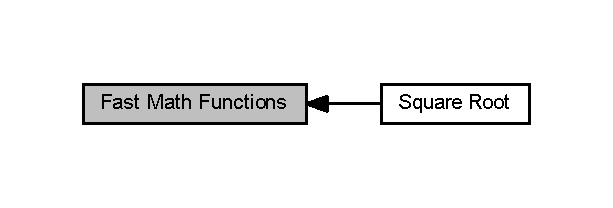
\includegraphics[width=294pt]{group__group_fast_math}
\end{center}
\end{figure}
\subsection*{Modules}
\begin{DoxyCompactItemize}
\item 
\hyperlink{group___s_q_r_t}{Square Root}
\end{DoxyCompactItemize}


\subsection{Detailed Description}
This set of functions provides a fast approximation to sine, cosine, and square root. As compared to most of the other functions in the C\+M\+S\+IS math library, the fast math functions operate on individual values and not arrays. There are separate functions for Q15, Q31, and floating-\/point data. 
\hypertarget{group__group_cmplx_math}{}\section{Complex Math Functions}
\label{group__group_cmplx_math}\index{Complex Math Functions@{Complex Math Functions}}
This set of functions operates on complex data vectors. The data in the complex arrays is stored in an interleaved fashion (real, imag, real, imag, ...). In the A\+PI functions, the number of samples in a complex array refers to the number of complex values; the array contains twice this number of real values. 
\hypertarget{group__group_filters}{}\section{Filtering Functions}
\label{group__group_filters}\index{Filtering Functions@{Filtering Functions}}

\hypertarget{group__group_matrix}{}\section{Matrix Functions}
\label{group__group_matrix}\index{Matrix Functions@{Matrix Functions}}
This set of functions provides basic matrix math operations. The functions operate on matrix data structures. For example, the type definition for the floating-\/point matrix structure is shown below\+: 
\begin{DoxyPre}
    typedef struct
    \{
      uint16\_t numRows;     // number of rows of the matrix.
      uint16\_t numCols;     // number of columns of the matrix.
      float32\_t *pData;     // points to the data of the matrix.
    \} \hyperlink{structarm__matrix__instance__f32}{arm\_matrix\_instance\_f32};
\end{DoxyPre}
 There are similar definitions for Q15 and Q31 data types.

The structure specifies the size of the matrix and then points to an array of data. The array is of size {\ttfamily num\+Rows X num\+Cols} and the values are arranged in row order. That is, the matrix element (i, j) is stored at\+: 
\begin{DoxyPre}
    pData[i*numCols + j]
\end{DoxyPre}


\begin{DoxyParagraph}{Init Functions}
There is an associated initialization function for each type of matrix data structure. The initialization function sets the values of the internal structure fields. Refer to the function {\ttfamily \hyperlink{arm__math_8h_a11e3dc41592a6401c13182fef9416a27}{arm\+\_\+mat\+\_\+init\+\_\+f32()}}, {\ttfamily \hyperlink{arm__math_8h_a48a5e5d37e1f062cc57fcfaf683343cc}{arm\+\_\+mat\+\_\+init\+\_\+q31()}} and {\ttfamily \hyperlink{arm__math_8h_a31a7c2b991803d49719393eb2d53dc26}{arm\+\_\+mat\+\_\+init\+\_\+q15()}} for floating-\/point, Q31 and Q15 types, respectively.
\end{DoxyParagraph}
\begin{DoxyParagraph}{}
Use of the initialization function is optional. However, if initialization function is used then the instance structure cannot be placed into a const data section. To place the instance structure in a const data section, manually initialize the data structure. For example\+: 
\begin{DoxyPre}
{\ttfamily \hyperlink{structarm__matrix__instance__f32}{arm\_matrix\_instance\_f32} S = \{nRows, nColumns, pData\};}
{\ttfamily \hyperlink{structarm__matrix__instance__q31}{arm\_matrix\_instance\_q31} S = \{nRows, nColumns, pData\};}
{\ttfamily \hyperlink{structarm__matrix__instance__q15}{arm\_matrix\_instance\_q15} S = \{nRows, nColumns, pData\};}
\end{DoxyPre}
 where {\ttfamily n\+Rows} specifies the number of rows, {\ttfamily n\+Columns} specifies the number of columns, and {\ttfamily p\+Data} points to the data array.
\end{DoxyParagraph}
\begin{DoxyParagraph}{Size Checking}
By default all of the matrix functions perform size checking on the input and output matrices. For example, the matrix addition function verifies that the two input matrices and the output matrix all have the same number of rows and columns. If the size check fails the functions return\+: 
\begin{DoxyPre}
    ARM\_MATH\_SIZE\_MISMATCH
\end{DoxyPre}
 Otherwise the functions return 
\begin{DoxyPre}
    ARM\_MATH\_SUCCESS
\end{DoxyPre}
 There is some overhead associated with this matrix size checking. The matrix size checking is enabled via the \#define 
\begin{DoxyPre}
    ARM\_MATH\_MATRIX\_CHECK
\end{DoxyPre}
 within the library project settings. By default this macro is defined and size checking is enabled. By changing the project settings and undefining this macro size checking is eliminated and the functions run a bit faster. With size checking disabled the functions always return {\ttfamily A\+R\+M\+\_\+\+M\+A\+T\+H\+\_\+\+S\+U\+C\+C\+E\+SS}. 
\end{DoxyParagraph}

\hypertarget{group__group_transforms}{}\section{Transform Functions}
\label{group__group_transforms}\index{Transform Functions@{Transform Functions}}

\hypertarget{group__group_controller}{}\section{Controller Functions}
\label{group__group_controller}\index{Controller Functions@{Controller Functions}}
Collaboration diagram for Controller Functions\+:
\nopagebreak
\begin{figure}[H]
\begin{center}
\leavevmode
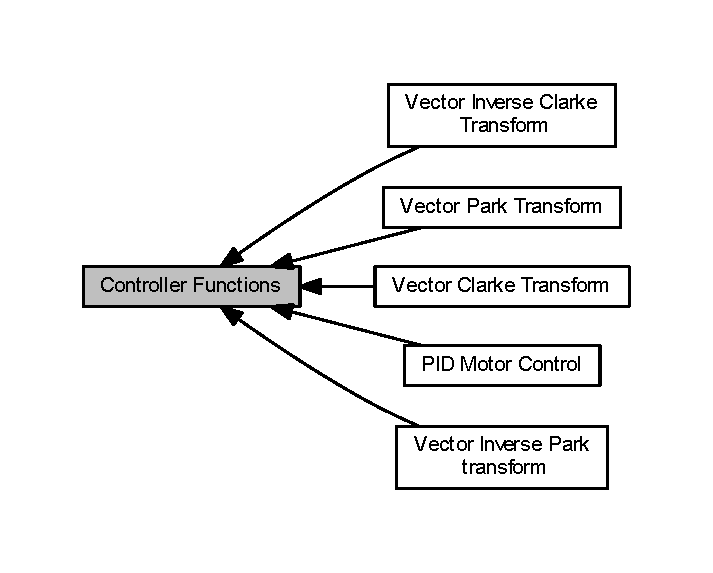
\includegraphics[width=342pt]{group__group_controller}
\end{center}
\end{figure}
\subsection*{Modules}
\begin{DoxyCompactItemize}
\item 
\hyperlink{group___p_i_d}{P\+I\+D Motor Control}
\item 
\hyperlink{group__clarke}{Vector Clarke Transform}
\item 
\hyperlink{group__inv__clarke}{Vector Inverse Clarke Transform}
\item 
\hyperlink{group__park}{Vector Park Transform}
\item 
\hyperlink{group__inv__park}{Vector Inverse Park transform}
\end{DoxyCompactItemize}


\subsection{Detailed Description}

\hypertarget{group__group_stats}{}\section{Statistics Functions}
\label{group__group_stats}\index{Statistics Functions@{Statistics Functions}}

\hypertarget{group__group_support}{}\section{Support Functions}
\label{group__group_support}\index{Support Functions@{Support Functions}}

\hypertarget{group__group_interpolation}{}\section{Interpolation Functions}
\label{group__group_interpolation}\index{Interpolation Functions@{Interpolation Functions}}
Collaboration diagram for Interpolation Functions\+:
\nopagebreak
\begin{figure}[H]
\begin{center}
\leavevmode
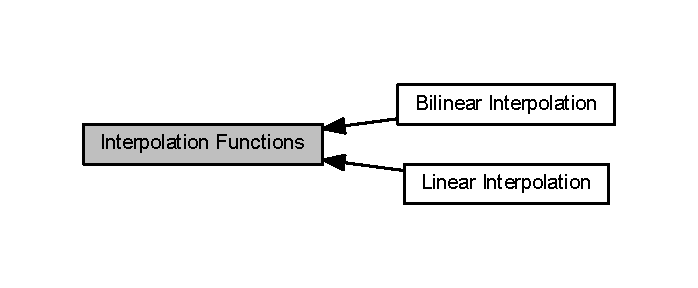
\includegraphics[width=335pt]{group__group_interpolation}
\end{center}
\end{figure}
\subsection*{Modules}
\begin{DoxyCompactItemize}
\item 
\hyperlink{group___linear_interpolate}{Linear Interpolation}
\item 
\hyperlink{group___bilinear_interpolate}{Bilinear Interpolation}
\end{DoxyCompactItemize}


\subsection{Detailed Description}
These functions perform 1-\/ and 2-\/dimensional interpolation of data. Linear interpolation is used for 1-\/dimensional data and bilinear interpolation is used for 2-\/dimensional data. 
\hypertarget{group__group_examples}{}\section{Examples}
\label{group__group_examples}\index{Examples@{Examples}}

\hypertarget{group___p_i_d}{}\section{P\+ID Motor Control}
\label{group___p_i_d}\index{P\+I\+D Motor Control@{P\+I\+D Motor Control}}
Collaboration diagram for P\+ID Motor Control\+:
\nopagebreak
\begin{figure}[H]
\begin{center}
\leavevmode
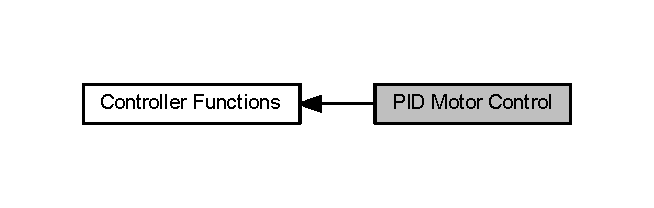
\includegraphics[width=314pt]{group___p_i_d}
\end{center}
\end{figure}


\subsection{Detailed Description}
A Proportional Integral Derivative (P\+ID) controller is a generic feedback control loop mechanism widely used in industrial control systems. A P\+ID controller is the most commonly used type of feedback controller.

This set of functions implements (P\+ID) controllers for Q15, Q31, and floating-\/point data types. The functions operate on a single sample of data and each call to the function returns a single processed value. {\ttfamily S} points to an instance of the P\+ID control data structure. {\ttfamily in} is the input sample value. The functions return the output value.

\begin{DoxyParagraph}{Algorithm\+:}

\begin{DoxyPre}
   y[n] = y[n-1] + A0 * x[n] + A1 * x[n-1] + A2 * x[n-2]
   A0 = Kp + Ki + Kd
   A1 = (-Kp ) - (2 * Kd )
   A2 = Kd  \end{DoxyPre}

\end{DoxyParagraph}
\begin{DoxyParagraph}{}
where {\ttfamily Kp} is proportional constant, {\ttfamily Ki} is Integral constant and {\ttfamily Kd} is Derivative constant
\end{DoxyParagraph}
\begin{DoxyParagraph}{}
 
\end{DoxyParagraph}
\begin{DoxyParagraph}{}
The P\+ID controller calculates an \char`\"{}error\char`\"{} value as the difference between the measured output and the reference input. The controller attempts to minimize the error by adjusting the process control inputs. The proportional value determines the reaction to the current error, the integral value determines the reaction based on the sum of recent errors, and the derivative value determines the reaction based on the rate at which the error has been changing.
\end{DoxyParagraph}
\begin{DoxyParagraph}{Instance Structure}
The Gains A0, A1, A2 and state variables for a P\+ID controller are stored together in an instance data structure. A separate instance structure must be defined for each P\+ID Controller. There are separate instance structure declarations for each of the 3 supported data types.
\end{DoxyParagraph}
\begin{DoxyParagraph}{Reset Functions}
There is also an associated reset function for each data type which clears the state array.
\end{DoxyParagraph}
\begin{DoxyParagraph}{Initialization Functions}
There is also an associated initialization function for each data type. The initialization function performs the following operations\+:
\begin{DoxyItemize}
\item Initializes the Gains A0, A1, A2 from Kp,Ki, Kd gains.
\item Zeros out the values in the state buffer.
\end{DoxyItemize}
\end{DoxyParagraph}
\begin{DoxyParagraph}{}
Instance structure cannot be placed into a const data section and it is recommended to use the initialization function.
\end{DoxyParagraph}
\begin{DoxyParagraph}{Fixed-\/\+Point Behavior}
Care must be taken when using the fixed-\/point versions of the P\+ID Controller functions. In particular, the overflow and saturation behavior of the accumulator used in each function must be considered. Refer to the function specific documentation below for usage guidelines. 
\end{DoxyParagraph}

\hypertarget{group__clarke}{}\section{Vector Clarke Transform}
\label{group__clarke}\index{Vector Clarke Transform@{Vector Clarke Transform}}
Collaboration diagram for Vector Clarke Transform\+:
\nopagebreak
\begin{figure}[H]
\begin{center}
\leavevmode
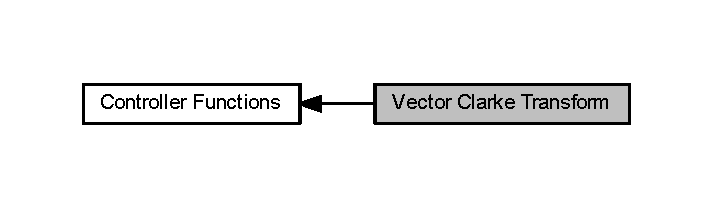
\includegraphics[width=342pt]{group__clarke}
\end{center}
\end{figure}


\subsection{Detailed Description}
Forward Clarke transform converts the instantaneous stator phases into a two-\/coordinate time invariant vector. Generally the Clarke transform uses three-\/phase currents {\ttfamily Ia, Ib and Ic} to calculate currents in the two-\/phase orthogonal stator axis {\ttfamily Ialpha} and {\ttfamily Ibeta}. When {\ttfamily Ialpha} is superposed with {\ttfamily Ia} as shown in the figure below  and {\ttfamily Ia + Ib + Ic = 0}, in this condition {\ttfamily Ialpha} and {\ttfamily Ibeta} can be calculated using only {\ttfamily Ia} and {\ttfamily Ib}.

The function operates on a single sample of data and each call to the function returns the processed output. The library provides separate functions for Q31 and floating-\/point data types. \begin{DoxyParagraph}{Algorithm}
 where {\ttfamily Ia} and {\ttfamily Ib} are the instantaneous stator phases and {\ttfamily p\+Ialpha} and {\ttfamily p\+Ibeta} are the two coordinates of time invariant vector. 
\end{DoxyParagraph}
\begin{DoxyParagraph}{Fixed-\/\+Point Behavior}
Care must be taken when using the Q31 version of the Clarke transform. In particular, the overflow and saturation behavior of the accumulator used must be considered. Refer to the function specific documentation below for usage guidelines. 
\end{DoxyParagraph}

\hypertarget{group__inv__clarke}{}\section{Vector Inverse Clarke Transform}
\label{group__inv__clarke}\index{Vector Inverse Clarke Transform@{Vector Inverse Clarke Transform}}
Collaboration diagram for Vector Inverse Clarke Transform\+:
\nopagebreak
\begin{figure}[H]
\begin{center}
\leavevmode
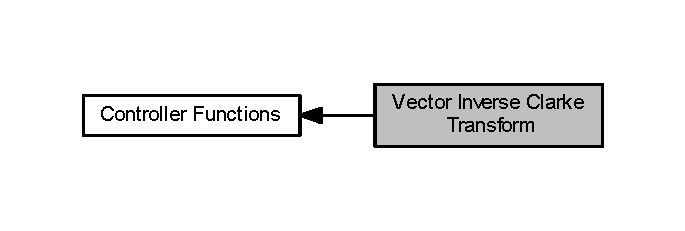
\includegraphics[width=329pt]{group__inv__clarke}
\end{center}
\end{figure}


\subsection{Detailed Description}
Inverse Clarke transform converts the two-\/coordinate time invariant vector into instantaneous stator phases.

The function operates on a single sample of data and each call to the function returns the processed output. The library provides separate functions for Q31 and floating-\/point data types. \begin{DoxyParagraph}{Algorithm}
 where {\ttfamily p\+Ia} and {\ttfamily p\+Ib} are the instantaneous stator phases and {\ttfamily Ialpha} and {\ttfamily Ibeta} are the two coordinates of time invariant vector. 
\end{DoxyParagraph}
\begin{DoxyParagraph}{Fixed-\/\+Point Behavior}
Care must be taken when using the Q31 version of the Clarke transform. In particular, the overflow and saturation behavior of the accumulator used must be considered. Refer to the function specific documentation below for usage guidelines. 
\end{DoxyParagraph}

\hypertarget{group__park}{}\section{Vector Park Transform}
\label{group__park}\index{Vector Park Transform@{Vector Park Transform}}
Collaboration diagram for Vector Park Transform\+:
\nopagebreak
\begin{figure}[H]
\begin{center}
\leavevmode
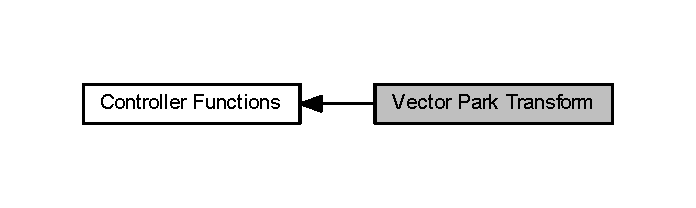
\includegraphics[width=334pt]{group__park}
\end{center}
\end{figure}


\subsection{Detailed Description}
Forward Park transform converts the input two-\/coordinate vector to flux and torque components. The Park transform can be used to realize the transformation of the {\ttfamily Ialpha} and the {\ttfamily Ibeta} currents from the stationary to the moving reference frame and control the spatial relationship between the stator vector current and rotor flux vector. If we consider the d axis aligned with the rotor flux, the diagram below shows the current vector and the relationship from the two reference frames\+:  The function operates on a single sample of data and each call to the function returns the processed output. The library provides separate functions for Q31 and floating-\/point data types. \begin{DoxyParagraph}{Algorithm}
 where {\ttfamily Ialpha} and {\ttfamily Ibeta} are the stator vector components, {\ttfamily p\+Id} and {\ttfamily p\+Iq} are rotor vector components and {\ttfamily cos\+Val} and {\ttfamily sin\+Val} are the cosine and sine values of theta (rotor flux position). 
\end{DoxyParagraph}
\begin{DoxyParagraph}{Fixed-\/\+Point Behavior}
Care must be taken when using the Q31 version of the Park transform. In particular, the overflow and saturation behavior of the accumulator used must be considered. Refer to the function specific documentation below for usage guidelines. 
\end{DoxyParagraph}

\hypertarget{group__inv__park}{}\section{Vector Inverse Park transform}
\label{group__inv__park}\index{Vector Inverse Park transform@{Vector Inverse Park transform}}
Collaboration diagram for Vector Inverse Park transform\+:
\nopagebreak
\begin{figure}[H]
\begin{center}
\leavevmode
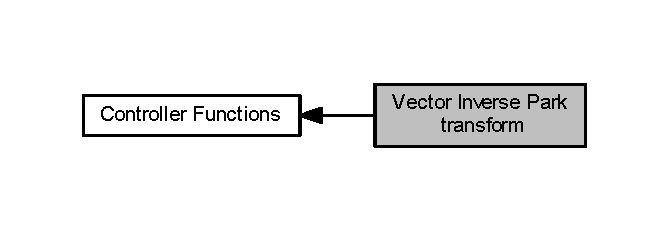
\includegraphics[width=321pt]{group__inv__park}
\end{center}
\end{figure}


\subsection{Detailed Description}
Inverse Park transform converts the input flux and torque components to two-\/coordinate vector.

The function operates on a single sample of data and each call to the function returns the processed output. The library provides separate functions for Q31 and floating-\/point data types. \begin{DoxyParagraph}{Algorithm}
 where {\ttfamily p\+Ialpha} and {\ttfamily p\+Ibeta} are the stator vector components, {\ttfamily Id} and {\ttfamily Iq} are rotor vector components and {\ttfamily cos\+Val} and {\ttfamily sin\+Val} are the cosine and sine values of theta (rotor flux position). 
\end{DoxyParagraph}
\begin{DoxyParagraph}{Fixed-\/\+Point Behavior}
Care must be taken when using the Q31 version of the Park transform. In particular, the overflow and saturation behavior of the accumulator used must be considered. Refer to the function specific documentation below for usage guidelines. 
\end{DoxyParagraph}

\hypertarget{group___linear_interpolate}{}\section{Linear Interpolation}
\label{group___linear_interpolate}\index{Linear Interpolation@{Linear Interpolation}}
Collaboration diagram for Linear Interpolation\+:
\nopagebreak
\begin{figure}[H]
\begin{center}
\leavevmode
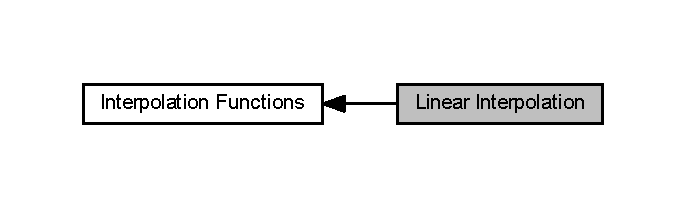
\includegraphics[width=329pt]{group___linear_interpolate}
\end{center}
\end{figure}


\subsection{Detailed Description}
Linear interpolation is a method of curve fitting using linear polynomials. Linear interpolation works by effectively drawing a straight line between two neighboring samples and returning the appropriate point along that line

\begin{DoxyParagraph}{}
 
\end{DoxyParagraph}
\begin{DoxyParagraph}{}
A Linear Interpolate function calculates an output value(y), for the input(x) using linear interpolation of the input values x0, x1( nearest input values) and the output values y0 and y1(nearest output values)
\end{DoxyParagraph}
\begin{DoxyParagraph}{Algorithm\+:}

\begin{DoxyPre}
      y = y0 + (x - x0) * ((y1 - y0)/(x1-x0))
      where x0, x1 are nearest values of input x
            y0, y1 are nearest values to output y
\end{DoxyPre}

\end{DoxyParagraph}
\begin{DoxyParagraph}{}
This set of functions implements Linear interpolation process for Q7, Q15, Q31, and floating-\/point data types. The functions operate on a single sample of data and each call to the function returns a single processed value. {\ttfamily S} points to an instance of the Linear Interpolate function data structure. {\ttfamily x} is the input sample value. The functions returns the output value.
\end{DoxyParagraph}
\begin{DoxyParagraph}{}
if x is outside of the table boundary, Linear interpolation returns first value of the table if x is below input range and returns last value of table if x is above range. 
\end{DoxyParagraph}

\hypertarget{group___s_q_r_t}{}\section{Square Root}
\label{group___s_q_r_t}\index{Square Root@{Square Root}}
Collaboration diagram for Square Root\+:
\nopagebreak
\begin{figure}[H]
\begin{center}
\leavevmode
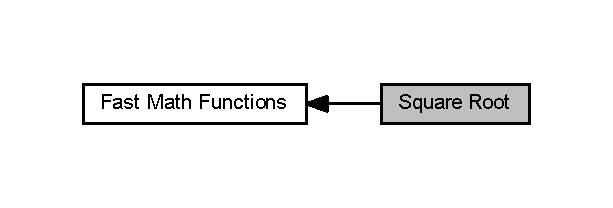
\includegraphics[width=294pt]{group___s_q_r_t}
\end{center}
\end{figure}
\subsection*{Functions}
\begin{DoxyCompactItemize}
\item 
\hyperlink{arm__math_8h_a5e459c6409dfcd2927bb8a57491d7cf6}{arm\+\_\+status} \hyperlink{group___s_q_r_t_ga119e25831e141d734d7ef10636670058}{arm\+\_\+sqrt\+\_\+q31} (\hyperlink{arm__math_8h_adc89a3547f5324b7b3b95adec3806bc0}{q31\+\_\+t} in, \hyperlink{arm__math_8h_adc89a3547f5324b7b3b95adec3806bc0}{q31\+\_\+t} $\ast$p\+Out)
\begin{DoxyCompactList}\small\item\em Q31 square root function. \end{DoxyCompactList}\item 
\hyperlink{arm__math_8h_a5e459c6409dfcd2927bb8a57491d7cf6}{arm\+\_\+status} \hyperlink{group___s_q_r_t_ga5abe5ca724f3e15849662b03752c1238}{arm\+\_\+sqrt\+\_\+q15} (\hyperlink{arm__math_8h_ab5a8fb21a5b3b983d5f54f31614052ea}{q15\+\_\+t} in, \hyperlink{arm__math_8h_ab5a8fb21a5b3b983d5f54f31614052ea}{q15\+\_\+t} $\ast$p\+Out)
\begin{DoxyCompactList}\small\item\em Q15 square root function. \end{DoxyCompactList}\end{DoxyCompactItemize}


\subsection{Detailed Description}
Computes the square root of a number. There are separate functions for Q15, Q31, and floating-\/point data types. The square root function is computed using the Newton-\/\+Raphson algorithm. This is an iterative algorithm of the form\+: 
\begin{DoxyPre}
     x1 = x0 - f(x0)/f'(x0)
\end{DoxyPre}
 where {\ttfamily x1} is the current estimate, {\ttfamily x0} is the previous estimate, and {\ttfamily f\textquotesingle{}(x0)} is the derivative of {\ttfamily f()} evaluated at {\ttfamily x0}. For the square root function, the algorithm reduces to\+: 
\begin{DoxyPre}
    x0 = in/2                         [initial guess]
    x1 = 1/2 * ( x0 + in / x0)        [each iteration]
\end{DoxyPre}
 

\subsection{Function Documentation}
\mbox{\Hypertarget{group___s_q_r_t_ga5abe5ca724f3e15849662b03752c1238}\label{group___s_q_r_t_ga5abe5ca724f3e15849662b03752c1238}} 
\index{Square Root@{Square Root}!arm\+\_\+sqrt\+\_\+q15@{arm\+\_\+sqrt\+\_\+q15}}
\index{arm\+\_\+sqrt\+\_\+q15@{arm\+\_\+sqrt\+\_\+q15}!Square Root@{Square Root}}
\subsubsection{\texorpdfstring{arm\+\_\+sqrt\+\_\+q15()}{arm\_sqrt\_q15()}}
{\footnotesize\ttfamily \hyperlink{arm__math_8h_a5e459c6409dfcd2927bb8a57491d7cf6}{arm\+\_\+status} arm\+\_\+sqrt\+\_\+q15 (\begin{DoxyParamCaption}\item[{\hyperlink{arm__math_8h_ab5a8fb21a5b3b983d5f54f31614052ea}{q15\+\_\+t}}]{in,  }\item[{\hyperlink{arm__math_8h_ab5a8fb21a5b3b983d5f54f31614052ea}{q15\+\_\+t} $\ast$}]{p\+Out }\end{DoxyParamCaption})}



Q15 square root function. 


\begin{DoxyParams}[1]{Parameters}
\mbox{\tt in}  & {\em in} & input value. The range of the input value is \mbox{[}0 +1) or 0x0000 to 0x7\+F\+FF. \\
\hline
\mbox{\tt out}  & {\em p\+Out} & square root of input value. \\
\hline
\end{DoxyParams}
\begin{DoxyReturn}{Returns}
The function returns A\+R\+M\+\_\+\+M\+A\+T\+H\+\_\+\+S\+U\+C\+C\+E\+SS if input value is positive value or A\+R\+M\+\_\+\+M\+A\+T\+H\+\_\+\+A\+R\+G\+U\+M\+E\+N\+T\+\_\+\+E\+R\+R\+OR if {\ttfamily in} is negative value and returns zero output for negative values. 
\end{DoxyReturn}
\mbox{\Hypertarget{group___s_q_r_t_ga119e25831e141d734d7ef10636670058}\label{group___s_q_r_t_ga119e25831e141d734d7ef10636670058}} 
\index{Square Root@{Square Root}!arm\+\_\+sqrt\+\_\+q31@{arm\+\_\+sqrt\+\_\+q31}}
\index{arm\+\_\+sqrt\+\_\+q31@{arm\+\_\+sqrt\+\_\+q31}!Square Root@{Square Root}}
\subsubsection{\texorpdfstring{arm\+\_\+sqrt\+\_\+q31()}{arm\_sqrt\_q31()}}
{\footnotesize\ttfamily \hyperlink{arm__math_8h_a5e459c6409dfcd2927bb8a57491d7cf6}{arm\+\_\+status} arm\+\_\+sqrt\+\_\+q31 (\begin{DoxyParamCaption}\item[{\hyperlink{arm__math_8h_adc89a3547f5324b7b3b95adec3806bc0}{q31\+\_\+t}}]{in,  }\item[{\hyperlink{arm__math_8h_adc89a3547f5324b7b3b95adec3806bc0}{q31\+\_\+t} $\ast$}]{p\+Out }\end{DoxyParamCaption})}



Q31 square root function. 


\begin{DoxyParams}[1]{Parameters}
\mbox{\tt in}  & {\em in} & input value. The range of the input value is \mbox{[}0 +1) or 0x00000000 to 0x7\+F\+F\+F\+F\+F\+FF. \\
\hline
\mbox{\tt out}  & {\em p\+Out} & square root of input value. \\
\hline
\end{DoxyParams}
\begin{DoxyReturn}{Returns}
The function returns A\+R\+M\+\_\+\+M\+A\+T\+H\+\_\+\+S\+U\+C\+C\+E\+SS if input value is positive value or A\+R\+M\+\_\+\+M\+A\+T\+H\+\_\+\+A\+R\+G\+U\+M\+E\+N\+T\+\_\+\+E\+R\+R\+OR if {\ttfamily in} is negative value and returns zero output for negative values. 
\end{DoxyReturn}

\hypertarget{group___bilinear_interpolate}{}\section{Bilinear Interpolation}
\label{group___bilinear_interpolate}\index{Bilinear Interpolation@{Bilinear Interpolation}}
Collaboration diagram for Bilinear Interpolation\+:
\nopagebreak
\begin{figure}[H]
\begin{center}
\leavevmode
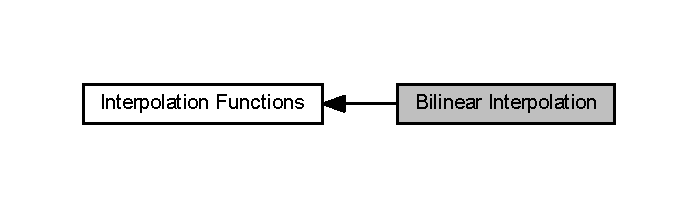
\includegraphics[width=335pt]{group___bilinear_interpolate}
\end{center}
\end{figure}


\subsection{Detailed Description}
Bilinear interpolation is an extension of linear interpolation applied to a two dimensional grid. The underlying function {\ttfamily f(x, y)} is sampled on a regular grid and the interpolation process determines values between the grid points. Bilinear interpolation is equivalent to two step linear interpolation, first in the x-\/dimension and then in the y-\/dimension. Bilinear interpolation is often used in image processing to rescale images. The C\+M\+S\+IS D\+SP library provides bilinear interpolation functions for Q7, Q15, Q31, and floating-\/point data types.

{\bfseries Algorithm} \begin{DoxyParagraph}{}
The instance structure used by the bilinear interpolation functions describes a two dimensional data table. For floating-\/point, the instance structure is defined as\+: 
\begin{DoxyPre}
  typedef struct
  \{
    uint16\_t numRows;
    uint16\_t numCols;
    float32\_t *pData;
\} \hyperlink{structarm__bilinear__interp__instance__f32}{arm\_bilinear\_interp\_instance\_f32};
\end{DoxyPre}

\end{DoxyParagraph}
\begin{DoxyParagraph}{}
where {\ttfamily num\+Rows} specifies the number of rows in the table; {\ttfamily num\+Cols} specifies the number of columns in the table; and {\ttfamily p\+Data} points to an array of size {\ttfamily num\+Rows$\ast$num\+Cols} values. The data table {\ttfamily p\+Table} is organized in row order and the supplied data values fall on integer indexes. That is, table element (x,y) is located at {\ttfamily p\+Table\mbox{[}x + y$\ast$num\+Cols\mbox{]}} where x and y are integers.
\end{DoxyParagraph}
\begin{DoxyParagraph}{}
Let {\ttfamily (x, y)} specify the desired interpolation point. Then define\+: 
\begin{DoxyPre}
    XF = floor(x)
    YF = floor(y)
\end{DoxyPre}
 
\end{DoxyParagraph}
\begin{DoxyParagraph}{}
The interpolated output point is computed as\+: 
\begin{DoxyPre}
 f(x, y) = f(XF, YF) * (1-(x-XF)) * (1-(y-YF))
          + f(XF+1, YF) * (x-XF)*(1-(y-YF))
          + f(XF, YF+1) * (1-(x-XF))*(y-YF)
          + f(XF+1, YF+1) * (x-XF)*(y-YF)
\end{DoxyPre}
 Note that the coordinates (x, y) contain integer and fractional components. The integer components specify which portion of the table to use while the fractional components control the interpolation processor.
\end{DoxyParagraph}
\begin{DoxyParagraph}{}
if (x,y) are outside of the table boundary, Bilinear interpolation returns zero output. 
\end{DoxyParagraph}

\hypertarget{group___c_m_s_i_s___core___reg_acc_functions}{}\section{C\+M\+S\+IS Core Register Access Functions}
\label{group___c_m_s_i_s___core___reg_acc_functions}\index{C\+M\+S\+I\+S Core Register Access Functions@{C\+M\+S\+I\+S Core Register Access Functions}}
Collaboration diagram for C\+M\+S\+IS Core Register Access Functions\+:
\nopagebreak
\begin{figure}[H]
\begin{center}
\leavevmode
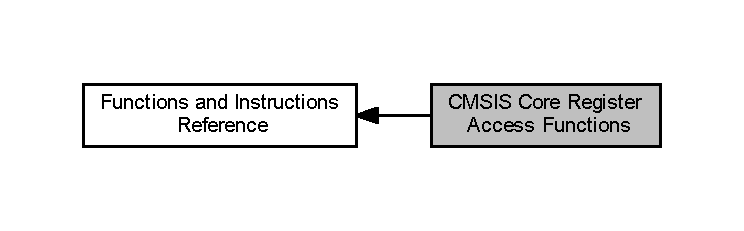
\includegraphics[width=350pt]{group___c_m_s_i_s___core___reg_acc_functions}
\end{center}
\end{figure}
\subsection*{Functions}
\begin{DoxyCompactItemize}
\item 
\+\_\+\+\_\+\+S\+T\+A\+T\+I\+C\+\_\+\+I\+N\+L\+I\+NE uint32\+\_\+t \hyperlink{group___c_m_s_i_s___core___reg_acc_functions_ga5fe64567d5bf0a81c118374e9a3a4598}{\+\_\+\+\_\+get\+\_\+\+C\+O\+N\+T\+R\+OL} (void)
\begin{DoxyCompactList}\small\item\em Get Control Register. \end{DoxyCompactList}\item 
\+\_\+\+\_\+\+S\+T\+A\+T\+I\+C\+\_\+\+I\+N\+L\+I\+NE void \hyperlink{group___c_m_s_i_s___core___reg_acc_functions_ga558df7eeb0a34765e0b54d9853d08484}{\+\_\+\+\_\+set\+\_\+\+C\+O\+N\+T\+R\+OL} (uint32\+\_\+t control)
\begin{DoxyCompactList}\small\item\em Set Control Register. \end{DoxyCompactList}\item 
\+\_\+\+\_\+\+S\+T\+A\+T\+I\+C\+\_\+\+I\+N\+L\+I\+NE uint32\+\_\+t \hyperlink{group___c_m_s_i_s___core___reg_acc_functions_ga2c18685a915eb9b7513a907c2b866636}{\+\_\+\+\_\+get\+\_\+\+I\+P\+SR} (void)
\begin{DoxyCompactList}\small\item\em Get I\+P\+SR Register. \end{DoxyCompactList}\item 
\+\_\+\+\_\+\+S\+T\+A\+T\+I\+C\+\_\+\+I\+N\+L\+I\+NE uint32\+\_\+t \hyperlink{group___c_m_s_i_s___core___reg_acc_functions_gaf082254959c727c663f2334021f1a98a}{\+\_\+\+\_\+get\+\_\+\+A\+P\+SR} (void)
\begin{DoxyCompactList}\small\item\em Get A\+P\+SR Register. \end{DoxyCompactList}\item 
\+\_\+\+\_\+\+S\+T\+A\+T\+I\+C\+\_\+\+I\+N\+L\+I\+NE uint32\+\_\+t \hyperlink{group___c_m_s_i_s___core___reg_acc_functions_ga94c675a736d4754a5f73d8748b24aa11}{\+\_\+\+\_\+get\+\_\+x\+P\+SR} (void)
\begin{DoxyCompactList}\small\item\em Get x\+P\+SR Register. \end{DoxyCompactList}\item 
\+\_\+\+\_\+\+S\+T\+A\+T\+I\+C\+\_\+\+I\+N\+L\+I\+NE uint32\+\_\+t \hyperlink{group___c_m_s_i_s___core___reg_acc_functions_ga0c569cbb49336f8d638686f9103047aa}{\+\_\+\+\_\+get\+\_\+\+P\+SP} (void)
\begin{DoxyCompactList}\small\item\em Get Process Stack Pointer. \end{DoxyCompactList}\item 
\+\_\+\+\_\+\+S\+T\+A\+T\+I\+C\+\_\+\+I\+N\+L\+I\+NE void \hyperlink{group___c_m_s_i_s___core___reg_acc_functions_gab145e35dbaf6868d3a17a8ad360fe379}{\+\_\+\+\_\+set\+\_\+\+P\+SP} (uint32\+\_\+t top\+Of\+Proc\+Stack)
\begin{DoxyCompactList}\small\item\em Set Process Stack Pointer. \end{DoxyCompactList}\item 
\+\_\+\+\_\+\+S\+T\+A\+T\+I\+C\+\_\+\+I\+N\+L\+I\+NE uint32\+\_\+t \hyperlink{group___c_m_s_i_s___core___reg_acc_functions_gac5267c10c9b15b5349eea0a959ea014c}{\+\_\+\+\_\+get\+\_\+\+M\+SP} (void)
\begin{DoxyCompactList}\small\item\em Get Main Stack Pointer. \end{DoxyCompactList}\item 
\+\_\+\+\_\+\+S\+T\+A\+T\+I\+C\+\_\+\+I\+N\+L\+I\+NE void \hyperlink{group___c_m_s_i_s___core___reg_acc_functions_ga1ff33c0b5ed0e687dd7967a1dd283d5f}{\+\_\+\+\_\+set\+\_\+\+M\+SP} (uint32\+\_\+t top\+Of\+Main\+Stack)
\begin{DoxyCompactList}\small\item\em Set Main Stack Pointer. \end{DoxyCompactList}\item 
\+\_\+\+\_\+\+S\+T\+A\+T\+I\+C\+\_\+\+I\+N\+L\+I\+NE uint32\+\_\+t \hyperlink{group___c_m_s_i_s___core___reg_acc_functions_gac9e3a67ff722261b89c77ebe49b6f9a7}{\+\_\+\+\_\+get\+\_\+\+P\+R\+I\+M\+A\+SK} (void)
\begin{DoxyCompactList}\small\item\em Get Priority Mask. \end{DoxyCompactList}\item 
\+\_\+\+\_\+\+S\+T\+A\+T\+I\+C\+\_\+\+I\+N\+L\+I\+NE void \hyperlink{group___c_m_s_i_s___core___reg_acc_functions_ga42e74e3fffe1a2d93db1de04d9260929}{\+\_\+\+\_\+set\+\_\+\+P\+R\+I\+M\+A\+SK} (uint32\+\_\+t pri\+Mask)
\begin{DoxyCompactList}\small\item\em Set Priority Mask. \end{DoxyCompactList}\item 
\hyperlink{group___c_m_s_i_s___core___reg_acc_functions_ga671b4fa3b3ab3dbc685a5473f3fc76aa}{\+\_\+\+\_\+attribute\+\_\+\+\_\+} ((always\+\_\+inline)) \+\_\+\+\_\+\+S\+T\+A\+T\+I\+C\+\_\+\+I\+N\+L\+I\+NE void \+\_\+\+\_\+enable\+\_\+irq(void)
\begin{DoxyCompactList}\small\item\em Enable I\+RQ Interrupts. \end{DoxyCompactList}\end{DoxyCompactItemize}


\subsection{Detailed Description}


\subsection{Function Documentation}
\mbox{\Hypertarget{group___c_m_s_i_s___core___reg_acc_functions_ga671b4fa3b3ab3dbc685a5473f3fc76aa}\label{group___c_m_s_i_s___core___reg_acc_functions_ga671b4fa3b3ab3dbc685a5473f3fc76aa}} 
\index{C\+M\+S\+I\+S Core Register Access Functions@{C\+M\+S\+I\+S Core Register Access Functions}!\+\_\+\+\_\+attribute\+\_\+\+\_\+@{\+\_\+\+\_\+attribute\+\_\+\+\_\+}}
\index{\+\_\+\+\_\+attribute\+\_\+\+\_\+@{\+\_\+\+\_\+attribute\+\_\+\+\_\+}!C\+M\+S\+I\+S Core Register Access Functions@{C\+M\+S\+I\+S Core Register Access Functions}}
\subsubsection{\texorpdfstring{\+\_\+\+\_\+attribute\+\_\+\+\_\+()}{\_\_attribute\_\_()}}
{\footnotesize\ttfamily \+\_\+\+\_\+attribute\+\_\+\+\_\+ (\begin{DoxyParamCaption}\item[{(always\+\_\+inline)}]{ }\end{DoxyParamCaption})}



Enable I\+RQ Interrupts. 

Set Priority Mask.

Get Priority Mask.

Set Main Stack Pointer.

Get Main Stack Pointer.

Set Process Stack Pointer.

Get Process Stack Pointer.

Get x\+P\+SR Register.

Get A\+P\+SR Register.

Get I\+P\+SR Register.

Set Control Register.

Get Control Register.

Disable I\+RQ Interrupts.

Enables I\+RQ interrupts by clearing the I-\/bit in the C\+P\+SR. Can only be executed in Privileged modes.

Disables I\+RQ interrupts by setting the I-\/bit in the C\+P\+SR. Can only be executed in Privileged modes.

Returns the content of the Control Register. \begin{DoxyReturn}{Returns}
Control Register value
\end{DoxyReturn}
Writes the given value to the Control Register. 
\begin{DoxyParams}[1]{Parameters}
\mbox{\tt in}  & {\em control} & Control Register value to set\\
\hline
\end{DoxyParams}
Returns the content of the I\+P\+SR Register. \begin{DoxyReturn}{Returns}
I\+P\+SR Register value
\end{DoxyReturn}
Returns the content of the A\+P\+SR Register. \begin{DoxyReturn}{Returns}
A\+P\+SR Register value
\end{DoxyReturn}
Returns the content of the x\+P\+SR Register. \begin{DoxyReturn}{Returns}
x\+P\+SR Register value
\end{DoxyReturn}
Returns the current value of the Process Stack Pointer (P\+SP). \begin{DoxyReturn}{Returns}
P\+SP Register value
\end{DoxyReturn}
Assigns the given value to the Process Stack Pointer (P\+SP). 
\begin{DoxyParams}[1]{Parameters}
\mbox{\tt in}  & {\em top\+Of\+Proc\+Stack} & Process Stack Pointer value to set\\
\hline
\end{DoxyParams}
Returns the current value of the Main Stack Pointer (M\+SP). \begin{DoxyReturn}{Returns}
M\+SP Register value
\end{DoxyReturn}
Assigns the given value to the Main Stack Pointer (M\+SP). 
\begin{DoxyParams}[1]{Parameters}
\mbox{\tt in}  & {\em top\+Of\+Main\+Stack} & Main Stack Pointer value to set\\
\hline
\end{DoxyParams}
Returns the current state of the priority mask bit from the Priority Mask Register. \begin{DoxyReturn}{Returns}
Priority Mask value
\end{DoxyReturn}
Assigns the given value to the Priority Mask Register. 
\begin{DoxyParams}[1]{Parameters}
\mbox{\tt in}  & {\em pri\+Mask} & Priority Mask \\
\hline
\end{DoxyParams}


Definition at line 50 of file cmsis\+\_\+armcc\+\_\+\+V6.\+h.

Here is the call graph for this function\+:
\nopagebreak
\begin{figure}[H]
\begin{center}
\leavevmode
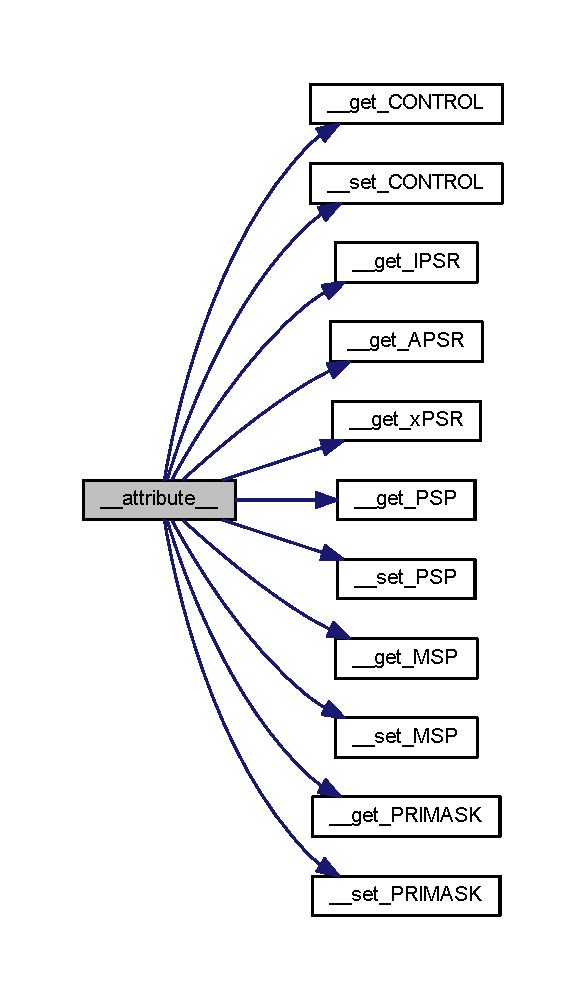
\includegraphics[width=281pt]{group___c_m_s_i_s___core___reg_acc_functions_ga671b4fa3b3ab3dbc685a5473f3fc76aa_cgraph}
\end{center}
\end{figure}
\mbox{\Hypertarget{group___c_m_s_i_s___core___reg_acc_functions_gaf082254959c727c663f2334021f1a98a}\label{group___c_m_s_i_s___core___reg_acc_functions_gaf082254959c727c663f2334021f1a98a}} 
\index{C\+M\+S\+I\+S Core Register Access Functions@{C\+M\+S\+I\+S Core Register Access Functions}!\+\_\+\+\_\+get\+\_\+\+A\+P\+SR@{\+\_\+\+\_\+get\+\_\+\+A\+P\+SR}}
\index{\+\_\+\+\_\+get\+\_\+\+A\+P\+SR@{\+\_\+\+\_\+get\+\_\+\+A\+P\+SR}!C\+M\+S\+I\+S Core Register Access Functions@{C\+M\+S\+I\+S Core Register Access Functions}}
\subsubsection{\texorpdfstring{\+\_\+\+\_\+get\+\_\+\+A\+P\+S\+R()}{\_\_get\_APSR()}}
{\footnotesize\ttfamily \+\_\+\+\_\+\+S\+T\+A\+T\+I\+C\+\_\+\+I\+N\+L\+I\+NE uint32\+\_\+t \+\_\+\+\_\+get\+\_\+\+A\+P\+SR (\begin{DoxyParamCaption}\item[{void}]{ }\end{DoxyParamCaption})}



Get A\+P\+SR Register. 

Returns the content of the A\+P\+SR Register. \begin{DoxyReturn}{Returns}
A\+P\+SR Register value 
\end{DoxyReturn}


Definition at line 93 of file cmsis\+\_\+armcc.\+h.

Here is the caller graph for this function\+:
\nopagebreak
\begin{figure}[H]
\begin{center}
\leavevmode
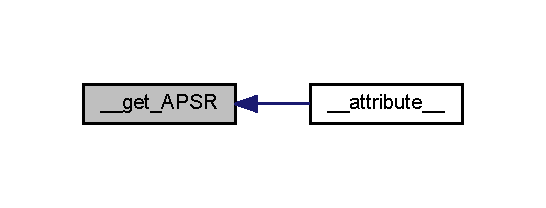
\includegraphics[width=262pt]{group___c_m_s_i_s___core___reg_acc_functions_gaf082254959c727c663f2334021f1a98a_icgraph}
\end{center}
\end{figure}
\mbox{\Hypertarget{group___c_m_s_i_s___core___reg_acc_functions_ga5fe64567d5bf0a81c118374e9a3a4598}\label{group___c_m_s_i_s___core___reg_acc_functions_ga5fe64567d5bf0a81c118374e9a3a4598}} 
\index{C\+M\+S\+I\+S Core Register Access Functions@{C\+M\+S\+I\+S Core Register Access Functions}!\+\_\+\+\_\+get\+\_\+\+C\+O\+N\+T\+R\+OL@{\+\_\+\+\_\+get\+\_\+\+C\+O\+N\+T\+R\+OL}}
\index{\+\_\+\+\_\+get\+\_\+\+C\+O\+N\+T\+R\+OL@{\+\_\+\+\_\+get\+\_\+\+C\+O\+N\+T\+R\+OL}!C\+M\+S\+I\+S Core Register Access Functions@{C\+M\+S\+I\+S Core Register Access Functions}}
\subsubsection{\texorpdfstring{\+\_\+\+\_\+get\+\_\+\+C\+O\+N\+T\+R\+O\+L()}{\_\_get\_CONTROL()}}
{\footnotesize\ttfamily \+\_\+\+\_\+\+S\+T\+A\+T\+I\+C\+\_\+\+I\+N\+L\+I\+NE uint32\+\_\+t \+\_\+\+\_\+get\+\_\+\+C\+O\+N\+T\+R\+OL (\begin{DoxyParamCaption}\item[{void}]{ }\end{DoxyParamCaption})}



Get Control Register. 

Returns the content of the Control Register. \begin{DoxyReturn}{Returns}
Control Register value 
\end{DoxyReturn}


Definition at line 57 of file cmsis\+\_\+armcc.\+h.

Here is the caller graph for this function\+:
\nopagebreak
\begin{figure}[H]
\begin{center}
\leavevmode
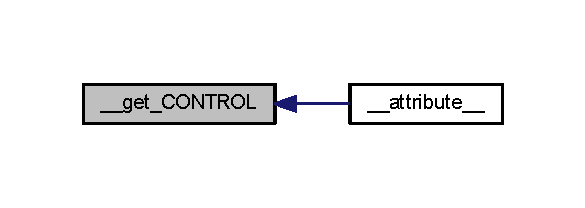
\includegraphics[width=281pt]{group___c_m_s_i_s___core___reg_acc_functions_ga5fe64567d5bf0a81c118374e9a3a4598_icgraph}
\end{center}
\end{figure}
\mbox{\Hypertarget{group___c_m_s_i_s___core___reg_acc_functions_ga2c18685a915eb9b7513a907c2b866636}\label{group___c_m_s_i_s___core___reg_acc_functions_ga2c18685a915eb9b7513a907c2b866636}} 
\index{C\+M\+S\+I\+S Core Register Access Functions@{C\+M\+S\+I\+S Core Register Access Functions}!\+\_\+\+\_\+get\+\_\+\+I\+P\+SR@{\+\_\+\+\_\+get\+\_\+\+I\+P\+SR}}
\index{\+\_\+\+\_\+get\+\_\+\+I\+P\+SR@{\+\_\+\+\_\+get\+\_\+\+I\+P\+SR}!C\+M\+S\+I\+S Core Register Access Functions@{C\+M\+S\+I\+S Core Register Access Functions}}
\subsubsection{\texorpdfstring{\+\_\+\+\_\+get\+\_\+\+I\+P\+S\+R()}{\_\_get\_IPSR()}}
{\footnotesize\ttfamily \+\_\+\+\_\+\+S\+T\+A\+T\+I\+C\+\_\+\+I\+N\+L\+I\+NE uint32\+\_\+t \+\_\+\+\_\+get\+\_\+\+I\+P\+SR (\begin{DoxyParamCaption}\item[{void}]{ }\end{DoxyParamCaption})}



Get I\+P\+SR Register. 

Returns the content of the I\+P\+SR Register. \begin{DoxyReturn}{Returns}
I\+P\+SR Register value 
\end{DoxyReturn}


Definition at line 81 of file cmsis\+\_\+armcc.\+h.

Here is the caller graph for this function\+:
\nopagebreak
\begin{figure}[H]
\begin{center}
\leavevmode
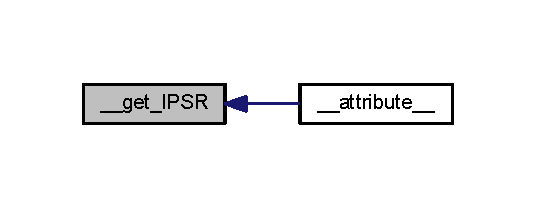
\includegraphics[width=257pt]{group___c_m_s_i_s___core___reg_acc_functions_ga2c18685a915eb9b7513a907c2b866636_icgraph}
\end{center}
\end{figure}
\mbox{\Hypertarget{group___c_m_s_i_s___core___reg_acc_functions_gac5267c10c9b15b5349eea0a959ea014c}\label{group___c_m_s_i_s___core___reg_acc_functions_gac5267c10c9b15b5349eea0a959ea014c}} 
\index{C\+M\+S\+I\+S Core Register Access Functions@{C\+M\+S\+I\+S Core Register Access Functions}!\+\_\+\+\_\+get\+\_\+\+M\+SP@{\+\_\+\+\_\+get\+\_\+\+M\+SP}}
\index{\+\_\+\+\_\+get\+\_\+\+M\+SP@{\+\_\+\+\_\+get\+\_\+\+M\+SP}!C\+M\+S\+I\+S Core Register Access Functions@{C\+M\+S\+I\+S Core Register Access Functions}}
\subsubsection{\texorpdfstring{\+\_\+\+\_\+get\+\_\+\+M\+S\+P()}{\_\_get\_MSP()}}
{\footnotesize\ttfamily \+\_\+\+\_\+\+S\+T\+A\+T\+I\+C\+\_\+\+I\+N\+L\+I\+NE uint32\+\_\+t \+\_\+\+\_\+get\+\_\+\+M\+SP (\begin{DoxyParamCaption}\item[{void}]{ }\end{DoxyParamCaption})}



Get Main Stack Pointer. 

Returns the current value of the Main Stack Pointer (M\+SP). \begin{DoxyReturn}{Returns}
M\+SP Register value 
\end{DoxyReturn}


Definition at line 141 of file cmsis\+\_\+armcc.\+h.

Here is the caller graph for this function\+:
\nopagebreak
\begin{figure}[H]
\begin{center}
\leavevmode
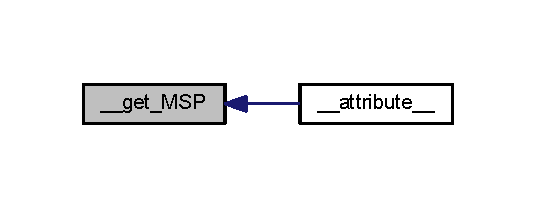
\includegraphics[width=257pt]{group___c_m_s_i_s___core___reg_acc_functions_gac5267c10c9b15b5349eea0a959ea014c_icgraph}
\end{center}
\end{figure}
\mbox{\Hypertarget{group___c_m_s_i_s___core___reg_acc_functions_gac9e3a67ff722261b89c77ebe49b6f9a7}\label{group___c_m_s_i_s___core___reg_acc_functions_gac9e3a67ff722261b89c77ebe49b6f9a7}} 
\index{C\+M\+S\+I\+S Core Register Access Functions@{C\+M\+S\+I\+S Core Register Access Functions}!\+\_\+\+\_\+get\+\_\+\+P\+R\+I\+M\+A\+SK@{\+\_\+\+\_\+get\+\_\+\+P\+R\+I\+M\+A\+SK}}
\index{\+\_\+\+\_\+get\+\_\+\+P\+R\+I\+M\+A\+SK@{\+\_\+\+\_\+get\+\_\+\+P\+R\+I\+M\+A\+SK}!C\+M\+S\+I\+S Core Register Access Functions@{C\+M\+S\+I\+S Core Register Access Functions}}
\subsubsection{\texorpdfstring{\+\_\+\+\_\+get\+\_\+\+P\+R\+I\+M\+A\+S\+K()}{\_\_get\_PRIMASK()}}
{\footnotesize\ttfamily \+\_\+\+\_\+\+S\+T\+A\+T\+I\+C\+\_\+\+I\+N\+L\+I\+NE uint32\+\_\+t \+\_\+\+\_\+get\+\_\+\+P\+R\+I\+M\+A\+SK (\begin{DoxyParamCaption}\item[{void}]{ }\end{DoxyParamCaption})}



Get Priority Mask. 

Returns the current state of the priority mask bit from the Priority Mask Register. \begin{DoxyReturn}{Returns}
Priority Mask value 
\end{DoxyReturn}


Definition at line 165 of file cmsis\+\_\+armcc.\+h.

Here is the caller graph for this function\+:
\nopagebreak
\begin{figure}[H]
\begin{center}
\leavevmode
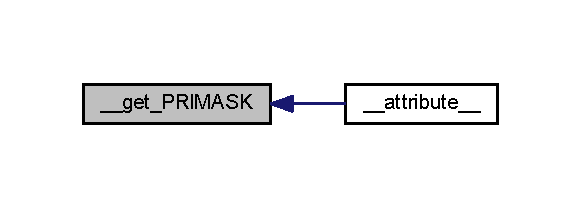
\includegraphics[width=279pt]{group___c_m_s_i_s___core___reg_acc_functions_gac9e3a67ff722261b89c77ebe49b6f9a7_icgraph}
\end{center}
\end{figure}
\mbox{\Hypertarget{group___c_m_s_i_s___core___reg_acc_functions_ga0c569cbb49336f8d638686f9103047aa}\label{group___c_m_s_i_s___core___reg_acc_functions_ga0c569cbb49336f8d638686f9103047aa}} 
\index{C\+M\+S\+I\+S Core Register Access Functions@{C\+M\+S\+I\+S Core Register Access Functions}!\+\_\+\+\_\+get\+\_\+\+P\+SP@{\+\_\+\+\_\+get\+\_\+\+P\+SP}}
\index{\+\_\+\+\_\+get\+\_\+\+P\+SP@{\+\_\+\+\_\+get\+\_\+\+P\+SP}!C\+M\+S\+I\+S Core Register Access Functions@{C\+M\+S\+I\+S Core Register Access Functions}}
\subsubsection{\texorpdfstring{\+\_\+\+\_\+get\+\_\+\+P\+S\+P()}{\_\_get\_PSP()}}
{\footnotesize\ttfamily \+\_\+\+\_\+\+S\+T\+A\+T\+I\+C\+\_\+\+I\+N\+L\+I\+NE uint32\+\_\+t \+\_\+\+\_\+get\+\_\+\+P\+SP (\begin{DoxyParamCaption}\item[{void}]{ }\end{DoxyParamCaption})}



Get Process Stack Pointer. 

Returns the current value of the Process Stack Pointer (P\+SP). \begin{DoxyReturn}{Returns}
P\+SP Register value 
\end{DoxyReturn}


Definition at line 117 of file cmsis\+\_\+armcc.\+h.

Here is the caller graph for this function\+:
\nopagebreak
\begin{figure}[H]
\begin{center}
\leavevmode
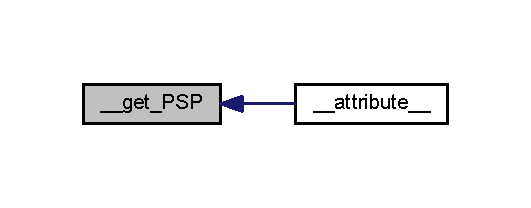
\includegraphics[width=255pt]{group___c_m_s_i_s___core___reg_acc_functions_ga0c569cbb49336f8d638686f9103047aa_icgraph}
\end{center}
\end{figure}
\mbox{\Hypertarget{group___c_m_s_i_s___core___reg_acc_functions_ga94c675a736d4754a5f73d8748b24aa11}\label{group___c_m_s_i_s___core___reg_acc_functions_ga94c675a736d4754a5f73d8748b24aa11}} 
\index{C\+M\+S\+I\+S Core Register Access Functions@{C\+M\+S\+I\+S Core Register Access Functions}!\+\_\+\+\_\+get\+\_\+x\+P\+SR@{\+\_\+\+\_\+get\+\_\+x\+P\+SR}}
\index{\+\_\+\+\_\+get\+\_\+x\+P\+SR@{\+\_\+\+\_\+get\+\_\+x\+P\+SR}!C\+M\+S\+I\+S Core Register Access Functions@{C\+M\+S\+I\+S Core Register Access Functions}}
\subsubsection{\texorpdfstring{\+\_\+\+\_\+get\+\_\+x\+P\+S\+R()}{\_\_get\_xPSR()}}
{\footnotesize\ttfamily \+\_\+\+\_\+\+S\+T\+A\+T\+I\+C\+\_\+\+I\+N\+L\+I\+NE uint32\+\_\+t \+\_\+\+\_\+get\+\_\+x\+P\+SR (\begin{DoxyParamCaption}\item[{void}]{ }\end{DoxyParamCaption})}



Get x\+P\+SR Register. 

Returns the content of the x\+P\+SR Register. \begin{DoxyReturn}{Returns}
x\+P\+SR Register value 
\end{DoxyReturn}


Definition at line 105 of file cmsis\+\_\+armcc.\+h.

Here is the caller graph for this function\+:
\nopagebreak
\begin{figure}[H]
\begin{center}
\leavevmode
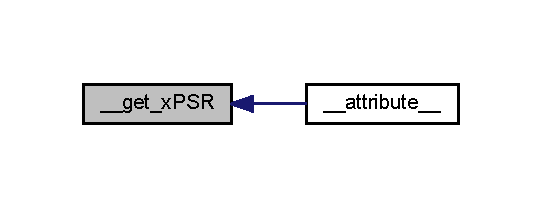
\includegraphics[width=260pt]{group___c_m_s_i_s___core___reg_acc_functions_ga94c675a736d4754a5f73d8748b24aa11_icgraph}
\end{center}
\end{figure}
\mbox{\Hypertarget{group___c_m_s_i_s___core___reg_acc_functions_ga558df7eeb0a34765e0b54d9853d08484}\label{group___c_m_s_i_s___core___reg_acc_functions_ga558df7eeb0a34765e0b54d9853d08484}} 
\index{C\+M\+S\+I\+S Core Register Access Functions@{C\+M\+S\+I\+S Core Register Access Functions}!\+\_\+\+\_\+set\+\_\+\+C\+O\+N\+T\+R\+OL@{\+\_\+\+\_\+set\+\_\+\+C\+O\+N\+T\+R\+OL}}
\index{\+\_\+\+\_\+set\+\_\+\+C\+O\+N\+T\+R\+OL@{\+\_\+\+\_\+set\+\_\+\+C\+O\+N\+T\+R\+OL}!C\+M\+S\+I\+S Core Register Access Functions@{C\+M\+S\+I\+S Core Register Access Functions}}
\subsubsection{\texorpdfstring{\+\_\+\+\_\+set\+\_\+\+C\+O\+N\+T\+R\+O\+L()}{\_\_set\_CONTROL()}}
{\footnotesize\ttfamily \+\_\+\+\_\+\+S\+T\+A\+T\+I\+C\+\_\+\+I\+N\+L\+I\+NE void \+\_\+\+\_\+set\+\_\+\+C\+O\+N\+T\+R\+OL (\begin{DoxyParamCaption}\item[{uint32\+\_\+t}]{control }\end{DoxyParamCaption})}



Set Control Register. 

Writes the given value to the Control Register. 
\begin{DoxyParams}[1]{Parameters}
\mbox{\tt in}  & {\em control} & Control Register value to set \\
\hline
\end{DoxyParams}


Definition at line 69 of file cmsis\+\_\+armcc.\+h.

Here is the caller graph for this function\+:
\nopagebreak
\begin{figure}[H]
\begin{center}
\leavevmode
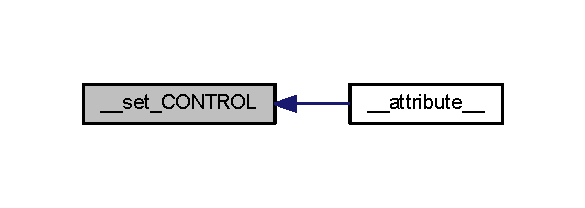
\includegraphics[width=281pt]{group___c_m_s_i_s___core___reg_acc_functions_ga558df7eeb0a34765e0b54d9853d08484_icgraph}
\end{center}
\end{figure}
\mbox{\Hypertarget{group___c_m_s_i_s___core___reg_acc_functions_ga1ff33c0b5ed0e687dd7967a1dd283d5f}\label{group___c_m_s_i_s___core___reg_acc_functions_ga1ff33c0b5ed0e687dd7967a1dd283d5f}} 
\index{C\+M\+S\+I\+S Core Register Access Functions@{C\+M\+S\+I\+S Core Register Access Functions}!\+\_\+\+\_\+set\+\_\+\+M\+SP@{\+\_\+\+\_\+set\+\_\+\+M\+SP}}
\index{\+\_\+\+\_\+set\+\_\+\+M\+SP@{\+\_\+\+\_\+set\+\_\+\+M\+SP}!C\+M\+S\+I\+S Core Register Access Functions@{C\+M\+S\+I\+S Core Register Access Functions}}
\subsubsection{\texorpdfstring{\+\_\+\+\_\+set\+\_\+\+M\+S\+P()}{\_\_set\_MSP()}}
{\footnotesize\ttfamily \+\_\+\+\_\+\+S\+T\+A\+T\+I\+C\+\_\+\+I\+N\+L\+I\+NE void \+\_\+\+\_\+set\+\_\+\+M\+SP (\begin{DoxyParamCaption}\item[{uint32\+\_\+t}]{top\+Of\+Main\+Stack }\end{DoxyParamCaption})}



Set Main Stack Pointer. 

Assigns the given value to the Main Stack Pointer (M\+SP). 
\begin{DoxyParams}[1]{Parameters}
\mbox{\tt in}  & {\em top\+Of\+Main\+Stack} & Main Stack Pointer value to set \\
\hline
\end{DoxyParams}


Definition at line 153 of file cmsis\+\_\+armcc.\+h.

Here is the caller graph for this function\+:
\nopagebreak
\begin{figure}[H]
\begin{center}
\leavevmode
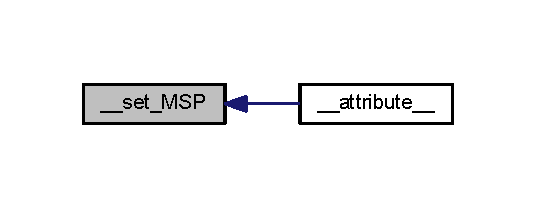
\includegraphics[width=257pt]{group___c_m_s_i_s___core___reg_acc_functions_ga1ff33c0b5ed0e687dd7967a1dd283d5f_icgraph}
\end{center}
\end{figure}
\mbox{\Hypertarget{group___c_m_s_i_s___core___reg_acc_functions_ga42e74e3fffe1a2d93db1de04d9260929}\label{group___c_m_s_i_s___core___reg_acc_functions_ga42e74e3fffe1a2d93db1de04d9260929}} 
\index{C\+M\+S\+I\+S Core Register Access Functions@{C\+M\+S\+I\+S Core Register Access Functions}!\+\_\+\+\_\+set\+\_\+\+P\+R\+I\+M\+A\+SK@{\+\_\+\+\_\+set\+\_\+\+P\+R\+I\+M\+A\+SK}}
\index{\+\_\+\+\_\+set\+\_\+\+P\+R\+I\+M\+A\+SK@{\+\_\+\+\_\+set\+\_\+\+P\+R\+I\+M\+A\+SK}!C\+M\+S\+I\+S Core Register Access Functions@{C\+M\+S\+I\+S Core Register Access Functions}}
\subsubsection{\texorpdfstring{\+\_\+\+\_\+set\+\_\+\+P\+R\+I\+M\+A\+S\+K()}{\_\_set\_PRIMASK()}}
{\footnotesize\ttfamily \+\_\+\+\_\+\+S\+T\+A\+T\+I\+C\+\_\+\+I\+N\+L\+I\+NE void \+\_\+\+\_\+set\+\_\+\+P\+R\+I\+M\+A\+SK (\begin{DoxyParamCaption}\item[{uint32\+\_\+t}]{pri\+Mask }\end{DoxyParamCaption})}



Set Priority Mask. 

Assigns the given value to the Priority Mask Register. 
\begin{DoxyParams}[1]{Parameters}
\mbox{\tt in}  & {\em pri\+Mask} & Priority Mask \\
\hline
\end{DoxyParams}


Definition at line 177 of file cmsis\+\_\+armcc.\+h.

Here is the caller graph for this function\+:
\nopagebreak
\begin{figure}[H]
\begin{center}
\leavevmode
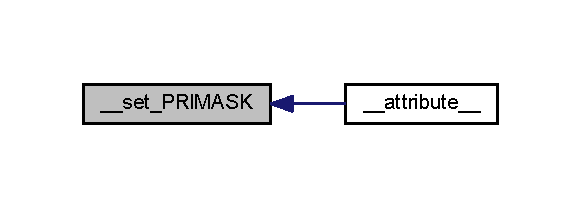
\includegraphics[width=279pt]{group___c_m_s_i_s___core___reg_acc_functions_ga42e74e3fffe1a2d93db1de04d9260929_icgraph}
\end{center}
\end{figure}
\mbox{\Hypertarget{group___c_m_s_i_s___core___reg_acc_functions_gab145e35dbaf6868d3a17a8ad360fe379}\label{group___c_m_s_i_s___core___reg_acc_functions_gab145e35dbaf6868d3a17a8ad360fe379}} 
\index{C\+M\+S\+I\+S Core Register Access Functions@{C\+M\+S\+I\+S Core Register Access Functions}!\+\_\+\+\_\+set\+\_\+\+P\+SP@{\+\_\+\+\_\+set\+\_\+\+P\+SP}}
\index{\+\_\+\+\_\+set\+\_\+\+P\+SP@{\+\_\+\+\_\+set\+\_\+\+P\+SP}!C\+M\+S\+I\+S Core Register Access Functions@{C\+M\+S\+I\+S Core Register Access Functions}}
\subsubsection{\texorpdfstring{\+\_\+\+\_\+set\+\_\+\+P\+S\+P()}{\_\_set\_PSP()}}
{\footnotesize\ttfamily \+\_\+\+\_\+\+S\+T\+A\+T\+I\+C\+\_\+\+I\+N\+L\+I\+NE void \+\_\+\+\_\+set\+\_\+\+P\+SP (\begin{DoxyParamCaption}\item[{uint32\+\_\+t}]{top\+Of\+Proc\+Stack }\end{DoxyParamCaption})}



Set Process Stack Pointer. 

Assigns the given value to the Process Stack Pointer (P\+SP). 
\begin{DoxyParams}[1]{Parameters}
\mbox{\tt in}  & {\em top\+Of\+Proc\+Stack} & Process Stack Pointer value to set \\
\hline
\end{DoxyParams}


Definition at line 129 of file cmsis\+\_\+armcc.\+h.

Here is the caller graph for this function\+:
\nopagebreak
\begin{figure}[H]
\begin{center}
\leavevmode
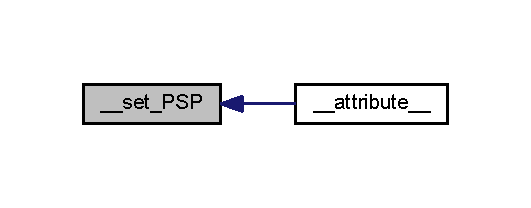
\includegraphics[width=255pt]{group___c_m_s_i_s___core___reg_acc_functions_gab145e35dbaf6868d3a17a8ad360fe379_icgraph}
\end{center}
\end{figure}

\hypertarget{group___c_m_s_i_s___core___instruction_interface}{}\section{C\+M\+S\+IS Core Instruction Interface}
\label{group___c_m_s_i_s___core___instruction_interface}\index{C\+M\+S\+I\+S Core Instruction Interface@{C\+M\+S\+I\+S Core Instruction Interface}}
\subsection*{Macros}
\begin{DoxyCompactItemize}
\item 
\#define \hyperlink{group___c_m_s_i_s___core___instruction_interface_gabd585ddc865fb9b7f2493af1eee1a572}{\+\_\+\+\_\+\+N\+OP}~\+\_\+\+\_\+nop
\begin{DoxyCompactList}\small\item\em No Operation. \end{DoxyCompactList}\item 
\#define \hyperlink{group___c_m_s_i_s___core___instruction_interface_gad23bf2b78a9a4524157c9de0d30b7448}{\+\_\+\+\_\+\+W\+FI}~\+\_\+\+\_\+wfi
\begin{DoxyCompactList}\small\item\em Wait For Interrupt. \end{DoxyCompactList}\item 
\#define \hyperlink{group___c_m_s_i_s___core___instruction_interface_gaac6cc7dd4325d9cb40d3290fa5244b3d}{\+\_\+\+\_\+\+W\+FE}~\+\_\+\+\_\+wfe
\begin{DoxyCompactList}\small\item\em Wait For Event. \end{DoxyCompactList}\item 
\#define \hyperlink{group___c_m_s_i_s___core___instruction_interface_gaab4f296d0022b4b10dc0976eb22052f9}{\+\_\+\+\_\+\+S\+EV}~\+\_\+\+\_\+sev
\begin{DoxyCompactList}\small\item\em Send Event. \end{DoxyCompactList}\item 
\#define \hyperlink{group___c_m_s_i_s___core___instruction_interface_gaad233022e850a009fc6f7602be1182f6}{\+\_\+\+\_\+\+I\+SB}()
\begin{DoxyCompactList}\small\item\em Instruction Synchronization Barrier. \end{DoxyCompactList}\item 
\#define \hyperlink{group___c_m_s_i_s___core___instruction_interface_ga067d257a2b34565410acefb5afef2203}{\+\_\+\+\_\+\+D\+SB}()
\begin{DoxyCompactList}\small\item\em Data Synchronization Barrier. \end{DoxyCompactList}\item 
\#define \hyperlink{group___c_m_s_i_s___core___instruction_interface_ga671101179b5943990785f36f8c1e2269}{\+\_\+\+\_\+\+D\+MB}()
\begin{DoxyCompactList}\small\item\em Data Memory Barrier. \end{DoxyCompactList}\item 
\#define \hyperlink{group___c_m_s_i_s___core___instruction_interface_ga14f54807872c0f5e05604c4924abfdae}{\+\_\+\+\_\+\+R\+EV}~\+\_\+\+\_\+rev
\begin{DoxyCompactList}\small\item\em Reverse byte order (32 bit) \end{DoxyCompactList}\item 
\#define \hyperlink{group___c_m_s_i_s___core___instruction_interface_ga95b9bd281ddeda378b85afdb8f2ced86}{\+\_\+\+\_\+\+R\+OR}~\+\_\+\+\_\+ror
\begin{DoxyCompactList}\small\item\em Rotate Right in unsigned value (32 bit) \end{DoxyCompactList}\item 
\#define \hyperlink{group___c_m_s_i_s___core___instruction_interface_ga15ea6bd3c507d3e81c3b3a1258e46397}{\+\_\+\+\_\+\+B\+K\+PT}(\hyperlink{semihosting_8h_aacce635d68067370c70caa2381ea1040}{value})~\+\_\+\+\_\+breakpoint(\hyperlink{semihosting_8h_aacce635d68067370c70caa2381ea1040}{value})
\begin{DoxyCompactList}\small\item\em Breakpoint. \end{DoxyCompactList}\item 
\#define \hyperlink{group___c_m_s_i_s___core___instruction_interface_ga5d5bb1527e042be4a9fa5a33f65cc248}{\+\_\+\+\_\+\+C\+LZ}~\+\_\+\+\_\+clz
\begin{DoxyCompactList}\small\item\em Count leading zeros. \end{DoxyCompactList}\item 
\#define \hyperlink{group___c_m_s_i_s___core___instruction_interface_gabc17e391c13c71702366c67cba39c276}{\+\_\+\+\_\+\+C\+M\+S\+I\+S\+\_\+\+G\+C\+C\+\_\+\+O\+U\+T\+\_\+\+R\+EG}(r)~\char`\"{}=r\char`\"{} (r)
\item 
\#define \hyperlink{group___c_m_s_i_s___core___instruction_interface_ga9d94dee7402367961d2cf0accc00fd97}{\+\_\+\+\_\+\+C\+M\+S\+I\+S\+\_\+\+G\+C\+C\+\_\+\+U\+S\+E\+\_\+\+R\+EG}(r)~\char`\"{}r\char`\"{} (r)
\item 
\#define \hyperlink{group___c_m_s_i_s___core___instruction_interface_gabd585ddc865fb9b7f2493af1eee1a572}{\+\_\+\+\_\+\+N\+OP}~\+\_\+\+\_\+builtin\+\_\+arm\+\_\+nop
\begin{DoxyCompactList}\small\item\em No Operation. \end{DoxyCompactList}\item 
\#define \hyperlink{group___c_m_s_i_s___core___instruction_interface_gad23bf2b78a9a4524157c9de0d30b7448}{\+\_\+\+\_\+\+W\+FI}~\+\_\+\+\_\+builtin\+\_\+arm\+\_\+wfi
\begin{DoxyCompactList}\small\item\em Wait For Interrupt. \end{DoxyCompactList}\item 
\#define \hyperlink{group___c_m_s_i_s___core___instruction_interface_gaac6cc7dd4325d9cb40d3290fa5244b3d}{\+\_\+\+\_\+\+W\+FE}~\+\_\+\+\_\+builtin\+\_\+arm\+\_\+wfe
\begin{DoxyCompactList}\small\item\em Wait For Event. \end{DoxyCompactList}\item 
\#define \hyperlink{group___c_m_s_i_s___core___instruction_interface_gaab4f296d0022b4b10dc0976eb22052f9}{\+\_\+\+\_\+\+S\+EV}~\+\_\+\+\_\+builtin\+\_\+arm\+\_\+sev
\begin{DoxyCompactList}\small\item\em Send Event. \end{DoxyCompactList}\item 
\#define \hyperlink{group___c_m_s_i_s___core___instruction_interface_gaad233022e850a009fc6f7602be1182f6}{\+\_\+\+\_\+\+I\+SB}()~\+\_\+\+\_\+builtin\+\_\+arm\+\_\+isb(0x\+F);
\begin{DoxyCompactList}\small\item\em Instruction Synchronization Barrier. \end{DoxyCompactList}\item 
\#define \hyperlink{group___c_m_s_i_s___core___instruction_interface_ga067d257a2b34565410acefb5afef2203}{\+\_\+\+\_\+\+D\+SB}()~\+\_\+\+\_\+builtin\+\_\+arm\+\_\+dsb(0x\+F);
\begin{DoxyCompactList}\small\item\em Data Synchronization Barrier. \end{DoxyCompactList}\item 
\#define \hyperlink{group___c_m_s_i_s___core___instruction_interface_ga671101179b5943990785f36f8c1e2269}{\+\_\+\+\_\+\+D\+MB}()~\+\_\+\+\_\+builtin\+\_\+arm\+\_\+dmb(0x\+F);
\begin{DoxyCompactList}\small\item\em Data Memory Barrier. \end{DoxyCompactList}\item 
\#define \hyperlink{group___c_m_s_i_s___core___instruction_interface_ga14f54807872c0f5e05604c4924abfdae}{\+\_\+\+\_\+\+R\+EV}~\+\_\+\+\_\+builtin\+\_\+bswap32
\begin{DoxyCompactList}\small\item\em Reverse byte order (32 bit) \end{DoxyCompactList}\item 
\#define \hyperlink{group___c_m_s_i_s___core___instruction_interface_ga4e3acd41e7667cdf65ffcd8c76a8613f}{\+\_\+\+\_\+\+R\+E\+V16}~\+\_\+\+\_\+builtin\+\_\+bswap16                           /$\ast$ To\+Do\+:  A\+R\+M\+C\+C\+\_\+\+V6\+: check if \+\_\+\+\_\+builtin\+\_\+bswap16 could be used $\ast$/
\begin{DoxyCompactList}\small\item\em Reverse byte order (16 bit) \end{DoxyCompactList}\item 
\#define \hyperlink{group___c_m_s_i_s___core___instruction_interface_ga15ea6bd3c507d3e81c3b3a1258e46397}{\+\_\+\+\_\+\+B\+K\+PT}(\hyperlink{semihosting_8h_aacce635d68067370c70caa2381ea1040}{value})~\+\_\+\+\_\+\+A\+SM \hyperlink{semihosting_8h_a65e6ad7ed1b130fda2cf7f6a0861fca9}{volatile} (\char`\"{}bkpt \char`\"{}\#value)
\begin{DoxyCompactList}\small\item\em Breakpoint. \end{DoxyCompactList}\item 
\#define \hyperlink{group___c_m_s_i_s___core___instruction_interface_ga5d5bb1527e042be4a9fa5a33f65cc248}{\+\_\+\+\_\+\+C\+LZ}~\+\_\+\+\_\+builtin\+\_\+clz
\begin{DoxyCompactList}\small\item\em Count leading zeros. \end{DoxyCompactList}\item 
\#define \hyperlink{group___c_m_s_i_s___core___instruction_interface_gabc17e391c13c71702366c67cba39c276}{\+\_\+\+\_\+\+C\+M\+S\+I\+S\+\_\+\+G\+C\+C\+\_\+\+O\+U\+T\+\_\+\+R\+EG}(r)~\char`\"{}=r\char`\"{} (r)
\item 
\#define \hyperlink{group___c_m_s_i_s___core___instruction_interface_ga9d94dee7402367961d2cf0accc00fd97}{\+\_\+\+\_\+\+C\+M\+S\+I\+S\+\_\+\+G\+C\+C\+\_\+\+U\+S\+E\+\_\+\+R\+EG}(r)~\char`\"{}r\char`\"{} (r)
\item 
\#define \hyperlink{group___c_m_s_i_s___core___instruction_interface_ga15ea6bd3c507d3e81c3b3a1258e46397}{\+\_\+\+\_\+\+B\+K\+PT}(\hyperlink{semihosting_8h_aacce635d68067370c70caa2381ea1040}{value})~\+\_\+\+\_\+\+A\+SM \hyperlink{semihosting_8h_a65e6ad7ed1b130fda2cf7f6a0861fca9}{volatile} (\char`\"{}bkpt \char`\"{}\#value)
\begin{DoxyCompactList}\small\item\em Breakpoint. \end{DoxyCompactList}\item 
\#define \hyperlink{group___c_m_s_i_s___core___instruction_interface_ga5d5bb1527e042be4a9fa5a33f65cc248}{\+\_\+\+\_\+\+C\+LZ}~\+\_\+\+\_\+builtin\+\_\+clz
\begin{DoxyCompactList}\small\item\em Count leading zeros. \end{DoxyCompactList}\end{DoxyCompactItemize}
\subsection*{Functions}
\begin{DoxyCompactItemize}
\item 
\hyperlink{group___c_m_s_i_s___core___instruction_interface_gae84a2733711339c5eefeb0d899506b96}{\+\_\+\+\_\+attribute\+\_\+\+\_\+} ((section(\char`\"{}.rev16\+\_\+text\char`\"{}))) \+\_\+\+\_\+\+S\+T\+A\+T\+I\+C\+\_\+\+I\+N\+L\+I\+NE \+\_\+\+\_\+\+A\+SM uint32\+\_\+t \hyperlink{group___c_m_s_i_s___core___instruction_interface_ga4e3acd41e7667cdf65ffcd8c76a8613f}{\+\_\+\+\_\+\+R\+E\+V16}(uint32\+\_\+t \hyperlink{semihosting_8h_aacce635d68067370c70caa2381ea1040}{value})
\begin{DoxyCompactList}\small\item\em Reverse byte order (16 bit) \end{DoxyCompactList}\item 
\hyperlink{group___c_m_s_i_s___core___instruction_interface_ga8e7a866927d3257a82b884ad14dbef4c}{\+\_\+\+\_\+attribute\+\_\+\+\_\+} ((section(\char`\"{}.revsh\+\_\+text\char`\"{}))) \+\_\+\+\_\+\+S\+T\+A\+T\+I\+C\+\_\+\+I\+N\+L\+I\+NE \+\_\+\+\_\+\+A\+SM int32\+\_\+t \+\_\+\+\_\+\+R\+E\+V\+SH(int32\+\_\+t \hyperlink{semihosting_8h_aacce635d68067370c70caa2381ea1040}{value})
\begin{DoxyCompactList}\small\item\em Reverse byte order in signed short value. \end{DoxyCompactList}\item 
\hyperlink{group___c_m_s_i_s___core___instruction_interface_gade0870dc150fccdf0a5ae2d3300b2954}{\+\_\+\+\_\+attribute\+\_\+\+\_\+} ((always\+\_\+inline)) \+\_\+\+\_\+\+S\+T\+A\+T\+I\+C\+\_\+\+I\+N\+L\+I\+NE uint32\+\_\+t \+\_\+\+\_\+\+R\+B\+IT(uint32\+\_\+t \hyperlink{semihosting_8h_aacce635d68067370c70caa2381ea1040}{value})
\begin{DoxyCompactList}\small\item\em Reverse bit order of value. \end{DoxyCompactList}\end{DoxyCompactItemize}
\subsection*{Variables}
\begin{DoxyCompactItemize}
\item 
uint32\+\_\+t \hyperlink{group___c_m_s_i_s___core___instruction_interface_gadb2bb33809b6f35ba4d176cbec7c7b75}{op2}
\item 
uint32\+\_\+t \hyperlink{group___c_m_s_i_s___core___instruction_interface_gadb2bb33809b6f35ba4d176cbec7c7b75}{op2}
\end{DoxyCompactItemize}


\subsection{Detailed Description}
Access to dedicated instructions 

\subsection{Macro Definition Documentation}
\mbox{\Hypertarget{group___c_m_s_i_s___core___instruction_interface_ga15ea6bd3c507d3e81c3b3a1258e46397}\label{group___c_m_s_i_s___core___instruction_interface_ga15ea6bd3c507d3e81c3b3a1258e46397}} 
\index{C\+M\+S\+I\+S Core Instruction Interface@{C\+M\+S\+I\+S Core Instruction Interface}!\+\_\+\+\_\+\+B\+K\+PT@{\+\_\+\+\_\+\+B\+K\+PT}}
\index{\+\_\+\+\_\+\+B\+K\+PT@{\+\_\+\+\_\+\+B\+K\+PT}!C\+M\+S\+I\+S Core Instruction Interface@{C\+M\+S\+I\+S Core Instruction Interface}}
\subsubsection{\texorpdfstring{\+\_\+\+\_\+\+B\+K\+PT}{\_\_BKPT}\hspace{0.1cm}{\footnotesize\ttfamily [1/3]}}
{\footnotesize\ttfamily \#define \+\_\+\+\_\+\+B\+K\+PT(\begin{DoxyParamCaption}\item[{}]{\hyperlink{semihosting_8h_aacce635d68067370c70caa2381ea1040}{value} }\end{DoxyParamCaption})~\+\_\+\+\_\+breakpoint(\hyperlink{semihosting_8h_aacce635d68067370c70caa2381ea1040}{value})}



Breakpoint. 

Causes the processor to enter Debug state. Debug tools can use this to investigate system state when the instruction at a particular address is reached. 
\begin{DoxyParams}[1]{Parameters}
\mbox{\tt in}  & {\em value} & is ignored by the processor. If required, a debugger can use it to store additional information about the breakpoint. \\
\hline
\end{DoxyParams}


Definition at line 427 of file cmsis\+\_\+armcc.\+h.

\mbox{\Hypertarget{group___c_m_s_i_s___core___instruction_interface_ga15ea6bd3c507d3e81c3b3a1258e46397}\label{group___c_m_s_i_s___core___instruction_interface_ga15ea6bd3c507d3e81c3b3a1258e46397}} 
\index{C\+M\+S\+I\+S Core Instruction Interface@{C\+M\+S\+I\+S Core Instruction Interface}!\+\_\+\+\_\+\+B\+K\+PT@{\+\_\+\+\_\+\+B\+K\+PT}}
\index{\+\_\+\+\_\+\+B\+K\+PT@{\+\_\+\+\_\+\+B\+K\+PT}!C\+M\+S\+I\+S Core Instruction Interface@{C\+M\+S\+I\+S Core Instruction Interface}}
\subsubsection{\texorpdfstring{\+\_\+\+\_\+\+B\+K\+PT}{\_\_BKPT}\hspace{0.1cm}{\footnotesize\ttfamily [2/3]}}
{\footnotesize\ttfamily \#define \+\_\+\+\_\+\+B\+K\+PT(\begin{DoxyParamCaption}\item[{}]{\hyperlink{semihosting_8h_aacce635d68067370c70caa2381ea1040}{value} }\end{DoxyParamCaption})~\+\_\+\+\_\+\+A\+SM \hyperlink{semihosting_8h_a65e6ad7ed1b130fda2cf7f6a0861fca9}{volatile} (\char`\"{}bkpt \char`\"{}\#value)}



Breakpoint. 

Causes the processor to enter Debug state. Debug tools can use this to investigate system state when the instruction at a particular address is reached. 
\begin{DoxyParams}[1]{Parameters}
\mbox{\tt in}  & {\em value} & is ignored by the processor. If required, a debugger can use it to store additional information about the breakpoint. \\
\hline
\end{DoxyParams}


Definition at line 517 of file cmsis\+\_\+gcc.\+h.

\mbox{\Hypertarget{group___c_m_s_i_s___core___instruction_interface_ga15ea6bd3c507d3e81c3b3a1258e46397}\label{group___c_m_s_i_s___core___instruction_interface_ga15ea6bd3c507d3e81c3b3a1258e46397}} 
\index{C\+M\+S\+I\+S Core Instruction Interface@{C\+M\+S\+I\+S Core Instruction Interface}!\+\_\+\+\_\+\+B\+K\+PT@{\+\_\+\+\_\+\+B\+K\+PT}}
\index{\+\_\+\+\_\+\+B\+K\+PT@{\+\_\+\+\_\+\+B\+K\+PT}!C\+M\+S\+I\+S Core Instruction Interface@{C\+M\+S\+I\+S Core Instruction Interface}}
\subsubsection{\texorpdfstring{\+\_\+\+\_\+\+B\+K\+PT}{\_\_BKPT}\hspace{0.1cm}{\footnotesize\ttfamily [3/3]}}
{\footnotesize\ttfamily \#define \+\_\+\+\_\+\+B\+K\+PT(\begin{DoxyParamCaption}\item[{}]{\hyperlink{semihosting_8h_aacce635d68067370c70caa2381ea1040}{value} }\end{DoxyParamCaption})~\+\_\+\+\_\+\+A\+SM \hyperlink{semihosting_8h_a65e6ad7ed1b130fda2cf7f6a0861fca9}{volatile} (\char`\"{}bkpt \char`\"{}\#value)}



Breakpoint. 

Causes the processor to enter Debug state. Debug tools can use this to investigate system state when the instruction at a particular address is reached. 
\begin{DoxyParams}[1]{Parameters}
\mbox{\tt in}  & {\em value} & is ignored by the processor. If required, a debugger can use it to store additional information about the breakpoint. \\
\hline
\end{DoxyParams}


Definition at line 865 of file cmsis\+\_\+armcc\+\_\+\+V6.\+h.

\mbox{\Hypertarget{group___c_m_s_i_s___core___instruction_interface_ga5d5bb1527e042be4a9fa5a33f65cc248}\label{group___c_m_s_i_s___core___instruction_interface_ga5d5bb1527e042be4a9fa5a33f65cc248}} 
\index{C\+M\+S\+I\+S Core Instruction Interface@{C\+M\+S\+I\+S Core Instruction Interface}!\+\_\+\+\_\+\+C\+LZ@{\+\_\+\+\_\+\+C\+LZ}}
\index{\+\_\+\+\_\+\+C\+LZ@{\+\_\+\+\_\+\+C\+LZ}!C\+M\+S\+I\+S Core Instruction Interface@{C\+M\+S\+I\+S Core Instruction Interface}}
\subsubsection{\texorpdfstring{\+\_\+\+\_\+\+C\+LZ}{\_\_CLZ}\hspace{0.1cm}{\footnotesize\ttfamily [1/3]}}
{\footnotesize\ttfamily \#define \+\_\+\+\_\+\+C\+LZ~\+\_\+\+\_\+clz}



Count leading zeros. 

Counts the number of leading zeros of a data value. 
\begin{DoxyParams}[1]{Parameters}
\mbox{\tt in}  & {\em value} & Value to count the leading zeros \\
\hline
\end{DoxyParams}
\begin{DoxyReturn}{Returns}
number of leading zeros in value 
\end{DoxyReturn}


Definition at line 463 of file cmsis\+\_\+armcc.\+h.

\mbox{\Hypertarget{group___c_m_s_i_s___core___instruction_interface_ga5d5bb1527e042be4a9fa5a33f65cc248}\label{group___c_m_s_i_s___core___instruction_interface_ga5d5bb1527e042be4a9fa5a33f65cc248}} 
\index{C\+M\+S\+I\+S Core Instruction Interface@{C\+M\+S\+I\+S Core Instruction Interface}!\+\_\+\+\_\+\+C\+LZ@{\+\_\+\+\_\+\+C\+LZ}}
\index{\+\_\+\+\_\+\+C\+LZ@{\+\_\+\+\_\+\+C\+LZ}!C\+M\+S\+I\+S Core Instruction Interface@{C\+M\+S\+I\+S Core Instruction Interface}}
\subsubsection{\texorpdfstring{\+\_\+\+\_\+\+C\+LZ}{\_\_CLZ}\hspace{0.1cm}{\footnotesize\ttfamily [2/3]}}
{\footnotesize\ttfamily \#define \+\_\+\+\_\+\+C\+LZ~\+\_\+\+\_\+builtin\+\_\+clz}



Count leading zeros. 

Counts the number of leading zeros of a data value. 
\begin{DoxyParams}[1]{Parameters}
\mbox{\tt in}  & {\em value} & Value to count the leading zeros \\
\hline
\end{DoxyParams}
\begin{DoxyReturn}{Returns}
number of leading zeros in value 
\end{DoxyReturn}


Definition at line 554 of file cmsis\+\_\+gcc.\+h.

\mbox{\Hypertarget{group___c_m_s_i_s___core___instruction_interface_ga5d5bb1527e042be4a9fa5a33f65cc248}\label{group___c_m_s_i_s___core___instruction_interface_ga5d5bb1527e042be4a9fa5a33f65cc248}} 
\index{C\+M\+S\+I\+S Core Instruction Interface@{C\+M\+S\+I\+S Core Instruction Interface}!\+\_\+\+\_\+\+C\+LZ@{\+\_\+\+\_\+\+C\+LZ}}
\index{\+\_\+\+\_\+\+C\+LZ@{\+\_\+\+\_\+\+C\+LZ}!C\+M\+S\+I\+S Core Instruction Interface@{C\+M\+S\+I\+S Core Instruction Interface}}
\subsubsection{\texorpdfstring{\+\_\+\+\_\+\+C\+LZ}{\_\_CLZ}\hspace{0.1cm}{\footnotesize\ttfamily [3/3]}}
{\footnotesize\ttfamily \#define \+\_\+\+\_\+\+C\+LZ~\+\_\+\+\_\+builtin\+\_\+clz}



Count leading zeros. 

Counts the number of leading zeros of a data value. 
\begin{DoxyParams}[1]{Parameters}
\mbox{\tt in}  & {\em value} & Value to count the leading zeros \\
\hline
\end{DoxyParams}
\begin{DoxyReturn}{Returns}
number of leading zeros in value 
\end{DoxyReturn}


Definition at line 903 of file cmsis\+\_\+armcc\+\_\+\+V6.\+h.

\mbox{\Hypertarget{group___c_m_s_i_s___core___instruction_interface_gabc17e391c13c71702366c67cba39c276}\label{group___c_m_s_i_s___core___instruction_interface_gabc17e391c13c71702366c67cba39c276}} 
\index{C\+M\+S\+I\+S Core Instruction Interface@{C\+M\+S\+I\+S Core Instruction Interface}!\+\_\+\+\_\+\+C\+M\+S\+I\+S\+\_\+\+G\+C\+C\+\_\+\+O\+U\+T\+\_\+\+R\+EG@{\+\_\+\+\_\+\+C\+M\+S\+I\+S\+\_\+\+G\+C\+C\+\_\+\+O\+U\+T\+\_\+\+R\+EG}}
\index{\+\_\+\+\_\+\+C\+M\+S\+I\+S\+\_\+\+G\+C\+C\+\_\+\+O\+U\+T\+\_\+\+R\+EG@{\+\_\+\+\_\+\+C\+M\+S\+I\+S\+\_\+\+G\+C\+C\+\_\+\+O\+U\+T\+\_\+\+R\+EG}!C\+M\+S\+I\+S Core Instruction Interface@{C\+M\+S\+I\+S Core Instruction Interface}}
\subsubsection{\texorpdfstring{\+\_\+\+\_\+\+C\+M\+S\+I\+S\+\_\+\+G\+C\+C\+\_\+\+O\+U\+T\+\_\+\+R\+EG}{\_\_CMSIS\_GCC\_OUT\_REG}\hspace{0.1cm}{\footnotesize\ttfamily [1/2]}}
{\footnotesize\ttfamily \#define \+\_\+\+\_\+\+C\+M\+S\+I\+S\+\_\+\+G\+C\+C\+\_\+\+O\+U\+T\+\_\+\+R\+EG(\begin{DoxyParamCaption}\item[{}]{r }\end{DoxyParamCaption})~\char`\"{}=r\char`\"{} (r)}



Definition at line 365 of file cmsis\+\_\+gcc.\+h.

\mbox{\Hypertarget{group___c_m_s_i_s___core___instruction_interface_gabc17e391c13c71702366c67cba39c276}\label{group___c_m_s_i_s___core___instruction_interface_gabc17e391c13c71702366c67cba39c276}} 
\index{C\+M\+S\+I\+S Core Instruction Interface@{C\+M\+S\+I\+S Core Instruction Interface}!\+\_\+\+\_\+\+C\+M\+S\+I\+S\+\_\+\+G\+C\+C\+\_\+\+O\+U\+T\+\_\+\+R\+EG@{\+\_\+\+\_\+\+C\+M\+S\+I\+S\+\_\+\+G\+C\+C\+\_\+\+O\+U\+T\+\_\+\+R\+EG}}
\index{\+\_\+\+\_\+\+C\+M\+S\+I\+S\+\_\+\+G\+C\+C\+\_\+\+O\+U\+T\+\_\+\+R\+EG@{\+\_\+\+\_\+\+C\+M\+S\+I\+S\+\_\+\+G\+C\+C\+\_\+\+O\+U\+T\+\_\+\+R\+EG}!C\+M\+S\+I\+S Core Instruction Interface@{C\+M\+S\+I\+S Core Instruction Interface}}
\subsubsection{\texorpdfstring{\+\_\+\+\_\+\+C\+M\+S\+I\+S\+\_\+\+G\+C\+C\+\_\+\+O\+U\+T\+\_\+\+R\+EG}{\_\_CMSIS\_GCC\_OUT\_REG}\hspace{0.1cm}{\footnotesize\ttfamily [2/2]}}
{\footnotesize\ttfamily \#define \+\_\+\+\_\+\+C\+M\+S\+I\+S\+\_\+\+G\+C\+C\+\_\+\+O\+U\+T\+\_\+\+R\+EG(\begin{DoxyParamCaption}\item[{}]{r }\end{DoxyParamCaption})~\char`\"{}=r\char`\"{} (r)}



Definition at line 746 of file cmsis\+\_\+armcc\+\_\+\+V6.\+h.

\mbox{\Hypertarget{group___c_m_s_i_s___core___instruction_interface_ga9d94dee7402367961d2cf0accc00fd97}\label{group___c_m_s_i_s___core___instruction_interface_ga9d94dee7402367961d2cf0accc00fd97}} 
\index{C\+M\+S\+I\+S Core Instruction Interface@{C\+M\+S\+I\+S Core Instruction Interface}!\+\_\+\+\_\+\+C\+M\+S\+I\+S\+\_\+\+G\+C\+C\+\_\+\+U\+S\+E\+\_\+\+R\+EG@{\+\_\+\+\_\+\+C\+M\+S\+I\+S\+\_\+\+G\+C\+C\+\_\+\+U\+S\+E\+\_\+\+R\+EG}}
\index{\+\_\+\+\_\+\+C\+M\+S\+I\+S\+\_\+\+G\+C\+C\+\_\+\+U\+S\+E\+\_\+\+R\+EG@{\+\_\+\+\_\+\+C\+M\+S\+I\+S\+\_\+\+G\+C\+C\+\_\+\+U\+S\+E\+\_\+\+R\+EG}!C\+M\+S\+I\+S Core Instruction Interface@{C\+M\+S\+I\+S Core Instruction Interface}}
\subsubsection{\texorpdfstring{\+\_\+\+\_\+\+C\+M\+S\+I\+S\+\_\+\+G\+C\+C\+\_\+\+U\+S\+E\+\_\+\+R\+EG}{\_\_CMSIS\_GCC\_USE\_REG}\hspace{0.1cm}{\footnotesize\ttfamily [1/2]}}
{\footnotesize\ttfamily \#define \+\_\+\+\_\+\+C\+M\+S\+I\+S\+\_\+\+G\+C\+C\+\_\+\+U\+S\+E\+\_\+\+R\+EG(\begin{DoxyParamCaption}\item[{}]{r }\end{DoxyParamCaption})~\char`\"{}r\char`\"{} (r)}



Definition at line 366 of file cmsis\+\_\+gcc.\+h.

\mbox{\Hypertarget{group___c_m_s_i_s___core___instruction_interface_ga9d94dee7402367961d2cf0accc00fd97}\label{group___c_m_s_i_s___core___instruction_interface_ga9d94dee7402367961d2cf0accc00fd97}} 
\index{C\+M\+S\+I\+S Core Instruction Interface@{C\+M\+S\+I\+S Core Instruction Interface}!\+\_\+\+\_\+\+C\+M\+S\+I\+S\+\_\+\+G\+C\+C\+\_\+\+U\+S\+E\+\_\+\+R\+EG@{\+\_\+\+\_\+\+C\+M\+S\+I\+S\+\_\+\+G\+C\+C\+\_\+\+U\+S\+E\+\_\+\+R\+EG}}
\index{\+\_\+\+\_\+\+C\+M\+S\+I\+S\+\_\+\+G\+C\+C\+\_\+\+U\+S\+E\+\_\+\+R\+EG@{\+\_\+\+\_\+\+C\+M\+S\+I\+S\+\_\+\+G\+C\+C\+\_\+\+U\+S\+E\+\_\+\+R\+EG}!C\+M\+S\+I\+S Core Instruction Interface@{C\+M\+S\+I\+S Core Instruction Interface}}
\subsubsection{\texorpdfstring{\+\_\+\+\_\+\+C\+M\+S\+I\+S\+\_\+\+G\+C\+C\+\_\+\+U\+S\+E\+\_\+\+R\+EG}{\_\_CMSIS\_GCC\_USE\_REG}\hspace{0.1cm}{\footnotesize\ttfamily [2/2]}}
{\footnotesize\ttfamily \#define \+\_\+\+\_\+\+C\+M\+S\+I\+S\+\_\+\+G\+C\+C\+\_\+\+U\+S\+E\+\_\+\+R\+EG(\begin{DoxyParamCaption}\item[{}]{r }\end{DoxyParamCaption})~\char`\"{}r\char`\"{} (r)}



Definition at line 747 of file cmsis\+\_\+armcc\+\_\+\+V6.\+h.

\mbox{\Hypertarget{group___c_m_s_i_s___core___instruction_interface_ga671101179b5943990785f36f8c1e2269}\label{group___c_m_s_i_s___core___instruction_interface_ga671101179b5943990785f36f8c1e2269}} 
\index{C\+M\+S\+I\+S Core Instruction Interface@{C\+M\+S\+I\+S Core Instruction Interface}!\+\_\+\+\_\+\+D\+MB@{\+\_\+\+\_\+\+D\+MB}}
\index{\+\_\+\+\_\+\+D\+MB@{\+\_\+\+\_\+\+D\+MB}!C\+M\+S\+I\+S Core Instruction Interface@{C\+M\+S\+I\+S Core Instruction Interface}}
\subsubsection{\texorpdfstring{\+\_\+\+\_\+\+D\+MB}{\_\_DMB}\hspace{0.1cm}{\footnotesize\ttfamily [1/2]}}
{\footnotesize\ttfamily \#define \+\_\+\+\_\+\+D\+MB(\begin{DoxyParamCaption}{ }\end{DoxyParamCaption})}

{\bfseries Value\+:}
\begin{DoxyCode}
\textcolor{keywordflow}{do} \{\(\backslash\)
                   \_\_schedule\_barrier();\(\backslash\)
                   \_\_dmb(0xF);\(\backslash\)
                   \_\_schedule\_barrier();\(\backslash\)
                \} \textcolor{keywordflow}{while} (0U)
\end{DoxyCode}


Data Memory Barrier. 

Ensures the apparent order of the explicit memory operations before and after the instruction, without ensuring their completion. 

Definition at line 366 of file cmsis\+\_\+armcc.\+h.

\mbox{\Hypertarget{group___c_m_s_i_s___core___instruction_interface_ga671101179b5943990785f36f8c1e2269}\label{group___c_m_s_i_s___core___instruction_interface_ga671101179b5943990785f36f8c1e2269}} 
\index{C\+M\+S\+I\+S Core Instruction Interface@{C\+M\+S\+I\+S Core Instruction Interface}!\+\_\+\+\_\+\+D\+MB@{\+\_\+\+\_\+\+D\+MB}}
\index{\+\_\+\+\_\+\+D\+MB@{\+\_\+\+\_\+\+D\+MB}!C\+M\+S\+I\+S Core Instruction Interface@{C\+M\+S\+I\+S Core Instruction Interface}}
\subsubsection{\texorpdfstring{\+\_\+\+\_\+\+D\+MB}{\_\_DMB}\hspace{0.1cm}{\footnotesize\ttfamily [2/2]}}
{\footnotesize\ttfamily \#define \+\_\+\+\_\+\+D\+MB(\begin{DoxyParamCaption}{ }\end{DoxyParamCaption})~\+\_\+\+\_\+builtin\+\_\+arm\+\_\+dmb(0x\+F);}



Data Memory Barrier. 

Ensures the apparent order of the explicit memory operations before and after the instruction, without ensuring their completion. 

Definition at line 799 of file cmsis\+\_\+armcc\+\_\+\+V6.\+h.

\mbox{\Hypertarget{group___c_m_s_i_s___core___instruction_interface_ga067d257a2b34565410acefb5afef2203}\label{group___c_m_s_i_s___core___instruction_interface_ga067d257a2b34565410acefb5afef2203}} 
\index{C\+M\+S\+I\+S Core Instruction Interface@{C\+M\+S\+I\+S Core Instruction Interface}!\+\_\+\+\_\+\+D\+SB@{\+\_\+\+\_\+\+D\+SB}}
\index{\+\_\+\+\_\+\+D\+SB@{\+\_\+\+\_\+\+D\+SB}!C\+M\+S\+I\+S Core Instruction Interface@{C\+M\+S\+I\+S Core Instruction Interface}}
\subsubsection{\texorpdfstring{\+\_\+\+\_\+\+D\+SB}{\_\_DSB}\hspace{0.1cm}{\footnotesize\ttfamily [1/2]}}
{\footnotesize\ttfamily \#define \+\_\+\+\_\+\+D\+SB(\begin{DoxyParamCaption}{ }\end{DoxyParamCaption})}

{\bfseries Value\+:}
\begin{DoxyCode}
\textcolor{keywordflow}{do} \{\(\backslash\)
                   \_\_schedule\_barrier();\(\backslash\)
                   \_\_dsb(0xF);\(\backslash\)
                   \_\_schedule\_barrier();\(\backslash\)
                \} \textcolor{keywordflow}{while} (0U)
\end{DoxyCode}


Data Synchronization Barrier. 

Acts as a special kind of Data Memory Barrier. It completes when all explicit memory accesses before this instruction complete. 

Definition at line 355 of file cmsis\+\_\+armcc.\+h.

\mbox{\Hypertarget{group___c_m_s_i_s___core___instruction_interface_ga067d257a2b34565410acefb5afef2203}\label{group___c_m_s_i_s___core___instruction_interface_ga067d257a2b34565410acefb5afef2203}} 
\index{C\+M\+S\+I\+S Core Instruction Interface@{C\+M\+S\+I\+S Core Instruction Interface}!\+\_\+\+\_\+\+D\+SB@{\+\_\+\+\_\+\+D\+SB}}
\index{\+\_\+\+\_\+\+D\+SB@{\+\_\+\+\_\+\+D\+SB}!C\+M\+S\+I\+S Core Instruction Interface@{C\+M\+S\+I\+S Core Instruction Interface}}
\subsubsection{\texorpdfstring{\+\_\+\+\_\+\+D\+SB}{\_\_DSB}\hspace{0.1cm}{\footnotesize\ttfamily [2/2]}}
{\footnotesize\ttfamily \#define \+\_\+\+\_\+\+D\+SB(\begin{DoxyParamCaption}{ }\end{DoxyParamCaption})~\+\_\+\+\_\+builtin\+\_\+arm\+\_\+dsb(0x\+F);}



Data Synchronization Barrier. 

Acts as a special kind of Data Memory Barrier. It completes when all explicit memory accesses before this instruction complete. 

Definition at line 791 of file cmsis\+\_\+armcc\+\_\+\+V6.\+h.

\mbox{\Hypertarget{group___c_m_s_i_s___core___instruction_interface_gaad233022e850a009fc6f7602be1182f6}\label{group___c_m_s_i_s___core___instruction_interface_gaad233022e850a009fc6f7602be1182f6}} 
\index{C\+M\+S\+I\+S Core Instruction Interface@{C\+M\+S\+I\+S Core Instruction Interface}!\+\_\+\+\_\+\+I\+SB@{\+\_\+\+\_\+\+I\+SB}}
\index{\+\_\+\+\_\+\+I\+SB@{\+\_\+\+\_\+\+I\+SB}!C\+M\+S\+I\+S Core Instruction Interface@{C\+M\+S\+I\+S Core Instruction Interface}}
\subsubsection{\texorpdfstring{\+\_\+\+\_\+\+I\+SB}{\_\_ISB}\hspace{0.1cm}{\footnotesize\ttfamily [1/2]}}
{\footnotesize\ttfamily \#define \+\_\+\+\_\+\+I\+SB(\begin{DoxyParamCaption}{ }\end{DoxyParamCaption})}

{\bfseries Value\+:}
\begin{DoxyCode}
\textcolor{keywordflow}{do} \{\(\backslash\)
                   \_\_schedule\_barrier();\(\backslash\)
                   \_\_isb(0xF);\(\backslash\)
                   \_\_schedule\_barrier();\(\backslash\)
                \} \textcolor{keywordflow}{while} (0U)
\end{DoxyCode}


Instruction Synchronization Barrier. 

Instruction Synchronization Barrier flushes the pipeline in the processor, so that all instructions following the I\+SB are fetched from cache or memory, after the instruction has been completed. 

Definition at line 344 of file cmsis\+\_\+armcc.\+h.

\mbox{\Hypertarget{group___c_m_s_i_s___core___instruction_interface_gaad233022e850a009fc6f7602be1182f6}\label{group___c_m_s_i_s___core___instruction_interface_gaad233022e850a009fc6f7602be1182f6}} 
\index{C\+M\+S\+I\+S Core Instruction Interface@{C\+M\+S\+I\+S Core Instruction Interface}!\+\_\+\+\_\+\+I\+SB@{\+\_\+\+\_\+\+I\+SB}}
\index{\+\_\+\+\_\+\+I\+SB@{\+\_\+\+\_\+\+I\+SB}!C\+M\+S\+I\+S Core Instruction Interface@{C\+M\+S\+I\+S Core Instruction Interface}}
\subsubsection{\texorpdfstring{\+\_\+\+\_\+\+I\+SB}{\_\_ISB}\hspace{0.1cm}{\footnotesize\ttfamily [2/2]}}
{\footnotesize\ttfamily \#define \+\_\+\+\_\+\+I\+SB(\begin{DoxyParamCaption}{ }\end{DoxyParamCaption})~\+\_\+\+\_\+builtin\+\_\+arm\+\_\+isb(0x\+F);}



Instruction Synchronization Barrier. 

Instruction Synchronization Barrier flushes the pipeline in the processor, so that all instructions following the I\+SB are fetched from cache or memory, after the instruction has been completed. 

Definition at line 784 of file cmsis\+\_\+armcc\+\_\+\+V6.\+h.

\mbox{\Hypertarget{group___c_m_s_i_s___core___instruction_interface_gabd585ddc865fb9b7f2493af1eee1a572}\label{group___c_m_s_i_s___core___instruction_interface_gabd585ddc865fb9b7f2493af1eee1a572}} 
\index{C\+M\+S\+I\+S Core Instruction Interface@{C\+M\+S\+I\+S Core Instruction Interface}!\+\_\+\+\_\+\+N\+OP@{\+\_\+\+\_\+\+N\+OP}}
\index{\+\_\+\+\_\+\+N\+OP@{\+\_\+\+\_\+\+N\+OP}!C\+M\+S\+I\+S Core Instruction Interface@{C\+M\+S\+I\+S Core Instruction Interface}}
\subsubsection{\texorpdfstring{\+\_\+\+\_\+\+N\+OP}{\_\_NOP}\hspace{0.1cm}{\footnotesize\ttfamily [1/2]}}
{\footnotesize\ttfamily \#define \+\_\+\+\_\+\+N\+OP~\+\_\+\+\_\+nop}



No Operation. 

No Operation does nothing. This instruction can be used for code alignment purposes. 

Definition at line 313 of file cmsis\+\_\+armcc.\+h.

\mbox{\Hypertarget{group___c_m_s_i_s___core___instruction_interface_gabd585ddc865fb9b7f2493af1eee1a572}\label{group___c_m_s_i_s___core___instruction_interface_gabd585ddc865fb9b7f2493af1eee1a572}} 
\index{C\+M\+S\+I\+S Core Instruction Interface@{C\+M\+S\+I\+S Core Instruction Interface}!\+\_\+\+\_\+\+N\+OP@{\+\_\+\+\_\+\+N\+OP}}
\index{\+\_\+\+\_\+\+N\+OP@{\+\_\+\+\_\+\+N\+OP}!C\+M\+S\+I\+S Core Instruction Interface@{C\+M\+S\+I\+S Core Instruction Interface}}
\subsubsection{\texorpdfstring{\+\_\+\+\_\+\+N\+OP}{\_\_NOP}\hspace{0.1cm}{\footnotesize\ttfamily [2/2]}}
{\footnotesize\ttfamily \#define \+\_\+\+\_\+\+N\+OP~\+\_\+\+\_\+builtin\+\_\+arm\+\_\+nop}



No Operation. 

No Operation does nothing. This instruction can be used for code alignment purposes. 

Definition at line 754 of file cmsis\+\_\+armcc\+\_\+\+V6.\+h.

\mbox{\Hypertarget{group___c_m_s_i_s___core___instruction_interface_ga14f54807872c0f5e05604c4924abfdae}\label{group___c_m_s_i_s___core___instruction_interface_ga14f54807872c0f5e05604c4924abfdae}} 
\index{C\+M\+S\+I\+S Core Instruction Interface@{C\+M\+S\+I\+S Core Instruction Interface}!\+\_\+\+\_\+\+R\+EV@{\+\_\+\+\_\+\+R\+EV}}
\index{\+\_\+\+\_\+\+R\+EV@{\+\_\+\+\_\+\+R\+EV}!C\+M\+S\+I\+S Core Instruction Interface@{C\+M\+S\+I\+S Core Instruction Interface}}
\subsubsection{\texorpdfstring{\+\_\+\+\_\+\+R\+EV}{\_\_REV}\hspace{0.1cm}{\footnotesize\ttfamily [1/2]}}
{\footnotesize\ttfamily \#define \+\_\+\+\_\+\+R\+EV~\+\_\+\+\_\+rev}



Reverse byte order (32 bit) 

Reverses the byte order in integer value. 
\begin{DoxyParams}[1]{Parameters}
\mbox{\tt in}  & {\em value} & Value to reverse \\
\hline
\end{DoxyParams}
\begin{DoxyReturn}{Returns}
Reversed value 
\end{DoxyReturn}


Definition at line 378 of file cmsis\+\_\+armcc.\+h.

\mbox{\Hypertarget{group___c_m_s_i_s___core___instruction_interface_ga14f54807872c0f5e05604c4924abfdae}\label{group___c_m_s_i_s___core___instruction_interface_ga14f54807872c0f5e05604c4924abfdae}} 
\index{C\+M\+S\+I\+S Core Instruction Interface@{C\+M\+S\+I\+S Core Instruction Interface}!\+\_\+\+\_\+\+R\+EV@{\+\_\+\+\_\+\+R\+EV}}
\index{\+\_\+\+\_\+\+R\+EV@{\+\_\+\+\_\+\+R\+EV}!C\+M\+S\+I\+S Core Instruction Interface@{C\+M\+S\+I\+S Core Instruction Interface}}
\subsubsection{\texorpdfstring{\+\_\+\+\_\+\+R\+EV}{\_\_REV}\hspace{0.1cm}{\footnotesize\ttfamily [2/2]}}
{\footnotesize\ttfamily \#define \+\_\+\+\_\+\+R\+EV~\+\_\+\+\_\+builtin\+\_\+bswap32}



Reverse byte order (32 bit) 

Reverses the byte order in integer value. 
\begin{DoxyParams}[1]{Parameters}
\mbox{\tt in}  & {\em value} & Value to reverse \\
\hline
\end{DoxyParams}
\begin{DoxyReturn}{Returns}
Reversed value 
\end{DoxyReturn}


Definition at line 808 of file cmsis\+\_\+armcc\+\_\+\+V6.\+h.

\mbox{\Hypertarget{group___c_m_s_i_s___core___instruction_interface_ga4e3acd41e7667cdf65ffcd8c76a8613f}\label{group___c_m_s_i_s___core___instruction_interface_ga4e3acd41e7667cdf65ffcd8c76a8613f}} 
\index{C\+M\+S\+I\+S Core Instruction Interface@{C\+M\+S\+I\+S Core Instruction Interface}!\+\_\+\+\_\+\+R\+E\+V16@{\+\_\+\+\_\+\+R\+E\+V16}}
\index{\+\_\+\+\_\+\+R\+E\+V16@{\+\_\+\+\_\+\+R\+E\+V16}!C\+M\+S\+I\+S Core Instruction Interface@{C\+M\+S\+I\+S Core Instruction Interface}}
\subsubsection{\texorpdfstring{\+\_\+\+\_\+\+R\+E\+V16}{\_\_REV16}}
{\footnotesize\ttfamily \#define \+\_\+\+\_\+\+R\+E\+V16~\+\_\+\+\_\+builtin\+\_\+bswap16                           /$\ast$ To\+Do\+:  A\+R\+M\+C\+C\+\_\+\+V6\+: check if \+\_\+\+\_\+builtin\+\_\+bswap16 could be used $\ast$/}



Reverse byte order (16 bit) 

Reverses the byte order in two unsigned short values. 
\begin{DoxyParams}[1]{Parameters}
\mbox{\tt in}  & {\em value} & Value to reverse \\
\hline
\end{DoxyParams}
\begin{DoxyReturn}{Returns}
Reversed value 
\end{DoxyReturn}


Definition at line 817 of file cmsis\+\_\+armcc\+\_\+\+V6.\+h.

\mbox{\Hypertarget{group___c_m_s_i_s___core___instruction_interface_ga95b9bd281ddeda378b85afdb8f2ced86}\label{group___c_m_s_i_s___core___instruction_interface_ga95b9bd281ddeda378b85afdb8f2ced86}} 
\index{C\+M\+S\+I\+S Core Instruction Interface@{C\+M\+S\+I\+S Core Instruction Interface}!\+\_\+\+\_\+\+R\+OR@{\+\_\+\+\_\+\+R\+OR}}
\index{\+\_\+\+\_\+\+R\+OR@{\+\_\+\+\_\+\+R\+OR}!C\+M\+S\+I\+S Core Instruction Interface@{C\+M\+S\+I\+S Core Instruction Interface}}
\subsubsection{\texorpdfstring{\+\_\+\+\_\+\+R\+OR}{\_\_ROR}}
{\footnotesize\ttfamily \#define \+\_\+\+\_\+\+R\+OR~\+\_\+\+\_\+ror}



Rotate Right in unsigned value (32 bit) 

Rotate Right (immediate) provides the value of the contents of a register rotated by a variable number of bits. 
\begin{DoxyParams}[1]{Parameters}
\mbox{\tt in}  & {\em value} & Value to rotate \\
\hline
\mbox{\tt in}  & {\em value} & Number of Bits to rotate \\
\hline
\end{DoxyParams}
\begin{DoxyReturn}{Returns}
Rotated value 
\end{DoxyReturn}


Definition at line 417 of file cmsis\+\_\+armcc.\+h.

\mbox{\Hypertarget{group___c_m_s_i_s___core___instruction_interface_gaab4f296d0022b4b10dc0976eb22052f9}\label{group___c_m_s_i_s___core___instruction_interface_gaab4f296d0022b4b10dc0976eb22052f9}} 
\index{C\+M\+S\+I\+S Core Instruction Interface@{C\+M\+S\+I\+S Core Instruction Interface}!\+\_\+\+\_\+\+S\+EV@{\+\_\+\+\_\+\+S\+EV}}
\index{\+\_\+\+\_\+\+S\+EV@{\+\_\+\+\_\+\+S\+EV}!C\+M\+S\+I\+S Core Instruction Interface@{C\+M\+S\+I\+S Core Instruction Interface}}
\subsubsection{\texorpdfstring{\+\_\+\+\_\+\+S\+EV}{\_\_SEV}\hspace{0.1cm}{\footnotesize\ttfamily [1/2]}}
{\footnotesize\ttfamily \#define \+\_\+\+\_\+\+S\+EV~\+\_\+\+\_\+sev}



Send Event. 

Send Event is a hint instruction. It causes an event to be signaled to the C\+PU. 

Definition at line 335 of file cmsis\+\_\+armcc.\+h.

\mbox{\Hypertarget{group___c_m_s_i_s___core___instruction_interface_gaab4f296d0022b4b10dc0976eb22052f9}\label{group___c_m_s_i_s___core___instruction_interface_gaab4f296d0022b4b10dc0976eb22052f9}} 
\index{C\+M\+S\+I\+S Core Instruction Interface@{C\+M\+S\+I\+S Core Instruction Interface}!\+\_\+\+\_\+\+S\+EV@{\+\_\+\+\_\+\+S\+EV}}
\index{\+\_\+\+\_\+\+S\+EV@{\+\_\+\+\_\+\+S\+EV}!C\+M\+S\+I\+S Core Instruction Interface@{C\+M\+S\+I\+S Core Instruction Interface}}
\subsubsection{\texorpdfstring{\+\_\+\+\_\+\+S\+EV}{\_\_SEV}\hspace{0.1cm}{\footnotesize\ttfamily [2/2]}}
{\footnotesize\ttfamily \#define \+\_\+\+\_\+\+S\+EV~\+\_\+\+\_\+builtin\+\_\+arm\+\_\+sev}



Send Event. 

Send Event is a hint instruction. It causes an event to be signaled to the C\+PU. 

Definition at line 775 of file cmsis\+\_\+armcc\+\_\+\+V6.\+h.

\mbox{\Hypertarget{group___c_m_s_i_s___core___instruction_interface_gaac6cc7dd4325d9cb40d3290fa5244b3d}\label{group___c_m_s_i_s___core___instruction_interface_gaac6cc7dd4325d9cb40d3290fa5244b3d}} 
\index{C\+M\+S\+I\+S Core Instruction Interface@{C\+M\+S\+I\+S Core Instruction Interface}!\+\_\+\+\_\+\+W\+FE@{\+\_\+\+\_\+\+W\+FE}}
\index{\+\_\+\+\_\+\+W\+FE@{\+\_\+\+\_\+\+W\+FE}!C\+M\+S\+I\+S Core Instruction Interface@{C\+M\+S\+I\+S Core Instruction Interface}}
\subsubsection{\texorpdfstring{\+\_\+\+\_\+\+W\+FE}{\_\_WFE}\hspace{0.1cm}{\footnotesize\ttfamily [1/2]}}
{\footnotesize\ttfamily \#define \+\_\+\+\_\+\+W\+FE~\+\_\+\+\_\+wfe}



Wait For Event. 

Wait For Event is a hint instruction that permits the processor to enter a low-\/power state until one of a number of events occurs. 

Definition at line 328 of file cmsis\+\_\+armcc.\+h.

\mbox{\Hypertarget{group___c_m_s_i_s___core___instruction_interface_gaac6cc7dd4325d9cb40d3290fa5244b3d}\label{group___c_m_s_i_s___core___instruction_interface_gaac6cc7dd4325d9cb40d3290fa5244b3d}} 
\index{C\+M\+S\+I\+S Core Instruction Interface@{C\+M\+S\+I\+S Core Instruction Interface}!\+\_\+\+\_\+\+W\+FE@{\+\_\+\+\_\+\+W\+FE}}
\index{\+\_\+\+\_\+\+W\+FE@{\+\_\+\+\_\+\+W\+FE}!C\+M\+S\+I\+S Core Instruction Interface@{C\+M\+S\+I\+S Core Instruction Interface}}
\subsubsection{\texorpdfstring{\+\_\+\+\_\+\+W\+FE}{\_\_WFE}\hspace{0.1cm}{\footnotesize\ttfamily [2/2]}}
{\footnotesize\ttfamily \#define \+\_\+\+\_\+\+W\+FE~\+\_\+\+\_\+builtin\+\_\+arm\+\_\+wfe}



Wait For Event. 

Wait For Event is a hint instruction that permits the processor to enter a low-\/power state until one of a number of events occurs. 

Definition at line 768 of file cmsis\+\_\+armcc\+\_\+\+V6.\+h.

\mbox{\Hypertarget{group___c_m_s_i_s___core___instruction_interface_gad23bf2b78a9a4524157c9de0d30b7448}\label{group___c_m_s_i_s___core___instruction_interface_gad23bf2b78a9a4524157c9de0d30b7448}} 
\index{C\+M\+S\+I\+S Core Instruction Interface@{C\+M\+S\+I\+S Core Instruction Interface}!\+\_\+\+\_\+\+W\+FI@{\+\_\+\+\_\+\+W\+FI}}
\index{\+\_\+\+\_\+\+W\+FI@{\+\_\+\+\_\+\+W\+FI}!C\+M\+S\+I\+S Core Instruction Interface@{C\+M\+S\+I\+S Core Instruction Interface}}
\subsubsection{\texorpdfstring{\+\_\+\+\_\+\+W\+FI}{\_\_WFI}\hspace{0.1cm}{\footnotesize\ttfamily [1/2]}}
{\footnotesize\ttfamily \#define \+\_\+\+\_\+\+W\+FI~\+\_\+\+\_\+wfi}



Wait For Interrupt. 

Wait For Interrupt is a hint instruction that suspends execution until one of a number of events occurs. 

Definition at line 320 of file cmsis\+\_\+armcc.\+h.

\mbox{\Hypertarget{group___c_m_s_i_s___core___instruction_interface_gad23bf2b78a9a4524157c9de0d30b7448}\label{group___c_m_s_i_s___core___instruction_interface_gad23bf2b78a9a4524157c9de0d30b7448}} 
\index{C\+M\+S\+I\+S Core Instruction Interface@{C\+M\+S\+I\+S Core Instruction Interface}!\+\_\+\+\_\+\+W\+FI@{\+\_\+\+\_\+\+W\+FI}}
\index{\+\_\+\+\_\+\+W\+FI@{\+\_\+\+\_\+\+W\+FI}!C\+M\+S\+I\+S Core Instruction Interface@{C\+M\+S\+I\+S Core Instruction Interface}}
\subsubsection{\texorpdfstring{\+\_\+\+\_\+\+W\+FI}{\_\_WFI}\hspace{0.1cm}{\footnotesize\ttfamily [2/2]}}
{\footnotesize\ttfamily \#define \+\_\+\+\_\+\+W\+FI~\+\_\+\+\_\+builtin\+\_\+arm\+\_\+wfi}



Wait For Interrupt. 

Wait For Interrupt is a hint instruction that suspends execution until one of a number of events occurs. 

Definition at line 760 of file cmsis\+\_\+armcc\+\_\+\+V6.\+h.



\subsection{Function Documentation}
\mbox{\Hypertarget{group___c_m_s_i_s___core___instruction_interface_gae84a2733711339c5eefeb0d899506b96}\label{group___c_m_s_i_s___core___instruction_interface_gae84a2733711339c5eefeb0d899506b96}} 
\index{C\+M\+S\+I\+S Core Instruction Interface@{C\+M\+S\+I\+S Core Instruction Interface}!\+\_\+\+\_\+attribute\+\_\+\+\_\+@{\+\_\+\+\_\+attribute\+\_\+\+\_\+}}
\index{\+\_\+\+\_\+attribute\+\_\+\+\_\+@{\+\_\+\+\_\+attribute\+\_\+\+\_\+}!C\+M\+S\+I\+S Core Instruction Interface@{C\+M\+S\+I\+S Core Instruction Interface}}
\subsubsection{\texorpdfstring{\+\_\+\+\_\+attribute\+\_\+\+\_\+()}{\_\_attribute\_\_()}\hspace{0.1cm}{\footnotesize\ttfamily [1/3]}}
{\footnotesize\ttfamily \+\_\+\+\_\+attribute\+\_\+\+\_\+ (\begin{DoxyParamCaption}\item[{(section(\char`\"{}.rev16\+\_\+text\char`\"{}))}]{ }\end{DoxyParamCaption})}



Reverse byte order (16 bit) 

Reverses the byte order in two unsigned short values. 
\begin{DoxyParams}[1]{Parameters}
\mbox{\tt in}  & {\em value} & Value to reverse \\
\hline
\end{DoxyParams}
\begin{DoxyReturn}{Returns}
Reversed value 
\end{DoxyReturn}


Definition at line 388 of file cmsis\+\_\+armcc.\+h.

\mbox{\Hypertarget{group___c_m_s_i_s___core___instruction_interface_ga8e7a866927d3257a82b884ad14dbef4c}\label{group___c_m_s_i_s___core___instruction_interface_ga8e7a866927d3257a82b884ad14dbef4c}} 
\index{C\+M\+S\+I\+S Core Instruction Interface@{C\+M\+S\+I\+S Core Instruction Interface}!\+\_\+\+\_\+attribute\+\_\+\+\_\+@{\+\_\+\+\_\+attribute\+\_\+\+\_\+}}
\index{\+\_\+\+\_\+attribute\+\_\+\+\_\+@{\+\_\+\+\_\+attribute\+\_\+\+\_\+}!C\+M\+S\+I\+S Core Instruction Interface@{C\+M\+S\+I\+S Core Instruction Interface}}
\subsubsection{\texorpdfstring{\+\_\+\+\_\+attribute\+\_\+\+\_\+()}{\_\_attribute\_\_()}\hspace{0.1cm}{\footnotesize\ttfamily [2/3]}}
{\footnotesize\ttfamily \+\_\+\+\_\+attribute\+\_\+\+\_\+ (\begin{DoxyParamCaption}\item[{(section(\char`\"{}.revsh\+\_\+text\char`\"{}))}]{ }\end{DoxyParamCaption})}



Reverse byte order in signed short value. 

Reverses the byte order in a signed short value with sign extension to integer. 
\begin{DoxyParams}[1]{Parameters}
\mbox{\tt in}  & {\em value} & Value to reverse \\
\hline
\end{DoxyParams}
\begin{DoxyReturn}{Returns}
Reversed value 
\end{DoxyReturn}


Definition at line 402 of file cmsis\+\_\+armcc.\+h.

\mbox{\Hypertarget{group___c_m_s_i_s___core___instruction_interface_gade0870dc150fccdf0a5ae2d3300b2954}\label{group___c_m_s_i_s___core___instruction_interface_gade0870dc150fccdf0a5ae2d3300b2954}} 
\index{C\+M\+S\+I\+S Core Instruction Interface@{C\+M\+S\+I\+S Core Instruction Interface}!\+\_\+\+\_\+attribute\+\_\+\+\_\+@{\+\_\+\+\_\+attribute\+\_\+\+\_\+}}
\index{\+\_\+\+\_\+attribute\+\_\+\+\_\+@{\+\_\+\+\_\+attribute\+\_\+\+\_\+}!C\+M\+S\+I\+S Core Instruction Interface@{C\+M\+S\+I\+S Core Instruction Interface}}
\subsubsection{\texorpdfstring{\+\_\+\+\_\+attribute\+\_\+\+\_\+()}{\_\_attribute\_\_()}\hspace{0.1cm}{\footnotesize\ttfamily [3/3]}}
{\footnotesize\ttfamily void \+\_\+\+\_\+attribute\+\_\+\+\_\+ (\begin{DoxyParamCaption}\item[{(always\+\_\+inline)}]{ }\end{DoxyParamCaption})\hspace{0.3cm}{\ttfamily [inline]}}

{\bfseries Initial value\+:}
\begin{DoxyCode}
\{
    \textcolor{keywordflow}{return} 0
\end{DoxyCode}


Reverse bit order of value. 

Enable I\+RQ Interrupts.

Set Priority Mask.

Get Priority Mask.

Set Main Stack Pointer.

Get Main Stack Pointer.

Set Process Stack Pointer.

Get Process Stack Pointer.

Get x\+P\+SR Register.

Get A\+P\+SR Register.

Get I\+P\+SR Register.

Set Control Register.

Get Control Register.

Disable I\+RQ Interrupts.

Reverse byte order (16 bit)

Reverse byte order (32 bit)

Data Memory Barrier.

Data Synchronization Barrier.

Instruction Synchronization Barrier.

Send Event.

Wait For Event.

Wait For Interrupt.

No Operation.

Rotate Right in unsigned value (32 bit)

Reverse byte order in signed short value.

Reverses the bit order of the given value. 
\begin{DoxyParams}[1]{Parameters}
\mbox{\tt in}  & {\em value} & Value to reverse \\
\hline
\end{DoxyParams}
\begin{DoxyReturn}{Returns}
Reversed value
\end{DoxyReturn}
Reverses the byte order in a signed short value with sign extension to integer. 
\begin{DoxyParams}[1]{Parameters}
\mbox{\tt in}  & {\em value} & Value to reverse \\
\hline
\end{DoxyParams}
\begin{DoxyReturn}{Returns}
Reversed value
\end{DoxyReturn}
Rotate Right (immediate) provides the value of the contents of a register rotated by a variable number of bits. 
\begin{DoxyParams}[1]{Parameters}
\mbox{\tt in}  & {\em op1} & Value to rotate \\
\hline
\mbox{\tt in}  & {\em op2} & Number of Bits to rotate \\
\hline
\end{DoxyParams}
\begin{DoxyReturn}{Returns}
Rotated value
\end{DoxyReturn}
No Operation does nothing. This instruction can be used for code alignment purposes.

Wait For Interrupt is a hint instruction that suspends execution until one of a number of events occurs.

Wait For Event is a hint instruction that permits the processor to enter a low-\/power state until one of a number of events occurs.

Send Event is a hint instruction. It causes an event to be signaled to the C\+PU.

Instruction Synchronization Barrier flushes the pipeline in the processor, so that all instructions following the I\+SB are fetched from cache or memory, after the instruction has been completed.

Acts as a special kind of Data Memory Barrier. It completes when all explicit memory accesses before this instruction complete.

Ensures the apparent order of the explicit memory operations before and after the instruction, without ensuring their completion.

Reverses the byte order in integer value. 
\begin{DoxyParams}[1]{Parameters}
\mbox{\tt in}  & {\em value} & Value to reverse \\
\hline
\end{DoxyParams}
\begin{DoxyReturn}{Returns}
Reversed value
\end{DoxyReturn}
Reverses the byte order in two unsigned short values. 
\begin{DoxyParams}[1]{Parameters}
\mbox{\tt in}  & {\em value} & Value to reverse \\
\hline
\end{DoxyParams}
\begin{DoxyReturn}{Returns}
Reversed value
\end{DoxyReturn}
Rotate Right (immediate) provides the value of the contents of a register rotated by a variable number of bits. 
\begin{DoxyParams}[1]{Parameters}
\mbox{\tt in}  & {\em value} & Value to rotate \\
\hline
\mbox{\tt in}  & {\em value} & Number of Bits to rotate \\
\hline
\end{DoxyParams}
\begin{DoxyReturn}{Returns}
Rotated value
\end{DoxyReturn}
Disables I\+RQ interrupts by setting the I-\/bit in the C\+P\+SR. Can only be executed in Privileged modes.

Returns the content of the Control Register. \begin{DoxyReturn}{Returns}
Control Register value
\end{DoxyReturn}
Writes the given value to the Control Register. 
\begin{DoxyParams}[1]{Parameters}
\mbox{\tt in}  & {\em control} & Control Register value to set\\
\hline
\end{DoxyParams}
Returns the content of the I\+P\+SR Register. \begin{DoxyReturn}{Returns}
I\+P\+SR Register value
\end{DoxyReturn}
Returns the content of the A\+P\+SR Register. \begin{DoxyReturn}{Returns}
A\+P\+SR Register value
\end{DoxyReturn}
Returns the content of the x\+P\+SR Register. \begin{DoxyReturn}{Returns}
x\+P\+SR Register value
\end{DoxyReturn}
Returns the current value of the Process Stack Pointer (P\+SP). \begin{DoxyReturn}{Returns}
P\+SP Register value
\end{DoxyReturn}
Assigns the given value to the Process Stack Pointer (P\+SP). 
\begin{DoxyParams}[1]{Parameters}
\mbox{\tt in}  & {\em top\+Of\+Proc\+Stack} & Process Stack Pointer value to set\\
\hline
\end{DoxyParams}
Returns the current value of the Main Stack Pointer (M\+SP). \begin{DoxyReturn}{Returns}
M\+SP Register value
\end{DoxyReturn}
Assigns the given value to the Main Stack Pointer (M\+SP). 
\begin{DoxyParams}[1]{Parameters}
\mbox{\tt in}  & {\em top\+Of\+Main\+Stack} & Main Stack Pointer value to set\\
\hline
\end{DoxyParams}
Returns the current state of the priority mask bit from the Priority Mask Register. \begin{DoxyReturn}{Returns}
Priority Mask value
\end{DoxyReturn}
Assigns the given value to the Priority Mask Register. 
\begin{DoxyParams}[1]{Parameters}
\mbox{\tt in}  & {\em pri\+Mask} & Priority Mask\\
\hline
\end{DoxyParams}
Enables I\+RQ interrupts by clearing the I-\/bit in the C\+P\+SR. Can only be executed in Privileged modes. 

Definition at line 439 of file cmsis\+\_\+armcc.\+h.



\subsection{Variable Documentation}
\mbox{\Hypertarget{group___c_m_s_i_s___core___instruction_interface_gadb2bb33809b6f35ba4d176cbec7c7b75}\label{group___c_m_s_i_s___core___instruction_interface_gadb2bb33809b6f35ba4d176cbec7c7b75}} 
\index{C\+M\+S\+I\+S Core Instruction Interface@{C\+M\+S\+I\+S Core Instruction Interface}!op2@{op2}}
\index{op2@{op2}!C\+M\+S\+I\+S Core Instruction Interface@{C\+M\+S\+I\+S Core Instruction Interface}}
\subsubsection{\texorpdfstring{op2}{op2}\hspace{0.1cm}{\footnotesize\ttfamily [1/2]}}
{\footnotesize\ttfamily uint32\+\_\+t op2}

{\bfseries Initial value\+:}
\begin{DoxyCode}
\{
  \textcolor{keywordflow}{return} (op1 >> \hyperlink{group___c_m_s_i_s___core___instruction_interface_gadb2bb33809b6f35ba4d176cbec7c7b75}{op2}) | (op1 << (32U - \hyperlink{group___c_m_s_i_s___core___instruction_interface_gadb2bb33809b6f35ba4d176cbec7c7b75}{op2}))
\end{DoxyCode}


Definition at line 505 of file cmsis\+\_\+gcc.\+h.

\mbox{\Hypertarget{group___c_m_s_i_s___core___instruction_interface_gadb2bb33809b6f35ba4d176cbec7c7b75}\label{group___c_m_s_i_s___core___instruction_interface_gadb2bb33809b6f35ba4d176cbec7c7b75}} 
\index{C\+M\+S\+I\+S Core Instruction Interface@{C\+M\+S\+I\+S Core Instruction Interface}!op2@{op2}}
\index{op2@{op2}!C\+M\+S\+I\+S Core Instruction Interface@{C\+M\+S\+I\+S Core Instruction Interface}}
\subsubsection{\texorpdfstring{op2}{op2}\hspace{0.1cm}{\footnotesize\ttfamily [2/2]}}
{\footnotesize\ttfamily uint32\+\_\+t op2}

{\bfseries Initial value\+:}
\begin{DoxyCode}
\{
  \textcolor{keywordflow}{return} (op1 >> \hyperlink{group___c_m_s_i_s___core___instruction_interface_gadb2bb33809b6f35ba4d176cbec7c7b75}{op2}) | (op1 << (32U - \hyperlink{group___c_m_s_i_s___core___instruction_interface_gadb2bb33809b6f35ba4d176cbec7c7b75}{op2}))
\end{DoxyCode}


Definition at line 853 of file cmsis\+\_\+armcc\+\_\+\+V6.\+h.


\hypertarget{group___c_m_s_i_s___s_i_m_d__intrinsics}{}\section{C\+M\+S\+IS S\+I\+MD Intrinsics}
\label{group___c_m_s_i_s___s_i_m_d__intrinsics}\index{C\+M\+S\+I\+S S\+I\+M\+D Intrinsics@{C\+M\+S\+I\+S S\+I\+M\+D Intrinsics}}
Access to dedicated S\+I\+MD instructions 
\hypertarget{group___c_m_s_i_s__glob__defs}{}\section{C\+M\+S\+IS Global Defines}
\label{group___c_m_s_i_s__glob__defs}\index{C\+M\+S\+I\+S Global Defines@{C\+M\+S\+I\+S Global Defines}}
{\bfseries IO Type Qualifiers} are used \begin{DoxyItemize}
\item to specify the access to peripheral variables. \item for automatic generation of peripheral register debug information. \end{DoxyItemize}

\hypertarget{group___c_m_s_i_s__core__register}{}\section{Defines and Type Definitions}
\label{group___c_m_s_i_s__core__register}\index{Defines and Type Definitions@{Defines and Type Definitions}}


Type definitions and defines for Cortex-\/M processor based devices.  


Collaboration diagram for Defines and Type Definitions\+:
\nopagebreak
\begin{figure}[H]
\begin{center}
\leavevmode
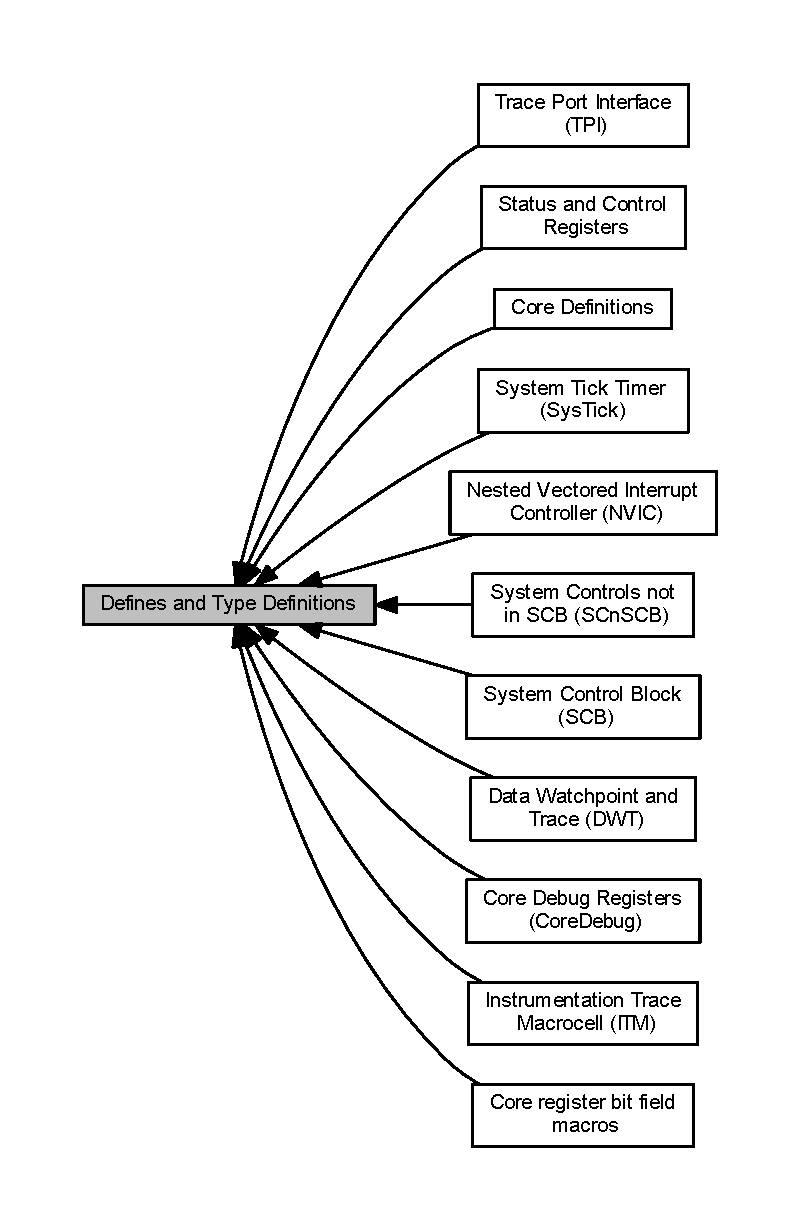
\includegraphics[width=350pt]{group___c_m_s_i_s__core__register}
\end{center}
\end{figure}
\subsection*{Modules}
\begin{DoxyCompactItemize}
\item 
\hyperlink{group___c_m_s_i_s___c_o_r_e}{Status and Control Registers}
\begin{DoxyCompactList}\small\item\em Core Register type definitions. \end{DoxyCompactList}\item 
\hyperlink{group___c_m_s_i_s___n_v_i_c}{Nested Vectored Interrupt Controller (\+N\+V\+I\+C)}
\begin{DoxyCompactList}\small\item\em Type definitions for the N\+V\+IC Registers. \end{DoxyCompactList}\item 
\hyperlink{group___c_m_s_i_s___s_c_b}{System Control Block (\+S\+C\+B)}
\begin{DoxyCompactList}\small\item\em Type definitions for the System Control Block Registers. \end{DoxyCompactList}\item 
\hyperlink{group___c_m_s_i_s___sys_tick}{System Tick Timer (\+Sys\+Tick)}
\begin{DoxyCompactList}\small\item\em Type definitions for the System \hyperlink{class_timer}{Timer} Registers. \end{DoxyCompactList}\item 
\hyperlink{group___c_m_s_i_s___core_debug}{Core Debug Registers (\+Core\+Debug)}
\begin{DoxyCompactList}\small\item\em Cortex-\/\+M0 Core Debug Registers (D\+CB registers, S\+H\+C\+SR, and D\+F\+SR) are only accessible over D\+AP and not via processor. Therefore they are not covered by the Cortex-\/\+M0 header file. \end{DoxyCompactList}\item 
\hyperlink{group___c_m_s_i_s__core__bitfield}{Core register bit field macros}
\begin{DoxyCompactList}\small\item\em Macros for use with bit field definitions (xxx\+\_\+\+Pos, xxx\+\_\+\+Msk). \end{DoxyCompactList}\item 
\hyperlink{group___c_m_s_i_s__core__base}{Core Definitions}
\begin{DoxyCompactList}\small\item\em Definitions for base addresses, unions, and structures. \end{DoxyCompactList}\item 
\hyperlink{group___c_m_s_i_s___s_cn_s_c_b}{System Controls not in S\+C\+B (\+S\+Cn\+S\+C\+B)}
\begin{DoxyCompactList}\small\item\em Type definitions for the System Control and ID Register not in the S\+CB. \end{DoxyCompactList}\item 
\hyperlink{group___c_m_s_i_s___i_t_m}{Instrumentation Trace Macrocell (\+I\+T\+M)}
\begin{DoxyCompactList}\small\item\em Type definitions for the Instrumentation Trace Macrocell (I\+TM) \end{DoxyCompactList}\item 
\hyperlink{group___c_m_s_i_s___d_w_t}{Data Watchpoint and Trace (\+D\+W\+T)}
\begin{DoxyCompactList}\small\item\em Type definitions for the Data Watchpoint and Trace (D\+WT) \end{DoxyCompactList}\item 
\hyperlink{group___c_m_s_i_s___t_p_i}{Trace Port Interface (\+T\+P\+I)}
\begin{DoxyCompactList}\small\item\em Type definitions for the Trace Port Interface (T\+PI) \end{DoxyCompactList}\end{DoxyCompactItemize}


\subsection{Detailed Description}
Type definitions and defines for Cortex-\/M processor based devices. 


\hypertarget{group___c_m_s_i_s___c_o_r_e}{}\section{Status and Control Registers}
\label{group___c_m_s_i_s___c_o_r_e}\index{Status and Control Registers@{Status and Control Registers}}


Core Register type definitions.  


Collaboration diagram for Status and Control Registers\+:
\nopagebreak
\begin{figure}[H]
\begin{center}
\leavevmode
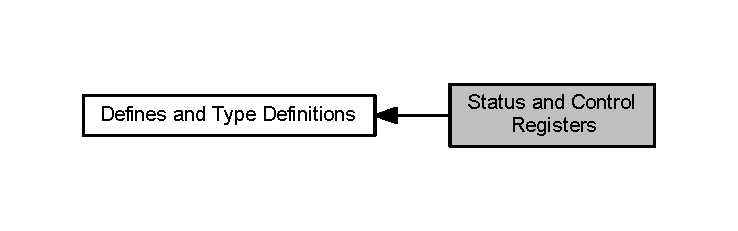
\includegraphics[width=350pt]{group___c_m_s_i_s___c_o_r_e}
\end{center}
\end{figure}
\subsection*{Classes}
\begin{DoxyCompactItemize}
\item 
union \hyperlink{union_a_p_s_r___type}{A\+P\+S\+R\+\_\+\+Type}
\begin{DoxyCompactList}\small\item\em Union type to access the Application Program Status Register (A\+P\+SR). \end{DoxyCompactList}\item 
union \hyperlink{union_i_p_s_r___type}{I\+P\+S\+R\+\_\+\+Type}
\begin{DoxyCompactList}\small\item\em Union type to access the Interrupt Program Status Register (I\+P\+SR). \end{DoxyCompactList}\item 
union \hyperlink{unionx_p_s_r___type}{x\+P\+S\+R\+\_\+\+Type}
\begin{DoxyCompactList}\small\item\em Union type to access the Special-\/\+Purpose Program Status Registers (x\+P\+SR). \end{DoxyCompactList}\item 
union \hyperlink{union_c_o_n_t_r_o_l___type}{C\+O\+N\+T\+R\+O\+L\+\_\+\+Type}
\begin{DoxyCompactList}\small\item\em Union type to access the Control Registers (C\+O\+N\+T\+R\+OL). \end{DoxyCompactList}\end{DoxyCompactItemize}
\subsection*{Macros}
\begin{DoxyCompactItemize}
\item 
\#define \hyperlink{group___c_m_s_i_s___c_o_r_e_gac469528d210043c7bd3f12f0e6824766}{A\+P\+S\+R\+\_\+\+N\+\_\+\+Pos}~31U
\item 
\#define \hyperlink{group___c_m_s_i_s___c_o_r_e_gadbc2cf55a026f661b53fadfcf822cef1}{A\+P\+S\+R\+\_\+\+N\+\_\+\+Msk}~(1\+U\+L $<$$<$ A\+P\+S\+R\+\_\+\+N\+\_\+\+Pos)
\item 
\#define \hyperlink{group___c_m_s_i_s___c_o_r_e_ga3661286d108b1aca308d7445685eae3a}{A\+P\+S\+R\+\_\+\+Z\+\_\+\+Pos}~30U
\item 
\#define \hyperlink{group___c_m_s_i_s___c_o_r_e_ga1deb4d1aa72bb83d1f79329406f15711}{A\+P\+S\+R\+\_\+\+Z\+\_\+\+Msk}~(1\+U\+L $<$$<$ A\+P\+S\+R\+\_\+\+Z\+\_\+\+Pos)
\item 
\#define \hyperlink{group___c_m_s_i_s___c_o_r_e_ga6cf72aa6f09a168f9e5beda1a4a887b9}{A\+P\+S\+R\+\_\+\+C\+\_\+\+Pos}~29U
\item 
\#define \hyperlink{group___c_m_s_i_s___c_o_r_e_ga6d47803fbad455bc10bd1ce59f2f335d}{A\+P\+S\+R\+\_\+\+C\+\_\+\+Msk}~(1\+U\+L $<$$<$ A\+P\+S\+R\+\_\+\+C\+\_\+\+Pos)
\item 
\#define \hyperlink{group___c_m_s_i_s___c_o_r_e_gac62830f67679ccd11658c4172c3e6ea7}{A\+P\+S\+R\+\_\+\+V\+\_\+\+Pos}~28U
\item 
\#define \hyperlink{group___c_m_s_i_s___c_o_r_e_ga33305d6701356bff6890b315fe8b5489}{A\+P\+S\+R\+\_\+\+V\+\_\+\+Msk}~(1\+U\+L $<$$<$ A\+P\+S\+R\+\_\+\+V\+\_\+\+Pos)
\item 
\#define \hyperlink{group___c_m_s_i_s___c_o_r_e_ga0e34027584d02c43811ae908a5ca9adf}{I\+P\+S\+R\+\_\+\+I\+S\+R\+\_\+\+Pos}~0U
\item 
\#define \hyperlink{group___c_m_s_i_s___c_o_r_e_gaf013a4579a64d1f21f56ea9f1b33ab56}{I\+P\+S\+R\+\_\+\+I\+S\+R\+\_\+\+Msk}~(0x1\+F\+F\+U\+L /$\ast$$<$$<$ I\+P\+S\+R\+\_\+\+I\+S\+R\+\_\+\+Pos$\ast$/)
\item 
\#define \hyperlink{group___c_m_s_i_s___c_o_r_e_ga031eb1b8ebcdb3d602d0b9f2ec82a7ae}{x\+P\+S\+R\+\_\+\+N\+\_\+\+Pos}~31U
\item 
\#define \hyperlink{group___c_m_s_i_s___c_o_r_e_gaf600f4ff41b62cf2f3b0a59b6d2e93d6}{x\+P\+S\+R\+\_\+\+N\+\_\+\+Msk}~(1\+U\+L $<$$<$ x\+P\+S\+R\+\_\+\+N\+\_\+\+Pos)
\item 
\#define \hyperlink{group___c_m_s_i_s___c_o_r_e_ga5869dd608eea73c80f0567d781d2230b}{x\+P\+S\+R\+\_\+\+Z\+\_\+\+Pos}~30U
\item 
\#define \hyperlink{group___c_m_s_i_s___c_o_r_e_ga907599209fba99f579778e662021c4f2}{x\+P\+S\+R\+\_\+\+Z\+\_\+\+Msk}~(1\+U\+L $<$$<$ x\+P\+S\+R\+\_\+\+Z\+\_\+\+Pos)
\item 
\#define \hyperlink{group___c_m_s_i_s___c_o_r_e_ga14adb79b91f6634b351a1b57394e2db6}{x\+P\+S\+R\+\_\+\+C\+\_\+\+Pos}~29U
\item 
\#define \hyperlink{group___c_m_s_i_s___c_o_r_e_ga21e2497255d380f956ca0f48d11d0775}{x\+P\+S\+R\+\_\+\+C\+\_\+\+Msk}~(1\+U\+L $<$$<$ x\+P\+S\+R\+\_\+\+C\+\_\+\+Pos)
\item 
\#define \hyperlink{group___c_m_s_i_s___c_o_r_e_gae0cfbb394490db402623d97e6a979e00}{x\+P\+S\+R\+\_\+\+V\+\_\+\+Pos}~28U
\item 
\#define \hyperlink{group___c_m_s_i_s___c_o_r_e_gab07f94ed3b6ee695f5af719dc27995c2}{x\+P\+S\+R\+\_\+\+V\+\_\+\+Msk}~(1\+U\+L $<$$<$ x\+P\+S\+R\+\_\+\+V\+\_\+\+Pos)
\item 
\#define \hyperlink{group___c_m_s_i_s___c_o_r_e_ga98d801da9a49cda944f52aeae104dd38}{x\+P\+S\+R\+\_\+\+T\+\_\+\+Pos}~24U
\item 
\#define \hyperlink{group___c_m_s_i_s___c_o_r_e_ga30ae2111816e82d47636a8d4577eb6ee}{x\+P\+S\+R\+\_\+\+T\+\_\+\+Msk}~(1\+U\+L $<$$<$ x\+P\+S\+R\+\_\+\+T\+\_\+\+Pos)
\item 
\#define \hyperlink{group___c_m_s_i_s___c_o_r_e_ga21bff245fb1aef9683f693d9d7bb2233}{x\+P\+S\+R\+\_\+\+I\+S\+R\+\_\+\+Pos}~0U
\item 
\#define \hyperlink{group___c_m_s_i_s___c_o_r_e_gadf8eed87e0081dfe1ef1c78a0ea91afd}{x\+P\+S\+R\+\_\+\+I\+S\+R\+\_\+\+Msk}~(0x1\+F\+F\+U\+L /$\ast$$<$$<$ x\+P\+S\+R\+\_\+\+I\+S\+R\+\_\+\+Pos$\ast$/)
\item 
\#define \hyperlink{group___c_m_s_i_s___c_o_r_e_ga07eafc53e609895342c6a530e9d01310}{C\+O\+N\+T\+R\+O\+L\+\_\+\+S\+P\+S\+E\+L\+\_\+\+Pos}~1U
\item 
\#define \hyperlink{group___c_m_s_i_s___c_o_r_e_ga70b29840969b06909da21369b0b05b53}{C\+O\+N\+T\+R\+O\+L\+\_\+\+S\+P\+S\+E\+L\+\_\+\+Msk}~(1\+U\+L $<$$<$ C\+O\+N\+T\+R\+O\+L\+\_\+\+S\+P\+S\+E\+L\+\_\+\+Pos)
\item 
\#define \hyperlink{group___c_m_s_i_s___c_o_r_e_gac469528d210043c7bd3f12f0e6824766}{A\+P\+S\+R\+\_\+\+N\+\_\+\+Pos}~31U
\item 
\#define \hyperlink{group___c_m_s_i_s___c_o_r_e_gadbc2cf55a026f661b53fadfcf822cef1}{A\+P\+S\+R\+\_\+\+N\+\_\+\+Msk}~(1\+U\+L $<$$<$ A\+P\+S\+R\+\_\+\+N\+\_\+\+Pos)
\item 
\#define \hyperlink{group___c_m_s_i_s___c_o_r_e_ga3661286d108b1aca308d7445685eae3a}{A\+P\+S\+R\+\_\+\+Z\+\_\+\+Pos}~30U
\item 
\#define \hyperlink{group___c_m_s_i_s___c_o_r_e_ga1deb4d1aa72bb83d1f79329406f15711}{A\+P\+S\+R\+\_\+\+Z\+\_\+\+Msk}~(1\+U\+L $<$$<$ A\+P\+S\+R\+\_\+\+Z\+\_\+\+Pos)
\item 
\#define \hyperlink{group___c_m_s_i_s___c_o_r_e_ga6cf72aa6f09a168f9e5beda1a4a887b9}{A\+P\+S\+R\+\_\+\+C\+\_\+\+Pos}~29U
\item 
\#define \hyperlink{group___c_m_s_i_s___c_o_r_e_ga6d47803fbad455bc10bd1ce59f2f335d}{A\+P\+S\+R\+\_\+\+C\+\_\+\+Msk}~(1\+U\+L $<$$<$ A\+P\+S\+R\+\_\+\+C\+\_\+\+Pos)
\item 
\#define \hyperlink{group___c_m_s_i_s___c_o_r_e_gac62830f67679ccd11658c4172c3e6ea7}{A\+P\+S\+R\+\_\+\+V\+\_\+\+Pos}~28U
\item 
\#define \hyperlink{group___c_m_s_i_s___c_o_r_e_ga33305d6701356bff6890b315fe8b5489}{A\+P\+S\+R\+\_\+\+V\+\_\+\+Msk}~(1\+U\+L $<$$<$ A\+P\+S\+R\+\_\+\+V\+\_\+\+Pos)
\item 
\#define \hyperlink{group___c_m_s_i_s___c_o_r_e_ga0e34027584d02c43811ae908a5ca9adf}{I\+P\+S\+R\+\_\+\+I\+S\+R\+\_\+\+Pos}~0U
\item 
\#define \hyperlink{group___c_m_s_i_s___c_o_r_e_gaf013a4579a64d1f21f56ea9f1b33ab56}{I\+P\+S\+R\+\_\+\+I\+S\+R\+\_\+\+Msk}~(0x1\+F\+F\+U\+L /$\ast$$<$$<$ I\+P\+S\+R\+\_\+\+I\+S\+R\+\_\+\+Pos$\ast$/)
\item 
\#define \hyperlink{group___c_m_s_i_s___c_o_r_e_ga031eb1b8ebcdb3d602d0b9f2ec82a7ae}{x\+P\+S\+R\+\_\+\+N\+\_\+\+Pos}~31U
\item 
\#define \hyperlink{group___c_m_s_i_s___c_o_r_e_gaf600f4ff41b62cf2f3b0a59b6d2e93d6}{x\+P\+S\+R\+\_\+\+N\+\_\+\+Msk}~(1\+U\+L $<$$<$ x\+P\+S\+R\+\_\+\+N\+\_\+\+Pos)
\item 
\#define \hyperlink{group___c_m_s_i_s___c_o_r_e_ga5869dd608eea73c80f0567d781d2230b}{x\+P\+S\+R\+\_\+\+Z\+\_\+\+Pos}~30U
\item 
\#define \hyperlink{group___c_m_s_i_s___c_o_r_e_ga907599209fba99f579778e662021c4f2}{x\+P\+S\+R\+\_\+\+Z\+\_\+\+Msk}~(1\+U\+L $<$$<$ x\+P\+S\+R\+\_\+\+Z\+\_\+\+Pos)
\item 
\#define \hyperlink{group___c_m_s_i_s___c_o_r_e_ga14adb79b91f6634b351a1b57394e2db6}{x\+P\+S\+R\+\_\+\+C\+\_\+\+Pos}~29U
\item 
\#define \hyperlink{group___c_m_s_i_s___c_o_r_e_ga21e2497255d380f956ca0f48d11d0775}{x\+P\+S\+R\+\_\+\+C\+\_\+\+Msk}~(1\+U\+L $<$$<$ x\+P\+S\+R\+\_\+\+C\+\_\+\+Pos)
\item 
\#define \hyperlink{group___c_m_s_i_s___c_o_r_e_gae0cfbb394490db402623d97e6a979e00}{x\+P\+S\+R\+\_\+\+V\+\_\+\+Pos}~28U
\item 
\#define \hyperlink{group___c_m_s_i_s___c_o_r_e_gab07f94ed3b6ee695f5af719dc27995c2}{x\+P\+S\+R\+\_\+\+V\+\_\+\+Msk}~(1\+U\+L $<$$<$ x\+P\+S\+R\+\_\+\+V\+\_\+\+Pos)
\item 
\#define \hyperlink{group___c_m_s_i_s___c_o_r_e_ga98d801da9a49cda944f52aeae104dd38}{x\+P\+S\+R\+\_\+\+T\+\_\+\+Pos}~24U
\item 
\#define \hyperlink{group___c_m_s_i_s___c_o_r_e_ga30ae2111816e82d47636a8d4577eb6ee}{x\+P\+S\+R\+\_\+\+T\+\_\+\+Msk}~(1\+U\+L $<$$<$ x\+P\+S\+R\+\_\+\+T\+\_\+\+Pos)
\item 
\#define \hyperlink{group___c_m_s_i_s___c_o_r_e_ga21bff245fb1aef9683f693d9d7bb2233}{x\+P\+S\+R\+\_\+\+I\+S\+R\+\_\+\+Pos}~0U
\item 
\#define \hyperlink{group___c_m_s_i_s___c_o_r_e_gadf8eed87e0081dfe1ef1c78a0ea91afd}{x\+P\+S\+R\+\_\+\+I\+S\+R\+\_\+\+Msk}~(0x1\+F\+F\+U\+L /$\ast$$<$$<$ x\+P\+S\+R\+\_\+\+I\+S\+R\+\_\+\+Pos$\ast$/)
\item 
\#define \hyperlink{group___c_m_s_i_s___c_o_r_e_ga07eafc53e609895342c6a530e9d01310}{C\+O\+N\+T\+R\+O\+L\+\_\+\+S\+P\+S\+E\+L\+\_\+\+Pos}~1U
\item 
\#define \hyperlink{group___c_m_s_i_s___c_o_r_e_ga70b29840969b06909da21369b0b05b53}{C\+O\+N\+T\+R\+O\+L\+\_\+\+S\+P\+S\+E\+L\+\_\+\+Msk}~(1\+U\+L $<$$<$ C\+O\+N\+T\+R\+O\+L\+\_\+\+S\+P\+S\+E\+L\+\_\+\+Pos)
\item 
\#define \hyperlink{group___c_m_s_i_s___c_o_r_e_ga51b95bc03ec0d815b459bde0b14a5908}{C\+O\+N\+T\+R\+O\+L\+\_\+n\+P\+R\+I\+V\+\_\+\+Pos}~0U
\item 
\#define \hyperlink{group___c_m_s_i_s___c_o_r_e_gaef3b20d77acb213338f89ce5e7bc36b0}{C\+O\+N\+T\+R\+O\+L\+\_\+n\+P\+R\+I\+V\+\_\+\+Msk}~(1\+U\+L /$\ast$$<$$<$ C\+O\+N\+T\+R\+O\+L\+\_\+n\+P\+R\+I\+V\+\_\+\+Pos$\ast$/)
\item 
\#define \hyperlink{group___c_m_s_i_s___c_o_r_e_gac469528d210043c7bd3f12f0e6824766}{A\+P\+S\+R\+\_\+\+N\+\_\+\+Pos}~31U
\item 
\#define \hyperlink{group___c_m_s_i_s___c_o_r_e_gadbc2cf55a026f661b53fadfcf822cef1}{A\+P\+S\+R\+\_\+\+N\+\_\+\+Msk}~(1\+U\+L $<$$<$ A\+P\+S\+R\+\_\+\+N\+\_\+\+Pos)
\item 
\#define \hyperlink{group___c_m_s_i_s___c_o_r_e_ga3661286d108b1aca308d7445685eae3a}{A\+P\+S\+R\+\_\+\+Z\+\_\+\+Pos}~30U
\item 
\#define \hyperlink{group___c_m_s_i_s___c_o_r_e_ga1deb4d1aa72bb83d1f79329406f15711}{A\+P\+S\+R\+\_\+\+Z\+\_\+\+Msk}~(1\+U\+L $<$$<$ A\+P\+S\+R\+\_\+\+Z\+\_\+\+Pos)
\item 
\#define \hyperlink{group___c_m_s_i_s___c_o_r_e_ga6cf72aa6f09a168f9e5beda1a4a887b9}{A\+P\+S\+R\+\_\+\+C\+\_\+\+Pos}~29U
\item 
\#define \hyperlink{group___c_m_s_i_s___c_o_r_e_ga6d47803fbad455bc10bd1ce59f2f335d}{A\+P\+S\+R\+\_\+\+C\+\_\+\+Msk}~(1\+U\+L $<$$<$ A\+P\+S\+R\+\_\+\+C\+\_\+\+Pos)
\item 
\#define \hyperlink{group___c_m_s_i_s___c_o_r_e_gac62830f67679ccd11658c4172c3e6ea7}{A\+P\+S\+R\+\_\+\+V\+\_\+\+Pos}~28U
\item 
\#define \hyperlink{group___c_m_s_i_s___c_o_r_e_ga33305d6701356bff6890b315fe8b5489}{A\+P\+S\+R\+\_\+\+V\+\_\+\+Msk}~(1\+U\+L $<$$<$ A\+P\+S\+R\+\_\+\+V\+\_\+\+Pos)
\item 
\#define \hyperlink{group___c_m_s_i_s___c_o_r_e_ga298749e176f12827328bb7b92a6b2411}{A\+P\+S\+R\+\_\+\+Q\+\_\+\+Pos}~27U
\item 
\#define \hyperlink{group___c_m_s_i_s___c_o_r_e_ga90ffd4ec4149c2f5dd7747c1533fb002}{A\+P\+S\+R\+\_\+\+Q\+\_\+\+Msk}~(1\+U\+L $<$$<$ A\+P\+S\+R\+\_\+\+Q\+\_\+\+Pos)
\item 
\#define \hyperlink{group___c_m_s_i_s___c_o_r_e_ga0e34027584d02c43811ae908a5ca9adf}{I\+P\+S\+R\+\_\+\+I\+S\+R\+\_\+\+Pos}~0U
\item 
\#define \hyperlink{group___c_m_s_i_s___c_o_r_e_gaf013a4579a64d1f21f56ea9f1b33ab56}{I\+P\+S\+R\+\_\+\+I\+S\+R\+\_\+\+Msk}~(0x1\+F\+F\+U\+L /$\ast$$<$$<$ I\+P\+S\+R\+\_\+\+I\+S\+R\+\_\+\+Pos$\ast$/)
\item 
\#define \hyperlink{group___c_m_s_i_s___c_o_r_e_ga031eb1b8ebcdb3d602d0b9f2ec82a7ae}{x\+P\+S\+R\+\_\+\+N\+\_\+\+Pos}~31U
\item 
\#define \hyperlink{group___c_m_s_i_s___c_o_r_e_gaf600f4ff41b62cf2f3b0a59b6d2e93d6}{x\+P\+S\+R\+\_\+\+N\+\_\+\+Msk}~(1\+U\+L $<$$<$ x\+P\+S\+R\+\_\+\+N\+\_\+\+Pos)
\item 
\#define \hyperlink{group___c_m_s_i_s___c_o_r_e_ga5869dd608eea73c80f0567d781d2230b}{x\+P\+S\+R\+\_\+\+Z\+\_\+\+Pos}~30U
\item 
\#define \hyperlink{group___c_m_s_i_s___c_o_r_e_ga907599209fba99f579778e662021c4f2}{x\+P\+S\+R\+\_\+\+Z\+\_\+\+Msk}~(1\+U\+L $<$$<$ x\+P\+S\+R\+\_\+\+Z\+\_\+\+Pos)
\item 
\#define \hyperlink{group___c_m_s_i_s___c_o_r_e_ga14adb79b91f6634b351a1b57394e2db6}{x\+P\+S\+R\+\_\+\+C\+\_\+\+Pos}~29U
\item 
\#define \hyperlink{group___c_m_s_i_s___c_o_r_e_ga21e2497255d380f956ca0f48d11d0775}{x\+P\+S\+R\+\_\+\+C\+\_\+\+Msk}~(1\+U\+L $<$$<$ x\+P\+S\+R\+\_\+\+C\+\_\+\+Pos)
\item 
\#define \hyperlink{group___c_m_s_i_s___c_o_r_e_gae0cfbb394490db402623d97e6a979e00}{x\+P\+S\+R\+\_\+\+V\+\_\+\+Pos}~28U
\item 
\#define \hyperlink{group___c_m_s_i_s___c_o_r_e_gab07f94ed3b6ee695f5af719dc27995c2}{x\+P\+S\+R\+\_\+\+V\+\_\+\+Msk}~(1\+U\+L $<$$<$ x\+P\+S\+R\+\_\+\+V\+\_\+\+Pos)
\item 
\#define \hyperlink{group___c_m_s_i_s___c_o_r_e_gaabb4178d50676a8f19cf8f727f38ace8}{x\+P\+S\+R\+\_\+\+Q\+\_\+\+Pos}~27U
\item 
\#define \hyperlink{group___c_m_s_i_s___c_o_r_e_ga133ac393c38559ae43ac36383e731dd4}{x\+P\+S\+R\+\_\+\+Q\+\_\+\+Msk}~(1\+U\+L $<$$<$ x\+P\+S\+R\+\_\+\+Q\+\_\+\+Pos)
\item 
\#define \hyperlink{group___c_m_s_i_s___c_o_r_e_gac5be1db1343f776ecd00f0a4ebe70a46}{x\+P\+S\+R\+\_\+\+I\+T\+\_\+\+Pos}~25U
\item 
\#define \hyperlink{group___c_m_s_i_s___c_o_r_e_ga6dc177aab488851bb3b98cf4b420141a}{x\+P\+S\+R\+\_\+\+I\+T\+\_\+\+Msk}~(3\+U\+L $<$$<$ x\+P\+S\+R\+\_\+\+I\+T\+\_\+\+Pos)
\item 
\#define \hyperlink{group___c_m_s_i_s___c_o_r_e_ga98d801da9a49cda944f52aeae104dd38}{x\+P\+S\+R\+\_\+\+T\+\_\+\+Pos}~24U
\item 
\#define \hyperlink{group___c_m_s_i_s___c_o_r_e_ga30ae2111816e82d47636a8d4577eb6ee}{x\+P\+S\+R\+\_\+\+T\+\_\+\+Msk}~(1\+U\+L $<$$<$ x\+P\+S\+R\+\_\+\+T\+\_\+\+Pos)
\item 
\#define \hyperlink{group___c_m_s_i_s___c_o_r_e_ga21bff245fb1aef9683f693d9d7bb2233}{x\+P\+S\+R\+\_\+\+I\+S\+R\+\_\+\+Pos}~0U
\item 
\#define \hyperlink{group___c_m_s_i_s___c_o_r_e_gadf8eed87e0081dfe1ef1c78a0ea91afd}{x\+P\+S\+R\+\_\+\+I\+S\+R\+\_\+\+Msk}~(0x1\+F\+F\+U\+L /$\ast$$<$$<$ x\+P\+S\+R\+\_\+\+I\+S\+R\+\_\+\+Pos$\ast$/)
\item 
\#define \hyperlink{group___c_m_s_i_s___c_o_r_e_ga07eafc53e609895342c6a530e9d01310}{C\+O\+N\+T\+R\+O\+L\+\_\+\+S\+P\+S\+E\+L\+\_\+\+Pos}~1U
\item 
\#define \hyperlink{group___c_m_s_i_s___c_o_r_e_ga70b29840969b06909da21369b0b05b53}{C\+O\+N\+T\+R\+O\+L\+\_\+\+S\+P\+S\+E\+L\+\_\+\+Msk}~(1\+U\+L $<$$<$ C\+O\+N\+T\+R\+O\+L\+\_\+\+S\+P\+S\+E\+L\+\_\+\+Pos)
\item 
\#define \hyperlink{group___c_m_s_i_s___c_o_r_e_ga51b95bc03ec0d815b459bde0b14a5908}{C\+O\+N\+T\+R\+O\+L\+\_\+n\+P\+R\+I\+V\+\_\+\+Pos}~0U
\item 
\#define \hyperlink{group___c_m_s_i_s___c_o_r_e_gaef3b20d77acb213338f89ce5e7bc36b0}{C\+O\+N\+T\+R\+O\+L\+\_\+n\+P\+R\+I\+V\+\_\+\+Msk}~(1\+U\+L /$\ast$$<$$<$ C\+O\+N\+T\+R\+O\+L\+\_\+n\+P\+R\+I\+V\+\_\+\+Pos$\ast$/)
\item 
\#define \hyperlink{group___c_m_s_i_s___c_o_r_e_gac469528d210043c7bd3f12f0e6824766}{A\+P\+S\+R\+\_\+\+N\+\_\+\+Pos}~31U
\item 
\#define \hyperlink{group___c_m_s_i_s___c_o_r_e_gadbc2cf55a026f661b53fadfcf822cef1}{A\+P\+S\+R\+\_\+\+N\+\_\+\+Msk}~(1\+U\+L $<$$<$ A\+P\+S\+R\+\_\+\+N\+\_\+\+Pos)
\item 
\#define \hyperlink{group___c_m_s_i_s___c_o_r_e_ga3661286d108b1aca308d7445685eae3a}{A\+P\+S\+R\+\_\+\+Z\+\_\+\+Pos}~30U
\item 
\#define \hyperlink{group___c_m_s_i_s___c_o_r_e_ga1deb4d1aa72bb83d1f79329406f15711}{A\+P\+S\+R\+\_\+\+Z\+\_\+\+Msk}~(1\+U\+L $<$$<$ A\+P\+S\+R\+\_\+\+Z\+\_\+\+Pos)
\item 
\#define \hyperlink{group___c_m_s_i_s___c_o_r_e_ga6cf72aa6f09a168f9e5beda1a4a887b9}{A\+P\+S\+R\+\_\+\+C\+\_\+\+Pos}~29U
\item 
\#define \hyperlink{group___c_m_s_i_s___c_o_r_e_ga6d47803fbad455bc10bd1ce59f2f335d}{A\+P\+S\+R\+\_\+\+C\+\_\+\+Msk}~(1\+U\+L $<$$<$ A\+P\+S\+R\+\_\+\+C\+\_\+\+Pos)
\item 
\#define \hyperlink{group___c_m_s_i_s___c_o_r_e_gac62830f67679ccd11658c4172c3e6ea7}{A\+P\+S\+R\+\_\+\+V\+\_\+\+Pos}~28U
\item 
\#define \hyperlink{group___c_m_s_i_s___c_o_r_e_ga33305d6701356bff6890b315fe8b5489}{A\+P\+S\+R\+\_\+\+V\+\_\+\+Msk}~(1\+U\+L $<$$<$ A\+P\+S\+R\+\_\+\+V\+\_\+\+Pos)
\item 
\#define \hyperlink{group___c_m_s_i_s___c_o_r_e_ga298749e176f12827328bb7b92a6b2411}{A\+P\+S\+R\+\_\+\+Q\+\_\+\+Pos}~27U
\item 
\#define \hyperlink{group___c_m_s_i_s___c_o_r_e_ga90ffd4ec4149c2f5dd7747c1533fb002}{A\+P\+S\+R\+\_\+\+Q\+\_\+\+Msk}~(1\+U\+L $<$$<$ A\+P\+S\+R\+\_\+\+Q\+\_\+\+Pos)
\item 
\#define \hyperlink{group___c_m_s_i_s___c_o_r_e_ga722cb42b5c75af3e8909fac6fd40dfdc}{A\+P\+S\+R\+\_\+\+G\+E\+\_\+\+Pos}~16U
\item 
\#define \hyperlink{group___c_m_s_i_s___c_o_r_e_ga8a3ecbc0ea2029462b0f4ce50e227db1}{A\+P\+S\+R\+\_\+\+G\+E\+\_\+\+Msk}~(0x\+F\+U\+L $<$$<$ A\+P\+S\+R\+\_\+\+G\+E\+\_\+\+Pos)
\item 
\#define \hyperlink{group___c_m_s_i_s___c_o_r_e_ga0e34027584d02c43811ae908a5ca9adf}{I\+P\+S\+R\+\_\+\+I\+S\+R\+\_\+\+Pos}~0U
\item 
\#define \hyperlink{group___c_m_s_i_s___c_o_r_e_gaf013a4579a64d1f21f56ea9f1b33ab56}{I\+P\+S\+R\+\_\+\+I\+S\+R\+\_\+\+Msk}~(0x1\+F\+F\+U\+L /$\ast$$<$$<$ I\+P\+S\+R\+\_\+\+I\+S\+R\+\_\+\+Pos$\ast$/)
\item 
\#define \hyperlink{group___c_m_s_i_s___c_o_r_e_ga031eb1b8ebcdb3d602d0b9f2ec82a7ae}{x\+P\+S\+R\+\_\+\+N\+\_\+\+Pos}~31U
\item 
\#define \hyperlink{group___c_m_s_i_s___c_o_r_e_gaf600f4ff41b62cf2f3b0a59b6d2e93d6}{x\+P\+S\+R\+\_\+\+N\+\_\+\+Msk}~(1\+U\+L $<$$<$ x\+P\+S\+R\+\_\+\+N\+\_\+\+Pos)
\item 
\#define \hyperlink{group___c_m_s_i_s___c_o_r_e_ga5869dd608eea73c80f0567d781d2230b}{x\+P\+S\+R\+\_\+\+Z\+\_\+\+Pos}~30U
\item 
\#define \hyperlink{group___c_m_s_i_s___c_o_r_e_ga907599209fba99f579778e662021c4f2}{x\+P\+S\+R\+\_\+\+Z\+\_\+\+Msk}~(1\+U\+L $<$$<$ x\+P\+S\+R\+\_\+\+Z\+\_\+\+Pos)
\item 
\#define \hyperlink{group___c_m_s_i_s___c_o_r_e_ga14adb79b91f6634b351a1b57394e2db6}{x\+P\+S\+R\+\_\+\+C\+\_\+\+Pos}~29U
\item 
\#define \hyperlink{group___c_m_s_i_s___c_o_r_e_ga21e2497255d380f956ca0f48d11d0775}{x\+P\+S\+R\+\_\+\+C\+\_\+\+Msk}~(1\+U\+L $<$$<$ x\+P\+S\+R\+\_\+\+C\+\_\+\+Pos)
\item 
\#define \hyperlink{group___c_m_s_i_s___c_o_r_e_gae0cfbb394490db402623d97e6a979e00}{x\+P\+S\+R\+\_\+\+V\+\_\+\+Pos}~28U
\item 
\#define \hyperlink{group___c_m_s_i_s___c_o_r_e_gab07f94ed3b6ee695f5af719dc27995c2}{x\+P\+S\+R\+\_\+\+V\+\_\+\+Msk}~(1\+U\+L $<$$<$ x\+P\+S\+R\+\_\+\+V\+\_\+\+Pos)
\item 
\#define \hyperlink{group___c_m_s_i_s___c_o_r_e_gaabb4178d50676a8f19cf8f727f38ace8}{x\+P\+S\+R\+\_\+\+Q\+\_\+\+Pos}~27U
\item 
\#define \hyperlink{group___c_m_s_i_s___c_o_r_e_ga133ac393c38559ae43ac36383e731dd4}{x\+P\+S\+R\+\_\+\+Q\+\_\+\+Msk}~(1\+U\+L $<$$<$ x\+P\+S\+R\+\_\+\+Q\+\_\+\+Pos)
\item 
\#define \hyperlink{group___c_m_s_i_s___c_o_r_e_gac5be1db1343f776ecd00f0a4ebe70a46}{x\+P\+S\+R\+\_\+\+I\+T\+\_\+\+Pos}~25U
\item 
\#define \hyperlink{group___c_m_s_i_s___c_o_r_e_ga6dc177aab488851bb3b98cf4b420141a}{x\+P\+S\+R\+\_\+\+I\+T\+\_\+\+Msk}~(3\+U\+L $<$$<$ x\+P\+S\+R\+\_\+\+I\+T\+\_\+\+Pos)
\item 
\#define \hyperlink{group___c_m_s_i_s___c_o_r_e_ga98d801da9a49cda944f52aeae104dd38}{x\+P\+S\+R\+\_\+\+T\+\_\+\+Pos}~24U
\item 
\#define \hyperlink{group___c_m_s_i_s___c_o_r_e_ga30ae2111816e82d47636a8d4577eb6ee}{x\+P\+S\+R\+\_\+\+T\+\_\+\+Msk}~(1\+U\+L $<$$<$ x\+P\+S\+R\+\_\+\+T\+\_\+\+Pos)
\item 
\#define \hyperlink{group___c_m_s_i_s___c_o_r_e_gae2b0f3def0f378e9f1d10a4c727a064b}{x\+P\+S\+R\+\_\+\+G\+E\+\_\+\+Pos}~16U
\item 
\#define \hyperlink{group___c_m_s_i_s___c_o_r_e_ga967634e605d013e9b07002eca31f7903}{x\+P\+S\+R\+\_\+\+G\+E\+\_\+\+Msk}~(0x\+F\+U\+L $<$$<$ x\+P\+S\+R\+\_\+\+G\+E\+\_\+\+Pos)
\item 
\#define \hyperlink{group___c_m_s_i_s___c_o_r_e_ga21bff245fb1aef9683f693d9d7bb2233}{x\+P\+S\+R\+\_\+\+I\+S\+R\+\_\+\+Pos}~0U
\item 
\#define \hyperlink{group___c_m_s_i_s___c_o_r_e_gadf8eed87e0081dfe1ef1c78a0ea91afd}{x\+P\+S\+R\+\_\+\+I\+S\+R\+\_\+\+Msk}~(0x1\+F\+F\+U\+L /$\ast$$<$$<$ x\+P\+S\+R\+\_\+\+I\+S\+R\+\_\+\+Pos$\ast$/)
\item 
\#define \hyperlink{group___c_m_s_i_s___c_o_r_e_gac7018b59b07134c5363b33eb94918a58}{C\+O\+N\+T\+R\+O\+L\+\_\+\+F\+P\+C\+A\+\_\+\+Pos}~2U
\item 
\#define \hyperlink{group___c_m_s_i_s___c_o_r_e_gad20bb0212b2e1864f24af38d93587c79}{C\+O\+N\+T\+R\+O\+L\+\_\+\+F\+P\+C\+A\+\_\+\+Msk}~(1\+U\+L $<$$<$ C\+O\+N\+T\+R\+O\+L\+\_\+\+F\+P\+C\+A\+\_\+\+Pos)
\item 
\#define \hyperlink{group___c_m_s_i_s___c_o_r_e_ga07eafc53e609895342c6a530e9d01310}{C\+O\+N\+T\+R\+O\+L\+\_\+\+S\+P\+S\+E\+L\+\_\+\+Pos}~1U
\item 
\#define \hyperlink{group___c_m_s_i_s___c_o_r_e_ga70b29840969b06909da21369b0b05b53}{C\+O\+N\+T\+R\+O\+L\+\_\+\+S\+P\+S\+E\+L\+\_\+\+Msk}~(1\+U\+L $<$$<$ C\+O\+N\+T\+R\+O\+L\+\_\+\+S\+P\+S\+E\+L\+\_\+\+Pos)
\item 
\#define \hyperlink{group___c_m_s_i_s___c_o_r_e_ga51b95bc03ec0d815b459bde0b14a5908}{C\+O\+N\+T\+R\+O\+L\+\_\+n\+P\+R\+I\+V\+\_\+\+Pos}~0U
\item 
\#define \hyperlink{group___c_m_s_i_s___c_o_r_e_gaef3b20d77acb213338f89ce5e7bc36b0}{C\+O\+N\+T\+R\+O\+L\+\_\+n\+P\+R\+I\+V\+\_\+\+Msk}~(1\+U\+L /$\ast$$<$$<$ C\+O\+N\+T\+R\+O\+L\+\_\+n\+P\+R\+I\+V\+\_\+\+Pos$\ast$/)
\item 
\#define \hyperlink{group___c_m_s_i_s___c_o_r_e_gac469528d210043c7bd3f12f0e6824766}{A\+P\+S\+R\+\_\+\+N\+\_\+\+Pos}~31U
\item 
\#define \hyperlink{group___c_m_s_i_s___c_o_r_e_gadbc2cf55a026f661b53fadfcf822cef1}{A\+P\+S\+R\+\_\+\+N\+\_\+\+Msk}~(1\+U\+L $<$$<$ A\+P\+S\+R\+\_\+\+N\+\_\+\+Pos)
\item 
\#define \hyperlink{group___c_m_s_i_s___c_o_r_e_ga3661286d108b1aca308d7445685eae3a}{A\+P\+S\+R\+\_\+\+Z\+\_\+\+Pos}~30U
\item 
\#define \hyperlink{group___c_m_s_i_s___c_o_r_e_ga1deb4d1aa72bb83d1f79329406f15711}{A\+P\+S\+R\+\_\+\+Z\+\_\+\+Msk}~(1\+U\+L $<$$<$ A\+P\+S\+R\+\_\+\+Z\+\_\+\+Pos)
\item 
\#define \hyperlink{group___c_m_s_i_s___c_o_r_e_ga6cf72aa6f09a168f9e5beda1a4a887b9}{A\+P\+S\+R\+\_\+\+C\+\_\+\+Pos}~29U
\item 
\#define \hyperlink{group___c_m_s_i_s___c_o_r_e_ga6d47803fbad455bc10bd1ce59f2f335d}{A\+P\+S\+R\+\_\+\+C\+\_\+\+Msk}~(1\+U\+L $<$$<$ A\+P\+S\+R\+\_\+\+C\+\_\+\+Pos)
\item 
\#define \hyperlink{group___c_m_s_i_s___c_o_r_e_gac62830f67679ccd11658c4172c3e6ea7}{A\+P\+S\+R\+\_\+\+V\+\_\+\+Pos}~28U
\item 
\#define \hyperlink{group___c_m_s_i_s___c_o_r_e_ga33305d6701356bff6890b315fe8b5489}{A\+P\+S\+R\+\_\+\+V\+\_\+\+Msk}~(1\+U\+L $<$$<$ A\+P\+S\+R\+\_\+\+V\+\_\+\+Pos)
\item 
\#define \hyperlink{group___c_m_s_i_s___c_o_r_e_ga298749e176f12827328bb7b92a6b2411}{A\+P\+S\+R\+\_\+\+Q\+\_\+\+Pos}~27U
\item 
\#define \hyperlink{group___c_m_s_i_s___c_o_r_e_ga90ffd4ec4149c2f5dd7747c1533fb002}{A\+P\+S\+R\+\_\+\+Q\+\_\+\+Msk}~(1\+U\+L $<$$<$ A\+P\+S\+R\+\_\+\+Q\+\_\+\+Pos)
\item 
\#define \hyperlink{group___c_m_s_i_s___c_o_r_e_ga722cb42b5c75af3e8909fac6fd40dfdc}{A\+P\+S\+R\+\_\+\+G\+E\+\_\+\+Pos}~16U
\item 
\#define \hyperlink{group___c_m_s_i_s___c_o_r_e_ga8a3ecbc0ea2029462b0f4ce50e227db1}{A\+P\+S\+R\+\_\+\+G\+E\+\_\+\+Msk}~(0x\+F\+U\+L $<$$<$ A\+P\+S\+R\+\_\+\+G\+E\+\_\+\+Pos)
\item 
\#define \hyperlink{group___c_m_s_i_s___c_o_r_e_ga0e34027584d02c43811ae908a5ca9adf}{I\+P\+S\+R\+\_\+\+I\+S\+R\+\_\+\+Pos}~0U
\item 
\#define \hyperlink{group___c_m_s_i_s___c_o_r_e_gaf013a4579a64d1f21f56ea9f1b33ab56}{I\+P\+S\+R\+\_\+\+I\+S\+R\+\_\+\+Msk}~(0x1\+F\+F\+U\+L /$\ast$$<$$<$ I\+P\+S\+R\+\_\+\+I\+S\+R\+\_\+\+Pos$\ast$/)
\item 
\#define \hyperlink{group___c_m_s_i_s___c_o_r_e_ga031eb1b8ebcdb3d602d0b9f2ec82a7ae}{x\+P\+S\+R\+\_\+\+N\+\_\+\+Pos}~31U
\item 
\#define \hyperlink{group___c_m_s_i_s___c_o_r_e_gaf600f4ff41b62cf2f3b0a59b6d2e93d6}{x\+P\+S\+R\+\_\+\+N\+\_\+\+Msk}~(1\+U\+L $<$$<$ x\+P\+S\+R\+\_\+\+N\+\_\+\+Pos)
\item 
\#define \hyperlink{group___c_m_s_i_s___c_o_r_e_ga5869dd608eea73c80f0567d781d2230b}{x\+P\+S\+R\+\_\+\+Z\+\_\+\+Pos}~30U
\item 
\#define \hyperlink{group___c_m_s_i_s___c_o_r_e_ga907599209fba99f579778e662021c4f2}{x\+P\+S\+R\+\_\+\+Z\+\_\+\+Msk}~(1\+U\+L $<$$<$ x\+P\+S\+R\+\_\+\+Z\+\_\+\+Pos)
\item 
\#define \hyperlink{group___c_m_s_i_s___c_o_r_e_ga14adb79b91f6634b351a1b57394e2db6}{x\+P\+S\+R\+\_\+\+C\+\_\+\+Pos}~29U
\item 
\#define \hyperlink{group___c_m_s_i_s___c_o_r_e_ga21e2497255d380f956ca0f48d11d0775}{x\+P\+S\+R\+\_\+\+C\+\_\+\+Msk}~(1\+U\+L $<$$<$ x\+P\+S\+R\+\_\+\+C\+\_\+\+Pos)
\item 
\#define \hyperlink{group___c_m_s_i_s___c_o_r_e_gae0cfbb394490db402623d97e6a979e00}{x\+P\+S\+R\+\_\+\+V\+\_\+\+Pos}~28U
\item 
\#define \hyperlink{group___c_m_s_i_s___c_o_r_e_gab07f94ed3b6ee695f5af719dc27995c2}{x\+P\+S\+R\+\_\+\+V\+\_\+\+Msk}~(1\+U\+L $<$$<$ x\+P\+S\+R\+\_\+\+V\+\_\+\+Pos)
\item 
\#define \hyperlink{group___c_m_s_i_s___c_o_r_e_gaabb4178d50676a8f19cf8f727f38ace8}{x\+P\+S\+R\+\_\+\+Q\+\_\+\+Pos}~27U
\item 
\#define \hyperlink{group___c_m_s_i_s___c_o_r_e_ga133ac393c38559ae43ac36383e731dd4}{x\+P\+S\+R\+\_\+\+Q\+\_\+\+Msk}~(1\+U\+L $<$$<$ x\+P\+S\+R\+\_\+\+Q\+\_\+\+Pos)
\item 
\#define \hyperlink{group___c_m_s_i_s___c_o_r_e_gac5be1db1343f776ecd00f0a4ebe70a46}{x\+P\+S\+R\+\_\+\+I\+T\+\_\+\+Pos}~25U
\item 
\#define \hyperlink{group___c_m_s_i_s___c_o_r_e_ga6dc177aab488851bb3b98cf4b420141a}{x\+P\+S\+R\+\_\+\+I\+T\+\_\+\+Msk}~(3\+U\+L $<$$<$ x\+P\+S\+R\+\_\+\+I\+T\+\_\+\+Pos)
\item 
\#define \hyperlink{group___c_m_s_i_s___c_o_r_e_ga98d801da9a49cda944f52aeae104dd38}{x\+P\+S\+R\+\_\+\+T\+\_\+\+Pos}~24U
\item 
\#define \hyperlink{group___c_m_s_i_s___c_o_r_e_ga30ae2111816e82d47636a8d4577eb6ee}{x\+P\+S\+R\+\_\+\+T\+\_\+\+Msk}~(1\+U\+L $<$$<$ x\+P\+S\+R\+\_\+\+T\+\_\+\+Pos)
\item 
\#define \hyperlink{group___c_m_s_i_s___c_o_r_e_gae2b0f3def0f378e9f1d10a4c727a064b}{x\+P\+S\+R\+\_\+\+G\+E\+\_\+\+Pos}~16U
\item 
\#define \hyperlink{group___c_m_s_i_s___c_o_r_e_ga967634e605d013e9b07002eca31f7903}{x\+P\+S\+R\+\_\+\+G\+E\+\_\+\+Msk}~(0x\+F\+U\+L $<$$<$ x\+P\+S\+R\+\_\+\+G\+E\+\_\+\+Pos)
\item 
\#define \hyperlink{group___c_m_s_i_s___c_o_r_e_ga21bff245fb1aef9683f693d9d7bb2233}{x\+P\+S\+R\+\_\+\+I\+S\+R\+\_\+\+Pos}~0U
\item 
\#define \hyperlink{group___c_m_s_i_s___c_o_r_e_gadf8eed87e0081dfe1ef1c78a0ea91afd}{x\+P\+S\+R\+\_\+\+I\+S\+R\+\_\+\+Msk}~(0x1\+F\+F\+U\+L /$\ast$$<$$<$ x\+P\+S\+R\+\_\+\+I\+S\+R\+\_\+\+Pos$\ast$/)
\item 
\#define \hyperlink{group___c_m_s_i_s___c_o_r_e_gac7018b59b07134c5363b33eb94918a58}{C\+O\+N\+T\+R\+O\+L\+\_\+\+F\+P\+C\+A\+\_\+\+Pos}~2U
\item 
\#define \hyperlink{group___c_m_s_i_s___c_o_r_e_gad20bb0212b2e1864f24af38d93587c79}{C\+O\+N\+T\+R\+O\+L\+\_\+\+F\+P\+C\+A\+\_\+\+Msk}~(1\+U\+L $<$$<$ C\+O\+N\+T\+R\+O\+L\+\_\+\+F\+P\+C\+A\+\_\+\+Pos)
\item 
\#define \hyperlink{group___c_m_s_i_s___c_o_r_e_ga07eafc53e609895342c6a530e9d01310}{C\+O\+N\+T\+R\+O\+L\+\_\+\+S\+P\+S\+E\+L\+\_\+\+Pos}~1U
\item 
\#define \hyperlink{group___c_m_s_i_s___c_o_r_e_ga70b29840969b06909da21369b0b05b53}{C\+O\+N\+T\+R\+O\+L\+\_\+\+S\+P\+S\+E\+L\+\_\+\+Msk}~(1\+U\+L $<$$<$ C\+O\+N\+T\+R\+O\+L\+\_\+\+S\+P\+S\+E\+L\+\_\+\+Pos)
\item 
\#define \hyperlink{group___c_m_s_i_s___c_o_r_e_ga51b95bc03ec0d815b459bde0b14a5908}{C\+O\+N\+T\+R\+O\+L\+\_\+n\+P\+R\+I\+V\+\_\+\+Pos}~0U
\item 
\#define \hyperlink{group___c_m_s_i_s___c_o_r_e_gaef3b20d77acb213338f89ce5e7bc36b0}{C\+O\+N\+T\+R\+O\+L\+\_\+n\+P\+R\+I\+V\+\_\+\+Msk}~(1\+U\+L /$\ast$$<$$<$ C\+O\+N\+T\+R\+O\+L\+\_\+n\+P\+R\+I\+V\+\_\+\+Pos$\ast$/)
\item 
\#define \hyperlink{group___c_m_s_i_s___c_o_r_e_gac469528d210043c7bd3f12f0e6824766}{A\+P\+S\+R\+\_\+\+N\+\_\+\+Pos}~31U
\item 
\#define \hyperlink{group___c_m_s_i_s___c_o_r_e_gadbc2cf55a026f661b53fadfcf822cef1}{A\+P\+S\+R\+\_\+\+N\+\_\+\+Msk}~(1\+U\+L $<$$<$ A\+P\+S\+R\+\_\+\+N\+\_\+\+Pos)
\item 
\#define \hyperlink{group___c_m_s_i_s___c_o_r_e_ga3661286d108b1aca308d7445685eae3a}{A\+P\+S\+R\+\_\+\+Z\+\_\+\+Pos}~30U
\item 
\#define \hyperlink{group___c_m_s_i_s___c_o_r_e_ga1deb4d1aa72bb83d1f79329406f15711}{A\+P\+S\+R\+\_\+\+Z\+\_\+\+Msk}~(1\+U\+L $<$$<$ A\+P\+S\+R\+\_\+\+Z\+\_\+\+Pos)
\item 
\#define \hyperlink{group___c_m_s_i_s___c_o_r_e_ga6cf72aa6f09a168f9e5beda1a4a887b9}{A\+P\+S\+R\+\_\+\+C\+\_\+\+Pos}~29U
\item 
\#define \hyperlink{group___c_m_s_i_s___c_o_r_e_ga6d47803fbad455bc10bd1ce59f2f335d}{A\+P\+S\+R\+\_\+\+C\+\_\+\+Msk}~(1\+U\+L $<$$<$ A\+P\+S\+R\+\_\+\+C\+\_\+\+Pos)
\item 
\#define \hyperlink{group___c_m_s_i_s___c_o_r_e_gac62830f67679ccd11658c4172c3e6ea7}{A\+P\+S\+R\+\_\+\+V\+\_\+\+Pos}~28U
\item 
\#define \hyperlink{group___c_m_s_i_s___c_o_r_e_ga33305d6701356bff6890b315fe8b5489}{A\+P\+S\+R\+\_\+\+V\+\_\+\+Msk}~(1\+U\+L $<$$<$ A\+P\+S\+R\+\_\+\+V\+\_\+\+Pos)
\item 
\#define \hyperlink{group___c_m_s_i_s___c_o_r_e_ga0e34027584d02c43811ae908a5ca9adf}{I\+P\+S\+R\+\_\+\+I\+S\+R\+\_\+\+Pos}~0U
\item 
\#define \hyperlink{group___c_m_s_i_s___c_o_r_e_gaf013a4579a64d1f21f56ea9f1b33ab56}{I\+P\+S\+R\+\_\+\+I\+S\+R\+\_\+\+Msk}~(0x1\+F\+F\+U\+L /$\ast$$<$$<$ I\+P\+S\+R\+\_\+\+I\+S\+R\+\_\+\+Pos$\ast$/)
\item 
\#define \hyperlink{group___c_m_s_i_s___c_o_r_e_ga031eb1b8ebcdb3d602d0b9f2ec82a7ae}{x\+P\+S\+R\+\_\+\+N\+\_\+\+Pos}~31U
\item 
\#define \hyperlink{group___c_m_s_i_s___c_o_r_e_gaf600f4ff41b62cf2f3b0a59b6d2e93d6}{x\+P\+S\+R\+\_\+\+N\+\_\+\+Msk}~(1\+U\+L $<$$<$ x\+P\+S\+R\+\_\+\+N\+\_\+\+Pos)
\item 
\#define \hyperlink{group___c_m_s_i_s___c_o_r_e_ga5869dd608eea73c80f0567d781d2230b}{x\+P\+S\+R\+\_\+\+Z\+\_\+\+Pos}~30U
\item 
\#define \hyperlink{group___c_m_s_i_s___c_o_r_e_ga907599209fba99f579778e662021c4f2}{x\+P\+S\+R\+\_\+\+Z\+\_\+\+Msk}~(1\+U\+L $<$$<$ x\+P\+S\+R\+\_\+\+Z\+\_\+\+Pos)
\item 
\#define \hyperlink{group___c_m_s_i_s___c_o_r_e_ga14adb79b91f6634b351a1b57394e2db6}{x\+P\+S\+R\+\_\+\+C\+\_\+\+Pos}~29U
\item 
\#define \hyperlink{group___c_m_s_i_s___c_o_r_e_ga21e2497255d380f956ca0f48d11d0775}{x\+P\+S\+R\+\_\+\+C\+\_\+\+Msk}~(1\+U\+L $<$$<$ x\+P\+S\+R\+\_\+\+C\+\_\+\+Pos)
\item 
\#define \hyperlink{group___c_m_s_i_s___c_o_r_e_gae0cfbb394490db402623d97e6a979e00}{x\+P\+S\+R\+\_\+\+V\+\_\+\+Pos}~28U
\item 
\#define \hyperlink{group___c_m_s_i_s___c_o_r_e_gab07f94ed3b6ee695f5af719dc27995c2}{x\+P\+S\+R\+\_\+\+V\+\_\+\+Msk}~(1\+U\+L $<$$<$ x\+P\+S\+R\+\_\+\+V\+\_\+\+Pos)
\item 
\#define \hyperlink{group___c_m_s_i_s___c_o_r_e_ga98d801da9a49cda944f52aeae104dd38}{x\+P\+S\+R\+\_\+\+T\+\_\+\+Pos}~24U
\item 
\#define \hyperlink{group___c_m_s_i_s___c_o_r_e_ga30ae2111816e82d47636a8d4577eb6ee}{x\+P\+S\+R\+\_\+\+T\+\_\+\+Msk}~(1\+U\+L $<$$<$ x\+P\+S\+R\+\_\+\+T\+\_\+\+Pos)
\item 
\#define \hyperlink{group___c_m_s_i_s___c_o_r_e_ga21bff245fb1aef9683f693d9d7bb2233}{x\+P\+S\+R\+\_\+\+I\+S\+R\+\_\+\+Pos}~0U
\item 
\#define \hyperlink{group___c_m_s_i_s___c_o_r_e_gadf8eed87e0081dfe1ef1c78a0ea91afd}{x\+P\+S\+R\+\_\+\+I\+S\+R\+\_\+\+Msk}~(0x1\+F\+F\+U\+L /$\ast$$<$$<$ x\+P\+S\+R\+\_\+\+I\+S\+R\+\_\+\+Pos$\ast$/)
\item 
\#define \hyperlink{group___c_m_s_i_s___c_o_r_e_ga07eafc53e609895342c6a530e9d01310}{C\+O\+N\+T\+R\+O\+L\+\_\+\+S\+P\+S\+E\+L\+\_\+\+Pos}~1U
\item 
\#define \hyperlink{group___c_m_s_i_s___c_o_r_e_ga70b29840969b06909da21369b0b05b53}{C\+O\+N\+T\+R\+O\+L\+\_\+\+S\+P\+S\+E\+L\+\_\+\+Msk}~(1\+U\+L $<$$<$ C\+O\+N\+T\+R\+O\+L\+\_\+\+S\+P\+S\+E\+L\+\_\+\+Pos)
\item 
\#define \hyperlink{group___c_m_s_i_s___c_o_r_e_gac469528d210043c7bd3f12f0e6824766}{A\+P\+S\+R\+\_\+\+N\+\_\+\+Pos}~31U
\item 
\#define \hyperlink{group___c_m_s_i_s___c_o_r_e_gadbc2cf55a026f661b53fadfcf822cef1}{A\+P\+S\+R\+\_\+\+N\+\_\+\+Msk}~(1\+U\+L $<$$<$ A\+P\+S\+R\+\_\+\+N\+\_\+\+Pos)
\item 
\#define \hyperlink{group___c_m_s_i_s___c_o_r_e_ga3661286d108b1aca308d7445685eae3a}{A\+P\+S\+R\+\_\+\+Z\+\_\+\+Pos}~30U
\item 
\#define \hyperlink{group___c_m_s_i_s___c_o_r_e_ga1deb4d1aa72bb83d1f79329406f15711}{A\+P\+S\+R\+\_\+\+Z\+\_\+\+Msk}~(1\+U\+L $<$$<$ A\+P\+S\+R\+\_\+\+Z\+\_\+\+Pos)
\item 
\#define \hyperlink{group___c_m_s_i_s___c_o_r_e_ga6cf72aa6f09a168f9e5beda1a4a887b9}{A\+P\+S\+R\+\_\+\+C\+\_\+\+Pos}~29U
\item 
\#define \hyperlink{group___c_m_s_i_s___c_o_r_e_ga6d47803fbad455bc10bd1ce59f2f335d}{A\+P\+S\+R\+\_\+\+C\+\_\+\+Msk}~(1\+U\+L $<$$<$ A\+P\+S\+R\+\_\+\+C\+\_\+\+Pos)
\item 
\#define \hyperlink{group___c_m_s_i_s___c_o_r_e_gac62830f67679ccd11658c4172c3e6ea7}{A\+P\+S\+R\+\_\+\+V\+\_\+\+Pos}~28U
\item 
\#define \hyperlink{group___c_m_s_i_s___c_o_r_e_ga33305d6701356bff6890b315fe8b5489}{A\+P\+S\+R\+\_\+\+V\+\_\+\+Msk}~(1\+U\+L $<$$<$ A\+P\+S\+R\+\_\+\+V\+\_\+\+Pos)
\item 
\#define \hyperlink{group___c_m_s_i_s___c_o_r_e_ga298749e176f12827328bb7b92a6b2411}{A\+P\+S\+R\+\_\+\+Q\+\_\+\+Pos}~27U
\item 
\#define \hyperlink{group___c_m_s_i_s___c_o_r_e_ga90ffd4ec4149c2f5dd7747c1533fb002}{A\+P\+S\+R\+\_\+\+Q\+\_\+\+Msk}~(1\+U\+L $<$$<$ A\+P\+S\+R\+\_\+\+Q\+\_\+\+Pos)
\item 
\#define \hyperlink{group___c_m_s_i_s___c_o_r_e_ga0e34027584d02c43811ae908a5ca9adf}{I\+P\+S\+R\+\_\+\+I\+S\+R\+\_\+\+Pos}~0U
\item 
\#define \hyperlink{group___c_m_s_i_s___c_o_r_e_gaf013a4579a64d1f21f56ea9f1b33ab56}{I\+P\+S\+R\+\_\+\+I\+S\+R\+\_\+\+Msk}~(0x1\+F\+F\+U\+L /$\ast$$<$$<$ I\+P\+S\+R\+\_\+\+I\+S\+R\+\_\+\+Pos$\ast$/)
\item 
\#define \hyperlink{group___c_m_s_i_s___c_o_r_e_ga031eb1b8ebcdb3d602d0b9f2ec82a7ae}{x\+P\+S\+R\+\_\+\+N\+\_\+\+Pos}~31U
\item 
\#define \hyperlink{group___c_m_s_i_s___c_o_r_e_gaf600f4ff41b62cf2f3b0a59b6d2e93d6}{x\+P\+S\+R\+\_\+\+N\+\_\+\+Msk}~(1\+U\+L $<$$<$ x\+P\+S\+R\+\_\+\+N\+\_\+\+Pos)
\item 
\#define \hyperlink{group___c_m_s_i_s___c_o_r_e_ga5869dd608eea73c80f0567d781d2230b}{x\+P\+S\+R\+\_\+\+Z\+\_\+\+Pos}~30U
\item 
\#define \hyperlink{group___c_m_s_i_s___c_o_r_e_ga907599209fba99f579778e662021c4f2}{x\+P\+S\+R\+\_\+\+Z\+\_\+\+Msk}~(1\+U\+L $<$$<$ x\+P\+S\+R\+\_\+\+Z\+\_\+\+Pos)
\item 
\#define \hyperlink{group___c_m_s_i_s___c_o_r_e_ga14adb79b91f6634b351a1b57394e2db6}{x\+P\+S\+R\+\_\+\+C\+\_\+\+Pos}~29U
\item 
\#define \hyperlink{group___c_m_s_i_s___c_o_r_e_ga21e2497255d380f956ca0f48d11d0775}{x\+P\+S\+R\+\_\+\+C\+\_\+\+Msk}~(1\+U\+L $<$$<$ x\+P\+S\+R\+\_\+\+C\+\_\+\+Pos)
\item 
\#define \hyperlink{group___c_m_s_i_s___c_o_r_e_gae0cfbb394490db402623d97e6a979e00}{x\+P\+S\+R\+\_\+\+V\+\_\+\+Pos}~28U
\item 
\#define \hyperlink{group___c_m_s_i_s___c_o_r_e_gab07f94ed3b6ee695f5af719dc27995c2}{x\+P\+S\+R\+\_\+\+V\+\_\+\+Msk}~(1\+U\+L $<$$<$ x\+P\+S\+R\+\_\+\+V\+\_\+\+Pos)
\item 
\#define \hyperlink{group___c_m_s_i_s___c_o_r_e_gaabb4178d50676a8f19cf8f727f38ace8}{x\+P\+S\+R\+\_\+\+Q\+\_\+\+Pos}~27U
\item 
\#define \hyperlink{group___c_m_s_i_s___c_o_r_e_ga133ac393c38559ae43ac36383e731dd4}{x\+P\+S\+R\+\_\+\+Q\+\_\+\+Msk}~(1\+U\+L $<$$<$ x\+P\+S\+R\+\_\+\+Q\+\_\+\+Pos)
\item 
\#define \hyperlink{group___c_m_s_i_s___c_o_r_e_gac5be1db1343f776ecd00f0a4ebe70a46}{x\+P\+S\+R\+\_\+\+I\+T\+\_\+\+Pos}~25U
\item 
\#define \hyperlink{group___c_m_s_i_s___c_o_r_e_ga6dc177aab488851bb3b98cf4b420141a}{x\+P\+S\+R\+\_\+\+I\+T\+\_\+\+Msk}~(3\+U\+L $<$$<$ x\+P\+S\+R\+\_\+\+I\+T\+\_\+\+Pos)
\item 
\#define \hyperlink{group___c_m_s_i_s___c_o_r_e_ga98d801da9a49cda944f52aeae104dd38}{x\+P\+S\+R\+\_\+\+T\+\_\+\+Pos}~24U
\item 
\#define \hyperlink{group___c_m_s_i_s___c_o_r_e_ga30ae2111816e82d47636a8d4577eb6ee}{x\+P\+S\+R\+\_\+\+T\+\_\+\+Msk}~(1\+U\+L $<$$<$ x\+P\+S\+R\+\_\+\+T\+\_\+\+Pos)
\item 
\#define \hyperlink{group___c_m_s_i_s___c_o_r_e_ga21bff245fb1aef9683f693d9d7bb2233}{x\+P\+S\+R\+\_\+\+I\+S\+R\+\_\+\+Pos}~0U
\item 
\#define \hyperlink{group___c_m_s_i_s___c_o_r_e_gadf8eed87e0081dfe1ef1c78a0ea91afd}{x\+P\+S\+R\+\_\+\+I\+S\+R\+\_\+\+Msk}~(0x1\+F\+F\+U\+L /$\ast$$<$$<$ x\+P\+S\+R\+\_\+\+I\+S\+R\+\_\+\+Pos$\ast$/)
\item 
\#define \hyperlink{group___c_m_s_i_s___c_o_r_e_ga07eafc53e609895342c6a530e9d01310}{C\+O\+N\+T\+R\+O\+L\+\_\+\+S\+P\+S\+E\+L\+\_\+\+Pos}~1U
\item 
\#define \hyperlink{group___c_m_s_i_s___c_o_r_e_ga70b29840969b06909da21369b0b05b53}{C\+O\+N\+T\+R\+O\+L\+\_\+\+S\+P\+S\+E\+L\+\_\+\+Msk}~(1\+U\+L $<$$<$ C\+O\+N\+T\+R\+O\+L\+\_\+\+S\+P\+S\+E\+L\+\_\+\+Pos)
\item 
\#define \hyperlink{group___c_m_s_i_s___c_o_r_e_ga51b95bc03ec0d815b459bde0b14a5908}{C\+O\+N\+T\+R\+O\+L\+\_\+n\+P\+R\+I\+V\+\_\+\+Pos}~0U
\item 
\#define \hyperlink{group___c_m_s_i_s___c_o_r_e_gaef3b20d77acb213338f89ce5e7bc36b0}{C\+O\+N\+T\+R\+O\+L\+\_\+n\+P\+R\+I\+V\+\_\+\+Msk}~(1\+U\+L /$\ast$$<$$<$ C\+O\+N\+T\+R\+O\+L\+\_\+n\+P\+R\+I\+V\+\_\+\+Pos$\ast$/)
\end{DoxyCompactItemize}


\subsection{Detailed Description}
Core Register type definitions. 



\subsection{Macro Definition Documentation}
\mbox{\Hypertarget{group___c_m_s_i_s___c_o_r_e_ga6d47803fbad455bc10bd1ce59f2f335d}\label{group___c_m_s_i_s___c_o_r_e_ga6d47803fbad455bc10bd1ce59f2f335d}} 
\index{Status and Control Registers@{Status and Control Registers}!A\+P\+S\+R\+\_\+\+C\+\_\+\+Msk@{A\+P\+S\+R\+\_\+\+C\+\_\+\+Msk}}
\index{A\+P\+S\+R\+\_\+\+C\+\_\+\+Msk@{A\+P\+S\+R\+\_\+\+C\+\_\+\+Msk}!Status and Control Registers@{Status and Control Registers}}
\subsubsection{\texorpdfstring{A\+P\+S\+R\+\_\+\+C\+\_\+\+Msk}{APSR\_C\_Msk}\hspace{0.1cm}{\footnotesize\ttfamily [1/7]}}
{\footnotesize\ttfamily \#define A\+P\+S\+R\+\_\+\+C\+\_\+\+Msk~(1\+U\+L $<$$<$ A\+P\+S\+R\+\_\+\+C\+\_\+\+Pos)}

A\+P\+SR\+: C Mask 

Definition at line 274 of file core\+\_\+sc000.\+h.

\mbox{\Hypertarget{group___c_m_s_i_s___c_o_r_e_ga6d47803fbad455bc10bd1ce59f2f335d}\label{group___c_m_s_i_s___c_o_r_e_ga6d47803fbad455bc10bd1ce59f2f335d}} 
\index{Status and Control Registers@{Status and Control Registers}!A\+P\+S\+R\+\_\+\+C\+\_\+\+Msk@{A\+P\+S\+R\+\_\+\+C\+\_\+\+Msk}}
\index{A\+P\+S\+R\+\_\+\+C\+\_\+\+Msk@{A\+P\+S\+R\+\_\+\+C\+\_\+\+Msk}!Status and Control Registers@{Status and Control Registers}}
\subsubsection{\texorpdfstring{A\+P\+S\+R\+\_\+\+C\+\_\+\+Msk}{APSR\_C\_Msk}\hspace{0.1cm}{\footnotesize\ttfamily [2/7]}}
{\footnotesize\ttfamily \#define A\+P\+S\+R\+\_\+\+C\+\_\+\+Msk~(1\+U\+L $<$$<$ A\+P\+S\+R\+\_\+\+C\+\_\+\+Pos)}

A\+P\+SR\+: C Mask 

Definition at line 276 of file core\+\_\+cm0.\+h.

\mbox{\Hypertarget{group___c_m_s_i_s___c_o_r_e_ga6d47803fbad455bc10bd1ce59f2f335d}\label{group___c_m_s_i_s___c_o_r_e_ga6d47803fbad455bc10bd1ce59f2f335d}} 
\index{Status and Control Registers@{Status and Control Registers}!A\+P\+S\+R\+\_\+\+C\+\_\+\+Msk@{A\+P\+S\+R\+\_\+\+C\+\_\+\+Msk}}
\index{A\+P\+S\+R\+\_\+\+C\+\_\+\+Msk@{A\+P\+S\+R\+\_\+\+C\+\_\+\+Msk}!Status and Control Registers@{Status and Control Registers}}
\subsubsection{\texorpdfstring{A\+P\+S\+R\+\_\+\+C\+\_\+\+Msk}{APSR\_C\_Msk}\hspace{0.1cm}{\footnotesize\ttfamily [3/7]}}
{\footnotesize\ttfamily \#define A\+P\+S\+R\+\_\+\+C\+\_\+\+Msk~(1\+U\+L $<$$<$ A\+P\+S\+R\+\_\+\+C\+\_\+\+Pos)}

A\+P\+SR\+: C Mask 

Definition at line 276 of file core\+\_\+sc300.\+h.

\mbox{\Hypertarget{group___c_m_s_i_s___c_o_r_e_ga6d47803fbad455bc10bd1ce59f2f335d}\label{group___c_m_s_i_s___c_o_r_e_ga6d47803fbad455bc10bd1ce59f2f335d}} 
\index{Status and Control Registers@{Status and Control Registers}!A\+P\+S\+R\+\_\+\+C\+\_\+\+Msk@{A\+P\+S\+R\+\_\+\+C\+\_\+\+Msk}}
\index{A\+P\+S\+R\+\_\+\+C\+\_\+\+Msk@{A\+P\+S\+R\+\_\+\+C\+\_\+\+Msk}!Status and Control Registers@{Status and Control Registers}}
\subsubsection{\texorpdfstring{A\+P\+S\+R\+\_\+\+C\+\_\+\+Msk}{APSR\_C\_Msk}\hspace{0.1cm}{\footnotesize\ttfamily [4/7]}}
{\footnotesize\ttfamily \#define A\+P\+S\+R\+\_\+\+C\+\_\+\+Msk~(1\+U\+L $<$$<$ A\+P\+S\+R\+\_\+\+C\+\_\+\+Pos)}

A\+P\+SR\+: C Mask 

Definition at line 284 of file core\+\_\+cm3.\+h.

\mbox{\Hypertarget{group___c_m_s_i_s___c_o_r_e_ga6d47803fbad455bc10bd1ce59f2f335d}\label{group___c_m_s_i_s___c_o_r_e_ga6d47803fbad455bc10bd1ce59f2f335d}} 
\index{Status and Control Registers@{Status and Control Registers}!A\+P\+S\+R\+\_\+\+C\+\_\+\+Msk@{A\+P\+S\+R\+\_\+\+C\+\_\+\+Msk}}
\index{A\+P\+S\+R\+\_\+\+C\+\_\+\+Msk@{A\+P\+S\+R\+\_\+\+C\+\_\+\+Msk}!Status and Control Registers@{Status and Control Registers}}
\subsubsection{\texorpdfstring{A\+P\+S\+R\+\_\+\+C\+\_\+\+Msk}{APSR\_C\_Msk}\hspace{0.1cm}{\footnotesize\ttfamily [5/7]}}
{\footnotesize\ttfamily \#define A\+P\+S\+R\+\_\+\+C\+\_\+\+Msk~(1\+U\+L $<$$<$ A\+P\+S\+R\+\_\+\+C\+\_\+\+Pos)}

A\+P\+SR\+: C Mask 

Definition at line 287 of file core\+\_\+cm0plus.\+h.

\mbox{\Hypertarget{group___c_m_s_i_s___c_o_r_e_ga6d47803fbad455bc10bd1ce59f2f335d}\label{group___c_m_s_i_s___c_o_r_e_ga6d47803fbad455bc10bd1ce59f2f335d}} 
\index{Status and Control Registers@{Status and Control Registers}!A\+P\+S\+R\+\_\+\+C\+\_\+\+Msk@{A\+P\+S\+R\+\_\+\+C\+\_\+\+Msk}}
\index{A\+P\+S\+R\+\_\+\+C\+\_\+\+Msk@{A\+P\+S\+R\+\_\+\+C\+\_\+\+Msk}!Status and Control Registers@{Status and Control Registers}}
\subsubsection{\texorpdfstring{A\+P\+S\+R\+\_\+\+C\+\_\+\+Msk}{APSR\_C\_Msk}\hspace{0.1cm}{\footnotesize\ttfamily [6/7]}}
{\footnotesize\ttfamily \#define A\+P\+S\+R\+\_\+\+C\+\_\+\+Msk~(1\+U\+L $<$$<$ A\+P\+S\+R\+\_\+\+C\+\_\+\+Pos)}

A\+P\+SR\+: C Mask 

Definition at line 340 of file core\+\_\+cm4.\+h.

\mbox{\Hypertarget{group___c_m_s_i_s___c_o_r_e_ga6d47803fbad455bc10bd1ce59f2f335d}\label{group___c_m_s_i_s___c_o_r_e_ga6d47803fbad455bc10bd1ce59f2f335d}} 
\index{Status and Control Registers@{Status and Control Registers}!A\+P\+S\+R\+\_\+\+C\+\_\+\+Msk@{A\+P\+S\+R\+\_\+\+C\+\_\+\+Msk}}
\index{A\+P\+S\+R\+\_\+\+C\+\_\+\+Msk@{A\+P\+S\+R\+\_\+\+C\+\_\+\+Msk}!Status and Control Registers@{Status and Control Registers}}
\subsubsection{\texorpdfstring{A\+P\+S\+R\+\_\+\+C\+\_\+\+Msk}{APSR\_C\_Msk}\hspace{0.1cm}{\footnotesize\ttfamily [7/7]}}
{\footnotesize\ttfamily \#define A\+P\+S\+R\+\_\+\+C\+\_\+\+Msk~(1\+U\+L $<$$<$ A\+P\+S\+R\+\_\+\+C\+\_\+\+Pos)}

A\+P\+SR\+: C Mask 

Definition at line 355 of file core\+\_\+cm7.\+h.

\mbox{\Hypertarget{group___c_m_s_i_s___c_o_r_e_ga6cf72aa6f09a168f9e5beda1a4a887b9}\label{group___c_m_s_i_s___c_o_r_e_ga6cf72aa6f09a168f9e5beda1a4a887b9}} 
\index{Status and Control Registers@{Status and Control Registers}!A\+P\+S\+R\+\_\+\+C\+\_\+\+Pos@{A\+P\+S\+R\+\_\+\+C\+\_\+\+Pos}}
\index{A\+P\+S\+R\+\_\+\+C\+\_\+\+Pos@{A\+P\+S\+R\+\_\+\+C\+\_\+\+Pos}!Status and Control Registers@{Status and Control Registers}}
\subsubsection{\texorpdfstring{A\+P\+S\+R\+\_\+\+C\+\_\+\+Pos}{APSR\_C\_Pos}\hspace{0.1cm}{\footnotesize\ttfamily [1/7]}}
{\footnotesize\ttfamily \#define A\+P\+S\+R\+\_\+\+C\+\_\+\+Pos~29U}

A\+P\+SR\+: C Position 

Definition at line 273 of file core\+\_\+sc000.\+h.

\mbox{\Hypertarget{group___c_m_s_i_s___c_o_r_e_ga6cf72aa6f09a168f9e5beda1a4a887b9}\label{group___c_m_s_i_s___c_o_r_e_ga6cf72aa6f09a168f9e5beda1a4a887b9}} 
\index{Status and Control Registers@{Status and Control Registers}!A\+P\+S\+R\+\_\+\+C\+\_\+\+Pos@{A\+P\+S\+R\+\_\+\+C\+\_\+\+Pos}}
\index{A\+P\+S\+R\+\_\+\+C\+\_\+\+Pos@{A\+P\+S\+R\+\_\+\+C\+\_\+\+Pos}!Status and Control Registers@{Status and Control Registers}}
\subsubsection{\texorpdfstring{A\+P\+S\+R\+\_\+\+C\+\_\+\+Pos}{APSR\_C\_Pos}\hspace{0.1cm}{\footnotesize\ttfamily [2/7]}}
{\footnotesize\ttfamily \#define A\+P\+S\+R\+\_\+\+C\+\_\+\+Pos~29U}

A\+P\+SR\+: C Position 

Definition at line 275 of file core\+\_\+sc300.\+h.

\mbox{\Hypertarget{group___c_m_s_i_s___c_o_r_e_ga6cf72aa6f09a168f9e5beda1a4a887b9}\label{group___c_m_s_i_s___c_o_r_e_ga6cf72aa6f09a168f9e5beda1a4a887b9}} 
\index{Status and Control Registers@{Status and Control Registers}!A\+P\+S\+R\+\_\+\+C\+\_\+\+Pos@{A\+P\+S\+R\+\_\+\+C\+\_\+\+Pos}}
\index{A\+P\+S\+R\+\_\+\+C\+\_\+\+Pos@{A\+P\+S\+R\+\_\+\+C\+\_\+\+Pos}!Status and Control Registers@{Status and Control Registers}}
\subsubsection{\texorpdfstring{A\+P\+S\+R\+\_\+\+C\+\_\+\+Pos}{APSR\_C\_Pos}\hspace{0.1cm}{\footnotesize\ttfamily [3/7]}}
{\footnotesize\ttfamily \#define A\+P\+S\+R\+\_\+\+C\+\_\+\+Pos~29U}

A\+P\+SR\+: C Position 

Definition at line 275 of file core\+\_\+cm0.\+h.

\mbox{\Hypertarget{group___c_m_s_i_s___c_o_r_e_ga6cf72aa6f09a168f9e5beda1a4a887b9}\label{group___c_m_s_i_s___c_o_r_e_ga6cf72aa6f09a168f9e5beda1a4a887b9}} 
\index{Status and Control Registers@{Status and Control Registers}!A\+P\+S\+R\+\_\+\+C\+\_\+\+Pos@{A\+P\+S\+R\+\_\+\+C\+\_\+\+Pos}}
\index{A\+P\+S\+R\+\_\+\+C\+\_\+\+Pos@{A\+P\+S\+R\+\_\+\+C\+\_\+\+Pos}!Status and Control Registers@{Status and Control Registers}}
\subsubsection{\texorpdfstring{A\+P\+S\+R\+\_\+\+C\+\_\+\+Pos}{APSR\_C\_Pos}\hspace{0.1cm}{\footnotesize\ttfamily [4/7]}}
{\footnotesize\ttfamily \#define A\+P\+S\+R\+\_\+\+C\+\_\+\+Pos~29U}

A\+P\+SR\+: C Position 

Definition at line 283 of file core\+\_\+cm3.\+h.

\mbox{\Hypertarget{group___c_m_s_i_s___c_o_r_e_ga6cf72aa6f09a168f9e5beda1a4a887b9}\label{group___c_m_s_i_s___c_o_r_e_ga6cf72aa6f09a168f9e5beda1a4a887b9}} 
\index{Status and Control Registers@{Status and Control Registers}!A\+P\+S\+R\+\_\+\+C\+\_\+\+Pos@{A\+P\+S\+R\+\_\+\+C\+\_\+\+Pos}}
\index{A\+P\+S\+R\+\_\+\+C\+\_\+\+Pos@{A\+P\+S\+R\+\_\+\+C\+\_\+\+Pos}!Status and Control Registers@{Status and Control Registers}}
\subsubsection{\texorpdfstring{A\+P\+S\+R\+\_\+\+C\+\_\+\+Pos}{APSR\_C\_Pos}\hspace{0.1cm}{\footnotesize\ttfamily [5/7]}}
{\footnotesize\ttfamily \#define A\+P\+S\+R\+\_\+\+C\+\_\+\+Pos~29U}

A\+P\+SR\+: C Position 

Definition at line 286 of file core\+\_\+cm0plus.\+h.

\mbox{\Hypertarget{group___c_m_s_i_s___c_o_r_e_ga6cf72aa6f09a168f9e5beda1a4a887b9}\label{group___c_m_s_i_s___c_o_r_e_ga6cf72aa6f09a168f9e5beda1a4a887b9}} 
\index{Status and Control Registers@{Status and Control Registers}!A\+P\+S\+R\+\_\+\+C\+\_\+\+Pos@{A\+P\+S\+R\+\_\+\+C\+\_\+\+Pos}}
\index{A\+P\+S\+R\+\_\+\+C\+\_\+\+Pos@{A\+P\+S\+R\+\_\+\+C\+\_\+\+Pos}!Status and Control Registers@{Status and Control Registers}}
\subsubsection{\texorpdfstring{A\+P\+S\+R\+\_\+\+C\+\_\+\+Pos}{APSR\_C\_Pos}\hspace{0.1cm}{\footnotesize\ttfamily [6/7]}}
{\footnotesize\ttfamily \#define A\+P\+S\+R\+\_\+\+C\+\_\+\+Pos~29U}

A\+P\+SR\+: C Position 

Definition at line 339 of file core\+\_\+cm4.\+h.

\mbox{\Hypertarget{group___c_m_s_i_s___c_o_r_e_ga6cf72aa6f09a168f9e5beda1a4a887b9}\label{group___c_m_s_i_s___c_o_r_e_ga6cf72aa6f09a168f9e5beda1a4a887b9}} 
\index{Status and Control Registers@{Status and Control Registers}!A\+P\+S\+R\+\_\+\+C\+\_\+\+Pos@{A\+P\+S\+R\+\_\+\+C\+\_\+\+Pos}}
\index{A\+P\+S\+R\+\_\+\+C\+\_\+\+Pos@{A\+P\+S\+R\+\_\+\+C\+\_\+\+Pos}!Status and Control Registers@{Status and Control Registers}}
\subsubsection{\texorpdfstring{A\+P\+S\+R\+\_\+\+C\+\_\+\+Pos}{APSR\_C\_Pos}\hspace{0.1cm}{\footnotesize\ttfamily [7/7]}}
{\footnotesize\ttfamily \#define A\+P\+S\+R\+\_\+\+C\+\_\+\+Pos~29U}

A\+P\+SR\+: C Position 

Definition at line 354 of file core\+\_\+cm7.\+h.

\mbox{\Hypertarget{group___c_m_s_i_s___c_o_r_e_ga8a3ecbc0ea2029462b0f4ce50e227db1}\label{group___c_m_s_i_s___c_o_r_e_ga8a3ecbc0ea2029462b0f4ce50e227db1}} 
\index{Status and Control Registers@{Status and Control Registers}!A\+P\+S\+R\+\_\+\+G\+E\+\_\+\+Msk@{A\+P\+S\+R\+\_\+\+G\+E\+\_\+\+Msk}}
\index{A\+P\+S\+R\+\_\+\+G\+E\+\_\+\+Msk@{A\+P\+S\+R\+\_\+\+G\+E\+\_\+\+Msk}!Status and Control Registers@{Status and Control Registers}}
\subsubsection{\texorpdfstring{A\+P\+S\+R\+\_\+\+G\+E\+\_\+\+Msk}{APSR\_GE\_Msk}\hspace{0.1cm}{\footnotesize\ttfamily [1/2]}}
{\footnotesize\ttfamily \#define A\+P\+S\+R\+\_\+\+G\+E\+\_\+\+Msk~(0x\+F\+U\+L $<$$<$ A\+P\+S\+R\+\_\+\+G\+E\+\_\+\+Pos)}

A\+P\+SR\+: GE Mask 

Definition at line 349 of file core\+\_\+cm4.\+h.

\mbox{\Hypertarget{group___c_m_s_i_s___c_o_r_e_ga8a3ecbc0ea2029462b0f4ce50e227db1}\label{group___c_m_s_i_s___c_o_r_e_ga8a3ecbc0ea2029462b0f4ce50e227db1}} 
\index{Status and Control Registers@{Status and Control Registers}!A\+P\+S\+R\+\_\+\+G\+E\+\_\+\+Msk@{A\+P\+S\+R\+\_\+\+G\+E\+\_\+\+Msk}}
\index{A\+P\+S\+R\+\_\+\+G\+E\+\_\+\+Msk@{A\+P\+S\+R\+\_\+\+G\+E\+\_\+\+Msk}!Status and Control Registers@{Status and Control Registers}}
\subsubsection{\texorpdfstring{A\+P\+S\+R\+\_\+\+G\+E\+\_\+\+Msk}{APSR\_GE\_Msk}\hspace{0.1cm}{\footnotesize\ttfamily [2/2]}}
{\footnotesize\ttfamily \#define A\+P\+S\+R\+\_\+\+G\+E\+\_\+\+Msk~(0x\+F\+U\+L $<$$<$ A\+P\+S\+R\+\_\+\+G\+E\+\_\+\+Pos)}

A\+P\+SR\+: GE Mask 

Definition at line 364 of file core\+\_\+cm7.\+h.

\mbox{\Hypertarget{group___c_m_s_i_s___c_o_r_e_ga722cb42b5c75af3e8909fac6fd40dfdc}\label{group___c_m_s_i_s___c_o_r_e_ga722cb42b5c75af3e8909fac6fd40dfdc}} 
\index{Status and Control Registers@{Status and Control Registers}!A\+P\+S\+R\+\_\+\+G\+E\+\_\+\+Pos@{A\+P\+S\+R\+\_\+\+G\+E\+\_\+\+Pos}}
\index{A\+P\+S\+R\+\_\+\+G\+E\+\_\+\+Pos@{A\+P\+S\+R\+\_\+\+G\+E\+\_\+\+Pos}!Status and Control Registers@{Status and Control Registers}}
\subsubsection{\texorpdfstring{A\+P\+S\+R\+\_\+\+G\+E\+\_\+\+Pos}{APSR\_GE\_Pos}\hspace{0.1cm}{\footnotesize\ttfamily [1/2]}}
{\footnotesize\ttfamily \#define A\+P\+S\+R\+\_\+\+G\+E\+\_\+\+Pos~16U}

A\+P\+SR\+: GE Position 

Definition at line 348 of file core\+\_\+cm4.\+h.

\mbox{\Hypertarget{group___c_m_s_i_s___c_o_r_e_ga722cb42b5c75af3e8909fac6fd40dfdc}\label{group___c_m_s_i_s___c_o_r_e_ga722cb42b5c75af3e8909fac6fd40dfdc}} 
\index{Status and Control Registers@{Status and Control Registers}!A\+P\+S\+R\+\_\+\+G\+E\+\_\+\+Pos@{A\+P\+S\+R\+\_\+\+G\+E\+\_\+\+Pos}}
\index{A\+P\+S\+R\+\_\+\+G\+E\+\_\+\+Pos@{A\+P\+S\+R\+\_\+\+G\+E\+\_\+\+Pos}!Status and Control Registers@{Status and Control Registers}}
\subsubsection{\texorpdfstring{A\+P\+S\+R\+\_\+\+G\+E\+\_\+\+Pos}{APSR\_GE\_Pos}\hspace{0.1cm}{\footnotesize\ttfamily [2/2]}}
{\footnotesize\ttfamily \#define A\+P\+S\+R\+\_\+\+G\+E\+\_\+\+Pos~16U}

A\+P\+SR\+: GE Position 

Definition at line 363 of file core\+\_\+cm7.\+h.

\mbox{\Hypertarget{group___c_m_s_i_s___c_o_r_e_gadbc2cf55a026f661b53fadfcf822cef1}\label{group___c_m_s_i_s___c_o_r_e_gadbc2cf55a026f661b53fadfcf822cef1}} 
\index{Status and Control Registers@{Status and Control Registers}!A\+P\+S\+R\+\_\+\+N\+\_\+\+Msk@{A\+P\+S\+R\+\_\+\+N\+\_\+\+Msk}}
\index{A\+P\+S\+R\+\_\+\+N\+\_\+\+Msk@{A\+P\+S\+R\+\_\+\+N\+\_\+\+Msk}!Status and Control Registers@{Status and Control Registers}}
\subsubsection{\texorpdfstring{A\+P\+S\+R\+\_\+\+N\+\_\+\+Msk}{APSR\_N\_Msk}\hspace{0.1cm}{\footnotesize\ttfamily [1/7]}}
{\footnotesize\ttfamily \#define A\+P\+S\+R\+\_\+\+N\+\_\+\+Msk~(1\+U\+L $<$$<$ A\+P\+S\+R\+\_\+\+N\+\_\+\+Pos)}

A\+P\+SR\+: N Mask 

Definition at line 268 of file core\+\_\+sc000.\+h.

\mbox{\Hypertarget{group___c_m_s_i_s___c_o_r_e_gadbc2cf55a026f661b53fadfcf822cef1}\label{group___c_m_s_i_s___c_o_r_e_gadbc2cf55a026f661b53fadfcf822cef1}} 
\index{Status and Control Registers@{Status and Control Registers}!A\+P\+S\+R\+\_\+\+N\+\_\+\+Msk@{A\+P\+S\+R\+\_\+\+N\+\_\+\+Msk}}
\index{A\+P\+S\+R\+\_\+\+N\+\_\+\+Msk@{A\+P\+S\+R\+\_\+\+N\+\_\+\+Msk}!Status and Control Registers@{Status and Control Registers}}
\subsubsection{\texorpdfstring{A\+P\+S\+R\+\_\+\+N\+\_\+\+Msk}{APSR\_N\_Msk}\hspace{0.1cm}{\footnotesize\ttfamily [2/7]}}
{\footnotesize\ttfamily \#define A\+P\+S\+R\+\_\+\+N\+\_\+\+Msk~(1\+U\+L $<$$<$ A\+P\+S\+R\+\_\+\+N\+\_\+\+Pos)}

A\+P\+SR\+: N Mask 

Definition at line 270 of file core\+\_\+sc300.\+h.

\mbox{\Hypertarget{group___c_m_s_i_s___c_o_r_e_gadbc2cf55a026f661b53fadfcf822cef1}\label{group___c_m_s_i_s___c_o_r_e_gadbc2cf55a026f661b53fadfcf822cef1}} 
\index{Status and Control Registers@{Status and Control Registers}!A\+P\+S\+R\+\_\+\+N\+\_\+\+Msk@{A\+P\+S\+R\+\_\+\+N\+\_\+\+Msk}}
\index{A\+P\+S\+R\+\_\+\+N\+\_\+\+Msk@{A\+P\+S\+R\+\_\+\+N\+\_\+\+Msk}!Status and Control Registers@{Status and Control Registers}}
\subsubsection{\texorpdfstring{A\+P\+S\+R\+\_\+\+N\+\_\+\+Msk}{APSR\_N\_Msk}\hspace{0.1cm}{\footnotesize\ttfamily [3/7]}}
{\footnotesize\ttfamily \#define A\+P\+S\+R\+\_\+\+N\+\_\+\+Msk~(1\+U\+L $<$$<$ A\+P\+S\+R\+\_\+\+N\+\_\+\+Pos)}

A\+P\+SR\+: N Mask 

Definition at line 270 of file core\+\_\+cm0.\+h.

\mbox{\Hypertarget{group___c_m_s_i_s___c_o_r_e_gadbc2cf55a026f661b53fadfcf822cef1}\label{group___c_m_s_i_s___c_o_r_e_gadbc2cf55a026f661b53fadfcf822cef1}} 
\index{Status and Control Registers@{Status and Control Registers}!A\+P\+S\+R\+\_\+\+N\+\_\+\+Msk@{A\+P\+S\+R\+\_\+\+N\+\_\+\+Msk}}
\index{A\+P\+S\+R\+\_\+\+N\+\_\+\+Msk@{A\+P\+S\+R\+\_\+\+N\+\_\+\+Msk}!Status and Control Registers@{Status and Control Registers}}
\subsubsection{\texorpdfstring{A\+P\+S\+R\+\_\+\+N\+\_\+\+Msk}{APSR\_N\_Msk}\hspace{0.1cm}{\footnotesize\ttfamily [4/7]}}
{\footnotesize\ttfamily \#define A\+P\+S\+R\+\_\+\+N\+\_\+\+Msk~(1\+U\+L $<$$<$ A\+P\+S\+R\+\_\+\+N\+\_\+\+Pos)}

A\+P\+SR\+: N Mask 

Definition at line 278 of file core\+\_\+cm3.\+h.

\mbox{\Hypertarget{group___c_m_s_i_s___c_o_r_e_gadbc2cf55a026f661b53fadfcf822cef1}\label{group___c_m_s_i_s___c_o_r_e_gadbc2cf55a026f661b53fadfcf822cef1}} 
\index{Status and Control Registers@{Status and Control Registers}!A\+P\+S\+R\+\_\+\+N\+\_\+\+Msk@{A\+P\+S\+R\+\_\+\+N\+\_\+\+Msk}}
\index{A\+P\+S\+R\+\_\+\+N\+\_\+\+Msk@{A\+P\+S\+R\+\_\+\+N\+\_\+\+Msk}!Status and Control Registers@{Status and Control Registers}}
\subsubsection{\texorpdfstring{A\+P\+S\+R\+\_\+\+N\+\_\+\+Msk}{APSR\_N\_Msk}\hspace{0.1cm}{\footnotesize\ttfamily [5/7]}}
{\footnotesize\ttfamily \#define A\+P\+S\+R\+\_\+\+N\+\_\+\+Msk~(1\+U\+L $<$$<$ A\+P\+S\+R\+\_\+\+N\+\_\+\+Pos)}

A\+P\+SR\+: N Mask 

Definition at line 281 of file core\+\_\+cm0plus.\+h.

\mbox{\Hypertarget{group___c_m_s_i_s___c_o_r_e_gadbc2cf55a026f661b53fadfcf822cef1}\label{group___c_m_s_i_s___c_o_r_e_gadbc2cf55a026f661b53fadfcf822cef1}} 
\index{Status and Control Registers@{Status and Control Registers}!A\+P\+S\+R\+\_\+\+N\+\_\+\+Msk@{A\+P\+S\+R\+\_\+\+N\+\_\+\+Msk}}
\index{A\+P\+S\+R\+\_\+\+N\+\_\+\+Msk@{A\+P\+S\+R\+\_\+\+N\+\_\+\+Msk}!Status and Control Registers@{Status and Control Registers}}
\subsubsection{\texorpdfstring{A\+P\+S\+R\+\_\+\+N\+\_\+\+Msk}{APSR\_N\_Msk}\hspace{0.1cm}{\footnotesize\ttfamily [6/7]}}
{\footnotesize\ttfamily \#define A\+P\+S\+R\+\_\+\+N\+\_\+\+Msk~(1\+U\+L $<$$<$ A\+P\+S\+R\+\_\+\+N\+\_\+\+Pos)}

A\+P\+SR\+: N Mask 

Definition at line 334 of file core\+\_\+cm4.\+h.

\mbox{\Hypertarget{group___c_m_s_i_s___c_o_r_e_gadbc2cf55a026f661b53fadfcf822cef1}\label{group___c_m_s_i_s___c_o_r_e_gadbc2cf55a026f661b53fadfcf822cef1}} 
\index{Status and Control Registers@{Status and Control Registers}!A\+P\+S\+R\+\_\+\+N\+\_\+\+Msk@{A\+P\+S\+R\+\_\+\+N\+\_\+\+Msk}}
\index{A\+P\+S\+R\+\_\+\+N\+\_\+\+Msk@{A\+P\+S\+R\+\_\+\+N\+\_\+\+Msk}!Status and Control Registers@{Status and Control Registers}}
\subsubsection{\texorpdfstring{A\+P\+S\+R\+\_\+\+N\+\_\+\+Msk}{APSR\_N\_Msk}\hspace{0.1cm}{\footnotesize\ttfamily [7/7]}}
{\footnotesize\ttfamily \#define A\+P\+S\+R\+\_\+\+N\+\_\+\+Msk~(1\+U\+L $<$$<$ A\+P\+S\+R\+\_\+\+N\+\_\+\+Pos)}

A\+P\+SR\+: N Mask 

Definition at line 349 of file core\+\_\+cm7.\+h.

\mbox{\Hypertarget{group___c_m_s_i_s___c_o_r_e_gac469528d210043c7bd3f12f0e6824766}\label{group___c_m_s_i_s___c_o_r_e_gac469528d210043c7bd3f12f0e6824766}} 
\index{Status and Control Registers@{Status and Control Registers}!A\+P\+S\+R\+\_\+\+N\+\_\+\+Pos@{A\+P\+S\+R\+\_\+\+N\+\_\+\+Pos}}
\index{A\+P\+S\+R\+\_\+\+N\+\_\+\+Pos@{A\+P\+S\+R\+\_\+\+N\+\_\+\+Pos}!Status and Control Registers@{Status and Control Registers}}
\subsubsection{\texorpdfstring{A\+P\+S\+R\+\_\+\+N\+\_\+\+Pos}{APSR\_N\_Pos}\hspace{0.1cm}{\footnotesize\ttfamily [1/7]}}
{\footnotesize\ttfamily \#define A\+P\+S\+R\+\_\+\+N\+\_\+\+Pos~31U}

A\+P\+SR\+: N Position 

Definition at line 267 of file core\+\_\+sc000.\+h.

\mbox{\Hypertarget{group___c_m_s_i_s___c_o_r_e_gac469528d210043c7bd3f12f0e6824766}\label{group___c_m_s_i_s___c_o_r_e_gac469528d210043c7bd3f12f0e6824766}} 
\index{Status and Control Registers@{Status and Control Registers}!A\+P\+S\+R\+\_\+\+N\+\_\+\+Pos@{A\+P\+S\+R\+\_\+\+N\+\_\+\+Pos}}
\index{A\+P\+S\+R\+\_\+\+N\+\_\+\+Pos@{A\+P\+S\+R\+\_\+\+N\+\_\+\+Pos}!Status and Control Registers@{Status and Control Registers}}
\subsubsection{\texorpdfstring{A\+P\+S\+R\+\_\+\+N\+\_\+\+Pos}{APSR\_N\_Pos}\hspace{0.1cm}{\footnotesize\ttfamily [2/7]}}
{\footnotesize\ttfamily \#define A\+P\+S\+R\+\_\+\+N\+\_\+\+Pos~31U}

A\+P\+SR\+: N Position 

Definition at line 269 of file core\+\_\+cm0.\+h.

\mbox{\Hypertarget{group___c_m_s_i_s___c_o_r_e_gac469528d210043c7bd3f12f0e6824766}\label{group___c_m_s_i_s___c_o_r_e_gac469528d210043c7bd3f12f0e6824766}} 
\index{Status and Control Registers@{Status and Control Registers}!A\+P\+S\+R\+\_\+\+N\+\_\+\+Pos@{A\+P\+S\+R\+\_\+\+N\+\_\+\+Pos}}
\index{A\+P\+S\+R\+\_\+\+N\+\_\+\+Pos@{A\+P\+S\+R\+\_\+\+N\+\_\+\+Pos}!Status and Control Registers@{Status and Control Registers}}
\subsubsection{\texorpdfstring{A\+P\+S\+R\+\_\+\+N\+\_\+\+Pos}{APSR\_N\_Pos}\hspace{0.1cm}{\footnotesize\ttfamily [3/7]}}
{\footnotesize\ttfamily \#define A\+P\+S\+R\+\_\+\+N\+\_\+\+Pos~31U}

A\+P\+SR\+: N Position 

Definition at line 269 of file core\+\_\+sc300.\+h.

\mbox{\Hypertarget{group___c_m_s_i_s___c_o_r_e_gac469528d210043c7bd3f12f0e6824766}\label{group___c_m_s_i_s___c_o_r_e_gac469528d210043c7bd3f12f0e6824766}} 
\index{Status and Control Registers@{Status and Control Registers}!A\+P\+S\+R\+\_\+\+N\+\_\+\+Pos@{A\+P\+S\+R\+\_\+\+N\+\_\+\+Pos}}
\index{A\+P\+S\+R\+\_\+\+N\+\_\+\+Pos@{A\+P\+S\+R\+\_\+\+N\+\_\+\+Pos}!Status and Control Registers@{Status and Control Registers}}
\subsubsection{\texorpdfstring{A\+P\+S\+R\+\_\+\+N\+\_\+\+Pos}{APSR\_N\_Pos}\hspace{0.1cm}{\footnotesize\ttfamily [4/7]}}
{\footnotesize\ttfamily \#define A\+P\+S\+R\+\_\+\+N\+\_\+\+Pos~31U}

A\+P\+SR\+: N Position 

Definition at line 277 of file core\+\_\+cm3.\+h.

\mbox{\Hypertarget{group___c_m_s_i_s___c_o_r_e_gac469528d210043c7bd3f12f0e6824766}\label{group___c_m_s_i_s___c_o_r_e_gac469528d210043c7bd3f12f0e6824766}} 
\index{Status and Control Registers@{Status and Control Registers}!A\+P\+S\+R\+\_\+\+N\+\_\+\+Pos@{A\+P\+S\+R\+\_\+\+N\+\_\+\+Pos}}
\index{A\+P\+S\+R\+\_\+\+N\+\_\+\+Pos@{A\+P\+S\+R\+\_\+\+N\+\_\+\+Pos}!Status and Control Registers@{Status and Control Registers}}
\subsubsection{\texorpdfstring{A\+P\+S\+R\+\_\+\+N\+\_\+\+Pos}{APSR\_N\_Pos}\hspace{0.1cm}{\footnotesize\ttfamily [5/7]}}
{\footnotesize\ttfamily \#define A\+P\+S\+R\+\_\+\+N\+\_\+\+Pos~31U}

A\+P\+SR\+: N Position 

Definition at line 280 of file core\+\_\+cm0plus.\+h.

\mbox{\Hypertarget{group___c_m_s_i_s___c_o_r_e_gac469528d210043c7bd3f12f0e6824766}\label{group___c_m_s_i_s___c_o_r_e_gac469528d210043c7bd3f12f0e6824766}} 
\index{Status and Control Registers@{Status and Control Registers}!A\+P\+S\+R\+\_\+\+N\+\_\+\+Pos@{A\+P\+S\+R\+\_\+\+N\+\_\+\+Pos}}
\index{A\+P\+S\+R\+\_\+\+N\+\_\+\+Pos@{A\+P\+S\+R\+\_\+\+N\+\_\+\+Pos}!Status and Control Registers@{Status and Control Registers}}
\subsubsection{\texorpdfstring{A\+P\+S\+R\+\_\+\+N\+\_\+\+Pos}{APSR\_N\_Pos}\hspace{0.1cm}{\footnotesize\ttfamily [6/7]}}
{\footnotesize\ttfamily \#define A\+P\+S\+R\+\_\+\+N\+\_\+\+Pos~31U}

A\+P\+SR\+: N Position 

Definition at line 333 of file core\+\_\+cm4.\+h.

\mbox{\Hypertarget{group___c_m_s_i_s___c_o_r_e_gac469528d210043c7bd3f12f0e6824766}\label{group___c_m_s_i_s___c_o_r_e_gac469528d210043c7bd3f12f0e6824766}} 
\index{Status and Control Registers@{Status and Control Registers}!A\+P\+S\+R\+\_\+\+N\+\_\+\+Pos@{A\+P\+S\+R\+\_\+\+N\+\_\+\+Pos}}
\index{A\+P\+S\+R\+\_\+\+N\+\_\+\+Pos@{A\+P\+S\+R\+\_\+\+N\+\_\+\+Pos}!Status and Control Registers@{Status and Control Registers}}
\subsubsection{\texorpdfstring{A\+P\+S\+R\+\_\+\+N\+\_\+\+Pos}{APSR\_N\_Pos}\hspace{0.1cm}{\footnotesize\ttfamily [7/7]}}
{\footnotesize\ttfamily \#define A\+P\+S\+R\+\_\+\+N\+\_\+\+Pos~31U}

A\+P\+SR\+: N Position 

Definition at line 348 of file core\+\_\+cm7.\+h.

\mbox{\Hypertarget{group___c_m_s_i_s___c_o_r_e_ga90ffd4ec4149c2f5dd7747c1533fb002}\label{group___c_m_s_i_s___c_o_r_e_ga90ffd4ec4149c2f5dd7747c1533fb002}} 
\index{Status and Control Registers@{Status and Control Registers}!A\+P\+S\+R\+\_\+\+Q\+\_\+\+Msk@{A\+P\+S\+R\+\_\+\+Q\+\_\+\+Msk}}
\index{A\+P\+S\+R\+\_\+\+Q\+\_\+\+Msk@{A\+P\+S\+R\+\_\+\+Q\+\_\+\+Msk}!Status and Control Registers@{Status and Control Registers}}
\subsubsection{\texorpdfstring{A\+P\+S\+R\+\_\+\+Q\+\_\+\+Msk}{APSR\_Q\_Msk}\hspace{0.1cm}{\footnotesize\ttfamily [1/4]}}
{\footnotesize\ttfamily \#define A\+P\+S\+R\+\_\+\+Q\+\_\+\+Msk~(1\+U\+L $<$$<$ A\+P\+S\+R\+\_\+\+Q\+\_\+\+Pos)}

A\+P\+SR\+: Q Mask 

Definition at line 282 of file core\+\_\+sc300.\+h.

\mbox{\Hypertarget{group___c_m_s_i_s___c_o_r_e_ga90ffd4ec4149c2f5dd7747c1533fb002}\label{group___c_m_s_i_s___c_o_r_e_ga90ffd4ec4149c2f5dd7747c1533fb002}} 
\index{Status and Control Registers@{Status and Control Registers}!A\+P\+S\+R\+\_\+\+Q\+\_\+\+Msk@{A\+P\+S\+R\+\_\+\+Q\+\_\+\+Msk}}
\index{A\+P\+S\+R\+\_\+\+Q\+\_\+\+Msk@{A\+P\+S\+R\+\_\+\+Q\+\_\+\+Msk}!Status and Control Registers@{Status and Control Registers}}
\subsubsection{\texorpdfstring{A\+P\+S\+R\+\_\+\+Q\+\_\+\+Msk}{APSR\_Q\_Msk}\hspace{0.1cm}{\footnotesize\ttfamily [2/4]}}
{\footnotesize\ttfamily \#define A\+P\+S\+R\+\_\+\+Q\+\_\+\+Msk~(1\+U\+L $<$$<$ A\+P\+S\+R\+\_\+\+Q\+\_\+\+Pos)}

A\+P\+SR\+: Q Mask 

Definition at line 290 of file core\+\_\+cm3.\+h.

\mbox{\Hypertarget{group___c_m_s_i_s___c_o_r_e_ga90ffd4ec4149c2f5dd7747c1533fb002}\label{group___c_m_s_i_s___c_o_r_e_ga90ffd4ec4149c2f5dd7747c1533fb002}} 
\index{Status and Control Registers@{Status and Control Registers}!A\+P\+S\+R\+\_\+\+Q\+\_\+\+Msk@{A\+P\+S\+R\+\_\+\+Q\+\_\+\+Msk}}
\index{A\+P\+S\+R\+\_\+\+Q\+\_\+\+Msk@{A\+P\+S\+R\+\_\+\+Q\+\_\+\+Msk}!Status and Control Registers@{Status and Control Registers}}
\subsubsection{\texorpdfstring{A\+P\+S\+R\+\_\+\+Q\+\_\+\+Msk}{APSR\_Q\_Msk}\hspace{0.1cm}{\footnotesize\ttfamily [3/4]}}
{\footnotesize\ttfamily \#define A\+P\+S\+R\+\_\+\+Q\+\_\+\+Msk~(1\+U\+L $<$$<$ A\+P\+S\+R\+\_\+\+Q\+\_\+\+Pos)}

A\+P\+SR\+: Q Mask 

Definition at line 346 of file core\+\_\+cm4.\+h.

\mbox{\Hypertarget{group___c_m_s_i_s___c_o_r_e_ga90ffd4ec4149c2f5dd7747c1533fb002}\label{group___c_m_s_i_s___c_o_r_e_ga90ffd4ec4149c2f5dd7747c1533fb002}} 
\index{Status and Control Registers@{Status and Control Registers}!A\+P\+S\+R\+\_\+\+Q\+\_\+\+Msk@{A\+P\+S\+R\+\_\+\+Q\+\_\+\+Msk}}
\index{A\+P\+S\+R\+\_\+\+Q\+\_\+\+Msk@{A\+P\+S\+R\+\_\+\+Q\+\_\+\+Msk}!Status and Control Registers@{Status and Control Registers}}
\subsubsection{\texorpdfstring{A\+P\+S\+R\+\_\+\+Q\+\_\+\+Msk}{APSR\_Q\_Msk}\hspace{0.1cm}{\footnotesize\ttfamily [4/4]}}
{\footnotesize\ttfamily \#define A\+P\+S\+R\+\_\+\+Q\+\_\+\+Msk~(1\+U\+L $<$$<$ A\+P\+S\+R\+\_\+\+Q\+\_\+\+Pos)}

A\+P\+SR\+: Q Mask 

Definition at line 361 of file core\+\_\+cm7.\+h.

\mbox{\Hypertarget{group___c_m_s_i_s___c_o_r_e_ga298749e176f12827328bb7b92a6b2411}\label{group___c_m_s_i_s___c_o_r_e_ga298749e176f12827328bb7b92a6b2411}} 
\index{Status and Control Registers@{Status and Control Registers}!A\+P\+S\+R\+\_\+\+Q\+\_\+\+Pos@{A\+P\+S\+R\+\_\+\+Q\+\_\+\+Pos}}
\index{A\+P\+S\+R\+\_\+\+Q\+\_\+\+Pos@{A\+P\+S\+R\+\_\+\+Q\+\_\+\+Pos}!Status and Control Registers@{Status and Control Registers}}
\subsubsection{\texorpdfstring{A\+P\+S\+R\+\_\+\+Q\+\_\+\+Pos}{APSR\_Q\_Pos}\hspace{0.1cm}{\footnotesize\ttfamily [1/4]}}
{\footnotesize\ttfamily \#define A\+P\+S\+R\+\_\+\+Q\+\_\+\+Pos~27U}

A\+P\+SR\+: Q Position 

Definition at line 281 of file core\+\_\+sc300.\+h.

\mbox{\Hypertarget{group___c_m_s_i_s___c_o_r_e_ga298749e176f12827328bb7b92a6b2411}\label{group___c_m_s_i_s___c_o_r_e_ga298749e176f12827328bb7b92a6b2411}} 
\index{Status and Control Registers@{Status and Control Registers}!A\+P\+S\+R\+\_\+\+Q\+\_\+\+Pos@{A\+P\+S\+R\+\_\+\+Q\+\_\+\+Pos}}
\index{A\+P\+S\+R\+\_\+\+Q\+\_\+\+Pos@{A\+P\+S\+R\+\_\+\+Q\+\_\+\+Pos}!Status and Control Registers@{Status and Control Registers}}
\subsubsection{\texorpdfstring{A\+P\+S\+R\+\_\+\+Q\+\_\+\+Pos}{APSR\_Q\_Pos}\hspace{0.1cm}{\footnotesize\ttfamily [2/4]}}
{\footnotesize\ttfamily \#define A\+P\+S\+R\+\_\+\+Q\+\_\+\+Pos~27U}

A\+P\+SR\+: Q Position 

Definition at line 289 of file core\+\_\+cm3.\+h.

\mbox{\Hypertarget{group___c_m_s_i_s___c_o_r_e_ga298749e176f12827328bb7b92a6b2411}\label{group___c_m_s_i_s___c_o_r_e_ga298749e176f12827328bb7b92a6b2411}} 
\index{Status and Control Registers@{Status and Control Registers}!A\+P\+S\+R\+\_\+\+Q\+\_\+\+Pos@{A\+P\+S\+R\+\_\+\+Q\+\_\+\+Pos}}
\index{A\+P\+S\+R\+\_\+\+Q\+\_\+\+Pos@{A\+P\+S\+R\+\_\+\+Q\+\_\+\+Pos}!Status and Control Registers@{Status and Control Registers}}
\subsubsection{\texorpdfstring{A\+P\+S\+R\+\_\+\+Q\+\_\+\+Pos}{APSR\_Q\_Pos}\hspace{0.1cm}{\footnotesize\ttfamily [3/4]}}
{\footnotesize\ttfamily \#define A\+P\+S\+R\+\_\+\+Q\+\_\+\+Pos~27U}

A\+P\+SR\+: Q Position 

Definition at line 345 of file core\+\_\+cm4.\+h.

\mbox{\Hypertarget{group___c_m_s_i_s___c_o_r_e_ga298749e176f12827328bb7b92a6b2411}\label{group___c_m_s_i_s___c_o_r_e_ga298749e176f12827328bb7b92a6b2411}} 
\index{Status and Control Registers@{Status and Control Registers}!A\+P\+S\+R\+\_\+\+Q\+\_\+\+Pos@{A\+P\+S\+R\+\_\+\+Q\+\_\+\+Pos}}
\index{A\+P\+S\+R\+\_\+\+Q\+\_\+\+Pos@{A\+P\+S\+R\+\_\+\+Q\+\_\+\+Pos}!Status and Control Registers@{Status and Control Registers}}
\subsubsection{\texorpdfstring{A\+P\+S\+R\+\_\+\+Q\+\_\+\+Pos}{APSR\_Q\_Pos}\hspace{0.1cm}{\footnotesize\ttfamily [4/4]}}
{\footnotesize\ttfamily \#define A\+P\+S\+R\+\_\+\+Q\+\_\+\+Pos~27U}

A\+P\+SR\+: Q Position 

Definition at line 360 of file core\+\_\+cm7.\+h.

\mbox{\Hypertarget{group___c_m_s_i_s___c_o_r_e_ga33305d6701356bff6890b315fe8b5489}\label{group___c_m_s_i_s___c_o_r_e_ga33305d6701356bff6890b315fe8b5489}} 
\index{Status and Control Registers@{Status and Control Registers}!A\+P\+S\+R\+\_\+\+V\+\_\+\+Msk@{A\+P\+S\+R\+\_\+\+V\+\_\+\+Msk}}
\index{A\+P\+S\+R\+\_\+\+V\+\_\+\+Msk@{A\+P\+S\+R\+\_\+\+V\+\_\+\+Msk}!Status and Control Registers@{Status and Control Registers}}
\subsubsection{\texorpdfstring{A\+P\+S\+R\+\_\+\+V\+\_\+\+Msk}{APSR\_V\_Msk}\hspace{0.1cm}{\footnotesize\ttfamily [1/7]}}
{\footnotesize\ttfamily \#define A\+P\+S\+R\+\_\+\+V\+\_\+\+Msk~(1\+U\+L $<$$<$ A\+P\+S\+R\+\_\+\+V\+\_\+\+Pos)}

A\+P\+SR\+: V Mask 

Definition at line 277 of file core\+\_\+sc000.\+h.

\mbox{\Hypertarget{group___c_m_s_i_s___c_o_r_e_ga33305d6701356bff6890b315fe8b5489}\label{group___c_m_s_i_s___c_o_r_e_ga33305d6701356bff6890b315fe8b5489}} 
\index{Status and Control Registers@{Status and Control Registers}!A\+P\+S\+R\+\_\+\+V\+\_\+\+Msk@{A\+P\+S\+R\+\_\+\+V\+\_\+\+Msk}}
\index{A\+P\+S\+R\+\_\+\+V\+\_\+\+Msk@{A\+P\+S\+R\+\_\+\+V\+\_\+\+Msk}!Status and Control Registers@{Status and Control Registers}}
\subsubsection{\texorpdfstring{A\+P\+S\+R\+\_\+\+V\+\_\+\+Msk}{APSR\_V\_Msk}\hspace{0.1cm}{\footnotesize\ttfamily [2/7]}}
{\footnotesize\ttfamily \#define A\+P\+S\+R\+\_\+\+V\+\_\+\+Msk~(1\+U\+L $<$$<$ A\+P\+S\+R\+\_\+\+V\+\_\+\+Pos)}

A\+P\+SR\+: V Mask 

Definition at line 279 of file core\+\_\+cm0.\+h.

\mbox{\Hypertarget{group___c_m_s_i_s___c_o_r_e_ga33305d6701356bff6890b315fe8b5489}\label{group___c_m_s_i_s___c_o_r_e_ga33305d6701356bff6890b315fe8b5489}} 
\index{Status and Control Registers@{Status and Control Registers}!A\+P\+S\+R\+\_\+\+V\+\_\+\+Msk@{A\+P\+S\+R\+\_\+\+V\+\_\+\+Msk}}
\index{A\+P\+S\+R\+\_\+\+V\+\_\+\+Msk@{A\+P\+S\+R\+\_\+\+V\+\_\+\+Msk}!Status and Control Registers@{Status and Control Registers}}
\subsubsection{\texorpdfstring{A\+P\+S\+R\+\_\+\+V\+\_\+\+Msk}{APSR\_V\_Msk}\hspace{0.1cm}{\footnotesize\ttfamily [3/7]}}
{\footnotesize\ttfamily \#define A\+P\+S\+R\+\_\+\+V\+\_\+\+Msk~(1\+U\+L $<$$<$ A\+P\+S\+R\+\_\+\+V\+\_\+\+Pos)}

A\+P\+SR\+: V Mask 

Definition at line 279 of file core\+\_\+sc300.\+h.

\mbox{\Hypertarget{group___c_m_s_i_s___c_o_r_e_ga33305d6701356bff6890b315fe8b5489}\label{group___c_m_s_i_s___c_o_r_e_ga33305d6701356bff6890b315fe8b5489}} 
\index{Status and Control Registers@{Status and Control Registers}!A\+P\+S\+R\+\_\+\+V\+\_\+\+Msk@{A\+P\+S\+R\+\_\+\+V\+\_\+\+Msk}}
\index{A\+P\+S\+R\+\_\+\+V\+\_\+\+Msk@{A\+P\+S\+R\+\_\+\+V\+\_\+\+Msk}!Status and Control Registers@{Status and Control Registers}}
\subsubsection{\texorpdfstring{A\+P\+S\+R\+\_\+\+V\+\_\+\+Msk}{APSR\_V\_Msk}\hspace{0.1cm}{\footnotesize\ttfamily [4/7]}}
{\footnotesize\ttfamily \#define A\+P\+S\+R\+\_\+\+V\+\_\+\+Msk~(1\+U\+L $<$$<$ A\+P\+S\+R\+\_\+\+V\+\_\+\+Pos)}

A\+P\+SR\+: V Mask 

Definition at line 287 of file core\+\_\+cm3.\+h.

\mbox{\Hypertarget{group___c_m_s_i_s___c_o_r_e_ga33305d6701356bff6890b315fe8b5489}\label{group___c_m_s_i_s___c_o_r_e_ga33305d6701356bff6890b315fe8b5489}} 
\index{Status and Control Registers@{Status and Control Registers}!A\+P\+S\+R\+\_\+\+V\+\_\+\+Msk@{A\+P\+S\+R\+\_\+\+V\+\_\+\+Msk}}
\index{A\+P\+S\+R\+\_\+\+V\+\_\+\+Msk@{A\+P\+S\+R\+\_\+\+V\+\_\+\+Msk}!Status and Control Registers@{Status and Control Registers}}
\subsubsection{\texorpdfstring{A\+P\+S\+R\+\_\+\+V\+\_\+\+Msk}{APSR\_V\_Msk}\hspace{0.1cm}{\footnotesize\ttfamily [5/7]}}
{\footnotesize\ttfamily \#define A\+P\+S\+R\+\_\+\+V\+\_\+\+Msk~(1\+U\+L $<$$<$ A\+P\+S\+R\+\_\+\+V\+\_\+\+Pos)}

A\+P\+SR\+: V Mask 

Definition at line 290 of file core\+\_\+cm0plus.\+h.

\mbox{\Hypertarget{group___c_m_s_i_s___c_o_r_e_ga33305d6701356bff6890b315fe8b5489}\label{group___c_m_s_i_s___c_o_r_e_ga33305d6701356bff6890b315fe8b5489}} 
\index{Status and Control Registers@{Status and Control Registers}!A\+P\+S\+R\+\_\+\+V\+\_\+\+Msk@{A\+P\+S\+R\+\_\+\+V\+\_\+\+Msk}}
\index{A\+P\+S\+R\+\_\+\+V\+\_\+\+Msk@{A\+P\+S\+R\+\_\+\+V\+\_\+\+Msk}!Status and Control Registers@{Status and Control Registers}}
\subsubsection{\texorpdfstring{A\+P\+S\+R\+\_\+\+V\+\_\+\+Msk}{APSR\_V\_Msk}\hspace{0.1cm}{\footnotesize\ttfamily [6/7]}}
{\footnotesize\ttfamily \#define A\+P\+S\+R\+\_\+\+V\+\_\+\+Msk~(1\+U\+L $<$$<$ A\+P\+S\+R\+\_\+\+V\+\_\+\+Pos)}

A\+P\+SR\+: V Mask 

Definition at line 343 of file core\+\_\+cm4.\+h.

\mbox{\Hypertarget{group___c_m_s_i_s___c_o_r_e_ga33305d6701356bff6890b315fe8b5489}\label{group___c_m_s_i_s___c_o_r_e_ga33305d6701356bff6890b315fe8b5489}} 
\index{Status and Control Registers@{Status and Control Registers}!A\+P\+S\+R\+\_\+\+V\+\_\+\+Msk@{A\+P\+S\+R\+\_\+\+V\+\_\+\+Msk}}
\index{A\+P\+S\+R\+\_\+\+V\+\_\+\+Msk@{A\+P\+S\+R\+\_\+\+V\+\_\+\+Msk}!Status and Control Registers@{Status and Control Registers}}
\subsubsection{\texorpdfstring{A\+P\+S\+R\+\_\+\+V\+\_\+\+Msk}{APSR\_V\_Msk}\hspace{0.1cm}{\footnotesize\ttfamily [7/7]}}
{\footnotesize\ttfamily \#define A\+P\+S\+R\+\_\+\+V\+\_\+\+Msk~(1\+U\+L $<$$<$ A\+P\+S\+R\+\_\+\+V\+\_\+\+Pos)}

A\+P\+SR\+: V Mask 

Definition at line 358 of file core\+\_\+cm7.\+h.

\mbox{\Hypertarget{group___c_m_s_i_s___c_o_r_e_gac62830f67679ccd11658c4172c3e6ea7}\label{group___c_m_s_i_s___c_o_r_e_gac62830f67679ccd11658c4172c3e6ea7}} 
\index{Status and Control Registers@{Status and Control Registers}!A\+P\+S\+R\+\_\+\+V\+\_\+\+Pos@{A\+P\+S\+R\+\_\+\+V\+\_\+\+Pos}}
\index{A\+P\+S\+R\+\_\+\+V\+\_\+\+Pos@{A\+P\+S\+R\+\_\+\+V\+\_\+\+Pos}!Status and Control Registers@{Status and Control Registers}}
\subsubsection{\texorpdfstring{A\+P\+S\+R\+\_\+\+V\+\_\+\+Pos}{APSR\_V\_Pos}\hspace{0.1cm}{\footnotesize\ttfamily [1/7]}}
{\footnotesize\ttfamily \#define A\+P\+S\+R\+\_\+\+V\+\_\+\+Pos~28U}

A\+P\+SR\+: V Position 

Definition at line 276 of file core\+\_\+sc000.\+h.

\mbox{\Hypertarget{group___c_m_s_i_s___c_o_r_e_gac62830f67679ccd11658c4172c3e6ea7}\label{group___c_m_s_i_s___c_o_r_e_gac62830f67679ccd11658c4172c3e6ea7}} 
\index{Status and Control Registers@{Status and Control Registers}!A\+P\+S\+R\+\_\+\+V\+\_\+\+Pos@{A\+P\+S\+R\+\_\+\+V\+\_\+\+Pos}}
\index{A\+P\+S\+R\+\_\+\+V\+\_\+\+Pos@{A\+P\+S\+R\+\_\+\+V\+\_\+\+Pos}!Status and Control Registers@{Status and Control Registers}}
\subsubsection{\texorpdfstring{A\+P\+S\+R\+\_\+\+V\+\_\+\+Pos}{APSR\_V\_Pos}\hspace{0.1cm}{\footnotesize\ttfamily [2/7]}}
{\footnotesize\ttfamily \#define A\+P\+S\+R\+\_\+\+V\+\_\+\+Pos~28U}

A\+P\+SR\+: V Position 

Definition at line 278 of file core\+\_\+sc300.\+h.

\mbox{\Hypertarget{group___c_m_s_i_s___c_o_r_e_gac62830f67679ccd11658c4172c3e6ea7}\label{group___c_m_s_i_s___c_o_r_e_gac62830f67679ccd11658c4172c3e6ea7}} 
\index{Status and Control Registers@{Status and Control Registers}!A\+P\+S\+R\+\_\+\+V\+\_\+\+Pos@{A\+P\+S\+R\+\_\+\+V\+\_\+\+Pos}}
\index{A\+P\+S\+R\+\_\+\+V\+\_\+\+Pos@{A\+P\+S\+R\+\_\+\+V\+\_\+\+Pos}!Status and Control Registers@{Status and Control Registers}}
\subsubsection{\texorpdfstring{A\+P\+S\+R\+\_\+\+V\+\_\+\+Pos}{APSR\_V\_Pos}\hspace{0.1cm}{\footnotesize\ttfamily [3/7]}}
{\footnotesize\ttfamily \#define A\+P\+S\+R\+\_\+\+V\+\_\+\+Pos~28U}

A\+P\+SR\+: V Position 

Definition at line 278 of file core\+\_\+cm0.\+h.

\mbox{\Hypertarget{group___c_m_s_i_s___c_o_r_e_gac62830f67679ccd11658c4172c3e6ea7}\label{group___c_m_s_i_s___c_o_r_e_gac62830f67679ccd11658c4172c3e6ea7}} 
\index{Status and Control Registers@{Status and Control Registers}!A\+P\+S\+R\+\_\+\+V\+\_\+\+Pos@{A\+P\+S\+R\+\_\+\+V\+\_\+\+Pos}}
\index{A\+P\+S\+R\+\_\+\+V\+\_\+\+Pos@{A\+P\+S\+R\+\_\+\+V\+\_\+\+Pos}!Status and Control Registers@{Status and Control Registers}}
\subsubsection{\texorpdfstring{A\+P\+S\+R\+\_\+\+V\+\_\+\+Pos}{APSR\_V\_Pos}\hspace{0.1cm}{\footnotesize\ttfamily [4/7]}}
{\footnotesize\ttfamily \#define A\+P\+S\+R\+\_\+\+V\+\_\+\+Pos~28U}

A\+P\+SR\+: V Position 

Definition at line 286 of file core\+\_\+cm3.\+h.

\mbox{\Hypertarget{group___c_m_s_i_s___c_o_r_e_gac62830f67679ccd11658c4172c3e6ea7}\label{group___c_m_s_i_s___c_o_r_e_gac62830f67679ccd11658c4172c3e6ea7}} 
\index{Status and Control Registers@{Status and Control Registers}!A\+P\+S\+R\+\_\+\+V\+\_\+\+Pos@{A\+P\+S\+R\+\_\+\+V\+\_\+\+Pos}}
\index{A\+P\+S\+R\+\_\+\+V\+\_\+\+Pos@{A\+P\+S\+R\+\_\+\+V\+\_\+\+Pos}!Status and Control Registers@{Status and Control Registers}}
\subsubsection{\texorpdfstring{A\+P\+S\+R\+\_\+\+V\+\_\+\+Pos}{APSR\_V\_Pos}\hspace{0.1cm}{\footnotesize\ttfamily [5/7]}}
{\footnotesize\ttfamily \#define A\+P\+S\+R\+\_\+\+V\+\_\+\+Pos~28U}

A\+P\+SR\+: V Position 

Definition at line 289 of file core\+\_\+cm0plus.\+h.

\mbox{\Hypertarget{group___c_m_s_i_s___c_o_r_e_gac62830f67679ccd11658c4172c3e6ea7}\label{group___c_m_s_i_s___c_o_r_e_gac62830f67679ccd11658c4172c3e6ea7}} 
\index{Status and Control Registers@{Status and Control Registers}!A\+P\+S\+R\+\_\+\+V\+\_\+\+Pos@{A\+P\+S\+R\+\_\+\+V\+\_\+\+Pos}}
\index{A\+P\+S\+R\+\_\+\+V\+\_\+\+Pos@{A\+P\+S\+R\+\_\+\+V\+\_\+\+Pos}!Status and Control Registers@{Status and Control Registers}}
\subsubsection{\texorpdfstring{A\+P\+S\+R\+\_\+\+V\+\_\+\+Pos}{APSR\_V\_Pos}\hspace{0.1cm}{\footnotesize\ttfamily [6/7]}}
{\footnotesize\ttfamily \#define A\+P\+S\+R\+\_\+\+V\+\_\+\+Pos~28U}

A\+P\+SR\+: V Position 

Definition at line 342 of file core\+\_\+cm4.\+h.

\mbox{\Hypertarget{group___c_m_s_i_s___c_o_r_e_gac62830f67679ccd11658c4172c3e6ea7}\label{group___c_m_s_i_s___c_o_r_e_gac62830f67679ccd11658c4172c3e6ea7}} 
\index{Status and Control Registers@{Status and Control Registers}!A\+P\+S\+R\+\_\+\+V\+\_\+\+Pos@{A\+P\+S\+R\+\_\+\+V\+\_\+\+Pos}}
\index{A\+P\+S\+R\+\_\+\+V\+\_\+\+Pos@{A\+P\+S\+R\+\_\+\+V\+\_\+\+Pos}!Status and Control Registers@{Status and Control Registers}}
\subsubsection{\texorpdfstring{A\+P\+S\+R\+\_\+\+V\+\_\+\+Pos}{APSR\_V\_Pos}\hspace{0.1cm}{\footnotesize\ttfamily [7/7]}}
{\footnotesize\ttfamily \#define A\+P\+S\+R\+\_\+\+V\+\_\+\+Pos~28U}

A\+P\+SR\+: V Position 

Definition at line 357 of file core\+\_\+cm7.\+h.

\mbox{\Hypertarget{group___c_m_s_i_s___c_o_r_e_ga1deb4d1aa72bb83d1f79329406f15711}\label{group___c_m_s_i_s___c_o_r_e_ga1deb4d1aa72bb83d1f79329406f15711}} 
\index{Status and Control Registers@{Status and Control Registers}!A\+P\+S\+R\+\_\+\+Z\+\_\+\+Msk@{A\+P\+S\+R\+\_\+\+Z\+\_\+\+Msk}}
\index{A\+P\+S\+R\+\_\+\+Z\+\_\+\+Msk@{A\+P\+S\+R\+\_\+\+Z\+\_\+\+Msk}!Status and Control Registers@{Status and Control Registers}}
\subsubsection{\texorpdfstring{A\+P\+S\+R\+\_\+\+Z\+\_\+\+Msk}{APSR\_Z\_Msk}\hspace{0.1cm}{\footnotesize\ttfamily [1/7]}}
{\footnotesize\ttfamily \#define A\+P\+S\+R\+\_\+\+Z\+\_\+\+Msk~(1\+U\+L $<$$<$ A\+P\+S\+R\+\_\+\+Z\+\_\+\+Pos)}

A\+P\+SR\+: Z Mask 

Definition at line 271 of file core\+\_\+sc000.\+h.

\mbox{\Hypertarget{group___c_m_s_i_s___c_o_r_e_ga1deb4d1aa72bb83d1f79329406f15711}\label{group___c_m_s_i_s___c_o_r_e_ga1deb4d1aa72bb83d1f79329406f15711}} 
\index{Status and Control Registers@{Status and Control Registers}!A\+P\+S\+R\+\_\+\+Z\+\_\+\+Msk@{A\+P\+S\+R\+\_\+\+Z\+\_\+\+Msk}}
\index{A\+P\+S\+R\+\_\+\+Z\+\_\+\+Msk@{A\+P\+S\+R\+\_\+\+Z\+\_\+\+Msk}!Status and Control Registers@{Status and Control Registers}}
\subsubsection{\texorpdfstring{A\+P\+S\+R\+\_\+\+Z\+\_\+\+Msk}{APSR\_Z\_Msk}\hspace{0.1cm}{\footnotesize\ttfamily [2/7]}}
{\footnotesize\ttfamily \#define A\+P\+S\+R\+\_\+\+Z\+\_\+\+Msk~(1\+U\+L $<$$<$ A\+P\+S\+R\+\_\+\+Z\+\_\+\+Pos)}

A\+P\+SR\+: Z Mask 

Definition at line 273 of file core\+\_\+cm0.\+h.

\mbox{\Hypertarget{group___c_m_s_i_s___c_o_r_e_ga1deb4d1aa72bb83d1f79329406f15711}\label{group___c_m_s_i_s___c_o_r_e_ga1deb4d1aa72bb83d1f79329406f15711}} 
\index{Status and Control Registers@{Status and Control Registers}!A\+P\+S\+R\+\_\+\+Z\+\_\+\+Msk@{A\+P\+S\+R\+\_\+\+Z\+\_\+\+Msk}}
\index{A\+P\+S\+R\+\_\+\+Z\+\_\+\+Msk@{A\+P\+S\+R\+\_\+\+Z\+\_\+\+Msk}!Status and Control Registers@{Status and Control Registers}}
\subsubsection{\texorpdfstring{A\+P\+S\+R\+\_\+\+Z\+\_\+\+Msk}{APSR\_Z\_Msk}\hspace{0.1cm}{\footnotesize\ttfamily [3/7]}}
{\footnotesize\ttfamily \#define A\+P\+S\+R\+\_\+\+Z\+\_\+\+Msk~(1\+U\+L $<$$<$ A\+P\+S\+R\+\_\+\+Z\+\_\+\+Pos)}

A\+P\+SR\+: Z Mask 

Definition at line 273 of file core\+\_\+sc300.\+h.

\mbox{\Hypertarget{group___c_m_s_i_s___c_o_r_e_ga1deb4d1aa72bb83d1f79329406f15711}\label{group___c_m_s_i_s___c_o_r_e_ga1deb4d1aa72bb83d1f79329406f15711}} 
\index{Status and Control Registers@{Status and Control Registers}!A\+P\+S\+R\+\_\+\+Z\+\_\+\+Msk@{A\+P\+S\+R\+\_\+\+Z\+\_\+\+Msk}}
\index{A\+P\+S\+R\+\_\+\+Z\+\_\+\+Msk@{A\+P\+S\+R\+\_\+\+Z\+\_\+\+Msk}!Status and Control Registers@{Status and Control Registers}}
\subsubsection{\texorpdfstring{A\+P\+S\+R\+\_\+\+Z\+\_\+\+Msk}{APSR\_Z\_Msk}\hspace{0.1cm}{\footnotesize\ttfamily [4/7]}}
{\footnotesize\ttfamily \#define A\+P\+S\+R\+\_\+\+Z\+\_\+\+Msk~(1\+U\+L $<$$<$ A\+P\+S\+R\+\_\+\+Z\+\_\+\+Pos)}

A\+P\+SR\+: Z Mask 

Definition at line 281 of file core\+\_\+cm3.\+h.

\mbox{\Hypertarget{group___c_m_s_i_s___c_o_r_e_ga1deb4d1aa72bb83d1f79329406f15711}\label{group___c_m_s_i_s___c_o_r_e_ga1deb4d1aa72bb83d1f79329406f15711}} 
\index{Status and Control Registers@{Status and Control Registers}!A\+P\+S\+R\+\_\+\+Z\+\_\+\+Msk@{A\+P\+S\+R\+\_\+\+Z\+\_\+\+Msk}}
\index{A\+P\+S\+R\+\_\+\+Z\+\_\+\+Msk@{A\+P\+S\+R\+\_\+\+Z\+\_\+\+Msk}!Status and Control Registers@{Status and Control Registers}}
\subsubsection{\texorpdfstring{A\+P\+S\+R\+\_\+\+Z\+\_\+\+Msk}{APSR\_Z\_Msk}\hspace{0.1cm}{\footnotesize\ttfamily [5/7]}}
{\footnotesize\ttfamily \#define A\+P\+S\+R\+\_\+\+Z\+\_\+\+Msk~(1\+U\+L $<$$<$ A\+P\+S\+R\+\_\+\+Z\+\_\+\+Pos)}

A\+P\+SR\+: Z Mask 

Definition at line 284 of file core\+\_\+cm0plus.\+h.

\mbox{\Hypertarget{group___c_m_s_i_s___c_o_r_e_ga1deb4d1aa72bb83d1f79329406f15711}\label{group___c_m_s_i_s___c_o_r_e_ga1deb4d1aa72bb83d1f79329406f15711}} 
\index{Status and Control Registers@{Status and Control Registers}!A\+P\+S\+R\+\_\+\+Z\+\_\+\+Msk@{A\+P\+S\+R\+\_\+\+Z\+\_\+\+Msk}}
\index{A\+P\+S\+R\+\_\+\+Z\+\_\+\+Msk@{A\+P\+S\+R\+\_\+\+Z\+\_\+\+Msk}!Status and Control Registers@{Status and Control Registers}}
\subsubsection{\texorpdfstring{A\+P\+S\+R\+\_\+\+Z\+\_\+\+Msk}{APSR\_Z\_Msk}\hspace{0.1cm}{\footnotesize\ttfamily [6/7]}}
{\footnotesize\ttfamily \#define A\+P\+S\+R\+\_\+\+Z\+\_\+\+Msk~(1\+U\+L $<$$<$ A\+P\+S\+R\+\_\+\+Z\+\_\+\+Pos)}

A\+P\+SR\+: Z Mask 

Definition at line 337 of file core\+\_\+cm4.\+h.

\mbox{\Hypertarget{group___c_m_s_i_s___c_o_r_e_ga1deb4d1aa72bb83d1f79329406f15711}\label{group___c_m_s_i_s___c_o_r_e_ga1deb4d1aa72bb83d1f79329406f15711}} 
\index{Status and Control Registers@{Status and Control Registers}!A\+P\+S\+R\+\_\+\+Z\+\_\+\+Msk@{A\+P\+S\+R\+\_\+\+Z\+\_\+\+Msk}}
\index{A\+P\+S\+R\+\_\+\+Z\+\_\+\+Msk@{A\+P\+S\+R\+\_\+\+Z\+\_\+\+Msk}!Status and Control Registers@{Status and Control Registers}}
\subsubsection{\texorpdfstring{A\+P\+S\+R\+\_\+\+Z\+\_\+\+Msk}{APSR\_Z\_Msk}\hspace{0.1cm}{\footnotesize\ttfamily [7/7]}}
{\footnotesize\ttfamily \#define A\+P\+S\+R\+\_\+\+Z\+\_\+\+Msk~(1\+U\+L $<$$<$ A\+P\+S\+R\+\_\+\+Z\+\_\+\+Pos)}

A\+P\+SR\+: Z Mask 

Definition at line 352 of file core\+\_\+cm7.\+h.

\mbox{\Hypertarget{group___c_m_s_i_s___c_o_r_e_ga3661286d108b1aca308d7445685eae3a}\label{group___c_m_s_i_s___c_o_r_e_ga3661286d108b1aca308d7445685eae3a}} 
\index{Status and Control Registers@{Status and Control Registers}!A\+P\+S\+R\+\_\+\+Z\+\_\+\+Pos@{A\+P\+S\+R\+\_\+\+Z\+\_\+\+Pos}}
\index{A\+P\+S\+R\+\_\+\+Z\+\_\+\+Pos@{A\+P\+S\+R\+\_\+\+Z\+\_\+\+Pos}!Status and Control Registers@{Status and Control Registers}}
\subsubsection{\texorpdfstring{A\+P\+S\+R\+\_\+\+Z\+\_\+\+Pos}{APSR\_Z\_Pos}\hspace{0.1cm}{\footnotesize\ttfamily [1/7]}}
{\footnotesize\ttfamily \#define A\+P\+S\+R\+\_\+\+Z\+\_\+\+Pos~30U}

A\+P\+SR\+: Z Position 

Definition at line 270 of file core\+\_\+sc000.\+h.

\mbox{\Hypertarget{group___c_m_s_i_s___c_o_r_e_ga3661286d108b1aca308d7445685eae3a}\label{group___c_m_s_i_s___c_o_r_e_ga3661286d108b1aca308d7445685eae3a}} 
\index{Status and Control Registers@{Status and Control Registers}!A\+P\+S\+R\+\_\+\+Z\+\_\+\+Pos@{A\+P\+S\+R\+\_\+\+Z\+\_\+\+Pos}}
\index{A\+P\+S\+R\+\_\+\+Z\+\_\+\+Pos@{A\+P\+S\+R\+\_\+\+Z\+\_\+\+Pos}!Status and Control Registers@{Status and Control Registers}}
\subsubsection{\texorpdfstring{A\+P\+S\+R\+\_\+\+Z\+\_\+\+Pos}{APSR\_Z\_Pos}\hspace{0.1cm}{\footnotesize\ttfamily [2/7]}}
{\footnotesize\ttfamily \#define A\+P\+S\+R\+\_\+\+Z\+\_\+\+Pos~30U}

A\+P\+SR\+: Z Position 

Definition at line 272 of file core\+\_\+sc300.\+h.

\mbox{\Hypertarget{group___c_m_s_i_s___c_o_r_e_ga3661286d108b1aca308d7445685eae3a}\label{group___c_m_s_i_s___c_o_r_e_ga3661286d108b1aca308d7445685eae3a}} 
\index{Status and Control Registers@{Status and Control Registers}!A\+P\+S\+R\+\_\+\+Z\+\_\+\+Pos@{A\+P\+S\+R\+\_\+\+Z\+\_\+\+Pos}}
\index{A\+P\+S\+R\+\_\+\+Z\+\_\+\+Pos@{A\+P\+S\+R\+\_\+\+Z\+\_\+\+Pos}!Status and Control Registers@{Status and Control Registers}}
\subsubsection{\texorpdfstring{A\+P\+S\+R\+\_\+\+Z\+\_\+\+Pos}{APSR\_Z\_Pos}\hspace{0.1cm}{\footnotesize\ttfamily [3/7]}}
{\footnotesize\ttfamily \#define A\+P\+S\+R\+\_\+\+Z\+\_\+\+Pos~30U}

A\+P\+SR\+: Z Position 

Definition at line 272 of file core\+\_\+cm0.\+h.

\mbox{\Hypertarget{group___c_m_s_i_s___c_o_r_e_ga3661286d108b1aca308d7445685eae3a}\label{group___c_m_s_i_s___c_o_r_e_ga3661286d108b1aca308d7445685eae3a}} 
\index{Status and Control Registers@{Status and Control Registers}!A\+P\+S\+R\+\_\+\+Z\+\_\+\+Pos@{A\+P\+S\+R\+\_\+\+Z\+\_\+\+Pos}}
\index{A\+P\+S\+R\+\_\+\+Z\+\_\+\+Pos@{A\+P\+S\+R\+\_\+\+Z\+\_\+\+Pos}!Status and Control Registers@{Status and Control Registers}}
\subsubsection{\texorpdfstring{A\+P\+S\+R\+\_\+\+Z\+\_\+\+Pos}{APSR\_Z\_Pos}\hspace{0.1cm}{\footnotesize\ttfamily [4/7]}}
{\footnotesize\ttfamily \#define A\+P\+S\+R\+\_\+\+Z\+\_\+\+Pos~30U}

A\+P\+SR\+: Z Position 

Definition at line 280 of file core\+\_\+cm3.\+h.

\mbox{\Hypertarget{group___c_m_s_i_s___c_o_r_e_ga3661286d108b1aca308d7445685eae3a}\label{group___c_m_s_i_s___c_o_r_e_ga3661286d108b1aca308d7445685eae3a}} 
\index{Status and Control Registers@{Status and Control Registers}!A\+P\+S\+R\+\_\+\+Z\+\_\+\+Pos@{A\+P\+S\+R\+\_\+\+Z\+\_\+\+Pos}}
\index{A\+P\+S\+R\+\_\+\+Z\+\_\+\+Pos@{A\+P\+S\+R\+\_\+\+Z\+\_\+\+Pos}!Status and Control Registers@{Status and Control Registers}}
\subsubsection{\texorpdfstring{A\+P\+S\+R\+\_\+\+Z\+\_\+\+Pos}{APSR\_Z\_Pos}\hspace{0.1cm}{\footnotesize\ttfamily [5/7]}}
{\footnotesize\ttfamily \#define A\+P\+S\+R\+\_\+\+Z\+\_\+\+Pos~30U}

A\+P\+SR\+: Z Position 

Definition at line 283 of file core\+\_\+cm0plus.\+h.

\mbox{\Hypertarget{group___c_m_s_i_s___c_o_r_e_ga3661286d108b1aca308d7445685eae3a}\label{group___c_m_s_i_s___c_o_r_e_ga3661286d108b1aca308d7445685eae3a}} 
\index{Status and Control Registers@{Status and Control Registers}!A\+P\+S\+R\+\_\+\+Z\+\_\+\+Pos@{A\+P\+S\+R\+\_\+\+Z\+\_\+\+Pos}}
\index{A\+P\+S\+R\+\_\+\+Z\+\_\+\+Pos@{A\+P\+S\+R\+\_\+\+Z\+\_\+\+Pos}!Status and Control Registers@{Status and Control Registers}}
\subsubsection{\texorpdfstring{A\+P\+S\+R\+\_\+\+Z\+\_\+\+Pos}{APSR\_Z\_Pos}\hspace{0.1cm}{\footnotesize\ttfamily [6/7]}}
{\footnotesize\ttfamily \#define A\+P\+S\+R\+\_\+\+Z\+\_\+\+Pos~30U}

A\+P\+SR\+: Z Position 

Definition at line 336 of file core\+\_\+cm4.\+h.

\mbox{\Hypertarget{group___c_m_s_i_s___c_o_r_e_ga3661286d108b1aca308d7445685eae3a}\label{group___c_m_s_i_s___c_o_r_e_ga3661286d108b1aca308d7445685eae3a}} 
\index{Status and Control Registers@{Status and Control Registers}!A\+P\+S\+R\+\_\+\+Z\+\_\+\+Pos@{A\+P\+S\+R\+\_\+\+Z\+\_\+\+Pos}}
\index{A\+P\+S\+R\+\_\+\+Z\+\_\+\+Pos@{A\+P\+S\+R\+\_\+\+Z\+\_\+\+Pos}!Status and Control Registers@{Status and Control Registers}}
\subsubsection{\texorpdfstring{A\+P\+S\+R\+\_\+\+Z\+\_\+\+Pos}{APSR\_Z\_Pos}\hspace{0.1cm}{\footnotesize\ttfamily [7/7]}}
{\footnotesize\ttfamily \#define A\+P\+S\+R\+\_\+\+Z\+\_\+\+Pos~30U}

A\+P\+SR\+: Z Position 

Definition at line 351 of file core\+\_\+cm7.\+h.

\mbox{\Hypertarget{group___c_m_s_i_s___c_o_r_e_gad20bb0212b2e1864f24af38d93587c79}\label{group___c_m_s_i_s___c_o_r_e_gad20bb0212b2e1864f24af38d93587c79}} 
\index{Status and Control Registers@{Status and Control Registers}!C\+O\+N\+T\+R\+O\+L\+\_\+\+F\+P\+C\+A\+\_\+\+Msk@{C\+O\+N\+T\+R\+O\+L\+\_\+\+F\+P\+C\+A\+\_\+\+Msk}}
\index{C\+O\+N\+T\+R\+O\+L\+\_\+\+F\+P\+C\+A\+\_\+\+Msk@{C\+O\+N\+T\+R\+O\+L\+\_\+\+F\+P\+C\+A\+\_\+\+Msk}!Status and Control Registers@{Status and Control Registers}}
\subsubsection{\texorpdfstring{C\+O\+N\+T\+R\+O\+L\+\_\+\+F\+P\+C\+A\+\_\+\+Msk}{CONTROL\_FPCA\_Msk}\hspace{0.1cm}{\footnotesize\ttfamily [1/2]}}
{\footnotesize\ttfamily \#define C\+O\+N\+T\+R\+O\+L\+\_\+\+F\+P\+C\+A\+\_\+\+Msk~(1\+U\+L $<$$<$ C\+O\+N\+T\+R\+O\+L\+\_\+\+F\+P\+C\+A\+\_\+\+Pos)}

C\+O\+N\+T\+R\+OL\+: F\+P\+CA Mask 

Definition at line 438 of file core\+\_\+cm4.\+h.

\mbox{\Hypertarget{group___c_m_s_i_s___c_o_r_e_gad20bb0212b2e1864f24af38d93587c79}\label{group___c_m_s_i_s___c_o_r_e_gad20bb0212b2e1864f24af38d93587c79}} 
\index{Status and Control Registers@{Status and Control Registers}!C\+O\+N\+T\+R\+O\+L\+\_\+\+F\+P\+C\+A\+\_\+\+Msk@{C\+O\+N\+T\+R\+O\+L\+\_\+\+F\+P\+C\+A\+\_\+\+Msk}}
\index{C\+O\+N\+T\+R\+O\+L\+\_\+\+F\+P\+C\+A\+\_\+\+Msk@{C\+O\+N\+T\+R\+O\+L\+\_\+\+F\+P\+C\+A\+\_\+\+Msk}!Status and Control Registers@{Status and Control Registers}}
\subsubsection{\texorpdfstring{C\+O\+N\+T\+R\+O\+L\+\_\+\+F\+P\+C\+A\+\_\+\+Msk}{CONTROL\_FPCA\_Msk}\hspace{0.1cm}{\footnotesize\ttfamily [2/2]}}
{\footnotesize\ttfamily \#define C\+O\+N\+T\+R\+O\+L\+\_\+\+F\+P\+C\+A\+\_\+\+Msk~(1\+U\+L $<$$<$ C\+O\+N\+T\+R\+O\+L\+\_\+\+F\+P\+C\+A\+\_\+\+Pos)}

C\+O\+N\+T\+R\+OL\+: F\+P\+CA Mask 

Definition at line 453 of file core\+\_\+cm7.\+h.

\mbox{\Hypertarget{group___c_m_s_i_s___c_o_r_e_gac7018b59b07134c5363b33eb94918a58}\label{group___c_m_s_i_s___c_o_r_e_gac7018b59b07134c5363b33eb94918a58}} 
\index{Status and Control Registers@{Status and Control Registers}!C\+O\+N\+T\+R\+O\+L\+\_\+\+F\+P\+C\+A\+\_\+\+Pos@{C\+O\+N\+T\+R\+O\+L\+\_\+\+F\+P\+C\+A\+\_\+\+Pos}}
\index{C\+O\+N\+T\+R\+O\+L\+\_\+\+F\+P\+C\+A\+\_\+\+Pos@{C\+O\+N\+T\+R\+O\+L\+\_\+\+F\+P\+C\+A\+\_\+\+Pos}!Status and Control Registers@{Status and Control Registers}}
\subsubsection{\texorpdfstring{C\+O\+N\+T\+R\+O\+L\+\_\+\+F\+P\+C\+A\+\_\+\+Pos}{CONTROL\_FPCA\_Pos}\hspace{0.1cm}{\footnotesize\ttfamily [1/2]}}
{\footnotesize\ttfamily \#define C\+O\+N\+T\+R\+O\+L\+\_\+\+F\+P\+C\+A\+\_\+\+Pos~2U}

C\+O\+N\+T\+R\+OL\+: F\+P\+CA Position 

Definition at line 437 of file core\+\_\+cm4.\+h.

\mbox{\Hypertarget{group___c_m_s_i_s___c_o_r_e_gac7018b59b07134c5363b33eb94918a58}\label{group___c_m_s_i_s___c_o_r_e_gac7018b59b07134c5363b33eb94918a58}} 
\index{Status and Control Registers@{Status and Control Registers}!C\+O\+N\+T\+R\+O\+L\+\_\+\+F\+P\+C\+A\+\_\+\+Pos@{C\+O\+N\+T\+R\+O\+L\+\_\+\+F\+P\+C\+A\+\_\+\+Pos}}
\index{C\+O\+N\+T\+R\+O\+L\+\_\+\+F\+P\+C\+A\+\_\+\+Pos@{C\+O\+N\+T\+R\+O\+L\+\_\+\+F\+P\+C\+A\+\_\+\+Pos}!Status and Control Registers@{Status and Control Registers}}
\subsubsection{\texorpdfstring{C\+O\+N\+T\+R\+O\+L\+\_\+\+F\+P\+C\+A\+\_\+\+Pos}{CONTROL\_FPCA\_Pos}\hspace{0.1cm}{\footnotesize\ttfamily [2/2]}}
{\footnotesize\ttfamily \#define C\+O\+N\+T\+R\+O\+L\+\_\+\+F\+P\+C\+A\+\_\+\+Pos~2U}

C\+O\+N\+T\+R\+OL\+: F\+P\+CA Position 

Definition at line 452 of file core\+\_\+cm7.\+h.

\mbox{\Hypertarget{group___c_m_s_i_s___c_o_r_e_gaef3b20d77acb213338f89ce5e7bc36b0}\label{group___c_m_s_i_s___c_o_r_e_gaef3b20d77acb213338f89ce5e7bc36b0}} 
\index{Status and Control Registers@{Status and Control Registers}!C\+O\+N\+T\+R\+O\+L\+\_\+n\+P\+R\+I\+V\+\_\+\+Msk@{C\+O\+N\+T\+R\+O\+L\+\_\+n\+P\+R\+I\+V\+\_\+\+Msk}}
\index{C\+O\+N\+T\+R\+O\+L\+\_\+n\+P\+R\+I\+V\+\_\+\+Msk@{C\+O\+N\+T\+R\+O\+L\+\_\+n\+P\+R\+I\+V\+\_\+\+Msk}!Status and Control Registers@{Status and Control Registers}}
\subsubsection{\texorpdfstring{C\+O\+N\+T\+R\+O\+L\+\_\+n\+P\+R\+I\+V\+\_\+\+Msk}{CONTROL\_nPRIV\_Msk}\hspace{0.1cm}{\footnotesize\ttfamily [1/5]}}
{\footnotesize\ttfamily \#define C\+O\+N\+T\+R\+O\+L\+\_\+n\+P\+R\+I\+V\+\_\+\+Msk~(1\+U\+L /$\ast$$<$$<$ C\+O\+N\+T\+R\+O\+L\+\_\+n\+P\+R\+I\+V\+\_\+\+Pos$\ast$/)}

C\+O\+N\+T\+R\+OL\+: n\+P\+R\+IV Mask 

Definition at line 368 of file core\+\_\+sc300.\+h.

\mbox{\Hypertarget{group___c_m_s_i_s___c_o_r_e_gaef3b20d77acb213338f89ce5e7bc36b0}\label{group___c_m_s_i_s___c_o_r_e_gaef3b20d77acb213338f89ce5e7bc36b0}} 
\index{Status and Control Registers@{Status and Control Registers}!C\+O\+N\+T\+R\+O\+L\+\_\+n\+P\+R\+I\+V\+\_\+\+Msk@{C\+O\+N\+T\+R\+O\+L\+\_\+n\+P\+R\+I\+V\+\_\+\+Msk}}
\index{C\+O\+N\+T\+R\+O\+L\+\_\+n\+P\+R\+I\+V\+\_\+\+Msk@{C\+O\+N\+T\+R\+O\+L\+\_\+n\+P\+R\+I\+V\+\_\+\+Msk}!Status and Control Registers@{Status and Control Registers}}
\subsubsection{\texorpdfstring{C\+O\+N\+T\+R\+O\+L\+\_\+n\+P\+R\+I\+V\+\_\+\+Msk}{CONTROL\_nPRIV\_Msk}\hspace{0.1cm}{\footnotesize\ttfamily [2/5]}}
{\footnotesize\ttfamily \#define C\+O\+N\+T\+R\+O\+L\+\_\+n\+P\+R\+I\+V\+\_\+\+Msk~(1\+U\+L /$\ast$$<$$<$ C\+O\+N\+T\+R\+O\+L\+\_\+n\+P\+R\+I\+V\+\_\+\+Pos$\ast$/)}

C\+O\+N\+T\+R\+OL\+: n\+P\+R\+IV Mask 

Definition at line 369 of file core\+\_\+cm0plus.\+h.

\mbox{\Hypertarget{group___c_m_s_i_s___c_o_r_e_gaef3b20d77acb213338f89ce5e7bc36b0}\label{group___c_m_s_i_s___c_o_r_e_gaef3b20d77acb213338f89ce5e7bc36b0}} 
\index{Status and Control Registers@{Status and Control Registers}!C\+O\+N\+T\+R\+O\+L\+\_\+n\+P\+R\+I\+V\+\_\+\+Msk@{C\+O\+N\+T\+R\+O\+L\+\_\+n\+P\+R\+I\+V\+\_\+\+Msk}}
\index{C\+O\+N\+T\+R\+O\+L\+\_\+n\+P\+R\+I\+V\+\_\+\+Msk@{C\+O\+N\+T\+R\+O\+L\+\_\+n\+P\+R\+I\+V\+\_\+\+Msk}!Status and Control Registers@{Status and Control Registers}}
\subsubsection{\texorpdfstring{C\+O\+N\+T\+R\+O\+L\+\_\+n\+P\+R\+I\+V\+\_\+\+Msk}{CONTROL\_nPRIV\_Msk}\hspace{0.1cm}{\footnotesize\ttfamily [3/5]}}
{\footnotesize\ttfamily \#define C\+O\+N\+T\+R\+O\+L\+\_\+n\+P\+R\+I\+V\+\_\+\+Msk~(1\+U\+L /$\ast$$<$$<$ C\+O\+N\+T\+R\+O\+L\+\_\+n\+P\+R\+I\+V\+\_\+\+Pos$\ast$/)}

C\+O\+N\+T\+R\+OL\+: n\+P\+R\+IV Mask 

Definition at line 376 of file core\+\_\+cm3.\+h.

\mbox{\Hypertarget{group___c_m_s_i_s___c_o_r_e_gaef3b20d77acb213338f89ce5e7bc36b0}\label{group___c_m_s_i_s___c_o_r_e_gaef3b20d77acb213338f89ce5e7bc36b0}} 
\index{Status and Control Registers@{Status and Control Registers}!C\+O\+N\+T\+R\+O\+L\+\_\+n\+P\+R\+I\+V\+\_\+\+Msk@{C\+O\+N\+T\+R\+O\+L\+\_\+n\+P\+R\+I\+V\+\_\+\+Msk}}
\index{C\+O\+N\+T\+R\+O\+L\+\_\+n\+P\+R\+I\+V\+\_\+\+Msk@{C\+O\+N\+T\+R\+O\+L\+\_\+n\+P\+R\+I\+V\+\_\+\+Msk}!Status and Control Registers@{Status and Control Registers}}
\subsubsection{\texorpdfstring{C\+O\+N\+T\+R\+O\+L\+\_\+n\+P\+R\+I\+V\+\_\+\+Msk}{CONTROL\_nPRIV\_Msk}\hspace{0.1cm}{\footnotesize\ttfamily [4/5]}}
{\footnotesize\ttfamily \#define C\+O\+N\+T\+R\+O\+L\+\_\+n\+P\+R\+I\+V\+\_\+\+Msk~(1\+U\+L /$\ast$$<$$<$ C\+O\+N\+T\+R\+O\+L\+\_\+n\+P\+R\+I\+V\+\_\+\+Pos$\ast$/)}

C\+O\+N\+T\+R\+OL\+: n\+P\+R\+IV Mask 

Definition at line 444 of file core\+\_\+cm4.\+h.

\mbox{\Hypertarget{group___c_m_s_i_s___c_o_r_e_gaef3b20d77acb213338f89ce5e7bc36b0}\label{group___c_m_s_i_s___c_o_r_e_gaef3b20d77acb213338f89ce5e7bc36b0}} 
\index{Status and Control Registers@{Status and Control Registers}!C\+O\+N\+T\+R\+O\+L\+\_\+n\+P\+R\+I\+V\+\_\+\+Msk@{C\+O\+N\+T\+R\+O\+L\+\_\+n\+P\+R\+I\+V\+\_\+\+Msk}}
\index{C\+O\+N\+T\+R\+O\+L\+\_\+n\+P\+R\+I\+V\+\_\+\+Msk@{C\+O\+N\+T\+R\+O\+L\+\_\+n\+P\+R\+I\+V\+\_\+\+Msk}!Status and Control Registers@{Status and Control Registers}}
\subsubsection{\texorpdfstring{C\+O\+N\+T\+R\+O\+L\+\_\+n\+P\+R\+I\+V\+\_\+\+Msk}{CONTROL\_nPRIV\_Msk}\hspace{0.1cm}{\footnotesize\ttfamily [5/5]}}
{\footnotesize\ttfamily \#define C\+O\+N\+T\+R\+O\+L\+\_\+n\+P\+R\+I\+V\+\_\+\+Msk~(1\+U\+L /$\ast$$<$$<$ C\+O\+N\+T\+R\+O\+L\+\_\+n\+P\+R\+I\+V\+\_\+\+Pos$\ast$/)}

C\+O\+N\+T\+R\+OL\+: n\+P\+R\+IV Mask 

Definition at line 459 of file core\+\_\+cm7.\+h.

\mbox{\Hypertarget{group___c_m_s_i_s___c_o_r_e_ga51b95bc03ec0d815b459bde0b14a5908}\label{group___c_m_s_i_s___c_o_r_e_ga51b95bc03ec0d815b459bde0b14a5908}} 
\index{Status and Control Registers@{Status and Control Registers}!C\+O\+N\+T\+R\+O\+L\+\_\+n\+P\+R\+I\+V\+\_\+\+Pos@{C\+O\+N\+T\+R\+O\+L\+\_\+n\+P\+R\+I\+V\+\_\+\+Pos}}
\index{C\+O\+N\+T\+R\+O\+L\+\_\+n\+P\+R\+I\+V\+\_\+\+Pos@{C\+O\+N\+T\+R\+O\+L\+\_\+n\+P\+R\+I\+V\+\_\+\+Pos}!Status and Control Registers@{Status and Control Registers}}
\subsubsection{\texorpdfstring{C\+O\+N\+T\+R\+O\+L\+\_\+n\+P\+R\+I\+V\+\_\+\+Pos}{CONTROL\_nPRIV\_Pos}\hspace{0.1cm}{\footnotesize\ttfamily [1/5]}}
{\footnotesize\ttfamily \#define C\+O\+N\+T\+R\+O\+L\+\_\+n\+P\+R\+I\+V\+\_\+\+Pos~0U}

C\+O\+N\+T\+R\+OL\+: n\+P\+R\+IV Position 

Definition at line 367 of file core\+\_\+sc300.\+h.

\mbox{\Hypertarget{group___c_m_s_i_s___c_o_r_e_ga51b95bc03ec0d815b459bde0b14a5908}\label{group___c_m_s_i_s___c_o_r_e_ga51b95bc03ec0d815b459bde0b14a5908}} 
\index{Status and Control Registers@{Status and Control Registers}!C\+O\+N\+T\+R\+O\+L\+\_\+n\+P\+R\+I\+V\+\_\+\+Pos@{C\+O\+N\+T\+R\+O\+L\+\_\+n\+P\+R\+I\+V\+\_\+\+Pos}}
\index{C\+O\+N\+T\+R\+O\+L\+\_\+n\+P\+R\+I\+V\+\_\+\+Pos@{C\+O\+N\+T\+R\+O\+L\+\_\+n\+P\+R\+I\+V\+\_\+\+Pos}!Status and Control Registers@{Status and Control Registers}}
\subsubsection{\texorpdfstring{C\+O\+N\+T\+R\+O\+L\+\_\+n\+P\+R\+I\+V\+\_\+\+Pos}{CONTROL\_nPRIV\_Pos}\hspace{0.1cm}{\footnotesize\ttfamily [2/5]}}
{\footnotesize\ttfamily \#define C\+O\+N\+T\+R\+O\+L\+\_\+n\+P\+R\+I\+V\+\_\+\+Pos~0U}

C\+O\+N\+T\+R\+OL\+: n\+P\+R\+IV Position 

Definition at line 368 of file core\+\_\+cm0plus.\+h.

\mbox{\Hypertarget{group___c_m_s_i_s___c_o_r_e_ga51b95bc03ec0d815b459bde0b14a5908}\label{group___c_m_s_i_s___c_o_r_e_ga51b95bc03ec0d815b459bde0b14a5908}} 
\index{Status and Control Registers@{Status and Control Registers}!C\+O\+N\+T\+R\+O\+L\+\_\+n\+P\+R\+I\+V\+\_\+\+Pos@{C\+O\+N\+T\+R\+O\+L\+\_\+n\+P\+R\+I\+V\+\_\+\+Pos}}
\index{C\+O\+N\+T\+R\+O\+L\+\_\+n\+P\+R\+I\+V\+\_\+\+Pos@{C\+O\+N\+T\+R\+O\+L\+\_\+n\+P\+R\+I\+V\+\_\+\+Pos}!Status and Control Registers@{Status and Control Registers}}
\subsubsection{\texorpdfstring{C\+O\+N\+T\+R\+O\+L\+\_\+n\+P\+R\+I\+V\+\_\+\+Pos}{CONTROL\_nPRIV\_Pos}\hspace{0.1cm}{\footnotesize\ttfamily [3/5]}}
{\footnotesize\ttfamily \#define C\+O\+N\+T\+R\+O\+L\+\_\+n\+P\+R\+I\+V\+\_\+\+Pos~0U}

C\+O\+N\+T\+R\+OL\+: n\+P\+R\+IV Position 

Definition at line 375 of file core\+\_\+cm3.\+h.

\mbox{\Hypertarget{group___c_m_s_i_s___c_o_r_e_ga51b95bc03ec0d815b459bde0b14a5908}\label{group___c_m_s_i_s___c_o_r_e_ga51b95bc03ec0d815b459bde0b14a5908}} 
\index{Status and Control Registers@{Status and Control Registers}!C\+O\+N\+T\+R\+O\+L\+\_\+n\+P\+R\+I\+V\+\_\+\+Pos@{C\+O\+N\+T\+R\+O\+L\+\_\+n\+P\+R\+I\+V\+\_\+\+Pos}}
\index{C\+O\+N\+T\+R\+O\+L\+\_\+n\+P\+R\+I\+V\+\_\+\+Pos@{C\+O\+N\+T\+R\+O\+L\+\_\+n\+P\+R\+I\+V\+\_\+\+Pos}!Status and Control Registers@{Status and Control Registers}}
\subsubsection{\texorpdfstring{C\+O\+N\+T\+R\+O\+L\+\_\+n\+P\+R\+I\+V\+\_\+\+Pos}{CONTROL\_nPRIV\_Pos}\hspace{0.1cm}{\footnotesize\ttfamily [4/5]}}
{\footnotesize\ttfamily \#define C\+O\+N\+T\+R\+O\+L\+\_\+n\+P\+R\+I\+V\+\_\+\+Pos~0U}

C\+O\+N\+T\+R\+OL\+: n\+P\+R\+IV Position 

Definition at line 443 of file core\+\_\+cm4.\+h.

\mbox{\Hypertarget{group___c_m_s_i_s___c_o_r_e_ga51b95bc03ec0d815b459bde0b14a5908}\label{group___c_m_s_i_s___c_o_r_e_ga51b95bc03ec0d815b459bde0b14a5908}} 
\index{Status and Control Registers@{Status and Control Registers}!C\+O\+N\+T\+R\+O\+L\+\_\+n\+P\+R\+I\+V\+\_\+\+Pos@{C\+O\+N\+T\+R\+O\+L\+\_\+n\+P\+R\+I\+V\+\_\+\+Pos}}
\index{C\+O\+N\+T\+R\+O\+L\+\_\+n\+P\+R\+I\+V\+\_\+\+Pos@{C\+O\+N\+T\+R\+O\+L\+\_\+n\+P\+R\+I\+V\+\_\+\+Pos}!Status and Control Registers@{Status and Control Registers}}
\subsubsection{\texorpdfstring{C\+O\+N\+T\+R\+O\+L\+\_\+n\+P\+R\+I\+V\+\_\+\+Pos}{CONTROL\_nPRIV\_Pos}\hspace{0.1cm}{\footnotesize\ttfamily [5/5]}}
{\footnotesize\ttfamily \#define C\+O\+N\+T\+R\+O\+L\+\_\+n\+P\+R\+I\+V\+\_\+\+Pos~0U}

C\+O\+N\+T\+R\+OL\+: n\+P\+R\+IV Position 

Definition at line 458 of file core\+\_\+cm7.\+h.

\mbox{\Hypertarget{group___c_m_s_i_s___c_o_r_e_ga70b29840969b06909da21369b0b05b53}\label{group___c_m_s_i_s___c_o_r_e_ga70b29840969b06909da21369b0b05b53}} 
\index{Status and Control Registers@{Status and Control Registers}!C\+O\+N\+T\+R\+O\+L\+\_\+\+S\+P\+S\+E\+L\+\_\+\+Msk@{C\+O\+N\+T\+R\+O\+L\+\_\+\+S\+P\+S\+E\+L\+\_\+\+Msk}}
\index{C\+O\+N\+T\+R\+O\+L\+\_\+\+S\+P\+S\+E\+L\+\_\+\+Msk@{C\+O\+N\+T\+R\+O\+L\+\_\+\+S\+P\+S\+E\+L\+\_\+\+Msk}!Status and Control Registers@{Status and Control Registers}}
\subsubsection{\texorpdfstring{C\+O\+N\+T\+R\+O\+L\+\_\+\+S\+P\+S\+E\+L\+\_\+\+Msk}{CONTROL\_SPSEL\_Msk}\hspace{0.1cm}{\footnotesize\ttfamily [1/7]}}
{\footnotesize\ttfamily \#define C\+O\+N\+T\+R\+O\+L\+\_\+\+S\+P\+S\+E\+L\+\_\+\+Msk~(1\+U\+L $<$$<$ C\+O\+N\+T\+R\+O\+L\+\_\+\+S\+P\+S\+E\+L\+\_\+\+Pos)}

C\+O\+N\+T\+R\+OL\+: S\+P\+S\+EL Mask 

Definition at line 353 of file core\+\_\+sc000.\+h.

\mbox{\Hypertarget{group___c_m_s_i_s___c_o_r_e_ga70b29840969b06909da21369b0b05b53}\label{group___c_m_s_i_s___c_o_r_e_ga70b29840969b06909da21369b0b05b53}} 
\index{Status and Control Registers@{Status and Control Registers}!C\+O\+N\+T\+R\+O\+L\+\_\+\+S\+P\+S\+E\+L\+\_\+\+Msk@{C\+O\+N\+T\+R\+O\+L\+\_\+\+S\+P\+S\+E\+L\+\_\+\+Msk}}
\index{C\+O\+N\+T\+R\+O\+L\+\_\+\+S\+P\+S\+E\+L\+\_\+\+Msk@{C\+O\+N\+T\+R\+O\+L\+\_\+\+S\+P\+S\+E\+L\+\_\+\+Msk}!Status and Control Registers@{Status and Control Registers}}
\subsubsection{\texorpdfstring{C\+O\+N\+T\+R\+O\+L\+\_\+\+S\+P\+S\+E\+L\+\_\+\+Msk}{CONTROL\_SPSEL\_Msk}\hspace{0.1cm}{\footnotesize\ttfamily [2/7]}}
{\footnotesize\ttfamily \#define C\+O\+N\+T\+R\+O\+L\+\_\+\+S\+P\+S\+E\+L\+\_\+\+Msk~(1\+U\+L $<$$<$ C\+O\+N\+T\+R\+O\+L\+\_\+\+S\+P\+S\+E\+L\+\_\+\+Pos)}

C\+O\+N\+T\+R\+OL\+: S\+P\+S\+EL Mask 

Definition at line 355 of file core\+\_\+cm0.\+h.

\mbox{\Hypertarget{group___c_m_s_i_s___c_o_r_e_ga70b29840969b06909da21369b0b05b53}\label{group___c_m_s_i_s___c_o_r_e_ga70b29840969b06909da21369b0b05b53}} 
\index{Status and Control Registers@{Status and Control Registers}!C\+O\+N\+T\+R\+O\+L\+\_\+\+S\+P\+S\+E\+L\+\_\+\+Msk@{C\+O\+N\+T\+R\+O\+L\+\_\+\+S\+P\+S\+E\+L\+\_\+\+Msk}}
\index{C\+O\+N\+T\+R\+O\+L\+\_\+\+S\+P\+S\+E\+L\+\_\+\+Msk@{C\+O\+N\+T\+R\+O\+L\+\_\+\+S\+P\+S\+E\+L\+\_\+\+Msk}!Status and Control Registers@{Status and Control Registers}}
\subsubsection{\texorpdfstring{C\+O\+N\+T\+R\+O\+L\+\_\+\+S\+P\+S\+E\+L\+\_\+\+Msk}{CONTROL\_SPSEL\_Msk}\hspace{0.1cm}{\footnotesize\ttfamily [3/7]}}
{\footnotesize\ttfamily \#define C\+O\+N\+T\+R\+O\+L\+\_\+\+S\+P\+S\+E\+L\+\_\+\+Msk~(1\+U\+L $<$$<$ C\+O\+N\+T\+R\+O\+L\+\_\+\+S\+P\+S\+E\+L\+\_\+\+Pos)}

C\+O\+N\+T\+R\+OL\+: S\+P\+S\+EL Mask 

Definition at line 365 of file core\+\_\+sc300.\+h.

\mbox{\Hypertarget{group___c_m_s_i_s___c_o_r_e_ga70b29840969b06909da21369b0b05b53}\label{group___c_m_s_i_s___c_o_r_e_ga70b29840969b06909da21369b0b05b53}} 
\index{Status and Control Registers@{Status and Control Registers}!C\+O\+N\+T\+R\+O\+L\+\_\+\+S\+P\+S\+E\+L\+\_\+\+Msk@{C\+O\+N\+T\+R\+O\+L\+\_\+\+S\+P\+S\+E\+L\+\_\+\+Msk}}
\index{C\+O\+N\+T\+R\+O\+L\+\_\+\+S\+P\+S\+E\+L\+\_\+\+Msk@{C\+O\+N\+T\+R\+O\+L\+\_\+\+S\+P\+S\+E\+L\+\_\+\+Msk}!Status and Control Registers@{Status and Control Registers}}
\subsubsection{\texorpdfstring{C\+O\+N\+T\+R\+O\+L\+\_\+\+S\+P\+S\+E\+L\+\_\+\+Msk}{CONTROL\_SPSEL\_Msk}\hspace{0.1cm}{\footnotesize\ttfamily [4/7]}}
{\footnotesize\ttfamily \#define C\+O\+N\+T\+R\+O\+L\+\_\+\+S\+P\+S\+E\+L\+\_\+\+Msk~(1\+U\+L $<$$<$ C\+O\+N\+T\+R\+O\+L\+\_\+\+S\+P\+S\+E\+L\+\_\+\+Pos)}

C\+O\+N\+T\+R\+OL\+: S\+P\+S\+EL Mask 

Definition at line 366 of file core\+\_\+cm0plus.\+h.

\mbox{\Hypertarget{group___c_m_s_i_s___c_o_r_e_ga70b29840969b06909da21369b0b05b53}\label{group___c_m_s_i_s___c_o_r_e_ga70b29840969b06909da21369b0b05b53}} 
\index{Status and Control Registers@{Status and Control Registers}!C\+O\+N\+T\+R\+O\+L\+\_\+\+S\+P\+S\+E\+L\+\_\+\+Msk@{C\+O\+N\+T\+R\+O\+L\+\_\+\+S\+P\+S\+E\+L\+\_\+\+Msk}}
\index{C\+O\+N\+T\+R\+O\+L\+\_\+\+S\+P\+S\+E\+L\+\_\+\+Msk@{C\+O\+N\+T\+R\+O\+L\+\_\+\+S\+P\+S\+E\+L\+\_\+\+Msk}!Status and Control Registers@{Status and Control Registers}}
\subsubsection{\texorpdfstring{C\+O\+N\+T\+R\+O\+L\+\_\+\+S\+P\+S\+E\+L\+\_\+\+Msk}{CONTROL\_SPSEL\_Msk}\hspace{0.1cm}{\footnotesize\ttfamily [5/7]}}
{\footnotesize\ttfamily \#define C\+O\+N\+T\+R\+O\+L\+\_\+\+S\+P\+S\+E\+L\+\_\+\+Msk~(1\+U\+L $<$$<$ C\+O\+N\+T\+R\+O\+L\+\_\+\+S\+P\+S\+E\+L\+\_\+\+Pos)}

C\+O\+N\+T\+R\+OL\+: S\+P\+S\+EL Mask 

Definition at line 373 of file core\+\_\+cm3.\+h.

\mbox{\Hypertarget{group___c_m_s_i_s___c_o_r_e_ga70b29840969b06909da21369b0b05b53}\label{group___c_m_s_i_s___c_o_r_e_ga70b29840969b06909da21369b0b05b53}} 
\index{Status and Control Registers@{Status and Control Registers}!C\+O\+N\+T\+R\+O\+L\+\_\+\+S\+P\+S\+E\+L\+\_\+\+Msk@{C\+O\+N\+T\+R\+O\+L\+\_\+\+S\+P\+S\+E\+L\+\_\+\+Msk}}
\index{C\+O\+N\+T\+R\+O\+L\+\_\+\+S\+P\+S\+E\+L\+\_\+\+Msk@{C\+O\+N\+T\+R\+O\+L\+\_\+\+S\+P\+S\+E\+L\+\_\+\+Msk}!Status and Control Registers@{Status and Control Registers}}
\subsubsection{\texorpdfstring{C\+O\+N\+T\+R\+O\+L\+\_\+\+S\+P\+S\+E\+L\+\_\+\+Msk}{CONTROL\_SPSEL\_Msk}\hspace{0.1cm}{\footnotesize\ttfamily [6/7]}}
{\footnotesize\ttfamily \#define C\+O\+N\+T\+R\+O\+L\+\_\+\+S\+P\+S\+E\+L\+\_\+\+Msk~(1\+U\+L $<$$<$ C\+O\+N\+T\+R\+O\+L\+\_\+\+S\+P\+S\+E\+L\+\_\+\+Pos)}

C\+O\+N\+T\+R\+OL\+: S\+P\+S\+EL Mask 

Definition at line 441 of file core\+\_\+cm4.\+h.

\mbox{\Hypertarget{group___c_m_s_i_s___c_o_r_e_ga70b29840969b06909da21369b0b05b53}\label{group___c_m_s_i_s___c_o_r_e_ga70b29840969b06909da21369b0b05b53}} 
\index{Status and Control Registers@{Status and Control Registers}!C\+O\+N\+T\+R\+O\+L\+\_\+\+S\+P\+S\+E\+L\+\_\+\+Msk@{C\+O\+N\+T\+R\+O\+L\+\_\+\+S\+P\+S\+E\+L\+\_\+\+Msk}}
\index{C\+O\+N\+T\+R\+O\+L\+\_\+\+S\+P\+S\+E\+L\+\_\+\+Msk@{C\+O\+N\+T\+R\+O\+L\+\_\+\+S\+P\+S\+E\+L\+\_\+\+Msk}!Status and Control Registers@{Status and Control Registers}}
\subsubsection{\texorpdfstring{C\+O\+N\+T\+R\+O\+L\+\_\+\+S\+P\+S\+E\+L\+\_\+\+Msk}{CONTROL\_SPSEL\_Msk}\hspace{0.1cm}{\footnotesize\ttfamily [7/7]}}
{\footnotesize\ttfamily \#define C\+O\+N\+T\+R\+O\+L\+\_\+\+S\+P\+S\+E\+L\+\_\+\+Msk~(1\+U\+L $<$$<$ C\+O\+N\+T\+R\+O\+L\+\_\+\+S\+P\+S\+E\+L\+\_\+\+Pos)}

C\+O\+N\+T\+R\+OL\+: S\+P\+S\+EL Mask 

Definition at line 456 of file core\+\_\+cm7.\+h.

\mbox{\Hypertarget{group___c_m_s_i_s___c_o_r_e_ga07eafc53e609895342c6a530e9d01310}\label{group___c_m_s_i_s___c_o_r_e_ga07eafc53e609895342c6a530e9d01310}} 
\index{Status and Control Registers@{Status and Control Registers}!C\+O\+N\+T\+R\+O\+L\+\_\+\+S\+P\+S\+E\+L\+\_\+\+Pos@{C\+O\+N\+T\+R\+O\+L\+\_\+\+S\+P\+S\+E\+L\+\_\+\+Pos}}
\index{C\+O\+N\+T\+R\+O\+L\+\_\+\+S\+P\+S\+E\+L\+\_\+\+Pos@{C\+O\+N\+T\+R\+O\+L\+\_\+\+S\+P\+S\+E\+L\+\_\+\+Pos}!Status and Control Registers@{Status and Control Registers}}
\subsubsection{\texorpdfstring{C\+O\+N\+T\+R\+O\+L\+\_\+\+S\+P\+S\+E\+L\+\_\+\+Pos}{CONTROL\_SPSEL\_Pos}\hspace{0.1cm}{\footnotesize\ttfamily [1/7]}}
{\footnotesize\ttfamily \#define C\+O\+N\+T\+R\+O\+L\+\_\+\+S\+P\+S\+E\+L\+\_\+\+Pos~1U}

C\+O\+N\+T\+R\+OL\+: S\+P\+S\+EL Position 

Definition at line 352 of file core\+\_\+sc000.\+h.

\mbox{\Hypertarget{group___c_m_s_i_s___c_o_r_e_ga07eafc53e609895342c6a530e9d01310}\label{group___c_m_s_i_s___c_o_r_e_ga07eafc53e609895342c6a530e9d01310}} 
\index{Status and Control Registers@{Status and Control Registers}!C\+O\+N\+T\+R\+O\+L\+\_\+\+S\+P\+S\+E\+L\+\_\+\+Pos@{C\+O\+N\+T\+R\+O\+L\+\_\+\+S\+P\+S\+E\+L\+\_\+\+Pos}}
\index{C\+O\+N\+T\+R\+O\+L\+\_\+\+S\+P\+S\+E\+L\+\_\+\+Pos@{C\+O\+N\+T\+R\+O\+L\+\_\+\+S\+P\+S\+E\+L\+\_\+\+Pos}!Status and Control Registers@{Status and Control Registers}}
\subsubsection{\texorpdfstring{C\+O\+N\+T\+R\+O\+L\+\_\+\+S\+P\+S\+E\+L\+\_\+\+Pos}{CONTROL\_SPSEL\_Pos}\hspace{0.1cm}{\footnotesize\ttfamily [2/7]}}
{\footnotesize\ttfamily \#define C\+O\+N\+T\+R\+O\+L\+\_\+\+S\+P\+S\+E\+L\+\_\+\+Pos~1U}

C\+O\+N\+T\+R\+OL\+: S\+P\+S\+EL Position 

Definition at line 354 of file core\+\_\+cm0.\+h.

\mbox{\Hypertarget{group___c_m_s_i_s___c_o_r_e_ga07eafc53e609895342c6a530e9d01310}\label{group___c_m_s_i_s___c_o_r_e_ga07eafc53e609895342c6a530e9d01310}} 
\index{Status and Control Registers@{Status and Control Registers}!C\+O\+N\+T\+R\+O\+L\+\_\+\+S\+P\+S\+E\+L\+\_\+\+Pos@{C\+O\+N\+T\+R\+O\+L\+\_\+\+S\+P\+S\+E\+L\+\_\+\+Pos}}
\index{C\+O\+N\+T\+R\+O\+L\+\_\+\+S\+P\+S\+E\+L\+\_\+\+Pos@{C\+O\+N\+T\+R\+O\+L\+\_\+\+S\+P\+S\+E\+L\+\_\+\+Pos}!Status and Control Registers@{Status and Control Registers}}
\subsubsection{\texorpdfstring{C\+O\+N\+T\+R\+O\+L\+\_\+\+S\+P\+S\+E\+L\+\_\+\+Pos}{CONTROL\_SPSEL\_Pos}\hspace{0.1cm}{\footnotesize\ttfamily [3/7]}}
{\footnotesize\ttfamily \#define C\+O\+N\+T\+R\+O\+L\+\_\+\+S\+P\+S\+E\+L\+\_\+\+Pos~1U}

C\+O\+N\+T\+R\+OL\+: S\+P\+S\+EL Position 

Definition at line 364 of file core\+\_\+sc300.\+h.

\mbox{\Hypertarget{group___c_m_s_i_s___c_o_r_e_ga07eafc53e609895342c6a530e9d01310}\label{group___c_m_s_i_s___c_o_r_e_ga07eafc53e609895342c6a530e9d01310}} 
\index{Status and Control Registers@{Status and Control Registers}!C\+O\+N\+T\+R\+O\+L\+\_\+\+S\+P\+S\+E\+L\+\_\+\+Pos@{C\+O\+N\+T\+R\+O\+L\+\_\+\+S\+P\+S\+E\+L\+\_\+\+Pos}}
\index{C\+O\+N\+T\+R\+O\+L\+\_\+\+S\+P\+S\+E\+L\+\_\+\+Pos@{C\+O\+N\+T\+R\+O\+L\+\_\+\+S\+P\+S\+E\+L\+\_\+\+Pos}!Status and Control Registers@{Status and Control Registers}}
\subsubsection{\texorpdfstring{C\+O\+N\+T\+R\+O\+L\+\_\+\+S\+P\+S\+E\+L\+\_\+\+Pos}{CONTROL\_SPSEL\_Pos}\hspace{0.1cm}{\footnotesize\ttfamily [4/7]}}
{\footnotesize\ttfamily \#define C\+O\+N\+T\+R\+O\+L\+\_\+\+S\+P\+S\+E\+L\+\_\+\+Pos~1U}

C\+O\+N\+T\+R\+OL\+: S\+P\+S\+EL Position 

Definition at line 365 of file core\+\_\+cm0plus.\+h.

\mbox{\Hypertarget{group___c_m_s_i_s___c_o_r_e_ga07eafc53e609895342c6a530e9d01310}\label{group___c_m_s_i_s___c_o_r_e_ga07eafc53e609895342c6a530e9d01310}} 
\index{Status and Control Registers@{Status and Control Registers}!C\+O\+N\+T\+R\+O\+L\+\_\+\+S\+P\+S\+E\+L\+\_\+\+Pos@{C\+O\+N\+T\+R\+O\+L\+\_\+\+S\+P\+S\+E\+L\+\_\+\+Pos}}
\index{C\+O\+N\+T\+R\+O\+L\+\_\+\+S\+P\+S\+E\+L\+\_\+\+Pos@{C\+O\+N\+T\+R\+O\+L\+\_\+\+S\+P\+S\+E\+L\+\_\+\+Pos}!Status and Control Registers@{Status and Control Registers}}
\subsubsection{\texorpdfstring{C\+O\+N\+T\+R\+O\+L\+\_\+\+S\+P\+S\+E\+L\+\_\+\+Pos}{CONTROL\_SPSEL\_Pos}\hspace{0.1cm}{\footnotesize\ttfamily [5/7]}}
{\footnotesize\ttfamily \#define C\+O\+N\+T\+R\+O\+L\+\_\+\+S\+P\+S\+E\+L\+\_\+\+Pos~1U}

C\+O\+N\+T\+R\+OL\+: S\+P\+S\+EL Position 

Definition at line 372 of file core\+\_\+cm3.\+h.

\mbox{\Hypertarget{group___c_m_s_i_s___c_o_r_e_ga07eafc53e609895342c6a530e9d01310}\label{group___c_m_s_i_s___c_o_r_e_ga07eafc53e609895342c6a530e9d01310}} 
\index{Status and Control Registers@{Status and Control Registers}!C\+O\+N\+T\+R\+O\+L\+\_\+\+S\+P\+S\+E\+L\+\_\+\+Pos@{C\+O\+N\+T\+R\+O\+L\+\_\+\+S\+P\+S\+E\+L\+\_\+\+Pos}}
\index{C\+O\+N\+T\+R\+O\+L\+\_\+\+S\+P\+S\+E\+L\+\_\+\+Pos@{C\+O\+N\+T\+R\+O\+L\+\_\+\+S\+P\+S\+E\+L\+\_\+\+Pos}!Status and Control Registers@{Status and Control Registers}}
\subsubsection{\texorpdfstring{C\+O\+N\+T\+R\+O\+L\+\_\+\+S\+P\+S\+E\+L\+\_\+\+Pos}{CONTROL\_SPSEL\_Pos}\hspace{0.1cm}{\footnotesize\ttfamily [6/7]}}
{\footnotesize\ttfamily \#define C\+O\+N\+T\+R\+O\+L\+\_\+\+S\+P\+S\+E\+L\+\_\+\+Pos~1U}

C\+O\+N\+T\+R\+OL\+: S\+P\+S\+EL Position 

Definition at line 440 of file core\+\_\+cm4.\+h.

\mbox{\Hypertarget{group___c_m_s_i_s___c_o_r_e_ga07eafc53e609895342c6a530e9d01310}\label{group___c_m_s_i_s___c_o_r_e_ga07eafc53e609895342c6a530e9d01310}} 
\index{Status and Control Registers@{Status and Control Registers}!C\+O\+N\+T\+R\+O\+L\+\_\+\+S\+P\+S\+E\+L\+\_\+\+Pos@{C\+O\+N\+T\+R\+O\+L\+\_\+\+S\+P\+S\+E\+L\+\_\+\+Pos}}
\index{C\+O\+N\+T\+R\+O\+L\+\_\+\+S\+P\+S\+E\+L\+\_\+\+Pos@{C\+O\+N\+T\+R\+O\+L\+\_\+\+S\+P\+S\+E\+L\+\_\+\+Pos}!Status and Control Registers@{Status and Control Registers}}
\subsubsection{\texorpdfstring{C\+O\+N\+T\+R\+O\+L\+\_\+\+S\+P\+S\+E\+L\+\_\+\+Pos}{CONTROL\_SPSEL\_Pos}\hspace{0.1cm}{\footnotesize\ttfamily [7/7]}}
{\footnotesize\ttfamily \#define C\+O\+N\+T\+R\+O\+L\+\_\+\+S\+P\+S\+E\+L\+\_\+\+Pos~1U}

C\+O\+N\+T\+R\+OL\+: S\+P\+S\+EL Position 

Definition at line 455 of file core\+\_\+cm7.\+h.

\mbox{\Hypertarget{group___c_m_s_i_s___c_o_r_e_gaf013a4579a64d1f21f56ea9f1b33ab56}\label{group___c_m_s_i_s___c_o_r_e_gaf013a4579a64d1f21f56ea9f1b33ab56}} 
\index{Status and Control Registers@{Status and Control Registers}!I\+P\+S\+R\+\_\+\+I\+S\+R\+\_\+\+Msk@{I\+P\+S\+R\+\_\+\+I\+S\+R\+\_\+\+Msk}}
\index{I\+P\+S\+R\+\_\+\+I\+S\+R\+\_\+\+Msk@{I\+P\+S\+R\+\_\+\+I\+S\+R\+\_\+\+Msk}!Status and Control Registers@{Status and Control Registers}}
\subsubsection{\texorpdfstring{I\+P\+S\+R\+\_\+\+I\+S\+R\+\_\+\+Msk}{IPSR\_ISR\_Msk}\hspace{0.1cm}{\footnotesize\ttfamily [1/7]}}
{\footnotesize\ttfamily \#define I\+P\+S\+R\+\_\+\+I\+S\+R\+\_\+\+Msk~(0x1\+F\+F\+U\+L /$\ast$$<$$<$ I\+P\+S\+R\+\_\+\+I\+S\+R\+\_\+\+Pos$\ast$/)}

I\+P\+SR\+: I\+SR Mask 

Definition at line 295 of file core\+\_\+sc000.\+h.

\mbox{\Hypertarget{group___c_m_s_i_s___c_o_r_e_gaf013a4579a64d1f21f56ea9f1b33ab56}\label{group___c_m_s_i_s___c_o_r_e_gaf013a4579a64d1f21f56ea9f1b33ab56}} 
\index{Status and Control Registers@{Status and Control Registers}!I\+P\+S\+R\+\_\+\+I\+S\+R\+\_\+\+Msk@{I\+P\+S\+R\+\_\+\+I\+S\+R\+\_\+\+Msk}}
\index{I\+P\+S\+R\+\_\+\+I\+S\+R\+\_\+\+Msk@{I\+P\+S\+R\+\_\+\+I\+S\+R\+\_\+\+Msk}!Status and Control Registers@{Status and Control Registers}}
\subsubsection{\texorpdfstring{I\+P\+S\+R\+\_\+\+I\+S\+R\+\_\+\+Msk}{IPSR\_ISR\_Msk}\hspace{0.1cm}{\footnotesize\ttfamily [2/7]}}
{\footnotesize\ttfamily \#define I\+P\+S\+R\+\_\+\+I\+S\+R\+\_\+\+Msk~(0x1\+F\+F\+U\+L /$\ast$$<$$<$ I\+P\+S\+R\+\_\+\+I\+S\+R\+\_\+\+Pos$\ast$/)}

I\+P\+SR\+: I\+SR Mask 

Definition at line 297 of file core\+\_\+cm0.\+h.

\mbox{\Hypertarget{group___c_m_s_i_s___c_o_r_e_gaf013a4579a64d1f21f56ea9f1b33ab56}\label{group___c_m_s_i_s___c_o_r_e_gaf013a4579a64d1f21f56ea9f1b33ab56}} 
\index{Status and Control Registers@{Status and Control Registers}!I\+P\+S\+R\+\_\+\+I\+S\+R\+\_\+\+Msk@{I\+P\+S\+R\+\_\+\+I\+S\+R\+\_\+\+Msk}}
\index{I\+P\+S\+R\+\_\+\+I\+S\+R\+\_\+\+Msk@{I\+P\+S\+R\+\_\+\+I\+S\+R\+\_\+\+Msk}!Status and Control Registers@{Status and Control Registers}}
\subsubsection{\texorpdfstring{I\+P\+S\+R\+\_\+\+I\+S\+R\+\_\+\+Msk}{IPSR\_ISR\_Msk}\hspace{0.1cm}{\footnotesize\ttfamily [3/7]}}
{\footnotesize\ttfamily \#define I\+P\+S\+R\+\_\+\+I\+S\+R\+\_\+\+Msk~(0x1\+F\+F\+U\+L /$\ast$$<$$<$ I\+P\+S\+R\+\_\+\+I\+S\+R\+\_\+\+Pos$\ast$/)}

I\+P\+SR\+: I\+SR Mask 

Definition at line 300 of file core\+\_\+sc300.\+h.

\mbox{\Hypertarget{group___c_m_s_i_s___c_o_r_e_gaf013a4579a64d1f21f56ea9f1b33ab56}\label{group___c_m_s_i_s___c_o_r_e_gaf013a4579a64d1f21f56ea9f1b33ab56}} 
\index{Status and Control Registers@{Status and Control Registers}!I\+P\+S\+R\+\_\+\+I\+S\+R\+\_\+\+Msk@{I\+P\+S\+R\+\_\+\+I\+S\+R\+\_\+\+Msk}}
\index{I\+P\+S\+R\+\_\+\+I\+S\+R\+\_\+\+Msk@{I\+P\+S\+R\+\_\+\+I\+S\+R\+\_\+\+Msk}!Status and Control Registers@{Status and Control Registers}}
\subsubsection{\texorpdfstring{I\+P\+S\+R\+\_\+\+I\+S\+R\+\_\+\+Msk}{IPSR\_ISR\_Msk}\hspace{0.1cm}{\footnotesize\ttfamily [4/7]}}
{\footnotesize\ttfamily \#define I\+P\+S\+R\+\_\+\+I\+S\+R\+\_\+\+Msk~(0x1\+F\+F\+U\+L /$\ast$$<$$<$ I\+P\+S\+R\+\_\+\+I\+S\+R\+\_\+\+Pos$\ast$/)}

I\+P\+SR\+: I\+SR Mask 

Definition at line 308 of file core\+\_\+cm0plus.\+h.

\mbox{\Hypertarget{group___c_m_s_i_s___c_o_r_e_gaf013a4579a64d1f21f56ea9f1b33ab56}\label{group___c_m_s_i_s___c_o_r_e_gaf013a4579a64d1f21f56ea9f1b33ab56}} 
\index{Status and Control Registers@{Status and Control Registers}!I\+P\+S\+R\+\_\+\+I\+S\+R\+\_\+\+Msk@{I\+P\+S\+R\+\_\+\+I\+S\+R\+\_\+\+Msk}}
\index{I\+P\+S\+R\+\_\+\+I\+S\+R\+\_\+\+Msk@{I\+P\+S\+R\+\_\+\+I\+S\+R\+\_\+\+Msk}!Status and Control Registers@{Status and Control Registers}}
\subsubsection{\texorpdfstring{I\+P\+S\+R\+\_\+\+I\+S\+R\+\_\+\+Msk}{IPSR\_ISR\_Msk}\hspace{0.1cm}{\footnotesize\ttfamily [5/7]}}
{\footnotesize\ttfamily \#define I\+P\+S\+R\+\_\+\+I\+S\+R\+\_\+\+Msk~(0x1\+F\+F\+U\+L /$\ast$$<$$<$ I\+P\+S\+R\+\_\+\+I\+S\+R\+\_\+\+Pos$\ast$/)}

I\+P\+SR\+: I\+SR Mask 

Definition at line 308 of file core\+\_\+cm3.\+h.

\mbox{\Hypertarget{group___c_m_s_i_s___c_o_r_e_gaf013a4579a64d1f21f56ea9f1b33ab56}\label{group___c_m_s_i_s___c_o_r_e_gaf013a4579a64d1f21f56ea9f1b33ab56}} 
\index{Status and Control Registers@{Status and Control Registers}!I\+P\+S\+R\+\_\+\+I\+S\+R\+\_\+\+Msk@{I\+P\+S\+R\+\_\+\+I\+S\+R\+\_\+\+Msk}}
\index{I\+P\+S\+R\+\_\+\+I\+S\+R\+\_\+\+Msk@{I\+P\+S\+R\+\_\+\+I\+S\+R\+\_\+\+Msk}!Status and Control Registers@{Status and Control Registers}}
\subsubsection{\texorpdfstring{I\+P\+S\+R\+\_\+\+I\+S\+R\+\_\+\+Msk}{IPSR\_ISR\_Msk}\hspace{0.1cm}{\footnotesize\ttfamily [6/7]}}
{\footnotesize\ttfamily \#define I\+P\+S\+R\+\_\+\+I\+S\+R\+\_\+\+Msk~(0x1\+F\+F\+U\+L /$\ast$$<$$<$ I\+P\+S\+R\+\_\+\+I\+S\+R\+\_\+\+Pos$\ast$/)}

I\+P\+SR\+: I\+SR Mask 

Definition at line 367 of file core\+\_\+cm4.\+h.

\mbox{\Hypertarget{group___c_m_s_i_s___c_o_r_e_gaf013a4579a64d1f21f56ea9f1b33ab56}\label{group___c_m_s_i_s___c_o_r_e_gaf013a4579a64d1f21f56ea9f1b33ab56}} 
\index{Status and Control Registers@{Status and Control Registers}!I\+P\+S\+R\+\_\+\+I\+S\+R\+\_\+\+Msk@{I\+P\+S\+R\+\_\+\+I\+S\+R\+\_\+\+Msk}}
\index{I\+P\+S\+R\+\_\+\+I\+S\+R\+\_\+\+Msk@{I\+P\+S\+R\+\_\+\+I\+S\+R\+\_\+\+Msk}!Status and Control Registers@{Status and Control Registers}}
\subsubsection{\texorpdfstring{I\+P\+S\+R\+\_\+\+I\+S\+R\+\_\+\+Msk}{IPSR\_ISR\_Msk}\hspace{0.1cm}{\footnotesize\ttfamily [7/7]}}
{\footnotesize\ttfamily \#define I\+P\+S\+R\+\_\+\+I\+S\+R\+\_\+\+Msk~(0x1\+F\+F\+U\+L /$\ast$$<$$<$ I\+P\+S\+R\+\_\+\+I\+S\+R\+\_\+\+Pos$\ast$/)}

I\+P\+SR\+: I\+SR Mask 

Definition at line 382 of file core\+\_\+cm7.\+h.

\mbox{\Hypertarget{group___c_m_s_i_s___c_o_r_e_ga0e34027584d02c43811ae908a5ca9adf}\label{group___c_m_s_i_s___c_o_r_e_ga0e34027584d02c43811ae908a5ca9adf}} 
\index{Status and Control Registers@{Status and Control Registers}!I\+P\+S\+R\+\_\+\+I\+S\+R\+\_\+\+Pos@{I\+P\+S\+R\+\_\+\+I\+S\+R\+\_\+\+Pos}}
\index{I\+P\+S\+R\+\_\+\+I\+S\+R\+\_\+\+Pos@{I\+P\+S\+R\+\_\+\+I\+S\+R\+\_\+\+Pos}!Status and Control Registers@{Status and Control Registers}}
\subsubsection{\texorpdfstring{I\+P\+S\+R\+\_\+\+I\+S\+R\+\_\+\+Pos}{IPSR\_ISR\_Pos}\hspace{0.1cm}{\footnotesize\ttfamily [1/7]}}
{\footnotesize\ttfamily \#define I\+P\+S\+R\+\_\+\+I\+S\+R\+\_\+\+Pos~0U}

I\+P\+SR\+: I\+SR Position 

Definition at line 294 of file core\+\_\+sc000.\+h.

\mbox{\Hypertarget{group___c_m_s_i_s___c_o_r_e_ga0e34027584d02c43811ae908a5ca9adf}\label{group___c_m_s_i_s___c_o_r_e_ga0e34027584d02c43811ae908a5ca9adf}} 
\index{Status and Control Registers@{Status and Control Registers}!I\+P\+S\+R\+\_\+\+I\+S\+R\+\_\+\+Pos@{I\+P\+S\+R\+\_\+\+I\+S\+R\+\_\+\+Pos}}
\index{I\+P\+S\+R\+\_\+\+I\+S\+R\+\_\+\+Pos@{I\+P\+S\+R\+\_\+\+I\+S\+R\+\_\+\+Pos}!Status and Control Registers@{Status and Control Registers}}
\subsubsection{\texorpdfstring{I\+P\+S\+R\+\_\+\+I\+S\+R\+\_\+\+Pos}{IPSR\_ISR\_Pos}\hspace{0.1cm}{\footnotesize\ttfamily [2/7]}}
{\footnotesize\ttfamily \#define I\+P\+S\+R\+\_\+\+I\+S\+R\+\_\+\+Pos~0U}

I\+P\+SR\+: I\+SR Position 

Definition at line 296 of file core\+\_\+cm0.\+h.

\mbox{\Hypertarget{group___c_m_s_i_s___c_o_r_e_ga0e34027584d02c43811ae908a5ca9adf}\label{group___c_m_s_i_s___c_o_r_e_ga0e34027584d02c43811ae908a5ca9adf}} 
\index{Status and Control Registers@{Status and Control Registers}!I\+P\+S\+R\+\_\+\+I\+S\+R\+\_\+\+Pos@{I\+P\+S\+R\+\_\+\+I\+S\+R\+\_\+\+Pos}}
\index{I\+P\+S\+R\+\_\+\+I\+S\+R\+\_\+\+Pos@{I\+P\+S\+R\+\_\+\+I\+S\+R\+\_\+\+Pos}!Status and Control Registers@{Status and Control Registers}}
\subsubsection{\texorpdfstring{I\+P\+S\+R\+\_\+\+I\+S\+R\+\_\+\+Pos}{IPSR\_ISR\_Pos}\hspace{0.1cm}{\footnotesize\ttfamily [3/7]}}
{\footnotesize\ttfamily \#define I\+P\+S\+R\+\_\+\+I\+S\+R\+\_\+\+Pos~0U}

I\+P\+SR\+: I\+SR Position 

Definition at line 299 of file core\+\_\+sc300.\+h.

\mbox{\Hypertarget{group___c_m_s_i_s___c_o_r_e_ga0e34027584d02c43811ae908a5ca9adf}\label{group___c_m_s_i_s___c_o_r_e_ga0e34027584d02c43811ae908a5ca9adf}} 
\index{Status and Control Registers@{Status and Control Registers}!I\+P\+S\+R\+\_\+\+I\+S\+R\+\_\+\+Pos@{I\+P\+S\+R\+\_\+\+I\+S\+R\+\_\+\+Pos}}
\index{I\+P\+S\+R\+\_\+\+I\+S\+R\+\_\+\+Pos@{I\+P\+S\+R\+\_\+\+I\+S\+R\+\_\+\+Pos}!Status and Control Registers@{Status and Control Registers}}
\subsubsection{\texorpdfstring{I\+P\+S\+R\+\_\+\+I\+S\+R\+\_\+\+Pos}{IPSR\_ISR\_Pos}\hspace{0.1cm}{\footnotesize\ttfamily [4/7]}}
{\footnotesize\ttfamily \#define I\+P\+S\+R\+\_\+\+I\+S\+R\+\_\+\+Pos~0U}

I\+P\+SR\+: I\+SR Position 

Definition at line 307 of file core\+\_\+cm0plus.\+h.

\mbox{\Hypertarget{group___c_m_s_i_s___c_o_r_e_ga0e34027584d02c43811ae908a5ca9adf}\label{group___c_m_s_i_s___c_o_r_e_ga0e34027584d02c43811ae908a5ca9adf}} 
\index{Status and Control Registers@{Status and Control Registers}!I\+P\+S\+R\+\_\+\+I\+S\+R\+\_\+\+Pos@{I\+P\+S\+R\+\_\+\+I\+S\+R\+\_\+\+Pos}}
\index{I\+P\+S\+R\+\_\+\+I\+S\+R\+\_\+\+Pos@{I\+P\+S\+R\+\_\+\+I\+S\+R\+\_\+\+Pos}!Status and Control Registers@{Status and Control Registers}}
\subsubsection{\texorpdfstring{I\+P\+S\+R\+\_\+\+I\+S\+R\+\_\+\+Pos}{IPSR\_ISR\_Pos}\hspace{0.1cm}{\footnotesize\ttfamily [5/7]}}
{\footnotesize\ttfamily \#define I\+P\+S\+R\+\_\+\+I\+S\+R\+\_\+\+Pos~0U}

I\+P\+SR\+: I\+SR Position 

Definition at line 307 of file core\+\_\+cm3.\+h.

\mbox{\Hypertarget{group___c_m_s_i_s___c_o_r_e_ga0e34027584d02c43811ae908a5ca9adf}\label{group___c_m_s_i_s___c_o_r_e_ga0e34027584d02c43811ae908a5ca9adf}} 
\index{Status and Control Registers@{Status and Control Registers}!I\+P\+S\+R\+\_\+\+I\+S\+R\+\_\+\+Pos@{I\+P\+S\+R\+\_\+\+I\+S\+R\+\_\+\+Pos}}
\index{I\+P\+S\+R\+\_\+\+I\+S\+R\+\_\+\+Pos@{I\+P\+S\+R\+\_\+\+I\+S\+R\+\_\+\+Pos}!Status and Control Registers@{Status and Control Registers}}
\subsubsection{\texorpdfstring{I\+P\+S\+R\+\_\+\+I\+S\+R\+\_\+\+Pos}{IPSR\_ISR\_Pos}\hspace{0.1cm}{\footnotesize\ttfamily [6/7]}}
{\footnotesize\ttfamily \#define I\+P\+S\+R\+\_\+\+I\+S\+R\+\_\+\+Pos~0U}

I\+P\+SR\+: I\+SR Position 

Definition at line 366 of file core\+\_\+cm4.\+h.

\mbox{\Hypertarget{group___c_m_s_i_s___c_o_r_e_ga0e34027584d02c43811ae908a5ca9adf}\label{group___c_m_s_i_s___c_o_r_e_ga0e34027584d02c43811ae908a5ca9adf}} 
\index{Status and Control Registers@{Status and Control Registers}!I\+P\+S\+R\+\_\+\+I\+S\+R\+\_\+\+Pos@{I\+P\+S\+R\+\_\+\+I\+S\+R\+\_\+\+Pos}}
\index{I\+P\+S\+R\+\_\+\+I\+S\+R\+\_\+\+Pos@{I\+P\+S\+R\+\_\+\+I\+S\+R\+\_\+\+Pos}!Status and Control Registers@{Status and Control Registers}}
\subsubsection{\texorpdfstring{I\+P\+S\+R\+\_\+\+I\+S\+R\+\_\+\+Pos}{IPSR\_ISR\_Pos}\hspace{0.1cm}{\footnotesize\ttfamily [7/7]}}
{\footnotesize\ttfamily \#define I\+P\+S\+R\+\_\+\+I\+S\+R\+\_\+\+Pos~0U}

I\+P\+SR\+: I\+SR Position 

Definition at line 381 of file core\+\_\+cm7.\+h.

\mbox{\Hypertarget{group___c_m_s_i_s___c_o_r_e_ga21e2497255d380f956ca0f48d11d0775}\label{group___c_m_s_i_s___c_o_r_e_ga21e2497255d380f956ca0f48d11d0775}} 
\index{Status and Control Registers@{Status and Control Registers}!x\+P\+S\+R\+\_\+\+C\+\_\+\+Msk@{x\+P\+S\+R\+\_\+\+C\+\_\+\+Msk}}
\index{x\+P\+S\+R\+\_\+\+C\+\_\+\+Msk@{x\+P\+S\+R\+\_\+\+C\+\_\+\+Msk}!Status and Control Registers@{Status and Control Registers}}
\subsubsection{\texorpdfstring{x\+P\+S\+R\+\_\+\+C\+\_\+\+Msk}{xPSR\_C\_Msk}\hspace{0.1cm}{\footnotesize\ttfamily [1/7]}}
{\footnotesize\ttfamily \#define x\+P\+S\+R\+\_\+\+C\+\_\+\+Msk~(1\+U\+L $<$$<$ x\+P\+S\+R\+\_\+\+C\+\_\+\+Pos)}

x\+P\+SR\+: C Mask 

Definition at line 325 of file core\+\_\+sc000.\+h.

\mbox{\Hypertarget{group___c_m_s_i_s___c_o_r_e_ga21e2497255d380f956ca0f48d11d0775}\label{group___c_m_s_i_s___c_o_r_e_ga21e2497255d380f956ca0f48d11d0775}} 
\index{Status and Control Registers@{Status and Control Registers}!x\+P\+S\+R\+\_\+\+C\+\_\+\+Msk@{x\+P\+S\+R\+\_\+\+C\+\_\+\+Msk}}
\index{x\+P\+S\+R\+\_\+\+C\+\_\+\+Msk@{x\+P\+S\+R\+\_\+\+C\+\_\+\+Msk}!Status and Control Registers@{Status and Control Registers}}
\subsubsection{\texorpdfstring{x\+P\+S\+R\+\_\+\+C\+\_\+\+Msk}{xPSR\_C\_Msk}\hspace{0.1cm}{\footnotesize\ttfamily [2/7]}}
{\footnotesize\ttfamily \#define x\+P\+S\+R\+\_\+\+C\+\_\+\+Msk~(1\+U\+L $<$$<$ x\+P\+S\+R\+\_\+\+C\+\_\+\+Pos)}

x\+P\+SR\+: C Mask 

Definition at line 327 of file core\+\_\+cm0.\+h.

\mbox{\Hypertarget{group___c_m_s_i_s___c_o_r_e_ga21e2497255d380f956ca0f48d11d0775}\label{group___c_m_s_i_s___c_o_r_e_ga21e2497255d380f956ca0f48d11d0775}} 
\index{Status and Control Registers@{Status and Control Registers}!x\+P\+S\+R\+\_\+\+C\+\_\+\+Msk@{x\+P\+S\+R\+\_\+\+C\+\_\+\+Msk}}
\index{x\+P\+S\+R\+\_\+\+C\+\_\+\+Msk@{x\+P\+S\+R\+\_\+\+C\+\_\+\+Msk}!Status and Control Registers@{Status and Control Registers}}
\subsubsection{\texorpdfstring{x\+P\+S\+R\+\_\+\+C\+\_\+\+Msk}{xPSR\_C\_Msk}\hspace{0.1cm}{\footnotesize\ttfamily [3/7]}}
{\footnotesize\ttfamily \#define x\+P\+S\+R\+\_\+\+C\+\_\+\+Msk~(1\+U\+L $<$$<$ x\+P\+S\+R\+\_\+\+C\+\_\+\+Pos)}

x\+P\+SR\+: C Mask 

Definition at line 331 of file core\+\_\+sc300.\+h.

\mbox{\Hypertarget{group___c_m_s_i_s___c_o_r_e_ga21e2497255d380f956ca0f48d11d0775}\label{group___c_m_s_i_s___c_o_r_e_ga21e2497255d380f956ca0f48d11d0775}} 
\index{Status and Control Registers@{Status and Control Registers}!x\+P\+S\+R\+\_\+\+C\+\_\+\+Msk@{x\+P\+S\+R\+\_\+\+C\+\_\+\+Msk}}
\index{x\+P\+S\+R\+\_\+\+C\+\_\+\+Msk@{x\+P\+S\+R\+\_\+\+C\+\_\+\+Msk}!Status and Control Registers@{Status and Control Registers}}
\subsubsection{\texorpdfstring{x\+P\+S\+R\+\_\+\+C\+\_\+\+Msk}{xPSR\_C\_Msk}\hspace{0.1cm}{\footnotesize\ttfamily [4/7]}}
{\footnotesize\ttfamily \#define x\+P\+S\+R\+\_\+\+C\+\_\+\+Msk~(1\+U\+L $<$$<$ x\+P\+S\+R\+\_\+\+C\+\_\+\+Pos)}

x\+P\+SR\+: C Mask 

Definition at line 338 of file core\+\_\+cm0plus.\+h.

\mbox{\Hypertarget{group___c_m_s_i_s___c_o_r_e_ga21e2497255d380f956ca0f48d11d0775}\label{group___c_m_s_i_s___c_o_r_e_ga21e2497255d380f956ca0f48d11d0775}} 
\index{Status and Control Registers@{Status and Control Registers}!x\+P\+S\+R\+\_\+\+C\+\_\+\+Msk@{x\+P\+S\+R\+\_\+\+C\+\_\+\+Msk}}
\index{x\+P\+S\+R\+\_\+\+C\+\_\+\+Msk@{x\+P\+S\+R\+\_\+\+C\+\_\+\+Msk}!Status and Control Registers@{Status and Control Registers}}
\subsubsection{\texorpdfstring{x\+P\+S\+R\+\_\+\+C\+\_\+\+Msk}{xPSR\_C\_Msk}\hspace{0.1cm}{\footnotesize\ttfamily [5/7]}}
{\footnotesize\ttfamily \#define x\+P\+S\+R\+\_\+\+C\+\_\+\+Msk~(1\+U\+L $<$$<$ x\+P\+S\+R\+\_\+\+C\+\_\+\+Pos)}

x\+P\+SR\+: C Mask 

Definition at line 339 of file core\+\_\+cm3.\+h.

\mbox{\Hypertarget{group___c_m_s_i_s___c_o_r_e_ga21e2497255d380f956ca0f48d11d0775}\label{group___c_m_s_i_s___c_o_r_e_ga21e2497255d380f956ca0f48d11d0775}} 
\index{Status and Control Registers@{Status and Control Registers}!x\+P\+S\+R\+\_\+\+C\+\_\+\+Msk@{x\+P\+S\+R\+\_\+\+C\+\_\+\+Msk}}
\index{x\+P\+S\+R\+\_\+\+C\+\_\+\+Msk@{x\+P\+S\+R\+\_\+\+C\+\_\+\+Msk}!Status and Control Registers@{Status and Control Registers}}
\subsubsection{\texorpdfstring{x\+P\+S\+R\+\_\+\+C\+\_\+\+Msk}{xPSR\_C\_Msk}\hspace{0.1cm}{\footnotesize\ttfamily [6/7]}}
{\footnotesize\ttfamily \#define x\+P\+S\+R\+\_\+\+C\+\_\+\+Msk~(1\+U\+L $<$$<$ x\+P\+S\+R\+\_\+\+C\+\_\+\+Pos)}

x\+P\+SR\+: C Mask 

Definition at line 400 of file core\+\_\+cm4.\+h.

\mbox{\Hypertarget{group___c_m_s_i_s___c_o_r_e_ga21e2497255d380f956ca0f48d11d0775}\label{group___c_m_s_i_s___c_o_r_e_ga21e2497255d380f956ca0f48d11d0775}} 
\index{Status and Control Registers@{Status and Control Registers}!x\+P\+S\+R\+\_\+\+C\+\_\+\+Msk@{x\+P\+S\+R\+\_\+\+C\+\_\+\+Msk}}
\index{x\+P\+S\+R\+\_\+\+C\+\_\+\+Msk@{x\+P\+S\+R\+\_\+\+C\+\_\+\+Msk}!Status and Control Registers@{Status and Control Registers}}
\subsubsection{\texorpdfstring{x\+P\+S\+R\+\_\+\+C\+\_\+\+Msk}{xPSR\_C\_Msk}\hspace{0.1cm}{\footnotesize\ttfamily [7/7]}}
{\footnotesize\ttfamily \#define x\+P\+S\+R\+\_\+\+C\+\_\+\+Msk~(1\+U\+L $<$$<$ x\+P\+S\+R\+\_\+\+C\+\_\+\+Pos)}

x\+P\+SR\+: C Mask 

Definition at line 415 of file core\+\_\+cm7.\+h.

\mbox{\Hypertarget{group___c_m_s_i_s___c_o_r_e_ga14adb79b91f6634b351a1b57394e2db6}\label{group___c_m_s_i_s___c_o_r_e_ga14adb79b91f6634b351a1b57394e2db6}} 
\index{Status and Control Registers@{Status and Control Registers}!x\+P\+S\+R\+\_\+\+C\+\_\+\+Pos@{x\+P\+S\+R\+\_\+\+C\+\_\+\+Pos}}
\index{x\+P\+S\+R\+\_\+\+C\+\_\+\+Pos@{x\+P\+S\+R\+\_\+\+C\+\_\+\+Pos}!Status and Control Registers@{Status and Control Registers}}
\subsubsection{\texorpdfstring{x\+P\+S\+R\+\_\+\+C\+\_\+\+Pos}{xPSR\_C\_Pos}\hspace{0.1cm}{\footnotesize\ttfamily [1/7]}}
{\footnotesize\ttfamily \#define x\+P\+S\+R\+\_\+\+C\+\_\+\+Pos~29U}

x\+P\+SR\+: C Position 

Definition at line 324 of file core\+\_\+sc000.\+h.

\mbox{\Hypertarget{group___c_m_s_i_s___c_o_r_e_ga14adb79b91f6634b351a1b57394e2db6}\label{group___c_m_s_i_s___c_o_r_e_ga14adb79b91f6634b351a1b57394e2db6}} 
\index{Status and Control Registers@{Status and Control Registers}!x\+P\+S\+R\+\_\+\+C\+\_\+\+Pos@{x\+P\+S\+R\+\_\+\+C\+\_\+\+Pos}}
\index{x\+P\+S\+R\+\_\+\+C\+\_\+\+Pos@{x\+P\+S\+R\+\_\+\+C\+\_\+\+Pos}!Status and Control Registers@{Status and Control Registers}}
\subsubsection{\texorpdfstring{x\+P\+S\+R\+\_\+\+C\+\_\+\+Pos}{xPSR\_C\_Pos}\hspace{0.1cm}{\footnotesize\ttfamily [2/7]}}
{\footnotesize\ttfamily \#define x\+P\+S\+R\+\_\+\+C\+\_\+\+Pos~29U}

x\+P\+SR\+: C Position 

Definition at line 326 of file core\+\_\+cm0.\+h.

\mbox{\Hypertarget{group___c_m_s_i_s___c_o_r_e_ga14adb79b91f6634b351a1b57394e2db6}\label{group___c_m_s_i_s___c_o_r_e_ga14adb79b91f6634b351a1b57394e2db6}} 
\index{Status and Control Registers@{Status and Control Registers}!x\+P\+S\+R\+\_\+\+C\+\_\+\+Pos@{x\+P\+S\+R\+\_\+\+C\+\_\+\+Pos}}
\index{x\+P\+S\+R\+\_\+\+C\+\_\+\+Pos@{x\+P\+S\+R\+\_\+\+C\+\_\+\+Pos}!Status and Control Registers@{Status and Control Registers}}
\subsubsection{\texorpdfstring{x\+P\+S\+R\+\_\+\+C\+\_\+\+Pos}{xPSR\_C\_Pos}\hspace{0.1cm}{\footnotesize\ttfamily [3/7]}}
{\footnotesize\ttfamily \#define x\+P\+S\+R\+\_\+\+C\+\_\+\+Pos~29U}

x\+P\+SR\+: C Position 

Definition at line 330 of file core\+\_\+sc300.\+h.

\mbox{\Hypertarget{group___c_m_s_i_s___c_o_r_e_ga14adb79b91f6634b351a1b57394e2db6}\label{group___c_m_s_i_s___c_o_r_e_ga14adb79b91f6634b351a1b57394e2db6}} 
\index{Status and Control Registers@{Status and Control Registers}!x\+P\+S\+R\+\_\+\+C\+\_\+\+Pos@{x\+P\+S\+R\+\_\+\+C\+\_\+\+Pos}}
\index{x\+P\+S\+R\+\_\+\+C\+\_\+\+Pos@{x\+P\+S\+R\+\_\+\+C\+\_\+\+Pos}!Status and Control Registers@{Status and Control Registers}}
\subsubsection{\texorpdfstring{x\+P\+S\+R\+\_\+\+C\+\_\+\+Pos}{xPSR\_C\_Pos}\hspace{0.1cm}{\footnotesize\ttfamily [4/7]}}
{\footnotesize\ttfamily \#define x\+P\+S\+R\+\_\+\+C\+\_\+\+Pos~29U}

x\+P\+SR\+: C Position 

Definition at line 337 of file core\+\_\+cm0plus.\+h.

\mbox{\Hypertarget{group___c_m_s_i_s___c_o_r_e_ga14adb79b91f6634b351a1b57394e2db6}\label{group___c_m_s_i_s___c_o_r_e_ga14adb79b91f6634b351a1b57394e2db6}} 
\index{Status and Control Registers@{Status and Control Registers}!x\+P\+S\+R\+\_\+\+C\+\_\+\+Pos@{x\+P\+S\+R\+\_\+\+C\+\_\+\+Pos}}
\index{x\+P\+S\+R\+\_\+\+C\+\_\+\+Pos@{x\+P\+S\+R\+\_\+\+C\+\_\+\+Pos}!Status and Control Registers@{Status and Control Registers}}
\subsubsection{\texorpdfstring{x\+P\+S\+R\+\_\+\+C\+\_\+\+Pos}{xPSR\_C\_Pos}\hspace{0.1cm}{\footnotesize\ttfamily [5/7]}}
{\footnotesize\ttfamily \#define x\+P\+S\+R\+\_\+\+C\+\_\+\+Pos~29U}

x\+P\+SR\+: C Position 

Definition at line 338 of file core\+\_\+cm3.\+h.

\mbox{\Hypertarget{group___c_m_s_i_s___c_o_r_e_ga14adb79b91f6634b351a1b57394e2db6}\label{group___c_m_s_i_s___c_o_r_e_ga14adb79b91f6634b351a1b57394e2db6}} 
\index{Status and Control Registers@{Status and Control Registers}!x\+P\+S\+R\+\_\+\+C\+\_\+\+Pos@{x\+P\+S\+R\+\_\+\+C\+\_\+\+Pos}}
\index{x\+P\+S\+R\+\_\+\+C\+\_\+\+Pos@{x\+P\+S\+R\+\_\+\+C\+\_\+\+Pos}!Status and Control Registers@{Status and Control Registers}}
\subsubsection{\texorpdfstring{x\+P\+S\+R\+\_\+\+C\+\_\+\+Pos}{xPSR\_C\_Pos}\hspace{0.1cm}{\footnotesize\ttfamily [6/7]}}
{\footnotesize\ttfamily \#define x\+P\+S\+R\+\_\+\+C\+\_\+\+Pos~29U}

x\+P\+SR\+: C Position 

Definition at line 399 of file core\+\_\+cm4.\+h.

\mbox{\Hypertarget{group___c_m_s_i_s___c_o_r_e_ga14adb79b91f6634b351a1b57394e2db6}\label{group___c_m_s_i_s___c_o_r_e_ga14adb79b91f6634b351a1b57394e2db6}} 
\index{Status and Control Registers@{Status and Control Registers}!x\+P\+S\+R\+\_\+\+C\+\_\+\+Pos@{x\+P\+S\+R\+\_\+\+C\+\_\+\+Pos}}
\index{x\+P\+S\+R\+\_\+\+C\+\_\+\+Pos@{x\+P\+S\+R\+\_\+\+C\+\_\+\+Pos}!Status and Control Registers@{Status and Control Registers}}
\subsubsection{\texorpdfstring{x\+P\+S\+R\+\_\+\+C\+\_\+\+Pos}{xPSR\_C\_Pos}\hspace{0.1cm}{\footnotesize\ttfamily [7/7]}}
{\footnotesize\ttfamily \#define x\+P\+S\+R\+\_\+\+C\+\_\+\+Pos~29U}

x\+P\+SR\+: C Position 

Definition at line 414 of file core\+\_\+cm7.\+h.

\mbox{\Hypertarget{group___c_m_s_i_s___c_o_r_e_ga967634e605d013e9b07002eca31f7903}\label{group___c_m_s_i_s___c_o_r_e_ga967634e605d013e9b07002eca31f7903}} 
\index{Status and Control Registers@{Status and Control Registers}!x\+P\+S\+R\+\_\+\+G\+E\+\_\+\+Msk@{x\+P\+S\+R\+\_\+\+G\+E\+\_\+\+Msk}}
\index{x\+P\+S\+R\+\_\+\+G\+E\+\_\+\+Msk@{x\+P\+S\+R\+\_\+\+G\+E\+\_\+\+Msk}!Status and Control Registers@{Status and Control Registers}}
\subsubsection{\texorpdfstring{x\+P\+S\+R\+\_\+\+G\+E\+\_\+\+Msk}{xPSR\_GE\_Msk}\hspace{0.1cm}{\footnotesize\ttfamily [1/2]}}
{\footnotesize\ttfamily \#define x\+P\+S\+R\+\_\+\+G\+E\+\_\+\+Msk~(0x\+F\+U\+L $<$$<$ x\+P\+S\+R\+\_\+\+G\+E\+\_\+\+Pos)}

x\+P\+SR\+: GE Mask 

Definition at line 415 of file core\+\_\+cm4.\+h.

\mbox{\Hypertarget{group___c_m_s_i_s___c_o_r_e_ga967634e605d013e9b07002eca31f7903}\label{group___c_m_s_i_s___c_o_r_e_ga967634e605d013e9b07002eca31f7903}} 
\index{Status and Control Registers@{Status and Control Registers}!x\+P\+S\+R\+\_\+\+G\+E\+\_\+\+Msk@{x\+P\+S\+R\+\_\+\+G\+E\+\_\+\+Msk}}
\index{x\+P\+S\+R\+\_\+\+G\+E\+\_\+\+Msk@{x\+P\+S\+R\+\_\+\+G\+E\+\_\+\+Msk}!Status and Control Registers@{Status and Control Registers}}
\subsubsection{\texorpdfstring{x\+P\+S\+R\+\_\+\+G\+E\+\_\+\+Msk}{xPSR\_GE\_Msk}\hspace{0.1cm}{\footnotesize\ttfamily [2/2]}}
{\footnotesize\ttfamily \#define x\+P\+S\+R\+\_\+\+G\+E\+\_\+\+Msk~(0x\+F\+U\+L $<$$<$ x\+P\+S\+R\+\_\+\+G\+E\+\_\+\+Pos)}

x\+P\+SR\+: GE Mask 

Definition at line 430 of file core\+\_\+cm7.\+h.

\mbox{\Hypertarget{group___c_m_s_i_s___c_o_r_e_gae2b0f3def0f378e9f1d10a4c727a064b}\label{group___c_m_s_i_s___c_o_r_e_gae2b0f3def0f378e9f1d10a4c727a064b}} 
\index{Status and Control Registers@{Status and Control Registers}!x\+P\+S\+R\+\_\+\+G\+E\+\_\+\+Pos@{x\+P\+S\+R\+\_\+\+G\+E\+\_\+\+Pos}}
\index{x\+P\+S\+R\+\_\+\+G\+E\+\_\+\+Pos@{x\+P\+S\+R\+\_\+\+G\+E\+\_\+\+Pos}!Status and Control Registers@{Status and Control Registers}}
\subsubsection{\texorpdfstring{x\+P\+S\+R\+\_\+\+G\+E\+\_\+\+Pos}{xPSR\_GE\_Pos}\hspace{0.1cm}{\footnotesize\ttfamily [1/2]}}
{\footnotesize\ttfamily \#define x\+P\+S\+R\+\_\+\+G\+E\+\_\+\+Pos~16U}

x\+P\+SR\+: GE Position 

Definition at line 414 of file core\+\_\+cm4.\+h.

\mbox{\Hypertarget{group___c_m_s_i_s___c_o_r_e_gae2b0f3def0f378e9f1d10a4c727a064b}\label{group___c_m_s_i_s___c_o_r_e_gae2b0f3def0f378e9f1d10a4c727a064b}} 
\index{Status and Control Registers@{Status and Control Registers}!x\+P\+S\+R\+\_\+\+G\+E\+\_\+\+Pos@{x\+P\+S\+R\+\_\+\+G\+E\+\_\+\+Pos}}
\index{x\+P\+S\+R\+\_\+\+G\+E\+\_\+\+Pos@{x\+P\+S\+R\+\_\+\+G\+E\+\_\+\+Pos}!Status and Control Registers@{Status and Control Registers}}
\subsubsection{\texorpdfstring{x\+P\+S\+R\+\_\+\+G\+E\+\_\+\+Pos}{xPSR\_GE\_Pos}\hspace{0.1cm}{\footnotesize\ttfamily [2/2]}}
{\footnotesize\ttfamily \#define x\+P\+S\+R\+\_\+\+G\+E\+\_\+\+Pos~16U}

x\+P\+SR\+: GE Position 

Definition at line 429 of file core\+\_\+cm7.\+h.

\mbox{\Hypertarget{group___c_m_s_i_s___c_o_r_e_gadf8eed87e0081dfe1ef1c78a0ea91afd}\label{group___c_m_s_i_s___c_o_r_e_gadf8eed87e0081dfe1ef1c78a0ea91afd}} 
\index{Status and Control Registers@{Status and Control Registers}!x\+P\+S\+R\+\_\+\+I\+S\+R\+\_\+\+Msk@{x\+P\+S\+R\+\_\+\+I\+S\+R\+\_\+\+Msk}}
\index{x\+P\+S\+R\+\_\+\+I\+S\+R\+\_\+\+Msk@{x\+P\+S\+R\+\_\+\+I\+S\+R\+\_\+\+Msk}!Status and Control Registers@{Status and Control Registers}}
\subsubsection{\texorpdfstring{x\+P\+S\+R\+\_\+\+I\+S\+R\+\_\+\+Msk}{xPSR\_ISR\_Msk}\hspace{0.1cm}{\footnotesize\ttfamily [1/7]}}
{\footnotesize\ttfamily \#define x\+P\+S\+R\+\_\+\+I\+S\+R\+\_\+\+Msk~(0x1\+F\+F\+U\+L /$\ast$$<$$<$ x\+P\+S\+R\+\_\+\+I\+S\+R\+\_\+\+Pos$\ast$/)}

x\+P\+SR\+: I\+SR Mask 

Definition at line 334 of file core\+\_\+sc000.\+h.

\mbox{\Hypertarget{group___c_m_s_i_s___c_o_r_e_gadf8eed87e0081dfe1ef1c78a0ea91afd}\label{group___c_m_s_i_s___c_o_r_e_gadf8eed87e0081dfe1ef1c78a0ea91afd}} 
\index{Status and Control Registers@{Status and Control Registers}!x\+P\+S\+R\+\_\+\+I\+S\+R\+\_\+\+Msk@{x\+P\+S\+R\+\_\+\+I\+S\+R\+\_\+\+Msk}}
\index{x\+P\+S\+R\+\_\+\+I\+S\+R\+\_\+\+Msk@{x\+P\+S\+R\+\_\+\+I\+S\+R\+\_\+\+Msk}!Status and Control Registers@{Status and Control Registers}}
\subsubsection{\texorpdfstring{x\+P\+S\+R\+\_\+\+I\+S\+R\+\_\+\+Msk}{xPSR\_ISR\_Msk}\hspace{0.1cm}{\footnotesize\ttfamily [2/7]}}
{\footnotesize\ttfamily \#define x\+P\+S\+R\+\_\+\+I\+S\+R\+\_\+\+Msk~(0x1\+F\+F\+U\+L /$\ast$$<$$<$ x\+P\+S\+R\+\_\+\+I\+S\+R\+\_\+\+Pos$\ast$/)}

x\+P\+SR\+: I\+SR Mask 

Definition at line 336 of file core\+\_\+cm0.\+h.

\mbox{\Hypertarget{group___c_m_s_i_s___c_o_r_e_gadf8eed87e0081dfe1ef1c78a0ea91afd}\label{group___c_m_s_i_s___c_o_r_e_gadf8eed87e0081dfe1ef1c78a0ea91afd}} 
\index{Status and Control Registers@{Status and Control Registers}!x\+P\+S\+R\+\_\+\+I\+S\+R\+\_\+\+Msk@{x\+P\+S\+R\+\_\+\+I\+S\+R\+\_\+\+Msk}}
\index{x\+P\+S\+R\+\_\+\+I\+S\+R\+\_\+\+Msk@{x\+P\+S\+R\+\_\+\+I\+S\+R\+\_\+\+Msk}!Status and Control Registers@{Status and Control Registers}}
\subsubsection{\texorpdfstring{x\+P\+S\+R\+\_\+\+I\+S\+R\+\_\+\+Msk}{xPSR\_ISR\_Msk}\hspace{0.1cm}{\footnotesize\ttfamily [3/7]}}
{\footnotesize\ttfamily \#define x\+P\+S\+R\+\_\+\+I\+S\+R\+\_\+\+Msk~(0x1\+F\+F\+U\+L /$\ast$$<$$<$ x\+P\+S\+R\+\_\+\+I\+S\+R\+\_\+\+Pos$\ast$/)}

x\+P\+SR\+: I\+SR Mask 

Definition at line 346 of file core\+\_\+sc300.\+h.

\mbox{\Hypertarget{group___c_m_s_i_s___c_o_r_e_gadf8eed87e0081dfe1ef1c78a0ea91afd}\label{group___c_m_s_i_s___c_o_r_e_gadf8eed87e0081dfe1ef1c78a0ea91afd}} 
\index{Status and Control Registers@{Status and Control Registers}!x\+P\+S\+R\+\_\+\+I\+S\+R\+\_\+\+Msk@{x\+P\+S\+R\+\_\+\+I\+S\+R\+\_\+\+Msk}}
\index{x\+P\+S\+R\+\_\+\+I\+S\+R\+\_\+\+Msk@{x\+P\+S\+R\+\_\+\+I\+S\+R\+\_\+\+Msk}!Status and Control Registers@{Status and Control Registers}}
\subsubsection{\texorpdfstring{x\+P\+S\+R\+\_\+\+I\+S\+R\+\_\+\+Msk}{xPSR\_ISR\_Msk}\hspace{0.1cm}{\footnotesize\ttfamily [4/7]}}
{\footnotesize\ttfamily \#define x\+P\+S\+R\+\_\+\+I\+S\+R\+\_\+\+Msk~(0x1\+F\+F\+U\+L /$\ast$$<$$<$ x\+P\+S\+R\+\_\+\+I\+S\+R\+\_\+\+Pos$\ast$/)}

x\+P\+SR\+: I\+SR Mask 

Definition at line 347 of file core\+\_\+cm0plus.\+h.

\mbox{\Hypertarget{group___c_m_s_i_s___c_o_r_e_gadf8eed87e0081dfe1ef1c78a0ea91afd}\label{group___c_m_s_i_s___c_o_r_e_gadf8eed87e0081dfe1ef1c78a0ea91afd}} 
\index{Status and Control Registers@{Status and Control Registers}!x\+P\+S\+R\+\_\+\+I\+S\+R\+\_\+\+Msk@{x\+P\+S\+R\+\_\+\+I\+S\+R\+\_\+\+Msk}}
\index{x\+P\+S\+R\+\_\+\+I\+S\+R\+\_\+\+Msk@{x\+P\+S\+R\+\_\+\+I\+S\+R\+\_\+\+Msk}!Status and Control Registers@{Status and Control Registers}}
\subsubsection{\texorpdfstring{x\+P\+S\+R\+\_\+\+I\+S\+R\+\_\+\+Msk}{xPSR\_ISR\_Msk}\hspace{0.1cm}{\footnotesize\ttfamily [5/7]}}
{\footnotesize\ttfamily \#define x\+P\+S\+R\+\_\+\+I\+S\+R\+\_\+\+Msk~(0x1\+F\+F\+U\+L /$\ast$$<$$<$ x\+P\+S\+R\+\_\+\+I\+S\+R\+\_\+\+Pos$\ast$/)}

x\+P\+SR\+: I\+SR Mask 

Definition at line 354 of file core\+\_\+cm3.\+h.

\mbox{\Hypertarget{group___c_m_s_i_s___c_o_r_e_gadf8eed87e0081dfe1ef1c78a0ea91afd}\label{group___c_m_s_i_s___c_o_r_e_gadf8eed87e0081dfe1ef1c78a0ea91afd}} 
\index{Status and Control Registers@{Status and Control Registers}!x\+P\+S\+R\+\_\+\+I\+S\+R\+\_\+\+Msk@{x\+P\+S\+R\+\_\+\+I\+S\+R\+\_\+\+Msk}}
\index{x\+P\+S\+R\+\_\+\+I\+S\+R\+\_\+\+Msk@{x\+P\+S\+R\+\_\+\+I\+S\+R\+\_\+\+Msk}!Status and Control Registers@{Status and Control Registers}}
\subsubsection{\texorpdfstring{x\+P\+S\+R\+\_\+\+I\+S\+R\+\_\+\+Msk}{xPSR\_ISR\_Msk}\hspace{0.1cm}{\footnotesize\ttfamily [6/7]}}
{\footnotesize\ttfamily \#define x\+P\+S\+R\+\_\+\+I\+S\+R\+\_\+\+Msk~(0x1\+F\+F\+U\+L /$\ast$$<$$<$ x\+P\+S\+R\+\_\+\+I\+S\+R\+\_\+\+Pos$\ast$/)}

x\+P\+SR\+: I\+SR Mask 

Definition at line 418 of file core\+\_\+cm4.\+h.

\mbox{\Hypertarget{group___c_m_s_i_s___c_o_r_e_gadf8eed87e0081dfe1ef1c78a0ea91afd}\label{group___c_m_s_i_s___c_o_r_e_gadf8eed87e0081dfe1ef1c78a0ea91afd}} 
\index{Status and Control Registers@{Status and Control Registers}!x\+P\+S\+R\+\_\+\+I\+S\+R\+\_\+\+Msk@{x\+P\+S\+R\+\_\+\+I\+S\+R\+\_\+\+Msk}}
\index{x\+P\+S\+R\+\_\+\+I\+S\+R\+\_\+\+Msk@{x\+P\+S\+R\+\_\+\+I\+S\+R\+\_\+\+Msk}!Status and Control Registers@{Status and Control Registers}}
\subsubsection{\texorpdfstring{x\+P\+S\+R\+\_\+\+I\+S\+R\+\_\+\+Msk}{xPSR\_ISR\_Msk}\hspace{0.1cm}{\footnotesize\ttfamily [7/7]}}
{\footnotesize\ttfamily \#define x\+P\+S\+R\+\_\+\+I\+S\+R\+\_\+\+Msk~(0x1\+F\+F\+U\+L /$\ast$$<$$<$ x\+P\+S\+R\+\_\+\+I\+S\+R\+\_\+\+Pos$\ast$/)}

x\+P\+SR\+: I\+SR Mask 

Definition at line 433 of file core\+\_\+cm7.\+h.

\mbox{\Hypertarget{group___c_m_s_i_s___c_o_r_e_ga21bff245fb1aef9683f693d9d7bb2233}\label{group___c_m_s_i_s___c_o_r_e_ga21bff245fb1aef9683f693d9d7bb2233}} 
\index{Status and Control Registers@{Status and Control Registers}!x\+P\+S\+R\+\_\+\+I\+S\+R\+\_\+\+Pos@{x\+P\+S\+R\+\_\+\+I\+S\+R\+\_\+\+Pos}}
\index{x\+P\+S\+R\+\_\+\+I\+S\+R\+\_\+\+Pos@{x\+P\+S\+R\+\_\+\+I\+S\+R\+\_\+\+Pos}!Status and Control Registers@{Status and Control Registers}}
\subsubsection{\texorpdfstring{x\+P\+S\+R\+\_\+\+I\+S\+R\+\_\+\+Pos}{xPSR\_ISR\_Pos}\hspace{0.1cm}{\footnotesize\ttfamily [1/7]}}
{\footnotesize\ttfamily \#define x\+P\+S\+R\+\_\+\+I\+S\+R\+\_\+\+Pos~0U}

x\+P\+SR\+: I\+SR Position 

Definition at line 333 of file core\+\_\+sc000.\+h.

\mbox{\Hypertarget{group___c_m_s_i_s___c_o_r_e_ga21bff245fb1aef9683f693d9d7bb2233}\label{group___c_m_s_i_s___c_o_r_e_ga21bff245fb1aef9683f693d9d7bb2233}} 
\index{Status and Control Registers@{Status and Control Registers}!x\+P\+S\+R\+\_\+\+I\+S\+R\+\_\+\+Pos@{x\+P\+S\+R\+\_\+\+I\+S\+R\+\_\+\+Pos}}
\index{x\+P\+S\+R\+\_\+\+I\+S\+R\+\_\+\+Pos@{x\+P\+S\+R\+\_\+\+I\+S\+R\+\_\+\+Pos}!Status and Control Registers@{Status and Control Registers}}
\subsubsection{\texorpdfstring{x\+P\+S\+R\+\_\+\+I\+S\+R\+\_\+\+Pos}{xPSR\_ISR\_Pos}\hspace{0.1cm}{\footnotesize\ttfamily [2/7]}}
{\footnotesize\ttfamily \#define x\+P\+S\+R\+\_\+\+I\+S\+R\+\_\+\+Pos~0U}

x\+P\+SR\+: I\+SR Position 

Definition at line 335 of file core\+\_\+cm0.\+h.

\mbox{\Hypertarget{group___c_m_s_i_s___c_o_r_e_ga21bff245fb1aef9683f693d9d7bb2233}\label{group___c_m_s_i_s___c_o_r_e_ga21bff245fb1aef9683f693d9d7bb2233}} 
\index{Status and Control Registers@{Status and Control Registers}!x\+P\+S\+R\+\_\+\+I\+S\+R\+\_\+\+Pos@{x\+P\+S\+R\+\_\+\+I\+S\+R\+\_\+\+Pos}}
\index{x\+P\+S\+R\+\_\+\+I\+S\+R\+\_\+\+Pos@{x\+P\+S\+R\+\_\+\+I\+S\+R\+\_\+\+Pos}!Status and Control Registers@{Status and Control Registers}}
\subsubsection{\texorpdfstring{x\+P\+S\+R\+\_\+\+I\+S\+R\+\_\+\+Pos}{xPSR\_ISR\_Pos}\hspace{0.1cm}{\footnotesize\ttfamily [3/7]}}
{\footnotesize\ttfamily \#define x\+P\+S\+R\+\_\+\+I\+S\+R\+\_\+\+Pos~0U}

x\+P\+SR\+: I\+SR Position 

Definition at line 345 of file core\+\_\+sc300.\+h.

\mbox{\Hypertarget{group___c_m_s_i_s___c_o_r_e_ga21bff245fb1aef9683f693d9d7bb2233}\label{group___c_m_s_i_s___c_o_r_e_ga21bff245fb1aef9683f693d9d7bb2233}} 
\index{Status and Control Registers@{Status and Control Registers}!x\+P\+S\+R\+\_\+\+I\+S\+R\+\_\+\+Pos@{x\+P\+S\+R\+\_\+\+I\+S\+R\+\_\+\+Pos}}
\index{x\+P\+S\+R\+\_\+\+I\+S\+R\+\_\+\+Pos@{x\+P\+S\+R\+\_\+\+I\+S\+R\+\_\+\+Pos}!Status and Control Registers@{Status and Control Registers}}
\subsubsection{\texorpdfstring{x\+P\+S\+R\+\_\+\+I\+S\+R\+\_\+\+Pos}{xPSR\_ISR\_Pos}\hspace{0.1cm}{\footnotesize\ttfamily [4/7]}}
{\footnotesize\ttfamily \#define x\+P\+S\+R\+\_\+\+I\+S\+R\+\_\+\+Pos~0U}

x\+P\+SR\+: I\+SR Position 

Definition at line 346 of file core\+\_\+cm0plus.\+h.

\mbox{\Hypertarget{group___c_m_s_i_s___c_o_r_e_ga21bff245fb1aef9683f693d9d7bb2233}\label{group___c_m_s_i_s___c_o_r_e_ga21bff245fb1aef9683f693d9d7bb2233}} 
\index{Status and Control Registers@{Status and Control Registers}!x\+P\+S\+R\+\_\+\+I\+S\+R\+\_\+\+Pos@{x\+P\+S\+R\+\_\+\+I\+S\+R\+\_\+\+Pos}}
\index{x\+P\+S\+R\+\_\+\+I\+S\+R\+\_\+\+Pos@{x\+P\+S\+R\+\_\+\+I\+S\+R\+\_\+\+Pos}!Status and Control Registers@{Status and Control Registers}}
\subsubsection{\texorpdfstring{x\+P\+S\+R\+\_\+\+I\+S\+R\+\_\+\+Pos}{xPSR\_ISR\_Pos}\hspace{0.1cm}{\footnotesize\ttfamily [5/7]}}
{\footnotesize\ttfamily \#define x\+P\+S\+R\+\_\+\+I\+S\+R\+\_\+\+Pos~0U}

x\+P\+SR\+: I\+SR Position 

Definition at line 353 of file core\+\_\+cm3.\+h.

\mbox{\Hypertarget{group___c_m_s_i_s___c_o_r_e_ga21bff245fb1aef9683f693d9d7bb2233}\label{group___c_m_s_i_s___c_o_r_e_ga21bff245fb1aef9683f693d9d7bb2233}} 
\index{Status and Control Registers@{Status and Control Registers}!x\+P\+S\+R\+\_\+\+I\+S\+R\+\_\+\+Pos@{x\+P\+S\+R\+\_\+\+I\+S\+R\+\_\+\+Pos}}
\index{x\+P\+S\+R\+\_\+\+I\+S\+R\+\_\+\+Pos@{x\+P\+S\+R\+\_\+\+I\+S\+R\+\_\+\+Pos}!Status and Control Registers@{Status and Control Registers}}
\subsubsection{\texorpdfstring{x\+P\+S\+R\+\_\+\+I\+S\+R\+\_\+\+Pos}{xPSR\_ISR\_Pos}\hspace{0.1cm}{\footnotesize\ttfamily [6/7]}}
{\footnotesize\ttfamily \#define x\+P\+S\+R\+\_\+\+I\+S\+R\+\_\+\+Pos~0U}

x\+P\+SR\+: I\+SR Position 

Definition at line 417 of file core\+\_\+cm4.\+h.

\mbox{\Hypertarget{group___c_m_s_i_s___c_o_r_e_ga21bff245fb1aef9683f693d9d7bb2233}\label{group___c_m_s_i_s___c_o_r_e_ga21bff245fb1aef9683f693d9d7bb2233}} 
\index{Status and Control Registers@{Status and Control Registers}!x\+P\+S\+R\+\_\+\+I\+S\+R\+\_\+\+Pos@{x\+P\+S\+R\+\_\+\+I\+S\+R\+\_\+\+Pos}}
\index{x\+P\+S\+R\+\_\+\+I\+S\+R\+\_\+\+Pos@{x\+P\+S\+R\+\_\+\+I\+S\+R\+\_\+\+Pos}!Status and Control Registers@{Status and Control Registers}}
\subsubsection{\texorpdfstring{x\+P\+S\+R\+\_\+\+I\+S\+R\+\_\+\+Pos}{xPSR\_ISR\_Pos}\hspace{0.1cm}{\footnotesize\ttfamily [7/7]}}
{\footnotesize\ttfamily \#define x\+P\+S\+R\+\_\+\+I\+S\+R\+\_\+\+Pos~0U}

x\+P\+SR\+: I\+SR Position 

Definition at line 432 of file core\+\_\+cm7.\+h.

\mbox{\Hypertarget{group___c_m_s_i_s___c_o_r_e_ga6dc177aab488851bb3b98cf4b420141a}\label{group___c_m_s_i_s___c_o_r_e_ga6dc177aab488851bb3b98cf4b420141a}} 
\index{Status and Control Registers@{Status and Control Registers}!x\+P\+S\+R\+\_\+\+I\+T\+\_\+\+Msk@{x\+P\+S\+R\+\_\+\+I\+T\+\_\+\+Msk}}
\index{x\+P\+S\+R\+\_\+\+I\+T\+\_\+\+Msk@{x\+P\+S\+R\+\_\+\+I\+T\+\_\+\+Msk}!Status and Control Registers@{Status and Control Registers}}
\subsubsection{\texorpdfstring{x\+P\+S\+R\+\_\+\+I\+T\+\_\+\+Msk}{xPSR\_IT\_Msk}\hspace{0.1cm}{\footnotesize\ttfamily [1/4]}}
{\footnotesize\ttfamily \#define x\+P\+S\+R\+\_\+\+I\+T\+\_\+\+Msk~(3\+U\+L $<$$<$ x\+P\+S\+R\+\_\+\+I\+T\+\_\+\+Pos)}

x\+P\+SR\+: IT Mask 

Definition at line 340 of file core\+\_\+sc300.\+h.

\mbox{\Hypertarget{group___c_m_s_i_s___c_o_r_e_ga6dc177aab488851bb3b98cf4b420141a}\label{group___c_m_s_i_s___c_o_r_e_ga6dc177aab488851bb3b98cf4b420141a}} 
\index{Status and Control Registers@{Status and Control Registers}!x\+P\+S\+R\+\_\+\+I\+T\+\_\+\+Msk@{x\+P\+S\+R\+\_\+\+I\+T\+\_\+\+Msk}}
\index{x\+P\+S\+R\+\_\+\+I\+T\+\_\+\+Msk@{x\+P\+S\+R\+\_\+\+I\+T\+\_\+\+Msk}!Status and Control Registers@{Status and Control Registers}}
\subsubsection{\texorpdfstring{x\+P\+S\+R\+\_\+\+I\+T\+\_\+\+Msk}{xPSR\_IT\_Msk}\hspace{0.1cm}{\footnotesize\ttfamily [2/4]}}
{\footnotesize\ttfamily \#define x\+P\+S\+R\+\_\+\+I\+T\+\_\+\+Msk~(3\+U\+L $<$$<$ x\+P\+S\+R\+\_\+\+I\+T\+\_\+\+Pos)}

x\+P\+SR\+: IT Mask 

Definition at line 348 of file core\+\_\+cm3.\+h.

\mbox{\Hypertarget{group___c_m_s_i_s___c_o_r_e_ga6dc177aab488851bb3b98cf4b420141a}\label{group___c_m_s_i_s___c_o_r_e_ga6dc177aab488851bb3b98cf4b420141a}} 
\index{Status and Control Registers@{Status and Control Registers}!x\+P\+S\+R\+\_\+\+I\+T\+\_\+\+Msk@{x\+P\+S\+R\+\_\+\+I\+T\+\_\+\+Msk}}
\index{x\+P\+S\+R\+\_\+\+I\+T\+\_\+\+Msk@{x\+P\+S\+R\+\_\+\+I\+T\+\_\+\+Msk}!Status and Control Registers@{Status and Control Registers}}
\subsubsection{\texorpdfstring{x\+P\+S\+R\+\_\+\+I\+T\+\_\+\+Msk}{xPSR\_IT\_Msk}\hspace{0.1cm}{\footnotesize\ttfamily [3/4]}}
{\footnotesize\ttfamily \#define x\+P\+S\+R\+\_\+\+I\+T\+\_\+\+Msk~(3\+U\+L $<$$<$ x\+P\+S\+R\+\_\+\+I\+T\+\_\+\+Pos)}

x\+P\+SR\+: IT Mask 

Definition at line 409 of file core\+\_\+cm4.\+h.

\mbox{\Hypertarget{group___c_m_s_i_s___c_o_r_e_ga6dc177aab488851bb3b98cf4b420141a}\label{group___c_m_s_i_s___c_o_r_e_ga6dc177aab488851bb3b98cf4b420141a}} 
\index{Status and Control Registers@{Status and Control Registers}!x\+P\+S\+R\+\_\+\+I\+T\+\_\+\+Msk@{x\+P\+S\+R\+\_\+\+I\+T\+\_\+\+Msk}}
\index{x\+P\+S\+R\+\_\+\+I\+T\+\_\+\+Msk@{x\+P\+S\+R\+\_\+\+I\+T\+\_\+\+Msk}!Status and Control Registers@{Status and Control Registers}}
\subsubsection{\texorpdfstring{x\+P\+S\+R\+\_\+\+I\+T\+\_\+\+Msk}{xPSR\_IT\_Msk}\hspace{0.1cm}{\footnotesize\ttfamily [4/4]}}
{\footnotesize\ttfamily \#define x\+P\+S\+R\+\_\+\+I\+T\+\_\+\+Msk~(3\+U\+L $<$$<$ x\+P\+S\+R\+\_\+\+I\+T\+\_\+\+Pos)}

x\+P\+SR\+: IT Mask 

Definition at line 424 of file core\+\_\+cm7.\+h.

\mbox{\Hypertarget{group___c_m_s_i_s___c_o_r_e_gac5be1db1343f776ecd00f0a4ebe70a46}\label{group___c_m_s_i_s___c_o_r_e_gac5be1db1343f776ecd00f0a4ebe70a46}} 
\index{Status and Control Registers@{Status and Control Registers}!x\+P\+S\+R\+\_\+\+I\+T\+\_\+\+Pos@{x\+P\+S\+R\+\_\+\+I\+T\+\_\+\+Pos}}
\index{x\+P\+S\+R\+\_\+\+I\+T\+\_\+\+Pos@{x\+P\+S\+R\+\_\+\+I\+T\+\_\+\+Pos}!Status and Control Registers@{Status and Control Registers}}
\subsubsection{\texorpdfstring{x\+P\+S\+R\+\_\+\+I\+T\+\_\+\+Pos}{xPSR\_IT\_Pos}\hspace{0.1cm}{\footnotesize\ttfamily [1/4]}}
{\footnotesize\ttfamily \#define x\+P\+S\+R\+\_\+\+I\+T\+\_\+\+Pos~25U}

x\+P\+SR\+: IT Position 

Definition at line 339 of file core\+\_\+sc300.\+h.

\mbox{\Hypertarget{group___c_m_s_i_s___c_o_r_e_gac5be1db1343f776ecd00f0a4ebe70a46}\label{group___c_m_s_i_s___c_o_r_e_gac5be1db1343f776ecd00f0a4ebe70a46}} 
\index{Status and Control Registers@{Status and Control Registers}!x\+P\+S\+R\+\_\+\+I\+T\+\_\+\+Pos@{x\+P\+S\+R\+\_\+\+I\+T\+\_\+\+Pos}}
\index{x\+P\+S\+R\+\_\+\+I\+T\+\_\+\+Pos@{x\+P\+S\+R\+\_\+\+I\+T\+\_\+\+Pos}!Status and Control Registers@{Status and Control Registers}}
\subsubsection{\texorpdfstring{x\+P\+S\+R\+\_\+\+I\+T\+\_\+\+Pos}{xPSR\_IT\_Pos}\hspace{0.1cm}{\footnotesize\ttfamily [2/4]}}
{\footnotesize\ttfamily \#define x\+P\+S\+R\+\_\+\+I\+T\+\_\+\+Pos~25U}

x\+P\+SR\+: IT Position 

Definition at line 347 of file core\+\_\+cm3.\+h.

\mbox{\Hypertarget{group___c_m_s_i_s___c_o_r_e_gac5be1db1343f776ecd00f0a4ebe70a46}\label{group___c_m_s_i_s___c_o_r_e_gac5be1db1343f776ecd00f0a4ebe70a46}} 
\index{Status and Control Registers@{Status and Control Registers}!x\+P\+S\+R\+\_\+\+I\+T\+\_\+\+Pos@{x\+P\+S\+R\+\_\+\+I\+T\+\_\+\+Pos}}
\index{x\+P\+S\+R\+\_\+\+I\+T\+\_\+\+Pos@{x\+P\+S\+R\+\_\+\+I\+T\+\_\+\+Pos}!Status and Control Registers@{Status and Control Registers}}
\subsubsection{\texorpdfstring{x\+P\+S\+R\+\_\+\+I\+T\+\_\+\+Pos}{xPSR\_IT\_Pos}\hspace{0.1cm}{\footnotesize\ttfamily [3/4]}}
{\footnotesize\ttfamily \#define x\+P\+S\+R\+\_\+\+I\+T\+\_\+\+Pos~25U}

x\+P\+SR\+: IT Position 

Definition at line 408 of file core\+\_\+cm4.\+h.

\mbox{\Hypertarget{group___c_m_s_i_s___c_o_r_e_gac5be1db1343f776ecd00f0a4ebe70a46}\label{group___c_m_s_i_s___c_o_r_e_gac5be1db1343f776ecd00f0a4ebe70a46}} 
\index{Status and Control Registers@{Status and Control Registers}!x\+P\+S\+R\+\_\+\+I\+T\+\_\+\+Pos@{x\+P\+S\+R\+\_\+\+I\+T\+\_\+\+Pos}}
\index{x\+P\+S\+R\+\_\+\+I\+T\+\_\+\+Pos@{x\+P\+S\+R\+\_\+\+I\+T\+\_\+\+Pos}!Status and Control Registers@{Status and Control Registers}}
\subsubsection{\texorpdfstring{x\+P\+S\+R\+\_\+\+I\+T\+\_\+\+Pos}{xPSR\_IT\_Pos}\hspace{0.1cm}{\footnotesize\ttfamily [4/4]}}
{\footnotesize\ttfamily \#define x\+P\+S\+R\+\_\+\+I\+T\+\_\+\+Pos~25U}

x\+P\+SR\+: IT Position 

Definition at line 423 of file core\+\_\+cm7.\+h.

\mbox{\Hypertarget{group___c_m_s_i_s___c_o_r_e_gaf600f4ff41b62cf2f3b0a59b6d2e93d6}\label{group___c_m_s_i_s___c_o_r_e_gaf600f4ff41b62cf2f3b0a59b6d2e93d6}} 
\index{Status and Control Registers@{Status and Control Registers}!x\+P\+S\+R\+\_\+\+N\+\_\+\+Msk@{x\+P\+S\+R\+\_\+\+N\+\_\+\+Msk}}
\index{x\+P\+S\+R\+\_\+\+N\+\_\+\+Msk@{x\+P\+S\+R\+\_\+\+N\+\_\+\+Msk}!Status and Control Registers@{Status and Control Registers}}
\subsubsection{\texorpdfstring{x\+P\+S\+R\+\_\+\+N\+\_\+\+Msk}{xPSR\_N\_Msk}\hspace{0.1cm}{\footnotesize\ttfamily [1/7]}}
{\footnotesize\ttfamily \#define x\+P\+S\+R\+\_\+\+N\+\_\+\+Msk~(1\+U\+L $<$$<$ x\+P\+S\+R\+\_\+\+N\+\_\+\+Pos)}

x\+P\+SR\+: N Mask 

Definition at line 319 of file core\+\_\+sc000.\+h.

\mbox{\Hypertarget{group___c_m_s_i_s___c_o_r_e_gaf600f4ff41b62cf2f3b0a59b6d2e93d6}\label{group___c_m_s_i_s___c_o_r_e_gaf600f4ff41b62cf2f3b0a59b6d2e93d6}} 
\index{Status and Control Registers@{Status and Control Registers}!x\+P\+S\+R\+\_\+\+N\+\_\+\+Msk@{x\+P\+S\+R\+\_\+\+N\+\_\+\+Msk}}
\index{x\+P\+S\+R\+\_\+\+N\+\_\+\+Msk@{x\+P\+S\+R\+\_\+\+N\+\_\+\+Msk}!Status and Control Registers@{Status and Control Registers}}
\subsubsection{\texorpdfstring{x\+P\+S\+R\+\_\+\+N\+\_\+\+Msk}{xPSR\_N\_Msk}\hspace{0.1cm}{\footnotesize\ttfamily [2/7]}}
{\footnotesize\ttfamily \#define x\+P\+S\+R\+\_\+\+N\+\_\+\+Msk~(1\+U\+L $<$$<$ x\+P\+S\+R\+\_\+\+N\+\_\+\+Pos)}

x\+P\+SR\+: N Mask 

Definition at line 321 of file core\+\_\+cm0.\+h.

\mbox{\Hypertarget{group___c_m_s_i_s___c_o_r_e_gaf600f4ff41b62cf2f3b0a59b6d2e93d6}\label{group___c_m_s_i_s___c_o_r_e_gaf600f4ff41b62cf2f3b0a59b6d2e93d6}} 
\index{Status and Control Registers@{Status and Control Registers}!x\+P\+S\+R\+\_\+\+N\+\_\+\+Msk@{x\+P\+S\+R\+\_\+\+N\+\_\+\+Msk}}
\index{x\+P\+S\+R\+\_\+\+N\+\_\+\+Msk@{x\+P\+S\+R\+\_\+\+N\+\_\+\+Msk}!Status and Control Registers@{Status and Control Registers}}
\subsubsection{\texorpdfstring{x\+P\+S\+R\+\_\+\+N\+\_\+\+Msk}{xPSR\_N\_Msk}\hspace{0.1cm}{\footnotesize\ttfamily [3/7]}}
{\footnotesize\ttfamily \#define x\+P\+S\+R\+\_\+\+N\+\_\+\+Msk~(1\+U\+L $<$$<$ x\+P\+S\+R\+\_\+\+N\+\_\+\+Pos)}

x\+P\+SR\+: N Mask 

Definition at line 325 of file core\+\_\+sc300.\+h.

\mbox{\Hypertarget{group___c_m_s_i_s___c_o_r_e_gaf600f4ff41b62cf2f3b0a59b6d2e93d6}\label{group___c_m_s_i_s___c_o_r_e_gaf600f4ff41b62cf2f3b0a59b6d2e93d6}} 
\index{Status and Control Registers@{Status and Control Registers}!x\+P\+S\+R\+\_\+\+N\+\_\+\+Msk@{x\+P\+S\+R\+\_\+\+N\+\_\+\+Msk}}
\index{x\+P\+S\+R\+\_\+\+N\+\_\+\+Msk@{x\+P\+S\+R\+\_\+\+N\+\_\+\+Msk}!Status and Control Registers@{Status and Control Registers}}
\subsubsection{\texorpdfstring{x\+P\+S\+R\+\_\+\+N\+\_\+\+Msk}{xPSR\_N\_Msk}\hspace{0.1cm}{\footnotesize\ttfamily [4/7]}}
{\footnotesize\ttfamily \#define x\+P\+S\+R\+\_\+\+N\+\_\+\+Msk~(1\+U\+L $<$$<$ x\+P\+S\+R\+\_\+\+N\+\_\+\+Pos)}

x\+P\+SR\+: N Mask 

Definition at line 332 of file core\+\_\+cm0plus.\+h.

\mbox{\Hypertarget{group___c_m_s_i_s___c_o_r_e_gaf600f4ff41b62cf2f3b0a59b6d2e93d6}\label{group___c_m_s_i_s___c_o_r_e_gaf600f4ff41b62cf2f3b0a59b6d2e93d6}} 
\index{Status and Control Registers@{Status and Control Registers}!x\+P\+S\+R\+\_\+\+N\+\_\+\+Msk@{x\+P\+S\+R\+\_\+\+N\+\_\+\+Msk}}
\index{x\+P\+S\+R\+\_\+\+N\+\_\+\+Msk@{x\+P\+S\+R\+\_\+\+N\+\_\+\+Msk}!Status and Control Registers@{Status and Control Registers}}
\subsubsection{\texorpdfstring{x\+P\+S\+R\+\_\+\+N\+\_\+\+Msk}{xPSR\_N\_Msk}\hspace{0.1cm}{\footnotesize\ttfamily [5/7]}}
{\footnotesize\ttfamily \#define x\+P\+S\+R\+\_\+\+N\+\_\+\+Msk~(1\+U\+L $<$$<$ x\+P\+S\+R\+\_\+\+N\+\_\+\+Pos)}

x\+P\+SR\+: N Mask 

Definition at line 333 of file core\+\_\+cm3.\+h.

\mbox{\Hypertarget{group___c_m_s_i_s___c_o_r_e_gaf600f4ff41b62cf2f3b0a59b6d2e93d6}\label{group___c_m_s_i_s___c_o_r_e_gaf600f4ff41b62cf2f3b0a59b6d2e93d6}} 
\index{Status and Control Registers@{Status and Control Registers}!x\+P\+S\+R\+\_\+\+N\+\_\+\+Msk@{x\+P\+S\+R\+\_\+\+N\+\_\+\+Msk}}
\index{x\+P\+S\+R\+\_\+\+N\+\_\+\+Msk@{x\+P\+S\+R\+\_\+\+N\+\_\+\+Msk}!Status and Control Registers@{Status and Control Registers}}
\subsubsection{\texorpdfstring{x\+P\+S\+R\+\_\+\+N\+\_\+\+Msk}{xPSR\_N\_Msk}\hspace{0.1cm}{\footnotesize\ttfamily [6/7]}}
{\footnotesize\ttfamily \#define x\+P\+S\+R\+\_\+\+N\+\_\+\+Msk~(1\+U\+L $<$$<$ x\+P\+S\+R\+\_\+\+N\+\_\+\+Pos)}

x\+P\+SR\+: N Mask 

Definition at line 394 of file core\+\_\+cm4.\+h.

\mbox{\Hypertarget{group___c_m_s_i_s___c_o_r_e_gaf600f4ff41b62cf2f3b0a59b6d2e93d6}\label{group___c_m_s_i_s___c_o_r_e_gaf600f4ff41b62cf2f3b0a59b6d2e93d6}} 
\index{Status and Control Registers@{Status and Control Registers}!x\+P\+S\+R\+\_\+\+N\+\_\+\+Msk@{x\+P\+S\+R\+\_\+\+N\+\_\+\+Msk}}
\index{x\+P\+S\+R\+\_\+\+N\+\_\+\+Msk@{x\+P\+S\+R\+\_\+\+N\+\_\+\+Msk}!Status and Control Registers@{Status and Control Registers}}
\subsubsection{\texorpdfstring{x\+P\+S\+R\+\_\+\+N\+\_\+\+Msk}{xPSR\_N\_Msk}\hspace{0.1cm}{\footnotesize\ttfamily [7/7]}}
{\footnotesize\ttfamily \#define x\+P\+S\+R\+\_\+\+N\+\_\+\+Msk~(1\+U\+L $<$$<$ x\+P\+S\+R\+\_\+\+N\+\_\+\+Pos)}

x\+P\+SR\+: N Mask 

Definition at line 409 of file core\+\_\+cm7.\+h.

\mbox{\Hypertarget{group___c_m_s_i_s___c_o_r_e_ga031eb1b8ebcdb3d602d0b9f2ec82a7ae}\label{group___c_m_s_i_s___c_o_r_e_ga031eb1b8ebcdb3d602d0b9f2ec82a7ae}} 
\index{Status and Control Registers@{Status and Control Registers}!x\+P\+S\+R\+\_\+\+N\+\_\+\+Pos@{x\+P\+S\+R\+\_\+\+N\+\_\+\+Pos}}
\index{x\+P\+S\+R\+\_\+\+N\+\_\+\+Pos@{x\+P\+S\+R\+\_\+\+N\+\_\+\+Pos}!Status and Control Registers@{Status and Control Registers}}
\subsubsection{\texorpdfstring{x\+P\+S\+R\+\_\+\+N\+\_\+\+Pos}{xPSR\_N\_Pos}\hspace{0.1cm}{\footnotesize\ttfamily [1/7]}}
{\footnotesize\ttfamily \#define x\+P\+S\+R\+\_\+\+N\+\_\+\+Pos~31U}

x\+P\+SR\+: N Position 

Definition at line 318 of file core\+\_\+sc000.\+h.

\mbox{\Hypertarget{group___c_m_s_i_s___c_o_r_e_ga031eb1b8ebcdb3d602d0b9f2ec82a7ae}\label{group___c_m_s_i_s___c_o_r_e_ga031eb1b8ebcdb3d602d0b9f2ec82a7ae}} 
\index{Status and Control Registers@{Status and Control Registers}!x\+P\+S\+R\+\_\+\+N\+\_\+\+Pos@{x\+P\+S\+R\+\_\+\+N\+\_\+\+Pos}}
\index{x\+P\+S\+R\+\_\+\+N\+\_\+\+Pos@{x\+P\+S\+R\+\_\+\+N\+\_\+\+Pos}!Status and Control Registers@{Status and Control Registers}}
\subsubsection{\texorpdfstring{x\+P\+S\+R\+\_\+\+N\+\_\+\+Pos}{xPSR\_N\_Pos}\hspace{0.1cm}{\footnotesize\ttfamily [2/7]}}
{\footnotesize\ttfamily \#define x\+P\+S\+R\+\_\+\+N\+\_\+\+Pos~31U}

x\+P\+SR\+: N Position 

Definition at line 320 of file core\+\_\+cm0.\+h.

\mbox{\Hypertarget{group___c_m_s_i_s___c_o_r_e_ga031eb1b8ebcdb3d602d0b9f2ec82a7ae}\label{group___c_m_s_i_s___c_o_r_e_ga031eb1b8ebcdb3d602d0b9f2ec82a7ae}} 
\index{Status and Control Registers@{Status and Control Registers}!x\+P\+S\+R\+\_\+\+N\+\_\+\+Pos@{x\+P\+S\+R\+\_\+\+N\+\_\+\+Pos}}
\index{x\+P\+S\+R\+\_\+\+N\+\_\+\+Pos@{x\+P\+S\+R\+\_\+\+N\+\_\+\+Pos}!Status and Control Registers@{Status and Control Registers}}
\subsubsection{\texorpdfstring{x\+P\+S\+R\+\_\+\+N\+\_\+\+Pos}{xPSR\_N\_Pos}\hspace{0.1cm}{\footnotesize\ttfamily [3/7]}}
{\footnotesize\ttfamily \#define x\+P\+S\+R\+\_\+\+N\+\_\+\+Pos~31U}

x\+P\+SR\+: N Position 

Definition at line 324 of file core\+\_\+sc300.\+h.

\mbox{\Hypertarget{group___c_m_s_i_s___c_o_r_e_ga031eb1b8ebcdb3d602d0b9f2ec82a7ae}\label{group___c_m_s_i_s___c_o_r_e_ga031eb1b8ebcdb3d602d0b9f2ec82a7ae}} 
\index{Status and Control Registers@{Status and Control Registers}!x\+P\+S\+R\+\_\+\+N\+\_\+\+Pos@{x\+P\+S\+R\+\_\+\+N\+\_\+\+Pos}}
\index{x\+P\+S\+R\+\_\+\+N\+\_\+\+Pos@{x\+P\+S\+R\+\_\+\+N\+\_\+\+Pos}!Status and Control Registers@{Status and Control Registers}}
\subsubsection{\texorpdfstring{x\+P\+S\+R\+\_\+\+N\+\_\+\+Pos}{xPSR\_N\_Pos}\hspace{0.1cm}{\footnotesize\ttfamily [4/7]}}
{\footnotesize\ttfamily \#define x\+P\+S\+R\+\_\+\+N\+\_\+\+Pos~31U}

x\+P\+SR\+: N Position 

Definition at line 331 of file core\+\_\+cm0plus.\+h.

\mbox{\Hypertarget{group___c_m_s_i_s___c_o_r_e_ga031eb1b8ebcdb3d602d0b9f2ec82a7ae}\label{group___c_m_s_i_s___c_o_r_e_ga031eb1b8ebcdb3d602d0b9f2ec82a7ae}} 
\index{Status and Control Registers@{Status and Control Registers}!x\+P\+S\+R\+\_\+\+N\+\_\+\+Pos@{x\+P\+S\+R\+\_\+\+N\+\_\+\+Pos}}
\index{x\+P\+S\+R\+\_\+\+N\+\_\+\+Pos@{x\+P\+S\+R\+\_\+\+N\+\_\+\+Pos}!Status and Control Registers@{Status and Control Registers}}
\subsubsection{\texorpdfstring{x\+P\+S\+R\+\_\+\+N\+\_\+\+Pos}{xPSR\_N\_Pos}\hspace{0.1cm}{\footnotesize\ttfamily [5/7]}}
{\footnotesize\ttfamily \#define x\+P\+S\+R\+\_\+\+N\+\_\+\+Pos~31U}

x\+P\+SR\+: N Position 

Definition at line 332 of file core\+\_\+cm3.\+h.

\mbox{\Hypertarget{group___c_m_s_i_s___c_o_r_e_ga031eb1b8ebcdb3d602d0b9f2ec82a7ae}\label{group___c_m_s_i_s___c_o_r_e_ga031eb1b8ebcdb3d602d0b9f2ec82a7ae}} 
\index{Status and Control Registers@{Status and Control Registers}!x\+P\+S\+R\+\_\+\+N\+\_\+\+Pos@{x\+P\+S\+R\+\_\+\+N\+\_\+\+Pos}}
\index{x\+P\+S\+R\+\_\+\+N\+\_\+\+Pos@{x\+P\+S\+R\+\_\+\+N\+\_\+\+Pos}!Status and Control Registers@{Status and Control Registers}}
\subsubsection{\texorpdfstring{x\+P\+S\+R\+\_\+\+N\+\_\+\+Pos}{xPSR\_N\_Pos}\hspace{0.1cm}{\footnotesize\ttfamily [6/7]}}
{\footnotesize\ttfamily \#define x\+P\+S\+R\+\_\+\+N\+\_\+\+Pos~31U}

x\+P\+SR\+: N Position 

Definition at line 393 of file core\+\_\+cm4.\+h.

\mbox{\Hypertarget{group___c_m_s_i_s___c_o_r_e_ga031eb1b8ebcdb3d602d0b9f2ec82a7ae}\label{group___c_m_s_i_s___c_o_r_e_ga031eb1b8ebcdb3d602d0b9f2ec82a7ae}} 
\index{Status and Control Registers@{Status and Control Registers}!x\+P\+S\+R\+\_\+\+N\+\_\+\+Pos@{x\+P\+S\+R\+\_\+\+N\+\_\+\+Pos}}
\index{x\+P\+S\+R\+\_\+\+N\+\_\+\+Pos@{x\+P\+S\+R\+\_\+\+N\+\_\+\+Pos}!Status and Control Registers@{Status and Control Registers}}
\subsubsection{\texorpdfstring{x\+P\+S\+R\+\_\+\+N\+\_\+\+Pos}{xPSR\_N\_Pos}\hspace{0.1cm}{\footnotesize\ttfamily [7/7]}}
{\footnotesize\ttfamily \#define x\+P\+S\+R\+\_\+\+N\+\_\+\+Pos~31U}

x\+P\+SR\+: N Position 

Definition at line 408 of file core\+\_\+cm7.\+h.

\mbox{\Hypertarget{group___c_m_s_i_s___c_o_r_e_ga133ac393c38559ae43ac36383e731dd4}\label{group___c_m_s_i_s___c_o_r_e_ga133ac393c38559ae43ac36383e731dd4}} 
\index{Status and Control Registers@{Status and Control Registers}!x\+P\+S\+R\+\_\+\+Q\+\_\+\+Msk@{x\+P\+S\+R\+\_\+\+Q\+\_\+\+Msk}}
\index{x\+P\+S\+R\+\_\+\+Q\+\_\+\+Msk@{x\+P\+S\+R\+\_\+\+Q\+\_\+\+Msk}!Status and Control Registers@{Status and Control Registers}}
\subsubsection{\texorpdfstring{x\+P\+S\+R\+\_\+\+Q\+\_\+\+Msk}{xPSR\_Q\_Msk}\hspace{0.1cm}{\footnotesize\ttfamily [1/4]}}
{\footnotesize\ttfamily \#define x\+P\+S\+R\+\_\+\+Q\+\_\+\+Msk~(1\+U\+L $<$$<$ x\+P\+S\+R\+\_\+\+Q\+\_\+\+Pos)}

x\+P\+SR\+: Q Mask 

Definition at line 337 of file core\+\_\+sc300.\+h.

\mbox{\Hypertarget{group___c_m_s_i_s___c_o_r_e_ga133ac393c38559ae43ac36383e731dd4}\label{group___c_m_s_i_s___c_o_r_e_ga133ac393c38559ae43ac36383e731dd4}} 
\index{Status and Control Registers@{Status and Control Registers}!x\+P\+S\+R\+\_\+\+Q\+\_\+\+Msk@{x\+P\+S\+R\+\_\+\+Q\+\_\+\+Msk}}
\index{x\+P\+S\+R\+\_\+\+Q\+\_\+\+Msk@{x\+P\+S\+R\+\_\+\+Q\+\_\+\+Msk}!Status and Control Registers@{Status and Control Registers}}
\subsubsection{\texorpdfstring{x\+P\+S\+R\+\_\+\+Q\+\_\+\+Msk}{xPSR\_Q\_Msk}\hspace{0.1cm}{\footnotesize\ttfamily [2/4]}}
{\footnotesize\ttfamily \#define x\+P\+S\+R\+\_\+\+Q\+\_\+\+Msk~(1\+U\+L $<$$<$ x\+P\+S\+R\+\_\+\+Q\+\_\+\+Pos)}

x\+P\+SR\+: Q Mask 

Definition at line 345 of file core\+\_\+cm3.\+h.

\mbox{\Hypertarget{group___c_m_s_i_s___c_o_r_e_ga133ac393c38559ae43ac36383e731dd4}\label{group___c_m_s_i_s___c_o_r_e_ga133ac393c38559ae43ac36383e731dd4}} 
\index{Status and Control Registers@{Status and Control Registers}!x\+P\+S\+R\+\_\+\+Q\+\_\+\+Msk@{x\+P\+S\+R\+\_\+\+Q\+\_\+\+Msk}}
\index{x\+P\+S\+R\+\_\+\+Q\+\_\+\+Msk@{x\+P\+S\+R\+\_\+\+Q\+\_\+\+Msk}!Status and Control Registers@{Status and Control Registers}}
\subsubsection{\texorpdfstring{x\+P\+S\+R\+\_\+\+Q\+\_\+\+Msk}{xPSR\_Q\_Msk}\hspace{0.1cm}{\footnotesize\ttfamily [3/4]}}
{\footnotesize\ttfamily \#define x\+P\+S\+R\+\_\+\+Q\+\_\+\+Msk~(1\+U\+L $<$$<$ x\+P\+S\+R\+\_\+\+Q\+\_\+\+Pos)}

x\+P\+SR\+: Q Mask 

Definition at line 406 of file core\+\_\+cm4.\+h.

\mbox{\Hypertarget{group___c_m_s_i_s___c_o_r_e_ga133ac393c38559ae43ac36383e731dd4}\label{group___c_m_s_i_s___c_o_r_e_ga133ac393c38559ae43ac36383e731dd4}} 
\index{Status and Control Registers@{Status and Control Registers}!x\+P\+S\+R\+\_\+\+Q\+\_\+\+Msk@{x\+P\+S\+R\+\_\+\+Q\+\_\+\+Msk}}
\index{x\+P\+S\+R\+\_\+\+Q\+\_\+\+Msk@{x\+P\+S\+R\+\_\+\+Q\+\_\+\+Msk}!Status and Control Registers@{Status and Control Registers}}
\subsubsection{\texorpdfstring{x\+P\+S\+R\+\_\+\+Q\+\_\+\+Msk}{xPSR\_Q\_Msk}\hspace{0.1cm}{\footnotesize\ttfamily [4/4]}}
{\footnotesize\ttfamily \#define x\+P\+S\+R\+\_\+\+Q\+\_\+\+Msk~(1\+U\+L $<$$<$ x\+P\+S\+R\+\_\+\+Q\+\_\+\+Pos)}

x\+P\+SR\+: Q Mask 

Definition at line 421 of file core\+\_\+cm7.\+h.

\mbox{\Hypertarget{group___c_m_s_i_s___c_o_r_e_gaabb4178d50676a8f19cf8f727f38ace8}\label{group___c_m_s_i_s___c_o_r_e_gaabb4178d50676a8f19cf8f727f38ace8}} 
\index{Status and Control Registers@{Status and Control Registers}!x\+P\+S\+R\+\_\+\+Q\+\_\+\+Pos@{x\+P\+S\+R\+\_\+\+Q\+\_\+\+Pos}}
\index{x\+P\+S\+R\+\_\+\+Q\+\_\+\+Pos@{x\+P\+S\+R\+\_\+\+Q\+\_\+\+Pos}!Status and Control Registers@{Status and Control Registers}}
\subsubsection{\texorpdfstring{x\+P\+S\+R\+\_\+\+Q\+\_\+\+Pos}{xPSR\_Q\_Pos}\hspace{0.1cm}{\footnotesize\ttfamily [1/4]}}
{\footnotesize\ttfamily \#define x\+P\+S\+R\+\_\+\+Q\+\_\+\+Pos~27U}

x\+P\+SR\+: Q Position 

Definition at line 336 of file core\+\_\+sc300.\+h.

\mbox{\Hypertarget{group___c_m_s_i_s___c_o_r_e_gaabb4178d50676a8f19cf8f727f38ace8}\label{group___c_m_s_i_s___c_o_r_e_gaabb4178d50676a8f19cf8f727f38ace8}} 
\index{Status and Control Registers@{Status and Control Registers}!x\+P\+S\+R\+\_\+\+Q\+\_\+\+Pos@{x\+P\+S\+R\+\_\+\+Q\+\_\+\+Pos}}
\index{x\+P\+S\+R\+\_\+\+Q\+\_\+\+Pos@{x\+P\+S\+R\+\_\+\+Q\+\_\+\+Pos}!Status and Control Registers@{Status and Control Registers}}
\subsubsection{\texorpdfstring{x\+P\+S\+R\+\_\+\+Q\+\_\+\+Pos}{xPSR\_Q\_Pos}\hspace{0.1cm}{\footnotesize\ttfamily [2/4]}}
{\footnotesize\ttfamily \#define x\+P\+S\+R\+\_\+\+Q\+\_\+\+Pos~27U}

x\+P\+SR\+: Q Position 

Definition at line 344 of file core\+\_\+cm3.\+h.

\mbox{\Hypertarget{group___c_m_s_i_s___c_o_r_e_gaabb4178d50676a8f19cf8f727f38ace8}\label{group___c_m_s_i_s___c_o_r_e_gaabb4178d50676a8f19cf8f727f38ace8}} 
\index{Status and Control Registers@{Status and Control Registers}!x\+P\+S\+R\+\_\+\+Q\+\_\+\+Pos@{x\+P\+S\+R\+\_\+\+Q\+\_\+\+Pos}}
\index{x\+P\+S\+R\+\_\+\+Q\+\_\+\+Pos@{x\+P\+S\+R\+\_\+\+Q\+\_\+\+Pos}!Status and Control Registers@{Status and Control Registers}}
\subsubsection{\texorpdfstring{x\+P\+S\+R\+\_\+\+Q\+\_\+\+Pos}{xPSR\_Q\_Pos}\hspace{0.1cm}{\footnotesize\ttfamily [3/4]}}
{\footnotesize\ttfamily \#define x\+P\+S\+R\+\_\+\+Q\+\_\+\+Pos~27U}

x\+P\+SR\+: Q Position 

Definition at line 405 of file core\+\_\+cm4.\+h.

\mbox{\Hypertarget{group___c_m_s_i_s___c_o_r_e_gaabb4178d50676a8f19cf8f727f38ace8}\label{group___c_m_s_i_s___c_o_r_e_gaabb4178d50676a8f19cf8f727f38ace8}} 
\index{Status and Control Registers@{Status and Control Registers}!x\+P\+S\+R\+\_\+\+Q\+\_\+\+Pos@{x\+P\+S\+R\+\_\+\+Q\+\_\+\+Pos}}
\index{x\+P\+S\+R\+\_\+\+Q\+\_\+\+Pos@{x\+P\+S\+R\+\_\+\+Q\+\_\+\+Pos}!Status and Control Registers@{Status and Control Registers}}
\subsubsection{\texorpdfstring{x\+P\+S\+R\+\_\+\+Q\+\_\+\+Pos}{xPSR\_Q\_Pos}\hspace{0.1cm}{\footnotesize\ttfamily [4/4]}}
{\footnotesize\ttfamily \#define x\+P\+S\+R\+\_\+\+Q\+\_\+\+Pos~27U}

x\+P\+SR\+: Q Position 

Definition at line 420 of file core\+\_\+cm7.\+h.

\mbox{\Hypertarget{group___c_m_s_i_s___c_o_r_e_ga30ae2111816e82d47636a8d4577eb6ee}\label{group___c_m_s_i_s___c_o_r_e_ga30ae2111816e82d47636a8d4577eb6ee}} 
\index{Status and Control Registers@{Status and Control Registers}!x\+P\+S\+R\+\_\+\+T\+\_\+\+Msk@{x\+P\+S\+R\+\_\+\+T\+\_\+\+Msk}}
\index{x\+P\+S\+R\+\_\+\+T\+\_\+\+Msk@{x\+P\+S\+R\+\_\+\+T\+\_\+\+Msk}!Status and Control Registers@{Status and Control Registers}}
\subsubsection{\texorpdfstring{x\+P\+S\+R\+\_\+\+T\+\_\+\+Msk}{xPSR\_T\_Msk}\hspace{0.1cm}{\footnotesize\ttfamily [1/7]}}
{\footnotesize\ttfamily \#define x\+P\+S\+R\+\_\+\+T\+\_\+\+Msk~(1\+U\+L $<$$<$ x\+P\+S\+R\+\_\+\+T\+\_\+\+Pos)}

x\+P\+SR\+: T Mask 

Definition at line 331 of file core\+\_\+sc000.\+h.

\mbox{\Hypertarget{group___c_m_s_i_s___c_o_r_e_ga30ae2111816e82d47636a8d4577eb6ee}\label{group___c_m_s_i_s___c_o_r_e_ga30ae2111816e82d47636a8d4577eb6ee}} 
\index{Status and Control Registers@{Status and Control Registers}!x\+P\+S\+R\+\_\+\+T\+\_\+\+Msk@{x\+P\+S\+R\+\_\+\+T\+\_\+\+Msk}}
\index{x\+P\+S\+R\+\_\+\+T\+\_\+\+Msk@{x\+P\+S\+R\+\_\+\+T\+\_\+\+Msk}!Status and Control Registers@{Status and Control Registers}}
\subsubsection{\texorpdfstring{x\+P\+S\+R\+\_\+\+T\+\_\+\+Msk}{xPSR\_T\_Msk}\hspace{0.1cm}{\footnotesize\ttfamily [2/7]}}
{\footnotesize\ttfamily \#define x\+P\+S\+R\+\_\+\+T\+\_\+\+Msk~(1\+U\+L $<$$<$ x\+P\+S\+R\+\_\+\+T\+\_\+\+Pos)}

x\+P\+SR\+: T Mask 

Definition at line 333 of file core\+\_\+cm0.\+h.

\mbox{\Hypertarget{group___c_m_s_i_s___c_o_r_e_ga30ae2111816e82d47636a8d4577eb6ee}\label{group___c_m_s_i_s___c_o_r_e_ga30ae2111816e82d47636a8d4577eb6ee}} 
\index{Status and Control Registers@{Status and Control Registers}!x\+P\+S\+R\+\_\+\+T\+\_\+\+Msk@{x\+P\+S\+R\+\_\+\+T\+\_\+\+Msk}}
\index{x\+P\+S\+R\+\_\+\+T\+\_\+\+Msk@{x\+P\+S\+R\+\_\+\+T\+\_\+\+Msk}!Status and Control Registers@{Status and Control Registers}}
\subsubsection{\texorpdfstring{x\+P\+S\+R\+\_\+\+T\+\_\+\+Msk}{xPSR\_T\_Msk}\hspace{0.1cm}{\footnotesize\ttfamily [3/7]}}
{\footnotesize\ttfamily \#define x\+P\+S\+R\+\_\+\+T\+\_\+\+Msk~(1\+U\+L $<$$<$ x\+P\+S\+R\+\_\+\+T\+\_\+\+Pos)}

x\+P\+SR\+: T Mask 

Definition at line 343 of file core\+\_\+sc300.\+h.

\mbox{\Hypertarget{group___c_m_s_i_s___c_o_r_e_ga30ae2111816e82d47636a8d4577eb6ee}\label{group___c_m_s_i_s___c_o_r_e_ga30ae2111816e82d47636a8d4577eb6ee}} 
\index{Status and Control Registers@{Status and Control Registers}!x\+P\+S\+R\+\_\+\+T\+\_\+\+Msk@{x\+P\+S\+R\+\_\+\+T\+\_\+\+Msk}}
\index{x\+P\+S\+R\+\_\+\+T\+\_\+\+Msk@{x\+P\+S\+R\+\_\+\+T\+\_\+\+Msk}!Status and Control Registers@{Status and Control Registers}}
\subsubsection{\texorpdfstring{x\+P\+S\+R\+\_\+\+T\+\_\+\+Msk}{xPSR\_T\_Msk}\hspace{0.1cm}{\footnotesize\ttfamily [4/7]}}
{\footnotesize\ttfamily \#define x\+P\+S\+R\+\_\+\+T\+\_\+\+Msk~(1\+U\+L $<$$<$ x\+P\+S\+R\+\_\+\+T\+\_\+\+Pos)}

x\+P\+SR\+: T Mask 

Definition at line 344 of file core\+\_\+cm0plus.\+h.

\mbox{\Hypertarget{group___c_m_s_i_s___c_o_r_e_ga30ae2111816e82d47636a8d4577eb6ee}\label{group___c_m_s_i_s___c_o_r_e_ga30ae2111816e82d47636a8d4577eb6ee}} 
\index{Status and Control Registers@{Status and Control Registers}!x\+P\+S\+R\+\_\+\+T\+\_\+\+Msk@{x\+P\+S\+R\+\_\+\+T\+\_\+\+Msk}}
\index{x\+P\+S\+R\+\_\+\+T\+\_\+\+Msk@{x\+P\+S\+R\+\_\+\+T\+\_\+\+Msk}!Status and Control Registers@{Status and Control Registers}}
\subsubsection{\texorpdfstring{x\+P\+S\+R\+\_\+\+T\+\_\+\+Msk}{xPSR\_T\_Msk}\hspace{0.1cm}{\footnotesize\ttfamily [5/7]}}
{\footnotesize\ttfamily \#define x\+P\+S\+R\+\_\+\+T\+\_\+\+Msk~(1\+U\+L $<$$<$ x\+P\+S\+R\+\_\+\+T\+\_\+\+Pos)}

x\+P\+SR\+: T Mask 

Definition at line 351 of file core\+\_\+cm3.\+h.

\mbox{\Hypertarget{group___c_m_s_i_s___c_o_r_e_ga30ae2111816e82d47636a8d4577eb6ee}\label{group___c_m_s_i_s___c_o_r_e_ga30ae2111816e82d47636a8d4577eb6ee}} 
\index{Status and Control Registers@{Status and Control Registers}!x\+P\+S\+R\+\_\+\+T\+\_\+\+Msk@{x\+P\+S\+R\+\_\+\+T\+\_\+\+Msk}}
\index{x\+P\+S\+R\+\_\+\+T\+\_\+\+Msk@{x\+P\+S\+R\+\_\+\+T\+\_\+\+Msk}!Status and Control Registers@{Status and Control Registers}}
\subsubsection{\texorpdfstring{x\+P\+S\+R\+\_\+\+T\+\_\+\+Msk}{xPSR\_T\_Msk}\hspace{0.1cm}{\footnotesize\ttfamily [6/7]}}
{\footnotesize\ttfamily \#define x\+P\+S\+R\+\_\+\+T\+\_\+\+Msk~(1\+U\+L $<$$<$ x\+P\+S\+R\+\_\+\+T\+\_\+\+Pos)}

x\+P\+SR\+: T Mask 

Definition at line 412 of file core\+\_\+cm4.\+h.

\mbox{\Hypertarget{group___c_m_s_i_s___c_o_r_e_ga30ae2111816e82d47636a8d4577eb6ee}\label{group___c_m_s_i_s___c_o_r_e_ga30ae2111816e82d47636a8d4577eb6ee}} 
\index{Status and Control Registers@{Status and Control Registers}!x\+P\+S\+R\+\_\+\+T\+\_\+\+Msk@{x\+P\+S\+R\+\_\+\+T\+\_\+\+Msk}}
\index{x\+P\+S\+R\+\_\+\+T\+\_\+\+Msk@{x\+P\+S\+R\+\_\+\+T\+\_\+\+Msk}!Status and Control Registers@{Status and Control Registers}}
\subsubsection{\texorpdfstring{x\+P\+S\+R\+\_\+\+T\+\_\+\+Msk}{xPSR\_T\_Msk}\hspace{0.1cm}{\footnotesize\ttfamily [7/7]}}
{\footnotesize\ttfamily \#define x\+P\+S\+R\+\_\+\+T\+\_\+\+Msk~(1\+U\+L $<$$<$ x\+P\+S\+R\+\_\+\+T\+\_\+\+Pos)}

x\+P\+SR\+: T Mask 

Definition at line 427 of file core\+\_\+cm7.\+h.

\mbox{\Hypertarget{group___c_m_s_i_s___c_o_r_e_ga98d801da9a49cda944f52aeae104dd38}\label{group___c_m_s_i_s___c_o_r_e_ga98d801da9a49cda944f52aeae104dd38}} 
\index{Status and Control Registers@{Status and Control Registers}!x\+P\+S\+R\+\_\+\+T\+\_\+\+Pos@{x\+P\+S\+R\+\_\+\+T\+\_\+\+Pos}}
\index{x\+P\+S\+R\+\_\+\+T\+\_\+\+Pos@{x\+P\+S\+R\+\_\+\+T\+\_\+\+Pos}!Status and Control Registers@{Status and Control Registers}}
\subsubsection{\texorpdfstring{x\+P\+S\+R\+\_\+\+T\+\_\+\+Pos}{xPSR\_T\_Pos}\hspace{0.1cm}{\footnotesize\ttfamily [1/7]}}
{\footnotesize\ttfamily \#define x\+P\+S\+R\+\_\+\+T\+\_\+\+Pos~24U}

x\+P\+SR\+: T Position 

Definition at line 330 of file core\+\_\+sc000.\+h.

\mbox{\Hypertarget{group___c_m_s_i_s___c_o_r_e_ga98d801da9a49cda944f52aeae104dd38}\label{group___c_m_s_i_s___c_o_r_e_ga98d801da9a49cda944f52aeae104dd38}} 
\index{Status and Control Registers@{Status and Control Registers}!x\+P\+S\+R\+\_\+\+T\+\_\+\+Pos@{x\+P\+S\+R\+\_\+\+T\+\_\+\+Pos}}
\index{x\+P\+S\+R\+\_\+\+T\+\_\+\+Pos@{x\+P\+S\+R\+\_\+\+T\+\_\+\+Pos}!Status and Control Registers@{Status and Control Registers}}
\subsubsection{\texorpdfstring{x\+P\+S\+R\+\_\+\+T\+\_\+\+Pos}{xPSR\_T\_Pos}\hspace{0.1cm}{\footnotesize\ttfamily [2/7]}}
{\footnotesize\ttfamily \#define x\+P\+S\+R\+\_\+\+T\+\_\+\+Pos~24U}

x\+P\+SR\+: T Position 

Definition at line 332 of file core\+\_\+cm0.\+h.

\mbox{\Hypertarget{group___c_m_s_i_s___c_o_r_e_ga98d801da9a49cda944f52aeae104dd38}\label{group___c_m_s_i_s___c_o_r_e_ga98d801da9a49cda944f52aeae104dd38}} 
\index{Status and Control Registers@{Status and Control Registers}!x\+P\+S\+R\+\_\+\+T\+\_\+\+Pos@{x\+P\+S\+R\+\_\+\+T\+\_\+\+Pos}}
\index{x\+P\+S\+R\+\_\+\+T\+\_\+\+Pos@{x\+P\+S\+R\+\_\+\+T\+\_\+\+Pos}!Status and Control Registers@{Status and Control Registers}}
\subsubsection{\texorpdfstring{x\+P\+S\+R\+\_\+\+T\+\_\+\+Pos}{xPSR\_T\_Pos}\hspace{0.1cm}{\footnotesize\ttfamily [3/7]}}
{\footnotesize\ttfamily \#define x\+P\+S\+R\+\_\+\+T\+\_\+\+Pos~24U}

x\+P\+SR\+: T Position 

Definition at line 342 of file core\+\_\+sc300.\+h.

\mbox{\Hypertarget{group___c_m_s_i_s___c_o_r_e_ga98d801da9a49cda944f52aeae104dd38}\label{group___c_m_s_i_s___c_o_r_e_ga98d801da9a49cda944f52aeae104dd38}} 
\index{Status and Control Registers@{Status and Control Registers}!x\+P\+S\+R\+\_\+\+T\+\_\+\+Pos@{x\+P\+S\+R\+\_\+\+T\+\_\+\+Pos}}
\index{x\+P\+S\+R\+\_\+\+T\+\_\+\+Pos@{x\+P\+S\+R\+\_\+\+T\+\_\+\+Pos}!Status and Control Registers@{Status and Control Registers}}
\subsubsection{\texorpdfstring{x\+P\+S\+R\+\_\+\+T\+\_\+\+Pos}{xPSR\_T\_Pos}\hspace{0.1cm}{\footnotesize\ttfamily [4/7]}}
{\footnotesize\ttfamily \#define x\+P\+S\+R\+\_\+\+T\+\_\+\+Pos~24U}

x\+P\+SR\+: T Position 

Definition at line 343 of file core\+\_\+cm0plus.\+h.

\mbox{\Hypertarget{group___c_m_s_i_s___c_o_r_e_ga98d801da9a49cda944f52aeae104dd38}\label{group___c_m_s_i_s___c_o_r_e_ga98d801da9a49cda944f52aeae104dd38}} 
\index{Status and Control Registers@{Status and Control Registers}!x\+P\+S\+R\+\_\+\+T\+\_\+\+Pos@{x\+P\+S\+R\+\_\+\+T\+\_\+\+Pos}}
\index{x\+P\+S\+R\+\_\+\+T\+\_\+\+Pos@{x\+P\+S\+R\+\_\+\+T\+\_\+\+Pos}!Status and Control Registers@{Status and Control Registers}}
\subsubsection{\texorpdfstring{x\+P\+S\+R\+\_\+\+T\+\_\+\+Pos}{xPSR\_T\_Pos}\hspace{0.1cm}{\footnotesize\ttfamily [5/7]}}
{\footnotesize\ttfamily \#define x\+P\+S\+R\+\_\+\+T\+\_\+\+Pos~24U}

x\+P\+SR\+: T Position 

Definition at line 350 of file core\+\_\+cm3.\+h.

\mbox{\Hypertarget{group___c_m_s_i_s___c_o_r_e_ga98d801da9a49cda944f52aeae104dd38}\label{group___c_m_s_i_s___c_o_r_e_ga98d801da9a49cda944f52aeae104dd38}} 
\index{Status and Control Registers@{Status and Control Registers}!x\+P\+S\+R\+\_\+\+T\+\_\+\+Pos@{x\+P\+S\+R\+\_\+\+T\+\_\+\+Pos}}
\index{x\+P\+S\+R\+\_\+\+T\+\_\+\+Pos@{x\+P\+S\+R\+\_\+\+T\+\_\+\+Pos}!Status and Control Registers@{Status and Control Registers}}
\subsubsection{\texorpdfstring{x\+P\+S\+R\+\_\+\+T\+\_\+\+Pos}{xPSR\_T\_Pos}\hspace{0.1cm}{\footnotesize\ttfamily [6/7]}}
{\footnotesize\ttfamily \#define x\+P\+S\+R\+\_\+\+T\+\_\+\+Pos~24U}

x\+P\+SR\+: T Position 

Definition at line 411 of file core\+\_\+cm4.\+h.

\mbox{\Hypertarget{group___c_m_s_i_s___c_o_r_e_ga98d801da9a49cda944f52aeae104dd38}\label{group___c_m_s_i_s___c_o_r_e_ga98d801da9a49cda944f52aeae104dd38}} 
\index{Status and Control Registers@{Status and Control Registers}!x\+P\+S\+R\+\_\+\+T\+\_\+\+Pos@{x\+P\+S\+R\+\_\+\+T\+\_\+\+Pos}}
\index{x\+P\+S\+R\+\_\+\+T\+\_\+\+Pos@{x\+P\+S\+R\+\_\+\+T\+\_\+\+Pos}!Status and Control Registers@{Status and Control Registers}}
\subsubsection{\texorpdfstring{x\+P\+S\+R\+\_\+\+T\+\_\+\+Pos}{xPSR\_T\_Pos}\hspace{0.1cm}{\footnotesize\ttfamily [7/7]}}
{\footnotesize\ttfamily \#define x\+P\+S\+R\+\_\+\+T\+\_\+\+Pos~24U}

x\+P\+SR\+: T Position 

Definition at line 426 of file core\+\_\+cm7.\+h.

\mbox{\Hypertarget{group___c_m_s_i_s___c_o_r_e_gab07f94ed3b6ee695f5af719dc27995c2}\label{group___c_m_s_i_s___c_o_r_e_gab07f94ed3b6ee695f5af719dc27995c2}} 
\index{Status and Control Registers@{Status and Control Registers}!x\+P\+S\+R\+\_\+\+V\+\_\+\+Msk@{x\+P\+S\+R\+\_\+\+V\+\_\+\+Msk}}
\index{x\+P\+S\+R\+\_\+\+V\+\_\+\+Msk@{x\+P\+S\+R\+\_\+\+V\+\_\+\+Msk}!Status and Control Registers@{Status and Control Registers}}
\subsubsection{\texorpdfstring{x\+P\+S\+R\+\_\+\+V\+\_\+\+Msk}{xPSR\_V\_Msk}\hspace{0.1cm}{\footnotesize\ttfamily [1/7]}}
{\footnotesize\ttfamily \#define x\+P\+S\+R\+\_\+\+V\+\_\+\+Msk~(1\+U\+L $<$$<$ x\+P\+S\+R\+\_\+\+V\+\_\+\+Pos)}

x\+P\+SR\+: V Mask 

Definition at line 328 of file core\+\_\+sc000.\+h.

\mbox{\Hypertarget{group___c_m_s_i_s___c_o_r_e_gab07f94ed3b6ee695f5af719dc27995c2}\label{group___c_m_s_i_s___c_o_r_e_gab07f94ed3b6ee695f5af719dc27995c2}} 
\index{Status and Control Registers@{Status and Control Registers}!x\+P\+S\+R\+\_\+\+V\+\_\+\+Msk@{x\+P\+S\+R\+\_\+\+V\+\_\+\+Msk}}
\index{x\+P\+S\+R\+\_\+\+V\+\_\+\+Msk@{x\+P\+S\+R\+\_\+\+V\+\_\+\+Msk}!Status and Control Registers@{Status and Control Registers}}
\subsubsection{\texorpdfstring{x\+P\+S\+R\+\_\+\+V\+\_\+\+Msk}{xPSR\_V\_Msk}\hspace{0.1cm}{\footnotesize\ttfamily [2/7]}}
{\footnotesize\ttfamily \#define x\+P\+S\+R\+\_\+\+V\+\_\+\+Msk~(1\+U\+L $<$$<$ x\+P\+S\+R\+\_\+\+V\+\_\+\+Pos)}

x\+P\+SR\+: V Mask 

Definition at line 330 of file core\+\_\+cm0.\+h.

\mbox{\Hypertarget{group___c_m_s_i_s___c_o_r_e_gab07f94ed3b6ee695f5af719dc27995c2}\label{group___c_m_s_i_s___c_o_r_e_gab07f94ed3b6ee695f5af719dc27995c2}} 
\index{Status and Control Registers@{Status and Control Registers}!x\+P\+S\+R\+\_\+\+V\+\_\+\+Msk@{x\+P\+S\+R\+\_\+\+V\+\_\+\+Msk}}
\index{x\+P\+S\+R\+\_\+\+V\+\_\+\+Msk@{x\+P\+S\+R\+\_\+\+V\+\_\+\+Msk}!Status and Control Registers@{Status and Control Registers}}
\subsubsection{\texorpdfstring{x\+P\+S\+R\+\_\+\+V\+\_\+\+Msk}{xPSR\_V\_Msk}\hspace{0.1cm}{\footnotesize\ttfamily [3/7]}}
{\footnotesize\ttfamily \#define x\+P\+S\+R\+\_\+\+V\+\_\+\+Msk~(1\+U\+L $<$$<$ x\+P\+S\+R\+\_\+\+V\+\_\+\+Pos)}

x\+P\+SR\+: V Mask 

Definition at line 334 of file core\+\_\+sc300.\+h.

\mbox{\Hypertarget{group___c_m_s_i_s___c_o_r_e_gab07f94ed3b6ee695f5af719dc27995c2}\label{group___c_m_s_i_s___c_o_r_e_gab07f94ed3b6ee695f5af719dc27995c2}} 
\index{Status and Control Registers@{Status and Control Registers}!x\+P\+S\+R\+\_\+\+V\+\_\+\+Msk@{x\+P\+S\+R\+\_\+\+V\+\_\+\+Msk}}
\index{x\+P\+S\+R\+\_\+\+V\+\_\+\+Msk@{x\+P\+S\+R\+\_\+\+V\+\_\+\+Msk}!Status and Control Registers@{Status and Control Registers}}
\subsubsection{\texorpdfstring{x\+P\+S\+R\+\_\+\+V\+\_\+\+Msk}{xPSR\_V\_Msk}\hspace{0.1cm}{\footnotesize\ttfamily [4/7]}}
{\footnotesize\ttfamily \#define x\+P\+S\+R\+\_\+\+V\+\_\+\+Msk~(1\+U\+L $<$$<$ x\+P\+S\+R\+\_\+\+V\+\_\+\+Pos)}

x\+P\+SR\+: V Mask 

Definition at line 341 of file core\+\_\+cm0plus.\+h.

\mbox{\Hypertarget{group___c_m_s_i_s___c_o_r_e_gab07f94ed3b6ee695f5af719dc27995c2}\label{group___c_m_s_i_s___c_o_r_e_gab07f94ed3b6ee695f5af719dc27995c2}} 
\index{Status and Control Registers@{Status and Control Registers}!x\+P\+S\+R\+\_\+\+V\+\_\+\+Msk@{x\+P\+S\+R\+\_\+\+V\+\_\+\+Msk}}
\index{x\+P\+S\+R\+\_\+\+V\+\_\+\+Msk@{x\+P\+S\+R\+\_\+\+V\+\_\+\+Msk}!Status and Control Registers@{Status and Control Registers}}
\subsubsection{\texorpdfstring{x\+P\+S\+R\+\_\+\+V\+\_\+\+Msk}{xPSR\_V\_Msk}\hspace{0.1cm}{\footnotesize\ttfamily [5/7]}}
{\footnotesize\ttfamily \#define x\+P\+S\+R\+\_\+\+V\+\_\+\+Msk~(1\+U\+L $<$$<$ x\+P\+S\+R\+\_\+\+V\+\_\+\+Pos)}

x\+P\+SR\+: V Mask 

Definition at line 342 of file core\+\_\+cm3.\+h.

\mbox{\Hypertarget{group___c_m_s_i_s___c_o_r_e_gab07f94ed3b6ee695f5af719dc27995c2}\label{group___c_m_s_i_s___c_o_r_e_gab07f94ed3b6ee695f5af719dc27995c2}} 
\index{Status and Control Registers@{Status and Control Registers}!x\+P\+S\+R\+\_\+\+V\+\_\+\+Msk@{x\+P\+S\+R\+\_\+\+V\+\_\+\+Msk}}
\index{x\+P\+S\+R\+\_\+\+V\+\_\+\+Msk@{x\+P\+S\+R\+\_\+\+V\+\_\+\+Msk}!Status and Control Registers@{Status and Control Registers}}
\subsubsection{\texorpdfstring{x\+P\+S\+R\+\_\+\+V\+\_\+\+Msk}{xPSR\_V\_Msk}\hspace{0.1cm}{\footnotesize\ttfamily [6/7]}}
{\footnotesize\ttfamily \#define x\+P\+S\+R\+\_\+\+V\+\_\+\+Msk~(1\+U\+L $<$$<$ x\+P\+S\+R\+\_\+\+V\+\_\+\+Pos)}

x\+P\+SR\+: V Mask 

Definition at line 403 of file core\+\_\+cm4.\+h.

\mbox{\Hypertarget{group___c_m_s_i_s___c_o_r_e_gab07f94ed3b6ee695f5af719dc27995c2}\label{group___c_m_s_i_s___c_o_r_e_gab07f94ed3b6ee695f5af719dc27995c2}} 
\index{Status and Control Registers@{Status and Control Registers}!x\+P\+S\+R\+\_\+\+V\+\_\+\+Msk@{x\+P\+S\+R\+\_\+\+V\+\_\+\+Msk}}
\index{x\+P\+S\+R\+\_\+\+V\+\_\+\+Msk@{x\+P\+S\+R\+\_\+\+V\+\_\+\+Msk}!Status and Control Registers@{Status and Control Registers}}
\subsubsection{\texorpdfstring{x\+P\+S\+R\+\_\+\+V\+\_\+\+Msk}{xPSR\_V\_Msk}\hspace{0.1cm}{\footnotesize\ttfamily [7/7]}}
{\footnotesize\ttfamily \#define x\+P\+S\+R\+\_\+\+V\+\_\+\+Msk~(1\+U\+L $<$$<$ x\+P\+S\+R\+\_\+\+V\+\_\+\+Pos)}

x\+P\+SR\+: V Mask 

Definition at line 418 of file core\+\_\+cm7.\+h.

\mbox{\Hypertarget{group___c_m_s_i_s___c_o_r_e_gae0cfbb394490db402623d97e6a979e00}\label{group___c_m_s_i_s___c_o_r_e_gae0cfbb394490db402623d97e6a979e00}} 
\index{Status and Control Registers@{Status and Control Registers}!x\+P\+S\+R\+\_\+\+V\+\_\+\+Pos@{x\+P\+S\+R\+\_\+\+V\+\_\+\+Pos}}
\index{x\+P\+S\+R\+\_\+\+V\+\_\+\+Pos@{x\+P\+S\+R\+\_\+\+V\+\_\+\+Pos}!Status and Control Registers@{Status and Control Registers}}
\subsubsection{\texorpdfstring{x\+P\+S\+R\+\_\+\+V\+\_\+\+Pos}{xPSR\_V\_Pos}\hspace{0.1cm}{\footnotesize\ttfamily [1/7]}}
{\footnotesize\ttfamily \#define x\+P\+S\+R\+\_\+\+V\+\_\+\+Pos~28U}

x\+P\+SR\+: V Position 

Definition at line 327 of file core\+\_\+sc000.\+h.

\mbox{\Hypertarget{group___c_m_s_i_s___c_o_r_e_gae0cfbb394490db402623d97e6a979e00}\label{group___c_m_s_i_s___c_o_r_e_gae0cfbb394490db402623d97e6a979e00}} 
\index{Status and Control Registers@{Status and Control Registers}!x\+P\+S\+R\+\_\+\+V\+\_\+\+Pos@{x\+P\+S\+R\+\_\+\+V\+\_\+\+Pos}}
\index{x\+P\+S\+R\+\_\+\+V\+\_\+\+Pos@{x\+P\+S\+R\+\_\+\+V\+\_\+\+Pos}!Status and Control Registers@{Status and Control Registers}}
\subsubsection{\texorpdfstring{x\+P\+S\+R\+\_\+\+V\+\_\+\+Pos}{xPSR\_V\_Pos}\hspace{0.1cm}{\footnotesize\ttfamily [2/7]}}
{\footnotesize\ttfamily \#define x\+P\+S\+R\+\_\+\+V\+\_\+\+Pos~28U}

x\+P\+SR\+: V Position 

Definition at line 329 of file core\+\_\+cm0.\+h.

\mbox{\Hypertarget{group___c_m_s_i_s___c_o_r_e_gae0cfbb394490db402623d97e6a979e00}\label{group___c_m_s_i_s___c_o_r_e_gae0cfbb394490db402623d97e6a979e00}} 
\index{Status and Control Registers@{Status and Control Registers}!x\+P\+S\+R\+\_\+\+V\+\_\+\+Pos@{x\+P\+S\+R\+\_\+\+V\+\_\+\+Pos}}
\index{x\+P\+S\+R\+\_\+\+V\+\_\+\+Pos@{x\+P\+S\+R\+\_\+\+V\+\_\+\+Pos}!Status and Control Registers@{Status and Control Registers}}
\subsubsection{\texorpdfstring{x\+P\+S\+R\+\_\+\+V\+\_\+\+Pos}{xPSR\_V\_Pos}\hspace{0.1cm}{\footnotesize\ttfamily [3/7]}}
{\footnotesize\ttfamily \#define x\+P\+S\+R\+\_\+\+V\+\_\+\+Pos~28U}

x\+P\+SR\+: V Position 

Definition at line 333 of file core\+\_\+sc300.\+h.

\mbox{\Hypertarget{group___c_m_s_i_s___c_o_r_e_gae0cfbb394490db402623d97e6a979e00}\label{group___c_m_s_i_s___c_o_r_e_gae0cfbb394490db402623d97e6a979e00}} 
\index{Status and Control Registers@{Status and Control Registers}!x\+P\+S\+R\+\_\+\+V\+\_\+\+Pos@{x\+P\+S\+R\+\_\+\+V\+\_\+\+Pos}}
\index{x\+P\+S\+R\+\_\+\+V\+\_\+\+Pos@{x\+P\+S\+R\+\_\+\+V\+\_\+\+Pos}!Status and Control Registers@{Status and Control Registers}}
\subsubsection{\texorpdfstring{x\+P\+S\+R\+\_\+\+V\+\_\+\+Pos}{xPSR\_V\_Pos}\hspace{0.1cm}{\footnotesize\ttfamily [4/7]}}
{\footnotesize\ttfamily \#define x\+P\+S\+R\+\_\+\+V\+\_\+\+Pos~28U}

x\+P\+SR\+: V Position 

Definition at line 340 of file core\+\_\+cm0plus.\+h.

\mbox{\Hypertarget{group___c_m_s_i_s___c_o_r_e_gae0cfbb394490db402623d97e6a979e00}\label{group___c_m_s_i_s___c_o_r_e_gae0cfbb394490db402623d97e6a979e00}} 
\index{Status and Control Registers@{Status and Control Registers}!x\+P\+S\+R\+\_\+\+V\+\_\+\+Pos@{x\+P\+S\+R\+\_\+\+V\+\_\+\+Pos}}
\index{x\+P\+S\+R\+\_\+\+V\+\_\+\+Pos@{x\+P\+S\+R\+\_\+\+V\+\_\+\+Pos}!Status and Control Registers@{Status and Control Registers}}
\subsubsection{\texorpdfstring{x\+P\+S\+R\+\_\+\+V\+\_\+\+Pos}{xPSR\_V\_Pos}\hspace{0.1cm}{\footnotesize\ttfamily [5/7]}}
{\footnotesize\ttfamily \#define x\+P\+S\+R\+\_\+\+V\+\_\+\+Pos~28U}

x\+P\+SR\+: V Position 

Definition at line 341 of file core\+\_\+cm3.\+h.

\mbox{\Hypertarget{group___c_m_s_i_s___c_o_r_e_gae0cfbb394490db402623d97e6a979e00}\label{group___c_m_s_i_s___c_o_r_e_gae0cfbb394490db402623d97e6a979e00}} 
\index{Status and Control Registers@{Status and Control Registers}!x\+P\+S\+R\+\_\+\+V\+\_\+\+Pos@{x\+P\+S\+R\+\_\+\+V\+\_\+\+Pos}}
\index{x\+P\+S\+R\+\_\+\+V\+\_\+\+Pos@{x\+P\+S\+R\+\_\+\+V\+\_\+\+Pos}!Status and Control Registers@{Status and Control Registers}}
\subsubsection{\texorpdfstring{x\+P\+S\+R\+\_\+\+V\+\_\+\+Pos}{xPSR\_V\_Pos}\hspace{0.1cm}{\footnotesize\ttfamily [6/7]}}
{\footnotesize\ttfamily \#define x\+P\+S\+R\+\_\+\+V\+\_\+\+Pos~28U}

x\+P\+SR\+: V Position 

Definition at line 402 of file core\+\_\+cm4.\+h.

\mbox{\Hypertarget{group___c_m_s_i_s___c_o_r_e_gae0cfbb394490db402623d97e6a979e00}\label{group___c_m_s_i_s___c_o_r_e_gae0cfbb394490db402623d97e6a979e00}} 
\index{Status and Control Registers@{Status and Control Registers}!x\+P\+S\+R\+\_\+\+V\+\_\+\+Pos@{x\+P\+S\+R\+\_\+\+V\+\_\+\+Pos}}
\index{x\+P\+S\+R\+\_\+\+V\+\_\+\+Pos@{x\+P\+S\+R\+\_\+\+V\+\_\+\+Pos}!Status and Control Registers@{Status and Control Registers}}
\subsubsection{\texorpdfstring{x\+P\+S\+R\+\_\+\+V\+\_\+\+Pos}{xPSR\_V\_Pos}\hspace{0.1cm}{\footnotesize\ttfamily [7/7]}}
{\footnotesize\ttfamily \#define x\+P\+S\+R\+\_\+\+V\+\_\+\+Pos~28U}

x\+P\+SR\+: V Position 

Definition at line 417 of file core\+\_\+cm7.\+h.

\mbox{\Hypertarget{group___c_m_s_i_s___c_o_r_e_ga907599209fba99f579778e662021c4f2}\label{group___c_m_s_i_s___c_o_r_e_ga907599209fba99f579778e662021c4f2}} 
\index{Status and Control Registers@{Status and Control Registers}!x\+P\+S\+R\+\_\+\+Z\+\_\+\+Msk@{x\+P\+S\+R\+\_\+\+Z\+\_\+\+Msk}}
\index{x\+P\+S\+R\+\_\+\+Z\+\_\+\+Msk@{x\+P\+S\+R\+\_\+\+Z\+\_\+\+Msk}!Status and Control Registers@{Status and Control Registers}}
\subsubsection{\texorpdfstring{x\+P\+S\+R\+\_\+\+Z\+\_\+\+Msk}{xPSR\_Z\_Msk}\hspace{0.1cm}{\footnotesize\ttfamily [1/7]}}
{\footnotesize\ttfamily \#define x\+P\+S\+R\+\_\+\+Z\+\_\+\+Msk~(1\+U\+L $<$$<$ x\+P\+S\+R\+\_\+\+Z\+\_\+\+Pos)}

x\+P\+SR\+: Z Mask 

Definition at line 322 of file core\+\_\+sc000.\+h.

\mbox{\Hypertarget{group___c_m_s_i_s___c_o_r_e_ga907599209fba99f579778e662021c4f2}\label{group___c_m_s_i_s___c_o_r_e_ga907599209fba99f579778e662021c4f2}} 
\index{Status and Control Registers@{Status and Control Registers}!x\+P\+S\+R\+\_\+\+Z\+\_\+\+Msk@{x\+P\+S\+R\+\_\+\+Z\+\_\+\+Msk}}
\index{x\+P\+S\+R\+\_\+\+Z\+\_\+\+Msk@{x\+P\+S\+R\+\_\+\+Z\+\_\+\+Msk}!Status and Control Registers@{Status and Control Registers}}
\subsubsection{\texorpdfstring{x\+P\+S\+R\+\_\+\+Z\+\_\+\+Msk}{xPSR\_Z\_Msk}\hspace{0.1cm}{\footnotesize\ttfamily [2/7]}}
{\footnotesize\ttfamily \#define x\+P\+S\+R\+\_\+\+Z\+\_\+\+Msk~(1\+U\+L $<$$<$ x\+P\+S\+R\+\_\+\+Z\+\_\+\+Pos)}

x\+P\+SR\+: Z Mask 

Definition at line 324 of file core\+\_\+cm0.\+h.

\mbox{\Hypertarget{group___c_m_s_i_s___c_o_r_e_ga907599209fba99f579778e662021c4f2}\label{group___c_m_s_i_s___c_o_r_e_ga907599209fba99f579778e662021c4f2}} 
\index{Status and Control Registers@{Status and Control Registers}!x\+P\+S\+R\+\_\+\+Z\+\_\+\+Msk@{x\+P\+S\+R\+\_\+\+Z\+\_\+\+Msk}}
\index{x\+P\+S\+R\+\_\+\+Z\+\_\+\+Msk@{x\+P\+S\+R\+\_\+\+Z\+\_\+\+Msk}!Status and Control Registers@{Status and Control Registers}}
\subsubsection{\texorpdfstring{x\+P\+S\+R\+\_\+\+Z\+\_\+\+Msk}{xPSR\_Z\_Msk}\hspace{0.1cm}{\footnotesize\ttfamily [3/7]}}
{\footnotesize\ttfamily \#define x\+P\+S\+R\+\_\+\+Z\+\_\+\+Msk~(1\+U\+L $<$$<$ x\+P\+S\+R\+\_\+\+Z\+\_\+\+Pos)}

x\+P\+SR\+: Z Mask 

Definition at line 328 of file core\+\_\+sc300.\+h.

\mbox{\Hypertarget{group___c_m_s_i_s___c_o_r_e_ga907599209fba99f579778e662021c4f2}\label{group___c_m_s_i_s___c_o_r_e_ga907599209fba99f579778e662021c4f2}} 
\index{Status and Control Registers@{Status and Control Registers}!x\+P\+S\+R\+\_\+\+Z\+\_\+\+Msk@{x\+P\+S\+R\+\_\+\+Z\+\_\+\+Msk}}
\index{x\+P\+S\+R\+\_\+\+Z\+\_\+\+Msk@{x\+P\+S\+R\+\_\+\+Z\+\_\+\+Msk}!Status and Control Registers@{Status and Control Registers}}
\subsubsection{\texorpdfstring{x\+P\+S\+R\+\_\+\+Z\+\_\+\+Msk}{xPSR\_Z\_Msk}\hspace{0.1cm}{\footnotesize\ttfamily [4/7]}}
{\footnotesize\ttfamily \#define x\+P\+S\+R\+\_\+\+Z\+\_\+\+Msk~(1\+U\+L $<$$<$ x\+P\+S\+R\+\_\+\+Z\+\_\+\+Pos)}

x\+P\+SR\+: Z Mask 

Definition at line 335 of file core\+\_\+cm0plus.\+h.

\mbox{\Hypertarget{group___c_m_s_i_s___c_o_r_e_ga907599209fba99f579778e662021c4f2}\label{group___c_m_s_i_s___c_o_r_e_ga907599209fba99f579778e662021c4f2}} 
\index{Status and Control Registers@{Status and Control Registers}!x\+P\+S\+R\+\_\+\+Z\+\_\+\+Msk@{x\+P\+S\+R\+\_\+\+Z\+\_\+\+Msk}}
\index{x\+P\+S\+R\+\_\+\+Z\+\_\+\+Msk@{x\+P\+S\+R\+\_\+\+Z\+\_\+\+Msk}!Status and Control Registers@{Status and Control Registers}}
\subsubsection{\texorpdfstring{x\+P\+S\+R\+\_\+\+Z\+\_\+\+Msk}{xPSR\_Z\_Msk}\hspace{0.1cm}{\footnotesize\ttfamily [5/7]}}
{\footnotesize\ttfamily \#define x\+P\+S\+R\+\_\+\+Z\+\_\+\+Msk~(1\+U\+L $<$$<$ x\+P\+S\+R\+\_\+\+Z\+\_\+\+Pos)}

x\+P\+SR\+: Z Mask 

Definition at line 336 of file core\+\_\+cm3.\+h.

\mbox{\Hypertarget{group___c_m_s_i_s___c_o_r_e_ga907599209fba99f579778e662021c4f2}\label{group___c_m_s_i_s___c_o_r_e_ga907599209fba99f579778e662021c4f2}} 
\index{Status and Control Registers@{Status and Control Registers}!x\+P\+S\+R\+\_\+\+Z\+\_\+\+Msk@{x\+P\+S\+R\+\_\+\+Z\+\_\+\+Msk}}
\index{x\+P\+S\+R\+\_\+\+Z\+\_\+\+Msk@{x\+P\+S\+R\+\_\+\+Z\+\_\+\+Msk}!Status and Control Registers@{Status and Control Registers}}
\subsubsection{\texorpdfstring{x\+P\+S\+R\+\_\+\+Z\+\_\+\+Msk}{xPSR\_Z\_Msk}\hspace{0.1cm}{\footnotesize\ttfamily [6/7]}}
{\footnotesize\ttfamily \#define x\+P\+S\+R\+\_\+\+Z\+\_\+\+Msk~(1\+U\+L $<$$<$ x\+P\+S\+R\+\_\+\+Z\+\_\+\+Pos)}

x\+P\+SR\+: Z Mask 

Definition at line 397 of file core\+\_\+cm4.\+h.

\mbox{\Hypertarget{group___c_m_s_i_s___c_o_r_e_ga907599209fba99f579778e662021c4f2}\label{group___c_m_s_i_s___c_o_r_e_ga907599209fba99f579778e662021c4f2}} 
\index{Status and Control Registers@{Status and Control Registers}!x\+P\+S\+R\+\_\+\+Z\+\_\+\+Msk@{x\+P\+S\+R\+\_\+\+Z\+\_\+\+Msk}}
\index{x\+P\+S\+R\+\_\+\+Z\+\_\+\+Msk@{x\+P\+S\+R\+\_\+\+Z\+\_\+\+Msk}!Status and Control Registers@{Status and Control Registers}}
\subsubsection{\texorpdfstring{x\+P\+S\+R\+\_\+\+Z\+\_\+\+Msk}{xPSR\_Z\_Msk}\hspace{0.1cm}{\footnotesize\ttfamily [7/7]}}
{\footnotesize\ttfamily \#define x\+P\+S\+R\+\_\+\+Z\+\_\+\+Msk~(1\+U\+L $<$$<$ x\+P\+S\+R\+\_\+\+Z\+\_\+\+Pos)}

x\+P\+SR\+: Z Mask 

Definition at line 412 of file core\+\_\+cm7.\+h.

\mbox{\Hypertarget{group___c_m_s_i_s___c_o_r_e_ga5869dd608eea73c80f0567d781d2230b}\label{group___c_m_s_i_s___c_o_r_e_ga5869dd608eea73c80f0567d781d2230b}} 
\index{Status and Control Registers@{Status and Control Registers}!x\+P\+S\+R\+\_\+\+Z\+\_\+\+Pos@{x\+P\+S\+R\+\_\+\+Z\+\_\+\+Pos}}
\index{x\+P\+S\+R\+\_\+\+Z\+\_\+\+Pos@{x\+P\+S\+R\+\_\+\+Z\+\_\+\+Pos}!Status and Control Registers@{Status and Control Registers}}
\subsubsection{\texorpdfstring{x\+P\+S\+R\+\_\+\+Z\+\_\+\+Pos}{xPSR\_Z\_Pos}\hspace{0.1cm}{\footnotesize\ttfamily [1/7]}}
{\footnotesize\ttfamily \#define x\+P\+S\+R\+\_\+\+Z\+\_\+\+Pos~30U}

x\+P\+SR\+: Z Position 

Definition at line 321 of file core\+\_\+sc000.\+h.

\mbox{\Hypertarget{group___c_m_s_i_s___c_o_r_e_ga5869dd608eea73c80f0567d781d2230b}\label{group___c_m_s_i_s___c_o_r_e_ga5869dd608eea73c80f0567d781d2230b}} 
\index{Status and Control Registers@{Status and Control Registers}!x\+P\+S\+R\+\_\+\+Z\+\_\+\+Pos@{x\+P\+S\+R\+\_\+\+Z\+\_\+\+Pos}}
\index{x\+P\+S\+R\+\_\+\+Z\+\_\+\+Pos@{x\+P\+S\+R\+\_\+\+Z\+\_\+\+Pos}!Status and Control Registers@{Status and Control Registers}}
\subsubsection{\texorpdfstring{x\+P\+S\+R\+\_\+\+Z\+\_\+\+Pos}{xPSR\_Z\_Pos}\hspace{0.1cm}{\footnotesize\ttfamily [2/7]}}
{\footnotesize\ttfamily \#define x\+P\+S\+R\+\_\+\+Z\+\_\+\+Pos~30U}

x\+P\+SR\+: Z Position 

Definition at line 323 of file core\+\_\+cm0.\+h.

\mbox{\Hypertarget{group___c_m_s_i_s___c_o_r_e_ga5869dd608eea73c80f0567d781d2230b}\label{group___c_m_s_i_s___c_o_r_e_ga5869dd608eea73c80f0567d781d2230b}} 
\index{Status and Control Registers@{Status and Control Registers}!x\+P\+S\+R\+\_\+\+Z\+\_\+\+Pos@{x\+P\+S\+R\+\_\+\+Z\+\_\+\+Pos}}
\index{x\+P\+S\+R\+\_\+\+Z\+\_\+\+Pos@{x\+P\+S\+R\+\_\+\+Z\+\_\+\+Pos}!Status and Control Registers@{Status and Control Registers}}
\subsubsection{\texorpdfstring{x\+P\+S\+R\+\_\+\+Z\+\_\+\+Pos}{xPSR\_Z\_Pos}\hspace{0.1cm}{\footnotesize\ttfamily [3/7]}}
{\footnotesize\ttfamily \#define x\+P\+S\+R\+\_\+\+Z\+\_\+\+Pos~30U}

x\+P\+SR\+: Z Position 

Definition at line 327 of file core\+\_\+sc300.\+h.

\mbox{\Hypertarget{group___c_m_s_i_s___c_o_r_e_ga5869dd608eea73c80f0567d781d2230b}\label{group___c_m_s_i_s___c_o_r_e_ga5869dd608eea73c80f0567d781d2230b}} 
\index{Status and Control Registers@{Status and Control Registers}!x\+P\+S\+R\+\_\+\+Z\+\_\+\+Pos@{x\+P\+S\+R\+\_\+\+Z\+\_\+\+Pos}}
\index{x\+P\+S\+R\+\_\+\+Z\+\_\+\+Pos@{x\+P\+S\+R\+\_\+\+Z\+\_\+\+Pos}!Status and Control Registers@{Status and Control Registers}}
\subsubsection{\texorpdfstring{x\+P\+S\+R\+\_\+\+Z\+\_\+\+Pos}{xPSR\_Z\_Pos}\hspace{0.1cm}{\footnotesize\ttfamily [4/7]}}
{\footnotesize\ttfamily \#define x\+P\+S\+R\+\_\+\+Z\+\_\+\+Pos~30U}

x\+P\+SR\+: Z Position 

Definition at line 334 of file core\+\_\+cm0plus.\+h.

\mbox{\Hypertarget{group___c_m_s_i_s___c_o_r_e_ga5869dd608eea73c80f0567d781d2230b}\label{group___c_m_s_i_s___c_o_r_e_ga5869dd608eea73c80f0567d781d2230b}} 
\index{Status and Control Registers@{Status and Control Registers}!x\+P\+S\+R\+\_\+\+Z\+\_\+\+Pos@{x\+P\+S\+R\+\_\+\+Z\+\_\+\+Pos}}
\index{x\+P\+S\+R\+\_\+\+Z\+\_\+\+Pos@{x\+P\+S\+R\+\_\+\+Z\+\_\+\+Pos}!Status and Control Registers@{Status and Control Registers}}
\subsubsection{\texorpdfstring{x\+P\+S\+R\+\_\+\+Z\+\_\+\+Pos}{xPSR\_Z\_Pos}\hspace{0.1cm}{\footnotesize\ttfamily [5/7]}}
{\footnotesize\ttfamily \#define x\+P\+S\+R\+\_\+\+Z\+\_\+\+Pos~30U}

x\+P\+SR\+: Z Position 

Definition at line 335 of file core\+\_\+cm3.\+h.

\mbox{\Hypertarget{group___c_m_s_i_s___c_o_r_e_ga5869dd608eea73c80f0567d781d2230b}\label{group___c_m_s_i_s___c_o_r_e_ga5869dd608eea73c80f0567d781d2230b}} 
\index{Status and Control Registers@{Status and Control Registers}!x\+P\+S\+R\+\_\+\+Z\+\_\+\+Pos@{x\+P\+S\+R\+\_\+\+Z\+\_\+\+Pos}}
\index{x\+P\+S\+R\+\_\+\+Z\+\_\+\+Pos@{x\+P\+S\+R\+\_\+\+Z\+\_\+\+Pos}!Status and Control Registers@{Status and Control Registers}}
\subsubsection{\texorpdfstring{x\+P\+S\+R\+\_\+\+Z\+\_\+\+Pos}{xPSR\_Z\_Pos}\hspace{0.1cm}{\footnotesize\ttfamily [6/7]}}
{\footnotesize\ttfamily \#define x\+P\+S\+R\+\_\+\+Z\+\_\+\+Pos~30U}

x\+P\+SR\+: Z Position 

Definition at line 396 of file core\+\_\+cm4.\+h.

\mbox{\Hypertarget{group___c_m_s_i_s___c_o_r_e_ga5869dd608eea73c80f0567d781d2230b}\label{group___c_m_s_i_s___c_o_r_e_ga5869dd608eea73c80f0567d781d2230b}} 
\index{Status and Control Registers@{Status and Control Registers}!x\+P\+S\+R\+\_\+\+Z\+\_\+\+Pos@{x\+P\+S\+R\+\_\+\+Z\+\_\+\+Pos}}
\index{x\+P\+S\+R\+\_\+\+Z\+\_\+\+Pos@{x\+P\+S\+R\+\_\+\+Z\+\_\+\+Pos}!Status and Control Registers@{Status and Control Registers}}
\subsubsection{\texorpdfstring{x\+P\+S\+R\+\_\+\+Z\+\_\+\+Pos}{xPSR\_Z\_Pos}\hspace{0.1cm}{\footnotesize\ttfamily [7/7]}}
{\footnotesize\ttfamily \#define x\+P\+S\+R\+\_\+\+Z\+\_\+\+Pos~30U}

x\+P\+SR\+: Z Position 

Definition at line 411 of file core\+\_\+cm7.\+h.


\hypertarget{group___c_m_s_i_s___n_v_i_c}{}\section{Nested Vectored Interrupt Controller (N\+V\+IC)}
\label{group___c_m_s_i_s___n_v_i_c}\index{Nested Vectored Interrupt Controller (\+N\+V\+I\+C)@{Nested Vectored Interrupt Controller (\+N\+V\+I\+C)}}


Type definitions for the N\+V\+IC Registers.  


Collaboration diagram for Nested Vectored Interrupt Controller (N\+V\+IC)\+:
\nopagebreak
\begin{figure}[H]
\begin{center}
\leavevmode
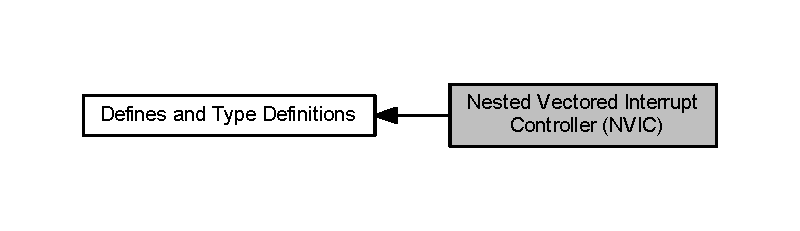
\includegraphics[width=350pt]{group___c_m_s_i_s___n_v_i_c}
\end{center}
\end{figure}
\subsection*{Classes}
\begin{DoxyCompactItemize}
\item 
struct \hyperlink{struct_n_v_i_c___type}{N\+V\+I\+C\+\_\+\+Type}
\begin{DoxyCompactList}\small\item\em Structure type to access the Nested Vectored Interrupt Controller (N\+V\+IC). \end{DoxyCompactList}\end{DoxyCompactItemize}
\subsection*{Macros}
\begin{DoxyCompactItemize}
\item 
\#define \hyperlink{group___c_m_s_i_s___n_v_i_c_ga9eebe495e2e48d302211108837a2b3e8}{N\+V\+I\+C\+\_\+\+S\+T\+I\+R\+\_\+\+I\+N\+T\+I\+D\+\_\+\+Pos}~0U
\item 
\#define \hyperlink{group___c_m_s_i_s___n_v_i_c_gae4060c4dfcebb08871ca4244176ce752}{N\+V\+I\+C\+\_\+\+S\+T\+I\+R\+\_\+\+I\+N\+T\+I\+D\+\_\+\+Msk}~(0x1\+F\+F\+U\+L /$\ast$$<$$<$ N\+V\+I\+C\+\_\+\+S\+T\+I\+R\+\_\+\+I\+N\+T\+I\+D\+\_\+\+Pos$\ast$/)
\item 
\#define \hyperlink{group___c_m_s_i_s___n_v_i_c_ga9eebe495e2e48d302211108837a2b3e8}{N\+V\+I\+C\+\_\+\+S\+T\+I\+R\+\_\+\+I\+N\+T\+I\+D\+\_\+\+Pos}~0U
\item 
\#define \hyperlink{group___c_m_s_i_s___n_v_i_c_gae4060c4dfcebb08871ca4244176ce752}{N\+V\+I\+C\+\_\+\+S\+T\+I\+R\+\_\+\+I\+N\+T\+I\+D\+\_\+\+Msk}~(0x1\+F\+F\+U\+L /$\ast$$<$$<$ N\+V\+I\+C\+\_\+\+S\+T\+I\+R\+\_\+\+I\+N\+T\+I\+D\+\_\+\+Pos$\ast$/)
\item 
\#define \hyperlink{group___c_m_s_i_s___n_v_i_c_ga9eebe495e2e48d302211108837a2b3e8}{N\+V\+I\+C\+\_\+\+S\+T\+I\+R\+\_\+\+I\+N\+T\+I\+D\+\_\+\+Pos}~0U
\item 
\#define \hyperlink{group___c_m_s_i_s___n_v_i_c_gae4060c4dfcebb08871ca4244176ce752}{N\+V\+I\+C\+\_\+\+S\+T\+I\+R\+\_\+\+I\+N\+T\+I\+D\+\_\+\+Msk}~(0x1\+F\+F\+U\+L /$\ast$$<$$<$ N\+V\+I\+C\+\_\+\+S\+T\+I\+R\+\_\+\+I\+N\+T\+I\+D\+\_\+\+Pos$\ast$/)
\item 
\#define \hyperlink{group___c_m_s_i_s___n_v_i_c_ga9eebe495e2e48d302211108837a2b3e8}{N\+V\+I\+C\+\_\+\+S\+T\+I\+R\+\_\+\+I\+N\+T\+I\+D\+\_\+\+Pos}~0U
\item 
\#define \hyperlink{group___c_m_s_i_s___n_v_i_c_gae4060c4dfcebb08871ca4244176ce752}{N\+V\+I\+C\+\_\+\+S\+T\+I\+R\+\_\+\+I\+N\+T\+I\+D\+\_\+\+Msk}~(0x1\+F\+F\+U\+L /$\ast$$<$$<$ N\+V\+I\+C\+\_\+\+S\+T\+I\+R\+\_\+\+I\+N\+T\+I\+D\+\_\+\+Pos$\ast$/)
\end{DoxyCompactItemize}


\subsection{Detailed Description}
Type definitions for the N\+V\+IC Registers. 



\subsection{Macro Definition Documentation}
\mbox{\Hypertarget{group___c_m_s_i_s___n_v_i_c_gae4060c4dfcebb08871ca4244176ce752}\label{group___c_m_s_i_s___n_v_i_c_gae4060c4dfcebb08871ca4244176ce752}} 
\index{Nested Vectored Interrupt Controller (\+N\+V\+I\+C)@{Nested Vectored Interrupt Controller (\+N\+V\+I\+C)}!N\+V\+I\+C\+\_\+\+S\+T\+I\+R\+\_\+\+I\+N\+T\+I\+D\+\_\+\+Msk@{N\+V\+I\+C\+\_\+\+S\+T\+I\+R\+\_\+\+I\+N\+T\+I\+D\+\_\+\+Msk}}
\index{N\+V\+I\+C\+\_\+\+S\+T\+I\+R\+\_\+\+I\+N\+T\+I\+D\+\_\+\+Msk@{N\+V\+I\+C\+\_\+\+S\+T\+I\+R\+\_\+\+I\+N\+T\+I\+D\+\_\+\+Msk}!Nested Vectored Interrupt Controller (\+N\+V\+I\+C)@{Nested Vectored Interrupt Controller (\+N\+V\+I\+C)}}
\subsubsection{\texorpdfstring{N\+V\+I\+C\+\_\+\+S\+T\+I\+R\+\_\+\+I\+N\+T\+I\+D\+\_\+\+Msk}{NVIC\_STIR\_INTID\_Msk}\hspace{0.1cm}{\footnotesize\ttfamily [1/4]}}
{\footnotesize\ttfamily \#define N\+V\+I\+C\+\_\+\+S\+T\+I\+R\+\_\+\+I\+N\+T\+I\+D\+\_\+\+Msk~(0x1\+F\+F\+U\+L /$\ast$$<$$<$ N\+V\+I\+C\+\_\+\+S\+T\+I\+R\+\_\+\+I\+N\+T\+I\+D\+\_\+\+Pos$\ast$/)}

S\+T\+IR\+: I\+N\+T\+L\+I\+N\+E\+S\+N\+UM Mask 

Definition at line 402 of file core\+\_\+sc300.\+h.

\mbox{\Hypertarget{group___c_m_s_i_s___n_v_i_c_gae4060c4dfcebb08871ca4244176ce752}\label{group___c_m_s_i_s___n_v_i_c_gae4060c4dfcebb08871ca4244176ce752}} 
\index{Nested Vectored Interrupt Controller (\+N\+V\+I\+C)@{Nested Vectored Interrupt Controller (\+N\+V\+I\+C)}!N\+V\+I\+C\+\_\+\+S\+T\+I\+R\+\_\+\+I\+N\+T\+I\+D\+\_\+\+Msk@{N\+V\+I\+C\+\_\+\+S\+T\+I\+R\+\_\+\+I\+N\+T\+I\+D\+\_\+\+Msk}}
\index{N\+V\+I\+C\+\_\+\+S\+T\+I\+R\+\_\+\+I\+N\+T\+I\+D\+\_\+\+Msk@{N\+V\+I\+C\+\_\+\+S\+T\+I\+R\+\_\+\+I\+N\+T\+I\+D\+\_\+\+Msk}!Nested Vectored Interrupt Controller (\+N\+V\+I\+C)@{Nested Vectored Interrupt Controller (\+N\+V\+I\+C)}}
\subsubsection{\texorpdfstring{N\+V\+I\+C\+\_\+\+S\+T\+I\+R\+\_\+\+I\+N\+T\+I\+D\+\_\+\+Msk}{NVIC\_STIR\_INTID\_Msk}\hspace{0.1cm}{\footnotesize\ttfamily [2/4]}}
{\footnotesize\ttfamily \#define N\+V\+I\+C\+\_\+\+S\+T\+I\+R\+\_\+\+I\+N\+T\+I\+D\+\_\+\+Msk~(0x1\+F\+F\+U\+L /$\ast$$<$$<$ N\+V\+I\+C\+\_\+\+S\+T\+I\+R\+\_\+\+I\+N\+T\+I\+D\+\_\+\+Pos$\ast$/)}

S\+T\+IR\+: I\+N\+T\+L\+I\+N\+E\+S\+N\+UM Mask 

Definition at line 410 of file core\+\_\+cm3.\+h.

\mbox{\Hypertarget{group___c_m_s_i_s___n_v_i_c_gae4060c4dfcebb08871ca4244176ce752}\label{group___c_m_s_i_s___n_v_i_c_gae4060c4dfcebb08871ca4244176ce752}} 
\index{Nested Vectored Interrupt Controller (\+N\+V\+I\+C)@{Nested Vectored Interrupt Controller (\+N\+V\+I\+C)}!N\+V\+I\+C\+\_\+\+S\+T\+I\+R\+\_\+\+I\+N\+T\+I\+D\+\_\+\+Msk@{N\+V\+I\+C\+\_\+\+S\+T\+I\+R\+\_\+\+I\+N\+T\+I\+D\+\_\+\+Msk}}
\index{N\+V\+I\+C\+\_\+\+S\+T\+I\+R\+\_\+\+I\+N\+T\+I\+D\+\_\+\+Msk@{N\+V\+I\+C\+\_\+\+S\+T\+I\+R\+\_\+\+I\+N\+T\+I\+D\+\_\+\+Msk}!Nested Vectored Interrupt Controller (\+N\+V\+I\+C)@{Nested Vectored Interrupt Controller (\+N\+V\+I\+C)}}
\subsubsection{\texorpdfstring{N\+V\+I\+C\+\_\+\+S\+T\+I\+R\+\_\+\+I\+N\+T\+I\+D\+\_\+\+Msk}{NVIC\_STIR\_INTID\_Msk}\hspace{0.1cm}{\footnotesize\ttfamily [3/4]}}
{\footnotesize\ttfamily \#define N\+V\+I\+C\+\_\+\+S\+T\+I\+R\+\_\+\+I\+N\+T\+I\+D\+\_\+\+Msk~(0x1\+F\+F\+U\+L /$\ast$$<$$<$ N\+V\+I\+C\+\_\+\+S\+T\+I\+R\+\_\+\+I\+N\+T\+I\+D\+\_\+\+Pos$\ast$/)}

S\+T\+IR\+: I\+N\+T\+L\+I\+N\+E\+S\+N\+UM Mask 

Definition at line 478 of file core\+\_\+cm4.\+h.

\mbox{\Hypertarget{group___c_m_s_i_s___n_v_i_c_gae4060c4dfcebb08871ca4244176ce752}\label{group___c_m_s_i_s___n_v_i_c_gae4060c4dfcebb08871ca4244176ce752}} 
\index{Nested Vectored Interrupt Controller (\+N\+V\+I\+C)@{Nested Vectored Interrupt Controller (\+N\+V\+I\+C)}!N\+V\+I\+C\+\_\+\+S\+T\+I\+R\+\_\+\+I\+N\+T\+I\+D\+\_\+\+Msk@{N\+V\+I\+C\+\_\+\+S\+T\+I\+R\+\_\+\+I\+N\+T\+I\+D\+\_\+\+Msk}}
\index{N\+V\+I\+C\+\_\+\+S\+T\+I\+R\+\_\+\+I\+N\+T\+I\+D\+\_\+\+Msk@{N\+V\+I\+C\+\_\+\+S\+T\+I\+R\+\_\+\+I\+N\+T\+I\+D\+\_\+\+Msk}!Nested Vectored Interrupt Controller (\+N\+V\+I\+C)@{Nested Vectored Interrupt Controller (\+N\+V\+I\+C)}}
\subsubsection{\texorpdfstring{N\+V\+I\+C\+\_\+\+S\+T\+I\+R\+\_\+\+I\+N\+T\+I\+D\+\_\+\+Msk}{NVIC\_STIR\_INTID\_Msk}\hspace{0.1cm}{\footnotesize\ttfamily [4/4]}}
{\footnotesize\ttfamily \#define N\+V\+I\+C\+\_\+\+S\+T\+I\+R\+\_\+\+I\+N\+T\+I\+D\+\_\+\+Msk~(0x1\+F\+F\+U\+L /$\ast$$<$$<$ N\+V\+I\+C\+\_\+\+S\+T\+I\+R\+\_\+\+I\+N\+T\+I\+D\+\_\+\+Pos$\ast$/)}

S\+T\+IR\+: I\+N\+T\+L\+I\+N\+E\+S\+N\+UM Mask 

Definition at line 493 of file core\+\_\+cm7.\+h.

\mbox{\Hypertarget{group___c_m_s_i_s___n_v_i_c_ga9eebe495e2e48d302211108837a2b3e8}\label{group___c_m_s_i_s___n_v_i_c_ga9eebe495e2e48d302211108837a2b3e8}} 
\index{Nested Vectored Interrupt Controller (\+N\+V\+I\+C)@{Nested Vectored Interrupt Controller (\+N\+V\+I\+C)}!N\+V\+I\+C\+\_\+\+S\+T\+I\+R\+\_\+\+I\+N\+T\+I\+D\+\_\+\+Pos@{N\+V\+I\+C\+\_\+\+S\+T\+I\+R\+\_\+\+I\+N\+T\+I\+D\+\_\+\+Pos}}
\index{N\+V\+I\+C\+\_\+\+S\+T\+I\+R\+\_\+\+I\+N\+T\+I\+D\+\_\+\+Pos@{N\+V\+I\+C\+\_\+\+S\+T\+I\+R\+\_\+\+I\+N\+T\+I\+D\+\_\+\+Pos}!Nested Vectored Interrupt Controller (\+N\+V\+I\+C)@{Nested Vectored Interrupt Controller (\+N\+V\+I\+C)}}
\subsubsection{\texorpdfstring{N\+V\+I\+C\+\_\+\+S\+T\+I\+R\+\_\+\+I\+N\+T\+I\+D\+\_\+\+Pos}{NVIC\_STIR\_INTID\_Pos}\hspace{0.1cm}{\footnotesize\ttfamily [1/4]}}
{\footnotesize\ttfamily \#define N\+V\+I\+C\+\_\+\+S\+T\+I\+R\+\_\+\+I\+N\+T\+I\+D\+\_\+\+Pos~0U}

S\+T\+IR\+: I\+N\+T\+L\+I\+N\+E\+S\+N\+UM Position 

Definition at line 401 of file core\+\_\+sc300.\+h.

\mbox{\Hypertarget{group___c_m_s_i_s___n_v_i_c_ga9eebe495e2e48d302211108837a2b3e8}\label{group___c_m_s_i_s___n_v_i_c_ga9eebe495e2e48d302211108837a2b3e8}} 
\index{Nested Vectored Interrupt Controller (\+N\+V\+I\+C)@{Nested Vectored Interrupt Controller (\+N\+V\+I\+C)}!N\+V\+I\+C\+\_\+\+S\+T\+I\+R\+\_\+\+I\+N\+T\+I\+D\+\_\+\+Pos@{N\+V\+I\+C\+\_\+\+S\+T\+I\+R\+\_\+\+I\+N\+T\+I\+D\+\_\+\+Pos}}
\index{N\+V\+I\+C\+\_\+\+S\+T\+I\+R\+\_\+\+I\+N\+T\+I\+D\+\_\+\+Pos@{N\+V\+I\+C\+\_\+\+S\+T\+I\+R\+\_\+\+I\+N\+T\+I\+D\+\_\+\+Pos}!Nested Vectored Interrupt Controller (\+N\+V\+I\+C)@{Nested Vectored Interrupt Controller (\+N\+V\+I\+C)}}
\subsubsection{\texorpdfstring{N\+V\+I\+C\+\_\+\+S\+T\+I\+R\+\_\+\+I\+N\+T\+I\+D\+\_\+\+Pos}{NVIC\_STIR\_INTID\_Pos}\hspace{0.1cm}{\footnotesize\ttfamily [2/4]}}
{\footnotesize\ttfamily \#define N\+V\+I\+C\+\_\+\+S\+T\+I\+R\+\_\+\+I\+N\+T\+I\+D\+\_\+\+Pos~0U}

S\+T\+IR\+: I\+N\+T\+L\+I\+N\+E\+S\+N\+UM Position 

Definition at line 409 of file core\+\_\+cm3.\+h.

\mbox{\Hypertarget{group___c_m_s_i_s___n_v_i_c_ga9eebe495e2e48d302211108837a2b3e8}\label{group___c_m_s_i_s___n_v_i_c_ga9eebe495e2e48d302211108837a2b3e8}} 
\index{Nested Vectored Interrupt Controller (\+N\+V\+I\+C)@{Nested Vectored Interrupt Controller (\+N\+V\+I\+C)}!N\+V\+I\+C\+\_\+\+S\+T\+I\+R\+\_\+\+I\+N\+T\+I\+D\+\_\+\+Pos@{N\+V\+I\+C\+\_\+\+S\+T\+I\+R\+\_\+\+I\+N\+T\+I\+D\+\_\+\+Pos}}
\index{N\+V\+I\+C\+\_\+\+S\+T\+I\+R\+\_\+\+I\+N\+T\+I\+D\+\_\+\+Pos@{N\+V\+I\+C\+\_\+\+S\+T\+I\+R\+\_\+\+I\+N\+T\+I\+D\+\_\+\+Pos}!Nested Vectored Interrupt Controller (\+N\+V\+I\+C)@{Nested Vectored Interrupt Controller (\+N\+V\+I\+C)}}
\subsubsection{\texorpdfstring{N\+V\+I\+C\+\_\+\+S\+T\+I\+R\+\_\+\+I\+N\+T\+I\+D\+\_\+\+Pos}{NVIC\_STIR\_INTID\_Pos}\hspace{0.1cm}{\footnotesize\ttfamily [3/4]}}
{\footnotesize\ttfamily \#define N\+V\+I\+C\+\_\+\+S\+T\+I\+R\+\_\+\+I\+N\+T\+I\+D\+\_\+\+Pos~0U}

S\+T\+IR\+: I\+N\+T\+L\+I\+N\+E\+S\+N\+UM Position 

Definition at line 477 of file core\+\_\+cm4.\+h.

\mbox{\Hypertarget{group___c_m_s_i_s___n_v_i_c_ga9eebe495e2e48d302211108837a2b3e8}\label{group___c_m_s_i_s___n_v_i_c_ga9eebe495e2e48d302211108837a2b3e8}} 
\index{Nested Vectored Interrupt Controller (\+N\+V\+I\+C)@{Nested Vectored Interrupt Controller (\+N\+V\+I\+C)}!N\+V\+I\+C\+\_\+\+S\+T\+I\+R\+\_\+\+I\+N\+T\+I\+D\+\_\+\+Pos@{N\+V\+I\+C\+\_\+\+S\+T\+I\+R\+\_\+\+I\+N\+T\+I\+D\+\_\+\+Pos}}
\index{N\+V\+I\+C\+\_\+\+S\+T\+I\+R\+\_\+\+I\+N\+T\+I\+D\+\_\+\+Pos@{N\+V\+I\+C\+\_\+\+S\+T\+I\+R\+\_\+\+I\+N\+T\+I\+D\+\_\+\+Pos}!Nested Vectored Interrupt Controller (\+N\+V\+I\+C)@{Nested Vectored Interrupt Controller (\+N\+V\+I\+C)}}
\subsubsection{\texorpdfstring{N\+V\+I\+C\+\_\+\+S\+T\+I\+R\+\_\+\+I\+N\+T\+I\+D\+\_\+\+Pos}{NVIC\_STIR\_INTID\_Pos}\hspace{0.1cm}{\footnotesize\ttfamily [4/4]}}
{\footnotesize\ttfamily \#define N\+V\+I\+C\+\_\+\+S\+T\+I\+R\+\_\+\+I\+N\+T\+I\+D\+\_\+\+Pos~0U}

S\+T\+IR\+: I\+N\+T\+L\+I\+N\+E\+S\+N\+UM Position 

Definition at line 492 of file core\+\_\+cm7.\+h.


\hypertarget{group___c_m_s_i_s___s_c_b}{}\section{System Control Block (S\+CB)}
\label{group___c_m_s_i_s___s_c_b}\index{System Control Block (\+S\+C\+B)@{System Control Block (\+S\+C\+B)}}


Type definitions for the System Control Block Registers.  


Collaboration diagram for System Control Block (S\+CB)\+:
\nopagebreak
\begin{figure}[H]
\begin{center}
\leavevmode
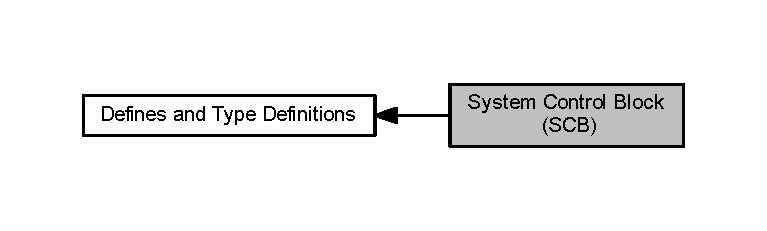
\includegraphics[width=350pt]{group___c_m_s_i_s___s_c_b}
\end{center}
\end{figure}
\subsection*{Classes}
\begin{DoxyCompactItemize}
\item 
struct \hyperlink{struct_s_c_b___type}{S\+C\+B\+\_\+\+Type}
\begin{DoxyCompactList}\small\item\em Structure type to access the System Control Block (S\+CB). \end{DoxyCompactList}\end{DoxyCompactItemize}
\subsection*{Macros}
\begin{DoxyCompactItemize}
\item 
\#define \hyperlink{group___c_m_s_i_s___s_c_b_ga58686b88f94f789d4e6f429fe1ff58cf}{S\+C\+B\+\_\+\+C\+P\+U\+I\+D\+\_\+\+I\+M\+P\+L\+E\+M\+E\+N\+T\+E\+R\+\_\+\+Pos}~24U
\item 
\#define \hyperlink{group___c_m_s_i_s___s_c_b_ga0932b31faafd47656a03ced75a31d99b}{S\+C\+B\+\_\+\+C\+P\+U\+I\+D\+\_\+\+I\+M\+P\+L\+E\+M\+E\+N\+T\+E\+R\+\_\+\+Msk}~(0x\+F\+F\+U\+L $<$$<$ S\+C\+B\+\_\+\+C\+P\+U\+I\+D\+\_\+\+I\+M\+P\+L\+E\+M\+E\+N\+T\+E\+R\+\_\+\+Pos)
\item 
\#define \hyperlink{group___c_m_s_i_s___s_c_b_ga104462bd0815391b4044a70bd15d3a71}{S\+C\+B\+\_\+\+C\+P\+U\+I\+D\+\_\+\+V\+A\+R\+I\+A\+N\+T\+\_\+\+Pos}~20U
\item 
\#define \hyperlink{group___c_m_s_i_s___s_c_b_gad358dfbd04300afc1824329d128b99e8}{S\+C\+B\+\_\+\+C\+P\+U\+I\+D\+\_\+\+V\+A\+R\+I\+A\+N\+T\+\_\+\+Msk}~(0x\+F\+U\+L $<$$<$ S\+C\+B\+\_\+\+C\+P\+U\+I\+D\+\_\+\+V\+A\+R\+I\+A\+N\+T\+\_\+\+Pos)
\item 
\#define \hyperlink{group___c_m_s_i_s___s_c_b_gaf8b3236b08fb8e840efb682645fb0e98}{S\+C\+B\+\_\+\+C\+P\+U\+I\+D\+\_\+\+A\+R\+C\+H\+I\+T\+E\+C\+T\+U\+R\+E\+\_\+\+Pos}~16U
\item 
\#define \hyperlink{group___c_m_s_i_s___s_c_b_gafae4a1f27a927338ae9dc51a0e146213}{S\+C\+B\+\_\+\+C\+P\+U\+I\+D\+\_\+\+A\+R\+C\+H\+I\+T\+E\+C\+T\+U\+R\+E\+\_\+\+Msk}~(0x\+F\+U\+L $<$$<$ S\+C\+B\+\_\+\+C\+P\+U\+I\+D\+\_\+\+A\+R\+C\+H\+I\+T\+E\+C\+T\+U\+R\+E\+\_\+\+Pos)
\item 
\#define \hyperlink{group___c_m_s_i_s___s_c_b_ga705f68eaa9afb042ca2407dc4e4629ac}{S\+C\+B\+\_\+\+C\+P\+U\+I\+D\+\_\+\+P\+A\+R\+T\+N\+O\+\_\+\+Pos}~4U
\item 
\#define \hyperlink{group___c_m_s_i_s___s_c_b_ga98e581423ca016680c238c469aba546d}{S\+C\+B\+\_\+\+C\+P\+U\+I\+D\+\_\+\+P\+A\+R\+T\+N\+O\+\_\+\+Msk}~(0x\+F\+F\+F\+U\+L $<$$<$ S\+C\+B\+\_\+\+C\+P\+U\+I\+D\+\_\+\+P\+A\+R\+T\+N\+O\+\_\+\+Pos)
\item 
\#define \hyperlink{group___c_m_s_i_s___s_c_b_ga3c3d9071e574de11fb27ba57034838b1}{S\+C\+B\+\_\+\+C\+P\+U\+I\+D\+\_\+\+R\+E\+V\+I\+S\+I\+O\+N\+\_\+\+Pos}~0U
\item 
\#define \hyperlink{group___c_m_s_i_s___s_c_b_ga2ec0448b6483f77e7f5d08b4b81d85df}{S\+C\+B\+\_\+\+C\+P\+U\+I\+D\+\_\+\+R\+E\+V\+I\+S\+I\+O\+N\+\_\+\+Msk}~(0x\+F\+U\+L /$\ast$$<$$<$ S\+C\+B\+\_\+\+C\+P\+U\+I\+D\+\_\+\+R\+E\+V\+I\+S\+I\+O\+N\+\_\+\+Pos$\ast$/)
\item 
\#define \hyperlink{group___c_m_s_i_s___s_c_b_ga750d4b52624a46d71356db4ea769573b}{S\+C\+B\+\_\+\+I\+C\+S\+R\+\_\+\+N\+M\+I\+P\+E\+N\+D\+S\+E\+T\+\_\+\+Pos}~31U
\item 
\#define \hyperlink{group___c_m_s_i_s___s_c_b_ga340e3f79e9c3607dee9f2c048b6b22e8}{S\+C\+B\+\_\+\+I\+C\+S\+R\+\_\+\+N\+M\+I\+P\+E\+N\+D\+S\+E\+T\+\_\+\+Msk}~(1\+U\+L $<$$<$ S\+C\+B\+\_\+\+I\+C\+S\+R\+\_\+\+N\+M\+I\+P\+E\+N\+D\+S\+E\+T\+\_\+\+Pos)
\item 
\#define \hyperlink{group___c_m_s_i_s___s_c_b_gab5ded23d2ab1d5ff7cc7ce746205e9fe}{S\+C\+B\+\_\+\+I\+C\+S\+R\+\_\+\+P\+E\+N\+D\+S\+V\+S\+E\+T\+\_\+\+Pos}~28U
\item 
\#define \hyperlink{group___c_m_s_i_s___s_c_b_ga1e40d93efb402763c8c00ddcc56724ff}{S\+C\+B\+\_\+\+I\+C\+S\+R\+\_\+\+P\+E\+N\+D\+S\+V\+S\+E\+T\+\_\+\+Msk}~(1\+U\+L $<$$<$ S\+C\+B\+\_\+\+I\+C\+S\+R\+\_\+\+P\+E\+N\+D\+S\+V\+S\+E\+T\+\_\+\+Pos)
\item 
\#define \hyperlink{group___c_m_s_i_s___s_c_b_gae218d9022288f89faf57187c4d542ecd}{S\+C\+B\+\_\+\+I\+C\+S\+R\+\_\+\+P\+E\+N\+D\+S\+V\+C\+L\+R\+\_\+\+Pos}~27U
\item 
\#define \hyperlink{group___c_m_s_i_s___s_c_b_ga4a901ace381d3c1c74ac82b22fae2e1e}{S\+C\+B\+\_\+\+I\+C\+S\+R\+\_\+\+P\+E\+N\+D\+S\+V\+C\+L\+R\+\_\+\+Msk}~(1\+U\+L $<$$<$ S\+C\+B\+\_\+\+I\+C\+S\+R\+\_\+\+P\+E\+N\+D\+S\+V\+C\+L\+R\+\_\+\+Pos)
\item 
\#define \hyperlink{group___c_m_s_i_s___s_c_b_ga9dbb3358c6167c9c3f85661b90fb2794}{S\+C\+B\+\_\+\+I\+C\+S\+R\+\_\+\+P\+E\+N\+D\+S\+T\+S\+E\+T\+\_\+\+Pos}~26U
\item 
\#define \hyperlink{group___c_m_s_i_s___s_c_b_ga7325b61ea0ec323ef2d5c893b112e546}{S\+C\+B\+\_\+\+I\+C\+S\+R\+\_\+\+P\+E\+N\+D\+S\+T\+S\+E\+T\+\_\+\+Msk}~(1\+U\+L $<$$<$ S\+C\+B\+\_\+\+I\+C\+S\+R\+\_\+\+P\+E\+N\+D\+S\+T\+S\+E\+T\+\_\+\+Pos)
\item 
\#define \hyperlink{group___c_m_s_i_s___s_c_b_gadbe25e4b333ece1341beb1a740168fdc}{S\+C\+B\+\_\+\+I\+C\+S\+R\+\_\+\+P\+E\+N\+D\+S\+T\+C\+L\+R\+\_\+\+Pos}~25U
\item 
\#define \hyperlink{group___c_m_s_i_s___s_c_b_gab241827d2a793269d8cd99b9b28c2157}{S\+C\+B\+\_\+\+I\+C\+S\+R\+\_\+\+P\+E\+N\+D\+S\+T\+C\+L\+R\+\_\+\+Msk}~(1\+U\+L $<$$<$ S\+C\+B\+\_\+\+I\+C\+S\+R\+\_\+\+P\+E\+N\+D\+S\+T\+C\+L\+R\+\_\+\+Pos)
\item 
\#define \hyperlink{group___c_m_s_i_s___s_c_b_ga11cb5b1f9ce167b81f31787a77e575df}{S\+C\+B\+\_\+\+I\+C\+S\+R\+\_\+\+I\+S\+R\+P\+R\+E\+E\+M\+P\+T\+\_\+\+Pos}~23U
\item 
\#define \hyperlink{group___c_m_s_i_s___s_c_b_gaa966600396290808d596fe96e92ca2b5}{S\+C\+B\+\_\+\+I\+C\+S\+R\+\_\+\+I\+S\+R\+P\+R\+E\+E\+M\+P\+T\+\_\+\+Msk}~(1\+U\+L $<$$<$ S\+C\+B\+\_\+\+I\+C\+S\+R\+\_\+\+I\+S\+R\+P\+R\+E\+E\+M\+P\+T\+\_\+\+Pos)
\item 
\#define \hyperlink{group___c_m_s_i_s___s_c_b_ga10749d92b9b744094b845c2eb46d4319}{S\+C\+B\+\_\+\+I\+C\+S\+R\+\_\+\+I\+S\+R\+P\+E\+N\+D\+I\+N\+G\+\_\+\+Pos}~22U
\item 
\#define \hyperlink{group___c_m_s_i_s___s_c_b_ga056d74fd538e5d36d3be1f28d399c877}{S\+C\+B\+\_\+\+I\+C\+S\+R\+\_\+\+I\+S\+R\+P\+E\+N\+D\+I\+N\+G\+\_\+\+Msk}~(1\+U\+L $<$$<$ S\+C\+B\+\_\+\+I\+C\+S\+R\+\_\+\+I\+S\+R\+P\+E\+N\+D\+I\+N\+G\+\_\+\+Pos)
\item 
\#define \hyperlink{group___c_m_s_i_s___s_c_b_gada60c92bf88d6fd21a8f49efa4a127b8}{S\+C\+B\+\_\+\+I\+C\+S\+R\+\_\+\+V\+E\+C\+T\+P\+E\+N\+D\+I\+N\+G\+\_\+\+Pos}~12U
\item 
\#define \hyperlink{group___c_m_s_i_s___s_c_b_gacb6992e7c7ddc27a370f62878a21ef72}{S\+C\+B\+\_\+\+I\+C\+S\+R\+\_\+\+V\+E\+C\+T\+P\+E\+N\+D\+I\+N\+G\+\_\+\+Msk}~(0x1\+F\+F\+U\+L $<$$<$ S\+C\+B\+\_\+\+I\+C\+S\+R\+\_\+\+V\+E\+C\+T\+P\+E\+N\+D\+I\+N\+G\+\_\+\+Pos)
\item 
\#define \hyperlink{group___c_m_s_i_s___s_c_b_gae4f602c7c5c895d5fb687b71b0979fc3}{S\+C\+B\+\_\+\+I\+C\+S\+R\+\_\+\+V\+E\+C\+T\+A\+C\+T\+I\+V\+E\+\_\+\+Pos}~0U
\item 
\#define \hyperlink{group___c_m_s_i_s___s_c_b_ga5533791a4ecf1b9301c883047b3e8396}{S\+C\+B\+\_\+\+I\+C\+S\+R\+\_\+\+V\+E\+C\+T\+A\+C\+T\+I\+V\+E\+\_\+\+Msk}~(0x1\+F\+F\+U\+L /$\ast$$<$$<$ S\+C\+B\+\_\+\+I\+C\+S\+R\+\_\+\+V\+E\+C\+T\+A\+C\+T\+I\+V\+E\+\_\+\+Pos$\ast$/)
\item 
\#define \hyperlink{group___c_m_s_i_s___s_c_b_gaaa27c0ba600bf82c3da08c748845b640}{S\+C\+B\+\_\+\+A\+I\+R\+C\+R\+\_\+\+V\+E\+C\+T\+K\+E\+Y\+\_\+\+Pos}~16U
\item 
\#define \hyperlink{group___c_m_s_i_s___s_c_b_ga90c7cf0c490e7ae55f9503a7fda1dd22}{S\+C\+B\+\_\+\+A\+I\+R\+C\+R\+\_\+\+V\+E\+C\+T\+K\+E\+Y\+\_\+\+Msk}~(0x\+F\+F\+F\+F\+U\+L $<$$<$ S\+C\+B\+\_\+\+A\+I\+R\+C\+R\+\_\+\+V\+E\+C\+T\+K\+E\+Y\+\_\+\+Pos)
\item 
\#define \hyperlink{group___c_m_s_i_s___s_c_b_gaec404750ff5ca07f499a3c06b62051ef}{S\+C\+B\+\_\+\+A\+I\+R\+C\+R\+\_\+\+V\+E\+C\+T\+K\+E\+Y\+S\+T\+A\+T\+\_\+\+Pos}~16U
\item 
\#define \hyperlink{group___c_m_s_i_s___s_c_b_gabacedaefeefc73d666bbe59ece904493}{S\+C\+B\+\_\+\+A\+I\+R\+C\+R\+\_\+\+V\+E\+C\+T\+K\+E\+Y\+S\+T\+A\+T\+\_\+\+Msk}~(0x\+F\+F\+F\+F\+U\+L $<$$<$ S\+C\+B\+\_\+\+A\+I\+R\+C\+R\+\_\+\+V\+E\+C\+T\+K\+E\+Y\+S\+T\+A\+T\+\_\+\+Pos)
\item 
\#define \hyperlink{group___c_m_s_i_s___s_c_b_gad31dec98fbc0d33ace63cb1f1a927923}{S\+C\+B\+\_\+\+A\+I\+R\+C\+R\+\_\+\+E\+N\+D\+I\+A\+N\+E\+S\+S\+\_\+\+Pos}~15U
\item 
\#define \hyperlink{group___c_m_s_i_s___s_c_b_ga2f571f93d3d4a6eac9a3040756d3d951}{S\+C\+B\+\_\+\+A\+I\+R\+C\+R\+\_\+\+E\+N\+D\+I\+A\+N\+E\+S\+S\+\_\+\+Msk}~(1\+U\+L $<$$<$ S\+C\+B\+\_\+\+A\+I\+R\+C\+R\+\_\+\+E\+N\+D\+I\+A\+N\+E\+S\+S\+\_\+\+Pos)
\item 
\#define \hyperlink{group___c_m_s_i_s___s_c_b_gaffb2737eca1eac0fc1c282a76a40953c}{S\+C\+B\+\_\+\+A\+I\+R\+C\+R\+\_\+\+S\+Y\+S\+R\+E\+S\+E\+T\+R\+E\+Q\+\_\+\+Pos}~2U
\item 
\#define \hyperlink{group___c_m_s_i_s___s_c_b_gaae1181119559a5bd36e62afa373fa720}{S\+C\+B\+\_\+\+A\+I\+R\+C\+R\+\_\+\+S\+Y\+S\+R\+E\+S\+E\+T\+R\+E\+Q\+\_\+\+Msk}~(1\+U\+L $<$$<$ S\+C\+B\+\_\+\+A\+I\+R\+C\+R\+\_\+\+S\+Y\+S\+R\+E\+S\+E\+T\+R\+E\+Q\+\_\+\+Pos)
\item 
\#define \hyperlink{group___c_m_s_i_s___s_c_b_gaa30a12e892bb696e61626d71359a9029}{S\+C\+B\+\_\+\+A\+I\+R\+C\+R\+\_\+\+V\+E\+C\+T\+C\+L\+R\+A\+C\+T\+I\+V\+E\+\_\+\+Pos}~1U
\item 
\#define \hyperlink{group___c_m_s_i_s___s_c_b_ga212c5ab1c1c82c807d30d2307aa8d218}{S\+C\+B\+\_\+\+A\+I\+R\+C\+R\+\_\+\+V\+E\+C\+T\+C\+L\+R\+A\+C\+T\+I\+V\+E\+\_\+\+Msk}~(1\+U\+L $<$$<$ S\+C\+B\+\_\+\+A\+I\+R\+C\+R\+\_\+\+V\+E\+C\+T\+C\+L\+R\+A\+C\+T\+I\+V\+E\+\_\+\+Pos)
\item 
\#define \hyperlink{group___c_m_s_i_s___s_c_b_ga3bddcec40aeaf3d3a998446100fa0e44}{S\+C\+B\+\_\+\+S\+C\+R\+\_\+\+S\+E\+V\+O\+N\+P\+E\+N\+D\+\_\+\+Pos}~4U
\item 
\#define \hyperlink{group___c_m_s_i_s___s_c_b_gafb98656644a14342e467505f69a997c9}{S\+C\+B\+\_\+\+S\+C\+R\+\_\+\+S\+E\+V\+O\+N\+P\+E\+N\+D\+\_\+\+Msk}~(1\+U\+L $<$$<$ S\+C\+B\+\_\+\+S\+C\+R\+\_\+\+S\+E\+V\+O\+N\+P\+E\+N\+D\+\_\+\+Pos)
\item 
\#define \hyperlink{group___c_m_s_i_s___s_c_b_gab304f6258ec03bd9a6e7a360515c3cfe}{S\+C\+B\+\_\+\+S\+C\+R\+\_\+\+S\+L\+E\+E\+P\+D\+E\+E\+P\+\_\+\+Pos}~2U
\item 
\#define \hyperlink{group___c_m_s_i_s___s_c_b_ga77c06a69c63f4b3f6ec1032e911e18e7}{S\+C\+B\+\_\+\+S\+C\+R\+\_\+\+S\+L\+E\+E\+P\+D\+E\+E\+P\+\_\+\+Msk}~(1\+U\+L $<$$<$ S\+C\+B\+\_\+\+S\+C\+R\+\_\+\+S\+L\+E\+E\+P\+D\+E\+E\+P\+\_\+\+Pos)
\item 
\#define \hyperlink{group___c_m_s_i_s___s_c_b_ga3680a15114d7fdc1e25043b881308fe9}{S\+C\+B\+\_\+\+S\+C\+R\+\_\+\+S\+L\+E\+E\+P\+O\+N\+E\+X\+I\+T\+\_\+\+Pos}~1U
\item 
\#define \hyperlink{group___c_m_s_i_s___s_c_b_ga50a243e317b9a70781b02758d45b05ee}{S\+C\+B\+\_\+\+S\+C\+R\+\_\+\+S\+L\+E\+E\+P\+O\+N\+E\+X\+I\+T\+\_\+\+Msk}~(1\+U\+L $<$$<$ S\+C\+B\+\_\+\+S\+C\+R\+\_\+\+S\+L\+E\+E\+P\+O\+N\+E\+X\+I\+T\+\_\+\+Pos)
\item 
\#define \hyperlink{group___c_m_s_i_s___s_c_b_gac2d20a250960a432cc74da59d20e2f86}{S\+C\+B\+\_\+\+C\+C\+R\+\_\+\+S\+T\+K\+A\+L\+I\+G\+N\+\_\+\+Pos}~9U
\item 
\#define \hyperlink{group___c_m_s_i_s___s_c_b_ga33cf22d3d46af158a03aad25ddea1bcb}{S\+C\+B\+\_\+\+C\+C\+R\+\_\+\+S\+T\+K\+A\+L\+I\+G\+N\+\_\+\+Msk}~(1\+U\+L $<$$<$ S\+C\+B\+\_\+\+C\+C\+R\+\_\+\+S\+T\+K\+A\+L\+I\+G\+N\+\_\+\+Pos)
\item 
\#define \hyperlink{group___c_m_s_i_s___s_c_b_gac4e4928b864ea10fc24dbbc57d976229}{S\+C\+B\+\_\+\+C\+C\+R\+\_\+\+U\+N\+A\+L\+I\+G\+N\+\_\+\+T\+R\+P\+\_\+\+Pos}~3U
\item 
\#define \hyperlink{group___c_m_s_i_s___s_c_b_ga68c96ad594af70c007923979085c99e0}{S\+C\+B\+\_\+\+C\+C\+R\+\_\+\+U\+N\+A\+L\+I\+G\+N\+\_\+\+T\+R\+P\+\_\+\+Msk}~(1\+U\+L $<$$<$ S\+C\+B\+\_\+\+C\+C\+R\+\_\+\+U\+N\+A\+L\+I\+G\+N\+\_\+\+T\+R\+P\+\_\+\+Pos)
\item 
\#define \hyperlink{group___c_m_s_i_s___s_c_b_ga2f93ec9b243f94cdd3e94b8f0bf43641}{S\+C\+B\+\_\+\+S\+H\+C\+S\+R\+\_\+\+S\+V\+C\+A\+L\+L\+P\+E\+N\+D\+E\+D\+\_\+\+Pos}~15U
\item 
\#define \hyperlink{group___c_m_s_i_s___s_c_b_ga6095a7acfbad66f52822b1392be88652}{S\+C\+B\+\_\+\+S\+H\+C\+S\+R\+\_\+\+S\+V\+C\+A\+L\+L\+P\+E\+N\+D\+E\+D\+\_\+\+Msk}~(1\+U\+L $<$$<$ S\+C\+B\+\_\+\+S\+H\+C\+S\+R\+\_\+\+S\+V\+C\+A\+L\+L\+P\+E\+N\+D\+E\+D\+\_\+\+Pos)
\item 
\#define \hyperlink{group___c_m_s_i_s___s_c_b_ga58686b88f94f789d4e6f429fe1ff58cf}{S\+C\+B\+\_\+\+C\+P\+U\+I\+D\+\_\+\+I\+M\+P\+L\+E\+M\+E\+N\+T\+E\+R\+\_\+\+Pos}~24U
\item 
\#define \hyperlink{group___c_m_s_i_s___s_c_b_ga0932b31faafd47656a03ced75a31d99b}{S\+C\+B\+\_\+\+C\+P\+U\+I\+D\+\_\+\+I\+M\+P\+L\+E\+M\+E\+N\+T\+E\+R\+\_\+\+Msk}~(0x\+F\+F\+U\+L $<$$<$ S\+C\+B\+\_\+\+C\+P\+U\+I\+D\+\_\+\+I\+M\+P\+L\+E\+M\+E\+N\+T\+E\+R\+\_\+\+Pos)
\item 
\#define \hyperlink{group___c_m_s_i_s___s_c_b_ga104462bd0815391b4044a70bd15d3a71}{S\+C\+B\+\_\+\+C\+P\+U\+I\+D\+\_\+\+V\+A\+R\+I\+A\+N\+T\+\_\+\+Pos}~20U
\item 
\#define \hyperlink{group___c_m_s_i_s___s_c_b_gad358dfbd04300afc1824329d128b99e8}{S\+C\+B\+\_\+\+C\+P\+U\+I\+D\+\_\+\+V\+A\+R\+I\+A\+N\+T\+\_\+\+Msk}~(0x\+F\+U\+L $<$$<$ S\+C\+B\+\_\+\+C\+P\+U\+I\+D\+\_\+\+V\+A\+R\+I\+A\+N\+T\+\_\+\+Pos)
\item 
\#define \hyperlink{group___c_m_s_i_s___s_c_b_gaf8b3236b08fb8e840efb682645fb0e98}{S\+C\+B\+\_\+\+C\+P\+U\+I\+D\+\_\+\+A\+R\+C\+H\+I\+T\+E\+C\+T\+U\+R\+E\+\_\+\+Pos}~16U
\item 
\#define \hyperlink{group___c_m_s_i_s___s_c_b_gafae4a1f27a927338ae9dc51a0e146213}{S\+C\+B\+\_\+\+C\+P\+U\+I\+D\+\_\+\+A\+R\+C\+H\+I\+T\+E\+C\+T\+U\+R\+E\+\_\+\+Msk}~(0x\+F\+U\+L $<$$<$ S\+C\+B\+\_\+\+C\+P\+U\+I\+D\+\_\+\+A\+R\+C\+H\+I\+T\+E\+C\+T\+U\+R\+E\+\_\+\+Pos)
\item 
\#define \hyperlink{group___c_m_s_i_s___s_c_b_ga705f68eaa9afb042ca2407dc4e4629ac}{S\+C\+B\+\_\+\+C\+P\+U\+I\+D\+\_\+\+P\+A\+R\+T\+N\+O\+\_\+\+Pos}~4U
\item 
\#define \hyperlink{group___c_m_s_i_s___s_c_b_ga98e581423ca016680c238c469aba546d}{S\+C\+B\+\_\+\+C\+P\+U\+I\+D\+\_\+\+P\+A\+R\+T\+N\+O\+\_\+\+Msk}~(0x\+F\+F\+F\+U\+L $<$$<$ S\+C\+B\+\_\+\+C\+P\+U\+I\+D\+\_\+\+P\+A\+R\+T\+N\+O\+\_\+\+Pos)
\item 
\#define \hyperlink{group___c_m_s_i_s___s_c_b_ga3c3d9071e574de11fb27ba57034838b1}{S\+C\+B\+\_\+\+C\+P\+U\+I\+D\+\_\+\+R\+E\+V\+I\+S\+I\+O\+N\+\_\+\+Pos}~0U
\item 
\#define \hyperlink{group___c_m_s_i_s___s_c_b_ga2ec0448b6483f77e7f5d08b4b81d85df}{S\+C\+B\+\_\+\+C\+P\+U\+I\+D\+\_\+\+R\+E\+V\+I\+S\+I\+O\+N\+\_\+\+Msk}~(0x\+F\+U\+L /$\ast$$<$$<$ S\+C\+B\+\_\+\+C\+P\+U\+I\+D\+\_\+\+R\+E\+V\+I\+S\+I\+O\+N\+\_\+\+Pos$\ast$/)
\item 
\#define \hyperlink{group___c_m_s_i_s___s_c_b_ga750d4b52624a46d71356db4ea769573b}{S\+C\+B\+\_\+\+I\+C\+S\+R\+\_\+\+N\+M\+I\+P\+E\+N\+D\+S\+E\+T\+\_\+\+Pos}~31U
\item 
\#define \hyperlink{group___c_m_s_i_s___s_c_b_ga340e3f79e9c3607dee9f2c048b6b22e8}{S\+C\+B\+\_\+\+I\+C\+S\+R\+\_\+\+N\+M\+I\+P\+E\+N\+D\+S\+E\+T\+\_\+\+Msk}~(1\+U\+L $<$$<$ S\+C\+B\+\_\+\+I\+C\+S\+R\+\_\+\+N\+M\+I\+P\+E\+N\+D\+S\+E\+T\+\_\+\+Pos)
\item 
\#define \hyperlink{group___c_m_s_i_s___s_c_b_gab5ded23d2ab1d5ff7cc7ce746205e9fe}{S\+C\+B\+\_\+\+I\+C\+S\+R\+\_\+\+P\+E\+N\+D\+S\+V\+S\+E\+T\+\_\+\+Pos}~28U
\item 
\#define \hyperlink{group___c_m_s_i_s___s_c_b_ga1e40d93efb402763c8c00ddcc56724ff}{S\+C\+B\+\_\+\+I\+C\+S\+R\+\_\+\+P\+E\+N\+D\+S\+V\+S\+E\+T\+\_\+\+Msk}~(1\+U\+L $<$$<$ S\+C\+B\+\_\+\+I\+C\+S\+R\+\_\+\+P\+E\+N\+D\+S\+V\+S\+E\+T\+\_\+\+Pos)
\item 
\#define \hyperlink{group___c_m_s_i_s___s_c_b_gae218d9022288f89faf57187c4d542ecd}{S\+C\+B\+\_\+\+I\+C\+S\+R\+\_\+\+P\+E\+N\+D\+S\+V\+C\+L\+R\+\_\+\+Pos}~27U
\item 
\#define \hyperlink{group___c_m_s_i_s___s_c_b_ga4a901ace381d3c1c74ac82b22fae2e1e}{S\+C\+B\+\_\+\+I\+C\+S\+R\+\_\+\+P\+E\+N\+D\+S\+V\+C\+L\+R\+\_\+\+Msk}~(1\+U\+L $<$$<$ S\+C\+B\+\_\+\+I\+C\+S\+R\+\_\+\+P\+E\+N\+D\+S\+V\+C\+L\+R\+\_\+\+Pos)
\item 
\#define \hyperlink{group___c_m_s_i_s___s_c_b_ga9dbb3358c6167c9c3f85661b90fb2794}{S\+C\+B\+\_\+\+I\+C\+S\+R\+\_\+\+P\+E\+N\+D\+S\+T\+S\+E\+T\+\_\+\+Pos}~26U
\item 
\#define \hyperlink{group___c_m_s_i_s___s_c_b_ga7325b61ea0ec323ef2d5c893b112e546}{S\+C\+B\+\_\+\+I\+C\+S\+R\+\_\+\+P\+E\+N\+D\+S\+T\+S\+E\+T\+\_\+\+Msk}~(1\+U\+L $<$$<$ S\+C\+B\+\_\+\+I\+C\+S\+R\+\_\+\+P\+E\+N\+D\+S\+T\+S\+E\+T\+\_\+\+Pos)
\item 
\#define \hyperlink{group___c_m_s_i_s___s_c_b_gadbe25e4b333ece1341beb1a740168fdc}{S\+C\+B\+\_\+\+I\+C\+S\+R\+\_\+\+P\+E\+N\+D\+S\+T\+C\+L\+R\+\_\+\+Pos}~25U
\item 
\#define \hyperlink{group___c_m_s_i_s___s_c_b_gab241827d2a793269d8cd99b9b28c2157}{S\+C\+B\+\_\+\+I\+C\+S\+R\+\_\+\+P\+E\+N\+D\+S\+T\+C\+L\+R\+\_\+\+Msk}~(1\+U\+L $<$$<$ S\+C\+B\+\_\+\+I\+C\+S\+R\+\_\+\+P\+E\+N\+D\+S\+T\+C\+L\+R\+\_\+\+Pos)
\item 
\#define \hyperlink{group___c_m_s_i_s___s_c_b_ga11cb5b1f9ce167b81f31787a77e575df}{S\+C\+B\+\_\+\+I\+C\+S\+R\+\_\+\+I\+S\+R\+P\+R\+E\+E\+M\+P\+T\+\_\+\+Pos}~23U
\item 
\#define \hyperlink{group___c_m_s_i_s___s_c_b_gaa966600396290808d596fe96e92ca2b5}{S\+C\+B\+\_\+\+I\+C\+S\+R\+\_\+\+I\+S\+R\+P\+R\+E\+E\+M\+P\+T\+\_\+\+Msk}~(1\+U\+L $<$$<$ S\+C\+B\+\_\+\+I\+C\+S\+R\+\_\+\+I\+S\+R\+P\+R\+E\+E\+M\+P\+T\+\_\+\+Pos)
\item 
\#define \hyperlink{group___c_m_s_i_s___s_c_b_ga10749d92b9b744094b845c2eb46d4319}{S\+C\+B\+\_\+\+I\+C\+S\+R\+\_\+\+I\+S\+R\+P\+E\+N\+D\+I\+N\+G\+\_\+\+Pos}~22U
\item 
\#define \hyperlink{group___c_m_s_i_s___s_c_b_ga056d74fd538e5d36d3be1f28d399c877}{S\+C\+B\+\_\+\+I\+C\+S\+R\+\_\+\+I\+S\+R\+P\+E\+N\+D\+I\+N\+G\+\_\+\+Msk}~(1\+U\+L $<$$<$ S\+C\+B\+\_\+\+I\+C\+S\+R\+\_\+\+I\+S\+R\+P\+E\+N\+D\+I\+N\+G\+\_\+\+Pos)
\item 
\#define \hyperlink{group___c_m_s_i_s___s_c_b_gada60c92bf88d6fd21a8f49efa4a127b8}{S\+C\+B\+\_\+\+I\+C\+S\+R\+\_\+\+V\+E\+C\+T\+P\+E\+N\+D\+I\+N\+G\+\_\+\+Pos}~12U
\item 
\#define \hyperlink{group___c_m_s_i_s___s_c_b_gacb6992e7c7ddc27a370f62878a21ef72}{S\+C\+B\+\_\+\+I\+C\+S\+R\+\_\+\+V\+E\+C\+T\+P\+E\+N\+D\+I\+N\+G\+\_\+\+Msk}~(0x1\+F\+F\+U\+L $<$$<$ S\+C\+B\+\_\+\+I\+C\+S\+R\+\_\+\+V\+E\+C\+T\+P\+E\+N\+D\+I\+N\+G\+\_\+\+Pos)
\item 
\#define \hyperlink{group___c_m_s_i_s___s_c_b_gae4f602c7c5c895d5fb687b71b0979fc3}{S\+C\+B\+\_\+\+I\+C\+S\+R\+\_\+\+V\+E\+C\+T\+A\+C\+T\+I\+V\+E\+\_\+\+Pos}~0U
\item 
\#define \hyperlink{group___c_m_s_i_s___s_c_b_ga5533791a4ecf1b9301c883047b3e8396}{S\+C\+B\+\_\+\+I\+C\+S\+R\+\_\+\+V\+E\+C\+T\+A\+C\+T\+I\+V\+E\+\_\+\+Msk}~(0x1\+F\+F\+U\+L /$\ast$$<$$<$ S\+C\+B\+\_\+\+I\+C\+S\+R\+\_\+\+V\+E\+C\+T\+A\+C\+T\+I\+V\+E\+\_\+\+Pos$\ast$/)
\item 
\#define \hyperlink{group___c_m_s_i_s___s_c_b_gaaa27c0ba600bf82c3da08c748845b640}{S\+C\+B\+\_\+\+A\+I\+R\+C\+R\+\_\+\+V\+E\+C\+T\+K\+E\+Y\+\_\+\+Pos}~16U
\item 
\#define \hyperlink{group___c_m_s_i_s___s_c_b_ga90c7cf0c490e7ae55f9503a7fda1dd22}{S\+C\+B\+\_\+\+A\+I\+R\+C\+R\+\_\+\+V\+E\+C\+T\+K\+E\+Y\+\_\+\+Msk}~(0x\+F\+F\+F\+F\+U\+L $<$$<$ S\+C\+B\+\_\+\+A\+I\+R\+C\+R\+\_\+\+V\+E\+C\+T\+K\+E\+Y\+\_\+\+Pos)
\item 
\#define \hyperlink{group___c_m_s_i_s___s_c_b_gaec404750ff5ca07f499a3c06b62051ef}{S\+C\+B\+\_\+\+A\+I\+R\+C\+R\+\_\+\+V\+E\+C\+T\+K\+E\+Y\+S\+T\+A\+T\+\_\+\+Pos}~16U
\item 
\#define \hyperlink{group___c_m_s_i_s___s_c_b_gabacedaefeefc73d666bbe59ece904493}{S\+C\+B\+\_\+\+A\+I\+R\+C\+R\+\_\+\+V\+E\+C\+T\+K\+E\+Y\+S\+T\+A\+T\+\_\+\+Msk}~(0x\+F\+F\+F\+F\+U\+L $<$$<$ S\+C\+B\+\_\+\+A\+I\+R\+C\+R\+\_\+\+V\+E\+C\+T\+K\+E\+Y\+S\+T\+A\+T\+\_\+\+Pos)
\item 
\#define \hyperlink{group___c_m_s_i_s___s_c_b_gad31dec98fbc0d33ace63cb1f1a927923}{S\+C\+B\+\_\+\+A\+I\+R\+C\+R\+\_\+\+E\+N\+D\+I\+A\+N\+E\+S\+S\+\_\+\+Pos}~15U
\item 
\#define \hyperlink{group___c_m_s_i_s___s_c_b_ga2f571f93d3d4a6eac9a3040756d3d951}{S\+C\+B\+\_\+\+A\+I\+R\+C\+R\+\_\+\+E\+N\+D\+I\+A\+N\+E\+S\+S\+\_\+\+Msk}~(1\+U\+L $<$$<$ S\+C\+B\+\_\+\+A\+I\+R\+C\+R\+\_\+\+E\+N\+D\+I\+A\+N\+E\+S\+S\+\_\+\+Pos)
\item 
\#define \hyperlink{group___c_m_s_i_s___s_c_b_gaffb2737eca1eac0fc1c282a76a40953c}{S\+C\+B\+\_\+\+A\+I\+R\+C\+R\+\_\+\+S\+Y\+S\+R\+E\+S\+E\+T\+R\+E\+Q\+\_\+\+Pos}~2U
\item 
\#define \hyperlink{group___c_m_s_i_s___s_c_b_gaae1181119559a5bd36e62afa373fa720}{S\+C\+B\+\_\+\+A\+I\+R\+C\+R\+\_\+\+S\+Y\+S\+R\+E\+S\+E\+T\+R\+E\+Q\+\_\+\+Msk}~(1\+U\+L $<$$<$ S\+C\+B\+\_\+\+A\+I\+R\+C\+R\+\_\+\+S\+Y\+S\+R\+E\+S\+E\+T\+R\+E\+Q\+\_\+\+Pos)
\item 
\#define \hyperlink{group___c_m_s_i_s___s_c_b_gaa30a12e892bb696e61626d71359a9029}{S\+C\+B\+\_\+\+A\+I\+R\+C\+R\+\_\+\+V\+E\+C\+T\+C\+L\+R\+A\+C\+T\+I\+V\+E\+\_\+\+Pos}~1U
\item 
\#define \hyperlink{group___c_m_s_i_s___s_c_b_ga212c5ab1c1c82c807d30d2307aa8d218}{S\+C\+B\+\_\+\+A\+I\+R\+C\+R\+\_\+\+V\+E\+C\+T\+C\+L\+R\+A\+C\+T\+I\+V\+E\+\_\+\+Msk}~(1\+U\+L $<$$<$ S\+C\+B\+\_\+\+A\+I\+R\+C\+R\+\_\+\+V\+E\+C\+T\+C\+L\+R\+A\+C\+T\+I\+V\+E\+\_\+\+Pos)
\item 
\#define \hyperlink{group___c_m_s_i_s___s_c_b_ga3bddcec40aeaf3d3a998446100fa0e44}{S\+C\+B\+\_\+\+S\+C\+R\+\_\+\+S\+E\+V\+O\+N\+P\+E\+N\+D\+\_\+\+Pos}~4U
\item 
\#define \hyperlink{group___c_m_s_i_s___s_c_b_gafb98656644a14342e467505f69a997c9}{S\+C\+B\+\_\+\+S\+C\+R\+\_\+\+S\+E\+V\+O\+N\+P\+E\+N\+D\+\_\+\+Msk}~(1\+U\+L $<$$<$ S\+C\+B\+\_\+\+S\+C\+R\+\_\+\+S\+E\+V\+O\+N\+P\+E\+N\+D\+\_\+\+Pos)
\item 
\#define \hyperlink{group___c_m_s_i_s___s_c_b_gab304f6258ec03bd9a6e7a360515c3cfe}{S\+C\+B\+\_\+\+S\+C\+R\+\_\+\+S\+L\+E\+E\+P\+D\+E\+E\+P\+\_\+\+Pos}~2U
\item 
\#define \hyperlink{group___c_m_s_i_s___s_c_b_ga77c06a69c63f4b3f6ec1032e911e18e7}{S\+C\+B\+\_\+\+S\+C\+R\+\_\+\+S\+L\+E\+E\+P\+D\+E\+E\+P\+\_\+\+Msk}~(1\+U\+L $<$$<$ S\+C\+B\+\_\+\+S\+C\+R\+\_\+\+S\+L\+E\+E\+P\+D\+E\+E\+P\+\_\+\+Pos)
\item 
\#define \hyperlink{group___c_m_s_i_s___s_c_b_ga3680a15114d7fdc1e25043b881308fe9}{S\+C\+B\+\_\+\+S\+C\+R\+\_\+\+S\+L\+E\+E\+P\+O\+N\+E\+X\+I\+T\+\_\+\+Pos}~1U
\item 
\#define \hyperlink{group___c_m_s_i_s___s_c_b_ga50a243e317b9a70781b02758d45b05ee}{S\+C\+B\+\_\+\+S\+C\+R\+\_\+\+S\+L\+E\+E\+P\+O\+N\+E\+X\+I\+T\+\_\+\+Msk}~(1\+U\+L $<$$<$ S\+C\+B\+\_\+\+S\+C\+R\+\_\+\+S\+L\+E\+E\+P\+O\+N\+E\+X\+I\+T\+\_\+\+Pos)
\item 
\#define \hyperlink{group___c_m_s_i_s___s_c_b_gac2d20a250960a432cc74da59d20e2f86}{S\+C\+B\+\_\+\+C\+C\+R\+\_\+\+S\+T\+K\+A\+L\+I\+G\+N\+\_\+\+Pos}~9U
\item 
\#define \hyperlink{group___c_m_s_i_s___s_c_b_ga33cf22d3d46af158a03aad25ddea1bcb}{S\+C\+B\+\_\+\+C\+C\+R\+\_\+\+S\+T\+K\+A\+L\+I\+G\+N\+\_\+\+Msk}~(1\+U\+L $<$$<$ S\+C\+B\+\_\+\+C\+C\+R\+\_\+\+S\+T\+K\+A\+L\+I\+G\+N\+\_\+\+Pos)
\item 
\#define \hyperlink{group___c_m_s_i_s___s_c_b_gac4e4928b864ea10fc24dbbc57d976229}{S\+C\+B\+\_\+\+C\+C\+R\+\_\+\+U\+N\+A\+L\+I\+G\+N\+\_\+\+T\+R\+P\+\_\+\+Pos}~3U
\item 
\#define \hyperlink{group___c_m_s_i_s___s_c_b_ga68c96ad594af70c007923979085c99e0}{S\+C\+B\+\_\+\+C\+C\+R\+\_\+\+U\+N\+A\+L\+I\+G\+N\+\_\+\+T\+R\+P\+\_\+\+Msk}~(1\+U\+L $<$$<$ S\+C\+B\+\_\+\+C\+C\+R\+\_\+\+U\+N\+A\+L\+I\+G\+N\+\_\+\+T\+R\+P\+\_\+\+Pos)
\item 
\#define \hyperlink{group___c_m_s_i_s___s_c_b_ga2f93ec9b243f94cdd3e94b8f0bf43641}{S\+C\+B\+\_\+\+S\+H\+C\+S\+R\+\_\+\+S\+V\+C\+A\+L\+L\+P\+E\+N\+D\+E\+D\+\_\+\+Pos}~15U
\item 
\#define \hyperlink{group___c_m_s_i_s___s_c_b_ga6095a7acfbad66f52822b1392be88652}{S\+C\+B\+\_\+\+S\+H\+C\+S\+R\+\_\+\+S\+V\+C\+A\+L\+L\+P\+E\+N\+D\+E\+D\+\_\+\+Msk}~(1\+U\+L $<$$<$ S\+C\+B\+\_\+\+S\+H\+C\+S\+R\+\_\+\+S\+V\+C\+A\+L\+L\+P\+E\+N\+D\+E\+D\+\_\+\+Pos)
\item 
\#define \hyperlink{group___c_m_s_i_s___s_c_b_ga58686b88f94f789d4e6f429fe1ff58cf}{S\+C\+B\+\_\+\+C\+P\+U\+I\+D\+\_\+\+I\+M\+P\+L\+E\+M\+E\+N\+T\+E\+R\+\_\+\+Pos}~24U
\item 
\#define \hyperlink{group___c_m_s_i_s___s_c_b_ga0932b31faafd47656a03ced75a31d99b}{S\+C\+B\+\_\+\+C\+P\+U\+I\+D\+\_\+\+I\+M\+P\+L\+E\+M\+E\+N\+T\+E\+R\+\_\+\+Msk}~(0x\+F\+F\+U\+L $<$$<$ S\+C\+B\+\_\+\+C\+P\+U\+I\+D\+\_\+\+I\+M\+P\+L\+E\+M\+E\+N\+T\+E\+R\+\_\+\+Pos)
\item 
\#define \hyperlink{group___c_m_s_i_s___s_c_b_ga104462bd0815391b4044a70bd15d3a71}{S\+C\+B\+\_\+\+C\+P\+U\+I\+D\+\_\+\+V\+A\+R\+I\+A\+N\+T\+\_\+\+Pos}~20U
\item 
\#define \hyperlink{group___c_m_s_i_s___s_c_b_gad358dfbd04300afc1824329d128b99e8}{S\+C\+B\+\_\+\+C\+P\+U\+I\+D\+\_\+\+V\+A\+R\+I\+A\+N\+T\+\_\+\+Msk}~(0x\+F\+U\+L $<$$<$ S\+C\+B\+\_\+\+C\+P\+U\+I\+D\+\_\+\+V\+A\+R\+I\+A\+N\+T\+\_\+\+Pos)
\item 
\#define \hyperlink{group___c_m_s_i_s___s_c_b_gaf8b3236b08fb8e840efb682645fb0e98}{S\+C\+B\+\_\+\+C\+P\+U\+I\+D\+\_\+\+A\+R\+C\+H\+I\+T\+E\+C\+T\+U\+R\+E\+\_\+\+Pos}~16U
\item 
\#define \hyperlink{group___c_m_s_i_s___s_c_b_gafae4a1f27a927338ae9dc51a0e146213}{S\+C\+B\+\_\+\+C\+P\+U\+I\+D\+\_\+\+A\+R\+C\+H\+I\+T\+E\+C\+T\+U\+R\+E\+\_\+\+Msk}~(0x\+F\+U\+L $<$$<$ S\+C\+B\+\_\+\+C\+P\+U\+I\+D\+\_\+\+A\+R\+C\+H\+I\+T\+E\+C\+T\+U\+R\+E\+\_\+\+Pos)
\item 
\#define \hyperlink{group___c_m_s_i_s___s_c_b_ga705f68eaa9afb042ca2407dc4e4629ac}{S\+C\+B\+\_\+\+C\+P\+U\+I\+D\+\_\+\+P\+A\+R\+T\+N\+O\+\_\+\+Pos}~4U
\item 
\#define \hyperlink{group___c_m_s_i_s___s_c_b_ga98e581423ca016680c238c469aba546d}{S\+C\+B\+\_\+\+C\+P\+U\+I\+D\+\_\+\+P\+A\+R\+T\+N\+O\+\_\+\+Msk}~(0x\+F\+F\+F\+U\+L $<$$<$ S\+C\+B\+\_\+\+C\+P\+U\+I\+D\+\_\+\+P\+A\+R\+T\+N\+O\+\_\+\+Pos)
\item 
\#define \hyperlink{group___c_m_s_i_s___s_c_b_ga3c3d9071e574de11fb27ba57034838b1}{S\+C\+B\+\_\+\+C\+P\+U\+I\+D\+\_\+\+R\+E\+V\+I\+S\+I\+O\+N\+\_\+\+Pos}~0U
\item 
\#define \hyperlink{group___c_m_s_i_s___s_c_b_ga2ec0448b6483f77e7f5d08b4b81d85df}{S\+C\+B\+\_\+\+C\+P\+U\+I\+D\+\_\+\+R\+E\+V\+I\+S\+I\+O\+N\+\_\+\+Msk}~(0x\+F\+U\+L /$\ast$$<$$<$ S\+C\+B\+\_\+\+C\+P\+U\+I\+D\+\_\+\+R\+E\+V\+I\+S\+I\+O\+N\+\_\+\+Pos$\ast$/)
\item 
\#define \hyperlink{group___c_m_s_i_s___s_c_b_ga750d4b52624a46d71356db4ea769573b}{S\+C\+B\+\_\+\+I\+C\+S\+R\+\_\+\+N\+M\+I\+P\+E\+N\+D\+S\+E\+T\+\_\+\+Pos}~31U
\item 
\#define \hyperlink{group___c_m_s_i_s___s_c_b_ga340e3f79e9c3607dee9f2c048b6b22e8}{S\+C\+B\+\_\+\+I\+C\+S\+R\+\_\+\+N\+M\+I\+P\+E\+N\+D\+S\+E\+T\+\_\+\+Msk}~(1\+U\+L $<$$<$ S\+C\+B\+\_\+\+I\+C\+S\+R\+\_\+\+N\+M\+I\+P\+E\+N\+D\+S\+E\+T\+\_\+\+Pos)
\item 
\#define \hyperlink{group___c_m_s_i_s___s_c_b_gab5ded23d2ab1d5ff7cc7ce746205e9fe}{S\+C\+B\+\_\+\+I\+C\+S\+R\+\_\+\+P\+E\+N\+D\+S\+V\+S\+E\+T\+\_\+\+Pos}~28U
\item 
\#define \hyperlink{group___c_m_s_i_s___s_c_b_ga1e40d93efb402763c8c00ddcc56724ff}{S\+C\+B\+\_\+\+I\+C\+S\+R\+\_\+\+P\+E\+N\+D\+S\+V\+S\+E\+T\+\_\+\+Msk}~(1\+U\+L $<$$<$ S\+C\+B\+\_\+\+I\+C\+S\+R\+\_\+\+P\+E\+N\+D\+S\+V\+S\+E\+T\+\_\+\+Pos)
\item 
\#define \hyperlink{group___c_m_s_i_s___s_c_b_gae218d9022288f89faf57187c4d542ecd}{S\+C\+B\+\_\+\+I\+C\+S\+R\+\_\+\+P\+E\+N\+D\+S\+V\+C\+L\+R\+\_\+\+Pos}~27U
\item 
\#define \hyperlink{group___c_m_s_i_s___s_c_b_ga4a901ace381d3c1c74ac82b22fae2e1e}{S\+C\+B\+\_\+\+I\+C\+S\+R\+\_\+\+P\+E\+N\+D\+S\+V\+C\+L\+R\+\_\+\+Msk}~(1\+U\+L $<$$<$ S\+C\+B\+\_\+\+I\+C\+S\+R\+\_\+\+P\+E\+N\+D\+S\+V\+C\+L\+R\+\_\+\+Pos)
\item 
\#define \hyperlink{group___c_m_s_i_s___s_c_b_ga9dbb3358c6167c9c3f85661b90fb2794}{S\+C\+B\+\_\+\+I\+C\+S\+R\+\_\+\+P\+E\+N\+D\+S\+T\+S\+E\+T\+\_\+\+Pos}~26U
\item 
\#define \hyperlink{group___c_m_s_i_s___s_c_b_ga7325b61ea0ec323ef2d5c893b112e546}{S\+C\+B\+\_\+\+I\+C\+S\+R\+\_\+\+P\+E\+N\+D\+S\+T\+S\+E\+T\+\_\+\+Msk}~(1\+U\+L $<$$<$ S\+C\+B\+\_\+\+I\+C\+S\+R\+\_\+\+P\+E\+N\+D\+S\+T\+S\+E\+T\+\_\+\+Pos)
\item 
\#define \hyperlink{group___c_m_s_i_s___s_c_b_gadbe25e4b333ece1341beb1a740168fdc}{S\+C\+B\+\_\+\+I\+C\+S\+R\+\_\+\+P\+E\+N\+D\+S\+T\+C\+L\+R\+\_\+\+Pos}~25U
\item 
\#define \hyperlink{group___c_m_s_i_s___s_c_b_gab241827d2a793269d8cd99b9b28c2157}{S\+C\+B\+\_\+\+I\+C\+S\+R\+\_\+\+P\+E\+N\+D\+S\+T\+C\+L\+R\+\_\+\+Msk}~(1\+U\+L $<$$<$ S\+C\+B\+\_\+\+I\+C\+S\+R\+\_\+\+P\+E\+N\+D\+S\+T\+C\+L\+R\+\_\+\+Pos)
\item 
\#define \hyperlink{group___c_m_s_i_s___s_c_b_ga11cb5b1f9ce167b81f31787a77e575df}{S\+C\+B\+\_\+\+I\+C\+S\+R\+\_\+\+I\+S\+R\+P\+R\+E\+E\+M\+P\+T\+\_\+\+Pos}~23U
\item 
\#define \hyperlink{group___c_m_s_i_s___s_c_b_gaa966600396290808d596fe96e92ca2b5}{S\+C\+B\+\_\+\+I\+C\+S\+R\+\_\+\+I\+S\+R\+P\+R\+E\+E\+M\+P\+T\+\_\+\+Msk}~(1\+U\+L $<$$<$ S\+C\+B\+\_\+\+I\+C\+S\+R\+\_\+\+I\+S\+R\+P\+R\+E\+E\+M\+P\+T\+\_\+\+Pos)
\item 
\#define \hyperlink{group___c_m_s_i_s___s_c_b_ga10749d92b9b744094b845c2eb46d4319}{S\+C\+B\+\_\+\+I\+C\+S\+R\+\_\+\+I\+S\+R\+P\+E\+N\+D\+I\+N\+G\+\_\+\+Pos}~22U
\item 
\#define \hyperlink{group___c_m_s_i_s___s_c_b_ga056d74fd538e5d36d3be1f28d399c877}{S\+C\+B\+\_\+\+I\+C\+S\+R\+\_\+\+I\+S\+R\+P\+E\+N\+D\+I\+N\+G\+\_\+\+Msk}~(1\+U\+L $<$$<$ S\+C\+B\+\_\+\+I\+C\+S\+R\+\_\+\+I\+S\+R\+P\+E\+N\+D\+I\+N\+G\+\_\+\+Pos)
\item 
\#define \hyperlink{group___c_m_s_i_s___s_c_b_gada60c92bf88d6fd21a8f49efa4a127b8}{S\+C\+B\+\_\+\+I\+C\+S\+R\+\_\+\+V\+E\+C\+T\+P\+E\+N\+D\+I\+N\+G\+\_\+\+Pos}~12U
\item 
\#define \hyperlink{group___c_m_s_i_s___s_c_b_gacb6992e7c7ddc27a370f62878a21ef72}{S\+C\+B\+\_\+\+I\+C\+S\+R\+\_\+\+V\+E\+C\+T\+P\+E\+N\+D\+I\+N\+G\+\_\+\+Msk}~(0x1\+F\+F\+U\+L $<$$<$ S\+C\+B\+\_\+\+I\+C\+S\+R\+\_\+\+V\+E\+C\+T\+P\+E\+N\+D\+I\+N\+G\+\_\+\+Pos)
\item 
\#define \hyperlink{group___c_m_s_i_s___s_c_b_ga403d154200242629e6d2764bfc12a7ec}{S\+C\+B\+\_\+\+I\+C\+S\+R\+\_\+\+R\+E\+T\+T\+O\+B\+A\+S\+E\+\_\+\+Pos}~11U
\item 
\#define \hyperlink{group___c_m_s_i_s___s_c_b_gaca6fc3f79bb550f64fd7df782ed4a5f6}{S\+C\+B\+\_\+\+I\+C\+S\+R\+\_\+\+R\+E\+T\+T\+O\+B\+A\+S\+E\+\_\+\+Msk}~(1\+U\+L $<$$<$ S\+C\+B\+\_\+\+I\+C\+S\+R\+\_\+\+R\+E\+T\+T\+O\+B\+A\+S\+E\+\_\+\+Pos)
\item 
\#define \hyperlink{group___c_m_s_i_s___s_c_b_gae4f602c7c5c895d5fb687b71b0979fc3}{S\+C\+B\+\_\+\+I\+C\+S\+R\+\_\+\+V\+E\+C\+T\+A\+C\+T\+I\+V\+E\+\_\+\+Pos}~0U
\item 
\#define \hyperlink{group___c_m_s_i_s___s_c_b_ga5533791a4ecf1b9301c883047b3e8396}{S\+C\+B\+\_\+\+I\+C\+S\+R\+\_\+\+V\+E\+C\+T\+A\+C\+T\+I\+V\+E\+\_\+\+Msk}~(0x1\+F\+F\+U\+L /$\ast$$<$$<$ S\+C\+B\+\_\+\+I\+C\+S\+R\+\_\+\+V\+E\+C\+T\+A\+C\+T\+I\+V\+E\+\_\+\+Pos$\ast$/)
\item 
\#define \hyperlink{group___c_m_s_i_s___s_c_b_gad9720a44320c053883d03b883b955751}{S\+C\+B\+\_\+\+V\+T\+O\+R\+\_\+\+T\+B\+L\+B\+A\+S\+E\+\_\+\+Pos}~29U
\item 
\#define \hyperlink{group___c_m_s_i_s___s_c_b_ga778dd0ba178466b2a8877a6b8aa345ee}{S\+C\+B\+\_\+\+V\+T\+O\+R\+\_\+\+T\+B\+L\+B\+A\+S\+E\+\_\+\+Msk}~(1\+U\+L $<$$<$ S\+C\+B\+\_\+\+V\+T\+O\+R\+\_\+\+T\+B\+L\+B\+A\+S\+E\+\_\+\+Pos)
\item 
\#define \hyperlink{group___c_m_s_i_s___s_c_b_gac6a55451ddd38bffcff5a211d29cea78}{S\+C\+B\+\_\+\+V\+T\+O\+R\+\_\+\+T\+B\+L\+O\+F\+F\+\_\+\+Pos}~7U
\item 
\#define \hyperlink{group___c_m_s_i_s___s_c_b_ga75e395ed74042923e8c93edf50f0996c}{S\+C\+B\+\_\+\+V\+T\+O\+R\+\_\+\+T\+B\+L\+O\+F\+F\+\_\+\+Msk}~(0x3\+F\+F\+F\+F\+F\+U\+L $<$$<$ S\+C\+B\+\_\+\+V\+T\+O\+R\+\_\+\+T\+B\+L\+O\+F\+F\+\_\+\+Pos)
\item 
\#define \hyperlink{group___c_m_s_i_s___s_c_b_gaaa27c0ba600bf82c3da08c748845b640}{S\+C\+B\+\_\+\+A\+I\+R\+C\+R\+\_\+\+V\+E\+C\+T\+K\+E\+Y\+\_\+\+Pos}~16U
\item 
\#define \hyperlink{group___c_m_s_i_s___s_c_b_ga90c7cf0c490e7ae55f9503a7fda1dd22}{S\+C\+B\+\_\+\+A\+I\+R\+C\+R\+\_\+\+V\+E\+C\+T\+K\+E\+Y\+\_\+\+Msk}~(0x\+F\+F\+F\+F\+U\+L $<$$<$ S\+C\+B\+\_\+\+A\+I\+R\+C\+R\+\_\+\+V\+E\+C\+T\+K\+E\+Y\+\_\+\+Pos)
\item 
\#define \hyperlink{group___c_m_s_i_s___s_c_b_gaec404750ff5ca07f499a3c06b62051ef}{S\+C\+B\+\_\+\+A\+I\+R\+C\+R\+\_\+\+V\+E\+C\+T\+K\+E\+Y\+S\+T\+A\+T\+\_\+\+Pos}~16U
\item 
\#define \hyperlink{group___c_m_s_i_s___s_c_b_gabacedaefeefc73d666bbe59ece904493}{S\+C\+B\+\_\+\+A\+I\+R\+C\+R\+\_\+\+V\+E\+C\+T\+K\+E\+Y\+S\+T\+A\+T\+\_\+\+Msk}~(0x\+F\+F\+F\+F\+U\+L $<$$<$ S\+C\+B\+\_\+\+A\+I\+R\+C\+R\+\_\+\+V\+E\+C\+T\+K\+E\+Y\+S\+T\+A\+T\+\_\+\+Pos)
\item 
\#define \hyperlink{group___c_m_s_i_s___s_c_b_gad31dec98fbc0d33ace63cb1f1a927923}{S\+C\+B\+\_\+\+A\+I\+R\+C\+R\+\_\+\+E\+N\+D\+I\+A\+N\+E\+S\+S\+\_\+\+Pos}~15U
\item 
\#define \hyperlink{group___c_m_s_i_s___s_c_b_ga2f571f93d3d4a6eac9a3040756d3d951}{S\+C\+B\+\_\+\+A\+I\+R\+C\+R\+\_\+\+E\+N\+D\+I\+A\+N\+E\+S\+S\+\_\+\+Msk}~(1\+U\+L $<$$<$ S\+C\+B\+\_\+\+A\+I\+R\+C\+R\+\_\+\+E\+N\+D\+I\+A\+N\+E\+S\+S\+\_\+\+Pos)
\item 
\#define \hyperlink{group___c_m_s_i_s___s_c_b_gaca155deccdeca0f2c76b8100d24196c8}{S\+C\+B\+\_\+\+A\+I\+R\+C\+R\+\_\+\+P\+R\+I\+G\+R\+O\+U\+P\+\_\+\+Pos}~8U
\item 
\#define \hyperlink{group___c_m_s_i_s___s_c_b_ga8be60fff03f48d0d345868060dc6dae7}{S\+C\+B\+\_\+\+A\+I\+R\+C\+R\+\_\+\+P\+R\+I\+G\+R\+O\+U\+P\+\_\+\+Msk}~(7\+U\+L $<$$<$ S\+C\+B\+\_\+\+A\+I\+R\+C\+R\+\_\+\+P\+R\+I\+G\+R\+O\+U\+P\+\_\+\+Pos)
\item 
\#define \hyperlink{group___c_m_s_i_s___s_c_b_gaffb2737eca1eac0fc1c282a76a40953c}{S\+C\+B\+\_\+\+A\+I\+R\+C\+R\+\_\+\+S\+Y\+S\+R\+E\+S\+E\+T\+R\+E\+Q\+\_\+\+Pos}~2U
\item 
\#define \hyperlink{group___c_m_s_i_s___s_c_b_gaae1181119559a5bd36e62afa373fa720}{S\+C\+B\+\_\+\+A\+I\+R\+C\+R\+\_\+\+S\+Y\+S\+R\+E\+S\+E\+T\+R\+E\+Q\+\_\+\+Msk}~(1\+U\+L $<$$<$ S\+C\+B\+\_\+\+A\+I\+R\+C\+R\+\_\+\+S\+Y\+S\+R\+E\+S\+E\+T\+R\+E\+Q\+\_\+\+Pos)
\item 
\#define \hyperlink{group___c_m_s_i_s___s_c_b_gaa30a12e892bb696e61626d71359a9029}{S\+C\+B\+\_\+\+A\+I\+R\+C\+R\+\_\+\+V\+E\+C\+T\+C\+L\+R\+A\+C\+T\+I\+V\+E\+\_\+\+Pos}~1U
\item 
\#define \hyperlink{group___c_m_s_i_s___s_c_b_ga212c5ab1c1c82c807d30d2307aa8d218}{S\+C\+B\+\_\+\+A\+I\+R\+C\+R\+\_\+\+V\+E\+C\+T\+C\+L\+R\+A\+C\+T\+I\+V\+E\+\_\+\+Msk}~(1\+U\+L $<$$<$ S\+C\+B\+\_\+\+A\+I\+R\+C\+R\+\_\+\+V\+E\+C\+T\+C\+L\+R\+A\+C\+T\+I\+V\+E\+\_\+\+Pos)
\item 
\#define \hyperlink{group___c_m_s_i_s___s_c_b_ga0d483d9569cd9d1b46ec0d171b1f18d8}{S\+C\+B\+\_\+\+A\+I\+R\+C\+R\+\_\+\+V\+E\+C\+T\+R\+E\+S\+E\+T\+\_\+\+Pos}~0U
\item 
\#define \hyperlink{group___c_m_s_i_s___s_c_b_ga3006e31968bb9725e7b4ee0784d99f7f}{S\+C\+B\+\_\+\+A\+I\+R\+C\+R\+\_\+\+V\+E\+C\+T\+R\+E\+S\+E\+T\+\_\+\+Msk}~(1\+U\+L /$\ast$$<$$<$ S\+C\+B\+\_\+\+A\+I\+R\+C\+R\+\_\+\+V\+E\+C\+T\+R\+E\+S\+E\+T\+\_\+\+Pos$\ast$/)
\item 
\#define \hyperlink{group___c_m_s_i_s___s_c_b_ga3bddcec40aeaf3d3a998446100fa0e44}{S\+C\+B\+\_\+\+S\+C\+R\+\_\+\+S\+E\+V\+O\+N\+P\+E\+N\+D\+\_\+\+Pos}~4U
\item 
\#define \hyperlink{group___c_m_s_i_s___s_c_b_gafb98656644a14342e467505f69a997c9}{S\+C\+B\+\_\+\+S\+C\+R\+\_\+\+S\+E\+V\+O\+N\+P\+E\+N\+D\+\_\+\+Msk}~(1\+U\+L $<$$<$ S\+C\+B\+\_\+\+S\+C\+R\+\_\+\+S\+E\+V\+O\+N\+P\+E\+N\+D\+\_\+\+Pos)
\item 
\#define \hyperlink{group___c_m_s_i_s___s_c_b_gab304f6258ec03bd9a6e7a360515c3cfe}{S\+C\+B\+\_\+\+S\+C\+R\+\_\+\+S\+L\+E\+E\+P\+D\+E\+E\+P\+\_\+\+Pos}~2U
\item 
\#define \hyperlink{group___c_m_s_i_s___s_c_b_ga77c06a69c63f4b3f6ec1032e911e18e7}{S\+C\+B\+\_\+\+S\+C\+R\+\_\+\+S\+L\+E\+E\+P\+D\+E\+E\+P\+\_\+\+Msk}~(1\+U\+L $<$$<$ S\+C\+B\+\_\+\+S\+C\+R\+\_\+\+S\+L\+E\+E\+P\+D\+E\+E\+P\+\_\+\+Pos)
\item 
\#define \hyperlink{group___c_m_s_i_s___s_c_b_ga3680a15114d7fdc1e25043b881308fe9}{S\+C\+B\+\_\+\+S\+C\+R\+\_\+\+S\+L\+E\+E\+P\+O\+N\+E\+X\+I\+T\+\_\+\+Pos}~1U
\item 
\#define \hyperlink{group___c_m_s_i_s___s_c_b_ga50a243e317b9a70781b02758d45b05ee}{S\+C\+B\+\_\+\+S\+C\+R\+\_\+\+S\+L\+E\+E\+P\+O\+N\+E\+X\+I\+T\+\_\+\+Msk}~(1\+U\+L $<$$<$ S\+C\+B\+\_\+\+S\+C\+R\+\_\+\+S\+L\+E\+E\+P\+O\+N\+E\+X\+I\+T\+\_\+\+Pos)
\item 
\#define \hyperlink{group___c_m_s_i_s___s_c_b_gac2d20a250960a432cc74da59d20e2f86}{S\+C\+B\+\_\+\+C\+C\+R\+\_\+\+S\+T\+K\+A\+L\+I\+G\+N\+\_\+\+Pos}~9U
\item 
\#define \hyperlink{group___c_m_s_i_s___s_c_b_ga33cf22d3d46af158a03aad25ddea1bcb}{S\+C\+B\+\_\+\+C\+C\+R\+\_\+\+S\+T\+K\+A\+L\+I\+G\+N\+\_\+\+Msk}~(1\+U\+L $<$$<$ S\+C\+B\+\_\+\+C\+C\+R\+\_\+\+S\+T\+K\+A\+L\+I\+G\+N\+\_\+\+Pos)
\item 
\#define \hyperlink{group___c_m_s_i_s___s_c_b_ga4010a4f9e2a745af1b58abe1f791ebbf}{S\+C\+B\+\_\+\+C\+C\+R\+\_\+\+B\+F\+H\+F\+N\+M\+I\+G\+N\+\_\+\+Pos}~8U
\item 
\#define \hyperlink{group___c_m_s_i_s___s_c_b_ga89a28cc31cfc7d52d9d7a8fcc69c7eac}{S\+C\+B\+\_\+\+C\+C\+R\+\_\+\+B\+F\+H\+F\+N\+M\+I\+G\+N\+\_\+\+Msk}~(1\+U\+L $<$$<$ S\+C\+B\+\_\+\+C\+C\+R\+\_\+\+B\+F\+H\+F\+N\+M\+I\+G\+N\+\_\+\+Pos)
\item 
\#define \hyperlink{group___c_m_s_i_s___s_c_b_gac8d512998bb8cd9333fb7627ddf59bba}{S\+C\+B\+\_\+\+C\+C\+R\+\_\+\+D\+I\+V\+\_\+0\+\_\+\+T\+R\+P\+\_\+\+Pos}~4U
\item 
\#define \hyperlink{group___c_m_s_i_s___s_c_b_gabb9aeac71b3abd8586d0297070f61dcb}{S\+C\+B\+\_\+\+C\+C\+R\+\_\+\+D\+I\+V\+\_\+0\+\_\+\+T\+R\+P\+\_\+\+Msk}~(1\+U\+L $<$$<$ S\+C\+B\+\_\+\+C\+C\+R\+\_\+\+D\+I\+V\+\_\+0\+\_\+\+T\+R\+P\+\_\+\+Pos)
\item 
\#define \hyperlink{group___c_m_s_i_s___s_c_b_gac4e4928b864ea10fc24dbbc57d976229}{S\+C\+B\+\_\+\+C\+C\+R\+\_\+\+U\+N\+A\+L\+I\+G\+N\+\_\+\+T\+R\+P\+\_\+\+Pos}~3U
\item 
\#define \hyperlink{group___c_m_s_i_s___s_c_b_ga68c96ad594af70c007923979085c99e0}{S\+C\+B\+\_\+\+C\+C\+R\+\_\+\+U\+N\+A\+L\+I\+G\+N\+\_\+\+T\+R\+P\+\_\+\+Msk}~(1\+U\+L $<$$<$ S\+C\+B\+\_\+\+C\+C\+R\+\_\+\+U\+N\+A\+L\+I\+G\+N\+\_\+\+T\+R\+P\+\_\+\+Pos)
\item 
\#define \hyperlink{group___c_m_s_i_s___s_c_b_ga789e41f45f59a8cd455fd59fa7652e5e}{S\+C\+B\+\_\+\+C\+C\+R\+\_\+\+U\+S\+E\+R\+S\+E\+T\+M\+P\+E\+N\+D\+\_\+\+Pos}~1U
\item 
\#define \hyperlink{group___c_m_s_i_s___s_c_b_ga4cf59b6343ca962c80e1885710da90aa}{S\+C\+B\+\_\+\+C\+C\+R\+\_\+\+U\+S\+E\+R\+S\+E\+T\+M\+P\+E\+N\+D\+\_\+\+Msk}~(1\+U\+L $<$$<$ S\+C\+B\+\_\+\+C\+C\+R\+\_\+\+U\+S\+E\+R\+S\+E\+T\+M\+P\+E\+N\+D\+\_\+\+Pos)
\item 
\#define \hyperlink{group___c_m_s_i_s___s_c_b_gab4615f7deb07386350365b10240a3c83}{S\+C\+B\+\_\+\+C\+C\+R\+\_\+\+N\+O\+N\+B\+A\+S\+E\+T\+H\+R\+D\+E\+N\+A\+\_\+\+Pos}~0U
\item 
\#define \hyperlink{group___c_m_s_i_s___s_c_b_gafe0f6be81b35d72d0736a0a1e3b4fbb3}{S\+C\+B\+\_\+\+C\+C\+R\+\_\+\+N\+O\+N\+B\+A\+S\+E\+T\+H\+R\+D\+E\+N\+A\+\_\+\+Msk}~(1\+U\+L /$\ast$$<$$<$ S\+C\+B\+\_\+\+C\+C\+R\+\_\+\+N\+O\+N\+B\+A\+S\+E\+T\+H\+R\+D\+E\+N\+A\+\_\+\+Pos$\ast$/)
\item 
\#define \hyperlink{group___c_m_s_i_s___s_c_b_gae71949507636fda388ec11d5c2d30b52}{S\+C\+B\+\_\+\+S\+H\+C\+S\+R\+\_\+\+U\+S\+G\+F\+A\+U\+L\+T\+E\+N\+A\+\_\+\+Pos}~18U
\item 
\#define \hyperlink{group___c_m_s_i_s___s_c_b_ga056fb6be590857bbc029bed48b21dd79}{S\+C\+B\+\_\+\+S\+H\+C\+S\+R\+\_\+\+U\+S\+G\+F\+A\+U\+L\+T\+E\+N\+A\+\_\+\+Msk}~(1\+U\+L $<$$<$ S\+C\+B\+\_\+\+S\+H\+C\+S\+R\+\_\+\+U\+S\+G\+F\+A\+U\+L\+T\+E\+N\+A\+\_\+\+Pos)
\item 
\#define \hyperlink{group___c_m_s_i_s___s_c_b_ga3d32edbe4a5c0335f808cfc19ec7e844}{S\+C\+B\+\_\+\+S\+H\+C\+S\+R\+\_\+\+B\+U\+S\+F\+A\+U\+L\+T\+E\+N\+A\+\_\+\+Pos}~17U
\item 
\#define \hyperlink{group___c_m_s_i_s___s_c_b_ga43e8cbe619c9980e0d1aacc85d9b9e47}{S\+C\+B\+\_\+\+S\+H\+C\+S\+R\+\_\+\+B\+U\+S\+F\+A\+U\+L\+T\+E\+N\+A\+\_\+\+Msk}~(1\+U\+L $<$$<$ S\+C\+B\+\_\+\+S\+H\+C\+S\+R\+\_\+\+B\+U\+S\+F\+A\+U\+L\+T\+E\+N\+A\+\_\+\+Pos)
\item 
\#define \hyperlink{group___c_m_s_i_s___s_c_b_ga685b4564a8760b4506f14ec4307b7251}{S\+C\+B\+\_\+\+S\+H\+C\+S\+R\+\_\+\+M\+E\+M\+F\+A\+U\+L\+T\+E\+N\+A\+\_\+\+Pos}~16U
\item 
\#define \hyperlink{group___c_m_s_i_s___s_c_b_gaf084424fa1f69bea36a1c44899d83d17}{S\+C\+B\+\_\+\+S\+H\+C\+S\+R\+\_\+\+M\+E\+M\+F\+A\+U\+L\+T\+E\+N\+A\+\_\+\+Msk}~(1\+U\+L $<$$<$ S\+C\+B\+\_\+\+S\+H\+C\+S\+R\+\_\+\+M\+E\+M\+F\+A\+U\+L\+T\+E\+N\+A\+\_\+\+Pos)
\item 
\#define \hyperlink{group___c_m_s_i_s___s_c_b_ga2f93ec9b243f94cdd3e94b8f0bf43641}{S\+C\+B\+\_\+\+S\+H\+C\+S\+R\+\_\+\+S\+V\+C\+A\+L\+L\+P\+E\+N\+D\+E\+D\+\_\+\+Pos}~15U
\item 
\#define \hyperlink{group___c_m_s_i_s___s_c_b_ga6095a7acfbad66f52822b1392be88652}{S\+C\+B\+\_\+\+S\+H\+C\+S\+R\+\_\+\+S\+V\+C\+A\+L\+L\+P\+E\+N\+D\+E\+D\+\_\+\+Msk}~(1\+U\+L $<$$<$ S\+C\+B\+\_\+\+S\+H\+C\+S\+R\+\_\+\+S\+V\+C\+A\+L\+L\+P\+E\+N\+D\+E\+D\+\_\+\+Pos)
\item 
\#define \hyperlink{group___c_m_s_i_s___s_c_b_gaa22551e24a72b65f1e817f7ab462203b}{S\+C\+B\+\_\+\+S\+H\+C\+S\+R\+\_\+\+B\+U\+S\+F\+A\+U\+L\+T\+P\+E\+N\+D\+E\+D\+\_\+\+Pos}~14U
\item 
\#define \hyperlink{group___c_m_s_i_s___s_c_b_ga677c23749c4d348f30fb471d1223e783}{S\+C\+B\+\_\+\+S\+H\+C\+S\+R\+\_\+\+B\+U\+S\+F\+A\+U\+L\+T\+P\+E\+N\+D\+E\+D\+\_\+\+Msk}~(1\+U\+L $<$$<$ S\+C\+B\+\_\+\+S\+H\+C\+S\+R\+\_\+\+B\+U\+S\+F\+A\+U\+L\+T\+P\+E\+N\+D\+E\+D\+\_\+\+Pos)
\item 
\#define \hyperlink{group___c_m_s_i_s___s_c_b_gaceb60fe2d8a8cb17fcd1c1f6b5aa924f}{S\+C\+B\+\_\+\+S\+H\+C\+S\+R\+\_\+\+M\+E\+M\+F\+A\+U\+L\+T\+P\+E\+N\+D\+E\+D\+\_\+\+Pos}~13U
\item 
\#define \hyperlink{group___c_m_s_i_s___s_c_b_ga9abc6c2e395f9e5af4ce05fc420fb04c}{S\+C\+B\+\_\+\+S\+H\+C\+S\+R\+\_\+\+M\+E\+M\+F\+A\+U\+L\+T\+P\+E\+N\+D\+E\+D\+\_\+\+Msk}~(1\+U\+L $<$$<$ S\+C\+B\+\_\+\+S\+H\+C\+S\+R\+\_\+\+M\+E\+M\+F\+A\+U\+L\+T\+P\+E\+N\+D\+E\+D\+\_\+\+Pos)
\item 
\#define \hyperlink{group___c_m_s_i_s___s_c_b_ga3cf03acf1fdc2edc3b047ddd47ebbf87}{S\+C\+B\+\_\+\+S\+H\+C\+S\+R\+\_\+\+U\+S\+G\+F\+A\+U\+L\+T\+P\+E\+N\+D\+E\+D\+\_\+\+Pos}~12U
\item 
\#define \hyperlink{group___c_m_s_i_s___s_c_b_ga122b4f732732010895e438803a29d3cc}{S\+C\+B\+\_\+\+S\+H\+C\+S\+R\+\_\+\+U\+S\+G\+F\+A\+U\+L\+T\+P\+E\+N\+D\+E\+D\+\_\+\+Msk}~(1\+U\+L $<$$<$ S\+C\+B\+\_\+\+S\+H\+C\+S\+R\+\_\+\+U\+S\+G\+F\+A\+U\+L\+T\+P\+E\+N\+D\+E\+D\+\_\+\+Pos)
\item 
\#define \hyperlink{group___c_m_s_i_s___s_c_b_gaec9ca3b1213c49e2442373445e1697de}{S\+C\+B\+\_\+\+S\+H\+C\+S\+R\+\_\+\+S\+Y\+S\+T\+I\+C\+K\+A\+C\+T\+\_\+\+Pos}~11U
\item 
\#define \hyperlink{group___c_m_s_i_s___s_c_b_gafef530088dc6d6bfc9f1893d52853684}{S\+C\+B\+\_\+\+S\+H\+C\+S\+R\+\_\+\+S\+Y\+S\+T\+I\+C\+K\+A\+C\+T\+\_\+\+Msk}~(1\+U\+L $<$$<$ S\+C\+B\+\_\+\+S\+H\+C\+S\+R\+\_\+\+S\+Y\+S\+T\+I\+C\+K\+A\+C\+T\+\_\+\+Pos)
\item 
\#define \hyperlink{group___c_m_s_i_s___s_c_b_ga9b9fa69ce4c5ce7fe0861dbccfb15939}{S\+C\+B\+\_\+\+S\+H\+C\+S\+R\+\_\+\+P\+E\+N\+D\+S\+V\+A\+C\+T\+\_\+\+Pos}~10U
\item 
\#define \hyperlink{group___c_m_s_i_s___s_c_b_gae0e837241a515d4cbadaaae1faa8e039}{S\+C\+B\+\_\+\+S\+H\+C\+S\+R\+\_\+\+P\+E\+N\+D\+S\+V\+A\+C\+T\+\_\+\+Msk}~(1\+U\+L $<$$<$ S\+C\+B\+\_\+\+S\+H\+C\+S\+R\+\_\+\+P\+E\+N\+D\+S\+V\+A\+C\+T\+\_\+\+Pos)
\item 
\#define \hyperlink{group___c_m_s_i_s___s_c_b_ga8b71cf4c61803752a41c96deb00d26af}{S\+C\+B\+\_\+\+S\+H\+C\+S\+R\+\_\+\+M\+O\+N\+I\+T\+O\+R\+A\+C\+T\+\_\+\+Pos}~8U
\item 
\#define \hyperlink{group___c_m_s_i_s___s_c_b_gaad09b4bc36e9bccccc2e110d20b16e1a}{S\+C\+B\+\_\+\+S\+H\+C\+S\+R\+\_\+\+M\+O\+N\+I\+T\+O\+R\+A\+C\+T\+\_\+\+Msk}~(1\+U\+L $<$$<$ S\+C\+B\+\_\+\+S\+H\+C\+S\+R\+\_\+\+M\+O\+N\+I\+T\+O\+R\+A\+C\+T\+\_\+\+Pos)
\item 
\#define \hyperlink{group___c_m_s_i_s___s_c_b_ga977f5176be2bc8b123873861b38bc02f}{S\+C\+B\+\_\+\+S\+H\+C\+S\+R\+\_\+\+S\+V\+C\+A\+L\+L\+A\+C\+T\+\_\+\+Pos}~7U
\item 
\#define \hyperlink{group___c_m_s_i_s___s_c_b_ga634c0f69a233475289023ae5cb158fdf}{S\+C\+B\+\_\+\+S\+H\+C\+S\+R\+\_\+\+S\+V\+C\+A\+L\+L\+A\+C\+T\+\_\+\+Msk}~(1\+U\+L $<$$<$ S\+C\+B\+\_\+\+S\+H\+C\+S\+R\+\_\+\+S\+V\+C\+A\+L\+L\+A\+C\+T\+\_\+\+Pos)
\item 
\#define \hyperlink{group___c_m_s_i_s___s_c_b_gae06f54f5081f01ed3f6824e451ad3656}{S\+C\+B\+\_\+\+S\+H\+C\+S\+R\+\_\+\+U\+S\+G\+F\+A\+U\+L\+T\+A\+C\+T\+\_\+\+Pos}~3U
\item 
\#define \hyperlink{group___c_m_s_i_s___s_c_b_gab3166103b5a5f7931d0df90949c47dfe}{S\+C\+B\+\_\+\+S\+H\+C\+S\+R\+\_\+\+U\+S\+G\+F\+A\+U\+L\+T\+A\+C\+T\+\_\+\+Msk}~(1\+U\+L $<$$<$ S\+C\+B\+\_\+\+S\+H\+C\+S\+R\+\_\+\+U\+S\+G\+F\+A\+U\+L\+T\+A\+C\+T\+\_\+\+Pos)
\item 
\#define \hyperlink{group___c_m_s_i_s___s_c_b_gaf272760f2df9ecdd8a5fbbd65c0b767a}{S\+C\+B\+\_\+\+S\+H\+C\+S\+R\+\_\+\+B\+U\+S\+F\+A\+U\+L\+T\+A\+C\+T\+\_\+\+Pos}~1U
\item 
\#define \hyperlink{group___c_m_s_i_s___s_c_b_ga9d7a8b1054b655ad08d85c3c535d4f73}{S\+C\+B\+\_\+\+S\+H\+C\+S\+R\+\_\+\+B\+U\+S\+F\+A\+U\+L\+T\+A\+C\+T\+\_\+\+Msk}~(1\+U\+L $<$$<$ S\+C\+B\+\_\+\+S\+H\+C\+S\+R\+\_\+\+B\+U\+S\+F\+A\+U\+L\+T\+A\+C\+T\+\_\+\+Pos)
\item 
\#define \hyperlink{group___c_m_s_i_s___s_c_b_ga7c856f79a75dcc1d1517b19a67691803}{S\+C\+B\+\_\+\+S\+H\+C\+S\+R\+\_\+\+M\+E\+M\+F\+A\+U\+L\+T\+A\+C\+T\+\_\+\+Pos}~0U
\item 
\#define \hyperlink{group___c_m_s_i_s___s_c_b_ga9147fd4e1b12394ae26eadf900a023a3}{S\+C\+B\+\_\+\+S\+H\+C\+S\+R\+\_\+\+M\+E\+M\+F\+A\+U\+L\+T\+A\+C\+T\+\_\+\+Msk}~(1\+U\+L /$\ast$$<$$<$ S\+C\+B\+\_\+\+S\+H\+C\+S\+R\+\_\+\+M\+E\+M\+F\+A\+U\+L\+T\+A\+C\+T\+\_\+\+Pos$\ast$/)
\item 
\#define \hyperlink{group___c_m_s_i_s___s_c_b_gac8e4197b295c8560e68e2d71285c7879}{S\+C\+B\+\_\+\+C\+F\+S\+R\+\_\+\+U\+S\+G\+F\+A\+U\+L\+T\+S\+R\+\_\+\+Pos}~16U
\item 
\#define \hyperlink{group___c_m_s_i_s___s_c_b_ga565807b1a3f31891f1f967d0fa30d03f}{S\+C\+B\+\_\+\+C\+F\+S\+R\+\_\+\+U\+S\+G\+F\+A\+U\+L\+T\+S\+R\+\_\+\+Msk}~(0x\+F\+F\+F\+F\+U\+L $<$$<$ S\+C\+B\+\_\+\+C\+F\+S\+R\+\_\+\+U\+S\+G\+F\+A\+U\+L\+T\+S\+R\+\_\+\+Pos)
\item 
\#define \hyperlink{group___c_m_s_i_s___s_c_b_ga555a24f4f57d199f91d1d1ab7c8c3c8a}{S\+C\+B\+\_\+\+C\+F\+S\+R\+\_\+\+B\+U\+S\+F\+A\+U\+L\+T\+S\+R\+\_\+\+Pos}~8U
\item 
\#define \hyperlink{group___c_m_s_i_s___s_c_b_ga26dc1ddfdc37a6b92597a6f7e498c1d6}{S\+C\+B\+\_\+\+C\+F\+S\+R\+\_\+\+B\+U\+S\+F\+A\+U\+L\+T\+S\+R\+\_\+\+Msk}~(0x\+F\+F\+U\+L $<$$<$ S\+C\+B\+\_\+\+C\+F\+S\+R\+\_\+\+B\+U\+S\+F\+A\+U\+L\+T\+S\+R\+\_\+\+Pos)
\item 
\#define \hyperlink{group___c_m_s_i_s___s_c_b_ga91f41491cec5b5acca3fbc94efbd799e}{S\+C\+B\+\_\+\+C\+F\+S\+R\+\_\+\+M\+E\+M\+F\+A\+U\+L\+T\+S\+R\+\_\+\+Pos}~0U
\item 
\#define \hyperlink{group___c_m_s_i_s___s_c_b_gad46716159a3808c9e7da22067d6bec98}{S\+C\+B\+\_\+\+C\+F\+S\+R\+\_\+\+M\+E\+M\+F\+A\+U\+L\+T\+S\+R\+\_\+\+Msk}~(0x\+F\+F\+U\+L /$\ast$$<$$<$ S\+C\+B\+\_\+\+C\+F\+S\+R\+\_\+\+M\+E\+M\+F\+A\+U\+L\+T\+S\+R\+\_\+\+Pos$\ast$/)
\item 
\#define \hyperlink{group___c_m_s_i_s___s_c_b_ga300c90cfb7b35c82b4d44ad16c757ffb}{S\+C\+B\+\_\+\+H\+F\+S\+R\+\_\+\+D\+E\+B\+U\+G\+E\+V\+T\+\_\+\+Pos}~31U
\item 
\#define \hyperlink{group___c_m_s_i_s___s_c_b_gababd60e94756bb33929d5e6f25d8dba3}{S\+C\+B\+\_\+\+H\+F\+S\+R\+\_\+\+D\+E\+B\+U\+G\+E\+V\+T\+\_\+\+Msk}~(1\+U\+L $<$$<$ S\+C\+B\+\_\+\+H\+F\+S\+R\+\_\+\+D\+E\+B\+U\+G\+E\+V\+T\+\_\+\+Pos)
\item 
\#define \hyperlink{group___c_m_s_i_s___s_c_b_gab361e54183a378474cb419ae2a55d6f4}{S\+C\+B\+\_\+\+H\+F\+S\+R\+\_\+\+F\+O\+R\+C\+E\+D\+\_\+\+Pos}~30U
\item 
\#define \hyperlink{group___c_m_s_i_s___s_c_b_ga6560d97ed043bc01152a7247bafa3157}{S\+C\+B\+\_\+\+H\+F\+S\+R\+\_\+\+F\+O\+R\+C\+E\+D\+\_\+\+Msk}~(1\+U\+L $<$$<$ S\+C\+B\+\_\+\+H\+F\+S\+R\+\_\+\+F\+O\+R\+C\+E\+D\+\_\+\+Pos)
\item 
\#define \hyperlink{group___c_m_s_i_s___s_c_b_ga77993da8de35adea7bda6a4475f036ab}{S\+C\+B\+\_\+\+H\+F\+S\+R\+\_\+\+V\+E\+C\+T\+T\+B\+L\+\_\+\+Pos}~1U
\item 
\#define \hyperlink{group___c_m_s_i_s___s_c_b_gaac5e289211d0a63fe879a9691cb9e1a9}{S\+C\+B\+\_\+\+H\+F\+S\+R\+\_\+\+V\+E\+C\+T\+T\+B\+L\+\_\+\+Msk}~(1\+U\+L $<$$<$ S\+C\+B\+\_\+\+H\+F\+S\+R\+\_\+\+V\+E\+C\+T\+T\+B\+L\+\_\+\+Pos)
\item 
\#define \hyperlink{group___c_m_s_i_s___s_c_b_ga13f502fb5ac673df9c287488c40b0c1d}{S\+C\+B\+\_\+\+D\+F\+S\+R\+\_\+\+E\+X\+T\+E\+R\+N\+A\+L\+\_\+\+Pos}~4U
\item 
\#define \hyperlink{group___c_m_s_i_s___s_c_b_ga3cba2ec1f588ce0b10b191d6b0d23399}{S\+C\+B\+\_\+\+D\+F\+S\+R\+\_\+\+E\+X\+T\+E\+R\+N\+A\+L\+\_\+\+Msk}~(1\+U\+L $<$$<$ S\+C\+B\+\_\+\+D\+F\+S\+R\+\_\+\+E\+X\+T\+E\+R\+N\+A\+L\+\_\+\+Pos)
\item 
\#define \hyperlink{group___c_m_s_i_s___s_c_b_gad02d3eaf062ac184c18a7889c9b6de57}{S\+C\+B\+\_\+\+D\+F\+S\+R\+\_\+\+V\+C\+A\+T\+C\+H\+\_\+\+Pos}~3U
\item 
\#define \hyperlink{group___c_m_s_i_s___s_c_b_gacbb931575c07b324ec793775b7c44d05}{S\+C\+B\+\_\+\+D\+F\+S\+R\+\_\+\+V\+C\+A\+T\+C\+H\+\_\+\+Msk}~(1\+U\+L $<$$<$ S\+C\+B\+\_\+\+D\+F\+S\+R\+\_\+\+V\+C\+A\+T\+C\+H\+\_\+\+Pos)
\item 
\#define \hyperlink{group___c_m_s_i_s___s_c_b_gaccf82364c6d0ed7206f1084277b7cc61}{S\+C\+B\+\_\+\+D\+F\+S\+R\+\_\+\+D\+W\+T\+T\+R\+A\+P\+\_\+\+Pos}~2U
\item 
\#define \hyperlink{group___c_m_s_i_s___s_c_b_ga3f7384b8a761704655fd45396a305663}{S\+C\+B\+\_\+\+D\+F\+S\+R\+\_\+\+D\+W\+T\+T\+R\+A\+P\+\_\+\+Msk}~(1\+U\+L $<$$<$ S\+C\+B\+\_\+\+D\+F\+S\+R\+\_\+\+D\+W\+T\+T\+R\+A\+P\+\_\+\+Pos)
\item 
\#define \hyperlink{group___c_m_s_i_s___s_c_b_gaf28fdce48655f0dcefb383aebf26b050}{S\+C\+B\+\_\+\+D\+F\+S\+R\+\_\+\+B\+K\+P\+T\+\_\+\+Pos}~1U
\item 
\#define \hyperlink{group___c_m_s_i_s___s_c_b_ga609edf8f50bc49adb51ae28bcecefe1f}{S\+C\+B\+\_\+\+D\+F\+S\+R\+\_\+\+B\+K\+P\+T\+\_\+\+Msk}~(1\+U\+L $<$$<$ S\+C\+B\+\_\+\+D\+F\+S\+R\+\_\+\+B\+K\+P\+T\+\_\+\+Pos)
\item 
\#define \hyperlink{group___c_m_s_i_s___s_c_b_gaef4ec28427f9f88ac70a13ae4e541378}{S\+C\+B\+\_\+\+D\+F\+S\+R\+\_\+\+H\+A\+L\+T\+E\+D\+\_\+\+Pos}~0U
\item 
\#define \hyperlink{group___c_m_s_i_s___s_c_b_ga200bcf918d57443b5e29e8ce552e4bdf}{S\+C\+B\+\_\+\+D\+F\+S\+R\+\_\+\+H\+A\+L\+T\+E\+D\+\_\+\+Msk}~(1\+U\+L /$\ast$$<$$<$ S\+C\+B\+\_\+\+D\+F\+S\+R\+\_\+\+H\+A\+L\+T\+E\+D\+\_\+\+Pos$\ast$/)
\item 
\#define \hyperlink{group___c_m_s_i_s___s_c_b_ga58686b88f94f789d4e6f429fe1ff58cf}{S\+C\+B\+\_\+\+C\+P\+U\+I\+D\+\_\+\+I\+M\+P\+L\+E\+M\+E\+N\+T\+E\+R\+\_\+\+Pos}~24U
\item 
\#define \hyperlink{group___c_m_s_i_s___s_c_b_ga0932b31faafd47656a03ced75a31d99b}{S\+C\+B\+\_\+\+C\+P\+U\+I\+D\+\_\+\+I\+M\+P\+L\+E\+M\+E\+N\+T\+E\+R\+\_\+\+Msk}~(0x\+F\+F\+U\+L $<$$<$ S\+C\+B\+\_\+\+C\+P\+U\+I\+D\+\_\+\+I\+M\+P\+L\+E\+M\+E\+N\+T\+E\+R\+\_\+\+Pos)
\item 
\#define \hyperlink{group___c_m_s_i_s___s_c_b_ga104462bd0815391b4044a70bd15d3a71}{S\+C\+B\+\_\+\+C\+P\+U\+I\+D\+\_\+\+V\+A\+R\+I\+A\+N\+T\+\_\+\+Pos}~20U
\item 
\#define \hyperlink{group___c_m_s_i_s___s_c_b_gad358dfbd04300afc1824329d128b99e8}{S\+C\+B\+\_\+\+C\+P\+U\+I\+D\+\_\+\+V\+A\+R\+I\+A\+N\+T\+\_\+\+Msk}~(0x\+F\+U\+L $<$$<$ S\+C\+B\+\_\+\+C\+P\+U\+I\+D\+\_\+\+V\+A\+R\+I\+A\+N\+T\+\_\+\+Pos)
\item 
\#define \hyperlink{group___c_m_s_i_s___s_c_b_gaf8b3236b08fb8e840efb682645fb0e98}{S\+C\+B\+\_\+\+C\+P\+U\+I\+D\+\_\+\+A\+R\+C\+H\+I\+T\+E\+C\+T\+U\+R\+E\+\_\+\+Pos}~16U
\item 
\#define \hyperlink{group___c_m_s_i_s___s_c_b_gafae4a1f27a927338ae9dc51a0e146213}{S\+C\+B\+\_\+\+C\+P\+U\+I\+D\+\_\+\+A\+R\+C\+H\+I\+T\+E\+C\+T\+U\+R\+E\+\_\+\+Msk}~(0x\+F\+U\+L $<$$<$ S\+C\+B\+\_\+\+C\+P\+U\+I\+D\+\_\+\+A\+R\+C\+H\+I\+T\+E\+C\+T\+U\+R\+E\+\_\+\+Pos)
\item 
\#define \hyperlink{group___c_m_s_i_s___s_c_b_ga705f68eaa9afb042ca2407dc4e4629ac}{S\+C\+B\+\_\+\+C\+P\+U\+I\+D\+\_\+\+P\+A\+R\+T\+N\+O\+\_\+\+Pos}~4U
\item 
\#define \hyperlink{group___c_m_s_i_s___s_c_b_ga98e581423ca016680c238c469aba546d}{S\+C\+B\+\_\+\+C\+P\+U\+I\+D\+\_\+\+P\+A\+R\+T\+N\+O\+\_\+\+Msk}~(0x\+F\+F\+F\+U\+L $<$$<$ S\+C\+B\+\_\+\+C\+P\+U\+I\+D\+\_\+\+P\+A\+R\+T\+N\+O\+\_\+\+Pos)
\item 
\#define \hyperlink{group___c_m_s_i_s___s_c_b_ga3c3d9071e574de11fb27ba57034838b1}{S\+C\+B\+\_\+\+C\+P\+U\+I\+D\+\_\+\+R\+E\+V\+I\+S\+I\+O\+N\+\_\+\+Pos}~0U
\item 
\#define \hyperlink{group___c_m_s_i_s___s_c_b_ga2ec0448b6483f77e7f5d08b4b81d85df}{S\+C\+B\+\_\+\+C\+P\+U\+I\+D\+\_\+\+R\+E\+V\+I\+S\+I\+O\+N\+\_\+\+Msk}~(0x\+F\+U\+L /$\ast$$<$$<$ S\+C\+B\+\_\+\+C\+P\+U\+I\+D\+\_\+\+R\+E\+V\+I\+S\+I\+O\+N\+\_\+\+Pos$\ast$/)
\item 
\#define \hyperlink{group___c_m_s_i_s___s_c_b_ga750d4b52624a46d71356db4ea769573b}{S\+C\+B\+\_\+\+I\+C\+S\+R\+\_\+\+N\+M\+I\+P\+E\+N\+D\+S\+E\+T\+\_\+\+Pos}~31U
\item 
\#define \hyperlink{group___c_m_s_i_s___s_c_b_ga340e3f79e9c3607dee9f2c048b6b22e8}{S\+C\+B\+\_\+\+I\+C\+S\+R\+\_\+\+N\+M\+I\+P\+E\+N\+D\+S\+E\+T\+\_\+\+Msk}~(1\+U\+L $<$$<$ S\+C\+B\+\_\+\+I\+C\+S\+R\+\_\+\+N\+M\+I\+P\+E\+N\+D\+S\+E\+T\+\_\+\+Pos)
\item 
\#define \hyperlink{group___c_m_s_i_s___s_c_b_gab5ded23d2ab1d5ff7cc7ce746205e9fe}{S\+C\+B\+\_\+\+I\+C\+S\+R\+\_\+\+P\+E\+N\+D\+S\+V\+S\+E\+T\+\_\+\+Pos}~28U
\item 
\#define \hyperlink{group___c_m_s_i_s___s_c_b_ga1e40d93efb402763c8c00ddcc56724ff}{S\+C\+B\+\_\+\+I\+C\+S\+R\+\_\+\+P\+E\+N\+D\+S\+V\+S\+E\+T\+\_\+\+Msk}~(1\+U\+L $<$$<$ S\+C\+B\+\_\+\+I\+C\+S\+R\+\_\+\+P\+E\+N\+D\+S\+V\+S\+E\+T\+\_\+\+Pos)
\item 
\#define \hyperlink{group___c_m_s_i_s___s_c_b_gae218d9022288f89faf57187c4d542ecd}{S\+C\+B\+\_\+\+I\+C\+S\+R\+\_\+\+P\+E\+N\+D\+S\+V\+C\+L\+R\+\_\+\+Pos}~27U
\item 
\#define \hyperlink{group___c_m_s_i_s___s_c_b_ga4a901ace381d3c1c74ac82b22fae2e1e}{S\+C\+B\+\_\+\+I\+C\+S\+R\+\_\+\+P\+E\+N\+D\+S\+V\+C\+L\+R\+\_\+\+Msk}~(1\+U\+L $<$$<$ S\+C\+B\+\_\+\+I\+C\+S\+R\+\_\+\+P\+E\+N\+D\+S\+V\+C\+L\+R\+\_\+\+Pos)
\item 
\#define \hyperlink{group___c_m_s_i_s___s_c_b_ga9dbb3358c6167c9c3f85661b90fb2794}{S\+C\+B\+\_\+\+I\+C\+S\+R\+\_\+\+P\+E\+N\+D\+S\+T\+S\+E\+T\+\_\+\+Pos}~26U
\item 
\#define \hyperlink{group___c_m_s_i_s___s_c_b_ga7325b61ea0ec323ef2d5c893b112e546}{S\+C\+B\+\_\+\+I\+C\+S\+R\+\_\+\+P\+E\+N\+D\+S\+T\+S\+E\+T\+\_\+\+Msk}~(1\+U\+L $<$$<$ S\+C\+B\+\_\+\+I\+C\+S\+R\+\_\+\+P\+E\+N\+D\+S\+T\+S\+E\+T\+\_\+\+Pos)
\item 
\#define \hyperlink{group___c_m_s_i_s___s_c_b_gadbe25e4b333ece1341beb1a740168fdc}{S\+C\+B\+\_\+\+I\+C\+S\+R\+\_\+\+P\+E\+N\+D\+S\+T\+C\+L\+R\+\_\+\+Pos}~25U
\item 
\#define \hyperlink{group___c_m_s_i_s___s_c_b_gab241827d2a793269d8cd99b9b28c2157}{S\+C\+B\+\_\+\+I\+C\+S\+R\+\_\+\+P\+E\+N\+D\+S\+T\+C\+L\+R\+\_\+\+Msk}~(1\+U\+L $<$$<$ S\+C\+B\+\_\+\+I\+C\+S\+R\+\_\+\+P\+E\+N\+D\+S\+T\+C\+L\+R\+\_\+\+Pos)
\item 
\#define \hyperlink{group___c_m_s_i_s___s_c_b_ga11cb5b1f9ce167b81f31787a77e575df}{S\+C\+B\+\_\+\+I\+C\+S\+R\+\_\+\+I\+S\+R\+P\+R\+E\+E\+M\+P\+T\+\_\+\+Pos}~23U
\item 
\#define \hyperlink{group___c_m_s_i_s___s_c_b_gaa966600396290808d596fe96e92ca2b5}{S\+C\+B\+\_\+\+I\+C\+S\+R\+\_\+\+I\+S\+R\+P\+R\+E\+E\+M\+P\+T\+\_\+\+Msk}~(1\+U\+L $<$$<$ S\+C\+B\+\_\+\+I\+C\+S\+R\+\_\+\+I\+S\+R\+P\+R\+E\+E\+M\+P\+T\+\_\+\+Pos)
\item 
\#define \hyperlink{group___c_m_s_i_s___s_c_b_ga10749d92b9b744094b845c2eb46d4319}{S\+C\+B\+\_\+\+I\+C\+S\+R\+\_\+\+I\+S\+R\+P\+E\+N\+D\+I\+N\+G\+\_\+\+Pos}~22U
\item 
\#define \hyperlink{group___c_m_s_i_s___s_c_b_ga056d74fd538e5d36d3be1f28d399c877}{S\+C\+B\+\_\+\+I\+C\+S\+R\+\_\+\+I\+S\+R\+P\+E\+N\+D\+I\+N\+G\+\_\+\+Msk}~(1\+U\+L $<$$<$ S\+C\+B\+\_\+\+I\+C\+S\+R\+\_\+\+I\+S\+R\+P\+E\+N\+D\+I\+N\+G\+\_\+\+Pos)
\item 
\#define \hyperlink{group___c_m_s_i_s___s_c_b_gada60c92bf88d6fd21a8f49efa4a127b8}{S\+C\+B\+\_\+\+I\+C\+S\+R\+\_\+\+V\+E\+C\+T\+P\+E\+N\+D\+I\+N\+G\+\_\+\+Pos}~12U
\item 
\#define \hyperlink{group___c_m_s_i_s___s_c_b_gacb6992e7c7ddc27a370f62878a21ef72}{S\+C\+B\+\_\+\+I\+C\+S\+R\+\_\+\+V\+E\+C\+T\+P\+E\+N\+D\+I\+N\+G\+\_\+\+Msk}~(0x1\+F\+F\+U\+L $<$$<$ S\+C\+B\+\_\+\+I\+C\+S\+R\+\_\+\+V\+E\+C\+T\+P\+E\+N\+D\+I\+N\+G\+\_\+\+Pos)
\item 
\#define \hyperlink{group___c_m_s_i_s___s_c_b_ga403d154200242629e6d2764bfc12a7ec}{S\+C\+B\+\_\+\+I\+C\+S\+R\+\_\+\+R\+E\+T\+T\+O\+B\+A\+S\+E\+\_\+\+Pos}~11U
\item 
\#define \hyperlink{group___c_m_s_i_s___s_c_b_gaca6fc3f79bb550f64fd7df782ed4a5f6}{S\+C\+B\+\_\+\+I\+C\+S\+R\+\_\+\+R\+E\+T\+T\+O\+B\+A\+S\+E\+\_\+\+Msk}~(1\+U\+L $<$$<$ S\+C\+B\+\_\+\+I\+C\+S\+R\+\_\+\+R\+E\+T\+T\+O\+B\+A\+S\+E\+\_\+\+Pos)
\item 
\#define \hyperlink{group___c_m_s_i_s___s_c_b_gae4f602c7c5c895d5fb687b71b0979fc3}{S\+C\+B\+\_\+\+I\+C\+S\+R\+\_\+\+V\+E\+C\+T\+A\+C\+T\+I\+V\+E\+\_\+\+Pos}~0U
\item 
\#define \hyperlink{group___c_m_s_i_s___s_c_b_ga5533791a4ecf1b9301c883047b3e8396}{S\+C\+B\+\_\+\+I\+C\+S\+R\+\_\+\+V\+E\+C\+T\+A\+C\+T\+I\+V\+E\+\_\+\+Msk}~(0x1\+F\+F\+U\+L /$\ast$$<$$<$ S\+C\+B\+\_\+\+I\+C\+S\+R\+\_\+\+V\+E\+C\+T\+A\+C\+T\+I\+V\+E\+\_\+\+Pos$\ast$/)
\item 
\#define \hyperlink{group___c_m_s_i_s___s_c_b_gac6a55451ddd38bffcff5a211d29cea78}{S\+C\+B\+\_\+\+V\+T\+O\+R\+\_\+\+T\+B\+L\+O\+F\+F\+\_\+\+Pos}~7U
\item 
\#define \hyperlink{group___c_m_s_i_s___s_c_b_ga75e395ed74042923e8c93edf50f0996c}{S\+C\+B\+\_\+\+V\+T\+O\+R\+\_\+\+T\+B\+L\+O\+F\+F\+\_\+\+Msk}~(0x1\+F\+F\+F\+F\+F\+F\+U\+L $<$$<$ S\+C\+B\+\_\+\+V\+T\+O\+R\+\_\+\+T\+B\+L\+O\+F\+F\+\_\+\+Pos)
\item 
\#define \hyperlink{group___c_m_s_i_s___s_c_b_gaaa27c0ba600bf82c3da08c748845b640}{S\+C\+B\+\_\+\+A\+I\+R\+C\+R\+\_\+\+V\+E\+C\+T\+K\+E\+Y\+\_\+\+Pos}~16U
\item 
\#define \hyperlink{group___c_m_s_i_s___s_c_b_ga90c7cf0c490e7ae55f9503a7fda1dd22}{S\+C\+B\+\_\+\+A\+I\+R\+C\+R\+\_\+\+V\+E\+C\+T\+K\+E\+Y\+\_\+\+Msk}~(0x\+F\+F\+F\+F\+U\+L $<$$<$ S\+C\+B\+\_\+\+A\+I\+R\+C\+R\+\_\+\+V\+E\+C\+T\+K\+E\+Y\+\_\+\+Pos)
\item 
\#define \hyperlink{group___c_m_s_i_s___s_c_b_gaec404750ff5ca07f499a3c06b62051ef}{S\+C\+B\+\_\+\+A\+I\+R\+C\+R\+\_\+\+V\+E\+C\+T\+K\+E\+Y\+S\+T\+A\+T\+\_\+\+Pos}~16U
\item 
\#define \hyperlink{group___c_m_s_i_s___s_c_b_gabacedaefeefc73d666bbe59ece904493}{S\+C\+B\+\_\+\+A\+I\+R\+C\+R\+\_\+\+V\+E\+C\+T\+K\+E\+Y\+S\+T\+A\+T\+\_\+\+Msk}~(0x\+F\+F\+F\+F\+U\+L $<$$<$ S\+C\+B\+\_\+\+A\+I\+R\+C\+R\+\_\+\+V\+E\+C\+T\+K\+E\+Y\+S\+T\+A\+T\+\_\+\+Pos)
\item 
\#define \hyperlink{group___c_m_s_i_s___s_c_b_gad31dec98fbc0d33ace63cb1f1a927923}{S\+C\+B\+\_\+\+A\+I\+R\+C\+R\+\_\+\+E\+N\+D\+I\+A\+N\+E\+S\+S\+\_\+\+Pos}~15U
\item 
\#define \hyperlink{group___c_m_s_i_s___s_c_b_ga2f571f93d3d4a6eac9a3040756d3d951}{S\+C\+B\+\_\+\+A\+I\+R\+C\+R\+\_\+\+E\+N\+D\+I\+A\+N\+E\+S\+S\+\_\+\+Msk}~(1\+U\+L $<$$<$ S\+C\+B\+\_\+\+A\+I\+R\+C\+R\+\_\+\+E\+N\+D\+I\+A\+N\+E\+S\+S\+\_\+\+Pos)
\item 
\#define \hyperlink{group___c_m_s_i_s___s_c_b_gaca155deccdeca0f2c76b8100d24196c8}{S\+C\+B\+\_\+\+A\+I\+R\+C\+R\+\_\+\+P\+R\+I\+G\+R\+O\+U\+P\+\_\+\+Pos}~8U
\item 
\#define \hyperlink{group___c_m_s_i_s___s_c_b_ga8be60fff03f48d0d345868060dc6dae7}{S\+C\+B\+\_\+\+A\+I\+R\+C\+R\+\_\+\+P\+R\+I\+G\+R\+O\+U\+P\+\_\+\+Msk}~(7\+U\+L $<$$<$ S\+C\+B\+\_\+\+A\+I\+R\+C\+R\+\_\+\+P\+R\+I\+G\+R\+O\+U\+P\+\_\+\+Pos)
\item 
\#define \hyperlink{group___c_m_s_i_s___s_c_b_gaffb2737eca1eac0fc1c282a76a40953c}{S\+C\+B\+\_\+\+A\+I\+R\+C\+R\+\_\+\+S\+Y\+S\+R\+E\+S\+E\+T\+R\+E\+Q\+\_\+\+Pos}~2U
\item 
\#define \hyperlink{group___c_m_s_i_s___s_c_b_gaae1181119559a5bd36e62afa373fa720}{S\+C\+B\+\_\+\+A\+I\+R\+C\+R\+\_\+\+S\+Y\+S\+R\+E\+S\+E\+T\+R\+E\+Q\+\_\+\+Msk}~(1\+U\+L $<$$<$ S\+C\+B\+\_\+\+A\+I\+R\+C\+R\+\_\+\+S\+Y\+S\+R\+E\+S\+E\+T\+R\+E\+Q\+\_\+\+Pos)
\item 
\#define \hyperlink{group___c_m_s_i_s___s_c_b_gaa30a12e892bb696e61626d71359a9029}{S\+C\+B\+\_\+\+A\+I\+R\+C\+R\+\_\+\+V\+E\+C\+T\+C\+L\+R\+A\+C\+T\+I\+V\+E\+\_\+\+Pos}~1U
\item 
\#define \hyperlink{group___c_m_s_i_s___s_c_b_ga212c5ab1c1c82c807d30d2307aa8d218}{S\+C\+B\+\_\+\+A\+I\+R\+C\+R\+\_\+\+V\+E\+C\+T\+C\+L\+R\+A\+C\+T\+I\+V\+E\+\_\+\+Msk}~(1\+U\+L $<$$<$ S\+C\+B\+\_\+\+A\+I\+R\+C\+R\+\_\+\+V\+E\+C\+T\+C\+L\+R\+A\+C\+T\+I\+V\+E\+\_\+\+Pos)
\item 
\#define \hyperlink{group___c_m_s_i_s___s_c_b_ga0d483d9569cd9d1b46ec0d171b1f18d8}{S\+C\+B\+\_\+\+A\+I\+R\+C\+R\+\_\+\+V\+E\+C\+T\+R\+E\+S\+E\+T\+\_\+\+Pos}~0U
\item 
\#define \hyperlink{group___c_m_s_i_s___s_c_b_ga3006e31968bb9725e7b4ee0784d99f7f}{S\+C\+B\+\_\+\+A\+I\+R\+C\+R\+\_\+\+V\+E\+C\+T\+R\+E\+S\+E\+T\+\_\+\+Msk}~(1\+U\+L /$\ast$$<$$<$ S\+C\+B\+\_\+\+A\+I\+R\+C\+R\+\_\+\+V\+E\+C\+T\+R\+E\+S\+E\+T\+\_\+\+Pos$\ast$/)
\item 
\#define \hyperlink{group___c_m_s_i_s___s_c_b_ga3bddcec40aeaf3d3a998446100fa0e44}{S\+C\+B\+\_\+\+S\+C\+R\+\_\+\+S\+E\+V\+O\+N\+P\+E\+N\+D\+\_\+\+Pos}~4U
\item 
\#define \hyperlink{group___c_m_s_i_s___s_c_b_gafb98656644a14342e467505f69a997c9}{S\+C\+B\+\_\+\+S\+C\+R\+\_\+\+S\+E\+V\+O\+N\+P\+E\+N\+D\+\_\+\+Msk}~(1\+U\+L $<$$<$ S\+C\+B\+\_\+\+S\+C\+R\+\_\+\+S\+E\+V\+O\+N\+P\+E\+N\+D\+\_\+\+Pos)
\item 
\#define \hyperlink{group___c_m_s_i_s___s_c_b_gab304f6258ec03bd9a6e7a360515c3cfe}{S\+C\+B\+\_\+\+S\+C\+R\+\_\+\+S\+L\+E\+E\+P\+D\+E\+E\+P\+\_\+\+Pos}~2U
\item 
\#define \hyperlink{group___c_m_s_i_s___s_c_b_ga77c06a69c63f4b3f6ec1032e911e18e7}{S\+C\+B\+\_\+\+S\+C\+R\+\_\+\+S\+L\+E\+E\+P\+D\+E\+E\+P\+\_\+\+Msk}~(1\+U\+L $<$$<$ S\+C\+B\+\_\+\+S\+C\+R\+\_\+\+S\+L\+E\+E\+P\+D\+E\+E\+P\+\_\+\+Pos)
\item 
\#define \hyperlink{group___c_m_s_i_s___s_c_b_ga3680a15114d7fdc1e25043b881308fe9}{S\+C\+B\+\_\+\+S\+C\+R\+\_\+\+S\+L\+E\+E\+P\+O\+N\+E\+X\+I\+T\+\_\+\+Pos}~1U
\item 
\#define \hyperlink{group___c_m_s_i_s___s_c_b_ga50a243e317b9a70781b02758d45b05ee}{S\+C\+B\+\_\+\+S\+C\+R\+\_\+\+S\+L\+E\+E\+P\+O\+N\+E\+X\+I\+T\+\_\+\+Msk}~(1\+U\+L $<$$<$ S\+C\+B\+\_\+\+S\+C\+R\+\_\+\+S\+L\+E\+E\+P\+O\+N\+E\+X\+I\+T\+\_\+\+Pos)
\item 
\#define \hyperlink{group___c_m_s_i_s___s_c_b_gac2d20a250960a432cc74da59d20e2f86}{S\+C\+B\+\_\+\+C\+C\+R\+\_\+\+S\+T\+K\+A\+L\+I\+G\+N\+\_\+\+Pos}~9U
\item 
\#define \hyperlink{group___c_m_s_i_s___s_c_b_ga33cf22d3d46af158a03aad25ddea1bcb}{S\+C\+B\+\_\+\+C\+C\+R\+\_\+\+S\+T\+K\+A\+L\+I\+G\+N\+\_\+\+Msk}~(1\+U\+L $<$$<$ S\+C\+B\+\_\+\+C\+C\+R\+\_\+\+S\+T\+K\+A\+L\+I\+G\+N\+\_\+\+Pos)
\item 
\#define \hyperlink{group___c_m_s_i_s___s_c_b_ga4010a4f9e2a745af1b58abe1f791ebbf}{S\+C\+B\+\_\+\+C\+C\+R\+\_\+\+B\+F\+H\+F\+N\+M\+I\+G\+N\+\_\+\+Pos}~8U
\item 
\#define \hyperlink{group___c_m_s_i_s___s_c_b_ga89a28cc31cfc7d52d9d7a8fcc69c7eac}{S\+C\+B\+\_\+\+C\+C\+R\+\_\+\+B\+F\+H\+F\+N\+M\+I\+G\+N\+\_\+\+Msk}~(1\+U\+L $<$$<$ S\+C\+B\+\_\+\+C\+C\+R\+\_\+\+B\+F\+H\+F\+N\+M\+I\+G\+N\+\_\+\+Pos)
\item 
\#define \hyperlink{group___c_m_s_i_s___s_c_b_gac8d512998bb8cd9333fb7627ddf59bba}{S\+C\+B\+\_\+\+C\+C\+R\+\_\+\+D\+I\+V\+\_\+0\+\_\+\+T\+R\+P\+\_\+\+Pos}~4U
\item 
\#define \hyperlink{group___c_m_s_i_s___s_c_b_gabb9aeac71b3abd8586d0297070f61dcb}{S\+C\+B\+\_\+\+C\+C\+R\+\_\+\+D\+I\+V\+\_\+0\+\_\+\+T\+R\+P\+\_\+\+Msk}~(1\+U\+L $<$$<$ S\+C\+B\+\_\+\+C\+C\+R\+\_\+\+D\+I\+V\+\_\+0\+\_\+\+T\+R\+P\+\_\+\+Pos)
\item 
\#define \hyperlink{group___c_m_s_i_s___s_c_b_gac4e4928b864ea10fc24dbbc57d976229}{S\+C\+B\+\_\+\+C\+C\+R\+\_\+\+U\+N\+A\+L\+I\+G\+N\+\_\+\+T\+R\+P\+\_\+\+Pos}~3U
\item 
\#define \hyperlink{group___c_m_s_i_s___s_c_b_ga68c96ad594af70c007923979085c99e0}{S\+C\+B\+\_\+\+C\+C\+R\+\_\+\+U\+N\+A\+L\+I\+G\+N\+\_\+\+T\+R\+P\+\_\+\+Msk}~(1\+U\+L $<$$<$ S\+C\+B\+\_\+\+C\+C\+R\+\_\+\+U\+N\+A\+L\+I\+G\+N\+\_\+\+T\+R\+P\+\_\+\+Pos)
\item 
\#define \hyperlink{group___c_m_s_i_s___s_c_b_ga789e41f45f59a8cd455fd59fa7652e5e}{S\+C\+B\+\_\+\+C\+C\+R\+\_\+\+U\+S\+E\+R\+S\+E\+T\+M\+P\+E\+N\+D\+\_\+\+Pos}~1U
\item 
\#define \hyperlink{group___c_m_s_i_s___s_c_b_ga4cf59b6343ca962c80e1885710da90aa}{S\+C\+B\+\_\+\+C\+C\+R\+\_\+\+U\+S\+E\+R\+S\+E\+T\+M\+P\+E\+N\+D\+\_\+\+Msk}~(1\+U\+L $<$$<$ S\+C\+B\+\_\+\+C\+C\+R\+\_\+\+U\+S\+E\+R\+S\+E\+T\+M\+P\+E\+N\+D\+\_\+\+Pos)
\item 
\#define \hyperlink{group___c_m_s_i_s___s_c_b_gab4615f7deb07386350365b10240a3c83}{S\+C\+B\+\_\+\+C\+C\+R\+\_\+\+N\+O\+N\+B\+A\+S\+E\+T\+H\+R\+D\+E\+N\+A\+\_\+\+Pos}~0U
\item 
\#define \hyperlink{group___c_m_s_i_s___s_c_b_gafe0f6be81b35d72d0736a0a1e3b4fbb3}{S\+C\+B\+\_\+\+C\+C\+R\+\_\+\+N\+O\+N\+B\+A\+S\+E\+T\+H\+R\+D\+E\+N\+A\+\_\+\+Msk}~(1\+U\+L /$\ast$$<$$<$ S\+C\+B\+\_\+\+C\+C\+R\+\_\+\+N\+O\+N\+B\+A\+S\+E\+T\+H\+R\+D\+E\+N\+A\+\_\+\+Pos$\ast$/)
\item 
\#define \hyperlink{group___c_m_s_i_s___s_c_b_gae71949507636fda388ec11d5c2d30b52}{S\+C\+B\+\_\+\+S\+H\+C\+S\+R\+\_\+\+U\+S\+G\+F\+A\+U\+L\+T\+E\+N\+A\+\_\+\+Pos}~18U
\item 
\#define \hyperlink{group___c_m_s_i_s___s_c_b_ga056fb6be590857bbc029bed48b21dd79}{S\+C\+B\+\_\+\+S\+H\+C\+S\+R\+\_\+\+U\+S\+G\+F\+A\+U\+L\+T\+E\+N\+A\+\_\+\+Msk}~(1\+U\+L $<$$<$ S\+C\+B\+\_\+\+S\+H\+C\+S\+R\+\_\+\+U\+S\+G\+F\+A\+U\+L\+T\+E\+N\+A\+\_\+\+Pos)
\item 
\#define \hyperlink{group___c_m_s_i_s___s_c_b_ga3d32edbe4a5c0335f808cfc19ec7e844}{S\+C\+B\+\_\+\+S\+H\+C\+S\+R\+\_\+\+B\+U\+S\+F\+A\+U\+L\+T\+E\+N\+A\+\_\+\+Pos}~17U
\item 
\#define \hyperlink{group___c_m_s_i_s___s_c_b_ga43e8cbe619c9980e0d1aacc85d9b9e47}{S\+C\+B\+\_\+\+S\+H\+C\+S\+R\+\_\+\+B\+U\+S\+F\+A\+U\+L\+T\+E\+N\+A\+\_\+\+Msk}~(1\+U\+L $<$$<$ S\+C\+B\+\_\+\+S\+H\+C\+S\+R\+\_\+\+B\+U\+S\+F\+A\+U\+L\+T\+E\+N\+A\+\_\+\+Pos)
\item 
\#define \hyperlink{group___c_m_s_i_s___s_c_b_ga685b4564a8760b4506f14ec4307b7251}{S\+C\+B\+\_\+\+S\+H\+C\+S\+R\+\_\+\+M\+E\+M\+F\+A\+U\+L\+T\+E\+N\+A\+\_\+\+Pos}~16U
\item 
\#define \hyperlink{group___c_m_s_i_s___s_c_b_gaf084424fa1f69bea36a1c44899d83d17}{S\+C\+B\+\_\+\+S\+H\+C\+S\+R\+\_\+\+M\+E\+M\+F\+A\+U\+L\+T\+E\+N\+A\+\_\+\+Msk}~(1\+U\+L $<$$<$ S\+C\+B\+\_\+\+S\+H\+C\+S\+R\+\_\+\+M\+E\+M\+F\+A\+U\+L\+T\+E\+N\+A\+\_\+\+Pos)
\item 
\#define \hyperlink{group___c_m_s_i_s___s_c_b_ga2f93ec9b243f94cdd3e94b8f0bf43641}{S\+C\+B\+\_\+\+S\+H\+C\+S\+R\+\_\+\+S\+V\+C\+A\+L\+L\+P\+E\+N\+D\+E\+D\+\_\+\+Pos}~15U
\item 
\#define \hyperlink{group___c_m_s_i_s___s_c_b_ga6095a7acfbad66f52822b1392be88652}{S\+C\+B\+\_\+\+S\+H\+C\+S\+R\+\_\+\+S\+V\+C\+A\+L\+L\+P\+E\+N\+D\+E\+D\+\_\+\+Msk}~(1\+U\+L $<$$<$ S\+C\+B\+\_\+\+S\+H\+C\+S\+R\+\_\+\+S\+V\+C\+A\+L\+L\+P\+E\+N\+D\+E\+D\+\_\+\+Pos)
\item 
\#define \hyperlink{group___c_m_s_i_s___s_c_b_gaa22551e24a72b65f1e817f7ab462203b}{S\+C\+B\+\_\+\+S\+H\+C\+S\+R\+\_\+\+B\+U\+S\+F\+A\+U\+L\+T\+P\+E\+N\+D\+E\+D\+\_\+\+Pos}~14U
\item 
\#define \hyperlink{group___c_m_s_i_s___s_c_b_ga677c23749c4d348f30fb471d1223e783}{S\+C\+B\+\_\+\+S\+H\+C\+S\+R\+\_\+\+B\+U\+S\+F\+A\+U\+L\+T\+P\+E\+N\+D\+E\+D\+\_\+\+Msk}~(1\+U\+L $<$$<$ S\+C\+B\+\_\+\+S\+H\+C\+S\+R\+\_\+\+B\+U\+S\+F\+A\+U\+L\+T\+P\+E\+N\+D\+E\+D\+\_\+\+Pos)
\item 
\#define \hyperlink{group___c_m_s_i_s___s_c_b_gaceb60fe2d8a8cb17fcd1c1f6b5aa924f}{S\+C\+B\+\_\+\+S\+H\+C\+S\+R\+\_\+\+M\+E\+M\+F\+A\+U\+L\+T\+P\+E\+N\+D\+E\+D\+\_\+\+Pos}~13U
\item 
\#define \hyperlink{group___c_m_s_i_s___s_c_b_ga9abc6c2e395f9e5af4ce05fc420fb04c}{S\+C\+B\+\_\+\+S\+H\+C\+S\+R\+\_\+\+M\+E\+M\+F\+A\+U\+L\+T\+P\+E\+N\+D\+E\+D\+\_\+\+Msk}~(1\+U\+L $<$$<$ S\+C\+B\+\_\+\+S\+H\+C\+S\+R\+\_\+\+M\+E\+M\+F\+A\+U\+L\+T\+P\+E\+N\+D\+E\+D\+\_\+\+Pos)
\item 
\#define \hyperlink{group___c_m_s_i_s___s_c_b_ga3cf03acf1fdc2edc3b047ddd47ebbf87}{S\+C\+B\+\_\+\+S\+H\+C\+S\+R\+\_\+\+U\+S\+G\+F\+A\+U\+L\+T\+P\+E\+N\+D\+E\+D\+\_\+\+Pos}~12U
\item 
\#define \hyperlink{group___c_m_s_i_s___s_c_b_ga122b4f732732010895e438803a29d3cc}{S\+C\+B\+\_\+\+S\+H\+C\+S\+R\+\_\+\+U\+S\+G\+F\+A\+U\+L\+T\+P\+E\+N\+D\+E\+D\+\_\+\+Msk}~(1\+U\+L $<$$<$ S\+C\+B\+\_\+\+S\+H\+C\+S\+R\+\_\+\+U\+S\+G\+F\+A\+U\+L\+T\+P\+E\+N\+D\+E\+D\+\_\+\+Pos)
\item 
\#define \hyperlink{group___c_m_s_i_s___s_c_b_gaec9ca3b1213c49e2442373445e1697de}{S\+C\+B\+\_\+\+S\+H\+C\+S\+R\+\_\+\+S\+Y\+S\+T\+I\+C\+K\+A\+C\+T\+\_\+\+Pos}~11U
\item 
\#define \hyperlink{group___c_m_s_i_s___s_c_b_gafef530088dc6d6bfc9f1893d52853684}{S\+C\+B\+\_\+\+S\+H\+C\+S\+R\+\_\+\+S\+Y\+S\+T\+I\+C\+K\+A\+C\+T\+\_\+\+Msk}~(1\+U\+L $<$$<$ S\+C\+B\+\_\+\+S\+H\+C\+S\+R\+\_\+\+S\+Y\+S\+T\+I\+C\+K\+A\+C\+T\+\_\+\+Pos)
\item 
\#define \hyperlink{group___c_m_s_i_s___s_c_b_ga9b9fa69ce4c5ce7fe0861dbccfb15939}{S\+C\+B\+\_\+\+S\+H\+C\+S\+R\+\_\+\+P\+E\+N\+D\+S\+V\+A\+C\+T\+\_\+\+Pos}~10U
\item 
\#define \hyperlink{group___c_m_s_i_s___s_c_b_gae0e837241a515d4cbadaaae1faa8e039}{S\+C\+B\+\_\+\+S\+H\+C\+S\+R\+\_\+\+P\+E\+N\+D\+S\+V\+A\+C\+T\+\_\+\+Msk}~(1\+U\+L $<$$<$ S\+C\+B\+\_\+\+S\+H\+C\+S\+R\+\_\+\+P\+E\+N\+D\+S\+V\+A\+C\+T\+\_\+\+Pos)
\item 
\#define \hyperlink{group___c_m_s_i_s___s_c_b_ga8b71cf4c61803752a41c96deb00d26af}{S\+C\+B\+\_\+\+S\+H\+C\+S\+R\+\_\+\+M\+O\+N\+I\+T\+O\+R\+A\+C\+T\+\_\+\+Pos}~8U
\item 
\#define \hyperlink{group___c_m_s_i_s___s_c_b_gaad09b4bc36e9bccccc2e110d20b16e1a}{S\+C\+B\+\_\+\+S\+H\+C\+S\+R\+\_\+\+M\+O\+N\+I\+T\+O\+R\+A\+C\+T\+\_\+\+Msk}~(1\+U\+L $<$$<$ S\+C\+B\+\_\+\+S\+H\+C\+S\+R\+\_\+\+M\+O\+N\+I\+T\+O\+R\+A\+C\+T\+\_\+\+Pos)
\item 
\#define \hyperlink{group___c_m_s_i_s___s_c_b_ga977f5176be2bc8b123873861b38bc02f}{S\+C\+B\+\_\+\+S\+H\+C\+S\+R\+\_\+\+S\+V\+C\+A\+L\+L\+A\+C\+T\+\_\+\+Pos}~7U
\item 
\#define \hyperlink{group___c_m_s_i_s___s_c_b_ga634c0f69a233475289023ae5cb158fdf}{S\+C\+B\+\_\+\+S\+H\+C\+S\+R\+\_\+\+S\+V\+C\+A\+L\+L\+A\+C\+T\+\_\+\+Msk}~(1\+U\+L $<$$<$ S\+C\+B\+\_\+\+S\+H\+C\+S\+R\+\_\+\+S\+V\+C\+A\+L\+L\+A\+C\+T\+\_\+\+Pos)
\item 
\#define \hyperlink{group___c_m_s_i_s___s_c_b_gae06f54f5081f01ed3f6824e451ad3656}{S\+C\+B\+\_\+\+S\+H\+C\+S\+R\+\_\+\+U\+S\+G\+F\+A\+U\+L\+T\+A\+C\+T\+\_\+\+Pos}~3U
\item 
\#define \hyperlink{group___c_m_s_i_s___s_c_b_gab3166103b5a5f7931d0df90949c47dfe}{S\+C\+B\+\_\+\+S\+H\+C\+S\+R\+\_\+\+U\+S\+G\+F\+A\+U\+L\+T\+A\+C\+T\+\_\+\+Msk}~(1\+U\+L $<$$<$ S\+C\+B\+\_\+\+S\+H\+C\+S\+R\+\_\+\+U\+S\+G\+F\+A\+U\+L\+T\+A\+C\+T\+\_\+\+Pos)
\item 
\#define \hyperlink{group___c_m_s_i_s___s_c_b_gaf272760f2df9ecdd8a5fbbd65c0b767a}{S\+C\+B\+\_\+\+S\+H\+C\+S\+R\+\_\+\+B\+U\+S\+F\+A\+U\+L\+T\+A\+C\+T\+\_\+\+Pos}~1U
\item 
\#define \hyperlink{group___c_m_s_i_s___s_c_b_ga9d7a8b1054b655ad08d85c3c535d4f73}{S\+C\+B\+\_\+\+S\+H\+C\+S\+R\+\_\+\+B\+U\+S\+F\+A\+U\+L\+T\+A\+C\+T\+\_\+\+Msk}~(1\+U\+L $<$$<$ S\+C\+B\+\_\+\+S\+H\+C\+S\+R\+\_\+\+B\+U\+S\+F\+A\+U\+L\+T\+A\+C\+T\+\_\+\+Pos)
\item 
\#define \hyperlink{group___c_m_s_i_s___s_c_b_ga7c856f79a75dcc1d1517b19a67691803}{S\+C\+B\+\_\+\+S\+H\+C\+S\+R\+\_\+\+M\+E\+M\+F\+A\+U\+L\+T\+A\+C\+T\+\_\+\+Pos}~0U
\item 
\#define \hyperlink{group___c_m_s_i_s___s_c_b_ga9147fd4e1b12394ae26eadf900a023a3}{S\+C\+B\+\_\+\+S\+H\+C\+S\+R\+\_\+\+M\+E\+M\+F\+A\+U\+L\+T\+A\+C\+T\+\_\+\+Msk}~(1\+U\+L /$\ast$$<$$<$ S\+C\+B\+\_\+\+S\+H\+C\+S\+R\+\_\+\+M\+E\+M\+F\+A\+U\+L\+T\+A\+C\+T\+\_\+\+Pos$\ast$/)
\item 
\#define \hyperlink{group___c_m_s_i_s___s_c_b_gac8e4197b295c8560e68e2d71285c7879}{S\+C\+B\+\_\+\+C\+F\+S\+R\+\_\+\+U\+S\+G\+F\+A\+U\+L\+T\+S\+R\+\_\+\+Pos}~16U
\item 
\#define \hyperlink{group___c_m_s_i_s___s_c_b_ga565807b1a3f31891f1f967d0fa30d03f}{S\+C\+B\+\_\+\+C\+F\+S\+R\+\_\+\+U\+S\+G\+F\+A\+U\+L\+T\+S\+R\+\_\+\+Msk}~(0x\+F\+F\+F\+F\+U\+L $<$$<$ S\+C\+B\+\_\+\+C\+F\+S\+R\+\_\+\+U\+S\+G\+F\+A\+U\+L\+T\+S\+R\+\_\+\+Pos)
\item 
\#define \hyperlink{group___c_m_s_i_s___s_c_b_ga555a24f4f57d199f91d1d1ab7c8c3c8a}{S\+C\+B\+\_\+\+C\+F\+S\+R\+\_\+\+B\+U\+S\+F\+A\+U\+L\+T\+S\+R\+\_\+\+Pos}~8U
\item 
\#define \hyperlink{group___c_m_s_i_s___s_c_b_ga26dc1ddfdc37a6b92597a6f7e498c1d6}{S\+C\+B\+\_\+\+C\+F\+S\+R\+\_\+\+B\+U\+S\+F\+A\+U\+L\+T\+S\+R\+\_\+\+Msk}~(0x\+F\+F\+U\+L $<$$<$ S\+C\+B\+\_\+\+C\+F\+S\+R\+\_\+\+B\+U\+S\+F\+A\+U\+L\+T\+S\+R\+\_\+\+Pos)
\item 
\#define \hyperlink{group___c_m_s_i_s___s_c_b_ga91f41491cec5b5acca3fbc94efbd799e}{S\+C\+B\+\_\+\+C\+F\+S\+R\+\_\+\+M\+E\+M\+F\+A\+U\+L\+T\+S\+R\+\_\+\+Pos}~0U
\item 
\#define \hyperlink{group___c_m_s_i_s___s_c_b_gad46716159a3808c9e7da22067d6bec98}{S\+C\+B\+\_\+\+C\+F\+S\+R\+\_\+\+M\+E\+M\+F\+A\+U\+L\+T\+S\+R\+\_\+\+Msk}~(0x\+F\+F\+U\+L /$\ast$$<$$<$ S\+C\+B\+\_\+\+C\+F\+S\+R\+\_\+\+M\+E\+M\+F\+A\+U\+L\+T\+S\+R\+\_\+\+Pos$\ast$/)
\item 
\#define \hyperlink{group___c_m_s_i_s___s_c_b_ga300c90cfb7b35c82b4d44ad16c757ffb}{S\+C\+B\+\_\+\+H\+F\+S\+R\+\_\+\+D\+E\+B\+U\+G\+E\+V\+T\+\_\+\+Pos}~31U
\item 
\#define \hyperlink{group___c_m_s_i_s___s_c_b_gababd60e94756bb33929d5e6f25d8dba3}{S\+C\+B\+\_\+\+H\+F\+S\+R\+\_\+\+D\+E\+B\+U\+G\+E\+V\+T\+\_\+\+Msk}~(1\+U\+L $<$$<$ S\+C\+B\+\_\+\+H\+F\+S\+R\+\_\+\+D\+E\+B\+U\+G\+E\+V\+T\+\_\+\+Pos)
\item 
\#define \hyperlink{group___c_m_s_i_s___s_c_b_gab361e54183a378474cb419ae2a55d6f4}{S\+C\+B\+\_\+\+H\+F\+S\+R\+\_\+\+F\+O\+R\+C\+E\+D\+\_\+\+Pos}~30U
\item 
\#define \hyperlink{group___c_m_s_i_s___s_c_b_ga6560d97ed043bc01152a7247bafa3157}{S\+C\+B\+\_\+\+H\+F\+S\+R\+\_\+\+F\+O\+R\+C\+E\+D\+\_\+\+Msk}~(1\+U\+L $<$$<$ S\+C\+B\+\_\+\+H\+F\+S\+R\+\_\+\+F\+O\+R\+C\+E\+D\+\_\+\+Pos)
\item 
\#define \hyperlink{group___c_m_s_i_s___s_c_b_ga77993da8de35adea7bda6a4475f036ab}{S\+C\+B\+\_\+\+H\+F\+S\+R\+\_\+\+V\+E\+C\+T\+T\+B\+L\+\_\+\+Pos}~1U
\item 
\#define \hyperlink{group___c_m_s_i_s___s_c_b_gaac5e289211d0a63fe879a9691cb9e1a9}{S\+C\+B\+\_\+\+H\+F\+S\+R\+\_\+\+V\+E\+C\+T\+T\+B\+L\+\_\+\+Msk}~(1\+U\+L $<$$<$ S\+C\+B\+\_\+\+H\+F\+S\+R\+\_\+\+V\+E\+C\+T\+T\+B\+L\+\_\+\+Pos)
\item 
\#define \hyperlink{group___c_m_s_i_s___s_c_b_ga13f502fb5ac673df9c287488c40b0c1d}{S\+C\+B\+\_\+\+D\+F\+S\+R\+\_\+\+E\+X\+T\+E\+R\+N\+A\+L\+\_\+\+Pos}~4U
\item 
\#define \hyperlink{group___c_m_s_i_s___s_c_b_ga3cba2ec1f588ce0b10b191d6b0d23399}{S\+C\+B\+\_\+\+D\+F\+S\+R\+\_\+\+E\+X\+T\+E\+R\+N\+A\+L\+\_\+\+Msk}~(1\+U\+L $<$$<$ S\+C\+B\+\_\+\+D\+F\+S\+R\+\_\+\+E\+X\+T\+E\+R\+N\+A\+L\+\_\+\+Pos)
\item 
\#define \hyperlink{group___c_m_s_i_s___s_c_b_gad02d3eaf062ac184c18a7889c9b6de57}{S\+C\+B\+\_\+\+D\+F\+S\+R\+\_\+\+V\+C\+A\+T\+C\+H\+\_\+\+Pos}~3U
\item 
\#define \hyperlink{group___c_m_s_i_s___s_c_b_gacbb931575c07b324ec793775b7c44d05}{S\+C\+B\+\_\+\+D\+F\+S\+R\+\_\+\+V\+C\+A\+T\+C\+H\+\_\+\+Msk}~(1\+U\+L $<$$<$ S\+C\+B\+\_\+\+D\+F\+S\+R\+\_\+\+V\+C\+A\+T\+C\+H\+\_\+\+Pos)
\item 
\#define \hyperlink{group___c_m_s_i_s___s_c_b_gaccf82364c6d0ed7206f1084277b7cc61}{S\+C\+B\+\_\+\+D\+F\+S\+R\+\_\+\+D\+W\+T\+T\+R\+A\+P\+\_\+\+Pos}~2U
\item 
\#define \hyperlink{group___c_m_s_i_s___s_c_b_ga3f7384b8a761704655fd45396a305663}{S\+C\+B\+\_\+\+D\+F\+S\+R\+\_\+\+D\+W\+T\+T\+R\+A\+P\+\_\+\+Msk}~(1\+U\+L $<$$<$ S\+C\+B\+\_\+\+D\+F\+S\+R\+\_\+\+D\+W\+T\+T\+R\+A\+P\+\_\+\+Pos)
\item 
\#define \hyperlink{group___c_m_s_i_s___s_c_b_gaf28fdce48655f0dcefb383aebf26b050}{S\+C\+B\+\_\+\+D\+F\+S\+R\+\_\+\+B\+K\+P\+T\+\_\+\+Pos}~1U
\item 
\#define \hyperlink{group___c_m_s_i_s___s_c_b_ga609edf8f50bc49adb51ae28bcecefe1f}{S\+C\+B\+\_\+\+D\+F\+S\+R\+\_\+\+B\+K\+P\+T\+\_\+\+Msk}~(1\+U\+L $<$$<$ S\+C\+B\+\_\+\+D\+F\+S\+R\+\_\+\+B\+K\+P\+T\+\_\+\+Pos)
\item 
\#define \hyperlink{group___c_m_s_i_s___s_c_b_gaef4ec28427f9f88ac70a13ae4e541378}{S\+C\+B\+\_\+\+D\+F\+S\+R\+\_\+\+H\+A\+L\+T\+E\+D\+\_\+\+Pos}~0U
\item 
\#define \hyperlink{group___c_m_s_i_s___s_c_b_ga200bcf918d57443b5e29e8ce552e4bdf}{S\+C\+B\+\_\+\+D\+F\+S\+R\+\_\+\+H\+A\+L\+T\+E\+D\+\_\+\+Msk}~(1\+U\+L /$\ast$$<$$<$ S\+C\+B\+\_\+\+D\+F\+S\+R\+\_\+\+H\+A\+L\+T\+E\+D\+\_\+\+Pos$\ast$/)
\item 
\#define \hyperlink{group___c_m_s_i_s___s_c_b_ga58686b88f94f789d4e6f429fe1ff58cf}{S\+C\+B\+\_\+\+C\+P\+U\+I\+D\+\_\+\+I\+M\+P\+L\+E\+M\+E\+N\+T\+E\+R\+\_\+\+Pos}~24U
\item 
\#define \hyperlink{group___c_m_s_i_s___s_c_b_ga0932b31faafd47656a03ced75a31d99b}{S\+C\+B\+\_\+\+C\+P\+U\+I\+D\+\_\+\+I\+M\+P\+L\+E\+M\+E\+N\+T\+E\+R\+\_\+\+Msk}~(0x\+F\+F\+U\+L $<$$<$ S\+C\+B\+\_\+\+C\+P\+U\+I\+D\+\_\+\+I\+M\+P\+L\+E\+M\+E\+N\+T\+E\+R\+\_\+\+Pos)
\item 
\#define \hyperlink{group___c_m_s_i_s___s_c_b_ga104462bd0815391b4044a70bd15d3a71}{S\+C\+B\+\_\+\+C\+P\+U\+I\+D\+\_\+\+V\+A\+R\+I\+A\+N\+T\+\_\+\+Pos}~20U
\item 
\#define \hyperlink{group___c_m_s_i_s___s_c_b_gad358dfbd04300afc1824329d128b99e8}{S\+C\+B\+\_\+\+C\+P\+U\+I\+D\+\_\+\+V\+A\+R\+I\+A\+N\+T\+\_\+\+Msk}~(0x\+F\+U\+L $<$$<$ S\+C\+B\+\_\+\+C\+P\+U\+I\+D\+\_\+\+V\+A\+R\+I\+A\+N\+T\+\_\+\+Pos)
\item 
\#define \hyperlink{group___c_m_s_i_s___s_c_b_gaf8b3236b08fb8e840efb682645fb0e98}{S\+C\+B\+\_\+\+C\+P\+U\+I\+D\+\_\+\+A\+R\+C\+H\+I\+T\+E\+C\+T\+U\+R\+E\+\_\+\+Pos}~16U
\item 
\#define \hyperlink{group___c_m_s_i_s___s_c_b_gafae4a1f27a927338ae9dc51a0e146213}{S\+C\+B\+\_\+\+C\+P\+U\+I\+D\+\_\+\+A\+R\+C\+H\+I\+T\+E\+C\+T\+U\+R\+E\+\_\+\+Msk}~(0x\+F\+U\+L $<$$<$ S\+C\+B\+\_\+\+C\+P\+U\+I\+D\+\_\+\+A\+R\+C\+H\+I\+T\+E\+C\+T\+U\+R\+E\+\_\+\+Pos)
\item 
\#define \hyperlink{group___c_m_s_i_s___s_c_b_ga705f68eaa9afb042ca2407dc4e4629ac}{S\+C\+B\+\_\+\+C\+P\+U\+I\+D\+\_\+\+P\+A\+R\+T\+N\+O\+\_\+\+Pos}~4U
\item 
\#define \hyperlink{group___c_m_s_i_s___s_c_b_ga98e581423ca016680c238c469aba546d}{S\+C\+B\+\_\+\+C\+P\+U\+I\+D\+\_\+\+P\+A\+R\+T\+N\+O\+\_\+\+Msk}~(0x\+F\+F\+F\+U\+L $<$$<$ S\+C\+B\+\_\+\+C\+P\+U\+I\+D\+\_\+\+P\+A\+R\+T\+N\+O\+\_\+\+Pos)
\item 
\#define \hyperlink{group___c_m_s_i_s___s_c_b_ga3c3d9071e574de11fb27ba57034838b1}{S\+C\+B\+\_\+\+C\+P\+U\+I\+D\+\_\+\+R\+E\+V\+I\+S\+I\+O\+N\+\_\+\+Pos}~0U
\item 
\#define \hyperlink{group___c_m_s_i_s___s_c_b_ga2ec0448b6483f77e7f5d08b4b81d85df}{S\+C\+B\+\_\+\+C\+P\+U\+I\+D\+\_\+\+R\+E\+V\+I\+S\+I\+O\+N\+\_\+\+Msk}~(0x\+F\+U\+L /$\ast$$<$$<$ S\+C\+B\+\_\+\+C\+P\+U\+I\+D\+\_\+\+R\+E\+V\+I\+S\+I\+O\+N\+\_\+\+Pos$\ast$/)
\item 
\#define \hyperlink{group___c_m_s_i_s___s_c_b_ga750d4b52624a46d71356db4ea769573b}{S\+C\+B\+\_\+\+I\+C\+S\+R\+\_\+\+N\+M\+I\+P\+E\+N\+D\+S\+E\+T\+\_\+\+Pos}~31U
\item 
\#define \hyperlink{group___c_m_s_i_s___s_c_b_ga340e3f79e9c3607dee9f2c048b6b22e8}{S\+C\+B\+\_\+\+I\+C\+S\+R\+\_\+\+N\+M\+I\+P\+E\+N\+D\+S\+E\+T\+\_\+\+Msk}~(1\+U\+L $<$$<$ S\+C\+B\+\_\+\+I\+C\+S\+R\+\_\+\+N\+M\+I\+P\+E\+N\+D\+S\+E\+T\+\_\+\+Pos)
\item 
\#define \hyperlink{group___c_m_s_i_s___s_c_b_gab5ded23d2ab1d5ff7cc7ce746205e9fe}{S\+C\+B\+\_\+\+I\+C\+S\+R\+\_\+\+P\+E\+N\+D\+S\+V\+S\+E\+T\+\_\+\+Pos}~28U
\item 
\#define \hyperlink{group___c_m_s_i_s___s_c_b_ga1e40d93efb402763c8c00ddcc56724ff}{S\+C\+B\+\_\+\+I\+C\+S\+R\+\_\+\+P\+E\+N\+D\+S\+V\+S\+E\+T\+\_\+\+Msk}~(1\+U\+L $<$$<$ S\+C\+B\+\_\+\+I\+C\+S\+R\+\_\+\+P\+E\+N\+D\+S\+V\+S\+E\+T\+\_\+\+Pos)
\item 
\#define \hyperlink{group___c_m_s_i_s___s_c_b_gae218d9022288f89faf57187c4d542ecd}{S\+C\+B\+\_\+\+I\+C\+S\+R\+\_\+\+P\+E\+N\+D\+S\+V\+C\+L\+R\+\_\+\+Pos}~27U
\item 
\#define \hyperlink{group___c_m_s_i_s___s_c_b_ga4a901ace381d3c1c74ac82b22fae2e1e}{S\+C\+B\+\_\+\+I\+C\+S\+R\+\_\+\+P\+E\+N\+D\+S\+V\+C\+L\+R\+\_\+\+Msk}~(1\+U\+L $<$$<$ S\+C\+B\+\_\+\+I\+C\+S\+R\+\_\+\+P\+E\+N\+D\+S\+V\+C\+L\+R\+\_\+\+Pos)
\item 
\#define \hyperlink{group___c_m_s_i_s___s_c_b_ga9dbb3358c6167c9c3f85661b90fb2794}{S\+C\+B\+\_\+\+I\+C\+S\+R\+\_\+\+P\+E\+N\+D\+S\+T\+S\+E\+T\+\_\+\+Pos}~26U
\item 
\#define \hyperlink{group___c_m_s_i_s___s_c_b_ga7325b61ea0ec323ef2d5c893b112e546}{S\+C\+B\+\_\+\+I\+C\+S\+R\+\_\+\+P\+E\+N\+D\+S\+T\+S\+E\+T\+\_\+\+Msk}~(1\+U\+L $<$$<$ S\+C\+B\+\_\+\+I\+C\+S\+R\+\_\+\+P\+E\+N\+D\+S\+T\+S\+E\+T\+\_\+\+Pos)
\item 
\#define \hyperlink{group___c_m_s_i_s___s_c_b_gadbe25e4b333ece1341beb1a740168fdc}{S\+C\+B\+\_\+\+I\+C\+S\+R\+\_\+\+P\+E\+N\+D\+S\+T\+C\+L\+R\+\_\+\+Pos}~25U
\item 
\#define \hyperlink{group___c_m_s_i_s___s_c_b_gab241827d2a793269d8cd99b9b28c2157}{S\+C\+B\+\_\+\+I\+C\+S\+R\+\_\+\+P\+E\+N\+D\+S\+T\+C\+L\+R\+\_\+\+Msk}~(1\+U\+L $<$$<$ S\+C\+B\+\_\+\+I\+C\+S\+R\+\_\+\+P\+E\+N\+D\+S\+T\+C\+L\+R\+\_\+\+Pos)
\item 
\#define \hyperlink{group___c_m_s_i_s___s_c_b_ga11cb5b1f9ce167b81f31787a77e575df}{S\+C\+B\+\_\+\+I\+C\+S\+R\+\_\+\+I\+S\+R\+P\+R\+E\+E\+M\+P\+T\+\_\+\+Pos}~23U
\item 
\#define \hyperlink{group___c_m_s_i_s___s_c_b_gaa966600396290808d596fe96e92ca2b5}{S\+C\+B\+\_\+\+I\+C\+S\+R\+\_\+\+I\+S\+R\+P\+R\+E\+E\+M\+P\+T\+\_\+\+Msk}~(1\+U\+L $<$$<$ S\+C\+B\+\_\+\+I\+C\+S\+R\+\_\+\+I\+S\+R\+P\+R\+E\+E\+M\+P\+T\+\_\+\+Pos)
\item 
\#define \hyperlink{group___c_m_s_i_s___s_c_b_ga10749d92b9b744094b845c2eb46d4319}{S\+C\+B\+\_\+\+I\+C\+S\+R\+\_\+\+I\+S\+R\+P\+E\+N\+D\+I\+N\+G\+\_\+\+Pos}~22U
\item 
\#define \hyperlink{group___c_m_s_i_s___s_c_b_ga056d74fd538e5d36d3be1f28d399c877}{S\+C\+B\+\_\+\+I\+C\+S\+R\+\_\+\+I\+S\+R\+P\+E\+N\+D\+I\+N\+G\+\_\+\+Msk}~(1\+U\+L $<$$<$ S\+C\+B\+\_\+\+I\+C\+S\+R\+\_\+\+I\+S\+R\+P\+E\+N\+D\+I\+N\+G\+\_\+\+Pos)
\item 
\#define \hyperlink{group___c_m_s_i_s___s_c_b_gada60c92bf88d6fd21a8f49efa4a127b8}{S\+C\+B\+\_\+\+I\+C\+S\+R\+\_\+\+V\+E\+C\+T\+P\+E\+N\+D\+I\+N\+G\+\_\+\+Pos}~12U
\item 
\#define \hyperlink{group___c_m_s_i_s___s_c_b_gacb6992e7c7ddc27a370f62878a21ef72}{S\+C\+B\+\_\+\+I\+C\+S\+R\+\_\+\+V\+E\+C\+T\+P\+E\+N\+D\+I\+N\+G\+\_\+\+Msk}~(0x1\+F\+F\+U\+L $<$$<$ S\+C\+B\+\_\+\+I\+C\+S\+R\+\_\+\+V\+E\+C\+T\+P\+E\+N\+D\+I\+N\+G\+\_\+\+Pos)
\item 
\#define \hyperlink{group___c_m_s_i_s___s_c_b_ga403d154200242629e6d2764bfc12a7ec}{S\+C\+B\+\_\+\+I\+C\+S\+R\+\_\+\+R\+E\+T\+T\+O\+B\+A\+S\+E\+\_\+\+Pos}~11U
\item 
\#define \hyperlink{group___c_m_s_i_s___s_c_b_gaca6fc3f79bb550f64fd7df782ed4a5f6}{S\+C\+B\+\_\+\+I\+C\+S\+R\+\_\+\+R\+E\+T\+T\+O\+B\+A\+S\+E\+\_\+\+Msk}~(1\+U\+L $<$$<$ S\+C\+B\+\_\+\+I\+C\+S\+R\+\_\+\+R\+E\+T\+T\+O\+B\+A\+S\+E\+\_\+\+Pos)
\item 
\#define \hyperlink{group___c_m_s_i_s___s_c_b_gae4f602c7c5c895d5fb687b71b0979fc3}{S\+C\+B\+\_\+\+I\+C\+S\+R\+\_\+\+V\+E\+C\+T\+A\+C\+T\+I\+V\+E\+\_\+\+Pos}~0U
\item 
\#define \hyperlink{group___c_m_s_i_s___s_c_b_ga5533791a4ecf1b9301c883047b3e8396}{S\+C\+B\+\_\+\+I\+C\+S\+R\+\_\+\+V\+E\+C\+T\+A\+C\+T\+I\+V\+E\+\_\+\+Msk}~(0x1\+F\+F\+U\+L /$\ast$$<$$<$ S\+C\+B\+\_\+\+I\+C\+S\+R\+\_\+\+V\+E\+C\+T\+A\+C\+T\+I\+V\+E\+\_\+\+Pos$\ast$/)
\item 
\#define \hyperlink{group___c_m_s_i_s___s_c_b_gac6a55451ddd38bffcff5a211d29cea78}{S\+C\+B\+\_\+\+V\+T\+O\+R\+\_\+\+T\+B\+L\+O\+F\+F\+\_\+\+Pos}~7U
\item 
\#define \hyperlink{group___c_m_s_i_s___s_c_b_ga75e395ed74042923e8c93edf50f0996c}{S\+C\+B\+\_\+\+V\+T\+O\+R\+\_\+\+T\+B\+L\+O\+F\+F\+\_\+\+Msk}~(0x1\+F\+F\+F\+F\+F\+F\+U\+L $<$$<$ S\+C\+B\+\_\+\+V\+T\+O\+R\+\_\+\+T\+B\+L\+O\+F\+F\+\_\+\+Pos)
\item 
\#define \hyperlink{group___c_m_s_i_s___s_c_b_gaaa27c0ba600bf82c3da08c748845b640}{S\+C\+B\+\_\+\+A\+I\+R\+C\+R\+\_\+\+V\+E\+C\+T\+K\+E\+Y\+\_\+\+Pos}~16U
\item 
\#define \hyperlink{group___c_m_s_i_s___s_c_b_ga90c7cf0c490e7ae55f9503a7fda1dd22}{S\+C\+B\+\_\+\+A\+I\+R\+C\+R\+\_\+\+V\+E\+C\+T\+K\+E\+Y\+\_\+\+Msk}~(0x\+F\+F\+F\+F\+U\+L $<$$<$ S\+C\+B\+\_\+\+A\+I\+R\+C\+R\+\_\+\+V\+E\+C\+T\+K\+E\+Y\+\_\+\+Pos)
\item 
\#define \hyperlink{group___c_m_s_i_s___s_c_b_gaec404750ff5ca07f499a3c06b62051ef}{S\+C\+B\+\_\+\+A\+I\+R\+C\+R\+\_\+\+V\+E\+C\+T\+K\+E\+Y\+S\+T\+A\+T\+\_\+\+Pos}~16U
\item 
\#define \hyperlink{group___c_m_s_i_s___s_c_b_gabacedaefeefc73d666bbe59ece904493}{S\+C\+B\+\_\+\+A\+I\+R\+C\+R\+\_\+\+V\+E\+C\+T\+K\+E\+Y\+S\+T\+A\+T\+\_\+\+Msk}~(0x\+F\+F\+F\+F\+U\+L $<$$<$ S\+C\+B\+\_\+\+A\+I\+R\+C\+R\+\_\+\+V\+E\+C\+T\+K\+E\+Y\+S\+T\+A\+T\+\_\+\+Pos)
\item 
\#define \hyperlink{group___c_m_s_i_s___s_c_b_gad31dec98fbc0d33ace63cb1f1a927923}{S\+C\+B\+\_\+\+A\+I\+R\+C\+R\+\_\+\+E\+N\+D\+I\+A\+N\+E\+S\+S\+\_\+\+Pos}~15U
\item 
\#define \hyperlink{group___c_m_s_i_s___s_c_b_ga2f571f93d3d4a6eac9a3040756d3d951}{S\+C\+B\+\_\+\+A\+I\+R\+C\+R\+\_\+\+E\+N\+D\+I\+A\+N\+E\+S\+S\+\_\+\+Msk}~(1\+U\+L $<$$<$ S\+C\+B\+\_\+\+A\+I\+R\+C\+R\+\_\+\+E\+N\+D\+I\+A\+N\+E\+S\+S\+\_\+\+Pos)
\item 
\#define \hyperlink{group___c_m_s_i_s___s_c_b_gaca155deccdeca0f2c76b8100d24196c8}{S\+C\+B\+\_\+\+A\+I\+R\+C\+R\+\_\+\+P\+R\+I\+G\+R\+O\+U\+P\+\_\+\+Pos}~8U
\item 
\#define \hyperlink{group___c_m_s_i_s___s_c_b_ga8be60fff03f48d0d345868060dc6dae7}{S\+C\+B\+\_\+\+A\+I\+R\+C\+R\+\_\+\+P\+R\+I\+G\+R\+O\+U\+P\+\_\+\+Msk}~(7\+U\+L $<$$<$ S\+C\+B\+\_\+\+A\+I\+R\+C\+R\+\_\+\+P\+R\+I\+G\+R\+O\+U\+P\+\_\+\+Pos)
\item 
\#define \hyperlink{group___c_m_s_i_s___s_c_b_gaffb2737eca1eac0fc1c282a76a40953c}{S\+C\+B\+\_\+\+A\+I\+R\+C\+R\+\_\+\+S\+Y\+S\+R\+E\+S\+E\+T\+R\+E\+Q\+\_\+\+Pos}~2U
\item 
\#define \hyperlink{group___c_m_s_i_s___s_c_b_gaae1181119559a5bd36e62afa373fa720}{S\+C\+B\+\_\+\+A\+I\+R\+C\+R\+\_\+\+S\+Y\+S\+R\+E\+S\+E\+T\+R\+E\+Q\+\_\+\+Msk}~(1\+U\+L $<$$<$ S\+C\+B\+\_\+\+A\+I\+R\+C\+R\+\_\+\+S\+Y\+S\+R\+E\+S\+E\+T\+R\+E\+Q\+\_\+\+Pos)
\item 
\#define \hyperlink{group___c_m_s_i_s___s_c_b_gaa30a12e892bb696e61626d71359a9029}{S\+C\+B\+\_\+\+A\+I\+R\+C\+R\+\_\+\+V\+E\+C\+T\+C\+L\+R\+A\+C\+T\+I\+V\+E\+\_\+\+Pos}~1U
\item 
\#define \hyperlink{group___c_m_s_i_s___s_c_b_ga212c5ab1c1c82c807d30d2307aa8d218}{S\+C\+B\+\_\+\+A\+I\+R\+C\+R\+\_\+\+V\+E\+C\+T\+C\+L\+R\+A\+C\+T\+I\+V\+E\+\_\+\+Msk}~(1\+U\+L $<$$<$ S\+C\+B\+\_\+\+A\+I\+R\+C\+R\+\_\+\+V\+E\+C\+T\+C\+L\+R\+A\+C\+T\+I\+V\+E\+\_\+\+Pos)
\item 
\#define \hyperlink{group___c_m_s_i_s___s_c_b_ga0d483d9569cd9d1b46ec0d171b1f18d8}{S\+C\+B\+\_\+\+A\+I\+R\+C\+R\+\_\+\+V\+E\+C\+T\+R\+E\+S\+E\+T\+\_\+\+Pos}~0U
\item 
\#define \hyperlink{group___c_m_s_i_s___s_c_b_ga3006e31968bb9725e7b4ee0784d99f7f}{S\+C\+B\+\_\+\+A\+I\+R\+C\+R\+\_\+\+V\+E\+C\+T\+R\+E\+S\+E\+T\+\_\+\+Msk}~(1\+U\+L /$\ast$$<$$<$ S\+C\+B\+\_\+\+A\+I\+R\+C\+R\+\_\+\+V\+E\+C\+T\+R\+E\+S\+E\+T\+\_\+\+Pos$\ast$/)
\item 
\#define \hyperlink{group___c_m_s_i_s___s_c_b_ga3bddcec40aeaf3d3a998446100fa0e44}{S\+C\+B\+\_\+\+S\+C\+R\+\_\+\+S\+E\+V\+O\+N\+P\+E\+N\+D\+\_\+\+Pos}~4U
\item 
\#define \hyperlink{group___c_m_s_i_s___s_c_b_gafb98656644a14342e467505f69a997c9}{S\+C\+B\+\_\+\+S\+C\+R\+\_\+\+S\+E\+V\+O\+N\+P\+E\+N\+D\+\_\+\+Msk}~(1\+U\+L $<$$<$ S\+C\+B\+\_\+\+S\+C\+R\+\_\+\+S\+E\+V\+O\+N\+P\+E\+N\+D\+\_\+\+Pos)
\item 
\#define \hyperlink{group___c_m_s_i_s___s_c_b_gab304f6258ec03bd9a6e7a360515c3cfe}{S\+C\+B\+\_\+\+S\+C\+R\+\_\+\+S\+L\+E\+E\+P\+D\+E\+E\+P\+\_\+\+Pos}~2U
\item 
\#define \hyperlink{group___c_m_s_i_s___s_c_b_ga77c06a69c63f4b3f6ec1032e911e18e7}{S\+C\+B\+\_\+\+S\+C\+R\+\_\+\+S\+L\+E\+E\+P\+D\+E\+E\+P\+\_\+\+Msk}~(1\+U\+L $<$$<$ S\+C\+B\+\_\+\+S\+C\+R\+\_\+\+S\+L\+E\+E\+P\+D\+E\+E\+P\+\_\+\+Pos)
\item 
\#define \hyperlink{group___c_m_s_i_s___s_c_b_ga3680a15114d7fdc1e25043b881308fe9}{S\+C\+B\+\_\+\+S\+C\+R\+\_\+\+S\+L\+E\+E\+P\+O\+N\+E\+X\+I\+T\+\_\+\+Pos}~1U
\item 
\#define \hyperlink{group___c_m_s_i_s___s_c_b_ga50a243e317b9a70781b02758d45b05ee}{S\+C\+B\+\_\+\+S\+C\+R\+\_\+\+S\+L\+E\+E\+P\+O\+N\+E\+X\+I\+T\+\_\+\+Msk}~(1\+U\+L $<$$<$ S\+C\+B\+\_\+\+S\+C\+R\+\_\+\+S\+L\+E\+E\+P\+O\+N\+E\+X\+I\+T\+\_\+\+Pos)
\item 
\#define \hyperlink{group___c_m_s_i_s___s_c_b_ga2a729c850e865d602bbf25852c7d44fe}{S\+C\+B\+\_\+\+C\+C\+R\+\_\+\+B\+P\+\_\+\+Pos}~18U
\item 
\#define \hyperlink{group___c_m_s_i_s___s_c_b_ga7fac248cabee94546aa9530d27217772}{S\+C\+B\+\_\+\+C\+C\+R\+\_\+\+B\+P\+\_\+\+Msk}~(1\+U\+L $<$$<$ S\+C\+B\+\_\+\+C\+C\+R\+\_\+\+B\+P\+\_\+\+Pos)
\item 
\#define \hyperlink{group___c_m_s_i_s___s_c_b_ga33f0f2a0818b2570f3e00b7e79501448}{S\+C\+B\+\_\+\+C\+C\+R\+\_\+\+I\+C\+\_\+\+Pos}~17U
\item 
\#define \hyperlink{group___c_m_s_i_s___s_c_b_gaf2ff8f5957edac919e28b536aa6c0a59}{S\+C\+B\+\_\+\+C\+C\+R\+\_\+\+I\+C\+\_\+\+Msk}~(1\+U\+L $<$$<$ S\+C\+B\+\_\+\+C\+C\+R\+\_\+\+I\+C\+\_\+\+Pos)
\item 
\#define \hyperlink{group___c_m_s_i_s___s_c_b_gaa1896a99252649cfb96139b56ba87d9b}{S\+C\+B\+\_\+\+C\+C\+R\+\_\+\+D\+C\+\_\+\+Pos}~16U
\item 
\#define \hyperlink{group___c_m_s_i_s___s_c_b_ga57b3909dff40a9c28ec50991e4202678}{S\+C\+B\+\_\+\+C\+C\+R\+\_\+\+D\+C\+\_\+\+Msk}~(1\+U\+L $<$$<$ S\+C\+B\+\_\+\+C\+C\+R\+\_\+\+D\+C\+\_\+\+Pos)
\item 
\#define \hyperlink{group___c_m_s_i_s___s_c_b_gac2d20a250960a432cc74da59d20e2f86}{S\+C\+B\+\_\+\+C\+C\+R\+\_\+\+S\+T\+K\+A\+L\+I\+G\+N\+\_\+\+Pos}~9U
\item 
\#define \hyperlink{group___c_m_s_i_s___s_c_b_ga33cf22d3d46af158a03aad25ddea1bcb}{S\+C\+B\+\_\+\+C\+C\+R\+\_\+\+S\+T\+K\+A\+L\+I\+G\+N\+\_\+\+Msk}~(1\+U\+L $<$$<$ S\+C\+B\+\_\+\+C\+C\+R\+\_\+\+S\+T\+K\+A\+L\+I\+G\+N\+\_\+\+Pos)
\item 
\#define \hyperlink{group___c_m_s_i_s___s_c_b_ga4010a4f9e2a745af1b58abe1f791ebbf}{S\+C\+B\+\_\+\+C\+C\+R\+\_\+\+B\+F\+H\+F\+N\+M\+I\+G\+N\+\_\+\+Pos}~8U
\item 
\#define \hyperlink{group___c_m_s_i_s___s_c_b_ga89a28cc31cfc7d52d9d7a8fcc69c7eac}{S\+C\+B\+\_\+\+C\+C\+R\+\_\+\+B\+F\+H\+F\+N\+M\+I\+G\+N\+\_\+\+Msk}~(1\+U\+L $<$$<$ S\+C\+B\+\_\+\+C\+C\+R\+\_\+\+B\+F\+H\+F\+N\+M\+I\+G\+N\+\_\+\+Pos)
\item 
\#define \hyperlink{group___c_m_s_i_s___s_c_b_gac8d512998bb8cd9333fb7627ddf59bba}{S\+C\+B\+\_\+\+C\+C\+R\+\_\+\+D\+I\+V\+\_\+0\+\_\+\+T\+R\+P\+\_\+\+Pos}~4U
\item 
\#define \hyperlink{group___c_m_s_i_s___s_c_b_gabb9aeac71b3abd8586d0297070f61dcb}{S\+C\+B\+\_\+\+C\+C\+R\+\_\+\+D\+I\+V\+\_\+0\+\_\+\+T\+R\+P\+\_\+\+Msk}~(1\+U\+L $<$$<$ S\+C\+B\+\_\+\+C\+C\+R\+\_\+\+D\+I\+V\+\_\+0\+\_\+\+T\+R\+P\+\_\+\+Pos)
\item 
\#define \hyperlink{group___c_m_s_i_s___s_c_b_gac4e4928b864ea10fc24dbbc57d976229}{S\+C\+B\+\_\+\+C\+C\+R\+\_\+\+U\+N\+A\+L\+I\+G\+N\+\_\+\+T\+R\+P\+\_\+\+Pos}~3U
\item 
\#define \hyperlink{group___c_m_s_i_s___s_c_b_ga68c96ad594af70c007923979085c99e0}{S\+C\+B\+\_\+\+C\+C\+R\+\_\+\+U\+N\+A\+L\+I\+G\+N\+\_\+\+T\+R\+P\+\_\+\+Msk}~(1\+U\+L $<$$<$ S\+C\+B\+\_\+\+C\+C\+R\+\_\+\+U\+N\+A\+L\+I\+G\+N\+\_\+\+T\+R\+P\+\_\+\+Pos)
\item 
\#define \hyperlink{group___c_m_s_i_s___s_c_b_ga789e41f45f59a8cd455fd59fa7652e5e}{S\+C\+B\+\_\+\+C\+C\+R\+\_\+\+U\+S\+E\+R\+S\+E\+T\+M\+P\+E\+N\+D\+\_\+\+Pos}~1U
\item 
\#define \hyperlink{group___c_m_s_i_s___s_c_b_ga4cf59b6343ca962c80e1885710da90aa}{S\+C\+B\+\_\+\+C\+C\+R\+\_\+\+U\+S\+E\+R\+S\+E\+T\+M\+P\+E\+N\+D\+\_\+\+Msk}~(1\+U\+L $<$$<$ S\+C\+B\+\_\+\+C\+C\+R\+\_\+\+U\+S\+E\+R\+S\+E\+T\+M\+P\+E\+N\+D\+\_\+\+Pos)
\item 
\#define \hyperlink{group___c_m_s_i_s___s_c_b_gab4615f7deb07386350365b10240a3c83}{S\+C\+B\+\_\+\+C\+C\+R\+\_\+\+N\+O\+N\+B\+A\+S\+E\+T\+H\+R\+D\+E\+N\+A\+\_\+\+Pos}~0U
\item 
\#define \hyperlink{group___c_m_s_i_s___s_c_b_gafe0f6be81b35d72d0736a0a1e3b4fbb3}{S\+C\+B\+\_\+\+C\+C\+R\+\_\+\+N\+O\+N\+B\+A\+S\+E\+T\+H\+R\+D\+E\+N\+A\+\_\+\+Msk}~(1\+U\+L /$\ast$$<$$<$ S\+C\+B\+\_\+\+C\+C\+R\+\_\+\+N\+O\+N\+B\+A\+S\+E\+T\+H\+R\+D\+E\+N\+A\+\_\+\+Pos$\ast$/)
\item 
\#define \hyperlink{group___c_m_s_i_s___s_c_b_gae71949507636fda388ec11d5c2d30b52}{S\+C\+B\+\_\+\+S\+H\+C\+S\+R\+\_\+\+U\+S\+G\+F\+A\+U\+L\+T\+E\+N\+A\+\_\+\+Pos}~18U
\item 
\#define \hyperlink{group___c_m_s_i_s___s_c_b_ga056fb6be590857bbc029bed48b21dd79}{S\+C\+B\+\_\+\+S\+H\+C\+S\+R\+\_\+\+U\+S\+G\+F\+A\+U\+L\+T\+E\+N\+A\+\_\+\+Msk}~(1\+U\+L $<$$<$ S\+C\+B\+\_\+\+S\+H\+C\+S\+R\+\_\+\+U\+S\+G\+F\+A\+U\+L\+T\+E\+N\+A\+\_\+\+Pos)
\item 
\#define \hyperlink{group___c_m_s_i_s___s_c_b_ga3d32edbe4a5c0335f808cfc19ec7e844}{S\+C\+B\+\_\+\+S\+H\+C\+S\+R\+\_\+\+B\+U\+S\+F\+A\+U\+L\+T\+E\+N\+A\+\_\+\+Pos}~17U
\item 
\#define \hyperlink{group___c_m_s_i_s___s_c_b_ga43e8cbe619c9980e0d1aacc85d9b9e47}{S\+C\+B\+\_\+\+S\+H\+C\+S\+R\+\_\+\+B\+U\+S\+F\+A\+U\+L\+T\+E\+N\+A\+\_\+\+Msk}~(1\+U\+L $<$$<$ S\+C\+B\+\_\+\+S\+H\+C\+S\+R\+\_\+\+B\+U\+S\+F\+A\+U\+L\+T\+E\+N\+A\+\_\+\+Pos)
\item 
\#define \hyperlink{group___c_m_s_i_s___s_c_b_ga685b4564a8760b4506f14ec4307b7251}{S\+C\+B\+\_\+\+S\+H\+C\+S\+R\+\_\+\+M\+E\+M\+F\+A\+U\+L\+T\+E\+N\+A\+\_\+\+Pos}~16U
\item 
\#define \hyperlink{group___c_m_s_i_s___s_c_b_gaf084424fa1f69bea36a1c44899d83d17}{S\+C\+B\+\_\+\+S\+H\+C\+S\+R\+\_\+\+M\+E\+M\+F\+A\+U\+L\+T\+E\+N\+A\+\_\+\+Msk}~(1\+U\+L $<$$<$ S\+C\+B\+\_\+\+S\+H\+C\+S\+R\+\_\+\+M\+E\+M\+F\+A\+U\+L\+T\+E\+N\+A\+\_\+\+Pos)
\item 
\#define \hyperlink{group___c_m_s_i_s___s_c_b_ga2f93ec9b243f94cdd3e94b8f0bf43641}{S\+C\+B\+\_\+\+S\+H\+C\+S\+R\+\_\+\+S\+V\+C\+A\+L\+L\+P\+E\+N\+D\+E\+D\+\_\+\+Pos}~15U
\item 
\#define \hyperlink{group___c_m_s_i_s___s_c_b_ga6095a7acfbad66f52822b1392be88652}{S\+C\+B\+\_\+\+S\+H\+C\+S\+R\+\_\+\+S\+V\+C\+A\+L\+L\+P\+E\+N\+D\+E\+D\+\_\+\+Msk}~(1\+U\+L $<$$<$ S\+C\+B\+\_\+\+S\+H\+C\+S\+R\+\_\+\+S\+V\+C\+A\+L\+L\+P\+E\+N\+D\+E\+D\+\_\+\+Pos)
\item 
\#define \hyperlink{group___c_m_s_i_s___s_c_b_gaa22551e24a72b65f1e817f7ab462203b}{S\+C\+B\+\_\+\+S\+H\+C\+S\+R\+\_\+\+B\+U\+S\+F\+A\+U\+L\+T\+P\+E\+N\+D\+E\+D\+\_\+\+Pos}~14U
\item 
\#define \hyperlink{group___c_m_s_i_s___s_c_b_ga677c23749c4d348f30fb471d1223e783}{S\+C\+B\+\_\+\+S\+H\+C\+S\+R\+\_\+\+B\+U\+S\+F\+A\+U\+L\+T\+P\+E\+N\+D\+E\+D\+\_\+\+Msk}~(1\+U\+L $<$$<$ S\+C\+B\+\_\+\+S\+H\+C\+S\+R\+\_\+\+B\+U\+S\+F\+A\+U\+L\+T\+P\+E\+N\+D\+E\+D\+\_\+\+Pos)
\item 
\#define \hyperlink{group___c_m_s_i_s___s_c_b_gaceb60fe2d8a8cb17fcd1c1f6b5aa924f}{S\+C\+B\+\_\+\+S\+H\+C\+S\+R\+\_\+\+M\+E\+M\+F\+A\+U\+L\+T\+P\+E\+N\+D\+E\+D\+\_\+\+Pos}~13U
\item 
\#define \hyperlink{group___c_m_s_i_s___s_c_b_ga9abc6c2e395f9e5af4ce05fc420fb04c}{S\+C\+B\+\_\+\+S\+H\+C\+S\+R\+\_\+\+M\+E\+M\+F\+A\+U\+L\+T\+P\+E\+N\+D\+E\+D\+\_\+\+Msk}~(1\+U\+L $<$$<$ S\+C\+B\+\_\+\+S\+H\+C\+S\+R\+\_\+\+M\+E\+M\+F\+A\+U\+L\+T\+P\+E\+N\+D\+E\+D\+\_\+\+Pos)
\item 
\#define \hyperlink{group___c_m_s_i_s___s_c_b_ga3cf03acf1fdc2edc3b047ddd47ebbf87}{S\+C\+B\+\_\+\+S\+H\+C\+S\+R\+\_\+\+U\+S\+G\+F\+A\+U\+L\+T\+P\+E\+N\+D\+E\+D\+\_\+\+Pos}~12U
\item 
\#define \hyperlink{group___c_m_s_i_s___s_c_b_ga122b4f732732010895e438803a29d3cc}{S\+C\+B\+\_\+\+S\+H\+C\+S\+R\+\_\+\+U\+S\+G\+F\+A\+U\+L\+T\+P\+E\+N\+D\+E\+D\+\_\+\+Msk}~(1\+U\+L $<$$<$ S\+C\+B\+\_\+\+S\+H\+C\+S\+R\+\_\+\+U\+S\+G\+F\+A\+U\+L\+T\+P\+E\+N\+D\+E\+D\+\_\+\+Pos)
\item 
\#define \hyperlink{group___c_m_s_i_s___s_c_b_gaec9ca3b1213c49e2442373445e1697de}{S\+C\+B\+\_\+\+S\+H\+C\+S\+R\+\_\+\+S\+Y\+S\+T\+I\+C\+K\+A\+C\+T\+\_\+\+Pos}~11U
\item 
\#define \hyperlink{group___c_m_s_i_s___s_c_b_gafef530088dc6d6bfc9f1893d52853684}{S\+C\+B\+\_\+\+S\+H\+C\+S\+R\+\_\+\+S\+Y\+S\+T\+I\+C\+K\+A\+C\+T\+\_\+\+Msk}~(1\+U\+L $<$$<$ S\+C\+B\+\_\+\+S\+H\+C\+S\+R\+\_\+\+S\+Y\+S\+T\+I\+C\+K\+A\+C\+T\+\_\+\+Pos)
\item 
\#define \hyperlink{group___c_m_s_i_s___s_c_b_ga9b9fa69ce4c5ce7fe0861dbccfb15939}{S\+C\+B\+\_\+\+S\+H\+C\+S\+R\+\_\+\+P\+E\+N\+D\+S\+V\+A\+C\+T\+\_\+\+Pos}~10U
\item 
\#define \hyperlink{group___c_m_s_i_s___s_c_b_gae0e837241a515d4cbadaaae1faa8e039}{S\+C\+B\+\_\+\+S\+H\+C\+S\+R\+\_\+\+P\+E\+N\+D\+S\+V\+A\+C\+T\+\_\+\+Msk}~(1\+U\+L $<$$<$ S\+C\+B\+\_\+\+S\+H\+C\+S\+R\+\_\+\+P\+E\+N\+D\+S\+V\+A\+C\+T\+\_\+\+Pos)
\item 
\#define \hyperlink{group___c_m_s_i_s___s_c_b_ga8b71cf4c61803752a41c96deb00d26af}{S\+C\+B\+\_\+\+S\+H\+C\+S\+R\+\_\+\+M\+O\+N\+I\+T\+O\+R\+A\+C\+T\+\_\+\+Pos}~8U
\item 
\#define \hyperlink{group___c_m_s_i_s___s_c_b_gaad09b4bc36e9bccccc2e110d20b16e1a}{S\+C\+B\+\_\+\+S\+H\+C\+S\+R\+\_\+\+M\+O\+N\+I\+T\+O\+R\+A\+C\+T\+\_\+\+Msk}~(1\+U\+L $<$$<$ S\+C\+B\+\_\+\+S\+H\+C\+S\+R\+\_\+\+M\+O\+N\+I\+T\+O\+R\+A\+C\+T\+\_\+\+Pos)
\item 
\#define \hyperlink{group___c_m_s_i_s___s_c_b_ga977f5176be2bc8b123873861b38bc02f}{S\+C\+B\+\_\+\+S\+H\+C\+S\+R\+\_\+\+S\+V\+C\+A\+L\+L\+A\+C\+T\+\_\+\+Pos}~7U
\item 
\#define \hyperlink{group___c_m_s_i_s___s_c_b_ga634c0f69a233475289023ae5cb158fdf}{S\+C\+B\+\_\+\+S\+H\+C\+S\+R\+\_\+\+S\+V\+C\+A\+L\+L\+A\+C\+T\+\_\+\+Msk}~(1\+U\+L $<$$<$ S\+C\+B\+\_\+\+S\+H\+C\+S\+R\+\_\+\+S\+V\+C\+A\+L\+L\+A\+C\+T\+\_\+\+Pos)
\item 
\#define \hyperlink{group___c_m_s_i_s___s_c_b_gae06f54f5081f01ed3f6824e451ad3656}{S\+C\+B\+\_\+\+S\+H\+C\+S\+R\+\_\+\+U\+S\+G\+F\+A\+U\+L\+T\+A\+C\+T\+\_\+\+Pos}~3U
\item 
\#define \hyperlink{group___c_m_s_i_s___s_c_b_gab3166103b5a5f7931d0df90949c47dfe}{S\+C\+B\+\_\+\+S\+H\+C\+S\+R\+\_\+\+U\+S\+G\+F\+A\+U\+L\+T\+A\+C\+T\+\_\+\+Msk}~(1\+U\+L $<$$<$ S\+C\+B\+\_\+\+S\+H\+C\+S\+R\+\_\+\+U\+S\+G\+F\+A\+U\+L\+T\+A\+C\+T\+\_\+\+Pos)
\item 
\#define \hyperlink{group___c_m_s_i_s___s_c_b_gaf272760f2df9ecdd8a5fbbd65c0b767a}{S\+C\+B\+\_\+\+S\+H\+C\+S\+R\+\_\+\+B\+U\+S\+F\+A\+U\+L\+T\+A\+C\+T\+\_\+\+Pos}~1U
\item 
\#define \hyperlink{group___c_m_s_i_s___s_c_b_ga9d7a8b1054b655ad08d85c3c535d4f73}{S\+C\+B\+\_\+\+S\+H\+C\+S\+R\+\_\+\+B\+U\+S\+F\+A\+U\+L\+T\+A\+C\+T\+\_\+\+Msk}~(1\+U\+L $<$$<$ S\+C\+B\+\_\+\+S\+H\+C\+S\+R\+\_\+\+B\+U\+S\+F\+A\+U\+L\+T\+A\+C\+T\+\_\+\+Pos)
\item 
\#define \hyperlink{group___c_m_s_i_s___s_c_b_ga7c856f79a75dcc1d1517b19a67691803}{S\+C\+B\+\_\+\+S\+H\+C\+S\+R\+\_\+\+M\+E\+M\+F\+A\+U\+L\+T\+A\+C\+T\+\_\+\+Pos}~0U
\item 
\#define \hyperlink{group___c_m_s_i_s___s_c_b_ga9147fd4e1b12394ae26eadf900a023a3}{S\+C\+B\+\_\+\+S\+H\+C\+S\+R\+\_\+\+M\+E\+M\+F\+A\+U\+L\+T\+A\+C\+T\+\_\+\+Msk}~(1\+U\+L /$\ast$$<$$<$ S\+C\+B\+\_\+\+S\+H\+C\+S\+R\+\_\+\+M\+E\+M\+F\+A\+U\+L\+T\+A\+C\+T\+\_\+\+Pos$\ast$/)
\item 
\#define \hyperlink{group___c_m_s_i_s___s_c_b_gac8e4197b295c8560e68e2d71285c7879}{S\+C\+B\+\_\+\+C\+F\+S\+R\+\_\+\+U\+S\+G\+F\+A\+U\+L\+T\+S\+R\+\_\+\+Pos}~16U
\item 
\#define \hyperlink{group___c_m_s_i_s___s_c_b_ga565807b1a3f31891f1f967d0fa30d03f}{S\+C\+B\+\_\+\+C\+F\+S\+R\+\_\+\+U\+S\+G\+F\+A\+U\+L\+T\+S\+R\+\_\+\+Msk}~(0x\+F\+F\+F\+F\+U\+L $<$$<$ S\+C\+B\+\_\+\+C\+F\+S\+R\+\_\+\+U\+S\+G\+F\+A\+U\+L\+T\+S\+R\+\_\+\+Pos)
\item 
\#define \hyperlink{group___c_m_s_i_s___s_c_b_ga555a24f4f57d199f91d1d1ab7c8c3c8a}{S\+C\+B\+\_\+\+C\+F\+S\+R\+\_\+\+B\+U\+S\+F\+A\+U\+L\+T\+S\+R\+\_\+\+Pos}~8U
\item 
\#define \hyperlink{group___c_m_s_i_s___s_c_b_ga26dc1ddfdc37a6b92597a6f7e498c1d6}{S\+C\+B\+\_\+\+C\+F\+S\+R\+\_\+\+B\+U\+S\+F\+A\+U\+L\+T\+S\+R\+\_\+\+Msk}~(0x\+F\+F\+U\+L $<$$<$ S\+C\+B\+\_\+\+C\+F\+S\+R\+\_\+\+B\+U\+S\+F\+A\+U\+L\+T\+S\+R\+\_\+\+Pos)
\item 
\#define \hyperlink{group___c_m_s_i_s___s_c_b_ga91f41491cec5b5acca3fbc94efbd799e}{S\+C\+B\+\_\+\+C\+F\+S\+R\+\_\+\+M\+E\+M\+F\+A\+U\+L\+T\+S\+R\+\_\+\+Pos}~0U
\item 
\#define \hyperlink{group___c_m_s_i_s___s_c_b_gad46716159a3808c9e7da22067d6bec98}{S\+C\+B\+\_\+\+C\+F\+S\+R\+\_\+\+M\+E\+M\+F\+A\+U\+L\+T\+S\+R\+\_\+\+Msk}~(0x\+F\+F\+U\+L /$\ast$$<$$<$ S\+C\+B\+\_\+\+C\+F\+S\+R\+\_\+\+M\+E\+M\+F\+A\+U\+L\+T\+S\+R\+\_\+\+Pos$\ast$/)
\item 
\#define \hyperlink{group___c_m_s_i_s___s_c_b_ga300c90cfb7b35c82b4d44ad16c757ffb}{S\+C\+B\+\_\+\+H\+F\+S\+R\+\_\+\+D\+E\+B\+U\+G\+E\+V\+T\+\_\+\+Pos}~31U
\item 
\#define \hyperlink{group___c_m_s_i_s___s_c_b_gababd60e94756bb33929d5e6f25d8dba3}{S\+C\+B\+\_\+\+H\+F\+S\+R\+\_\+\+D\+E\+B\+U\+G\+E\+V\+T\+\_\+\+Msk}~(1\+U\+L $<$$<$ S\+C\+B\+\_\+\+H\+F\+S\+R\+\_\+\+D\+E\+B\+U\+G\+E\+V\+T\+\_\+\+Pos)
\item 
\#define \hyperlink{group___c_m_s_i_s___s_c_b_gab361e54183a378474cb419ae2a55d6f4}{S\+C\+B\+\_\+\+H\+F\+S\+R\+\_\+\+F\+O\+R\+C\+E\+D\+\_\+\+Pos}~30U
\item 
\#define \hyperlink{group___c_m_s_i_s___s_c_b_ga6560d97ed043bc01152a7247bafa3157}{S\+C\+B\+\_\+\+H\+F\+S\+R\+\_\+\+F\+O\+R\+C\+E\+D\+\_\+\+Msk}~(1\+U\+L $<$$<$ S\+C\+B\+\_\+\+H\+F\+S\+R\+\_\+\+F\+O\+R\+C\+E\+D\+\_\+\+Pos)
\item 
\#define \hyperlink{group___c_m_s_i_s___s_c_b_ga77993da8de35adea7bda6a4475f036ab}{S\+C\+B\+\_\+\+H\+F\+S\+R\+\_\+\+V\+E\+C\+T\+T\+B\+L\+\_\+\+Pos}~1U
\item 
\#define \hyperlink{group___c_m_s_i_s___s_c_b_gaac5e289211d0a63fe879a9691cb9e1a9}{S\+C\+B\+\_\+\+H\+F\+S\+R\+\_\+\+V\+E\+C\+T\+T\+B\+L\+\_\+\+Msk}~(1\+U\+L $<$$<$ S\+C\+B\+\_\+\+H\+F\+S\+R\+\_\+\+V\+E\+C\+T\+T\+B\+L\+\_\+\+Pos)
\item 
\#define \hyperlink{group___c_m_s_i_s___s_c_b_ga13f502fb5ac673df9c287488c40b0c1d}{S\+C\+B\+\_\+\+D\+F\+S\+R\+\_\+\+E\+X\+T\+E\+R\+N\+A\+L\+\_\+\+Pos}~4U
\item 
\#define \hyperlink{group___c_m_s_i_s___s_c_b_ga3cba2ec1f588ce0b10b191d6b0d23399}{S\+C\+B\+\_\+\+D\+F\+S\+R\+\_\+\+E\+X\+T\+E\+R\+N\+A\+L\+\_\+\+Msk}~(1\+U\+L $<$$<$ S\+C\+B\+\_\+\+D\+F\+S\+R\+\_\+\+E\+X\+T\+E\+R\+N\+A\+L\+\_\+\+Pos)
\item 
\#define \hyperlink{group___c_m_s_i_s___s_c_b_gad02d3eaf062ac184c18a7889c9b6de57}{S\+C\+B\+\_\+\+D\+F\+S\+R\+\_\+\+V\+C\+A\+T\+C\+H\+\_\+\+Pos}~3U
\item 
\#define \hyperlink{group___c_m_s_i_s___s_c_b_gacbb931575c07b324ec793775b7c44d05}{S\+C\+B\+\_\+\+D\+F\+S\+R\+\_\+\+V\+C\+A\+T\+C\+H\+\_\+\+Msk}~(1\+U\+L $<$$<$ S\+C\+B\+\_\+\+D\+F\+S\+R\+\_\+\+V\+C\+A\+T\+C\+H\+\_\+\+Pos)
\item 
\#define \hyperlink{group___c_m_s_i_s___s_c_b_gaccf82364c6d0ed7206f1084277b7cc61}{S\+C\+B\+\_\+\+D\+F\+S\+R\+\_\+\+D\+W\+T\+T\+R\+A\+P\+\_\+\+Pos}~2U
\item 
\#define \hyperlink{group___c_m_s_i_s___s_c_b_ga3f7384b8a761704655fd45396a305663}{S\+C\+B\+\_\+\+D\+F\+S\+R\+\_\+\+D\+W\+T\+T\+R\+A\+P\+\_\+\+Msk}~(1\+U\+L $<$$<$ S\+C\+B\+\_\+\+D\+F\+S\+R\+\_\+\+D\+W\+T\+T\+R\+A\+P\+\_\+\+Pos)
\item 
\#define \hyperlink{group___c_m_s_i_s___s_c_b_gaf28fdce48655f0dcefb383aebf26b050}{S\+C\+B\+\_\+\+D\+F\+S\+R\+\_\+\+B\+K\+P\+T\+\_\+\+Pos}~1U
\item 
\#define \hyperlink{group___c_m_s_i_s___s_c_b_ga609edf8f50bc49adb51ae28bcecefe1f}{S\+C\+B\+\_\+\+D\+F\+S\+R\+\_\+\+B\+K\+P\+T\+\_\+\+Msk}~(1\+U\+L $<$$<$ S\+C\+B\+\_\+\+D\+F\+S\+R\+\_\+\+B\+K\+P\+T\+\_\+\+Pos)
\item 
\#define \hyperlink{group___c_m_s_i_s___s_c_b_gaef4ec28427f9f88ac70a13ae4e541378}{S\+C\+B\+\_\+\+D\+F\+S\+R\+\_\+\+H\+A\+L\+T\+E\+D\+\_\+\+Pos}~0U
\item 
\#define \hyperlink{group___c_m_s_i_s___s_c_b_ga200bcf918d57443b5e29e8ce552e4bdf}{S\+C\+B\+\_\+\+D\+F\+S\+R\+\_\+\+H\+A\+L\+T\+E\+D\+\_\+\+Msk}~(1\+U\+L /$\ast$$<$$<$ S\+C\+B\+\_\+\+D\+F\+S\+R\+\_\+\+H\+A\+L\+T\+E\+D\+\_\+\+Pos$\ast$/)
\item 
\#define \hyperlink{group___c_m_s_i_s___s_c_b_ga384f04641b96d74495e023cca27ed72f}{S\+C\+B\+\_\+\+C\+L\+I\+D\+R\+\_\+\+L\+O\+U\+U\+\_\+\+Pos}~27U
\item 
\#define \hyperlink{group___c_m_s_i_s___s_c_b_ga4a2124def29e03f85d8ab6b455f5a174}{S\+C\+B\+\_\+\+C\+L\+I\+D\+R\+\_\+\+L\+O\+U\+U\+\_\+\+Msk}~(7\+U\+L $<$$<$ S\+C\+B\+\_\+\+C\+L\+I\+D\+R\+\_\+\+L\+O\+U\+U\+\_\+\+Pos)
\item 
\#define \hyperlink{group___c_m_s_i_s___s_c_b_gad723f01984bb639c77acc9529fa35ea8}{S\+C\+B\+\_\+\+C\+L\+I\+D\+R\+\_\+\+L\+O\+C\+\_\+\+Pos}~24U
\item 
\#define \hyperlink{group___c_m_s_i_s___s_c_b_ga3accaa1c94b1d7b920a48ffa1b47443b}{S\+C\+B\+\_\+\+C\+L\+I\+D\+R\+\_\+\+L\+O\+C\+\_\+\+Msk}~(7\+U\+L $<$$<$ S\+C\+B\+\_\+\+C\+L\+I\+D\+R\+\_\+\+L\+O\+C\+\_\+\+Pos)
\item 
\#define \hyperlink{group___c_m_s_i_s___s_c_b_gab3c7f12bf78e1049eeb477a1d48b144f}{S\+C\+B\+\_\+\+C\+T\+R\+\_\+\+F\+O\+R\+M\+A\+T\+\_\+\+Pos}~29U
\item 
\#define \hyperlink{group___c_m_s_i_s___s_c_b_gaf0303349e35d3777aa3aceae268f1651}{S\+C\+B\+\_\+\+C\+T\+R\+\_\+\+F\+O\+R\+M\+A\+T\+\_\+\+Msk}~(7\+U\+L $<$$<$ S\+C\+B\+\_\+\+C\+T\+R\+\_\+\+F\+O\+R\+M\+A\+T\+\_\+\+Pos)
\item 
\#define \hyperlink{group___c_m_s_i_s___s_c_b_ga96ba2dac3d22d7892eabb851c052a286}{S\+C\+B\+\_\+\+C\+T\+R\+\_\+\+C\+W\+G\+\_\+\+Pos}~24U
\item 
\#define \hyperlink{group___c_m_s_i_s___s_c_b_ga341c1fe0efc63e26a2affebda136da6c}{S\+C\+B\+\_\+\+C\+T\+R\+\_\+\+C\+W\+G\+\_\+\+Msk}~(0x\+F\+U\+L $<$$<$ S\+C\+B\+\_\+\+C\+T\+R\+\_\+\+C\+W\+G\+\_\+\+Pos)
\item 
\#define \hyperlink{group___c_m_s_i_s___s_c_b_ga7692042fbaab5852ca60f6c2d659f724}{S\+C\+B\+\_\+\+C\+T\+R\+\_\+\+E\+R\+G\+\_\+\+Pos}~20U
\item 
\#define \hyperlink{group___c_m_s_i_s___s_c_b_ga02bb1ed5199a32e0ebad001e1b64ac35}{S\+C\+B\+\_\+\+C\+T\+R\+\_\+\+E\+R\+G\+\_\+\+Msk}~(0x\+F\+U\+L $<$$<$ S\+C\+B\+\_\+\+C\+T\+R\+\_\+\+E\+R\+G\+\_\+\+Pos)
\item 
\#define \hyperlink{group___c_m_s_i_s___s_c_b_gae25b69e6ea66c125f703870adabb0d65}{S\+C\+B\+\_\+\+C\+T\+R\+\_\+\+D\+M\+I\+N\+L\+I\+N\+E\+\_\+\+Pos}~16U
\item 
\#define \hyperlink{group___c_m_s_i_s___s_c_b_ga634bb0b270954a68757c86c517de948b}{S\+C\+B\+\_\+\+C\+T\+R\+\_\+\+D\+M\+I\+N\+L\+I\+N\+E\+\_\+\+Msk}~(0x\+F\+U\+L $<$$<$ S\+C\+B\+\_\+\+C\+T\+R\+\_\+\+D\+M\+I\+N\+L\+I\+N\+E\+\_\+\+Pos)
\item 
\#define \hyperlink{group___c_m_s_i_s___s_c_b_ga5be00464e6789da9619947d67d2a1529}{S\+C\+B\+\_\+\+C\+T\+R\+\_\+\+I\+M\+I\+N\+L\+I\+N\+E\+\_\+\+Pos}~0U
\item 
\#define \hyperlink{group___c_m_s_i_s___s_c_b_gac62440e20c39b8022279a4a706ef9aa3}{S\+C\+B\+\_\+\+C\+T\+R\+\_\+\+I\+M\+I\+N\+L\+I\+N\+E\+\_\+\+Msk}~(0x\+F\+U\+L /$\ast$$<$$<$ S\+C\+B\+\_\+\+C\+T\+R\+\_\+\+I\+M\+I\+N\+L\+I\+N\+E\+\_\+\+Pos$\ast$/)
\item 
\#define \hyperlink{group___c_m_s_i_s___s_c_b_ga4eaf5ef29d920023de2cf53b25d0d56c}{S\+C\+B\+\_\+\+C\+C\+S\+I\+D\+R\+\_\+\+W\+T\+\_\+\+Pos}~31U
\item 
\#define \hyperlink{group___c_m_s_i_s___s_c_b_ga9089551a75985fa7cf051062ed2d62b9}{S\+C\+B\+\_\+\+C\+C\+S\+I\+D\+R\+\_\+\+W\+T\+\_\+\+Msk}~(1\+U\+L $<$$<$ S\+C\+B\+\_\+\+C\+C\+S\+I\+D\+R\+\_\+\+W\+T\+\_\+\+Pos)
\item 
\#define \hyperlink{group___c_m_s_i_s___s_c_b_ga4a32c31034cf30f6fe4dfaa9d0d6a6af}{S\+C\+B\+\_\+\+C\+C\+S\+I\+D\+R\+\_\+\+W\+B\+\_\+\+Pos}~30U
\item 
\#define \hyperlink{group___c_m_s_i_s___s_c_b_gaa9c0516faf8b9c7ab4151823c48f39b6}{S\+C\+B\+\_\+\+C\+C\+S\+I\+D\+R\+\_\+\+W\+B\+\_\+\+Msk}~(1\+U\+L $<$$<$ S\+C\+B\+\_\+\+C\+C\+S\+I\+D\+R\+\_\+\+W\+B\+\_\+\+Pos)
\item 
\#define \hyperlink{group___c_m_s_i_s___s_c_b_ga379743eea011cede0032ecb7812b51e1}{S\+C\+B\+\_\+\+C\+C\+S\+I\+D\+R\+\_\+\+R\+A\+\_\+\+Pos}~29U
\item 
\#define \hyperlink{group___c_m_s_i_s___s_c_b_gaa77f28cbf94b44c1114a66e05cc43255}{S\+C\+B\+\_\+\+C\+C\+S\+I\+D\+R\+\_\+\+R\+A\+\_\+\+Msk}~(1\+U\+L $<$$<$ S\+C\+B\+\_\+\+C\+C\+S\+I\+D\+R\+\_\+\+R\+A\+\_\+\+Pos)
\item 
\#define \hyperlink{group___c_m_s_i_s___s_c_b_gade432ae0a64858e92fa35c2983fb47a4}{S\+C\+B\+\_\+\+C\+C\+S\+I\+D\+R\+\_\+\+W\+A\+\_\+\+Pos}~28U
\item 
\#define \hyperlink{group___c_m_s_i_s___s_c_b_ga519ebde5ad64be2098f586bddbc8e898}{S\+C\+B\+\_\+\+C\+C\+S\+I\+D\+R\+\_\+\+W\+A\+\_\+\+Msk}~(1\+U\+L $<$$<$ S\+C\+B\+\_\+\+C\+C\+S\+I\+D\+R\+\_\+\+W\+A\+\_\+\+Pos)
\item 
\#define \hyperlink{group___c_m_s_i_s___s_c_b_ga1028d2c238f74d2aa021f53ffbe8d7ab}{S\+C\+B\+\_\+\+C\+C\+S\+I\+D\+R\+\_\+\+N\+U\+M\+S\+E\+T\+S\+\_\+\+Pos}~13U
\item 
\#define \hyperlink{group___c_m_s_i_s___s_c_b_ga47d1f01185d7a039334031008386c5a8}{S\+C\+B\+\_\+\+C\+C\+S\+I\+D\+R\+\_\+\+N\+U\+M\+S\+E\+T\+S\+\_\+\+Msk}~(0x7\+F\+F\+F\+U\+L $<$$<$ S\+C\+B\+\_\+\+C\+C\+S\+I\+D\+R\+\_\+\+N\+U\+M\+S\+E\+T\+S\+\_\+\+Pos)
\item 
\#define \hyperlink{group___c_m_s_i_s___s_c_b_gae67f2f83976b819fb3039fc35cfef0fb}{S\+C\+B\+\_\+\+C\+C\+S\+I\+D\+R\+\_\+\+A\+S\+S\+O\+C\+I\+A\+T\+I\+V\+I\+T\+Y\+\_\+\+Pos}~3U
\item 
\#define \hyperlink{group___c_m_s_i_s___s_c_b_gae093c4c635dad43845967512fa87173a}{S\+C\+B\+\_\+\+C\+C\+S\+I\+D\+R\+\_\+\+A\+S\+S\+O\+C\+I\+A\+T\+I\+V\+I\+T\+Y\+\_\+\+Msk}~(0x3\+F\+F\+U\+L $<$$<$ S\+C\+B\+\_\+\+C\+C\+S\+I\+D\+R\+\_\+\+A\+S\+S\+O\+C\+I\+A\+T\+I\+V\+I\+T\+Y\+\_\+\+Pos)
\item 
\#define \hyperlink{group___c_m_s_i_s___s_c_b_ga750388e1509b36d35568a68a7a1e1ff7}{S\+C\+B\+\_\+\+C\+C\+S\+I\+D\+R\+\_\+\+L\+I\+N\+E\+S\+I\+Z\+E\+\_\+\+Pos}~0U
\item 
\#define \hyperlink{group___c_m_s_i_s___s_c_b_ga07b3bdffe4c289b9c19c70cf698499da}{S\+C\+B\+\_\+\+C\+C\+S\+I\+D\+R\+\_\+\+L\+I\+N\+E\+S\+I\+Z\+E\+\_\+\+Msk}~(7\+U\+L /$\ast$$<$$<$ S\+C\+B\+\_\+\+C\+C\+S\+I\+D\+R\+\_\+\+L\+I\+N\+E\+S\+I\+Z\+E\+\_\+\+Pos$\ast$/)
\item 
\#define \hyperlink{group___c_m_s_i_s___s_c_b_ga8c014c9678bc9072f10459a1e14b973c}{S\+C\+B\+\_\+\+C\+S\+S\+E\+L\+R\+\_\+\+L\+E\+V\+E\+L\+\_\+\+Pos}~1U
\item 
\#define \hyperlink{group___c_m_s_i_s___s_c_b_gaa24e3a6d6960acff3d6949e416046cf0}{S\+C\+B\+\_\+\+C\+S\+S\+E\+L\+R\+\_\+\+L\+E\+V\+E\+L\+\_\+\+Msk}~(7\+U\+L $<$$<$ S\+C\+B\+\_\+\+C\+S\+S\+E\+L\+R\+\_\+\+L\+E\+V\+E\+L\+\_\+\+Pos)
\item 
\#define \hyperlink{group___c_m_s_i_s___s_c_b_ga70e80783c3bd7b11504c63b052b0c0b9}{S\+C\+B\+\_\+\+C\+S\+S\+E\+L\+R\+\_\+\+I\+N\+D\+\_\+\+Pos}~0U
\item 
\#define \hyperlink{group___c_m_s_i_s___s_c_b_ga4e5d98f4d43366cadcc5c3d7ac37228c}{S\+C\+B\+\_\+\+C\+S\+S\+E\+L\+R\+\_\+\+I\+N\+D\+\_\+\+Msk}~(1\+U\+L /$\ast$$<$$<$ S\+C\+B\+\_\+\+C\+S\+S\+E\+L\+R\+\_\+\+I\+N\+D\+\_\+\+Pos$\ast$/)
\item 
\#define \hyperlink{group___c_m_s_i_s___s_c_b_gaeb4a916d84d967c1bab8e88800a28984}{S\+C\+B\+\_\+\+S\+T\+I\+R\+\_\+\+I\+N\+T\+I\+D\+\_\+\+Pos}~0U
\item 
\#define \hyperlink{group___c_m_s_i_s___s_c_b_ga7b67f900eb9c63b04e67f8fa6ddcd8ed}{S\+C\+B\+\_\+\+S\+T\+I\+R\+\_\+\+I\+N\+T\+I\+D\+\_\+\+Msk}~(0x1\+F\+F\+U\+L /$\ast$$<$$<$ S\+C\+B\+\_\+\+S\+T\+I\+R\+\_\+\+I\+N\+T\+I\+D\+\_\+\+Pos$\ast$/)
\item 
\#define \hyperlink{group___c_m_s_i_s___s_c_b_gaa6a2a5e1707c9ef277e67dacd4e247fd}{S\+C\+B\+\_\+\+D\+C\+I\+S\+W\+\_\+\+W\+A\+Y\+\_\+\+Pos}~30U
\item 
\#define \hyperlink{group___c_m_s_i_s___s_c_b_gabfe6096a36807e0b7e1d09a06ef1d750}{S\+C\+B\+\_\+\+D\+C\+I\+S\+W\+\_\+\+W\+A\+Y\+\_\+\+Msk}~(3\+U\+L $<$$<$ S\+C\+B\+\_\+\+D\+C\+I\+S\+W\+\_\+\+W\+A\+Y\+\_\+\+Pos)
\item 
\#define \hyperlink{group___c_m_s_i_s___s_c_b_gaea6bd5b7d1c47c7db06afdecc6e49281}{S\+C\+B\+\_\+\+D\+C\+I\+S\+W\+\_\+\+S\+E\+T\+\_\+\+Pos}~5U
\item 
\#define \hyperlink{group___c_m_s_i_s___s_c_b_gab08fbef94f7d068a7c0217e074c697f9}{S\+C\+B\+\_\+\+D\+C\+I\+S\+W\+\_\+\+S\+E\+T\+\_\+\+Msk}~(0x1\+F\+F\+U\+L $<$$<$ S\+C\+B\+\_\+\+D\+C\+I\+S\+W\+\_\+\+S\+E\+T\+\_\+\+Pos)
\item 
\#define \hyperlink{group___c_m_s_i_s___s_c_b_ga6cac2d69791e13af276d8306c796925f}{S\+C\+B\+\_\+\+D\+C\+C\+S\+W\+\_\+\+W\+A\+Y\+\_\+\+Pos}~30U
\item 
\#define \hyperlink{group___c_m_s_i_s___s_c_b_ga8374e67655ac524284c9bb59eb2efa23}{S\+C\+B\+\_\+\+D\+C\+C\+S\+W\+\_\+\+W\+A\+Y\+\_\+\+Msk}~(3\+U\+L $<$$<$ S\+C\+B\+\_\+\+D\+C\+C\+S\+W\+\_\+\+W\+A\+Y\+\_\+\+Pos)
\item 
\#define \hyperlink{group___c_m_s_i_s___s_c_b_gae93985adc38a127bc8dc909ac58e8fea}{S\+C\+B\+\_\+\+D\+C\+C\+S\+W\+\_\+\+S\+E\+T\+\_\+\+Pos}~5U
\item 
\#define \hyperlink{group___c_m_s_i_s___s_c_b_ga669e16d98c8ea0e66afb04641971d98c}{S\+C\+B\+\_\+\+D\+C\+C\+S\+W\+\_\+\+S\+E\+T\+\_\+\+Msk}~(0x1\+F\+F\+U\+L $<$$<$ S\+C\+B\+\_\+\+D\+C\+C\+S\+W\+\_\+\+S\+E\+T\+\_\+\+Pos)
\item 
\#define \hyperlink{group___c_m_s_i_s___s_c_b_gaa90bd0b36679219d6a2144eba6eb96cd}{S\+C\+B\+\_\+\+D\+C\+C\+I\+S\+W\+\_\+\+W\+A\+Y\+\_\+\+Pos}~30U
\item 
\#define \hyperlink{group___c_m_s_i_s___s_c_b_gaf2269bbe0bc7705e1da8f5ee0f581054}{S\+C\+B\+\_\+\+D\+C\+C\+I\+S\+W\+\_\+\+W\+A\+Y\+\_\+\+Msk}~(3\+U\+L $<$$<$ S\+C\+B\+\_\+\+D\+C\+C\+I\+S\+W\+\_\+\+W\+A\+Y\+\_\+\+Pos)
\item 
\#define \hyperlink{group___c_m_s_i_s___s_c_b_ga525f1bb9849e89b3eafbd53dcd51e296}{S\+C\+B\+\_\+\+D\+C\+C\+I\+S\+W\+\_\+\+S\+E\+T\+\_\+\+Pos}~5U
\item 
\#define \hyperlink{group___c_m_s_i_s___s_c_b_gaf1b0bea5ab77d4ad7d5c21e77ca463ad}{S\+C\+B\+\_\+\+D\+C\+C\+I\+S\+W\+\_\+\+S\+E\+T\+\_\+\+Msk}~(0x1\+F\+F\+U\+L $<$$<$ S\+C\+B\+\_\+\+D\+C\+C\+I\+S\+W\+\_\+\+S\+E\+T\+\_\+\+Pos)
\item 
\#define \hyperlink{group___c_m_s_i_s___s_c_b_ga86b58242b8286aba9318e2062d88f341}{S\+C\+B\+\_\+\+I\+T\+C\+M\+C\+R\+\_\+\+S\+Z\+\_\+\+Pos}~3U
\item 
\#define \hyperlink{group___c_m_s_i_s___s_c_b_ga2aca0f00fd91071567dfa596eaa136de}{S\+C\+B\+\_\+\+I\+T\+C\+M\+C\+R\+\_\+\+S\+Z\+\_\+\+Msk}~(0x\+F\+U\+L $<$$<$ S\+C\+B\+\_\+\+I\+T\+C\+M\+C\+R\+\_\+\+S\+Z\+\_\+\+Pos)
\item 
\#define \hyperlink{group___c_m_s_i_s___s_c_b_ga1094e5655c0e9572ecd562fa4a7d5f21}{S\+C\+B\+\_\+\+I\+T\+C\+M\+C\+R\+\_\+\+R\+E\+T\+E\+N\+\_\+\+Pos}~2U
\item 
\#define \hyperlink{group___c_m_s_i_s___s_c_b_ga6f7d14ca4c78b7fd64157d9f8110f188}{S\+C\+B\+\_\+\+I\+T\+C\+M\+C\+R\+\_\+\+R\+E\+T\+E\+N\+\_\+\+Msk}~(1\+U\+L $<$$<$ S\+C\+B\+\_\+\+I\+T\+C\+M\+C\+R\+\_\+\+R\+E\+T\+E\+N\+\_\+\+Pos)
\item 
\#define \hyperlink{group___c_m_s_i_s___s_c_b_ga33901f7f35fe403c82a9641a0d35ae92}{S\+C\+B\+\_\+\+I\+T\+C\+M\+C\+R\+\_\+\+R\+M\+W\+\_\+\+Pos}~1U
\item 
\#define \hyperlink{group___c_m_s_i_s___s_c_b_ga0e3b9b0855837e95e4b0fc6d36cd604b}{S\+C\+B\+\_\+\+I\+T\+C\+M\+C\+R\+\_\+\+R\+M\+W\+\_\+\+Msk}~(1\+U\+L $<$$<$ S\+C\+B\+\_\+\+I\+T\+C\+M\+C\+R\+\_\+\+R\+M\+W\+\_\+\+Pos)
\item 
\#define \hyperlink{group___c_m_s_i_s___s_c_b_ga5d2fc7c04a8aaedff19bd4ff6de187eb}{S\+C\+B\+\_\+\+I\+T\+C\+M\+C\+R\+\_\+\+E\+N\+\_\+\+Pos}~0U
\item 
\#define \hyperlink{group___c_m_s_i_s___s_c_b_ga4d1c57f26a03910ab0549efecd2a602c}{S\+C\+B\+\_\+\+I\+T\+C\+M\+C\+R\+\_\+\+E\+N\+\_\+\+Msk}~(1\+U\+L /$\ast$$<$$<$ S\+C\+B\+\_\+\+I\+T\+C\+M\+C\+R\+\_\+\+E\+N\+\_\+\+Pos$\ast$/)
\item 
\#define \hyperlink{group___c_m_s_i_s___s_c_b_ga3cacd7498eb3c022ecc7e21a3dfc3c13}{S\+C\+B\+\_\+\+D\+T\+C\+M\+C\+R\+\_\+\+S\+Z\+\_\+\+Pos}~3U
\item 
\#define \hyperlink{group___c_m_s_i_s___s_c_b_ga35b381dd367cd1533f5c2b2c88720b72}{S\+C\+B\+\_\+\+D\+T\+C\+M\+C\+R\+\_\+\+S\+Z\+\_\+\+Msk}~(0x\+F\+U\+L $<$$<$ S\+C\+B\+\_\+\+D\+T\+C\+M\+C\+R\+\_\+\+S\+Z\+\_\+\+Pos)
\item 
\#define \hyperlink{group___c_m_s_i_s___s_c_b_ga8b72fb208ee772734e580911a8e522ce}{S\+C\+B\+\_\+\+D\+T\+C\+M\+C\+R\+\_\+\+R\+E\+T\+E\+N\+\_\+\+Pos}~2U
\item 
\#define \hyperlink{group___c_m_s_i_s___s_c_b_gaa69bbf5b17808383d88f23a424c1b62e}{S\+C\+B\+\_\+\+D\+T\+C\+M\+C\+R\+\_\+\+R\+E\+T\+E\+N\+\_\+\+Msk}~(1\+U\+L $<$$<$ S\+C\+B\+\_\+\+D\+T\+C\+M\+C\+R\+\_\+\+R\+E\+T\+E\+N\+\_\+\+Pos)
\item 
\#define \hyperlink{group___c_m_s_i_s___s_c_b_ga11c115ca21511be7e56e997a8bde567a}{S\+C\+B\+\_\+\+D\+T\+C\+M\+C\+R\+\_\+\+R\+M\+W\+\_\+\+Pos}~1U
\item 
\#define \hyperlink{group___c_m_s_i_s___s_c_b_ga79b099c3a4365b434aaf55ebbd534420}{S\+C\+B\+\_\+\+D\+T\+C\+M\+C\+R\+\_\+\+R\+M\+W\+\_\+\+Msk}~(1\+U\+L $<$$<$ S\+C\+B\+\_\+\+D\+T\+C\+M\+C\+R\+\_\+\+R\+M\+W\+\_\+\+Pos)
\item 
\#define \hyperlink{group___c_m_s_i_s___s_c_b_gaf3ba6873b9288121146a6432db53540f}{S\+C\+B\+\_\+\+D\+T\+C\+M\+C\+R\+\_\+\+E\+N\+\_\+\+Pos}~0U
\item 
\#define \hyperlink{group___c_m_s_i_s___s_c_b_gafd9689d338f30fa434c7629083f29608}{S\+C\+B\+\_\+\+D\+T\+C\+M\+C\+R\+\_\+\+E\+N\+\_\+\+Msk}~(1\+U\+L /$\ast$$<$$<$ S\+C\+B\+\_\+\+D\+T\+C\+M\+C\+R\+\_\+\+E\+N\+\_\+\+Pos$\ast$/)
\item 
\#define \hyperlink{group___c_m_s_i_s___s_c_b_ga0f5d024d0d233713c33c5ba1a936d8d2}{S\+C\+B\+\_\+\+A\+H\+B\+P\+C\+R\+\_\+\+S\+Z\+\_\+\+Pos}~1U
\item 
\#define \hyperlink{group___c_m_s_i_s___s_c_b_ga9a22251ee32265508a9aa7bcff3e317a}{S\+C\+B\+\_\+\+A\+H\+B\+P\+C\+R\+\_\+\+S\+Z\+\_\+\+Msk}~(7\+U\+L $<$$<$ S\+C\+B\+\_\+\+A\+H\+B\+P\+C\+R\+\_\+\+S\+Z\+\_\+\+Pos)
\item 
\#define \hyperlink{group___c_m_s_i_s___s_c_b_ga1048eb341b71c712a1a8aedf4eedffe0}{S\+C\+B\+\_\+\+A\+H\+B\+P\+C\+R\+\_\+\+E\+N\+\_\+\+Pos}~0U
\item 
\#define \hyperlink{group___c_m_s_i_s___s_c_b_ga770da9a88e66adb62645f625b0a095cb}{S\+C\+B\+\_\+\+A\+H\+B\+P\+C\+R\+\_\+\+E\+N\+\_\+\+Msk}~(1\+U\+L /$\ast$$<$$<$ S\+C\+B\+\_\+\+A\+H\+B\+P\+C\+R\+\_\+\+E\+N\+\_\+\+Pos$\ast$/)
\item 
\#define \hyperlink{group___c_m_s_i_s___s_c_b_ga9f1abd30b202418a920255dcd1d87d5f}{S\+C\+B\+\_\+\+C\+A\+C\+R\+\_\+\+F\+O\+R\+C\+E\+W\+T\+\_\+\+Pos}~2U
\item 
\#define \hyperlink{group___c_m_s_i_s___s_c_b_ga0fd9cfb1ef8f44e3edc66fd52309fa7f}{S\+C\+B\+\_\+\+C\+A\+C\+R\+\_\+\+F\+O\+R\+C\+E\+W\+T\+\_\+\+Msk}~(1\+U\+L $<$$<$ S\+C\+B\+\_\+\+C\+A\+C\+R\+\_\+\+F\+O\+R\+C\+E\+W\+T\+\_\+\+Pos)
\item 
\#define \hyperlink{group___c_m_s_i_s___s_c_b_ga76ce5adcbed2d2d8d425214a1e5d0579}{S\+C\+B\+\_\+\+C\+A\+C\+R\+\_\+\+E\+C\+C\+E\+N\+\_\+\+Pos}~1U
\item 
\#define \hyperlink{group___c_m_s_i_s___s_c_b_ga7456a0b93710e8b9fa2b94c946e96c5c}{S\+C\+B\+\_\+\+C\+A\+C\+R\+\_\+\+E\+C\+C\+E\+N\+\_\+\+Msk}~(1\+U\+L $<$$<$ S\+C\+B\+\_\+\+C\+A\+C\+R\+\_\+\+E\+C\+C\+E\+N\+\_\+\+Pos)
\item 
\#define \hyperlink{group___c_m_s_i_s___s_c_b_gafda198ad429d0a5c865e75d42afa12a2}{S\+C\+B\+\_\+\+C\+A\+C\+R\+\_\+\+S\+I\+W\+T\+\_\+\+Pos}~0U
\item 
\#define \hyperlink{group___c_m_s_i_s___s_c_b_ga00625442f92069da7604a420bafdbd23}{S\+C\+B\+\_\+\+C\+A\+C\+R\+\_\+\+S\+I\+W\+T\+\_\+\+Msk}~(1\+U\+L /$\ast$$<$$<$ S\+C\+B\+\_\+\+C\+A\+C\+R\+\_\+\+S\+I\+W\+T\+\_\+\+Pos$\ast$/)
\item 
\#define \hyperlink{group___c_m_s_i_s___s_c_b_ga47f55c7d1b161535caff50e7a35dc734}{S\+C\+B\+\_\+\+A\+H\+B\+S\+C\+R\+\_\+\+I\+N\+I\+T\+C\+O\+U\+N\+T\+\_\+\+Pos}~11U
\item 
\#define \hyperlink{group___c_m_s_i_s___s_c_b_gabb766ac9d99ea8272387b6946e80ce43}{S\+C\+B\+\_\+\+A\+H\+B\+S\+C\+R\+\_\+\+I\+N\+I\+T\+C\+O\+U\+N\+T\+\_\+\+Msk}~(0x1\+F\+U\+L $<$$<$ S\+C\+B\+\_\+\+A\+H\+B\+P\+C\+R\+\_\+\+I\+N\+I\+T\+C\+O\+U\+N\+T\+\_\+\+Pos)
\item 
\#define \hyperlink{group___c_m_s_i_s___s_c_b_gabf98193e45e8bcb57caa28e8dc6df199}{S\+C\+B\+\_\+\+A\+H\+B\+S\+C\+R\+\_\+\+T\+P\+R\+I\+\_\+\+Pos}~2U
\item 
\#define \hyperlink{group___c_m_s_i_s___s_c_b_gab5303ca99ab56df4b6cd6298dc0e1c32}{S\+C\+B\+\_\+\+A\+H\+B\+S\+C\+R\+\_\+\+T\+P\+R\+I\+\_\+\+Msk}~(0x1\+F\+F\+U\+L $<$$<$ S\+C\+B\+\_\+\+A\+H\+B\+P\+C\+R\+\_\+\+T\+P\+R\+I\+\_\+\+Pos)
\item 
\#define \hyperlink{group___c_m_s_i_s___s_c_b_gabfdcfa4029b1249d45a649ff37c04d65}{S\+C\+B\+\_\+\+A\+H\+B\+S\+C\+R\+\_\+\+C\+T\+L\+\_\+\+Pos}~0U
\item 
\#define \hyperlink{group___c_m_s_i_s___s_c_b_gab2aa81692dfec47f8b69a3f425ca1022}{S\+C\+B\+\_\+\+A\+H\+B\+S\+C\+R\+\_\+\+C\+T\+L\+\_\+\+Msk}~(3\+U\+L /$\ast$$<$$<$ S\+C\+B\+\_\+\+A\+H\+B\+P\+C\+R\+\_\+\+C\+T\+L\+\_\+\+Pos$\ast$/)
\item 
\#define \hyperlink{group___c_m_s_i_s___s_c_b_gad89888a5399f2a229270d6dc9a8eaa85}{S\+C\+B\+\_\+\+A\+B\+F\+S\+R\+\_\+\+A\+X\+I\+M\+T\+Y\+P\+E\+\_\+\+Pos}~8U
\item 
\#define \hyperlink{group___c_m_s_i_s___s_c_b_ga91783597f0721644a1ab1919755bb6ee}{S\+C\+B\+\_\+\+A\+B\+F\+S\+R\+\_\+\+A\+X\+I\+M\+T\+Y\+P\+E\+\_\+\+Msk}~(3\+U\+L $<$$<$ S\+C\+B\+\_\+\+A\+B\+F\+S\+R\+\_\+\+A\+X\+I\+M\+T\+Y\+P\+E\+\_\+\+Pos)
\item 
\#define \hyperlink{group___c_m_s_i_s___s_c_b_ga2d943581f93e2425e0a22a0d45b9f0a6}{S\+C\+B\+\_\+\+A\+B\+F\+S\+R\+\_\+\+E\+P\+P\+B\+\_\+\+Pos}~4U
\item 
\#define \hyperlink{group___c_m_s_i_s___s_c_b_gac7bbc98af76d3de2713a0eb0c6c2e613}{S\+C\+B\+\_\+\+A\+B\+F\+S\+R\+\_\+\+E\+P\+P\+B\+\_\+\+Msk}~(1\+U\+L $<$$<$ S\+C\+B\+\_\+\+A\+B\+F\+S\+R\+\_\+\+E\+P\+P\+B\+\_\+\+Pos)
\item 
\#define \hyperlink{group___c_m_s_i_s___s_c_b_ga48c7a6de20e2823c0dc74d78c5ef7992}{S\+C\+B\+\_\+\+A\+B\+F\+S\+R\+\_\+\+A\+X\+I\+M\+\_\+\+Pos}~3U
\item 
\#define \hyperlink{group___c_m_s_i_s___s_c_b_gac24348e5ec8392f4a076c7ba690aae48}{S\+C\+B\+\_\+\+A\+B\+F\+S\+R\+\_\+\+A\+X\+I\+M\+\_\+\+Msk}~(1\+U\+L $<$$<$ S\+C\+B\+\_\+\+A\+B\+F\+S\+R\+\_\+\+A\+X\+I\+M\+\_\+\+Pos)
\item 
\#define \hyperlink{group___c_m_s_i_s___s_c_b_ga5c97d4cc05972dc80963e74eb2332841}{S\+C\+B\+\_\+\+A\+B\+F\+S\+R\+\_\+\+A\+H\+B\+P\+\_\+\+Pos}~2U
\item 
\#define \hyperlink{group___c_m_s_i_s___s_c_b_gabfc67aa93bca5ddd4b0f0a47b372383e}{S\+C\+B\+\_\+\+A\+B\+F\+S\+R\+\_\+\+A\+H\+B\+P\+\_\+\+Msk}~(1\+U\+L $<$$<$ S\+C\+B\+\_\+\+A\+B\+F\+S\+R\+\_\+\+A\+H\+B\+P\+\_\+\+Pos)
\item 
\#define \hyperlink{group___c_m_s_i_s___s_c_b_ga46e22bfb92f4344807714dfa987b7cf3}{S\+C\+B\+\_\+\+A\+B\+F\+S\+R\+\_\+\+D\+T\+C\+M\+\_\+\+Pos}~1U
\item 
\#define \hyperlink{group___c_m_s_i_s___s_c_b_ga0f48b9b3b5e79c83383ff9506a75f423}{S\+C\+B\+\_\+\+A\+B\+F\+S\+R\+\_\+\+D\+T\+C\+M\+\_\+\+Msk}~(1\+U\+L $<$$<$ S\+C\+B\+\_\+\+A\+B\+F\+S\+R\+\_\+\+D\+T\+C\+M\+\_\+\+Pos)
\item 
\#define \hyperlink{group___c_m_s_i_s___s_c_b_gaf7c22a977aed73cd51317c25286e81c6}{S\+C\+B\+\_\+\+A\+B\+F\+S\+R\+\_\+\+I\+T\+C\+M\+\_\+\+Pos}~0U
\item 
\#define \hyperlink{group___c_m_s_i_s___s_c_b_gaa8cd31cf3adbe7445c733c0a0a4779da}{S\+C\+B\+\_\+\+A\+B\+F\+S\+R\+\_\+\+I\+T\+C\+M\+\_\+\+Msk}~(1\+U\+L /$\ast$$<$$<$ S\+C\+B\+\_\+\+A\+B\+F\+S\+R\+\_\+\+I\+T\+C\+M\+\_\+\+Pos$\ast$/)
\item 
\#define \hyperlink{group___c_m_s_i_s___s_c_b_ga58686b88f94f789d4e6f429fe1ff58cf}{S\+C\+B\+\_\+\+C\+P\+U\+I\+D\+\_\+\+I\+M\+P\+L\+E\+M\+E\+N\+T\+E\+R\+\_\+\+Pos}~24U
\item 
\#define \hyperlink{group___c_m_s_i_s___s_c_b_ga0932b31faafd47656a03ced75a31d99b}{S\+C\+B\+\_\+\+C\+P\+U\+I\+D\+\_\+\+I\+M\+P\+L\+E\+M\+E\+N\+T\+E\+R\+\_\+\+Msk}~(0x\+F\+F\+U\+L $<$$<$ S\+C\+B\+\_\+\+C\+P\+U\+I\+D\+\_\+\+I\+M\+P\+L\+E\+M\+E\+N\+T\+E\+R\+\_\+\+Pos)
\item 
\#define \hyperlink{group___c_m_s_i_s___s_c_b_ga104462bd0815391b4044a70bd15d3a71}{S\+C\+B\+\_\+\+C\+P\+U\+I\+D\+\_\+\+V\+A\+R\+I\+A\+N\+T\+\_\+\+Pos}~20U
\item 
\#define \hyperlink{group___c_m_s_i_s___s_c_b_gad358dfbd04300afc1824329d128b99e8}{S\+C\+B\+\_\+\+C\+P\+U\+I\+D\+\_\+\+V\+A\+R\+I\+A\+N\+T\+\_\+\+Msk}~(0x\+F\+U\+L $<$$<$ S\+C\+B\+\_\+\+C\+P\+U\+I\+D\+\_\+\+V\+A\+R\+I\+A\+N\+T\+\_\+\+Pos)
\item 
\#define \hyperlink{group___c_m_s_i_s___s_c_b_gaf8b3236b08fb8e840efb682645fb0e98}{S\+C\+B\+\_\+\+C\+P\+U\+I\+D\+\_\+\+A\+R\+C\+H\+I\+T\+E\+C\+T\+U\+R\+E\+\_\+\+Pos}~16U
\item 
\#define \hyperlink{group___c_m_s_i_s___s_c_b_gafae4a1f27a927338ae9dc51a0e146213}{S\+C\+B\+\_\+\+C\+P\+U\+I\+D\+\_\+\+A\+R\+C\+H\+I\+T\+E\+C\+T\+U\+R\+E\+\_\+\+Msk}~(0x\+F\+U\+L $<$$<$ S\+C\+B\+\_\+\+C\+P\+U\+I\+D\+\_\+\+A\+R\+C\+H\+I\+T\+E\+C\+T\+U\+R\+E\+\_\+\+Pos)
\item 
\#define \hyperlink{group___c_m_s_i_s___s_c_b_ga705f68eaa9afb042ca2407dc4e4629ac}{S\+C\+B\+\_\+\+C\+P\+U\+I\+D\+\_\+\+P\+A\+R\+T\+N\+O\+\_\+\+Pos}~4U
\item 
\#define \hyperlink{group___c_m_s_i_s___s_c_b_ga98e581423ca016680c238c469aba546d}{S\+C\+B\+\_\+\+C\+P\+U\+I\+D\+\_\+\+P\+A\+R\+T\+N\+O\+\_\+\+Msk}~(0x\+F\+F\+F\+U\+L $<$$<$ S\+C\+B\+\_\+\+C\+P\+U\+I\+D\+\_\+\+P\+A\+R\+T\+N\+O\+\_\+\+Pos)
\item 
\#define \hyperlink{group___c_m_s_i_s___s_c_b_ga3c3d9071e574de11fb27ba57034838b1}{S\+C\+B\+\_\+\+C\+P\+U\+I\+D\+\_\+\+R\+E\+V\+I\+S\+I\+O\+N\+\_\+\+Pos}~0U
\item 
\#define \hyperlink{group___c_m_s_i_s___s_c_b_ga2ec0448b6483f77e7f5d08b4b81d85df}{S\+C\+B\+\_\+\+C\+P\+U\+I\+D\+\_\+\+R\+E\+V\+I\+S\+I\+O\+N\+\_\+\+Msk}~(0x\+F\+U\+L /$\ast$$<$$<$ S\+C\+B\+\_\+\+C\+P\+U\+I\+D\+\_\+\+R\+E\+V\+I\+S\+I\+O\+N\+\_\+\+Pos$\ast$/)
\item 
\#define \hyperlink{group___c_m_s_i_s___s_c_b_ga750d4b52624a46d71356db4ea769573b}{S\+C\+B\+\_\+\+I\+C\+S\+R\+\_\+\+N\+M\+I\+P\+E\+N\+D\+S\+E\+T\+\_\+\+Pos}~31U
\item 
\#define \hyperlink{group___c_m_s_i_s___s_c_b_ga340e3f79e9c3607dee9f2c048b6b22e8}{S\+C\+B\+\_\+\+I\+C\+S\+R\+\_\+\+N\+M\+I\+P\+E\+N\+D\+S\+E\+T\+\_\+\+Msk}~(1\+U\+L $<$$<$ S\+C\+B\+\_\+\+I\+C\+S\+R\+\_\+\+N\+M\+I\+P\+E\+N\+D\+S\+E\+T\+\_\+\+Pos)
\item 
\#define \hyperlink{group___c_m_s_i_s___s_c_b_gab5ded23d2ab1d5ff7cc7ce746205e9fe}{S\+C\+B\+\_\+\+I\+C\+S\+R\+\_\+\+P\+E\+N\+D\+S\+V\+S\+E\+T\+\_\+\+Pos}~28U
\item 
\#define \hyperlink{group___c_m_s_i_s___s_c_b_ga1e40d93efb402763c8c00ddcc56724ff}{S\+C\+B\+\_\+\+I\+C\+S\+R\+\_\+\+P\+E\+N\+D\+S\+V\+S\+E\+T\+\_\+\+Msk}~(1\+U\+L $<$$<$ S\+C\+B\+\_\+\+I\+C\+S\+R\+\_\+\+P\+E\+N\+D\+S\+V\+S\+E\+T\+\_\+\+Pos)
\item 
\#define \hyperlink{group___c_m_s_i_s___s_c_b_gae218d9022288f89faf57187c4d542ecd}{S\+C\+B\+\_\+\+I\+C\+S\+R\+\_\+\+P\+E\+N\+D\+S\+V\+C\+L\+R\+\_\+\+Pos}~27U
\item 
\#define \hyperlink{group___c_m_s_i_s___s_c_b_ga4a901ace381d3c1c74ac82b22fae2e1e}{S\+C\+B\+\_\+\+I\+C\+S\+R\+\_\+\+P\+E\+N\+D\+S\+V\+C\+L\+R\+\_\+\+Msk}~(1\+U\+L $<$$<$ S\+C\+B\+\_\+\+I\+C\+S\+R\+\_\+\+P\+E\+N\+D\+S\+V\+C\+L\+R\+\_\+\+Pos)
\item 
\#define \hyperlink{group___c_m_s_i_s___s_c_b_ga9dbb3358c6167c9c3f85661b90fb2794}{S\+C\+B\+\_\+\+I\+C\+S\+R\+\_\+\+P\+E\+N\+D\+S\+T\+S\+E\+T\+\_\+\+Pos}~26U
\item 
\#define \hyperlink{group___c_m_s_i_s___s_c_b_ga7325b61ea0ec323ef2d5c893b112e546}{S\+C\+B\+\_\+\+I\+C\+S\+R\+\_\+\+P\+E\+N\+D\+S\+T\+S\+E\+T\+\_\+\+Msk}~(1\+U\+L $<$$<$ S\+C\+B\+\_\+\+I\+C\+S\+R\+\_\+\+P\+E\+N\+D\+S\+T\+S\+E\+T\+\_\+\+Pos)
\item 
\#define \hyperlink{group___c_m_s_i_s___s_c_b_gadbe25e4b333ece1341beb1a740168fdc}{S\+C\+B\+\_\+\+I\+C\+S\+R\+\_\+\+P\+E\+N\+D\+S\+T\+C\+L\+R\+\_\+\+Pos}~25U
\item 
\#define \hyperlink{group___c_m_s_i_s___s_c_b_gab241827d2a793269d8cd99b9b28c2157}{S\+C\+B\+\_\+\+I\+C\+S\+R\+\_\+\+P\+E\+N\+D\+S\+T\+C\+L\+R\+\_\+\+Msk}~(1\+U\+L $<$$<$ S\+C\+B\+\_\+\+I\+C\+S\+R\+\_\+\+P\+E\+N\+D\+S\+T\+C\+L\+R\+\_\+\+Pos)
\item 
\#define \hyperlink{group___c_m_s_i_s___s_c_b_ga11cb5b1f9ce167b81f31787a77e575df}{S\+C\+B\+\_\+\+I\+C\+S\+R\+\_\+\+I\+S\+R\+P\+R\+E\+E\+M\+P\+T\+\_\+\+Pos}~23U
\item 
\#define \hyperlink{group___c_m_s_i_s___s_c_b_gaa966600396290808d596fe96e92ca2b5}{S\+C\+B\+\_\+\+I\+C\+S\+R\+\_\+\+I\+S\+R\+P\+R\+E\+E\+M\+P\+T\+\_\+\+Msk}~(1\+U\+L $<$$<$ S\+C\+B\+\_\+\+I\+C\+S\+R\+\_\+\+I\+S\+R\+P\+R\+E\+E\+M\+P\+T\+\_\+\+Pos)
\item 
\#define \hyperlink{group___c_m_s_i_s___s_c_b_ga10749d92b9b744094b845c2eb46d4319}{S\+C\+B\+\_\+\+I\+C\+S\+R\+\_\+\+I\+S\+R\+P\+E\+N\+D\+I\+N\+G\+\_\+\+Pos}~22U
\item 
\#define \hyperlink{group___c_m_s_i_s___s_c_b_ga056d74fd538e5d36d3be1f28d399c877}{S\+C\+B\+\_\+\+I\+C\+S\+R\+\_\+\+I\+S\+R\+P\+E\+N\+D\+I\+N\+G\+\_\+\+Msk}~(1\+U\+L $<$$<$ S\+C\+B\+\_\+\+I\+C\+S\+R\+\_\+\+I\+S\+R\+P\+E\+N\+D\+I\+N\+G\+\_\+\+Pos)
\item 
\#define \hyperlink{group___c_m_s_i_s___s_c_b_gada60c92bf88d6fd21a8f49efa4a127b8}{S\+C\+B\+\_\+\+I\+C\+S\+R\+\_\+\+V\+E\+C\+T\+P\+E\+N\+D\+I\+N\+G\+\_\+\+Pos}~12U
\item 
\#define \hyperlink{group___c_m_s_i_s___s_c_b_gacb6992e7c7ddc27a370f62878a21ef72}{S\+C\+B\+\_\+\+I\+C\+S\+R\+\_\+\+V\+E\+C\+T\+P\+E\+N\+D\+I\+N\+G\+\_\+\+Msk}~(0x1\+F\+F\+U\+L $<$$<$ S\+C\+B\+\_\+\+I\+C\+S\+R\+\_\+\+V\+E\+C\+T\+P\+E\+N\+D\+I\+N\+G\+\_\+\+Pos)
\item 
\#define \hyperlink{group___c_m_s_i_s___s_c_b_gae4f602c7c5c895d5fb687b71b0979fc3}{S\+C\+B\+\_\+\+I\+C\+S\+R\+\_\+\+V\+E\+C\+T\+A\+C\+T\+I\+V\+E\+\_\+\+Pos}~0U
\item 
\#define \hyperlink{group___c_m_s_i_s___s_c_b_ga5533791a4ecf1b9301c883047b3e8396}{S\+C\+B\+\_\+\+I\+C\+S\+R\+\_\+\+V\+E\+C\+T\+A\+C\+T\+I\+V\+E\+\_\+\+Msk}~(0x1\+F\+F\+U\+L /$\ast$$<$$<$ S\+C\+B\+\_\+\+I\+C\+S\+R\+\_\+\+V\+E\+C\+T\+A\+C\+T\+I\+V\+E\+\_\+\+Pos$\ast$/)
\item 
\#define \hyperlink{group___c_m_s_i_s___s_c_b_gac6a55451ddd38bffcff5a211d29cea78}{S\+C\+B\+\_\+\+V\+T\+O\+R\+\_\+\+T\+B\+L\+O\+F\+F\+\_\+\+Pos}~7U
\item 
\#define \hyperlink{group___c_m_s_i_s___s_c_b_ga75e395ed74042923e8c93edf50f0996c}{S\+C\+B\+\_\+\+V\+T\+O\+R\+\_\+\+T\+B\+L\+O\+F\+F\+\_\+\+Msk}~(0x1\+F\+F\+F\+F\+F\+F\+U\+L $<$$<$ S\+C\+B\+\_\+\+V\+T\+O\+R\+\_\+\+T\+B\+L\+O\+F\+F\+\_\+\+Pos)
\item 
\#define \hyperlink{group___c_m_s_i_s___s_c_b_gaaa27c0ba600bf82c3da08c748845b640}{S\+C\+B\+\_\+\+A\+I\+R\+C\+R\+\_\+\+V\+E\+C\+T\+K\+E\+Y\+\_\+\+Pos}~16U
\item 
\#define \hyperlink{group___c_m_s_i_s___s_c_b_ga90c7cf0c490e7ae55f9503a7fda1dd22}{S\+C\+B\+\_\+\+A\+I\+R\+C\+R\+\_\+\+V\+E\+C\+T\+K\+E\+Y\+\_\+\+Msk}~(0x\+F\+F\+F\+F\+U\+L $<$$<$ S\+C\+B\+\_\+\+A\+I\+R\+C\+R\+\_\+\+V\+E\+C\+T\+K\+E\+Y\+\_\+\+Pos)
\item 
\#define \hyperlink{group___c_m_s_i_s___s_c_b_gaec404750ff5ca07f499a3c06b62051ef}{S\+C\+B\+\_\+\+A\+I\+R\+C\+R\+\_\+\+V\+E\+C\+T\+K\+E\+Y\+S\+T\+A\+T\+\_\+\+Pos}~16U
\item 
\#define \hyperlink{group___c_m_s_i_s___s_c_b_gabacedaefeefc73d666bbe59ece904493}{S\+C\+B\+\_\+\+A\+I\+R\+C\+R\+\_\+\+V\+E\+C\+T\+K\+E\+Y\+S\+T\+A\+T\+\_\+\+Msk}~(0x\+F\+F\+F\+F\+U\+L $<$$<$ S\+C\+B\+\_\+\+A\+I\+R\+C\+R\+\_\+\+V\+E\+C\+T\+K\+E\+Y\+S\+T\+A\+T\+\_\+\+Pos)
\item 
\#define \hyperlink{group___c_m_s_i_s___s_c_b_gad31dec98fbc0d33ace63cb1f1a927923}{S\+C\+B\+\_\+\+A\+I\+R\+C\+R\+\_\+\+E\+N\+D\+I\+A\+N\+E\+S\+S\+\_\+\+Pos}~15U
\item 
\#define \hyperlink{group___c_m_s_i_s___s_c_b_ga2f571f93d3d4a6eac9a3040756d3d951}{S\+C\+B\+\_\+\+A\+I\+R\+C\+R\+\_\+\+E\+N\+D\+I\+A\+N\+E\+S\+S\+\_\+\+Msk}~(1\+U\+L $<$$<$ S\+C\+B\+\_\+\+A\+I\+R\+C\+R\+\_\+\+E\+N\+D\+I\+A\+N\+E\+S\+S\+\_\+\+Pos)
\item 
\#define \hyperlink{group___c_m_s_i_s___s_c_b_gaffb2737eca1eac0fc1c282a76a40953c}{S\+C\+B\+\_\+\+A\+I\+R\+C\+R\+\_\+\+S\+Y\+S\+R\+E\+S\+E\+T\+R\+E\+Q\+\_\+\+Pos}~2U
\item 
\#define \hyperlink{group___c_m_s_i_s___s_c_b_gaae1181119559a5bd36e62afa373fa720}{S\+C\+B\+\_\+\+A\+I\+R\+C\+R\+\_\+\+S\+Y\+S\+R\+E\+S\+E\+T\+R\+E\+Q\+\_\+\+Msk}~(1\+U\+L $<$$<$ S\+C\+B\+\_\+\+A\+I\+R\+C\+R\+\_\+\+S\+Y\+S\+R\+E\+S\+E\+T\+R\+E\+Q\+\_\+\+Pos)
\item 
\#define \hyperlink{group___c_m_s_i_s___s_c_b_gaa30a12e892bb696e61626d71359a9029}{S\+C\+B\+\_\+\+A\+I\+R\+C\+R\+\_\+\+V\+E\+C\+T\+C\+L\+R\+A\+C\+T\+I\+V\+E\+\_\+\+Pos}~1U
\item 
\#define \hyperlink{group___c_m_s_i_s___s_c_b_ga212c5ab1c1c82c807d30d2307aa8d218}{S\+C\+B\+\_\+\+A\+I\+R\+C\+R\+\_\+\+V\+E\+C\+T\+C\+L\+R\+A\+C\+T\+I\+V\+E\+\_\+\+Msk}~(1\+U\+L $<$$<$ S\+C\+B\+\_\+\+A\+I\+R\+C\+R\+\_\+\+V\+E\+C\+T\+C\+L\+R\+A\+C\+T\+I\+V\+E\+\_\+\+Pos)
\item 
\#define \hyperlink{group___c_m_s_i_s___s_c_b_ga3bddcec40aeaf3d3a998446100fa0e44}{S\+C\+B\+\_\+\+S\+C\+R\+\_\+\+S\+E\+V\+O\+N\+P\+E\+N\+D\+\_\+\+Pos}~4U
\item 
\#define \hyperlink{group___c_m_s_i_s___s_c_b_gafb98656644a14342e467505f69a997c9}{S\+C\+B\+\_\+\+S\+C\+R\+\_\+\+S\+E\+V\+O\+N\+P\+E\+N\+D\+\_\+\+Msk}~(1\+U\+L $<$$<$ S\+C\+B\+\_\+\+S\+C\+R\+\_\+\+S\+E\+V\+O\+N\+P\+E\+N\+D\+\_\+\+Pos)
\item 
\#define \hyperlink{group___c_m_s_i_s___s_c_b_gab304f6258ec03bd9a6e7a360515c3cfe}{S\+C\+B\+\_\+\+S\+C\+R\+\_\+\+S\+L\+E\+E\+P\+D\+E\+E\+P\+\_\+\+Pos}~2U
\item 
\#define \hyperlink{group___c_m_s_i_s___s_c_b_ga77c06a69c63f4b3f6ec1032e911e18e7}{S\+C\+B\+\_\+\+S\+C\+R\+\_\+\+S\+L\+E\+E\+P\+D\+E\+E\+P\+\_\+\+Msk}~(1\+U\+L $<$$<$ S\+C\+B\+\_\+\+S\+C\+R\+\_\+\+S\+L\+E\+E\+P\+D\+E\+E\+P\+\_\+\+Pos)
\item 
\#define \hyperlink{group___c_m_s_i_s___s_c_b_ga3680a15114d7fdc1e25043b881308fe9}{S\+C\+B\+\_\+\+S\+C\+R\+\_\+\+S\+L\+E\+E\+P\+O\+N\+E\+X\+I\+T\+\_\+\+Pos}~1U
\item 
\#define \hyperlink{group___c_m_s_i_s___s_c_b_ga50a243e317b9a70781b02758d45b05ee}{S\+C\+B\+\_\+\+S\+C\+R\+\_\+\+S\+L\+E\+E\+P\+O\+N\+E\+X\+I\+T\+\_\+\+Msk}~(1\+U\+L $<$$<$ S\+C\+B\+\_\+\+S\+C\+R\+\_\+\+S\+L\+E\+E\+P\+O\+N\+E\+X\+I\+T\+\_\+\+Pos)
\item 
\#define \hyperlink{group___c_m_s_i_s___s_c_b_gac2d20a250960a432cc74da59d20e2f86}{S\+C\+B\+\_\+\+C\+C\+R\+\_\+\+S\+T\+K\+A\+L\+I\+G\+N\+\_\+\+Pos}~9U
\item 
\#define \hyperlink{group___c_m_s_i_s___s_c_b_ga33cf22d3d46af158a03aad25ddea1bcb}{S\+C\+B\+\_\+\+C\+C\+R\+\_\+\+S\+T\+K\+A\+L\+I\+G\+N\+\_\+\+Msk}~(1\+U\+L $<$$<$ S\+C\+B\+\_\+\+C\+C\+R\+\_\+\+S\+T\+K\+A\+L\+I\+G\+N\+\_\+\+Pos)
\item 
\#define \hyperlink{group___c_m_s_i_s___s_c_b_gac4e4928b864ea10fc24dbbc57d976229}{S\+C\+B\+\_\+\+C\+C\+R\+\_\+\+U\+N\+A\+L\+I\+G\+N\+\_\+\+T\+R\+P\+\_\+\+Pos}~3U
\item 
\#define \hyperlink{group___c_m_s_i_s___s_c_b_ga68c96ad594af70c007923979085c99e0}{S\+C\+B\+\_\+\+C\+C\+R\+\_\+\+U\+N\+A\+L\+I\+G\+N\+\_\+\+T\+R\+P\+\_\+\+Msk}~(1\+U\+L $<$$<$ S\+C\+B\+\_\+\+C\+C\+R\+\_\+\+U\+N\+A\+L\+I\+G\+N\+\_\+\+T\+R\+P\+\_\+\+Pos)
\item 
\#define \hyperlink{group___c_m_s_i_s___s_c_b_ga2f93ec9b243f94cdd3e94b8f0bf43641}{S\+C\+B\+\_\+\+S\+H\+C\+S\+R\+\_\+\+S\+V\+C\+A\+L\+L\+P\+E\+N\+D\+E\+D\+\_\+\+Pos}~15U
\item 
\#define \hyperlink{group___c_m_s_i_s___s_c_b_ga6095a7acfbad66f52822b1392be88652}{S\+C\+B\+\_\+\+S\+H\+C\+S\+R\+\_\+\+S\+V\+C\+A\+L\+L\+P\+E\+N\+D\+E\+D\+\_\+\+Msk}~(1\+U\+L $<$$<$ S\+C\+B\+\_\+\+S\+H\+C\+S\+R\+\_\+\+S\+V\+C\+A\+L\+L\+P\+E\+N\+D\+E\+D\+\_\+\+Pos)
\item 
\#define \hyperlink{group___c_m_s_i_s___s_c_b_ga58686b88f94f789d4e6f429fe1ff58cf}{S\+C\+B\+\_\+\+C\+P\+U\+I\+D\+\_\+\+I\+M\+P\+L\+E\+M\+E\+N\+T\+E\+R\+\_\+\+Pos}~24U
\item 
\#define \hyperlink{group___c_m_s_i_s___s_c_b_ga0932b31faafd47656a03ced75a31d99b}{S\+C\+B\+\_\+\+C\+P\+U\+I\+D\+\_\+\+I\+M\+P\+L\+E\+M\+E\+N\+T\+E\+R\+\_\+\+Msk}~(0x\+F\+F\+U\+L $<$$<$ S\+C\+B\+\_\+\+C\+P\+U\+I\+D\+\_\+\+I\+M\+P\+L\+E\+M\+E\+N\+T\+E\+R\+\_\+\+Pos)
\item 
\#define \hyperlink{group___c_m_s_i_s___s_c_b_ga104462bd0815391b4044a70bd15d3a71}{S\+C\+B\+\_\+\+C\+P\+U\+I\+D\+\_\+\+V\+A\+R\+I\+A\+N\+T\+\_\+\+Pos}~20U
\item 
\#define \hyperlink{group___c_m_s_i_s___s_c_b_gad358dfbd04300afc1824329d128b99e8}{S\+C\+B\+\_\+\+C\+P\+U\+I\+D\+\_\+\+V\+A\+R\+I\+A\+N\+T\+\_\+\+Msk}~(0x\+F\+U\+L $<$$<$ S\+C\+B\+\_\+\+C\+P\+U\+I\+D\+\_\+\+V\+A\+R\+I\+A\+N\+T\+\_\+\+Pos)
\item 
\#define \hyperlink{group___c_m_s_i_s___s_c_b_gaf8b3236b08fb8e840efb682645fb0e98}{S\+C\+B\+\_\+\+C\+P\+U\+I\+D\+\_\+\+A\+R\+C\+H\+I\+T\+E\+C\+T\+U\+R\+E\+\_\+\+Pos}~16U
\item 
\#define \hyperlink{group___c_m_s_i_s___s_c_b_gafae4a1f27a927338ae9dc51a0e146213}{S\+C\+B\+\_\+\+C\+P\+U\+I\+D\+\_\+\+A\+R\+C\+H\+I\+T\+E\+C\+T\+U\+R\+E\+\_\+\+Msk}~(0x\+F\+U\+L $<$$<$ S\+C\+B\+\_\+\+C\+P\+U\+I\+D\+\_\+\+A\+R\+C\+H\+I\+T\+E\+C\+T\+U\+R\+E\+\_\+\+Pos)
\item 
\#define \hyperlink{group___c_m_s_i_s___s_c_b_ga705f68eaa9afb042ca2407dc4e4629ac}{S\+C\+B\+\_\+\+C\+P\+U\+I\+D\+\_\+\+P\+A\+R\+T\+N\+O\+\_\+\+Pos}~4U
\item 
\#define \hyperlink{group___c_m_s_i_s___s_c_b_ga98e581423ca016680c238c469aba546d}{S\+C\+B\+\_\+\+C\+P\+U\+I\+D\+\_\+\+P\+A\+R\+T\+N\+O\+\_\+\+Msk}~(0x\+F\+F\+F\+U\+L $<$$<$ S\+C\+B\+\_\+\+C\+P\+U\+I\+D\+\_\+\+P\+A\+R\+T\+N\+O\+\_\+\+Pos)
\item 
\#define \hyperlink{group___c_m_s_i_s___s_c_b_ga3c3d9071e574de11fb27ba57034838b1}{S\+C\+B\+\_\+\+C\+P\+U\+I\+D\+\_\+\+R\+E\+V\+I\+S\+I\+O\+N\+\_\+\+Pos}~0U
\item 
\#define \hyperlink{group___c_m_s_i_s___s_c_b_ga2ec0448b6483f77e7f5d08b4b81d85df}{S\+C\+B\+\_\+\+C\+P\+U\+I\+D\+\_\+\+R\+E\+V\+I\+S\+I\+O\+N\+\_\+\+Msk}~(0x\+F\+U\+L /$\ast$$<$$<$ S\+C\+B\+\_\+\+C\+P\+U\+I\+D\+\_\+\+R\+E\+V\+I\+S\+I\+O\+N\+\_\+\+Pos$\ast$/)
\item 
\#define \hyperlink{group___c_m_s_i_s___s_c_b_ga750d4b52624a46d71356db4ea769573b}{S\+C\+B\+\_\+\+I\+C\+S\+R\+\_\+\+N\+M\+I\+P\+E\+N\+D\+S\+E\+T\+\_\+\+Pos}~31U
\item 
\#define \hyperlink{group___c_m_s_i_s___s_c_b_ga340e3f79e9c3607dee9f2c048b6b22e8}{S\+C\+B\+\_\+\+I\+C\+S\+R\+\_\+\+N\+M\+I\+P\+E\+N\+D\+S\+E\+T\+\_\+\+Msk}~(1\+U\+L $<$$<$ S\+C\+B\+\_\+\+I\+C\+S\+R\+\_\+\+N\+M\+I\+P\+E\+N\+D\+S\+E\+T\+\_\+\+Pos)
\item 
\#define \hyperlink{group___c_m_s_i_s___s_c_b_gab5ded23d2ab1d5ff7cc7ce746205e9fe}{S\+C\+B\+\_\+\+I\+C\+S\+R\+\_\+\+P\+E\+N\+D\+S\+V\+S\+E\+T\+\_\+\+Pos}~28U
\item 
\#define \hyperlink{group___c_m_s_i_s___s_c_b_ga1e40d93efb402763c8c00ddcc56724ff}{S\+C\+B\+\_\+\+I\+C\+S\+R\+\_\+\+P\+E\+N\+D\+S\+V\+S\+E\+T\+\_\+\+Msk}~(1\+U\+L $<$$<$ S\+C\+B\+\_\+\+I\+C\+S\+R\+\_\+\+P\+E\+N\+D\+S\+V\+S\+E\+T\+\_\+\+Pos)
\item 
\#define \hyperlink{group___c_m_s_i_s___s_c_b_gae218d9022288f89faf57187c4d542ecd}{S\+C\+B\+\_\+\+I\+C\+S\+R\+\_\+\+P\+E\+N\+D\+S\+V\+C\+L\+R\+\_\+\+Pos}~27U
\item 
\#define \hyperlink{group___c_m_s_i_s___s_c_b_ga4a901ace381d3c1c74ac82b22fae2e1e}{S\+C\+B\+\_\+\+I\+C\+S\+R\+\_\+\+P\+E\+N\+D\+S\+V\+C\+L\+R\+\_\+\+Msk}~(1\+U\+L $<$$<$ S\+C\+B\+\_\+\+I\+C\+S\+R\+\_\+\+P\+E\+N\+D\+S\+V\+C\+L\+R\+\_\+\+Pos)
\item 
\#define \hyperlink{group___c_m_s_i_s___s_c_b_ga9dbb3358c6167c9c3f85661b90fb2794}{S\+C\+B\+\_\+\+I\+C\+S\+R\+\_\+\+P\+E\+N\+D\+S\+T\+S\+E\+T\+\_\+\+Pos}~26U
\item 
\#define \hyperlink{group___c_m_s_i_s___s_c_b_ga7325b61ea0ec323ef2d5c893b112e546}{S\+C\+B\+\_\+\+I\+C\+S\+R\+\_\+\+P\+E\+N\+D\+S\+T\+S\+E\+T\+\_\+\+Msk}~(1\+U\+L $<$$<$ S\+C\+B\+\_\+\+I\+C\+S\+R\+\_\+\+P\+E\+N\+D\+S\+T\+S\+E\+T\+\_\+\+Pos)
\item 
\#define \hyperlink{group___c_m_s_i_s___s_c_b_gadbe25e4b333ece1341beb1a740168fdc}{S\+C\+B\+\_\+\+I\+C\+S\+R\+\_\+\+P\+E\+N\+D\+S\+T\+C\+L\+R\+\_\+\+Pos}~25U
\item 
\#define \hyperlink{group___c_m_s_i_s___s_c_b_gab241827d2a793269d8cd99b9b28c2157}{S\+C\+B\+\_\+\+I\+C\+S\+R\+\_\+\+P\+E\+N\+D\+S\+T\+C\+L\+R\+\_\+\+Msk}~(1\+U\+L $<$$<$ S\+C\+B\+\_\+\+I\+C\+S\+R\+\_\+\+P\+E\+N\+D\+S\+T\+C\+L\+R\+\_\+\+Pos)
\item 
\#define \hyperlink{group___c_m_s_i_s___s_c_b_ga11cb5b1f9ce167b81f31787a77e575df}{S\+C\+B\+\_\+\+I\+C\+S\+R\+\_\+\+I\+S\+R\+P\+R\+E\+E\+M\+P\+T\+\_\+\+Pos}~23U
\item 
\#define \hyperlink{group___c_m_s_i_s___s_c_b_gaa966600396290808d596fe96e92ca2b5}{S\+C\+B\+\_\+\+I\+C\+S\+R\+\_\+\+I\+S\+R\+P\+R\+E\+E\+M\+P\+T\+\_\+\+Msk}~(1\+U\+L $<$$<$ S\+C\+B\+\_\+\+I\+C\+S\+R\+\_\+\+I\+S\+R\+P\+R\+E\+E\+M\+P\+T\+\_\+\+Pos)
\item 
\#define \hyperlink{group___c_m_s_i_s___s_c_b_ga10749d92b9b744094b845c2eb46d4319}{S\+C\+B\+\_\+\+I\+C\+S\+R\+\_\+\+I\+S\+R\+P\+E\+N\+D\+I\+N\+G\+\_\+\+Pos}~22U
\item 
\#define \hyperlink{group___c_m_s_i_s___s_c_b_ga056d74fd538e5d36d3be1f28d399c877}{S\+C\+B\+\_\+\+I\+C\+S\+R\+\_\+\+I\+S\+R\+P\+E\+N\+D\+I\+N\+G\+\_\+\+Msk}~(1\+U\+L $<$$<$ S\+C\+B\+\_\+\+I\+C\+S\+R\+\_\+\+I\+S\+R\+P\+E\+N\+D\+I\+N\+G\+\_\+\+Pos)
\item 
\#define \hyperlink{group___c_m_s_i_s___s_c_b_gada60c92bf88d6fd21a8f49efa4a127b8}{S\+C\+B\+\_\+\+I\+C\+S\+R\+\_\+\+V\+E\+C\+T\+P\+E\+N\+D\+I\+N\+G\+\_\+\+Pos}~12U
\item 
\#define \hyperlink{group___c_m_s_i_s___s_c_b_gacb6992e7c7ddc27a370f62878a21ef72}{S\+C\+B\+\_\+\+I\+C\+S\+R\+\_\+\+V\+E\+C\+T\+P\+E\+N\+D\+I\+N\+G\+\_\+\+Msk}~(0x1\+F\+F\+U\+L $<$$<$ S\+C\+B\+\_\+\+I\+C\+S\+R\+\_\+\+V\+E\+C\+T\+P\+E\+N\+D\+I\+N\+G\+\_\+\+Pos)
\item 
\#define \hyperlink{group___c_m_s_i_s___s_c_b_ga403d154200242629e6d2764bfc12a7ec}{S\+C\+B\+\_\+\+I\+C\+S\+R\+\_\+\+R\+E\+T\+T\+O\+B\+A\+S\+E\+\_\+\+Pos}~11U
\item 
\#define \hyperlink{group___c_m_s_i_s___s_c_b_gaca6fc3f79bb550f64fd7df782ed4a5f6}{S\+C\+B\+\_\+\+I\+C\+S\+R\+\_\+\+R\+E\+T\+T\+O\+B\+A\+S\+E\+\_\+\+Msk}~(1\+U\+L $<$$<$ S\+C\+B\+\_\+\+I\+C\+S\+R\+\_\+\+R\+E\+T\+T\+O\+B\+A\+S\+E\+\_\+\+Pos)
\item 
\#define \hyperlink{group___c_m_s_i_s___s_c_b_gae4f602c7c5c895d5fb687b71b0979fc3}{S\+C\+B\+\_\+\+I\+C\+S\+R\+\_\+\+V\+E\+C\+T\+A\+C\+T\+I\+V\+E\+\_\+\+Pos}~0U
\item 
\#define \hyperlink{group___c_m_s_i_s___s_c_b_ga5533791a4ecf1b9301c883047b3e8396}{S\+C\+B\+\_\+\+I\+C\+S\+R\+\_\+\+V\+E\+C\+T\+A\+C\+T\+I\+V\+E\+\_\+\+Msk}~(0x1\+F\+F\+U\+L /$\ast$$<$$<$ S\+C\+B\+\_\+\+I\+C\+S\+R\+\_\+\+V\+E\+C\+T\+A\+C\+T\+I\+V\+E\+\_\+\+Pos$\ast$/)
\item 
\#define \hyperlink{group___c_m_s_i_s___s_c_b_gad9720a44320c053883d03b883b955751}{S\+C\+B\+\_\+\+V\+T\+O\+R\+\_\+\+T\+B\+L\+B\+A\+S\+E\+\_\+\+Pos}~29U
\item 
\#define \hyperlink{group___c_m_s_i_s___s_c_b_ga778dd0ba178466b2a8877a6b8aa345ee}{S\+C\+B\+\_\+\+V\+T\+O\+R\+\_\+\+T\+B\+L\+B\+A\+S\+E\+\_\+\+Msk}~(1\+U\+L $<$$<$ S\+C\+B\+\_\+\+V\+T\+O\+R\+\_\+\+T\+B\+L\+B\+A\+S\+E\+\_\+\+Pos)
\item 
\#define \hyperlink{group___c_m_s_i_s___s_c_b_gac6a55451ddd38bffcff5a211d29cea78}{S\+C\+B\+\_\+\+V\+T\+O\+R\+\_\+\+T\+B\+L\+O\+F\+F\+\_\+\+Pos}~7U
\item 
\#define \hyperlink{group___c_m_s_i_s___s_c_b_ga75e395ed74042923e8c93edf50f0996c}{S\+C\+B\+\_\+\+V\+T\+O\+R\+\_\+\+T\+B\+L\+O\+F\+F\+\_\+\+Msk}~(0x3\+F\+F\+F\+F\+F\+U\+L $<$$<$ S\+C\+B\+\_\+\+V\+T\+O\+R\+\_\+\+T\+B\+L\+O\+F\+F\+\_\+\+Pos)
\item 
\#define \hyperlink{group___c_m_s_i_s___s_c_b_gaaa27c0ba600bf82c3da08c748845b640}{S\+C\+B\+\_\+\+A\+I\+R\+C\+R\+\_\+\+V\+E\+C\+T\+K\+E\+Y\+\_\+\+Pos}~16U
\item 
\#define \hyperlink{group___c_m_s_i_s___s_c_b_ga90c7cf0c490e7ae55f9503a7fda1dd22}{S\+C\+B\+\_\+\+A\+I\+R\+C\+R\+\_\+\+V\+E\+C\+T\+K\+E\+Y\+\_\+\+Msk}~(0x\+F\+F\+F\+F\+U\+L $<$$<$ S\+C\+B\+\_\+\+A\+I\+R\+C\+R\+\_\+\+V\+E\+C\+T\+K\+E\+Y\+\_\+\+Pos)
\item 
\#define \hyperlink{group___c_m_s_i_s___s_c_b_gaec404750ff5ca07f499a3c06b62051ef}{S\+C\+B\+\_\+\+A\+I\+R\+C\+R\+\_\+\+V\+E\+C\+T\+K\+E\+Y\+S\+T\+A\+T\+\_\+\+Pos}~16U
\item 
\#define \hyperlink{group___c_m_s_i_s___s_c_b_gabacedaefeefc73d666bbe59ece904493}{S\+C\+B\+\_\+\+A\+I\+R\+C\+R\+\_\+\+V\+E\+C\+T\+K\+E\+Y\+S\+T\+A\+T\+\_\+\+Msk}~(0x\+F\+F\+F\+F\+U\+L $<$$<$ S\+C\+B\+\_\+\+A\+I\+R\+C\+R\+\_\+\+V\+E\+C\+T\+K\+E\+Y\+S\+T\+A\+T\+\_\+\+Pos)
\item 
\#define \hyperlink{group___c_m_s_i_s___s_c_b_gad31dec98fbc0d33ace63cb1f1a927923}{S\+C\+B\+\_\+\+A\+I\+R\+C\+R\+\_\+\+E\+N\+D\+I\+A\+N\+E\+S\+S\+\_\+\+Pos}~15U
\item 
\#define \hyperlink{group___c_m_s_i_s___s_c_b_ga2f571f93d3d4a6eac9a3040756d3d951}{S\+C\+B\+\_\+\+A\+I\+R\+C\+R\+\_\+\+E\+N\+D\+I\+A\+N\+E\+S\+S\+\_\+\+Msk}~(1\+U\+L $<$$<$ S\+C\+B\+\_\+\+A\+I\+R\+C\+R\+\_\+\+E\+N\+D\+I\+A\+N\+E\+S\+S\+\_\+\+Pos)
\item 
\#define \hyperlink{group___c_m_s_i_s___s_c_b_gaca155deccdeca0f2c76b8100d24196c8}{S\+C\+B\+\_\+\+A\+I\+R\+C\+R\+\_\+\+P\+R\+I\+G\+R\+O\+U\+P\+\_\+\+Pos}~8U
\item 
\#define \hyperlink{group___c_m_s_i_s___s_c_b_ga8be60fff03f48d0d345868060dc6dae7}{S\+C\+B\+\_\+\+A\+I\+R\+C\+R\+\_\+\+P\+R\+I\+G\+R\+O\+U\+P\+\_\+\+Msk}~(7\+U\+L $<$$<$ S\+C\+B\+\_\+\+A\+I\+R\+C\+R\+\_\+\+P\+R\+I\+G\+R\+O\+U\+P\+\_\+\+Pos)
\item 
\#define \hyperlink{group___c_m_s_i_s___s_c_b_gaffb2737eca1eac0fc1c282a76a40953c}{S\+C\+B\+\_\+\+A\+I\+R\+C\+R\+\_\+\+S\+Y\+S\+R\+E\+S\+E\+T\+R\+E\+Q\+\_\+\+Pos}~2U
\item 
\#define \hyperlink{group___c_m_s_i_s___s_c_b_gaae1181119559a5bd36e62afa373fa720}{S\+C\+B\+\_\+\+A\+I\+R\+C\+R\+\_\+\+S\+Y\+S\+R\+E\+S\+E\+T\+R\+E\+Q\+\_\+\+Msk}~(1\+U\+L $<$$<$ S\+C\+B\+\_\+\+A\+I\+R\+C\+R\+\_\+\+S\+Y\+S\+R\+E\+S\+E\+T\+R\+E\+Q\+\_\+\+Pos)
\item 
\#define \hyperlink{group___c_m_s_i_s___s_c_b_gaa30a12e892bb696e61626d71359a9029}{S\+C\+B\+\_\+\+A\+I\+R\+C\+R\+\_\+\+V\+E\+C\+T\+C\+L\+R\+A\+C\+T\+I\+V\+E\+\_\+\+Pos}~1U
\item 
\#define \hyperlink{group___c_m_s_i_s___s_c_b_ga212c5ab1c1c82c807d30d2307aa8d218}{S\+C\+B\+\_\+\+A\+I\+R\+C\+R\+\_\+\+V\+E\+C\+T\+C\+L\+R\+A\+C\+T\+I\+V\+E\+\_\+\+Msk}~(1\+U\+L $<$$<$ S\+C\+B\+\_\+\+A\+I\+R\+C\+R\+\_\+\+V\+E\+C\+T\+C\+L\+R\+A\+C\+T\+I\+V\+E\+\_\+\+Pos)
\item 
\#define \hyperlink{group___c_m_s_i_s___s_c_b_ga0d483d9569cd9d1b46ec0d171b1f18d8}{S\+C\+B\+\_\+\+A\+I\+R\+C\+R\+\_\+\+V\+E\+C\+T\+R\+E\+S\+E\+T\+\_\+\+Pos}~0U
\item 
\#define \hyperlink{group___c_m_s_i_s___s_c_b_ga3006e31968bb9725e7b4ee0784d99f7f}{S\+C\+B\+\_\+\+A\+I\+R\+C\+R\+\_\+\+V\+E\+C\+T\+R\+E\+S\+E\+T\+\_\+\+Msk}~(1\+U\+L /$\ast$$<$$<$ S\+C\+B\+\_\+\+A\+I\+R\+C\+R\+\_\+\+V\+E\+C\+T\+R\+E\+S\+E\+T\+\_\+\+Pos$\ast$/)
\item 
\#define \hyperlink{group___c_m_s_i_s___s_c_b_ga3bddcec40aeaf3d3a998446100fa0e44}{S\+C\+B\+\_\+\+S\+C\+R\+\_\+\+S\+E\+V\+O\+N\+P\+E\+N\+D\+\_\+\+Pos}~4U
\item 
\#define \hyperlink{group___c_m_s_i_s___s_c_b_gafb98656644a14342e467505f69a997c9}{S\+C\+B\+\_\+\+S\+C\+R\+\_\+\+S\+E\+V\+O\+N\+P\+E\+N\+D\+\_\+\+Msk}~(1\+U\+L $<$$<$ S\+C\+B\+\_\+\+S\+C\+R\+\_\+\+S\+E\+V\+O\+N\+P\+E\+N\+D\+\_\+\+Pos)
\item 
\#define \hyperlink{group___c_m_s_i_s___s_c_b_gab304f6258ec03bd9a6e7a360515c3cfe}{S\+C\+B\+\_\+\+S\+C\+R\+\_\+\+S\+L\+E\+E\+P\+D\+E\+E\+P\+\_\+\+Pos}~2U
\item 
\#define \hyperlink{group___c_m_s_i_s___s_c_b_ga77c06a69c63f4b3f6ec1032e911e18e7}{S\+C\+B\+\_\+\+S\+C\+R\+\_\+\+S\+L\+E\+E\+P\+D\+E\+E\+P\+\_\+\+Msk}~(1\+U\+L $<$$<$ S\+C\+B\+\_\+\+S\+C\+R\+\_\+\+S\+L\+E\+E\+P\+D\+E\+E\+P\+\_\+\+Pos)
\item 
\#define \hyperlink{group___c_m_s_i_s___s_c_b_ga3680a15114d7fdc1e25043b881308fe9}{S\+C\+B\+\_\+\+S\+C\+R\+\_\+\+S\+L\+E\+E\+P\+O\+N\+E\+X\+I\+T\+\_\+\+Pos}~1U
\item 
\#define \hyperlink{group___c_m_s_i_s___s_c_b_ga50a243e317b9a70781b02758d45b05ee}{S\+C\+B\+\_\+\+S\+C\+R\+\_\+\+S\+L\+E\+E\+P\+O\+N\+E\+X\+I\+T\+\_\+\+Msk}~(1\+U\+L $<$$<$ S\+C\+B\+\_\+\+S\+C\+R\+\_\+\+S\+L\+E\+E\+P\+O\+N\+E\+X\+I\+T\+\_\+\+Pos)
\item 
\#define \hyperlink{group___c_m_s_i_s___s_c_b_gac2d20a250960a432cc74da59d20e2f86}{S\+C\+B\+\_\+\+C\+C\+R\+\_\+\+S\+T\+K\+A\+L\+I\+G\+N\+\_\+\+Pos}~9U
\item 
\#define \hyperlink{group___c_m_s_i_s___s_c_b_ga33cf22d3d46af158a03aad25ddea1bcb}{S\+C\+B\+\_\+\+C\+C\+R\+\_\+\+S\+T\+K\+A\+L\+I\+G\+N\+\_\+\+Msk}~(1\+U\+L $<$$<$ S\+C\+B\+\_\+\+C\+C\+R\+\_\+\+S\+T\+K\+A\+L\+I\+G\+N\+\_\+\+Pos)
\item 
\#define \hyperlink{group___c_m_s_i_s___s_c_b_ga4010a4f9e2a745af1b58abe1f791ebbf}{S\+C\+B\+\_\+\+C\+C\+R\+\_\+\+B\+F\+H\+F\+N\+M\+I\+G\+N\+\_\+\+Pos}~8U
\item 
\#define \hyperlink{group___c_m_s_i_s___s_c_b_ga89a28cc31cfc7d52d9d7a8fcc69c7eac}{S\+C\+B\+\_\+\+C\+C\+R\+\_\+\+B\+F\+H\+F\+N\+M\+I\+G\+N\+\_\+\+Msk}~(1\+U\+L $<$$<$ S\+C\+B\+\_\+\+C\+C\+R\+\_\+\+B\+F\+H\+F\+N\+M\+I\+G\+N\+\_\+\+Pos)
\item 
\#define \hyperlink{group___c_m_s_i_s___s_c_b_gac8d512998bb8cd9333fb7627ddf59bba}{S\+C\+B\+\_\+\+C\+C\+R\+\_\+\+D\+I\+V\+\_\+0\+\_\+\+T\+R\+P\+\_\+\+Pos}~4U
\item 
\#define \hyperlink{group___c_m_s_i_s___s_c_b_gabb9aeac71b3abd8586d0297070f61dcb}{S\+C\+B\+\_\+\+C\+C\+R\+\_\+\+D\+I\+V\+\_\+0\+\_\+\+T\+R\+P\+\_\+\+Msk}~(1\+U\+L $<$$<$ S\+C\+B\+\_\+\+C\+C\+R\+\_\+\+D\+I\+V\+\_\+0\+\_\+\+T\+R\+P\+\_\+\+Pos)
\item 
\#define \hyperlink{group___c_m_s_i_s___s_c_b_gac4e4928b864ea10fc24dbbc57d976229}{S\+C\+B\+\_\+\+C\+C\+R\+\_\+\+U\+N\+A\+L\+I\+G\+N\+\_\+\+T\+R\+P\+\_\+\+Pos}~3U
\item 
\#define \hyperlink{group___c_m_s_i_s___s_c_b_ga68c96ad594af70c007923979085c99e0}{S\+C\+B\+\_\+\+C\+C\+R\+\_\+\+U\+N\+A\+L\+I\+G\+N\+\_\+\+T\+R\+P\+\_\+\+Msk}~(1\+U\+L $<$$<$ S\+C\+B\+\_\+\+C\+C\+R\+\_\+\+U\+N\+A\+L\+I\+G\+N\+\_\+\+T\+R\+P\+\_\+\+Pos)
\item 
\#define \hyperlink{group___c_m_s_i_s___s_c_b_ga789e41f45f59a8cd455fd59fa7652e5e}{S\+C\+B\+\_\+\+C\+C\+R\+\_\+\+U\+S\+E\+R\+S\+E\+T\+M\+P\+E\+N\+D\+\_\+\+Pos}~1U
\item 
\#define \hyperlink{group___c_m_s_i_s___s_c_b_ga4cf59b6343ca962c80e1885710da90aa}{S\+C\+B\+\_\+\+C\+C\+R\+\_\+\+U\+S\+E\+R\+S\+E\+T\+M\+P\+E\+N\+D\+\_\+\+Msk}~(1\+U\+L $<$$<$ S\+C\+B\+\_\+\+C\+C\+R\+\_\+\+U\+S\+E\+R\+S\+E\+T\+M\+P\+E\+N\+D\+\_\+\+Pos)
\item 
\#define \hyperlink{group___c_m_s_i_s___s_c_b_gab4615f7deb07386350365b10240a3c83}{S\+C\+B\+\_\+\+C\+C\+R\+\_\+\+N\+O\+N\+B\+A\+S\+E\+T\+H\+R\+D\+E\+N\+A\+\_\+\+Pos}~0U
\item 
\#define \hyperlink{group___c_m_s_i_s___s_c_b_gafe0f6be81b35d72d0736a0a1e3b4fbb3}{S\+C\+B\+\_\+\+C\+C\+R\+\_\+\+N\+O\+N\+B\+A\+S\+E\+T\+H\+R\+D\+E\+N\+A\+\_\+\+Msk}~(1\+U\+L /$\ast$$<$$<$ S\+C\+B\+\_\+\+C\+C\+R\+\_\+\+N\+O\+N\+B\+A\+S\+E\+T\+H\+R\+D\+E\+N\+A\+\_\+\+Pos$\ast$/)
\item 
\#define \hyperlink{group___c_m_s_i_s___s_c_b_gae71949507636fda388ec11d5c2d30b52}{S\+C\+B\+\_\+\+S\+H\+C\+S\+R\+\_\+\+U\+S\+G\+F\+A\+U\+L\+T\+E\+N\+A\+\_\+\+Pos}~18U
\item 
\#define \hyperlink{group___c_m_s_i_s___s_c_b_ga056fb6be590857bbc029bed48b21dd79}{S\+C\+B\+\_\+\+S\+H\+C\+S\+R\+\_\+\+U\+S\+G\+F\+A\+U\+L\+T\+E\+N\+A\+\_\+\+Msk}~(1\+U\+L $<$$<$ S\+C\+B\+\_\+\+S\+H\+C\+S\+R\+\_\+\+U\+S\+G\+F\+A\+U\+L\+T\+E\+N\+A\+\_\+\+Pos)
\item 
\#define \hyperlink{group___c_m_s_i_s___s_c_b_ga3d32edbe4a5c0335f808cfc19ec7e844}{S\+C\+B\+\_\+\+S\+H\+C\+S\+R\+\_\+\+B\+U\+S\+F\+A\+U\+L\+T\+E\+N\+A\+\_\+\+Pos}~17U
\item 
\#define \hyperlink{group___c_m_s_i_s___s_c_b_ga43e8cbe619c9980e0d1aacc85d9b9e47}{S\+C\+B\+\_\+\+S\+H\+C\+S\+R\+\_\+\+B\+U\+S\+F\+A\+U\+L\+T\+E\+N\+A\+\_\+\+Msk}~(1\+U\+L $<$$<$ S\+C\+B\+\_\+\+S\+H\+C\+S\+R\+\_\+\+B\+U\+S\+F\+A\+U\+L\+T\+E\+N\+A\+\_\+\+Pos)
\item 
\#define \hyperlink{group___c_m_s_i_s___s_c_b_ga685b4564a8760b4506f14ec4307b7251}{S\+C\+B\+\_\+\+S\+H\+C\+S\+R\+\_\+\+M\+E\+M\+F\+A\+U\+L\+T\+E\+N\+A\+\_\+\+Pos}~16U
\item 
\#define \hyperlink{group___c_m_s_i_s___s_c_b_gaf084424fa1f69bea36a1c44899d83d17}{S\+C\+B\+\_\+\+S\+H\+C\+S\+R\+\_\+\+M\+E\+M\+F\+A\+U\+L\+T\+E\+N\+A\+\_\+\+Msk}~(1\+U\+L $<$$<$ S\+C\+B\+\_\+\+S\+H\+C\+S\+R\+\_\+\+M\+E\+M\+F\+A\+U\+L\+T\+E\+N\+A\+\_\+\+Pos)
\item 
\#define \hyperlink{group___c_m_s_i_s___s_c_b_ga2f93ec9b243f94cdd3e94b8f0bf43641}{S\+C\+B\+\_\+\+S\+H\+C\+S\+R\+\_\+\+S\+V\+C\+A\+L\+L\+P\+E\+N\+D\+E\+D\+\_\+\+Pos}~15U
\item 
\#define \hyperlink{group___c_m_s_i_s___s_c_b_ga6095a7acfbad66f52822b1392be88652}{S\+C\+B\+\_\+\+S\+H\+C\+S\+R\+\_\+\+S\+V\+C\+A\+L\+L\+P\+E\+N\+D\+E\+D\+\_\+\+Msk}~(1\+U\+L $<$$<$ S\+C\+B\+\_\+\+S\+H\+C\+S\+R\+\_\+\+S\+V\+C\+A\+L\+L\+P\+E\+N\+D\+E\+D\+\_\+\+Pos)
\item 
\#define \hyperlink{group___c_m_s_i_s___s_c_b_gaa22551e24a72b65f1e817f7ab462203b}{S\+C\+B\+\_\+\+S\+H\+C\+S\+R\+\_\+\+B\+U\+S\+F\+A\+U\+L\+T\+P\+E\+N\+D\+E\+D\+\_\+\+Pos}~14U
\item 
\#define \hyperlink{group___c_m_s_i_s___s_c_b_ga677c23749c4d348f30fb471d1223e783}{S\+C\+B\+\_\+\+S\+H\+C\+S\+R\+\_\+\+B\+U\+S\+F\+A\+U\+L\+T\+P\+E\+N\+D\+E\+D\+\_\+\+Msk}~(1\+U\+L $<$$<$ S\+C\+B\+\_\+\+S\+H\+C\+S\+R\+\_\+\+B\+U\+S\+F\+A\+U\+L\+T\+P\+E\+N\+D\+E\+D\+\_\+\+Pos)
\item 
\#define \hyperlink{group___c_m_s_i_s___s_c_b_gaceb60fe2d8a8cb17fcd1c1f6b5aa924f}{S\+C\+B\+\_\+\+S\+H\+C\+S\+R\+\_\+\+M\+E\+M\+F\+A\+U\+L\+T\+P\+E\+N\+D\+E\+D\+\_\+\+Pos}~13U
\item 
\#define \hyperlink{group___c_m_s_i_s___s_c_b_ga9abc6c2e395f9e5af4ce05fc420fb04c}{S\+C\+B\+\_\+\+S\+H\+C\+S\+R\+\_\+\+M\+E\+M\+F\+A\+U\+L\+T\+P\+E\+N\+D\+E\+D\+\_\+\+Msk}~(1\+U\+L $<$$<$ S\+C\+B\+\_\+\+S\+H\+C\+S\+R\+\_\+\+M\+E\+M\+F\+A\+U\+L\+T\+P\+E\+N\+D\+E\+D\+\_\+\+Pos)
\item 
\#define \hyperlink{group___c_m_s_i_s___s_c_b_ga3cf03acf1fdc2edc3b047ddd47ebbf87}{S\+C\+B\+\_\+\+S\+H\+C\+S\+R\+\_\+\+U\+S\+G\+F\+A\+U\+L\+T\+P\+E\+N\+D\+E\+D\+\_\+\+Pos}~12U
\item 
\#define \hyperlink{group___c_m_s_i_s___s_c_b_ga122b4f732732010895e438803a29d3cc}{S\+C\+B\+\_\+\+S\+H\+C\+S\+R\+\_\+\+U\+S\+G\+F\+A\+U\+L\+T\+P\+E\+N\+D\+E\+D\+\_\+\+Msk}~(1\+U\+L $<$$<$ S\+C\+B\+\_\+\+S\+H\+C\+S\+R\+\_\+\+U\+S\+G\+F\+A\+U\+L\+T\+P\+E\+N\+D\+E\+D\+\_\+\+Pos)
\item 
\#define \hyperlink{group___c_m_s_i_s___s_c_b_gaec9ca3b1213c49e2442373445e1697de}{S\+C\+B\+\_\+\+S\+H\+C\+S\+R\+\_\+\+S\+Y\+S\+T\+I\+C\+K\+A\+C\+T\+\_\+\+Pos}~11U
\item 
\#define \hyperlink{group___c_m_s_i_s___s_c_b_gafef530088dc6d6bfc9f1893d52853684}{S\+C\+B\+\_\+\+S\+H\+C\+S\+R\+\_\+\+S\+Y\+S\+T\+I\+C\+K\+A\+C\+T\+\_\+\+Msk}~(1\+U\+L $<$$<$ S\+C\+B\+\_\+\+S\+H\+C\+S\+R\+\_\+\+S\+Y\+S\+T\+I\+C\+K\+A\+C\+T\+\_\+\+Pos)
\item 
\#define \hyperlink{group___c_m_s_i_s___s_c_b_ga9b9fa69ce4c5ce7fe0861dbccfb15939}{S\+C\+B\+\_\+\+S\+H\+C\+S\+R\+\_\+\+P\+E\+N\+D\+S\+V\+A\+C\+T\+\_\+\+Pos}~10U
\item 
\#define \hyperlink{group___c_m_s_i_s___s_c_b_gae0e837241a515d4cbadaaae1faa8e039}{S\+C\+B\+\_\+\+S\+H\+C\+S\+R\+\_\+\+P\+E\+N\+D\+S\+V\+A\+C\+T\+\_\+\+Msk}~(1\+U\+L $<$$<$ S\+C\+B\+\_\+\+S\+H\+C\+S\+R\+\_\+\+P\+E\+N\+D\+S\+V\+A\+C\+T\+\_\+\+Pos)
\item 
\#define \hyperlink{group___c_m_s_i_s___s_c_b_ga8b71cf4c61803752a41c96deb00d26af}{S\+C\+B\+\_\+\+S\+H\+C\+S\+R\+\_\+\+M\+O\+N\+I\+T\+O\+R\+A\+C\+T\+\_\+\+Pos}~8U
\item 
\#define \hyperlink{group___c_m_s_i_s___s_c_b_gaad09b4bc36e9bccccc2e110d20b16e1a}{S\+C\+B\+\_\+\+S\+H\+C\+S\+R\+\_\+\+M\+O\+N\+I\+T\+O\+R\+A\+C\+T\+\_\+\+Msk}~(1\+U\+L $<$$<$ S\+C\+B\+\_\+\+S\+H\+C\+S\+R\+\_\+\+M\+O\+N\+I\+T\+O\+R\+A\+C\+T\+\_\+\+Pos)
\item 
\#define \hyperlink{group___c_m_s_i_s___s_c_b_ga977f5176be2bc8b123873861b38bc02f}{S\+C\+B\+\_\+\+S\+H\+C\+S\+R\+\_\+\+S\+V\+C\+A\+L\+L\+A\+C\+T\+\_\+\+Pos}~7U
\item 
\#define \hyperlink{group___c_m_s_i_s___s_c_b_ga634c0f69a233475289023ae5cb158fdf}{S\+C\+B\+\_\+\+S\+H\+C\+S\+R\+\_\+\+S\+V\+C\+A\+L\+L\+A\+C\+T\+\_\+\+Msk}~(1\+U\+L $<$$<$ S\+C\+B\+\_\+\+S\+H\+C\+S\+R\+\_\+\+S\+V\+C\+A\+L\+L\+A\+C\+T\+\_\+\+Pos)
\item 
\#define \hyperlink{group___c_m_s_i_s___s_c_b_gae06f54f5081f01ed3f6824e451ad3656}{S\+C\+B\+\_\+\+S\+H\+C\+S\+R\+\_\+\+U\+S\+G\+F\+A\+U\+L\+T\+A\+C\+T\+\_\+\+Pos}~3U
\item 
\#define \hyperlink{group___c_m_s_i_s___s_c_b_gab3166103b5a5f7931d0df90949c47dfe}{S\+C\+B\+\_\+\+S\+H\+C\+S\+R\+\_\+\+U\+S\+G\+F\+A\+U\+L\+T\+A\+C\+T\+\_\+\+Msk}~(1\+U\+L $<$$<$ S\+C\+B\+\_\+\+S\+H\+C\+S\+R\+\_\+\+U\+S\+G\+F\+A\+U\+L\+T\+A\+C\+T\+\_\+\+Pos)
\item 
\#define \hyperlink{group___c_m_s_i_s___s_c_b_gaf272760f2df9ecdd8a5fbbd65c0b767a}{S\+C\+B\+\_\+\+S\+H\+C\+S\+R\+\_\+\+B\+U\+S\+F\+A\+U\+L\+T\+A\+C\+T\+\_\+\+Pos}~1U
\item 
\#define \hyperlink{group___c_m_s_i_s___s_c_b_ga9d7a8b1054b655ad08d85c3c535d4f73}{S\+C\+B\+\_\+\+S\+H\+C\+S\+R\+\_\+\+B\+U\+S\+F\+A\+U\+L\+T\+A\+C\+T\+\_\+\+Msk}~(1\+U\+L $<$$<$ S\+C\+B\+\_\+\+S\+H\+C\+S\+R\+\_\+\+B\+U\+S\+F\+A\+U\+L\+T\+A\+C\+T\+\_\+\+Pos)
\item 
\#define \hyperlink{group___c_m_s_i_s___s_c_b_ga7c856f79a75dcc1d1517b19a67691803}{S\+C\+B\+\_\+\+S\+H\+C\+S\+R\+\_\+\+M\+E\+M\+F\+A\+U\+L\+T\+A\+C\+T\+\_\+\+Pos}~0U
\item 
\#define \hyperlink{group___c_m_s_i_s___s_c_b_ga9147fd4e1b12394ae26eadf900a023a3}{S\+C\+B\+\_\+\+S\+H\+C\+S\+R\+\_\+\+M\+E\+M\+F\+A\+U\+L\+T\+A\+C\+T\+\_\+\+Msk}~(1\+U\+L /$\ast$$<$$<$ S\+C\+B\+\_\+\+S\+H\+C\+S\+R\+\_\+\+M\+E\+M\+F\+A\+U\+L\+T\+A\+C\+T\+\_\+\+Pos$\ast$/)
\item 
\#define \hyperlink{group___c_m_s_i_s___s_c_b_gac8e4197b295c8560e68e2d71285c7879}{S\+C\+B\+\_\+\+C\+F\+S\+R\+\_\+\+U\+S\+G\+F\+A\+U\+L\+T\+S\+R\+\_\+\+Pos}~16U
\item 
\#define \hyperlink{group___c_m_s_i_s___s_c_b_ga565807b1a3f31891f1f967d0fa30d03f}{S\+C\+B\+\_\+\+C\+F\+S\+R\+\_\+\+U\+S\+G\+F\+A\+U\+L\+T\+S\+R\+\_\+\+Msk}~(0x\+F\+F\+F\+F\+U\+L $<$$<$ S\+C\+B\+\_\+\+C\+F\+S\+R\+\_\+\+U\+S\+G\+F\+A\+U\+L\+T\+S\+R\+\_\+\+Pos)
\item 
\#define \hyperlink{group___c_m_s_i_s___s_c_b_ga555a24f4f57d199f91d1d1ab7c8c3c8a}{S\+C\+B\+\_\+\+C\+F\+S\+R\+\_\+\+B\+U\+S\+F\+A\+U\+L\+T\+S\+R\+\_\+\+Pos}~8U
\item 
\#define \hyperlink{group___c_m_s_i_s___s_c_b_ga26dc1ddfdc37a6b92597a6f7e498c1d6}{S\+C\+B\+\_\+\+C\+F\+S\+R\+\_\+\+B\+U\+S\+F\+A\+U\+L\+T\+S\+R\+\_\+\+Msk}~(0x\+F\+F\+U\+L $<$$<$ S\+C\+B\+\_\+\+C\+F\+S\+R\+\_\+\+B\+U\+S\+F\+A\+U\+L\+T\+S\+R\+\_\+\+Pos)
\item 
\#define \hyperlink{group___c_m_s_i_s___s_c_b_ga91f41491cec5b5acca3fbc94efbd799e}{S\+C\+B\+\_\+\+C\+F\+S\+R\+\_\+\+M\+E\+M\+F\+A\+U\+L\+T\+S\+R\+\_\+\+Pos}~0U
\item 
\#define \hyperlink{group___c_m_s_i_s___s_c_b_gad46716159a3808c9e7da22067d6bec98}{S\+C\+B\+\_\+\+C\+F\+S\+R\+\_\+\+M\+E\+M\+F\+A\+U\+L\+T\+S\+R\+\_\+\+Msk}~(0x\+F\+F\+U\+L /$\ast$$<$$<$ S\+C\+B\+\_\+\+C\+F\+S\+R\+\_\+\+M\+E\+M\+F\+A\+U\+L\+T\+S\+R\+\_\+\+Pos$\ast$/)
\item 
\#define \hyperlink{group___c_m_s_i_s___s_c_b_ga300c90cfb7b35c82b4d44ad16c757ffb}{S\+C\+B\+\_\+\+H\+F\+S\+R\+\_\+\+D\+E\+B\+U\+G\+E\+V\+T\+\_\+\+Pos}~31U
\item 
\#define \hyperlink{group___c_m_s_i_s___s_c_b_gababd60e94756bb33929d5e6f25d8dba3}{S\+C\+B\+\_\+\+H\+F\+S\+R\+\_\+\+D\+E\+B\+U\+G\+E\+V\+T\+\_\+\+Msk}~(1\+U\+L $<$$<$ S\+C\+B\+\_\+\+H\+F\+S\+R\+\_\+\+D\+E\+B\+U\+G\+E\+V\+T\+\_\+\+Pos)
\item 
\#define \hyperlink{group___c_m_s_i_s___s_c_b_gab361e54183a378474cb419ae2a55d6f4}{S\+C\+B\+\_\+\+H\+F\+S\+R\+\_\+\+F\+O\+R\+C\+E\+D\+\_\+\+Pos}~30U
\item 
\#define \hyperlink{group___c_m_s_i_s___s_c_b_ga6560d97ed043bc01152a7247bafa3157}{S\+C\+B\+\_\+\+H\+F\+S\+R\+\_\+\+F\+O\+R\+C\+E\+D\+\_\+\+Msk}~(1\+U\+L $<$$<$ S\+C\+B\+\_\+\+H\+F\+S\+R\+\_\+\+F\+O\+R\+C\+E\+D\+\_\+\+Pos)
\item 
\#define \hyperlink{group___c_m_s_i_s___s_c_b_ga77993da8de35adea7bda6a4475f036ab}{S\+C\+B\+\_\+\+H\+F\+S\+R\+\_\+\+V\+E\+C\+T\+T\+B\+L\+\_\+\+Pos}~1U
\item 
\#define \hyperlink{group___c_m_s_i_s___s_c_b_gaac5e289211d0a63fe879a9691cb9e1a9}{S\+C\+B\+\_\+\+H\+F\+S\+R\+\_\+\+V\+E\+C\+T\+T\+B\+L\+\_\+\+Msk}~(1\+U\+L $<$$<$ S\+C\+B\+\_\+\+H\+F\+S\+R\+\_\+\+V\+E\+C\+T\+T\+B\+L\+\_\+\+Pos)
\item 
\#define \hyperlink{group___c_m_s_i_s___s_c_b_ga13f502fb5ac673df9c287488c40b0c1d}{S\+C\+B\+\_\+\+D\+F\+S\+R\+\_\+\+E\+X\+T\+E\+R\+N\+A\+L\+\_\+\+Pos}~4U
\item 
\#define \hyperlink{group___c_m_s_i_s___s_c_b_ga3cba2ec1f588ce0b10b191d6b0d23399}{S\+C\+B\+\_\+\+D\+F\+S\+R\+\_\+\+E\+X\+T\+E\+R\+N\+A\+L\+\_\+\+Msk}~(1\+U\+L $<$$<$ S\+C\+B\+\_\+\+D\+F\+S\+R\+\_\+\+E\+X\+T\+E\+R\+N\+A\+L\+\_\+\+Pos)
\item 
\#define \hyperlink{group___c_m_s_i_s___s_c_b_gad02d3eaf062ac184c18a7889c9b6de57}{S\+C\+B\+\_\+\+D\+F\+S\+R\+\_\+\+V\+C\+A\+T\+C\+H\+\_\+\+Pos}~3U
\item 
\#define \hyperlink{group___c_m_s_i_s___s_c_b_gacbb931575c07b324ec793775b7c44d05}{S\+C\+B\+\_\+\+D\+F\+S\+R\+\_\+\+V\+C\+A\+T\+C\+H\+\_\+\+Msk}~(1\+U\+L $<$$<$ S\+C\+B\+\_\+\+D\+F\+S\+R\+\_\+\+V\+C\+A\+T\+C\+H\+\_\+\+Pos)
\item 
\#define \hyperlink{group___c_m_s_i_s___s_c_b_gaccf82364c6d0ed7206f1084277b7cc61}{S\+C\+B\+\_\+\+D\+F\+S\+R\+\_\+\+D\+W\+T\+T\+R\+A\+P\+\_\+\+Pos}~2U
\item 
\#define \hyperlink{group___c_m_s_i_s___s_c_b_ga3f7384b8a761704655fd45396a305663}{S\+C\+B\+\_\+\+D\+F\+S\+R\+\_\+\+D\+W\+T\+T\+R\+A\+P\+\_\+\+Msk}~(1\+U\+L $<$$<$ S\+C\+B\+\_\+\+D\+F\+S\+R\+\_\+\+D\+W\+T\+T\+R\+A\+P\+\_\+\+Pos)
\item 
\#define \hyperlink{group___c_m_s_i_s___s_c_b_gaf28fdce48655f0dcefb383aebf26b050}{S\+C\+B\+\_\+\+D\+F\+S\+R\+\_\+\+B\+K\+P\+T\+\_\+\+Pos}~1U
\item 
\#define \hyperlink{group___c_m_s_i_s___s_c_b_ga609edf8f50bc49adb51ae28bcecefe1f}{S\+C\+B\+\_\+\+D\+F\+S\+R\+\_\+\+B\+K\+P\+T\+\_\+\+Msk}~(1\+U\+L $<$$<$ S\+C\+B\+\_\+\+D\+F\+S\+R\+\_\+\+B\+K\+P\+T\+\_\+\+Pos)
\item 
\#define \hyperlink{group___c_m_s_i_s___s_c_b_gaef4ec28427f9f88ac70a13ae4e541378}{S\+C\+B\+\_\+\+D\+F\+S\+R\+\_\+\+H\+A\+L\+T\+E\+D\+\_\+\+Pos}~0U
\item 
\#define \hyperlink{group___c_m_s_i_s___s_c_b_ga200bcf918d57443b5e29e8ce552e4bdf}{S\+C\+B\+\_\+\+D\+F\+S\+R\+\_\+\+H\+A\+L\+T\+E\+D\+\_\+\+Msk}~(1\+U\+L /$\ast$$<$$<$ S\+C\+B\+\_\+\+D\+F\+S\+R\+\_\+\+H\+A\+L\+T\+E\+D\+\_\+\+Pos$\ast$/)
\end{DoxyCompactItemize}


\subsection{Detailed Description}
Type definitions for the System Control Block Registers. 



\subsection{Macro Definition Documentation}
\mbox{\Hypertarget{group___c_m_s_i_s___s_c_b_gabfc67aa93bca5ddd4b0f0a47b372383e}\label{group___c_m_s_i_s___s_c_b_gabfc67aa93bca5ddd4b0f0a47b372383e}} 
\index{System Control Block (\+S\+C\+B)@{System Control Block (\+S\+C\+B)}!S\+C\+B\+\_\+\+A\+B\+F\+S\+R\+\_\+\+A\+H\+B\+P\+\_\+\+Msk@{S\+C\+B\+\_\+\+A\+B\+F\+S\+R\+\_\+\+A\+H\+B\+P\+\_\+\+Msk}}
\index{S\+C\+B\+\_\+\+A\+B\+F\+S\+R\+\_\+\+A\+H\+B\+P\+\_\+\+Msk@{S\+C\+B\+\_\+\+A\+B\+F\+S\+R\+\_\+\+A\+H\+B\+P\+\_\+\+Msk}!System Control Block (\+S\+C\+B)@{System Control Block (\+S\+C\+B)}}
\subsubsection{\texorpdfstring{S\+C\+B\+\_\+\+A\+B\+F\+S\+R\+\_\+\+A\+H\+B\+P\+\_\+\+Msk}{SCB\_ABFSR\_AHBP\_Msk}}
{\footnotesize\ttfamily \#define S\+C\+B\+\_\+\+A\+B\+F\+S\+R\+\_\+\+A\+H\+B\+P\+\_\+\+Msk~(1\+U\+L $<$$<$ S\+C\+B\+\_\+\+A\+B\+F\+S\+R\+\_\+\+A\+H\+B\+P\+\_\+\+Pos)}

S\+CB A\+B\+F\+SR\+: A\+H\+BP Mask 

Definition at line 893 of file core\+\_\+cm7.\+h.

\mbox{\Hypertarget{group___c_m_s_i_s___s_c_b_ga5c97d4cc05972dc80963e74eb2332841}\label{group___c_m_s_i_s___s_c_b_ga5c97d4cc05972dc80963e74eb2332841}} 
\index{System Control Block (\+S\+C\+B)@{System Control Block (\+S\+C\+B)}!S\+C\+B\+\_\+\+A\+B\+F\+S\+R\+\_\+\+A\+H\+B\+P\+\_\+\+Pos@{S\+C\+B\+\_\+\+A\+B\+F\+S\+R\+\_\+\+A\+H\+B\+P\+\_\+\+Pos}}
\index{S\+C\+B\+\_\+\+A\+B\+F\+S\+R\+\_\+\+A\+H\+B\+P\+\_\+\+Pos@{S\+C\+B\+\_\+\+A\+B\+F\+S\+R\+\_\+\+A\+H\+B\+P\+\_\+\+Pos}!System Control Block (\+S\+C\+B)@{System Control Block (\+S\+C\+B)}}
\subsubsection{\texorpdfstring{S\+C\+B\+\_\+\+A\+B\+F\+S\+R\+\_\+\+A\+H\+B\+P\+\_\+\+Pos}{SCB\_ABFSR\_AHBP\_Pos}}
{\footnotesize\ttfamily \#define S\+C\+B\+\_\+\+A\+B\+F\+S\+R\+\_\+\+A\+H\+B\+P\+\_\+\+Pos~2U}

S\+CB A\+B\+F\+SR\+: A\+H\+BP Position 

Definition at line 892 of file core\+\_\+cm7.\+h.

\mbox{\Hypertarget{group___c_m_s_i_s___s_c_b_gac24348e5ec8392f4a076c7ba690aae48}\label{group___c_m_s_i_s___s_c_b_gac24348e5ec8392f4a076c7ba690aae48}} 
\index{System Control Block (\+S\+C\+B)@{System Control Block (\+S\+C\+B)}!S\+C\+B\+\_\+\+A\+B\+F\+S\+R\+\_\+\+A\+X\+I\+M\+\_\+\+Msk@{S\+C\+B\+\_\+\+A\+B\+F\+S\+R\+\_\+\+A\+X\+I\+M\+\_\+\+Msk}}
\index{S\+C\+B\+\_\+\+A\+B\+F\+S\+R\+\_\+\+A\+X\+I\+M\+\_\+\+Msk@{S\+C\+B\+\_\+\+A\+B\+F\+S\+R\+\_\+\+A\+X\+I\+M\+\_\+\+Msk}!System Control Block (\+S\+C\+B)@{System Control Block (\+S\+C\+B)}}
\subsubsection{\texorpdfstring{S\+C\+B\+\_\+\+A\+B\+F\+S\+R\+\_\+\+A\+X\+I\+M\+\_\+\+Msk}{SCB\_ABFSR\_AXIM\_Msk}}
{\footnotesize\ttfamily \#define S\+C\+B\+\_\+\+A\+B\+F\+S\+R\+\_\+\+A\+X\+I\+M\+\_\+\+Msk~(1\+U\+L $<$$<$ S\+C\+B\+\_\+\+A\+B\+F\+S\+R\+\_\+\+A\+X\+I\+M\+\_\+\+Pos)}

S\+CB A\+B\+F\+SR\+: A\+X\+IM Mask 

Definition at line 890 of file core\+\_\+cm7.\+h.

\mbox{\Hypertarget{group___c_m_s_i_s___s_c_b_ga48c7a6de20e2823c0dc74d78c5ef7992}\label{group___c_m_s_i_s___s_c_b_ga48c7a6de20e2823c0dc74d78c5ef7992}} 
\index{System Control Block (\+S\+C\+B)@{System Control Block (\+S\+C\+B)}!S\+C\+B\+\_\+\+A\+B\+F\+S\+R\+\_\+\+A\+X\+I\+M\+\_\+\+Pos@{S\+C\+B\+\_\+\+A\+B\+F\+S\+R\+\_\+\+A\+X\+I\+M\+\_\+\+Pos}}
\index{S\+C\+B\+\_\+\+A\+B\+F\+S\+R\+\_\+\+A\+X\+I\+M\+\_\+\+Pos@{S\+C\+B\+\_\+\+A\+B\+F\+S\+R\+\_\+\+A\+X\+I\+M\+\_\+\+Pos}!System Control Block (\+S\+C\+B)@{System Control Block (\+S\+C\+B)}}
\subsubsection{\texorpdfstring{S\+C\+B\+\_\+\+A\+B\+F\+S\+R\+\_\+\+A\+X\+I\+M\+\_\+\+Pos}{SCB\_ABFSR\_AXIM\_Pos}}
{\footnotesize\ttfamily \#define S\+C\+B\+\_\+\+A\+B\+F\+S\+R\+\_\+\+A\+X\+I\+M\+\_\+\+Pos~3U}

S\+CB A\+B\+F\+SR\+: A\+X\+IM Position 

Definition at line 889 of file core\+\_\+cm7.\+h.

\mbox{\Hypertarget{group___c_m_s_i_s___s_c_b_ga91783597f0721644a1ab1919755bb6ee}\label{group___c_m_s_i_s___s_c_b_ga91783597f0721644a1ab1919755bb6ee}} 
\index{System Control Block (\+S\+C\+B)@{System Control Block (\+S\+C\+B)}!S\+C\+B\+\_\+\+A\+B\+F\+S\+R\+\_\+\+A\+X\+I\+M\+T\+Y\+P\+E\+\_\+\+Msk@{S\+C\+B\+\_\+\+A\+B\+F\+S\+R\+\_\+\+A\+X\+I\+M\+T\+Y\+P\+E\+\_\+\+Msk}}
\index{S\+C\+B\+\_\+\+A\+B\+F\+S\+R\+\_\+\+A\+X\+I\+M\+T\+Y\+P\+E\+\_\+\+Msk@{S\+C\+B\+\_\+\+A\+B\+F\+S\+R\+\_\+\+A\+X\+I\+M\+T\+Y\+P\+E\+\_\+\+Msk}!System Control Block (\+S\+C\+B)@{System Control Block (\+S\+C\+B)}}
\subsubsection{\texorpdfstring{S\+C\+B\+\_\+\+A\+B\+F\+S\+R\+\_\+\+A\+X\+I\+M\+T\+Y\+P\+E\+\_\+\+Msk}{SCB\_ABFSR\_AXIMTYPE\_Msk}}
{\footnotesize\ttfamily \#define S\+C\+B\+\_\+\+A\+B\+F\+S\+R\+\_\+\+A\+X\+I\+M\+T\+Y\+P\+E\+\_\+\+Msk~(3\+U\+L $<$$<$ S\+C\+B\+\_\+\+A\+B\+F\+S\+R\+\_\+\+A\+X\+I\+M\+T\+Y\+P\+E\+\_\+\+Pos)}

S\+CB A\+B\+F\+SR\+: A\+X\+I\+M\+T\+Y\+PE Mask 

Definition at line 884 of file core\+\_\+cm7.\+h.

\mbox{\Hypertarget{group___c_m_s_i_s___s_c_b_gad89888a5399f2a229270d6dc9a8eaa85}\label{group___c_m_s_i_s___s_c_b_gad89888a5399f2a229270d6dc9a8eaa85}} 
\index{System Control Block (\+S\+C\+B)@{System Control Block (\+S\+C\+B)}!S\+C\+B\+\_\+\+A\+B\+F\+S\+R\+\_\+\+A\+X\+I\+M\+T\+Y\+P\+E\+\_\+\+Pos@{S\+C\+B\+\_\+\+A\+B\+F\+S\+R\+\_\+\+A\+X\+I\+M\+T\+Y\+P\+E\+\_\+\+Pos}}
\index{S\+C\+B\+\_\+\+A\+B\+F\+S\+R\+\_\+\+A\+X\+I\+M\+T\+Y\+P\+E\+\_\+\+Pos@{S\+C\+B\+\_\+\+A\+B\+F\+S\+R\+\_\+\+A\+X\+I\+M\+T\+Y\+P\+E\+\_\+\+Pos}!System Control Block (\+S\+C\+B)@{System Control Block (\+S\+C\+B)}}
\subsubsection{\texorpdfstring{S\+C\+B\+\_\+\+A\+B\+F\+S\+R\+\_\+\+A\+X\+I\+M\+T\+Y\+P\+E\+\_\+\+Pos}{SCB\_ABFSR\_AXIMTYPE\_Pos}}
{\footnotesize\ttfamily \#define S\+C\+B\+\_\+\+A\+B\+F\+S\+R\+\_\+\+A\+X\+I\+M\+T\+Y\+P\+E\+\_\+\+Pos~8U}

S\+CB A\+B\+F\+SR\+: A\+X\+I\+M\+T\+Y\+PE Position 

Definition at line 883 of file core\+\_\+cm7.\+h.

\mbox{\Hypertarget{group___c_m_s_i_s___s_c_b_ga0f48b9b3b5e79c83383ff9506a75f423}\label{group___c_m_s_i_s___s_c_b_ga0f48b9b3b5e79c83383ff9506a75f423}} 
\index{System Control Block (\+S\+C\+B)@{System Control Block (\+S\+C\+B)}!S\+C\+B\+\_\+\+A\+B\+F\+S\+R\+\_\+\+D\+T\+C\+M\+\_\+\+Msk@{S\+C\+B\+\_\+\+A\+B\+F\+S\+R\+\_\+\+D\+T\+C\+M\+\_\+\+Msk}}
\index{S\+C\+B\+\_\+\+A\+B\+F\+S\+R\+\_\+\+D\+T\+C\+M\+\_\+\+Msk@{S\+C\+B\+\_\+\+A\+B\+F\+S\+R\+\_\+\+D\+T\+C\+M\+\_\+\+Msk}!System Control Block (\+S\+C\+B)@{System Control Block (\+S\+C\+B)}}
\subsubsection{\texorpdfstring{S\+C\+B\+\_\+\+A\+B\+F\+S\+R\+\_\+\+D\+T\+C\+M\+\_\+\+Msk}{SCB\_ABFSR\_DTCM\_Msk}}
{\footnotesize\ttfamily \#define S\+C\+B\+\_\+\+A\+B\+F\+S\+R\+\_\+\+D\+T\+C\+M\+\_\+\+Msk~(1\+U\+L $<$$<$ S\+C\+B\+\_\+\+A\+B\+F\+S\+R\+\_\+\+D\+T\+C\+M\+\_\+\+Pos)}

S\+CB A\+B\+F\+SR\+: D\+T\+CM Mask 

Definition at line 896 of file core\+\_\+cm7.\+h.

\mbox{\Hypertarget{group___c_m_s_i_s___s_c_b_ga46e22bfb92f4344807714dfa987b7cf3}\label{group___c_m_s_i_s___s_c_b_ga46e22bfb92f4344807714dfa987b7cf3}} 
\index{System Control Block (\+S\+C\+B)@{System Control Block (\+S\+C\+B)}!S\+C\+B\+\_\+\+A\+B\+F\+S\+R\+\_\+\+D\+T\+C\+M\+\_\+\+Pos@{S\+C\+B\+\_\+\+A\+B\+F\+S\+R\+\_\+\+D\+T\+C\+M\+\_\+\+Pos}}
\index{S\+C\+B\+\_\+\+A\+B\+F\+S\+R\+\_\+\+D\+T\+C\+M\+\_\+\+Pos@{S\+C\+B\+\_\+\+A\+B\+F\+S\+R\+\_\+\+D\+T\+C\+M\+\_\+\+Pos}!System Control Block (\+S\+C\+B)@{System Control Block (\+S\+C\+B)}}
\subsubsection{\texorpdfstring{S\+C\+B\+\_\+\+A\+B\+F\+S\+R\+\_\+\+D\+T\+C\+M\+\_\+\+Pos}{SCB\_ABFSR\_DTCM\_Pos}}
{\footnotesize\ttfamily \#define S\+C\+B\+\_\+\+A\+B\+F\+S\+R\+\_\+\+D\+T\+C\+M\+\_\+\+Pos~1U}

S\+CB A\+B\+F\+SR\+: D\+T\+CM Position 

Definition at line 895 of file core\+\_\+cm7.\+h.

\mbox{\Hypertarget{group___c_m_s_i_s___s_c_b_gac7bbc98af76d3de2713a0eb0c6c2e613}\label{group___c_m_s_i_s___s_c_b_gac7bbc98af76d3de2713a0eb0c6c2e613}} 
\index{System Control Block (\+S\+C\+B)@{System Control Block (\+S\+C\+B)}!S\+C\+B\+\_\+\+A\+B\+F\+S\+R\+\_\+\+E\+P\+P\+B\+\_\+\+Msk@{S\+C\+B\+\_\+\+A\+B\+F\+S\+R\+\_\+\+E\+P\+P\+B\+\_\+\+Msk}}
\index{S\+C\+B\+\_\+\+A\+B\+F\+S\+R\+\_\+\+E\+P\+P\+B\+\_\+\+Msk@{S\+C\+B\+\_\+\+A\+B\+F\+S\+R\+\_\+\+E\+P\+P\+B\+\_\+\+Msk}!System Control Block (\+S\+C\+B)@{System Control Block (\+S\+C\+B)}}
\subsubsection{\texorpdfstring{S\+C\+B\+\_\+\+A\+B\+F\+S\+R\+\_\+\+E\+P\+P\+B\+\_\+\+Msk}{SCB\_ABFSR\_EPPB\_Msk}}
{\footnotesize\ttfamily \#define S\+C\+B\+\_\+\+A\+B\+F\+S\+R\+\_\+\+E\+P\+P\+B\+\_\+\+Msk~(1\+U\+L $<$$<$ S\+C\+B\+\_\+\+A\+B\+F\+S\+R\+\_\+\+E\+P\+P\+B\+\_\+\+Pos)}

S\+CB A\+B\+F\+SR\+: E\+P\+PB Mask 

Definition at line 887 of file core\+\_\+cm7.\+h.

\mbox{\Hypertarget{group___c_m_s_i_s___s_c_b_ga2d943581f93e2425e0a22a0d45b9f0a6}\label{group___c_m_s_i_s___s_c_b_ga2d943581f93e2425e0a22a0d45b9f0a6}} 
\index{System Control Block (\+S\+C\+B)@{System Control Block (\+S\+C\+B)}!S\+C\+B\+\_\+\+A\+B\+F\+S\+R\+\_\+\+E\+P\+P\+B\+\_\+\+Pos@{S\+C\+B\+\_\+\+A\+B\+F\+S\+R\+\_\+\+E\+P\+P\+B\+\_\+\+Pos}}
\index{S\+C\+B\+\_\+\+A\+B\+F\+S\+R\+\_\+\+E\+P\+P\+B\+\_\+\+Pos@{S\+C\+B\+\_\+\+A\+B\+F\+S\+R\+\_\+\+E\+P\+P\+B\+\_\+\+Pos}!System Control Block (\+S\+C\+B)@{System Control Block (\+S\+C\+B)}}
\subsubsection{\texorpdfstring{S\+C\+B\+\_\+\+A\+B\+F\+S\+R\+\_\+\+E\+P\+P\+B\+\_\+\+Pos}{SCB\_ABFSR\_EPPB\_Pos}}
{\footnotesize\ttfamily \#define S\+C\+B\+\_\+\+A\+B\+F\+S\+R\+\_\+\+E\+P\+P\+B\+\_\+\+Pos~4U}

S\+CB A\+B\+F\+SR\+: E\+P\+PB Position 

Definition at line 886 of file core\+\_\+cm7.\+h.

\mbox{\Hypertarget{group___c_m_s_i_s___s_c_b_gaa8cd31cf3adbe7445c733c0a0a4779da}\label{group___c_m_s_i_s___s_c_b_gaa8cd31cf3adbe7445c733c0a0a4779da}} 
\index{System Control Block (\+S\+C\+B)@{System Control Block (\+S\+C\+B)}!S\+C\+B\+\_\+\+A\+B\+F\+S\+R\+\_\+\+I\+T\+C\+M\+\_\+\+Msk@{S\+C\+B\+\_\+\+A\+B\+F\+S\+R\+\_\+\+I\+T\+C\+M\+\_\+\+Msk}}
\index{S\+C\+B\+\_\+\+A\+B\+F\+S\+R\+\_\+\+I\+T\+C\+M\+\_\+\+Msk@{S\+C\+B\+\_\+\+A\+B\+F\+S\+R\+\_\+\+I\+T\+C\+M\+\_\+\+Msk}!System Control Block (\+S\+C\+B)@{System Control Block (\+S\+C\+B)}}
\subsubsection{\texorpdfstring{S\+C\+B\+\_\+\+A\+B\+F\+S\+R\+\_\+\+I\+T\+C\+M\+\_\+\+Msk}{SCB\_ABFSR\_ITCM\_Msk}}
{\footnotesize\ttfamily \#define S\+C\+B\+\_\+\+A\+B\+F\+S\+R\+\_\+\+I\+T\+C\+M\+\_\+\+Msk~(1\+U\+L /$\ast$$<$$<$ S\+C\+B\+\_\+\+A\+B\+F\+S\+R\+\_\+\+I\+T\+C\+M\+\_\+\+Pos$\ast$/)}

S\+CB A\+B\+F\+SR\+: I\+T\+CM Mask 

Definition at line 899 of file core\+\_\+cm7.\+h.

\mbox{\Hypertarget{group___c_m_s_i_s___s_c_b_gaf7c22a977aed73cd51317c25286e81c6}\label{group___c_m_s_i_s___s_c_b_gaf7c22a977aed73cd51317c25286e81c6}} 
\index{System Control Block (\+S\+C\+B)@{System Control Block (\+S\+C\+B)}!S\+C\+B\+\_\+\+A\+B\+F\+S\+R\+\_\+\+I\+T\+C\+M\+\_\+\+Pos@{S\+C\+B\+\_\+\+A\+B\+F\+S\+R\+\_\+\+I\+T\+C\+M\+\_\+\+Pos}}
\index{S\+C\+B\+\_\+\+A\+B\+F\+S\+R\+\_\+\+I\+T\+C\+M\+\_\+\+Pos@{S\+C\+B\+\_\+\+A\+B\+F\+S\+R\+\_\+\+I\+T\+C\+M\+\_\+\+Pos}!System Control Block (\+S\+C\+B)@{System Control Block (\+S\+C\+B)}}
\subsubsection{\texorpdfstring{S\+C\+B\+\_\+\+A\+B\+F\+S\+R\+\_\+\+I\+T\+C\+M\+\_\+\+Pos}{SCB\_ABFSR\_ITCM\_Pos}}
{\footnotesize\ttfamily \#define S\+C\+B\+\_\+\+A\+B\+F\+S\+R\+\_\+\+I\+T\+C\+M\+\_\+\+Pos~0U}

S\+CB A\+B\+F\+SR\+: I\+T\+CM Position 

Definition at line 898 of file core\+\_\+cm7.\+h.

\mbox{\Hypertarget{group___c_m_s_i_s___s_c_b_ga770da9a88e66adb62645f625b0a095cb}\label{group___c_m_s_i_s___s_c_b_ga770da9a88e66adb62645f625b0a095cb}} 
\index{System Control Block (\+S\+C\+B)@{System Control Block (\+S\+C\+B)}!S\+C\+B\+\_\+\+A\+H\+B\+P\+C\+R\+\_\+\+E\+N\+\_\+\+Msk@{S\+C\+B\+\_\+\+A\+H\+B\+P\+C\+R\+\_\+\+E\+N\+\_\+\+Msk}}
\index{S\+C\+B\+\_\+\+A\+H\+B\+P\+C\+R\+\_\+\+E\+N\+\_\+\+Msk@{S\+C\+B\+\_\+\+A\+H\+B\+P\+C\+R\+\_\+\+E\+N\+\_\+\+Msk}!System Control Block (\+S\+C\+B)@{System Control Block (\+S\+C\+B)}}
\subsubsection{\texorpdfstring{S\+C\+B\+\_\+\+A\+H\+B\+P\+C\+R\+\_\+\+E\+N\+\_\+\+Msk}{SCB\_AHBPCR\_EN\_Msk}}
{\footnotesize\ttfamily \#define S\+C\+B\+\_\+\+A\+H\+B\+P\+C\+R\+\_\+\+E\+N\+\_\+\+Msk~(1\+U\+L /$\ast$$<$$<$ S\+C\+B\+\_\+\+A\+H\+B\+P\+C\+R\+\_\+\+E\+N\+\_\+\+Pos$\ast$/)}

S\+CB A\+H\+B\+P\+CR\+: EN Mask 

Definition at line 860 of file core\+\_\+cm7.\+h.

\mbox{\Hypertarget{group___c_m_s_i_s___s_c_b_ga1048eb341b71c712a1a8aedf4eedffe0}\label{group___c_m_s_i_s___s_c_b_ga1048eb341b71c712a1a8aedf4eedffe0}} 
\index{System Control Block (\+S\+C\+B)@{System Control Block (\+S\+C\+B)}!S\+C\+B\+\_\+\+A\+H\+B\+P\+C\+R\+\_\+\+E\+N\+\_\+\+Pos@{S\+C\+B\+\_\+\+A\+H\+B\+P\+C\+R\+\_\+\+E\+N\+\_\+\+Pos}}
\index{S\+C\+B\+\_\+\+A\+H\+B\+P\+C\+R\+\_\+\+E\+N\+\_\+\+Pos@{S\+C\+B\+\_\+\+A\+H\+B\+P\+C\+R\+\_\+\+E\+N\+\_\+\+Pos}!System Control Block (\+S\+C\+B)@{System Control Block (\+S\+C\+B)}}
\subsubsection{\texorpdfstring{S\+C\+B\+\_\+\+A\+H\+B\+P\+C\+R\+\_\+\+E\+N\+\_\+\+Pos}{SCB\_AHBPCR\_EN\_Pos}}
{\footnotesize\ttfamily \#define S\+C\+B\+\_\+\+A\+H\+B\+P\+C\+R\+\_\+\+E\+N\+\_\+\+Pos~0U}

S\+CB A\+H\+B\+P\+CR\+: EN Position 

Definition at line 859 of file core\+\_\+cm7.\+h.

\mbox{\Hypertarget{group___c_m_s_i_s___s_c_b_ga9a22251ee32265508a9aa7bcff3e317a}\label{group___c_m_s_i_s___s_c_b_ga9a22251ee32265508a9aa7bcff3e317a}} 
\index{System Control Block (\+S\+C\+B)@{System Control Block (\+S\+C\+B)}!S\+C\+B\+\_\+\+A\+H\+B\+P\+C\+R\+\_\+\+S\+Z\+\_\+\+Msk@{S\+C\+B\+\_\+\+A\+H\+B\+P\+C\+R\+\_\+\+S\+Z\+\_\+\+Msk}}
\index{S\+C\+B\+\_\+\+A\+H\+B\+P\+C\+R\+\_\+\+S\+Z\+\_\+\+Msk@{S\+C\+B\+\_\+\+A\+H\+B\+P\+C\+R\+\_\+\+S\+Z\+\_\+\+Msk}!System Control Block (\+S\+C\+B)@{System Control Block (\+S\+C\+B)}}
\subsubsection{\texorpdfstring{S\+C\+B\+\_\+\+A\+H\+B\+P\+C\+R\+\_\+\+S\+Z\+\_\+\+Msk}{SCB\_AHBPCR\_SZ\_Msk}}
{\footnotesize\ttfamily \#define S\+C\+B\+\_\+\+A\+H\+B\+P\+C\+R\+\_\+\+S\+Z\+\_\+\+Msk~(7\+U\+L $<$$<$ S\+C\+B\+\_\+\+A\+H\+B\+P\+C\+R\+\_\+\+S\+Z\+\_\+\+Pos)}

S\+CB A\+H\+B\+P\+CR\+: SZ Mask 

Definition at line 857 of file core\+\_\+cm7.\+h.

\mbox{\Hypertarget{group___c_m_s_i_s___s_c_b_ga0f5d024d0d233713c33c5ba1a936d8d2}\label{group___c_m_s_i_s___s_c_b_ga0f5d024d0d233713c33c5ba1a936d8d2}} 
\index{System Control Block (\+S\+C\+B)@{System Control Block (\+S\+C\+B)}!S\+C\+B\+\_\+\+A\+H\+B\+P\+C\+R\+\_\+\+S\+Z\+\_\+\+Pos@{S\+C\+B\+\_\+\+A\+H\+B\+P\+C\+R\+\_\+\+S\+Z\+\_\+\+Pos}}
\index{S\+C\+B\+\_\+\+A\+H\+B\+P\+C\+R\+\_\+\+S\+Z\+\_\+\+Pos@{S\+C\+B\+\_\+\+A\+H\+B\+P\+C\+R\+\_\+\+S\+Z\+\_\+\+Pos}!System Control Block (\+S\+C\+B)@{System Control Block (\+S\+C\+B)}}
\subsubsection{\texorpdfstring{S\+C\+B\+\_\+\+A\+H\+B\+P\+C\+R\+\_\+\+S\+Z\+\_\+\+Pos}{SCB\_AHBPCR\_SZ\_Pos}}
{\footnotesize\ttfamily \#define S\+C\+B\+\_\+\+A\+H\+B\+P\+C\+R\+\_\+\+S\+Z\+\_\+\+Pos~1U}

S\+CB A\+H\+B\+P\+CR\+: SZ Position 

Definition at line 856 of file core\+\_\+cm7.\+h.

\mbox{\Hypertarget{group___c_m_s_i_s___s_c_b_gab2aa81692dfec47f8b69a3f425ca1022}\label{group___c_m_s_i_s___s_c_b_gab2aa81692dfec47f8b69a3f425ca1022}} 
\index{System Control Block (\+S\+C\+B)@{System Control Block (\+S\+C\+B)}!S\+C\+B\+\_\+\+A\+H\+B\+S\+C\+R\+\_\+\+C\+T\+L\+\_\+\+Msk@{S\+C\+B\+\_\+\+A\+H\+B\+S\+C\+R\+\_\+\+C\+T\+L\+\_\+\+Msk}}
\index{S\+C\+B\+\_\+\+A\+H\+B\+S\+C\+R\+\_\+\+C\+T\+L\+\_\+\+Msk@{S\+C\+B\+\_\+\+A\+H\+B\+S\+C\+R\+\_\+\+C\+T\+L\+\_\+\+Msk}!System Control Block (\+S\+C\+B)@{System Control Block (\+S\+C\+B)}}
\subsubsection{\texorpdfstring{S\+C\+B\+\_\+\+A\+H\+B\+S\+C\+R\+\_\+\+C\+T\+L\+\_\+\+Msk}{SCB\_AHBSCR\_CTL\_Msk}}
{\footnotesize\ttfamily \#define S\+C\+B\+\_\+\+A\+H\+B\+S\+C\+R\+\_\+\+C\+T\+L\+\_\+\+Msk~(3\+U\+L /$\ast$$<$$<$ S\+C\+B\+\_\+\+A\+H\+B\+P\+C\+R\+\_\+\+C\+T\+L\+\_\+\+Pos$\ast$/)}

S\+CB A\+H\+B\+S\+CR\+: C\+TL Mask 

Definition at line 880 of file core\+\_\+cm7.\+h.

\mbox{\Hypertarget{group___c_m_s_i_s___s_c_b_gabfdcfa4029b1249d45a649ff37c04d65}\label{group___c_m_s_i_s___s_c_b_gabfdcfa4029b1249d45a649ff37c04d65}} 
\index{System Control Block (\+S\+C\+B)@{System Control Block (\+S\+C\+B)}!S\+C\+B\+\_\+\+A\+H\+B\+S\+C\+R\+\_\+\+C\+T\+L\+\_\+\+Pos@{S\+C\+B\+\_\+\+A\+H\+B\+S\+C\+R\+\_\+\+C\+T\+L\+\_\+\+Pos}}
\index{S\+C\+B\+\_\+\+A\+H\+B\+S\+C\+R\+\_\+\+C\+T\+L\+\_\+\+Pos@{S\+C\+B\+\_\+\+A\+H\+B\+S\+C\+R\+\_\+\+C\+T\+L\+\_\+\+Pos}!System Control Block (\+S\+C\+B)@{System Control Block (\+S\+C\+B)}}
\subsubsection{\texorpdfstring{S\+C\+B\+\_\+\+A\+H\+B\+S\+C\+R\+\_\+\+C\+T\+L\+\_\+\+Pos}{SCB\_AHBSCR\_CTL\_Pos}}
{\footnotesize\ttfamily \#define S\+C\+B\+\_\+\+A\+H\+B\+S\+C\+R\+\_\+\+C\+T\+L\+\_\+\+Pos~0U}

S\+CB A\+H\+B\+S\+CR\+: C\+TL Position 

Definition at line 879 of file core\+\_\+cm7.\+h.

\mbox{\Hypertarget{group___c_m_s_i_s___s_c_b_gabb766ac9d99ea8272387b6946e80ce43}\label{group___c_m_s_i_s___s_c_b_gabb766ac9d99ea8272387b6946e80ce43}} 
\index{System Control Block (\+S\+C\+B)@{System Control Block (\+S\+C\+B)}!S\+C\+B\+\_\+\+A\+H\+B\+S\+C\+R\+\_\+\+I\+N\+I\+T\+C\+O\+U\+N\+T\+\_\+\+Msk@{S\+C\+B\+\_\+\+A\+H\+B\+S\+C\+R\+\_\+\+I\+N\+I\+T\+C\+O\+U\+N\+T\+\_\+\+Msk}}
\index{S\+C\+B\+\_\+\+A\+H\+B\+S\+C\+R\+\_\+\+I\+N\+I\+T\+C\+O\+U\+N\+T\+\_\+\+Msk@{S\+C\+B\+\_\+\+A\+H\+B\+S\+C\+R\+\_\+\+I\+N\+I\+T\+C\+O\+U\+N\+T\+\_\+\+Msk}!System Control Block (\+S\+C\+B)@{System Control Block (\+S\+C\+B)}}
\subsubsection{\texorpdfstring{S\+C\+B\+\_\+\+A\+H\+B\+S\+C\+R\+\_\+\+I\+N\+I\+T\+C\+O\+U\+N\+T\+\_\+\+Msk}{SCB\_AHBSCR\_INITCOUNT\_Msk}}
{\footnotesize\ttfamily \#define S\+C\+B\+\_\+\+A\+H\+B\+S\+C\+R\+\_\+\+I\+N\+I\+T\+C\+O\+U\+N\+T\+\_\+\+Msk~(0x1\+F\+U\+L $<$$<$ S\+C\+B\+\_\+\+A\+H\+B\+P\+C\+R\+\_\+\+I\+N\+I\+T\+C\+O\+U\+N\+T\+\_\+\+Pos)}

S\+CB A\+H\+B\+S\+CR\+: I\+N\+I\+T\+C\+O\+U\+NT Mask 

Definition at line 874 of file core\+\_\+cm7.\+h.

\mbox{\Hypertarget{group___c_m_s_i_s___s_c_b_ga47f55c7d1b161535caff50e7a35dc734}\label{group___c_m_s_i_s___s_c_b_ga47f55c7d1b161535caff50e7a35dc734}} 
\index{System Control Block (\+S\+C\+B)@{System Control Block (\+S\+C\+B)}!S\+C\+B\+\_\+\+A\+H\+B\+S\+C\+R\+\_\+\+I\+N\+I\+T\+C\+O\+U\+N\+T\+\_\+\+Pos@{S\+C\+B\+\_\+\+A\+H\+B\+S\+C\+R\+\_\+\+I\+N\+I\+T\+C\+O\+U\+N\+T\+\_\+\+Pos}}
\index{S\+C\+B\+\_\+\+A\+H\+B\+S\+C\+R\+\_\+\+I\+N\+I\+T\+C\+O\+U\+N\+T\+\_\+\+Pos@{S\+C\+B\+\_\+\+A\+H\+B\+S\+C\+R\+\_\+\+I\+N\+I\+T\+C\+O\+U\+N\+T\+\_\+\+Pos}!System Control Block (\+S\+C\+B)@{System Control Block (\+S\+C\+B)}}
\subsubsection{\texorpdfstring{S\+C\+B\+\_\+\+A\+H\+B\+S\+C\+R\+\_\+\+I\+N\+I\+T\+C\+O\+U\+N\+T\+\_\+\+Pos}{SCB\_AHBSCR\_INITCOUNT\_Pos}}
{\footnotesize\ttfamily \#define S\+C\+B\+\_\+\+A\+H\+B\+S\+C\+R\+\_\+\+I\+N\+I\+T\+C\+O\+U\+N\+T\+\_\+\+Pos~11U}

S\+CB A\+H\+B\+S\+CR\+: I\+N\+I\+T\+C\+O\+U\+NT Position 

Definition at line 873 of file core\+\_\+cm7.\+h.

\mbox{\Hypertarget{group___c_m_s_i_s___s_c_b_gab5303ca99ab56df4b6cd6298dc0e1c32}\label{group___c_m_s_i_s___s_c_b_gab5303ca99ab56df4b6cd6298dc0e1c32}} 
\index{System Control Block (\+S\+C\+B)@{System Control Block (\+S\+C\+B)}!S\+C\+B\+\_\+\+A\+H\+B\+S\+C\+R\+\_\+\+T\+P\+R\+I\+\_\+\+Msk@{S\+C\+B\+\_\+\+A\+H\+B\+S\+C\+R\+\_\+\+T\+P\+R\+I\+\_\+\+Msk}}
\index{S\+C\+B\+\_\+\+A\+H\+B\+S\+C\+R\+\_\+\+T\+P\+R\+I\+\_\+\+Msk@{S\+C\+B\+\_\+\+A\+H\+B\+S\+C\+R\+\_\+\+T\+P\+R\+I\+\_\+\+Msk}!System Control Block (\+S\+C\+B)@{System Control Block (\+S\+C\+B)}}
\subsubsection{\texorpdfstring{S\+C\+B\+\_\+\+A\+H\+B\+S\+C\+R\+\_\+\+T\+P\+R\+I\+\_\+\+Msk}{SCB\_AHBSCR\_TPRI\_Msk}}
{\footnotesize\ttfamily \#define S\+C\+B\+\_\+\+A\+H\+B\+S\+C\+R\+\_\+\+T\+P\+R\+I\+\_\+\+Msk~(0x1\+F\+F\+U\+L $<$$<$ S\+C\+B\+\_\+\+A\+H\+B\+P\+C\+R\+\_\+\+T\+P\+R\+I\+\_\+\+Pos)}

S\+CB A\+H\+B\+S\+CR\+: T\+P\+RI Mask 

Definition at line 877 of file core\+\_\+cm7.\+h.

\mbox{\Hypertarget{group___c_m_s_i_s___s_c_b_gabf98193e45e8bcb57caa28e8dc6df199}\label{group___c_m_s_i_s___s_c_b_gabf98193e45e8bcb57caa28e8dc6df199}} 
\index{System Control Block (\+S\+C\+B)@{System Control Block (\+S\+C\+B)}!S\+C\+B\+\_\+\+A\+H\+B\+S\+C\+R\+\_\+\+T\+P\+R\+I\+\_\+\+Pos@{S\+C\+B\+\_\+\+A\+H\+B\+S\+C\+R\+\_\+\+T\+P\+R\+I\+\_\+\+Pos}}
\index{S\+C\+B\+\_\+\+A\+H\+B\+S\+C\+R\+\_\+\+T\+P\+R\+I\+\_\+\+Pos@{S\+C\+B\+\_\+\+A\+H\+B\+S\+C\+R\+\_\+\+T\+P\+R\+I\+\_\+\+Pos}!System Control Block (\+S\+C\+B)@{System Control Block (\+S\+C\+B)}}
\subsubsection{\texorpdfstring{S\+C\+B\+\_\+\+A\+H\+B\+S\+C\+R\+\_\+\+T\+P\+R\+I\+\_\+\+Pos}{SCB\_AHBSCR\_TPRI\_Pos}}
{\footnotesize\ttfamily \#define S\+C\+B\+\_\+\+A\+H\+B\+S\+C\+R\+\_\+\+T\+P\+R\+I\+\_\+\+Pos~2U}

S\+CB A\+H\+B\+S\+CR\+: T\+P\+RI Position 

Definition at line 876 of file core\+\_\+cm7.\+h.

\mbox{\Hypertarget{group___c_m_s_i_s___s_c_b_ga2f571f93d3d4a6eac9a3040756d3d951}\label{group___c_m_s_i_s___s_c_b_ga2f571f93d3d4a6eac9a3040756d3d951}} 
\index{System Control Block (\+S\+C\+B)@{System Control Block (\+S\+C\+B)}!S\+C\+B\+\_\+\+A\+I\+R\+C\+R\+\_\+\+E\+N\+D\+I\+A\+N\+E\+S\+S\+\_\+\+Msk@{S\+C\+B\+\_\+\+A\+I\+R\+C\+R\+\_\+\+E\+N\+D\+I\+A\+N\+E\+S\+S\+\_\+\+Msk}}
\index{S\+C\+B\+\_\+\+A\+I\+R\+C\+R\+\_\+\+E\+N\+D\+I\+A\+N\+E\+S\+S\+\_\+\+Msk@{S\+C\+B\+\_\+\+A\+I\+R\+C\+R\+\_\+\+E\+N\+D\+I\+A\+N\+E\+S\+S\+\_\+\+Msk}!System Control Block (\+S\+C\+B)@{System Control Block (\+S\+C\+B)}}
\subsubsection{\texorpdfstring{S\+C\+B\+\_\+\+A\+I\+R\+C\+R\+\_\+\+E\+N\+D\+I\+A\+N\+E\+S\+S\+\_\+\+Msk}{SCB\_AIRCR\_ENDIANESS\_Msk}\hspace{0.1cm}{\footnotesize\ttfamily [1/7]}}
{\footnotesize\ttfamily \#define S\+C\+B\+\_\+\+A\+I\+R\+C\+R\+\_\+\+E\+N\+D\+I\+A\+N\+E\+S\+S\+\_\+\+Msk~(1\+U\+L $<$$<$ S\+C\+B\+\_\+\+A\+I\+R\+C\+R\+\_\+\+E\+N\+D\+I\+A\+N\+E\+S\+S\+\_\+\+Pos)}

S\+CB A\+I\+R\+CR\+: E\+N\+D\+I\+A\+N\+E\+SS Mask 

Definition at line 462 of file core\+\_\+cm0.\+h.

\mbox{\Hypertarget{group___c_m_s_i_s___s_c_b_ga2f571f93d3d4a6eac9a3040756d3d951}\label{group___c_m_s_i_s___s_c_b_ga2f571f93d3d4a6eac9a3040756d3d951}} 
\index{System Control Block (\+S\+C\+B)@{System Control Block (\+S\+C\+B)}!S\+C\+B\+\_\+\+A\+I\+R\+C\+R\+\_\+\+E\+N\+D\+I\+A\+N\+E\+S\+S\+\_\+\+Msk@{S\+C\+B\+\_\+\+A\+I\+R\+C\+R\+\_\+\+E\+N\+D\+I\+A\+N\+E\+S\+S\+\_\+\+Msk}}
\index{S\+C\+B\+\_\+\+A\+I\+R\+C\+R\+\_\+\+E\+N\+D\+I\+A\+N\+E\+S\+S\+\_\+\+Msk@{S\+C\+B\+\_\+\+A\+I\+R\+C\+R\+\_\+\+E\+N\+D\+I\+A\+N\+E\+S\+S\+\_\+\+Msk}!System Control Block (\+S\+C\+B)@{System Control Block (\+S\+C\+B)}}
\subsubsection{\texorpdfstring{S\+C\+B\+\_\+\+A\+I\+R\+C\+R\+\_\+\+E\+N\+D\+I\+A\+N\+E\+S\+S\+\_\+\+Msk}{SCB\_AIRCR\_ENDIANESS\_Msk}\hspace{0.1cm}{\footnotesize\ttfamily [2/7]}}
{\footnotesize\ttfamily \#define S\+C\+B\+\_\+\+A\+I\+R\+C\+R\+\_\+\+E\+N\+D\+I\+A\+N\+E\+S\+S\+\_\+\+Msk~(1\+U\+L $<$$<$ S\+C\+B\+\_\+\+A\+I\+R\+C\+R\+\_\+\+E\+N\+D\+I\+A\+N\+E\+S\+S\+\_\+\+Pos)}

S\+CB A\+I\+R\+CR\+: E\+N\+D\+I\+A\+N\+E\+SS Mask 

Definition at line 466 of file core\+\_\+sc000.\+h.

\mbox{\Hypertarget{group___c_m_s_i_s___s_c_b_ga2f571f93d3d4a6eac9a3040756d3d951}\label{group___c_m_s_i_s___s_c_b_ga2f571f93d3d4a6eac9a3040756d3d951}} 
\index{System Control Block (\+S\+C\+B)@{System Control Block (\+S\+C\+B)}!S\+C\+B\+\_\+\+A\+I\+R\+C\+R\+\_\+\+E\+N\+D\+I\+A\+N\+E\+S\+S\+\_\+\+Msk@{S\+C\+B\+\_\+\+A\+I\+R\+C\+R\+\_\+\+E\+N\+D\+I\+A\+N\+E\+S\+S\+\_\+\+Msk}}
\index{S\+C\+B\+\_\+\+A\+I\+R\+C\+R\+\_\+\+E\+N\+D\+I\+A\+N\+E\+S\+S\+\_\+\+Msk@{S\+C\+B\+\_\+\+A\+I\+R\+C\+R\+\_\+\+E\+N\+D\+I\+A\+N\+E\+S\+S\+\_\+\+Msk}!System Control Block (\+S\+C\+B)@{System Control Block (\+S\+C\+B)}}
\subsubsection{\texorpdfstring{S\+C\+B\+\_\+\+A\+I\+R\+C\+R\+\_\+\+E\+N\+D\+I\+A\+N\+E\+S\+S\+\_\+\+Msk}{SCB\_AIRCR\_ENDIANESS\_Msk}\hspace{0.1cm}{\footnotesize\ttfamily [3/7]}}
{\footnotesize\ttfamily \#define S\+C\+B\+\_\+\+A\+I\+R\+C\+R\+\_\+\+E\+N\+D\+I\+A\+N\+E\+S\+S\+\_\+\+Msk~(1\+U\+L $<$$<$ S\+C\+B\+\_\+\+A\+I\+R\+C\+R\+\_\+\+E\+N\+D\+I\+A\+N\+E\+S\+S\+\_\+\+Pos)}

S\+CB A\+I\+R\+CR\+: E\+N\+D\+I\+A\+N\+E\+SS Mask 

Definition at line 486 of file core\+\_\+cm0plus.\+h.

\mbox{\Hypertarget{group___c_m_s_i_s___s_c_b_ga2f571f93d3d4a6eac9a3040756d3d951}\label{group___c_m_s_i_s___s_c_b_ga2f571f93d3d4a6eac9a3040756d3d951}} 
\index{System Control Block (\+S\+C\+B)@{System Control Block (\+S\+C\+B)}!S\+C\+B\+\_\+\+A\+I\+R\+C\+R\+\_\+\+E\+N\+D\+I\+A\+N\+E\+S\+S\+\_\+\+Msk@{S\+C\+B\+\_\+\+A\+I\+R\+C\+R\+\_\+\+E\+N\+D\+I\+A\+N\+E\+S\+S\+\_\+\+Msk}}
\index{S\+C\+B\+\_\+\+A\+I\+R\+C\+R\+\_\+\+E\+N\+D\+I\+A\+N\+E\+S\+S\+\_\+\+Msk@{S\+C\+B\+\_\+\+A\+I\+R\+C\+R\+\_\+\+E\+N\+D\+I\+A\+N\+E\+S\+S\+\_\+\+Msk}!System Control Block (\+S\+C\+B)@{System Control Block (\+S\+C\+B)}}
\subsubsection{\texorpdfstring{S\+C\+B\+\_\+\+A\+I\+R\+C\+R\+\_\+\+E\+N\+D\+I\+A\+N\+E\+S\+S\+\_\+\+Msk}{SCB\_AIRCR\_ENDIANESS\_Msk}\hspace{0.1cm}{\footnotesize\ttfamily [4/7]}}
{\footnotesize\ttfamily \#define S\+C\+B\+\_\+\+A\+I\+R\+C\+R\+\_\+\+E\+N\+D\+I\+A\+N\+E\+S\+S\+\_\+\+Msk~(1\+U\+L $<$$<$ S\+C\+B\+\_\+\+A\+I\+R\+C\+R\+\_\+\+E\+N\+D\+I\+A\+N\+E\+S\+S\+\_\+\+Pos)}

S\+CB A\+I\+R\+CR\+: E\+N\+D\+I\+A\+N\+E\+SS Mask 

Definition at line 506 of file core\+\_\+sc300.\+h.

\mbox{\Hypertarget{group___c_m_s_i_s___s_c_b_ga2f571f93d3d4a6eac9a3040756d3d951}\label{group___c_m_s_i_s___s_c_b_ga2f571f93d3d4a6eac9a3040756d3d951}} 
\index{System Control Block (\+S\+C\+B)@{System Control Block (\+S\+C\+B)}!S\+C\+B\+\_\+\+A\+I\+R\+C\+R\+\_\+\+E\+N\+D\+I\+A\+N\+E\+S\+S\+\_\+\+Msk@{S\+C\+B\+\_\+\+A\+I\+R\+C\+R\+\_\+\+E\+N\+D\+I\+A\+N\+E\+S\+S\+\_\+\+Msk}}
\index{S\+C\+B\+\_\+\+A\+I\+R\+C\+R\+\_\+\+E\+N\+D\+I\+A\+N\+E\+S\+S\+\_\+\+Msk@{S\+C\+B\+\_\+\+A\+I\+R\+C\+R\+\_\+\+E\+N\+D\+I\+A\+N\+E\+S\+S\+\_\+\+Msk}!System Control Block (\+S\+C\+B)@{System Control Block (\+S\+C\+B)}}
\subsubsection{\texorpdfstring{S\+C\+B\+\_\+\+A\+I\+R\+C\+R\+\_\+\+E\+N\+D\+I\+A\+N\+E\+S\+S\+\_\+\+Msk}{SCB\_AIRCR\_ENDIANESS\_Msk}\hspace{0.1cm}{\footnotesize\ttfamily [5/7]}}
{\footnotesize\ttfamily \#define S\+C\+B\+\_\+\+A\+I\+R\+C\+R\+\_\+\+E\+N\+D\+I\+A\+N\+E\+S\+S\+\_\+\+Msk~(1\+U\+L $<$$<$ S\+C\+B\+\_\+\+A\+I\+R\+C\+R\+\_\+\+E\+N\+D\+I\+A\+N\+E\+S\+S\+\_\+\+Pos)}

S\+CB A\+I\+R\+CR\+: E\+N\+D\+I\+A\+N\+E\+SS Mask 

Definition at line 517 of file core\+\_\+cm3.\+h.

\mbox{\Hypertarget{group___c_m_s_i_s___s_c_b_ga2f571f93d3d4a6eac9a3040756d3d951}\label{group___c_m_s_i_s___s_c_b_ga2f571f93d3d4a6eac9a3040756d3d951}} 
\index{System Control Block (\+S\+C\+B)@{System Control Block (\+S\+C\+B)}!S\+C\+B\+\_\+\+A\+I\+R\+C\+R\+\_\+\+E\+N\+D\+I\+A\+N\+E\+S\+S\+\_\+\+Msk@{S\+C\+B\+\_\+\+A\+I\+R\+C\+R\+\_\+\+E\+N\+D\+I\+A\+N\+E\+S\+S\+\_\+\+Msk}}
\index{S\+C\+B\+\_\+\+A\+I\+R\+C\+R\+\_\+\+E\+N\+D\+I\+A\+N\+E\+S\+S\+\_\+\+Msk@{S\+C\+B\+\_\+\+A\+I\+R\+C\+R\+\_\+\+E\+N\+D\+I\+A\+N\+E\+S\+S\+\_\+\+Msk}!System Control Block (\+S\+C\+B)@{System Control Block (\+S\+C\+B)}}
\subsubsection{\texorpdfstring{S\+C\+B\+\_\+\+A\+I\+R\+C\+R\+\_\+\+E\+N\+D\+I\+A\+N\+E\+S\+S\+\_\+\+Msk}{SCB\_AIRCR\_ENDIANESS\_Msk}\hspace{0.1cm}{\footnotesize\ttfamily [6/7]}}
{\footnotesize\ttfamily \#define S\+C\+B\+\_\+\+A\+I\+R\+C\+R\+\_\+\+E\+N\+D\+I\+A\+N\+E\+S\+S\+\_\+\+Msk~(1\+U\+L $<$$<$ S\+C\+B\+\_\+\+A\+I\+R\+C\+R\+\_\+\+E\+N\+D\+I\+A\+N\+E\+S\+S\+\_\+\+Pos)}

S\+CB A\+I\+R\+CR\+: E\+N\+D\+I\+A\+N\+E\+SS Mask 

Definition at line 577 of file core\+\_\+cm4.\+h.

\mbox{\Hypertarget{group___c_m_s_i_s___s_c_b_ga2f571f93d3d4a6eac9a3040756d3d951}\label{group___c_m_s_i_s___s_c_b_ga2f571f93d3d4a6eac9a3040756d3d951}} 
\index{System Control Block (\+S\+C\+B)@{System Control Block (\+S\+C\+B)}!S\+C\+B\+\_\+\+A\+I\+R\+C\+R\+\_\+\+E\+N\+D\+I\+A\+N\+E\+S\+S\+\_\+\+Msk@{S\+C\+B\+\_\+\+A\+I\+R\+C\+R\+\_\+\+E\+N\+D\+I\+A\+N\+E\+S\+S\+\_\+\+Msk}}
\index{S\+C\+B\+\_\+\+A\+I\+R\+C\+R\+\_\+\+E\+N\+D\+I\+A\+N\+E\+S\+S\+\_\+\+Msk@{S\+C\+B\+\_\+\+A\+I\+R\+C\+R\+\_\+\+E\+N\+D\+I\+A\+N\+E\+S\+S\+\_\+\+Msk}!System Control Block (\+S\+C\+B)@{System Control Block (\+S\+C\+B)}}
\subsubsection{\texorpdfstring{S\+C\+B\+\_\+\+A\+I\+R\+C\+R\+\_\+\+E\+N\+D\+I\+A\+N\+E\+S\+S\+\_\+\+Msk}{SCB\_AIRCR\_ENDIANESS\_Msk}\hspace{0.1cm}{\footnotesize\ttfamily [7/7]}}
{\footnotesize\ttfamily \#define S\+C\+B\+\_\+\+A\+I\+R\+C\+R\+\_\+\+E\+N\+D\+I\+A\+N\+E\+S\+S\+\_\+\+Msk~(1\+U\+L $<$$<$ S\+C\+B\+\_\+\+A\+I\+R\+C\+R\+\_\+\+E\+N\+D\+I\+A\+N\+E\+S\+S\+\_\+\+Pos)}

S\+CB A\+I\+R\+CR\+: E\+N\+D\+I\+A\+N\+E\+SS Mask 

Definition at line 621 of file core\+\_\+cm7.\+h.

\mbox{\Hypertarget{group___c_m_s_i_s___s_c_b_gad31dec98fbc0d33ace63cb1f1a927923}\label{group___c_m_s_i_s___s_c_b_gad31dec98fbc0d33ace63cb1f1a927923}} 
\index{System Control Block (\+S\+C\+B)@{System Control Block (\+S\+C\+B)}!S\+C\+B\+\_\+\+A\+I\+R\+C\+R\+\_\+\+E\+N\+D\+I\+A\+N\+E\+S\+S\+\_\+\+Pos@{S\+C\+B\+\_\+\+A\+I\+R\+C\+R\+\_\+\+E\+N\+D\+I\+A\+N\+E\+S\+S\+\_\+\+Pos}}
\index{S\+C\+B\+\_\+\+A\+I\+R\+C\+R\+\_\+\+E\+N\+D\+I\+A\+N\+E\+S\+S\+\_\+\+Pos@{S\+C\+B\+\_\+\+A\+I\+R\+C\+R\+\_\+\+E\+N\+D\+I\+A\+N\+E\+S\+S\+\_\+\+Pos}!System Control Block (\+S\+C\+B)@{System Control Block (\+S\+C\+B)}}
\subsubsection{\texorpdfstring{S\+C\+B\+\_\+\+A\+I\+R\+C\+R\+\_\+\+E\+N\+D\+I\+A\+N\+E\+S\+S\+\_\+\+Pos}{SCB\_AIRCR\_ENDIANESS\_Pos}\hspace{0.1cm}{\footnotesize\ttfamily [1/7]}}
{\footnotesize\ttfamily \#define S\+C\+B\+\_\+\+A\+I\+R\+C\+R\+\_\+\+E\+N\+D\+I\+A\+N\+E\+S\+S\+\_\+\+Pos~15U}

S\+CB A\+I\+R\+CR\+: E\+N\+D\+I\+A\+N\+E\+SS Position 

Definition at line 461 of file core\+\_\+cm0.\+h.

\mbox{\Hypertarget{group___c_m_s_i_s___s_c_b_gad31dec98fbc0d33ace63cb1f1a927923}\label{group___c_m_s_i_s___s_c_b_gad31dec98fbc0d33ace63cb1f1a927923}} 
\index{System Control Block (\+S\+C\+B)@{System Control Block (\+S\+C\+B)}!S\+C\+B\+\_\+\+A\+I\+R\+C\+R\+\_\+\+E\+N\+D\+I\+A\+N\+E\+S\+S\+\_\+\+Pos@{S\+C\+B\+\_\+\+A\+I\+R\+C\+R\+\_\+\+E\+N\+D\+I\+A\+N\+E\+S\+S\+\_\+\+Pos}}
\index{S\+C\+B\+\_\+\+A\+I\+R\+C\+R\+\_\+\+E\+N\+D\+I\+A\+N\+E\+S\+S\+\_\+\+Pos@{S\+C\+B\+\_\+\+A\+I\+R\+C\+R\+\_\+\+E\+N\+D\+I\+A\+N\+E\+S\+S\+\_\+\+Pos}!System Control Block (\+S\+C\+B)@{System Control Block (\+S\+C\+B)}}
\subsubsection{\texorpdfstring{S\+C\+B\+\_\+\+A\+I\+R\+C\+R\+\_\+\+E\+N\+D\+I\+A\+N\+E\+S\+S\+\_\+\+Pos}{SCB\_AIRCR\_ENDIANESS\_Pos}\hspace{0.1cm}{\footnotesize\ttfamily [2/7]}}
{\footnotesize\ttfamily \#define S\+C\+B\+\_\+\+A\+I\+R\+C\+R\+\_\+\+E\+N\+D\+I\+A\+N\+E\+S\+S\+\_\+\+Pos~15U}

S\+CB A\+I\+R\+CR\+: E\+N\+D\+I\+A\+N\+E\+SS Position 

Definition at line 465 of file core\+\_\+sc000.\+h.

\mbox{\Hypertarget{group___c_m_s_i_s___s_c_b_gad31dec98fbc0d33ace63cb1f1a927923}\label{group___c_m_s_i_s___s_c_b_gad31dec98fbc0d33ace63cb1f1a927923}} 
\index{System Control Block (\+S\+C\+B)@{System Control Block (\+S\+C\+B)}!S\+C\+B\+\_\+\+A\+I\+R\+C\+R\+\_\+\+E\+N\+D\+I\+A\+N\+E\+S\+S\+\_\+\+Pos@{S\+C\+B\+\_\+\+A\+I\+R\+C\+R\+\_\+\+E\+N\+D\+I\+A\+N\+E\+S\+S\+\_\+\+Pos}}
\index{S\+C\+B\+\_\+\+A\+I\+R\+C\+R\+\_\+\+E\+N\+D\+I\+A\+N\+E\+S\+S\+\_\+\+Pos@{S\+C\+B\+\_\+\+A\+I\+R\+C\+R\+\_\+\+E\+N\+D\+I\+A\+N\+E\+S\+S\+\_\+\+Pos}!System Control Block (\+S\+C\+B)@{System Control Block (\+S\+C\+B)}}
\subsubsection{\texorpdfstring{S\+C\+B\+\_\+\+A\+I\+R\+C\+R\+\_\+\+E\+N\+D\+I\+A\+N\+E\+S\+S\+\_\+\+Pos}{SCB\_AIRCR\_ENDIANESS\_Pos}\hspace{0.1cm}{\footnotesize\ttfamily [3/7]}}
{\footnotesize\ttfamily \#define S\+C\+B\+\_\+\+A\+I\+R\+C\+R\+\_\+\+E\+N\+D\+I\+A\+N\+E\+S\+S\+\_\+\+Pos~15U}

S\+CB A\+I\+R\+CR\+: E\+N\+D\+I\+A\+N\+E\+SS Position 

Definition at line 485 of file core\+\_\+cm0plus.\+h.

\mbox{\Hypertarget{group___c_m_s_i_s___s_c_b_gad31dec98fbc0d33ace63cb1f1a927923}\label{group___c_m_s_i_s___s_c_b_gad31dec98fbc0d33ace63cb1f1a927923}} 
\index{System Control Block (\+S\+C\+B)@{System Control Block (\+S\+C\+B)}!S\+C\+B\+\_\+\+A\+I\+R\+C\+R\+\_\+\+E\+N\+D\+I\+A\+N\+E\+S\+S\+\_\+\+Pos@{S\+C\+B\+\_\+\+A\+I\+R\+C\+R\+\_\+\+E\+N\+D\+I\+A\+N\+E\+S\+S\+\_\+\+Pos}}
\index{S\+C\+B\+\_\+\+A\+I\+R\+C\+R\+\_\+\+E\+N\+D\+I\+A\+N\+E\+S\+S\+\_\+\+Pos@{S\+C\+B\+\_\+\+A\+I\+R\+C\+R\+\_\+\+E\+N\+D\+I\+A\+N\+E\+S\+S\+\_\+\+Pos}!System Control Block (\+S\+C\+B)@{System Control Block (\+S\+C\+B)}}
\subsubsection{\texorpdfstring{S\+C\+B\+\_\+\+A\+I\+R\+C\+R\+\_\+\+E\+N\+D\+I\+A\+N\+E\+S\+S\+\_\+\+Pos}{SCB\_AIRCR\_ENDIANESS\_Pos}\hspace{0.1cm}{\footnotesize\ttfamily [4/7]}}
{\footnotesize\ttfamily \#define S\+C\+B\+\_\+\+A\+I\+R\+C\+R\+\_\+\+E\+N\+D\+I\+A\+N\+E\+S\+S\+\_\+\+Pos~15U}

S\+CB A\+I\+R\+CR\+: E\+N\+D\+I\+A\+N\+E\+SS Position 

Definition at line 505 of file core\+\_\+sc300.\+h.

\mbox{\Hypertarget{group___c_m_s_i_s___s_c_b_gad31dec98fbc0d33ace63cb1f1a927923}\label{group___c_m_s_i_s___s_c_b_gad31dec98fbc0d33ace63cb1f1a927923}} 
\index{System Control Block (\+S\+C\+B)@{System Control Block (\+S\+C\+B)}!S\+C\+B\+\_\+\+A\+I\+R\+C\+R\+\_\+\+E\+N\+D\+I\+A\+N\+E\+S\+S\+\_\+\+Pos@{S\+C\+B\+\_\+\+A\+I\+R\+C\+R\+\_\+\+E\+N\+D\+I\+A\+N\+E\+S\+S\+\_\+\+Pos}}
\index{S\+C\+B\+\_\+\+A\+I\+R\+C\+R\+\_\+\+E\+N\+D\+I\+A\+N\+E\+S\+S\+\_\+\+Pos@{S\+C\+B\+\_\+\+A\+I\+R\+C\+R\+\_\+\+E\+N\+D\+I\+A\+N\+E\+S\+S\+\_\+\+Pos}!System Control Block (\+S\+C\+B)@{System Control Block (\+S\+C\+B)}}
\subsubsection{\texorpdfstring{S\+C\+B\+\_\+\+A\+I\+R\+C\+R\+\_\+\+E\+N\+D\+I\+A\+N\+E\+S\+S\+\_\+\+Pos}{SCB\_AIRCR\_ENDIANESS\_Pos}\hspace{0.1cm}{\footnotesize\ttfamily [5/7]}}
{\footnotesize\ttfamily \#define S\+C\+B\+\_\+\+A\+I\+R\+C\+R\+\_\+\+E\+N\+D\+I\+A\+N\+E\+S\+S\+\_\+\+Pos~15U}

S\+CB A\+I\+R\+CR\+: E\+N\+D\+I\+A\+N\+E\+SS Position 

Definition at line 516 of file core\+\_\+cm3.\+h.

\mbox{\Hypertarget{group___c_m_s_i_s___s_c_b_gad31dec98fbc0d33ace63cb1f1a927923}\label{group___c_m_s_i_s___s_c_b_gad31dec98fbc0d33ace63cb1f1a927923}} 
\index{System Control Block (\+S\+C\+B)@{System Control Block (\+S\+C\+B)}!S\+C\+B\+\_\+\+A\+I\+R\+C\+R\+\_\+\+E\+N\+D\+I\+A\+N\+E\+S\+S\+\_\+\+Pos@{S\+C\+B\+\_\+\+A\+I\+R\+C\+R\+\_\+\+E\+N\+D\+I\+A\+N\+E\+S\+S\+\_\+\+Pos}}
\index{S\+C\+B\+\_\+\+A\+I\+R\+C\+R\+\_\+\+E\+N\+D\+I\+A\+N\+E\+S\+S\+\_\+\+Pos@{S\+C\+B\+\_\+\+A\+I\+R\+C\+R\+\_\+\+E\+N\+D\+I\+A\+N\+E\+S\+S\+\_\+\+Pos}!System Control Block (\+S\+C\+B)@{System Control Block (\+S\+C\+B)}}
\subsubsection{\texorpdfstring{S\+C\+B\+\_\+\+A\+I\+R\+C\+R\+\_\+\+E\+N\+D\+I\+A\+N\+E\+S\+S\+\_\+\+Pos}{SCB\_AIRCR\_ENDIANESS\_Pos}\hspace{0.1cm}{\footnotesize\ttfamily [6/7]}}
{\footnotesize\ttfamily \#define S\+C\+B\+\_\+\+A\+I\+R\+C\+R\+\_\+\+E\+N\+D\+I\+A\+N\+E\+S\+S\+\_\+\+Pos~15U}

S\+CB A\+I\+R\+CR\+: E\+N\+D\+I\+A\+N\+E\+SS Position 

Definition at line 576 of file core\+\_\+cm4.\+h.

\mbox{\Hypertarget{group___c_m_s_i_s___s_c_b_gad31dec98fbc0d33ace63cb1f1a927923}\label{group___c_m_s_i_s___s_c_b_gad31dec98fbc0d33ace63cb1f1a927923}} 
\index{System Control Block (\+S\+C\+B)@{System Control Block (\+S\+C\+B)}!S\+C\+B\+\_\+\+A\+I\+R\+C\+R\+\_\+\+E\+N\+D\+I\+A\+N\+E\+S\+S\+\_\+\+Pos@{S\+C\+B\+\_\+\+A\+I\+R\+C\+R\+\_\+\+E\+N\+D\+I\+A\+N\+E\+S\+S\+\_\+\+Pos}}
\index{S\+C\+B\+\_\+\+A\+I\+R\+C\+R\+\_\+\+E\+N\+D\+I\+A\+N\+E\+S\+S\+\_\+\+Pos@{S\+C\+B\+\_\+\+A\+I\+R\+C\+R\+\_\+\+E\+N\+D\+I\+A\+N\+E\+S\+S\+\_\+\+Pos}!System Control Block (\+S\+C\+B)@{System Control Block (\+S\+C\+B)}}
\subsubsection{\texorpdfstring{S\+C\+B\+\_\+\+A\+I\+R\+C\+R\+\_\+\+E\+N\+D\+I\+A\+N\+E\+S\+S\+\_\+\+Pos}{SCB\_AIRCR\_ENDIANESS\_Pos}\hspace{0.1cm}{\footnotesize\ttfamily [7/7]}}
{\footnotesize\ttfamily \#define S\+C\+B\+\_\+\+A\+I\+R\+C\+R\+\_\+\+E\+N\+D\+I\+A\+N\+E\+S\+S\+\_\+\+Pos~15U}

S\+CB A\+I\+R\+CR\+: E\+N\+D\+I\+A\+N\+E\+SS Position 

Definition at line 620 of file core\+\_\+cm7.\+h.

\mbox{\Hypertarget{group___c_m_s_i_s___s_c_b_ga8be60fff03f48d0d345868060dc6dae7}\label{group___c_m_s_i_s___s_c_b_ga8be60fff03f48d0d345868060dc6dae7}} 
\index{System Control Block (\+S\+C\+B)@{System Control Block (\+S\+C\+B)}!S\+C\+B\+\_\+\+A\+I\+R\+C\+R\+\_\+\+P\+R\+I\+G\+R\+O\+U\+P\+\_\+\+Msk@{S\+C\+B\+\_\+\+A\+I\+R\+C\+R\+\_\+\+P\+R\+I\+G\+R\+O\+U\+P\+\_\+\+Msk}}
\index{S\+C\+B\+\_\+\+A\+I\+R\+C\+R\+\_\+\+P\+R\+I\+G\+R\+O\+U\+P\+\_\+\+Msk@{S\+C\+B\+\_\+\+A\+I\+R\+C\+R\+\_\+\+P\+R\+I\+G\+R\+O\+U\+P\+\_\+\+Msk}!System Control Block (\+S\+C\+B)@{System Control Block (\+S\+C\+B)}}
\subsubsection{\texorpdfstring{S\+C\+B\+\_\+\+A\+I\+R\+C\+R\+\_\+\+P\+R\+I\+G\+R\+O\+U\+P\+\_\+\+Msk}{SCB\_AIRCR\_PRIGROUP\_Msk}\hspace{0.1cm}{\footnotesize\ttfamily [1/4]}}
{\footnotesize\ttfamily \#define S\+C\+B\+\_\+\+A\+I\+R\+C\+R\+\_\+\+P\+R\+I\+G\+R\+O\+U\+P\+\_\+\+Msk~(7\+U\+L $<$$<$ S\+C\+B\+\_\+\+A\+I\+R\+C\+R\+\_\+\+P\+R\+I\+G\+R\+O\+U\+P\+\_\+\+Pos)}

S\+CB A\+I\+R\+CR\+: P\+R\+I\+G\+R\+O\+UP Mask 

Definition at line 509 of file core\+\_\+sc300.\+h.

\mbox{\Hypertarget{group___c_m_s_i_s___s_c_b_ga8be60fff03f48d0d345868060dc6dae7}\label{group___c_m_s_i_s___s_c_b_ga8be60fff03f48d0d345868060dc6dae7}} 
\index{System Control Block (\+S\+C\+B)@{System Control Block (\+S\+C\+B)}!S\+C\+B\+\_\+\+A\+I\+R\+C\+R\+\_\+\+P\+R\+I\+G\+R\+O\+U\+P\+\_\+\+Msk@{S\+C\+B\+\_\+\+A\+I\+R\+C\+R\+\_\+\+P\+R\+I\+G\+R\+O\+U\+P\+\_\+\+Msk}}
\index{S\+C\+B\+\_\+\+A\+I\+R\+C\+R\+\_\+\+P\+R\+I\+G\+R\+O\+U\+P\+\_\+\+Msk@{S\+C\+B\+\_\+\+A\+I\+R\+C\+R\+\_\+\+P\+R\+I\+G\+R\+O\+U\+P\+\_\+\+Msk}!System Control Block (\+S\+C\+B)@{System Control Block (\+S\+C\+B)}}
\subsubsection{\texorpdfstring{S\+C\+B\+\_\+\+A\+I\+R\+C\+R\+\_\+\+P\+R\+I\+G\+R\+O\+U\+P\+\_\+\+Msk}{SCB\_AIRCR\_PRIGROUP\_Msk}\hspace{0.1cm}{\footnotesize\ttfamily [2/4]}}
{\footnotesize\ttfamily \#define S\+C\+B\+\_\+\+A\+I\+R\+C\+R\+\_\+\+P\+R\+I\+G\+R\+O\+U\+P\+\_\+\+Msk~(7\+U\+L $<$$<$ S\+C\+B\+\_\+\+A\+I\+R\+C\+R\+\_\+\+P\+R\+I\+G\+R\+O\+U\+P\+\_\+\+Pos)}

S\+CB A\+I\+R\+CR\+: P\+R\+I\+G\+R\+O\+UP Mask 

Definition at line 520 of file core\+\_\+cm3.\+h.

\mbox{\Hypertarget{group___c_m_s_i_s___s_c_b_ga8be60fff03f48d0d345868060dc6dae7}\label{group___c_m_s_i_s___s_c_b_ga8be60fff03f48d0d345868060dc6dae7}} 
\index{System Control Block (\+S\+C\+B)@{System Control Block (\+S\+C\+B)}!S\+C\+B\+\_\+\+A\+I\+R\+C\+R\+\_\+\+P\+R\+I\+G\+R\+O\+U\+P\+\_\+\+Msk@{S\+C\+B\+\_\+\+A\+I\+R\+C\+R\+\_\+\+P\+R\+I\+G\+R\+O\+U\+P\+\_\+\+Msk}}
\index{S\+C\+B\+\_\+\+A\+I\+R\+C\+R\+\_\+\+P\+R\+I\+G\+R\+O\+U\+P\+\_\+\+Msk@{S\+C\+B\+\_\+\+A\+I\+R\+C\+R\+\_\+\+P\+R\+I\+G\+R\+O\+U\+P\+\_\+\+Msk}!System Control Block (\+S\+C\+B)@{System Control Block (\+S\+C\+B)}}
\subsubsection{\texorpdfstring{S\+C\+B\+\_\+\+A\+I\+R\+C\+R\+\_\+\+P\+R\+I\+G\+R\+O\+U\+P\+\_\+\+Msk}{SCB\_AIRCR\_PRIGROUP\_Msk}\hspace{0.1cm}{\footnotesize\ttfamily [3/4]}}
{\footnotesize\ttfamily \#define S\+C\+B\+\_\+\+A\+I\+R\+C\+R\+\_\+\+P\+R\+I\+G\+R\+O\+U\+P\+\_\+\+Msk~(7\+U\+L $<$$<$ S\+C\+B\+\_\+\+A\+I\+R\+C\+R\+\_\+\+P\+R\+I\+G\+R\+O\+U\+P\+\_\+\+Pos)}

S\+CB A\+I\+R\+CR\+: P\+R\+I\+G\+R\+O\+UP Mask 

Definition at line 580 of file core\+\_\+cm4.\+h.

\mbox{\Hypertarget{group___c_m_s_i_s___s_c_b_ga8be60fff03f48d0d345868060dc6dae7}\label{group___c_m_s_i_s___s_c_b_ga8be60fff03f48d0d345868060dc6dae7}} 
\index{System Control Block (\+S\+C\+B)@{System Control Block (\+S\+C\+B)}!S\+C\+B\+\_\+\+A\+I\+R\+C\+R\+\_\+\+P\+R\+I\+G\+R\+O\+U\+P\+\_\+\+Msk@{S\+C\+B\+\_\+\+A\+I\+R\+C\+R\+\_\+\+P\+R\+I\+G\+R\+O\+U\+P\+\_\+\+Msk}}
\index{S\+C\+B\+\_\+\+A\+I\+R\+C\+R\+\_\+\+P\+R\+I\+G\+R\+O\+U\+P\+\_\+\+Msk@{S\+C\+B\+\_\+\+A\+I\+R\+C\+R\+\_\+\+P\+R\+I\+G\+R\+O\+U\+P\+\_\+\+Msk}!System Control Block (\+S\+C\+B)@{System Control Block (\+S\+C\+B)}}
\subsubsection{\texorpdfstring{S\+C\+B\+\_\+\+A\+I\+R\+C\+R\+\_\+\+P\+R\+I\+G\+R\+O\+U\+P\+\_\+\+Msk}{SCB\_AIRCR\_PRIGROUP\_Msk}\hspace{0.1cm}{\footnotesize\ttfamily [4/4]}}
{\footnotesize\ttfamily \#define S\+C\+B\+\_\+\+A\+I\+R\+C\+R\+\_\+\+P\+R\+I\+G\+R\+O\+U\+P\+\_\+\+Msk~(7\+U\+L $<$$<$ S\+C\+B\+\_\+\+A\+I\+R\+C\+R\+\_\+\+P\+R\+I\+G\+R\+O\+U\+P\+\_\+\+Pos)}

S\+CB A\+I\+R\+CR\+: P\+R\+I\+G\+R\+O\+UP Mask 

Definition at line 624 of file core\+\_\+cm7.\+h.

\mbox{\Hypertarget{group___c_m_s_i_s___s_c_b_gaca155deccdeca0f2c76b8100d24196c8}\label{group___c_m_s_i_s___s_c_b_gaca155deccdeca0f2c76b8100d24196c8}} 
\index{System Control Block (\+S\+C\+B)@{System Control Block (\+S\+C\+B)}!S\+C\+B\+\_\+\+A\+I\+R\+C\+R\+\_\+\+P\+R\+I\+G\+R\+O\+U\+P\+\_\+\+Pos@{S\+C\+B\+\_\+\+A\+I\+R\+C\+R\+\_\+\+P\+R\+I\+G\+R\+O\+U\+P\+\_\+\+Pos}}
\index{S\+C\+B\+\_\+\+A\+I\+R\+C\+R\+\_\+\+P\+R\+I\+G\+R\+O\+U\+P\+\_\+\+Pos@{S\+C\+B\+\_\+\+A\+I\+R\+C\+R\+\_\+\+P\+R\+I\+G\+R\+O\+U\+P\+\_\+\+Pos}!System Control Block (\+S\+C\+B)@{System Control Block (\+S\+C\+B)}}
\subsubsection{\texorpdfstring{S\+C\+B\+\_\+\+A\+I\+R\+C\+R\+\_\+\+P\+R\+I\+G\+R\+O\+U\+P\+\_\+\+Pos}{SCB\_AIRCR\_PRIGROUP\_Pos}\hspace{0.1cm}{\footnotesize\ttfamily [1/4]}}
{\footnotesize\ttfamily \#define S\+C\+B\+\_\+\+A\+I\+R\+C\+R\+\_\+\+P\+R\+I\+G\+R\+O\+U\+P\+\_\+\+Pos~8U}

S\+CB A\+I\+R\+CR\+: P\+R\+I\+G\+R\+O\+UP Position 

Definition at line 508 of file core\+\_\+sc300.\+h.

\mbox{\Hypertarget{group___c_m_s_i_s___s_c_b_gaca155deccdeca0f2c76b8100d24196c8}\label{group___c_m_s_i_s___s_c_b_gaca155deccdeca0f2c76b8100d24196c8}} 
\index{System Control Block (\+S\+C\+B)@{System Control Block (\+S\+C\+B)}!S\+C\+B\+\_\+\+A\+I\+R\+C\+R\+\_\+\+P\+R\+I\+G\+R\+O\+U\+P\+\_\+\+Pos@{S\+C\+B\+\_\+\+A\+I\+R\+C\+R\+\_\+\+P\+R\+I\+G\+R\+O\+U\+P\+\_\+\+Pos}}
\index{S\+C\+B\+\_\+\+A\+I\+R\+C\+R\+\_\+\+P\+R\+I\+G\+R\+O\+U\+P\+\_\+\+Pos@{S\+C\+B\+\_\+\+A\+I\+R\+C\+R\+\_\+\+P\+R\+I\+G\+R\+O\+U\+P\+\_\+\+Pos}!System Control Block (\+S\+C\+B)@{System Control Block (\+S\+C\+B)}}
\subsubsection{\texorpdfstring{S\+C\+B\+\_\+\+A\+I\+R\+C\+R\+\_\+\+P\+R\+I\+G\+R\+O\+U\+P\+\_\+\+Pos}{SCB\_AIRCR\_PRIGROUP\_Pos}\hspace{0.1cm}{\footnotesize\ttfamily [2/4]}}
{\footnotesize\ttfamily \#define S\+C\+B\+\_\+\+A\+I\+R\+C\+R\+\_\+\+P\+R\+I\+G\+R\+O\+U\+P\+\_\+\+Pos~8U}

S\+CB A\+I\+R\+CR\+: P\+R\+I\+G\+R\+O\+UP Position 

Definition at line 519 of file core\+\_\+cm3.\+h.

\mbox{\Hypertarget{group___c_m_s_i_s___s_c_b_gaca155deccdeca0f2c76b8100d24196c8}\label{group___c_m_s_i_s___s_c_b_gaca155deccdeca0f2c76b8100d24196c8}} 
\index{System Control Block (\+S\+C\+B)@{System Control Block (\+S\+C\+B)}!S\+C\+B\+\_\+\+A\+I\+R\+C\+R\+\_\+\+P\+R\+I\+G\+R\+O\+U\+P\+\_\+\+Pos@{S\+C\+B\+\_\+\+A\+I\+R\+C\+R\+\_\+\+P\+R\+I\+G\+R\+O\+U\+P\+\_\+\+Pos}}
\index{S\+C\+B\+\_\+\+A\+I\+R\+C\+R\+\_\+\+P\+R\+I\+G\+R\+O\+U\+P\+\_\+\+Pos@{S\+C\+B\+\_\+\+A\+I\+R\+C\+R\+\_\+\+P\+R\+I\+G\+R\+O\+U\+P\+\_\+\+Pos}!System Control Block (\+S\+C\+B)@{System Control Block (\+S\+C\+B)}}
\subsubsection{\texorpdfstring{S\+C\+B\+\_\+\+A\+I\+R\+C\+R\+\_\+\+P\+R\+I\+G\+R\+O\+U\+P\+\_\+\+Pos}{SCB\_AIRCR\_PRIGROUP\_Pos}\hspace{0.1cm}{\footnotesize\ttfamily [3/4]}}
{\footnotesize\ttfamily \#define S\+C\+B\+\_\+\+A\+I\+R\+C\+R\+\_\+\+P\+R\+I\+G\+R\+O\+U\+P\+\_\+\+Pos~8U}

S\+CB A\+I\+R\+CR\+: P\+R\+I\+G\+R\+O\+UP Position 

Definition at line 579 of file core\+\_\+cm4.\+h.

\mbox{\Hypertarget{group___c_m_s_i_s___s_c_b_gaca155deccdeca0f2c76b8100d24196c8}\label{group___c_m_s_i_s___s_c_b_gaca155deccdeca0f2c76b8100d24196c8}} 
\index{System Control Block (\+S\+C\+B)@{System Control Block (\+S\+C\+B)}!S\+C\+B\+\_\+\+A\+I\+R\+C\+R\+\_\+\+P\+R\+I\+G\+R\+O\+U\+P\+\_\+\+Pos@{S\+C\+B\+\_\+\+A\+I\+R\+C\+R\+\_\+\+P\+R\+I\+G\+R\+O\+U\+P\+\_\+\+Pos}}
\index{S\+C\+B\+\_\+\+A\+I\+R\+C\+R\+\_\+\+P\+R\+I\+G\+R\+O\+U\+P\+\_\+\+Pos@{S\+C\+B\+\_\+\+A\+I\+R\+C\+R\+\_\+\+P\+R\+I\+G\+R\+O\+U\+P\+\_\+\+Pos}!System Control Block (\+S\+C\+B)@{System Control Block (\+S\+C\+B)}}
\subsubsection{\texorpdfstring{S\+C\+B\+\_\+\+A\+I\+R\+C\+R\+\_\+\+P\+R\+I\+G\+R\+O\+U\+P\+\_\+\+Pos}{SCB\_AIRCR\_PRIGROUP\_Pos}\hspace{0.1cm}{\footnotesize\ttfamily [4/4]}}
{\footnotesize\ttfamily \#define S\+C\+B\+\_\+\+A\+I\+R\+C\+R\+\_\+\+P\+R\+I\+G\+R\+O\+U\+P\+\_\+\+Pos~8U}

S\+CB A\+I\+R\+CR\+: P\+R\+I\+G\+R\+O\+UP Position 

Definition at line 623 of file core\+\_\+cm7.\+h.

\mbox{\Hypertarget{group___c_m_s_i_s___s_c_b_gaae1181119559a5bd36e62afa373fa720}\label{group___c_m_s_i_s___s_c_b_gaae1181119559a5bd36e62afa373fa720}} 
\index{System Control Block (\+S\+C\+B)@{System Control Block (\+S\+C\+B)}!S\+C\+B\+\_\+\+A\+I\+R\+C\+R\+\_\+\+S\+Y\+S\+R\+E\+S\+E\+T\+R\+E\+Q\+\_\+\+Msk@{S\+C\+B\+\_\+\+A\+I\+R\+C\+R\+\_\+\+S\+Y\+S\+R\+E\+S\+E\+T\+R\+E\+Q\+\_\+\+Msk}}
\index{S\+C\+B\+\_\+\+A\+I\+R\+C\+R\+\_\+\+S\+Y\+S\+R\+E\+S\+E\+T\+R\+E\+Q\+\_\+\+Msk@{S\+C\+B\+\_\+\+A\+I\+R\+C\+R\+\_\+\+S\+Y\+S\+R\+E\+S\+E\+T\+R\+E\+Q\+\_\+\+Msk}!System Control Block (\+S\+C\+B)@{System Control Block (\+S\+C\+B)}}
\subsubsection{\texorpdfstring{S\+C\+B\+\_\+\+A\+I\+R\+C\+R\+\_\+\+S\+Y\+S\+R\+E\+S\+E\+T\+R\+E\+Q\+\_\+\+Msk}{SCB\_AIRCR\_SYSRESETREQ\_Msk}\hspace{0.1cm}{\footnotesize\ttfamily [1/7]}}
{\footnotesize\ttfamily \#define S\+C\+B\+\_\+\+A\+I\+R\+C\+R\+\_\+\+S\+Y\+S\+R\+E\+S\+E\+T\+R\+E\+Q\+\_\+\+Msk~(1\+U\+L $<$$<$ S\+C\+B\+\_\+\+A\+I\+R\+C\+R\+\_\+\+S\+Y\+S\+R\+E\+S\+E\+T\+R\+E\+Q\+\_\+\+Pos)}

S\+CB A\+I\+R\+CR\+: S\+Y\+S\+R\+E\+S\+E\+T\+R\+EQ Mask 

Definition at line 465 of file core\+\_\+cm0.\+h.

\mbox{\Hypertarget{group___c_m_s_i_s___s_c_b_gaae1181119559a5bd36e62afa373fa720}\label{group___c_m_s_i_s___s_c_b_gaae1181119559a5bd36e62afa373fa720}} 
\index{System Control Block (\+S\+C\+B)@{System Control Block (\+S\+C\+B)}!S\+C\+B\+\_\+\+A\+I\+R\+C\+R\+\_\+\+S\+Y\+S\+R\+E\+S\+E\+T\+R\+E\+Q\+\_\+\+Msk@{S\+C\+B\+\_\+\+A\+I\+R\+C\+R\+\_\+\+S\+Y\+S\+R\+E\+S\+E\+T\+R\+E\+Q\+\_\+\+Msk}}
\index{S\+C\+B\+\_\+\+A\+I\+R\+C\+R\+\_\+\+S\+Y\+S\+R\+E\+S\+E\+T\+R\+E\+Q\+\_\+\+Msk@{S\+C\+B\+\_\+\+A\+I\+R\+C\+R\+\_\+\+S\+Y\+S\+R\+E\+S\+E\+T\+R\+E\+Q\+\_\+\+Msk}!System Control Block (\+S\+C\+B)@{System Control Block (\+S\+C\+B)}}
\subsubsection{\texorpdfstring{S\+C\+B\+\_\+\+A\+I\+R\+C\+R\+\_\+\+S\+Y\+S\+R\+E\+S\+E\+T\+R\+E\+Q\+\_\+\+Msk}{SCB\_AIRCR\_SYSRESETREQ\_Msk}\hspace{0.1cm}{\footnotesize\ttfamily [2/7]}}
{\footnotesize\ttfamily \#define S\+C\+B\+\_\+\+A\+I\+R\+C\+R\+\_\+\+S\+Y\+S\+R\+E\+S\+E\+T\+R\+E\+Q\+\_\+\+Msk~(1\+U\+L $<$$<$ S\+C\+B\+\_\+\+A\+I\+R\+C\+R\+\_\+\+S\+Y\+S\+R\+E\+S\+E\+T\+R\+E\+Q\+\_\+\+Pos)}

S\+CB A\+I\+R\+CR\+: S\+Y\+S\+R\+E\+S\+E\+T\+R\+EQ Mask 

Definition at line 469 of file core\+\_\+sc000.\+h.

\mbox{\Hypertarget{group___c_m_s_i_s___s_c_b_gaae1181119559a5bd36e62afa373fa720}\label{group___c_m_s_i_s___s_c_b_gaae1181119559a5bd36e62afa373fa720}} 
\index{System Control Block (\+S\+C\+B)@{System Control Block (\+S\+C\+B)}!S\+C\+B\+\_\+\+A\+I\+R\+C\+R\+\_\+\+S\+Y\+S\+R\+E\+S\+E\+T\+R\+E\+Q\+\_\+\+Msk@{S\+C\+B\+\_\+\+A\+I\+R\+C\+R\+\_\+\+S\+Y\+S\+R\+E\+S\+E\+T\+R\+E\+Q\+\_\+\+Msk}}
\index{S\+C\+B\+\_\+\+A\+I\+R\+C\+R\+\_\+\+S\+Y\+S\+R\+E\+S\+E\+T\+R\+E\+Q\+\_\+\+Msk@{S\+C\+B\+\_\+\+A\+I\+R\+C\+R\+\_\+\+S\+Y\+S\+R\+E\+S\+E\+T\+R\+E\+Q\+\_\+\+Msk}!System Control Block (\+S\+C\+B)@{System Control Block (\+S\+C\+B)}}
\subsubsection{\texorpdfstring{S\+C\+B\+\_\+\+A\+I\+R\+C\+R\+\_\+\+S\+Y\+S\+R\+E\+S\+E\+T\+R\+E\+Q\+\_\+\+Msk}{SCB\_AIRCR\_SYSRESETREQ\_Msk}\hspace{0.1cm}{\footnotesize\ttfamily [3/7]}}
{\footnotesize\ttfamily \#define S\+C\+B\+\_\+\+A\+I\+R\+C\+R\+\_\+\+S\+Y\+S\+R\+E\+S\+E\+T\+R\+E\+Q\+\_\+\+Msk~(1\+U\+L $<$$<$ S\+C\+B\+\_\+\+A\+I\+R\+C\+R\+\_\+\+S\+Y\+S\+R\+E\+S\+E\+T\+R\+E\+Q\+\_\+\+Pos)}

S\+CB A\+I\+R\+CR\+: S\+Y\+S\+R\+E\+S\+E\+T\+R\+EQ Mask 

Definition at line 489 of file core\+\_\+cm0plus.\+h.

\mbox{\Hypertarget{group___c_m_s_i_s___s_c_b_gaae1181119559a5bd36e62afa373fa720}\label{group___c_m_s_i_s___s_c_b_gaae1181119559a5bd36e62afa373fa720}} 
\index{System Control Block (\+S\+C\+B)@{System Control Block (\+S\+C\+B)}!S\+C\+B\+\_\+\+A\+I\+R\+C\+R\+\_\+\+S\+Y\+S\+R\+E\+S\+E\+T\+R\+E\+Q\+\_\+\+Msk@{S\+C\+B\+\_\+\+A\+I\+R\+C\+R\+\_\+\+S\+Y\+S\+R\+E\+S\+E\+T\+R\+E\+Q\+\_\+\+Msk}}
\index{S\+C\+B\+\_\+\+A\+I\+R\+C\+R\+\_\+\+S\+Y\+S\+R\+E\+S\+E\+T\+R\+E\+Q\+\_\+\+Msk@{S\+C\+B\+\_\+\+A\+I\+R\+C\+R\+\_\+\+S\+Y\+S\+R\+E\+S\+E\+T\+R\+E\+Q\+\_\+\+Msk}!System Control Block (\+S\+C\+B)@{System Control Block (\+S\+C\+B)}}
\subsubsection{\texorpdfstring{S\+C\+B\+\_\+\+A\+I\+R\+C\+R\+\_\+\+S\+Y\+S\+R\+E\+S\+E\+T\+R\+E\+Q\+\_\+\+Msk}{SCB\_AIRCR\_SYSRESETREQ\_Msk}\hspace{0.1cm}{\footnotesize\ttfamily [4/7]}}
{\footnotesize\ttfamily \#define S\+C\+B\+\_\+\+A\+I\+R\+C\+R\+\_\+\+S\+Y\+S\+R\+E\+S\+E\+T\+R\+E\+Q\+\_\+\+Msk~(1\+U\+L $<$$<$ S\+C\+B\+\_\+\+A\+I\+R\+C\+R\+\_\+\+S\+Y\+S\+R\+E\+S\+E\+T\+R\+E\+Q\+\_\+\+Pos)}

S\+CB A\+I\+R\+CR\+: S\+Y\+S\+R\+E\+S\+E\+T\+R\+EQ Mask 

Definition at line 512 of file core\+\_\+sc300.\+h.

\mbox{\Hypertarget{group___c_m_s_i_s___s_c_b_gaae1181119559a5bd36e62afa373fa720}\label{group___c_m_s_i_s___s_c_b_gaae1181119559a5bd36e62afa373fa720}} 
\index{System Control Block (\+S\+C\+B)@{System Control Block (\+S\+C\+B)}!S\+C\+B\+\_\+\+A\+I\+R\+C\+R\+\_\+\+S\+Y\+S\+R\+E\+S\+E\+T\+R\+E\+Q\+\_\+\+Msk@{S\+C\+B\+\_\+\+A\+I\+R\+C\+R\+\_\+\+S\+Y\+S\+R\+E\+S\+E\+T\+R\+E\+Q\+\_\+\+Msk}}
\index{S\+C\+B\+\_\+\+A\+I\+R\+C\+R\+\_\+\+S\+Y\+S\+R\+E\+S\+E\+T\+R\+E\+Q\+\_\+\+Msk@{S\+C\+B\+\_\+\+A\+I\+R\+C\+R\+\_\+\+S\+Y\+S\+R\+E\+S\+E\+T\+R\+E\+Q\+\_\+\+Msk}!System Control Block (\+S\+C\+B)@{System Control Block (\+S\+C\+B)}}
\subsubsection{\texorpdfstring{S\+C\+B\+\_\+\+A\+I\+R\+C\+R\+\_\+\+S\+Y\+S\+R\+E\+S\+E\+T\+R\+E\+Q\+\_\+\+Msk}{SCB\_AIRCR\_SYSRESETREQ\_Msk}\hspace{0.1cm}{\footnotesize\ttfamily [5/7]}}
{\footnotesize\ttfamily \#define S\+C\+B\+\_\+\+A\+I\+R\+C\+R\+\_\+\+S\+Y\+S\+R\+E\+S\+E\+T\+R\+E\+Q\+\_\+\+Msk~(1\+U\+L $<$$<$ S\+C\+B\+\_\+\+A\+I\+R\+C\+R\+\_\+\+S\+Y\+S\+R\+E\+S\+E\+T\+R\+E\+Q\+\_\+\+Pos)}

S\+CB A\+I\+R\+CR\+: S\+Y\+S\+R\+E\+S\+E\+T\+R\+EQ Mask 

Definition at line 523 of file core\+\_\+cm3.\+h.

\mbox{\Hypertarget{group___c_m_s_i_s___s_c_b_gaae1181119559a5bd36e62afa373fa720}\label{group___c_m_s_i_s___s_c_b_gaae1181119559a5bd36e62afa373fa720}} 
\index{System Control Block (\+S\+C\+B)@{System Control Block (\+S\+C\+B)}!S\+C\+B\+\_\+\+A\+I\+R\+C\+R\+\_\+\+S\+Y\+S\+R\+E\+S\+E\+T\+R\+E\+Q\+\_\+\+Msk@{S\+C\+B\+\_\+\+A\+I\+R\+C\+R\+\_\+\+S\+Y\+S\+R\+E\+S\+E\+T\+R\+E\+Q\+\_\+\+Msk}}
\index{S\+C\+B\+\_\+\+A\+I\+R\+C\+R\+\_\+\+S\+Y\+S\+R\+E\+S\+E\+T\+R\+E\+Q\+\_\+\+Msk@{S\+C\+B\+\_\+\+A\+I\+R\+C\+R\+\_\+\+S\+Y\+S\+R\+E\+S\+E\+T\+R\+E\+Q\+\_\+\+Msk}!System Control Block (\+S\+C\+B)@{System Control Block (\+S\+C\+B)}}
\subsubsection{\texorpdfstring{S\+C\+B\+\_\+\+A\+I\+R\+C\+R\+\_\+\+S\+Y\+S\+R\+E\+S\+E\+T\+R\+E\+Q\+\_\+\+Msk}{SCB\_AIRCR\_SYSRESETREQ\_Msk}\hspace{0.1cm}{\footnotesize\ttfamily [6/7]}}
{\footnotesize\ttfamily \#define S\+C\+B\+\_\+\+A\+I\+R\+C\+R\+\_\+\+S\+Y\+S\+R\+E\+S\+E\+T\+R\+E\+Q\+\_\+\+Msk~(1\+U\+L $<$$<$ S\+C\+B\+\_\+\+A\+I\+R\+C\+R\+\_\+\+S\+Y\+S\+R\+E\+S\+E\+T\+R\+E\+Q\+\_\+\+Pos)}

S\+CB A\+I\+R\+CR\+: S\+Y\+S\+R\+E\+S\+E\+T\+R\+EQ Mask 

Definition at line 583 of file core\+\_\+cm4.\+h.

\mbox{\Hypertarget{group___c_m_s_i_s___s_c_b_gaae1181119559a5bd36e62afa373fa720}\label{group___c_m_s_i_s___s_c_b_gaae1181119559a5bd36e62afa373fa720}} 
\index{System Control Block (\+S\+C\+B)@{System Control Block (\+S\+C\+B)}!S\+C\+B\+\_\+\+A\+I\+R\+C\+R\+\_\+\+S\+Y\+S\+R\+E\+S\+E\+T\+R\+E\+Q\+\_\+\+Msk@{S\+C\+B\+\_\+\+A\+I\+R\+C\+R\+\_\+\+S\+Y\+S\+R\+E\+S\+E\+T\+R\+E\+Q\+\_\+\+Msk}}
\index{S\+C\+B\+\_\+\+A\+I\+R\+C\+R\+\_\+\+S\+Y\+S\+R\+E\+S\+E\+T\+R\+E\+Q\+\_\+\+Msk@{S\+C\+B\+\_\+\+A\+I\+R\+C\+R\+\_\+\+S\+Y\+S\+R\+E\+S\+E\+T\+R\+E\+Q\+\_\+\+Msk}!System Control Block (\+S\+C\+B)@{System Control Block (\+S\+C\+B)}}
\subsubsection{\texorpdfstring{S\+C\+B\+\_\+\+A\+I\+R\+C\+R\+\_\+\+S\+Y\+S\+R\+E\+S\+E\+T\+R\+E\+Q\+\_\+\+Msk}{SCB\_AIRCR\_SYSRESETREQ\_Msk}\hspace{0.1cm}{\footnotesize\ttfamily [7/7]}}
{\footnotesize\ttfamily \#define S\+C\+B\+\_\+\+A\+I\+R\+C\+R\+\_\+\+S\+Y\+S\+R\+E\+S\+E\+T\+R\+E\+Q\+\_\+\+Msk~(1\+U\+L $<$$<$ S\+C\+B\+\_\+\+A\+I\+R\+C\+R\+\_\+\+S\+Y\+S\+R\+E\+S\+E\+T\+R\+E\+Q\+\_\+\+Pos)}

S\+CB A\+I\+R\+CR\+: S\+Y\+S\+R\+E\+S\+E\+T\+R\+EQ Mask 

Definition at line 627 of file core\+\_\+cm7.\+h.

\mbox{\Hypertarget{group___c_m_s_i_s___s_c_b_gaffb2737eca1eac0fc1c282a76a40953c}\label{group___c_m_s_i_s___s_c_b_gaffb2737eca1eac0fc1c282a76a40953c}} 
\index{System Control Block (\+S\+C\+B)@{System Control Block (\+S\+C\+B)}!S\+C\+B\+\_\+\+A\+I\+R\+C\+R\+\_\+\+S\+Y\+S\+R\+E\+S\+E\+T\+R\+E\+Q\+\_\+\+Pos@{S\+C\+B\+\_\+\+A\+I\+R\+C\+R\+\_\+\+S\+Y\+S\+R\+E\+S\+E\+T\+R\+E\+Q\+\_\+\+Pos}}
\index{S\+C\+B\+\_\+\+A\+I\+R\+C\+R\+\_\+\+S\+Y\+S\+R\+E\+S\+E\+T\+R\+E\+Q\+\_\+\+Pos@{S\+C\+B\+\_\+\+A\+I\+R\+C\+R\+\_\+\+S\+Y\+S\+R\+E\+S\+E\+T\+R\+E\+Q\+\_\+\+Pos}!System Control Block (\+S\+C\+B)@{System Control Block (\+S\+C\+B)}}
\subsubsection{\texorpdfstring{S\+C\+B\+\_\+\+A\+I\+R\+C\+R\+\_\+\+S\+Y\+S\+R\+E\+S\+E\+T\+R\+E\+Q\+\_\+\+Pos}{SCB\_AIRCR\_SYSRESETREQ\_Pos}\hspace{0.1cm}{\footnotesize\ttfamily [1/7]}}
{\footnotesize\ttfamily \#define S\+C\+B\+\_\+\+A\+I\+R\+C\+R\+\_\+\+S\+Y\+S\+R\+E\+S\+E\+T\+R\+E\+Q\+\_\+\+Pos~2U}

S\+CB A\+I\+R\+CR\+: S\+Y\+S\+R\+E\+S\+E\+T\+R\+EQ Position 

Definition at line 464 of file core\+\_\+cm0.\+h.

\mbox{\Hypertarget{group___c_m_s_i_s___s_c_b_gaffb2737eca1eac0fc1c282a76a40953c}\label{group___c_m_s_i_s___s_c_b_gaffb2737eca1eac0fc1c282a76a40953c}} 
\index{System Control Block (\+S\+C\+B)@{System Control Block (\+S\+C\+B)}!S\+C\+B\+\_\+\+A\+I\+R\+C\+R\+\_\+\+S\+Y\+S\+R\+E\+S\+E\+T\+R\+E\+Q\+\_\+\+Pos@{S\+C\+B\+\_\+\+A\+I\+R\+C\+R\+\_\+\+S\+Y\+S\+R\+E\+S\+E\+T\+R\+E\+Q\+\_\+\+Pos}}
\index{S\+C\+B\+\_\+\+A\+I\+R\+C\+R\+\_\+\+S\+Y\+S\+R\+E\+S\+E\+T\+R\+E\+Q\+\_\+\+Pos@{S\+C\+B\+\_\+\+A\+I\+R\+C\+R\+\_\+\+S\+Y\+S\+R\+E\+S\+E\+T\+R\+E\+Q\+\_\+\+Pos}!System Control Block (\+S\+C\+B)@{System Control Block (\+S\+C\+B)}}
\subsubsection{\texorpdfstring{S\+C\+B\+\_\+\+A\+I\+R\+C\+R\+\_\+\+S\+Y\+S\+R\+E\+S\+E\+T\+R\+E\+Q\+\_\+\+Pos}{SCB\_AIRCR\_SYSRESETREQ\_Pos}\hspace{0.1cm}{\footnotesize\ttfamily [2/7]}}
{\footnotesize\ttfamily \#define S\+C\+B\+\_\+\+A\+I\+R\+C\+R\+\_\+\+S\+Y\+S\+R\+E\+S\+E\+T\+R\+E\+Q\+\_\+\+Pos~2U}

S\+CB A\+I\+R\+CR\+: S\+Y\+S\+R\+E\+S\+E\+T\+R\+EQ Position 

Definition at line 468 of file core\+\_\+sc000.\+h.

\mbox{\Hypertarget{group___c_m_s_i_s___s_c_b_gaffb2737eca1eac0fc1c282a76a40953c}\label{group___c_m_s_i_s___s_c_b_gaffb2737eca1eac0fc1c282a76a40953c}} 
\index{System Control Block (\+S\+C\+B)@{System Control Block (\+S\+C\+B)}!S\+C\+B\+\_\+\+A\+I\+R\+C\+R\+\_\+\+S\+Y\+S\+R\+E\+S\+E\+T\+R\+E\+Q\+\_\+\+Pos@{S\+C\+B\+\_\+\+A\+I\+R\+C\+R\+\_\+\+S\+Y\+S\+R\+E\+S\+E\+T\+R\+E\+Q\+\_\+\+Pos}}
\index{S\+C\+B\+\_\+\+A\+I\+R\+C\+R\+\_\+\+S\+Y\+S\+R\+E\+S\+E\+T\+R\+E\+Q\+\_\+\+Pos@{S\+C\+B\+\_\+\+A\+I\+R\+C\+R\+\_\+\+S\+Y\+S\+R\+E\+S\+E\+T\+R\+E\+Q\+\_\+\+Pos}!System Control Block (\+S\+C\+B)@{System Control Block (\+S\+C\+B)}}
\subsubsection{\texorpdfstring{S\+C\+B\+\_\+\+A\+I\+R\+C\+R\+\_\+\+S\+Y\+S\+R\+E\+S\+E\+T\+R\+E\+Q\+\_\+\+Pos}{SCB\_AIRCR\_SYSRESETREQ\_Pos}\hspace{0.1cm}{\footnotesize\ttfamily [3/7]}}
{\footnotesize\ttfamily \#define S\+C\+B\+\_\+\+A\+I\+R\+C\+R\+\_\+\+S\+Y\+S\+R\+E\+S\+E\+T\+R\+E\+Q\+\_\+\+Pos~2U}

S\+CB A\+I\+R\+CR\+: S\+Y\+S\+R\+E\+S\+E\+T\+R\+EQ Position 

Definition at line 488 of file core\+\_\+cm0plus.\+h.

\mbox{\Hypertarget{group___c_m_s_i_s___s_c_b_gaffb2737eca1eac0fc1c282a76a40953c}\label{group___c_m_s_i_s___s_c_b_gaffb2737eca1eac0fc1c282a76a40953c}} 
\index{System Control Block (\+S\+C\+B)@{System Control Block (\+S\+C\+B)}!S\+C\+B\+\_\+\+A\+I\+R\+C\+R\+\_\+\+S\+Y\+S\+R\+E\+S\+E\+T\+R\+E\+Q\+\_\+\+Pos@{S\+C\+B\+\_\+\+A\+I\+R\+C\+R\+\_\+\+S\+Y\+S\+R\+E\+S\+E\+T\+R\+E\+Q\+\_\+\+Pos}}
\index{S\+C\+B\+\_\+\+A\+I\+R\+C\+R\+\_\+\+S\+Y\+S\+R\+E\+S\+E\+T\+R\+E\+Q\+\_\+\+Pos@{S\+C\+B\+\_\+\+A\+I\+R\+C\+R\+\_\+\+S\+Y\+S\+R\+E\+S\+E\+T\+R\+E\+Q\+\_\+\+Pos}!System Control Block (\+S\+C\+B)@{System Control Block (\+S\+C\+B)}}
\subsubsection{\texorpdfstring{S\+C\+B\+\_\+\+A\+I\+R\+C\+R\+\_\+\+S\+Y\+S\+R\+E\+S\+E\+T\+R\+E\+Q\+\_\+\+Pos}{SCB\_AIRCR\_SYSRESETREQ\_Pos}\hspace{0.1cm}{\footnotesize\ttfamily [4/7]}}
{\footnotesize\ttfamily \#define S\+C\+B\+\_\+\+A\+I\+R\+C\+R\+\_\+\+S\+Y\+S\+R\+E\+S\+E\+T\+R\+E\+Q\+\_\+\+Pos~2U}

S\+CB A\+I\+R\+CR\+: S\+Y\+S\+R\+E\+S\+E\+T\+R\+EQ Position 

Definition at line 511 of file core\+\_\+sc300.\+h.

\mbox{\Hypertarget{group___c_m_s_i_s___s_c_b_gaffb2737eca1eac0fc1c282a76a40953c}\label{group___c_m_s_i_s___s_c_b_gaffb2737eca1eac0fc1c282a76a40953c}} 
\index{System Control Block (\+S\+C\+B)@{System Control Block (\+S\+C\+B)}!S\+C\+B\+\_\+\+A\+I\+R\+C\+R\+\_\+\+S\+Y\+S\+R\+E\+S\+E\+T\+R\+E\+Q\+\_\+\+Pos@{S\+C\+B\+\_\+\+A\+I\+R\+C\+R\+\_\+\+S\+Y\+S\+R\+E\+S\+E\+T\+R\+E\+Q\+\_\+\+Pos}}
\index{S\+C\+B\+\_\+\+A\+I\+R\+C\+R\+\_\+\+S\+Y\+S\+R\+E\+S\+E\+T\+R\+E\+Q\+\_\+\+Pos@{S\+C\+B\+\_\+\+A\+I\+R\+C\+R\+\_\+\+S\+Y\+S\+R\+E\+S\+E\+T\+R\+E\+Q\+\_\+\+Pos}!System Control Block (\+S\+C\+B)@{System Control Block (\+S\+C\+B)}}
\subsubsection{\texorpdfstring{S\+C\+B\+\_\+\+A\+I\+R\+C\+R\+\_\+\+S\+Y\+S\+R\+E\+S\+E\+T\+R\+E\+Q\+\_\+\+Pos}{SCB\_AIRCR\_SYSRESETREQ\_Pos}\hspace{0.1cm}{\footnotesize\ttfamily [5/7]}}
{\footnotesize\ttfamily \#define S\+C\+B\+\_\+\+A\+I\+R\+C\+R\+\_\+\+S\+Y\+S\+R\+E\+S\+E\+T\+R\+E\+Q\+\_\+\+Pos~2U}

S\+CB A\+I\+R\+CR\+: S\+Y\+S\+R\+E\+S\+E\+T\+R\+EQ Position 

Definition at line 522 of file core\+\_\+cm3.\+h.

\mbox{\Hypertarget{group___c_m_s_i_s___s_c_b_gaffb2737eca1eac0fc1c282a76a40953c}\label{group___c_m_s_i_s___s_c_b_gaffb2737eca1eac0fc1c282a76a40953c}} 
\index{System Control Block (\+S\+C\+B)@{System Control Block (\+S\+C\+B)}!S\+C\+B\+\_\+\+A\+I\+R\+C\+R\+\_\+\+S\+Y\+S\+R\+E\+S\+E\+T\+R\+E\+Q\+\_\+\+Pos@{S\+C\+B\+\_\+\+A\+I\+R\+C\+R\+\_\+\+S\+Y\+S\+R\+E\+S\+E\+T\+R\+E\+Q\+\_\+\+Pos}}
\index{S\+C\+B\+\_\+\+A\+I\+R\+C\+R\+\_\+\+S\+Y\+S\+R\+E\+S\+E\+T\+R\+E\+Q\+\_\+\+Pos@{S\+C\+B\+\_\+\+A\+I\+R\+C\+R\+\_\+\+S\+Y\+S\+R\+E\+S\+E\+T\+R\+E\+Q\+\_\+\+Pos}!System Control Block (\+S\+C\+B)@{System Control Block (\+S\+C\+B)}}
\subsubsection{\texorpdfstring{S\+C\+B\+\_\+\+A\+I\+R\+C\+R\+\_\+\+S\+Y\+S\+R\+E\+S\+E\+T\+R\+E\+Q\+\_\+\+Pos}{SCB\_AIRCR\_SYSRESETREQ\_Pos}\hspace{0.1cm}{\footnotesize\ttfamily [6/7]}}
{\footnotesize\ttfamily \#define S\+C\+B\+\_\+\+A\+I\+R\+C\+R\+\_\+\+S\+Y\+S\+R\+E\+S\+E\+T\+R\+E\+Q\+\_\+\+Pos~2U}

S\+CB A\+I\+R\+CR\+: S\+Y\+S\+R\+E\+S\+E\+T\+R\+EQ Position 

Definition at line 582 of file core\+\_\+cm4.\+h.

\mbox{\Hypertarget{group___c_m_s_i_s___s_c_b_gaffb2737eca1eac0fc1c282a76a40953c}\label{group___c_m_s_i_s___s_c_b_gaffb2737eca1eac0fc1c282a76a40953c}} 
\index{System Control Block (\+S\+C\+B)@{System Control Block (\+S\+C\+B)}!S\+C\+B\+\_\+\+A\+I\+R\+C\+R\+\_\+\+S\+Y\+S\+R\+E\+S\+E\+T\+R\+E\+Q\+\_\+\+Pos@{S\+C\+B\+\_\+\+A\+I\+R\+C\+R\+\_\+\+S\+Y\+S\+R\+E\+S\+E\+T\+R\+E\+Q\+\_\+\+Pos}}
\index{S\+C\+B\+\_\+\+A\+I\+R\+C\+R\+\_\+\+S\+Y\+S\+R\+E\+S\+E\+T\+R\+E\+Q\+\_\+\+Pos@{S\+C\+B\+\_\+\+A\+I\+R\+C\+R\+\_\+\+S\+Y\+S\+R\+E\+S\+E\+T\+R\+E\+Q\+\_\+\+Pos}!System Control Block (\+S\+C\+B)@{System Control Block (\+S\+C\+B)}}
\subsubsection{\texorpdfstring{S\+C\+B\+\_\+\+A\+I\+R\+C\+R\+\_\+\+S\+Y\+S\+R\+E\+S\+E\+T\+R\+E\+Q\+\_\+\+Pos}{SCB\_AIRCR\_SYSRESETREQ\_Pos}\hspace{0.1cm}{\footnotesize\ttfamily [7/7]}}
{\footnotesize\ttfamily \#define S\+C\+B\+\_\+\+A\+I\+R\+C\+R\+\_\+\+S\+Y\+S\+R\+E\+S\+E\+T\+R\+E\+Q\+\_\+\+Pos~2U}

S\+CB A\+I\+R\+CR\+: S\+Y\+S\+R\+E\+S\+E\+T\+R\+EQ Position 

Definition at line 626 of file core\+\_\+cm7.\+h.

\mbox{\Hypertarget{group___c_m_s_i_s___s_c_b_ga212c5ab1c1c82c807d30d2307aa8d218}\label{group___c_m_s_i_s___s_c_b_ga212c5ab1c1c82c807d30d2307aa8d218}} 
\index{System Control Block (\+S\+C\+B)@{System Control Block (\+S\+C\+B)}!S\+C\+B\+\_\+\+A\+I\+R\+C\+R\+\_\+\+V\+E\+C\+T\+C\+L\+R\+A\+C\+T\+I\+V\+E\+\_\+\+Msk@{S\+C\+B\+\_\+\+A\+I\+R\+C\+R\+\_\+\+V\+E\+C\+T\+C\+L\+R\+A\+C\+T\+I\+V\+E\+\_\+\+Msk}}
\index{S\+C\+B\+\_\+\+A\+I\+R\+C\+R\+\_\+\+V\+E\+C\+T\+C\+L\+R\+A\+C\+T\+I\+V\+E\+\_\+\+Msk@{S\+C\+B\+\_\+\+A\+I\+R\+C\+R\+\_\+\+V\+E\+C\+T\+C\+L\+R\+A\+C\+T\+I\+V\+E\+\_\+\+Msk}!System Control Block (\+S\+C\+B)@{System Control Block (\+S\+C\+B)}}
\subsubsection{\texorpdfstring{S\+C\+B\+\_\+\+A\+I\+R\+C\+R\+\_\+\+V\+E\+C\+T\+C\+L\+R\+A\+C\+T\+I\+V\+E\+\_\+\+Msk}{SCB\_AIRCR\_VECTCLRACTIVE\_Msk}\hspace{0.1cm}{\footnotesize\ttfamily [1/7]}}
{\footnotesize\ttfamily \#define S\+C\+B\+\_\+\+A\+I\+R\+C\+R\+\_\+\+V\+E\+C\+T\+C\+L\+R\+A\+C\+T\+I\+V\+E\+\_\+\+Msk~(1\+U\+L $<$$<$ S\+C\+B\+\_\+\+A\+I\+R\+C\+R\+\_\+\+V\+E\+C\+T\+C\+L\+R\+A\+C\+T\+I\+V\+E\+\_\+\+Pos)}

S\+CB A\+I\+R\+CR\+: V\+E\+C\+T\+C\+L\+R\+A\+C\+T\+I\+VE Mask 

Definition at line 468 of file core\+\_\+cm0.\+h.

\mbox{\Hypertarget{group___c_m_s_i_s___s_c_b_ga212c5ab1c1c82c807d30d2307aa8d218}\label{group___c_m_s_i_s___s_c_b_ga212c5ab1c1c82c807d30d2307aa8d218}} 
\index{System Control Block (\+S\+C\+B)@{System Control Block (\+S\+C\+B)}!S\+C\+B\+\_\+\+A\+I\+R\+C\+R\+\_\+\+V\+E\+C\+T\+C\+L\+R\+A\+C\+T\+I\+V\+E\+\_\+\+Msk@{S\+C\+B\+\_\+\+A\+I\+R\+C\+R\+\_\+\+V\+E\+C\+T\+C\+L\+R\+A\+C\+T\+I\+V\+E\+\_\+\+Msk}}
\index{S\+C\+B\+\_\+\+A\+I\+R\+C\+R\+\_\+\+V\+E\+C\+T\+C\+L\+R\+A\+C\+T\+I\+V\+E\+\_\+\+Msk@{S\+C\+B\+\_\+\+A\+I\+R\+C\+R\+\_\+\+V\+E\+C\+T\+C\+L\+R\+A\+C\+T\+I\+V\+E\+\_\+\+Msk}!System Control Block (\+S\+C\+B)@{System Control Block (\+S\+C\+B)}}
\subsubsection{\texorpdfstring{S\+C\+B\+\_\+\+A\+I\+R\+C\+R\+\_\+\+V\+E\+C\+T\+C\+L\+R\+A\+C\+T\+I\+V\+E\+\_\+\+Msk}{SCB\_AIRCR\_VECTCLRACTIVE\_Msk}\hspace{0.1cm}{\footnotesize\ttfamily [2/7]}}
{\footnotesize\ttfamily \#define S\+C\+B\+\_\+\+A\+I\+R\+C\+R\+\_\+\+V\+E\+C\+T\+C\+L\+R\+A\+C\+T\+I\+V\+E\+\_\+\+Msk~(1\+U\+L $<$$<$ S\+C\+B\+\_\+\+A\+I\+R\+C\+R\+\_\+\+V\+E\+C\+T\+C\+L\+R\+A\+C\+T\+I\+V\+E\+\_\+\+Pos)}

S\+CB A\+I\+R\+CR\+: V\+E\+C\+T\+C\+L\+R\+A\+C\+T\+I\+VE Mask 

Definition at line 472 of file core\+\_\+sc000.\+h.

\mbox{\Hypertarget{group___c_m_s_i_s___s_c_b_ga212c5ab1c1c82c807d30d2307aa8d218}\label{group___c_m_s_i_s___s_c_b_ga212c5ab1c1c82c807d30d2307aa8d218}} 
\index{System Control Block (\+S\+C\+B)@{System Control Block (\+S\+C\+B)}!S\+C\+B\+\_\+\+A\+I\+R\+C\+R\+\_\+\+V\+E\+C\+T\+C\+L\+R\+A\+C\+T\+I\+V\+E\+\_\+\+Msk@{S\+C\+B\+\_\+\+A\+I\+R\+C\+R\+\_\+\+V\+E\+C\+T\+C\+L\+R\+A\+C\+T\+I\+V\+E\+\_\+\+Msk}}
\index{S\+C\+B\+\_\+\+A\+I\+R\+C\+R\+\_\+\+V\+E\+C\+T\+C\+L\+R\+A\+C\+T\+I\+V\+E\+\_\+\+Msk@{S\+C\+B\+\_\+\+A\+I\+R\+C\+R\+\_\+\+V\+E\+C\+T\+C\+L\+R\+A\+C\+T\+I\+V\+E\+\_\+\+Msk}!System Control Block (\+S\+C\+B)@{System Control Block (\+S\+C\+B)}}
\subsubsection{\texorpdfstring{S\+C\+B\+\_\+\+A\+I\+R\+C\+R\+\_\+\+V\+E\+C\+T\+C\+L\+R\+A\+C\+T\+I\+V\+E\+\_\+\+Msk}{SCB\_AIRCR\_VECTCLRACTIVE\_Msk}\hspace{0.1cm}{\footnotesize\ttfamily [3/7]}}
{\footnotesize\ttfamily \#define S\+C\+B\+\_\+\+A\+I\+R\+C\+R\+\_\+\+V\+E\+C\+T\+C\+L\+R\+A\+C\+T\+I\+V\+E\+\_\+\+Msk~(1\+U\+L $<$$<$ S\+C\+B\+\_\+\+A\+I\+R\+C\+R\+\_\+\+V\+E\+C\+T\+C\+L\+R\+A\+C\+T\+I\+V\+E\+\_\+\+Pos)}

S\+CB A\+I\+R\+CR\+: V\+E\+C\+T\+C\+L\+R\+A\+C\+T\+I\+VE Mask 

Definition at line 492 of file core\+\_\+cm0plus.\+h.

\mbox{\Hypertarget{group___c_m_s_i_s___s_c_b_ga212c5ab1c1c82c807d30d2307aa8d218}\label{group___c_m_s_i_s___s_c_b_ga212c5ab1c1c82c807d30d2307aa8d218}} 
\index{System Control Block (\+S\+C\+B)@{System Control Block (\+S\+C\+B)}!S\+C\+B\+\_\+\+A\+I\+R\+C\+R\+\_\+\+V\+E\+C\+T\+C\+L\+R\+A\+C\+T\+I\+V\+E\+\_\+\+Msk@{S\+C\+B\+\_\+\+A\+I\+R\+C\+R\+\_\+\+V\+E\+C\+T\+C\+L\+R\+A\+C\+T\+I\+V\+E\+\_\+\+Msk}}
\index{S\+C\+B\+\_\+\+A\+I\+R\+C\+R\+\_\+\+V\+E\+C\+T\+C\+L\+R\+A\+C\+T\+I\+V\+E\+\_\+\+Msk@{S\+C\+B\+\_\+\+A\+I\+R\+C\+R\+\_\+\+V\+E\+C\+T\+C\+L\+R\+A\+C\+T\+I\+V\+E\+\_\+\+Msk}!System Control Block (\+S\+C\+B)@{System Control Block (\+S\+C\+B)}}
\subsubsection{\texorpdfstring{S\+C\+B\+\_\+\+A\+I\+R\+C\+R\+\_\+\+V\+E\+C\+T\+C\+L\+R\+A\+C\+T\+I\+V\+E\+\_\+\+Msk}{SCB\_AIRCR\_VECTCLRACTIVE\_Msk}\hspace{0.1cm}{\footnotesize\ttfamily [4/7]}}
{\footnotesize\ttfamily \#define S\+C\+B\+\_\+\+A\+I\+R\+C\+R\+\_\+\+V\+E\+C\+T\+C\+L\+R\+A\+C\+T\+I\+V\+E\+\_\+\+Msk~(1\+U\+L $<$$<$ S\+C\+B\+\_\+\+A\+I\+R\+C\+R\+\_\+\+V\+E\+C\+T\+C\+L\+R\+A\+C\+T\+I\+V\+E\+\_\+\+Pos)}

S\+CB A\+I\+R\+CR\+: V\+E\+C\+T\+C\+L\+R\+A\+C\+T\+I\+VE Mask 

Definition at line 515 of file core\+\_\+sc300.\+h.

\mbox{\Hypertarget{group___c_m_s_i_s___s_c_b_ga212c5ab1c1c82c807d30d2307aa8d218}\label{group___c_m_s_i_s___s_c_b_ga212c5ab1c1c82c807d30d2307aa8d218}} 
\index{System Control Block (\+S\+C\+B)@{System Control Block (\+S\+C\+B)}!S\+C\+B\+\_\+\+A\+I\+R\+C\+R\+\_\+\+V\+E\+C\+T\+C\+L\+R\+A\+C\+T\+I\+V\+E\+\_\+\+Msk@{S\+C\+B\+\_\+\+A\+I\+R\+C\+R\+\_\+\+V\+E\+C\+T\+C\+L\+R\+A\+C\+T\+I\+V\+E\+\_\+\+Msk}}
\index{S\+C\+B\+\_\+\+A\+I\+R\+C\+R\+\_\+\+V\+E\+C\+T\+C\+L\+R\+A\+C\+T\+I\+V\+E\+\_\+\+Msk@{S\+C\+B\+\_\+\+A\+I\+R\+C\+R\+\_\+\+V\+E\+C\+T\+C\+L\+R\+A\+C\+T\+I\+V\+E\+\_\+\+Msk}!System Control Block (\+S\+C\+B)@{System Control Block (\+S\+C\+B)}}
\subsubsection{\texorpdfstring{S\+C\+B\+\_\+\+A\+I\+R\+C\+R\+\_\+\+V\+E\+C\+T\+C\+L\+R\+A\+C\+T\+I\+V\+E\+\_\+\+Msk}{SCB\_AIRCR\_VECTCLRACTIVE\_Msk}\hspace{0.1cm}{\footnotesize\ttfamily [5/7]}}
{\footnotesize\ttfamily \#define S\+C\+B\+\_\+\+A\+I\+R\+C\+R\+\_\+\+V\+E\+C\+T\+C\+L\+R\+A\+C\+T\+I\+V\+E\+\_\+\+Msk~(1\+U\+L $<$$<$ S\+C\+B\+\_\+\+A\+I\+R\+C\+R\+\_\+\+V\+E\+C\+T\+C\+L\+R\+A\+C\+T\+I\+V\+E\+\_\+\+Pos)}

S\+CB A\+I\+R\+CR\+: V\+E\+C\+T\+C\+L\+R\+A\+C\+T\+I\+VE Mask 

Definition at line 526 of file core\+\_\+cm3.\+h.

\mbox{\Hypertarget{group___c_m_s_i_s___s_c_b_ga212c5ab1c1c82c807d30d2307aa8d218}\label{group___c_m_s_i_s___s_c_b_ga212c5ab1c1c82c807d30d2307aa8d218}} 
\index{System Control Block (\+S\+C\+B)@{System Control Block (\+S\+C\+B)}!S\+C\+B\+\_\+\+A\+I\+R\+C\+R\+\_\+\+V\+E\+C\+T\+C\+L\+R\+A\+C\+T\+I\+V\+E\+\_\+\+Msk@{S\+C\+B\+\_\+\+A\+I\+R\+C\+R\+\_\+\+V\+E\+C\+T\+C\+L\+R\+A\+C\+T\+I\+V\+E\+\_\+\+Msk}}
\index{S\+C\+B\+\_\+\+A\+I\+R\+C\+R\+\_\+\+V\+E\+C\+T\+C\+L\+R\+A\+C\+T\+I\+V\+E\+\_\+\+Msk@{S\+C\+B\+\_\+\+A\+I\+R\+C\+R\+\_\+\+V\+E\+C\+T\+C\+L\+R\+A\+C\+T\+I\+V\+E\+\_\+\+Msk}!System Control Block (\+S\+C\+B)@{System Control Block (\+S\+C\+B)}}
\subsubsection{\texorpdfstring{S\+C\+B\+\_\+\+A\+I\+R\+C\+R\+\_\+\+V\+E\+C\+T\+C\+L\+R\+A\+C\+T\+I\+V\+E\+\_\+\+Msk}{SCB\_AIRCR\_VECTCLRACTIVE\_Msk}\hspace{0.1cm}{\footnotesize\ttfamily [6/7]}}
{\footnotesize\ttfamily \#define S\+C\+B\+\_\+\+A\+I\+R\+C\+R\+\_\+\+V\+E\+C\+T\+C\+L\+R\+A\+C\+T\+I\+V\+E\+\_\+\+Msk~(1\+U\+L $<$$<$ S\+C\+B\+\_\+\+A\+I\+R\+C\+R\+\_\+\+V\+E\+C\+T\+C\+L\+R\+A\+C\+T\+I\+V\+E\+\_\+\+Pos)}

S\+CB A\+I\+R\+CR\+: V\+E\+C\+T\+C\+L\+R\+A\+C\+T\+I\+VE Mask 

Definition at line 586 of file core\+\_\+cm4.\+h.

\mbox{\Hypertarget{group___c_m_s_i_s___s_c_b_ga212c5ab1c1c82c807d30d2307aa8d218}\label{group___c_m_s_i_s___s_c_b_ga212c5ab1c1c82c807d30d2307aa8d218}} 
\index{System Control Block (\+S\+C\+B)@{System Control Block (\+S\+C\+B)}!S\+C\+B\+\_\+\+A\+I\+R\+C\+R\+\_\+\+V\+E\+C\+T\+C\+L\+R\+A\+C\+T\+I\+V\+E\+\_\+\+Msk@{S\+C\+B\+\_\+\+A\+I\+R\+C\+R\+\_\+\+V\+E\+C\+T\+C\+L\+R\+A\+C\+T\+I\+V\+E\+\_\+\+Msk}}
\index{S\+C\+B\+\_\+\+A\+I\+R\+C\+R\+\_\+\+V\+E\+C\+T\+C\+L\+R\+A\+C\+T\+I\+V\+E\+\_\+\+Msk@{S\+C\+B\+\_\+\+A\+I\+R\+C\+R\+\_\+\+V\+E\+C\+T\+C\+L\+R\+A\+C\+T\+I\+V\+E\+\_\+\+Msk}!System Control Block (\+S\+C\+B)@{System Control Block (\+S\+C\+B)}}
\subsubsection{\texorpdfstring{S\+C\+B\+\_\+\+A\+I\+R\+C\+R\+\_\+\+V\+E\+C\+T\+C\+L\+R\+A\+C\+T\+I\+V\+E\+\_\+\+Msk}{SCB\_AIRCR\_VECTCLRACTIVE\_Msk}\hspace{0.1cm}{\footnotesize\ttfamily [7/7]}}
{\footnotesize\ttfamily \#define S\+C\+B\+\_\+\+A\+I\+R\+C\+R\+\_\+\+V\+E\+C\+T\+C\+L\+R\+A\+C\+T\+I\+V\+E\+\_\+\+Msk~(1\+U\+L $<$$<$ S\+C\+B\+\_\+\+A\+I\+R\+C\+R\+\_\+\+V\+E\+C\+T\+C\+L\+R\+A\+C\+T\+I\+V\+E\+\_\+\+Pos)}

S\+CB A\+I\+R\+CR\+: V\+E\+C\+T\+C\+L\+R\+A\+C\+T\+I\+VE Mask 

Definition at line 630 of file core\+\_\+cm7.\+h.

\mbox{\Hypertarget{group___c_m_s_i_s___s_c_b_gaa30a12e892bb696e61626d71359a9029}\label{group___c_m_s_i_s___s_c_b_gaa30a12e892bb696e61626d71359a9029}} 
\index{System Control Block (\+S\+C\+B)@{System Control Block (\+S\+C\+B)}!S\+C\+B\+\_\+\+A\+I\+R\+C\+R\+\_\+\+V\+E\+C\+T\+C\+L\+R\+A\+C\+T\+I\+V\+E\+\_\+\+Pos@{S\+C\+B\+\_\+\+A\+I\+R\+C\+R\+\_\+\+V\+E\+C\+T\+C\+L\+R\+A\+C\+T\+I\+V\+E\+\_\+\+Pos}}
\index{S\+C\+B\+\_\+\+A\+I\+R\+C\+R\+\_\+\+V\+E\+C\+T\+C\+L\+R\+A\+C\+T\+I\+V\+E\+\_\+\+Pos@{S\+C\+B\+\_\+\+A\+I\+R\+C\+R\+\_\+\+V\+E\+C\+T\+C\+L\+R\+A\+C\+T\+I\+V\+E\+\_\+\+Pos}!System Control Block (\+S\+C\+B)@{System Control Block (\+S\+C\+B)}}
\subsubsection{\texorpdfstring{S\+C\+B\+\_\+\+A\+I\+R\+C\+R\+\_\+\+V\+E\+C\+T\+C\+L\+R\+A\+C\+T\+I\+V\+E\+\_\+\+Pos}{SCB\_AIRCR\_VECTCLRACTIVE\_Pos}\hspace{0.1cm}{\footnotesize\ttfamily [1/7]}}
{\footnotesize\ttfamily \#define S\+C\+B\+\_\+\+A\+I\+R\+C\+R\+\_\+\+V\+E\+C\+T\+C\+L\+R\+A\+C\+T\+I\+V\+E\+\_\+\+Pos~1U}

S\+CB A\+I\+R\+CR\+: V\+E\+C\+T\+C\+L\+R\+A\+C\+T\+I\+VE Position 

Definition at line 467 of file core\+\_\+cm0.\+h.

\mbox{\Hypertarget{group___c_m_s_i_s___s_c_b_gaa30a12e892bb696e61626d71359a9029}\label{group___c_m_s_i_s___s_c_b_gaa30a12e892bb696e61626d71359a9029}} 
\index{System Control Block (\+S\+C\+B)@{System Control Block (\+S\+C\+B)}!S\+C\+B\+\_\+\+A\+I\+R\+C\+R\+\_\+\+V\+E\+C\+T\+C\+L\+R\+A\+C\+T\+I\+V\+E\+\_\+\+Pos@{S\+C\+B\+\_\+\+A\+I\+R\+C\+R\+\_\+\+V\+E\+C\+T\+C\+L\+R\+A\+C\+T\+I\+V\+E\+\_\+\+Pos}}
\index{S\+C\+B\+\_\+\+A\+I\+R\+C\+R\+\_\+\+V\+E\+C\+T\+C\+L\+R\+A\+C\+T\+I\+V\+E\+\_\+\+Pos@{S\+C\+B\+\_\+\+A\+I\+R\+C\+R\+\_\+\+V\+E\+C\+T\+C\+L\+R\+A\+C\+T\+I\+V\+E\+\_\+\+Pos}!System Control Block (\+S\+C\+B)@{System Control Block (\+S\+C\+B)}}
\subsubsection{\texorpdfstring{S\+C\+B\+\_\+\+A\+I\+R\+C\+R\+\_\+\+V\+E\+C\+T\+C\+L\+R\+A\+C\+T\+I\+V\+E\+\_\+\+Pos}{SCB\_AIRCR\_VECTCLRACTIVE\_Pos}\hspace{0.1cm}{\footnotesize\ttfamily [2/7]}}
{\footnotesize\ttfamily \#define S\+C\+B\+\_\+\+A\+I\+R\+C\+R\+\_\+\+V\+E\+C\+T\+C\+L\+R\+A\+C\+T\+I\+V\+E\+\_\+\+Pos~1U}

S\+CB A\+I\+R\+CR\+: V\+E\+C\+T\+C\+L\+R\+A\+C\+T\+I\+VE Position 

Definition at line 471 of file core\+\_\+sc000.\+h.

\mbox{\Hypertarget{group___c_m_s_i_s___s_c_b_gaa30a12e892bb696e61626d71359a9029}\label{group___c_m_s_i_s___s_c_b_gaa30a12e892bb696e61626d71359a9029}} 
\index{System Control Block (\+S\+C\+B)@{System Control Block (\+S\+C\+B)}!S\+C\+B\+\_\+\+A\+I\+R\+C\+R\+\_\+\+V\+E\+C\+T\+C\+L\+R\+A\+C\+T\+I\+V\+E\+\_\+\+Pos@{S\+C\+B\+\_\+\+A\+I\+R\+C\+R\+\_\+\+V\+E\+C\+T\+C\+L\+R\+A\+C\+T\+I\+V\+E\+\_\+\+Pos}}
\index{S\+C\+B\+\_\+\+A\+I\+R\+C\+R\+\_\+\+V\+E\+C\+T\+C\+L\+R\+A\+C\+T\+I\+V\+E\+\_\+\+Pos@{S\+C\+B\+\_\+\+A\+I\+R\+C\+R\+\_\+\+V\+E\+C\+T\+C\+L\+R\+A\+C\+T\+I\+V\+E\+\_\+\+Pos}!System Control Block (\+S\+C\+B)@{System Control Block (\+S\+C\+B)}}
\subsubsection{\texorpdfstring{S\+C\+B\+\_\+\+A\+I\+R\+C\+R\+\_\+\+V\+E\+C\+T\+C\+L\+R\+A\+C\+T\+I\+V\+E\+\_\+\+Pos}{SCB\_AIRCR\_VECTCLRACTIVE\_Pos}\hspace{0.1cm}{\footnotesize\ttfamily [3/7]}}
{\footnotesize\ttfamily \#define S\+C\+B\+\_\+\+A\+I\+R\+C\+R\+\_\+\+V\+E\+C\+T\+C\+L\+R\+A\+C\+T\+I\+V\+E\+\_\+\+Pos~1U}

S\+CB A\+I\+R\+CR\+: V\+E\+C\+T\+C\+L\+R\+A\+C\+T\+I\+VE Position 

Definition at line 491 of file core\+\_\+cm0plus.\+h.

\mbox{\Hypertarget{group___c_m_s_i_s___s_c_b_gaa30a12e892bb696e61626d71359a9029}\label{group___c_m_s_i_s___s_c_b_gaa30a12e892bb696e61626d71359a9029}} 
\index{System Control Block (\+S\+C\+B)@{System Control Block (\+S\+C\+B)}!S\+C\+B\+\_\+\+A\+I\+R\+C\+R\+\_\+\+V\+E\+C\+T\+C\+L\+R\+A\+C\+T\+I\+V\+E\+\_\+\+Pos@{S\+C\+B\+\_\+\+A\+I\+R\+C\+R\+\_\+\+V\+E\+C\+T\+C\+L\+R\+A\+C\+T\+I\+V\+E\+\_\+\+Pos}}
\index{S\+C\+B\+\_\+\+A\+I\+R\+C\+R\+\_\+\+V\+E\+C\+T\+C\+L\+R\+A\+C\+T\+I\+V\+E\+\_\+\+Pos@{S\+C\+B\+\_\+\+A\+I\+R\+C\+R\+\_\+\+V\+E\+C\+T\+C\+L\+R\+A\+C\+T\+I\+V\+E\+\_\+\+Pos}!System Control Block (\+S\+C\+B)@{System Control Block (\+S\+C\+B)}}
\subsubsection{\texorpdfstring{S\+C\+B\+\_\+\+A\+I\+R\+C\+R\+\_\+\+V\+E\+C\+T\+C\+L\+R\+A\+C\+T\+I\+V\+E\+\_\+\+Pos}{SCB\_AIRCR\_VECTCLRACTIVE\_Pos}\hspace{0.1cm}{\footnotesize\ttfamily [4/7]}}
{\footnotesize\ttfamily \#define S\+C\+B\+\_\+\+A\+I\+R\+C\+R\+\_\+\+V\+E\+C\+T\+C\+L\+R\+A\+C\+T\+I\+V\+E\+\_\+\+Pos~1U}

S\+CB A\+I\+R\+CR\+: V\+E\+C\+T\+C\+L\+R\+A\+C\+T\+I\+VE Position 

Definition at line 514 of file core\+\_\+sc300.\+h.

\mbox{\Hypertarget{group___c_m_s_i_s___s_c_b_gaa30a12e892bb696e61626d71359a9029}\label{group___c_m_s_i_s___s_c_b_gaa30a12e892bb696e61626d71359a9029}} 
\index{System Control Block (\+S\+C\+B)@{System Control Block (\+S\+C\+B)}!S\+C\+B\+\_\+\+A\+I\+R\+C\+R\+\_\+\+V\+E\+C\+T\+C\+L\+R\+A\+C\+T\+I\+V\+E\+\_\+\+Pos@{S\+C\+B\+\_\+\+A\+I\+R\+C\+R\+\_\+\+V\+E\+C\+T\+C\+L\+R\+A\+C\+T\+I\+V\+E\+\_\+\+Pos}}
\index{S\+C\+B\+\_\+\+A\+I\+R\+C\+R\+\_\+\+V\+E\+C\+T\+C\+L\+R\+A\+C\+T\+I\+V\+E\+\_\+\+Pos@{S\+C\+B\+\_\+\+A\+I\+R\+C\+R\+\_\+\+V\+E\+C\+T\+C\+L\+R\+A\+C\+T\+I\+V\+E\+\_\+\+Pos}!System Control Block (\+S\+C\+B)@{System Control Block (\+S\+C\+B)}}
\subsubsection{\texorpdfstring{S\+C\+B\+\_\+\+A\+I\+R\+C\+R\+\_\+\+V\+E\+C\+T\+C\+L\+R\+A\+C\+T\+I\+V\+E\+\_\+\+Pos}{SCB\_AIRCR\_VECTCLRACTIVE\_Pos}\hspace{0.1cm}{\footnotesize\ttfamily [5/7]}}
{\footnotesize\ttfamily \#define S\+C\+B\+\_\+\+A\+I\+R\+C\+R\+\_\+\+V\+E\+C\+T\+C\+L\+R\+A\+C\+T\+I\+V\+E\+\_\+\+Pos~1U}

S\+CB A\+I\+R\+CR\+: V\+E\+C\+T\+C\+L\+R\+A\+C\+T\+I\+VE Position 

Definition at line 525 of file core\+\_\+cm3.\+h.

\mbox{\Hypertarget{group___c_m_s_i_s___s_c_b_gaa30a12e892bb696e61626d71359a9029}\label{group___c_m_s_i_s___s_c_b_gaa30a12e892bb696e61626d71359a9029}} 
\index{System Control Block (\+S\+C\+B)@{System Control Block (\+S\+C\+B)}!S\+C\+B\+\_\+\+A\+I\+R\+C\+R\+\_\+\+V\+E\+C\+T\+C\+L\+R\+A\+C\+T\+I\+V\+E\+\_\+\+Pos@{S\+C\+B\+\_\+\+A\+I\+R\+C\+R\+\_\+\+V\+E\+C\+T\+C\+L\+R\+A\+C\+T\+I\+V\+E\+\_\+\+Pos}}
\index{S\+C\+B\+\_\+\+A\+I\+R\+C\+R\+\_\+\+V\+E\+C\+T\+C\+L\+R\+A\+C\+T\+I\+V\+E\+\_\+\+Pos@{S\+C\+B\+\_\+\+A\+I\+R\+C\+R\+\_\+\+V\+E\+C\+T\+C\+L\+R\+A\+C\+T\+I\+V\+E\+\_\+\+Pos}!System Control Block (\+S\+C\+B)@{System Control Block (\+S\+C\+B)}}
\subsubsection{\texorpdfstring{S\+C\+B\+\_\+\+A\+I\+R\+C\+R\+\_\+\+V\+E\+C\+T\+C\+L\+R\+A\+C\+T\+I\+V\+E\+\_\+\+Pos}{SCB\_AIRCR\_VECTCLRACTIVE\_Pos}\hspace{0.1cm}{\footnotesize\ttfamily [6/7]}}
{\footnotesize\ttfamily \#define S\+C\+B\+\_\+\+A\+I\+R\+C\+R\+\_\+\+V\+E\+C\+T\+C\+L\+R\+A\+C\+T\+I\+V\+E\+\_\+\+Pos~1U}

S\+CB A\+I\+R\+CR\+: V\+E\+C\+T\+C\+L\+R\+A\+C\+T\+I\+VE Position 

Definition at line 585 of file core\+\_\+cm4.\+h.

\mbox{\Hypertarget{group___c_m_s_i_s___s_c_b_gaa30a12e892bb696e61626d71359a9029}\label{group___c_m_s_i_s___s_c_b_gaa30a12e892bb696e61626d71359a9029}} 
\index{System Control Block (\+S\+C\+B)@{System Control Block (\+S\+C\+B)}!S\+C\+B\+\_\+\+A\+I\+R\+C\+R\+\_\+\+V\+E\+C\+T\+C\+L\+R\+A\+C\+T\+I\+V\+E\+\_\+\+Pos@{S\+C\+B\+\_\+\+A\+I\+R\+C\+R\+\_\+\+V\+E\+C\+T\+C\+L\+R\+A\+C\+T\+I\+V\+E\+\_\+\+Pos}}
\index{S\+C\+B\+\_\+\+A\+I\+R\+C\+R\+\_\+\+V\+E\+C\+T\+C\+L\+R\+A\+C\+T\+I\+V\+E\+\_\+\+Pos@{S\+C\+B\+\_\+\+A\+I\+R\+C\+R\+\_\+\+V\+E\+C\+T\+C\+L\+R\+A\+C\+T\+I\+V\+E\+\_\+\+Pos}!System Control Block (\+S\+C\+B)@{System Control Block (\+S\+C\+B)}}
\subsubsection{\texorpdfstring{S\+C\+B\+\_\+\+A\+I\+R\+C\+R\+\_\+\+V\+E\+C\+T\+C\+L\+R\+A\+C\+T\+I\+V\+E\+\_\+\+Pos}{SCB\_AIRCR\_VECTCLRACTIVE\_Pos}\hspace{0.1cm}{\footnotesize\ttfamily [7/7]}}
{\footnotesize\ttfamily \#define S\+C\+B\+\_\+\+A\+I\+R\+C\+R\+\_\+\+V\+E\+C\+T\+C\+L\+R\+A\+C\+T\+I\+V\+E\+\_\+\+Pos~1U}

S\+CB A\+I\+R\+CR\+: V\+E\+C\+T\+C\+L\+R\+A\+C\+T\+I\+VE Position 

Definition at line 629 of file core\+\_\+cm7.\+h.

\mbox{\Hypertarget{group___c_m_s_i_s___s_c_b_ga90c7cf0c490e7ae55f9503a7fda1dd22}\label{group___c_m_s_i_s___s_c_b_ga90c7cf0c490e7ae55f9503a7fda1dd22}} 
\index{System Control Block (\+S\+C\+B)@{System Control Block (\+S\+C\+B)}!S\+C\+B\+\_\+\+A\+I\+R\+C\+R\+\_\+\+V\+E\+C\+T\+K\+E\+Y\+\_\+\+Msk@{S\+C\+B\+\_\+\+A\+I\+R\+C\+R\+\_\+\+V\+E\+C\+T\+K\+E\+Y\+\_\+\+Msk}}
\index{S\+C\+B\+\_\+\+A\+I\+R\+C\+R\+\_\+\+V\+E\+C\+T\+K\+E\+Y\+\_\+\+Msk@{S\+C\+B\+\_\+\+A\+I\+R\+C\+R\+\_\+\+V\+E\+C\+T\+K\+E\+Y\+\_\+\+Msk}!System Control Block (\+S\+C\+B)@{System Control Block (\+S\+C\+B)}}
\subsubsection{\texorpdfstring{S\+C\+B\+\_\+\+A\+I\+R\+C\+R\+\_\+\+V\+E\+C\+T\+K\+E\+Y\+\_\+\+Msk}{SCB\_AIRCR\_VECTKEY\_Msk}\hspace{0.1cm}{\footnotesize\ttfamily [1/7]}}
{\footnotesize\ttfamily \#define S\+C\+B\+\_\+\+A\+I\+R\+C\+R\+\_\+\+V\+E\+C\+T\+K\+E\+Y\+\_\+\+Msk~(0x\+F\+F\+F\+F\+U\+L $<$$<$ S\+C\+B\+\_\+\+A\+I\+R\+C\+R\+\_\+\+V\+E\+C\+T\+K\+E\+Y\+\_\+\+Pos)}

S\+CB A\+I\+R\+CR\+: V\+E\+C\+T\+K\+EY Mask 

Definition at line 456 of file core\+\_\+cm0.\+h.

\mbox{\Hypertarget{group___c_m_s_i_s___s_c_b_ga90c7cf0c490e7ae55f9503a7fda1dd22}\label{group___c_m_s_i_s___s_c_b_ga90c7cf0c490e7ae55f9503a7fda1dd22}} 
\index{System Control Block (\+S\+C\+B)@{System Control Block (\+S\+C\+B)}!S\+C\+B\+\_\+\+A\+I\+R\+C\+R\+\_\+\+V\+E\+C\+T\+K\+E\+Y\+\_\+\+Msk@{S\+C\+B\+\_\+\+A\+I\+R\+C\+R\+\_\+\+V\+E\+C\+T\+K\+E\+Y\+\_\+\+Msk}}
\index{S\+C\+B\+\_\+\+A\+I\+R\+C\+R\+\_\+\+V\+E\+C\+T\+K\+E\+Y\+\_\+\+Msk@{S\+C\+B\+\_\+\+A\+I\+R\+C\+R\+\_\+\+V\+E\+C\+T\+K\+E\+Y\+\_\+\+Msk}!System Control Block (\+S\+C\+B)@{System Control Block (\+S\+C\+B)}}
\subsubsection{\texorpdfstring{S\+C\+B\+\_\+\+A\+I\+R\+C\+R\+\_\+\+V\+E\+C\+T\+K\+E\+Y\+\_\+\+Msk}{SCB\_AIRCR\_VECTKEY\_Msk}\hspace{0.1cm}{\footnotesize\ttfamily [2/7]}}
{\footnotesize\ttfamily \#define S\+C\+B\+\_\+\+A\+I\+R\+C\+R\+\_\+\+V\+E\+C\+T\+K\+E\+Y\+\_\+\+Msk~(0x\+F\+F\+F\+F\+U\+L $<$$<$ S\+C\+B\+\_\+\+A\+I\+R\+C\+R\+\_\+\+V\+E\+C\+T\+K\+E\+Y\+\_\+\+Pos)}

S\+CB A\+I\+R\+CR\+: V\+E\+C\+T\+K\+EY Mask 

Definition at line 460 of file core\+\_\+sc000.\+h.

\mbox{\Hypertarget{group___c_m_s_i_s___s_c_b_ga90c7cf0c490e7ae55f9503a7fda1dd22}\label{group___c_m_s_i_s___s_c_b_ga90c7cf0c490e7ae55f9503a7fda1dd22}} 
\index{System Control Block (\+S\+C\+B)@{System Control Block (\+S\+C\+B)}!S\+C\+B\+\_\+\+A\+I\+R\+C\+R\+\_\+\+V\+E\+C\+T\+K\+E\+Y\+\_\+\+Msk@{S\+C\+B\+\_\+\+A\+I\+R\+C\+R\+\_\+\+V\+E\+C\+T\+K\+E\+Y\+\_\+\+Msk}}
\index{S\+C\+B\+\_\+\+A\+I\+R\+C\+R\+\_\+\+V\+E\+C\+T\+K\+E\+Y\+\_\+\+Msk@{S\+C\+B\+\_\+\+A\+I\+R\+C\+R\+\_\+\+V\+E\+C\+T\+K\+E\+Y\+\_\+\+Msk}!System Control Block (\+S\+C\+B)@{System Control Block (\+S\+C\+B)}}
\subsubsection{\texorpdfstring{S\+C\+B\+\_\+\+A\+I\+R\+C\+R\+\_\+\+V\+E\+C\+T\+K\+E\+Y\+\_\+\+Msk}{SCB\_AIRCR\_VECTKEY\_Msk}\hspace{0.1cm}{\footnotesize\ttfamily [3/7]}}
{\footnotesize\ttfamily \#define S\+C\+B\+\_\+\+A\+I\+R\+C\+R\+\_\+\+V\+E\+C\+T\+K\+E\+Y\+\_\+\+Msk~(0x\+F\+F\+F\+F\+U\+L $<$$<$ S\+C\+B\+\_\+\+A\+I\+R\+C\+R\+\_\+\+V\+E\+C\+T\+K\+E\+Y\+\_\+\+Pos)}

S\+CB A\+I\+R\+CR\+: V\+E\+C\+T\+K\+EY Mask 

Definition at line 480 of file core\+\_\+cm0plus.\+h.

\mbox{\Hypertarget{group___c_m_s_i_s___s_c_b_ga90c7cf0c490e7ae55f9503a7fda1dd22}\label{group___c_m_s_i_s___s_c_b_ga90c7cf0c490e7ae55f9503a7fda1dd22}} 
\index{System Control Block (\+S\+C\+B)@{System Control Block (\+S\+C\+B)}!S\+C\+B\+\_\+\+A\+I\+R\+C\+R\+\_\+\+V\+E\+C\+T\+K\+E\+Y\+\_\+\+Msk@{S\+C\+B\+\_\+\+A\+I\+R\+C\+R\+\_\+\+V\+E\+C\+T\+K\+E\+Y\+\_\+\+Msk}}
\index{S\+C\+B\+\_\+\+A\+I\+R\+C\+R\+\_\+\+V\+E\+C\+T\+K\+E\+Y\+\_\+\+Msk@{S\+C\+B\+\_\+\+A\+I\+R\+C\+R\+\_\+\+V\+E\+C\+T\+K\+E\+Y\+\_\+\+Msk}!System Control Block (\+S\+C\+B)@{System Control Block (\+S\+C\+B)}}
\subsubsection{\texorpdfstring{S\+C\+B\+\_\+\+A\+I\+R\+C\+R\+\_\+\+V\+E\+C\+T\+K\+E\+Y\+\_\+\+Msk}{SCB\_AIRCR\_VECTKEY\_Msk}\hspace{0.1cm}{\footnotesize\ttfamily [4/7]}}
{\footnotesize\ttfamily \#define S\+C\+B\+\_\+\+A\+I\+R\+C\+R\+\_\+\+V\+E\+C\+T\+K\+E\+Y\+\_\+\+Msk~(0x\+F\+F\+F\+F\+U\+L $<$$<$ S\+C\+B\+\_\+\+A\+I\+R\+C\+R\+\_\+\+V\+E\+C\+T\+K\+E\+Y\+\_\+\+Pos)}

S\+CB A\+I\+R\+CR\+: V\+E\+C\+T\+K\+EY Mask 

Definition at line 500 of file core\+\_\+sc300.\+h.

\mbox{\Hypertarget{group___c_m_s_i_s___s_c_b_ga90c7cf0c490e7ae55f9503a7fda1dd22}\label{group___c_m_s_i_s___s_c_b_ga90c7cf0c490e7ae55f9503a7fda1dd22}} 
\index{System Control Block (\+S\+C\+B)@{System Control Block (\+S\+C\+B)}!S\+C\+B\+\_\+\+A\+I\+R\+C\+R\+\_\+\+V\+E\+C\+T\+K\+E\+Y\+\_\+\+Msk@{S\+C\+B\+\_\+\+A\+I\+R\+C\+R\+\_\+\+V\+E\+C\+T\+K\+E\+Y\+\_\+\+Msk}}
\index{S\+C\+B\+\_\+\+A\+I\+R\+C\+R\+\_\+\+V\+E\+C\+T\+K\+E\+Y\+\_\+\+Msk@{S\+C\+B\+\_\+\+A\+I\+R\+C\+R\+\_\+\+V\+E\+C\+T\+K\+E\+Y\+\_\+\+Msk}!System Control Block (\+S\+C\+B)@{System Control Block (\+S\+C\+B)}}
\subsubsection{\texorpdfstring{S\+C\+B\+\_\+\+A\+I\+R\+C\+R\+\_\+\+V\+E\+C\+T\+K\+E\+Y\+\_\+\+Msk}{SCB\_AIRCR\_VECTKEY\_Msk}\hspace{0.1cm}{\footnotesize\ttfamily [5/7]}}
{\footnotesize\ttfamily \#define S\+C\+B\+\_\+\+A\+I\+R\+C\+R\+\_\+\+V\+E\+C\+T\+K\+E\+Y\+\_\+\+Msk~(0x\+F\+F\+F\+F\+U\+L $<$$<$ S\+C\+B\+\_\+\+A\+I\+R\+C\+R\+\_\+\+V\+E\+C\+T\+K\+E\+Y\+\_\+\+Pos)}

S\+CB A\+I\+R\+CR\+: V\+E\+C\+T\+K\+EY Mask 

Definition at line 511 of file core\+\_\+cm3.\+h.

\mbox{\Hypertarget{group___c_m_s_i_s___s_c_b_ga90c7cf0c490e7ae55f9503a7fda1dd22}\label{group___c_m_s_i_s___s_c_b_ga90c7cf0c490e7ae55f9503a7fda1dd22}} 
\index{System Control Block (\+S\+C\+B)@{System Control Block (\+S\+C\+B)}!S\+C\+B\+\_\+\+A\+I\+R\+C\+R\+\_\+\+V\+E\+C\+T\+K\+E\+Y\+\_\+\+Msk@{S\+C\+B\+\_\+\+A\+I\+R\+C\+R\+\_\+\+V\+E\+C\+T\+K\+E\+Y\+\_\+\+Msk}}
\index{S\+C\+B\+\_\+\+A\+I\+R\+C\+R\+\_\+\+V\+E\+C\+T\+K\+E\+Y\+\_\+\+Msk@{S\+C\+B\+\_\+\+A\+I\+R\+C\+R\+\_\+\+V\+E\+C\+T\+K\+E\+Y\+\_\+\+Msk}!System Control Block (\+S\+C\+B)@{System Control Block (\+S\+C\+B)}}
\subsubsection{\texorpdfstring{S\+C\+B\+\_\+\+A\+I\+R\+C\+R\+\_\+\+V\+E\+C\+T\+K\+E\+Y\+\_\+\+Msk}{SCB\_AIRCR\_VECTKEY\_Msk}\hspace{0.1cm}{\footnotesize\ttfamily [6/7]}}
{\footnotesize\ttfamily \#define S\+C\+B\+\_\+\+A\+I\+R\+C\+R\+\_\+\+V\+E\+C\+T\+K\+E\+Y\+\_\+\+Msk~(0x\+F\+F\+F\+F\+U\+L $<$$<$ S\+C\+B\+\_\+\+A\+I\+R\+C\+R\+\_\+\+V\+E\+C\+T\+K\+E\+Y\+\_\+\+Pos)}

S\+CB A\+I\+R\+CR\+: V\+E\+C\+T\+K\+EY Mask 

Definition at line 571 of file core\+\_\+cm4.\+h.

\mbox{\Hypertarget{group___c_m_s_i_s___s_c_b_ga90c7cf0c490e7ae55f9503a7fda1dd22}\label{group___c_m_s_i_s___s_c_b_ga90c7cf0c490e7ae55f9503a7fda1dd22}} 
\index{System Control Block (\+S\+C\+B)@{System Control Block (\+S\+C\+B)}!S\+C\+B\+\_\+\+A\+I\+R\+C\+R\+\_\+\+V\+E\+C\+T\+K\+E\+Y\+\_\+\+Msk@{S\+C\+B\+\_\+\+A\+I\+R\+C\+R\+\_\+\+V\+E\+C\+T\+K\+E\+Y\+\_\+\+Msk}}
\index{S\+C\+B\+\_\+\+A\+I\+R\+C\+R\+\_\+\+V\+E\+C\+T\+K\+E\+Y\+\_\+\+Msk@{S\+C\+B\+\_\+\+A\+I\+R\+C\+R\+\_\+\+V\+E\+C\+T\+K\+E\+Y\+\_\+\+Msk}!System Control Block (\+S\+C\+B)@{System Control Block (\+S\+C\+B)}}
\subsubsection{\texorpdfstring{S\+C\+B\+\_\+\+A\+I\+R\+C\+R\+\_\+\+V\+E\+C\+T\+K\+E\+Y\+\_\+\+Msk}{SCB\_AIRCR\_VECTKEY\_Msk}\hspace{0.1cm}{\footnotesize\ttfamily [7/7]}}
{\footnotesize\ttfamily \#define S\+C\+B\+\_\+\+A\+I\+R\+C\+R\+\_\+\+V\+E\+C\+T\+K\+E\+Y\+\_\+\+Msk~(0x\+F\+F\+F\+F\+U\+L $<$$<$ S\+C\+B\+\_\+\+A\+I\+R\+C\+R\+\_\+\+V\+E\+C\+T\+K\+E\+Y\+\_\+\+Pos)}

S\+CB A\+I\+R\+CR\+: V\+E\+C\+T\+K\+EY Mask 

Definition at line 615 of file core\+\_\+cm7.\+h.

\mbox{\Hypertarget{group___c_m_s_i_s___s_c_b_gaaa27c0ba600bf82c3da08c748845b640}\label{group___c_m_s_i_s___s_c_b_gaaa27c0ba600bf82c3da08c748845b640}} 
\index{System Control Block (\+S\+C\+B)@{System Control Block (\+S\+C\+B)}!S\+C\+B\+\_\+\+A\+I\+R\+C\+R\+\_\+\+V\+E\+C\+T\+K\+E\+Y\+\_\+\+Pos@{S\+C\+B\+\_\+\+A\+I\+R\+C\+R\+\_\+\+V\+E\+C\+T\+K\+E\+Y\+\_\+\+Pos}}
\index{S\+C\+B\+\_\+\+A\+I\+R\+C\+R\+\_\+\+V\+E\+C\+T\+K\+E\+Y\+\_\+\+Pos@{S\+C\+B\+\_\+\+A\+I\+R\+C\+R\+\_\+\+V\+E\+C\+T\+K\+E\+Y\+\_\+\+Pos}!System Control Block (\+S\+C\+B)@{System Control Block (\+S\+C\+B)}}
\subsubsection{\texorpdfstring{S\+C\+B\+\_\+\+A\+I\+R\+C\+R\+\_\+\+V\+E\+C\+T\+K\+E\+Y\+\_\+\+Pos}{SCB\_AIRCR\_VECTKEY\_Pos}\hspace{0.1cm}{\footnotesize\ttfamily [1/7]}}
{\footnotesize\ttfamily \#define S\+C\+B\+\_\+\+A\+I\+R\+C\+R\+\_\+\+V\+E\+C\+T\+K\+E\+Y\+\_\+\+Pos~16U}

S\+CB A\+I\+R\+CR\+: V\+E\+C\+T\+K\+EY Position 

Definition at line 455 of file core\+\_\+cm0.\+h.

\mbox{\Hypertarget{group___c_m_s_i_s___s_c_b_gaaa27c0ba600bf82c3da08c748845b640}\label{group___c_m_s_i_s___s_c_b_gaaa27c0ba600bf82c3da08c748845b640}} 
\index{System Control Block (\+S\+C\+B)@{System Control Block (\+S\+C\+B)}!S\+C\+B\+\_\+\+A\+I\+R\+C\+R\+\_\+\+V\+E\+C\+T\+K\+E\+Y\+\_\+\+Pos@{S\+C\+B\+\_\+\+A\+I\+R\+C\+R\+\_\+\+V\+E\+C\+T\+K\+E\+Y\+\_\+\+Pos}}
\index{S\+C\+B\+\_\+\+A\+I\+R\+C\+R\+\_\+\+V\+E\+C\+T\+K\+E\+Y\+\_\+\+Pos@{S\+C\+B\+\_\+\+A\+I\+R\+C\+R\+\_\+\+V\+E\+C\+T\+K\+E\+Y\+\_\+\+Pos}!System Control Block (\+S\+C\+B)@{System Control Block (\+S\+C\+B)}}
\subsubsection{\texorpdfstring{S\+C\+B\+\_\+\+A\+I\+R\+C\+R\+\_\+\+V\+E\+C\+T\+K\+E\+Y\+\_\+\+Pos}{SCB\_AIRCR\_VECTKEY\_Pos}\hspace{0.1cm}{\footnotesize\ttfamily [2/7]}}
{\footnotesize\ttfamily \#define S\+C\+B\+\_\+\+A\+I\+R\+C\+R\+\_\+\+V\+E\+C\+T\+K\+E\+Y\+\_\+\+Pos~16U}

S\+CB A\+I\+R\+CR\+: V\+E\+C\+T\+K\+EY Position 

Definition at line 459 of file core\+\_\+sc000.\+h.

\mbox{\Hypertarget{group___c_m_s_i_s___s_c_b_gaaa27c0ba600bf82c3da08c748845b640}\label{group___c_m_s_i_s___s_c_b_gaaa27c0ba600bf82c3da08c748845b640}} 
\index{System Control Block (\+S\+C\+B)@{System Control Block (\+S\+C\+B)}!S\+C\+B\+\_\+\+A\+I\+R\+C\+R\+\_\+\+V\+E\+C\+T\+K\+E\+Y\+\_\+\+Pos@{S\+C\+B\+\_\+\+A\+I\+R\+C\+R\+\_\+\+V\+E\+C\+T\+K\+E\+Y\+\_\+\+Pos}}
\index{S\+C\+B\+\_\+\+A\+I\+R\+C\+R\+\_\+\+V\+E\+C\+T\+K\+E\+Y\+\_\+\+Pos@{S\+C\+B\+\_\+\+A\+I\+R\+C\+R\+\_\+\+V\+E\+C\+T\+K\+E\+Y\+\_\+\+Pos}!System Control Block (\+S\+C\+B)@{System Control Block (\+S\+C\+B)}}
\subsubsection{\texorpdfstring{S\+C\+B\+\_\+\+A\+I\+R\+C\+R\+\_\+\+V\+E\+C\+T\+K\+E\+Y\+\_\+\+Pos}{SCB\_AIRCR\_VECTKEY\_Pos}\hspace{0.1cm}{\footnotesize\ttfamily [3/7]}}
{\footnotesize\ttfamily \#define S\+C\+B\+\_\+\+A\+I\+R\+C\+R\+\_\+\+V\+E\+C\+T\+K\+E\+Y\+\_\+\+Pos~16U}

S\+CB A\+I\+R\+CR\+: V\+E\+C\+T\+K\+EY Position 

Definition at line 479 of file core\+\_\+cm0plus.\+h.

\mbox{\Hypertarget{group___c_m_s_i_s___s_c_b_gaaa27c0ba600bf82c3da08c748845b640}\label{group___c_m_s_i_s___s_c_b_gaaa27c0ba600bf82c3da08c748845b640}} 
\index{System Control Block (\+S\+C\+B)@{System Control Block (\+S\+C\+B)}!S\+C\+B\+\_\+\+A\+I\+R\+C\+R\+\_\+\+V\+E\+C\+T\+K\+E\+Y\+\_\+\+Pos@{S\+C\+B\+\_\+\+A\+I\+R\+C\+R\+\_\+\+V\+E\+C\+T\+K\+E\+Y\+\_\+\+Pos}}
\index{S\+C\+B\+\_\+\+A\+I\+R\+C\+R\+\_\+\+V\+E\+C\+T\+K\+E\+Y\+\_\+\+Pos@{S\+C\+B\+\_\+\+A\+I\+R\+C\+R\+\_\+\+V\+E\+C\+T\+K\+E\+Y\+\_\+\+Pos}!System Control Block (\+S\+C\+B)@{System Control Block (\+S\+C\+B)}}
\subsubsection{\texorpdfstring{S\+C\+B\+\_\+\+A\+I\+R\+C\+R\+\_\+\+V\+E\+C\+T\+K\+E\+Y\+\_\+\+Pos}{SCB\_AIRCR\_VECTKEY\_Pos}\hspace{0.1cm}{\footnotesize\ttfamily [4/7]}}
{\footnotesize\ttfamily \#define S\+C\+B\+\_\+\+A\+I\+R\+C\+R\+\_\+\+V\+E\+C\+T\+K\+E\+Y\+\_\+\+Pos~16U}

S\+CB A\+I\+R\+CR\+: V\+E\+C\+T\+K\+EY Position 

Definition at line 499 of file core\+\_\+sc300.\+h.

\mbox{\Hypertarget{group___c_m_s_i_s___s_c_b_gaaa27c0ba600bf82c3da08c748845b640}\label{group___c_m_s_i_s___s_c_b_gaaa27c0ba600bf82c3da08c748845b640}} 
\index{System Control Block (\+S\+C\+B)@{System Control Block (\+S\+C\+B)}!S\+C\+B\+\_\+\+A\+I\+R\+C\+R\+\_\+\+V\+E\+C\+T\+K\+E\+Y\+\_\+\+Pos@{S\+C\+B\+\_\+\+A\+I\+R\+C\+R\+\_\+\+V\+E\+C\+T\+K\+E\+Y\+\_\+\+Pos}}
\index{S\+C\+B\+\_\+\+A\+I\+R\+C\+R\+\_\+\+V\+E\+C\+T\+K\+E\+Y\+\_\+\+Pos@{S\+C\+B\+\_\+\+A\+I\+R\+C\+R\+\_\+\+V\+E\+C\+T\+K\+E\+Y\+\_\+\+Pos}!System Control Block (\+S\+C\+B)@{System Control Block (\+S\+C\+B)}}
\subsubsection{\texorpdfstring{S\+C\+B\+\_\+\+A\+I\+R\+C\+R\+\_\+\+V\+E\+C\+T\+K\+E\+Y\+\_\+\+Pos}{SCB\_AIRCR\_VECTKEY\_Pos}\hspace{0.1cm}{\footnotesize\ttfamily [5/7]}}
{\footnotesize\ttfamily \#define S\+C\+B\+\_\+\+A\+I\+R\+C\+R\+\_\+\+V\+E\+C\+T\+K\+E\+Y\+\_\+\+Pos~16U}

S\+CB A\+I\+R\+CR\+: V\+E\+C\+T\+K\+EY Position 

Definition at line 510 of file core\+\_\+cm3.\+h.

\mbox{\Hypertarget{group___c_m_s_i_s___s_c_b_gaaa27c0ba600bf82c3da08c748845b640}\label{group___c_m_s_i_s___s_c_b_gaaa27c0ba600bf82c3da08c748845b640}} 
\index{System Control Block (\+S\+C\+B)@{System Control Block (\+S\+C\+B)}!S\+C\+B\+\_\+\+A\+I\+R\+C\+R\+\_\+\+V\+E\+C\+T\+K\+E\+Y\+\_\+\+Pos@{S\+C\+B\+\_\+\+A\+I\+R\+C\+R\+\_\+\+V\+E\+C\+T\+K\+E\+Y\+\_\+\+Pos}}
\index{S\+C\+B\+\_\+\+A\+I\+R\+C\+R\+\_\+\+V\+E\+C\+T\+K\+E\+Y\+\_\+\+Pos@{S\+C\+B\+\_\+\+A\+I\+R\+C\+R\+\_\+\+V\+E\+C\+T\+K\+E\+Y\+\_\+\+Pos}!System Control Block (\+S\+C\+B)@{System Control Block (\+S\+C\+B)}}
\subsubsection{\texorpdfstring{S\+C\+B\+\_\+\+A\+I\+R\+C\+R\+\_\+\+V\+E\+C\+T\+K\+E\+Y\+\_\+\+Pos}{SCB\_AIRCR\_VECTKEY\_Pos}\hspace{0.1cm}{\footnotesize\ttfamily [6/7]}}
{\footnotesize\ttfamily \#define S\+C\+B\+\_\+\+A\+I\+R\+C\+R\+\_\+\+V\+E\+C\+T\+K\+E\+Y\+\_\+\+Pos~16U}

S\+CB A\+I\+R\+CR\+: V\+E\+C\+T\+K\+EY Position 

Definition at line 570 of file core\+\_\+cm4.\+h.

\mbox{\Hypertarget{group___c_m_s_i_s___s_c_b_gaaa27c0ba600bf82c3da08c748845b640}\label{group___c_m_s_i_s___s_c_b_gaaa27c0ba600bf82c3da08c748845b640}} 
\index{System Control Block (\+S\+C\+B)@{System Control Block (\+S\+C\+B)}!S\+C\+B\+\_\+\+A\+I\+R\+C\+R\+\_\+\+V\+E\+C\+T\+K\+E\+Y\+\_\+\+Pos@{S\+C\+B\+\_\+\+A\+I\+R\+C\+R\+\_\+\+V\+E\+C\+T\+K\+E\+Y\+\_\+\+Pos}}
\index{S\+C\+B\+\_\+\+A\+I\+R\+C\+R\+\_\+\+V\+E\+C\+T\+K\+E\+Y\+\_\+\+Pos@{S\+C\+B\+\_\+\+A\+I\+R\+C\+R\+\_\+\+V\+E\+C\+T\+K\+E\+Y\+\_\+\+Pos}!System Control Block (\+S\+C\+B)@{System Control Block (\+S\+C\+B)}}
\subsubsection{\texorpdfstring{S\+C\+B\+\_\+\+A\+I\+R\+C\+R\+\_\+\+V\+E\+C\+T\+K\+E\+Y\+\_\+\+Pos}{SCB\_AIRCR\_VECTKEY\_Pos}\hspace{0.1cm}{\footnotesize\ttfamily [7/7]}}
{\footnotesize\ttfamily \#define S\+C\+B\+\_\+\+A\+I\+R\+C\+R\+\_\+\+V\+E\+C\+T\+K\+E\+Y\+\_\+\+Pos~16U}

S\+CB A\+I\+R\+CR\+: V\+E\+C\+T\+K\+EY Position 

Definition at line 614 of file core\+\_\+cm7.\+h.

\mbox{\Hypertarget{group___c_m_s_i_s___s_c_b_gabacedaefeefc73d666bbe59ece904493}\label{group___c_m_s_i_s___s_c_b_gabacedaefeefc73d666bbe59ece904493}} 
\index{System Control Block (\+S\+C\+B)@{System Control Block (\+S\+C\+B)}!S\+C\+B\+\_\+\+A\+I\+R\+C\+R\+\_\+\+V\+E\+C\+T\+K\+E\+Y\+S\+T\+A\+T\+\_\+\+Msk@{S\+C\+B\+\_\+\+A\+I\+R\+C\+R\+\_\+\+V\+E\+C\+T\+K\+E\+Y\+S\+T\+A\+T\+\_\+\+Msk}}
\index{S\+C\+B\+\_\+\+A\+I\+R\+C\+R\+\_\+\+V\+E\+C\+T\+K\+E\+Y\+S\+T\+A\+T\+\_\+\+Msk@{S\+C\+B\+\_\+\+A\+I\+R\+C\+R\+\_\+\+V\+E\+C\+T\+K\+E\+Y\+S\+T\+A\+T\+\_\+\+Msk}!System Control Block (\+S\+C\+B)@{System Control Block (\+S\+C\+B)}}
\subsubsection{\texorpdfstring{S\+C\+B\+\_\+\+A\+I\+R\+C\+R\+\_\+\+V\+E\+C\+T\+K\+E\+Y\+S\+T\+A\+T\+\_\+\+Msk}{SCB\_AIRCR\_VECTKEYSTAT\_Msk}\hspace{0.1cm}{\footnotesize\ttfamily [1/7]}}
{\footnotesize\ttfamily \#define S\+C\+B\+\_\+\+A\+I\+R\+C\+R\+\_\+\+V\+E\+C\+T\+K\+E\+Y\+S\+T\+A\+T\+\_\+\+Msk~(0x\+F\+F\+F\+F\+U\+L $<$$<$ S\+C\+B\+\_\+\+A\+I\+R\+C\+R\+\_\+\+V\+E\+C\+T\+K\+E\+Y\+S\+T\+A\+T\+\_\+\+Pos)}

S\+CB A\+I\+R\+CR\+: V\+E\+C\+T\+K\+E\+Y\+S\+T\+AT Mask 

Definition at line 459 of file core\+\_\+cm0.\+h.

\mbox{\Hypertarget{group___c_m_s_i_s___s_c_b_gabacedaefeefc73d666bbe59ece904493}\label{group___c_m_s_i_s___s_c_b_gabacedaefeefc73d666bbe59ece904493}} 
\index{System Control Block (\+S\+C\+B)@{System Control Block (\+S\+C\+B)}!S\+C\+B\+\_\+\+A\+I\+R\+C\+R\+\_\+\+V\+E\+C\+T\+K\+E\+Y\+S\+T\+A\+T\+\_\+\+Msk@{S\+C\+B\+\_\+\+A\+I\+R\+C\+R\+\_\+\+V\+E\+C\+T\+K\+E\+Y\+S\+T\+A\+T\+\_\+\+Msk}}
\index{S\+C\+B\+\_\+\+A\+I\+R\+C\+R\+\_\+\+V\+E\+C\+T\+K\+E\+Y\+S\+T\+A\+T\+\_\+\+Msk@{S\+C\+B\+\_\+\+A\+I\+R\+C\+R\+\_\+\+V\+E\+C\+T\+K\+E\+Y\+S\+T\+A\+T\+\_\+\+Msk}!System Control Block (\+S\+C\+B)@{System Control Block (\+S\+C\+B)}}
\subsubsection{\texorpdfstring{S\+C\+B\+\_\+\+A\+I\+R\+C\+R\+\_\+\+V\+E\+C\+T\+K\+E\+Y\+S\+T\+A\+T\+\_\+\+Msk}{SCB\_AIRCR\_VECTKEYSTAT\_Msk}\hspace{0.1cm}{\footnotesize\ttfamily [2/7]}}
{\footnotesize\ttfamily \#define S\+C\+B\+\_\+\+A\+I\+R\+C\+R\+\_\+\+V\+E\+C\+T\+K\+E\+Y\+S\+T\+A\+T\+\_\+\+Msk~(0x\+F\+F\+F\+F\+U\+L $<$$<$ S\+C\+B\+\_\+\+A\+I\+R\+C\+R\+\_\+\+V\+E\+C\+T\+K\+E\+Y\+S\+T\+A\+T\+\_\+\+Pos)}

S\+CB A\+I\+R\+CR\+: V\+E\+C\+T\+K\+E\+Y\+S\+T\+AT Mask 

Definition at line 463 of file core\+\_\+sc000.\+h.

\mbox{\Hypertarget{group___c_m_s_i_s___s_c_b_gabacedaefeefc73d666bbe59ece904493}\label{group___c_m_s_i_s___s_c_b_gabacedaefeefc73d666bbe59ece904493}} 
\index{System Control Block (\+S\+C\+B)@{System Control Block (\+S\+C\+B)}!S\+C\+B\+\_\+\+A\+I\+R\+C\+R\+\_\+\+V\+E\+C\+T\+K\+E\+Y\+S\+T\+A\+T\+\_\+\+Msk@{S\+C\+B\+\_\+\+A\+I\+R\+C\+R\+\_\+\+V\+E\+C\+T\+K\+E\+Y\+S\+T\+A\+T\+\_\+\+Msk}}
\index{S\+C\+B\+\_\+\+A\+I\+R\+C\+R\+\_\+\+V\+E\+C\+T\+K\+E\+Y\+S\+T\+A\+T\+\_\+\+Msk@{S\+C\+B\+\_\+\+A\+I\+R\+C\+R\+\_\+\+V\+E\+C\+T\+K\+E\+Y\+S\+T\+A\+T\+\_\+\+Msk}!System Control Block (\+S\+C\+B)@{System Control Block (\+S\+C\+B)}}
\subsubsection{\texorpdfstring{S\+C\+B\+\_\+\+A\+I\+R\+C\+R\+\_\+\+V\+E\+C\+T\+K\+E\+Y\+S\+T\+A\+T\+\_\+\+Msk}{SCB\_AIRCR\_VECTKEYSTAT\_Msk}\hspace{0.1cm}{\footnotesize\ttfamily [3/7]}}
{\footnotesize\ttfamily \#define S\+C\+B\+\_\+\+A\+I\+R\+C\+R\+\_\+\+V\+E\+C\+T\+K\+E\+Y\+S\+T\+A\+T\+\_\+\+Msk~(0x\+F\+F\+F\+F\+U\+L $<$$<$ S\+C\+B\+\_\+\+A\+I\+R\+C\+R\+\_\+\+V\+E\+C\+T\+K\+E\+Y\+S\+T\+A\+T\+\_\+\+Pos)}

S\+CB A\+I\+R\+CR\+: V\+E\+C\+T\+K\+E\+Y\+S\+T\+AT Mask 

Definition at line 483 of file core\+\_\+cm0plus.\+h.

\mbox{\Hypertarget{group___c_m_s_i_s___s_c_b_gabacedaefeefc73d666bbe59ece904493}\label{group___c_m_s_i_s___s_c_b_gabacedaefeefc73d666bbe59ece904493}} 
\index{System Control Block (\+S\+C\+B)@{System Control Block (\+S\+C\+B)}!S\+C\+B\+\_\+\+A\+I\+R\+C\+R\+\_\+\+V\+E\+C\+T\+K\+E\+Y\+S\+T\+A\+T\+\_\+\+Msk@{S\+C\+B\+\_\+\+A\+I\+R\+C\+R\+\_\+\+V\+E\+C\+T\+K\+E\+Y\+S\+T\+A\+T\+\_\+\+Msk}}
\index{S\+C\+B\+\_\+\+A\+I\+R\+C\+R\+\_\+\+V\+E\+C\+T\+K\+E\+Y\+S\+T\+A\+T\+\_\+\+Msk@{S\+C\+B\+\_\+\+A\+I\+R\+C\+R\+\_\+\+V\+E\+C\+T\+K\+E\+Y\+S\+T\+A\+T\+\_\+\+Msk}!System Control Block (\+S\+C\+B)@{System Control Block (\+S\+C\+B)}}
\subsubsection{\texorpdfstring{S\+C\+B\+\_\+\+A\+I\+R\+C\+R\+\_\+\+V\+E\+C\+T\+K\+E\+Y\+S\+T\+A\+T\+\_\+\+Msk}{SCB\_AIRCR\_VECTKEYSTAT\_Msk}\hspace{0.1cm}{\footnotesize\ttfamily [4/7]}}
{\footnotesize\ttfamily \#define S\+C\+B\+\_\+\+A\+I\+R\+C\+R\+\_\+\+V\+E\+C\+T\+K\+E\+Y\+S\+T\+A\+T\+\_\+\+Msk~(0x\+F\+F\+F\+F\+U\+L $<$$<$ S\+C\+B\+\_\+\+A\+I\+R\+C\+R\+\_\+\+V\+E\+C\+T\+K\+E\+Y\+S\+T\+A\+T\+\_\+\+Pos)}

S\+CB A\+I\+R\+CR\+: V\+E\+C\+T\+K\+E\+Y\+S\+T\+AT Mask 

Definition at line 503 of file core\+\_\+sc300.\+h.

\mbox{\Hypertarget{group___c_m_s_i_s___s_c_b_gabacedaefeefc73d666bbe59ece904493}\label{group___c_m_s_i_s___s_c_b_gabacedaefeefc73d666bbe59ece904493}} 
\index{System Control Block (\+S\+C\+B)@{System Control Block (\+S\+C\+B)}!S\+C\+B\+\_\+\+A\+I\+R\+C\+R\+\_\+\+V\+E\+C\+T\+K\+E\+Y\+S\+T\+A\+T\+\_\+\+Msk@{S\+C\+B\+\_\+\+A\+I\+R\+C\+R\+\_\+\+V\+E\+C\+T\+K\+E\+Y\+S\+T\+A\+T\+\_\+\+Msk}}
\index{S\+C\+B\+\_\+\+A\+I\+R\+C\+R\+\_\+\+V\+E\+C\+T\+K\+E\+Y\+S\+T\+A\+T\+\_\+\+Msk@{S\+C\+B\+\_\+\+A\+I\+R\+C\+R\+\_\+\+V\+E\+C\+T\+K\+E\+Y\+S\+T\+A\+T\+\_\+\+Msk}!System Control Block (\+S\+C\+B)@{System Control Block (\+S\+C\+B)}}
\subsubsection{\texorpdfstring{S\+C\+B\+\_\+\+A\+I\+R\+C\+R\+\_\+\+V\+E\+C\+T\+K\+E\+Y\+S\+T\+A\+T\+\_\+\+Msk}{SCB\_AIRCR\_VECTKEYSTAT\_Msk}\hspace{0.1cm}{\footnotesize\ttfamily [5/7]}}
{\footnotesize\ttfamily \#define S\+C\+B\+\_\+\+A\+I\+R\+C\+R\+\_\+\+V\+E\+C\+T\+K\+E\+Y\+S\+T\+A\+T\+\_\+\+Msk~(0x\+F\+F\+F\+F\+U\+L $<$$<$ S\+C\+B\+\_\+\+A\+I\+R\+C\+R\+\_\+\+V\+E\+C\+T\+K\+E\+Y\+S\+T\+A\+T\+\_\+\+Pos)}

S\+CB A\+I\+R\+CR\+: V\+E\+C\+T\+K\+E\+Y\+S\+T\+AT Mask 

Definition at line 514 of file core\+\_\+cm3.\+h.

\mbox{\Hypertarget{group___c_m_s_i_s___s_c_b_gabacedaefeefc73d666bbe59ece904493}\label{group___c_m_s_i_s___s_c_b_gabacedaefeefc73d666bbe59ece904493}} 
\index{System Control Block (\+S\+C\+B)@{System Control Block (\+S\+C\+B)}!S\+C\+B\+\_\+\+A\+I\+R\+C\+R\+\_\+\+V\+E\+C\+T\+K\+E\+Y\+S\+T\+A\+T\+\_\+\+Msk@{S\+C\+B\+\_\+\+A\+I\+R\+C\+R\+\_\+\+V\+E\+C\+T\+K\+E\+Y\+S\+T\+A\+T\+\_\+\+Msk}}
\index{S\+C\+B\+\_\+\+A\+I\+R\+C\+R\+\_\+\+V\+E\+C\+T\+K\+E\+Y\+S\+T\+A\+T\+\_\+\+Msk@{S\+C\+B\+\_\+\+A\+I\+R\+C\+R\+\_\+\+V\+E\+C\+T\+K\+E\+Y\+S\+T\+A\+T\+\_\+\+Msk}!System Control Block (\+S\+C\+B)@{System Control Block (\+S\+C\+B)}}
\subsubsection{\texorpdfstring{S\+C\+B\+\_\+\+A\+I\+R\+C\+R\+\_\+\+V\+E\+C\+T\+K\+E\+Y\+S\+T\+A\+T\+\_\+\+Msk}{SCB\_AIRCR\_VECTKEYSTAT\_Msk}\hspace{0.1cm}{\footnotesize\ttfamily [6/7]}}
{\footnotesize\ttfamily \#define S\+C\+B\+\_\+\+A\+I\+R\+C\+R\+\_\+\+V\+E\+C\+T\+K\+E\+Y\+S\+T\+A\+T\+\_\+\+Msk~(0x\+F\+F\+F\+F\+U\+L $<$$<$ S\+C\+B\+\_\+\+A\+I\+R\+C\+R\+\_\+\+V\+E\+C\+T\+K\+E\+Y\+S\+T\+A\+T\+\_\+\+Pos)}

S\+CB A\+I\+R\+CR\+: V\+E\+C\+T\+K\+E\+Y\+S\+T\+AT Mask 

Definition at line 574 of file core\+\_\+cm4.\+h.

\mbox{\Hypertarget{group___c_m_s_i_s___s_c_b_gabacedaefeefc73d666bbe59ece904493}\label{group___c_m_s_i_s___s_c_b_gabacedaefeefc73d666bbe59ece904493}} 
\index{System Control Block (\+S\+C\+B)@{System Control Block (\+S\+C\+B)}!S\+C\+B\+\_\+\+A\+I\+R\+C\+R\+\_\+\+V\+E\+C\+T\+K\+E\+Y\+S\+T\+A\+T\+\_\+\+Msk@{S\+C\+B\+\_\+\+A\+I\+R\+C\+R\+\_\+\+V\+E\+C\+T\+K\+E\+Y\+S\+T\+A\+T\+\_\+\+Msk}}
\index{S\+C\+B\+\_\+\+A\+I\+R\+C\+R\+\_\+\+V\+E\+C\+T\+K\+E\+Y\+S\+T\+A\+T\+\_\+\+Msk@{S\+C\+B\+\_\+\+A\+I\+R\+C\+R\+\_\+\+V\+E\+C\+T\+K\+E\+Y\+S\+T\+A\+T\+\_\+\+Msk}!System Control Block (\+S\+C\+B)@{System Control Block (\+S\+C\+B)}}
\subsubsection{\texorpdfstring{S\+C\+B\+\_\+\+A\+I\+R\+C\+R\+\_\+\+V\+E\+C\+T\+K\+E\+Y\+S\+T\+A\+T\+\_\+\+Msk}{SCB\_AIRCR\_VECTKEYSTAT\_Msk}\hspace{0.1cm}{\footnotesize\ttfamily [7/7]}}
{\footnotesize\ttfamily \#define S\+C\+B\+\_\+\+A\+I\+R\+C\+R\+\_\+\+V\+E\+C\+T\+K\+E\+Y\+S\+T\+A\+T\+\_\+\+Msk~(0x\+F\+F\+F\+F\+U\+L $<$$<$ S\+C\+B\+\_\+\+A\+I\+R\+C\+R\+\_\+\+V\+E\+C\+T\+K\+E\+Y\+S\+T\+A\+T\+\_\+\+Pos)}

S\+CB A\+I\+R\+CR\+: V\+E\+C\+T\+K\+E\+Y\+S\+T\+AT Mask 

Definition at line 618 of file core\+\_\+cm7.\+h.

\mbox{\Hypertarget{group___c_m_s_i_s___s_c_b_gaec404750ff5ca07f499a3c06b62051ef}\label{group___c_m_s_i_s___s_c_b_gaec404750ff5ca07f499a3c06b62051ef}} 
\index{System Control Block (\+S\+C\+B)@{System Control Block (\+S\+C\+B)}!S\+C\+B\+\_\+\+A\+I\+R\+C\+R\+\_\+\+V\+E\+C\+T\+K\+E\+Y\+S\+T\+A\+T\+\_\+\+Pos@{S\+C\+B\+\_\+\+A\+I\+R\+C\+R\+\_\+\+V\+E\+C\+T\+K\+E\+Y\+S\+T\+A\+T\+\_\+\+Pos}}
\index{S\+C\+B\+\_\+\+A\+I\+R\+C\+R\+\_\+\+V\+E\+C\+T\+K\+E\+Y\+S\+T\+A\+T\+\_\+\+Pos@{S\+C\+B\+\_\+\+A\+I\+R\+C\+R\+\_\+\+V\+E\+C\+T\+K\+E\+Y\+S\+T\+A\+T\+\_\+\+Pos}!System Control Block (\+S\+C\+B)@{System Control Block (\+S\+C\+B)}}
\subsubsection{\texorpdfstring{S\+C\+B\+\_\+\+A\+I\+R\+C\+R\+\_\+\+V\+E\+C\+T\+K\+E\+Y\+S\+T\+A\+T\+\_\+\+Pos}{SCB\_AIRCR\_VECTKEYSTAT\_Pos}\hspace{0.1cm}{\footnotesize\ttfamily [1/7]}}
{\footnotesize\ttfamily \#define S\+C\+B\+\_\+\+A\+I\+R\+C\+R\+\_\+\+V\+E\+C\+T\+K\+E\+Y\+S\+T\+A\+T\+\_\+\+Pos~16U}

S\+CB A\+I\+R\+CR\+: V\+E\+C\+T\+K\+E\+Y\+S\+T\+AT Position 

Definition at line 458 of file core\+\_\+cm0.\+h.

\mbox{\Hypertarget{group___c_m_s_i_s___s_c_b_gaec404750ff5ca07f499a3c06b62051ef}\label{group___c_m_s_i_s___s_c_b_gaec404750ff5ca07f499a3c06b62051ef}} 
\index{System Control Block (\+S\+C\+B)@{System Control Block (\+S\+C\+B)}!S\+C\+B\+\_\+\+A\+I\+R\+C\+R\+\_\+\+V\+E\+C\+T\+K\+E\+Y\+S\+T\+A\+T\+\_\+\+Pos@{S\+C\+B\+\_\+\+A\+I\+R\+C\+R\+\_\+\+V\+E\+C\+T\+K\+E\+Y\+S\+T\+A\+T\+\_\+\+Pos}}
\index{S\+C\+B\+\_\+\+A\+I\+R\+C\+R\+\_\+\+V\+E\+C\+T\+K\+E\+Y\+S\+T\+A\+T\+\_\+\+Pos@{S\+C\+B\+\_\+\+A\+I\+R\+C\+R\+\_\+\+V\+E\+C\+T\+K\+E\+Y\+S\+T\+A\+T\+\_\+\+Pos}!System Control Block (\+S\+C\+B)@{System Control Block (\+S\+C\+B)}}
\subsubsection{\texorpdfstring{S\+C\+B\+\_\+\+A\+I\+R\+C\+R\+\_\+\+V\+E\+C\+T\+K\+E\+Y\+S\+T\+A\+T\+\_\+\+Pos}{SCB\_AIRCR\_VECTKEYSTAT\_Pos}\hspace{0.1cm}{\footnotesize\ttfamily [2/7]}}
{\footnotesize\ttfamily \#define S\+C\+B\+\_\+\+A\+I\+R\+C\+R\+\_\+\+V\+E\+C\+T\+K\+E\+Y\+S\+T\+A\+T\+\_\+\+Pos~16U}

S\+CB A\+I\+R\+CR\+: V\+E\+C\+T\+K\+E\+Y\+S\+T\+AT Position 

Definition at line 462 of file core\+\_\+sc000.\+h.

\mbox{\Hypertarget{group___c_m_s_i_s___s_c_b_gaec404750ff5ca07f499a3c06b62051ef}\label{group___c_m_s_i_s___s_c_b_gaec404750ff5ca07f499a3c06b62051ef}} 
\index{System Control Block (\+S\+C\+B)@{System Control Block (\+S\+C\+B)}!S\+C\+B\+\_\+\+A\+I\+R\+C\+R\+\_\+\+V\+E\+C\+T\+K\+E\+Y\+S\+T\+A\+T\+\_\+\+Pos@{S\+C\+B\+\_\+\+A\+I\+R\+C\+R\+\_\+\+V\+E\+C\+T\+K\+E\+Y\+S\+T\+A\+T\+\_\+\+Pos}}
\index{S\+C\+B\+\_\+\+A\+I\+R\+C\+R\+\_\+\+V\+E\+C\+T\+K\+E\+Y\+S\+T\+A\+T\+\_\+\+Pos@{S\+C\+B\+\_\+\+A\+I\+R\+C\+R\+\_\+\+V\+E\+C\+T\+K\+E\+Y\+S\+T\+A\+T\+\_\+\+Pos}!System Control Block (\+S\+C\+B)@{System Control Block (\+S\+C\+B)}}
\subsubsection{\texorpdfstring{S\+C\+B\+\_\+\+A\+I\+R\+C\+R\+\_\+\+V\+E\+C\+T\+K\+E\+Y\+S\+T\+A\+T\+\_\+\+Pos}{SCB\_AIRCR\_VECTKEYSTAT\_Pos}\hspace{0.1cm}{\footnotesize\ttfamily [3/7]}}
{\footnotesize\ttfamily \#define S\+C\+B\+\_\+\+A\+I\+R\+C\+R\+\_\+\+V\+E\+C\+T\+K\+E\+Y\+S\+T\+A\+T\+\_\+\+Pos~16U}

S\+CB A\+I\+R\+CR\+: V\+E\+C\+T\+K\+E\+Y\+S\+T\+AT Position 

Definition at line 482 of file core\+\_\+cm0plus.\+h.

\mbox{\Hypertarget{group___c_m_s_i_s___s_c_b_gaec404750ff5ca07f499a3c06b62051ef}\label{group___c_m_s_i_s___s_c_b_gaec404750ff5ca07f499a3c06b62051ef}} 
\index{System Control Block (\+S\+C\+B)@{System Control Block (\+S\+C\+B)}!S\+C\+B\+\_\+\+A\+I\+R\+C\+R\+\_\+\+V\+E\+C\+T\+K\+E\+Y\+S\+T\+A\+T\+\_\+\+Pos@{S\+C\+B\+\_\+\+A\+I\+R\+C\+R\+\_\+\+V\+E\+C\+T\+K\+E\+Y\+S\+T\+A\+T\+\_\+\+Pos}}
\index{S\+C\+B\+\_\+\+A\+I\+R\+C\+R\+\_\+\+V\+E\+C\+T\+K\+E\+Y\+S\+T\+A\+T\+\_\+\+Pos@{S\+C\+B\+\_\+\+A\+I\+R\+C\+R\+\_\+\+V\+E\+C\+T\+K\+E\+Y\+S\+T\+A\+T\+\_\+\+Pos}!System Control Block (\+S\+C\+B)@{System Control Block (\+S\+C\+B)}}
\subsubsection{\texorpdfstring{S\+C\+B\+\_\+\+A\+I\+R\+C\+R\+\_\+\+V\+E\+C\+T\+K\+E\+Y\+S\+T\+A\+T\+\_\+\+Pos}{SCB\_AIRCR\_VECTKEYSTAT\_Pos}\hspace{0.1cm}{\footnotesize\ttfamily [4/7]}}
{\footnotesize\ttfamily \#define S\+C\+B\+\_\+\+A\+I\+R\+C\+R\+\_\+\+V\+E\+C\+T\+K\+E\+Y\+S\+T\+A\+T\+\_\+\+Pos~16U}

S\+CB A\+I\+R\+CR\+: V\+E\+C\+T\+K\+E\+Y\+S\+T\+AT Position 

Definition at line 502 of file core\+\_\+sc300.\+h.

\mbox{\Hypertarget{group___c_m_s_i_s___s_c_b_gaec404750ff5ca07f499a3c06b62051ef}\label{group___c_m_s_i_s___s_c_b_gaec404750ff5ca07f499a3c06b62051ef}} 
\index{System Control Block (\+S\+C\+B)@{System Control Block (\+S\+C\+B)}!S\+C\+B\+\_\+\+A\+I\+R\+C\+R\+\_\+\+V\+E\+C\+T\+K\+E\+Y\+S\+T\+A\+T\+\_\+\+Pos@{S\+C\+B\+\_\+\+A\+I\+R\+C\+R\+\_\+\+V\+E\+C\+T\+K\+E\+Y\+S\+T\+A\+T\+\_\+\+Pos}}
\index{S\+C\+B\+\_\+\+A\+I\+R\+C\+R\+\_\+\+V\+E\+C\+T\+K\+E\+Y\+S\+T\+A\+T\+\_\+\+Pos@{S\+C\+B\+\_\+\+A\+I\+R\+C\+R\+\_\+\+V\+E\+C\+T\+K\+E\+Y\+S\+T\+A\+T\+\_\+\+Pos}!System Control Block (\+S\+C\+B)@{System Control Block (\+S\+C\+B)}}
\subsubsection{\texorpdfstring{S\+C\+B\+\_\+\+A\+I\+R\+C\+R\+\_\+\+V\+E\+C\+T\+K\+E\+Y\+S\+T\+A\+T\+\_\+\+Pos}{SCB\_AIRCR\_VECTKEYSTAT\_Pos}\hspace{0.1cm}{\footnotesize\ttfamily [5/7]}}
{\footnotesize\ttfamily \#define S\+C\+B\+\_\+\+A\+I\+R\+C\+R\+\_\+\+V\+E\+C\+T\+K\+E\+Y\+S\+T\+A\+T\+\_\+\+Pos~16U}

S\+CB A\+I\+R\+CR\+: V\+E\+C\+T\+K\+E\+Y\+S\+T\+AT Position 

Definition at line 513 of file core\+\_\+cm3.\+h.

\mbox{\Hypertarget{group___c_m_s_i_s___s_c_b_gaec404750ff5ca07f499a3c06b62051ef}\label{group___c_m_s_i_s___s_c_b_gaec404750ff5ca07f499a3c06b62051ef}} 
\index{System Control Block (\+S\+C\+B)@{System Control Block (\+S\+C\+B)}!S\+C\+B\+\_\+\+A\+I\+R\+C\+R\+\_\+\+V\+E\+C\+T\+K\+E\+Y\+S\+T\+A\+T\+\_\+\+Pos@{S\+C\+B\+\_\+\+A\+I\+R\+C\+R\+\_\+\+V\+E\+C\+T\+K\+E\+Y\+S\+T\+A\+T\+\_\+\+Pos}}
\index{S\+C\+B\+\_\+\+A\+I\+R\+C\+R\+\_\+\+V\+E\+C\+T\+K\+E\+Y\+S\+T\+A\+T\+\_\+\+Pos@{S\+C\+B\+\_\+\+A\+I\+R\+C\+R\+\_\+\+V\+E\+C\+T\+K\+E\+Y\+S\+T\+A\+T\+\_\+\+Pos}!System Control Block (\+S\+C\+B)@{System Control Block (\+S\+C\+B)}}
\subsubsection{\texorpdfstring{S\+C\+B\+\_\+\+A\+I\+R\+C\+R\+\_\+\+V\+E\+C\+T\+K\+E\+Y\+S\+T\+A\+T\+\_\+\+Pos}{SCB\_AIRCR\_VECTKEYSTAT\_Pos}\hspace{0.1cm}{\footnotesize\ttfamily [6/7]}}
{\footnotesize\ttfamily \#define S\+C\+B\+\_\+\+A\+I\+R\+C\+R\+\_\+\+V\+E\+C\+T\+K\+E\+Y\+S\+T\+A\+T\+\_\+\+Pos~16U}

S\+CB A\+I\+R\+CR\+: V\+E\+C\+T\+K\+E\+Y\+S\+T\+AT Position 

Definition at line 573 of file core\+\_\+cm4.\+h.

\mbox{\Hypertarget{group___c_m_s_i_s___s_c_b_gaec404750ff5ca07f499a3c06b62051ef}\label{group___c_m_s_i_s___s_c_b_gaec404750ff5ca07f499a3c06b62051ef}} 
\index{System Control Block (\+S\+C\+B)@{System Control Block (\+S\+C\+B)}!S\+C\+B\+\_\+\+A\+I\+R\+C\+R\+\_\+\+V\+E\+C\+T\+K\+E\+Y\+S\+T\+A\+T\+\_\+\+Pos@{S\+C\+B\+\_\+\+A\+I\+R\+C\+R\+\_\+\+V\+E\+C\+T\+K\+E\+Y\+S\+T\+A\+T\+\_\+\+Pos}}
\index{S\+C\+B\+\_\+\+A\+I\+R\+C\+R\+\_\+\+V\+E\+C\+T\+K\+E\+Y\+S\+T\+A\+T\+\_\+\+Pos@{S\+C\+B\+\_\+\+A\+I\+R\+C\+R\+\_\+\+V\+E\+C\+T\+K\+E\+Y\+S\+T\+A\+T\+\_\+\+Pos}!System Control Block (\+S\+C\+B)@{System Control Block (\+S\+C\+B)}}
\subsubsection{\texorpdfstring{S\+C\+B\+\_\+\+A\+I\+R\+C\+R\+\_\+\+V\+E\+C\+T\+K\+E\+Y\+S\+T\+A\+T\+\_\+\+Pos}{SCB\_AIRCR\_VECTKEYSTAT\_Pos}\hspace{0.1cm}{\footnotesize\ttfamily [7/7]}}
{\footnotesize\ttfamily \#define S\+C\+B\+\_\+\+A\+I\+R\+C\+R\+\_\+\+V\+E\+C\+T\+K\+E\+Y\+S\+T\+A\+T\+\_\+\+Pos~16U}

S\+CB A\+I\+R\+CR\+: V\+E\+C\+T\+K\+E\+Y\+S\+T\+AT Position 

Definition at line 617 of file core\+\_\+cm7.\+h.

\mbox{\Hypertarget{group___c_m_s_i_s___s_c_b_ga3006e31968bb9725e7b4ee0784d99f7f}\label{group___c_m_s_i_s___s_c_b_ga3006e31968bb9725e7b4ee0784d99f7f}} 
\index{System Control Block (\+S\+C\+B)@{System Control Block (\+S\+C\+B)}!S\+C\+B\+\_\+\+A\+I\+R\+C\+R\+\_\+\+V\+E\+C\+T\+R\+E\+S\+E\+T\+\_\+\+Msk@{S\+C\+B\+\_\+\+A\+I\+R\+C\+R\+\_\+\+V\+E\+C\+T\+R\+E\+S\+E\+T\+\_\+\+Msk}}
\index{S\+C\+B\+\_\+\+A\+I\+R\+C\+R\+\_\+\+V\+E\+C\+T\+R\+E\+S\+E\+T\+\_\+\+Msk@{S\+C\+B\+\_\+\+A\+I\+R\+C\+R\+\_\+\+V\+E\+C\+T\+R\+E\+S\+E\+T\+\_\+\+Msk}!System Control Block (\+S\+C\+B)@{System Control Block (\+S\+C\+B)}}
\subsubsection{\texorpdfstring{S\+C\+B\+\_\+\+A\+I\+R\+C\+R\+\_\+\+V\+E\+C\+T\+R\+E\+S\+E\+T\+\_\+\+Msk}{SCB\_AIRCR\_VECTRESET\_Msk}\hspace{0.1cm}{\footnotesize\ttfamily [1/4]}}
{\footnotesize\ttfamily \#define S\+C\+B\+\_\+\+A\+I\+R\+C\+R\+\_\+\+V\+E\+C\+T\+R\+E\+S\+E\+T\+\_\+\+Msk~(1\+U\+L /$\ast$$<$$<$ S\+C\+B\+\_\+\+A\+I\+R\+C\+R\+\_\+\+V\+E\+C\+T\+R\+E\+S\+E\+T\+\_\+\+Pos$\ast$/)}

S\+CB A\+I\+R\+CR\+: V\+E\+C\+T\+R\+E\+S\+ET Mask 

Definition at line 518 of file core\+\_\+sc300.\+h.

\mbox{\Hypertarget{group___c_m_s_i_s___s_c_b_ga3006e31968bb9725e7b4ee0784d99f7f}\label{group___c_m_s_i_s___s_c_b_ga3006e31968bb9725e7b4ee0784d99f7f}} 
\index{System Control Block (\+S\+C\+B)@{System Control Block (\+S\+C\+B)}!S\+C\+B\+\_\+\+A\+I\+R\+C\+R\+\_\+\+V\+E\+C\+T\+R\+E\+S\+E\+T\+\_\+\+Msk@{S\+C\+B\+\_\+\+A\+I\+R\+C\+R\+\_\+\+V\+E\+C\+T\+R\+E\+S\+E\+T\+\_\+\+Msk}}
\index{S\+C\+B\+\_\+\+A\+I\+R\+C\+R\+\_\+\+V\+E\+C\+T\+R\+E\+S\+E\+T\+\_\+\+Msk@{S\+C\+B\+\_\+\+A\+I\+R\+C\+R\+\_\+\+V\+E\+C\+T\+R\+E\+S\+E\+T\+\_\+\+Msk}!System Control Block (\+S\+C\+B)@{System Control Block (\+S\+C\+B)}}
\subsubsection{\texorpdfstring{S\+C\+B\+\_\+\+A\+I\+R\+C\+R\+\_\+\+V\+E\+C\+T\+R\+E\+S\+E\+T\+\_\+\+Msk}{SCB\_AIRCR\_VECTRESET\_Msk}\hspace{0.1cm}{\footnotesize\ttfamily [2/4]}}
{\footnotesize\ttfamily \#define S\+C\+B\+\_\+\+A\+I\+R\+C\+R\+\_\+\+V\+E\+C\+T\+R\+E\+S\+E\+T\+\_\+\+Msk~(1\+U\+L /$\ast$$<$$<$ S\+C\+B\+\_\+\+A\+I\+R\+C\+R\+\_\+\+V\+E\+C\+T\+R\+E\+S\+E\+T\+\_\+\+Pos$\ast$/)}

S\+CB A\+I\+R\+CR\+: V\+E\+C\+T\+R\+E\+S\+ET Mask 

Definition at line 529 of file core\+\_\+cm3.\+h.

\mbox{\Hypertarget{group___c_m_s_i_s___s_c_b_ga3006e31968bb9725e7b4ee0784d99f7f}\label{group___c_m_s_i_s___s_c_b_ga3006e31968bb9725e7b4ee0784d99f7f}} 
\index{System Control Block (\+S\+C\+B)@{System Control Block (\+S\+C\+B)}!S\+C\+B\+\_\+\+A\+I\+R\+C\+R\+\_\+\+V\+E\+C\+T\+R\+E\+S\+E\+T\+\_\+\+Msk@{S\+C\+B\+\_\+\+A\+I\+R\+C\+R\+\_\+\+V\+E\+C\+T\+R\+E\+S\+E\+T\+\_\+\+Msk}}
\index{S\+C\+B\+\_\+\+A\+I\+R\+C\+R\+\_\+\+V\+E\+C\+T\+R\+E\+S\+E\+T\+\_\+\+Msk@{S\+C\+B\+\_\+\+A\+I\+R\+C\+R\+\_\+\+V\+E\+C\+T\+R\+E\+S\+E\+T\+\_\+\+Msk}!System Control Block (\+S\+C\+B)@{System Control Block (\+S\+C\+B)}}
\subsubsection{\texorpdfstring{S\+C\+B\+\_\+\+A\+I\+R\+C\+R\+\_\+\+V\+E\+C\+T\+R\+E\+S\+E\+T\+\_\+\+Msk}{SCB\_AIRCR\_VECTRESET\_Msk}\hspace{0.1cm}{\footnotesize\ttfamily [3/4]}}
{\footnotesize\ttfamily \#define S\+C\+B\+\_\+\+A\+I\+R\+C\+R\+\_\+\+V\+E\+C\+T\+R\+E\+S\+E\+T\+\_\+\+Msk~(1\+U\+L /$\ast$$<$$<$ S\+C\+B\+\_\+\+A\+I\+R\+C\+R\+\_\+\+V\+E\+C\+T\+R\+E\+S\+E\+T\+\_\+\+Pos$\ast$/)}

S\+CB A\+I\+R\+CR\+: V\+E\+C\+T\+R\+E\+S\+ET Mask 

Definition at line 589 of file core\+\_\+cm4.\+h.

\mbox{\Hypertarget{group___c_m_s_i_s___s_c_b_ga3006e31968bb9725e7b4ee0784d99f7f}\label{group___c_m_s_i_s___s_c_b_ga3006e31968bb9725e7b4ee0784d99f7f}} 
\index{System Control Block (\+S\+C\+B)@{System Control Block (\+S\+C\+B)}!S\+C\+B\+\_\+\+A\+I\+R\+C\+R\+\_\+\+V\+E\+C\+T\+R\+E\+S\+E\+T\+\_\+\+Msk@{S\+C\+B\+\_\+\+A\+I\+R\+C\+R\+\_\+\+V\+E\+C\+T\+R\+E\+S\+E\+T\+\_\+\+Msk}}
\index{S\+C\+B\+\_\+\+A\+I\+R\+C\+R\+\_\+\+V\+E\+C\+T\+R\+E\+S\+E\+T\+\_\+\+Msk@{S\+C\+B\+\_\+\+A\+I\+R\+C\+R\+\_\+\+V\+E\+C\+T\+R\+E\+S\+E\+T\+\_\+\+Msk}!System Control Block (\+S\+C\+B)@{System Control Block (\+S\+C\+B)}}
\subsubsection{\texorpdfstring{S\+C\+B\+\_\+\+A\+I\+R\+C\+R\+\_\+\+V\+E\+C\+T\+R\+E\+S\+E\+T\+\_\+\+Msk}{SCB\_AIRCR\_VECTRESET\_Msk}\hspace{0.1cm}{\footnotesize\ttfamily [4/4]}}
{\footnotesize\ttfamily \#define S\+C\+B\+\_\+\+A\+I\+R\+C\+R\+\_\+\+V\+E\+C\+T\+R\+E\+S\+E\+T\+\_\+\+Msk~(1\+U\+L /$\ast$$<$$<$ S\+C\+B\+\_\+\+A\+I\+R\+C\+R\+\_\+\+V\+E\+C\+T\+R\+E\+S\+E\+T\+\_\+\+Pos$\ast$/)}

S\+CB A\+I\+R\+CR\+: V\+E\+C\+T\+R\+E\+S\+ET Mask 

Definition at line 633 of file core\+\_\+cm7.\+h.

\mbox{\Hypertarget{group___c_m_s_i_s___s_c_b_ga0d483d9569cd9d1b46ec0d171b1f18d8}\label{group___c_m_s_i_s___s_c_b_ga0d483d9569cd9d1b46ec0d171b1f18d8}} 
\index{System Control Block (\+S\+C\+B)@{System Control Block (\+S\+C\+B)}!S\+C\+B\+\_\+\+A\+I\+R\+C\+R\+\_\+\+V\+E\+C\+T\+R\+E\+S\+E\+T\+\_\+\+Pos@{S\+C\+B\+\_\+\+A\+I\+R\+C\+R\+\_\+\+V\+E\+C\+T\+R\+E\+S\+E\+T\+\_\+\+Pos}}
\index{S\+C\+B\+\_\+\+A\+I\+R\+C\+R\+\_\+\+V\+E\+C\+T\+R\+E\+S\+E\+T\+\_\+\+Pos@{S\+C\+B\+\_\+\+A\+I\+R\+C\+R\+\_\+\+V\+E\+C\+T\+R\+E\+S\+E\+T\+\_\+\+Pos}!System Control Block (\+S\+C\+B)@{System Control Block (\+S\+C\+B)}}
\subsubsection{\texorpdfstring{S\+C\+B\+\_\+\+A\+I\+R\+C\+R\+\_\+\+V\+E\+C\+T\+R\+E\+S\+E\+T\+\_\+\+Pos}{SCB\_AIRCR\_VECTRESET\_Pos}\hspace{0.1cm}{\footnotesize\ttfamily [1/4]}}
{\footnotesize\ttfamily \#define S\+C\+B\+\_\+\+A\+I\+R\+C\+R\+\_\+\+V\+E\+C\+T\+R\+E\+S\+E\+T\+\_\+\+Pos~0U}

S\+CB A\+I\+R\+CR\+: V\+E\+C\+T\+R\+E\+S\+ET Position 

Definition at line 517 of file core\+\_\+sc300.\+h.

\mbox{\Hypertarget{group___c_m_s_i_s___s_c_b_ga0d483d9569cd9d1b46ec0d171b1f18d8}\label{group___c_m_s_i_s___s_c_b_ga0d483d9569cd9d1b46ec0d171b1f18d8}} 
\index{System Control Block (\+S\+C\+B)@{System Control Block (\+S\+C\+B)}!S\+C\+B\+\_\+\+A\+I\+R\+C\+R\+\_\+\+V\+E\+C\+T\+R\+E\+S\+E\+T\+\_\+\+Pos@{S\+C\+B\+\_\+\+A\+I\+R\+C\+R\+\_\+\+V\+E\+C\+T\+R\+E\+S\+E\+T\+\_\+\+Pos}}
\index{S\+C\+B\+\_\+\+A\+I\+R\+C\+R\+\_\+\+V\+E\+C\+T\+R\+E\+S\+E\+T\+\_\+\+Pos@{S\+C\+B\+\_\+\+A\+I\+R\+C\+R\+\_\+\+V\+E\+C\+T\+R\+E\+S\+E\+T\+\_\+\+Pos}!System Control Block (\+S\+C\+B)@{System Control Block (\+S\+C\+B)}}
\subsubsection{\texorpdfstring{S\+C\+B\+\_\+\+A\+I\+R\+C\+R\+\_\+\+V\+E\+C\+T\+R\+E\+S\+E\+T\+\_\+\+Pos}{SCB\_AIRCR\_VECTRESET\_Pos}\hspace{0.1cm}{\footnotesize\ttfamily [2/4]}}
{\footnotesize\ttfamily \#define S\+C\+B\+\_\+\+A\+I\+R\+C\+R\+\_\+\+V\+E\+C\+T\+R\+E\+S\+E\+T\+\_\+\+Pos~0U}

S\+CB A\+I\+R\+CR\+: V\+E\+C\+T\+R\+E\+S\+ET Position 

Definition at line 528 of file core\+\_\+cm3.\+h.

\mbox{\Hypertarget{group___c_m_s_i_s___s_c_b_ga0d483d9569cd9d1b46ec0d171b1f18d8}\label{group___c_m_s_i_s___s_c_b_ga0d483d9569cd9d1b46ec0d171b1f18d8}} 
\index{System Control Block (\+S\+C\+B)@{System Control Block (\+S\+C\+B)}!S\+C\+B\+\_\+\+A\+I\+R\+C\+R\+\_\+\+V\+E\+C\+T\+R\+E\+S\+E\+T\+\_\+\+Pos@{S\+C\+B\+\_\+\+A\+I\+R\+C\+R\+\_\+\+V\+E\+C\+T\+R\+E\+S\+E\+T\+\_\+\+Pos}}
\index{S\+C\+B\+\_\+\+A\+I\+R\+C\+R\+\_\+\+V\+E\+C\+T\+R\+E\+S\+E\+T\+\_\+\+Pos@{S\+C\+B\+\_\+\+A\+I\+R\+C\+R\+\_\+\+V\+E\+C\+T\+R\+E\+S\+E\+T\+\_\+\+Pos}!System Control Block (\+S\+C\+B)@{System Control Block (\+S\+C\+B)}}
\subsubsection{\texorpdfstring{S\+C\+B\+\_\+\+A\+I\+R\+C\+R\+\_\+\+V\+E\+C\+T\+R\+E\+S\+E\+T\+\_\+\+Pos}{SCB\_AIRCR\_VECTRESET\_Pos}\hspace{0.1cm}{\footnotesize\ttfamily [3/4]}}
{\footnotesize\ttfamily \#define S\+C\+B\+\_\+\+A\+I\+R\+C\+R\+\_\+\+V\+E\+C\+T\+R\+E\+S\+E\+T\+\_\+\+Pos~0U}

S\+CB A\+I\+R\+CR\+: V\+E\+C\+T\+R\+E\+S\+ET Position 

Definition at line 588 of file core\+\_\+cm4.\+h.

\mbox{\Hypertarget{group___c_m_s_i_s___s_c_b_ga0d483d9569cd9d1b46ec0d171b1f18d8}\label{group___c_m_s_i_s___s_c_b_ga0d483d9569cd9d1b46ec0d171b1f18d8}} 
\index{System Control Block (\+S\+C\+B)@{System Control Block (\+S\+C\+B)}!S\+C\+B\+\_\+\+A\+I\+R\+C\+R\+\_\+\+V\+E\+C\+T\+R\+E\+S\+E\+T\+\_\+\+Pos@{S\+C\+B\+\_\+\+A\+I\+R\+C\+R\+\_\+\+V\+E\+C\+T\+R\+E\+S\+E\+T\+\_\+\+Pos}}
\index{S\+C\+B\+\_\+\+A\+I\+R\+C\+R\+\_\+\+V\+E\+C\+T\+R\+E\+S\+E\+T\+\_\+\+Pos@{S\+C\+B\+\_\+\+A\+I\+R\+C\+R\+\_\+\+V\+E\+C\+T\+R\+E\+S\+E\+T\+\_\+\+Pos}!System Control Block (\+S\+C\+B)@{System Control Block (\+S\+C\+B)}}
\subsubsection{\texorpdfstring{S\+C\+B\+\_\+\+A\+I\+R\+C\+R\+\_\+\+V\+E\+C\+T\+R\+E\+S\+E\+T\+\_\+\+Pos}{SCB\_AIRCR\_VECTRESET\_Pos}\hspace{0.1cm}{\footnotesize\ttfamily [4/4]}}
{\footnotesize\ttfamily \#define S\+C\+B\+\_\+\+A\+I\+R\+C\+R\+\_\+\+V\+E\+C\+T\+R\+E\+S\+E\+T\+\_\+\+Pos~0U}

S\+CB A\+I\+R\+CR\+: V\+E\+C\+T\+R\+E\+S\+ET Position 

Definition at line 632 of file core\+\_\+cm7.\+h.

\mbox{\Hypertarget{group___c_m_s_i_s___s_c_b_ga7456a0b93710e8b9fa2b94c946e96c5c}\label{group___c_m_s_i_s___s_c_b_ga7456a0b93710e8b9fa2b94c946e96c5c}} 
\index{System Control Block (\+S\+C\+B)@{System Control Block (\+S\+C\+B)}!S\+C\+B\+\_\+\+C\+A\+C\+R\+\_\+\+E\+C\+C\+E\+N\+\_\+\+Msk@{S\+C\+B\+\_\+\+C\+A\+C\+R\+\_\+\+E\+C\+C\+E\+N\+\_\+\+Msk}}
\index{S\+C\+B\+\_\+\+C\+A\+C\+R\+\_\+\+E\+C\+C\+E\+N\+\_\+\+Msk@{S\+C\+B\+\_\+\+C\+A\+C\+R\+\_\+\+E\+C\+C\+E\+N\+\_\+\+Msk}!System Control Block (\+S\+C\+B)@{System Control Block (\+S\+C\+B)}}
\subsubsection{\texorpdfstring{S\+C\+B\+\_\+\+C\+A\+C\+R\+\_\+\+E\+C\+C\+E\+N\+\_\+\+Msk}{SCB\_CACR\_ECCEN\_Msk}}
{\footnotesize\ttfamily \#define S\+C\+B\+\_\+\+C\+A\+C\+R\+\_\+\+E\+C\+C\+E\+N\+\_\+\+Msk~(1\+U\+L $<$$<$ S\+C\+B\+\_\+\+C\+A\+C\+R\+\_\+\+E\+C\+C\+E\+N\+\_\+\+Pos)}

S\+CB C\+A\+CR\+: E\+C\+C\+EN Mask 

Definition at line 867 of file core\+\_\+cm7.\+h.

\mbox{\Hypertarget{group___c_m_s_i_s___s_c_b_ga76ce5adcbed2d2d8d425214a1e5d0579}\label{group___c_m_s_i_s___s_c_b_ga76ce5adcbed2d2d8d425214a1e5d0579}} 
\index{System Control Block (\+S\+C\+B)@{System Control Block (\+S\+C\+B)}!S\+C\+B\+\_\+\+C\+A\+C\+R\+\_\+\+E\+C\+C\+E\+N\+\_\+\+Pos@{S\+C\+B\+\_\+\+C\+A\+C\+R\+\_\+\+E\+C\+C\+E\+N\+\_\+\+Pos}}
\index{S\+C\+B\+\_\+\+C\+A\+C\+R\+\_\+\+E\+C\+C\+E\+N\+\_\+\+Pos@{S\+C\+B\+\_\+\+C\+A\+C\+R\+\_\+\+E\+C\+C\+E\+N\+\_\+\+Pos}!System Control Block (\+S\+C\+B)@{System Control Block (\+S\+C\+B)}}
\subsubsection{\texorpdfstring{S\+C\+B\+\_\+\+C\+A\+C\+R\+\_\+\+E\+C\+C\+E\+N\+\_\+\+Pos}{SCB\_CACR\_ECCEN\_Pos}}
{\footnotesize\ttfamily \#define S\+C\+B\+\_\+\+C\+A\+C\+R\+\_\+\+E\+C\+C\+E\+N\+\_\+\+Pos~1U}

S\+CB C\+A\+CR\+: E\+C\+C\+EN Position 

Definition at line 866 of file core\+\_\+cm7.\+h.

\mbox{\Hypertarget{group___c_m_s_i_s___s_c_b_ga0fd9cfb1ef8f44e3edc66fd52309fa7f}\label{group___c_m_s_i_s___s_c_b_ga0fd9cfb1ef8f44e3edc66fd52309fa7f}} 
\index{System Control Block (\+S\+C\+B)@{System Control Block (\+S\+C\+B)}!S\+C\+B\+\_\+\+C\+A\+C\+R\+\_\+\+F\+O\+R\+C\+E\+W\+T\+\_\+\+Msk@{S\+C\+B\+\_\+\+C\+A\+C\+R\+\_\+\+F\+O\+R\+C\+E\+W\+T\+\_\+\+Msk}}
\index{S\+C\+B\+\_\+\+C\+A\+C\+R\+\_\+\+F\+O\+R\+C\+E\+W\+T\+\_\+\+Msk@{S\+C\+B\+\_\+\+C\+A\+C\+R\+\_\+\+F\+O\+R\+C\+E\+W\+T\+\_\+\+Msk}!System Control Block (\+S\+C\+B)@{System Control Block (\+S\+C\+B)}}
\subsubsection{\texorpdfstring{S\+C\+B\+\_\+\+C\+A\+C\+R\+\_\+\+F\+O\+R\+C\+E\+W\+T\+\_\+\+Msk}{SCB\_CACR\_FORCEWT\_Msk}}
{\footnotesize\ttfamily \#define S\+C\+B\+\_\+\+C\+A\+C\+R\+\_\+\+F\+O\+R\+C\+E\+W\+T\+\_\+\+Msk~(1\+U\+L $<$$<$ S\+C\+B\+\_\+\+C\+A\+C\+R\+\_\+\+F\+O\+R\+C\+E\+W\+T\+\_\+\+Pos)}

S\+CB C\+A\+CR\+: F\+O\+R\+C\+E\+WT Mask 

Definition at line 864 of file core\+\_\+cm7.\+h.

\mbox{\Hypertarget{group___c_m_s_i_s___s_c_b_ga9f1abd30b202418a920255dcd1d87d5f}\label{group___c_m_s_i_s___s_c_b_ga9f1abd30b202418a920255dcd1d87d5f}} 
\index{System Control Block (\+S\+C\+B)@{System Control Block (\+S\+C\+B)}!S\+C\+B\+\_\+\+C\+A\+C\+R\+\_\+\+F\+O\+R\+C\+E\+W\+T\+\_\+\+Pos@{S\+C\+B\+\_\+\+C\+A\+C\+R\+\_\+\+F\+O\+R\+C\+E\+W\+T\+\_\+\+Pos}}
\index{S\+C\+B\+\_\+\+C\+A\+C\+R\+\_\+\+F\+O\+R\+C\+E\+W\+T\+\_\+\+Pos@{S\+C\+B\+\_\+\+C\+A\+C\+R\+\_\+\+F\+O\+R\+C\+E\+W\+T\+\_\+\+Pos}!System Control Block (\+S\+C\+B)@{System Control Block (\+S\+C\+B)}}
\subsubsection{\texorpdfstring{S\+C\+B\+\_\+\+C\+A\+C\+R\+\_\+\+F\+O\+R\+C\+E\+W\+T\+\_\+\+Pos}{SCB\_CACR\_FORCEWT\_Pos}}
{\footnotesize\ttfamily \#define S\+C\+B\+\_\+\+C\+A\+C\+R\+\_\+\+F\+O\+R\+C\+E\+W\+T\+\_\+\+Pos~2U}

S\+CB C\+A\+CR\+: F\+O\+R\+C\+E\+WT Position 

Definition at line 863 of file core\+\_\+cm7.\+h.

\mbox{\Hypertarget{group___c_m_s_i_s___s_c_b_ga00625442f92069da7604a420bafdbd23}\label{group___c_m_s_i_s___s_c_b_ga00625442f92069da7604a420bafdbd23}} 
\index{System Control Block (\+S\+C\+B)@{System Control Block (\+S\+C\+B)}!S\+C\+B\+\_\+\+C\+A\+C\+R\+\_\+\+S\+I\+W\+T\+\_\+\+Msk@{S\+C\+B\+\_\+\+C\+A\+C\+R\+\_\+\+S\+I\+W\+T\+\_\+\+Msk}}
\index{S\+C\+B\+\_\+\+C\+A\+C\+R\+\_\+\+S\+I\+W\+T\+\_\+\+Msk@{S\+C\+B\+\_\+\+C\+A\+C\+R\+\_\+\+S\+I\+W\+T\+\_\+\+Msk}!System Control Block (\+S\+C\+B)@{System Control Block (\+S\+C\+B)}}
\subsubsection{\texorpdfstring{S\+C\+B\+\_\+\+C\+A\+C\+R\+\_\+\+S\+I\+W\+T\+\_\+\+Msk}{SCB\_CACR\_SIWT\_Msk}}
{\footnotesize\ttfamily \#define S\+C\+B\+\_\+\+C\+A\+C\+R\+\_\+\+S\+I\+W\+T\+\_\+\+Msk~(1\+U\+L /$\ast$$<$$<$ S\+C\+B\+\_\+\+C\+A\+C\+R\+\_\+\+S\+I\+W\+T\+\_\+\+Pos$\ast$/)}

S\+CB C\+A\+CR\+: S\+I\+WT Mask 

Definition at line 870 of file core\+\_\+cm7.\+h.

\mbox{\Hypertarget{group___c_m_s_i_s___s_c_b_gafda198ad429d0a5c865e75d42afa12a2}\label{group___c_m_s_i_s___s_c_b_gafda198ad429d0a5c865e75d42afa12a2}} 
\index{System Control Block (\+S\+C\+B)@{System Control Block (\+S\+C\+B)}!S\+C\+B\+\_\+\+C\+A\+C\+R\+\_\+\+S\+I\+W\+T\+\_\+\+Pos@{S\+C\+B\+\_\+\+C\+A\+C\+R\+\_\+\+S\+I\+W\+T\+\_\+\+Pos}}
\index{S\+C\+B\+\_\+\+C\+A\+C\+R\+\_\+\+S\+I\+W\+T\+\_\+\+Pos@{S\+C\+B\+\_\+\+C\+A\+C\+R\+\_\+\+S\+I\+W\+T\+\_\+\+Pos}!System Control Block (\+S\+C\+B)@{System Control Block (\+S\+C\+B)}}
\subsubsection{\texorpdfstring{S\+C\+B\+\_\+\+C\+A\+C\+R\+\_\+\+S\+I\+W\+T\+\_\+\+Pos}{SCB\_CACR\_SIWT\_Pos}}
{\footnotesize\ttfamily \#define S\+C\+B\+\_\+\+C\+A\+C\+R\+\_\+\+S\+I\+W\+T\+\_\+\+Pos~0U}

S\+CB C\+A\+CR\+: S\+I\+WT Position 

Definition at line 869 of file core\+\_\+cm7.\+h.

\mbox{\Hypertarget{group___c_m_s_i_s___s_c_b_ga89a28cc31cfc7d52d9d7a8fcc69c7eac}\label{group___c_m_s_i_s___s_c_b_ga89a28cc31cfc7d52d9d7a8fcc69c7eac}} 
\index{System Control Block (\+S\+C\+B)@{System Control Block (\+S\+C\+B)}!S\+C\+B\+\_\+\+C\+C\+R\+\_\+\+B\+F\+H\+F\+N\+M\+I\+G\+N\+\_\+\+Msk@{S\+C\+B\+\_\+\+C\+C\+R\+\_\+\+B\+F\+H\+F\+N\+M\+I\+G\+N\+\_\+\+Msk}}
\index{S\+C\+B\+\_\+\+C\+C\+R\+\_\+\+B\+F\+H\+F\+N\+M\+I\+G\+N\+\_\+\+Msk@{S\+C\+B\+\_\+\+C\+C\+R\+\_\+\+B\+F\+H\+F\+N\+M\+I\+G\+N\+\_\+\+Msk}!System Control Block (\+S\+C\+B)@{System Control Block (\+S\+C\+B)}}
\subsubsection{\texorpdfstring{S\+C\+B\+\_\+\+C\+C\+R\+\_\+\+B\+F\+H\+F\+N\+M\+I\+G\+N\+\_\+\+Msk}{SCB\_CCR\_BFHFNMIGN\_Msk}\hspace{0.1cm}{\footnotesize\ttfamily [1/4]}}
{\footnotesize\ttfamily \#define S\+C\+B\+\_\+\+C\+C\+R\+\_\+\+B\+F\+H\+F\+N\+M\+I\+G\+N\+\_\+\+Msk~(1\+U\+L $<$$<$ S\+C\+B\+\_\+\+C\+C\+R\+\_\+\+B\+F\+H\+F\+N\+M\+I\+G\+N\+\_\+\+Pos)}

S\+CB C\+CR\+: B\+F\+H\+F\+N\+M\+I\+GN Mask 

Definition at line 535 of file core\+\_\+sc300.\+h.

\mbox{\Hypertarget{group___c_m_s_i_s___s_c_b_ga89a28cc31cfc7d52d9d7a8fcc69c7eac}\label{group___c_m_s_i_s___s_c_b_ga89a28cc31cfc7d52d9d7a8fcc69c7eac}} 
\index{System Control Block (\+S\+C\+B)@{System Control Block (\+S\+C\+B)}!S\+C\+B\+\_\+\+C\+C\+R\+\_\+\+B\+F\+H\+F\+N\+M\+I\+G\+N\+\_\+\+Msk@{S\+C\+B\+\_\+\+C\+C\+R\+\_\+\+B\+F\+H\+F\+N\+M\+I\+G\+N\+\_\+\+Msk}}
\index{S\+C\+B\+\_\+\+C\+C\+R\+\_\+\+B\+F\+H\+F\+N\+M\+I\+G\+N\+\_\+\+Msk@{S\+C\+B\+\_\+\+C\+C\+R\+\_\+\+B\+F\+H\+F\+N\+M\+I\+G\+N\+\_\+\+Msk}!System Control Block (\+S\+C\+B)@{System Control Block (\+S\+C\+B)}}
\subsubsection{\texorpdfstring{S\+C\+B\+\_\+\+C\+C\+R\+\_\+\+B\+F\+H\+F\+N\+M\+I\+G\+N\+\_\+\+Msk}{SCB\_CCR\_BFHFNMIGN\_Msk}\hspace{0.1cm}{\footnotesize\ttfamily [2/4]}}
{\footnotesize\ttfamily \#define S\+C\+B\+\_\+\+C\+C\+R\+\_\+\+B\+F\+H\+F\+N\+M\+I\+G\+N\+\_\+\+Msk~(1\+U\+L $<$$<$ S\+C\+B\+\_\+\+C\+C\+R\+\_\+\+B\+F\+H\+F\+N\+M\+I\+G\+N\+\_\+\+Pos)}

S\+CB C\+CR\+: B\+F\+H\+F\+N\+M\+I\+GN Mask 

Definition at line 546 of file core\+\_\+cm3.\+h.

\mbox{\Hypertarget{group___c_m_s_i_s___s_c_b_ga89a28cc31cfc7d52d9d7a8fcc69c7eac}\label{group___c_m_s_i_s___s_c_b_ga89a28cc31cfc7d52d9d7a8fcc69c7eac}} 
\index{System Control Block (\+S\+C\+B)@{System Control Block (\+S\+C\+B)}!S\+C\+B\+\_\+\+C\+C\+R\+\_\+\+B\+F\+H\+F\+N\+M\+I\+G\+N\+\_\+\+Msk@{S\+C\+B\+\_\+\+C\+C\+R\+\_\+\+B\+F\+H\+F\+N\+M\+I\+G\+N\+\_\+\+Msk}}
\index{S\+C\+B\+\_\+\+C\+C\+R\+\_\+\+B\+F\+H\+F\+N\+M\+I\+G\+N\+\_\+\+Msk@{S\+C\+B\+\_\+\+C\+C\+R\+\_\+\+B\+F\+H\+F\+N\+M\+I\+G\+N\+\_\+\+Msk}!System Control Block (\+S\+C\+B)@{System Control Block (\+S\+C\+B)}}
\subsubsection{\texorpdfstring{S\+C\+B\+\_\+\+C\+C\+R\+\_\+\+B\+F\+H\+F\+N\+M\+I\+G\+N\+\_\+\+Msk}{SCB\_CCR\_BFHFNMIGN\_Msk}\hspace{0.1cm}{\footnotesize\ttfamily [3/4]}}
{\footnotesize\ttfamily \#define S\+C\+B\+\_\+\+C\+C\+R\+\_\+\+B\+F\+H\+F\+N\+M\+I\+G\+N\+\_\+\+Msk~(1\+U\+L $<$$<$ S\+C\+B\+\_\+\+C\+C\+R\+\_\+\+B\+F\+H\+F\+N\+M\+I\+G\+N\+\_\+\+Pos)}

S\+CB C\+CR\+: B\+F\+H\+F\+N\+M\+I\+GN Mask 

Definition at line 606 of file core\+\_\+cm4.\+h.

\mbox{\Hypertarget{group___c_m_s_i_s___s_c_b_ga89a28cc31cfc7d52d9d7a8fcc69c7eac}\label{group___c_m_s_i_s___s_c_b_ga89a28cc31cfc7d52d9d7a8fcc69c7eac}} 
\index{System Control Block (\+S\+C\+B)@{System Control Block (\+S\+C\+B)}!S\+C\+B\+\_\+\+C\+C\+R\+\_\+\+B\+F\+H\+F\+N\+M\+I\+G\+N\+\_\+\+Msk@{S\+C\+B\+\_\+\+C\+C\+R\+\_\+\+B\+F\+H\+F\+N\+M\+I\+G\+N\+\_\+\+Msk}}
\index{S\+C\+B\+\_\+\+C\+C\+R\+\_\+\+B\+F\+H\+F\+N\+M\+I\+G\+N\+\_\+\+Msk@{S\+C\+B\+\_\+\+C\+C\+R\+\_\+\+B\+F\+H\+F\+N\+M\+I\+G\+N\+\_\+\+Msk}!System Control Block (\+S\+C\+B)@{System Control Block (\+S\+C\+B)}}
\subsubsection{\texorpdfstring{S\+C\+B\+\_\+\+C\+C\+R\+\_\+\+B\+F\+H\+F\+N\+M\+I\+G\+N\+\_\+\+Msk}{SCB\_CCR\_BFHFNMIGN\_Msk}\hspace{0.1cm}{\footnotesize\ttfamily [4/4]}}
{\footnotesize\ttfamily \#define S\+C\+B\+\_\+\+C\+C\+R\+\_\+\+B\+F\+H\+F\+N\+M\+I\+G\+N\+\_\+\+Msk~(1\+U\+L $<$$<$ S\+C\+B\+\_\+\+C\+C\+R\+\_\+\+B\+F\+H\+F\+N\+M\+I\+G\+N\+\_\+\+Pos)}

S\+CB C\+CR\+: B\+F\+H\+F\+N\+M\+I\+GN Mask 

Definition at line 659 of file core\+\_\+cm7.\+h.

\mbox{\Hypertarget{group___c_m_s_i_s___s_c_b_ga4010a4f9e2a745af1b58abe1f791ebbf}\label{group___c_m_s_i_s___s_c_b_ga4010a4f9e2a745af1b58abe1f791ebbf}} 
\index{System Control Block (\+S\+C\+B)@{System Control Block (\+S\+C\+B)}!S\+C\+B\+\_\+\+C\+C\+R\+\_\+\+B\+F\+H\+F\+N\+M\+I\+G\+N\+\_\+\+Pos@{S\+C\+B\+\_\+\+C\+C\+R\+\_\+\+B\+F\+H\+F\+N\+M\+I\+G\+N\+\_\+\+Pos}}
\index{S\+C\+B\+\_\+\+C\+C\+R\+\_\+\+B\+F\+H\+F\+N\+M\+I\+G\+N\+\_\+\+Pos@{S\+C\+B\+\_\+\+C\+C\+R\+\_\+\+B\+F\+H\+F\+N\+M\+I\+G\+N\+\_\+\+Pos}!System Control Block (\+S\+C\+B)@{System Control Block (\+S\+C\+B)}}
\subsubsection{\texorpdfstring{S\+C\+B\+\_\+\+C\+C\+R\+\_\+\+B\+F\+H\+F\+N\+M\+I\+G\+N\+\_\+\+Pos}{SCB\_CCR\_BFHFNMIGN\_Pos}\hspace{0.1cm}{\footnotesize\ttfamily [1/4]}}
{\footnotesize\ttfamily \#define S\+C\+B\+\_\+\+C\+C\+R\+\_\+\+B\+F\+H\+F\+N\+M\+I\+G\+N\+\_\+\+Pos~8U}

S\+CB C\+CR\+: B\+F\+H\+F\+N\+M\+I\+GN Position 

Definition at line 534 of file core\+\_\+sc300.\+h.

\mbox{\Hypertarget{group___c_m_s_i_s___s_c_b_ga4010a4f9e2a745af1b58abe1f791ebbf}\label{group___c_m_s_i_s___s_c_b_ga4010a4f9e2a745af1b58abe1f791ebbf}} 
\index{System Control Block (\+S\+C\+B)@{System Control Block (\+S\+C\+B)}!S\+C\+B\+\_\+\+C\+C\+R\+\_\+\+B\+F\+H\+F\+N\+M\+I\+G\+N\+\_\+\+Pos@{S\+C\+B\+\_\+\+C\+C\+R\+\_\+\+B\+F\+H\+F\+N\+M\+I\+G\+N\+\_\+\+Pos}}
\index{S\+C\+B\+\_\+\+C\+C\+R\+\_\+\+B\+F\+H\+F\+N\+M\+I\+G\+N\+\_\+\+Pos@{S\+C\+B\+\_\+\+C\+C\+R\+\_\+\+B\+F\+H\+F\+N\+M\+I\+G\+N\+\_\+\+Pos}!System Control Block (\+S\+C\+B)@{System Control Block (\+S\+C\+B)}}
\subsubsection{\texorpdfstring{S\+C\+B\+\_\+\+C\+C\+R\+\_\+\+B\+F\+H\+F\+N\+M\+I\+G\+N\+\_\+\+Pos}{SCB\_CCR\_BFHFNMIGN\_Pos}\hspace{0.1cm}{\footnotesize\ttfamily [2/4]}}
{\footnotesize\ttfamily \#define S\+C\+B\+\_\+\+C\+C\+R\+\_\+\+B\+F\+H\+F\+N\+M\+I\+G\+N\+\_\+\+Pos~8U}

S\+CB C\+CR\+: B\+F\+H\+F\+N\+M\+I\+GN Position 

Definition at line 545 of file core\+\_\+cm3.\+h.

\mbox{\Hypertarget{group___c_m_s_i_s___s_c_b_ga4010a4f9e2a745af1b58abe1f791ebbf}\label{group___c_m_s_i_s___s_c_b_ga4010a4f9e2a745af1b58abe1f791ebbf}} 
\index{System Control Block (\+S\+C\+B)@{System Control Block (\+S\+C\+B)}!S\+C\+B\+\_\+\+C\+C\+R\+\_\+\+B\+F\+H\+F\+N\+M\+I\+G\+N\+\_\+\+Pos@{S\+C\+B\+\_\+\+C\+C\+R\+\_\+\+B\+F\+H\+F\+N\+M\+I\+G\+N\+\_\+\+Pos}}
\index{S\+C\+B\+\_\+\+C\+C\+R\+\_\+\+B\+F\+H\+F\+N\+M\+I\+G\+N\+\_\+\+Pos@{S\+C\+B\+\_\+\+C\+C\+R\+\_\+\+B\+F\+H\+F\+N\+M\+I\+G\+N\+\_\+\+Pos}!System Control Block (\+S\+C\+B)@{System Control Block (\+S\+C\+B)}}
\subsubsection{\texorpdfstring{S\+C\+B\+\_\+\+C\+C\+R\+\_\+\+B\+F\+H\+F\+N\+M\+I\+G\+N\+\_\+\+Pos}{SCB\_CCR\_BFHFNMIGN\_Pos}\hspace{0.1cm}{\footnotesize\ttfamily [3/4]}}
{\footnotesize\ttfamily \#define S\+C\+B\+\_\+\+C\+C\+R\+\_\+\+B\+F\+H\+F\+N\+M\+I\+G\+N\+\_\+\+Pos~8U}

S\+CB C\+CR\+: B\+F\+H\+F\+N\+M\+I\+GN Position 

Definition at line 605 of file core\+\_\+cm4.\+h.

\mbox{\Hypertarget{group___c_m_s_i_s___s_c_b_ga4010a4f9e2a745af1b58abe1f791ebbf}\label{group___c_m_s_i_s___s_c_b_ga4010a4f9e2a745af1b58abe1f791ebbf}} 
\index{System Control Block (\+S\+C\+B)@{System Control Block (\+S\+C\+B)}!S\+C\+B\+\_\+\+C\+C\+R\+\_\+\+B\+F\+H\+F\+N\+M\+I\+G\+N\+\_\+\+Pos@{S\+C\+B\+\_\+\+C\+C\+R\+\_\+\+B\+F\+H\+F\+N\+M\+I\+G\+N\+\_\+\+Pos}}
\index{S\+C\+B\+\_\+\+C\+C\+R\+\_\+\+B\+F\+H\+F\+N\+M\+I\+G\+N\+\_\+\+Pos@{S\+C\+B\+\_\+\+C\+C\+R\+\_\+\+B\+F\+H\+F\+N\+M\+I\+G\+N\+\_\+\+Pos}!System Control Block (\+S\+C\+B)@{System Control Block (\+S\+C\+B)}}
\subsubsection{\texorpdfstring{S\+C\+B\+\_\+\+C\+C\+R\+\_\+\+B\+F\+H\+F\+N\+M\+I\+G\+N\+\_\+\+Pos}{SCB\_CCR\_BFHFNMIGN\_Pos}\hspace{0.1cm}{\footnotesize\ttfamily [4/4]}}
{\footnotesize\ttfamily \#define S\+C\+B\+\_\+\+C\+C\+R\+\_\+\+B\+F\+H\+F\+N\+M\+I\+G\+N\+\_\+\+Pos~8U}

S\+CB C\+CR\+: B\+F\+H\+F\+N\+M\+I\+GN Position 

Definition at line 658 of file core\+\_\+cm7.\+h.

\mbox{\Hypertarget{group___c_m_s_i_s___s_c_b_ga7fac248cabee94546aa9530d27217772}\label{group___c_m_s_i_s___s_c_b_ga7fac248cabee94546aa9530d27217772}} 
\index{System Control Block (\+S\+C\+B)@{System Control Block (\+S\+C\+B)}!S\+C\+B\+\_\+\+C\+C\+R\+\_\+\+B\+P\+\_\+\+Msk@{S\+C\+B\+\_\+\+C\+C\+R\+\_\+\+B\+P\+\_\+\+Msk}}
\index{S\+C\+B\+\_\+\+C\+C\+R\+\_\+\+B\+P\+\_\+\+Msk@{S\+C\+B\+\_\+\+C\+C\+R\+\_\+\+B\+P\+\_\+\+Msk}!System Control Block (\+S\+C\+B)@{System Control Block (\+S\+C\+B)}}
\subsubsection{\texorpdfstring{S\+C\+B\+\_\+\+C\+C\+R\+\_\+\+B\+P\+\_\+\+Msk}{SCB\_CCR\_BP\_Msk}}
{\footnotesize\ttfamily \#define S\+C\+B\+\_\+\+C\+C\+R\+\_\+\+B\+P\+\_\+\+Msk~(1\+U\+L $<$$<$ S\+C\+B\+\_\+\+C\+C\+R\+\_\+\+B\+P\+\_\+\+Pos)}

S\+CB C\+CR\+: Branch prediction enable bit Mask 

Definition at line 647 of file core\+\_\+cm7.\+h.

\mbox{\Hypertarget{group___c_m_s_i_s___s_c_b_ga2a729c850e865d602bbf25852c7d44fe}\label{group___c_m_s_i_s___s_c_b_ga2a729c850e865d602bbf25852c7d44fe}} 
\index{System Control Block (\+S\+C\+B)@{System Control Block (\+S\+C\+B)}!S\+C\+B\+\_\+\+C\+C\+R\+\_\+\+B\+P\+\_\+\+Pos@{S\+C\+B\+\_\+\+C\+C\+R\+\_\+\+B\+P\+\_\+\+Pos}}
\index{S\+C\+B\+\_\+\+C\+C\+R\+\_\+\+B\+P\+\_\+\+Pos@{S\+C\+B\+\_\+\+C\+C\+R\+\_\+\+B\+P\+\_\+\+Pos}!System Control Block (\+S\+C\+B)@{System Control Block (\+S\+C\+B)}}
\subsubsection{\texorpdfstring{S\+C\+B\+\_\+\+C\+C\+R\+\_\+\+B\+P\+\_\+\+Pos}{SCB\_CCR\_BP\_Pos}}
{\footnotesize\ttfamily \#define S\+C\+B\+\_\+\+C\+C\+R\+\_\+\+B\+P\+\_\+\+Pos~18U}

S\+CB C\+CR\+: Branch prediction enable bit Position 

Definition at line 646 of file core\+\_\+cm7.\+h.

\mbox{\Hypertarget{group___c_m_s_i_s___s_c_b_ga57b3909dff40a9c28ec50991e4202678}\label{group___c_m_s_i_s___s_c_b_ga57b3909dff40a9c28ec50991e4202678}} 
\index{System Control Block (\+S\+C\+B)@{System Control Block (\+S\+C\+B)}!S\+C\+B\+\_\+\+C\+C\+R\+\_\+\+D\+C\+\_\+\+Msk@{S\+C\+B\+\_\+\+C\+C\+R\+\_\+\+D\+C\+\_\+\+Msk}}
\index{S\+C\+B\+\_\+\+C\+C\+R\+\_\+\+D\+C\+\_\+\+Msk@{S\+C\+B\+\_\+\+C\+C\+R\+\_\+\+D\+C\+\_\+\+Msk}!System Control Block (\+S\+C\+B)@{System Control Block (\+S\+C\+B)}}
\subsubsection{\texorpdfstring{S\+C\+B\+\_\+\+C\+C\+R\+\_\+\+D\+C\+\_\+\+Msk}{SCB\_CCR\_DC\_Msk}}
{\footnotesize\ttfamily \#define S\+C\+B\+\_\+\+C\+C\+R\+\_\+\+D\+C\+\_\+\+Msk~(1\+U\+L $<$$<$ S\+C\+B\+\_\+\+C\+C\+R\+\_\+\+D\+C\+\_\+\+Pos)}

S\+CB C\+CR\+: Cache enable bit Mask 

Definition at line 653 of file core\+\_\+cm7.\+h.

\mbox{\Hypertarget{group___c_m_s_i_s___s_c_b_gaa1896a99252649cfb96139b56ba87d9b}\label{group___c_m_s_i_s___s_c_b_gaa1896a99252649cfb96139b56ba87d9b}} 
\index{System Control Block (\+S\+C\+B)@{System Control Block (\+S\+C\+B)}!S\+C\+B\+\_\+\+C\+C\+R\+\_\+\+D\+C\+\_\+\+Pos@{S\+C\+B\+\_\+\+C\+C\+R\+\_\+\+D\+C\+\_\+\+Pos}}
\index{S\+C\+B\+\_\+\+C\+C\+R\+\_\+\+D\+C\+\_\+\+Pos@{S\+C\+B\+\_\+\+C\+C\+R\+\_\+\+D\+C\+\_\+\+Pos}!System Control Block (\+S\+C\+B)@{System Control Block (\+S\+C\+B)}}
\subsubsection{\texorpdfstring{S\+C\+B\+\_\+\+C\+C\+R\+\_\+\+D\+C\+\_\+\+Pos}{SCB\_CCR\_DC\_Pos}}
{\footnotesize\ttfamily \#define S\+C\+B\+\_\+\+C\+C\+R\+\_\+\+D\+C\+\_\+\+Pos~16U}

S\+CB C\+CR\+: Cache enable bit Position 

Definition at line 652 of file core\+\_\+cm7.\+h.

\mbox{\Hypertarget{group___c_m_s_i_s___s_c_b_gabb9aeac71b3abd8586d0297070f61dcb}\label{group___c_m_s_i_s___s_c_b_gabb9aeac71b3abd8586d0297070f61dcb}} 
\index{System Control Block (\+S\+C\+B)@{System Control Block (\+S\+C\+B)}!S\+C\+B\+\_\+\+C\+C\+R\+\_\+\+D\+I\+V\+\_\+0\+\_\+\+T\+R\+P\+\_\+\+Msk@{S\+C\+B\+\_\+\+C\+C\+R\+\_\+\+D\+I\+V\+\_\+0\+\_\+\+T\+R\+P\+\_\+\+Msk}}
\index{S\+C\+B\+\_\+\+C\+C\+R\+\_\+\+D\+I\+V\+\_\+0\+\_\+\+T\+R\+P\+\_\+\+Msk@{S\+C\+B\+\_\+\+C\+C\+R\+\_\+\+D\+I\+V\+\_\+0\+\_\+\+T\+R\+P\+\_\+\+Msk}!System Control Block (\+S\+C\+B)@{System Control Block (\+S\+C\+B)}}
\subsubsection{\texorpdfstring{S\+C\+B\+\_\+\+C\+C\+R\+\_\+\+D\+I\+V\+\_\+0\+\_\+\+T\+R\+P\+\_\+\+Msk}{SCB\_CCR\_DIV\_0\_TRP\_Msk}\hspace{0.1cm}{\footnotesize\ttfamily [1/4]}}
{\footnotesize\ttfamily \#define S\+C\+B\+\_\+\+C\+C\+R\+\_\+\+D\+I\+V\+\_\+0\+\_\+\+T\+R\+P\+\_\+\+Msk~(1\+U\+L $<$$<$ S\+C\+B\+\_\+\+C\+C\+R\+\_\+\+D\+I\+V\+\_\+0\+\_\+\+T\+R\+P\+\_\+\+Pos)}

S\+CB C\+CR\+: D\+I\+V\+\_\+0\+\_\+\+T\+RP Mask 

Definition at line 538 of file core\+\_\+sc300.\+h.

\mbox{\Hypertarget{group___c_m_s_i_s___s_c_b_gabb9aeac71b3abd8586d0297070f61dcb}\label{group___c_m_s_i_s___s_c_b_gabb9aeac71b3abd8586d0297070f61dcb}} 
\index{System Control Block (\+S\+C\+B)@{System Control Block (\+S\+C\+B)}!S\+C\+B\+\_\+\+C\+C\+R\+\_\+\+D\+I\+V\+\_\+0\+\_\+\+T\+R\+P\+\_\+\+Msk@{S\+C\+B\+\_\+\+C\+C\+R\+\_\+\+D\+I\+V\+\_\+0\+\_\+\+T\+R\+P\+\_\+\+Msk}}
\index{S\+C\+B\+\_\+\+C\+C\+R\+\_\+\+D\+I\+V\+\_\+0\+\_\+\+T\+R\+P\+\_\+\+Msk@{S\+C\+B\+\_\+\+C\+C\+R\+\_\+\+D\+I\+V\+\_\+0\+\_\+\+T\+R\+P\+\_\+\+Msk}!System Control Block (\+S\+C\+B)@{System Control Block (\+S\+C\+B)}}
\subsubsection{\texorpdfstring{S\+C\+B\+\_\+\+C\+C\+R\+\_\+\+D\+I\+V\+\_\+0\+\_\+\+T\+R\+P\+\_\+\+Msk}{SCB\_CCR\_DIV\_0\_TRP\_Msk}\hspace{0.1cm}{\footnotesize\ttfamily [2/4]}}
{\footnotesize\ttfamily \#define S\+C\+B\+\_\+\+C\+C\+R\+\_\+\+D\+I\+V\+\_\+0\+\_\+\+T\+R\+P\+\_\+\+Msk~(1\+U\+L $<$$<$ S\+C\+B\+\_\+\+C\+C\+R\+\_\+\+D\+I\+V\+\_\+0\+\_\+\+T\+R\+P\+\_\+\+Pos)}

S\+CB C\+CR\+: D\+I\+V\+\_\+0\+\_\+\+T\+RP Mask 

Definition at line 549 of file core\+\_\+cm3.\+h.

\mbox{\Hypertarget{group___c_m_s_i_s___s_c_b_gabb9aeac71b3abd8586d0297070f61dcb}\label{group___c_m_s_i_s___s_c_b_gabb9aeac71b3abd8586d0297070f61dcb}} 
\index{System Control Block (\+S\+C\+B)@{System Control Block (\+S\+C\+B)}!S\+C\+B\+\_\+\+C\+C\+R\+\_\+\+D\+I\+V\+\_\+0\+\_\+\+T\+R\+P\+\_\+\+Msk@{S\+C\+B\+\_\+\+C\+C\+R\+\_\+\+D\+I\+V\+\_\+0\+\_\+\+T\+R\+P\+\_\+\+Msk}}
\index{S\+C\+B\+\_\+\+C\+C\+R\+\_\+\+D\+I\+V\+\_\+0\+\_\+\+T\+R\+P\+\_\+\+Msk@{S\+C\+B\+\_\+\+C\+C\+R\+\_\+\+D\+I\+V\+\_\+0\+\_\+\+T\+R\+P\+\_\+\+Msk}!System Control Block (\+S\+C\+B)@{System Control Block (\+S\+C\+B)}}
\subsubsection{\texorpdfstring{S\+C\+B\+\_\+\+C\+C\+R\+\_\+\+D\+I\+V\+\_\+0\+\_\+\+T\+R\+P\+\_\+\+Msk}{SCB\_CCR\_DIV\_0\_TRP\_Msk}\hspace{0.1cm}{\footnotesize\ttfamily [3/4]}}
{\footnotesize\ttfamily \#define S\+C\+B\+\_\+\+C\+C\+R\+\_\+\+D\+I\+V\+\_\+0\+\_\+\+T\+R\+P\+\_\+\+Msk~(1\+U\+L $<$$<$ S\+C\+B\+\_\+\+C\+C\+R\+\_\+\+D\+I\+V\+\_\+0\+\_\+\+T\+R\+P\+\_\+\+Pos)}

S\+CB C\+CR\+: D\+I\+V\+\_\+0\+\_\+\+T\+RP Mask 

Definition at line 609 of file core\+\_\+cm4.\+h.

\mbox{\Hypertarget{group___c_m_s_i_s___s_c_b_gabb9aeac71b3abd8586d0297070f61dcb}\label{group___c_m_s_i_s___s_c_b_gabb9aeac71b3abd8586d0297070f61dcb}} 
\index{System Control Block (\+S\+C\+B)@{System Control Block (\+S\+C\+B)}!S\+C\+B\+\_\+\+C\+C\+R\+\_\+\+D\+I\+V\+\_\+0\+\_\+\+T\+R\+P\+\_\+\+Msk@{S\+C\+B\+\_\+\+C\+C\+R\+\_\+\+D\+I\+V\+\_\+0\+\_\+\+T\+R\+P\+\_\+\+Msk}}
\index{S\+C\+B\+\_\+\+C\+C\+R\+\_\+\+D\+I\+V\+\_\+0\+\_\+\+T\+R\+P\+\_\+\+Msk@{S\+C\+B\+\_\+\+C\+C\+R\+\_\+\+D\+I\+V\+\_\+0\+\_\+\+T\+R\+P\+\_\+\+Msk}!System Control Block (\+S\+C\+B)@{System Control Block (\+S\+C\+B)}}
\subsubsection{\texorpdfstring{S\+C\+B\+\_\+\+C\+C\+R\+\_\+\+D\+I\+V\+\_\+0\+\_\+\+T\+R\+P\+\_\+\+Msk}{SCB\_CCR\_DIV\_0\_TRP\_Msk}\hspace{0.1cm}{\footnotesize\ttfamily [4/4]}}
{\footnotesize\ttfamily \#define S\+C\+B\+\_\+\+C\+C\+R\+\_\+\+D\+I\+V\+\_\+0\+\_\+\+T\+R\+P\+\_\+\+Msk~(1\+U\+L $<$$<$ S\+C\+B\+\_\+\+C\+C\+R\+\_\+\+D\+I\+V\+\_\+0\+\_\+\+T\+R\+P\+\_\+\+Pos)}

S\+CB C\+CR\+: D\+I\+V\+\_\+0\+\_\+\+T\+RP Mask 

Definition at line 662 of file core\+\_\+cm7.\+h.

\mbox{\Hypertarget{group___c_m_s_i_s___s_c_b_gac8d512998bb8cd9333fb7627ddf59bba}\label{group___c_m_s_i_s___s_c_b_gac8d512998bb8cd9333fb7627ddf59bba}} 
\index{System Control Block (\+S\+C\+B)@{System Control Block (\+S\+C\+B)}!S\+C\+B\+\_\+\+C\+C\+R\+\_\+\+D\+I\+V\+\_\+0\+\_\+\+T\+R\+P\+\_\+\+Pos@{S\+C\+B\+\_\+\+C\+C\+R\+\_\+\+D\+I\+V\+\_\+0\+\_\+\+T\+R\+P\+\_\+\+Pos}}
\index{S\+C\+B\+\_\+\+C\+C\+R\+\_\+\+D\+I\+V\+\_\+0\+\_\+\+T\+R\+P\+\_\+\+Pos@{S\+C\+B\+\_\+\+C\+C\+R\+\_\+\+D\+I\+V\+\_\+0\+\_\+\+T\+R\+P\+\_\+\+Pos}!System Control Block (\+S\+C\+B)@{System Control Block (\+S\+C\+B)}}
\subsubsection{\texorpdfstring{S\+C\+B\+\_\+\+C\+C\+R\+\_\+\+D\+I\+V\+\_\+0\+\_\+\+T\+R\+P\+\_\+\+Pos}{SCB\_CCR\_DIV\_0\_TRP\_Pos}\hspace{0.1cm}{\footnotesize\ttfamily [1/4]}}
{\footnotesize\ttfamily \#define S\+C\+B\+\_\+\+C\+C\+R\+\_\+\+D\+I\+V\+\_\+0\+\_\+\+T\+R\+P\+\_\+\+Pos~4U}

S\+CB C\+CR\+: D\+I\+V\+\_\+0\+\_\+\+T\+RP Position 

Definition at line 537 of file core\+\_\+sc300.\+h.

\mbox{\Hypertarget{group___c_m_s_i_s___s_c_b_gac8d512998bb8cd9333fb7627ddf59bba}\label{group___c_m_s_i_s___s_c_b_gac8d512998bb8cd9333fb7627ddf59bba}} 
\index{System Control Block (\+S\+C\+B)@{System Control Block (\+S\+C\+B)}!S\+C\+B\+\_\+\+C\+C\+R\+\_\+\+D\+I\+V\+\_\+0\+\_\+\+T\+R\+P\+\_\+\+Pos@{S\+C\+B\+\_\+\+C\+C\+R\+\_\+\+D\+I\+V\+\_\+0\+\_\+\+T\+R\+P\+\_\+\+Pos}}
\index{S\+C\+B\+\_\+\+C\+C\+R\+\_\+\+D\+I\+V\+\_\+0\+\_\+\+T\+R\+P\+\_\+\+Pos@{S\+C\+B\+\_\+\+C\+C\+R\+\_\+\+D\+I\+V\+\_\+0\+\_\+\+T\+R\+P\+\_\+\+Pos}!System Control Block (\+S\+C\+B)@{System Control Block (\+S\+C\+B)}}
\subsubsection{\texorpdfstring{S\+C\+B\+\_\+\+C\+C\+R\+\_\+\+D\+I\+V\+\_\+0\+\_\+\+T\+R\+P\+\_\+\+Pos}{SCB\_CCR\_DIV\_0\_TRP\_Pos}\hspace{0.1cm}{\footnotesize\ttfamily [2/4]}}
{\footnotesize\ttfamily \#define S\+C\+B\+\_\+\+C\+C\+R\+\_\+\+D\+I\+V\+\_\+0\+\_\+\+T\+R\+P\+\_\+\+Pos~4U}

S\+CB C\+CR\+: D\+I\+V\+\_\+0\+\_\+\+T\+RP Position 

Definition at line 548 of file core\+\_\+cm3.\+h.

\mbox{\Hypertarget{group___c_m_s_i_s___s_c_b_gac8d512998bb8cd9333fb7627ddf59bba}\label{group___c_m_s_i_s___s_c_b_gac8d512998bb8cd9333fb7627ddf59bba}} 
\index{System Control Block (\+S\+C\+B)@{System Control Block (\+S\+C\+B)}!S\+C\+B\+\_\+\+C\+C\+R\+\_\+\+D\+I\+V\+\_\+0\+\_\+\+T\+R\+P\+\_\+\+Pos@{S\+C\+B\+\_\+\+C\+C\+R\+\_\+\+D\+I\+V\+\_\+0\+\_\+\+T\+R\+P\+\_\+\+Pos}}
\index{S\+C\+B\+\_\+\+C\+C\+R\+\_\+\+D\+I\+V\+\_\+0\+\_\+\+T\+R\+P\+\_\+\+Pos@{S\+C\+B\+\_\+\+C\+C\+R\+\_\+\+D\+I\+V\+\_\+0\+\_\+\+T\+R\+P\+\_\+\+Pos}!System Control Block (\+S\+C\+B)@{System Control Block (\+S\+C\+B)}}
\subsubsection{\texorpdfstring{S\+C\+B\+\_\+\+C\+C\+R\+\_\+\+D\+I\+V\+\_\+0\+\_\+\+T\+R\+P\+\_\+\+Pos}{SCB\_CCR\_DIV\_0\_TRP\_Pos}\hspace{0.1cm}{\footnotesize\ttfamily [3/4]}}
{\footnotesize\ttfamily \#define S\+C\+B\+\_\+\+C\+C\+R\+\_\+\+D\+I\+V\+\_\+0\+\_\+\+T\+R\+P\+\_\+\+Pos~4U}

S\+CB C\+CR\+: D\+I\+V\+\_\+0\+\_\+\+T\+RP Position 

Definition at line 608 of file core\+\_\+cm4.\+h.

\mbox{\Hypertarget{group___c_m_s_i_s___s_c_b_gac8d512998bb8cd9333fb7627ddf59bba}\label{group___c_m_s_i_s___s_c_b_gac8d512998bb8cd9333fb7627ddf59bba}} 
\index{System Control Block (\+S\+C\+B)@{System Control Block (\+S\+C\+B)}!S\+C\+B\+\_\+\+C\+C\+R\+\_\+\+D\+I\+V\+\_\+0\+\_\+\+T\+R\+P\+\_\+\+Pos@{S\+C\+B\+\_\+\+C\+C\+R\+\_\+\+D\+I\+V\+\_\+0\+\_\+\+T\+R\+P\+\_\+\+Pos}}
\index{S\+C\+B\+\_\+\+C\+C\+R\+\_\+\+D\+I\+V\+\_\+0\+\_\+\+T\+R\+P\+\_\+\+Pos@{S\+C\+B\+\_\+\+C\+C\+R\+\_\+\+D\+I\+V\+\_\+0\+\_\+\+T\+R\+P\+\_\+\+Pos}!System Control Block (\+S\+C\+B)@{System Control Block (\+S\+C\+B)}}
\subsubsection{\texorpdfstring{S\+C\+B\+\_\+\+C\+C\+R\+\_\+\+D\+I\+V\+\_\+0\+\_\+\+T\+R\+P\+\_\+\+Pos}{SCB\_CCR\_DIV\_0\_TRP\_Pos}\hspace{0.1cm}{\footnotesize\ttfamily [4/4]}}
{\footnotesize\ttfamily \#define S\+C\+B\+\_\+\+C\+C\+R\+\_\+\+D\+I\+V\+\_\+0\+\_\+\+T\+R\+P\+\_\+\+Pos~4U}

S\+CB C\+CR\+: D\+I\+V\+\_\+0\+\_\+\+T\+RP Position 

Definition at line 661 of file core\+\_\+cm7.\+h.

\mbox{\Hypertarget{group___c_m_s_i_s___s_c_b_gaf2ff8f5957edac919e28b536aa6c0a59}\label{group___c_m_s_i_s___s_c_b_gaf2ff8f5957edac919e28b536aa6c0a59}} 
\index{System Control Block (\+S\+C\+B)@{System Control Block (\+S\+C\+B)}!S\+C\+B\+\_\+\+C\+C\+R\+\_\+\+I\+C\+\_\+\+Msk@{S\+C\+B\+\_\+\+C\+C\+R\+\_\+\+I\+C\+\_\+\+Msk}}
\index{S\+C\+B\+\_\+\+C\+C\+R\+\_\+\+I\+C\+\_\+\+Msk@{S\+C\+B\+\_\+\+C\+C\+R\+\_\+\+I\+C\+\_\+\+Msk}!System Control Block (\+S\+C\+B)@{System Control Block (\+S\+C\+B)}}
\subsubsection{\texorpdfstring{S\+C\+B\+\_\+\+C\+C\+R\+\_\+\+I\+C\+\_\+\+Msk}{SCB\_CCR\_IC\_Msk}}
{\footnotesize\ttfamily \#define S\+C\+B\+\_\+\+C\+C\+R\+\_\+\+I\+C\+\_\+\+Msk~(1\+U\+L $<$$<$ S\+C\+B\+\_\+\+C\+C\+R\+\_\+\+I\+C\+\_\+\+Pos)}

S\+CB C\+CR\+: Instruction cache enable bit Mask 

Definition at line 650 of file core\+\_\+cm7.\+h.

\mbox{\Hypertarget{group___c_m_s_i_s___s_c_b_ga33f0f2a0818b2570f3e00b7e79501448}\label{group___c_m_s_i_s___s_c_b_ga33f0f2a0818b2570f3e00b7e79501448}} 
\index{System Control Block (\+S\+C\+B)@{System Control Block (\+S\+C\+B)}!S\+C\+B\+\_\+\+C\+C\+R\+\_\+\+I\+C\+\_\+\+Pos@{S\+C\+B\+\_\+\+C\+C\+R\+\_\+\+I\+C\+\_\+\+Pos}}
\index{S\+C\+B\+\_\+\+C\+C\+R\+\_\+\+I\+C\+\_\+\+Pos@{S\+C\+B\+\_\+\+C\+C\+R\+\_\+\+I\+C\+\_\+\+Pos}!System Control Block (\+S\+C\+B)@{System Control Block (\+S\+C\+B)}}
\subsubsection{\texorpdfstring{S\+C\+B\+\_\+\+C\+C\+R\+\_\+\+I\+C\+\_\+\+Pos}{SCB\_CCR\_IC\_Pos}}
{\footnotesize\ttfamily \#define S\+C\+B\+\_\+\+C\+C\+R\+\_\+\+I\+C\+\_\+\+Pos~17U}

S\+CB C\+CR\+: Instruction cache enable bit Position 

Definition at line 649 of file core\+\_\+cm7.\+h.

\mbox{\Hypertarget{group___c_m_s_i_s___s_c_b_gafe0f6be81b35d72d0736a0a1e3b4fbb3}\label{group___c_m_s_i_s___s_c_b_gafe0f6be81b35d72d0736a0a1e3b4fbb3}} 
\index{System Control Block (\+S\+C\+B)@{System Control Block (\+S\+C\+B)}!S\+C\+B\+\_\+\+C\+C\+R\+\_\+\+N\+O\+N\+B\+A\+S\+E\+T\+H\+R\+D\+E\+N\+A\+\_\+\+Msk@{S\+C\+B\+\_\+\+C\+C\+R\+\_\+\+N\+O\+N\+B\+A\+S\+E\+T\+H\+R\+D\+E\+N\+A\+\_\+\+Msk}}
\index{S\+C\+B\+\_\+\+C\+C\+R\+\_\+\+N\+O\+N\+B\+A\+S\+E\+T\+H\+R\+D\+E\+N\+A\+\_\+\+Msk@{S\+C\+B\+\_\+\+C\+C\+R\+\_\+\+N\+O\+N\+B\+A\+S\+E\+T\+H\+R\+D\+E\+N\+A\+\_\+\+Msk}!System Control Block (\+S\+C\+B)@{System Control Block (\+S\+C\+B)}}
\subsubsection{\texorpdfstring{S\+C\+B\+\_\+\+C\+C\+R\+\_\+\+N\+O\+N\+B\+A\+S\+E\+T\+H\+R\+D\+E\+N\+A\+\_\+\+Msk}{SCB\_CCR\_NONBASETHRDENA\_Msk}\hspace{0.1cm}{\footnotesize\ttfamily [1/4]}}
{\footnotesize\ttfamily \#define S\+C\+B\+\_\+\+C\+C\+R\+\_\+\+N\+O\+N\+B\+A\+S\+E\+T\+H\+R\+D\+E\+N\+A\+\_\+\+Msk~(1\+U\+L /$\ast$$<$$<$ S\+C\+B\+\_\+\+C\+C\+R\+\_\+\+N\+O\+N\+B\+A\+S\+E\+T\+H\+R\+D\+E\+N\+A\+\_\+\+Pos$\ast$/)}

S\+CB C\+CR\+: N\+O\+N\+B\+A\+S\+E\+T\+H\+R\+D\+E\+NA Mask 

Definition at line 547 of file core\+\_\+sc300.\+h.

\mbox{\Hypertarget{group___c_m_s_i_s___s_c_b_gafe0f6be81b35d72d0736a0a1e3b4fbb3}\label{group___c_m_s_i_s___s_c_b_gafe0f6be81b35d72d0736a0a1e3b4fbb3}} 
\index{System Control Block (\+S\+C\+B)@{System Control Block (\+S\+C\+B)}!S\+C\+B\+\_\+\+C\+C\+R\+\_\+\+N\+O\+N\+B\+A\+S\+E\+T\+H\+R\+D\+E\+N\+A\+\_\+\+Msk@{S\+C\+B\+\_\+\+C\+C\+R\+\_\+\+N\+O\+N\+B\+A\+S\+E\+T\+H\+R\+D\+E\+N\+A\+\_\+\+Msk}}
\index{S\+C\+B\+\_\+\+C\+C\+R\+\_\+\+N\+O\+N\+B\+A\+S\+E\+T\+H\+R\+D\+E\+N\+A\+\_\+\+Msk@{S\+C\+B\+\_\+\+C\+C\+R\+\_\+\+N\+O\+N\+B\+A\+S\+E\+T\+H\+R\+D\+E\+N\+A\+\_\+\+Msk}!System Control Block (\+S\+C\+B)@{System Control Block (\+S\+C\+B)}}
\subsubsection{\texorpdfstring{S\+C\+B\+\_\+\+C\+C\+R\+\_\+\+N\+O\+N\+B\+A\+S\+E\+T\+H\+R\+D\+E\+N\+A\+\_\+\+Msk}{SCB\_CCR\_NONBASETHRDENA\_Msk}\hspace{0.1cm}{\footnotesize\ttfamily [2/4]}}
{\footnotesize\ttfamily \#define S\+C\+B\+\_\+\+C\+C\+R\+\_\+\+N\+O\+N\+B\+A\+S\+E\+T\+H\+R\+D\+E\+N\+A\+\_\+\+Msk~(1\+U\+L /$\ast$$<$$<$ S\+C\+B\+\_\+\+C\+C\+R\+\_\+\+N\+O\+N\+B\+A\+S\+E\+T\+H\+R\+D\+E\+N\+A\+\_\+\+Pos$\ast$/)}

S\+CB C\+CR\+: N\+O\+N\+B\+A\+S\+E\+T\+H\+R\+D\+E\+NA Mask 

Definition at line 558 of file core\+\_\+cm3.\+h.

\mbox{\Hypertarget{group___c_m_s_i_s___s_c_b_gafe0f6be81b35d72d0736a0a1e3b4fbb3}\label{group___c_m_s_i_s___s_c_b_gafe0f6be81b35d72d0736a0a1e3b4fbb3}} 
\index{System Control Block (\+S\+C\+B)@{System Control Block (\+S\+C\+B)}!S\+C\+B\+\_\+\+C\+C\+R\+\_\+\+N\+O\+N\+B\+A\+S\+E\+T\+H\+R\+D\+E\+N\+A\+\_\+\+Msk@{S\+C\+B\+\_\+\+C\+C\+R\+\_\+\+N\+O\+N\+B\+A\+S\+E\+T\+H\+R\+D\+E\+N\+A\+\_\+\+Msk}}
\index{S\+C\+B\+\_\+\+C\+C\+R\+\_\+\+N\+O\+N\+B\+A\+S\+E\+T\+H\+R\+D\+E\+N\+A\+\_\+\+Msk@{S\+C\+B\+\_\+\+C\+C\+R\+\_\+\+N\+O\+N\+B\+A\+S\+E\+T\+H\+R\+D\+E\+N\+A\+\_\+\+Msk}!System Control Block (\+S\+C\+B)@{System Control Block (\+S\+C\+B)}}
\subsubsection{\texorpdfstring{S\+C\+B\+\_\+\+C\+C\+R\+\_\+\+N\+O\+N\+B\+A\+S\+E\+T\+H\+R\+D\+E\+N\+A\+\_\+\+Msk}{SCB\_CCR\_NONBASETHRDENA\_Msk}\hspace{0.1cm}{\footnotesize\ttfamily [3/4]}}
{\footnotesize\ttfamily \#define S\+C\+B\+\_\+\+C\+C\+R\+\_\+\+N\+O\+N\+B\+A\+S\+E\+T\+H\+R\+D\+E\+N\+A\+\_\+\+Msk~(1\+U\+L /$\ast$$<$$<$ S\+C\+B\+\_\+\+C\+C\+R\+\_\+\+N\+O\+N\+B\+A\+S\+E\+T\+H\+R\+D\+E\+N\+A\+\_\+\+Pos$\ast$/)}

S\+CB C\+CR\+: N\+O\+N\+B\+A\+S\+E\+T\+H\+R\+D\+E\+NA Mask 

Definition at line 618 of file core\+\_\+cm4.\+h.

\mbox{\Hypertarget{group___c_m_s_i_s___s_c_b_gafe0f6be81b35d72d0736a0a1e3b4fbb3}\label{group___c_m_s_i_s___s_c_b_gafe0f6be81b35d72d0736a0a1e3b4fbb3}} 
\index{System Control Block (\+S\+C\+B)@{System Control Block (\+S\+C\+B)}!S\+C\+B\+\_\+\+C\+C\+R\+\_\+\+N\+O\+N\+B\+A\+S\+E\+T\+H\+R\+D\+E\+N\+A\+\_\+\+Msk@{S\+C\+B\+\_\+\+C\+C\+R\+\_\+\+N\+O\+N\+B\+A\+S\+E\+T\+H\+R\+D\+E\+N\+A\+\_\+\+Msk}}
\index{S\+C\+B\+\_\+\+C\+C\+R\+\_\+\+N\+O\+N\+B\+A\+S\+E\+T\+H\+R\+D\+E\+N\+A\+\_\+\+Msk@{S\+C\+B\+\_\+\+C\+C\+R\+\_\+\+N\+O\+N\+B\+A\+S\+E\+T\+H\+R\+D\+E\+N\+A\+\_\+\+Msk}!System Control Block (\+S\+C\+B)@{System Control Block (\+S\+C\+B)}}
\subsubsection{\texorpdfstring{S\+C\+B\+\_\+\+C\+C\+R\+\_\+\+N\+O\+N\+B\+A\+S\+E\+T\+H\+R\+D\+E\+N\+A\+\_\+\+Msk}{SCB\_CCR\_NONBASETHRDENA\_Msk}\hspace{0.1cm}{\footnotesize\ttfamily [4/4]}}
{\footnotesize\ttfamily \#define S\+C\+B\+\_\+\+C\+C\+R\+\_\+\+N\+O\+N\+B\+A\+S\+E\+T\+H\+R\+D\+E\+N\+A\+\_\+\+Msk~(1\+U\+L /$\ast$$<$$<$ S\+C\+B\+\_\+\+C\+C\+R\+\_\+\+N\+O\+N\+B\+A\+S\+E\+T\+H\+R\+D\+E\+N\+A\+\_\+\+Pos$\ast$/)}

S\+CB C\+CR\+: N\+O\+N\+B\+A\+S\+E\+T\+H\+R\+D\+E\+NA Mask 

Definition at line 671 of file core\+\_\+cm7.\+h.

\mbox{\Hypertarget{group___c_m_s_i_s___s_c_b_gab4615f7deb07386350365b10240a3c83}\label{group___c_m_s_i_s___s_c_b_gab4615f7deb07386350365b10240a3c83}} 
\index{System Control Block (\+S\+C\+B)@{System Control Block (\+S\+C\+B)}!S\+C\+B\+\_\+\+C\+C\+R\+\_\+\+N\+O\+N\+B\+A\+S\+E\+T\+H\+R\+D\+E\+N\+A\+\_\+\+Pos@{S\+C\+B\+\_\+\+C\+C\+R\+\_\+\+N\+O\+N\+B\+A\+S\+E\+T\+H\+R\+D\+E\+N\+A\+\_\+\+Pos}}
\index{S\+C\+B\+\_\+\+C\+C\+R\+\_\+\+N\+O\+N\+B\+A\+S\+E\+T\+H\+R\+D\+E\+N\+A\+\_\+\+Pos@{S\+C\+B\+\_\+\+C\+C\+R\+\_\+\+N\+O\+N\+B\+A\+S\+E\+T\+H\+R\+D\+E\+N\+A\+\_\+\+Pos}!System Control Block (\+S\+C\+B)@{System Control Block (\+S\+C\+B)}}
\subsubsection{\texorpdfstring{S\+C\+B\+\_\+\+C\+C\+R\+\_\+\+N\+O\+N\+B\+A\+S\+E\+T\+H\+R\+D\+E\+N\+A\+\_\+\+Pos}{SCB\_CCR\_NONBASETHRDENA\_Pos}\hspace{0.1cm}{\footnotesize\ttfamily [1/4]}}
{\footnotesize\ttfamily \#define S\+C\+B\+\_\+\+C\+C\+R\+\_\+\+N\+O\+N\+B\+A\+S\+E\+T\+H\+R\+D\+E\+N\+A\+\_\+\+Pos~0U}

S\+CB C\+CR\+: N\+O\+N\+B\+A\+S\+E\+T\+H\+R\+D\+E\+NA Position 

Definition at line 546 of file core\+\_\+sc300.\+h.

\mbox{\Hypertarget{group___c_m_s_i_s___s_c_b_gab4615f7deb07386350365b10240a3c83}\label{group___c_m_s_i_s___s_c_b_gab4615f7deb07386350365b10240a3c83}} 
\index{System Control Block (\+S\+C\+B)@{System Control Block (\+S\+C\+B)}!S\+C\+B\+\_\+\+C\+C\+R\+\_\+\+N\+O\+N\+B\+A\+S\+E\+T\+H\+R\+D\+E\+N\+A\+\_\+\+Pos@{S\+C\+B\+\_\+\+C\+C\+R\+\_\+\+N\+O\+N\+B\+A\+S\+E\+T\+H\+R\+D\+E\+N\+A\+\_\+\+Pos}}
\index{S\+C\+B\+\_\+\+C\+C\+R\+\_\+\+N\+O\+N\+B\+A\+S\+E\+T\+H\+R\+D\+E\+N\+A\+\_\+\+Pos@{S\+C\+B\+\_\+\+C\+C\+R\+\_\+\+N\+O\+N\+B\+A\+S\+E\+T\+H\+R\+D\+E\+N\+A\+\_\+\+Pos}!System Control Block (\+S\+C\+B)@{System Control Block (\+S\+C\+B)}}
\subsubsection{\texorpdfstring{S\+C\+B\+\_\+\+C\+C\+R\+\_\+\+N\+O\+N\+B\+A\+S\+E\+T\+H\+R\+D\+E\+N\+A\+\_\+\+Pos}{SCB\_CCR\_NONBASETHRDENA\_Pos}\hspace{0.1cm}{\footnotesize\ttfamily [2/4]}}
{\footnotesize\ttfamily \#define S\+C\+B\+\_\+\+C\+C\+R\+\_\+\+N\+O\+N\+B\+A\+S\+E\+T\+H\+R\+D\+E\+N\+A\+\_\+\+Pos~0U}

S\+CB C\+CR\+: N\+O\+N\+B\+A\+S\+E\+T\+H\+R\+D\+E\+NA Position 

Definition at line 557 of file core\+\_\+cm3.\+h.

\mbox{\Hypertarget{group___c_m_s_i_s___s_c_b_gab4615f7deb07386350365b10240a3c83}\label{group___c_m_s_i_s___s_c_b_gab4615f7deb07386350365b10240a3c83}} 
\index{System Control Block (\+S\+C\+B)@{System Control Block (\+S\+C\+B)}!S\+C\+B\+\_\+\+C\+C\+R\+\_\+\+N\+O\+N\+B\+A\+S\+E\+T\+H\+R\+D\+E\+N\+A\+\_\+\+Pos@{S\+C\+B\+\_\+\+C\+C\+R\+\_\+\+N\+O\+N\+B\+A\+S\+E\+T\+H\+R\+D\+E\+N\+A\+\_\+\+Pos}}
\index{S\+C\+B\+\_\+\+C\+C\+R\+\_\+\+N\+O\+N\+B\+A\+S\+E\+T\+H\+R\+D\+E\+N\+A\+\_\+\+Pos@{S\+C\+B\+\_\+\+C\+C\+R\+\_\+\+N\+O\+N\+B\+A\+S\+E\+T\+H\+R\+D\+E\+N\+A\+\_\+\+Pos}!System Control Block (\+S\+C\+B)@{System Control Block (\+S\+C\+B)}}
\subsubsection{\texorpdfstring{S\+C\+B\+\_\+\+C\+C\+R\+\_\+\+N\+O\+N\+B\+A\+S\+E\+T\+H\+R\+D\+E\+N\+A\+\_\+\+Pos}{SCB\_CCR\_NONBASETHRDENA\_Pos}\hspace{0.1cm}{\footnotesize\ttfamily [3/4]}}
{\footnotesize\ttfamily \#define S\+C\+B\+\_\+\+C\+C\+R\+\_\+\+N\+O\+N\+B\+A\+S\+E\+T\+H\+R\+D\+E\+N\+A\+\_\+\+Pos~0U}

S\+CB C\+CR\+: N\+O\+N\+B\+A\+S\+E\+T\+H\+R\+D\+E\+NA Position 

Definition at line 617 of file core\+\_\+cm4.\+h.

\mbox{\Hypertarget{group___c_m_s_i_s___s_c_b_gab4615f7deb07386350365b10240a3c83}\label{group___c_m_s_i_s___s_c_b_gab4615f7deb07386350365b10240a3c83}} 
\index{System Control Block (\+S\+C\+B)@{System Control Block (\+S\+C\+B)}!S\+C\+B\+\_\+\+C\+C\+R\+\_\+\+N\+O\+N\+B\+A\+S\+E\+T\+H\+R\+D\+E\+N\+A\+\_\+\+Pos@{S\+C\+B\+\_\+\+C\+C\+R\+\_\+\+N\+O\+N\+B\+A\+S\+E\+T\+H\+R\+D\+E\+N\+A\+\_\+\+Pos}}
\index{S\+C\+B\+\_\+\+C\+C\+R\+\_\+\+N\+O\+N\+B\+A\+S\+E\+T\+H\+R\+D\+E\+N\+A\+\_\+\+Pos@{S\+C\+B\+\_\+\+C\+C\+R\+\_\+\+N\+O\+N\+B\+A\+S\+E\+T\+H\+R\+D\+E\+N\+A\+\_\+\+Pos}!System Control Block (\+S\+C\+B)@{System Control Block (\+S\+C\+B)}}
\subsubsection{\texorpdfstring{S\+C\+B\+\_\+\+C\+C\+R\+\_\+\+N\+O\+N\+B\+A\+S\+E\+T\+H\+R\+D\+E\+N\+A\+\_\+\+Pos}{SCB\_CCR\_NONBASETHRDENA\_Pos}\hspace{0.1cm}{\footnotesize\ttfamily [4/4]}}
{\footnotesize\ttfamily \#define S\+C\+B\+\_\+\+C\+C\+R\+\_\+\+N\+O\+N\+B\+A\+S\+E\+T\+H\+R\+D\+E\+N\+A\+\_\+\+Pos~0U}

S\+CB C\+CR\+: N\+O\+N\+B\+A\+S\+E\+T\+H\+R\+D\+E\+NA Position 

Definition at line 670 of file core\+\_\+cm7.\+h.

\mbox{\Hypertarget{group___c_m_s_i_s___s_c_b_ga33cf22d3d46af158a03aad25ddea1bcb}\label{group___c_m_s_i_s___s_c_b_ga33cf22d3d46af158a03aad25ddea1bcb}} 
\index{System Control Block (\+S\+C\+B)@{System Control Block (\+S\+C\+B)}!S\+C\+B\+\_\+\+C\+C\+R\+\_\+\+S\+T\+K\+A\+L\+I\+G\+N\+\_\+\+Msk@{S\+C\+B\+\_\+\+C\+C\+R\+\_\+\+S\+T\+K\+A\+L\+I\+G\+N\+\_\+\+Msk}}
\index{S\+C\+B\+\_\+\+C\+C\+R\+\_\+\+S\+T\+K\+A\+L\+I\+G\+N\+\_\+\+Msk@{S\+C\+B\+\_\+\+C\+C\+R\+\_\+\+S\+T\+K\+A\+L\+I\+G\+N\+\_\+\+Msk}!System Control Block (\+S\+C\+B)@{System Control Block (\+S\+C\+B)}}
\subsubsection{\texorpdfstring{S\+C\+B\+\_\+\+C\+C\+R\+\_\+\+S\+T\+K\+A\+L\+I\+G\+N\+\_\+\+Msk}{SCB\_CCR\_STKALIGN\_Msk}\hspace{0.1cm}{\footnotesize\ttfamily [1/7]}}
{\footnotesize\ttfamily \#define S\+C\+B\+\_\+\+C\+C\+R\+\_\+\+S\+T\+K\+A\+L\+I\+G\+N\+\_\+\+Msk~(1\+U\+L $<$$<$ S\+C\+B\+\_\+\+C\+C\+R\+\_\+\+S\+T\+K\+A\+L\+I\+G\+N\+\_\+\+Pos)}

S\+CB C\+CR\+: S\+T\+K\+A\+L\+I\+GN Mask 

Definition at line 482 of file core\+\_\+cm0.\+h.

\mbox{\Hypertarget{group___c_m_s_i_s___s_c_b_ga33cf22d3d46af158a03aad25ddea1bcb}\label{group___c_m_s_i_s___s_c_b_ga33cf22d3d46af158a03aad25ddea1bcb}} 
\index{System Control Block (\+S\+C\+B)@{System Control Block (\+S\+C\+B)}!S\+C\+B\+\_\+\+C\+C\+R\+\_\+\+S\+T\+K\+A\+L\+I\+G\+N\+\_\+\+Msk@{S\+C\+B\+\_\+\+C\+C\+R\+\_\+\+S\+T\+K\+A\+L\+I\+G\+N\+\_\+\+Msk}}
\index{S\+C\+B\+\_\+\+C\+C\+R\+\_\+\+S\+T\+K\+A\+L\+I\+G\+N\+\_\+\+Msk@{S\+C\+B\+\_\+\+C\+C\+R\+\_\+\+S\+T\+K\+A\+L\+I\+G\+N\+\_\+\+Msk}!System Control Block (\+S\+C\+B)@{System Control Block (\+S\+C\+B)}}
\subsubsection{\texorpdfstring{S\+C\+B\+\_\+\+C\+C\+R\+\_\+\+S\+T\+K\+A\+L\+I\+G\+N\+\_\+\+Msk}{SCB\_CCR\_STKALIGN\_Msk}\hspace{0.1cm}{\footnotesize\ttfamily [2/7]}}
{\footnotesize\ttfamily \#define S\+C\+B\+\_\+\+C\+C\+R\+\_\+\+S\+T\+K\+A\+L\+I\+G\+N\+\_\+\+Msk~(1\+U\+L $<$$<$ S\+C\+B\+\_\+\+C\+C\+R\+\_\+\+S\+T\+K\+A\+L\+I\+G\+N\+\_\+\+Pos)}

S\+CB C\+CR\+: S\+T\+K\+A\+L\+I\+GN Mask 

Definition at line 486 of file core\+\_\+sc000.\+h.

\mbox{\Hypertarget{group___c_m_s_i_s___s_c_b_ga33cf22d3d46af158a03aad25ddea1bcb}\label{group___c_m_s_i_s___s_c_b_ga33cf22d3d46af158a03aad25ddea1bcb}} 
\index{System Control Block (\+S\+C\+B)@{System Control Block (\+S\+C\+B)}!S\+C\+B\+\_\+\+C\+C\+R\+\_\+\+S\+T\+K\+A\+L\+I\+G\+N\+\_\+\+Msk@{S\+C\+B\+\_\+\+C\+C\+R\+\_\+\+S\+T\+K\+A\+L\+I\+G\+N\+\_\+\+Msk}}
\index{S\+C\+B\+\_\+\+C\+C\+R\+\_\+\+S\+T\+K\+A\+L\+I\+G\+N\+\_\+\+Msk@{S\+C\+B\+\_\+\+C\+C\+R\+\_\+\+S\+T\+K\+A\+L\+I\+G\+N\+\_\+\+Msk}!System Control Block (\+S\+C\+B)@{System Control Block (\+S\+C\+B)}}
\subsubsection{\texorpdfstring{S\+C\+B\+\_\+\+C\+C\+R\+\_\+\+S\+T\+K\+A\+L\+I\+G\+N\+\_\+\+Msk}{SCB\_CCR\_STKALIGN\_Msk}\hspace{0.1cm}{\footnotesize\ttfamily [3/7]}}
{\footnotesize\ttfamily \#define S\+C\+B\+\_\+\+C\+C\+R\+\_\+\+S\+T\+K\+A\+L\+I\+G\+N\+\_\+\+Msk~(1\+U\+L $<$$<$ S\+C\+B\+\_\+\+C\+C\+R\+\_\+\+S\+T\+K\+A\+L\+I\+G\+N\+\_\+\+Pos)}

S\+CB C\+CR\+: S\+T\+K\+A\+L\+I\+GN Mask 

Definition at line 506 of file core\+\_\+cm0plus.\+h.

\mbox{\Hypertarget{group___c_m_s_i_s___s_c_b_ga33cf22d3d46af158a03aad25ddea1bcb}\label{group___c_m_s_i_s___s_c_b_ga33cf22d3d46af158a03aad25ddea1bcb}} 
\index{System Control Block (\+S\+C\+B)@{System Control Block (\+S\+C\+B)}!S\+C\+B\+\_\+\+C\+C\+R\+\_\+\+S\+T\+K\+A\+L\+I\+G\+N\+\_\+\+Msk@{S\+C\+B\+\_\+\+C\+C\+R\+\_\+\+S\+T\+K\+A\+L\+I\+G\+N\+\_\+\+Msk}}
\index{S\+C\+B\+\_\+\+C\+C\+R\+\_\+\+S\+T\+K\+A\+L\+I\+G\+N\+\_\+\+Msk@{S\+C\+B\+\_\+\+C\+C\+R\+\_\+\+S\+T\+K\+A\+L\+I\+G\+N\+\_\+\+Msk}!System Control Block (\+S\+C\+B)@{System Control Block (\+S\+C\+B)}}
\subsubsection{\texorpdfstring{S\+C\+B\+\_\+\+C\+C\+R\+\_\+\+S\+T\+K\+A\+L\+I\+G\+N\+\_\+\+Msk}{SCB\_CCR\_STKALIGN\_Msk}\hspace{0.1cm}{\footnotesize\ttfamily [4/7]}}
{\footnotesize\ttfamily \#define S\+C\+B\+\_\+\+C\+C\+R\+\_\+\+S\+T\+K\+A\+L\+I\+G\+N\+\_\+\+Msk~(1\+U\+L $<$$<$ S\+C\+B\+\_\+\+C\+C\+R\+\_\+\+S\+T\+K\+A\+L\+I\+G\+N\+\_\+\+Pos)}

S\+CB C\+CR\+: S\+T\+K\+A\+L\+I\+GN Mask 

Definition at line 532 of file core\+\_\+sc300.\+h.

\mbox{\Hypertarget{group___c_m_s_i_s___s_c_b_ga33cf22d3d46af158a03aad25ddea1bcb}\label{group___c_m_s_i_s___s_c_b_ga33cf22d3d46af158a03aad25ddea1bcb}} 
\index{System Control Block (\+S\+C\+B)@{System Control Block (\+S\+C\+B)}!S\+C\+B\+\_\+\+C\+C\+R\+\_\+\+S\+T\+K\+A\+L\+I\+G\+N\+\_\+\+Msk@{S\+C\+B\+\_\+\+C\+C\+R\+\_\+\+S\+T\+K\+A\+L\+I\+G\+N\+\_\+\+Msk}}
\index{S\+C\+B\+\_\+\+C\+C\+R\+\_\+\+S\+T\+K\+A\+L\+I\+G\+N\+\_\+\+Msk@{S\+C\+B\+\_\+\+C\+C\+R\+\_\+\+S\+T\+K\+A\+L\+I\+G\+N\+\_\+\+Msk}!System Control Block (\+S\+C\+B)@{System Control Block (\+S\+C\+B)}}
\subsubsection{\texorpdfstring{S\+C\+B\+\_\+\+C\+C\+R\+\_\+\+S\+T\+K\+A\+L\+I\+G\+N\+\_\+\+Msk}{SCB\_CCR\_STKALIGN\_Msk}\hspace{0.1cm}{\footnotesize\ttfamily [5/7]}}
{\footnotesize\ttfamily \#define S\+C\+B\+\_\+\+C\+C\+R\+\_\+\+S\+T\+K\+A\+L\+I\+G\+N\+\_\+\+Msk~(1\+U\+L $<$$<$ S\+C\+B\+\_\+\+C\+C\+R\+\_\+\+S\+T\+K\+A\+L\+I\+G\+N\+\_\+\+Pos)}

S\+CB C\+CR\+: S\+T\+K\+A\+L\+I\+GN Mask 

Definition at line 543 of file core\+\_\+cm3.\+h.

\mbox{\Hypertarget{group___c_m_s_i_s___s_c_b_ga33cf22d3d46af158a03aad25ddea1bcb}\label{group___c_m_s_i_s___s_c_b_ga33cf22d3d46af158a03aad25ddea1bcb}} 
\index{System Control Block (\+S\+C\+B)@{System Control Block (\+S\+C\+B)}!S\+C\+B\+\_\+\+C\+C\+R\+\_\+\+S\+T\+K\+A\+L\+I\+G\+N\+\_\+\+Msk@{S\+C\+B\+\_\+\+C\+C\+R\+\_\+\+S\+T\+K\+A\+L\+I\+G\+N\+\_\+\+Msk}}
\index{S\+C\+B\+\_\+\+C\+C\+R\+\_\+\+S\+T\+K\+A\+L\+I\+G\+N\+\_\+\+Msk@{S\+C\+B\+\_\+\+C\+C\+R\+\_\+\+S\+T\+K\+A\+L\+I\+G\+N\+\_\+\+Msk}!System Control Block (\+S\+C\+B)@{System Control Block (\+S\+C\+B)}}
\subsubsection{\texorpdfstring{S\+C\+B\+\_\+\+C\+C\+R\+\_\+\+S\+T\+K\+A\+L\+I\+G\+N\+\_\+\+Msk}{SCB\_CCR\_STKALIGN\_Msk}\hspace{0.1cm}{\footnotesize\ttfamily [6/7]}}
{\footnotesize\ttfamily \#define S\+C\+B\+\_\+\+C\+C\+R\+\_\+\+S\+T\+K\+A\+L\+I\+G\+N\+\_\+\+Msk~(1\+U\+L $<$$<$ S\+C\+B\+\_\+\+C\+C\+R\+\_\+\+S\+T\+K\+A\+L\+I\+G\+N\+\_\+\+Pos)}

S\+CB C\+CR\+: S\+T\+K\+A\+L\+I\+GN Mask 

Definition at line 603 of file core\+\_\+cm4.\+h.

\mbox{\Hypertarget{group___c_m_s_i_s___s_c_b_ga33cf22d3d46af158a03aad25ddea1bcb}\label{group___c_m_s_i_s___s_c_b_ga33cf22d3d46af158a03aad25ddea1bcb}} 
\index{System Control Block (\+S\+C\+B)@{System Control Block (\+S\+C\+B)}!S\+C\+B\+\_\+\+C\+C\+R\+\_\+\+S\+T\+K\+A\+L\+I\+G\+N\+\_\+\+Msk@{S\+C\+B\+\_\+\+C\+C\+R\+\_\+\+S\+T\+K\+A\+L\+I\+G\+N\+\_\+\+Msk}}
\index{S\+C\+B\+\_\+\+C\+C\+R\+\_\+\+S\+T\+K\+A\+L\+I\+G\+N\+\_\+\+Msk@{S\+C\+B\+\_\+\+C\+C\+R\+\_\+\+S\+T\+K\+A\+L\+I\+G\+N\+\_\+\+Msk}!System Control Block (\+S\+C\+B)@{System Control Block (\+S\+C\+B)}}
\subsubsection{\texorpdfstring{S\+C\+B\+\_\+\+C\+C\+R\+\_\+\+S\+T\+K\+A\+L\+I\+G\+N\+\_\+\+Msk}{SCB\_CCR\_STKALIGN\_Msk}\hspace{0.1cm}{\footnotesize\ttfamily [7/7]}}
{\footnotesize\ttfamily \#define S\+C\+B\+\_\+\+C\+C\+R\+\_\+\+S\+T\+K\+A\+L\+I\+G\+N\+\_\+\+Msk~(1\+U\+L $<$$<$ S\+C\+B\+\_\+\+C\+C\+R\+\_\+\+S\+T\+K\+A\+L\+I\+G\+N\+\_\+\+Pos)}

S\+CB C\+CR\+: S\+T\+K\+A\+L\+I\+GN Mask 

Definition at line 656 of file core\+\_\+cm7.\+h.

\mbox{\Hypertarget{group___c_m_s_i_s___s_c_b_gac2d20a250960a432cc74da59d20e2f86}\label{group___c_m_s_i_s___s_c_b_gac2d20a250960a432cc74da59d20e2f86}} 
\index{System Control Block (\+S\+C\+B)@{System Control Block (\+S\+C\+B)}!S\+C\+B\+\_\+\+C\+C\+R\+\_\+\+S\+T\+K\+A\+L\+I\+G\+N\+\_\+\+Pos@{S\+C\+B\+\_\+\+C\+C\+R\+\_\+\+S\+T\+K\+A\+L\+I\+G\+N\+\_\+\+Pos}}
\index{S\+C\+B\+\_\+\+C\+C\+R\+\_\+\+S\+T\+K\+A\+L\+I\+G\+N\+\_\+\+Pos@{S\+C\+B\+\_\+\+C\+C\+R\+\_\+\+S\+T\+K\+A\+L\+I\+G\+N\+\_\+\+Pos}!System Control Block (\+S\+C\+B)@{System Control Block (\+S\+C\+B)}}
\subsubsection{\texorpdfstring{S\+C\+B\+\_\+\+C\+C\+R\+\_\+\+S\+T\+K\+A\+L\+I\+G\+N\+\_\+\+Pos}{SCB\_CCR\_STKALIGN\_Pos}\hspace{0.1cm}{\footnotesize\ttfamily [1/7]}}
{\footnotesize\ttfamily \#define S\+C\+B\+\_\+\+C\+C\+R\+\_\+\+S\+T\+K\+A\+L\+I\+G\+N\+\_\+\+Pos~9U}

S\+CB C\+CR\+: S\+T\+K\+A\+L\+I\+GN Position 

Definition at line 481 of file core\+\_\+cm0.\+h.

\mbox{\Hypertarget{group___c_m_s_i_s___s_c_b_gac2d20a250960a432cc74da59d20e2f86}\label{group___c_m_s_i_s___s_c_b_gac2d20a250960a432cc74da59d20e2f86}} 
\index{System Control Block (\+S\+C\+B)@{System Control Block (\+S\+C\+B)}!S\+C\+B\+\_\+\+C\+C\+R\+\_\+\+S\+T\+K\+A\+L\+I\+G\+N\+\_\+\+Pos@{S\+C\+B\+\_\+\+C\+C\+R\+\_\+\+S\+T\+K\+A\+L\+I\+G\+N\+\_\+\+Pos}}
\index{S\+C\+B\+\_\+\+C\+C\+R\+\_\+\+S\+T\+K\+A\+L\+I\+G\+N\+\_\+\+Pos@{S\+C\+B\+\_\+\+C\+C\+R\+\_\+\+S\+T\+K\+A\+L\+I\+G\+N\+\_\+\+Pos}!System Control Block (\+S\+C\+B)@{System Control Block (\+S\+C\+B)}}
\subsubsection{\texorpdfstring{S\+C\+B\+\_\+\+C\+C\+R\+\_\+\+S\+T\+K\+A\+L\+I\+G\+N\+\_\+\+Pos}{SCB\_CCR\_STKALIGN\_Pos}\hspace{0.1cm}{\footnotesize\ttfamily [2/7]}}
{\footnotesize\ttfamily \#define S\+C\+B\+\_\+\+C\+C\+R\+\_\+\+S\+T\+K\+A\+L\+I\+G\+N\+\_\+\+Pos~9U}

S\+CB C\+CR\+: S\+T\+K\+A\+L\+I\+GN Position 

Definition at line 485 of file core\+\_\+sc000.\+h.

\mbox{\Hypertarget{group___c_m_s_i_s___s_c_b_gac2d20a250960a432cc74da59d20e2f86}\label{group___c_m_s_i_s___s_c_b_gac2d20a250960a432cc74da59d20e2f86}} 
\index{System Control Block (\+S\+C\+B)@{System Control Block (\+S\+C\+B)}!S\+C\+B\+\_\+\+C\+C\+R\+\_\+\+S\+T\+K\+A\+L\+I\+G\+N\+\_\+\+Pos@{S\+C\+B\+\_\+\+C\+C\+R\+\_\+\+S\+T\+K\+A\+L\+I\+G\+N\+\_\+\+Pos}}
\index{S\+C\+B\+\_\+\+C\+C\+R\+\_\+\+S\+T\+K\+A\+L\+I\+G\+N\+\_\+\+Pos@{S\+C\+B\+\_\+\+C\+C\+R\+\_\+\+S\+T\+K\+A\+L\+I\+G\+N\+\_\+\+Pos}!System Control Block (\+S\+C\+B)@{System Control Block (\+S\+C\+B)}}
\subsubsection{\texorpdfstring{S\+C\+B\+\_\+\+C\+C\+R\+\_\+\+S\+T\+K\+A\+L\+I\+G\+N\+\_\+\+Pos}{SCB\_CCR\_STKALIGN\_Pos}\hspace{0.1cm}{\footnotesize\ttfamily [3/7]}}
{\footnotesize\ttfamily \#define S\+C\+B\+\_\+\+C\+C\+R\+\_\+\+S\+T\+K\+A\+L\+I\+G\+N\+\_\+\+Pos~9U}

S\+CB C\+CR\+: S\+T\+K\+A\+L\+I\+GN Position 

Definition at line 505 of file core\+\_\+cm0plus.\+h.

\mbox{\Hypertarget{group___c_m_s_i_s___s_c_b_gac2d20a250960a432cc74da59d20e2f86}\label{group___c_m_s_i_s___s_c_b_gac2d20a250960a432cc74da59d20e2f86}} 
\index{System Control Block (\+S\+C\+B)@{System Control Block (\+S\+C\+B)}!S\+C\+B\+\_\+\+C\+C\+R\+\_\+\+S\+T\+K\+A\+L\+I\+G\+N\+\_\+\+Pos@{S\+C\+B\+\_\+\+C\+C\+R\+\_\+\+S\+T\+K\+A\+L\+I\+G\+N\+\_\+\+Pos}}
\index{S\+C\+B\+\_\+\+C\+C\+R\+\_\+\+S\+T\+K\+A\+L\+I\+G\+N\+\_\+\+Pos@{S\+C\+B\+\_\+\+C\+C\+R\+\_\+\+S\+T\+K\+A\+L\+I\+G\+N\+\_\+\+Pos}!System Control Block (\+S\+C\+B)@{System Control Block (\+S\+C\+B)}}
\subsubsection{\texorpdfstring{S\+C\+B\+\_\+\+C\+C\+R\+\_\+\+S\+T\+K\+A\+L\+I\+G\+N\+\_\+\+Pos}{SCB\_CCR\_STKALIGN\_Pos}\hspace{0.1cm}{\footnotesize\ttfamily [4/7]}}
{\footnotesize\ttfamily \#define S\+C\+B\+\_\+\+C\+C\+R\+\_\+\+S\+T\+K\+A\+L\+I\+G\+N\+\_\+\+Pos~9U}

S\+CB C\+CR\+: S\+T\+K\+A\+L\+I\+GN Position 

Definition at line 531 of file core\+\_\+sc300.\+h.

\mbox{\Hypertarget{group___c_m_s_i_s___s_c_b_gac2d20a250960a432cc74da59d20e2f86}\label{group___c_m_s_i_s___s_c_b_gac2d20a250960a432cc74da59d20e2f86}} 
\index{System Control Block (\+S\+C\+B)@{System Control Block (\+S\+C\+B)}!S\+C\+B\+\_\+\+C\+C\+R\+\_\+\+S\+T\+K\+A\+L\+I\+G\+N\+\_\+\+Pos@{S\+C\+B\+\_\+\+C\+C\+R\+\_\+\+S\+T\+K\+A\+L\+I\+G\+N\+\_\+\+Pos}}
\index{S\+C\+B\+\_\+\+C\+C\+R\+\_\+\+S\+T\+K\+A\+L\+I\+G\+N\+\_\+\+Pos@{S\+C\+B\+\_\+\+C\+C\+R\+\_\+\+S\+T\+K\+A\+L\+I\+G\+N\+\_\+\+Pos}!System Control Block (\+S\+C\+B)@{System Control Block (\+S\+C\+B)}}
\subsubsection{\texorpdfstring{S\+C\+B\+\_\+\+C\+C\+R\+\_\+\+S\+T\+K\+A\+L\+I\+G\+N\+\_\+\+Pos}{SCB\_CCR\_STKALIGN\_Pos}\hspace{0.1cm}{\footnotesize\ttfamily [5/7]}}
{\footnotesize\ttfamily \#define S\+C\+B\+\_\+\+C\+C\+R\+\_\+\+S\+T\+K\+A\+L\+I\+G\+N\+\_\+\+Pos~9U}

S\+CB C\+CR\+: S\+T\+K\+A\+L\+I\+GN Position 

Definition at line 542 of file core\+\_\+cm3.\+h.

\mbox{\Hypertarget{group___c_m_s_i_s___s_c_b_gac2d20a250960a432cc74da59d20e2f86}\label{group___c_m_s_i_s___s_c_b_gac2d20a250960a432cc74da59d20e2f86}} 
\index{System Control Block (\+S\+C\+B)@{System Control Block (\+S\+C\+B)}!S\+C\+B\+\_\+\+C\+C\+R\+\_\+\+S\+T\+K\+A\+L\+I\+G\+N\+\_\+\+Pos@{S\+C\+B\+\_\+\+C\+C\+R\+\_\+\+S\+T\+K\+A\+L\+I\+G\+N\+\_\+\+Pos}}
\index{S\+C\+B\+\_\+\+C\+C\+R\+\_\+\+S\+T\+K\+A\+L\+I\+G\+N\+\_\+\+Pos@{S\+C\+B\+\_\+\+C\+C\+R\+\_\+\+S\+T\+K\+A\+L\+I\+G\+N\+\_\+\+Pos}!System Control Block (\+S\+C\+B)@{System Control Block (\+S\+C\+B)}}
\subsubsection{\texorpdfstring{S\+C\+B\+\_\+\+C\+C\+R\+\_\+\+S\+T\+K\+A\+L\+I\+G\+N\+\_\+\+Pos}{SCB\_CCR\_STKALIGN\_Pos}\hspace{0.1cm}{\footnotesize\ttfamily [6/7]}}
{\footnotesize\ttfamily \#define S\+C\+B\+\_\+\+C\+C\+R\+\_\+\+S\+T\+K\+A\+L\+I\+G\+N\+\_\+\+Pos~9U}

S\+CB C\+CR\+: S\+T\+K\+A\+L\+I\+GN Position 

Definition at line 602 of file core\+\_\+cm4.\+h.

\mbox{\Hypertarget{group___c_m_s_i_s___s_c_b_gac2d20a250960a432cc74da59d20e2f86}\label{group___c_m_s_i_s___s_c_b_gac2d20a250960a432cc74da59d20e2f86}} 
\index{System Control Block (\+S\+C\+B)@{System Control Block (\+S\+C\+B)}!S\+C\+B\+\_\+\+C\+C\+R\+\_\+\+S\+T\+K\+A\+L\+I\+G\+N\+\_\+\+Pos@{S\+C\+B\+\_\+\+C\+C\+R\+\_\+\+S\+T\+K\+A\+L\+I\+G\+N\+\_\+\+Pos}}
\index{S\+C\+B\+\_\+\+C\+C\+R\+\_\+\+S\+T\+K\+A\+L\+I\+G\+N\+\_\+\+Pos@{S\+C\+B\+\_\+\+C\+C\+R\+\_\+\+S\+T\+K\+A\+L\+I\+G\+N\+\_\+\+Pos}!System Control Block (\+S\+C\+B)@{System Control Block (\+S\+C\+B)}}
\subsubsection{\texorpdfstring{S\+C\+B\+\_\+\+C\+C\+R\+\_\+\+S\+T\+K\+A\+L\+I\+G\+N\+\_\+\+Pos}{SCB\_CCR\_STKALIGN\_Pos}\hspace{0.1cm}{\footnotesize\ttfamily [7/7]}}
{\footnotesize\ttfamily \#define S\+C\+B\+\_\+\+C\+C\+R\+\_\+\+S\+T\+K\+A\+L\+I\+G\+N\+\_\+\+Pos~9U}

S\+CB C\+CR\+: S\+T\+K\+A\+L\+I\+GN Position 

Definition at line 655 of file core\+\_\+cm7.\+h.

\mbox{\Hypertarget{group___c_m_s_i_s___s_c_b_ga68c96ad594af70c007923979085c99e0}\label{group___c_m_s_i_s___s_c_b_ga68c96ad594af70c007923979085c99e0}} 
\index{System Control Block (\+S\+C\+B)@{System Control Block (\+S\+C\+B)}!S\+C\+B\+\_\+\+C\+C\+R\+\_\+\+U\+N\+A\+L\+I\+G\+N\+\_\+\+T\+R\+P\+\_\+\+Msk@{S\+C\+B\+\_\+\+C\+C\+R\+\_\+\+U\+N\+A\+L\+I\+G\+N\+\_\+\+T\+R\+P\+\_\+\+Msk}}
\index{S\+C\+B\+\_\+\+C\+C\+R\+\_\+\+U\+N\+A\+L\+I\+G\+N\+\_\+\+T\+R\+P\+\_\+\+Msk@{S\+C\+B\+\_\+\+C\+C\+R\+\_\+\+U\+N\+A\+L\+I\+G\+N\+\_\+\+T\+R\+P\+\_\+\+Msk}!System Control Block (\+S\+C\+B)@{System Control Block (\+S\+C\+B)}}
\subsubsection{\texorpdfstring{S\+C\+B\+\_\+\+C\+C\+R\+\_\+\+U\+N\+A\+L\+I\+G\+N\+\_\+\+T\+R\+P\+\_\+\+Msk}{SCB\_CCR\_UNALIGN\_TRP\_Msk}\hspace{0.1cm}{\footnotesize\ttfamily [1/7]}}
{\footnotesize\ttfamily \#define S\+C\+B\+\_\+\+C\+C\+R\+\_\+\+U\+N\+A\+L\+I\+G\+N\+\_\+\+T\+R\+P\+\_\+\+Msk~(1\+U\+L $<$$<$ S\+C\+B\+\_\+\+C\+C\+R\+\_\+\+U\+N\+A\+L\+I\+G\+N\+\_\+\+T\+R\+P\+\_\+\+Pos)}

S\+CB C\+CR\+: U\+N\+A\+L\+I\+G\+N\+\_\+\+T\+RP Mask 

Definition at line 485 of file core\+\_\+cm0.\+h.

\mbox{\Hypertarget{group___c_m_s_i_s___s_c_b_ga68c96ad594af70c007923979085c99e0}\label{group___c_m_s_i_s___s_c_b_ga68c96ad594af70c007923979085c99e0}} 
\index{System Control Block (\+S\+C\+B)@{System Control Block (\+S\+C\+B)}!S\+C\+B\+\_\+\+C\+C\+R\+\_\+\+U\+N\+A\+L\+I\+G\+N\+\_\+\+T\+R\+P\+\_\+\+Msk@{S\+C\+B\+\_\+\+C\+C\+R\+\_\+\+U\+N\+A\+L\+I\+G\+N\+\_\+\+T\+R\+P\+\_\+\+Msk}}
\index{S\+C\+B\+\_\+\+C\+C\+R\+\_\+\+U\+N\+A\+L\+I\+G\+N\+\_\+\+T\+R\+P\+\_\+\+Msk@{S\+C\+B\+\_\+\+C\+C\+R\+\_\+\+U\+N\+A\+L\+I\+G\+N\+\_\+\+T\+R\+P\+\_\+\+Msk}!System Control Block (\+S\+C\+B)@{System Control Block (\+S\+C\+B)}}
\subsubsection{\texorpdfstring{S\+C\+B\+\_\+\+C\+C\+R\+\_\+\+U\+N\+A\+L\+I\+G\+N\+\_\+\+T\+R\+P\+\_\+\+Msk}{SCB\_CCR\_UNALIGN\_TRP\_Msk}\hspace{0.1cm}{\footnotesize\ttfamily [2/7]}}
{\footnotesize\ttfamily \#define S\+C\+B\+\_\+\+C\+C\+R\+\_\+\+U\+N\+A\+L\+I\+G\+N\+\_\+\+T\+R\+P\+\_\+\+Msk~(1\+U\+L $<$$<$ S\+C\+B\+\_\+\+C\+C\+R\+\_\+\+U\+N\+A\+L\+I\+G\+N\+\_\+\+T\+R\+P\+\_\+\+Pos)}

S\+CB C\+CR\+: U\+N\+A\+L\+I\+G\+N\+\_\+\+T\+RP Mask 

Definition at line 489 of file core\+\_\+sc000.\+h.

\mbox{\Hypertarget{group___c_m_s_i_s___s_c_b_ga68c96ad594af70c007923979085c99e0}\label{group___c_m_s_i_s___s_c_b_ga68c96ad594af70c007923979085c99e0}} 
\index{System Control Block (\+S\+C\+B)@{System Control Block (\+S\+C\+B)}!S\+C\+B\+\_\+\+C\+C\+R\+\_\+\+U\+N\+A\+L\+I\+G\+N\+\_\+\+T\+R\+P\+\_\+\+Msk@{S\+C\+B\+\_\+\+C\+C\+R\+\_\+\+U\+N\+A\+L\+I\+G\+N\+\_\+\+T\+R\+P\+\_\+\+Msk}}
\index{S\+C\+B\+\_\+\+C\+C\+R\+\_\+\+U\+N\+A\+L\+I\+G\+N\+\_\+\+T\+R\+P\+\_\+\+Msk@{S\+C\+B\+\_\+\+C\+C\+R\+\_\+\+U\+N\+A\+L\+I\+G\+N\+\_\+\+T\+R\+P\+\_\+\+Msk}!System Control Block (\+S\+C\+B)@{System Control Block (\+S\+C\+B)}}
\subsubsection{\texorpdfstring{S\+C\+B\+\_\+\+C\+C\+R\+\_\+\+U\+N\+A\+L\+I\+G\+N\+\_\+\+T\+R\+P\+\_\+\+Msk}{SCB\_CCR\_UNALIGN\_TRP\_Msk}\hspace{0.1cm}{\footnotesize\ttfamily [3/7]}}
{\footnotesize\ttfamily \#define S\+C\+B\+\_\+\+C\+C\+R\+\_\+\+U\+N\+A\+L\+I\+G\+N\+\_\+\+T\+R\+P\+\_\+\+Msk~(1\+U\+L $<$$<$ S\+C\+B\+\_\+\+C\+C\+R\+\_\+\+U\+N\+A\+L\+I\+G\+N\+\_\+\+T\+R\+P\+\_\+\+Pos)}

S\+CB C\+CR\+: U\+N\+A\+L\+I\+G\+N\+\_\+\+T\+RP Mask 

Definition at line 509 of file core\+\_\+cm0plus.\+h.

\mbox{\Hypertarget{group___c_m_s_i_s___s_c_b_ga68c96ad594af70c007923979085c99e0}\label{group___c_m_s_i_s___s_c_b_ga68c96ad594af70c007923979085c99e0}} 
\index{System Control Block (\+S\+C\+B)@{System Control Block (\+S\+C\+B)}!S\+C\+B\+\_\+\+C\+C\+R\+\_\+\+U\+N\+A\+L\+I\+G\+N\+\_\+\+T\+R\+P\+\_\+\+Msk@{S\+C\+B\+\_\+\+C\+C\+R\+\_\+\+U\+N\+A\+L\+I\+G\+N\+\_\+\+T\+R\+P\+\_\+\+Msk}}
\index{S\+C\+B\+\_\+\+C\+C\+R\+\_\+\+U\+N\+A\+L\+I\+G\+N\+\_\+\+T\+R\+P\+\_\+\+Msk@{S\+C\+B\+\_\+\+C\+C\+R\+\_\+\+U\+N\+A\+L\+I\+G\+N\+\_\+\+T\+R\+P\+\_\+\+Msk}!System Control Block (\+S\+C\+B)@{System Control Block (\+S\+C\+B)}}
\subsubsection{\texorpdfstring{S\+C\+B\+\_\+\+C\+C\+R\+\_\+\+U\+N\+A\+L\+I\+G\+N\+\_\+\+T\+R\+P\+\_\+\+Msk}{SCB\_CCR\_UNALIGN\_TRP\_Msk}\hspace{0.1cm}{\footnotesize\ttfamily [4/7]}}
{\footnotesize\ttfamily \#define S\+C\+B\+\_\+\+C\+C\+R\+\_\+\+U\+N\+A\+L\+I\+G\+N\+\_\+\+T\+R\+P\+\_\+\+Msk~(1\+U\+L $<$$<$ S\+C\+B\+\_\+\+C\+C\+R\+\_\+\+U\+N\+A\+L\+I\+G\+N\+\_\+\+T\+R\+P\+\_\+\+Pos)}

S\+CB C\+CR\+: U\+N\+A\+L\+I\+G\+N\+\_\+\+T\+RP Mask 

Definition at line 541 of file core\+\_\+sc300.\+h.

\mbox{\Hypertarget{group___c_m_s_i_s___s_c_b_ga68c96ad594af70c007923979085c99e0}\label{group___c_m_s_i_s___s_c_b_ga68c96ad594af70c007923979085c99e0}} 
\index{System Control Block (\+S\+C\+B)@{System Control Block (\+S\+C\+B)}!S\+C\+B\+\_\+\+C\+C\+R\+\_\+\+U\+N\+A\+L\+I\+G\+N\+\_\+\+T\+R\+P\+\_\+\+Msk@{S\+C\+B\+\_\+\+C\+C\+R\+\_\+\+U\+N\+A\+L\+I\+G\+N\+\_\+\+T\+R\+P\+\_\+\+Msk}}
\index{S\+C\+B\+\_\+\+C\+C\+R\+\_\+\+U\+N\+A\+L\+I\+G\+N\+\_\+\+T\+R\+P\+\_\+\+Msk@{S\+C\+B\+\_\+\+C\+C\+R\+\_\+\+U\+N\+A\+L\+I\+G\+N\+\_\+\+T\+R\+P\+\_\+\+Msk}!System Control Block (\+S\+C\+B)@{System Control Block (\+S\+C\+B)}}
\subsubsection{\texorpdfstring{S\+C\+B\+\_\+\+C\+C\+R\+\_\+\+U\+N\+A\+L\+I\+G\+N\+\_\+\+T\+R\+P\+\_\+\+Msk}{SCB\_CCR\_UNALIGN\_TRP\_Msk}\hspace{0.1cm}{\footnotesize\ttfamily [5/7]}}
{\footnotesize\ttfamily \#define S\+C\+B\+\_\+\+C\+C\+R\+\_\+\+U\+N\+A\+L\+I\+G\+N\+\_\+\+T\+R\+P\+\_\+\+Msk~(1\+U\+L $<$$<$ S\+C\+B\+\_\+\+C\+C\+R\+\_\+\+U\+N\+A\+L\+I\+G\+N\+\_\+\+T\+R\+P\+\_\+\+Pos)}

S\+CB C\+CR\+: U\+N\+A\+L\+I\+G\+N\+\_\+\+T\+RP Mask 

Definition at line 552 of file core\+\_\+cm3.\+h.

\mbox{\Hypertarget{group___c_m_s_i_s___s_c_b_ga68c96ad594af70c007923979085c99e0}\label{group___c_m_s_i_s___s_c_b_ga68c96ad594af70c007923979085c99e0}} 
\index{System Control Block (\+S\+C\+B)@{System Control Block (\+S\+C\+B)}!S\+C\+B\+\_\+\+C\+C\+R\+\_\+\+U\+N\+A\+L\+I\+G\+N\+\_\+\+T\+R\+P\+\_\+\+Msk@{S\+C\+B\+\_\+\+C\+C\+R\+\_\+\+U\+N\+A\+L\+I\+G\+N\+\_\+\+T\+R\+P\+\_\+\+Msk}}
\index{S\+C\+B\+\_\+\+C\+C\+R\+\_\+\+U\+N\+A\+L\+I\+G\+N\+\_\+\+T\+R\+P\+\_\+\+Msk@{S\+C\+B\+\_\+\+C\+C\+R\+\_\+\+U\+N\+A\+L\+I\+G\+N\+\_\+\+T\+R\+P\+\_\+\+Msk}!System Control Block (\+S\+C\+B)@{System Control Block (\+S\+C\+B)}}
\subsubsection{\texorpdfstring{S\+C\+B\+\_\+\+C\+C\+R\+\_\+\+U\+N\+A\+L\+I\+G\+N\+\_\+\+T\+R\+P\+\_\+\+Msk}{SCB\_CCR\_UNALIGN\_TRP\_Msk}\hspace{0.1cm}{\footnotesize\ttfamily [6/7]}}
{\footnotesize\ttfamily \#define S\+C\+B\+\_\+\+C\+C\+R\+\_\+\+U\+N\+A\+L\+I\+G\+N\+\_\+\+T\+R\+P\+\_\+\+Msk~(1\+U\+L $<$$<$ S\+C\+B\+\_\+\+C\+C\+R\+\_\+\+U\+N\+A\+L\+I\+G\+N\+\_\+\+T\+R\+P\+\_\+\+Pos)}

S\+CB C\+CR\+: U\+N\+A\+L\+I\+G\+N\+\_\+\+T\+RP Mask 

Definition at line 612 of file core\+\_\+cm4.\+h.

\mbox{\Hypertarget{group___c_m_s_i_s___s_c_b_ga68c96ad594af70c007923979085c99e0}\label{group___c_m_s_i_s___s_c_b_ga68c96ad594af70c007923979085c99e0}} 
\index{System Control Block (\+S\+C\+B)@{System Control Block (\+S\+C\+B)}!S\+C\+B\+\_\+\+C\+C\+R\+\_\+\+U\+N\+A\+L\+I\+G\+N\+\_\+\+T\+R\+P\+\_\+\+Msk@{S\+C\+B\+\_\+\+C\+C\+R\+\_\+\+U\+N\+A\+L\+I\+G\+N\+\_\+\+T\+R\+P\+\_\+\+Msk}}
\index{S\+C\+B\+\_\+\+C\+C\+R\+\_\+\+U\+N\+A\+L\+I\+G\+N\+\_\+\+T\+R\+P\+\_\+\+Msk@{S\+C\+B\+\_\+\+C\+C\+R\+\_\+\+U\+N\+A\+L\+I\+G\+N\+\_\+\+T\+R\+P\+\_\+\+Msk}!System Control Block (\+S\+C\+B)@{System Control Block (\+S\+C\+B)}}
\subsubsection{\texorpdfstring{S\+C\+B\+\_\+\+C\+C\+R\+\_\+\+U\+N\+A\+L\+I\+G\+N\+\_\+\+T\+R\+P\+\_\+\+Msk}{SCB\_CCR\_UNALIGN\_TRP\_Msk}\hspace{0.1cm}{\footnotesize\ttfamily [7/7]}}
{\footnotesize\ttfamily \#define S\+C\+B\+\_\+\+C\+C\+R\+\_\+\+U\+N\+A\+L\+I\+G\+N\+\_\+\+T\+R\+P\+\_\+\+Msk~(1\+U\+L $<$$<$ S\+C\+B\+\_\+\+C\+C\+R\+\_\+\+U\+N\+A\+L\+I\+G\+N\+\_\+\+T\+R\+P\+\_\+\+Pos)}

S\+CB C\+CR\+: U\+N\+A\+L\+I\+G\+N\+\_\+\+T\+RP Mask 

Definition at line 665 of file core\+\_\+cm7.\+h.

\mbox{\Hypertarget{group___c_m_s_i_s___s_c_b_gac4e4928b864ea10fc24dbbc57d976229}\label{group___c_m_s_i_s___s_c_b_gac4e4928b864ea10fc24dbbc57d976229}} 
\index{System Control Block (\+S\+C\+B)@{System Control Block (\+S\+C\+B)}!S\+C\+B\+\_\+\+C\+C\+R\+\_\+\+U\+N\+A\+L\+I\+G\+N\+\_\+\+T\+R\+P\+\_\+\+Pos@{S\+C\+B\+\_\+\+C\+C\+R\+\_\+\+U\+N\+A\+L\+I\+G\+N\+\_\+\+T\+R\+P\+\_\+\+Pos}}
\index{S\+C\+B\+\_\+\+C\+C\+R\+\_\+\+U\+N\+A\+L\+I\+G\+N\+\_\+\+T\+R\+P\+\_\+\+Pos@{S\+C\+B\+\_\+\+C\+C\+R\+\_\+\+U\+N\+A\+L\+I\+G\+N\+\_\+\+T\+R\+P\+\_\+\+Pos}!System Control Block (\+S\+C\+B)@{System Control Block (\+S\+C\+B)}}
\subsubsection{\texorpdfstring{S\+C\+B\+\_\+\+C\+C\+R\+\_\+\+U\+N\+A\+L\+I\+G\+N\+\_\+\+T\+R\+P\+\_\+\+Pos}{SCB\_CCR\_UNALIGN\_TRP\_Pos}\hspace{0.1cm}{\footnotesize\ttfamily [1/7]}}
{\footnotesize\ttfamily \#define S\+C\+B\+\_\+\+C\+C\+R\+\_\+\+U\+N\+A\+L\+I\+G\+N\+\_\+\+T\+R\+P\+\_\+\+Pos~3U}

S\+CB C\+CR\+: U\+N\+A\+L\+I\+G\+N\+\_\+\+T\+RP Position 

Definition at line 484 of file core\+\_\+cm0.\+h.

\mbox{\Hypertarget{group___c_m_s_i_s___s_c_b_gac4e4928b864ea10fc24dbbc57d976229}\label{group___c_m_s_i_s___s_c_b_gac4e4928b864ea10fc24dbbc57d976229}} 
\index{System Control Block (\+S\+C\+B)@{System Control Block (\+S\+C\+B)}!S\+C\+B\+\_\+\+C\+C\+R\+\_\+\+U\+N\+A\+L\+I\+G\+N\+\_\+\+T\+R\+P\+\_\+\+Pos@{S\+C\+B\+\_\+\+C\+C\+R\+\_\+\+U\+N\+A\+L\+I\+G\+N\+\_\+\+T\+R\+P\+\_\+\+Pos}}
\index{S\+C\+B\+\_\+\+C\+C\+R\+\_\+\+U\+N\+A\+L\+I\+G\+N\+\_\+\+T\+R\+P\+\_\+\+Pos@{S\+C\+B\+\_\+\+C\+C\+R\+\_\+\+U\+N\+A\+L\+I\+G\+N\+\_\+\+T\+R\+P\+\_\+\+Pos}!System Control Block (\+S\+C\+B)@{System Control Block (\+S\+C\+B)}}
\subsubsection{\texorpdfstring{S\+C\+B\+\_\+\+C\+C\+R\+\_\+\+U\+N\+A\+L\+I\+G\+N\+\_\+\+T\+R\+P\+\_\+\+Pos}{SCB\_CCR\_UNALIGN\_TRP\_Pos}\hspace{0.1cm}{\footnotesize\ttfamily [2/7]}}
{\footnotesize\ttfamily \#define S\+C\+B\+\_\+\+C\+C\+R\+\_\+\+U\+N\+A\+L\+I\+G\+N\+\_\+\+T\+R\+P\+\_\+\+Pos~3U}

S\+CB C\+CR\+: U\+N\+A\+L\+I\+G\+N\+\_\+\+T\+RP Position 

Definition at line 488 of file core\+\_\+sc000.\+h.

\mbox{\Hypertarget{group___c_m_s_i_s___s_c_b_gac4e4928b864ea10fc24dbbc57d976229}\label{group___c_m_s_i_s___s_c_b_gac4e4928b864ea10fc24dbbc57d976229}} 
\index{System Control Block (\+S\+C\+B)@{System Control Block (\+S\+C\+B)}!S\+C\+B\+\_\+\+C\+C\+R\+\_\+\+U\+N\+A\+L\+I\+G\+N\+\_\+\+T\+R\+P\+\_\+\+Pos@{S\+C\+B\+\_\+\+C\+C\+R\+\_\+\+U\+N\+A\+L\+I\+G\+N\+\_\+\+T\+R\+P\+\_\+\+Pos}}
\index{S\+C\+B\+\_\+\+C\+C\+R\+\_\+\+U\+N\+A\+L\+I\+G\+N\+\_\+\+T\+R\+P\+\_\+\+Pos@{S\+C\+B\+\_\+\+C\+C\+R\+\_\+\+U\+N\+A\+L\+I\+G\+N\+\_\+\+T\+R\+P\+\_\+\+Pos}!System Control Block (\+S\+C\+B)@{System Control Block (\+S\+C\+B)}}
\subsubsection{\texorpdfstring{S\+C\+B\+\_\+\+C\+C\+R\+\_\+\+U\+N\+A\+L\+I\+G\+N\+\_\+\+T\+R\+P\+\_\+\+Pos}{SCB\_CCR\_UNALIGN\_TRP\_Pos}\hspace{0.1cm}{\footnotesize\ttfamily [3/7]}}
{\footnotesize\ttfamily \#define S\+C\+B\+\_\+\+C\+C\+R\+\_\+\+U\+N\+A\+L\+I\+G\+N\+\_\+\+T\+R\+P\+\_\+\+Pos~3U}

S\+CB C\+CR\+: U\+N\+A\+L\+I\+G\+N\+\_\+\+T\+RP Position 

Definition at line 508 of file core\+\_\+cm0plus.\+h.

\mbox{\Hypertarget{group___c_m_s_i_s___s_c_b_gac4e4928b864ea10fc24dbbc57d976229}\label{group___c_m_s_i_s___s_c_b_gac4e4928b864ea10fc24dbbc57d976229}} 
\index{System Control Block (\+S\+C\+B)@{System Control Block (\+S\+C\+B)}!S\+C\+B\+\_\+\+C\+C\+R\+\_\+\+U\+N\+A\+L\+I\+G\+N\+\_\+\+T\+R\+P\+\_\+\+Pos@{S\+C\+B\+\_\+\+C\+C\+R\+\_\+\+U\+N\+A\+L\+I\+G\+N\+\_\+\+T\+R\+P\+\_\+\+Pos}}
\index{S\+C\+B\+\_\+\+C\+C\+R\+\_\+\+U\+N\+A\+L\+I\+G\+N\+\_\+\+T\+R\+P\+\_\+\+Pos@{S\+C\+B\+\_\+\+C\+C\+R\+\_\+\+U\+N\+A\+L\+I\+G\+N\+\_\+\+T\+R\+P\+\_\+\+Pos}!System Control Block (\+S\+C\+B)@{System Control Block (\+S\+C\+B)}}
\subsubsection{\texorpdfstring{S\+C\+B\+\_\+\+C\+C\+R\+\_\+\+U\+N\+A\+L\+I\+G\+N\+\_\+\+T\+R\+P\+\_\+\+Pos}{SCB\_CCR\_UNALIGN\_TRP\_Pos}\hspace{0.1cm}{\footnotesize\ttfamily [4/7]}}
{\footnotesize\ttfamily \#define S\+C\+B\+\_\+\+C\+C\+R\+\_\+\+U\+N\+A\+L\+I\+G\+N\+\_\+\+T\+R\+P\+\_\+\+Pos~3U}

S\+CB C\+CR\+: U\+N\+A\+L\+I\+G\+N\+\_\+\+T\+RP Position 

Definition at line 540 of file core\+\_\+sc300.\+h.

\mbox{\Hypertarget{group___c_m_s_i_s___s_c_b_gac4e4928b864ea10fc24dbbc57d976229}\label{group___c_m_s_i_s___s_c_b_gac4e4928b864ea10fc24dbbc57d976229}} 
\index{System Control Block (\+S\+C\+B)@{System Control Block (\+S\+C\+B)}!S\+C\+B\+\_\+\+C\+C\+R\+\_\+\+U\+N\+A\+L\+I\+G\+N\+\_\+\+T\+R\+P\+\_\+\+Pos@{S\+C\+B\+\_\+\+C\+C\+R\+\_\+\+U\+N\+A\+L\+I\+G\+N\+\_\+\+T\+R\+P\+\_\+\+Pos}}
\index{S\+C\+B\+\_\+\+C\+C\+R\+\_\+\+U\+N\+A\+L\+I\+G\+N\+\_\+\+T\+R\+P\+\_\+\+Pos@{S\+C\+B\+\_\+\+C\+C\+R\+\_\+\+U\+N\+A\+L\+I\+G\+N\+\_\+\+T\+R\+P\+\_\+\+Pos}!System Control Block (\+S\+C\+B)@{System Control Block (\+S\+C\+B)}}
\subsubsection{\texorpdfstring{S\+C\+B\+\_\+\+C\+C\+R\+\_\+\+U\+N\+A\+L\+I\+G\+N\+\_\+\+T\+R\+P\+\_\+\+Pos}{SCB\_CCR\_UNALIGN\_TRP\_Pos}\hspace{0.1cm}{\footnotesize\ttfamily [5/7]}}
{\footnotesize\ttfamily \#define S\+C\+B\+\_\+\+C\+C\+R\+\_\+\+U\+N\+A\+L\+I\+G\+N\+\_\+\+T\+R\+P\+\_\+\+Pos~3U}

S\+CB C\+CR\+: U\+N\+A\+L\+I\+G\+N\+\_\+\+T\+RP Position 

Definition at line 551 of file core\+\_\+cm3.\+h.

\mbox{\Hypertarget{group___c_m_s_i_s___s_c_b_gac4e4928b864ea10fc24dbbc57d976229}\label{group___c_m_s_i_s___s_c_b_gac4e4928b864ea10fc24dbbc57d976229}} 
\index{System Control Block (\+S\+C\+B)@{System Control Block (\+S\+C\+B)}!S\+C\+B\+\_\+\+C\+C\+R\+\_\+\+U\+N\+A\+L\+I\+G\+N\+\_\+\+T\+R\+P\+\_\+\+Pos@{S\+C\+B\+\_\+\+C\+C\+R\+\_\+\+U\+N\+A\+L\+I\+G\+N\+\_\+\+T\+R\+P\+\_\+\+Pos}}
\index{S\+C\+B\+\_\+\+C\+C\+R\+\_\+\+U\+N\+A\+L\+I\+G\+N\+\_\+\+T\+R\+P\+\_\+\+Pos@{S\+C\+B\+\_\+\+C\+C\+R\+\_\+\+U\+N\+A\+L\+I\+G\+N\+\_\+\+T\+R\+P\+\_\+\+Pos}!System Control Block (\+S\+C\+B)@{System Control Block (\+S\+C\+B)}}
\subsubsection{\texorpdfstring{S\+C\+B\+\_\+\+C\+C\+R\+\_\+\+U\+N\+A\+L\+I\+G\+N\+\_\+\+T\+R\+P\+\_\+\+Pos}{SCB\_CCR\_UNALIGN\_TRP\_Pos}\hspace{0.1cm}{\footnotesize\ttfamily [6/7]}}
{\footnotesize\ttfamily \#define S\+C\+B\+\_\+\+C\+C\+R\+\_\+\+U\+N\+A\+L\+I\+G\+N\+\_\+\+T\+R\+P\+\_\+\+Pos~3U}

S\+CB C\+CR\+: U\+N\+A\+L\+I\+G\+N\+\_\+\+T\+RP Position 

Definition at line 611 of file core\+\_\+cm4.\+h.

\mbox{\Hypertarget{group___c_m_s_i_s___s_c_b_gac4e4928b864ea10fc24dbbc57d976229}\label{group___c_m_s_i_s___s_c_b_gac4e4928b864ea10fc24dbbc57d976229}} 
\index{System Control Block (\+S\+C\+B)@{System Control Block (\+S\+C\+B)}!S\+C\+B\+\_\+\+C\+C\+R\+\_\+\+U\+N\+A\+L\+I\+G\+N\+\_\+\+T\+R\+P\+\_\+\+Pos@{S\+C\+B\+\_\+\+C\+C\+R\+\_\+\+U\+N\+A\+L\+I\+G\+N\+\_\+\+T\+R\+P\+\_\+\+Pos}}
\index{S\+C\+B\+\_\+\+C\+C\+R\+\_\+\+U\+N\+A\+L\+I\+G\+N\+\_\+\+T\+R\+P\+\_\+\+Pos@{S\+C\+B\+\_\+\+C\+C\+R\+\_\+\+U\+N\+A\+L\+I\+G\+N\+\_\+\+T\+R\+P\+\_\+\+Pos}!System Control Block (\+S\+C\+B)@{System Control Block (\+S\+C\+B)}}
\subsubsection{\texorpdfstring{S\+C\+B\+\_\+\+C\+C\+R\+\_\+\+U\+N\+A\+L\+I\+G\+N\+\_\+\+T\+R\+P\+\_\+\+Pos}{SCB\_CCR\_UNALIGN\_TRP\_Pos}\hspace{0.1cm}{\footnotesize\ttfamily [7/7]}}
{\footnotesize\ttfamily \#define S\+C\+B\+\_\+\+C\+C\+R\+\_\+\+U\+N\+A\+L\+I\+G\+N\+\_\+\+T\+R\+P\+\_\+\+Pos~3U}

S\+CB C\+CR\+: U\+N\+A\+L\+I\+G\+N\+\_\+\+T\+RP Position 

Definition at line 664 of file core\+\_\+cm7.\+h.

\mbox{\Hypertarget{group___c_m_s_i_s___s_c_b_ga4cf59b6343ca962c80e1885710da90aa}\label{group___c_m_s_i_s___s_c_b_ga4cf59b6343ca962c80e1885710da90aa}} 
\index{System Control Block (\+S\+C\+B)@{System Control Block (\+S\+C\+B)}!S\+C\+B\+\_\+\+C\+C\+R\+\_\+\+U\+S\+E\+R\+S\+E\+T\+M\+P\+E\+N\+D\+\_\+\+Msk@{S\+C\+B\+\_\+\+C\+C\+R\+\_\+\+U\+S\+E\+R\+S\+E\+T\+M\+P\+E\+N\+D\+\_\+\+Msk}}
\index{S\+C\+B\+\_\+\+C\+C\+R\+\_\+\+U\+S\+E\+R\+S\+E\+T\+M\+P\+E\+N\+D\+\_\+\+Msk@{S\+C\+B\+\_\+\+C\+C\+R\+\_\+\+U\+S\+E\+R\+S\+E\+T\+M\+P\+E\+N\+D\+\_\+\+Msk}!System Control Block (\+S\+C\+B)@{System Control Block (\+S\+C\+B)}}
\subsubsection{\texorpdfstring{S\+C\+B\+\_\+\+C\+C\+R\+\_\+\+U\+S\+E\+R\+S\+E\+T\+M\+P\+E\+N\+D\+\_\+\+Msk}{SCB\_CCR\_USERSETMPEND\_Msk}\hspace{0.1cm}{\footnotesize\ttfamily [1/4]}}
{\footnotesize\ttfamily \#define S\+C\+B\+\_\+\+C\+C\+R\+\_\+\+U\+S\+E\+R\+S\+E\+T\+M\+P\+E\+N\+D\+\_\+\+Msk~(1\+U\+L $<$$<$ S\+C\+B\+\_\+\+C\+C\+R\+\_\+\+U\+S\+E\+R\+S\+E\+T\+M\+P\+E\+N\+D\+\_\+\+Pos)}

S\+CB C\+CR\+: U\+S\+E\+R\+S\+E\+T\+M\+P\+E\+ND Mask 

Definition at line 544 of file core\+\_\+sc300.\+h.

\mbox{\Hypertarget{group___c_m_s_i_s___s_c_b_ga4cf59b6343ca962c80e1885710da90aa}\label{group___c_m_s_i_s___s_c_b_ga4cf59b6343ca962c80e1885710da90aa}} 
\index{System Control Block (\+S\+C\+B)@{System Control Block (\+S\+C\+B)}!S\+C\+B\+\_\+\+C\+C\+R\+\_\+\+U\+S\+E\+R\+S\+E\+T\+M\+P\+E\+N\+D\+\_\+\+Msk@{S\+C\+B\+\_\+\+C\+C\+R\+\_\+\+U\+S\+E\+R\+S\+E\+T\+M\+P\+E\+N\+D\+\_\+\+Msk}}
\index{S\+C\+B\+\_\+\+C\+C\+R\+\_\+\+U\+S\+E\+R\+S\+E\+T\+M\+P\+E\+N\+D\+\_\+\+Msk@{S\+C\+B\+\_\+\+C\+C\+R\+\_\+\+U\+S\+E\+R\+S\+E\+T\+M\+P\+E\+N\+D\+\_\+\+Msk}!System Control Block (\+S\+C\+B)@{System Control Block (\+S\+C\+B)}}
\subsubsection{\texorpdfstring{S\+C\+B\+\_\+\+C\+C\+R\+\_\+\+U\+S\+E\+R\+S\+E\+T\+M\+P\+E\+N\+D\+\_\+\+Msk}{SCB\_CCR\_USERSETMPEND\_Msk}\hspace{0.1cm}{\footnotesize\ttfamily [2/4]}}
{\footnotesize\ttfamily \#define S\+C\+B\+\_\+\+C\+C\+R\+\_\+\+U\+S\+E\+R\+S\+E\+T\+M\+P\+E\+N\+D\+\_\+\+Msk~(1\+U\+L $<$$<$ S\+C\+B\+\_\+\+C\+C\+R\+\_\+\+U\+S\+E\+R\+S\+E\+T\+M\+P\+E\+N\+D\+\_\+\+Pos)}

S\+CB C\+CR\+: U\+S\+E\+R\+S\+E\+T\+M\+P\+E\+ND Mask 

Definition at line 555 of file core\+\_\+cm3.\+h.

\mbox{\Hypertarget{group___c_m_s_i_s___s_c_b_ga4cf59b6343ca962c80e1885710da90aa}\label{group___c_m_s_i_s___s_c_b_ga4cf59b6343ca962c80e1885710da90aa}} 
\index{System Control Block (\+S\+C\+B)@{System Control Block (\+S\+C\+B)}!S\+C\+B\+\_\+\+C\+C\+R\+\_\+\+U\+S\+E\+R\+S\+E\+T\+M\+P\+E\+N\+D\+\_\+\+Msk@{S\+C\+B\+\_\+\+C\+C\+R\+\_\+\+U\+S\+E\+R\+S\+E\+T\+M\+P\+E\+N\+D\+\_\+\+Msk}}
\index{S\+C\+B\+\_\+\+C\+C\+R\+\_\+\+U\+S\+E\+R\+S\+E\+T\+M\+P\+E\+N\+D\+\_\+\+Msk@{S\+C\+B\+\_\+\+C\+C\+R\+\_\+\+U\+S\+E\+R\+S\+E\+T\+M\+P\+E\+N\+D\+\_\+\+Msk}!System Control Block (\+S\+C\+B)@{System Control Block (\+S\+C\+B)}}
\subsubsection{\texorpdfstring{S\+C\+B\+\_\+\+C\+C\+R\+\_\+\+U\+S\+E\+R\+S\+E\+T\+M\+P\+E\+N\+D\+\_\+\+Msk}{SCB\_CCR\_USERSETMPEND\_Msk}\hspace{0.1cm}{\footnotesize\ttfamily [3/4]}}
{\footnotesize\ttfamily \#define S\+C\+B\+\_\+\+C\+C\+R\+\_\+\+U\+S\+E\+R\+S\+E\+T\+M\+P\+E\+N\+D\+\_\+\+Msk~(1\+U\+L $<$$<$ S\+C\+B\+\_\+\+C\+C\+R\+\_\+\+U\+S\+E\+R\+S\+E\+T\+M\+P\+E\+N\+D\+\_\+\+Pos)}

S\+CB C\+CR\+: U\+S\+E\+R\+S\+E\+T\+M\+P\+E\+ND Mask 

Definition at line 615 of file core\+\_\+cm4.\+h.

\mbox{\Hypertarget{group___c_m_s_i_s___s_c_b_ga4cf59b6343ca962c80e1885710da90aa}\label{group___c_m_s_i_s___s_c_b_ga4cf59b6343ca962c80e1885710da90aa}} 
\index{System Control Block (\+S\+C\+B)@{System Control Block (\+S\+C\+B)}!S\+C\+B\+\_\+\+C\+C\+R\+\_\+\+U\+S\+E\+R\+S\+E\+T\+M\+P\+E\+N\+D\+\_\+\+Msk@{S\+C\+B\+\_\+\+C\+C\+R\+\_\+\+U\+S\+E\+R\+S\+E\+T\+M\+P\+E\+N\+D\+\_\+\+Msk}}
\index{S\+C\+B\+\_\+\+C\+C\+R\+\_\+\+U\+S\+E\+R\+S\+E\+T\+M\+P\+E\+N\+D\+\_\+\+Msk@{S\+C\+B\+\_\+\+C\+C\+R\+\_\+\+U\+S\+E\+R\+S\+E\+T\+M\+P\+E\+N\+D\+\_\+\+Msk}!System Control Block (\+S\+C\+B)@{System Control Block (\+S\+C\+B)}}
\subsubsection{\texorpdfstring{S\+C\+B\+\_\+\+C\+C\+R\+\_\+\+U\+S\+E\+R\+S\+E\+T\+M\+P\+E\+N\+D\+\_\+\+Msk}{SCB\_CCR\_USERSETMPEND\_Msk}\hspace{0.1cm}{\footnotesize\ttfamily [4/4]}}
{\footnotesize\ttfamily \#define S\+C\+B\+\_\+\+C\+C\+R\+\_\+\+U\+S\+E\+R\+S\+E\+T\+M\+P\+E\+N\+D\+\_\+\+Msk~(1\+U\+L $<$$<$ S\+C\+B\+\_\+\+C\+C\+R\+\_\+\+U\+S\+E\+R\+S\+E\+T\+M\+P\+E\+N\+D\+\_\+\+Pos)}

S\+CB C\+CR\+: U\+S\+E\+R\+S\+E\+T\+M\+P\+E\+ND Mask 

Definition at line 668 of file core\+\_\+cm7.\+h.

\mbox{\Hypertarget{group___c_m_s_i_s___s_c_b_ga789e41f45f59a8cd455fd59fa7652e5e}\label{group___c_m_s_i_s___s_c_b_ga789e41f45f59a8cd455fd59fa7652e5e}} 
\index{System Control Block (\+S\+C\+B)@{System Control Block (\+S\+C\+B)}!S\+C\+B\+\_\+\+C\+C\+R\+\_\+\+U\+S\+E\+R\+S\+E\+T\+M\+P\+E\+N\+D\+\_\+\+Pos@{S\+C\+B\+\_\+\+C\+C\+R\+\_\+\+U\+S\+E\+R\+S\+E\+T\+M\+P\+E\+N\+D\+\_\+\+Pos}}
\index{S\+C\+B\+\_\+\+C\+C\+R\+\_\+\+U\+S\+E\+R\+S\+E\+T\+M\+P\+E\+N\+D\+\_\+\+Pos@{S\+C\+B\+\_\+\+C\+C\+R\+\_\+\+U\+S\+E\+R\+S\+E\+T\+M\+P\+E\+N\+D\+\_\+\+Pos}!System Control Block (\+S\+C\+B)@{System Control Block (\+S\+C\+B)}}
\subsubsection{\texorpdfstring{S\+C\+B\+\_\+\+C\+C\+R\+\_\+\+U\+S\+E\+R\+S\+E\+T\+M\+P\+E\+N\+D\+\_\+\+Pos}{SCB\_CCR\_USERSETMPEND\_Pos}\hspace{0.1cm}{\footnotesize\ttfamily [1/4]}}
{\footnotesize\ttfamily \#define S\+C\+B\+\_\+\+C\+C\+R\+\_\+\+U\+S\+E\+R\+S\+E\+T\+M\+P\+E\+N\+D\+\_\+\+Pos~1U}

S\+CB C\+CR\+: U\+S\+E\+R\+S\+E\+T\+M\+P\+E\+ND Position 

Definition at line 543 of file core\+\_\+sc300.\+h.

\mbox{\Hypertarget{group___c_m_s_i_s___s_c_b_ga789e41f45f59a8cd455fd59fa7652e5e}\label{group___c_m_s_i_s___s_c_b_ga789e41f45f59a8cd455fd59fa7652e5e}} 
\index{System Control Block (\+S\+C\+B)@{System Control Block (\+S\+C\+B)}!S\+C\+B\+\_\+\+C\+C\+R\+\_\+\+U\+S\+E\+R\+S\+E\+T\+M\+P\+E\+N\+D\+\_\+\+Pos@{S\+C\+B\+\_\+\+C\+C\+R\+\_\+\+U\+S\+E\+R\+S\+E\+T\+M\+P\+E\+N\+D\+\_\+\+Pos}}
\index{S\+C\+B\+\_\+\+C\+C\+R\+\_\+\+U\+S\+E\+R\+S\+E\+T\+M\+P\+E\+N\+D\+\_\+\+Pos@{S\+C\+B\+\_\+\+C\+C\+R\+\_\+\+U\+S\+E\+R\+S\+E\+T\+M\+P\+E\+N\+D\+\_\+\+Pos}!System Control Block (\+S\+C\+B)@{System Control Block (\+S\+C\+B)}}
\subsubsection{\texorpdfstring{S\+C\+B\+\_\+\+C\+C\+R\+\_\+\+U\+S\+E\+R\+S\+E\+T\+M\+P\+E\+N\+D\+\_\+\+Pos}{SCB\_CCR\_USERSETMPEND\_Pos}\hspace{0.1cm}{\footnotesize\ttfamily [2/4]}}
{\footnotesize\ttfamily \#define S\+C\+B\+\_\+\+C\+C\+R\+\_\+\+U\+S\+E\+R\+S\+E\+T\+M\+P\+E\+N\+D\+\_\+\+Pos~1U}

S\+CB C\+CR\+: U\+S\+E\+R\+S\+E\+T\+M\+P\+E\+ND Position 

Definition at line 554 of file core\+\_\+cm3.\+h.

\mbox{\Hypertarget{group___c_m_s_i_s___s_c_b_ga789e41f45f59a8cd455fd59fa7652e5e}\label{group___c_m_s_i_s___s_c_b_ga789e41f45f59a8cd455fd59fa7652e5e}} 
\index{System Control Block (\+S\+C\+B)@{System Control Block (\+S\+C\+B)}!S\+C\+B\+\_\+\+C\+C\+R\+\_\+\+U\+S\+E\+R\+S\+E\+T\+M\+P\+E\+N\+D\+\_\+\+Pos@{S\+C\+B\+\_\+\+C\+C\+R\+\_\+\+U\+S\+E\+R\+S\+E\+T\+M\+P\+E\+N\+D\+\_\+\+Pos}}
\index{S\+C\+B\+\_\+\+C\+C\+R\+\_\+\+U\+S\+E\+R\+S\+E\+T\+M\+P\+E\+N\+D\+\_\+\+Pos@{S\+C\+B\+\_\+\+C\+C\+R\+\_\+\+U\+S\+E\+R\+S\+E\+T\+M\+P\+E\+N\+D\+\_\+\+Pos}!System Control Block (\+S\+C\+B)@{System Control Block (\+S\+C\+B)}}
\subsubsection{\texorpdfstring{S\+C\+B\+\_\+\+C\+C\+R\+\_\+\+U\+S\+E\+R\+S\+E\+T\+M\+P\+E\+N\+D\+\_\+\+Pos}{SCB\_CCR\_USERSETMPEND\_Pos}\hspace{0.1cm}{\footnotesize\ttfamily [3/4]}}
{\footnotesize\ttfamily \#define S\+C\+B\+\_\+\+C\+C\+R\+\_\+\+U\+S\+E\+R\+S\+E\+T\+M\+P\+E\+N\+D\+\_\+\+Pos~1U}

S\+CB C\+CR\+: U\+S\+E\+R\+S\+E\+T\+M\+P\+E\+ND Position 

Definition at line 614 of file core\+\_\+cm4.\+h.

\mbox{\Hypertarget{group___c_m_s_i_s___s_c_b_ga789e41f45f59a8cd455fd59fa7652e5e}\label{group___c_m_s_i_s___s_c_b_ga789e41f45f59a8cd455fd59fa7652e5e}} 
\index{System Control Block (\+S\+C\+B)@{System Control Block (\+S\+C\+B)}!S\+C\+B\+\_\+\+C\+C\+R\+\_\+\+U\+S\+E\+R\+S\+E\+T\+M\+P\+E\+N\+D\+\_\+\+Pos@{S\+C\+B\+\_\+\+C\+C\+R\+\_\+\+U\+S\+E\+R\+S\+E\+T\+M\+P\+E\+N\+D\+\_\+\+Pos}}
\index{S\+C\+B\+\_\+\+C\+C\+R\+\_\+\+U\+S\+E\+R\+S\+E\+T\+M\+P\+E\+N\+D\+\_\+\+Pos@{S\+C\+B\+\_\+\+C\+C\+R\+\_\+\+U\+S\+E\+R\+S\+E\+T\+M\+P\+E\+N\+D\+\_\+\+Pos}!System Control Block (\+S\+C\+B)@{System Control Block (\+S\+C\+B)}}
\subsubsection{\texorpdfstring{S\+C\+B\+\_\+\+C\+C\+R\+\_\+\+U\+S\+E\+R\+S\+E\+T\+M\+P\+E\+N\+D\+\_\+\+Pos}{SCB\_CCR\_USERSETMPEND\_Pos}\hspace{0.1cm}{\footnotesize\ttfamily [4/4]}}
{\footnotesize\ttfamily \#define S\+C\+B\+\_\+\+C\+C\+R\+\_\+\+U\+S\+E\+R\+S\+E\+T\+M\+P\+E\+N\+D\+\_\+\+Pos~1U}

S\+CB C\+CR\+: U\+S\+E\+R\+S\+E\+T\+M\+P\+E\+ND Position 

Definition at line 667 of file core\+\_\+cm7.\+h.

\mbox{\Hypertarget{group___c_m_s_i_s___s_c_b_gae093c4c635dad43845967512fa87173a}\label{group___c_m_s_i_s___s_c_b_gae093c4c635dad43845967512fa87173a}} 
\index{System Control Block (\+S\+C\+B)@{System Control Block (\+S\+C\+B)}!S\+C\+B\+\_\+\+C\+C\+S\+I\+D\+R\+\_\+\+A\+S\+S\+O\+C\+I\+A\+T\+I\+V\+I\+T\+Y\+\_\+\+Msk@{S\+C\+B\+\_\+\+C\+C\+S\+I\+D\+R\+\_\+\+A\+S\+S\+O\+C\+I\+A\+T\+I\+V\+I\+T\+Y\+\_\+\+Msk}}
\index{S\+C\+B\+\_\+\+C\+C\+S\+I\+D\+R\+\_\+\+A\+S\+S\+O\+C\+I\+A\+T\+I\+V\+I\+T\+Y\+\_\+\+Msk@{S\+C\+B\+\_\+\+C\+C\+S\+I\+D\+R\+\_\+\+A\+S\+S\+O\+C\+I\+A\+T\+I\+V\+I\+T\+Y\+\_\+\+Msk}!System Control Block (\+S\+C\+B)@{System Control Block (\+S\+C\+B)}}
\subsubsection{\texorpdfstring{S\+C\+B\+\_\+\+C\+C\+S\+I\+D\+R\+\_\+\+A\+S\+S\+O\+C\+I\+A\+T\+I\+V\+I\+T\+Y\+\_\+\+Msk}{SCB\_CCSIDR\_ASSOCIATIVITY\_Msk}}
{\footnotesize\ttfamily \#define S\+C\+B\+\_\+\+C\+C\+S\+I\+D\+R\+\_\+\+A\+S\+S\+O\+C\+I\+A\+T\+I\+V\+I\+T\+Y\+\_\+\+Msk~(0x3\+F\+F\+U\+L $<$$<$ S\+C\+B\+\_\+\+C\+C\+S\+I\+D\+R\+\_\+\+A\+S\+S\+O\+C\+I\+A\+T\+I\+V\+I\+T\+Y\+\_\+\+Pos)}

S\+CB C\+C\+S\+I\+DR\+: Associativity Mask 

Definition at line 792 of file core\+\_\+cm7.\+h.

\mbox{\Hypertarget{group___c_m_s_i_s___s_c_b_gae67f2f83976b819fb3039fc35cfef0fb}\label{group___c_m_s_i_s___s_c_b_gae67f2f83976b819fb3039fc35cfef0fb}} 
\index{System Control Block (\+S\+C\+B)@{System Control Block (\+S\+C\+B)}!S\+C\+B\+\_\+\+C\+C\+S\+I\+D\+R\+\_\+\+A\+S\+S\+O\+C\+I\+A\+T\+I\+V\+I\+T\+Y\+\_\+\+Pos@{S\+C\+B\+\_\+\+C\+C\+S\+I\+D\+R\+\_\+\+A\+S\+S\+O\+C\+I\+A\+T\+I\+V\+I\+T\+Y\+\_\+\+Pos}}
\index{S\+C\+B\+\_\+\+C\+C\+S\+I\+D\+R\+\_\+\+A\+S\+S\+O\+C\+I\+A\+T\+I\+V\+I\+T\+Y\+\_\+\+Pos@{S\+C\+B\+\_\+\+C\+C\+S\+I\+D\+R\+\_\+\+A\+S\+S\+O\+C\+I\+A\+T\+I\+V\+I\+T\+Y\+\_\+\+Pos}!System Control Block (\+S\+C\+B)@{System Control Block (\+S\+C\+B)}}
\subsubsection{\texorpdfstring{S\+C\+B\+\_\+\+C\+C\+S\+I\+D\+R\+\_\+\+A\+S\+S\+O\+C\+I\+A\+T\+I\+V\+I\+T\+Y\+\_\+\+Pos}{SCB\_CCSIDR\_ASSOCIATIVITY\_Pos}}
{\footnotesize\ttfamily \#define S\+C\+B\+\_\+\+C\+C\+S\+I\+D\+R\+\_\+\+A\+S\+S\+O\+C\+I\+A\+T\+I\+V\+I\+T\+Y\+\_\+\+Pos~3U}

S\+CB C\+C\+S\+I\+DR\+: Associativity Position 

Definition at line 791 of file core\+\_\+cm7.\+h.

\mbox{\Hypertarget{group___c_m_s_i_s___s_c_b_ga07b3bdffe4c289b9c19c70cf698499da}\label{group___c_m_s_i_s___s_c_b_ga07b3bdffe4c289b9c19c70cf698499da}} 
\index{System Control Block (\+S\+C\+B)@{System Control Block (\+S\+C\+B)}!S\+C\+B\+\_\+\+C\+C\+S\+I\+D\+R\+\_\+\+L\+I\+N\+E\+S\+I\+Z\+E\+\_\+\+Msk@{S\+C\+B\+\_\+\+C\+C\+S\+I\+D\+R\+\_\+\+L\+I\+N\+E\+S\+I\+Z\+E\+\_\+\+Msk}}
\index{S\+C\+B\+\_\+\+C\+C\+S\+I\+D\+R\+\_\+\+L\+I\+N\+E\+S\+I\+Z\+E\+\_\+\+Msk@{S\+C\+B\+\_\+\+C\+C\+S\+I\+D\+R\+\_\+\+L\+I\+N\+E\+S\+I\+Z\+E\+\_\+\+Msk}!System Control Block (\+S\+C\+B)@{System Control Block (\+S\+C\+B)}}
\subsubsection{\texorpdfstring{S\+C\+B\+\_\+\+C\+C\+S\+I\+D\+R\+\_\+\+L\+I\+N\+E\+S\+I\+Z\+E\+\_\+\+Msk}{SCB\_CCSIDR\_LINESIZE\_Msk}}
{\footnotesize\ttfamily \#define S\+C\+B\+\_\+\+C\+C\+S\+I\+D\+R\+\_\+\+L\+I\+N\+E\+S\+I\+Z\+E\+\_\+\+Msk~(7\+U\+L /$\ast$$<$$<$ S\+C\+B\+\_\+\+C\+C\+S\+I\+D\+R\+\_\+\+L\+I\+N\+E\+S\+I\+Z\+E\+\_\+\+Pos$\ast$/)}

S\+CB C\+C\+S\+I\+DR\+: Line\+Size Mask 

Definition at line 795 of file core\+\_\+cm7.\+h.

\mbox{\Hypertarget{group___c_m_s_i_s___s_c_b_ga750388e1509b36d35568a68a7a1e1ff7}\label{group___c_m_s_i_s___s_c_b_ga750388e1509b36d35568a68a7a1e1ff7}} 
\index{System Control Block (\+S\+C\+B)@{System Control Block (\+S\+C\+B)}!S\+C\+B\+\_\+\+C\+C\+S\+I\+D\+R\+\_\+\+L\+I\+N\+E\+S\+I\+Z\+E\+\_\+\+Pos@{S\+C\+B\+\_\+\+C\+C\+S\+I\+D\+R\+\_\+\+L\+I\+N\+E\+S\+I\+Z\+E\+\_\+\+Pos}}
\index{S\+C\+B\+\_\+\+C\+C\+S\+I\+D\+R\+\_\+\+L\+I\+N\+E\+S\+I\+Z\+E\+\_\+\+Pos@{S\+C\+B\+\_\+\+C\+C\+S\+I\+D\+R\+\_\+\+L\+I\+N\+E\+S\+I\+Z\+E\+\_\+\+Pos}!System Control Block (\+S\+C\+B)@{System Control Block (\+S\+C\+B)}}
\subsubsection{\texorpdfstring{S\+C\+B\+\_\+\+C\+C\+S\+I\+D\+R\+\_\+\+L\+I\+N\+E\+S\+I\+Z\+E\+\_\+\+Pos}{SCB\_CCSIDR\_LINESIZE\_Pos}}
{\footnotesize\ttfamily \#define S\+C\+B\+\_\+\+C\+C\+S\+I\+D\+R\+\_\+\+L\+I\+N\+E\+S\+I\+Z\+E\+\_\+\+Pos~0U}

S\+CB C\+C\+S\+I\+DR\+: Line\+Size Position 

Definition at line 794 of file core\+\_\+cm7.\+h.

\mbox{\Hypertarget{group___c_m_s_i_s___s_c_b_ga47d1f01185d7a039334031008386c5a8}\label{group___c_m_s_i_s___s_c_b_ga47d1f01185d7a039334031008386c5a8}} 
\index{System Control Block (\+S\+C\+B)@{System Control Block (\+S\+C\+B)}!S\+C\+B\+\_\+\+C\+C\+S\+I\+D\+R\+\_\+\+N\+U\+M\+S\+E\+T\+S\+\_\+\+Msk@{S\+C\+B\+\_\+\+C\+C\+S\+I\+D\+R\+\_\+\+N\+U\+M\+S\+E\+T\+S\+\_\+\+Msk}}
\index{S\+C\+B\+\_\+\+C\+C\+S\+I\+D\+R\+\_\+\+N\+U\+M\+S\+E\+T\+S\+\_\+\+Msk@{S\+C\+B\+\_\+\+C\+C\+S\+I\+D\+R\+\_\+\+N\+U\+M\+S\+E\+T\+S\+\_\+\+Msk}!System Control Block (\+S\+C\+B)@{System Control Block (\+S\+C\+B)}}
\subsubsection{\texorpdfstring{S\+C\+B\+\_\+\+C\+C\+S\+I\+D\+R\+\_\+\+N\+U\+M\+S\+E\+T\+S\+\_\+\+Msk}{SCB\_CCSIDR\_NUMSETS\_Msk}}
{\footnotesize\ttfamily \#define S\+C\+B\+\_\+\+C\+C\+S\+I\+D\+R\+\_\+\+N\+U\+M\+S\+E\+T\+S\+\_\+\+Msk~(0x7\+F\+F\+F\+U\+L $<$$<$ S\+C\+B\+\_\+\+C\+C\+S\+I\+D\+R\+\_\+\+N\+U\+M\+S\+E\+T\+S\+\_\+\+Pos)}

S\+CB C\+C\+S\+I\+DR\+: Num\+Sets Mask 

Definition at line 789 of file core\+\_\+cm7.\+h.

\mbox{\Hypertarget{group___c_m_s_i_s___s_c_b_ga1028d2c238f74d2aa021f53ffbe8d7ab}\label{group___c_m_s_i_s___s_c_b_ga1028d2c238f74d2aa021f53ffbe8d7ab}} 
\index{System Control Block (\+S\+C\+B)@{System Control Block (\+S\+C\+B)}!S\+C\+B\+\_\+\+C\+C\+S\+I\+D\+R\+\_\+\+N\+U\+M\+S\+E\+T\+S\+\_\+\+Pos@{S\+C\+B\+\_\+\+C\+C\+S\+I\+D\+R\+\_\+\+N\+U\+M\+S\+E\+T\+S\+\_\+\+Pos}}
\index{S\+C\+B\+\_\+\+C\+C\+S\+I\+D\+R\+\_\+\+N\+U\+M\+S\+E\+T\+S\+\_\+\+Pos@{S\+C\+B\+\_\+\+C\+C\+S\+I\+D\+R\+\_\+\+N\+U\+M\+S\+E\+T\+S\+\_\+\+Pos}!System Control Block (\+S\+C\+B)@{System Control Block (\+S\+C\+B)}}
\subsubsection{\texorpdfstring{S\+C\+B\+\_\+\+C\+C\+S\+I\+D\+R\+\_\+\+N\+U\+M\+S\+E\+T\+S\+\_\+\+Pos}{SCB\_CCSIDR\_NUMSETS\_Pos}}
{\footnotesize\ttfamily \#define S\+C\+B\+\_\+\+C\+C\+S\+I\+D\+R\+\_\+\+N\+U\+M\+S\+E\+T\+S\+\_\+\+Pos~13U}

S\+CB C\+C\+S\+I\+DR\+: Num\+Sets Position 

Definition at line 788 of file core\+\_\+cm7.\+h.

\mbox{\Hypertarget{group___c_m_s_i_s___s_c_b_gaa77f28cbf94b44c1114a66e05cc43255}\label{group___c_m_s_i_s___s_c_b_gaa77f28cbf94b44c1114a66e05cc43255}} 
\index{System Control Block (\+S\+C\+B)@{System Control Block (\+S\+C\+B)}!S\+C\+B\+\_\+\+C\+C\+S\+I\+D\+R\+\_\+\+R\+A\+\_\+\+Msk@{S\+C\+B\+\_\+\+C\+C\+S\+I\+D\+R\+\_\+\+R\+A\+\_\+\+Msk}}
\index{S\+C\+B\+\_\+\+C\+C\+S\+I\+D\+R\+\_\+\+R\+A\+\_\+\+Msk@{S\+C\+B\+\_\+\+C\+C\+S\+I\+D\+R\+\_\+\+R\+A\+\_\+\+Msk}!System Control Block (\+S\+C\+B)@{System Control Block (\+S\+C\+B)}}
\subsubsection{\texorpdfstring{S\+C\+B\+\_\+\+C\+C\+S\+I\+D\+R\+\_\+\+R\+A\+\_\+\+Msk}{SCB\_CCSIDR\_RA\_Msk}}
{\footnotesize\ttfamily \#define S\+C\+B\+\_\+\+C\+C\+S\+I\+D\+R\+\_\+\+R\+A\+\_\+\+Msk~(1\+U\+L $<$$<$ S\+C\+B\+\_\+\+C\+C\+S\+I\+D\+R\+\_\+\+R\+A\+\_\+\+Pos)}

S\+CB C\+C\+S\+I\+DR\+: RA Mask 

Definition at line 783 of file core\+\_\+cm7.\+h.

\mbox{\Hypertarget{group___c_m_s_i_s___s_c_b_ga379743eea011cede0032ecb7812b51e1}\label{group___c_m_s_i_s___s_c_b_ga379743eea011cede0032ecb7812b51e1}} 
\index{System Control Block (\+S\+C\+B)@{System Control Block (\+S\+C\+B)}!S\+C\+B\+\_\+\+C\+C\+S\+I\+D\+R\+\_\+\+R\+A\+\_\+\+Pos@{S\+C\+B\+\_\+\+C\+C\+S\+I\+D\+R\+\_\+\+R\+A\+\_\+\+Pos}}
\index{S\+C\+B\+\_\+\+C\+C\+S\+I\+D\+R\+\_\+\+R\+A\+\_\+\+Pos@{S\+C\+B\+\_\+\+C\+C\+S\+I\+D\+R\+\_\+\+R\+A\+\_\+\+Pos}!System Control Block (\+S\+C\+B)@{System Control Block (\+S\+C\+B)}}
\subsubsection{\texorpdfstring{S\+C\+B\+\_\+\+C\+C\+S\+I\+D\+R\+\_\+\+R\+A\+\_\+\+Pos}{SCB\_CCSIDR\_RA\_Pos}}
{\footnotesize\ttfamily \#define S\+C\+B\+\_\+\+C\+C\+S\+I\+D\+R\+\_\+\+R\+A\+\_\+\+Pos~29U}

S\+CB C\+C\+S\+I\+DR\+: RA Position 

Definition at line 782 of file core\+\_\+cm7.\+h.

\mbox{\Hypertarget{group___c_m_s_i_s___s_c_b_ga519ebde5ad64be2098f586bddbc8e898}\label{group___c_m_s_i_s___s_c_b_ga519ebde5ad64be2098f586bddbc8e898}} 
\index{System Control Block (\+S\+C\+B)@{System Control Block (\+S\+C\+B)}!S\+C\+B\+\_\+\+C\+C\+S\+I\+D\+R\+\_\+\+W\+A\+\_\+\+Msk@{S\+C\+B\+\_\+\+C\+C\+S\+I\+D\+R\+\_\+\+W\+A\+\_\+\+Msk}}
\index{S\+C\+B\+\_\+\+C\+C\+S\+I\+D\+R\+\_\+\+W\+A\+\_\+\+Msk@{S\+C\+B\+\_\+\+C\+C\+S\+I\+D\+R\+\_\+\+W\+A\+\_\+\+Msk}!System Control Block (\+S\+C\+B)@{System Control Block (\+S\+C\+B)}}
\subsubsection{\texorpdfstring{S\+C\+B\+\_\+\+C\+C\+S\+I\+D\+R\+\_\+\+W\+A\+\_\+\+Msk}{SCB\_CCSIDR\_WA\_Msk}}
{\footnotesize\ttfamily \#define S\+C\+B\+\_\+\+C\+C\+S\+I\+D\+R\+\_\+\+W\+A\+\_\+\+Msk~(1\+U\+L $<$$<$ S\+C\+B\+\_\+\+C\+C\+S\+I\+D\+R\+\_\+\+W\+A\+\_\+\+Pos)}

S\+CB C\+C\+S\+I\+DR\+: WA Mask 

Definition at line 786 of file core\+\_\+cm7.\+h.

\mbox{\Hypertarget{group___c_m_s_i_s___s_c_b_gade432ae0a64858e92fa35c2983fb47a4}\label{group___c_m_s_i_s___s_c_b_gade432ae0a64858e92fa35c2983fb47a4}} 
\index{System Control Block (\+S\+C\+B)@{System Control Block (\+S\+C\+B)}!S\+C\+B\+\_\+\+C\+C\+S\+I\+D\+R\+\_\+\+W\+A\+\_\+\+Pos@{S\+C\+B\+\_\+\+C\+C\+S\+I\+D\+R\+\_\+\+W\+A\+\_\+\+Pos}}
\index{S\+C\+B\+\_\+\+C\+C\+S\+I\+D\+R\+\_\+\+W\+A\+\_\+\+Pos@{S\+C\+B\+\_\+\+C\+C\+S\+I\+D\+R\+\_\+\+W\+A\+\_\+\+Pos}!System Control Block (\+S\+C\+B)@{System Control Block (\+S\+C\+B)}}
\subsubsection{\texorpdfstring{S\+C\+B\+\_\+\+C\+C\+S\+I\+D\+R\+\_\+\+W\+A\+\_\+\+Pos}{SCB\_CCSIDR\_WA\_Pos}}
{\footnotesize\ttfamily \#define S\+C\+B\+\_\+\+C\+C\+S\+I\+D\+R\+\_\+\+W\+A\+\_\+\+Pos~28U}

S\+CB C\+C\+S\+I\+DR\+: WA Position 

Definition at line 785 of file core\+\_\+cm7.\+h.

\mbox{\Hypertarget{group___c_m_s_i_s___s_c_b_gaa9c0516faf8b9c7ab4151823c48f39b6}\label{group___c_m_s_i_s___s_c_b_gaa9c0516faf8b9c7ab4151823c48f39b6}} 
\index{System Control Block (\+S\+C\+B)@{System Control Block (\+S\+C\+B)}!S\+C\+B\+\_\+\+C\+C\+S\+I\+D\+R\+\_\+\+W\+B\+\_\+\+Msk@{S\+C\+B\+\_\+\+C\+C\+S\+I\+D\+R\+\_\+\+W\+B\+\_\+\+Msk}}
\index{S\+C\+B\+\_\+\+C\+C\+S\+I\+D\+R\+\_\+\+W\+B\+\_\+\+Msk@{S\+C\+B\+\_\+\+C\+C\+S\+I\+D\+R\+\_\+\+W\+B\+\_\+\+Msk}!System Control Block (\+S\+C\+B)@{System Control Block (\+S\+C\+B)}}
\subsubsection{\texorpdfstring{S\+C\+B\+\_\+\+C\+C\+S\+I\+D\+R\+\_\+\+W\+B\+\_\+\+Msk}{SCB\_CCSIDR\_WB\_Msk}}
{\footnotesize\ttfamily \#define S\+C\+B\+\_\+\+C\+C\+S\+I\+D\+R\+\_\+\+W\+B\+\_\+\+Msk~(1\+U\+L $<$$<$ S\+C\+B\+\_\+\+C\+C\+S\+I\+D\+R\+\_\+\+W\+B\+\_\+\+Pos)}

S\+CB C\+C\+S\+I\+DR\+: WB Mask 

Definition at line 780 of file core\+\_\+cm7.\+h.

\mbox{\Hypertarget{group___c_m_s_i_s___s_c_b_ga4a32c31034cf30f6fe4dfaa9d0d6a6af}\label{group___c_m_s_i_s___s_c_b_ga4a32c31034cf30f6fe4dfaa9d0d6a6af}} 
\index{System Control Block (\+S\+C\+B)@{System Control Block (\+S\+C\+B)}!S\+C\+B\+\_\+\+C\+C\+S\+I\+D\+R\+\_\+\+W\+B\+\_\+\+Pos@{S\+C\+B\+\_\+\+C\+C\+S\+I\+D\+R\+\_\+\+W\+B\+\_\+\+Pos}}
\index{S\+C\+B\+\_\+\+C\+C\+S\+I\+D\+R\+\_\+\+W\+B\+\_\+\+Pos@{S\+C\+B\+\_\+\+C\+C\+S\+I\+D\+R\+\_\+\+W\+B\+\_\+\+Pos}!System Control Block (\+S\+C\+B)@{System Control Block (\+S\+C\+B)}}
\subsubsection{\texorpdfstring{S\+C\+B\+\_\+\+C\+C\+S\+I\+D\+R\+\_\+\+W\+B\+\_\+\+Pos}{SCB\_CCSIDR\_WB\_Pos}}
{\footnotesize\ttfamily \#define S\+C\+B\+\_\+\+C\+C\+S\+I\+D\+R\+\_\+\+W\+B\+\_\+\+Pos~30U}

S\+CB C\+C\+S\+I\+DR\+: WB Position 

Definition at line 779 of file core\+\_\+cm7.\+h.

\mbox{\Hypertarget{group___c_m_s_i_s___s_c_b_ga9089551a75985fa7cf051062ed2d62b9}\label{group___c_m_s_i_s___s_c_b_ga9089551a75985fa7cf051062ed2d62b9}} 
\index{System Control Block (\+S\+C\+B)@{System Control Block (\+S\+C\+B)}!S\+C\+B\+\_\+\+C\+C\+S\+I\+D\+R\+\_\+\+W\+T\+\_\+\+Msk@{S\+C\+B\+\_\+\+C\+C\+S\+I\+D\+R\+\_\+\+W\+T\+\_\+\+Msk}}
\index{S\+C\+B\+\_\+\+C\+C\+S\+I\+D\+R\+\_\+\+W\+T\+\_\+\+Msk@{S\+C\+B\+\_\+\+C\+C\+S\+I\+D\+R\+\_\+\+W\+T\+\_\+\+Msk}!System Control Block (\+S\+C\+B)@{System Control Block (\+S\+C\+B)}}
\subsubsection{\texorpdfstring{S\+C\+B\+\_\+\+C\+C\+S\+I\+D\+R\+\_\+\+W\+T\+\_\+\+Msk}{SCB\_CCSIDR\_WT\_Msk}}
{\footnotesize\ttfamily \#define S\+C\+B\+\_\+\+C\+C\+S\+I\+D\+R\+\_\+\+W\+T\+\_\+\+Msk~(1\+U\+L $<$$<$ S\+C\+B\+\_\+\+C\+C\+S\+I\+D\+R\+\_\+\+W\+T\+\_\+\+Pos)}

S\+CB C\+C\+S\+I\+DR\+: WT Mask 

Definition at line 777 of file core\+\_\+cm7.\+h.

\mbox{\Hypertarget{group___c_m_s_i_s___s_c_b_ga4eaf5ef29d920023de2cf53b25d0d56c}\label{group___c_m_s_i_s___s_c_b_ga4eaf5ef29d920023de2cf53b25d0d56c}} 
\index{System Control Block (\+S\+C\+B)@{System Control Block (\+S\+C\+B)}!S\+C\+B\+\_\+\+C\+C\+S\+I\+D\+R\+\_\+\+W\+T\+\_\+\+Pos@{S\+C\+B\+\_\+\+C\+C\+S\+I\+D\+R\+\_\+\+W\+T\+\_\+\+Pos}}
\index{S\+C\+B\+\_\+\+C\+C\+S\+I\+D\+R\+\_\+\+W\+T\+\_\+\+Pos@{S\+C\+B\+\_\+\+C\+C\+S\+I\+D\+R\+\_\+\+W\+T\+\_\+\+Pos}!System Control Block (\+S\+C\+B)@{System Control Block (\+S\+C\+B)}}
\subsubsection{\texorpdfstring{S\+C\+B\+\_\+\+C\+C\+S\+I\+D\+R\+\_\+\+W\+T\+\_\+\+Pos}{SCB\_CCSIDR\_WT\_Pos}}
{\footnotesize\ttfamily \#define S\+C\+B\+\_\+\+C\+C\+S\+I\+D\+R\+\_\+\+W\+T\+\_\+\+Pos~31U}

S\+CB C\+C\+S\+I\+DR\+: WT Position 

Definition at line 776 of file core\+\_\+cm7.\+h.

\mbox{\Hypertarget{group___c_m_s_i_s___s_c_b_ga26dc1ddfdc37a6b92597a6f7e498c1d6}\label{group___c_m_s_i_s___s_c_b_ga26dc1ddfdc37a6b92597a6f7e498c1d6}} 
\index{System Control Block (\+S\+C\+B)@{System Control Block (\+S\+C\+B)}!S\+C\+B\+\_\+\+C\+F\+S\+R\+\_\+\+B\+U\+S\+F\+A\+U\+L\+T\+S\+R\+\_\+\+Msk@{S\+C\+B\+\_\+\+C\+F\+S\+R\+\_\+\+B\+U\+S\+F\+A\+U\+L\+T\+S\+R\+\_\+\+Msk}}
\index{S\+C\+B\+\_\+\+C\+F\+S\+R\+\_\+\+B\+U\+S\+F\+A\+U\+L\+T\+S\+R\+\_\+\+Msk@{S\+C\+B\+\_\+\+C\+F\+S\+R\+\_\+\+B\+U\+S\+F\+A\+U\+L\+T\+S\+R\+\_\+\+Msk}!System Control Block (\+S\+C\+B)@{System Control Block (\+S\+C\+B)}}
\subsubsection{\texorpdfstring{S\+C\+B\+\_\+\+C\+F\+S\+R\+\_\+\+B\+U\+S\+F\+A\+U\+L\+T\+S\+R\+\_\+\+Msk}{SCB\_CFSR\_BUSFAULTSR\_Msk}\hspace{0.1cm}{\footnotesize\ttfamily [1/4]}}
{\footnotesize\ttfamily \#define S\+C\+B\+\_\+\+C\+F\+S\+R\+\_\+\+B\+U\+S\+F\+A\+U\+L\+T\+S\+R\+\_\+\+Msk~(0x\+F\+F\+U\+L $<$$<$ S\+C\+B\+\_\+\+C\+F\+S\+R\+\_\+\+B\+U\+S\+F\+A\+U\+L\+T\+S\+R\+\_\+\+Pos)}

S\+CB C\+F\+SR\+: Bus Fault Status Register Mask 

Definition at line 597 of file core\+\_\+sc300.\+h.

\mbox{\Hypertarget{group___c_m_s_i_s___s_c_b_ga26dc1ddfdc37a6b92597a6f7e498c1d6}\label{group___c_m_s_i_s___s_c_b_ga26dc1ddfdc37a6b92597a6f7e498c1d6}} 
\index{System Control Block (\+S\+C\+B)@{System Control Block (\+S\+C\+B)}!S\+C\+B\+\_\+\+C\+F\+S\+R\+\_\+\+B\+U\+S\+F\+A\+U\+L\+T\+S\+R\+\_\+\+Msk@{S\+C\+B\+\_\+\+C\+F\+S\+R\+\_\+\+B\+U\+S\+F\+A\+U\+L\+T\+S\+R\+\_\+\+Msk}}
\index{S\+C\+B\+\_\+\+C\+F\+S\+R\+\_\+\+B\+U\+S\+F\+A\+U\+L\+T\+S\+R\+\_\+\+Msk@{S\+C\+B\+\_\+\+C\+F\+S\+R\+\_\+\+B\+U\+S\+F\+A\+U\+L\+T\+S\+R\+\_\+\+Msk}!System Control Block (\+S\+C\+B)@{System Control Block (\+S\+C\+B)}}
\subsubsection{\texorpdfstring{S\+C\+B\+\_\+\+C\+F\+S\+R\+\_\+\+B\+U\+S\+F\+A\+U\+L\+T\+S\+R\+\_\+\+Msk}{SCB\_CFSR\_BUSFAULTSR\_Msk}\hspace{0.1cm}{\footnotesize\ttfamily [2/4]}}
{\footnotesize\ttfamily \#define S\+C\+B\+\_\+\+C\+F\+S\+R\+\_\+\+B\+U\+S\+F\+A\+U\+L\+T\+S\+R\+\_\+\+Msk~(0x\+F\+F\+U\+L $<$$<$ S\+C\+B\+\_\+\+C\+F\+S\+R\+\_\+\+B\+U\+S\+F\+A\+U\+L\+T\+S\+R\+\_\+\+Pos)}

S\+CB C\+F\+SR\+: Bus Fault Status Register Mask 

Definition at line 608 of file core\+\_\+cm3.\+h.

\mbox{\Hypertarget{group___c_m_s_i_s___s_c_b_ga26dc1ddfdc37a6b92597a6f7e498c1d6}\label{group___c_m_s_i_s___s_c_b_ga26dc1ddfdc37a6b92597a6f7e498c1d6}} 
\index{System Control Block (\+S\+C\+B)@{System Control Block (\+S\+C\+B)}!S\+C\+B\+\_\+\+C\+F\+S\+R\+\_\+\+B\+U\+S\+F\+A\+U\+L\+T\+S\+R\+\_\+\+Msk@{S\+C\+B\+\_\+\+C\+F\+S\+R\+\_\+\+B\+U\+S\+F\+A\+U\+L\+T\+S\+R\+\_\+\+Msk}}
\index{S\+C\+B\+\_\+\+C\+F\+S\+R\+\_\+\+B\+U\+S\+F\+A\+U\+L\+T\+S\+R\+\_\+\+Msk@{S\+C\+B\+\_\+\+C\+F\+S\+R\+\_\+\+B\+U\+S\+F\+A\+U\+L\+T\+S\+R\+\_\+\+Msk}!System Control Block (\+S\+C\+B)@{System Control Block (\+S\+C\+B)}}
\subsubsection{\texorpdfstring{S\+C\+B\+\_\+\+C\+F\+S\+R\+\_\+\+B\+U\+S\+F\+A\+U\+L\+T\+S\+R\+\_\+\+Msk}{SCB\_CFSR\_BUSFAULTSR\_Msk}\hspace{0.1cm}{\footnotesize\ttfamily [3/4]}}
{\footnotesize\ttfamily \#define S\+C\+B\+\_\+\+C\+F\+S\+R\+\_\+\+B\+U\+S\+F\+A\+U\+L\+T\+S\+R\+\_\+\+Msk~(0x\+F\+F\+U\+L $<$$<$ S\+C\+B\+\_\+\+C\+F\+S\+R\+\_\+\+B\+U\+S\+F\+A\+U\+L\+T\+S\+R\+\_\+\+Pos)}

S\+CB C\+F\+SR\+: Bus Fault Status Register Mask 

Definition at line 668 of file core\+\_\+cm4.\+h.

\mbox{\Hypertarget{group___c_m_s_i_s___s_c_b_ga26dc1ddfdc37a6b92597a6f7e498c1d6}\label{group___c_m_s_i_s___s_c_b_ga26dc1ddfdc37a6b92597a6f7e498c1d6}} 
\index{System Control Block (\+S\+C\+B)@{System Control Block (\+S\+C\+B)}!S\+C\+B\+\_\+\+C\+F\+S\+R\+\_\+\+B\+U\+S\+F\+A\+U\+L\+T\+S\+R\+\_\+\+Msk@{S\+C\+B\+\_\+\+C\+F\+S\+R\+\_\+\+B\+U\+S\+F\+A\+U\+L\+T\+S\+R\+\_\+\+Msk}}
\index{S\+C\+B\+\_\+\+C\+F\+S\+R\+\_\+\+B\+U\+S\+F\+A\+U\+L\+T\+S\+R\+\_\+\+Msk@{S\+C\+B\+\_\+\+C\+F\+S\+R\+\_\+\+B\+U\+S\+F\+A\+U\+L\+T\+S\+R\+\_\+\+Msk}!System Control Block (\+S\+C\+B)@{System Control Block (\+S\+C\+B)}}
\subsubsection{\texorpdfstring{S\+C\+B\+\_\+\+C\+F\+S\+R\+\_\+\+B\+U\+S\+F\+A\+U\+L\+T\+S\+R\+\_\+\+Msk}{SCB\_CFSR\_BUSFAULTSR\_Msk}\hspace{0.1cm}{\footnotesize\ttfamily [4/4]}}
{\footnotesize\ttfamily \#define S\+C\+B\+\_\+\+C\+F\+S\+R\+\_\+\+B\+U\+S\+F\+A\+U\+L\+T\+S\+R\+\_\+\+Msk~(0x\+F\+F\+U\+L $<$$<$ S\+C\+B\+\_\+\+C\+F\+S\+R\+\_\+\+B\+U\+S\+F\+A\+U\+L\+T\+S\+R\+\_\+\+Pos)}

S\+CB C\+F\+SR\+: Bus Fault Status Register Mask 

Definition at line 721 of file core\+\_\+cm7.\+h.

\mbox{\Hypertarget{group___c_m_s_i_s___s_c_b_ga555a24f4f57d199f91d1d1ab7c8c3c8a}\label{group___c_m_s_i_s___s_c_b_ga555a24f4f57d199f91d1d1ab7c8c3c8a}} 
\index{System Control Block (\+S\+C\+B)@{System Control Block (\+S\+C\+B)}!S\+C\+B\+\_\+\+C\+F\+S\+R\+\_\+\+B\+U\+S\+F\+A\+U\+L\+T\+S\+R\+\_\+\+Pos@{S\+C\+B\+\_\+\+C\+F\+S\+R\+\_\+\+B\+U\+S\+F\+A\+U\+L\+T\+S\+R\+\_\+\+Pos}}
\index{S\+C\+B\+\_\+\+C\+F\+S\+R\+\_\+\+B\+U\+S\+F\+A\+U\+L\+T\+S\+R\+\_\+\+Pos@{S\+C\+B\+\_\+\+C\+F\+S\+R\+\_\+\+B\+U\+S\+F\+A\+U\+L\+T\+S\+R\+\_\+\+Pos}!System Control Block (\+S\+C\+B)@{System Control Block (\+S\+C\+B)}}
\subsubsection{\texorpdfstring{S\+C\+B\+\_\+\+C\+F\+S\+R\+\_\+\+B\+U\+S\+F\+A\+U\+L\+T\+S\+R\+\_\+\+Pos}{SCB\_CFSR\_BUSFAULTSR\_Pos}\hspace{0.1cm}{\footnotesize\ttfamily [1/4]}}
{\footnotesize\ttfamily \#define S\+C\+B\+\_\+\+C\+F\+S\+R\+\_\+\+B\+U\+S\+F\+A\+U\+L\+T\+S\+R\+\_\+\+Pos~8U}

S\+CB C\+F\+SR\+: Bus Fault Status Register Position 

Definition at line 596 of file core\+\_\+sc300.\+h.

\mbox{\Hypertarget{group___c_m_s_i_s___s_c_b_ga555a24f4f57d199f91d1d1ab7c8c3c8a}\label{group___c_m_s_i_s___s_c_b_ga555a24f4f57d199f91d1d1ab7c8c3c8a}} 
\index{System Control Block (\+S\+C\+B)@{System Control Block (\+S\+C\+B)}!S\+C\+B\+\_\+\+C\+F\+S\+R\+\_\+\+B\+U\+S\+F\+A\+U\+L\+T\+S\+R\+\_\+\+Pos@{S\+C\+B\+\_\+\+C\+F\+S\+R\+\_\+\+B\+U\+S\+F\+A\+U\+L\+T\+S\+R\+\_\+\+Pos}}
\index{S\+C\+B\+\_\+\+C\+F\+S\+R\+\_\+\+B\+U\+S\+F\+A\+U\+L\+T\+S\+R\+\_\+\+Pos@{S\+C\+B\+\_\+\+C\+F\+S\+R\+\_\+\+B\+U\+S\+F\+A\+U\+L\+T\+S\+R\+\_\+\+Pos}!System Control Block (\+S\+C\+B)@{System Control Block (\+S\+C\+B)}}
\subsubsection{\texorpdfstring{S\+C\+B\+\_\+\+C\+F\+S\+R\+\_\+\+B\+U\+S\+F\+A\+U\+L\+T\+S\+R\+\_\+\+Pos}{SCB\_CFSR\_BUSFAULTSR\_Pos}\hspace{0.1cm}{\footnotesize\ttfamily [2/4]}}
{\footnotesize\ttfamily \#define S\+C\+B\+\_\+\+C\+F\+S\+R\+\_\+\+B\+U\+S\+F\+A\+U\+L\+T\+S\+R\+\_\+\+Pos~8U}

S\+CB C\+F\+SR\+: Bus Fault Status Register Position 

Definition at line 607 of file core\+\_\+cm3.\+h.

\mbox{\Hypertarget{group___c_m_s_i_s___s_c_b_ga555a24f4f57d199f91d1d1ab7c8c3c8a}\label{group___c_m_s_i_s___s_c_b_ga555a24f4f57d199f91d1d1ab7c8c3c8a}} 
\index{System Control Block (\+S\+C\+B)@{System Control Block (\+S\+C\+B)}!S\+C\+B\+\_\+\+C\+F\+S\+R\+\_\+\+B\+U\+S\+F\+A\+U\+L\+T\+S\+R\+\_\+\+Pos@{S\+C\+B\+\_\+\+C\+F\+S\+R\+\_\+\+B\+U\+S\+F\+A\+U\+L\+T\+S\+R\+\_\+\+Pos}}
\index{S\+C\+B\+\_\+\+C\+F\+S\+R\+\_\+\+B\+U\+S\+F\+A\+U\+L\+T\+S\+R\+\_\+\+Pos@{S\+C\+B\+\_\+\+C\+F\+S\+R\+\_\+\+B\+U\+S\+F\+A\+U\+L\+T\+S\+R\+\_\+\+Pos}!System Control Block (\+S\+C\+B)@{System Control Block (\+S\+C\+B)}}
\subsubsection{\texorpdfstring{S\+C\+B\+\_\+\+C\+F\+S\+R\+\_\+\+B\+U\+S\+F\+A\+U\+L\+T\+S\+R\+\_\+\+Pos}{SCB\_CFSR\_BUSFAULTSR\_Pos}\hspace{0.1cm}{\footnotesize\ttfamily [3/4]}}
{\footnotesize\ttfamily \#define S\+C\+B\+\_\+\+C\+F\+S\+R\+\_\+\+B\+U\+S\+F\+A\+U\+L\+T\+S\+R\+\_\+\+Pos~8U}

S\+CB C\+F\+SR\+: Bus Fault Status Register Position 

Definition at line 667 of file core\+\_\+cm4.\+h.

\mbox{\Hypertarget{group___c_m_s_i_s___s_c_b_ga555a24f4f57d199f91d1d1ab7c8c3c8a}\label{group___c_m_s_i_s___s_c_b_ga555a24f4f57d199f91d1d1ab7c8c3c8a}} 
\index{System Control Block (\+S\+C\+B)@{System Control Block (\+S\+C\+B)}!S\+C\+B\+\_\+\+C\+F\+S\+R\+\_\+\+B\+U\+S\+F\+A\+U\+L\+T\+S\+R\+\_\+\+Pos@{S\+C\+B\+\_\+\+C\+F\+S\+R\+\_\+\+B\+U\+S\+F\+A\+U\+L\+T\+S\+R\+\_\+\+Pos}}
\index{S\+C\+B\+\_\+\+C\+F\+S\+R\+\_\+\+B\+U\+S\+F\+A\+U\+L\+T\+S\+R\+\_\+\+Pos@{S\+C\+B\+\_\+\+C\+F\+S\+R\+\_\+\+B\+U\+S\+F\+A\+U\+L\+T\+S\+R\+\_\+\+Pos}!System Control Block (\+S\+C\+B)@{System Control Block (\+S\+C\+B)}}
\subsubsection{\texorpdfstring{S\+C\+B\+\_\+\+C\+F\+S\+R\+\_\+\+B\+U\+S\+F\+A\+U\+L\+T\+S\+R\+\_\+\+Pos}{SCB\_CFSR\_BUSFAULTSR\_Pos}\hspace{0.1cm}{\footnotesize\ttfamily [4/4]}}
{\footnotesize\ttfamily \#define S\+C\+B\+\_\+\+C\+F\+S\+R\+\_\+\+B\+U\+S\+F\+A\+U\+L\+T\+S\+R\+\_\+\+Pos~8U}

S\+CB C\+F\+SR\+: Bus Fault Status Register Position 

Definition at line 720 of file core\+\_\+cm7.\+h.

\mbox{\Hypertarget{group___c_m_s_i_s___s_c_b_gad46716159a3808c9e7da22067d6bec98}\label{group___c_m_s_i_s___s_c_b_gad46716159a3808c9e7da22067d6bec98}} 
\index{System Control Block (\+S\+C\+B)@{System Control Block (\+S\+C\+B)}!S\+C\+B\+\_\+\+C\+F\+S\+R\+\_\+\+M\+E\+M\+F\+A\+U\+L\+T\+S\+R\+\_\+\+Msk@{S\+C\+B\+\_\+\+C\+F\+S\+R\+\_\+\+M\+E\+M\+F\+A\+U\+L\+T\+S\+R\+\_\+\+Msk}}
\index{S\+C\+B\+\_\+\+C\+F\+S\+R\+\_\+\+M\+E\+M\+F\+A\+U\+L\+T\+S\+R\+\_\+\+Msk@{S\+C\+B\+\_\+\+C\+F\+S\+R\+\_\+\+M\+E\+M\+F\+A\+U\+L\+T\+S\+R\+\_\+\+Msk}!System Control Block (\+S\+C\+B)@{System Control Block (\+S\+C\+B)}}
\subsubsection{\texorpdfstring{S\+C\+B\+\_\+\+C\+F\+S\+R\+\_\+\+M\+E\+M\+F\+A\+U\+L\+T\+S\+R\+\_\+\+Msk}{SCB\_CFSR\_MEMFAULTSR\_Msk}\hspace{0.1cm}{\footnotesize\ttfamily [1/4]}}
{\footnotesize\ttfamily \#define S\+C\+B\+\_\+\+C\+F\+S\+R\+\_\+\+M\+E\+M\+F\+A\+U\+L\+T\+S\+R\+\_\+\+Msk~(0x\+F\+F\+U\+L /$\ast$$<$$<$ S\+C\+B\+\_\+\+C\+F\+S\+R\+\_\+\+M\+E\+M\+F\+A\+U\+L\+T\+S\+R\+\_\+\+Pos$\ast$/)}

S\+CB C\+F\+SR\+: Memory Manage Fault Status Register Mask 

Definition at line 600 of file core\+\_\+sc300.\+h.

\mbox{\Hypertarget{group___c_m_s_i_s___s_c_b_gad46716159a3808c9e7da22067d6bec98}\label{group___c_m_s_i_s___s_c_b_gad46716159a3808c9e7da22067d6bec98}} 
\index{System Control Block (\+S\+C\+B)@{System Control Block (\+S\+C\+B)}!S\+C\+B\+\_\+\+C\+F\+S\+R\+\_\+\+M\+E\+M\+F\+A\+U\+L\+T\+S\+R\+\_\+\+Msk@{S\+C\+B\+\_\+\+C\+F\+S\+R\+\_\+\+M\+E\+M\+F\+A\+U\+L\+T\+S\+R\+\_\+\+Msk}}
\index{S\+C\+B\+\_\+\+C\+F\+S\+R\+\_\+\+M\+E\+M\+F\+A\+U\+L\+T\+S\+R\+\_\+\+Msk@{S\+C\+B\+\_\+\+C\+F\+S\+R\+\_\+\+M\+E\+M\+F\+A\+U\+L\+T\+S\+R\+\_\+\+Msk}!System Control Block (\+S\+C\+B)@{System Control Block (\+S\+C\+B)}}
\subsubsection{\texorpdfstring{S\+C\+B\+\_\+\+C\+F\+S\+R\+\_\+\+M\+E\+M\+F\+A\+U\+L\+T\+S\+R\+\_\+\+Msk}{SCB\_CFSR\_MEMFAULTSR\_Msk}\hspace{0.1cm}{\footnotesize\ttfamily [2/4]}}
{\footnotesize\ttfamily \#define S\+C\+B\+\_\+\+C\+F\+S\+R\+\_\+\+M\+E\+M\+F\+A\+U\+L\+T\+S\+R\+\_\+\+Msk~(0x\+F\+F\+U\+L /$\ast$$<$$<$ S\+C\+B\+\_\+\+C\+F\+S\+R\+\_\+\+M\+E\+M\+F\+A\+U\+L\+T\+S\+R\+\_\+\+Pos$\ast$/)}

S\+CB C\+F\+SR\+: Memory Manage Fault Status Register Mask 

Definition at line 611 of file core\+\_\+cm3.\+h.

\mbox{\Hypertarget{group___c_m_s_i_s___s_c_b_gad46716159a3808c9e7da22067d6bec98}\label{group___c_m_s_i_s___s_c_b_gad46716159a3808c9e7da22067d6bec98}} 
\index{System Control Block (\+S\+C\+B)@{System Control Block (\+S\+C\+B)}!S\+C\+B\+\_\+\+C\+F\+S\+R\+\_\+\+M\+E\+M\+F\+A\+U\+L\+T\+S\+R\+\_\+\+Msk@{S\+C\+B\+\_\+\+C\+F\+S\+R\+\_\+\+M\+E\+M\+F\+A\+U\+L\+T\+S\+R\+\_\+\+Msk}}
\index{S\+C\+B\+\_\+\+C\+F\+S\+R\+\_\+\+M\+E\+M\+F\+A\+U\+L\+T\+S\+R\+\_\+\+Msk@{S\+C\+B\+\_\+\+C\+F\+S\+R\+\_\+\+M\+E\+M\+F\+A\+U\+L\+T\+S\+R\+\_\+\+Msk}!System Control Block (\+S\+C\+B)@{System Control Block (\+S\+C\+B)}}
\subsubsection{\texorpdfstring{S\+C\+B\+\_\+\+C\+F\+S\+R\+\_\+\+M\+E\+M\+F\+A\+U\+L\+T\+S\+R\+\_\+\+Msk}{SCB\_CFSR\_MEMFAULTSR\_Msk}\hspace{0.1cm}{\footnotesize\ttfamily [3/4]}}
{\footnotesize\ttfamily \#define S\+C\+B\+\_\+\+C\+F\+S\+R\+\_\+\+M\+E\+M\+F\+A\+U\+L\+T\+S\+R\+\_\+\+Msk~(0x\+F\+F\+U\+L /$\ast$$<$$<$ S\+C\+B\+\_\+\+C\+F\+S\+R\+\_\+\+M\+E\+M\+F\+A\+U\+L\+T\+S\+R\+\_\+\+Pos$\ast$/)}

S\+CB C\+F\+SR\+: Memory Manage Fault Status Register Mask 

Definition at line 671 of file core\+\_\+cm4.\+h.

\mbox{\Hypertarget{group___c_m_s_i_s___s_c_b_gad46716159a3808c9e7da22067d6bec98}\label{group___c_m_s_i_s___s_c_b_gad46716159a3808c9e7da22067d6bec98}} 
\index{System Control Block (\+S\+C\+B)@{System Control Block (\+S\+C\+B)}!S\+C\+B\+\_\+\+C\+F\+S\+R\+\_\+\+M\+E\+M\+F\+A\+U\+L\+T\+S\+R\+\_\+\+Msk@{S\+C\+B\+\_\+\+C\+F\+S\+R\+\_\+\+M\+E\+M\+F\+A\+U\+L\+T\+S\+R\+\_\+\+Msk}}
\index{S\+C\+B\+\_\+\+C\+F\+S\+R\+\_\+\+M\+E\+M\+F\+A\+U\+L\+T\+S\+R\+\_\+\+Msk@{S\+C\+B\+\_\+\+C\+F\+S\+R\+\_\+\+M\+E\+M\+F\+A\+U\+L\+T\+S\+R\+\_\+\+Msk}!System Control Block (\+S\+C\+B)@{System Control Block (\+S\+C\+B)}}
\subsubsection{\texorpdfstring{S\+C\+B\+\_\+\+C\+F\+S\+R\+\_\+\+M\+E\+M\+F\+A\+U\+L\+T\+S\+R\+\_\+\+Msk}{SCB\_CFSR\_MEMFAULTSR\_Msk}\hspace{0.1cm}{\footnotesize\ttfamily [4/4]}}
{\footnotesize\ttfamily \#define S\+C\+B\+\_\+\+C\+F\+S\+R\+\_\+\+M\+E\+M\+F\+A\+U\+L\+T\+S\+R\+\_\+\+Msk~(0x\+F\+F\+U\+L /$\ast$$<$$<$ S\+C\+B\+\_\+\+C\+F\+S\+R\+\_\+\+M\+E\+M\+F\+A\+U\+L\+T\+S\+R\+\_\+\+Pos$\ast$/)}

S\+CB C\+F\+SR\+: Memory Manage Fault Status Register Mask 

Definition at line 724 of file core\+\_\+cm7.\+h.

\mbox{\Hypertarget{group___c_m_s_i_s___s_c_b_ga91f41491cec5b5acca3fbc94efbd799e}\label{group___c_m_s_i_s___s_c_b_ga91f41491cec5b5acca3fbc94efbd799e}} 
\index{System Control Block (\+S\+C\+B)@{System Control Block (\+S\+C\+B)}!S\+C\+B\+\_\+\+C\+F\+S\+R\+\_\+\+M\+E\+M\+F\+A\+U\+L\+T\+S\+R\+\_\+\+Pos@{S\+C\+B\+\_\+\+C\+F\+S\+R\+\_\+\+M\+E\+M\+F\+A\+U\+L\+T\+S\+R\+\_\+\+Pos}}
\index{S\+C\+B\+\_\+\+C\+F\+S\+R\+\_\+\+M\+E\+M\+F\+A\+U\+L\+T\+S\+R\+\_\+\+Pos@{S\+C\+B\+\_\+\+C\+F\+S\+R\+\_\+\+M\+E\+M\+F\+A\+U\+L\+T\+S\+R\+\_\+\+Pos}!System Control Block (\+S\+C\+B)@{System Control Block (\+S\+C\+B)}}
\subsubsection{\texorpdfstring{S\+C\+B\+\_\+\+C\+F\+S\+R\+\_\+\+M\+E\+M\+F\+A\+U\+L\+T\+S\+R\+\_\+\+Pos}{SCB\_CFSR\_MEMFAULTSR\_Pos}\hspace{0.1cm}{\footnotesize\ttfamily [1/4]}}
{\footnotesize\ttfamily \#define S\+C\+B\+\_\+\+C\+F\+S\+R\+\_\+\+M\+E\+M\+F\+A\+U\+L\+T\+S\+R\+\_\+\+Pos~0U}

S\+CB C\+F\+SR\+: Memory Manage Fault Status Register Position 

Definition at line 599 of file core\+\_\+sc300.\+h.

\mbox{\Hypertarget{group___c_m_s_i_s___s_c_b_ga91f41491cec5b5acca3fbc94efbd799e}\label{group___c_m_s_i_s___s_c_b_ga91f41491cec5b5acca3fbc94efbd799e}} 
\index{System Control Block (\+S\+C\+B)@{System Control Block (\+S\+C\+B)}!S\+C\+B\+\_\+\+C\+F\+S\+R\+\_\+\+M\+E\+M\+F\+A\+U\+L\+T\+S\+R\+\_\+\+Pos@{S\+C\+B\+\_\+\+C\+F\+S\+R\+\_\+\+M\+E\+M\+F\+A\+U\+L\+T\+S\+R\+\_\+\+Pos}}
\index{S\+C\+B\+\_\+\+C\+F\+S\+R\+\_\+\+M\+E\+M\+F\+A\+U\+L\+T\+S\+R\+\_\+\+Pos@{S\+C\+B\+\_\+\+C\+F\+S\+R\+\_\+\+M\+E\+M\+F\+A\+U\+L\+T\+S\+R\+\_\+\+Pos}!System Control Block (\+S\+C\+B)@{System Control Block (\+S\+C\+B)}}
\subsubsection{\texorpdfstring{S\+C\+B\+\_\+\+C\+F\+S\+R\+\_\+\+M\+E\+M\+F\+A\+U\+L\+T\+S\+R\+\_\+\+Pos}{SCB\_CFSR\_MEMFAULTSR\_Pos}\hspace{0.1cm}{\footnotesize\ttfamily [2/4]}}
{\footnotesize\ttfamily \#define S\+C\+B\+\_\+\+C\+F\+S\+R\+\_\+\+M\+E\+M\+F\+A\+U\+L\+T\+S\+R\+\_\+\+Pos~0U}

S\+CB C\+F\+SR\+: Memory Manage Fault Status Register Position 

Definition at line 610 of file core\+\_\+cm3.\+h.

\mbox{\Hypertarget{group___c_m_s_i_s___s_c_b_ga91f41491cec5b5acca3fbc94efbd799e}\label{group___c_m_s_i_s___s_c_b_ga91f41491cec5b5acca3fbc94efbd799e}} 
\index{System Control Block (\+S\+C\+B)@{System Control Block (\+S\+C\+B)}!S\+C\+B\+\_\+\+C\+F\+S\+R\+\_\+\+M\+E\+M\+F\+A\+U\+L\+T\+S\+R\+\_\+\+Pos@{S\+C\+B\+\_\+\+C\+F\+S\+R\+\_\+\+M\+E\+M\+F\+A\+U\+L\+T\+S\+R\+\_\+\+Pos}}
\index{S\+C\+B\+\_\+\+C\+F\+S\+R\+\_\+\+M\+E\+M\+F\+A\+U\+L\+T\+S\+R\+\_\+\+Pos@{S\+C\+B\+\_\+\+C\+F\+S\+R\+\_\+\+M\+E\+M\+F\+A\+U\+L\+T\+S\+R\+\_\+\+Pos}!System Control Block (\+S\+C\+B)@{System Control Block (\+S\+C\+B)}}
\subsubsection{\texorpdfstring{S\+C\+B\+\_\+\+C\+F\+S\+R\+\_\+\+M\+E\+M\+F\+A\+U\+L\+T\+S\+R\+\_\+\+Pos}{SCB\_CFSR\_MEMFAULTSR\_Pos}\hspace{0.1cm}{\footnotesize\ttfamily [3/4]}}
{\footnotesize\ttfamily \#define S\+C\+B\+\_\+\+C\+F\+S\+R\+\_\+\+M\+E\+M\+F\+A\+U\+L\+T\+S\+R\+\_\+\+Pos~0U}

S\+CB C\+F\+SR\+: Memory Manage Fault Status Register Position 

Definition at line 670 of file core\+\_\+cm4.\+h.

\mbox{\Hypertarget{group___c_m_s_i_s___s_c_b_ga91f41491cec5b5acca3fbc94efbd799e}\label{group___c_m_s_i_s___s_c_b_ga91f41491cec5b5acca3fbc94efbd799e}} 
\index{System Control Block (\+S\+C\+B)@{System Control Block (\+S\+C\+B)}!S\+C\+B\+\_\+\+C\+F\+S\+R\+\_\+\+M\+E\+M\+F\+A\+U\+L\+T\+S\+R\+\_\+\+Pos@{S\+C\+B\+\_\+\+C\+F\+S\+R\+\_\+\+M\+E\+M\+F\+A\+U\+L\+T\+S\+R\+\_\+\+Pos}}
\index{S\+C\+B\+\_\+\+C\+F\+S\+R\+\_\+\+M\+E\+M\+F\+A\+U\+L\+T\+S\+R\+\_\+\+Pos@{S\+C\+B\+\_\+\+C\+F\+S\+R\+\_\+\+M\+E\+M\+F\+A\+U\+L\+T\+S\+R\+\_\+\+Pos}!System Control Block (\+S\+C\+B)@{System Control Block (\+S\+C\+B)}}
\subsubsection{\texorpdfstring{S\+C\+B\+\_\+\+C\+F\+S\+R\+\_\+\+M\+E\+M\+F\+A\+U\+L\+T\+S\+R\+\_\+\+Pos}{SCB\_CFSR\_MEMFAULTSR\_Pos}\hspace{0.1cm}{\footnotesize\ttfamily [4/4]}}
{\footnotesize\ttfamily \#define S\+C\+B\+\_\+\+C\+F\+S\+R\+\_\+\+M\+E\+M\+F\+A\+U\+L\+T\+S\+R\+\_\+\+Pos~0U}

S\+CB C\+F\+SR\+: Memory Manage Fault Status Register Position 

Definition at line 723 of file core\+\_\+cm7.\+h.

\mbox{\Hypertarget{group___c_m_s_i_s___s_c_b_ga565807b1a3f31891f1f967d0fa30d03f}\label{group___c_m_s_i_s___s_c_b_ga565807b1a3f31891f1f967d0fa30d03f}} 
\index{System Control Block (\+S\+C\+B)@{System Control Block (\+S\+C\+B)}!S\+C\+B\+\_\+\+C\+F\+S\+R\+\_\+\+U\+S\+G\+F\+A\+U\+L\+T\+S\+R\+\_\+\+Msk@{S\+C\+B\+\_\+\+C\+F\+S\+R\+\_\+\+U\+S\+G\+F\+A\+U\+L\+T\+S\+R\+\_\+\+Msk}}
\index{S\+C\+B\+\_\+\+C\+F\+S\+R\+\_\+\+U\+S\+G\+F\+A\+U\+L\+T\+S\+R\+\_\+\+Msk@{S\+C\+B\+\_\+\+C\+F\+S\+R\+\_\+\+U\+S\+G\+F\+A\+U\+L\+T\+S\+R\+\_\+\+Msk}!System Control Block (\+S\+C\+B)@{System Control Block (\+S\+C\+B)}}
\subsubsection{\texorpdfstring{S\+C\+B\+\_\+\+C\+F\+S\+R\+\_\+\+U\+S\+G\+F\+A\+U\+L\+T\+S\+R\+\_\+\+Msk}{SCB\_CFSR\_USGFAULTSR\_Msk}\hspace{0.1cm}{\footnotesize\ttfamily [1/4]}}
{\footnotesize\ttfamily \#define S\+C\+B\+\_\+\+C\+F\+S\+R\+\_\+\+U\+S\+G\+F\+A\+U\+L\+T\+S\+R\+\_\+\+Msk~(0x\+F\+F\+F\+F\+U\+L $<$$<$ S\+C\+B\+\_\+\+C\+F\+S\+R\+\_\+\+U\+S\+G\+F\+A\+U\+L\+T\+S\+R\+\_\+\+Pos)}

S\+CB C\+F\+SR\+: Usage Fault Status Register Mask 

Definition at line 594 of file core\+\_\+sc300.\+h.

\mbox{\Hypertarget{group___c_m_s_i_s___s_c_b_ga565807b1a3f31891f1f967d0fa30d03f}\label{group___c_m_s_i_s___s_c_b_ga565807b1a3f31891f1f967d0fa30d03f}} 
\index{System Control Block (\+S\+C\+B)@{System Control Block (\+S\+C\+B)}!S\+C\+B\+\_\+\+C\+F\+S\+R\+\_\+\+U\+S\+G\+F\+A\+U\+L\+T\+S\+R\+\_\+\+Msk@{S\+C\+B\+\_\+\+C\+F\+S\+R\+\_\+\+U\+S\+G\+F\+A\+U\+L\+T\+S\+R\+\_\+\+Msk}}
\index{S\+C\+B\+\_\+\+C\+F\+S\+R\+\_\+\+U\+S\+G\+F\+A\+U\+L\+T\+S\+R\+\_\+\+Msk@{S\+C\+B\+\_\+\+C\+F\+S\+R\+\_\+\+U\+S\+G\+F\+A\+U\+L\+T\+S\+R\+\_\+\+Msk}!System Control Block (\+S\+C\+B)@{System Control Block (\+S\+C\+B)}}
\subsubsection{\texorpdfstring{S\+C\+B\+\_\+\+C\+F\+S\+R\+\_\+\+U\+S\+G\+F\+A\+U\+L\+T\+S\+R\+\_\+\+Msk}{SCB\_CFSR\_USGFAULTSR\_Msk}\hspace{0.1cm}{\footnotesize\ttfamily [2/4]}}
{\footnotesize\ttfamily \#define S\+C\+B\+\_\+\+C\+F\+S\+R\+\_\+\+U\+S\+G\+F\+A\+U\+L\+T\+S\+R\+\_\+\+Msk~(0x\+F\+F\+F\+F\+U\+L $<$$<$ S\+C\+B\+\_\+\+C\+F\+S\+R\+\_\+\+U\+S\+G\+F\+A\+U\+L\+T\+S\+R\+\_\+\+Pos)}

S\+CB C\+F\+SR\+: Usage Fault Status Register Mask 

Definition at line 605 of file core\+\_\+cm3.\+h.

\mbox{\Hypertarget{group___c_m_s_i_s___s_c_b_ga565807b1a3f31891f1f967d0fa30d03f}\label{group___c_m_s_i_s___s_c_b_ga565807b1a3f31891f1f967d0fa30d03f}} 
\index{System Control Block (\+S\+C\+B)@{System Control Block (\+S\+C\+B)}!S\+C\+B\+\_\+\+C\+F\+S\+R\+\_\+\+U\+S\+G\+F\+A\+U\+L\+T\+S\+R\+\_\+\+Msk@{S\+C\+B\+\_\+\+C\+F\+S\+R\+\_\+\+U\+S\+G\+F\+A\+U\+L\+T\+S\+R\+\_\+\+Msk}}
\index{S\+C\+B\+\_\+\+C\+F\+S\+R\+\_\+\+U\+S\+G\+F\+A\+U\+L\+T\+S\+R\+\_\+\+Msk@{S\+C\+B\+\_\+\+C\+F\+S\+R\+\_\+\+U\+S\+G\+F\+A\+U\+L\+T\+S\+R\+\_\+\+Msk}!System Control Block (\+S\+C\+B)@{System Control Block (\+S\+C\+B)}}
\subsubsection{\texorpdfstring{S\+C\+B\+\_\+\+C\+F\+S\+R\+\_\+\+U\+S\+G\+F\+A\+U\+L\+T\+S\+R\+\_\+\+Msk}{SCB\_CFSR\_USGFAULTSR\_Msk}\hspace{0.1cm}{\footnotesize\ttfamily [3/4]}}
{\footnotesize\ttfamily \#define S\+C\+B\+\_\+\+C\+F\+S\+R\+\_\+\+U\+S\+G\+F\+A\+U\+L\+T\+S\+R\+\_\+\+Msk~(0x\+F\+F\+F\+F\+U\+L $<$$<$ S\+C\+B\+\_\+\+C\+F\+S\+R\+\_\+\+U\+S\+G\+F\+A\+U\+L\+T\+S\+R\+\_\+\+Pos)}

S\+CB C\+F\+SR\+: Usage Fault Status Register Mask 

Definition at line 665 of file core\+\_\+cm4.\+h.

\mbox{\Hypertarget{group___c_m_s_i_s___s_c_b_ga565807b1a3f31891f1f967d0fa30d03f}\label{group___c_m_s_i_s___s_c_b_ga565807b1a3f31891f1f967d0fa30d03f}} 
\index{System Control Block (\+S\+C\+B)@{System Control Block (\+S\+C\+B)}!S\+C\+B\+\_\+\+C\+F\+S\+R\+\_\+\+U\+S\+G\+F\+A\+U\+L\+T\+S\+R\+\_\+\+Msk@{S\+C\+B\+\_\+\+C\+F\+S\+R\+\_\+\+U\+S\+G\+F\+A\+U\+L\+T\+S\+R\+\_\+\+Msk}}
\index{S\+C\+B\+\_\+\+C\+F\+S\+R\+\_\+\+U\+S\+G\+F\+A\+U\+L\+T\+S\+R\+\_\+\+Msk@{S\+C\+B\+\_\+\+C\+F\+S\+R\+\_\+\+U\+S\+G\+F\+A\+U\+L\+T\+S\+R\+\_\+\+Msk}!System Control Block (\+S\+C\+B)@{System Control Block (\+S\+C\+B)}}
\subsubsection{\texorpdfstring{S\+C\+B\+\_\+\+C\+F\+S\+R\+\_\+\+U\+S\+G\+F\+A\+U\+L\+T\+S\+R\+\_\+\+Msk}{SCB\_CFSR\_USGFAULTSR\_Msk}\hspace{0.1cm}{\footnotesize\ttfamily [4/4]}}
{\footnotesize\ttfamily \#define S\+C\+B\+\_\+\+C\+F\+S\+R\+\_\+\+U\+S\+G\+F\+A\+U\+L\+T\+S\+R\+\_\+\+Msk~(0x\+F\+F\+F\+F\+U\+L $<$$<$ S\+C\+B\+\_\+\+C\+F\+S\+R\+\_\+\+U\+S\+G\+F\+A\+U\+L\+T\+S\+R\+\_\+\+Pos)}

S\+CB C\+F\+SR\+: Usage Fault Status Register Mask 

Definition at line 718 of file core\+\_\+cm7.\+h.

\mbox{\Hypertarget{group___c_m_s_i_s___s_c_b_gac8e4197b295c8560e68e2d71285c7879}\label{group___c_m_s_i_s___s_c_b_gac8e4197b295c8560e68e2d71285c7879}} 
\index{System Control Block (\+S\+C\+B)@{System Control Block (\+S\+C\+B)}!S\+C\+B\+\_\+\+C\+F\+S\+R\+\_\+\+U\+S\+G\+F\+A\+U\+L\+T\+S\+R\+\_\+\+Pos@{S\+C\+B\+\_\+\+C\+F\+S\+R\+\_\+\+U\+S\+G\+F\+A\+U\+L\+T\+S\+R\+\_\+\+Pos}}
\index{S\+C\+B\+\_\+\+C\+F\+S\+R\+\_\+\+U\+S\+G\+F\+A\+U\+L\+T\+S\+R\+\_\+\+Pos@{S\+C\+B\+\_\+\+C\+F\+S\+R\+\_\+\+U\+S\+G\+F\+A\+U\+L\+T\+S\+R\+\_\+\+Pos}!System Control Block (\+S\+C\+B)@{System Control Block (\+S\+C\+B)}}
\subsubsection{\texorpdfstring{S\+C\+B\+\_\+\+C\+F\+S\+R\+\_\+\+U\+S\+G\+F\+A\+U\+L\+T\+S\+R\+\_\+\+Pos}{SCB\_CFSR\_USGFAULTSR\_Pos}\hspace{0.1cm}{\footnotesize\ttfamily [1/4]}}
{\footnotesize\ttfamily \#define S\+C\+B\+\_\+\+C\+F\+S\+R\+\_\+\+U\+S\+G\+F\+A\+U\+L\+T\+S\+R\+\_\+\+Pos~16U}

S\+CB C\+F\+SR\+: Usage Fault Status Register Position 

Definition at line 593 of file core\+\_\+sc300.\+h.

\mbox{\Hypertarget{group___c_m_s_i_s___s_c_b_gac8e4197b295c8560e68e2d71285c7879}\label{group___c_m_s_i_s___s_c_b_gac8e4197b295c8560e68e2d71285c7879}} 
\index{System Control Block (\+S\+C\+B)@{System Control Block (\+S\+C\+B)}!S\+C\+B\+\_\+\+C\+F\+S\+R\+\_\+\+U\+S\+G\+F\+A\+U\+L\+T\+S\+R\+\_\+\+Pos@{S\+C\+B\+\_\+\+C\+F\+S\+R\+\_\+\+U\+S\+G\+F\+A\+U\+L\+T\+S\+R\+\_\+\+Pos}}
\index{S\+C\+B\+\_\+\+C\+F\+S\+R\+\_\+\+U\+S\+G\+F\+A\+U\+L\+T\+S\+R\+\_\+\+Pos@{S\+C\+B\+\_\+\+C\+F\+S\+R\+\_\+\+U\+S\+G\+F\+A\+U\+L\+T\+S\+R\+\_\+\+Pos}!System Control Block (\+S\+C\+B)@{System Control Block (\+S\+C\+B)}}
\subsubsection{\texorpdfstring{S\+C\+B\+\_\+\+C\+F\+S\+R\+\_\+\+U\+S\+G\+F\+A\+U\+L\+T\+S\+R\+\_\+\+Pos}{SCB\_CFSR\_USGFAULTSR\_Pos}\hspace{0.1cm}{\footnotesize\ttfamily [2/4]}}
{\footnotesize\ttfamily \#define S\+C\+B\+\_\+\+C\+F\+S\+R\+\_\+\+U\+S\+G\+F\+A\+U\+L\+T\+S\+R\+\_\+\+Pos~16U}

S\+CB C\+F\+SR\+: Usage Fault Status Register Position 

Definition at line 604 of file core\+\_\+cm3.\+h.

\mbox{\Hypertarget{group___c_m_s_i_s___s_c_b_gac8e4197b295c8560e68e2d71285c7879}\label{group___c_m_s_i_s___s_c_b_gac8e4197b295c8560e68e2d71285c7879}} 
\index{System Control Block (\+S\+C\+B)@{System Control Block (\+S\+C\+B)}!S\+C\+B\+\_\+\+C\+F\+S\+R\+\_\+\+U\+S\+G\+F\+A\+U\+L\+T\+S\+R\+\_\+\+Pos@{S\+C\+B\+\_\+\+C\+F\+S\+R\+\_\+\+U\+S\+G\+F\+A\+U\+L\+T\+S\+R\+\_\+\+Pos}}
\index{S\+C\+B\+\_\+\+C\+F\+S\+R\+\_\+\+U\+S\+G\+F\+A\+U\+L\+T\+S\+R\+\_\+\+Pos@{S\+C\+B\+\_\+\+C\+F\+S\+R\+\_\+\+U\+S\+G\+F\+A\+U\+L\+T\+S\+R\+\_\+\+Pos}!System Control Block (\+S\+C\+B)@{System Control Block (\+S\+C\+B)}}
\subsubsection{\texorpdfstring{S\+C\+B\+\_\+\+C\+F\+S\+R\+\_\+\+U\+S\+G\+F\+A\+U\+L\+T\+S\+R\+\_\+\+Pos}{SCB\_CFSR\_USGFAULTSR\_Pos}\hspace{0.1cm}{\footnotesize\ttfamily [3/4]}}
{\footnotesize\ttfamily \#define S\+C\+B\+\_\+\+C\+F\+S\+R\+\_\+\+U\+S\+G\+F\+A\+U\+L\+T\+S\+R\+\_\+\+Pos~16U}

S\+CB C\+F\+SR\+: Usage Fault Status Register Position 

Definition at line 664 of file core\+\_\+cm4.\+h.

\mbox{\Hypertarget{group___c_m_s_i_s___s_c_b_gac8e4197b295c8560e68e2d71285c7879}\label{group___c_m_s_i_s___s_c_b_gac8e4197b295c8560e68e2d71285c7879}} 
\index{System Control Block (\+S\+C\+B)@{System Control Block (\+S\+C\+B)}!S\+C\+B\+\_\+\+C\+F\+S\+R\+\_\+\+U\+S\+G\+F\+A\+U\+L\+T\+S\+R\+\_\+\+Pos@{S\+C\+B\+\_\+\+C\+F\+S\+R\+\_\+\+U\+S\+G\+F\+A\+U\+L\+T\+S\+R\+\_\+\+Pos}}
\index{S\+C\+B\+\_\+\+C\+F\+S\+R\+\_\+\+U\+S\+G\+F\+A\+U\+L\+T\+S\+R\+\_\+\+Pos@{S\+C\+B\+\_\+\+C\+F\+S\+R\+\_\+\+U\+S\+G\+F\+A\+U\+L\+T\+S\+R\+\_\+\+Pos}!System Control Block (\+S\+C\+B)@{System Control Block (\+S\+C\+B)}}
\subsubsection{\texorpdfstring{S\+C\+B\+\_\+\+C\+F\+S\+R\+\_\+\+U\+S\+G\+F\+A\+U\+L\+T\+S\+R\+\_\+\+Pos}{SCB\_CFSR\_USGFAULTSR\_Pos}\hspace{0.1cm}{\footnotesize\ttfamily [4/4]}}
{\footnotesize\ttfamily \#define S\+C\+B\+\_\+\+C\+F\+S\+R\+\_\+\+U\+S\+G\+F\+A\+U\+L\+T\+S\+R\+\_\+\+Pos~16U}

S\+CB C\+F\+SR\+: Usage Fault Status Register Position 

Definition at line 717 of file core\+\_\+cm7.\+h.

\mbox{\Hypertarget{group___c_m_s_i_s___s_c_b_ga3accaa1c94b1d7b920a48ffa1b47443b}\label{group___c_m_s_i_s___s_c_b_ga3accaa1c94b1d7b920a48ffa1b47443b}} 
\index{System Control Block (\+S\+C\+B)@{System Control Block (\+S\+C\+B)}!S\+C\+B\+\_\+\+C\+L\+I\+D\+R\+\_\+\+L\+O\+C\+\_\+\+Msk@{S\+C\+B\+\_\+\+C\+L\+I\+D\+R\+\_\+\+L\+O\+C\+\_\+\+Msk}}
\index{S\+C\+B\+\_\+\+C\+L\+I\+D\+R\+\_\+\+L\+O\+C\+\_\+\+Msk@{S\+C\+B\+\_\+\+C\+L\+I\+D\+R\+\_\+\+L\+O\+C\+\_\+\+Msk}!System Control Block (\+S\+C\+B)@{System Control Block (\+S\+C\+B)}}
\subsubsection{\texorpdfstring{S\+C\+B\+\_\+\+C\+L\+I\+D\+R\+\_\+\+L\+O\+C\+\_\+\+Msk}{SCB\_CLIDR\_LOC\_Msk}}
{\footnotesize\ttfamily \#define S\+C\+B\+\_\+\+C\+L\+I\+D\+R\+\_\+\+L\+O\+C\+\_\+\+Msk~(7\+U\+L $<$$<$ S\+C\+B\+\_\+\+C\+L\+I\+D\+R\+\_\+\+L\+O\+C\+\_\+\+Pos)}

S\+CB C\+L\+I\+DR\+: LoC Mask 

Definition at line 757 of file core\+\_\+cm7.\+h.

\mbox{\Hypertarget{group___c_m_s_i_s___s_c_b_gad723f01984bb639c77acc9529fa35ea8}\label{group___c_m_s_i_s___s_c_b_gad723f01984bb639c77acc9529fa35ea8}} 
\index{System Control Block (\+S\+C\+B)@{System Control Block (\+S\+C\+B)}!S\+C\+B\+\_\+\+C\+L\+I\+D\+R\+\_\+\+L\+O\+C\+\_\+\+Pos@{S\+C\+B\+\_\+\+C\+L\+I\+D\+R\+\_\+\+L\+O\+C\+\_\+\+Pos}}
\index{S\+C\+B\+\_\+\+C\+L\+I\+D\+R\+\_\+\+L\+O\+C\+\_\+\+Pos@{S\+C\+B\+\_\+\+C\+L\+I\+D\+R\+\_\+\+L\+O\+C\+\_\+\+Pos}!System Control Block (\+S\+C\+B)@{System Control Block (\+S\+C\+B)}}
\subsubsection{\texorpdfstring{S\+C\+B\+\_\+\+C\+L\+I\+D\+R\+\_\+\+L\+O\+C\+\_\+\+Pos}{SCB\_CLIDR\_LOC\_Pos}}
{\footnotesize\ttfamily \#define S\+C\+B\+\_\+\+C\+L\+I\+D\+R\+\_\+\+L\+O\+C\+\_\+\+Pos~24U}

S\+CB C\+L\+I\+DR\+: LoC Position 

Definition at line 756 of file core\+\_\+cm7.\+h.

\mbox{\Hypertarget{group___c_m_s_i_s___s_c_b_ga4a2124def29e03f85d8ab6b455f5a174}\label{group___c_m_s_i_s___s_c_b_ga4a2124def29e03f85d8ab6b455f5a174}} 
\index{System Control Block (\+S\+C\+B)@{System Control Block (\+S\+C\+B)}!S\+C\+B\+\_\+\+C\+L\+I\+D\+R\+\_\+\+L\+O\+U\+U\+\_\+\+Msk@{S\+C\+B\+\_\+\+C\+L\+I\+D\+R\+\_\+\+L\+O\+U\+U\+\_\+\+Msk}}
\index{S\+C\+B\+\_\+\+C\+L\+I\+D\+R\+\_\+\+L\+O\+U\+U\+\_\+\+Msk@{S\+C\+B\+\_\+\+C\+L\+I\+D\+R\+\_\+\+L\+O\+U\+U\+\_\+\+Msk}!System Control Block (\+S\+C\+B)@{System Control Block (\+S\+C\+B)}}
\subsubsection{\texorpdfstring{S\+C\+B\+\_\+\+C\+L\+I\+D\+R\+\_\+\+L\+O\+U\+U\+\_\+\+Msk}{SCB\_CLIDR\_LOUU\_Msk}}
{\footnotesize\ttfamily \#define S\+C\+B\+\_\+\+C\+L\+I\+D\+R\+\_\+\+L\+O\+U\+U\+\_\+\+Msk~(7\+U\+L $<$$<$ S\+C\+B\+\_\+\+C\+L\+I\+D\+R\+\_\+\+L\+O\+U\+U\+\_\+\+Pos)}

S\+CB C\+L\+I\+DR\+: Lo\+UU Mask 

Definition at line 754 of file core\+\_\+cm7.\+h.

\mbox{\Hypertarget{group___c_m_s_i_s___s_c_b_ga384f04641b96d74495e023cca27ed72f}\label{group___c_m_s_i_s___s_c_b_ga384f04641b96d74495e023cca27ed72f}} 
\index{System Control Block (\+S\+C\+B)@{System Control Block (\+S\+C\+B)}!S\+C\+B\+\_\+\+C\+L\+I\+D\+R\+\_\+\+L\+O\+U\+U\+\_\+\+Pos@{S\+C\+B\+\_\+\+C\+L\+I\+D\+R\+\_\+\+L\+O\+U\+U\+\_\+\+Pos}}
\index{S\+C\+B\+\_\+\+C\+L\+I\+D\+R\+\_\+\+L\+O\+U\+U\+\_\+\+Pos@{S\+C\+B\+\_\+\+C\+L\+I\+D\+R\+\_\+\+L\+O\+U\+U\+\_\+\+Pos}!System Control Block (\+S\+C\+B)@{System Control Block (\+S\+C\+B)}}
\subsubsection{\texorpdfstring{S\+C\+B\+\_\+\+C\+L\+I\+D\+R\+\_\+\+L\+O\+U\+U\+\_\+\+Pos}{SCB\_CLIDR\_LOUU\_Pos}}
{\footnotesize\ttfamily \#define S\+C\+B\+\_\+\+C\+L\+I\+D\+R\+\_\+\+L\+O\+U\+U\+\_\+\+Pos~27U}

S\+CB C\+L\+I\+DR\+: Lo\+UU Position 

Definition at line 753 of file core\+\_\+cm7.\+h.

\mbox{\Hypertarget{group___c_m_s_i_s___s_c_b_gafae4a1f27a927338ae9dc51a0e146213}\label{group___c_m_s_i_s___s_c_b_gafae4a1f27a927338ae9dc51a0e146213}} 
\index{System Control Block (\+S\+C\+B)@{System Control Block (\+S\+C\+B)}!S\+C\+B\+\_\+\+C\+P\+U\+I\+D\+\_\+\+A\+R\+C\+H\+I\+T\+E\+C\+T\+U\+R\+E\+\_\+\+Msk@{S\+C\+B\+\_\+\+C\+P\+U\+I\+D\+\_\+\+A\+R\+C\+H\+I\+T\+E\+C\+T\+U\+R\+E\+\_\+\+Msk}}
\index{S\+C\+B\+\_\+\+C\+P\+U\+I\+D\+\_\+\+A\+R\+C\+H\+I\+T\+E\+C\+T\+U\+R\+E\+\_\+\+Msk@{S\+C\+B\+\_\+\+C\+P\+U\+I\+D\+\_\+\+A\+R\+C\+H\+I\+T\+E\+C\+T\+U\+R\+E\+\_\+\+Msk}!System Control Block (\+S\+C\+B)@{System Control Block (\+S\+C\+B)}}
\subsubsection{\texorpdfstring{S\+C\+B\+\_\+\+C\+P\+U\+I\+D\+\_\+\+A\+R\+C\+H\+I\+T\+E\+C\+T\+U\+R\+E\+\_\+\+Msk}{SCB\_CPUID\_ARCHITECTURE\_Msk}\hspace{0.1cm}{\footnotesize\ttfamily [1/7]}}
{\footnotesize\ttfamily \#define S\+C\+B\+\_\+\+C\+P\+U\+I\+D\+\_\+\+A\+R\+C\+H\+I\+T\+E\+C\+T\+U\+R\+E\+\_\+\+Msk~(0x\+F\+U\+L $<$$<$ S\+C\+B\+\_\+\+C\+P\+U\+I\+D\+\_\+\+A\+R\+C\+H\+I\+T\+E\+C\+T\+U\+R\+E\+\_\+\+Pos)}

S\+CB C\+P\+U\+ID\+: A\+R\+C\+H\+I\+T\+E\+C\+T\+U\+RE Mask 

Definition at line 418 of file core\+\_\+sc000.\+h.

\mbox{\Hypertarget{group___c_m_s_i_s___s_c_b_gafae4a1f27a927338ae9dc51a0e146213}\label{group___c_m_s_i_s___s_c_b_gafae4a1f27a927338ae9dc51a0e146213}} 
\index{System Control Block (\+S\+C\+B)@{System Control Block (\+S\+C\+B)}!S\+C\+B\+\_\+\+C\+P\+U\+I\+D\+\_\+\+A\+R\+C\+H\+I\+T\+E\+C\+T\+U\+R\+E\+\_\+\+Msk@{S\+C\+B\+\_\+\+C\+P\+U\+I\+D\+\_\+\+A\+R\+C\+H\+I\+T\+E\+C\+T\+U\+R\+E\+\_\+\+Msk}}
\index{S\+C\+B\+\_\+\+C\+P\+U\+I\+D\+\_\+\+A\+R\+C\+H\+I\+T\+E\+C\+T\+U\+R\+E\+\_\+\+Msk@{S\+C\+B\+\_\+\+C\+P\+U\+I\+D\+\_\+\+A\+R\+C\+H\+I\+T\+E\+C\+T\+U\+R\+E\+\_\+\+Msk}!System Control Block (\+S\+C\+B)@{System Control Block (\+S\+C\+B)}}
\subsubsection{\texorpdfstring{S\+C\+B\+\_\+\+C\+P\+U\+I\+D\+\_\+\+A\+R\+C\+H\+I\+T\+E\+C\+T\+U\+R\+E\+\_\+\+Msk}{SCB\_CPUID\_ARCHITECTURE\_Msk}\hspace{0.1cm}{\footnotesize\ttfamily [2/7]}}
{\footnotesize\ttfamily \#define S\+C\+B\+\_\+\+C\+P\+U\+I\+D\+\_\+\+A\+R\+C\+H\+I\+T\+E\+C\+T\+U\+R\+E\+\_\+\+Msk~(0x\+F\+U\+L $<$$<$ S\+C\+B\+\_\+\+C\+P\+U\+I\+D\+\_\+\+A\+R\+C\+H\+I\+T\+E\+C\+T\+U\+R\+E\+\_\+\+Pos)}

S\+CB C\+P\+U\+ID\+: A\+R\+C\+H\+I\+T\+E\+C\+T\+U\+RE Mask 

Definition at line 418 of file core\+\_\+cm0.\+h.

\mbox{\Hypertarget{group___c_m_s_i_s___s_c_b_gafae4a1f27a927338ae9dc51a0e146213}\label{group___c_m_s_i_s___s_c_b_gafae4a1f27a927338ae9dc51a0e146213}} 
\index{System Control Block (\+S\+C\+B)@{System Control Block (\+S\+C\+B)}!S\+C\+B\+\_\+\+C\+P\+U\+I\+D\+\_\+\+A\+R\+C\+H\+I\+T\+E\+C\+T\+U\+R\+E\+\_\+\+Msk@{S\+C\+B\+\_\+\+C\+P\+U\+I\+D\+\_\+\+A\+R\+C\+H\+I\+T\+E\+C\+T\+U\+R\+E\+\_\+\+Msk}}
\index{S\+C\+B\+\_\+\+C\+P\+U\+I\+D\+\_\+\+A\+R\+C\+H\+I\+T\+E\+C\+T\+U\+R\+E\+\_\+\+Msk@{S\+C\+B\+\_\+\+C\+P\+U\+I\+D\+\_\+\+A\+R\+C\+H\+I\+T\+E\+C\+T\+U\+R\+E\+\_\+\+Msk}!System Control Block (\+S\+C\+B)@{System Control Block (\+S\+C\+B)}}
\subsubsection{\texorpdfstring{S\+C\+B\+\_\+\+C\+P\+U\+I\+D\+\_\+\+A\+R\+C\+H\+I\+T\+E\+C\+T\+U\+R\+E\+\_\+\+Msk}{SCB\_CPUID\_ARCHITECTURE\_Msk}\hspace{0.1cm}{\footnotesize\ttfamily [3/7]}}
{\footnotesize\ttfamily \#define S\+C\+B\+\_\+\+C\+P\+U\+I\+D\+\_\+\+A\+R\+C\+H\+I\+T\+E\+C\+T\+U\+R\+E\+\_\+\+Msk~(0x\+F\+U\+L $<$$<$ S\+C\+B\+\_\+\+C\+P\+U\+I\+D\+\_\+\+A\+R\+C\+H\+I\+T\+E\+C\+T\+U\+R\+E\+\_\+\+Pos)}

S\+CB C\+P\+U\+ID\+: A\+R\+C\+H\+I\+T\+E\+C\+T\+U\+RE Mask 

Definition at line 436 of file core\+\_\+cm0plus.\+h.

\mbox{\Hypertarget{group___c_m_s_i_s___s_c_b_gafae4a1f27a927338ae9dc51a0e146213}\label{group___c_m_s_i_s___s_c_b_gafae4a1f27a927338ae9dc51a0e146213}} 
\index{System Control Block (\+S\+C\+B)@{System Control Block (\+S\+C\+B)}!S\+C\+B\+\_\+\+C\+P\+U\+I\+D\+\_\+\+A\+R\+C\+H\+I\+T\+E\+C\+T\+U\+R\+E\+\_\+\+Msk@{S\+C\+B\+\_\+\+C\+P\+U\+I\+D\+\_\+\+A\+R\+C\+H\+I\+T\+E\+C\+T\+U\+R\+E\+\_\+\+Msk}}
\index{S\+C\+B\+\_\+\+C\+P\+U\+I\+D\+\_\+\+A\+R\+C\+H\+I\+T\+E\+C\+T\+U\+R\+E\+\_\+\+Msk@{S\+C\+B\+\_\+\+C\+P\+U\+I\+D\+\_\+\+A\+R\+C\+H\+I\+T\+E\+C\+T\+U\+R\+E\+\_\+\+Msk}!System Control Block (\+S\+C\+B)@{System Control Block (\+S\+C\+B)}}
\subsubsection{\texorpdfstring{S\+C\+B\+\_\+\+C\+P\+U\+I\+D\+\_\+\+A\+R\+C\+H\+I\+T\+E\+C\+T\+U\+R\+E\+\_\+\+Msk}{SCB\_CPUID\_ARCHITECTURE\_Msk}\hspace{0.1cm}{\footnotesize\ttfamily [4/7]}}
{\footnotesize\ttfamily \#define S\+C\+B\+\_\+\+C\+P\+U\+I\+D\+\_\+\+A\+R\+C\+H\+I\+T\+E\+C\+T\+U\+R\+E\+\_\+\+Msk~(0x\+F\+U\+L $<$$<$ S\+C\+B\+\_\+\+C\+P\+U\+I\+D\+\_\+\+A\+R\+C\+H\+I\+T\+E\+C\+T\+U\+R\+E\+\_\+\+Pos)}

S\+CB C\+P\+U\+ID\+: A\+R\+C\+H\+I\+T\+E\+C\+T\+U\+RE Mask 

Definition at line 452 of file core\+\_\+sc300.\+h.

\mbox{\Hypertarget{group___c_m_s_i_s___s_c_b_gafae4a1f27a927338ae9dc51a0e146213}\label{group___c_m_s_i_s___s_c_b_gafae4a1f27a927338ae9dc51a0e146213}} 
\index{System Control Block (\+S\+C\+B)@{System Control Block (\+S\+C\+B)}!S\+C\+B\+\_\+\+C\+P\+U\+I\+D\+\_\+\+A\+R\+C\+H\+I\+T\+E\+C\+T\+U\+R\+E\+\_\+\+Msk@{S\+C\+B\+\_\+\+C\+P\+U\+I\+D\+\_\+\+A\+R\+C\+H\+I\+T\+E\+C\+T\+U\+R\+E\+\_\+\+Msk}}
\index{S\+C\+B\+\_\+\+C\+P\+U\+I\+D\+\_\+\+A\+R\+C\+H\+I\+T\+E\+C\+T\+U\+R\+E\+\_\+\+Msk@{S\+C\+B\+\_\+\+C\+P\+U\+I\+D\+\_\+\+A\+R\+C\+H\+I\+T\+E\+C\+T\+U\+R\+E\+\_\+\+Msk}!System Control Block (\+S\+C\+B)@{System Control Block (\+S\+C\+B)}}
\subsubsection{\texorpdfstring{S\+C\+B\+\_\+\+C\+P\+U\+I\+D\+\_\+\+A\+R\+C\+H\+I\+T\+E\+C\+T\+U\+R\+E\+\_\+\+Msk}{SCB\_CPUID\_ARCHITECTURE\_Msk}\hspace{0.1cm}{\footnotesize\ttfamily [5/7]}}
{\footnotesize\ttfamily \#define S\+C\+B\+\_\+\+C\+P\+U\+I\+D\+\_\+\+A\+R\+C\+H\+I\+T\+E\+C\+T\+U\+R\+E\+\_\+\+Msk~(0x\+F\+U\+L $<$$<$ S\+C\+B\+\_\+\+C\+P\+U\+I\+D\+\_\+\+A\+R\+C\+H\+I\+T\+E\+C\+T\+U\+R\+E\+\_\+\+Pos)}

S\+CB C\+P\+U\+ID\+: A\+R\+C\+H\+I\+T\+E\+C\+T\+U\+RE Mask 

Definition at line 458 of file core\+\_\+cm3.\+h.

\mbox{\Hypertarget{group___c_m_s_i_s___s_c_b_gafae4a1f27a927338ae9dc51a0e146213}\label{group___c_m_s_i_s___s_c_b_gafae4a1f27a927338ae9dc51a0e146213}} 
\index{System Control Block (\+S\+C\+B)@{System Control Block (\+S\+C\+B)}!S\+C\+B\+\_\+\+C\+P\+U\+I\+D\+\_\+\+A\+R\+C\+H\+I\+T\+E\+C\+T\+U\+R\+E\+\_\+\+Msk@{S\+C\+B\+\_\+\+C\+P\+U\+I\+D\+\_\+\+A\+R\+C\+H\+I\+T\+E\+C\+T\+U\+R\+E\+\_\+\+Msk}}
\index{S\+C\+B\+\_\+\+C\+P\+U\+I\+D\+\_\+\+A\+R\+C\+H\+I\+T\+E\+C\+T\+U\+R\+E\+\_\+\+Msk@{S\+C\+B\+\_\+\+C\+P\+U\+I\+D\+\_\+\+A\+R\+C\+H\+I\+T\+E\+C\+T\+U\+R\+E\+\_\+\+Msk}!System Control Block (\+S\+C\+B)@{System Control Block (\+S\+C\+B)}}
\subsubsection{\texorpdfstring{S\+C\+B\+\_\+\+C\+P\+U\+I\+D\+\_\+\+A\+R\+C\+H\+I\+T\+E\+C\+T\+U\+R\+E\+\_\+\+Msk}{SCB\_CPUID\_ARCHITECTURE\_Msk}\hspace{0.1cm}{\footnotesize\ttfamily [6/7]}}
{\footnotesize\ttfamily \#define S\+C\+B\+\_\+\+C\+P\+U\+I\+D\+\_\+\+A\+R\+C\+H\+I\+T\+E\+C\+T\+U\+R\+E\+\_\+\+Msk~(0x\+F\+U\+L $<$$<$ S\+C\+B\+\_\+\+C\+P\+U\+I\+D\+\_\+\+A\+R\+C\+H\+I\+T\+E\+C\+T\+U\+R\+E\+\_\+\+Pos)}

S\+CB C\+P\+U\+ID\+: A\+R\+C\+H\+I\+T\+E\+C\+T\+U\+RE Mask 

Definition at line 526 of file core\+\_\+cm4.\+h.

\mbox{\Hypertarget{group___c_m_s_i_s___s_c_b_gafae4a1f27a927338ae9dc51a0e146213}\label{group___c_m_s_i_s___s_c_b_gafae4a1f27a927338ae9dc51a0e146213}} 
\index{System Control Block (\+S\+C\+B)@{System Control Block (\+S\+C\+B)}!S\+C\+B\+\_\+\+C\+P\+U\+I\+D\+\_\+\+A\+R\+C\+H\+I\+T\+E\+C\+T\+U\+R\+E\+\_\+\+Msk@{S\+C\+B\+\_\+\+C\+P\+U\+I\+D\+\_\+\+A\+R\+C\+H\+I\+T\+E\+C\+T\+U\+R\+E\+\_\+\+Msk}}
\index{S\+C\+B\+\_\+\+C\+P\+U\+I\+D\+\_\+\+A\+R\+C\+H\+I\+T\+E\+C\+T\+U\+R\+E\+\_\+\+Msk@{S\+C\+B\+\_\+\+C\+P\+U\+I\+D\+\_\+\+A\+R\+C\+H\+I\+T\+E\+C\+T\+U\+R\+E\+\_\+\+Msk}!System Control Block (\+S\+C\+B)@{System Control Block (\+S\+C\+B)}}
\subsubsection{\texorpdfstring{S\+C\+B\+\_\+\+C\+P\+U\+I\+D\+\_\+\+A\+R\+C\+H\+I\+T\+E\+C\+T\+U\+R\+E\+\_\+\+Msk}{SCB\_CPUID\_ARCHITECTURE\_Msk}\hspace{0.1cm}{\footnotesize\ttfamily [7/7]}}
{\footnotesize\ttfamily \#define S\+C\+B\+\_\+\+C\+P\+U\+I\+D\+\_\+\+A\+R\+C\+H\+I\+T\+E\+C\+T\+U\+R\+E\+\_\+\+Msk~(0x\+F\+U\+L $<$$<$ S\+C\+B\+\_\+\+C\+P\+U\+I\+D\+\_\+\+A\+R\+C\+H\+I\+T\+E\+C\+T\+U\+R\+E\+\_\+\+Pos)}

S\+CB C\+P\+U\+ID\+: A\+R\+C\+H\+I\+T\+E\+C\+T\+U\+RE Mask 

Definition at line 570 of file core\+\_\+cm7.\+h.

\mbox{\Hypertarget{group___c_m_s_i_s___s_c_b_gaf8b3236b08fb8e840efb682645fb0e98}\label{group___c_m_s_i_s___s_c_b_gaf8b3236b08fb8e840efb682645fb0e98}} 
\index{System Control Block (\+S\+C\+B)@{System Control Block (\+S\+C\+B)}!S\+C\+B\+\_\+\+C\+P\+U\+I\+D\+\_\+\+A\+R\+C\+H\+I\+T\+E\+C\+T\+U\+R\+E\+\_\+\+Pos@{S\+C\+B\+\_\+\+C\+P\+U\+I\+D\+\_\+\+A\+R\+C\+H\+I\+T\+E\+C\+T\+U\+R\+E\+\_\+\+Pos}}
\index{S\+C\+B\+\_\+\+C\+P\+U\+I\+D\+\_\+\+A\+R\+C\+H\+I\+T\+E\+C\+T\+U\+R\+E\+\_\+\+Pos@{S\+C\+B\+\_\+\+C\+P\+U\+I\+D\+\_\+\+A\+R\+C\+H\+I\+T\+E\+C\+T\+U\+R\+E\+\_\+\+Pos}!System Control Block (\+S\+C\+B)@{System Control Block (\+S\+C\+B)}}
\subsubsection{\texorpdfstring{S\+C\+B\+\_\+\+C\+P\+U\+I\+D\+\_\+\+A\+R\+C\+H\+I\+T\+E\+C\+T\+U\+R\+E\+\_\+\+Pos}{SCB\_CPUID\_ARCHITECTURE\_Pos}\hspace{0.1cm}{\footnotesize\ttfamily [1/7]}}
{\footnotesize\ttfamily \#define S\+C\+B\+\_\+\+C\+P\+U\+I\+D\+\_\+\+A\+R\+C\+H\+I\+T\+E\+C\+T\+U\+R\+E\+\_\+\+Pos~16U}

S\+CB C\+P\+U\+ID\+: A\+R\+C\+H\+I\+T\+E\+C\+T\+U\+RE Position 

Definition at line 417 of file core\+\_\+sc000.\+h.

\mbox{\Hypertarget{group___c_m_s_i_s___s_c_b_gaf8b3236b08fb8e840efb682645fb0e98}\label{group___c_m_s_i_s___s_c_b_gaf8b3236b08fb8e840efb682645fb0e98}} 
\index{System Control Block (\+S\+C\+B)@{System Control Block (\+S\+C\+B)}!S\+C\+B\+\_\+\+C\+P\+U\+I\+D\+\_\+\+A\+R\+C\+H\+I\+T\+E\+C\+T\+U\+R\+E\+\_\+\+Pos@{S\+C\+B\+\_\+\+C\+P\+U\+I\+D\+\_\+\+A\+R\+C\+H\+I\+T\+E\+C\+T\+U\+R\+E\+\_\+\+Pos}}
\index{S\+C\+B\+\_\+\+C\+P\+U\+I\+D\+\_\+\+A\+R\+C\+H\+I\+T\+E\+C\+T\+U\+R\+E\+\_\+\+Pos@{S\+C\+B\+\_\+\+C\+P\+U\+I\+D\+\_\+\+A\+R\+C\+H\+I\+T\+E\+C\+T\+U\+R\+E\+\_\+\+Pos}!System Control Block (\+S\+C\+B)@{System Control Block (\+S\+C\+B)}}
\subsubsection{\texorpdfstring{S\+C\+B\+\_\+\+C\+P\+U\+I\+D\+\_\+\+A\+R\+C\+H\+I\+T\+E\+C\+T\+U\+R\+E\+\_\+\+Pos}{SCB\_CPUID\_ARCHITECTURE\_Pos}\hspace{0.1cm}{\footnotesize\ttfamily [2/7]}}
{\footnotesize\ttfamily \#define S\+C\+B\+\_\+\+C\+P\+U\+I\+D\+\_\+\+A\+R\+C\+H\+I\+T\+E\+C\+T\+U\+R\+E\+\_\+\+Pos~16U}

S\+CB C\+P\+U\+ID\+: A\+R\+C\+H\+I\+T\+E\+C\+T\+U\+RE Position 

Definition at line 417 of file core\+\_\+cm0.\+h.

\mbox{\Hypertarget{group___c_m_s_i_s___s_c_b_gaf8b3236b08fb8e840efb682645fb0e98}\label{group___c_m_s_i_s___s_c_b_gaf8b3236b08fb8e840efb682645fb0e98}} 
\index{System Control Block (\+S\+C\+B)@{System Control Block (\+S\+C\+B)}!S\+C\+B\+\_\+\+C\+P\+U\+I\+D\+\_\+\+A\+R\+C\+H\+I\+T\+E\+C\+T\+U\+R\+E\+\_\+\+Pos@{S\+C\+B\+\_\+\+C\+P\+U\+I\+D\+\_\+\+A\+R\+C\+H\+I\+T\+E\+C\+T\+U\+R\+E\+\_\+\+Pos}}
\index{S\+C\+B\+\_\+\+C\+P\+U\+I\+D\+\_\+\+A\+R\+C\+H\+I\+T\+E\+C\+T\+U\+R\+E\+\_\+\+Pos@{S\+C\+B\+\_\+\+C\+P\+U\+I\+D\+\_\+\+A\+R\+C\+H\+I\+T\+E\+C\+T\+U\+R\+E\+\_\+\+Pos}!System Control Block (\+S\+C\+B)@{System Control Block (\+S\+C\+B)}}
\subsubsection{\texorpdfstring{S\+C\+B\+\_\+\+C\+P\+U\+I\+D\+\_\+\+A\+R\+C\+H\+I\+T\+E\+C\+T\+U\+R\+E\+\_\+\+Pos}{SCB\_CPUID\_ARCHITECTURE\_Pos}\hspace{0.1cm}{\footnotesize\ttfamily [3/7]}}
{\footnotesize\ttfamily \#define S\+C\+B\+\_\+\+C\+P\+U\+I\+D\+\_\+\+A\+R\+C\+H\+I\+T\+E\+C\+T\+U\+R\+E\+\_\+\+Pos~16U}

S\+CB C\+P\+U\+ID\+: A\+R\+C\+H\+I\+T\+E\+C\+T\+U\+RE Position 

Definition at line 435 of file core\+\_\+cm0plus.\+h.

\mbox{\Hypertarget{group___c_m_s_i_s___s_c_b_gaf8b3236b08fb8e840efb682645fb0e98}\label{group___c_m_s_i_s___s_c_b_gaf8b3236b08fb8e840efb682645fb0e98}} 
\index{System Control Block (\+S\+C\+B)@{System Control Block (\+S\+C\+B)}!S\+C\+B\+\_\+\+C\+P\+U\+I\+D\+\_\+\+A\+R\+C\+H\+I\+T\+E\+C\+T\+U\+R\+E\+\_\+\+Pos@{S\+C\+B\+\_\+\+C\+P\+U\+I\+D\+\_\+\+A\+R\+C\+H\+I\+T\+E\+C\+T\+U\+R\+E\+\_\+\+Pos}}
\index{S\+C\+B\+\_\+\+C\+P\+U\+I\+D\+\_\+\+A\+R\+C\+H\+I\+T\+E\+C\+T\+U\+R\+E\+\_\+\+Pos@{S\+C\+B\+\_\+\+C\+P\+U\+I\+D\+\_\+\+A\+R\+C\+H\+I\+T\+E\+C\+T\+U\+R\+E\+\_\+\+Pos}!System Control Block (\+S\+C\+B)@{System Control Block (\+S\+C\+B)}}
\subsubsection{\texorpdfstring{S\+C\+B\+\_\+\+C\+P\+U\+I\+D\+\_\+\+A\+R\+C\+H\+I\+T\+E\+C\+T\+U\+R\+E\+\_\+\+Pos}{SCB\_CPUID\_ARCHITECTURE\_Pos}\hspace{0.1cm}{\footnotesize\ttfamily [4/7]}}
{\footnotesize\ttfamily \#define S\+C\+B\+\_\+\+C\+P\+U\+I\+D\+\_\+\+A\+R\+C\+H\+I\+T\+E\+C\+T\+U\+R\+E\+\_\+\+Pos~16U}

S\+CB C\+P\+U\+ID\+: A\+R\+C\+H\+I\+T\+E\+C\+T\+U\+RE Position 

Definition at line 451 of file core\+\_\+sc300.\+h.

\mbox{\Hypertarget{group___c_m_s_i_s___s_c_b_gaf8b3236b08fb8e840efb682645fb0e98}\label{group___c_m_s_i_s___s_c_b_gaf8b3236b08fb8e840efb682645fb0e98}} 
\index{System Control Block (\+S\+C\+B)@{System Control Block (\+S\+C\+B)}!S\+C\+B\+\_\+\+C\+P\+U\+I\+D\+\_\+\+A\+R\+C\+H\+I\+T\+E\+C\+T\+U\+R\+E\+\_\+\+Pos@{S\+C\+B\+\_\+\+C\+P\+U\+I\+D\+\_\+\+A\+R\+C\+H\+I\+T\+E\+C\+T\+U\+R\+E\+\_\+\+Pos}}
\index{S\+C\+B\+\_\+\+C\+P\+U\+I\+D\+\_\+\+A\+R\+C\+H\+I\+T\+E\+C\+T\+U\+R\+E\+\_\+\+Pos@{S\+C\+B\+\_\+\+C\+P\+U\+I\+D\+\_\+\+A\+R\+C\+H\+I\+T\+E\+C\+T\+U\+R\+E\+\_\+\+Pos}!System Control Block (\+S\+C\+B)@{System Control Block (\+S\+C\+B)}}
\subsubsection{\texorpdfstring{S\+C\+B\+\_\+\+C\+P\+U\+I\+D\+\_\+\+A\+R\+C\+H\+I\+T\+E\+C\+T\+U\+R\+E\+\_\+\+Pos}{SCB\_CPUID\_ARCHITECTURE\_Pos}\hspace{0.1cm}{\footnotesize\ttfamily [5/7]}}
{\footnotesize\ttfamily \#define S\+C\+B\+\_\+\+C\+P\+U\+I\+D\+\_\+\+A\+R\+C\+H\+I\+T\+E\+C\+T\+U\+R\+E\+\_\+\+Pos~16U}

S\+CB C\+P\+U\+ID\+: A\+R\+C\+H\+I\+T\+E\+C\+T\+U\+RE Position 

Definition at line 457 of file core\+\_\+cm3.\+h.

\mbox{\Hypertarget{group___c_m_s_i_s___s_c_b_gaf8b3236b08fb8e840efb682645fb0e98}\label{group___c_m_s_i_s___s_c_b_gaf8b3236b08fb8e840efb682645fb0e98}} 
\index{System Control Block (\+S\+C\+B)@{System Control Block (\+S\+C\+B)}!S\+C\+B\+\_\+\+C\+P\+U\+I\+D\+\_\+\+A\+R\+C\+H\+I\+T\+E\+C\+T\+U\+R\+E\+\_\+\+Pos@{S\+C\+B\+\_\+\+C\+P\+U\+I\+D\+\_\+\+A\+R\+C\+H\+I\+T\+E\+C\+T\+U\+R\+E\+\_\+\+Pos}}
\index{S\+C\+B\+\_\+\+C\+P\+U\+I\+D\+\_\+\+A\+R\+C\+H\+I\+T\+E\+C\+T\+U\+R\+E\+\_\+\+Pos@{S\+C\+B\+\_\+\+C\+P\+U\+I\+D\+\_\+\+A\+R\+C\+H\+I\+T\+E\+C\+T\+U\+R\+E\+\_\+\+Pos}!System Control Block (\+S\+C\+B)@{System Control Block (\+S\+C\+B)}}
\subsubsection{\texorpdfstring{S\+C\+B\+\_\+\+C\+P\+U\+I\+D\+\_\+\+A\+R\+C\+H\+I\+T\+E\+C\+T\+U\+R\+E\+\_\+\+Pos}{SCB\_CPUID\_ARCHITECTURE\_Pos}\hspace{0.1cm}{\footnotesize\ttfamily [6/7]}}
{\footnotesize\ttfamily \#define S\+C\+B\+\_\+\+C\+P\+U\+I\+D\+\_\+\+A\+R\+C\+H\+I\+T\+E\+C\+T\+U\+R\+E\+\_\+\+Pos~16U}

S\+CB C\+P\+U\+ID\+: A\+R\+C\+H\+I\+T\+E\+C\+T\+U\+RE Position 

Definition at line 525 of file core\+\_\+cm4.\+h.

\mbox{\Hypertarget{group___c_m_s_i_s___s_c_b_gaf8b3236b08fb8e840efb682645fb0e98}\label{group___c_m_s_i_s___s_c_b_gaf8b3236b08fb8e840efb682645fb0e98}} 
\index{System Control Block (\+S\+C\+B)@{System Control Block (\+S\+C\+B)}!S\+C\+B\+\_\+\+C\+P\+U\+I\+D\+\_\+\+A\+R\+C\+H\+I\+T\+E\+C\+T\+U\+R\+E\+\_\+\+Pos@{S\+C\+B\+\_\+\+C\+P\+U\+I\+D\+\_\+\+A\+R\+C\+H\+I\+T\+E\+C\+T\+U\+R\+E\+\_\+\+Pos}}
\index{S\+C\+B\+\_\+\+C\+P\+U\+I\+D\+\_\+\+A\+R\+C\+H\+I\+T\+E\+C\+T\+U\+R\+E\+\_\+\+Pos@{S\+C\+B\+\_\+\+C\+P\+U\+I\+D\+\_\+\+A\+R\+C\+H\+I\+T\+E\+C\+T\+U\+R\+E\+\_\+\+Pos}!System Control Block (\+S\+C\+B)@{System Control Block (\+S\+C\+B)}}
\subsubsection{\texorpdfstring{S\+C\+B\+\_\+\+C\+P\+U\+I\+D\+\_\+\+A\+R\+C\+H\+I\+T\+E\+C\+T\+U\+R\+E\+\_\+\+Pos}{SCB\_CPUID\_ARCHITECTURE\_Pos}\hspace{0.1cm}{\footnotesize\ttfamily [7/7]}}
{\footnotesize\ttfamily \#define S\+C\+B\+\_\+\+C\+P\+U\+I\+D\+\_\+\+A\+R\+C\+H\+I\+T\+E\+C\+T\+U\+R\+E\+\_\+\+Pos~16U}

S\+CB C\+P\+U\+ID\+: A\+R\+C\+H\+I\+T\+E\+C\+T\+U\+RE Position 

Definition at line 569 of file core\+\_\+cm7.\+h.

\mbox{\Hypertarget{group___c_m_s_i_s___s_c_b_ga0932b31faafd47656a03ced75a31d99b}\label{group___c_m_s_i_s___s_c_b_ga0932b31faafd47656a03ced75a31d99b}} 
\index{System Control Block (\+S\+C\+B)@{System Control Block (\+S\+C\+B)}!S\+C\+B\+\_\+\+C\+P\+U\+I\+D\+\_\+\+I\+M\+P\+L\+E\+M\+E\+N\+T\+E\+R\+\_\+\+Msk@{S\+C\+B\+\_\+\+C\+P\+U\+I\+D\+\_\+\+I\+M\+P\+L\+E\+M\+E\+N\+T\+E\+R\+\_\+\+Msk}}
\index{S\+C\+B\+\_\+\+C\+P\+U\+I\+D\+\_\+\+I\+M\+P\+L\+E\+M\+E\+N\+T\+E\+R\+\_\+\+Msk@{S\+C\+B\+\_\+\+C\+P\+U\+I\+D\+\_\+\+I\+M\+P\+L\+E\+M\+E\+N\+T\+E\+R\+\_\+\+Msk}!System Control Block (\+S\+C\+B)@{System Control Block (\+S\+C\+B)}}
\subsubsection{\texorpdfstring{S\+C\+B\+\_\+\+C\+P\+U\+I\+D\+\_\+\+I\+M\+P\+L\+E\+M\+E\+N\+T\+E\+R\+\_\+\+Msk}{SCB\_CPUID\_IMPLEMENTER\_Msk}\hspace{0.1cm}{\footnotesize\ttfamily [1/7]}}
{\footnotesize\ttfamily \#define S\+C\+B\+\_\+\+C\+P\+U\+I\+D\+\_\+\+I\+M\+P\+L\+E\+M\+E\+N\+T\+E\+R\+\_\+\+Msk~(0x\+F\+F\+U\+L $<$$<$ S\+C\+B\+\_\+\+C\+P\+U\+I\+D\+\_\+\+I\+M\+P\+L\+E\+M\+E\+N\+T\+E\+R\+\_\+\+Pos)}

S\+CB C\+P\+U\+ID\+: I\+M\+P\+L\+E\+M\+E\+N\+T\+ER Mask 

Definition at line 412 of file core\+\_\+sc000.\+h.

\mbox{\Hypertarget{group___c_m_s_i_s___s_c_b_ga0932b31faafd47656a03ced75a31d99b}\label{group___c_m_s_i_s___s_c_b_ga0932b31faafd47656a03ced75a31d99b}} 
\index{System Control Block (\+S\+C\+B)@{System Control Block (\+S\+C\+B)}!S\+C\+B\+\_\+\+C\+P\+U\+I\+D\+\_\+\+I\+M\+P\+L\+E\+M\+E\+N\+T\+E\+R\+\_\+\+Msk@{S\+C\+B\+\_\+\+C\+P\+U\+I\+D\+\_\+\+I\+M\+P\+L\+E\+M\+E\+N\+T\+E\+R\+\_\+\+Msk}}
\index{S\+C\+B\+\_\+\+C\+P\+U\+I\+D\+\_\+\+I\+M\+P\+L\+E\+M\+E\+N\+T\+E\+R\+\_\+\+Msk@{S\+C\+B\+\_\+\+C\+P\+U\+I\+D\+\_\+\+I\+M\+P\+L\+E\+M\+E\+N\+T\+E\+R\+\_\+\+Msk}!System Control Block (\+S\+C\+B)@{System Control Block (\+S\+C\+B)}}
\subsubsection{\texorpdfstring{S\+C\+B\+\_\+\+C\+P\+U\+I\+D\+\_\+\+I\+M\+P\+L\+E\+M\+E\+N\+T\+E\+R\+\_\+\+Msk}{SCB\_CPUID\_IMPLEMENTER\_Msk}\hspace{0.1cm}{\footnotesize\ttfamily [2/7]}}
{\footnotesize\ttfamily \#define S\+C\+B\+\_\+\+C\+P\+U\+I\+D\+\_\+\+I\+M\+P\+L\+E\+M\+E\+N\+T\+E\+R\+\_\+\+Msk~(0x\+F\+F\+U\+L $<$$<$ S\+C\+B\+\_\+\+C\+P\+U\+I\+D\+\_\+\+I\+M\+P\+L\+E\+M\+E\+N\+T\+E\+R\+\_\+\+Pos)}

S\+CB C\+P\+U\+ID\+: I\+M\+P\+L\+E\+M\+E\+N\+T\+ER Mask 

Definition at line 412 of file core\+\_\+cm0.\+h.

\mbox{\Hypertarget{group___c_m_s_i_s___s_c_b_ga0932b31faafd47656a03ced75a31d99b}\label{group___c_m_s_i_s___s_c_b_ga0932b31faafd47656a03ced75a31d99b}} 
\index{System Control Block (\+S\+C\+B)@{System Control Block (\+S\+C\+B)}!S\+C\+B\+\_\+\+C\+P\+U\+I\+D\+\_\+\+I\+M\+P\+L\+E\+M\+E\+N\+T\+E\+R\+\_\+\+Msk@{S\+C\+B\+\_\+\+C\+P\+U\+I\+D\+\_\+\+I\+M\+P\+L\+E\+M\+E\+N\+T\+E\+R\+\_\+\+Msk}}
\index{S\+C\+B\+\_\+\+C\+P\+U\+I\+D\+\_\+\+I\+M\+P\+L\+E\+M\+E\+N\+T\+E\+R\+\_\+\+Msk@{S\+C\+B\+\_\+\+C\+P\+U\+I\+D\+\_\+\+I\+M\+P\+L\+E\+M\+E\+N\+T\+E\+R\+\_\+\+Msk}!System Control Block (\+S\+C\+B)@{System Control Block (\+S\+C\+B)}}
\subsubsection{\texorpdfstring{S\+C\+B\+\_\+\+C\+P\+U\+I\+D\+\_\+\+I\+M\+P\+L\+E\+M\+E\+N\+T\+E\+R\+\_\+\+Msk}{SCB\_CPUID\_IMPLEMENTER\_Msk}\hspace{0.1cm}{\footnotesize\ttfamily [3/7]}}
{\footnotesize\ttfamily \#define S\+C\+B\+\_\+\+C\+P\+U\+I\+D\+\_\+\+I\+M\+P\+L\+E\+M\+E\+N\+T\+E\+R\+\_\+\+Msk~(0x\+F\+F\+U\+L $<$$<$ S\+C\+B\+\_\+\+C\+P\+U\+I\+D\+\_\+\+I\+M\+P\+L\+E\+M\+E\+N\+T\+E\+R\+\_\+\+Pos)}

S\+CB C\+P\+U\+ID\+: I\+M\+P\+L\+E\+M\+E\+N\+T\+ER Mask 

Definition at line 430 of file core\+\_\+cm0plus.\+h.

\mbox{\Hypertarget{group___c_m_s_i_s___s_c_b_ga0932b31faafd47656a03ced75a31d99b}\label{group___c_m_s_i_s___s_c_b_ga0932b31faafd47656a03ced75a31d99b}} 
\index{System Control Block (\+S\+C\+B)@{System Control Block (\+S\+C\+B)}!S\+C\+B\+\_\+\+C\+P\+U\+I\+D\+\_\+\+I\+M\+P\+L\+E\+M\+E\+N\+T\+E\+R\+\_\+\+Msk@{S\+C\+B\+\_\+\+C\+P\+U\+I\+D\+\_\+\+I\+M\+P\+L\+E\+M\+E\+N\+T\+E\+R\+\_\+\+Msk}}
\index{S\+C\+B\+\_\+\+C\+P\+U\+I\+D\+\_\+\+I\+M\+P\+L\+E\+M\+E\+N\+T\+E\+R\+\_\+\+Msk@{S\+C\+B\+\_\+\+C\+P\+U\+I\+D\+\_\+\+I\+M\+P\+L\+E\+M\+E\+N\+T\+E\+R\+\_\+\+Msk}!System Control Block (\+S\+C\+B)@{System Control Block (\+S\+C\+B)}}
\subsubsection{\texorpdfstring{S\+C\+B\+\_\+\+C\+P\+U\+I\+D\+\_\+\+I\+M\+P\+L\+E\+M\+E\+N\+T\+E\+R\+\_\+\+Msk}{SCB\_CPUID\_IMPLEMENTER\_Msk}\hspace{0.1cm}{\footnotesize\ttfamily [4/7]}}
{\footnotesize\ttfamily \#define S\+C\+B\+\_\+\+C\+P\+U\+I\+D\+\_\+\+I\+M\+P\+L\+E\+M\+E\+N\+T\+E\+R\+\_\+\+Msk~(0x\+F\+F\+U\+L $<$$<$ S\+C\+B\+\_\+\+C\+P\+U\+I\+D\+\_\+\+I\+M\+P\+L\+E\+M\+E\+N\+T\+E\+R\+\_\+\+Pos)}

S\+CB C\+P\+U\+ID\+: I\+M\+P\+L\+E\+M\+E\+N\+T\+ER Mask 

Definition at line 446 of file core\+\_\+sc300.\+h.

\mbox{\Hypertarget{group___c_m_s_i_s___s_c_b_ga0932b31faafd47656a03ced75a31d99b}\label{group___c_m_s_i_s___s_c_b_ga0932b31faafd47656a03ced75a31d99b}} 
\index{System Control Block (\+S\+C\+B)@{System Control Block (\+S\+C\+B)}!S\+C\+B\+\_\+\+C\+P\+U\+I\+D\+\_\+\+I\+M\+P\+L\+E\+M\+E\+N\+T\+E\+R\+\_\+\+Msk@{S\+C\+B\+\_\+\+C\+P\+U\+I\+D\+\_\+\+I\+M\+P\+L\+E\+M\+E\+N\+T\+E\+R\+\_\+\+Msk}}
\index{S\+C\+B\+\_\+\+C\+P\+U\+I\+D\+\_\+\+I\+M\+P\+L\+E\+M\+E\+N\+T\+E\+R\+\_\+\+Msk@{S\+C\+B\+\_\+\+C\+P\+U\+I\+D\+\_\+\+I\+M\+P\+L\+E\+M\+E\+N\+T\+E\+R\+\_\+\+Msk}!System Control Block (\+S\+C\+B)@{System Control Block (\+S\+C\+B)}}
\subsubsection{\texorpdfstring{S\+C\+B\+\_\+\+C\+P\+U\+I\+D\+\_\+\+I\+M\+P\+L\+E\+M\+E\+N\+T\+E\+R\+\_\+\+Msk}{SCB\_CPUID\_IMPLEMENTER\_Msk}\hspace{0.1cm}{\footnotesize\ttfamily [5/7]}}
{\footnotesize\ttfamily \#define S\+C\+B\+\_\+\+C\+P\+U\+I\+D\+\_\+\+I\+M\+P\+L\+E\+M\+E\+N\+T\+E\+R\+\_\+\+Msk~(0x\+F\+F\+U\+L $<$$<$ S\+C\+B\+\_\+\+C\+P\+U\+I\+D\+\_\+\+I\+M\+P\+L\+E\+M\+E\+N\+T\+E\+R\+\_\+\+Pos)}

S\+CB C\+P\+U\+ID\+: I\+M\+P\+L\+E\+M\+E\+N\+T\+ER Mask 

Definition at line 452 of file core\+\_\+cm3.\+h.

\mbox{\Hypertarget{group___c_m_s_i_s___s_c_b_ga0932b31faafd47656a03ced75a31d99b}\label{group___c_m_s_i_s___s_c_b_ga0932b31faafd47656a03ced75a31d99b}} 
\index{System Control Block (\+S\+C\+B)@{System Control Block (\+S\+C\+B)}!S\+C\+B\+\_\+\+C\+P\+U\+I\+D\+\_\+\+I\+M\+P\+L\+E\+M\+E\+N\+T\+E\+R\+\_\+\+Msk@{S\+C\+B\+\_\+\+C\+P\+U\+I\+D\+\_\+\+I\+M\+P\+L\+E\+M\+E\+N\+T\+E\+R\+\_\+\+Msk}}
\index{S\+C\+B\+\_\+\+C\+P\+U\+I\+D\+\_\+\+I\+M\+P\+L\+E\+M\+E\+N\+T\+E\+R\+\_\+\+Msk@{S\+C\+B\+\_\+\+C\+P\+U\+I\+D\+\_\+\+I\+M\+P\+L\+E\+M\+E\+N\+T\+E\+R\+\_\+\+Msk}!System Control Block (\+S\+C\+B)@{System Control Block (\+S\+C\+B)}}
\subsubsection{\texorpdfstring{S\+C\+B\+\_\+\+C\+P\+U\+I\+D\+\_\+\+I\+M\+P\+L\+E\+M\+E\+N\+T\+E\+R\+\_\+\+Msk}{SCB\_CPUID\_IMPLEMENTER\_Msk}\hspace{0.1cm}{\footnotesize\ttfamily [6/7]}}
{\footnotesize\ttfamily \#define S\+C\+B\+\_\+\+C\+P\+U\+I\+D\+\_\+\+I\+M\+P\+L\+E\+M\+E\+N\+T\+E\+R\+\_\+\+Msk~(0x\+F\+F\+U\+L $<$$<$ S\+C\+B\+\_\+\+C\+P\+U\+I\+D\+\_\+\+I\+M\+P\+L\+E\+M\+E\+N\+T\+E\+R\+\_\+\+Pos)}

S\+CB C\+P\+U\+ID\+: I\+M\+P\+L\+E\+M\+E\+N\+T\+ER Mask 

Definition at line 520 of file core\+\_\+cm4.\+h.

\mbox{\Hypertarget{group___c_m_s_i_s___s_c_b_ga0932b31faafd47656a03ced75a31d99b}\label{group___c_m_s_i_s___s_c_b_ga0932b31faafd47656a03ced75a31d99b}} 
\index{System Control Block (\+S\+C\+B)@{System Control Block (\+S\+C\+B)}!S\+C\+B\+\_\+\+C\+P\+U\+I\+D\+\_\+\+I\+M\+P\+L\+E\+M\+E\+N\+T\+E\+R\+\_\+\+Msk@{S\+C\+B\+\_\+\+C\+P\+U\+I\+D\+\_\+\+I\+M\+P\+L\+E\+M\+E\+N\+T\+E\+R\+\_\+\+Msk}}
\index{S\+C\+B\+\_\+\+C\+P\+U\+I\+D\+\_\+\+I\+M\+P\+L\+E\+M\+E\+N\+T\+E\+R\+\_\+\+Msk@{S\+C\+B\+\_\+\+C\+P\+U\+I\+D\+\_\+\+I\+M\+P\+L\+E\+M\+E\+N\+T\+E\+R\+\_\+\+Msk}!System Control Block (\+S\+C\+B)@{System Control Block (\+S\+C\+B)}}
\subsubsection{\texorpdfstring{S\+C\+B\+\_\+\+C\+P\+U\+I\+D\+\_\+\+I\+M\+P\+L\+E\+M\+E\+N\+T\+E\+R\+\_\+\+Msk}{SCB\_CPUID\_IMPLEMENTER\_Msk}\hspace{0.1cm}{\footnotesize\ttfamily [7/7]}}
{\footnotesize\ttfamily \#define S\+C\+B\+\_\+\+C\+P\+U\+I\+D\+\_\+\+I\+M\+P\+L\+E\+M\+E\+N\+T\+E\+R\+\_\+\+Msk~(0x\+F\+F\+U\+L $<$$<$ S\+C\+B\+\_\+\+C\+P\+U\+I\+D\+\_\+\+I\+M\+P\+L\+E\+M\+E\+N\+T\+E\+R\+\_\+\+Pos)}

S\+CB C\+P\+U\+ID\+: I\+M\+P\+L\+E\+M\+E\+N\+T\+ER Mask 

Definition at line 564 of file core\+\_\+cm7.\+h.

\mbox{\Hypertarget{group___c_m_s_i_s___s_c_b_ga58686b88f94f789d4e6f429fe1ff58cf}\label{group___c_m_s_i_s___s_c_b_ga58686b88f94f789d4e6f429fe1ff58cf}} 
\index{System Control Block (\+S\+C\+B)@{System Control Block (\+S\+C\+B)}!S\+C\+B\+\_\+\+C\+P\+U\+I\+D\+\_\+\+I\+M\+P\+L\+E\+M\+E\+N\+T\+E\+R\+\_\+\+Pos@{S\+C\+B\+\_\+\+C\+P\+U\+I\+D\+\_\+\+I\+M\+P\+L\+E\+M\+E\+N\+T\+E\+R\+\_\+\+Pos}}
\index{S\+C\+B\+\_\+\+C\+P\+U\+I\+D\+\_\+\+I\+M\+P\+L\+E\+M\+E\+N\+T\+E\+R\+\_\+\+Pos@{S\+C\+B\+\_\+\+C\+P\+U\+I\+D\+\_\+\+I\+M\+P\+L\+E\+M\+E\+N\+T\+E\+R\+\_\+\+Pos}!System Control Block (\+S\+C\+B)@{System Control Block (\+S\+C\+B)}}
\subsubsection{\texorpdfstring{S\+C\+B\+\_\+\+C\+P\+U\+I\+D\+\_\+\+I\+M\+P\+L\+E\+M\+E\+N\+T\+E\+R\+\_\+\+Pos}{SCB\_CPUID\_IMPLEMENTER\_Pos}\hspace{0.1cm}{\footnotesize\ttfamily [1/7]}}
{\footnotesize\ttfamily \#define S\+C\+B\+\_\+\+C\+P\+U\+I\+D\+\_\+\+I\+M\+P\+L\+E\+M\+E\+N\+T\+E\+R\+\_\+\+Pos~24U}

S\+CB C\+P\+U\+ID\+: I\+M\+P\+L\+E\+M\+E\+N\+T\+ER Position 

Definition at line 411 of file core\+\_\+sc000.\+h.

\mbox{\Hypertarget{group___c_m_s_i_s___s_c_b_ga58686b88f94f789d4e6f429fe1ff58cf}\label{group___c_m_s_i_s___s_c_b_ga58686b88f94f789d4e6f429fe1ff58cf}} 
\index{System Control Block (\+S\+C\+B)@{System Control Block (\+S\+C\+B)}!S\+C\+B\+\_\+\+C\+P\+U\+I\+D\+\_\+\+I\+M\+P\+L\+E\+M\+E\+N\+T\+E\+R\+\_\+\+Pos@{S\+C\+B\+\_\+\+C\+P\+U\+I\+D\+\_\+\+I\+M\+P\+L\+E\+M\+E\+N\+T\+E\+R\+\_\+\+Pos}}
\index{S\+C\+B\+\_\+\+C\+P\+U\+I\+D\+\_\+\+I\+M\+P\+L\+E\+M\+E\+N\+T\+E\+R\+\_\+\+Pos@{S\+C\+B\+\_\+\+C\+P\+U\+I\+D\+\_\+\+I\+M\+P\+L\+E\+M\+E\+N\+T\+E\+R\+\_\+\+Pos}!System Control Block (\+S\+C\+B)@{System Control Block (\+S\+C\+B)}}
\subsubsection{\texorpdfstring{S\+C\+B\+\_\+\+C\+P\+U\+I\+D\+\_\+\+I\+M\+P\+L\+E\+M\+E\+N\+T\+E\+R\+\_\+\+Pos}{SCB\_CPUID\_IMPLEMENTER\_Pos}\hspace{0.1cm}{\footnotesize\ttfamily [2/7]}}
{\footnotesize\ttfamily \#define S\+C\+B\+\_\+\+C\+P\+U\+I\+D\+\_\+\+I\+M\+P\+L\+E\+M\+E\+N\+T\+E\+R\+\_\+\+Pos~24U}

S\+CB C\+P\+U\+ID\+: I\+M\+P\+L\+E\+M\+E\+N\+T\+ER Position 

Definition at line 411 of file core\+\_\+cm0.\+h.

\mbox{\Hypertarget{group___c_m_s_i_s___s_c_b_ga58686b88f94f789d4e6f429fe1ff58cf}\label{group___c_m_s_i_s___s_c_b_ga58686b88f94f789d4e6f429fe1ff58cf}} 
\index{System Control Block (\+S\+C\+B)@{System Control Block (\+S\+C\+B)}!S\+C\+B\+\_\+\+C\+P\+U\+I\+D\+\_\+\+I\+M\+P\+L\+E\+M\+E\+N\+T\+E\+R\+\_\+\+Pos@{S\+C\+B\+\_\+\+C\+P\+U\+I\+D\+\_\+\+I\+M\+P\+L\+E\+M\+E\+N\+T\+E\+R\+\_\+\+Pos}}
\index{S\+C\+B\+\_\+\+C\+P\+U\+I\+D\+\_\+\+I\+M\+P\+L\+E\+M\+E\+N\+T\+E\+R\+\_\+\+Pos@{S\+C\+B\+\_\+\+C\+P\+U\+I\+D\+\_\+\+I\+M\+P\+L\+E\+M\+E\+N\+T\+E\+R\+\_\+\+Pos}!System Control Block (\+S\+C\+B)@{System Control Block (\+S\+C\+B)}}
\subsubsection{\texorpdfstring{S\+C\+B\+\_\+\+C\+P\+U\+I\+D\+\_\+\+I\+M\+P\+L\+E\+M\+E\+N\+T\+E\+R\+\_\+\+Pos}{SCB\_CPUID\_IMPLEMENTER\_Pos}\hspace{0.1cm}{\footnotesize\ttfamily [3/7]}}
{\footnotesize\ttfamily \#define S\+C\+B\+\_\+\+C\+P\+U\+I\+D\+\_\+\+I\+M\+P\+L\+E\+M\+E\+N\+T\+E\+R\+\_\+\+Pos~24U}

S\+CB C\+P\+U\+ID\+: I\+M\+P\+L\+E\+M\+E\+N\+T\+ER Position 

Definition at line 429 of file core\+\_\+cm0plus.\+h.

\mbox{\Hypertarget{group___c_m_s_i_s___s_c_b_ga58686b88f94f789d4e6f429fe1ff58cf}\label{group___c_m_s_i_s___s_c_b_ga58686b88f94f789d4e6f429fe1ff58cf}} 
\index{System Control Block (\+S\+C\+B)@{System Control Block (\+S\+C\+B)}!S\+C\+B\+\_\+\+C\+P\+U\+I\+D\+\_\+\+I\+M\+P\+L\+E\+M\+E\+N\+T\+E\+R\+\_\+\+Pos@{S\+C\+B\+\_\+\+C\+P\+U\+I\+D\+\_\+\+I\+M\+P\+L\+E\+M\+E\+N\+T\+E\+R\+\_\+\+Pos}}
\index{S\+C\+B\+\_\+\+C\+P\+U\+I\+D\+\_\+\+I\+M\+P\+L\+E\+M\+E\+N\+T\+E\+R\+\_\+\+Pos@{S\+C\+B\+\_\+\+C\+P\+U\+I\+D\+\_\+\+I\+M\+P\+L\+E\+M\+E\+N\+T\+E\+R\+\_\+\+Pos}!System Control Block (\+S\+C\+B)@{System Control Block (\+S\+C\+B)}}
\subsubsection{\texorpdfstring{S\+C\+B\+\_\+\+C\+P\+U\+I\+D\+\_\+\+I\+M\+P\+L\+E\+M\+E\+N\+T\+E\+R\+\_\+\+Pos}{SCB\_CPUID\_IMPLEMENTER\_Pos}\hspace{0.1cm}{\footnotesize\ttfamily [4/7]}}
{\footnotesize\ttfamily \#define S\+C\+B\+\_\+\+C\+P\+U\+I\+D\+\_\+\+I\+M\+P\+L\+E\+M\+E\+N\+T\+E\+R\+\_\+\+Pos~24U}

S\+CB C\+P\+U\+ID\+: I\+M\+P\+L\+E\+M\+E\+N\+T\+ER Position 

Definition at line 445 of file core\+\_\+sc300.\+h.

\mbox{\Hypertarget{group___c_m_s_i_s___s_c_b_ga58686b88f94f789d4e6f429fe1ff58cf}\label{group___c_m_s_i_s___s_c_b_ga58686b88f94f789d4e6f429fe1ff58cf}} 
\index{System Control Block (\+S\+C\+B)@{System Control Block (\+S\+C\+B)}!S\+C\+B\+\_\+\+C\+P\+U\+I\+D\+\_\+\+I\+M\+P\+L\+E\+M\+E\+N\+T\+E\+R\+\_\+\+Pos@{S\+C\+B\+\_\+\+C\+P\+U\+I\+D\+\_\+\+I\+M\+P\+L\+E\+M\+E\+N\+T\+E\+R\+\_\+\+Pos}}
\index{S\+C\+B\+\_\+\+C\+P\+U\+I\+D\+\_\+\+I\+M\+P\+L\+E\+M\+E\+N\+T\+E\+R\+\_\+\+Pos@{S\+C\+B\+\_\+\+C\+P\+U\+I\+D\+\_\+\+I\+M\+P\+L\+E\+M\+E\+N\+T\+E\+R\+\_\+\+Pos}!System Control Block (\+S\+C\+B)@{System Control Block (\+S\+C\+B)}}
\subsubsection{\texorpdfstring{S\+C\+B\+\_\+\+C\+P\+U\+I\+D\+\_\+\+I\+M\+P\+L\+E\+M\+E\+N\+T\+E\+R\+\_\+\+Pos}{SCB\_CPUID\_IMPLEMENTER\_Pos}\hspace{0.1cm}{\footnotesize\ttfamily [5/7]}}
{\footnotesize\ttfamily \#define S\+C\+B\+\_\+\+C\+P\+U\+I\+D\+\_\+\+I\+M\+P\+L\+E\+M\+E\+N\+T\+E\+R\+\_\+\+Pos~24U}

S\+CB C\+P\+U\+ID\+: I\+M\+P\+L\+E\+M\+E\+N\+T\+ER Position 

Definition at line 451 of file core\+\_\+cm3.\+h.

\mbox{\Hypertarget{group___c_m_s_i_s___s_c_b_ga58686b88f94f789d4e6f429fe1ff58cf}\label{group___c_m_s_i_s___s_c_b_ga58686b88f94f789d4e6f429fe1ff58cf}} 
\index{System Control Block (\+S\+C\+B)@{System Control Block (\+S\+C\+B)}!S\+C\+B\+\_\+\+C\+P\+U\+I\+D\+\_\+\+I\+M\+P\+L\+E\+M\+E\+N\+T\+E\+R\+\_\+\+Pos@{S\+C\+B\+\_\+\+C\+P\+U\+I\+D\+\_\+\+I\+M\+P\+L\+E\+M\+E\+N\+T\+E\+R\+\_\+\+Pos}}
\index{S\+C\+B\+\_\+\+C\+P\+U\+I\+D\+\_\+\+I\+M\+P\+L\+E\+M\+E\+N\+T\+E\+R\+\_\+\+Pos@{S\+C\+B\+\_\+\+C\+P\+U\+I\+D\+\_\+\+I\+M\+P\+L\+E\+M\+E\+N\+T\+E\+R\+\_\+\+Pos}!System Control Block (\+S\+C\+B)@{System Control Block (\+S\+C\+B)}}
\subsubsection{\texorpdfstring{S\+C\+B\+\_\+\+C\+P\+U\+I\+D\+\_\+\+I\+M\+P\+L\+E\+M\+E\+N\+T\+E\+R\+\_\+\+Pos}{SCB\_CPUID\_IMPLEMENTER\_Pos}\hspace{0.1cm}{\footnotesize\ttfamily [6/7]}}
{\footnotesize\ttfamily \#define S\+C\+B\+\_\+\+C\+P\+U\+I\+D\+\_\+\+I\+M\+P\+L\+E\+M\+E\+N\+T\+E\+R\+\_\+\+Pos~24U}

S\+CB C\+P\+U\+ID\+: I\+M\+P\+L\+E\+M\+E\+N\+T\+ER Position 

Definition at line 519 of file core\+\_\+cm4.\+h.

\mbox{\Hypertarget{group___c_m_s_i_s___s_c_b_ga58686b88f94f789d4e6f429fe1ff58cf}\label{group___c_m_s_i_s___s_c_b_ga58686b88f94f789d4e6f429fe1ff58cf}} 
\index{System Control Block (\+S\+C\+B)@{System Control Block (\+S\+C\+B)}!S\+C\+B\+\_\+\+C\+P\+U\+I\+D\+\_\+\+I\+M\+P\+L\+E\+M\+E\+N\+T\+E\+R\+\_\+\+Pos@{S\+C\+B\+\_\+\+C\+P\+U\+I\+D\+\_\+\+I\+M\+P\+L\+E\+M\+E\+N\+T\+E\+R\+\_\+\+Pos}}
\index{S\+C\+B\+\_\+\+C\+P\+U\+I\+D\+\_\+\+I\+M\+P\+L\+E\+M\+E\+N\+T\+E\+R\+\_\+\+Pos@{S\+C\+B\+\_\+\+C\+P\+U\+I\+D\+\_\+\+I\+M\+P\+L\+E\+M\+E\+N\+T\+E\+R\+\_\+\+Pos}!System Control Block (\+S\+C\+B)@{System Control Block (\+S\+C\+B)}}
\subsubsection{\texorpdfstring{S\+C\+B\+\_\+\+C\+P\+U\+I\+D\+\_\+\+I\+M\+P\+L\+E\+M\+E\+N\+T\+E\+R\+\_\+\+Pos}{SCB\_CPUID\_IMPLEMENTER\_Pos}\hspace{0.1cm}{\footnotesize\ttfamily [7/7]}}
{\footnotesize\ttfamily \#define S\+C\+B\+\_\+\+C\+P\+U\+I\+D\+\_\+\+I\+M\+P\+L\+E\+M\+E\+N\+T\+E\+R\+\_\+\+Pos~24U}

S\+CB C\+P\+U\+ID\+: I\+M\+P\+L\+E\+M\+E\+N\+T\+ER Position 

Definition at line 563 of file core\+\_\+cm7.\+h.

\mbox{\Hypertarget{group___c_m_s_i_s___s_c_b_ga98e581423ca016680c238c469aba546d}\label{group___c_m_s_i_s___s_c_b_ga98e581423ca016680c238c469aba546d}} 
\index{System Control Block (\+S\+C\+B)@{System Control Block (\+S\+C\+B)}!S\+C\+B\+\_\+\+C\+P\+U\+I\+D\+\_\+\+P\+A\+R\+T\+N\+O\+\_\+\+Msk@{S\+C\+B\+\_\+\+C\+P\+U\+I\+D\+\_\+\+P\+A\+R\+T\+N\+O\+\_\+\+Msk}}
\index{S\+C\+B\+\_\+\+C\+P\+U\+I\+D\+\_\+\+P\+A\+R\+T\+N\+O\+\_\+\+Msk@{S\+C\+B\+\_\+\+C\+P\+U\+I\+D\+\_\+\+P\+A\+R\+T\+N\+O\+\_\+\+Msk}!System Control Block (\+S\+C\+B)@{System Control Block (\+S\+C\+B)}}
\subsubsection{\texorpdfstring{S\+C\+B\+\_\+\+C\+P\+U\+I\+D\+\_\+\+P\+A\+R\+T\+N\+O\+\_\+\+Msk}{SCB\_CPUID\_PARTNO\_Msk}\hspace{0.1cm}{\footnotesize\ttfamily [1/7]}}
{\footnotesize\ttfamily \#define S\+C\+B\+\_\+\+C\+P\+U\+I\+D\+\_\+\+P\+A\+R\+T\+N\+O\+\_\+\+Msk~(0x\+F\+F\+F\+U\+L $<$$<$ S\+C\+B\+\_\+\+C\+P\+U\+I\+D\+\_\+\+P\+A\+R\+T\+N\+O\+\_\+\+Pos)}

S\+CB C\+P\+U\+ID\+: P\+A\+R\+T\+NO Mask 

Definition at line 421 of file core\+\_\+cm0.\+h.

\mbox{\Hypertarget{group___c_m_s_i_s___s_c_b_ga98e581423ca016680c238c469aba546d}\label{group___c_m_s_i_s___s_c_b_ga98e581423ca016680c238c469aba546d}} 
\index{System Control Block (\+S\+C\+B)@{System Control Block (\+S\+C\+B)}!S\+C\+B\+\_\+\+C\+P\+U\+I\+D\+\_\+\+P\+A\+R\+T\+N\+O\+\_\+\+Msk@{S\+C\+B\+\_\+\+C\+P\+U\+I\+D\+\_\+\+P\+A\+R\+T\+N\+O\+\_\+\+Msk}}
\index{S\+C\+B\+\_\+\+C\+P\+U\+I\+D\+\_\+\+P\+A\+R\+T\+N\+O\+\_\+\+Msk@{S\+C\+B\+\_\+\+C\+P\+U\+I\+D\+\_\+\+P\+A\+R\+T\+N\+O\+\_\+\+Msk}!System Control Block (\+S\+C\+B)@{System Control Block (\+S\+C\+B)}}
\subsubsection{\texorpdfstring{S\+C\+B\+\_\+\+C\+P\+U\+I\+D\+\_\+\+P\+A\+R\+T\+N\+O\+\_\+\+Msk}{SCB\_CPUID\_PARTNO\_Msk}\hspace{0.1cm}{\footnotesize\ttfamily [2/7]}}
{\footnotesize\ttfamily \#define S\+C\+B\+\_\+\+C\+P\+U\+I\+D\+\_\+\+P\+A\+R\+T\+N\+O\+\_\+\+Msk~(0x\+F\+F\+F\+U\+L $<$$<$ S\+C\+B\+\_\+\+C\+P\+U\+I\+D\+\_\+\+P\+A\+R\+T\+N\+O\+\_\+\+Pos)}

S\+CB C\+P\+U\+ID\+: P\+A\+R\+T\+NO Mask 

Definition at line 421 of file core\+\_\+sc000.\+h.

\mbox{\Hypertarget{group___c_m_s_i_s___s_c_b_ga98e581423ca016680c238c469aba546d}\label{group___c_m_s_i_s___s_c_b_ga98e581423ca016680c238c469aba546d}} 
\index{System Control Block (\+S\+C\+B)@{System Control Block (\+S\+C\+B)}!S\+C\+B\+\_\+\+C\+P\+U\+I\+D\+\_\+\+P\+A\+R\+T\+N\+O\+\_\+\+Msk@{S\+C\+B\+\_\+\+C\+P\+U\+I\+D\+\_\+\+P\+A\+R\+T\+N\+O\+\_\+\+Msk}}
\index{S\+C\+B\+\_\+\+C\+P\+U\+I\+D\+\_\+\+P\+A\+R\+T\+N\+O\+\_\+\+Msk@{S\+C\+B\+\_\+\+C\+P\+U\+I\+D\+\_\+\+P\+A\+R\+T\+N\+O\+\_\+\+Msk}!System Control Block (\+S\+C\+B)@{System Control Block (\+S\+C\+B)}}
\subsubsection{\texorpdfstring{S\+C\+B\+\_\+\+C\+P\+U\+I\+D\+\_\+\+P\+A\+R\+T\+N\+O\+\_\+\+Msk}{SCB\_CPUID\_PARTNO\_Msk}\hspace{0.1cm}{\footnotesize\ttfamily [3/7]}}
{\footnotesize\ttfamily \#define S\+C\+B\+\_\+\+C\+P\+U\+I\+D\+\_\+\+P\+A\+R\+T\+N\+O\+\_\+\+Msk~(0x\+F\+F\+F\+U\+L $<$$<$ S\+C\+B\+\_\+\+C\+P\+U\+I\+D\+\_\+\+P\+A\+R\+T\+N\+O\+\_\+\+Pos)}

S\+CB C\+P\+U\+ID\+: P\+A\+R\+T\+NO Mask 

Definition at line 439 of file core\+\_\+cm0plus.\+h.

\mbox{\Hypertarget{group___c_m_s_i_s___s_c_b_ga98e581423ca016680c238c469aba546d}\label{group___c_m_s_i_s___s_c_b_ga98e581423ca016680c238c469aba546d}} 
\index{System Control Block (\+S\+C\+B)@{System Control Block (\+S\+C\+B)}!S\+C\+B\+\_\+\+C\+P\+U\+I\+D\+\_\+\+P\+A\+R\+T\+N\+O\+\_\+\+Msk@{S\+C\+B\+\_\+\+C\+P\+U\+I\+D\+\_\+\+P\+A\+R\+T\+N\+O\+\_\+\+Msk}}
\index{S\+C\+B\+\_\+\+C\+P\+U\+I\+D\+\_\+\+P\+A\+R\+T\+N\+O\+\_\+\+Msk@{S\+C\+B\+\_\+\+C\+P\+U\+I\+D\+\_\+\+P\+A\+R\+T\+N\+O\+\_\+\+Msk}!System Control Block (\+S\+C\+B)@{System Control Block (\+S\+C\+B)}}
\subsubsection{\texorpdfstring{S\+C\+B\+\_\+\+C\+P\+U\+I\+D\+\_\+\+P\+A\+R\+T\+N\+O\+\_\+\+Msk}{SCB\_CPUID\_PARTNO\_Msk}\hspace{0.1cm}{\footnotesize\ttfamily [4/7]}}
{\footnotesize\ttfamily \#define S\+C\+B\+\_\+\+C\+P\+U\+I\+D\+\_\+\+P\+A\+R\+T\+N\+O\+\_\+\+Msk~(0x\+F\+F\+F\+U\+L $<$$<$ S\+C\+B\+\_\+\+C\+P\+U\+I\+D\+\_\+\+P\+A\+R\+T\+N\+O\+\_\+\+Pos)}

S\+CB C\+P\+U\+ID\+: P\+A\+R\+T\+NO Mask 

Definition at line 455 of file core\+\_\+sc300.\+h.

\mbox{\Hypertarget{group___c_m_s_i_s___s_c_b_ga98e581423ca016680c238c469aba546d}\label{group___c_m_s_i_s___s_c_b_ga98e581423ca016680c238c469aba546d}} 
\index{System Control Block (\+S\+C\+B)@{System Control Block (\+S\+C\+B)}!S\+C\+B\+\_\+\+C\+P\+U\+I\+D\+\_\+\+P\+A\+R\+T\+N\+O\+\_\+\+Msk@{S\+C\+B\+\_\+\+C\+P\+U\+I\+D\+\_\+\+P\+A\+R\+T\+N\+O\+\_\+\+Msk}}
\index{S\+C\+B\+\_\+\+C\+P\+U\+I\+D\+\_\+\+P\+A\+R\+T\+N\+O\+\_\+\+Msk@{S\+C\+B\+\_\+\+C\+P\+U\+I\+D\+\_\+\+P\+A\+R\+T\+N\+O\+\_\+\+Msk}!System Control Block (\+S\+C\+B)@{System Control Block (\+S\+C\+B)}}
\subsubsection{\texorpdfstring{S\+C\+B\+\_\+\+C\+P\+U\+I\+D\+\_\+\+P\+A\+R\+T\+N\+O\+\_\+\+Msk}{SCB\_CPUID\_PARTNO\_Msk}\hspace{0.1cm}{\footnotesize\ttfamily [5/7]}}
{\footnotesize\ttfamily \#define S\+C\+B\+\_\+\+C\+P\+U\+I\+D\+\_\+\+P\+A\+R\+T\+N\+O\+\_\+\+Msk~(0x\+F\+F\+F\+U\+L $<$$<$ S\+C\+B\+\_\+\+C\+P\+U\+I\+D\+\_\+\+P\+A\+R\+T\+N\+O\+\_\+\+Pos)}

S\+CB C\+P\+U\+ID\+: P\+A\+R\+T\+NO Mask 

Definition at line 461 of file core\+\_\+cm3.\+h.

\mbox{\Hypertarget{group___c_m_s_i_s___s_c_b_ga98e581423ca016680c238c469aba546d}\label{group___c_m_s_i_s___s_c_b_ga98e581423ca016680c238c469aba546d}} 
\index{System Control Block (\+S\+C\+B)@{System Control Block (\+S\+C\+B)}!S\+C\+B\+\_\+\+C\+P\+U\+I\+D\+\_\+\+P\+A\+R\+T\+N\+O\+\_\+\+Msk@{S\+C\+B\+\_\+\+C\+P\+U\+I\+D\+\_\+\+P\+A\+R\+T\+N\+O\+\_\+\+Msk}}
\index{S\+C\+B\+\_\+\+C\+P\+U\+I\+D\+\_\+\+P\+A\+R\+T\+N\+O\+\_\+\+Msk@{S\+C\+B\+\_\+\+C\+P\+U\+I\+D\+\_\+\+P\+A\+R\+T\+N\+O\+\_\+\+Msk}!System Control Block (\+S\+C\+B)@{System Control Block (\+S\+C\+B)}}
\subsubsection{\texorpdfstring{S\+C\+B\+\_\+\+C\+P\+U\+I\+D\+\_\+\+P\+A\+R\+T\+N\+O\+\_\+\+Msk}{SCB\_CPUID\_PARTNO\_Msk}\hspace{0.1cm}{\footnotesize\ttfamily [6/7]}}
{\footnotesize\ttfamily \#define S\+C\+B\+\_\+\+C\+P\+U\+I\+D\+\_\+\+P\+A\+R\+T\+N\+O\+\_\+\+Msk~(0x\+F\+F\+F\+U\+L $<$$<$ S\+C\+B\+\_\+\+C\+P\+U\+I\+D\+\_\+\+P\+A\+R\+T\+N\+O\+\_\+\+Pos)}

S\+CB C\+P\+U\+ID\+: P\+A\+R\+T\+NO Mask 

Definition at line 529 of file core\+\_\+cm4.\+h.

\mbox{\Hypertarget{group___c_m_s_i_s___s_c_b_ga98e581423ca016680c238c469aba546d}\label{group___c_m_s_i_s___s_c_b_ga98e581423ca016680c238c469aba546d}} 
\index{System Control Block (\+S\+C\+B)@{System Control Block (\+S\+C\+B)}!S\+C\+B\+\_\+\+C\+P\+U\+I\+D\+\_\+\+P\+A\+R\+T\+N\+O\+\_\+\+Msk@{S\+C\+B\+\_\+\+C\+P\+U\+I\+D\+\_\+\+P\+A\+R\+T\+N\+O\+\_\+\+Msk}}
\index{S\+C\+B\+\_\+\+C\+P\+U\+I\+D\+\_\+\+P\+A\+R\+T\+N\+O\+\_\+\+Msk@{S\+C\+B\+\_\+\+C\+P\+U\+I\+D\+\_\+\+P\+A\+R\+T\+N\+O\+\_\+\+Msk}!System Control Block (\+S\+C\+B)@{System Control Block (\+S\+C\+B)}}
\subsubsection{\texorpdfstring{S\+C\+B\+\_\+\+C\+P\+U\+I\+D\+\_\+\+P\+A\+R\+T\+N\+O\+\_\+\+Msk}{SCB\_CPUID\_PARTNO\_Msk}\hspace{0.1cm}{\footnotesize\ttfamily [7/7]}}
{\footnotesize\ttfamily \#define S\+C\+B\+\_\+\+C\+P\+U\+I\+D\+\_\+\+P\+A\+R\+T\+N\+O\+\_\+\+Msk~(0x\+F\+F\+F\+U\+L $<$$<$ S\+C\+B\+\_\+\+C\+P\+U\+I\+D\+\_\+\+P\+A\+R\+T\+N\+O\+\_\+\+Pos)}

S\+CB C\+P\+U\+ID\+: P\+A\+R\+T\+NO Mask 

Definition at line 573 of file core\+\_\+cm7.\+h.

\mbox{\Hypertarget{group___c_m_s_i_s___s_c_b_ga705f68eaa9afb042ca2407dc4e4629ac}\label{group___c_m_s_i_s___s_c_b_ga705f68eaa9afb042ca2407dc4e4629ac}} 
\index{System Control Block (\+S\+C\+B)@{System Control Block (\+S\+C\+B)}!S\+C\+B\+\_\+\+C\+P\+U\+I\+D\+\_\+\+P\+A\+R\+T\+N\+O\+\_\+\+Pos@{S\+C\+B\+\_\+\+C\+P\+U\+I\+D\+\_\+\+P\+A\+R\+T\+N\+O\+\_\+\+Pos}}
\index{S\+C\+B\+\_\+\+C\+P\+U\+I\+D\+\_\+\+P\+A\+R\+T\+N\+O\+\_\+\+Pos@{S\+C\+B\+\_\+\+C\+P\+U\+I\+D\+\_\+\+P\+A\+R\+T\+N\+O\+\_\+\+Pos}!System Control Block (\+S\+C\+B)@{System Control Block (\+S\+C\+B)}}
\subsubsection{\texorpdfstring{S\+C\+B\+\_\+\+C\+P\+U\+I\+D\+\_\+\+P\+A\+R\+T\+N\+O\+\_\+\+Pos}{SCB\_CPUID\_PARTNO\_Pos}\hspace{0.1cm}{\footnotesize\ttfamily [1/7]}}
{\footnotesize\ttfamily \#define S\+C\+B\+\_\+\+C\+P\+U\+I\+D\+\_\+\+P\+A\+R\+T\+N\+O\+\_\+\+Pos~4U}

S\+CB C\+P\+U\+ID\+: P\+A\+R\+T\+NO Position 

Definition at line 420 of file core\+\_\+sc000.\+h.

\mbox{\Hypertarget{group___c_m_s_i_s___s_c_b_ga705f68eaa9afb042ca2407dc4e4629ac}\label{group___c_m_s_i_s___s_c_b_ga705f68eaa9afb042ca2407dc4e4629ac}} 
\index{System Control Block (\+S\+C\+B)@{System Control Block (\+S\+C\+B)}!S\+C\+B\+\_\+\+C\+P\+U\+I\+D\+\_\+\+P\+A\+R\+T\+N\+O\+\_\+\+Pos@{S\+C\+B\+\_\+\+C\+P\+U\+I\+D\+\_\+\+P\+A\+R\+T\+N\+O\+\_\+\+Pos}}
\index{S\+C\+B\+\_\+\+C\+P\+U\+I\+D\+\_\+\+P\+A\+R\+T\+N\+O\+\_\+\+Pos@{S\+C\+B\+\_\+\+C\+P\+U\+I\+D\+\_\+\+P\+A\+R\+T\+N\+O\+\_\+\+Pos}!System Control Block (\+S\+C\+B)@{System Control Block (\+S\+C\+B)}}
\subsubsection{\texorpdfstring{S\+C\+B\+\_\+\+C\+P\+U\+I\+D\+\_\+\+P\+A\+R\+T\+N\+O\+\_\+\+Pos}{SCB\_CPUID\_PARTNO\_Pos}\hspace{0.1cm}{\footnotesize\ttfamily [2/7]}}
{\footnotesize\ttfamily \#define S\+C\+B\+\_\+\+C\+P\+U\+I\+D\+\_\+\+P\+A\+R\+T\+N\+O\+\_\+\+Pos~4U}

S\+CB C\+P\+U\+ID\+: P\+A\+R\+T\+NO Position 

Definition at line 420 of file core\+\_\+cm0.\+h.

\mbox{\Hypertarget{group___c_m_s_i_s___s_c_b_ga705f68eaa9afb042ca2407dc4e4629ac}\label{group___c_m_s_i_s___s_c_b_ga705f68eaa9afb042ca2407dc4e4629ac}} 
\index{System Control Block (\+S\+C\+B)@{System Control Block (\+S\+C\+B)}!S\+C\+B\+\_\+\+C\+P\+U\+I\+D\+\_\+\+P\+A\+R\+T\+N\+O\+\_\+\+Pos@{S\+C\+B\+\_\+\+C\+P\+U\+I\+D\+\_\+\+P\+A\+R\+T\+N\+O\+\_\+\+Pos}}
\index{S\+C\+B\+\_\+\+C\+P\+U\+I\+D\+\_\+\+P\+A\+R\+T\+N\+O\+\_\+\+Pos@{S\+C\+B\+\_\+\+C\+P\+U\+I\+D\+\_\+\+P\+A\+R\+T\+N\+O\+\_\+\+Pos}!System Control Block (\+S\+C\+B)@{System Control Block (\+S\+C\+B)}}
\subsubsection{\texorpdfstring{S\+C\+B\+\_\+\+C\+P\+U\+I\+D\+\_\+\+P\+A\+R\+T\+N\+O\+\_\+\+Pos}{SCB\_CPUID\_PARTNO\_Pos}\hspace{0.1cm}{\footnotesize\ttfamily [3/7]}}
{\footnotesize\ttfamily \#define S\+C\+B\+\_\+\+C\+P\+U\+I\+D\+\_\+\+P\+A\+R\+T\+N\+O\+\_\+\+Pos~4U}

S\+CB C\+P\+U\+ID\+: P\+A\+R\+T\+NO Position 

Definition at line 438 of file core\+\_\+cm0plus.\+h.

\mbox{\Hypertarget{group___c_m_s_i_s___s_c_b_ga705f68eaa9afb042ca2407dc4e4629ac}\label{group___c_m_s_i_s___s_c_b_ga705f68eaa9afb042ca2407dc4e4629ac}} 
\index{System Control Block (\+S\+C\+B)@{System Control Block (\+S\+C\+B)}!S\+C\+B\+\_\+\+C\+P\+U\+I\+D\+\_\+\+P\+A\+R\+T\+N\+O\+\_\+\+Pos@{S\+C\+B\+\_\+\+C\+P\+U\+I\+D\+\_\+\+P\+A\+R\+T\+N\+O\+\_\+\+Pos}}
\index{S\+C\+B\+\_\+\+C\+P\+U\+I\+D\+\_\+\+P\+A\+R\+T\+N\+O\+\_\+\+Pos@{S\+C\+B\+\_\+\+C\+P\+U\+I\+D\+\_\+\+P\+A\+R\+T\+N\+O\+\_\+\+Pos}!System Control Block (\+S\+C\+B)@{System Control Block (\+S\+C\+B)}}
\subsubsection{\texorpdfstring{S\+C\+B\+\_\+\+C\+P\+U\+I\+D\+\_\+\+P\+A\+R\+T\+N\+O\+\_\+\+Pos}{SCB\_CPUID\_PARTNO\_Pos}\hspace{0.1cm}{\footnotesize\ttfamily [4/7]}}
{\footnotesize\ttfamily \#define S\+C\+B\+\_\+\+C\+P\+U\+I\+D\+\_\+\+P\+A\+R\+T\+N\+O\+\_\+\+Pos~4U}

S\+CB C\+P\+U\+ID\+: P\+A\+R\+T\+NO Position 

Definition at line 454 of file core\+\_\+sc300.\+h.

\mbox{\Hypertarget{group___c_m_s_i_s___s_c_b_ga705f68eaa9afb042ca2407dc4e4629ac}\label{group___c_m_s_i_s___s_c_b_ga705f68eaa9afb042ca2407dc4e4629ac}} 
\index{System Control Block (\+S\+C\+B)@{System Control Block (\+S\+C\+B)}!S\+C\+B\+\_\+\+C\+P\+U\+I\+D\+\_\+\+P\+A\+R\+T\+N\+O\+\_\+\+Pos@{S\+C\+B\+\_\+\+C\+P\+U\+I\+D\+\_\+\+P\+A\+R\+T\+N\+O\+\_\+\+Pos}}
\index{S\+C\+B\+\_\+\+C\+P\+U\+I\+D\+\_\+\+P\+A\+R\+T\+N\+O\+\_\+\+Pos@{S\+C\+B\+\_\+\+C\+P\+U\+I\+D\+\_\+\+P\+A\+R\+T\+N\+O\+\_\+\+Pos}!System Control Block (\+S\+C\+B)@{System Control Block (\+S\+C\+B)}}
\subsubsection{\texorpdfstring{S\+C\+B\+\_\+\+C\+P\+U\+I\+D\+\_\+\+P\+A\+R\+T\+N\+O\+\_\+\+Pos}{SCB\_CPUID\_PARTNO\_Pos}\hspace{0.1cm}{\footnotesize\ttfamily [5/7]}}
{\footnotesize\ttfamily \#define S\+C\+B\+\_\+\+C\+P\+U\+I\+D\+\_\+\+P\+A\+R\+T\+N\+O\+\_\+\+Pos~4U}

S\+CB C\+P\+U\+ID\+: P\+A\+R\+T\+NO Position 

Definition at line 460 of file core\+\_\+cm3.\+h.

\mbox{\Hypertarget{group___c_m_s_i_s___s_c_b_ga705f68eaa9afb042ca2407dc4e4629ac}\label{group___c_m_s_i_s___s_c_b_ga705f68eaa9afb042ca2407dc4e4629ac}} 
\index{System Control Block (\+S\+C\+B)@{System Control Block (\+S\+C\+B)}!S\+C\+B\+\_\+\+C\+P\+U\+I\+D\+\_\+\+P\+A\+R\+T\+N\+O\+\_\+\+Pos@{S\+C\+B\+\_\+\+C\+P\+U\+I\+D\+\_\+\+P\+A\+R\+T\+N\+O\+\_\+\+Pos}}
\index{S\+C\+B\+\_\+\+C\+P\+U\+I\+D\+\_\+\+P\+A\+R\+T\+N\+O\+\_\+\+Pos@{S\+C\+B\+\_\+\+C\+P\+U\+I\+D\+\_\+\+P\+A\+R\+T\+N\+O\+\_\+\+Pos}!System Control Block (\+S\+C\+B)@{System Control Block (\+S\+C\+B)}}
\subsubsection{\texorpdfstring{S\+C\+B\+\_\+\+C\+P\+U\+I\+D\+\_\+\+P\+A\+R\+T\+N\+O\+\_\+\+Pos}{SCB\_CPUID\_PARTNO\_Pos}\hspace{0.1cm}{\footnotesize\ttfamily [6/7]}}
{\footnotesize\ttfamily \#define S\+C\+B\+\_\+\+C\+P\+U\+I\+D\+\_\+\+P\+A\+R\+T\+N\+O\+\_\+\+Pos~4U}

S\+CB C\+P\+U\+ID\+: P\+A\+R\+T\+NO Position 

Definition at line 528 of file core\+\_\+cm4.\+h.

\mbox{\Hypertarget{group___c_m_s_i_s___s_c_b_ga705f68eaa9afb042ca2407dc4e4629ac}\label{group___c_m_s_i_s___s_c_b_ga705f68eaa9afb042ca2407dc4e4629ac}} 
\index{System Control Block (\+S\+C\+B)@{System Control Block (\+S\+C\+B)}!S\+C\+B\+\_\+\+C\+P\+U\+I\+D\+\_\+\+P\+A\+R\+T\+N\+O\+\_\+\+Pos@{S\+C\+B\+\_\+\+C\+P\+U\+I\+D\+\_\+\+P\+A\+R\+T\+N\+O\+\_\+\+Pos}}
\index{S\+C\+B\+\_\+\+C\+P\+U\+I\+D\+\_\+\+P\+A\+R\+T\+N\+O\+\_\+\+Pos@{S\+C\+B\+\_\+\+C\+P\+U\+I\+D\+\_\+\+P\+A\+R\+T\+N\+O\+\_\+\+Pos}!System Control Block (\+S\+C\+B)@{System Control Block (\+S\+C\+B)}}
\subsubsection{\texorpdfstring{S\+C\+B\+\_\+\+C\+P\+U\+I\+D\+\_\+\+P\+A\+R\+T\+N\+O\+\_\+\+Pos}{SCB\_CPUID\_PARTNO\_Pos}\hspace{0.1cm}{\footnotesize\ttfamily [7/7]}}
{\footnotesize\ttfamily \#define S\+C\+B\+\_\+\+C\+P\+U\+I\+D\+\_\+\+P\+A\+R\+T\+N\+O\+\_\+\+Pos~4U}

S\+CB C\+P\+U\+ID\+: P\+A\+R\+T\+NO Position 

Definition at line 572 of file core\+\_\+cm7.\+h.

\mbox{\Hypertarget{group___c_m_s_i_s___s_c_b_ga2ec0448b6483f77e7f5d08b4b81d85df}\label{group___c_m_s_i_s___s_c_b_ga2ec0448b6483f77e7f5d08b4b81d85df}} 
\index{System Control Block (\+S\+C\+B)@{System Control Block (\+S\+C\+B)}!S\+C\+B\+\_\+\+C\+P\+U\+I\+D\+\_\+\+R\+E\+V\+I\+S\+I\+O\+N\+\_\+\+Msk@{S\+C\+B\+\_\+\+C\+P\+U\+I\+D\+\_\+\+R\+E\+V\+I\+S\+I\+O\+N\+\_\+\+Msk}}
\index{S\+C\+B\+\_\+\+C\+P\+U\+I\+D\+\_\+\+R\+E\+V\+I\+S\+I\+O\+N\+\_\+\+Msk@{S\+C\+B\+\_\+\+C\+P\+U\+I\+D\+\_\+\+R\+E\+V\+I\+S\+I\+O\+N\+\_\+\+Msk}!System Control Block (\+S\+C\+B)@{System Control Block (\+S\+C\+B)}}
\subsubsection{\texorpdfstring{S\+C\+B\+\_\+\+C\+P\+U\+I\+D\+\_\+\+R\+E\+V\+I\+S\+I\+O\+N\+\_\+\+Msk}{SCB\_CPUID\_REVISION\_Msk}\hspace{0.1cm}{\footnotesize\ttfamily [1/7]}}
{\footnotesize\ttfamily \#define S\+C\+B\+\_\+\+C\+P\+U\+I\+D\+\_\+\+R\+E\+V\+I\+S\+I\+O\+N\+\_\+\+Msk~(0x\+F\+U\+L /$\ast$$<$$<$ S\+C\+B\+\_\+\+C\+P\+U\+I\+D\+\_\+\+R\+E\+V\+I\+S\+I\+O\+N\+\_\+\+Pos$\ast$/)}

S\+CB C\+P\+U\+ID\+: R\+E\+V\+I\+S\+I\+ON Mask 

Definition at line 424 of file core\+\_\+sc000.\+h.

\mbox{\Hypertarget{group___c_m_s_i_s___s_c_b_ga2ec0448b6483f77e7f5d08b4b81d85df}\label{group___c_m_s_i_s___s_c_b_ga2ec0448b6483f77e7f5d08b4b81d85df}} 
\index{System Control Block (\+S\+C\+B)@{System Control Block (\+S\+C\+B)}!S\+C\+B\+\_\+\+C\+P\+U\+I\+D\+\_\+\+R\+E\+V\+I\+S\+I\+O\+N\+\_\+\+Msk@{S\+C\+B\+\_\+\+C\+P\+U\+I\+D\+\_\+\+R\+E\+V\+I\+S\+I\+O\+N\+\_\+\+Msk}}
\index{S\+C\+B\+\_\+\+C\+P\+U\+I\+D\+\_\+\+R\+E\+V\+I\+S\+I\+O\+N\+\_\+\+Msk@{S\+C\+B\+\_\+\+C\+P\+U\+I\+D\+\_\+\+R\+E\+V\+I\+S\+I\+O\+N\+\_\+\+Msk}!System Control Block (\+S\+C\+B)@{System Control Block (\+S\+C\+B)}}
\subsubsection{\texorpdfstring{S\+C\+B\+\_\+\+C\+P\+U\+I\+D\+\_\+\+R\+E\+V\+I\+S\+I\+O\+N\+\_\+\+Msk}{SCB\_CPUID\_REVISION\_Msk}\hspace{0.1cm}{\footnotesize\ttfamily [2/7]}}
{\footnotesize\ttfamily \#define S\+C\+B\+\_\+\+C\+P\+U\+I\+D\+\_\+\+R\+E\+V\+I\+S\+I\+O\+N\+\_\+\+Msk~(0x\+F\+U\+L /$\ast$$<$$<$ S\+C\+B\+\_\+\+C\+P\+U\+I\+D\+\_\+\+R\+E\+V\+I\+S\+I\+O\+N\+\_\+\+Pos$\ast$/)}

S\+CB C\+P\+U\+ID\+: R\+E\+V\+I\+S\+I\+ON Mask 

Definition at line 424 of file core\+\_\+cm0.\+h.

\mbox{\Hypertarget{group___c_m_s_i_s___s_c_b_ga2ec0448b6483f77e7f5d08b4b81d85df}\label{group___c_m_s_i_s___s_c_b_ga2ec0448b6483f77e7f5d08b4b81d85df}} 
\index{System Control Block (\+S\+C\+B)@{System Control Block (\+S\+C\+B)}!S\+C\+B\+\_\+\+C\+P\+U\+I\+D\+\_\+\+R\+E\+V\+I\+S\+I\+O\+N\+\_\+\+Msk@{S\+C\+B\+\_\+\+C\+P\+U\+I\+D\+\_\+\+R\+E\+V\+I\+S\+I\+O\+N\+\_\+\+Msk}}
\index{S\+C\+B\+\_\+\+C\+P\+U\+I\+D\+\_\+\+R\+E\+V\+I\+S\+I\+O\+N\+\_\+\+Msk@{S\+C\+B\+\_\+\+C\+P\+U\+I\+D\+\_\+\+R\+E\+V\+I\+S\+I\+O\+N\+\_\+\+Msk}!System Control Block (\+S\+C\+B)@{System Control Block (\+S\+C\+B)}}
\subsubsection{\texorpdfstring{S\+C\+B\+\_\+\+C\+P\+U\+I\+D\+\_\+\+R\+E\+V\+I\+S\+I\+O\+N\+\_\+\+Msk}{SCB\_CPUID\_REVISION\_Msk}\hspace{0.1cm}{\footnotesize\ttfamily [3/7]}}
{\footnotesize\ttfamily \#define S\+C\+B\+\_\+\+C\+P\+U\+I\+D\+\_\+\+R\+E\+V\+I\+S\+I\+O\+N\+\_\+\+Msk~(0x\+F\+U\+L /$\ast$$<$$<$ S\+C\+B\+\_\+\+C\+P\+U\+I\+D\+\_\+\+R\+E\+V\+I\+S\+I\+O\+N\+\_\+\+Pos$\ast$/)}

S\+CB C\+P\+U\+ID\+: R\+E\+V\+I\+S\+I\+ON Mask 

Definition at line 442 of file core\+\_\+cm0plus.\+h.

\mbox{\Hypertarget{group___c_m_s_i_s___s_c_b_ga2ec0448b6483f77e7f5d08b4b81d85df}\label{group___c_m_s_i_s___s_c_b_ga2ec0448b6483f77e7f5d08b4b81d85df}} 
\index{System Control Block (\+S\+C\+B)@{System Control Block (\+S\+C\+B)}!S\+C\+B\+\_\+\+C\+P\+U\+I\+D\+\_\+\+R\+E\+V\+I\+S\+I\+O\+N\+\_\+\+Msk@{S\+C\+B\+\_\+\+C\+P\+U\+I\+D\+\_\+\+R\+E\+V\+I\+S\+I\+O\+N\+\_\+\+Msk}}
\index{S\+C\+B\+\_\+\+C\+P\+U\+I\+D\+\_\+\+R\+E\+V\+I\+S\+I\+O\+N\+\_\+\+Msk@{S\+C\+B\+\_\+\+C\+P\+U\+I\+D\+\_\+\+R\+E\+V\+I\+S\+I\+O\+N\+\_\+\+Msk}!System Control Block (\+S\+C\+B)@{System Control Block (\+S\+C\+B)}}
\subsubsection{\texorpdfstring{S\+C\+B\+\_\+\+C\+P\+U\+I\+D\+\_\+\+R\+E\+V\+I\+S\+I\+O\+N\+\_\+\+Msk}{SCB\_CPUID\_REVISION\_Msk}\hspace{0.1cm}{\footnotesize\ttfamily [4/7]}}
{\footnotesize\ttfamily \#define S\+C\+B\+\_\+\+C\+P\+U\+I\+D\+\_\+\+R\+E\+V\+I\+S\+I\+O\+N\+\_\+\+Msk~(0x\+F\+U\+L /$\ast$$<$$<$ S\+C\+B\+\_\+\+C\+P\+U\+I\+D\+\_\+\+R\+E\+V\+I\+S\+I\+O\+N\+\_\+\+Pos$\ast$/)}

S\+CB C\+P\+U\+ID\+: R\+E\+V\+I\+S\+I\+ON Mask 

Definition at line 458 of file core\+\_\+sc300.\+h.

\mbox{\Hypertarget{group___c_m_s_i_s___s_c_b_ga2ec0448b6483f77e7f5d08b4b81d85df}\label{group___c_m_s_i_s___s_c_b_ga2ec0448b6483f77e7f5d08b4b81d85df}} 
\index{System Control Block (\+S\+C\+B)@{System Control Block (\+S\+C\+B)}!S\+C\+B\+\_\+\+C\+P\+U\+I\+D\+\_\+\+R\+E\+V\+I\+S\+I\+O\+N\+\_\+\+Msk@{S\+C\+B\+\_\+\+C\+P\+U\+I\+D\+\_\+\+R\+E\+V\+I\+S\+I\+O\+N\+\_\+\+Msk}}
\index{S\+C\+B\+\_\+\+C\+P\+U\+I\+D\+\_\+\+R\+E\+V\+I\+S\+I\+O\+N\+\_\+\+Msk@{S\+C\+B\+\_\+\+C\+P\+U\+I\+D\+\_\+\+R\+E\+V\+I\+S\+I\+O\+N\+\_\+\+Msk}!System Control Block (\+S\+C\+B)@{System Control Block (\+S\+C\+B)}}
\subsubsection{\texorpdfstring{S\+C\+B\+\_\+\+C\+P\+U\+I\+D\+\_\+\+R\+E\+V\+I\+S\+I\+O\+N\+\_\+\+Msk}{SCB\_CPUID\_REVISION\_Msk}\hspace{0.1cm}{\footnotesize\ttfamily [5/7]}}
{\footnotesize\ttfamily \#define S\+C\+B\+\_\+\+C\+P\+U\+I\+D\+\_\+\+R\+E\+V\+I\+S\+I\+O\+N\+\_\+\+Msk~(0x\+F\+U\+L /$\ast$$<$$<$ S\+C\+B\+\_\+\+C\+P\+U\+I\+D\+\_\+\+R\+E\+V\+I\+S\+I\+O\+N\+\_\+\+Pos$\ast$/)}

S\+CB C\+P\+U\+ID\+: R\+E\+V\+I\+S\+I\+ON Mask 

Definition at line 464 of file core\+\_\+cm3.\+h.

\mbox{\Hypertarget{group___c_m_s_i_s___s_c_b_ga2ec0448b6483f77e7f5d08b4b81d85df}\label{group___c_m_s_i_s___s_c_b_ga2ec0448b6483f77e7f5d08b4b81d85df}} 
\index{System Control Block (\+S\+C\+B)@{System Control Block (\+S\+C\+B)}!S\+C\+B\+\_\+\+C\+P\+U\+I\+D\+\_\+\+R\+E\+V\+I\+S\+I\+O\+N\+\_\+\+Msk@{S\+C\+B\+\_\+\+C\+P\+U\+I\+D\+\_\+\+R\+E\+V\+I\+S\+I\+O\+N\+\_\+\+Msk}}
\index{S\+C\+B\+\_\+\+C\+P\+U\+I\+D\+\_\+\+R\+E\+V\+I\+S\+I\+O\+N\+\_\+\+Msk@{S\+C\+B\+\_\+\+C\+P\+U\+I\+D\+\_\+\+R\+E\+V\+I\+S\+I\+O\+N\+\_\+\+Msk}!System Control Block (\+S\+C\+B)@{System Control Block (\+S\+C\+B)}}
\subsubsection{\texorpdfstring{S\+C\+B\+\_\+\+C\+P\+U\+I\+D\+\_\+\+R\+E\+V\+I\+S\+I\+O\+N\+\_\+\+Msk}{SCB\_CPUID\_REVISION\_Msk}\hspace{0.1cm}{\footnotesize\ttfamily [6/7]}}
{\footnotesize\ttfamily \#define S\+C\+B\+\_\+\+C\+P\+U\+I\+D\+\_\+\+R\+E\+V\+I\+S\+I\+O\+N\+\_\+\+Msk~(0x\+F\+U\+L /$\ast$$<$$<$ S\+C\+B\+\_\+\+C\+P\+U\+I\+D\+\_\+\+R\+E\+V\+I\+S\+I\+O\+N\+\_\+\+Pos$\ast$/)}

S\+CB C\+P\+U\+ID\+: R\+E\+V\+I\+S\+I\+ON Mask 

Definition at line 532 of file core\+\_\+cm4.\+h.

\mbox{\Hypertarget{group___c_m_s_i_s___s_c_b_ga2ec0448b6483f77e7f5d08b4b81d85df}\label{group___c_m_s_i_s___s_c_b_ga2ec0448b6483f77e7f5d08b4b81d85df}} 
\index{System Control Block (\+S\+C\+B)@{System Control Block (\+S\+C\+B)}!S\+C\+B\+\_\+\+C\+P\+U\+I\+D\+\_\+\+R\+E\+V\+I\+S\+I\+O\+N\+\_\+\+Msk@{S\+C\+B\+\_\+\+C\+P\+U\+I\+D\+\_\+\+R\+E\+V\+I\+S\+I\+O\+N\+\_\+\+Msk}}
\index{S\+C\+B\+\_\+\+C\+P\+U\+I\+D\+\_\+\+R\+E\+V\+I\+S\+I\+O\+N\+\_\+\+Msk@{S\+C\+B\+\_\+\+C\+P\+U\+I\+D\+\_\+\+R\+E\+V\+I\+S\+I\+O\+N\+\_\+\+Msk}!System Control Block (\+S\+C\+B)@{System Control Block (\+S\+C\+B)}}
\subsubsection{\texorpdfstring{S\+C\+B\+\_\+\+C\+P\+U\+I\+D\+\_\+\+R\+E\+V\+I\+S\+I\+O\+N\+\_\+\+Msk}{SCB\_CPUID\_REVISION\_Msk}\hspace{0.1cm}{\footnotesize\ttfamily [7/7]}}
{\footnotesize\ttfamily \#define S\+C\+B\+\_\+\+C\+P\+U\+I\+D\+\_\+\+R\+E\+V\+I\+S\+I\+O\+N\+\_\+\+Msk~(0x\+F\+U\+L /$\ast$$<$$<$ S\+C\+B\+\_\+\+C\+P\+U\+I\+D\+\_\+\+R\+E\+V\+I\+S\+I\+O\+N\+\_\+\+Pos$\ast$/)}

S\+CB C\+P\+U\+ID\+: R\+E\+V\+I\+S\+I\+ON Mask 

Definition at line 576 of file core\+\_\+cm7.\+h.

\mbox{\Hypertarget{group___c_m_s_i_s___s_c_b_ga3c3d9071e574de11fb27ba57034838b1}\label{group___c_m_s_i_s___s_c_b_ga3c3d9071e574de11fb27ba57034838b1}} 
\index{System Control Block (\+S\+C\+B)@{System Control Block (\+S\+C\+B)}!S\+C\+B\+\_\+\+C\+P\+U\+I\+D\+\_\+\+R\+E\+V\+I\+S\+I\+O\+N\+\_\+\+Pos@{S\+C\+B\+\_\+\+C\+P\+U\+I\+D\+\_\+\+R\+E\+V\+I\+S\+I\+O\+N\+\_\+\+Pos}}
\index{S\+C\+B\+\_\+\+C\+P\+U\+I\+D\+\_\+\+R\+E\+V\+I\+S\+I\+O\+N\+\_\+\+Pos@{S\+C\+B\+\_\+\+C\+P\+U\+I\+D\+\_\+\+R\+E\+V\+I\+S\+I\+O\+N\+\_\+\+Pos}!System Control Block (\+S\+C\+B)@{System Control Block (\+S\+C\+B)}}
\subsubsection{\texorpdfstring{S\+C\+B\+\_\+\+C\+P\+U\+I\+D\+\_\+\+R\+E\+V\+I\+S\+I\+O\+N\+\_\+\+Pos}{SCB\_CPUID\_REVISION\_Pos}\hspace{0.1cm}{\footnotesize\ttfamily [1/7]}}
{\footnotesize\ttfamily \#define S\+C\+B\+\_\+\+C\+P\+U\+I\+D\+\_\+\+R\+E\+V\+I\+S\+I\+O\+N\+\_\+\+Pos~0U}

S\+CB C\+P\+U\+ID\+: R\+E\+V\+I\+S\+I\+ON Position 

Definition at line 423 of file core\+\_\+sc000.\+h.

\mbox{\Hypertarget{group___c_m_s_i_s___s_c_b_ga3c3d9071e574de11fb27ba57034838b1}\label{group___c_m_s_i_s___s_c_b_ga3c3d9071e574de11fb27ba57034838b1}} 
\index{System Control Block (\+S\+C\+B)@{System Control Block (\+S\+C\+B)}!S\+C\+B\+\_\+\+C\+P\+U\+I\+D\+\_\+\+R\+E\+V\+I\+S\+I\+O\+N\+\_\+\+Pos@{S\+C\+B\+\_\+\+C\+P\+U\+I\+D\+\_\+\+R\+E\+V\+I\+S\+I\+O\+N\+\_\+\+Pos}}
\index{S\+C\+B\+\_\+\+C\+P\+U\+I\+D\+\_\+\+R\+E\+V\+I\+S\+I\+O\+N\+\_\+\+Pos@{S\+C\+B\+\_\+\+C\+P\+U\+I\+D\+\_\+\+R\+E\+V\+I\+S\+I\+O\+N\+\_\+\+Pos}!System Control Block (\+S\+C\+B)@{System Control Block (\+S\+C\+B)}}
\subsubsection{\texorpdfstring{S\+C\+B\+\_\+\+C\+P\+U\+I\+D\+\_\+\+R\+E\+V\+I\+S\+I\+O\+N\+\_\+\+Pos}{SCB\_CPUID\_REVISION\_Pos}\hspace{0.1cm}{\footnotesize\ttfamily [2/7]}}
{\footnotesize\ttfamily \#define S\+C\+B\+\_\+\+C\+P\+U\+I\+D\+\_\+\+R\+E\+V\+I\+S\+I\+O\+N\+\_\+\+Pos~0U}

S\+CB C\+P\+U\+ID\+: R\+E\+V\+I\+S\+I\+ON Position 

Definition at line 423 of file core\+\_\+cm0.\+h.

\mbox{\Hypertarget{group___c_m_s_i_s___s_c_b_ga3c3d9071e574de11fb27ba57034838b1}\label{group___c_m_s_i_s___s_c_b_ga3c3d9071e574de11fb27ba57034838b1}} 
\index{System Control Block (\+S\+C\+B)@{System Control Block (\+S\+C\+B)}!S\+C\+B\+\_\+\+C\+P\+U\+I\+D\+\_\+\+R\+E\+V\+I\+S\+I\+O\+N\+\_\+\+Pos@{S\+C\+B\+\_\+\+C\+P\+U\+I\+D\+\_\+\+R\+E\+V\+I\+S\+I\+O\+N\+\_\+\+Pos}}
\index{S\+C\+B\+\_\+\+C\+P\+U\+I\+D\+\_\+\+R\+E\+V\+I\+S\+I\+O\+N\+\_\+\+Pos@{S\+C\+B\+\_\+\+C\+P\+U\+I\+D\+\_\+\+R\+E\+V\+I\+S\+I\+O\+N\+\_\+\+Pos}!System Control Block (\+S\+C\+B)@{System Control Block (\+S\+C\+B)}}
\subsubsection{\texorpdfstring{S\+C\+B\+\_\+\+C\+P\+U\+I\+D\+\_\+\+R\+E\+V\+I\+S\+I\+O\+N\+\_\+\+Pos}{SCB\_CPUID\_REVISION\_Pos}\hspace{0.1cm}{\footnotesize\ttfamily [3/7]}}
{\footnotesize\ttfamily \#define S\+C\+B\+\_\+\+C\+P\+U\+I\+D\+\_\+\+R\+E\+V\+I\+S\+I\+O\+N\+\_\+\+Pos~0U}

S\+CB C\+P\+U\+ID\+: R\+E\+V\+I\+S\+I\+ON Position 

Definition at line 441 of file core\+\_\+cm0plus.\+h.

\mbox{\Hypertarget{group___c_m_s_i_s___s_c_b_ga3c3d9071e574de11fb27ba57034838b1}\label{group___c_m_s_i_s___s_c_b_ga3c3d9071e574de11fb27ba57034838b1}} 
\index{System Control Block (\+S\+C\+B)@{System Control Block (\+S\+C\+B)}!S\+C\+B\+\_\+\+C\+P\+U\+I\+D\+\_\+\+R\+E\+V\+I\+S\+I\+O\+N\+\_\+\+Pos@{S\+C\+B\+\_\+\+C\+P\+U\+I\+D\+\_\+\+R\+E\+V\+I\+S\+I\+O\+N\+\_\+\+Pos}}
\index{S\+C\+B\+\_\+\+C\+P\+U\+I\+D\+\_\+\+R\+E\+V\+I\+S\+I\+O\+N\+\_\+\+Pos@{S\+C\+B\+\_\+\+C\+P\+U\+I\+D\+\_\+\+R\+E\+V\+I\+S\+I\+O\+N\+\_\+\+Pos}!System Control Block (\+S\+C\+B)@{System Control Block (\+S\+C\+B)}}
\subsubsection{\texorpdfstring{S\+C\+B\+\_\+\+C\+P\+U\+I\+D\+\_\+\+R\+E\+V\+I\+S\+I\+O\+N\+\_\+\+Pos}{SCB\_CPUID\_REVISION\_Pos}\hspace{0.1cm}{\footnotesize\ttfamily [4/7]}}
{\footnotesize\ttfamily \#define S\+C\+B\+\_\+\+C\+P\+U\+I\+D\+\_\+\+R\+E\+V\+I\+S\+I\+O\+N\+\_\+\+Pos~0U}

S\+CB C\+P\+U\+ID\+: R\+E\+V\+I\+S\+I\+ON Position 

Definition at line 457 of file core\+\_\+sc300.\+h.

\mbox{\Hypertarget{group___c_m_s_i_s___s_c_b_ga3c3d9071e574de11fb27ba57034838b1}\label{group___c_m_s_i_s___s_c_b_ga3c3d9071e574de11fb27ba57034838b1}} 
\index{System Control Block (\+S\+C\+B)@{System Control Block (\+S\+C\+B)}!S\+C\+B\+\_\+\+C\+P\+U\+I\+D\+\_\+\+R\+E\+V\+I\+S\+I\+O\+N\+\_\+\+Pos@{S\+C\+B\+\_\+\+C\+P\+U\+I\+D\+\_\+\+R\+E\+V\+I\+S\+I\+O\+N\+\_\+\+Pos}}
\index{S\+C\+B\+\_\+\+C\+P\+U\+I\+D\+\_\+\+R\+E\+V\+I\+S\+I\+O\+N\+\_\+\+Pos@{S\+C\+B\+\_\+\+C\+P\+U\+I\+D\+\_\+\+R\+E\+V\+I\+S\+I\+O\+N\+\_\+\+Pos}!System Control Block (\+S\+C\+B)@{System Control Block (\+S\+C\+B)}}
\subsubsection{\texorpdfstring{S\+C\+B\+\_\+\+C\+P\+U\+I\+D\+\_\+\+R\+E\+V\+I\+S\+I\+O\+N\+\_\+\+Pos}{SCB\_CPUID\_REVISION\_Pos}\hspace{0.1cm}{\footnotesize\ttfamily [5/7]}}
{\footnotesize\ttfamily \#define S\+C\+B\+\_\+\+C\+P\+U\+I\+D\+\_\+\+R\+E\+V\+I\+S\+I\+O\+N\+\_\+\+Pos~0U}

S\+CB C\+P\+U\+ID\+: R\+E\+V\+I\+S\+I\+ON Position 

Definition at line 463 of file core\+\_\+cm3.\+h.

\mbox{\Hypertarget{group___c_m_s_i_s___s_c_b_ga3c3d9071e574de11fb27ba57034838b1}\label{group___c_m_s_i_s___s_c_b_ga3c3d9071e574de11fb27ba57034838b1}} 
\index{System Control Block (\+S\+C\+B)@{System Control Block (\+S\+C\+B)}!S\+C\+B\+\_\+\+C\+P\+U\+I\+D\+\_\+\+R\+E\+V\+I\+S\+I\+O\+N\+\_\+\+Pos@{S\+C\+B\+\_\+\+C\+P\+U\+I\+D\+\_\+\+R\+E\+V\+I\+S\+I\+O\+N\+\_\+\+Pos}}
\index{S\+C\+B\+\_\+\+C\+P\+U\+I\+D\+\_\+\+R\+E\+V\+I\+S\+I\+O\+N\+\_\+\+Pos@{S\+C\+B\+\_\+\+C\+P\+U\+I\+D\+\_\+\+R\+E\+V\+I\+S\+I\+O\+N\+\_\+\+Pos}!System Control Block (\+S\+C\+B)@{System Control Block (\+S\+C\+B)}}
\subsubsection{\texorpdfstring{S\+C\+B\+\_\+\+C\+P\+U\+I\+D\+\_\+\+R\+E\+V\+I\+S\+I\+O\+N\+\_\+\+Pos}{SCB\_CPUID\_REVISION\_Pos}\hspace{0.1cm}{\footnotesize\ttfamily [6/7]}}
{\footnotesize\ttfamily \#define S\+C\+B\+\_\+\+C\+P\+U\+I\+D\+\_\+\+R\+E\+V\+I\+S\+I\+O\+N\+\_\+\+Pos~0U}

S\+CB C\+P\+U\+ID\+: R\+E\+V\+I\+S\+I\+ON Position 

Definition at line 531 of file core\+\_\+cm4.\+h.

\mbox{\Hypertarget{group___c_m_s_i_s___s_c_b_ga3c3d9071e574de11fb27ba57034838b1}\label{group___c_m_s_i_s___s_c_b_ga3c3d9071e574de11fb27ba57034838b1}} 
\index{System Control Block (\+S\+C\+B)@{System Control Block (\+S\+C\+B)}!S\+C\+B\+\_\+\+C\+P\+U\+I\+D\+\_\+\+R\+E\+V\+I\+S\+I\+O\+N\+\_\+\+Pos@{S\+C\+B\+\_\+\+C\+P\+U\+I\+D\+\_\+\+R\+E\+V\+I\+S\+I\+O\+N\+\_\+\+Pos}}
\index{S\+C\+B\+\_\+\+C\+P\+U\+I\+D\+\_\+\+R\+E\+V\+I\+S\+I\+O\+N\+\_\+\+Pos@{S\+C\+B\+\_\+\+C\+P\+U\+I\+D\+\_\+\+R\+E\+V\+I\+S\+I\+O\+N\+\_\+\+Pos}!System Control Block (\+S\+C\+B)@{System Control Block (\+S\+C\+B)}}
\subsubsection{\texorpdfstring{S\+C\+B\+\_\+\+C\+P\+U\+I\+D\+\_\+\+R\+E\+V\+I\+S\+I\+O\+N\+\_\+\+Pos}{SCB\_CPUID\_REVISION\_Pos}\hspace{0.1cm}{\footnotesize\ttfamily [7/7]}}
{\footnotesize\ttfamily \#define S\+C\+B\+\_\+\+C\+P\+U\+I\+D\+\_\+\+R\+E\+V\+I\+S\+I\+O\+N\+\_\+\+Pos~0U}

S\+CB C\+P\+U\+ID\+: R\+E\+V\+I\+S\+I\+ON Position 

Definition at line 575 of file core\+\_\+cm7.\+h.

\mbox{\Hypertarget{group___c_m_s_i_s___s_c_b_gad358dfbd04300afc1824329d128b99e8}\label{group___c_m_s_i_s___s_c_b_gad358dfbd04300afc1824329d128b99e8}} 
\index{System Control Block (\+S\+C\+B)@{System Control Block (\+S\+C\+B)}!S\+C\+B\+\_\+\+C\+P\+U\+I\+D\+\_\+\+V\+A\+R\+I\+A\+N\+T\+\_\+\+Msk@{S\+C\+B\+\_\+\+C\+P\+U\+I\+D\+\_\+\+V\+A\+R\+I\+A\+N\+T\+\_\+\+Msk}}
\index{S\+C\+B\+\_\+\+C\+P\+U\+I\+D\+\_\+\+V\+A\+R\+I\+A\+N\+T\+\_\+\+Msk@{S\+C\+B\+\_\+\+C\+P\+U\+I\+D\+\_\+\+V\+A\+R\+I\+A\+N\+T\+\_\+\+Msk}!System Control Block (\+S\+C\+B)@{System Control Block (\+S\+C\+B)}}
\subsubsection{\texorpdfstring{S\+C\+B\+\_\+\+C\+P\+U\+I\+D\+\_\+\+V\+A\+R\+I\+A\+N\+T\+\_\+\+Msk}{SCB\_CPUID\_VARIANT\_Msk}\hspace{0.1cm}{\footnotesize\ttfamily [1/7]}}
{\footnotesize\ttfamily \#define S\+C\+B\+\_\+\+C\+P\+U\+I\+D\+\_\+\+V\+A\+R\+I\+A\+N\+T\+\_\+\+Msk~(0x\+F\+U\+L $<$$<$ S\+C\+B\+\_\+\+C\+P\+U\+I\+D\+\_\+\+V\+A\+R\+I\+A\+N\+T\+\_\+\+Pos)}

S\+CB C\+P\+U\+ID\+: V\+A\+R\+I\+A\+NT Mask 

Definition at line 415 of file core\+\_\+cm0.\+h.

\mbox{\Hypertarget{group___c_m_s_i_s___s_c_b_gad358dfbd04300afc1824329d128b99e8}\label{group___c_m_s_i_s___s_c_b_gad358dfbd04300afc1824329d128b99e8}} 
\index{System Control Block (\+S\+C\+B)@{System Control Block (\+S\+C\+B)}!S\+C\+B\+\_\+\+C\+P\+U\+I\+D\+\_\+\+V\+A\+R\+I\+A\+N\+T\+\_\+\+Msk@{S\+C\+B\+\_\+\+C\+P\+U\+I\+D\+\_\+\+V\+A\+R\+I\+A\+N\+T\+\_\+\+Msk}}
\index{S\+C\+B\+\_\+\+C\+P\+U\+I\+D\+\_\+\+V\+A\+R\+I\+A\+N\+T\+\_\+\+Msk@{S\+C\+B\+\_\+\+C\+P\+U\+I\+D\+\_\+\+V\+A\+R\+I\+A\+N\+T\+\_\+\+Msk}!System Control Block (\+S\+C\+B)@{System Control Block (\+S\+C\+B)}}
\subsubsection{\texorpdfstring{S\+C\+B\+\_\+\+C\+P\+U\+I\+D\+\_\+\+V\+A\+R\+I\+A\+N\+T\+\_\+\+Msk}{SCB\_CPUID\_VARIANT\_Msk}\hspace{0.1cm}{\footnotesize\ttfamily [2/7]}}
{\footnotesize\ttfamily \#define S\+C\+B\+\_\+\+C\+P\+U\+I\+D\+\_\+\+V\+A\+R\+I\+A\+N\+T\+\_\+\+Msk~(0x\+F\+U\+L $<$$<$ S\+C\+B\+\_\+\+C\+P\+U\+I\+D\+\_\+\+V\+A\+R\+I\+A\+N\+T\+\_\+\+Pos)}

S\+CB C\+P\+U\+ID\+: V\+A\+R\+I\+A\+NT Mask 

Definition at line 415 of file core\+\_\+sc000.\+h.

\mbox{\Hypertarget{group___c_m_s_i_s___s_c_b_gad358dfbd04300afc1824329d128b99e8}\label{group___c_m_s_i_s___s_c_b_gad358dfbd04300afc1824329d128b99e8}} 
\index{System Control Block (\+S\+C\+B)@{System Control Block (\+S\+C\+B)}!S\+C\+B\+\_\+\+C\+P\+U\+I\+D\+\_\+\+V\+A\+R\+I\+A\+N\+T\+\_\+\+Msk@{S\+C\+B\+\_\+\+C\+P\+U\+I\+D\+\_\+\+V\+A\+R\+I\+A\+N\+T\+\_\+\+Msk}}
\index{S\+C\+B\+\_\+\+C\+P\+U\+I\+D\+\_\+\+V\+A\+R\+I\+A\+N\+T\+\_\+\+Msk@{S\+C\+B\+\_\+\+C\+P\+U\+I\+D\+\_\+\+V\+A\+R\+I\+A\+N\+T\+\_\+\+Msk}!System Control Block (\+S\+C\+B)@{System Control Block (\+S\+C\+B)}}
\subsubsection{\texorpdfstring{S\+C\+B\+\_\+\+C\+P\+U\+I\+D\+\_\+\+V\+A\+R\+I\+A\+N\+T\+\_\+\+Msk}{SCB\_CPUID\_VARIANT\_Msk}\hspace{0.1cm}{\footnotesize\ttfamily [3/7]}}
{\footnotesize\ttfamily \#define S\+C\+B\+\_\+\+C\+P\+U\+I\+D\+\_\+\+V\+A\+R\+I\+A\+N\+T\+\_\+\+Msk~(0x\+F\+U\+L $<$$<$ S\+C\+B\+\_\+\+C\+P\+U\+I\+D\+\_\+\+V\+A\+R\+I\+A\+N\+T\+\_\+\+Pos)}

S\+CB C\+P\+U\+ID\+: V\+A\+R\+I\+A\+NT Mask 

Definition at line 433 of file core\+\_\+cm0plus.\+h.

\mbox{\Hypertarget{group___c_m_s_i_s___s_c_b_gad358dfbd04300afc1824329d128b99e8}\label{group___c_m_s_i_s___s_c_b_gad358dfbd04300afc1824329d128b99e8}} 
\index{System Control Block (\+S\+C\+B)@{System Control Block (\+S\+C\+B)}!S\+C\+B\+\_\+\+C\+P\+U\+I\+D\+\_\+\+V\+A\+R\+I\+A\+N\+T\+\_\+\+Msk@{S\+C\+B\+\_\+\+C\+P\+U\+I\+D\+\_\+\+V\+A\+R\+I\+A\+N\+T\+\_\+\+Msk}}
\index{S\+C\+B\+\_\+\+C\+P\+U\+I\+D\+\_\+\+V\+A\+R\+I\+A\+N\+T\+\_\+\+Msk@{S\+C\+B\+\_\+\+C\+P\+U\+I\+D\+\_\+\+V\+A\+R\+I\+A\+N\+T\+\_\+\+Msk}!System Control Block (\+S\+C\+B)@{System Control Block (\+S\+C\+B)}}
\subsubsection{\texorpdfstring{S\+C\+B\+\_\+\+C\+P\+U\+I\+D\+\_\+\+V\+A\+R\+I\+A\+N\+T\+\_\+\+Msk}{SCB\_CPUID\_VARIANT\_Msk}\hspace{0.1cm}{\footnotesize\ttfamily [4/7]}}
{\footnotesize\ttfamily \#define S\+C\+B\+\_\+\+C\+P\+U\+I\+D\+\_\+\+V\+A\+R\+I\+A\+N\+T\+\_\+\+Msk~(0x\+F\+U\+L $<$$<$ S\+C\+B\+\_\+\+C\+P\+U\+I\+D\+\_\+\+V\+A\+R\+I\+A\+N\+T\+\_\+\+Pos)}

S\+CB C\+P\+U\+ID\+: V\+A\+R\+I\+A\+NT Mask 

Definition at line 449 of file core\+\_\+sc300.\+h.

\mbox{\Hypertarget{group___c_m_s_i_s___s_c_b_gad358dfbd04300afc1824329d128b99e8}\label{group___c_m_s_i_s___s_c_b_gad358dfbd04300afc1824329d128b99e8}} 
\index{System Control Block (\+S\+C\+B)@{System Control Block (\+S\+C\+B)}!S\+C\+B\+\_\+\+C\+P\+U\+I\+D\+\_\+\+V\+A\+R\+I\+A\+N\+T\+\_\+\+Msk@{S\+C\+B\+\_\+\+C\+P\+U\+I\+D\+\_\+\+V\+A\+R\+I\+A\+N\+T\+\_\+\+Msk}}
\index{S\+C\+B\+\_\+\+C\+P\+U\+I\+D\+\_\+\+V\+A\+R\+I\+A\+N\+T\+\_\+\+Msk@{S\+C\+B\+\_\+\+C\+P\+U\+I\+D\+\_\+\+V\+A\+R\+I\+A\+N\+T\+\_\+\+Msk}!System Control Block (\+S\+C\+B)@{System Control Block (\+S\+C\+B)}}
\subsubsection{\texorpdfstring{S\+C\+B\+\_\+\+C\+P\+U\+I\+D\+\_\+\+V\+A\+R\+I\+A\+N\+T\+\_\+\+Msk}{SCB\_CPUID\_VARIANT\_Msk}\hspace{0.1cm}{\footnotesize\ttfamily [5/7]}}
{\footnotesize\ttfamily \#define S\+C\+B\+\_\+\+C\+P\+U\+I\+D\+\_\+\+V\+A\+R\+I\+A\+N\+T\+\_\+\+Msk~(0x\+F\+U\+L $<$$<$ S\+C\+B\+\_\+\+C\+P\+U\+I\+D\+\_\+\+V\+A\+R\+I\+A\+N\+T\+\_\+\+Pos)}

S\+CB C\+P\+U\+ID\+: V\+A\+R\+I\+A\+NT Mask 

Definition at line 455 of file core\+\_\+cm3.\+h.

\mbox{\Hypertarget{group___c_m_s_i_s___s_c_b_gad358dfbd04300afc1824329d128b99e8}\label{group___c_m_s_i_s___s_c_b_gad358dfbd04300afc1824329d128b99e8}} 
\index{System Control Block (\+S\+C\+B)@{System Control Block (\+S\+C\+B)}!S\+C\+B\+\_\+\+C\+P\+U\+I\+D\+\_\+\+V\+A\+R\+I\+A\+N\+T\+\_\+\+Msk@{S\+C\+B\+\_\+\+C\+P\+U\+I\+D\+\_\+\+V\+A\+R\+I\+A\+N\+T\+\_\+\+Msk}}
\index{S\+C\+B\+\_\+\+C\+P\+U\+I\+D\+\_\+\+V\+A\+R\+I\+A\+N\+T\+\_\+\+Msk@{S\+C\+B\+\_\+\+C\+P\+U\+I\+D\+\_\+\+V\+A\+R\+I\+A\+N\+T\+\_\+\+Msk}!System Control Block (\+S\+C\+B)@{System Control Block (\+S\+C\+B)}}
\subsubsection{\texorpdfstring{S\+C\+B\+\_\+\+C\+P\+U\+I\+D\+\_\+\+V\+A\+R\+I\+A\+N\+T\+\_\+\+Msk}{SCB\_CPUID\_VARIANT\_Msk}\hspace{0.1cm}{\footnotesize\ttfamily [6/7]}}
{\footnotesize\ttfamily \#define S\+C\+B\+\_\+\+C\+P\+U\+I\+D\+\_\+\+V\+A\+R\+I\+A\+N\+T\+\_\+\+Msk~(0x\+F\+U\+L $<$$<$ S\+C\+B\+\_\+\+C\+P\+U\+I\+D\+\_\+\+V\+A\+R\+I\+A\+N\+T\+\_\+\+Pos)}

S\+CB C\+P\+U\+ID\+: V\+A\+R\+I\+A\+NT Mask 

Definition at line 523 of file core\+\_\+cm4.\+h.

\mbox{\Hypertarget{group___c_m_s_i_s___s_c_b_gad358dfbd04300afc1824329d128b99e8}\label{group___c_m_s_i_s___s_c_b_gad358dfbd04300afc1824329d128b99e8}} 
\index{System Control Block (\+S\+C\+B)@{System Control Block (\+S\+C\+B)}!S\+C\+B\+\_\+\+C\+P\+U\+I\+D\+\_\+\+V\+A\+R\+I\+A\+N\+T\+\_\+\+Msk@{S\+C\+B\+\_\+\+C\+P\+U\+I\+D\+\_\+\+V\+A\+R\+I\+A\+N\+T\+\_\+\+Msk}}
\index{S\+C\+B\+\_\+\+C\+P\+U\+I\+D\+\_\+\+V\+A\+R\+I\+A\+N\+T\+\_\+\+Msk@{S\+C\+B\+\_\+\+C\+P\+U\+I\+D\+\_\+\+V\+A\+R\+I\+A\+N\+T\+\_\+\+Msk}!System Control Block (\+S\+C\+B)@{System Control Block (\+S\+C\+B)}}
\subsubsection{\texorpdfstring{S\+C\+B\+\_\+\+C\+P\+U\+I\+D\+\_\+\+V\+A\+R\+I\+A\+N\+T\+\_\+\+Msk}{SCB\_CPUID\_VARIANT\_Msk}\hspace{0.1cm}{\footnotesize\ttfamily [7/7]}}
{\footnotesize\ttfamily \#define S\+C\+B\+\_\+\+C\+P\+U\+I\+D\+\_\+\+V\+A\+R\+I\+A\+N\+T\+\_\+\+Msk~(0x\+F\+U\+L $<$$<$ S\+C\+B\+\_\+\+C\+P\+U\+I\+D\+\_\+\+V\+A\+R\+I\+A\+N\+T\+\_\+\+Pos)}

S\+CB C\+P\+U\+ID\+: V\+A\+R\+I\+A\+NT Mask 

Definition at line 567 of file core\+\_\+cm7.\+h.

\mbox{\Hypertarget{group___c_m_s_i_s___s_c_b_ga104462bd0815391b4044a70bd15d3a71}\label{group___c_m_s_i_s___s_c_b_ga104462bd0815391b4044a70bd15d3a71}} 
\index{System Control Block (\+S\+C\+B)@{System Control Block (\+S\+C\+B)}!S\+C\+B\+\_\+\+C\+P\+U\+I\+D\+\_\+\+V\+A\+R\+I\+A\+N\+T\+\_\+\+Pos@{S\+C\+B\+\_\+\+C\+P\+U\+I\+D\+\_\+\+V\+A\+R\+I\+A\+N\+T\+\_\+\+Pos}}
\index{S\+C\+B\+\_\+\+C\+P\+U\+I\+D\+\_\+\+V\+A\+R\+I\+A\+N\+T\+\_\+\+Pos@{S\+C\+B\+\_\+\+C\+P\+U\+I\+D\+\_\+\+V\+A\+R\+I\+A\+N\+T\+\_\+\+Pos}!System Control Block (\+S\+C\+B)@{System Control Block (\+S\+C\+B)}}
\subsubsection{\texorpdfstring{S\+C\+B\+\_\+\+C\+P\+U\+I\+D\+\_\+\+V\+A\+R\+I\+A\+N\+T\+\_\+\+Pos}{SCB\_CPUID\_VARIANT\_Pos}\hspace{0.1cm}{\footnotesize\ttfamily [1/7]}}
{\footnotesize\ttfamily \#define S\+C\+B\+\_\+\+C\+P\+U\+I\+D\+\_\+\+V\+A\+R\+I\+A\+N\+T\+\_\+\+Pos~20U}

S\+CB C\+P\+U\+ID\+: V\+A\+R\+I\+A\+NT Position 

Definition at line 414 of file core\+\_\+sc000.\+h.

\mbox{\Hypertarget{group___c_m_s_i_s___s_c_b_ga104462bd0815391b4044a70bd15d3a71}\label{group___c_m_s_i_s___s_c_b_ga104462bd0815391b4044a70bd15d3a71}} 
\index{System Control Block (\+S\+C\+B)@{System Control Block (\+S\+C\+B)}!S\+C\+B\+\_\+\+C\+P\+U\+I\+D\+\_\+\+V\+A\+R\+I\+A\+N\+T\+\_\+\+Pos@{S\+C\+B\+\_\+\+C\+P\+U\+I\+D\+\_\+\+V\+A\+R\+I\+A\+N\+T\+\_\+\+Pos}}
\index{S\+C\+B\+\_\+\+C\+P\+U\+I\+D\+\_\+\+V\+A\+R\+I\+A\+N\+T\+\_\+\+Pos@{S\+C\+B\+\_\+\+C\+P\+U\+I\+D\+\_\+\+V\+A\+R\+I\+A\+N\+T\+\_\+\+Pos}!System Control Block (\+S\+C\+B)@{System Control Block (\+S\+C\+B)}}
\subsubsection{\texorpdfstring{S\+C\+B\+\_\+\+C\+P\+U\+I\+D\+\_\+\+V\+A\+R\+I\+A\+N\+T\+\_\+\+Pos}{SCB\_CPUID\_VARIANT\_Pos}\hspace{0.1cm}{\footnotesize\ttfamily [2/7]}}
{\footnotesize\ttfamily \#define S\+C\+B\+\_\+\+C\+P\+U\+I\+D\+\_\+\+V\+A\+R\+I\+A\+N\+T\+\_\+\+Pos~20U}

S\+CB C\+P\+U\+ID\+: V\+A\+R\+I\+A\+NT Position 

Definition at line 414 of file core\+\_\+cm0.\+h.

\mbox{\Hypertarget{group___c_m_s_i_s___s_c_b_ga104462bd0815391b4044a70bd15d3a71}\label{group___c_m_s_i_s___s_c_b_ga104462bd0815391b4044a70bd15d3a71}} 
\index{System Control Block (\+S\+C\+B)@{System Control Block (\+S\+C\+B)}!S\+C\+B\+\_\+\+C\+P\+U\+I\+D\+\_\+\+V\+A\+R\+I\+A\+N\+T\+\_\+\+Pos@{S\+C\+B\+\_\+\+C\+P\+U\+I\+D\+\_\+\+V\+A\+R\+I\+A\+N\+T\+\_\+\+Pos}}
\index{S\+C\+B\+\_\+\+C\+P\+U\+I\+D\+\_\+\+V\+A\+R\+I\+A\+N\+T\+\_\+\+Pos@{S\+C\+B\+\_\+\+C\+P\+U\+I\+D\+\_\+\+V\+A\+R\+I\+A\+N\+T\+\_\+\+Pos}!System Control Block (\+S\+C\+B)@{System Control Block (\+S\+C\+B)}}
\subsubsection{\texorpdfstring{S\+C\+B\+\_\+\+C\+P\+U\+I\+D\+\_\+\+V\+A\+R\+I\+A\+N\+T\+\_\+\+Pos}{SCB\_CPUID\_VARIANT\_Pos}\hspace{0.1cm}{\footnotesize\ttfamily [3/7]}}
{\footnotesize\ttfamily \#define S\+C\+B\+\_\+\+C\+P\+U\+I\+D\+\_\+\+V\+A\+R\+I\+A\+N\+T\+\_\+\+Pos~20U}

S\+CB C\+P\+U\+ID\+: V\+A\+R\+I\+A\+NT Position 

Definition at line 432 of file core\+\_\+cm0plus.\+h.

\mbox{\Hypertarget{group___c_m_s_i_s___s_c_b_ga104462bd0815391b4044a70bd15d3a71}\label{group___c_m_s_i_s___s_c_b_ga104462bd0815391b4044a70bd15d3a71}} 
\index{System Control Block (\+S\+C\+B)@{System Control Block (\+S\+C\+B)}!S\+C\+B\+\_\+\+C\+P\+U\+I\+D\+\_\+\+V\+A\+R\+I\+A\+N\+T\+\_\+\+Pos@{S\+C\+B\+\_\+\+C\+P\+U\+I\+D\+\_\+\+V\+A\+R\+I\+A\+N\+T\+\_\+\+Pos}}
\index{S\+C\+B\+\_\+\+C\+P\+U\+I\+D\+\_\+\+V\+A\+R\+I\+A\+N\+T\+\_\+\+Pos@{S\+C\+B\+\_\+\+C\+P\+U\+I\+D\+\_\+\+V\+A\+R\+I\+A\+N\+T\+\_\+\+Pos}!System Control Block (\+S\+C\+B)@{System Control Block (\+S\+C\+B)}}
\subsubsection{\texorpdfstring{S\+C\+B\+\_\+\+C\+P\+U\+I\+D\+\_\+\+V\+A\+R\+I\+A\+N\+T\+\_\+\+Pos}{SCB\_CPUID\_VARIANT\_Pos}\hspace{0.1cm}{\footnotesize\ttfamily [4/7]}}
{\footnotesize\ttfamily \#define S\+C\+B\+\_\+\+C\+P\+U\+I\+D\+\_\+\+V\+A\+R\+I\+A\+N\+T\+\_\+\+Pos~20U}

S\+CB C\+P\+U\+ID\+: V\+A\+R\+I\+A\+NT Position 

Definition at line 448 of file core\+\_\+sc300.\+h.

\mbox{\Hypertarget{group___c_m_s_i_s___s_c_b_ga104462bd0815391b4044a70bd15d3a71}\label{group___c_m_s_i_s___s_c_b_ga104462bd0815391b4044a70bd15d3a71}} 
\index{System Control Block (\+S\+C\+B)@{System Control Block (\+S\+C\+B)}!S\+C\+B\+\_\+\+C\+P\+U\+I\+D\+\_\+\+V\+A\+R\+I\+A\+N\+T\+\_\+\+Pos@{S\+C\+B\+\_\+\+C\+P\+U\+I\+D\+\_\+\+V\+A\+R\+I\+A\+N\+T\+\_\+\+Pos}}
\index{S\+C\+B\+\_\+\+C\+P\+U\+I\+D\+\_\+\+V\+A\+R\+I\+A\+N\+T\+\_\+\+Pos@{S\+C\+B\+\_\+\+C\+P\+U\+I\+D\+\_\+\+V\+A\+R\+I\+A\+N\+T\+\_\+\+Pos}!System Control Block (\+S\+C\+B)@{System Control Block (\+S\+C\+B)}}
\subsubsection{\texorpdfstring{S\+C\+B\+\_\+\+C\+P\+U\+I\+D\+\_\+\+V\+A\+R\+I\+A\+N\+T\+\_\+\+Pos}{SCB\_CPUID\_VARIANT\_Pos}\hspace{0.1cm}{\footnotesize\ttfamily [5/7]}}
{\footnotesize\ttfamily \#define S\+C\+B\+\_\+\+C\+P\+U\+I\+D\+\_\+\+V\+A\+R\+I\+A\+N\+T\+\_\+\+Pos~20U}

S\+CB C\+P\+U\+ID\+: V\+A\+R\+I\+A\+NT Position 

Definition at line 454 of file core\+\_\+cm3.\+h.

\mbox{\Hypertarget{group___c_m_s_i_s___s_c_b_ga104462bd0815391b4044a70bd15d3a71}\label{group___c_m_s_i_s___s_c_b_ga104462bd0815391b4044a70bd15d3a71}} 
\index{System Control Block (\+S\+C\+B)@{System Control Block (\+S\+C\+B)}!S\+C\+B\+\_\+\+C\+P\+U\+I\+D\+\_\+\+V\+A\+R\+I\+A\+N\+T\+\_\+\+Pos@{S\+C\+B\+\_\+\+C\+P\+U\+I\+D\+\_\+\+V\+A\+R\+I\+A\+N\+T\+\_\+\+Pos}}
\index{S\+C\+B\+\_\+\+C\+P\+U\+I\+D\+\_\+\+V\+A\+R\+I\+A\+N\+T\+\_\+\+Pos@{S\+C\+B\+\_\+\+C\+P\+U\+I\+D\+\_\+\+V\+A\+R\+I\+A\+N\+T\+\_\+\+Pos}!System Control Block (\+S\+C\+B)@{System Control Block (\+S\+C\+B)}}
\subsubsection{\texorpdfstring{S\+C\+B\+\_\+\+C\+P\+U\+I\+D\+\_\+\+V\+A\+R\+I\+A\+N\+T\+\_\+\+Pos}{SCB\_CPUID\_VARIANT\_Pos}\hspace{0.1cm}{\footnotesize\ttfamily [6/7]}}
{\footnotesize\ttfamily \#define S\+C\+B\+\_\+\+C\+P\+U\+I\+D\+\_\+\+V\+A\+R\+I\+A\+N\+T\+\_\+\+Pos~20U}

S\+CB C\+P\+U\+ID\+: V\+A\+R\+I\+A\+NT Position 

Definition at line 522 of file core\+\_\+cm4.\+h.

\mbox{\Hypertarget{group___c_m_s_i_s___s_c_b_ga104462bd0815391b4044a70bd15d3a71}\label{group___c_m_s_i_s___s_c_b_ga104462bd0815391b4044a70bd15d3a71}} 
\index{System Control Block (\+S\+C\+B)@{System Control Block (\+S\+C\+B)}!S\+C\+B\+\_\+\+C\+P\+U\+I\+D\+\_\+\+V\+A\+R\+I\+A\+N\+T\+\_\+\+Pos@{S\+C\+B\+\_\+\+C\+P\+U\+I\+D\+\_\+\+V\+A\+R\+I\+A\+N\+T\+\_\+\+Pos}}
\index{S\+C\+B\+\_\+\+C\+P\+U\+I\+D\+\_\+\+V\+A\+R\+I\+A\+N\+T\+\_\+\+Pos@{S\+C\+B\+\_\+\+C\+P\+U\+I\+D\+\_\+\+V\+A\+R\+I\+A\+N\+T\+\_\+\+Pos}!System Control Block (\+S\+C\+B)@{System Control Block (\+S\+C\+B)}}
\subsubsection{\texorpdfstring{S\+C\+B\+\_\+\+C\+P\+U\+I\+D\+\_\+\+V\+A\+R\+I\+A\+N\+T\+\_\+\+Pos}{SCB\_CPUID\_VARIANT\_Pos}\hspace{0.1cm}{\footnotesize\ttfamily [7/7]}}
{\footnotesize\ttfamily \#define S\+C\+B\+\_\+\+C\+P\+U\+I\+D\+\_\+\+V\+A\+R\+I\+A\+N\+T\+\_\+\+Pos~20U}

S\+CB C\+P\+U\+ID\+: V\+A\+R\+I\+A\+NT Position 

Definition at line 566 of file core\+\_\+cm7.\+h.

\mbox{\Hypertarget{group___c_m_s_i_s___s_c_b_ga4e5d98f4d43366cadcc5c3d7ac37228c}\label{group___c_m_s_i_s___s_c_b_ga4e5d98f4d43366cadcc5c3d7ac37228c}} 
\index{System Control Block (\+S\+C\+B)@{System Control Block (\+S\+C\+B)}!S\+C\+B\+\_\+\+C\+S\+S\+E\+L\+R\+\_\+\+I\+N\+D\+\_\+\+Msk@{S\+C\+B\+\_\+\+C\+S\+S\+E\+L\+R\+\_\+\+I\+N\+D\+\_\+\+Msk}}
\index{S\+C\+B\+\_\+\+C\+S\+S\+E\+L\+R\+\_\+\+I\+N\+D\+\_\+\+Msk@{S\+C\+B\+\_\+\+C\+S\+S\+E\+L\+R\+\_\+\+I\+N\+D\+\_\+\+Msk}!System Control Block (\+S\+C\+B)@{System Control Block (\+S\+C\+B)}}
\subsubsection{\texorpdfstring{S\+C\+B\+\_\+\+C\+S\+S\+E\+L\+R\+\_\+\+I\+N\+D\+\_\+\+Msk}{SCB\_CSSELR\_IND\_Msk}}
{\footnotesize\ttfamily \#define S\+C\+B\+\_\+\+C\+S\+S\+E\+L\+R\+\_\+\+I\+N\+D\+\_\+\+Msk~(1\+U\+L /$\ast$$<$$<$ S\+C\+B\+\_\+\+C\+S\+S\+E\+L\+R\+\_\+\+I\+N\+D\+\_\+\+Pos$\ast$/)}

S\+CB C\+S\+S\+E\+LR\+: InD Mask 

Definition at line 802 of file core\+\_\+cm7.\+h.

\mbox{\Hypertarget{group___c_m_s_i_s___s_c_b_ga70e80783c3bd7b11504c63b052b0c0b9}\label{group___c_m_s_i_s___s_c_b_ga70e80783c3bd7b11504c63b052b0c0b9}} 
\index{System Control Block (\+S\+C\+B)@{System Control Block (\+S\+C\+B)}!S\+C\+B\+\_\+\+C\+S\+S\+E\+L\+R\+\_\+\+I\+N\+D\+\_\+\+Pos@{S\+C\+B\+\_\+\+C\+S\+S\+E\+L\+R\+\_\+\+I\+N\+D\+\_\+\+Pos}}
\index{S\+C\+B\+\_\+\+C\+S\+S\+E\+L\+R\+\_\+\+I\+N\+D\+\_\+\+Pos@{S\+C\+B\+\_\+\+C\+S\+S\+E\+L\+R\+\_\+\+I\+N\+D\+\_\+\+Pos}!System Control Block (\+S\+C\+B)@{System Control Block (\+S\+C\+B)}}
\subsubsection{\texorpdfstring{S\+C\+B\+\_\+\+C\+S\+S\+E\+L\+R\+\_\+\+I\+N\+D\+\_\+\+Pos}{SCB\_CSSELR\_IND\_Pos}}
{\footnotesize\ttfamily \#define S\+C\+B\+\_\+\+C\+S\+S\+E\+L\+R\+\_\+\+I\+N\+D\+\_\+\+Pos~0U}

S\+CB C\+S\+S\+E\+LR\+: InD Position 

Definition at line 801 of file core\+\_\+cm7.\+h.

\mbox{\Hypertarget{group___c_m_s_i_s___s_c_b_gaa24e3a6d6960acff3d6949e416046cf0}\label{group___c_m_s_i_s___s_c_b_gaa24e3a6d6960acff3d6949e416046cf0}} 
\index{System Control Block (\+S\+C\+B)@{System Control Block (\+S\+C\+B)}!S\+C\+B\+\_\+\+C\+S\+S\+E\+L\+R\+\_\+\+L\+E\+V\+E\+L\+\_\+\+Msk@{S\+C\+B\+\_\+\+C\+S\+S\+E\+L\+R\+\_\+\+L\+E\+V\+E\+L\+\_\+\+Msk}}
\index{S\+C\+B\+\_\+\+C\+S\+S\+E\+L\+R\+\_\+\+L\+E\+V\+E\+L\+\_\+\+Msk@{S\+C\+B\+\_\+\+C\+S\+S\+E\+L\+R\+\_\+\+L\+E\+V\+E\+L\+\_\+\+Msk}!System Control Block (\+S\+C\+B)@{System Control Block (\+S\+C\+B)}}
\subsubsection{\texorpdfstring{S\+C\+B\+\_\+\+C\+S\+S\+E\+L\+R\+\_\+\+L\+E\+V\+E\+L\+\_\+\+Msk}{SCB\_CSSELR\_LEVEL\_Msk}}
{\footnotesize\ttfamily \#define S\+C\+B\+\_\+\+C\+S\+S\+E\+L\+R\+\_\+\+L\+E\+V\+E\+L\+\_\+\+Msk~(7\+U\+L $<$$<$ S\+C\+B\+\_\+\+C\+S\+S\+E\+L\+R\+\_\+\+L\+E\+V\+E\+L\+\_\+\+Pos)}

S\+CB C\+S\+S\+E\+LR\+: Level Mask 

Definition at line 799 of file core\+\_\+cm7.\+h.

\mbox{\Hypertarget{group___c_m_s_i_s___s_c_b_ga8c014c9678bc9072f10459a1e14b973c}\label{group___c_m_s_i_s___s_c_b_ga8c014c9678bc9072f10459a1e14b973c}} 
\index{System Control Block (\+S\+C\+B)@{System Control Block (\+S\+C\+B)}!S\+C\+B\+\_\+\+C\+S\+S\+E\+L\+R\+\_\+\+L\+E\+V\+E\+L\+\_\+\+Pos@{S\+C\+B\+\_\+\+C\+S\+S\+E\+L\+R\+\_\+\+L\+E\+V\+E\+L\+\_\+\+Pos}}
\index{S\+C\+B\+\_\+\+C\+S\+S\+E\+L\+R\+\_\+\+L\+E\+V\+E\+L\+\_\+\+Pos@{S\+C\+B\+\_\+\+C\+S\+S\+E\+L\+R\+\_\+\+L\+E\+V\+E\+L\+\_\+\+Pos}!System Control Block (\+S\+C\+B)@{System Control Block (\+S\+C\+B)}}
\subsubsection{\texorpdfstring{S\+C\+B\+\_\+\+C\+S\+S\+E\+L\+R\+\_\+\+L\+E\+V\+E\+L\+\_\+\+Pos}{SCB\_CSSELR\_LEVEL\_Pos}}
{\footnotesize\ttfamily \#define S\+C\+B\+\_\+\+C\+S\+S\+E\+L\+R\+\_\+\+L\+E\+V\+E\+L\+\_\+\+Pos~1U}

S\+CB C\+S\+S\+E\+LR\+: Level Position 

Definition at line 798 of file core\+\_\+cm7.\+h.

\mbox{\Hypertarget{group___c_m_s_i_s___s_c_b_ga341c1fe0efc63e26a2affebda136da6c}\label{group___c_m_s_i_s___s_c_b_ga341c1fe0efc63e26a2affebda136da6c}} 
\index{System Control Block (\+S\+C\+B)@{System Control Block (\+S\+C\+B)}!S\+C\+B\+\_\+\+C\+T\+R\+\_\+\+C\+W\+G\+\_\+\+Msk@{S\+C\+B\+\_\+\+C\+T\+R\+\_\+\+C\+W\+G\+\_\+\+Msk}}
\index{S\+C\+B\+\_\+\+C\+T\+R\+\_\+\+C\+W\+G\+\_\+\+Msk@{S\+C\+B\+\_\+\+C\+T\+R\+\_\+\+C\+W\+G\+\_\+\+Msk}!System Control Block (\+S\+C\+B)@{System Control Block (\+S\+C\+B)}}
\subsubsection{\texorpdfstring{S\+C\+B\+\_\+\+C\+T\+R\+\_\+\+C\+W\+G\+\_\+\+Msk}{SCB\_CTR\_CWG\_Msk}}
{\footnotesize\ttfamily \#define S\+C\+B\+\_\+\+C\+T\+R\+\_\+\+C\+W\+G\+\_\+\+Msk~(0x\+F\+U\+L $<$$<$ S\+C\+B\+\_\+\+C\+T\+R\+\_\+\+C\+W\+G\+\_\+\+Pos)}

S\+CB C\+TR\+: C\+WG Mask 

Definition at line 764 of file core\+\_\+cm7.\+h.

\mbox{\Hypertarget{group___c_m_s_i_s___s_c_b_ga96ba2dac3d22d7892eabb851c052a286}\label{group___c_m_s_i_s___s_c_b_ga96ba2dac3d22d7892eabb851c052a286}} 
\index{System Control Block (\+S\+C\+B)@{System Control Block (\+S\+C\+B)}!S\+C\+B\+\_\+\+C\+T\+R\+\_\+\+C\+W\+G\+\_\+\+Pos@{S\+C\+B\+\_\+\+C\+T\+R\+\_\+\+C\+W\+G\+\_\+\+Pos}}
\index{S\+C\+B\+\_\+\+C\+T\+R\+\_\+\+C\+W\+G\+\_\+\+Pos@{S\+C\+B\+\_\+\+C\+T\+R\+\_\+\+C\+W\+G\+\_\+\+Pos}!System Control Block (\+S\+C\+B)@{System Control Block (\+S\+C\+B)}}
\subsubsection{\texorpdfstring{S\+C\+B\+\_\+\+C\+T\+R\+\_\+\+C\+W\+G\+\_\+\+Pos}{SCB\_CTR\_CWG\_Pos}}
{\footnotesize\ttfamily \#define S\+C\+B\+\_\+\+C\+T\+R\+\_\+\+C\+W\+G\+\_\+\+Pos~24U}

S\+CB C\+TR\+: C\+WG Position 

Definition at line 763 of file core\+\_\+cm7.\+h.

\mbox{\Hypertarget{group___c_m_s_i_s___s_c_b_ga634bb0b270954a68757c86c517de948b}\label{group___c_m_s_i_s___s_c_b_ga634bb0b270954a68757c86c517de948b}} 
\index{System Control Block (\+S\+C\+B)@{System Control Block (\+S\+C\+B)}!S\+C\+B\+\_\+\+C\+T\+R\+\_\+\+D\+M\+I\+N\+L\+I\+N\+E\+\_\+\+Msk@{S\+C\+B\+\_\+\+C\+T\+R\+\_\+\+D\+M\+I\+N\+L\+I\+N\+E\+\_\+\+Msk}}
\index{S\+C\+B\+\_\+\+C\+T\+R\+\_\+\+D\+M\+I\+N\+L\+I\+N\+E\+\_\+\+Msk@{S\+C\+B\+\_\+\+C\+T\+R\+\_\+\+D\+M\+I\+N\+L\+I\+N\+E\+\_\+\+Msk}!System Control Block (\+S\+C\+B)@{System Control Block (\+S\+C\+B)}}
\subsubsection{\texorpdfstring{S\+C\+B\+\_\+\+C\+T\+R\+\_\+\+D\+M\+I\+N\+L\+I\+N\+E\+\_\+\+Msk}{SCB\_CTR\_DMINLINE\_Msk}}
{\footnotesize\ttfamily \#define S\+C\+B\+\_\+\+C\+T\+R\+\_\+\+D\+M\+I\+N\+L\+I\+N\+E\+\_\+\+Msk~(0x\+F\+U\+L $<$$<$ S\+C\+B\+\_\+\+C\+T\+R\+\_\+\+D\+M\+I\+N\+L\+I\+N\+E\+\_\+\+Pos)}

S\+CB C\+TR\+: Dmin\+Line Mask 

Definition at line 770 of file core\+\_\+cm7.\+h.

\mbox{\Hypertarget{group___c_m_s_i_s___s_c_b_gae25b69e6ea66c125f703870adabb0d65}\label{group___c_m_s_i_s___s_c_b_gae25b69e6ea66c125f703870adabb0d65}} 
\index{System Control Block (\+S\+C\+B)@{System Control Block (\+S\+C\+B)}!S\+C\+B\+\_\+\+C\+T\+R\+\_\+\+D\+M\+I\+N\+L\+I\+N\+E\+\_\+\+Pos@{S\+C\+B\+\_\+\+C\+T\+R\+\_\+\+D\+M\+I\+N\+L\+I\+N\+E\+\_\+\+Pos}}
\index{S\+C\+B\+\_\+\+C\+T\+R\+\_\+\+D\+M\+I\+N\+L\+I\+N\+E\+\_\+\+Pos@{S\+C\+B\+\_\+\+C\+T\+R\+\_\+\+D\+M\+I\+N\+L\+I\+N\+E\+\_\+\+Pos}!System Control Block (\+S\+C\+B)@{System Control Block (\+S\+C\+B)}}
\subsubsection{\texorpdfstring{S\+C\+B\+\_\+\+C\+T\+R\+\_\+\+D\+M\+I\+N\+L\+I\+N\+E\+\_\+\+Pos}{SCB\_CTR\_DMINLINE\_Pos}}
{\footnotesize\ttfamily \#define S\+C\+B\+\_\+\+C\+T\+R\+\_\+\+D\+M\+I\+N\+L\+I\+N\+E\+\_\+\+Pos~16U}

S\+CB C\+TR\+: Dmin\+Line Position 

Definition at line 769 of file core\+\_\+cm7.\+h.

\mbox{\Hypertarget{group___c_m_s_i_s___s_c_b_ga02bb1ed5199a32e0ebad001e1b64ac35}\label{group___c_m_s_i_s___s_c_b_ga02bb1ed5199a32e0ebad001e1b64ac35}} 
\index{System Control Block (\+S\+C\+B)@{System Control Block (\+S\+C\+B)}!S\+C\+B\+\_\+\+C\+T\+R\+\_\+\+E\+R\+G\+\_\+\+Msk@{S\+C\+B\+\_\+\+C\+T\+R\+\_\+\+E\+R\+G\+\_\+\+Msk}}
\index{S\+C\+B\+\_\+\+C\+T\+R\+\_\+\+E\+R\+G\+\_\+\+Msk@{S\+C\+B\+\_\+\+C\+T\+R\+\_\+\+E\+R\+G\+\_\+\+Msk}!System Control Block (\+S\+C\+B)@{System Control Block (\+S\+C\+B)}}
\subsubsection{\texorpdfstring{S\+C\+B\+\_\+\+C\+T\+R\+\_\+\+E\+R\+G\+\_\+\+Msk}{SCB\_CTR\_ERG\_Msk}}
{\footnotesize\ttfamily \#define S\+C\+B\+\_\+\+C\+T\+R\+\_\+\+E\+R\+G\+\_\+\+Msk~(0x\+F\+U\+L $<$$<$ S\+C\+B\+\_\+\+C\+T\+R\+\_\+\+E\+R\+G\+\_\+\+Pos)}

S\+CB C\+TR\+: E\+RG Mask 

Definition at line 767 of file core\+\_\+cm7.\+h.

\mbox{\Hypertarget{group___c_m_s_i_s___s_c_b_ga7692042fbaab5852ca60f6c2d659f724}\label{group___c_m_s_i_s___s_c_b_ga7692042fbaab5852ca60f6c2d659f724}} 
\index{System Control Block (\+S\+C\+B)@{System Control Block (\+S\+C\+B)}!S\+C\+B\+\_\+\+C\+T\+R\+\_\+\+E\+R\+G\+\_\+\+Pos@{S\+C\+B\+\_\+\+C\+T\+R\+\_\+\+E\+R\+G\+\_\+\+Pos}}
\index{S\+C\+B\+\_\+\+C\+T\+R\+\_\+\+E\+R\+G\+\_\+\+Pos@{S\+C\+B\+\_\+\+C\+T\+R\+\_\+\+E\+R\+G\+\_\+\+Pos}!System Control Block (\+S\+C\+B)@{System Control Block (\+S\+C\+B)}}
\subsubsection{\texorpdfstring{S\+C\+B\+\_\+\+C\+T\+R\+\_\+\+E\+R\+G\+\_\+\+Pos}{SCB\_CTR\_ERG\_Pos}}
{\footnotesize\ttfamily \#define S\+C\+B\+\_\+\+C\+T\+R\+\_\+\+E\+R\+G\+\_\+\+Pos~20U}

S\+CB C\+TR\+: E\+RG Position 

Definition at line 766 of file core\+\_\+cm7.\+h.

\mbox{\Hypertarget{group___c_m_s_i_s___s_c_b_gaf0303349e35d3777aa3aceae268f1651}\label{group___c_m_s_i_s___s_c_b_gaf0303349e35d3777aa3aceae268f1651}} 
\index{System Control Block (\+S\+C\+B)@{System Control Block (\+S\+C\+B)}!S\+C\+B\+\_\+\+C\+T\+R\+\_\+\+F\+O\+R\+M\+A\+T\+\_\+\+Msk@{S\+C\+B\+\_\+\+C\+T\+R\+\_\+\+F\+O\+R\+M\+A\+T\+\_\+\+Msk}}
\index{S\+C\+B\+\_\+\+C\+T\+R\+\_\+\+F\+O\+R\+M\+A\+T\+\_\+\+Msk@{S\+C\+B\+\_\+\+C\+T\+R\+\_\+\+F\+O\+R\+M\+A\+T\+\_\+\+Msk}!System Control Block (\+S\+C\+B)@{System Control Block (\+S\+C\+B)}}
\subsubsection{\texorpdfstring{S\+C\+B\+\_\+\+C\+T\+R\+\_\+\+F\+O\+R\+M\+A\+T\+\_\+\+Msk}{SCB\_CTR\_FORMAT\_Msk}}
{\footnotesize\ttfamily \#define S\+C\+B\+\_\+\+C\+T\+R\+\_\+\+F\+O\+R\+M\+A\+T\+\_\+\+Msk~(7\+U\+L $<$$<$ S\+C\+B\+\_\+\+C\+T\+R\+\_\+\+F\+O\+R\+M\+A\+T\+\_\+\+Pos)}

S\+CB C\+TR\+: Format Mask 

Definition at line 761 of file core\+\_\+cm7.\+h.

\mbox{\Hypertarget{group___c_m_s_i_s___s_c_b_gab3c7f12bf78e1049eeb477a1d48b144f}\label{group___c_m_s_i_s___s_c_b_gab3c7f12bf78e1049eeb477a1d48b144f}} 
\index{System Control Block (\+S\+C\+B)@{System Control Block (\+S\+C\+B)}!S\+C\+B\+\_\+\+C\+T\+R\+\_\+\+F\+O\+R\+M\+A\+T\+\_\+\+Pos@{S\+C\+B\+\_\+\+C\+T\+R\+\_\+\+F\+O\+R\+M\+A\+T\+\_\+\+Pos}}
\index{S\+C\+B\+\_\+\+C\+T\+R\+\_\+\+F\+O\+R\+M\+A\+T\+\_\+\+Pos@{S\+C\+B\+\_\+\+C\+T\+R\+\_\+\+F\+O\+R\+M\+A\+T\+\_\+\+Pos}!System Control Block (\+S\+C\+B)@{System Control Block (\+S\+C\+B)}}
\subsubsection{\texorpdfstring{S\+C\+B\+\_\+\+C\+T\+R\+\_\+\+F\+O\+R\+M\+A\+T\+\_\+\+Pos}{SCB\_CTR\_FORMAT\_Pos}}
{\footnotesize\ttfamily \#define S\+C\+B\+\_\+\+C\+T\+R\+\_\+\+F\+O\+R\+M\+A\+T\+\_\+\+Pos~29U}

S\+CB C\+TR\+: Format Position 

Definition at line 760 of file core\+\_\+cm7.\+h.

\mbox{\Hypertarget{group___c_m_s_i_s___s_c_b_gac62440e20c39b8022279a4a706ef9aa3}\label{group___c_m_s_i_s___s_c_b_gac62440e20c39b8022279a4a706ef9aa3}} 
\index{System Control Block (\+S\+C\+B)@{System Control Block (\+S\+C\+B)}!S\+C\+B\+\_\+\+C\+T\+R\+\_\+\+I\+M\+I\+N\+L\+I\+N\+E\+\_\+\+Msk@{S\+C\+B\+\_\+\+C\+T\+R\+\_\+\+I\+M\+I\+N\+L\+I\+N\+E\+\_\+\+Msk}}
\index{S\+C\+B\+\_\+\+C\+T\+R\+\_\+\+I\+M\+I\+N\+L\+I\+N\+E\+\_\+\+Msk@{S\+C\+B\+\_\+\+C\+T\+R\+\_\+\+I\+M\+I\+N\+L\+I\+N\+E\+\_\+\+Msk}!System Control Block (\+S\+C\+B)@{System Control Block (\+S\+C\+B)}}
\subsubsection{\texorpdfstring{S\+C\+B\+\_\+\+C\+T\+R\+\_\+\+I\+M\+I\+N\+L\+I\+N\+E\+\_\+\+Msk}{SCB\_CTR\_IMINLINE\_Msk}}
{\footnotesize\ttfamily \#define S\+C\+B\+\_\+\+C\+T\+R\+\_\+\+I\+M\+I\+N\+L\+I\+N\+E\+\_\+\+Msk~(0x\+F\+U\+L /$\ast$$<$$<$ S\+C\+B\+\_\+\+C\+T\+R\+\_\+\+I\+M\+I\+N\+L\+I\+N\+E\+\_\+\+Pos$\ast$/)}

S\+CB C\+TR\+: Im\+In\+Line Mask 

Definition at line 773 of file core\+\_\+cm7.\+h.

\mbox{\Hypertarget{group___c_m_s_i_s___s_c_b_ga5be00464e6789da9619947d67d2a1529}\label{group___c_m_s_i_s___s_c_b_ga5be00464e6789da9619947d67d2a1529}} 
\index{System Control Block (\+S\+C\+B)@{System Control Block (\+S\+C\+B)}!S\+C\+B\+\_\+\+C\+T\+R\+\_\+\+I\+M\+I\+N\+L\+I\+N\+E\+\_\+\+Pos@{S\+C\+B\+\_\+\+C\+T\+R\+\_\+\+I\+M\+I\+N\+L\+I\+N\+E\+\_\+\+Pos}}
\index{S\+C\+B\+\_\+\+C\+T\+R\+\_\+\+I\+M\+I\+N\+L\+I\+N\+E\+\_\+\+Pos@{S\+C\+B\+\_\+\+C\+T\+R\+\_\+\+I\+M\+I\+N\+L\+I\+N\+E\+\_\+\+Pos}!System Control Block (\+S\+C\+B)@{System Control Block (\+S\+C\+B)}}
\subsubsection{\texorpdfstring{S\+C\+B\+\_\+\+C\+T\+R\+\_\+\+I\+M\+I\+N\+L\+I\+N\+E\+\_\+\+Pos}{SCB\_CTR\_IMINLINE\_Pos}}
{\footnotesize\ttfamily \#define S\+C\+B\+\_\+\+C\+T\+R\+\_\+\+I\+M\+I\+N\+L\+I\+N\+E\+\_\+\+Pos~0U}

S\+CB C\+TR\+: Im\+In\+Line Position 

Definition at line 772 of file core\+\_\+cm7.\+h.

\mbox{\Hypertarget{group___c_m_s_i_s___s_c_b_gaf1b0bea5ab77d4ad7d5c21e77ca463ad}\label{group___c_m_s_i_s___s_c_b_gaf1b0bea5ab77d4ad7d5c21e77ca463ad}} 
\index{System Control Block (\+S\+C\+B)@{System Control Block (\+S\+C\+B)}!S\+C\+B\+\_\+\+D\+C\+C\+I\+S\+W\+\_\+\+S\+E\+T\+\_\+\+Msk@{S\+C\+B\+\_\+\+D\+C\+C\+I\+S\+W\+\_\+\+S\+E\+T\+\_\+\+Msk}}
\index{S\+C\+B\+\_\+\+D\+C\+C\+I\+S\+W\+\_\+\+S\+E\+T\+\_\+\+Msk@{S\+C\+B\+\_\+\+D\+C\+C\+I\+S\+W\+\_\+\+S\+E\+T\+\_\+\+Msk}!System Control Block (\+S\+C\+B)@{System Control Block (\+S\+C\+B)}}
\subsubsection{\texorpdfstring{S\+C\+B\+\_\+\+D\+C\+C\+I\+S\+W\+\_\+\+S\+E\+T\+\_\+\+Msk}{SCB\_DCCISW\_SET\_Msk}}
{\footnotesize\ttfamily \#define S\+C\+B\+\_\+\+D\+C\+C\+I\+S\+W\+\_\+\+S\+E\+T\+\_\+\+Msk~(0x1\+F\+F\+U\+L $<$$<$ S\+C\+B\+\_\+\+D\+C\+C\+I\+S\+W\+\_\+\+S\+E\+T\+\_\+\+Pos)}

S\+CB D\+C\+C\+I\+SW\+: Set Mask 

Definition at line 827 of file core\+\_\+cm7.\+h.

\mbox{\Hypertarget{group___c_m_s_i_s___s_c_b_ga525f1bb9849e89b3eafbd53dcd51e296}\label{group___c_m_s_i_s___s_c_b_ga525f1bb9849e89b3eafbd53dcd51e296}} 
\index{System Control Block (\+S\+C\+B)@{System Control Block (\+S\+C\+B)}!S\+C\+B\+\_\+\+D\+C\+C\+I\+S\+W\+\_\+\+S\+E\+T\+\_\+\+Pos@{S\+C\+B\+\_\+\+D\+C\+C\+I\+S\+W\+\_\+\+S\+E\+T\+\_\+\+Pos}}
\index{S\+C\+B\+\_\+\+D\+C\+C\+I\+S\+W\+\_\+\+S\+E\+T\+\_\+\+Pos@{S\+C\+B\+\_\+\+D\+C\+C\+I\+S\+W\+\_\+\+S\+E\+T\+\_\+\+Pos}!System Control Block (\+S\+C\+B)@{System Control Block (\+S\+C\+B)}}
\subsubsection{\texorpdfstring{S\+C\+B\+\_\+\+D\+C\+C\+I\+S\+W\+\_\+\+S\+E\+T\+\_\+\+Pos}{SCB\_DCCISW\_SET\_Pos}}
{\footnotesize\ttfamily \#define S\+C\+B\+\_\+\+D\+C\+C\+I\+S\+W\+\_\+\+S\+E\+T\+\_\+\+Pos~5U}

S\+CB D\+C\+C\+I\+SW\+: Set Position 

Definition at line 826 of file core\+\_\+cm7.\+h.

\mbox{\Hypertarget{group___c_m_s_i_s___s_c_b_gaf2269bbe0bc7705e1da8f5ee0f581054}\label{group___c_m_s_i_s___s_c_b_gaf2269bbe0bc7705e1da8f5ee0f581054}} 
\index{System Control Block (\+S\+C\+B)@{System Control Block (\+S\+C\+B)}!S\+C\+B\+\_\+\+D\+C\+C\+I\+S\+W\+\_\+\+W\+A\+Y\+\_\+\+Msk@{S\+C\+B\+\_\+\+D\+C\+C\+I\+S\+W\+\_\+\+W\+A\+Y\+\_\+\+Msk}}
\index{S\+C\+B\+\_\+\+D\+C\+C\+I\+S\+W\+\_\+\+W\+A\+Y\+\_\+\+Msk@{S\+C\+B\+\_\+\+D\+C\+C\+I\+S\+W\+\_\+\+W\+A\+Y\+\_\+\+Msk}!System Control Block (\+S\+C\+B)@{System Control Block (\+S\+C\+B)}}
\subsubsection{\texorpdfstring{S\+C\+B\+\_\+\+D\+C\+C\+I\+S\+W\+\_\+\+W\+A\+Y\+\_\+\+Msk}{SCB\_DCCISW\_WAY\_Msk}}
{\footnotesize\ttfamily \#define S\+C\+B\+\_\+\+D\+C\+C\+I\+S\+W\+\_\+\+W\+A\+Y\+\_\+\+Msk~(3\+U\+L $<$$<$ S\+C\+B\+\_\+\+D\+C\+C\+I\+S\+W\+\_\+\+W\+A\+Y\+\_\+\+Pos)}

S\+CB D\+C\+C\+I\+SW\+: Way Mask 

Definition at line 824 of file core\+\_\+cm7.\+h.

\mbox{\Hypertarget{group___c_m_s_i_s___s_c_b_gaa90bd0b36679219d6a2144eba6eb96cd}\label{group___c_m_s_i_s___s_c_b_gaa90bd0b36679219d6a2144eba6eb96cd}} 
\index{System Control Block (\+S\+C\+B)@{System Control Block (\+S\+C\+B)}!S\+C\+B\+\_\+\+D\+C\+C\+I\+S\+W\+\_\+\+W\+A\+Y\+\_\+\+Pos@{S\+C\+B\+\_\+\+D\+C\+C\+I\+S\+W\+\_\+\+W\+A\+Y\+\_\+\+Pos}}
\index{S\+C\+B\+\_\+\+D\+C\+C\+I\+S\+W\+\_\+\+W\+A\+Y\+\_\+\+Pos@{S\+C\+B\+\_\+\+D\+C\+C\+I\+S\+W\+\_\+\+W\+A\+Y\+\_\+\+Pos}!System Control Block (\+S\+C\+B)@{System Control Block (\+S\+C\+B)}}
\subsubsection{\texorpdfstring{S\+C\+B\+\_\+\+D\+C\+C\+I\+S\+W\+\_\+\+W\+A\+Y\+\_\+\+Pos}{SCB\_DCCISW\_WAY\_Pos}}
{\footnotesize\ttfamily \#define S\+C\+B\+\_\+\+D\+C\+C\+I\+S\+W\+\_\+\+W\+A\+Y\+\_\+\+Pos~30U}

S\+CB D\+C\+C\+I\+SW\+: Way Position 

Definition at line 823 of file core\+\_\+cm7.\+h.

\mbox{\Hypertarget{group___c_m_s_i_s___s_c_b_ga669e16d98c8ea0e66afb04641971d98c}\label{group___c_m_s_i_s___s_c_b_ga669e16d98c8ea0e66afb04641971d98c}} 
\index{System Control Block (\+S\+C\+B)@{System Control Block (\+S\+C\+B)}!S\+C\+B\+\_\+\+D\+C\+C\+S\+W\+\_\+\+S\+E\+T\+\_\+\+Msk@{S\+C\+B\+\_\+\+D\+C\+C\+S\+W\+\_\+\+S\+E\+T\+\_\+\+Msk}}
\index{S\+C\+B\+\_\+\+D\+C\+C\+S\+W\+\_\+\+S\+E\+T\+\_\+\+Msk@{S\+C\+B\+\_\+\+D\+C\+C\+S\+W\+\_\+\+S\+E\+T\+\_\+\+Msk}!System Control Block (\+S\+C\+B)@{System Control Block (\+S\+C\+B)}}
\subsubsection{\texorpdfstring{S\+C\+B\+\_\+\+D\+C\+C\+S\+W\+\_\+\+S\+E\+T\+\_\+\+Msk}{SCB\_DCCSW\_SET\_Msk}}
{\footnotesize\ttfamily \#define S\+C\+B\+\_\+\+D\+C\+C\+S\+W\+\_\+\+S\+E\+T\+\_\+\+Msk~(0x1\+F\+F\+U\+L $<$$<$ S\+C\+B\+\_\+\+D\+C\+C\+S\+W\+\_\+\+S\+E\+T\+\_\+\+Pos)}

S\+CB D\+C\+C\+SW\+: Set Mask 

Definition at line 820 of file core\+\_\+cm7.\+h.

\mbox{\Hypertarget{group___c_m_s_i_s___s_c_b_gae93985adc38a127bc8dc909ac58e8fea}\label{group___c_m_s_i_s___s_c_b_gae93985adc38a127bc8dc909ac58e8fea}} 
\index{System Control Block (\+S\+C\+B)@{System Control Block (\+S\+C\+B)}!S\+C\+B\+\_\+\+D\+C\+C\+S\+W\+\_\+\+S\+E\+T\+\_\+\+Pos@{S\+C\+B\+\_\+\+D\+C\+C\+S\+W\+\_\+\+S\+E\+T\+\_\+\+Pos}}
\index{S\+C\+B\+\_\+\+D\+C\+C\+S\+W\+\_\+\+S\+E\+T\+\_\+\+Pos@{S\+C\+B\+\_\+\+D\+C\+C\+S\+W\+\_\+\+S\+E\+T\+\_\+\+Pos}!System Control Block (\+S\+C\+B)@{System Control Block (\+S\+C\+B)}}
\subsubsection{\texorpdfstring{S\+C\+B\+\_\+\+D\+C\+C\+S\+W\+\_\+\+S\+E\+T\+\_\+\+Pos}{SCB\_DCCSW\_SET\_Pos}}
{\footnotesize\ttfamily \#define S\+C\+B\+\_\+\+D\+C\+C\+S\+W\+\_\+\+S\+E\+T\+\_\+\+Pos~5U}

S\+CB D\+C\+C\+SW\+: Set Position 

Definition at line 819 of file core\+\_\+cm7.\+h.

\mbox{\Hypertarget{group___c_m_s_i_s___s_c_b_ga8374e67655ac524284c9bb59eb2efa23}\label{group___c_m_s_i_s___s_c_b_ga8374e67655ac524284c9bb59eb2efa23}} 
\index{System Control Block (\+S\+C\+B)@{System Control Block (\+S\+C\+B)}!S\+C\+B\+\_\+\+D\+C\+C\+S\+W\+\_\+\+W\+A\+Y\+\_\+\+Msk@{S\+C\+B\+\_\+\+D\+C\+C\+S\+W\+\_\+\+W\+A\+Y\+\_\+\+Msk}}
\index{S\+C\+B\+\_\+\+D\+C\+C\+S\+W\+\_\+\+W\+A\+Y\+\_\+\+Msk@{S\+C\+B\+\_\+\+D\+C\+C\+S\+W\+\_\+\+W\+A\+Y\+\_\+\+Msk}!System Control Block (\+S\+C\+B)@{System Control Block (\+S\+C\+B)}}
\subsubsection{\texorpdfstring{S\+C\+B\+\_\+\+D\+C\+C\+S\+W\+\_\+\+W\+A\+Y\+\_\+\+Msk}{SCB\_DCCSW\_WAY\_Msk}}
{\footnotesize\ttfamily \#define S\+C\+B\+\_\+\+D\+C\+C\+S\+W\+\_\+\+W\+A\+Y\+\_\+\+Msk~(3\+U\+L $<$$<$ S\+C\+B\+\_\+\+D\+C\+C\+S\+W\+\_\+\+W\+A\+Y\+\_\+\+Pos)}

S\+CB D\+C\+C\+SW\+: Way Mask 

Definition at line 817 of file core\+\_\+cm7.\+h.

\mbox{\Hypertarget{group___c_m_s_i_s___s_c_b_ga6cac2d69791e13af276d8306c796925f}\label{group___c_m_s_i_s___s_c_b_ga6cac2d69791e13af276d8306c796925f}} 
\index{System Control Block (\+S\+C\+B)@{System Control Block (\+S\+C\+B)}!S\+C\+B\+\_\+\+D\+C\+C\+S\+W\+\_\+\+W\+A\+Y\+\_\+\+Pos@{S\+C\+B\+\_\+\+D\+C\+C\+S\+W\+\_\+\+W\+A\+Y\+\_\+\+Pos}}
\index{S\+C\+B\+\_\+\+D\+C\+C\+S\+W\+\_\+\+W\+A\+Y\+\_\+\+Pos@{S\+C\+B\+\_\+\+D\+C\+C\+S\+W\+\_\+\+W\+A\+Y\+\_\+\+Pos}!System Control Block (\+S\+C\+B)@{System Control Block (\+S\+C\+B)}}
\subsubsection{\texorpdfstring{S\+C\+B\+\_\+\+D\+C\+C\+S\+W\+\_\+\+W\+A\+Y\+\_\+\+Pos}{SCB\_DCCSW\_WAY\_Pos}}
{\footnotesize\ttfamily \#define S\+C\+B\+\_\+\+D\+C\+C\+S\+W\+\_\+\+W\+A\+Y\+\_\+\+Pos~30U}

S\+CB D\+C\+C\+SW\+: Way Position 

Definition at line 816 of file core\+\_\+cm7.\+h.

\mbox{\Hypertarget{group___c_m_s_i_s___s_c_b_gab08fbef94f7d068a7c0217e074c697f9}\label{group___c_m_s_i_s___s_c_b_gab08fbef94f7d068a7c0217e074c697f9}} 
\index{System Control Block (\+S\+C\+B)@{System Control Block (\+S\+C\+B)}!S\+C\+B\+\_\+\+D\+C\+I\+S\+W\+\_\+\+S\+E\+T\+\_\+\+Msk@{S\+C\+B\+\_\+\+D\+C\+I\+S\+W\+\_\+\+S\+E\+T\+\_\+\+Msk}}
\index{S\+C\+B\+\_\+\+D\+C\+I\+S\+W\+\_\+\+S\+E\+T\+\_\+\+Msk@{S\+C\+B\+\_\+\+D\+C\+I\+S\+W\+\_\+\+S\+E\+T\+\_\+\+Msk}!System Control Block (\+S\+C\+B)@{System Control Block (\+S\+C\+B)}}
\subsubsection{\texorpdfstring{S\+C\+B\+\_\+\+D\+C\+I\+S\+W\+\_\+\+S\+E\+T\+\_\+\+Msk}{SCB\_DCISW\_SET\_Msk}}
{\footnotesize\ttfamily \#define S\+C\+B\+\_\+\+D\+C\+I\+S\+W\+\_\+\+S\+E\+T\+\_\+\+Msk~(0x1\+F\+F\+U\+L $<$$<$ S\+C\+B\+\_\+\+D\+C\+I\+S\+W\+\_\+\+S\+E\+T\+\_\+\+Pos)}

S\+CB D\+C\+I\+SW\+: Set Mask 

Definition at line 813 of file core\+\_\+cm7.\+h.

\mbox{\Hypertarget{group___c_m_s_i_s___s_c_b_gaea6bd5b7d1c47c7db06afdecc6e49281}\label{group___c_m_s_i_s___s_c_b_gaea6bd5b7d1c47c7db06afdecc6e49281}} 
\index{System Control Block (\+S\+C\+B)@{System Control Block (\+S\+C\+B)}!S\+C\+B\+\_\+\+D\+C\+I\+S\+W\+\_\+\+S\+E\+T\+\_\+\+Pos@{S\+C\+B\+\_\+\+D\+C\+I\+S\+W\+\_\+\+S\+E\+T\+\_\+\+Pos}}
\index{S\+C\+B\+\_\+\+D\+C\+I\+S\+W\+\_\+\+S\+E\+T\+\_\+\+Pos@{S\+C\+B\+\_\+\+D\+C\+I\+S\+W\+\_\+\+S\+E\+T\+\_\+\+Pos}!System Control Block (\+S\+C\+B)@{System Control Block (\+S\+C\+B)}}
\subsubsection{\texorpdfstring{S\+C\+B\+\_\+\+D\+C\+I\+S\+W\+\_\+\+S\+E\+T\+\_\+\+Pos}{SCB\_DCISW\_SET\_Pos}}
{\footnotesize\ttfamily \#define S\+C\+B\+\_\+\+D\+C\+I\+S\+W\+\_\+\+S\+E\+T\+\_\+\+Pos~5U}

S\+CB D\+C\+I\+SW\+: Set Position 

Definition at line 812 of file core\+\_\+cm7.\+h.

\mbox{\Hypertarget{group___c_m_s_i_s___s_c_b_gabfe6096a36807e0b7e1d09a06ef1d750}\label{group___c_m_s_i_s___s_c_b_gabfe6096a36807e0b7e1d09a06ef1d750}} 
\index{System Control Block (\+S\+C\+B)@{System Control Block (\+S\+C\+B)}!S\+C\+B\+\_\+\+D\+C\+I\+S\+W\+\_\+\+W\+A\+Y\+\_\+\+Msk@{S\+C\+B\+\_\+\+D\+C\+I\+S\+W\+\_\+\+W\+A\+Y\+\_\+\+Msk}}
\index{S\+C\+B\+\_\+\+D\+C\+I\+S\+W\+\_\+\+W\+A\+Y\+\_\+\+Msk@{S\+C\+B\+\_\+\+D\+C\+I\+S\+W\+\_\+\+W\+A\+Y\+\_\+\+Msk}!System Control Block (\+S\+C\+B)@{System Control Block (\+S\+C\+B)}}
\subsubsection{\texorpdfstring{S\+C\+B\+\_\+\+D\+C\+I\+S\+W\+\_\+\+W\+A\+Y\+\_\+\+Msk}{SCB\_DCISW\_WAY\_Msk}}
{\footnotesize\ttfamily \#define S\+C\+B\+\_\+\+D\+C\+I\+S\+W\+\_\+\+W\+A\+Y\+\_\+\+Msk~(3\+U\+L $<$$<$ S\+C\+B\+\_\+\+D\+C\+I\+S\+W\+\_\+\+W\+A\+Y\+\_\+\+Pos)}

S\+CB D\+C\+I\+SW\+: Way Mask 

Definition at line 810 of file core\+\_\+cm7.\+h.

\mbox{\Hypertarget{group___c_m_s_i_s___s_c_b_gaa6a2a5e1707c9ef277e67dacd4e247fd}\label{group___c_m_s_i_s___s_c_b_gaa6a2a5e1707c9ef277e67dacd4e247fd}} 
\index{System Control Block (\+S\+C\+B)@{System Control Block (\+S\+C\+B)}!S\+C\+B\+\_\+\+D\+C\+I\+S\+W\+\_\+\+W\+A\+Y\+\_\+\+Pos@{S\+C\+B\+\_\+\+D\+C\+I\+S\+W\+\_\+\+W\+A\+Y\+\_\+\+Pos}}
\index{S\+C\+B\+\_\+\+D\+C\+I\+S\+W\+\_\+\+W\+A\+Y\+\_\+\+Pos@{S\+C\+B\+\_\+\+D\+C\+I\+S\+W\+\_\+\+W\+A\+Y\+\_\+\+Pos}!System Control Block (\+S\+C\+B)@{System Control Block (\+S\+C\+B)}}
\subsubsection{\texorpdfstring{S\+C\+B\+\_\+\+D\+C\+I\+S\+W\+\_\+\+W\+A\+Y\+\_\+\+Pos}{SCB\_DCISW\_WAY\_Pos}}
{\footnotesize\ttfamily \#define S\+C\+B\+\_\+\+D\+C\+I\+S\+W\+\_\+\+W\+A\+Y\+\_\+\+Pos~30U}

S\+CB D\+C\+I\+SW\+: Way Position 

Definition at line 809 of file core\+\_\+cm7.\+h.

\mbox{\Hypertarget{group___c_m_s_i_s___s_c_b_ga609edf8f50bc49adb51ae28bcecefe1f}\label{group___c_m_s_i_s___s_c_b_ga609edf8f50bc49adb51ae28bcecefe1f}} 
\index{System Control Block (\+S\+C\+B)@{System Control Block (\+S\+C\+B)}!S\+C\+B\+\_\+\+D\+F\+S\+R\+\_\+\+B\+K\+P\+T\+\_\+\+Msk@{S\+C\+B\+\_\+\+D\+F\+S\+R\+\_\+\+B\+K\+P\+T\+\_\+\+Msk}}
\index{S\+C\+B\+\_\+\+D\+F\+S\+R\+\_\+\+B\+K\+P\+T\+\_\+\+Msk@{S\+C\+B\+\_\+\+D\+F\+S\+R\+\_\+\+B\+K\+P\+T\+\_\+\+Msk}!System Control Block (\+S\+C\+B)@{System Control Block (\+S\+C\+B)}}
\subsubsection{\texorpdfstring{S\+C\+B\+\_\+\+D\+F\+S\+R\+\_\+\+B\+K\+P\+T\+\_\+\+Msk}{SCB\_DFSR\_BKPT\_Msk}\hspace{0.1cm}{\footnotesize\ttfamily [1/4]}}
{\footnotesize\ttfamily \#define S\+C\+B\+\_\+\+D\+F\+S\+R\+\_\+\+B\+K\+P\+T\+\_\+\+Msk~(1\+U\+L $<$$<$ S\+C\+B\+\_\+\+D\+F\+S\+R\+\_\+\+B\+K\+P\+T\+\_\+\+Pos)}

S\+CB D\+F\+SR\+: B\+K\+PT Mask 

Definition at line 623 of file core\+\_\+sc300.\+h.

\mbox{\Hypertarget{group___c_m_s_i_s___s_c_b_ga609edf8f50bc49adb51ae28bcecefe1f}\label{group___c_m_s_i_s___s_c_b_ga609edf8f50bc49adb51ae28bcecefe1f}} 
\index{System Control Block (\+S\+C\+B)@{System Control Block (\+S\+C\+B)}!S\+C\+B\+\_\+\+D\+F\+S\+R\+\_\+\+B\+K\+P\+T\+\_\+\+Msk@{S\+C\+B\+\_\+\+D\+F\+S\+R\+\_\+\+B\+K\+P\+T\+\_\+\+Msk}}
\index{S\+C\+B\+\_\+\+D\+F\+S\+R\+\_\+\+B\+K\+P\+T\+\_\+\+Msk@{S\+C\+B\+\_\+\+D\+F\+S\+R\+\_\+\+B\+K\+P\+T\+\_\+\+Msk}!System Control Block (\+S\+C\+B)@{System Control Block (\+S\+C\+B)}}
\subsubsection{\texorpdfstring{S\+C\+B\+\_\+\+D\+F\+S\+R\+\_\+\+B\+K\+P\+T\+\_\+\+Msk}{SCB\_DFSR\_BKPT\_Msk}\hspace{0.1cm}{\footnotesize\ttfamily [2/4]}}
{\footnotesize\ttfamily \#define S\+C\+B\+\_\+\+D\+F\+S\+R\+\_\+\+B\+K\+P\+T\+\_\+\+Msk~(1\+U\+L $<$$<$ S\+C\+B\+\_\+\+D\+F\+S\+R\+\_\+\+B\+K\+P\+T\+\_\+\+Pos)}

S\+CB D\+F\+SR\+: B\+K\+PT Mask 

Definition at line 634 of file core\+\_\+cm3.\+h.

\mbox{\Hypertarget{group___c_m_s_i_s___s_c_b_ga609edf8f50bc49adb51ae28bcecefe1f}\label{group___c_m_s_i_s___s_c_b_ga609edf8f50bc49adb51ae28bcecefe1f}} 
\index{System Control Block (\+S\+C\+B)@{System Control Block (\+S\+C\+B)}!S\+C\+B\+\_\+\+D\+F\+S\+R\+\_\+\+B\+K\+P\+T\+\_\+\+Msk@{S\+C\+B\+\_\+\+D\+F\+S\+R\+\_\+\+B\+K\+P\+T\+\_\+\+Msk}}
\index{S\+C\+B\+\_\+\+D\+F\+S\+R\+\_\+\+B\+K\+P\+T\+\_\+\+Msk@{S\+C\+B\+\_\+\+D\+F\+S\+R\+\_\+\+B\+K\+P\+T\+\_\+\+Msk}!System Control Block (\+S\+C\+B)@{System Control Block (\+S\+C\+B)}}
\subsubsection{\texorpdfstring{S\+C\+B\+\_\+\+D\+F\+S\+R\+\_\+\+B\+K\+P\+T\+\_\+\+Msk}{SCB\_DFSR\_BKPT\_Msk}\hspace{0.1cm}{\footnotesize\ttfamily [3/4]}}
{\footnotesize\ttfamily \#define S\+C\+B\+\_\+\+D\+F\+S\+R\+\_\+\+B\+K\+P\+T\+\_\+\+Msk~(1\+U\+L $<$$<$ S\+C\+B\+\_\+\+D\+F\+S\+R\+\_\+\+B\+K\+P\+T\+\_\+\+Pos)}

S\+CB D\+F\+SR\+: B\+K\+PT Mask 

Definition at line 694 of file core\+\_\+cm4.\+h.

\mbox{\Hypertarget{group___c_m_s_i_s___s_c_b_ga609edf8f50bc49adb51ae28bcecefe1f}\label{group___c_m_s_i_s___s_c_b_ga609edf8f50bc49adb51ae28bcecefe1f}} 
\index{System Control Block (\+S\+C\+B)@{System Control Block (\+S\+C\+B)}!S\+C\+B\+\_\+\+D\+F\+S\+R\+\_\+\+B\+K\+P\+T\+\_\+\+Msk@{S\+C\+B\+\_\+\+D\+F\+S\+R\+\_\+\+B\+K\+P\+T\+\_\+\+Msk}}
\index{S\+C\+B\+\_\+\+D\+F\+S\+R\+\_\+\+B\+K\+P\+T\+\_\+\+Msk@{S\+C\+B\+\_\+\+D\+F\+S\+R\+\_\+\+B\+K\+P\+T\+\_\+\+Msk}!System Control Block (\+S\+C\+B)@{System Control Block (\+S\+C\+B)}}
\subsubsection{\texorpdfstring{S\+C\+B\+\_\+\+D\+F\+S\+R\+\_\+\+B\+K\+P\+T\+\_\+\+Msk}{SCB\_DFSR\_BKPT\_Msk}\hspace{0.1cm}{\footnotesize\ttfamily [4/4]}}
{\footnotesize\ttfamily \#define S\+C\+B\+\_\+\+D\+F\+S\+R\+\_\+\+B\+K\+P\+T\+\_\+\+Msk~(1\+U\+L $<$$<$ S\+C\+B\+\_\+\+D\+F\+S\+R\+\_\+\+B\+K\+P\+T\+\_\+\+Pos)}

S\+CB D\+F\+SR\+: B\+K\+PT Mask 

Definition at line 747 of file core\+\_\+cm7.\+h.

\mbox{\Hypertarget{group___c_m_s_i_s___s_c_b_gaf28fdce48655f0dcefb383aebf26b050}\label{group___c_m_s_i_s___s_c_b_gaf28fdce48655f0dcefb383aebf26b050}} 
\index{System Control Block (\+S\+C\+B)@{System Control Block (\+S\+C\+B)}!S\+C\+B\+\_\+\+D\+F\+S\+R\+\_\+\+B\+K\+P\+T\+\_\+\+Pos@{S\+C\+B\+\_\+\+D\+F\+S\+R\+\_\+\+B\+K\+P\+T\+\_\+\+Pos}}
\index{S\+C\+B\+\_\+\+D\+F\+S\+R\+\_\+\+B\+K\+P\+T\+\_\+\+Pos@{S\+C\+B\+\_\+\+D\+F\+S\+R\+\_\+\+B\+K\+P\+T\+\_\+\+Pos}!System Control Block (\+S\+C\+B)@{System Control Block (\+S\+C\+B)}}
\subsubsection{\texorpdfstring{S\+C\+B\+\_\+\+D\+F\+S\+R\+\_\+\+B\+K\+P\+T\+\_\+\+Pos}{SCB\_DFSR\_BKPT\_Pos}\hspace{0.1cm}{\footnotesize\ttfamily [1/4]}}
{\footnotesize\ttfamily \#define S\+C\+B\+\_\+\+D\+F\+S\+R\+\_\+\+B\+K\+P\+T\+\_\+\+Pos~1U}

S\+CB D\+F\+SR\+: B\+K\+PT Position 

Definition at line 622 of file core\+\_\+sc300.\+h.

\mbox{\Hypertarget{group___c_m_s_i_s___s_c_b_gaf28fdce48655f0dcefb383aebf26b050}\label{group___c_m_s_i_s___s_c_b_gaf28fdce48655f0dcefb383aebf26b050}} 
\index{System Control Block (\+S\+C\+B)@{System Control Block (\+S\+C\+B)}!S\+C\+B\+\_\+\+D\+F\+S\+R\+\_\+\+B\+K\+P\+T\+\_\+\+Pos@{S\+C\+B\+\_\+\+D\+F\+S\+R\+\_\+\+B\+K\+P\+T\+\_\+\+Pos}}
\index{S\+C\+B\+\_\+\+D\+F\+S\+R\+\_\+\+B\+K\+P\+T\+\_\+\+Pos@{S\+C\+B\+\_\+\+D\+F\+S\+R\+\_\+\+B\+K\+P\+T\+\_\+\+Pos}!System Control Block (\+S\+C\+B)@{System Control Block (\+S\+C\+B)}}
\subsubsection{\texorpdfstring{S\+C\+B\+\_\+\+D\+F\+S\+R\+\_\+\+B\+K\+P\+T\+\_\+\+Pos}{SCB\_DFSR\_BKPT\_Pos}\hspace{0.1cm}{\footnotesize\ttfamily [2/4]}}
{\footnotesize\ttfamily \#define S\+C\+B\+\_\+\+D\+F\+S\+R\+\_\+\+B\+K\+P\+T\+\_\+\+Pos~1U}

S\+CB D\+F\+SR\+: B\+K\+PT Position 

Definition at line 633 of file core\+\_\+cm3.\+h.

\mbox{\Hypertarget{group___c_m_s_i_s___s_c_b_gaf28fdce48655f0dcefb383aebf26b050}\label{group___c_m_s_i_s___s_c_b_gaf28fdce48655f0dcefb383aebf26b050}} 
\index{System Control Block (\+S\+C\+B)@{System Control Block (\+S\+C\+B)}!S\+C\+B\+\_\+\+D\+F\+S\+R\+\_\+\+B\+K\+P\+T\+\_\+\+Pos@{S\+C\+B\+\_\+\+D\+F\+S\+R\+\_\+\+B\+K\+P\+T\+\_\+\+Pos}}
\index{S\+C\+B\+\_\+\+D\+F\+S\+R\+\_\+\+B\+K\+P\+T\+\_\+\+Pos@{S\+C\+B\+\_\+\+D\+F\+S\+R\+\_\+\+B\+K\+P\+T\+\_\+\+Pos}!System Control Block (\+S\+C\+B)@{System Control Block (\+S\+C\+B)}}
\subsubsection{\texorpdfstring{S\+C\+B\+\_\+\+D\+F\+S\+R\+\_\+\+B\+K\+P\+T\+\_\+\+Pos}{SCB\_DFSR\_BKPT\_Pos}\hspace{0.1cm}{\footnotesize\ttfamily [3/4]}}
{\footnotesize\ttfamily \#define S\+C\+B\+\_\+\+D\+F\+S\+R\+\_\+\+B\+K\+P\+T\+\_\+\+Pos~1U}

S\+CB D\+F\+SR\+: B\+K\+PT Position 

Definition at line 693 of file core\+\_\+cm4.\+h.

\mbox{\Hypertarget{group___c_m_s_i_s___s_c_b_gaf28fdce48655f0dcefb383aebf26b050}\label{group___c_m_s_i_s___s_c_b_gaf28fdce48655f0dcefb383aebf26b050}} 
\index{System Control Block (\+S\+C\+B)@{System Control Block (\+S\+C\+B)}!S\+C\+B\+\_\+\+D\+F\+S\+R\+\_\+\+B\+K\+P\+T\+\_\+\+Pos@{S\+C\+B\+\_\+\+D\+F\+S\+R\+\_\+\+B\+K\+P\+T\+\_\+\+Pos}}
\index{S\+C\+B\+\_\+\+D\+F\+S\+R\+\_\+\+B\+K\+P\+T\+\_\+\+Pos@{S\+C\+B\+\_\+\+D\+F\+S\+R\+\_\+\+B\+K\+P\+T\+\_\+\+Pos}!System Control Block (\+S\+C\+B)@{System Control Block (\+S\+C\+B)}}
\subsubsection{\texorpdfstring{S\+C\+B\+\_\+\+D\+F\+S\+R\+\_\+\+B\+K\+P\+T\+\_\+\+Pos}{SCB\_DFSR\_BKPT\_Pos}\hspace{0.1cm}{\footnotesize\ttfamily [4/4]}}
{\footnotesize\ttfamily \#define S\+C\+B\+\_\+\+D\+F\+S\+R\+\_\+\+B\+K\+P\+T\+\_\+\+Pos~1U}

S\+CB D\+F\+SR\+: B\+K\+PT Position 

Definition at line 746 of file core\+\_\+cm7.\+h.

\mbox{\Hypertarget{group___c_m_s_i_s___s_c_b_ga3f7384b8a761704655fd45396a305663}\label{group___c_m_s_i_s___s_c_b_ga3f7384b8a761704655fd45396a305663}} 
\index{System Control Block (\+S\+C\+B)@{System Control Block (\+S\+C\+B)}!S\+C\+B\+\_\+\+D\+F\+S\+R\+\_\+\+D\+W\+T\+T\+R\+A\+P\+\_\+\+Msk@{S\+C\+B\+\_\+\+D\+F\+S\+R\+\_\+\+D\+W\+T\+T\+R\+A\+P\+\_\+\+Msk}}
\index{S\+C\+B\+\_\+\+D\+F\+S\+R\+\_\+\+D\+W\+T\+T\+R\+A\+P\+\_\+\+Msk@{S\+C\+B\+\_\+\+D\+F\+S\+R\+\_\+\+D\+W\+T\+T\+R\+A\+P\+\_\+\+Msk}!System Control Block (\+S\+C\+B)@{System Control Block (\+S\+C\+B)}}
\subsubsection{\texorpdfstring{S\+C\+B\+\_\+\+D\+F\+S\+R\+\_\+\+D\+W\+T\+T\+R\+A\+P\+\_\+\+Msk}{SCB\_DFSR\_DWTTRAP\_Msk}\hspace{0.1cm}{\footnotesize\ttfamily [1/4]}}
{\footnotesize\ttfamily \#define S\+C\+B\+\_\+\+D\+F\+S\+R\+\_\+\+D\+W\+T\+T\+R\+A\+P\+\_\+\+Msk~(1\+U\+L $<$$<$ S\+C\+B\+\_\+\+D\+F\+S\+R\+\_\+\+D\+W\+T\+T\+R\+A\+P\+\_\+\+Pos)}

S\+CB D\+F\+SR\+: D\+W\+T\+T\+R\+AP Mask 

Definition at line 620 of file core\+\_\+sc300.\+h.

\mbox{\Hypertarget{group___c_m_s_i_s___s_c_b_ga3f7384b8a761704655fd45396a305663}\label{group___c_m_s_i_s___s_c_b_ga3f7384b8a761704655fd45396a305663}} 
\index{System Control Block (\+S\+C\+B)@{System Control Block (\+S\+C\+B)}!S\+C\+B\+\_\+\+D\+F\+S\+R\+\_\+\+D\+W\+T\+T\+R\+A\+P\+\_\+\+Msk@{S\+C\+B\+\_\+\+D\+F\+S\+R\+\_\+\+D\+W\+T\+T\+R\+A\+P\+\_\+\+Msk}}
\index{S\+C\+B\+\_\+\+D\+F\+S\+R\+\_\+\+D\+W\+T\+T\+R\+A\+P\+\_\+\+Msk@{S\+C\+B\+\_\+\+D\+F\+S\+R\+\_\+\+D\+W\+T\+T\+R\+A\+P\+\_\+\+Msk}!System Control Block (\+S\+C\+B)@{System Control Block (\+S\+C\+B)}}
\subsubsection{\texorpdfstring{S\+C\+B\+\_\+\+D\+F\+S\+R\+\_\+\+D\+W\+T\+T\+R\+A\+P\+\_\+\+Msk}{SCB\_DFSR\_DWTTRAP\_Msk}\hspace{0.1cm}{\footnotesize\ttfamily [2/4]}}
{\footnotesize\ttfamily \#define S\+C\+B\+\_\+\+D\+F\+S\+R\+\_\+\+D\+W\+T\+T\+R\+A\+P\+\_\+\+Msk~(1\+U\+L $<$$<$ S\+C\+B\+\_\+\+D\+F\+S\+R\+\_\+\+D\+W\+T\+T\+R\+A\+P\+\_\+\+Pos)}

S\+CB D\+F\+SR\+: D\+W\+T\+T\+R\+AP Mask 

Definition at line 631 of file core\+\_\+cm3.\+h.

\mbox{\Hypertarget{group___c_m_s_i_s___s_c_b_ga3f7384b8a761704655fd45396a305663}\label{group___c_m_s_i_s___s_c_b_ga3f7384b8a761704655fd45396a305663}} 
\index{System Control Block (\+S\+C\+B)@{System Control Block (\+S\+C\+B)}!S\+C\+B\+\_\+\+D\+F\+S\+R\+\_\+\+D\+W\+T\+T\+R\+A\+P\+\_\+\+Msk@{S\+C\+B\+\_\+\+D\+F\+S\+R\+\_\+\+D\+W\+T\+T\+R\+A\+P\+\_\+\+Msk}}
\index{S\+C\+B\+\_\+\+D\+F\+S\+R\+\_\+\+D\+W\+T\+T\+R\+A\+P\+\_\+\+Msk@{S\+C\+B\+\_\+\+D\+F\+S\+R\+\_\+\+D\+W\+T\+T\+R\+A\+P\+\_\+\+Msk}!System Control Block (\+S\+C\+B)@{System Control Block (\+S\+C\+B)}}
\subsubsection{\texorpdfstring{S\+C\+B\+\_\+\+D\+F\+S\+R\+\_\+\+D\+W\+T\+T\+R\+A\+P\+\_\+\+Msk}{SCB\_DFSR\_DWTTRAP\_Msk}\hspace{0.1cm}{\footnotesize\ttfamily [3/4]}}
{\footnotesize\ttfamily \#define S\+C\+B\+\_\+\+D\+F\+S\+R\+\_\+\+D\+W\+T\+T\+R\+A\+P\+\_\+\+Msk~(1\+U\+L $<$$<$ S\+C\+B\+\_\+\+D\+F\+S\+R\+\_\+\+D\+W\+T\+T\+R\+A\+P\+\_\+\+Pos)}

S\+CB D\+F\+SR\+: D\+W\+T\+T\+R\+AP Mask 

Definition at line 691 of file core\+\_\+cm4.\+h.

\mbox{\Hypertarget{group___c_m_s_i_s___s_c_b_ga3f7384b8a761704655fd45396a305663}\label{group___c_m_s_i_s___s_c_b_ga3f7384b8a761704655fd45396a305663}} 
\index{System Control Block (\+S\+C\+B)@{System Control Block (\+S\+C\+B)}!S\+C\+B\+\_\+\+D\+F\+S\+R\+\_\+\+D\+W\+T\+T\+R\+A\+P\+\_\+\+Msk@{S\+C\+B\+\_\+\+D\+F\+S\+R\+\_\+\+D\+W\+T\+T\+R\+A\+P\+\_\+\+Msk}}
\index{S\+C\+B\+\_\+\+D\+F\+S\+R\+\_\+\+D\+W\+T\+T\+R\+A\+P\+\_\+\+Msk@{S\+C\+B\+\_\+\+D\+F\+S\+R\+\_\+\+D\+W\+T\+T\+R\+A\+P\+\_\+\+Msk}!System Control Block (\+S\+C\+B)@{System Control Block (\+S\+C\+B)}}
\subsubsection{\texorpdfstring{S\+C\+B\+\_\+\+D\+F\+S\+R\+\_\+\+D\+W\+T\+T\+R\+A\+P\+\_\+\+Msk}{SCB\_DFSR\_DWTTRAP\_Msk}\hspace{0.1cm}{\footnotesize\ttfamily [4/4]}}
{\footnotesize\ttfamily \#define S\+C\+B\+\_\+\+D\+F\+S\+R\+\_\+\+D\+W\+T\+T\+R\+A\+P\+\_\+\+Msk~(1\+U\+L $<$$<$ S\+C\+B\+\_\+\+D\+F\+S\+R\+\_\+\+D\+W\+T\+T\+R\+A\+P\+\_\+\+Pos)}

S\+CB D\+F\+SR\+: D\+W\+T\+T\+R\+AP Mask 

Definition at line 744 of file core\+\_\+cm7.\+h.

\mbox{\Hypertarget{group___c_m_s_i_s___s_c_b_gaccf82364c6d0ed7206f1084277b7cc61}\label{group___c_m_s_i_s___s_c_b_gaccf82364c6d0ed7206f1084277b7cc61}} 
\index{System Control Block (\+S\+C\+B)@{System Control Block (\+S\+C\+B)}!S\+C\+B\+\_\+\+D\+F\+S\+R\+\_\+\+D\+W\+T\+T\+R\+A\+P\+\_\+\+Pos@{S\+C\+B\+\_\+\+D\+F\+S\+R\+\_\+\+D\+W\+T\+T\+R\+A\+P\+\_\+\+Pos}}
\index{S\+C\+B\+\_\+\+D\+F\+S\+R\+\_\+\+D\+W\+T\+T\+R\+A\+P\+\_\+\+Pos@{S\+C\+B\+\_\+\+D\+F\+S\+R\+\_\+\+D\+W\+T\+T\+R\+A\+P\+\_\+\+Pos}!System Control Block (\+S\+C\+B)@{System Control Block (\+S\+C\+B)}}
\subsubsection{\texorpdfstring{S\+C\+B\+\_\+\+D\+F\+S\+R\+\_\+\+D\+W\+T\+T\+R\+A\+P\+\_\+\+Pos}{SCB\_DFSR\_DWTTRAP\_Pos}\hspace{0.1cm}{\footnotesize\ttfamily [1/4]}}
{\footnotesize\ttfamily \#define S\+C\+B\+\_\+\+D\+F\+S\+R\+\_\+\+D\+W\+T\+T\+R\+A\+P\+\_\+\+Pos~2U}

S\+CB D\+F\+SR\+: D\+W\+T\+T\+R\+AP Position 

Definition at line 619 of file core\+\_\+sc300.\+h.

\mbox{\Hypertarget{group___c_m_s_i_s___s_c_b_gaccf82364c6d0ed7206f1084277b7cc61}\label{group___c_m_s_i_s___s_c_b_gaccf82364c6d0ed7206f1084277b7cc61}} 
\index{System Control Block (\+S\+C\+B)@{System Control Block (\+S\+C\+B)}!S\+C\+B\+\_\+\+D\+F\+S\+R\+\_\+\+D\+W\+T\+T\+R\+A\+P\+\_\+\+Pos@{S\+C\+B\+\_\+\+D\+F\+S\+R\+\_\+\+D\+W\+T\+T\+R\+A\+P\+\_\+\+Pos}}
\index{S\+C\+B\+\_\+\+D\+F\+S\+R\+\_\+\+D\+W\+T\+T\+R\+A\+P\+\_\+\+Pos@{S\+C\+B\+\_\+\+D\+F\+S\+R\+\_\+\+D\+W\+T\+T\+R\+A\+P\+\_\+\+Pos}!System Control Block (\+S\+C\+B)@{System Control Block (\+S\+C\+B)}}
\subsubsection{\texorpdfstring{S\+C\+B\+\_\+\+D\+F\+S\+R\+\_\+\+D\+W\+T\+T\+R\+A\+P\+\_\+\+Pos}{SCB\_DFSR\_DWTTRAP\_Pos}\hspace{0.1cm}{\footnotesize\ttfamily [2/4]}}
{\footnotesize\ttfamily \#define S\+C\+B\+\_\+\+D\+F\+S\+R\+\_\+\+D\+W\+T\+T\+R\+A\+P\+\_\+\+Pos~2U}

S\+CB D\+F\+SR\+: D\+W\+T\+T\+R\+AP Position 

Definition at line 630 of file core\+\_\+cm3.\+h.

\mbox{\Hypertarget{group___c_m_s_i_s___s_c_b_gaccf82364c6d0ed7206f1084277b7cc61}\label{group___c_m_s_i_s___s_c_b_gaccf82364c6d0ed7206f1084277b7cc61}} 
\index{System Control Block (\+S\+C\+B)@{System Control Block (\+S\+C\+B)}!S\+C\+B\+\_\+\+D\+F\+S\+R\+\_\+\+D\+W\+T\+T\+R\+A\+P\+\_\+\+Pos@{S\+C\+B\+\_\+\+D\+F\+S\+R\+\_\+\+D\+W\+T\+T\+R\+A\+P\+\_\+\+Pos}}
\index{S\+C\+B\+\_\+\+D\+F\+S\+R\+\_\+\+D\+W\+T\+T\+R\+A\+P\+\_\+\+Pos@{S\+C\+B\+\_\+\+D\+F\+S\+R\+\_\+\+D\+W\+T\+T\+R\+A\+P\+\_\+\+Pos}!System Control Block (\+S\+C\+B)@{System Control Block (\+S\+C\+B)}}
\subsubsection{\texorpdfstring{S\+C\+B\+\_\+\+D\+F\+S\+R\+\_\+\+D\+W\+T\+T\+R\+A\+P\+\_\+\+Pos}{SCB\_DFSR\_DWTTRAP\_Pos}\hspace{0.1cm}{\footnotesize\ttfamily [3/4]}}
{\footnotesize\ttfamily \#define S\+C\+B\+\_\+\+D\+F\+S\+R\+\_\+\+D\+W\+T\+T\+R\+A\+P\+\_\+\+Pos~2U}

S\+CB D\+F\+SR\+: D\+W\+T\+T\+R\+AP Position 

Definition at line 690 of file core\+\_\+cm4.\+h.

\mbox{\Hypertarget{group___c_m_s_i_s___s_c_b_gaccf82364c6d0ed7206f1084277b7cc61}\label{group___c_m_s_i_s___s_c_b_gaccf82364c6d0ed7206f1084277b7cc61}} 
\index{System Control Block (\+S\+C\+B)@{System Control Block (\+S\+C\+B)}!S\+C\+B\+\_\+\+D\+F\+S\+R\+\_\+\+D\+W\+T\+T\+R\+A\+P\+\_\+\+Pos@{S\+C\+B\+\_\+\+D\+F\+S\+R\+\_\+\+D\+W\+T\+T\+R\+A\+P\+\_\+\+Pos}}
\index{S\+C\+B\+\_\+\+D\+F\+S\+R\+\_\+\+D\+W\+T\+T\+R\+A\+P\+\_\+\+Pos@{S\+C\+B\+\_\+\+D\+F\+S\+R\+\_\+\+D\+W\+T\+T\+R\+A\+P\+\_\+\+Pos}!System Control Block (\+S\+C\+B)@{System Control Block (\+S\+C\+B)}}
\subsubsection{\texorpdfstring{S\+C\+B\+\_\+\+D\+F\+S\+R\+\_\+\+D\+W\+T\+T\+R\+A\+P\+\_\+\+Pos}{SCB\_DFSR\_DWTTRAP\_Pos}\hspace{0.1cm}{\footnotesize\ttfamily [4/4]}}
{\footnotesize\ttfamily \#define S\+C\+B\+\_\+\+D\+F\+S\+R\+\_\+\+D\+W\+T\+T\+R\+A\+P\+\_\+\+Pos~2U}

S\+CB D\+F\+SR\+: D\+W\+T\+T\+R\+AP Position 

Definition at line 743 of file core\+\_\+cm7.\+h.

\mbox{\Hypertarget{group___c_m_s_i_s___s_c_b_ga3cba2ec1f588ce0b10b191d6b0d23399}\label{group___c_m_s_i_s___s_c_b_ga3cba2ec1f588ce0b10b191d6b0d23399}} 
\index{System Control Block (\+S\+C\+B)@{System Control Block (\+S\+C\+B)}!S\+C\+B\+\_\+\+D\+F\+S\+R\+\_\+\+E\+X\+T\+E\+R\+N\+A\+L\+\_\+\+Msk@{S\+C\+B\+\_\+\+D\+F\+S\+R\+\_\+\+E\+X\+T\+E\+R\+N\+A\+L\+\_\+\+Msk}}
\index{S\+C\+B\+\_\+\+D\+F\+S\+R\+\_\+\+E\+X\+T\+E\+R\+N\+A\+L\+\_\+\+Msk@{S\+C\+B\+\_\+\+D\+F\+S\+R\+\_\+\+E\+X\+T\+E\+R\+N\+A\+L\+\_\+\+Msk}!System Control Block (\+S\+C\+B)@{System Control Block (\+S\+C\+B)}}
\subsubsection{\texorpdfstring{S\+C\+B\+\_\+\+D\+F\+S\+R\+\_\+\+E\+X\+T\+E\+R\+N\+A\+L\+\_\+\+Msk}{SCB\_DFSR\_EXTERNAL\_Msk}\hspace{0.1cm}{\footnotesize\ttfamily [1/4]}}
{\footnotesize\ttfamily \#define S\+C\+B\+\_\+\+D\+F\+S\+R\+\_\+\+E\+X\+T\+E\+R\+N\+A\+L\+\_\+\+Msk~(1\+U\+L $<$$<$ S\+C\+B\+\_\+\+D\+F\+S\+R\+\_\+\+E\+X\+T\+E\+R\+N\+A\+L\+\_\+\+Pos)}

S\+CB D\+F\+SR\+: E\+X\+T\+E\+R\+N\+AL Mask 

Definition at line 614 of file core\+\_\+sc300.\+h.

\mbox{\Hypertarget{group___c_m_s_i_s___s_c_b_ga3cba2ec1f588ce0b10b191d6b0d23399}\label{group___c_m_s_i_s___s_c_b_ga3cba2ec1f588ce0b10b191d6b0d23399}} 
\index{System Control Block (\+S\+C\+B)@{System Control Block (\+S\+C\+B)}!S\+C\+B\+\_\+\+D\+F\+S\+R\+\_\+\+E\+X\+T\+E\+R\+N\+A\+L\+\_\+\+Msk@{S\+C\+B\+\_\+\+D\+F\+S\+R\+\_\+\+E\+X\+T\+E\+R\+N\+A\+L\+\_\+\+Msk}}
\index{S\+C\+B\+\_\+\+D\+F\+S\+R\+\_\+\+E\+X\+T\+E\+R\+N\+A\+L\+\_\+\+Msk@{S\+C\+B\+\_\+\+D\+F\+S\+R\+\_\+\+E\+X\+T\+E\+R\+N\+A\+L\+\_\+\+Msk}!System Control Block (\+S\+C\+B)@{System Control Block (\+S\+C\+B)}}
\subsubsection{\texorpdfstring{S\+C\+B\+\_\+\+D\+F\+S\+R\+\_\+\+E\+X\+T\+E\+R\+N\+A\+L\+\_\+\+Msk}{SCB\_DFSR\_EXTERNAL\_Msk}\hspace{0.1cm}{\footnotesize\ttfamily [2/4]}}
{\footnotesize\ttfamily \#define S\+C\+B\+\_\+\+D\+F\+S\+R\+\_\+\+E\+X\+T\+E\+R\+N\+A\+L\+\_\+\+Msk~(1\+U\+L $<$$<$ S\+C\+B\+\_\+\+D\+F\+S\+R\+\_\+\+E\+X\+T\+E\+R\+N\+A\+L\+\_\+\+Pos)}

S\+CB D\+F\+SR\+: E\+X\+T\+E\+R\+N\+AL Mask 

Definition at line 625 of file core\+\_\+cm3.\+h.

\mbox{\Hypertarget{group___c_m_s_i_s___s_c_b_ga3cba2ec1f588ce0b10b191d6b0d23399}\label{group___c_m_s_i_s___s_c_b_ga3cba2ec1f588ce0b10b191d6b0d23399}} 
\index{System Control Block (\+S\+C\+B)@{System Control Block (\+S\+C\+B)}!S\+C\+B\+\_\+\+D\+F\+S\+R\+\_\+\+E\+X\+T\+E\+R\+N\+A\+L\+\_\+\+Msk@{S\+C\+B\+\_\+\+D\+F\+S\+R\+\_\+\+E\+X\+T\+E\+R\+N\+A\+L\+\_\+\+Msk}}
\index{S\+C\+B\+\_\+\+D\+F\+S\+R\+\_\+\+E\+X\+T\+E\+R\+N\+A\+L\+\_\+\+Msk@{S\+C\+B\+\_\+\+D\+F\+S\+R\+\_\+\+E\+X\+T\+E\+R\+N\+A\+L\+\_\+\+Msk}!System Control Block (\+S\+C\+B)@{System Control Block (\+S\+C\+B)}}
\subsubsection{\texorpdfstring{S\+C\+B\+\_\+\+D\+F\+S\+R\+\_\+\+E\+X\+T\+E\+R\+N\+A\+L\+\_\+\+Msk}{SCB\_DFSR\_EXTERNAL\_Msk}\hspace{0.1cm}{\footnotesize\ttfamily [3/4]}}
{\footnotesize\ttfamily \#define S\+C\+B\+\_\+\+D\+F\+S\+R\+\_\+\+E\+X\+T\+E\+R\+N\+A\+L\+\_\+\+Msk~(1\+U\+L $<$$<$ S\+C\+B\+\_\+\+D\+F\+S\+R\+\_\+\+E\+X\+T\+E\+R\+N\+A\+L\+\_\+\+Pos)}

S\+CB D\+F\+SR\+: E\+X\+T\+E\+R\+N\+AL Mask 

Definition at line 685 of file core\+\_\+cm4.\+h.

\mbox{\Hypertarget{group___c_m_s_i_s___s_c_b_ga3cba2ec1f588ce0b10b191d6b0d23399}\label{group___c_m_s_i_s___s_c_b_ga3cba2ec1f588ce0b10b191d6b0d23399}} 
\index{System Control Block (\+S\+C\+B)@{System Control Block (\+S\+C\+B)}!S\+C\+B\+\_\+\+D\+F\+S\+R\+\_\+\+E\+X\+T\+E\+R\+N\+A\+L\+\_\+\+Msk@{S\+C\+B\+\_\+\+D\+F\+S\+R\+\_\+\+E\+X\+T\+E\+R\+N\+A\+L\+\_\+\+Msk}}
\index{S\+C\+B\+\_\+\+D\+F\+S\+R\+\_\+\+E\+X\+T\+E\+R\+N\+A\+L\+\_\+\+Msk@{S\+C\+B\+\_\+\+D\+F\+S\+R\+\_\+\+E\+X\+T\+E\+R\+N\+A\+L\+\_\+\+Msk}!System Control Block (\+S\+C\+B)@{System Control Block (\+S\+C\+B)}}
\subsubsection{\texorpdfstring{S\+C\+B\+\_\+\+D\+F\+S\+R\+\_\+\+E\+X\+T\+E\+R\+N\+A\+L\+\_\+\+Msk}{SCB\_DFSR\_EXTERNAL\_Msk}\hspace{0.1cm}{\footnotesize\ttfamily [4/4]}}
{\footnotesize\ttfamily \#define S\+C\+B\+\_\+\+D\+F\+S\+R\+\_\+\+E\+X\+T\+E\+R\+N\+A\+L\+\_\+\+Msk~(1\+U\+L $<$$<$ S\+C\+B\+\_\+\+D\+F\+S\+R\+\_\+\+E\+X\+T\+E\+R\+N\+A\+L\+\_\+\+Pos)}

S\+CB D\+F\+SR\+: E\+X\+T\+E\+R\+N\+AL Mask 

Definition at line 738 of file core\+\_\+cm7.\+h.

\mbox{\Hypertarget{group___c_m_s_i_s___s_c_b_ga13f502fb5ac673df9c287488c40b0c1d}\label{group___c_m_s_i_s___s_c_b_ga13f502fb5ac673df9c287488c40b0c1d}} 
\index{System Control Block (\+S\+C\+B)@{System Control Block (\+S\+C\+B)}!S\+C\+B\+\_\+\+D\+F\+S\+R\+\_\+\+E\+X\+T\+E\+R\+N\+A\+L\+\_\+\+Pos@{S\+C\+B\+\_\+\+D\+F\+S\+R\+\_\+\+E\+X\+T\+E\+R\+N\+A\+L\+\_\+\+Pos}}
\index{S\+C\+B\+\_\+\+D\+F\+S\+R\+\_\+\+E\+X\+T\+E\+R\+N\+A\+L\+\_\+\+Pos@{S\+C\+B\+\_\+\+D\+F\+S\+R\+\_\+\+E\+X\+T\+E\+R\+N\+A\+L\+\_\+\+Pos}!System Control Block (\+S\+C\+B)@{System Control Block (\+S\+C\+B)}}
\subsubsection{\texorpdfstring{S\+C\+B\+\_\+\+D\+F\+S\+R\+\_\+\+E\+X\+T\+E\+R\+N\+A\+L\+\_\+\+Pos}{SCB\_DFSR\_EXTERNAL\_Pos}\hspace{0.1cm}{\footnotesize\ttfamily [1/4]}}
{\footnotesize\ttfamily \#define S\+C\+B\+\_\+\+D\+F\+S\+R\+\_\+\+E\+X\+T\+E\+R\+N\+A\+L\+\_\+\+Pos~4U}

S\+CB D\+F\+SR\+: E\+X\+T\+E\+R\+N\+AL Position 

Definition at line 613 of file core\+\_\+sc300.\+h.

\mbox{\Hypertarget{group___c_m_s_i_s___s_c_b_ga13f502fb5ac673df9c287488c40b0c1d}\label{group___c_m_s_i_s___s_c_b_ga13f502fb5ac673df9c287488c40b0c1d}} 
\index{System Control Block (\+S\+C\+B)@{System Control Block (\+S\+C\+B)}!S\+C\+B\+\_\+\+D\+F\+S\+R\+\_\+\+E\+X\+T\+E\+R\+N\+A\+L\+\_\+\+Pos@{S\+C\+B\+\_\+\+D\+F\+S\+R\+\_\+\+E\+X\+T\+E\+R\+N\+A\+L\+\_\+\+Pos}}
\index{S\+C\+B\+\_\+\+D\+F\+S\+R\+\_\+\+E\+X\+T\+E\+R\+N\+A\+L\+\_\+\+Pos@{S\+C\+B\+\_\+\+D\+F\+S\+R\+\_\+\+E\+X\+T\+E\+R\+N\+A\+L\+\_\+\+Pos}!System Control Block (\+S\+C\+B)@{System Control Block (\+S\+C\+B)}}
\subsubsection{\texorpdfstring{S\+C\+B\+\_\+\+D\+F\+S\+R\+\_\+\+E\+X\+T\+E\+R\+N\+A\+L\+\_\+\+Pos}{SCB\_DFSR\_EXTERNAL\_Pos}\hspace{0.1cm}{\footnotesize\ttfamily [2/4]}}
{\footnotesize\ttfamily \#define S\+C\+B\+\_\+\+D\+F\+S\+R\+\_\+\+E\+X\+T\+E\+R\+N\+A\+L\+\_\+\+Pos~4U}

S\+CB D\+F\+SR\+: E\+X\+T\+E\+R\+N\+AL Position 

Definition at line 624 of file core\+\_\+cm3.\+h.

\mbox{\Hypertarget{group___c_m_s_i_s___s_c_b_ga13f502fb5ac673df9c287488c40b0c1d}\label{group___c_m_s_i_s___s_c_b_ga13f502fb5ac673df9c287488c40b0c1d}} 
\index{System Control Block (\+S\+C\+B)@{System Control Block (\+S\+C\+B)}!S\+C\+B\+\_\+\+D\+F\+S\+R\+\_\+\+E\+X\+T\+E\+R\+N\+A\+L\+\_\+\+Pos@{S\+C\+B\+\_\+\+D\+F\+S\+R\+\_\+\+E\+X\+T\+E\+R\+N\+A\+L\+\_\+\+Pos}}
\index{S\+C\+B\+\_\+\+D\+F\+S\+R\+\_\+\+E\+X\+T\+E\+R\+N\+A\+L\+\_\+\+Pos@{S\+C\+B\+\_\+\+D\+F\+S\+R\+\_\+\+E\+X\+T\+E\+R\+N\+A\+L\+\_\+\+Pos}!System Control Block (\+S\+C\+B)@{System Control Block (\+S\+C\+B)}}
\subsubsection{\texorpdfstring{S\+C\+B\+\_\+\+D\+F\+S\+R\+\_\+\+E\+X\+T\+E\+R\+N\+A\+L\+\_\+\+Pos}{SCB\_DFSR\_EXTERNAL\_Pos}\hspace{0.1cm}{\footnotesize\ttfamily [3/4]}}
{\footnotesize\ttfamily \#define S\+C\+B\+\_\+\+D\+F\+S\+R\+\_\+\+E\+X\+T\+E\+R\+N\+A\+L\+\_\+\+Pos~4U}

S\+CB D\+F\+SR\+: E\+X\+T\+E\+R\+N\+AL Position 

Definition at line 684 of file core\+\_\+cm4.\+h.

\mbox{\Hypertarget{group___c_m_s_i_s___s_c_b_ga13f502fb5ac673df9c287488c40b0c1d}\label{group___c_m_s_i_s___s_c_b_ga13f502fb5ac673df9c287488c40b0c1d}} 
\index{System Control Block (\+S\+C\+B)@{System Control Block (\+S\+C\+B)}!S\+C\+B\+\_\+\+D\+F\+S\+R\+\_\+\+E\+X\+T\+E\+R\+N\+A\+L\+\_\+\+Pos@{S\+C\+B\+\_\+\+D\+F\+S\+R\+\_\+\+E\+X\+T\+E\+R\+N\+A\+L\+\_\+\+Pos}}
\index{S\+C\+B\+\_\+\+D\+F\+S\+R\+\_\+\+E\+X\+T\+E\+R\+N\+A\+L\+\_\+\+Pos@{S\+C\+B\+\_\+\+D\+F\+S\+R\+\_\+\+E\+X\+T\+E\+R\+N\+A\+L\+\_\+\+Pos}!System Control Block (\+S\+C\+B)@{System Control Block (\+S\+C\+B)}}
\subsubsection{\texorpdfstring{S\+C\+B\+\_\+\+D\+F\+S\+R\+\_\+\+E\+X\+T\+E\+R\+N\+A\+L\+\_\+\+Pos}{SCB\_DFSR\_EXTERNAL\_Pos}\hspace{0.1cm}{\footnotesize\ttfamily [4/4]}}
{\footnotesize\ttfamily \#define S\+C\+B\+\_\+\+D\+F\+S\+R\+\_\+\+E\+X\+T\+E\+R\+N\+A\+L\+\_\+\+Pos~4U}

S\+CB D\+F\+SR\+: E\+X\+T\+E\+R\+N\+AL Position 

Definition at line 737 of file core\+\_\+cm7.\+h.

\mbox{\Hypertarget{group___c_m_s_i_s___s_c_b_ga200bcf918d57443b5e29e8ce552e4bdf}\label{group___c_m_s_i_s___s_c_b_ga200bcf918d57443b5e29e8ce552e4bdf}} 
\index{System Control Block (\+S\+C\+B)@{System Control Block (\+S\+C\+B)}!S\+C\+B\+\_\+\+D\+F\+S\+R\+\_\+\+H\+A\+L\+T\+E\+D\+\_\+\+Msk@{S\+C\+B\+\_\+\+D\+F\+S\+R\+\_\+\+H\+A\+L\+T\+E\+D\+\_\+\+Msk}}
\index{S\+C\+B\+\_\+\+D\+F\+S\+R\+\_\+\+H\+A\+L\+T\+E\+D\+\_\+\+Msk@{S\+C\+B\+\_\+\+D\+F\+S\+R\+\_\+\+H\+A\+L\+T\+E\+D\+\_\+\+Msk}!System Control Block (\+S\+C\+B)@{System Control Block (\+S\+C\+B)}}
\subsubsection{\texorpdfstring{S\+C\+B\+\_\+\+D\+F\+S\+R\+\_\+\+H\+A\+L\+T\+E\+D\+\_\+\+Msk}{SCB\_DFSR\_HALTED\_Msk}\hspace{0.1cm}{\footnotesize\ttfamily [1/4]}}
{\footnotesize\ttfamily \#define S\+C\+B\+\_\+\+D\+F\+S\+R\+\_\+\+H\+A\+L\+T\+E\+D\+\_\+\+Msk~(1\+U\+L /$\ast$$<$$<$ S\+C\+B\+\_\+\+D\+F\+S\+R\+\_\+\+H\+A\+L\+T\+E\+D\+\_\+\+Pos$\ast$/)}

S\+CB D\+F\+SR\+: H\+A\+L\+T\+ED Mask 

Definition at line 626 of file core\+\_\+sc300.\+h.

\mbox{\Hypertarget{group___c_m_s_i_s___s_c_b_ga200bcf918d57443b5e29e8ce552e4bdf}\label{group___c_m_s_i_s___s_c_b_ga200bcf918d57443b5e29e8ce552e4bdf}} 
\index{System Control Block (\+S\+C\+B)@{System Control Block (\+S\+C\+B)}!S\+C\+B\+\_\+\+D\+F\+S\+R\+\_\+\+H\+A\+L\+T\+E\+D\+\_\+\+Msk@{S\+C\+B\+\_\+\+D\+F\+S\+R\+\_\+\+H\+A\+L\+T\+E\+D\+\_\+\+Msk}}
\index{S\+C\+B\+\_\+\+D\+F\+S\+R\+\_\+\+H\+A\+L\+T\+E\+D\+\_\+\+Msk@{S\+C\+B\+\_\+\+D\+F\+S\+R\+\_\+\+H\+A\+L\+T\+E\+D\+\_\+\+Msk}!System Control Block (\+S\+C\+B)@{System Control Block (\+S\+C\+B)}}
\subsubsection{\texorpdfstring{S\+C\+B\+\_\+\+D\+F\+S\+R\+\_\+\+H\+A\+L\+T\+E\+D\+\_\+\+Msk}{SCB\_DFSR\_HALTED\_Msk}\hspace{0.1cm}{\footnotesize\ttfamily [2/4]}}
{\footnotesize\ttfamily \#define S\+C\+B\+\_\+\+D\+F\+S\+R\+\_\+\+H\+A\+L\+T\+E\+D\+\_\+\+Msk~(1\+U\+L /$\ast$$<$$<$ S\+C\+B\+\_\+\+D\+F\+S\+R\+\_\+\+H\+A\+L\+T\+E\+D\+\_\+\+Pos$\ast$/)}

S\+CB D\+F\+SR\+: H\+A\+L\+T\+ED Mask 

Definition at line 637 of file core\+\_\+cm3.\+h.

\mbox{\Hypertarget{group___c_m_s_i_s___s_c_b_ga200bcf918d57443b5e29e8ce552e4bdf}\label{group___c_m_s_i_s___s_c_b_ga200bcf918d57443b5e29e8ce552e4bdf}} 
\index{System Control Block (\+S\+C\+B)@{System Control Block (\+S\+C\+B)}!S\+C\+B\+\_\+\+D\+F\+S\+R\+\_\+\+H\+A\+L\+T\+E\+D\+\_\+\+Msk@{S\+C\+B\+\_\+\+D\+F\+S\+R\+\_\+\+H\+A\+L\+T\+E\+D\+\_\+\+Msk}}
\index{S\+C\+B\+\_\+\+D\+F\+S\+R\+\_\+\+H\+A\+L\+T\+E\+D\+\_\+\+Msk@{S\+C\+B\+\_\+\+D\+F\+S\+R\+\_\+\+H\+A\+L\+T\+E\+D\+\_\+\+Msk}!System Control Block (\+S\+C\+B)@{System Control Block (\+S\+C\+B)}}
\subsubsection{\texorpdfstring{S\+C\+B\+\_\+\+D\+F\+S\+R\+\_\+\+H\+A\+L\+T\+E\+D\+\_\+\+Msk}{SCB\_DFSR\_HALTED\_Msk}\hspace{0.1cm}{\footnotesize\ttfamily [3/4]}}
{\footnotesize\ttfamily \#define S\+C\+B\+\_\+\+D\+F\+S\+R\+\_\+\+H\+A\+L\+T\+E\+D\+\_\+\+Msk~(1\+U\+L /$\ast$$<$$<$ S\+C\+B\+\_\+\+D\+F\+S\+R\+\_\+\+H\+A\+L\+T\+E\+D\+\_\+\+Pos$\ast$/)}

S\+CB D\+F\+SR\+: H\+A\+L\+T\+ED Mask 

Definition at line 697 of file core\+\_\+cm4.\+h.

\mbox{\Hypertarget{group___c_m_s_i_s___s_c_b_ga200bcf918d57443b5e29e8ce552e4bdf}\label{group___c_m_s_i_s___s_c_b_ga200bcf918d57443b5e29e8ce552e4bdf}} 
\index{System Control Block (\+S\+C\+B)@{System Control Block (\+S\+C\+B)}!S\+C\+B\+\_\+\+D\+F\+S\+R\+\_\+\+H\+A\+L\+T\+E\+D\+\_\+\+Msk@{S\+C\+B\+\_\+\+D\+F\+S\+R\+\_\+\+H\+A\+L\+T\+E\+D\+\_\+\+Msk}}
\index{S\+C\+B\+\_\+\+D\+F\+S\+R\+\_\+\+H\+A\+L\+T\+E\+D\+\_\+\+Msk@{S\+C\+B\+\_\+\+D\+F\+S\+R\+\_\+\+H\+A\+L\+T\+E\+D\+\_\+\+Msk}!System Control Block (\+S\+C\+B)@{System Control Block (\+S\+C\+B)}}
\subsubsection{\texorpdfstring{S\+C\+B\+\_\+\+D\+F\+S\+R\+\_\+\+H\+A\+L\+T\+E\+D\+\_\+\+Msk}{SCB\_DFSR\_HALTED\_Msk}\hspace{0.1cm}{\footnotesize\ttfamily [4/4]}}
{\footnotesize\ttfamily \#define S\+C\+B\+\_\+\+D\+F\+S\+R\+\_\+\+H\+A\+L\+T\+E\+D\+\_\+\+Msk~(1\+U\+L /$\ast$$<$$<$ S\+C\+B\+\_\+\+D\+F\+S\+R\+\_\+\+H\+A\+L\+T\+E\+D\+\_\+\+Pos$\ast$/)}

S\+CB D\+F\+SR\+: H\+A\+L\+T\+ED Mask 

Definition at line 750 of file core\+\_\+cm7.\+h.

\mbox{\Hypertarget{group___c_m_s_i_s___s_c_b_gaef4ec28427f9f88ac70a13ae4e541378}\label{group___c_m_s_i_s___s_c_b_gaef4ec28427f9f88ac70a13ae4e541378}} 
\index{System Control Block (\+S\+C\+B)@{System Control Block (\+S\+C\+B)}!S\+C\+B\+\_\+\+D\+F\+S\+R\+\_\+\+H\+A\+L\+T\+E\+D\+\_\+\+Pos@{S\+C\+B\+\_\+\+D\+F\+S\+R\+\_\+\+H\+A\+L\+T\+E\+D\+\_\+\+Pos}}
\index{S\+C\+B\+\_\+\+D\+F\+S\+R\+\_\+\+H\+A\+L\+T\+E\+D\+\_\+\+Pos@{S\+C\+B\+\_\+\+D\+F\+S\+R\+\_\+\+H\+A\+L\+T\+E\+D\+\_\+\+Pos}!System Control Block (\+S\+C\+B)@{System Control Block (\+S\+C\+B)}}
\subsubsection{\texorpdfstring{S\+C\+B\+\_\+\+D\+F\+S\+R\+\_\+\+H\+A\+L\+T\+E\+D\+\_\+\+Pos}{SCB\_DFSR\_HALTED\_Pos}\hspace{0.1cm}{\footnotesize\ttfamily [1/4]}}
{\footnotesize\ttfamily \#define S\+C\+B\+\_\+\+D\+F\+S\+R\+\_\+\+H\+A\+L\+T\+E\+D\+\_\+\+Pos~0U}

S\+CB D\+F\+SR\+: H\+A\+L\+T\+ED Position 

Definition at line 625 of file core\+\_\+sc300.\+h.

\mbox{\Hypertarget{group___c_m_s_i_s___s_c_b_gaef4ec28427f9f88ac70a13ae4e541378}\label{group___c_m_s_i_s___s_c_b_gaef4ec28427f9f88ac70a13ae4e541378}} 
\index{System Control Block (\+S\+C\+B)@{System Control Block (\+S\+C\+B)}!S\+C\+B\+\_\+\+D\+F\+S\+R\+\_\+\+H\+A\+L\+T\+E\+D\+\_\+\+Pos@{S\+C\+B\+\_\+\+D\+F\+S\+R\+\_\+\+H\+A\+L\+T\+E\+D\+\_\+\+Pos}}
\index{S\+C\+B\+\_\+\+D\+F\+S\+R\+\_\+\+H\+A\+L\+T\+E\+D\+\_\+\+Pos@{S\+C\+B\+\_\+\+D\+F\+S\+R\+\_\+\+H\+A\+L\+T\+E\+D\+\_\+\+Pos}!System Control Block (\+S\+C\+B)@{System Control Block (\+S\+C\+B)}}
\subsubsection{\texorpdfstring{S\+C\+B\+\_\+\+D\+F\+S\+R\+\_\+\+H\+A\+L\+T\+E\+D\+\_\+\+Pos}{SCB\_DFSR\_HALTED\_Pos}\hspace{0.1cm}{\footnotesize\ttfamily [2/4]}}
{\footnotesize\ttfamily \#define S\+C\+B\+\_\+\+D\+F\+S\+R\+\_\+\+H\+A\+L\+T\+E\+D\+\_\+\+Pos~0U}

S\+CB D\+F\+SR\+: H\+A\+L\+T\+ED Position 

Definition at line 636 of file core\+\_\+cm3.\+h.

\mbox{\Hypertarget{group___c_m_s_i_s___s_c_b_gaef4ec28427f9f88ac70a13ae4e541378}\label{group___c_m_s_i_s___s_c_b_gaef4ec28427f9f88ac70a13ae4e541378}} 
\index{System Control Block (\+S\+C\+B)@{System Control Block (\+S\+C\+B)}!S\+C\+B\+\_\+\+D\+F\+S\+R\+\_\+\+H\+A\+L\+T\+E\+D\+\_\+\+Pos@{S\+C\+B\+\_\+\+D\+F\+S\+R\+\_\+\+H\+A\+L\+T\+E\+D\+\_\+\+Pos}}
\index{S\+C\+B\+\_\+\+D\+F\+S\+R\+\_\+\+H\+A\+L\+T\+E\+D\+\_\+\+Pos@{S\+C\+B\+\_\+\+D\+F\+S\+R\+\_\+\+H\+A\+L\+T\+E\+D\+\_\+\+Pos}!System Control Block (\+S\+C\+B)@{System Control Block (\+S\+C\+B)}}
\subsubsection{\texorpdfstring{S\+C\+B\+\_\+\+D\+F\+S\+R\+\_\+\+H\+A\+L\+T\+E\+D\+\_\+\+Pos}{SCB\_DFSR\_HALTED\_Pos}\hspace{0.1cm}{\footnotesize\ttfamily [3/4]}}
{\footnotesize\ttfamily \#define S\+C\+B\+\_\+\+D\+F\+S\+R\+\_\+\+H\+A\+L\+T\+E\+D\+\_\+\+Pos~0U}

S\+CB D\+F\+SR\+: H\+A\+L\+T\+ED Position 

Definition at line 696 of file core\+\_\+cm4.\+h.

\mbox{\Hypertarget{group___c_m_s_i_s___s_c_b_gaef4ec28427f9f88ac70a13ae4e541378}\label{group___c_m_s_i_s___s_c_b_gaef4ec28427f9f88ac70a13ae4e541378}} 
\index{System Control Block (\+S\+C\+B)@{System Control Block (\+S\+C\+B)}!S\+C\+B\+\_\+\+D\+F\+S\+R\+\_\+\+H\+A\+L\+T\+E\+D\+\_\+\+Pos@{S\+C\+B\+\_\+\+D\+F\+S\+R\+\_\+\+H\+A\+L\+T\+E\+D\+\_\+\+Pos}}
\index{S\+C\+B\+\_\+\+D\+F\+S\+R\+\_\+\+H\+A\+L\+T\+E\+D\+\_\+\+Pos@{S\+C\+B\+\_\+\+D\+F\+S\+R\+\_\+\+H\+A\+L\+T\+E\+D\+\_\+\+Pos}!System Control Block (\+S\+C\+B)@{System Control Block (\+S\+C\+B)}}
\subsubsection{\texorpdfstring{S\+C\+B\+\_\+\+D\+F\+S\+R\+\_\+\+H\+A\+L\+T\+E\+D\+\_\+\+Pos}{SCB\_DFSR\_HALTED\_Pos}\hspace{0.1cm}{\footnotesize\ttfamily [4/4]}}
{\footnotesize\ttfamily \#define S\+C\+B\+\_\+\+D\+F\+S\+R\+\_\+\+H\+A\+L\+T\+E\+D\+\_\+\+Pos~0U}

S\+CB D\+F\+SR\+: H\+A\+L\+T\+ED Position 

Definition at line 749 of file core\+\_\+cm7.\+h.

\mbox{\Hypertarget{group___c_m_s_i_s___s_c_b_gacbb931575c07b324ec793775b7c44d05}\label{group___c_m_s_i_s___s_c_b_gacbb931575c07b324ec793775b7c44d05}} 
\index{System Control Block (\+S\+C\+B)@{System Control Block (\+S\+C\+B)}!S\+C\+B\+\_\+\+D\+F\+S\+R\+\_\+\+V\+C\+A\+T\+C\+H\+\_\+\+Msk@{S\+C\+B\+\_\+\+D\+F\+S\+R\+\_\+\+V\+C\+A\+T\+C\+H\+\_\+\+Msk}}
\index{S\+C\+B\+\_\+\+D\+F\+S\+R\+\_\+\+V\+C\+A\+T\+C\+H\+\_\+\+Msk@{S\+C\+B\+\_\+\+D\+F\+S\+R\+\_\+\+V\+C\+A\+T\+C\+H\+\_\+\+Msk}!System Control Block (\+S\+C\+B)@{System Control Block (\+S\+C\+B)}}
\subsubsection{\texorpdfstring{S\+C\+B\+\_\+\+D\+F\+S\+R\+\_\+\+V\+C\+A\+T\+C\+H\+\_\+\+Msk}{SCB\_DFSR\_VCATCH\_Msk}\hspace{0.1cm}{\footnotesize\ttfamily [1/4]}}
{\footnotesize\ttfamily \#define S\+C\+B\+\_\+\+D\+F\+S\+R\+\_\+\+V\+C\+A\+T\+C\+H\+\_\+\+Msk~(1\+U\+L $<$$<$ S\+C\+B\+\_\+\+D\+F\+S\+R\+\_\+\+V\+C\+A\+T\+C\+H\+\_\+\+Pos)}

S\+CB D\+F\+SR\+: V\+C\+A\+T\+CH Mask 

Definition at line 617 of file core\+\_\+sc300.\+h.

\mbox{\Hypertarget{group___c_m_s_i_s___s_c_b_gacbb931575c07b324ec793775b7c44d05}\label{group___c_m_s_i_s___s_c_b_gacbb931575c07b324ec793775b7c44d05}} 
\index{System Control Block (\+S\+C\+B)@{System Control Block (\+S\+C\+B)}!S\+C\+B\+\_\+\+D\+F\+S\+R\+\_\+\+V\+C\+A\+T\+C\+H\+\_\+\+Msk@{S\+C\+B\+\_\+\+D\+F\+S\+R\+\_\+\+V\+C\+A\+T\+C\+H\+\_\+\+Msk}}
\index{S\+C\+B\+\_\+\+D\+F\+S\+R\+\_\+\+V\+C\+A\+T\+C\+H\+\_\+\+Msk@{S\+C\+B\+\_\+\+D\+F\+S\+R\+\_\+\+V\+C\+A\+T\+C\+H\+\_\+\+Msk}!System Control Block (\+S\+C\+B)@{System Control Block (\+S\+C\+B)}}
\subsubsection{\texorpdfstring{S\+C\+B\+\_\+\+D\+F\+S\+R\+\_\+\+V\+C\+A\+T\+C\+H\+\_\+\+Msk}{SCB\_DFSR\_VCATCH\_Msk}\hspace{0.1cm}{\footnotesize\ttfamily [2/4]}}
{\footnotesize\ttfamily \#define S\+C\+B\+\_\+\+D\+F\+S\+R\+\_\+\+V\+C\+A\+T\+C\+H\+\_\+\+Msk~(1\+U\+L $<$$<$ S\+C\+B\+\_\+\+D\+F\+S\+R\+\_\+\+V\+C\+A\+T\+C\+H\+\_\+\+Pos)}

S\+CB D\+F\+SR\+: V\+C\+A\+T\+CH Mask 

Definition at line 628 of file core\+\_\+cm3.\+h.

\mbox{\Hypertarget{group___c_m_s_i_s___s_c_b_gacbb931575c07b324ec793775b7c44d05}\label{group___c_m_s_i_s___s_c_b_gacbb931575c07b324ec793775b7c44d05}} 
\index{System Control Block (\+S\+C\+B)@{System Control Block (\+S\+C\+B)}!S\+C\+B\+\_\+\+D\+F\+S\+R\+\_\+\+V\+C\+A\+T\+C\+H\+\_\+\+Msk@{S\+C\+B\+\_\+\+D\+F\+S\+R\+\_\+\+V\+C\+A\+T\+C\+H\+\_\+\+Msk}}
\index{S\+C\+B\+\_\+\+D\+F\+S\+R\+\_\+\+V\+C\+A\+T\+C\+H\+\_\+\+Msk@{S\+C\+B\+\_\+\+D\+F\+S\+R\+\_\+\+V\+C\+A\+T\+C\+H\+\_\+\+Msk}!System Control Block (\+S\+C\+B)@{System Control Block (\+S\+C\+B)}}
\subsubsection{\texorpdfstring{S\+C\+B\+\_\+\+D\+F\+S\+R\+\_\+\+V\+C\+A\+T\+C\+H\+\_\+\+Msk}{SCB\_DFSR\_VCATCH\_Msk}\hspace{0.1cm}{\footnotesize\ttfamily [3/4]}}
{\footnotesize\ttfamily \#define S\+C\+B\+\_\+\+D\+F\+S\+R\+\_\+\+V\+C\+A\+T\+C\+H\+\_\+\+Msk~(1\+U\+L $<$$<$ S\+C\+B\+\_\+\+D\+F\+S\+R\+\_\+\+V\+C\+A\+T\+C\+H\+\_\+\+Pos)}

S\+CB D\+F\+SR\+: V\+C\+A\+T\+CH Mask 

Definition at line 688 of file core\+\_\+cm4.\+h.

\mbox{\Hypertarget{group___c_m_s_i_s___s_c_b_gacbb931575c07b324ec793775b7c44d05}\label{group___c_m_s_i_s___s_c_b_gacbb931575c07b324ec793775b7c44d05}} 
\index{System Control Block (\+S\+C\+B)@{System Control Block (\+S\+C\+B)}!S\+C\+B\+\_\+\+D\+F\+S\+R\+\_\+\+V\+C\+A\+T\+C\+H\+\_\+\+Msk@{S\+C\+B\+\_\+\+D\+F\+S\+R\+\_\+\+V\+C\+A\+T\+C\+H\+\_\+\+Msk}}
\index{S\+C\+B\+\_\+\+D\+F\+S\+R\+\_\+\+V\+C\+A\+T\+C\+H\+\_\+\+Msk@{S\+C\+B\+\_\+\+D\+F\+S\+R\+\_\+\+V\+C\+A\+T\+C\+H\+\_\+\+Msk}!System Control Block (\+S\+C\+B)@{System Control Block (\+S\+C\+B)}}
\subsubsection{\texorpdfstring{S\+C\+B\+\_\+\+D\+F\+S\+R\+\_\+\+V\+C\+A\+T\+C\+H\+\_\+\+Msk}{SCB\_DFSR\_VCATCH\_Msk}\hspace{0.1cm}{\footnotesize\ttfamily [4/4]}}
{\footnotesize\ttfamily \#define S\+C\+B\+\_\+\+D\+F\+S\+R\+\_\+\+V\+C\+A\+T\+C\+H\+\_\+\+Msk~(1\+U\+L $<$$<$ S\+C\+B\+\_\+\+D\+F\+S\+R\+\_\+\+V\+C\+A\+T\+C\+H\+\_\+\+Pos)}

S\+CB D\+F\+SR\+: V\+C\+A\+T\+CH Mask 

Definition at line 741 of file core\+\_\+cm7.\+h.

\mbox{\Hypertarget{group___c_m_s_i_s___s_c_b_gad02d3eaf062ac184c18a7889c9b6de57}\label{group___c_m_s_i_s___s_c_b_gad02d3eaf062ac184c18a7889c9b6de57}} 
\index{System Control Block (\+S\+C\+B)@{System Control Block (\+S\+C\+B)}!S\+C\+B\+\_\+\+D\+F\+S\+R\+\_\+\+V\+C\+A\+T\+C\+H\+\_\+\+Pos@{S\+C\+B\+\_\+\+D\+F\+S\+R\+\_\+\+V\+C\+A\+T\+C\+H\+\_\+\+Pos}}
\index{S\+C\+B\+\_\+\+D\+F\+S\+R\+\_\+\+V\+C\+A\+T\+C\+H\+\_\+\+Pos@{S\+C\+B\+\_\+\+D\+F\+S\+R\+\_\+\+V\+C\+A\+T\+C\+H\+\_\+\+Pos}!System Control Block (\+S\+C\+B)@{System Control Block (\+S\+C\+B)}}
\subsubsection{\texorpdfstring{S\+C\+B\+\_\+\+D\+F\+S\+R\+\_\+\+V\+C\+A\+T\+C\+H\+\_\+\+Pos}{SCB\_DFSR\_VCATCH\_Pos}\hspace{0.1cm}{\footnotesize\ttfamily [1/4]}}
{\footnotesize\ttfamily \#define S\+C\+B\+\_\+\+D\+F\+S\+R\+\_\+\+V\+C\+A\+T\+C\+H\+\_\+\+Pos~3U}

S\+CB D\+F\+SR\+: V\+C\+A\+T\+CH Position 

Definition at line 616 of file core\+\_\+sc300.\+h.

\mbox{\Hypertarget{group___c_m_s_i_s___s_c_b_gad02d3eaf062ac184c18a7889c9b6de57}\label{group___c_m_s_i_s___s_c_b_gad02d3eaf062ac184c18a7889c9b6de57}} 
\index{System Control Block (\+S\+C\+B)@{System Control Block (\+S\+C\+B)}!S\+C\+B\+\_\+\+D\+F\+S\+R\+\_\+\+V\+C\+A\+T\+C\+H\+\_\+\+Pos@{S\+C\+B\+\_\+\+D\+F\+S\+R\+\_\+\+V\+C\+A\+T\+C\+H\+\_\+\+Pos}}
\index{S\+C\+B\+\_\+\+D\+F\+S\+R\+\_\+\+V\+C\+A\+T\+C\+H\+\_\+\+Pos@{S\+C\+B\+\_\+\+D\+F\+S\+R\+\_\+\+V\+C\+A\+T\+C\+H\+\_\+\+Pos}!System Control Block (\+S\+C\+B)@{System Control Block (\+S\+C\+B)}}
\subsubsection{\texorpdfstring{S\+C\+B\+\_\+\+D\+F\+S\+R\+\_\+\+V\+C\+A\+T\+C\+H\+\_\+\+Pos}{SCB\_DFSR\_VCATCH\_Pos}\hspace{0.1cm}{\footnotesize\ttfamily [2/4]}}
{\footnotesize\ttfamily \#define S\+C\+B\+\_\+\+D\+F\+S\+R\+\_\+\+V\+C\+A\+T\+C\+H\+\_\+\+Pos~3U}

S\+CB D\+F\+SR\+: V\+C\+A\+T\+CH Position 

Definition at line 627 of file core\+\_\+cm3.\+h.

\mbox{\Hypertarget{group___c_m_s_i_s___s_c_b_gad02d3eaf062ac184c18a7889c9b6de57}\label{group___c_m_s_i_s___s_c_b_gad02d3eaf062ac184c18a7889c9b6de57}} 
\index{System Control Block (\+S\+C\+B)@{System Control Block (\+S\+C\+B)}!S\+C\+B\+\_\+\+D\+F\+S\+R\+\_\+\+V\+C\+A\+T\+C\+H\+\_\+\+Pos@{S\+C\+B\+\_\+\+D\+F\+S\+R\+\_\+\+V\+C\+A\+T\+C\+H\+\_\+\+Pos}}
\index{S\+C\+B\+\_\+\+D\+F\+S\+R\+\_\+\+V\+C\+A\+T\+C\+H\+\_\+\+Pos@{S\+C\+B\+\_\+\+D\+F\+S\+R\+\_\+\+V\+C\+A\+T\+C\+H\+\_\+\+Pos}!System Control Block (\+S\+C\+B)@{System Control Block (\+S\+C\+B)}}
\subsubsection{\texorpdfstring{S\+C\+B\+\_\+\+D\+F\+S\+R\+\_\+\+V\+C\+A\+T\+C\+H\+\_\+\+Pos}{SCB\_DFSR\_VCATCH\_Pos}\hspace{0.1cm}{\footnotesize\ttfamily [3/4]}}
{\footnotesize\ttfamily \#define S\+C\+B\+\_\+\+D\+F\+S\+R\+\_\+\+V\+C\+A\+T\+C\+H\+\_\+\+Pos~3U}

S\+CB D\+F\+SR\+: V\+C\+A\+T\+CH Position 

Definition at line 687 of file core\+\_\+cm4.\+h.

\mbox{\Hypertarget{group___c_m_s_i_s___s_c_b_gad02d3eaf062ac184c18a7889c9b6de57}\label{group___c_m_s_i_s___s_c_b_gad02d3eaf062ac184c18a7889c9b6de57}} 
\index{System Control Block (\+S\+C\+B)@{System Control Block (\+S\+C\+B)}!S\+C\+B\+\_\+\+D\+F\+S\+R\+\_\+\+V\+C\+A\+T\+C\+H\+\_\+\+Pos@{S\+C\+B\+\_\+\+D\+F\+S\+R\+\_\+\+V\+C\+A\+T\+C\+H\+\_\+\+Pos}}
\index{S\+C\+B\+\_\+\+D\+F\+S\+R\+\_\+\+V\+C\+A\+T\+C\+H\+\_\+\+Pos@{S\+C\+B\+\_\+\+D\+F\+S\+R\+\_\+\+V\+C\+A\+T\+C\+H\+\_\+\+Pos}!System Control Block (\+S\+C\+B)@{System Control Block (\+S\+C\+B)}}
\subsubsection{\texorpdfstring{S\+C\+B\+\_\+\+D\+F\+S\+R\+\_\+\+V\+C\+A\+T\+C\+H\+\_\+\+Pos}{SCB\_DFSR\_VCATCH\_Pos}\hspace{0.1cm}{\footnotesize\ttfamily [4/4]}}
{\footnotesize\ttfamily \#define S\+C\+B\+\_\+\+D\+F\+S\+R\+\_\+\+V\+C\+A\+T\+C\+H\+\_\+\+Pos~3U}

S\+CB D\+F\+SR\+: V\+C\+A\+T\+CH Position 

Definition at line 740 of file core\+\_\+cm7.\+h.

\mbox{\Hypertarget{group___c_m_s_i_s___s_c_b_gafd9689d338f30fa434c7629083f29608}\label{group___c_m_s_i_s___s_c_b_gafd9689d338f30fa434c7629083f29608}} 
\index{System Control Block (\+S\+C\+B)@{System Control Block (\+S\+C\+B)}!S\+C\+B\+\_\+\+D\+T\+C\+M\+C\+R\+\_\+\+E\+N\+\_\+\+Msk@{S\+C\+B\+\_\+\+D\+T\+C\+M\+C\+R\+\_\+\+E\+N\+\_\+\+Msk}}
\index{S\+C\+B\+\_\+\+D\+T\+C\+M\+C\+R\+\_\+\+E\+N\+\_\+\+Msk@{S\+C\+B\+\_\+\+D\+T\+C\+M\+C\+R\+\_\+\+E\+N\+\_\+\+Msk}!System Control Block (\+S\+C\+B)@{System Control Block (\+S\+C\+B)}}
\subsubsection{\texorpdfstring{S\+C\+B\+\_\+\+D\+T\+C\+M\+C\+R\+\_\+\+E\+N\+\_\+\+Msk}{SCB\_DTCMCR\_EN\_Msk}}
{\footnotesize\ttfamily \#define S\+C\+B\+\_\+\+D\+T\+C\+M\+C\+R\+\_\+\+E\+N\+\_\+\+Msk~(1\+U\+L /$\ast$$<$$<$ S\+C\+B\+\_\+\+D\+T\+C\+M\+C\+R\+\_\+\+E\+N\+\_\+\+Pos$\ast$/)}

S\+CB D\+T\+C\+M\+CR\+: EN Mask 

Definition at line 853 of file core\+\_\+cm7.\+h.

\mbox{\Hypertarget{group___c_m_s_i_s___s_c_b_gaf3ba6873b9288121146a6432db53540f}\label{group___c_m_s_i_s___s_c_b_gaf3ba6873b9288121146a6432db53540f}} 
\index{System Control Block (\+S\+C\+B)@{System Control Block (\+S\+C\+B)}!S\+C\+B\+\_\+\+D\+T\+C\+M\+C\+R\+\_\+\+E\+N\+\_\+\+Pos@{S\+C\+B\+\_\+\+D\+T\+C\+M\+C\+R\+\_\+\+E\+N\+\_\+\+Pos}}
\index{S\+C\+B\+\_\+\+D\+T\+C\+M\+C\+R\+\_\+\+E\+N\+\_\+\+Pos@{S\+C\+B\+\_\+\+D\+T\+C\+M\+C\+R\+\_\+\+E\+N\+\_\+\+Pos}!System Control Block (\+S\+C\+B)@{System Control Block (\+S\+C\+B)}}
\subsubsection{\texorpdfstring{S\+C\+B\+\_\+\+D\+T\+C\+M\+C\+R\+\_\+\+E\+N\+\_\+\+Pos}{SCB\_DTCMCR\_EN\_Pos}}
{\footnotesize\ttfamily \#define S\+C\+B\+\_\+\+D\+T\+C\+M\+C\+R\+\_\+\+E\+N\+\_\+\+Pos~0U}

S\+CB D\+T\+C\+M\+CR\+: EN Position 

Definition at line 852 of file core\+\_\+cm7.\+h.

\mbox{\Hypertarget{group___c_m_s_i_s___s_c_b_gaa69bbf5b17808383d88f23a424c1b62e}\label{group___c_m_s_i_s___s_c_b_gaa69bbf5b17808383d88f23a424c1b62e}} 
\index{System Control Block (\+S\+C\+B)@{System Control Block (\+S\+C\+B)}!S\+C\+B\+\_\+\+D\+T\+C\+M\+C\+R\+\_\+\+R\+E\+T\+E\+N\+\_\+\+Msk@{S\+C\+B\+\_\+\+D\+T\+C\+M\+C\+R\+\_\+\+R\+E\+T\+E\+N\+\_\+\+Msk}}
\index{S\+C\+B\+\_\+\+D\+T\+C\+M\+C\+R\+\_\+\+R\+E\+T\+E\+N\+\_\+\+Msk@{S\+C\+B\+\_\+\+D\+T\+C\+M\+C\+R\+\_\+\+R\+E\+T\+E\+N\+\_\+\+Msk}!System Control Block (\+S\+C\+B)@{System Control Block (\+S\+C\+B)}}
\subsubsection{\texorpdfstring{S\+C\+B\+\_\+\+D\+T\+C\+M\+C\+R\+\_\+\+R\+E\+T\+E\+N\+\_\+\+Msk}{SCB\_DTCMCR\_RETEN\_Msk}}
{\footnotesize\ttfamily \#define S\+C\+B\+\_\+\+D\+T\+C\+M\+C\+R\+\_\+\+R\+E\+T\+E\+N\+\_\+\+Msk~(1\+U\+L $<$$<$ S\+C\+B\+\_\+\+D\+T\+C\+M\+C\+R\+\_\+\+R\+E\+T\+E\+N\+\_\+\+Pos)}

S\+CB D\+T\+C\+M\+CR\+: R\+E\+T\+EN Mask 

Definition at line 847 of file core\+\_\+cm7.\+h.

\mbox{\Hypertarget{group___c_m_s_i_s___s_c_b_ga8b72fb208ee772734e580911a8e522ce}\label{group___c_m_s_i_s___s_c_b_ga8b72fb208ee772734e580911a8e522ce}} 
\index{System Control Block (\+S\+C\+B)@{System Control Block (\+S\+C\+B)}!S\+C\+B\+\_\+\+D\+T\+C\+M\+C\+R\+\_\+\+R\+E\+T\+E\+N\+\_\+\+Pos@{S\+C\+B\+\_\+\+D\+T\+C\+M\+C\+R\+\_\+\+R\+E\+T\+E\+N\+\_\+\+Pos}}
\index{S\+C\+B\+\_\+\+D\+T\+C\+M\+C\+R\+\_\+\+R\+E\+T\+E\+N\+\_\+\+Pos@{S\+C\+B\+\_\+\+D\+T\+C\+M\+C\+R\+\_\+\+R\+E\+T\+E\+N\+\_\+\+Pos}!System Control Block (\+S\+C\+B)@{System Control Block (\+S\+C\+B)}}
\subsubsection{\texorpdfstring{S\+C\+B\+\_\+\+D\+T\+C\+M\+C\+R\+\_\+\+R\+E\+T\+E\+N\+\_\+\+Pos}{SCB\_DTCMCR\_RETEN\_Pos}}
{\footnotesize\ttfamily \#define S\+C\+B\+\_\+\+D\+T\+C\+M\+C\+R\+\_\+\+R\+E\+T\+E\+N\+\_\+\+Pos~2U}

S\+CB D\+T\+C\+M\+CR\+: R\+E\+T\+EN Position 

Definition at line 846 of file core\+\_\+cm7.\+h.

\mbox{\Hypertarget{group___c_m_s_i_s___s_c_b_ga79b099c3a4365b434aaf55ebbd534420}\label{group___c_m_s_i_s___s_c_b_ga79b099c3a4365b434aaf55ebbd534420}} 
\index{System Control Block (\+S\+C\+B)@{System Control Block (\+S\+C\+B)}!S\+C\+B\+\_\+\+D\+T\+C\+M\+C\+R\+\_\+\+R\+M\+W\+\_\+\+Msk@{S\+C\+B\+\_\+\+D\+T\+C\+M\+C\+R\+\_\+\+R\+M\+W\+\_\+\+Msk}}
\index{S\+C\+B\+\_\+\+D\+T\+C\+M\+C\+R\+\_\+\+R\+M\+W\+\_\+\+Msk@{S\+C\+B\+\_\+\+D\+T\+C\+M\+C\+R\+\_\+\+R\+M\+W\+\_\+\+Msk}!System Control Block (\+S\+C\+B)@{System Control Block (\+S\+C\+B)}}
\subsubsection{\texorpdfstring{S\+C\+B\+\_\+\+D\+T\+C\+M\+C\+R\+\_\+\+R\+M\+W\+\_\+\+Msk}{SCB\_DTCMCR\_RMW\_Msk}}
{\footnotesize\ttfamily \#define S\+C\+B\+\_\+\+D\+T\+C\+M\+C\+R\+\_\+\+R\+M\+W\+\_\+\+Msk~(1\+U\+L $<$$<$ S\+C\+B\+\_\+\+D\+T\+C\+M\+C\+R\+\_\+\+R\+M\+W\+\_\+\+Pos)}

S\+CB D\+T\+C\+M\+CR\+: R\+MW Mask 

Definition at line 850 of file core\+\_\+cm7.\+h.

\mbox{\Hypertarget{group___c_m_s_i_s___s_c_b_ga11c115ca21511be7e56e997a8bde567a}\label{group___c_m_s_i_s___s_c_b_ga11c115ca21511be7e56e997a8bde567a}} 
\index{System Control Block (\+S\+C\+B)@{System Control Block (\+S\+C\+B)}!S\+C\+B\+\_\+\+D\+T\+C\+M\+C\+R\+\_\+\+R\+M\+W\+\_\+\+Pos@{S\+C\+B\+\_\+\+D\+T\+C\+M\+C\+R\+\_\+\+R\+M\+W\+\_\+\+Pos}}
\index{S\+C\+B\+\_\+\+D\+T\+C\+M\+C\+R\+\_\+\+R\+M\+W\+\_\+\+Pos@{S\+C\+B\+\_\+\+D\+T\+C\+M\+C\+R\+\_\+\+R\+M\+W\+\_\+\+Pos}!System Control Block (\+S\+C\+B)@{System Control Block (\+S\+C\+B)}}
\subsubsection{\texorpdfstring{S\+C\+B\+\_\+\+D\+T\+C\+M\+C\+R\+\_\+\+R\+M\+W\+\_\+\+Pos}{SCB\_DTCMCR\_RMW\_Pos}}
{\footnotesize\ttfamily \#define S\+C\+B\+\_\+\+D\+T\+C\+M\+C\+R\+\_\+\+R\+M\+W\+\_\+\+Pos~1U}

S\+CB D\+T\+C\+M\+CR\+: R\+MW Position 

Definition at line 849 of file core\+\_\+cm7.\+h.

\mbox{\Hypertarget{group___c_m_s_i_s___s_c_b_ga35b381dd367cd1533f5c2b2c88720b72}\label{group___c_m_s_i_s___s_c_b_ga35b381dd367cd1533f5c2b2c88720b72}} 
\index{System Control Block (\+S\+C\+B)@{System Control Block (\+S\+C\+B)}!S\+C\+B\+\_\+\+D\+T\+C\+M\+C\+R\+\_\+\+S\+Z\+\_\+\+Msk@{S\+C\+B\+\_\+\+D\+T\+C\+M\+C\+R\+\_\+\+S\+Z\+\_\+\+Msk}}
\index{S\+C\+B\+\_\+\+D\+T\+C\+M\+C\+R\+\_\+\+S\+Z\+\_\+\+Msk@{S\+C\+B\+\_\+\+D\+T\+C\+M\+C\+R\+\_\+\+S\+Z\+\_\+\+Msk}!System Control Block (\+S\+C\+B)@{System Control Block (\+S\+C\+B)}}
\subsubsection{\texorpdfstring{S\+C\+B\+\_\+\+D\+T\+C\+M\+C\+R\+\_\+\+S\+Z\+\_\+\+Msk}{SCB\_DTCMCR\_SZ\_Msk}}
{\footnotesize\ttfamily \#define S\+C\+B\+\_\+\+D\+T\+C\+M\+C\+R\+\_\+\+S\+Z\+\_\+\+Msk~(0x\+F\+U\+L $<$$<$ S\+C\+B\+\_\+\+D\+T\+C\+M\+C\+R\+\_\+\+S\+Z\+\_\+\+Pos)}

S\+CB D\+T\+C\+M\+CR\+: SZ Mask 

Definition at line 844 of file core\+\_\+cm7.\+h.

\mbox{\Hypertarget{group___c_m_s_i_s___s_c_b_ga3cacd7498eb3c022ecc7e21a3dfc3c13}\label{group___c_m_s_i_s___s_c_b_ga3cacd7498eb3c022ecc7e21a3dfc3c13}} 
\index{System Control Block (\+S\+C\+B)@{System Control Block (\+S\+C\+B)}!S\+C\+B\+\_\+\+D\+T\+C\+M\+C\+R\+\_\+\+S\+Z\+\_\+\+Pos@{S\+C\+B\+\_\+\+D\+T\+C\+M\+C\+R\+\_\+\+S\+Z\+\_\+\+Pos}}
\index{S\+C\+B\+\_\+\+D\+T\+C\+M\+C\+R\+\_\+\+S\+Z\+\_\+\+Pos@{S\+C\+B\+\_\+\+D\+T\+C\+M\+C\+R\+\_\+\+S\+Z\+\_\+\+Pos}!System Control Block (\+S\+C\+B)@{System Control Block (\+S\+C\+B)}}
\subsubsection{\texorpdfstring{S\+C\+B\+\_\+\+D\+T\+C\+M\+C\+R\+\_\+\+S\+Z\+\_\+\+Pos}{SCB\_DTCMCR\_SZ\_Pos}}
{\footnotesize\ttfamily \#define S\+C\+B\+\_\+\+D\+T\+C\+M\+C\+R\+\_\+\+S\+Z\+\_\+\+Pos~3U}

S\+CB D\+T\+C\+M\+CR\+: SZ Position 

Definition at line 843 of file core\+\_\+cm7.\+h.

\mbox{\Hypertarget{group___c_m_s_i_s___s_c_b_gababd60e94756bb33929d5e6f25d8dba3}\label{group___c_m_s_i_s___s_c_b_gababd60e94756bb33929d5e6f25d8dba3}} 
\index{System Control Block (\+S\+C\+B)@{System Control Block (\+S\+C\+B)}!S\+C\+B\+\_\+\+H\+F\+S\+R\+\_\+\+D\+E\+B\+U\+G\+E\+V\+T\+\_\+\+Msk@{S\+C\+B\+\_\+\+H\+F\+S\+R\+\_\+\+D\+E\+B\+U\+G\+E\+V\+T\+\_\+\+Msk}}
\index{S\+C\+B\+\_\+\+H\+F\+S\+R\+\_\+\+D\+E\+B\+U\+G\+E\+V\+T\+\_\+\+Msk@{S\+C\+B\+\_\+\+H\+F\+S\+R\+\_\+\+D\+E\+B\+U\+G\+E\+V\+T\+\_\+\+Msk}!System Control Block (\+S\+C\+B)@{System Control Block (\+S\+C\+B)}}
\subsubsection{\texorpdfstring{S\+C\+B\+\_\+\+H\+F\+S\+R\+\_\+\+D\+E\+B\+U\+G\+E\+V\+T\+\_\+\+Msk}{SCB\_HFSR\_DEBUGEVT\_Msk}\hspace{0.1cm}{\footnotesize\ttfamily [1/4]}}
{\footnotesize\ttfamily \#define S\+C\+B\+\_\+\+H\+F\+S\+R\+\_\+\+D\+E\+B\+U\+G\+E\+V\+T\+\_\+\+Msk~(1\+U\+L $<$$<$ S\+C\+B\+\_\+\+H\+F\+S\+R\+\_\+\+D\+E\+B\+U\+G\+E\+V\+T\+\_\+\+Pos)}

S\+CB H\+F\+SR\+: D\+E\+B\+U\+G\+E\+VT Mask 

Definition at line 604 of file core\+\_\+sc300.\+h.

\mbox{\Hypertarget{group___c_m_s_i_s___s_c_b_gababd60e94756bb33929d5e6f25d8dba3}\label{group___c_m_s_i_s___s_c_b_gababd60e94756bb33929d5e6f25d8dba3}} 
\index{System Control Block (\+S\+C\+B)@{System Control Block (\+S\+C\+B)}!S\+C\+B\+\_\+\+H\+F\+S\+R\+\_\+\+D\+E\+B\+U\+G\+E\+V\+T\+\_\+\+Msk@{S\+C\+B\+\_\+\+H\+F\+S\+R\+\_\+\+D\+E\+B\+U\+G\+E\+V\+T\+\_\+\+Msk}}
\index{S\+C\+B\+\_\+\+H\+F\+S\+R\+\_\+\+D\+E\+B\+U\+G\+E\+V\+T\+\_\+\+Msk@{S\+C\+B\+\_\+\+H\+F\+S\+R\+\_\+\+D\+E\+B\+U\+G\+E\+V\+T\+\_\+\+Msk}!System Control Block (\+S\+C\+B)@{System Control Block (\+S\+C\+B)}}
\subsubsection{\texorpdfstring{S\+C\+B\+\_\+\+H\+F\+S\+R\+\_\+\+D\+E\+B\+U\+G\+E\+V\+T\+\_\+\+Msk}{SCB\_HFSR\_DEBUGEVT\_Msk}\hspace{0.1cm}{\footnotesize\ttfamily [2/4]}}
{\footnotesize\ttfamily \#define S\+C\+B\+\_\+\+H\+F\+S\+R\+\_\+\+D\+E\+B\+U\+G\+E\+V\+T\+\_\+\+Msk~(1\+U\+L $<$$<$ S\+C\+B\+\_\+\+H\+F\+S\+R\+\_\+\+D\+E\+B\+U\+G\+E\+V\+T\+\_\+\+Pos)}

S\+CB H\+F\+SR\+: D\+E\+B\+U\+G\+E\+VT Mask 

Definition at line 615 of file core\+\_\+cm3.\+h.

\mbox{\Hypertarget{group___c_m_s_i_s___s_c_b_gababd60e94756bb33929d5e6f25d8dba3}\label{group___c_m_s_i_s___s_c_b_gababd60e94756bb33929d5e6f25d8dba3}} 
\index{System Control Block (\+S\+C\+B)@{System Control Block (\+S\+C\+B)}!S\+C\+B\+\_\+\+H\+F\+S\+R\+\_\+\+D\+E\+B\+U\+G\+E\+V\+T\+\_\+\+Msk@{S\+C\+B\+\_\+\+H\+F\+S\+R\+\_\+\+D\+E\+B\+U\+G\+E\+V\+T\+\_\+\+Msk}}
\index{S\+C\+B\+\_\+\+H\+F\+S\+R\+\_\+\+D\+E\+B\+U\+G\+E\+V\+T\+\_\+\+Msk@{S\+C\+B\+\_\+\+H\+F\+S\+R\+\_\+\+D\+E\+B\+U\+G\+E\+V\+T\+\_\+\+Msk}!System Control Block (\+S\+C\+B)@{System Control Block (\+S\+C\+B)}}
\subsubsection{\texorpdfstring{S\+C\+B\+\_\+\+H\+F\+S\+R\+\_\+\+D\+E\+B\+U\+G\+E\+V\+T\+\_\+\+Msk}{SCB\_HFSR\_DEBUGEVT\_Msk}\hspace{0.1cm}{\footnotesize\ttfamily [3/4]}}
{\footnotesize\ttfamily \#define S\+C\+B\+\_\+\+H\+F\+S\+R\+\_\+\+D\+E\+B\+U\+G\+E\+V\+T\+\_\+\+Msk~(1\+U\+L $<$$<$ S\+C\+B\+\_\+\+H\+F\+S\+R\+\_\+\+D\+E\+B\+U\+G\+E\+V\+T\+\_\+\+Pos)}

S\+CB H\+F\+SR\+: D\+E\+B\+U\+G\+E\+VT Mask 

Definition at line 675 of file core\+\_\+cm4.\+h.

\mbox{\Hypertarget{group___c_m_s_i_s___s_c_b_gababd60e94756bb33929d5e6f25d8dba3}\label{group___c_m_s_i_s___s_c_b_gababd60e94756bb33929d5e6f25d8dba3}} 
\index{System Control Block (\+S\+C\+B)@{System Control Block (\+S\+C\+B)}!S\+C\+B\+\_\+\+H\+F\+S\+R\+\_\+\+D\+E\+B\+U\+G\+E\+V\+T\+\_\+\+Msk@{S\+C\+B\+\_\+\+H\+F\+S\+R\+\_\+\+D\+E\+B\+U\+G\+E\+V\+T\+\_\+\+Msk}}
\index{S\+C\+B\+\_\+\+H\+F\+S\+R\+\_\+\+D\+E\+B\+U\+G\+E\+V\+T\+\_\+\+Msk@{S\+C\+B\+\_\+\+H\+F\+S\+R\+\_\+\+D\+E\+B\+U\+G\+E\+V\+T\+\_\+\+Msk}!System Control Block (\+S\+C\+B)@{System Control Block (\+S\+C\+B)}}
\subsubsection{\texorpdfstring{S\+C\+B\+\_\+\+H\+F\+S\+R\+\_\+\+D\+E\+B\+U\+G\+E\+V\+T\+\_\+\+Msk}{SCB\_HFSR\_DEBUGEVT\_Msk}\hspace{0.1cm}{\footnotesize\ttfamily [4/4]}}
{\footnotesize\ttfamily \#define S\+C\+B\+\_\+\+H\+F\+S\+R\+\_\+\+D\+E\+B\+U\+G\+E\+V\+T\+\_\+\+Msk~(1\+U\+L $<$$<$ S\+C\+B\+\_\+\+H\+F\+S\+R\+\_\+\+D\+E\+B\+U\+G\+E\+V\+T\+\_\+\+Pos)}

S\+CB H\+F\+SR\+: D\+E\+B\+U\+G\+E\+VT Mask 

Definition at line 728 of file core\+\_\+cm7.\+h.

\mbox{\Hypertarget{group___c_m_s_i_s___s_c_b_ga300c90cfb7b35c82b4d44ad16c757ffb}\label{group___c_m_s_i_s___s_c_b_ga300c90cfb7b35c82b4d44ad16c757ffb}} 
\index{System Control Block (\+S\+C\+B)@{System Control Block (\+S\+C\+B)}!S\+C\+B\+\_\+\+H\+F\+S\+R\+\_\+\+D\+E\+B\+U\+G\+E\+V\+T\+\_\+\+Pos@{S\+C\+B\+\_\+\+H\+F\+S\+R\+\_\+\+D\+E\+B\+U\+G\+E\+V\+T\+\_\+\+Pos}}
\index{S\+C\+B\+\_\+\+H\+F\+S\+R\+\_\+\+D\+E\+B\+U\+G\+E\+V\+T\+\_\+\+Pos@{S\+C\+B\+\_\+\+H\+F\+S\+R\+\_\+\+D\+E\+B\+U\+G\+E\+V\+T\+\_\+\+Pos}!System Control Block (\+S\+C\+B)@{System Control Block (\+S\+C\+B)}}
\subsubsection{\texorpdfstring{S\+C\+B\+\_\+\+H\+F\+S\+R\+\_\+\+D\+E\+B\+U\+G\+E\+V\+T\+\_\+\+Pos}{SCB\_HFSR\_DEBUGEVT\_Pos}\hspace{0.1cm}{\footnotesize\ttfamily [1/4]}}
{\footnotesize\ttfamily \#define S\+C\+B\+\_\+\+H\+F\+S\+R\+\_\+\+D\+E\+B\+U\+G\+E\+V\+T\+\_\+\+Pos~31U}

S\+CB H\+F\+SR\+: D\+E\+B\+U\+G\+E\+VT Position 

Definition at line 603 of file core\+\_\+sc300.\+h.

\mbox{\Hypertarget{group___c_m_s_i_s___s_c_b_ga300c90cfb7b35c82b4d44ad16c757ffb}\label{group___c_m_s_i_s___s_c_b_ga300c90cfb7b35c82b4d44ad16c757ffb}} 
\index{System Control Block (\+S\+C\+B)@{System Control Block (\+S\+C\+B)}!S\+C\+B\+\_\+\+H\+F\+S\+R\+\_\+\+D\+E\+B\+U\+G\+E\+V\+T\+\_\+\+Pos@{S\+C\+B\+\_\+\+H\+F\+S\+R\+\_\+\+D\+E\+B\+U\+G\+E\+V\+T\+\_\+\+Pos}}
\index{S\+C\+B\+\_\+\+H\+F\+S\+R\+\_\+\+D\+E\+B\+U\+G\+E\+V\+T\+\_\+\+Pos@{S\+C\+B\+\_\+\+H\+F\+S\+R\+\_\+\+D\+E\+B\+U\+G\+E\+V\+T\+\_\+\+Pos}!System Control Block (\+S\+C\+B)@{System Control Block (\+S\+C\+B)}}
\subsubsection{\texorpdfstring{S\+C\+B\+\_\+\+H\+F\+S\+R\+\_\+\+D\+E\+B\+U\+G\+E\+V\+T\+\_\+\+Pos}{SCB\_HFSR\_DEBUGEVT\_Pos}\hspace{0.1cm}{\footnotesize\ttfamily [2/4]}}
{\footnotesize\ttfamily \#define S\+C\+B\+\_\+\+H\+F\+S\+R\+\_\+\+D\+E\+B\+U\+G\+E\+V\+T\+\_\+\+Pos~31U}

S\+CB H\+F\+SR\+: D\+E\+B\+U\+G\+E\+VT Position 

Definition at line 614 of file core\+\_\+cm3.\+h.

\mbox{\Hypertarget{group___c_m_s_i_s___s_c_b_ga300c90cfb7b35c82b4d44ad16c757ffb}\label{group___c_m_s_i_s___s_c_b_ga300c90cfb7b35c82b4d44ad16c757ffb}} 
\index{System Control Block (\+S\+C\+B)@{System Control Block (\+S\+C\+B)}!S\+C\+B\+\_\+\+H\+F\+S\+R\+\_\+\+D\+E\+B\+U\+G\+E\+V\+T\+\_\+\+Pos@{S\+C\+B\+\_\+\+H\+F\+S\+R\+\_\+\+D\+E\+B\+U\+G\+E\+V\+T\+\_\+\+Pos}}
\index{S\+C\+B\+\_\+\+H\+F\+S\+R\+\_\+\+D\+E\+B\+U\+G\+E\+V\+T\+\_\+\+Pos@{S\+C\+B\+\_\+\+H\+F\+S\+R\+\_\+\+D\+E\+B\+U\+G\+E\+V\+T\+\_\+\+Pos}!System Control Block (\+S\+C\+B)@{System Control Block (\+S\+C\+B)}}
\subsubsection{\texorpdfstring{S\+C\+B\+\_\+\+H\+F\+S\+R\+\_\+\+D\+E\+B\+U\+G\+E\+V\+T\+\_\+\+Pos}{SCB\_HFSR\_DEBUGEVT\_Pos}\hspace{0.1cm}{\footnotesize\ttfamily [3/4]}}
{\footnotesize\ttfamily \#define S\+C\+B\+\_\+\+H\+F\+S\+R\+\_\+\+D\+E\+B\+U\+G\+E\+V\+T\+\_\+\+Pos~31U}

S\+CB H\+F\+SR\+: D\+E\+B\+U\+G\+E\+VT Position 

Definition at line 674 of file core\+\_\+cm4.\+h.

\mbox{\Hypertarget{group___c_m_s_i_s___s_c_b_ga300c90cfb7b35c82b4d44ad16c757ffb}\label{group___c_m_s_i_s___s_c_b_ga300c90cfb7b35c82b4d44ad16c757ffb}} 
\index{System Control Block (\+S\+C\+B)@{System Control Block (\+S\+C\+B)}!S\+C\+B\+\_\+\+H\+F\+S\+R\+\_\+\+D\+E\+B\+U\+G\+E\+V\+T\+\_\+\+Pos@{S\+C\+B\+\_\+\+H\+F\+S\+R\+\_\+\+D\+E\+B\+U\+G\+E\+V\+T\+\_\+\+Pos}}
\index{S\+C\+B\+\_\+\+H\+F\+S\+R\+\_\+\+D\+E\+B\+U\+G\+E\+V\+T\+\_\+\+Pos@{S\+C\+B\+\_\+\+H\+F\+S\+R\+\_\+\+D\+E\+B\+U\+G\+E\+V\+T\+\_\+\+Pos}!System Control Block (\+S\+C\+B)@{System Control Block (\+S\+C\+B)}}
\subsubsection{\texorpdfstring{S\+C\+B\+\_\+\+H\+F\+S\+R\+\_\+\+D\+E\+B\+U\+G\+E\+V\+T\+\_\+\+Pos}{SCB\_HFSR\_DEBUGEVT\_Pos}\hspace{0.1cm}{\footnotesize\ttfamily [4/4]}}
{\footnotesize\ttfamily \#define S\+C\+B\+\_\+\+H\+F\+S\+R\+\_\+\+D\+E\+B\+U\+G\+E\+V\+T\+\_\+\+Pos~31U}

S\+CB H\+F\+SR\+: D\+E\+B\+U\+G\+E\+VT Position 

Definition at line 727 of file core\+\_\+cm7.\+h.

\mbox{\Hypertarget{group___c_m_s_i_s___s_c_b_ga6560d97ed043bc01152a7247bafa3157}\label{group___c_m_s_i_s___s_c_b_ga6560d97ed043bc01152a7247bafa3157}} 
\index{System Control Block (\+S\+C\+B)@{System Control Block (\+S\+C\+B)}!S\+C\+B\+\_\+\+H\+F\+S\+R\+\_\+\+F\+O\+R\+C\+E\+D\+\_\+\+Msk@{S\+C\+B\+\_\+\+H\+F\+S\+R\+\_\+\+F\+O\+R\+C\+E\+D\+\_\+\+Msk}}
\index{S\+C\+B\+\_\+\+H\+F\+S\+R\+\_\+\+F\+O\+R\+C\+E\+D\+\_\+\+Msk@{S\+C\+B\+\_\+\+H\+F\+S\+R\+\_\+\+F\+O\+R\+C\+E\+D\+\_\+\+Msk}!System Control Block (\+S\+C\+B)@{System Control Block (\+S\+C\+B)}}
\subsubsection{\texorpdfstring{S\+C\+B\+\_\+\+H\+F\+S\+R\+\_\+\+F\+O\+R\+C\+E\+D\+\_\+\+Msk}{SCB\_HFSR\_FORCED\_Msk}\hspace{0.1cm}{\footnotesize\ttfamily [1/4]}}
{\footnotesize\ttfamily \#define S\+C\+B\+\_\+\+H\+F\+S\+R\+\_\+\+F\+O\+R\+C\+E\+D\+\_\+\+Msk~(1\+U\+L $<$$<$ S\+C\+B\+\_\+\+H\+F\+S\+R\+\_\+\+F\+O\+R\+C\+E\+D\+\_\+\+Pos)}

S\+CB H\+F\+SR\+: F\+O\+R\+C\+ED Mask 

Definition at line 607 of file core\+\_\+sc300.\+h.

\mbox{\Hypertarget{group___c_m_s_i_s___s_c_b_ga6560d97ed043bc01152a7247bafa3157}\label{group___c_m_s_i_s___s_c_b_ga6560d97ed043bc01152a7247bafa3157}} 
\index{System Control Block (\+S\+C\+B)@{System Control Block (\+S\+C\+B)}!S\+C\+B\+\_\+\+H\+F\+S\+R\+\_\+\+F\+O\+R\+C\+E\+D\+\_\+\+Msk@{S\+C\+B\+\_\+\+H\+F\+S\+R\+\_\+\+F\+O\+R\+C\+E\+D\+\_\+\+Msk}}
\index{S\+C\+B\+\_\+\+H\+F\+S\+R\+\_\+\+F\+O\+R\+C\+E\+D\+\_\+\+Msk@{S\+C\+B\+\_\+\+H\+F\+S\+R\+\_\+\+F\+O\+R\+C\+E\+D\+\_\+\+Msk}!System Control Block (\+S\+C\+B)@{System Control Block (\+S\+C\+B)}}
\subsubsection{\texorpdfstring{S\+C\+B\+\_\+\+H\+F\+S\+R\+\_\+\+F\+O\+R\+C\+E\+D\+\_\+\+Msk}{SCB\_HFSR\_FORCED\_Msk}\hspace{0.1cm}{\footnotesize\ttfamily [2/4]}}
{\footnotesize\ttfamily \#define S\+C\+B\+\_\+\+H\+F\+S\+R\+\_\+\+F\+O\+R\+C\+E\+D\+\_\+\+Msk~(1\+U\+L $<$$<$ S\+C\+B\+\_\+\+H\+F\+S\+R\+\_\+\+F\+O\+R\+C\+E\+D\+\_\+\+Pos)}

S\+CB H\+F\+SR\+: F\+O\+R\+C\+ED Mask 

Definition at line 618 of file core\+\_\+cm3.\+h.

\mbox{\Hypertarget{group___c_m_s_i_s___s_c_b_ga6560d97ed043bc01152a7247bafa3157}\label{group___c_m_s_i_s___s_c_b_ga6560d97ed043bc01152a7247bafa3157}} 
\index{System Control Block (\+S\+C\+B)@{System Control Block (\+S\+C\+B)}!S\+C\+B\+\_\+\+H\+F\+S\+R\+\_\+\+F\+O\+R\+C\+E\+D\+\_\+\+Msk@{S\+C\+B\+\_\+\+H\+F\+S\+R\+\_\+\+F\+O\+R\+C\+E\+D\+\_\+\+Msk}}
\index{S\+C\+B\+\_\+\+H\+F\+S\+R\+\_\+\+F\+O\+R\+C\+E\+D\+\_\+\+Msk@{S\+C\+B\+\_\+\+H\+F\+S\+R\+\_\+\+F\+O\+R\+C\+E\+D\+\_\+\+Msk}!System Control Block (\+S\+C\+B)@{System Control Block (\+S\+C\+B)}}
\subsubsection{\texorpdfstring{S\+C\+B\+\_\+\+H\+F\+S\+R\+\_\+\+F\+O\+R\+C\+E\+D\+\_\+\+Msk}{SCB\_HFSR\_FORCED\_Msk}\hspace{0.1cm}{\footnotesize\ttfamily [3/4]}}
{\footnotesize\ttfamily \#define S\+C\+B\+\_\+\+H\+F\+S\+R\+\_\+\+F\+O\+R\+C\+E\+D\+\_\+\+Msk~(1\+U\+L $<$$<$ S\+C\+B\+\_\+\+H\+F\+S\+R\+\_\+\+F\+O\+R\+C\+E\+D\+\_\+\+Pos)}

S\+CB H\+F\+SR\+: F\+O\+R\+C\+ED Mask 

Definition at line 678 of file core\+\_\+cm4.\+h.

\mbox{\Hypertarget{group___c_m_s_i_s___s_c_b_ga6560d97ed043bc01152a7247bafa3157}\label{group___c_m_s_i_s___s_c_b_ga6560d97ed043bc01152a7247bafa3157}} 
\index{System Control Block (\+S\+C\+B)@{System Control Block (\+S\+C\+B)}!S\+C\+B\+\_\+\+H\+F\+S\+R\+\_\+\+F\+O\+R\+C\+E\+D\+\_\+\+Msk@{S\+C\+B\+\_\+\+H\+F\+S\+R\+\_\+\+F\+O\+R\+C\+E\+D\+\_\+\+Msk}}
\index{S\+C\+B\+\_\+\+H\+F\+S\+R\+\_\+\+F\+O\+R\+C\+E\+D\+\_\+\+Msk@{S\+C\+B\+\_\+\+H\+F\+S\+R\+\_\+\+F\+O\+R\+C\+E\+D\+\_\+\+Msk}!System Control Block (\+S\+C\+B)@{System Control Block (\+S\+C\+B)}}
\subsubsection{\texorpdfstring{S\+C\+B\+\_\+\+H\+F\+S\+R\+\_\+\+F\+O\+R\+C\+E\+D\+\_\+\+Msk}{SCB\_HFSR\_FORCED\_Msk}\hspace{0.1cm}{\footnotesize\ttfamily [4/4]}}
{\footnotesize\ttfamily \#define S\+C\+B\+\_\+\+H\+F\+S\+R\+\_\+\+F\+O\+R\+C\+E\+D\+\_\+\+Msk~(1\+U\+L $<$$<$ S\+C\+B\+\_\+\+H\+F\+S\+R\+\_\+\+F\+O\+R\+C\+E\+D\+\_\+\+Pos)}

S\+CB H\+F\+SR\+: F\+O\+R\+C\+ED Mask 

Definition at line 731 of file core\+\_\+cm7.\+h.

\mbox{\Hypertarget{group___c_m_s_i_s___s_c_b_gab361e54183a378474cb419ae2a55d6f4}\label{group___c_m_s_i_s___s_c_b_gab361e54183a378474cb419ae2a55d6f4}} 
\index{System Control Block (\+S\+C\+B)@{System Control Block (\+S\+C\+B)}!S\+C\+B\+\_\+\+H\+F\+S\+R\+\_\+\+F\+O\+R\+C\+E\+D\+\_\+\+Pos@{S\+C\+B\+\_\+\+H\+F\+S\+R\+\_\+\+F\+O\+R\+C\+E\+D\+\_\+\+Pos}}
\index{S\+C\+B\+\_\+\+H\+F\+S\+R\+\_\+\+F\+O\+R\+C\+E\+D\+\_\+\+Pos@{S\+C\+B\+\_\+\+H\+F\+S\+R\+\_\+\+F\+O\+R\+C\+E\+D\+\_\+\+Pos}!System Control Block (\+S\+C\+B)@{System Control Block (\+S\+C\+B)}}
\subsubsection{\texorpdfstring{S\+C\+B\+\_\+\+H\+F\+S\+R\+\_\+\+F\+O\+R\+C\+E\+D\+\_\+\+Pos}{SCB\_HFSR\_FORCED\_Pos}\hspace{0.1cm}{\footnotesize\ttfamily [1/4]}}
{\footnotesize\ttfamily \#define S\+C\+B\+\_\+\+H\+F\+S\+R\+\_\+\+F\+O\+R\+C\+E\+D\+\_\+\+Pos~30U}

S\+CB H\+F\+SR\+: F\+O\+R\+C\+ED Position 

Definition at line 606 of file core\+\_\+sc300.\+h.

\mbox{\Hypertarget{group___c_m_s_i_s___s_c_b_gab361e54183a378474cb419ae2a55d6f4}\label{group___c_m_s_i_s___s_c_b_gab361e54183a378474cb419ae2a55d6f4}} 
\index{System Control Block (\+S\+C\+B)@{System Control Block (\+S\+C\+B)}!S\+C\+B\+\_\+\+H\+F\+S\+R\+\_\+\+F\+O\+R\+C\+E\+D\+\_\+\+Pos@{S\+C\+B\+\_\+\+H\+F\+S\+R\+\_\+\+F\+O\+R\+C\+E\+D\+\_\+\+Pos}}
\index{S\+C\+B\+\_\+\+H\+F\+S\+R\+\_\+\+F\+O\+R\+C\+E\+D\+\_\+\+Pos@{S\+C\+B\+\_\+\+H\+F\+S\+R\+\_\+\+F\+O\+R\+C\+E\+D\+\_\+\+Pos}!System Control Block (\+S\+C\+B)@{System Control Block (\+S\+C\+B)}}
\subsubsection{\texorpdfstring{S\+C\+B\+\_\+\+H\+F\+S\+R\+\_\+\+F\+O\+R\+C\+E\+D\+\_\+\+Pos}{SCB\_HFSR\_FORCED\_Pos}\hspace{0.1cm}{\footnotesize\ttfamily [2/4]}}
{\footnotesize\ttfamily \#define S\+C\+B\+\_\+\+H\+F\+S\+R\+\_\+\+F\+O\+R\+C\+E\+D\+\_\+\+Pos~30U}

S\+CB H\+F\+SR\+: F\+O\+R\+C\+ED Position 

Definition at line 617 of file core\+\_\+cm3.\+h.

\mbox{\Hypertarget{group___c_m_s_i_s___s_c_b_gab361e54183a378474cb419ae2a55d6f4}\label{group___c_m_s_i_s___s_c_b_gab361e54183a378474cb419ae2a55d6f4}} 
\index{System Control Block (\+S\+C\+B)@{System Control Block (\+S\+C\+B)}!S\+C\+B\+\_\+\+H\+F\+S\+R\+\_\+\+F\+O\+R\+C\+E\+D\+\_\+\+Pos@{S\+C\+B\+\_\+\+H\+F\+S\+R\+\_\+\+F\+O\+R\+C\+E\+D\+\_\+\+Pos}}
\index{S\+C\+B\+\_\+\+H\+F\+S\+R\+\_\+\+F\+O\+R\+C\+E\+D\+\_\+\+Pos@{S\+C\+B\+\_\+\+H\+F\+S\+R\+\_\+\+F\+O\+R\+C\+E\+D\+\_\+\+Pos}!System Control Block (\+S\+C\+B)@{System Control Block (\+S\+C\+B)}}
\subsubsection{\texorpdfstring{S\+C\+B\+\_\+\+H\+F\+S\+R\+\_\+\+F\+O\+R\+C\+E\+D\+\_\+\+Pos}{SCB\_HFSR\_FORCED\_Pos}\hspace{0.1cm}{\footnotesize\ttfamily [3/4]}}
{\footnotesize\ttfamily \#define S\+C\+B\+\_\+\+H\+F\+S\+R\+\_\+\+F\+O\+R\+C\+E\+D\+\_\+\+Pos~30U}

S\+CB H\+F\+SR\+: F\+O\+R\+C\+ED Position 

Definition at line 677 of file core\+\_\+cm4.\+h.

\mbox{\Hypertarget{group___c_m_s_i_s___s_c_b_gab361e54183a378474cb419ae2a55d6f4}\label{group___c_m_s_i_s___s_c_b_gab361e54183a378474cb419ae2a55d6f4}} 
\index{System Control Block (\+S\+C\+B)@{System Control Block (\+S\+C\+B)}!S\+C\+B\+\_\+\+H\+F\+S\+R\+\_\+\+F\+O\+R\+C\+E\+D\+\_\+\+Pos@{S\+C\+B\+\_\+\+H\+F\+S\+R\+\_\+\+F\+O\+R\+C\+E\+D\+\_\+\+Pos}}
\index{S\+C\+B\+\_\+\+H\+F\+S\+R\+\_\+\+F\+O\+R\+C\+E\+D\+\_\+\+Pos@{S\+C\+B\+\_\+\+H\+F\+S\+R\+\_\+\+F\+O\+R\+C\+E\+D\+\_\+\+Pos}!System Control Block (\+S\+C\+B)@{System Control Block (\+S\+C\+B)}}
\subsubsection{\texorpdfstring{S\+C\+B\+\_\+\+H\+F\+S\+R\+\_\+\+F\+O\+R\+C\+E\+D\+\_\+\+Pos}{SCB\_HFSR\_FORCED\_Pos}\hspace{0.1cm}{\footnotesize\ttfamily [4/4]}}
{\footnotesize\ttfamily \#define S\+C\+B\+\_\+\+H\+F\+S\+R\+\_\+\+F\+O\+R\+C\+E\+D\+\_\+\+Pos~30U}

S\+CB H\+F\+SR\+: F\+O\+R\+C\+ED Position 

Definition at line 730 of file core\+\_\+cm7.\+h.

\mbox{\Hypertarget{group___c_m_s_i_s___s_c_b_gaac5e289211d0a63fe879a9691cb9e1a9}\label{group___c_m_s_i_s___s_c_b_gaac5e289211d0a63fe879a9691cb9e1a9}} 
\index{System Control Block (\+S\+C\+B)@{System Control Block (\+S\+C\+B)}!S\+C\+B\+\_\+\+H\+F\+S\+R\+\_\+\+V\+E\+C\+T\+T\+B\+L\+\_\+\+Msk@{S\+C\+B\+\_\+\+H\+F\+S\+R\+\_\+\+V\+E\+C\+T\+T\+B\+L\+\_\+\+Msk}}
\index{S\+C\+B\+\_\+\+H\+F\+S\+R\+\_\+\+V\+E\+C\+T\+T\+B\+L\+\_\+\+Msk@{S\+C\+B\+\_\+\+H\+F\+S\+R\+\_\+\+V\+E\+C\+T\+T\+B\+L\+\_\+\+Msk}!System Control Block (\+S\+C\+B)@{System Control Block (\+S\+C\+B)}}
\subsubsection{\texorpdfstring{S\+C\+B\+\_\+\+H\+F\+S\+R\+\_\+\+V\+E\+C\+T\+T\+B\+L\+\_\+\+Msk}{SCB\_HFSR\_VECTTBL\_Msk}\hspace{0.1cm}{\footnotesize\ttfamily [1/4]}}
{\footnotesize\ttfamily \#define S\+C\+B\+\_\+\+H\+F\+S\+R\+\_\+\+V\+E\+C\+T\+T\+B\+L\+\_\+\+Msk~(1\+U\+L $<$$<$ S\+C\+B\+\_\+\+H\+F\+S\+R\+\_\+\+V\+E\+C\+T\+T\+B\+L\+\_\+\+Pos)}

S\+CB H\+F\+SR\+: V\+E\+C\+T\+T\+BL Mask 

Definition at line 610 of file core\+\_\+sc300.\+h.

\mbox{\Hypertarget{group___c_m_s_i_s___s_c_b_gaac5e289211d0a63fe879a9691cb9e1a9}\label{group___c_m_s_i_s___s_c_b_gaac5e289211d0a63fe879a9691cb9e1a9}} 
\index{System Control Block (\+S\+C\+B)@{System Control Block (\+S\+C\+B)}!S\+C\+B\+\_\+\+H\+F\+S\+R\+\_\+\+V\+E\+C\+T\+T\+B\+L\+\_\+\+Msk@{S\+C\+B\+\_\+\+H\+F\+S\+R\+\_\+\+V\+E\+C\+T\+T\+B\+L\+\_\+\+Msk}}
\index{S\+C\+B\+\_\+\+H\+F\+S\+R\+\_\+\+V\+E\+C\+T\+T\+B\+L\+\_\+\+Msk@{S\+C\+B\+\_\+\+H\+F\+S\+R\+\_\+\+V\+E\+C\+T\+T\+B\+L\+\_\+\+Msk}!System Control Block (\+S\+C\+B)@{System Control Block (\+S\+C\+B)}}
\subsubsection{\texorpdfstring{S\+C\+B\+\_\+\+H\+F\+S\+R\+\_\+\+V\+E\+C\+T\+T\+B\+L\+\_\+\+Msk}{SCB\_HFSR\_VECTTBL\_Msk}\hspace{0.1cm}{\footnotesize\ttfamily [2/4]}}
{\footnotesize\ttfamily \#define S\+C\+B\+\_\+\+H\+F\+S\+R\+\_\+\+V\+E\+C\+T\+T\+B\+L\+\_\+\+Msk~(1\+U\+L $<$$<$ S\+C\+B\+\_\+\+H\+F\+S\+R\+\_\+\+V\+E\+C\+T\+T\+B\+L\+\_\+\+Pos)}

S\+CB H\+F\+SR\+: V\+E\+C\+T\+T\+BL Mask 

Definition at line 621 of file core\+\_\+cm3.\+h.

\mbox{\Hypertarget{group___c_m_s_i_s___s_c_b_gaac5e289211d0a63fe879a9691cb9e1a9}\label{group___c_m_s_i_s___s_c_b_gaac5e289211d0a63fe879a9691cb9e1a9}} 
\index{System Control Block (\+S\+C\+B)@{System Control Block (\+S\+C\+B)}!S\+C\+B\+\_\+\+H\+F\+S\+R\+\_\+\+V\+E\+C\+T\+T\+B\+L\+\_\+\+Msk@{S\+C\+B\+\_\+\+H\+F\+S\+R\+\_\+\+V\+E\+C\+T\+T\+B\+L\+\_\+\+Msk}}
\index{S\+C\+B\+\_\+\+H\+F\+S\+R\+\_\+\+V\+E\+C\+T\+T\+B\+L\+\_\+\+Msk@{S\+C\+B\+\_\+\+H\+F\+S\+R\+\_\+\+V\+E\+C\+T\+T\+B\+L\+\_\+\+Msk}!System Control Block (\+S\+C\+B)@{System Control Block (\+S\+C\+B)}}
\subsubsection{\texorpdfstring{S\+C\+B\+\_\+\+H\+F\+S\+R\+\_\+\+V\+E\+C\+T\+T\+B\+L\+\_\+\+Msk}{SCB\_HFSR\_VECTTBL\_Msk}\hspace{0.1cm}{\footnotesize\ttfamily [3/4]}}
{\footnotesize\ttfamily \#define S\+C\+B\+\_\+\+H\+F\+S\+R\+\_\+\+V\+E\+C\+T\+T\+B\+L\+\_\+\+Msk~(1\+U\+L $<$$<$ S\+C\+B\+\_\+\+H\+F\+S\+R\+\_\+\+V\+E\+C\+T\+T\+B\+L\+\_\+\+Pos)}

S\+CB H\+F\+SR\+: V\+E\+C\+T\+T\+BL Mask 

Definition at line 681 of file core\+\_\+cm4.\+h.

\mbox{\Hypertarget{group___c_m_s_i_s___s_c_b_gaac5e289211d0a63fe879a9691cb9e1a9}\label{group___c_m_s_i_s___s_c_b_gaac5e289211d0a63fe879a9691cb9e1a9}} 
\index{System Control Block (\+S\+C\+B)@{System Control Block (\+S\+C\+B)}!S\+C\+B\+\_\+\+H\+F\+S\+R\+\_\+\+V\+E\+C\+T\+T\+B\+L\+\_\+\+Msk@{S\+C\+B\+\_\+\+H\+F\+S\+R\+\_\+\+V\+E\+C\+T\+T\+B\+L\+\_\+\+Msk}}
\index{S\+C\+B\+\_\+\+H\+F\+S\+R\+\_\+\+V\+E\+C\+T\+T\+B\+L\+\_\+\+Msk@{S\+C\+B\+\_\+\+H\+F\+S\+R\+\_\+\+V\+E\+C\+T\+T\+B\+L\+\_\+\+Msk}!System Control Block (\+S\+C\+B)@{System Control Block (\+S\+C\+B)}}
\subsubsection{\texorpdfstring{S\+C\+B\+\_\+\+H\+F\+S\+R\+\_\+\+V\+E\+C\+T\+T\+B\+L\+\_\+\+Msk}{SCB\_HFSR\_VECTTBL\_Msk}\hspace{0.1cm}{\footnotesize\ttfamily [4/4]}}
{\footnotesize\ttfamily \#define S\+C\+B\+\_\+\+H\+F\+S\+R\+\_\+\+V\+E\+C\+T\+T\+B\+L\+\_\+\+Msk~(1\+U\+L $<$$<$ S\+C\+B\+\_\+\+H\+F\+S\+R\+\_\+\+V\+E\+C\+T\+T\+B\+L\+\_\+\+Pos)}

S\+CB H\+F\+SR\+: V\+E\+C\+T\+T\+BL Mask 

Definition at line 734 of file core\+\_\+cm7.\+h.

\mbox{\Hypertarget{group___c_m_s_i_s___s_c_b_ga77993da8de35adea7bda6a4475f036ab}\label{group___c_m_s_i_s___s_c_b_ga77993da8de35adea7bda6a4475f036ab}} 
\index{System Control Block (\+S\+C\+B)@{System Control Block (\+S\+C\+B)}!S\+C\+B\+\_\+\+H\+F\+S\+R\+\_\+\+V\+E\+C\+T\+T\+B\+L\+\_\+\+Pos@{S\+C\+B\+\_\+\+H\+F\+S\+R\+\_\+\+V\+E\+C\+T\+T\+B\+L\+\_\+\+Pos}}
\index{S\+C\+B\+\_\+\+H\+F\+S\+R\+\_\+\+V\+E\+C\+T\+T\+B\+L\+\_\+\+Pos@{S\+C\+B\+\_\+\+H\+F\+S\+R\+\_\+\+V\+E\+C\+T\+T\+B\+L\+\_\+\+Pos}!System Control Block (\+S\+C\+B)@{System Control Block (\+S\+C\+B)}}
\subsubsection{\texorpdfstring{S\+C\+B\+\_\+\+H\+F\+S\+R\+\_\+\+V\+E\+C\+T\+T\+B\+L\+\_\+\+Pos}{SCB\_HFSR\_VECTTBL\_Pos}\hspace{0.1cm}{\footnotesize\ttfamily [1/4]}}
{\footnotesize\ttfamily \#define S\+C\+B\+\_\+\+H\+F\+S\+R\+\_\+\+V\+E\+C\+T\+T\+B\+L\+\_\+\+Pos~1U}

S\+CB H\+F\+SR\+: V\+E\+C\+T\+T\+BL Position 

Definition at line 609 of file core\+\_\+sc300.\+h.

\mbox{\Hypertarget{group___c_m_s_i_s___s_c_b_ga77993da8de35adea7bda6a4475f036ab}\label{group___c_m_s_i_s___s_c_b_ga77993da8de35adea7bda6a4475f036ab}} 
\index{System Control Block (\+S\+C\+B)@{System Control Block (\+S\+C\+B)}!S\+C\+B\+\_\+\+H\+F\+S\+R\+\_\+\+V\+E\+C\+T\+T\+B\+L\+\_\+\+Pos@{S\+C\+B\+\_\+\+H\+F\+S\+R\+\_\+\+V\+E\+C\+T\+T\+B\+L\+\_\+\+Pos}}
\index{S\+C\+B\+\_\+\+H\+F\+S\+R\+\_\+\+V\+E\+C\+T\+T\+B\+L\+\_\+\+Pos@{S\+C\+B\+\_\+\+H\+F\+S\+R\+\_\+\+V\+E\+C\+T\+T\+B\+L\+\_\+\+Pos}!System Control Block (\+S\+C\+B)@{System Control Block (\+S\+C\+B)}}
\subsubsection{\texorpdfstring{S\+C\+B\+\_\+\+H\+F\+S\+R\+\_\+\+V\+E\+C\+T\+T\+B\+L\+\_\+\+Pos}{SCB\_HFSR\_VECTTBL\_Pos}\hspace{0.1cm}{\footnotesize\ttfamily [2/4]}}
{\footnotesize\ttfamily \#define S\+C\+B\+\_\+\+H\+F\+S\+R\+\_\+\+V\+E\+C\+T\+T\+B\+L\+\_\+\+Pos~1U}

S\+CB H\+F\+SR\+: V\+E\+C\+T\+T\+BL Position 

Definition at line 620 of file core\+\_\+cm3.\+h.

\mbox{\Hypertarget{group___c_m_s_i_s___s_c_b_ga77993da8de35adea7bda6a4475f036ab}\label{group___c_m_s_i_s___s_c_b_ga77993da8de35adea7bda6a4475f036ab}} 
\index{System Control Block (\+S\+C\+B)@{System Control Block (\+S\+C\+B)}!S\+C\+B\+\_\+\+H\+F\+S\+R\+\_\+\+V\+E\+C\+T\+T\+B\+L\+\_\+\+Pos@{S\+C\+B\+\_\+\+H\+F\+S\+R\+\_\+\+V\+E\+C\+T\+T\+B\+L\+\_\+\+Pos}}
\index{S\+C\+B\+\_\+\+H\+F\+S\+R\+\_\+\+V\+E\+C\+T\+T\+B\+L\+\_\+\+Pos@{S\+C\+B\+\_\+\+H\+F\+S\+R\+\_\+\+V\+E\+C\+T\+T\+B\+L\+\_\+\+Pos}!System Control Block (\+S\+C\+B)@{System Control Block (\+S\+C\+B)}}
\subsubsection{\texorpdfstring{S\+C\+B\+\_\+\+H\+F\+S\+R\+\_\+\+V\+E\+C\+T\+T\+B\+L\+\_\+\+Pos}{SCB\_HFSR\_VECTTBL\_Pos}\hspace{0.1cm}{\footnotesize\ttfamily [3/4]}}
{\footnotesize\ttfamily \#define S\+C\+B\+\_\+\+H\+F\+S\+R\+\_\+\+V\+E\+C\+T\+T\+B\+L\+\_\+\+Pos~1U}

S\+CB H\+F\+SR\+: V\+E\+C\+T\+T\+BL Position 

Definition at line 680 of file core\+\_\+cm4.\+h.

\mbox{\Hypertarget{group___c_m_s_i_s___s_c_b_ga77993da8de35adea7bda6a4475f036ab}\label{group___c_m_s_i_s___s_c_b_ga77993da8de35adea7bda6a4475f036ab}} 
\index{System Control Block (\+S\+C\+B)@{System Control Block (\+S\+C\+B)}!S\+C\+B\+\_\+\+H\+F\+S\+R\+\_\+\+V\+E\+C\+T\+T\+B\+L\+\_\+\+Pos@{S\+C\+B\+\_\+\+H\+F\+S\+R\+\_\+\+V\+E\+C\+T\+T\+B\+L\+\_\+\+Pos}}
\index{S\+C\+B\+\_\+\+H\+F\+S\+R\+\_\+\+V\+E\+C\+T\+T\+B\+L\+\_\+\+Pos@{S\+C\+B\+\_\+\+H\+F\+S\+R\+\_\+\+V\+E\+C\+T\+T\+B\+L\+\_\+\+Pos}!System Control Block (\+S\+C\+B)@{System Control Block (\+S\+C\+B)}}
\subsubsection{\texorpdfstring{S\+C\+B\+\_\+\+H\+F\+S\+R\+\_\+\+V\+E\+C\+T\+T\+B\+L\+\_\+\+Pos}{SCB\_HFSR\_VECTTBL\_Pos}\hspace{0.1cm}{\footnotesize\ttfamily [4/4]}}
{\footnotesize\ttfamily \#define S\+C\+B\+\_\+\+H\+F\+S\+R\+\_\+\+V\+E\+C\+T\+T\+B\+L\+\_\+\+Pos~1U}

S\+CB H\+F\+SR\+: V\+E\+C\+T\+T\+BL Position 

Definition at line 733 of file core\+\_\+cm7.\+h.

\mbox{\Hypertarget{group___c_m_s_i_s___s_c_b_ga056d74fd538e5d36d3be1f28d399c877}\label{group___c_m_s_i_s___s_c_b_ga056d74fd538e5d36d3be1f28d399c877}} 
\index{System Control Block (\+S\+C\+B)@{System Control Block (\+S\+C\+B)}!S\+C\+B\+\_\+\+I\+C\+S\+R\+\_\+\+I\+S\+R\+P\+E\+N\+D\+I\+N\+G\+\_\+\+Msk@{S\+C\+B\+\_\+\+I\+C\+S\+R\+\_\+\+I\+S\+R\+P\+E\+N\+D\+I\+N\+G\+\_\+\+Msk}}
\index{S\+C\+B\+\_\+\+I\+C\+S\+R\+\_\+\+I\+S\+R\+P\+E\+N\+D\+I\+N\+G\+\_\+\+Msk@{S\+C\+B\+\_\+\+I\+C\+S\+R\+\_\+\+I\+S\+R\+P\+E\+N\+D\+I\+N\+G\+\_\+\+Msk}!System Control Block (\+S\+C\+B)@{System Control Block (\+S\+C\+B)}}
\subsubsection{\texorpdfstring{S\+C\+B\+\_\+\+I\+C\+S\+R\+\_\+\+I\+S\+R\+P\+E\+N\+D\+I\+N\+G\+\_\+\+Msk}{SCB\_ICSR\_ISRPENDING\_Msk}\hspace{0.1cm}{\footnotesize\ttfamily [1/7]}}
{\footnotesize\ttfamily \#define S\+C\+B\+\_\+\+I\+C\+S\+R\+\_\+\+I\+S\+R\+P\+E\+N\+D\+I\+N\+G\+\_\+\+Msk~(1\+U\+L $<$$<$ S\+C\+B\+\_\+\+I\+C\+S\+R\+\_\+\+I\+S\+R\+P\+E\+N\+D\+I\+N\+G\+\_\+\+Pos)}

S\+CB I\+C\+SR\+: I\+S\+R\+P\+E\+N\+D\+I\+NG Mask 

Definition at line 446 of file core\+\_\+sc000.\+h.

\mbox{\Hypertarget{group___c_m_s_i_s___s_c_b_ga056d74fd538e5d36d3be1f28d399c877}\label{group___c_m_s_i_s___s_c_b_ga056d74fd538e5d36d3be1f28d399c877}} 
\index{System Control Block (\+S\+C\+B)@{System Control Block (\+S\+C\+B)}!S\+C\+B\+\_\+\+I\+C\+S\+R\+\_\+\+I\+S\+R\+P\+E\+N\+D\+I\+N\+G\+\_\+\+Msk@{S\+C\+B\+\_\+\+I\+C\+S\+R\+\_\+\+I\+S\+R\+P\+E\+N\+D\+I\+N\+G\+\_\+\+Msk}}
\index{S\+C\+B\+\_\+\+I\+C\+S\+R\+\_\+\+I\+S\+R\+P\+E\+N\+D\+I\+N\+G\+\_\+\+Msk@{S\+C\+B\+\_\+\+I\+C\+S\+R\+\_\+\+I\+S\+R\+P\+E\+N\+D\+I\+N\+G\+\_\+\+Msk}!System Control Block (\+S\+C\+B)@{System Control Block (\+S\+C\+B)}}
\subsubsection{\texorpdfstring{S\+C\+B\+\_\+\+I\+C\+S\+R\+\_\+\+I\+S\+R\+P\+E\+N\+D\+I\+N\+G\+\_\+\+Msk}{SCB\_ICSR\_ISRPENDING\_Msk}\hspace{0.1cm}{\footnotesize\ttfamily [2/7]}}
{\footnotesize\ttfamily \#define S\+C\+B\+\_\+\+I\+C\+S\+R\+\_\+\+I\+S\+R\+P\+E\+N\+D\+I\+N\+G\+\_\+\+Msk~(1\+U\+L $<$$<$ S\+C\+B\+\_\+\+I\+C\+S\+R\+\_\+\+I\+S\+R\+P\+E\+N\+D\+I\+N\+G\+\_\+\+Pos)}

S\+CB I\+C\+SR\+: I\+S\+R\+P\+E\+N\+D\+I\+NG Mask 

Definition at line 446 of file core\+\_\+cm0.\+h.

\mbox{\Hypertarget{group___c_m_s_i_s___s_c_b_ga056d74fd538e5d36d3be1f28d399c877}\label{group___c_m_s_i_s___s_c_b_ga056d74fd538e5d36d3be1f28d399c877}} 
\index{System Control Block (\+S\+C\+B)@{System Control Block (\+S\+C\+B)}!S\+C\+B\+\_\+\+I\+C\+S\+R\+\_\+\+I\+S\+R\+P\+E\+N\+D\+I\+N\+G\+\_\+\+Msk@{S\+C\+B\+\_\+\+I\+C\+S\+R\+\_\+\+I\+S\+R\+P\+E\+N\+D\+I\+N\+G\+\_\+\+Msk}}
\index{S\+C\+B\+\_\+\+I\+C\+S\+R\+\_\+\+I\+S\+R\+P\+E\+N\+D\+I\+N\+G\+\_\+\+Msk@{S\+C\+B\+\_\+\+I\+C\+S\+R\+\_\+\+I\+S\+R\+P\+E\+N\+D\+I\+N\+G\+\_\+\+Msk}!System Control Block (\+S\+C\+B)@{System Control Block (\+S\+C\+B)}}
\subsubsection{\texorpdfstring{S\+C\+B\+\_\+\+I\+C\+S\+R\+\_\+\+I\+S\+R\+P\+E\+N\+D\+I\+N\+G\+\_\+\+Msk}{SCB\_ICSR\_ISRPENDING\_Msk}\hspace{0.1cm}{\footnotesize\ttfamily [3/7]}}
{\footnotesize\ttfamily \#define S\+C\+B\+\_\+\+I\+C\+S\+R\+\_\+\+I\+S\+R\+P\+E\+N\+D\+I\+N\+G\+\_\+\+Msk~(1\+U\+L $<$$<$ S\+C\+B\+\_\+\+I\+C\+S\+R\+\_\+\+I\+S\+R\+P\+E\+N\+D\+I\+N\+G\+\_\+\+Pos)}

S\+CB I\+C\+SR\+: I\+S\+R\+P\+E\+N\+D\+I\+NG Mask 

Definition at line 464 of file core\+\_\+cm0plus.\+h.

\mbox{\Hypertarget{group___c_m_s_i_s___s_c_b_ga056d74fd538e5d36d3be1f28d399c877}\label{group___c_m_s_i_s___s_c_b_ga056d74fd538e5d36d3be1f28d399c877}} 
\index{System Control Block (\+S\+C\+B)@{System Control Block (\+S\+C\+B)}!S\+C\+B\+\_\+\+I\+C\+S\+R\+\_\+\+I\+S\+R\+P\+E\+N\+D\+I\+N\+G\+\_\+\+Msk@{S\+C\+B\+\_\+\+I\+C\+S\+R\+\_\+\+I\+S\+R\+P\+E\+N\+D\+I\+N\+G\+\_\+\+Msk}}
\index{S\+C\+B\+\_\+\+I\+C\+S\+R\+\_\+\+I\+S\+R\+P\+E\+N\+D\+I\+N\+G\+\_\+\+Msk@{S\+C\+B\+\_\+\+I\+C\+S\+R\+\_\+\+I\+S\+R\+P\+E\+N\+D\+I\+N\+G\+\_\+\+Msk}!System Control Block (\+S\+C\+B)@{System Control Block (\+S\+C\+B)}}
\subsubsection{\texorpdfstring{S\+C\+B\+\_\+\+I\+C\+S\+R\+\_\+\+I\+S\+R\+P\+E\+N\+D\+I\+N\+G\+\_\+\+Msk}{SCB\_ICSR\_ISRPENDING\_Msk}\hspace{0.1cm}{\footnotesize\ttfamily [4/7]}}
{\footnotesize\ttfamily \#define S\+C\+B\+\_\+\+I\+C\+S\+R\+\_\+\+I\+S\+R\+P\+E\+N\+D\+I\+N\+G\+\_\+\+Msk~(1\+U\+L $<$$<$ S\+C\+B\+\_\+\+I\+C\+S\+R\+\_\+\+I\+S\+R\+P\+E\+N\+D\+I\+N\+G\+\_\+\+Pos)}

S\+CB I\+C\+SR\+: I\+S\+R\+P\+E\+N\+D\+I\+NG Mask 

Definition at line 480 of file core\+\_\+sc300.\+h.

\mbox{\Hypertarget{group___c_m_s_i_s___s_c_b_ga056d74fd538e5d36d3be1f28d399c877}\label{group___c_m_s_i_s___s_c_b_ga056d74fd538e5d36d3be1f28d399c877}} 
\index{System Control Block (\+S\+C\+B)@{System Control Block (\+S\+C\+B)}!S\+C\+B\+\_\+\+I\+C\+S\+R\+\_\+\+I\+S\+R\+P\+E\+N\+D\+I\+N\+G\+\_\+\+Msk@{S\+C\+B\+\_\+\+I\+C\+S\+R\+\_\+\+I\+S\+R\+P\+E\+N\+D\+I\+N\+G\+\_\+\+Msk}}
\index{S\+C\+B\+\_\+\+I\+C\+S\+R\+\_\+\+I\+S\+R\+P\+E\+N\+D\+I\+N\+G\+\_\+\+Msk@{S\+C\+B\+\_\+\+I\+C\+S\+R\+\_\+\+I\+S\+R\+P\+E\+N\+D\+I\+N\+G\+\_\+\+Msk}!System Control Block (\+S\+C\+B)@{System Control Block (\+S\+C\+B)}}
\subsubsection{\texorpdfstring{S\+C\+B\+\_\+\+I\+C\+S\+R\+\_\+\+I\+S\+R\+P\+E\+N\+D\+I\+N\+G\+\_\+\+Msk}{SCB\_ICSR\_ISRPENDING\_Msk}\hspace{0.1cm}{\footnotesize\ttfamily [5/7]}}
{\footnotesize\ttfamily \#define S\+C\+B\+\_\+\+I\+C\+S\+R\+\_\+\+I\+S\+R\+P\+E\+N\+D\+I\+N\+G\+\_\+\+Msk~(1\+U\+L $<$$<$ S\+C\+B\+\_\+\+I\+C\+S\+R\+\_\+\+I\+S\+R\+P\+E\+N\+D\+I\+N\+G\+\_\+\+Pos)}

S\+CB I\+C\+SR\+: I\+S\+R\+P\+E\+N\+D\+I\+NG Mask 

Definition at line 486 of file core\+\_\+cm3.\+h.

\mbox{\Hypertarget{group___c_m_s_i_s___s_c_b_ga056d74fd538e5d36d3be1f28d399c877}\label{group___c_m_s_i_s___s_c_b_ga056d74fd538e5d36d3be1f28d399c877}} 
\index{System Control Block (\+S\+C\+B)@{System Control Block (\+S\+C\+B)}!S\+C\+B\+\_\+\+I\+C\+S\+R\+\_\+\+I\+S\+R\+P\+E\+N\+D\+I\+N\+G\+\_\+\+Msk@{S\+C\+B\+\_\+\+I\+C\+S\+R\+\_\+\+I\+S\+R\+P\+E\+N\+D\+I\+N\+G\+\_\+\+Msk}}
\index{S\+C\+B\+\_\+\+I\+C\+S\+R\+\_\+\+I\+S\+R\+P\+E\+N\+D\+I\+N\+G\+\_\+\+Msk@{S\+C\+B\+\_\+\+I\+C\+S\+R\+\_\+\+I\+S\+R\+P\+E\+N\+D\+I\+N\+G\+\_\+\+Msk}!System Control Block (\+S\+C\+B)@{System Control Block (\+S\+C\+B)}}
\subsubsection{\texorpdfstring{S\+C\+B\+\_\+\+I\+C\+S\+R\+\_\+\+I\+S\+R\+P\+E\+N\+D\+I\+N\+G\+\_\+\+Msk}{SCB\_ICSR\_ISRPENDING\_Msk}\hspace{0.1cm}{\footnotesize\ttfamily [6/7]}}
{\footnotesize\ttfamily \#define S\+C\+B\+\_\+\+I\+C\+S\+R\+\_\+\+I\+S\+R\+P\+E\+N\+D\+I\+N\+G\+\_\+\+Msk~(1\+U\+L $<$$<$ S\+C\+B\+\_\+\+I\+C\+S\+R\+\_\+\+I\+S\+R\+P\+E\+N\+D\+I\+N\+G\+\_\+\+Pos)}

S\+CB I\+C\+SR\+: I\+S\+R\+P\+E\+N\+D\+I\+NG Mask 

Definition at line 554 of file core\+\_\+cm4.\+h.

\mbox{\Hypertarget{group___c_m_s_i_s___s_c_b_ga056d74fd538e5d36d3be1f28d399c877}\label{group___c_m_s_i_s___s_c_b_ga056d74fd538e5d36d3be1f28d399c877}} 
\index{System Control Block (\+S\+C\+B)@{System Control Block (\+S\+C\+B)}!S\+C\+B\+\_\+\+I\+C\+S\+R\+\_\+\+I\+S\+R\+P\+E\+N\+D\+I\+N\+G\+\_\+\+Msk@{S\+C\+B\+\_\+\+I\+C\+S\+R\+\_\+\+I\+S\+R\+P\+E\+N\+D\+I\+N\+G\+\_\+\+Msk}}
\index{S\+C\+B\+\_\+\+I\+C\+S\+R\+\_\+\+I\+S\+R\+P\+E\+N\+D\+I\+N\+G\+\_\+\+Msk@{S\+C\+B\+\_\+\+I\+C\+S\+R\+\_\+\+I\+S\+R\+P\+E\+N\+D\+I\+N\+G\+\_\+\+Msk}!System Control Block (\+S\+C\+B)@{System Control Block (\+S\+C\+B)}}
\subsubsection{\texorpdfstring{S\+C\+B\+\_\+\+I\+C\+S\+R\+\_\+\+I\+S\+R\+P\+E\+N\+D\+I\+N\+G\+\_\+\+Msk}{SCB\_ICSR\_ISRPENDING\_Msk}\hspace{0.1cm}{\footnotesize\ttfamily [7/7]}}
{\footnotesize\ttfamily \#define S\+C\+B\+\_\+\+I\+C\+S\+R\+\_\+\+I\+S\+R\+P\+E\+N\+D\+I\+N\+G\+\_\+\+Msk~(1\+U\+L $<$$<$ S\+C\+B\+\_\+\+I\+C\+S\+R\+\_\+\+I\+S\+R\+P\+E\+N\+D\+I\+N\+G\+\_\+\+Pos)}

S\+CB I\+C\+SR\+: I\+S\+R\+P\+E\+N\+D\+I\+NG Mask 

Definition at line 598 of file core\+\_\+cm7.\+h.

\mbox{\Hypertarget{group___c_m_s_i_s___s_c_b_ga10749d92b9b744094b845c2eb46d4319}\label{group___c_m_s_i_s___s_c_b_ga10749d92b9b744094b845c2eb46d4319}} 
\index{System Control Block (\+S\+C\+B)@{System Control Block (\+S\+C\+B)}!S\+C\+B\+\_\+\+I\+C\+S\+R\+\_\+\+I\+S\+R\+P\+E\+N\+D\+I\+N\+G\+\_\+\+Pos@{S\+C\+B\+\_\+\+I\+C\+S\+R\+\_\+\+I\+S\+R\+P\+E\+N\+D\+I\+N\+G\+\_\+\+Pos}}
\index{S\+C\+B\+\_\+\+I\+C\+S\+R\+\_\+\+I\+S\+R\+P\+E\+N\+D\+I\+N\+G\+\_\+\+Pos@{S\+C\+B\+\_\+\+I\+C\+S\+R\+\_\+\+I\+S\+R\+P\+E\+N\+D\+I\+N\+G\+\_\+\+Pos}!System Control Block (\+S\+C\+B)@{System Control Block (\+S\+C\+B)}}
\subsubsection{\texorpdfstring{S\+C\+B\+\_\+\+I\+C\+S\+R\+\_\+\+I\+S\+R\+P\+E\+N\+D\+I\+N\+G\+\_\+\+Pos}{SCB\_ICSR\_ISRPENDING\_Pos}\hspace{0.1cm}{\footnotesize\ttfamily [1/7]}}
{\footnotesize\ttfamily \#define S\+C\+B\+\_\+\+I\+C\+S\+R\+\_\+\+I\+S\+R\+P\+E\+N\+D\+I\+N\+G\+\_\+\+Pos~22U}

S\+CB I\+C\+SR\+: I\+S\+R\+P\+E\+N\+D\+I\+NG Position 

Definition at line 445 of file core\+\_\+sc000.\+h.

\mbox{\Hypertarget{group___c_m_s_i_s___s_c_b_ga10749d92b9b744094b845c2eb46d4319}\label{group___c_m_s_i_s___s_c_b_ga10749d92b9b744094b845c2eb46d4319}} 
\index{System Control Block (\+S\+C\+B)@{System Control Block (\+S\+C\+B)}!S\+C\+B\+\_\+\+I\+C\+S\+R\+\_\+\+I\+S\+R\+P\+E\+N\+D\+I\+N\+G\+\_\+\+Pos@{S\+C\+B\+\_\+\+I\+C\+S\+R\+\_\+\+I\+S\+R\+P\+E\+N\+D\+I\+N\+G\+\_\+\+Pos}}
\index{S\+C\+B\+\_\+\+I\+C\+S\+R\+\_\+\+I\+S\+R\+P\+E\+N\+D\+I\+N\+G\+\_\+\+Pos@{S\+C\+B\+\_\+\+I\+C\+S\+R\+\_\+\+I\+S\+R\+P\+E\+N\+D\+I\+N\+G\+\_\+\+Pos}!System Control Block (\+S\+C\+B)@{System Control Block (\+S\+C\+B)}}
\subsubsection{\texorpdfstring{S\+C\+B\+\_\+\+I\+C\+S\+R\+\_\+\+I\+S\+R\+P\+E\+N\+D\+I\+N\+G\+\_\+\+Pos}{SCB\_ICSR\_ISRPENDING\_Pos}\hspace{0.1cm}{\footnotesize\ttfamily [2/7]}}
{\footnotesize\ttfamily \#define S\+C\+B\+\_\+\+I\+C\+S\+R\+\_\+\+I\+S\+R\+P\+E\+N\+D\+I\+N\+G\+\_\+\+Pos~22U}

S\+CB I\+C\+SR\+: I\+S\+R\+P\+E\+N\+D\+I\+NG Position 

Definition at line 445 of file core\+\_\+cm0.\+h.

\mbox{\Hypertarget{group___c_m_s_i_s___s_c_b_ga10749d92b9b744094b845c2eb46d4319}\label{group___c_m_s_i_s___s_c_b_ga10749d92b9b744094b845c2eb46d4319}} 
\index{System Control Block (\+S\+C\+B)@{System Control Block (\+S\+C\+B)}!S\+C\+B\+\_\+\+I\+C\+S\+R\+\_\+\+I\+S\+R\+P\+E\+N\+D\+I\+N\+G\+\_\+\+Pos@{S\+C\+B\+\_\+\+I\+C\+S\+R\+\_\+\+I\+S\+R\+P\+E\+N\+D\+I\+N\+G\+\_\+\+Pos}}
\index{S\+C\+B\+\_\+\+I\+C\+S\+R\+\_\+\+I\+S\+R\+P\+E\+N\+D\+I\+N\+G\+\_\+\+Pos@{S\+C\+B\+\_\+\+I\+C\+S\+R\+\_\+\+I\+S\+R\+P\+E\+N\+D\+I\+N\+G\+\_\+\+Pos}!System Control Block (\+S\+C\+B)@{System Control Block (\+S\+C\+B)}}
\subsubsection{\texorpdfstring{S\+C\+B\+\_\+\+I\+C\+S\+R\+\_\+\+I\+S\+R\+P\+E\+N\+D\+I\+N\+G\+\_\+\+Pos}{SCB\_ICSR\_ISRPENDING\_Pos}\hspace{0.1cm}{\footnotesize\ttfamily [3/7]}}
{\footnotesize\ttfamily \#define S\+C\+B\+\_\+\+I\+C\+S\+R\+\_\+\+I\+S\+R\+P\+E\+N\+D\+I\+N\+G\+\_\+\+Pos~22U}

S\+CB I\+C\+SR\+: I\+S\+R\+P\+E\+N\+D\+I\+NG Position 

Definition at line 463 of file core\+\_\+cm0plus.\+h.

\mbox{\Hypertarget{group___c_m_s_i_s___s_c_b_ga10749d92b9b744094b845c2eb46d4319}\label{group___c_m_s_i_s___s_c_b_ga10749d92b9b744094b845c2eb46d4319}} 
\index{System Control Block (\+S\+C\+B)@{System Control Block (\+S\+C\+B)}!S\+C\+B\+\_\+\+I\+C\+S\+R\+\_\+\+I\+S\+R\+P\+E\+N\+D\+I\+N\+G\+\_\+\+Pos@{S\+C\+B\+\_\+\+I\+C\+S\+R\+\_\+\+I\+S\+R\+P\+E\+N\+D\+I\+N\+G\+\_\+\+Pos}}
\index{S\+C\+B\+\_\+\+I\+C\+S\+R\+\_\+\+I\+S\+R\+P\+E\+N\+D\+I\+N\+G\+\_\+\+Pos@{S\+C\+B\+\_\+\+I\+C\+S\+R\+\_\+\+I\+S\+R\+P\+E\+N\+D\+I\+N\+G\+\_\+\+Pos}!System Control Block (\+S\+C\+B)@{System Control Block (\+S\+C\+B)}}
\subsubsection{\texorpdfstring{S\+C\+B\+\_\+\+I\+C\+S\+R\+\_\+\+I\+S\+R\+P\+E\+N\+D\+I\+N\+G\+\_\+\+Pos}{SCB\_ICSR\_ISRPENDING\_Pos}\hspace{0.1cm}{\footnotesize\ttfamily [4/7]}}
{\footnotesize\ttfamily \#define S\+C\+B\+\_\+\+I\+C\+S\+R\+\_\+\+I\+S\+R\+P\+E\+N\+D\+I\+N\+G\+\_\+\+Pos~22U}

S\+CB I\+C\+SR\+: I\+S\+R\+P\+E\+N\+D\+I\+NG Position 

Definition at line 479 of file core\+\_\+sc300.\+h.

\mbox{\Hypertarget{group___c_m_s_i_s___s_c_b_ga10749d92b9b744094b845c2eb46d4319}\label{group___c_m_s_i_s___s_c_b_ga10749d92b9b744094b845c2eb46d4319}} 
\index{System Control Block (\+S\+C\+B)@{System Control Block (\+S\+C\+B)}!S\+C\+B\+\_\+\+I\+C\+S\+R\+\_\+\+I\+S\+R\+P\+E\+N\+D\+I\+N\+G\+\_\+\+Pos@{S\+C\+B\+\_\+\+I\+C\+S\+R\+\_\+\+I\+S\+R\+P\+E\+N\+D\+I\+N\+G\+\_\+\+Pos}}
\index{S\+C\+B\+\_\+\+I\+C\+S\+R\+\_\+\+I\+S\+R\+P\+E\+N\+D\+I\+N\+G\+\_\+\+Pos@{S\+C\+B\+\_\+\+I\+C\+S\+R\+\_\+\+I\+S\+R\+P\+E\+N\+D\+I\+N\+G\+\_\+\+Pos}!System Control Block (\+S\+C\+B)@{System Control Block (\+S\+C\+B)}}
\subsubsection{\texorpdfstring{S\+C\+B\+\_\+\+I\+C\+S\+R\+\_\+\+I\+S\+R\+P\+E\+N\+D\+I\+N\+G\+\_\+\+Pos}{SCB\_ICSR\_ISRPENDING\_Pos}\hspace{0.1cm}{\footnotesize\ttfamily [5/7]}}
{\footnotesize\ttfamily \#define S\+C\+B\+\_\+\+I\+C\+S\+R\+\_\+\+I\+S\+R\+P\+E\+N\+D\+I\+N\+G\+\_\+\+Pos~22U}

S\+CB I\+C\+SR\+: I\+S\+R\+P\+E\+N\+D\+I\+NG Position 

Definition at line 485 of file core\+\_\+cm3.\+h.

\mbox{\Hypertarget{group___c_m_s_i_s___s_c_b_ga10749d92b9b744094b845c2eb46d4319}\label{group___c_m_s_i_s___s_c_b_ga10749d92b9b744094b845c2eb46d4319}} 
\index{System Control Block (\+S\+C\+B)@{System Control Block (\+S\+C\+B)}!S\+C\+B\+\_\+\+I\+C\+S\+R\+\_\+\+I\+S\+R\+P\+E\+N\+D\+I\+N\+G\+\_\+\+Pos@{S\+C\+B\+\_\+\+I\+C\+S\+R\+\_\+\+I\+S\+R\+P\+E\+N\+D\+I\+N\+G\+\_\+\+Pos}}
\index{S\+C\+B\+\_\+\+I\+C\+S\+R\+\_\+\+I\+S\+R\+P\+E\+N\+D\+I\+N\+G\+\_\+\+Pos@{S\+C\+B\+\_\+\+I\+C\+S\+R\+\_\+\+I\+S\+R\+P\+E\+N\+D\+I\+N\+G\+\_\+\+Pos}!System Control Block (\+S\+C\+B)@{System Control Block (\+S\+C\+B)}}
\subsubsection{\texorpdfstring{S\+C\+B\+\_\+\+I\+C\+S\+R\+\_\+\+I\+S\+R\+P\+E\+N\+D\+I\+N\+G\+\_\+\+Pos}{SCB\_ICSR\_ISRPENDING\_Pos}\hspace{0.1cm}{\footnotesize\ttfamily [6/7]}}
{\footnotesize\ttfamily \#define S\+C\+B\+\_\+\+I\+C\+S\+R\+\_\+\+I\+S\+R\+P\+E\+N\+D\+I\+N\+G\+\_\+\+Pos~22U}

S\+CB I\+C\+SR\+: I\+S\+R\+P\+E\+N\+D\+I\+NG Position 

Definition at line 553 of file core\+\_\+cm4.\+h.

\mbox{\Hypertarget{group___c_m_s_i_s___s_c_b_ga10749d92b9b744094b845c2eb46d4319}\label{group___c_m_s_i_s___s_c_b_ga10749d92b9b744094b845c2eb46d4319}} 
\index{System Control Block (\+S\+C\+B)@{System Control Block (\+S\+C\+B)}!S\+C\+B\+\_\+\+I\+C\+S\+R\+\_\+\+I\+S\+R\+P\+E\+N\+D\+I\+N\+G\+\_\+\+Pos@{S\+C\+B\+\_\+\+I\+C\+S\+R\+\_\+\+I\+S\+R\+P\+E\+N\+D\+I\+N\+G\+\_\+\+Pos}}
\index{S\+C\+B\+\_\+\+I\+C\+S\+R\+\_\+\+I\+S\+R\+P\+E\+N\+D\+I\+N\+G\+\_\+\+Pos@{S\+C\+B\+\_\+\+I\+C\+S\+R\+\_\+\+I\+S\+R\+P\+E\+N\+D\+I\+N\+G\+\_\+\+Pos}!System Control Block (\+S\+C\+B)@{System Control Block (\+S\+C\+B)}}
\subsubsection{\texorpdfstring{S\+C\+B\+\_\+\+I\+C\+S\+R\+\_\+\+I\+S\+R\+P\+E\+N\+D\+I\+N\+G\+\_\+\+Pos}{SCB\_ICSR\_ISRPENDING\_Pos}\hspace{0.1cm}{\footnotesize\ttfamily [7/7]}}
{\footnotesize\ttfamily \#define S\+C\+B\+\_\+\+I\+C\+S\+R\+\_\+\+I\+S\+R\+P\+E\+N\+D\+I\+N\+G\+\_\+\+Pos~22U}

S\+CB I\+C\+SR\+: I\+S\+R\+P\+E\+N\+D\+I\+NG Position 

Definition at line 597 of file core\+\_\+cm7.\+h.

\mbox{\Hypertarget{group___c_m_s_i_s___s_c_b_gaa966600396290808d596fe96e92ca2b5}\label{group___c_m_s_i_s___s_c_b_gaa966600396290808d596fe96e92ca2b5}} 
\index{System Control Block (\+S\+C\+B)@{System Control Block (\+S\+C\+B)}!S\+C\+B\+\_\+\+I\+C\+S\+R\+\_\+\+I\+S\+R\+P\+R\+E\+E\+M\+P\+T\+\_\+\+Msk@{S\+C\+B\+\_\+\+I\+C\+S\+R\+\_\+\+I\+S\+R\+P\+R\+E\+E\+M\+P\+T\+\_\+\+Msk}}
\index{S\+C\+B\+\_\+\+I\+C\+S\+R\+\_\+\+I\+S\+R\+P\+R\+E\+E\+M\+P\+T\+\_\+\+Msk@{S\+C\+B\+\_\+\+I\+C\+S\+R\+\_\+\+I\+S\+R\+P\+R\+E\+E\+M\+P\+T\+\_\+\+Msk}!System Control Block (\+S\+C\+B)@{System Control Block (\+S\+C\+B)}}
\subsubsection{\texorpdfstring{S\+C\+B\+\_\+\+I\+C\+S\+R\+\_\+\+I\+S\+R\+P\+R\+E\+E\+M\+P\+T\+\_\+\+Msk}{SCB\_ICSR\_ISRPREEMPT\_Msk}\hspace{0.1cm}{\footnotesize\ttfamily [1/7]}}
{\footnotesize\ttfamily \#define S\+C\+B\+\_\+\+I\+C\+S\+R\+\_\+\+I\+S\+R\+P\+R\+E\+E\+M\+P\+T\+\_\+\+Msk~(1\+U\+L $<$$<$ S\+C\+B\+\_\+\+I\+C\+S\+R\+\_\+\+I\+S\+R\+P\+R\+E\+E\+M\+P\+T\+\_\+\+Pos)}

S\+CB I\+C\+SR\+: I\+S\+R\+P\+R\+E\+E\+M\+PT Mask 

Definition at line 443 of file core\+\_\+sc000.\+h.

\mbox{\Hypertarget{group___c_m_s_i_s___s_c_b_gaa966600396290808d596fe96e92ca2b5}\label{group___c_m_s_i_s___s_c_b_gaa966600396290808d596fe96e92ca2b5}} 
\index{System Control Block (\+S\+C\+B)@{System Control Block (\+S\+C\+B)}!S\+C\+B\+\_\+\+I\+C\+S\+R\+\_\+\+I\+S\+R\+P\+R\+E\+E\+M\+P\+T\+\_\+\+Msk@{S\+C\+B\+\_\+\+I\+C\+S\+R\+\_\+\+I\+S\+R\+P\+R\+E\+E\+M\+P\+T\+\_\+\+Msk}}
\index{S\+C\+B\+\_\+\+I\+C\+S\+R\+\_\+\+I\+S\+R\+P\+R\+E\+E\+M\+P\+T\+\_\+\+Msk@{S\+C\+B\+\_\+\+I\+C\+S\+R\+\_\+\+I\+S\+R\+P\+R\+E\+E\+M\+P\+T\+\_\+\+Msk}!System Control Block (\+S\+C\+B)@{System Control Block (\+S\+C\+B)}}
\subsubsection{\texorpdfstring{S\+C\+B\+\_\+\+I\+C\+S\+R\+\_\+\+I\+S\+R\+P\+R\+E\+E\+M\+P\+T\+\_\+\+Msk}{SCB\_ICSR\_ISRPREEMPT\_Msk}\hspace{0.1cm}{\footnotesize\ttfamily [2/7]}}
{\footnotesize\ttfamily \#define S\+C\+B\+\_\+\+I\+C\+S\+R\+\_\+\+I\+S\+R\+P\+R\+E\+E\+M\+P\+T\+\_\+\+Msk~(1\+U\+L $<$$<$ S\+C\+B\+\_\+\+I\+C\+S\+R\+\_\+\+I\+S\+R\+P\+R\+E\+E\+M\+P\+T\+\_\+\+Pos)}

S\+CB I\+C\+SR\+: I\+S\+R\+P\+R\+E\+E\+M\+PT Mask 

Definition at line 443 of file core\+\_\+cm0.\+h.

\mbox{\Hypertarget{group___c_m_s_i_s___s_c_b_gaa966600396290808d596fe96e92ca2b5}\label{group___c_m_s_i_s___s_c_b_gaa966600396290808d596fe96e92ca2b5}} 
\index{System Control Block (\+S\+C\+B)@{System Control Block (\+S\+C\+B)}!S\+C\+B\+\_\+\+I\+C\+S\+R\+\_\+\+I\+S\+R\+P\+R\+E\+E\+M\+P\+T\+\_\+\+Msk@{S\+C\+B\+\_\+\+I\+C\+S\+R\+\_\+\+I\+S\+R\+P\+R\+E\+E\+M\+P\+T\+\_\+\+Msk}}
\index{S\+C\+B\+\_\+\+I\+C\+S\+R\+\_\+\+I\+S\+R\+P\+R\+E\+E\+M\+P\+T\+\_\+\+Msk@{S\+C\+B\+\_\+\+I\+C\+S\+R\+\_\+\+I\+S\+R\+P\+R\+E\+E\+M\+P\+T\+\_\+\+Msk}!System Control Block (\+S\+C\+B)@{System Control Block (\+S\+C\+B)}}
\subsubsection{\texorpdfstring{S\+C\+B\+\_\+\+I\+C\+S\+R\+\_\+\+I\+S\+R\+P\+R\+E\+E\+M\+P\+T\+\_\+\+Msk}{SCB\_ICSR\_ISRPREEMPT\_Msk}\hspace{0.1cm}{\footnotesize\ttfamily [3/7]}}
{\footnotesize\ttfamily \#define S\+C\+B\+\_\+\+I\+C\+S\+R\+\_\+\+I\+S\+R\+P\+R\+E\+E\+M\+P\+T\+\_\+\+Msk~(1\+U\+L $<$$<$ S\+C\+B\+\_\+\+I\+C\+S\+R\+\_\+\+I\+S\+R\+P\+R\+E\+E\+M\+P\+T\+\_\+\+Pos)}

S\+CB I\+C\+SR\+: I\+S\+R\+P\+R\+E\+E\+M\+PT Mask 

Definition at line 461 of file core\+\_\+cm0plus.\+h.

\mbox{\Hypertarget{group___c_m_s_i_s___s_c_b_gaa966600396290808d596fe96e92ca2b5}\label{group___c_m_s_i_s___s_c_b_gaa966600396290808d596fe96e92ca2b5}} 
\index{System Control Block (\+S\+C\+B)@{System Control Block (\+S\+C\+B)}!S\+C\+B\+\_\+\+I\+C\+S\+R\+\_\+\+I\+S\+R\+P\+R\+E\+E\+M\+P\+T\+\_\+\+Msk@{S\+C\+B\+\_\+\+I\+C\+S\+R\+\_\+\+I\+S\+R\+P\+R\+E\+E\+M\+P\+T\+\_\+\+Msk}}
\index{S\+C\+B\+\_\+\+I\+C\+S\+R\+\_\+\+I\+S\+R\+P\+R\+E\+E\+M\+P\+T\+\_\+\+Msk@{S\+C\+B\+\_\+\+I\+C\+S\+R\+\_\+\+I\+S\+R\+P\+R\+E\+E\+M\+P\+T\+\_\+\+Msk}!System Control Block (\+S\+C\+B)@{System Control Block (\+S\+C\+B)}}
\subsubsection{\texorpdfstring{S\+C\+B\+\_\+\+I\+C\+S\+R\+\_\+\+I\+S\+R\+P\+R\+E\+E\+M\+P\+T\+\_\+\+Msk}{SCB\_ICSR\_ISRPREEMPT\_Msk}\hspace{0.1cm}{\footnotesize\ttfamily [4/7]}}
{\footnotesize\ttfamily \#define S\+C\+B\+\_\+\+I\+C\+S\+R\+\_\+\+I\+S\+R\+P\+R\+E\+E\+M\+P\+T\+\_\+\+Msk~(1\+U\+L $<$$<$ S\+C\+B\+\_\+\+I\+C\+S\+R\+\_\+\+I\+S\+R\+P\+R\+E\+E\+M\+P\+T\+\_\+\+Pos)}

S\+CB I\+C\+SR\+: I\+S\+R\+P\+R\+E\+E\+M\+PT Mask 

Definition at line 477 of file core\+\_\+sc300.\+h.

\mbox{\Hypertarget{group___c_m_s_i_s___s_c_b_gaa966600396290808d596fe96e92ca2b5}\label{group___c_m_s_i_s___s_c_b_gaa966600396290808d596fe96e92ca2b5}} 
\index{System Control Block (\+S\+C\+B)@{System Control Block (\+S\+C\+B)}!S\+C\+B\+\_\+\+I\+C\+S\+R\+\_\+\+I\+S\+R\+P\+R\+E\+E\+M\+P\+T\+\_\+\+Msk@{S\+C\+B\+\_\+\+I\+C\+S\+R\+\_\+\+I\+S\+R\+P\+R\+E\+E\+M\+P\+T\+\_\+\+Msk}}
\index{S\+C\+B\+\_\+\+I\+C\+S\+R\+\_\+\+I\+S\+R\+P\+R\+E\+E\+M\+P\+T\+\_\+\+Msk@{S\+C\+B\+\_\+\+I\+C\+S\+R\+\_\+\+I\+S\+R\+P\+R\+E\+E\+M\+P\+T\+\_\+\+Msk}!System Control Block (\+S\+C\+B)@{System Control Block (\+S\+C\+B)}}
\subsubsection{\texorpdfstring{S\+C\+B\+\_\+\+I\+C\+S\+R\+\_\+\+I\+S\+R\+P\+R\+E\+E\+M\+P\+T\+\_\+\+Msk}{SCB\_ICSR\_ISRPREEMPT\_Msk}\hspace{0.1cm}{\footnotesize\ttfamily [5/7]}}
{\footnotesize\ttfamily \#define S\+C\+B\+\_\+\+I\+C\+S\+R\+\_\+\+I\+S\+R\+P\+R\+E\+E\+M\+P\+T\+\_\+\+Msk~(1\+U\+L $<$$<$ S\+C\+B\+\_\+\+I\+C\+S\+R\+\_\+\+I\+S\+R\+P\+R\+E\+E\+M\+P\+T\+\_\+\+Pos)}

S\+CB I\+C\+SR\+: I\+S\+R\+P\+R\+E\+E\+M\+PT Mask 

Definition at line 483 of file core\+\_\+cm3.\+h.

\mbox{\Hypertarget{group___c_m_s_i_s___s_c_b_gaa966600396290808d596fe96e92ca2b5}\label{group___c_m_s_i_s___s_c_b_gaa966600396290808d596fe96e92ca2b5}} 
\index{System Control Block (\+S\+C\+B)@{System Control Block (\+S\+C\+B)}!S\+C\+B\+\_\+\+I\+C\+S\+R\+\_\+\+I\+S\+R\+P\+R\+E\+E\+M\+P\+T\+\_\+\+Msk@{S\+C\+B\+\_\+\+I\+C\+S\+R\+\_\+\+I\+S\+R\+P\+R\+E\+E\+M\+P\+T\+\_\+\+Msk}}
\index{S\+C\+B\+\_\+\+I\+C\+S\+R\+\_\+\+I\+S\+R\+P\+R\+E\+E\+M\+P\+T\+\_\+\+Msk@{S\+C\+B\+\_\+\+I\+C\+S\+R\+\_\+\+I\+S\+R\+P\+R\+E\+E\+M\+P\+T\+\_\+\+Msk}!System Control Block (\+S\+C\+B)@{System Control Block (\+S\+C\+B)}}
\subsubsection{\texorpdfstring{S\+C\+B\+\_\+\+I\+C\+S\+R\+\_\+\+I\+S\+R\+P\+R\+E\+E\+M\+P\+T\+\_\+\+Msk}{SCB\_ICSR\_ISRPREEMPT\_Msk}\hspace{0.1cm}{\footnotesize\ttfamily [6/7]}}
{\footnotesize\ttfamily \#define S\+C\+B\+\_\+\+I\+C\+S\+R\+\_\+\+I\+S\+R\+P\+R\+E\+E\+M\+P\+T\+\_\+\+Msk~(1\+U\+L $<$$<$ S\+C\+B\+\_\+\+I\+C\+S\+R\+\_\+\+I\+S\+R\+P\+R\+E\+E\+M\+P\+T\+\_\+\+Pos)}

S\+CB I\+C\+SR\+: I\+S\+R\+P\+R\+E\+E\+M\+PT Mask 

Definition at line 551 of file core\+\_\+cm4.\+h.

\mbox{\Hypertarget{group___c_m_s_i_s___s_c_b_gaa966600396290808d596fe96e92ca2b5}\label{group___c_m_s_i_s___s_c_b_gaa966600396290808d596fe96e92ca2b5}} 
\index{System Control Block (\+S\+C\+B)@{System Control Block (\+S\+C\+B)}!S\+C\+B\+\_\+\+I\+C\+S\+R\+\_\+\+I\+S\+R\+P\+R\+E\+E\+M\+P\+T\+\_\+\+Msk@{S\+C\+B\+\_\+\+I\+C\+S\+R\+\_\+\+I\+S\+R\+P\+R\+E\+E\+M\+P\+T\+\_\+\+Msk}}
\index{S\+C\+B\+\_\+\+I\+C\+S\+R\+\_\+\+I\+S\+R\+P\+R\+E\+E\+M\+P\+T\+\_\+\+Msk@{S\+C\+B\+\_\+\+I\+C\+S\+R\+\_\+\+I\+S\+R\+P\+R\+E\+E\+M\+P\+T\+\_\+\+Msk}!System Control Block (\+S\+C\+B)@{System Control Block (\+S\+C\+B)}}
\subsubsection{\texorpdfstring{S\+C\+B\+\_\+\+I\+C\+S\+R\+\_\+\+I\+S\+R\+P\+R\+E\+E\+M\+P\+T\+\_\+\+Msk}{SCB\_ICSR\_ISRPREEMPT\_Msk}\hspace{0.1cm}{\footnotesize\ttfamily [7/7]}}
{\footnotesize\ttfamily \#define S\+C\+B\+\_\+\+I\+C\+S\+R\+\_\+\+I\+S\+R\+P\+R\+E\+E\+M\+P\+T\+\_\+\+Msk~(1\+U\+L $<$$<$ S\+C\+B\+\_\+\+I\+C\+S\+R\+\_\+\+I\+S\+R\+P\+R\+E\+E\+M\+P\+T\+\_\+\+Pos)}

S\+CB I\+C\+SR\+: I\+S\+R\+P\+R\+E\+E\+M\+PT Mask 

Definition at line 595 of file core\+\_\+cm7.\+h.

\mbox{\Hypertarget{group___c_m_s_i_s___s_c_b_ga11cb5b1f9ce167b81f31787a77e575df}\label{group___c_m_s_i_s___s_c_b_ga11cb5b1f9ce167b81f31787a77e575df}} 
\index{System Control Block (\+S\+C\+B)@{System Control Block (\+S\+C\+B)}!S\+C\+B\+\_\+\+I\+C\+S\+R\+\_\+\+I\+S\+R\+P\+R\+E\+E\+M\+P\+T\+\_\+\+Pos@{S\+C\+B\+\_\+\+I\+C\+S\+R\+\_\+\+I\+S\+R\+P\+R\+E\+E\+M\+P\+T\+\_\+\+Pos}}
\index{S\+C\+B\+\_\+\+I\+C\+S\+R\+\_\+\+I\+S\+R\+P\+R\+E\+E\+M\+P\+T\+\_\+\+Pos@{S\+C\+B\+\_\+\+I\+C\+S\+R\+\_\+\+I\+S\+R\+P\+R\+E\+E\+M\+P\+T\+\_\+\+Pos}!System Control Block (\+S\+C\+B)@{System Control Block (\+S\+C\+B)}}
\subsubsection{\texorpdfstring{S\+C\+B\+\_\+\+I\+C\+S\+R\+\_\+\+I\+S\+R\+P\+R\+E\+E\+M\+P\+T\+\_\+\+Pos}{SCB\_ICSR\_ISRPREEMPT\_Pos}\hspace{0.1cm}{\footnotesize\ttfamily [1/7]}}
{\footnotesize\ttfamily \#define S\+C\+B\+\_\+\+I\+C\+S\+R\+\_\+\+I\+S\+R\+P\+R\+E\+E\+M\+P\+T\+\_\+\+Pos~23U}

S\+CB I\+C\+SR\+: I\+S\+R\+P\+R\+E\+E\+M\+PT Position 

Definition at line 442 of file core\+\_\+sc000.\+h.

\mbox{\Hypertarget{group___c_m_s_i_s___s_c_b_ga11cb5b1f9ce167b81f31787a77e575df}\label{group___c_m_s_i_s___s_c_b_ga11cb5b1f9ce167b81f31787a77e575df}} 
\index{System Control Block (\+S\+C\+B)@{System Control Block (\+S\+C\+B)}!S\+C\+B\+\_\+\+I\+C\+S\+R\+\_\+\+I\+S\+R\+P\+R\+E\+E\+M\+P\+T\+\_\+\+Pos@{S\+C\+B\+\_\+\+I\+C\+S\+R\+\_\+\+I\+S\+R\+P\+R\+E\+E\+M\+P\+T\+\_\+\+Pos}}
\index{S\+C\+B\+\_\+\+I\+C\+S\+R\+\_\+\+I\+S\+R\+P\+R\+E\+E\+M\+P\+T\+\_\+\+Pos@{S\+C\+B\+\_\+\+I\+C\+S\+R\+\_\+\+I\+S\+R\+P\+R\+E\+E\+M\+P\+T\+\_\+\+Pos}!System Control Block (\+S\+C\+B)@{System Control Block (\+S\+C\+B)}}
\subsubsection{\texorpdfstring{S\+C\+B\+\_\+\+I\+C\+S\+R\+\_\+\+I\+S\+R\+P\+R\+E\+E\+M\+P\+T\+\_\+\+Pos}{SCB\_ICSR\_ISRPREEMPT\_Pos}\hspace{0.1cm}{\footnotesize\ttfamily [2/7]}}
{\footnotesize\ttfamily \#define S\+C\+B\+\_\+\+I\+C\+S\+R\+\_\+\+I\+S\+R\+P\+R\+E\+E\+M\+P\+T\+\_\+\+Pos~23U}

S\+CB I\+C\+SR\+: I\+S\+R\+P\+R\+E\+E\+M\+PT Position 

Definition at line 442 of file core\+\_\+cm0.\+h.

\mbox{\Hypertarget{group___c_m_s_i_s___s_c_b_ga11cb5b1f9ce167b81f31787a77e575df}\label{group___c_m_s_i_s___s_c_b_ga11cb5b1f9ce167b81f31787a77e575df}} 
\index{System Control Block (\+S\+C\+B)@{System Control Block (\+S\+C\+B)}!S\+C\+B\+\_\+\+I\+C\+S\+R\+\_\+\+I\+S\+R\+P\+R\+E\+E\+M\+P\+T\+\_\+\+Pos@{S\+C\+B\+\_\+\+I\+C\+S\+R\+\_\+\+I\+S\+R\+P\+R\+E\+E\+M\+P\+T\+\_\+\+Pos}}
\index{S\+C\+B\+\_\+\+I\+C\+S\+R\+\_\+\+I\+S\+R\+P\+R\+E\+E\+M\+P\+T\+\_\+\+Pos@{S\+C\+B\+\_\+\+I\+C\+S\+R\+\_\+\+I\+S\+R\+P\+R\+E\+E\+M\+P\+T\+\_\+\+Pos}!System Control Block (\+S\+C\+B)@{System Control Block (\+S\+C\+B)}}
\subsubsection{\texorpdfstring{S\+C\+B\+\_\+\+I\+C\+S\+R\+\_\+\+I\+S\+R\+P\+R\+E\+E\+M\+P\+T\+\_\+\+Pos}{SCB\_ICSR\_ISRPREEMPT\_Pos}\hspace{0.1cm}{\footnotesize\ttfamily [3/7]}}
{\footnotesize\ttfamily \#define S\+C\+B\+\_\+\+I\+C\+S\+R\+\_\+\+I\+S\+R\+P\+R\+E\+E\+M\+P\+T\+\_\+\+Pos~23U}

S\+CB I\+C\+SR\+: I\+S\+R\+P\+R\+E\+E\+M\+PT Position 

Definition at line 460 of file core\+\_\+cm0plus.\+h.

\mbox{\Hypertarget{group___c_m_s_i_s___s_c_b_ga11cb5b1f9ce167b81f31787a77e575df}\label{group___c_m_s_i_s___s_c_b_ga11cb5b1f9ce167b81f31787a77e575df}} 
\index{System Control Block (\+S\+C\+B)@{System Control Block (\+S\+C\+B)}!S\+C\+B\+\_\+\+I\+C\+S\+R\+\_\+\+I\+S\+R\+P\+R\+E\+E\+M\+P\+T\+\_\+\+Pos@{S\+C\+B\+\_\+\+I\+C\+S\+R\+\_\+\+I\+S\+R\+P\+R\+E\+E\+M\+P\+T\+\_\+\+Pos}}
\index{S\+C\+B\+\_\+\+I\+C\+S\+R\+\_\+\+I\+S\+R\+P\+R\+E\+E\+M\+P\+T\+\_\+\+Pos@{S\+C\+B\+\_\+\+I\+C\+S\+R\+\_\+\+I\+S\+R\+P\+R\+E\+E\+M\+P\+T\+\_\+\+Pos}!System Control Block (\+S\+C\+B)@{System Control Block (\+S\+C\+B)}}
\subsubsection{\texorpdfstring{S\+C\+B\+\_\+\+I\+C\+S\+R\+\_\+\+I\+S\+R\+P\+R\+E\+E\+M\+P\+T\+\_\+\+Pos}{SCB\_ICSR\_ISRPREEMPT\_Pos}\hspace{0.1cm}{\footnotesize\ttfamily [4/7]}}
{\footnotesize\ttfamily \#define S\+C\+B\+\_\+\+I\+C\+S\+R\+\_\+\+I\+S\+R\+P\+R\+E\+E\+M\+P\+T\+\_\+\+Pos~23U}

S\+CB I\+C\+SR\+: I\+S\+R\+P\+R\+E\+E\+M\+PT Position 

Definition at line 476 of file core\+\_\+sc300.\+h.

\mbox{\Hypertarget{group___c_m_s_i_s___s_c_b_ga11cb5b1f9ce167b81f31787a77e575df}\label{group___c_m_s_i_s___s_c_b_ga11cb5b1f9ce167b81f31787a77e575df}} 
\index{System Control Block (\+S\+C\+B)@{System Control Block (\+S\+C\+B)}!S\+C\+B\+\_\+\+I\+C\+S\+R\+\_\+\+I\+S\+R\+P\+R\+E\+E\+M\+P\+T\+\_\+\+Pos@{S\+C\+B\+\_\+\+I\+C\+S\+R\+\_\+\+I\+S\+R\+P\+R\+E\+E\+M\+P\+T\+\_\+\+Pos}}
\index{S\+C\+B\+\_\+\+I\+C\+S\+R\+\_\+\+I\+S\+R\+P\+R\+E\+E\+M\+P\+T\+\_\+\+Pos@{S\+C\+B\+\_\+\+I\+C\+S\+R\+\_\+\+I\+S\+R\+P\+R\+E\+E\+M\+P\+T\+\_\+\+Pos}!System Control Block (\+S\+C\+B)@{System Control Block (\+S\+C\+B)}}
\subsubsection{\texorpdfstring{S\+C\+B\+\_\+\+I\+C\+S\+R\+\_\+\+I\+S\+R\+P\+R\+E\+E\+M\+P\+T\+\_\+\+Pos}{SCB\_ICSR\_ISRPREEMPT\_Pos}\hspace{0.1cm}{\footnotesize\ttfamily [5/7]}}
{\footnotesize\ttfamily \#define S\+C\+B\+\_\+\+I\+C\+S\+R\+\_\+\+I\+S\+R\+P\+R\+E\+E\+M\+P\+T\+\_\+\+Pos~23U}

S\+CB I\+C\+SR\+: I\+S\+R\+P\+R\+E\+E\+M\+PT Position 

Definition at line 482 of file core\+\_\+cm3.\+h.

\mbox{\Hypertarget{group___c_m_s_i_s___s_c_b_ga11cb5b1f9ce167b81f31787a77e575df}\label{group___c_m_s_i_s___s_c_b_ga11cb5b1f9ce167b81f31787a77e575df}} 
\index{System Control Block (\+S\+C\+B)@{System Control Block (\+S\+C\+B)}!S\+C\+B\+\_\+\+I\+C\+S\+R\+\_\+\+I\+S\+R\+P\+R\+E\+E\+M\+P\+T\+\_\+\+Pos@{S\+C\+B\+\_\+\+I\+C\+S\+R\+\_\+\+I\+S\+R\+P\+R\+E\+E\+M\+P\+T\+\_\+\+Pos}}
\index{S\+C\+B\+\_\+\+I\+C\+S\+R\+\_\+\+I\+S\+R\+P\+R\+E\+E\+M\+P\+T\+\_\+\+Pos@{S\+C\+B\+\_\+\+I\+C\+S\+R\+\_\+\+I\+S\+R\+P\+R\+E\+E\+M\+P\+T\+\_\+\+Pos}!System Control Block (\+S\+C\+B)@{System Control Block (\+S\+C\+B)}}
\subsubsection{\texorpdfstring{S\+C\+B\+\_\+\+I\+C\+S\+R\+\_\+\+I\+S\+R\+P\+R\+E\+E\+M\+P\+T\+\_\+\+Pos}{SCB\_ICSR\_ISRPREEMPT\_Pos}\hspace{0.1cm}{\footnotesize\ttfamily [6/7]}}
{\footnotesize\ttfamily \#define S\+C\+B\+\_\+\+I\+C\+S\+R\+\_\+\+I\+S\+R\+P\+R\+E\+E\+M\+P\+T\+\_\+\+Pos~23U}

S\+CB I\+C\+SR\+: I\+S\+R\+P\+R\+E\+E\+M\+PT Position 

Definition at line 550 of file core\+\_\+cm4.\+h.

\mbox{\Hypertarget{group___c_m_s_i_s___s_c_b_ga11cb5b1f9ce167b81f31787a77e575df}\label{group___c_m_s_i_s___s_c_b_ga11cb5b1f9ce167b81f31787a77e575df}} 
\index{System Control Block (\+S\+C\+B)@{System Control Block (\+S\+C\+B)}!S\+C\+B\+\_\+\+I\+C\+S\+R\+\_\+\+I\+S\+R\+P\+R\+E\+E\+M\+P\+T\+\_\+\+Pos@{S\+C\+B\+\_\+\+I\+C\+S\+R\+\_\+\+I\+S\+R\+P\+R\+E\+E\+M\+P\+T\+\_\+\+Pos}}
\index{S\+C\+B\+\_\+\+I\+C\+S\+R\+\_\+\+I\+S\+R\+P\+R\+E\+E\+M\+P\+T\+\_\+\+Pos@{S\+C\+B\+\_\+\+I\+C\+S\+R\+\_\+\+I\+S\+R\+P\+R\+E\+E\+M\+P\+T\+\_\+\+Pos}!System Control Block (\+S\+C\+B)@{System Control Block (\+S\+C\+B)}}
\subsubsection{\texorpdfstring{S\+C\+B\+\_\+\+I\+C\+S\+R\+\_\+\+I\+S\+R\+P\+R\+E\+E\+M\+P\+T\+\_\+\+Pos}{SCB\_ICSR\_ISRPREEMPT\_Pos}\hspace{0.1cm}{\footnotesize\ttfamily [7/7]}}
{\footnotesize\ttfamily \#define S\+C\+B\+\_\+\+I\+C\+S\+R\+\_\+\+I\+S\+R\+P\+R\+E\+E\+M\+P\+T\+\_\+\+Pos~23U}

S\+CB I\+C\+SR\+: I\+S\+R\+P\+R\+E\+E\+M\+PT Position 

Definition at line 594 of file core\+\_\+cm7.\+h.

\mbox{\Hypertarget{group___c_m_s_i_s___s_c_b_ga340e3f79e9c3607dee9f2c048b6b22e8}\label{group___c_m_s_i_s___s_c_b_ga340e3f79e9c3607dee9f2c048b6b22e8}} 
\index{System Control Block (\+S\+C\+B)@{System Control Block (\+S\+C\+B)}!S\+C\+B\+\_\+\+I\+C\+S\+R\+\_\+\+N\+M\+I\+P\+E\+N\+D\+S\+E\+T\+\_\+\+Msk@{S\+C\+B\+\_\+\+I\+C\+S\+R\+\_\+\+N\+M\+I\+P\+E\+N\+D\+S\+E\+T\+\_\+\+Msk}}
\index{S\+C\+B\+\_\+\+I\+C\+S\+R\+\_\+\+N\+M\+I\+P\+E\+N\+D\+S\+E\+T\+\_\+\+Msk@{S\+C\+B\+\_\+\+I\+C\+S\+R\+\_\+\+N\+M\+I\+P\+E\+N\+D\+S\+E\+T\+\_\+\+Msk}!System Control Block (\+S\+C\+B)@{System Control Block (\+S\+C\+B)}}
\subsubsection{\texorpdfstring{S\+C\+B\+\_\+\+I\+C\+S\+R\+\_\+\+N\+M\+I\+P\+E\+N\+D\+S\+E\+T\+\_\+\+Msk}{SCB\_ICSR\_NMIPENDSET\_Msk}\hspace{0.1cm}{\footnotesize\ttfamily [1/7]}}
{\footnotesize\ttfamily \#define S\+C\+B\+\_\+\+I\+C\+S\+R\+\_\+\+N\+M\+I\+P\+E\+N\+D\+S\+E\+T\+\_\+\+Msk~(1\+U\+L $<$$<$ S\+C\+B\+\_\+\+I\+C\+S\+R\+\_\+\+N\+M\+I\+P\+E\+N\+D\+S\+E\+T\+\_\+\+Pos)}

S\+CB I\+C\+SR\+: N\+M\+I\+P\+E\+N\+D\+S\+ET Mask 

Definition at line 428 of file core\+\_\+sc000.\+h.

\mbox{\Hypertarget{group___c_m_s_i_s___s_c_b_ga340e3f79e9c3607dee9f2c048b6b22e8}\label{group___c_m_s_i_s___s_c_b_ga340e3f79e9c3607dee9f2c048b6b22e8}} 
\index{System Control Block (\+S\+C\+B)@{System Control Block (\+S\+C\+B)}!S\+C\+B\+\_\+\+I\+C\+S\+R\+\_\+\+N\+M\+I\+P\+E\+N\+D\+S\+E\+T\+\_\+\+Msk@{S\+C\+B\+\_\+\+I\+C\+S\+R\+\_\+\+N\+M\+I\+P\+E\+N\+D\+S\+E\+T\+\_\+\+Msk}}
\index{S\+C\+B\+\_\+\+I\+C\+S\+R\+\_\+\+N\+M\+I\+P\+E\+N\+D\+S\+E\+T\+\_\+\+Msk@{S\+C\+B\+\_\+\+I\+C\+S\+R\+\_\+\+N\+M\+I\+P\+E\+N\+D\+S\+E\+T\+\_\+\+Msk}!System Control Block (\+S\+C\+B)@{System Control Block (\+S\+C\+B)}}
\subsubsection{\texorpdfstring{S\+C\+B\+\_\+\+I\+C\+S\+R\+\_\+\+N\+M\+I\+P\+E\+N\+D\+S\+E\+T\+\_\+\+Msk}{SCB\_ICSR\_NMIPENDSET\_Msk}\hspace{0.1cm}{\footnotesize\ttfamily [2/7]}}
{\footnotesize\ttfamily \#define S\+C\+B\+\_\+\+I\+C\+S\+R\+\_\+\+N\+M\+I\+P\+E\+N\+D\+S\+E\+T\+\_\+\+Msk~(1\+U\+L $<$$<$ S\+C\+B\+\_\+\+I\+C\+S\+R\+\_\+\+N\+M\+I\+P\+E\+N\+D\+S\+E\+T\+\_\+\+Pos)}

S\+CB I\+C\+SR\+: N\+M\+I\+P\+E\+N\+D\+S\+ET Mask 

Definition at line 428 of file core\+\_\+cm0.\+h.

\mbox{\Hypertarget{group___c_m_s_i_s___s_c_b_ga340e3f79e9c3607dee9f2c048b6b22e8}\label{group___c_m_s_i_s___s_c_b_ga340e3f79e9c3607dee9f2c048b6b22e8}} 
\index{System Control Block (\+S\+C\+B)@{System Control Block (\+S\+C\+B)}!S\+C\+B\+\_\+\+I\+C\+S\+R\+\_\+\+N\+M\+I\+P\+E\+N\+D\+S\+E\+T\+\_\+\+Msk@{S\+C\+B\+\_\+\+I\+C\+S\+R\+\_\+\+N\+M\+I\+P\+E\+N\+D\+S\+E\+T\+\_\+\+Msk}}
\index{S\+C\+B\+\_\+\+I\+C\+S\+R\+\_\+\+N\+M\+I\+P\+E\+N\+D\+S\+E\+T\+\_\+\+Msk@{S\+C\+B\+\_\+\+I\+C\+S\+R\+\_\+\+N\+M\+I\+P\+E\+N\+D\+S\+E\+T\+\_\+\+Msk}!System Control Block (\+S\+C\+B)@{System Control Block (\+S\+C\+B)}}
\subsubsection{\texorpdfstring{S\+C\+B\+\_\+\+I\+C\+S\+R\+\_\+\+N\+M\+I\+P\+E\+N\+D\+S\+E\+T\+\_\+\+Msk}{SCB\_ICSR\_NMIPENDSET\_Msk}\hspace{0.1cm}{\footnotesize\ttfamily [3/7]}}
{\footnotesize\ttfamily \#define S\+C\+B\+\_\+\+I\+C\+S\+R\+\_\+\+N\+M\+I\+P\+E\+N\+D\+S\+E\+T\+\_\+\+Msk~(1\+U\+L $<$$<$ S\+C\+B\+\_\+\+I\+C\+S\+R\+\_\+\+N\+M\+I\+P\+E\+N\+D\+S\+E\+T\+\_\+\+Pos)}

S\+CB I\+C\+SR\+: N\+M\+I\+P\+E\+N\+D\+S\+ET Mask 

Definition at line 446 of file core\+\_\+cm0plus.\+h.

\mbox{\Hypertarget{group___c_m_s_i_s___s_c_b_ga340e3f79e9c3607dee9f2c048b6b22e8}\label{group___c_m_s_i_s___s_c_b_ga340e3f79e9c3607dee9f2c048b6b22e8}} 
\index{System Control Block (\+S\+C\+B)@{System Control Block (\+S\+C\+B)}!S\+C\+B\+\_\+\+I\+C\+S\+R\+\_\+\+N\+M\+I\+P\+E\+N\+D\+S\+E\+T\+\_\+\+Msk@{S\+C\+B\+\_\+\+I\+C\+S\+R\+\_\+\+N\+M\+I\+P\+E\+N\+D\+S\+E\+T\+\_\+\+Msk}}
\index{S\+C\+B\+\_\+\+I\+C\+S\+R\+\_\+\+N\+M\+I\+P\+E\+N\+D\+S\+E\+T\+\_\+\+Msk@{S\+C\+B\+\_\+\+I\+C\+S\+R\+\_\+\+N\+M\+I\+P\+E\+N\+D\+S\+E\+T\+\_\+\+Msk}!System Control Block (\+S\+C\+B)@{System Control Block (\+S\+C\+B)}}
\subsubsection{\texorpdfstring{S\+C\+B\+\_\+\+I\+C\+S\+R\+\_\+\+N\+M\+I\+P\+E\+N\+D\+S\+E\+T\+\_\+\+Msk}{SCB\_ICSR\_NMIPENDSET\_Msk}\hspace{0.1cm}{\footnotesize\ttfamily [4/7]}}
{\footnotesize\ttfamily \#define S\+C\+B\+\_\+\+I\+C\+S\+R\+\_\+\+N\+M\+I\+P\+E\+N\+D\+S\+E\+T\+\_\+\+Msk~(1\+U\+L $<$$<$ S\+C\+B\+\_\+\+I\+C\+S\+R\+\_\+\+N\+M\+I\+P\+E\+N\+D\+S\+E\+T\+\_\+\+Pos)}

S\+CB I\+C\+SR\+: N\+M\+I\+P\+E\+N\+D\+S\+ET Mask 

Definition at line 462 of file core\+\_\+sc300.\+h.

\mbox{\Hypertarget{group___c_m_s_i_s___s_c_b_ga340e3f79e9c3607dee9f2c048b6b22e8}\label{group___c_m_s_i_s___s_c_b_ga340e3f79e9c3607dee9f2c048b6b22e8}} 
\index{System Control Block (\+S\+C\+B)@{System Control Block (\+S\+C\+B)}!S\+C\+B\+\_\+\+I\+C\+S\+R\+\_\+\+N\+M\+I\+P\+E\+N\+D\+S\+E\+T\+\_\+\+Msk@{S\+C\+B\+\_\+\+I\+C\+S\+R\+\_\+\+N\+M\+I\+P\+E\+N\+D\+S\+E\+T\+\_\+\+Msk}}
\index{S\+C\+B\+\_\+\+I\+C\+S\+R\+\_\+\+N\+M\+I\+P\+E\+N\+D\+S\+E\+T\+\_\+\+Msk@{S\+C\+B\+\_\+\+I\+C\+S\+R\+\_\+\+N\+M\+I\+P\+E\+N\+D\+S\+E\+T\+\_\+\+Msk}!System Control Block (\+S\+C\+B)@{System Control Block (\+S\+C\+B)}}
\subsubsection{\texorpdfstring{S\+C\+B\+\_\+\+I\+C\+S\+R\+\_\+\+N\+M\+I\+P\+E\+N\+D\+S\+E\+T\+\_\+\+Msk}{SCB\_ICSR\_NMIPENDSET\_Msk}\hspace{0.1cm}{\footnotesize\ttfamily [5/7]}}
{\footnotesize\ttfamily \#define S\+C\+B\+\_\+\+I\+C\+S\+R\+\_\+\+N\+M\+I\+P\+E\+N\+D\+S\+E\+T\+\_\+\+Msk~(1\+U\+L $<$$<$ S\+C\+B\+\_\+\+I\+C\+S\+R\+\_\+\+N\+M\+I\+P\+E\+N\+D\+S\+E\+T\+\_\+\+Pos)}

S\+CB I\+C\+SR\+: N\+M\+I\+P\+E\+N\+D\+S\+ET Mask 

Definition at line 468 of file core\+\_\+cm3.\+h.

\mbox{\Hypertarget{group___c_m_s_i_s___s_c_b_ga340e3f79e9c3607dee9f2c048b6b22e8}\label{group___c_m_s_i_s___s_c_b_ga340e3f79e9c3607dee9f2c048b6b22e8}} 
\index{System Control Block (\+S\+C\+B)@{System Control Block (\+S\+C\+B)}!S\+C\+B\+\_\+\+I\+C\+S\+R\+\_\+\+N\+M\+I\+P\+E\+N\+D\+S\+E\+T\+\_\+\+Msk@{S\+C\+B\+\_\+\+I\+C\+S\+R\+\_\+\+N\+M\+I\+P\+E\+N\+D\+S\+E\+T\+\_\+\+Msk}}
\index{S\+C\+B\+\_\+\+I\+C\+S\+R\+\_\+\+N\+M\+I\+P\+E\+N\+D\+S\+E\+T\+\_\+\+Msk@{S\+C\+B\+\_\+\+I\+C\+S\+R\+\_\+\+N\+M\+I\+P\+E\+N\+D\+S\+E\+T\+\_\+\+Msk}!System Control Block (\+S\+C\+B)@{System Control Block (\+S\+C\+B)}}
\subsubsection{\texorpdfstring{S\+C\+B\+\_\+\+I\+C\+S\+R\+\_\+\+N\+M\+I\+P\+E\+N\+D\+S\+E\+T\+\_\+\+Msk}{SCB\_ICSR\_NMIPENDSET\_Msk}\hspace{0.1cm}{\footnotesize\ttfamily [6/7]}}
{\footnotesize\ttfamily \#define S\+C\+B\+\_\+\+I\+C\+S\+R\+\_\+\+N\+M\+I\+P\+E\+N\+D\+S\+E\+T\+\_\+\+Msk~(1\+U\+L $<$$<$ S\+C\+B\+\_\+\+I\+C\+S\+R\+\_\+\+N\+M\+I\+P\+E\+N\+D\+S\+E\+T\+\_\+\+Pos)}

S\+CB I\+C\+SR\+: N\+M\+I\+P\+E\+N\+D\+S\+ET Mask 

Definition at line 536 of file core\+\_\+cm4.\+h.

\mbox{\Hypertarget{group___c_m_s_i_s___s_c_b_ga340e3f79e9c3607dee9f2c048b6b22e8}\label{group___c_m_s_i_s___s_c_b_ga340e3f79e9c3607dee9f2c048b6b22e8}} 
\index{System Control Block (\+S\+C\+B)@{System Control Block (\+S\+C\+B)}!S\+C\+B\+\_\+\+I\+C\+S\+R\+\_\+\+N\+M\+I\+P\+E\+N\+D\+S\+E\+T\+\_\+\+Msk@{S\+C\+B\+\_\+\+I\+C\+S\+R\+\_\+\+N\+M\+I\+P\+E\+N\+D\+S\+E\+T\+\_\+\+Msk}}
\index{S\+C\+B\+\_\+\+I\+C\+S\+R\+\_\+\+N\+M\+I\+P\+E\+N\+D\+S\+E\+T\+\_\+\+Msk@{S\+C\+B\+\_\+\+I\+C\+S\+R\+\_\+\+N\+M\+I\+P\+E\+N\+D\+S\+E\+T\+\_\+\+Msk}!System Control Block (\+S\+C\+B)@{System Control Block (\+S\+C\+B)}}
\subsubsection{\texorpdfstring{S\+C\+B\+\_\+\+I\+C\+S\+R\+\_\+\+N\+M\+I\+P\+E\+N\+D\+S\+E\+T\+\_\+\+Msk}{SCB\_ICSR\_NMIPENDSET\_Msk}\hspace{0.1cm}{\footnotesize\ttfamily [7/7]}}
{\footnotesize\ttfamily \#define S\+C\+B\+\_\+\+I\+C\+S\+R\+\_\+\+N\+M\+I\+P\+E\+N\+D\+S\+E\+T\+\_\+\+Msk~(1\+U\+L $<$$<$ S\+C\+B\+\_\+\+I\+C\+S\+R\+\_\+\+N\+M\+I\+P\+E\+N\+D\+S\+E\+T\+\_\+\+Pos)}

S\+CB I\+C\+SR\+: N\+M\+I\+P\+E\+N\+D\+S\+ET Mask 

Definition at line 580 of file core\+\_\+cm7.\+h.

\mbox{\Hypertarget{group___c_m_s_i_s___s_c_b_ga750d4b52624a46d71356db4ea769573b}\label{group___c_m_s_i_s___s_c_b_ga750d4b52624a46d71356db4ea769573b}} 
\index{System Control Block (\+S\+C\+B)@{System Control Block (\+S\+C\+B)}!S\+C\+B\+\_\+\+I\+C\+S\+R\+\_\+\+N\+M\+I\+P\+E\+N\+D\+S\+E\+T\+\_\+\+Pos@{S\+C\+B\+\_\+\+I\+C\+S\+R\+\_\+\+N\+M\+I\+P\+E\+N\+D\+S\+E\+T\+\_\+\+Pos}}
\index{S\+C\+B\+\_\+\+I\+C\+S\+R\+\_\+\+N\+M\+I\+P\+E\+N\+D\+S\+E\+T\+\_\+\+Pos@{S\+C\+B\+\_\+\+I\+C\+S\+R\+\_\+\+N\+M\+I\+P\+E\+N\+D\+S\+E\+T\+\_\+\+Pos}!System Control Block (\+S\+C\+B)@{System Control Block (\+S\+C\+B)}}
\subsubsection{\texorpdfstring{S\+C\+B\+\_\+\+I\+C\+S\+R\+\_\+\+N\+M\+I\+P\+E\+N\+D\+S\+E\+T\+\_\+\+Pos}{SCB\_ICSR\_NMIPENDSET\_Pos}\hspace{0.1cm}{\footnotesize\ttfamily [1/7]}}
{\footnotesize\ttfamily \#define S\+C\+B\+\_\+\+I\+C\+S\+R\+\_\+\+N\+M\+I\+P\+E\+N\+D\+S\+E\+T\+\_\+\+Pos~31U}

S\+CB I\+C\+SR\+: N\+M\+I\+P\+E\+N\+D\+S\+ET Position 

Definition at line 427 of file core\+\_\+cm0.\+h.

\mbox{\Hypertarget{group___c_m_s_i_s___s_c_b_ga750d4b52624a46d71356db4ea769573b}\label{group___c_m_s_i_s___s_c_b_ga750d4b52624a46d71356db4ea769573b}} 
\index{System Control Block (\+S\+C\+B)@{System Control Block (\+S\+C\+B)}!S\+C\+B\+\_\+\+I\+C\+S\+R\+\_\+\+N\+M\+I\+P\+E\+N\+D\+S\+E\+T\+\_\+\+Pos@{S\+C\+B\+\_\+\+I\+C\+S\+R\+\_\+\+N\+M\+I\+P\+E\+N\+D\+S\+E\+T\+\_\+\+Pos}}
\index{S\+C\+B\+\_\+\+I\+C\+S\+R\+\_\+\+N\+M\+I\+P\+E\+N\+D\+S\+E\+T\+\_\+\+Pos@{S\+C\+B\+\_\+\+I\+C\+S\+R\+\_\+\+N\+M\+I\+P\+E\+N\+D\+S\+E\+T\+\_\+\+Pos}!System Control Block (\+S\+C\+B)@{System Control Block (\+S\+C\+B)}}
\subsubsection{\texorpdfstring{S\+C\+B\+\_\+\+I\+C\+S\+R\+\_\+\+N\+M\+I\+P\+E\+N\+D\+S\+E\+T\+\_\+\+Pos}{SCB\_ICSR\_NMIPENDSET\_Pos}\hspace{0.1cm}{\footnotesize\ttfamily [2/7]}}
{\footnotesize\ttfamily \#define S\+C\+B\+\_\+\+I\+C\+S\+R\+\_\+\+N\+M\+I\+P\+E\+N\+D\+S\+E\+T\+\_\+\+Pos~31U}

S\+CB I\+C\+SR\+: N\+M\+I\+P\+E\+N\+D\+S\+ET Position 

Definition at line 427 of file core\+\_\+sc000.\+h.

\mbox{\Hypertarget{group___c_m_s_i_s___s_c_b_ga750d4b52624a46d71356db4ea769573b}\label{group___c_m_s_i_s___s_c_b_ga750d4b52624a46d71356db4ea769573b}} 
\index{System Control Block (\+S\+C\+B)@{System Control Block (\+S\+C\+B)}!S\+C\+B\+\_\+\+I\+C\+S\+R\+\_\+\+N\+M\+I\+P\+E\+N\+D\+S\+E\+T\+\_\+\+Pos@{S\+C\+B\+\_\+\+I\+C\+S\+R\+\_\+\+N\+M\+I\+P\+E\+N\+D\+S\+E\+T\+\_\+\+Pos}}
\index{S\+C\+B\+\_\+\+I\+C\+S\+R\+\_\+\+N\+M\+I\+P\+E\+N\+D\+S\+E\+T\+\_\+\+Pos@{S\+C\+B\+\_\+\+I\+C\+S\+R\+\_\+\+N\+M\+I\+P\+E\+N\+D\+S\+E\+T\+\_\+\+Pos}!System Control Block (\+S\+C\+B)@{System Control Block (\+S\+C\+B)}}
\subsubsection{\texorpdfstring{S\+C\+B\+\_\+\+I\+C\+S\+R\+\_\+\+N\+M\+I\+P\+E\+N\+D\+S\+E\+T\+\_\+\+Pos}{SCB\_ICSR\_NMIPENDSET\_Pos}\hspace{0.1cm}{\footnotesize\ttfamily [3/7]}}
{\footnotesize\ttfamily \#define S\+C\+B\+\_\+\+I\+C\+S\+R\+\_\+\+N\+M\+I\+P\+E\+N\+D\+S\+E\+T\+\_\+\+Pos~31U}

S\+CB I\+C\+SR\+: N\+M\+I\+P\+E\+N\+D\+S\+ET Position 

Definition at line 445 of file core\+\_\+cm0plus.\+h.

\mbox{\Hypertarget{group___c_m_s_i_s___s_c_b_ga750d4b52624a46d71356db4ea769573b}\label{group___c_m_s_i_s___s_c_b_ga750d4b52624a46d71356db4ea769573b}} 
\index{System Control Block (\+S\+C\+B)@{System Control Block (\+S\+C\+B)}!S\+C\+B\+\_\+\+I\+C\+S\+R\+\_\+\+N\+M\+I\+P\+E\+N\+D\+S\+E\+T\+\_\+\+Pos@{S\+C\+B\+\_\+\+I\+C\+S\+R\+\_\+\+N\+M\+I\+P\+E\+N\+D\+S\+E\+T\+\_\+\+Pos}}
\index{S\+C\+B\+\_\+\+I\+C\+S\+R\+\_\+\+N\+M\+I\+P\+E\+N\+D\+S\+E\+T\+\_\+\+Pos@{S\+C\+B\+\_\+\+I\+C\+S\+R\+\_\+\+N\+M\+I\+P\+E\+N\+D\+S\+E\+T\+\_\+\+Pos}!System Control Block (\+S\+C\+B)@{System Control Block (\+S\+C\+B)}}
\subsubsection{\texorpdfstring{S\+C\+B\+\_\+\+I\+C\+S\+R\+\_\+\+N\+M\+I\+P\+E\+N\+D\+S\+E\+T\+\_\+\+Pos}{SCB\_ICSR\_NMIPENDSET\_Pos}\hspace{0.1cm}{\footnotesize\ttfamily [4/7]}}
{\footnotesize\ttfamily \#define S\+C\+B\+\_\+\+I\+C\+S\+R\+\_\+\+N\+M\+I\+P\+E\+N\+D\+S\+E\+T\+\_\+\+Pos~31U}

S\+CB I\+C\+SR\+: N\+M\+I\+P\+E\+N\+D\+S\+ET Position 

Definition at line 461 of file core\+\_\+sc300.\+h.

\mbox{\Hypertarget{group___c_m_s_i_s___s_c_b_ga750d4b52624a46d71356db4ea769573b}\label{group___c_m_s_i_s___s_c_b_ga750d4b52624a46d71356db4ea769573b}} 
\index{System Control Block (\+S\+C\+B)@{System Control Block (\+S\+C\+B)}!S\+C\+B\+\_\+\+I\+C\+S\+R\+\_\+\+N\+M\+I\+P\+E\+N\+D\+S\+E\+T\+\_\+\+Pos@{S\+C\+B\+\_\+\+I\+C\+S\+R\+\_\+\+N\+M\+I\+P\+E\+N\+D\+S\+E\+T\+\_\+\+Pos}}
\index{S\+C\+B\+\_\+\+I\+C\+S\+R\+\_\+\+N\+M\+I\+P\+E\+N\+D\+S\+E\+T\+\_\+\+Pos@{S\+C\+B\+\_\+\+I\+C\+S\+R\+\_\+\+N\+M\+I\+P\+E\+N\+D\+S\+E\+T\+\_\+\+Pos}!System Control Block (\+S\+C\+B)@{System Control Block (\+S\+C\+B)}}
\subsubsection{\texorpdfstring{S\+C\+B\+\_\+\+I\+C\+S\+R\+\_\+\+N\+M\+I\+P\+E\+N\+D\+S\+E\+T\+\_\+\+Pos}{SCB\_ICSR\_NMIPENDSET\_Pos}\hspace{0.1cm}{\footnotesize\ttfamily [5/7]}}
{\footnotesize\ttfamily \#define S\+C\+B\+\_\+\+I\+C\+S\+R\+\_\+\+N\+M\+I\+P\+E\+N\+D\+S\+E\+T\+\_\+\+Pos~31U}

S\+CB I\+C\+SR\+: N\+M\+I\+P\+E\+N\+D\+S\+ET Position 

Definition at line 467 of file core\+\_\+cm3.\+h.

\mbox{\Hypertarget{group___c_m_s_i_s___s_c_b_ga750d4b52624a46d71356db4ea769573b}\label{group___c_m_s_i_s___s_c_b_ga750d4b52624a46d71356db4ea769573b}} 
\index{System Control Block (\+S\+C\+B)@{System Control Block (\+S\+C\+B)}!S\+C\+B\+\_\+\+I\+C\+S\+R\+\_\+\+N\+M\+I\+P\+E\+N\+D\+S\+E\+T\+\_\+\+Pos@{S\+C\+B\+\_\+\+I\+C\+S\+R\+\_\+\+N\+M\+I\+P\+E\+N\+D\+S\+E\+T\+\_\+\+Pos}}
\index{S\+C\+B\+\_\+\+I\+C\+S\+R\+\_\+\+N\+M\+I\+P\+E\+N\+D\+S\+E\+T\+\_\+\+Pos@{S\+C\+B\+\_\+\+I\+C\+S\+R\+\_\+\+N\+M\+I\+P\+E\+N\+D\+S\+E\+T\+\_\+\+Pos}!System Control Block (\+S\+C\+B)@{System Control Block (\+S\+C\+B)}}
\subsubsection{\texorpdfstring{S\+C\+B\+\_\+\+I\+C\+S\+R\+\_\+\+N\+M\+I\+P\+E\+N\+D\+S\+E\+T\+\_\+\+Pos}{SCB\_ICSR\_NMIPENDSET\_Pos}\hspace{0.1cm}{\footnotesize\ttfamily [6/7]}}
{\footnotesize\ttfamily \#define S\+C\+B\+\_\+\+I\+C\+S\+R\+\_\+\+N\+M\+I\+P\+E\+N\+D\+S\+E\+T\+\_\+\+Pos~31U}

S\+CB I\+C\+SR\+: N\+M\+I\+P\+E\+N\+D\+S\+ET Position 

Definition at line 535 of file core\+\_\+cm4.\+h.

\mbox{\Hypertarget{group___c_m_s_i_s___s_c_b_ga750d4b52624a46d71356db4ea769573b}\label{group___c_m_s_i_s___s_c_b_ga750d4b52624a46d71356db4ea769573b}} 
\index{System Control Block (\+S\+C\+B)@{System Control Block (\+S\+C\+B)}!S\+C\+B\+\_\+\+I\+C\+S\+R\+\_\+\+N\+M\+I\+P\+E\+N\+D\+S\+E\+T\+\_\+\+Pos@{S\+C\+B\+\_\+\+I\+C\+S\+R\+\_\+\+N\+M\+I\+P\+E\+N\+D\+S\+E\+T\+\_\+\+Pos}}
\index{S\+C\+B\+\_\+\+I\+C\+S\+R\+\_\+\+N\+M\+I\+P\+E\+N\+D\+S\+E\+T\+\_\+\+Pos@{S\+C\+B\+\_\+\+I\+C\+S\+R\+\_\+\+N\+M\+I\+P\+E\+N\+D\+S\+E\+T\+\_\+\+Pos}!System Control Block (\+S\+C\+B)@{System Control Block (\+S\+C\+B)}}
\subsubsection{\texorpdfstring{S\+C\+B\+\_\+\+I\+C\+S\+R\+\_\+\+N\+M\+I\+P\+E\+N\+D\+S\+E\+T\+\_\+\+Pos}{SCB\_ICSR\_NMIPENDSET\_Pos}\hspace{0.1cm}{\footnotesize\ttfamily [7/7]}}
{\footnotesize\ttfamily \#define S\+C\+B\+\_\+\+I\+C\+S\+R\+\_\+\+N\+M\+I\+P\+E\+N\+D\+S\+E\+T\+\_\+\+Pos~31U}

S\+CB I\+C\+SR\+: N\+M\+I\+P\+E\+N\+D\+S\+ET Position 

Definition at line 579 of file core\+\_\+cm7.\+h.

\mbox{\Hypertarget{group___c_m_s_i_s___s_c_b_gab241827d2a793269d8cd99b9b28c2157}\label{group___c_m_s_i_s___s_c_b_gab241827d2a793269d8cd99b9b28c2157}} 
\index{System Control Block (\+S\+C\+B)@{System Control Block (\+S\+C\+B)}!S\+C\+B\+\_\+\+I\+C\+S\+R\+\_\+\+P\+E\+N\+D\+S\+T\+C\+L\+R\+\_\+\+Msk@{S\+C\+B\+\_\+\+I\+C\+S\+R\+\_\+\+P\+E\+N\+D\+S\+T\+C\+L\+R\+\_\+\+Msk}}
\index{S\+C\+B\+\_\+\+I\+C\+S\+R\+\_\+\+P\+E\+N\+D\+S\+T\+C\+L\+R\+\_\+\+Msk@{S\+C\+B\+\_\+\+I\+C\+S\+R\+\_\+\+P\+E\+N\+D\+S\+T\+C\+L\+R\+\_\+\+Msk}!System Control Block (\+S\+C\+B)@{System Control Block (\+S\+C\+B)}}
\subsubsection{\texorpdfstring{S\+C\+B\+\_\+\+I\+C\+S\+R\+\_\+\+P\+E\+N\+D\+S\+T\+C\+L\+R\+\_\+\+Msk}{SCB\_ICSR\_PENDSTCLR\_Msk}\hspace{0.1cm}{\footnotesize\ttfamily [1/7]}}
{\footnotesize\ttfamily \#define S\+C\+B\+\_\+\+I\+C\+S\+R\+\_\+\+P\+E\+N\+D\+S\+T\+C\+L\+R\+\_\+\+Msk~(1\+U\+L $<$$<$ S\+C\+B\+\_\+\+I\+C\+S\+R\+\_\+\+P\+E\+N\+D\+S\+T\+C\+L\+R\+\_\+\+Pos)}

S\+CB I\+C\+SR\+: P\+E\+N\+D\+S\+T\+C\+LR Mask 

Definition at line 440 of file core\+\_\+cm0.\+h.

\mbox{\Hypertarget{group___c_m_s_i_s___s_c_b_gab241827d2a793269d8cd99b9b28c2157}\label{group___c_m_s_i_s___s_c_b_gab241827d2a793269d8cd99b9b28c2157}} 
\index{System Control Block (\+S\+C\+B)@{System Control Block (\+S\+C\+B)}!S\+C\+B\+\_\+\+I\+C\+S\+R\+\_\+\+P\+E\+N\+D\+S\+T\+C\+L\+R\+\_\+\+Msk@{S\+C\+B\+\_\+\+I\+C\+S\+R\+\_\+\+P\+E\+N\+D\+S\+T\+C\+L\+R\+\_\+\+Msk}}
\index{S\+C\+B\+\_\+\+I\+C\+S\+R\+\_\+\+P\+E\+N\+D\+S\+T\+C\+L\+R\+\_\+\+Msk@{S\+C\+B\+\_\+\+I\+C\+S\+R\+\_\+\+P\+E\+N\+D\+S\+T\+C\+L\+R\+\_\+\+Msk}!System Control Block (\+S\+C\+B)@{System Control Block (\+S\+C\+B)}}
\subsubsection{\texorpdfstring{S\+C\+B\+\_\+\+I\+C\+S\+R\+\_\+\+P\+E\+N\+D\+S\+T\+C\+L\+R\+\_\+\+Msk}{SCB\_ICSR\_PENDSTCLR\_Msk}\hspace{0.1cm}{\footnotesize\ttfamily [2/7]}}
{\footnotesize\ttfamily \#define S\+C\+B\+\_\+\+I\+C\+S\+R\+\_\+\+P\+E\+N\+D\+S\+T\+C\+L\+R\+\_\+\+Msk~(1\+U\+L $<$$<$ S\+C\+B\+\_\+\+I\+C\+S\+R\+\_\+\+P\+E\+N\+D\+S\+T\+C\+L\+R\+\_\+\+Pos)}

S\+CB I\+C\+SR\+: P\+E\+N\+D\+S\+T\+C\+LR Mask 

Definition at line 440 of file core\+\_\+sc000.\+h.

\mbox{\Hypertarget{group___c_m_s_i_s___s_c_b_gab241827d2a793269d8cd99b9b28c2157}\label{group___c_m_s_i_s___s_c_b_gab241827d2a793269d8cd99b9b28c2157}} 
\index{System Control Block (\+S\+C\+B)@{System Control Block (\+S\+C\+B)}!S\+C\+B\+\_\+\+I\+C\+S\+R\+\_\+\+P\+E\+N\+D\+S\+T\+C\+L\+R\+\_\+\+Msk@{S\+C\+B\+\_\+\+I\+C\+S\+R\+\_\+\+P\+E\+N\+D\+S\+T\+C\+L\+R\+\_\+\+Msk}}
\index{S\+C\+B\+\_\+\+I\+C\+S\+R\+\_\+\+P\+E\+N\+D\+S\+T\+C\+L\+R\+\_\+\+Msk@{S\+C\+B\+\_\+\+I\+C\+S\+R\+\_\+\+P\+E\+N\+D\+S\+T\+C\+L\+R\+\_\+\+Msk}!System Control Block (\+S\+C\+B)@{System Control Block (\+S\+C\+B)}}
\subsubsection{\texorpdfstring{S\+C\+B\+\_\+\+I\+C\+S\+R\+\_\+\+P\+E\+N\+D\+S\+T\+C\+L\+R\+\_\+\+Msk}{SCB\_ICSR\_PENDSTCLR\_Msk}\hspace{0.1cm}{\footnotesize\ttfamily [3/7]}}
{\footnotesize\ttfamily \#define S\+C\+B\+\_\+\+I\+C\+S\+R\+\_\+\+P\+E\+N\+D\+S\+T\+C\+L\+R\+\_\+\+Msk~(1\+U\+L $<$$<$ S\+C\+B\+\_\+\+I\+C\+S\+R\+\_\+\+P\+E\+N\+D\+S\+T\+C\+L\+R\+\_\+\+Pos)}

S\+CB I\+C\+SR\+: P\+E\+N\+D\+S\+T\+C\+LR Mask 

Definition at line 458 of file core\+\_\+cm0plus.\+h.

\mbox{\Hypertarget{group___c_m_s_i_s___s_c_b_gab241827d2a793269d8cd99b9b28c2157}\label{group___c_m_s_i_s___s_c_b_gab241827d2a793269d8cd99b9b28c2157}} 
\index{System Control Block (\+S\+C\+B)@{System Control Block (\+S\+C\+B)}!S\+C\+B\+\_\+\+I\+C\+S\+R\+\_\+\+P\+E\+N\+D\+S\+T\+C\+L\+R\+\_\+\+Msk@{S\+C\+B\+\_\+\+I\+C\+S\+R\+\_\+\+P\+E\+N\+D\+S\+T\+C\+L\+R\+\_\+\+Msk}}
\index{S\+C\+B\+\_\+\+I\+C\+S\+R\+\_\+\+P\+E\+N\+D\+S\+T\+C\+L\+R\+\_\+\+Msk@{S\+C\+B\+\_\+\+I\+C\+S\+R\+\_\+\+P\+E\+N\+D\+S\+T\+C\+L\+R\+\_\+\+Msk}!System Control Block (\+S\+C\+B)@{System Control Block (\+S\+C\+B)}}
\subsubsection{\texorpdfstring{S\+C\+B\+\_\+\+I\+C\+S\+R\+\_\+\+P\+E\+N\+D\+S\+T\+C\+L\+R\+\_\+\+Msk}{SCB\_ICSR\_PENDSTCLR\_Msk}\hspace{0.1cm}{\footnotesize\ttfamily [4/7]}}
{\footnotesize\ttfamily \#define S\+C\+B\+\_\+\+I\+C\+S\+R\+\_\+\+P\+E\+N\+D\+S\+T\+C\+L\+R\+\_\+\+Msk~(1\+U\+L $<$$<$ S\+C\+B\+\_\+\+I\+C\+S\+R\+\_\+\+P\+E\+N\+D\+S\+T\+C\+L\+R\+\_\+\+Pos)}

S\+CB I\+C\+SR\+: P\+E\+N\+D\+S\+T\+C\+LR Mask 

Definition at line 474 of file core\+\_\+sc300.\+h.

\mbox{\Hypertarget{group___c_m_s_i_s___s_c_b_gab241827d2a793269d8cd99b9b28c2157}\label{group___c_m_s_i_s___s_c_b_gab241827d2a793269d8cd99b9b28c2157}} 
\index{System Control Block (\+S\+C\+B)@{System Control Block (\+S\+C\+B)}!S\+C\+B\+\_\+\+I\+C\+S\+R\+\_\+\+P\+E\+N\+D\+S\+T\+C\+L\+R\+\_\+\+Msk@{S\+C\+B\+\_\+\+I\+C\+S\+R\+\_\+\+P\+E\+N\+D\+S\+T\+C\+L\+R\+\_\+\+Msk}}
\index{S\+C\+B\+\_\+\+I\+C\+S\+R\+\_\+\+P\+E\+N\+D\+S\+T\+C\+L\+R\+\_\+\+Msk@{S\+C\+B\+\_\+\+I\+C\+S\+R\+\_\+\+P\+E\+N\+D\+S\+T\+C\+L\+R\+\_\+\+Msk}!System Control Block (\+S\+C\+B)@{System Control Block (\+S\+C\+B)}}
\subsubsection{\texorpdfstring{S\+C\+B\+\_\+\+I\+C\+S\+R\+\_\+\+P\+E\+N\+D\+S\+T\+C\+L\+R\+\_\+\+Msk}{SCB\_ICSR\_PENDSTCLR\_Msk}\hspace{0.1cm}{\footnotesize\ttfamily [5/7]}}
{\footnotesize\ttfamily \#define S\+C\+B\+\_\+\+I\+C\+S\+R\+\_\+\+P\+E\+N\+D\+S\+T\+C\+L\+R\+\_\+\+Msk~(1\+U\+L $<$$<$ S\+C\+B\+\_\+\+I\+C\+S\+R\+\_\+\+P\+E\+N\+D\+S\+T\+C\+L\+R\+\_\+\+Pos)}

S\+CB I\+C\+SR\+: P\+E\+N\+D\+S\+T\+C\+LR Mask 

Definition at line 480 of file core\+\_\+cm3.\+h.

\mbox{\Hypertarget{group___c_m_s_i_s___s_c_b_gab241827d2a793269d8cd99b9b28c2157}\label{group___c_m_s_i_s___s_c_b_gab241827d2a793269d8cd99b9b28c2157}} 
\index{System Control Block (\+S\+C\+B)@{System Control Block (\+S\+C\+B)}!S\+C\+B\+\_\+\+I\+C\+S\+R\+\_\+\+P\+E\+N\+D\+S\+T\+C\+L\+R\+\_\+\+Msk@{S\+C\+B\+\_\+\+I\+C\+S\+R\+\_\+\+P\+E\+N\+D\+S\+T\+C\+L\+R\+\_\+\+Msk}}
\index{S\+C\+B\+\_\+\+I\+C\+S\+R\+\_\+\+P\+E\+N\+D\+S\+T\+C\+L\+R\+\_\+\+Msk@{S\+C\+B\+\_\+\+I\+C\+S\+R\+\_\+\+P\+E\+N\+D\+S\+T\+C\+L\+R\+\_\+\+Msk}!System Control Block (\+S\+C\+B)@{System Control Block (\+S\+C\+B)}}
\subsubsection{\texorpdfstring{S\+C\+B\+\_\+\+I\+C\+S\+R\+\_\+\+P\+E\+N\+D\+S\+T\+C\+L\+R\+\_\+\+Msk}{SCB\_ICSR\_PENDSTCLR\_Msk}\hspace{0.1cm}{\footnotesize\ttfamily [6/7]}}
{\footnotesize\ttfamily \#define S\+C\+B\+\_\+\+I\+C\+S\+R\+\_\+\+P\+E\+N\+D\+S\+T\+C\+L\+R\+\_\+\+Msk~(1\+U\+L $<$$<$ S\+C\+B\+\_\+\+I\+C\+S\+R\+\_\+\+P\+E\+N\+D\+S\+T\+C\+L\+R\+\_\+\+Pos)}

S\+CB I\+C\+SR\+: P\+E\+N\+D\+S\+T\+C\+LR Mask 

Definition at line 548 of file core\+\_\+cm4.\+h.

\mbox{\Hypertarget{group___c_m_s_i_s___s_c_b_gab241827d2a793269d8cd99b9b28c2157}\label{group___c_m_s_i_s___s_c_b_gab241827d2a793269d8cd99b9b28c2157}} 
\index{System Control Block (\+S\+C\+B)@{System Control Block (\+S\+C\+B)}!S\+C\+B\+\_\+\+I\+C\+S\+R\+\_\+\+P\+E\+N\+D\+S\+T\+C\+L\+R\+\_\+\+Msk@{S\+C\+B\+\_\+\+I\+C\+S\+R\+\_\+\+P\+E\+N\+D\+S\+T\+C\+L\+R\+\_\+\+Msk}}
\index{S\+C\+B\+\_\+\+I\+C\+S\+R\+\_\+\+P\+E\+N\+D\+S\+T\+C\+L\+R\+\_\+\+Msk@{S\+C\+B\+\_\+\+I\+C\+S\+R\+\_\+\+P\+E\+N\+D\+S\+T\+C\+L\+R\+\_\+\+Msk}!System Control Block (\+S\+C\+B)@{System Control Block (\+S\+C\+B)}}
\subsubsection{\texorpdfstring{S\+C\+B\+\_\+\+I\+C\+S\+R\+\_\+\+P\+E\+N\+D\+S\+T\+C\+L\+R\+\_\+\+Msk}{SCB\_ICSR\_PENDSTCLR\_Msk}\hspace{0.1cm}{\footnotesize\ttfamily [7/7]}}
{\footnotesize\ttfamily \#define S\+C\+B\+\_\+\+I\+C\+S\+R\+\_\+\+P\+E\+N\+D\+S\+T\+C\+L\+R\+\_\+\+Msk~(1\+U\+L $<$$<$ S\+C\+B\+\_\+\+I\+C\+S\+R\+\_\+\+P\+E\+N\+D\+S\+T\+C\+L\+R\+\_\+\+Pos)}

S\+CB I\+C\+SR\+: P\+E\+N\+D\+S\+T\+C\+LR Mask 

Definition at line 592 of file core\+\_\+cm7.\+h.

\mbox{\Hypertarget{group___c_m_s_i_s___s_c_b_gadbe25e4b333ece1341beb1a740168fdc}\label{group___c_m_s_i_s___s_c_b_gadbe25e4b333ece1341beb1a740168fdc}} 
\index{System Control Block (\+S\+C\+B)@{System Control Block (\+S\+C\+B)}!S\+C\+B\+\_\+\+I\+C\+S\+R\+\_\+\+P\+E\+N\+D\+S\+T\+C\+L\+R\+\_\+\+Pos@{S\+C\+B\+\_\+\+I\+C\+S\+R\+\_\+\+P\+E\+N\+D\+S\+T\+C\+L\+R\+\_\+\+Pos}}
\index{S\+C\+B\+\_\+\+I\+C\+S\+R\+\_\+\+P\+E\+N\+D\+S\+T\+C\+L\+R\+\_\+\+Pos@{S\+C\+B\+\_\+\+I\+C\+S\+R\+\_\+\+P\+E\+N\+D\+S\+T\+C\+L\+R\+\_\+\+Pos}!System Control Block (\+S\+C\+B)@{System Control Block (\+S\+C\+B)}}
\subsubsection{\texorpdfstring{S\+C\+B\+\_\+\+I\+C\+S\+R\+\_\+\+P\+E\+N\+D\+S\+T\+C\+L\+R\+\_\+\+Pos}{SCB\_ICSR\_PENDSTCLR\_Pos}\hspace{0.1cm}{\footnotesize\ttfamily [1/7]}}
{\footnotesize\ttfamily \#define S\+C\+B\+\_\+\+I\+C\+S\+R\+\_\+\+P\+E\+N\+D\+S\+T\+C\+L\+R\+\_\+\+Pos~25U}

S\+CB I\+C\+SR\+: P\+E\+N\+D\+S\+T\+C\+LR Position 

Definition at line 439 of file core\+\_\+sc000.\+h.

\mbox{\Hypertarget{group___c_m_s_i_s___s_c_b_gadbe25e4b333ece1341beb1a740168fdc}\label{group___c_m_s_i_s___s_c_b_gadbe25e4b333ece1341beb1a740168fdc}} 
\index{System Control Block (\+S\+C\+B)@{System Control Block (\+S\+C\+B)}!S\+C\+B\+\_\+\+I\+C\+S\+R\+\_\+\+P\+E\+N\+D\+S\+T\+C\+L\+R\+\_\+\+Pos@{S\+C\+B\+\_\+\+I\+C\+S\+R\+\_\+\+P\+E\+N\+D\+S\+T\+C\+L\+R\+\_\+\+Pos}}
\index{S\+C\+B\+\_\+\+I\+C\+S\+R\+\_\+\+P\+E\+N\+D\+S\+T\+C\+L\+R\+\_\+\+Pos@{S\+C\+B\+\_\+\+I\+C\+S\+R\+\_\+\+P\+E\+N\+D\+S\+T\+C\+L\+R\+\_\+\+Pos}!System Control Block (\+S\+C\+B)@{System Control Block (\+S\+C\+B)}}
\subsubsection{\texorpdfstring{S\+C\+B\+\_\+\+I\+C\+S\+R\+\_\+\+P\+E\+N\+D\+S\+T\+C\+L\+R\+\_\+\+Pos}{SCB\_ICSR\_PENDSTCLR\_Pos}\hspace{0.1cm}{\footnotesize\ttfamily [2/7]}}
{\footnotesize\ttfamily \#define S\+C\+B\+\_\+\+I\+C\+S\+R\+\_\+\+P\+E\+N\+D\+S\+T\+C\+L\+R\+\_\+\+Pos~25U}

S\+CB I\+C\+SR\+: P\+E\+N\+D\+S\+T\+C\+LR Position 

Definition at line 439 of file core\+\_\+cm0.\+h.

\mbox{\Hypertarget{group___c_m_s_i_s___s_c_b_gadbe25e4b333ece1341beb1a740168fdc}\label{group___c_m_s_i_s___s_c_b_gadbe25e4b333ece1341beb1a740168fdc}} 
\index{System Control Block (\+S\+C\+B)@{System Control Block (\+S\+C\+B)}!S\+C\+B\+\_\+\+I\+C\+S\+R\+\_\+\+P\+E\+N\+D\+S\+T\+C\+L\+R\+\_\+\+Pos@{S\+C\+B\+\_\+\+I\+C\+S\+R\+\_\+\+P\+E\+N\+D\+S\+T\+C\+L\+R\+\_\+\+Pos}}
\index{S\+C\+B\+\_\+\+I\+C\+S\+R\+\_\+\+P\+E\+N\+D\+S\+T\+C\+L\+R\+\_\+\+Pos@{S\+C\+B\+\_\+\+I\+C\+S\+R\+\_\+\+P\+E\+N\+D\+S\+T\+C\+L\+R\+\_\+\+Pos}!System Control Block (\+S\+C\+B)@{System Control Block (\+S\+C\+B)}}
\subsubsection{\texorpdfstring{S\+C\+B\+\_\+\+I\+C\+S\+R\+\_\+\+P\+E\+N\+D\+S\+T\+C\+L\+R\+\_\+\+Pos}{SCB\_ICSR\_PENDSTCLR\_Pos}\hspace{0.1cm}{\footnotesize\ttfamily [3/7]}}
{\footnotesize\ttfamily \#define S\+C\+B\+\_\+\+I\+C\+S\+R\+\_\+\+P\+E\+N\+D\+S\+T\+C\+L\+R\+\_\+\+Pos~25U}

S\+CB I\+C\+SR\+: P\+E\+N\+D\+S\+T\+C\+LR Position 

Definition at line 457 of file core\+\_\+cm0plus.\+h.

\mbox{\Hypertarget{group___c_m_s_i_s___s_c_b_gadbe25e4b333ece1341beb1a740168fdc}\label{group___c_m_s_i_s___s_c_b_gadbe25e4b333ece1341beb1a740168fdc}} 
\index{System Control Block (\+S\+C\+B)@{System Control Block (\+S\+C\+B)}!S\+C\+B\+\_\+\+I\+C\+S\+R\+\_\+\+P\+E\+N\+D\+S\+T\+C\+L\+R\+\_\+\+Pos@{S\+C\+B\+\_\+\+I\+C\+S\+R\+\_\+\+P\+E\+N\+D\+S\+T\+C\+L\+R\+\_\+\+Pos}}
\index{S\+C\+B\+\_\+\+I\+C\+S\+R\+\_\+\+P\+E\+N\+D\+S\+T\+C\+L\+R\+\_\+\+Pos@{S\+C\+B\+\_\+\+I\+C\+S\+R\+\_\+\+P\+E\+N\+D\+S\+T\+C\+L\+R\+\_\+\+Pos}!System Control Block (\+S\+C\+B)@{System Control Block (\+S\+C\+B)}}
\subsubsection{\texorpdfstring{S\+C\+B\+\_\+\+I\+C\+S\+R\+\_\+\+P\+E\+N\+D\+S\+T\+C\+L\+R\+\_\+\+Pos}{SCB\_ICSR\_PENDSTCLR\_Pos}\hspace{0.1cm}{\footnotesize\ttfamily [4/7]}}
{\footnotesize\ttfamily \#define S\+C\+B\+\_\+\+I\+C\+S\+R\+\_\+\+P\+E\+N\+D\+S\+T\+C\+L\+R\+\_\+\+Pos~25U}

S\+CB I\+C\+SR\+: P\+E\+N\+D\+S\+T\+C\+LR Position 

Definition at line 473 of file core\+\_\+sc300.\+h.

\mbox{\Hypertarget{group___c_m_s_i_s___s_c_b_gadbe25e4b333ece1341beb1a740168fdc}\label{group___c_m_s_i_s___s_c_b_gadbe25e4b333ece1341beb1a740168fdc}} 
\index{System Control Block (\+S\+C\+B)@{System Control Block (\+S\+C\+B)}!S\+C\+B\+\_\+\+I\+C\+S\+R\+\_\+\+P\+E\+N\+D\+S\+T\+C\+L\+R\+\_\+\+Pos@{S\+C\+B\+\_\+\+I\+C\+S\+R\+\_\+\+P\+E\+N\+D\+S\+T\+C\+L\+R\+\_\+\+Pos}}
\index{S\+C\+B\+\_\+\+I\+C\+S\+R\+\_\+\+P\+E\+N\+D\+S\+T\+C\+L\+R\+\_\+\+Pos@{S\+C\+B\+\_\+\+I\+C\+S\+R\+\_\+\+P\+E\+N\+D\+S\+T\+C\+L\+R\+\_\+\+Pos}!System Control Block (\+S\+C\+B)@{System Control Block (\+S\+C\+B)}}
\subsubsection{\texorpdfstring{S\+C\+B\+\_\+\+I\+C\+S\+R\+\_\+\+P\+E\+N\+D\+S\+T\+C\+L\+R\+\_\+\+Pos}{SCB\_ICSR\_PENDSTCLR\_Pos}\hspace{0.1cm}{\footnotesize\ttfamily [5/7]}}
{\footnotesize\ttfamily \#define S\+C\+B\+\_\+\+I\+C\+S\+R\+\_\+\+P\+E\+N\+D\+S\+T\+C\+L\+R\+\_\+\+Pos~25U}

S\+CB I\+C\+SR\+: P\+E\+N\+D\+S\+T\+C\+LR Position 

Definition at line 479 of file core\+\_\+cm3.\+h.

\mbox{\Hypertarget{group___c_m_s_i_s___s_c_b_gadbe25e4b333ece1341beb1a740168fdc}\label{group___c_m_s_i_s___s_c_b_gadbe25e4b333ece1341beb1a740168fdc}} 
\index{System Control Block (\+S\+C\+B)@{System Control Block (\+S\+C\+B)}!S\+C\+B\+\_\+\+I\+C\+S\+R\+\_\+\+P\+E\+N\+D\+S\+T\+C\+L\+R\+\_\+\+Pos@{S\+C\+B\+\_\+\+I\+C\+S\+R\+\_\+\+P\+E\+N\+D\+S\+T\+C\+L\+R\+\_\+\+Pos}}
\index{S\+C\+B\+\_\+\+I\+C\+S\+R\+\_\+\+P\+E\+N\+D\+S\+T\+C\+L\+R\+\_\+\+Pos@{S\+C\+B\+\_\+\+I\+C\+S\+R\+\_\+\+P\+E\+N\+D\+S\+T\+C\+L\+R\+\_\+\+Pos}!System Control Block (\+S\+C\+B)@{System Control Block (\+S\+C\+B)}}
\subsubsection{\texorpdfstring{S\+C\+B\+\_\+\+I\+C\+S\+R\+\_\+\+P\+E\+N\+D\+S\+T\+C\+L\+R\+\_\+\+Pos}{SCB\_ICSR\_PENDSTCLR\_Pos}\hspace{0.1cm}{\footnotesize\ttfamily [6/7]}}
{\footnotesize\ttfamily \#define S\+C\+B\+\_\+\+I\+C\+S\+R\+\_\+\+P\+E\+N\+D\+S\+T\+C\+L\+R\+\_\+\+Pos~25U}

S\+CB I\+C\+SR\+: P\+E\+N\+D\+S\+T\+C\+LR Position 

Definition at line 547 of file core\+\_\+cm4.\+h.

\mbox{\Hypertarget{group___c_m_s_i_s___s_c_b_gadbe25e4b333ece1341beb1a740168fdc}\label{group___c_m_s_i_s___s_c_b_gadbe25e4b333ece1341beb1a740168fdc}} 
\index{System Control Block (\+S\+C\+B)@{System Control Block (\+S\+C\+B)}!S\+C\+B\+\_\+\+I\+C\+S\+R\+\_\+\+P\+E\+N\+D\+S\+T\+C\+L\+R\+\_\+\+Pos@{S\+C\+B\+\_\+\+I\+C\+S\+R\+\_\+\+P\+E\+N\+D\+S\+T\+C\+L\+R\+\_\+\+Pos}}
\index{S\+C\+B\+\_\+\+I\+C\+S\+R\+\_\+\+P\+E\+N\+D\+S\+T\+C\+L\+R\+\_\+\+Pos@{S\+C\+B\+\_\+\+I\+C\+S\+R\+\_\+\+P\+E\+N\+D\+S\+T\+C\+L\+R\+\_\+\+Pos}!System Control Block (\+S\+C\+B)@{System Control Block (\+S\+C\+B)}}
\subsubsection{\texorpdfstring{S\+C\+B\+\_\+\+I\+C\+S\+R\+\_\+\+P\+E\+N\+D\+S\+T\+C\+L\+R\+\_\+\+Pos}{SCB\_ICSR\_PENDSTCLR\_Pos}\hspace{0.1cm}{\footnotesize\ttfamily [7/7]}}
{\footnotesize\ttfamily \#define S\+C\+B\+\_\+\+I\+C\+S\+R\+\_\+\+P\+E\+N\+D\+S\+T\+C\+L\+R\+\_\+\+Pos~25U}

S\+CB I\+C\+SR\+: P\+E\+N\+D\+S\+T\+C\+LR Position 

Definition at line 591 of file core\+\_\+cm7.\+h.

\mbox{\Hypertarget{group___c_m_s_i_s___s_c_b_ga7325b61ea0ec323ef2d5c893b112e546}\label{group___c_m_s_i_s___s_c_b_ga7325b61ea0ec323ef2d5c893b112e546}} 
\index{System Control Block (\+S\+C\+B)@{System Control Block (\+S\+C\+B)}!S\+C\+B\+\_\+\+I\+C\+S\+R\+\_\+\+P\+E\+N\+D\+S\+T\+S\+E\+T\+\_\+\+Msk@{S\+C\+B\+\_\+\+I\+C\+S\+R\+\_\+\+P\+E\+N\+D\+S\+T\+S\+E\+T\+\_\+\+Msk}}
\index{S\+C\+B\+\_\+\+I\+C\+S\+R\+\_\+\+P\+E\+N\+D\+S\+T\+S\+E\+T\+\_\+\+Msk@{S\+C\+B\+\_\+\+I\+C\+S\+R\+\_\+\+P\+E\+N\+D\+S\+T\+S\+E\+T\+\_\+\+Msk}!System Control Block (\+S\+C\+B)@{System Control Block (\+S\+C\+B)}}
\subsubsection{\texorpdfstring{S\+C\+B\+\_\+\+I\+C\+S\+R\+\_\+\+P\+E\+N\+D\+S\+T\+S\+E\+T\+\_\+\+Msk}{SCB\_ICSR\_PENDSTSET\_Msk}\hspace{0.1cm}{\footnotesize\ttfamily [1/7]}}
{\footnotesize\ttfamily \#define S\+C\+B\+\_\+\+I\+C\+S\+R\+\_\+\+P\+E\+N\+D\+S\+T\+S\+E\+T\+\_\+\+Msk~(1\+U\+L $<$$<$ S\+C\+B\+\_\+\+I\+C\+S\+R\+\_\+\+P\+E\+N\+D\+S\+T\+S\+E\+T\+\_\+\+Pos)}

S\+CB I\+C\+SR\+: P\+E\+N\+D\+S\+T\+S\+ET Mask 

Definition at line 437 of file core\+\_\+sc000.\+h.

\mbox{\Hypertarget{group___c_m_s_i_s___s_c_b_ga7325b61ea0ec323ef2d5c893b112e546}\label{group___c_m_s_i_s___s_c_b_ga7325b61ea0ec323ef2d5c893b112e546}} 
\index{System Control Block (\+S\+C\+B)@{System Control Block (\+S\+C\+B)}!S\+C\+B\+\_\+\+I\+C\+S\+R\+\_\+\+P\+E\+N\+D\+S\+T\+S\+E\+T\+\_\+\+Msk@{S\+C\+B\+\_\+\+I\+C\+S\+R\+\_\+\+P\+E\+N\+D\+S\+T\+S\+E\+T\+\_\+\+Msk}}
\index{S\+C\+B\+\_\+\+I\+C\+S\+R\+\_\+\+P\+E\+N\+D\+S\+T\+S\+E\+T\+\_\+\+Msk@{S\+C\+B\+\_\+\+I\+C\+S\+R\+\_\+\+P\+E\+N\+D\+S\+T\+S\+E\+T\+\_\+\+Msk}!System Control Block (\+S\+C\+B)@{System Control Block (\+S\+C\+B)}}
\subsubsection{\texorpdfstring{S\+C\+B\+\_\+\+I\+C\+S\+R\+\_\+\+P\+E\+N\+D\+S\+T\+S\+E\+T\+\_\+\+Msk}{SCB\_ICSR\_PENDSTSET\_Msk}\hspace{0.1cm}{\footnotesize\ttfamily [2/7]}}
{\footnotesize\ttfamily \#define S\+C\+B\+\_\+\+I\+C\+S\+R\+\_\+\+P\+E\+N\+D\+S\+T\+S\+E\+T\+\_\+\+Msk~(1\+U\+L $<$$<$ S\+C\+B\+\_\+\+I\+C\+S\+R\+\_\+\+P\+E\+N\+D\+S\+T\+S\+E\+T\+\_\+\+Pos)}

S\+CB I\+C\+SR\+: P\+E\+N\+D\+S\+T\+S\+ET Mask 

Definition at line 437 of file core\+\_\+cm0.\+h.

\mbox{\Hypertarget{group___c_m_s_i_s___s_c_b_ga7325b61ea0ec323ef2d5c893b112e546}\label{group___c_m_s_i_s___s_c_b_ga7325b61ea0ec323ef2d5c893b112e546}} 
\index{System Control Block (\+S\+C\+B)@{System Control Block (\+S\+C\+B)}!S\+C\+B\+\_\+\+I\+C\+S\+R\+\_\+\+P\+E\+N\+D\+S\+T\+S\+E\+T\+\_\+\+Msk@{S\+C\+B\+\_\+\+I\+C\+S\+R\+\_\+\+P\+E\+N\+D\+S\+T\+S\+E\+T\+\_\+\+Msk}}
\index{S\+C\+B\+\_\+\+I\+C\+S\+R\+\_\+\+P\+E\+N\+D\+S\+T\+S\+E\+T\+\_\+\+Msk@{S\+C\+B\+\_\+\+I\+C\+S\+R\+\_\+\+P\+E\+N\+D\+S\+T\+S\+E\+T\+\_\+\+Msk}!System Control Block (\+S\+C\+B)@{System Control Block (\+S\+C\+B)}}
\subsubsection{\texorpdfstring{S\+C\+B\+\_\+\+I\+C\+S\+R\+\_\+\+P\+E\+N\+D\+S\+T\+S\+E\+T\+\_\+\+Msk}{SCB\_ICSR\_PENDSTSET\_Msk}\hspace{0.1cm}{\footnotesize\ttfamily [3/7]}}
{\footnotesize\ttfamily \#define S\+C\+B\+\_\+\+I\+C\+S\+R\+\_\+\+P\+E\+N\+D\+S\+T\+S\+E\+T\+\_\+\+Msk~(1\+U\+L $<$$<$ S\+C\+B\+\_\+\+I\+C\+S\+R\+\_\+\+P\+E\+N\+D\+S\+T\+S\+E\+T\+\_\+\+Pos)}

S\+CB I\+C\+SR\+: P\+E\+N\+D\+S\+T\+S\+ET Mask 

Definition at line 455 of file core\+\_\+cm0plus.\+h.

\mbox{\Hypertarget{group___c_m_s_i_s___s_c_b_ga7325b61ea0ec323ef2d5c893b112e546}\label{group___c_m_s_i_s___s_c_b_ga7325b61ea0ec323ef2d5c893b112e546}} 
\index{System Control Block (\+S\+C\+B)@{System Control Block (\+S\+C\+B)}!S\+C\+B\+\_\+\+I\+C\+S\+R\+\_\+\+P\+E\+N\+D\+S\+T\+S\+E\+T\+\_\+\+Msk@{S\+C\+B\+\_\+\+I\+C\+S\+R\+\_\+\+P\+E\+N\+D\+S\+T\+S\+E\+T\+\_\+\+Msk}}
\index{S\+C\+B\+\_\+\+I\+C\+S\+R\+\_\+\+P\+E\+N\+D\+S\+T\+S\+E\+T\+\_\+\+Msk@{S\+C\+B\+\_\+\+I\+C\+S\+R\+\_\+\+P\+E\+N\+D\+S\+T\+S\+E\+T\+\_\+\+Msk}!System Control Block (\+S\+C\+B)@{System Control Block (\+S\+C\+B)}}
\subsubsection{\texorpdfstring{S\+C\+B\+\_\+\+I\+C\+S\+R\+\_\+\+P\+E\+N\+D\+S\+T\+S\+E\+T\+\_\+\+Msk}{SCB\_ICSR\_PENDSTSET\_Msk}\hspace{0.1cm}{\footnotesize\ttfamily [4/7]}}
{\footnotesize\ttfamily \#define S\+C\+B\+\_\+\+I\+C\+S\+R\+\_\+\+P\+E\+N\+D\+S\+T\+S\+E\+T\+\_\+\+Msk~(1\+U\+L $<$$<$ S\+C\+B\+\_\+\+I\+C\+S\+R\+\_\+\+P\+E\+N\+D\+S\+T\+S\+E\+T\+\_\+\+Pos)}

S\+CB I\+C\+SR\+: P\+E\+N\+D\+S\+T\+S\+ET Mask 

Definition at line 471 of file core\+\_\+sc300.\+h.

\mbox{\Hypertarget{group___c_m_s_i_s___s_c_b_ga7325b61ea0ec323ef2d5c893b112e546}\label{group___c_m_s_i_s___s_c_b_ga7325b61ea0ec323ef2d5c893b112e546}} 
\index{System Control Block (\+S\+C\+B)@{System Control Block (\+S\+C\+B)}!S\+C\+B\+\_\+\+I\+C\+S\+R\+\_\+\+P\+E\+N\+D\+S\+T\+S\+E\+T\+\_\+\+Msk@{S\+C\+B\+\_\+\+I\+C\+S\+R\+\_\+\+P\+E\+N\+D\+S\+T\+S\+E\+T\+\_\+\+Msk}}
\index{S\+C\+B\+\_\+\+I\+C\+S\+R\+\_\+\+P\+E\+N\+D\+S\+T\+S\+E\+T\+\_\+\+Msk@{S\+C\+B\+\_\+\+I\+C\+S\+R\+\_\+\+P\+E\+N\+D\+S\+T\+S\+E\+T\+\_\+\+Msk}!System Control Block (\+S\+C\+B)@{System Control Block (\+S\+C\+B)}}
\subsubsection{\texorpdfstring{S\+C\+B\+\_\+\+I\+C\+S\+R\+\_\+\+P\+E\+N\+D\+S\+T\+S\+E\+T\+\_\+\+Msk}{SCB\_ICSR\_PENDSTSET\_Msk}\hspace{0.1cm}{\footnotesize\ttfamily [5/7]}}
{\footnotesize\ttfamily \#define S\+C\+B\+\_\+\+I\+C\+S\+R\+\_\+\+P\+E\+N\+D\+S\+T\+S\+E\+T\+\_\+\+Msk~(1\+U\+L $<$$<$ S\+C\+B\+\_\+\+I\+C\+S\+R\+\_\+\+P\+E\+N\+D\+S\+T\+S\+E\+T\+\_\+\+Pos)}

S\+CB I\+C\+SR\+: P\+E\+N\+D\+S\+T\+S\+ET Mask 

Definition at line 477 of file core\+\_\+cm3.\+h.

\mbox{\Hypertarget{group___c_m_s_i_s___s_c_b_ga7325b61ea0ec323ef2d5c893b112e546}\label{group___c_m_s_i_s___s_c_b_ga7325b61ea0ec323ef2d5c893b112e546}} 
\index{System Control Block (\+S\+C\+B)@{System Control Block (\+S\+C\+B)}!S\+C\+B\+\_\+\+I\+C\+S\+R\+\_\+\+P\+E\+N\+D\+S\+T\+S\+E\+T\+\_\+\+Msk@{S\+C\+B\+\_\+\+I\+C\+S\+R\+\_\+\+P\+E\+N\+D\+S\+T\+S\+E\+T\+\_\+\+Msk}}
\index{S\+C\+B\+\_\+\+I\+C\+S\+R\+\_\+\+P\+E\+N\+D\+S\+T\+S\+E\+T\+\_\+\+Msk@{S\+C\+B\+\_\+\+I\+C\+S\+R\+\_\+\+P\+E\+N\+D\+S\+T\+S\+E\+T\+\_\+\+Msk}!System Control Block (\+S\+C\+B)@{System Control Block (\+S\+C\+B)}}
\subsubsection{\texorpdfstring{S\+C\+B\+\_\+\+I\+C\+S\+R\+\_\+\+P\+E\+N\+D\+S\+T\+S\+E\+T\+\_\+\+Msk}{SCB\_ICSR\_PENDSTSET\_Msk}\hspace{0.1cm}{\footnotesize\ttfamily [6/7]}}
{\footnotesize\ttfamily \#define S\+C\+B\+\_\+\+I\+C\+S\+R\+\_\+\+P\+E\+N\+D\+S\+T\+S\+E\+T\+\_\+\+Msk~(1\+U\+L $<$$<$ S\+C\+B\+\_\+\+I\+C\+S\+R\+\_\+\+P\+E\+N\+D\+S\+T\+S\+E\+T\+\_\+\+Pos)}

S\+CB I\+C\+SR\+: P\+E\+N\+D\+S\+T\+S\+ET Mask 

Definition at line 545 of file core\+\_\+cm4.\+h.

\mbox{\Hypertarget{group___c_m_s_i_s___s_c_b_ga7325b61ea0ec323ef2d5c893b112e546}\label{group___c_m_s_i_s___s_c_b_ga7325b61ea0ec323ef2d5c893b112e546}} 
\index{System Control Block (\+S\+C\+B)@{System Control Block (\+S\+C\+B)}!S\+C\+B\+\_\+\+I\+C\+S\+R\+\_\+\+P\+E\+N\+D\+S\+T\+S\+E\+T\+\_\+\+Msk@{S\+C\+B\+\_\+\+I\+C\+S\+R\+\_\+\+P\+E\+N\+D\+S\+T\+S\+E\+T\+\_\+\+Msk}}
\index{S\+C\+B\+\_\+\+I\+C\+S\+R\+\_\+\+P\+E\+N\+D\+S\+T\+S\+E\+T\+\_\+\+Msk@{S\+C\+B\+\_\+\+I\+C\+S\+R\+\_\+\+P\+E\+N\+D\+S\+T\+S\+E\+T\+\_\+\+Msk}!System Control Block (\+S\+C\+B)@{System Control Block (\+S\+C\+B)}}
\subsubsection{\texorpdfstring{S\+C\+B\+\_\+\+I\+C\+S\+R\+\_\+\+P\+E\+N\+D\+S\+T\+S\+E\+T\+\_\+\+Msk}{SCB\_ICSR\_PENDSTSET\_Msk}\hspace{0.1cm}{\footnotesize\ttfamily [7/7]}}
{\footnotesize\ttfamily \#define S\+C\+B\+\_\+\+I\+C\+S\+R\+\_\+\+P\+E\+N\+D\+S\+T\+S\+E\+T\+\_\+\+Msk~(1\+U\+L $<$$<$ S\+C\+B\+\_\+\+I\+C\+S\+R\+\_\+\+P\+E\+N\+D\+S\+T\+S\+E\+T\+\_\+\+Pos)}

S\+CB I\+C\+SR\+: P\+E\+N\+D\+S\+T\+S\+ET Mask 

Definition at line 589 of file core\+\_\+cm7.\+h.

\mbox{\Hypertarget{group___c_m_s_i_s___s_c_b_ga9dbb3358c6167c9c3f85661b90fb2794}\label{group___c_m_s_i_s___s_c_b_ga9dbb3358c6167c9c3f85661b90fb2794}} 
\index{System Control Block (\+S\+C\+B)@{System Control Block (\+S\+C\+B)}!S\+C\+B\+\_\+\+I\+C\+S\+R\+\_\+\+P\+E\+N\+D\+S\+T\+S\+E\+T\+\_\+\+Pos@{S\+C\+B\+\_\+\+I\+C\+S\+R\+\_\+\+P\+E\+N\+D\+S\+T\+S\+E\+T\+\_\+\+Pos}}
\index{S\+C\+B\+\_\+\+I\+C\+S\+R\+\_\+\+P\+E\+N\+D\+S\+T\+S\+E\+T\+\_\+\+Pos@{S\+C\+B\+\_\+\+I\+C\+S\+R\+\_\+\+P\+E\+N\+D\+S\+T\+S\+E\+T\+\_\+\+Pos}!System Control Block (\+S\+C\+B)@{System Control Block (\+S\+C\+B)}}
\subsubsection{\texorpdfstring{S\+C\+B\+\_\+\+I\+C\+S\+R\+\_\+\+P\+E\+N\+D\+S\+T\+S\+E\+T\+\_\+\+Pos}{SCB\_ICSR\_PENDSTSET\_Pos}\hspace{0.1cm}{\footnotesize\ttfamily [1/7]}}
{\footnotesize\ttfamily \#define S\+C\+B\+\_\+\+I\+C\+S\+R\+\_\+\+P\+E\+N\+D\+S\+T\+S\+E\+T\+\_\+\+Pos~26U}

S\+CB I\+C\+SR\+: P\+E\+N\+D\+S\+T\+S\+ET Position 

Definition at line 436 of file core\+\_\+cm0.\+h.

\mbox{\Hypertarget{group___c_m_s_i_s___s_c_b_ga9dbb3358c6167c9c3f85661b90fb2794}\label{group___c_m_s_i_s___s_c_b_ga9dbb3358c6167c9c3f85661b90fb2794}} 
\index{System Control Block (\+S\+C\+B)@{System Control Block (\+S\+C\+B)}!S\+C\+B\+\_\+\+I\+C\+S\+R\+\_\+\+P\+E\+N\+D\+S\+T\+S\+E\+T\+\_\+\+Pos@{S\+C\+B\+\_\+\+I\+C\+S\+R\+\_\+\+P\+E\+N\+D\+S\+T\+S\+E\+T\+\_\+\+Pos}}
\index{S\+C\+B\+\_\+\+I\+C\+S\+R\+\_\+\+P\+E\+N\+D\+S\+T\+S\+E\+T\+\_\+\+Pos@{S\+C\+B\+\_\+\+I\+C\+S\+R\+\_\+\+P\+E\+N\+D\+S\+T\+S\+E\+T\+\_\+\+Pos}!System Control Block (\+S\+C\+B)@{System Control Block (\+S\+C\+B)}}
\subsubsection{\texorpdfstring{S\+C\+B\+\_\+\+I\+C\+S\+R\+\_\+\+P\+E\+N\+D\+S\+T\+S\+E\+T\+\_\+\+Pos}{SCB\_ICSR\_PENDSTSET\_Pos}\hspace{0.1cm}{\footnotesize\ttfamily [2/7]}}
{\footnotesize\ttfamily \#define S\+C\+B\+\_\+\+I\+C\+S\+R\+\_\+\+P\+E\+N\+D\+S\+T\+S\+E\+T\+\_\+\+Pos~26U}

S\+CB I\+C\+SR\+: P\+E\+N\+D\+S\+T\+S\+ET Position 

Definition at line 436 of file core\+\_\+sc000.\+h.

\mbox{\Hypertarget{group___c_m_s_i_s___s_c_b_ga9dbb3358c6167c9c3f85661b90fb2794}\label{group___c_m_s_i_s___s_c_b_ga9dbb3358c6167c9c3f85661b90fb2794}} 
\index{System Control Block (\+S\+C\+B)@{System Control Block (\+S\+C\+B)}!S\+C\+B\+\_\+\+I\+C\+S\+R\+\_\+\+P\+E\+N\+D\+S\+T\+S\+E\+T\+\_\+\+Pos@{S\+C\+B\+\_\+\+I\+C\+S\+R\+\_\+\+P\+E\+N\+D\+S\+T\+S\+E\+T\+\_\+\+Pos}}
\index{S\+C\+B\+\_\+\+I\+C\+S\+R\+\_\+\+P\+E\+N\+D\+S\+T\+S\+E\+T\+\_\+\+Pos@{S\+C\+B\+\_\+\+I\+C\+S\+R\+\_\+\+P\+E\+N\+D\+S\+T\+S\+E\+T\+\_\+\+Pos}!System Control Block (\+S\+C\+B)@{System Control Block (\+S\+C\+B)}}
\subsubsection{\texorpdfstring{S\+C\+B\+\_\+\+I\+C\+S\+R\+\_\+\+P\+E\+N\+D\+S\+T\+S\+E\+T\+\_\+\+Pos}{SCB\_ICSR\_PENDSTSET\_Pos}\hspace{0.1cm}{\footnotesize\ttfamily [3/7]}}
{\footnotesize\ttfamily \#define S\+C\+B\+\_\+\+I\+C\+S\+R\+\_\+\+P\+E\+N\+D\+S\+T\+S\+E\+T\+\_\+\+Pos~26U}

S\+CB I\+C\+SR\+: P\+E\+N\+D\+S\+T\+S\+ET Position 

Definition at line 454 of file core\+\_\+cm0plus.\+h.

\mbox{\Hypertarget{group___c_m_s_i_s___s_c_b_ga9dbb3358c6167c9c3f85661b90fb2794}\label{group___c_m_s_i_s___s_c_b_ga9dbb3358c6167c9c3f85661b90fb2794}} 
\index{System Control Block (\+S\+C\+B)@{System Control Block (\+S\+C\+B)}!S\+C\+B\+\_\+\+I\+C\+S\+R\+\_\+\+P\+E\+N\+D\+S\+T\+S\+E\+T\+\_\+\+Pos@{S\+C\+B\+\_\+\+I\+C\+S\+R\+\_\+\+P\+E\+N\+D\+S\+T\+S\+E\+T\+\_\+\+Pos}}
\index{S\+C\+B\+\_\+\+I\+C\+S\+R\+\_\+\+P\+E\+N\+D\+S\+T\+S\+E\+T\+\_\+\+Pos@{S\+C\+B\+\_\+\+I\+C\+S\+R\+\_\+\+P\+E\+N\+D\+S\+T\+S\+E\+T\+\_\+\+Pos}!System Control Block (\+S\+C\+B)@{System Control Block (\+S\+C\+B)}}
\subsubsection{\texorpdfstring{S\+C\+B\+\_\+\+I\+C\+S\+R\+\_\+\+P\+E\+N\+D\+S\+T\+S\+E\+T\+\_\+\+Pos}{SCB\_ICSR\_PENDSTSET\_Pos}\hspace{0.1cm}{\footnotesize\ttfamily [4/7]}}
{\footnotesize\ttfamily \#define S\+C\+B\+\_\+\+I\+C\+S\+R\+\_\+\+P\+E\+N\+D\+S\+T\+S\+E\+T\+\_\+\+Pos~26U}

S\+CB I\+C\+SR\+: P\+E\+N\+D\+S\+T\+S\+ET Position 

Definition at line 470 of file core\+\_\+sc300.\+h.

\mbox{\Hypertarget{group___c_m_s_i_s___s_c_b_ga9dbb3358c6167c9c3f85661b90fb2794}\label{group___c_m_s_i_s___s_c_b_ga9dbb3358c6167c9c3f85661b90fb2794}} 
\index{System Control Block (\+S\+C\+B)@{System Control Block (\+S\+C\+B)}!S\+C\+B\+\_\+\+I\+C\+S\+R\+\_\+\+P\+E\+N\+D\+S\+T\+S\+E\+T\+\_\+\+Pos@{S\+C\+B\+\_\+\+I\+C\+S\+R\+\_\+\+P\+E\+N\+D\+S\+T\+S\+E\+T\+\_\+\+Pos}}
\index{S\+C\+B\+\_\+\+I\+C\+S\+R\+\_\+\+P\+E\+N\+D\+S\+T\+S\+E\+T\+\_\+\+Pos@{S\+C\+B\+\_\+\+I\+C\+S\+R\+\_\+\+P\+E\+N\+D\+S\+T\+S\+E\+T\+\_\+\+Pos}!System Control Block (\+S\+C\+B)@{System Control Block (\+S\+C\+B)}}
\subsubsection{\texorpdfstring{S\+C\+B\+\_\+\+I\+C\+S\+R\+\_\+\+P\+E\+N\+D\+S\+T\+S\+E\+T\+\_\+\+Pos}{SCB\_ICSR\_PENDSTSET\_Pos}\hspace{0.1cm}{\footnotesize\ttfamily [5/7]}}
{\footnotesize\ttfamily \#define S\+C\+B\+\_\+\+I\+C\+S\+R\+\_\+\+P\+E\+N\+D\+S\+T\+S\+E\+T\+\_\+\+Pos~26U}

S\+CB I\+C\+SR\+: P\+E\+N\+D\+S\+T\+S\+ET Position 

Definition at line 476 of file core\+\_\+cm3.\+h.

\mbox{\Hypertarget{group___c_m_s_i_s___s_c_b_ga9dbb3358c6167c9c3f85661b90fb2794}\label{group___c_m_s_i_s___s_c_b_ga9dbb3358c6167c9c3f85661b90fb2794}} 
\index{System Control Block (\+S\+C\+B)@{System Control Block (\+S\+C\+B)}!S\+C\+B\+\_\+\+I\+C\+S\+R\+\_\+\+P\+E\+N\+D\+S\+T\+S\+E\+T\+\_\+\+Pos@{S\+C\+B\+\_\+\+I\+C\+S\+R\+\_\+\+P\+E\+N\+D\+S\+T\+S\+E\+T\+\_\+\+Pos}}
\index{S\+C\+B\+\_\+\+I\+C\+S\+R\+\_\+\+P\+E\+N\+D\+S\+T\+S\+E\+T\+\_\+\+Pos@{S\+C\+B\+\_\+\+I\+C\+S\+R\+\_\+\+P\+E\+N\+D\+S\+T\+S\+E\+T\+\_\+\+Pos}!System Control Block (\+S\+C\+B)@{System Control Block (\+S\+C\+B)}}
\subsubsection{\texorpdfstring{S\+C\+B\+\_\+\+I\+C\+S\+R\+\_\+\+P\+E\+N\+D\+S\+T\+S\+E\+T\+\_\+\+Pos}{SCB\_ICSR\_PENDSTSET\_Pos}\hspace{0.1cm}{\footnotesize\ttfamily [6/7]}}
{\footnotesize\ttfamily \#define S\+C\+B\+\_\+\+I\+C\+S\+R\+\_\+\+P\+E\+N\+D\+S\+T\+S\+E\+T\+\_\+\+Pos~26U}

S\+CB I\+C\+SR\+: P\+E\+N\+D\+S\+T\+S\+ET Position 

Definition at line 544 of file core\+\_\+cm4.\+h.

\mbox{\Hypertarget{group___c_m_s_i_s___s_c_b_ga9dbb3358c6167c9c3f85661b90fb2794}\label{group___c_m_s_i_s___s_c_b_ga9dbb3358c6167c9c3f85661b90fb2794}} 
\index{System Control Block (\+S\+C\+B)@{System Control Block (\+S\+C\+B)}!S\+C\+B\+\_\+\+I\+C\+S\+R\+\_\+\+P\+E\+N\+D\+S\+T\+S\+E\+T\+\_\+\+Pos@{S\+C\+B\+\_\+\+I\+C\+S\+R\+\_\+\+P\+E\+N\+D\+S\+T\+S\+E\+T\+\_\+\+Pos}}
\index{S\+C\+B\+\_\+\+I\+C\+S\+R\+\_\+\+P\+E\+N\+D\+S\+T\+S\+E\+T\+\_\+\+Pos@{S\+C\+B\+\_\+\+I\+C\+S\+R\+\_\+\+P\+E\+N\+D\+S\+T\+S\+E\+T\+\_\+\+Pos}!System Control Block (\+S\+C\+B)@{System Control Block (\+S\+C\+B)}}
\subsubsection{\texorpdfstring{S\+C\+B\+\_\+\+I\+C\+S\+R\+\_\+\+P\+E\+N\+D\+S\+T\+S\+E\+T\+\_\+\+Pos}{SCB\_ICSR\_PENDSTSET\_Pos}\hspace{0.1cm}{\footnotesize\ttfamily [7/7]}}
{\footnotesize\ttfamily \#define S\+C\+B\+\_\+\+I\+C\+S\+R\+\_\+\+P\+E\+N\+D\+S\+T\+S\+E\+T\+\_\+\+Pos~26U}

S\+CB I\+C\+SR\+: P\+E\+N\+D\+S\+T\+S\+ET Position 

Definition at line 588 of file core\+\_\+cm7.\+h.

\mbox{\Hypertarget{group___c_m_s_i_s___s_c_b_ga4a901ace381d3c1c74ac82b22fae2e1e}\label{group___c_m_s_i_s___s_c_b_ga4a901ace381d3c1c74ac82b22fae2e1e}} 
\index{System Control Block (\+S\+C\+B)@{System Control Block (\+S\+C\+B)}!S\+C\+B\+\_\+\+I\+C\+S\+R\+\_\+\+P\+E\+N\+D\+S\+V\+C\+L\+R\+\_\+\+Msk@{S\+C\+B\+\_\+\+I\+C\+S\+R\+\_\+\+P\+E\+N\+D\+S\+V\+C\+L\+R\+\_\+\+Msk}}
\index{S\+C\+B\+\_\+\+I\+C\+S\+R\+\_\+\+P\+E\+N\+D\+S\+V\+C\+L\+R\+\_\+\+Msk@{S\+C\+B\+\_\+\+I\+C\+S\+R\+\_\+\+P\+E\+N\+D\+S\+V\+C\+L\+R\+\_\+\+Msk}!System Control Block (\+S\+C\+B)@{System Control Block (\+S\+C\+B)}}
\subsubsection{\texorpdfstring{S\+C\+B\+\_\+\+I\+C\+S\+R\+\_\+\+P\+E\+N\+D\+S\+V\+C\+L\+R\+\_\+\+Msk}{SCB\_ICSR\_PENDSVCLR\_Msk}\hspace{0.1cm}{\footnotesize\ttfamily [1/7]}}
{\footnotesize\ttfamily \#define S\+C\+B\+\_\+\+I\+C\+S\+R\+\_\+\+P\+E\+N\+D\+S\+V\+C\+L\+R\+\_\+\+Msk~(1\+U\+L $<$$<$ S\+C\+B\+\_\+\+I\+C\+S\+R\+\_\+\+P\+E\+N\+D\+S\+V\+C\+L\+R\+\_\+\+Pos)}

S\+CB I\+C\+SR\+: P\+E\+N\+D\+S\+V\+C\+LR Mask 

Definition at line 434 of file core\+\_\+cm0.\+h.

\mbox{\Hypertarget{group___c_m_s_i_s___s_c_b_ga4a901ace381d3c1c74ac82b22fae2e1e}\label{group___c_m_s_i_s___s_c_b_ga4a901ace381d3c1c74ac82b22fae2e1e}} 
\index{System Control Block (\+S\+C\+B)@{System Control Block (\+S\+C\+B)}!S\+C\+B\+\_\+\+I\+C\+S\+R\+\_\+\+P\+E\+N\+D\+S\+V\+C\+L\+R\+\_\+\+Msk@{S\+C\+B\+\_\+\+I\+C\+S\+R\+\_\+\+P\+E\+N\+D\+S\+V\+C\+L\+R\+\_\+\+Msk}}
\index{S\+C\+B\+\_\+\+I\+C\+S\+R\+\_\+\+P\+E\+N\+D\+S\+V\+C\+L\+R\+\_\+\+Msk@{S\+C\+B\+\_\+\+I\+C\+S\+R\+\_\+\+P\+E\+N\+D\+S\+V\+C\+L\+R\+\_\+\+Msk}!System Control Block (\+S\+C\+B)@{System Control Block (\+S\+C\+B)}}
\subsubsection{\texorpdfstring{S\+C\+B\+\_\+\+I\+C\+S\+R\+\_\+\+P\+E\+N\+D\+S\+V\+C\+L\+R\+\_\+\+Msk}{SCB\_ICSR\_PENDSVCLR\_Msk}\hspace{0.1cm}{\footnotesize\ttfamily [2/7]}}
{\footnotesize\ttfamily \#define S\+C\+B\+\_\+\+I\+C\+S\+R\+\_\+\+P\+E\+N\+D\+S\+V\+C\+L\+R\+\_\+\+Msk~(1\+U\+L $<$$<$ S\+C\+B\+\_\+\+I\+C\+S\+R\+\_\+\+P\+E\+N\+D\+S\+V\+C\+L\+R\+\_\+\+Pos)}

S\+CB I\+C\+SR\+: P\+E\+N\+D\+S\+V\+C\+LR Mask 

Definition at line 434 of file core\+\_\+sc000.\+h.

\mbox{\Hypertarget{group___c_m_s_i_s___s_c_b_ga4a901ace381d3c1c74ac82b22fae2e1e}\label{group___c_m_s_i_s___s_c_b_ga4a901ace381d3c1c74ac82b22fae2e1e}} 
\index{System Control Block (\+S\+C\+B)@{System Control Block (\+S\+C\+B)}!S\+C\+B\+\_\+\+I\+C\+S\+R\+\_\+\+P\+E\+N\+D\+S\+V\+C\+L\+R\+\_\+\+Msk@{S\+C\+B\+\_\+\+I\+C\+S\+R\+\_\+\+P\+E\+N\+D\+S\+V\+C\+L\+R\+\_\+\+Msk}}
\index{S\+C\+B\+\_\+\+I\+C\+S\+R\+\_\+\+P\+E\+N\+D\+S\+V\+C\+L\+R\+\_\+\+Msk@{S\+C\+B\+\_\+\+I\+C\+S\+R\+\_\+\+P\+E\+N\+D\+S\+V\+C\+L\+R\+\_\+\+Msk}!System Control Block (\+S\+C\+B)@{System Control Block (\+S\+C\+B)}}
\subsubsection{\texorpdfstring{S\+C\+B\+\_\+\+I\+C\+S\+R\+\_\+\+P\+E\+N\+D\+S\+V\+C\+L\+R\+\_\+\+Msk}{SCB\_ICSR\_PENDSVCLR\_Msk}\hspace{0.1cm}{\footnotesize\ttfamily [3/7]}}
{\footnotesize\ttfamily \#define S\+C\+B\+\_\+\+I\+C\+S\+R\+\_\+\+P\+E\+N\+D\+S\+V\+C\+L\+R\+\_\+\+Msk~(1\+U\+L $<$$<$ S\+C\+B\+\_\+\+I\+C\+S\+R\+\_\+\+P\+E\+N\+D\+S\+V\+C\+L\+R\+\_\+\+Pos)}

S\+CB I\+C\+SR\+: P\+E\+N\+D\+S\+V\+C\+LR Mask 

Definition at line 452 of file core\+\_\+cm0plus.\+h.

\mbox{\Hypertarget{group___c_m_s_i_s___s_c_b_ga4a901ace381d3c1c74ac82b22fae2e1e}\label{group___c_m_s_i_s___s_c_b_ga4a901ace381d3c1c74ac82b22fae2e1e}} 
\index{System Control Block (\+S\+C\+B)@{System Control Block (\+S\+C\+B)}!S\+C\+B\+\_\+\+I\+C\+S\+R\+\_\+\+P\+E\+N\+D\+S\+V\+C\+L\+R\+\_\+\+Msk@{S\+C\+B\+\_\+\+I\+C\+S\+R\+\_\+\+P\+E\+N\+D\+S\+V\+C\+L\+R\+\_\+\+Msk}}
\index{S\+C\+B\+\_\+\+I\+C\+S\+R\+\_\+\+P\+E\+N\+D\+S\+V\+C\+L\+R\+\_\+\+Msk@{S\+C\+B\+\_\+\+I\+C\+S\+R\+\_\+\+P\+E\+N\+D\+S\+V\+C\+L\+R\+\_\+\+Msk}!System Control Block (\+S\+C\+B)@{System Control Block (\+S\+C\+B)}}
\subsubsection{\texorpdfstring{S\+C\+B\+\_\+\+I\+C\+S\+R\+\_\+\+P\+E\+N\+D\+S\+V\+C\+L\+R\+\_\+\+Msk}{SCB\_ICSR\_PENDSVCLR\_Msk}\hspace{0.1cm}{\footnotesize\ttfamily [4/7]}}
{\footnotesize\ttfamily \#define S\+C\+B\+\_\+\+I\+C\+S\+R\+\_\+\+P\+E\+N\+D\+S\+V\+C\+L\+R\+\_\+\+Msk~(1\+U\+L $<$$<$ S\+C\+B\+\_\+\+I\+C\+S\+R\+\_\+\+P\+E\+N\+D\+S\+V\+C\+L\+R\+\_\+\+Pos)}

S\+CB I\+C\+SR\+: P\+E\+N\+D\+S\+V\+C\+LR Mask 

Definition at line 468 of file core\+\_\+sc300.\+h.

\mbox{\Hypertarget{group___c_m_s_i_s___s_c_b_ga4a901ace381d3c1c74ac82b22fae2e1e}\label{group___c_m_s_i_s___s_c_b_ga4a901ace381d3c1c74ac82b22fae2e1e}} 
\index{System Control Block (\+S\+C\+B)@{System Control Block (\+S\+C\+B)}!S\+C\+B\+\_\+\+I\+C\+S\+R\+\_\+\+P\+E\+N\+D\+S\+V\+C\+L\+R\+\_\+\+Msk@{S\+C\+B\+\_\+\+I\+C\+S\+R\+\_\+\+P\+E\+N\+D\+S\+V\+C\+L\+R\+\_\+\+Msk}}
\index{S\+C\+B\+\_\+\+I\+C\+S\+R\+\_\+\+P\+E\+N\+D\+S\+V\+C\+L\+R\+\_\+\+Msk@{S\+C\+B\+\_\+\+I\+C\+S\+R\+\_\+\+P\+E\+N\+D\+S\+V\+C\+L\+R\+\_\+\+Msk}!System Control Block (\+S\+C\+B)@{System Control Block (\+S\+C\+B)}}
\subsubsection{\texorpdfstring{S\+C\+B\+\_\+\+I\+C\+S\+R\+\_\+\+P\+E\+N\+D\+S\+V\+C\+L\+R\+\_\+\+Msk}{SCB\_ICSR\_PENDSVCLR\_Msk}\hspace{0.1cm}{\footnotesize\ttfamily [5/7]}}
{\footnotesize\ttfamily \#define S\+C\+B\+\_\+\+I\+C\+S\+R\+\_\+\+P\+E\+N\+D\+S\+V\+C\+L\+R\+\_\+\+Msk~(1\+U\+L $<$$<$ S\+C\+B\+\_\+\+I\+C\+S\+R\+\_\+\+P\+E\+N\+D\+S\+V\+C\+L\+R\+\_\+\+Pos)}

S\+CB I\+C\+SR\+: P\+E\+N\+D\+S\+V\+C\+LR Mask 

Definition at line 474 of file core\+\_\+cm3.\+h.

\mbox{\Hypertarget{group___c_m_s_i_s___s_c_b_ga4a901ace381d3c1c74ac82b22fae2e1e}\label{group___c_m_s_i_s___s_c_b_ga4a901ace381d3c1c74ac82b22fae2e1e}} 
\index{System Control Block (\+S\+C\+B)@{System Control Block (\+S\+C\+B)}!S\+C\+B\+\_\+\+I\+C\+S\+R\+\_\+\+P\+E\+N\+D\+S\+V\+C\+L\+R\+\_\+\+Msk@{S\+C\+B\+\_\+\+I\+C\+S\+R\+\_\+\+P\+E\+N\+D\+S\+V\+C\+L\+R\+\_\+\+Msk}}
\index{S\+C\+B\+\_\+\+I\+C\+S\+R\+\_\+\+P\+E\+N\+D\+S\+V\+C\+L\+R\+\_\+\+Msk@{S\+C\+B\+\_\+\+I\+C\+S\+R\+\_\+\+P\+E\+N\+D\+S\+V\+C\+L\+R\+\_\+\+Msk}!System Control Block (\+S\+C\+B)@{System Control Block (\+S\+C\+B)}}
\subsubsection{\texorpdfstring{S\+C\+B\+\_\+\+I\+C\+S\+R\+\_\+\+P\+E\+N\+D\+S\+V\+C\+L\+R\+\_\+\+Msk}{SCB\_ICSR\_PENDSVCLR\_Msk}\hspace{0.1cm}{\footnotesize\ttfamily [6/7]}}
{\footnotesize\ttfamily \#define S\+C\+B\+\_\+\+I\+C\+S\+R\+\_\+\+P\+E\+N\+D\+S\+V\+C\+L\+R\+\_\+\+Msk~(1\+U\+L $<$$<$ S\+C\+B\+\_\+\+I\+C\+S\+R\+\_\+\+P\+E\+N\+D\+S\+V\+C\+L\+R\+\_\+\+Pos)}

S\+CB I\+C\+SR\+: P\+E\+N\+D\+S\+V\+C\+LR Mask 

Definition at line 542 of file core\+\_\+cm4.\+h.

\mbox{\Hypertarget{group___c_m_s_i_s___s_c_b_ga4a901ace381d3c1c74ac82b22fae2e1e}\label{group___c_m_s_i_s___s_c_b_ga4a901ace381d3c1c74ac82b22fae2e1e}} 
\index{System Control Block (\+S\+C\+B)@{System Control Block (\+S\+C\+B)}!S\+C\+B\+\_\+\+I\+C\+S\+R\+\_\+\+P\+E\+N\+D\+S\+V\+C\+L\+R\+\_\+\+Msk@{S\+C\+B\+\_\+\+I\+C\+S\+R\+\_\+\+P\+E\+N\+D\+S\+V\+C\+L\+R\+\_\+\+Msk}}
\index{S\+C\+B\+\_\+\+I\+C\+S\+R\+\_\+\+P\+E\+N\+D\+S\+V\+C\+L\+R\+\_\+\+Msk@{S\+C\+B\+\_\+\+I\+C\+S\+R\+\_\+\+P\+E\+N\+D\+S\+V\+C\+L\+R\+\_\+\+Msk}!System Control Block (\+S\+C\+B)@{System Control Block (\+S\+C\+B)}}
\subsubsection{\texorpdfstring{S\+C\+B\+\_\+\+I\+C\+S\+R\+\_\+\+P\+E\+N\+D\+S\+V\+C\+L\+R\+\_\+\+Msk}{SCB\_ICSR\_PENDSVCLR\_Msk}\hspace{0.1cm}{\footnotesize\ttfamily [7/7]}}
{\footnotesize\ttfamily \#define S\+C\+B\+\_\+\+I\+C\+S\+R\+\_\+\+P\+E\+N\+D\+S\+V\+C\+L\+R\+\_\+\+Msk~(1\+U\+L $<$$<$ S\+C\+B\+\_\+\+I\+C\+S\+R\+\_\+\+P\+E\+N\+D\+S\+V\+C\+L\+R\+\_\+\+Pos)}

S\+CB I\+C\+SR\+: P\+E\+N\+D\+S\+V\+C\+LR Mask 

Definition at line 586 of file core\+\_\+cm7.\+h.

\mbox{\Hypertarget{group___c_m_s_i_s___s_c_b_gae218d9022288f89faf57187c4d542ecd}\label{group___c_m_s_i_s___s_c_b_gae218d9022288f89faf57187c4d542ecd}} 
\index{System Control Block (\+S\+C\+B)@{System Control Block (\+S\+C\+B)}!S\+C\+B\+\_\+\+I\+C\+S\+R\+\_\+\+P\+E\+N\+D\+S\+V\+C\+L\+R\+\_\+\+Pos@{S\+C\+B\+\_\+\+I\+C\+S\+R\+\_\+\+P\+E\+N\+D\+S\+V\+C\+L\+R\+\_\+\+Pos}}
\index{S\+C\+B\+\_\+\+I\+C\+S\+R\+\_\+\+P\+E\+N\+D\+S\+V\+C\+L\+R\+\_\+\+Pos@{S\+C\+B\+\_\+\+I\+C\+S\+R\+\_\+\+P\+E\+N\+D\+S\+V\+C\+L\+R\+\_\+\+Pos}!System Control Block (\+S\+C\+B)@{System Control Block (\+S\+C\+B)}}
\subsubsection{\texorpdfstring{S\+C\+B\+\_\+\+I\+C\+S\+R\+\_\+\+P\+E\+N\+D\+S\+V\+C\+L\+R\+\_\+\+Pos}{SCB\_ICSR\_PENDSVCLR\_Pos}\hspace{0.1cm}{\footnotesize\ttfamily [1/7]}}
{\footnotesize\ttfamily \#define S\+C\+B\+\_\+\+I\+C\+S\+R\+\_\+\+P\+E\+N\+D\+S\+V\+C\+L\+R\+\_\+\+Pos~27U}

S\+CB I\+C\+SR\+: P\+E\+N\+D\+S\+V\+C\+LR Position 

Definition at line 433 of file core\+\_\+cm0.\+h.

\mbox{\Hypertarget{group___c_m_s_i_s___s_c_b_gae218d9022288f89faf57187c4d542ecd}\label{group___c_m_s_i_s___s_c_b_gae218d9022288f89faf57187c4d542ecd}} 
\index{System Control Block (\+S\+C\+B)@{System Control Block (\+S\+C\+B)}!S\+C\+B\+\_\+\+I\+C\+S\+R\+\_\+\+P\+E\+N\+D\+S\+V\+C\+L\+R\+\_\+\+Pos@{S\+C\+B\+\_\+\+I\+C\+S\+R\+\_\+\+P\+E\+N\+D\+S\+V\+C\+L\+R\+\_\+\+Pos}}
\index{S\+C\+B\+\_\+\+I\+C\+S\+R\+\_\+\+P\+E\+N\+D\+S\+V\+C\+L\+R\+\_\+\+Pos@{S\+C\+B\+\_\+\+I\+C\+S\+R\+\_\+\+P\+E\+N\+D\+S\+V\+C\+L\+R\+\_\+\+Pos}!System Control Block (\+S\+C\+B)@{System Control Block (\+S\+C\+B)}}
\subsubsection{\texorpdfstring{S\+C\+B\+\_\+\+I\+C\+S\+R\+\_\+\+P\+E\+N\+D\+S\+V\+C\+L\+R\+\_\+\+Pos}{SCB\_ICSR\_PENDSVCLR\_Pos}\hspace{0.1cm}{\footnotesize\ttfamily [2/7]}}
{\footnotesize\ttfamily \#define S\+C\+B\+\_\+\+I\+C\+S\+R\+\_\+\+P\+E\+N\+D\+S\+V\+C\+L\+R\+\_\+\+Pos~27U}

S\+CB I\+C\+SR\+: P\+E\+N\+D\+S\+V\+C\+LR Position 

Definition at line 433 of file core\+\_\+sc000.\+h.

\mbox{\Hypertarget{group___c_m_s_i_s___s_c_b_gae218d9022288f89faf57187c4d542ecd}\label{group___c_m_s_i_s___s_c_b_gae218d9022288f89faf57187c4d542ecd}} 
\index{System Control Block (\+S\+C\+B)@{System Control Block (\+S\+C\+B)}!S\+C\+B\+\_\+\+I\+C\+S\+R\+\_\+\+P\+E\+N\+D\+S\+V\+C\+L\+R\+\_\+\+Pos@{S\+C\+B\+\_\+\+I\+C\+S\+R\+\_\+\+P\+E\+N\+D\+S\+V\+C\+L\+R\+\_\+\+Pos}}
\index{S\+C\+B\+\_\+\+I\+C\+S\+R\+\_\+\+P\+E\+N\+D\+S\+V\+C\+L\+R\+\_\+\+Pos@{S\+C\+B\+\_\+\+I\+C\+S\+R\+\_\+\+P\+E\+N\+D\+S\+V\+C\+L\+R\+\_\+\+Pos}!System Control Block (\+S\+C\+B)@{System Control Block (\+S\+C\+B)}}
\subsubsection{\texorpdfstring{S\+C\+B\+\_\+\+I\+C\+S\+R\+\_\+\+P\+E\+N\+D\+S\+V\+C\+L\+R\+\_\+\+Pos}{SCB\_ICSR\_PENDSVCLR\_Pos}\hspace{0.1cm}{\footnotesize\ttfamily [3/7]}}
{\footnotesize\ttfamily \#define S\+C\+B\+\_\+\+I\+C\+S\+R\+\_\+\+P\+E\+N\+D\+S\+V\+C\+L\+R\+\_\+\+Pos~27U}

S\+CB I\+C\+SR\+: P\+E\+N\+D\+S\+V\+C\+LR Position 

Definition at line 451 of file core\+\_\+cm0plus.\+h.

\mbox{\Hypertarget{group___c_m_s_i_s___s_c_b_gae218d9022288f89faf57187c4d542ecd}\label{group___c_m_s_i_s___s_c_b_gae218d9022288f89faf57187c4d542ecd}} 
\index{System Control Block (\+S\+C\+B)@{System Control Block (\+S\+C\+B)}!S\+C\+B\+\_\+\+I\+C\+S\+R\+\_\+\+P\+E\+N\+D\+S\+V\+C\+L\+R\+\_\+\+Pos@{S\+C\+B\+\_\+\+I\+C\+S\+R\+\_\+\+P\+E\+N\+D\+S\+V\+C\+L\+R\+\_\+\+Pos}}
\index{S\+C\+B\+\_\+\+I\+C\+S\+R\+\_\+\+P\+E\+N\+D\+S\+V\+C\+L\+R\+\_\+\+Pos@{S\+C\+B\+\_\+\+I\+C\+S\+R\+\_\+\+P\+E\+N\+D\+S\+V\+C\+L\+R\+\_\+\+Pos}!System Control Block (\+S\+C\+B)@{System Control Block (\+S\+C\+B)}}
\subsubsection{\texorpdfstring{S\+C\+B\+\_\+\+I\+C\+S\+R\+\_\+\+P\+E\+N\+D\+S\+V\+C\+L\+R\+\_\+\+Pos}{SCB\_ICSR\_PENDSVCLR\_Pos}\hspace{0.1cm}{\footnotesize\ttfamily [4/7]}}
{\footnotesize\ttfamily \#define S\+C\+B\+\_\+\+I\+C\+S\+R\+\_\+\+P\+E\+N\+D\+S\+V\+C\+L\+R\+\_\+\+Pos~27U}

S\+CB I\+C\+SR\+: P\+E\+N\+D\+S\+V\+C\+LR Position 

Definition at line 467 of file core\+\_\+sc300.\+h.

\mbox{\Hypertarget{group___c_m_s_i_s___s_c_b_gae218d9022288f89faf57187c4d542ecd}\label{group___c_m_s_i_s___s_c_b_gae218d9022288f89faf57187c4d542ecd}} 
\index{System Control Block (\+S\+C\+B)@{System Control Block (\+S\+C\+B)}!S\+C\+B\+\_\+\+I\+C\+S\+R\+\_\+\+P\+E\+N\+D\+S\+V\+C\+L\+R\+\_\+\+Pos@{S\+C\+B\+\_\+\+I\+C\+S\+R\+\_\+\+P\+E\+N\+D\+S\+V\+C\+L\+R\+\_\+\+Pos}}
\index{S\+C\+B\+\_\+\+I\+C\+S\+R\+\_\+\+P\+E\+N\+D\+S\+V\+C\+L\+R\+\_\+\+Pos@{S\+C\+B\+\_\+\+I\+C\+S\+R\+\_\+\+P\+E\+N\+D\+S\+V\+C\+L\+R\+\_\+\+Pos}!System Control Block (\+S\+C\+B)@{System Control Block (\+S\+C\+B)}}
\subsubsection{\texorpdfstring{S\+C\+B\+\_\+\+I\+C\+S\+R\+\_\+\+P\+E\+N\+D\+S\+V\+C\+L\+R\+\_\+\+Pos}{SCB\_ICSR\_PENDSVCLR\_Pos}\hspace{0.1cm}{\footnotesize\ttfamily [5/7]}}
{\footnotesize\ttfamily \#define S\+C\+B\+\_\+\+I\+C\+S\+R\+\_\+\+P\+E\+N\+D\+S\+V\+C\+L\+R\+\_\+\+Pos~27U}

S\+CB I\+C\+SR\+: P\+E\+N\+D\+S\+V\+C\+LR Position 

Definition at line 473 of file core\+\_\+cm3.\+h.

\mbox{\Hypertarget{group___c_m_s_i_s___s_c_b_gae218d9022288f89faf57187c4d542ecd}\label{group___c_m_s_i_s___s_c_b_gae218d9022288f89faf57187c4d542ecd}} 
\index{System Control Block (\+S\+C\+B)@{System Control Block (\+S\+C\+B)}!S\+C\+B\+\_\+\+I\+C\+S\+R\+\_\+\+P\+E\+N\+D\+S\+V\+C\+L\+R\+\_\+\+Pos@{S\+C\+B\+\_\+\+I\+C\+S\+R\+\_\+\+P\+E\+N\+D\+S\+V\+C\+L\+R\+\_\+\+Pos}}
\index{S\+C\+B\+\_\+\+I\+C\+S\+R\+\_\+\+P\+E\+N\+D\+S\+V\+C\+L\+R\+\_\+\+Pos@{S\+C\+B\+\_\+\+I\+C\+S\+R\+\_\+\+P\+E\+N\+D\+S\+V\+C\+L\+R\+\_\+\+Pos}!System Control Block (\+S\+C\+B)@{System Control Block (\+S\+C\+B)}}
\subsubsection{\texorpdfstring{S\+C\+B\+\_\+\+I\+C\+S\+R\+\_\+\+P\+E\+N\+D\+S\+V\+C\+L\+R\+\_\+\+Pos}{SCB\_ICSR\_PENDSVCLR\_Pos}\hspace{0.1cm}{\footnotesize\ttfamily [6/7]}}
{\footnotesize\ttfamily \#define S\+C\+B\+\_\+\+I\+C\+S\+R\+\_\+\+P\+E\+N\+D\+S\+V\+C\+L\+R\+\_\+\+Pos~27U}

S\+CB I\+C\+SR\+: P\+E\+N\+D\+S\+V\+C\+LR Position 

Definition at line 541 of file core\+\_\+cm4.\+h.

\mbox{\Hypertarget{group___c_m_s_i_s___s_c_b_gae218d9022288f89faf57187c4d542ecd}\label{group___c_m_s_i_s___s_c_b_gae218d9022288f89faf57187c4d542ecd}} 
\index{System Control Block (\+S\+C\+B)@{System Control Block (\+S\+C\+B)}!S\+C\+B\+\_\+\+I\+C\+S\+R\+\_\+\+P\+E\+N\+D\+S\+V\+C\+L\+R\+\_\+\+Pos@{S\+C\+B\+\_\+\+I\+C\+S\+R\+\_\+\+P\+E\+N\+D\+S\+V\+C\+L\+R\+\_\+\+Pos}}
\index{S\+C\+B\+\_\+\+I\+C\+S\+R\+\_\+\+P\+E\+N\+D\+S\+V\+C\+L\+R\+\_\+\+Pos@{S\+C\+B\+\_\+\+I\+C\+S\+R\+\_\+\+P\+E\+N\+D\+S\+V\+C\+L\+R\+\_\+\+Pos}!System Control Block (\+S\+C\+B)@{System Control Block (\+S\+C\+B)}}
\subsubsection{\texorpdfstring{S\+C\+B\+\_\+\+I\+C\+S\+R\+\_\+\+P\+E\+N\+D\+S\+V\+C\+L\+R\+\_\+\+Pos}{SCB\_ICSR\_PENDSVCLR\_Pos}\hspace{0.1cm}{\footnotesize\ttfamily [7/7]}}
{\footnotesize\ttfamily \#define S\+C\+B\+\_\+\+I\+C\+S\+R\+\_\+\+P\+E\+N\+D\+S\+V\+C\+L\+R\+\_\+\+Pos~27U}

S\+CB I\+C\+SR\+: P\+E\+N\+D\+S\+V\+C\+LR Position 

Definition at line 585 of file core\+\_\+cm7.\+h.

\mbox{\Hypertarget{group___c_m_s_i_s___s_c_b_ga1e40d93efb402763c8c00ddcc56724ff}\label{group___c_m_s_i_s___s_c_b_ga1e40d93efb402763c8c00ddcc56724ff}} 
\index{System Control Block (\+S\+C\+B)@{System Control Block (\+S\+C\+B)}!S\+C\+B\+\_\+\+I\+C\+S\+R\+\_\+\+P\+E\+N\+D\+S\+V\+S\+E\+T\+\_\+\+Msk@{S\+C\+B\+\_\+\+I\+C\+S\+R\+\_\+\+P\+E\+N\+D\+S\+V\+S\+E\+T\+\_\+\+Msk}}
\index{S\+C\+B\+\_\+\+I\+C\+S\+R\+\_\+\+P\+E\+N\+D\+S\+V\+S\+E\+T\+\_\+\+Msk@{S\+C\+B\+\_\+\+I\+C\+S\+R\+\_\+\+P\+E\+N\+D\+S\+V\+S\+E\+T\+\_\+\+Msk}!System Control Block (\+S\+C\+B)@{System Control Block (\+S\+C\+B)}}
\subsubsection{\texorpdfstring{S\+C\+B\+\_\+\+I\+C\+S\+R\+\_\+\+P\+E\+N\+D\+S\+V\+S\+E\+T\+\_\+\+Msk}{SCB\_ICSR\_PENDSVSET\_Msk}\hspace{0.1cm}{\footnotesize\ttfamily [1/7]}}
{\footnotesize\ttfamily \#define S\+C\+B\+\_\+\+I\+C\+S\+R\+\_\+\+P\+E\+N\+D\+S\+V\+S\+E\+T\+\_\+\+Msk~(1\+U\+L $<$$<$ S\+C\+B\+\_\+\+I\+C\+S\+R\+\_\+\+P\+E\+N\+D\+S\+V\+S\+E\+T\+\_\+\+Pos)}

S\+CB I\+C\+SR\+: P\+E\+N\+D\+S\+V\+S\+ET Mask 

Definition at line 431 of file core\+\_\+sc000.\+h.

\mbox{\Hypertarget{group___c_m_s_i_s___s_c_b_ga1e40d93efb402763c8c00ddcc56724ff}\label{group___c_m_s_i_s___s_c_b_ga1e40d93efb402763c8c00ddcc56724ff}} 
\index{System Control Block (\+S\+C\+B)@{System Control Block (\+S\+C\+B)}!S\+C\+B\+\_\+\+I\+C\+S\+R\+\_\+\+P\+E\+N\+D\+S\+V\+S\+E\+T\+\_\+\+Msk@{S\+C\+B\+\_\+\+I\+C\+S\+R\+\_\+\+P\+E\+N\+D\+S\+V\+S\+E\+T\+\_\+\+Msk}}
\index{S\+C\+B\+\_\+\+I\+C\+S\+R\+\_\+\+P\+E\+N\+D\+S\+V\+S\+E\+T\+\_\+\+Msk@{S\+C\+B\+\_\+\+I\+C\+S\+R\+\_\+\+P\+E\+N\+D\+S\+V\+S\+E\+T\+\_\+\+Msk}!System Control Block (\+S\+C\+B)@{System Control Block (\+S\+C\+B)}}
\subsubsection{\texorpdfstring{S\+C\+B\+\_\+\+I\+C\+S\+R\+\_\+\+P\+E\+N\+D\+S\+V\+S\+E\+T\+\_\+\+Msk}{SCB\_ICSR\_PENDSVSET\_Msk}\hspace{0.1cm}{\footnotesize\ttfamily [2/7]}}
{\footnotesize\ttfamily \#define S\+C\+B\+\_\+\+I\+C\+S\+R\+\_\+\+P\+E\+N\+D\+S\+V\+S\+E\+T\+\_\+\+Msk~(1\+U\+L $<$$<$ S\+C\+B\+\_\+\+I\+C\+S\+R\+\_\+\+P\+E\+N\+D\+S\+V\+S\+E\+T\+\_\+\+Pos)}

S\+CB I\+C\+SR\+: P\+E\+N\+D\+S\+V\+S\+ET Mask 

Definition at line 431 of file core\+\_\+cm0.\+h.

\mbox{\Hypertarget{group___c_m_s_i_s___s_c_b_ga1e40d93efb402763c8c00ddcc56724ff}\label{group___c_m_s_i_s___s_c_b_ga1e40d93efb402763c8c00ddcc56724ff}} 
\index{System Control Block (\+S\+C\+B)@{System Control Block (\+S\+C\+B)}!S\+C\+B\+\_\+\+I\+C\+S\+R\+\_\+\+P\+E\+N\+D\+S\+V\+S\+E\+T\+\_\+\+Msk@{S\+C\+B\+\_\+\+I\+C\+S\+R\+\_\+\+P\+E\+N\+D\+S\+V\+S\+E\+T\+\_\+\+Msk}}
\index{S\+C\+B\+\_\+\+I\+C\+S\+R\+\_\+\+P\+E\+N\+D\+S\+V\+S\+E\+T\+\_\+\+Msk@{S\+C\+B\+\_\+\+I\+C\+S\+R\+\_\+\+P\+E\+N\+D\+S\+V\+S\+E\+T\+\_\+\+Msk}!System Control Block (\+S\+C\+B)@{System Control Block (\+S\+C\+B)}}
\subsubsection{\texorpdfstring{S\+C\+B\+\_\+\+I\+C\+S\+R\+\_\+\+P\+E\+N\+D\+S\+V\+S\+E\+T\+\_\+\+Msk}{SCB\_ICSR\_PENDSVSET\_Msk}\hspace{0.1cm}{\footnotesize\ttfamily [3/7]}}
{\footnotesize\ttfamily \#define S\+C\+B\+\_\+\+I\+C\+S\+R\+\_\+\+P\+E\+N\+D\+S\+V\+S\+E\+T\+\_\+\+Msk~(1\+U\+L $<$$<$ S\+C\+B\+\_\+\+I\+C\+S\+R\+\_\+\+P\+E\+N\+D\+S\+V\+S\+E\+T\+\_\+\+Pos)}

S\+CB I\+C\+SR\+: P\+E\+N\+D\+S\+V\+S\+ET Mask 

Definition at line 449 of file core\+\_\+cm0plus.\+h.

\mbox{\Hypertarget{group___c_m_s_i_s___s_c_b_ga1e40d93efb402763c8c00ddcc56724ff}\label{group___c_m_s_i_s___s_c_b_ga1e40d93efb402763c8c00ddcc56724ff}} 
\index{System Control Block (\+S\+C\+B)@{System Control Block (\+S\+C\+B)}!S\+C\+B\+\_\+\+I\+C\+S\+R\+\_\+\+P\+E\+N\+D\+S\+V\+S\+E\+T\+\_\+\+Msk@{S\+C\+B\+\_\+\+I\+C\+S\+R\+\_\+\+P\+E\+N\+D\+S\+V\+S\+E\+T\+\_\+\+Msk}}
\index{S\+C\+B\+\_\+\+I\+C\+S\+R\+\_\+\+P\+E\+N\+D\+S\+V\+S\+E\+T\+\_\+\+Msk@{S\+C\+B\+\_\+\+I\+C\+S\+R\+\_\+\+P\+E\+N\+D\+S\+V\+S\+E\+T\+\_\+\+Msk}!System Control Block (\+S\+C\+B)@{System Control Block (\+S\+C\+B)}}
\subsubsection{\texorpdfstring{S\+C\+B\+\_\+\+I\+C\+S\+R\+\_\+\+P\+E\+N\+D\+S\+V\+S\+E\+T\+\_\+\+Msk}{SCB\_ICSR\_PENDSVSET\_Msk}\hspace{0.1cm}{\footnotesize\ttfamily [4/7]}}
{\footnotesize\ttfamily \#define S\+C\+B\+\_\+\+I\+C\+S\+R\+\_\+\+P\+E\+N\+D\+S\+V\+S\+E\+T\+\_\+\+Msk~(1\+U\+L $<$$<$ S\+C\+B\+\_\+\+I\+C\+S\+R\+\_\+\+P\+E\+N\+D\+S\+V\+S\+E\+T\+\_\+\+Pos)}

S\+CB I\+C\+SR\+: P\+E\+N\+D\+S\+V\+S\+ET Mask 

Definition at line 465 of file core\+\_\+sc300.\+h.

\mbox{\Hypertarget{group___c_m_s_i_s___s_c_b_ga1e40d93efb402763c8c00ddcc56724ff}\label{group___c_m_s_i_s___s_c_b_ga1e40d93efb402763c8c00ddcc56724ff}} 
\index{System Control Block (\+S\+C\+B)@{System Control Block (\+S\+C\+B)}!S\+C\+B\+\_\+\+I\+C\+S\+R\+\_\+\+P\+E\+N\+D\+S\+V\+S\+E\+T\+\_\+\+Msk@{S\+C\+B\+\_\+\+I\+C\+S\+R\+\_\+\+P\+E\+N\+D\+S\+V\+S\+E\+T\+\_\+\+Msk}}
\index{S\+C\+B\+\_\+\+I\+C\+S\+R\+\_\+\+P\+E\+N\+D\+S\+V\+S\+E\+T\+\_\+\+Msk@{S\+C\+B\+\_\+\+I\+C\+S\+R\+\_\+\+P\+E\+N\+D\+S\+V\+S\+E\+T\+\_\+\+Msk}!System Control Block (\+S\+C\+B)@{System Control Block (\+S\+C\+B)}}
\subsubsection{\texorpdfstring{S\+C\+B\+\_\+\+I\+C\+S\+R\+\_\+\+P\+E\+N\+D\+S\+V\+S\+E\+T\+\_\+\+Msk}{SCB\_ICSR\_PENDSVSET\_Msk}\hspace{0.1cm}{\footnotesize\ttfamily [5/7]}}
{\footnotesize\ttfamily \#define S\+C\+B\+\_\+\+I\+C\+S\+R\+\_\+\+P\+E\+N\+D\+S\+V\+S\+E\+T\+\_\+\+Msk~(1\+U\+L $<$$<$ S\+C\+B\+\_\+\+I\+C\+S\+R\+\_\+\+P\+E\+N\+D\+S\+V\+S\+E\+T\+\_\+\+Pos)}

S\+CB I\+C\+SR\+: P\+E\+N\+D\+S\+V\+S\+ET Mask 

Definition at line 471 of file core\+\_\+cm3.\+h.

\mbox{\Hypertarget{group___c_m_s_i_s___s_c_b_ga1e40d93efb402763c8c00ddcc56724ff}\label{group___c_m_s_i_s___s_c_b_ga1e40d93efb402763c8c00ddcc56724ff}} 
\index{System Control Block (\+S\+C\+B)@{System Control Block (\+S\+C\+B)}!S\+C\+B\+\_\+\+I\+C\+S\+R\+\_\+\+P\+E\+N\+D\+S\+V\+S\+E\+T\+\_\+\+Msk@{S\+C\+B\+\_\+\+I\+C\+S\+R\+\_\+\+P\+E\+N\+D\+S\+V\+S\+E\+T\+\_\+\+Msk}}
\index{S\+C\+B\+\_\+\+I\+C\+S\+R\+\_\+\+P\+E\+N\+D\+S\+V\+S\+E\+T\+\_\+\+Msk@{S\+C\+B\+\_\+\+I\+C\+S\+R\+\_\+\+P\+E\+N\+D\+S\+V\+S\+E\+T\+\_\+\+Msk}!System Control Block (\+S\+C\+B)@{System Control Block (\+S\+C\+B)}}
\subsubsection{\texorpdfstring{S\+C\+B\+\_\+\+I\+C\+S\+R\+\_\+\+P\+E\+N\+D\+S\+V\+S\+E\+T\+\_\+\+Msk}{SCB\_ICSR\_PENDSVSET\_Msk}\hspace{0.1cm}{\footnotesize\ttfamily [6/7]}}
{\footnotesize\ttfamily \#define S\+C\+B\+\_\+\+I\+C\+S\+R\+\_\+\+P\+E\+N\+D\+S\+V\+S\+E\+T\+\_\+\+Msk~(1\+U\+L $<$$<$ S\+C\+B\+\_\+\+I\+C\+S\+R\+\_\+\+P\+E\+N\+D\+S\+V\+S\+E\+T\+\_\+\+Pos)}

S\+CB I\+C\+SR\+: P\+E\+N\+D\+S\+V\+S\+ET Mask 

Definition at line 539 of file core\+\_\+cm4.\+h.

\mbox{\Hypertarget{group___c_m_s_i_s___s_c_b_ga1e40d93efb402763c8c00ddcc56724ff}\label{group___c_m_s_i_s___s_c_b_ga1e40d93efb402763c8c00ddcc56724ff}} 
\index{System Control Block (\+S\+C\+B)@{System Control Block (\+S\+C\+B)}!S\+C\+B\+\_\+\+I\+C\+S\+R\+\_\+\+P\+E\+N\+D\+S\+V\+S\+E\+T\+\_\+\+Msk@{S\+C\+B\+\_\+\+I\+C\+S\+R\+\_\+\+P\+E\+N\+D\+S\+V\+S\+E\+T\+\_\+\+Msk}}
\index{S\+C\+B\+\_\+\+I\+C\+S\+R\+\_\+\+P\+E\+N\+D\+S\+V\+S\+E\+T\+\_\+\+Msk@{S\+C\+B\+\_\+\+I\+C\+S\+R\+\_\+\+P\+E\+N\+D\+S\+V\+S\+E\+T\+\_\+\+Msk}!System Control Block (\+S\+C\+B)@{System Control Block (\+S\+C\+B)}}
\subsubsection{\texorpdfstring{S\+C\+B\+\_\+\+I\+C\+S\+R\+\_\+\+P\+E\+N\+D\+S\+V\+S\+E\+T\+\_\+\+Msk}{SCB\_ICSR\_PENDSVSET\_Msk}\hspace{0.1cm}{\footnotesize\ttfamily [7/7]}}
{\footnotesize\ttfamily \#define S\+C\+B\+\_\+\+I\+C\+S\+R\+\_\+\+P\+E\+N\+D\+S\+V\+S\+E\+T\+\_\+\+Msk~(1\+U\+L $<$$<$ S\+C\+B\+\_\+\+I\+C\+S\+R\+\_\+\+P\+E\+N\+D\+S\+V\+S\+E\+T\+\_\+\+Pos)}

S\+CB I\+C\+SR\+: P\+E\+N\+D\+S\+V\+S\+ET Mask 

Definition at line 583 of file core\+\_\+cm7.\+h.

\mbox{\Hypertarget{group___c_m_s_i_s___s_c_b_gab5ded23d2ab1d5ff7cc7ce746205e9fe}\label{group___c_m_s_i_s___s_c_b_gab5ded23d2ab1d5ff7cc7ce746205e9fe}} 
\index{System Control Block (\+S\+C\+B)@{System Control Block (\+S\+C\+B)}!S\+C\+B\+\_\+\+I\+C\+S\+R\+\_\+\+P\+E\+N\+D\+S\+V\+S\+E\+T\+\_\+\+Pos@{S\+C\+B\+\_\+\+I\+C\+S\+R\+\_\+\+P\+E\+N\+D\+S\+V\+S\+E\+T\+\_\+\+Pos}}
\index{S\+C\+B\+\_\+\+I\+C\+S\+R\+\_\+\+P\+E\+N\+D\+S\+V\+S\+E\+T\+\_\+\+Pos@{S\+C\+B\+\_\+\+I\+C\+S\+R\+\_\+\+P\+E\+N\+D\+S\+V\+S\+E\+T\+\_\+\+Pos}!System Control Block (\+S\+C\+B)@{System Control Block (\+S\+C\+B)}}
\subsubsection{\texorpdfstring{S\+C\+B\+\_\+\+I\+C\+S\+R\+\_\+\+P\+E\+N\+D\+S\+V\+S\+E\+T\+\_\+\+Pos}{SCB\_ICSR\_PENDSVSET\_Pos}\hspace{0.1cm}{\footnotesize\ttfamily [1/7]}}
{\footnotesize\ttfamily \#define S\+C\+B\+\_\+\+I\+C\+S\+R\+\_\+\+P\+E\+N\+D\+S\+V\+S\+E\+T\+\_\+\+Pos~28U}

S\+CB I\+C\+SR\+: P\+E\+N\+D\+S\+V\+S\+ET Position 

Definition at line 430 of file core\+\_\+sc000.\+h.

\mbox{\Hypertarget{group___c_m_s_i_s___s_c_b_gab5ded23d2ab1d5ff7cc7ce746205e9fe}\label{group___c_m_s_i_s___s_c_b_gab5ded23d2ab1d5ff7cc7ce746205e9fe}} 
\index{System Control Block (\+S\+C\+B)@{System Control Block (\+S\+C\+B)}!S\+C\+B\+\_\+\+I\+C\+S\+R\+\_\+\+P\+E\+N\+D\+S\+V\+S\+E\+T\+\_\+\+Pos@{S\+C\+B\+\_\+\+I\+C\+S\+R\+\_\+\+P\+E\+N\+D\+S\+V\+S\+E\+T\+\_\+\+Pos}}
\index{S\+C\+B\+\_\+\+I\+C\+S\+R\+\_\+\+P\+E\+N\+D\+S\+V\+S\+E\+T\+\_\+\+Pos@{S\+C\+B\+\_\+\+I\+C\+S\+R\+\_\+\+P\+E\+N\+D\+S\+V\+S\+E\+T\+\_\+\+Pos}!System Control Block (\+S\+C\+B)@{System Control Block (\+S\+C\+B)}}
\subsubsection{\texorpdfstring{S\+C\+B\+\_\+\+I\+C\+S\+R\+\_\+\+P\+E\+N\+D\+S\+V\+S\+E\+T\+\_\+\+Pos}{SCB\_ICSR\_PENDSVSET\_Pos}\hspace{0.1cm}{\footnotesize\ttfamily [2/7]}}
{\footnotesize\ttfamily \#define S\+C\+B\+\_\+\+I\+C\+S\+R\+\_\+\+P\+E\+N\+D\+S\+V\+S\+E\+T\+\_\+\+Pos~28U}

S\+CB I\+C\+SR\+: P\+E\+N\+D\+S\+V\+S\+ET Position 

Definition at line 430 of file core\+\_\+cm0.\+h.

\mbox{\Hypertarget{group___c_m_s_i_s___s_c_b_gab5ded23d2ab1d5ff7cc7ce746205e9fe}\label{group___c_m_s_i_s___s_c_b_gab5ded23d2ab1d5ff7cc7ce746205e9fe}} 
\index{System Control Block (\+S\+C\+B)@{System Control Block (\+S\+C\+B)}!S\+C\+B\+\_\+\+I\+C\+S\+R\+\_\+\+P\+E\+N\+D\+S\+V\+S\+E\+T\+\_\+\+Pos@{S\+C\+B\+\_\+\+I\+C\+S\+R\+\_\+\+P\+E\+N\+D\+S\+V\+S\+E\+T\+\_\+\+Pos}}
\index{S\+C\+B\+\_\+\+I\+C\+S\+R\+\_\+\+P\+E\+N\+D\+S\+V\+S\+E\+T\+\_\+\+Pos@{S\+C\+B\+\_\+\+I\+C\+S\+R\+\_\+\+P\+E\+N\+D\+S\+V\+S\+E\+T\+\_\+\+Pos}!System Control Block (\+S\+C\+B)@{System Control Block (\+S\+C\+B)}}
\subsubsection{\texorpdfstring{S\+C\+B\+\_\+\+I\+C\+S\+R\+\_\+\+P\+E\+N\+D\+S\+V\+S\+E\+T\+\_\+\+Pos}{SCB\_ICSR\_PENDSVSET\_Pos}\hspace{0.1cm}{\footnotesize\ttfamily [3/7]}}
{\footnotesize\ttfamily \#define S\+C\+B\+\_\+\+I\+C\+S\+R\+\_\+\+P\+E\+N\+D\+S\+V\+S\+E\+T\+\_\+\+Pos~28U}

S\+CB I\+C\+SR\+: P\+E\+N\+D\+S\+V\+S\+ET Position 

Definition at line 448 of file core\+\_\+cm0plus.\+h.

\mbox{\Hypertarget{group___c_m_s_i_s___s_c_b_gab5ded23d2ab1d5ff7cc7ce746205e9fe}\label{group___c_m_s_i_s___s_c_b_gab5ded23d2ab1d5ff7cc7ce746205e9fe}} 
\index{System Control Block (\+S\+C\+B)@{System Control Block (\+S\+C\+B)}!S\+C\+B\+\_\+\+I\+C\+S\+R\+\_\+\+P\+E\+N\+D\+S\+V\+S\+E\+T\+\_\+\+Pos@{S\+C\+B\+\_\+\+I\+C\+S\+R\+\_\+\+P\+E\+N\+D\+S\+V\+S\+E\+T\+\_\+\+Pos}}
\index{S\+C\+B\+\_\+\+I\+C\+S\+R\+\_\+\+P\+E\+N\+D\+S\+V\+S\+E\+T\+\_\+\+Pos@{S\+C\+B\+\_\+\+I\+C\+S\+R\+\_\+\+P\+E\+N\+D\+S\+V\+S\+E\+T\+\_\+\+Pos}!System Control Block (\+S\+C\+B)@{System Control Block (\+S\+C\+B)}}
\subsubsection{\texorpdfstring{S\+C\+B\+\_\+\+I\+C\+S\+R\+\_\+\+P\+E\+N\+D\+S\+V\+S\+E\+T\+\_\+\+Pos}{SCB\_ICSR\_PENDSVSET\_Pos}\hspace{0.1cm}{\footnotesize\ttfamily [4/7]}}
{\footnotesize\ttfamily \#define S\+C\+B\+\_\+\+I\+C\+S\+R\+\_\+\+P\+E\+N\+D\+S\+V\+S\+E\+T\+\_\+\+Pos~28U}

S\+CB I\+C\+SR\+: P\+E\+N\+D\+S\+V\+S\+ET Position 

Definition at line 464 of file core\+\_\+sc300.\+h.

\mbox{\Hypertarget{group___c_m_s_i_s___s_c_b_gab5ded23d2ab1d5ff7cc7ce746205e9fe}\label{group___c_m_s_i_s___s_c_b_gab5ded23d2ab1d5ff7cc7ce746205e9fe}} 
\index{System Control Block (\+S\+C\+B)@{System Control Block (\+S\+C\+B)}!S\+C\+B\+\_\+\+I\+C\+S\+R\+\_\+\+P\+E\+N\+D\+S\+V\+S\+E\+T\+\_\+\+Pos@{S\+C\+B\+\_\+\+I\+C\+S\+R\+\_\+\+P\+E\+N\+D\+S\+V\+S\+E\+T\+\_\+\+Pos}}
\index{S\+C\+B\+\_\+\+I\+C\+S\+R\+\_\+\+P\+E\+N\+D\+S\+V\+S\+E\+T\+\_\+\+Pos@{S\+C\+B\+\_\+\+I\+C\+S\+R\+\_\+\+P\+E\+N\+D\+S\+V\+S\+E\+T\+\_\+\+Pos}!System Control Block (\+S\+C\+B)@{System Control Block (\+S\+C\+B)}}
\subsubsection{\texorpdfstring{S\+C\+B\+\_\+\+I\+C\+S\+R\+\_\+\+P\+E\+N\+D\+S\+V\+S\+E\+T\+\_\+\+Pos}{SCB\_ICSR\_PENDSVSET\_Pos}\hspace{0.1cm}{\footnotesize\ttfamily [5/7]}}
{\footnotesize\ttfamily \#define S\+C\+B\+\_\+\+I\+C\+S\+R\+\_\+\+P\+E\+N\+D\+S\+V\+S\+E\+T\+\_\+\+Pos~28U}

S\+CB I\+C\+SR\+: P\+E\+N\+D\+S\+V\+S\+ET Position 

Definition at line 470 of file core\+\_\+cm3.\+h.

\mbox{\Hypertarget{group___c_m_s_i_s___s_c_b_gab5ded23d2ab1d5ff7cc7ce746205e9fe}\label{group___c_m_s_i_s___s_c_b_gab5ded23d2ab1d5ff7cc7ce746205e9fe}} 
\index{System Control Block (\+S\+C\+B)@{System Control Block (\+S\+C\+B)}!S\+C\+B\+\_\+\+I\+C\+S\+R\+\_\+\+P\+E\+N\+D\+S\+V\+S\+E\+T\+\_\+\+Pos@{S\+C\+B\+\_\+\+I\+C\+S\+R\+\_\+\+P\+E\+N\+D\+S\+V\+S\+E\+T\+\_\+\+Pos}}
\index{S\+C\+B\+\_\+\+I\+C\+S\+R\+\_\+\+P\+E\+N\+D\+S\+V\+S\+E\+T\+\_\+\+Pos@{S\+C\+B\+\_\+\+I\+C\+S\+R\+\_\+\+P\+E\+N\+D\+S\+V\+S\+E\+T\+\_\+\+Pos}!System Control Block (\+S\+C\+B)@{System Control Block (\+S\+C\+B)}}
\subsubsection{\texorpdfstring{S\+C\+B\+\_\+\+I\+C\+S\+R\+\_\+\+P\+E\+N\+D\+S\+V\+S\+E\+T\+\_\+\+Pos}{SCB\_ICSR\_PENDSVSET\_Pos}\hspace{0.1cm}{\footnotesize\ttfamily [6/7]}}
{\footnotesize\ttfamily \#define S\+C\+B\+\_\+\+I\+C\+S\+R\+\_\+\+P\+E\+N\+D\+S\+V\+S\+E\+T\+\_\+\+Pos~28U}

S\+CB I\+C\+SR\+: P\+E\+N\+D\+S\+V\+S\+ET Position 

Definition at line 538 of file core\+\_\+cm4.\+h.

\mbox{\Hypertarget{group___c_m_s_i_s___s_c_b_gab5ded23d2ab1d5ff7cc7ce746205e9fe}\label{group___c_m_s_i_s___s_c_b_gab5ded23d2ab1d5ff7cc7ce746205e9fe}} 
\index{System Control Block (\+S\+C\+B)@{System Control Block (\+S\+C\+B)}!S\+C\+B\+\_\+\+I\+C\+S\+R\+\_\+\+P\+E\+N\+D\+S\+V\+S\+E\+T\+\_\+\+Pos@{S\+C\+B\+\_\+\+I\+C\+S\+R\+\_\+\+P\+E\+N\+D\+S\+V\+S\+E\+T\+\_\+\+Pos}}
\index{S\+C\+B\+\_\+\+I\+C\+S\+R\+\_\+\+P\+E\+N\+D\+S\+V\+S\+E\+T\+\_\+\+Pos@{S\+C\+B\+\_\+\+I\+C\+S\+R\+\_\+\+P\+E\+N\+D\+S\+V\+S\+E\+T\+\_\+\+Pos}!System Control Block (\+S\+C\+B)@{System Control Block (\+S\+C\+B)}}
\subsubsection{\texorpdfstring{S\+C\+B\+\_\+\+I\+C\+S\+R\+\_\+\+P\+E\+N\+D\+S\+V\+S\+E\+T\+\_\+\+Pos}{SCB\_ICSR\_PENDSVSET\_Pos}\hspace{0.1cm}{\footnotesize\ttfamily [7/7]}}
{\footnotesize\ttfamily \#define S\+C\+B\+\_\+\+I\+C\+S\+R\+\_\+\+P\+E\+N\+D\+S\+V\+S\+E\+T\+\_\+\+Pos~28U}

S\+CB I\+C\+SR\+: P\+E\+N\+D\+S\+V\+S\+ET Position 

Definition at line 582 of file core\+\_\+cm7.\+h.

\mbox{\Hypertarget{group___c_m_s_i_s___s_c_b_gaca6fc3f79bb550f64fd7df782ed4a5f6}\label{group___c_m_s_i_s___s_c_b_gaca6fc3f79bb550f64fd7df782ed4a5f6}} 
\index{System Control Block (\+S\+C\+B)@{System Control Block (\+S\+C\+B)}!S\+C\+B\+\_\+\+I\+C\+S\+R\+\_\+\+R\+E\+T\+T\+O\+B\+A\+S\+E\+\_\+\+Msk@{S\+C\+B\+\_\+\+I\+C\+S\+R\+\_\+\+R\+E\+T\+T\+O\+B\+A\+S\+E\+\_\+\+Msk}}
\index{S\+C\+B\+\_\+\+I\+C\+S\+R\+\_\+\+R\+E\+T\+T\+O\+B\+A\+S\+E\+\_\+\+Msk@{S\+C\+B\+\_\+\+I\+C\+S\+R\+\_\+\+R\+E\+T\+T\+O\+B\+A\+S\+E\+\_\+\+Msk}!System Control Block (\+S\+C\+B)@{System Control Block (\+S\+C\+B)}}
\subsubsection{\texorpdfstring{S\+C\+B\+\_\+\+I\+C\+S\+R\+\_\+\+R\+E\+T\+T\+O\+B\+A\+S\+E\+\_\+\+Msk}{SCB\_ICSR\_RETTOBASE\_Msk}\hspace{0.1cm}{\footnotesize\ttfamily [1/4]}}
{\footnotesize\ttfamily \#define S\+C\+B\+\_\+\+I\+C\+S\+R\+\_\+\+R\+E\+T\+T\+O\+B\+A\+S\+E\+\_\+\+Msk~(1\+U\+L $<$$<$ S\+C\+B\+\_\+\+I\+C\+S\+R\+\_\+\+R\+E\+T\+T\+O\+B\+A\+S\+E\+\_\+\+Pos)}

S\+CB I\+C\+SR\+: R\+E\+T\+T\+O\+B\+A\+SE Mask 

Definition at line 486 of file core\+\_\+sc300.\+h.

\mbox{\Hypertarget{group___c_m_s_i_s___s_c_b_gaca6fc3f79bb550f64fd7df782ed4a5f6}\label{group___c_m_s_i_s___s_c_b_gaca6fc3f79bb550f64fd7df782ed4a5f6}} 
\index{System Control Block (\+S\+C\+B)@{System Control Block (\+S\+C\+B)}!S\+C\+B\+\_\+\+I\+C\+S\+R\+\_\+\+R\+E\+T\+T\+O\+B\+A\+S\+E\+\_\+\+Msk@{S\+C\+B\+\_\+\+I\+C\+S\+R\+\_\+\+R\+E\+T\+T\+O\+B\+A\+S\+E\+\_\+\+Msk}}
\index{S\+C\+B\+\_\+\+I\+C\+S\+R\+\_\+\+R\+E\+T\+T\+O\+B\+A\+S\+E\+\_\+\+Msk@{S\+C\+B\+\_\+\+I\+C\+S\+R\+\_\+\+R\+E\+T\+T\+O\+B\+A\+S\+E\+\_\+\+Msk}!System Control Block (\+S\+C\+B)@{System Control Block (\+S\+C\+B)}}
\subsubsection{\texorpdfstring{S\+C\+B\+\_\+\+I\+C\+S\+R\+\_\+\+R\+E\+T\+T\+O\+B\+A\+S\+E\+\_\+\+Msk}{SCB\_ICSR\_RETTOBASE\_Msk}\hspace{0.1cm}{\footnotesize\ttfamily [2/4]}}
{\footnotesize\ttfamily \#define S\+C\+B\+\_\+\+I\+C\+S\+R\+\_\+\+R\+E\+T\+T\+O\+B\+A\+S\+E\+\_\+\+Msk~(1\+U\+L $<$$<$ S\+C\+B\+\_\+\+I\+C\+S\+R\+\_\+\+R\+E\+T\+T\+O\+B\+A\+S\+E\+\_\+\+Pos)}

S\+CB I\+C\+SR\+: R\+E\+T\+T\+O\+B\+A\+SE Mask 

Definition at line 492 of file core\+\_\+cm3.\+h.

\mbox{\Hypertarget{group___c_m_s_i_s___s_c_b_gaca6fc3f79bb550f64fd7df782ed4a5f6}\label{group___c_m_s_i_s___s_c_b_gaca6fc3f79bb550f64fd7df782ed4a5f6}} 
\index{System Control Block (\+S\+C\+B)@{System Control Block (\+S\+C\+B)}!S\+C\+B\+\_\+\+I\+C\+S\+R\+\_\+\+R\+E\+T\+T\+O\+B\+A\+S\+E\+\_\+\+Msk@{S\+C\+B\+\_\+\+I\+C\+S\+R\+\_\+\+R\+E\+T\+T\+O\+B\+A\+S\+E\+\_\+\+Msk}}
\index{S\+C\+B\+\_\+\+I\+C\+S\+R\+\_\+\+R\+E\+T\+T\+O\+B\+A\+S\+E\+\_\+\+Msk@{S\+C\+B\+\_\+\+I\+C\+S\+R\+\_\+\+R\+E\+T\+T\+O\+B\+A\+S\+E\+\_\+\+Msk}!System Control Block (\+S\+C\+B)@{System Control Block (\+S\+C\+B)}}
\subsubsection{\texorpdfstring{S\+C\+B\+\_\+\+I\+C\+S\+R\+\_\+\+R\+E\+T\+T\+O\+B\+A\+S\+E\+\_\+\+Msk}{SCB\_ICSR\_RETTOBASE\_Msk}\hspace{0.1cm}{\footnotesize\ttfamily [3/4]}}
{\footnotesize\ttfamily \#define S\+C\+B\+\_\+\+I\+C\+S\+R\+\_\+\+R\+E\+T\+T\+O\+B\+A\+S\+E\+\_\+\+Msk~(1\+U\+L $<$$<$ S\+C\+B\+\_\+\+I\+C\+S\+R\+\_\+\+R\+E\+T\+T\+O\+B\+A\+S\+E\+\_\+\+Pos)}

S\+CB I\+C\+SR\+: R\+E\+T\+T\+O\+B\+A\+SE Mask 

Definition at line 560 of file core\+\_\+cm4.\+h.

\mbox{\Hypertarget{group___c_m_s_i_s___s_c_b_gaca6fc3f79bb550f64fd7df782ed4a5f6}\label{group___c_m_s_i_s___s_c_b_gaca6fc3f79bb550f64fd7df782ed4a5f6}} 
\index{System Control Block (\+S\+C\+B)@{System Control Block (\+S\+C\+B)}!S\+C\+B\+\_\+\+I\+C\+S\+R\+\_\+\+R\+E\+T\+T\+O\+B\+A\+S\+E\+\_\+\+Msk@{S\+C\+B\+\_\+\+I\+C\+S\+R\+\_\+\+R\+E\+T\+T\+O\+B\+A\+S\+E\+\_\+\+Msk}}
\index{S\+C\+B\+\_\+\+I\+C\+S\+R\+\_\+\+R\+E\+T\+T\+O\+B\+A\+S\+E\+\_\+\+Msk@{S\+C\+B\+\_\+\+I\+C\+S\+R\+\_\+\+R\+E\+T\+T\+O\+B\+A\+S\+E\+\_\+\+Msk}!System Control Block (\+S\+C\+B)@{System Control Block (\+S\+C\+B)}}
\subsubsection{\texorpdfstring{S\+C\+B\+\_\+\+I\+C\+S\+R\+\_\+\+R\+E\+T\+T\+O\+B\+A\+S\+E\+\_\+\+Msk}{SCB\_ICSR\_RETTOBASE\_Msk}\hspace{0.1cm}{\footnotesize\ttfamily [4/4]}}
{\footnotesize\ttfamily \#define S\+C\+B\+\_\+\+I\+C\+S\+R\+\_\+\+R\+E\+T\+T\+O\+B\+A\+S\+E\+\_\+\+Msk~(1\+U\+L $<$$<$ S\+C\+B\+\_\+\+I\+C\+S\+R\+\_\+\+R\+E\+T\+T\+O\+B\+A\+S\+E\+\_\+\+Pos)}

S\+CB I\+C\+SR\+: R\+E\+T\+T\+O\+B\+A\+SE Mask 

Definition at line 604 of file core\+\_\+cm7.\+h.

\mbox{\Hypertarget{group___c_m_s_i_s___s_c_b_ga403d154200242629e6d2764bfc12a7ec}\label{group___c_m_s_i_s___s_c_b_ga403d154200242629e6d2764bfc12a7ec}} 
\index{System Control Block (\+S\+C\+B)@{System Control Block (\+S\+C\+B)}!S\+C\+B\+\_\+\+I\+C\+S\+R\+\_\+\+R\+E\+T\+T\+O\+B\+A\+S\+E\+\_\+\+Pos@{S\+C\+B\+\_\+\+I\+C\+S\+R\+\_\+\+R\+E\+T\+T\+O\+B\+A\+S\+E\+\_\+\+Pos}}
\index{S\+C\+B\+\_\+\+I\+C\+S\+R\+\_\+\+R\+E\+T\+T\+O\+B\+A\+S\+E\+\_\+\+Pos@{S\+C\+B\+\_\+\+I\+C\+S\+R\+\_\+\+R\+E\+T\+T\+O\+B\+A\+S\+E\+\_\+\+Pos}!System Control Block (\+S\+C\+B)@{System Control Block (\+S\+C\+B)}}
\subsubsection{\texorpdfstring{S\+C\+B\+\_\+\+I\+C\+S\+R\+\_\+\+R\+E\+T\+T\+O\+B\+A\+S\+E\+\_\+\+Pos}{SCB\_ICSR\_RETTOBASE\_Pos}\hspace{0.1cm}{\footnotesize\ttfamily [1/4]}}
{\footnotesize\ttfamily \#define S\+C\+B\+\_\+\+I\+C\+S\+R\+\_\+\+R\+E\+T\+T\+O\+B\+A\+S\+E\+\_\+\+Pos~11U}

S\+CB I\+C\+SR\+: R\+E\+T\+T\+O\+B\+A\+SE Position 

Definition at line 485 of file core\+\_\+sc300.\+h.

\mbox{\Hypertarget{group___c_m_s_i_s___s_c_b_ga403d154200242629e6d2764bfc12a7ec}\label{group___c_m_s_i_s___s_c_b_ga403d154200242629e6d2764bfc12a7ec}} 
\index{System Control Block (\+S\+C\+B)@{System Control Block (\+S\+C\+B)}!S\+C\+B\+\_\+\+I\+C\+S\+R\+\_\+\+R\+E\+T\+T\+O\+B\+A\+S\+E\+\_\+\+Pos@{S\+C\+B\+\_\+\+I\+C\+S\+R\+\_\+\+R\+E\+T\+T\+O\+B\+A\+S\+E\+\_\+\+Pos}}
\index{S\+C\+B\+\_\+\+I\+C\+S\+R\+\_\+\+R\+E\+T\+T\+O\+B\+A\+S\+E\+\_\+\+Pos@{S\+C\+B\+\_\+\+I\+C\+S\+R\+\_\+\+R\+E\+T\+T\+O\+B\+A\+S\+E\+\_\+\+Pos}!System Control Block (\+S\+C\+B)@{System Control Block (\+S\+C\+B)}}
\subsubsection{\texorpdfstring{S\+C\+B\+\_\+\+I\+C\+S\+R\+\_\+\+R\+E\+T\+T\+O\+B\+A\+S\+E\+\_\+\+Pos}{SCB\_ICSR\_RETTOBASE\_Pos}\hspace{0.1cm}{\footnotesize\ttfamily [2/4]}}
{\footnotesize\ttfamily \#define S\+C\+B\+\_\+\+I\+C\+S\+R\+\_\+\+R\+E\+T\+T\+O\+B\+A\+S\+E\+\_\+\+Pos~11U}

S\+CB I\+C\+SR\+: R\+E\+T\+T\+O\+B\+A\+SE Position 

Definition at line 491 of file core\+\_\+cm3.\+h.

\mbox{\Hypertarget{group___c_m_s_i_s___s_c_b_ga403d154200242629e6d2764bfc12a7ec}\label{group___c_m_s_i_s___s_c_b_ga403d154200242629e6d2764bfc12a7ec}} 
\index{System Control Block (\+S\+C\+B)@{System Control Block (\+S\+C\+B)}!S\+C\+B\+\_\+\+I\+C\+S\+R\+\_\+\+R\+E\+T\+T\+O\+B\+A\+S\+E\+\_\+\+Pos@{S\+C\+B\+\_\+\+I\+C\+S\+R\+\_\+\+R\+E\+T\+T\+O\+B\+A\+S\+E\+\_\+\+Pos}}
\index{S\+C\+B\+\_\+\+I\+C\+S\+R\+\_\+\+R\+E\+T\+T\+O\+B\+A\+S\+E\+\_\+\+Pos@{S\+C\+B\+\_\+\+I\+C\+S\+R\+\_\+\+R\+E\+T\+T\+O\+B\+A\+S\+E\+\_\+\+Pos}!System Control Block (\+S\+C\+B)@{System Control Block (\+S\+C\+B)}}
\subsubsection{\texorpdfstring{S\+C\+B\+\_\+\+I\+C\+S\+R\+\_\+\+R\+E\+T\+T\+O\+B\+A\+S\+E\+\_\+\+Pos}{SCB\_ICSR\_RETTOBASE\_Pos}\hspace{0.1cm}{\footnotesize\ttfamily [3/4]}}
{\footnotesize\ttfamily \#define S\+C\+B\+\_\+\+I\+C\+S\+R\+\_\+\+R\+E\+T\+T\+O\+B\+A\+S\+E\+\_\+\+Pos~11U}

S\+CB I\+C\+SR\+: R\+E\+T\+T\+O\+B\+A\+SE Position 

Definition at line 559 of file core\+\_\+cm4.\+h.

\mbox{\Hypertarget{group___c_m_s_i_s___s_c_b_ga403d154200242629e6d2764bfc12a7ec}\label{group___c_m_s_i_s___s_c_b_ga403d154200242629e6d2764bfc12a7ec}} 
\index{System Control Block (\+S\+C\+B)@{System Control Block (\+S\+C\+B)}!S\+C\+B\+\_\+\+I\+C\+S\+R\+\_\+\+R\+E\+T\+T\+O\+B\+A\+S\+E\+\_\+\+Pos@{S\+C\+B\+\_\+\+I\+C\+S\+R\+\_\+\+R\+E\+T\+T\+O\+B\+A\+S\+E\+\_\+\+Pos}}
\index{S\+C\+B\+\_\+\+I\+C\+S\+R\+\_\+\+R\+E\+T\+T\+O\+B\+A\+S\+E\+\_\+\+Pos@{S\+C\+B\+\_\+\+I\+C\+S\+R\+\_\+\+R\+E\+T\+T\+O\+B\+A\+S\+E\+\_\+\+Pos}!System Control Block (\+S\+C\+B)@{System Control Block (\+S\+C\+B)}}
\subsubsection{\texorpdfstring{S\+C\+B\+\_\+\+I\+C\+S\+R\+\_\+\+R\+E\+T\+T\+O\+B\+A\+S\+E\+\_\+\+Pos}{SCB\_ICSR\_RETTOBASE\_Pos}\hspace{0.1cm}{\footnotesize\ttfamily [4/4]}}
{\footnotesize\ttfamily \#define S\+C\+B\+\_\+\+I\+C\+S\+R\+\_\+\+R\+E\+T\+T\+O\+B\+A\+S\+E\+\_\+\+Pos~11U}

S\+CB I\+C\+SR\+: R\+E\+T\+T\+O\+B\+A\+SE Position 

Definition at line 603 of file core\+\_\+cm7.\+h.

\mbox{\Hypertarget{group___c_m_s_i_s___s_c_b_ga5533791a4ecf1b9301c883047b3e8396}\label{group___c_m_s_i_s___s_c_b_ga5533791a4ecf1b9301c883047b3e8396}} 
\index{System Control Block (\+S\+C\+B)@{System Control Block (\+S\+C\+B)}!S\+C\+B\+\_\+\+I\+C\+S\+R\+\_\+\+V\+E\+C\+T\+A\+C\+T\+I\+V\+E\+\_\+\+Msk@{S\+C\+B\+\_\+\+I\+C\+S\+R\+\_\+\+V\+E\+C\+T\+A\+C\+T\+I\+V\+E\+\_\+\+Msk}}
\index{S\+C\+B\+\_\+\+I\+C\+S\+R\+\_\+\+V\+E\+C\+T\+A\+C\+T\+I\+V\+E\+\_\+\+Msk@{S\+C\+B\+\_\+\+I\+C\+S\+R\+\_\+\+V\+E\+C\+T\+A\+C\+T\+I\+V\+E\+\_\+\+Msk}!System Control Block (\+S\+C\+B)@{System Control Block (\+S\+C\+B)}}
\subsubsection{\texorpdfstring{S\+C\+B\+\_\+\+I\+C\+S\+R\+\_\+\+V\+E\+C\+T\+A\+C\+T\+I\+V\+E\+\_\+\+Msk}{SCB\_ICSR\_VECTACTIVE\_Msk}\hspace{0.1cm}{\footnotesize\ttfamily [1/7]}}
{\footnotesize\ttfamily \#define S\+C\+B\+\_\+\+I\+C\+S\+R\+\_\+\+V\+E\+C\+T\+A\+C\+T\+I\+V\+E\+\_\+\+Msk~(0x1\+F\+F\+U\+L /$\ast$$<$$<$ S\+C\+B\+\_\+\+I\+C\+S\+R\+\_\+\+V\+E\+C\+T\+A\+C\+T\+I\+V\+E\+\_\+\+Pos$\ast$/)}

S\+CB I\+C\+SR\+: V\+E\+C\+T\+A\+C\+T\+I\+VE Mask 

Definition at line 452 of file core\+\_\+sc000.\+h.

\mbox{\Hypertarget{group___c_m_s_i_s___s_c_b_ga5533791a4ecf1b9301c883047b3e8396}\label{group___c_m_s_i_s___s_c_b_ga5533791a4ecf1b9301c883047b3e8396}} 
\index{System Control Block (\+S\+C\+B)@{System Control Block (\+S\+C\+B)}!S\+C\+B\+\_\+\+I\+C\+S\+R\+\_\+\+V\+E\+C\+T\+A\+C\+T\+I\+V\+E\+\_\+\+Msk@{S\+C\+B\+\_\+\+I\+C\+S\+R\+\_\+\+V\+E\+C\+T\+A\+C\+T\+I\+V\+E\+\_\+\+Msk}}
\index{S\+C\+B\+\_\+\+I\+C\+S\+R\+\_\+\+V\+E\+C\+T\+A\+C\+T\+I\+V\+E\+\_\+\+Msk@{S\+C\+B\+\_\+\+I\+C\+S\+R\+\_\+\+V\+E\+C\+T\+A\+C\+T\+I\+V\+E\+\_\+\+Msk}!System Control Block (\+S\+C\+B)@{System Control Block (\+S\+C\+B)}}
\subsubsection{\texorpdfstring{S\+C\+B\+\_\+\+I\+C\+S\+R\+\_\+\+V\+E\+C\+T\+A\+C\+T\+I\+V\+E\+\_\+\+Msk}{SCB\_ICSR\_VECTACTIVE\_Msk}\hspace{0.1cm}{\footnotesize\ttfamily [2/7]}}
{\footnotesize\ttfamily \#define S\+C\+B\+\_\+\+I\+C\+S\+R\+\_\+\+V\+E\+C\+T\+A\+C\+T\+I\+V\+E\+\_\+\+Msk~(0x1\+F\+F\+U\+L /$\ast$$<$$<$ S\+C\+B\+\_\+\+I\+C\+S\+R\+\_\+\+V\+E\+C\+T\+A\+C\+T\+I\+V\+E\+\_\+\+Pos$\ast$/)}

S\+CB I\+C\+SR\+: V\+E\+C\+T\+A\+C\+T\+I\+VE Mask 

Definition at line 452 of file core\+\_\+cm0.\+h.

\mbox{\Hypertarget{group___c_m_s_i_s___s_c_b_ga5533791a4ecf1b9301c883047b3e8396}\label{group___c_m_s_i_s___s_c_b_ga5533791a4ecf1b9301c883047b3e8396}} 
\index{System Control Block (\+S\+C\+B)@{System Control Block (\+S\+C\+B)}!S\+C\+B\+\_\+\+I\+C\+S\+R\+\_\+\+V\+E\+C\+T\+A\+C\+T\+I\+V\+E\+\_\+\+Msk@{S\+C\+B\+\_\+\+I\+C\+S\+R\+\_\+\+V\+E\+C\+T\+A\+C\+T\+I\+V\+E\+\_\+\+Msk}}
\index{S\+C\+B\+\_\+\+I\+C\+S\+R\+\_\+\+V\+E\+C\+T\+A\+C\+T\+I\+V\+E\+\_\+\+Msk@{S\+C\+B\+\_\+\+I\+C\+S\+R\+\_\+\+V\+E\+C\+T\+A\+C\+T\+I\+V\+E\+\_\+\+Msk}!System Control Block (\+S\+C\+B)@{System Control Block (\+S\+C\+B)}}
\subsubsection{\texorpdfstring{S\+C\+B\+\_\+\+I\+C\+S\+R\+\_\+\+V\+E\+C\+T\+A\+C\+T\+I\+V\+E\+\_\+\+Msk}{SCB\_ICSR\_VECTACTIVE\_Msk}\hspace{0.1cm}{\footnotesize\ttfamily [3/7]}}
{\footnotesize\ttfamily \#define S\+C\+B\+\_\+\+I\+C\+S\+R\+\_\+\+V\+E\+C\+T\+A\+C\+T\+I\+V\+E\+\_\+\+Msk~(0x1\+F\+F\+U\+L /$\ast$$<$$<$ S\+C\+B\+\_\+\+I\+C\+S\+R\+\_\+\+V\+E\+C\+T\+A\+C\+T\+I\+V\+E\+\_\+\+Pos$\ast$/)}

S\+CB I\+C\+SR\+: V\+E\+C\+T\+A\+C\+T\+I\+VE Mask 

Definition at line 470 of file core\+\_\+cm0plus.\+h.

\mbox{\Hypertarget{group___c_m_s_i_s___s_c_b_ga5533791a4ecf1b9301c883047b3e8396}\label{group___c_m_s_i_s___s_c_b_ga5533791a4ecf1b9301c883047b3e8396}} 
\index{System Control Block (\+S\+C\+B)@{System Control Block (\+S\+C\+B)}!S\+C\+B\+\_\+\+I\+C\+S\+R\+\_\+\+V\+E\+C\+T\+A\+C\+T\+I\+V\+E\+\_\+\+Msk@{S\+C\+B\+\_\+\+I\+C\+S\+R\+\_\+\+V\+E\+C\+T\+A\+C\+T\+I\+V\+E\+\_\+\+Msk}}
\index{S\+C\+B\+\_\+\+I\+C\+S\+R\+\_\+\+V\+E\+C\+T\+A\+C\+T\+I\+V\+E\+\_\+\+Msk@{S\+C\+B\+\_\+\+I\+C\+S\+R\+\_\+\+V\+E\+C\+T\+A\+C\+T\+I\+V\+E\+\_\+\+Msk}!System Control Block (\+S\+C\+B)@{System Control Block (\+S\+C\+B)}}
\subsubsection{\texorpdfstring{S\+C\+B\+\_\+\+I\+C\+S\+R\+\_\+\+V\+E\+C\+T\+A\+C\+T\+I\+V\+E\+\_\+\+Msk}{SCB\_ICSR\_VECTACTIVE\_Msk}\hspace{0.1cm}{\footnotesize\ttfamily [4/7]}}
{\footnotesize\ttfamily \#define S\+C\+B\+\_\+\+I\+C\+S\+R\+\_\+\+V\+E\+C\+T\+A\+C\+T\+I\+V\+E\+\_\+\+Msk~(0x1\+F\+F\+U\+L /$\ast$$<$$<$ S\+C\+B\+\_\+\+I\+C\+S\+R\+\_\+\+V\+E\+C\+T\+A\+C\+T\+I\+V\+E\+\_\+\+Pos$\ast$/)}

S\+CB I\+C\+SR\+: V\+E\+C\+T\+A\+C\+T\+I\+VE Mask 

Definition at line 489 of file core\+\_\+sc300.\+h.

\mbox{\Hypertarget{group___c_m_s_i_s___s_c_b_ga5533791a4ecf1b9301c883047b3e8396}\label{group___c_m_s_i_s___s_c_b_ga5533791a4ecf1b9301c883047b3e8396}} 
\index{System Control Block (\+S\+C\+B)@{System Control Block (\+S\+C\+B)}!S\+C\+B\+\_\+\+I\+C\+S\+R\+\_\+\+V\+E\+C\+T\+A\+C\+T\+I\+V\+E\+\_\+\+Msk@{S\+C\+B\+\_\+\+I\+C\+S\+R\+\_\+\+V\+E\+C\+T\+A\+C\+T\+I\+V\+E\+\_\+\+Msk}}
\index{S\+C\+B\+\_\+\+I\+C\+S\+R\+\_\+\+V\+E\+C\+T\+A\+C\+T\+I\+V\+E\+\_\+\+Msk@{S\+C\+B\+\_\+\+I\+C\+S\+R\+\_\+\+V\+E\+C\+T\+A\+C\+T\+I\+V\+E\+\_\+\+Msk}!System Control Block (\+S\+C\+B)@{System Control Block (\+S\+C\+B)}}
\subsubsection{\texorpdfstring{S\+C\+B\+\_\+\+I\+C\+S\+R\+\_\+\+V\+E\+C\+T\+A\+C\+T\+I\+V\+E\+\_\+\+Msk}{SCB\_ICSR\_VECTACTIVE\_Msk}\hspace{0.1cm}{\footnotesize\ttfamily [5/7]}}
{\footnotesize\ttfamily \#define S\+C\+B\+\_\+\+I\+C\+S\+R\+\_\+\+V\+E\+C\+T\+A\+C\+T\+I\+V\+E\+\_\+\+Msk~(0x1\+F\+F\+U\+L /$\ast$$<$$<$ S\+C\+B\+\_\+\+I\+C\+S\+R\+\_\+\+V\+E\+C\+T\+A\+C\+T\+I\+V\+E\+\_\+\+Pos$\ast$/)}

S\+CB I\+C\+SR\+: V\+E\+C\+T\+A\+C\+T\+I\+VE Mask 

Definition at line 495 of file core\+\_\+cm3.\+h.

\mbox{\Hypertarget{group___c_m_s_i_s___s_c_b_ga5533791a4ecf1b9301c883047b3e8396}\label{group___c_m_s_i_s___s_c_b_ga5533791a4ecf1b9301c883047b3e8396}} 
\index{System Control Block (\+S\+C\+B)@{System Control Block (\+S\+C\+B)}!S\+C\+B\+\_\+\+I\+C\+S\+R\+\_\+\+V\+E\+C\+T\+A\+C\+T\+I\+V\+E\+\_\+\+Msk@{S\+C\+B\+\_\+\+I\+C\+S\+R\+\_\+\+V\+E\+C\+T\+A\+C\+T\+I\+V\+E\+\_\+\+Msk}}
\index{S\+C\+B\+\_\+\+I\+C\+S\+R\+\_\+\+V\+E\+C\+T\+A\+C\+T\+I\+V\+E\+\_\+\+Msk@{S\+C\+B\+\_\+\+I\+C\+S\+R\+\_\+\+V\+E\+C\+T\+A\+C\+T\+I\+V\+E\+\_\+\+Msk}!System Control Block (\+S\+C\+B)@{System Control Block (\+S\+C\+B)}}
\subsubsection{\texorpdfstring{S\+C\+B\+\_\+\+I\+C\+S\+R\+\_\+\+V\+E\+C\+T\+A\+C\+T\+I\+V\+E\+\_\+\+Msk}{SCB\_ICSR\_VECTACTIVE\_Msk}\hspace{0.1cm}{\footnotesize\ttfamily [6/7]}}
{\footnotesize\ttfamily \#define S\+C\+B\+\_\+\+I\+C\+S\+R\+\_\+\+V\+E\+C\+T\+A\+C\+T\+I\+V\+E\+\_\+\+Msk~(0x1\+F\+F\+U\+L /$\ast$$<$$<$ S\+C\+B\+\_\+\+I\+C\+S\+R\+\_\+\+V\+E\+C\+T\+A\+C\+T\+I\+V\+E\+\_\+\+Pos$\ast$/)}

S\+CB I\+C\+SR\+: V\+E\+C\+T\+A\+C\+T\+I\+VE Mask 

Definition at line 563 of file core\+\_\+cm4.\+h.

\mbox{\Hypertarget{group___c_m_s_i_s___s_c_b_ga5533791a4ecf1b9301c883047b3e8396}\label{group___c_m_s_i_s___s_c_b_ga5533791a4ecf1b9301c883047b3e8396}} 
\index{System Control Block (\+S\+C\+B)@{System Control Block (\+S\+C\+B)}!S\+C\+B\+\_\+\+I\+C\+S\+R\+\_\+\+V\+E\+C\+T\+A\+C\+T\+I\+V\+E\+\_\+\+Msk@{S\+C\+B\+\_\+\+I\+C\+S\+R\+\_\+\+V\+E\+C\+T\+A\+C\+T\+I\+V\+E\+\_\+\+Msk}}
\index{S\+C\+B\+\_\+\+I\+C\+S\+R\+\_\+\+V\+E\+C\+T\+A\+C\+T\+I\+V\+E\+\_\+\+Msk@{S\+C\+B\+\_\+\+I\+C\+S\+R\+\_\+\+V\+E\+C\+T\+A\+C\+T\+I\+V\+E\+\_\+\+Msk}!System Control Block (\+S\+C\+B)@{System Control Block (\+S\+C\+B)}}
\subsubsection{\texorpdfstring{S\+C\+B\+\_\+\+I\+C\+S\+R\+\_\+\+V\+E\+C\+T\+A\+C\+T\+I\+V\+E\+\_\+\+Msk}{SCB\_ICSR\_VECTACTIVE\_Msk}\hspace{0.1cm}{\footnotesize\ttfamily [7/7]}}
{\footnotesize\ttfamily \#define S\+C\+B\+\_\+\+I\+C\+S\+R\+\_\+\+V\+E\+C\+T\+A\+C\+T\+I\+V\+E\+\_\+\+Msk~(0x1\+F\+F\+U\+L /$\ast$$<$$<$ S\+C\+B\+\_\+\+I\+C\+S\+R\+\_\+\+V\+E\+C\+T\+A\+C\+T\+I\+V\+E\+\_\+\+Pos$\ast$/)}

S\+CB I\+C\+SR\+: V\+E\+C\+T\+A\+C\+T\+I\+VE Mask 

Definition at line 607 of file core\+\_\+cm7.\+h.

\mbox{\Hypertarget{group___c_m_s_i_s___s_c_b_gae4f602c7c5c895d5fb687b71b0979fc3}\label{group___c_m_s_i_s___s_c_b_gae4f602c7c5c895d5fb687b71b0979fc3}} 
\index{System Control Block (\+S\+C\+B)@{System Control Block (\+S\+C\+B)}!S\+C\+B\+\_\+\+I\+C\+S\+R\+\_\+\+V\+E\+C\+T\+A\+C\+T\+I\+V\+E\+\_\+\+Pos@{S\+C\+B\+\_\+\+I\+C\+S\+R\+\_\+\+V\+E\+C\+T\+A\+C\+T\+I\+V\+E\+\_\+\+Pos}}
\index{S\+C\+B\+\_\+\+I\+C\+S\+R\+\_\+\+V\+E\+C\+T\+A\+C\+T\+I\+V\+E\+\_\+\+Pos@{S\+C\+B\+\_\+\+I\+C\+S\+R\+\_\+\+V\+E\+C\+T\+A\+C\+T\+I\+V\+E\+\_\+\+Pos}!System Control Block (\+S\+C\+B)@{System Control Block (\+S\+C\+B)}}
\subsubsection{\texorpdfstring{S\+C\+B\+\_\+\+I\+C\+S\+R\+\_\+\+V\+E\+C\+T\+A\+C\+T\+I\+V\+E\+\_\+\+Pos}{SCB\_ICSR\_VECTACTIVE\_Pos}\hspace{0.1cm}{\footnotesize\ttfamily [1/7]}}
{\footnotesize\ttfamily \#define S\+C\+B\+\_\+\+I\+C\+S\+R\+\_\+\+V\+E\+C\+T\+A\+C\+T\+I\+V\+E\+\_\+\+Pos~0U}

S\+CB I\+C\+SR\+: V\+E\+C\+T\+A\+C\+T\+I\+VE Position 

Definition at line 451 of file core\+\_\+cm0.\+h.

\mbox{\Hypertarget{group___c_m_s_i_s___s_c_b_gae4f602c7c5c895d5fb687b71b0979fc3}\label{group___c_m_s_i_s___s_c_b_gae4f602c7c5c895d5fb687b71b0979fc3}} 
\index{System Control Block (\+S\+C\+B)@{System Control Block (\+S\+C\+B)}!S\+C\+B\+\_\+\+I\+C\+S\+R\+\_\+\+V\+E\+C\+T\+A\+C\+T\+I\+V\+E\+\_\+\+Pos@{S\+C\+B\+\_\+\+I\+C\+S\+R\+\_\+\+V\+E\+C\+T\+A\+C\+T\+I\+V\+E\+\_\+\+Pos}}
\index{S\+C\+B\+\_\+\+I\+C\+S\+R\+\_\+\+V\+E\+C\+T\+A\+C\+T\+I\+V\+E\+\_\+\+Pos@{S\+C\+B\+\_\+\+I\+C\+S\+R\+\_\+\+V\+E\+C\+T\+A\+C\+T\+I\+V\+E\+\_\+\+Pos}!System Control Block (\+S\+C\+B)@{System Control Block (\+S\+C\+B)}}
\subsubsection{\texorpdfstring{S\+C\+B\+\_\+\+I\+C\+S\+R\+\_\+\+V\+E\+C\+T\+A\+C\+T\+I\+V\+E\+\_\+\+Pos}{SCB\_ICSR\_VECTACTIVE\_Pos}\hspace{0.1cm}{\footnotesize\ttfamily [2/7]}}
{\footnotesize\ttfamily \#define S\+C\+B\+\_\+\+I\+C\+S\+R\+\_\+\+V\+E\+C\+T\+A\+C\+T\+I\+V\+E\+\_\+\+Pos~0U}

S\+CB I\+C\+SR\+: V\+E\+C\+T\+A\+C\+T\+I\+VE Position 

Definition at line 451 of file core\+\_\+sc000.\+h.

\mbox{\Hypertarget{group___c_m_s_i_s___s_c_b_gae4f602c7c5c895d5fb687b71b0979fc3}\label{group___c_m_s_i_s___s_c_b_gae4f602c7c5c895d5fb687b71b0979fc3}} 
\index{System Control Block (\+S\+C\+B)@{System Control Block (\+S\+C\+B)}!S\+C\+B\+\_\+\+I\+C\+S\+R\+\_\+\+V\+E\+C\+T\+A\+C\+T\+I\+V\+E\+\_\+\+Pos@{S\+C\+B\+\_\+\+I\+C\+S\+R\+\_\+\+V\+E\+C\+T\+A\+C\+T\+I\+V\+E\+\_\+\+Pos}}
\index{S\+C\+B\+\_\+\+I\+C\+S\+R\+\_\+\+V\+E\+C\+T\+A\+C\+T\+I\+V\+E\+\_\+\+Pos@{S\+C\+B\+\_\+\+I\+C\+S\+R\+\_\+\+V\+E\+C\+T\+A\+C\+T\+I\+V\+E\+\_\+\+Pos}!System Control Block (\+S\+C\+B)@{System Control Block (\+S\+C\+B)}}
\subsubsection{\texorpdfstring{S\+C\+B\+\_\+\+I\+C\+S\+R\+\_\+\+V\+E\+C\+T\+A\+C\+T\+I\+V\+E\+\_\+\+Pos}{SCB\_ICSR\_VECTACTIVE\_Pos}\hspace{0.1cm}{\footnotesize\ttfamily [3/7]}}
{\footnotesize\ttfamily \#define S\+C\+B\+\_\+\+I\+C\+S\+R\+\_\+\+V\+E\+C\+T\+A\+C\+T\+I\+V\+E\+\_\+\+Pos~0U}

S\+CB I\+C\+SR\+: V\+E\+C\+T\+A\+C\+T\+I\+VE Position 

Definition at line 469 of file core\+\_\+cm0plus.\+h.

\mbox{\Hypertarget{group___c_m_s_i_s___s_c_b_gae4f602c7c5c895d5fb687b71b0979fc3}\label{group___c_m_s_i_s___s_c_b_gae4f602c7c5c895d5fb687b71b0979fc3}} 
\index{System Control Block (\+S\+C\+B)@{System Control Block (\+S\+C\+B)}!S\+C\+B\+\_\+\+I\+C\+S\+R\+\_\+\+V\+E\+C\+T\+A\+C\+T\+I\+V\+E\+\_\+\+Pos@{S\+C\+B\+\_\+\+I\+C\+S\+R\+\_\+\+V\+E\+C\+T\+A\+C\+T\+I\+V\+E\+\_\+\+Pos}}
\index{S\+C\+B\+\_\+\+I\+C\+S\+R\+\_\+\+V\+E\+C\+T\+A\+C\+T\+I\+V\+E\+\_\+\+Pos@{S\+C\+B\+\_\+\+I\+C\+S\+R\+\_\+\+V\+E\+C\+T\+A\+C\+T\+I\+V\+E\+\_\+\+Pos}!System Control Block (\+S\+C\+B)@{System Control Block (\+S\+C\+B)}}
\subsubsection{\texorpdfstring{S\+C\+B\+\_\+\+I\+C\+S\+R\+\_\+\+V\+E\+C\+T\+A\+C\+T\+I\+V\+E\+\_\+\+Pos}{SCB\_ICSR\_VECTACTIVE\_Pos}\hspace{0.1cm}{\footnotesize\ttfamily [4/7]}}
{\footnotesize\ttfamily \#define S\+C\+B\+\_\+\+I\+C\+S\+R\+\_\+\+V\+E\+C\+T\+A\+C\+T\+I\+V\+E\+\_\+\+Pos~0U}

S\+CB I\+C\+SR\+: V\+E\+C\+T\+A\+C\+T\+I\+VE Position 

Definition at line 488 of file core\+\_\+sc300.\+h.

\mbox{\Hypertarget{group___c_m_s_i_s___s_c_b_gae4f602c7c5c895d5fb687b71b0979fc3}\label{group___c_m_s_i_s___s_c_b_gae4f602c7c5c895d5fb687b71b0979fc3}} 
\index{System Control Block (\+S\+C\+B)@{System Control Block (\+S\+C\+B)}!S\+C\+B\+\_\+\+I\+C\+S\+R\+\_\+\+V\+E\+C\+T\+A\+C\+T\+I\+V\+E\+\_\+\+Pos@{S\+C\+B\+\_\+\+I\+C\+S\+R\+\_\+\+V\+E\+C\+T\+A\+C\+T\+I\+V\+E\+\_\+\+Pos}}
\index{S\+C\+B\+\_\+\+I\+C\+S\+R\+\_\+\+V\+E\+C\+T\+A\+C\+T\+I\+V\+E\+\_\+\+Pos@{S\+C\+B\+\_\+\+I\+C\+S\+R\+\_\+\+V\+E\+C\+T\+A\+C\+T\+I\+V\+E\+\_\+\+Pos}!System Control Block (\+S\+C\+B)@{System Control Block (\+S\+C\+B)}}
\subsubsection{\texorpdfstring{S\+C\+B\+\_\+\+I\+C\+S\+R\+\_\+\+V\+E\+C\+T\+A\+C\+T\+I\+V\+E\+\_\+\+Pos}{SCB\_ICSR\_VECTACTIVE\_Pos}\hspace{0.1cm}{\footnotesize\ttfamily [5/7]}}
{\footnotesize\ttfamily \#define S\+C\+B\+\_\+\+I\+C\+S\+R\+\_\+\+V\+E\+C\+T\+A\+C\+T\+I\+V\+E\+\_\+\+Pos~0U}

S\+CB I\+C\+SR\+: V\+E\+C\+T\+A\+C\+T\+I\+VE Position 

Definition at line 494 of file core\+\_\+cm3.\+h.

\mbox{\Hypertarget{group___c_m_s_i_s___s_c_b_gae4f602c7c5c895d5fb687b71b0979fc3}\label{group___c_m_s_i_s___s_c_b_gae4f602c7c5c895d5fb687b71b0979fc3}} 
\index{System Control Block (\+S\+C\+B)@{System Control Block (\+S\+C\+B)}!S\+C\+B\+\_\+\+I\+C\+S\+R\+\_\+\+V\+E\+C\+T\+A\+C\+T\+I\+V\+E\+\_\+\+Pos@{S\+C\+B\+\_\+\+I\+C\+S\+R\+\_\+\+V\+E\+C\+T\+A\+C\+T\+I\+V\+E\+\_\+\+Pos}}
\index{S\+C\+B\+\_\+\+I\+C\+S\+R\+\_\+\+V\+E\+C\+T\+A\+C\+T\+I\+V\+E\+\_\+\+Pos@{S\+C\+B\+\_\+\+I\+C\+S\+R\+\_\+\+V\+E\+C\+T\+A\+C\+T\+I\+V\+E\+\_\+\+Pos}!System Control Block (\+S\+C\+B)@{System Control Block (\+S\+C\+B)}}
\subsubsection{\texorpdfstring{S\+C\+B\+\_\+\+I\+C\+S\+R\+\_\+\+V\+E\+C\+T\+A\+C\+T\+I\+V\+E\+\_\+\+Pos}{SCB\_ICSR\_VECTACTIVE\_Pos}\hspace{0.1cm}{\footnotesize\ttfamily [6/7]}}
{\footnotesize\ttfamily \#define S\+C\+B\+\_\+\+I\+C\+S\+R\+\_\+\+V\+E\+C\+T\+A\+C\+T\+I\+V\+E\+\_\+\+Pos~0U}

S\+CB I\+C\+SR\+: V\+E\+C\+T\+A\+C\+T\+I\+VE Position 

Definition at line 562 of file core\+\_\+cm4.\+h.

\mbox{\Hypertarget{group___c_m_s_i_s___s_c_b_gae4f602c7c5c895d5fb687b71b0979fc3}\label{group___c_m_s_i_s___s_c_b_gae4f602c7c5c895d5fb687b71b0979fc3}} 
\index{System Control Block (\+S\+C\+B)@{System Control Block (\+S\+C\+B)}!S\+C\+B\+\_\+\+I\+C\+S\+R\+\_\+\+V\+E\+C\+T\+A\+C\+T\+I\+V\+E\+\_\+\+Pos@{S\+C\+B\+\_\+\+I\+C\+S\+R\+\_\+\+V\+E\+C\+T\+A\+C\+T\+I\+V\+E\+\_\+\+Pos}}
\index{S\+C\+B\+\_\+\+I\+C\+S\+R\+\_\+\+V\+E\+C\+T\+A\+C\+T\+I\+V\+E\+\_\+\+Pos@{S\+C\+B\+\_\+\+I\+C\+S\+R\+\_\+\+V\+E\+C\+T\+A\+C\+T\+I\+V\+E\+\_\+\+Pos}!System Control Block (\+S\+C\+B)@{System Control Block (\+S\+C\+B)}}
\subsubsection{\texorpdfstring{S\+C\+B\+\_\+\+I\+C\+S\+R\+\_\+\+V\+E\+C\+T\+A\+C\+T\+I\+V\+E\+\_\+\+Pos}{SCB\_ICSR\_VECTACTIVE\_Pos}\hspace{0.1cm}{\footnotesize\ttfamily [7/7]}}
{\footnotesize\ttfamily \#define S\+C\+B\+\_\+\+I\+C\+S\+R\+\_\+\+V\+E\+C\+T\+A\+C\+T\+I\+V\+E\+\_\+\+Pos~0U}

S\+CB I\+C\+SR\+: V\+E\+C\+T\+A\+C\+T\+I\+VE Position 

Definition at line 606 of file core\+\_\+cm7.\+h.

\mbox{\Hypertarget{group___c_m_s_i_s___s_c_b_gacb6992e7c7ddc27a370f62878a21ef72}\label{group___c_m_s_i_s___s_c_b_gacb6992e7c7ddc27a370f62878a21ef72}} 
\index{System Control Block (\+S\+C\+B)@{System Control Block (\+S\+C\+B)}!S\+C\+B\+\_\+\+I\+C\+S\+R\+\_\+\+V\+E\+C\+T\+P\+E\+N\+D\+I\+N\+G\+\_\+\+Msk@{S\+C\+B\+\_\+\+I\+C\+S\+R\+\_\+\+V\+E\+C\+T\+P\+E\+N\+D\+I\+N\+G\+\_\+\+Msk}}
\index{S\+C\+B\+\_\+\+I\+C\+S\+R\+\_\+\+V\+E\+C\+T\+P\+E\+N\+D\+I\+N\+G\+\_\+\+Msk@{S\+C\+B\+\_\+\+I\+C\+S\+R\+\_\+\+V\+E\+C\+T\+P\+E\+N\+D\+I\+N\+G\+\_\+\+Msk}!System Control Block (\+S\+C\+B)@{System Control Block (\+S\+C\+B)}}
\subsubsection{\texorpdfstring{S\+C\+B\+\_\+\+I\+C\+S\+R\+\_\+\+V\+E\+C\+T\+P\+E\+N\+D\+I\+N\+G\+\_\+\+Msk}{SCB\_ICSR\_VECTPENDING\_Msk}\hspace{0.1cm}{\footnotesize\ttfamily [1/7]}}
{\footnotesize\ttfamily \#define S\+C\+B\+\_\+\+I\+C\+S\+R\+\_\+\+V\+E\+C\+T\+P\+E\+N\+D\+I\+N\+G\+\_\+\+Msk~(0x1\+F\+F\+U\+L $<$$<$ S\+C\+B\+\_\+\+I\+C\+S\+R\+\_\+\+V\+E\+C\+T\+P\+E\+N\+D\+I\+N\+G\+\_\+\+Pos)}

S\+CB I\+C\+SR\+: V\+E\+C\+T\+P\+E\+N\+D\+I\+NG Mask 

Definition at line 449 of file core\+\_\+sc000.\+h.

\mbox{\Hypertarget{group___c_m_s_i_s___s_c_b_gacb6992e7c7ddc27a370f62878a21ef72}\label{group___c_m_s_i_s___s_c_b_gacb6992e7c7ddc27a370f62878a21ef72}} 
\index{System Control Block (\+S\+C\+B)@{System Control Block (\+S\+C\+B)}!S\+C\+B\+\_\+\+I\+C\+S\+R\+\_\+\+V\+E\+C\+T\+P\+E\+N\+D\+I\+N\+G\+\_\+\+Msk@{S\+C\+B\+\_\+\+I\+C\+S\+R\+\_\+\+V\+E\+C\+T\+P\+E\+N\+D\+I\+N\+G\+\_\+\+Msk}}
\index{S\+C\+B\+\_\+\+I\+C\+S\+R\+\_\+\+V\+E\+C\+T\+P\+E\+N\+D\+I\+N\+G\+\_\+\+Msk@{S\+C\+B\+\_\+\+I\+C\+S\+R\+\_\+\+V\+E\+C\+T\+P\+E\+N\+D\+I\+N\+G\+\_\+\+Msk}!System Control Block (\+S\+C\+B)@{System Control Block (\+S\+C\+B)}}
\subsubsection{\texorpdfstring{S\+C\+B\+\_\+\+I\+C\+S\+R\+\_\+\+V\+E\+C\+T\+P\+E\+N\+D\+I\+N\+G\+\_\+\+Msk}{SCB\_ICSR\_VECTPENDING\_Msk}\hspace{0.1cm}{\footnotesize\ttfamily [2/7]}}
{\footnotesize\ttfamily \#define S\+C\+B\+\_\+\+I\+C\+S\+R\+\_\+\+V\+E\+C\+T\+P\+E\+N\+D\+I\+N\+G\+\_\+\+Msk~(0x1\+F\+F\+U\+L $<$$<$ S\+C\+B\+\_\+\+I\+C\+S\+R\+\_\+\+V\+E\+C\+T\+P\+E\+N\+D\+I\+N\+G\+\_\+\+Pos)}

S\+CB I\+C\+SR\+: V\+E\+C\+T\+P\+E\+N\+D\+I\+NG Mask 

Definition at line 449 of file core\+\_\+cm0.\+h.

\mbox{\Hypertarget{group___c_m_s_i_s___s_c_b_gacb6992e7c7ddc27a370f62878a21ef72}\label{group___c_m_s_i_s___s_c_b_gacb6992e7c7ddc27a370f62878a21ef72}} 
\index{System Control Block (\+S\+C\+B)@{System Control Block (\+S\+C\+B)}!S\+C\+B\+\_\+\+I\+C\+S\+R\+\_\+\+V\+E\+C\+T\+P\+E\+N\+D\+I\+N\+G\+\_\+\+Msk@{S\+C\+B\+\_\+\+I\+C\+S\+R\+\_\+\+V\+E\+C\+T\+P\+E\+N\+D\+I\+N\+G\+\_\+\+Msk}}
\index{S\+C\+B\+\_\+\+I\+C\+S\+R\+\_\+\+V\+E\+C\+T\+P\+E\+N\+D\+I\+N\+G\+\_\+\+Msk@{S\+C\+B\+\_\+\+I\+C\+S\+R\+\_\+\+V\+E\+C\+T\+P\+E\+N\+D\+I\+N\+G\+\_\+\+Msk}!System Control Block (\+S\+C\+B)@{System Control Block (\+S\+C\+B)}}
\subsubsection{\texorpdfstring{S\+C\+B\+\_\+\+I\+C\+S\+R\+\_\+\+V\+E\+C\+T\+P\+E\+N\+D\+I\+N\+G\+\_\+\+Msk}{SCB\_ICSR\_VECTPENDING\_Msk}\hspace{0.1cm}{\footnotesize\ttfamily [3/7]}}
{\footnotesize\ttfamily \#define S\+C\+B\+\_\+\+I\+C\+S\+R\+\_\+\+V\+E\+C\+T\+P\+E\+N\+D\+I\+N\+G\+\_\+\+Msk~(0x1\+F\+F\+U\+L $<$$<$ S\+C\+B\+\_\+\+I\+C\+S\+R\+\_\+\+V\+E\+C\+T\+P\+E\+N\+D\+I\+N\+G\+\_\+\+Pos)}

S\+CB I\+C\+SR\+: V\+E\+C\+T\+P\+E\+N\+D\+I\+NG Mask 

Definition at line 467 of file core\+\_\+cm0plus.\+h.

\mbox{\Hypertarget{group___c_m_s_i_s___s_c_b_gacb6992e7c7ddc27a370f62878a21ef72}\label{group___c_m_s_i_s___s_c_b_gacb6992e7c7ddc27a370f62878a21ef72}} 
\index{System Control Block (\+S\+C\+B)@{System Control Block (\+S\+C\+B)}!S\+C\+B\+\_\+\+I\+C\+S\+R\+\_\+\+V\+E\+C\+T\+P\+E\+N\+D\+I\+N\+G\+\_\+\+Msk@{S\+C\+B\+\_\+\+I\+C\+S\+R\+\_\+\+V\+E\+C\+T\+P\+E\+N\+D\+I\+N\+G\+\_\+\+Msk}}
\index{S\+C\+B\+\_\+\+I\+C\+S\+R\+\_\+\+V\+E\+C\+T\+P\+E\+N\+D\+I\+N\+G\+\_\+\+Msk@{S\+C\+B\+\_\+\+I\+C\+S\+R\+\_\+\+V\+E\+C\+T\+P\+E\+N\+D\+I\+N\+G\+\_\+\+Msk}!System Control Block (\+S\+C\+B)@{System Control Block (\+S\+C\+B)}}
\subsubsection{\texorpdfstring{S\+C\+B\+\_\+\+I\+C\+S\+R\+\_\+\+V\+E\+C\+T\+P\+E\+N\+D\+I\+N\+G\+\_\+\+Msk}{SCB\_ICSR\_VECTPENDING\_Msk}\hspace{0.1cm}{\footnotesize\ttfamily [4/7]}}
{\footnotesize\ttfamily \#define S\+C\+B\+\_\+\+I\+C\+S\+R\+\_\+\+V\+E\+C\+T\+P\+E\+N\+D\+I\+N\+G\+\_\+\+Msk~(0x1\+F\+F\+U\+L $<$$<$ S\+C\+B\+\_\+\+I\+C\+S\+R\+\_\+\+V\+E\+C\+T\+P\+E\+N\+D\+I\+N\+G\+\_\+\+Pos)}

S\+CB I\+C\+SR\+: V\+E\+C\+T\+P\+E\+N\+D\+I\+NG Mask 

Definition at line 483 of file core\+\_\+sc300.\+h.

\mbox{\Hypertarget{group___c_m_s_i_s___s_c_b_gacb6992e7c7ddc27a370f62878a21ef72}\label{group___c_m_s_i_s___s_c_b_gacb6992e7c7ddc27a370f62878a21ef72}} 
\index{System Control Block (\+S\+C\+B)@{System Control Block (\+S\+C\+B)}!S\+C\+B\+\_\+\+I\+C\+S\+R\+\_\+\+V\+E\+C\+T\+P\+E\+N\+D\+I\+N\+G\+\_\+\+Msk@{S\+C\+B\+\_\+\+I\+C\+S\+R\+\_\+\+V\+E\+C\+T\+P\+E\+N\+D\+I\+N\+G\+\_\+\+Msk}}
\index{S\+C\+B\+\_\+\+I\+C\+S\+R\+\_\+\+V\+E\+C\+T\+P\+E\+N\+D\+I\+N\+G\+\_\+\+Msk@{S\+C\+B\+\_\+\+I\+C\+S\+R\+\_\+\+V\+E\+C\+T\+P\+E\+N\+D\+I\+N\+G\+\_\+\+Msk}!System Control Block (\+S\+C\+B)@{System Control Block (\+S\+C\+B)}}
\subsubsection{\texorpdfstring{S\+C\+B\+\_\+\+I\+C\+S\+R\+\_\+\+V\+E\+C\+T\+P\+E\+N\+D\+I\+N\+G\+\_\+\+Msk}{SCB\_ICSR\_VECTPENDING\_Msk}\hspace{0.1cm}{\footnotesize\ttfamily [5/7]}}
{\footnotesize\ttfamily \#define S\+C\+B\+\_\+\+I\+C\+S\+R\+\_\+\+V\+E\+C\+T\+P\+E\+N\+D\+I\+N\+G\+\_\+\+Msk~(0x1\+F\+F\+U\+L $<$$<$ S\+C\+B\+\_\+\+I\+C\+S\+R\+\_\+\+V\+E\+C\+T\+P\+E\+N\+D\+I\+N\+G\+\_\+\+Pos)}

S\+CB I\+C\+SR\+: V\+E\+C\+T\+P\+E\+N\+D\+I\+NG Mask 

Definition at line 489 of file core\+\_\+cm3.\+h.

\mbox{\Hypertarget{group___c_m_s_i_s___s_c_b_gacb6992e7c7ddc27a370f62878a21ef72}\label{group___c_m_s_i_s___s_c_b_gacb6992e7c7ddc27a370f62878a21ef72}} 
\index{System Control Block (\+S\+C\+B)@{System Control Block (\+S\+C\+B)}!S\+C\+B\+\_\+\+I\+C\+S\+R\+\_\+\+V\+E\+C\+T\+P\+E\+N\+D\+I\+N\+G\+\_\+\+Msk@{S\+C\+B\+\_\+\+I\+C\+S\+R\+\_\+\+V\+E\+C\+T\+P\+E\+N\+D\+I\+N\+G\+\_\+\+Msk}}
\index{S\+C\+B\+\_\+\+I\+C\+S\+R\+\_\+\+V\+E\+C\+T\+P\+E\+N\+D\+I\+N\+G\+\_\+\+Msk@{S\+C\+B\+\_\+\+I\+C\+S\+R\+\_\+\+V\+E\+C\+T\+P\+E\+N\+D\+I\+N\+G\+\_\+\+Msk}!System Control Block (\+S\+C\+B)@{System Control Block (\+S\+C\+B)}}
\subsubsection{\texorpdfstring{S\+C\+B\+\_\+\+I\+C\+S\+R\+\_\+\+V\+E\+C\+T\+P\+E\+N\+D\+I\+N\+G\+\_\+\+Msk}{SCB\_ICSR\_VECTPENDING\_Msk}\hspace{0.1cm}{\footnotesize\ttfamily [6/7]}}
{\footnotesize\ttfamily \#define S\+C\+B\+\_\+\+I\+C\+S\+R\+\_\+\+V\+E\+C\+T\+P\+E\+N\+D\+I\+N\+G\+\_\+\+Msk~(0x1\+F\+F\+U\+L $<$$<$ S\+C\+B\+\_\+\+I\+C\+S\+R\+\_\+\+V\+E\+C\+T\+P\+E\+N\+D\+I\+N\+G\+\_\+\+Pos)}

S\+CB I\+C\+SR\+: V\+E\+C\+T\+P\+E\+N\+D\+I\+NG Mask 

Definition at line 557 of file core\+\_\+cm4.\+h.

\mbox{\Hypertarget{group___c_m_s_i_s___s_c_b_gacb6992e7c7ddc27a370f62878a21ef72}\label{group___c_m_s_i_s___s_c_b_gacb6992e7c7ddc27a370f62878a21ef72}} 
\index{System Control Block (\+S\+C\+B)@{System Control Block (\+S\+C\+B)}!S\+C\+B\+\_\+\+I\+C\+S\+R\+\_\+\+V\+E\+C\+T\+P\+E\+N\+D\+I\+N\+G\+\_\+\+Msk@{S\+C\+B\+\_\+\+I\+C\+S\+R\+\_\+\+V\+E\+C\+T\+P\+E\+N\+D\+I\+N\+G\+\_\+\+Msk}}
\index{S\+C\+B\+\_\+\+I\+C\+S\+R\+\_\+\+V\+E\+C\+T\+P\+E\+N\+D\+I\+N\+G\+\_\+\+Msk@{S\+C\+B\+\_\+\+I\+C\+S\+R\+\_\+\+V\+E\+C\+T\+P\+E\+N\+D\+I\+N\+G\+\_\+\+Msk}!System Control Block (\+S\+C\+B)@{System Control Block (\+S\+C\+B)}}
\subsubsection{\texorpdfstring{S\+C\+B\+\_\+\+I\+C\+S\+R\+\_\+\+V\+E\+C\+T\+P\+E\+N\+D\+I\+N\+G\+\_\+\+Msk}{SCB\_ICSR\_VECTPENDING\_Msk}\hspace{0.1cm}{\footnotesize\ttfamily [7/7]}}
{\footnotesize\ttfamily \#define S\+C\+B\+\_\+\+I\+C\+S\+R\+\_\+\+V\+E\+C\+T\+P\+E\+N\+D\+I\+N\+G\+\_\+\+Msk~(0x1\+F\+F\+U\+L $<$$<$ S\+C\+B\+\_\+\+I\+C\+S\+R\+\_\+\+V\+E\+C\+T\+P\+E\+N\+D\+I\+N\+G\+\_\+\+Pos)}

S\+CB I\+C\+SR\+: V\+E\+C\+T\+P\+E\+N\+D\+I\+NG Mask 

Definition at line 601 of file core\+\_\+cm7.\+h.

\mbox{\Hypertarget{group___c_m_s_i_s___s_c_b_gada60c92bf88d6fd21a8f49efa4a127b8}\label{group___c_m_s_i_s___s_c_b_gada60c92bf88d6fd21a8f49efa4a127b8}} 
\index{System Control Block (\+S\+C\+B)@{System Control Block (\+S\+C\+B)}!S\+C\+B\+\_\+\+I\+C\+S\+R\+\_\+\+V\+E\+C\+T\+P\+E\+N\+D\+I\+N\+G\+\_\+\+Pos@{S\+C\+B\+\_\+\+I\+C\+S\+R\+\_\+\+V\+E\+C\+T\+P\+E\+N\+D\+I\+N\+G\+\_\+\+Pos}}
\index{S\+C\+B\+\_\+\+I\+C\+S\+R\+\_\+\+V\+E\+C\+T\+P\+E\+N\+D\+I\+N\+G\+\_\+\+Pos@{S\+C\+B\+\_\+\+I\+C\+S\+R\+\_\+\+V\+E\+C\+T\+P\+E\+N\+D\+I\+N\+G\+\_\+\+Pos}!System Control Block (\+S\+C\+B)@{System Control Block (\+S\+C\+B)}}
\subsubsection{\texorpdfstring{S\+C\+B\+\_\+\+I\+C\+S\+R\+\_\+\+V\+E\+C\+T\+P\+E\+N\+D\+I\+N\+G\+\_\+\+Pos}{SCB\_ICSR\_VECTPENDING\_Pos}\hspace{0.1cm}{\footnotesize\ttfamily [1/7]}}
{\footnotesize\ttfamily \#define S\+C\+B\+\_\+\+I\+C\+S\+R\+\_\+\+V\+E\+C\+T\+P\+E\+N\+D\+I\+N\+G\+\_\+\+Pos~12U}

S\+CB I\+C\+SR\+: V\+E\+C\+T\+P\+E\+N\+D\+I\+NG Position 

Definition at line 448 of file core\+\_\+cm0.\+h.

\mbox{\Hypertarget{group___c_m_s_i_s___s_c_b_gada60c92bf88d6fd21a8f49efa4a127b8}\label{group___c_m_s_i_s___s_c_b_gada60c92bf88d6fd21a8f49efa4a127b8}} 
\index{System Control Block (\+S\+C\+B)@{System Control Block (\+S\+C\+B)}!S\+C\+B\+\_\+\+I\+C\+S\+R\+\_\+\+V\+E\+C\+T\+P\+E\+N\+D\+I\+N\+G\+\_\+\+Pos@{S\+C\+B\+\_\+\+I\+C\+S\+R\+\_\+\+V\+E\+C\+T\+P\+E\+N\+D\+I\+N\+G\+\_\+\+Pos}}
\index{S\+C\+B\+\_\+\+I\+C\+S\+R\+\_\+\+V\+E\+C\+T\+P\+E\+N\+D\+I\+N\+G\+\_\+\+Pos@{S\+C\+B\+\_\+\+I\+C\+S\+R\+\_\+\+V\+E\+C\+T\+P\+E\+N\+D\+I\+N\+G\+\_\+\+Pos}!System Control Block (\+S\+C\+B)@{System Control Block (\+S\+C\+B)}}
\subsubsection{\texorpdfstring{S\+C\+B\+\_\+\+I\+C\+S\+R\+\_\+\+V\+E\+C\+T\+P\+E\+N\+D\+I\+N\+G\+\_\+\+Pos}{SCB\_ICSR\_VECTPENDING\_Pos}\hspace{0.1cm}{\footnotesize\ttfamily [2/7]}}
{\footnotesize\ttfamily \#define S\+C\+B\+\_\+\+I\+C\+S\+R\+\_\+\+V\+E\+C\+T\+P\+E\+N\+D\+I\+N\+G\+\_\+\+Pos~12U}

S\+CB I\+C\+SR\+: V\+E\+C\+T\+P\+E\+N\+D\+I\+NG Position 

Definition at line 448 of file core\+\_\+sc000.\+h.

\mbox{\Hypertarget{group___c_m_s_i_s___s_c_b_gada60c92bf88d6fd21a8f49efa4a127b8}\label{group___c_m_s_i_s___s_c_b_gada60c92bf88d6fd21a8f49efa4a127b8}} 
\index{System Control Block (\+S\+C\+B)@{System Control Block (\+S\+C\+B)}!S\+C\+B\+\_\+\+I\+C\+S\+R\+\_\+\+V\+E\+C\+T\+P\+E\+N\+D\+I\+N\+G\+\_\+\+Pos@{S\+C\+B\+\_\+\+I\+C\+S\+R\+\_\+\+V\+E\+C\+T\+P\+E\+N\+D\+I\+N\+G\+\_\+\+Pos}}
\index{S\+C\+B\+\_\+\+I\+C\+S\+R\+\_\+\+V\+E\+C\+T\+P\+E\+N\+D\+I\+N\+G\+\_\+\+Pos@{S\+C\+B\+\_\+\+I\+C\+S\+R\+\_\+\+V\+E\+C\+T\+P\+E\+N\+D\+I\+N\+G\+\_\+\+Pos}!System Control Block (\+S\+C\+B)@{System Control Block (\+S\+C\+B)}}
\subsubsection{\texorpdfstring{S\+C\+B\+\_\+\+I\+C\+S\+R\+\_\+\+V\+E\+C\+T\+P\+E\+N\+D\+I\+N\+G\+\_\+\+Pos}{SCB\_ICSR\_VECTPENDING\_Pos}\hspace{0.1cm}{\footnotesize\ttfamily [3/7]}}
{\footnotesize\ttfamily \#define S\+C\+B\+\_\+\+I\+C\+S\+R\+\_\+\+V\+E\+C\+T\+P\+E\+N\+D\+I\+N\+G\+\_\+\+Pos~12U}

S\+CB I\+C\+SR\+: V\+E\+C\+T\+P\+E\+N\+D\+I\+NG Position 

Definition at line 466 of file core\+\_\+cm0plus.\+h.

\mbox{\Hypertarget{group___c_m_s_i_s___s_c_b_gada60c92bf88d6fd21a8f49efa4a127b8}\label{group___c_m_s_i_s___s_c_b_gada60c92bf88d6fd21a8f49efa4a127b8}} 
\index{System Control Block (\+S\+C\+B)@{System Control Block (\+S\+C\+B)}!S\+C\+B\+\_\+\+I\+C\+S\+R\+\_\+\+V\+E\+C\+T\+P\+E\+N\+D\+I\+N\+G\+\_\+\+Pos@{S\+C\+B\+\_\+\+I\+C\+S\+R\+\_\+\+V\+E\+C\+T\+P\+E\+N\+D\+I\+N\+G\+\_\+\+Pos}}
\index{S\+C\+B\+\_\+\+I\+C\+S\+R\+\_\+\+V\+E\+C\+T\+P\+E\+N\+D\+I\+N\+G\+\_\+\+Pos@{S\+C\+B\+\_\+\+I\+C\+S\+R\+\_\+\+V\+E\+C\+T\+P\+E\+N\+D\+I\+N\+G\+\_\+\+Pos}!System Control Block (\+S\+C\+B)@{System Control Block (\+S\+C\+B)}}
\subsubsection{\texorpdfstring{S\+C\+B\+\_\+\+I\+C\+S\+R\+\_\+\+V\+E\+C\+T\+P\+E\+N\+D\+I\+N\+G\+\_\+\+Pos}{SCB\_ICSR\_VECTPENDING\_Pos}\hspace{0.1cm}{\footnotesize\ttfamily [4/7]}}
{\footnotesize\ttfamily \#define S\+C\+B\+\_\+\+I\+C\+S\+R\+\_\+\+V\+E\+C\+T\+P\+E\+N\+D\+I\+N\+G\+\_\+\+Pos~12U}

S\+CB I\+C\+SR\+: V\+E\+C\+T\+P\+E\+N\+D\+I\+NG Position 

Definition at line 482 of file core\+\_\+sc300.\+h.

\mbox{\Hypertarget{group___c_m_s_i_s___s_c_b_gada60c92bf88d6fd21a8f49efa4a127b8}\label{group___c_m_s_i_s___s_c_b_gada60c92bf88d6fd21a8f49efa4a127b8}} 
\index{System Control Block (\+S\+C\+B)@{System Control Block (\+S\+C\+B)}!S\+C\+B\+\_\+\+I\+C\+S\+R\+\_\+\+V\+E\+C\+T\+P\+E\+N\+D\+I\+N\+G\+\_\+\+Pos@{S\+C\+B\+\_\+\+I\+C\+S\+R\+\_\+\+V\+E\+C\+T\+P\+E\+N\+D\+I\+N\+G\+\_\+\+Pos}}
\index{S\+C\+B\+\_\+\+I\+C\+S\+R\+\_\+\+V\+E\+C\+T\+P\+E\+N\+D\+I\+N\+G\+\_\+\+Pos@{S\+C\+B\+\_\+\+I\+C\+S\+R\+\_\+\+V\+E\+C\+T\+P\+E\+N\+D\+I\+N\+G\+\_\+\+Pos}!System Control Block (\+S\+C\+B)@{System Control Block (\+S\+C\+B)}}
\subsubsection{\texorpdfstring{S\+C\+B\+\_\+\+I\+C\+S\+R\+\_\+\+V\+E\+C\+T\+P\+E\+N\+D\+I\+N\+G\+\_\+\+Pos}{SCB\_ICSR\_VECTPENDING\_Pos}\hspace{0.1cm}{\footnotesize\ttfamily [5/7]}}
{\footnotesize\ttfamily \#define S\+C\+B\+\_\+\+I\+C\+S\+R\+\_\+\+V\+E\+C\+T\+P\+E\+N\+D\+I\+N\+G\+\_\+\+Pos~12U}

S\+CB I\+C\+SR\+: V\+E\+C\+T\+P\+E\+N\+D\+I\+NG Position 

Definition at line 488 of file core\+\_\+cm3.\+h.

\mbox{\Hypertarget{group___c_m_s_i_s___s_c_b_gada60c92bf88d6fd21a8f49efa4a127b8}\label{group___c_m_s_i_s___s_c_b_gada60c92bf88d6fd21a8f49efa4a127b8}} 
\index{System Control Block (\+S\+C\+B)@{System Control Block (\+S\+C\+B)}!S\+C\+B\+\_\+\+I\+C\+S\+R\+\_\+\+V\+E\+C\+T\+P\+E\+N\+D\+I\+N\+G\+\_\+\+Pos@{S\+C\+B\+\_\+\+I\+C\+S\+R\+\_\+\+V\+E\+C\+T\+P\+E\+N\+D\+I\+N\+G\+\_\+\+Pos}}
\index{S\+C\+B\+\_\+\+I\+C\+S\+R\+\_\+\+V\+E\+C\+T\+P\+E\+N\+D\+I\+N\+G\+\_\+\+Pos@{S\+C\+B\+\_\+\+I\+C\+S\+R\+\_\+\+V\+E\+C\+T\+P\+E\+N\+D\+I\+N\+G\+\_\+\+Pos}!System Control Block (\+S\+C\+B)@{System Control Block (\+S\+C\+B)}}
\subsubsection{\texorpdfstring{S\+C\+B\+\_\+\+I\+C\+S\+R\+\_\+\+V\+E\+C\+T\+P\+E\+N\+D\+I\+N\+G\+\_\+\+Pos}{SCB\_ICSR\_VECTPENDING\_Pos}\hspace{0.1cm}{\footnotesize\ttfamily [6/7]}}
{\footnotesize\ttfamily \#define S\+C\+B\+\_\+\+I\+C\+S\+R\+\_\+\+V\+E\+C\+T\+P\+E\+N\+D\+I\+N\+G\+\_\+\+Pos~12U}

S\+CB I\+C\+SR\+: V\+E\+C\+T\+P\+E\+N\+D\+I\+NG Position 

Definition at line 556 of file core\+\_\+cm4.\+h.

\mbox{\Hypertarget{group___c_m_s_i_s___s_c_b_gada60c92bf88d6fd21a8f49efa4a127b8}\label{group___c_m_s_i_s___s_c_b_gada60c92bf88d6fd21a8f49efa4a127b8}} 
\index{System Control Block (\+S\+C\+B)@{System Control Block (\+S\+C\+B)}!S\+C\+B\+\_\+\+I\+C\+S\+R\+\_\+\+V\+E\+C\+T\+P\+E\+N\+D\+I\+N\+G\+\_\+\+Pos@{S\+C\+B\+\_\+\+I\+C\+S\+R\+\_\+\+V\+E\+C\+T\+P\+E\+N\+D\+I\+N\+G\+\_\+\+Pos}}
\index{S\+C\+B\+\_\+\+I\+C\+S\+R\+\_\+\+V\+E\+C\+T\+P\+E\+N\+D\+I\+N\+G\+\_\+\+Pos@{S\+C\+B\+\_\+\+I\+C\+S\+R\+\_\+\+V\+E\+C\+T\+P\+E\+N\+D\+I\+N\+G\+\_\+\+Pos}!System Control Block (\+S\+C\+B)@{System Control Block (\+S\+C\+B)}}
\subsubsection{\texorpdfstring{S\+C\+B\+\_\+\+I\+C\+S\+R\+\_\+\+V\+E\+C\+T\+P\+E\+N\+D\+I\+N\+G\+\_\+\+Pos}{SCB\_ICSR\_VECTPENDING\_Pos}\hspace{0.1cm}{\footnotesize\ttfamily [7/7]}}
{\footnotesize\ttfamily \#define S\+C\+B\+\_\+\+I\+C\+S\+R\+\_\+\+V\+E\+C\+T\+P\+E\+N\+D\+I\+N\+G\+\_\+\+Pos~12U}

S\+CB I\+C\+SR\+: V\+E\+C\+T\+P\+E\+N\+D\+I\+NG Position 

Definition at line 600 of file core\+\_\+cm7.\+h.

\mbox{\Hypertarget{group___c_m_s_i_s___s_c_b_ga4d1c57f26a03910ab0549efecd2a602c}\label{group___c_m_s_i_s___s_c_b_ga4d1c57f26a03910ab0549efecd2a602c}} 
\index{System Control Block (\+S\+C\+B)@{System Control Block (\+S\+C\+B)}!S\+C\+B\+\_\+\+I\+T\+C\+M\+C\+R\+\_\+\+E\+N\+\_\+\+Msk@{S\+C\+B\+\_\+\+I\+T\+C\+M\+C\+R\+\_\+\+E\+N\+\_\+\+Msk}}
\index{S\+C\+B\+\_\+\+I\+T\+C\+M\+C\+R\+\_\+\+E\+N\+\_\+\+Msk@{S\+C\+B\+\_\+\+I\+T\+C\+M\+C\+R\+\_\+\+E\+N\+\_\+\+Msk}!System Control Block (\+S\+C\+B)@{System Control Block (\+S\+C\+B)}}
\subsubsection{\texorpdfstring{S\+C\+B\+\_\+\+I\+T\+C\+M\+C\+R\+\_\+\+E\+N\+\_\+\+Msk}{SCB\_ITCMCR\_EN\_Msk}}
{\footnotesize\ttfamily \#define S\+C\+B\+\_\+\+I\+T\+C\+M\+C\+R\+\_\+\+E\+N\+\_\+\+Msk~(1\+U\+L /$\ast$$<$$<$ S\+C\+B\+\_\+\+I\+T\+C\+M\+C\+R\+\_\+\+E\+N\+\_\+\+Pos$\ast$/)}

S\+CB I\+T\+C\+M\+CR\+: EN Mask 

Definition at line 840 of file core\+\_\+cm7.\+h.

\mbox{\Hypertarget{group___c_m_s_i_s___s_c_b_ga5d2fc7c04a8aaedff19bd4ff6de187eb}\label{group___c_m_s_i_s___s_c_b_ga5d2fc7c04a8aaedff19bd4ff6de187eb}} 
\index{System Control Block (\+S\+C\+B)@{System Control Block (\+S\+C\+B)}!S\+C\+B\+\_\+\+I\+T\+C\+M\+C\+R\+\_\+\+E\+N\+\_\+\+Pos@{S\+C\+B\+\_\+\+I\+T\+C\+M\+C\+R\+\_\+\+E\+N\+\_\+\+Pos}}
\index{S\+C\+B\+\_\+\+I\+T\+C\+M\+C\+R\+\_\+\+E\+N\+\_\+\+Pos@{S\+C\+B\+\_\+\+I\+T\+C\+M\+C\+R\+\_\+\+E\+N\+\_\+\+Pos}!System Control Block (\+S\+C\+B)@{System Control Block (\+S\+C\+B)}}
\subsubsection{\texorpdfstring{S\+C\+B\+\_\+\+I\+T\+C\+M\+C\+R\+\_\+\+E\+N\+\_\+\+Pos}{SCB\_ITCMCR\_EN\_Pos}}
{\footnotesize\ttfamily \#define S\+C\+B\+\_\+\+I\+T\+C\+M\+C\+R\+\_\+\+E\+N\+\_\+\+Pos~0U}

S\+CB I\+T\+C\+M\+CR\+: EN Position 

Definition at line 839 of file core\+\_\+cm7.\+h.

\mbox{\Hypertarget{group___c_m_s_i_s___s_c_b_ga6f7d14ca4c78b7fd64157d9f8110f188}\label{group___c_m_s_i_s___s_c_b_ga6f7d14ca4c78b7fd64157d9f8110f188}} 
\index{System Control Block (\+S\+C\+B)@{System Control Block (\+S\+C\+B)}!S\+C\+B\+\_\+\+I\+T\+C\+M\+C\+R\+\_\+\+R\+E\+T\+E\+N\+\_\+\+Msk@{S\+C\+B\+\_\+\+I\+T\+C\+M\+C\+R\+\_\+\+R\+E\+T\+E\+N\+\_\+\+Msk}}
\index{S\+C\+B\+\_\+\+I\+T\+C\+M\+C\+R\+\_\+\+R\+E\+T\+E\+N\+\_\+\+Msk@{S\+C\+B\+\_\+\+I\+T\+C\+M\+C\+R\+\_\+\+R\+E\+T\+E\+N\+\_\+\+Msk}!System Control Block (\+S\+C\+B)@{System Control Block (\+S\+C\+B)}}
\subsubsection{\texorpdfstring{S\+C\+B\+\_\+\+I\+T\+C\+M\+C\+R\+\_\+\+R\+E\+T\+E\+N\+\_\+\+Msk}{SCB\_ITCMCR\_RETEN\_Msk}}
{\footnotesize\ttfamily \#define S\+C\+B\+\_\+\+I\+T\+C\+M\+C\+R\+\_\+\+R\+E\+T\+E\+N\+\_\+\+Msk~(1\+U\+L $<$$<$ S\+C\+B\+\_\+\+I\+T\+C\+M\+C\+R\+\_\+\+R\+E\+T\+E\+N\+\_\+\+Pos)}

S\+CB I\+T\+C\+M\+CR\+: R\+E\+T\+EN Mask 

Definition at line 834 of file core\+\_\+cm7.\+h.

\mbox{\Hypertarget{group___c_m_s_i_s___s_c_b_ga1094e5655c0e9572ecd562fa4a7d5f21}\label{group___c_m_s_i_s___s_c_b_ga1094e5655c0e9572ecd562fa4a7d5f21}} 
\index{System Control Block (\+S\+C\+B)@{System Control Block (\+S\+C\+B)}!S\+C\+B\+\_\+\+I\+T\+C\+M\+C\+R\+\_\+\+R\+E\+T\+E\+N\+\_\+\+Pos@{S\+C\+B\+\_\+\+I\+T\+C\+M\+C\+R\+\_\+\+R\+E\+T\+E\+N\+\_\+\+Pos}}
\index{S\+C\+B\+\_\+\+I\+T\+C\+M\+C\+R\+\_\+\+R\+E\+T\+E\+N\+\_\+\+Pos@{S\+C\+B\+\_\+\+I\+T\+C\+M\+C\+R\+\_\+\+R\+E\+T\+E\+N\+\_\+\+Pos}!System Control Block (\+S\+C\+B)@{System Control Block (\+S\+C\+B)}}
\subsubsection{\texorpdfstring{S\+C\+B\+\_\+\+I\+T\+C\+M\+C\+R\+\_\+\+R\+E\+T\+E\+N\+\_\+\+Pos}{SCB\_ITCMCR\_RETEN\_Pos}}
{\footnotesize\ttfamily \#define S\+C\+B\+\_\+\+I\+T\+C\+M\+C\+R\+\_\+\+R\+E\+T\+E\+N\+\_\+\+Pos~2U}

S\+CB I\+T\+C\+M\+CR\+: R\+E\+T\+EN Position 

Definition at line 833 of file core\+\_\+cm7.\+h.

\mbox{\Hypertarget{group___c_m_s_i_s___s_c_b_ga0e3b9b0855837e95e4b0fc6d36cd604b}\label{group___c_m_s_i_s___s_c_b_ga0e3b9b0855837e95e4b0fc6d36cd604b}} 
\index{System Control Block (\+S\+C\+B)@{System Control Block (\+S\+C\+B)}!S\+C\+B\+\_\+\+I\+T\+C\+M\+C\+R\+\_\+\+R\+M\+W\+\_\+\+Msk@{S\+C\+B\+\_\+\+I\+T\+C\+M\+C\+R\+\_\+\+R\+M\+W\+\_\+\+Msk}}
\index{S\+C\+B\+\_\+\+I\+T\+C\+M\+C\+R\+\_\+\+R\+M\+W\+\_\+\+Msk@{S\+C\+B\+\_\+\+I\+T\+C\+M\+C\+R\+\_\+\+R\+M\+W\+\_\+\+Msk}!System Control Block (\+S\+C\+B)@{System Control Block (\+S\+C\+B)}}
\subsubsection{\texorpdfstring{S\+C\+B\+\_\+\+I\+T\+C\+M\+C\+R\+\_\+\+R\+M\+W\+\_\+\+Msk}{SCB\_ITCMCR\_RMW\_Msk}}
{\footnotesize\ttfamily \#define S\+C\+B\+\_\+\+I\+T\+C\+M\+C\+R\+\_\+\+R\+M\+W\+\_\+\+Msk~(1\+U\+L $<$$<$ S\+C\+B\+\_\+\+I\+T\+C\+M\+C\+R\+\_\+\+R\+M\+W\+\_\+\+Pos)}

S\+CB I\+T\+C\+M\+CR\+: R\+MW Mask 

Definition at line 837 of file core\+\_\+cm7.\+h.

\mbox{\Hypertarget{group___c_m_s_i_s___s_c_b_ga33901f7f35fe403c82a9641a0d35ae92}\label{group___c_m_s_i_s___s_c_b_ga33901f7f35fe403c82a9641a0d35ae92}} 
\index{System Control Block (\+S\+C\+B)@{System Control Block (\+S\+C\+B)}!S\+C\+B\+\_\+\+I\+T\+C\+M\+C\+R\+\_\+\+R\+M\+W\+\_\+\+Pos@{S\+C\+B\+\_\+\+I\+T\+C\+M\+C\+R\+\_\+\+R\+M\+W\+\_\+\+Pos}}
\index{S\+C\+B\+\_\+\+I\+T\+C\+M\+C\+R\+\_\+\+R\+M\+W\+\_\+\+Pos@{S\+C\+B\+\_\+\+I\+T\+C\+M\+C\+R\+\_\+\+R\+M\+W\+\_\+\+Pos}!System Control Block (\+S\+C\+B)@{System Control Block (\+S\+C\+B)}}
\subsubsection{\texorpdfstring{S\+C\+B\+\_\+\+I\+T\+C\+M\+C\+R\+\_\+\+R\+M\+W\+\_\+\+Pos}{SCB\_ITCMCR\_RMW\_Pos}}
{\footnotesize\ttfamily \#define S\+C\+B\+\_\+\+I\+T\+C\+M\+C\+R\+\_\+\+R\+M\+W\+\_\+\+Pos~1U}

S\+CB I\+T\+C\+M\+CR\+: R\+MW Position 

Definition at line 836 of file core\+\_\+cm7.\+h.

\mbox{\Hypertarget{group___c_m_s_i_s___s_c_b_ga2aca0f00fd91071567dfa596eaa136de}\label{group___c_m_s_i_s___s_c_b_ga2aca0f00fd91071567dfa596eaa136de}} 
\index{System Control Block (\+S\+C\+B)@{System Control Block (\+S\+C\+B)}!S\+C\+B\+\_\+\+I\+T\+C\+M\+C\+R\+\_\+\+S\+Z\+\_\+\+Msk@{S\+C\+B\+\_\+\+I\+T\+C\+M\+C\+R\+\_\+\+S\+Z\+\_\+\+Msk}}
\index{S\+C\+B\+\_\+\+I\+T\+C\+M\+C\+R\+\_\+\+S\+Z\+\_\+\+Msk@{S\+C\+B\+\_\+\+I\+T\+C\+M\+C\+R\+\_\+\+S\+Z\+\_\+\+Msk}!System Control Block (\+S\+C\+B)@{System Control Block (\+S\+C\+B)}}
\subsubsection{\texorpdfstring{S\+C\+B\+\_\+\+I\+T\+C\+M\+C\+R\+\_\+\+S\+Z\+\_\+\+Msk}{SCB\_ITCMCR\_SZ\_Msk}}
{\footnotesize\ttfamily \#define S\+C\+B\+\_\+\+I\+T\+C\+M\+C\+R\+\_\+\+S\+Z\+\_\+\+Msk~(0x\+F\+U\+L $<$$<$ S\+C\+B\+\_\+\+I\+T\+C\+M\+C\+R\+\_\+\+S\+Z\+\_\+\+Pos)}

S\+CB I\+T\+C\+M\+CR\+: SZ Mask 

Definition at line 831 of file core\+\_\+cm7.\+h.

\mbox{\Hypertarget{group___c_m_s_i_s___s_c_b_ga86b58242b8286aba9318e2062d88f341}\label{group___c_m_s_i_s___s_c_b_ga86b58242b8286aba9318e2062d88f341}} 
\index{System Control Block (\+S\+C\+B)@{System Control Block (\+S\+C\+B)}!S\+C\+B\+\_\+\+I\+T\+C\+M\+C\+R\+\_\+\+S\+Z\+\_\+\+Pos@{S\+C\+B\+\_\+\+I\+T\+C\+M\+C\+R\+\_\+\+S\+Z\+\_\+\+Pos}}
\index{S\+C\+B\+\_\+\+I\+T\+C\+M\+C\+R\+\_\+\+S\+Z\+\_\+\+Pos@{S\+C\+B\+\_\+\+I\+T\+C\+M\+C\+R\+\_\+\+S\+Z\+\_\+\+Pos}!System Control Block (\+S\+C\+B)@{System Control Block (\+S\+C\+B)}}
\subsubsection{\texorpdfstring{S\+C\+B\+\_\+\+I\+T\+C\+M\+C\+R\+\_\+\+S\+Z\+\_\+\+Pos}{SCB\_ITCMCR\_SZ\_Pos}}
{\footnotesize\ttfamily \#define S\+C\+B\+\_\+\+I\+T\+C\+M\+C\+R\+\_\+\+S\+Z\+\_\+\+Pos~3U}

S\+CB I\+T\+C\+M\+CR\+: SZ Position 

Definition at line 830 of file core\+\_\+cm7.\+h.

\mbox{\Hypertarget{group___c_m_s_i_s___s_c_b_gafb98656644a14342e467505f69a997c9}\label{group___c_m_s_i_s___s_c_b_gafb98656644a14342e467505f69a997c9}} 
\index{System Control Block (\+S\+C\+B)@{System Control Block (\+S\+C\+B)}!S\+C\+B\+\_\+\+S\+C\+R\+\_\+\+S\+E\+V\+O\+N\+P\+E\+N\+D\+\_\+\+Msk@{S\+C\+B\+\_\+\+S\+C\+R\+\_\+\+S\+E\+V\+O\+N\+P\+E\+N\+D\+\_\+\+Msk}}
\index{S\+C\+B\+\_\+\+S\+C\+R\+\_\+\+S\+E\+V\+O\+N\+P\+E\+N\+D\+\_\+\+Msk@{S\+C\+B\+\_\+\+S\+C\+R\+\_\+\+S\+E\+V\+O\+N\+P\+E\+N\+D\+\_\+\+Msk}!System Control Block (\+S\+C\+B)@{System Control Block (\+S\+C\+B)}}
\subsubsection{\texorpdfstring{S\+C\+B\+\_\+\+S\+C\+R\+\_\+\+S\+E\+V\+O\+N\+P\+E\+N\+D\+\_\+\+Msk}{SCB\_SCR\_SEVONPEND\_Msk}\hspace{0.1cm}{\footnotesize\ttfamily [1/7]}}
{\footnotesize\ttfamily \#define S\+C\+B\+\_\+\+S\+C\+R\+\_\+\+S\+E\+V\+O\+N\+P\+E\+N\+D\+\_\+\+Msk~(1\+U\+L $<$$<$ S\+C\+B\+\_\+\+S\+C\+R\+\_\+\+S\+E\+V\+O\+N\+P\+E\+N\+D\+\_\+\+Pos)}

S\+CB S\+CR\+: S\+E\+V\+O\+N\+P\+E\+ND Mask 

Definition at line 472 of file core\+\_\+cm0.\+h.

\mbox{\Hypertarget{group___c_m_s_i_s___s_c_b_gafb98656644a14342e467505f69a997c9}\label{group___c_m_s_i_s___s_c_b_gafb98656644a14342e467505f69a997c9}} 
\index{System Control Block (\+S\+C\+B)@{System Control Block (\+S\+C\+B)}!S\+C\+B\+\_\+\+S\+C\+R\+\_\+\+S\+E\+V\+O\+N\+P\+E\+N\+D\+\_\+\+Msk@{S\+C\+B\+\_\+\+S\+C\+R\+\_\+\+S\+E\+V\+O\+N\+P\+E\+N\+D\+\_\+\+Msk}}
\index{S\+C\+B\+\_\+\+S\+C\+R\+\_\+\+S\+E\+V\+O\+N\+P\+E\+N\+D\+\_\+\+Msk@{S\+C\+B\+\_\+\+S\+C\+R\+\_\+\+S\+E\+V\+O\+N\+P\+E\+N\+D\+\_\+\+Msk}!System Control Block (\+S\+C\+B)@{System Control Block (\+S\+C\+B)}}
\subsubsection{\texorpdfstring{S\+C\+B\+\_\+\+S\+C\+R\+\_\+\+S\+E\+V\+O\+N\+P\+E\+N\+D\+\_\+\+Msk}{SCB\_SCR\_SEVONPEND\_Msk}\hspace{0.1cm}{\footnotesize\ttfamily [2/7]}}
{\footnotesize\ttfamily \#define S\+C\+B\+\_\+\+S\+C\+R\+\_\+\+S\+E\+V\+O\+N\+P\+E\+N\+D\+\_\+\+Msk~(1\+U\+L $<$$<$ S\+C\+B\+\_\+\+S\+C\+R\+\_\+\+S\+E\+V\+O\+N\+P\+E\+N\+D\+\_\+\+Pos)}

S\+CB S\+CR\+: S\+E\+V\+O\+N\+P\+E\+ND Mask 

Definition at line 476 of file core\+\_\+sc000.\+h.

\mbox{\Hypertarget{group___c_m_s_i_s___s_c_b_gafb98656644a14342e467505f69a997c9}\label{group___c_m_s_i_s___s_c_b_gafb98656644a14342e467505f69a997c9}} 
\index{System Control Block (\+S\+C\+B)@{System Control Block (\+S\+C\+B)}!S\+C\+B\+\_\+\+S\+C\+R\+\_\+\+S\+E\+V\+O\+N\+P\+E\+N\+D\+\_\+\+Msk@{S\+C\+B\+\_\+\+S\+C\+R\+\_\+\+S\+E\+V\+O\+N\+P\+E\+N\+D\+\_\+\+Msk}}
\index{S\+C\+B\+\_\+\+S\+C\+R\+\_\+\+S\+E\+V\+O\+N\+P\+E\+N\+D\+\_\+\+Msk@{S\+C\+B\+\_\+\+S\+C\+R\+\_\+\+S\+E\+V\+O\+N\+P\+E\+N\+D\+\_\+\+Msk}!System Control Block (\+S\+C\+B)@{System Control Block (\+S\+C\+B)}}
\subsubsection{\texorpdfstring{S\+C\+B\+\_\+\+S\+C\+R\+\_\+\+S\+E\+V\+O\+N\+P\+E\+N\+D\+\_\+\+Msk}{SCB\_SCR\_SEVONPEND\_Msk}\hspace{0.1cm}{\footnotesize\ttfamily [3/7]}}
{\footnotesize\ttfamily \#define S\+C\+B\+\_\+\+S\+C\+R\+\_\+\+S\+E\+V\+O\+N\+P\+E\+N\+D\+\_\+\+Msk~(1\+U\+L $<$$<$ S\+C\+B\+\_\+\+S\+C\+R\+\_\+\+S\+E\+V\+O\+N\+P\+E\+N\+D\+\_\+\+Pos)}

S\+CB S\+CR\+: S\+E\+V\+O\+N\+P\+E\+ND Mask 

Definition at line 496 of file core\+\_\+cm0plus.\+h.

\mbox{\Hypertarget{group___c_m_s_i_s___s_c_b_gafb98656644a14342e467505f69a997c9}\label{group___c_m_s_i_s___s_c_b_gafb98656644a14342e467505f69a997c9}} 
\index{System Control Block (\+S\+C\+B)@{System Control Block (\+S\+C\+B)}!S\+C\+B\+\_\+\+S\+C\+R\+\_\+\+S\+E\+V\+O\+N\+P\+E\+N\+D\+\_\+\+Msk@{S\+C\+B\+\_\+\+S\+C\+R\+\_\+\+S\+E\+V\+O\+N\+P\+E\+N\+D\+\_\+\+Msk}}
\index{S\+C\+B\+\_\+\+S\+C\+R\+\_\+\+S\+E\+V\+O\+N\+P\+E\+N\+D\+\_\+\+Msk@{S\+C\+B\+\_\+\+S\+C\+R\+\_\+\+S\+E\+V\+O\+N\+P\+E\+N\+D\+\_\+\+Msk}!System Control Block (\+S\+C\+B)@{System Control Block (\+S\+C\+B)}}
\subsubsection{\texorpdfstring{S\+C\+B\+\_\+\+S\+C\+R\+\_\+\+S\+E\+V\+O\+N\+P\+E\+N\+D\+\_\+\+Msk}{SCB\_SCR\_SEVONPEND\_Msk}\hspace{0.1cm}{\footnotesize\ttfamily [4/7]}}
{\footnotesize\ttfamily \#define S\+C\+B\+\_\+\+S\+C\+R\+\_\+\+S\+E\+V\+O\+N\+P\+E\+N\+D\+\_\+\+Msk~(1\+U\+L $<$$<$ S\+C\+B\+\_\+\+S\+C\+R\+\_\+\+S\+E\+V\+O\+N\+P\+E\+N\+D\+\_\+\+Pos)}

S\+CB S\+CR\+: S\+E\+V\+O\+N\+P\+E\+ND Mask 

Definition at line 522 of file core\+\_\+sc300.\+h.

\mbox{\Hypertarget{group___c_m_s_i_s___s_c_b_gafb98656644a14342e467505f69a997c9}\label{group___c_m_s_i_s___s_c_b_gafb98656644a14342e467505f69a997c9}} 
\index{System Control Block (\+S\+C\+B)@{System Control Block (\+S\+C\+B)}!S\+C\+B\+\_\+\+S\+C\+R\+\_\+\+S\+E\+V\+O\+N\+P\+E\+N\+D\+\_\+\+Msk@{S\+C\+B\+\_\+\+S\+C\+R\+\_\+\+S\+E\+V\+O\+N\+P\+E\+N\+D\+\_\+\+Msk}}
\index{S\+C\+B\+\_\+\+S\+C\+R\+\_\+\+S\+E\+V\+O\+N\+P\+E\+N\+D\+\_\+\+Msk@{S\+C\+B\+\_\+\+S\+C\+R\+\_\+\+S\+E\+V\+O\+N\+P\+E\+N\+D\+\_\+\+Msk}!System Control Block (\+S\+C\+B)@{System Control Block (\+S\+C\+B)}}
\subsubsection{\texorpdfstring{S\+C\+B\+\_\+\+S\+C\+R\+\_\+\+S\+E\+V\+O\+N\+P\+E\+N\+D\+\_\+\+Msk}{SCB\_SCR\_SEVONPEND\_Msk}\hspace{0.1cm}{\footnotesize\ttfamily [5/7]}}
{\footnotesize\ttfamily \#define S\+C\+B\+\_\+\+S\+C\+R\+\_\+\+S\+E\+V\+O\+N\+P\+E\+N\+D\+\_\+\+Msk~(1\+U\+L $<$$<$ S\+C\+B\+\_\+\+S\+C\+R\+\_\+\+S\+E\+V\+O\+N\+P\+E\+N\+D\+\_\+\+Pos)}

S\+CB S\+CR\+: S\+E\+V\+O\+N\+P\+E\+ND Mask 

Definition at line 533 of file core\+\_\+cm3.\+h.

\mbox{\Hypertarget{group___c_m_s_i_s___s_c_b_gafb98656644a14342e467505f69a997c9}\label{group___c_m_s_i_s___s_c_b_gafb98656644a14342e467505f69a997c9}} 
\index{System Control Block (\+S\+C\+B)@{System Control Block (\+S\+C\+B)}!S\+C\+B\+\_\+\+S\+C\+R\+\_\+\+S\+E\+V\+O\+N\+P\+E\+N\+D\+\_\+\+Msk@{S\+C\+B\+\_\+\+S\+C\+R\+\_\+\+S\+E\+V\+O\+N\+P\+E\+N\+D\+\_\+\+Msk}}
\index{S\+C\+B\+\_\+\+S\+C\+R\+\_\+\+S\+E\+V\+O\+N\+P\+E\+N\+D\+\_\+\+Msk@{S\+C\+B\+\_\+\+S\+C\+R\+\_\+\+S\+E\+V\+O\+N\+P\+E\+N\+D\+\_\+\+Msk}!System Control Block (\+S\+C\+B)@{System Control Block (\+S\+C\+B)}}
\subsubsection{\texorpdfstring{S\+C\+B\+\_\+\+S\+C\+R\+\_\+\+S\+E\+V\+O\+N\+P\+E\+N\+D\+\_\+\+Msk}{SCB\_SCR\_SEVONPEND\_Msk}\hspace{0.1cm}{\footnotesize\ttfamily [6/7]}}
{\footnotesize\ttfamily \#define S\+C\+B\+\_\+\+S\+C\+R\+\_\+\+S\+E\+V\+O\+N\+P\+E\+N\+D\+\_\+\+Msk~(1\+U\+L $<$$<$ S\+C\+B\+\_\+\+S\+C\+R\+\_\+\+S\+E\+V\+O\+N\+P\+E\+N\+D\+\_\+\+Pos)}

S\+CB S\+CR\+: S\+E\+V\+O\+N\+P\+E\+ND Mask 

Definition at line 593 of file core\+\_\+cm4.\+h.

\mbox{\Hypertarget{group___c_m_s_i_s___s_c_b_gafb98656644a14342e467505f69a997c9}\label{group___c_m_s_i_s___s_c_b_gafb98656644a14342e467505f69a997c9}} 
\index{System Control Block (\+S\+C\+B)@{System Control Block (\+S\+C\+B)}!S\+C\+B\+\_\+\+S\+C\+R\+\_\+\+S\+E\+V\+O\+N\+P\+E\+N\+D\+\_\+\+Msk@{S\+C\+B\+\_\+\+S\+C\+R\+\_\+\+S\+E\+V\+O\+N\+P\+E\+N\+D\+\_\+\+Msk}}
\index{S\+C\+B\+\_\+\+S\+C\+R\+\_\+\+S\+E\+V\+O\+N\+P\+E\+N\+D\+\_\+\+Msk@{S\+C\+B\+\_\+\+S\+C\+R\+\_\+\+S\+E\+V\+O\+N\+P\+E\+N\+D\+\_\+\+Msk}!System Control Block (\+S\+C\+B)@{System Control Block (\+S\+C\+B)}}
\subsubsection{\texorpdfstring{S\+C\+B\+\_\+\+S\+C\+R\+\_\+\+S\+E\+V\+O\+N\+P\+E\+N\+D\+\_\+\+Msk}{SCB\_SCR\_SEVONPEND\_Msk}\hspace{0.1cm}{\footnotesize\ttfamily [7/7]}}
{\footnotesize\ttfamily \#define S\+C\+B\+\_\+\+S\+C\+R\+\_\+\+S\+E\+V\+O\+N\+P\+E\+N\+D\+\_\+\+Msk~(1\+U\+L $<$$<$ S\+C\+B\+\_\+\+S\+C\+R\+\_\+\+S\+E\+V\+O\+N\+P\+E\+N\+D\+\_\+\+Pos)}

S\+CB S\+CR\+: S\+E\+V\+O\+N\+P\+E\+ND Mask 

Definition at line 637 of file core\+\_\+cm7.\+h.

\mbox{\Hypertarget{group___c_m_s_i_s___s_c_b_ga3bddcec40aeaf3d3a998446100fa0e44}\label{group___c_m_s_i_s___s_c_b_ga3bddcec40aeaf3d3a998446100fa0e44}} 
\index{System Control Block (\+S\+C\+B)@{System Control Block (\+S\+C\+B)}!S\+C\+B\+\_\+\+S\+C\+R\+\_\+\+S\+E\+V\+O\+N\+P\+E\+N\+D\+\_\+\+Pos@{S\+C\+B\+\_\+\+S\+C\+R\+\_\+\+S\+E\+V\+O\+N\+P\+E\+N\+D\+\_\+\+Pos}}
\index{S\+C\+B\+\_\+\+S\+C\+R\+\_\+\+S\+E\+V\+O\+N\+P\+E\+N\+D\+\_\+\+Pos@{S\+C\+B\+\_\+\+S\+C\+R\+\_\+\+S\+E\+V\+O\+N\+P\+E\+N\+D\+\_\+\+Pos}!System Control Block (\+S\+C\+B)@{System Control Block (\+S\+C\+B)}}
\subsubsection{\texorpdfstring{S\+C\+B\+\_\+\+S\+C\+R\+\_\+\+S\+E\+V\+O\+N\+P\+E\+N\+D\+\_\+\+Pos}{SCB\_SCR\_SEVONPEND\_Pos}\hspace{0.1cm}{\footnotesize\ttfamily [1/7]}}
{\footnotesize\ttfamily \#define S\+C\+B\+\_\+\+S\+C\+R\+\_\+\+S\+E\+V\+O\+N\+P\+E\+N\+D\+\_\+\+Pos~4U}

S\+CB S\+CR\+: S\+E\+V\+O\+N\+P\+E\+ND Position 

Definition at line 471 of file core\+\_\+cm0.\+h.

\mbox{\Hypertarget{group___c_m_s_i_s___s_c_b_ga3bddcec40aeaf3d3a998446100fa0e44}\label{group___c_m_s_i_s___s_c_b_ga3bddcec40aeaf3d3a998446100fa0e44}} 
\index{System Control Block (\+S\+C\+B)@{System Control Block (\+S\+C\+B)}!S\+C\+B\+\_\+\+S\+C\+R\+\_\+\+S\+E\+V\+O\+N\+P\+E\+N\+D\+\_\+\+Pos@{S\+C\+B\+\_\+\+S\+C\+R\+\_\+\+S\+E\+V\+O\+N\+P\+E\+N\+D\+\_\+\+Pos}}
\index{S\+C\+B\+\_\+\+S\+C\+R\+\_\+\+S\+E\+V\+O\+N\+P\+E\+N\+D\+\_\+\+Pos@{S\+C\+B\+\_\+\+S\+C\+R\+\_\+\+S\+E\+V\+O\+N\+P\+E\+N\+D\+\_\+\+Pos}!System Control Block (\+S\+C\+B)@{System Control Block (\+S\+C\+B)}}
\subsubsection{\texorpdfstring{S\+C\+B\+\_\+\+S\+C\+R\+\_\+\+S\+E\+V\+O\+N\+P\+E\+N\+D\+\_\+\+Pos}{SCB\_SCR\_SEVONPEND\_Pos}\hspace{0.1cm}{\footnotesize\ttfamily [2/7]}}
{\footnotesize\ttfamily \#define S\+C\+B\+\_\+\+S\+C\+R\+\_\+\+S\+E\+V\+O\+N\+P\+E\+N\+D\+\_\+\+Pos~4U}

S\+CB S\+CR\+: S\+E\+V\+O\+N\+P\+E\+ND Position 

Definition at line 475 of file core\+\_\+sc000.\+h.

\mbox{\Hypertarget{group___c_m_s_i_s___s_c_b_ga3bddcec40aeaf3d3a998446100fa0e44}\label{group___c_m_s_i_s___s_c_b_ga3bddcec40aeaf3d3a998446100fa0e44}} 
\index{System Control Block (\+S\+C\+B)@{System Control Block (\+S\+C\+B)}!S\+C\+B\+\_\+\+S\+C\+R\+\_\+\+S\+E\+V\+O\+N\+P\+E\+N\+D\+\_\+\+Pos@{S\+C\+B\+\_\+\+S\+C\+R\+\_\+\+S\+E\+V\+O\+N\+P\+E\+N\+D\+\_\+\+Pos}}
\index{S\+C\+B\+\_\+\+S\+C\+R\+\_\+\+S\+E\+V\+O\+N\+P\+E\+N\+D\+\_\+\+Pos@{S\+C\+B\+\_\+\+S\+C\+R\+\_\+\+S\+E\+V\+O\+N\+P\+E\+N\+D\+\_\+\+Pos}!System Control Block (\+S\+C\+B)@{System Control Block (\+S\+C\+B)}}
\subsubsection{\texorpdfstring{S\+C\+B\+\_\+\+S\+C\+R\+\_\+\+S\+E\+V\+O\+N\+P\+E\+N\+D\+\_\+\+Pos}{SCB\_SCR\_SEVONPEND\_Pos}\hspace{0.1cm}{\footnotesize\ttfamily [3/7]}}
{\footnotesize\ttfamily \#define S\+C\+B\+\_\+\+S\+C\+R\+\_\+\+S\+E\+V\+O\+N\+P\+E\+N\+D\+\_\+\+Pos~4U}

S\+CB S\+CR\+: S\+E\+V\+O\+N\+P\+E\+ND Position 

Definition at line 495 of file core\+\_\+cm0plus.\+h.

\mbox{\Hypertarget{group___c_m_s_i_s___s_c_b_ga3bddcec40aeaf3d3a998446100fa0e44}\label{group___c_m_s_i_s___s_c_b_ga3bddcec40aeaf3d3a998446100fa0e44}} 
\index{System Control Block (\+S\+C\+B)@{System Control Block (\+S\+C\+B)}!S\+C\+B\+\_\+\+S\+C\+R\+\_\+\+S\+E\+V\+O\+N\+P\+E\+N\+D\+\_\+\+Pos@{S\+C\+B\+\_\+\+S\+C\+R\+\_\+\+S\+E\+V\+O\+N\+P\+E\+N\+D\+\_\+\+Pos}}
\index{S\+C\+B\+\_\+\+S\+C\+R\+\_\+\+S\+E\+V\+O\+N\+P\+E\+N\+D\+\_\+\+Pos@{S\+C\+B\+\_\+\+S\+C\+R\+\_\+\+S\+E\+V\+O\+N\+P\+E\+N\+D\+\_\+\+Pos}!System Control Block (\+S\+C\+B)@{System Control Block (\+S\+C\+B)}}
\subsubsection{\texorpdfstring{S\+C\+B\+\_\+\+S\+C\+R\+\_\+\+S\+E\+V\+O\+N\+P\+E\+N\+D\+\_\+\+Pos}{SCB\_SCR\_SEVONPEND\_Pos}\hspace{0.1cm}{\footnotesize\ttfamily [4/7]}}
{\footnotesize\ttfamily \#define S\+C\+B\+\_\+\+S\+C\+R\+\_\+\+S\+E\+V\+O\+N\+P\+E\+N\+D\+\_\+\+Pos~4U}

S\+CB S\+CR\+: S\+E\+V\+O\+N\+P\+E\+ND Position 

Definition at line 521 of file core\+\_\+sc300.\+h.

\mbox{\Hypertarget{group___c_m_s_i_s___s_c_b_ga3bddcec40aeaf3d3a998446100fa0e44}\label{group___c_m_s_i_s___s_c_b_ga3bddcec40aeaf3d3a998446100fa0e44}} 
\index{System Control Block (\+S\+C\+B)@{System Control Block (\+S\+C\+B)}!S\+C\+B\+\_\+\+S\+C\+R\+\_\+\+S\+E\+V\+O\+N\+P\+E\+N\+D\+\_\+\+Pos@{S\+C\+B\+\_\+\+S\+C\+R\+\_\+\+S\+E\+V\+O\+N\+P\+E\+N\+D\+\_\+\+Pos}}
\index{S\+C\+B\+\_\+\+S\+C\+R\+\_\+\+S\+E\+V\+O\+N\+P\+E\+N\+D\+\_\+\+Pos@{S\+C\+B\+\_\+\+S\+C\+R\+\_\+\+S\+E\+V\+O\+N\+P\+E\+N\+D\+\_\+\+Pos}!System Control Block (\+S\+C\+B)@{System Control Block (\+S\+C\+B)}}
\subsubsection{\texorpdfstring{S\+C\+B\+\_\+\+S\+C\+R\+\_\+\+S\+E\+V\+O\+N\+P\+E\+N\+D\+\_\+\+Pos}{SCB\_SCR\_SEVONPEND\_Pos}\hspace{0.1cm}{\footnotesize\ttfamily [5/7]}}
{\footnotesize\ttfamily \#define S\+C\+B\+\_\+\+S\+C\+R\+\_\+\+S\+E\+V\+O\+N\+P\+E\+N\+D\+\_\+\+Pos~4U}

S\+CB S\+CR\+: S\+E\+V\+O\+N\+P\+E\+ND Position 

Definition at line 532 of file core\+\_\+cm3.\+h.

\mbox{\Hypertarget{group___c_m_s_i_s___s_c_b_ga3bddcec40aeaf3d3a998446100fa0e44}\label{group___c_m_s_i_s___s_c_b_ga3bddcec40aeaf3d3a998446100fa0e44}} 
\index{System Control Block (\+S\+C\+B)@{System Control Block (\+S\+C\+B)}!S\+C\+B\+\_\+\+S\+C\+R\+\_\+\+S\+E\+V\+O\+N\+P\+E\+N\+D\+\_\+\+Pos@{S\+C\+B\+\_\+\+S\+C\+R\+\_\+\+S\+E\+V\+O\+N\+P\+E\+N\+D\+\_\+\+Pos}}
\index{S\+C\+B\+\_\+\+S\+C\+R\+\_\+\+S\+E\+V\+O\+N\+P\+E\+N\+D\+\_\+\+Pos@{S\+C\+B\+\_\+\+S\+C\+R\+\_\+\+S\+E\+V\+O\+N\+P\+E\+N\+D\+\_\+\+Pos}!System Control Block (\+S\+C\+B)@{System Control Block (\+S\+C\+B)}}
\subsubsection{\texorpdfstring{S\+C\+B\+\_\+\+S\+C\+R\+\_\+\+S\+E\+V\+O\+N\+P\+E\+N\+D\+\_\+\+Pos}{SCB\_SCR\_SEVONPEND\_Pos}\hspace{0.1cm}{\footnotesize\ttfamily [6/7]}}
{\footnotesize\ttfamily \#define S\+C\+B\+\_\+\+S\+C\+R\+\_\+\+S\+E\+V\+O\+N\+P\+E\+N\+D\+\_\+\+Pos~4U}

S\+CB S\+CR\+: S\+E\+V\+O\+N\+P\+E\+ND Position 

Definition at line 592 of file core\+\_\+cm4.\+h.

\mbox{\Hypertarget{group___c_m_s_i_s___s_c_b_ga3bddcec40aeaf3d3a998446100fa0e44}\label{group___c_m_s_i_s___s_c_b_ga3bddcec40aeaf3d3a998446100fa0e44}} 
\index{System Control Block (\+S\+C\+B)@{System Control Block (\+S\+C\+B)}!S\+C\+B\+\_\+\+S\+C\+R\+\_\+\+S\+E\+V\+O\+N\+P\+E\+N\+D\+\_\+\+Pos@{S\+C\+B\+\_\+\+S\+C\+R\+\_\+\+S\+E\+V\+O\+N\+P\+E\+N\+D\+\_\+\+Pos}}
\index{S\+C\+B\+\_\+\+S\+C\+R\+\_\+\+S\+E\+V\+O\+N\+P\+E\+N\+D\+\_\+\+Pos@{S\+C\+B\+\_\+\+S\+C\+R\+\_\+\+S\+E\+V\+O\+N\+P\+E\+N\+D\+\_\+\+Pos}!System Control Block (\+S\+C\+B)@{System Control Block (\+S\+C\+B)}}
\subsubsection{\texorpdfstring{S\+C\+B\+\_\+\+S\+C\+R\+\_\+\+S\+E\+V\+O\+N\+P\+E\+N\+D\+\_\+\+Pos}{SCB\_SCR\_SEVONPEND\_Pos}\hspace{0.1cm}{\footnotesize\ttfamily [7/7]}}
{\footnotesize\ttfamily \#define S\+C\+B\+\_\+\+S\+C\+R\+\_\+\+S\+E\+V\+O\+N\+P\+E\+N\+D\+\_\+\+Pos~4U}

S\+CB S\+CR\+: S\+E\+V\+O\+N\+P\+E\+ND Position 

Definition at line 636 of file core\+\_\+cm7.\+h.

\mbox{\Hypertarget{group___c_m_s_i_s___s_c_b_ga77c06a69c63f4b3f6ec1032e911e18e7}\label{group___c_m_s_i_s___s_c_b_ga77c06a69c63f4b3f6ec1032e911e18e7}} 
\index{System Control Block (\+S\+C\+B)@{System Control Block (\+S\+C\+B)}!S\+C\+B\+\_\+\+S\+C\+R\+\_\+\+S\+L\+E\+E\+P\+D\+E\+E\+P\+\_\+\+Msk@{S\+C\+B\+\_\+\+S\+C\+R\+\_\+\+S\+L\+E\+E\+P\+D\+E\+E\+P\+\_\+\+Msk}}
\index{S\+C\+B\+\_\+\+S\+C\+R\+\_\+\+S\+L\+E\+E\+P\+D\+E\+E\+P\+\_\+\+Msk@{S\+C\+B\+\_\+\+S\+C\+R\+\_\+\+S\+L\+E\+E\+P\+D\+E\+E\+P\+\_\+\+Msk}!System Control Block (\+S\+C\+B)@{System Control Block (\+S\+C\+B)}}
\subsubsection{\texorpdfstring{S\+C\+B\+\_\+\+S\+C\+R\+\_\+\+S\+L\+E\+E\+P\+D\+E\+E\+P\+\_\+\+Msk}{SCB\_SCR\_SLEEPDEEP\_Msk}\hspace{0.1cm}{\footnotesize\ttfamily [1/7]}}
{\footnotesize\ttfamily \#define S\+C\+B\+\_\+\+S\+C\+R\+\_\+\+S\+L\+E\+E\+P\+D\+E\+E\+P\+\_\+\+Msk~(1\+U\+L $<$$<$ S\+C\+B\+\_\+\+S\+C\+R\+\_\+\+S\+L\+E\+E\+P\+D\+E\+E\+P\+\_\+\+Pos)}

S\+CB S\+CR\+: S\+L\+E\+E\+P\+D\+E\+EP Mask 

Definition at line 475 of file core\+\_\+cm0.\+h.

\mbox{\Hypertarget{group___c_m_s_i_s___s_c_b_ga77c06a69c63f4b3f6ec1032e911e18e7}\label{group___c_m_s_i_s___s_c_b_ga77c06a69c63f4b3f6ec1032e911e18e7}} 
\index{System Control Block (\+S\+C\+B)@{System Control Block (\+S\+C\+B)}!S\+C\+B\+\_\+\+S\+C\+R\+\_\+\+S\+L\+E\+E\+P\+D\+E\+E\+P\+\_\+\+Msk@{S\+C\+B\+\_\+\+S\+C\+R\+\_\+\+S\+L\+E\+E\+P\+D\+E\+E\+P\+\_\+\+Msk}}
\index{S\+C\+B\+\_\+\+S\+C\+R\+\_\+\+S\+L\+E\+E\+P\+D\+E\+E\+P\+\_\+\+Msk@{S\+C\+B\+\_\+\+S\+C\+R\+\_\+\+S\+L\+E\+E\+P\+D\+E\+E\+P\+\_\+\+Msk}!System Control Block (\+S\+C\+B)@{System Control Block (\+S\+C\+B)}}
\subsubsection{\texorpdfstring{S\+C\+B\+\_\+\+S\+C\+R\+\_\+\+S\+L\+E\+E\+P\+D\+E\+E\+P\+\_\+\+Msk}{SCB\_SCR\_SLEEPDEEP\_Msk}\hspace{0.1cm}{\footnotesize\ttfamily [2/7]}}
{\footnotesize\ttfamily \#define S\+C\+B\+\_\+\+S\+C\+R\+\_\+\+S\+L\+E\+E\+P\+D\+E\+E\+P\+\_\+\+Msk~(1\+U\+L $<$$<$ S\+C\+B\+\_\+\+S\+C\+R\+\_\+\+S\+L\+E\+E\+P\+D\+E\+E\+P\+\_\+\+Pos)}

S\+CB S\+CR\+: S\+L\+E\+E\+P\+D\+E\+EP Mask 

Definition at line 479 of file core\+\_\+sc000.\+h.

\mbox{\Hypertarget{group___c_m_s_i_s___s_c_b_ga77c06a69c63f4b3f6ec1032e911e18e7}\label{group___c_m_s_i_s___s_c_b_ga77c06a69c63f4b3f6ec1032e911e18e7}} 
\index{System Control Block (\+S\+C\+B)@{System Control Block (\+S\+C\+B)}!S\+C\+B\+\_\+\+S\+C\+R\+\_\+\+S\+L\+E\+E\+P\+D\+E\+E\+P\+\_\+\+Msk@{S\+C\+B\+\_\+\+S\+C\+R\+\_\+\+S\+L\+E\+E\+P\+D\+E\+E\+P\+\_\+\+Msk}}
\index{S\+C\+B\+\_\+\+S\+C\+R\+\_\+\+S\+L\+E\+E\+P\+D\+E\+E\+P\+\_\+\+Msk@{S\+C\+B\+\_\+\+S\+C\+R\+\_\+\+S\+L\+E\+E\+P\+D\+E\+E\+P\+\_\+\+Msk}!System Control Block (\+S\+C\+B)@{System Control Block (\+S\+C\+B)}}
\subsubsection{\texorpdfstring{S\+C\+B\+\_\+\+S\+C\+R\+\_\+\+S\+L\+E\+E\+P\+D\+E\+E\+P\+\_\+\+Msk}{SCB\_SCR\_SLEEPDEEP\_Msk}\hspace{0.1cm}{\footnotesize\ttfamily [3/7]}}
{\footnotesize\ttfamily \#define S\+C\+B\+\_\+\+S\+C\+R\+\_\+\+S\+L\+E\+E\+P\+D\+E\+E\+P\+\_\+\+Msk~(1\+U\+L $<$$<$ S\+C\+B\+\_\+\+S\+C\+R\+\_\+\+S\+L\+E\+E\+P\+D\+E\+E\+P\+\_\+\+Pos)}

S\+CB S\+CR\+: S\+L\+E\+E\+P\+D\+E\+EP Mask 

Definition at line 499 of file core\+\_\+cm0plus.\+h.

\mbox{\Hypertarget{group___c_m_s_i_s___s_c_b_ga77c06a69c63f4b3f6ec1032e911e18e7}\label{group___c_m_s_i_s___s_c_b_ga77c06a69c63f4b3f6ec1032e911e18e7}} 
\index{System Control Block (\+S\+C\+B)@{System Control Block (\+S\+C\+B)}!S\+C\+B\+\_\+\+S\+C\+R\+\_\+\+S\+L\+E\+E\+P\+D\+E\+E\+P\+\_\+\+Msk@{S\+C\+B\+\_\+\+S\+C\+R\+\_\+\+S\+L\+E\+E\+P\+D\+E\+E\+P\+\_\+\+Msk}}
\index{S\+C\+B\+\_\+\+S\+C\+R\+\_\+\+S\+L\+E\+E\+P\+D\+E\+E\+P\+\_\+\+Msk@{S\+C\+B\+\_\+\+S\+C\+R\+\_\+\+S\+L\+E\+E\+P\+D\+E\+E\+P\+\_\+\+Msk}!System Control Block (\+S\+C\+B)@{System Control Block (\+S\+C\+B)}}
\subsubsection{\texorpdfstring{S\+C\+B\+\_\+\+S\+C\+R\+\_\+\+S\+L\+E\+E\+P\+D\+E\+E\+P\+\_\+\+Msk}{SCB\_SCR\_SLEEPDEEP\_Msk}\hspace{0.1cm}{\footnotesize\ttfamily [4/7]}}
{\footnotesize\ttfamily \#define S\+C\+B\+\_\+\+S\+C\+R\+\_\+\+S\+L\+E\+E\+P\+D\+E\+E\+P\+\_\+\+Msk~(1\+U\+L $<$$<$ S\+C\+B\+\_\+\+S\+C\+R\+\_\+\+S\+L\+E\+E\+P\+D\+E\+E\+P\+\_\+\+Pos)}

S\+CB S\+CR\+: S\+L\+E\+E\+P\+D\+E\+EP Mask 

Definition at line 525 of file core\+\_\+sc300.\+h.

\mbox{\Hypertarget{group___c_m_s_i_s___s_c_b_ga77c06a69c63f4b3f6ec1032e911e18e7}\label{group___c_m_s_i_s___s_c_b_ga77c06a69c63f4b3f6ec1032e911e18e7}} 
\index{System Control Block (\+S\+C\+B)@{System Control Block (\+S\+C\+B)}!S\+C\+B\+\_\+\+S\+C\+R\+\_\+\+S\+L\+E\+E\+P\+D\+E\+E\+P\+\_\+\+Msk@{S\+C\+B\+\_\+\+S\+C\+R\+\_\+\+S\+L\+E\+E\+P\+D\+E\+E\+P\+\_\+\+Msk}}
\index{S\+C\+B\+\_\+\+S\+C\+R\+\_\+\+S\+L\+E\+E\+P\+D\+E\+E\+P\+\_\+\+Msk@{S\+C\+B\+\_\+\+S\+C\+R\+\_\+\+S\+L\+E\+E\+P\+D\+E\+E\+P\+\_\+\+Msk}!System Control Block (\+S\+C\+B)@{System Control Block (\+S\+C\+B)}}
\subsubsection{\texorpdfstring{S\+C\+B\+\_\+\+S\+C\+R\+\_\+\+S\+L\+E\+E\+P\+D\+E\+E\+P\+\_\+\+Msk}{SCB\_SCR\_SLEEPDEEP\_Msk}\hspace{0.1cm}{\footnotesize\ttfamily [5/7]}}
{\footnotesize\ttfamily \#define S\+C\+B\+\_\+\+S\+C\+R\+\_\+\+S\+L\+E\+E\+P\+D\+E\+E\+P\+\_\+\+Msk~(1\+U\+L $<$$<$ S\+C\+B\+\_\+\+S\+C\+R\+\_\+\+S\+L\+E\+E\+P\+D\+E\+E\+P\+\_\+\+Pos)}

S\+CB S\+CR\+: S\+L\+E\+E\+P\+D\+E\+EP Mask 

Definition at line 536 of file core\+\_\+cm3.\+h.

\mbox{\Hypertarget{group___c_m_s_i_s___s_c_b_ga77c06a69c63f4b3f6ec1032e911e18e7}\label{group___c_m_s_i_s___s_c_b_ga77c06a69c63f4b3f6ec1032e911e18e7}} 
\index{System Control Block (\+S\+C\+B)@{System Control Block (\+S\+C\+B)}!S\+C\+B\+\_\+\+S\+C\+R\+\_\+\+S\+L\+E\+E\+P\+D\+E\+E\+P\+\_\+\+Msk@{S\+C\+B\+\_\+\+S\+C\+R\+\_\+\+S\+L\+E\+E\+P\+D\+E\+E\+P\+\_\+\+Msk}}
\index{S\+C\+B\+\_\+\+S\+C\+R\+\_\+\+S\+L\+E\+E\+P\+D\+E\+E\+P\+\_\+\+Msk@{S\+C\+B\+\_\+\+S\+C\+R\+\_\+\+S\+L\+E\+E\+P\+D\+E\+E\+P\+\_\+\+Msk}!System Control Block (\+S\+C\+B)@{System Control Block (\+S\+C\+B)}}
\subsubsection{\texorpdfstring{S\+C\+B\+\_\+\+S\+C\+R\+\_\+\+S\+L\+E\+E\+P\+D\+E\+E\+P\+\_\+\+Msk}{SCB\_SCR\_SLEEPDEEP\_Msk}\hspace{0.1cm}{\footnotesize\ttfamily [6/7]}}
{\footnotesize\ttfamily \#define S\+C\+B\+\_\+\+S\+C\+R\+\_\+\+S\+L\+E\+E\+P\+D\+E\+E\+P\+\_\+\+Msk~(1\+U\+L $<$$<$ S\+C\+B\+\_\+\+S\+C\+R\+\_\+\+S\+L\+E\+E\+P\+D\+E\+E\+P\+\_\+\+Pos)}

S\+CB S\+CR\+: S\+L\+E\+E\+P\+D\+E\+EP Mask 

Definition at line 596 of file core\+\_\+cm4.\+h.

\mbox{\Hypertarget{group___c_m_s_i_s___s_c_b_ga77c06a69c63f4b3f6ec1032e911e18e7}\label{group___c_m_s_i_s___s_c_b_ga77c06a69c63f4b3f6ec1032e911e18e7}} 
\index{System Control Block (\+S\+C\+B)@{System Control Block (\+S\+C\+B)}!S\+C\+B\+\_\+\+S\+C\+R\+\_\+\+S\+L\+E\+E\+P\+D\+E\+E\+P\+\_\+\+Msk@{S\+C\+B\+\_\+\+S\+C\+R\+\_\+\+S\+L\+E\+E\+P\+D\+E\+E\+P\+\_\+\+Msk}}
\index{S\+C\+B\+\_\+\+S\+C\+R\+\_\+\+S\+L\+E\+E\+P\+D\+E\+E\+P\+\_\+\+Msk@{S\+C\+B\+\_\+\+S\+C\+R\+\_\+\+S\+L\+E\+E\+P\+D\+E\+E\+P\+\_\+\+Msk}!System Control Block (\+S\+C\+B)@{System Control Block (\+S\+C\+B)}}
\subsubsection{\texorpdfstring{S\+C\+B\+\_\+\+S\+C\+R\+\_\+\+S\+L\+E\+E\+P\+D\+E\+E\+P\+\_\+\+Msk}{SCB\_SCR\_SLEEPDEEP\_Msk}\hspace{0.1cm}{\footnotesize\ttfamily [7/7]}}
{\footnotesize\ttfamily \#define S\+C\+B\+\_\+\+S\+C\+R\+\_\+\+S\+L\+E\+E\+P\+D\+E\+E\+P\+\_\+\+Msk~(1\+U\+L $<$$<$ S\+C\+B\+\_\+\+S\+C\+R\+\_\+\+S\+L\+E\+E\+P\+D\+E\+E\+P\+\_\+\+Pos)}

S\+CB S\+CR\+: S\+L\+E\+E\+P\+D\+E\+EP Mask 

Definition at line 640 of file core\+\_\+cm7.\+h.

\mbox{\Hypertarget{group___c_m_s_i_s___s_c_b_gab304f6258ec03bd9a6e7a360515c3cfe}\label{group___c_m_s_i_s___s_c_b_gab304f6258ec03bd9a6e7a360515c3cfe}} 
\index{System Control Block (\+S\+C\+B)@{System Control Block (\+S\+C\+B)}!S\+C\+B\+\_\+\+S\+C\+R\+\_\+\+S\+L\+E\+E\+P\+D\+E\+E\+P\+\_\+\+Pos@{S\+C\+B\+\_\+\+S\+C\+R\+\_\+\+S\+L\+E\+E\+P\+D\+E\+E\+P\+\_\+\+Pos}}
\index{S\+C\+B\+\_\+\+S\+C\+R\+\_\+\+S\+L\+E\+E\+P\+D\+E\+E\+P\+\_\+\+Pos@{S\+C\+B\+\_\+\+S\+C\+R\+\_\+\+S\+L\+E\+E\+P\+D\+E\+E\+P\+\_\+\+Pos}!System Control Block (\+S\+C\+B)@{System Control Block (\+S\+C\+B)}}
\subsubsection{\texorpdfstring{S\+C\+B\+\_\+\+S\+C\+R\+\_\+\+S\+L\+E\+E\+P\+D\+E\+E\+P\+\_\+\+Pos}{SCB\_SCR\_SLEEPDEEP\_Pos}\hspace{0.1cm}{\footnotesize\ttfamily [1/7]}}
{\footnotesize\ttfamily \#define S\+C\+B\+\_\+\+S\+C\+R\+\_\+\+S\+L\+E\+E\+P\+D\+E\+E\+P\+\_\+\+Pos~2U}

S\+CB S\+CR\+: S\+L\+E\+E\+P\+D\+E\+EP Position 

Definition at line 474 of file core\+\_\+cm0.\+h.

\mbox{\Hypertarget{group___c_m_s_i_s___s_c_b_gab304f6258ec03bd9a6e7a360515c3cfe}\label{group___c_m_s_i_s___s_c_b_gab304f6258ec03bd9a6e7a360515c3cfe}} 
\index{System Control Block (\+S\+C\+B)@{System Control Block (\+S\+C\+B)}!S\+C\+B\+\_\+\+S\+C\+R\+\_\+\+S\+L\+E\+E\+P\+D\+E\+E\+P\+\_\+\+Pos@{S\+C\+B\+\_\+\+S\+C\+R\+\_\+\+S\+L\+E\+E\+P\+D\+E\+E\+P\+\_\+\+Pos}}
\index{S\+C\+B\+\_\+\+S\+C\+R\+\_\+\+S\+L\+E\+E\+P\+D\+E\+E\+P\+\_\+\+Pos@{S\+C\+B\+\_\+\+S\+C\+R\+\_\+\+S\+L\+E\+E\+P\+D\+E\+E\+P\+\_\+\+Pos}!System Control Block (\+S\+C\+B)@{System Control Block (\+S\+C\+B)}}
\subsubsection{\texorpdfstring{S\+C\+B\+\_\+\+S\+C\+R\+\_\+\+S\+L\+E\+E\+P\+D\+E\+E\+P\+\_\+\+Pos}{SCB\_SCR\_SLEEPDEEP\_Pos}\hspace{0.1cm}{\footnotesize\ttfamily [2/7]}}
{\footnotesize\ttfamily \#define S\+C\+B\+\_\+\+S\+C\+R\+\_\+\+S\+L\+E\+E\+P\+D\+E\+E\+P\+\_\+\+Pos~2U}

S\+CB S\+CR\+: S\+L\+E\+E\+P\+D\+E\+EP Position 

Definition at line 478 of file core\+\_\+sc000.\+h.

\mbox{\Hypertarget{group___c_m_s_i_s___s_c_b_gab304f6258ec03bd9a6e7a360515c3cfe}\label{group___c_m_s_i_s___s_c_b_gab304f6258ec03bd9a6e7a360515c3cfe}} 
\index{System Control Block (\+S\+C\+B)@{System Control Block (\+S\+C\+B)}!S\+C\+B\+\_\+\+S\+C\+R\+\_\+\+S\+L\+E\+E\+P\+D\+E\+E\+P\+\_\+\+Pos@{S\+C\+B\+\_\+\+S\+C\+R\+\_\+\+S\+L\+E\+E\+P\+D\+E\+E\+P\+\_\+\+Pos}}
\index{S\+C\+B\+\_\+\+S\+C\+R\+\_\+\+S\+L\+E\+E\+P\+D\+E\+E\+P\+\_\+\+Pos@{S\+C\+B\+\_\+\+S\+C\+R\+\_\+\+S\+L\+E\+E\+P\+D\+E\+E\+P\+\_\+\+Pos}!System Control Block (\+S\+C\+B)@{System Control Block (\+S\+C\+B)}}
\subsubsection{\texorpdfstring{S\+C\+B\+\_\+\+S\+C\+R\+\_\+\+S\+L\+E\+E\+P\+D\+E\+E\+P\+\_\+\+Pos}{SCB\_SCR\_SLEEPDEEP\_Pos}\hspace{0.1cm}{\footnotesize\ttfamily [3/7]}}
{\footnotesize\ttfamily \#define S\+C\+B\+\_\+\+S\+C\+R\+\_\+\+S\+L\+E\+E\+P\+D\+E\+E\+P\+\_\+\+Pos~2U}

S\+CB S\+CR\+: S\+L\+E\+E\+P\+D\+E\+EP Position 

Definition at line 498 of file core\+\_\+cm0plus.\+h.

\mbox{\Hypertarget{group___c_m_s_i_s___s_c_b_gab304f6258ec03bd9a6e7a360515c3cfe}\label{group___c_m_s_i_s___s_c_b_gab304f6258ec03bd9a6e7a360515c3cfe}} 
\index{System Control Block (\+S\+C\+B)@{System Control Block (\+S\+C\+B)}!S\+C\+B\+\_\+\+S\+C\+R\+\_\+\+S\+L\+E\+E\+P\+D\+E\+E\+P\+\_\+\+Pos@{S\+C\+B\+\_\+\+S\+C\+R\+\_\+\+S\+L\+E\+E\+P\+D\+E\+E\+P\+\_\+\+Pos}}
\index{S\+C\+B\+\_\+\+S\+C\+R\+\_\+\+S\+L\+E\+E\+P\+D\+E\+E\+P\+\_\+\+Pos@{S\+C\+B\+\_\+\+S\+C\+R\+\_\+\+S\+L\+E\+E\+P\+D\+E\+E\+P\+\_\+\+Pos}!System Control Block (\+S\+C\+B)@{System Control Block (\+S\+C\+B)}}
\subsubsection{\texorpdfstring{S\+C\+B\+\_\+\+S\+C\+R\+\_\+\+S\+L\+E\+E\+P\+D\+E\+E\+P\+\_\+\+Pos}{SCB\_SCR\_SLEEPDEEP\_Pos}\hspace{0.1cm}{\footnotesize\ttfamily [4/7]}}
{\footnotesize\ttfamily \#define S\+C\+B\+\_\+\+S\+C\+R\+\_\+\+S\+L\+E\+E\+P\+D\+E\+E\+P\+\_\+\+Pos~2U}

S\+CB S\+CR\+: S\+L\+E\+E\+P\+D\+E\+EP Position 

Definition at line 524 of file core\+\_\+sc300.\+h.

\mbox{\Hypertarget{group___c_m_s_i_s___s_c_b_gab304f6258ec03bd9a6e7a360515c3cfe}\label{group___c_m_s_i_s___s_c_b_gab304f6258ec03bd9a6e7a360515c3cfe}} 
\index{System Control Block (\+S\+C\+B)@{System Control Block (\+S\+C\+B)}!S\+C\+B\+\_\+\+S\+C\+R\+\_\+\+S\+L\+E\+E\+P\+D\+E\+E\+P\+\_\+\+Pos@{S\+C\+B\+\_\+\+S\+C\+R\+\_\+\+S\+L\+E\+E\+P\+D\+E\+E\+P\+\_\+\+Pos}}
\index{S\+C\+B\+\_\+\+S\+C\+R\+\_\+\+S\+L\+E\+E\+P\+D\+E\+E\+P\+\_\+\+Pos@{S\+C\+B\+\_\+\+S\+C\+R\+\_\+\+S\+L\+E\+E\+P\+D\+E\+E\+P\+\_\+\+Pos}!System Control Block (\+S\+C\+B)@{System Control Block (\+S\+C\+B)}}
\subsubsection{\texorpdfstring{S\+C\+B\+\_\+\+S\+C\+R\+\_\+\+S\+L\+E\+E\+P\+D\+E\+E\+P\+\_\+\+Pos}{SCB\_SCR\_SLEEPDEEP\_Pos}\hspace{0.1cm}{\footnotesize\ttfamily [5/7]}}
{\footnotesize\ttfamily \#define S\+C\+B\+\_\+\+S\+C\+R\+\_\+\+S\+L\+E\+E\+P\+D\+E\+E\+P\+\_\+\+Pos~2U}

S\+CB S\+CR\+: S\+L\+E\+E\+P\+D\+E\+EP Position 

Definition at line 535 of file core\+\_\+cm3.\+h.

\mbox{\Hypertarget{group___c_m_s_i_s___s_c_b_gab304f6258ec03bd9a6e7a360515c3cfe}\label{group___c_m_s_i_s___s_c_b_gab304f6258ec03bd9a6e7a360515c3cfe}} 
\index{System Control Block (\+S\+C\+B)@{System Control Block (\+S\+C\+B)}!S\+C\+B\+\_\+\+S\+C\+R\+\_\+\+S\+L\+E\+E\+P\+D\+E\+E\+P\+\_\+\+Pos@{S\+C\+B\+\_\+\+S\+C\+R\+\_\+\+S\+L\+E\+E\+P\+D\+E\+E\+P\+\_\+\+Pos}}
\index{S\+C\+B\+\_\+\+S\+C\+R\+\_\+\+S\+L\+E\+E\+P\+D\+E\+E\+P\+\_\+\+Pos@{S\+C\+B\+\_\+\+S\+C\+R\+\_\+\+S\+L\+E\+E\+P\+D\+E\+E\+P\+\_\+\+Pos}!System Control Block (\+S\+C\+B)@{System Control Block (\+S\+C\+B)}}
\subsubsection{\texorpdfstring{S\+C\+B\+\_\+\+S\+C\+R\+\_\+\+S\+L\+E\+E\+P\+D\+E\+E\+P\+\_\+\+Pos}{SCB\_SCR\_SLEEPDEEP\_Pos}\hspace{0.1cm}{\footnotesize\ttfamily [6/7]}}
{\footnotesize\ttfamily \#define S\+C\+B\+\_\+\+S\+C\+R\+\_\+\+S\+L\+E\+E\+P\+D\+E\+E\+P\+\_\+\+Pos~2U}

S\+CB S\+CR\+: S\+L\+E\+E\+P\+D\+E\+EP Position 

Definition at line 595 of file core\+\_\+cm4.\+h.

\mbox{\Hypertarget{group___c_m_s_i_s___s_c_b_gab304f6258ec03bd9a6e7a360515c3cfe}\label{group___c_m_s_i_s___s_c_b_gab304f6258ec03bd9a6e7a360515c3cfe}} 
\index{System Control Block (\+S\+C\+B)@{System Control Block (\+S\+C\+B)}!S\+C\+B\+\_\+\+S\+C\+R\+\_\+\+S\+L\+E\+E\+P\+D\+E\+E\+P\+\_\+\+Pos@{S\+C\+B\+\_\+\+S\+C\+R\+\_\+\+S\+L\+E\+E\+P\+D\+E\+E\+P\+\_\+\+Pos}}
\index{S\+C\+B\+\_\+\+S\+C\+R\+\_\+\+S\+L\+E\+E\+P\+D\+E\+E\+P\+\_\+\+Pos@{S\+C\+B\+\_\+\+S\+C\+R\+\_\+\+S\+L\+E\+E\+P\+D\+E\+E\+P\+\_\+\+Pos}!System Control Block (\+S\+C\+B)@{System Control Block (\+S\+C\+B)}}
\subsubsection{\texorpdfstring{S\+C\+B\+\_\+\+S\+C\+R\+\_\+\+S\+L\+E\+E\+P\+D\+E\+E\+P\+\_\+\+Pos}{SCB\_SCR\_SLEEPDEEP\_Pos}\hspace{0.1cm}{\footnotesize\ttfamily [7/7]}}
{\footnotesize\ttfamily \#define S\+C\+B\+\_\+\+S\+C\+R\+\_\+\+S\+L\+E\+E\+P\+D\+E\+E\+P\+\_\+\+Pos~2U}

S\+CB S\+CR\+: S\+L\+E\+E\+P\+D\+E\+EP Position 

Definition at line 639 of file core\+\_\+cm7.\+h.

\mbox{\Hypertarget{group___c_m_s_i_s___s_c_b_ga50a243e317b9a70781b02758d45b05ee}\label{group___c_m_s_i_s___s_c_b_ga50a243e317b9a70781b02758d45b05ee}} 
\index{System Control Block (\+S\+C\+B)@{System Control Block (\+S\+C\+B)}!S\+C\+B\+\_\+\+S\+C\+R\+\_\+\+S\+L\+E\+E\+P\+O\+N\+E\+X\+I\+T\+\_\+\+Msk@{S\+C\+B\+\_\+\+S\+C\+R\+\_\+\+S\+L\+E\+E\+P\+O\+N\+E\+X\+I\+T\+\_\+\+Msk}}
\index{S\+C\+B\+\_\+\+S\+C\+R\+\_\+\+S\+L\+E\+E\+P\+O\+N\+E\+X\+I\+T\+\_\+\+Msk@{S\+C\+B\+\_\+\+S\+C\+R\+\_\+\+S\+L\+E\+E\+P\+O\+N\+E\+X\+I\+T\+\_\+\+Msk}!System Control Block (\+S\+C\+B)@{System Control Block (\+S\+C\+B)}}
\subsubsection{\texorpdfstring{S\+C\+B\+\_\+\+S\+C\+R\+\_\+\+S\+L\+E\+E\+P\+O\+N\+E\+X\+I\+T\+\_\+\+Msk}{SCB\_SCR\_SLEEPONEXIT\_Msk}\hspace{0.1cm}{\footnotesize\ttfamily [1/7]}}
{\footnotesize\ttfamily \#define S\+C\+B\+\_\+\+S\+C\+R\+\_\+\+S\+L\+E\+E\+P\+O\+N\+E\+X\+I\+T\+\_\+\+Msk~(1\+U\+L $<$$<$ S\+C\+B\+\_\+\+S\+C\+R\+\_\+\+S\+L\+E\+E\+P\+O\+N\+E\+X\+I\+T\+\_\+\+Pos)}

S\+CB S\+CR\+: S\+L\+E\+E\+P\+O\+N\+E\+X\+IT Mask 

Definition at line 478 of file core\+\_\+cm0.\+h.

\mbox{\Hypertarget{group___c_m_s_i_s___s_c_b_ga50a243e317b9a70781b02758d45b05ee}\label{group___c_m_s_i_s___s_c_b_ga50a243e317b9a70781b02758d45b05ee}} 
\index{System Control Block (\+S\+C\+B)@{System Control Block (\+S\+C\+B)}!S\+C\+B\+\_\+\+S\+C\+R\+\_\+\+S\+L\+E\+E\+P\+O\+N\+E\+X\+I\+T\+\_\+\+Msk@{S\+C\+B\+\_\+\+S\+C\+R\+\_\+\+S\+L\+E\+E\+P\+O\+N\+E\+X\+I\+T\+\_\+\+Msk}}
\index{S\+C\+B\+\_\+\+S\+C\+R\+\_\+\+S\+L\+E\+E\+P\+O\+N\+E\+X\+I\+T\+\_\+\+Msk@{S\+C\+B\+\_\+\+S\+C\+R\+\_\+\+S\+L\+E\+E\+P\+O\+N\+E\+X\+I\+T\+\_\+\+Msk}!System Control Block (\+S\+C\+B)@{System Control Block (\+S\+C\+B)}}
\subsubsection{\texorpdfstring{S\+C\+B\+\_\+\+S\+C\+R\+\_\+\+S\+L\+E\+E\+P\+O\+N\+E\+X\+I\+T\+\_\+\+Msk}{SCB\_SCR\_SLEEPONEXIT\_Msk}\hspace{0.1cm}{\footnotesize\ttfamily [2/7]}}
{\footnotesize\ttfamily \#define S\+C\+B\+\_\+\+S\+C\+R\+\_\+\+S\+L\+E\+E\+P\+O\+N\+E\+X\+I\+T\+\_\+\+Msk~(1\+U\+L $<$$<$ S\+C\+B\+\_\+\+S\+C\+R\+\_\+\+S\+L\+E\+E\+P\+O\+N\+E\+X\+I\+T\+\_\+\+Pos)}

S\+CB S\+CR\+: S\+L\+E\+E\+P\+O\+N\+E\+X\+IT Mask 

Definition at line 482 of file core\+\_\+sc000.\+h.

\mbox{\Hypertarget{group___c_m_s_i_s___s_c_b_ga50a243e317b9a70781b02758d45b05ee}\label{group___c_m_s_i_s___s_c_b_ga50a243e317b9a70781b02758d45b05ee}} 
\index{System Control Block (\+S\+C\+B)@{System Control Block (\+S\+C\+B)}!S\+C\+B\+\_\+\+S\+C\+R\+\_\+\+S\+L\+E\+E\+P\+O\+N\+E\+X\+I\+T\+\_\+\+Msk@{S\+C\+B\+\_\+\+S\+C\+R\+\_\+\+S\+L\+E\+E\+P\+O\+N\+E\+X\+I\+T\+\_\+\+Msk}}
\index{S\+C\+B\+\_\+\+S\+C\+R\+\_\+\+S\+L\+E\+E\+P\+O\+N\+E\+X\+I\+T\+\_\+\+Msk@{S\+C\+B\+\_\+\+S\+C\+R\+\_\+\+S\+L\+E\+E\+P\+O\+N\+E\+X\+I\+T\+\_\+\+Msk}!System Control Block (\+S\+C\+B)@{System Control Block (\+S\+C\+B)}}
\subsubsection{\texorpdfstring{S\+C\+B\+\_\+\+S\+C\+R\+\_\+\+S\+L\+E\+E\+P\+O\+N\+E\+X\+I\+T\+\_\+\+Msk}{SCB\_SCR\_SLEEPONEXIT\_Msk}\hspace{0.1cm}{\footnotesize\ttfamily [3/7]}}
{\footnotesize\ttfamily \#define S\+C\+B\+\_\+\+S\+C\+R\+\_\+\+S\+L\+E\+E\+P\+O\+N\+E\+X\+I\+T\+\_\+\+Msk~(1\+U\+L $<$$<$ S\+C\+B\+\_\+\+S\+C\+R\+\_\+\+S\+L\+E\+E\+P\+O\+N\+E\+X\+I\+T\+\_\+\+Pos)}

S\+CB S\+CR\+: S\+L\+E\+E\+P\+O\+N\+E\+X\+IT Mask 

Definition at line 502 of file core\+\_\+cm0plus.\+h.

\mbox{\Hypertarget{group___c_m_s_i_s___s_c_b_ga50a243e317b9a70781b02758d45b05ee}\label{group___c_m_s_i_s___s_c_b_ga50a243e317b9a70781b02758d45b05ee}} 
\index{System Control Block (\+S\+C\+B)@{System Control Block (\+S\+C\+B)}!S\+C\+B\+\_\+\+S\+C\+R\+\_\+\+S\+L\+E\+E\+P\+O\+N\+E\+X\+I\+T\+\_\+\+Msk@{S\+C\+B\+\_\+\+S\+C\+R\+\_\+\+S\+L\+E\+E\+P\+O\+N\+E\+X\+I\+T\+\_\+\+Msk}}
\index{S\+C\+B\+\_\+\+S\+C\+R\+\_\+\+S\+L\+E\+E\+P\+O\+N\+E\+X\+I\+T\+\_\+\+Msk@{S\+C\+B\+\_\+\+S\+C\+R\+\_\+\+S\+L\+E\+E\+P\+O\+N\+E\+X\+I\+T\+\_\+\+Msk}!System Control Block (\+S\+C\+B)@{System Control Block (\+S\+C\+B)}}
\subsubsection{\texorpdfstring{S\+C\+B\+\_\+\+S\+C\+R\+\_\+\+S\+L\+E\+E\+P\+O\+N\+E\+X\+I\+T\+\_\+\+Msk}{SCB\_SCR\_SLEEPONEXIT\_Msk}\hspace{0.1cm}{\footnotesize\ttfamily [4/7]}}
{\footnotesize\ttfamily \#define S\+C\+B\+\_\+\+S\+C\+R\+\_\+\+S\+L\+E\+E\+P\+O\+N\+E\+X\+I\+T\+\_\+\+Msk~(1\+U\+L $<$$<$ S\+C\+B\+\_\+\+S\+C\+R\+\_\+\+S\+L\+E\+E\+P\+O\+N\+E\+X\+I\+T\+\_\+\+Pos)}

S\+CB S\+CR\+: S\+L\+E\+E\+P\+O\+N\+E\+X\+IT Mask 

Definition at line 528 of file core\+\_\+sc300.\+h.

\mbox{\Hypertarget{group___c_m_s_i_s___s_c_b_ga50a243e317b9a70781b02758d45b05ee}\label{group___c_m_s_i_s___s_c_b_ga50a243e317b9a70781b02758d45b05ee}} 
\index{System Control Block (\+S\+C\+B)@{System Control Block (\+S\+C\+B)}!S\+C\+B\+\_\+\+S\+C\+R\+\_\+\+S\+L\+E\+E\+P\+O\+N\+E\+X\+I\+T\+\_\+\+Msk@{S\+C\+B\+\_\+\+S\+C\+R\+\_\+\+S\+L\+E\+E\+P\+O\+N\+E\+X\+I\+T\+\_\+\+Msk}}
\index{S\+C\+B\+\_\+\+S\+C\+R\+\_\+\+S\+L\+E\+E\+P\+O\+N\+E\+X\+I\+T\+\_\+\+Msk@{S\+C\+B\+\_\+\+S\+C\+R\+\_\+\+S\+L\+E\+E\+P\+O\+N\+E\+X\+I\+T\+\_\+\+Msk}!System Control Block (\+S\+C\+B)@{System Control Block (\+S\+C\+B)}}
\subsubsection{\texorpdfstring{S\+C\+B\+\_\+\+S\+C\+R\+\_\+\+S\+L\+E\+E\+P\+O\+N\+E\+X\+I\+T\+\_\+\+Msk}{SCB\_SCR\_SLEEPONEXIT\_Msk}\hspace{0.1cm}{\footnotesize\ttfamily [5/7]}}
{\footnotesize\ttfamily \#define S\+C\+B\+\_\+\+S\+C\+R\+\_\+\+S\+L\+E\+E\+P\+O\+N\+E\+X\+I\+T\+\_\+\+Msk~(1\+U\+L $<$$<$ S\+C\+B\+\_\+\+S\+C\+R\+\_\+\+S\+L\+E\+E\+P\+O\+N\+E\+X\+I\+T\+\_\+\+Pos)}

S\+CB S\+CR\+: S\+L\+E\+E\+P\+O\+N\+E\+X\+IT Mask 

Definition at line 539 of file core\+\_\+cm3.\+h.

\mbox{\Hypertarget{group___c_m_s_i_s___s_c_b_ga50a243e317b9a70781b02758d45b05ee}\label{group___c_m_s_i_s___s_c_b_ga50a243e317b9a70781b02758d45b05ee}} 
\index{System Control Block (\+S\+C\+B)@{System Control Block (\+S\+C\+B)}!S\+C\+B\+\_\+\+S\+C\+R\+\_\+\+S\+L\+E\+E\+P\+O\+N\+E\+X\+I\+T\+\_\+\+Msk@{S\+C\+B\+\_\+\+S\+C\+R\+\_\+\+S\+L\+E\+E\+P\+O\+N\+E\+X\+I\+T\+\_\+\+Msk}}
\index{S\+C\+B\+\_\+\+S\+C\+R\+\_\+\+S\+L\+E\+E\+P\+O\+N\+E\+X\+I\+T\+\_\+\+Msk@{S\+C\+B\+\_\+\+S\+C\+R\+\_\+\+S\+L\+E\+E\+P\+O\+N\+E\+X\+I\+T\+\_\+\+Msk}!System Control Block (\+S\+C\+B)@{System Control Block (\+S\+C\+B)}}
\subsubsection{\texorpdfstring{S\+C\+B\+\_\+\+S\+C\+R\+\_\+\+S\+L\+E\+E\+P\+O\+N\+E\+X\+I\+T\+\_\+\+Msk}{SCB\_SCR\_SLEEPONEXIT\_Msk}\hspace{0.1cm}{\footnotesize\ttfamily [6/7]}}
{\footnotesize\ttfamily \#define S\+C\+B\+\_\+\+S\+C\+R\+\_\+\+S\+L\+E\+E\+P\+O\+N\+E\+X\+I\+T\+\_\+\+Msk~(1\+U\+L $<$$<$ S\+C\+B\+\_\+\+S\+C\+R\+\_\+\+S\+L\+E\+E\+P\+O\+N\+E\+X\+I\+T\+\_\+\+Pos)}

S\+CB S\+CR\+: S\+L\+E\+E\+P\+O\+N\+E\+X\+IT Mask 

Definition at line 599 of file core\+\_\+cm4.\+h.

\mbox{\Hypertarget{group___c_m_s_i_s___s_c_b_ga50a243e317b9a70781b02758d45b05ee}\label{group___c_m_s_i_s___s_c_b_ga50a243e317b9a70781b02758d45b05ee}} 
\index{System Control Block (\+S\+C\+B)@{System Control Block (\+S\+C\+B)}!S\+C\+B\+\_\+\+S\+C\+R\+\_\+\+S\+L\+E\+E\+P\+O\+N\+E\+X\+I\+T\+\_\+\+Msk@{S\+C\+B\+\_\+\+S\+C\+R\+\_\+\+S\+L\+E\+E\+P\+O\+N\+E\+X\+I\+T\+\_\+\+Msk}}
\index{S\+C\+B\+\_\+\+S\+C\+R\+\_\+\+S\+L\+E\+E\+P\+O\+N\+E\+X\+I\+T\+\_\+\+Msk@{S\+C\+B\+\_\+\+S\+C\+R\+\_\+\+S\+L\+E\+E\+P\+O\+N\+E\+X\+I\+T\+\_\+\+Msk}!System Control Block (\+S\+C\+B)@{System Control Block (\+S\+C\+B)}}
\subsubsection{\texorpdfstring{S\+C\+B\+\_\+\+S\+C\+R\+\_\+\+S\+L\+E\+E\+P\+O\+N\+E\+X\+I\+T\+\_\+\+Msk}{SCB\_SCR\_SLEEPONEXIT\_Msk}\hspace{0.1cm}{\footnotesize\ttfamily [7/7]}}
{\footnotesize\ttfamily \#define S\+C\+B\+\_\+\+S\+C\+R\+\_\+\+S\+L\+E\+E\+P\+O\+N\+E\+X\+I\+T\+\_\+\+Msk~(1\+U\+L $<$$<$ S\+C\+B\+\_\+\+S\+C\+R\+\_\+\+S\+L\+E\+E\+P\+O\+N\+E\+X\+I\+T\+\_\+\+Pos)}

S\+CB S\+CR\+: S\+L\+E\+E\+P\+O\+N\+E\+X\+IT Mask 

Definition at line 643 of file core\+\_\+cm7.\+h.

\mbox{\Hypertarget{group___c_m_s_i_s___s_c_b_ga3680a15114d7fdc1e25043b881308fe9}\label{group___c_m_s_i_s___s_c_b_ga3680a15114d7fdc1e25043b881308fe9}} 
\index{System Control Block (\+S\+C\+B)@{System Control Block (\+S\+C\+B)}!S\+C\+B\+\_\+\+S\+C\+R\+\_\+\+S\+L\+E\+E\+P\+O\+N\+E\+X\+I\+T\+\_\+\+Pos@{S\+C\+B\+\_\+\+S\+C\+R\+\_\+\+S\+L\+E\+E\+P\+O\+N\+E\+X\+I\+T\+\_\+\+Pos}}
\index{S\+C\+B\+\_\+\+S\+C\+R\+\_\+\+S\+L\+E\+E\+P\+O\+N\+E\+X\+I\+T\+\_\+\+Pos@{S\+C\+B\+\_\+\+S\+C\+R\+\_\+\+S\+L\+E\+E\+P\+O\+N\+E\+X\+I\+T\+\_\+\+Pos}!System Control Block (\+S\+C\+B)@{System Control Block (\+S\+C\+B)}}
\subsubsection{\texorpdfstring{S\+C\+B\+\_\+\+S\+C\+R\+\_\+\+S\+L\+E\+E\+P\+O\+N\+E\+X\+I\+T\+\_\+\+Pos}{SCB\_SCR\_SLEEPONEXIT\_Pos}\hspace{0.1cm}{\footnotesize\ttfamily [1/7]}}
{\footnotesize\ttfamily \#define S\+C\+B\+\_\+\+S\+C\+R\+\_\+\+S\+L\+E\+E\+P\+O\+N\+E\+X\+I\+T\+\_\+\+Pos~1U}

S\+CB S\+CR\+: S\+L\+E\+E\+P\+O\+N\+E\+X\+IT Position 

Definition at line 477 of file core\+\_\+cm0.\+h.

\mbox{\Hypertarget{group___c_m_s_i_s___s_c_b_ga3680a15114d7fdc1e25043b881308fe9}\label{group___c_m_s_i_s___s_c_b_ga3680a15114d7fdc1e25043b881308fe9}} 
\index{System Control Block (\+S\+C\+B)@{System Control Block (\+S\+C\+B)}!S\+C\+B\+\_\+\+S\+C\+R\+\_\+\+S\+L\+E\+E\+P\+O\+N\+E\+X\+I\+T\+\_\+\+Pos@{S\+C\+B\+\_\+\+S\+C\+R\+\_\+\+S\+L\+E\+E\+P\+O\+N\+E\+X\+I\+T\+\_\+\+Pos}}
\index{S\+C\+B\+\_\+\+S\+C\+R\+\_\+\+S\+L\+E\+E\+P\+O\+N\+E\+X\+I\+T\+\_\+\+Pos@{S\+C\+B\+\_\+\+S\+C\+R\+\_\+\+S\+L\+E\+E\+P\+O\+N\+E\+X\+I\+T\+\_\+\+Pos}!System Control Block (\+S\+C\+B)@{System Control Block (\+S\+C\+B)}}
\subsubsection{\texorpdfstring{S\+C\+B\+\_\+\+S\+C\+R\+\_\+\+S\+L\+E\+E\+P\+O\+N\+E\+X\+I\+T\+\_\+\+Pos}{SCB\_SCR\_SLEEPONEXIT\_Pos}\hspace{0.1cm}{\footnotesize\ttfamily [2/7]}}
{\footnotesize\ttfamily \#define S\+C\+B\+\_\+\+S\+C\+R\+\_\+\+S\+L\+E\+E\+P\+O\+N\+E\+X\+I\+T\+\_\+\+Pos~1U}

S\+CB S\+CR\+: S\+L\+E\+E\+P\+O\+N\+E\+X\+IT Position 

Definition at line 481 of file core\+\_\+sc000.\+h.

\mbox{\Hypertarget{group___c_m_s_i_s___s_c_b_ga3680a15114d7fdc1e25043b881308fe9}\label{group___c_m_s_i_s___s_c_b_ga3680a15114d7fdc1e25043b881308fe9}} 
\index{System Control Block (\+S\+C\+B)@{System Control Block (\+S\+C\+B)}!S\+C\+B\+\_\+\+S\+C\+R\+\_\+\+S\+L\+E\+E\+P\+O\+N\+E\+X\+I\+T\+\_\+\+Pos@{S\+C\+B\+\_\+\+S\+C\+R\+\_\+\+S\+L\+E\+E\+P\+O\+N\+E\+X\+I\+T\+\_\+\+Pos}}
\index{S\+C\+B\+\_\+\+S\+C\+R\+\_\+\+S\+L\+E\+E\+P\+O\+N\+E\+X\+I\+T\+\_\+\+Pos@{S\+C\+B\+\_\+\+S\+C\+R\+\_\+\+S\+L\+E\+E\+P\+O\+N\+E\+X\+I\+T\+\_\+\+Pos}!System Control Block (\+S\+C\+B)@{System Control Block (\+S\+C\+B)}}
\subsubsection{\texorpdfstring{S\+C\+B\+\_\+\+S\+C\+R\+\_\+\+S\+L\+E\+E\+P\+O\+N\+E\+X\+I\+T\+\_\+\+Pos}{SCB\_SCR\_SLEEPONEXIT\_Pos}\hspace{0.1cm}{\footnotesize\ttfamily [3/7]}}
{\footnotesize\ttfamily \#define S\+C\+B\+\_\+\+S\+C\+R\+\_\+\+S\+L\+E\+E\+P\+O\+N\+E\+X\+I\+T\+\_\+\+Pos~1U}

S\+CB S\+CR\+: S\+L\+E\+E\+P\+O\+N\+E\+X\+IT Position 

Definition at line 501 of file core\+\_\+cm0plus.\+h.

\mbox{\Hypertarget{group___c_m_s_i_s___s_c_b_ga3680a15114d7fdc1e25043b881308fe9}\label{group___c_m_s_i_s___s_c_b_ga3680a15114d7fdc1e25043b881308fe9}} 
\index{System Control Block (\+S\+C\+B)@{System Control Block (\+S\+C\+B)}!S\+C\+B\+\_\+\+S\+C\+R\+\_\+\+S\+L\+E\+E\+P\+O\+N\+E\+X\+I\+T\+\_\+\+Pos@{S\+C\+B\+\_\+\+S\+C\+R\+\_\+\+S\+L\+E\+E\+P\+O\+N\+E\+X\+I\+T\+\_\+\+Pos}}
\index{S\+C\+B\+\_\+\+S\+C\+R\+\_\+\+S\+L\+E\+E\+P\+O\+N\+E\+X\+I\+T\+\_\+\+Pos@{S\+C\+B\+\_\+\+S\+C\+R\+\_\+\+S\+L\+E\+E\+P\+O\+N\+E\+X\+I\+T\+\_\+\+Pos}!System Control Block (\+S\+C\+B)@{System Control Block (\+S\+C\+B)}}
\subsubsection{\texorpdfstring{S\+C\+B\+\_\+\+S\+C\+R\+\_\+\+S\+L\+E\+E\+P\+O\+N\+E\+X\+I\+T\+\_\+\+Pos}{SCB\_SCR\_SLEEPONEXIT\_Pos}\hspace{0.1cm}{\footnotesize\ttfamily [4/7]}}
{\footnotesize\ttfamily \#define S\+C\+B\+\_\+\+S\+C\+R\+\_\+\+S\+L\+E\+E\+P\+O\+N\+E\+X\+I\+T\+\_\+\+Pos~1U}

S\+CB S\+CR\+: S\+L\+E\+E\+P\+O\+N\+E\+X\+IT Position 

Definition at line 527 of file core\+\_\+sc300.\+h.

\mbox{\Hypertarget{group___c_m_s_i_s___s_c_b_ga3680a15114d7fdc1e25043b881308fe9}\label{group___c_m_s_i_s___s_c_b_ga3680a15114d7fdc1e25043b881308fe9}} 
\index{System Control Block (\+S\+C\+B)@{System Control Block (\+S\+C\+B)}!S\+C\+B\+\_\+\+S\+C\+R\+\_\+\+S\+L\+E\+E\+P\+O\+N\+E\+X\+I\+T\+\_\+\+Pos@{S\+C\+B\+\_\+\+S\+C\+R\+\_\+\+S\+L\+E\+E\+P\+O\+N\+E\+X\+I\+T\+\_\+\+Pos}}
\index{S\+C\+B\+\_\+\+S\+C\+R\+\_\+\+S\+L\+E\+E\+P\+O\+N\+E\+X\+I\+T\+\_\+\+Pos@{S\+C\+B\+\_\+\+S\+C\+R\+\_\+\+S\+L\+E\+E\+P\+O\+N\+E\+X\+I\+T\+\_\+\+Pos}!System Control Block (\+S\+C\+B)@{System Control Block (\+S\+C\+B)}}
\subsubsection{\texorpdfstring{S\+C\+B\+\_\+\+S\+C\+R\+\_\+\+S\+L\+E\+E\+P\+O\+N\+E\+X\+I\+T\+\_\+\+Pos}{SCB\_SCR\_SLEEPONEXIT\_Pos}\hspace{0.1cm}{\footnotesize\ttfamily [5/7]}}
{\footnotesize\ttfamily \#define S\+C\+B\+\_\+\+S\+C\+R\+\_\+\+S\+L\+E\+E\+P\+O\+N\+E\+X\+I\+T\+\_\+\+Pos~1U}

S\+CB S\+CR\+: S\+L\+E\+E\+P\+O\+N\+E\+X\+IT Position 

Definition at line 538 of file core\+\_\+cm3.\+h.

\mbox{\Hypertarget{group___c_m_s_i_s___s_c_b_ga3680a15114d7fdc1e25043b881308fe9}\label{group___c_m_s_i_s___s_c_b_ga3680a15114d7fdc1e25043b881308fe9}} 
\index{System Control Block (\+S\+C\+B)@{System Control Block (\+S\+C\+B)}!S\+C\+B\+\_\+\+S\+C\+R\+\_\+\+S\+L\+E\+E\+P\+O\+N\+E\+X\+I\+T\+\_\+\+Pos@{S\+C\+B\+\_\+\+S\+C\+R\+\_\+\+S\+L\+E\+E\+P\+O\+N\+E\+X\+I\+T\+\_\+\+Pos}}
\index{S\+C\+B\+\_\+\+S\+C\+R\+\_\+\+S\+L\+E\+E\+P\+O\+N\+E\+X\+I\+T\+\_\+\+Pos@{S\+C\+B\+\_\+\+S\+C\+R\+\_\+\+S\+L\+E\+E\+P\+O\+N\+E\+X\+I\+T\+\_\+\+Pos}!System Control Block (\+S\+C\+B)@{System Control Block (\+S\+C\+B)}}
\subsubsection{\texorpdfstring{S\+C\+B\+\_\+\+S\+C\+R\+\_\+\+S\+L\+E\+E\+P\+O\+N\+E\+X\+I\+T\+\_\+\+Pos}{SCB\_SCR\_SLEEPONEXIT\_Pos}\hspace{0.1cm}{\footnotesize\ttfamily [6/7]}}
{\footnotesize\ttfamily \#define S\+C\+B\+\_\+\+S\+C\+R\+\_\+\+S\+L\+E\+E\+P\+O\+N\+E\+X\+I\+T\+\_\+\+Pos~1U}

S\+CB S\+CR\+: S\+L\+E\+E\+P\+O\+N\+E\+X\+IT Position 

Definition at line 598 of file core\+\_\+cm4.\+h.

\mbox{\Hypertarget{group___c_m_s_i_s___s_c_b_ga3680a15114d7fdc1e25043b881308fe9}\label{group___c_m_s_i_s___s_c_b_ga3680a15114d7fdc1e25043b881308fe9}} 
\index{System Control Block (\+S\+C\+B)@{System Control Block (\+S\+C\+B)}!S\+C\+B\+\_\+\+S\+C\+R\+\_\+\+S\+L\+E\+E\+P\+O\+N\+E\+X\+I\+T\+\_\+\+Pos@{S\+C\+B\+\_\+\+S\+C\+R\+\_\+\+S\+L\+E\+E\+P\+O\+N\+E\+X\+I\+T\+\_\+\+Pos}}
\index{S\+C\+B\+\_\+\+S\+C\+R\+\_\+\+S\+L\+E\+E\+P\+O\+N\+E\+X\+I\+T\+\_\+\+Pos@{S\+C\+B\+\_\+\+S\+C\+R\+\_\+\+S\+L\+E\+E\+P\+O\+N\+E\+X\+I\+T\+\_\+\+Pos}!System Control Block (\+S\+C\+B)@{System Control Block (\+S\+C\+B)}}
\subsubsection{\texorpdfstring{S\+C\+B\+\_\+\+S\+C\+R\+\_\+\+S\+L\+E\+E\+P\+O\+N\+E\+X\+I\+T\+\_\+\+Pos}{SCB\_SCR\_SLEEPONEXIT\_Pos}\hspace{0.1cm}{\footnotesize\ttfamily [7/7]}}
{\footnotesize\ttfamily \#define S\+C\+B\+\_\+\+S\+C\+R\+\_\+\+S\+L\+E\+E\+P\+O\+N\+E\+X\+I\+T\+\_\+\+Pos~1U}

S\+CB S\+CR\+: S\+L\+E\+E\+P\+O\+N\+E\+X\+IT Position 

Definition at line 642 of file core\+\_\+cm7.\+h.

\mbox{\Hypertarget{group___c_m_s_i_s___s_c_b_ga9d7a8b1054b655ad08d85c3c535d4f73}\label{group___c_m_s_i_s___s_c_b_ga9d7a8b1054b655ad08d85c3c535d4f73}} 
\index{System Control Block (\+S\+C\+B)@{System Control Block (\+S\+C\+B)}!S\+C\+B\+\_\+\+S\+H\+C\+S\+R\+\_\+\+B\+U\+S\+F\+A\+U\+L\+T\+A\+C\+T\+\_\+\+Msk@{S\+C\+B\+\_\+\+S\+H\+C\+S\+R\+\_\+\+B\+U\+S\+F\+A\+U\+L\+T\+A\+C\+T\+\_\+\+Msk}}
\index{S\+C\+B\+\_\+\+S\+H\+C\+S\+R\+\_\+\+B\+U\+S\+F\+A\+U\+L\+T\+A\+C\+T\+\_\+\+Msk@{S\+C\+B\+\_\+\+S\+H\+C\+S\+R\+\_\+\+B\+U\+S\+F\+A\+U\+L\+T\+A\+C\+T\+\_\+\+Msk}!System Control Block (\+S\+C\+B)@{System Control Block (\+S\+C\+B)}}
\subsubsection{\texorpdfstring{S\+C\+B\+\_\+\+S\+H\+C\+S\+R\+\_\+\+B\+U\+S\+F\+A\+U\+L\+T\+A\+C\+T\+\_\+\+Msk}{SCB\_SHCSR\_BUSFAULTACT\_Msk}\hspace{0.1cm}{\footnotesize\ttfamily [1/4]}}
{\footnotesize\ttfamily \#define S\+C\+B\+\_\+\+S\+H\+C\+S\+R\+\_\+\+B\+U\+S\+F\+A\+U\+L\+T\+A\+C\+T\+\_\+\+Msk~(1\+U\+L $<$$<$ S\+C\+B\+\_\+\+S\+H\+C\+S\+R\+\_\+\+B\+U\+S\+F\+A\+U\+L\+T\+A\+C\+T\+\_\+\+Pos)}

S\+CB S\+H\+C\+SR\+: B\+U\+S\+F\+A\+U\+L\+T\+A\+CT Mask 

Definition at line 587 of file core\+\_\+sc300.\+h.

\mbox{\Hypertarget{group___c_m_s_i_s___s_c_b_ga9d7a8b1054b655ad08d85c3c535d4f73}\label{group___c_m_s_i_s___s_c_b_ga9d7a8b1054b655ad08d85c3c535d4f73}} 
\index{System Control Block (\+S\+C\+B)@{System Control Block (\+S\+C\+B)}!S\+C\+B\+\_\+\+S\+H\+C\+S\+R\+\_\+\+B\+U\+S\+F\+A\+U\+L\+T\+A\+C\+T\+\_\+\+Msk@{S\+C\+B\+\_\+\+S\+H\+C\+S\+R\+\_\+\+B\+U\+S\+F\+A\+U\+L\+T\+A\+C\+T\+\_\+\+Msk}}
\index{S\+C\+B\+\_\+\+S\+H\+C\+S\+R\+\_\+\+B\+U\+S\+F\+A\+U\+L\+T\+A\+C\+T\+\_\+\+Msk@{S\+C\+B\+\_\+\+S\+H\+C\+S\+R\+\_\+\+B\+U\+S\+F\+A\+U\+L\+T\+A\+C\+T\+\_\+\+Msk}!System Control Block (\+S\+C\+B)@{System Control Block (\+S\+C\+B)}}
\subsubsection{\texorpdfstring{S\+C\+B\+\_\+\+S\+H\+C\+S\+R\+\_\+\+B\+U\+S\+F\+A\+U\+L\+T\+A\+C\+T\+\_\+\+Msk}{SCB\_SHCSR\_BUSFAULTACT\_Msk}\hspace{0.1cm}{\footnotesize\ttfamily [2/4]}}
{\footnotesize\ttfamily \#define S\+C\+B\+\_\+\+S\+H\+C\+S\+R\+\_\+\+B\+U\+S\+F\+A\+U\+L\+T\+A\+C\+T\+\_\+\+Msk~(1\+U\+L $<$$<$ S\+C\+B\+\_\+\+S\+H\+C\+S\+R\+\_\+\+B\+U\+S\+F\+A\+U\+L\+T\+A\+C\+T\+\_\+\+Pos)}

S\+CB S\+H\+C\+SR\+: B\+U\+S\+F\+A\+U\+L\+T\+A\+CT Mask 

Definition at line 598 of file core\+\_\+cm3.\+h.

\mbox{\Hypertarget{group___c_m_s_i_s___s_c_b_ga9d7a8b1054b655ad08d85c3c535d4f73}\label{group___c_m_s_i_s___s_c_b_ga9d7a8b1054b655ad08d85c3c535d4f73}} 
\index{System Control Block (\+S\+C\+B)@{System Control Block (\+S\+C\+B)}!S\+C\+B\+\_\+\+S\+H\+C\+S\+R\+\_\+\+B\+U\+S\+F\+A\+U\+L\+T\+A\+C\+T\+\_\+\+Msk@{S\+C\+B\+\_\+\+S\+H\+C\+S\+R\+\_\+\+B\+U\+S\+F\+A\+U\+L\+T\+A\+C\+T\+\_\+\+Msk}}
\index{S\+C\+B\+\_\+\+S\+H\+C\+S\+R\+\_\+\+B\+U\+S\+F\+A\+U\+L\+T\+A\+C\+T\+\_\+\+Msk@{S\+C\+B\+\_\+\+S\+H\+C\+S\+R\+\_\+\+B\+U\+S\+F\+A\+U\+L\+T\+A\+C\+T\+\_\+\+Msk}!System Control Block (\+S\+C\+B)@{System Control Block (\+S\+C\+B)}}
\subsubsection{\texorpdfstring{S\+C\+B\+\_\+\+S\+H\+C\+S\+R\+\_\+\+B\+U\+S\+F\+A\+U\+L\+T\+A\+C\+T\+\_\+\+Msk}{SCB\_SHCSR\_BUSFAULTACT\_Msk}\hspace{0.1cm}{\footnotesize\ttfamily [3/4]}}
{\footnotesize\ttfamily \#define S\+C\+B\+\_\+\+S\+H\+C\+S\+R\+\_\+\+B\+U\+S\+F\+A\+U\+L\+T\+A\+C\+T\+\_\+\+Msk~(1\+U\+L $<$$<$ S\+C\+B\+\_\+\+S\+H\+C\+S\+R\+\_\+\+B\+U\+S\+F\+A\+U\+L\+T\+A\+C\+T\+\_\+\+Pos)}

S\+CB S\+H\+C\+SR\+: B\+U\+S\+F\+A\+U\+L\+T\+A\+CT Mask 

Definition at line 658 of file core\+\_\+cm4.\+h.

\mbox{\Hypertarget{group___c_m_s_i_s___s_c_b_ga9d7a8b1054b655ad08d85c3c535d4f73}\label{group___c_m_s_i_s___s_c_b_ga9d7a8b1054b655ad08d85c3c535d4f73}} 
\index{System Control Block (\+S\+C\+B)@{System Control Block (\+S\+C\+B)}!S\+C\+B\+\_\+\+S\+H\+C\+S\+R\+\_\+\+B\+U\+S\+F\+A\+U\+L\+T\+A\+C\+T\+\_\+\+Msk@{S\+C\+B\+\_\+\+S\+H\+C\+S\+R\+\_\+\+B\+U\+S\+F\+A\+U\+L\+T\+A\+C\+T\+\_\+\+Msk}}
\index{S\+C\+B\+\_\+\+S\+H\+C\+S\+R\+\_\+\+B\+U\+S\+F\+A\+U\+L\+T\+A\+C\+T\+\_\+\+Msk@{S\+C\+B\+\_\+\+S\+H\+C\+S\+R\+\_\+\+B\+U\+S\+F\+A\+U\+L\+T\+A\+C\+T\+\_\+\+Msk}!System Control Block (\+S\+C\+B)@{System Control Block (\+S\+C\+B)}}
\subsubsection{\texorpdfstring{S\+C\+B\+\_\+\+S\+H\+C\+S\+R\+\_\+\+B\+U\+S\+F\+A\+U\+L\+T\+A\+C\+T\+\_\+\+Msk}{SCB\_SHCSR\_BUSFAULTACT\_Msk}\hspace{0.1cm}{\footnotesize\ttfamily [4/4]}}
{\footnotesize\ttfamily \#define S\+C\+B\+\_\+\+S\+H\+C\+S\+R\+\_\+\+B\+U\+S\+F\+A\+U\+L\+T\+A\+C\+T\+\_\+\+Msk~(1\+U\+L $<$$<$ S\+C\+B\+\_\+\+S\+H\+C\+S\+R\+\_\+\+B\+U\+S\+F\+A\+U\+L\+T\+A\+C\+T\+\_\+\+Pos)}

S\+CB S\+H\+C\+SR\+: B\+U\+S\+F\+A\+U\+L\+T\+A\+CT Mask 

Definition at line 711 of file core\+\_\+cm7.\+h.

\mbox{\Hypertarget{group___c_m_s_i_s___s_c_b_gaf272760f2df9ecdd8a5fbbd65c0b767a}\label{group___c_m_s_i_s___s_c_b_gaf272760f2df9ecdd8a5fbbd65c0b767a}} 
\index{System Control Block (\+S\+C\+B)@{System Control Block (\+S\+C\+B)}!S\+C\+B\+\_\+\+S\+H\+C\+S\+R\+\_\+\+B\+U\+S\+F\+A\+U\+L\+T\+A\+C\+T\+\_\+\+Pos@{S\+C\+B\+\_\+\+S\+H\+C\+S\+R\+\_\+\+B\+U\+S\+F\+A\+U\+L\+T\+A\+C\+T\+\_\+\+Pos}}
\index{S\+C\+B\+\_\+\+S\+H\+C\+S\+R\+\_\+\+B\+U\+S\+F\+A\+U\+L\+T\+A\+C\+T\+\_\+\+Pos@{S\+C\+B\+\_\+\+S\+H\+C\+S\+R\+\_\+\+B\+U\+S\+F\+A\+U\+L\+T\+A\+C\+T\+\_\+\+Pos}!System Control Block (\+S\+C\+B)@{System Control Block (\+S\+C\+B)}}
\subsubsection{\texorpdfstring{S\+C\+B\+\_\+\+S\+H\+C\+S\+R\+\_\+\+B\+U\+S\+F\+A\+U\+L\+T\+A\+C\+T\+\_\+\+Pos}{SCB\_SHCSR\_BUSFAULTACT\_Pos}\hspace{0.1cm}{\footnotesize\ttfamily [1/4]}}
{\footnotesize\ttfamily \#define S\+C\+B\+\_\+\+S\+H\+C\+S\+R\+\_\+\+B\+U\+S\+F\+A\+U\+L\+T\+A\+C\+T\+\_\+\+Pos~1U}

S\+CB S\+H\+C\+SR\+: B\+U\+S\+F\+A\+U\+L\+T\+A\+CT Position 

Definition at line 586 of file core\+\_\+sc300.\+h.

\mbox{\Hypertarget{group___c_m_s_i_s___s_c_b_gaf272760f2df9ecdd8a5fbbd65c0b767a}\label{group___c_m_s_i_s___s_c_b_gaf272760f2df9ecdd8a5fbbd65c0b767a}} 
\index{System Control Block (\+S\+C\+B)@{System Control Block (\+S\+C\+B)}!S\+C\+B\+\_\+\+S\+H\+C\+S\+R\+\_\+\+B\+U\+S\+F\+A\+U\+L\+T\+A\+C\+T\+\_\+\+Pos@{S\+C\+B\+\_\+\+S\+H\+C\+S\+R\+\_\+\+B\+U\+S\+F\+A\+U\+L\+T\+A\+C\+T\+\_\+\+Pos}}
\index{S\+C\+B\+\_\+\+S\+H\+C\+S\+R\+\_\+\+B\+U\+S\+F\+A\+U\+L\+T\+A\+C\+T\+\_\+\+Pos@{S\+C\+B\+\_\+\+S\+H\+C\+S\+R\+\_\+\+B\+U\+S\+F\+A\+U\+L\+T\+A\+C\+T\+\_\+\+Pos}!System Control Block (\+S\+C\+B)@{System Control Block (\+S\+C\+B)}}
\subsubsection{\texorpdfstring{S\+C\+B\+\_\+\+S\+H\+C\+S\+R\+\_\+\+B\+U\+S\+F\+A\+U\+L\+T\+A\+C\+T\+\_\+\+Pos}{SCB\_SHCSR\_BUSFAULTACT\_Pos}\hspace{0.1cm}{\footnotesize\ttfamily [2/4]}}
{\footnotesize\ttfamily \#define S\+C\+B\+\_\+\+S\+H\+C\+S\+R\+\_\+\+B\+U\+S\+F\+A\+U\+L\+T\+A\+C\+T\+\_\+\+Pos~1U}

S\+CB S\+H\+C\+SR\+: B\+U\+S\+F\+A\+U\+L\+T\+A\+CT Position 

Definition at line 597 of file core\+\_\+cm3.\+h.

\mbox{\Hypertarget{group___c_m_s_i_s___s_c_b_gaf272760f2df9ecdd8a5fbbd65c0b767a}\label{group___c_m_s_i_s___s_c_b_gaf272760f2df9ecdd8a5fbbd65c0b767a}} 
\index{System Control Block (\+S\+C\+B)@{System Control Block (\+S\+C\+B)}!S\+C\+B\+\_\+\+S\+H\+C\+S\+R\+\_\+\+B\+U\+S\+F\+A\+U\+L\+T\+A\+C\+T\+\_\+\+Pos@{S\+C\+B\+\_\+\+S\+H\+C\+S\+R\+\_\+\+B\+U\+S\+F\+A\+U\+L\+T\+A\+C\+T\+\_\+\+Pos}}
\index{S\+C\+B\+\_\+\+S\+H\+C\+S\+R\+\_\+\+B\+U\+S\+F\+A\+U\+L\+T\+A\+C\+T\+\_\+\+Pos@{S\+C\+B\+\_\+\+S\+H\+C\+S\+R\+\_\+\+B\+U\+S\+F\+A\+U\+L\+T\+A\+C\+T\+\_\+\+Pos}!System Control Block (\+S\+C\+B)@{System Control Block (\+S\+C\+B)}}
\subsubsection{\texorpdfstring{S\+C\+B\+\_\+\+S\+H\+C\+S\+R\+\_\+\+B\+U\+S\+F\+A\+U\+L\+T\+A\+C\+T\+\_\+\+Pos}{SCB\_SHCSR\_BUSFAULTACT\_Pos}\hspace{0.1cm}{\footnotesize\ttfamily [3/4]}}
{\footnotesize\ttfamily \#define S\+C\+B\+\_\+\+S\+H\+C\+S\+R\+\_\+\+B\+U\+S\+F\+A\+U\+L\+T\+A\+C\+T\+\_\+\+Pos~1U}

S\+CB S\+H\+C\+SR\+: B\+U\+S\+F\+A\+U\+L\+T\+A\+CT Position 

Definition at line 657 of file core\+\_\+cm4.\+h.

\mbox{\Hypertarget{group___c_m_s_i_s___s_c_b_gaf272760f2df9ecdd8a5fbbd65c0b767a}\label{group___c_m_s_i_s___s_c_b_gaf272760f2df9ecdd8a5fbbd65c0b767a}} 
\index{System Control Block (\+S\+C\+B)@{System Control Block (\+S\+C\+B)}!S\+C\+B\+\_\+\+S\+H\+C\+S\+R\+\_\+\+B\+U\+S\+F\+A\+U\+L\+T\+A\+C\+T\+\_\+\+Pos@{S\+C\+B\+\_\+\+S\+H\+C\+S\+R\+\_\+\+B\+U\+S\+F\+A\+U\+L\+T\+A\+C\+T\+\_\+\+Pos}}
\index{S\+C\+B\+\_\+\+S\+H\+C\+S\+R\+\_\+\+B\+U\+S\+F\+A\+U\+L\+T\+A\+C\+T\+\_\+\+Pos@{S\+C\+B\+\_\+\+S\+H\+C\+S\+R\+\_\+\+B\+U\+S\+F\+A\+U\+L\+T\+A\+C\+T\+\_\+\+Pos}!System Control Block (\+S\+C\+B)@{System Control Block (\+S\+C\+B)}}
\subsubsection{\texorpdfstring{S\+C\+B\+\_\+\+S\+H\+C\+S\+R\+\_\+\+B\+U\+S\+F\+A\+U\+L\+T\+A\+C\+T\+\_\+\+Pos}{SCB\_SHCSR\_BUSFAULTACT\_Pos}\hspace{0.1cm}{\footnotesize\ttfamily [4/4]}}
{\footnotesize\ttfamily \#define S\+C\+B\+\_\+\+S\+H\+C\+S\+R\+\_\+\+B\+U\+S\+F\+A\+U\+L\+T\+A\+C\+T\+\_\+\+Pos~1U}

S\+CB S\+H\+C\+SR\+: B\+U\+S\+F\+A\+U\+L\+T\+A\+CT Position 

Definition at line 710 of file core\+\_\+cm7.\+h.

\mbox{\Hypertarget{group___c_m_s_i_s___s_c_b_ga43e8cbe619c9980e0d1aacc85d9b9e47}\label{group___c_m_s_i_s___s_c_b_ga43e8cbe619c9980e0d1aacc85d9b9e47}} 
\index{System Control Block (\+S\+C\+B)@{System Control Block (\+S\+C\+B)}!S\+C\+B\+\_\+\+S\+H\+C\+S\+R\+\_\+\+B\+U\+S\+F\+A\+U\+L\+T\+E\+N\+A\+\_\+\+Msk@{S\+C\+B\+\_\+\+S\+H\+C\+S\+R\+\_\+\+B\+U\+S\+F\+A\+U\+L\+T\+E\+N\+A\+\_\+\+Msk}}
\index{S\+C\+B\+\_\+\+S\+H\+C\+S\+R\+\_\+\+B\+U\+S\+F\+A\+U\+L\+T\+E\+N\+A\+\_\+\+Msk@{S\+C\+B\+\_\+\+S\+H\+C\+S\+R\+\_\+\+B\+U\+S\+F\+A\+U\+L\+T\+E\+N\+A\+\_\+\+Msk}!System Control Block (\+S\+C\+B)@{System Control Block (\+S\+C\+B)}}
\subsubsection{\texorpdfstring{S\+C\+B\+\_\+\+S\+H\+C\+S\+R\+\_\+\+B\+U\+S\+F\+A\+U\+L\+T\+E\+N\+A\+\_\+\+Msk}{SCB\_SHCSR\_BUSFAULTENA\_Msk}\hspace{0.1cm}{\footnotesize\ttfamily [1/4]}}
{\footnotesize\ttfamily \#define S\+C\+B\+\_\+\+S\+H\+C\+S\+R\+\_\+\+B\+U\+S\+F\+A\+U\+L\+T\+E\+N\+A\+\_\+\+Msk~(1\+U\+L $<$$<$ S\+C\+B\+\_\+\+S\+H\+C\+S\+R\+\_\+\+B\+U\+S\+F\+A\+U\+L\+T\+E\+N\+A\+\_\+\+Pos)}

S\+CB S\+H\+C\+SR\+: B\+U\+S\+F\+A\+U\+L\+T\+E\+NA Mask 

Definition at line 554 of file core\+\_\+sc300.\+h.

\mbox{\Hypertarget{group___c_m_s_i_s___s_c_b_ga43e8cbe619c9980e0d1aacc85d9b9e47}\label{group___c_m_s_i_s___s_c_b_ga43e8cbe619c9980e0d1aacc85d9b9e47}} 
\index{System Control Block (\+S\+C\+B)@{System Control Block (\+S\+C\+B)}!S\+C\+B\+\_\+\+S\+H\+C\+S\+R\+\_\+\+B\+U\+S\+F\+A\+U\+L\+T\+E\+N\+A\+\_\+\+Msk@{S\+C\+B\+\_\+\+S\+H\+C\+S\+R\+\_\+\+B\+U\+S\+F\+A\+U\+L\+T\+E\+N\+A\+\_\+\+Msk}}
\index{S\+C\+B\+\_\+\+S\+H\+C\+S\+R\+\_\+\+B\+U\+S\+F\+A\+U\+L\+T\+E\+N\+A\+\_\+\+Msk@{S\+C\+B\+\_\+\+S\+H\+C\+S\+R\+\_\+\+B\+U\+S\+F\+A\+U\+L\+T\+E\+N\+A\+\_\+\+Msk}!System Control Block (\+S\+C\+B)@{System Control Block (\+S\+C\+B)}}
\subsubsection{\texorpdfstring{S\+C\+B\+\_\+\+S\+H\+C\+S\+R\+\_\+\+B\+U\+S\+F\+A\+U\+L\+T\+E\+N\+A\+\_\+\+Msk}{SCB\_SHCSR\_BUSFAULTENA\_Msk}\hspace{0.1cm}{\footnotesize\ttfamily [2/4]}}
{\footnotesize\ttfamily \#define S\+C\+B\+\_\+\+S\+H\+C\+S\+R\+\_\+\+B\+U\+S\+F\+A\+U\+L\+T\+E\+N\+A\+\_\+\+Msk~(1\+U\+L $<$$<$ S\+C\+B\+\_\+\+S\+H\+C\+S\+R\+\_\+\+B\+U\+S\+F\+A\+U\+L\+T\+E\+N\+A\+\_\+\+Pos)}

S\+CB S\+H\+C\+SR\+: B\+U\+S\+F\+A\+U\+L\+T\+E\+NA Mask 

Definition at line 565 of file core\+\_\+cm3.\+h.

\mbox{\Hypertarget{group___c_m_s_i_s___s_c_b_ga43e8cbe619c9980e0d1aacc85d9b9e47}\label{group___c_m_s_i_s___s_c_b_ga43e8cbe619c9980e0d1aacc85d9b9e47}} 
\index{System Control Block (\+S\+C\+B)@{System Control Block (\+S\+C\+B)}!S\+C\+B\+\_\+\+S\+H\+C\+S\+R\+\_\+\+B\+U\+S\+F\+A\+U\+L\+T\+E\+N\+A\+\_\+\+Msk@{S\+C\+B\+\_\+\+S\+H\+C\+S\+R\+\_\+\+B\+U\+S\+F\+A\+U\+L\+T\+E\+N\+A\+\_\+\+Msk}}
\index{S\+C\+B\+\_\+\+S\+H\+C\+S\+R\+\_\+\+B\+U\+S\+F\+A\+U\+L\+T\+E\+N\+A\+\_\+\+Msk@{S\+C\+B\+\_\+\+S\+H\+C\+S\+R\+\_\+\+B\+U\+S\+F\+A\+U\+L\+T\+E\+N\+A\+\_\+\+Msk}!System Control Block (\+S\+C\+B)@{System Control Block (\+S\+C\+B)}}
\subsubsection{\texorpdfstring{S\+C\+B\+\_\+\+S\+H\+C\+S\+R\+\_\+\+B\+U\+S\+F\+A\+U\+L\+T\+E\+N\+A\+\_\+\+Msk}{SCB\_SHCSR\_BUSFAULTENA\_Msk}\hspace{0.1cm}{\footnotesize\ttfamily [3/4]}}
{\footnotesize\ttfamily \#define S\+C\+B\+\_\+\+S\+H\+C\+S\+R\+\_\+\+B\+U\+S\+F\+A\+U\+L\+T\+E\+N\+A\+\_\+\+Msk~(1\+U\+L $<$$<$ S\+C\+B\+\_\+\+S\+H\+C\+S\+R\+\_\+\+B\+U\+S\+F\+A\+U\+L\+T\+E\+N\+A\+\_\+\+Pos)}

S\+CB S\+H\+C\+SR\+: B\+U\+S\+F\+A\+U\+L\+T\+E\+NA Mask 

Definition at line 625 of file core\+\_\+cm4.\+h.

\mbox{\Hypertarget{group___c_m_s_i_s___s_c_b_ga43e8cbe619c9980e0d1aacc85d9b9e47}\label{group___c_m_s_i_s___s_c_b_ga43e8cbe619c9980e0d1aacc85d9b9e47}} 
\index{System Control Block (\+S\+C\+B)@{System Control Block (\+S\+C\+B)}!S\+C\+B\+\_\+\+S\+H\+C\+S\+R\+\_\+\+B\+U\+S\+F\+A\+U\+L\+T\+E\+N\+A\+\_\+\+Msk@{S\+C\+B\+\_\+\+S\+H\+C\+S\+R\+\_\+\+B\+U\+S\+F\+A\+U\+L\+T\+E\+N\+A\+\_\+\+Msk}}
\index{S\+C\+B\+\_\+\+S\+H\+C\+S\+R\+\_\+\+B\+U\+S\+F\+A\+U\+L\+T\+E\+N\+A\+\_\+\+Msk@{S\+C\+B\+\_\+\+S\+H\+C\+S\+R\+\_\+\+B\+U\+S\+F\+A\+U\+L\+T\+E\+N\+A\+\_\+\+Msk}!System Control Block (\+S\+C\+B)@{System Control Block (\+S\+C\+B)}}
\subsubsection{\texorpdfstring{S\+C\+B\+\_\+\+S\+H\+C\+S\+R\+\_\+\+B\+U\+S\+F\+A\+U\+L\+T\+E\+N\+A\+\_\+\+Msk}{SCB\_SHCSR\_BUSFAULTENA\_Msk}\hspace{0.1cm}{\footnotesize\ttfamily [4/4]}}
{\footnotesize\ttfamily \#define S\+C\+B\+\_\+\+S\+H\+C\+S\+R\+\_\+\+B\+U\+S\+F\+A\+U\+L\+T\+E\+N\+A\+\_\+\+Msk~(1\+U\+L $<$$<$ S\+C\+B\+\_\+\+S\+H\+C\+S\+R\+\_\+\+B\+U\+S\+F\+A\+U\+L\+T\+E\+N\+A\+\_\+\+Pos)}

S\+CB S\+H\+C\+SR\+: B\+U\+S\+F\+A\+U\+L\+T\+E\+NA Mask 

Definition at line 678 of file core\+\_\+cm7.\+h.

\mbox{\Hypertarget{group___c_m_s_i_s___s_c_b_ga3d32edbe4a5c0335f808cfc19ec7e844}\label{group___c_m_s_i_s___s_c_b_ga3d32edbe4a5c0335f808cfc19ec7e844}} 
\index{System Control Block (\+S\+C\+B)@{System Control Block (\+S\+C\+B)}!S\+C\+B\+\_\+\+S\+H\+C\+S\+R\+\_\+\+B\+U\+S\+F\+A\+U\+L\+T\+E\+N\+A\+\_\+\+Pos@{S\+C\+B\+\_\+\+S\+H\+C\+S\+R\+\_\+\+B\+U\+S\+F\+A\+U\+L\+T\+E\+N\+A\+\_\+\+Pos}}
\index{S\+C\+B\+\_\+\+S\+H\+C\+S\+R\+\_\+\+B\+U\+S\+F\+A\+U\+L\+T\+E\+N\+A\+\_\+\+Pos@{S\+C\+B\+\_\+\+S\+H\+C\+S\+R\+\_\+\+B\+U\+S\+F\+A\+U\+L\+T\+E\+N\+A\+\_\+\+Pos}!System Control Block (\+S\+C\+B)@{System Control Block (\+S\+C\+B)}}
\subsubsection{\texorpdfstring{S\+C\+B\+\_\+\+S\+H\+C\+S\+R\+\_\+\+B\+U\+S\+F\+A\+U\+L\+T\+E\+N\+A\+\_\+\+Pos}{SCB\_SHCSR\_BUSFAULTENA\_Pos}\hspace{0.1cm}{\footnotesize\ttfamily [1/4]}}
{\footnotesize\ttfamily \#define S\+C\+B\+\_\+\+S\+H\+C\+S\+R\+\_\+\+B\+U\+S\+F\+A\+U\+L\+T\+E\+N\+A\+\_\+\+Pos~17U}

S\+CB S\+H\+C\+SR\+: B\+U\+S\+F\+A\+U\+L\+T\+E\+NA Position 

Definition at line 553 of file core\+\_\+sc300.\+h.

\mbox{\Hypertarget{group___c_m_s_i_s___s_c_b_ga3d32edbe4a5c0335f808cfc19ec7e844}\label{group___c_m_s_i_s___s_c_b_ga3d32edbe4a5c0335f808cfc19ec7e844}} 
\index{System Control Block (\+S\+C\+B)@{System Control Block (\+S\+C\+B)}!S\+C\+B\+\_\+\+S\+H\+C\+S\+R\+\_\+\+B\+U\+S\+F\+A\+U\+L\+T\+E\+N\+A\+\_\+\+Pos@{S\+C\+B\+\_\+\+S\+H\+C\+S\+R\+\_\+\+B\+U\+S\+F\+A\+U\+L\+T\+E\+N\+A\+\_\+\+Pos}}
\index{S\+C\+B\+\_\+\+S\+H\+C\+S\+R\+\_\+\+B\+U\+S\+F\+A\+U\+L\+T\+E\+N\+A\+\_\+\+Pos@{S\+C\+B\+\_\+\+S\+H\+C\+S\+R\+\_\+\+B\+U\+S\+F\+A\+U\+L\+T\+E\+N\+A\+\_\+\+Pos}!System Control Block (\+S\+C\+B)@{System Control Block (\+S\+C\+B)}}
\subsubsection{\texorpdfstring{S\+C\+B\+\_\+\+S\+H\+C\+S\+R\+\_\+\+B\+U\+S\+F\+A\+U\+L\+T\+E\+N\+A\+\_\+\+Pos}{SCB\_SHCSR\_BUSFAULTENA\_Pos}\hspace{0.1cm}{\footnotesize\ttfamily [2/4]}}
{\footnotesize\ttfamily \#define S\+C\+B\+\_\+\+S\+H\+C\+S\+R\+\_\+\+B\+U\+S\+F\+A\+U\+L\+T\+E\+N\+A\+\_\+\+Pos~17U}

S\+CB S\+H\+C\+SR\+: B\+U\+S\+F\+A\+U\+L\+T\+E\+NA Position 

Definition at line 564 of file core\+\_\+cm3.\+h.

\mbox{\Hypertarget{group___c_m_s_i_s___s_c_b_ga3d32edbe4a5c0335f808cfc19ec7e844}\label{group___c_m_s_i_s___s_c_b_ga3d32edbe4a5c0335f808cfc19ec7e844}} 
\index{System Control Block (\+S\+C\+B)@{System Control Block (\+S\+C\+B)}!S\+C\+B\+\_\+\+S\+H\+C\+S\+R\+\_\+\+B\+U\+S\+F\+A\+U\+L\+T\+E\+N\+A\+\_\+\+Pos@{S\+C\+B\+\_\+\+S\+H\+C\+S\+R\+\_\+\+B\+U\+S\+F\+A\+U\+L\+T\+E\+N\+A\+\_\+\+Pos}}
\index{S\+C\+B\+\_\+\+S\+H\+C\+S\+R\+\_\+\+B\+U\+S\+F\+A\+U\+L\+T\+E\+N\+A\+\_\+\+Pos@{S\+C\+B\+\_\+\+S\+H\+C\+S\+R\+\_\+\+B\+U\+S\+F\+A\+U\+L\+T\+E\+N\+A\+\_\+\+Pos}!System Control Block (\+S\+C\+B)@{System Control Block (\+S\+C\+B)}}
\subsubsection{\texorpdfstring{S\+C\+B\+\_\+\+S\+H\+C\+S\+R\+\_\+\+B\+U\+S\+F\+A\+U\+L\+T\+E\+N\+A\+\_\+\+Pos}{SCB\_SHCSR\_BUSFAULTENA\_Pos}\hspace{0.1cm}{\footnotesize\ttfamily [3/4]}}
{\footnotesize\ttfamily \#define S\+C\+B\+\_\+\+S\+H\+C\+S\+R\+\_\+\+B\+U\+S\+F\+A\+U\+L\+T\+E\+N\+A\+\_\+\+Pos~17U}

S\+CB S\+H\+C\+SR\+: B\+U\+S\+F\+A\+U\+L\+T\+E\+NA Position 

Definition at line 624 of file core\+\_\+cm4.\+h.

\mbox{\Hypertarget{group___c_m_s_i_s___s_c_b_ga3d32edbe4a5c0335f808cfc19ec7e844}\label{group___c_m_s_i_s___s_c_b_ga3d32edbe4a5c0335f808cfc19ec7e844}} 
\index{System Control Block (\+S\+C\+B)@{System Control Block (\+S\+C\+B)}!S\+C\+B\+\_\+\+S\+H\+C\+S\+R\+\_\+\+B\+U\+S\+F\+A\+U\+L\+T\+E\+N\+A\+\_\+\+Pos@{S\+C\+B\+\_\+\+S\+H\+C\+S\+R\+\_\+\+B\+U\+S\+F\+A\+U\+L\+T\+E\+N\+A\+\_\+\+Pos}}
\index{S\+C\+B\+\_\+\+S\+H\+C\+S\+R\+\_\+\+B\+U\+S\+F\+A\+U\+L\+T\+E\+N\+A\+\_\+\+Pos@{S\+C\+B\+\_\+\+S\+H\+C\+S\+R\+\_\+\+B\+U\+S\+F\+A\+U\+L\+T\+E\+N\+A\+\_\+\+Pos}!System Control Block (\+S\+C\+B)@{System Control Block (\+S\+C\+B)}}
\subsubsection{\texorpdfstring{S\+C\+B\+\_\+\+S\+H\+C\+S\+R\+\_\+\+B\+U\+S\+F\+A\+U\+L\+T\+E\+N\+A\+\_\+\+Pos}{SCB\_SHCSR\_BUSFAULTENA\_Pos}\hspace{0.1cm}{\footnotesize\ttfamily [4/4]}}
{\footnotesize\ttfamily \#define S\+C\+B\+\_\+\+S\+H\+C\+S\+R\+\_\+\+B\+U\+S\+F\+A\+U\+L\+T\+E\+N\+A\+\_\+\+Pos~17U}

S\+CB S\+H\+C\+SR\+: B\+U\+S\+F\+A\+U\+L\+T\+E\+NA Position 

Definition at line 677 of file core\+\_\+cm7.\+h.

\mbox{\Hypertarget{group___c_m_s_i_s___s_c_b_ga677c23749c4d348f30fb471d1223e783}\label{group___c_m_s_i_s___s_c_b_ga677c23749c4d348f30fb471d1223e783}} 
\index{System Control Block (\+S\+C\+B)@{System Control Block (\+S\+C\+B)}!S\+C\+B\+\_\+\+S\+H\+C\+S\+R\+\_\+\+B\+U\+S\+F\+A\+U\+L\+T\+P\+E\+N\+D\+E\+D\+\_\+\+Msk@{S\+C\+B\+\_\+\+S\+H\+C\+S\+R\+\_\+\+B\+U\+S\+F\+A\+U\+L\+T\+P\+E\+N\+D\+E\+D\+\_\+\+Msk}}
\index{S\+C\+B\+\_\+\+S\+H\+C\+S\+R\+\_\+\+B\+U\+S\+F\+A\+U\+L\+T\+P\+E\+N\+D\+E\+D\+\_\+\+Msk@{S\+C\+B\+\_\+\+S\+H\+C\+S\+R\+\_\+\+B\+U\+S\+F\+A\+U\+L\+T\+P\+E\+N\+D\+E\+D\+\_\+\+Msk}!System Control Block (\+S\+C\+B)@{System Control Block (\+S\+C\+B)}}
\subsubsection{\texorpdfstring{S\+C\+B\+\_\+\+S\+H\+C\+S\+R\+\_\+\+B\+U\+S\+F\+A\+U\+L\+T\+P\+E\+N\+D\+E\+D\+\_\+\+Msk}{SCB\_SHCSR\_BUSFAULTPENDED\_Msk}\hspace{0.1cm}{\footnotesize\ttfamily [1/4]}}
{\footnotesize\ttfamily \#define S\+C\+B\+\_\+\+S\+H\+C\+S\+R\+\_\+\+B\+U\+S\+F\+A\+U\+L\+T\+P\+E\+N\+D\+E\+D\+\_\+\+Msk~(1\+U\+L $<$$<$ S\+C\+B\+\_\+\+S\+H\+C\+S\+R\+\_\+\+B\+U\+S\+F\+A\+U\+L\+T\+P\+E\+N\+D\+E\+D\+\_\+\+Pos)}

S\+CB S\+H\+C\+SR\+: B\+U\+S\+F\+A\+U\+L\+T\+P\+E\+N\+D\+ED Mask 

Definition at line 563 of file core\+\_\+sc300.\+h.

\mbox{\Hypertarget{group___c_m_s_i_s___s_c_b_ga677c23749c4d348f30fb471d1223e783}\label{group___c_m_s_i_s___s_c_b_ga677c23749c4d348f30fb471d1223e783}} 
\index{System Control Block (\+S\+C\+B)@{System Control Block (\+S\+C\+B)}!S\+C\+B\+\_\+\+S\+H\+C\+S\+R\+\_\+\+B\+U\+S\+F\+A\+U\+L\+T\+P\+E\+N\+D\+E\+D\+\_\+\+Msk@{S\+C\+B\+\_\+\+S\+H\+C\+S\+R\+\_\+\+B\+U\+S\+F\+A\+U\+L\+T\+P\+E\+N\+D\+E\+D\+\_\+\+Msk}}
\index{S\+C\+B\+\_\+\+S\+H\+C\+S\+R\+\_\+\+B\+U\+S\+F\+A\+U\+L\+T\+P\+E\+N\+D\+E\+D\+\_\+\+Msk@{S\+C\+B\+\_\+\+S\+H\+C\+S\+R\+\_\+\+B\+U\+S\+F\+A\+U\+L\+T\+P\+E\+N\+D\+E\+D\+\_\+\+Msk}!System Control Block (\+S\+C\+B)@{System Control Block (\+S\+C\+B)}}
\subsubsection{\texorpdfstring{S\+C\+B\+\_\+\+S\+H\+C\+S\+R\+\_\+\+B\+U\+S\+F\+A\+U\+L\+T\+P\+E\+N\+D\+E\+D\+\_\+\+Msk}{SCB\_SHCSR\_BUSFAULTPENDED\_Msk}\hspace{0.1cm}{\footnotesize\ttfamily [2/4]}}
{\footnotesize\ttfamily \#define S\+C\+B\+\_\+\+S\+H\+C\+S\+R\+\_\+\+B\+U\+S\+F\+A\+U\+L\+T\+P\+E\+N\+D\+E\+D\+\_\+\+Msk~(1\+U\+L $<$$<$ S\+C\+B\+\_\+\+S\+H\+C\+S\+R\+\_\+\+B\+U\+S\+F\+A\+U\+L\+T\+P\+E\+N\+D\+E\+D\+\_\+\+Pos)}

S\+CB S\+H\+C\+SR\+: B\+U\+S\+F\+A\+U\+L\+T\+P\+E\+N\+D\+ED Mask 

Definition at line 574 of file core\+\_\+cm3.\+h.

\mbox{\Hypertarget{group___c_m_s_i_s___s_c_b_ga677c23749c4d348f30fb471d1223e783}\label{group___c_m_s_i_s___s_c_b_ga677c23749c4d348f30fb471d1223e783}} 
\index{System Control Block (\+S\+C\+B)@{System Control Block (\+S\+C\+B)}!S\+C\+B\+\_\+\+S\+H\+C\+S\+R\+\_\+\+B\+U\+S\+F\+A\+U\+L\+T\+P\+E\+N\+D\+E\+D\+\_\+\+Msk@{S\+C\+B\+\_\+\+S\+H\+C\+S\+R\+\_\+\+B\+U\+S\+F\+A\+U\+L\+T\+P\+E\+N\+D\+E\+D\+\_\+\+Msk}}
\index{S\+C\+B\+\_\+\+S\+H\+C\+S\+R\+\_\+\+B\+U\+S\+F\+A\+U\+L\+T\+P\+E\+N\+D\+E\+D\+\_\+\+Msk@{S\+C\+B\+\_\+\+S\+H\+C\+S\+R\+\_\+\+B\+U\+S\+F\+A\+U\+L\+T\+P\+E\+N\+D\+E\+D\+\_\+\+Msk}!System Control Block (\+S\+C\+B)@{System Control Block (\+S\+C\+B)}}
\subsubsection{\texorpdfstring{S\+C\+B\+\_\+\+S\+H\+C\+S\+R\+\_\+\+B\+U\+S\+F\+A\+U\+L\+T\+P\+E\+N\+D\+E\+D\+\_\+\+Msk}{SCB\_SHCSR\_BUSFAULTPENDED\_Msk}\hspace{0.1cm}{\footnotesize\ttfamily [3/4]}}
{\footnotesize\ttfamily \#define S\+C\+B\+\_\+\+S\+H\+C\+S\+R\+\_\+\+B\+U\+S\+F\+A\+U\+L\+T\+P\+E\+N\+D\+E\+D\+\_\+\+Msk~(1\+U\+L $<$$<$ S\+C\+B\+\_\+\+S\+H\+C\+S\+R\+\_\+\+B\+U\+S\+F\+A\+U\+L\+T\+P\+E\+N\+D\+E\+D\+\_\+\+Pos)}

S\+CB S\+H\+C\+SR\+: B\+U\+S\+F\+A\+U\+L\+T\+P\+E\+N\+D\+ED Mask 

Definition at line 634 of file core\+\_\+cm4.\+h.

\mbox{\Hypertarget{group___c_m_s_i_s___s_c_b_ga677c23749c4d348f30fb471d1223e783}\label{group___c_m_s_i_s___s_c_b_ga677c23749c4d348f30fb471d1223e783}} 
\index{System Control Block (\+S\+C\+B)@{System Control Block (\+S\+C\+B)}!S\+C\+B\+\_\+\+S\+H\+C\+S\+R\+\_\+\+B\+U\+S\+F\+A\+U\+L\+T\+P\+E\+N\+D\+E\+D\+\_\+\+Msk@{S\+C\+B\+\_\+\+S\+H\+C\+S\+R\+\_\+\+B\+U\+S\+F\+A\+U\+L\+T\+P\+E\+N\+D\+E\+D\+\_\+\+Msk}}
\index{S\+C\+B\+\_\+\+S\+H\+C\+S\+R\+\_\+\+B\+U\+S\+F\+A\+U\+L\+T\+P\+E\+N\+D\+E\+D\+\_\+\+Msk@{S\+C\+B\+\_\+\+S\+H\+C\+S\+R\+\_\+\+B\+U\+S\+F\+A\+U\+L\+T\+P\+E\+N\+D\+E\+D\+\_\+\+Msk}!System Control Block (\+S\+C\+B)@{System Control Block (\+S\+C\+B)}}
\subsubsection{\texorpdfstring{S\+C\+B\+\_\+\+S\+H\+C\+S\+R\+\_\+\+B\+U\+S\+F\+A\+U\+L\+T\+P\+E\+N\+D\+E\+D\+\_\+\+Msk}{SCB\_SHCSR\_BUSFAULTPENDED\_Msk}\hspace{0.1cm}{\footnotesize\ttfamily [4/4]}}
{\footnotesize\ttfamily \#define S\+C\+B\+\_\+\+S\+H\+C\+S\+R\+\_\+\+B\+U\+S\+F\+A\+U\+L\+T\+P\+E\+N\+D\+E\+D\+\_\+\+Msk~(1\+U\+L $<$$<$ S\+C\+B\+\_\+\+S\+H\+C\+S\+R\+\_\+\+B\+U\+S\+F\+A\+U\+L\+T\+P\+E\+N\+D\+E\+D\+\_\+\+Pos)}

S\+CB S\+H\+C\+SR\+: B\+U\+S\+F\+A\+U\+L\+T\+P\+E\+N\+D\+ED Mask 

Definition at line 687 of file core\+\_\+cm7.\+h.

\mbox{\Hypertarget{group___c_m_s_i_s___s_c_b_gaa22551e24a72b65f1e817f7ab462203b}\label{group___c_m_s_i_s___s_c_b_gaa22551e24a72b65f1e817f7ab462203b}} 
\index{System Control Block (\+S\+C\+B)@{System Control Block (\+S\+C\+B)}!S\+C\+B\+\_\+\+S\+H\+C\+S\+R\+\_\+\+B\+U\+S\+F\+A\+U\+L\+T\+P\+E\+N\+D\+E\+D\+\_\+\+Pos@{S\+C\+B\+\_\+\+S\+H\+C\+S\+R\+\_\+\+B\+U\+S\+F\+A\+U\+L\+T\+P\+E\+N\+D\+E\+D\+\_\+\+Pos}}
\index{S\+C\+B\+\_\+\+S\+H\+C\+S\+R\+\_\+\+B\+U\+S\+F\+A\+U\+L\+T\+P\+E\+N\+D\+E\+D\+\_\+\+Pos@{S\+C\+B\+\_\+\+S\+H\+C\+S\+R\+\_\+\+B\+U\+S\+F\+A\+U\+L\+T\+P\+E\+N\+D\+E\+D\+\_\+\+Pos}!System Control Block (\+S\+C\+B)@{System Control Block (\+S\+C\+B)}}
\subsubsection{\texorpdfstring{S\+C\+B\+\_\+\+S\+H\+C\+S\+R\+\_\+\+B\+U\+S\+F\+A\+U\+L\+T\+P\+E\+N\+D\+E\+D\+\_\+\+Pos}{SCB\_SHCSR\_BUSFAULTPENDED\_Pos}\hspace{0.1cm}{\footnotesize\ttfamily [1/4]}}
{\footnotesize\ttfamily \#define S\+C\+B\+\_\+\+S\+H\+C\+S\+R\+\_\+\+B\+U\+S\+F\+A\+U\+L\+T\+P\+E\+N\+D\+E\+D\+\_\+\+Pos~14U}

S\+CB S\+H\+C\+SR\+: B\+U\+S\+F\+A\+U\+L\+T\+P\+E\+N\+D\+ED Position 

Definition at line 562 of file core\+\_\+sc300.\+h.

\mbox{\Hypertarget{group___c_m_s_i_s___s_c_b_gaa22551e24a72b65f1e817f7ab462203b}\label{group___c_m_s_i_s___s_c_b_gaa22551e24a72b65f1e817f7ab462203b}} 
\index{System Control Block (\+S\+C\+B)@{System Control Block (\+S\+C\+B)}!S\+C\+B\+\_\+\+S\+H\+C\+S\+R\+\_\+\+B\+U\+S\+F\+A\+U\+L\+T\+P\+E\+N\+D\+E\+D\+\_\+\+Pos@{S\+C\+B\+\_\+\+S\+H\+C\+S\+R\+\_\+\+B\+U\+S\+F\+A\+U\+L\+T\+P\+E\+N\+D\+E\+D\+\_\+\+Pos}}
\index{S\+C\+B\+\_\+\+S\+H\+C\+S\+R\+\_\+\+B\+U\+S\+F\+A\+U\+L\+T\+P\+E\+N\+D\+E\+D\+\_\+\+Pos@{S\+C\+B\+\_\+\+S\+H\+C\+S\+R\+\_\+\+B\+U\+S\+F\+A\+U\+L\+T\+P\+E\+N\+D\+E\+D\+\_\+\+Pos}!System Control Block (\+S\+C\+B)@{System Control Block (\+S\+C\+B)}}
\subsubsection{\texorpdfstring{S\+C\+B\+\_\+\+S\+H\+C\+S\+R\+\_\+\+B\+U\+S\+F\+A\+U\+L\+T\+P\+E\+N\+D\+E\+D\+\_\+\+Pos}{SCB\_SHCSR\_BUSFAULTPENDED\_Pos}\hspace{0.1cm}{\footnotesize\ttfamily [2/4]}}
{\footnotesize\ttfamily \#define S\+C\+B\+\_\+\+S\+H\+C\+S\+R\+\_\+\+B\+U\+S\+F\+A\+U\+L\+T\+P\+E\+N\+D\+E\+D\+\_\+\+Pos~14U}

S\+CB S\+H\+C\+SR\+: B\+U\+S\+F\+A\+U\+L\+T\+P\+E\+N\+D\+ED Position 

Definition at line 573 of file core\+\_\+cm3.\+h.

\mbox{\Hypertarget{group___c_m_s_i_s___s_c_b_gaa22551e24a72b65f1e817f7ab462203b}\label{group___c_m_s_i_s___s_c_b_gaa22551e24a72b65f1e817f7ab462203b}} 
\index{System Control Block (\+S\+C\+B)@{System Control Block (\+S\+C\+B)}!S\+C\+B\+\_\+\+S\+H\+C\+S\+R\+\_\+\+B\+U\+S\+F\+A\+U\+L\+T\+P\+E\+N\+D\+E\+D\+\_\+\+Pos@{S\+C\+B\+\_\+\+S\+H\+C\+S\+R\+\_\+\+B\+U\+S\+F\+A\+U\+L\+T\+P\+E\+N\+D\+E\+D\+\_\+\+Pos}}
\index{S\+C\+B\+\_\+\+S\+H\+C\+S\+R\+\_\+\+B\+U\+S\+F\+A\+U\+L\+T\+P\+E\+N\+D\+E\+D\+\_\+\+Pos@{S\+C\+B\+\_\+\+S\+H\+C\+S\+R\+\_\+\+B\+U\+S\+F\+A\+U\+L\+T\+P\+E\+N\+D\+E\+D\+\_\+\+Pos}!System Control Block (\+S\+C\+B)@{System Control Block (\+S\+C\+B)}}
\subsubsection{\texorpdfstring{S\+C\+B\+\_\+\+S\+H\+C\+S\+R\+\_\+\+B\+U\+S\+F\+A\+U\+L\+T\+P\+E\+N\+D\+E\+D\+\_\+\+Pos}{SCB\_SHCSR\_BUSFAULTPENDED\_Pos}\hspace{0.1cm}{\footnotesize\ttfamily [3/4]}}
{\footnotesize\ttfamily \#define S\+C\+B\+\_\+\+S\+H\+C\+S\+R\+\_\+\+B\+U\+S\+F\+A\+U\+L\+T\+P\+E\+N\+D\+E\+D\+\_\+\+Pos~14U}

S\+CB S\+H\+C\+SR\+: B\+U\+S\+F\+A\+U\+L\+T\+P\+E\+N\+D\+ED Position 

Definition at line 633 of file core\+\_\+cm4.\+h.

\mbox{\Hypertarget{group___c_m_s_i_s___s_c_b_gaa22551e24a72b65f1e817f7ab462203b}\label{group___c_m_s_i_s___s_c_b_gaa22551e24a72b65f1e817f7ab462203b}} 
\index{System Control Block (\+S\+C\+B)@{System Control Block (\+S\+C\+B)}!S\+C\+B\+\_\+\+S\+H\+C\+S\+R\+\_\+\+B\+U\+S\+F\+A\+U\+L\+T\+P\+E\+N\+D\+E\+D\+\_\+\+Pos@{S\+C\+B\+\_\+\+S\+H\+C\+S\+R\+\_\+\+B\+U\+S\+F\+A\+U\+L\+T\+P\+E\+N\+D\+E\+D\+\_\+\+Pos}}
\index{S\+C\+B\+\_\+\+S\+H\+C\+S\+R\+\_\+\+B\+U\+S\+F\+A\+U\+L\+T\+P\+E\+N\+D\+E\+D\+\_\+\+Pos@{S\+C\+B\+\_\+\+S\+H\+C\+S\+R\+\_\+\+B\+U\+S\+F\+A\+U\+L\+T\+P\+E\+N\+D\+E\+D\+\_\+\+Pos}!System Control Block (\+S\+C\+B)@{System Control Block (\+S\+C\+B)}}
\subsubsection{\texorpdfstring{S\+C\+B\+\_\+\+S\+H\+C\+S\+R\+\_\+\+B\+U\+S\+F\+A\+U\+L\+T\+P\+E\+N\+D\+E\+D\+\_\+\+Pos}{SCB\_SHCSR\_BUSFAULTPENDED\_Pos}\hspace{0.1cm}{\footnotesize\ttfamily [4/4]}}
{\footnotesize\ttfamily \#define S\+C\+B\+\_\+\+S\+H\+C\+S\+R\+\_\+\+B\+U\+S\+F\+A\+U\+L\+T\+P\+E\+N\+D\+E\+D\+\_\+\+Pos~14U}

S\+CB S\+H\+C\+SR\+: B\+U\+S\+F\+A\+U\+L\+T\+P\+E\+N\+D\+ED Position 

Definition at line 686 of file core\+\_\+cm7.\+h.

\mbox{\Hypertarget{group___c_m_s_i_s___s_c_b_ga9147fd4e1b12394ae26eadf900a023a3}\label{group___c_m_s_i_s___s_c_b_ga9147fd4e1b12394ae26eadf900a023a3}} 
\index{System Control Block (\+S\+C\+B)@{System Control Block (\+S\+C\+B)}!S\+C\+B\+\_\+\+S\+H\+C\+S\+R\+\_\+\+M\+E\+M\+F\+A\+U\+L\+T\+A\+C\+T\+\_\+\+Msk@{S\+C\+B\+\_\+\+S\+H\+C\+S\+R\+\_\+\+M\+E\+M\+F\+A\+U\+L\+T\+A\+C\+T\+\_\+\+Msk}}
\index{S\+C\+B\+\_\+\+S\+H\+C\+S\+R\+\_\+\+M\+E\+M\+F\+A\+U\+L\+T\+A\+C\+T\+\_\+\+Msk@{S\+C\+B\+\_\+\+S\+H\+C\+S\+R\+\_\+\+M\+E\+M\+F\+A\+U\+L\+T\+A\+C\+T\+\_\+\+Msk}!System Control Block (\+S\+C\+B)@{System Control Block (\+S\+C\+B)}}
\subsubsection{\texorpdfstring{S\+C\+B\+\_\+\+S\+H\+C\+S\+R\+\_\+\+M\+E\+M\+F\+A\+U\+L\+T\+A\+C\+T\+\_\+\+Msk}{SCB\_SHCSR\_MEMFAULTACT\_Msk}\hspace{0.1cm}{\footnotesize\ttfamily [1/4]}}
{\footnotesize\ttfamily \#define S\+C\+B\+\_\+\+S\+H\+C\+S\+R\+\_\+\+M\+E\+M\+F\+A\+U\+L\+T\+A\+C\+T\+\_\+\+Msk~(1\+U\+L /$\ast$$<$$<$ S\+C\+B\+\_\+\+S\+H\+C\+S\+R\+\_\+\+M\+E\+M\+F\+A\+U\+L\+T\+A\+C\+T\+\_\+\+Pos$\ast$/)}

S\+CB S\+H\+C\+SR\+: M\+E\+M\+F\+A\+U\+L\+T\+A\+CT Mask 

Definition at line 590 of file core\+\_\+sc300.\+h.

\mbox{\Hypertarget{group___c_m_s_i_s___s_c_b_ga9147fd4e1b12394ae26eadf900a023a3}\label{group___c_m_s_i_s___s_c_b_ga9147fd4e1b12394ae26eadf900a023a3}} 
\index{System Control Block (\+S\+C\+B)@{System Control Block (\+S\+C\+B)}!S\+C\+B\+\_\+\+S\+H\+C\+S\+R\+\_\+\+M\+E\+M\+F\+A\+U\+L\+T\+A\+C\+T\+\_\+\+Msk@{S\+C\+B\+\_\+\+S\+H\+C\+S\+R\+\_\+\+M\+E\+M\+F\+A\+U\+L\+T\+A\+C\+T\+\_\+\+Msk}}
\index{S\+C\+B\+\_\+\+S\+H\+C\+S\+R\+\_\+\+M\+E\+M\+F\+A\+U\+L\+T\+A\+C\+T\+\_\+\+Msk@{S\+C\+B\+\_\+\+S\+H\+C\+S\+R\+\_\+\+M\+E\+M\+F\+A\+U\+L\+T\+A\+C\+T\+\_\+\+Msk}!System Control Block (\+S\+C\+B)@{System Control Block (\+S\+C\+B)}}
\subsubsection{\texorpdfstring{S\+C\+B\+\_\+\+S\+H\+C\+S\+R\+\_\+\+M\+E\+M\+F\+A\+U\+L\+T\+A\+C\+T\+\_\+\+Msk}{SCB\_SHCSR\_MEMFAULTACT\_Msk}\hspace{0.1cm}{\footnotesize\ttfamily [2/4]}}
{\footnotesize\ttfamily \#define S\+C\+B\+\_\+\+S\+H\+C\+S\+R\+\_\+\+M\+E\+M\+F\+A\+U\+L\+T\+A\+C\+T\+\_\+\+Msk~(1\+U\+L /$\ast$$<$$<$ S\+C\+B\+\_\+\+S\+H\+C\+S\+R\+\_\+\+M\+E\+M\+F\+A\+U\+L\+T\+A\+C\+T\+\_\+\+Pos$\ast$/)}

S\+CB S\+H\+C\+SR\+: M\+E\+M\+F\+A\+U\+L\+T\+A\+CT Mask 

Definition at line 601 of file core\+\_\+cm3.\+h.

\mbox{\Hypertarget{group___c_m_s_i_s___s_c_b_ga9147fd4e1b12394ae26eadf900a023a3}\label{group___c_m_s_i_s___s_c_b_ga9147fd4e1b12394ae26eadf900a023a3}} 
\index{System Control Block (\+S\+C\+B)@{System Control Block (\+S\+C\+B)}!S\+C\+B\+\_\+\+S\+H\+C\+S\+R\+\_\+\+M\+E\+M\+F\+A\+U\+L\+T\+A\+C\+T\+\_\+\+Msk@{S\+C\+B\+\_\+\+S\+H\+C\+S\+R\+\_\+\+M\+E\+M\+F\+A\+U\+L\+T\+A\+C\+T\+\_\+\+Msk}}
\index{S\+C\+B\+\_\+\+S\+H\+C\+S\+R\+\_\+\+M\+E\+M\+F\+A\+U\+L\+T\+A\+C\+T\+\_\+\+Msk@{S\+C\+B\+\_\+\+S\+H\+C\+S\+R\+\_\+\+M\+E\+M\+F\+A\+U\+L\+T\+A\+C\+T\+\_\+\+Msk}!System Control Block (\+S\+C\+B)@{System Control Block (\+S\+C\+B)}}
\subsubsection{\texorpdfstring{S\+C\+B\+\_\+\+S\+H\+C\+S\+R\+\_\+\+M\+E\+M\+F\+A\+U\+L\+T\+A\+C\+T\+\_\+\+Msk}{SCB\_SHCSR\_MEMFAULTACT\_Msk}\hspace{0.1cm}{\footnotesize\ttfamily [3/4]}}
{\footnotesize\ttfamily \#define S\+C\+B\+\_\+\+S\+H\+C\+S\+R\+\_\+\+M\+E\+M\+F\+A\+U\+L\+T\+A\+C\+T\+\_\+\+Msk~(1\+U\+L /$\ast$$<$$<$ S\+C\+B\+\_\+\+S\+H\+C\+S\+R\+\_\+\+M\+E\+M\+F\+A\+U\+L\+T\+A\+C\+T\+\_\+\+Pos$\ast$/)}

S\+CB S\+H\+C\+SR\+: M\+E\+M\+F\+A\+U\+L\+T\+A\+CT Mask 

Definition at line 661 of file core\+\_\+cm4.\+h.

\mbox{\Hypertarget{group___c_m_s_i_s___s_c_b_ga9147fd4e1b12394ae26eadf900a023a3}\label{group___c_m_s_i_s___s_c_b_ga9147fd4e1b12394ae26eadf900a023a3}} 
\index{System Control Block (\+S\+C\+B)@{System Control Block (\+S\+C\+B)}!S\+C\+B\+\_\+\+S\+H\+C\+S\+R\+\_\+\+M\+E\+M\+F\+A\+U\+L\+T\+A\+C\+T\+\_\+\+Msk@{S\+C\+B\+\_\+\+S\+H\+C\+S\+R\+\_\+\+M\+E\+M\+F\+A\+U\+L\+T\+A\+C\+T\+\_\+\+Msk}}
\index{S\+C\+B\+\_\+\+S\+H\+C\+S\+R\+\_\+\+M\+E\+M\+F\+A\+U\+L\+T\+A\+C\+T\+\_\+\+Msk@{S\+C\+B\+\_\+\+S\+H\+C\+S\+R\+\_\+\+M\+E\+M\+F\+A\+U\+L\+T\+A\+C\+T\+\_\+\+Msk}!System Control Block (\+S\+C\+B)@{System Control Block (\+S\+C\+B)}}
\subsubsection{\texorpdfstring{S\+C\+B\+\_\+\+S\+H\+C\+S\+R\+\_\+\+M\+E\+M\+F\+A\+U\+L\+T\+A\+C\+T\+\_\+\+Msk}{SCB\_SHCSR\_MEMFAULTACT\_Msk}\hspace{0.1cm}{\footnotesize\ttfamily [4/4]}}
{\footnotesize\ttfamily \#define S\+C\+B\+\_\+\+S\+H\+C\+S\+R\+\_\+\+M\+E\+M\+F\+A\+U\+L\+T\+A\+C\+T\+\_\+\+Msk~(1\+U\+L /$\ast$$<$$<$ S\+C\+B\+\_\+\+S\+H\+C\+S\+R\+\_\+\+M\+E\+M\+F\+A\+U\+L\+T\+A\+C\+T\+\_\+\+Pos$\ast$/)}

S\+CB S\+H\+C\+SR\+: M\+E\+M\+F\+A\+U\+L\+T\+A\+CT Mask 

Definition at line 714 of file core\+\_\+cm7.\+h.

\mbox{\Hypertarget{group___c_m_s_i_s___s_c_b_ga7c856f79a75dcc1d1517b19a67691803}\label{group___c_m_s_i_s___s_c_b_ga7c856f79a75dcc1d1517b19a67691803}} 
\index{System Control Block (\+S\+C\+B)@{System Control Block (\+S\+C\+B)}!S\+C\+B\+\_\+\+S\+H\+C\+S\+R\+\_\+\+M\+E\+M\+F\+A\+U\+L\+T\+A\+C\+T\+\_\+\+Pos@{S\+C\+B\+\_\+\+S\+H\+C\+S\+R\+\_\+\+M\+E\+M\+F\+A\+U\+L\+T\+A\+C\+T\+\_\+\+Pos}}
\index{S\+C\+B\+\_\+\+S\+H\+C\+S\+R\+\_\+\+M\+E\+M\+F\+A\+U\+L\+T\+A\+C\+T\+\_\+\+Pos@{S\+C\+B\+\_\+\+S\+H\+C\+S\+R\+\_\+\+M\+E\+M\+F\+A\+U\+L\+T\+A\+C\+T\+\_\+\+Pos}!System Control Block (\+S\+C\+B)@{System Control Block (\+S\+C\+B)}}
\subsubsection{\texorpdfstring{S\+C\+B\+\_\+\+S\+H\+C\+S\+R\+\_\+\+M\+E\+M\+F\+A\+U\+L\+T\+A\+C\+T\+\_\+\+Pos}{SCB\_SHCSR\_MEMFAULTACT\_Pos}\hspace{0.1cm}{\footnotesize\ttfamily [1/4]}}
{\footnotesize\ttfamily \#define S\+C\+B\+\_\+\+S\+H\+C\+S\+R\+\_\+\+M\+E\+M\+F\+A\+U\+L\+T\+A\+C\+T\+\_\+\+Pos~0U}

S\+CB S\+H\+C\+SR\+: M\+E\+M\+F\+A\+U\+L\+T\+A\+CT Position 

Definition at line 589 of file core\+\_\+sc300.\+h.

\mbox{\Hypertarget{group___c_m_s_i_s___s_c_b_ga7c856f79a75dcc1d1517b19a67691803}\label{group___c_m_s_i_s___s_c_b_ga7c856f79a75dcc1d1517b19a67691803}} 
\index{System Control Block (\+S\+C\+B)@{System Control Block (\+S\+C\+B)}!S\+C\+B\+\_\+\+S\+H\+C\+S\+R\+\_\+\+M\+E\+M\+F\+A\+U\+L\+T\+A\+C\+T\+\_\+\+Pos@{S\+C\+B\+\_\+\+S\+H\+C\+S\+R\+\_\+\+M\+E\+M\+F\+A\+U\+L\+T\+A\+C\+T\+\_\+\+Pos}}
\index{S\+C\+B\+\_\+\+S\+H\+C\+S\+R\+\_\+\+M\+E\+M\+F\+A\+U\+L\+T\+A\+C\+T\+\_\+\+Pos@{S\+C\+B\+\_\+\+S\+H\+C\+S\+R\+\_\+\+M\+E\+M\+F\+A\+U\+L\+T\+A\+C\+T\+\_\+\+Pos}!System Control Block (\+S\+C\+B)@{System Control Block (\+S\+C\+B)}}
\subsubsection{\texorpdfstring{S\+C\+B\+\_\+\+S\+H\+C\+S\+R\+\_\+\+M\+E\+M\+F\+A\+U\+L\+T\+A\+C\+T\+\_\+\+Pos}{SCB\_SHCSR\_MEMFAULTACT\_Pos}\hspace{0.1cm}{\footnotesize\ttfamily [2/4]}}
{\footnotesize\ttfamily \#define S\+C\+B\+\_\+\+S\+H\+C\+S\+R\+\_\+\+M\+E\+M\+F\+A\+U\+L\+T\+A\+C\+T\+\_\+\+Pos~0U}

S\+CB S\+H\+C\+SR\+: M\+E\+M\+F\+A\+U\+L\+T\+A\+CT Position 

Definition at line 600 of file core\+\_\+cm3.\+h.

\mbox{\Hypertarget{group___c_m_s_i_s___s_c_b_ga7c856f79a75dcc1d1517b19a67691803}\label{group___c_m_s_i_s___s_c_b_ga7c856f79a75dcc1d1517b19a67691803}} 
\index{System Control Block (\+S\+C\+B)@{System Control Block (\+S\+C\+B)}!S\+C\+B\+\_\+\+S\+H\+C\+S\+R\+\_\+\+M\+E\+M\+F\+A\+U\+L\+T\+A\+C\+T\+\_\+\+Pos@{S\+C\+B\+\_\+\+S\+H\+C\+S\+R\+\_\+\+M\+E\+M\+F\+A\+U\+L\+T\+A\+C\+T\+\_\+\+Pos}}
\index{S\+C\+B\+\_\+\+S\+H\+C\+S\+R\+\_\+\+M\+E\+M\+F\+A\+U\+L\+T\+A\+C\+T\+\_\+\+Pos@{S\+C\+B\+\_\+\+S\+H\+C\+S\+R\+\_\+\+M\+E\+M\+F\+A\+U\+L\+T\+A\+C\+T\+\_\+\+Pos}!System Control Block (\+S\+C\+B)@{System Control Block (\+S\+C\+B)}}
\subsubsection{\texorpdfstring{S\+C\+B\+\_\+\+S\+H\+C\+S\+R\+\_\+\+M\+E\+M\+F\+A\+U\+L\+T\+A\+C\+T\+\_\+\+Pos}{SCB\_SHCSR\_MEMFAULTACT\_Pos}\hspace{0.1cm}{\footnotesize\ttfamily [3/4]}}
{\footnotesize\ttfamily \#define S\+C\+B\+\_\+\+S\+H\+C\+S\+R\+\_\+\+M\+E\+M\+F\+A\+U\+L\+T\+A\+C\+T\+\_\+\+Pos~0U}

S\+CB S\+H\+C\+SR\+: M\+E\+M\+F\+A\+U\+L\+T\+A\+CT Position 

Definition at line 660 of file core\+\_\+cm4.\+h.

\mbox{\Hypertarget{group___c_m_s_i_s___s_c_b_ga7c856f79a75dcc1d1517b19a67691803}\label{group___c_m_s_i_s___s_c_b_ga7c856f79a75dcc1d1517b19a67691803}} 
\index{System Control Block (\+S\+C\+B)@{System Control Block (\+S\+C\+B)}!S\+C\+B\+\_\+\+S\+H\+C\+S\+R\+\_\+\+M\+E\+M\+F\+A\+U\+L\+T\+A\+C\+T\+\_\+\+Pos@{S\+C\+B\+\_\+\+S\+H\+C\+S\+R\+\_\+\+M\+E\+M\+F\+A\+U\+L\+T\+A\+C\+T\+\_\+\+Pos}}
\index{S\+C\+B\+\_\+\+S\+H\+C\+S\+R\+\_\+\+M\+E\+M\+F\+A\+U\+L\+T\+A\+C\+T\+\_\+\+Pos@{S\+C\+B\+\_\+\+S\+H\+C\+S\+R\+\_\+\+M\+E\+M\+F\+A\+U\+L\+T\+A\+C\+T\+\_\+\+Pos}!System Control Block (\+S\+C\+B)@{System Control Block (\+S\+C\+B)}}
\subsubsection{\texorpdfstring{S\+C\+B\+\_\+\+S\+H\+C\+S\+R\+\_\+\+M\+E\+M\+F\+A\+U\+L\+T\+A\+C\+T\+\_\+\+Pos}{SCB\_SHCSR\_MEMFAULTACT\_Pos}\hspace{0.1cm}{\footnotesize\ttfamily [4/4]}}
{\footnotesize\ttfamily \#define S\+C\+B\+\_\+\+S\+H\+C\+S\+R\+\_\+\+M\+E\+M\+F\+A\+U\+L\+T\+A\+C\+T\+\_\+\+Pos~0U}

S\+CB S\+H\+C\+SR\+: M\+E\+M\+F\+A\+U\+L\+T\+A\+CT Position 

Definition at line 713 of file core\+\_\+cm7.\+h.

\mbox{\Hypertarget{group___c_m_s_i_s___s_c_b_gaf084424fa1f69bea36a1c44899d83d17}\label{group___c_m_s_i_s___s_c_b_gaf084424fa1f69bea36a1c44899d83d17}} 
\index{System Control Block (\+S\+C\+B)@{System Control Block (\+S\+C\+B)}!S\+C\+B\+\_\+\+S\+H\+C\+S\+R\+\_\+\+M\+E\+M\+F\+A\+U\+L\+T\+E\+N\+A\+\_\+\+Msk@{S\+C\+B\+\_\+\+S\+H\+C\+S\+R\+\_\+\+M\+E\+M\+F\+A\+U\+L\+T\+E\+N\+A\+\_\+\+Msk}}
\index{S\+C\+B\+\_\+\+S\+H\+C\+S\+R\+\_\+\+M\+E\+M\+F\+A\+U\+L\+T\+E\+N\+A\+\_\+\+Msk@{S\+C\+B\+\_\+\+S\+H\+C\+S\+R\+\_\+\+M\+E\+M\+F\+A\+U\+L\+T\+E\+N\+A\+\_\+\+Msk}!System Control Block (\+S\+C\+B)@{System Control Block (\+S\+C\+B)}}
\subsubsection{\texorpdfstring{S\+C\+B\+\_\+\+S\+H\+C\+S\+R\+\_\+\+M\+E\+M\+F\+A\+U\+L\+T\+E\+N\+A\+\_\+\+Msk}{SCB\_SHCSR\_MEMFAULTENA\_Msk}\hspace{0.1cm}{\footnotesize\ttfamily [1/4]}}
{\footnotesize\ttfamily \#define S\+C\+B\+\_\+\+S\+H\+C\+S\+R\+\_\+\+M\+E\+M\+F\+A\+U\+L\+T\+E\+N\+A\+\_\+\+Msk~(1\+U\+L $<$$<$ S\+C\+B\+\_\+\+S\+H\+C\+S\+R\+\_\+\+M\+E\+M\+F\+A\+U\+L\+T\+E\+N\+A\+\_\+\+Pos)}

S\+CB S\+H\+C\+SR\+: M\+E\+M\+F\+A\+U\+L\+T\+E\+NA Mask 

Definition at line 557 of file core\+\_\+sc300.\+h.

\mbox{\Hypertarget{group___c_m_s_i_s___s_c_b_gaf084424fa1f69bea36a1c44899d83d17}\label{group___c_m_s_i_s___s_c_b_gaf084424fa1f69bea36a1c44899d83d17}} 
\index{System Control Block (\+S\+C\+B)@{System Control Block (\+S\+C\+B)}!S\+C\+B\+\_\+\+S\+H\+C\+S\+R\+\_\+\+M\+E\+M\+F\+A\+U\+L\+T\+E\+N\+A\+\_\+\+Msk@{S\+C\+B\+\_\+\+S\+H\+C\+S\+R\+\_\+\+M\+E\+M\+F\+A\+U\+L\+T\+E\+N\+A\+\_\+\+Msk}}
\index{S\+C\+B\+\_\+\+S\+H\+C\+S\+R\+\_\+\+M\+E\+M\+F\+A\+U\+L\+T\+E\+N\+A\+\_\+\+Msk@{S\+C\+B\+\_\+\+S\+H\+C\+S\+R\+\_\+\+M\+E\+M\+F\+A\+U\+L\+T\+E\+N\+A\+\_\+\+Msk}!System Control Block (\+S\+C\+B)@{System Control Block (\+S\+C\+B)}}
\subsubsection{\texorpdfstring{S\+C\+B\+\_\+\+S\+H\+C\+S\+R\+\_\+\+M\+E\+M\+F\+A\+U\+L\+T\+E\+N\+A\+\_\+\+Msk}{SCB\_SHCSR\_MEMFAULTENA\_Msk}\hspace{0.1cm}{\footnotesize\ttfamily [2/4]}}
{\footnotesize\ttfamily \#define S\+C\+B\+\_\+\+S\+H\+C\+S\+R\+\_\+\+M\+E\+M\+F\+A\+U\+L\+T\+E\+N\+A\+\_\+\+Msk~(1\+U\+L $<$$<$ S\+C\+B\+\_\+\+S\+H\+C\+S\+R\+\_\+\+M\+E\+M\+F\+A\+U\+L\+T\+E\+N\+A\+\_\+\+Pos)}

S\+CB S\+H\+C\+SR\+: M\+E\+M\+F\+A\+U\+L\+T\+E\+NA Mask 

Definition at line 568 of file core\+\_\+cm3.\+h.

\mbox{\Hypertarget{group___c_m_s_i_s___s_c_b_gaf084424fa1f69bea36a1c44899d83d17}\label{group___c_m_s_i_s___s_c_b_gaf084424fa1f69bea36a1c44899d83d17}} 
\index{System Control Block (\+S\+C\+B)@{System Control Block (\+S\+C\+B)}!S\+C\+B\+\_\+\+S\+H\+C\+S\+R\+\_\+\+M\+E\+M\+F\+A\+U\+L\+T\+E\+N\+A\+\_\+\+Msk@{S\+C\+B\+\_\+\+S\+H\+C\+S\+R\+\_\+\+M\+E\+M\+F\+A\+U\+L\+T\+E\+N\+A\+\_\+\+Msk}}
\index{S\+C\+B\+\_\+\+S\+H\+C\+S\+R\+\_\+\+M\+E\+M\+F\+A\+U\+L\+T\+E\+N\+A\+\_\+\+Msk@{S\+C\+B\+\_\+\+S\+H\+C\+S\+R\+\_\+\+M\+E\+M\+F\+A\+U\+L\+T\+E\+N\+A\+\_\+\+Msk}!System Control Block (\+S\+C\+B)@{System Control Block (\+S\+C\+B)}}
\subsubsection{\texorpdfstring{S\+C\+B\+\_\+\+S\+H\+C\+S\+R\+\_\+\+M\+E\+M\+F\+A\+U\+L\+T\+E\+N\+A\+\_\+\+Msk}{SCB\_SHCSR\_MEMFAULTENA\_Msk}\hspace{0.1cm}{\footnotesize\ttfamily [3/4]}}
{\footnotesize\ttfamily \#define S\+C\+B\+\_\+\+S\+H\+C\+S\+R\+\_\+\+M\+E\+M\+F\+A\+U\+L\+T\+E\+N\+A\+\_\+\+Msk~(1\+U\+L $<$$<$ S\+C\+B\+\_\+\+S\+H\+C\+S\+R\+\_\+\+M\+E\+M\+F\+A\+U\+L\+T\+E\+N\+A\+\_\+\+Pos)}

S\+CB S\+H\+C\+SR\+: M\+E\+M\+F\+A\+U\+L\+T\+E\+NA Mask 

Definition at line 628 of file core\+\_\+cm4.\+h.

\mbox{\Hypertarget{group___c_m_s_i_s___s_c_b_gaf084424fa1f69bea36a1c44899d83d17}\label{group___c_m_s_i_s___s_c_b_gaf084424fa1f69bea36a1c44899d83d17}} 
\index{System Control Block (\+S\+C\+B)@{System Control Block (\+S\+C\+B)}!S\+C\+B\+\_\+\+S\+H\+C\+S\+R\+\_\+\+M\+E\+M\+F\+A\+U\+L\+T\+E\+N\+A\+\_\+\+Msk@{S\+C\+B\+\_\+\+S\+H\+C\+S\+R\+\_\+\+M\+E\+M\+F\+A\+U\+L\+T\+E\+N\+A\+\_\+\+Msk}}
\index{S\+C\+B\+\_\+\+S\+H\+C\+S\+R\+\_\+\+M\+E\+M\+F\+A\+U\+L\+T\+E\+N\+A\+\_\+\+Msk@{S\+C\+B\+\_\+\+S\+H\+C\+S\+R\+\_\+\+M\+E\+M\+F\+A\+U\+L\+T\+E\+N\+A\+\_\+\+Msk}!System Control Block (\+S\+C\+B)@{System Control Block (\+S\+C\+B)}}
\subsubsection{\texorpdfstring{S\+C\+B\+\_\+\+S\+H\+C\+S\+R\+\_\+\+M\+E\+M\+F\+A\+U\+L\+T\+E\+N\+A\+\_\+\+Msk}{SCB\_SHCSR\_MEMFAULTENA\_Msk}\hspace{0.1cm}{\footnotesize\ttfamily [4/4]}}
{\footnotesize\ttfamily \#define S\+C\+B\+\_\+\+S\+H\+C\+S\+R\+\_\+\+M\+E\+M\+F\+A\+U\+L\+T\+E\+N\+A\+\_\+\+Msk~(1\+U\+L $<$$<$ S\+C\+B\+\_\+\+S\+H\+C\+S\+R\+\_\+\+M\+E\+M\+F\+A\+U\+L\+T\+E\+N\+A\+\_\+\+Pos)}

S\+CB S\+H\+C\+SR\+: M\+E\+M\+F\+A\+U\+L\+T\+E\+NA Mask 

Definition at line 681 of file core\+\_\+cm7.\+h.

\mbox{\Hypertarget{group___c_m_s_i_s___s_c_b_ga685b4564a8760b4506f14ec4307b7251}\label{group___c_m_s_i_s___s_c_b_ga685b4564a8760b4506f14ec4307b7251}} 
\index{System Control Block (\+S\+C\+B)@{System Control Block (\+S\+C\+B)}!S\+C\+B\+\_\+\+S\+H\+C\+S\+R\+\_\+\+M\+E\+M\+F\+A\+U\+L\+T\+E\+N\+A\+\_\+\+Pos@{S\+C\+B\+\_\+\+S\+H\+C\+S\+R\+\_\+\+M\+E\+M\+F\+A\+U\+L\+T\+E\+N\+A\+\_\+\+Pos}}
\index{S\+C\+B\+\_\+\+S\+H\+C\+S\+R\+\_\+\+M\+E\+M\+F\+A\+U\+L\+T\+E\+N\+A\+\_\+\+Pos@{S\+C\+B\+\_\+\+S\+H\+C\+S\+R\+\_\+\+M\+E\+M\+F\+A\+U\+L\+T\+E\+N\+A\+\_\+\+Pos}!System Control Block (\+S\+C\+B)@{System Control Block (\+S\+C\+B)}}
\subsubsection{\texorpdfstring{S\+C\+B\+\_\+\+S\+H\+C\+S\+R\+\_\+\+M\+E\+M\+F\+A\+U\+L\+T\+E\+N\+A\+\_\+\+Pos}{SCB\_SHCSR\_MEMFAULTENA\_Pos}\hspace{0.1cm}{\footnotesize\ttfamily [1/4]}}
{\footnotesize\ttfamily \#define S\+C\+B\+\_\+\+S\+H\+C\+S\+R\+\_\+\+M\+E\+M\+F\+A\+U\+L\+T\+E\+N\+A\+\_\+\+Pos~16U}

S\+CB S\+H\+C\+SR\+: M\+E\+M\+F\+A\+U\+L\+T\+E\+NA Position 

Definition at line 556 of file core\+\_\+sc300.\+h.

\mbox{\Hypertarget{group___c_m_s_i_s___s_c_b_ga685b4564a8760b4506f14ec4307b7251}\label{group___c_m_s_i_s___s_c_b_ga685b4564a8760b4506f14ec4307b7251}} 
\index{System Control Block (\+S\+C\+B)@{System Control Block (\+S\+C\+B)}!S\+C\+B\+\_\+\+S\+H\+C\+S\+R\+\_\+\+M\+E\+M\+F\+A\+U\+L\+T\+E\+N\+A\+\_\+\+Pos@{S\+C\+B\+\_\+\+S\+H\+C\+S\+R\+\_\+\+M\+E\+M\+F\+A\+U\+L\+T\+E\+N\+A\+\_\+\+Pos}}
\index{S\+C\+B\+\_\+\+S\+H\+C\+S\+R\+\_\+\+M\+E\+M\+F\+A\+U\+L\+T\+E\+N\+A\+\_\+\+Pos@{S\+C\+B\+\_\+\+S\+H\+C\+S\+R\+\_\+\+M\+E\+M\+F\+A\+U\+L\+T\+E\+N\+A\+\_\+\+Pos}!System Control Block (\+S\+C\+B)@{System Control Block (\+S\+C\+B)}}
\subsubsection{\texorpdfstring{S\+C\+B\+\_\+\+S\+H\+C\+S\+R\+\_\+\+M\+E\+M\+F\+A\+U\+L\+T\+E\+N\+A\+\_\+\+Pos}{SCB\_SHCSR\_MEMFAULTENA\_Pos}\hspace{0.1cm}{\footnotesize\ttfamily [2/4]}}
{\footnotesize\ttfamily \#define S\+C\+B\+\_\+\+S\+H\+C\+S\+R\+\_\+\+M\+E\+M\+F\+A\+U\+L\+T\+E\+N\+A\+\_\+\+Pos~16U}

S\+CB S\+H\+C\+SR\+: M\+E\+M\+F\+A\+U\+L\+T\+E\+NA Position 

Definition at line 567 of file core\+\_\+cm3.\+h.

\mbox{\Hypertarget{group___c_m_s_i_s___s_c_b_ga685b4564a8760b4506f14ec4307b7251}\label{group___c_m_s_i_s___s_c_b_ga685b4564a8760b4506f14ec4307b7251}} 
\index{System Control Block (\+S\+C\+B)@{System Control Block (\+S\+C\+B)}!S\+C\+B\+\_\+\+S\+H\+C\+S\+R\+\_\+\+M\+E\+M\+F\+A\+U\+L\+T\+E\+N\+A\+\_\+\+Pos@{S\+C\+B\+\_\+\+S\+H\+C\+S\+R\+\_\+\+M\+E\+M\+F\+A\+U\+L\+T\+E\+N\+A\+\_\+\+Pos}}
\index{S\+C\+B\+\_\+\+S\+H\+C\+S\+R\+\_\+\+M\+E\+M\+F\+A\+U\+L\+T\+E\+N\+A\+\_\+\+Pos@{S\+C\+B\+\_\+\+S\+H\+C\+S\+R\+\_\+\+M\+E\+M\+F\+A\+U\+L\+T\+E\+N\+A\+\_\+\+Pos}!System Control Block (\+S\+C\+B)@{System Control Block (\+S\+C\+B)}}
\subsubsection{\texorpdfstring{S\+C\+B\+\_\+\+S\+H\+C\+S\+R\+\_\+\+M\+E\+M\+F\+A\+U\+L\+T\+E\+N\+A\+\_\+\+Pos}{SCB\_SHCSR\_MEMFAULTENA\_Pos}\hspace{0.1cm}{\footnotesize\ttfamily [3/4]}}
{\footnotesize\ttfamily \#define S\+C\+B\+\_\+\+S\+H\+C\+S\+R\+\_\+\+M\+E\+M\+F\+A\+U\+L\+T\+E\+N\+A\+\_\+\+Pos~16U}

S\+CB S\+H\+C\+SR\+: M\+E\+M\+F\+A\+U\+L\+T\+E\+NA Position 

Definition at line 627 of file core\+\_\+cm4.\+h.

\mbox{\Hypertarget{group___c_m_s_i_s___s_c_b_ga685b4564a8760b4506f14ec4307b7251}\label{group___c_m_s_i_s___s_c_b_ga685b4564a8760b4506f14ec4307b7251}} 
\index{System Control Block (\+S\+C\+B)@{System Control Block (\+S\+C\+B)}!S\+C\+B\+\_\+\+S\+H\+C\+S\+R\+\_\+\+M\+E\+M\+F\+A\+U\+L\+T\+E\+N\+A\+\_\+\+Pos@{S\+C\+B\+\_\+\+S\+H\+C\+S\+R\+\_\+\+M\+E\+M\+F\+A\+U\+L\+T\+E\+N\+A\+\_\+\+Pos}}
\index{S\+C\+B\+\_\+\+S\+H\+C\+S\+R\+\_\+\+M\+E\+M\+F\+A\+U\+L\+T\+E\+N\+A\+\_\+\+Pos@{S\+C\+B\+\_\+\+S\+H\+C\+S\+R\+\_\+\+M\+E\+M\+F\+A\+U\+L\+T\+E\+N\+A\+\_\+\+Pos}!System Control Block (\+S\+C\+B)@{System Control Block (\+S\+C\+B)}}
\subsubsection{\texorpdfstring{S\+C\+B\+\_\+\+S\+H\+C\+S\+R\+\_\+\+M\+E\+M\+F\+A\+U\+L\+T\+E\+N\+A\+\_\+\+Pos}{SCB\_SHCSR\_MEMFAULTENA\_Pos}\hspace{0.1cm}{\footnotesize\ttfamily [4/4]}}
{\footnotesize\ttfamily \#define S\+C\+B\+\_\+\+S\+H\+C\+S\+R\+\_\+\+M\+E\+M\+F\+A\+U\+L\+T\+E\+N\+A\+\_\+\+Pos~16U}

S\+CB S\+H\+C\+SR\+: M\+E\+M\+F\+A\+U\+L\+T\+E\+NA Position 

Definition at line 680 of file core\+\_\+cm7.\+h.

\mbox{\Hypertarget{group___c_m_s_i_s___s_c_b_ga9abc6c2e395f9e5af4ce05fc420fb04c}\label{group___c_m_s_i_s___s_c_b_ga9abc6c2e395f9e5af4ce05fc420fb04c}} 
\index{System Control Block (\+S\+C\+B)@{System Control Block (\+S\+C\+B)}!S\+C\+B\+\_\+\+S\+H\+C\+S\+R\+\_\+\+M\+E\+M\+F\+A\+U\+L\+T\+P\+E\+N\+D\+E\+D\+\_\+\+Msk@{S\+C\+B\+\_\+\+S\+H\+C\+S\+R\+\_\+\+M\+E\+M\+F\+A\+U\+L\+T\+P\+E\+N\+D\+E\+D\+\_\+\+Msk}}
\index{S\+C\+B\+\_\+\+S\+H\+C\+S\+R\+\_\+\+M\+E\+M\+F\+A\+U\+L\+T\+P\+E\+N\+D\+E\+D\+\_\+\+Msk@{S\+C\+B\+\_\+\+S\+H\+C\+S\+R\+\_\+\+M\+E\+M\+F\+A\+U\+L\+T\+P\+E\+N\+D\+E\+D\+\_\+\+Msk}!System Control Block (\+S\+C\+B)@{System Control Block (\+S\+C\+B)}}
\subsubsection{\texorpdfstring{S\+C\+B\+\_\+\+S\+H\+C\+S\+R\+\_\+\+M\+E\+M\+F\+A\+U\+L\+T\+P\+E\+N\+D\+E\+D\+\_\+\+Msk}{SCB\_SHCSR\_MEMFAULTPENDED\_Msk}\hspace{0.1cm}{\footnotesize\ttfamily [1/4]}}
{\footnotesize\ttfamily \#define S\+C\+B\+\_\+\+S\+H\+C\+S\+R\+\_\+\+M\+E\+M\+F\+A\+U\+L\+T\+P\+E\+N\+D\+E\+D\+\_\+\+Msk~(1\+U\+L $<$$<$ S\+C\+B\+\_\+\+S\+H\+C\+S\+R\+\_\+\+M\+E\+M\+F\+A\+U\+L\+T\+P\+E\+N\+D\+E\+D\+\_\+\+Pos)}

S\+CB S\+H\+C\+SR\+: M\+E\+M\+F\+A\+U\+L\+T\+P\+E\+N\+D\+ED Mask 

Definition at line 566 of file core\+\_\+sc300.\+h.

\mbox{\Hypertarget{group___c_m_s_i_s___s_c_b_ga9abc6c2e395f9e5af4ce05fc420fb04c}\label{group___c_m_s_i_s___s_c_b_ga9abc6c2e395f9e5af4ce05fc420fb04c}} 
\index{System Control Block (\+S\+C\+B)@{System Control Block (\+S\+C\+B)}!S\+C\+B\+\_\+\+S\+H\+C\+S\+R\+\_\+\+M\+E\+M\+F\+A\+U\+L\+T\+P\+E\+N\+D\+E\+D\+\_\+\+Msk@{S\+C\+B\+\_\+\+S\+H\+C\+S\+R\+\_\+\+M\+E\+M\+F\+A\+U\+L\+T\+P\+E\+N\+D\+E\+D\+\_\+\+Msk}}
\index{S\+C\+B\+\_\+\+S\+H\+C\+S\+R\+\_\+\+M\+E\+M\+F\+A\+U\+L\+T\+P\+E\+N\+D\+E\+D\+\_\+\+Msk@{S\+C\+B\+\_\+\+S\+H\+C\+S\+R\+\_\+\+M\+E\+M\+F\+A\+U\+L\+T\+P\+E\+N\+D\+E\+D\+\_\+\+Msk}!System Control Block (\+S\+C\+B)@{System Control Block (\+S\+C\+B)}}
\subsubsection{\texorpdfstring{S\+C\+B\+\_\+\+S\+H\+C\+S\+R\+\_\+\+M\+E\+M\+F\+A\+U\+L\+T\+P\+E\+N\+D\+E\+D\+\_\+\+Msk}{SCB\_SHCSR\_MEMFAULTPENDED\_Msk}\hspace{0.1cm}{\footnotesize\ttfamily [2/4]}}
{\footnotesize\ttfamily \#define S\+C\+B\+\_\+\+S\+H\+C\+S\+R\+\_\+\+M\+E\+M\+F\+A\+U\+L\+T\+P\+E\+N\+D\+E\+D\+\_\+\+Msk~(1\+U\+L $<$$<$ S\+C\+B\+\_\+\+S\+H\+C\+S\+R\+\_\+\+M\+E\+M\+F\+A\+U\+L\+T\+P\+E\+N\+D\+E\+D\+\_\+\+Pos)}

S\+CB S\+H\+C\+SR\+: M\+E\+M\+F\+A\+U\+L\+T\+P\+E\+N\+D\+ED Mask 

Definition at line 577 of file core\+\_\+cm3.\+h.

\mbox{\Hypertarget{group___c_m_s_i_s___s_c_b_ga9abc6c2e395f9e5af4ce05fc420fb04c}\label{group___c_m_s_i_s___s_c_b_ga9abc6c2e395f9e5af4ce05fc420fb04c}} 
\index{System Control Block (\+S\+C\+B)@{System Control Block (\+S\+C\+B)}!S\+C\+B\+\_\+\+S\+H\+C\+S\+R\+\_\+\+M\+E\+M\+F\+A\+U\+L\+T\+P\+E\+N\+D\+E\+D\+\_\+\+Msk@{S\+C\+B\+\_\+\+S\+H\+C\+S\+R\+\_\+\+M\+E\+M\+F\+A\+U\+L\+T\+P\+E\+N\+D\+E\+D\+\_\+\+Msk}}
\index{S\+C\+B\+\_\+\+S\+H\+C\+S\+R\+\_\+\+M\+E\+M\+F\+A\+U\+L\+T\+P\+E\+N\+D\+E\+D\+\_\+\+Msk@{S\+C\+B\+\_\+\+S\+H\+C\+S\+R\+\_\+\+M\+E\+M\+F\+A\+U\+L\+T\+P\+E\+N\+D\+E\+D\+\_\+\+Msk}!System Control Block (\+S\+C\+B)@{System Control Block (\+S\+C\+B)}}
\subsubsection{\texorpdfstring{S\+C\+B\+\_\+\+S\+H\+C\+S\+R\+\_\+\+M\+E\+M\+F\+A\+U\+L\+T\+P\+E\+N\+D\+E\+D\+\_\+\+Msk}{SCB\_SHCSR\_MEMFAULTPENDED\_Msk}\hspace{0.1cm}{\footnotesize\ttfamily [3/4]}}
{\footnotesize\ttfamily \#define S\+C\+B\+\_\+\+S\+H\+C\+S\+R\+\_\+\+M\+E\+M\+F\+A\+U\+L\+T\+P\+E\+N\+D\+E\+D\+\_\+\+Msk~(1\+U\+L $<$$<$ S\+C\+B\+\_\+\+S\+H\+C\+S\+R\+\_\+\+M\+E\+M\+F\+A\+U\+L\+T\+P\+E\+N\+D\+E\+D\+\_\+\+Pos)}

S\+CB S\+H\+C\+SR\+: M\+E\+M\+F\+A\+U\+L\+T\+P\+E\+N\+D\+ED Mask 

Definition at line 637 of file core\+\_\+cm4.\+h.

\mbox{\Hypertarget{group___c_m_s_i_s___s_c_b_ga9abc6c2e395f9e5af4ce05fc420fb04c}\label{group___c_m_s_i_s___s_c_b_ga9abc6c2e395f9e5af4ce05fc420fb04c}} 
\index{System Control Block (\+S\+C\+B)@{System Control Block (\+S\+C\+B)}!S\+C\+B\+\_\+\+S\+H\+C\+S\+R\+\_\+\+M\+E\+M\+F\+A\+U\+L\+T\+P\+E\+N\+D\+E\+D\+\_\+\+Msk@{S\+C\+B\+\_\+\+S\+H\+C\+S\+R\+\_\+\+M\+E\+M\+F\+A\+U\+L\+T\+P\+E\+N\+D\+E\+D\+\_\+\+Msk}}
\index{S\+C\+B\+\_\+\+S\+H\+C\+S\+R\+\_\+\+M\+E\+M\+F\+A\+U\+L\+T\+P\+E\+N\+D\+E\+D\+\_\+\+Msk@{S\+C\+B\+\_\+\+S\+H\+C\+S\+R\+\_\+\+M\+E\+M\+F\+A\+U\+L\+T\+P\+E\+N\+D\+E\+D\+\_\+\+Msk}!System Control Block (\+S\+C\+B)@{System Control Block (\+S\+C\+B)}}
\subsubsection{\texorpdfstring{S\+C\+B\+\_\+\+S\+H\+C\+S\+R\+\_\+\+M\+E\+M\+F\+A\+U\+L\+T\+P\+E\+N\+D\+E\+D\+\_\+\+Msk}{SCB\_SHCSR\_MEMFAULTPENDED\_Msk}\hspace{0.1cm}{\footnotesize\ttfamily [4/4]}}
{\footnotesize\ttfamily \#define S\+C\+B\+\_\+\+S\+H\+C\+S\+R\+\_\+\+M\+E\+M\+F\+A\+U\+L\+T\+P\+E\+N\+D\+E\+D\+\_\+\+Msk~(1\+U\+L $<$$<$ S\+C\+B\+\_\+\+S\+H\+C\+S\+R\+\_\+\+M\+E\+M\+F\+A\+U\+L\+T\+P\+E\+N\+D\+E\+D\+\_\+\+Pos)}

S\+CB S\+H\+C\+SR\+: M\+E\+M\+F\+A\+U\+L\+T\+P\+E\+N\+D\+ED Mask 

Definition at line 690 of file core\+\_\+cm7.\+h.

\mbox{\Hypertarget{group___c_m_s_i_s___s_c_b_gaceb60fe2d8a8cb17fcd1c1f6b5aa924f}\label{group___c_m_s_i_s___s_c_b_gaceb60fe2d8a8cb17fcd1c1f6b5aa924f}} 
\index{System Control Block (\+S\+C\+B)@{System Control Block (\+S\+C\+B)}!S\+C\+B\+\_\+\+S\+H\+C\+S\+R\+\_\+\+M\+E\+M\+F\+A\+U\+L\+T\+P\+E\+N\+D\+E\+D\+\_\+\+Pos@{S\+C\+B\+\_\+\+S\+H\+C\+S\+R\+\_\+\+M\+E\+M\+F\+A\+U\+L\+T\+P\+E\+N\+D\+E\+D\+\_\+\+Pos}}
\index{S\+C\+B\+\_\+\+S\+H\+C\+S\+R\+\_\+\+M\+E\+M\+F\+A\+U\+L\+T\+P\+E\+N\+D\+E\+D\+\_\+\+Pos@{S\+C\+B\+\_\+\+S\+H\+C\+S\+R\+\_\+\+M\+E\+M\+F\+A\+U\+L\+T\+P\+E\+N\+D\+E\+D\+\_\+\+Pos}!System Control Block (\+S\+C\+B)@{System Control Block (\+S\+C\+B)}}
\subsubsection{\texorpdfstring{S\+C\+B\+\_\+\+S\+H\+C\+S\+R\+\_\+\+M\+E\+M\+F\+A\+U\+L\+T\+P\+E\+N\+D\+E\+D\+\_\+\+Pos}{SCB\_SHCSR\_MEMFAULTPENDED\_Pos}\hspace{0.1cm}{\footnotesize\ttfamily [1/4]}}
{\footnotesize\ttfamily \#define S\+C\+B\+\_\+\+S\+H\+C\+S\+R\+\_\+\+M\+E\+M\+F\+A\+U\+L\+T\+P\+E\+N\+D\+E\+D\+\_\+\+Pos~13U}

S\+CB S\+H\+C\+SR\+: M\+E\+M\+F\+A\+U\+L\+T\+P\+E\+N\+D\+ED Position 

Definition at line 565 of file core\+\_\+sc300.\+h.

\mbox{\Hypertarget{group___c_m_s_i_s___s_c_b_gaceb60fe2d8a8cb17fcd1c1f6b5aa924f}\label{group___c_m_s_i_s___s_c_b_gaceb60fe2d8a8cb17fcd1c1f6b5aa924f}} 
\index{System Control Block (\+S\+C\+B)@{System Control Block (\+S\+C\+B)}!S\+C\+B\+\_\+\+S\+H\+C\+S\+R\+\_\+\+M\+E\+M\+F\+A\+U\+L\+T\+P\+E\+N\+D\+E\+D\+\_\+\+Pos@{S\+C\+B\+\_\+\+S\+H\+C\+S\+R\+\_\+\+M\+E\+M\+F\+A\+U\+L\+T\+P\+E\+N\+D\+E\+D\+\_\+\+Pos}}
\index{S\+C\+B\+\_\+\+S\+H\+C\+S\+R\+\_\+\+M\+E\+M\+F\+A\+U\+L\+T\+P\+E\+N\+D\+E\+D\+\_\+\+Pos@{S\+C\+B\+\_\+\+S\+H\+C\+S\+R\+\_\+\+M\+E\+M\+F\+A\+U\+L\+T\+P\+E\+N\+D\+E\+D\+\_\+\+Pos}!System Control Block (\+S\+C\+B)@{System Control Block (\+S\+C\+B)}}
\subsubsection{\texorpdfstring{S\+C\+B\+\_\+\+S\+H\+C\+S\+R\+\_\+\+M\+E\+M\+F\+A\+U\+L\+T\+P\+E\+N\+D\+E\+D\+\_\+\+Pos}{SCB\_SHCSR\_MEMFAULTPENDED\_Pos}\hspace{0.1cm}{\footnotesize\ttfamily [2/4]}}
{\footnotesize\ttfamily \#define S\+C\+B\+\_\+\+S\+H\+C\+S\+R\+\_\+\+M\+E\+M\+F\+A\+U\+L\+T\+P\+E\+N\+D\+E\+D\+\_\+\+Pos~13U}

S\+CB S\+H\+C\+SR\+: M\+E\+M\+F\+A\+U\+L\+T\+P\+E\+N\+D\+ED Position 

Definition at line 576 of file core\+\_\+cm3.\+h.

\mbox{\Hypertarget{group___c_m_s_i_s___s_c_b_gaceb60fe2d8a8cb17fcd1c1f6b5aa924f}\label{group___c_m_s_i_s___s_c_b_gaceb60fe2d8a8cb17fcd1c1f6b5aa924f}} 
\index{System Control Block (\+S\+C\+B)@{System Control Block (\+S\+C\+B)}!S\+C\+B\+\_\+\+S\+H\+C\+S\+R\+\_\+\+M\+E\+M\+F\+A\+U\+L\+T\+P\+E\+N\+D\+E\+D\+\_\+\+Pos@{S\+C\+B\+\_\+\+S\+H\+C\+S\+R\+\_\+\+M\+E\+M\+F\+A\+U\+L\+T\+P\+E\+N\+D\+E\+D\+\_\+\+Pos}}
\index{S\+C\+B\+\_\+\+S\+H\+C\+S\+R\+\_\+\+M\+E\+M\+F\+A\+U\+L\+T\+P\+E\+N\+D\+E\+D\+\_\+\+Pos@{S\+C\+B\+\_\+\+S\+H\+C\+S\+R\+\_\+\+M\+E\+M\+F\+A\+U\+L\+T\+P\+E\+N\+D\+E\+D\+\_\+\+Pos}!System Control Block (\+S\+C\+B)@{System Control Block (\+S\+C\+B)}}
\subsubsection{\texorpdfstring{S\+C\+B\+\_\+\+S\+H\+C\+S\+R\+\_\+\+M\+E\+M\+F\+A\+U\+L\+T\+P\+E\+N\+D\+E\+D\+\_\+\+Pos}{SCB\_SHCSR\_MEMFAULTPENDED\_Pos}\hspace{0.1cm}{\footnotesize\ttfamily [3/4]}}
{\footnotesize\ttfamily \#define S\+C\+B\+\_\+\+S\+H\+C\+S\+R\+\_\+\+M\+E\+M\+F\+A\+U\+L\+T\+P\+E\+N\+D\+E\+D\+\_\+\+Pos~13U}

S\+CB S\+H\+C\+SR\+: M\+E\+M\+F\+A\+U\+L\+T\+P\+E\+N\+D\+ED Position 

Definition at line 636 of file core\+\_\+cm4.\+h.

\mbox{\Hypertarget{group___c_m_s_i_s___s_c_b_gaceb60fe2d8a8cb17fcd1c1f6b5aa924f}\label{group___c_m_s_i_s___s_c_b_gaceb60fe2d8a8cb17fcd1c1f6b5aa924f}} 
\index{System Control Block (\+S\+C\+B)@{System Control Block (\+S\+C\+B)}!S\+C\+B\+\_\+\+S\+H\+C\+S\+R\+\_\+\+M\+E\+M\+F\+A\+U\+L\+T\+P\+E\+N\+D\+E\+D\+\_\+\+Pos@{S\+C\+B\+\_\+\+S\+H\+C\+S\+R\+\_\+\+M\+E\+M\+F\+A\+U\+L\+T\+P\+E\+N\+D\+E\+D\+\_\+\+Pos}}
\index{S\+C\+B\+\_\+\+S\+H\+C\+S\+R\+\_\+\+M\+E\+M\+F\+A\+U\+L\+T\+P\+E\+N\+D\+E\+D\+\_\+\+Pos@{S\+C\+B\+\_\+\+S\+H\+C\+S\+R\+\_\+\+M\+E\+M\+F\+A\+U\+L\+T\+P\+E\+N\+D\+E\+D\+\_\+\+Pos}!System Control Block (\+S\+C\+B)@{System Control Block (\+S\+C\+B)}}
\subsubsection{\texorpdfstring{S\+C\+B\+\_\+\+S\+H\+C\+S\+R\+\_\+\+M\+E\+M\+F\+A\+U\+L\+T\+P\+E\+N\+D\+E\+D\+\_\+\+Pos}{SCB\_SHCSR\_MEMFAULTPENDED\_Pos}\hspace{0.1cm}{\footnotesize\ttfamily [4/4]}}
{\footnotesize\ttfamily \#define S\+C\+B\+\_\+\+S\+H\+C\+S\+R\+\_\+\+M\+E\+M\+F\+A\+U\+L\+T\+P\+E\+N\+D\+E\+D\+\_\+\+Pos~13U}

S\+CB S\+H\+C\+SR\+: M\+E\+M\+F\+A\+U\+L\+T\+P\+E\+N\+D\+ED Position 

Definition at line 689 of file core\+\_\+cm7.\+h.

\mbox{\Hypertarget{group___c_m_s_i_s___s_c_b_gaad09b4bc36e9bccccc2e110d20b16e1a}\label{group___c_m_s_i_s___s_c_b_gaad09b4bc36e9bccccc2e110d20b16e1a}} 
\index{System Control Block (\+S\+C\+B)@{System Control Block (\+S\+C\+B)}!S\+C\+B\+\_\+\+S\+H\+C\+S\+R\+\_\+\+M\+O\+N\+I\+T\+O\+R\+A\+C\+T\+\_\+\+Msk@{S\+C\+B\+\_\+\+S\+H\+C\+S\+R\+\_\+\+M\+O\+N\+I\+T\+O\+R\+A\+C\+T\+\_\+\+Msk}}
\index{S\+C\+B\+\_\+\+S\+H\+C\+S\+R\+\_\+\+M\+O\+N\+I\+T\+O\+R\+A\+C\+T\+\_\+\+Msk@{S\+C\+B\+\_\+\+S\+H\+C\+S\+R\+\_\+\+M\+O\+N\+I\+T\+O\+R\+A\+C\+T\+\_\+\+Msk}!System Control Block (\+S\+C\+B)@{System Control Block (\+S\+C\+B)}}
\subsubsection{\texorpdfstring{S\+C\+B\+\_\+\+S\+H\+C\+S\+R\+\_\+\+M\+O\+N\+I\+T\+O\+R\+A\+C\+T\+\_\+\+Msk}{SCB\_SHCSR\_MONITORACT\_Msk}\hspace{0.1cm}{\footnotesize\ttfamily [1/4]}}
{\footnotesize\ttfamily \#define S\+C\+B\+\_\+\+S\+H\+C\+S\+R\+\_\+\+M\+O\+N\+I\+T\+O\+R\+A\+C\+T\+\_\+\+Msk~(1\+U\+L $<$$<$ S\+C\+B\+\_\+\+S\+H\+C\+S\+R\+\_\+\+M\+O\+N\+I\+T\+O\+R\+A\+C\+T\+\_\+\+Pos)}

S\+CB S\+H\+C\+SR\+: M\+O\+N\+I\+T\+O\+R\+A\+CT Mask 

Definition at line 578 of file core\+\_\+sc300.\+h.

\mbox{\Hypertarget{group___c_m_s_i_s___s_c_b_gaad09b4bc36e9bccccc2e110d20b16e1a}\label{group___c_m_s_i_s___s_c_b_gaad09b4bc36e9bccccc2e110d20b16e1a}} 
\index{System Control Block (\+S\+C\+B)@{System Control Block (\+S\+C\+B)}!S\+C\+B\+\_\+\+S\+H\+C\+S\+R\+\_\+\+M\+O\+N\+I\+T\+O\+R\+A\+C\+T\+\_\+\+Msk@{S\+C\+B\+\_\+\+S\+H\+C\+S\+R\+\_\+\+M\+O\+N\+I\+T\+O\+R\+A\+C\+T\+\_\+\+Msk}}
\index{S\+C\+B\+\_\+\+S\+H\+C\+S\+R\+\_\+\+M\+O\+N\+I\+T\+O\+R\+A\+C\+T\+\_\+\+Msk@{S\+C\+B\+\_\+\+S\+H\+C\+S\+R\+\_\+\+M\+O\+N\+I\+T\+O\+R\+A\+C\+T\+\_\+\+Msk}!System Control Block (\+S\+C\+B)@{System Control Block (\+S\+C\+B)}}
\subsubsection{\texorpdfstring{S\+C\+B\+\_\+\+S\+H\+C\+S\+R\+\_\+\+M\+O\+N\+I\+T\+O\+R\+A\+C\+T\+\_\+\+Msk}{SCB\_SHCSR\_MONITORACT\_Msk}\hspace{0.1cm}{\footnotesize\ttfamily [2/4]}}
{\footnotesize\ttfamily \#define S\+C\+B\+\_\+\+S\+H\+C\+S\+R\+\_\+\+M\+O\+N\+I\+T\+O\+R\+A\+C\+T\+\_\+\+Msk~(1\+U\+L $<$$<$ S\+C\+B\+\_\+\+S\+H\+C\+S\+R\+\_\+\+M\+O\+N\+I\+T\+O\+R\+A\+C\+T\+\_\+\+Pos)}

S\+CB S\+H\+C\+SR\+: M\+O\+N\+I\+T\+O\+R\+A\+CT Mask 

Definition at line 589 of file core\+\_\+cm3.\+h.

\mbox{\Hypertarget{group___c_m_s_i_s___s_c_b_gaad09b4bc36e9bccccc2e110d20b16e1a}\label{group___c_m_s_i_s___s_c_b_gaad09b4bc36e9bccccc2e110d20b16e1a}} 
\index{System Control Block (\+S\+C\+B)@{System Control Block (\+S\+C\+B)}!S\+C\+B\+\_\+\+S\+H\+C\+S\+R\+\_\+\+M\+O\+N\+I\+T\+O\+R\+A\+C\+T\+\_\+\+Msk@{S\+C\+B\+\_\+\+S\+H\+C\+S\+R\+\_\+\+M\+O\+N\+I\+T\+O\+R\+A\+C\+T\+\_\+\+Msk}}
\index{S\+C\+B\+\_\+\+S\+H\+C\+S\+R\+\_\+\+M\+O\+N\+I\+T\+O\+R\+A\+C\+T\+\_\+\+Msk@{S\+C\+B\+\_\+\+S\+H\+C\+S\+R\+\_\+\+M\+O\+N\+I\+T\+O\+R\+A\+C\+T\+\_\+\+Msk}!System Control Block (\+S\+C\+B)@{System Control Block (\+S\+C\+B)}}
\subsubsection{\texorpdfstring{S\+C\+B\+\_\+\+S\+H\+C\+S\+R\+\_\+\+M\+O\+N\+I\+T\+O\+R\+A\+C\+T\+\_\+\+Msk}{SCB\_SHCSR\_MONITORACT\_Msk}\hspace{0.1cm}{\footnotesize\ttfamily [3/4]}}
{\footnotesize\ttfamily \#define S\+C\+B\+\_\+\+S\+H\+C\+S\+R\+\_\+\+M\+O\+N\+I\+T\+O\+R\+A\+C\+T\+\_\+\+Msk~(1\+U\+L $<$$<$ S\+C\+B\+\_\+\+S\+H\+C\+S\+R\+\_\+\+M\+O\+N\+I\+T\+O\+R\+A\+C\+T\+\_\+\+Pos)}

S\+CB S\+H\+C\+SR\+: M\+O\+N\+I\+T\+O\+R\+A\+CT Mask 

Definition at line 649 of file core\+\_\+cm4.\+h.

\mbox{\Hypertarget{group___c_m_s_i_s___s_c_b_gaad09b4bc36e9bccccc2e110d20b16e1a}\label{group___c_m_s_i_s___s_c_b_gaad09b4bc36e9bccccc2e110d20b16e1a}} 
\index{System Control Block (\+S\+C\+B)@{System Control Block (\+S\+C\+B)}!S\+C\+B\+\_\+\+S\+H\+C\+S\+R\+\_\+\+M\+O\+N\+I\+T\+O\+R\+A\+C\+T\+\_\+\+Msk@{S\+C\+B\+\_\+\+S\+H\+C\+S\+R\+\_\+\+M\+O\+N\+I\+T\+O\+R\+A\+C\+T\+\_\+\+Msk}}
\index{S\+C\+B\+\_\+\+S\+H\+C\+S\+R\+\_\+\+M\+O\+N\+I\+T\+O\+R\+A\+C\+T\+\_\+\+Msk@{S\+C\+B\+\_\+\+S\+H\+C\+S\+R\+\_\+\+M\+O\+N\+I\+T\+O\+R\+A\+C\+T\+\_\+\+Msk}!System Control Block (\+S\+C\+B)@{System Control Block (\+S\+C\+B)}}
\subsubsection{\texorpdfstring{S\+C\+B\+\_\+\+S\+H\+C\+S\+R\+\_\+\+M\+O\+N\+I\+T\+O\+R\+A\+C\+T\+\_\+\+Msk}{SCB\_SHCSR\_MONITORACT\_Msk}\hspace{0.1cm}{\footnotesize\ttfamily [4/4]}}
{\footnotesize\ttfamily \#define S\+C\+B\+\_\+\+S\+H\+C\+S\+R\+\_\+\+M\+O\+N\+I\+T\+O\+R\+A\+C\+T\+\_\+\+Msk~(1\+U\+L $<$$<$ S\+C\+B\+\_\+\+S\+H\+C\+S\+R\+\_\+\+M\+O\+N\+I\+T\+O\+R\+A\+C\+T\+\_\+\+Pos)}

S\+CB S\+H\+C\+SR\+: M\+O\+N\+I\+T\+O\+R\+A\+CT Mask 

Definition at line 702 of file core\+\_\+cm7.\+h.

\mbox{\Hypertarget{group___c_m_s_i_s___s_c_b_ga8b71cf4c61803752a41c96deb00d26af}\label{group___c_m_s_i_s___s_c_b_ga8b71cf4c61803752a41c96deb00d26af}} 
\index{System Control Block (\+S\+C\+B)@{System Control Block (\+S\+C\+B)}!S\+C\+B\+\_\+\+S\+H\+C\+S\+R\+\_\+\+M\+O\+N\+I\+T\+O\+R\+A\+C\+T\+\_\+\+Pos@{S\+C\+B\+\_\+\+S\+H\+C\+S\+R\+\_\+\+M\+O\+N\+I\+T\+O\+R\+A\+C\+T\+\_\+\+Pos}}
\index{S\+C\+B\+\_\+\+S\+H\+C\+S\+R\+\_\+\+M\+O\+N\+I\+T\+O\+R\+A\+C\+T\+\_\+\+Pos@{S\+C\+B\+\_\+\+S\+H\+C\+S\+R\+\_\+\+M\+O\+N\+I\+T\+O\+R\+A\+C\+T\+\_\+\+Pos}!System Control Block (\+S\+C\+B)@{System Control Block (\+S\+C\+B)}}
\subsubsection{\texorpdfstring{S\+C\+B\+\_\+\+S\+H\+C\+S\+R\+\_\+\+M\+O\+N\+I\+T\+O\+R\+A\+C\+T\+\_\+\+Pos}{SCB\_SHCSR\_MONITORACT\_Pos}\hspace{0.1cm}{\footnotesize\ttfamily [1/4]}}
{\footnotesize\ttfamily \#define S\+C\+B\+\_\+\+S\+H\+C\+S\+R\+\_\+\+M\+O\+N\+I\+T\+O\+R\+A\+C\+T\+\_\+\+Pos~8U}

S\+CB S\+H\+C\+SR\+: M\+O\+N\+I\+T\+O\+R\+A\+CT Position 

Definition at line 577 of file core\+\_\+sc300.\+h.

\mbox{\Hypertarget{group___c_m_s_i_s___s_c_b_ga8b71cf4c61803752a41c96deb00d26af}\label{group___c_m_s_i_s___s_c_b_ga8b71cf4c61803752a41c96deb00d26af}} 
\index{System Control Block (\+S\+C\+B)@{System Control Block (\+S\+C\+B)}!S\+C\+B\+\_\+\+S\+H\+C\+S\+R\+\_\+\+M\+O\+N\+I\+T\+O\+R\+A\+C\+T\+\_\+\+Pos@{S\+C\+B\+\_\+\+S\+H\+C\+S\+R\+\_\+\+M\+O\+N\+I\+T\+O\+R\+A\+C\+T\+\_\+\+Pos}}
\index{S\+C\+B\+\_\+\+S\+H\+C\+S\+R\+\_\+\+M\+O\+N\+I\+T\+O\+R\+A\+C\+T\+\_\+\+Pos@{S\+C\+B\+\_\+\+S\+H\+C\+S\+R\+\_\+\+M\+O\+N\+I\+T\+O\+R\+A\+C\+T\+\_\+\+Pos}!System Control Block (\+S\+C\+B)@{System Control Block (\+S\+C\+B)}}
\subsubsection{\texorpdfstring{S\+C\+B\+\_\+\+S\+H\+C\+S\+R\+\_\+\+M\+O\+N\+I\+T\+O\+R\+A\+C\+T\+\_\+\+Pos}{SCB\_SHCSR\_MONITORACT\_Pos}\hspace{0.1cm}{\footnotesize\ttfamily [2/4]}}
{\footnotesize\ttfamily \#define S\+C\+B\+\_\+\+S\+H\+C\+S\+R\+\_\+\+M\+O\+N\+I\+T\+O\+R\+A\+C\+T\+\_\+\+Pos~8U}

S\+CB S\+H\+C\+SR\+: M\+O\+N\+I\+T\+O\+R\+A\+CT Position 

Definition at line 588 of file core\+\_\+cm3.\+h.

\mbox{\Hypertarget{group___c_m_s_i_s___s_c_b_ga8b71cf4c61803752a41c96deb00d26af}\label{group___c_m_s_i_s___s_c_b_ga8b71cf4c61803752a41c96deb00d26af}} 
\index{System Control Block (\+S\+C\+B)@{System Control Block (\+S\+C\+B)}!S\+C\+B\+\_\+\+S\+H\+C\+S\+R\+\_\+\+M\+O\+N\+I\+T\+O\+R\+A\+C\+T\+\_\+\+Pos@{S\+C\+B\+\_\+\+S\+H\+C\+S\+R\+\_\+\+M\+O\+N\+I\+T\+O\+R\+A\+C\+T\+\_\+\+Pos}}
\index{S\+C\+B\+\_\+\+S\+H\+C\+S\+R\+\_\+\+M\+O\+N\+I\+T\+O\+R\+A\+C\+T\+\_\+\+Pos@{S\+C\+B\+\_\+\+S\+H\+C\+S\+R\+\_\+\+M\+O\+N\+I\+T\+O\+R\+A\+C\+T\+\_\+\+Pos}!System Control Block (\+S\+C\+B)@{System Control Block (\+S\+C\+B)}}
\subsubsection{\texorpdfstring{S\+C\+B\+\_\+\+S\+H\+C\+S\+R\+\_\+\+M\+O\+N\+I\+T\+O\+R\+A\+C\+T\+\_\+\+Pos}{SCB\_SHCSR\_MONITORACT\_Pos}\hspace{0.1cm}{\footnotesize\ttfamily [3/4]}}
{\footnotesize\ttfamily \#define S\+C\+B\+\_\+\+S\+H\+C\+S\+R\+\_\+\+M\+O\+N\+I\+T\+O\+R\+A\+C\+T\+\_\+\+Pos~8U}

S\+CB S\+H\+C\+SR\+: M\+O\+N\+I\+T\+O\+R\+A\+CT Position 

Definition at line 648 of file core\+\_\+cm4.\+h.

\mbox{\Hypertarget{group___c_m_s_i_s___s_c_b_ga8b71cf4c61803752a41c96deb00d26af}\label{group___c_m_s_i_s___s_c_b_ga8b71cf4c61803752a41c96deb00d26af}} 
\index{System Control Block (\+S\+C\+B)@{System Control Block (\+S\+C\+B)}!S\+C\+B\+\_\+\+S\+H\+C\+S\+R\+\_\+\+M\+O\+N\+I\+T\+O\+R\+A\+C\+T\+\_\+\+Pos@{S\+C\+B\+\_\+\+S\+H\+C\+S\+R\+\_\+\+M\+O\+N\+I\+T\+O\+R\+A\+C\+T\+\_\+\+Pos}}
\index{S\+C\+B\+\_\+\+S\+H\+C\+S\+R\+\_\+\+M\+O\+N\+I\+T\+O\+R\+A\+C\+T\+\_\+\+Pos@{S\+C\+B\+\_\+\+S\+H\+C\+S\+R\+\_\+\+M\+O\+N\+I\+T\+O\+R\+A\+C\+T\+\_\+\+Pos}!System Control Block (\+S\+C\+B)@{System Control Block (\+S\+C\+B)}}
\subsubsection{\texorpdfstring{S\+C\+B\+\_\+\+S\+H\+C\+S\+R\+\_\+\+M\+O\+N\+I\+T\+O\+R\+A\+C\+T\+\_\+\+Pos}{SCB\_SHCSR\_MONITORACT\_Pos}\hspace{0.1cm}{\footnotesize\ttfamily [4/4]}}
{\footnotesize\ttfamily \#define S\+C\+B\+\_\+\+S\+H\+C\+S\+R\+\_\+\+M\+O\+N\+I\+T\+O\+R\+A\+C\+T\+\_\+\+Pos~8U}

S\+CB S\+H\+C\+SR\+: M\+O\+N\+I\+T\+O\+R\+A\+CT Position 

Definition at line 701 of file core\+\_\+cm7.\+h.

\mbox{\Hypertarget{group___c_m_s_i_s___s_c_b_gae0e837241a515d4cbadaaae1faa8e039}\label{group___c_m_s_i_s___s_c_b_gae0e837241a515d4cbadaaae1faa8e039}} 
\index{System Control Block (\+S\+C\+B)@{System Control Block (\+S\+C\+B)}!S\+C\+B\+\_\+\+S\+H\+C\+S\+R\+\_\+\+P\+E\+N\+D\+S\+V\+A\+C\+T\+\_\+\+Msk@{S\+C\+B\+\_\+\+S\+H\+C\+S\+R\+\_\+\+P\+E\+N\+D\+S\+V\+A\+C\+T\+\_\+\+Msk}}
\index{S\+C\+B\+\_\+\+S\+H\+C\+S\+R\+\_\+\+P\+E\+N\+D\+S\+V\+A\+C\+T\+\_\+\+Msk@{S\+C\+B\+\_\+\+S\+H\+C\+S\+R\+\_\+\+P\+E\+N\+D\+S\+V\+A\+C\+T\+\_\+\+Msk}!System Control Block (\+S\+C\+B)@{System Control Block (\+S\+C\+B)}}
\subsubsection{\texorpdfstring{S\+C\+B\+\_\+\+S\+H\+C\+S\+R\+\_\+\+P\+E\+N\+D\+S\+V\+A\+C\+T\+\_\+\+Msk}{SCB\_SHCSR\_PENDSVACT\_Msk}\hspace{0.1cm}{\footnotesize\ttfamily [1/4]}}
{\footnotesize\ttfamily \#define S\+C\+B\+\_\+\+S\+H\+C\+S\+R\+\_\+\+P\+E\+N\+D\+S\+V\+A\+C\+T\+\_\+\+Msk~(1\+U\+L $<$$<$ S\+C\+B\+\_\+\+S\+H\+C\+S\+R\+\_\+\+P\+E\+N\+D\+S\+V\+A\+C\+T\+\_\+\+Pos)}

S\+CB S\+H\+C\+SR\+: P\+E\+N\+D\+S\+V\+A\+CT Mask 

Definition at line 575 of file core\+\_\+sc300.\+h.

\mbox{\Hypertarget{group___c_m_s_i_s___s_c_b_gae0e837241a515d4cbadaaae1faa8e039}\label{group___c_m_s_i_s___s_c_b_gae0e837241a515d4cbadaaae1faa8e039}} 
\index{System Control Block (\+S\+C\+B)@{System Control Block (\+S\+C\+B)}!S\+C\+B\+\_\+\+S\+H\+C\+S\+R\+\_\+\+P\+E\+N\+D\+S\+V\+A\+C\+T\+\_\+\+Msk@{S\+C\+B\+\_\+\+S\+H\+C\+S\+R\+\_\+\+P\+E\+N\+D\+S\+V\+A\+C\+T\+\_\+\+Msk}}
\index{S\+C\+B\+\_\+\+S\+H\+C\+S\+R\+\_\+\+P\+E\+N\+D\+S\+V\+A\+C\+T\+\_\+\+Msk@{S\+C\+B\+\_\+\+S\+H\+C\+S\+R\+\_\+\+P\+E\+N\+D\+S\+V\+A\+C\+T\+\_\+\+Msk}!System Control Block (\+S\+C\+B)@{System Control Block (\+S\+C\+B)}}
\subsubsection{\texorpdfstring{S\+C\+B\+\_\+\+S\+H\+C\+S\+R\+\_\+\+P\+E\+N\+D\+S\+V\+A\+C\+T\+\_\+\+Msk}{SCB\_SHCSR\_PENDSVACT\_Msk}\hspace{0.1cm}{\footnotesize\ttfamily [2/4]}}
{\footnotesize\ttfamily \#define S\+C\+B\+\_\+\+S\+H\+C\+S\+R\+\_\+\+P\+E\+N\+D\+S\+V\+A\+C\+T\+\_\+\+Msk~(1\+U\+L $<$$<$ S\+C\+B\+\_\+\+S\+H\+C\+S\+R\+\_\+\+P\+E\+N\+D\+S\+V\+A\+C\+T\+\_\+\+Pos)}

S\+CB S\+H\+C\+SR\+: P\+E\+N\+D\+S\+V\+A\+CT Mask 

Definition at line 586 of file core\+\_\+cm3.\+h.

\mbox{\Hypertarget{group___c_m_s_i_s___s_c_b_gae0e837241a515d4cbadaaae1faa8e039}\label{group___c_m_s_i_s___s_c_b_gae0e837241a515d4cbadaaae1faa8e039}} 
\index{System Control Block (\+S\+C\+B)@{System Control Block (\+S\+C\+B)}!S\+C\+B\+\_\+\+S\+H\+C\+S\+R\+\_\+\+P\+E\+N\+D\+S\+V\+A\+C\+T\+\_\+\+Msk@{S\+C\+B\+\_\+\+S\+H\+C\+S\+R\+\_\+\+P\+E\+N\+D\+S\+V\+A\+C\+T\+\_\+\+Msk}}
\index{S\+C\+B\+\_\+\+S\+H\+C\+S\+R\+\_\+\+P\+E\+N\+D\+S\+V\+A\+C\+T\+\_\+\+Msk@{S\+C\+B\+\_\+\+S\+H\+C\+S\+R\+\_\+\+P\+E\+N\+D\+S\+V\+A\+C\+T\+\_\+\+Msk}!System Control Block (\+S\+C\+B)@{System Control Block (\+S\+C\+B)}}
\subsubsection{\texorpdfstring{S\+C\+B\+\_\+\+S\+H\+C\+S\+R\+\_\+\+P\+E\+N\+D\+S\+V\+A\+C\+T\+\_\+\+Msk}{SCB\_SHCSR\_PENDSVACT\_Msk}\hspace{0.1cm}{\footnotesize\ttfamily [3/4]}}
{\footnotesize\ttfamily \#define S\+C\+B\+\_\+\+S\+H\+C\+S\+R\+\_\+\+P\+E\+N\+D\+S\+V\+A\+C\+T\+\_\+\+Msk~(1\+U\+L $<$$<$ S\+C\+B\+\_\+\+S\+H\+C\+S\+R\+\_\+\+P\+E\+N\+D\+S\+V\+A\+C\+T\+\_\+\+Pos)}

S\+CB S\+H\+C\+SR\+: P\+E\+N\+D\+S\+V\+A\+CT Mask 

Definition at line 646 of file core\+\_\+cm4.\+h.

\mbox{\Hypertarget{group___c_m_s_i_s___s_c_b_gae0e837241a515d4cbadaaae1faa8e039}\label{group___c_m_s_i_s___s_c_b_gae0e837241a515d4cbadaaae1faa8e039}} 
\index{System Control Block (\+S\+C\+B)@{System Control Block (\+S\+C\+B)}!S\+C\+B\+\_\+\+S\+H\+C\+S\+R\+\_\+\+P\+E\+N\+D\+S\+V\+A\+C\+T\+\_\+\+Msk@{S\+C\+B\+\_\+\+S\+H\+C\+S\+R\+\_\+\+P\+E\+N\+D\+S\+V\+A\+C\+T\+\_\+\+Msk}}
\index{S\+C\+B\+\_\+\+S\+H\+C\+S\+R\+\_\+\+P\+E\+N\+D\+S\+V\+A\+C\+T\+\_\+\+Msk@{S\+C\+B\+\_\+\+S\+H\+C\+S\+R\+\_\+\+P\+E\+N\+D\+S\+V\+A\+C\+T\+\_\+\+Msk}!System Control Block (\+S\+C\+B)@{System Control Block (\+S\+C\+B)}}
\subsubsection{\texorpdfstring{S\+C\+B\+\_\+\+S\+H\+C\+S\+R\+\_\+\+P\+E\+N\+D\+S\+V\+A\+C\+T\+\_\+\+Msk}{SCB\_SHCSR\_PENDSVACT\_Msk}\hspace{0.1cm}{\footnotesize\ttfamily [4/4]}}
{\footnotesize\ttfamily \#define S\+C\+B\+\_\+\+S\+H\+C\+S\+R\+\_\+\+P\+E\+N\+D\+S\+V\+A\+C\+T\+\_\+\+Msk~(1\+U\+L $<$$<$ S\+C\+B\+\_\+\+S\+H\+C\+S\+R\+\_\+\+P\+E\+N\+D\+S\+V\+A\+C\+T\+\_\+\+Pos)}

S\+CB S\+H\+C\+SR\+: P\+E\+N\+D\+S\+V\+A\+CT Mask 

Definition at line 699 of file core\+\_\+cm7.\+h.

\mbox{\Hypertarget{group___c_m_s_i_s___s_c_b_ga9b9fa69ce4c5ce7fe0861dbccfb15939}\label{group___c_m_s_i_s___s_c_b_ga9b9fa69ce4c5ce7fe0861dbccfb15939}} 
\index{System Control Block (\+S\+C\+B)@{System Control Block (\+S\+C\+B)}!S\+C\+B\+\_\+\+S\+H\+C\+S\+R\+\_\+\+P\+E\+N\+D\+S\+V\+A\+C\+T\+\_\+\+Pos@{S\+C\+B\+\_\+\+S\+H\+C\+S\+R\+\_\+\+P\+E\+N\+D\+S\+V\+A\+C\+T\+\_\+\+Pos}}
\index{S\+C\+B\+\_\+\+S\+H\+C\+S\+R\+\_\+\+P\+E\+N\+D\+S\+V\+A\+C\+T\+\_\+\+Pos@{S\+C\+B\+\_\+\+S\+H\+C\+S\+R\+\_\+\+P\+E\+N\+D\+S\+V\+A\+C\+T\+\_\+\+Pos}!System Control Block (\+S\+C\+B)@{System Control Block (\+S\+C\+B)}}
\subsubsection{\texorpdfstring{S\+C\+B\+\_\+\+S\+H\+C\+S\+R\+\_\+\+P\+E\+N\+D\+S\+V\+A\+C\+T\+\_\+\+Pos}{SCB\_SHCSR\_PENDSVACT\_Pos}\hspace{0.1cm}{\footnotesize\ttfamily [1/4]}}
{\footnotesize\ttfamily \#define S\+C\+B\+\_\+\+S\+H\+C\+S\+R\+\_\+\+P\+E\+N\+D\+S\+V\+A\+C\+T\+\_\+\+Pos~10U}

S\+CB S\+H\+C\+SR\+: P\+E\+N\+D\+S\+V\+A\+CT Position 

Definition at line 574 of file core\+\_\+sc300.\+h.

\mbox{\Hypertarget{group___c_m_s_i_s___s_c_b_ga9b9fa69ce4c5ce7fe0861dbccfb15939}\label{group___c_m_s_i_s___s_c_b_ga9b9fa69ce4c5ce7fe0861dbccfb15939}} 
\index{System Control Block (\+S\+C\+B)@{System Control Block (\+S\+C\+B)}!S\+C\+B\+\_\+\+S\+H\+C\+S\+R\+\_\+\+P\+E\+N\+D\+S\+V\+A\+C\+T\+\_\+\+Pos@{S\+C\+B\+\_\+\+S\+H\+C\+S\+R\+\_\+\+P\+E\+N\+D\+S\+V\+A\+C\+T\+\_\+\+Pos}}
\index{S\+C\+B\+\_\+\+S\+H\+C\+S\+R\+\_\+\+P\+E\+N\+D\+S\+V\+A\+C\+T\+\_\+\+Pos@{S\+C\+B\+\_\+\+S\+H\+C\+S\+R\+\_\+\+P\+E\+N\+D\+S\+V\+A\+C\+T\+\_\+\+Pos}!System Control Block (\+S\+C\+B)@{System Control Block (\+S\+C\+B)}}
\subsubsection{\texorpdfstring{S\+C\+B\+\_\+\+S\+H\+C\+S\+R\+\_\+\+P\+E\+N\+D\+S\+V\+A\+C\+T\+\_\+\+Pos}{SCB\_SHCSR\_PENDSVACT\_Pos}\hspace{0.1cm}{\footnotesize\ttfamily [2/4]}}
{\footnotesize\ttfamily \#define S\+C\+B\+\_\+\+S\+H\+C\+S\+R\+\_\+\+P\+E\+N\+D\+S\+V\+A\+C\+T\+\_\+\+Pos~10U}

S\+CB S\+H\+C\+SR\+: P\+E\+N\+D\+S\+V\+A\+CT Position 

Definition at line 585 of file core\+\_\+cm3.\+h.

\mbox{\Hypertarget{group___c_m_s_i_s___s_c_b_ga9b9fa69ce4c5ce7fe0861dbccfb15939}\label{group___c_m_s_i_s___s_c_b_ga9b9fa69ce4c5ce7fe0861dbccfb15939}} 
\index{System Control Block (\+S\+C\+B)@{System Control Block (\+S\+C\+B)}!S\+C\+B\+\_\+\+S\+H\+C\+S\+R\+\_\+\+P\+E\+N\+D\+S\+V\+A\+C\+T\+\_\+\+Pos@{S\+C\+B\+\_\+\+S\+H\+C\+S\+R\+\_\+\+P\+E\+N\+D\+S\+V\+A\+C\+T\+\_\+\+Pos}}
\index{S\+C\+B\+\_\+\+S\+H\+C\+S\+R\+\_\+\+P\+E\+N\+D\+S\+V\+A\+C\+T\+\_\+\+Pos@{S\+C\+B\+\_\+\+S\+H\+C\+S\+R\+\_\+\+P\+E\+N\+D\+S\+V\+A\+C\+T\+\_\+\+Pos}!System Control Block (\+S\+C\+B)@{System Control Block (\+S\+C\+B)}}
\subsubsection{\texorpdfstring{S\+C\+B\+\_\+\+S\+H\+C\+S\+R\+\_\+\+P\+E\+N\+D\+S\+V\+A\+C\+T\+\_\+\+Pos}{SCB\_SHCSR\_PENDSVACT\_Pos}\hspace{0.1cm}{\footnotesize\ttfamily [3/4]}}
{\footnotesize\ttfamily \#define S\+C\+B\+\_\+\+S\+H\+C\+S\+R\+\_\+\+P\+E\+N\+D\+S\+V\+A\+C\+T\+\_\+\+Pos~10U}

S\+CB S\+H\+C\+SR\+: P\+E\+N\+D\+S\+V\+A\+CT Position 

Definition at line 645 of file core\+\_\+cm4.\+h.

\mbox{\Hypertarget{group___c_m_s_i_s___s_c_b_ga9b9fa69ce4c5ce7fe0861dbccfb15939}\label{group___c_m_s_i_s___s_c_b_ga9b9fa69ce4c5ce7fe0861dbccfb15939}} 
\index{System Control Block (\+S\+C\+B)@{System Control Block (\+S\+C\+B)}!S\+C\+B\+\_\+\+S\+H\+C\+S\+R\+\_\+\+P\+E\+N\+D\+S\+V\+A\+C\+T\+\_\+\+Pos@{S\+C\+B\+\_\+\+S\+H\+C\+S\+R\+\_\+\+P\+E\+N\+D\+S\+V\+A\+C\+T\+\_\+\+Pos}}
\index{S\+C\+B\+\_\+\+S\+H\+C\+S\+R\+\_\+\+P\+E\+N\+D\+S\+V\+A\+C\+T\+\_\+\+Pos@{S\+C\+B\+\_\+\+S\+H\+C\+S\+R\+\_\+\+P\+E\+N\+D\+S\+V\+A\+C\+T\+\_\+\+Pos}!System Control Block (\+S\+C\+B)@{System Control Block (\+S\+C\+B)}}
\subsubsection{\texorpdfstring{S\+C\+B\+\_\+\+S\+H\+C\+S\+R\+\_\+\+P\+E\+N\+D\+S\+V\+A\+C\+T\+\_\+\+Pos}{SCB\_SHCSR\_PENDSVACT\_Pos}\hspace{0.1cm}{\footnotesize\ttfamily [4/4]}}
{\footnotesize\ttfamily \#define S\+C\+B\+\_\+\+S\+H\+C\+S\+R\+\_\+\+P\+E\+N\+D\+S\+V\+A\+C\+T\+\_\+\+Pos~10U}

S\+CB S\+H\+C\+SR\+: P\+E\+N\+D\+S\+V\+A\+CT Position 

Definition at line 698 of file core\+\_\+cm7.\+h.

\mbox{\Hypertarget{group___c_m_s_i_s___s_c_b_ga634c0f69a233475289023ae5cb158fdf}\label{group___c_m_s_i_s___s_c_b_ga634c0f69a233475289023ae5cb158fdf}} 
\index{System Control Block (\+S\+C\+B)@{System Control Block (\+S\+C\+B)}!S\+C\+B\+\_\+\+S\+H\+C\+S\+R\+\_\+\+S\+V\+C\+A\+L\+L\+A\+C\+T\+\_\+\+Msk@{S\+C\+B\+\_\+\+S\+H\+C\+S\+R\+\_\+\+S\+V\+C\+A\+L\+L\+A\+C\+T\+\_\+\+Msk}}
\index{S\+C\+B\+\_\+\+S\+H\+C\+S\+R\+\_\+\+S\+V\+C\+A\+L\+L\+A\+C\+T\+\_\+\+Msk@{S\+C\+B\+\_\+\+S\+H\+C\+S\+R\+\_\+\+S\+V\+C\+A\+L\+L\+A\+C\+T\+\_\+\+Msk}!System Control Block (\+S\+C\+B)@{System Control Block (\+S\+C\+B)}}
\subsubsection{\texorpdfstring{S\+C\+B\+\_\+\+S\+H\+C\+S\+R\+\_\+\+S\+V\+C\+A\+L\+L\+A\+C\+T\+\_\+\+Msk}{SCB\_SHCSR\_SVCALLACT\_Msk}\hspace{0.1cm}{\footnotesize\ttfamily [1/4]}}
{\footnotesize\ttfamily \#define S\+C\+B\+\_\+\+S\+H\+C\+S\+R\+\_\+\+S\+V\+C\+A\+L\+L\+A\+C\+T\+\_\+\+Msk~(1\+U\+L $<$$<$ S\+C\+B\+\_\+\+S\+H\+C\+S\+R\+\_\+\+S\+V\+C\+A\+L\+L\+A\+C\+T\+\_\+\+Pos)}

S\+CB S\+H\+C\+SR\+: S\+V\+C\+A\+L\+L\+A\+CT Mask 

Definition at line 581 of file core\+\_\+sc300.\+h.

\mbox{\Hypertarget{group___c_m_s_i_s___s_c_b_ga634c0f69a233475289023ae5cb158fdf}\label{group___c_m_s_i_s___s_c_b_ga634c0f69a233475289023ae5cb158fdf}} 
\index{System Control Block (\+S\+C\+B)@{System Control Block (\+S\+C\+B)}!S\+C\+B\+\_\+\+S\+H\+C\+S\+R\+\_\+\+S\+V\+C\+A\+L\+L\+A\+C\+T\+\_\+\+Msk@{S\+C\+B\+\_\+\+S\+H\+C\+S\+R\+\_\+\+S\+V\+C\+A\+L\+L\+A\+C\+T\+\_\+\+Msk}}
\index{S\+C\+B\+\_\+\+S\+H\+C\+S\+R\+\_\+\+S\+V\+C\+A\+L\+L\+A\+C\+T\+\_\+\+Msk@{S\+C\+B\+\_\+\+S\+H\+C\+S\+R\+\_\+\+S\+V\+C\+A\+L\+L\+A\+C\+T\+\_\+\+Msk}!System Control Block (\+S\+C\+B)@{System Control Block (\+S\+C\+B)}}
\subsubsection{\texorpdfstring{S\+C\+B\+\_\+\+S\+H\+C\+S\+R\+\_\+\+S\+V\+C\+A\+L\+L\+A\+C\+T\+\_\+\+Msk}{SCB\_SHCSR\_SVCALLACT\_Msk}\hspace{0.1cm}{\footnotesize\ttfamily [2/4]}}
{\footnotesize\ttfamily \#define S\+C\+B\+\_\+\+S\+H\+C\+S\+R\+\_\+\+S\+V\+C\+A\+L\+L\+A\+C\+T\+\_\+\+Msk~(1\+U\+L $<$$<$ S\+C\+B\+\_\+\+S\+H\+C\+S\+R\+\_\+\+S\+V\+C\+A\+L\+L\+A\+C\+T\+\_\+\+Pos)}

S\+CB S\+H\+C\+SR\+: S\+V\+C\+A\+L\+L\+A\+CT Mask 

Definition at line 592 of file core\+\_\+cm3.\+h.

\mbox{\Hypertarget{group___c_m_s_i_s___s_c_b_ga634c0f69a233475289023ae5cb158fdf}\label{group___c_m_s_i_s___s_c_b_ga634c0f69a233475289023ae5cb158fdf}} 
\index{System Control Block (\+S\+C\+B)@{System Control Block (\+S\+C\+B)}!S\+C\+B\+\_\+\+S\+H\+C\+S\+R\+\_\+\+S\+V\+C\+A\+L\+L\+A\+C\+T\+\_\+\+Msk@{S\+C\+B\+\_\+\+S\+H\+C\+S\+R\+\_\+\+S\+V\+C\+A\+L\+L\+A\+C\+T\+\_\+\+Msk}}
\index{S\+C\+B\+\_\+\+S\+H\+C\+S\+R\+\_\+\+S\+V\+C\+A\+L\+L\+A\+C\+T\+\_\+\+Msk@{S\+C\+B\+\_\+\+S\+H\+C\+S\+R\+\_\+\+S\+V\+C\+A\+L\+L\+A\+C\+T\+\_\+\+Msk}!System Control Block (\+S\+C\+B)@{System Control Block (\+S\+C\+B)}}
\subsubsection{\texorpdfstring{S\+C\+B\+\_\+\+S\+H\+C\+S\+R\+\_\+\+S\+V\+C\+A\+L\+L\+A\+C\+T\+\_\+\+Msk}{SCB\_SHCSR\_SVCALLACT\_Msk}\hspace{0.1cm}{\footnotesize\ttfamily [3/4]}}
{\footnotesize\ttfamily \#define S\+C\+B\+\_\+\+S\+H\+C\+S\+R\+\_\+\+S\+V\+C\+A\+L\+L\+A\+C\+T\+\_\+\+Msk~(1\+U\+L $<$$<$ S\+C\+B\+\_\+\+S\+H\+C\+S\+R\+\_\+\+S\+V\+C\+A\+L\+L\+A\+C\+T\+\_\+\+Pos)}

S\+CB S\+H\+C\+SR\+: S\+V\+C\+A\+L\+L\+A\+CT Mask 

Definition at line 652 of file core\+\_\+cm4.\+h.

\mbox{\Hypertarget{group___c_m_s_i_s___s_c_b_ga634c0f69a233475289023ae5cb158fdf}\label{group___c_m_s_i_s___s_c_b_ga634c0f69a233475289023ae5cb158fdf}} 
\index{System Control Block (\+S\+C\+B)@{System Control Block (\+S\+C\+B)}!S\+C\+B\+\_\+\+S\+H\+C\+S\+R\+\_\+\+S\+V\+C\+A\+L\+L\+A\+C\+T\+\_\+\+Msk@{S\+C\+B\+\_\+\+S\+H\+C\+S\+R\+\_\+\+S\+V\+C\+A\+L\+L\+A\+C\+T\+\_\+\+Msk}}
\index{S\+C\+B\+\_\+\+S\+H\+C\+S\+R\+\_\+\+S\+V\+C\+A\+L\+L\+A\+C\+T\+\_\+\+Msk@{S\+C\+B\+\_\+\+S\+H\+C\+S\+R\+\_\+\+S\+V\+C\+A\+L\+L\+A\+C\+T\+\_\+\+Msk}!System Control Block (\+S\+C\+B)@{System Control Block (\+S\+C\+B)}}
\subsubsection{\texorpdfstring{S\+C\+B\+\_\+\+S\+H\+C\+S\+R\+\_\+\+S\+V\+C\+A\+L\+L\+A\+C\+T\+\_\+\+Msk}{SCB\_SHCSR\_SVCALLACT\_Msk}\hspace{0.1cm}{\footnotesize\ttfamily [4/4]}}
{\footnotesize\ttfamily \#define S\+C\+B\+\_\+\+S\+H\+C\+S\+R\+\_\+\+S\+V\+C\+A\+L\+L\+A\+C\+T\+\_\+\+Msk~(1\+U\+L $<$$<$ S\+C\+B\+\_\+\+S\+H\+C\+S\+R\+\_\+\+S\+V\+C\+A\+L\+L\+A\+C\+T\+\_\+\+Pos)}

S\+CB S\+H\+C\+SR\+: S\+V\+C\+A\+L\+L\+A\+CT Mask 

Definition at line 705 of file core\+\_\+cm7.\+h.

\mbox{\Hypertarget{group___c_m_s_i_s___s_c_b_ga977f5176be2bc8b123873861b38bc02f}\label{group___c_m_s_i_s___s_c_b_ga977f5176be2bc8b123873861b38bc02f}} 
\index{System Control Block (\+S\+C\+B)@{System Control Block (\+S\+C\+B)}!S\+C\+B\+\_\+\+S\+H\+C\+S\+R\+\_\+\+S\+V\+C\+A\+L\+L\+A\+C\+T\+\_\+\+Pos@{S\+C\+B\+\_\+\+S\+H\+C\+S\+R\+\_\+\+S\+V\+C\+A\+L\+L\+A\+C\+T\+\_\+\+Pos}}
\index{S\+C\+B\+\_\+\+S\+H\+C\+S\+R\+\_\+\+S\+V\+C\+A\+L\+L\+A\+C\+T\+\_\+\+Pos@{S\+C\+B\+\_\+\+S\+H\+C\+S\+R\+\_\+\+S\+V\+C\+A\+L\+L\+A\+C\+T\+\_\+\+Pos}!System Control Block (\+S\+C\+B)@{System Control Block (\+S\+C\+B)}}
\subsubsection{\texorpdfstring{S\+C\+B\+\_\+\+S\+H\+C\+S\+R\+\_\+\+S\+V\+C\+A\+L\+L\+A\+C\+T\+\_\+\+Pos}{SCB\_SHCSR\_SVCALLACT\_Pos}\hspace{0.1cm}{\footnotesize\ttfamily [1/4]}}
{\footnotesize\ttfamily \#define S\+C\+B\+\_\+\+S\+H\+C\+S\+R\+\_\+\+S\+V\+C\+A\+L\+L\+A\+C\+T\+\_\+\+Pos~7U}

S\+CB S\+H\+C\+SR\+: S\+V\+C\+A\+L\+L\+A\+CT Position 

Definition at line 580 of file core\+\_\+sc300.\+h.

\mbox{\Hypertarget{group___c_m_s_i_s___s_c_b_ga977f5176be2bc8b123873861b38bc02f}\label{group___c_m_s_i_s___s_c_b_ga977f5176be2bc8b123873861b38bc02f}} 
\index{System Control Block (\+S\+C\+B)@{System Control Block (\+S\+C\+B)}!S\+C\+B\+\_\+\+S\+H\+C\+S\+R\+\_\+\+S\+V\+C\+A\+L\+L\+A\+C\+T\+\_\+\+Pos@{S\+C\+B\+\_\+\+S\+H\+C\+S\+R\+\_\+\+S\+V\+C\+A\+L\+L\+A\+C\+T\+\_\+\+Pos}}
\index{S\+C\+B\+\_\+\+S\+H\+C\+S\+R\+\_\+\+S\+V\+C\+A\+L\+L\+A\+C\+T\+\_\+\+Pos@{S\+C\+B\+\_\+\+S\+H\+C\+S\+R\+\_\+\+S\+V\+C\+A\+L\+L\+A\+C\+T\+\_\+\+Pos}!System Control Block (\+S\+C\+B)@{System Control Block (\+S\+C\+B)}}
\subsubsection{\texorpdfstring{S\+C\+B\+\_\+\+S\+H\+C\+S\+R\+\_\+\+S\+V\+C\+A\+L\+L\+A\+C\+T\+\_\+\+Pos}{SCB\_SHCSR\_SVCALLACT\_Pos}\hspace{0.1cm}{\footnotesize\ttfamily [2/4]}}
{\footnotesize\ttfamily \#define S\+C\+B\+\_\+\+S\+H\+C\+S\+R\+\_\+\+S\+V\+C\+A\+L\+L\+A\+C\+T\+\_\+\+Pos~7U}

S\+CB S\+H\+C\+SR\+: S\+V\+C\+A\+L\+L\+A\+CT Position 

Definition at line 591 of file core\+\_\+cm3.\+h.

\mbox{\Hypertarget{group___c_m_s_i_s___s_c_b_ga977f5176be2bc8b123873861b38bc02f}\label{group___c_m_s_i_s___s_c_b_ga977f5176be2bc8b123873861b38bc02f}} 
\index{System Control Block (\+S\+C\+B)@{System Control Block (\+S\+C\+B)}!S\+C\+B\+\_\+\+S\+H\+C\+S\+R\+\_\+\+S\+V\+C\+A\+L\+L\+A\+C\+T\+\_\+\+Pos@{S\+C\+B\+\_\+\+S\+H\+C\+S\+R\+\_\+\+S\+V\+C\+A\+L\+L\+A\+C\+T\+\_\+\+Pos}}
\index{S\+C\+B\+\_\+\+S\+H\+C\+S\+R\+\_\+\+S\+V\+C\+A\+L\+L\+A\+C\+T\+\_\+\+Pos@{S\+C\+B\+\_\+\+S\+H\+C\+S\+R\+\_\+\+S\+V\+C\+A\+L\+L\+A\+C\+T\+\_\+\+Pos}!System Control Block (\+S\+C\+B)@{System Control Block (\+S\+C\+B)}}
\subsubsection{\texorpdfstring{S\+C\+B\+\_\+\+S\+H\+C\+S\+R\+\_\+\+S\+V\+C\+A\+L\+L\+A\+C\+T\+\_\+\+Pos}{SCB\_SHCSR\_SVCALLACT\_Pos}\hspace{0.1cm}{\footnotesize\ttfamily [3/4]}}
{\footnotesize\ttfamily \#define S\+C\+B\+\_\+\+S\+H\+C\+S\+R\+\_\+\+S\+V\+C\+A\+L\+L\+A\+C\+T\+\_\+\+Pos~7U}

S\+CB S\+H\+C\+SR\+: S\+V\+C\+A\+L\+L\+A\+CT Position 

Definition at line 651 of file core\+\_\+cm4.\+h.

\mbox{\Hypertarget{group___c_m_s_i_s___s_c_b_ga977f5176be2bc8b123873861b38bc02f}\label{group___c_m_s_i_s___s_c_b_ga977f5176be2bc8b123873861b38bc02f}} 
\index{System Control Block (\+S\+C\+B)@{System Control Block (\+S\+C\+B)}!S\+C\+B\+\_\+\+S\+H\+C\+S\+R\+\_\+\+S\+V\+C\+A\+L\+L\+A\+C\+T\+\_\+\+Pos@{S\+C\+B\+\_\+\+S\+H\+C\+S\+R\+\_\+\+S\+V\+C\+A\+L\+L\+A\+C\+T\+\_\+\+Pos}}
\index{S\+C\+B\+\_\+\+S\+H\+C\+S\+R\+\_\+\+S\+V\+C\+A\+L\+L\+A\+C\+T\+\_\+\+Pos@{S\+C\+B\+\_\+\+S\+H\+C\+S\+R\+\_\+\+S\+V\+C\+A\+L\+L\+A\+C\+T\+\_\+\+Pos}!System Control Block (\+S\+C\+B)@{System Control Block (\+S\+C\+B)}}
\subsubsection{\texorpdfstring{S\+C\+B\+\_\+\+S\+H\+C\+S\+R\+\_\+\+S\+V\+C\+A\+L\+L\+A\+C\+T\+\_\+\+Pos}{SCB\_SHCSR\_SVCALLACT\_Pos}\hspace{0.1cm}{\footnotesize\ttfamily [4/4]}}
{\footnotesize\ttfamily \#define S\+C\+B\+\_\+\+S\+H\+C\+S\+R\+\_\+\+S\+V\+C\+A\+L\+L\+A\+C\+T\+\_\+\+Pos~7U}

S\+CB S\+H\+C\+SR\+: S\+V\+C\+A\+L\+L\+A\+CT Position 

Definition at line 704 of file core\+\_\+cm7.\+h.

\mbox{\Hypertarget{group___c_m_s_i_s___s_c_b_ga6095a7acfbad66f52822b1392be88652}\label{group___c_m_s_i_s___s_c_b_ga6095a7acfbad66f52822b1392be88652}} 
\index{System Control Block (\+S\+C\+B)@{System Control Block (\+S\+C\+B)}!S\+C\+B\+\_\+\+S\+H\+C\+S\+R\+\_\+\+S\+V\+C\+A\+L\+L\+P\+E\+N\+D\+E\+D\+\_\+\+Msk@{S\+C\+B\+\_\+\+S\+H\+C\+S\+R\+\_\+\+S\+V\+C\+A\+L\+L\+P\+E\+N\+D\+E\+D\+\_\+\+Msk}}
\index{S\+C\+B\+\_\+\+S\+H\+C\+S\+R\+\_\+\+S\+V\+C\+A\+L\+L\+P\+E\+N\+D\+E\+D\+\_\+\+Msk@{S\+C\+B\+\_\+\+S\+H\+C\+S\+R\+\_\+\+S\+V\+C\+A\+L\+L\+P\+E\+N\+D\+E\+D\+\_\+\+Msk}!System Control Block (\+S\+C\+B)@{System Control Block (\+S\+C\+B)}}
\subsubsection{\texorpdfstring{S\+C\+B\+\_\+\+S\+H\+C\+S\+R\+\_\+\+S\+V\+C\+A\+L\+L\+P\+E\+N\+D\+E\+D\+\_\+\+Msk}{SCB\_SHCSR\_SVCALLPENDED\_Msk}\hspace{0.1cm}{\footnotesize\ttfamily [1/7]}}
{\footnotesize\ttfamily \#define S\+C\+B\+\_\+\+S\+H\+C\+S\+R\+\_\+\+S\+V\+C\+A\+L\+L\+P\+E\+N\+D\+E\+D\+\_\+\+Msk~(1\+U\+L $<$$<$ S\+C\+B\+\_\+\+S\+H\+C\+S\+R\+\_\+\+S\+V\+C\+A\+L\+L\+P\+E\+N\+D\+E\+D\+\_\+\+Pos)}

S\+CB S\+H\+C\+SR\+: S\+V\+C\+A\+L\+L\+P\+E\+N\+D\+ED Mask 

Definition at line 489 of file core\+\_\+cm0.\+h.

\mbox{\Hypertarget{group___c_m_s_i_s___s_c_b_ga6095a7acfbad66f52822b1392be88652}\label{group___c_m_s_i_s___s_c_b_ga6095a7acfbad66f52822b1392be88652}} 
\index{System Control Block (\+S\+C\+B)@{System Control Block (\+S\+C\+B)}!S\+C\+B\+\_\+\+S\+H\+C\+S\+R\+\_\+\+S\+V\+C\+A\+L\+L\+P\+E\+N\+D\+E\+D\+\_\+\+Msk@{S\+C\+B\+\_\+\+S\+H\+C\+S\+R\+\_\+\+S\+V\+C\+A\+L\+L\+P\+E\+N\+D\+E\+D\+\_\+\+Msk}}
\index{S\+C\+B\+\_\+\+S\+H\+C\+S\+R\+\_\+\+S\+V\+C\+A\+L\+L\+P\+E\+N\+D\+E\+D\+\_\+\+Msk@{S\+C\+B\+\_\+\+S\+H\+C\+S\+R\+\_\+\+S\+V\+C\+A\+L\+L\+P\+E\+N\+D\+E\+D\+\_\+\+Msk}!System Control Block (\+S\+C\+B)@{System Control Block (\+S\+C\+B)}}
\subsubsection{\texorpdfstring{S\+C\+B\+\_\+\+S\+H\+C\+S\+R\+\_\+\+S\+V\+C\+A\+L\+L\+P\+E\+N\+D\+E\+D\+\_\+\+Msk}{SCB\_SHCSR\_SVCALLPENDED\_Msk}\hspace{0.1cm}{\footnotesize\ttfamily [2/7]}}
{\footnotesize\ttfamily \#define S\+C\+B\+\_\+\+S\+H\+C\+S\+R\+\_\+\+S\+V\+C\+A\+L\+L\+P\+E\+N\+D\+E\+D\+\_\+\+Msk~(1\+U\+L $<$$<$ S\+C\+B\+\_\+\+S\+H\+C\+S\+R\+\_\+\+S\+V\+C\+A\+L\+L\+P\+E\+N\+D\+E\+D\+\_\+\+Pos)}

S\+CB S\+H\+C\+SR\+: S\+V\+C\+A\+L\+L\+P\+E\+N\+D\+ED Mask 

Definition at line 493 of file core\+\_\+sc000.\+h.

\mbox{\Hypertarget{group___c_m_s_i_s___s_c_b_ga6095a7acfbad66f52822b1392be88652}\label{group___c_m_s_i_s___s_c_b_ga6095a7acfbad66f52822b1392be88652}} 
\index{System Control Block (\+S\+C\+B)@{System Control Block (\+S\+C\+B)}!S\+C\+B\+\_\+\+S\+H\+C\+S\+R\+\_\+\+S\+V\+C\+A\+L\+L\+P\+E\+N\+D\+E\+D\+\_\+\+Msk@{S\+C\+B\+\_\+\+S\+H\+C\+S\+R\+\_\+\+S\+V\+C\+A\+L\+L\+P\+E\+N\+D\+E\+D\+\_\+\+Msk}}
\index{S\+C\+B\+\_\+\+S\+H\+C\+S\+R\+\_\+\+S\+V\+C\+A\+L\+L\+P\+E\+N\+D\+E\+D\+\_\+\+Msk@{S\+C\+B\+\_\+\+S\+H\+C\+S\+R\+\_\+\+S\+V\+C\+A\+L\+L\+P\+E\+N\+D\+E\+D\+\_\+\+Msk}!System Control Block (\+S\+C\+B)@{System Control Block (\+S\+C\+B)}}
\subsubsection{\texorpdfstring{S\+C\+B\+\_\+\+S\+H\+C\+S\+R\+\_\+\+S\+V\+C\+A\+L\+L\+P\+E\+N\+D\+E\+D\+\_\+\+Msk}{SCB\_SHCSR\_SVCALLPENDED\_Msk}\hspace{0.1cm}{\footnotesize\ttfamily [3/7]}}
{\footnotesize\ttfamily \#define S\+C\+B\+\_\+\+S\+H\+C\+S\+R\+\_\+\+S\+V\+C\+A\+L\+L\+P\+E\+N\+D\+E\+D\+\_\+\+Msk~(1\+U\+L $<$$<$ S\+C\+B\+\_\+\+S\+H\+C\+S\+R\+\_\+\+S\+V\+C\+A\+L\+L\+P\+E\+N\+D\+E\+D\+\_\+\+Pos)}

S\+CB S\+H\+C\+SR\+: S\+V\+C\+A\+L\+L\+P\+E\+N\+D\+ED Mask 

Definition at line 513 of file core\+\_\+cm0plus.\+h.

\mbox{\Hypertarget{group___c_m_s_i_s___s_c_b_ga6095a7acfbad66f52822b1392be88652}\label{group___c_m_s_i_s___s_c_b_ga6095a7acfbad66f52822b1392be88652}} 
\index{System Control Block (\+S\+C\+B)@{System Control Block (\+S\+C\+B)}!S\+C\+B\+\_\+\+S\+H\+C\+S\+R\+\_\+\+S\+V\+C\+A\+L\+L\+P\+E\+N\+D\+E\+D\+\_\+\+Msk@{S\+C\+B\+\_\+\+S\+H\+C\+S\+R\+\_\+\+S\+V\+C\+A\+L\+L\+P\+E\+N\+D\+E\+D\+\_\+\+Msk}}
\index{S\+C\+B\+\_\+\+S\+H\+C\+S\+R\+\_\+\+S\+V\+C\+A\+L\+L\+P\+E\+N\+D\+E\+D\+\_\+\+Msk@{S\+C\+B\+\_\+\+S\+H\+C\+S\+R\+\_\+\+S\+V\+C\+A\+L\+L\+P\+E\+N\+D\+E\+D\+\_\+\+Msk}!System Control Block (\+S\+C\+B)@{System Control Block (\+S\+C\+B)}}
\subsubsection{\texorpdfstring{S\+C\+B\+\_\+\+S\+H\+C\+S\+R\+\_\+\+S\+V\+C\+A\+L\+L\+P\+E\+N\+D\+E\+D\+\_\+\+Msk}{SCB\_SHCSR\_SVCALLPENDED\_Msk}\hspace{0.1cm}{\footnotesize\ttfamily [4/7]}}
{\footnotesize\ttfamily \#define S\+C\+B\+\_\+\+S\+H\+C\+S\+R\+\_\+\+S\+V\+C\+A\+L\+L\+P\+E\+N\+D\+E\+D\+\_\+\+Msk~(1\+U\+L $<$$<$ S\+C\+B\+\_\+\+S\+H\+C\+S\+R\+\_\+\+S\+V\+C\+A\+L\+L\+P\+E\+N\+D\+E\+D\+\_\+\+Pos)}

S\+CB S\+H\+C\+SR\+: S\+V\+C\+A\+L\+L\+P\+E\+N\+D\+ED Mask 

Definition at line 560 of file core\+\_\+sc300.\+h.

\mbox{\Hypertarget{group___c_m_s_i_s___s_c_b_ga6095a7acfbad66f52822b1392be88652}\label{group___c_m_s_i_s___s_c_b_ga6095a7acfbad66f52822b1392be88652}} 
\index{System Control Block (\+S\+C\+B)@{System Control Block (\+S\+C\+B)}!S\+C\+B\+\_\+\+S\+H\+C\+S\+R\+\_\+\+S\+V\+C\+A\+L\+L\+P\+E\+N\+D\+E\+D\+\_\+\+Msk@{S\+C\+B\+\_\+\+S\+H\+C\+S\+R\+\_\+\+S\+V\+C\+A\+L\+L\+P\+E\+N\+D\+E\+D\+\_\+\+Msk}}
\index{S\+C\+B\+\_\+\+S\+H\+C\+S\+R\+\_\+\+S\+V\+C\+A\+L\+L\+P\+E\+N\+D\+E\+D\+\_\+\+Msk@{S\+C\+B\+\_\+\+S\+H\+C\+S\+R\+\_\+\+S\+V\+C\+A\+L\+L\+P\+E\+N\+D\+E\+D\+\_\+\+Msk}!System Control Block (\+S\+C\+B)@{System Control Block (\+S\+C\+B)}}
\subsubsection{\texorpdfstring{S\+C\+B\+\_\+\+S\+H\+C\+S\+R\+\_\+\+S\+V\+C\+A\+L\+L\+P\+E\+N\+D\+E\+D\+\_\+\+Msk}{SCB\_SHCSR\_SVCALLPENDED\_Msk}\hspace{0.1cm}{\footnotesize\ttfamily [5/7]}}
{\footnotesize\ttfamily \#define S\+C\+B\+\_\+\+S\+H\+C\+S\+R\+\_\+\+S\+V\+C\+A\+L\+L\+P\+E\+N\+D\+E\+D\+\_\+\+Msk~(1\+U\+L $<$$<$ S\+C\+B\+\_\+\+S\+H\+C\+S\+R\+\_\+\+S\+V\+C\+A\+L\+L\+P\+E\+N\+D\+E\+D\+\_\+\+Pos)}

S\+CB S\+H\+C\+SR\+: S\+V\+C\+A\+L\+L\+P\+E\+N\+D\+ED Mask 

Definition at line 571 of file core\+\_\+cm3.\+h.

\mbox{\Hypertarget{group___c_m_s_i_s___s_c_b_ga6095a7acfbad66f52822b1392be88652}\label{group___c_m_s_i_s___s_c_b_ga6095a7acfbad66f52822b1392be88652}} 
\index{System Control Block (\+S\+C\+B)@{System Control Block (\+S\+C\+B)}!S\+C\+B\+\_\+\+S\+H\+C\+S\+R\+\_\+\+S\+V\+C\+A\+L\+L\+P\+E\+N\+D\+E\+D\+\_\+\+Msk@{S\+C\+B\+\_\+\+S\+H\+C\+S\+R\+\_\+\+S\+V\+C\+A\+L\+L\+P\+E\+N\+D\+E\+D\+\_\+\+Msk}}
\index{S\+C\+B\+\_\+\+S\+H\+C\+S\+R\+\_\+\+S\+V\+C\+A\+L\+L\+P\+E\+N\+D\+E\+D\+\_\+\+Msk@{S\+C\+B\+\_\+\+S\+H\+C\+S\+R\+\_\+\+S\+V\+C\+A\+L\+L\+P\+E\+N\+D\+E\+D\+\_\+\+Msk}!System Control Block (\+S\+C\+B)@{System Control Block (\+S\+C\+B)}}
\subsubsection{\texorpdfstring{S\+C\+B\+\_\+\+S\+H\+C\+S\+R\+\_\+\+S\+V\+C\+A\+L\+L\+P\+E\+N\+D\+E\+D\+\_\+\+Msk}{SCB\_SHCSR\_SVCALLPENDED\_Msk}\hspace{0.1cm}{\footnotesize\ttfamily [6/7]}}
{\footnotesize\ttfamily \#define S\+C\+B\+\_\+\+S\+H\+C\+S\+R\+\_\+\+S\+V\+C\+A\+L\+L\+P\+E\+N\+D\+E\+D\+\_\+\+Msk~(1\+U\+L $<$$<$ S\+C\+B\+\_\+\+S\+H\+C\+S\+R\+\_\+\+S\+V\+C\+A\+L\+L\+P\+E\+N\+D\+E\+D\+\_\+\+Pos)}

S\+CB S\+H\+C\+SR\+: S\+V\+C\+A\+L\+L\+P\+E\+N\+D\+ED Mask 

Definition at line 631 of file core\+\_\+cm4.\+h.

\mbox{\Hypertarget{group___c_m_s_i_s___s_c_b_ga6095a7acfbad66f52822b1392be88652}\label{group___c_m_s_i_s___s_c_b_ga6095a7acfbad66f52822b1392be88652}} 
\index{System Control Block (\+S\+C\+B)@{System Control Block (\+S\+C\+B)}!S\+C\+B\+\_\+\+S\+H\+C\+S\+R\+\_\+\+S\+V\+C\+A\+L\+L\+P\+E\+N\+D\+E\+D\+\_\+\+Msk@{S\+C\+B\+\_\+\+S\+H\+C\+S\+R\+\_\+\+S\+V\+C\+A\+L\+L\+P\+E\+N\+D\+E\+D\+\_\+\+Msk}}
\index{S\+C\+B\+\_\+\+S\+H\+C\+S\+R\+\_\+\+S\+V\+C\+A\+L\+L\+P\+E\+N\+D\+E\+D\+\_\+\+Msk@{S\+C\+B\+\_\+\+S\+H\+C\+S\+R\+\_\+\+S\+V\+C\+A\+L\+L\+P\+E\+N\+D\+E\+D\+\_\+\+Msk}!System Control Block (\+S\+C\+B)@{System Control Block (\+S\+C\+B)}}
\subsubsection{\texorpdfstring{S\+C\+B\+\_\+\+S\+H\+C\+S\+R\+\_\+\+S\+V\+C\+A\+L\+L\+P\+E\+N\+D\+E\+D\+\_\+\+Msk}{SCB\_SHCSR\_SVCALLPENDED\_Msk}\hspace{0.1cm}{\footnotesize\ttfamily [7/7]}}
{\footnotesize\ttfamily \#define S\+C\+B\+\_\+\+S\+H\+C\+S\+R\+\_\+\+S\+V\+C\+A\+L\+L\+P\+E\+N\+D\+E\+D\+\_\+\+Msk~(1\+U\+L $<$$<$ S\+C\+B\+\_\+\+S\+H\+C\+S\+R\+\_\+\+S\+V\+C\+A\+L\+L\+P\+E\+N\+D\+E\+D\+\_\+\+Pos)}

S\+CB S\+H\+C\+SR\+: S\+V\+C\+A\+L\+L\+P\+E\+N\+D\+ED Mask 

Definition at line 684 of file core\+\_\+cm7.\+h.

\mbox{\Hypertarget{group___c_m_s_i_s___s_c_b_ga2f93ec9b243f94cdd3e94b8f0bf43641}\label{group___c_m_s_i_s___s_c_b_ga2f93ec9b243f94cdd3e94b8f0bf43641}} 
\index{System Control Block (\+S\+C\+B)@{System Control Block (\+S\+C\+B)}!S\+C\+B\+\_\+\+S\+H\+C\+S\+R\+\_\+\+S\+V\+C\+A\+L\+L\+P\+E\+N\+D\+E\+D\+\_\+\+Pos@{S\+C\+B\+\_\+\+S\+H\+C\+S\+R\+\_\+\+S\+V\+C\+A\+L\+L\+P\+E\+N\+D\+E\+D\+\_\+\+Pos}}
\index{S\+C\+B\+\_\+\+S\+H\+C\+S\+R\+\_\+\+S\+V\+C\+A\+L\+L\+P\+E\+N\+D\+E\+D\+\_\+\+Pos@{S\+C\+B\+\_\+\+S\+H\+C\+S\+R\+\_\+\+S\+V\+C\+A\+L\+L\+P\+E\+N\+D\+E\+D\+\_\+\+Pos}!System Control Block (\+S\+C\+B)@{System Control Block (\+S\+C\+B)}}
\subsubsection{\texorpdfstring{S\+C\+B\+\_\+\+S\+H\+C\+S\+R\+\_\+\+S\+V\+C\+A\+L\+L\+P\+E\+N\+D\+E\+D\+\_\+\+Pos}{SCB\_SHCSR\_SVCALLPENDED\_Pos}\hspace{0.1cm}{\footnotesize\ttfamily [1/7]}}
{\footnotesize\ttfamily \#define S\+C\+B\+\_\+\+S\+H\+C\+S\+R\+\_\+\+S\+V\+C\+A\+L\+L\+P\+E\+N\+D\+E\+D\+\_\+\+Pos~15U}

S\+CB S\+H\+C\+SR\+: S\+V\+C\+A\+L\+L\+P\+E\+N\+D\+ED Position 

Definition at line 488 of file core\+\_\+cm0.\+h.

\mbox{\Hypertarget{group___c_m_s_i_s___s_c_b_ga2f93ec9b243f94cdd3e94b8f0bf43641}\label{group___c_m_s_i_s___s_c_b_ga2f93ec9b243f94cdd3e94b8f0bf43641}} 
\index{System Control Block (\+S\+C\+B)@{System Control Block (\+S\+C\+B)}!S\+C\+B\+\_\+\+S\+H\+C\+S\+R\+\_\+\+S\+V\+C\+A\+L\+L\+P\+E\+N\+D\+E\+D\+\_\+\+Pos@{S\+C\+B\+\_\+\+S\+H\+C\+S\+R\+\_\+\+S\+V\+C\+A\+L\+L\+P\+E\+N\+D\+E\+D\+\_\+\+Pos}}
\index{S\+C\+B\+\_\+\+S\+H\+C\+S\+R\+\_\+\+S\+V\+C\+A\+L\+L\+P\+E\+N\+D\+E\+D\+\_\+\+Pos@{S\+C\+B\+\_\+\+S\+H\+C\+S\+R\+\_\+\+S\+V\+C\+A\+L\+L\+P\+E\+N\+D\+E\+D\+\_\+\+Pos}!System Control Block (\+S\+C\+B)@{System Control Block (\+S\+C\+B)}}
\subsubsection{\texorpdfstring{S\+C\+B\+\_\+\+S\+H\+C\+S\+R\+\_\+\+S\+V\+C\+A\+L\+L\+P\+E\+N\+D\+E\+D\+\_\+\+Pos}{SCB\_SHCSR\_SVCALLPENDED\_Pos}\hspace{0.1cm}{\footnotesize\ttfamily [2/7]}}
{\footnotesize\ttfamily \#define S\+C\+B\+\_\+\+S\+H\+C\+S\+R\+\_\+\+S\+V\+C\+A\+L\+L\+P\+E\+N\+D\+E\+D\+\_\+\+Pos~15U}

S\+CB S\+H\+C\+SR\+: S\+V\+C\+A\+L\+L\+P\+E\+N\+D\+ED Position 

Definition at line 492 of file core\+\_\+sc000.\+h.

\mbox{\Hypertarget{group___c_m_s_i_s___s_c_b_ga2f93ec9b243f94cdd3e94b8f0bf43641}\label{group___c_m_s_i_s___s_c_b_ga2f93ec9b243f94cdd3e94b8f0bf43641}} 
\index{System Control Block (\+S\+C\+B)@{System Control Block (\+S\+C\+B)}!S\+C\+B\+\_\+\+S\+H\+C\+S\+R\+\_\+\+S\+V\+C\+A\+L\+L\+P\+E\+N\+D\+E\+D\+\_\+\+Pos@{S\+C\+B\+\_\+\+S\+H\+C\+S\+R\+\_\+\+S\+V\+C\+A\+L\+L\+P\+E\+N\+D\+E\+D\+\_\+\+Pos}}
\index{S\+C\+B\+\_\+\+S\+H\+C\+S\+R\+\_\+\+S\+V\+C\+A\+L\+L\+P\+E\+N\+D\+E\+D\+\_\+\+Pos@{S\+C\+B\+\_\+\+S\+H\+C\+S\+R\+\_\+\+S\+V\+C\+A\+L\+L\+P\+E\+N\+D\+E\+D\+\_\+\+Pos}!System Control Block (\+S\+C\+B)@{System Control Block (\+S\+C\+B)}}
\subsubsection{\texorpdfstring{S\+C\+B\+\_\+\+S\+H\+C\+S\+R\+\_\+\+S\+V\+C\+A\+L\+L\+P\+E\+N\+D\+E\+D\+\_\+\+Pos}{SCB\_SHCSR\_SVCALLPENDED\_Pos}\hspace{0.1cm}{\footnotesize\ttfamily [3/7]}}
{\footnotesize\ttfamily \#define S\+C\+B\+\_\+\+S\+H\+C\+S\+R\+\_\+\+S\+V\+C\+A\+L\+L\+P\+E\+N\+D\+E\+D\+\_\+\+Pos~15U}

S\+CB S\+H\+C\+SR\+: S\+V\+C\+A\+L\+L\+P\+E\+N\+D\+ED Position 

Definition at line 512 of file core\+\_\+cm0plus.\+h.

\mbox{\Hypertarget{group___c_m_s_i_s___s_c_b_ga2f93ec9b243f94cdd3e94b8f0bf43641}\label{group___c_m_s_i_s___s_c_b_ga2f93ec9b243f94cdd3e94b8f0bf43641}} 
\index{System Control Block (\+S\+C\+B)@{System Control Block (\+S\+C\+B)}!S\+C\+B\+\_\+\+S\+H\+C\+S\+R\+\_\+\+S\+V\+C\+A\+L\+L\+P\+E\+N\+D\+E\+D\+\_\+\+Pos@{S\+C\+B\+\_\+\+S\+H\+C\+S\+R\+\_\+\+S\+V\+C\+A\+L\+L\+P\+E\+N\+D\+E\+D\+\_\+\+Pos}}
\index{S\+C\+B\+\_\+\+S\+H\+C\+S\+R\+\_\+\+S\+V\+C\+A\+L\+L\+P\+E\+N\+D\+E\+D\+\_\+\+Pos@{S\+C\+B\+\_\+\+S\+H\+C\+S\+R\+\_\+\+S\+V\+C\+A\+L\+L\+P\+E\+N\+D\+E\+D\+\_\+\+Pos}!System Control Block (\+S\+C\+B)@{System Control Block (\+S\+C\+B)}}
\subsubsection{\texorpdfstring{S\+C\+B\+\_\+\+S\+H\+C\+S\+R\+\_\+\+S\+V\+C\+A\+L\+L\+P\+E\+N\+D\+E\+D\+\_\+\+Pos}{SCB\_SHCSR\_SVCALLPENDED\_Pos}\hspace{0.1cm}{\footnotesize\ttfamily [4/7]}}
{\footnotesize\ttfamily \#define S\+C\+B\+\_\+\+S\+H\+C\+S\+R\+\_\+\+S\+V\+C\+A\+L\+L\+P\+E\+N\+D\+E\+D\+\_\+\+Pos~15U}

S\+CB S\+H\+C\+SR\+: S\+V\+C\+A\+L\+L\+P\+E\+N\+D\+ED Position 

Definition at line 559 of file core\+\_\+sc300.\+h.

\mbox{\Hypertarget{group___c_m_s_i_s___s_c_b_ga2f93ec9b243f94cdd3e94b8f0bf43641}\label{group___c_m_s_i_s___s_c_b_ga2f93ec9b243f94cdd3e94b8f0bf43641}} 
\index{System Control Block (\+S\+C\+B)@{System Control Block (\+S\+C\+B)}!S\+C\+B\+\_\+\+S\+H\+C\+S\+R\+\_\+\+S\+V\+C\+A\+L\+L\+P\+E\+N\+D\+E\+D\+\_\+\+Pos@{S\+C\+B\+\_\+\+S\+H\+C\+S\+R\+\_\+\+S\+V\+C\+A\+L\+L\+P\+E\+N\+D\+E\+D\+\_\+\+Pos}}
\index{S\+C\+B\+\_\+\+S\+H\+C\+S\+R\+\_\+\+S\+V\+C\+A\+L\+L\+P\+E\+N\+D\+E\+D\+\_\+\+Pos@{S\+C\+B\+\_\+\+S\+H\+C\+S\+R\+\_\+\+S\+V\+C\+A\+L\+L\+P\+E\+N\+D\+E\+D\+\_\+\+Pos}!System Control Block (\+S\+C\+B)@{System Control Block (\+S\+C\+B)}}
\subsubsection{\texorpdfstring{S\+C\+B\+\_\+\+S\+H\+C\+S\+R\+\_\+\+S\+V\+C\+A\+L\+L\+P\+E\+N\+D\+E\+D\+\_\+\+Pos}{SCB\_SHCSR\_SVCALLPENDED\_Pos}\hspace{0.1cm}{\footnotesize\ttfamily [5/7]}}
{\footnotesize\ttfamily \#define S\+C\+B\+\_\+\+S\+H\+C\+S\+R\+\_\+\+S\+V\+C\+A\+L\+L\+P\+E\+N\+D\+E\+D\+\_\+\+Pos~15U}

S\+CB S\+H\+C\+SR\+: S\+V\+C\+A\+L\+L\+P\+E\+N\+D\+ED Position 

Definition at line 570 of file core\+\_\+cm3.\+h.

\mbox{\Hypertarget{group___c_m_s_i_s___s_c_b_ga2f93ec9b243f94cdd3e94b8f0bf43641}\label{group___c_m_s_i_s___s_c_b_ga2f93ec9b243f94cdd3e94b8f0bf43641}} 
\index{System Control Block (\+S\+C\+B)@{System Control Block (\+S\+C\+B)}!S\+C\+B\+\_\+\+S\+H\+C\+S\+R\+\_\+\+S\+V\+C\+A\+L\+L\+P\+E\+N\+D\+E\+D\+\_\+\+Pos@{S\+C\+B\+\_\+\+S\+H\+C\+S\+R\+\_\+\+S\+V\+C\+A\+L\+L\+P\+E\+N\+D\+E\+D\+\_\+\+Pos}}
\index{S\+C\+B\+\_\+\+S\+H\+C\+S\+R\+\_\+\+S\+V\+C\+A\+L\+L\+P\+E\+N\+D\+E\+D\+\_\+\+Pos@{S\+C\+B\+\_\+\+S\+H\+C\+S\+R\+\_\+\+S\+V\+C\+A\+L\+L\+P\+E\+N\+D\+E\+D\+\_\+\+Pos}!System Control Block (\+S\+C\+B)@{System Control Block (\+S\+C\+B)}}
\subsubsection{\texorpdfstring{S\+C\+B\+\_\+\+S\+H\+C\+S\+R\+\_\+\+S\+V\+C\+A\+L\+L\+P\+E\+N\+D\+E\+D\+\_\+\+Pos}{SCB\_SHCSR\_SVCALLPENDED\_Pos}\hspace{0.1cm}{\footnotesize\ttfamily [6/7]}}
{\footnotesize\ttfamily \#define S\+C\+B\+\_\+\+S\+H\+C\+S\+R\+\_\+\+S\+V\+C\+A\+L\+L\+P\+E\+N\+D\+E\+D\+\_\+\+Pos~15U}

S\+CB S\+H\+C\+SR\+: S\+V\+C\+A\+L\+L\+P\+E\+N\+D\+ED Position 

Definition at line 630 of file core\+\_\+cm4.\+h.

\mbox{\Hypertarget{group___c_m_s_i_s___s_c_b_ga2f93ec9b243f94cdd3e94b8f0bf43641}\label{group___c_m_s_i_s___s_c_b_ga2f93ec9b243f94cdd3e94b8f0bf43641}} 
\index{System Control Block (\+S\+C\+B)@{System Control Block (\+S\+C\+B)}!S\+C\+B\+\_\+\+S\+H\+C\+S\+R\+\_\+\+S\+V\+C\+A\+L\+L\+P\+E\+N\+D\+E\+D\+\_\+\+Pos@{S\+C\+B\+\_\+\+S\+H\+C\+S\+R\+\_\+\+S\+V\+C\+A\+L\+L\+P\+E\+N\+D\+E\+D\+\_\+\+Pos}}
\index{S\+C\+B\+\_\+\+S\+H\+C\+S\+R\+\_\+\+S\+V\+C\+A\+L\+L\+P\+E\+N\+D\+E\+D\+\_\+\+Pos@{S\+C\+B\+\_\+\+S\+H\+C\+S\+R\+\_\+\+S\+V\+C\+A\+L\+L\+P\+E\+N\+D\+E\+D\+\_\+\+Pos}!System Control Block (\+S\+C\+B)@{System Control Block (\+S\+C\+B)}}
\subsubsection{\texorpdfstring{S\+C\+B\+\_\+\+S\+H\+C\+S\+R\+\_\+\+S\+V\+C\+A\+L\+L\+P\+E\+N\+D\+E\+D\+\_\+\+Pos}{SCB\_SHCSR\_SVCALLPENDED\_Pos}\hspace{0.1cm}{\footnotesize\ttfamily [7/7]}}
{\footnotesize\ttfamily \#define S\+C\+B\+\_\+\+S\+H\+C\+S\+R\+\_\+\+S\+V\+C\+A\+L\+L\+P\+E\+N\+D\+E\+D\+\_\+\+Pos~15U}

S\+CB S\+H\+C\+SR\+: S\+V\+C\+A\+L\+L\+P\+E\+N\+D\+ED Position 

Definition at line 683 of file core\+\_\+cm7.\+h.

\mbox{\Hypertarget{group___c_m_s_i_s___s_c_b_gafef530088dc6d6bfc9f1893d52853684}\label{group___c_m_s_i_s___s_c_b_gafef530088dc6d6bfc9f1893d52853684}} 
\index{System Control Block (\+S\+C\+B)@{System Control Block (\+S\+C\+B)}!S\+C\+B\+\_\+\+S\+H\+C\+S\+R\+\_\+\+S\+Y\+S\+T\+I\+C\+K\+A\+C\+T\+\_\+\+Msk@{S\+C\+B\+\_\+\+S\+H\+C\+S\+R\+\_\+\+S\+Y\+S\+T\+I\+C\+K\+A\+C\+T\+\_\+\+Msk}}
\index{S\+C\+B\+\_\+\+S\+H\+C\+S\+R\+\_\+\+S\+Y\+S\+T\+I\+C\+K\+A\+C\+T\+\_\+\+Msk@{S\+C\+B\+\_\+\+S\+H\+C\+S\+R\+\_\+\+S\+Y\+S\+T\+I\+C\+K\+A\+C\+T\+\_\+\+Msk}!System Control Block (\+S\+C\+B)@{System Control Block (\+S\+C\+B)}}
\subsubsection{\texorpdfstring{S\+C\+B\+\_\+\+S\+H\+C\+S\+R\+\_\+\+S\+Y\+S\+T\+I\+C\+K\+A\+C\+T\+\_\+\+Msk}{SCB\_SHCSR\_SYSTICKACT\_Msk}\hspace{0.1cm}{\footnotesize\ttfamily [1/4]}}
{\footnotesize\ttfamily \#define S\+C\+B\+\_\+\+S\+H\+C\+S\+R\+\_\+\+S\+Y\+S\+T\+I\+C\+K\+A\+C\+T\+\_\+\+Msk~(1\+U\+L $<$$<$ S\+C\+B\+\_\+\+S\+H\+C\+S\+R\+\_\+\+S\+Y\+S\+T\+I\+C\+K\+A\+C\+T\+\_\+\+Pos)}

S\+CB S\+H\+C\+SR\+: S\+Y\+S\+T\+I\+C\+K\+A\+CT Mask 

Definition at line 572 of file core\+\_\+sc300.\+h.

\mbox{\Hypertarget{group___c_m_s_i_s___s_c_b_gafef530088dc6d6bfc9f1893d52853684}\label{group___c_m_s_i_s___s_c_b_gafef530088dc6d6bfc9f1893d52853684}} 
\index{System Control Block (\+S\+C\+B)@{System Control Block (\+S\+C\+B)}!S\+C\+B\+\_\+\+S\+H\+C\+S\+R\+\_\+\+S\+Y\+S\+T\+I\+C\+K\+A\+C\+T\+\_\+\+Msk@{S\+C\+B\+\_\+\+S\+H\+C\+S\+R\+\_\+\+S\+Y\+S\+T\+I\+C\+K\+A\+C\+T\+\_\+\+Msk}}
\index{S\+C\+B\+\_\+\+S\+H\+C\+S\+R\+\_\+\+S\+Y\+S\+T\+I\+C\+K\+A\+C\+T\+\_\+\+Msk@{S\+C\+B\+\_\+\+S\+H\+C\+S\+R\+\_\+\+S\+Y\+S\+T\+I\+C\+K\+A\+C\+T\+\_\+\+Msk}!System Control Block (\+S\+C\+B)@{System Control Block (\+S\+C\+B)}}
\subsubsection{\texorpdfstring{S\+C\+B\+\_\+\+S\+H\+C\+S\+R\+\_\+\+S\+Y\+S\+T\+I\+C\+K\+A\+C\+T\+\_\+\+Msk}{SCB\_SHCSR\_SYSTICKACT\_Msk}\hspace{0.1cm}{\footnotesize\ttfamily [2/4]}}
{\footnotesize\ttfamily \#define S\+C\+B\+\_\+\+S\+H\+C\+S\+R\+\_\+\+S\+Y\+S\+T\+I\+C\+K\+A\+C\+T\+\_\+\+Msk~(1\+U\+L $<$$<$ S\+C\+B\+\_\+\+S\+H\+C\+S\+R\+\_\+\+S\+Y\+S\+T\+I\+C\+K\+A\+C\+T\+\_\+\+Pos)}

S\+CB S\+H\+C\+SR\+: S\+Y\+S\+T\+I\+C\+K\+A\+CT Mask 

Definition at line 583 of file core\+\_\+cm3.\+h.

\mbox{\Hypertarget{group___c_m_s_i_s___s_c_b_gafef530088dc6d6bfc9f1893d52853684}\label{group___c_m_s_i_s___s_c_b_gafef530088dc6d6bfc9f1893d52853684}} 
\index{System Control Block (\+S\+C\+B)@{System Control Block (\+S\+C\+B)}!S\+C\+B\+\_\+\+S\+H\+C\+S\+R\+\_\+\+S\+Y\+S\+T\+I\+C\+K\+A\+C\+T\+\_\+\+Msk@{S\+C\+B\+\_\+\+S\+H\+C\+S\+R\+\_\+\+S\+Y\+S\+T\+I\+C\+K\+A\+C\+T\+\_\+\+Msk}}
\index{S\+C\+B\+\_\+\+S\+H\+C\+S\+R\+\_\+\+S\+Y\+S\+T\+I\+C\+K\+A\+C\+T\+\_\+\+Msk@{S\+C\+B\+\_\+\+S\+H\+C\+S\+R\+\_\+\+S\+Y\+S\+T\+I\+C\+K\+A\+C\+T\+\_\+\+Msk}!System Control Block (\+S\+C\+B)@{System Control Block (\+S\+C\+B)}}
\subsubsection{\texorpdfstring{S\+C\+B\+\_\+\+S\+H\+C\+S\+R\+\_\+\+S\+Y\+S\+T\+I\+C\+K\+A\+C\+T\+\_\+\+Msk}{SCB\_SHCSR\_SYSTICKACT\_Msk}\hspace{0.1cm}{\footnotesize\ttfamily [3/4]}}
{\footnotesize\ttfamily \#define S\+C\+B\+\_\+\+S\+H\+C\+S\+R\+\_\+\+S\+Y\+S\+T\+I\+C\+K\+A\+C\+T\+\_\+\+Msk~(1\+U\+L $<$$<$ S\+C\+B\+\_\+\+S\+H\+C\+S\+R\+\_\+\+S\+Y\+S\+T\+I\+C\+K\+A\+C\+T\+\_\+\+Pos)}

S\+CB S\+H\+C\+SR\+: S\+Y\+S\+T\+I\+C\+K\+A\+CT Mask 

Definition at line 643 of file core\+\_\+cm4.\+h.

\mbox{\Hypertarget{group___c_m_s_i_s___s_c_b_gafef530088dc6d6bfc9f1893d52853684}\label{group___c_m_s_i_s___s_c_b_gafef530088dc6d6bfc9f1893d52853684}} 
\index{System Control Block (\+S\+C\+B)@{System Control Block (\+S\+C\+B)}!S\+C\+B\+\_\+\+S\+H\+C\+S\+R\+\_\+\+S\+Y\+S\+T\+I\+C\+K\+A\+C\+T\+\_\+\+Msk@{S\+C\+B\+\_\+\+S\+H\+C\+S\+R\+\_\+\+S\+Y\+S\+T\+I\+C\+K\+A\+C\+T\+\_\+\+Msk}}
\index{S\+C\+B\+\_\+\+S\+H\+C\+S\+R\+\_\+\+S\+Y\+S\+T\+I\+C\+K\+A\+C\+T\+\_\+\+Msk@{S\+C\+B\+\_\+\+S\+H\+C\+S\+R\+\_\+\+S\+Y\+S\+T\+I\+C\+K\+A\+C\+T\+\_\+\+Msk}!System Control Block (\+S\+C\+B)@{System Control Block (\+S\+C\+B)}}
\subsubsection{\texorpdfstring{S\+C\+B\+\_\+\+S\+H\+C\+S\+R\+\_\+\+S\+Y\+S\+T\+I\+C\+K\+A\+C\+T\+\_\+\+Msk}{SCB\_SHCSR\_SYSTICKACT\_Msk}\hspace{0.1cm}{\footnotesize\ttfamily [4/4]}}
{\footnotesize\ttfamily \#define S\+C\+B\+\_\+\+S\+H\+C\+S\+R\+\_\+\+S\+Y\+S\+T\+I\+C\+K\+A\+C\+T\+\_\+\+Msk~(1\+U\+L $<$$<$ S\+C\+B\+\_\+\+S\+H\+C\+S\+R\+\_\+\+S\+Y\+S\+T\+I\+C\+K\+A\+C\+T\+\_\+\+Pos)}

S\+CB S\+H\+C\+SR\+: S\+Y\+S\+T\+I\+C\+K\+A\+CT Mask 

Definition at line 696 of file core\+\_\+cm7.\+h.

\mbox{\Hypertarget{group___c_m_s_i_s___s_c_b_gaec9ca3b1213c49e2442373445e1697de}\label{group___c_m_s_i_s___s_c_b_gaec9ca3b1213c49e2442373445e1697de}} 
\index{System Control Block (\+S\+C\+B)@{System Control Block (\+S\+C\+B)}!S\+C\+B\+\_\+\+S\+H\+C\+S\+R\+\_\+\+S\+Y\+S\+T\+I\+C\+K\+A\+C\+T\+\_\+\+Pos@{S\+C\+B\+\_\+\+S\+H\+C\+S\+R\+\_\+\+S\+Y\+S\+T\+I\+C\+K\+A\+C\+T\+\_\+\+Pos}}
\index{S\+C\+B\+\_\+\+S\+H\+C\+S\+R\+\_\+\+S\+Y\+S\+T\+I\+C\+K\+A\+C\+T\+\_\+\+Pos@{S\+C\+B\+\_\+\+S\+H\+C\+S\+R\+\_\+\+S\+Y\+S\+T\+I\+C\+K\+A\+C\+T\+\_\+\+Pos}!System Control Block (\+S\+C\+B)@{System Control Block (\+S\+C\+B)}}
\subsubsection{\texorpdfstring{S\+C\+B\+\_\+\+S\+H\+C\+S\+R\+\_\+\+S\+Y\+S\+T\+I\+C\+K\+A\+C\+T\+\_\+\+Pos}{SCB\_SHCSR\_SYSTICKACT\_Pos}\hspace{0.1cm}{\footnotesize\ttfamily [1/4]}}
{\footnotesize\ttfamily \#define S\+C\+B\+\_\+\+S\+H\+C\+S\+R\+\_\+\+S\+Y\+S\+T\+I\+C\+K\+A\+C\+T\+\_\+\+Pos~11U}

S\+CB S\+H\+C\+SR\+: S\+Y\+S\+T\+I\+C\+K\+A\+CT Position 

Definition at line 571 of file core\+\_\+sc300.\+h.

\mbox{\Hypertarget{group___c_m_s_i_s___s_c_b_gaec9ca3b1213c49e2442373445e1697de}\label{group___c_m_s_i_s___s_c_b_gaec9ca3b1213c49e2442373445e1697de}} 
\index{System Control Block (\+S\+C\+B)@{System Control Block (\+S\+C\+B)}!S\+C\+B\+\_\+\+S\+H\+C\+S\+R\+\_\+\+S\+Y\+S\+T\+I\+C\+K\+A\+C\+T\+\_\+\+Pos@{S\+C\+B\+\_\+\+S\+H\+C\+S\+R\+\_\+\+S\+Y\+S\+T\+I\+C\+K\+A\+C\+T\+\_\+\+Pos}}
\index{S\+C\+B\+\_\+\+S\+H\+C\+S\+R\+\_\+\+S\+Y\+S\+T\+I\+C\+K\+A\+C\+T\+\_\+\+Pos@{S\+C\+B\+\_\+\+S\+H\+C\+S\+R\+\_\+\+S\+Y\+S\+T\+I\+C\+K\+A\+C\+T\+\_\+\+Pos}!System Control Block (\+S\+C\+B)@{System Control Block (\+S\+C\+B)}}
\subsubsection{\texorpdfstring{S\+C\+B\+\_\+\+S\+H\+C\+S\+R\+\_\+\+S\+Y\+S\+T\+I\+C\+K\+A\+C\+T\+\_\+\+Pos}{SCB\_SHCSR\_SYSTICKACT\_Pos}\hspace{0.1cm}{\footnotesize\ttfamily [2/4]}}
{\footnotesize\ttfamily \#define S\+C\+B\+\_\+\+S\+H\+C\+S\+R\+\_\+\+S\+Y\+S\+T\+I\+C\+K\+A\+C\+T\+\_\+\+Pos~11U}

S\+CB S\+H\+C\+SR\+: S\+Y\+S\+T\+I\+C\+K\+A\+CT Position 

Definition at line 582 of file core\+\_\+cm3.\+h.

\mbox{\Hypertarget{group___c_m_s_i_s___s_c_b_gaec9ca3b1213c49e2442373445e1697de}\label{group___c_m_s_i_s___s_c_b_gaec9ca3b1213c49e2442373445e1697de}} 
\index{System Control Block (\+S\+C\+B)@{System Control Block (\+S\+C\+B)}!S\+C\+B\+\_\+\+S\+H\+C\+S\+R\+\_\+\+S\+Y\+S\+T\+I\+C\+K\+A\+C\+T\+\_\+\+Pos@{S\+C\+B\+\_\+\+S\+H\+C\+S\+R\+\_\+\+S\+Y\+S\+T\+I\+C\+K\+A\+C\+T\+\_\+\+Pos}}
\index{S\+C\+B\+\_\+\+S\+H\+C\+S\+R\+\_\+\+S\+Y\+S\+T\+I\+C\+K\+A\+C\+T\+\_\+\+Pos@{S\+C\+B\+\_\+\+S\+H\+C\+S\+R\+\_\+\+S\+Y\+S\+T\+I\+C\+K\+A\+C\+T\+\_\+\+Pos}!System Control Block (\+S\+C\+B)@{System Control Block (\+S\+C\+B)}}
\subsubsection{\texorpdfstring{S\+C\+B\+\_\+\+S\+H\+C\+S\+R\+\_\+\+S\+Y\+S\+T\+I\+C\+K\+A\+C\+T\+\_\+\+Pos}{SCB\_SHCSR\_SYSTICKACT\_Pos}\hspace{0.1cm}{\footnotesize\ttfamily [3/4]}}
{\footnotesize\ttfamily \#define S\+C\+B\+\_\+\+S\+H\+C\+S\+R\+\_\+\+S\+Y\+S\+T\+I\+C\+K\+A\+C\+T\+\_\+\+Pos~11U}

S\+CB S\+H\+C\+SR\+: S\+Y\+S\+T\+I\+C\+K\+A\+CT Position 

Definition at line 642 of file core\+\_\+cm4.\+h.

\mbox{\Hypertarget{group___c_m_s_i_s___s_c_b_gaec9ca3b1213c49e2442373445e1697de}\label{group___c_m_s_i_s___s_c_b_gaec9ca3b1213c49e2442373445e1697de}} 
\index{System Control Block (\+S\+C\+B)@{System Control Block (\+S\+C\+B)}!S\+C\+B\+\_\+\+S\+H\+C\+S\+R\+\_\+\+S\+Y\+S\+T\+I\+C\+K\+A\+C\+T\+\_\+\+Pos@{S\+C\+B\+\_\+\+S\+H\+C\+S\+R\+\_\+\+S\+Y\+S\+T\+I\+C\+K\+A\+C\+T\+\_\+\+Pos}}
\index{S\+C\+B\+\_\+\+S\+H\+C\+S\+R\+\_\+\+S\+Y\+S\+T\+I\+C\+K\+A\+C\+T\+\_\+\+Pos@{S\+C\+B\+\_\+\+S\+H\+C\+S\+R\+\_\+\+S\+Y\+S\+T\+I\+C\+K\+A\+C\+T\+\_\+\+Pos}!System Control Block (\+S\+C\+B)@{System Control Block (\+S\+C\+B)}}
\subsubsection{\texorpdfstring{S\+C\+B\+\_\+\+S\+H\+C\+S\+R\+\_\+\+S\+Y\+S\+T\+I\+C\+K\+A\+C\+T\+\_\+\+Pos}{SCB\_SHCSR\_SYSTICKACT\_Pos}\hspace{0.1cm}{\footnotesize\ttfamily [4/4]}}
{\footnotesize\ttfamily \#define S\+C\+B\+\_\+\+S\+H\+C\+S\+R\+\_\+\+S\+Y\+S\+T\+I\+C\+K\+A\+C\+T\+\_\+\+Pos~11U}

S\+CB S\+H\+C\+SR\+: S\+Y\+S\+T\+I\+C\+K\+A\+CT Position 

Definition at line 695 of file core\+\_\+cm7.\+h.

\mbox{\Hypertarget{group___c_m_s_i_s___s_c_b_gab3166103b5a5f7931d0df90949c47dfe}\label{group___c_m_s_i_s___s_c_b_gab3166103b5a5f7931d0df90949c47dfe}} 
\index{System Control Block (\+S\+C\+B)@{System Control Block (\+S\+C\+B)}!S\+C\+B\+\_\+\+S\+H\+C\+S\+R\+\_\+\+U\+S\+G\+F\+A\+U\+L\+T\+A\+C\+T\+\_\+\+Msk@{S\+C\+B\+\_\+\+S\+H\+C\+S\+R\+\_\+\+U\+S\+G\+F\+A\+U\+L\+T\+A\+C\+T\+\_\+\+Msk}}
\index{S\+C\+B\+\_\+\+S\+H\+C\+S\+R\+\_\+\+U\+S\+G\+F\+A\+U\+L\+T\+A\+C\+T\+\_\+\+Msk@{S\+C\+B\+\_\+\+S\+H\+C\+S\+R\+\_\+\+U\+S\+G\+F\+A\+U\+L\+T\+A\+C\+T\+\_\+\+Msk}!System Control Block (\+S\+C\+B)@{System Control Block (\+S\+C\+B)}}
\subsubsection{\texorpdfstring{S\+C\+B\+\_\+\+S\+H\+C\+S\+R\+\_\+\+U\+S\+G\+F\+A\+U\+L\+T\+A\+C\+T\+\_\+\+Msk}{SCB\_SHCSR\_USGFAULTACT\_Msk}\hspace{0.1cm}{\footnotesize\ttfamily [1/4]}}
{\footnotesize\ttfamily \#define S\+C\+B\+\_\+\+S\+H\+C\+S\+R\+\_\+\+U\+S\+G\+F\+A\+U\+L\+T\+A\+C\+T\+\_\+\+Msk~(1\+U\+L $<$$<$ S\+C\+B\+\_\+\+S\+H\+C\+S\+R\+\_\+\+U\+S\+G\+F\+A\+U\+L\+T\+A\+C\+T\+\_\+\+Pos)}

S\+CB S\+H\+C\+SR\+: U\+S\+G\+F\+A\+U\+L\+T\+A\+CT Mask 

Definition at line 584 of file core\+\_\+sc300.\+h.

\mbox{\Hypertarget{group___c_m_s_i_s___s_c_b_gab3166103b5a5f7931d0df90949c47dfe}\label{group___c_m_s_i_s___s_c_b_gab3166103b5a5f7931d0df90949c47dfe}} 
\index{System Control Block (\+S\+C\+B)@{System Control Block (\+S\+C\+B)}!S\+C\+B\+\_\+\+S\+H\+C\+S\+R\+\_\+\+U\+S\+G\+F\+A\+U\+L\+T\+A\+C\+T\+\_\+\+Msk@{S\+C\+B\+\_\+\+S\+H\+C\+S\+R\+\_\+\+U\+S\+G\+F\+A\+U\+L\+T\+A\+C\+T\+\_\+\+Msk}}
\index{S\+C\+B\+\_\+\+S\+H\+C\+S\+R\+\_\+\+U\+S\+G\+F\+A\+U\+L\+T\+A\+C\+T\+\_\+\+Msk@{S\+C\+B\+\_\+\+S\+H\+C\+S\+R\+\_\+\+U\+S\+G\+F\+A\+U\+L\+T\+A\+C\+T\+\_\+\+Msk}!System Control Block (\+S\+C\+B)@{System Control Block (\+S\+C\+B)}}
\subsubsection{\texorpdfstring{S\+C\+B\+\_\+\+S\+H\+C\+S\+R\+\_\+\+U\+S\+G\+F\+A\+U\+L\+T\+A\+C\+T\+\_\+\+Msk}{SCB\_SHCSR\_USGFAULTACT\_Msk}\hspace{0.1cm}{\footnotesize\ttfamily [2/4]}}
{\footnotesize\ttfamily \#define S\+C\+B\+\_\+\+S\+H\+C\+S\+R\+\_\+\+U\+S\+G\+F\+A\+U\+L\+T\+A\+C\+T\+\_\+\+Msk~(1\+U\+L $<$$<$ S\+C\+B\+\_\+\+S\+H\+C\+S\+R\+\_\+\+U\+S\+G\+F\+A\+U\+L\+T\+A\+C\+T\+\_\+\+Pos)}

S\+CB S\+H\+C\+SR\+: U\+S\+G\+F\+A\+U\+L\+T\+A\+CT Mask 

Definition at line 595 of file core\+\_\+cm3.\+h.

\mbox{\Hypertarget{group___c_m_s_i_s___s_c_b_gab3166103b5a5f7931d0df90949c47dfe}\label{group___c_m_s_i_s___s_c_b_gab3166103b5a5f7931d0df90949c47dfe}} 
\index{System Control Block (\+S\+C\+B)@{System Control Block (\+S\+C\+B)}!S\+C\+B\+\_\+\+S\+H\+C\+S\+R\+\_\+\+U\+S\+G\+F\+A\+U\+L\+T\+A\+C\+T\+\_\+\+Msk@{S\+C\+B\+\_\+\+S\+H\+C\+S\+R\+\_\+\+U\+S\+G\+F\+A\+U\+L\+T\+A\+C\+T\+\_\+\+Msk}}
\index{S\+C\+B\+\_\+\+S\+H\+C\+S\+R\+\_\+\+U\+S\+G\+F\+A\+U\+L\+T\+A\+C\+T\+\_\+\+Msk@{S\+C\+B\+\_\+\+S\+H\+C\+S\+R\+\_\+\+U\+S\+G\+F\+A\+U\+L\+T\+A\+C\+T\+\_\+\+Msk}!System Control Block (\+S\+C\+B)@{System Control Block (\+S\+C\+B)}}
\subsubsection{\texorpdfstring{S\+C\+B\+\_\+\+S\+H\+C\+S\+R\+\_\+\+U\+S\+G\+F\+A\+U\+L\+T\+A\+C\+T\+\_\+\+Msk}{SCB\_SHCSR\_USGFAULTACT\_Msk}\hspace{0.1cm}{\footnotesize\ttfamily [3/4]}}
{\footnotesize\ttfamily \#define S\+C\+B\+\_\+\+S\+H\+C\+S\+R\+\_\+\+U\+S\+G\+F\+A\+U\+L\+T\+A\+C\+T\+\_\+\+Msk~(1\+U\+L $<$$<$ S\+C\+B\+\_\+\+S\+H\+C\+S\+R\+\_\+\+U\+S\+G\+F\+A\+U\+L\+T\+A\+C\+T\+\_\+\+Pos)}

S\+CB S\+H\+C\+SR\+: U\+S\+G\+F\+A\+U\+L\+T\+A\+CT Mask 

Definition at line 655 of file core\+\_\+cm4.\+h.

\mbox{\Hypertarget{group___c_m_s_i_s___s_c_b_gab3166103b5a5f7931d0df90949c47dfe}\label{group___c_m_s_i_s___s_c_b_gab3166103b5a5f7931d0df90949c47dfe}} 
\index{System Control Block (\+S\+C\+B)@{System Control Block (\+S\+C\+B)}!S\+C\+B\+\_\+\+S\+H\+C\+S\+R\+\_\+\+U\+S\+G\+F\+A\+U\+L\+T\+A\+C\+T\+\_\+\+Msk@{S\+C\+B\+\_\+\+S\+H\+C\+S\+R\+\_\+\+U\+S\+G\+F\+A\+U\+L\+T\+A\+C\+T\+\_\+\+Msk}}
\index{S\+C\+B\+\_\+\+S\+H\+C\+S\+R\+\_\+\+U\+S\+G\+F\+A\+U\+L\+T\+A\+C\+T\+\_\+\+Msk@{S\+C\+B\+\_\+\+S\+H\+C\+S\+R\+\_\+\+U\+S\+G\+F\+A\+U\+L\+T\+A\+C\+T\+\_\+\+Msk}!System Control Block (\+S\+C\+B)@{System Control Block (\+S\+C\+B)}}
\subsubsection{\texorpdfstring{S\+C\+B\+\_\+\+S\+H\+C\+S\+R\+\_\+\+U\+S\+G\+F\+A\+U\+L\+T\+A\+C\+T\+\_\+\+Msk}{SCB\_SHCSR\_USGFAULTACT\_Msk}\hspace{0.1cm}{\footnotesize\ttfamily [4/4]}}
{\footnotesize\ttfamily \#define S\+C\+B\+\_\+\+S\+H\+C\+S\+R\+\_\+\+U\+S\+G\+F\+A\+U\+L\+T\+A\+C\+T\+\_\+\+Msk~(1\+U\+L $<$$<$ S\+C\+B\+\_\+\+S\+H\+C\+S\+R\+\_\+\+U\+S\+G\+F\+A\+U\+L\+T\+A\+C\+T\+\_\+\+Pos)}

S\+CB S\+H\+C\+SR\+: U\+S\+G\+F\+A\+U\+L\+T\+A\+CT Mask 

Definition at line 708 of file core\+\_\+cm7.\+h.

\mbox{\Hypertarget{group___c_m_s_i_s___s_c_b_gae06f54f5081f01ed3f6824e451ad3656}\label{group___c_m_s_i_s___s_c_b_gae06f54f5081f01ed3f6824e451ad3656}} 
\index{System Control Block (\+S\+C\+B)@{System Control Block (\+S\+C\+B)}!S\+C\+B\+\_\+\+S\+H\+C\+S\+R\+\_\+\+U\+S\+G\+F\+A\+U\+L\+T\+A\+C\+T\+\_\+\+Pos@{S\+C\+B\+\_\+\+S\+H\+C\+S\+R\+\_\+\+U\+S\+G\+F\+A\+U\+L\+T\+A\+C\+T\+\_\+\+Pos}}
\index{S\+C\+B\+\_\+\+S\+H\+C\+S\+R\+\_\+\+U\+S\+G\+F\+A\+U\+L\+T\+A\+C\+T\+\_\+\+Pos@{S\+C\+B\+\_\+\+S\+H\+C\+S\+R\+\_\+\+U\+S\+G\+F\+A\+U\+L\+T\+A\+C\+T\+\_\+\+Pos}!System Control Block (\+S\+C\+B)@{System Control Block (\+S\+C\+B)}}
\subsubsection{\texorpdfstring{S\+C\+B\+\_\+\+S\+H\+C\+S\+R\+\_\+\+U\+S\+G\+F\+A\+U\+L\+T\+A\+C\+T\+\_\+\+Pos}{SCB\_SHCSR\_USGFAULTACT\_Pos}\hspace{0.1cm}{\footnotesize\ttfamily [1/4]}}
{\footnotesize\ttfamily \#define S\+C\+B\+\_\+\+S\+H\+C\+S\+R\+\_\+\+U\+S\+G\+F\+A\+U\+L\+T\+A\+C\+T\+\_\+\+Pos~3U}

S\+CB S\+H\+C\+SR\+: U\+S\+G\+F\+A\+U\+L\+T\+A\+CT Position 

Definition at line 583 of file core\+\_\+sc300.\+h.

\mbox{\Hypertarget{group___c_m_s_i_s___s_c_b_gae06f54f5081f01ed3f6824e451ad3656}\label{group___c_m_s_i_s___s_c_b_gae06f54f5081f01ed3f6824e451ad3656}} 
\index{System Control Block (\+S\+C\+B)@{System Control Block (\+S\+C\+B)}!S\+C\+B\+\_\+\+S\+H\+C\+S\+R\+\_\+\+U\+S\+G\+F\+A\+U\+L\+T\+A\+C\+T\+\_\+\+Pos@{S\+C\+B\+\_\+\+S\+H\+C\+S\+R\+\_\+\+U\+S\+G\+F\+A\+U\+L\+T\+A\+C\+T\+\_\+\+Pos}}
\index{S\+C\+B\+\_\+\+S\+H\+C\+S\+R\+\_\+\+U\+S\+G\+F\+A\+U\+L\+T\+A\+C\+T\+\_\+\+Pos@{S\+C\+B\+\_\+\+S\+H\+C\+S\+R\+\_\+\+U\+S\+G\+F\+A\+U\+L\+T\+A\+C\+T\+\_\+\+Pos}!System Control Block (\+S\+C\+B)@{System Control Block (\+S\+C\+B)}}
\subsubsection{\texorpdfstring{S\+C\+B\+\_\+\+S\+H\+C\+S\+R\+\_\+\+U\+S\+G\+F\+A\+U\+L\+T\+A\+C\+T\+\_\+\+Pos}{SCB\_SHCSR\_USGFAULTACT\_Pos}\hspace{0.1cm}{\footnotesize\ttfamily [2/4]}}
{\footnotesize\ttfamily \#define S\+C\+B\+\_\+\+S\+H\+C\+S\+R\+\_\+\+U\+S\+G\+F\+A\+U\+L\+T\+A\+C\+T\+\_\+\+Pos~3U}

S\+CB S\+H\+C\+SR\+: U\+S\+G\+F\+A\+U\+L\+T\+A\+CT Position 

Definition at line 594 of file core\+\_\+cm3.\+h.

\mbox{\Hypertarget{group___c_m_s_i_s___s_c_b_gae06f54f5081f01ed3f6824e451ad3656}\label{group___c_m_s_i_s___s_c_b_gae06f54f5081f01ed3f6824e451ad3656}} 
\index{System Control Block (\+S\+C\+B)@{System Control Block (\+S\+C\+B)}!S\+C\+B\+\_\+\+S\+H\+C\+S\+R\+\_\+\+U\+S\+G\+F\+A\+U\+L\+T\+A\+C\+T\+\_\+\+Pos@{S\+C\+B\+\_\+\+S\+H\+C\+S\+R\+\_\+\+U\+S\+G\+F\+A\+U\+L\+T\+A\+C\+T\+\_\+\+Pos}}
\index{S\+C\+B\+\_\+\+S\+H\+C\+S\+R\+\_\+\+U\+S\+G\+F\+A\+U\+L\+T\+A\+C\+T\+\_\+\+Pos@{S\+C\+B\+\_\+\+S\+H\+C\+S\+R\+\_\+\+U\+S\+G\+F\+A\+U\+L\+T\+A\+C\+T\+\_\+\+Pos}!System Control Block (\+S\+C\+B)@{System Control Block (\+S\+C\+B)}}
\subsubsection{\texorpdfstring{S\+C\+B\+\_\+\+S\+H\+C\+S\+R\+\_\+\+U\+S\+G\+F\+A\+U\+L\+T\+A\+C\+T\+\_\+\+Pos}{SCB\_SHCSR\_USGFAULTACT\_Pos}\hspace{0.1cm}{\footnotesize\ttfamily [3/4]}}
{\footnotesize\ttfamily \#define S\+C\+B\+\_\+\+S\+H\+C\+S\+R\+\_\+\+U\+S\+G\+F\+A\+U\+L\+T\+A\+C\+T\+\_\+\+Pos~3U}

S\+CB S\+H\+C\+SR\+: U\+S\+G\+F\+A\+U\+L\+T\+A\+CT Position 

Definition at line 654 of file core\+\_\+cm4.\+h.

\mbox{\Hypertarget{group___c_m_s_i_s___s_c_b_gae06f54f5081f01ed3f6824e451ad3656}\label{group___c_m_s_i_s___s_c_b_gae06f54f5081f01ed3f6824e451ad3656}} 
\index{System Control Block (\+S\+C\+B)@{System Control Block (\+S\+C\+B)}!S\+C\+B\+\_\+\+S\+H\+C\+S\+R\+\_\+\+U\+S\+G\+F\+A\+U\+L\+T\+A\+C\+T\+\_\+\+Pos@{S\+C\+B\+\_\+\+S\+H\+C\+S\+R\+\_\+\+U\+S\+G\+F\+A\+U\+L\+T\+A\+C\+T\+\_\+\+Pos}}
\index{S\+C\+B\+\_\+\+S\+H\+C\+S\+R\+\_\+\+U\+S\+G\+F\+A\+U\+L\+T\+A\+C\+T\+\_\+\+Pos@{S\+C\+B\+\_\+\+S\+H\+C\+S\+R\+\_\+\+U\+S\+G\+F\+A\+U\+L\+T\+A\+C\+T\+\_\+\+Pos}!System Control Block (\+S\+C\+B)@{System Control Block (\+S\+C\+B)}}
\subsubsection{\texorpdfstring{S\+C\+B\+\_\+\+S\+H\+C\+S\+R\+\_\+\+U\+S\+G\+F\+A\+U\+L\+T\+A\+C\+T\+\_\+\+Pos}{SCB\_SHCSR\_USGFAULTACT\_Pos}\hspace{0.1cm}{\footnotesize\ttfamily [4/4]}}
{\footnotesize\ttfamily \#define S\+C\+B\+\_\+\+S\+H\+C\+S\+R\+\_\+\+U\+S\+G\+F\+A\+U\+L\+T\+A\+C\+T\+\_\+\+Pos~3U}

S\+CB S\+H\+C\+SR\+: U\+S\+G\+F\+A\+U\+L\+T\+A\+CT Position 

Definition at line 707 of file core\+\_\+cm7.\+h.

\mbox{\Hypertarget{group___c_m_s_i_s___s_c_b_ga056fb6be590857bbc029bed48b21dd79}\label{group___c_m_s_i_s___s_c_b_ga056fb6be590857bbc029bed48b21dd79}} 
\index{System Control Block (\+S\+C\+B)@{System Control Block (\+S\+C\+B)}!S\+C\+B\+\_\+\+S\+H\+C\+S\+R\+\_\+\+U\+S\+G\+F\+A\+U\+L\+T\+E\+N\+A\+\_\+\+Msk@{S\+C\+B\+\_\+\+S\+H\+C\+S\+R\+\_\+\+U\+S\+G\+F\+A\+U\+L\+T\+E\+N\+A\+\_\+\+Msk}}
\index{S\+C\+B\+\_\+\+S\+H\+C\+S\+R\+\_\+\+U\+S\+G\+F\+A\+U\+L\+T\+E\+N\+A\+\_\+\+Msk@{S\+C\+B\+\_\+\+S\+H\+C\+S\+R\+\_\+\+U\+S\+G\+F\+A\+U\+L\+T\+E\+N\+A\+\_\+\+Msk}!System Control Block (\+S\+C\+B)@{System Control Block (\+S\+C\+B)}}
\subsubsection{\texorpdfstring{S\+C\+B\+\_\+\+S\+H\+C\+S\+R\+\_\+\+U\+S\+G\+F\+A\+U\+L\+T\+E\+N\+A\+\_\+\+Msk}{SCB\_SHCSR\_USGFAULTENA\_Msk}\hspace{0.1cm}{\footnotesize\ttfamily [1/4]}}
{\footnotesize\ttfamily \#define S\+C\+B\+\_\+\+S\+H\+C\+S\+R\+\_\+\+U\+S\+G\+F\+A\+U\+L\+T\+E\+N\+A\+\_\+\+Msk~(1\+U\+L $<$$<$ S\+C\+B\+\_\+\+S\+H\+C\+S\+R\+\_\+\+U\+S\+G\+F\+A\+U\+L\+T\+E\+N\+A\+\_\+\+Pos)}

S\+CB S\+H\+C\+SR\+: U\+S\+G\+F\+A\+U\+L\+T\+E\+NA Mask 

Definition at line 551 of file core\+\_\+sc300.\+h.

\mbox{\Hypertarget{group___c_m_s_i_s___s_c_b_ga056fb6be590857bbc029bed48b21dd79}\label{group___c_m_s_i_s___s_c_b_ga056fb6be590857bbc029bed48b21dd79}} 
\index{System Control Block (\+S\+C\+B)@{System Control Block (\+S\+C\+B)}!S\+C\+B\+\_\+\+S\+H\+C\+S\+R\+\_\+\+U\+S\+G\+F\+A\+U\+L\+T\+E\+N\+A\+\_\+\+Msk@{S\+C\+B\+\_\+\+S\+H\+C\+S\+R\+\_\+\+U\+S\+G\+F\+A\+U\+L\+T\+E\+N\+A\+\_\+\+Msk}}
\index{S\+C\+B\+\_\+\+S\+H\+C\+S\+R\+\_\+\+U\+S\+G\+F\+A\+U\+L\+T\+E\+N\+A\+\_\+\+Msk@{S\+C\+B\+\_\+\+S\+H\+C\+S\+R\+\_\+\+U\+S\+G\+F\+A\+U\+L\+T\+E\+N\+A\+\_\+\+Msk}!System Control Block (\+S\+C\+B)@{System Control Block (\+S\+C\+B)}}
\subsubsection{\texorpdfstring{S\+C\+B\+\_\+\+S\+H\+C\+S\+R\+\_\+\+U\+S\+G\+F\+A\+U\+L\+T\+E\+N\+A\+\_\+\+Msk}{SCB\_SHCSR\_USGFAULTENA\_Msk}\hspace{0.1cm}{\footnotesize\ttfamily [2/4]}}
{\footnotesize\ttfamily \#define S\+C\+B\+\_\+\+S\+H\+C\+S\+R\+\_\+\+U\+S\+G\+F\+A\+U\+L\+T\+E\+N\+A\+\_\+\+Msk~(1\+U\+L $<$$<$ S\+C\+B\+\_\+\+S\+H\+C\+S\+R\+\_\+\+U\+S\+G\+F\+A\+U\+L\+T\+E\+N\+A\+\_\+\+Pos)}

S\+CB S\+H\+C\+SR\+: U\+S\+G\+F\+A\+U\+L\+T\+E\+NA Mask 

Definition at line 562 of file core\+\_\+cm3.\+h.

\mbox{\Hypertarget{group___c_m_s_i_s___s_c_b_ga056fb6be590857bbc029bed48b21dd79}\label{group___c_m_s_i_s___s_c_b_ga056fb6be590857bbc029bed48b21dd79}} 
\index{System Control Block (\+S\+C\+B)@{System Control Block (\+S\+C\+B)}!S\+C\+B\+\_\+\+S\+H\+C\+S\+R\+\_\+\+U\+S\+G\+F\+A\+U\+L\+T\+E\+N\+A\+\_\+\+Msk@{S\+C\+B\+\_\+\+S\+H\+C\+S\+R\+\_\+\+U\+S\+G\+F\+A\+U\+L\+T\+E\+N\+A\+\_\+\+Msk}}
\index{S\+C\+B\+\_\+\+S\+H\+C\+S\+R\+\_\+\+U\+S\+G\+F\+A\+U\+L\+T\+E\+N\+A\+\_\+\+Msk@{S\+C\+B\+\_\+\+S\+H\+C\+S\+R\+\_\+\+U\+S\+G\+F\+A\+U\+L\+T\+E\+N\+A\+\_\+\+Msk}!System Control Block (\+S\+C\+B)@{System Control Block (\+S\+C\+B)}}
\subsubsection{\texorpdfstring{S\+C\+B\+\_\+\+S\+H\+C\+S\+R\+\_\+\+U\+S\+G\+F\+A\+U\+L\+T\+E\+N\+A\+\_\+\+Msk}{SCB\_SHCSR\_USGFAULTENA\_Msk}\hspace{0.1cm}{\footnotesize\ttfamily [3/4]}}
{\footnotesize\ttfamily \#define S\+C\+B\+\_\+\+S\+H\+C\+S\+R\+\_\+\+U\+S\+G\+F\+A\+U\+L\+T\+E\+N\+A\+\_\+\+Msk~(1\+U\+L $<$$<$ S\+C\+B\+\_\+\+S\+H\+C\+S\+R\+\_\+\+U\+S\+G\+F\+A\+U\+L\+T\+E\+N\+A\+\_\+\+Pos)}

S\+CB S\+H\+C\+SR\+: U\+S\+G\+F\+A\+U\+L\+T\+E\+NA Mask 

Definition at line 622 of file core\+\_\+cm4.\+h.

\mbox{\Hypertarget{group___c_m_s_i_s___s_c_b_ga056fb6be590857bbc029bed48b21dd79}\label{group___c_m_s_i_s___s_c_b_ga056fb6be590857bbc029bed48b21dd79}} 
\index{System Control Block (\+S\+C\+B)@{System Control Block (\+S\+C\+B)}!S\+C\+B\+\_\+\+S\+H\+C\+S\+R\+\_\+\+U\+S\+G\+F\+A\+U\+L\+T\+E\+N\+A\+\_\+\+Msk@{S\+C\+B\+\_\+\+S\+H\+C\+S\+R\+\_\+\+U\+S\+G\+F\+A\+U\+L\+T\+E\+N\+A\+\_\+\+Msk}}
\index{S\+C\+B\+\_\+\+S\+H\+C\+S\+R\+\_\+\+U\+S\+G\+F\+A\+U\+L\+T\+E\+N\+A\+\_\+\+Msk@{S\+C\+B\+\_\+\+S\+H\+C\+S\+R\+\_\+\+U\+S\+G\+F\+A\+U\+L\+T\+E\+N\+A\+\_\+\+Msk}!System Control Block (\+S\+C\+B)@{System Control Block (\+S\+C\+B)}}
\subsubsection{\texorpdfstring{S\+C\+B\+\_\+\+S\+H\+C\+S\+R\+\_\+\+U\+S\+G\+F\+A\+U\+L\+T\+E\+N\+A\+\_\+\+Msk}{SCB\_SHCSR\_USGFAULTENA\_Msk}\hspace{0.1cm}{\footnotesize\ttfamily [4/4]}}
{\footnotesize\ttfamily \#define S\+C\+B\+\_\+\+S\+H\+C\+S\+R\+\_\+\+U\+S\+G\+F\+A\+U\+L\+T\+E\+N\+A\+\_\+\+Msk~(1\+U\+L $<$$<$ S\+C\+B\+\_\+\+S\+H\+C\+S\+R\+\_\+\+U\+S\+G\+F\+A\+U\+L\+T\+E\+N\+A\+\_\+\+Pos)}

S\+CB S\+H\+C\+SR\+: U\+S\+G\+F\+A\+U\+L\+T\+E\+NA Mask 

Definition at line 675 of file core\+\_\+cm7.\+h.

\mbox{\Hypertarget{group___c_m_s_i_s___s_c_b_gae71949507636fda388ec11d5c2d30b52}\label{group___c_m_s_i_s___s_c_b_gae71949507636fda388ec11d5c2d30b52}} 
\index{System Control Block (\+S\+C\+B)@{System Control Block (\+S\+C\+B)}!S\+C\+B\+\_\+\+S\+H\+C\+S\+R\+\_\+\+U\+S\+G\+F\+A\+U\+L\+T\+E\+N\+A\+\_\+\+Pos@{S\+C\+B\+\_\+\+S\+H\+C\+S\+R\+\_\+\+U\+S\+G\+F\+A\+U\+L\+T\+E\+N\+A\+\_\+\+Pos}}
\index{S\+C\+B\+\_\+\+S\+H\+C\+S\+R\+\_\+\+U\+S\+G\+F\+A\+U\+L\+T\+E\+N\+A\+\_\+\+Pos@{S\+C\+B\+\_\+\+S\+H\+C\+S\+R\+\_\+\+U\+S\+G\+F\+A\+U\+L\+T\+E\+N\+A\+\_\+\+Pos}!System Control Block (\+S\+C\+B)@{System Control Block (\+S\+C\+B)}}
\subsubsection{\texorpdfstring{S\+C\+B\+\_\+\+S\+H\+C\+S\+R\+\_\+\+U\+S\+G\+F\+A\+U\+L\+T\+E\+N\+A\+\_\+\+Pos}{SCB\_SHCSR\_USGFAULTENA\_Pos}\hspace{0.1cm}{\footnotesize\ttfamily [1/4]}}
{\footnotesize\ttfamily \#define S\+C\+B\+\_\+\+S\+H\+C\+S\+R\+\_\+\+U\+S\+G\+F\+A\+U\+L\+T\+E\+N\+A\+\_\+\+Pos~18U}

S\+CB S\+H\+C\+SR\+: U\+S\+G\+F\+A\+U\+L\+T\+E\+NA Position 

Definition at line 550 of file core\+\_\+sc300.\+h.

\mbox{\Hypertarget{group___c_m_s_i_s___s_c_b_gae71949507636fda388ec11d5c2d30b52}\label{group___c_m_s_i_s___s_c_b_gae71949507636fda388ec11d5c2d30b52}} 
\index{System Control Block (\+S\+C\+B)@{System Control Block (\+S\+C\+B)}!S\+C\+B\+\_\+\+S\+H\+C\+S\+R\+\_\+\+U\+S\+G\+F\+A\+U\+L\+T\+E\+N\+A\+\_\+\+Pos@{S\+C\+B\+\_\+\+S\+H\+C\+S\+R\+\_\+\+U\+S\+G\+F\+A\+U\+L\+T\+E\+N\+A\+\_\+\+Pos}}
\index{S\+C\+B\+\_\+\+S\+H\+C\+S\+R\+\_\+\+U\+S\+G\+F\+A\+U\+L\+T\+E\+N\+A\+\_\+\+Pos@{S\+C\+B\+\_\+\+S\+H\+C\+S\+R\+\_\+\+U\+S\+G\+F\+A\+U\+L\+T\+E\+N\+A\+\_\+\+Pos}!System Control Block (\+S\+C\+B)@{System Control Block (\+S\+C\+B)}}
\subsubsection{\texorpdfstring{S\+C\+B\+\_\+\+S\+H\+C\+S\+R\+\_\+\+U\+S\+G\+F\+A\+U\+L\+T\+E\+N\+A\+\_\+\+Pos}{SCB\_SHCSR\_USGFAULTENA\_Pos}\hspace{0.1cm}{\footnotesize\ttfamily [2/4]}}
{\footnotesize\ttfamily \#define S\+C\+B\+\_\+\+S\+H\+C\+S\+R\+\_\+\+U\+S\+G\+F\+A\+U\+L\+T\+E\+N\+A\+\_\+\+Pos~18U}

S\+CB S\+H\+C\+SR\+: U\+S\+G\+F\+A\+U\+L\+T\+E\+NA Position 

Definition at line 561 of file core\+\_\+cm3.\+h.

\mbox{\Hypertarget{group___c_m_s_i_s___s_c_b_gae71949507636fda388ec11d5c2d30b52}\label{group___c_m_s_i_s___s_c_b_gae71949507636fda388ec11d5c2d30b52}} 
\index{System Control Block (\+S\+C\+B)@{System Control Block (\+S\+C\+B)}!S\+C\+B\+\_\+\+S\+H\+C\+S\+R\+\_\+\+U\+S\+G\+F\+A\+U\+L\+T\+E\+N\+A\+\_\+\+Pos@{S\+C\+B\+\_\+\+S\+H\+C\+S\+R\+\_\+\+U\+S\+G\+F\+A\+U\+L\+T\+E\+N\+A\+\_\+\+Pos}}
\index{S\+C\+B\+\_\+\+S\+H\+C\+S\+R\+\_\+\+U\+S\+G\+F\+A\+U\+L\+T\+E\+N\+A\+\_\+\+Pos@{S\+C\+B\+\_\+\+S\+H\+C\+S\+R\+\_\+\+U\+S\+G\+F\+A\+U\+L\+T\+E\+N\+A\+\_\+\+Pos}!System Control Block (\+S\+C\+B)@{System Control Block (\+S\+C\+B)}}
\subsubsection{\texorpdfstring{S\+C\+B\+\_\+\+S\+H\+C\+S\+R\+\_\+\+U\+S\+G\+F\+A\+U\+L\+T\+E\+N\+A\+\_\+\+Pos}{SCB\_SHCSR\_USGFAULTENA\_Pos}\hspace{0.1cm}{\footnotesize\ttfamily [3/4]}}
{\footnotesize\ttfamily \#define S\+C\+B\+\_\+\+S\+H\+C\+S\+R\+\_\+\+U\+S\+G\+F\+A\+U\+L\+T\+E\+N\+A\+\_\+\+Pos~18U}

S\+CB S\+H\+C\+SR\+: U\+S\+G\+F\+A\+U\+L\+T\+E\+NA Position 

Definition at line 621 of file core\+\_\+cm4.\+h.

\mbox{\Hypertarget{group___c_m_s_i_s___s_c_b_gae71949507636fda388ec11d5c2d30b52}\label{group___c_m_s_i_s___s_c_b_gae71949507636fda388ec11d5c2d30b52}} 
\index{System Control Block (\+S\+C\+B)@{System Control Block (\+S\+C\+B)}!S\+C\+B\+\_\+\+S\+H\+C\+S\+R\+\_\+\+U\+S\+G\+F\+A\+U\+L\+T\+E\+N\+A\+\_\+\+Pos@{S\+C\+B\+\_\+\+S\+H\+C\+S\+R\+\_\+\+U\+S\+G\+F\+A\+U\+L\+T\+E\+N\+A\+\_\+\+Pos}}
\index{S\+C\+B\+\_\+\+S\+H\+C\+S\+R\+\_\+\+U\+S\+G\+F\+A\+U\+L\+T\+E\+N\+A\+\_\+\+Pos@{S\+C\+B\+\_\+\+S\+H\+C\+S\+R\+\_\+\+U\+S\+G\+F\+A\+U\+L\+T\+E\+N\+A\+\_\+\+Pos}!System Control Block (\+S\+C\+B)@{System Control Block (\+S\+C\+B)}}
\subsubsection{\texorpdfstring{S\+C\+B\+\_\+\+S\+H\+C\+S\+R\+\_\+\+U\+S\+G\+F\+A\+U\+L\+T\+E\+N\+A\+\_\+\+Pos}{SCB\_SHCSR\_USGFAULTENA\_Pos}\hspace{0.1cm}{\footnotesize\ttfamily [4/4]}}
{\footnotesize\ttfamily \#define S\+C\+B\+\_\+\+S\+H\+C\+S\+R\+\_\+\+U\+S\+G\+F\+A\+U\+L\+T\+E\+N\+A\+\_\+\+Pos~18U}

S\+CB S\+H\+C\+SR\+: U\+S\+G\+F\+A\+U\+L\+T\+E\+NA Position 

Definition at line 674 of file core\+\_\+cm7.\+h.

\mbox{\Hypertarget{group___c_m_s_i_s___s_c_b_ga122b4f732732010895e438803a29d3cc}\label{group___c_m_s_i_s___s_c_b_ga122b4f732732010895e438803a29d3cc}} 
\index{System Control Block (\+S\+C\+B)@{System Control Block (\+S\+C\+B)}!S\+C\+B\+\_\+\+S\+H\+C\+S\+R\+\_\+\+U\+S\+G\+F\+A\+U\+L\+T\+P\+E\+N\+D\+E\+D\+\_\+\+Msk@{S\+C\+B\+\_\+\+S\+H\+C\+S\+R\+\_\+\+U\+S\+G\+F\+A\+U\+L\+T\+P\+E\+N\+D\+E\+D\+\_\+\+Msk}}
\index{S\+C\+B\+\_\+\+S\+H\+C\+S\+R\+\_\+\+U\+S\+G\+F\+A\+U\+L\+T\+P\+E\+N\+D\+E\+D\+\_\+\+Msk@{S\+C\+B\+\_\+\+S\+H\+C\+S\+R\+\_\+\+U\+S\+G\+F\+A\+U\+L\+T\+P\+E\+N\+D\+E\+D\+\_\+\+Msk}!System Control Block (\+S\+C\+B)@{System Control Block (\+S\+C\+B)}}
\subsubsection{\texorpdfstring{S\+C\+B\+\_\+\+S\+H\+C\+S\+R\+\_\+\+U\+S\+G\+F\+A\+U\+L\+T\+P\+E\+N\+D\+E\+D\+\_\+\+Msk}{SCB\_SHCSR\_USGFAULTPENDED\_Msk}\hspace{0.1cm}{\footnotesize\ttfamily [1/4]}}
{\footnotesize\ttfamily \#define S\+C\+B\+\_\+\+S\+H\+C\+S\+R\+\_\+\+U\+S\+G\+F\+A\+U\+L\+T\+P\+E\+N\+D\+E\+D\+\_\+\+Msk~(1\+U\+L $<$$<$ S\+C\+B\+\_\+\+S\+H\+C\+S\+R\+\_\+\+U\+S\+G\+F\+A\+U\+L\+T\+P\+E\+N\+D\+E\+D\+\_\+\+Pos)}

S\+CB S\+H\+C\+SR\+: U\+S\+G\+F\+A\+U\+L\+T\+P\+E\+N\+D\+ED Mask 

Definition at line 569 of file core\+\_\+sc300.\+h.

\mbox{\Hypertarget{group___c_m_s_i_s___s_c_b_ga122b4f732732010895e438803a29d3cc}\label{group___c_m_s_i_s___s_c_b_ga122b4f732732010895e438803a29d3cc}} 
\index{System Control Block (\+S\+C\+B)@{System Control Block (\+S\+C\+B)}!S\+C\+B\+\_\+\+S\+H\+C\+S\+R\+\_\+\+U\+S\+G\+F\+A\+U\+L\+T\+P\+E\+N\+D\+E\+D\+\_\+\+Msk@{S\+C\+B\+\_\+\+S\+H\+C\+S\+R\+\_\+\+U\+S\+G\+F\+A\+U\+L\+T\+P\+E\+N\+D\+E\+D\+\_\+\+Msk}}
\index{S\+C\+B\+\_\+\+S\+H\+C\+S\+R\+\_\+\+U\+S\+G\+F\+A\+U\+L\+T\+P\+E\+N\+D\+E\+D\+\_\+\+Msk@{S\+C\+B\+\_\+\+S\+H\+C\+S\+R\+\_\+\+U\+S\+G\+F\+A\+U\+L\+T\+P\+E\+N\+D\+E\+D\+\_\+\+Msk}!System Control Block (\+S\+C\+B)@{System Control Block (\+S\+C\+B)}}
\subsubsection{\texorpdfstring{S\+C\+B\+\_\+\+S\+H\+C\+S\+R\+\_\+\+U\+S\+G\+F\+A\+U\+L\+T\+P\+E\+N\+D\+E\+D\+\_\+\+Msk}{SCB\_SHCSR\_USGFAULTPENDED\_Msk}\hspace{0.1cm}{\footnotesize\ttfamily [2/4]}}
{\footnotesize\ttfamily \#define S\+C\+B\+\_\+\+S\+H\+C\+S\+R\+\_\+\+U\+S\+G\+F\+A\+U\+L\+T\+P\+E\+N\+D\+E\+D\+\_\+\+Msk~(1\+U\+L $<$$<$ S\+C\+B\+\_\+\+S\+H\+C\+S\+R\+\_\+\+U\+S\+G\+F\+A\+U\+L\+T\+P\+E\+N\+D\+E\+D\+\_\+\+Pos)}

S\+CB S\+H\+C\+SR\+: U\+S\+G\+F\+A\+U\+L\+T\+P\+E\+N\+D\+ED Mask 

Definition at line 580 of file core\+\_\+cm3.\+h.

\mbox{\Hypertarget{group___c_m_s_i_s___s_c_b_ga122b4f732732010895e438803a29d3cc}\label{group___c_m_s_i_s___s_c_b_ga122b4f732732010895e438803a29d3cc}} 
\index{System Control Block (\+S\+C\+B)@{System Control Block (\+S\+C\+B)}!S\+C\+B\+\_\+\+S\+H\+C\+S\+R\+\_\+\+U\+S\+G\+F\+A\+U\+L\+T\+P\+E\+N\+D\+E\+D\+\_\+\+Msk@{S\+C\+B\+\_\+\+S\+H\+C\+S\+R\+\_\+\+U\+S\+G\+F\+A\+U\+L\+T\+P\+E\+N\+D\+E\+D\+\_\+\+Msk}}
\index{S\+C\+B\+\_\+\+S\+H\+C\+S\+R\+\_\+\+U\+S\+G\+F\+A\+U\+L\+T\+P\+E\+N\+D\+E\+D\+\_\+\+Msk@{S\+C\+B\+\_\+\+S\+H\+C\+S\+R\+\_\+\+U\+S\+G\+F\+A\+U\+L\+T\+P\+E\+N\+D\+E\+D\+\_\+\+Msk}!System Control Block (\+S\+C\+B)@{System Control Block (\+S\+C\+B)}}
\subsubsection{\texorpdfstring{S\+C\+B\+\_\+\+S\+H\+C\+S\+R\+\_\+\+U\+S\+G\+F\+A\+U\+L\+T\+P\+E\+N\+D\+E\+D\+\_\+\+Msk}{SCB\_SHCSR\_USGFAULTPENDED\_Msk}\hspace{0.1cm}{\footnotesize\ttfamily [3/4]}}
{\footnotesize\ttfamily \#define S\+C\+B\+\_\+\+S\+H\+C\+S\+R\+\_\+\+U\+S\+G\+F\+A\+U\+L\+T\+P\+E\+N\+D\+E\+D\+\_\+\+Msk~(1\+U\+L $<$$<$ S\+C\+B\+\_\+\+S\+H\+C\+S\+R\+\_\+\+U\+S\+G\+F\+A\+U\+L\+T\+P\+E\+N\+D\+E\+D\+\_\+\+Pos)}

S\+CB S\+H\+C\+SR\+: U\+S\+G\+F\+A\+U\+L\+T\+P\+E\+N\+D\+ED Mask 

Definition at line 640 of file core\+\_\+cm4.\+h.

\mbox{\Hypertarget{group___c_m_s_i_s___s_c_b_ga122b4f732732010895e438803a29d3cc}\label{group___c_m_s_i_s___s_c_b_ga122b4f732732010895e438803a29d3cc}} 
\index{System Control Block (\+S\+C\+B)@{System Control Block (\+S\+C\+B)}!S\+C\+B\+\_\+\+S\+H\+C\+S\+R\+\_\+\+U\+S\+G\+F\+A\+U\+L\+T\+P\+E\+N\+D\+E\+D\+\_\+\+Msk@{S\+C\+B\+\_\+\+S\+H\+C\+S\+R\+\_\+\+U\+S\+G\+F\+A\+U\+L\+T\+P\+E\+N\+D\+E\+D\+\_\+\+Msk}}
\index{S\+C\+B\+\_\+\+S\+H\+C\+S\+R\+\_\+\+U\+S\+G\+F\+A\+U\+L\+T\+P\+E\+N\+D\+E\+D\+\_\+\+Msk@{S\+C\+B\+\_\+\+S\+H\+C\+S\+R\+\_\+\+U\+S\+G\+F\+A\+U\+L\+T\+P\+E\+N\+D\+E\+D\+\_\+\+Msk}!System Control Block (\+S\+C\+B)@{System Control Block (\+S\+C\+B)}}
\subsubsection{\texorpdfstring{S\+C\+B\+\_\+\+S\+H\+C\+S\+R\+\_\+\+U\+S\+G\+F\+A\+U\+L\+T\+P\+E\+N\+D\+E\+D\+\_\+\+Msk}{SCB\_SHCSR\_USGFAULTPENDED\_Msk}\hspace{0.1cm}{\footnotesize\ttfamily [4/4]}}
{\footnotesize\ttfamily \#define S\+C\+B\+\_\+\+S\+H\+C\+S\+R\+\_\+\+U\+S\+G\+F\+A\+U\+L\+T\+P\+E\+N\+D\+E\+D\+\_\+\+Msk~(1\+U\+L $<$$<$ S\+C\+B\+\_\+\+S\+H\+C\+S\+R\+\_\+\+U\+S\+G\+F\+A\+U\+L\+T\+P\+E\+N\+D\+E\+D\+\_\+\+Pos)}

S\+CB S\+H\+C\+SR\+: U\+S\+G\+F\+A\+U\+L\+T\+P\+E\+N\+D\+ED Mask 

Definition at line 693 of file core\+\_\+cm7.\+h.

\mbox{\Hypertarget{group___c_m_s_i_s___s_c_b_ga3cf03acf1fdc2edc3b047ddd47ebbf87}\label{group___c_m_s_i_s___s_c_b_ga3cf03acf1fdc2edc3b047ddd47ebbf87}} 
\index{System Control Block (\+S\+C\+B)@{System Control Block (\+S\+C\+B)}!S\+C\+B\+\_\+\+S\+H\+C\+S\+R\+\_\+\+U\+S\+G\+F\+A\+U\+L\+T\+P\+E\+N\+D\+E\+D\+\_\+\+Pos@{S\+C\+B\+\_\+\+S\+H\+C\+S\+R\+\_\+\+U\+S\+G\+F\+A\+U\+L\+T\+P\+E\+N\+D\+E\+D\+\_\+\+Pos}}
\index{S\+C\+B\+\_\+\+S\+H\+C\+S\+R\+\_\+\+U\+S\+G\+F\+A\+U\+L\+T\+P\+E\+N\+D\+E\+D\+\_\+\+Pos@{S\+C\+B\+\_\+\+S\+H\+C\+S\+R\+\_\+\+U\+S\+G\+F\+A\+U\+L\+T\+P\+E\+N\+D\+E\+D\+\_\+\+Pos}!System Control Block (\+S\+C\+B)@{System Control Block (\+S\+C\+B)}}
\subsubsection{\texorpdfstring{S\+C\+B\+\_\+\+S\+H\+C\+S\+R\+\_\+\+U\+S\+G\+F\+A\+U\+L\+T\+P\+E\+N\+D\+E\+D\+\_\+\+Pos}{SCB\_SHCSR\_USGFAULTPENDED\_Pos}\hspace{0.1cm}{\footnotesize\ttfamily [1/4]}}
{\footnotesize\ttfamily \#define S\+C\+B\+\_\+\+S\+H\+C\+S\+R\+\_\+\+U\+S\+G\+F\+A\+U\+L\+T\+P\+E\+N\+D\+E\+D\+\_\+\+Pos~12U}

S\+CB S\+H\+C\+SR\+: U\+S\+G\+F\+A\+U\+L\+T\+P\+E\+N\+D\+ED Position 

Definition at line 568 of file core\+\_\+sc300.\+h.

\mbox{\Hypertarget{group___c_m_s_i_s___s_c_b_ga3cf03acf1fdc2edc3b047ddd47ebbf87}\label{group___c_m_s_i_s___s_c_b_ga3cf03acf1fdc2edc3b047ddd47ebbf87}} 
\index{System Control Block (\+S\+C\+B)@{System Control Block (\+S\+C\+B)}!S\+C\+B\+\_\+\+S\+H\+C\+S\+R\+\_\+\+U\+S\+G\+F\+A\+U\+L\+T\+P\+E\+N\+D\+E\+D\+\_\+\+Pos@{S\+C\+B\+\_\+\+S\+H\+C\+S\+R\+\_\+\+U\+S\+G\+F\+A\+U\+L\+T\+P\+E\+N\+D\+E\+D\+\_\+\+Pos}}
\index{S\+C\+B\+\_\+\+S\+H\+C\+S\+R\+\_\+\+U\+S\+G\+F\+A\+U\+L\+T\+P\+E\+N\+D\+E\+D\+\_\+\+Pos@{S\+C\+B\+\_\+\+S\+H\+C\+S\+R\+\_\+\+U\+S\+G\+F\+A\+U\+L\+T\+P\+E\+N\+D\+E\+D\+\_\+\+Pos}!System Control Block (\+S\+C\+B)@{System Control Block (\+S\+C\+B)}}
\subsubsection{\texorpdfstring{S\+C\+B\+\_\+\+S\+H\+C\+S\+R\+\_\+\+U\+S\+G\+F\+A\+U\+L\+T\+P\+E\+N\+D\+E\+D\+\_\+\+Pos}{SCB\_SHCSR\_USGFAULTPENDED\_Pos}\hspace{0.1cm}{\footnotesize\ttfamily [2/4]}}
{\footnotesize\ttfamily \#define S\+C\+B\+\_\+\+S\+H\+C\+S\+R\+\_\+\+U\+S\+G\+F\+A\+U\+L\+T\+P\+E\+N\+D\+E\+D\+\_\+\+Pos~12U}

S\+CB S\+H\+C\+SR\+: U\+S\+G\+F\+A\+U\+L\+T\+P\+E\+N\+D\+ED Position 

Definition at line 579 of file core\+\_\+cm3.\+h.

\mbox{\Hypertarget{group___c_m_s_i_s___s_c_b_ga3cf03acf1fdc2edc3b047ddd47ebbf87}\label{group___c_m_s_i_s___s_c_b_ga3cf03acf1fdc2edc3b047ddd47ebbf87}} 
\index{System Control Block (\+S\+C\+B)@{System Control Block (\+S\+C\+B)}!S\+C\+B\+\_\+\+S\+H\+C\+S\+R\+\_\+\+U\+S\+G\+F\+A\+U\+L\+T\+P\+E\+N\+D\+E\+D\+\_\+\+Pos@{S\+C\+B\+\_\+\+S\+H\+C\+S\+R\+\_\+\+U\+S\+G\+F\+A\+U\+L\+T\+P\+E\+N\+D\+E\+D\+\_\+\+Pos}}
\index{S\+C\+B\+\_\+\+S\+H\+C\+S\+R\+\_\+\+U\+S\+G\+F\+A\+U\+L\+T\+P\+E\+N\+D\+E\+D\+\_\+\+Pos@{S\+C\+B\+\_\+\+S\+H\+C\+S\+R\+\_\+\+U\+S\+G\+F\+A\+U\+L\+T\+P\+E\+N\+D\+E\+D\+\_\+\+Pos}!System Control Block (\+S\+C\+B)@{System Control Block (\+S\+C\+B)}}
\subsubsection{\texorpdfstring{S\+C\+B\+\_\+\+S\+H\+C\+S\+R\+\_\+\+U\+S\+G\+F\+A\+U\+L\+T\+P\+E\+N\+D\+E\+D\+\_\+\+Pos}{SCB\_SHCSR\_USGFAULTPENDED\_Pos}\hspace{0.1cm}{\footnotesize\ttfamily [3/4]}}
{\footnotesize\ttfamily \#define S\+C\+B\+\_\+\+S\+H\+C\+S\+R\+\_\+\+U\+S\+G\+F\+A\+U\+L\+T\+P\+E\+N\+D\+E\+D\+\_\+\+Pos~12U}

S\+CB S\+H\+C\+SR\+: U\+S\+G\+F\+A\+U\+L\+T\+P\+E\+N\+D\+ED Position 

Definition at line 639 of file core\+\_\+cm4.\+h.

\mbox{\Hypertarget{group___c_m_s_i_s___s_c_b_ga3cf03acf1fdc2edc3b047ddd47ebbf87}\label{group___c_m_s_i_s___s_c_b_ga3cf03acf1fdc2edc3b047ddd47ebbf87}} 
\index{System Control Block (\+S\+C\+B)@{System Control Block (\+S\+C\+B)}!S\+C\+B\+\_\+\+S\+H\+C\+S\+R\+\_\+\+U\+S\+G\+F\+A\+U\+L\+T\+P\+E\+N\+D\+E\+D\+\_\+\+Pos@{S\+C\+B\+\_\+\+S\+H\+C\+S\+R\+\_\+\+U\+S\+G\+F\+A\+U\+L\+T\+P\+E\+N\+D\+E\+D\+\_\+\+Pos}}
\index{S\+C\+B\+\_\+\+S\+H\+C\+S\+R\+\_\+\+U\+S\+G\+F\+A\+U\+L\+T\+P\+E\+N\+D\+E\+D\+\_\+\+Pos@{S\+C\+B\+\_\+\+S\+H\+C\+S\+R\+\_\+\+U\+S\+G\+F\+A\+U\+L\+T\+P\+E\+N\+D\+E\+D\+\_\+\+Pos}!System Control Block (\+S\+C\+B)@{System Control Block (\+S\+C\+B)}}
\subsubsection{\texorpdfstring{S\+C\+B\+\_\+\+S\+H\+C\+S\+R\+\_\+\+U\+S\+G\+F\+A\+U\+L\+T\+P\+E\+N\+D\+E\+D\+\_\+\+Pos}{SCB\_SHCSR\_USGFAULTPENDED\_Pos}\hspace{0.1cm}{\footnotesize\ttfamily [4/4]}}
{\footnotesize\ttfamily \#define S\+C\+B\+\_\+\+S\+H\+C\+S\+R\+\_\+\+U\+S\+G\+F\+A\+U\+L\+T\+P\+E\+N\+D\+E\+D\+\_\+\+Pos~12U}

S\+CB S\+H\+C\+SR\+: U\+S\+G\+F\+A\+U\+L\+T\+P\+E\+N\+D\+ED Position 

Definition at line 692 of file core\+\_\+cm7.\+h.

\mbox{\Hypertarget{group___c_m_s_i_s___s_c_b_ga7b67f900eb9c63b04e67f8fa6ddcd8ed}\label{group___c_m_s_i_s___s_c_b_ga7b67f900eb9c63b04e67f8fa6ddcd8ed}} 
\index{System Control Block (\+S\+C\+B)@{System Control Block (\+S\+C\+B)}!S\+C\+B\+\_\+\+S\+T\+I\+R\+\_\+\+I\+N\+T\+I\+D\+\_\+\+Msk@{S\+C\+B\+\_\+\+S\+T\+I\+R\+\_\+\+I\+N\+T\+I\+D\+\_\+\+Msk}}
\index{S\+C\+B\+\_\+\+S\+T\+I\+R\+\_\+\+I\+N\+T\+I\+D\+\_\+\+Msk@{S\+C\+B\+\_\+\+S\+T\+I\+R\+\_\+\+I\+N\+T\+I\+D\+\_\+\+Msk}!System Control Block (\+S\+C\+B)@{System Control Block (\+S\+C\+B)}}
\subsubsection{\texorpdfstring{S\+C\+B\+\_\+\+S\+T\+I\+R\+\_\+\+I\+N\+T\+I\+D\+\_\+\+Msk}{SCB\_STIR\_INTID\_Msk}}
{\footnotesize\ttfamily \#define S\+C\+B\+\_\+\+S\+T\+I\+R\+\_\+\+I\+N\+T\+I\+D\+\_\+\+Msk~(0x1\+F\+F\+U\+L /$\ast$$<$$<$ S\+C\+B\+\_\+\+S\+T\+I\+R\+\_\+\+I\+N\+T\+I\+D\+\_\+\+Pos$\ast$/)}

S\+CB S\+T\+IR\+: I\+N\+T\+ID Mask 

Definition at line 806 of file core\+\_\+cm7.\+h.

\mbox{\Hypertarget{group___c_m_s_i_s___s_c_b_gaeb4a916d84d967c1bab8e88800a28984}\label{group___c_m_s_i_s___s_c_b_gaeb4a916d84d967c1bab8e88800a28984}} 
\index{System Control Block (\+S\+C\+B)@{System Control Block (\+S\+C\+B)}!S\+C\+B\+\_\+\+S\+T\+I\+R\+\_\+\+I\+N\+T\+I\+D\+\_\+\+Pos@{S\+C\+B\+\_\+\+S\+T\+I\+R\+\_\+\+I\+N\+T\+I\+D\+\_\+\+Pos}}
\index{S\+C\+B\+\_\+\+S\+T\+I\+R\+\_\+\+I\+N\+T\+I\+D\+\_\+\+Pos@{S\+C\+B\+\_\+\+S\+T\+I\+R\+\_\+\+I\+N\+T\+I\+D\+\_\+\+Pos}!System Control Block (\+S\+C\+B)@{System Control Block (\+S\+C\+B)}}
\subsubsection{\texorpdfstring{S\+C\+B\+\_\+\+S\+T\+I\+R\+\_\+\+I\+N\+T\+I\+D\+\_\+\+Pos}{SCB\_STIR\_INTID\_Pos}}
{\footnotesize\ttfamily \#define S\+C\+B\+\_\+\+S\+T\+I\+R\+\_\+\+I\+N\+T\+I\+D\+\_\+\+Pos~0U}

S\+CB S\+T\+IR\+: I\+N\+T\+ID Position 

Definition at line 805 of file core\+\_\+cm7.\+h.

\mbox{\Hypertarget{group___c_m_s_i_s___s_c_b_ga778dd0ba178466b2a8877a6b8aa345ee}\label{group___c_m_s_i_s___s_c_b_ga778dd0ba178466b2a8877a6b8aa345ee}} 
\index{System Control Block (\+S\+C\+B)@{System Control Block (\+S\+C\+B)}!S\+C\+B\+\_\+\+V\+T\+O\+R\+\_\+\+T\+B\+L\+B\+A\+S\+E\+\_\+\+Msk@{S\+C\+B\+\_\+\+V\+T\+O\+R\+\_\+\+T\+B\+L\+B\+A\+S\+E\+\_\+\+Msk}}
\index{S\+C\+B\+\_\+\+V\+T\+O\+R\+\_\+\+T\+B\+L\+B\+A\+S\+E\+\_\+\+Msk@{S\+C\+B\+\_\+\+V\+T\+O\+R\+\_\+\+T\+B\+L\+B\+A\+S\+E\+\_\+\+Msk}!System Control Block (\+S\+C\+B)@{System Control Block (\+S\+C\+B)}}
\subsubsection{\texorpdfstring{S\+C\+B\+\_\+\+V\+T\+O\+R\+\_\+\+T\+B\+L\+B\+A\+S\+E\+\_\+\+Msk}{SCB\_VTOR\_TBLBASE\_Msk}\hspace{0.1cm}{\footnotesize\ttfamily [1/2]}}
{\footnotesize\ttfamily \#define S\+C\+B\+\_\+\+V\+T\+O\+R\+\_\+\+T\+B\+L\+B\+A\+S\+E\+\_\+\+Msk~(1\+U\+L $<$$<$ S\+C\+B\+\_\+\+V\+T\+O\+R\+\_\+\+T\+B\+L\+B\+A\+S\+E\+\_\+\+Pos)}

S\+CB V\+T\+OR\+: T\+B\+L\+B\+A\+SE Mask 

Definition at line 493 of file core\+\_\+sc300.\+h.

\mbox{\Hypertarget{group___c_m_s_i_s___s_c_b_ga778dd0ba178466b2a8877a6b8aa345ee}\label{group___c_m_s_i_s___s_c_b_ga778dd0ba178466b2a8877a6b8aa345ee}} 
\index{System Control Block (\+S\+C\+B)@{System Control Block (\+S\+C\+B)}!S\+C\+B\+\_\+\+V\+T\+O\+R\+\_\+\+T\+B\+L\+B\+A\+S\+E\+\_\+\+Msk@{S\+C\+B\+\_\+\+V\+T\+O\+R\+\_\+\+T\+B\+L\+B\+A\+S\+E\+\_\+\+Msk}}
\index{S\+C\+B\+\_\+\+V\+T\+O\+R\+\_\+\+T\+B\+L\+B\+A\+S\+E\+\_\+\+Msk@{S\+C\+B\+\_\+\+V\+T\+O\+R\+\_\+\+T\+B\+L\+B\+A\+S\+E\+\_\+\+Msk}!System Control Block (\+S\+C\+B)@{System Control Block (\+S\+C\+B)}}
\subsubsection{\texorpdfstring{S\+C\+B\+\_\+\+V\+T\+O\+R\+\_\+\+T\+B\+L\+B\+A\+S\+E\+\_\+\+Msk}{SCB\_VTOR\_TBLBASE\_Msk}\hspace{0.1cm}{\footnotesize\ttfamily [2/2]}}
{\footnotesize\ttfamily \#define S\+C\+B\+\_\+\+V\+T\+O\+R\+\_\+\+T\+B\+L\+B\+A\+S\+E\+\_\+\+Msk~(1\+U\+L $<$$<$ S\+C\+B\+\_\+\+V\+T\+O\+R\+\_\+\+T\+B\+L\+B\+A\+S\+E\+\_\+\+Pos)}

S\+CB V\+T\+OR\+: T\+B\+L\+B\+A\+SE Mask 

Definition at line 500 of file core\+\_\+cm3.\+h.

\mbox{\Hypertarget{group___c_m_s_i_s___s_c_b_gad9720a44320c053883d03b883b955751}\label{group___c_m_s_i_s___s_c_b_gad9720a44320c053883d03b883b955751}} 
\index{System Control Block (\+S\+C\+B)@{System Control Block (\+S\+C\+B)}!S\+C\+B\+\_\+\+V\+T\+O\+R\+\_\+\+T\+B\+L\+B\+A\+S\+E\+\_\+\+Pos@{S\+C\+B\+\_\+\+V\+T\+O\+R\+\_\+\+T\+B\+L\+B\+A\+S\+E\+\_\+\+Pos}}
\index{S\+C\+B\+\_\+\+V\+T\+O\+R\+\_\+\+T\+B\+L\+B\+A\+S\+E\+\_\+\+Pos@{S\+C\+B\+\_\+\+V\+T\+O\+R\+\_\+\+T\+B\+L\+B\+A\+S\+E\+\_\+\+Pos}!System Control Block (\+S\+C\+B)@{System Control Block (\+S\+C\+B)}}
\subsubsection{\texorpdfstring{S\+C\+B\+\_\+\+V\+T\+O\+R\+\_\+\+T\+B\+L\+B\+A\+S\+E\+\_\+\+Pos}{SCB\_VTOR\_TBLBASE\_Pos}\hspace{0.1cm}{\footnotesize\ttfamily [1/2]}}
{\footnotesize\ttfamily \#define S\+C\+B\+\_\+\+V\+T\+O\+R\+\_\+\+T\+B\+L\+B\+A\+S\+E\+\_\+\+Pos~29U}

S\+CB V\+T\+OR\+: T\+B\+L\+B\+A\+SE Position 

Definition at line 492 of file core\+\_\+sc300.\+h.

\mbox{\Hypertarget{group___c_m_s_i_s___s_c_b_gad9720a44320c053883d03b883b955751}\label{group___c_m_s_i_s___s_c_b_gad9720a44320c053883d03b883b955751}} 
\index{System Control Block (\+S\+C\+B)@{System Control Block (\+S\+C\+B)}!S\+C\+B\+\_\+\+V\+T\+O\+R\+\_\+\+T\+B\+L\+B\+A\+S\+E\+\_\+\+Pos@{S\+C\+B\+\_\+\+V\+T\+O\+R\+\_\+\+T\+B\+L\+B\+A\+S\+E\+\_\+\+Pos}}
\index{S\+C\+B\+\_\+\+V\+T\+O\+R\+\_\+\+T\+B\+L\+B\+A\+S\+E\+\_\+\+Pos@{S\+C\+B\+\_\+\+V\+T\+O\+R\+\_\+\+T\+B\+L\+B\+A\+S\+E\+\_\+\+Pos}!System Control Block (\+S\+C\+B)@{System Control Block (\+S\+C\+B)}}
\subsubsection{\texorpdfstring{S\+C\+B\+\_\+\+V\+T\+O\+R\+\_\+\+T\+B\+L\+B\+A\+S\+E\+\_\+\+Pos}{SCB\_VTOR\_TBLBASE\_Pos}\hspace{0.1cm}{\footnotesize\ttfamily [2/2]}}
{\footnotesize\ttfamily \#define S\+C\+B\+\_\+\+V\+T\+O\+R\+\_\+\+T\+B\+L\+B\+A\+S\+E\+\_\+\+Pos~29U}

S\+CB V\+T\+OR\+: T\+B\+L\+B\+A\+SE Position 

Definition at line 499 of file core\+\_\+cm3.\+h.

\mbox{\Hypertarget{group___c_m_s_i_s___s_c_b_ga75e395ed74042923e8c93edf50f0996c}\label{group___c_m_s_i_s___s_c_b_ga75e395ed74042923e8c93edf50f0996c}} 
\index{System Control Block (\+S\+C\+B)@{System Control Block (\+S\+C\+B)}!S\+C\+B\+\_\+\+V\+T\+O\+R\+\_\+\+T\+B\+L\+O\+F\+F\+\_\+\+Msk@{S\+C\+B\+\_\+\+V\+T\+O\+R\+\_\+\+T\+B\+L\+O\+F\+F\+\_\+\+Msk}}
\index{S\+C\+B\+\_\+\+V\+T\+O\+R\+\_\+\+T\+B\+L\+O\+F\+F\+\_\+\+Msk@{S\+C\+B\+\_\+\+V\+T\+O\+R\+\_\+\+T\+B\+L\+O\+F\+F\+\_\+\+Msk}!System Control Block (\+S\+C\+B)@{System Control Block (\+S\+C\+B)}}
\subsubsection{\texorpdfstring{S\+C\+B\+\_\+\+V\+T\+O\+R\+\_\+\+T\+B\+L\+O\+F\+F\+\_\+\+Msk}{SCB\_VTOR\_TBLOFF\_Msk}\hspace{0.1cm}{\footnotesize\ttfamily [1/5]}}
{\footnotesize\ttfamily \#define S\+C\+B\+\_\+\+V\+T\+O\+R\+\_\+\+T\+B\+L\+O\+F\+F\+\_\+\+Msk~(0x1\+F\+F\+F\+F\+F\+F\+U\+L $<$$<$ S\+C\+B\+\_\+\+V\+T\+O\+R\+\_\+\+T\+B\+L\+O\+F\+F\+\_\+\+Pos)}

S\+CB V\+T\+OR\+: T\+B\+L\+O\+FF Mask 

Definition at line 456 of file core\+\_\+sc000.\+h.

\mbox{\Hypertarget{group___c_m_s_i_s___s_c_b_ga75e395ed74042923e8c93edf50f0996c}\label{group___c_m_s_i_s___s_c_b_ga75e395ed74042923e8c93edf50f0996c}} 
\index{System Control Block (\+S\+C\+B)@{System Control Block (\+S\+C\+B)}!S\+C\+B\+\_\+\+V\+T\+O\+R\+\_\+\+T\+B\+L\+O\+F\+F\+\_\+\+Msk@{S\+C\+B\+\_\+\+V\+T\+O\+R\+\_\+\+T\+B\+L\+O\+F\+F\+\_\+\+Msk}}
\index{S\+C\+B\+\_\+\+V\+T\+O\+R\+\_\+\+T\+B\+L\+O\+F\+F\+\_\+\+Msk@{S\+C\+B\+\_\+\+V\+T\+O\+R\+\_\+\+T\+B\+L\+O\+F\+F\+\_\+\+Msk}!System Control Block (\+S\+C\+B)@{System Control Block (\+S\+C\+B)}}
\subsubsection{\texorpdfstring{S\+C\+B\+\_\+\+V\+T\+O\+R\+\_\+\+T\+B\+L\+O\+F\+F\+\_\+\+Msk}{SCB\_VTOR\_TBLOFF\_Msk}\hspace{0.1cm}{\footnotesize\ttfamily [2/5]}}
{\footnotesize\ttfamily \#define S\+C\+B\+\_\+\+V\+T\+O\+R\+\_\+\+T\+B\+L\+O\+F\+F\+\_\+\+Msk~(0x3\+F\+F\+F\+F\+F\+U\+L $<$$<$ S\+C\+B\+\_\+\+V\+T\+O\+R\+\_\+\+T\+B\+L\+O\+F\+F\+\_\+\+Pos)}

S\+CB V\+T\+OR\+: T\+B\+L\+O\+FF Mask 

Definition at line 496 of file core\+\_\+sc300.\+h.

\mbox{\Hypertarget{group___c_m_s_i_s___s_c_b_ga75e395ed74042923e8c93edf50f0996c}\label{group___c_m_s_i_s___s_c_b_ga75e395ed74042923e8c93edf50f0996c}} 
\index{System Control Block (\+S\+C\+B)@{System Control Block (\+S\+C\+B)}!S\+C\+B\+\_\+\+V\+T\+O\+R\+\_\+\+T\+B\+L\+O\+F\+F\+\_\+\+Msk@{S\+C\+B\+\_\+\+V\+T\+O\+R\+\_\+\+T\+B\+L\+O\+F\+F\+\_\+\+Msk}}
\index{S\+C\+B\+\_\+\+V\+T\+O\+R\+\_\+\+T\+B\+L\+O\+F\+F\+\_\+\+Msk@{S\+C\+B\+\_\+\+V\+T\+O\+R\+\_\+\+T\+B\+L\+O\+F\+F\+\_\+\+Msk}!System Control Block (\+S\+C\+B)@{System Control Block (\+S\+C\+B)}}
\subsubsection{\texorpdfstring{S\+C\+B\+\_\+\+V\+T\+O\+R\+\_\+\+T\+B\+L\+O\+F\+F\+\_\+\+Msk}{SCB\_VTOR\_TBLOFF\_Msk}\hspace{0.1cm}{\footnotesize\ttfamily [3/5]}}
{\footnotesize\ttfamily \#define S\+C\+B\+\_\+\+V\+T\+O\+R\+\_\+\+T\+B\+L\+O\+F\+F\+\_\+\+Msk~(0x3\+F\+F\+F\+F\+F\+U\+L $<$$<$ S\+C\+B\+\_\+\+V\+T\+O\+R\+\_\+\+T\+B\+L\+O\+F\+F\+\_\+\+Pos)}

S\+CB V\+T\+OR\+: T\+B\+L\+O\+FF Mask 

Definition at line 503 of file core\+\_\+cm3.\+h.

\mbox{\Hypertarget{group___c_m_s_i_s___s_c_b_ga75e395ed74042923e8c93edf50f0996c}\label{group___c_m_s_i_s___s_c_b_ga75e395ed74042923e8c93edf50f0996c}} 
\index{System Control Block (\+S\+C\+B)@{System Control Block (\+S\+C\+B)}!S\+C\+B\+\_\+\+V\+T\+O\+R\+\_\+\+T\+B\+L\+O\+F\+F\+\_\+\+Msk@{S\+C\+B\+\_\+\+V\+T\+O\+R\+\_\+\+T\+B\+L\+O\+F\+F\+\_\+\+Msk}}
\index{S\+C\+B\+\_\+\+V\+T\+O\+R\+\_\+\+T\+B\+L\+O\+F\+F\+\_\+\+Msk@{S\+C\+B\+\_\+\+V\+T\+O\+R\+\_\+\+T\+B\+L\+O\+F\+F\+\_\+\+Msk}!System Control Block (\+S\+C\+B)@{System Control Block (\+S\+C\+B)}}
\subsubsection{\texorpdfstring{S\+C\+B\+\_\+\+V\+T\+O\+R\+\_\+\+T\+B\+L\+O\+F\+F\+\_\+\+Msk}{SCB\_VTOR\_TBLOFF\_Msk}\hspace{0.1cm}{\footnotesize\ttfamily [4/5]}}
{\footnotesize\ttfamily \#define S\+C\+B\+\_\+\+V\+T\+O\+R\+\_\+\+T\+B\+L\+O\+F\+F\+\_\+\+Msk~(0x1\+F\+F\+F\+F\+F\+F\+U\+L $<$$<$ S\+C\+B\+\_\+\+V\+T\+O\+R\+\_\+\+T\+B\+L\+O\+F\+F\+\_\+\+Pos)}

S\+CB V\+T\+OR\+: T\+B\+L\+O\+FF Mask 

Definition at line 567 of file core\+\_\+cm4.\+h.

\mbox{\Hypertarget{group___c_m_s_i_s___s_c_b_ga75e395ed74042923e8c93edf50f0996c}\label{group___c_m_s_i_s___s_c_b_ga75e395ed74042923e8c93edf50f0996c}} 
\index{System Control Block (\+S\+C\+B)@{System Control Block (\+S\+C\+B)}!S\+C\+B\+\_\+\+V\+T\+O\+R\+\_\+\+T\+B\+L\+O\+F\+F\+\_\+\+Msk@{S\+C\+B\+\_\+\+V\+T\+O\+R\+\_\+\+T\+B\+L\+O\+F\+F\+\_\+\+Msk}}
\index{S\+C\+B\+\_\+\+V\+T\+O\+R\+\_\+\+T\+B\+L\+O\+F\+F\+\_\+\+Msk@{S\+C\+B\+\_\+\+V\+T\+O\+R\+\_\+\+T\+B\+L\+O\+F\+F\+\_\+\+Msk}!System Control Block (\+S\+C\+B)@{System Control Block (\+S\+C\+B)}}
\subsubsection{\texorpdfstring{S\+C\+B\+\_\+\+V\+T\+O\+R\+\_\+\+T\+B\+L\+O\+F\+F\+\_\+\+Msk}{SCB\_VTOR\_TBLOFF\_Msk}\hspace{0.1cm}{\footnotesize\ttfamily [5/5]}}
{\footnotesize\ttfamily \#define S\+C\+B\+\_\+\+V\+T\+O\+R\+\_\+\+T\+B\+L\+O\+F\+F\+\_\+\+Msk~(0x1\+F\+F\+F\+F\+F\+F\+U\+L $<$$<$ S\+C\+B\+\_\+\+V\+T\+O\+R\+\_\+\+T\+B\+L\+O\+F\+F\+\_\+\+Pos)}

S\+CB V\+T\+OR\+: T\+B\+L\+O\+FF Mask 

Definition at line 611 of file core\+\_\+cm7.\+h.

\mbox{\Hypertarget{group___c_m_s_i_s___s_c_b_gac6a55451ddd38bffcff5a211d29cea78}\label{group___c_m_s_i_s___s_c_b_gac6a55451ddd38bffcff5a211d29cea78}} 
\index{System Control Block (\+S\+C\+B)@{System Control Block (\+S\+C\+B)}!S\+C\+B\+\_\+\+V\+T\+O\+R\+\_\+\+T\+B\+L\+O\+F\+F\+\_\+\+Pos@{S\+C\+B\+\_\+\+V\+T\+O\+R\+\_\+\+T\+B\+L\+O\+F\+F\+\_\+\+Pos}}
\index{S\+C\+B\+\_\+\+V\+T\+O\+R\+\_\+\+T\+B\+L\+O\+F\+F\+\_\+\+Pos@{S\+C\+B\+\_\+\+V\+T\+O\+R\+\_\+\+T\+B\+L\+O\+F\+F\+\_\+\+Pos}!System Control Block (\+S\+C\+B)@{System Control Block (\+S\+C\+B)}}
\subsubsection{\texorpdfstring{S\+C\+B\+\_\+\+V\+T\+O\+R\+\_\+\+T\+B\+L\+O\+F\+F\+\_\+\+Pos}{SCB\_VTOR\_TBLOFF\_Pos}\hspace{0.1cm}{\footnotesize\ttfamily [1/5]}}
{\footnotesize\ttfamily \#define S\+C\+B\+\_\+\+V\+T\+O\+R\+\_\+\+T\+B\+L\+O\+F\+F\+\_\+\+Pos~7U}

S\+CB V\+T\+OR\+: T\+B\+L\+O\+FF Position 

Definition at line 455 of file core\+\_\+sc000.\+h.

\mbox{\Hypertarget{group___c_m_s_i_s___s_c_b_gac6a55451ddd38bffcff5a211d29cea78}\label{group___c_m_s_i_s___s_c_b_gac6a55451ddd38bffcff5a211d29cea78}} 
\index{System Control Block (\+S\+C\+B)@{System Control Block (\+S\+C\+B)}!S\+C\+B\+\_\+\+V\+T\+O\+R\+\_\+\+T\+B\+L\+O\+F\+F\+\_\+\+Pos@{S\+C\+B\+\_\+\+V\+T\+O\+R\+\_\+\+T\+B\+L\+O\+F\+F\+\_\+\+Pos}}
\index{S\+C\+B\+\_\+\+V\+T\+O\+R\+\_\+\+T\+B\+L\+O\+F\+F\+\_\+\+Pos@{S\+C\+B\+\_\+\+V\+T\+O\+R\+\_\+\+T\+B\+L\+O\+F\+F\+\_\+\+Pos}!System Control Block (\+S\+C\+B)@{System Control Block (\+S\+C\+B)}}
\subsubsection{\texorpdfstring{S\+C\+B\+\_\+\+V\+T\+O\+R\+\_\+\+T\+B\+L\+O\+F\+F\+\_\+\+Pos}{SCB\_VTOR\_TBLOFF\_Pos}\hspace{0.1cm}{\footnotesize\ttfamily [2/5]}}
{\footnotesize\ttfamily \#define S\+C\+B\+\_\+\+V\+T\+O\+R\+\_\+\+T\+B\+L\+O\+F\+F\+\_\+\+Pos~7U}

S\+CB V\+T\+OR\+: T\+B\+L\+O\+FF Position 

Definition at line 495 of file core\+\_\+sc300.\+h.

\mbox{\Hypertarget{group___c_m_s_i_s___s_c_b_gac6a55451ddd38bffcff5a211d29cea78}\label{group___c_m_s_i_s___s_c_b_gac6a55451ddd38bffcff5a211d29cea78}} 
\index{System Control Block (\+S\+C\+B)@{System Control Block (\+S\+C\+B)}!S\+C\+B\+\_\+\+V\+T\+O\+R\+\_\+\+T\+B\+L\+O\+F\+F\+\_\+\+Pos@{S\+C\+B\+\_\+\+V\+T\+O\+R\+\_\+\+T\+B\+L\+O\+F\+F\+\_\+\+Pos}}
\index{S\+C\+B\+\_\+\+V\+T\+O\+R\+\_\+\+T\+B\+L\+O\+F\+F\+\_\+\+Pos@{S\+C\+B\+\_\+\+V\+T\+O\+R\+\_\+\+T\+B\+L\+O\+F\+F\+\_\+\+Pos}!System Control Block (\+S\+C\+B)@{System Control Block (\+S\+C\+B)}}
\subsubsection{\texorpdfstring{S\+C\+B\+\_\+\+V\+T\+O\+R\+\_\+\+T\+B\+L\+O\+F\+F\+\_\+\+Pos}{SCB\_VTOR\_TBLOFF\_Pos}\hspace{0.1cm}{\footnotesize\ttfamily [3/5]}}
{\footnotesize\ttfamily \#define S\+C\+B\+\_\+\+V\+T\+O\+R\+\_\+\+T\+B\+L\+O\+F\+F\+\_\+\+Pos~7U}

S\+CB V\+T\+OR\+: T\+B\+L\+O\+FF Position 

Definition at line 502 of file core\+\_\+cm3.\+h.

\mbox{\Hypertarget{group___c_m_s_i_s___s_c_b_gac6a55451ddd38bffcff5a211d29cea78}\label{group___c_m_s_i_s___s_c_b_gac6a55451ddd38bffcff5a211d29cea78}} 
\index{System Control Block (\+S\+C\+B)@{System Control Block (\+S\+C\+B)}!S\+C\+B\+\_\+\+V\+T\+O\+R\+\_\+\+T\+B\+L\+O\+F\+F\+\_\+\+Pos@{S\+C\+B\+\_\+\+V\+T\+O\+R\+\_\+\+T\+B\+L\+O\+F\+F\+\_\+\+Pos}}
\index{S\+C\+B\+\_\+\+V\+T\+O\+R\+\_\+\+T\+B\+L\+O\+F\+F\+\_\+\+Pos@{S\+C\+B\+\_\+\+V\+T\+O\+R\+\_\+\+T\+B\+L\+O\+F\+F\+\_\+\+Pos}!System Control Block (\+S\+C\+B)@{System Control Block (\+S\+C\+B)}}
\subsubsection{\texorpdfstring{S\+C\+B\+\_\+\+V\+T\+O\+R\+\_\+\+T\+B\+L\+O\+F\+F\+\_\+\+Pos}{SCB\_VTOR\_TBLOFF\_Pos}\hspace{0.1cm}{\footnotesize\ttfamily [4/5]}}
{\footnotesize\ttfamily \#define S\+C\+B\+\_\+\+V\+T\+O\+R\+\_\+\+T\+B\+L\+O\+F\+F\+\_\+\+Pos~7U}

S\+CB V\+T\+OR\+: T\+B\+L\+O\+FF Position 

Definition at line 566 of file core\+\_\+cm4.\+h.

\mbox{\Hypertarget{group___c_m_s_i_s___s_c_b_gac6a55451ddd38bffcff5a211d29cea78}\label{group___c_m_s_i_s___s_c_b_gac6a55451ddd38bffcff5a211d29cea78}} 
\index{System Control Block (\+S\+C\+B)@{System Control Block (\+S\+C\+B)}!S\+C\+B\+\_\+\+V\+T\+O\+R\+\_\+\+T\+B\+L\+O\+F\+F\+\_\+\+Pos@{S\+C\+B\+\_\+\+V\+T\+O\+R\+\_\+\+T\+B\+L\+O\+F\+F\+\_\+\+Pos}}
\index{S\+C\+B\+\_\+\+V\+T\+O\+R\+\_\+\+T\+B\+L\+O\+F\+F\+\_\+\+Pos@{S\+C\+B\+\_\+\+V\+T\+O\+R\+\_\+\+T\+B\+L\+O\+F\+F\+\_\+\+Pos}!System Control Block (\+S\+C\+B)@{System Control Block (\+S\+C\+B)}}
\subsubsection{\texorpdfstring{S\+C\+B\+\_\+\+V\+T\+O\+R\+\_\+\+T\+B\+L\+O\+F\+F\+\_\+\+Pos}{SCB\_VTOR\_TBLOFF\_Pos}\hspace{0.1cm}{\footnotesize\ttfamily [5/5]}}
{\footnotesize\ttfamily \#define S\+C\+B\+\_\+\+V\+T\+O\+R\+\_\+\+T\+B\+L\+O\+F\+F\+\_\+\+Pos~7U}

S\+CB V\+T\+OR\+: T\+B\+L\+O\+FF Position 

Definition at line 610 of file core\+\_\+cm7.\+h.


\hypertarget{group___c_m_s_i_s___sys_tick}{}\section{System Tick Timer (Sys\+Tick)}
\label{group___c_m_s_i_s___sys_tick}\index{System Tick Timer (\+Sys\+Tick)@{System Tick Timer (\+Sys\+Tick)}}


Type definitions for the System \hyperlink{class_timer}{Timer} Registers.  


Collaboration diagram for System Tick Timer (Sys\+Tick)\+:
\nopagebreak
\begin{figure}[H]
\begin{center}
\leavevmode
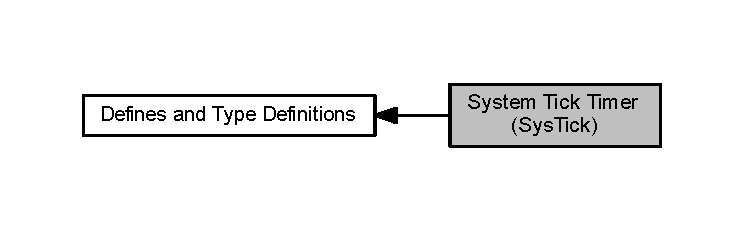
\includegraphics[width=350pt]{group___c_m_s_i_s___sys_tick}
\end{center}
\end{figure}
\subsection*{Classes}
\begin{DoxyCompactItemize}
\item 
struct \hyperlink{struct_sys_tick___type}{Sys\+Tick\+\_\+\+Type}
\begin{DoxyCompactList}\small\item\em Structure type to access the System \hyperlink{class_timer}{Timer} (Sys\+Tick). \end{DoxyCompactList}\end{DoxyCompactItemize}
\subsection*{Macros}
\begin{DoxyCompactItemize}
\item 
\#define \hyperlink{group___c_m_s_i_s___sys_tick_gadbb65d4a815759649db41df216ed4d60}{Sys\+Tick\+\_\+\+C\+T\+R\+L\+\_\+\+C\+O\+U\+N\+T\+F\+L\+A\+G\+\_\+\+Pos}~16U
\item 
\#define \hyperlink{group___c_m_s_i_s___sys_tick_ga1bf3033ecccf200f59baefe15dbb367c}{Sys\+Tick\+\_\+\+C\+T\+R\+L\+\_\+\+C\+O\+U\+N\+T\+F\+L\+A\+G\+\_\+\+Msk}~(1\+U\+L $<$$<$ Sys\+Tick\+\_\+\+C\+T\+R\+L\+\_\+\+C\+O\+U\+N\+T\+F\+L\+A\+G\+\_\+\+Pos)
\item 
\#define \hyperlink{group___c_m_s_i_s___sys_tick_ga24fbc69a5f0b78d67fda2300257baff1}{Sys\+Tick\+\_\+\+C\+T\+R\+L\+\_\+\+C\+L\+K\+S\+O\+U\+R\+C\+E\+\_\+\+Pos}~2U
\item 
\#define \hyperlink{group___c_m_s_i_s___sys_tick_gaa41d06039797423a46596bd313d57373}{Sys\+Tick\+\_\+\+C\+T\+R\+L\+\_\+\+C\+L\+K\+S\+O\+U\+R\+C\+E\+\_\+\+Msk}~(1\+U\+L $<$$<$ Sys\+Tick\+\_\+\+C\+T\+R\+L\+\_\+\+C\+L\+K\+S\+O\+U\+R\+C\+E\+\_\+\+Pos)
\item 
\#define \hyperlink{group___c_m_s_i_s___sys_tick_ga88f45bbb89ce8df3cd2b2613c7b48214}{Sys\+Tick\+\_\+\+C\+T\+R\+L\+\_\+\+T\+I\+C\+K\+I\+N\+T\+\_\+\+Pos}~1U
\item 
\#define \hyperlink{group___c_m_s_i_s___sys_tick_ga95bb984266ca764024836a870238a027}{Sys\+Tick\+\_\+\+C\+T\+R\+L\+\_\+\+T\+I\+C\+K\+I\+N\+T\+\_\+\+Msk}~(1\+U\+L $<$$<$ Sys\+Tick\+\_\+\+C\+T\+R\+L\+\_\+\+T\+I\+C\+K\+I\+N\+T\+\_\+\+Pos)
\item 
\#define \hyperlink{group___c_m_s_i_s___sys_tick_ga0b48cc1e36d92a92e4bf632890314810}{Sys\+Tick\+\_\+\+C\+T\+R\+L\+\_\+\+E\+N\+A\+B\+L\+E\+\_\+\+Pos}~0U
\item 
\#define \hyperlink{group___c_m_s_i_s___sys_tick_ga16c9fee0ed0235524bdeb38af328fd1f}{Sys\+Tick\+\_\+\+C\+T\+R\+L\+\_\+\+E\+N\+A\+B\+L\+E\+\_\+\+Msk}~(1\+U\+L /$\ast$$<$$<$ Sys\+Tick\+\_\+\+C\+T\+R\+L\+\_\+\+E\+N\+A\+B\+L\+E\+\_\+\+Pos$\ast$/)
\item 
\#define \hyperlink{group___c_m_s_i_s___sys_tick_gaf44d10df359dc5bf5752b0894ae3bad2}{Sys\+Tick\+\_\+\+L\+O\+A\+D\+\_\+\+R\+E\+L\+O\+A\+D\+\_\+\+Pos}~0U
\item 
\#define \hyperlink{group___c_m_s_i_s___sys_tick_ga265912a7962f0e1abd170336e579b1b1}{Sys\+Tick\+\_\+\+L\+O\+A\+D\+\_\+\+R\+E\+L\+O\+A\+D\+\_\+\+Msk}~(0x\+F\+F\+F\+F\+F\+F\+U\+L /$\ast$$<$$<$ Sys\+Tick\+\_\+\+L\+O\+A\+D\+\_\+\+R\+E\+L\+O\+A\+D\+\_\+\+Pos$\ast$/)
\item 
\#define \hyperlink{group___c_m_s_i_s___sys_tick_ga3208104c3b019b5de35ae8c21d5c34dd}{Sys\+Tick\+\_\+\+V\+A\+L\+\_\+\+C\+U\+R\+R\+E\+N\+T\+\_\+\+Pos}~0U
\item 
\#define \hyperlink{group___c_m_s_i_s___sys_tick_gafc77b56d568930b49a2474debc75ab45}{Sys\+Tick\+\_\+\+V\+A\+L\+\_\+\+C\+U\+R\+R\+E\+N\+T\+\_\+\+Msk}~(0x\+F\+F\+F\+F\+F\+F\+U\+L /$\ast$$<$$<$ Sys\+Tick\+\_\+\+V\+A\+L\+\_\+\+C\+U\+R\+R\+E\+N\+T\+\_\+\+Pos$\ast$/)
\item 
\#define \hyperlink{group___c_m_s_i_s___sys_tick_ga534dbe414e7a46a6ce4c1eca1fbff409}{Sys\+Tick\+\_\+\+C\+A\+L\+I\+B\+\_\+\+N\+O\+R\+E\+F\+\_\+\+Pos}~31U
\item 
\#define \hyperlink{group___c_m_s_i_s___sys_tick_ga3af0d891fdd99bcc8d8912d37830edb6}{Sys\+Tick\+\_\+\+C\+A\+L\+I\+B\+\_\+\+N\+O\+R\+E\+F\+\_\+\+Msk}~(1\+U\+L $<$$<$ Sys\+Tick\+\_\+\+C\+A\+L\+I\+B\+\_\+\+N\+O\+R\+E\+F\+\_\+\+Pos)
\item 
\#define \hyperlink{group___c_m_s_i_s___sys_tick_gadd0c9cd6641b9f6a0c618e7982954860}{Sys\+Tick\+\_\+\+C\+A\+L\+I\+B\+\_\+\+S\+K\+E\+W\+\_\+\+Pos}~30U
\item 
\#define \hyperlink{group___c_m_s_i_s___sys_tick_ga8a6a85a87334776f33d77fd147587431}{Sys\+Tick\+\_\+\+C\+A\+L\+I\+B\+\_\+\+S\+K\+E\+W\+\_\+\+Msk}~(1\+U\+L $<$$<$ Sys\+Tick\+\_\+\+C\+A\+L\+I\+B\+\_\+\+S\+K\+E\+W\+\_\+\+Pos)
\item 
\#define \hyperlink{group___c_m_s_i_s___sys_tick_gacae558f6e75a0bed5d826f606d8e695e}{Sys\+Tick\+\_\+\+C\+A\+L\+I\+B\+\_\+\+T\+E\+N\+M\+S\+\_\+\+Pos}~0U
\item 
\#define \hyperlink{group___c_m_s_i_s___sys_tick_gaf1e68865c5aece2ad58971225bd3e95e}{Sys\+Tick\+\_\+\+C\+A\+L\+I\+B\+\_\+\+T\+E\+N\+M\+S\+\_\+\+Msk}~(0x\+F\+F\+F\+F\+F\+F\+U\+L /$\ast$$<$$<$ Sys\+Tick\+\_\+\+C\+A\+L\+I\+B\+\_\+\+T\+E\+N\+M\+S\+\_\+\+Pos$\ast$/)
\item 
\#define \hyperlink{group___c_m_s_i_s___sys_tick_gadbb65d4a815759649db41df216ed4d60}{Sys\+Tick\+\_\+\+C\+T\+R\+L\+\_\+\+C\+O\+U\+N\+T\+F\+L\+A\+G\+\_\+\+Pos}~16U
\item 
\#define \hyperlink{group___c_m_s_i_s___sys_tick_ga1bf3033ecccf200f59baefe15dbb367c}{Sys\+Tick\+\_\+\+C\+T\+R\+L\+\_\+\+C\+O\+U\+N\+T\+F\+L\+A\+G\+\_\+\+Msk}~(1\+U\+L $<$$<$ Sys\+Tick\+\_\+\+C\+T\+R\+L\+\_\+\+C\+O\+U\+N\+T\+F\+L\+A\+G\+\_\+\+Pos)
\item 
\#define \hyperlink{group___c_m_s_i_s___sys_tick_ga24fbc69a5f0b78d67fda2300257baff1}{Sys\+Tick\+\_\+\+C\+T\+R\+L\+\_\+\+C\+L\+K\+S\+O\+U\+R\+C\+E\+\_\+\+Pos}~2U
\item 
\#define \hyperlink{group___c_m_s_i_s___sys_tick_gaa41d06039797423a46596bd313d57373}{Sys\+Tick\+\_\+\+C\+T\+R\+L\+\_\+\+C\+L\+K\+S\+O\+U\+R\+C\+E\+\_\+\+Msk}~(1\+U\+L $<$$<$ Sys\+Tick\+\_\+\+C\+T\+R\+L\+\_\+\+C\+L\+K\+S\+O\+U\+R\+C\+E\+\_\+\+Pos)
\item 
\#define \hyperlink{group___c_m_s_i_s___sys_tick_ga88f45bbb89ce8df3cd2b2613c7b48214}{Sys\+Tick\+\_\+\+C\+T\+R\+L\+\_\+\+T\+I\+C\+K\+I\+N\+T\+\_\+\+Pos}~1U
\item 
\#define \hyperlink{group___c_m_s_i_s___sys_tick_ga95bb984266ca764024836a870238a027}{Sys\+Tick\+\_\+\+C\+T\+R\+L\+\_\+\+T\+I\+C\+K\+I\+N\+T\+\_\+\+Msk}~(1\+U\+L $<$$<$ Sys\+Tick\+\_\+\+C\+T\+R\+L\+\_\+\+T\+I\+C\+K\+I\+N\+T\+\_\+\+Pos)
\item 
\#define \hyperlink{group___c_m_s_i_s___sys_tick_ga0b48cc1e36d92a92e4bf632890314810}{Sys\+Tick\+\_\+\+C\+T\+R\+L\+\_\+\+E\+N\+A\+B\+L\+E\+\_\+\+Pos}~0U
\item 
\#define \hyperlink{group___c_m_s_i_s___sys_tick_ga16c9fee0ed0235524bdeb38af328fd1f}{Sys\+Tick\+\_\+\+C\+T\+R\+L\+\_\+\+E\+N\+A\+B\+L\+E\+\_\+\+Msk}~(1\+U\+L /$\ast$$<$$<$ Sys\+Tick\+\_\+\+C\+T\+R\+L\+\_\+\+E\+N\+A\+B\+L\+E\+\_\+\+Pos$\ast$/)
\item 
\#define \hyperlink{group___c_m_s_i_s___sys_tick_gaf44d10df359dc5bf5752b0894ae3bad2}{Sys\+Tick\+\_\+\+L\+O\+A\+D\+\_\+\+R\+E\+L\+O\+A\+D\+\_\+\+Pos}~0U
\item 
\#define \hyperlink{group___c_m_s_i_s___sys_tick_ga265912a7962f0e1abd170336e579b1b1}{Sys\+Tick\+\_\+\+L\+O\+A\+D\+\_\+\+R\+E\+L\+O\+A\+D\+\_\+\+Msk}~(0x\+F\+F\+F\+F\+F\+F\+U\+L /$\ast$$<$$<$ Sys\+Tick\+\_\+\+L\+O\+A\+D\+\_\+\+R\+E\+L\+O\+A\+D\+\_\+\+Pos$\ast$/)
\item 
\#define \hyperlink{group___c_m_s_i_s___sys_tick_ga3208104c3b019b5de35ae8c21d5c34dd}{Sys\+Tick\+\_\+\+V\+A\+L\+\_\+\+C\+U\+R\+R\+E\+N\+T\+\_\+\+Pos}~0U
\item 
\#define \hyperlink{group___c_m_s_i_s___sys_tick_gafc77b56d568930b49a2474debc75ab45}{Sys\+Tick\+\_\+\+V\+A\+L\+\_\+\+C\+U\+R\+R\+E\+N\+T\+\_\+\+Msk}~(0x\+F\+F\+F\+F\+F\+F\+U\+L /$\ast$$<$$<$ Sys\+Tick\+\_\+\+V\+A\+L\+\_\+\+C\+U\+R\+R\+E\+N\+T\+\_\+\+Pos$\ast$/)
\item 
\#define \hyperlink{group___c_m_s_i_s___sys_tick_ga534dbe414e7a46a6ce4c1eca1fbff409}{Sys\+Tick\+\_\+\+C\+A\+L\+I\+B\+\_\+\+N\+O\+R\+E\+F\+\_\+\+Pos}~31U
\item 
\#define \hyperlink{group___c_m_s_i_s___sys_tick_ga3af0d891fdd99bcc8d8912d37830edb6}{Sys\+Tick\+\_\+\+C\+A\+L\+I\+B\+\_\+\+N\+O\+R\+E\+F\+\_\+\+Msk}~(1\+U\+L $<$$<$ Sys\+Tick\+\_\+\+C\+A\+L\+I\+B\+\_\+\+N\+O\+R\+E\+F\+\_\+\+Pos)
\item 
\#define \hyperlink{group___c_m_s_i_s___sys_tick_gadd0c9cd6641b9f6a0c618e7982954860}{Sys\+Tick\+\_\+\+C\+A\+L\+I\+B\+\_\+\+S\+K\+E\+W\+\_\+\+Pos}~30U
\item 
\#define \hyperlink{group___c_m_s_i_s___sys_tick_ga8a6a85a87334776f33d77fd147587431}{Sys\+Tick\+\_\+\+C\+A\+L\+I\+B\+\_\+\+S\+K\+E\+W\+\_\+\+Msk}~(1\+U\+L $<$$<$ Sys\+Tick\+\_\+\+C\+A\+L\+I\+B\+\_\+\+S\+K\+E\+W\+\_\+\+Pos)
\item 
\#define \hyperlink{group___c_m_s_i_s___sys_tick_gacae558f6e75a0bed5d826f606d8e695e}{Sys\+Tick\+\_\+\+C\+A\+L\+I\+B\+\_\+\+T\+E\+N\+M\+S\+\_\+\+Pos}~0U
\item 
\#define \hyperlink{group___c_m_s_i_s___sys_tick_gaf1e68865c5aece2ad58971225bd3e95e}{Sys\+Tick\+\_\+\+C\+A\+L\+I\+B\+\_\+\+T\+E\+N\+M\+S\+\_\+\+Msk}~(0x\+F\+F\+F\+F\+F\+F\+U\+L /$\ast$$<$$<$ Sys\+Tick\+\_\+\+C\+A\+L\+I\+B\+\_\+\+T\+E\+N\+M\+S\+\_\+\+Pos$\ast$/)
\item 
\#define \hyperlink{group___c_m_s_i_s___sys_tick_gadbb65d4a815759649db41df216ed4d60}{Sys\+Tick\+\_\+\+C\+T\+R\+L\+\_\+\+C\+O\+U\+N\+T\+F\+L\+A\+G\+\_\+\+Pos}~16U
\item 
\#define \hyperlink{group___c_m_s_i_s___sys_tick_ga1bf3033ecccf200f59baefe15dbb367c}{Sys\+Tick\+\_\+\+C\+T\+R\+L\+\_\+\+C\+O\+U\+N\+T\+F\+L\+A\+G\+\_\+\+Msk}~(1\+U\+L $<$$<$ Sys\+Tick\+\_\+\+C\+T\+R\+L\+\_\+\+C\+O\+U\+N\+T\+F\+L\+A\+G\+\_\+\+Pos)
\item 
\#define \hyperlink{group___c_m_s_i_s___sys_tick_ga24fbc69a5f0b78d67fda2300257baff1}{Sys\+Tick\+\_\+\+C\+T\+R\+L\+\_\+\+C\+L\+K\+S\+O\+U\+R\+C\+E\+\_\+\+Pos}~2U
\item 
\#define \hyperlink{group___c_m_s_i_s___sys_tick_gaa41d06039797423a46596bd313d57373}{Sys\+Tick\+\_\+\+C\+T\+R\+L\+\_\+\+C\+L\+K\+S\+O\+U\+R\+C\+E\+\_\+\+Msk}~(1\+U\+L $<$$<$ Sys\+Tick\+\_\+\+C\+T\+R\+L\+\_\+\+C\+L\+K\+S\+O\+U\+R\+C\+E\+\_\+\+Pos)
\item 
\#define \hyperlink{group___c_m_s_i_s___sys_tick_ga88f45bbb89ce8df3cd2b2613c7b48214}{Sys\+Tick\+\_\+\+C\+T\+R\+L\+\_\+\+T\+I\+C\+K\+I\+N\+T\+\_\+\+Pos}~1U
\item 
\#define \hyperlink{group___c_m_s_i_s___sys_tick_ga95bb984266ca764024836a870238a027}{Sys\+Tick\+\_\+\+C\+T\+R\+L\+\_\+\+T\+I\+C\+K\+I\+N\+T\+\_\+\+Msk}~(1\+U\+L $<$$<$ Sys\+Tick\+\_\+\+C\+T\+R\+L\+\_\+\+T\+I\+C\+K\+I\+N\+T\+\_\+\+Pos)
\item 
\#define \hyperlink{group___c_m_s_i_s___sys_tick_ga0b48cc1e36d92a92e4bf632890314810}{Sys\+Tick\+\_\+\+C\+T\+R\+L\+\_\+\+E\+N\+A\+B\+L\+E\+\_\+\+Pos}~0U
\item 
\#define \hyperlink{group___c_m_s_i_s___sys_tick_ga16c9fee0ed0235524bdeb38af328fd1f}{Sys\+Tick\+\_\+\+C\+T\+R\+L\+\_\+\+E\+N\+A\+B\+L\+E\+\_\+\+Msk}~(1\+U\+L /$\ast$$<$$<$ Sys\+Tick\+\_\+\+C\+T\+R\+L\+\_\+\+E\+N\+A\+B\+L\+E\+\_\+\+Pos$\ast$/)
\item 
\#define \hyperlink{group___c_m_s_i_s___sys_tick_gaf44d10df359dc5bf5752b0894ae3bad2}{Sys\+Tick\+\_\+\+L\+O\+A\+D\+\_\+\+R\+E\+L\+O\+A\+D\+\_\+\+Pos}~0U
\item 
\#define \hyperlink{group___c_m_s_i_s___sys_tick_ga265912a7962f0e1abd170336e579b1b1}{Sys\+Tick\+\_\+\+L\+O\+A\+D\+\_\+\+R\+E\+L\+O\+A\+D\+\_\+\+Msk}~(0x\+F\+F\+F\+F\+F\+F\+U\+L /$\ast$$<$$<$ Sys\+Tick\+\_\+\+L\+O\+A\+D\+\_\+\+R\+E\+L\+O\+A\+D\+\_\+\+Pos$\ast$/)
\item 
\#define \hyperlink{group___c_m_s_i_s___sys_tick_ga3208104c3b019b5de35ae8c21d5c34dd}{Sys\+Tick\+\_\+\+V\+A\+L\+\_\+\+C\+U\+R\+R\+E\+N\+T\+\_\+\+Pos}~0U
\item 
\#define \hyperlink{group___c_m_s_i_s___sys_tick_gafc77b56d568930b49a2474debc75ab45}{Sys\+Tick\+\_\+\+V\+A\+L\+\_\+\+C\+U\+R\+R\+E\+N\+T\+\_\+\+Msk}~(0x\+F\+F\+F\+F\+F\+F\+U\+L /$\ast$$<$$<$ Sys\+Tick\+\_\+\+V\+A\+L\+\_\+\+C\+U\+R\+R\+E\+N\+T\+\_\+\+Pos$\ast$/)
\item 
\#define \hyperlink{group___c_m_s_i_s___sys_tick_ga534dbe414e7a46a6ce4c1eca1fbff409}{Sys\+Tick\+\_\+\+C\+A\+L\+I\+B\+\_\+\+N\+O\+R\+E\+F\+\_\+\+Pos}~31U
\item 
\#define \hyperlink{group___c_m_s_i_s___sys_tick_ga3af0d891fdd99bcc8d8912d37830edb6}{Sys\+Tick\+\_\+\+C\+A\+L\+I\+B\+\_\+\+N\+O\+R\+E\+F\+\_\+\+Msk}~(1\+U\+L $<$$<$ Sys\+Tick\+\_\+\+C\+A\+L\+I\+B\+\_\+\+N\+O\+R\+E\+F\+\_\+\+Pos)
\item 
\#define \hyperlink{group___c_m_s_i_s___sys_tick_gadd0c9cd6641b9f6a0c618e7982954860}{Sys\+Tick\+\_\+\+C\+A\+L\+I\+B\+\_\+\+S\+K\+E\+W\+\_\+\+Pos}~30U
\item 
\#define \hyperlink{group___c_m_s_i_s___sys_tick_ga8a6a85a87334776f33d77fd147587431}{Sys\+Tick\+\_\+\+C\+A\+L\+I\+B\+\_\+\+S\+K\+E\+W\+\_\+\+Msk}~(1\+U\+L $<$$<$ Sys\+Tick\+\_\+\+C\+A\+L\+I\+B\+\_\+\+S\+K\+E\+W\+\_\+\+Pos)
\item 
\#define \hyperlink{group___c_m_s_i_s___sys_tick_gacae558f6e75a0bed5d826f606d8e695e}{Sys\+Tick\+\_\+\+C\+A\+L\+I\+B\+\_\+\+T\+E\+N\+M\+S\+\_\+\+Pos}~0U
\item 
\#define \hyperlink{group___c_m_s_i_s___sys_tick_gaf1e68865c5aece2ad58971225bd3e95e}{Sys\+Tick\+\_\+\+C\+A\+L\+I\+B\+\_\+\+T\+E\+N\+M\+S\+\_\+\+Msk}~(0x\+F\+F\+F\+F\+F\+F\+U\+L /$\ast$$<$$<$ Sys\+Tick\+\_\+\+C\+A\+L\+I\+B\+\_\+\+T\+E\+N\+M\+S\+\_\+\+Pos$\ast$/)
\item 
\#define \hyperlink{group___c_m_s_i_s___sys_tick_gadbb65d4a815759649db41df216ed4d60}{Sys\+Tick\+\_\+\+C\+T\+R\+L\+\_\+\+C\+O\+U\+N\+T\+F\+L\+A\+G\+\_\+\+Pos}~16U
\item 
\#define \hyperlink{group___c_m_s_i_s___sys_tick_ga1bf3033ecccf200f59baefe15dbb367c}{Sys\+Tick\+\_\+\+C\+T\+R\+L\+\_\+\+C\+O\+U\+N\+T\+F\+L\+A\+G\+\_\+\+Msk}~(1\+U\+L $<$$<$ Sys\+Tick\+\_\+\+C\+T\+R\+L\+\_\+\+C\+O\+U\+N\+T\+F\+L\+A\+G\+\_\+\+Pos)
\item 
\#define \hyperlink{group___c_m_s_i_s___sys_tick_ga24fbc69a5f0b78d67fda2300257baff1}{Sys\+Tick\+\_\+\+C\+T\+R\+L\+\_\+\+C\+L\+K\+S\+O\+U\+R\+C\+E\+\_\+\+Pos}~2U
\item 
\#define \hyperlink{group___c_m_s_i_s___sys_tick_gaa41d06039797423a46596bd313d57373}{Sys\+Tick\+\_\+\+C\+T\+R\+L\+\_\+\+C\+L\+K\+S\+O\+U\+R\+C\+E\+\_\+\+Msk}~(1\+U\+L $<$$<$ Sys\+Tick\+\_\+\+C\+T\+R\+L\+\_\+\+C\+L\+K\+S\+O\+U\+R\+C\+E\+\_\+\+Pos)
\item 
\#define \hyperlink{group___c_m_s_i_s___sys_tick_ga88f45bbb89ce8df3cd2b2613c7b48214}{Sys\+Tick\+\_\+\+C\+T\+R\+L\+\_\+\+T\+I\+C\+K\+I\+N\+T\+\_\+\+Pos}~1U
\item 
\#define \hyperlink{group___c_m_s_i_s___sys_tick_ga95bb984266ca764024836a870238a027}{Sys\+Tick\+\_\+\+C\+T\+R\+L\+\_\+\+T\+I\+C\+K\+I\+N\+T\+\_\+\+Msk}~(1\+U\+L $<$$<$ Sys\+Tick\+\_\+\+C\+T\+R\+L\+\_\+\+T\+I\+C\+K\+I\+N\+T\+\_\+\+Pos)
\item 
\#define \hyperlink{group___c_m_s_i_s___sys_tick_ga0b48cc1e36d92a92e4bf632890314810}{Sys\+Tick\+\_\+\+C\+T\+R\+L\+\_\+\+E\+N\+A\+B\+L\+E\+\_\+\+Pos}~0U
\item 
\#define \hyperlink{group___c_m_s_i_s___sys_tick_ga16c9fee0ed0235524bdeb38af328fd1f}{Sys\+Tick\+\_\+\+C\+T\+R\+L\+\_\+\+E\+N\+A\+B\+L\+E\+\_\+\+Msk}~(1\+U\+L /$\ast$$<$$<$ Sys\+Tick\+\_\+\+C\+T\+R\+L\+\_\+\+E\+N\+A\+B\+L\+E\+\_\+\+Pos$\ast$/)
\item 
\#define \hyperlink{group___c_m_s_i_s___sys_tick_gaf44d10df359dc5bf5752b0894ae3bad2}{Sys\+Tick\+\_\+\+L\+O\+A\+D\+\_\+\+R\+E\+L\+O\+A\+D\+\_\+\+Pos}~0U
\item 
\#define \hyperlink{group___c_m_s_i_s___sys_tick_ga265912a7962f0e1abd170336e579b1b1}{Sys\+Tick\+\_\+\+L\+O\+A\+D\+\_\+\+R\+E\+L\+O\+A\+D\+\_\+\+Msk}~(0x\+F\+F\+F\+F\+F\+F\+U\+L /$\ast$$<$$<$ Sys\+Tick\+\_\+\+L\+O\+A\+D\+\_\+\+R\+E\+L\+O\+A\+D\+\_\+\+Pos$\ast$/)
\item 
\#define \hyperlink{group___c_m_s_i_s___sys_tick_ga3208104c3b019b5de35ae8c21d5c34dd}{Sys\+Tick\+\_\+\+V\+A\+L\+\_\+\+C\+U\+R\+R\+E\+N\+T\+\_\+\+Pos}~0U
\item 
\#define \hyperlink{group___c_m_s_i_s___sys_tick_gafc77b56d568930b49a2474debc75ab45}{Sys\+Tick\+\_\+\+V\+A\+L\+\_\+\+C\+U\+R\+R\+E\+N\+T\+\_\+\+Msk}~(0x\+F\+F\+F\+F\+F\+F\+U\+L /$\ast$$<$$<$ Sys\+Tick\+\_\+\+V\+A\+L\+\_\+\+C\+U\+R\+R\+E\+N\+T\+\_\+\+Pos$\ast$/)
\item 
\#define \hyperlink{group___c_m_s_i_s___sys_tick_ga534dbe414e7a46a6ce4c1eca1fbff409}{Sys\+Tick\+\_\+\+C\+A\+L\+I\+B\+\_\+\+N\+O\+R\+E\+F\+\_\+\+Pos}~31U
\item 
\#define \hyperlink{group___c_m_s_i_s___sys_tick_ga3af0d891fdd99bcc8d8912d37830edb6}{Sys\+Tick\+\_\+\+C\+A\+L\+I\+B\+\_\+\+N\+O\+R\+E\+F\+\_\+\+Msk}~(1\+U\+L $<$$<$ Sys\+Tick\+\_\+\+C\+A\+L\+I\+B\+\_\+\+N\+O\+R\+E\+F\+\_\+\+Pos)
\item 
\#define \hyperlink{group___c_m_s_i_s___sys_tick_gadd0c9cd6641b9f6a0c618e7982954860}{Sys\+Tick\+\_\+\+C\+A\+L\+I\+B\+\_\+\+S\+K\+E\+W\+\_\+\+Pos}~30U
\item 
\#define \hyperlink{group___c_m_s_i_s___sys_tick_ga8a6a85a87334776f33d77fd147587431}{Sys\+Tick\+\_\+\+C\+A\+L\+I\+B\+\_\+\+S\+K\+E\+W\+\_\+\+Msk}~(1\+U\+L $<$$<$ Sys\+Tick\+\_\+\+C\+A\+L\+I\+B\+\_\+\+S\+K\+E\+W\+\_\+\+Pos)
\item 
\#define \hyperlink{group___c_m_s_i_s___sys_tick_gacae558f6e75a0bed5d826f606d8e695e}{Sys\+Tick\+\_\+\+C\+A\+L\+I\+B\+\_\+\+T\+E\+N\+M\+S\+\_\+\+Pos}~0U
\item 
\#define \hyperlink{group___c_m_s_i_s___sys_tick_gaf1e68865c5aece2ad58971225bd3e95e}{Sys\+Tick\+\_\+\+C\+A\+L\+I\+B\+\_\+\+T\+E\+N\+M\+S\+\_\+\+Msk}~(0x\+F\+F\+F\+F\+F\+F\+U\+L /$\ast$$<$$<$ Sys\+Tick\+\_\+\+C\+A\+L\+I\+B\+\_\+\+T\+E\+N\+M\+S\+\_\+\+Pos$\ast$/)
\item 
\#define \hyperlink{group___c_m_s_i_s___sys_tick_gadbb65d4a815759649db41df216ed4d60}{Sys\+Tick\+\_\+\+C\+T\+R\+L\+\_\+\+C\+O\+U\+N\+T\+F\+L\+A\+G\+\_\+\+Pos}~16U
\item 
\#define \hyperlink{group___c_m_s_i_s___sys_tick_ga1bf3033ecccf200f59baefe15dbb367c}{Sys\+Tick\+\_\+\+C\+T\+R\+L\+\_\+\+C\+O\+U\+N\+T\+F\+L\+A\+G\+\_\+\+Msk}~(1\+U\+L $<$$<$ Sys\+Tick\+\_\+\+C\+T\+R\+L\+\_\+\+C\+O\+U\+N\+T\+F\+L\+A\+G\+\_\+\+Pos)
\item 
\#define \hyperlink{group___c_m_s_i_s___sys_tick_ga24fbc69a5f0b78d67fda2300257baff1}{Sys\+Tick\+\_\+\+C\+T\+R\+L\+\_\+\+C\+L\+K\+S\+O\+U\+R\+C\+E\+\_\+\+Pos}~2U
\item 
\#define \hyperlink{group___c_m_s_i_s___sys_tick_gaa41d06039797423a46596bd313d57373}{Sys\+Tick\+\_\+\+C\+T\+R\+L\+\_\+\+C\+L\+K\+S\+O\+U\+R\+C\+E\+\_\+\+Msk}~(1\+U\+L $<$$<$ Sys\+Tick\+\_\+\+C\+T\+R\+L\+\_\+\+C\+L\+K\+S\+O\+U\+R\+C\+E\+\_\+\+Pos)
\item 
\#define \hyperlink{group___c_m_s_i_s___sys_tick_ga88f45bbb89ce8df3cd2b2613c7b48214}{Sys\+Tick\+\_\+\+C\+T\+R\+L\+\_\+\+T\+I\+C\+K\+I\+N\+T\+\_\+\+Pos}~1U
\item 
\#define \hyperlink{group___c_m_s_i_s___sys_tick_ga95bb984266ca764024836a870238a027}{Sys\+Tick\+\_\+\+C\+T\+R\+L\+\_\+\+T\+I\+C\+K\+I\+N\+T\+\_\+\+Msk}~(1\+U\+L $<$$<$ Sys\+Tick\+\_\+\+C\+T\+R\+L\+\_\+\+T\+I\+C\+K\+I\+N\+T\+\_\+\+Pos)
\item 
\#define \hyperlink{group___c_m_s_i_s___sys_tick_ga0b48cc1e36d92a92e4bf632890314810}{Sys\+Tick\+\_\+\+C\+T\+R\+L\+\_\+\+E\+N\+A\+B\+L\+E\+\_\+\+Pos}~0U
\item 
\#define \hyperlink{group___c_m_s_i_s___sys_tick_ga16c9fee0ed0235524bdeb38af328fd1f}{Sys\+Tick\+\_\+\+C\+T\+R\+L\+\_\+\+E\+N\+A\+B\+L\+E\+\_\+\+Msk}~(1\+U\+L /$\ast$$<$$<$ Sys\+Tick\+\_\+\+C\+T\+R\+L\+\_\+\+E\+N\+A\+B\+L\+E\+\_\+\+Pos$\ast$/)
\item 
\#define \hyperlink{group___c_m_s_i_s___sys_tick_gaf44d10df359dc5bf5752b0894ae3bad2}{Sys\+Tick\+\_\+\+L\+O\+A\+D\+\_\+\+R\+E\+L\+O\+A\+D\+\_\+\+Pos}~0U
\item 
\#define \hyperlink{group___c_m_s_i_s___sys_tick_ga265912a7962f0e1abd170336e579b1b1}{Sys\+Tick\+\_\+\+L\+O\+A\+D\+\_\+\+R\+E\+L\+O\+A\+D\+\_\+\+Msk}~(0x\+F\+F\+F\+F\+F\+F\+U\+L /$\ast$$<$$<$ Sys\+Tick\+\_\+\+L\+O\+A\+D\+\_\+\+R\+E\+L\+O\+A\+D\+\_\+\+Pos$\ast$/)
\item 
\#define \hyperlink{group___c_m_s_i_s___sys_tick_ga3208104c3b019b5de35ae8c21d5c34dd}{Sys\+Tick\+\_\+\+V\+A\+L\+\_\+\+C\+U\+R\+R\+E\+N\+T\+\_\+\+Pos}~0U
\item 
\#define \hyperlink{group___c_m_s_i_s___sys_tick_gafc77b56d568930b49a2474debc75ab45}{Sys\+Tick\+\_\+\+V\+A\+L\+\_\+\+C\+U\+R\+R\+E\+N\+T\+\_\+\+Msk}~(0x\+F\+F\+F\+F\+F\+F\+U\+L /$\ast$$<$$<$ Sys\+Tick\+\_\+\+V\+A\+L\+\_\+\+C\+U\+R\+R\+E\+N\+T\+\_\+\+Pos$\ast$/)
\item 
\#define \hyperlink{group___c_m_s_i_s___sys_tick_ga534dbe414e7a46a6ce4c1eca1fbff409}{Sys\+Tick\+\_\+\+C\+A\+L\+I\+B\+\_\+\+N\+O\+R\+E\+F\+\_\+\+Pos}~31U
\item 
\#define \hyperlink{group___c_m_s_i_s___sys_tick_ga3af0d891fdd99bcc8d8912d37830edb6}{Sys\+Tick\+\_\+\+C\+A\+L\+I\+B\+\_\+\+N\+O\+R\+E\+F\+\_\+\+Msk}~(1\+U\+L $<$$<$ Sys\+Tick\+\_\+\+C\+A\+L\+I\+B\+\_\+\+N\+O\+R\+E\+F\+\_\+\+Pos)
\item 
\#define \hyperlink{group___c_m_s_i_s___sys_tick_gadd0c9cd6641b9f6a0c618e7982954860}{Sys\+Tick\+\_\+\+C\+A\+L\+I\+B\+\_\+\+S\+K\+E\+W\+\_\+\+Pos}~30U
\item 
\#define \hyperlink{group___c_m_s_i_s___sys_tick_ga8a6a85a87334776f33d77fd147587431}{Sys\+Tick\+\_\+\+C\+A\+L\+I\+B\+\_\+\+S\+K\+E\+W\+\_\+\+Msk}~(1\+U\+L $<$$<$ Sys\+Tick\+\_\+\+C\+A\+L\+I\+B\+\_\+\+S\+K\+E\+W\+\_\+\+Pos)
\item 
\#define \hyperlink{group___c_m_s_i_s___sys_tick_gacae558f6e75a0bed5d826f606d8e695e}{Sys\+Tick\+\_\+\+C\+A\+L\+I\+B\+\_\+\+T\+E\+N\+M\+S\+\_\+\+Pos}~0U
\item 
\#define \hyperlink{group___c_m_s_i_s___sys_tick_gaf1e68865c5aece2ad58971225bd3e95e}{Sys\+Tick\+\_\+\+C\+A\+L\+I\+B\+\_\+\+T\+E\+N\+M\+S\+\_\+\+Msk}~(0x\+F\+F\+F\+F\+F\+F\+U\+L /$\ast$$<$$<$ Sys\+Tick\+\_\+\+C\+A\+L\+I\+B\+\_\+\+T\+E\+N\+M\+S\+\_\+\+Pos$\ast$/)
\item 
\#define \hyperlink{group___c_m_s_i_s___sys_tick_gadbb65d4a815759649db41df216ed4d60}{Sys\+Tick\+\_\+\+C\+T\+R\+L\+\_\+\+C\+O\+U\+N\+T\+F\+L\+A\+G\+\_\+\+Pos}~16U
\item 
\#define \hyperlink{group___c_m_s_i_s___sys_tick_ga1bf3033ecccf200f59baefe15dbb367c}{Sys\+Tick\+\_\+\+C\+T\+R\+L\+\_\+\+C\+O\+U\+N\+T\+F\+L\+A\+G\+\_\+\+Msk}~(1\+U\+L $<$$<$ Sys\+Tick\+\_\+\+C\+T\+R\+L\+\_\+\+C\+O\+U\+N\+T\+F\+L\+A\+G\+\_\+\+Pos)
\item 
\#define \hyperlink{group___c_m_s_i_s___sys_tick_ga24fbc69a5f0b78d67fda2300257baff1}{Sys\+Tick\+\_\+\+C\+T\+R\+L\+\_\+\+C\+L\+K\+S\+O\+U\+R\+C\+E\+\_\+\+Pos}~2U
\item 
\#define \hyperlink{group___c_m_s_i_s___sys_tick_gaa41d06039797423a46596bd313d57373}{Sys\+Tick\+\_\+\+C\+T\+R\+L\+\_\+\+C\+L\+K\+S\+O\+U\+R\+C\+E\+\_\+\+Msk}~(1\+U\+L $<$$<$ Sys\+Tick\+\_\+\+C\+T\+R\+L\+\_\+\+C\+L\+K\+S\+O\+U\+R\+C\+E\+\_\+\+Pos)
\item 
\#define \hyperlink{group___c_m_s_i_s___sys_tick_ga88f45bbb89ce8df3cd2b2613c7b48214}{Sys\+Tick\+\_\+\+C\+T\+R\+L\+\_\+\+T\+I\+C\+K\+I\+N\+T\+\_\+\+Pos}~1U
\item 
\#define \hyperlink{group___c_m_s_i_s___sys_tick_ga95bb984266ca764024836a870238a027}{Sys\+Tick\+\_\+\+C\+T\+R\+L\+\_\+\+T\+I\+C\+K\+I\+N\+T\+\_\+\+Msk}~(1\+U\+L $<$$<$ Sys\+Tick\+\_\+\+C\+T\+R\+L\+\_\+\+T\+I\+C\+K\+I\+N\+T\+\_\+\+Pos)
\item 
\#define \hyperlink{group___c_m_s_i_s___sys_tick_ga0b48cc1e36d92a92e4bf632890314810}{Sys\+Tick\+\_\+\+C\+T\+R\+L\+\_\+\+E\+N\+A\+B\+L\+E\+\_\+\+Pos}~0U
\item 
\#define \hyperlink{group___c_m_s_i_s___sys_tick_ga16c9fee0ed0235524bdeb38af328fd1f}{Sys\+Tick\+\_\+\+C\+T\+R\+L\+\_\+\+E\+N\+A\+B\+L\+E\+\_\+\+Msk}~(1\+U\+L /$\ast$$<$$<$ Sys\+Tick\+\_\+\+C\+T\+R\+L\+\_\+\+E\+N\+A\+B\+L\+E\+\_\+\+Pos$\ast$/)
\item 
\#define \hyperlink{group___c_m_s_i_s___sys_tick_gaf44d10df359dc5bf5752b0894ae3bad2}{Sys\+Tick\+\_\+\+L\+O\+A\+D\+\_\+\+R\+E\+L\+O\+A\+D\+\_\+\+Pos}~0U
\item 
\#define \hyperlink{group___c_m_s_i_s___sys_tick_ga265912a7962f0e1abd170336e579b1b1}{Sys\+Tick\+\_\+\+L\+O\+A\+D\+\_\+\+R\+E\+L\+O\+A\+D\+\_\+\+Msk}~(0x\+F\+F\+F\+F\+F\+F\+U\+L /$\ast$$<$$<$ Sys\+Tick\+\_\+\+L\+O\+A\+D\+\_\+\+R\+E\+L\+O\+A\+D\+\_\+\+Pos$\ast$/)
\item 
\#define \hyperlink{group___c_m_s_i_s___sys_tick_ga3208104c3b019b5de35ae8c21d5c34dd}{Sys\+Tick\+\_\+\+V\+A\+L\+\_\+\+C\+U\+R\+R\+E\+N\+T\+\_\+\+Pos}~0U
\item 
\#define \hyperlink{group___c_m_s_i_s___sys_tick_gafc77b56d568930b49a2474debc75ab45}{Sys\+Tick\+\_\+\+V\+A\+L\+\_\+\+C\+U\+R\+R\+E\+N\+T\+\_\+\+Msk}~(0x\+F\+F\+F\+F\+F\+F\+U\+L /$\ast$$<$$<$ Sys\+Tick\+\_\+\+V\+A\+L\+\_\+\+C\+U\+R\+R\+E\+N\+T\+\_\+\+Pos$\ast$/)
\item 
\#define \hyperlink{group___c_m_s_i_s___sys_tick_ga534dbe414e7a46a6ce4c1eca1fbff409}{Sys\+Tick\+\_\+\+C\+A\+L\+I\+B\+\_\+\+N\+O\+R\+E\+F\+\_\+\+Pos}~31U
\item 
\#define \hyperlink{group___c_m_s_i_s___sys_tick_ga3af0d891fdd99bcc8d8912d37830edb6}{Sys\+Tick\+\_\+\+C\+A\+L\+I\+B\+\_\+\+N\+O\+R\+E\+F\+\_\+\+Msk}~(1\+U\+L $<$$<$ Sys\+Tick\+\_\+\+C\+A\+L\+I\+B\+\_\+\+N\+O\+R\+E\+F\+\_\+\+Pos)
\item 
\#define \hyperlink{group___c_m_s_i_s___sys_tick_gadd0c9cd6641b9f6a0c618e7982954860}{Sys\+Tick\+\_\+\+C\+A\+L\+I\+B\+\_\+\+S\+K\+E\+W\+\_\+\+Pos}~30U
\item 
\#define \hyperlink{group___c_m_s_i_s___sys_tick_ga8a6a85a87334776f33d77fd147587431}{Sys\+Tick\+\_\+\+C\+A\+L\+I\+B\+\_\+\+S\+K\+E\+W\+\_\+\+Msk}~(1\+U\+L $<$$<$ Sys\+Tick\+\_\+\+C\+A\+L\+I\+B\+\_\+\+S\+K\+E\+W\+\_\+\+Pos)
\item 
\#define \hyperlink{group___c_m_s_i_s___sys_tick_gacae558f6e75a0bed5d826f606d8e695e}{Sys\+Tick\+\_\+\+C\+A\+L\+I\+B\+\_\+\+T\+E\+N\+M\+S\+\_\+\+Pos}~0U
\item 
\#define \hyperlink{group___c_m_s_i_s___sys_tick_gaf1e68865c5aece2ad58971225bd3e95e}{Sys\+Tick\+\_\+\+C\+A\+L\+I\+B\+\_\+\+T\+E\+N\+M\+S\+\_\+\+Msk}~(0x\+F\+F\+F\+F\+F\+F\+U\+L /$\ast$$<$$<$ Sys\+Tick\+\_\+\+C\+A\+L\+I\+B\+\_\+\+T\+E\+N\+M\+S\+\_\+\+Pos$\ast$/)
\item 
\#define \hyperlink{group___c_m_s_i_s___sys_tick_gadbb65d4a815759649db41df216ed4d60}{Sys\+Tick\+\_\+\+C\+T\+R\+L\+\_\+\+C\+O\+U\+N\+T\+F\+L\+A\+G\+\_\+\+Pos}~16U
\item 
\#define \hyperlink{group___c_m_s_i_s___sys_tick_ga1bf3033ecccf200f59baefe15dbb367c}{Sys\+Tick\+\_\+\+C\+T\+R\+L\+\_\+\+C\+O\+U\+N\+T\+F\+L\+A\+G\+\_\+\+Msk}~(1\+U\+L $<$$<$ Sys\+Tick\+\_\+\+C\+T\+R\+L\+\_\+\+C\+O\+U\+N\+T\+F\+L\+A\+G\+\_\+\+Pos)
\item 
\#define \hyperlink{group___c_m_s_i_s___sys_tick_ga24fbc69a5f0b78d67fda2300257baff1}{Sys\+Tick\+\_\+\+C\+T\+R\+L\+\_\+\+C\+L\+K\+S\+O\+U\+R\+C\+E\+\_\+\+Pos}~2U
\item 
\#define \hyperlink{group___c_m_s_i_s___sys_tick_gaa41d06039797423a46596bd313d57373}{Sys\+Tick\+\_\+\+C\+T\+R\+L\+\_\+\+C\+L\+K\+S\+O\+U\+R\+C\+E\+\_\+\+Msk}~(1\+U\+L $<$$<$ Sys\+Tick\+\_\+\+C\+T\+R\+L\+\_\+\+C\+L\+K\+S\+O\+U\+R\+C\+E\+\_\+\+Pos)
\item 
\#define \hyperlink{group___c_m_s_i_s___sys_tick_ga88f45bbb89ce8df3cd2b2613c7b48214}{Sys\+Tick\+\_\+\+C\+T\+R\+L\+\_\+\+T\+I\+C\+K\+I\+N\+T\+\_\+\+Pos}~1U
\item 
\#define \hyperlink{group___c_m_s_i_s___sys_tick_ga95bb984266ca764024836a870238a027}{Sys\+Tick\+\_\+\+C\+T\+R\+L\+\_\+\+T\+I\+C\+K\+I\+N\+T\+\_\+\+Msk}~(1\+U\+L $<$$<$ Sys\+Tick\+\_\+\+C\+T\+R\+L\+\_\+\+T\+I\+C\+K\+I\+N\+T\+\_\+\+Pos)
\item 
\#define \hyperlink{group___c_m_s_i_s___sys_tick_ga0b48cc1e36d92a92e4bf632890314810}{Sys\+Tick\+\_\+\+C\+T\+R\+L\+\_\+\+E\+N\+A\+B\+L\+E\+\_\+\+Pos}~0U
\item 
\#define \hyperlink{group___c_m_s_i_s___sys_tick_ga16c9fee0ed0235524bdeb38af328fd1f}{Sys\+Tick\+\_\+\+C\+T\+R\+L\+\_\+\+E\+N\+A\+B\+L\+E\+\_\+\+Msk}~(1\+U\+L /$\ast$$<$$<$ Sys\+Tick\+\_\+\+C\+T\+R\+L\+\_\+\+E\+N\+A\+B\+L\+E\+\_\+\+Pos$\ast$/)
\item 
\#define \hyperlink{group___c_m_s_i_s___sys_tick_gaf44d10df359dc5bf5752b0894ae3bad2}{Sys\+Tick\+\_\+\+L\+O\+A\+D\+\_\+\+R\+E\+L\+O\+A\+D\+\_\+\+Pos}~0U
\item 
\#define \hyperlink{group___c_m_s_i_s___sys_tick_ga265912a7962f0e1abd170336e579b1b1}{Sys\+Tick\+\_\+\+L\+O\+A\+D\+\_\+\+R\+E\+L\+O\+A\+D\+\_\+\+Msk}~(0x\+F\+F\+F\+F\+F\+F\+U\+L /$\ast$$<$$<$ Sys\+Tick\+\_\+\+L\+O\+A\+D\+\_\+\+R\+E\+L\+O\+A\+D\+\_\+\+Pos$\ast$/)
\item 
\#define \hyperlink{group___c_m_s_i_s___sys_tick_ga3208104c3b019b5de35ae8c21d5c34dd}{Sys\+Tick\+\_\+\+V\+A\+L\+\_\+\+C\+U\+R\+R\+E\+N\+T\+\_\+\+Pos}~0U
\item 
\#define \hyperlink{group___c_m_s_i_s___sys_tick_gafc77b56d568930b49a2474debc75ab45}{Sys\+Tick\+\_\+\+V\+A\+L\+\_\+\+C\+U\+R\+R\+E\+N\+T\+\_\+\+Msk}~(0x\+F\+F\+F\+F\+F\+F\+U\+L /$\ast$$<$$<$ Sys\+Tick\+\_\+\+V\+A\+L\+\_\+\+C\+U\+R\+R\+E\+N\+T\+\_\+\+Pos$\ast$/)
\item 
\#define \hyperlink{group___c_m_s_i_s___sys_tick_ga534dbe414e7a46a6ce4c1eca1fbff409}{Sys\+Tick\+\_\+\+C\+A\+L\+I\+B\+\_\+\+N\+O\+R\+E\+F\+\_\+\+Pos}~31U
\item 
\#define \hyperlink{group___c_m_s_i_s___sys_tick_ga3af0d891fdd99bcc8d8912d37830edb6}{Sys\+Tick\+\_\+\+C\+A\+L\+I\+B\+\_\+\+N\+O\+R\+E\+F\+\_\+\+Msk}~(1\+U\+L $<$$<$ Sys\+Tick\+\_\+\+C\+A\+L\+I\+B\+\_\+\+N\+O\+R\+E\+F\+\_\+\+Pos)
\item 
\#define \hyperlink{group___c_m_s_i_s___sys_tick_gadd0c9cd6641b9f6a0c618e7982954860}{Sys\+Tick\+\_\+\+C\+A\+L\+I\+B\+\_\+\+S\+K\+E\+W\+\_\+\+Pos}~30U
\item 
\#define \hyperlink{group___c_m_s_i_s___sys_tick_ga8a6a85a87334776f33d77fd147587431}{Sys\+Tick\+\_\+\+C\+A\+L\+I\+B\+\_\+\+S\+K\+E\+W\+\_\+\+Msk}~(1\+U\+L $<$$<$ Sys\+Tick\+\_\+\+C\+A\+L\+I\+B\+\_\+\+S\+K\+E\+W\+\_\+\+Pos)
\item 
\#define \hyperlink{group___c_m_s_i_s___sys_tick_gacae558f6e75a0bed5d826f606d8e695e}{Sys\+Tick\+\_\+\+C\+A\+L\+I\+B\+\_\+\+T\+E\+N\+M\+S\+\_\+\+Pos}~0U
\item 
\#define \hyperlink{group___c_m_s_i_s___sys_tick_gaf1e68865c5aece2ad58971225bd3e95e}{Sys\+Tick\+\_\+\+C\+A\+L\+I\+B\+\_\+\+T\+E\+N\+M\+S\+\_\+\+Msk}~(0x\+F\+F\+F\+F\+F\+F\+U\+L /$\ast$$<$$<$ Sys\+Tick\+\_\+\+C\+A\+L\+I\+B\+\_\+\+T\+E\+N\+M\+S\+\_\+\+Pos$\ast$/)
\end{DoxyCompactItemize}


\subsection{Detailed Description}
Type definitions for the System \hyperlink{class_timer}{Timer} Registers. 



\subsection{Macro Definition Documentation}
\mbox{\Hypertarget{group___c_m_s_i_s___sys_tick_ga3af0d891fdd99bcc8d8912d37830edb6}\label{group___c_m_s_i_s___sys_tick_ga3af0d891fdd99bcc8d8912d37830edb6}} 
\index{System Tick Timer (\+Sys\+Tick)@{System Tick Timer (\+Sys\+Tick)}!Sys\+Tick\+\_\+\+C\+A\+L\+I\+B\+\_\+\+N\+O\+R\+E\+F\+\_\+\+Msk@{Sys\+Tick\+\_\+\+C\+A\+L\+I\+B\+\_\+\+N\+O\+R\+E\+F\+\_\+\+Msk}}
\index{Sys\+Tick\+\_\+\+C\+A\+L\+I\+B\+\_\+\+N\+O\+R\+E\+F\+\_\+\+Msk@{Sys\+Tick\+\_\+\+C\+A\+L\+I\+B\+\_\+\+N\+O\+R\+E\+F\+\_\+\+Msk}!System Tick Timer (\+Sys\+Tick)@{System Tick Timer (\+Sys\+Tick)}}
\subsubsection{\texorpdfstring{Sys\+Tick\+\_\+\+C\+A\+L\+I\+B\+\_\+\+N\+O\+R\+E\+F\+\_\+\+Msk}{SysTick\_CALIB\_NOREF\_Msk}\hspace{0.1cm}{\footnotesize\ttfamily [1/7]}}
{\footnotesize\ttfamily \#define Sys\+Tick\+\_\+\+C\+A\+L\+I\+B\+\_\+\+N\+O\+R\+E\+F\+\_\+\+Msk~(1\+U\+L $<$$<$ Sys\+Tick\+\_\+\+C\+A\+L\+I\+B\+\_\+\+N\+O\+R\+E\+F\+\_\+\+Pos)}

Sys\+Tick C\+A\+L\+IB\+: N\+O\+R\+EF Mask 

Definition at line 535 of file core\+\_\+cm0.\+h.

\mbox{\Hypertarget{group___c_m_s_i_s___sys_tick_ga3af0d891fdd99bcc8d8912d37830edb6}\label{group___c_m_s_i_s___sys_tick_ga3af0d891fdd99bcc8d8912d37830edb6}} 
\index{System Tick Timer (\+Sys\+Tick)@{System Tick Timer (\+Sys\+Tick)}!Sys\+Tick\+\_\+\+C\+A\+L\+I\+B\+\_\+\+N\+O\+R\+E\+F\+\_\+\+Msk@{Sys\+Tick\+\_\+\+C\+A\+L\+I\+B\+\_\+\+N\+O\+R\+E\+F\+\_\+\+Msk}}
\index{Sys\+Tick\+\_\+\+C\+A\+L\+I\+B\+\_\+\+N\+O\+R\+E\+F\+\_\+\+Msk@{Sys\+Tick\+\_\+\+C\+A\+L\+I\+B\+\_\+\+N\+O\+R\+E\+F\+\_\+\+Msk}!System Tick Timer (\+Sys\+Tick)@{System Tick Timer (\+Sys\+Tick)}}
\subsubsection{\texorpdfstring{Sys\+Tick\+\_\+\+C\+A\+L\+I\+B\+\_\+\+N\+O\+R\+E\+F\+\_\+\+Msk}{SysTick\_CALIB\_NOREF\_Msk}\hspace{0.1cm}{\footnotesize\ttfamily [2/7]}}
{\footnotesize\ttfamily \#define Sys\+Tick\+\_\+\+C\+A\+L\+I\+B\+\_\+\+N\+O\+R\+E\+F\+\_\+\+Msk~(1\+U\+L $<$$<$ Sys\+Tick\+\_\+\+C\+A\+L\+I\+B\+\_\+\+N\+O\+R\+E\+F\+\_\+\+Pos)}

Sys\+Tick C\+A\+L\+IB\+: N\+O\+R\+EF Mask 

Definition at line 559 of file core\+\_\+cm0plus.\+h.

\mbox{\Hypertarget{group___c_m_s_i_s___sys_tick_ga3af0d891fdd99bcc8d8912d37830edb6}\label{group___c_m_s_i_s___sys_tick_ga3af0d891fdd99bcc8d8912d37830edb6}} 
\index{System Tick Timer (\+Sys\+Tick)@{System Tick Timer (\+Sys\+Tick)}!Sys\+Tick\+\_\+\+C\+A\+L\+I\+B\+\_\+\+N\+O\+R\+E\+F\+\_\+\+Msk@{Sys\+Tick\+\_\+\+C\+A\+L\+I\+B\+\_\+\+N\+O\+R\+E\+F\+\_\+\+Msk}}
\index{Sys\+Tick\+\_\+\+C\+A\+L\+I\+B\+\_\+\+N\+O\+R\+E\+F\+\_\+\+Msk@{Sys\+Tick\+\_\+\+C\+A\+L\+I\+B\+\_\+\+N\+O\+R\+E\+F\+\_\+\+Msk}!System Tick Timer (\+Sys\+Tick)@{System Tick Timer (\+Sys\+Tick)}}
\subsubsection{\texorpdfstring{Sys\+Tick\+\_\+\+C\+A\+L\+I\+B\+\_\+\+N\+O\+R\+E\+F\+\_\+\+Msk}{SysTick\_CALIB\_NOREF\_Msk}\hspace{0.1cm}{\footnotesize\ttfamily [3/7]}}
{\footnotesize\ttfamily \#define Sys\+Tick\+\_\+\+C\+A\+L\+I\+B\+\_\+\+N\+O\+R\+E\+F\+\_\+\+Msk~(1\+U\+L $<$$<$ Sys\+Tick\+\_\+\+C\+A\+L\+I\+B\+\_\+\+N\+O\+R\+E\+F\+\_\+\+Pos)}

Sys\+Tick C\+A\+L\+IB\+: N\+O\+R\+EF Mask 

Definition at line 562 of file core\+\_\+sc000.\+h.

\mbox{\Hypertarget{group___c_m_s_i_s___sys_tick_ga3af0d891fdd99bcc8d8912d37830edb6}\label{group___c_m_s_i_s___sys_tick_ga3af0d891fdd99bcc8d8912d37830edb6}} 
\index{System Tick Timer (\+Sys\+Tick)@{System Tick Timer (\+Sys\+Tick)}!Sys\+Tick\+\_\+\+C\+A\+L\+I\+B\+\_\+\+N\+O\+R\+E\+F\+\_\+\+Msk@{Sys\+Tick\+\_\+\+C\+A\+L\+I\+B\+\_\+\+N\+O\+R\+E\+F\+\_\+\+Msk}}
\index{Sys\+Tick\+\_\+\+C\+A\+L\+I\+B\+\_\+\+N\+O\+R\+E\+F\+\_\+\+Msk@{Sys\+Tick\+\_\+\+C\+A\+L\+I\+B\+\_\+\+N\+O\+R\+E\+F\+\_\+\+Msk}!System Tick Timer (\+Sys\+Tick)@{System Tick Timer (\+Sys\+Tick)}}
\subsubsection{\texorpdfstring{Sys\+Tick\+\_\+\+C\+A\+L\+I\+B\+\_\+\+N\+O\+R\+E\+F\+\_\+\+Msk}{SysTick\_CALIB\_NOREF\_Msk}\hspace{0.1cm}{\footnotesize\ttfamily [4/7]}}
{\footnotesize\ttfamily \#define Sys\+Tick\+\_\+\+C\+A\+L\+I\+B\+\_\+\+N\+O\+R\+E\+F\+\_\+\+Msk~(1\+U\+L $<$$<$ Sys\+Tick\+\_\+\+C\+A\+L\+I\+B\+\_\+\+N\+O\+R\+E\+F\+\_\+\+Pos)}

Sys\+Tick C\+A\+L\+IB\+: N\+O\+R\+EF Mask 

Definition at line 696 of file core\+\_\+sc300.\+h.

\mbox{\Hypertarget{group___c_m_s_i_s___sys_tick_ga3af0d891fdd99bcc8d8912d37830edb6}\label{group___c_m_s_i_s___sys_tick_ga3af0d891fdd99bcc8d8912d37830edb6}} 
\index{System Tick Timer (\+Sys\+Tick)@{System Tick Timer (\+Sys\+Tick)}!Sys\+Tick\+\_\+\+C\+A\+L\+I\+B\+\_\+\+N\+O\+R\+E\+F\+\_\+\+Msk@{Sys\+Tick\+\_\+\+C\+A\+L\+I\+B\+\_\+\+N\+O\+R\+E\+F\+\_\+\+Msk}}
\index{Sys\+Tick\+\_\+\+C\+A\+L\+I\+B\+\_\+\+N\+O\+R\+E\+F\+\_\+\+Msk@{Sys\+Tick\+\_\+\+C\+A\+L\+I\+B\+\_\+\+N\+O\+R\+E\+F\+\_\+\+Msk}!System Tick Timer (\+Sys\+Tick)@{System Tick Timer (\+Sys\+Tick)}}
\subsubsection{\texorpdfstring{Sys\+Tick\+\_\+\+C\+A\+L\+I\+B\+\_\+\+N\+O\+R\+E\+F\+\_\+\+Msk}{SysTick\_CALIB\_NOREF\_Msk}\hspace{0.1cm}{\footnotesize\ttfamily [5/7]}}
{\footnotesize\ttfamily \#define Sys\+Tick\+\_\+\+C\+A\+L\+I\+B\+\_\+\+N\+O\+R\+E\+F\+\_\+\+Msk~(1\+U\+L $<$$<$ Sys\+Tick\+\_\+\+C\+A\+L\+I\+B\+\_\+\+N\+O\+R\+E\+F\+\_\+\+Pos)}

Sys\+Tick C\+A\+L\+IB\+: N\+O\+R\+EF Mask 

Definition at line 722 of file core\+\_\+cm3.\+h.

\mbox{\Hypertarget{group___c_m_s_i_s___sys_tick_ga3af0d891fdd99bcc8d8912d37830edb6}\label{group___c_m_s_i_s___sys_tick_ga3af0d891fdd99bcc8d8912d37830edb6}} 
\index{System Tick Timer (\+Sys\+Tick)@{System Tick Timer (\+Sys\+Tick)}!Sys\+Tick\+\_\+\+C\+A\+L\+I\+B\+\_\+\+N\+O\+R\+E\+F\+\_\+\+Msk@{Sys\+Tick\+\_\+\+C\+A\+L\+I\+B\+\_\+\+N\+O\+R\+E\+F\+\_\+\+Msk}}
\index{Sys\+Tick\+\_\+\+C\+A\+L\+I\+B\+\_\+\+N\+O\+R\+E\+F\+\_\+\+Msk@{Sys\+Tick\+\_\+\+C\+A\+L\+I\+B\+\_\+\+N\+O\+R\+E\+F\+\_\+\+Msk}!System Tick Timer (\+Sys\+Tick)@{System Tick Timer (\+Sys\+Tick)}}
\subsubsection{\texorpdfstring{Sys\+Tick\+\_\+\+C\+A\+L\+I\+B\+\_\+\+N\+O\+R\+E\+F\+\_\+\+Msk}{SysTick\_CALIB\_NOREF\_Msk}\hspace{0.1cm}{\footnotesize\ttfamily [6/7]}}
{\footnotesize\ttfamily \#define Sys\+Tick\+\_\+\+C\+A\+L\+I\+B\+\_\+\+N\+O\+R\+E\+F\+\_\+\+Msk~(1\+U\+L $<$$<$ Sys\+Tick\+\_\+\+C\+A\+L\+I\+B\+\_\+\+N\+O\+R\+E\+F\+\_\+\+Pos)}

Sys\+Tick C\+A\+L\+IB\+: N\+O\+R\+EF Mask 

Definition at line 783 of file core\+\_\+cm4.\+h.

\mbox{\Hypertarget{group___c_m_s_i_s___sys_tick_ga3af0d891fdd99bcc8d8912d37830edb6}\label{group___c_m_s_i_s___sys_tick_ga3af0d891fdd99bcc8d8912d37830edb6}} 
\index{System Tick Timer (\+Sys\+Tick)@{System Tick Timer (\+Sys\+Tick)}!Sys\+Tick\+\_\+\+C\+A\+L\+I\+B\+\_\+\+N\+O\+R\+E\+F\+\_\+\+Msk@{Sys\+Tick\+\_\+\+C\+A\+L\+I\+B\+\_\+\+N\+O\+R\+E\+F\+\_\+\+Msk}}
\index{Sys\+Tick\+\_\+\+C\+A\+L\+I\+B\+\_\+\+N\+O\+R\+E\+F\+\_\+\+Msk@{Sys\+Tick\+\_\+\+C\+A\+L\+I\+B\+\_\+\+N\+O\+R\+E\+F\+\_\+\+Msk}!System Tick Timer (\+Sys\+Tick)@{System Tick Timer (\+Sys\+Tick)}}
\subsubsection{\texorpdfstring{Sys\+Tick\+\_\+\+C\+A\+L\+I\+B\+\_\+\+N\+O\+R\+E\+F\+\_\+\+Msk}{SysTick\_CALIB\_NOREF\_Msk}\hspace{0.1cm}{\footnotesize\ttfamily [7/7]}}
{\footnotesize\ttfamily \#define Sys\+Tick\+\_\+\+C\+A\+L\+I\+B\+\_\+\+N\+O\+R\+E\+F\+\_\+\+Msk~(1\+U\+L $<$$<$ Sys\+Tick\+\_\+\+C\+A\+L\+I\+B\+\_\+\+N\+O\+R\+E\+F\+\_\+\+Pos)}

Sys\+Tick C\+A\+L\+IB\+: N\+O\+R\+EF Mask 

Definition at line 985 of file core\+\_\+cm7.\+h.

\mbox{\Hypertarget{group___c_m_s_i_s___sys_tick_ga534dbe414e7a46a6ce4c1eca1fbff409}\label{group___c_m_s_i_s___sys_tick_ga534dbe414e7a46a6ce4c1eca1fbff409}} 
\index{System Tick Timer (\+Sys\+Tick)@{System Tick Timer (\+Sys\+Tick)}!Sys\+Tick\+\_\+\+C\+A\+L\+I\+B\+\_\+\+N\+O\+R\+E\+F\+\_\+\+Pos@{Sys\+Tick\+\_\+\+C\+A\+L\+I\+B\+\_\+\+N\+O\+R\+E\+F\+\_\+\+Pos}}
\index{Sys\+Tick\+\_\+\+C\+A\+L\+I\+B\+\_\+\+N\+O\+R\+E\+F\+\_\+\+Pos@{Sys\+Tick\+\_\+\+C\+A\+L\+I\+B\+\_\+\+N\+O\+R\+E\+F\+\_\+\+Pos}!System Tick Timer (\+Sys\+Tick)@{System Tick Timer (\+Sys\+Tick)}}
\subsubsection{\texorpdfstring{Sys\+Tick\+\_\+\+C\+A\+L\+I\+B\+\_\+\+N\+O\+R\+E\+F\+\_\+\+Pos}{SysTick\_CALIB\_NOREF\_Pos}\hspace{0.1cm}{\footnotesize\ttfamily [1/7]}}
{\footnotesize\ttfamily \#define Sys\+Tick\+\_\+\+C\+A\+L\+I\+B\+\_\+\+N\+O\+R\+E\+F\+\_\+\+Pos~31U}

Sys\+Tick C\+A\+L\+IB\+: N\+O\+R\+EF Position 

Definition at line 534 of file core\+\_\+cm0.\+h.

\mbox{\Hypertarget{group___c_m_s_i_s___sys_tick_ga534dbe414e7a46a6ce4c1eca1fbff409}\label{group___c_m_s_i_s___sys_tick_ga534dbe414e7a46a6ce4c1eca1fbff409}} 
\index{System Tick Timer (\+Sys\+Tick)@{System Tick Timer (\+Sys\+Tick)}!Sys\+Tick\+\_\+\+C\+A\+L\+I\+B\+\_\+\+N\+O\+R\+E\+F\+\_\+\+Pos@{Sys\+Tick\+\_\+\+C\+A\+L\+I\+B\+\_\+\+N\+O\+R\+E\+F\+\_\+\+Pos}}
\index{Sys\+Tick\+\_\+\+C\+A\+L\+I\+B\+\_\+\+N\+O\+R\+E\+F\+\_\+\+Pos@{Sys\+Tick\+\_\+\+C\+A\+L\+I\+B\+\_\+\+N\+O\+R\+E\+F\+\_\+\+Pos}!System Tick Timer (\+Sys\+Tick)@{System Tick Timer (\+Sys\+Tick)}}
\subsubsection{\texorpdfstring{Sys\+Tick\+\_\+\+C\+A\+L\+I\+B\+\_\+\+N\+O\+R\+E\+F\+\_\+\+Pos}{SysTick\_CALIB\_NOREF\_Pos}\hspace{0.1cm}{\footnotesize\ttfamily [2/7]}}
{\footnotesize\ttfamily \#define Sys\+Tick\+\_\+\+C\+A\+L\+I\+B\+\_\+\+N\+O\+R\+E\+F\+\_\+\+Pos~31U}

Sys\+Tick C\+A\+L\+IB\+: N\+O\+R\+EF Position 

Definition at line 558 of file core\+\_\+cm0plus.\+h.

\mbox{\Hypertarget{group___c_m_s_i_s___sys_tick_ga534dbe414e7a46a6ce4c1eca1fbff409}\label{group___c_m_s_i_s___sys_tick_ga534dbe414e7a46a6ce4c1eca1fbff409}} 
\index{System Tick Timer (\+Sys\+Tick)@{System Tick Timer (\+Sys\+Tick)}!Sys\+Tick\+\_\+\+C\+A\+L\+I\+B\+\_\+\+N\+O\+R\+E\+F\+\_\+\+Pos@{Sys\+Tick\+\_\+\+C\+A\+L\+I\+B\+\_\+\+N\+O\+R\+E\+F\+\_\+\+Pos}}
\index{Sys\+Tick\+\_\+\+C\+A\+L\+I\+B\+\_\+\+N\+O\+R\+E\+F\+\_\+\+Pos@{Sys\+Tick\+\_\+\+C\+A\+L\+I\+B\+\_\+\+N\+O\+R\+E\+F\+\_\+\+Pos}!System Tick Timer (\+Sys\+Tick)@{System Tick Timer (\+Sys\+Tick)}}
\subsubsection{\texorpdfstring{Sys\+Tick\+\_\+\+C\+A\+L\+I\+B\+\_\+\+N\+O\+R\+E\+F\+\_\+\+Pos}{SysTick\_CALIB\_NOREF\_Pos}\hspace{0.1cm}{\footnotesize\ttfamily [3/7]}}
{\footnotesize\ttfamily \#define Sys\+Tick\+\_\+\+C\+A\+L\+I\+B\+\_\+\+N\+O\+R\+E\+F\+\_\+\+Pos~31U}

Sys\+Tick C\+A\+L\+IB\+: N\+O\+R\+EF Position 

Definition at line 561 of file core\+\_\+sc000.\+h.

\mbox{\Hypertarget{group___c_m_s_i_s___sys_tick_ga534dbe414e7a46a6ce4c1eca1fbff409}\label{group___c_m_s_i_s___sys_tick_ga534dbe414e7a46a6ce4c1eca1fbff409}} 
\index{System Tick Timer (\+Sys\+Tick)@{System Tick Timer (\+Sys\+Tick)}!Sys\+Tick\+\_\+\+C\+A\+L\+I\+B\+\_\+\+N\+O\+R\+E\+F\+\_\+\+Pos@{Sys\+Tick\+\_\+\+C\+A\+L\+I\+B\+\_\+\+N\+O\+R\+E\+F\+\_\+\+Pos}}
\index{Sys\+Tick\+\_\+\+C\+A\+L\+I\+B\+\_\+\+N\+O\+R\+E\+F\+\_\+\+Pos@{Sys\+Tick\+\_\+\+C\+A\+L\+I\+B\+\_\+\+N\+O\+R\+E\+F\+\_\+\+Pos}!System Tick Timer (\+Sys\+Tick)@{System Tick Timer (\+Sys\+Tick)}}
\subsubsection{\texorpdfstring{Sys\+Tick\+\_\+\+C\+A\+L\+I\+B\+\_\+\+N\+O\+R\+E\+F\+\_\+\+Pos}{SysTick\_CALIB\_NOREF\_Pos}\hspace{0.1cm}{\footnotesize\ttfamily [4/7]}}
{\footnotesize\ttfamily \#define Sys\+Tick\+\_\+\+C\+A\+L\+I\+B\+\_\+\+N\+O\+R\+E\+F\+\_\+\+Pos~31U}

Sys\+Tick C\+A\+L\+IB\+: N\+O\+R\+EF Position 

Definition at line 695 of file core\+\_\+sc300.\+h.

\mbox{\Hypertarget{group___c_m_s_i_s___sys_tick_ga534dbe414e7a46a6ce4c1eca1fbff409}\label{group___c_m_s_i_s___sys_tick_ga534dbe414e7a46a6ce4c1eca1fbff409}} 
\index{System Tick Timer (\+Sys\+Tick)@{System Tick Timer (\+Sys\+Tick)}!Sys\+Tick\+\_\+\+C\+A\+L\+I\+B\+\_\+\+N\+O\+R\+E\+F\+\_\+\+Pos@{Sys\+Tick\+\_\+\+C\+A\+L\+I\+B\+\_\+\+N\+O\+R\+E\+F\+\_\+\+Pos}}
\index{Sys\+Tick\+\_\+\+C\+A\+L\+I\+B\+\_\+\+N\+O\+R\+E\+F\+\_\+\+Pos@{Sys\+Tick\+\_\+\+C\+A\+L\+I\+B\+\_\+\+N\+O\+R\+E\+F\+\_\+\+Pos}!System Tick Timer (\+Sys\+Tick)@{System Tick Timer (\+Sys\+Tick)}}
\subsubsection{\texorpdfstring{Sys\+Tick\+\_\+\+C\+A\+L\+I\+B\+\_\+\+N\+O\+R\+E\+F\+\_\+\+Pos}{SysTick\_CALIB\_NOREF\_Pos}\hspace{0.1cm}{\footnotesize\ttfamily [5/7]}}
{\footnotesize\ttfamily \#define Sys\+Tick\+\_\+\+C\+A\+L\+I\+B\+\_\+\+N\+O\+R\+E\+F\+\_\+\+Pos~31U}

Sys\+Tick C\+A\+L\+IB\+: N\+O\+R\+EF Position 

Definition at line 721 of file core\+\_\+cm3.\+h.

\mbox{\Hypertarget{group___c_m_s_i_s___sys_tick_ga534dbe414e7a46a6ce4c1eca1fbff409}\label{group___c_m_s_i_s___sys_tick_ga534dbe414e7a46a6ce4c1eca1fbff409}} 
\index{System Tick Timer (\+Sys\+Tick)@{System Tick Timer (\+Sys\+Tick)}!Sys\+Tick\+\_\+\+C\+A\+L\+I\+B\+\_\+\+N\+O\+R\+E\+F\+\_\+\+Pos@{Sys\+Tick\+\_\+\+C\+A\+L\+I\+B\+\_\+\+N\+O\+R\+E\+F\+\_\+\+Pos}}
\index{Sys\+Tick\+\_\+\+C\+A\+L\+I\+B\+\_\+\+N\+O\+R\+E\+F\+\_\+\+Pos@{Sys\+Tick\+\_\+\+C\+A\+L\+I\+B\+\_\+\+N\+O\+R\+E\+F\+\_\+\+Pos}!System Tick Timer (\+Sys\+Tick)@{System Tick Timer (\+Sys\+Tick)}}
\subsubsection{\texorpdfstring{Sys\+Tick\+\_\+\+C\+A\+L\+I\+B\+\_\+\+N\+O\+R\+E\+F\+\_\+\+Pos}{SysTick\_CALIB\_NOREF\_Pos}\hspace{0.1cm}{\footnotesize\ttfamily [6/7]}}
{\footnotesize\ttfamily \#define Sys\+Tick\+\_\+\+C\+A\+L\+I\+B\+\_\+\+N\+O\+R\+E\+F\+\_\+\+Pos~31U}

Sys\+Tick C\+A\+L\+IB\+: N\+O\+R\+EF Position 

Definition at line 782 of file core\+\_\+cm4.\+h.

\mbox{\Hypertarget{group___c_m_s_i_s___sys_tick_ga534dbe414e7a46a6ce4c1eca1fbff409}\label{group___c_m_s_i_s___sys_tick_ga534dbe414e7a46a6ce4c1eca1fbff409}} 
\index{System Tick Timer (\+Sys\+Tick)@{System Tick Timer (\+Sys\+Tick)}!Sys\+Tick\+\_\+\+C\+A\+L\+I\+B\+\_\+\+N\+O\+R\+E\+F\+\_\+\+Pos@{Sys\+Tick\+\_\+\+C\+A\+L\+I\+B\+\_\+\+N\+O\+R\+E\+F\+\_\+\+Pos}}
\index{Sys\+Tick\+\_\+\+C\+A\+L\+I\+B\+\_\+\+N\+O\+R\+E\+F\+\_\+\+Pos@{Sys\+Tick\+\_\+\+C\+A\+L\+I\+B\+\_\+\+N\+O\+R\+E\+F\+\_\+\+Pos}!System Tick Timer (\+Sys\+Tick)@{System Tick Timer (\+Sys\+Tick)}}
\subsubsection{\texorpdfstring{Sys\+Tick\+\_\+\+C\+A\+L\+I\+B\+\_\+\+N\+O\+R\+E\+F\+\_\+\+Pos}{SysTick\_CALIB\_NOREF\_Pos}\hspace{0.1cm}{\footnotesize\ttfamily [7/7]}}
{\footnotesize\ttfamily \#define Sys\+Tick\+\_\+\+C\+A\+L\+I\+B\+\_\+\+N\+O\+R\+E\+F\+\_\+\+Pos~31U}

Sys\+Tick C\+A\+L\+IB\+: N\+O\+R\+EF Position 

Definition at line 984 of file core\+\_\+cm7.\+h.

\mbox{\Hypertarget{group___c_m_s_i_s___sys_tick_ga8a6a85a87334776f33d77fd147587431}\label{group___c_m_s_i_s___sys_tick_ga8a6a85a87334776f33d77fd147587431}} 
\index{System Tick Timer (\+Sys\+Tick)@{System Tick Timer (\+Sys\+Tick)}!Sys\+Tick\+\_\+\+C\+A\+L\+I\+B\+\_\+\+S\+K\+E\+W\+\_\+\+Msk@{Sys\+Tick\+\_\+\+C\+A\+L\+I\+B\+\_\+\+S\+K\+E\+W\+\_\+\+Msk}}
\index{Sys\+Tick\+\_\+\+C\+A\+L\+I\+B\+\_\+\+S\+K\+E\+W\+\_\+\+Msk@{Sys\+Tick\+\_\+\+C\+A\+L\+I\+B\+\_\+\+S\+K\+E\+W\+\_\+\+Msk}!System Tick Timer (\+Sys\+Tick)@{System Tick Timer (\+Sys\+Tick)}}
\subsubsection{\texorpdfstring{Sys\+Tick\+\_\+\+C\+A\+L\+I\+B\+\_\+\+S\+K\+E\+W\+\_\+\+Msk}{SysTick\_CALIB\_SKEW\_Msk}\hspace{0.1cm}{\footnotesize\ttfamily [1/7]}}
{\footnotesize\ttfamily \#define Sys\+Tick\+\_\+\+C\+A\+L\+I\+B\+\_\+\+S\+K\+E\+W\+\_\+\+Msk~(1\+U\+L $<$$<$ Sys\+Tick\+\_\+\+C\+A\+L\+I\+B\+\_\+\+S\+K\+E\+W\+\_\+\+Pos)}

Sys\+Tick C\+A\+L\+IB\+: S\+K\+EW Mask 

Definition at line 538 of file core\+\_\+cm0.\+h.

\mbox{\Hypertarget{group___c_m_s_i_s___sys_tick_ga8a6a85a87334776f33d77fd147587431}\label{group___c_m_s_i_s___sys_tick_ga8a6a85a87334776f33d77fd147587431}} 
\index{System Tick Timer (\+Sys\+Tick)@{System Tick Timer (\+Sys\+Tick)}!Sys\+Tick\+\_\+\+C\+A\+L\+I\+B\+\_\+\+S\+K\+E\+W\+\_\+\+Msk@{Sys\+Tick\+\_\+\+C\+A\+L\+I\+B\+\_\+\+S\+K\+E\+W\+\_\+\+Msk}}
\index{Sys\+Tick\+\_\+\+C\+A\+L\+I\+B\+\_\+\+S\+K\+E\+W\+\_\+\+Msk@{Sys\+Tick\+\_\+\+C\+A\+L\+I\+B\+\_\+\+S\+K\+E\+W\+\_\+\+Msk}!System Tick Timer (\+Sys\+Tick)@{System Tick Timer (\+Sys\+Tick)}}
\subsubsection{\texorpdfstring{Sys\+Tick\+\_\+\+C\+A\+L\+I\+B\+\_\+\+S\+K\+E\+W\+\_\+\+Msk}{SysTick\_CALIB\_SKEW\_Msk}\hspace{0.1cm}{\footnotesize\ttfamily [2/7]}}
{\footnotesize\ttfamily \#define Sys\+Tick\+\_\+\+C\+A\+L\+I\+B\+\_\+\+S\+K\+E\+W\+\_\+\+Msk~(1\+U\+L $<$$<$ Sys\+Tick\+\_\+\+C\+A\+L\+I\+B\+\_\+\+S\+K\+E\+W\+\_\+\+Pos)}

Sys\+Tick C\+A\+L\+IB\+: S\+K\+EW Mask 

Definition at line 562 of file core\+\_\+cm0plus.\+h.

\mbox{\Hypertarget{group___c_m_s_i_s___sys_tick_ga8a6a85a87334776f33d77fd147587431}\label{group___c_m_s_i_s___sys_tick_ga8a6a85a87334776f33d77fd147587431}} 
\index{System Tick Timer (\+Sys\+Tick)@{System Tick Timer (\+Sys\+Tick)}!Sys\+Tick\+\_\+\+C\+A\+L\+I\+B\+\_\+\+S\+K\+E\+W\+\_\+\+Msk@{Sys\+Tick\+\_\+\+C\+A\+L\+I\+B\+\_\+\+S\+K\+E\+W\+\_\+\+Msk}}
\index{Sys\+Tick\+\_\+\+C\+A\+L\+I\+B\+\_\+\+S\+K\+E\+W\+\_\+\+Msk@{Sys\+Tick\+\_\+\+C\+A\+L\+I\+B\+\_\+\+S\+K\+E\+W\+\_\+\+Msk}!System Tick Timer (\+Sys\+Tick)@{System Tick Timer (\+Sys\+Tick)}}
\subsubsection{\texorpdfstring{Sys\+Tick\+\_\+\+C\+A\+L\+I\+B\+\_\+\+S\+K\+E\+W\+\_\+\+Msk}{SysTick\_CALIB\_SKEW\_Msk}\hspace{0.1cm}{\footnotesize\ttfamily [3/7]}}
{\footnotesize\ttfamily \#define Sys\+Tick\+\_\+\+C\+A\+L\+I\+B\+\_\+\+S\+K\+E\+W\+\_\+\+Msk~(1\+U\+L $<$$<$ Sys\+Tick\+\_\+\+C\+A\+L\+I\+B\+\_\+\+S\+K\+E\+W\+\_\+\+Pos)}

Sys\+Tick C\+A\+L\+IB\+: S\+K\+EW Mask 

Definition at line 565 of file core\+\_\+sc000.\+h.

\mbox{\Hypertarget{group___c_m_s_i_s___sys_tick_ga8a6a85a87334776f33d77fd147587431}\label{group___c_m_s_i_s___sys_tick_ga8a6a85a87334776f33d77fd147587431}} 
\index{System Tick Timer (\+Sys\+Tick)@{System Tick Timer (\+Sys\+Tick)}!Sys\+Tick\+\_\+\+C\+A\+L\+I\+B\+\_\+\+S\+K\+E\+W\+\_\+\+Msk@{Sys\+Tick\+\_\+\+C\+A\+L\+I\+B\+\_\+\+S\+K\+E\+W\+\_\+\+Msk}}
\index{Sys\+Tick\+\_\+\+C\+A\+L\+I\+B\+\_\+\+S\+K\+E\+W\+\_\+\+Msk@{Sys\+Tick\+\_\+\+C\+A\+L\+I\+B\+\_\+\+S\+K\+E\+W\+\_\+\+Msk}!System Tick Timer (\+Sys\+Tick)@{System Tick Timer (\+Sys\+Tick)}}
\subsubsection{\texorpdfstring{Sys\+Tick\+\_\+\+C\+A\+L\+I\+B\+\_\+\+S\+K\+E\+W\+\_\+\+Msk}{SysTick\_CALIB\_SKEW\_Msk}\hspace{0.1cm}{\footnotesize\ttfamily [4/7]}}
{\footnotesize\ttfamily \#define Sys\+Tick\+\_\+\+C\+A\+L\+I\+B\+\_\+\+S\+K\+E\+W\+\_\+\+Msk~(1\+U\+L $<$$<$ Sys\+Tick\+\_\+\+C\+A\+L\+I\+B\+\_\+\+S\+K\+E\+W\+\_\+\+Pos)}

Sys\+Tick C\+A\+L\+IB\+: S\+K\+EW Mask 

Definition at line 699 of file core\+\_\+sc300.\+h.

\mbox{\Hypertarget{group___c_m_s_i_s___sys_tick_ga8a6a85a87334776f33d77fd147587431}\label{group___c_m_s_i_s___sys_tick_ga8a6a85a87334776f33d77fd147587431}} 
\index{System Tick Timer (\+Sys\+Tick)@{System Tick Timer (\+Sys\+Tick)}!Sys\+Tick\+\_\+\+C\+A\+L\+I\+B\+\_\+\+S\+K\+E\+W\+\_\+\+Msk@{Sys\+Tick\+\_\+\+C\+A\+L\+I\+B\+\_\+\+S\+K\+E\+W\+\_\+\+Msk}}
\index{Sys\+Tick\+\_\+\+C\+A\+L\+I\+B\+\_\+\+S\+K\+E\+W\+\_\+\+Msk@{Sys\+Tick\+\_\+\+C\+A\+L\+I\+B\+\_\+\+S\+K\+E\+W\+\_\+\+Msk}!System Tick Timer (\+Sys\+Tick)@{System Tick Timer (\+Sys\+Tick)}}
\subsubsection{\texorpdfstring{Sys\+Tick\+\_\+\+C\+A\+L\+I\+B\+\_\+\+S\+K\+E\+W\+\_\+\+Msk}{SysTick\_CALIB\_SKEW\_Msk}\hspace{0.1cm}{\footnotesize\ttfamily [5/7]}}
{\footnotesize\ttfamily \#define Sys\+Tick\+\_\+\+C\+A\+L\+I\+B\+\_\+\+S\+K\+E\+W\+\_\+\+Msk~(1\+U\+L $<$$<$ Sys\+Tick\+\_\+\+C\+A\+L\+I\+B\+\_\+\+S\+K\+E\+W\+\_\+\+Pos)}

Sys\+Tick C\+A\+L\+IB\+: S\+K\+EW Mask 

Definition at line 725 of file core\+\_\+cm3.\+h.

\mbox{\Hypertarget{group___c_m_s_i_s___sys_tick_ga8a6a85a87334776f33d77fd147587431}\label{group___c_m_s_i_s___sys_tick_ga8a6a85a87334776f33d77fd147587431}} 
\index{System Tick Timer (\+Sys\+Tick)@{System Tick Timer (\+Sys\+Tick)}!Sys\+Tick\+\_\+\+C\+A\+L\+I\+B\+\_\+\+S\+K\+E\+W\+\_\+\+Msk@{Sys\+Tick\+\_\+\+C\+A\+L\+I\+B\+\_\+\+S\+K\+E\+W\+\_\+\+Msk}}
\index{Sys\+Tick\+\_\+\+C\+A\+L\+I\+B\+\_\+\+S\+K\+E\+W\+\_\+\+Msk@{Sys\+Tick\+\_\+\+C\+A\+L\+I\+B\+\_\+\+S\+K\+E\+W\+\_\+\+Msk}!System Tick Timer (\+Sys\+Tick)@{System Tick Timer (\+Sys\+Tick)}}
\subsubsection{\texorpdfstring{Sys\+Tick\+\_\+\+C\+A\+L\+I\+B\+\_\+\+S\+K\+E\+W\+\_\+\+Msk}{SysTick\_CALIB\_SKEW\_Msk}\hspace{0.1cm}{\footnotesize\ttfamily [6/7]}}
{\footnotesize\ttfamily \#define Sys\+Tick\+\_\+\+C\+A\+L\+I\+B\+\_\+\+S\+K\+E\+W\+\_\+\+Msk~(1\+U\+L $<$$<$ Sys\+Tick\+\_\+\+C\+A\+L\+I\+B\+\_\+\+S\+K\+E\+W\+\_\+\+Pos)}

Sys\+Tick C\+A\+L\+IB\+: S\+K\+EW Mask 

Definition at line 786 of file core\+\_\+cm4.\+h.

\mbox{\Hypertarget{group___c_m_s_i_s___sys_tick_ga8a6a85a87334776f33d77fd147587431}\label{group___c_m_s_i_s___sys_tick_ga8a6a85a87334776f33d77fd147587431}} 
\index{System Tick Timer (\+Sys\+Tick)@{System Tick Timer (\+Sys\+Tick)}!Sys\+Tick\+\_\+\+C\+A\+L\+I\+B\+\_\+\+S\+K\+E\+W\+\_\+\+Msk@{Sys\+Tick\+\_\+\+C\+A\+L\+I\+B\+\_\+\+S\+K\+E\+W\+\_\+\+Msk}}
\index{Sys\+Tick\+\_\+\+C\+A\+L\+I\+B\+\_\+\+S\+K\+E\+W\+\_\+\+Msk@{Sys\+Tick\+\_\+\+C\+A\+L\+I\+B\+\_\+\+S\+K\+E\+W\+\_\+\+Msk}!System Tick Timer (\+Sys\+Tick)@{System Tick Timer (\+Sys\+Tick)}}
\subsubsection{\texorpdfstring{Sys\+Tick\+\_\+\+C\+A\+L\+I\+B\+\_\+\+S\+K\+E\+W\+\_\+\+Msk}{SysTick\_CALIB\_SKEW\_Msk}\hspace{0.1cm}{\footnotesize\ttfamily [7/7]}}
{\footnotesize\ttfamily \#define Sys\+Tick\+\_\+\+C\+A\+L\+I\+B\+\_\+\+S\+K\+E\+W\+\_\+\+Msk~(1\+U\+L $<$$<$ Sys\+Tick\+\_\+\+C\+A\+L\+I\+B\+\_\+\+S\+K\+E\+W\+\_\+\+Pos)}

Sys\+Tick C\+A\+L\+IB\+: S\+K\+EW Mask 

Definition at line 988 of file core\+\_\+cm7.\+h.

\mbox{\Hypertarget{group___c_m_s_i_s___sys_tick_gadd0c9cd6641b9f6a0c618e7982954860}\label{group___c_m_s_i_s___sys_tick_gadd0c9cd6641b9f6a0c618e7982954860}} 
\index{System Tick Timer (\+Sys\+Tick)@{System Tick Timer (\+Sys\+Tick)}!Sys\+Tick\+\_\+\+C\+A\+L\+I\+B\+\_\+\+S\+K\+E\+W\+\_\+\+Pos@{Sys\+Tick\+\_\+\+C\+A\+L\+I\+B\+\_\+\+S\+K\+E\+W\+\_\+\+Pos}}
\index{Sys\+Tick\+\_\+\+C\+A\+L\+I\+B\+\_\+\+S\+K\+E\+W\+\_\+\+Pos@{Sys\+Tick\+\_\+\+C\+A\+L\+I\+B\+\_\+\+S\+K\+E\+W\+\_\+\+Pos}!System Tick Timer (\+Sys\+Tick)@{System Tick Timer (\+Sys\+Tick)}}
\subsubsection{\texorpdfstring{Sys\+Tick\+\_\+\+C\+A\+L\+I\+B\+\_\+\+S\+K\+E\+W\+\_\+\+Pos}{SysTick\_CALIB\_SKEW\_Pos}\hspace{0.1cm}{\footnotesize\ttfamily [1/7]}}
{\footnotesize\ttfamily \#define Sys\+Tick\+\_\+\+C\+A\+L\+I\+B\+\_\+\+S\+K\+E\+W\+\_\+\+Pos~30U}

Sys\+Tick C\+A\+L\+IB\+: S\+K\+EW Position 

Definition at line 537 of file core\+\_\+cm0.\+h.

\mbox{\Hypertarget{group___c_m_s_i_s___sys_tick_gadd0c9cd6641b9f6a0c618e7982954860}\label{group___c_m_s_i_s___sys_tick_gadd0c9cd6641b9f6a0c618e7982954860}} 
\index{System Tick Timer (\+Sys\+Tick)@{System Tick Timer (\+Sys\+Tick)}!Sys\+Tick\+\_\+\+C\+A\+L\+I\+B\+\_\+\+S\+K\+E\+W\+\_\+\+Pos@{Sys\+Tick\+\_\+\+C\+A\+L\+I\+B\+\_\+\+S\+K\+E\+W\+\_\+\+Pos}}
\index{Sys\+Tick\+\_\+\+C\+A\+L\+I\+B\+\_\+\+S\+K\+E\+W\+\_\+\+Pos@{Sys\+Tick\+\_\+\+C\+A\+L\+I\+B\+\_\+\+S\+K\+E\+W\+\_\+\+Pos}!System Tick Timer (\+Sys\+Tick)@{System Tick Timer (\+Sys\+Tick)}}
\subsubsection{\texorpdfstring{Sys\+Tick\+\_\+\+C\+A\+L\+I\+B\+\_\+\+S\+K\+E\+W\+\_\+\+Pos}{SysTick\_CALIB\_SKEW\_Pos}\hspace{0.1cm}{\footnotesize\ttfamily [2/7]}}
{\footnotesize\ttfamily \#define Sys\+Tick\+\_\+\+C\+A\+L\+I\+B\+\_\+\+S\+K\+E\+W\+\_\+\+Pos~30U}

Sys\+Tick C\+A\+L\+IB\+: S\+K\+EW Position 

Definition at line 561 of file core\+\_\+cm0plus.\+h.

\mbox{\Hypertarget{group___c_m_s_i_s___sys_tick_gadd0c9cd6641b9f6a0c618e7982954860}\label{group___c_m_s_i_s___sys_tick_gadd0c9cd6641b9f6a0c618e7982954860}} 
\index{System Tick Timer (\+Sys\+Tick)@{System Tick Timer (\+Sys\+Tick)}!Sys\+Tick\+\_\+\+C\+A\+L\+I\+B\+\_\+\+S\+K\+E\+W\+\_\+\+Pos@{Sys\+Tick\+\_\+\+C\+A\+L\+I\+B\+\_\+\+S\+K\+E\+W\+\_\+\+Pos}}
\index{Sys\+Tick\+\_\+\+C\+A\+L\+I\+B\+\_\+\+S\+K\+E\+W\+\_\+\+Pos@{Sys\+Tick\+\_\+\+C\+A\+L\+I\+B\+\_\+\+S\+K\+E\+W\+\_\+\+Pos}!System Tick Timer (\+Sys\+Tick)@{System Tick Timer (\+Sys\+Tick)}}
\subsubsection{\texorpdfstring{Sys\+Tick\+\_\+\+C\+A\+L\+I\+B\+\_\+\+S\+K\+E\+W\+\_\+\+Pos}{SysTick\_CALIB\_SKEW\_Pos}\hspace{0.1cm}{\footnotesize\ttfamily [3/7]}}
{\footnotesize\ttfamily \#define Sys\+Tick\+\_\+\+C\+A\+L\+I\+B\+\_\+\+S\+K\+E\+W\+\_\+\+Pos~30U}

Sys\+Tick C\+A\+L\+IB\+: S\+K\+EW Position 

Definition at line 564 of file core\+\_\+sc000.\+h.

\mbox{\Hypertarget{group___c_m_s_i_s___sys_tick_gadd0c9cd6641b9f6a0c618e7982954860}\label{group___c_m_s_i_s___sys_tick_gadd0c9cd6641b9f6a0c618e7982954860}} 
\index{System Tick Timer (\+Sys\+Tick)@{System Tick Timer (\+Sys\+Tick)}!Sys\+Tick\+\_\+\+C\+A\+L\+I\+B\+\_\+\+S\+K\+E\+W\+\_\+\+Pos@{Sys\+Tick\+\_\+\+C\+A\+L\+I\+B\+\_\+\+S\+K\+E\+W\+\_\+\+Pos}}
\index{Sys\+Tick\+\_\+\+C\+A\+L\+I\+B\+\_\+\+S\+K\+E\+W\+\_\+\+Pos@{Sys\+Tick\+\_\+\+C\+A\+L\+I\+B\+\_\+\+S\+K\+E\+W\+\_\+\+Pos}!System Tick Timer (\+Sys\+Tick)@{System Tick Timer (\+Sys\+Tick)}}
\subsubsection{\texorpdfstring{Sys\+Tick\+\_\+\+C\+A\+L\+I\+B\+\_\+\+S\+K\+E\+W\+\_\+\+Pos}{SysTick\_CALIB\_SKEW\_Pos}\hspace{0.1cm}{\footnotesize\ttfamily [4/7]}}
{\footnotesize\ttfamily \#define Sys\+Tick\+\_\+\+C\+A\+L\+I\+B\+\_\+\+S\+K\+E\+W\+\_\+\+Pos~30U}

Sys\+Tick C\+A\+L\+IB\+: S\+K\+EW Position 

Definition at line 698 of file core\+\_\+sc300.\+h.

\mbox{\Hypertarget{group___c_m_s_i_s___sys_tick_gadd0c9cd6641b9f6a0c618e7982954860}\label{group___c_m_s_i_s___sys_tick_gadd0c9cd6641b9f6a0c618e7982954860}} 
\index{System Tick Timer (\+Sys\+Tick)@{System Tick Timer (\+Sys\+Tick)}!Sys\+Tick\+\_\+\+C\+A\+L\+I\+B\+\_\+\+S\+K\+E\+W\+\_\+\+Pos@{Sys\+Tick\+\_\+\+C\+A\+L\+I\+B\+\_\+\+S\+K\+E\+W\+\_\+\+Pos}}
\index{Sys\+Tick\+\_\+\+C\+A\+L\+I\+B\+\_\+\+S\+K\+E\+W\+\_\+\+Pos@{Sys\+Tick\+\_\+\+C\+A\+L\+I\+B\+\_\+\+S\+K\+E\+W\+\_\+\+Pos}!System Tick Timer (\+Sys\+Tick)@{System Tick Timer (\+Sys\+Tick)}}
\subsubsection{\texorpdfstring{Sys\+Tick\+\_\+\+C\+A\+L\+I\+B\+\_\+\+S\+K\+E\+W\+\_\+\+Pos}{SysTick\_CALIB\_SKEW\_Pos}\hspace{0.1cm}{\footnotesize\ttfamily [5/7]}}
{\footnotesize\ttfamily \#define Sys\+Tick\+\_\+\+C\+A\+L\+I\+B\+\_\+\+S\+K\+E\+W\+\_\+\+Pos~30U}

Sys\+Tick C\+A\+L\+IB\+: S\+K\+EW Position 

Definition at line 724 of file core\+\_\+cm3.\+h.

\mbox{\Hypertarget{group___c_m_s_i_s___sys_tick_gadd0c9cd6641b9f6a0c618e7982954860}\label{group___c_m_s_i_s___sys_tick_gadd0c9cd6641b9f6a0c618e7982954860}} 
\index{System Tick Timer (\+Sys\+Tick)@{System Tick Timer (\+Sys\+Tick)}!Sys\+Tick\+\_\+\+C\+A\+L\+I\+B\+\_\+\+S\+K\+E\+W\+\_\+\+Pos@{Sys\+Tick\+\_\+\+C\+A\+L\+I\+B\+\_\+\+S\+K\+E\+W\+\_\+\+Pos}}
\index{Sys\+Tick\+\_\+\+C\+A\+L\+I\+B\+\_\+\+S\+K\+E\+W\+\_\+\+Pos@{Sys\+Tick\+\_\+\+C\+A\+L\+I\+B\+\_\+\+S\+K\+E\+W\+\_\+\+Pos}!System Tick Timer (\+Sys\+Tick)@{System Tick Timer (\+Sys\+Tick)}}
\subsubsection{\texorpdfstring{Sys\+Tick\+\_\+\+C\+A\+L\+I\+B\+\_\+\+S\+K\+E\+W\+\_\+\+Pos}{SysTick\_CALIB\_SKEW\_Pos}\hspace{0.1cm}{\footnotesize\ttfamily [6/7]}}
{\footnotesize\ttfamily \#define Sys\+Tick\+\_\+\+C\+A\+L\+I\+B\+\_\+\+S\+K\+E\+W\+\_\+\+Pos~30U}

Sys\+Tick C\+A\+L\+IB\+: S\+K\+EW Position 

Definition at line 785 of file core\+\_\+cm4.\+h.

\mbox{\Hypertarget{group___c_m_s_i_s___sys_tick_gadd0c9cd6641b9f6a0c618e7982954860}\label{group___c_m_s_i_s___sys_tick_gadd0c9cd6641b9f6a0c618e7982954860}} 
\index{System Tick Timer (\+Sys\+Tick)@{System Tick Timer (\+Sys\+Tick)}!Sys\+Tick\+\_\+\+C\+A\+L\+I\+B\+\_\+\+S\+K\+E\+W\+\_\+\+Pos@{Sys\+Tick\+\_\+\+C\+A\+L\+I\+B\+\_\+\+S\+K\+E\+W\+\_\+\+Pos}}
\index{Sys\+Tick\+\_\+\+C\+A\+L\+I\+B\+\_\+\+S\+K\+E\+W\+\_\+\+Pos@{Sys\+Tick\+\_\+\+C\+A\+L\+I\+B\+\_\+\+S\+K\+E\+W\+\_\+\+Pos}!System Tick Timer (\+Sys\+Tick)@{System Tick Timer (\+Sys\+Tick)}}
\subsubsection{\texorpdfstring{Sys\+Tick\+\_\+\+C\+A\+L\+I\+B\+\_\+\+S\+K\+E\+W\+\_\+\+Pos}{SysTick\_CALIB\_SKEW\_Pos}\hspace{0.1cm}{\footnotesize\ttfamily [7/7]}}
{\footnotesize\ttfamily \#define Sys\+Tick\+\_\+\+C\+A\+L\+I\+B\+\_\+\+S\+K\+E\+W\+\_\+\+Pos~30U}

Sys\+Tick C\+A\+L\+IB\+: S\+K\+EW Position 

Definition at line 987 of file core\+\_\+cm7.\+h.

\mbox{\Hypertarget{group___c_m_s_i_s___sys_tick_gaf1e68865c5aece2ad58971225bd3e95e}\label{group___c_m_s_i_s___sys_tick_gaf1e68865c5aece2ad58971225bd3e95e}} 
\index{System Tick Timer (\+Sys\+Tick)@{System Tick Timer (\+Sys\+Tick)}!Sys\+Tick\+\_\+\+C\+A\+L\+I\+B\+\_\+\+T\+E\+N\+M\+S\+\_\+\+Msk@{Sys\+Tick\+\_\+\+C\+A\+L\+I\+B\+\_\+\+T\+E\+N\+M\+S\+\_\+\+Msk}}
\index{Sys\+Tick\+\_\+\+C\+A\+L\+I\+B\+\_\+\+T\+E\+N\+M\+S\+\_\+\+Msk@{Sys\+Tick\+\_\+\+C\+A\+L\+I\+B\+\_\+\+T\+E\+N\+M\+S\+\_\+\+Msk}!System Tick Timer (\+Sys\+Tick)@{System Tick Timer (\+Sys\+Tick)}}
\subsubsection{\texorpdfstring{Sys\+Tick\+\_\+\+C\+A\+L\+I\+B\+\_\+\+T\+E\+N\+M\+S\+\_\+\+Msk}{SysTick\_CALIB\_TENMS\_Msk}\hspace{0.1cm}{\footnotesize\ttfamily [1/7]}}
{\footnotesize\ttfamily \#define Sys\+Tick\+\_\+\+C\+A\+L\+I\+B\+\_\+\+T\+E\+N\+M\+S\+\_\+\+Msk~(0x\+F\+F\+F\+F\+F\+F\+U\+L /$\ast$$<$$<$ Sys\+Tick\+\_\+\+C\+A\+L\+I\+B\+\_\+\+T\+E\+N\+M\+S\+\_\+\+Pos$\ast$/)}

Sys\+Tick C\+A\+L\+IB\+: T\+E\+N\+MS Mask 

Definition at line 541 of file core\+\_\+cm0.\+h.

\mbox{\Hypertarget{group___c_m_s_i_s___sys_tick_gaf1e68865c5aece2ad58971225bd3e95e}\label{group___c_m_s_i_s___sys_tick_gaf1e68865c5aece2ad58971225bd3e95e}} 
\index{System Tick Timer (\+Sys\+Tick)@{System Tick Timer (\+Sys\+Tick)}!Sys\+Tick\+\_\+\+C\+A\+L\+I\+B\+\_\+\+T\+E\+N\+M\+S\+\_\+\+Msk@{Sys\+Tick\+\_\+\+C\+A\+L\+I\+B\+\_\+\+T\+E\+N\+M\+S\+\_\+\+Msk}}
\index{Sys\+Tick\+\_\+\+C\+A\+L\+I\+B\+\_\+\+T\+E\+N\+M\+S\+\_\+\+Msk@{Sys\+Tick\+\_\+\+C\+A\+L\+I\+B\+\_\+\+T\+E\+N\+M\+S\+\_\+\+Msk}!System Tick Timer (\+Sys\+Tick)@{System Tick Timer (\+Sys\+Tick)}}
\subsubsection{\texorpdfstring{Sys\+Tick\+\_\+\+C\+A\+L\+I\+B\+\_\+\+T\+E\+N\+M\+S\+\_\+\+Msk}{SysTick\_CALIB\_TENMS\_Msk}\hspace{0.1cm}{\footnotesize\ttfamily [2/7]}}
{\footnotesize\ttfamily \#define Sys\+Tick\+\_\+\+C\+A\+L\+I\+B\+\_\+\+T\+E\+N\+M\+S\+\_\+\+Msk~(0x\+F\+F\+F\+F\+F\+F\+U\+L /$\ast$$<$$<$ Sys\+Tick\+\_\+\+C\+A\+L\+I\+B\+\_\+\+T\+E\+N\+M\+S\+\_\+\+Pos$\ast$/)}

Sys\+Tick C\+A\+L\+IB\+: T\+E\+N\+MS Mask 

Definition at line 565 of file core\+\_\+cm0plus.\+h.

\mbox{\Hypertarget{group___c_m_s_i_s___sys_tick_gaf1e68865c5aece2ad58971225bd3e95e}\label{group___c_m_s_i_s___sys_tick_gaf1e68865c5aece2ad58971225bd3e95e}} 
\index{System Tick Timer (\+Sys\+Tick)@{System Tick Timer (\+Sys\+Tick)}!Sys\+Tick\+\_\+\+C\+A\+L\+I\+B\+\_\+\+T\+E\+N\+M\+S\+\_\+\+Msk@{Sys\+Tick\+\_\+\+C\+A\+L\+I\+B\+\_\+\+T\+E\+N\+M\+S\+\_\+\+Msk}}
\index{Sys\+Tick\+\_\+\+C\+A\+L\+I\+B\+\_\+\+T\+E\+N\+M\+S\+\_\+\+Msk@{Sys\+Tick\+\_\+\+C\+A\+L\+I\+B\+\_\+\+T\+E\+N\+M\+S\+\_\+\+Msk}!System Tick Timer (\+Sys\+Tick)@{System Tick Timer (\+Sys\+Tick)}}
\subsubsection{\texorpdfstring{Sys\+Tick\+\_\+\+C\+A\+L\+I\+B\+\_\+\+T\+E\+N\+M\+S\+\_\+\+Msk}{SysTick\_CALIB\_TENMS\_Msk}\hspace{0.1cm}{\footnotesize\ttfamily [3/7]}}
{\footnotesize\ttfamily \#define Sys\+Tick\+\_\+\+C\+A\+L\+I\+B\+\_\+\+T\+E\+N\+M\+S\+\_\+\+Msk~(0x\+F\+F\+F\+F\+F\+F\+U\+L /$\ast$$<$$<$ Sys\+Tick\+\_\+\+C\+A\+L\+I\+B\+\_\+\+T\+E\+N\+M\+S\+\_\+\+Pos$\ast$/)}

Sys\+Tick C\+A\+L\+IB\+: T\+E\+N\+MS Mask 

Definition at line 568 of file core\+\_\+sc000.\+h.

\mbox{\Hypertarget{group___c_m_s_i_s___sys_tick_gaf1e68865c5aece2ad58971225bd3e95e}\label{group___c_m_s_i_s___sys_tick_gaf1e68865c5aece2ad58971225bd3e95e}} 
\index{System Tick Timer (\+Sys\+Tick)@{System Tick Timer (\+Sys\+Tick)}!Sys\+Tick\+\_\+\+C\+A\+L\+I\+B\+\_\+\+T\+E\+N\+M\+S\+\_\+\+Msk@{Sys\+Tick\+\_\+\+C\+A\+L\+I\+B\+\_\+\+T\+E\+N\+M\+S\+\_\+\+Msk}}
\index{Sys\+Tick\+\_\+\+C\+A\+L\+I\+B\+\_\+\+T\+E\+N\+M\+S\+\_\+\+Msk@{Sys\+Tick\+\_\+\+C\+A\+L\+I\+B\+\_\+\+T\+E\+N\+M\+S\+\_\+\+Msk}!System Tick Timer (\+Sys\+Tick)@{System Tick Timer (\+Sys\+Tick)}}
\subsubsection{\texorpdfstring{Sys\+Tick\+\_\+\+C\+A\+L\+I\+B\+\_\+\+T\+E\+N\+M\+S\+\_\+\+Msk}{SysTick\_CALIB\_TENMS\_Msk}\hspace{0.1cm}{\footnotesize\ttfamily [4/7]}}
{\footnotesize\ttfamily \#define Sys\+Tick\+\_\+\+C\+A\+L\+I\+B\+\_\+\+T\+E\+N\+M\+S\+\_\+\+Msk~(0x\+F\+F\+F\+F\+F\+F\+U\+L /$\ast$$<$$<$ Sys\+Tick\+\_\+\+C\+A\+L\+I\+B\+\_\+\+T\+E\+N\+M\+S\+\_\+\+Pos$\ast$/)}

Sys\+Tick C\+A\+L\+IB\+: T\+E\+N\+MS Mask 

Definition at line 702 of file core\+\_\+sc300.\+h.

\mbox{\Hypertarget{group___c_m_s_i_s___sys_tick_gaf1e68865c5aece2ad58971225bd3e95e}\label{group___c_m_s_i_s___sys_tick_gaf1e68865c5aece2ad58971225bd3e95e}} 
\index{System Tick Timer (\+Sys\+Tick)@{System Tick Timer (\+Sys\+Tick)}!Sys\+Tick\+\_\+\+C\+A\+L\+I\+B\+\_\+\+T\+E\+N\+M\+S\+\_\+\+Msk@{Sys\+Tick\+\_\+\+C\+A\+L\+I\+B\+\_\+\+T\+E\+N\+M\+S\+\_\+\+Msk}}
\index{Sys\+Tick\+\_\+\+C\+A\+L\+I\+B\+\_\+\+T\+E\+N\+M\+S\+\_\+\+Msk@{Sys\+Tick\+\_\+\+C\+A\+L\+I\+B\+\_\+\+T\+E\+N\+M\+S\+\_\+\+Msk}!System Tick Timer (\+Sys\+Tick)@{System Tick Timer (\+Sys\+Tick)}}
\subsubsection{\texorpdfstring{Sys\+Tick\+\_\+\+C\+A\+L\+I\+B\+\_\+\+T\+E\+N\+M\+S\+\_\+\+Msk}{SysTick\_CALIB\_TENMS\_Msk}\hspace{0.1cm}{\footnotesize\ttfamily [5/7]}}
{\footnotesize\ttfamily \#define Sys\+Tick\+\_\+\+C\+A\+L\+I\+B\+\_\+\+T\+E\+N\+M\+S\+\_\+\+Msk~(0x\+F\+F\+F\+F\+F\+F\+U\+L /$\ast$$<$$<$ Sys\+Tick\+\_\+\+C\+A\+L\+I\+B\+\_\+\+T\+E\+N\+M\+S\+\_\+\+Pos$\ast$/)}

Sys\+Tick C\+A\+L\+IB\+: T\+E\+N\+MS Mask 

Definition at line 728 of file core\+\_\+cm3.\+h.

\mbox{\Hypertarget{group___c_m_s_i_s___sys_tick_gaf1e68865c5aece2ad58971225bd3e95e}\label{group___c_m_s_i_s___sys_tick_gaf1e68865c5aece2ad58971225bd3e95e}} 
\index{System Tick Timer (\+Sys\+Tick)@{System Tick Timer (\+Sys\+Tick)}!Sys\+Tick\+\_\+\+C\+A\+L\+I\+B\+\_\+\+T\+E\+N\+M\+S\+\_\+\+Msk@{Sys\+Tick\+\_\+\+C\+A\+L\+I\+B\+\_\+\+T\+E\+N\+M\+S\+\_\+\+Msk}}
\index{Sys\+Tick\+\_\+\+C\+A\+L\+I\+B\+\_\+\+T\+E\+N\+M\+S\+\_\+\+Msk@{Sys\+Tick\+\_\+\+C\+A\+L\+I\+B\+\_\+\+T\+E\+N\+M\+S\+\_\+\+Msk}!System Tick Timer (\+Sys\+Tick)@{System Tick Timer (\+Sys\+Tick)}}
\subsubsection{\texorpdfstring{Sys\+Tick\+\_\+\+C\+A\+L\+I\+B\+\_\+\+T\+E\+N\+M\+S\+\_\+\+Msk}{SysTick\_CALIB\_TENMS\_Msk}\hspace{0.1cm}{\footnotesize\ttfamily [6/7]}}
{\footnotesize\ttfamily \#define Sys\+Tick\+\_\+\+C\+A\+L\+I\+B\+\_\+\+T\+E\+N\+M\+S\+\_\+\+Msk~(0x\+F\+F\+F\+F\+F\+F\+U\+L /$\ast$$<$$<$ Sys\+Tick\+\_\+\+C\+A\+L\+I\+B\+\_\+\+T\+E\+N\+M\+S\+\_\+\+Pos$\ast$/)}

Sys\+Tick C\+A\+L\+IB\+: T\+E\+N\+MS Mask 

Definition at line 789 of file core\+\_\+cm4.\+h.

\mbox{\Hypertarget{group___c_m_s_i_s___sys_tick_gaf1e68865c5aece2ad58971225bd3e95e}\label{group___c_m_s_i_s___sys_tick_gaf1e68865c5aece2ad58971225bd3e95e}} 
\index{System Tick Timer (\+Sys\+Tick)@{System Tick Timer (\+Sys\+Tick)}!Sys\+Tick\+\_\+\+C\+A\+L\+I\+B\+\_\+\+T\+E\+N\+M\+S\+\_\+\+Msk@{Sys\+Tick\+\_\+\+C\+A\+L\+I\+B\+\_\+\+T\+E\+N\+M\+S\+\_\+\+Msk}}
\index{Sys\+Tick\+\_\+\+C\+A\+L\+I\+B\+\_\+\+T\+E\+N\+M\+S\+\_\+\+Msk@{Sys\+Tick\+\_\+\+C\+A\+L\+I\+B\+\_\+\+T\+E\+N\+M\+S\+\_\+\+Msk}!System Tick Timer (\+Sys\+Tick)@{System Tick Timer (\+Sys\+Tick)}}
\subsubsection{\texorpdfstring{Sys\+Tick\+\_\+\+C\+A\+L\+I\+B\+\_\+\+T\+E\+N\+M\+S\+\_\+\+Msk}{SysTick\_CALIB\_TENMS\_Msk}\hspace{0.1cm}{\footnotesize\ttfamily [7/7]}}
{\footnotesize\ttfamily \#define Sys\+Tick\+\_\+\+C\+A\+L\+I\+B\+\_\+\+T\+E\+N\+M\+S\+\_\+\+Msk~(0x\+F\+F\+F\+F\+F\+F\+U\+L /$\ast$$<$$<$ Sys\+Tick\+\_\+\+C\+A\+L\+I\+B\+\_\+\+T\+E\+N\+M\+S\+\_\+\+Pos$\ast$/)}

Sys\+Tick C\+A\+L\+IB\+: T\+E\+N\+MS Mask 

Definition at line 991 of file core\+\_\+cm7.\+h.

\mbox{\Hypertarget{group___c_m_s_i_s___sys_tick_gacae558f6e75a0bed5d826f606d8e695e}\label{group___c_m_s_i_s___sys_tick_gacae558f6e75a0bed5d826f606d8e695e}} 
\index{System Tick Timer (\+Sys\+Tick)@{System Tick Timer (\+Sys\+Tick)}!Sys\+Tick\+\_\+\+C\+A\+L\+I\+B\+\_\+\+T\+E\+N\+M\+S\+\_\+\+Pos@{Sys\+Tick\+\_\+\+C\+A\+L\+I\+B\+\_\+\+T\+E\+N\+M\+S\+\_\+\+Pos}}
\index{Sys\+Tick\+\_\+\+C\+A\+L\+I\+B\+\_\+\+T\+E\+N\+M\+S\+\_\+\+Pos@{Sys\+Tick\+\_\+\+C\+A\+L\+I\+B\+\_\+\+T\+E\+N\+M\+S\+\_\+\+Pos}!System Tick Timer (\+Sys\+Tick)@{System Tick Timer (\+Sys\+Tick)}}
\subsubsection{\texorpdfstring{Sys\+Tick\+\_\+\+C\+A\+L\+I\+B\+\_\+\+T\+E\+N\+M\+S\+\_\+\+Pos}{SysTick\_CALIB\_TENMS\_Pos}\hspace{0.1cm}{\footnotesize\ttfamily [1/7]}}
{\footnotesize\ttfamily \#define Sys\+Tick\+\_\+\+C\+A\+L\+I\+B\+\_\+\+T\+E\+N\+M\+S\+\_\+\+Pos~0U}

Sys\+Tick C\+A\+L\+IB\+: T\+E\+N\+MS Position 

Definition at line 540 of file core\+\_\+cm0.\+h.

\mbox{\Hypertarget{group___c_m_s_i_s___sys_tick_gacae558f6e75a0bed5d826f606d8e695e}\label{group___c_m_s_i_s___sys_tick_gacae558f6e75a0bed5d826f606d8e695e}} 
\index{System Tick Timer (\+Sys\+Tick)@{System Tick Timer (\+Sys\+Tick)}!Sys\+Tick\+\_\+\+C\+A\+L\+I\+B\+\_\+\+T\+E\+N\+M\+S\+\_\+\+Pos@{Sys\+Tick\+\_\+\+C\+A\+L\+I\+B\+\_\+\+T\+E\+N\+M\+S\+\_\+\+Pos}}
\index{Sys\+Tick\+\_\+\+C\+A\+L\+I\+B\+\_\+\+T\+E\+N\+M\+S\+\_\+\+Pos@{Sys\+Tick\+\_\+\+C\+A\+L\+I\+B\+\_\+\+T\+E\+N\+M\+S\+\_\+\+Pos}!System Tick Timer (\+Sys\+Tick)@{System Tick Timer (\+Sys\+Tick)}}
\subsubsection{\texorpdfstring{Sys\+Tick\+\_\+\+C\+A\+L\+I\+B\+\_\+\+T\+E\+N\+M\+S\+\_\+\+Pos}{SysTick\_CALIB\_TENMS\_Pos}\hspace{0.1cm}{\footnotesize\ttfamily [2/7]}}
{\footnotesize\ttfamily \#define Sys\+Tick\+\_\+\+C\+A\+L\+I\+B\+\_\+\+T\+E\+N\+M\+S\+\_\+\+Pos~0U}

Sys\+Tick C\+A\+L\+IB\+: T\+E\+N\+MS Position 

Definition at line 564 of file core\+\_\+cm0plus.\+h.

\mbox{\Hypertarget{group___c_m_s_i_s___sys_tick_gacae558f6e75a0bed5d826f606d8e695e}\label{group___c_m_s_i_s___sys_tick_gacae558f6e75a0bed5d826f606d8e695e}} 
\index{System Tick Timer (\+Sys\+Tick)@{System Tick Timer (\+Sys\+Tick)}!Sys\+Tick\+\_\+\+C\+A\+L\+I\+B\+\_\+\+T\+E\+N\+M\+S\+\_\+\+Pos@{Sys\+Tick\+\_\+\+C\+A\+L\+I\+B\+\_\+\+T\+E\+N\+M\+S\+\_\+\+Pos}}
\index{Sys\+Tick\+\_\+\+C\+A\+L\+I\+B\+\_\+\+T\+E\+N\+M\+S\+\_\+\+Pos@{Sys\+Tick\+\_\+\+C\+A\+L\+I\+B\+\_\+\+T\+E\+N\+M\+S\+\_\+\+Pos}!System Tick Timer (\+Sys\+Tick)@{System Tick Timer (\+Sys\+Tick)}}
\subsubsection{\texorpdfstring{Sys\+Tick\+\_\+\+C\+A\+L\+I\+B\+\_\+\+T\+E\+N\+M\+S\+\_\+\+Pos}{SysTick\_CALIB\_TENMS\_Pos}\hspace{0.1cm}{\footnotesize\ttfamily [3/7]}}
{\footnotesize\ttfamily \#define Sys\+Tick\+\_\+\+C\+A\+L\+I\+B\+\_\+\+T\+E\+N\+M\+S\+\_\+\+Pos~0U}

Sys\+Tick C\+A\+L\+IB\+: T\+E\+N\+MS Position 

Definition at line 567 of file core\+\_\+sc000.\+h.

\mbox{\Hypertarget{group___c_m_s_i_s___sys_tick_gacae558f6e75a0bed5d826f606d8e695e}\label{group___c_m_s_i_s___sys_tick_gacae558f6e75a0bed5d826f606d8e695e}} 
\index{System Tick Timer (\+Sys\+Tick)@{System Tick Timer (\+Sys\+Tick)}!Sys\+Tick\+\_\+\+C\+A\+L\+I\+B\+\_\+\+T\+E\+N\+M\+S\+\_\+\+Pos@{Sys\+Tick\+\_\+\+C\+A\+L\+I\+B\+\_\+\+T\+E\+N\+M\+S\+\_\+\+Pos}}
\index{Sys\+Tick\+\_\+\+C\+A\+L\+I\+B\+\_\+\+T\+E\+N\+M\+S\+\_\+\+Pos@{Sys\+Tick\+\_\+\+C\+A\+L\+I\+B\+\_\+\+T\+E\+N\+M\+S\+\_\+\+Pos}!System Tick Timer (\+Sys\+Tick)@{System Tick Timer (\+Sys\+Tick)}}
\subsubsection{\texorpdfstring{Sys\+Tick\+\_\+\+C\+A\+L\+I\+B\+\_\+\+T\+E\+N\+M\+S\+\_\+\+Pos}{SysTick\_CALIB\_TENMS\_Pos}\hspace{0.1cm}{\footnotesize\ttfamily [4/7]}}
{\footnotesize\ttfamily \#define Sys\+Tick\+\_\+\+C\+A\+L\+I\+B\+\_\+\+T\+E\+N\+M\+S\+\_\+\+Pos~0U}

Sys\+Tick C\+A\+L\+IB\+: T\+E\+N\+MS Position 

Definition at line 701 of file core\+\_\+sc300.\+h.

\mbox{\Hypertarget{group___c_m_s_i_s___sys_tick_gacae558f6e75a0bed5d826f606d8e695e}\label{group___c_m_s_i_s___sys_tick_gacae558f6e75a0bed5d826f606d8e695e}} 
\index{System Tick Timer (\+Sys\+Tick)@{System Tick Timer (\+Sys\+Tick)}!Sys\+Tick\+\_\+\+C\+A\+L\+I\+B\+\_\+\+T\+E\+N\+M\+S\+\_\+\+Pos@{Sys\+Tick\+\_\+\+C\+A\+L\+I\+B\+\_\+\+T\+E\+N\+M\+S\+\_\+\+Pos}}
\index{Sys\+Tick\+\_\+\+C\+A\+L\+I\+B\+\_\+\+T\+E\+N\+M\+S\+\_\+\+Pos@{Sys\+Tick\+\_\+\+C\+A\+L\+I\+B\+\_\+\+T\+E\+N\+M\+S\+\_\+\+Pos}!System Tick Timer (\+Sys\+Tick)@{System Tick Timer (\+Sys\+Tick)}}
\subsubsection{\texorpdfstring{Sys\+Tick\+\_\+\+C\+A\+L\+I\+B\+\_\+\+T\+E\+N\+M\+S\+\_\+\+Pos}{SysTick\_CALIB\_TENMS\_Pos}\hspace{0.1cm}{\footnotesize\ttfamily [5/7]}}
{\footnotesize\ttfamily \#define Sys\+Tick\+\_\+\+C\+A\+L\+I\+B\+\_\+\+T\+E\+N\+M\+S\+\_\+\+Pos~0U}

Sys\+Tick C\+A\+L\+IB\+: T\+E\+N\+MS Position 

Definition at line 727 of file core\+\_\+cm3.\+h.

\mbox{\Hypertarget{group___c_m_s_i_s___sys_tick_gacae558f6e75a0bed5d826f606d8e695e}\label{group___c_m_s_i_s___sys_tick_gacae558f6e75a0bed5d826f606d8e695e}} 
\index{System Tick Timer (\+Sys\+Tick)@{System Tick Timer (\+Sys\+Tick)}!Sys\+Tick\+\_\+\+C\+A\+L\+I\+B\+\_\+\+T\+E\+N\+M\+S\+\_\+\+Pos@{Sys\+Tick\+\_\+\+C\+A\+L\+I\+B\+\_\+\+T\+E\+N\+M\+S\+\_\+\+Pos}}
\index{Sys\+Tick\+\_\+\+C\+A\+L\+I\+B\+\_\+\+T\+E\+N\+M\+S\+\_\+\+Pos@{Sys\+Tick\+\_\+\+C\+A\+L\+I\+B\+\_\+\+T\+E\+N\+M\+S\+\_\+\+Pos}!System Tick Timer (\+Sys\+Tick)@{System Tick Timer (\+Sys\+Tick)}}
\subsubsection{\texorpdfstring{Sys\+Tick\+\_\+\+C\+A\+L\+I\+B\+\_\+\+T\+E\+N\+M\+S\+\_\+\+Pos}{SysTick\_CALIB\_TENMS\_Pos}\hspace{0.1cm}{\footnotesize\ttfamily [6/7]}}
{\footnotesize\ttfamily \#define Sys\+Tick\+\_\+\+C\+A\+L\+I\+B\+\_\+\+T\+E\+N\+M\+S\+\_\+\+Pos~0U}

Sys\+Tick C\+A\+L\+IB\+: T\+E\+N\+MS Position 

Definition at line 788 of file core\+\_\+cm4.\+h.

\mbox{\Hypertarget{group___c_m_s_i_s___sys_tick_gacae558f6e75a0bed5d826f606d8e695e}\label{group___c_m_s_i_s___sys_tick_gacae558f6e75a0bed5d826f606d8e695e}} 
\index{System Tick Timer (\+Sys\+Tick)@{System Tick Timer (\+Sys\+Tick)}!Sys\+Tick\+\_\+\+C\+A\+L\+I\+B\+\_\+\+T\+E\+N\+M\+S\+\_\+\+Pos@{Sys\+Tick\+\_\+\+C\+A\+L\+I\+B\+\_\+\+T\+E\+N\+M\+S\+\_\+\+Pos}}
\index{Sys\+Tick\+\_\+\+C\+A\+L\+I\+B\+\_\+\+T\+E\+N\+M\+S\+\_\+\+Pos@{Sys\+Tick\+\_\+\+C\+A\+L\+I\+B\+\_\+\+T\+E\+N\+M\+S\+\_\+\+Pos}!System Tick Timer (\+Sys\+Tick)@{System Tick Timer (\+Sys\+Tick)}}
\subsubsection{\texorpdfstring{Sys\+Tick\+\_\+\+C\+A\+L\+I\+B\+\_\+\+T\+E\+N\+M\+S\+\_\+\+Pos}{SysTick\_CALIB\_TENMS\_Pos}\hspace{0.1cm}{\footnotesize\ttfamily [7/7]}}
{\footnotesize\ttfamily \#define Sys\+Tick\+\_\+\+C\+A\+L\+I\+B\+\_\+\+T\+E\+N\+M\+S\+\_\+\+Pos~0U}

Sys\+Tick C\+A\+L\+IB\+: T\+E\+N\+MS Position 

Definition at line 990 of file core\+\_\+cm7.\+h.

\mbox{\Hypertarget{group___c_m_s_i_s___sys_tick_gaa41d06039797423a46596bd313d57373}\label{group___c_m_s_i_s___sys_tick_gaa41d06039797423a46596bd313d57373}} 
\index{System Tick Timer (\+Sys\+Tick)@{System Tick Timer (\+Sys\+Tick)}!Sys\+Tick\+\_\+\+C\+T\+R\+L\+\_\+\+C\+L\+K\+S\+O\+U\+R\+C\+E\+\_\+\+Msk@{Sys\+Tick\+\_\+\+C\+T\+R\+L\+\_\+\+C\+L\+K\+S\+O\+U\+R\+C\+E\+\_\+\+Msk}}
\index{Sys\+Tick\+\_\+\+C\+T\+R\+L\+\_\+\+C\+L\+K\+S\+O\+U\+R\+C\+E\+\_\+\+Msk@{Sys\+Tick\+\_\+\+C\+T\+R\+L\+\_\+\+C\+L\+K\+S\+O\+U\+R\+C\+E\+\_\+\+Msk}!System Tick Timer (\+Sys\+Tick)@{System Tick Timer (\+Sys\+Tick)}}
\subsubsection{\texorpdfstring{Sys\+Tick\+\_\+\+C\+T\+R\+L\+\_\+\+C\+L\+K\+S\+O\+U\+R\+C\+E\+\_\+\+Msk}{SysTick\_CTRL\_CLKSOURCE\_Msk}\hspace{0.1cm}{\footnotesize\ttfamily [1/7]}}
{\footnotesize\ttfamily \#define Sys\+Tick\+\_\+\+C\+T\+R\+L\+\_\+\+C\+L\+K\+S\+O\+U\+R\+C\+E\+\_\+\+Msk~(1\+U\+L $<$$<$ Sys\+Tick\+\_\+\+C\+T\+R\+L\+\_\+\+C\+L\+K\+S\+O\+U\+R\+C\+E\+\_\+\+Pos)}

Sys\+Tick C\+T\+RL\+: C\+L\+K\+S\+O\+U\+R\+CE Mask 

Definition at line 517 of file core\+\_\+cm0.\+h.

\mbox{\Hypertarget{group___c_m_s_i_s___sys_tick_gaa41d06039797423a46596bd313d57373}\label{group___c_m_s_i_s___sys_tick_gaa41d06039797423a46596bd313d57373}} 
\index{System Tick Timer (\+Sys\+Tick)@{System Tick Timer (\+Sys\+Tick)}!Sys\+Tick\+\_\+\+C\+T\+R\+L\+\_\+\+C\+L\+K\+S\+O\+U\+R\+C\+E\+\_\+\+Msk@{Sys\+Tick\+\_\+\+C\+T\+R\+L\+\_\+\+C\+L\+K\+S\+O\+U\+R\+C\+E\+\_\+\+Msk}}
\index{Sys\+Tick\+\_\+\+C\+T\+R\+L\+\_\+\+C\+L\+K\+S\+O\+U\+R\+C\+E\+\_\+\+Msk@{Sys\+Tick\+\_\+\+C\+T\+R\+L\+\_\+\+C\+L\+K\+S\+O\+U\+R\+C\+E\+\_\+\+Msk}!System Tick Timer (\+Sys\+Tick)@{System Tick Timer (\+Sys\+Tick)}}
\subsubsection{\texorpdfstring{Sys\+Tick\+\_\+\+C\+T\+R\+L\+\_\+\+C\+L\+K\+S\+O\+U\+R\+C\+E\+\_\+\+Msk}{SysTick\_CTRL\_CLKSOURCE\_Msk}\hspace{0.1cm}{\footnotesize\ttfamily [2/7]}}
{\footnotesize\ttfamily \#define Sys\+Tick\+\_\+\+C\+T\+R\+L\+\_\+\+C\+L\+K\+S\+O\+U\+R\+C\+E\+\_\+\+Msk~(1\+U\+L $<$$<$ Sys\+Tick\+\_\+\+C\+T\+R\+L\+\_\+\+C\+L\+K\+S\+O\+U\+R\+C\+E\+\_\+\+Pos)}

Sys\+Tick C\+T\+RL\+: C\+L\+K\+S\+O\+U\+R\+CE Mask 

Definition at line 541 of file core\+\_\+cm0plus.\+h.

\mbox{\Hypertarget{group___c_m_s_i_s___sys_tick_gaa41d06039797423a46596bd313d57373}\label{group___c_m_s_i_s___sys_tick_gaa41d06039797423a46596bd313d57373}} 
\index{System Tick Timer (\+Sys\+Tick)@{System Tick Timer (\+Sys\+Tick)}!Sys\+Tick\+\_\+\+C\+T\+R\+L\+\_\+\+C\+L\+K\+S\+O\+U\+R\+C\+E\+\_\+\+Msk@{Sys\+Tick\+\_\+\+C\+T\+R\+L\+\_\+\+C\+L\+K\+S\+O\+U\+R\+C\+E\+\_\+\+Msk}}
\index{Sys\+Tick\+\_\+\+C\+T\+R\+L\+\_\+\+C\+L\+K\+S\+O\+U\+R\+C\+E\+\_\+\+Msk@{Sys\+Tick\+\_\+\+C\+T\+R\+L\+\_\+\+C\+L\+K\+S\+O\+U\+R\+C\+E\+\_\+\+Msk}!System Tick Timer (\+Sys\+Tick)@{System Tick Timer (\+Sys\+Tick)}}
\subsubsection{\texorpdfstring{Sys\+Tick\+\_\+\+C\+T\+R\+L\+\_\+\+C\+L\+K\+S\+O\+U\+R\+C\+E\+\_\+\+Msk}{SysTick\_CTRL\_CLKSOURCE\_Msk}\hspace{0.1cm}{\footnotesize\ttfamily [3/7]}}
{\footnotesize\ttfamily \#define Sys\+Tick\+\_\+\+C\+T\+R\+L\+\_\+\+C\+L\+K\+S\+O\+U\+R\+C\+E\+\_\+\+Msk~(1\+U\+L $<$$<$ Sys\+Tick\+\_\+\+C\+T\+R\+L\+\_\+\+C\+L\+K\+S\+O\+U\+R\+C\+E\+\_\+\+Pos)}

Sys\+Tick C\+T\+RL\+: C\+L\+K\+S\+O\+U\+R\+CE Mask 

Definition at line 544 of file core\+\_\+sc000.\+h.

\mbox{\Hypertarget{group___c_m_s_i_s___sys_tick_gaa41d06039797423a46596bd313d57373}\label{group___c_m_s_i_s___sys_tick_gaa41d06039797423a46596bd313d57373}} 
\index{System Tick Timer (\+Sys\+Tick)@{System Tick Timer (\+Sys\+Tick)}!Sys\+Tick\+\_\+\+C\+T\+R\+L\+\_\+\+C\+L\+K\+S\+O\+U\+R\+C\+E\+\_\+\+Msk@{Sys\+Tick\+\_\+\+C\+T\+R\+L\+\_\+\+C\+L\+K\+S\+O\+U\+R\+C\+E\+\_\+\+Msk}}
\index{Sys\+Tick\+\_\+\+C\+T\+R\+L\+\_\+\+C\+L\+K\+S\+O\+U\+R\+C\+E\+\_\+\+Msk@{Sys\+Tick\+\_\+\+C\+T\+R\+L\+\_\+\+C\+L\+K\+S\+O\+U\+R\+C\+E\+\_\+\+Msk}!System Tick Timer (\+Sys\+Tick)@{System Tick Timer (\+Sys\+Tick)}}
\subsubsection{\texorpdfstring{Sys\+Tick\+\_\+\+C\+T\+R\+L\+\_\+\+C\+L\+K\+S\+O\+U\+R\+C\+E\+\_\+\+Msk}{SysTick\_CTRL\_CLKSOURCE\_Msk}\hspace{0.1cm}{\footnotesize\ttfamily [4/7]}}
{\footnotesize\ttfamily \#define Sys\+Tick\+\_\+\+C\+T\+R\+L\+\_\+\+C\+L\+K\+S\+O\+U\+R\+C\+E\+\_\+\+Msk~(1\+U\+L $<$$<$ Sys\+Tick\+\_\+\+C\+T\+R\+L\+\_\+\+C\+L\+K\+S\+O\+U\+R\+C\+E\+\_\+\+Pos)}

Sys\+Tick C\+T\+RL\+: C\+L\+K\+S\+O\+U\+R\+CE Mask 

Definition at line 678 of file core\+\_\+sc300.\+h.

\mbox{\Hypertarget{group___c_m_s_i_s___sys_tick_gaa41d06039797423a46596bd313d57373}\label{group___c_m_s_i_s___sys_tick_gaa41d06039797423a46596bd313d57373}} 
\index{System Tick Timer (\+Sys\+Tick)@{System Tick Timer (\+Sys\+Tick)}!Sys\+Tick\+\_\+\+C\+T\+R\+L\+\_\+\+C\+L\+K\+S\+O\+U\+R\+C\+E\+\_\+\+Msk@{Sys\+Tick\+\_\+\+C\+T\+R\+L\+\_\+\+C\+L\+K\+S\+O\+U\+R\+C\+E\+\_\+\+Msk}}
\index{Sys\+Tick\+\_\+\+C\+T\+R\+L\+\_\+\+C\+L\+K\+S\+O\+U\+R\+C\+E\+\_\+\+Msk@{Sys\+Tick\+\_\+\+C\+T\+R\+L\+\_\+\+C\+L\+K\+S\+O\+U\+R\+C\+E\+\_\+\+Msk}!System Tick Timer (\+Sys\+Tick)@{System Tick Timer (\+Sys\+Tick)}}
\subsubsection{\texorpdfstring{Sys\+Tick\+\_\+\+C\+T\+R\+L\+\_\+\+C\+L\+K\+S\+O\+U\+R\+C\+E\+\_\+\+Msk}{SysTick\_CTRL\_CLKSOURCE\_Msk}\hspace{0.1cm}{\footnotesize\ttfamily [5/7]}}
{\footnotesize\ttfamily \#define Sys\+Tick\+\_\+\+C\+T\+R\+L\+\_\+\+C\+L\+K\+S\+O\+U\+R\+C\+E\+\_\+\+Msk~(1\+U\+L $<$$<$ Sys\+Tick\+\_\+\+C\+T\+R\+L\+\_\+\+C\+L\+K\+S\+O\+U\+R\+C\+E\+\_\+\+Pos)}

Sys\+Tick C\+T\+RL\+: C\+L\+K\+S\+O\+U\+R\+CE Mask 

Definition at line 704 of file core\+\_\+cm3.\+h.

\mbox{\Hypertarget{group___c_m_s_i_s___sys_tick_gaa41d06039797423a46596bd313d57373}\label{group___c_m_s_i_s___sys_tick_gaa41d06039797423a46596bd313d57373}} 
\index{System Tick Timer (\+Sys\+Tick)@{System Tick Timer (\+Sys\+Tick)}!Sys\+Tick\+\_\+\+C\+T\+R\+L\+\_\+\+C\+L\+K\+S\+O\+U\+R\+C\+E\+\_\+\+Msk@{Sys\+Tick\+\_\+\+C\+T\+R\+L\+\_\+\+C\+L\+K\+S\+O\+U\+R\+C\+E\+\_\+\+Msk}}
\index{Sys\+Tick\+\_\+\+C\+T\+R\+L\+\_\+\+C\+L\+K\+S\+O\+U\+R\+C\+E\+\_\+\+Msk@{Sys\+Tick\+\_\+\+C\+T\+R\+L\+\_\+\+C\+L\+K\+S\+O\+U\+R\+C\+E\+\_\+\+Msk}!System Tick Timer (\+Sys\+Tick)@{System Tick Timer (\+Sys\+Tick)}}
\subsubsection{\texorpdfstring{Sys\+Tick\+\_\+\+C\+T\+R\+L\+\_\+\+C\+L\+K\+S\+O\+U\+R\+C\+E\+\_\+\+Msk}{SysTick\_CTRL\_CLKSOURCE\_Msk}\hspace{0.1cm}{\footnotesize\ttfamily [6/7]}}
{\footnotesize\ttfamily \#define Sys\+Tick\+\_\+\+C\+T\+R\+L\+\_\+\+C\+L\+K\+S\+O\+U\+R\+C\+E\+\_\+\+Msk~(1\+U\+L $<$$<$ Sys\+Tick\+\_\+\+C\+T\+R\+L\+\_\+\+C\+L\+K\+S\+O\+U\+R\+C\+E\+\_\+\+Pos)}

Sys\+Tick C\+T\+RL\+: C\+L\+K\+S\+O\+U\+R\+CE Mask 

Definition at line 765 of file core\+\_\+cm4.\+h.

\mbox{\Hypertarget{group___c_m_s_i_s___sys_tick_gaa41d06039797423a46596bd313d57373}\label{group___c_m_s_i_s___sys_tick_gaa41d06039797423a46596bd313d57373}} 
\index{System Tick Timer (\+Sys\+Tick)@{System Tick Timer (\+Sys\+Tick)}!Sys\+Tick\+\_\+\+C\+T\+R\+L\+\_\+\+C\+L\+K\+S\+O\+U\+R\+C\+E\+\_\+\+Msk@{Sys\+Tick\+\_\+\+C\+T\+R\+L\+\_\+\+C\+L\+K\+S\+O\+U\+R\+C\+E\+\_\+\+Msk}}
\index{Sys\+Tick\+\_\+\+C\+T\+R\+L\+\_\+\+C\+L\+K\+S\+O\+U\+R\+C\+E\+\_\+\+Msk@{Sys\+Tick\+\_\+\+C\+T\+R\+L\+\_\+\+C\+L\+K\+S\+O\+U\+R\+C\+E\+\_\+\+Msk}!System Tick Timer (\+Sys\+Tick)@{System Tick Timer (\+Sys\+Tick)}}
\subsubsection{\texorpdfstring{Sys\+Tick\+\_\+\+C\+T\+R\+L\+\_\+\+C\+L\+K\+S\+O\+U\+R\+C\+E\+\_\+\+Msk}{SysTick\_CTRL\_CLKSOURCE\_Msk}\hspace{0.1cm}{\footnotesize\ttfamily [7/7]}}
{\footnotesize\ttfamily \#define Sys\+Tick\+\_\+\+C\+T\+R\+L\+\_\+\+C\+L\+K\+S\+O\+U\+R\+C\+E\+\_\+\+Msk~(1\+U\+L $<$$<$ Sys\+Tick\+\_\+\+C\+T\+R\+L\+\_\+\+C\+L\+K\+S\+O\+U\+R\+C\+E\+\_\+\+Pos)}

Sys\+Tick C\+T\+RL\+: C\+L\+K\+S\+O\+U\+R\+CE Mask 

Definition at line 967 of file core\+\_\+cm7.\+h.

\mbox{\Hypertarget{group___c_m_s_i_s___sys_tick_ga24fbc69a5f0b78d67fda2300257baff1}\label{group___c_m_s_i_s___sys_tick_ga24fbc69a5f0b78d67fda2300257baff1}} 
\index{System Tick Timer (\+Sys\+Tick)@{System Tick Timer (\+Sys\+Tick)}!Sys\+Tick\+\_\+\+C\+T\+R\+L\+\_\+\+C\+L\+K\+S\+O\+U\+R\+C\+E\+\_\+\+Pos@{Sys\+Tick\+\_\+\+C\+T\+R\+L\+\_\+\+C\+L\+K\+S\+O\+U\+R\+C\+E\+\_\+\+Pos}}
\index{Sys\+Tick\+\_\+\+C\+T\+R\+L\+\_\+\+C\+L\+K\+S\+O\+U\+R\+C\+E\+\_\+\+Pos@{Sys\+Tick\+\_\+\+C\+T\+R\+L\+\_\+\+C\+L\+K\+S\+O\+U\+R\+C\+E\+\_\+\+Pos}!System Tick Timer (\+Sys\+Tick)@{System Tick Timer (\+Sys\+Tick)}}
\subsubsection{\texorpdfstring{Sys\+Tick\+\_\+\+C\+T\+R\+L\+\_\+\+C\+L\+K\+S\+O\+U\+R\+C\+E\+\_\+\+Pos}{SysTick\_CTRL\_CLKSOURCE\_Pos}\hspace{0.1cm}{\footnotesize\ttfamily [1/7]}}
{\footnotesize\ttfamily \#define Sys\+Tick\+\_\+\+C\+T\+R\+L\+\_\+\+C\+L\+K\+S\+O\+U\+R\+C\+E\+\_\+\+Pos~2U}

Sys\+Tick C\+T\+RL\+: C\+L\+K\+S\+O\+U\+R\+CE Position 

Definition at line 516 of file core\+\_\+cm0.\+h.

\mbox{\Hypertarget{group___c_m_s_i_s___sys_tick_ga24fbc69a5f0b78d67fda2300257baff1}\label{group___c_m_s_i_s___sys_tick_ga24fbc69a5f0b78d67fda2300257baff1}} 
\index{System Tick Timer (\+Sys\+Tick)@{System Tick Timer (\+Sys\+Tick)}!Sys\+Tick\+\_\+\+C\+T\+R\+L\+\_\+\+C\+L\+K\+S\+O\+U\+R\+C\+E\+\_\+\+Pos@{Sys\+Tick\+\_\+\+C\+T\+R\+L\+\_\+\+C\+L\+K\+S\+O\+U\+R\+C\+E\+\_\+\+Pos}}
\index{Sys\+Tick\+\_\+\+C\+T\+R\+L\+\_\+\+C\+L\+K\+S\+O\+U\+R\+C\+E\+\_\+\+Pos@{Sys\+Tick\+\_\+\+C\+T\+R\+L\+\_\+\+C\+L\+K\+S\+O\+U\+R\+C\+E\+\_\+\+Pos}!System Tick Timer (\+Sys\+Tick)@{System Tick Timer (\+Sys\+Tick)}}
\subsubsection{\texorpdfstring{Sys\+Tick\+\_\+\+C\+T\+R\+L\+\_\+\+C\+L\+K\+S\+O\+U\+R\+C\+E\+\_\+\+Pos}{SysTick\_CTRL\_CLKSOURCE\_Pos}\hspace{0.1cm}{\footnotesize\ttfamily [2/7]}}
{\footnotesize\ttfamily \#define Sys\+Tick\+\_\+\+C\+T\+R\+L\+\_\+\+C\+L\+K\+S\+O\+U\+R\+C\+E\+\_\+\+Pos~2U}

Sys\+Tick C\+T\+RL\+: C\+L\+K\+S\+O\+U\+R\+CE Position 

Definition at line 540 of file core\+\_\+cm0plus.\+h.

\mbox{\Hypertarget{group___c_m_s_i_s___sys_tick_ga24fbc69a5f0b78d67fda2300257baff1}\label{group___c_m_s_i_s___sys_tick_ga24fbc69a5f0b78d67fda2300257baff1}} 
\index{System Tick Timer (\+Sys\+Tick)@{System Tick Timer (\+Sys\+Tick)}!Sys\+Tick\+\_\+\+C\+T\+R\+L\+\_\+\+C\+L\+K\+S\+O\+U\+R\+C\+E\+\_\+\+Pos@{Sys\+Tick\+\_\+\+C\+T\+R\+L\+\_\+\+C\+L\+K\+S\+O\+U\+R\+C\+E\+\_\+\+Pos}}
\index{Sys\+Tick\+\_\+\+C\+T\+R\+L\+\_\+\+C\+L\+K\+S\+O\+U\+R\+C\+E\+\_\+\+Pos@{Sys\+Tick\+\_\+\+C\+T\+R\+L\+\_\+\+C\+L\+K\+S\+O\+U\+R\+C\+E\+\_\+\+Pos}!System Tick Timer (\+Sys\+Tick)@{System Tick Timer (\+Sys\+Tick)}}
\subsubsection{\texorpdfstring{Sys\+Tick\+\_\+\+C\+T\+R\+L\+\_\+\+C\+L\+K\+S\+O\+U\+R\+C\+E\+\_\+\+Pos}{SysTick\_CTRL\_CLKSOURCE\_Pos}\hspace{0.1cm}{\footnotesize\ttfamily [3/7]}}
{\footnotesize\ttfamily \#define Sys\+Tick\+\_\+\+C\+T\+R\+L\+\_\+\+C\+L\+K\+S\+O\+U\+R\+C\+E\+\_\+\+Pos~2U}

Sys\+Tick C\+T\+RL\+: C\+L\+K\+S\+O\+U\+R\+CE Position 

Definition at line 543 of file core\+\_\+sc000.\+h.

\mbox{\Hypertarget{group___c_m_s_i_s___sys_tick_ga24fbc69a5f0b78d67fda2300257baff1}\label{group___c_m_s_i_s___sys_tick_ga24fbc69a5f0b78d67fda2300257baff1}} 
\index{System Tick Timer (\+Sys\+Tick)@{System Tick Timer (\+Sys\+Tick)}!Sys\+Tick\+\_\+\+C\+T\+R\+L\+\_\+\+C\+L\+K\+S\+O\+U\+R\+C\+E\+\_\+\+Pos@{Sys\+Tick\+\_\+\+C\+T\+R\+L\+\_\+\+C\+L\+K\+S\+O\+U\+R\+C\+E\+\_\+\+Pos}}
\index{Sys\+Tick\+\_\+\+C\+T\+R\+L\+\_\+\+C\+L\+K\+S\+O\+U\+R\+C\+E\+\_\+\+Pos@{Sys\+Tick\+\_\+\+C\+T\+R\+L\+\_\+\+C\+L\+K\+S\+O\+U\+R\+C\+E\+\_\+\+Pos}!System Tick Timer (\+Sys\+Tick)@{System Tick Timer (\+Sys\+Tick)}}
\subsubsection{\texorpdfstring{Sys\+Tick\+\_\+\+C\+T\+R\+L\+\_\+\+C\+L\+K\+S\+O\+U\+R\+C\+E\+\_\+\+Pos}{SysTick\_CTRL\_CLKSOURCE\_Pos}\hspace{0.1cm}{\footnotesize\ttfamily [4/7]}}
{\footnotesize\ttfamily \#define Sys\+Tick\+\_\+\+C\+T\+R\+L\+\_\+\+C\+L\+K\+S\+O\+U\+R\+C\+E\+\_\+\+Pos~2U}

Sys\+Tick C\+T\+RL\+: C\+L\+K\+S\+O\+U\+R\+CE Position 

Definition at line 677 of file core\+\_\+sc300.\+h.

\mbox{\Hypertarget{group___c_m_s_i_s___sys_tick_ga24fbc69a5f0b78d67fda2300257baff1}\label{group___c_m_s_i_s___sys_tick_ga24fbc69a5f0b78d67fda2300257baff1}} 
\index{System Tick Timer (\+Sys\+Tick)@{System Tick Timer (\+Sys\+Tick)}!Sys\+Tick\+\_\+\+C\+T\+R\+L\+\_\+\+C\+L\+K\+S\+O\+U\+R\+C\+E\+\_\+\+Pos@{Sys\+Tick\+\_\+\+C\+T\+R\+L\+\_\+\+C\+L\+K\+S\+O\+U\+R\+C\+E\+\_\+\+Pos}}
\index{Sys\+Tick\+\_\+\+C\+T\+R\+L\+\_\+\+C\+L\+K\+S\+O\+U\+R\+C\+E\+\_\+\+Pos@{Sys\+Tick\+\_\+\+C\+T\+R\+L\+\_\+\+C\+L\+K\+S\+O\+U\+R\+C\+E\+\_\+\+Pos}!System Tick Timer (\+Sys\+Tick)@{System Tick Timer (\+Sys\+Tick)}}
\subsubsection{\texorpdfstring{Sys\+Tick\+\_\+\+C\+T\+R\+L\+\_\+\+C\+L\+K\+S\+O\+U\+R\+C\+E\+\_\+\+Pos}{SysTick\_CTRL\_CLKSOURCE\_Pos}\hspace{0.1cm}{\footnotesize\ttfamily [5/7]}}
{\footnotesize\ttfamily \#define Sys\+Tick\+\_\+\+C\+T\+R\+L\+\_\+\+C\+L\+K\+S\+O\+U\+R\+C\+E\+\_\+\+Pos~2U}

Sys\+Tick C\+T\+RL\+: C\+L\+K\+S\+O\+U\+R\+CE Position 

Definition at line 703 of file core\+\_\+cm3.\+h.

\mbox{\Hypertarget{group___c_m_s_i_s___sys_tick_ga24fbc69a5f0b78d67fda2300257baff1}\label{group___c_m_s_i_s___sys_tick_ga24fbc69a5f0b78d67fda2300257baff1}} 
\index{System Tick Timer (\+Sys\+Tick)@{System Tick Timer (\+Sys\+Tick)}!Sys\+Tick\+\_\+\+C\+T\+R\+L\+\_\+\+C\+L\+K\+S\+O\+U\+R\+C\+E\+\_\+\+Pos@{Sys\+Tick\+\_\+\+C\+T\+R\+L\+\_\+\+C\+L\+K\+S\+O\+U\+R\+C\+E\+\_\+\+Pos}}
\index{Sys\+Tick\+\_\+\+C\+T\+R\+L\+\_\+\+C\+L\+K\+S\+O\+U\+R\+C\+E\+\_\+\+Pos@{Sys\+Tick\+\_\+\+C\+T\+R\+L\+\_\+\+C\+L\+K\+S\+O\+U\+R\+C\+E\+\_\+\+Pos}!System Tick Timer (\+Sys\+Tick)@{System Tick Timer (\+Sys\+Tick)}}
\subsubsection{\texorpdfstring{Sys\+Tick\+\_\+\+C\+T\+R\+L\+\_\+\+C\+L\+K\+S\+O\+U\+R\+C\+E\+\_\+\+Pos}{SysTick\_CTRL\_CLKSOURCE\_Pos}\hspace{0.1cm}{\footnotesize\ttfamily [6/7]}}
{\footnotesize\ttfamily \#define Sys\+Tick\+\_\+\+C\+T\+R\+L\+\_\+\+C\+L\+K\+S\+O\+U\+R\+C\+E\+\_\+\+Pos~2U}

Sys\+Tick C\+T\+RL\+: C\+L\+K\+S\+O\+U\+R\+CE Position 

Definition at line 764 of file core\+\_\+cm4.\+h.

\mbox{\Hypertarget{group___c_m_s_i_s___sys_tick_ga24fbc69a5f0b78d67fda2300257baff1}\label{group___c_m_s_i_s___sys_tick_ga24fbc69a5f0b78d67fda2300257baff1}} 
\index{System Tick Timer (\+Sys\+Tick)@{System Tick Timer (\+Sys\+Tick)}!Sys\+Tick\+\_\+\+C\+T\+R\+L\+\_\+\+C\+L\+K\+S\+O\+U\+R\+C\+E\+\_\+\+Pos@{Sys\+Tick\+\_\+\+C\+T\+R\+L\+\_\+\+C\+L\+K\+S\+O\+U\+R\+C\+E\+\_\+\+Pos}}
\index{Sys\+Tick\+\_\+\+C\+T\+R\+L\+\_\+\+C\+L\+K\+S\+O\+U\+R\+C\+E\+\_\+\+Pos@{Sys\+Tick\+\_\+\+C\+T\+R\+L\+\_\+\+C\+L\+K\+S\+O\+U\+R\+C\+E\+\_\+\+Pos}!System Tick Timer (\+Sys\+Tick)@{System Tick Timer (\+Sys\+Tick)}}
\subsubsection{\texorpdfstring{Sys\+Tick\+\_\+\+C\+T\+R\+L\+\_\+\+C\+L\+K\+S\+O\+U\+R\+C\+E\+\_\+\+Pos}{SysTick\_CTRL\_CLKSOURCE\_Pos}\hspace{0.1cm}{\footnotesize\ttfamily [7/7]}}
{\footnotesize\ttfamily \#define Sys\+Tick\+\_\+\+C\+T\+R\+L\+\_\+\+C\+L\+K\+S\+O\+U\+R\+C\+E\+\_\+\+Pos~2U}

Sys\+Tick C\+T\+RL\+: C\+L\+K\+S\+O\+U\+R\+CE Position 

Definition at line 966 of file core\+\_\+cm7.\+h.

\mbox{\Hypertarget{group___c_m_s_i_s___sys_tick_ga1bf3033ecccf200f59baefe15dbb367c}\label{group___c_m_s_i_s___sys_tick_ga1bf3033ecccf200f59baefe15dbb367c}} 
\index{System Tick Timer (\+Sys\+Tick)@{System Tick Timer (\+Sys\+Tick)}!Sys\+Tick\+\_\+\+C\+T\+R\+L\+\_\+\+C\+O\+U\+N\+T\+F\+L\+A\+G\+\_\+\+Msk@{Sys\+Tick\+\_\+\+C\+T\+R\+L\+\_\+\+C\+O\+U\+N\+T\+F\+L\+A\+G\+\_\+\+Msk}}
\index{Sys\+Tick\+\_\+\+C\+T\+R\+L\+\_\+\+C\+O\+U\+N\+T\+F\+L\+A\+G\+\_\+\+Msk@{Sys\+Tick\+\_\+\+C\+T\+R\+L\+\_\+\+C\+O\+U\+N\+T\+F\+L\+A\+G\+\_\+\+Msk}!System Tick Timer (\+Sys\+Tick)@{System Tick Timer (\+Sys\+Tick)}}
\subsubsection{\texorpdfstring{Sys\+Tick\+\_\+\+C\+T\+R\+L\+\_\+\+C\+O\+U\+N\+T\+F\+L\+A\+G\+\_\+\+Msk}{SysTick\_CTRL\_COUNTFLAG\_Msk}\hspace{0.1cm}{\footnotesize\ttfamily [1/7]}}
{\footnotesize\ttfamily \#define Sys\+Tick\+\_\+\+C\+T\+R\+L\+\_\+\+C\+O\+U\+N\+T\+F\+L\+A\+G\+\_\+\+Msk~(1\+U\+L $<$$<$ Sys\+Tick\+\_\+\+C\+T\+R\+L\+\_\+\+C\+O\+U\+N\+T\+F\+L\+A\+G\+\_\+\+Pos)}

Sys\+Tick C\+T\+RL\+: C\+O\+U\+N\+T\+F\+L\+AG Mask 

Definition at line 514 of file core\+\_\+cm0.\+h.

\mbox{\Hypertarget{group___c_m_s_i_s___sys_tick_ga1bf3033ecccf200f59baefe15dbb367c}\label{group___c_m_s_i_s___sys_tick_ga1bf3033ecccf200f59baefe15dbb367c}} 
\index{System Tick Timer (\+Sys\+Tick)@{System Tick Timer (\+Sys\+Tick)}!Sys\+Tick\+\_\+\+C\+T\+R\+L\+\_\+\+C\+O\+U\+N\+T\+F\+L\+A\+G\+\_\+\+Msk@{Sys\+Tick\+\_\+\+C\+T\+R\+L\+\_\+\+C\+O\+U\+N\+T\+F\+L\+A\+G\+\_\+\+Msk}}
\index{Sys\+Tick\+\_\+\+C\+T\+R\+L\+\_\+\+C\+O\+U\+N\+T\+F\+L\+A\+G\+\_\+\+Msk@{Sys\+Tick\+\_\+\+C\+T\+R\+L\+\_\+\+C\+O\+U\+N\+T\+F\+L\+A\+G\+\_\+\+Msk}!System Tick Timer (\+Sys\+Tick)@{System Tick Timer (\+Sys\+Tick)}}
\subsubsection{\texorpdfstring{Sys\+Tick\+\_\+\+C\+T\+R\+L\+\_\+\+C\+O\+U\+N\+T\+F\+L\+A\+G\+\_\+\+Msk}{SysTick\_CTRL\_COUNTFLAG\_Msk}\hspace{0.1cm}{\footnotesize\ttfamily [2/7]}}
{\footnotesize\ttfamily \#define Sys\+Tick\+\_\+\+C\+T\+R\+L\+\_\+\+C\+O\+U\+N\+T\+F\+L\+A\+G\+\_\+\+Msk~(1\+U\+L $<$$<$ Sys\+Tick\+\_\+\+C\+T\+R\+L\+\_\+\+C\+O\+U\+N\+T\+F\+L\+A\+G\+\_\+\+Pos)}

Sys\+Tick C\+T\+RL\+: C\+O\+U\+N\+T\+F\+L\+AG Mask 

Definition at line 538 of file core\+\_\+cm0plus.\+h.

\mbox{\Hypertarget{group___c_m_s_i_s___sys_tick_ga1bf3033ecccf200f59baefe15dbb367c}\label{group___c_m_s_i_s___sys_tick_ga1bf3033ecccf200f59baefe15dbb367c}} 
\index{System Tick Timer (\+Sys\+Tick)@{System Tick Timer (\+Sys\+Tick)}!Sys\+Tick\+\_\+\+C\+T\+R\+L\+\_\+\+C\+O\+U\+N\+T\+F\+L\+A\+G\+\_\+\+Msk@{Sys\+Tick\+\_\+\+C\+T\+R\+L\+\_\+\+C\+O\+U\+N\+T\+F\+L\+A\+G\+\_\+\+Msk}}
\index{Sys\+Tick\+\_\+\+C\+T\+R\+L\+\_\+\+C\+O\+U\+N\+T\+F\+L\+A\+G\+\_\+\+Msk@{Sys\+Tick\+\_\+\+C\+T\+R\+L\+\_\+\+C\+O\+U\+N\+T\+F\+L\+A\+G\+\_\+\+Msk}!System Tick Timer (\+Sys\+Tick)@{System Tick Timer (\+Sys\+Tick)}}
\subsubsection{\texorpdfstring{Sys\+Tick\+\_\+\+C\+T\+R\+L\+\_\+\+C\+O\+U\+N\+T\+F\+L\+A\+G\+\_\+\+Msk}{SysTick\_CTRL\_COUNTFLAG\_Msk}\hspace{0.1cm}{\footnotesize\ttfamily [3/7]}}
{\footnotesize\ttfamily \#define Sys\+Tick\+\_\+\+C\+T\+R\+L\+\_\+\+C\+O\+U\+N\+T\+F\+L\+A\+G\+\_\+\+Msk~(1\+U\+L $<$$<$ Sys\+Tick\+\_\+\+C\+T\+R\+L\+\_\+\+C\+O\+U\+N\+T\+F\+L\+A\+G\+\_\+\+Pos)}

Sys\+Tick C\+T\+RL\+: C\+O\+U\+N\+T\+F\+L\+AG Mask 

Definition at line 541 of file core\+\_\+sc000.\+h.

\mbox{\Hypertarget{group___c_m_s_i_s___sys_tick_ga1bf3033ecccf200f59baefe15dbb367c}\label{group___c_m_s_i_s___sys_tick_ga1bf3033ecccf200f59baefe15dbb367c}} 
\index{System Tick Timer (\+Sys\+Tick)@{System Tick Timer (\+Sys\+Tick)}!Sys\+Tick\+\_\+\+C\+T\+R\+L\+\_\+\+C\+O\+U\+N\+T\+F\+L\+A\+G\+\_\+\+Msk@{Sys\+Tick\+\_\+\+C\+T\+R\+L\+\_\+\+C\+O\+U\+N\+T\+F\+L\+A\+G\+\_\+\+Msk}}
\index{Sys\+Tick\+\_\+\+C\+T\+R\+L\+\_\+\+C\+O\+U\+N\+T\+F\+L\+A\+G\+\_\+\+Msk@{Sys\+Tick\+\_\+\+C\+T\+R\+L\+\_\+\+C\+O\+U\+N\+T\+F\+L\+A\+G\+\_\+\+Msk}!System Tick Timer (\+Sys\+Tick)@{System Tick Timer (\+Sys\+Tick)}}
\subsubsection{\texorpdfstring{Sys\+Tick\+\_\+\+C\+T\+R\+L\+\_\+\+C\+O\+U\+N\+T\+F\+L\+A\+G\+\_\+\+Msk}{SysTick\_CTRL\_COUNTFLAG\_Msk}\hspace{0.1cm}{\footnotesize\ttfamily [4/7]}}
{\footnotesize\ttfamily \#define Sys\+Tick\+\_\+\+C\+T\+R\+L\+\_\+\+C\+O\+U\+N\+T\+F\+L\+A\+G\+\_\+\+Msk~(1\+U\+L $<$$<$ Sys\+Tick\+\_\+\+C\+T\+R\+L\+\_\+\+C\+O\+U\+N\+T\+F\+L\+A\+G\+\_\+\+Pos)}

Sys\+Tick C\+T\+RL\+: C\+O\+U\+N\+T\+F\+L\+AG Mask 

Definition at line 675 of file core\+\_\+sc300.\+h.

\mbox{\Hypertarget{group___c_m_s_i_s___sys_tick_ga1bf3033ecccf200f59baefe15dbb367c}\label{group___c_m_s_i_s___sys_tick_ga1bf3033ecccf200f59baefe15dbb367c}} 
\index{System Tick Timer (\+Sys\+Tick)@{System Tick Timer (\+Sys\+Tick)}!Sys\+Tick\+\_\+\+C\+T\+R\+L\+\_\+\+C\+O\+U\+N\+T\+F\+L\+A\+G\+\_\+\+Msk@{Sys\+Tick\+\_\+\+C\+T\+R\+L\+\_\+\+C\+O\+U\+N\+T\+F\+L\+A\+G\+\_\+\+Msk}}
\index{Sys\+Tick\+\_\+\+C\+T\+R\+L\+\_\+\+C\+O\+U\+N\+T\+F\+L\+A\+G\+\_\+\+Msk@{Sys\+Tick\+\_\+\+C\+T\+R\+L\+\_\+\+C\+O\+U\+N\+T\+F\+L\+A\+G\+\_\+\+Msk}!System Tick Timer (\+Sys\+Tick)@{System Tick Timer (\+Sys\+Tick)}}
\subsubsection{\texorpdfstring{Sys\+Tick\+\_\+\+C\+T\+R\+L\+\_\+\+C\+O\+U\+N\+T\+F\+L\+A\+G\+\_\+\+Msk}{SysTick\_CTRL\_COUNTFLAG\_Msk}\hspace{0.1cm}{\footnotesize\ttfamily [5/7]}}
{\footnotesize\ttfamily \#define Sys\+Tick\+\_\+\+C\+T\+R\+L\+\_\+\+C\+O\+U\+N\+T\+F\+L\+A\+G\+\_\+\+Msk~(1\+U\+L $<$$<$ Sys\+Tick\+\_\+\+C\+T\+R\+L\+\_\+\+C\+O\+U\+N\+T\+F\+L\+A\+G\+\_\+\+Pos)}

Sys\+Tick C\+T\+RL\+: C\+O\+U\+N\+T\+F\+L\+AG Mask 

Definition at line 701 of file core\+\_\+cm3.\+h.

\mbox{\Hypertarget{group___c_m_s_i_s___sys_tick_ga1bf3033ecccf200f59baefe15dbb367c}\label{group___c_m_s_i_s___sys_tick_ga1bf3033ecccf200f59baefe15dbb367c}} 
\index{System Tick Timer (\+Sys\+Tick)@{System Tick Timer (\+Sys\+Tick)}!Sys\+Tick\+\_\+\+C\+T\+R\+L\+\_\+\+C\+O\+U\+N\+T\+F\+L\+A\+G\+\_\+\+Msk@{Sys\+Tick\+\_\+\+C\+T\+R\+L\+\_\+\+C\+O\+U\+N\+T\+F\+L\+A\+G\+\_\+\+Msk}}
\index{Sys\+Tick\+\_\+\+C\+T\+R\+L\+\_\+\+C\+O\+U\+N\+T\+F\+L\+A\+G\+\_\+\+Msk@{Sys\+Tick\+\_\+\+C\+T\+R\+L\+\_\+\+C\+O\+U\+N\+T\+F\+L\+A\+G\+\_\+\+Msk}!System Tick Timer (\+Sys\+Tick)@{System Tick Timer (\+Sys\+Tick)}}
\subsubsection{\texorpdfstring{Sys\+Tick\+\_\+\+C\+T\+R\+L\+\_\+\+C\+O\+U\+N\+T\+F\+L\+A\+G\+\_\+\+Msk}{SysTick\_CTRL\_COUNTFLAG\_Msk}\hspace{0.1cm}{\footnotesize\ttfamily [6/7]}}
{\footnotesize\ttfamily \#define Sys\+Tick\+\_\+\+C\+T\+R\+L\+\_\+\+C\+O\+U\+N\+T\+F\+L\+A\+G\+\_\+\+Msk~(1\+U\+L $<$$<$ Sys\+Tick\+\_\+\+C\+T\+R\+L\+\_\+\+C\+O\+U\+N\+T\+F\+L\+A\+G\+\_\+\+Pos)}

Sys\+Tick C\+T\+RL\+: C\+O\+U\+N\+T\+F\+L\+AG Mask 

Definition at line 762 of file core\+\_\+cm4.\+h.

\mbox{\Hypertarget{group___c_m_s_i_s___sys_tick_ga1bf3033ecccf200f59baefe15dbb367c}\label{group___c_m_s_i_s___sys_tick_ga1bf3033ecccf200f59baefe15dbb367c}} 
\index{System Tick Timer (\+Sys\+Tick)@{System Tick Timer (\+Sys\+Tick)}!Sys\+Tick\+\_\+\+C\+T\+R\+L\+\_\+\+C\+O\+U\+N\+T\+F\+L\+A\+G\+\_\+\+Msk@{Sys\+Tick\+\_\+\+C\+T\+R\+L\+\_\+\+C\+O\+U\+N\+T\+F\+L\+A\+G\+\_\+\+Msk}}
\index{Sys\+Tick\+\_\+\+C\+T\+R\+L\+\_\+\+C\+O\+U\+N\+T\+F\+L\+A\+G\+\_\+\+Msk@{Sys\+Tick\+\_\+\+C\+T\+R\+L\+\_\+\+C\+O\+U\+N\+T\+F\+L\+A\+G\+\_\+\+Msk}!System Tick Timer (\+Sys\+Tick)@{System Tick Timer (\+Sys\+Tick)}}
\subsubsection{\texorpdfstring{Sys\+Tick\+\_\+\+C\+T\+R\+L\+\_\+\+C\+O\+U\+N\+T\+F\+L\+A\+G\+\_\+\+Msk}{SysTick\_CTRL\_COUNTFLAG\_Msk}\hspace{0.1cm}{\footnotesize\ttfamily [7/7]}}
{\footnotesize\ttfamily \#define Sys\+Tick\+\_\+\+C\+T\+R\+L\+\_\+\+C\+O\+U\+N\+T\+F\+L\+A\+G\+\_\+\+Msk~(1\+U\+L $<$$<$ Sys\+Tick\+\_\+\+C\+T\+R\+L\+\_\+\+C\+O\+U\+N\+T\+F\+L\+A\+G\+\_\+\+Pos)}

Sys\+Tick C\+T\+RL\+: C\+O\+U\+N\+T\+F\+L\+AG Mask 

Definition at line 964 of file core\+\_\+cm7.\+h.

\mbox{\Hypertarget{group___c_m_s_i_s___sys_tick_gadbb65d4a815759649db41df216ed4d60}\label{group___c_m_s_i_s___sys_tick_gadbb65d4a815759649db41df216ed4d60}} 
\index{System Tick Timer (\+Sys\+Tick)@{System Tick Timer (\+Sys\+Tick)}!Sys\+Tick\+\_\+\+C\+T\+R\+L\+\_\+\+C\+O\+U\+N\+T\+F\+L\+A\+G\+\_\+\+Pos@{Sys\+Tick\+\_\+\+C\+T\+R\+L\+\_\+\+C\+O\+U\+N\+T\+F\+L\+A\+G\+\_\+\+Pos}}
\index{Sys\+Tick\+\_\+\+C\+T\+R\+L\+\_\+\+C\+O\+U\+N\+T\+F\+L\+A\+G\+\_\+\+Pos@{Sys\+Tick\+\_\+\+C\+T\+R\+L\+\_\+\+C\+O\+U\+N\+T\+F\+L\+A\+G\+\_\+\+Pos}!System Tick Timer (\+Sys\+Tick)@{System Tick Timer (\+Sys\+Tick)}}
\subsubsection{\texorpdfstring{Sys\+Tick\+\_\+\+C\+T\+R\+L\+\_\+\+C\+O\+U\+N\+T\+F\+L\+A\+G\+\_\+\+Pos}{SysTick\_CTRL\_COUNTFLAG\_Pos}\hspace{0.1cm}{\footnotesize\ttfamily [1/7]}}
{\footnotesize\ttfamily \#define Sys\+Tick\+\_\+\+C\+T\+R\+L\+\_\+\+C\+O\+U\+N\+T\+F\+L\+A\+G\+\_\+\+Pos~16U}

Sys\+Tick C\+T\+RL\+: C\+O\+U\+N\+T\+F\+L\+AG Position 

Definition at line 513 of file core\+\_\+cm0.\+h.

\mbox{\Hypertarget{group___c_m_s_i_s___sys_tick_gadbb65d4a815759649db41df216ed4d60}\label{group___c_m_s_i_s___sys_tick_gadbb65d4a815759649db41df216ed4d60}} 
\index{System Tick Timer (\+Sys\+Tick)@{System Tick Timer (\+Sys\+Tick)}!Sys\+Tick\+\_\+\+C\+T\+R\+L\+\_\+\+C\+O\+U\+N\+T\+F\+L\+A\+G\+\_\+\+Pos@{Sys\+Tick\+\_\+\+C\+T\+R\+L\+\_\+\+C\+O\+U\+N\+T\+F\+L\+A\+G\+\_\+\+Pos}}
\index{Sys\+Tick\+\_\+\+C\+T\+R\+L\+\_\+\+C\+O\+U\+N\+T\+F\+L\+A\+G\+\_\+\+Pos@{Sys\+Tick\+\_\+\+C\+T\+R\+L\+\_\+\+C\+O\+U\+N\+T\+F\+L\+A\+G\+\_\+\+Pos}!System Tick Timer (\+Sys\+Tick)@{System Tick Timer (\+Sys\+Tick)}}
\subsubsection{\texorpdfstring{Sys\+Tick\+\_\+\+C\+T\+R\+L\+\_\+\+C\+O\+U\+N\+T\+F\+L\+A\+G\+\_\+\+Pos}{SysTick\_CTRL\_COUNTFLAG\_Pos}\hspace{0.1cm}{\footnotesize\ttfamily [2/7]}}
{\footnotesize\ttfamily \#define Sys\+Tick\+\_\+\+C\+T\+R\+L\+\_\+\+C\+O\+U\+N\+T\+F\+L\+A\+G\+\_\+\+Pos~16U}

Sys\+Tick C\+T\+RL\+: C\+O\+U\+N\+T\+F\+L\+AG Position 

Definition at line 537 of file core\+\_\+cm0plus.\+h.

\mbox{\Hypertarget{group___c_m_s_i_s___sys_tick_gadbb65d4a815759649db41df216ed4d60}\label{group___c_m_s_i_s___sys_tick_gadbb65d4a815759649db41df216ed4d60}} 
\index{System Tick Timer (\+Sys\+Tick)@{System Tick Timer (\+Sys\+Tick)}!Sys\+Tick\+\_\+\+C\+T\+R\+L\+\_\+\+C\+O\+U\+N\+T\+F\+L\+A\+G\+\_\+\+Pos@{Sys\+Tick\+\_\+\+C\+T\+R\+L\+\_\+\+C\+O\+U\+N\+T\+F\+L\+A\+G\+\_\+\+Pos}}
\index{Sys\+Tick\+\_\+\+C\+T\+R\+L\+\_\+\+C\+O\+U\+N\+T\+F\+L\+A\+G\+\_\+\+Pos@{Sys\+Tick\+\_\+\+C\+T\+R\+L\+\_\+\+C\+O\+U\+N\+T\+F\+L\+A\+G\+\_\+\+Pos}!System Tick Timer (\+Sys\+Tick)@{System Tick Timer (\+Sys\+Tick)}}
\subsubsection{\texorpdfstring{Sys\+Tick\+\_\+\+C\+T\+R\+L\+\_\+\+C\+O\+U\+N\+T\+F\+L\+A\+G\+\_\+\+Pos}{SysTick\_CTRL\_COUNTFLAG\_Pos}\hspace{0.1cm}{\footnotesize\ttfamily [3/7]}}
{\footnotesize\ttfamily \#define Sys\+Tick\+\_\+\+C\+T\+R\+L\+\_\+\+C\+O\+U\+N\+T\+F\+L\+A\+G\+\_\+\+Pos~16U}

Sys\+Tick C\+T\+RL\+: C\+O\+U\+N\+T\+F\+L\+AG Position 

Definition at line 540 of file core\+\_\+sc000.\+h.

\mbox{\Hypertarget{group___c_m_s_i_s___sys_tick_gadbb65d4a815759649db41df216ed4d60}\label{group___c_m_s_i_s___sys_tick_gadbb65d4a815759649db41df216ed4d60}} 
\index{System Tick Timer (\+Sys\+Tick)@{System Tick Timer (\+Sys\+Tick)}!Sys\+Tick\+\_\+\+C\+T\+R\+L\+\_\+\+C\+O\+U\+N\+T\+F\+L\+A\+G\+\_\+\+Pos@{Sys\+Tick\+\_\+\+C\+T\+R\+L\+\_\+\+C\+O\+U\+N\+T\+F\+L\+A\+G\+\_\+\+Pos}}
\index{Sys\+Tick\+\_\+\+C\+T\+R\+L\+\_\+\+C\+O\+U\+N\+T\+F\+L\+A\+G\+\_\+\+Pos@{Sys\+Tick\+\_\+\+C\+T\+R\+L\+\_\+\+C\+O\+U\+N\+T\+F\+L\+A\+G\+\_\+\+Pos}!System Tick Timer (\+Sys\+Tick)@{System Tick Timer (\+Sys\+Tick)}}
\subsubsection{\texorpdfstring{Sys\+Tick\+\_\+\+C\+T\+R\+L\+\_\+\+C\+O\+U\+N\+T\+F\+L\+A\+G\+\_\+\+Pos}{SysTick\_CTRL\_COUNTFLAG\_Pos}\hspace{0.1cm}{\footnotesize\ttfamily [4/7]}}
{\footnotesize\ttfamily \#define Sys\+Tick\+\_\+\+C\+T\+R\+L\+\_\+\+C\+O\+U\+N\+T\+F\+L\+A\+G\+\_\+\+Pos~16U}

Sys\+Tick C\+T\+RL\+: C\+O\+U\+N\+T\+F\+L\+AG Position 

Definition at line 674 of file core\+\_\+sc300.\+h.

\mbox{\Hypertarget{group___c_m_s_i_s___sys_tick_gadbb65d4a815759649db41df216ed4d60}\label{group___c_m_s_i_s___sys_tick_gadbb65d4a815759649db41df216ed4d60}} 
\index{System Tick Timer (\+Sys\+Tick)@{System Tick Timer (\+Sys\+Tick)}!Sys\+Tick\+\_\+\+C\+T\+R\+L\+\_\+\+C\+O\+U\+N\+T\+F\+L\+A\+G\+\_\+\+Pos@{Sys\+Tick\+\_\+\+C\+T\+R\+L\+\_\+\+C\+O\+U\+N\+T\+F\+L\+A\+G\+\_\+\+Pos}}
\index{Sys\+Tick\+\_\+\+C\+T\+R\+L\+\_\+\+C\+O\+U\+N\+T\+F\+L\+A\+G\+\_\+\+Pos@{Sys\+Tick\+\_\+\+C\+T\+R\+L\+\_\+\+C\+O\+U\+N\+T\+F\+L\+A\+G\+\_\+\+Pos}!System Tick Timer (\+Sys\+Tick)@{System Tick Timer (\+Sys\+Tick)}}
\subsubsection{\texorpdfstring{Sys\+Tick\+\_\+\+C\+T\+R\+L\+\_\+\+C\+O\+U\+N\+T\+F\+L\+A\+G\+\_\+\+Pos}{SysTick\_CTRL\_COUNTFLAG\_Pos}\hspace{0.1cm}{\footnotesize\ttfamily [5/7]}}
{\footnotesize\ttfamily \#define Sys\+Tick\+\_\+\+C\+T\+R\+L\+\_\+\+C\+O\+U\+N\+T\+F\+L\+A\+G\+\_\+\+Pos~16U}

Sys\+Tick C\+T\+RL\+: C\+O\+U\+N\+T\+F\+L\+AG Position 

Definition at line 700 of file core\+\_\+cm3.\+h.

\mbox{\Hypertarget{group___c_m_s_i_s___sys_tick_gadbb65d4a815759649db41df216ed4d60}\label{group___c_m_s_i_s___sys_tick_gadbb65d4a815759649db41df216ed4d60}} 
\index{System Tick Timer (\+Sys\+Tick)@{System Tick Timer (\+Sys\+Tick)}!Sys\+Tick\+\_\+\+C\+T\+R\+L\+\_\+\+C\+O\+U\+N\+T\+F\+L\+A\+G\+\_\+\+Pos@{Sys\+Tick\+\_\+\+C\+T\+R\+L\+\_\+\+C\+O\+U\+N\+T\+F\+L\+A\+G\+\_\+\+Pos}}
\index{Sys\+Tick\+\_\+\+C\+T\+R\+L\+\_\+\+C\+O\+U\+N\+T\+F\+L\+A\+G\+\_\+\+Pos@{Sys\+Tick\+\_\+\+C\+T\+R\+L\+\_\+\+C\+O\+U\+N\+T\+F\+L\+A\+G\+\_\+\+Pos}!System Tick Timer (\+Sys\+Tick)@{System Tick Timer (\+Sys\+Tick)}}
\subsubsection{\texorpdfstring{Sys\+Tick\+\_\+\+C\+T\+R\+L\+\_\+\+C\+O\+U\+N\+T\+F\+L\+A\+G\+\_\+\+Pos}{SysTick\_CTRL\_COUNTFLAG\_Pos}\hspace{0.1cm}{\footnotesize\ttfamily [6/7]}}
{\footnotesize\ttfamily \#define Sys\+Tick\+\_\+\+C\+T\+R\+L\+\_\+\+C\+O\+U\+N\+T\+F\+L\+A\+G\+\_\+\+Pos~16U}

Sys\+Tick C\+T\+RL\+: C\+O\+U\+N\+T\+F\+L\+AG Position 

Definition at line 761 of file core\+\_\+cm4.\+h.

\mbox{\Hypertarget{group___c_m_s_i_s___sys_tick_gadbb65d4a815759649db41df216ed4d60}\label{group___c_m_s_i_s___sys_tick_gadbb65d4a815759649db41df216ed4d60}} 
\index{System Tick Timer (\+Sys\+Tick)@{System Tick Timer (\+Sys\+Tick)}!Sys\+Tick\+\_\+\+C\+T\+R\+L\+\_\+\+C\+O\+U\+N\+T\+F\+L\+A\+G\+\_\+\+Pos@{Sys\+Tick\+\_\+\+C\+T\+R\+L\+\_\+\+C\+O\+U\+N\+T\+F\+L\+A\+G\+\_\+\+Pos}}
\index{Sys\+Tick\+\_\+\+C\+T\+R\+L\+\_\+\+C\+O\+U\+N\+T\+F\+L\+A\+G\+\_\+\+Pos@{Sys\+Tick\+\_\+\+C\+T\+R\+L\+\_\+\+C\+O\+U\+N\+T\+F\+L\+A\+G\+\_\+\+Pos}!System Tick Timer (\+Sys\+Tick)@{System Tick Timer (\+Sys\+Tick)}}
\subsubsection{\texorpdfstring{Sys\+Tick\+\_\+\+C\+T\+R\+L\+\_\+\+C\+O\+U\+N\+T\+F\+L\+A\+G\+\_\+\+Pos}{SysTick\_CTRL\_COUNTFLAG\_Pos}\hspace{0.1cm}{\footnotesize\ttfamily [7/7]}}
{\footnotesize\ttfamily \#define Sys\+Tick\+\_\+\+C\+T\+R\+L\+\_\+\+C\+O\+U\+N\+T\+F\+L\+A\+G\+\_\+\+Pos~16U}

Sys\+Tick C\+T\+RL\+: C\+O\+U\+N\+T\+F\+L\+AG Position 

Definition at line 963 of file core\+\_\+cm7.\+h.

\mbox{\Hypertarget{group___c_m_s_i_s___sys_tick_ga16c9fee0ed0235524bdeb38af328fd1f}\label{group___c_m_s_i_s___sys_tick_ga16c9fee0ed0235524bdeb38af328fd1f}} 
\index{System Tick Timer (\+Sys\+Tick)@{System Tick Timer (\+Sys\+Tick)}!Sys\+Tick\+\_\+\+C\+T\+R\+L\+\_\+\+E\+N\+A\+B\+L\+E\+\_\+\+Msk@{Sys\+Tick\+\_\+\+C\+T\+R\+L\+\_\+\+E\+N\+A\+B\+L\+E\+\_\+\+Msk}}
\index{Sys\+Tick\+\_\+\+C\+T\+R\+L\+\_\+\+E\+N\+A\+B\+L\+E\+\_\+\+Msk@{Sys\+Tick\+\_\+\+C\+T\+R\+L\+\_\+\+E\+N\+A\+B\+L\+E\+\_\+\+Msk}!System Tick Timer (\+Sys\+Tick)@{System Tick Timer (\+Sys\+Tick)}}
\subsubsection{\texorpdfstring{Sys\+Tick\+\_\+\+C\+T\+R\+L\+\_\+\+E\+N\+A\+B\+L\+E\+\_\+\+Msk}{SysTick\_CTRL\_ENABLE\_Msk}\hspace{0.1cm}{\footnotesize\ttfamily [1/7]}}
{\footnotesize\ttfamily \#define Sys\+Tick\+\_\+\+C\+T\+R\+L\+\_\+\+E\+N\+A\+B\+L\+E\+\_\+\+Msk~(1\+U\+L /$\ast$$<$$<$ Sys\+Tick\+\_\+\+C\+T\+R\+L\+\_\+\+E\+N\+A\+B\+L\+E\+\_\+\+Pos$\ast$/)}

Sys\+Tick C\+T\+RL\+: E\+N\+A\+B\+LE Mask 

Definition at line 523 of file core\+\_\+cm0.\+h.

\mbox{\Hypertarget{group___c_m_s_i_s___sys_tick_ga16c9fee0ed0235524bdeb38af328fd1f}\label{group___c_m_s_i_s___sys_tick_ga16c9fee0ed0235524bdeb38af328fd1f}} 
\index{System Tick Timer (\+Sys\+Tick)@{System Tick Timer (\+Sys\+Tick)}!Sys\+Tick\+\_\+\+C\+T\+R\+L\+\_\+\+E\+N\+A\+B\+L\+E\+\_\+\+Msk@{Sys\+Tick\+\_\+\+C\+T\+R\+L\+\_\+\+E\+N\+A\+B\+L\+E\+\_\+\+Msk}}
\index{Sys\+Tick\+\_\+\+C\+T\+R\+L\+\_\+\+E\+N\+A\+B\+L\+E\+\_\+\+Msk@{Sys\+Tick\+\_\+\+C\+T\+R\+L\+\_\+\+E\+N\+A\+B\+L\+E\+\_\+\+Msk}!System Tick Timer (\+Sys\+Tick)@{System Tick Timer (\+Sys\+Tick)}}
\subsubsection{\texorpdfstring{Sys\+Tick\+\_\+\+C\+T\+R\+L\+\_\+\+E\+N\+A\+B\+L\+E\+\_\+\+Msk}{SysTick\_CTRL\_ENABLE\_Msk}\hspace{0.1cm}{\footnotesize\ttfamily [2/7]}}
{\footnotesize\ttfamily \#define Sys\+Tick\+\_\+\+C\+T\+R\+L\+\_\+\+E\+N\+A\+B\+L\+E\+\_\+\+Msk~(1\+U\+L /$\ast$$<$$<$ Sys\+Tick\+\_\+\+C\+T\+R\+L\+\_\+\+E\+N\+A\+B\+L\+E\+\_\+\+Pos$\ast$/)}

Sys\+Tick C\+T\+RL\+: E\+N\+A\+B\+LE Mask 

Definition at line 547 of file core\+\_\+cm0plus.\+h.

\mbox{\Hypertarget{group___c_m_s_i_s___sys_tick_ga16c9fee0ed0235524bdeb38af328fd1f}\label{group___c_m_s_i_s___sys_tick_ga16c9fee0ed0235524bdeb38af328fd1f}} 
\index{System Tick Timer (\+Sys\+Tick)@{System Tick Timer (\+Sys\+Tick)}!Sys\+Tick\+\_\+\+C\+T\+R\+L\+\_\+\+E\+N\+A\+B\+L\+E\+\_\+\+Msk@{Sys\+Tick\+\_\+\+C\+T\+R\+L\+\_\+\+E\+N\+A\+B\+L\+E\+\_\+\+Msk}}
\index{Sys\+Tick\+\_\+\+C\+T\+R\+L\+\_\+\+E\+N\+A\+B\+L\+E\+\_\+\+Msk@{Sys\+Tick\+\_\+\+C\+T\+R\+L\+\_\+\+E\+N\+A\+B\+L\+E\+\_\+\+Msk}!System Tick Timer (\+Sys\+Tick)@{System Tick Timer (\+Sys\+Tick)}}
\subsubsection{\texorpdfstring{Sys\+Tick\+\_\+\+C\+T\+R\+L\+\_\+\+E\+N\+A\+B\+L\+E\+\_\+\+Msk}{SysTick\_CTRL\_ENABLE\_Msk}\hspace{0.1cm}{\footnotesize\ttfamily [3/7]}}
{\footnotesize\ttfamily \#define Sys\+Tick\+\_\+\+C\+T\+R\+L\+\_\+\+E\+N\+A\+B\+L\+E\+\_\+\+Msk~(1\+U\+L /$\ast$$<$$<$ Sys\+Tick\+\_\+\+C\+T\+R\+L\+\_\+\+E\+N\+A\+B\+L\+E\+\_\+\+Pos$\ast$/)}

Sys\+Tick C\+T\+RL\+: E\+N\+A\+B\+LE Mask 

Definition at line 550 of file core\+\_\+sc000.\+h.

\mbox{\Hypertarget{group___c_m_s_i_s___sys_tick_ga16c9fee0ed0235524bdeb38af328fd1f}\label{group___c_m_s_i_s___sys_tick_ga16c9fee0ed0235524bdeb38af328fd1f}} 
\index{System Tick Timer (\+Sys\+Tick)@{System Tick Timer (\+Sys\+Tick)}!Sys\+Tick\+\_\+\+C\+T\+R\+L\+\_\+\+E\+N\+A\+B\+L\+E\+\_\+\+Msk@{Sys\+Tick\+\_\+\+C\+T\+R\+L\+\_\+\+E\+N\+A\+B\+L\+E\+\_\+\+Msk}}
\index{Sys\+Tick\+\_\+\+C\+T\+R\+L\+\_\+\+E\+N\+A\+B\+L\+E\+\_\+\+Msk@{Sys\+Tick\+\_\+\+C\+T\+R\+L\+\_\+\+E\+N\+A\+B\+L\+E\+\_\+\+Msk}!System Tick Timer (\+Sys\+Tick)@{System Tick Timer (\+Sys\+Tick)}}
\subsubsection{\texorpdfstring{Sys\+Tick\+\_\+\+C\+T\+R\+L\+\_\+\+E\+N\+A\+B\+L\+E\+\_\+\+Msk}{SysTick\_CTRL\_ENABLE\_Msk}\hspace{0.1cm}{\footnotesize\ttfamily [4/7]}}
{\footnotesize\ttfamily \#define Sys\+Tick\+\_\+\+C\+T\+R\+L\+\_\+\+E\+N\+A\+B\+L\+E\+\_\+\+Msk~(1\+U\+L /$\ast$$<$$<$ Sys\+Tick\+\_\+\+C\+T\+R\+L\+\_\+\+E\+N\+A\+B\+L\+E\+\_\+\+Pos$\ast$/)}

Sys\+Tick C\+T\+RL\+: E\+N\+A\+B\+LE Mask 

Definition at line 684 of file core\+\_\+sc300.\+h.

\mbox{\Hypertarget{group___c_m_s_i_s___sys_tick_ga16c9fee0ed0235524bdeb38af328fd1f}\label{group___c_m_s_i_s___sys_tick_ga16c9fee0ed0235524bdeb38af328fd1f}} 
\index{System Tick Timer (\+Sys\+Tick)@{System Tick Timer (\+Sys\+Tick)}!Sys\+Tick\+\_\+\+C\+T\+R\+L\+\_\+\+E\+N\+A\+B\+L\+E\+\_\+\+Msk@{Sys\+Tick\+\_\+\+C\+T\+R\+L\+\_\+\+E\+N\+A\+B\+L\+E\+\_\+\+Msk}}
\index{Sys\+Tick\+\_\+\+C\+T\+R\+L\+\_\+\+E\+N\+A\+B\+L\+E\+\_\+\+Msk@{Sys\+Tick\+\_\+\+C\+T\+R\+L\+\_\+\+E\+N\+A\+B\+L\+E\+\_\+\+Msk}!System Tick Timer (\+Sys\+Tick)@{System Tick Timer (\+Sys\+Tick)}}
\subsubsection{\texorpdfstring{Sys\+Tick\+\_\+\+C\+T\+R\+L\+\_\+\+E\+N\+A\+B\+L\+E\+\_\+\+Msk}{SysTick\_CTRL\_ENABLE\_Msk}\hspace{0.1cm}{\footnotesize\ttfamily [5/7]}}
{\footnotesize\ttfamily \#define Sys\+Tick\+\_\+\+C\+T\+R\+L\+\_\+\+E\+N\+A\+B\+L\+E\+\_\+\+Msk~(1\+U\+L /$\ast$$<$$<$ Sys\+Tick\+\_\+\+C\+T\+R\+L\+\_\+\+E\+N\+A\+B\+L\+E\+\_\+\+Pos$\ast$/)}

Sys\+Tick C\+T\+RL\+: E\+N\+A\+B\+LE Mask 

Definition at line 710 of file core\+\_\+cm3.\+h.

\mbox{\Hypertarget{group___c_m_s_i_s___sys_tick_ga16c9fee0ed0235524bdeb38af328fd1f}\label{group___c_m_s_i_s___sys_tick_ga16c9fee0ed0235524bdeb38af328fd1f}} 
\index{System Tick Timer (\+Sys\+Tick)@{System Tick Timer (\+Sys\+Tick)}!Sys\+Tick\+\_\+\+C\+T\+R\+L\+\_\+\+E\+N\+A\+B\+L\+E\+\_\+\+Msk@{Sys\+Tick\+\_\+\+C\+T\+R\+L\+\_\+\+E\+N\+A\+B\+L\+E\+\_\+\+Msk}}
\index{Sys\+Tick\+\_\+\+C\+T\+R\+L\+\_\+\+E\+N\+A\+B\+L\+E\+\_\+\+Msk@{Sys\+Tick\+\_\+\+C\+T\+R\+L\+\_\+\+E\+N\+A\+B\+L\+E\+\_\+\+Msk}!System Tick Timer (\+Sys\+Tick)@{System Tick Timer (\+Sys\+Tick)}}
\subsubsection{\texorpdfstring{Sys\+Tick\+\_\+\+C\+T\+R\+L\+\_\+\+E\+N\+A\+B\+L\+E\+\_\+\+Msk}{SysTick\_CTRL\_ENABLE\_Msk}\hspace{0.1cm}{\footnotesize\ttfamily [6/7]}}
{\footnotesize\ttfamily \#define Sys\+Tick\+\_\+\+C\+T\+R\+L\+\_\+\+E\+N\+A\+B\+L\+E\+\_\+\+Msk~(1\+U\+L /$\ast$$<$$<$ Sys\+Tick\+\_\+\+C\+T\+R\+L\+\_\+\+E\+N\+A\+B\+L\+E\+\_\+\+Pos$\ast$/)}

Sys\+Tick C\+T\+RL\+: E\+N\+A\+B\+LE Mask 

Definition at line 771 of file core\+\_\+cm4.\+h.

\mbox{\Hypertarget{group___c_m_s_i_s___sys_tick_ga16c9fee0ed0235524bdeb38af328fd1f}\label{group___c_m_s_i_s___sys_tick_ga16c9fee0ed0235524bdeb38af328fd1f}} 
\index{System Tick Timer (\+Sys\+Tick)@{System Tick Timer (\+Sys\+Tick)}!Sys\+Tick\+\_\+\+C\+T\+R\+L\+\_\+\+E\+N\+A\+B\+L\+E\+\_\+\+Msk@{Sys\+Tick\+\_\+\+C\+T\+R\+L\+\_\+\+E\+N\+A\+B\+L\+E\+\_\+\+Msk}}
\index{Sys\+Tick\+\_\+\+C\+T\+R\+L\+\_\+\+E\+N\+A\+B\+L\+E\+\_\+\+Msk@{Sys\+Tick\+\_\+\+C\+T\+R\+L\+\_\+\+E\+N\+A\+B\+L\+E\+\_\+\+Msk}!System Tick Timer (\+Sys\+Tick)@{System Tick Timer (\+Sys\+Tick)}}
\subsubsection{\texorpdfstring{Sys\+Tick\+\_\+\+C\+T\+R\+L\+\_\+\+E\+N\+A\+B\+L\+E\+\_\+\+Msk}{SysTick\_CTRL\_ENABLE\_Msk}\hspace{0.1cm}{\footnotesize\ttfamily [7/7]}}
{\footnotesize\ttfamily \#define Sys\+Tick\+\_\+\+C\+T\+R\+L\+\_\+\+E\+N\+A\+B\+L\+E\+\_\+\+Msk~(1\+U\+L /$\ast$$<$$<$ Sys\+Tick\+\_\+\+C\+T\+R\+L\+\_\+\+E\+N\+A\+B\+L\+E\+\_\+\+Pos$\ast$/)}

Sys\+Tick C\+T\+RL\+: E\+N\+A\+B\+LE Mask 

Definition at line 973 of file core\+\_\+cm7.\+h.

\mbox{\Hypertarget{group___c_m_s_i_s___sys_tick_ga0b48cc1e36d92a92e4bf632890314810}\label{group___c_m_s_i_s___sys_tick_ga0b48cc1e36d92a92e4bf632890314810}} 
\index{System Tick Timer (\+Sys\+Tick)@{System Tick Timer (\+Sys\+Tick)}!Sys\+Tick\+\_\+\+C\+T\+R\+L\+\_\+\+E\+N\+A\+B\+L\+E\+\_\+\+Pos@{Sys\+Tick\+\_\+\+C\+T\+R\+L\+\_\+\+E\+N\+A\+B\+L\+E\+\_\+\+Pos}}
\index{Sys\+Tick\+\_\+\+C\+T\+R\+L\+\_\+\+E\+N\+A\+B\+L\+E\+\_\+\+Pos@{Sys\+Tick\+\_\+\+C\+T\+R\+L\+\_\+\+E\+N\+A\+B\+L\+E\+\_\+\+Pos}!System Tick Timer (\+Sys\+Tick)@{System Tick Timer (\+Sys\+Tick)}}
\subsubsection{\texorpdfstring{Sys\+Tick\+\_\+\+C\+T\+R\+L\+\_\+\+E\+N\+A\+B\+L\+E\+\_\+\+Pos}{SysTick\_CTRL\_ENABLE\_Pos}\hspace{0.1cm}{\footnotesize\ttfamily [1/7]}}
{\footnotesize\ttfamily \#define Sys\+Tick\+\_\+\+C\+T\+R\+L\+\_\+\+E\+N\+A\+B\+L\+E\+\_\+\+Pos~0U}

Sys\+Tick C\+T\+RL\+: E\+N\+A\+B\+LE Position 

Definition at line 522 of file core\+\_\+cm0.\+h.

\mbox{\Hypertarget{group___c_m_s_i_s___sys_tick_ga0b48cc1e36d92a92e4bf632890314810}\label{group___c_m_s_i_s___sys_tick_ga0b48cc1e36d92a92e4bf632890314810}} 
\index{System Tick Timer (\+Sys\+Tick)@{System Tick Timer (\+Sys\+Tick)}!Sys\+Tick\+\_\+\+C\+T\+R\+L\+\_\+\+E\+N\+A\+B\+L\+E\+\_\+\+Pos@{Sys\+Tick\+\_\+\+C\+T\+R\+L\+\_\+\+E\+N\+A\+B\+L\+E\+\_\+\+Pos}}
\index{Sys\+Tick\+\_\+\+C\+T\+R\+L\+\_\+\+E\+N\+A\+B\+L\+E\+\_\+\+Pos@{Sys\+Tick\+\_\+\+C\+T\+R\+L\+\_\+\+E\+N\+A\+B\+L\+E\+\_\+\+Pos}!System Tick Timer (\+Sys\+Tick)@{System Tick Timer (\+Sys\+Tick)}}
\subsubsection{\texorpdfstring{Sys\+Tick\+\_\+\+C\+T\+R\+L\+\_\+\+E\+N\+A\+B\+L\+E\+\_\+\+Pos}{SysTick\_CTRL\_ENABLE\_Pos}\hspace{0.1cm}{\footnotesize\ttfamily [2/7]}}
{\footnotesize\ttfamily \#define Sys\+Tick\+\_\+\+C\+T\+R\+L\+\_\+\+E\+N\+A\+B\+L\+E\+\_\+\+Pos~0U}

Sys\+Tick C\+T\+RL\+: E\+N\+A\+B\+LE Position 

Definition at line 546 of file core\+\_\+cm0plus.\+h.

\mbox{\Hypertarget{group___c_m_s_i_s___sys_tick_ga0b48cc1e36d92a92e4bf632890314810}\label{group___c_m_s_i_s___sys_tick_ga0b48cc1e36d92a92e4bf632890314810}} 
\index{System Tick Timer (\+Sys\+Tick)@{System Tick Timer (\+Sys\+Tick)}!Sys\+Tick\+\_\+\+C\+T\+R\+L\+\_\+\+E\+N\+A\+B\+L\+E\+\_\+\+Pos@{Sys\+Tick\+\_\+\+C\+T\+R\+L\+\_\+\+E\+N\+A\+B\+L\+E\+\_\+\+Pos}}
\index{Sys\+Tick\+\_\+\+C\+T\+R\+L\+\_\+\+E\+N\+A\+B\+L\+E\+\_\+\+Pos@{Sys\+Tick\+\_\+\+C\+T\+R\+L\+\_\+\+E\+N\+A\+B\+L\+E\+\_\+\+Pos}!System Tick Timer (\+Sys\+Tick)@{System Tick Timer (\+Sys\+Tick)}}
\subsubsection{\texorpdfstring{Sys\+Tick\+\_\+\+C\+T\+R\+L\+\_\+\+E\+N\+A\+B\+L\+E\+\_\+\+Pos}{SysTick\_CTRL\_ENABLE\_Pos}\hspace{0.1cm}{\footnotesize\ttfamily [3/7]}}
{\footnotesize\ttfamily \#define Sys\+Tick\+\_\+\+C\+T\+R\+L\+\_\+\+E\+N\+A\+B\+L\+E\+\_\+\+Pos~0U}

Sys\+Tick C\+T\+RL\+: E\+N\+A\+B\+LE Position 

Definition at line 549 of file core\+\_\+sc000.\+h.

\mbox{\Hypertarget{group___c_m_s_i_s___sys_tick_ga0b48cc1e36d92a92e4bf632890314810}\label{group___c_m_s_i_s___sys_tick_ga0b48cc1e36d92a92e4bf632890314810}} 
\index{System Tick Timer (\+Sys\+Tick)@{System Tick Timer (\+Sys\+Tick)}!Sys\+Tick\+\_\+\+C\+T\+R\+L\+\_\+\+E\+N\+A\+B\+L\+E\+\_\+\+Pos@{Sys\+Tick\+\_\+\+C\+T\+R\+L\+\_\+\+E\+N\+A\+B\+L\+E\+\_\+\+Pos}}
\index{Sys\+Tick\+\_\+\+C\+T\+R\+L\+\_\+\+E\+N\+A\+B\+L\+E\+\_\+\+Pos@{Sys\+Tick\+\_\+\+C\+T\+R\+L\+\_\+\+E\+N\+A\+B\+L\+E\+\_\+\+Pos}!System Tick Timer (\+Sys\+Tick)@{System Tick Timer (\+Sys\+Tick)}}
\subsubsection{\texorpdfstring{Sys\+Tick\+\_\+\+C\+T\+R\+L\+\_\+\+E\+N\+A\+B\+L\+E\+\_\+\+Pos}{SysTick\_CTRL\_ENABLE\_Pos}\hspace{0.1cm}{\footnotesize\ttfamily [4/7]}}
{\footnotesize\ttfamily \#define Sys\+Tick\+\_\+\+C\+T\+R\+L\+\_\+\+E\+N\+A\+B\+L\+E\+\_\+\+Pos~0U}

Sys\+Tick C\+T\+RL\+: E\+N\+A\+B\+LE Position 

Definition at line 683 of file core\+\_\+sc300.\+h.

\mbox{\Hypertarget{group___c_m_s_i_s___sys_tick_ga0b48cc1e36d92a92e4bf632890314810}\label{group___c_m_s_i_s___sys_tick_ga0b48cc1e36d92a92e4bf632890314810}} 
\index{System Tick Timer (\+Sys\+Tick)@{System Tick Timer (\+Sys\+Tick)}!Sys\+Tick\+\_\+\+C\+T\+R\+L\+\_\+\+E\+N\+A\+B\+L\+E\+\_\+\+Pos@{Sys\+Tick\+\_\+\+C\+T\+R\+L\+\_\+\+E\+N\+A\+B\+L\+E\+\_\+\+Pos}}
\index{Sys\+Tick\+\_\+\+C\+T\+R\+L\+\_\+\+E\+N\+A\+B\+L\+E\+\_\+\+Pos@{Sys\+Tick\+\_\+\+C\+T\+R\+L\+\_\+\+E\+N\+A\+B\+L\+E\+\_\+\+Pos}!System Tick Timer (\+Sys\+Tick)@{System Tick Timer (\+Sys\+Tick)}}
\subsubsection{\texorpdfstring{Sys\+Tick\+\_\+\+C\+T\+R\+L\+\_\+\+E\+N\+A\+B\+L\+E\+\_\+\+Pos}{SysTick\_CTRL\_ENABLE\_Pos}\hspace{0.1cm}{\footnotesize\ttfamily [5/7]}}
{\footnotesize\ttfamily \#define Sys\+Tick\+\_\+\+C\+T\+R\+L\+\_\+\+E\+N\+A\+B\+L\+E\+\_\+\+Pos~0U}

Sys\+Tick C\+T\+RL\+: E\+N\+A\+B\+LE Position 

Definition at line 709 of file core\+\_\+cm3.\+h.

\mbox{\Hypertarget{group___c_m_s_i_s___sys_tick_ga0b48cc1e36d92a92e4bf632890314810}\label{group___c_m_s_i_s___sys_tick_ga0b48cc1e36d92a92e4bf632890314810}} 
\index{System Tick Timer (\+Sys\+Tick)@{System Tick Timer (\+Sys\+Tick)}!Sys\+Tick\+\_\+\+C\+T\+R\+L\+\_\+\+E\+N\+A\+B\+L\+E\+\_\+\+Pos@{Sys\+Tick\+\_\+\+C\+T\+R\+L\+\_\+\+E\+N\+A\+B\+L\+E\+\_\+\+Pos}}
\index{Sys\+Tick\+\_\+\+C\+T\+R\+L\+\_\+\+E\+N\+A\+B\+L\+E\+\_\+\+Pos@{Sys\+Tick\+\_\+\+C\+T\+R\+L\+\_\+\+E\+N\+A\+B\+L\+E\+\_\+\+Pos}!System Tick Timer (\+Sys\+Tick)@{System Tick Timer (\+Sys\+Tick)}}
\subsubsection{\texorpdfstring{Sys\+Tick\+\_\+\+C\+T\+R\+L\+\_\+\+E\+N\+A\+B\+L\+E\+\_\+\+Pos}{SysTick\_CTRL\_ENABLE\_Pos}\hspace{0.1cm}{\footnotesize\ttfamily [6/7]}}
{\footnotesize\ttfamily \#define Sys\+Tick\+\_\+\+C\+T\+R\+L\+\_\+\+E\+N\+A\+B\+L\+E\+\_\+\+Pos~0U}

Sys\+Tick C\+T\+RL\+: E\+N\+A\+B\+LE Position 

Definition at line 770 of file core\+\_\+cm4.\+h.

\mbox{\Hypertarget{group___c_m_s_i_s___sys_tick_ga0b48cc1e36d92a92e4bf632890314810}\label{group___c_m_s_i_s___sys_tick_ga0b48cc1e36d92a92e4bf632890314810}} 
\index{System Tick Timer (\+Sys\+Tick)@{System Tick Timer (\+Sys\+Tick)}!Sys\+Tick\+\_\+\+C\+T\+R\+L\+\_\+\+E\+N\+A\+B\+L\+E\+\_\+\+Pos@{Sys\+Tick\+\_\+\+C\+T\+R\+L\+\_\+\+E\+N\+A\+B\+L\+E\+\_\+\+Pos}}
\index{Sys\+Tick\+\_\+\+C\+T\+R\+L\+\_\+\+E\+N\+A\+B\+L\+E\+\_\+\+Pos@{Sys\+Tick\+\_\+\+C\+T\+R\+L\+\_\+\+E\+N\+A\+B\+L\+E\+\_\+\+Pos}!System Tick Timer (\+Sys\+Tick)@{System Tick Timer (\+Sys\+Tick)}}
\subsubsection{\texorpdfstring{Sys\+Tick\+\_\+\+C\+T\+R\+L\+\_\+\+E\+N\+A\+B\+L\+E\+\_\+\+Pos}{SysTick\_CTRL\_ENABLE\_Pos}\hspace{0.1cm}{\footnotesize\ttfamily [7/7]}}
{\footnotesize\ttfamily \#define Sys\+Tick\+\_\+\+C\+T\+R\+L\+\_\+\+E\+N\+A\+B\+L\+E\+\_\+\+Pos~0U}

Sys\+Tick C\+T\+RL\+: E\+N\+A\+B\+LE Position 

Definition at line 972 of file core\+\_\+cm7.\+h.

\mbox{\Hypertarget{group___c_m_s_i_s___sys_tick_ga95bb984266ca764024836a870238a027}\label{group___c_m_s_i_s___sys_tick_ga95bb984266ca764024836a870238a027}} 
\index{System Tick Timer (\+Sys\+Tick)@{System Tick Timer (\+Sys\+Tick)}!Sys\+Tick\+\_\+\+C\+T\+R\+L\+\_\+\+T\+I\+C\+K\+I\+N\+T\+\_\+\+Msk@{Sys\+Tick\+\_\+\+C\+T\+R\+L\+\_\+\+T\+I\+C\+K\+I\+N\+T\+\_\+\+Msk}}
\index{Sys\+Tick\+\_\+\+C\+T\+R\+L\+\_\+\+T\+I\+C\+K\+I\+N\+T\+\_\+\+Msk@{Sys\+Tick\+\_\+\+C\+T\+R\+L\+\_\+\+T\+I\+C\+K\+I\+N\+T\+\_\+\+Msk}!System Tick Timer (\+Sys\+Tick)@{System Tick Timer (\+Sys\+Tick)}}
\subsubsection{\texorpdfstring{Sys\+Tick\+\_\+\+C\+T\+R\+L\+\_\+\+T\+I\+C\+K\+I\+N\+T\+\_\+\+Msk}{SysTick\_CTRL\_TICKINT\_Msk}\hspace{0.1cm}{\footnotesize\ttfamily [1/7]}}
{\footnotesize\ttfamily \#define Sys\+Tick\+\_\+\+C\+T\+R\+L\+\_\+\+T\+I\+C\+K\+I\+N\+T\+\_\+\+Msk~(1\+U\+L $<$$<$ Sys\+Tick\+\_\+\+C\+T\+R\+L\+\_\+\+T\+I\+C\+K\+I\+N\+T\+\_\+\+Pos)}

Sys\+Tick C\+T\+RL\+: T\+I\+C\+K\+I\+NT Mask 

Definition at line 520 of file core\+\_\+cm0.\+h.

\mbox{\Hypertarget{group___c_m_s_i_s___sys_tick_ga95bb984266ca764024836a870238a027}\label{group___c_m_s_i_s___sys_tick_ga95bb984266ca764024836a870238a027}} 
\index{System Tick Timer (\+Sys\+Tick)@{System Tick Timer (\+Sys\+Tick)}!Sys\+Tick\+\_\+\+C\+T\+R\+L\+\_\+\+T\+I\+C\+K\+I\+N\+T\+\_\+\+Msk@{Sys\+Tick\+\_\+\+C\+T\+R\+L\+\_\+\+T\+I\+C\+K\+I\+N\+T\+\_\+\+Msk}}
\index{Sys\+Tick\+\_\+\+C\+T\+R\+L\+\_\+\+T\+I\+C\+K\+I\+N\+T\+\_\+\+Msk@{Sys\+Tick\+\_\+\+C\+T\+R\+L\+\_\+\+T\+I\+C\+K\+I\+N\+T\+\_\+\+Msk}!System Tick Timer (\+Sys\+Tick)@{System Tick Timer (\+Sys\+Tick)}}
\subsubsection{\texorpdfstring{Sys\+Tick\+\_\+\+C\+T\+R\+L\+\_\+\+T\+I\+C\+K\+I\+N\+T\+\_\+\+Msk}{SysTick\_CTRL\_TICKINT\_Msk}\hspace{0.1cm}{\footnotesize\ttfamily [2/7]}}
{\footnotesize\ttfamily \#define Sys\+Tick\+\_\+\+C\+T\+R\+L\+\_\+\+T\+I\+C\+K\+I\+N\+T\+\_\+\+Msk~(1\+U\+L $<$$<$ Sys\+Tick\+\_\+\+C\+T\+R\+L\+\_\+\+T\+I\+C\+K\+I\+N\+T\+\_\+\+Pos)}

Sys\+Tick C\+T\+RL\+: T\+I\+C\+K\+I\+NT Mask 

Definition at line 544 of file core\+\_\+cm0plus.\+h.

\mbox{\Hypertarget{group___c_m_s_i_s___sys_tick_ga95bb984266ca764024836a870238a027}\label{group___c_m_s_i_s___sys_tick_ga95bb984266ca764024836a870238a027}} 
\index{System Tick Timer (\+Sys\+Tick)@{System Tick Timer (\+Sys\+Tick)}!Sys\+Tick\+\_\+\+C\+T\+R\+L\+\_\+\+T\+I\+C\+K\+I\+N\+T\+\_\+\+Msk@{Sys\+Tick\+\_\+\+C\+T\+R\+L\+\_\+\+T\+I\+C\+K\+I\+N\+T\+\_\+\+Msk}}
\index{Sys\+Tick\+\_\+\+C\+T\+R\+L\+\_\+\+T\+I\+C\+K\+I\+N\+T\+\_\+\+Msk@{Sys\+Tick\+\_\+\+C\+T\+R\+L\+\_\+\+T\+I\+C\+K\+I\+N\+T\+\_\+\+Msk}!System Tick Timer (\+Sys\+Tick)@{System Tick Timer (\+Sys\+Tick)}}
\subsubsection{\texorpdfstring{Sys\+Tick\+\_\+\+C\+T\+R\+L\+\_\+\+T\+I\+C\+K\+I\+N\+T\+\_\+\+Msk}{SysTick\_CTRL\_TICKINT\_Msk}\hspace{0.1cm}{\footnotesize\ttfamily [3/7]}}
{\footnotesize\ttfamily \#define Sys\+Tick\+\_\+\+C\+T\+R\+L\+\_\+\+T\+I\+C\+K\+I\+N\+T\+\_\+\+Msk~(1\+U\+L $<$$<$ Sys\+Tick\+\_\+\+C\+T\+R\+L\+\_\+\+T\+I\+C\+K\+I\+N\+T\+\_\+\+Pos)}

Sys\+Tick C\+T\+RL\+: T\+I\+C\+K\+I\+NT Mask 

Definition at line 547 of file core\+\_\+sc000.\+h.

\mbox{\Hypertarget{group___c_m_s_i_s___sys_tick_ga95bb984266ca764024836a870238a027}\label{group___c_m_s_i_s___sys_tick_ga95bb984266ca764024836a870238a027}} 
\index{System Tick Timer (\+Sys\+Tick)@{System Tick Timer (\+Sys\+Tick)}!Sys\+Tick\+\_\+\+C\+T\+R\+L\+\_\+\+T\+I\+C\+K\+I\+N\+T\+\_\+\+Msk@{Sys\+Tick\+\_\+\+C\+T\+R\+L\+\_\+\+T\+I\+C\+K\+I\+N\+T\+\_\+\+Msk}}
\index{Sys\+Tick\+\_\+\+C\+T\+R\+L\+\_\+\+T\+I\+C\+K\+I\+N\+T\+\_\+\+Msk@{Sys\+Tick\+\_\+\+C\+T\+R\+L\+\_\+\+T\+I\+C\+K\+I\+N\+T\+\_\+\+Msk}!System Tick Timer (\+Sys\+Tick)@{System Tick Timer (\+Sys\+Tick)}}
\subsubsection{\texorpdfstring{Sys\+Tick\+\_\+\+C\+T\+R\+L\+\_\+\+T\+I\+C\+K\+I\+N\+T\+\_\+\+Msk}{SysTick\_CTRL\_TICKINT\_Msk}\hspace{0.1cm}{\footnotesize\ttfamily [4/7]}}
{\footnotesize\ttfamily \#define Sys\+Tick\+\_\+\+C\+T\+R\+L\+\_\+\+T\+I\+C\+K\+I\+N\+T\+\_\+\+Msk~(1\+U\+L $<$$<$ Sys\+Tick\+\_\+\+C\+T\+R\+L\+\_\+\+T\+I\+C\+K\+I\+N\+T\+\_\+\+Pos)}

Sys\+Tick C\+T\+RL\+: T\+I\+C\+K\+I\+NT Mask 

Definition at line 681 of file core\+\_\+sc300.\+h.

\mbox{\Hypertarget{group___c_m_s_i_s___sys_tick_ga95bb984266ca764024836a870238a027}\label{group___c_m_s_i_s___sys_tick_ga95bb984266ca764024836a870238a027}} 
\index{System Tick Timer (\+Sys\+Tick)@{System Tick Timer (\+Sys\+Tick)}!Sys\+Tick\+\_\+\+C\+T\+R\+L\+\_\+\+T\+I\+C\+K\+I\+N\+T\+\_\+\+Msk@{Sys\+Tick\+\_\+\+C\+T\+R\+L\+\_\+\+T\+I\+C\+K\+I\+N\+T\+\_\+\+Msk}}
\index{Sys\+Tick\+\_\+\+C\+T\+R\+L\+\_\+\+T\+I\+C\+K\+I\+N\+T\+\_\+\+Msk@{Sys\+Tick\+\_\+\+C\+T\+R\+L\+\_\+\+T\+I\+C\+K\+I\+N\+T\+\_\+\+Msk}!System Tick Timer (\+Sys\+Tick)@{System Tick Timer (\+Sys\+Tick)}}
\subsubsection{\texorpdfstring{Sys\+Tick\+\_\+\+C\+T\+R\+L\+\_\+\+T\+I\+C\+K\+I\+N\+T\+\_\+\+Msk}{SysTick\_CTRL\_TICKINT\_Msk}\hspace{0.1cm}{\footnotesize\ttfamily [5/7]}}
{\footnotesize\ttfamily \#define Sys\+Tick\+\_\+\+C\+T\+R\+L\+\_\+\+T\+I\+C\+K\+I\+N\+T\+\_\+\+Msk~(1\+U\+L $<$$<$ Sys\+Tick\+\_\+\+C\+T\+R\+L\+\_\+\+T\+I\+C\+K\+I\+N\+T\+\_\+\+Pos)}

Sys\+Tick C\+T\+RL\+: T\+I\+C\+K\+I\+NT Mask 

Definition at line 707 of file core\+\_\+cm3.\+h.

\mbox{\Hypertarget{group___c_m_s_i_s___sys_tick_ga95bb984266ca764024836a870238a027}\label{group___c_m_s_i_s___sys_tick_ga95bb984266ca764024836a870238a027}} 
\index{System Tick Timer (\+Sys\+Tick)@{System Tick Timer (\+Sys\+Tick)}!Sys\+Tick\+\_\+\+C\+T\+R\+L\+\_\+\+T\+I\+C\+K\+I\+N\+T\+\_\+\+Msk@{Sys\+Tick\+\_\+\+C\+T\+R\+L\+\_\+\+T\+I\+C\+K\+I\+N\+T\+\_\+\+Msk}}
\index{Sys\+Tick\+\_\+\+C\+T\+R\+L\+\_\+\+T\+I\+C\+K\+I\+N\+T\+\_\+\+Msk@{Sys\+Tick\+\_\+\+C\+T\+R\+L\+\_\+\+T\+I\+C\+K\+I\+N\+T\+\_\+\+Msk}!System Tick Timer (\+Sys\+Tick)@{System Tick Timer (\+Sys\+Tick)}}
\subsubsection{\texorpdfstring{Sys\+Tick\+\_\+\+C\+T\+R\+L\+\_\+\+T\+I\+C\+K\+I\+N\+T\+\_\+\+Msk}{SysTick\_CTRL\_TICKINT\_Msk}\hspace{0.1cm}{\footnotesize\ttfamily [6/7]}}
{\footnotesize\ttfamily \#define Sys\+Tick\+\_\+\+C\+T\+R\+L\+\_\+\+T\+I\+C\+K\+I\+N\+T\+\_\+\+Msk~(1\+U\+L $<$$<$ Sys\+Tick\+\_\+\+C\+T\+R\+L\+\_\+\+T\+I\+C\+K\+I\+N\+T\+\_\+\+Pos)}

Sys\+Tick C\+T\+RL\+: T\+I\+C\+K\+I\+NT Mask 

Definition at line 768 of file core\+\_\+cm4.\+h.

\mbox{\Hypertarget{group___c_m_s_i_s___sys_tick_ga95bb984266ca764024836a870238a027}\label{group___c_m_s_i_s___sys_tick_ga95bb984266ca764024836a870238a027}} 
\index{System Tick Timer (\+Sys\+Tick)@{System Tick Timer (\+Sys\+Tick)}!Sys\+Tick\+\_\+\+C\+T\+R\+L\+\_\+\+T\+I\+C\+K\+I\+N\+T\+\_\+\+Msk@{Sys\+Tick\+\_\+\+C\+T\+R\+L\+\_\+\+T\+I\+C\+K\+I\+N\+T\+\_\+\+Msk}}
\index{Sys\+Tick\+\_\+\+C\+T\+R\+L\+\_\+\+T\+I\+C\+K\+I\+N\+T\+\_\+\+Msk@{Sys\+Tick\+\_\+\+C\+T\+R\+L\+\_\+\+T\+I\+C\+K\+I\+N\+T\+\_\+\+Msk}!System Tick Timer (\+Sys\+Tick)@{System Tick Timer (\+Sys\+Tick)}}
\subsubsection{\texorpdfstring{Sys\+Tick\+\_\+\+C\+T\+R\+L\+\_\+\+T\+I\+C\+K\+I\+N\+T\+\_\+\+Msk}{SysTick\_CTRL\_TICKINT\_Msk}\hspace{0.1cm}{\footnotesize\ttfamily [7/7]}}
{\footnotesize\ttfamily \#define Sys\+Tick\+\_\+\+C\+T\+R\+L\+\_\+\+T\+I\+C\+K\+I\+N\+T\+\_\+\+Msk~(1\+U\+L $<$$<$ Sys\+Tick\+\_\+\+C\+T\+R\+L\+\_\+\+T\+I\+C\+K\+I\+N\+T\+\_\+\+Pos)}

Sys\+Tick C\+T\+RL\+: T\+I\+C\+K\+I\+NT Mask 

Definition at line 970 of file core\+\_\+cm7.\+h.

\mbox{\Hypertarget{group___c_m_s_i_s___sys_tick_ga88f45bbb89ce8df3cd2b2613c7b48214}\label{group___c_m_s_i_s___sys_tick_ga88f45bbb89ce8df3cd2b2613c7b48214}} 
\index{System Tick Timer (\+Sys\+Tick)@{System Tick Timer (\+Sys\+Tick)}!Sys\+Tick\+\_\+\+C\+T\+R\+L\+\_\+\+T\+I\+C\+K\+I\+N\+T\+\_\+\+Pos@{Sys\+Tick\+\_\+\+C\+T\+R\+L\+\_\+\+T\+I\+C\+K\+I\+N\+T\+\_\+\+Pos}}
\index{Sys\+Tick\+\_\+\+C\+T\+R\+L\+\_\+\+T\+I\+C\+K\+I\+N\+T\+\_\+\+Pos@{Sys\+Tick\+\_\+\+C\+T\+R\+L\+\_\+\+T\+I\+C\+K\+I\+N\+T\+\_\+\+Pos}!System Tick Timer (\+Sys\+Tick)@{System Tick Timer (\+Sys\+Tick)}}
\subsubsection{\texorpdfstring{Sys\+Tick\+\_\+\+C\+T\+R\+L\+\_\+\+T\+I\+C\+K\+I\+N\+T\+\_\+\+Pos}{SysTick\_CTRL\_TICKINT\_Pos}\hspace{0.1cm}{\footnotesize\ttfamily [1/7]}}
{\footnotesize\ttfamily \#define Sys\+Tick\+\_\+\+C\+T\+R\+L\+\_\+\+T\+I\+C\+K\+I\+N\+T\+\_\+\+Pos~1U}

Sys\+Tick C\+T\+RL\+: T\+I\+C\+K\+I\+NT Position 

Definition at line 519 of file core\+\_\+cm0.\+h.

\mbox{\Hypertarget{group___c_m_s_i_s___sys_tick_ga88f45bbb89ce8df3cd2b2613c7b48214}\label{group___c_m_s_i_s___sys_tick_ga88f45bbb89ce8df3cd2b2613c7b48214}} 
\index{System Tick Timer (\+Sys\+Tick)@{System Tick Timer (\+Sys\+Tick)}!Sys\+Tick\+\_\+\+C\+T\+R\+L\+\_\+\+T\+I\+C\+K\+I\+N\+T\+\_\+\+Pos@{Sys\+Tick\+\_\+\+C\+T\+R\+L\+\_\+\+T\+I\+C\+K\+I\+N\+T\+\_\+\+Pos}}
\index{Sys\+Tick\+\_\+\+C\+T\+R\+L\+\_\+\+T\+I\+C\+K\+I\+N\+T\+\_\+\+Pos@{Sys\+Tick\+\_\+\+C\+T\+R\+L\+\_\+\+T\+I\+C\+K\+I\+N\+T\+\_\+\+Pos}!System Tick Timer (\+Sys\+Tick)@{System Tick Timer (\+Sys\+Tick)}}
\subsubsection{\texorpdfstring{Sys\+Tick\+\_\+\+C\+T\+R\+L\+\_\+\+T\+I\+C\+K\+I\+N\+T\+\_\+\+Pos}{SysTick\_CTRL\_TICKINT\_Pos}\hspace{0.1cm}{\footnotesize\ttfamily [2/7]}}
{\footnotesize\ttfamily \#define Sys\+Tick\+\_\+\+C\+T\+R\+L\+\_\+\+T\+I\+C\+K\+I\+N\+T\+\_\+\+Pos~1U}

Sys\+Tick C\+T\+RL\+: T\+I\+C\+K\+I\+NT Position 

Definition at line 543 of file core\+\_\+cm0plus.\+h.

\mbox{\Hypertarget{group___c_m_s_i_s___sys_tick_ga88f45bbb89ce8df3cd2b2613c7b48214}\label{group___c_m_s_i_s___sys_tick_ga88f45bbb89ce8df3cd2b2613c7b48214}} 
\index{System Tick Timer (\+Sys\+Tick)@{System Tick Timer (\+Sys\+Tick)}!Sys\+Tick\+\_\+\+C\+T\+R\+L\+\_\+\+T\+I\+C\+K\+I\+N\+T\+\_\+\+Pos@{Sys\+Tick\+\_\+\+C\+T\+R\+L\+\_\+\+T\+I\+C\+K\+I\+N\+T\+\_\+\+Pos}}
\index{Sys\+Tick\+\_\+\+C\+T\+R\+L\+\_\+\+T\+I\+C\+K\+I\+N\+T\+\_\+\+Pos@{Sys\+Tick\+\_\+\+C\+T\+R\+L\+\_\+\+T\+I\+C\+K\+I\+N\+T\+\_\+\+Pos}!System Tick Timer (\+Sys\+Tick)@{System Tick Timer (\+Sys\+Tick)}}
\subsubsection{\texorpdfstring{Sys\+Tick\+\_\+\+C\+T\+R\+L\+\_\+\+T\+I\+C\+K\+I\+N\+T\+\_\+\+Pos}{SysTick\_CTRL\_TICKINT\_Pos}\hspace{0.1cm}{\footnotesize\ttfamily [3/7]}}
{\footnotesize\ttfamily \#define Sys\+Tick\+\_\+\+C\+T\+R\+L\+\_\+\+T\+I\+C\+K\+I\+N\+T\+\_\+\+Pos~1U}

Sys\+Tick C\+T\+RL\+: T\+I\+C\+K\+I\+NT Position 

Definition at line 546 of file core\+\_\+sc000.\+h.

\mbox{\Hypertarget{group___c_m_s_i_s___sys_tick_ga88f45bbb89ce8df3cd2b2613c7b48214}\label{group___c_m_s_i_s___sys_tick_ga88f45bbb89ce8df3cd2b2613c7b48214}} 
\index{System Tick Timer (\+Sys\+Tick)@{System Tick Timer (\+Sys\+Tick)}!Sys\+Tick\+\_\+\+C\+T\+R\+L\+\_\+\+T\+I\+C\+K\+I\+N\+T\+\_\+\+Pos@{Sys\+Tick\+\_\+\+C\+T\+R\+L\+\_\+\+T\+I\+C\+K\+I\+N\+T\+\_\+\+Pos}}
\index{Sys\+Tick\+\_\+\+C\+T\+R\+L\+\_\+\+T\+I\+C\+K\+I\+N\+T\+\_\+\+Pos@{Sys\+Tick\+\_\+\+C\+T\+R\+L\+\_\+\+T\+I\+C\+K\+I\+N\+T\+\_\+\+Pos}!System Tick Timer (\+Sys\+Tick)@{System Tick Timer (\+Sys\+Tick)}}
\subsubsection{\texorpdfstring{Sys\+Tick\+\_\+\+C\+T\+R\+L\+\_\+\+T\+I\+C\+K\+I\+N\+T\+\_\+\+Pos}{SysTick\_CTRL\_TICKINT\_Pos}\hspace{0.1cm}{\footnotesize\ttfamily [4/7]}}
{\footnotesize\ttfamily \#define Sys\+Tick\+\_\+\+C\+T\+R\+L\+\_\+\+T\+I\+C\+K\+I\+N\+T\+\_\+\+Pos~1U}

Sys\+Tick C\+T\+RL\+: T\+I\+C\+K\+I\+NT Position 

Definition at line 680 of file core\+\_\+sc300.\+h.

\mbox{\Hypertarget{group___c_m_s_i_s___sys_tick_ga88f45bbb89ce8df3cd2b2613c7b48214}\label{group___c_m_s_i_s___sys_tick_ga88f45bbb89ce8df3cd2b2613c7b48214}} 
\index{System Tick Timer (\+Sys\+Tick)@{System Tick Timer (\+Sys\+Tick)}!Sys\+Tick\+\_\+\+C\+T\+R\+L\+\_\+\+T\+I\+C\+K\+I\+N\+T\+\_\+\+Pos@{Sys\+Tick\+\_\+\+C\+T\+R\+L\+\_\+\+T\+I\+C\+K\+I\+N\+T\+\_\+\+Pos}}
\index{Sys\+Tick\+\_\+\+C\+T\+R\+L\+\_\+\+T\+I\+C\+K\+I\+N\+T\+\_\+\+Pos@{Sys\+Tick\+\_\+\+C\+T\+R\+L\+\_\+\+T\+I\+C\+K\+I\+N\+T\+\_\+\+Pos}!System Tick Timer (\+Sys\+Tick)@{System Tick Timer (\+Sys\+Tick)}}
\subsubsection{\texorpdfstring{Sys\+Tick\+\_\+\+C\+T\+R\+L\+\_\+\+T\+I\+C\+K\+I\+N\+T\+\_\+\+Pos}{SysTick\_CTRL\_TICKINT\_Pos}\hspace{0.1cm}{\footnotesize\ttfamily [5/7]}}
{\footnotesize\ttfamily \#define Sys\+Tick\+\_\+\+C\+T\+R\+L\+\_\+\+T\+I\+C\+K\+I\+N\+T\+\_\+\+Pos~1U}

Sys\+Tick C\+T\+RL\+: T\+I\+C\+K\+I\+NT Position 

Definition at line 706 of file core\+\_\+cm3.\+h.

\mbox{\Hypertarget{group___c_m_s_i_s___sys_tick_ga88f45bbb89ce8df3cd2b2613c7b48214}\label{group___c_m_s_i_s___sys_tick_ga88f45bbb89ce8df3cd2b2613c7b48214}} 
\index{System Tick Timer (\+Sys\+Tick)@{System Tick Timer (\+Sys\+Tick)}!Sys\+Tick\+\_\+\+C\+T\+R\+L\+\_\+\+T\+I\+C\+K\+I\+N\+T\+\_\+\+Pos@{Sys\+Tick\+\_\+\+C\+T\+R\+L\+\_\+\+T\+I\+C\+K\+I\+N\+T\+\_\+\+Pos}}
\index{Sys\+Tick\+\_\+\+C\+T\+R\+L\+\_\+\+T\+I\+C\+K\+I\+N\+T\+\_\+\+Pos@{Sys\+Tick\+\_\+\+C\+T\+R\+L\+\_\+\+T\+I\+C\+K\+I\+N\+T\+\_\+\+Pos}!System Tick Timer (\+Sys\+Tick)@{System Tick Timer (\+Sys\+Tick)}}
\subsubsection{\texorpdfstring{Sys\+Tick\+\_\+\+C\+T\+R\+L\+\_\+\+T\+I\+C\+K\+I\+N\+T\+\_\+\+Pos}{SysTick\_CTRL\_TICKINT\_Pos}\hspace{0.1cm}{\footnotesize\ttfamily [6/7]}}
{\footnotesize\ttfamily \#define Sys\+Tick\+\_\+\+C\+T\+R\+L\+\_\+\+T\+I\+C\+K\+I\+N\+T\+\_\+\+Pos~1U}

Sys\+Tick C\+T\+RL\+: T\+I\+C\+K\+I\+NT Position 

Definition at line 767 of file core\+\_\+cm4.\+h.

\mbox{\Hypertarget{group___c_m_s_i_s___sys_tick_ga88f45bbb89ce8df3cd2b2613c7b48214}\label{group___c_m_s_i_s___sys_tick_ga88f45bbb89ce8df3cd2b2613c7b48214}} 
\index{System Tick Timer (\+Sys\+Tick)@{System Tick Timer (\+Sys\+Tick)}!Sys\+Tick\+\_\+\+C\+T\+R\+L\+\_\+\+T\+I\+C\+K\+I\+N\+T\+\_\+\+Pos@{Sys\+Tick\+\_\+\+C\+T\+R\+L\+\_\+\+T\+I\+C\+K\+I\+N\+T\+\_\+\+Pos}}
\index{Sys\+Tick\+\_\+\+C\+T\+R\+L\+\_\+\+T\+I\+C\+K\+I\+N\+T\+\_\+\+Pos@{Sys\+Tick\+\_\+\+C\+T\+R\+L\+\_\+\+T\+I\+C\+K\+I\+N\+T\+\_\+\+Pos}!System Tick Timer (\+Sys\+Tick)@{System Tick Timer (\+Sys\+Tick)}}
\subsubsection{\texorpdfstring{Sys\+Tick\+\_\+\+C\+T\+R\+L\+\_\+\+T\+I\+C\+K\+I\+N\+T\+\_\+\+Pos}{SysTick\_CTRL\_TICKINT\_Pos}\hspace{0.1cm}{\footnotesize\ttfamily [7/7]}}
{\footnotesize\ttfamily \#define Sys\+Tick\+\_\+\+C\+T\+R\+L\+\_\+\+T\+I\+C\+K\+I\+N\+T\+\_\+\+Pos~1U}

Sys\+Tick C\+T\+RL\+: T\+I\+C\+K\+I\+NT Position 

Definition at line 969 of file core\+\_\+cm7.\+h.

\mbox{\Hypertarget{group___c_m_s_i_s___sys_tick_ga265912a7962f0e1abd170336e579b1b1}\label{group___c_m_s_i_s___sys_tick_ga265912a7962f0e1abd170336e579b1b1}} 
\index{System Tick Timer (\+Sys\+Tick)@{System Tick Timer (\+Sys\+Tick)}!Sys\+Tick\+\_\+\+L\+O\+A\+D\+\_\+\+R\+E\+L\+O\+A\+D\+\_\+\+Msk@{Sys\+Tick\+\_\+\+L\+O\+A\+D\+\_\+\+R\+E\+L\+O\+A\+D\+\_\+\+Msk}}
\index{Sys\+Tick\+\_\+\+L\+O\+A\+D\+\_\+\+R\+E\+L\+O\+A\+D\+\_\+\+Msk@{Sys\+Tick\+\_\+\+L\+O\+A\+D\+\_\+\+R\+E\+L\+O\+A\+D\+\_\+\+Msk}!System Tick Timer (\+Sys\+Tick)@{System Tick Timer (\+Sys\+Tick)}}
\subsubsection{\texorpdfstring{Sys\+Tick\+\_\+\+L\+O\+A\+D\+\_\+\+R\+E\+L\+O\+A\+D\+\_\+\+Msk}{SysTick\_LOAD\_RELOAD\_Msk}\hspace{0.1cm}{\footnotesize\ttfamily [1/7]}}
{\footnotesize\ttfamily \#define Sys\+Tick\+\_\+\+L\+O\+A\+D\+\_\+\+R\+E\+L\+O\+A\+D\+\_\+\+Msk~(0x\+F\+F\+F\+F\+F\+F\+U\+L /$\ast$$<$$<$ Sys\+Tick\+\_\+\+L\+O\+A\+D\+\_\+\+R\+E\+L\+O\+A\+D\+\_\+\+Pos$\ast$/)}

Sys\+Tick L\+O\+AD\+: R\+E\+L\+O\+AD Mask 

Definition at line 527 of file core\+\_\+cm0.\+h.

\mbox{\Hypertarget{group___c_m_s_i_s___sys_tick_ga265912a7962f0e1abd170336e579b1b1}\label{group___c_m_s_i_s___sys_tick_ga265912a7962f0e1abd170336e579b1b1}} 
\index{System Tick Timer (\+Sys\+Tick)@{System Tick Timer (\+Sys\+Tick)}!Sys\+Tick\+\_\+\+L\+O\+A\+D\+\_\+\+R\+E\+L\+O\+A\+D\+\_\+\+Msk@{Sys\+Tick\+\_\+\+L\+O\+A\+D\+\_\+\+R\+E\+L\+O\+A\+D\+\_\+\+Msk}}
\index{Sys\+Tick\+\_\+\+L\+O\+A\+D\+\_\+\+R\+E\+L\+O\+A\+D\+\_\+\+Msk@{Sys\+Tick\+\_\+\+L\+O\+A\+D\+\_\+\+R\+E\+L\+O\+A\+D\+\_\+\+Msk}!System Tick Timer (\+Sys\+Tick)@{System Tick Timer (\+Sys\+Tick)}}
\subsubsection{\texorpdfstring{Sys\+Tick\+\_\+\+L\+O\+A\+D\+\_\+\+R\+E\+L\+O\+A\+D\+\_\+\+Msk}{SysTick\_LOAD\_RELOAD\_Msk}\hspace{0.1cm}{\footnotesize\ttfamily [2/7]}}
{\footnotesize\ttfamily \#define Sys\+Tick\+\_\+\+L\+O\+A\+D\+\_\+\+R\+E\+L\+O\+A\+D\+\_\+\+Msk~(0x\+F\+F\+F\+F\+F\+F\+U\+L /$\ast$$<$$<$ Sys\+Tick\+\_\+\+L\+O\+A\+D\+\_\+\+R\+E\+L\+O\+A\+D\+\_\+\+Pos$\ast$/)}

Sys\+Tick L\+O\+AD\+: R\+E\+L\+O\+AD Mask 

Definition at line 551 of file core\+\_\+cm0plus.\+h.

\mbox{\Hypertarget{group___c_m_s_i_s___sys_tick_ga265912a7962f0e1abd170336e579b1b1}\label{group___c_m_s_i_s___sys_tick_ga265912a7962f0e1abd170336e579b1b1}} 
\index{System Tick Timer (\+Sys\+Tick)@{System Tick Timer (\+Sys\+Tick)}!Sys\+Tick\+\_\+\+L\+O\+A\+D\+\_\+\+R\+E\+L\+O\+A\+D\+\_\+\+Msk@{Sys\+Tick\+\_\+\+L\+O\+A\+D\+\_\+\+R\+E\+L\+O\+A\+D\+\_\+\+Msk}}
\index{Sys\+Tick\+\_\+\+L\+O\+A\+D\+\_\+\+R\+E\+L\+O\+A\+D\+\_\+\+Msk@{Sys\+Tick\+\_\+\+L\+O\+A\+D\+\_\+\+R\+E\+L\+O\+A\+D\+\_\+\+Msk}!System Tick Timer (\+Sys\+Tick)@{System Tick Timer (\+Sys\+Tick)}}
\subsubsection{\texorpdfstring{Sys\+Tick\+\_\+\+L\+O\+A\+D\+\_\+\+R\+E\+L\+O\+A\+D\+\_\+\+Msk}{SysTick\_LOAD\_RELOAD\_Msk}\hspace{0.1cm}{\footnotesize\ttfamily [3/7]}}
{\footnotesize\ttfamily \#define Sys\+Tick\+\_\+\+L\+O\+A\+D\+\_\+\+R\+E\+L\+O\+A\+D\+\_\+\+Msk~(0x\+F\+F\+F\+F\+F\+F\+U\+L /$\ast$$<$$<$ Sys\+Tick\+\_\+\+L\+O\+A\+D\+\_\+\+R\+E\+L\+O\+A\+D\+\_\+\+Pos$\ast$/)}

Sys\+Tick L\+O\+AD\+: R\+E\+L\+O\+AD Mask 

Definition at line 554 of file core\+\_\+sc000.\+h.

\mbox{\Hypertarget{group___c_m_s_i_s___sys_tick_ga265912a7962f0e1abd170336e579b1b1}\label{group___c_m_s_i_s___sys_tick_ga265912a7962f0e1abd170336e579b1b1}} 
\index{System Tick Timer (\+Sys\+Tick)@{System Tick Timer (\+Sys\+Tick)}!Sys\+Tick\+\_\+\+L\+O\+A\+D\+\_\+\+R\+E\+L\+O\+A\+D\+\_\+\+Msk@{Sys\+Tick\+\_\+\+L\+O\+A\+D\+\_\+\+R\+E\+L\+O\+A\+D\+\_\+\+Msk}}
\index{Sys\+Tick\+\_\+\+L\+O\+A\+D\+\_\+\+R\+E\+L\+O\+A\+D\+\_\+\+Msk@{Sys\+Tick\+\_\+\+L\+O\+A\+D\+\_\+\+R\+E\+L\+O\+A\+D\+\_\+\+Msk}!System Tick Timer (\+Sys\+Tick)@{System Tick Timer (\+Sys\+Tick)}}
\subsubsection{\texorpdfstring{Sys\+Tick\+\_\+\+L\+O\+A\+D\+\_\+\+R\+E\+L\+O\+A\+D\+\_\+\+Msk}{SysTick\_LOAD\_RELOAD\_Msk}\hspace{0.1cm}{\footnotesize\ttfamily [4/7]}}
{\footnotesize\ttfamily \#define Sys\+Tick\+\_\+\+L\+O\+A\+D\+\_\+\+R\+E\+L\+O\+A\+D\+\_\+\+Msk~(0x\+F\+F\+F\+F\+F\+F\+U\+L /$\ast$$<$$<$ Sys\+Tick\+\_\+\+L\+O\+A\+D\+\_\+\+R\+E\+L\+O\+A\+D\+\_\+\+Pos$\ast$/)}

Sys\+Tick L\+O\+AD\+: R\+E\+L\+O\+AD Mask 

Definition at line 688 of file core\+\_\+sc300.\+h.

\mbox{\Hypertarget{group___c_m_s_i_s___sys_tick_ga265912a7962f0e1abd170336e579b1b1}\label{group___c_m_s_i_s___sys_tick_ga265912a7962f0e1abd170336e579b1b1}} 
\index{System Tick Timer (\+Sys\+Tick)@{System Tick Timer (\+Sys\+Tick)}!Sys\+Tick\+\_\+\+L\+O\+A\+D\+\_\+\+R\+E\+L\+O\+A\+D\+\_\+\+Msk@{Sys\+Tick\+\_\+\+L\+O\+A\+D\+\_\+\+R\+E\+L\+O\+A\+D\+\_\+\+Msk}}
\index{Sys\+Tick\+\_\+\+L\+O\+A\+D\+\_\+\+R\+E\+L\+O\+A\+D\+\_\+\+Msk@{Sys\+Tick\+\_\+\+L\+O\+A\+D\+\_\+\+R\+E\+L\+O\+A\+D\+\_\+\+Msk}!System Tick Timer (\+Sys\+Tick)@{System Tick Timer (\+Sys\+Tick)}}
\subsubsection{\texorpdfstring{Sys\+Tick\+\_\+\+L\+O\+A\+D\+\_\+\+R\+E\+L\+O\+A\+D\+\_\+\+Msk}{SysTick\_LOAD\_RELOAD\_Msk}\hspace{0.1cm}{\footnotesize\ttfamily [5/7]}}
{\footnotesize\ttfamily \#define Sys\+Tick\+\_\+\+L\+O\+A\+D\+\_\+\+R\+E\+L\+O\+A\+D\+\_\+\+Msk~(0x\+F\+F\+F\+F\+F\+F\+U\+L /$\ast$$<$$<$ Sys\+Tick\+\_\+\+L\+O\+A\+D\+\_\+\+R\+E\+L\+O\+A\+D\+\_\+\+Pos$\ast$/)}

Sys\+Tick L\+O\+AD\+: R\+E\+L\+O\+AD Mask 

Definition at line 714 of file core\+\_\+cm3.\+h.

\mbox{\Hypertarget{group___c_m_s_i_s___sys_tick_ga265912a7962f0e1abd170336e579b1b1}\label{group___c_m_s_i_s___sys_tick_ga265912a7962f0e1abd170336e579b1b1}} 
\index{System Tick Timer (\+Sys\+Tick)@{System Tick Timer (\+Sys\+Tick)}!Sys\+Tick\+\_\+\+L\+O\+A\+D\+\_\+\+R\+E\+L\+O\+A\+D\+\_\+\+Msk@{Sys\+Tick\+\_\+\+L\+O\+A\+D\+\_\+\+R\+E\+L\+O\+A\+D\+\_\+\+Msk}}
\index{Sys\+Tick\+\_\+\+L\+O\+A\+D\+\_\+\+R\+E\+L\+O\+A\+D\+\_\+\+Msk@{Sys\+Tick\+\_\+\+L\+O\+A\+D\+\_\+\+R\+E\+L\+O\+A\+D\+\_\+\+Msk}!System Tick Timer (\+Sys\+Tick)@{System Tick Timer (\+Sys\+Tick)}}
\subsubsection{\texorpdfstring{Sys\+Tick\+\_\+\+L\+O\+A\+D\+\_\+\+R\+E\+L\+O\+A\+D\+\_\+\+Msk}{SysTick\_LOAD\_RELOAD\_Msk}\hspace{0.1cm}{\footnotesize\ttfamily [6/7]}}
{\footnotesize\ttfamily \#define Sys\+Tick\+\_\+\+L\+O\+A\+D\+\_\+\+R\+E\+L\+O\+A\+D\+\_\+\+Msk~(0x\+F\+F\+F\+F\+F\+F\+U\+L /$\ast$$<$$<$ Sys\+Tick\+\_\+\+L\+O\+A\+D\+\_\+\+R\+E\+L\+O\+A\+D\+\_\+\+Pos$\ast$/)}

Sys\+Tick L\+O\+AD\+: R\+E\+L\+O\+AD Mask 

Definition at line 775 of file core\+\_\+cm4.\+h.

\mbox{\Hypertarget{group___c_m_s_i_s___sys_tick_ga265912a7962f0e1abd170336e579b1b1}\label{group___c_m_s_i_s___sys_tick_ga265912a7962f0e1abd170336e579b1b1}} 
\index{System Tick Timer (\+Sys\+Tick)@{System Tick Timer (\+Sys\+Tick)}!Sys\+Tick\+\_\+\+L\+O\+A\+D\+\_\+\+R\+E\+L\+O\+A\+D\+\_\+\+Msk@{Sys\+Tick\+\_\+\+L\+O\+A\+D\+\_\+\+R\+E\+L\+O\+A\+D\+\_\+\+Msk}}
\index{Sys\+Tick\+\_\+\+L\+O\+A\+D\+\_\+\+R\+E\+L\+O\+A\+D\+\_\+\+Msk@{Sys\+Tick\+\_\+\+L\+O\+A\+D\+\_\+\+R\+E\+L\+O\+A\+D\+\_\+\+Msk}!System Tick Timer (\+Sys\+Tick)@{System Tick Timer (\+Sys\+Tick)}}
\subsubsection{\texorpdfstring{Sys\+Tick\+\_\+\+L\+O\+A\+D\+\_\+\+R\+E\+L\+O\+A\+D\+\_\+\+Msk}{SysTick\_LOAD\_RELOAD\_Msk}\hspace{0.1cm}{\footnotesize\ttfamily [7/7]}}
{\footnotesize\ttfamily \#define Sys\+Tick\+\_\+\+L\+O\+A\+D\+\_\+\+R\+E\+L\+O\+A\+D\+\_\+\+Msk~(0x\+F\+F\+F\+F\+F\+F\+U\+L /$\ast$$<$$<$ Sys\+Tick\+\_\+\+L\+O\+A\+D\+\_\+\+R\+E\+L\+O\+A\+D\+\_\+\+Pos$\ast$/)}

Sys\+Tick L\+O\+AD\+: R\+E\+L\+O\+AD Mask 

Definition at line 977 of file core\+\_\+cm7.\+h.

\mbox{\Hypertarget{group___c_m_s_i_s___sys_tick_gaf44d10df359dc5bf5752b0894ae3bad2}\label{group___c_m_s_i_s___sys_tick_gaf44d10df359dc5bf5752b0894ae3bad2}} 
\index{System Tick Timer (\+Sys\+Tick)@{System Tick Timer (\+Sys\+Tick)}!Sys\+Tick\+\_\+\+L\+O\+A\+D\+\_\+\+R\+E\+L\+O\+A\+D\+\_\+\+Pos@{Sys\+Tick\+\_\+\+L\+O\+A\+D\+\_\+\+R\+E\+L\+O\+A\+D\+\_\+\+Pos}}
\index{Sys\+Tick\+\_\+\+L\+O\+A\+D\+\_\+\+R\+E\+L\+O\+A\+D\+\_\+\+Pos@{Sys\+Tick\+\_\+\+L\+O\+A\+D\+\_\+\+R\+E\+L\+O\+A\+D\+\_\+\+Pos}!System Tick Timer (\+Sys\+Tick)@{System Tick Timer (\+Sys\+Tick)}}
\subsubsection{\texorpdfstring{Sys\+Tick\+\_\+\+L\+O\+A\+D\+\_\+\+R\+E\+L\+O\+A\+D\+\_\+\+Pos}{SysTick\_LOAD\_RELOAD\_Pos}\hspace{0.1cm}{\footnotesize\ttfamily [1/7]}}
{\footnotesize\ttfamily \#define Sys\+Tick\+\_\+\+L\+O\+A\+D\+\_\+\+R\+E\+L\+O\+A\+D\+\_\+\+Pos~0U}

Sys\+Tick L\+O\+AD\+: R\+E\+L\+O\+AD Position 

Definition at line 526 of file core\+\_\+cm0.\+h.

\mbox{\Hypertarget{group___c_m_s_i_s___sys_tick_gaf44d10df359dc5bf5752b0894ae3bad2}\label{group___c_m_s_i_s___sys_tick_gaf44d10df359dc5bf5752b0894ae3bad2}} 
\index{System Tick Timer (\+Sys\+Tick)@{System Tick Timer (\+Sys\+Tick)}!Sys\+Tick\+\_\+\+L\+O\+A\+D\+\_\+\+R\+E\+L\+O\+A\+D\+\_\+\+Pos@{Sys\+Tick\+\_\+\+L\+O\+A\+D\+\_\+\+R\+E\+L\+O\+A\+D\+\_\+\+Pos}}
\index{Sys\+Tick\+\_\+\+L\+O\+A\+D\+\_\+\+R\+E\+L\+O\+A\+D\+\_\+\+Pos@{Sys\+Tick\+\_\+\+L\+O\+A\+D\+\_\+\+R\+E\+L\+O\+A\+D\+\_\+\+Pos}!System Tick Timer (\+Sys\+Tick)@{System Tick Timer (\+Sys\+Tick)}}
\subsubsection{\texorpdfstring{Sys\+Tick\+\_\+\+L\+O\+A\+D\+\_\+\+R\+E\+L\+O\+A\+D\+\_\+\+Pos}{SysTick\_LOAD\_RELOAD\_Pos}\hspace{0.1cm}{\footnotesize\ttfamily [2/7]}}
{\footnotesize\ttfamily \#define Sys\+Tick\+\_\+\+L\+O\+A\+D\+\_\+\+R\+E\+L\+O\+A\+D\+\_\+\+Pos~0U}

Sys\+Tick L\+O\+AD\+: R\+E\+L\+O\+AD Position 

Definition at line 550 of file core\+\_\+cm0plus.\+h.

\mbox{\Hypertarget{group___c_m_s_i_s___sys_tick_gaf44d10df359dc5bf5752b0894ae3bad2}\label{group___c_m_s_i_s___sys_tick_gaf44d10df359dc5bf5752b0894ae3bad2}} 
\index{System Tick Timer (\+Sys\+Tick)@{System Tick Timer (\+Sys\+Tick)}!Sys\+Tick\+\_\+\+L\+O\+A\+D\+\_\+\+R\+E\+L\+O\+A\+D\+\_\+\+Pos@{Sys\+Tick\+\_\+\+L\+O\+A\+D\+\_\+\+R\+E\+L\+O\+A\+D\+\_\+\+Pos}}
\index{Sys\+Tick\+\_\+\+L\+O\+A\+D\+\_\+\+R\+E\+L\+O\+A\+D\+\_\+\+Pos@{Sys\+Tick\+\_\+\+L\+O\+A\+D\+\_\+\+R\+E\+L\+O\+A\+D\+\_\+\+Pos}!System Tick Timer (\+Sys\+Tick)@{System Tick Timer (\+Sys\+Tick)}}
\subsubsection{\texorpdfstring{Sys\+Tick\+\_\+\+L\+O\+A\+D\+\_\+\+R\+E\+L\+O\+A\+D\+\_\+\+Pos}{SysTick\_LOAD\_RELOAD\_Pos}\hspace{0.1cm}{\footnotesize\ttfamily [3/7]}}
{\footnotesize\ttfamily \#define Sys\+Tick\+\_\+\+L\+O\+A\+D\+\_\+\+R\+E\+L\+O\+A\+D\+\_\+\+Pos~0U}

Sys\+Tick L\+O\+AD\+: R\+E\+L\+O\+AD Position 

Definition at line 553 of file core\+\_\+sc000.\+h.

\mbox{\Hypertarget{group___c_m_s_i_s___sys_tick_gaf44d10df359dc5bf5752b0894ae3bad2}\label{group___c_m_s_i_s___sys_tick_gaf44d10df359dc5bf5752b0894ae3bad2}} 
\index{System Tick Timer (\+Sys\+Tick)@{System Tick Timer (\+Sys\+Tick)}!Sys\+Tick\+\_\+\+L\+O\+A\+D\+\_\+\+R\+E\+L\+O\+A\+D\+\_\+\+Pos@{Sys\+Tick\+\_\+\+L\+O\+A\+D\+\_\+\+R\+E\+L\+O\+A\+D\+\_\+\+Pos}}
\index{Sys\+Tick\+\_\+\+L\+O\+A\+D\+\_\+\+R\+E\+L\+O\+A\+D\+\_\+\+Pos@{Sys\+Tick\+\_\+\+L\+O\+A\+D\+\_\+\+R\+E\+L\+O\+A\+D\+\_\+\+Pos}!System Tick Timer (\+Sys\+Tick)@{System Tick Timer (\+Sys\+Tick)}}
\subsubsection{\texorpdfstring{Sys\+Tick\+\_\+\+L\+O\+A\+D\+\_\+\+R\+E\+L\+O\+A\+D\+\_\+\+Pos}{SysTick\_LOAD\_RELOAD\_Pos}\hspace{0.1cm}{\footnotesize\ttfamily [4/7]}}
{\footnotesize\ttfamily \#define Sys\+Tick\+\_\+\+L\+O\+A\+D\+\_\+\+R\+E\+L\+O\+A\+D\+\_\+\+Pos~0U}

Sys\+Tick L\+O\+AD\+: R\+E\+L\+O\+AD Position 

Definition at line 687 of file core\+\_\+sc300.\+h.

\mbox{\Hypertarget{group___c_m_s_i_s___sys_tick_gaf44d10df359dc5bf5752b0894ae3bad2}\label{group___c_m_s_i_s___sys_tick_gaf44d10df359dc5bf5752b0894ae3bad2}} 
\index{System Tick Timer (\+Sys\+Tick)@{System Tick Timer (\+Sys\+Tick)}!Sys\+Tick\+\_\+\+L\+O\+A\+D\+\_\+\+R\+E\+L\+O\+A\+D\+\_\+\+Pos@{Sys\+Tick\+\_\+\+L\+O\+A\+D\+\_\+\+R\+E\+L\+O\+A\+D\+\_\+\+Pos}}
\index{Sys\+Tick\+\_\+\+L\+O\+A\+D\+\_\+\+R\+E\+L\+O\+A\+D\+\_\+\+Pos@{Sys\+Tick\+\_\+\+L\+O\+A\+D\+\_\+\+R\+E\+L\+O\+A\+D\+\_\+\+Pos}!System Tick Timer (\+Sys\+Tick)@{System Tick Timer (\+Sys\+Tick)}}
\subsubsection{\texorpdfstring{Sys\+Tick\+\_\+\+L\+O\+A\+D\+\_\+\+R\+E\+L\+O\+A\+D\+\_\+\+Pos}{SysTick\_LOAD\_RELOAD\_Pos}\hspace{0.1cm}{\footnotesize\ttfamily [5/7]}}
{\footnotesize\ttfamily \#define Sys\+Tick\+\_\+\+L\+O\+A\+D\+\_\+\+R\+E\+L\+O\+A\+D\+\_\+\+Pos~0U}

Sys\+Tick L\+O\+AD\+: R\+E\+L\+O\+AD Position 

Definition at line 713 of file core\+\_\+cm3.\+h.

\mbox{\Hypertarget{group___c_m_s_i_s___sys_tick_gaf44d10df359dc5bf5752b0894ae3bad2}\label{group___c_m_s_i_s___sys_tick_gaf44d10df359dc5bf5752b0894ae3bad2}} 
\index{System Tick Timer (\+Sys\+Tick)@{System Tick Timer (\+Sys\+Tick)}!Sys\+Tick\+\_\+\+L\+O\+A\+D\+\_\+\+R\+E\+L\+O\+A\+D\+\_\+\+Pos@{Sys\+Tick\+\_\+\+L\+O\+A\+D\+\_\+\+R\+E\+L\+O\+A\+D\+\_\+\+Pos}}
\index{Sys\+Tick\+\_\+\+L\+O\+A\+D\+\_\+\+R\+E\+L\+O\+A\+D\+\_\+\+Pos@{Sys\+Tick\+\_\+\+L\+O\+A\+D\+\_\+\+R\+E\+L\+O\+A\+D\+\_\+\+Pos}!System Tick Timer (\+Sys\+Tick)@{System Tick Timer (\+Sys\+Tick)}}
\subsubsection{\texorpdfstring{Sys\+Tick\+\_\+\+L\+O\+A\+D\+\_\+\+R\+E\+L\+O\+A\+D\+\_\+\+Pos}{SysTick\_LOAD\_RELOAD\_Pos}\hspace{0.1cm}{\footnotesize\ttfamily [6/7]}}
{\footnotesize\ttfamily \#define Sys\+Tick\+\_\+\+L\+O\+A\+D\+\_\+\+R\+E\+L\+O\+A\+D\+\_\+\+Pos~0U}

Sys\+Tick L\+O\+AD\+: R\+E\+L\+O\+AD Position 

Definition at line 774 of file core\+\_\+cm4.\+h.

\mbox{\Hypertarget{group___c_m_s_i_s___sys_tick_gaf44d10df359dc5bf5752b0894ae3bad2}\label{group___c_m_s_i_s___sys_tick_gaf44d10df359dc5bf5752b0894ae3bad2}} 
\index{System Tick Timer (\+Sys\+Tick)@{System Tick Timer (\+Sys\+Tick)}!Sys\+Tick\+\_\+\+L\+O\+A\+D\+\_\+\+R\+E\+L\+O\+A\+D\+\_\+\+Pos@{Sys\+Tick\+\_\+\+L\+O\+A\+D\+\_\+\+R\+E\+L\+O\+A\+D\+\_\+\+Pos}}
\index{Sys\+Tick\+\_\+\+L\+O\+A\+D\+\_\+\+R\+E\+L\+O\+A\+D\+\_\+\+Pos@{Sys\+Tick\+\_\+\+L\+O\+A\+D\+\_\+\+R\+E\+L\+O\+A\+D\+\_\+\+Pos}!System Tick Timer (\+Sys\+Tick)@{System Tick Timer (\+Sys\+Tick)}}
\subsubsection{\texorpdfstring{Sys\+Tick\+\_\+\+L\+O\+A\+D\+\_\+\+R\+E\+L\+O\+A\+D\+\_\+\+Pos}{SysTick\_LOAD\_RELOAD\_Pos}\hspace{0.1cm}{\footnotesize\ttfamily [7/7]}}
{\footnotesize\ttfamily \#define Sys\+Tick\+\_\+\+L\+O\+A\+D\+\_\+\+R\+E\+L\+O\+A\+D\+\_\+\+Pos~0U}

Sys\+Tick L\+O\+AD\+: R\+E\+L\+O\+AD Position 

Definition at line 976 of file core\+\_\+cm7.\+h.

\mbox{\Hypertarget{group___c_m_s_i_s___sys_tick_gafc77b56d568930b49a2474debc75ab45}\label{group___c_m_s_i_s___sys_tick_gafc77b56d568930b49a2474debc75ab45}} 
\index{System Tick Timer (\+Sys\+Tick)@{System Tick Timer (\+Sys\+Tick)}!Sys\+Tick\+\_\+\+V\+A\+L\+\_\+\+C\+U\+R\+R\+E\+N\+T\+\_\+\+Msk@{Sys\+Tick\+\_\+\+V\+A\+L\+\_\+\+C\+U\+R\+R\+E\+N\+T\+\_\+\+Msk}}
\index{Sys\+Tick\+\_\+\+V\+A\+L\+\_\+\+C\+U\+R\+R\+E\+N\+T\+\_\+\+Msk@{Sys\+Tick\+\_\+\+V\+A\+L\+\_\+\+C\+U\+R\+R\+E\+N\+T\+\_\+\+Msk}!System Tick Timer (\+Sys\+Tick)@{System Tick Timer (\+Sys\+Tick)}}
\subsubsection{\texorpdfstring{Sys\+Tick\+\_\+\+V\+A\+L\+\_\+\+C\+U\+R\+R\+E\+N\+T\+\_\+\+Msk}{SysTick\_VAL\_CURRENT\_Msk}\hspace{0.1cm}{\footnotesize\ttfamily [1/7]}}
{\footnotesize\ttfamily \#define Sys\+Tick\+\_\+\+V\+A\+L\+\_\+\+C\+U\+R\+R\+E\+N\+T\+\_\+\+Msk~(0x\+F\+F\+F\+F\+F\+F\+U\+L /$\ast$$<$$<$ Sys\+Tick\+\_\+\+V\+A\+L\+\_\+\+C\+U\+R\+R\+E\+N\+T\+\_\+\+Pos$\ast$/)}

Sys\+Tick V\+AL\+: C\+U\+R\+R\+E\+NT Mask 

Definition at line 531 of file core\+\_\+cm0.\+h.

\mbox{\Hypertarget{group___c_m_s_i_s___sys_tick_gafc77b56d568930b49a2474debc75ab45}\label{group___c_m_s_i_s___sys_tick_gafc77b56d568930b49a2474debc75ab45}} 
\index{System Tick Timer (\+Sys\+Tick)@{System Tick Timer (\+Sys\+Tick)}!Sys\+Tick\+\_\+\+V\+A\+L\+\_\+\+C\+U\+R\+R\+E\+N\+T\+\_\+\+Msk@{Sys\+Tick\+\_\+\+V\+A\+L\+\_\+\+C\+U\+R\+R\+E\+N\+T\+\_\+\+Msk}}
\index{Sys\+Tick\+\_\+\+V\+A\+L\+\_\+\+C\+U\+R\+R\+E\+N\+T\+\_\+\+Msk@{Sys\+Tick\+\_\+\+V\+A\+L\+\_\+\+C\+U\+R\+R\+E\+N\+T\+\_\+\+Msk}!System Tick Timer (\+Sys\+Tick)@{System Tick Timer (\+Sys\+Tick)}}
\subsubsection{\texorpdfstring{Sys\+Tick\+\_\+\+V\+A\+L\+\_\+\+C\+U\+R\+R\+E\+N\+T\+\_\+\+Msk}{SysTick\_VAL\_CURRENT\_Msk}\hspace{0.1cm}{\footnotesize\ttfamily [2/7]}}
{\footnotesize\ttfamily \#define Sys\+Tick\+\_\+\+V\+A\+L\+\_\+\+C\+U\+R\+R\+E\+N\+T\+\_\+\+Msk~(0x\+F\+F\+F\+F\+F\+F\+U\+L /$\ast$$<$$<$ Sys\+Tick\+\_\+\+V\+A\+L\+\_\+\+C\+U\+R\+R\+E\+N\+T\+\_\+\+Pos$\ast$/)}

Sys\+Tick V\+AL\+: C\+U\+R\+R\+E\+NT Mask 

Definition at line 555 of file core\+\_\+cm0plus.\+h.

\mbox{\Hypertarget{group___c_m_s_i_s___sys_tick_gafc77b56d568930b49a2474debc75ab45}\label{group___c_m_s_i_s___sys_tick_gafc77b56d568930b49a2474debc75ab45}} 
\index{System Tick Timer (\+Sys\+Tick)@{System Tick Timer (\+Sys\+Tick)}!Sys\+Tick\+\_\+\+V\+A\+L\+\_\+\+C\+U\+R\+R\+E\+N\+T\+\_\+\+Msk@{Sys\+Tick\+\_\+\+V\+A\+L\+\_\+\+C\+U\+R\+R\+E\+N\+T\+\_\+\+Msk}}
\index{Sys\+Tick\+\_\+\+V\+A\+L\+\_\+\+C\+U\+R\+R\+E\+N\+T\+\_\+\+Msk@{Sys\+Tick\+\_\+\+V\+A\+L\+\_\+\+C\+U\+R\+R\+E\+N\+T\+\_\+\+Msk}!System Tick Timer (\+Sys\+Tick)@{System Tick Timer (\+Sys\+Tick)}}
\subsubsection{\texorpdfstring{Sys\+Tick\+\_\+\+V\+A\+L\+\_\+\+C\+U\+R\+R\+E\+N\+T\+\_\+\+Msk}{SysTick\_VAL\_CURRENT\_Msk}\hspace{0.1cm}{\footnotesize\ttfamily [3/7]}}
{\footnotesize\ttfamily \#define Sys\+Tick\+\_\+\+V\+A\+L\+\_\+\+C\+U\+R\+R\+E\+N\+T\+\_\+\+Msk~(0x\+F\+F\+F\+F\+F\+F\+U\+L /$\ast$$<$$<$ Sys\+Tick\+\_\+\+V\+A\+L\+\_\+\+C\+U\+R\+R\+E\+N\+T\+\_\+\+Pos$\ast$/)}

Sys\+Tick V\+AL\+: C\+U\+R\+R\+E\+NT Mask 

Definition at line 558 of file core\+\_\+sc000.\+h.

\mbox{\Hypertarget{group___c_m_s_i_s___sys_tick_gafc77b56d568930b49a2474debc75ab45}\label{group___c_m_s_i_s___sys_tick_gafc77b56d568930b49a2474debc75ab45}} 
\index{System Tick Timer (\+Sys\+Tick)@{System Tick Timer (\+Sys\+Tick)}!Sys\+Tick\+\_\+\+V\+A\+L\+\_\+\+C\+U\+R\+R\+E\+N\+T\+\_\+\+Msk@{Sys\+Tick\+\_\+\+V\+A\+L\+\_\+\+C\+U\+R\+R\+E\+N\+T\+\_\+\+Msk}}
\index{Sys\+Tick\+\_\+\+V\+A\+L\+\_\+\+C\+U\+R\+R\+E\+N\+T\+\_\+\+Msk@{Sys\+Tick\+\_\+\+V\+A\+L\+\_\+\+C\+U\+R\+R\+E\+N\+T\+\_\+\+Msk}!System Tick Timer (\+Sys\+Tick)@{System Tick Timer (\+Sys\+Tick)}}
\subsubsection{\texorpdfstring{Sys\+Tick\+\_\+\+V\+A\+L\+\_\+\+C\+U\+R\+R\+E\+N\+T\+\_\+\+Msk}{SysTick\_VAL\_CURRENT\_Msk}\hspace{0.1cm}{\footnotesize\ttfamily [4/7]}}
{\footnotesize\ttfamily \#define Sys\+Tick\+\_\+\+V\+A\+L\+\_\+\+C\+U\+R\+R\+E\+N\+T\+\_\+\+Msk~(0x\+F\+F\+F\+F\+F\+F\+U\+L /$\ast$$<$$<$ Sys\+Tick\+\_\+\+V\+A\+L\+\_\+\+C\+U\+R\+R\+E\+N\+T\+\_\+\+Pos$\ast$/)}

Sys\+Tick V\+AL\+: C\+U\+R\+R\+E\+NT Mask 

Definition at line 692 of file core\+\_\+sc300.\+h.

\mbox{\Hypertarget{group___c_m_s_i_s___sys_tick_gafc77b56d568930b49a2474debc75ab45}\label{group___c_m_s_i_s___sys_tick_gafc77b56d568930b49a2474debc75ab45}} 
\index{System Tick Timer (\+Sys\+Tick)@{System Tick Timer (\+Sys\+Tick)}!Sys\+Tick\+\_\+\+V\+A\+L\+\_\+\+C\+U\+R\+R\+E\+N\+T\+\_\+\+Msk@{Sys\+Tick\+\_\+\+V\+A\+L\+\_\+\+C\+U\+R\+R\+E\+N\+T\+\_\+\+Msk}}
\index{Sys\+Tick\+\_\+\+V\+A\+L\+\_\+\+C\+U\+R\+R\+E\+N\+T\+\_\+\+Msk@{Sys\+Tick\+\_\+\+V\+A\+L\+\_\+\+C\+U\+R\+R\+E\+N\+T\+\_\+\+Msk}!System Tick Timer (\+Sys\+Tick)@{System Tick Timer (\+Sys\+Tick)}}
\subsubsection{\texorpdfstring{Sys\+Tick\+\_\+\+V\+A\+L\+\_\+\+C\+U\+R\+R\+E\+N\+T\+\_\+\+Msk}{SysTick\_VAL\_CURRENT\_Msk}\hspace{0.1cm}{\footnotesize\ttfamily [5/7]}}
{\footnotesize\ttfamily \#define Sys\+Tick\+\_\+\+V\+A\+L\+\_\+\+C\+U\+R\+R\+E\+N\+T\+\_\+\+Msk~(0x\+F\+F\+F\+F\+F\+F\+U\+L /$\ast$$<$$<$ Sys\+Tick\+\_\+\+V\+A\+L\+\_\+\+C\+U\+R\+R\+E\+N\+T\+\_\+\+Pos$\ast$/)}

Sys\+Tick V\+AL\+: C\+U\+R\+R\+E\+NT Mask 

Definition at line 718 of file core\+\_\+cm3.\+h.

\mbox{\Hypertarget{group___c_m_s_i_s___sys_tick_gafc77b56d568930b49a2474debc75ab45}\label{group___c_m_s_i_s___sys_tick_gafc77b56d568930b49a2474debc75ab45}} 
\index{System Tick Timer (\+Sys\+Tick)@{System Tick Timer (\+Sys\+Tick)}!Sys\+Tick\+\_\+\+V\+A\+L\+\_\+\+C\+U\+R\+R\+E\+N\+T\+\_\+\+Msk@{Sys\+Tick\+\_\+\+V\+A\+L\+\_\+\+C\+U\+R\+R\+E\+N\+T\+\_\+\+Msk}}
\index{Sys\+Tick\+\_\+\+V\+A\+L\+\_\+\+C\+U\+R\+R\+E\+N\+T\+\_\+\+Msk@{Sys\+Tick\+\_\+\+V\+A\+L\+\_\+\+C\+U\+R\+R\+E\+N\+T\+\_\+\+Msk}!System Tick Timer (\+Sys\+Tick)@{System Tick Timer (\+Sys\+Tick)}}
\subsubsection{\texorpdfstring{Sys\+Tick\+\_\+\+V\+A\+L\+\_\+\+C\+U\+R\+R\+E\+N\+T\+\_\+\+Msk}{SysTick\_VAL\_CURRENT\_Msk}\hspace{0.1cm}{\footnotesize\ttfamily [6/7]}}
{\footnotesize\ttfamily \#define Sys\+Tick\+\_\+\+V\+A\+L\+\_\+\+C\+U\+R\+R\+E\+N\+T\+\_\+\+Msk~(0x\+F\+F\+F\+F\+F\+F\+U\+L /$\ast$$<$$<$ Sys\+Tick\+\_\+\+V\+A\+L\+\_\+\+C\+U\+R\+R\+E\+N\+T\+\_\+\+Pos$\ast$/)}

Sys\+Tick V\+AL\+: C\+U\+R\+R\+E\+NT Mask 

Definition at line 779 of file core\+\_\+cm4.\+h.

\mbox{\Hypertarget{group___c_m_s_i_s___sys_tick_gafc77b56d568930b49a2474debc75ab45}\label{group___c_m_s_i_s___sys_tick_gafc77b56d568930b49a2474debc75ab45}} 
\index{System Tick Timer (\+Sys\+Tick)@{System Tick Timer (\+Sys\+Tick)}!Sys\+Tick\+\_\+\+V\+A\+L\+\_\+\+C\+U\+R\+R\+E\+N\+T\+\_\+\+Msk@{Sys\+Tick\+\_\+\+V\+A\+L\+\_\+\+C\+U\+R\+R\+E\+N\+T\+\_\+\+Msk}}
\index{Sys\+Tick\+\_\+\+V\+A\+L\+\_\+\+C\+U\+R\+R\+E\+N\+T\+\_\+\+Msk@{Sys\+Tick\+\_\+\+V\+A\+L\+\_\+\+C\+U\+R\+R\+E\+N\+T\+\_\+\+Msk}!System Tick Timer (\+Sys\+Tick)@{System Tick Timer (\+Sys\+Tick)}}
\subsubsection{\texorpdfstring{Sys\+Tick\+\_\+\+V\+A\+L\+\_\+\+C\+U\+R\+R\+E\+N\+T\+\_\+\+Msk}{SysTick\_VAL\_CURRENT\_Msk}\hspace{0.1cm}{\footnotesize\ttfamily [7/7]}}
{\footnotesize\ttfamily \#define Sys\+Tick\+\_\+\+V\+A\+L\+\_\+\+C\+U\+R\+R\+E\+N\+T\+\_\+\+Msk~(0x\+F\+F\+F\+F\+F\+F\+U\+L /$\ast$$<$$<$ Sys\+Tick\+\_\+\+V\+A\+L\+\_\+\+C\+U\+R\+R\+E\+N\+T\+\_\+\+Pos$\ast$/)}

Sys\+Tick V\+AL\+: C\+U\+R\+R\+E\+NT Mask 

Definition at line 981 of file core\+\_\+cm7.\+h.

\mbox{\Hypertarget{group___c_m_s_i_s___sys_tick_ga3208104c3b019b5de35ae8c21d5c34dd}\label{group___c_m_s_i_s___sys_tick_ga3208104c3b019b5de35ae8c21d5c34dd}} 
\index{System Tick Timer (\+Sys\+Tick)@{System Tick Timer (\+Sys\+Tick)}!Sys\+Tick\+\_\+\+V\+A\+L\+\_\+\+C\+U\+R\+R\+E\+N\+T\+\_\+\+Pos@{Sys\+Tick\+\_\+\+V\+A\+L\+\_\+\+C\+U\+R\+R\+E\+N\+T\+\_\+\+Pos}}
\index{Sys\+Tick\+\_\+\+V\+A\+L\+\_\+\+C\+U\+R\+R\+E\+N\+T\+\_\+\+Pos@{Sys\+Tick\+\_\+\+V\+A\+L\+\_\+\+C\+U\+R\+R\+E\+N\+T\+\_\+\+Pos}!System Tick Timer (\+Sys\+Tick)@{System Tick Timer (\+Sys\+Tick)}}
\subsubsection{\texorpdfstring{Sys\+Tick\+\_\+\+V\+A\+L\+\_\+\+C\+U\+R\+R\+E\+N\+T\+\_\+\+Pos}{SysTick\_VAL\_CURRENT\_Pos}\hspace{0.1cm}{\footnotesize\ttfamily [1/7]}}
{\footnotesize\ttfamily \#define Sys\+Tick\+\_\+\+V\+A\+L\+\_\+\+C\+U\+R\+R\+E\+N\+T\+\_\+\+Pos~0U}

Sys\+Tick V\+AL\+: C\+U\+R\+R\+E\+NT Position 

Definition at line 530 of file core\+\_\+cm0.\+h.

\mbox{\Hypertarget{group___c_m_s_i_s___sys_tick_ga3208104c3b019b5de35ae8c21d5c34dd}\label{group___c_m_s_i_s___sys_tick_ga3208104c3b019b5de35ae8c21d5c34dd}} 
\index{System Tick Timer (\+Sys\+Tick)@{System Tick Timer (\+Sys\+Tick)}!Sys\+Tick\+\_\+\+V\+A\+L\+\_\+\+C\+U\+R\+R\+E\+N\+T\+\_\+\+Pos@{Sys\+Tick\+\_\+\+V\+A\+L\+\_\+\+C\+U\+R\+R\+E\+N\+T\+\_\+\+Pos}}
\index{Sys\+Tick\+\_\+\+V\+A\+L\+\_\+\+C\+U\+R\+R\+E\+N\+T\+\_\+\+Pos@{Sys\+Tick\+\_\+\+V\+A\+L\+\_\+\+C\+U\+R\+R\+E\+N\+T\+\_\+\+Pos}!System Tick Timer (\+Sys\+Tick)@{System Tick Timer (\+Sys\+Tick)}}
\subsubsection{\texorpdfstring{Sys\+Tick\+\_\+\+V\+A\+L\+\_\+\+C\+U\+R\+R\+E\+N\+T\+\_\+\+Pos}{SysTick\_VAL\_CURRENT\_Pos}\hspace{0.1cm}{\footnotesize\ttfamily [2/7]}}
{\footnotesize\ttfamily \#define Sys\+Tick\+\_\+\+V\+A\+L\+\_\+\+C\+U\+R\+R\+E\+N\+T\+\_\+\+Pos~0U}

Sys\+Tick V\+AL\+: C\+U\+R\+R\+E\+NT Position 

Definition at line 554 of file core\+\_\+cm0plus.\+h.

\mbox{\Hypertarget{group___c_m_s_i_s___sys_tick_ga3208104c3b019b5de35ae8c21d5c34dd}\label{group___c_m_s_i_s___sys_tick_ga3208104c3b019b5de35ae8c21d5c34dd}} 
\index{System Tick Timer (\+Sys\+Tick)@{System Tick Timer (\+Sys\+Tick)}!Sys\+Tick\+\_\+\+V\+A\+L\+\_\+\+C\+U\+R\+R\+E\+N\+T\+\_\+\+Pos@{Sys\+Tick\+\_\+\+V\+A\+L\+\_\+\+C\+U\+R\+R\+E\+N\+T\+\_\+\+Pos}}
\index{Sys\+Tick\+\_\+\+V\+A\+L\+\_\+\+C\+U\+R\+R\+E\+N\+T\+\_\+\+Pos@{Sys\+Tick\+\_\+\+V\+A\+L\+\_\+\+C\+U\+R\+R\+E\+N\+T\+\_\+\+Pos}!System Tick Timer (\+Sys\+Tick)@{System Tick Timer (\+Sys\+Tick)}}
\subsubsection{\texorpdfstring{Sys\+Tick\+\_\+\+V\+A\+L\+\_\+\+C\+U\+R\+R\+E\+N\+T\+\_\+\+Pos}{SysTick\_VAL\_CURRENT\_Pos}\hspace{0.1cm}{\footnotesize\ttfamily [3/7]}}
{\footnotesize\ttfamily \#define Sys\+Tick\+\_\+\+V\+A\+L\+\_\+\+C\+U\+R\+R\+E\+N\+T\+\_\+\+Pos~0U}

Sys\+Tick V\+AL\+: C\+U\+R\+R\+E\+NT Position 

Definition at line 557 of file core\+\_\+sc000.\+h.

\mbox{\Hypertarget{group___c_m_s_i_s___sys_tick_ga3208104c3b019b5de35ae8c21d5c34dd}\label{group___c_m_s_i_s___sys_tick_ga3208104c3b019b5de35ae8c21d5c34dd}} 
\index{System Tick Timer (\+Sys\+Tick)@{System Tick Timer (\+Sys\+Tick)}!Sys\+Tick\+\_\+\+V\+A\+L\+\_\+\+C\+U\+R\+R\+E\+N\+T\+\_\+\+Pos@{Sys\+Tick\+\_\+\+V\+A\+L\+\_\+\+C\+U\+R\+R\+E\+N\+T\+\_\+\+Pos}}
\index{Sys\+Tick\+\_\+\+V\+A\+L\+\_\+\+C\+U\+R\+R\+E\+N\+T\+\_\+\+Pos@{Sys\+Tick\+\_\+\+V\+A\+L\+\_\+\+C\+U\+R\+R\+E\+N\+T\+\_\+\+Pos}!System Tick Timer (\+Sys\+Tick)@{System Tick Timer (\+Sys\+Tick)}}
\subsubsection{\texorpdfstring{Sys\+Tick\+\_\+\+V\+A\+L\+\_\+\+C\+U\+R\+R\+E\+N\+T\+\_\+\+Pos}{SysTick\_VAL\_CURRENT\_Pos}\hspace{0.1cm}{\footnotesize\ttfamily [4/7]}}
{\footnotesize\ttfamily \#define Sys\+Tick\+\_\+\+V\+A\+L\+\_\+\+C\+U\+R\+R\+E\+N\+T\+\_\+\+Pos~0U}

Sys\+Tick V\+AL\+: C\+U\+R\+R\+E\+NT Position 

Definition at line 691 of file core\+\_\+sc300.\+h.

\mbox{\Hypertarget{group___c_m_s_i_s___sys_tick_ga3208104c3b019b5de35ae8c21d5c34dd}\label{group___c_m_s_i_s___sys_tick_ga3208104c3b019b5de35ae8c21d5c34dd}} 
\index{System Tick Timer (\+Sys\+Tick)@{System Tick Timer (\+Sys\+Tick)}!Sys\+Tick\+\_\+\+V\+A\+L\+\_\+\+C\+U\+R\+R\+E\+N\+T\+\_\+\+Pos@{Sys\+Tick\+\_\+\+V\+A\+L\+\_\+\+C\+U\+R\+R\+E\+N\+T\+\_\+\+Pos}}
\index{Sys\+Tick\+\_\+\+V\+A\+L\+\_\+\+C\+U\+R\+R\+E\+N\+T\+\_\+\+Pos@{Sys\+Tick\+\_\+\+V\+A\+L\+\_\+\+C\+U\+R\+R\+E\+N\+T\+\_\+\+Pos}!System Tick Timer (\+Sys\+Tick)@{System Tick Timer (\+Sys\+Tick)}}
\subsubsection{\texorpdfstring{Sys\+Tick\+\_\+\+V\+A\+L\+\_\+\+C\+U\+R\+R\+E\+N\+T\+\_\+\+Pos}{SysTick\_VAL\_CURRENT\_Pos}\hspace{0.1cm}{\footnotesize\ttfamily [5/7]}}
{\footnotesize\ttfamily \#define Sys\+Tick\+\_\+\+V\+A\+L\+\_\+\+C\+U\+R\+R\+E\+N\+T\+\_\+\+Pos~0U}

Sys\+Tick V\+AL\+: C\+U\+R\+R\+E\+NT Position 

Definition at line 717 of file core\+\_\+cm3.\+h.

\mbox{\Hypertarget{group___c_m_s_i_s___sys_tick_ga3208104c3b019b5de35ae8c21d5c34dd}\label{group___c_m_s_i_s___sys_tick_ga3208104c3b019b5de35ae8c21d5c34dd}} 
\index{System Tick Timer (\+Sys\+Tick)@{System Tick Timer (\+Sys\+Tick)}!Sys\+Tick\+\_\+\+V\+A\+L\+\_\+\+C\+U\+R\+R\+E\+N\+T\+\_\+\+Pos@{Sys\+Tick\+\_\+\+V\+A\+L\+\_\+\+C\+U\+R\+R\+E\+N\+T\+\_\+\+Pos}}
\index{Sys\+Tick\+\_\+\+V\+A\+L\+\_\+\+C\+U\+R\+R\+E\+N\+T\+\_\+\+Pos@{Sys\+Tick\+\_\+\+V\+A\+L\+\_\+\+C\+U\+R\+R\+E\+N\+T\+\_\+\+Pos}!System Tick Timer (\+Sys\+Tick)@{System Tick Timer (\+Sys\+Tick)}}
\subsubsection{\texorpdfstring{Sys\+Tick\+\_\+\+V\+A\+L\+\_\+\+C\+U\+R\+R\+E\+N\+T\+\_\+\+Pos}{SysTick\_VAL\_CURRENT\_Pos}\hspace{0.1cm}{\footnotesize\ttfamily [6/7]}}
{\footnotesize\ttfamily \#define Sys\+Tick\+\_\+\+V\+A\+L\+\_\+\+C\+U\+R\+R\+E\+N\+T\+\_\+\+Pos~0U}

Sys\+Tick V\+AL\+: C\+U\+R\+R\+E\+NT Position 

Definition at line 778 of file core\+\_\+cm4.\+h.

\mbox{\Hypertarget{group___c_m_s_i_s___sys_tick_ga3208104c3b019b5de35ae8c21d5c34dd}\label{group___c_m_s_i_s___sys_tick_ga3208104c3b019b5de35ae8c21d5c34dd}} 
\index{System Tick Timer (\+Sys\+Tick)@{System Tick Timer (\+Sys\+Tick)}!Sys\+Tick\+\_\+\+V\+A\+L\+\_\+\+C\+U\+R\+R\+E\+N\+T\+\_\+\+Pos@{Sys\+Tick\+\_\+\+V\+A\+L\+\_\+\+C\+U\+R\+R\+E\+N\+T\+\_\+\+Pos}}
\index{Sys\+Tick\+\_\+\+V\+A\+L\+\_\+\+C\+U\+R\+R\+E\+N\+T\+\_\+\+Pos@{Sys\+Tick\+\_\+\+V\+A\+L\+\_\+\+C\+U\+R\+R\+E\+N\+T\+\_\+\+Pos}!System Tick Timer (\+Sys\+Tick)@{System Tick Timer (\+Sys\+Tick)}}
\subsubsection{\texorpdfstring{Sys\+Tick\+\_\+\+V\+A\+L\+\_\+\+C\+U\+R\+R\+E\+N\+T\+\_\+\+Pos}{SysTick\_VAL\_CURRENT\_Pos}\hspace{0.1cm}{\footnotesize\ttfamily [7/7]}}
{\footnotesize\ttfamily \#define Sys\+Tick\+\_\+\+V\+A\+L\+\_\+\+C\+U\+R\+R\+E\+N\+T\+\_\+\+Pos~0U}

Sys\+Tick V\+AL\+: C\+U\+R\+R\+E\+NT Position 

Definition at line 980 of file core\+\_\+cm7.\+h.


\hypertarget{group___c_m_s_i_s___core_debug}{}\section{Core Debug Registers (Core\+Debug)}
\label{group___c_m_s_i_s___core_debug}\index{Core Debug Registers (\+Core\+Debug)@{Core Debug Registers (\+Core\+Debug)}}


Cortex-\/\+M0 Core Debug Registers (D\+CB registers, S\+H\+C\+SR, and D\+F\+SR) are only accessible over D\+AP and not via processor. Therefore they are not covered by the Cortex-\/\+M0 header file.  


Collaboration diagram for Core Debug Registers (Core\+Debug)\+:
\nopagebreak
\begin{figure}[H]
\begin{center}
\leavevmode
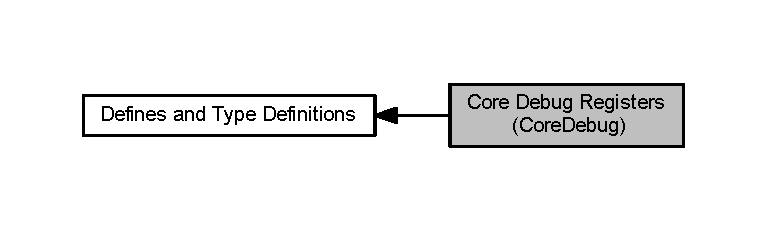
\includegraphics[width=350pt]{group___c_m_s_i_s___core_debug}
\end{center}
\end{figure}
\subsection*{Classes}
\begin{DoxyCompactItemize}
\item 
struct \hyperlink{struct_core_debug___type}{Core\+Debug\+\_\+\+Type}
\begin{DoxyCompactList}\small\item\em Structure type to access the Core Debug Register (Core\+Debug). \end{DoxyCompactList}\end{DoxyCompactItemize}
\subsection*{Macros}
\begin{DoxyCompactItemize}
\item 
\#define \hyperlink{group___c_m_s_i_s___core_debug_gac91280edd0ce932665cf75a23d11d842}{Core\+Debug\+\_\+\+D\+H\+C\+S\+R\+\_\+\+D\+B\+G\+K\+E\+Y\+\_\+\+Pos}~16U
\item 
\#define \hyperlink{group___c_m_s_i_s___core_debug_ga1ce997cee15edaafe4aed77751816ffc}{Core\+Debug\+\_\+\+D\+H\+C\+S\+R\+\_\+\+D\+B\+G\+K\+E\+Y\+\_\+\+Msk}~(0x\+F\+F\+F\+F\+U\+L $<$$<$ Core\+Debug\+\_\+\+D\+H\+C\+S\+R\+\_\+\+D\+B\+G\+K\+E\+Y\+\_\+\+Pos)
\item 
\#define \hyperlink{group___c_m_s_i_s___core_debug_ga6f934c5427ea057394268e541fa97753}{Core\+Debug\+\_\+\+D\+H\+C\+S\+R\+\_\+\+S\+\_\+\+R\+E\+S\+E\+T\+\_\+\+S\+T\+\_\+\+Pos}~25U
\item 
\#define \hyperlink{group___c_m_s_i_s___core_debug_gac474394bcceb31a8e09566c90b3f8922}{Core\+Debug\+\_\+\+D\+H\+C\+S\+R\+\_\+\+S\+\_\+\+R\+E\+S\+E\+T\+\_\+\+S\+T\+\_\+\+Msk}~(1\+U\+L $<$$<$ Core\+Debug\+\_\+\+D\+H\+C\+S\+R\+\_\+\+S\+\_\+\+R\+E\+S\+E\+T\+\_\+\+S\+T\+\_\+\+Pos)
\item 
\#define \hyperlink{group___c_m_s_i_s___core_debug_ga2328118f8b3574c871a53605eb17e730}{Core\+Debug\+\_\+\+D\+H\+C\+S\+R\+\_\+\+S\+\_\+\+R\+E\+T\+I\+R\+E\+\_\+\+S\+T\+\_\+\+Pos}~24U
\item 
\#define \hyperlink{group___c_m_s_i_s___core_debug_ga89dceb5325f6bcb36a0473d65fbfcfa6}{Core\+Debug\+\_\+\+D\+H\+C\+S\+R\+\_\+\+S\+\_\+\+R\+E\+T\+I\+R\+E\+\_\+\+S\+T\+\_\+\+Msk}~(1\+U\+L $<$$<$ Core\+Debug\+\_\+\+D\+H\+C\+S\+R\+\_\+\+S\+\_\+\+R\+E\+T\+I\+R\+E\+\_\+\+S\+T\+\_\+\+Pos)
\item 
\#define \hyperlink{group___c_m_s_i_s___core_debug_ga2900dd56a988a4ed27ad664d5642807e}{Core\+Debug\+\_\+\+D\+H\+C\+S\+R\+\_\+\+S\+\_\+\+L\+O\+C\+K\+U\+P\+\_\+\+Pos}~19U
\item 
\#define \hyperlink{group___c_m_s_i_s___core_debug_ga7b67e4506d7f464ef5dafd6219739756}{Core\+Debug\+\_\+\+D\+H\+C\+S\+R\+\_\+\+S\+\_\+\+L\+O\+C\+K\+U\+P\+\_\+\+Msk}~(1\+U\+L $<$$<$ Core\+Debug\+\_\+\+D\+H\+C\+S\+R\+\_\+\+S\+\_\+\+L\+O\+C\+K\+U\+P\+\_\+\+Pos)
\item 
\#define \hyperlink{group___c_m_s_i_s___core_debug_ga349ccea33accc705595624c2d334fbcb}{Core\+Debug\+\_\+\+D\+H\+C\+S\+R\+\_\+\+S\+\_\+\+S\+L\+E\+E\+P\+\_\+\+Pos}~18U
\item 
\#define \hyperlink{group___c_m_s_i_s___core_debug_ga98d51538e645c2c1a422279cd85a0a25}{Core\+Debug\+\_\+\+D\+H\+C\+S\+R\+\_\+\+S\+\_\+\+S\+L\+E\+E\+P\+\_\+\+Msk}~(1\+U\+L $<$$<$ Core\+Debug\+\_\+\+D\+H\+C\+S\+R\+\_\+\+S\+\_\+\+S\+L\+E\+E\+P\+\_\+\+Pos)
\item 
\#define \hyperlink{group___c_m_s_i_s___core_debug_ga760a9a0d7f39951dc3f07d01f1f64772}{Core\+Debug\+\_\+\+D\+H\+C\+S\+R\+\_\+\+S\+\_\+\+H\+A\+L\+T\+\_\+\+Pos}~17U
\item 
\#define \hyperlink{group___c_m_s_i_s___core_debug_ga9f881ade3151a73bc5b02b73fe6473ca}{Core\+Debug\+\_\+\+D\+H\+C\+S\+R\+\_\+\+S\+\_\+\+H\+A\+L\+T\+\_\+\+Msk}~(1\+U\+L $<$$<$ Core\+Debug\+\_\+\+D\+H\+C\+S\+R\+\_\+\+S\+\_\+\+H\+A\+L\+T\+\_\+\+Pos)
\item 
\#define \hyperlink{group___c_m_s_i_s___core_debug_ga20a71871ca8768019c51168c70c3f41d}{Core\+Debug\+\_\+\+D\+H\+C\+S\+R\+\_\+\+S\+\_\+\+R\+E\+G\+R\+D\+Y\+\_\+\+Pos}~16U
\item 
\#define \hyperlink{group___c_m_s_i_s___core_debug_gac4cd6f3178de48f473d8903e8c847c07}{Core\+Debug\+\_\+\+D\+H\+C\+S\+R\+\_\+\+S\+\_\+\+R\+E\+G\+R\+D\+Y\+\_\+\+Msk}~(1\+U\+L $<$$<$ Core\+Debug\+\_\+\+D\+H\+C\+S\+R\+\_\+\+S\+\_\+\+R\+E\+G\+R\+D\+Y\+\_\+\+Pos)
\item 
\#define \hyperlink{group___c_m_s_i_s___core_debug_ga85747214e2656df6b05ec72e4d22bd6d}{Core\+Debug\+\_\+\+D\+H\+C\+S\+R\+\_\+\+C\+\_\+\+S\+N\+A\+P\+S\+T\+A\+L\+L\+\_\+\+Pos}~5U
\item 
\#define \hyperlink{group___c_m_s_i_s___core_debug_ga53aa99b2e39a67622f3b9973e079c2b4}{Core\+Debug\+\_\+\+D\+H\+C\+S\+R\+\_\+\+C\+\_\+\+S\+N\+A\+P\+S\+T\+A\+L\+L\+\_\+\+Msk}~(1\+U\+L $<$$<$ Core\+Debug\+\_\+\+D\+H\+C\+S\+R\+\_\+\+C\+\_\+\+S\+N\+A\+P\+S\+T\+A\+L\+L\+\_\+\+Pos)
\item 
\#define \hyperlink{group___c_m_s_i_s___core_debug_ga0d2907400eb948a4ea3886ca083ec8e3}{Core\+Debug\+\_\+\+D\+H\+C\+S\+R\+\_\+\+C\+\_\+\+M\+A\+S\+K\+I\+N\+T\+S\+\_\+\+Pos}~3U
\item 
\#define \hyperlink{group___c_m_s_i_s___core_debug_ga77fe1ef3c4a729c1c82fb62a94a51c31}{Core\+Debug\+\_\+\+D\+H\+C\+S\+R\+\_\+\+C\+\_\+\+M\+A\+S\+K\+I\+N\+T\+S\+\_\+\+Msk}~(1\+U\+L $<$$<$ Core\+Debug\+\_\+\+D\+H\+C\+S\+R\+\_\+\+C\+\_\+\+M\+A\+S\+K\+I\+N\+T\+S\+\_\+\+Pos)
\item 
\#define \hyperlink{group___c_m_s_i_s___core_debug_gae1fc39e80de54c0339cbb1b298a9f0f9}{Core\+Debug\+\_\+\+D\+H\+C\+S\+R\+\_\+\+C\+\_\+\+S\+T\+E\+P\+\_\+\+Pos}~2U
\item 
\#define \hyperlink{group___c_m_s_i_s___core_debug_gae6bda72fbd32cc5734ff3542170dc00d}{Core\+Debug\+\_\+\+D\+H\+C\+S\+R\+\_\+\+C\+\_\+\+S\+T\+E\+P\+\_\+\+Msk}~(1\+U\+L $<$$<$ Core\+Debug\+\_\+\+D\+H\+C\+S\+R\+\_\+\+C\+\_\+\+S\+T\+E\+P\+\_\+\+Pos)
\item 
\#define \hyperlink{group___c_m_s_i_s___core_debug_gaddf1d43f8857e4efc3dc4e6b15509692}{Core\+Debug\+\_\+\+D\+H\+C\+S\+R\+\_\+\+C\+\_\+\+H\+A\+L\+T\+\_\+\+Pos}~1U
\item 
\#define \hyperlink{group___c_m_s_i_s___core_debug_ga1d905a3aa594eb2e8bb78bcc4da05b3f}{Core\+Debug\+\_\+\+D\+H\+C\+S\+R\+\_\+\+C\+\_\+\+H\+A\+L\+T\+\_\+\+Msk}~(1\+U\+L $<$$<$ Core\+Debug\+\_\+\+D\+H\+C\+S\+R\+\_\+\+C\+\_\+\+H\+A\+L\+T\+\_\+\+Pos)
\item 
\#define \hyperlink{group___c_m_s_i_s___core_debug_gab557abb5b172b74d2cf44efb9d824e4e}{Core\+Debug\+\_\+\+D\+H\+C\+S\+R\+\_\+\+C\+\_\+\+D\+E\+B\+U\+G\+E\+N\+\_\+\+Pos}~0U
\item 
\#define \hyperlink{group___c_m_s_i_s___core_debug_gab815c741a4fc2a61988cd2fb7594210b}{Core\+Debug\+\_\+\+D\+H\+C\+S\+R\+\_\+\+C\+\_\+\+D\+E\+B\+U\+G\+E\+N\+\_\+\+Msk}~(1\+U\+L /$\ast$$<$$<$ Core\+Debug\+\_\+\+D\+H\+C\+S\+R\+\_\+\+C\+\_\+\+D\+E\+B\+U\+G\+E\+N\+\_\+\+Pos$\ast$/)
\item 
\#define \hyperlink{group___c_m_s_i_s___core_debug_ga51e75942fc0614bc9bb2c0e96fcdda9a}{Core\+Debug\+\_\+\+D\+C\+R\+S\+R\+\_\+\+R\+E\+G\+Wn\+R\+\_\+\+Pos}~16U
\item 
\#define \hyperlink{group___c_m_s_i_s___core_debug_ga1eef4992d8f84bc6c0dffed1c87f90a5}{Core\+Debug\+\_\+\+D\+C\+R\+S\+R\+\_\+\+R\+E\+G\+Wn\+R\+\_\+\+Msk}~(1\+U\+L $<$$<$ Core\+Debug\+\_\+\+D\+C\+R\+S\+R\+\_\+\+R\+E\+G\+Wn\+R\+\_\+\+Pos)
\item 
\#define \hyperlink{group___c_m_s_i_s___core_debug_ga52182c8a9f63a52470244c0bc2064f7b}{Core\+Debug\+\_\+\+D\+C\+R\+S\+R\+\_\+\+R\+E\+G\+S\+E\+L\+\_\+\+Pos}~0U
\item 
\#define \hyperlink{group___c_m_s_i_s___core_debug_ga17cafbd72b55030219ce5609baa7c01d}{Core\+Debug\+\_\+\+D\+C\+R\+S\+R\+\_\+\+R\+E\+G\+S\+E\+L\+\_\+\+Msk}~(0x1\+F\+U\+L /$\ast$$<$$<$ Core\+Debug\+\_\+\+D\+C\+R\+S\+R\+\_\+\+R\+E\+G\+S\+E\+L\+\_\+\+Pos$\ast$/)
\item 
\#define \hyperlink{group___c_m_s_i_s___core_debug_ga6ff2102b98f86540224819a1b767ba39}{Core\+Debug\+\_\+\+D\+E\+M\+C\+R\+\_\+\+T\+R\+C\+E\+N\+A\+\_\+\+Pos}~24U
\item 
\#define \hyperlink{group___c_m_s_i_s___core_debug_ga5e99652c1df93b441257389f49407834}{Core\+Debug\+\_\+\+D\+E\+M\+C\+R\+\_\+\+T\+R\+C\+E\+N\+A\+\_\+\+Msk}~(1\+U\+L $<$$<$ Core\+Debug\+\_\+\+D\+E\+M\+C\+R\+\_\+\+T\+R\+C\+E\+N\+A\+\_\+\+Pos)
\item 
\#define \hyperlink{group___c_m_s_i_s___core_debug_ga341020a3b7450416d72544eaf8e57a64}{Core\+Debug\+\_\+\+D\+E\+M\+C\+R\+\_\+\+M\+O\+N\+\_\+\+R\+E\+Q\+\_\+\+Pos}~19U
\item 
\#define \hyperlink{group___c_m_s_i_s___core_debug_gae6384cbe8045051186d13ef9cdeace95}{Core\+Debug\+\_\+\+D\+E\+M\+C\+R\+\_\+\+M\+O\+N\+\_\+\+R\+E\+Q\+\_\+\+Msk}~(1\+U\+L $<$$<$ Core\+Debug\+\_\+\+D\+E\+M\+C\+R\+\_\+\+M\+O\+N\+\_\+\+R\+E\+Q\+\_\+\+Pos)
\item 
\#define \hyperlink{group___c_m_s_i_s___core_debug_ga9ae10710684e14a1a534e785ef390e1b}{Core\+Debug\+\_\+\+D\+E\+M\+C\+R\+\_\+\+M\+O\+N\+\_\+\+S\+T\+E\+P\+\_\+\+Pos}~18U
\item 
\#define \hyperlink{group___c_m_s_i_s___core_debug_ga2ded814556de96fc369de7ae9a7ceb98}{Core\+Debug\+\_\+\+D\+E\+M\+C\+R\+\_\+\+M\+O\+N\+\_\+\+S\+T\+E\+P\+\_\+\+Msk}~(1\+U\+L $<$$<$ Core\+Debug\+\_\+\+D\+E\+M\+C\+R\+\_\+\+M\+O\+N\+\_\+\+S\+T\+E\+P\+\_\+\+Pos)
\item 
\#define \hyperlink{group___c_m_s_i_s___core_debug_ga1e2f706a59e0d8131279af1c7e152f8d}{Core\+Debug\+\_\+\+D\+E\+M\+C\+R\+\_\+\+M\+O\+N\+\_\+\+P\+E\+N\+D\+\_\+\+Pos}~17U
\item 
\#define \hyperlink{group___c_m_s_i_s___core_debug_ga68ec55930269fab78e733dcfa32392f8}{Core\+Debug\+\_\+\+D\+E\+M\+C\+R\+\_\+\+M\+O\+N\+\_\+\+P\+E\+N\+D\+\_\+\+Msk}~(1\+U\+L $<$$<$ Core\+Debug\+\_\+\+D\+E\+M\+C\+R\+\_\+\+M\+O\+N\+\_\+\+P\+E\+N\+D\+\_\+\+Pos)
\item 
\#define \hyperlink{group___c_m_s_i_s___core_debug_ga802829678f6871863ae9ecf60a10425c}{Core\+Debug\+\_\+\+D\+E\+M\+C\+R\+\_\+\+M\+O\+N\+\_\+\+E\+N\+\_\+\+Pos}~16U
\item 
\#define \hyperlink{group___c_m_s_i_s___core_debug_gac2b46b9b65bf8d23027f255fc9641977}{Core\+Debug\+\_\+\+D\+E\+M\+C\+R\+\_\+\+M\+O\+N\+\_\+\+E\+N\+\_\+\+Msk}~(1\+U\+L $<$$<$ Core\+Debug\+\_\+\+D\+E\+M\+C\+R\+\_\+\+M\+O\+N\+\_\+\+E\+N\+\_\+\+Pos)
\item 
\#define \hyperlink{group___c_m_s_i_s___core_debug_gaed9f42053031a9a30cd8054623304c0a}{Core\+Debug\+\_\+\+D\+E\+M\+C\+R\+\_\+\+V\+C\+\_\+\+H\+A\+R\+D\+E\+R\+R\+\_\+\+Pos}~10U
\item 
\#define \hyperlink{group___c_m_s_i_s___core_debug_ga803fc98c5bb85f10f0347b23794847d1}{Core\+Debug\+\_\+\+D\+E\+M\+C\+R\+\_\+\+V\+C\+\_\+\+H\+A\+R\+D\+E\+R\+R\+\_\+\+Msk}~(1\+U\+L $<$$<$ Core\+Debug\+\_\+\+D\+E\+M\+C\+R\+\_\+\+V\+C\+\_\+\+H\+A\+R\+D\+E\+R\+R\+\_\+\+Pos)
\item 
\#define \hyperlink{group___c_m_s_i_s___core_debug_ga22079a6e436f23b90308be97e19cf07e}{Core\+Debug\+\_\+\+D\+E\+M\+C\+R\+\_\+\+V\+C\+\_\+\+I\+N\+T\+E\+R\+R\+\_\+\+Pos}~9U
\item 
\#define \hyperlink{group___c_m_s_i_s___core_debug_gad6815d8e3df302d2f0ff2c2c734ed29a}{Core\+Debug\+\_\+\+D\+E\+M\+C\+R\+\_\+\+V\+C\+\_\+\+I\+N\+T\+E\+R\+R\+\_\+\+Msk}~(1\+U\+L $<$$<$ Core\+Debug\+\_\+\+D\+E\+M\+C\+R\+\_\+\+V\+C\+\_\+\+I\+N\+T\+E\+R\+R\+\_\+\+Pos)
\item 
\#define \hyperlink{group___c_m_s_i_s___core_debug_gab8e3d8f0f9590a51bbf10f6da3ad6933}{Core\+Debug\+\_\+\+D\+E\+M\+C\+R\+\_\+\+V\+C\+\_\+\+B\+U\+S\+E\+R\+R\+\_\+\+Pos}~8U
\item 
\#define \hyperlink{group___c_m_s_i_s___core_debug_ga9d29546aefe3ca8662a7fe48dd4a5b2b}{Core\+Debug\+\_\+\+D\+E\+M\+C\+R\+\_\+\+V\+C\+\_\+\+B\+U\+S\+E\+R\+R\+\_\+\+Msk}~(1\+U\+L $<$$<$ Core\+Debug\+\_\+\+D\+E\+M\+C\+R\+\_\+\+V\+C\+\_\+\+B\+U\+S\+E\+R\+R\+\_\+\+Pos)
\item 
\#define \hyperlink{group___c_m_s_i_s___core_debug_ga16f0d3d2ce1e1e8cd762d938ac56c4ac}{Core\+Debug\+\_\+\+D\+E\+M\+C\+R\+\_\+\+V\+C\+\_\+\+S\+T\+A\+T\+E\+R\+R\+\_\+\+Pos}~7U
\item 
\#define \hyperlink{group___c_m_s_i_s___core_debug_gaa38b947d77672c48bba1280c0a642e19}{Core\+Debug\+\_\+\+D\+E\+M\+C\+R\+\_\+\+V\+C\+\_\+\+S\+T\+A\+T\+E\+R\+R\+\_\+\+Msk}~(1\+U\+L $<$$<$ Core\+Debug\+\_\+\+D\+E\+M\+C\+R\+\_\+\+V\+C\+\_\+\+S\+T\+A\+T\+E\+R\+R\+\_\+\+Pos)
\item 
\#define \hyperlink{group___c_m_s_i_s___core_debug_ga10fc7c53bca904c128bc8e1a03072d50}{Core\+Debug\+\_\+\+D\+E\+M\+C\+R\+\_\+\+V\+C\+\_\+\+C\+H\+K\+E\+R\+R\+\_\+\+Pos}~6U
\item 
\#define \hyperlink{group___c_m_s_i_s___core_debug_ga2f98b461d19746ab2febfddebb73da6f}{Core\+Debug\+\_\+\+D\+E\+M\+C\+R\+\_\+\+V\+C\+\_\+\+C\+H\+K\+E\+R\+R\+\_\+\+Msk}~(1\+U\+L $<$$<$ Core\+Debug\+\_\+\+D\+E\+M\+C\+R\+\_\+\+V\+C\+\_\+\+C\+H\+K\+E\+R\+R\+\_\+\+Pos)
\item 
\#define \hyperlink{group___c_m_s_i_s___core_debug_gac9d13eb2add61f610d5ced1f7ad2adf8}{Core\+Debug\+\_\+\+D\+E\+M\+C\+R\+\_\+\+V\+C\+\_\+\+N\+O\+C\+P\+E\+R\+R\+\_\+\+Pos}~5U
\item 
\#define \hyperlink{group___c_m_s_i_s___core_debug_ga03ee58b1b02fdbf21612809034562f1c}{Core\+Debug\+\_\+\+D\+E\+M\+C\+R\+\_\+\+V\+C\+\_\+\+N\+O\+C\+P\+E\+R\+R\+\_\+\+Msk}~(1\+U\+L $<$$<$ Core\+Debug\+\_\+\+D\+E\+M\+C\+R\+\_\+\+V\+C\+\_\+\+N\+O\+C\+P\+E\+R\+R\+\_\+\+Pos)
\item 
\#define \hyperlink{group___c_m_s_i_s___core_debug_ga444454f7c7748e76cd76c3809c887c41}{Core\+Debug\+\_\+\+D\+E\+M\+C\+R\+\_\+\+V\+C\+\_\+\+M\+M\+E\+R\+R\+\_\+\+Pos}~4U
\item 
\#define \hyperlink{group___c_m_s_i_s___core_debug_gad420a9b60620584faaca6289e83d3a87}{Core\+Debug\+\_\+\+D\+E\+M\+C\+R\+\_\+\+V\+C\+\_\+\+M\+M\+E\+R\+R\+\_\+\+Msk}~(1\+U\+L $<$$<$ Core\+Debug\+\_\+\+D\+E\+M\+C\+R\+\_\+\+V\+C\+\_\+\+M\+M\+E\+R\+R\+\_\+\+Pos)
\item 
\#define \hyperlink{group___c_m_s_i_s___core_debug_ga9fcf09666f7063a7303117aa32a85d5a}{Core\+Debug\+\_\+\+D\+E\+M\+C\+R\+\_\+\+V\+C\+\_\+\+C\+O\+R\+E\+R\+E\+S\+E\+T\+\_\+\+Pos}~0U
\item 
\#define \hyperlink{group___c_m_s_i_s___core_debug_ga906476e53c1e1487c30f3a1181df9e30}{Core\+Debug\+\_\+\+D\+E\+M\+C\+R\+\_\+\+V\+C\+\_\+\+C\+O\+R\+E\+R\+E\+S\+E\+T\+\_\+\+Msk}~(1\+U\+L /$\ast$$<$$<$ Core\+Debug\+\_\+\+D\+E\+M\+C\+R\+\_\+\+V\+C\+\_\+\+C\+O\+R\+E\+R\+E\+S\+E\+T\+\_\+\+Pos$\ast$/)
\item 
\#define \hyperlink{group___c_m_s_i_s___core_debug_gac91280edd0ce932665cf75a23d11d842}{Core\+Debug\+\_\+\+D\+H\+C\+S\+R\+\_\+\+D\+B\+G\+K\+E\+Y\+\_\+\+Pos}~16U
\item 
\#define \hyperlink{group___c_m_s_i_s___core_debug_ga1ce997cee15edaafe4aed77751816ffc}{Core\+Debug\+\_\+\+D\+H\+C\+S\+R\+\_\+\+D\+B\+G\+K\+E\+Y\+\_\+\+Msk}~(0x\+F\+F\+F\+F\+U\+L $<$$<$ Core\+Debug\+\_\+\+D\+H\+C\+S\+R\+\_\+\+D\+B\+G\+K\+E\+Y\+\_\+\+Pos)
\item 
\#define \hyperlink{group___c_m_s_i_s___core_debug_ga6f934c5427ea057394268e541fa97753}{Core\+Debug\+\_\+\+D\+H\+C\+S\+R\+\_\+\+S\+\_\+\+R\+E\+S\+E\+T\+\_\+\+S\+T\+\_\+\+Pos}~25U
\item 
\#define \hyperlink{group___c_m_s_i_s___core_debug_gac474394bcceb31a8e09566c90b3f8922}{Core\+Debug\+\_\+\+D\+H\+C\+S\+R\+\_\+\+S\+\_\+\+R\+E\+S\+E\+T\+\_\+\+S\+T\+\_\+\+Msk}~(1\+U\+L $<$$<$ Core\+Debug\+\_\+\+D\+H\+C\+S\+R\+\_\+\+S\+\_\+\+R\+E\+S\+E\+T\+\_\+\+S\+T\+\_\+\+Pos)
\item 
\#define \hyperlink{group___c_m_s_i_s___core_debug_ga2328118f8b3574c871a53605eb17e730}{Core\+Debug\+\_\+\+D\+H\+C\+S\+R\+\_\+\+S\+\_\+\+R\+E\+T\+I\+R\+E\+\_\+\+S\+T\+\_\+\+Pos}~24U
\item 
\#define \hyperlink{group___c_m_s_i_s___core_debug_ga89dceb5325f6bcb36a0473d65fbfcfa6}{Core\+Debug\+\_\+\+D\+H\+C\+S\+R\+\_\+\+S\+\_\+\+R\+E\+T\+I\+R\+E\+\_\+\+S\+T\+\_\+\+Msk}~(1\+U\+L $<$$<$ Core\+Debug\+\_\+\+D\+H\+C\+S\+R\+\_\+\+S\+\_\+\+R\+E\+T\+I\+R\+E\+\_\+\+S\+T\+\_\+\+Pos)
\item 
\#define \hyperlink{group___c_m_s_i_s___core_debug_ga2900dd56a988a4ed27ad664d5642807e}{Core\+Debug\+\_\+\+D\+H\+C\+S\+R\+\_\+\+S\+\_\+\+L\+O\+C\+K\+U\+P\+\_\+\+Pos}~19U
\item 
\#define \hyperlink{group___c_m_s_i_s___core_debug_ga7b67e4506d7f464ef5dafd6219739756}{Core\+Debug\+\_\+\+D\+H\+C\+S\+R\+\_\+\+S\+\_\+\+L\+O\+C\+K\+U\+P\+\_\+\+Msk}~(1\+U\+L $<$$<$ Core\+Debug\+\_\+\+D\+H\+C\+S\+R\+\_\+\+S\+\_\+\+L\+O\+C\+K\+U\+P\+\_\+\+Pos)
\item 
\#define \hyperlink{group___c_m_s_i_s___core_debug_ga349ccea33accc705595624c2d334fbcb}{Core\+Debug\+\_\+\+D\+H\+C\+S\+R\+\_\+\+S\+\_\+\+S\+L\+E\+E\+P\+\_\+\+Pos}~18U
\item 
\#define \hyperlink{group___c_m_s_i_s___core_debug_ga98d51538e645c2c1a422279cd85a0a25}{Core\+Debug\+\_\+\+D\+H\+C\+S\+R\+\_\+\+S\+\_\+\+S\+L\+E\+E\+P\+\_\+\+Msk}~(1\+U\+L $<$$<$ Core\+Debug\+\_\+\+D\+H\+C\+S\+R\+\_\+\+S\+\_\+\+S\+L\+E\+E\+P\+\_\+\+Pos)
\item 
\#define \hyperlink{group___c_m_s_i_s___core_debug_ga760a9a0d7f39951dc3f07d01f1f64772}{Core\+Debug\+\_\+\+D\+H\+C\+S\+R\+\_\+\+S\+\_\+\+H\+A\+L\+T\+\_\+\+Pos}~17U
\item 
\#define \hyperlink{group___c_m_s_i_s___core_debug_ga9f881ade3151a73bc5b02b73fe6473ca}{Core\+Debug\+\_\+\+D\+H\+C\+S\+R\+\_\+\+S\+\_\+\+H\+A\+L\+T\+\_\+\+Msk}~(1\+U\+L $<$$<$ Core\+Debug\+\_\+\+D\+H\+C\+S\+R\+\_\+\+S\+\_\+\+H\+A\+L\+T\+\_\+\+Pos)
\item 
\#define \hyperlink{group___c_m_s_i_s___core_debug_ga20a71871ca8768019c51168c70c3f41d}{Core\+Debug\+\_\+\+D\+H\+C\+S\+R\+\_\+\+S\+\_\+\+R\+E\+G\+R\+D\+Y\+\_\+\+Pos}~16U
\item 
\#define \hyperlink{group___c_m_s_i_s___core_debug_gac4cd6f3178de48f473d8903e8c847c07}{Core\+Debug\+\_\+\+D\+H\+C\+S\+R\+\_\+\+S\+\_\+\+R\+E\+G\+R\+D\+Y\+\_\+\+Msk}~(1\+U\+L $<$$<$ Core\+Debug\+\_\+\+D\+H\+C\+S\+R\+\_\+\+S\+\_\+\+R\+E\+G\+R\+D\+Y\+\_\+\+Pos)
\item 
\#define \hyperlink{group___c_m_s_i_s___core_debug_ga85747214e2656df6b05ec72e4d22bd6d}{Core\+Debug\+\_\+\+D\+H\+C\+S\+R\+\_\+\+C\+\_\+\+S\+N\+A\+P\+S\+T\+A\+L\+L\+\_\+\+Pos}~5U
\item 
\#define \hyperlink{group___c_m_s_i_s___core_debug_ga53aa99b2e39a67622f3b9973e079c2b4}{Core\+Debug\+\_\+\+D\+H\+C\+S\+R\+\_\+\+C\+\_\+\+S\+N\+A\+P\+S\+T\+A\+L\+L\+\_\+\+Msk}~(1\+U\+L $<$$<$ Core\+Debug\+\_\+\+D\+H\+C\+S\+R\+\_\+\+C\+\_\+\+S\+N\+A\+P\+S\+T\+A\+L\+L\+\_\+\+Pos)
\item 
\#define \hyperlink{group___c_m_s_i_s___core_debug_ga0d2907400eb948a4ea3886ca083ec8e3}{Core\+Debug\+\_\+\+D\+H\+C\+S\+R\+\_\+\+C\+\_\+\+M\+A\+S\+K\+I\+N\+T\+S\+\_\+\+Pos}~3U
\item 
\#define \hyperlink{group___c_m_s_i_s___core_debug_ga77fe1ef3c4a729c1c82fb62a94a51c31}{Core\+Debug\+\_\+\+D\+H\+C\+S\+R\+\_\+\+C\+\_\+\+M\+A\+S\+K\+I\+N\+T\+S\+\_\+\+Msk}~(1\+U\+L $<$$<$ Core\+Debug\+\_\+\+D\+H\+C\+S\+R\+\_\+\+C\+\_\+\+M\+A\+S\+K\+I\+N\+T\+S\+\_\+\+Pos)
\item 
\#define \hyperlink{group___c_m_s_i_s___core_debug_gae1fc39e80de54c0339cbb1b298a9f0f9}{Core\+Debug\+\_\+\+D\+H\+C\+S\+R\+\_\+\+C\+\_\+\+S\+T\+E\+P\+\_\+\+Pos}~2U
\item 
\#define \hyperlink{group___c_m_s_i_s___core_debug_gae6bda72fbd32cc5734ff3542170dc00d}{Core\+Debug\+\_\+\+D\+H\+C\+S\+R\+\_\+\+C\+\_\+\+S\+T\+E\+P\+\_\+\+Msk}~(1\+U\+L $<$$<$ Core\+Debug\+\_\+\+D\+H\+C\+S\+R\+\_\+\+C\+\_\+\+S\+T\+E\+P\+\_\+\+Pos)
\item 
\#define \hyperlink{group___c_m_s_i_s___core_debug_gaddf1d43f8857e4efc3dc4e6b15509692}{Core\+Debug\+\_\+\+D\+H\+C\+S\+R\+\_\+\+C\+\_\+\+H\+A\+L\+T\+\_\+\+Pos}~1U
\item 
\#define \hyperlink{group___c_m_s_i_s___core_debug_ga1d905a3aa594eb2e8bb78bcc4da05b3f}{Core\+Debug\+\_\+\+D\+H\+C\+S\+R\+\_\+\+C\+\_\+\+H\+A\+L\+T\+\_\+\+Msk}~(1\+U\+L $<$$<$ Core\+Debug\+\_\+\+D\+H\+C\+S\+R\+\_\+\+C\+\_\+\+H\+A\+L\+T\+\_\+\+Pos)
\item 
\#define \hyperlink{group___c_m_s_i_s___core_debug_gab557abb5b172b74d2cf44efb9d824e4e}{Core\+Debug\+\_\+\+D\+H\+C\+S\+R\+\_\+\+C\+\_\+\+D\+E\+B\+U\+G\+E\+N\+\_\+\+Pos}~0U
\item 
\#define \hyperlink{group___c_m_s_i_s___core_debug_gab815c741a4fc2a61988cd2fb7594210b}{Core\+Debug\+\_\+\+D\+H\+C\+S\+R\+\_\+\+C\+\_\+\+D\+E\+B\+U\+G\+E\+N\+\_\+\+Msk}~(1\+U\+L /$\ast$$<$$<$ Core\+Debug\+\_\+\+D\+H\+C\+S\+R\+\_\+\+C\+\_\+\+D\+E\+B\+U\+G\+E\+N\+\_\+\+Pos$\ast$/)
\item 
\#define \hyperlink{group___c_m_s_i_s___core_debug_ga51e75942fc0614bc9bb2c0e96fcdda9a}{Core\+Debug\+\_\+\+D\+C\+R\+S\+R\+\_\+\+R\+E\+G\+Wn\+R\+\_\+\+Pos}~16U
\item 
\#define \hyperlink{group___c_m_s_i_s___core_debug_ga1eef4992d8f84bc6c0dffed1c87f90a5}{Core\+Debug\+\_\+\+D\+C\+R\+S\+R\+\_\+\+R\+E\+G\+Wn\+R\+\_\+\+Msk}~(1\+U\+L $<$$<$ Core\+Debug\+\_\+\+D\+C\+R\+S\+R\+\_\+\+R\+E\+G\+Wn\+R\+\_\+\+Pos)
\item 
\#define \hyperlink{group___c_m_s_i_s___core_debug_ga52182c8a9f63a52470244c0bc2064f7b}{Core\+Debug\+\_\+\+D\+C\+R\+S\+R\+\_\+\+R\+E\+G\+S\+E\+L\+\_\+\+Pos}~0U
\item 
\#define \hyperlink{group___c_m_s_i_s___core_debug_ga17cafbd72b55030219ce5609baa7c01d}{Core\+Debug\+\_\+\+D\+C\+R\+S\+R\+\_\+\+R\+E\+G\+S\+E\+L\+\_\+\+Msk}~(0x1\+F\+U\+L /$\ast$$<$$<$ Core\+Debug\+\_\+\+D\+C\+R\+S\+R\+\_\+\+R\+E\+G\+S\+E\+L\+\_\+\+Pos$\ast$/)
\item 
\#define \hyperlink{group___c_m_s_i_s___core_debug_ga6ff2102b98f86540224819a1b767ba39}{Core\+Debug\+\_\+\+D\+E\+M\+C\+R\+\_\+\+T\+R\+C\+E\+N\+A\+\_\+\+Pos}~24U
\item 
\#define \hyperlink{group___c_m_s_i_s___core_debug_ga5e99652c1df93b441257389f49407834}{Core\+Debug\+\_\+\+D\+E\+M\+C\+R\+\_\+\+T\+R\+C\+E\+N\+A\+\_\+\+Msk}~(1\+U\+L $<$$<$ Core\+Debug\+\_\+\+D\+E\+M\+C\+R\+\_\+\+T\+R\+C\+E\+N\+A\+\_\+\+Pos)
\item 
\#define \hyperlink{group___c_m_s_i_s___core_debug_ga341020a3b7450416d72544eaf8e57a64}{Core\+Debug\+\_\+\+D\+E\+M\+C\+R\+\_\+\+M\+O\+N\+\_\+\+R\+E\+Q\+\_\+\+Pos}~19U
\item 
\#define \hyperlink{group___c_m_s_i_s___core_debug_gae6384cbe8045051186d13ef9cdeace95}{Core\+Debug\+\_\+\+D\+E\+M\+C\+R\+\_\+\+M\+O\+N\+\_\+\+R\+E\+Q\+\_\+\+Msk}~(1\+U\+L $<$$<$ Core\+Debug\+\_\+\+D\+E\+M\+C\+R\+\_\+\+M\+O\+N\+\_\+\+R\+E\+Q\+\_\+\+Pos)
\item 
\#define \hyperlink{group___c_m_s_i_s___core_debug_ga9ae10710684e14a1a534e785ef390e1b}{Core\+Debug\+\_\+\+D\+E\+M\+C\+R\+\_\+\+M\+O\+N\+\_\+\+S\+T\+E\+P\+\_\+\+Pos}~18U
\item 
\#define \hyperlink{group___c_m_s_i_s___core_debug_ga2ded814556de96fc369de7ae9a7ceb98}{Core\+Debug\+\_\+\+D\+E\+M\+C\+R\+\_\+\+M\+O\+N\+\_\+\+S\+T\+E\+P\+\_\+\+Msk}~(1\+U\+L $<$$<$ Core\+Debug\+\_\+\+D\+E\+M\+C\+R\+\_\+\+M\+O\+N\+\_\+\+S\+T\+E\+P\+\_\+\+Pos)
\item 
\#define \hyperlink{group___c_m_s_i_s___core_debug_ga1e2f706a59e0d8131279af1c7e152f8d}{Core\+Debug\+\_\+\+D\+E\+M\+C\+R\+\_\+\+M\+O\+N\+\_\+\+P\+E\+N\+D\+\_\+\+Pos}~17U
\item 
\#define \hyperlink{group___c_m_s_i_s___core_debug_ga68ec55930269fab78e733dcfa32392f8}{Core\+Debug\+\_\+\+D\+E\+M\+C\+R\+\_\+\+M\+O\+N\+\_\+\+P\+E\+N\+D\+\_\+\+Msk}~(1\+U\+L $<$$<$ Core\+Debug\+\_\+\+D\+E\+M\+C\+R\+\_\+\+M\+O\+N\+\_\+\+P\+E\+N\+D\+\_\+\+Pos)
\item 
\#define \hyperlink{group___c_m_s_i_s___core_debug_ga802829678f6871863ae9ecf60a10425c}{Core\+Debug\+\_\+\+D\+E\+M\+C\+R\+\_\+\+M\+O\+N\+\_\+\+E\+N\+\_\+\+Pos}~16U
\item 
\#define \hyperlink{group___c_m_s_i_s___core_debug_gac2b46b9b65bf8d23027f255fc9641977}{Core\+Debug\+\_\+\+D\+E\+M\+C\+R\+\_\+\+M\+O\+N\+\_\+\+E\+N\+\_\+\+Msk}~(1\+U\+L $<$$<$ Core\+Debug\+\_\+\+D\+E\+M\+C\+R\+\_\+\+M\+O\+N\+\_\+\+E\+N\+\_\+\+Pos)
\item 
\#define \hyperlink{group___c_m_s_i_s___core_debug_gaed9f42053031a9a30cd8054623304c0a}{Core\+Debug\+\_\+\+D\+E\+M\+C\+R\+\_\+\+V\+C\+\_\+\+H\+A\+R\+D\+E\+R\+R\+\_\+\+Pos}~10U
\item 
\#define \hyperlink{group___c_m_s_i_s___core_debug_ga803fc98c5bb85f10f0347b23794847d1}{Core\+Debug\+\_\+\+D\+E\+M\+C\+R\+\_\+\+V\+C\+\_\+\+H\+A\+R\+D\+E\+R\+R\+\_\+\+Msk}~(1\+U\+L $<$$<$ Core\+Debug\+\_\+\+D\+E\+M\+C\+R\+\_\+\+V\+C\+\_\+\+H\+A\+R\+D\+E\+R\+R\+\_\+\+Pos)
\item 
\#define \hyperlink{group___c_m_s_i_s___core_debug_ga22079a6e436f23b90308be97e19cf07e}{Core\+Debug\+\_\+\+D\+E\+M\+C\+R\+\_\+\+V\+C\+\_\+\+I\+N\+T\+E\+R\+R\+\_\+\+Pos}~9U
\item 
\#define \hyperlink{group___c_m_s_i_s___core_debug_gad6815d8e3df302d2f0ff2c2c734ed29a}{Core\+Debug\+\_\+\+D\+E\+M\+C\+R\+\_\+\+V\+C\+\_\+\+I\+N\+T\+E\+R\+R\+\_\+\+Msk}~(1\+U\+L $<$$<$ Core\+Debug\+\_\+\+D\+E\+M\+C\+R\+\_\+\+V\+C\+\_\+\+I\+N\+T\+E\+R\+R\+\_\+\+Pos)
\item 
\#define \hyperlink{group___c_m_s_i_s___core_debug_gab8e3d8f0f9590a51bbf10f6da3ad6933}{Core\+Debug\+\_\+\+D\+E\+M\+C\+R\+\_\+\+V\+C\+\_\+\+B\+U\+S\+E\+R\+R\+\_\+\+Pos}~8U
\item 
\#define \hyperlink{group___c_m_s_i_s___core_debug_ga9d29546aefe3ca8662a7fe48dd4a5b2b}{Core\+Debug\+\_\+\+D\+E\+M\+C\+R\+\_\+\+V\+C\+\_\+\+B\+U\+S\+E\+R\+R\+\_\+\+Msk}~(1\+U\+L $<$$<$ Core\+Debug\+\_\+\+D\+E\+M\+C\+R\+\_\+\+V\+C\+\_\+\+B\+U\+S\+E\+R\+R\+\_\+\+Pos)
\item 
\#define \hyperlink{group___c_m_s_i_s___core_debug_ga16f0d3d2ce1e1e8cd762d938ac56c4ac}{Core\+Debug\+\_\+\+D\+E\+M\+C\+R\+\_\+\+V\+C\+\_\+\+S\+T\+A\+T\+E\+R\+R\+\_\+\+Pos}~7U
\item 
\#define \hyperlink{group___c_m_s_i_s___core_debug_gaa38b947d77672c48bba1280c0a642e19}{Core\+Debug\+\_\+\+D\+E\+M\+C\+R\+\_\+\+V\+C\+\_\+\+S\+T\+A\+T\+E\+R\+R\+\_\+\+Msk}~(1\+U\+L $<$$<$ Core\+Debug\+\_\+\+D\+E\+M\+C\+R\+\_\+\+V\+C\+\_\+\+S\+T\+A\+T\+E\+R\+R\+\_\+\+Pos)
\item 
\#define \hyperlink{group___c_m_s_i_s___core_debug_ga10fc7c53bca904c128bc8e1a03072d50}{Core\+Debug\+\_\+\+D\+E\+M\+C\+R\+\_\+\+V\+C\+\_\+\+C\+H\+K\+E\+R\+R\+\_\+\+Pos}~6U
\item 
\#define \hyperlink{group___c_m_s_i_s___core_debug_ga2f98b461d19746ab2febfddebb73da6f}{Core\+Debug\+\_\+\+D\+E\+M\+C\+R\+\_\+\+V\+C\+\_\+\+C\+H\+K\+E\+R\+R\+\_\+\+Msk}~(1\+U\+L $<$$<$ Core\+Debug\+\_\+\+D\+E\+M\+C\+R\+\_\+\+V\+C\+\_\+\+C\+H\+K\+E\+R\+R\+\_\+\+Pos)
\item 
\#define \hyperlink{group___c_m_s_i_s___core_debug_gac9d13eb2add61f610d5ced1f7ad2adf8}{Core\+Debug\+\_\+\+D\+E\+M\+C\+R\+\_\+\+V\+C\+\_\+\+N\+O\+C\+P\+E\+R\+R\+\_\+\+Pos}~5U
\item 
\#define \hyperlink{group___c_m_s_i_s___core_debug_ga03ee58b1b02fdbf21612809034562f1c}{Core\+Debug\+\_\+\+D\+E\+M\+C\+R\+\_\+\+V\+C\+\_\+\+N\+O\+C\+P\+E\+R\+R\+\_\+\+Msk}~(1\+U\+L $<$$<$ Core\+Debug\+\_\+\+D\+E\+M\+C\+R\+\_\+\+V\+C\+\_\+\+N\+O\+C\+P\+E\+R\+R\+\_\+\+Pos)
\item 
\#define \hyperlink{group___c_m_s_i_s___core_debug_ga444454f7c7748e76cd76c3809c887c41}{Core\+Debug\+\_\+\+D\+E\+M\+C\+R\+\_\+\+V\+C\+\_\+\+M\+M\+E\+R\+R\+\_\+\+Pos}~4U
\item 
\#define \hyperlink{group___c_m_s_i_s___core_debug_gad420a9b60620584faaca6289e83d3a87}{Core\+Debug\+\_\+\+D\+E\+M\+C\+R\+\_\+\+V\+C\+\_\+\+M\+M\+E\+R\+R\+\_\+\+Msk}~(1\+U\+L $<$$<$ Core\+Debug\+\_\+\+D\+E\+M\+C\+R\+\_\+\+V\+C\+\_\+\+M\+M\+E\+R\+R\+\_\+\+Pos)
\item 
\#define \hyperlink{group___c_m_s_i_s___core_debug_ga9fcf09666f7063a7303117aa32a85d5a}{Core\+Debug\+\_\+\+D\+E\+M\+C\+R\+\_\+\+V\+C\+\_\+\+C\+O\+R\+E\+R\+E\+S\+E\+T\+\_\+\+Pos}~0U
\item 
\#define \hyperlink{group___c_m_s_i_s___core_debug_ga906476e53c1e1487c30f3a1181df9e30}{Core\+Debug\+\_\+\+D\+E\+M\+C\+R\+\_\+\+V\+C\+\_\+\+C\+O\+R\+E\+R\+E\+S\+E\+T\+\_\+\+Msk}~(1\+U\+L /$\ast$$<$$<$ Core\+Debug\+\_\+\+D\+E\+M\+C\+R\+\_\+\+V\+C\+\_\+\+C\+O\+R\+E\+R\+E\+S\+E\+T\+\_\+\+Pos$\ast$/)
\item 
\#define \hyperlink{group___c_m_s_i_s___core_debug_gac91280edd0ce932665cf75a23d11d842}{Core\+Debug\+\_\+\+D\+H\+C\+S\+R\+\_\+\+D\+B\+G\+K\+E\+Y\+\_\+\+Pos}~16U
\item 
\#define \hyperlink{group___c_m_s_i_s___core_debug_ga1ce997cee15edaafe4aed77751816ffc}{Core\+Debug\+\_\+\+D\+H\+C\+S\+R\+\_\+\+D\+B\+G\+K\+E\+Y\+\_\+\+Msk}~(0x\+F\+F\+F\+F\+U\+L $<$$<$ Core\+Debug\+\_\+\+D\+H\+C\+S\+R\+\_\+\+D\+B\+G\+K\+E\+Y\+\_\+\+Pos)
\item 
\#define \hyperlink{group___c_m_s_i_s___core_debug_ga6f934c5427ea057394268e541fa97753}{Core\+Debug\+\_\+\+D\+H\+C\+S\+R\+\_\+\+S\+\_\+\+R\+E\+S\+E\+T\+\_\+\+S\+T\+\_\+\+Pos}~25U
\item 
\#define \hyperlink{group___c_m_s_i_s___core_debug_gac474394bcceb31a8e09566c90b3f8922}{Core\+Debug\+\_\+\+D\+H\+C\+S\+R\+\_\+\+S\+\_\+\+R\+E\+S\+E\+T\+\_\+\+S\+T\+\_\+\+Msk}~(1\+U\+L $<$$<$ Core\+Debug\+\_\+\+D\+H\+C\+S\+R\+\_\+\+S\+\_\+\+R\+E\+S\+E\+T\+\_\+\+S\+T\+\_\+\+Pos)
\item 
\#define \hyperlink{group___c_m_s_i_s___core_debug_ga2328118f8b3574c871a53605eb17e730}{Core\+Debug\+\_\+\+D\+H\+C\+S\+R\+\_\+\+S\+\_\+\+R\+E\+T\+I\+R\+E\+\_\+\+S\+T\+\_\+\+Pos}~24U
\item 
\#define \hyperlink{group___c_m_s_i_s___core_debug_ga89dceb5325f6bcb36a0473d65fbfcfa6}{Core\+Debug\+\_\+\+D\+H\+C\+S\+R\+\_\+\+S\+\_\+\+R\+E\+T\+I\+R\+E\+\_\+\+S\+T\+\_\+\+Msk}~(1\+U\+L $<$$<$ Core\+Debug\+\_\+\+D\+H\+C\+S\+R\+\_\+\+S\+\_\+\+R\+E\+T\+I\+R\+E\+\_\+\+S\+T\+\_\+\+Pos)
\item 
\#define \hyperlink{group___c_m_s_i_s___core_debug_ga2900dd56a988a4ed27ad664d5642807e}{Core\+Debug\+\_\+\+D\+H\+C\+S\+R\+\_\+\+S\+\_\+\+L\+O\+C\+K\+U\+P\+\_\+\+Pos}~19U
\item 
\#define \hyperlink{group___c_m_s_i_s___core_debug_ga7b67e4506d7f464ef5dafd6219739756}{Core\+Debug\+\_\+\+D\+H\+C\+S\+R\+\_\+\+S\+\_\+\+L\+O\+C\+K\+U\+P\+\_\+\+Msk}~(1\+U\+L $<$$<$ Core\+Debug\+\_\+\+D\+H\+C\+S\+R\+\_\+\+S\+\_\+\+L\+O\+C\+K\+U\+P\+\_\+\+Pos)
\item 
\#define \hyperlink{group___c_m_s_i_s___core_debug_ga349ccea33accc705595624c2d334fbcb}{Core\+Debug\+\_\+\+D\+H\+C\+S\+R\+\_\+\+S\+\_\+\+S\+L\+E\+E\+P\+\_\+\+Pos}~18U
\item 
\#define \hyperlink{group___c_m_s_i_s___core_debug_ga98d51538e645c2c1a422279cd85a0a25}{Core\+Debug\+\_\+\+D\+H\+C\+S\+R\+\_\+\+S\+\_\+\+S\+L\+E\+E\+P\+\_\+\+Msk}~(1\+U\+L $<$$<$ Core\+Debug\+\_\+\+D\+H\+C\+S\+R\+\_\+\+S\+\_\+\+S\+L\+E\+E\+P\+\_\+\+Pos)
\item 
\#define \hyperlink{group___c_m_s_i_s___core_debug_ga760a9a0d7f39951dc3f07d01f1f64772}{Core\+Debug\+\_\+\+D\+H\+C\+S\+R\+\_\+\+S\+\_\+\+H\+A\+L\+T\+\_\+\+Pos}~17U
\item 
\#define \hyperlink{group___c_m_s_i_s___core_debug_ga9f881ade3151a73bc5b02b73fe6473ca}{Core\+Debug\+\_\+\+D\+H\+C\+S\+R\+\_\+\+S\+\_\+\+H\+A\+L\+T\+\_\+\+Msk}~(1\+U\+L $<$$<$ Core\+Debug\+\_\+\+D\+H\+C\+S\+R\+\_\+\+S\+\_\+\+H\+A\+L\+T\+\_\+\+Pos)
\item 
\#define \hyperlink{group___c_m_s_i_s___core_debug_ga20a71871ca8768019c51168c70c3f41d}{Core\+Debug\+\_\+\+D\+H\+C\+S\+R\+\_\+\+S\+\_\+\+R\+E\+G\+R\+D\+Y\+\_\+\+Pos}~16U
\item 
\#define \hyperlink{group___c_m_s_i_s___core_debug_gac4cd6f3178de48f473d8903e8c847c07}{Core\+Debug\+\_\+\+D\+H\+C\+S\+R\+\_\+\+S\+\_\+\+R\+E\+G\+R\+D\+Y\+\_\+\+Msk}~(1\+U\+L $<$$<$ Core\+Debug\+\_\+\+D\+H\+C\+S\+R\+\_\+\+S\+\_\+\+R\+E\+G\+R\+D\+Y\+\_\+\+Pos)
\item 
\#define \hyperlink{group___c_m_s_i_s___core_debug_ga85747214e2656df6b05ec72e4d22bd6d}{Core\+Debug\+\_\+\+D\+H\+C\+S\+R\+\_\+\+C\+\_\+\+S\+N\+A\+P\+S\+T\+A\+L\+L\+\_\+\+Pos}~5U
\item 
\#define \hyperlink{group___c_m_s_i_s___core_debug_ga53aa99b2e39a67622f3b9973e079c2b4}{Core\+Debug\+\_\+\+D\+H\+C\+S\+R\+\_\+\+C\+\_\+\+S\+N\+A\+P\+S\+T\+A\+L\+L\+\_\+\+Msk}~(1\+U\+L $<$$<$ Core\+Debug\+\_\+\+D\+H\+C\+S\+R\+\_\+\+C\+\_\+\+S\+N\+A\+P\+S\+T\+A\+L\+L\+\_\+\+Pos)
\item 
\#define \hyperlink{group___c_m_s_i_s___core_debug_ga0d2907400eb948a4ea3886ca083ec8e3}{Core\+Debug\+\_\+\+D\+H\+C\+S\+R\+\_\+\+C\+\_\+\+M\+A\+S\+K\+I\+N\+T\+S\+\_\+\+Pos}~3U
\item 
\#define \hyperlink{group___c_m_s_i_s___core_debug_ga77fe1ef3c4a729c1c82fb62a94a51c31}{Core\+Debug\+\_\+\+D\+H\+C\+S\+R\+\_\+\+C\+\_\+\+M\+A\+S\+K\+I\+N\+T\+S\+\_\+\+Msk}~(1\+U\+L $<$$<$ Core\+Debug\+\_\+\+D\+H\+C\+S\+R\+\_\+\+C\+\_\+\+M\+A\+S\+K\+I\+N\+T\+S\+\_\+\+Pos)
\item 
\#define \hyperlink{group___c_m_s_i_s___core_debug_gae1fc39e80de54c0339cbb1b298a9f0f9}{Core\+Debug\+\_\+\+D\+H\+C\+S\+R\+\_\+\+C\+\_\+\+S\+T\+E\+P\+\_\+\+Pos}~2U
\item 
\#define \hyperlink{group___c_m_s_i_s___core_debug_gae6bda72fbd32cc5734ff3542170dc00d}{Core\+Debug\+\_\+\+D\+H\+C\+S\+R\+\_\+\+C\+\_\+\+S\+T\+E\+P\+\_\+\+Msk}~(1\+U\+L $<$$<$ Core\+Debug\+\_\+\+D\+H\+C\+S\+R\+\_\+\+C\+\_\+\+S\+T\+E\+P\+\_\+\+Pos)
\item 
\#define \hyperlink{group___c_m_s_i_s___core_debug_gaddf1d43f8857e4efc3dc4e6b15509692}{Core\+Debug\+\_\+\+D\+H\+C\+S\+R\+\_\+\+C\+\_\+\+H\+A\+L\+T\+\_\+\+Pos}~1U
\item 
\#define \hyperlink{group___c_m_s_i_s___core_debug_ga1d905a3aa594eb2e8bb78bcc4da05b3f}{Core\+Debug\+\_\+\+D\+H\+C\+S\+R\+\_\+\+C\+\_\+\+H\+A\+L\+T\+\_\+\+Msk}~(1\+U\+L $<$$<$ Core\+Debug\+\_\+\+D\+H\+C\+S\+R\+\_\+\+C\+\_\+\+H\+A\+L\+T\+\_\+\+Pos)
\item 
\#define \hyperlink{group___c_m_s_i_s___core_debug_gab557abb5b172b74d2cf44efb9d824e4e}{Core\+Debug\+\_\+\+D\+H\+C\+S\+R\+\_\+\+C\+\_\+\+D\+E\+B\+U\+G\+E\+N\+\_\+\+Pos}~0U
\item 
\#define \hyperlink{group___c_m_s_i_s___core_debug_gab815c741a4fc2a61988cd2fb7594210b}{Core\+Debug\+\_\+\+D\+H\+C\+S\+R\+\_\+\+C\+\_\+\+D\+E\+B\+U\+G\+E\+N\+\_\+\+Msk}~(1\+U\+L /$\ast$$<$$<$ Core\+Debug\+\_\+\+D\+H\+C\+S\+R\+\_\+\+C\+\_\+\+D\+E\+B\+U\+G\+E\+N\+\_\+\+Pos$\ast$/)
\item 
\#define \hyperlink{group___c_m_s_i_s___core_debug_ga51e75942fc0614bc9bb2c0e96fcdda9a}{Core\+Debug\+\_\+\+D\+C\+R\+S\+R\+\_\+\+R\+E\+G\+Wn\+R\+\_\+\+Pos}~16U
\item 
\#define \hyperlink{group___c_m_s_i_s___core_debug_ga1eef4992d8f84bc6c0dffed1c87f90a5}{Core\+Debug\+\_\+\+D\+C\+R\+S\+R\+\_\+\+R\+E\+G\+Wn\+R\+\_\+\+Msk}~(1\+U\+L $<$$<$ Core\+Debug\+\_\+\+D\+C\+R\+S\+R\+\_\+\+R\+E\+G\+Wn\+R\+\_\+\+Pos)
\item 
\#define \hyperlink{group___c_m_s_i_s___core_debug_ga52182c8a9f63a52470244c0bc2064f7b}{Core\+Debug\+\_\+\+D\+C\+R\+S\+R\+\_\+\+R\+E\+G\+S\+E\+L\+\_\+\+Pos}~0U
\item 
\#define \hyperlink{group___c_m_s_i_s___core_debug_ga17cafbd72b55030219ce5609baa7c01d}{Core\+Debug\+\_\+\+D\+C\+R\+S\+R\+\_\+\+R\+E\+G\+S\+E\+L\+\_\+\+Msk}~(0x1\+F\+U\+L /$\ast$$<$$<$ Core\+Debug\+\_\+\+D\+C\+R\+S\+R\+\_\+\+R\+E\+G\+S\+E\+L\+\_\+\+Pos$\ast$/)
\item 
\#define \hyperlink{group___c_m_s_i_s___core_debug_ga6ff2102b98f86540224819a1b767ba39}{Core\+Debug\+\_\+\+D\+E\+M\+C\+R\+\_\+\+T\+R\+C\+E\+N\+A\+\_\+\+Pos}~24U
\item 
\#define \hyperlink{group___c_m_s_i_s___core_debug_ga5e99652c1df93b441257389f49407834}{Core\+Debug\+\_\+\+D\+E\+M\+C\+R\+\_\+\+T\+R\+C\+E\+N\+A\+\_\+\+Msk}~(1\+U\+L $<$$<$ Core\+Debug\+\_\+\+D\+E\+M\+C\+R\+\_\+\+T\+R\+C\+E\+N\+A\+\_\+\+Pos)
\item 
\#define \hyperlink{group___c_m_s_i_s___core_debug_ga341020a3b7450416d72544eaf8e57a64}{Core\+Debug\+\_\+\+D\+E\+M\+C\+R\+\_\+\+M\+O\+N\+\_\+\+R\+E\+Q\+\_\+\+Pos}~19U
\item 
\#define \hyperlink{group___c_m_s_i_s___core_debug_gae6384cbe8045051186d13ef9cdeace95}{Core\+Debug\+\_\+\+D\+E\+M\+C\+R\+\_\+\+M\+O\+N\+\_\+\+R\+E\+Q\+\_\+\+Msk}~(1\+U\+L $<$$<$ Core\+Debug\+\_\+\+D\+E\+M\+C\+R\+\_\+\+M\+O\+N\+\_\+\+R\+E\+Q\+\_\+\+Pos)
\item 
\#define \hyperlink{group___c_m_s_i_s___core_debug_ga9ae10710684e14a1a534e785ef390e1b}{Core\+Debug\+\_\+\+D\+E\+M\+C\+R\+\_\+\+M\+O\+N\+\_\+\+S\+T\+E\+P\+\_\+\+Pos}~18U
\item 
\#define \hyperlink{group___c_m_s_i_s___core_debug_ga2ded814556de96fc369de7ae9a7ceb98}{Core\+Debug\+\_\+\+D\+E\+M\+C\+R\+\_\+\+M\+O\+N\+\_\+\+S\+T\+E\+P\+\_\+\+Msk}~(1\+U\+L $<$$<$ Core\+Debug\+\_\+\+D\+E\+M\+C\+R\+\_\+\+M\+O\+N\+\_\+\+S\+T\+E\+P\+\_\+\+Pos)
\item 
\#define \hyperlink{group___c_m_s_i_s___core_debug_ga1e2f706a59e0d8131279af1c7e152f8d}{Core\+Debug\+\_\+\+D\+E\+M\+C\+R\+\_\+\+M\+O\+N\+\_\+\+P\+E\+N\+D\+\_\+\+Pos}~17U
\item 
\#define \hyperlink{group___c_m_s_i_s___core_debug_ga68ec55930269fab78e733dcfa32392f8}{Core\+Debug\+\_\+\+D\+E\+M\+C\+R\+\_\+\+M\+O\+N\+\_\+\+P\+E\+N\+D\+\_\+\+Msk}~(1\+U\+L $<$$<$ Core\+Debug\+\_\+\+D\+E\+M\+C\+R\+\_\+\+M\+O\+N\+\_\+\+P\+E\+N\+D\+\_\+\+Pos)
\item 
\#define \hyperlink{group___c_m_s_i_s___core_debug_ga802829678f6871863ae9ecf60a10425c}{Core\+Debug\+\_\+\+D\+E\+M\+C\+R\+\_\+\+M\+O\+N\+\_\+\+E\+N\+\_\+\+Pos}~16U
\item 
\#define \hyperlink{group___c_m_s_i_s___core_debug_gac2b46b9b65bf8d23027f255fc9641977}{Core\+Debug\+\_\+\+D\+E\+M\+C\+R\+\_\+\+M\+O\+N\+\_\+\+E\+N\+\_\+\+Msk}~(1\+U\+L $<$$<$ Core\+Debug\+\_\+\+D\+E\+M\+C\+R\+\_\+\+M\+O\+N\+\_\+\+E\+N\+\_\+\+Pos)
\item 
\#define \hyperlink{group___c_m_s_i_s___core_debug_gaed9f42053031a9a30cd8054623304c0a}{Core\+Debug\+\_\+\+D\+E\+M\+C\+R\+\_\+\+V\+C\+\_\+\+H\+A\+R\+D\+E\+R\+R\+\_\+\+Pos}~10U
\item 
\#define \hyperlink{group___c_m_s_i_s___core_debug_ga803fc98c5bb85f10f0347b23794847d1}{Core\+Debug\+\_\+\+D\+E\+M\+C\+R\+\_\+\+V\+C\+\_\+\+H\+A\+R\+D\+E\+R\+R\+\_\+\+Msk}~(1\+U\+L $<$$<$ Core\+Debug\+\_\+\+D\+E\+M\+C\+R\+\_\+\+V\+C\+\_\+\+H\+A\+R\+D\+E\+R\+R\+\_\+\+Pos)
\item 
\#define \hyperlink{group___c_m_s_i_s___core_debug_ga22079a6e436f23b90308be97e19cf07e}{Core\+Debug\+\_\+\+D\+E\+M\+C\+R\+\_\+\+V\+C\+\_\+\+I\+N\+T\+E\+R\+R\+\_\+\+Pos}~9U
\item 
\#define \hyperlink{group___c_m_s_i_s___core_debug_gad6815d8e3df302d2f0ff2c2c734ed29a}{Core\+Debug\+\_\+\+D\+E\+M\+C\+R\+\_\+\+V\+C\+\_\+\+I\+N\+T\+E\+R\+R\+\_\+\+Msk}~(1\+U\+L $<$$<$ Core\+Debug\+\_\+\+D\+E\+M\+C\+R\+\_\+\+V\+C\+\_\+\+I\+N\+T\+E\+R\+R\+\_\+\+Pos)
\item 
\#define \hyperlink{group___c_m_s_i_s___core_debug_gab8e3d8f0f9590a51bbf10f6da3ad6933}{Core\+Debug\+\_\+\+D\+E\+M\+C\+R\+\_\+\+V\+C\+\_\+\+B\+U\+S\+E\+R\+R\+\_\+\+Pos}~8U
\item 
\#define \hyperlink{group___c_m_s_i_s___core_debug_ga9d29546aefe3ca8662a7fe48dd4a5b2b}{Core\+Debug\+\_\+\+D\+E\+M\+C\+R\+\_\+\+V\+C\+\_\+\+B\+U\+S\+E\+R\+R\+\_\+\+Msk}~(1\+U\+L $<$$<$ Core\+Debug\+\_\+\+D\+E\+M\+C\+R\+\_\+\+V\+C\+\_\+\+B\+U\+S\+E\+R\+R\+\_\+\+Pos)
\item 
\#define \hyperlink{group___c_m_s_i_s___core_debug_ga16f0d3d2ce1e1e8cd762d938ac56c4ac}{Core\+Debug\+\_\+\+D\+E\+M\+C\+R\+\_\+\+V\+C\+\_\+\+S\+T\+A\+T\+E\+R\+R\+\_\+\+Pos}~7U
\item 
\#define \hyperlink{group___c_m_s_i_s___core_debug_gaa38b947d77672c48bba1280c0a642e19}{Core\+Debug\+\_\+\+D\+E\+M\+C\+R\+\_\+\+V\+C\+\_\+\+S\+T\+A\+T\+E\+R\+R\+\_\+\+Msk}~(1\+U\+L $<$$<$ Core\+Debug\+\_\+\+D\+E\+M\+C\+R\+\_\+\+V\+C\+\_\+\+S\+T\+A\+T\+E\+R\+R\+\_\+\+Pos)
\item 
\#define \hyperlink{group___c_m_s_i_s___core_debug_ga10fc7c53bca904c128bc8e1a03072d50}{Core\+Debug\+\_\+\+D\+E\+M\+C\+R\+\_\+\+V\+C\+\_\+\+C\+H\+K\+E\+R\+R\+\_\+\+Pos}~6U
\item 
\#define \hyperlink{group___c_m_s_i_s___core_debug_ga2f98b461d19746ab2febfddebb73da6f}{Core\+Debug\+\_\+\+D\+E\+M\+C\+R\+\_\+\+V\+C\+\_\+\+C\+H\+K\+E\+R\+R\+\_\+\+Msk}~(1\+U\+L $<$$<$ Core\+Debug\+\_\+\+D\+E\+M\+C\+R\+\_\+\+V\+C\+\_\+\+C\+H\+K\+E\+R\+R\+\_\+\+Pos)
\item 
\#define \hyperlink{group___c_m_s_i_s___core_debug_gac9d13eb2add61f610d5ced1f7ad2adf8}{Core\+Debug\+\_\+\+D\+E\+M\+C\+R\+\_\+\+V\+C\+\_\+\+N\+O\+C\+P\+E\+R\+R\+\_\+\+Pos}~5U
\item 
\#define \hyperlink{group___c_m_s_i_s___core_debug_ga03ee58b1b02fdbf21612809034562f1c}{Core\+Debug\+\_\+\+D\+E\+M\+C\+R\+\_\+\+V\+C\+\_\+\+N\+O\+C\+P\+E\+R\+R\+\_\+\+Msk}~(1\+U\+L $<$$<$ Core\+Debug\+\_\+\+D\+E\+M\+C\+R\+\_\+\+V\+C\+\_\+\+N\+O\+C\+P\+E\+R\+R\+\_\+\+Pos)
\item 
\#define \hyperlink{group___c_m_s_i_s___core_debug_ga444454f7c7748e76cd76c3809c887c41}{Core\+Debug\+\_\+\+D\+E\+M\+C\+R\+\_\+\+V\+C\+\_\+\+M\+M\+E\+R\+R\+\_\+\+Pos}~4U
\item 
\#define \hyperlink{group___c_m_s_i_s___core_debug_gad420a9b60620584faaca6289e83d3a87}{Core\+Debug\+\_\+\+D\+E\+M\+C\+R\+\_\+\+V\+C\+\_\+\+M\+M\+E\+R\+R\+\_\+\+Msk}~(1\+U\+L $<$$<$ Core\+Debug\+\_\+\+D\+E\+M\+C\+R\+\_\+\+V\+C\+\_\+\+M\+M\+E\+R\+R\+\_\+\+Pos)
\item 
\#define \hyperlink{group___c_m_s_i_s___core_debug_ga9fcf09666f7063a7303117aa32a85d5a}{Core\+Debug\+\_\+\+D\+E\+M\+C\+R\+\_\+\+V\+C\+\_\+\+C\+O\+R\+E\+R\+E\+S\+E\+T\+\_\+\+Pos}~0U
\item 
\#define \hyperlink{group___c_m_s_i_s___core_debug_ga906476e53c1e1487c30f3a1181df9e30}{Core\+Debug\+\_\+\+D\+E\+M\+C\+R\+\_\+\+V\+C\+\_\+\+C\+O\+R\+E\+R\+E\+S\+E\+T\+\_\+\+Msk}~(1\+U\+L /$\ast$$<$$<$ Core\+Debug\+\_\+\+D\+E\+M\+C\+R\+\_\+\+V\+C\+\_\+\+C\+O\+R\+E\+R\+E\+S\+E\+T\+\_\+\+Pos$\ast$/)
\item 
\#define \hyperlink{group___c_m_s_i_s___core_debug_gac91280edd0ce932665cf75a23d11d842}{Core\+Debug\+\_\+\+D\+H\+C\+S\+R\+\_\+\+D\+B\+G\+K\+E\+Y\+\_\+\+Pos}~16U
\item 
\#define \hyperlink{group___c_m_s_i_s___core_debug_ga1ce997cee15edaafe4aed77751816ffc}{Core\+Debug\+\_\+\+D\+H\+C\+S\+R\+\_\+\+D\+B\+G\+K\+E\+Y\+\_\+\+Msk}~(0x\+F\+F\+F\+F\+U\+L $<$$<$ Core\+Debug\+\_\+\+D\+H\+C\+S\+R\+\_\+\+D\+B\+G\+K\+E\+Y\+\_\+\+Pos)
\item 
\#define \hyperlink{group___c_m_s_i_s___core_debug_ga6f934c5427ea057394268e541fa97753}{Core\+Debug\+\_\+\+D\+H\+C\+S\+R\+\_\+\+S\+\_\+\+R\+E\+S\+E\+T\+\_\+\+S\+T\+\_\+\+Pos}~25U
\item 
\#define \hyperlink{group___c_m_s_i_s___core_debug_gac474394bcceb31a8e09566c90b3f8922}{Core\+Debug\+\_\+\+D\+H\+C\+S\+R\+\_\+\+S\+\_\+\+R\+E\+S\+E\+T\+\_\+\+S\+T\+\_\+\+Msk}~(1\+U\+L $<$$<$ Core\+Debug\+\_\+\+D\+H\+C\+S\+R\+\_\+\+S\+\_\+\+R\+E\+S\+E\+T\+\_\+\+S\+T\+\_\+\+Pos)
\item 
\#define \hyperlink{group___c_m_s_i_s___core_debug_ga2328118f8b3574c871a53605eb17e730}{Core\+Debug\+\_\+\+D\+H\+C\+S\+R\+\_\+\+S\+\_\+\+R\+E\+T\+I\+R\+E\+\_\+\+S\+T\+\_\+\+Pos}~24U
\item 
\#define \hyperlink{group___c_m_s_i_s___core_debug_ga89dceb5325f6bcb36a0473d65fbfcfa6}{Core\+Debug\+\_\+\+D\+H\+C\+S\+R\+\_\+\+S\+\_\+\+R\+E\+T\+I\+R\+E\+\_\+\+S\+T\+\_\+\+Msk}~(1\+U\+L $<$$<$ Core\+Debug\+\_\+\+D\+H\+C\+S\+R\+\_\+\+S\+\_\+\+R\+E\+T\+I\+R\+E\+\_\+\+S\+T\+\_\+\+Pos)
\item 
\#define \hyperlink{group___c_m_s_i_s___core_debug_ga2900dd56a988a4ed27ad664d5642807e}{Core\+Debug\+\_\+\+D\+H\+C\+S\+R\+\_\+\+S\+\_\+\+L\+O\+C\+K\+U\+P\+\_\+\+Pos}~19U
\item 
\#define \hyperlink{group___c_m_s_i_s___core_debug_ga7b67e4506d7f464ef5dafd6219739756}{Core\+Debug\+\_\+\+D\+H\+C\+S\+R\+\_\+\+S\+\_\+\+L\+O\+C\+K\+U\+P\+\_\+\+Msk}~(1\+U\+L $<$$<$ Core\+Debug\+\_\+\+D\+H\+C\+S\+R\+\_\+\+S\+\_\+\+L\+O\+C\+K\+U\+P\+\_\+\+Pos)
\item 
\#define \hyperlink{group___c_m_s_i_s___core_debug_ga349ccea33accc705595624c2d334fbcb}{Core\+Debug\+\_\+\+D\+H\+C\+S\+R\+\_\+\+S\+\_\+\+S\+L\+E\+E\+P\+\_\+\+Pos}~18U
\item 
\#define \hyperlink{group___c_m_s_i_s___core_debug_ga98d51538e645c2c1a422279cd85a0a25}{Core\+Debug\+\_\+\+D\+H\+C\+S\+R\+\_\+\+S\+\_\+\+S\+L\+E\+E\+P\+\_\+\+Msk}~(1\+U\+L $<$$<$ Core\+Debug\+\_\+\+D\+H\+C\+S\+R\+\_\+\+S\+\_\+\+S\+L\+E\+E\+P\+\_\+\+Pos)
\item 
\#define \hyperlink{group___c_m_s_i_s___core_debug_ga760a9a0d7f39951dc3f07d01f1f64772}{Core\+Debug\+\_\+\+D\+H\+C\+S\+R\+\_\+\+S\+\_\+\+H\+A\+L\+T\+\_\+\+Pos}~17U
\item 
\#define \hyperlink{group___c_m_s_i_s___core_debug_ga9f881ade3151a73bc5b02b73fe6473ca}{Core\+Debug\+\_\+\+D\+H\+C\+S\+R\+\_\+\+S\+\_\+\+H\+A\+L\+T\+\_\+\+Msk}~(1\+U\+L $<$$<$ Core\+Debug\+\_\+\+D\+H\+C\+S\+R\+\_\+\+S\+\_\+\+H\+A\+L\+T\+\_\+\+Pos)
\item 
\#define \hyperlink{group___c_m_s_i_s___core_debug_ga20a71871ca8768019c51168c70c3f41d}{Core\+Debug\+\_\+\+D\+H\+C\+S\+R\+\_\+\+S\+\_\+\+R\+E\+G\+R\+D\+Y\+\_\+\+Pos}~16U
\item 
\#define \hyperlink{group___c_m_s_i_s___core_debug_gac4cd6f3178de48f473d8903e8c847c07}{Core\+Debug\+\_\+\+D\+H\+C\+S\+R\+\_\+\+S\+\_\+\+R\+E\+G\+R\+D\+Y\+\_\+\+Msk}~(1\+U\+L $<$$<$ Core\+Debug\+\_\+\+D\+H\+C\+S\+R\+\_\+\+S\+\_\+\+R\+E\+G\+R\+D\+Y\+\_\+\+Pos)
\item 
\#define \hyperlink{group___c_m_s_i_s___core_debug_ga85747214e2656df6b05ec72e4d22bd6d}{Core\+Debug\+\_\+\+D\+H\+C\+S\+R\+\_\+\+C\+\_\+\+S\+N\+A\+P\+S\+T\+A\+L\+L\+\_\+\+Pos}~5U
\item 
\#define \hyperlink{group___c_m_s_i_s___core_debug_ga53aa99b2e39a67622f3b9973e079c2b4}{Core\+Debug\+\_\+\+D\+H\+C\+S\+R\+\_\+\+C\+\_\+\+S\+N\+A\+P\+S\+T\+A\+L\+L\+\_\+\+Msk}~(1\+U\+L $<$$<$ Core\+Debug\+\_\+\+D\+H\+C\+S\+R\+\_\+\+C\+\_\+\+S\+N\+A\+P\+S\+T\+A\+L\+L\+\_\+\+Pos)
\item 
\#define \hyperlink{group___c_m_s_i_s___core_debug_ga0d2907400eb948a4ea3886ca083ec8e3}{Core\+Debug\+\_\+\+D\+H\+C\+S\+R\+\_\+\+C\+\_\+\+M\+A\+S\+K\+I\+N\+T\+S\+\_\+\+Pos}~3U
\item 
\#define \hyperlink{group___c_m_s_i_s___core_debug_ga77fe1ef3c4a729c1c82fb62a94a51c31}{Core\+Debug\+\_\+\+D\+H\+C\+S\+R\+\_\+\+C\+\_\+\+M\+A\+S\+K\+I\+N\+T\+S\+\_\+\+Msk}~(1\+U\+L $<$$<$ Core\+Debug\+\_\+\+D\+H\+C\+S\+R\+\_\+\+C\+\_\+\+M\+A\+S\+K\+I\+N\+T\+S\+\_\+\+Pos)
\item 
\#define \hyperlink{group___c_m_s_i_s___core_debug_gae1fc39e80de54c0339cbb1b298a9f0f9}{Core\+Debug\+\_\+\+D\+H\+C\+S\+R\+\_\+\+C\+\_\+\+S\+T\+E\+P\+\_\+\+Pos}~2U
\item 
\#define \hyperlink{group___c_m_s_i_s___core_debug_gae6bda72fbd32cc5734ff3542170dc00d}{Core\+Debug\+\_\+\+D\+H\+C\+S\+R\+\_\+\+C\+\_\+\+S\+T\+E\+P\+\_\+\+Msk}~(1\+U\+L $<$$<$ Core\+Debug\+\_\+\+D\+H\+C\+S\+R\+\_\+\+C\+\_\+\+S\+T\+E\+P\+\_\+\+Pos)
\item 
\#define \hyperlink{group___c_m_s_i_s___core_debug_gaddf1d43f8857e4efc3dc4e6b15509692}{Core\+Debug\+\_\+\+D\+H\+C\+S\+R\+\_\+\+C\+\_\+\+H\+A\+L\+T\+\_\+\+Pos}~1U
\item 
\#define \hyperlink{group___c_m_s_i_s___core_debug_ga1d905a3aa594eb2e8bb78bcc4da05b3f}{Core\+Debug\+\_\+\+D\+H\+C\+S\+R\+\_\+\+C\+\_\+\+H\+A\+L\+T\+\_\+\+Msk}~(1\+U\+L $<$$<$ Core\+Debug\+\_\+\+D\+H\+C\+S\+R\+\_\+\+C\+\_\+\+H\+A\+L\+T\+\_\+\+Pos)
\item 
\#define \hyperlink{group___c_m_s_i_s___core_debug_gab557abb5b172b74d2cf44efb9d824e4e}{Core\+Debug\+\_\+\+D\+H\+C\+S\+R\+\_\+\+C\+\_\+\+D\+E\+B\+U\+G\+E\+N\+\_\+\+Pos}~0U
\item 
\#define \hyperlink{group___c_m_s_i_s___core_debug_gab815c741a4fc2a61988cd2fb7594210b}{Core\+Debug\+\_\+\+D\+H\+C\+S\+R\+\_\+\+C\+\_\+\+D\+E\+B\+U\+G\+E\+N\+\_\+\+Msk}~(1\+U\+L /$\ast$$<$$<$ Core\+Debug\+\_\+\+D\+H\+C\+S\+R\+\_\+\+C\+\_\+\+D\+E\+B\+U\+G\+E\+N\+\_\+\+Pos$\ast$/)
\item 
\#define \hyperlink{group___c_m_s_i_s___core_debug_ga51e75942fc0614bc9bb2c0e96fcdda9a}{Core\+Debug\+\_\+\+D\+C\+R\+S\+R\+\_\+\+R\+E\+G\+Wn\+R\+\_\+\+Pos}~16U
\item 
\#define \hyperlink{group___c_m_s_i_s___core_debug_ga1eef4992d8f84bc6c0dffed1c87f90a5}{Core\+Debug\+\_\+\+D\+C\+R\+S\+R\+\_\+\+R\+E\+G\+Wn\+R\+\_\+\+Msk}~(1\+U\+L $<$$<$ Core\+Debug\+\_\+\+D\+C\+R\+S\+R\+\_\+\+R\+E\+G\+Wn\+R\+\_\+\+Pos)
\item 
\#define \hyperlink{group___c_m_s_i_s___core_debug_ga52182c8a9f63a52470244c0bc2064f7b}{Core\+Debug\+\_\+\+D\+C\+R\+S\+R\+\_\+\+R\+E\+G\+S\+E\+L\+\_\+\+Pos}~0U
\item 
\#define \hyperlink{group___c_m_s_i_s___core_debug_ga17cafbd72b55030219ce5609baa7c01d}{Core\+Debug\+\_\+\+D\+C\+R\+S\+R\+\_\+\+R\+E\+G\+S\+E\+L\+\_\+\+Msk}~(0x1\+F\+U\+L /$\ast$$<$$<$ Core\+Debug\+\_\+\+D\+C\+R\+S\+R\+\_\+\+R\+E\+G\+S\+E\+L\+\_\+\+Pos$\ast$/)
\item 
\#define \hyperlink{group___c_m_s_i_s___core_debug_ga6ff2102b98f86540224819a1b767ba39}{Core\+Debug\+\_\+\+D\+E\+M\+C\+R\+\_\+\+T\+R\+C\+E\+N\+A\+\_\+\+Pos}~24U
\item 
\#define \hyperlink{group___c_m_s_i_s___core_debug_ga5e99652c1df93b441257389f49407834}{Core\+Debug\+\_\+\+D\+E\+M\+C\+R\+\_\+\+T\+R\+C\+E\+N\+A\+\_\+\+Msk}~(1\+U\+L $<$$<$ Core\+Debug\+\_\+\+D\+E\+M\+C\+R\+\_\+\+T\+R\+C\+E\+N\+A\+\_\+\+Pos)
\item 
\#define \hyperlink{group___c_m_s_i_s___core_debug_ga341020a3b7450416d72544eaf8e57a64}{Core\+Debug\+\_\+\+D\+E\+M\+C\+R\+\_\+\+M\+O\+N\+\_\+\+R\+E\+Q\+\_\+\+Pos}~19U
\item 
\#define \hyperlink{group___c_m_s_i_s___core_debug_gae6384cbe8045051186d13ef9cdeace95}{Core\+Debug\+\_\+\+D\+E\+M\+C\+R\+\_\+\+M\+O\+N\+\_\+\+R\+E\+Q\+\_\+\+Msk}~(1\+U\+L $<$$<$ Core\+Debug\+\_\+\+D\+E\+M\+C\+R\+\_\+\+M\+O\+N\+\_\+\+R\+E\+Q\+\_\+\+Pos)
\item 
\#define \hyperlink{group___c_m_s_i_s___core_debug_ga9ae10710684e14a1a534e785ef390e1b}{Core\+Debug\+\_\+\+D\+E\+M\+C\+R\+\_\+\+M\+O\+N\+\_\+\+S\+T\+E\+P\+\_\+\+Pos}~18U
\item 
\#define \hyperlink{group___c_m_s_i_s___core_debug_ga2ded814556de96fc369de7ae9a7ceb98}{Core\+Debug\+\_\+\+D\+E\+M\+C\+R\+\_\+\+M\+O\+N\+\_\+\+S\+T\+E\+P\+\_\+\+Msk}~(1\+U\+L $<$$<$ Core\+Debug\+\_\+\+D\+E\+M\+C\+R\+\_\+\+M\+O\+N\+\_\+\+S\+T\+E\+P\+\_\+\+Pos)
\item 
\#define \hyperlink{group___c_m_s_i_s___core_debug_ga1e2f706a59e0d8131279af1c7e152f8d}{Core\+Debug\+\_\+\+D\+E\+M\+C\+R\+\_\+\+M\+O\+N\+\_\+\+P\+E\+N\+D\+\_\+\+Pos}~17U
\item 
\#define \hyperlink{group___c_m_s_i_s___core_debug_ga68ec55930269fab78e733dcfa32392f8}{Core\+Debug\+\_\+\+D\+E\+M\+C\+R\+\_\+\+M\+O\+N\+\_\+\+P\+E\+N\+D\+\_\+\+Msk}~(1\+U\+L $<$$<$ Core\+Debug\+\_\+\+D\+E\+M\+C\+R\+\_\+\+M\+O\+N\+\_\+\+P\+E\+N\+D\+\_\+\+Pos)
\item 
\#define \hyperlink{group___c_m_s_i_s___core_debug_ga802829678f6871863ae9ecf60a10425c}{Core\+Debug\+\_\+\+D\+E\+M\+C\+R\+\_\+\+M\+O\+N\+\_\+\+E\+N\+\_\+\+Pos}~16U
\item 
\#define \hyperlink{group___c_m_s_i_s___core_debug_gac2b46b9b65bf8d23027f255fc9641977}{Core\+Debug\+\_\+\+D\+E\+M\+C\+R\+\_\+\+M\+O\+N\+\_\+\+E\+N\+\_\+\+Msk}~(1\+U\+L $<$$<$ Core\+Debug\+\_\+\+D\+E\+M\+C\+R\+\_\+\+M\+O\+N\+\_\+\+E\+N\+\_\+\+Pos)
\item 
\#define \hyperlink{group___c_m_s_i_s___core_debug_gaed9f42053031a9a30cd8054623304c0a}{Core\+Debug\+\_\+\+D\+E\+M\+C\+R\+\_\+\+V\+C\+\_\+\+H\+A\+R\+D\+E\+R\+R\+\_\+\+Pos}~10U
\item 
\#define \hyperlink{group___c_m_s_i_s___core_debug_ga803fc98c5bb85f10f0347b23794847d1}{Core\+Debug\+\_\+\+D\+E\+M\+C\+R\+\_\+\+V\+C\+\_\+\+H\+A\+R\+D\+E\+R\+R\+\_\+\+Msk}~(1\+U\+L $<$$<$ Core\+Debug\+\_\+\+D\+E\+M\+C\+R\+\_\+\+V\+C\+\_\+\+H\+A\+R\+D\+E\+R\+R\+\_\+\+Pos)
\item 
\#define \hyperlink{group___c_m_s_i_s___core_debug_ga22079a6e436f23b90308be97e19cf07e}{Core\+Debug\+\_\+\+D\+E\+M\+C\+R\+\_\+\+V\+C\+\_\+\+I\+N\+T\+E\+R\+R\+\_\+\+Pos}~9U
\item 
\#define \hyperlink{group___c_m_s_i_s___core_debug_gad6815d8e3df302d2f0ff2c2c734ed29a}{Core\+Debug\+\_\+\+D\+E\+M\+C\+R\+\_\+\+V\+C\+\_\+\+I\+N\+T\+E\+R\+R\+\_\+\+Msk}~(1\+U\+L $<$$<$ Core\+Debug\+\_\+\+D\+E\+M\+C\+R\+\_\+\+V\+C\+\_\+\+I\+N\+T\+E\+R\+R\+\_\+\+Pos)
\item 
\#define \hyperlink{group___c_m_s_i_s___core_debug_gab8e3d8f0f9590a51bbf10f6da3ad6933}{Core\+Debug\+\_\+\+D\+E\+M\+C\+R\+\_\+\+V\+C\+\_\+\+B\+U\+S\+E\+R\+R\+\_\+\+Pos}~8U
\item 
\#define \hyperlink{group___c_m_s_i_s___core_debug_ga9d29546aefe3ca8662a7fe48dd4a5b2b}{Core\+Debug\+\_\+\+D\+E\+M\+C\+R\+\_\+\+V\+C\+\_\+\+B\+U\+S\+E\+R\+R\+\_\+\+Msk}~(1\+U\+L $<$$<$ Core\+Debug\+\_\+\+D\+E\+M\+C\+R\+\_\+\+V\+C\+\_\+\+B\+U\+S\+E\+R\+R\+\_\+\+Pos)
\item 
\#define \hyperlink{group___c_m_s_i_s___core_debug_ga16f0d3d2ce1e1e8cd762d938ac56c4ac}{Core\+Debug\+\_\+\+D\+E\+M\+C\+R\+\_\+\+V\+C\+\_\+\+S\+T\+A\+T\+E\+R\+R\+\_\+\+Pos}~7U
\item 
\#define \hyperlink{group___c_m_s_i_s___core_debug_gaa38b947d77672c48bba1280c0a642e19}{Core\+Debug\+\_\+\+D\+E\+M\+C\+R\+\_\+\+V\+C\+\_\+\+S\+T\+A\+T\+E\+R\+R\+\_\+\+Msk}~(1\+U\+L $<$$<$ Core\+Debug\+\_\+\+D\+E\+M\+C\+R\+\_\+\+V\+C\+\_\+\+S\+T\+A\+T\+E\+R\+R\+\_\+\+Pos)
\item 
\#define \hyperlink{group___c_m_s_i_s___core_debug_ga10fc7c53bca904c128bc8e1a03072d50}{Core\+Debug\+\_\+\+D\+E\+M\+C\+R\+\_\+\+V\+C\+\_\+\+C\+H\+K\+E\+R\+R\+\_\+\+Pos}~6U
\item 
\#define \hyperlink{group___c_m_s_i_s___core_debug_ga2f98b461d19746ab2febfddebb73da6f}{Core\+Debug\+\_\+\+D\+E\+M\+C\+R\+\_\+\+V\+C\+\_\+\+C\+H\+K\+E\+R\+R\+\_\+\+Msk}~(1\+U\+L $<$$<$ Core\+Debug\+\_\+\+D\+E\+M\+C\+R\+\_\+\+V\+C\+\_\+\+C\+H\+K\+E\+R\+R\+\_\+\+Pos)
\item 
\#define \hyperlink{group___c_m_s_i_s___core_debug_gac9d13eb2add61f610d5ced1f7ad2adf8}{Core\+Debug\+\_\+\+D\+E\+M\+C\+R\+\_\+\+V\+C\+\_\+\+N\+O\+C\+P\+E\+R\+R\+\_\+\+Pos}~5U
\item 
\#define \hyperlink{group___c_m_s_i_s___core_debug_ga03ee58b1b02fdbf21612809034562f1c}{Core\+Debug\+\_\+\+D\+E\+M\+C\+R\+\_\+\+V\+C\+\_\+\+N\+O\+C\+P\+E\+R\+R\+\_\+\+Msk}~(1\+U\+L $<$$<$ Core\+Debug\+\_\+\+D\+E\+M\+C\+R\+\_\+\+V\+C\+\_\+\+N\+O\+C\+P\+E\+R\+R\+\_\+\+Pos)
\item 
\#define \hyperlink{group___c_m_s_i_s___core_debug_ga444454f7c7748e76cd76c3809c887c41}{Core\+Debug\+\_\+\+D\+E\+M\+C\+R\+\_\+\+V\+C\+\_\+\+M\+M\+E\+R\+R\+\_\+\+Pos}~4U
\item 
\#define \hyperlink{group___c_m_s_i_s___core_debug_gad420a9b60620584faaca6289e83d3a87}{Core\+Debug\+\_\+\+D\+E\+M\+C\+R\+\_\+\+V\+C\+\_\+\+M\+M\+E\+R\+R\+\_\+\+Msk}~(1\+U\+L $<$$<$ Core\+Debug\+\_\+\+D\+E\+M\+C\+R\+\_\+\+V\+C\+\_\+\+M\+M\+E\+R\+R\+\_\+\+Pos)
\item 
\#define \hyperlink{group___c_m_s_i_s___core_debug_ga9fcf09666f7063a7303117aa32a85d5a}{Core\+Debug\+\_\+\+D\+E\+M\+C\+R\+\_\+\+V\+C\+\_\+\+C\+O\+R\+E\+R\+E\+S\+E\+T\+\_\+\+Pos}~0U
\item 
\#define \hyperlink{group___c_m_s_i_s___core_debug_ga906476e53c1e1487c30f3a1181df9e30}{Core\+Debug\+\_\+\+D\+E\+M\+C\+R\+\_\+\+V\+C\+\_\+\+C\+O\+R\+E\+R\+E\+S\+E\+T\+\_\+\+Msk}~(1\+U\+L /$\ast$$<$$<$ Core\+Debug\+\_\+\+D\+E\+M\+C\+R\+\_\+\+V\+C\+\_\+\+C\+O\+R\+E\+R\+E\+S\+E\+T\+\_\+\+Pos$\ast$/)
\end{DoxyCompactItemize}


\subsection{Detailed Description}
Cortex-\/\+M0 Core Debug Registers (D\+CB registers, S\+H\+C\+SR, and D\+F\+SR) are only accessible over D\+AP and not via processor. Therefore they are not covered by the Cortex-\/\+M0 header file. 

S\+C000 Core Debug Registers (D\+CB registers, S\+H\+C\+SR, and D\+F\+SR) are only accessible over D\+AP and not via processor. Therefore they are not covered by the S\+C000 header file.

Type definitions for the Core Debug Registers.

Cortex-\/\+M0+ Core Debug Registers (D\+CB registers, S\+H\+C\+SR, and D\+F\+SR) are only accessible over D\+AP and not via processor. Therefore they are not covered by the Cortex-\/\+M0+ header file.

\subsection{Macro Definition Documentation}
\mbox{\Hypertarget{group___c_m_s_i_s___core_debug_ga17cafbd72b55030219ce5609baa7c01d}\label{group___c_m_s_i_s___core_debug_ga17cafbd72b55030219ce5609baa7c01d}} 
\index{Core Debug Registers (\+Core\+Debug)@{Core Debug Registers (\+Core\+Debug)}!Core\+Debug\+\_\+\+D\+C\+R\+S\+R\+\_\+\+R\+E\+G\+S\+E\+L\+\_\+\+Msk@{Core\+Debug\+\_\+\+D\+C\+R\+S\+R\+\_\+\+R\+E\+G\+S\+E\+L\+\_\+\+Msk}}
\index{Core\+Debug\+\_\+\+D\+C\+R\+S\+R\+\_\+\+R\+E\+G\+S\+E\+L\+\_\+\+Msk@{Core\+Debug\+\_\+\+D\+C\+R\+S\+R\+\_\+\+R\+E\+G\+S\+E\+L\+\_\+\+Msk}!Core Debug Registers (\+Core\+Debug)@{Core Debug Registers (\+Core\+Debug)}}
\subsubsection{\texorpdfstring{Core\+Debug\+\_\+\+D\+C\+R\+S\+R\+\_\+\+R\+E\+G\+S\+E\+L\+\_\+\+Msk}{CoreDebug\_DCRSR\_REGSEL\_Msk}\hspace{0.1cm}{\footnotesize\ttfamily [1/4]}}
{\footnotesize\ttfamily \#define Core\+Debug\+\_\+\+D\+C\+R\+S\+R\+\_\+\+R\+E\+G\+S\+E\+L\+\_\+\+Msk~(0x1\+F\+U\+L /$\ast$$<$$<$ Core\+Debug\+\_\+\+D\+C\+R\+S\+R\+\_\+\+R\+E\+G\+S\+E\+L\+\_\+\+Pos$\ast$/)}

Core\+Debug D\+C\+R\+SR\+: R\+E\+G\+S\+EL Mask 

Definition at line 1267 of file core\+\_\+sc300.\+h.

\mbox{\Hypertarget{group___c_m_s_i_s___core_debug_ga17cafbd72b55030219ce5609baa7c01d}\label{group___c_m_s_i_s___core_debug_ga17cafbd72b55030219ce5609baa7c01d}} 
\index{Core Debug Registers (\+Core\+Debug)@{Core Debug Registers (\+Core\+Debug)}!Core\+Debug\+\_\+\+D\+C\+R\+S\+R\+\_\+\+R\+E\+G\+S\+E\+L\+\_\+\+Msk@{Core\+Debug\+\_\+\+D\+C\+R\+S\+R\+\_\+\+R\+E\+G\+S\+E\+L\+\_\+\+Msk}}
\index{Core\+Debug\+\_\+\+D\+C\+R\+S\+R\+\_\+\+R\+E\+G\+S\+E\+L\+\_\+\+Msk@{Core\+Debug\+\_\+\+D\+C\+R\+S\+R\+\_\+\+R\+E\+G\+S\+E\+L\+\_\+\+Msk}!Core Debug Registers (\+Core\+Debug)@{Core Debug Registers (\+Core\+Debug)}}
\subsubsection{\texorpdfstring{Core\+Debug\+\_\+\+D\+C\+R\+S\+R\+\_\+\+R\+E\+G\+S\+E\+L\+\_\+\+Msk}{CoreDebug\_DCRSR\_REGSEL\_Msk}\hspace{0.1cm}{\footnotesize\ttfamily [2/4]}}
{\footnotesize\ttfamily \#define Core\+Debug\+\_\+\+D\+C\+R\+S\+R\+\_\+\+R\+E\+G\+S\+E\+L\+\_\+\+Msk~(0x1\+F\+U\+L /$\ast$$<$$<$ Core\+Debug\+\_\+\+D\+C\+R\+S\+R\+\_\+\+R\+E\+G\+S\+E\+L\+\_\+\+Pos$\ast$/)}

Core\+Debug D\+C\+R\+SR\+: R\+E\+G\+S\+EL Mask 

Definition at line 1293 of file core\+\_\+cm3.\+h.

\mbox{\Hypertarget{group___c_m_s_i_s___core_debug_ga17cafbd72b55030219ce5609baa7c01d}\label{group___c_m_s_i_s___core_debug_ga17cafbd72b55030219ce5609baa7c01d}} 
\index{Core Debug Registers (\+Core\+Debug)@{Core Debug Registers (\+Core\+Debug)}!Core\+Debug\+\_\+\+D\+C\+R\+S\+R\+\_\+\+R\+E\+G\+S\+E\+L\+\_\+\+Msk@{Core\+Debug\+\_\+\+D\+C\+R\+S\+R\+\_\+\+R\+E\+G\+S\+E\+L\+\_\+\+Msk}}
\index{Core\+Debug\+\_\+\+D\+C\+R\+S\+R\+\_\+\+R\+E\+G\+S\+E\+L\+\_\+\+Msk@{Core\+Debug\+\_\+\+D\+C\+R\+S\+R\+\_\+\+R\+E\+G\+S\+E\+L\+\_\+\+Msk}!Core Debug Registers (\+Core\+Debug)@{Core Debug Registers (\+Core\+Debug)}}
\subsubsection{\texorpdfstring{Core\+Debug\+\_\+\+D\+C\+R\+S\+R\+\_\+\+R\+E\+G\+S\+E\+L\+\_\+\+Msk}{CoreDebug\_DCRSR\_REGSEL\_Msk}\hspace{0.1cm}{\footnotesize\ttfamily [3/4]}}
{\footnotesize\ttfamily \#define Core\+Debug\+\_\+\+D\+C\+R\+S\+R\+\_\+\+R\+E\+G\+S\+E\+L\+\_\+\+Msk~(0x1\+F\+U\+L /$\ast$$<$$<$ Core\+Debug\+\_\+\+D\+C\+R\+S\+R\+\_\+\+R\+E\+G\+S\+E\+L\+\_\+\+Pos$\ast$/)}

Core\+Debug D\+C\+R\+SR\+: R\+E\+G\+S\+EL Mask 

Definition at line 1462 of file core\+\_\+cm4.\+h.

\mbox{\Hypertarget{group___c_m_s_i_s___core_debug_ga17cafbd72b55030219ce5609baa7c01d}\label{group___c_m_s_i_s___core_debug_ga17cafbd72b55030219ce5609baa7c01d}} 
\index{Core Debug Registers (\+Core\+Debug)@{Core Debug Registers (\+Core\+Debug)}!Core\+Debug\+\_\+\+D\+C\+R\+S\+R\+\_\+\+R\+E\+G\+S\+E\+L\+\_\+\+Msk@{Core\+Debug\+\_\+\+D\+C\+R\+S\+R\+\_\+\+R\+E\+G\+S\+E\+L\+\_\+\+Msk}}
\index{Core\+Debug\+\_\+\+D\+C\+R\+S\+R\+\_\+\+R\+E\+G\+S\+E\+L\+\_\+\+Msk@{Core\+Debug\+\_\+\+D\+C\+R\+S\+R\+\_\+\+R\+E\+G\+S\+E\+L\+\_\+\+Msk}!Core Debug Registers (\+Core\+Debug)@{Core Debug Registers (\+Core\+Debug)}}
\subsubsection{\texorpdfstring{Core\+Debug\+\_\+\+D\+C\+R\+S\+R\+\_\+\+R\+E\+G\+S\+E\+L\+\_\+\+Msk}{CoreDebug\_DCRSR\_REGSEL\_Msk}\hspace{0.1cm}{\footnotesize\ttfamily [4/4]}}
{\footnotesize\ttfamily \#define Core\+Debug\+\_\+\+D\+C\+R\+S\+R\+\_\+\+R\+E\+G\+S\+E\+L\+\_\+\+Msk~(0x1\+F\+U\+L /$\ast$$<$$<$ Core\+Debug\+\_\+\+D\+C\+R\+S\+R\+\_\+\+R\+E\+G\+S\+E\+L\+\_\+\+Pos$\ast$/)}

Core\+Debug D\+C\+R\+SR\+: R\+E\+G\+S\+EL Mask 

Definition at line 1670 of file core\+\_\+cm7.\+h.

\mbox{\Hypertarget{group___c_m_s_i_s___core_debug_ga52182c8a9f63a52470244c0bc2064f7b}\label{group___c_m_s_i_s___core_debug_ga52182c8a9f63a52470244c0bc2064f7b}} 
\index{Core Debug Registers (\+Core\+Debug)@{Core Debug Registers (\+Core\+Debug)}!Core\+Debug\+\_\+\+D\+C\+R\+S\+R\+\_\+\+R\+E\+G\+S\+E\+L\+\_\+\+Pos@{Core\+Debug\+\_\+\+D\+C\+R\+S\+R\+\_\+\+R\+E\+G\+S\+E\+L\+\_\+\+Pos}}
\index{Core\+Debug\+\_\+\+D\+C\+R\+S\+R\+\_\+\+R\+E\+G\+S\+E\+L\+\_\+\+Pos@{Core\+Debug\+\_\+\+D\+C\+R\+S\+R\+\_\+\+R\+E\+G\+S\+E\+L\+\_\+\+Pos}!Core Debug Registers (\+Core\+Debug)@{Core Debug Registers (\+Core\+Debug)}}
\subsubsection{\texorpdfstring{Core\+Debug\+\_\+\+D\+C\+R\+S\+R\+\_\+\+R\+E\+G\+S\+E\+L\+\_\+\+Pos}{CoreDebug\_DCRSR\_REGSEL\_Pos}\hspace{0.1cm}{\footnotesize\ttfamily [1/4]}}
{\footnotesize\ttfamily \#define Core\+Debug\+\_\+\+D\+C\+R\+S\+R\+\_\+\+R\+E\+G\+S\+E\+L\+\_\+\+Pos~0U}

Core\+Debug D\+C\+R\+SR\+: R\+E\+G\+S\+EL Position 

Definition at line 1266 of file core\+\_\+sc300.\+h.

\mbox{\Hypertarget{group___c_m_s_i_s___core_debug_ga52182c8a9f63a52470244c0bc2064f7b}\label{group___c_m_s_i_s___core_debug_ga52182c8a9f63a52470244c0bc2064f7b}} 
\index{Core Debug Registers (\+Core\+Debug)@{Core Debug Registers (\+Core\+Debug)}!Core\+Debug\+\_\+\+D\+C\+R\+S\+R\+\_\+\+R\+E\+G\+S\+E\+L\+\_\+\+Pos@{Core\+Debug\+\_\+\+D\+C\+R\+S\+R\+\_\+\+R\+E\+G\+S\+E\+L\+\_\+\+Pos}}
\index{Core\+Debug\+\_\+\+D\+C\+R\+S\+R\+\_\+\+R\+E\+G\+S\+E\+L\+\_\+\+Pos@{Core\+Debug\+\_\+\+D\+C\+R\+S\+R\+\_\+\+R\+E\+G\+S\+E\+L\+\_\+\+Pos}!Core Debug Registers (\+Core\+Debug)@{Core Debug Registers (\+Core\+Debug)}}
\subsubsection{\texorpdfstring{Core\+Debug\+\_\+\+D\+C\+R\+S\+R\+\_\+\+R\+E\+G\+S\+E\+L\+\_\+\+Pos}{CoreDebug\_DCRSR\_REGSEL\_Pos}\hspace{0.1cm}{\footnotesize\ttfamily [2/4]}}
{\footnotesize\ttfamily \#define Core\+Debug\+\_\+\+D\+C\+R\+S\+R\+\_\+\+R\+E\+G\+S\+E\+L\+\_\+\+Pos~0U}

Core\+Debug D\+C\+R\+SR\+: R\+E\+G\+S\+EL Position 

Definition at line 1292 of file core\+\_\+cm3.\+h.

\mbox{\Hypertarget{group___c_m_s_i_s___core_debug_ga52182c8a9f63a52470244c0bc2064f7b}\label{group___c_m_s_i_s___core_debug_ga52182c8a9f63a52470244c0bc2064f7b}} 
\index{Core Debug Registers (\+Core\+Debug)@{Core Debug Registers (\+Core\+Debug)}!Core\+Debug\+\_\+\+D\+C\+R\+S\+R\+\_\+\+R\+E\+G\+S\+E\+L\+\_\+\+Pos@{Core\+Debug\+\_\+\+D\+C\+R\+S\+R\+\_\+\+R\+E\+G\+S\+E\+L\+\_\+\+Pos}}
\index{Core\+Debug\+\_\+\+D\+C\+R\+S\+R\+\_\+\+R\+E\+G\+S\+E\+L\+\_\+\+Pos@{Core\+Debug\+\_\+\+D\+C\+R\+S\+R\+\_\+\+R\+E\+G\+S\+E\+L\+\_\+\+Pos}!Core Debug Registers (\+Core\+Debug)@{Core Debug Registers (\+Core\+Debug)}}
\subsubsection{\texorpdfstring{Core\+Debug\+\_\+\+D\+C\+R\+S\+R\+\_\+\+R\+E\+G\+S\+E\+L\+\_\+\+Pos}{CoreDebug\_DCRSR\_REGSEL\_Pos}\hspace{0.1cm}{\footnotesize\ttfamily [3/4]}}
{\footnotesize\ttfamily \#define Core\+Debug\+\_\+\+D\+C\+R\+S\+R\+\_\+\+R\+E\+G\+S\+E\+L\+\_\+\+Pos~0U}

Core\+Debug D\+C\+R\+SR\+: R\+E\+G\+S\+EL Position 

Definition at line 1461 of file core\+\_\+cm4.\+h.

\mbox{\Hypertarget{group___c_m_s_i_s___core_debug_ga52182c8a9f63a52470244c0bc2064f7b}\label{group___c_m_s_i_s___core_debug_ga52182c8a9f63a52470244c0bc2064f7b}} 
\index{Core Debug Registers (\+Core\+Debug)@{Core Debug Registers (\+Core\+Debug)}!Core\+Debug\+\_\+\+D\+C\+R\+S\+R\+\_\+\+R\+E\+G\+S\+E\+L\+\_\+\+Pos@{Core\+Debug\+\_\+\+D\+C\+R\+S\+R\+\_\+\+R\+E\+G\+S\+E\+L\+\_\+\+Pos}}
\index{Core\+Debug\+\_\+\+D\+C\+R\+S\+R\+\_\+\+R\+E\+G\+S\+E\+L\+\_\+\+Pos@{Core\+Debug\+\_\+\+D\+C\+R\+S\+R\+\_\+\+R\+E\+G\+S\+E\+L\+\_\+\+Pos}!Core Debug Registers (\+Core\+Debug)@{Core Debug Registers (\+Core\+Debug)}}
\subsubsection{\texorpdfstring{Core\+Debug\+\_\+\+D\+C\+R\+S\+R\+\_\+\+R\+E\+G\+S\+E\+L\+\_\+\+Pos}{CoreDebug\_DCRSR\_REGSEL\_Pos}\hspace{0.1cm}{\footnotesize\ttfamily [4/4]}}
{\footnotesize\ttfamily \#define Core\+Debug\+\_\+\+D\+C\+R\+S\+R\+\_\+\+R\+E\+G\+S\+E\+L\+\_\+\+Pos~0U}

Core\+Debug D\+C\+R\+SR\+: R\+E\+G\+S\+EL Position 

Definition at line 1669 of file core\+\_\+cm7.\+h.

\mbox{\Hypertarget{group___c_m_s_i_s___core_debug_ga1eef4992d8f84bc6c0dffed1c87f90a5}\label{group___c_m_s_i_s___core_debug_ga1eef4992d8f84bc6c0dffed1c87f90a5}} 
\index{Core Debug Registers (\+Core\+Debug)@{Core Debug Registers (\+Core\+Debug)}!Core\+Debug\+\_\+\+D\+C\+R\+S\+R\+\_\+\+R\+E\+G\+Wn\+R\+\_\+\+Msk@{Core\+Debug\+\_\+\+D\+C\+R\+S\+R\+\_\+\+R\+E\+G\+Wn\+R\+\_\+\+Msk}}
\index{Core\+Debug\+\_\+\+D\+C\+R\+S\+R\+\_\+\+R\+E\+G\+Wn\+R\+\_\+\+Msk@{Core\+Debug\+\_\+\+D\+C\+R\+S\+R\+\_\+\+R\+E\+G\+Wn\+R\+\_\+\+Msk}!Core Debug Registers (\+Core\+Debug)@{Core Debug Registers (\+Core\+Debug)}}
\subsubsection{\texorpdfstring{Core\+Debug\+\_\+\+D\+C\+R\+S\+R\+\_\+\+R\+E\+G\+Wn\+R\+\_\+\+Msk}{CoreDebug\_DCRSR\_REGWnR\_Msk}\hspace{0.1cm}{\footnotesize\ttfamily [1/4]}}
{\footnotesize\ttfamily \#define Core\+Debug\+\_\+\+D\+C\+R\+S\+R\+\_\+\+R\+E\+G\+Wn\+R\+\_\+\+Msk~(1\+U\+L $<$$<$ Core\+Debug\+\_\+\+D\+C\+R\+S\+R\+\_\+\+R\+E\+G\+Wn\+R\+\_\+\+Pos)}

Core\+Debug D\+C\+R\+SR\+: R\+E\+G\+WnR Mask 

Definition at line 1264 of file core\+\_\+sc300.\+h.

\mbox{\Hypertarget{group___c_m_s_i_s___core_debug_ga1eef4992d8f84bc6c0dffed1c87f90a5}\label{group___c_m_s_i_s___core_debug_ga1eef4992d8f84bc6c0dffed1c87f90a5}} 
\index{Core Debug Registers (\+Core\+Debug)@{Core Debug Registers (\+Core\+Debug)}!Core\+Debug\+\_\+\+D\+C\+R\+S\+R\+\_\+\+R\+E\+G\+Wn\+R\+\_\+\+Msk@{Core\+Debug\+\_\+\+D\+C\+R\+S\+R\+\_\+\+R\+E\+G\+Wn\+R\+\_\+\+Msk}}
\index{Core\+Debug\+\_\+\+D\+C\+R\+S\+R\+\_\+\+R\+E\+G\+Wn\+R\+\_\+\+Msk@{Core\+Debug\+\_\+\+D\+C\+R\+S\+R\+\_\+\+R\+E\+G\+Wn\+R\+\_\+\+Msk}!Core Debug Registers (\+Core\+Debug)@{Core Debug Registers (\+Core\+Debug)}}
\subsubsection{\texorpdfstring{Core\+Debug\+\_\+\+D\+C\+R\+S\+R\+\_\+\+R\+E\+G\+Wn\+R\+\_\+\+Msk}{CoreDebug\_DCRSR\_REGWnR\_Msk}\hspace{0.1cm}{\footnotesize\ttfamily [2/4]}}
{\footnotesize\ttfamily \#define Core\+Debug\+\_\+\+D\+C\+R\+S\+R\+\_\+\+R\+E\+G\+Wn\+R\+\_\+\+Msk~(1\+U\+L $<$$<$ Core\+Debug\+\_\+\+D\+C\+R\+S\+R\+\_\+\+R\+E\+G\+Wn\+R\+\_\+\+Pos)}

Core\+Debug D\+C\+R\+SR\+: R\+E\+G\+WnR Mask 

Definition at line 1290 of file core\+\_\+cm3.\+h.

\mbox{\Hypertarget{group___c_m_s_i_s___core_debug_ga1eef4992d8f84bc6c0dffed1c87f90a5}\label{group___c_m_s_i_s___core_debug_ga1eef4992d8f84bc6c0dffed1c87f90a5}} 
\index{Core Debug Registers (\+Core\+Debug)@{Core Debug Registers (\+Core\+Debug)}!Core\+Debug\+\_\+\+D\+C\+R\+S\+R\+\_\+\+R\+E\+G\+Wn\+R\+\_\+\+Msk@{Core\+Debug\+\_\+\+D\+C\+R\+S\+R\+\_\+\+R\+E\+G\+Wn\+R\+\_\+\+Msk}}
\index{Core\+Debug\+\_\+\+D\+C\+R\+S\+R\+\_\+\+R\+E\+G\+Wn\+R\+\_\+\+Msk@{Core\+Debug\+\_\+\+D\+C\+R\+S\+R\+\_\+\+R\+E\+G\+Wn\+R\+\_\+\+Msk}!Core Debug Registers (\+Core\+Debug)@{Core Debug Registers (\+Core\+Debug)}}
\subsubsection{\texorpdfstring{Core\+Debug\+\_\+\+D\+C\+R\+S\+R\+\_\+\+R\+E\+G\+Wn\+R\+\_\+\+Msk}{CoreDebug\_DCRSR\_REGWnR\_Msk}\hspace{0.1cm}{\footnotesize\ttfamily [3/4]}}
{\footnotesize\ttfamily \#define Core\+Debug\+\_\+\+D\+C\+R\+S\+R\+\_\+\+R\+E\+G\+Wn\+R\+\_\+\+Msk~(1\+U\+L $<$$<$ Core\+Debug\+\_\+\+D\+C\+R\+S\+R\+\_\+\+R\+E\+G\+Wn\+R\+\_\+\+Pos)}

Core\+Debug D\+C\+R\+SR\+: R\+E\+G\+WnR Mask 

Definition at line 1459 of file core\+\_\+cm4.\+h.

\mbox{\Hypertarget{group___c_m_s_i_s___core_debug_ga1eef4992d8f84bc6c0dffed1c87f90a5}\label{group___c_m_s_i_s___core_debug_ga1eef4992d8f84bc6c0dffed1c87f90a5}} 
\index{Core Debug Registers (\+Core\+Debug)@{Core Debug Registers (\+Core\+Debug)}!Core\+Debug\+\_\+\+D\+C\+R\+S\+R\+\_\+\+R\+E\+G\+Wn\+R\+\_\+\+Msk@{Core\+Debug\+\_\+\+D\+C\+R\+S\+R\+\_\+\+R\+E\+G\+Wn\+R\+\_\+\+Msk}}
\index{Core\+Debug\+\_\+\+D\+C\+R\+S\+R\+\_\+\+R\+E\+G\+Wn\+R\+\_\+\+Msk@{Core\+Debug\+\_\+\+D\+C\+R\+S\+R\+\_\+\+R\+E\+G\+Wn\+R\+\_\+\+Msk}!Core Debug Registers (\+Core\+Debug)@{Core Debug Registers (\+Core\+Debug)}}
\subsubsection{\texorpdfstring{Core\+Debug\+\_\+\+D\+C\+R\+S\+R\+\_\+\+R\+E\+G\+Wn\+R\+\_\+\+Msk}{CoreDebug\_DCRSR\_REGWnR\_Msk}\hspace{0.1cm}{\footnotesize\ttfamily [4/4]}}
{\footnotesize\ttfamily \#define Core\+Debug\+\_\+\+D\+C\+R\+S\+R\+\_\+\+R\+E\+G\+Wn\+R\+\_\+\+Msk~(1\+U\+L $<$$<$ Core\+Debug\+\_\+\+D\+C\+R\+S\+R\+\_\+\+R\+E\+G\+Wn\+R\+\_\+\+Pos)}

Core\+Debug D\+C\+R\+SR\+: R\+E\+G\+WnR Mask 

Definition at line 1667 of file core\+\_\+cm7.\+h.

\mbox{\Hypertarget{group___c_m_s_i_s___core_debug_ga51e75942fc0614bc9bb2c0e96fcdda9a}\label{group___c_m_s_i_s___core_debug_ga51e75942fc0614bc9bb2c0e96fcdda9a}} 
\index{Core Debug Registers (\+Core\+Debug)@{Core Debug Registers (\+Core\+Debug)}!Core\+Debug\+\_\+\+D\+C\+R\+S\+R\+\_\+\+R\+E\+G\+Wn\+R\+\_\+\+Pos@{Core\+Debug\+\_\+\+D\+C\+R\+S\+R\+\_\+\+R\+E\+G\+Wn\+R\+\_\+\+Pos}}
\index{Core\+Debug\+\_\+\+D\+C\+R\+S\+R\+\_\+\+R\+E\+G\+Wn\+R\+\_\+\+Pos@{Core\+Debug\+\_\+\+D\+C\+R\+S\+R\+\_\+\+R\+E\+G\+Wn\+R\+\_\+\+Pos}!Core Debug Registers (\+Core\+Debug)@{Core Debug Registers (\+Core\+Debug)}}
\subsubsection{\texorpdfstring{Core\+Debug\+\_\+\+D\+C\+R\+S\+R\+\_\+\+R\+E\+G\+Wn\+R\+\_\+\+Pos}{CoreDebug\_DCRSR\_REGWnR\_Pos}\hspace{0.1cm}{\footnotesize\ttfamily [1/4]}}
{\footnotesize\ttfamily \#define Core\+Debug\+\_\+\+D\+C\+R\+S\+R\+\_\+\+R\+E\+G\+Wn\+R\+\_\+\+Pos~16U}

Core\+Debug D\+C\+R\+SR\+: R\+E\+G\+WnR Position 

Definition at line 1263 of file core\+\_\+sc300.\+h.

\mbox{\Hypertarget{group___c_m_s_i_s___core_debug_ga51e75942fc0614bc9bb2c0e96fcdda9a}\label{group___c_m_s_i_s___core_debug_ga51e75942fc0614bc9bb2c0e96fcdda9a}} 
\index{Core Debug Registers (\+Core\+Debug)@{Core Debug Registers (\+Core\+Debug)}!Core\+Debug\+\_\+\+D\+C\+R\+S\+R\+\_\+\+R\+E\+G\+Wn\+R\+\_\+\+Pos@{Core\+Debug\+\_\+\+D\+C\+R\+S\+R\+\_\+\+R\+E\+G\+Wn\+R\+\_\+\+Pos}}
\index{Core\+Debug\+\_\+\+D\+C\+R\+S\+R\+\_\+\+R\+E\+G\+Wn\+R\+\_\+\+Pos@{Core\+Debug\+\_\+\+D\+C\+R\+S\+R\+\_\+\+R\+E\+G\+Wn\+R\+\_\+\+Pos}!Core Debug Registers (\+Core\+Debug)@{Core Debug Registers (\+Core\+Debug)}}
\subsubsection{\texorpdfstring{Core\+Debug\+\_\+\+D\+C\+R\+S\+R\+\_\+\+R\+E\+G\+Wn\+R\+\_\+\+Pos}{CoreDebug\_DCRSR\_REGWnR\_Pos}\hspace{0.1cm}{\footnotesize\ttfamily [2/4]}}
{\footnotesize\ttfamily \#define Core\+Debug\+\_\+\+D\+C\+R\+S\+R\+\_\+\+R\+E\+G\+Wn\+R\+\_\+\+Pos~16U}

Core\+Debug D\+C\+R\+SR\+: R\+E\+G\+WnR Position 

Definition at line 1289 of file core\+\_\+cm3.\+h.

\mbox{\Hypertarget{group___c_m_s_i_s___core_debug_ga51e75942fc0614bc9bb2c0e96fcdda9a}\label{group___c_m_s_i_s___core_debug_ga51e75942fc0614bc9bb2c0e96fcdda9a}} 
\index{Core Debug Registers (\+Core\+Debug)@{Core Debug Registers (\+Core\+Debug)}!Core\+Debug\+\_\+\+D\+C\+R\+S\+R\+\_\+\+R\+E\+G\+Wn\+R\+\_\+\+Pos@{Core\+Debug\+\_\+\+D\+C\+R\+S\+R\+\_\+\+R\+E\+G\+Wn\+R\+\_\+\+Pos}}
\index{Core\+Debug\+\_\+\+D\+C\+R\+S\+R\+\_\+\+R\+E\+G\+Wn\+R\+\_\+\+Pos@{Core\+Debug\+\_\+\+D\+C\+R\+S\+R\+\_\+\+R\+E\+G\+Wn\+R\+\_\+\+Pos}!Core Debug Registers (\+Core\+Debug)@{Core Debug Registers (\+Core\+Debug)}}
\subsubsection{\texorpdfstring{Core\+Debug\+\_\+\+D\+C\+R\+S\+R\+\_\+\+R\+E\+G\+Wn\+R\+\_\+\+Pos}{CoreDebug\_DCRSR\_REGWnR\_Pos}\hspace{0.1cm}{\footnotesize\ttfamily [3/4]}}
{\footnotesize\ttfamily \#define Core\+Debug\+\_\+\+D\+C\+R\+S\+R\+\_\+\+R\+E\+G\+Wn\+R\+\_\+\+Pos~16U}

Core\+Debug D\+C\+R\+SR\+: R\+E\+G\+WnR Position 

Definition at line 1458 of file core\+\_\+cm4.\+h.

\mbox{\Hypertarget{group___c_m_s_i_s___core_debug_ga51e75942fc0614bc9bb2c0e96fcdda9a}\label{group___c_m_s_i_s___core_debug_ga51e75942fc0614bc9bb2c0e96fcdda9a}} 
\index{Core Debug Registers (\+Core\+Debug)@{Core Debug Registers (\+Core\+Debug)}!Core\+Debug\+\_\+\+D\+C\+R\+S\+R\+\_\+\+R\+E\+G\+Wn\+R\+\_\+\+Pos@{Core\+Debug\+\_\+\+D\+C\+R\+S\+R\+\_\+\+R\+E\+G\+Wn\+R\+\_\+\+Pos}}
\index{Core\+Debug\+\_\+\+D\+C\+R\+S\+R\+\_\+\+R\+E\+G\+Wn\+R\+\_\+\+Pos@{Core\+Debug\+\_\+\+D\+C\+R\+S\+R\+\_\+\+R\+E\+G\+Wn\+R\+\_\+\+Pos}!Core Debug Registers (\+Core\+Debug)@{Core Debug Registers (\+Core\+Debug)}}
\subsubsection{\texorpdfstring{Core\+Debug\+\_\+\+D\+C\+R\+S\+R\+\_\+\+R\+E\+G\+Wn\+R\+\_\+\+Pos}{CoreDebug\_DCRSR\_REGWnR\_Pos}\hspace{0.1cm}{\footnotesize\ttfamily [4/4]}}
{\footnotesize\ttfamily \#define Core\+Debug\+\_\+\+D\+C\+R\+S\+R\+\_\+\+R\+E\+G\+Wn\+R\+\_\+\+Pos~16U}

Core\+Debug D\+C\+R\+SR\+: R\+E\+G\+WnR Position 

Definition at line 1666 of file core\+\_\+cm7.\+h.

\mbox{\Hypertarget{group___c_m_s_i_s___core_debug_gac2b46b9b65bf8d23027f255fc9641977}\label{group___c_m_s_i_s___core_debug_gac2b46b9b65bf8d23027f255fc9641977}} 
\index{Core Debug Registers (\+Core\+Debug)@{Core Debug Registers (\+Core\+Debug)}!Core\+Debug\+\_\+\+D\+E\+M\+C\+R\+\_\+\+M\+O\+N\+\_\+\+E\+N\+\_\+\+Msk@{Core\+Debug\+\_\+\+D\+E\+M\+C\+R\+\_\+\+M\+O\+N\+\_\+\+E\+N\+\_\+\+Msk}}
\index{Core\+Debug\+\_\+\+D\+E\+M\+C\+R\+\_\+\+M\+O\+N\+\_\+\+E\+N\+\_\+\+Msk@{Core\+Debug\+\_\+\+D\+E\+M\+C\+R\+\_\+\+M\+O\+N\+\_\+\+E\+N\+\_\+\+Msk}!Core Debug Registers (\+Core\+Debug)@{Core Debug Registers (\+Core\+Debug)}}
\subsubsection{\texorpdfstring{Core\+Debug\+\_\+\+D\+E\+M\+C\+R\+\_\+\+M\+O\+N\+\_\+\+E\+N\+\_\+\+Msk}{CoreDebug\_DEMCR\_MON\_EN\_Msk}\hspace{0.1cm}{\footnotesize\ttfamily [1/4]}}
{\footnotesize\ttfamily \#define Core\+Debug\+\_\+\+D\+E\+M\+C\+R\+\_\+\+M\+O\+N\+\_\+\+E\+N\+\_\+\+Msk~(1\+U\+L $<$$<$ Core\+Debug\+\_\+\+D\+E\+M\+C\+R\+\_\+\+M\+O\+N\+\_\+\+E\+N\+\_\+\+Pos)}

Core\+Debug D\+E\+M\+CR\+: M\+O\+N\+\_\+\+EN Mask 

Definition at line 1283 of file core\+\_\+sc300.\+h.

\mbox{\Hypertarget{group___c_m_s_i_s___core_debug_gac2b46b9b65bf8d23027f255fc9641977}\label{group___c_m_s_i_s___core_debug_gac2b46b9b65bf8d23027f255fc9641977}} 
\index{Core Debug Registers (\+Core\+Debug)@{Core Debug Registers (\+Core\+Debug)}!Core\+Debug\+\_\+\+D\+E\+M\+C\+R\+\_\+\+M\+O\+N\+\_\+\+E\+N\+\_\+\+Msk@{Core\+Debug\+\_\+\+D\+E\+M\+C\+R\+\_\+\+M\+O\+N\+\_\+\+E\+N\+\_\+\+Msk}}
\index{Core\+Debug\+\_\+\+D\+E\+M\+C\+R\+\_\+\+M\+O\+N\+\_\+\+E\+N\+\_\+\+Msk@{Core\+Debug\+\_\+\+D\+E\+M\+C\+R\+\_\+\+M\+O\+N\+\_\+\+E\+N\+\_\+\+Msk}!Core Debug Registers (\+Core\+Debug)@{Core Debug Registers (\+Core\+Debug)}}
\subsubsection{\texorpdfstring{Core\+Debug\+\_\+\+D\+E\+M\+C\+R\+\_\+\+M\+O\+N\+\_\+\+E\+N\+\_\+\+Msk}{CoreDebug\_DEMCR\_MON\_EN\_Msk}\hspace{0.1cm}{\footnotesize\ttfamily [2/4]}}
{\footnotesize\ttfamily \#define Core\+Debug\+\_\+\+D\+E\+M\+C\+R\+\_\+\+M\+O\+N\+\_\+\+E\+N\+\_\+\+Msk~(1\+U\+L $<$$<$ Core\+Debug\+\_\+\+D\+E\+M\+C\+R\+\_\+\+M\+O\+N\+\_\+\+E\+N\+\_\+\+Pos)}

Core\+Debug D\+E\+M\+CR\+: M\+O\+N\+\_\+\+EN Mask 

Definition at line 1309 of file core\+\_\+cm3.\+h.

\mbox{\Hypertarget{group___c_m_s_i_s___core_debug_gac2b46b9b65bf8d23027f255fc9641977}\label{group___c_m_s_i_s___core_debug_gac2b46b9b65bf8d23027f255fc9641977}} 
\index{Core Debug Registers (\+Core\+Debug)@{Core Debug Registers (\+Core\+Debug)}!Core\+Debug\+\_\+\+D\+E\+M\+C\+R\+\_\+\+M\+O\+N\+\_\+\+E\+N\+\_\+\+Msk@{Core\+Debug\+\_\+\+D\+E\+M\+C\+R\+\_\+\+M\+O\+N\+\_\+\+E\+N\+\_\+\+Msk}}
\index{Core\+Debug\+\_\+\+D\+E\+M\+C\+R\+\_\+\+M\+O\+N\+\_\+\+E\+N\+\_\+\+Msk@{Core\+Debug\+\_\+\+D\+E\+M\+C\+R\+\_\+\+M\+O\+N\+\_\+\+E\+N\+\_\+\+Msk}!Core Debug Registers (\+Core\+Debug)@{Core Debug Registers (\+Core\+Debug)}}
\subsubsection{\texorpdfstring{Core\+Debug\+\_\+\+D\+E\+M\+C\+R\+\_\+\+M\+O\+N\+\_\+\+E\+N\+\_\+\+Msk}{CoreDebug\_DEMCR\_MON\_EN\_Msk}\hspace{0.1cm}{\footnotesize\ttfamily [3/4]}}
{\footnotesize\ttfamily \#define Core\+Debug\+\_\+\+D\+E\+M\+C\+R\+\_\+\+M\+O\+N\+\_\+\+E\+N\+\_\+\+Msk~(1\+U\+L $<$$<$ Core\+Debug\+\_\+\+D\+E\+M\+C\+R\+\_\+\+M\+O\+N\+\_\+\+E\+N\+\_\+\+Pos)}

Core\+Debug D\+E\+M\+CR\+: M\+O\+N\+\_\+\+EN Mask 

Definition at line 1478 of file core\+\_\+cm4.\+h.

\mbox{\Hypertarget{group___c_m_s_i_s___core_debug_gac2b46b9b65bf8d23027f255fc9641977}\label{group___c_m_s_i_s___core_debug_gac2b46b9b65bf8d23027f255fc9641977}} 
\index{Core Debug Registers (\+Core\+Debug)@{Core Debug Registers (\+Core\+Debug)}!Core\+Debug\+\_\+\+D\+E\+M\+C\+R\+\_\+\+M\+O\+N\+\_\+\+E\+N\+\_\+\+Msk@{Core\+Debug\+\_\+\+D\+E\+M\+C\+R\+\_\+\+M\+O\+N\+\_\+\+E\+N\+\_\+\+Msk}}
\index{Core\+Debug\+\_\+\+D\+E\+M\+C\+R\+\_\+\+M\+O\+N\+\_\+\+E\+N\+\_\+\+Msk@{Core\+Debug\+\_\+\+D\+E\+M\+C\+R\+\_\+\+M\+O\+N\+\_\+\+E\+N\+\_\+\+Msk}!Core Debug Registers (\+Core\+Debug)@{Core Debug Registers (\+Core\+Debug)}}
\subsubsection{\texorpdfstring{Core\+Debug\+\_\+\+D\+E\+M\+C\+R\+\_\+\+M\+O\+N\+\_\+\+E\+N\+\_\+\+Msk}{CoreDebug\_DEMCR\_MON\_EN\_Msk}\hspace{0.1cm}{\footnotesize\ttfamily [4/4]}}
{\footnotesize\ttfamily \#define Core\+Debug\+\_\+\+D\+E\+M\+C\+R\+\_\+\+M\+O\+N\+\_\+\+E\+N\+\_\+\+Msk~(1\+U\+L $<$$<$ Core\+Debug\+\_\+\+D\+E\+M\+C\+R\+\_\+\+M\+O\+N\+\_\+\+E\+N\+\_\+\+Pos)}

Core\+Debug D\+E\+M\+CR\+: M\+O\+N\+\_\+\+EN Mask 

Definition at line 1686 of file core\+\_\+cm7.\+h.

\mbox{\Hypertarget{group___c_m_s_i_s___core_debug_ga802829678f6871863ae9ecf60a10425c}\label{group___c_m_s_i_s___core_debug_ga802829678f6871863ae9ecf60a10425c}} 
\index{Core Debug Registers (\+Core\+Debug)@{Core Debug Registers (\+Core\+Debug)}!Core\+Debug\+\_\+\+D\+E\+M\+C\+R\+\_\+\+M\+O\+N\+\_\+\+E\+N\+\_\+\+Pos@{Core\+Debug\+\_\+\+D\+E\+M\+C\+R\+\_\+\+M\+O\+N\+\_\+\+E\+N\+\_\+\+Pos}}
\index{Core\+Debug\+\_\+\+D\+E\+M\+C\+R\+\_\+\+M\+O\+N\+\_\+\+E\+N\+\_\+\+Pos@{Core\+Debug\+\_\+\+D\+E\+M\+C\+R\+\_\+\+M\+O\+N\+\_\+\+E\+N\+\_\+\+Pos}!Core Debug Registers (\+Core\+Debug)@{Core Debug Registers (\+Core\+Debug)}}
\subsubsection{\texorpdfstring{Core\+Debug\+\_\+\+D\+E\+M\+C\+R\+\_\+\+M\+O\+N\+\_\+\+E\+N\+\_\+\+Pos}{CoreDebug\_DEMCR\_MON\_EN\_Pos}\hspace{0.1cm}{\footnotesize\ttfamily [1/4]}}
{\footnotesize\ttfamily \#define Core\+Debug\+\_\+\+D\+E\+M\+C\+R\+\_\+\+M\+O\+N\+\_\+\+E\+N\+\_\+\+Pos~16U}

Core\+Debug D\+E\+M\+CR\+: M\+O\+N\+\_\+\+EN Position 

Definition at line 1282 of file core\+\_\+sc300.\+h.

\mbox{\Hypertarget{group___c_m_s_i_s___core_debug_ga802829678f6871863ae9ecf60a10425c}\label{group___c_m_s_i_s___core_debug_ga802829678f6871863ae9ecf60a10425c}} 
\index{Core Debug Registers (\+Core\+Debug)@{Core Debug Registers (\+Core\+Debug)}!Core\+Debug\+\_\+\+D\+E\+M\+C\+R\+\_\+\+M\+O\+N\+\_\+\+E\+N\+\_\+\+Pos@{Core\+Debug\+\_\+\+D\+E\+M\+C\+R\+\_\+\+M\+O\+N\+\_\+\+E\+N\+\_\+\+Pos}}
\index{Core\+Debug\+\_\+\+D\+E\+M\+C\+R\+\_\+\+M\+O\+N\+\_\+\+E\+N\+\_\+\+Pos@{Core\+Debug\+\_\+\+D\+E\+M\+C\+R\+\_\+\+M\+O\+N\+\_\+\+E\+N\+\_\+\+Pos}!Core Debug Registers (\+Core\+Debug)@{Core Debug Registers (\+Core\+Debug)}}
\subsubsection{\texorpdfstring{Core\+Debug\+\_\+\+D\+E\+M\+C\+R\+\_\+\+M\+O\+N\+\_\+\+E\+N\+\_\+\+Pos}{CoreDebug\_DEMCR\_MON\_EN\_Pos}\hspace{0.1cm}{\footnotesize\ttfamily [2/4]}}
{\footnotesize\ttfamily \#define Core\+Debug\+\_\+\+D\+E\+M\+C\+R\+\_\+\+M\+O\+N\+\_\+\+E\+N\+\_\+\+Pos~16U}

Core\+Debug D\+E\+M\+CR\+: M\+O\+N\+\_\+\+EN Position 

Definition at line 1308 of file core\+\_\+cm3.\+h.

\mbox{\Hypertarget{group___c_m_s_i_s___core_debug_ga802829678f6871863ae9ecf60a10425c}\label{group___c_m_s_i_s___core_debug_ga802829678f6871863ae9ecf60a10425c}} 
\index{Core Debug Registers (\+Core\+Debug)@{Core Debug Registers (\+Core\+Debug)}!Core\+Debug\+\_\+\+D\+E\+M\+C\+R\+\_\+\+M\+O\+N\+\_\+\+E\+N\+\_\+\+Pos@{Core\+Debug\+\_\+\+D\+E\+M\+C\+R\+\_\+\+M\+O\+N\+\_\+\+E\+N\+\_\+\+Pos}}
\index{Core\+Debug\+\_\+\+D\+E\+M\+C\+R\+\_\+\+M\+O\+N\+\_\+\+E\+N\+\_\+\+Pos@{Core\+Debug\+\_\+\+D\+E\+M\+C\+R\+\_\+\+M\+O\+N\+\_\+\+E\+N\+\_\+\+Pos}!Core Debug Registers (\+Core\+Debug)@{Core Debug Registers (\+Core\+Debug)}}
\subsubsection{\texorpdfstring{Core\+Debug\+\_\+\+D\+E\+M\+C\+R\+\_\+\+M\+O\+N\+\_\+\+E\+N\+\_\+\+Pos}{CoreDebug\_DEMCR\_MON\_EN\_Pos}\hspace{0.1cm}{\footnotesize\ttfamily [3/4]}}
{\footnotesize\ttfamily \#define Core\+Debug\+\_\+\+D\+E\+M\+C\+R\+\_\+\+M\+O\+N\+\_\+\+E\+N\+\_\+\+Pos~16U}

Core\+Debug D\+E\+M\+CR\+: M\+O\+N\+\_\+\+EN Position 

Definition at line 1477 of file core\+\_\+cm4.\+h.

\mbox{\Hypertarget{group___c_m_s_i_s___core_debug_ga802829678f6871863ae9ecf60a10425c}\label{group___c_m_s_i_s___core_debug_ga802829678f6871863ae9ecf60a10425c}} 
\index{Core Debug Registers (\+Core\+Debug)@{Core Debug Registers (\+Core\+Debug)}!Core\+Debug\+\_\+\+D\+E\+M\+C\+R\+\_\+\+M\+O\+N\+\_\+\+E\+N\+\_\+\+Pos@{Core\+Debug\+\_\+\+D\+E\+M\+C\+R\+\_\+\+M\+O\+N\+\_\+\+E\+N\+\_\+\+Pos}}
\index{Core\+Debug\+\_\+\+D\+E\+M\+C\+R\+\_\+\+M\+O\+N\+\_\+\+E\+N\+\_\+\+Pos@{Core\+Debug\+\_\+\+D\+E\+M\+C\+R\+\_\+\+M\+O\+N\+\_\+\+E\+N\+\_\+\+Pos}!Core Debug Registers (\+Core\+Debug)@{Core Debug Registers (\+Core\+Debug)}}
\subsubsection{\texorpdfstring{Core\+Debug\+\_\+\+D\+E\+M\+C\+R\+\_\+\+M\+O\+N\+\_\+\+E\+N\+\_\+\+Pos}{CoreDebug\_DEMCR\_MON\_EN\_Pos}\hspace{0.1cm}{\footnotesize\ttfamily [4/4]}}
{\footnotesize\ttfamily \#define Core\+Debug\+\_\+\+D\+E\+M\+C\+R\+\_\+\+M\+O\+N\+\_\+\+E\+N\+\_\+\+Pos~16U}

Core\+Debug D\+E\+M\+CR\+: M\+O\+N\+\_\+\+EN Position 

Definition at line 1685 of file core\+\_\+cm7.\+h.

\mbox{\Hypertarget{group___c_m_s_i_s___core_debug_ga68ec55930269fab78e733dcfa32392f8}\label{group___c_m_s_i_s___core_debug_ga68ec55930269fab78e733dcfa32392f8}} 
\index{Core Debug Registers (\+Core\+Debug)@{Core Debug Registers (\+Core\+Debug)}!Core\+Debug\+\_\+\+D\+E\+M\+C\+R\+\_\+\+M\+O\+N\+\_\+\+P\+E\+N\+D\+\_\+\+Msk@{Core\+Debug\+\_\+\+D\+E\+M\+C\+R\+\_\+\+M\+O\+N\+\_\+\+P\+E\+N\+D\+\_\+\+Msk}}
\index{Core\+Debug\+\_\+\+D\+E\+M\+C\+R\+\_\+\+M\+O\+N\+\_\+\+P\+E\+N\+D\+\_\+\+Msk@{Core\+Debug\+\_\+\+D\+E\+M\+C\+R\+\_\+\+M\+O\+N\+\_\+\+P\+E\+N\+D\+\_\+\+Msk}!Core Debug Registers (\+Core\+Debug)@{Core Debug Registers (\+Core\+Debug)}}
\subsubsection{\texorpdfstring{Core\+Debug\+\_\+\+D\+E\+M\+C\+R\+\_\+\+M\+O\+N\+\_\+\+P\+E\+N\+D\+\_\+\+Msk}{CoreDebug\_DEMCR\_MON\_PEND\_Msk}\hspace{0.1cm}{\footnotesize\ttfamily [1/4]}}
{\footnotesize\ttfamily \#define Core\+Debug\+\_\+\+D\+E\+M\+C\+R\+\_\+\+M\+O\+N\+\_\+\+P\+E\+N\+D\+\_\+\+Msk~(1\+U\+L $<$$<$ Core\+Debug\+\_\+\+D\+E\+M\+C\+R\+\_\+\+M\+O\+N\+\_\+\+P\+E\+N\+D\+\_\+\+Pos)}

Core\+Debug D\+E\+M\+CR\+: M\+O\+N\+\_\+\+P\+E\+ND Mask 

Definition at line 1280 of file core\+\_\+sc300.\+h.

\mbox{\Hypertarget{group___c_m_s_i_s___core_debug_ga68ec55930269fab78e733dcfa32392f8}\label{group___c_m_s_i_s___core_debug_ga68ec55930269fab78e733dcfa32392f8}} 
\index{Core Debug Registers (\+Core\+Debug)@{Core Debug Registers (\+Core\+Debug)}!Core\+Debug\+\_\+\+D\+E\+M\+C\+R\+\_\+\+M\+O\+N\+\_\+\+P\+E\+N\+D\+\_\+\+Msk@{Core\+Debug\+\_\+\+D\+E\+M\+C\+R\+\_\+\+M\+O\+N\+\_\+\+P\+E\+N\+D\+\_\+\+Msk}}
\index{Core\+Debug\+\_\+\+D\+E\+M\+C\+R\+\_\+\+M\+O\+N\+\_\+\+P\+E\+N\+D\+\_\+\+Msk@{Core\+Debug\+\_\+\+D\+E\+M\+C\+R\+\_\+\+M\+O\+N\+\_\+\+P\+E\+N\+D\+\_\+\+Msk}!Core Debug Registers (\+Core\+Debug)@{Core Debug Registers (\+Core\+Debug)}}
\subsubsection{\texorpdfstring{Core\+Debug\+\_\+\+D\+E\+M\+C\+R\+\_\+\+M\+O\+N\+\_\+\+P\+E\+N\+D\+\_\+\+Msk}{CoreDebug\_DEMCR\_MON\_PEND\_Msk}\hspace{0.1cm}{\footnotesize\ttfamily [2/4]}}
{\footnotesize\ttfamily \#define Core\+Debug\+\_\+\+D\+E\+M\+C\+R\+\_\+\+M\+O\+N\+\_\+\+P\+E\+N\+D\+\_\+\+Msk~(1\+U\+L $<$$<$ Core\+Debug\+\_\+\+D\+E\+M\+C\+R\+\_\+\+M\+O\+N\+\_\+\+P\+E\+N\+D\+\_\+\+Pos)}

Core\+Debug D\+E\+M\+CR\+: M\+O\+N\+\_\+\+P\+E\+ND Mask 

Definition at line 1306 of file core\+\_\+cm3.\+h.

\mbox{\Hypertarget{group___c_m_s_i_s___core_debug_ga68ec55930269fab78e733dcfa32392f8}\label{group___c_m_s_i_s___core_debug_ga68ec55930269fab78e733dcfa32392f8}} 
\index{Core Debug Registers (\+Core\+Debug)@{Core Debug Registers (\+Core\+Debug)}!Core\+Debug\+\_\+\+D\+E\+M\+C\+R\+\_\+\+M\+O\+N\+\_\+\+P\+E\+N\+D\+\_\+\+Msk@{Core\+Debug\+\_\+\+D\+E\+M\+C\+R\+\_\+\+M\+O\+N\+\_\+\+P\+E\+N\+D\+\_\+\+Msk}}
\index{Core\+Debug\+\_\+\+D\+E\+M\+C\+R\+\_\+\+M\+O\+N\+\_\+\+P\+E\+N\+D\+\_\+\+Msk@{Core\+Debug\+\_\+\+D\+E\+M\+C\+R\+\_\+\+M\+O\+N\+\_\+\+P\+E\+N\+D\+\_\+\+Msk}!Core Debug Registers (\+Core\+Debug)@{Core Debug Registers (\+Core\+Debug)}}
\subsubsection{\texorpdfstring{Core\+Debug\+\_\+\+D\+E\+M\+C\+R\+\_\+\+M\+O\+N\+\_\+\+P\+E\+N\+D\+\_\+\+Msk}{CoreDebug\_DEMCR\_MON\_PEND\_Msk}\hspace{0.1cm}{\footnotesize\ttfamily [3/4]}}
{\footnotesize\ttfamily \#define Core\+Debug\+\_\+\+D\+E\+M\+C\+R\+\_\+\+M\+O\+N\+\_\+\+P\+E\+N\+D\+\_\+\+Msk~(1\+U\+L $<$$<$ Core\+Debug\+\_\+\+D\+E\+M\+C\+R\+\_\+\+M\+O\+N\+\_\+\+P\+E\+N\+D\+\_\+\+Pos)}

Core\+Debug D\+E\+M\+CR\+: M\+O\+N\+\_\+\+P\+E\+ND Mask 

Definition at line 1475 of file core\+\_\+cm4.\+h.

\mbox{\Hypertarget{group___c_m_s_i_s___core_debug_ga68ec55930269fab78e733dcfa32392f8}\label{group___c_m_s_i_s___core_debug_ga68ec55930269fab78e733dcfa32392f8}} 
\index{Core Debug Registers (\+Core\+Debug)@{Core Debug Registers (\+Core\+Debug)}!Core\+Debug\+\_\+\+D\+E\+M\+C\+R\+\_\+\+M\+O\+N\+\_\+\+P\+E\+N\+D\+\_\+\+Msk@{Core\+Debug\+\_\+\+D\+E\+M\+C\+R\+\_\+\+M\+O\+N\+\_\+\+P\+E\+N\+D\+\_\+\+Msk}}
\index{Core\+Debug\+\_\+\+D\+E\+M\+C\+R\+\_\+\+M\+O\+N\+\_\+\+P\+E\+N\+D\+\_\+\+Msk@{Core\+Debug\+\_\+\+D\+E\+M\+C\+R\+\_\+\+M\+O\+N\+\_\+\+P\+E\+N\+D\+\_\+\+Msk}!Core Debug Registers (\+Core\+Debug)@{Core Debug Registers (\+Core\+Debug)}}
\subsubsection{\texorpdfstring{Core\+Debug\+\_\+\+D\+E\+M\+C\+R\+\_\+\+M\+O\+N\+\_\+\+P\+E\+N\+D\+\_\+\+Msk}{CoreDebug\_DEMCR\_MON\_PEND\_Msk}\hspace{0.1cm}{\footnotesize\ttfamily [4/4]}}
{\footnotesize\ttfamily \#define Core\+Debug\+\_\+\+D\+E\+M\+C\+R\+\_\+\+M\+O\+N\+\_\+\+P\+E\+N\+D\+\_\+\+Msk~(1\+U\+L $<$$<$ Core\+Debug\+\_\+\+D\+E\+M\+C\+R\+\_\+\+M\+O\+N\+\_\+\+P\+E\+N\+D\+\_\+\+Pos)}

Core\+Debug D\+E\+M\+CR\+: M\+O\+N\+\_\+\+P\+E\+ND Mask 

Definition at line 1683 of file core\+\_\+cm7.\+h.

\mbox{\Hypertarget{group___c_m_s_i_s___core_debug_ga1e2f706a59e0d8131279af1c7e152f8d}\label{group___c_m_s_i_s___core_debug_ga1e2f706a59e0d8131279af1c7e152f8d}} 
\index{Core Debug Registers (\+Core\+Debug)@{Core Debug Registers (\+Core\+Debug)}!Core\+Debug\+\_\+\+D\+E\+M\+C\+R\+\_\+\+M\+O\+N\+\_\+\+P\+E\+N\+D\+\_\+\+Pos@{Core\+Debug\+\_\+\+D\+E\+M\+C\+R\+\_\+\+M\+O\+N\+\_\+\+P\+E\+N\+D\+\_\+\+Pos}}
\index{Core\+Debug\+\_\+\+D\+E\+M\+C\+R\+\_\+\+M\+O\+N\+\_\+\+P\+E\+N\+D\+\_\+\+Pos@{Core\+Debug\+\_\+\+D\+E\+M\+C\+R\+\_\+\+M\+O\+N\+\_\+\+P\+E\+N\+D\+\_\+\+Pos}!Core Debug Registers (\+Core\+Debug)@{Core Debug Registers (\+Core\+Debug)}}
\subsubsection{\texorpdfstring{Core\+Debug\+\_\+\+D\+E\+M\+C\+R\+\_\+\+M\+O\+N\+\_\+\+P\+E\+N\+D\+\_\+\+Pos}{CoreDebug\_DEMCR\_MON\_PEND\_Pos}\hspace{0.1cm}{\footnotesize\ttfamily [1/4]}}
{\footnotesize\ttfamily \#define Core\+Debug\+\_\+\+D\+E\+M\+C\+R\+\_\+\+M\+O\+N\+\_\+\+P\+E\+N\+D\+\_\+\+Pos~17U}

Core\+Debug D\+E\+M\+CR\+: M\+O\+N\+\_\+\+P\+E\+ND Position 

Definition at line 1279 of file core\+\_\+sc300.\+h.

\mbox{\Hypertarget{group___c_m_s_i_s___core_debug_ga1e2f706a59e0d8131279af1c7e152f8d}\label{group___c_m_s_i_s___core_debug_ga1e2f706a59e0d8131279af1c7e152f8d}} 
\index{Core Debug Registers (\+Core\+Debug)@{Core Debug Registers (\+Core\+Debug)}!Core\+Debug\+\_\+\+D\+E\+M\+C\+R\+\_\+\+M\+O\+N\+\_\+\+P\+E\+N\+D\+\_\+\+Pos@{Core\+Debug\+\_\+\+D\+E\+M\+C\+R\+\_\+\+M\+O\+N\+\_\+\+P\+E\+N\+D\+\_\+\+Pos}}
\index{Core\+Debug\+\_\+\+D\+E\+M\+C\+R\+\_\+\+M\+O\+N\+\_\+\+P\+E\+N\+D\+\_\+\+Pos@{Core\+Debug\+\_\+\+D\+E\+M\+C\+R\+\_\+\+M\+O\+N\+\_\+\+P\+E\+N\+D\+\_\+\+Pos}!Core Debug Registers (\+Core\+Debug)@{Core Debug Registers (\+Core\+Debug)}}
\subsubsection{\texorpdfstring{Core\+Debug\+\_\+\+D\+E\+M\+C\+R\+\_\+\+M\+O\+N\+\_\+\+P\+E\+N\+D\+\_\+\+Pos}{CoreDebug\_DEMCR\_MON\_PEND\_Pos}\hspace{0.1cm}{\footnotesize\ttfamily [2/4]}}
{\footnotesize\ttfamily \#define Core\+Debug\+\_\+\+D\+E\+M\+C\+R\+\_\+\+M\+O\+N\+\_\+\+P\+E\+N\+D\+\_\+\+Pos~17U}

Core\+Debug D\+E\+M\+CR\+: M\+O\+N\+\_\+\+P\+E\+ND Position 

Definition at line 1305 of file core\+\_\+cm3.\+h.

\mbox{\Hypertarget{group___c_m_s_i_s___core_debug_ga1e2f706a59e0d8131279af1c7e152f8d}\label{group___c_m_s_i_s___core_debug_ga1e2f706a59e0d8131279af1c7e152f8d}} 
\index{Core Debug Registers (\+Core\+Debug)@{Core Debug Registers (\+Core\+Debug)}!Core\+Debug\+\_\+\+D\+E\+M\+C\+R\+\_\+\+M\+O\+N\+\_\+\+P\+E\+N\+D\+\_\+\+Pos@{Core\+Debug\+\_\+\+D\+E\+M\+C\+R\+\_\+\+M\+O\+N\+\_\+\+P\+E\+N\+D\+\_\+\+Pos}}
\index{Core\+Debug\+\_\+\+D\+E\+M\+C\+R\+\_\+\+M\+O\+N\+\_\+\+P\+E\+N\+D\+\_\+\+Pos@{Core\+Debug\+\_\+\+D\+E\+M\+C\+R\+\_\+\+M\+O\+N\+\_\+\+P\+E\+N\+D\+\_\+\+Pos}!Core Debug Registers (\+Core\+Debug)@{Core Debug Registers (\+Core\+Debug)}}
\subsubsection{\texorpdfstring{Core\+Debug\+\_\+\+D\+E\+M\+C\+R\+\_\+\+M\+O\+N\+\_\+\+P\+E\+N\+D\+\_\+\+Pos}{CoreDebug\_DEMCR\_MON\_PEND\_Pos}\hspace{0.1cm}{\footnotesize\ttfamily [3/4]}}
{\footnotesize\ttfamily \#define Core\+Debug\+\_\+\+D\+E\+M\+C\+R\+\_\+\+M\+O\+N\+\_\+\+P\+E\+N\+D\+\_\+\+Pos~17U}

Core\+Debug D\+E\+M\+CR\+: M\+O\+N\+\_\+\+P\+E\+ND Position 

Definition at line 1474 of file core\+\_\+cm4.\+h.

\mbox{\Hypertarget{group___c_m_s_i_s___core_debug_ga1e2f706a59e0d8131279af1c7e152f8d}\label{group___c_m_s_i_s___core_debug_ga1e2f706a59e0d8131279af1c7e152f8d}} 
\index{Core Debug Registers (\+Core\+Debug)@{Core Debug Registers (\+Core\+Debug)}!Core\+Debug\+\_\+\+D\+E\+M\+C\+R\+\_\+\+M\+O\+N\+\_\+\+P\+E\+N\+D\+\_\+\+Pos@{Core\+Debug\+\_\+\+D\+E\+M\+C\+R\+\_\+\+M\+O\+N\+\_\+\+P\+E\+N\+D\+\_\+\+Pos}}
\index{Core\+Debug\+\_\+\+D\+E\+M\+C\+R\+\_\+\+M\+O\+N\+\_\+\+P\+E\+N\+D\+\_\+\+Pos@{Core\+Debug\+\_\+\+D\+E\+M\+C\+R\+\_\+\+M\+O\+N\+\_\+\+P\+E\+N\+D\+\_\+\+Pos}!Core Debug Registers (\+Core\+Debug)@{Core Debug Registers (\+Core\+Debug)}}
\subsubsection{\texorpdfstring{Core\+Debug\+\_\+\+D\+E\+M\+C\+R\+\_\+\+M\+O\+N\+\_\+\+P\+E\+N\+D\+\_\+\+Pos}{CoreDebug\_DEMCR\_MON\_PEND\_Pos}\hspace{0.1cm}{\footnotesize\ttfamily [4/4]}}
{\footnotesize\ttfamily \#define Core\+Debug\+\_\+\+D\+E\+M\+C\+R\+\_\+\+M\+O\+N\+\_\+\+P\+E\+N\+D\+\_\+\+Pos~17U}

Core\+Debug D\+E\+M\+CR\+: M\+O\+N\+\_\+\+P\+E\+ND Position 

Definition at line 1682 of file core\+\_\+cm7.\+h.

\mbox{\Hypertarget{group___c_m_s_i_s___core_debug_gae6384cbe8045051186d13ef9cdeace95}\label{group___c_m_s_i_s___core_debug_gae6384cbe8045051186d13ef9cdeace95}} 
\index{Core Debug Registers (\+Core\+Debug)@{Core Debug Registers (\+Core\+Debug)}!Core\+Debug\+\_\+\+D\+E\+M\+C\+R\+\_\+\+M\+O\+N\+\_\+\+R\+E\+Q\+\_\+\+Msk@{Core\+Debug\+\_\+\+D\+E\+M\+C\+R\+\_\+\+M\+O\+N\+\_\+\+R\+E\+Q\+\_\+\+Msk}}
\index{Core\+Debug\+\_\+\+D\+E\+M\+C\+R\+\_\+\+M\+O\+N\+\_\+\+R\+E\+Q\+\_\+\+Msk@{Core\+Debug\+\_\+\+D\+E\+M\+C\+R\+\_\+\+M\+O\+N\+\_\+\+R\+E\+Q\+\_\+\+Msk}!Core Debug Registers (\+Core\+Debug)@{Core Debug Registers (\+Core\+Debug)}}
\subsubsection{\texorpdfstring{Core\+Debug\+\_\+\+D\+E\+M\+C\+R\+\_\+\+M\+O\+N\+\_\+\+R\+E\+Q\+\_\+\+Msk}{CoreDebug\_DEMCR\_MON\_REQ\_Msk}\hspace{0.1cm}{\footnotesize\ttfamily [1/4]}}
{\footnotesize\ttfamily \#define Core\+Debug\+\_\+\+D\+E\+M\+C\+R\+\_\+\+M\+O\+N\+\_\+\+R\+E\+Q\+\_\+\+Msk~(1\+U\+L $<$$<$ Core\+Debug\+\_\+\+D\+E\+M\+C\+R\+\_\+\+M\+O\+N\+\_\+\+R\+E\+Q\+\_\+\+Pos)}

Core\+Debug D\+E\+M\+CR\+: M\+O\+N\+\_\+\+R\+EQ Mask 

Definition at line 1274 of file core\+\_\+sc300.\+h.

\mbox{\Hypertarget{group___c_m_s_i_s___core_debug_gae6384cbe8045051186d13ef9cdeace95}\label{group___c_m_s_i_s___core_debug_gae6384cbe8045051186d13ef9cdeace95}} 
\index{Core Debug Registers (\+Core\+Debug)@{Core Debug Registers (\+Core\+Debug)}!Core\+Debug\+\_\+\+D\+E\+M\+C\+R\+\_\+\+M\+O\+N\+\_\+\+R\+E\+Q\+\_\+\+Msk@{Core\+Debug\+\_\+\+D\+E\+M\+C\+R\+\_\+\+M\+O\+N\+\_\+\+R\+E\+Q\+\_\+\+Msk}}
\index{Core\+Debug\+\_\+\+D\+E\+M\+C\+R\+\_\+\+M\+O\+N\+\_\+\+R\+E\+Q\+\_\+\+Msk@{Core\+Debug\+\_\+\+D\+E\+M\+C\+R\+\_\+\+M\+O\+N\+\_\+\+R\+E\+Q\+\_\+\+Msk}!Core Debug Registers (\+Core\+Debug)@{Core Debug Registers (\+Core\+Debug)}}
\subsubsection{\texorpdfstring{Core\+Debug\+\_\+\+D\+E\+M\+C\+R\+\_\+\+M\+O\+N\+\_\+\+R\+E\+Q\+\_\+\+Msk}{CoreDebug\_DEMCR\_MON\_REQ\_Msk}\hspace{0.1cm}{\footnotesize\ttfamily [2/4]}}
{\footnotesize\ttfamily \#define Core\+Debug\+\_\+\+D\+E\+M\+C\+R\+\_\+\+M\+O\+N\+\_\+\+R\+E\+Q\+\_\+\+Msk~(1\+U\+L $<$$<$ Core\+Debug\+\_\+\+D\+E\+M\+C\+R\+\_\+\+M\+O\+N\+\_\+\+R\+E\+Q\+\_\+\+Pos)}

Core\+Debug D\+E\+M\+CR\+: M\+O\+N\+\_\+\+R\+EQ Mask 

Definition at line 1300 of file core\+\_\+cm3.\+h.

\mbox{\Hypertarget{group___c_m_s_i_s___core_debug_gae6384cbe8045051186d13ef9cdeace95}\label{group___c_m_s_i_s___core_debug_gae6384cbe8045051186d13ef9cdeace95}} 
\index{Core Debug Registers (\+Core\+Debug)@{Core Debug Registers (\+Core\+Debug)}!Core\+Debug\+\_\+\+D\+E\+M\+C\+R\+\_\+\+M\+O\+N\+\_\+\+R\+E\+Q\+\_\+\+Msk@{Core\+Debug\+\_\+\+D\+E\+M\+C\+R\+\_\+\+M\+O\+N\+\_\+\+R\+E\+Q\+\_\+\+Msk}}
\index{Core\+Debug\+\_\+\+D\+E\+M\+C\+R\+\_\+\+M\+O\+N\+\_\+\+R\+E\+Q\+\_\+\+Msk@{Core\+Debug\+\_\+\+D\+E\+M\+C\+R\+\_\+\+M\+O\+N\+\_\+\+R\+E\+Q\+\_\+\+Msk}!Core Debug Registers (\+Core\+Debug)@{Core Debug Registers (\+Core\+Debug)}}
\subsubsection{\texorpdfstring{Core\+Debug\+\_\+\+D\+E\+M\+C\+R\+\_\+\+M\+O\+N\+\_\+\+R\+E\+Q\+\_\+\+Msk}{CoreDebug\_DEMCR\_MON\_REQ\_Msk}\hspace{0.1cm}{\footnotesize\ttfamily [3/4]}}
{\footnotesize\ttfamily \#define Core\+Debug\+\_\+\+D\+E\+M\+C\+R\+\_\+\+M\+O\+N\+\_\+\+R\+E\+Q\+\_\+\+Msk~(1\+U\+L $<$$<$ Core\+Debug\+\_\+\+D\+E\+M\+C\+R\+\_\+\+M\+O\+N\+\_\+\+R\+E\+Q\+\_\+\+Pos)}

Core\+Debug D\+E\+M\+CR\+: M\+O\+N\+\_\+\+R\+EQ Mask 

Definition at line 1469 of file core\+\_\+cm4.\+h.

\mbox{\Hypertarget{group___c_m_s_i_s___core_debug_gae6384cbe8045051186d13ef9cdeace95}\label{group___c_m_s_i_s___core_debug_gae6384cbe8045051186d13ef9cdeace95}} 
\index{Core Debug Registers (\+Core\+Debug)@{Core Debug Registers (\+Core\+Debug)}!Core\+Debug\+\_\+\+D\+E\+M\+C\+R\+\_\+\+M\+O\+N\+\_\+\+R\+E\+Q\+\_\+\+Msk@{Core\+Debug\+\_\+\+D\+E\+M\+C\+R\+\_\+\+M\+O\+N\+\_\+\+R\+E\+Q\+\_\+\+Msk}}
\index{Core\+Debug\+\_\+\+D\+E\+M\+C\+R\+\_\+\+M\+O\+N\+\_\+\+R\+E\+Q\+\_\+\+Msk@{Core\+Debug\+\_\+\+D\+E\+M\+C\+R\+\_\+\+M\+O\+N\+\_\+\+R\+E\+Q\+\_\+\+Msk}!Core Debug Registers (\+Core\+Debug)@{Core Debug Registers (\+Core\+Debug)}}
\subsubsection{\texorpdfstring{Core\+Debug\+\_\+\+D\+E\+M\+C\+R\+\_\+\+M\+O\+N\+\_\+\+R\+E\+Q\+\_\+\+Msk}{CoreDebug\_DEMCR\_MON\_REQ\_Msk}\hspace{0.1cm}{\footnotesize\ttfamily [4/4]}}
{\footnotesize\ttfamily \#define Core\+Debug\+\_\+\+D\+E\+M\+C\+R\+\_\+\+M\+O\+N\+\_\+\+R\+E\+Q\+\_\+\+Msk~(1\+U\+L $<$$<$ Core\+Debug\+\_\+\+D\+E\+M\+C\+R\+\_\+\+M\+O\+N\+\_\+\+R\+E\+Q\+\_\+\+Pos)}

Core\+Debug D\+E\+M\+CR\+: M\+O\+N\+\_\+\+R\+EQ Mask 

Definition at line 1677 of file core\+\_\+cm7.\+h.

\mbox{\Hypertarget{group___c_m_s_i_s___core_debug_ga341020a3b7450416d72544eaf8e57a64}\label{group___c_m_s_i_s___core_debug_ga341020a3b7450416d72544eaf8e57a64}} 
\index{Core Debug Registers (\+Core\+Debug)@{Core Debug Registers (\+Core\+Debug)}!Core\+Debug\+\_\+\+D\+E\+M\+C\+R\+\_\+\+M\+O\+N\+\_\+\+R\+E\+Q\+\_\+\+Pos@{Core\+Debug\+\_\+\+D\+E\+M\+C\+R\+\_\+\+M\+O\+N\+\_\+\+R\+E\+Q\+\_\+\+Pos}}
\index{Core\+Debug\+\_\+\+D\+E\+M\+C\+R\+\_\+\+M\+O\+N\+\_\+\+R\+E\+Q\+\_\+\+Pos@{Core\+Debug\+\_\+\+D\+E\+M\+C\+R\+\_\+\+M\+O\+N\+\_\+\+R\+E\+Q\+\_\+\+Pos}!Core Debug Registers (\+Core\+Debug)@{Core Debug Registers (\+Core\+Debug)}}
\subsubsection{\texorpdfstring{Core\+Debug\+\_\+\+D\+E\+M\+C\+R\+\_\+\+M\+O\+N\+\_\+\+R\+E\+Q\+\_\+\+Pos}{CoreDebug\_DEMCR\_MON\_REQ\_Pos}\hspace{0.1cm}{\footnotesize\ttfamily [1/4]}}
{\footnotesize\ttfamily \#define Core\+Debug\+\_\+\+D\+E\+M\+C\+R\+\_\+\+M\+O\+N\+\_\+\+R\+E\+Q\+\_\+\+Pos~19U}

Core\+Debug D\+E\+M\+CR\+: M\+O\+N\+\_\+\+R\+EQ Position 

Definition at line 1273 of file core\+\_\+sc300.\+h.

\mbox{\Hypertarget{group___c_m_s_i_s___core_debug_ga341020a3b7450416d72544eaf8e57a64}\label{group___c_m_s_i_s___core_debug_ga341020a3b7450416d72544eaf8e57a64}} 
\index{Core Debug Registers (\+Core\+Debug)@{Core Debug Registers (\+Core\+Debug)}!Core\+Debug\+\_\+\+D\+E\+M\+C\+R\+\_\+\+M\+O\+N\+\_\+\+R\+E\+Q\+\_\+\+Pos@{Core\+Debug\+\_\+\+D\+E\+M\+C\+R\+\_\+\+M\+O\+N\+\_\+\+R\+E\+Q\+\_\+\+Pos}}
\index{Core\+Debug\+\_\+\+D\+E\+M\+C\+R\+\_\+\+M\+O\+N\+\_\+\+R\+E\+Q\+\_\+\+Pos@{Core\+Debug\+\_\+\+D\+E\+M\+C\+R\+\_\+\+M\+O\+N\+\_\+\+R\+E\+Q\+\_\+\+Pos}!Core Debug Registers (\+Core\+Debug)@{Core Debug Registers (\+Core\+Debug)}}
\subsubsection{\texorpdfstring{Core\+Debug\+\_\+\+D\+E\+M\+C\+R\+\_\+\+M\+O\+N\+\_\+\+R\+E\+Q\+\_\+\+Pos}{CoreDebug\_DEMCR\_MON\_REQ\_Pos}\hspace{0.1cm}{\footnotesize\ttfamily [2/4]}}
{\footnotesize\ttfamily \#define Core\+Debug\+\_\+\+D\+E\+M\+C\+R\+\_\+\+M\+O\+N\+\_\+\+R\+E\+Q\+\_\+\+Pos~19U}

Core\+Debug D\+E\+M\+CR\+: M\+O\+N\+\_\+\+R\+EQ Position 

Definition at line 1299 of file core\+\_\+cm3.\+h.

\mbox{\Hypertarget{group___c_m_s_i_s___core_debug_ga341020a3b7450416d72544eaf8e57a64}\label{group___c_m_s_i_s___core_debug_ga341020a3b7450416d72544eaf8e57a64}} 
\index{Core Debug Registers (\+Core\+Debug)@{Core Debug Registers (\+Core\+Debug)}!Core\+Debug\+\_\+\+D\+E\+M\+C\+R\+\_\+\+M\+O\+N\+\_\+\+R\+E\+Q\+\_\+\+Pos@{Core\+Debug\+\_\+\+D\+E\+M\+C\+R\+\_\+\+M\+O\+N\+\_\+\+R\+E\+Q\+\_\+\+Pos}}
\index{Core\+Debug\+\_\+\+D\+E\+M\+C\+R\+\_\+\+M\+O\+N\+\_\+\+R\+E\+Q\+\_\+\+Pos@{Core\+Debug\+\_\+\+D\+E\+M\+C\+R\+\_\+\+M\+O\+N\+\_\+\+R\+E\+Q\+\_\+\+Pos}!Core Debug Registers (\+Core\+Debug)@{Core Debug Registers (\+Core\+Debug)}}
\subsubsection{\texorpdfstring{Core\+Debug\+\_\+\+D\+E\+M\+C\+R\+\_\+\+M\+O\+N\+\_\+\+R\+E\+Q\+\_\+\+Pos}{CoreDebug\_DEMCR\_MON\_REQ\_Pos}\hspace{0.1cm}{\footnotesize\ttfamily [3/4]}}
{\footnotesize\ttfamily \#define Core\+Debug\+\_\+\+D\+E\+M\+C\+R\+\_\+\+M\+O\+N\+\_\+\+R\+E\+Q\+\_\+\+Pos~19U}

Core\+Debug D\+E\+M\+CR\+: M\+O\+N\+\_\+\+R\+EQ Position 

Definition at line 1468 of file core\+\_\+cm4.\+h.

\mbox{\Hypertarget{group___c_m_s_i_s___core_debug_ga341020a3b7450416d72544eaf8e57a64}\label{group___c_m_s_i_s___core_debug_ga341020a3b7450416d72544eaf8e57a64}} 
\index{Core Debug Registers (\+Core\+Debug)@{Core Debug Registers (\+Core\+Debug)}!Core\+Debug\+\_\+\+D\+E\+M\+C\+R\+\_\+\+M\+O\+N\+\_\+\+R\+E\+Q\+\_\+\+Pos@{Core\+Debug\+\_\+\+D\+E\+M\+C\+R\+\_\+\+M\+O\+N\+\_\+\+R\+E\+Q\+\_\+\+Pos}}
\index{Core\+Debug\+\_\+\+D\+E\+M\+C\+R\+\_\+\+M\+O\+N\+\_\+\+R\+E\+Q\+\_\+\+Pos@{Core\+Debug\+\_\+\+D\+E\+M\+C\+R\+\_\+\+M\+O\+N\+\_\+\+R\+E\+Q\+\_\+\+Pos}!Core Debug Registers (\+Core\+Debug)@{Core Debug Registers (\+Core\+Debug)}}
\subsubsection{\texorpdfstring{Core\+Debug\+\_\+\+D\+E\+M\+C\+R\+\_\+\+M\+O\+N\+\_\+\+R\+E\+Q\+\_\+\+Pos}{CoreDebug\_DEMCR\_MON\_REQ\_Pos}\hspace{0.1cm}{\footnotesize\ttfamily [4/4]}}
{\footnotesize\ttfamily \#define Core\+Debug\+\_\+\+D\+E\+M\+C\+R\+\_\+\+M\+O\+N\+\_\+\+R\+E\+Q\+\_\+\+Pos~19U}

Core\+Debug D\+E\+M\+CR\+: M\+O\+N\+\_\+\+R\+EQ Position 

Definition at line 1676 of file core\+\_\+cm7.\+h.

\mbox{\Hypertarget{group___c_m_s_i_s___core_debug_ga2ded814556de96fc369de7ae9a7ceb98}\label{group___c_m_s_i_s___core_debug_ga2ded814556de96fc369de7ae9a7ceb98}} 
\index{Core Debug Registers (\+Core\+Debug)@{Core Debug Registers (\+Core\+Debug)}!Core\+Debug\+\_\+\+D\+E\+M\+C\+R\+\_\+\+M\+O\+N\+\_\+\+S\+T\+E\+P\+\_\+\+Msk@{Core\+Debug\+\_\+\+D\+E\+M\+C\+R\+\_\+\+M\+O\+N\+\_\+\+S\+T\+E\+P\+\_\+\+Msk}}
\index{Core\+Debug\+\_\+\+D\+E\+M\+C\+R\+\_\+\+M\+O\+N\+\_\+\+S\+T\+E\+P\+\_\+\+Msk@{Core\+Debug\+\_\+\+D\+E\+M\+C\+R\+\_\+\+M\+O\+N\+\_\+\+S\+T\+E\+P\+\_\+\+Msk}!Core Debug Registers (\+Core\+Debug)@{Core Debug Registers (\+Core\+Debug)}}
\subsubsection{\texorpdfstring{Core\+Debug\+\_\+\+D\+E\+M\+C\+R\+\_\+\+M\+O\+N\+\_\+\+S\+T\+E\+P\+\_\+\+Msk}{CoreDebug\_DEMCR\_MON\_STEP\_Msk}\hspace{0.1cm}{\footnotesize\ttfamily [1/4]}}
{\footnotesize\ttfamily \#define Core\+Debug\+\_\+\+D\+E\+M\+C\+R\+\_\+\+M\+O\+N\+\_\+\+S\+T\+E\+P\+\_\+\+Msk~(1\+U\+L $<$$<$ Core\+Debug\+\_\+\+D\+E\+M\+C\+R\+\_\+\+M\+O\+N\+\_\+\+S\+T\+E\+P\+\_\+\+Pos)}

Core\+Debug D\+E\+M\+CR\+: M\+O\+N\+\_\+\+S\+T\+EP Mask 

Definition at line 1277 of file core\+\_\+sc300.\+h.

\mbox{\Hypertarget{group___c_m_s_i_s___core_debug_ga2ded814556de96fc369de7ae9a7ceb98}\label{group___c_m_s_i_s___core_debug_ga2ded814556de96fc369de7ae9a7ceb98}} 
\index{Core Debug Registers (\+Core\+Debug)@{Core Debug Registers (\+Core\+Debug)}!Core\+Debug\+\_\+\+D\+E\+M\+C\+R\+\_\+\+M\+O\+N\+\_\+\+S\+T\+E\+P\+\_\+\+Msk@{Core\+Debug\+\_\+\+D\+E\+M\+C\+R\+\_\+\+M\+O\+N\+\_\+\+S\+T\+E\+P\+\_\+\+Msk}}
\index{Core\+Debug\+\_\+\+D\+E\+M\+C\+R\+\_\+\+M\+O\+N\+\_\+\+S\+T\+E\+P\+\_\+\+Msk@{Core\+Debug\+\_\+\+D\+E\+M\+C\+R\+\_\+\+M\+O\+N\+\_\+\+S\+T\+E\+P\+\_\+\+Msk}!Core Debug Registers (\+Core\+Debug)@{Core Debug Registers (\+Core\+Debug)}}
\subsubsection{\texorpdfstring{Core\+Debug\+\_\+\+D\+E\+M\+C\+R\+\_\+\+M\+O\+N\+\_\+\+S\+T\+E\+P\+\_\+\+Msk}{CoreDebug\_DEMCR\_MON\_STEP\_Msk}\hspace{0.1cm}{\footnotesize\ttfamily [2/4]}}
{\footnotesize\ttfamily \#define Core\+Debug\+\_\+\+D\+E\+M\+C\+R\+\_\+\+M\+O\+N\+\_\+\+S\+T\+E\+P\+\_\+\+Msk~(1\+U\+L $<$$<$ Core\+Debug\+\_\+\+D\+E\+M\+C\+R\+\_\+\+M\+O\+N\+\_\+\+S\+T\+E\+P\+\_\+\+Pos)}

Core\+Debug D\+E\+M\+CR\+: M\+O\+N\+\_\+\+S\+T\+EP Mask 

Definition at line 1303 of file core\+\_\+cm3.\+h.

\mbox{\Hypertarget{group___c_m_s_i_s___core_debug_ga2ded814556de96fc369de7ae9a7ceb98}\label{group___c_m_s_i_s___core_debug_ga2ded814556de96fc369de7ae9a7ceb98}} 
\index{Core Debug Registers (\+Core\+Debug)@{Core Debug Registers (\+Core\+Debug)}!Core\+Debug\+\_\+\+D\+E\+M\+C\+R\+\_\+\+M\+O\+N\+\_\+\+S\+T\+E\+P\+\_\+\+Msk@{Core\+Debug\+\_\+\+D\+E\+M\+C\+R\+\_\+\+M\+O\+N\+\_\+\+S\+T\+E\+P\+\_\+\+Msk}}
\index{Core\+Debug\+\_\+\+D\+E\+M\+C\+R\+\_\+\+M\+O\+N\+\_\+\+S\+T\+E\+P\+\_\+\+Msk@{Core\+Debug\+\_\+\+D\+E\+M\+C\+R\+\_\+\+M\+O\+N\+\_\+\+S\+T\+E\+P\+\_\+\+Msk}!Core Debug Registers (\+Core\+Debug)@{Core Debug Registers (\+Core\+Debug)}}
\subsubsection{\texorpdfstring{Core\+Debug\+\_\+\+D\+E\+M\+C\+R\+\_\+\+M\+O\+N\+\_\+\+S\+T\+E\+P\+\_\+\+Msk}{CoreDebug\_DEMCR\_MON\_STEP\_Msk}\hspace{0.1cm}{\footnotesize\ttfamily [3/4]}}
{\footnotesize\ttfamily \#define Core\+Debug\+\_\+\+D\+E\+M\+C\+R\+\_\+\+M\+O\+N\+\_\+\+S\+T\+E\+P\+\_\+\+Msk~(1\+U\+L $<$$<$ Core\+Debug\+\_\+\+D\+E\+M\+C\+R\+\_\+\+M\+O\+N\+\_\+\+S\+T\+E\+P\+\_\+\+Pos)}

Core\+Debug D\+E\+M\+CR\+: M\+O\+N\+\_\+\+S\+T\+EP Mask 

Definition at line 1472 of file core\+\_\+cm4.\+h.

\mbox{\Hypertarget{group___c_m_s_i_s___core_debug_ga2ded814556de96fc369de7ae9a7ceb98}\label{group___c_m_s_i_s___core_debug_ga2ded814556de96fc369de7ae9a7ceb98}} 
\index{Core Debug Registers (\+Core\+Debug)@{Core Debug Registers (\+Core\+Debug)}!Core\+Debug\+\_\+\+D\+E\+M\+C\+R\+\_\+\+M\+O\+N\+\_\+\+S\+T\+E\+P\+\_\+\+Msk@{Core\+Debug\+\_\+\+D\+E\+M\+C\+R\+\_\+\+M\+O\+N\+\_\+\+S\+T\+E\+P\+\_\+\+Msk}}
\index{Core\+Debug\+\_\+\+D\+E\+M\+C\+R\+\_\+\+M\+O\+N\+\_\+\+S\+T\+E\+P\+\_\+\+Msk@{Core\+Debug\+\_\+\+D\+E\+M\+C\+R\+\_\+\+M\+O\+N\+\_\+\+S\+T\+E\+P\+\_\+\+Msk}!Core Debug Registers (\+Core\+Debug)@{Core Debug Registers (\+Core\+Debug)}}
\subsubsection{\texorpdfstring{Core\+Debug\+\_\+\+D\+E\+M\+C\+R\+\_\+\+M\+O\+N\+\_\+\+S\+T\+E\+P\+\_\+\+Msk}{CoreDebug\_DEMCR\_MON\_STEP\_Msk}\hspace{0.1cm}{\footnotesize\ttfamily [4/4]}}
{\footnotesize\ttfamily \#define Core\+Debug\+\_\+\+D\+E\+M\+C\+R\+\_\+\+M\+O\+N\+\_\+\+S\+T\+E\+P\+\_\+\+Msk~(1\+U\+L $<$$<$ Core\+Debug\+\_\+\+D\+E\+M\+C\+R\+\_\+\+M\+O\+N\+\_\+\+S\+T\+E\+P\+\_\+\+Pos)}

Core\+Debug D\+E\+M\+CR\+: M\+O\+N\+\_\+\+S\+T\+EP Mask 

Definition at line 1680 of file core\+\_\+cm7.\+h.

\mbox{\Hypertarget{group___c_m_s_i_s___core_debug_ga9ae10710684e14a1a534e785ef390e1b}\label{group___c_m_s_i_s___core_debug_ga9ae10710684e14a1a534e785ef390e1b}} 
\index{Core Debug Registers (\+Core\+Debug)@{Core Debug Registers (\+Core\+Debug)}!Core\+Debug\+\_\+\+D\+E\+M\+C\+R\+\_\+\+M\+O\+N\+\_\+\+S\+T\+E\+P\+\_\+\+Pos@{Core\+Debug\+\_\+\+D\+E\+M\+C\+R\+\_\+\+M\+O\+N\+\_\+\+S\+T\+E\+P\+\_\+\+Pos}}
\index{Core\+Debug\+\_\+\+D\+E\+M\+C\+R\+\_\+\+M\+O\+N\+\_\+\+S\+T\+E\+P\+\_\+\+Pos@{Core\+Debug\+\_\+\+D\+E\+M\+C\+R\+\_\+\+M\+O\+N\+\_\+\+S\+T\+E\+P\+\_\+\+Pos}!Core Debug Registers (\+Core\+Debug)@{Core Debug Registers (\+Core\+Debug)}}
\subsubsection{\texorpdfstring{Core\+Debug\+\_\+\+D\+E\+M\+C\+R\+\_\+\+M\+O\+N\+\_\+\+S\+T\+E\+P\+\_\+\+Pos}{CoreDebug\_DEMCR\_MON\_STEP\_Pos}\hspace{0.1cm}{\footnotesize\ttfamily [1/4]}}
{\footnotesize\ttfamily \#define Core\+Debug\+\_\+\+D\+E\+M\+C\+R\+\_\+\+M\+O\+N\+\_\+\+S\+T\+E\+P\+\_\+\+Pos~18U}

Core\+Debug D\+E\+M\+CR\+: M\+O\+N\+\_\+\+S\+T\+EP Position 

Definition at line 1276 of file core\+\_\+sc300.\+h.

\mbox{\Hypertarget{group___c_m_s_i_s___core_debug_ga9ae10710684e14a1a534e785ef390e1b}\label{group___c_m_s_i_s___core_debug_ga9ae10710684e14a1a534e785ef390e1b}} 
\index{Core Debug Registers (\+Core\+Debug)@{Core Debug Registers (\+Core\+Debug)}!Core\+Debug\+\_\+\+D\+E\+M\+C\+R\+\_\+\+M\+O\+N\+\_\+\+S\+T\+E\+P\+\_\+\+Pos@{Core\+Debug\+\_\+\+D\+E\+M\+C\+R\+\_\+\+M\+O\+N\+\_\+\+S\+T\+E\+P\+\_\+\+Pos}}
\index{Core\+Debug\+\_\+\+D\+E\+M\+C\+R\+\_\+\+M\+O\+N\+\_\+\+S\+T\+E\+P\+\_\+\+Pos@{Core\+Debug\+\_\+\+D\+E\+M\+C\+R\+\_\+\+M\+O\+N\+\_\+\+S\+T\+E\+P\+\_\+\+Pos}!Core Debug Registers (\+Core\+Debug)@{Core Debug Registers (\+Core\+Debug)}}
\subsubsection{\texorpdfstring{Core\+Debug\+\_\+\+D\+E\+M\+C\+R\+\_\+\+M\+O\+N\+\_\+\+S\+T\+E\+P\+\_\+\+Pos}{CoreDebug\_DEMCR\_MON\_STEP\_Pos}\hspace{0.1cm}{\footnotesize\ttfamily [2/4]}}
{\footnotesize\ttfamily \#define Core\+Debug\+\_\+\+D\+E\+M\+C\+R\+\_\+\+M\+O\+N\+\_\+\+S\+T\+E\+P\+\_\+\+Pos~18U}

Core\+Debug D\+E\+M\+CR\+: M\+O\+N\+\_\+\+S\+T\+EP Position 

Definition at line 1302 of file core\+\_\+cm3.\+h.

\mbox{\Hypertarget{group___c_m_s_i_s___core_debug_ga9ae10710684e14a1a534e785ef390e1b}\label{group___c_m_s_i_s___core_debug_ga9ae10710684e14a1a534e785ef390e1b}} 
\index{Core Debug Registers (\+Core\+Debug)@{Core Debug Registers (\+Core\+Debug)}!Core\+Debug\+\_\+\+D\+E\+M\+C\+R\+\_\+\+M\+O\+N\+\_\+\+S\+T\+E\+P\+\_\+\+Pos@{Core\+Debug\+\_\+\+D\+E\+M\+C\+R\+\_\+\+M\+O\+N\+\_\+\+S\+T\+E\+P\+\_\+\+Pos}}
\index{Core\+Debug\+\_\+\+D\+E\+M\+C\+R\+\_\+\+M\+O\+N\+\_\+\+S\+T\+E\+P\+\_\+\+Pos@{Core\+Debug\+\_\+\+D\+E\+M\+C\+R\+\_\+\+M\+O\+N\+\_\+\+S\+T\+E\+P\+\_\+\+Pos}!Core Debug Registers (\+Core\+Debug)@{Core Debug Registers (\+Core\+Debug)}}
\subsubsection{\texorpdfstring{Core\+Debug\+\_\+\+D\+E\+M\+C\+R\+\_\+\+M\+O\+N\+\_\+\+S\+T\+E\+P\+\_\+\+Pos}{CoreDebug\_DEMCR\_MON\_STEP\_Pos}\hspace{0.1cm}{\footnotesize\ttfamily [3/4]}}
{\footnotesize\ttfamily \#define Core\+Debug\+\_\+\+D\+E\+M\+C\+R\+\_\+\+M\+O\+N\+\_\+\+S\+T\+E\+P\+\_\+\+Pos~18U}

Core\+Debug D\+E\+M\+CR\+: M\+O\+N\+\_\+\+S\+T\+EP Position 

Definition at line 1471 of file core\+\_\+cm4.\+h.

\mbox{\Hypertarget{group___c_m_s_i_s___core_debug_ga9ae10710684e14a1a534e785ef390e1b}\label{group___c_m_s_i_s___core_debug_ga9ae10710684e14a1a534e785ef390e1b}} 
\index{Core Debug Registers (\+Core\+Debug)@{Core Debug Registers (\+Core\+Debug)}!Core\+Debug\+\_\+\+D\+E\+M\+C\+R\+\_\+\+M\+O\+N\+\_\+\+S\+T\+E\+P\+\_\+\+Pos@{Core\+Debug\+\_\+\+D\+E\+M\+C\+R\+\_\+\+M\+O\+N\+\_\+\+S\+T\+E\+P\+\_\+\+Pos}}
\index{Core\+Debug\+\_\+\+D\+E\+M\+C\+R\+\_\+\+M\+O\+N\+\_\+\+S\+T\+E\+P\+\_\+\+Pos@{Core\+Debug\+\_\+\+D\+E\+M\+C\+R\+\_\+\+M\+O\+N\+\_\+\+S\+T\+E\+P\+\_\+\+Pos}!Core Debug Registers (\+Core\+Debug)@{Core Debug Registers (\+Core\+Debug)}}
\subsubsection{\texorpdfstring{Core\+Debug\+\_\+\+D\+E\+M\+C\+R\+\_\+\+M\+O\+N\+\_\+\+S\+T\+E\+P\+\_\+\+Pos}{CoreDebug\_DEMCR\_MON\_STEP\_Pos}\hspace{0.1cm}{\footnotesize\ttfamily [4/4]}}
{\footnotesize\ttfamily \#define Core\+Debug\+\_\+\+D\+E\+M\+C\+R\+\_\+\+M\+O\+N\+\_\+\+S\+T\+E\+P\+\_\+\+Pos~18U}

Core\+Debug D\+E\+M\+CR\+: M\+O\+N\+\_\+\+S\+T\+EP Position 

Definition at line 1679 of file core\+\_\+cm7.\+h.

\mbox{\Hypertarget{group___c_m_s_i_s___core_debug_ga5e99652c1df93b441257389f49407834}\label{group___c_m_s_i_s___core_debug_ga5e99652c1df93b441257389f49407834}} 
\index{Core Debug Registers (\+Core\+Debug)@{Core Debug Registers (\+Core\+Debug)}!Core\+Debug\+\_\+\+D\+E\+M\+C\+R\+\_\+\+T\+R\+C\+E\+N\+A\+\_\+\+Msk@{Core\+Debug\+\_\+\+D\+E\+M\+C\+R\+\_\+\+T\+R\+C\+E\+N\+A\+\_\+\+Msk}}
\index{Core\+Debug\+\_\+\+D\+E\+M\+C\+R\+\_\+\+T\+R\+C\+E\+N\+A\+\_\+\+Msk@{Core\+Debug\+\_\+\+D\+E\+M\+C\+R\+\_\+\+T\+R\+C\+E\+N\+A\+\_\+\+Msk}!Core Debug Registers (\+Core\+Debug)@{Core Debug Registers (\+Core\+Debug)}}
\subsubsection{\texorpdfstring{Core\+Debug\+\_\+\+D\+E\+M\+C\+R\+\_\+\+T\+R\+C\+E\+N\+A\+\_\+\+Msk}{CoreDebug\_DEMCR\_TRCENA\_Msk}\hspace{0.1cm}{\footnotesize\ttfamily [1/4]}}
{\footnotesize\ttfamily \#define Core\+Debug\+\_\+\+D\+E\+M\+C\+R\+\_\+\+T\+R\+C\+E\+N\+A\+\_\+\+Msk~(1\+U\+L $<$$<$ Core\+Debug\+\_\+\+D\+E\+M\+C\+R\+\_\+\+T\+R\+C\+E\+N\+A\+\_\+\+Pos)}

Core\+Debug D\+E\+M\+CR\+: T\+R\+C\+E\+NA Mask 

Definition at line 1271 of file core\+\_\+sc300.\+h.

\mbox{\Hypertarget{group___c_m_s_i_s___core_debug_ga5e99652c1df93b441257389f49407834}\label{group___c_m_s_i_s___core_debug_ga5e99652c1df93b441257389f49407834}} 
\index{Core Debug Registers (\+Core\+Debug)@{Core Debug Registers (\+Core\+Debug)}!Core\+Debug\+\_\+\+D\+E\+M\+C\+R\+\_\+\+T\+R\+C\+E\+N\+A\+\_\+\+Msk@{Core\+Debug\+\_\+\+D\+E\+M\+C\+R\+\_\+\+T\+R\+C\+E\+N\+A\+\_\+\+Msk}}
\index{Core\+Debug\+\_\+\+D\+E\+M\+C\+R\+\_\+\+T\+R\+C\+E\+N\+A\+\_\+\+Msk@{Core\+Debug\+\_\+\+D\+E\+M\+C\+R\+\_\+\+T\+R\+C\+E\+N\+A\+\_\+\+Msk}!Core Debug Registers (\+Core\+Debug)@{Core Debug Registers (\+Core\+Debug)}}
\subsubsection{\texorpdfstring{Core\+Debug\+\_\+\+D\+E\+M\+C\+R\+\_\+\+T\+R\+C\+E\+N\+A\+\_\+\+Msk}{CoreDebug\_DEMCR\_TRCENA\_Msk}\hspace{0.1cm}{\footnotesize\ttfamily [2/4]}}
{\footnotesize\ttfamily \#define Core\+Debug\+\_\+\+D\+E\+M\+C\+R\+\_\+\+T\+R\+C\+E\+N\+A\+\_\+\+Msk~(1\+U\+L $<$$<$ Core\+Debug\+\_\+\+D\+E\+M\+C\+R\+\_\+\+T\+R\+C\+E\+N\+A\+\_\+\+Pos)}

Core\+Debug D\+E\+M\+CR\+: T\+R\+C\+E\+NA Mask 

Definition at line 1297 of file core\+\_\+cm3.\+h.

\mbox{\Hypertarget{group___c_m_s_i_s___core_debug_ga5e99652c1df93b441257389f49407834}\label{group___c_m_s_i_s___core_debug_ga5e99652c1df93b441257389f49407834}} 
\index{Core Debug Registers (\+Core\+Debug)@{Core Debug Registers (\+Core\+Debug)}!Core\+Debug\+\_\+\+D\+E\+M\+C\+R\+\_\+\+T\+R\+C\+E\+N\+A\+\_\+\+Msk@{Core\+Debug\+\_\+\+D\+E\+M\+C\+R\+\_\+\+T\+R\+C\+E\+N\+A\+\_\+\+Msk}}
\index{Core\+Debug\+\_\+\+D\+E\+M\+C\+R\+\_\+\+T\+R\+C\+E\+N\+A\+\_\+\+Msk@{Core\+Debug\+\_\+\+D\+E\+M\+C\+R\+\_\+\+T\+R\+C\+E\+N\+A\+\_\+\+Msk}!Core Debug Registers (\+Core\+Debug)@{Core Debug Registers (\+Core\+Debug)}}
\subsubsection{\texorpdfstring{Core\+Debug\+\_\+\+D\+E\+M\+C\+R\+\_\+\+T\+R\+C\+E\+N\+A\+\_\+\+Msk}{CoreDebug\_DEMCR\_TRCENA\_Msk}\hspace{0.1cm}{\footnotesize\ttfamily [3/4]}}
{\footnotesize\ttfamily \#define Core\+Debug\+\_\+\+D\+E\+M\+C\+R\+\_\+\+T\+R\+C\+E\+N\+A\+\_\+\+Msk~(1\+U\+L $<$$<$ Core\+Debug\+\_\+\+D\+E\+M\+C\+R\+\_\+\+T\+R\+C\+E\+N\+A\+\_\+\+Pos)}

Core\+Debug D\+E\+M\+CR\+: T\+R\+C\+E\+NA Mask 

Definition at line 1466 of file core\+\_\+cm4.\+h.

\mbox{\Hypertarget{group___c_m_s_i_s___core_debug_ga5e99652c1df93b441257389f49407834}\label{group___c_m_s_i_s___core_debug_ga5e99652c1df93b441257389f49407834}} 
\index{Core Debug Registers (\+Core\+Debug)@{Core Debug Registers (\+Core\+Debug)}!Core\+Debug\+\_\+\+D\+E\+M\+C\+R\+\_\+\+T\+R\+C\+E\+N\+A\+\_\+\+Msk@{Core\+Debug\+\_\+\+D\+E\+M\+C\+R\+\_\+\+T\+R\+C\+E\+N\+A\+\_\+\+Msk}}
\index{Core\+Debug\+\_\+\+D\+E\+M\+C\+R\+\_\+\+T\+R\+C\+E\+N\+A\+\_\+\+Msk@{Core\+Debug\+\_\+\+D\+E\+M\+C\+R\+\_\+\+T\+R\+C\+E\+N\+A\+\_\+\+Msk}!Core Debug Registers (\+Core\+Debug)@{Core Debug Registers (\+Core\+Debug)}}
\subsubsection{\texorpdfstring{Core\+Debug\+\_\+\+D\+E\+M\+C\+R\+\_\+\+T\+R\+C\+E\+N\+A\+\_\+\+Msk}{CoreDebug\_DEMCR\_TRCENA\_Msk}\hspace{0.1cm}{\footnotesize\ttfamily [4/4]}}
{\footnotesize\ttfamily \#define Core\+Debug\+\_\+\+D\+E\+M\+C\+R\+\_\+\+T\+R\+C\+E\+N\+A\+\_\+\+Msk~(1\+U\+L $<$$<$ Core\+Debug\+\_\+\+D\+E\+M\+C\+R\+\_\+\+T\+R\+C\+E\+N\+A\+\_\+\+Pos)}

Core\+Debug D\+E\+M\+CR\+: T\+R\+C\+E\+NA Mask 

Definition at line 1674 of file core\+\_\+cm7.\+h.

\mbox{\Hypertarget{group___c_m_s_i_s___core_debug_ga6ff2102b98f86540224819a1b767ba39}\label{group___c_m_s_i_s___core_debug_ga6ff2102b98f86540224819a1b767ba39}} 
\index{Core Debug Registers (\+Core\+Debug)@{Core Debug Registers (\+Core\+Debug)}!Core\+Debug\+\_\+\+D\+E\+M\+C\+R\+\_\+\+T\+R\+C\+E\+N\+A\+\_\+\+Pos@{Core\+Debug\+\_\+\+D\+E\+M\+C\+R\+\_\+\+T\+R\+C\+E\+N\+A\+\_\+\+Pos}}
\index{Core\+Debug\+\_\+\+D\+E\+M\+C\+R\+\_\+\+T\+R\+C\+E\+N\+A\+\_\+\+Pos@{Core\+Debug\+\_\+\+D\+E\+M\+C\+R\+\_\+\+T\+R\+C\+E\+N\+A\+\_\+\+Pos}!Core Debug Registers (\+Core\+Debug)@{Core Debug Registers (\+Core\+Debug)}}
\subsubsection{\texorpdfstring{Core\+Debug\+\_\+\+D\+E\+M\+C\+R\+\_\+\+T\+R\+C\+E\+N\+A\+\_\+\+Pos}{CoreDebug\_DEMCR\_TRCENA\_Pos}\hspace{0.1cm}{\footnotesize\ttfamily [1/4]}}
{\footnotesize\ttfamily \#define Core\+Debug\+\_\+\+D\+E\+M\+C\+R\+\_\+\+T\+R\+C\+E\+N\+A\+\_\+\+Pos~24U}

Core\+Debug D\+E\+M\+CR\+: T\+R\+C\+E\+NA Position 

Definition at line 1270 of file core\+\_\+sc300.\+h.

\mbox{\Hypertarget{group___c_m_s_i_s___core_debug_ga6ff2102b98f86540224819a1b767ba39}\label{group___c_m_s_i_s___core_debug_ga6ff2102b98f86540224819a1b767ba39}} 
\index{Core Debug Registers (\+Core\+Debug)@{Core Debug Registers (\+Core\+Debug)}!Core\+Debug\+\_\+\+D\+E\+M\+C\+R\+\_\+\+T\+R\+C\+E\+N\+A\+\_\+\+Pos@{Core\+Debug\+\_\+\+D\+E\+M\+C\+R\+\_\+\+T\+R\+C\+E\+N\+A\+\_\+\+Pos}}
\index{Core\+Debug\+\_\+\+D\+E\+M\+C\+R\+\_\+\+T\+R\+C\+E\+N\+A\+\_\+\+Pos@{Core\+Debug\+\_\+\+D\+E\+M\+C\+R\+\_\+\+T\+R\+C\+E\+N\+A\+\_\+\+Pos}!Core Debug Registers (\+Core\+Debug)@{Core Debug Registers (\+Core\+Debug)}}
\subsubsection{\texorpdfstring{Core\+Debug\+\_\+\+D\+E\+M\+C\+R\+\_\+\+T\+R\+C\+E\+N\+A\+\_\+\+Pos}{CoreDebug\_DEMCR\_TRCENA\_Pos}\hspace{0.1cm}{\footnotesize\ttfamily [2/4]}}
{\footnotesize\ttfamily \#define Core\+Debug\+\_\+\+D\+E\+M\+C\+R\+\_\+\+T\+R\+C\+E\+N\+A\+\_\+\+Pos~24U}

Core\+Debug D\+E\+M\+CR\+: T\+R\+C\+E\+NA Position 

Definition at line 1296 of file core\+\_\+cm3.\+h.

\mbox{\Hypertarget{group___c_m_s_i_s___core_debug_ga6ff2102b98f86540224819a1b767ba39}\label{group___c_m_s_i_s___core_debug_ga6ff2102b98f86540224819a1b767ba39}} 
\index{Core Debug Registers (\+Core\+Debug)@{Core Debug Registers (\+Core\+Debug)}!Core\+Debug\+\_\+\+D\+E\+M\+C\+R\+\_\+\+T\+R\+C\+E\+N\+A\+\_\+\+Pos@{Core\+Debug\+\_\+\+D\+E\+M\+C\+R\+\_\+\+T\+R\+C\+E\+N\+A\+\_\+\+Pos}}
\index{Core\+Debug\+\_\+\+D\+E\+M\+C\+R\+\_\+\+T\+R\+C\+E\+N\+A\+\_\+\+Pos@{Core\+Debug\+\_\+\+D\+E\+M\+C\+R\+\_\+\+T\+R\+C\+E\+N\+A\+\_\+\+Pos}!Core Debug Registers (\+Core\+Debug)@{Core Debug Registers (\+Core\+Debug)}}
\subsubsection{\texorpdfstring{Core\+Debug\+\_\+\+D\+E\+M\+C\+R\+\_\+\+T\+R\+C\+E\+N\+A\+\_\+\+Pos}{CoreDebug\_DEMCR\_TRCENA\_Pos}\hspace{0.1cm}{\footnotesize\ttfamily [3/4]}}
{\footnotesize\ttfamily \#define Core\+Debug\+\_\+\+D\+E\+M\+C\+R\+\_\+\+T\+R\+C\+E\+N\+A\+\_\+\+Pos~24U}

Core\+Debug D\+E\+M\+CR\+: T\+R\+C\+E\+NA Position 

Definition at line 1465 of file core\+\_\+cm4.\+h.

\mbox{\Hypertarget{group___c_m_s_i_s___core_debug_ga6ff2102b98f86540224819a1b767ba39}\label{group___c_m_s_i_s___core_debug_ga6ff2102b98f86540224819a1b767ba39}} 
\index{Core Debug Registers (\+Core\+Debug)@{Core Debug Registers (\+Core\+Debug)}!Core\+Debug\+\_\+\+D\+E\+M\+C\+R\+\_\+\+T\+R\+C\+E\+N\+A\+\_\+\+Pos@{Core\+Debug\+\_\+\+D\+E\+M\+C\+R\+\_\+\+T\+R\+C\+E\+N\+A\+\_\+\+Pos}}
\index{Core\+Debug\+\_\+\+D\+E\+M\+C\+R\+\_\+\+T\+R\+C\+E\+N\+A\+\_\+\+Pos@{Core\+Debug\+\_\+\+D\+E\+M\+C\+R\+\_\+\+T\+R\+C\+E\+N\+A\+\_\+\+Pos}!Core Debug Registers (\+Core\+Debug)@{Core Debug Registers (\+Core\+Debug)}}
\subsubsection{\texorpdfstring{Core\+Debug\+\_\+\+D\+E\+M\+C\+R\+\_\+\+T\+R\+C\+E\+N\+A\+\_\+\+Pos}{CoreDebug\_DEMCR\_TRCENA\_Pos}\hspace{0.1cm}{\footnotesize\ttfamily [4/4]}}
{\footnotesize\ttfamily \#define Core\+Debug\+\_\+\+D\+E\+M\+C\+R\+\_\+\+T\+R\+C\+E\+N\+A\+\_\+\+Pos~24U}

Core\+Debug D\+E\+M\+CR\+: T\+R\+C\+E\+NA Position 

Definition at line 1673 of file core\+\_\+cm7.\+h.

\mbox{\Hypertarget{group___c_m_s_i_s___core_debug_ga9d29546aefe3ca8662a7fe48dd4a5b2b}\label{group___c_m_s_i_s___core_debug_ga9d29546aefe3ca8662a7fe48dd4a5b2b}} 
\index{Core Debug Registers (\+Core\+Debug)@{Core Debug Registers (\+Core\+Debug)}!Core\+Debug\+\_\+\+D\+E\+M\+C\+R\+\_\+\+V\+C\+\_\+\+B\+U\+S\+E\+R\+R\+\_\+\+Msk@{Core\+Debug\+\_\+\+D\+E\+M\+C\+R\+\_\+\+V\+C\+\_\+\+B\+U\+S\+E\+R\+R\+\_\+\+Msk}}
\index{Core\+Debug\+\_\+\+D\+E\+M\+C\+R\+\_\+\+V\+C\+\_\+\+B\+U\+S\+E\+R\+R\+\_\+\+Msk@{Core\+Debug\+\_\+\+D\+E\+M\+C\+R\+\_\+\+V\+C\+\_\+\+B\+U\+S\+E\+R\+R\+\_\+\+Msk}!Core Debug Registers (\+Core\+Debug)@{Core Debug Registers (\+Core\+Debug)}}
\subsubsection{\texorpdfstring{Core\+Debug\+\_\+\+D\+E\+M\+C\+R\+\_\+\+V\+C\+\_\+\+B\+U\+S\+E\+R\+R\+\_\+\+Msk}{CoreDebug\_DEMCR\_VC\_BUSERR\_Msk}\hspace{0.1cm}{\footnotesize\ttfamily [1/4]}}
{\footnotesize\ttfamily \#define Core\+Debug\+\_\+\+D\+E\+M\+C\+R\+\_\+\+V\+C\+\_\+\+B\+U\+S\+E\+R\+R\+\_\+\+Msk~(1\+U\+L $<$$<$ Core\+Debug\+\_\+\+D\+E\+M\+C\+R\+\_\+\+V\+C\+\_\+\+B\+U\+S\+E\+R\+R\+\_\+\+Pos)}

Core\+Debug D\+E\+M\+CR\+: V\+C\+\_\+\+B\+U\+S\+E\+RR Mask 

Definition at line 1292 of file core\+\_\+sc300.\+h.

\mbox{\Hypertarget{group___c_m_s_i_s___core_debug_ga9d29546aefe3ca8662a7fe48dd4a5b2b}\label{group___c_m_s_i_s___core_debug_ga9d29546aefe3ca8662a7fe48dd4a5b2b}} 
\index{Core Debug Registers (\+Core\+Debug)@{Core Debug Registers (\+Core\+Debug)}!Core\+Debug\+\_\+\+D\+E\+M\+C\+R\+\_\+\+V\+C\+\_\+\+B\+U\+S\+E\+R\+R\+\_\+\+Msk@{Core\+Debug\+\_\+\+D\+E\+M\+C\+R\+\_\+\+V\+C\+\_\+\+B\+U\+S\+E\+R\+R\+\_\+\+Msk}}
\index{Core\+Debug\+\_\+\+D\+E\+M\+C\+R\+\_\+\+V\+C\+\_\+\+B\+U\+S\+E\+R\+R\+\_\+\+Msk@{Core\+Debug\+\_\+\+D\+E\+M\+C\+R\+\_\+\+V\+C\+\_\+\+B\+U\+S\+E\+R\+R\+\_\+\+Msk}!Core Debug Registers (\+Core\+Debug)@{Core Debug Registers (\+Core\+Debug)}}
\subsubsection{\texorpdfstring{Core\+Debug\+\_\+\+D\+E\+M\+C\+R\+\_\+\+V\+C\+\_\+\+B\+U\+S\+E\+R\+R\+\_\+\+Msk}{CoreDebug\_DEMCR\_VC\_BUSERR\_Msk}\hspace{0.1cm}{\footnotesize\ttfamily [2/4]}}
{\footnotesize\ttfamily \#define Core\+Debug\+\_\+\+D\+E\+M\+C\+R\+\_\+\+V\+C\+\_\+\+B\+U\+S\+E\+R\+R\+\_\+\+Msk~(1\+U\+L $<$$<$ Core\+Debug\+\_\+\+D\+E\+M\+C\+R\+\_\+\+V\+C\+\_\+\+B\+U\+S\+E\+R\+R\+\_\+\+Pos)}

Core\+Debug D\+E\+M\+CR\+: V\+C\+\_\+\+B\+U\+S\+E\+RR Mask 

Definition at line 1318 of file core\+\_\+cm3.\+h.

\mbox{\Hypertarget{group___c_m_s_i_s___core_debug_ga9d29546aefe3ca8662a7fe48dd4a5b2b}\label{group___c_m_s_i_s___core_debug_ga9d29546aefe3ca8662a7fe48dd4a5b2b}} 
\index{Core Debug Registers (\+Core\+Debug)@{Core Debug Registers (\+Core\+Debug)}!Core\+Debug\+\_\+\+D\+E\+M\+C\+R\+\_\+\+V\+C\+\_\+\+B\+U\+S\+E\+R\+R\+\_\+\+Msk@{Core\+Debug\+\_\+\+D\+E\+M\+C\+R\+\_\+\+V\+C\+\_\+\+B\+U\+S\+E\+R\+R\+\_\+\+Msk}}
\index{Core\+Debug\+\_\+\+D\+E\+M\+C\+R\+\_\+\+V\+C\+\_\+\+B\+U\+S\+E\+R\+R\+\_\+\+Msk@{Core\+Debug\+\_\+\+D\+E\+M\+C\+R\+\_\+\+V\+C\+\_\+\+B\+U\+S\+E\+R\+R\+\_\+\+Msk}!Core Debug Registers (\+Core\+Debug)@{Core Debug Registers (\+Core\+Debug)}}
\subsubsection{\texorpdfstring{Core\+Debug\+\_\+\+D\+E\+M\+C\+R\+\_\+\+V\+C\+\_\+\+B\+U\+S\+E\+R\+R\+\_\+\+Msk}{CoreDebug\_DEMCR\_VC\_BUSERR\_Msk}\hspace{0.1cm}{\footnotesize\ttfamily [3/4]}}
{\footnotesize\ttfamily \#define Core\+Debug\+\_\+\+D\+E\+M\+C\+R\+\_\+\+V\+C\+\_\+\+B\+U\+S\+E\+R\+R\+\_\+\+Msk~(1\+U\+L $<$$<$ Core\+Debug\+\_\+\+D\+E\+M\+C\+R\+\_\+\+V\+C\+\_\+\+B\+U\+S\+E\+R\+R\+\_\+\+Pos)}

Core\+Debug D\+E\+M\+CR\+: V\+C\+\_\+\+B\+U\+S\+E\+RR Mask 

Definition at line 1487 of file core\+\_\+cm4.\+h.

\mbox{\Hypertarget{group___c_m_s_i_s___core_debug_ga9d29546aefe3ca8662a7fe48dd4a5b2b}\label{group___c_m_s_i_s___core_debug_ga9d29546aefe3ca8662a7fe48dd4a5b2b}} 
\index{Core Debug Registers (\+Core\+Debug)@{Core Debug Registers (\+Core\+Debug)}!Core\+Debug\+\_\+\+D\+E\+M\+C\+R\+\_\+\+V\+C\+\_\+\+B\+U\+S\+E\+R\+R\+\_\+\+Msk@{Core\+Debug\+\_\+\+D\+E\+M\+C\+R\+\_\+\+V\+C\+\_\+\+B\+U\+S\+E\+R\+R\+\_\+\+Msk}}
\index{Core\+Debug\+\_\+\+D\+E\+M\+C\+R\+\_\+\+V\+C\+\_\+\+B\+U\+S\+E\+R\+R\+\_\+\+Msk@{Core\+Debug\+\_\+\+D\+E\+M\+C\+R\+\_\+\+V\+C\+\_\+\+B\+U\+S\+E\+R\+R\+\_\+\+Msk}!Core Debug Registers (\+Core\+Debug)@{Core Debug Registers (\+Core\+Debug)}}
\subsubsection{\texorpdfstring{Core\+Debug\+\_\+\+D\+E\+M\+C\+R\+\_\+\+V\+C\+\_\+\+B\+U\+S\+E\+R\+R\+\_\+\+Msk}{CoreDebug\_DEMCR\_VC\_BUSERR\_Msk}\hspace{0.1cm}{\footnotesize\ttfamily [4/4]}}
{\footnotesize\ttfamily \#define Core\+Debug\+\_\+\+D\+E\+M\+C\+R\+\_\+\+V\+C\+\_\+\+B\+U\+S\+E\+R\+R\+\_\+\+Msk~(1\+U\+L $<$$<$ Core\+Debug\+\_\+\+D\+E\+M\+C\+R\+\_\+\+V\+C\+\_\+\+B\+U\+S\+E\+R\+R\+\_\+\+Pos)}

Core\+Debug D\+E\+M\+CR\+: V\+C\+\_\+\+B\+U\+S\+E\+RR Mask 

Definition at line 1695 of file core\+\_\+cm7.\+h.

\mbox{\Hypertarget{group___c_m_s_i_s___core_debug_gab8e3d8f0f9590a51bbf10f6da3ad6933}\label{group___c_m_s_i_s___core_debug_gab8e3d8f0f9590a51bbf10f6da3ad6933}} 
\index{Core Debug Registers (\+Core\+Debug)@{Core Debug Registers (\+Core\+Debug)}!Core\+Debug\+\_\+\+D\+E\+M\+C\+R\+\_\+\+V\+C\+\_\+\+B\+U\+S\+E\+R\+R\+\_\+\+Pos@{Core\+Debug\+\_\+\+D\+E\+M\+C\+R\+\_\+\+V\+C\+\_\+\+B\+U\+S\+E\+R\+R\+\_\+\+Pos}}
\index{Core\+Debug\+\_\+\+D\+E\+M\+C\+R\+\_\+\+V\+C\+\_\+\+B\+U\+S\+E\+R\+R\+\_\+\+Pos@{Core\+Debug\+\_\+\+D\+E\+M\+C\+R\+\_\+\+V\+C\+\_\+\+B\+U\+S\+E\+R\+R\+\_\+\+Pos}!Core Debug Registers (\+Core\+Debug)@{Core Debug Registers (\+Core\+Debug)}}
\subsubsection{\texorpdfstring{Core\+Debug\+\_\+\+D\+E\+M\+C\+R\+\_\+\+V\+C\+\_\+\+B\+U\+S\+E\+R\+R\+\_\+\+Pos}{CoreDebug\_DEMCR\_VC\_BUSERR\_Pos}\hspace{0.1cm}{\footnotesize\ttfamily [1/4]}}
{\footnotesize\ttfamily \#define Core\+Debug\+\_\+\+D\+E\+M\+C\+R\+\_\+\+V\+C\+\_\+\+B\+U\+S\+E\+R\+R\+\_\+\+Pos~8U}

Core\+Debug D\+E\+M\+CR\+: V\+C\+\_\+\+B\+U\+S\+E\+RR Position 

Definition at line 1291 of file core\+\_\+sc300.\+h.

\mbox{\Hypertarget{group___c_m_s_i_s___core_debug_gab8e3d8f0f9590a51bbf10f6da3ad6933}\label{group___c_m_s_i_s___core_debug_gab8e3d8f0f9590a51bbf10f6da3ad6933}} 
\index{Core Debug Registers (\+Core\+Debug)@{Core Debug Registers (\+Core\+Debug)}!Core\+Debug\+\_\+\+D\+E\+M\+C\+R\+\_\+\+V\+C\+\_\+\+B\+U\+S\+E\+R\+R\+\_\+\+Pos@{Core\+Debug\+\_\+\+D\+E\+M\+C\+R\+\_\+\+V\+C\+\_\+\+B\+U\+S\+E\+R\+R\+\_\+\+Pos}}
\index{Core\+Debug\+\_\+\+D\+E\+M\+C\+R\+\_\+\+V\+C\+\_\+\+B\+U\+S\+E\+R\+R\+\_\+\+Pos@{Core\+Debug\+\_\+\+D\+E\+M\+C\+R\+\_\+\+V\+C\+\_\+\+B\+U\+S\+E\+R\+R\+\_\+\+Pos}!Core Debug Registers (\+Core\+Debug)@{Core Debug Registers (\+Core\+Debug)}}
\subsubsection{\texorpdfstring{Core\+Debug\+\_\+\+D\+E\+M\+C\+R\+\_\+\+V\+C\+\_\+\+B\+U\+S\+E\+R\+R\+\_\+\+Pos}{CoreDebug\_DEMCR\_VC\_BUSERR\_Pos}\hspace{0.1cm}{\footnotesize\ttfamily [2/4]}}
{\footnotesize\ttfamily \#define Core\+Debug\+\_\+\+D\+E\+M\+C\+R\+\_\+\+V\+C\+\_\+\+B\+U\+S\+E\+R\+R\+\_\+\+Pos~8U}

Core\+Debug D\+E\+M\+CR\+: V\+C\+\_\+\+B\+U\+S\+E\+RR Position 

Definition at line 1317 of file core\+\_\+cm3.\+h.

\mbox{\Hypertarget{group___c_m_s_i_s___core_debug_gab8e3d8f0f9590a51bbf10f6da3ad6933}\label{group___c_m_s_i_s___core_debug_gab8e3d8f0f9590a51bbf10f6da3ad6933}} 
\index{Core Debug Registers (\+Core\+Debug)@{Core Debug Registers (\+Core\+Debug)}!Core\+Debug\+\_\+\+D\+E\+M\+C\+R\+\_\+\+V\+C\+\_\+\+B\+U\+S\+E\+R\+R\+\_\+\+Pos@{Core\+Debug\+\_\+\+D\+E\+M\+C\+R\+\_\+\+V\+C\+\_\+\+B\+U\+S\+E\+R\+R\+\_\+\+Pos}}
\index{Core\+Debug\+\_\+\+D\+E\+M\+C\+R\+\_\+\+V\+C\+\_\+\+B\+U\+S\+E\+R\+R\+\_\+\+Pos@{Core\+Debug\+\_\+\+D\+E\+M\+C\+R\+\_\+\+V\+C\+\_\+\+B\+U\+S\+E\+R\+R\+\_\+\+Pos}!Core Debug Registers (\+Core\+Debug)@{Core Debug Registers (\+Core\+Debug)}}
\subsubsection{\texorpdfstring{Core\+Debug\+\_\+\+D\+E\+M\+C\+R\+\_\+\+V\+C\+\_\+\+B\+U\+S\+E\+R\+R\+\_\+\+Pos}{CoreDebug\_DEMCR\_VC\_BUSERR\_Pos}\hspace{0.1cm}{\footnotesize\ttfamily [3/4]}}
{\footnotesize\ttfamily \#define Core\+Debug\+\_\+\+D\+E\+M\+C\+R\+\_\+\+V\+C\+\_\+\+B\+U\+S\+E\+R\+R\+\_\+\+Pos~8U}

Core\+Debug D\+E\+M\+CR\+: V\+C\+\_\+\+B\+U\+S\+E\+RR Position 

Definition at line 1486 of file core\+\_\+cm4.\+h.

\mbox{\Hypertarget{group___c_m_s_i_s___core_debug_gab8e3d8f0f9590a51bbf10f6da3ad6933}\label{group___c_m_s_i_s___core_debug_gab8e3d8f0f9590a51bbf10f6da3ad6933}} 
\index{Core Debug Registers (\+Core\+Debug)@{Core Debug Registers (\+Core\+Debug)}!Core\+Debug\+\_\+\+D\+E\+M\+C\+R\+\_\+\+V\+C\+\_\+\+B\+U\+S\+E\+R\+R\+\_\+\+Pos@{Core\+Debug\+\_\+\+D\+E\+M\+C\+R\+\_\+\+V\+C\+\_\+\+B\+U\+S\+E\+R\+R\+\_\+\+Pos}}
\index{Core\+Debug\+\_\+\+D\+E\+M\+C\+R\+\_\+\+V\+C\+\_\+\+B\+U\+S\+E\+R\+R\+\_\+\+Pos@{Core\+Debug\+\_\+\+D\+E\+M\+C\+R\+\_\+\+V\+C\+\_\+\+B\+U\+S\+E\+R\+R\+\_\+\+Pos}!Core Debug Registers (\+Core\+Debug)@{Core Debug Registers (\+Core\+Debug)}}
\subsubsection{\texorpdfstring{Core\+Debug\+\_\+\+D\+E\+M\+C\+R\+\_\+\+V\+C\+\_\+\+B\+U\+S\+E\+R\+R\+\_\+\+Pos}{CoreDebug\_DEMCR\_VC\_BUSERR\_Pos}\hspace{0.1cm}{\footnotesize\ttfamily [4/4]}}
{\footnotesize\ttfamily \#define Core\+Debug\+\_\+\+D\+E\+M\+C\+R\+\_\+\+V\+C\+\_\+\+B\+U\+S\+E\+R\+R\+\_\+\+Pos~8U}

Core\+Debug D\+E\+M\+CR\+: V\+C\+\_\+\+B\+U\+S\+E\+RR Position 

Definition at line 1694 of file core\+\_\+cm7.\+h.

\mbox{\Hypertarget{group___c_m_s_i_s___core_debug_ga2f98b461d19746ab2febfddebb73da6f}\label{group___c_m_s_i_s___core_debug_ga2f98b461d19746ab2febfddebb73da6f}} 
\index{Core Debug Registers (\+Core\+Debug)@{Core Debug Registers (\+Core\+Debug)}!Core\+Debug\+\_\+\+D\+E\+M\+C\+R\+\_\+\+V\+C\+\_\+\+C\+H\+K\+E\+R\+R\+\_\+\+Msk@{Core\+Debug\+\_\+\+D\+E\+M\+C\+R\+\_\+\+V\+C\+\_\+\+C\+H\+K\+E\+R\+R\+\_\+\+Msk}}
\index{Core\+Debug\+\_\+\+D\+E\+M\+C\+R\+\_\+\+V\+C\+\_\+\+C\+H\+K\+E\+R\+R\+\_\+\+Msk@{Core\+Debug\+\_\+\+D\+E\+M\+C\+R\+\_\+\+V\+C\+\_\+\+C\+H\+K\+E\+R\+R\+\_\+\+Msk}!Core Debug Registers (\+Core\+Debug)@{Core Debug Registers (\+Core\+Debug)}}
\subsubsection{\texorpdfstring{Core\+Debug\+\_\+\+D\+E\+M\+C\+R\+\_\+\+V\+C\+\_\+\+C\+H\+K\+E\+R\+R\+\_\+\+Msk}{CoreDebug\_DEMCR\_VC\_CHKERR\_Msk}\hspace{0.1cm}{\footnotesize\ttfamily [1/4]}}
{\footnotesize\ttfamily \#define Core\+Debug\+\_\+\+D\+E\+M\+C\+R\+\_\+\+V\+C\+\_\+\+C\+H\+K\+E\+R\+R\+\_\+\+Msk~(1\+U\+L $<$$<$ Core\+Debug\+\_\+\+D\+E\+M\+C\+R\+\_\+\+V\+C\+\_\+\+C\+H\+K\+E\+R\+R\+\_\+\+Pos)}

Core\+Debug D\+E\+M\+CR\+: V\+C\+\_\+\+C\+H\+K\+E\+RR Mask 

Definition at line 1298 of file core\+\_\+sc300.\+h.

\mbox{\Hypertarget{group___c_m_s_i_s___core_debug_ga2f98b461d19746ab2febfddebb73da6f}\label{group___c_m_s_i_s___core_debug_ga2f98b461d19746ab2febfddebb73da6f}} 
\index{Core Debug Registers (\+Core\+Debug)@{Core Debug Registers (\+Core\+Debug)}!Core\+Debug\+\_\+\+D\+E\+M\+C\+R\+\_\+\+V\+C\+\_\+\+C\+H\+K\+E\+R\+R\+\_\+\+Msk@{Core\+Debug\+\_\+\+D\+E\+M\+C\+R\+\_\+\+V\+C\+\_\+\+C\+H\+K\+E\+R\+R\+\_\+\+Msk}}
\index{Core\+Debug\+\_\+\+D\+E\+M\+C\+R\+\_\+\+V\+C\+\_\+\+C\+H\+K\+E\+R\+R\+\_\+\+Msk@{Core\+Debug\+\_\+\+D\+E\+M\+C\+R\+\_\+\+V\+C\+\_\+\+C\+H\+K\+E\+R\+R\+\_\+\+Msk}!Core Debug Registers (\+Core\+Debug)@{Core Debug Registers (\+Core\+Debug)}}
\subsubsection{\texorpdfstring{Core\+Debug\+\_\+\+D\+E\+M\+C\+R\+\_\+\+V\+C\+\_\+\+C\+H\+K\+E\+R\+R\+\_\+\+Msk}{CoreDebug\_DEMCR\_VC\_CHKERR\_Msk}\hspace{0.1cm}{\footnotesize\ttfamily [2/4]}}
{\footnotesize\ttfamily \#define Core\+Debug\+\_\+\+D\+E\+M\+C\+R\+\_\+\+V\+C\+\_\+\+C\+H\+K\+E\+R\+R\+\_\+\+Msk~(1\+U\+L $<$$<$ Core\+Debug\+\_\+\+D\+E\+M\+C\+R\+\_\+\+V\+C\+\_\+\+C\+H\+K\+E\+R\+R\+\_\+\+Pos)}

Core\+Debug D\+E\+M\+CR\+: V\+C\+\_\+\+C\+H\+K\+E\+RR Mask 

Definition at line 1324 of file core\+\_\+cm3.\+h.

\mbox{\Hypertarget{group___c_m_s_i_s___core_debug_ga2f98b461d19746ab2febfddebb73da6f}\label{group___c_m_s_i_s___core_debug_ga2f98b461d19746ab2febfddebb73da6f}} 
\index{Core Debug Registers (\+Core\+Debug)@{Core Debug Registers (\+Core\+Debug)}!Core\+Debug\+\_\+\+D\+E\+M\+C\+R\+\_\+\+V\+C\+\_\+\+C\+H\+K\+E\+R\+R\+\_\+\+Msk@{Core\+Debug\+\_\+\+D\+E\+M\+C\+R\+\_\+\+V\+C\+\_\+\+C\+H\+K\+E\+R\+R\+\_\+\+Msk}}
\index{Core\+Debug\+\_\+\+D\+E\+M\+C\+R\+\_\+\+V\+C\+\_\+\+C\+H\+K\+E\+R\+R\+\_\+\+Msk@{Core\+Debug\+\_\+\+D\+E\+M\+C\+R\+\_\+\+V\+C\+\_\+\+C\+H\+K\+E\+R\+R\+\_\+\+Msk}!Core Debug Registers (\+Core\+Debug)@{Core Debug Registers (\+Core\+Debug)}}
\subsubsection{\texorpdfstring{Core\+Debug\+\_\+\+D\+E\+M\+C\+R\+\_\+\+V\+C\+\_\+\+C\+H\+K\+E\+R\+R\+\_\+\+Msk}{CoreDebug\_DEMCR\_VC\_CHKERR\_Msk}\hspace{0.1cm}{\footnotesize\ttfamily [3/4]}}
{\footnotesize\ttfamily \#define Core\+Debug\+\_\+\+D\+E\+M\+C\+R\+\_\+\+V\+C\+\_\+\+C\+H\+K\+E\+R\+R\+\_\+\+Msk~(1\+U\+L $<$$<$ Core\+Debug\+\_\+\+D\+E\+M\+C\+R\+\_\+\+V\+C\+\_\+\+C\+H\+K\+E\+R\+R\+\_\+\+Pos)}

Core\+Debug D\+E\+M\+CR\+: V\+C\+\_\+\+C\+H\+K\+E\+RR Mask 

Definition at line 1493 of file core\+\_\+cm4.\+h.

\mbox{\Hypertarget{group___c_m_s_i_s___core_debug_ga2f98b461d19746ab2febfddebb73da6f}\label{group___c_m_s_i_s___core_debug_ga2f98b461d19746ab2febfddebb73da6f}} 
\index{Core Debug Registers (\+Core\+Debug)@{Core Debug Registers (\+Core\+Debug)}!Core\+Debug\+\_\+\+D\+E\+M\+C\+R\+\_\+\+V\+C\+\_\+\+C\+H\+K\+E\+R\+R\+\_\+\+Msk@{Core\+Debug\+\_\+\+D\+E\+M\+C\+R\+\_\+\+V\+C\+\_\+\+C\+H\+K\+E\+R\+R\+\_\+\+Msk}}
\index{Core\+Debug\+\_\+\+D\+E\+M\+C\+R\+\_\+\+V\+C\+\_\+\+C\+H\+K\+E\+R\+R\+\_\+\+Msk@{Core\+Debug\+\_\+\+D\+E\+M\+C\+R\+\_\+\+V\+C\+\_\+\+C\+H\+K\+E\+R\+R\+\_\+\+Msk}!Core Debug Registers (\+Core\+Debug)@{Core Debug Registers (\+Core\+Debug)}}
\subsubsection{\texorpdfstring{Core\+Debug\+\_\+\+D\+E\+M\+C\+R\+\_\+\+V\+C\+\_\+\+C\+H\+K\+E\+R\+R\+\_\+\+Msk}{CoreDebug\_DEMCR\_VC\_CHKERR\_Msk}\hspace{0.1cm}{\footnotesize\ttfamily [4/4]}}
{\footnotesize\ttfamily \#define Core\+Debug\+\_\+\+D\+E\+M\+C\+R\+\_\+\+V\+C\+\_\+\+C\+H\+K\+E\+R\+R\+\_\+\+Msk~(1\+U\+L $<$$<$ Core\+Debug\+\_\+\+D\+E\+M\+C\+R\+\_\+\+V\+C\+\_\+\+C\+H\+K\+E\+R\+R\+\_\+\+Pos)}

Core\+Debug D\+E\+M\+CR\+: V\+C\+\_\+\+C\+H\+K\+E\+RR Mask 

Definition at line 1701 of file core\+\_\+cm7.\+h.

\mbox{\Hypertarget{group___c_m_s_i_s___core_debug_ga10fc7c53bca904c128bc8e1a03072d50}\label{group___c_m_s_i_s___core_debug_ga10fc7c53bca904c128bc8e1a03072d50}} 
\index{Core Debug Registers (\+Core\+Debug)@{Core Debug Registers (\+Core\+Debug)}!Core\+Debug\+\_\+\+D\+E\+M\+C\+R\+\_\+\+V\+C\+\_\+\+C\+H\+K\+E\+R\+R\+\_\+\+Pos@{Core\+Debug\+\_\+\+D\+E\+M\+C\+R\+\_\+\+V\+C\+\_\+\+C\+H\+K\+E\+R\+R\+\_\+\+Pos}}
\index{Core\+Debug\+\_\+\+D\+E\+M\+C\+R\+\_\+\+V\+C\+\_\+\+C\+H\+K\+E\+R\+R\+\_\+\+Pos@{Core\+Debug\+\_\+\+D\+E\+M\+C\+R\+\_\+\+V\+C\+\_\+\+C\+H\+K\+E\+R\+R\+\_\+\+Pos}!Core Debug Registers (\+Core\+Debug)@{Core Debug Registers (\+Core\+Debug)}}
\subsubsection{\texorpdfstring{Core\+Debug\+\_\+\+D\+E\+M\+C\+R\+\_\+\+V\+C\+\_\+\+C\+H\+K\+E\+R\+R\+\_\+\+Pos}{CoreDebug\_DEMCR\_VC\_CHKERR\_Pos}\hspace{0.1cm}{\footnotesize\ttfamily [1/4]}}
{\footnotesize\ttfamily \#define Core\+Debug\+\_\+\+D\+E\+M\+C\+R\+\_\+\+V\+C\+\_\+\+C\+H\+K\+E\+R\+R\+\_\+\+Pos~6U}

Core\+Debug D\+E\+M\+CR\+: V\+C\+\_\+\+C\+H\+K\+E\+RR Position 

Definition at line 1297 of file core\+\_\+sc300.\+h.

\mbox{\Hypertarget{group___c_m_s_i_s___core_debug_ga10fc7c53bca904c128bc8e1a03072d50}\label{group___c_m_s_i_s___core_debug_ga10fc7c53bca904c128bc8e1a03072d50}} 
\index{Core Debug Registers (\+Core\+Debug)@{Core Debug Registers (\+Core\+Debug)}!Core\+Debug\+\_\+\+D\+E\+M\+C\+R\+\_\+\+V\+C\+\_\+\+C\+H\+K\+E\+R\+R\+\_\+\+Pos@{Core\+Debug\+\_\+\+D\+E\+M\+C\+R\+\_\+\+V\+C\+\_\+\+C\+H\+K\+E\+R\+R\+\_\+\+Pos}}
\index{Core\+Debug\+\_\+\+D\+E\+M\+C\+R\+\_\+\+V\+C\+\_\+\+C\+H\+K\+E\+R\+R\+\_\+\+Pos@{Core\+Debug\+\_\+\+D\+E\+M\+C\+R\+\_\+\+V\+C\+\_\+\+C\+H\+K\+E\+R\+R\+\_\+\+Pos}!Core Debug Registers (\+Core\+Debug)@{Core Debug Registers (\+Core\+Debug)}}
\subsubsection{\texorpdfstring{Core\+Debug\+\_\+\+D\+E\+M\+C\+R\+\_\+\+V\+C\+\_\+\+C\+H\+K\+E\+R\+R\+\_\+\+Pos}{CoreDebug\_DEMCR\_VC\_CHKERR\_Pos}\hspace{0.1cm}{\footnotesize\ttfamily [2/4]}}
{\footnotesize\ttfamily \#define Core\+Debug\+\_\+\+D\+E\+M\+C\+R\+\_\+\+V\+C\+\_\+\+C\+H\+K\+E\+R\+R\+\_\+\+Pos~6U}

Core\+Debug D\+E\+M\+CR\+: V\+C\+\_\+\+C\+H\+K\+E\+RR Position 

Definition at line 1323 of file core\+\_\+cm3.\+h.

\mbox{\Hypertarget{group___c_m_s_i_s___core_debug_ga10fc7c53bca904c128bc8e1a03072d50}\label{group___c_m_s_i_s___core_debug_ga10fc7c53bca904c128bc8e1a03072d50}} 
\index{Core Debug Registers (\+Core\+Debug)@{Core Debug Registers (\+Core\+Debug)}!Core\+Debug\+\_\+\+D\+E\+M\+C\+R\+\_\+\+V\+C\+\_\+\+C\+H\+K\+E\+R\+R\+\_\+\+Pos@{Core\+Debug\+\_\+\+D\+E\+M\+C\+R\+\_\+\+V\+C\+\_\+\+C\+H\+K\+E\+R\+R\+\_\+\+Pos}}
\index{Core\+Debug\+\_\+\+D\+E\+M\+C\+R\+\_\+\+V\+C\+\_\+\+C\+H\+K\+E\+R\+R\+\_\+\+Pos@{Core\+Debug\+\_\+\+D\+E\+M\+C\+R\+\_\+\+V\+C\+\_\+\+C\+H\+K\+E\+R\+R\+\_\+\+Pos}!Core Debug Registers (\+Core\+Debug)@{Core Debug Registers (\+Core\+Debug)}}
\subsubsection{\texorpdfstring{Core\+Debug\+\_\+\+D\+E\+M\+C\+R\+\_\+\+V\+C\+\_\+\+C\+H\+K\+E\+R\+R\+\_\+\+Pos}{CoreDebug\_DEMCR\_VC\_CHKERR\_Pos}\hspace{0.1cm}{\footnotesize\ttfamily [3/4]}}
{\footnotesize\ttfamily \#define Core\+Debug\+\_\+\+D\+E\+M\+C\+R\+\_\+\+V\+C\+\_\+\+C\+H\+K\+E\+R\+R\+\_\+\+Pos~6U}

Core\+Debug D\+E\+M\+CR\+: V\+C\+\_\+\+C\+H\+K\+E\+RR Position 

Definition at line 1492 of file core\+\_\+cm4.\+h.

\mbox{\Hypertarget{group___c_m_s_i_s___core_debug_ga10fc7c53bca904c128bc8e1a03072d50}\label{group___c_m_s_i_s___core_debug_ga10fc7c53bca904c128bc8e1a03072d50}} 
\index{Core Debug Registers (\+Core\+Debug)@{Core Debug Registers (\+Core\+Debug)}!Core\+Debug\+\_\+\+D\+E\+M\+C\+R\+\_\+\+V\+C\+\_\+\+C\+H\+K\+E\+R\+R\+\_\+\+Pos@{Core\+Debug\+\_\+\+D\+E\+M\+C\+R\+\_\+\+V\+C\+\_\+\+C\+H\+K\+E\+R\+R\+\_\+\+Pos}}
\index{Core\+Debug\+\_\+\+D\+E\+M\+C\+R\+\_\+\+V\+C\+\_\+\+C\+H\+K\+E\+R\+R\+\_\+\+Pos@{Core\+Debug\+\_\+\+D\+E\+M\+C\+R\+\_\+\+V\+C\+\_\+\+C\+H\+K\+E\+R\+R\+\_\+\+Pos}!Core Debug Registers (\+Core\+Debug)@{Core Debug Registers (\+Core\+Debug)}}
\subsubsection{\texorpdfstring{Core\+Debug\+\_\+\+D\+E\+M\+C\+R\+\_\+\+V\+C\+\_\+\+C\+H\+K\+E\+R\+R\+\_\+\+Pos}{CoreDebug\_DEMCR\_VC\_CHKERR\_Pos}\hspace{0.1cm}{\footnotesize\ttfamily [4/4]}}
{\footnotesize\ttfamily \#define Core\+Debug\+\_\+\+D\+E\+M\+C\+R\+\_\+\+V\+C\+\_\+\+C\+H\+K\+E\+R\+R\+\_\+\+Pos~6U}

Core\+Debug D\+E\+M\+CR\+: V\+C\+\_\+\+C\+H\+K\+E\+RR Position 

Definition at line 1700 of file core\+\_\+cm7.\+h.

\mbox{\Hypertarget{group___c_m_s_i_s___core_debug_ga906476e53c1e1487c30f3a1181df9e30}\label{group___c_m_s_i_s___core_debug_ga906476e53c1e1487c30f3a1181df9e30}} 
\index{Core Debug Registers (\+Core\+Debug)@{Core Debug Registers (\+Core\+Debug)}!Core\+Debug\+\_\+\+D\+E\+M\+C\+R\+\_\+\+V\+C\+\_\+\+C\+O\+R\+E\+R\+E\+S\+E\+T\+\_\+\+Msk@{Core\+Debug\+\_\+\+D\+E\+M\+C\+R\+\_\+\+V\+C\+\_\+\+C\+O\+R\+E\+R\+E\+S\+E\+T\+\_\+\+Msk}}
\index{Core\+Debug\+\_\+\+D\+E\+M\+C\+R\+\_\+\+V\+C\+\_\+\+C\+O\+R\+E\+R\+E\+S\+E\+T\+\_\+\+Msk@{Core\+Debug\+\_\+\+D\+E\+M\+C\+R\+\_\+\+V\+C\+\_\+\+C\+O\+R\+E\+R\+E\+S\+E\+T\+\_\+\+Msk}!Core Debug Registers (\+Core\+Debug)@{Core Debug Registers (\+Core\+Debug)}}
\subsubsection{\texorpdfstring{Core\+Debug\+\_\+\+D\+E\+M\+C\+R\+\_\+\+V\+C\+\_\+\+C\+O\+R\+E\+R\+E\+S\+E\+T\+\_\+\+Msk}{CoreDebug\_DEMCR\_VC\_CORERESET\_Msk}\hspace{0.1cm}{\footnotesize\ttfamily [1/4]}}
{\footnotesize\ttfamily \#define Core\+Debug\+\_\+\+D\+E\+M\+C\+R\+\_\+\+V\+C\+\_\+\+C\+O\+R\+E\+R\+E\+S\+E\+T\+\_\+\+Msk~(1\+U\+L /$\ast$$<$$<$ Core\+Debug\+\_\+\+D\+E\+M\+C\+R\+\_\+\+V\+C\+\_\+\+C\+O\+R\+E\+R\+E\+S\+E\+T\+\_\+\+Pos$\ast$/)}

Core\+Debug D\+E\+M\+CR\+: V\+C\+\_\+\+C\+O\+R\+E\+R\+E\+S\+ET Mask 

Definition at line 1307 of file core\+\_\+sc300.\+h.

\mbox{\Hypertarget{group___c_m_s_i_s___core_debug_ga906476e53c1e1487c30f3a1181df9e30}\label{group___c_m_s_i_s___core_debug_ga906476e53c1e1487c30f3a1181df9e30}} 
\index{Core Debug Registers (\+Core\+Debug)@{Core Debug Registers (\+Core\+Debug)}!Core\+Debug\+\_\+\+D\+E\+M\+C\+R\+\_\+\+V\+C\+\_\+\+C\+O\+R\+E\+R\+E\+S\+E\+T\+\_\+\+Msk@{Core\+Debug\+\_\+\+D\+E\+M\+C\+R\+\_\+\+V\+C\+\_\+\+C\+O\+R\+E\+R\+E\+S\+E\+T\+\_\+\+Msk}}
\index{Core\+Debug\+\_\+\+D\+E\+M\+C\+R\+\_\+\+V\+C\+\_\+\+C\+O\+R\+E\+R\+E\+S\+E\+T\+\_\+\+Msk@{Core\+Debug\+\_\+\+D\+E\+M\+C\+R\+\_\+\+V\+C\+\_\+\+C\+O\+R\+E\+R\+E\+S\+E\+T\+\_\+\+Msk}!Core Debug Registers (\+Core\+Debug)@{Core Debug Registers (\+Core\+Debug)}}
\subsubsection{\texorpdfstring{Core\+Debug\+\_\+\+D\+E\+M\+C\+R\+\_\+\+V\+C\+\_\+\+C\+O\+R\+E\+R\+E\+S\+E\+T\+\_\+\+Msk}{CoreDebug\_DEMCR\_VC\_CORERESET\_Msk}\hspace{0.1cm}{\footnotesize\ttfamily [2/4]}}
{\footnotesize\ttfamily \#define Core\+Debug\+\_\+\+D\+E\+M\+C\+R\+\_\+\+V\+C\+\_\+\+C\+O\+R\+E\+R\+E\+S\+E\+T\+\_\+\+Msk~(1\+U\+L /$\ast$$<$$<$ Core\+Debug\+\_\+\+D\+E\+M\+C\+R\+\_\+\+V\+C\+\_\+\+C\+O\+R\+E\+R\+E\+S\+E\+T\+\_\+\+Pos$\ast$/)}

Core\+Debug D\+E\+M\+CR\+: V\+C\+\_\+\+C\+O\+R\+E\+R\+E\+S\+ET Mask 

Definition at line 1333 of file core\+\_\+cm3.\+h.

\mbox{\Hypertarget{group___c_m_s_i_s___core_debug_ga906476e53c1e1487c30f3a1181df9e30}\label{group___c_m_s_i_s___core_debug_ga906476e53c1e1487c30f3a1181df9e30}} 
\index{Core Debug Registers (\+Core\+Debug)@{Core Debug Registers (\+Core\+Debug)}!Core\+Debug\+\_\+\+D\+E\+M\+C\+R\+\_\+\+V\+C\+\_\+\+C\+O\+R\+E\+R\+E\+S\+E\+T\+\_\+\+Msk@{Core\+Debug\+\_\+\+D\+E\+M\+C\+R\+\_\+\+V\+C\+\_\+\+C\+O\+R\+E\+R\+E\+S\+E\+T\+\_\+\+Msk}}
\index{Core\+Debug\+\_\+\+D\+E\+M\+C\+R\+\_\+\+V\+C\+\_\+\+C\+O\+R\+E\+R\+E\+S\+E\+T\+\_\+\+Msk@{Core\+Debug\+\_\+\+D\+E\+M\+C\+R\+\_\+\+V\+C\+\_\+\+C\+O\+R\+E\+R\+E\+S\+E\+T\+\_\+\+Msk}!Core Debug Registers (\+Core\+Debug)@{Core Debug Registers (\+Core\+Debug)}}
\subsubsection{\texorpdfstring{Core\+Debug\+\_\+\+D\+E\+M\+C\+R\+\_\+\+V\+C\+\_\+\+C\+O\+R\+E\+R\+E\+S\+E\+T\+\_\+\+Msk}{CoreDebug\_DEMCR\_VC\_CORERESET\_Msk}\hspace{0.1cm}{\footnotesize\ttfamily [3/4]}}
{\footnotesize\ttfamily \#define Core\+Debug\+\_\+\+D\+E\+M\+C\+R\+\_\+\+V\+C\+\_\+\+C\+O\+R\+E\+R\+E\+S\+E\+T\+\_\+\+Msk~(1\+U\+L /$\ast$$<$$<$ Core\+Debug\+\_\+\+D\+E\+M\+C\+R\+\_\+\+V\+C\+\_\+\+C\+O\+R\+E\+R\+E\+S\+E\+T\+\_\+\+Pos$\ast$/)}

Core\+Debug D\+E\+M\+CR\+: V\+C\+\_\+\+C\+O\+R\+E\+R\+E\+S\+ET Mask 

Definition at line 1502 of file core\+\_\+cm4.\+h.

\mbox{\Hypertarget{group___c_m_s_i_s___core_debug_ga906476e53c1e1487c30f3a1181df9e30}\label{group___c_m_s_i_s___core_debug_ga906476e53c1e1487c30f3a1181df9e30}} 
\index{Core Debug Registers (\+Core\+Debug)@{Core Debug Registers (\+Core\+Debug)}!Core\+Debug\+\_\+\+D\+E\+M\+C\+R\+\_\+\+V\+C\+\_\+\+C\+O\+R\+E\+R\+E\+S\+E\+T\+\_\+\+Msk@{Core\+Debug\+\_\+\+D\+E\+M\+C\+R\+\_\+\+V\+C\+\_\+\+C\+O\+R\+E\+R\+E\+S\+E\+T\+\_\+\+Msk}}
\index{Core\+Debug\+\_\+\+D\+E\+M\+C\+R\+\_\+\+V\+C\+\_\+\+C\+O\+R\+E\+R\+E\+S\+E\+T\+\_\+\+Msk@{Core\+Debug\+\_\+\+D\+E\+M\+C\+R\+\_\+\+V\+C\+\_\+\+C\+O\+R\+E\+R\+E\+S\+E\+T\+\_\+\+Msk}!Core Debug Registers (\+Core\+Debug)@{Core Debug Registers (\+Core\+Debug)}}
\subsubsection{\texorpdfstring{Core\+Debug\+\_\+\+D\+E\+M\+C\+R\+\_\+\+V\+C\+\_\+\+C\+O\+R\+E\+R\+E\+S\+E\+T\+\_\+\+Msk}{CoreDebug\_DEMCR\_VC\_CORERESET\_Msk}\hspace{0.1cm}{\footnotesize\ttfamily [4/4]}}
{\footnotesize\ttfamily \#define Core\+Debug\+\_\+\+D\+E\+M\+C\+R\+\_\+\+V\+C\+\_\+\+C\+O\+R\+E\+R\+E\+S\+E\+T\+\_\+\+Msk~(1\+U\+L /$\ast$$<$$<$ Core\+Debug\+\_\+\+D\+E\+M\+C\+R\+\_\+\+V\+C\+\_\+\+C\+O\+R\+E\+R\+E\+S\+E\+T\+\_\+\+Pos$\ast$/)}

Core\+Debug D\+E\+M\+CR\+: V\+C\+\_\+\+C\+O\+R\+E\+R\+E\+S\+ET Mask 

Definition at line 1710 of file core\+\_\+cm7.\+h.

\mbox{\Hypertarget{group___c_m_s_i_s___core_debug_ga9fcf09666f7063a7303117aa32a85d5a}\label{group___c_m_s_i_s___core_debug_ga9fcf09666f7063a7303117aa32a85d5a}} 
\index{Core Debug Registers (\+Core\+Debug)@{Core Debug Registers (\+Core\+Debug)}!Core\+Debug\+\_\+\+D\+E\+M\+C\+R\+\_\+\+V\+C\+\_\+\+C\+O\+R\+E\+R\+E\+S\+E\+T\+\_\+\+Pos@{Core\+Debug\+\_\+\+D\+E\+M\+C\+R\+\_\+\+V\+C\+\_\+\+C\+O\+R\+E\+R\+E\+S\+E\+T\+\_\+\+Pos}}
\index{Core\+Debug\+\_\+\+D\+E\+M\+C\+R\+\_\+\+V\+C\+\_\+\+C\+O\+R\+E\+R\+E\+S\+E\+T\+\_\+\+Pos@{Core\+Debug\+\_\+\+D\+E\+M\+C\+R\+\_\+\+V\+C\+\_\+\+C\+O\+R\+E\+R\+E\+S\+E\+T\+\_\+\+Pos}!Core Debug Registers (\+Core\+Debug)@{Core Debug Registers (\+Core\+Debug)}}
\subsubsection{\texorpdfstring{Core\+Debug\+\_\+\+D\+E\+M\+C\+R\+\_\+\+V\+C\+\_\+\+C\+O\+R\+E\+R\+E\+S\+E\+T\+\_\+\+Pos}{CoreDebug\_DEMCR\_VC\_CORERESET\_Pos}\hspace{0.1cm}{\footnotesize\ttfamily [1/4]}}
{\footnotesize\ttfamily \#define Core\+Debug\+\_\+\+D\+E\+M\+C\+R\+\_\+\+V\+C\+\_\+\+C\+O\+R\+E\+R\+E\+S\+E\+T\+\_\+\+Pos~0U}

Core\+Debug D\+E\+M\+CR\+: V\+C\+\_\+\+C\+O\+R\+E\+R\+E\+S\+ET Position 

Definition at line 1306 of file core\+\_\+sc300.\+h.

\mbox{\Hypertarget{group___c_m_s_i_s___core_debug_ga9fcf09666f7063a7303117aa32a85d5a}\label{group___c_m_s_i_s___core_debug_ga9fcf09666f7063a7303117aa32a85d5a}} 
\index{Core Debug Registers (\+Core\+Debug)@{Core Debug Registers (\+Core\+Debug)}!Core\+Debug\+\_\+\+D\+E\+M\+C\+R\+\_\+\+V\+C\+\_\+\+C\+O\+R\+E\+R\+E\+S\+E\+T\+\_\+\+Pos@{Core\+Debug\+\_\+\+D\+E\+M\+C\+R\+\_\+\+V\+C\+\_\+\+C\+O\+R\+E\+R\+E\+S\+E\+T\+\_\+\+Pos}}
\index{Core\+Debug\+\_\+\+D\+E\+M\+C\+R\+\_\+\+V\+C\+\_\+\+C\+O\+R\+E\+R\+E\+S\+E\+T\+\_\+\+Pos@{Core\+Debug\+\_\+\+D\+E\+M\+C\+R\+\_\+\+V\+C\+\_\+\+C\+O\+R\+E\+R\+E\+S\+E\+T\+\_\+\+Pos}!Core Debug Registers (\+Core\+Debug)@{Core Debug Registers (\+Core\+Debug)}}
\subsubsection{\texorpdfstring{Core\+Debug\+\_\+\+D\+E\+M\+C\+R\+\_\+\+V\+C\+\_\+\+C\+O\+R\+E\+R\+E\+S\+E\+T\+\_\+\+Pos}{CoreDebug\_DEMCR\_VC\_CORERESET\_Pos}\hspace{0.1cm}{\footnotesize\ttfamily [2/4]}}
{\footnotesize\ttfamily \#define Core\+Debug\+\_\+\+D\+E\+M\+C\+R\+\_\+\+V\+C\+\_\+\+C\+O\+R\+E\+R\+E\+S\+E\+T\+\_\+\+Pos~0U}

Core\+Debug D\+E\+M\+CR\+: V\+C\+\_\+\+C\+O\+R\+E\+R\+E\+S\+ET Position 

Definition at line 1332 of file core\+\_\+cm3.\+h.

\mbox{\Hypertarget{group___c_m_s_i_s___core_debug_ga9fcf09666f7063a7303117aa32a85d5a}\label{group___c_m_s_i_s___core_debug_ga9fcf09666f7063a7303117aa32a85d5a}} 
\index{Core Debug Registers (\+Core\+Debug)@{Core Debug Registers (\+Core\+Debug)}!Core\+Debug\+\_\+\+D\+E\+M\+C\+R\+\_\+\+V\+C\+\_\+\+C\+O\+R\+E\+R\+E\+S\+E\+T\+\_\+\+Pos@{Core\+Debug\+\_\+\+D\+E\+M\+C\+R\+\_\+\+V\+C\+\_\+\+C\+O\+R\+E\+R\+E\+S\+E\+T\+\_\+\+Pos}}
\index{Core\+Debug\+\_\+\+D\+E\+M\+C\+R\+\_\+\+V\+C\+\_\+\+C\+O\+R\+E\+R\+E\+S\+E\+T\+\_\+\+Pos@{Core\+Debug\+\_\+\+D\+E\+M\+C\+R\+\_\+\+V\+C\+\_\+\+C\+O\+R\+E\+R\+E\+S\+E\+T\+\_\+\+Pos}!Core Debug Registers (\+Core\+Debug)@{Core Debug Registers (\+Core\+Debug)}}
\subsubsection{\texorpdfstring{Core\+Debug\+\_\+\+D\+E\+M\+C\+R\+\_\+\+V\+C\+\_\+\+C\+O\+R\+E\+R\+E\+S\+E\+T\+\_\+\+Pos}{CoreDebug\_DEMCR\_VC\_CORERESET\_Pos}\hspace{0.1cm}{\footnotesize\ttfamily [3/4]}}
{\footnotesize\ttfamily \#define Core\+Debug\+\_\+\+D\+E\+M\+C\+R\+\_\+\+V\+C\+\_\+\+C\+O\+R\+E\+R\+E\+S\+E\+T\+\_\+\+Pos~0U}

Core\+Debug D\+E\+M\+CR\+: V\+C\+\_\+\+C\+O\+R\+E\+R\+E\+S\+ET Position 

Definition at line 1501 of file core\+\_\+cm4.\+h.

\mbox{\Hypertarget{group___c_m_s_i_s___core_debug_ga9fcf09666f7063a7303117aa32a85d5a}\label{group___c_m_s_i_s___core_debug_ga9fcf09666f7063a7303117aa32a85d5a}} 
\index{Core Debug Registers (\+Core\+Debug)@{Core Debug Registers (\+Core\+Debug)}!Core\+Debug\+\_\+\+D\+E\+M\+C\+R\+\_\+\+V\+C\+\_\+\+C\+O\+R\+E\+R\+E\+S\+E\+T\+\_\+\+Pos@{Core\+Debug\+\_\+\+D\+E\+M\+C\+R\+\_\+\+V\+C\+\_\+\+C\+O\+R\+E\+R\+E\+S\+E\+T\+\_\+\+Pos}}
\index{Core\+Debug\+\_\+\+D\+E\+M\+C\+R\+\_\+\+V\+C\+\_\+\+C\+O\+R\+E\+R\+E\+S\+E\+T\+\_\+\+Pos@{Core\+Debug\+\_\+\+D\+E\+M\+C\+R\+\_\+\+V\+C\+\_\+\+C\+O\+R\+E\+R\+E\+S\+E\+T\+\_\+\+Pos}!Core Debug Registers (\+Core\+Debug)@{Core Debug Registers (\+Core\+Debug)}}
\subsubsection{\texorpdfstring{Core\+Debug\+\_\+\+D\+E\+M\+C\+R\+\_\+\+V\+C\+\_\+\+C\+O\+R\+E\+R\+E\+S\+E\+T\+\_\+\+Pos}{CoreDebug\_DEMCR\_VC\_CORERESET\_Pos}\hspace{0.1cm}{\footnotesize\ttfamily [4/4]}}
{\footnotesize\ttfamily \#define Core\+Debug\+\_\+\+D\+E\+M\+C\+R\+\_\+\+V\+C\+\_\+\+C\+O\+R\+E\+R\+E\+S\+E\+T\+\_\+\+Pos~0U}

Core\+Debug D\+E\+M\+CR\+: V\+C\+\_\+\+C\+O\+R\+E\+R\+E\+S\+ET Position 

Definition at line 1709 of file core\+\_\+cm7.\+h.

\mbox{\Hypertarget{group___c_m_s_i_s___core_debug_ga803fc98c5bb85f10f0347b23794847d1}\label{group___c_m_s_i_s___core_debug_ga803fc98c5bb85f10f0347b23794847d1}} 
\index{Core Debug Registers (\+Core\+Debug)@{Core Debug Registers (\+Core\+Debug)}!Core\+Debug\+\_\+\+D\+E\+M\+C\+R\+\_\+\+V\+C\+\_\+\+H\+A\+R\+D\+E\+R\+R\+\_\+\+Msk@{Core\+Debug\+\_\+\+D\+E\+M\+C\+R\+\_\+\+V\+C\+\_\+\+H\+A\+R\+D\+E\+R\+R\+\_\+\+Msk}}
\index{Core\+Debug\+\_\+\+D\+E\+M\+C\+R\+\_\+\+V\+C\+\_\+\+H\+A\+R\+D\+E\+R\+R\+\_\+\+Msk@{Core\+Debug\+\_\+\+D\+E\+M\+C\+R\+\_\+\+V\+C\+\_\+\+H\+A\+R\+D\+E\+R\+R\+\_\+\+Msk}!Core Debug Registers (\+Core\+Debug)@{Core Debug Registers (\+Core\+Debug)}}
\subsubsection{\texorpdfstring{Core\+Debug\+\_\+\+D\+E\+M\+C\+R\+\_\+\+V\+C\+\_\+\+H\+A\+R\+D\+E\+R\+R\+\_\+\+Msk}{CoreDebug\_DEMCR\_VC\_HARDERR\_Msk}\hspace{0.1cm}{\footnotesize\ttfamily [1/4]}}
{\footnotesize\ttfamily \#define Core\+Debug\+\_\+\+D\+E\+M\+C\+R\+\_\+\+V\+C\+\_\+\+H\+A\+R\+D\+E\+R\+R\+\_\+\+Msk~(1\+U\+L $<$$<$ Core\+Debug\+\_\+\+D\+E\+M\+C\+R\+\_\+\+V\+C\+\_\+\+H\+A\+R\+D\+E\+R\+R\+\_\+\+Pos)}

Core\+Debug D\+E\+M\+CR\+: V\+C\+\_\+\+H\+A\+R\+D\+E\+RR Mask 

Definition at line 1286 of file core\+\_\+sc300.\+h.

\mbox{\Hypertarget{group___c_m_s_i_s___core_debug_ga803fc98c5bb85f10f0347b23794847d1}\label{group___c_m_s_i_s___core_debug_ga803fc98c5bb85f10f0347b23794847d1}} 
\index{Core Debug Registers (\+Core\+Debug)@{Core Debug Registers (\+Core\+Debug)}!Core\+Debug\+\_\+\+D\+E\+M\+C\+R\+\_\+\+V\+C\+\_\+\+H\+A\+R\+D\+E\+R\+R\+\_\+\+Msk@{Core\+Debug\+\_\+\+D\+E\+M\+C\+R\+\_\+\+V\+C\+\_\+\+H\+A\+R\+D\+E\+R\+R\+\_\+\+Msk}}
\index{Core\+Debug\+\_\+\+D\+E\+M\+C\+R\+\_\+\+V\+C\+\_\+\+H\+A\+R\+D\+E\+R\+R\+\_\+\+Msk@{Core\+Debug\+\_\+\+D\+E\+M\+C\+R\+\_\+\+V\+C\+\_\+\+H\+A\+R\+D\+E\+R\+R\+\_\+\+Msk}!Core Debug Registers (\+Core\+Debug)@{Core Debug Registers (\+Core\+Debug)}}
\subsubsection{\texorpdfstring{Core\+Debug\+\_\+\+D\+E\+M\+C\+R\+\_\+\+V\+C\+\_\+\+H\+A\+R\+D\+E\+R\+R\+\_\+\+Msk}{CoreDebug\_DEMCR\_VC\_HARDERR\_Msk}\hspace{0.1cm}{\footnotesize\ttfamily [2/4]}}
{\footnotesize\ttfamily \#define Core\+Debug\+\_\+\+D\+E\+M\+C\+R\+\_\+\+V\+C\+\_\+\+H\+A\+R\+D\+E\+R\+R\+\_\+\+Msk~(1\+U\+L $<$$<$ Core\+Debug\+\_\+\+D\+E\+M\+C\+R\+\_\+\+V\+C\+\_\+\+H\+A\+R\+D\+E\+R\+R\+\_\+\+Pos)}

Core\+Debug D\+E\+M\+CR\+: V\+C\+\_\+\+H\+A\+R\+D\+E\+RR Mask 

Definition at line 1312 of file core\+\_\+cm3.\+h.

\mbox{\Hypertarget{group___c_m_s_i_s___core_debug_ga803fc98c5bb85f10f0347b23794847d1}\label{group___c_m_s_i_s___core_debug_ga803fc98c5bb85f10f0347b23794847d1}} 
\index{Core Debug Registers (\+Core\+Debug)@{Core Debug Registers (\+Core\+Debug)}!Core\+Debug\+\_\+\+D\+E\+M\+C\+R\+\_\+\+V\+C\+\_\+\+H\+A\+R\+D\+E\+R\+R\+\_\+\+Msk@{Core\+Debug\+\_\+\+D\+E\+M\+C\+R\+\_\+\+V\+C\+\_\+\+H\+A\+R\+D\+E\+R\+R\+\_\+\+Msk}}
\index{Core\+Debug\+\_\+\+D\+E\+M\+C\+R\+\_\+\+V\+C\+\_\+\+H\+A\+R\+D\+E\+R\+R\+\_\+\+Msk@{Core\+Debug\+\_\+\+D\+E\+M\+C\+R\+\_\+\+V\+C\+\_\+\+H\+A\+R\+D\+E\+R\+R\+\_\+\+Msk}!Core Debug Registers (\+Core\+Debug)@{Core Debug Registers (\+Core\+Debug)}}
\subsubsection{\texorpdfstring{Core\+Debug\+\_\+\+D\+E\+M\+C\+R\+\_\+\+V\+C\+\_\+\+H\+A\+R\+D\+E\+R\+R\+\_\+\+Msk}{CoreDebug\_DEMCR\_VC\_HARDERR\_Msk}\hspace{0.1cm}{\footnotesize\ttfamily [3/4]}}
{\footnotesize\ttfamily \#define Core\+Debug\+\_\+\+D\+E\+M\+C\+R\+\_\+\+V\+C\+\_\+\+H\+A\+R\+D\+E\+R\+R\+\_\+\+Msk~(1\+U\+L $<$$<$ Core\+Debug\+\_\+\+D\+E\+M\+C\+R\+\_\+\+V\+C\+\_\+\+H\+A\+R\+D\+E\+R\+R\+\_\+\+Pos)}

Core\+Debug D\+E\+M\+CR\+: V\+C\+\_\+\+H\+A\+R\+D\+E\+RR Mask 

Definition at line 1481 of file core\+\_\+cm4.\+h.

\mbox{\Hypertarget{group___c_m_s_i_s___core_debug_ga803fc98c5bb85f10f0347b23794847d1}\label{group___c_m_s_i_s___core_debug_ga803fc98c5bb85f10f0347b23794847d1}} 
\index{Core Debug Registers (\+Core\+Debug)@{Core Debug Registers (\+Core\+Debug)}!Core\+Debug\+\_\+\+D\+E\+M\+C\+R\+\_\+\+V\+C\+\_\+\+H\+A\+R\+D\+E\+R\+R\+\_\+\+Msk@{Core\+Debug\+\_\+\+D\+E\+M\+C\+R\+\_\+\+V\+C\+\_\+\+H\+A\+R\+D\+E\+R\+R\+\_\+\+Msk}}
\index{Core\+Debug\+\_\+\+D\+E\+M\+C\+R\+\_\+\+V\+C\+\_\+\+H\+A\+R\+D\+E\+R\+R\+\_\+\+Msk@{Core\+Debug\+\_\+\+D\+E\+M\+C\+R\+\_\+\+V\+C\+\_\+\+H\+A\+R\+D\+E\+R\+R\+\_\+\+Msk}!Core Debug Registers (\+Core\+Debug)@{Core Debug Registers (\+Core\+Debug)}}
\subsubsection{\texorpdfstring{Core\+Debug\+\_\+\+D\+E\+M\+C\+R\+\_\+\+V\+C\+\_\+\+H\+A\+R\+D\+E\+R\+R\+\_\+\+Msk}{CoreDebug\_DEMCR\_VC\_HARDERR\_Msk}\hspace{0.1cm}{\footnotesize\ttfamily [4/4]}}
{\footnotesize\ttfamily \#define Core\+Debug\+\_\+\+D\+E\+M\+C\+R\+\_\+\+V\+C\+\_\+\+H\+A\+R\+D\+E\+R\+R\+\_\+\+Msk~(1\+U\+L $<$$<$ Core\+Debug\+\_\+\+D\+E\+M\+C\+R\+\_\+\+V\+C\+\_\+\+H\+A\+R\+D\+E\+R\+R\+\_\+\+Pos)}

Core\+Debug D\+E\+M\+CR\+: V\+C\+\_\+\+H\+A\+R\+D\+E\+RR Mask 

Definition at line 1689 of file core\+\_\+cm7.\+h.

\mbox{\Hypertarget{group___c_m_s_i_s___core_debug_gaed9f42053031a9a30cd8054623304c0a}\label{group___c_m_s_i_s___core_debug_gaed9f42053031a9a30cd8054623304c0a}} 
\index{Core Debug Registers (\+Core\+Debug)@{Core Debug Registers (\+Core\+Debug)}!Core\+Debug\+\_\+\+D\+E\+M\+C\+R\+\_\+\+V\+C\+\_\+\+H\+A\+R\+D\+E\+R\+R\+\_\+\+Pos@{Core\+Debug\+\_\+\+D\+E\+M\+C\+R\+\_\+\+V\+C\+\_\+\+H\+A\+R\+D\+E\+R\+R\+\_\+\+Pos}}
\index{Core\+Debug\+\_\+\+D\+E\+M\+C\+R\+\_\+\+V\+C\+\_\+\+H\+A\+R\+D\+E\+R\+R\+\_\+\+Pos@{Core\+Debug\+\_\+\+D\+E\+M\+C\+R\+\_\+\+V\+C\+\_\+\+H\+A\+R\+D\+E\+R\+R\+\_\+\+Pos}!Core Debug Registers (\+Core\+Debug)@{Core Debug Registers (\+Core\+Debug)}}
\subsubsection{\texorpdfstring{Core\+Debug\+\_\+\+D\+E\+M\+C\+R\+\_\+\+V\+C\+\_\+\+H\+A\+R\+D\+E\+R\+R\+\_\+\+Pos}{CoreDebug\_DEMCR\_VC\_HARDERR\_Pos}\hspace{0.1cm}{\footnotesize\ttfamily [1/4]}}
{\footnotesize\ttfamily \#define Core\+Debug\+\_\+\+D\+E\+M\+C\+R\+\_\+\+V\+C\+\_\+\+H\+A\+R\+D\+E\+R\+R\+\_\+\+Pos~10U}

Core\+Debug D\+E\+M\+CR\+: V\+C\+\_\+\+H\+A\+R\+D\+E\+RR Position 

Definition at line 1285 of file core\+\_\+sc300.\+h.

\mbox{\Hypertarget{group___c_m_s_i_s___core_debug_gaed9f42053031a9a30cd8054623304c0a}\label{group___c_m_s_i_s___core_debug_gaed9f42053031a9a30cd8054623304c0a}} 
\index{Core Debug Registers (\+Core\+Debug)@{Core Debug Registers (\+Core\+Debug)}!Core\+Debug\+\_\+\+D\+E\+M\+C\+R\+\_\+\+V\+C\+\_\+\+H\+A\+R\+D\+E\+R\+R\+\_\+\+Pos@{Core\+Debug\+\_\+\+D\+E\+M\+C\+R\+\_\+\+V\+C\+\_\+\+H\+A\+R\+D\+E\+R\+R\+\_\+\+Pos}}
\index{Core\+Debug\+\_\+\+D\+E\+M\+C\+R\+\_\+\+V\+C\+\_\+\+H\+A\+R\+D\+E\+R\+R\+\_\+\+Pos@{Core\+Debug\+\_\+\+D\+E\+M\+C\+R\+\_\+\+V\+C\+\_\+\+H\+A\+R\+D\+E\+R\+R\+\_\+\+Pos}!Core Debug Registers (\+Core\+Debug)@{Core Debug Registers (\+Core\+Debug)}}
\subsubsection{\texorpdfstring{Core\+Debug\+\_\+\+D\+E\+M\+C\+R\+\_\+\+V\+C\+\_\+\+H\+A\+R\+D\+E\+R\+R\+\_\+\+Pos}{CoreDebug\_DEMCR\_VC\_HARDERR\_Pos}\hspace{0.1cm}{\footnotesize\ttfamily [2/4]}}
{\footnotesize\ttfamily \#define Core\+Debug\+\_\+\+D\+E\+M\+C\+R\+\_\+\+V\+C\+\_\+\+H\+A\+R\+D\+E\+R\+R\+\_\+\+Pos~10U}

Core\+Debug D\+E\+M\+CR\+: V\+C\+\_\+\+H\+A\+R\+D\+E\+RR Position 

Definition at line 1311 of file core\+\_\+cm3.\+h.

\mbox{\Hypertarget{group___c_m_s_i_s___core_debug_gaed9f42053031a9a30cd8054623304c0a}\label{group___c_m_s_i_s___core_debug_gaed9f42053031a9a30cd8054623304c0a}} 
\index{Core Debug Registers (\+Core\+Debug)@{Core Debug Registers (\+Core\+Debug)}!Core\+Debug\+\_\+\+D\+E\+M\+C\+R\+\_\+\+V\+C\+\_\+\+H\+A\+R\+D\+E\+R\+R\+\_\+\+Pos@{Core\+Debug\+\_\+\+D\+E\+M\+C\+R\+\_\+\+V\+C\+\_\+\+H\+A\+R\+D\+E\+R\+R\+\_\+\+Pos}}
\index{Core\+Debug\+\_\+\+D\+E\+M\+C\+R\+\_\+\+V\+C\+\_\+\+H\+A\+R\+D\+E\+R\+R\+\_\+\+Pos@{Core\+Debug\+\_\+\+D\+E\+M\+C\+R\+\_\+\+V\+C\+\_\+\+H\+A\+R\+D\+E\+R\+R\+\_\+\+Pos}!Core Debug Registers (\+Core\+Debug)@{Core Debug Registers (\+Core\+Debug)}}
\subsubsection{\texorpdfstring{Core\+Debug\+\_\+\+D\+E\+M\+C\+R\+\_\+\+V\+C\+\_\+\+H\+A\+R\+D\+E\+R\+R\+\_\+\+Pos}{CoreDebug\_DEMCR\_VC\_HARDERR\_Pos}\hspace{0.1cm}{\footnotesize\ttfamily [3/4]}}
{\footnotesize\ttfamily \#define Core\+Debug\+\_\+\+D\+E\+M\+C\+R\+\_\+\+V\+C\+\_\+\+H\+A\+R\+D\+E\+R\+R\+\_\+\+Pos~10U}

Core\+Debug D\+E\+M\+CR\+: V\+C\+\_\+\+H\+A\+R\+D\+E\+RR Position 

Definition at line 1480 of file core\+\_\+cm4.\+h.

\mbox{\Hypertarget{group___c_m_s_i_s___core_debug_gaed9f42053031a9a30cd8054623304c0a}\label{group___c_m_s_i_s___core_debug_gaed9f42053031a9a30cd8054623304c0a}} 
\index{Core Debug Registers (\+Core\+Debug)@{Core Debug Registers (\+Core\+Debug)}!Core\+Debug\+\_\+\+D\+E\+M\+C\+R\+\_\+\+V\+C\+\_\+\+H\+A\+R\+D\+E\+R\+R\+\_\+\+Pos@{Core\+Debug\+\_\+\+D\+E\+M\+C\+R\+\_\+\+V\+C\+\_\+\+H\+A\+R\+D\+E\+R\+R\+\_\+\+Pos}}
\index{Core\+Debug\+\_\+\+D\+E\+M\+C\+R\+\_\+\+V\+C\+\_\+\+H\+A\+R\+D\+E\+R\+R\+\_\+\+Pos@{Core\+Debug\+\_\+\+D\+E\+M\+C\+R\+\_\+\+V\+C\+\_\+\+H\+A\+R\+D\+E\+R\+R\+\_\+\+Pos}!Core Debug Registers (\+Core\+Debug)@{Core Debug Registers (\+Core\+Debug)}}
\subsubsection{\texorpdfstring{Core\+Debug\+\_\+\+D\+E\+M\+C\+R\+\_\+\+V\+C\+\_\+\+H\+A\+R\+D\+E\+R\+R\+\_\+\+Pos}{CoreDebug\_DEMCR\_VC\_HARDERR\_Pos}\hspace{0.1cm}{\footnotesize\ttfamily [4/4]}}
{\footnotesize\ttfamily \#define Core\+Debug\+\_\+\+D\+E\+M\+C\+R\+\_\+\+V\+C\+\_\+\+H\+A\+R\+D\+E\+R\+R\+\_\+\+Pos~10U}

Core\+Debug D\+E\+M\+CR\+: V\+C\+\_\+\+H\+A\+R\+D\+E\+RR Position 

Definition at line 1688 of file core\+\_\+cm7.\+h.

\mbox{\Hypertarget{group___c_m_s_i_s___core_debug_gad6815d8e3df302d2f0ff2c2c734ed29a}\label{group___c_m_s_i_s___core_debug_gad6815d8e3df302d2f0ff2c2c734ed29a}} 
\index{Core Debug Registers (\+Core\+Debug)@{Core Debug Registers (\+Core\+Debug)}!Core\+Debug\+\_\+\+D\+E\+M\+C\+R\+\_\+\+V\+C\+\_\+\+I\+N\+T\+E\+R\+R\+\_\+\+Msk@{Core\+Debug\+\_\+\+D\+E\+M\+C\+R\+\_\+\+V\+C\+\_\+\+I\+N\+T\+E\+R\+R\+\_\+\+Msk}}
\index{Core\+Debug\+\_\+\+D\+E\+M\+C\+R\+\_\+\+V\+C\+\_\+\+I\+N\+T\+E\+R\+R\+\_\+\+Msk@{Core\+Debug\+\_\+\+D\+E\+M\+C\+R\+\_\+\+V\+C\+\_\+\+I\+N\+T\+E\+R\+R\+\_\+\+Msk}!Core Debug Registers (\+Core\+Debug)@{Core Debug Registers (\+Core\+Debug)}}
\subsubsection{\texorpdfstring{Core\+Debug\+\_\+\+D\+E\+M\+C\+R\+\_\+\+V\+C\+\_\+\+I\+N\+T\+E\+R\+R\+\_\+\+Msk}{CoreDebug\_DEMCR\_VC\_INTERR\_Msk}\hspace{0.1cm}{\footnotesize\ttfamily [1/4]}}
{\footnotesize\ttfamily \#define Core\+Debug\+\_\+\+D\+E\+M\+C\+R\+\_\+\+V\+C\+\_\+\+I\+N\+T\+E\+R\+R\+\_\+\+Msk~(1\+U\+L $<$$<$ Core\+Debug\+\_\+\+D\+E\+M\+C\+R\+\_\+\+V\+C\+\_\+\+I\+N\+T\+E\+R\+R\+\_\+\+Pos)}

Core\+Debug D\+E\+M\+CR\+: V\+C\+\_\+\+I\+N\+T\+E\+RR Mask 

Definition at line 1289 of file core\+\_\+sc300.\+h.

\mbox{\Hypertarget{group___c_m_s_i_s___core_debug_gad6815d8e3df302d2f0ff2c2c734ed29a}\label{group___c_m_s_i_s___core_debug_gad6815d8e3df302d2f0ff2c2c734ed29a}} 
\index{Core Debug Registers (\+Core\+Debug)@{Core Debug Registers (\+Core\+Debug)}!Core\+Debug\+\_\+\+D\+E\+M\+C\+R\+\_\+\+V\+C\+\_\+\+I\+N\+T\+E\+R\+R\+\_\+\+Msk@{Core\+Debug\+\_\+\+D\+E\+M\+C\+R\+\_\+\+V\+C\+\_\+\+I\+N\+T\+E\+R\+R\+\_\+\+Msk}}
\index{Core\+Debug\+\_\+\+D\+E\+M\+C\+R\+\_\+\+V\+C\+\_\+\+I\+N\+T\+E\+R\+R\+\_\+\+Msk@{Core\+Debug\+\_\+\+D\+E\+M\+C\+R\+\_\+\+V\+C\+\_\+\+I\+N\+T\+E\+R\+R\+\_\+\+Msk}!Core Debug Registers (\+Core\+Debug)@{Core Debug Registers (\+Core\+Debug)}}
\subsubsection{\texorpdfstring{Core\+Debug\+\_\+\+D\+E\+M\+C\+R\+\_\+\+V\+C\+\_\+\+I\+N\+T\+E\+R\+R\+\_\+\+Msk}{CoreDebug\_DEMCR\_VC\_INTERR\_Msk}\hspace{0.1cm}{\footnotesize\ttfamily [2/4]}}
{\footnotesize\ttfamily \#define Core\+Debug\+\_\+\+D\+E\+M\+C\+R\+\_\+\+V\+C\+\_\+\+I\+N\+T\+E\+R\+R\+\_\+\+Msk~(1\+U\+L $<$$<$ Core\+Debug\+\_\+\+D\+E\+M\+C\+R\+\_\+\+V\+C\+\_\+\+I\+N\+T\+E\+R\+R\+\_\+\+Pos)}

Core\+Debug D\+E\+M\+CR\+: V\+C\+\_\+\+I\+N\+T\+E\+RR Mask 

Definition at line 1315 of file core\+\_\+cm3.\+h.

\mbox{\Hypertarget{group___c_m_s_i_s___core_debug_gad6815d8e3df302d2f0ff2c2c734ed29a}\label{group___c_m_s_i_s___core_debug_gad6815d8e3df302d2f0ff2c2c734ed29a}} 
\index{Core Debug Registers (\+Core\+Debug)@{Core Debug Registers (\+Core\+Debug)}!Core\+Debug\+\_\+\+D\+E\+M\+C\+R\+\_\+\+V\+C\+\_\+\+I\+N\+T\+E\+R\+R\+\_\+\+Msk@{Core\+Debug\+\_\+\+D\+E\+M\+C\+R\+\_\+\+V\+C\+\_\+\+I\+N\+T\+E\+R\+R\+\_\+\+Msk}}
\index{Core\+Debug\+\_\+\+D\+E\+M\+C\+R\+\_\+\+V\+C\+\_\+\+I\+N\+T\+E\+R\+R\+\_\+\+Msk@{Core\+Debug\+\_\+\+D\+E\+M\+C\+R\+\_\+\+V\+C\+\_\+\+I\+N\+T\+E\+R\+R\+\_\+\+Msk}!Core Debug Registers (\+Core\+Debug)@{Core Debug Registers (\+Core\+Debug)}}
\subsubsection{\texorpdfstring{Core\+Debug\+\_\+\+D\+E\+M\+C\+R\+\_\+\+V\+C\+\_\+\+I\+N\+T\+E\+R\+R\+\_\+\+Msk}{CoreDebug\_DEMCR\_VC\_INTERR\_Msk}\hspace{0.1cm}{\footnotesize\ttfamily [3/4]}}
{\footnotesize\ttfamily \#define Core\+Debug\+\_\+\+D\+E\+M\+C\+R\+\_\+\+V\+C\+\_\+\+I\+N\+T\+E\+R\+R\+\_\+\+Msk~(1\+U\+L $<$$<$ Core\+Debug\+\_\+\+D\+E\+M\+C\+R\+\_\+\+V\+C\+\_\+\+I\+N\+T\+E\+R\+R\+\_\+\+Pos)}

Core\+Debug D\+E\+M\+CR\+: V\+C\+\_\+\+I\+N\+T\+E\+RR Mask 

Definition at line 1484 of file core\+\_\+cm4.\+h.

\mbox{\Hypertarget{group___c_m_s_i_s___core_debug_gad6815d8e3df302d2f0ff2c2c734ed29a}\label{group___c_m_s_i_s___core_debug_gad6815d8e3df302d2f0ff2c2c734ed29a}} 
\index{Core Debug Registers (\+Core\+Debug)@{Core Debug Registers (\+Core\+Debug)}!Core\+Debug\+\_\+\+D\+E\+M\+C\+R\+\_\+\+V\+C\+\_\+\+I\+N\+T\+E\+R\+R\+\_\+\+Msk@{Core\+Debug\+\_\+\+D\+E\+M\+C\+R\+\_\+\+V\+C\+\_\+\+I\+N\+T\+E\+R\+R\+\_\+\+Msk}}
\index{Core\+Debug\+\_\+\+D\+E\+M\+C\+R\+\_\+\+V\+C\+\_\+\+I\+N\+T\+E\+R\+R\+\_\+\+Msk@{Core\+Debug\+\_\+\+D\+E\+M\+C\+R\+\_\+\+V\+C\+\_\+\+I\+N\+T\+E\+R\+R\+\_\+\+Msk}!Core Debug Registers (\+Core\+Debug)@{Core Debug Registers (\+Core\+Debug)}}
\subsubsection{\texorpdfstring{Core\+Debug\+\_\+\+D\+E\+M\+C\+R\+\_\+\+V\+C\+\_\+\+I\+N\+T\+E\+R\+R\+\_\+\+Msk}{CoreDebug\_DEMCR\_VC\_INTERR\_Msk}\hspace{0.1cm}{\footnotesize\ttfamily [4/4]}}
{\footnotesize\ttfamily \#define Core\+Debug\+\_\+\+D\+E\+M\+C\+R\+\_\+\+V\+C\+\_\+\+I\+N\+T\+E\+R\+R\+\_\+\+Msk~(1\+U\+L $<$$<$ Core\+Debug\+\_\+\+D\+E\+M\+C\+R\+\_\+\+V\+C\+\_\+\+I\+N\+T\+E\+R\+R\+\_\+\+Pos)}

Core\+Debug D\+E\+M\+CR\+: V\+C\+\_\+\+I\+N\+T\+E\+RR Mask 

Definition at line 1692 of file core\+\_\+cm7.\+h.

\mbox{\Hypertarget{group___c_m_s_i_s___core_debug_ga22079a6e436f23b90308be97e19cf07e}\label{group___c_m_s_i_s___core_debug_ga22079a6e436f23b90308be97e19cf07e}} 
\index{Core Debug Registers (\+Core\+Debug)@{Core Debug Registers (\+Core\+Debug)}!Core\+Debug\+\_\+\+D\+E\+M\+C\+R\+\_\+\+V\+C\+\_\+\+I\+N\+T\+E\+R\+R\+\_\+\+Pos@{Core\+Debug\+\_\+\+D\+E\+M\+C\+R\+\_\+\+V\+C\+\_\+\+I\+N\+T\+E\+R\+R\+\_\+\+Pos}}
\index{Core\+Debug\+\_\+\+D\+E\+M\+C\+R\+\_\+\+V\+C\+\_\+\+I\+N\+T\+E\+R\+R\+\_\+\+Pos@{Core\+Debug\+\_\+\+D\+E\+M\+C\+R\+\_\+\+V\+C\+\_\+\+I\+N\+T\+E\+R\+R\+\_\+\+Pos}!Core Debug Registers (\+Core\+Debug)@{Core Debug Registers (\+Core\+Debug)}}
\subsubsection{\texorpdfstring{Core\+Debug\+\_\+\+D\+E\+M\+C\+R\+\_\+\+V\+C\+\_\+\+I\+N\+T\+E\+R\+R\+\_\+\+Pos}{CoreDebug\_DEMCR\_VC\_INTERR\_Pos}\hspace{0.1cm}{\footnotesize\ttfamily [1/4]}}
{\footnotesize\ttfamily \#define Core\+Debug\+\_\+\+D\+E\+M\+C\+R\+\_\+\+V\+C\+\_\+\+I\+N\+T\+E\+R\+R\+\_\+\+Pos~9U}

Core\+Debug D\+E\+M\+CR\+: V\+C\+\_\+\+I\+N\+T\+E\+RR Position 

Definition at line 1288 of file core\+\_\+sc300.\+h.

\mbox{\Hypertarget{group___c_m_s_i_s___core_debug_ga22079a6e436f23b90308be97e19cf07e}\label{group___c_m_s_i_s___core_debug_ga22079a6e436f23b90308be97e19cf07e}} 
\index{Core Debug Registers (\+Core\+Debug)@{Core Debug Registers (\+Core\+Debug)}!Core\+Debug\+\_\+\+D\+E\+M\+C\+R\+\_\+\+V\+C\+\_\+\+I\+N\+T\+E\+R\+R\+\_\+\+Pos@{Core\+Debug\+\_\+\+D\+E\+M\+C\+R\+\_\+\+V\+C\+\_\+\+I\+N\+T\+E\+R\+R\+\_\+\+Pos}}
\index{Core\+Debug\+\_\+\+D\+E\+M\+C\+R\+\_\+\+V\+C\+\_\+\+I\+N\+T\+E\+R\+R\+\_\+\+Pos@{Core\+Debug\+\_\+\+D\+E\+M\+C\+R\+\_\+\+V\+C\+\_\+\+I\+N\+T\+E\+R\+R\+\_\+\+Pos}!Core Debug Registers (\+Core\+Debug)@{Core Debug Registers (\+Core\+Debug)}}
\subsubsection{\texorpdfstring{Core\+Debug\+\_\+\+D\+E\+M\+C\+R\+\_\+\+V\+C\+\_\+\+I\+N\+T\+E\+R\+R\+\_\+\+Pos}{CoreDebug\_DEMCR\_VC\_INTERR\_Pos}\hspace{0.1cm}{\footnotesize\ttfamily [2/4]}}
{\footnotesize\ttfamily \#define Core\+Debug\+\_\+\+D\+E\+M\+C\+R\+\_\+\+V\+C\+\_\+\+I\+N\+T\+E\+R\+R\+\_\+\+Pos~9U}

Core\+Debug D\+E\+M\+CR\+: V\+C\+\_\+\+I\+N\+T\+E\+RR Position 

Definition at line 1314 of file core\+\_\+cm3.\+h.

\mbox{\Hypertarget{group___c_m_s_i_s___core_debug_ga22079a6e436f23b90308be97e19cf07e}\label{group___c_m_s_i_s___core_debug_ga22079a6e436f23b90308be97e19cf07e}} 
\index{Core Debug Registers (\+Core\+Debug)@{Core Debug Registers (\+Core\+Debug)}!Core\+Debug\+\_\+\+D\+E\+M\+C\+R\+\_\+\+V\+C\+\_\+\+I\+N\+T\+E\+R\+R\+\_\+\+Pos@{Core\+Debug\+\_\+\+D\+E\+M\+C\+R\+\_\+\+V\+C\+\_\+\+I\+N\+T\+E\+R\+R\+\_\+\+Pos}}
\index{Core\+Debug\+\_\+\+D\+E\+M\+C\+R\+\_\+\+V\+C\+\_\+\+I\+N\+T\+E\+R\+R\+\_\+\+Pos@{Core\+Debug\+\_\+\+D\+E\+M\+C\+R\+\_\+\+V\+C\+\_\+\+I\+N\+T\+E\+R\+R\+\_\+\+Pos}!Core Debug Registers (\+Core\+Debug)@{Core Debug Registers (\+Core\+Debug)}}
\subsubsection{\texorpdfstring{Core\+Debug\+\_\+\+D\+E\+M\+C\+R\+\_\+\+V\+C\+\_\+\+I\+N\+T\+E\+R\+R\+\_\+\+Pos}{CoreDebug\_DEMCR\_VC\_INTERR\_Pos}\hspace{0.1cm}{\footnotesize\ttfamily [3/4]}}
{\footnotesize\ttfamily \#define Core\+Debug\+\_\+\+D\+E\+M\+C\+R\+\_\+\+V\+C\+\_\+\+I\+N\+T\+E\+R\+R\+\_\+\+Pos~9U}

Core\+Debug D\+E\+M\+CR\+: V\+C\+\_\+\+I\+N\+T\+E\+RR Position 

Definition at line 1483 of file core\+\_\+cm4.\+h.

\mbox{\Hypertarget{group___c_m_s_i_s___core_debug_ga22079a6e436f23b90308be97e19cf07e}\label{group___c_m_s_i_s___core_debug_ga22079a6e436f23b90308be97e19cf07e}} 
\index{Core Debug Registers (\+Core\+Debug)@{Core Debug Registers (\+Core\+Debug)}!Core\+Debug\+\_\+\+D\+E\+M\+C\+R\+\_\+\+V\+C\+\_\+\+I\+N\+T\+E\+R\+R\+\_\+\+Pos@{Core\+Debug\+\_\+\+D\+E\+M\+C\+R\+\_\+\+V\+C\+\_\+\+I\+N\+T\+E\+R\+R\+\_\+\+Pos}}
\index{Core\+Debug\+\_\+\+D\+E\+M\+C\+R\+\_\+\+V\+C\+\_\+\+I\+N\+T\+E\+R\+R\+\_\+\+Pos@{Core\+Debug\+\_\+\+D\+E\+M\+C\+R\+\_\+\+V\+C\+\_\+\+I\+N\+T\+E\+R\+R\+\_\+\+Pos}!Core Debug Registers (\+Core\+Debug)@{Core Debug Registers (\+Core\+Debug)}}
\subsubsection{\texorpdfstring{Core\+Debug\+\_\+\+D\+E\+M\+C\+R\+\_\+\+V\+C\+\_\+\+I\+N\+T\+E\+R\+R\+\_\+\+Pos}{CoreDebug\_DEMCR\_VC\_INTERR\_Pos}\hspace{0.1cm}{\footnotesize\ttfamily [4/4]}}
{\footnotesize\ttfamily \#define Core\+Debug\+\_\+\+D\+E\+M\+C\+R\+\_\+\+V\+C\+\_\+\+I\+N\+T\+E\+R\+R\+\_\+\+Pos~9U}

Core\+Debug D\+E\+M\+CR\+: V\+C\+\_\+\+I\+N\+T\+E\+RR Position 

Definition at line 1691 of file core\+\_\+cm7.\+h.

\mbox{\Hypertarget{group___c_m_s_i_s___core_debug_gad420a9b60620584faaca6289e83d3a87}\label{group___c_m_s_i_s___core_debug_gad420a9b60620584faaca6289e83d3a87}} 
\index{Core Debug Registers (\+Core\+Debug)@{Core Debug Registers (\+Core\+Debug)}!Core\+Debug\+\_\+\+D\+E\+M\+C\+R\+\_\+\+V\+C\+\_\+\+M\+M\+E\+R\+R\+\_\+\+Msk@{Core\+Debug\+\_\+\+D\+E\+M\+C\+R\+\_\+\+V\+C\+\_\+\+M\+M\+E\+R\+R\+\_\+\+Msk}}
\index{Core\+Debug\+\_\+\+D\+E\+M\+C\+R\+\_\+\+V\+C\+\_\+\+M\+M\+E\+R\+R\+\_\+\+Msk@{Core\+Debug\+\_\+\+D\+E\+M\+C\+R\+\_\+\+V\+C\+\_\+\+M\+M\+E\+R\+R\+\_\+\+Msk}!Core Debug Registers (\+Core\+Debug)@{Core Debug Registers (\+Core\+Debug)}}
\subsubsection{\texorpdfstring{Core\+Debug\+\_\+\+D\+E\+M\+C\+R\+\_\+\+V\+C\+\_\+\+M\+M\+E\+R\+R\+\_\+\+Msk}{CoreDebug\_DEMCR\_VC\_MMERR\_Msk}\hspace{0.1cm}{\footnotesize\ttfamily [1/4]}}
{\footnotesize\ttfamily \#define Core\+Debug\+\_\+\+D\+E\+M\+C\+R\+\_\+\+V\+C\+\_\+\+M\+M\+E\+R\+R\+\_\+\+Msk~(1\+U\+L $<$$<$ Core\+Debug\+\_\+\+D\+E\+M\+C\+R\+\_\+\+V\+C\+\_\+\+M\+M\+E\+R\+R\+\_\+\+Pos)}

Core\+Debug D\+E\+M\+CR\+: V\+C\+\_\+\+M\+M\+E\+RR Mask 

Definition at line 1304 of file core\+\_\+sc300.\+h.

\mbox{\Hypertarget{group___c_m_s_i_s___core_debug_gad420a9b60620584faaca6289e83d3a87}\label{group___c_m_s_i_s___core_debug_gad420a9b60620584faaca6289e83d3a87}} 
\index{Core Debug Registers (\+Core\+Debug)@{Core Debug Registers (\+Core\+Debug)}!Core\+Debug\+\_\+\+D\+E\+M\+C\+R\+\_\+\+V\+C\+\_\+\+M\+M\+E\+R\+R\+\_\+\+Msk@{Core\+Debug\+\_\+\+D\+E\+M\+C\+R\+\_\+\+V\+C\+\_\+\+M\+M\+E\+R\+R\+\_\+\+Msk}}
\index{Core\+Debug\+\_\+\+D\+E\+M\+C\+R\+\_\+\+V\+C\+\_\+\+M\+M\+E\+R\+R\+\_\+\+Msk@{Core\+Debug\+\_\+\+D\+E\+M\+C\+R\+\_\+\+V\+C\+\_\+\+M\+M\+E\+R\+R\+\_\+\+Msk}!Core Debug Registers (\+Core\+Debug)@{Core Debug Registers (\+Core\+Debug)}}
\subsubsection{\texorpdfstring{Core\+Debug\+\_\+\+D\+E\+M\+C\+R\+\_\+\+V\+C\+\_\+\+M\+M\+E\+R\+R\+\_\+\+Msk}{CoreDebug\_DEMCR\_VC\_MMERR\_Msk}\hspace{0.1cm}{\footnotesize\ttfamily [2/4]}}
{\footnotesize\ttfamily \#define Core\+Debug\+\_\+\+D\+E\+M\+C\+R\+\_\+\+V\+C\+\_\+\+M\+M\+E\+R\+R\+\_\+\+Msk~(1\+U\+L $<$$<$ Core\+Debug\+\_\+\+D\+E\+M\+C\+R\+\_\+\+V\+C\+\_\+\+M\+M\+E\+R\+R\+\_\+\+Pos)}

Core\+Debug D\+E\+M\+CR\+: V\+C\+\_\+\+M\+M\+E\+RR Mask 

Definition at line 1330 of file core\+\_\+cm3.\+h.

\mbox{\Hypertarget{group___c_m_s_i_s___core_debug_gad420a9b60620584faaca6289e83d3a87}\label{group___c_m_s_i_s___core_debug_gad420a9b60620584faaca6289e83d3a87}} 
\index{Core Debug Registers (\+Core\+Debug)@{Core Debug Registers (\+Core\+Debug)}!Core\+Debug\+\_\+\+D\+E\+M\+C\+R\+\_\+\+V\+C\+\_\+\+M\+M\+E\+R\+R\+\_\+\+Msk@{Core\+Debug\+\_\+\+D\+E\+M\+C\+R\+\_\+\+V\+C\+\_\+\+M\+M\+E\+R\+R\+\_\+\+Msk}}
\index{Core\+Debug\+\_\+\+D\+E\+M\+C\+R\+\_\+\+V\+C\+\_\+\+M\+M\+E\+R\+R\+\_\+\+Msk@{Core\+Debug\+\_\+\+D\+E\+M\+C\+R\+\_\+\+V\+C\+\_\+\+M\+M\+E\+R\+R\+\_\+\+Msk}!Core Debug Registers (\+Core\+Debug)@{Core Debug Registers (\+Core\+Debug)}}
\subsubsection{\texorpdfstring{Core\+Debug\+\_\+\+D\+E\+M\+C\+R\+\_\+\+V\+C\+\_\+\+M\+M\+E\+R\+R\+\_\+\+Msk}{CoreDebug\_DEMCR\_VC\_MMERR\_Msk}\hspace{0.1cm}{\footnotesize\ttfamily [3/4]}}
{\footnotesize\ttfamily \#define Core\+Debug\+\_\+\+D\+E\+M\+C\+R\+\_\+\+V\+C\+\_\+\+M\+M\+E\+R\+R\+\_\+\+Msk~(1\+U\+L $<$$<$ Core\+Debug\+\_\+\+D\+E\+M\+C\+R\+\_\+\+V\+C\+\_\+\+M\+M\+E\+R\+R\+\_\+\+Pos)}

Core\+Debug D\+E\+M\+CR\+: V\+C\+\_\+\+M\+M\+E\+RR Mask 

Definition at line 1499 of file core\+\_\+cm4.\+h.

\mbox{\Hypertarget{group___c_m_s_i_s___core_debug_gad420a9b60620584faaca6289e83d3a87}\label{group___c_m_s_i_s___core_debug_gad420a9b60620584faaca6289e83d3a87}} 
\index{Core Debug Registers (\+Core\+Debug)@{Core Debug Registers (\+Core\+Debug)}!Core\+Debug\+\_\+\+D\+E\+M\+C\+R\+\_\+\+V\+C\+\_\+\+M\+M\+E\+R\+R\+\_\+\+Msk@{Core\+Debug\+\_\+\+D\+E\+M\+C\+R\+\_\+\+V\+C\+\_\+\+M\+M\+E\+R\+R\+\_\+\+Msk}}
\index{Core\+Debug\+\_\+\+D\+E\+M\+C\+R\+\_\+\+V\+C\+\_\+\+M\+M\+E\+R\+R\+\_\+\+Msk@{Core\+Debug\+\_\+\+D\+E\+M\+C\+R\+\_\+\+V\+C\+\_\+\+M\+M\+E\+R\+R\+\_\+\+Msk}!Core Debug Registers (\+Core\+Debug)@{Core Debug Registers (\+Core\+Debug)}}
\subsubsection{\texorpdfstring{Core\+Debug\+\_\+\+D\+E\+M\+C\+R\+\_\+\+V\+C\+\_\+\+M\+M\+E\+R\+R\+\_\+\+Msk}{CoreDebug\_DEMCR\_VC\_MMERR\_Msk}\hspace{0.1cm}{\footnotesize\ttfamily [4/4]}}
{\footnotesize\ttfamily \#define Core\+Debug\+\_\+\+D\+E\+M\+C\+R\+\_\+\+V\+C\+\_\+\+M\+M\+E\+R\+R\+\_\+\+Msk~(1\+U\+L $<$$<$ Core\+Debug\+\_\+\+D\+E\+M\+C\+R\+\_\+\+V\+C\+\_\+\+M\+M\+E\+R\+R\+\_\+\+Pos)}

Core\+Debug D\+E\+M\+CR\+: V\+C\+\_\+\+M\+M\+E\+RR Mask 

Definition at line 1707 of file core\+\_\+cm7.\+h.

\mbox{\Hypertarget{group___c_m_s_i_s___core_debug_ga444454f7c7748e76cd76c3809c887c41}\label{group___c_m_s_i_s___core_debug_ga444454f7c7748e76cd76c3809c887c41}} 
\index{Core Debug Registers (\+Core\+Debug)@{Core Debug Registers (\+Core\+Debug)}!Core\+Debug\+\_\+\+D\+E\+M\+C\+R\+\_\+\+V\+C\+\_\+\+M\+M\+E\+R\+R\+\_\+\+Pos@{Core\+Debug\+\_\+\+D\+E\+M\+C\+R\+\_\+\+V\+C\+\_\+\+M\+M\+E\+R\+R\+\_\+\+Pos}}
\index{Core\+Debug\+\_\+\+D\+E\+M\+C\+R\+\_\+\+V\+C\+\_\+\+M\+M\+E\+R\+R\+\_\+\+Pos@{Core\+Debug\+\_\+\+D\+E\+M\+C\+R\+\_\+\+V\+C\+\_\+\+M\+M\+E\+R\+R\+\_\+\+Pos}!Core Debug Registers (\+Core\+Debug)@{Core Debug Registers (\+Core\+Debug)}}
\subsubsection{\texorpdfstring{Core\+Debug\+\_\+\+D\+E\+M\+C\+R\+\_\+\+V\+C\+\_\+\+M\+M\+E\+R\+R\+\_\+\+Pos}{CoreDebug\_DEMCR\_VC\_MMERR\_Pos}\hspace{0.1cm}{\footnotesize\ttfamily [1/4]}}
{\footnotesize\ttfamily \#define Core\+Debug\+\_\+\+D\+E\+M\+C\+R\+\_\+\+V\+C\+\_\+\+M\+M\+E\+R\+R\+\_\+\+Pos~4U}

Core\+Debug D\+E\+M\+CR\+: V\+C\+\_\+\+M\+M\+E\+RR Position 

Definition at line 1303 of file core\+\_\+sc300.\+h.

\mbox{\Hypertarget{group___c_m_s_i_s___core_debug_ga444454f7c7748e76cd76c3809c887c41}\label{group___c_m_s_i_s___core_debug_ga444454f7c7748e76cd76c3809c887c41}} 
\index{Core Debug Registers (\+Core\+Debug)@{Core Debug Registers (\+Core\+Debug)}!Core\+Debug\+\_\+\+D\+E\+M\+C\+R\+\_\+\+V\+C\+\_\+\+M\+M\+E\+R\+R\+\_\+\+Pos@{Core\+Debug\+\_\+\+D\+E\+M\+C\+R\+\_\+\+V\+C\+\_\+\+M\+M\+E\+R\+R\+\_\+\+Pos}}
\index{Core\+Debug\+\_\+\+D\+E\+M\+C\+R\+\_\+\+V\+C\+\_\+\+M\+M\+E\+R\+R\+\_\+\+Pos@{Core\+Debug\+\_\+\+D\+E\+M\+C\+R\+\_\+\+V\+C\+\_\+\+M\+M\+E\+R\+R\+\_\+\+Pos}!Core Debug Registers (\+Core\+Debug)@{Core Debug Registers (\+Core\+Debug)}}
\subsubsection{\texorpdfstring{Core\+Debug\+\_\+\+D\+E\+M\+C\+R\+\_\+\+V\+C\+\_\+\+M\+M\+E\+R\+R\+\_\+\+Pos}{CoreDebug\_DEMCR\_VC\_MMERR\_Pos}\hspace{0.1cm}{\footnotesize\ttfamily [2/4]}}
{\footnotesize\ttfamily \#define Core\+Debug\+\_\+\+D\+E\+M\+C\+R\+\_\+\+V\+C\+\_\+\+M\+M\+E\+R\+R\+\_\+\+Pos~4U}

Core\+Debug D\+E\+M\+CR\+: V\+C\+\_\+\+M\+M\+E\+RR Position 

Definition at line 1329 of file core\+\_\+cm3.\+h.

\mbox{\Hypertarget{group___c_m_s_i_s___core_debug_ga444454f7c7748e76cd76c3809c887c41}\label{group___c_m_s_i_s___core_debug_ga444454f7c7748e76cd76c3809c887c41}} 
\index{Core Debug Registers (\+Core\+Debug)@{Core Debug Registers (\+Core\+Debug)}!Core\+Debug\+\_\+\+D\+E\+M\+C\+R\+\_\+\+V\+C\+\_\+\+M\+M\+E\+R\+R\+\_\+\+Pos@{Core\+Debug\+\_\+\+D\+E\+M\+C\+R\+\_\+\+V\+C\+\_\+\+M\+M\+E\+R\+R\+\_\+\+Pos}}
\index{Core\+Debug\+\_\+\+D\+E\+M\+C\+R\+\_\+\+V\+C\+\_\+\+M\+M\+E\+R\+R\+\_\+\+Pos@{Core\+Debug\+\_\+\+D\+E\+M\+C\+R\+\_\+\+V\+C\+\_\+\+M\+M\+E\+R\+R\+\_\+\+Pos}!Core Debug Registers (\+Core\+Debug)@{Core Debug Registers (\+Core\+Debug)}}
\subsubsection{\texorpdfstring{Core\+Debug\+\_\+\+D\+E\+M\+C\+R\+\_\+\+V\+C\+\_\+\+M\+M\+E\+R\+R\+\_\+\+Pos}{CoreDebug\_DEMCR\_VC\_MMERR\_Pos}\hspace{0.1cm}{\footnotesize\ttfamily [3/4]}}
{\footnotesize\ttfamily \#define Core\+Debug\+\_\+\+D\+E\+M\+C\+R\+\_\+\+V\+C\+\_\+\+M\+M\+E\+R\+R\+\_\+\+Pos~4U}

Core\+Debug D\+E\+M\+CR\+: V\+C\+\_\+\+M\+M\+E\+RR Position 

Definition at line 1498 of file core\+\_\+cm4.\+h.

\mbox{\Hypertarget{group___c_m_s_i_s___core_debug_ga444454f7c7748e76cd76c3809c887c41}\label{group___c_m_s_i_s___core_debug_ga444454f7c7748e76cd76c3809c887c41}} 
\index{Core Debug Registers (\+Core\+Debug)@{Core Debug Registers (\+Core\+Debug)}!Core\+Debug\+\_\+\+D\+E\+M\+C\+R\+\_\+\+V\+C\+\_\+\+M\+M\+E\+R\+R\+\_\+\+Pos@{Core\+Debug\+\_\+\+D\+E\+M\+C\+R\+\_\+\+V\+C\+\_\+\+M\+M\+E\+R\+R\+\_\+\+Pos}}
\index{Core\+Debug\+\_\+\+D\+E\+M\+C\+R\+\_\+\+V\+C\+\_\+\+M\+M\+E\+R\+R\+\_\+\+Pos@{Core\+Debug\+\_\+\+D\+E\+M\+C\+R\+\_\+\+V\+C\+\_\+\+M\+M\+E\+R\+R\+\_\+\+Pos}!Core Debug Registers (\+Core\+Debug)@{Core Debug Registers (\+Core\+Debug)}}
\subsubsection{\texorpdfstring{Core\+Debug\+\_\+\+D\+E\+M\+C\+R\+\_\+\+V\+C\+\_\+\+M\+M\+E\+R\+R\+\_\+\+Pos}{CoreDebug\_DEMCR\_VC\_MMERR\_Pos}\hspace{0.1cm}{\footnotesize\ttfamily [4/4]}}
{\footnotesize\ttfamily \#define Core\+Debug\+\_\+\+D\+E\+M\+C\+R\+\_\+\+V\+C\+\_\+\+M\+M\+E\+R\+R\+\_\+\+Pos~4U}

Core\+Debug D\+E\+M\+CR\+: V\+C\+\_\+\+M\+M\+E\+RR Position 

Definition at line 1706 of file core\+\_\+cm7.\+h.

\mbox{\Hypertarget{group___c_m_s_i_s___core_debug_ga03ee58b1b02fdbf21612809034562f1c}\label{group___c_m_s_i_s___core_debug_ga03ee58b1b02fdbf21612809034562f1c}} 
\index{Core Debug Registers (\+Core\+Debug)@{Core Debug Registers (\+Core\+Debug)}!Core\+Debug\+\_\+\+D\+E\+M\+C\+R\+\_\+\+V\+C\+\_\+\+N\+O\+C\+P\+E\+R\+R\+\_\+\+Msk@{Core\+Debug\+\_\+\+D\+E\+M\+C\+R\+\_\+\+V\+C\+\_\+\+N\+O\+C\+P\+E\+R\+R\+\_\+\+Msk}}
\index{Core\+Debug\+\_\+\+D\+E\+M\+C\+R\+\_\+\+V\+C\+\_\+\+N\+O\+C\+P\+E\+R\+R\+\_\+\+Msk@{Core\+Debug\+\_\+\+D\+E\+M\+C\+R\+\_\+\+V\+C\+\_\+\+N\+O\+C\+P\+E\+R\+R\+\_\+\+Msk}!Core Debug Registers (\+Core\+Debug)@{Core Debug Registers (\+Core\+Debug)}}
\subsubsection{\texorpdfstring{Core\+Debug\+\_\+\+D\+E\+M\+C\+R\+\_\+\+V\+C\+\_\+\+N\+O\+C\+P\+E\+R\+R\+\_\+\+Msk}{CoreDebug\_DEMCR\_VC\_NOCPERR\_Msk}\hspace{0.1cm}{\footnotesize\ttfamily [1/4]}}
{\footnotesize\ttfamily \#define Core\+Debug\+\_\+\+D\+E\+M\+C\+R\+\_\+\+V\+C\+\_\+\+N\+O\+C\+P\+E\+R\+R\+\_\+\+Msk~(1\+U\+L $<$$<$ Core\+Debug\+\_\+\+D\+E\+M\+C\+R\+\_\+\+V\+C\+\_\+\+N\+O\+C\+P\+E\+R\+R\+\_\+\+Pos)}

Core\+Debug D\+E\+M\+CR\+: V\+C\+\_\+\+N\+O\+C\+P\+E\+RR Mask 

Definition at line 1301 of file core\+\_\+sc300.\+h.

\mbox{\Hypertarget{group___c_m_s_i_s___core_debug_ga03ee58b1b02fdbf21612809034562f1c}\label{group___c_m_s_i_s___core_debug_ga03ee58b1b02fdbf21612809034562f1c}} 
\index{Core Debug Registers (\+Core\+Debug)@{Core Debug Registers (\+Core\+Debug)}!Core\+Debug\+\_\+\+D\+E\+M\+C\+R\+\_\+\+V\+C\+\_\+\+N\+O\+C\+P\+E\+R\+R\+\_\+\+Msk@{Core\+Debug\+\_\+\+D\+E\+M\+C\+R\+\_\+\+V\+C\+\_\+\+N\+O\+C\+P\+E\+R\+R\+\_\+\+Msk}}
\index{Core\+Debug\+\_\+\+D\+E\+M\+C\+R\+\_\+\+V\+C\+\_\+\+N\+O\+C\+P\+E\+R\+R\+\_\+\+Msk@{Core\+Debug\+\_\+\+D\+E\+M\+C\+R\+\_\+\+V\+C\+\_\+\+N\+O\+C\+P\+E\+R\+R\+\_\+\+Msk}!Core Debug Registers (\+Core\+Debug)@{Core Debug Registers (\+Core\+Debug)}}
\subsubsection{\texorpdfstring{Core\+Debug\+\_\+\+D\+E\+M\+C\+R\+\_\+\+V\+C\+\_\+\+N\+O\+C\+P\+E\+R\+R\+\_\+\+Msk}{CoreDebug\_DEMCR\_VC\_NOCPERR\_Msk}\hspace{0.1cm}{\footnotesize\ttfamily [2/4]}}
{\footnotesize\ttfamily \#define Core\+Debug\+\_\+\+D\+E\+M\+C\+R\+\_\+\+V\+C\+\_\+\+N\+O\+C\+P\+E\+R\+R\+\_\+\+Msk~(1\+U\+L $<$$<$ Core\+Debug\+\_\+\+D\+E\+M\+C\+R\+\_\+\+V\+C\+\_\+\+N\+O\+C\+P\+E\+R\+R\+\_\+\+Pos)}

Core\+Debug D\+E\+M\+CR\+: V\+C\+\_\+\+N\+O\+C\+P\+E\+RR Mask 

Definition at line 1327 of file core\+\_\+cm3.\+h.

\mbox{\Hypertarget{group___c_m_s_i_s___core_debug_ga03ee58b1b02fdbf21612809034562f1c}\label{group___c_m_s_i_s___core_debug_ga03ee58b1b02fdbf21612809034562f1c}} 
\index{Core Debug Registers (\+Core\+Debug)@{Core Debug Registers (\+Core\+Debug)}!Core\+Debug\+\_\+\+D\+E\+M\+C\+R\+\_\+\+V\+C\+\_\+\+N\+O\+C\+P\+E\+R\+R\+\_\+\+Msk@{Core\+Debug\+\_\+\+D\+E\+M\+C\+R\+\_\+\+V\+C\+\_\+\+N\+O\+C\+P\+E\+R\+R\+\_\+\+Msk}}
\index{Core\+Debug\+\_\+\+D\+E\+M\+C\+R\+\_\+\+V\+C\+\_\+\+N\+O\+C\+P\+E\+R\+R\+\_\+\+Msk@{Core\+Debug\+\_\+\+D\+E\+M\+C\+R\+\_\+\+V\+C\+\_\+\+N\+O\+C\+P\+E\+R\+R\+\_\+\+Msk}!Core Debug Registers (\+Core\+Debug)@{Core Debug Registers (\+Core\+Debug)}}
\subsubsection{\texorpdfstring{Core\+Debug\+\_\+\+D\+E\+M\+C\+R\+\_\+\+V\+C\+\_\+\+N\+O\+C\+P\+E\+R\+R\+\_\+\+Msk}{CoreDebug\_DEMCR\_VC\_NOCPERR\_Msk}\hspace{0.1cm}{\footnotesize\ttfamily [3/4]}}
{\footnotesize\ttfamily \#define Core\+Debug\+\_\+\+D\+E\+M\+C\+R\+\_\+\+V\+C\+\_\+\+N\+O\+C\+P\+E\+R\+R\+\_\+\+Msk~(1\+U\+L $<$$<$ Core\+Debug\+\_\+\+D\+E\+M\+C\+R\+\_\+\+V\+C\+\_\+\+N\+O\+C\+P\+E\+R\+R\+\_\+\+Pos)}

Core\+Debug D\+E\+M\+CR\+: V\+C\+\_\+\+N\+O\+C\+P\+E\+RR Mask 

Definition at line 1496 of file core\+\_\+cm4.\+h.

\mbox{\Hypertarget{group___c_m_s_i_s___core_debug_ga03ee58b1b02fdbf21612809034562f1c}\label{group___c_m_s_i_s___core_debug_ga03ee58b1b02fdbf21612809034562f1c}} 
\index{Core Debug Registers (\+Core\+Debug)@{Core Debug Registers (\+Core\+Debug)}!Core\+Debug\+\_\+\+D\+E\+M\+C\+R\+\_\+\+V\+C\+\_\+\+N\+O\+C\+P\+E\+R\+R\+\_\+\+Msk@{Core\+Debug\+\_\+\+D\+E\+M\+C\+R\+\_\+\+V\+C\+\_\+\+N\+O\+C\+P\+E\+R\+R\+\_\+\+Msk}}
\index{Core\+Debug\+\_\+\+D\+E\+M\+C\+R\+\_\+\+V\+C\+\_\+\+N\+O\+C\+P\+E\+R\+R\+\_\+\+Msk@{Core\+Debug\+\_\+\+D\+E\+M\+C\+R\+\_\+\+V\+C\+\_\+\+N\+O\+C\+P\+E\+R\+R\+\_\+\+Msk}!Core Debug Registers (\+Core\+Debug)@{Core Debug Registers (\+Core\+Debug)}}
\subsubsection{\texorpdfstring{Core\+Debug\+\_\+\+D\+E\+M\+C\+R\+\_\+\+V\+C\+\_\+\+N\+O\+C\+P\+E\+R\+R\+\_\+\+Msk}{CoreDebug\_DEMCR\_VC\_NOCPERR\_Msk}\hspace{0.1cm}{\footnotesize\ttfamily [4/4]}}
{\footnotesize\ttfamily \#define Core\+Debug\+\_\+\+D\+E\+M\+C\+R\+\_\+\+V\+C\+\_\+\+N\+O\+C\+P\+E\+R\+R\+\_\+\+Msk~(1\+U\+L $<$$<$ Core\+Debug\+\_\+\+D\+E\+M\+C\+R\+\_\+\+V\+C\+\_\+\+N\+O\+C\+P\+E\+R\+R\+\_\+\+Pos)}

Core\+Debug D\+E\+M\+CR\+: V\+C\+\_\+\+N\+O\+C\+P\+E\+RR Mask 

Definition at line 1704 of file core\+\_\+cm7.\+h.

\mbox{\Hypertarget{group___c_m_s_i_s___core_debug_gac9d13eb2add61f610d5ced1f7ad2adf8}\label{group___c_m_s_i_s___core_debug_gac9d13eb2add61f610d5ced1f7ad2adf8}} 
\index{Core Debug Registers (\+Core\+Debug)@{Core Debug Registers (\+Core\+Debug)}!Core\+Debug\+\_\+\+D\+E\+M\+C\+R\+\_\+\+V\+C\+\_\+\+N\+O\+C\+P\+E\+R\+R\+\_\+\+Pos@{Core\+Debug\+\_\+\+D\+E\+M\+C\+R\+\_\+\+V\+C\+\_\+\+N\+O\+C\+P\+E\+R\+R\+\_\+\+Pos}}
\index{Core\+Debug\+\_\+\+D\+E\+M\+C\+R\+\_\+\+V\+C\+\_\+\+N\+O\+C\+P\+E\+R\+R\+\_\+\+Pos@{Core\+Debug\+\_\+\+D\+E\+M\+C\+R\+\_\+\+V\+C\+\_\+\+N\+O\+C\+P\+E\+R\+R\+\_\+\+Pos}!Core Debug Registers (\+Core\+Debug)@{Core Debug Registers (\+Core\+Debug)}}
\subsubsection{\texorpdfstring{Core\+Debug\+\_\+\+D\+E\+M\+C\+R\+\_\+\+V\+C\+\_\+\+N\+O\+C\+P\+E\+R\+R\+\_\+\+Pos}{CoreDebug\_DEMCR\_VC\_NOCPERR\_Pos}\hspace{0.1cm}{\footnotesize\ttfamily [1/4]}}
{\footnotesize\ttfamily \#define Core\+Debug\+\_\+\+D\+E\+M\+C\+R\+\_\+\+V\+C\+\_\+\+N\+O\+C\+P\+E\+R\+R\+\_\+\+Pos~5U}

Core\+Debug D\+E\+M\+CR\+: V\+C\+\_\+\+N\+O\+C\+P\+E\+RR Position 

Definition at line 1300 of file core\+\_\+sc300.\+h.

\mbox{\Hypertarget{group___c_m_s_i_s___core_debug_gac9d13eb2add61f610d5ced1f7ad2adf8}\label{group___c_m_s_i_s___core_debug_gac9d13eb2add61f610d5ced1f7ad2adf8}} 
\index{Core Debug Registers (\+Core\+Debug)@{Core Debug Registers (\+Core\+Debug)}!Core\+Debug\+\_\+\+D\+E\+M\+C\+R\+\_\+\+V\+C\+\_\+\+N\+O\+C\+P\+E\+R\+R\+\_\+\+Pos@{Core\+Debug\+\_\+\+D\+E\+M\+C\+R\+\_\+\+V\+C\+\_\+\+N\+O\+C\+P\+E\+R\+R\+\_\+\+Pos}}
\index{Core\+Debug\+\_\+\+D\+E\+M\+C\+R\+\_\+\+V\+C\+\_\+\+N\+O\+C\+P\+E\+R\+R\+\_\+\+Pos@{Core\+Debug\+\_\+\+D\+E\+M\+C\+R\+\_\+\+V\+C\+\_\+\+N\+O\+C\+P\+E\+R\+R\+\_\+\+Pos}!Core Debug Registers (\+Core\+Debug)@{Core Debug Registers (\+Core\+Debug)}}
\subsubsection{\texorpdfstring{Core\+Debug\+\_\+\+D\+E\+M\+C\+R\+\_\+\+V\+C\+\_\+\+N\+O\+C\+P\+E\+R\+R\+\_\+\+Pos}{CoreDebug\_DEMCR\_VC\_NOCPERR\_Pos}\hspace{0.1cm}{\footnotesize\ttfamily [2/4]}}
{\footnotesize\ttfamily \#define Core\+Debug\+\_\+\+D\+E\+M\+C\+R\+\_\+\+V\+C\+\_\+\+N\+O\+C\+P\+E\+R\+R\+\_\+\+Pos~5U}

Core\+Debug D\+E\+M\+CR\+: V\+C\+\_\+\+N\+O\+C\+P\+E\+RR Position 

Definition at line 1326 of file core\+\_\+cm3.\+h.

\mbox{\Hypertarget{group___c_m_s_i_s___core_debug_gac9d13eb2add61f610d5ced1f7ad2adf8}\label{group___c_m_s_i_s___core_debug_gac9d13eb2add61f610d5ced1f7ad2adf8}} 
\index{Core Debug Registers (\+Core\+Debug)@{Core Debug Registers (\+Core\+Debug)}!Core\+Debug\+\_\+\+D\+E\+M\+C\+R\+\_\+\+V\+C\+\_\+\+N\+O\+C\+P\+E\+R\+R\+\_\+\+Pos@{Core\+Debug\+\_\+\+D\+E\+M\+C\+R\+\_\+\+V\+C\+\_\+\+N\+O\+C\+P\+E\+R\+R\+\_\+\+Pos}}
\index{Core\+Debug\+\_\+\+D\+E\+M\+C\+R\+\_\+\+V\+C\+\_\+\+N\+O\+C\+P\+E\+R\+R\+\_\+\+Pos@{Core\+Debug\+\_\+\+D\+E\+M\+C\+R\+\_\+\+V\+C\+\_\+\+N\+O\+C\+P\+E\+R\+R\+\_\+\+Pos}!Core Debug Registers (\+Core\+Debug)@{Core Debug Registers (\+Core\+Debug)}}
\subsubsection{\texorpdfstring{Core\+Debug\+\_\+\+D\+E\+M\+C\+R\+\_\+\+V\+C\+\_\+\+N\+O\+C\+P\+E\+R\+R\+\_\+\+Pos}{CoreDebug\_DEMCR\_VC\_NOCPERR\_Pos}\hspace{0.1cm}{\footnotesize\ttfamily [3/4]}}
{\footnotesize\ttfamily \#define Core\+Debug\+\_\+\+D\+E\+M\+C\+R\+\_\+\+V\+C\+\_\+\+N\+O\+C\+P\+E\+R\+R\+\_\+\+Pos~5U}

Core\+Debug D\+E\+M\+CR\+: V\+C\+\_\+\+N\+O\+C\+P\+E\+RR Position 

Definition at line 1495 of file core\+\_\+cm4.\+h.

\mbox{\Hypertarget{group___c_m_s_i_s___core_debug_gac9d13eb2add61f610d5ced1f7ad2adf8}\label{group___c_m_s_i_s___core_debug_gac9d13eb2add61f610d5ced1f7ad2adf8}} 
\index{Core Debug Registers (\+Core\+Debug)@{Core Debug Registers (\+Core\+Debug)}!Core\+Debug\+\_\+\+D\+E\+M\+C\+R\+\_\+\+V\+C\+\_\+\+N\+O\+C\+P\+E\+R\+R\+\_\+\+Pos@{Core\+Debug\+\_\+\+D\+E\+M\+C\+R\+\_\+\+V\+C\+\_\+\+N\+O\+C\+P\+E\+R\+R\+\_\+\+Pos}}
\index{Core\+Debug\+\_\+\+D\+E\+M\+C\+R\+\_\+\+V\+C\+\_\+\+N\+O\+C\+P\+E\+R\+R\+\_\+\+Pos@{Core\+Debug\+\_\+\+D\+E\+M\+C\+R\+\_\+\+V\+C\+\_\+\+N\+O\+C\+P\+E\+R\+R\+\_\+\+Pos}!Core Debug Registers (\+Core\+Debug)@{Core Debug Registers (\+Core\+Debug)}}
\subsubsection{\texorpdfstring{Core\+Debug\+\_\+\+D\+E\+M\+C\+R\+\_\+\+V\+C\+\_\+\+N\+O\+C\+P\+E\+R\+R\+\_\+\+Pos}{CoreDebug\_DEMCR\_VC\_NOCPERR\_Pos}\hspace{0.1cm}{\footnotesize\ttfamily [4/4]}}
{\footnotesize\ttfamily \#define Core\+Debug\+\_\+\+D\+E\+M\+C\+R\+\_\+\+V\+C\+\_\+\+N\+O\+C\+P\+E\+R\+R\+\_\+\+Pos~5U}

Core\+Debug D\+E\+M\+CR\+: V\+C\+\_\+\+N\+O\+C\+P\+E\+RR Position 

Definition at line 1703 of file core\+\_\+cm7.\+h.

\mbox{\Hypertarget{group___c_m_s_i_s___core_debug_gaa38b947d77672c48bba1280c0a642e19}\label{group___c_m_s_i_s___core_debug_gaa38b947d77672c48bba1280c0a642e19}} 
\index{Core Debug Registers (\+Core\+Debug)@{Core Debug Registers (\+Core\+Debug)}!Core\+Debug\+\_\+\+D\+E\+M\+C\+R\+\_\+\+V\+C\+\_\+\+S\+T\+A\+T\+E\+R\+R\+\_\+\+Msk@{Core\+Debug\+\_\+\+D\+E\+M\+C\+R\+\_\+\+V\+C\+\_\+\+S\+T\+A\+T\+E\+R\+R\+\_\+\+Msk}}
\index{Core\+Debug\+\_\+\+D\+E\+M\+C\+R\+\_\+\+V\+C\+\_\+\+S\+T\+A\+T\+E\+R\+R\+\_\+\+Msk@{Core\+Debug\+\_\+\+D\+E\+M\+C\+R\+\_\+\+V\+C\+\_\+\+S\+T\+A\+T\+E\+R\+R\+\_\+\+Msk}!Core Debug Registers (\+Core\+Debug)@{Core Debug Registers (\+Core\+Debug)}}
\subsubsection{\texorpdfstring{Core\+Debug\+\_\+\+D\+E\+M\+C\+R\+\_\+\+V\+C\+\_\+\+S\+T\+A\+T\+E\+R\+R\+\_\+\+Msk}{CoreDebug\_DEMCR\_VC\_STATERR\_Msk}\hspace{0.1cm}{\footnotesize\ttfamily [1/4]}}
{\footnotesize\ttfamily \#define Core\+Debug\+\_\+\+D\+E\+M\+C\+R\+\_\+\+V\+C\+\_\+\+S\+T\+A\+T\+E\+R\+R\+\_\+\+Msk~(1\+U\+L $<$$<$ Core\+Debug\+\_\+\+D\+E\+M\+C\+R\+\_\+\+V\+C\+\_\+\+S\+T\+A\+T\+E\+R\+R\+\_\+\+Pos)}

Core\+Debug D\+E\+M\+CR\+: V\+C\+\_\+\+S\+T\+A\+T\+E\+RR Mask 

Definition at line 1295 of file core\+\_\+sc300.\+h.

\mbox{\Hypertarget{group___c_m_s_i_s___core_debug_gaa38b947d77672c48bba1280c0a642e19}\label{group___c_m_s_i_s___core_debug_gaa38b947d77672c48bba1280c0a642e19}} 
\index{Core Debug Registers (\+Core\+Debug)@{Core Debug Registers (\+Core\+Debug)}!Core\+Debug\+\_\+\+D\+E\+M\+C\+R\+\_\+\+V\+C\+\_\+\+S\+T\+A\+T\+E\+R\+R\+\_\+\+Msk@{Core\+Debug\+\_\+\+D\+E\+M\+C\+R\+\_\+\+V\+C\+\_\+\+S\+T\+A\+T\+E\+R\+R\+\_\+\+Msk}}
\index{Core\+Debug\+\_\+\+D\+E\+M\+C\+R\+\_\+\+V\+C\+\_\+\+S\+T\+A\+T\+E\+R\+R\+\_\+\+Msk@{Core\+Debug\+\_\+\+D\+E\+M\+C\+R\+\_\+\+V\+C\+\_\+\+S\+T\+A\+T\+E\+R\+R\+\_\+\+Msk}!Core Debug Registers (\+Core\+Debug)@{Core Debug Registers (\+Core\+Debug)}}
\subsubsection{\texorpdfstring{Core\+Debug\+\_\+\+D\+E\+M\+C\+R\+\_\+\+V\+C\+\_\+\+S\+T\+A\+T\+E\+R\+R\+\_\+\+Msk}{CoreDebug\_DEMCR\_VC\_STATERR\_Msk}\hspace{0.1cm}{\footnotesize\ttfamily [2/4]}}
{\footnotesize\ttfamily \#define Core\+Debug\+\_\+\+D\+E\+M\+C\+R\+\_\+\+V\+C\+\_\+\+S\+T\+A\+T\+E\+R\+R\+\_\+\+Msk~(1\+U\+L $<$$<$ Core\+Debug\+\_\+\+D\+E\+M\+C\+R\+\_\+\+V\+C\+\_\+\+S\+T\+A\+T\+E\+R\+R\+\_\+\+Pos)}

Core\+Debug D\+E\+M\+CR\+: V\+C\+\_\+\+S\+T\+A\+T\+E\+RR Mask 

Definition at line 1321 of file core\+\_\+cm3.\+h.

\mbox{\Hypertarget{group___c_m_s_i_s___core_debug_gaa38b947d77672c48bba1280c0a642e19}\label{group___c_m_s_i_s___core_debug_gaa38b947d77672c48bba1280c0a642e19}} 
\index{Core Debug Registers (\+Core\+Debug)@{Core Debug Registers (\+Core\+Debug)}!Core\+Debug\+\_\+\+D\+E\+M\+C\+R\+\_\+\+V\+C\+\_\+\+S\+T\+A\+T\+E\+R\+R\+\_\+\+Msk@{Core\+Debug\+\_\+\+D\+E\+M\+C\+R\+\_\+\+V\+C\+\_\+\+S\+T\+A\+T\+E\+R\+R\+\_\+\+Msk}}
\index{Core\+Debug\+\_\+\+D\+E\+M\+C\+R\+\_\+\+V\+C\+\_\+\+S\+T\+A\+T\+E\+R\+R\+\_\+\+Msk@{Core\+Debug\+\_\+\+D\+E\+M\+C\+R\+\_\+\+V\+C\+\_\+\+S\+T\+A\+T\+E\+R\+R\+\_\+\+Msk}!Core Debug Registers (\+Core\+Debug)@{Core Debug Registers (\+Core\+Debug)}}
\subsubsection{\texorpdfstring{Core\+Debug\+\_\+\+D\+E\+M\+C\+R\+\_\+\+V\+C\+\_\+\+S\+T\+A\+T\+E\+R\+R\+\_\+\+Msk}{CoreDebug\_DEMCR\_VC\_STATERR\_Msk}\hspace{0.1cm}{\footnotesize\ttfamily [3/4]}}
{\footnotesize\ttfamily \#define Core\+Debug\+\_\+\+D\+E\+M\+C\+R\+\_\+\+V\+C\+\_\+\+S\+T\+A\+T\+E\+R\+R\+\_\+\+Msk~(1\+U\+L $<$$<$ Core\+Debug\+\_\+\+D\+E\+M\+C\+R\+\_\+\+V\+C\+\_\+\+S\+T\+A\+T\+E\+R\+R\+\_\+\+Pos)}

Core\+Debug D\+E\+M\+CR\+: V\+C\+\_\+\+S\+T\+A\+T\+E\+RR Mask 

Definition at line 1490 of file core\+\_\+cm4.\+h.

\mbox{\Hypertarget{group___c_m_s_i_s___core_debug_gaa38b947d77672c48bba1280c0a642e19}\label{group___c_m_s_i_s___core_debug_gaa38b947d77672c48bba1280c0a642e19}} 
\index{Core Debug Registers (\+Core\+Debug)@{Core Debug Registers (\+Core\+Debug)}!Core\+Debug\+\_\+\+D\+E\+M\+C\+R\+\_\+\+V\+C\+\_\+\+S\+T\+A\+T\+E\+R\+R\+\_\+\+Msk@{Core\+Debug\+\_\+\+D\+E\+M\+C\+R\+\_\+\+V\+C\+\_\+\+S\+T\+A\+T\+E\+R\+R\+\_\+\+Msk}}
\index{Core\+Debug\+\_\+\+D\+E\+M\+C\+R\+\_\+\+V\+C\+\_\+\+S\+T\+A\+T\+E\+R\+R\+\_\+\+Msk@{Core\+Debug\+\_\+\+D\+E\+M\+C\+R\+\_\+\+V\+C\+\_\+\+S\+T\+A\+T\+E\+R\+R\+\_\+\+Msk}!Core Debug Registers (\+Core\+Debug)@{Core Debug Registers (\+Core\+Debug)}}
\subsubsection{\texorpdfstring{Core\+Debug\+\_\+\+D\+E\+M\+C\+R\+\_\+\+V\+C\+\_\+\+S\+T\+A\+T\+E\+R\+R\+\_\+\+Msk}{CoreDebug\_DEMCR\_VC\_STATERR\_Msk}\hspace{0.1cm}{\footnotesize\ttfamily [4/4]}}
{\footnotesize\ttfamily \#define Core\+Debug\+\_\+\+D\+E\+M\+C\+R\+\_\+\+V\+C\+\_\+\+S\+T\+A\+T\+E\+R\+R\+\_\+\+Msk~(1\+U\+L $<$$<$ Core\+Debug\+\_\+\+D\+E\+M\+C\+R\+\_\+\+V\+C\+\_\+\+S\+T\+A\+T\+E\+R\+R\+\_\+\+Pos)}

Core\+Debug D\+E\+M\+CR\+: V\+C\+\_\+\+S\+T\+A\+T\+E\+RR Mask 

Definition at line 1698 of file core\+\_\+cm7.\+h.

\mbox{\Hypertarget{group___c_m_s_i_s___core_debug_ga16f0d3d2ce1e1e8cd762d938ac56c4ac}\label{group___c_m_s_i_s___core_debug_ga16f0d3d2ce1e1e8cd762d938ac56c4ac}} 
\index{Core Debug Registers (\+Core\+Debug)@{Core Debug Registers (\+Core\+Debug)}!Core\+Debug\+\_\+\+D\+E\+M\+C\+R\+\_\+\+V\+C\+\_\+\+S\+T\+A\+T\+E\+R\+R\+\_\+\+Pos@{Core\+Debug\+\_\+\+D\+E\+M\+C\+R\+\_\+\+V\+C\+\_\+\+S\+T\+A\+T\+E\+R\+R\+\_\+\+Pos}}
\index{Core\+Debug\+\_\+\+D\+E\+M\+C\+R\+\_\+\+V\+C\+\_\+\+S\+T\+A\+T\+E\+R\+R\+\_\+\+Pos@{Core\+Debug\+\_\+\+D\+E\+M\+C\+R\+\_\+\+V\+C\+\_\+\+S\+T\+A\+T\+E\+R\+R\+\_\+\+Pos}!Core Debug Registers (\+Core\+Debug)@{Core Debug Registers (\+Core\+Debug)}}
\subsubsection{\texorpdfstring{Core\+Debug\+\_\+\+D\+E\+M\+C\+R\+\_\+\+V\+C\+\_\+\+S\+T\+A\+T\+E\+R\+R\+\_\+\+Pos}{CoreDebug\_DEMCR\_VC\_STATERR\_Pos}\hspace{0.1cm}{\footnotesize\ttfamily [1/4]}}
{\footnotesize\ttfamily \#define Core\+Debug\+\_\+\+D\+E\+M\+C\+R\+\_\+\+V\+C\+\_\+\+S\+T\+A\+T\+E\+R\+R\+\_\+\+Pos~7U}

Core\+Debug D\+E\+M\+CR\+: V\+C\+\_\+\+S\+T\+A\+T\+E\+RR Position 

Definition at line 1294 of file core\+\_\+sc300.\+h.

\mbox{\Hypertarget{group___c_m_s_i_s___core_debug_ga16f0d3d2ce1e1e8cd762d938ac56c4ac}\label{group___c_m_s_i_s___core_debug_ga16f0d3d2ce1e1e8cd762d938ac56c4ac}} 
\index{Core Debug Registers (\+Core\+Debug)@{Core Debug Registers (\+Core\+Debug)}!Core\+Debug\+\_\+\+D\+E\+M\+C\+R\+\_\+\+V\+C\+\_\+\+S\+T\+A\+T\+E\+R\+R\+\_\+\+Pos@{Core\+Debug\+\_\+\+D\+E\+M\+C\+R\+\_\+\+V\+C\+\_\+\+S\+T\+A\+T\+E\+R\+R\+\_\+\+Pos}}
\index{Core\+Debug\+\_\+\+D\+E\+M\+C\+R\+\_\+\+V\+C\+\_\+\+S\+T\+A\+T\+E\+R\+R\+\_\+\+Pos@{Core\+Debug\+\_\+\+D\+E\+M\+C\+R\+\_\+\+V\+C\+\_\+\+S\+T\+A\+T\+E\+R\+R\+\_\+\+Pos}!Core Debug Registers (\+Core\+Debug)@{Core Debug Registers (\+Core\+Debug)}}
\subsubsection{\texorpdfstring{Core\+Debug\+\_\+\+D\+E\+M\+C\+R\+\_\+\+V\+C\+\_\+\+S\+T\+A\+T\+E\+R\+R\+\_\+\+Pos}{CoreDebug\_DEMCR\_VC\_STATERR\_Pos}\hspace{0.1cm}{\footnotesize\ttfamily [2/4]}}
{\footnotesize\ttfamily \#define Core\+Debug\+\_\+\+D\+E\+M\+C\+R\+\_\+\+V\+C\+\_\+\+S\+T\+A\+T\+E\+R\+R\+\_\+\+Pos~7U}

Core\+Debug D\+E\+M\+CR\+: V\+C\+\_\+\+S\+T\+A\+T\+E\+RR Position 

Definition at line 1320 of file core\+\_\+cm3.\+h.

\mbox{\Hypertarget{group___c_m_s_i_s___core_debug_ga16f0d3d2ce1e1e8cd762d938ac56c4ac}\label{group___c_m_s_i_s___core_debug_ga16f0d3d2ce1e1e8cd762d938ac56c4ac}} 
\index{Core Debug Registers (\+Core\+Debug)@{Core Debug Registers (\+Core\+Debug)}!Core\+Debug\+\_\+\+D\+E\+M\+C\+R\+\_\+\+V\+C\+\_\+\+S\+T\+A\+T\+E\+R\+R\+\_\+\+Pos@{Core\+Debug\+\_\+\+D\+E\+M\+C\+R\+\_\+\+V\+C\+\_\+\+S\+T\+A\+T\+E\+R\+R\+\_\+\+Pos}}
\index{Core\+Debug\+\_\+\+D\+E\+M\+C\+R\+\_\+\+V\+C\+\_\+\+S\+T\+A\+T\+E\+R\+R\+\_\+\+Pos@{Core\+Debug\+\_\+\+D\+E\+M\+C\+R\+\_\+\+V\+C\+\_\+\+S\+T\+A\+T\+E\+R\+R\+\_\+\+Pos}!Core Debug Registers (\+Core\+Debug)@{Core Debug Registers (\+Core\+Debug)}}
\subsubsection{\texorpdfstring{Core\+Debug\+\_\+\+D\+E\+M\+C\+R\+\_\+\+V\+C\+\_\+\+S\+T\+A\+T\+E\+R\+R\+\_\+\+Pos}{CoreDebug\_DEMCR\_VC\_STATERR\_Pos}\hspace{0.1cm}{\footnotesize\ttfamily [3/4]}}
{\footnotesize\ttfamily \#define Core\+Debug\+\_\+\+D\+E\+M\+C\+R\+\_\+\+V\+C\+\_\+\+S\+T\+A\+T\+E\+R\+R\+\_\+\+Pos~7U}

Core\+Debug D\+E\+M\+CR\+: V\+C\+\_\+\+S\+T\+A\+T\+E\+RR Position 

Definition at line 1489 of file core\+\_\+cm4.\+h.

\mbox{\Hypertarget{group___c_m_s_i_s___core_debug_ga16f0d3d2ce1e1e8cd762d938ac56c4ac}\label{group___c_m_s_i_s___core_debug_ga16f0d3d2ce1e1e8cd762d938ac56c4ac}} 
\index{Core Debug Registers (\+Core\+Debug)@{Core Debug Registers (\+Core\+Debug)}!Core\+Debug\+\_\+\+D\+E\+M\+C\+R\+\_\+\+V\+C\+\_\+\+S\+T\+A\+T\+E\+R\+R\+\_\+\+Pos@{Core\+Debug\+\_\+\+D\+E\+M\+C\+R\+\_\+\+V\+C\+\_\+\+S\+T\+A\+T\+E\+R\+R\+\_\+\+Pos}}
\index{Core\+Debug\+\_\+\+D\+E\+M\+C\+R\+\_\+\+V\+C\+\_\+\+S\+T\+A\+T\+E\+R\+R\+\_\+\+Pos@{Core\+Debug\+\_\+\+D\+E\+M\+C\+R\+\_\+\+V\+C\+\_\+\+S\+T\+A\+T\+E\+R\+R\+\_\+\+Pos}!Core Debug Registers (\+Core\+Debug)@{Core Debug Registers (\+Core\+Debug)}}
\subsubsection{\texorpdfstring{Core\+Debug\+\_\+\+D\+E\+M\+C\+R\+\_\+\+V\+C\+\_\+\+S\+T\+A\+T\+E\+R\+R\+\_\+\+Pos}{CoreDebug\_DEMCR\_VC\_STATERR\_Pos}\hspace{0.1cm}{\footnotesize\ttfamily [4/4]}}
{\footnotesize\ttfamily \#define Core\+Debug\+\_\+\+D\+E\+M\+C\+R\+\_\+\+V\+C\+\_\+\+S\+T\+A\+T\+E\+R\+R\+\_\+\+Pos~7U}

Core\+Debug D\+E\+M\+CR\+: V\+C\+\_\+\+S\+T\+A\+T\+E\+RR Position 

Definition at line 1697 of file core\+\_\+cm7.\+h.

\mbox{\Hypertarget{group___c_m_s_i_s___core_debug_gab815c741a4fc2a61988cd2fb7594210b}\label{group___c_m_s_i_s___core_debug_gab815c741a4fc2a61988cd2fb7594210b}} 
\index{Core Debug Registers (\+Core\+Debug)@{Core Debug Registers (\+Core\+Debug)}!Core\+Debug\+\_\+\+D\+H\+C\+S\+R\+\_\+\+C\+\_\+\+D\+E\+B\+U\+G\+E\+N\+\_\+\+Msk@{Core\+Debug\+\_\+\+D\+H\+C\+S\+R\+\_\+\+C\+\_\+\+D\+E\+B\+U\+G\+E\+N\+\_\+\+Msk}}
\index{Core\+Debug\+\_\+\+D\+H\+C\+S\+R\+\_\+\+C\+\_\+\+D\+E\+B\+U\+G\+E\+N\+\_\+\+Msk@{Core\+Debug\+\_\+\+D\+H\+C\+S\+R\+\_\+\+C\+\_\+\+D\+E\+B\+U\+G\+E\+N\+\_\+\+Msk}!Core Debug Registers (\+Core\+Debug)@{Core Debug Registers (\+Core\+Debug)}}
\subsubsection{\texorpdfstring{Core\+Debug\+\_\+\+D\+H\+C\+S\+R\+\_\+\+C\+\_\+\+D\+E\+B\+U\+G\+E\+N\+\_\+\+Msk}{CoreDebug\_DHCSR\_C\_DEBUGEN\_Msk}\hspace{0.1cm}{\footnotesize\ttfamily [1/4]}}
{\footnotesize\ttfamily \#define Core\+Debug\+\_\+\+D\+H\+C\+S\+R\+\_\+\+C\+\_\+\+D\+E\+B\+U\+G\+E\+N\+\_\+\+Msk~(1\+U\+L /$\ast$$<$$<$ Core\+Debug\+\_\+\+D\+H\+C\+S\+R\+\_\+\+C\+\_\+\+D\+E\+B\+U\+G\+E\+N\+\_\+\+Pos$\ast$/)}

Core\+Debug D\+H\+C\+SR\+: C\+\_\+\+D\+E\+B\+U\+G\+EN Mask 

Definition at line 1260 of file core\+\_\+sc300.\+h.

\mbox{\Hypertarget{group___c_m_s_i_s___core_debug_gab815c741a4fc2a61988cd2fb7594210b}\label{group___c_m_s_i_s___core_debug_gab815c741a4fc2a61988cd2fb7594210b}} 
\index{Core Debug Registers (\+Core\+Debug)@{Core Debug Registers (\+Core\+Debug)}!Core\+Debug\+\_\+\+D\+H\+C\+S\+R\+\_\+\+C\+\_\+\+D\+E\+B\+U\+G\+E\+N\+\_\+\+Msk@{Core\+Debug\+\_\+\+D\+H\+C\+S\+R\+\_\+\+C\+\_\+\+D\+E\+B\+U\+G\+E\+N\+\_\+\+Msk}}
\index{Core\+Debug\+\_\+\+D\+H\+C\+S\+R\+\_\+\+C\+\_\+\+D\+E\+B\+U\+G\+E\+N\+\_\+\+Msk@{Core\+Debug\+\_\+\+D\+H\+C\+S\+R\+\_\+\+C\+\_\+\+D\+E\+B\+U\+G\+E\+N\+\_\+\+Msk}!Core Debug Registers (\+Core\+Debug)@{Core Debug Registers (\+Core\+Debug)}}
\subsubsection{\texorpdfstring{Core\+Debug\+\_\+\+D\+H\+C\+S\+R\+\_\+\+C\+\_\+\+D\+E\+B\+U\+G\+E\+N\+\_\+\+Msk}{CoreDebug\_DHCSR\_C\_DEBUGEN\_Msk}\hspace{0.1cm}{\footnotesize\ttfamily [2/4]}}
{\footnotesize\ttfamily \#define Core\+Debug\+\_\+\+D\+H\+C\+S\+R\+\_\+\+C\+\_\+\+D\+E\+B\+U\+G\+E\+N\+\_\+\+Msk~(1\+U\+L /$\ast$$<$$<$ Core\+Debug\+\_\+\+D\+H\+C\+S\+R\+\_\+\+C\+\_\+\+D\+E\+B\+U\+G\+E\+N\+\_\+\+Pos$\ast$/)}

Core\+Debug D\+H\+C\+SR\+: C\+\_\+\+D\+E\+B\+U\+G\+EN Mask 

Definition at line 1286 of file core\+\_\+cm3.\+h.

\mbox{\Hypertarget{group___c_m_s_i_s___core_debug_gab815c741a4fc2a61988cd2fb7594210b}\label{group___c_m_s_i_s___core_debug_gab815c741a4fc2a61988cd2fb7594210b}} 
\index{Core Debug Registers (\+Core\+Debug)@{Core Debug Registers (\+Core\+Debug)}!Core\+Debug\+\_\+\+D\+H\+C\+S\+R\+\_\+\+C\+\_\+\+D\+E\+B\+U\+G\+E\+N\+\_\+\+Msk@{Core\+Debug\+\_\+\+D\+H\+C\+S\+R\+\_\+\+C\+\_\+\+D\+E\+B\+U\+G\+E\+N\+\_\+\+Msk}}
\index{Core\+Debug\+\_\+\+D\+H\+C\+S\+R\+\_\+\+C\+\_\+\+D\+E\+B\+U\+G\+E\+N\+\_\+\+Msk@{Core\+Debug\+\_\+\+D\+H\+C\+S\+R\+\_\+\+C\+\_\+\+D\+E\+B\+U\+G\+E\+N\+\_\+\+Msk}!Core Debug Registers (\+Core\+Debug)@{Core Debug Registers (\+Core\+Debug)}}
\subsubsection{\texorpdfstring{Core\+Debug\+\_\+\+D\+H\+C\+S\+R\+\_\+\+C\+\_\+\+D\+E\+B\+U\+G\+E\+N\+\_\+\+Msk}{CoreDebug\_DHCSR\_C\_DEBUGEN\_Msk}\hspace{0.1cm}{\footnotesize\ttfamily [3/4]}}
{\footnotesize\ttfamily \#define Core\+Debug\+\_\+\+D\+H\+C\+S\+R\+\_\+\+C\+\_\+\+D\+E\+B\+U\+G\+E\+N\+\_\+\+Msk~(1\+U\+L /$\ast$$<$$<$ Core\+Debug\+\_\+\+D\+H\+C\+S\+R\+\_\+\+C\+\_\+\+D\+E\+B\+U\+G\+E\+N\+\_\+\+Pos$\ast$/)}

Core\+Debug D\+H\+C\+SR\+: C\+\_\+\+D\+E\+B\+U\+G\+EN Mask 

Definition at line 1455 of file core\+\_\+cm4.\+h.

\mbox{\Hypertarget{group___c_m_s_i_s___core_debug_gab815c741a4fc2a61988cd2fb7594210b}\label{group___c_m_s_i_s___core_debug_gab815c741a4fc2a61988cd2fb7594210b}} 
\index{Core Debug Registers (\+Core\+Debug)@{Core Debug Registers (\+Core\+Debug)}!Core\+Debug\+\_\+\+D\+H\+C\+S\+R\+\_\+\+C\+\_\+\+D\+E\+B\+U\+G\+E\+N\+\_\+\+Msk@{Core\+Debug\+\_\+\+D\+H\+C\+S\+R\+\_\+\+C\+\_\+\+D\+E\+B\+U\+G\+E\+N\+\_\+\+Msk}}
\index{Core\+Debug\+\_\+\+D\+H\+C\+S\+R\+\_\+\+C\+\_\+\+D\+E\+B\+U\+G\+E\+N\+\_\+\+Msk@{Core\+Debug\+\_\+\+D\+H\+C\+S\+R\+\_\+\+C\+\_\+\+D\+E\+B\+U\+G\+E\+N\+\_\+\+Msk}!Core Debug Registers (\+Core\+Debug)@{Core Debug Registers (\+Core\+Debug)}}
\subsubsection{\texorpdfstring{Core\+Debug\+\_\+\+D\+H\+C\+S\+R\+\_\+\+C\+\_\+\+D\+E\+B\+U\+G\+E\+N\+\_\+\+Msk}{CoreDebug\_DHCSR\_C\_DEBUGEN\_Msk}\hspace{0.1cm}{\footnotesize\ttfamily [4/4]}}
{\footnotesize\ttfamily \#define Core\+Debug\+\_\+\+D\+H\+C\+S\+R\+\_\+\+C\+\_\+\+D\+E\+B\+U\+G\+E\+N\+\_\+\+Msk~(1\+U\+L /$\ast$$<$$<$ Core\+Debug\+\_\+\+D\+H\+C\+S\+R\+\_\+\+C\+\_\+\+D\+E\+B\+U\+G\+E\+N\+\_\+\+Pos$\ast$/)}

Core\+Debug D\+H\+C\+SR\+: C\+\_\+\+D\+E\+B\+U\+G\+EN Mask 

Definition at line 1663 of file core\+\_\+cm7.\+h.

\mbox{\Hypertarget{group___c_m_s_i_s___core_debug_gab557abb5b172b74d2cf44efb9d824e4e}\label{group___c_m_s_i_s___core_debug_gab557abb5b172b74d2cf44efb9d824e4e}} 
\index{Core Debug Registers (\+Core\+Debug)@{Core Debug Registers (\+Core\+Debug)}!Core\+Debug\+\_\+\+D\+H\+C\+S\+R\+\_\+\+C\+\_\+\+D\+E\+B\+U\+G\+E\+N\+\_\+\+Pos@{Core\+Debug\+\_\+\+D\+H\+C\+S\+R\+\_\+\+C\+\_\+\+D\+E\+B\+U\+G\+E\+N\+\_\+\+Pos}}
\index{Core\+Debug\+\_\+\+D\+H\+C\+S\+R\+\_\+\+C\+\_\+\+D\+E\+B\+U\+G\+E\+N\+\_\+\+Pos@{Core\+Debug\+\_\+\+D\+H\+C\+S\+R\+\_\+\+C\+\_\+\+D\+E\+B\+U\+G\+E\+N\+\_\+\+Pos}!Core Debug Registers (\+Core\+Debug)@{Core Debug Registers (\+Core\+Debug)}}
\subsubsection{\texorpdfstring{Core\+Debug\+\_\+\+D\+H\+C\+S\+R\+\_\+\+C\+\_\+\+D\+E\+B\+U\+G\+E\+N\+\_\+\+Pos}{CoreDebug\_DHCSR\_C\_DEBUGEN\_Pos}\hspace{0.1cm}{\footnotesize\ttfamily [1/4]}}
{\footnotesize\ttfamily \#define Core\+Debug\+\_\+\+D\+H\+C\+S\+R\+\_\+\+C\+\_\+\+D\+E\+B\+U\+G\+E\+N\+\_\+\+Pos~0U}

Core\+Debug D\+H\+C\+SR\+: C\+\_\+\+D\+E\+B\+U\+G\+EN Position 

Definition at line 1259 of file core\+\_\+sc300.\+h.

\mbox{\Hypertarget{group___c_m_s_i_s___core_debug_gab557abb5b172b74d2cf44efb9d824e4e}\label{group___c_m_s_i_s___core_debug_gab557abb5b172b74d2cf44efb9d824e4e}} 
\index{Core Debug Registers (\+Core\+Debug)@{Core Debug Registers (\+Core\+Debug)}!Core\+Debug\+\_\+\+D\+H\+C\+S\+R\+\_\+\+C\+\_\+\+D\+E\+B\+U\+G\+E\+N\+\_\+\+Pos@{Core\+Debug\+\_\+\+D\+H\+C\+S\+R\+\_\+\+C\+\_\+\+D\+E\+B\+U\+G\+E\+N\+\_\+\+Pos}}
\index{Core\+Debug\+\_\+\+D\+H\+C\+S\+R\+\_\+\+C\+\_\+\+D\+E\+B\+U\+G\+E\+N\+\_\+\+Pos@{Core\+Debug\+\_\+\+D\+H\+C\+S\+R\+\_\+\+C\+\_\+\+D\+E\+B\+U\+G\+E\+N\+\_\+\+Pos}!Core Debug Registers (\+Core\+Debug)@{Core Debug Registers (\+Core\+Debug)}}
\subsubsection{\texorpdfstring{Core\+Debug\+\_\+\+D\+H\+C\+S\+R\+\_\+\+C\+\_\+\+D\+E\+B\+U\+G\+E\+N\+\_\+\+Pos}{CoreDebug\_DHCSR\_C\_DEBUGEN\_Pos}\hspace{0.1cm}{\footnotesize\ttfamily [2/4]}}
{\footnotesize\ttfamily \#define Core\+Debug\+\_\+\+D\+H\+C\+S\+R\+\_\+\+C\+\_\+\+D\+E\+B\+U\+G\+E\+N\+\_\+\+Pos~0U}

Core\+Debug D\+H\+C\+SR\+: C\+\_\+\+D\+E\+B\+U\+G\+EN Position 

Definition at line 1285 of file core\+\_\+cm3.\+h.

\mbox{\Hypertarget{group___c_m_s_i_s___core_debug_gab557abb5b172b74d2cf44efb9d824e4e}\label{group___c_m_s_i_s___core_debug_gab557abb5b172b74d2cf44efb9d824e4e}} 
\index{Core Debug Registers (\+Core\+Debug)@{Core Debug Registers (\+Core\+Debug)}!Core\+Debug\+\_\+\+D\+H\+C\+S\+R\+\_\+\+C\+\_\+\+D\+E\+B\+U\+G\+E\+N\+\_\+\+Pos@{Core\+Debug\+\_\+\+D\+H\+C\+S\+R\+\_\+\+C\+\_\+\+D\+E\+B\+U\+G\+E\+N\+\_\+\+Pos}}
\index{Core\+Debug\+\_\+\+D\+H\+C\+S\+R\+\_\+\+C\+\_\+\+D\+E\+B\+U\+G\+E\+N\+\_\+\+Pos@{Core\+Debug\+\_\+\+D\+H\+C\+S\+R\+\_\+\+C\+\_\+\+D\+E\+B\+U\+G\+E\+N\+\_\+\+Pos}!Core Debug Registers (\+Core\+Debug)@{Core Debug Registers (\+Core\+Debug)}}
\subsubsection{\texorpdfstring{Core\+Debug\+\_\+\+D\+H\+C\+S\+R\+\_\+\+C\+\_\+\+D\+E\+B\+U\+G\+E\+N\+\_\+\+Pos}{CoreDebug\_DHCSR\_C\_DEBUGEN\_Pos}\hspace{0.1cm}{\footnotesize\ttfamily [3/4]}}
{\footnotesize\ttfamily \#define Core\+Debug\+\_\+\+D\+H\+C\+S\+R\+\_\+\+C\+\_\+\+D\+E\+B\+U\+G\+E\+N\+\_\+\+Pos~0U}

Core\+Debug D\+H\+C\+SR\+: C\+\_\+\+D\+E\+B\+U\+G\+EN Position 

Definition at line 1454 of file core\+\_\+cm4.\+h.

\mbox{\Hypertarget{group___c_m_s_i_s___core_debug_gab557abb5b172b74d2cf44efb9d824e4e}\label{group___c_m_s_i_s___core_debug_gab557abb5b172b74d2cf44efb9d824e4e}} 
\index{Core Debug Registers (\+Core\+Debug)@{Core Debug Registers (\+Core\+Debug)}!Core\+Debug\+\_\+\+D\+H\+C\+S\+R\+\_\+\+C\+\_\+\+D\+E\+B\+U\+G\+E\+N\+\_\+\+Pos@{Core\+Debug\+\_\+\+D\+H\+C\+S\+R\+\_\+\+C\+\_\+\+D\+E\+B\+U\+G\+E\+N\+\_\+\+Pos}}
\index{Core\+Debug\+\_\+\+D\+H\+C\+S\+R\+\_\+\+C\+\_\+\+D\+E\+B\+U\+G\+E\+N\+\_\+\+Pos@{Core\+Debug\+\_\+\+D\+H\+C\+S\+R\+\_\+\+C\+\_\+\+D\+E\+B\+U\+G\+E\+N\+\_\+\+Pos}!Core Debug Registers (\+Core\+Debug)@{Core Debug Registers (\+Core\+Debug)}}
\subsubsection{\texorpdfstring{Core\+Debug\+\_\+\+D\+H\+C\+S\+R\+\_\+\+C\+\_\+\+D\+E\+B\+U\+G\+E\+N\+\_\+\+Pos}{CoreDebug\_DHCSR\_C\_DEBUGEN\_Pos}\hspace{0.1cm}{\footnotesize\ttfamily [4/4]}}
{\footnotesize\ttfamily \#define Core\+Debug\+\_\+\+D\+H\+C\+S\+R\+\_\+\+C\+\_\+\+D\+E\+B\+U\+G\+E\+N\+\_\+\+Pos~0U}

Core\+Debug D\+H\+C\+SR\+: C\+\_\+\+D\+E\+B\+U\+G\+EN Position 

Definition at line 1662 of file core\+\_\+cm7.\+h.

\mbox{\Hypertarget{group___c_m_s_i_s___core_debug_ga1d905a3aa594eb2e8bb78bcc4da05b3f}\label{group___c_m_s_i_s___core_debug_ga1d905a3aa594eb2e8bb78bcc4da05b3f}} 
\index{Core Debug Registers (\+Core\+Debug)@{Core Debug Registers (\+Core\+Debug)}!Core\+Debug\+\_\+\+D\+H\+C\+S\+R\+\_\+\+C\+\_\+\+H\+A\+L\+T\+\_\+\+Msk@{Core\+Debug\+\_\+\+D\+H\+C\+S\+R\+\_\+\+C\+\_\+\+H\+A\+L\+T\+\_\+\+Msk}}
\index{Core\+Debug\+\_\+\+D\+H\+C\+S\+R\+\_\+\+C\+\_\+\+H\+A\+L\+T\+\_\+\+Msk@{Core\+Debug\+\_\+\+D\+H\+C\+S\+R\+\_\+\+C\+\_\+\+H\+A\+L\+T\+\_\+\+Msk}!Core Debug Registers (\+Core\+Debug)@{Core Debug Registers (\+Core\+Debug)}}
\subsubsection{\texorpdfstring{Core\+Debug\+\_\+\+D\+H\+C\+S\+R\+\_\+\+C\+\_\+\+H\+A\+L\+T\+\_\+\+Msk}{CoreDebug\_DHCSR\_C\_HALT\_Msk}\hspace{0.1cm}{\footnotesize\ttfamily [1/4]}}
{\footnotesize\ttfamily \#define Core\+Debug\+\_\+\+D\+H\+C\+S\+R\+\_\+\+C\+\_\+\+H\+A\+L\+T\+\_\+\+Msk~(1\+U\+L $<$$<$ Core\+Debug\+\_\+\+D\+H\+C\+S\+R\+\_\+\+C\+\_\+\+H\+A\+L\+T\+\_\+\+Pos)}

Core\+Debug D\+H\+C\+SR\+: C\+\_\+\+H\+A\+LT Mask 

Definition at line 1257 of file core\+\_\+sc300.\+h.

\mbox{\Hypertarget{group___c_m_s_i_s___core_debug_ga1d905a3aa594eb2e8bb78bcc4da05b3f}\label{group___c_m_s_i_s___core_debug_ga1d905a3aa594eb2e8bb78bcc4da05b3f}} 
\index{Core Debug Registers (\+Core\+Debug)@{Core Debug Registers (\+Core\+Debug)}!Core\+Debug\+\_\+\+D\+H\+C\+S\+R\+\_\+\+C\+\_\+\+H\+A\+L\+T\+\_\+\+Msk@{Core\+Debug\+\_\+\+D\+H\+C\+S\+R\+\_\+\+C\+\_\+\+H\+A\+L\+T\+\_\+\+Msk}}
\index{Core\+Debug\+\_\+\+D\+H\+C\+S\+R\+\_\+\+C\+\_\+\+H\+A\+L\+T\+\_\+\+Msk@{Core\+Debug\+\_\+\+D\+H\+C\+S\+R\+\_\+\+C\+\_\+\+H\+A\+L\+T\+\_\+\+Msk}!Core Debug Registers (\+Core\+Debug)@{Core Debug Registers (\+Core\+Debug)}}
\subsubsection{\texorpdfstring{Core\+Debug\+\_\+\+D\+H\+C\+S\+R\+\_\+\+C\+\_\+\+H\+A\+L\+T\+\_\+\+Msk}{CoreDebug\_DHCSR\_C\_HALT\_Msk}\hspace{0.1cm}{\footnotesize\ttfamily [2/4]}}
{\footnotesize\ttfamily \#define Core\+Debug\+\_\+\+D\+H\+C\+S\+R\+\_\+\+C\+\_\+\+H\+A\+L\+T\+\_\+\+Msk~(1\+U\+L $<$$<$ Core\+Debug\+\_\+\+D\+H\+C\+S\+R\+\_\+\+C\+\_\+\+H\+A\+L\+T\+\_\+\+Pos)}

Core\+Debug D\+H\+C\+SR\+: C\+\_\+\+H\+A\+LT Mask 

Definition at line 1283 of file core\+\_\+cm3.\+h.

\mbox{\Hypertarget{group___c_m_s_i_s___core_debug_ga1d905a3aa594eb2e8bb78bcc4da05b3f}\label{group___c_m_s_i_s___core_debug_ga1d905a3aa594eb2e8bb78bcc4da05b3f}} 
\index{Core Debug Registers (\+Core\+Debug)@{Core Debug Registers (\+Core\+Debug)}!Core\+Debug\+\_\+\+D\+H\+C\+S\+R\+\_\+\+C\+\_\+\+H\+A\+L\+T\+\_\+\+Msk@{Core\+Debug\+\_\+\+D\+H\+C\+S\+R\+\_\+\+C\+\_\+\+H\+A\+L\+T\+\_\+\+Msk}}
\index{Core\+Debug\+\_\+\+D\+H\+C\+S\+R\+\_\+\+C\+\_\+\+H\+A\+L\+T\+\_\+\+Msk@{Core\+Debug\+\_\+\+D\+H\+C\+S\+R\+\_\+\+C\+\_\+\+H\+A\+L\+T\+\_\+\+Msk}!Core Debug Registers (\+Core\+Debug)@{Core Debug Registers (\+Core\+Debug)}}
\subsubsection{\texorpdfstring{Core\+Debug\+\_\+\+D\+H\+C\+S\+R\+\_\+\+C\+\_\+\+H\+A\+L\+T\+\_\+\+Msk}{CoreDebug\_DHCSR\_C\_HALT\_Msk}\hspace{0.1cm}{\footnotesize\ttfamily [3/4]}}
{\footnotesize\ttfamily \#define Core\+Debug\+\_\+\+D\+H\+C\+S\+R\+\_\+\+C\+\_\+\+H\+A\+L\+T\+\_\+\+Msk~(1\+U\+L $<$$<$ Core\+Debug\+\_\+\+D\+H\+C\+S\+R\+\_\+\+C\+\_\+\+H\+A\+L\+T\+\_\+\+Pos)}

Core\+Debug D\+H\+C\+SR\+: C\+\_\+\+H\+A\+LT Mask 

Definition at line 1452 of file core\+\_\+cm4.\+h.

\mbox{\Hypertarget{group___c_m_s_i_s___core_debug_ga1d905a3aa594eb2e8bb78bcc4da05b3f}\label{group___c_m_s_i_s___core_debug_ga1d905a3aa594eb2e8bb78bcc4da05b3f}} 
\index{Core Debug Registers (\+Core\+Debug)@{Core Debug Registers (\+Core\+Debug)}!Core\+Debug\+\_\+\+D\+H\+C\+S\+R\+\_\+\+C\+\_\+\+H\+A\+L\+T\+\_\+\+Msk@{Core\+Debug\+\_\+\+D\+H\+C\+S\+R\+\_\+\+C\+\_\+\+H\+A\+L\+T\+\_\+\+Msk}}
\index{Core\+Debug\+\_\+\+D\+H\+C\+S\+R\+\_\+\+C\+\_\+\+H\+A\+L\+T\+\_\+\+Msk@{Core\+Debug\+\_\+\+D\+H\+C\+S\+R\+\_\+\+C\+\_\+\+H\+A\+L\+T\+\_\+\+Msk}!Core Debug Registers (\+Core\+Debug)@{Core Debug Registers (\+Core\+Debug)}}
\subsubsection{\texorpdfstring{Core\+Debug\+\_\+\+D\+H\+C\+S\+R\+\_\+\+C\+\_\+\+H\+A\+L\+T\+\_\+\+Msk}{CoreDebug\_DHCSR\_C\_HALT\_Msk}\hspace{0.1cm}{\footnotesize\ttfamily [4/4]}}
{\footnotesize\ttfamily \#define Core\+Debug\+\_\+\+D\+H\+C\+S\+R\+\_\+\+C\+\_\+\+H\+A\+L\+T\+\_\+\+Msk~(1\+U\+L $<$$<$ Core\+Debug\+\_\+\+D\+H\+C\+S\+R\+\_\+\+C\+\_\+\+H\+A\+L\+T\+\_\+\+Pos)}

Core\+Debug D\+H\+C\+SR\+: C\+\_\+\+H\+A\+LT Mask 

Definition at line 1660 of file core\+\_\+cm7.\+h.

\mbox{\Hypertarget{group___c_m_s_i_s___core_debug_gaddf1d43f8857e4efc3dc4e6b15509692}\label{group___c_m_s_i_s___core_debug_gaddf1d43f8857e4efc3dc4e6b15509692}} 
\index{Core Debug Registers (\+Core\+Debug)@{Core Debug Registers (\+Core\+Debug)}!Core\+Debug\+\_\+\+D\+H\+C\+S\+R\+\_\+\+C\+\_\+\+H\+A\+L\+T\+\_\+\+Pos@{Core\+Debug\+\_\+\+D\+H\+C\+S\+R\+\_\+\+C\+\_\+\+H\+A\+L\+T\+\_\+\+Pos}}
\index{Core\+Debug\+\_\+\+D\+H\+C\+S\+R\+\_\+\+C\+\_\+\+H\+A\+L\+T\+\_\+\+Pos@{Core\+Debug\+\_\+\+D\+H\+C\+S\+R\+\_\+\+C\+\_\+\+H\+A\+L\+T\+\_\+\+Pos}!Core Debug Registers (\+Core\+Debug)@{Core Debug Registers (\+Core\+Debug)}}
\subsubsection{\texorpdfstring{Core\+Debug\+\_\+\+D\+H\+C\+S\+R\+\_\+\+C\+\_\+\+H\+A\+L\+T\+\_\+\+Pos}{CoreDebug\_DHCSR\_C\_HALT\_Pos}\hspace{0.1cm}{\footnotesize\ttfamily [1/4]}}
{\footnotesize\ttfamily \#define Core\+Debug\+\_\+\+D\+H\+C\+S\+R\+\_\+\+C\+\_\+\+H\+A\+L\+T\+\_\+\+Pos~1U}

Core\+Debug D\+H\+C\+SR\+: C\+\_\+\+H\+A\+LT Position 

Definition at line 1256 of file core\+\_\+sc300.\+h.

\mbox{\Hypertarget{group___c_m_s_i_s___core_debug_gaddf1d43f8857e4efc3dc4e6b15509692}\label{group___c_m_s_i_s___core_debug_gaddf1d43f8857e4efc3dc4e6b15509692}} 
\index{Core Debug Registers (\+Core\+Debug)@{Core Debug Registers (\+Core\+Debug)}!Core\+Debug\+\_\+\+D\+H\+C\+S\+R\+\_\+\+C\+\_\+\+H\+A\+L\+T\+\_\+\+Pos@{Core\+Debug\+\_\+\+D\+H\+C\+S\+R\+\_\+\+C\+\_\+\+H\+A\+L\+T\+\_\+\+Pos}}
\index{Core\+Debug\+\_\+\+D\+H\+C\+S\+R\+\_\+\+C\+\_\+\+H\+A\+L\+T\+\_\+\+Pos@{Core\+Debug\+\_\+\+D\+H\+C\+S\+R\+\_\+\+C\+\_\+\+H\+A\+L\+T\+\_\+\+Pos}!Core Debug Registers (\+Core\+Debug)@{Core Debug Registers (\+Core\+Debug)}}
\subsubsection{\texorpdfstring{Core\+Debug\+\_\+\+D\+H\+C\+S\+R\+\_\+\+C\+\_\+\+H\+A\+L\+T\+\_\+\+Pos}{CoreDebug\_DHCSR\_C\_HALT\_Pos}\hspace{0.1cm}{\footnotesize\ttfamily [2/4]}}
{\footnotesize\ttfamily \#define Core\+Debug\+\_\+\+D\+H\+C\+S\+R\+\_\+\+C\+\_\+\+H\+A\+L\+T\+\_\+\+Pos~1U}

Core\+Debug D\+H\+C\+SR\+: C\+\_\+\+H\+A\+LT Position 

Definition at line 1282 of file core\+\_\+cm3.\+h.

\mbox{\Hypertarget{group___c_m_s_i_s___core_debug_gaddf1d43f8857e4efc3dc4e6b15509692}\label{group___c_m_s_i_s___core_debug_gaddf1d43f8857e4efc3dc4e6b15509692}} 
\index{Core Debug Registers (\+Core\+Debug)@{Core Debug Registers (\+Core\+Debug)}!Core\+Debug\+\_\+\+D\+H\+C\+S\+R\+\_\+\+C\+\_\+\+H\+A\+L\+T\+\_\+\+Pos@{Core\+Debug\+\_\+\+D\+H\+C\+S\+R\+\_\+\+C\+\_\+\+H\+A\+L\+T\+\_\+\+Pos}}
\index{Core\+Debug\+\_\+\+D\+H\+C\+S\+R\+\_\+\+C\+\_\+\+H\+A\+L\+T\+\_\+\+Pos@{Core\+Debug\+\_\+\+D\+H\+C\+S\+R\+\_\+\+C\+\_\+\+H\+A\+L\+T\+\_\+\+Pos}!Core Debug Registers (\+Core\+Debug)@{Core Debug Registers (\+Core\+Debug)}}
\subsubsection{\texorpdfstring{Core\+Debug\+\_\+\+D\+H\+C\+S\+R\+\_\+\+C\+\_\+\+H\+A\+L\+T\+\_\+\+Pos}{CoreDebug\_DHCSR\_C\_HALT\_Pos}\hspace{0.1cm}{\footnotesize\ttfamily [3/4]}}
{\footnotesize\ttfamily \#define Core\+Debug\+\_\+\+D\+H\+C\+S\+R\+\_\+\+C\+\_\+\+H\+A\+L\+T\+\_\+\+Pos~1U}

Core\+Debug D\+H\+C\+SR\+: C\+\_\+\+H\+A\+LT Position 

Definition at line 1451 of file core\+\_\+cm4.\+h.

\mbox{\Hypertarget{group___c_m_s_i_s___core_debug_gaddf1d43f8857e4efc3dc4e6b15509692}\label{group___c_m_s_i_s___core_debug_gaddf1d43f8857e4efc3dc4e6b15509692}} 
\index{Core Debug Registers (\+Core\+Debug)@{Core Debug Registers (\+Core\+Debug)}!Core\+Debug\+\_\+\+D\+H\+C\+S\+R\+\_\+\+C\+\_\+\+H\+A\+L\+T\+\_\+\+Pos@{Core\+Debug\+\_\+\+D\+H\+C\+S\+R\+\_\+\+C\+\_\+\+H\+A\+L\+T\+\_\+\+Pos}}
\index{Core\+Debug\+\_\+\+D\+H\+C\+S\+R\+\_\+\+C\+\_\+\+H\+A\+L\+T\+\_\+\+Pos@{Core\+Debug\+\_\+\+D\+H\+C\+S\+R\+\_\+\+C\+\_\+\+H\+A\+L\+T\+\_\+\+Pos}!Core Debug Registers (\+Core\+Debug)@{Core Debug Registers (\+Core\+Debug)}}
\subsubsection{\texorpdfstring{Core\+Debug\+\_\+\+D\+H\+C\+S\+R\+\_\+\+C\+\_\+\+H\+A\+L\+T\+\_\+\+Pos}{CoreDebug\_DHCSR\_C\_HALT\_Pos}\hspace{0.1cm}{\footnotesize\ttfamily [4/4]}}
{\footnotesize\ttfamily \#define Core\+Debug\+\_\+\+D\+H\+C\+S\+R\+\_\+\+C\+\_\+\+H\+A\+L\+T\+\_\+\+Pos~1U}

Core\+Debug D\+H\+C\+SR\+: C\+\_\+\+H\+A\+LT Position 

Definition at line 1659 of file core\+\_\+cm7.\+h.

\mbox{\Hypertarget{group___c_m_s_i_s___core_debug_ga77fe1ef3c4a729c1c82fb62a94a51c31}\label{group___c_m_s_i_s___core_debug_ga77fe1ef3c4a729c1c82fb62a94a51c31}} 
\index{Core Debug Registers (\+Core\+Debug)@{Core Debug Registers (\+Core\+Debug)}!Core\+Debug\+\_\+\+D\+H\+C\+S\+R\+\_\+\+C\+\_\+\+M\+A\+S\+K\+I\+N\+T\+S\+\_\+\+Msk@{Core\+Debug\+\_\+\+D\+H\+C\+S\+R\+\_\+\+C\+\_\+\+M\+A\+S\+K\+I\+N\+T\+S\+\_\+\+Msk}}
\index{Core\+Debug\+\_\+\+D\+H\+C\+S\+R\+\_\+\+C\+\_\+\+M\+A\+S\+K\+I\+N\+T\+S\+\_\+\+Msk@{Core\+Debug\+\_\+\+D\+H\+C\+S\+R\+\_\+\+C\+\_\+\+M\+A\+S\+K\+I\+N\+T\+S\+\_\+\+Msk}!Core Debug Registers (\+Core\+Debug)@{Core Debug Registers (\+Core\+Debug)}}
\subsubsection{\texorpdfstring{Core\+Debug\+\_\+\+D\+H\+C\+S\+R\+\_\+\+C\+\_\+\+M\+A\+S\+K\+I\+N\+T\+S\+\_\+\+Msk}{CoreDebug\_DHCSR\_C\_MASKINTS\_Msk}\hspace{0.1cm}{\footnotesize\ttfamily [1/4]}}
{\footnotesize\ttfamily \#define Core\+Debug\+\_\+\+D\+H\+C\+S\+R\+\_\+\+C\+\_\+\+M\+A\+S\+K\+I\+N\+T\+S\+\_\+\+Msk~(1\+U\+L $<$$<$ Core\+Debug\+\_\+\+D\+H\+C\+S\+R\+\_\+\+C\+\_\+\+M\+A\+S\+K\+I\+N\+T\+S\+\_\+\+Pos)}

Core\+Debug D\+H\+C\+SR\+: C\+\_\+\+M\+A\+S\+K\+I\+N\+TS Mask 

Definition at line 1251 of file core\+\_\+sc300.\+h.

\mbox{\Hypertarget{group___c_m_s_i_s___core_debug_ga77fe1ef3c4a729c1c82fb62a94a51c31}\label{group___c_m_s_i_s___core_debug_ga77fe1ef3c4a729c1c82fb62a94a51c31}} 
\index{Core Debug Registers (\+Core\+Debug)@{Core Debug Registers (\+Core\+Debug)}!Core\+Debug\+\_\+\+D\+H\+C\+S\+R\+\_\+\+C\+\_\+\+M\+A\+S\+K\+I\+N\+T\+S\+\_\+\+Msk@{Core\+Debug\+\_\+\+D\+H\+C\+S\+R\+\_\+\+C\+\_\+\+M\+A\+S\+K\+I\+N\+T\+S\+\_\+\+Msk}}
\index{Core\+Debug\+\_\+\+D\+H\+C\+S\+R\+\_\+\+C\+\_\+\+M\+A\+S\+K\+I\+N\+T\+S\+\_\+\+Msk@{Core\+Debug\+\_\+\+D\+H\+C\+S\+R\+\_\+\+C\+\_\+\+M\+A\+S\+K\+I\+N\+T\+S\+\_\+\+Msk}!Core Debug Registers (\+Core\+Debug)@{Core Debug Registers (\+Core\+Debug)}}
\subsubsection{\texorpdfstring{Core\+Debug\+\_\+\+D\+H\+C\+S\+R\+\_\+\+C\+\_\+\+M\+A\+S\+K\+I\+N\+T\+S\+\_\+\+Msk}{CoreDebug\_DHCSR\_C\_MASKINTS\_Msk}\hspace{0.1cm}{\footnotesize\ttfamily [2/4]}}
{\footnotesize\ttfamily \#define Core\+Debug\+\_\+\+D\+H\+C\+S\+R\+\_\+\+C\+\_\+\+M\+A\+S\+K\+I\+N\+T\+S\+\_\+\+Msk~(1\+U\+L $<$$<$ Core\+Debug\+\_\+\+D\+H\+C\+S\+R\+\_\+\+C\+\_\+\+M\+A\+S\+K\+I\+N\+T\+S\+\_\+\+Pos)}

Core\+Debug D\+H\+C\+SR\+: C\+\_\+\+M\+A\+S\+K\+I\+N\+TS Mask 

Definition at line 1277 of file core\+\_\+cm3.\+h.

\mbox{\Hypertarget{group___c_m_s_i_s___core_debug_ga77fe1ef3c4a729c1c82fb62a94a51c31}\label{group___c_m_s_i_s___core_debug_ga77fe1ef3c4a729c1c82fb62a94a51c31}} 
\index{Core Debug Registers (\+Core\+Debug)@{Core Debug Registers (\+Core\+Debug)}!Core\+Debug\+\_\+\+D\+H\+C\+S\+R\+\_\+\+C\+\_\+\+M\+A\+S\+K\+I\+N\+T\+S\+\_\+\+Msk@{Core\+Debug\+\_\+\+D\+H\+C\+S\+R\+\_\+\+C\+\_\+\+M\+A\+S\+K\+I\+N\+T\+S\+\_\+\+Msk}}
\index{Core\+Debug\+\_\+\+D\+H\+C\+S\+R\+\_\+\+C\+\_\+\+M\+A\+S\+K\+I\+N\+T\+S\+\_\+\+Msk@{Core\+Debug\+\_\+\+D\+H\+C\+S\+R\+\_\+\+C\+\_\+\+M\+A\+S\+K\+I\+N\+T\+S\+\_\+\+Msk}!Core Debug Registers (\+Core\+Debug)@{Core Debug Registers (\+Core\+Debug)}}
\subsubsection{\texorpdfstring{Core\+Debug\+\_\+\+D\+H\+C\+S\+R\+\_\+\+C\+\_\+\+M\+A\+S\+K\+I\+N\+T\+S\+\_\+\+Msk}{CoreDebug\_DHCSR\_C\_MASKINTS\_Msk}\hspace{0.1cm}{\footnotesize\ttfamily [3/4]}}
{\footnotesize\ttfamily \#define Core\+Debug\+\_\+\+D\+H\+C\+S\+R\+\_\+\+C\+\_\+\+M\+A\+S\+K\+I\+N\+T\+S\+\_\+\+Msk~(1\+U\+L $<$$<$ Core\+Debug\+\_\+\+D\+H\+C\+S\+R\+\_\+\+C\+\_\+\+M\+A\+S\+K\+I\+N\+T\+S\+\_\+\+Pos)}

Core\+Debug D\+H\+C\+SR\+: C\+\_\+\+M\+A\+S\+K\+I\+N\+TS Mask 

Definition at line 1446 of file core\+\_\+cm4.\+h.

\mbox{\Hypertarget{group___c_m_s_i_s___core_debug_ga77fe1ef3c4a729c1c82fb62a94a51c31}\label{group___c_m_s_i_s___core_debug_ga77fe1ef3c4a729c1c82fb62a94a51c31}} 
\index{Core Debug Registers (\+Core\+Debug)@{Core Debug Registers (\+Core\+Debug)}!Core\+Debug\+\_\+\+D\+H\+C\+S\+R\+\_\+\+C\+\_\+\+M\+A\+S\+K\+I\+N\+T\+S\+\_\+\+Msk@{Core\+Debug\+\_\+\+D\+H\+C\+S\+R\+\_\+\+C\+\_\+\+M\+A\+S\+K\+I\+N\+T\+S\+\_\+\+Msk}}
\index{Core\+Debug\+\_\+\+D\+H\+C\+S\+R\+\_\+\+C\+\_\+\+M\+A\+S\+K\+I\+N\+T\+S\+\_\+\+Msk@{Core\+Debug\+\_\+\+D\+H\+C\+S\+R\+\_\+\+C\+\_\+\+M\+A\+S\+K\+I\+N\+T\+S\+\_\+\+Msk}!Core Debug Registers (\+Core\+Debug)@{Core Debug Registers (\+Core\+Debug)}}
\subsubsection{\texorpdfstring{Core\+Debug\+\_\+\+D\+H\+C\+S\+R\+\_\+\+C\+\_\+\+M\+A\+S\+K\+I\+N\+T\+S\+\_\+\+Msk}{CoreDebug\_DHCSR\_C\_MASKINTS\_Msk}\hspace{0.1cm}{\footnotesize\ttfamily [4/4]}}
{\footnotesize\ttfamily \#define Core\+Debug\+\_\+\+D\+H\+C\+S\+R\+\_\+\+C\+\_\+\+M\+A\+S\+K\+I\+N\+T\+S\+\_\+\+Msk~(1\+U\+L $<$$<$ Core\+Debug\+\_\+\+D\+H\+C\+S\+R\+\_\+\+C\+\_\+\+M\+A\+S\+K\+I\+N\+T\+S\+\_\+\+Pos)}

Core\+Debug D\+H\+C\+SR\+: C\+\_\+\+M\+A\+S\+K\+I\+N\+TS Mask 

Definition at line 1654 of file core\+\_\+cm7.\+h.

\mbox{\Hypertarget{group___c_m_s_i_s___core_debug_ga0d2907400eb948a4ea3886ca083ec8e3}\label{group___c_m_s_i_s___core_debug_ga0d2907400eb948a4ea3886ca083ec8e3}} 
\index{Core Debug Registers (\+Core\+Debug)@{Core Debug Registers (\+Core\+Debug)}!Core\+Debug\+\_\+\+D\+H\+C\+S\+R\+\_\+\+C\+\_\+\+M\+A\+S\+K\+I\+N\+T\+S\+\_\+\+Pos@{Core\+Debug\+\_\+\+D\+H\+C\+S\+R\+\_\+\+C\+\_\+\+M\+A\+S\+K\+I\+N\+T\+S\+\_\+\+Pos}}
\index{Core\+Debug\+\_\+\+D\+H\+C\+S\+R\+\_\+\+C\+\_\+\+M\+A\+S\+K\+I\+N\+T\+S\+\_\+\+Pos@{Core\+Debug\+\_\+\+D\+H\+C\+S\+R\+\_\+\+C\+\_\+\+M\+A\+S\+K\+I\+N\+T\+S\+\_\+\+Pos}!Core Debug Registers (\+Core\+Debug)@{Core Debug Registers (\+Core\+Debug)}}
\subsubsection{\texorpdfstring{Core\+Debug\+\_\+\+D\+H\+C\+S\+R\+\_\+\+C\+\_\+\+M\+A\+S\+K\+I\+N\+T\+S\+\_\+\+Pos}{CoreDebug\_DHCSR\_C\_MASKINTS\_Pos}\hspace{0.1cm}{\footnotesize\ttfamily [1/4]}}
{\footnotesize\ttfamily \#define Core\+Debug\+\_\+\+D\+H\+C\+S\+R\+\_\+\+C\+\_\+\+M\+A\+S\+K\+I\+N\+T\+S\+\_\+\+Pos~3U}

Core\+Debug D\+H\+C\+SR\+: C\+\_\+\+M\+A\+S\+K\+I\+N\+TS Position 

Definition at line 1250 of file core\+\_\+sc300.\+h.

\mbox{\Hypertarget{group___c_m_s_i_s___core_debug_ga0d2907400eb948a4ea3886ca083ec8e3}\label{group___c_m_s_i_s___core_debug_ga0d2907400eb948a4ea3886ca083ec8e3}} 
\index{Core Debug Registers (\+Core\+Debug)@{Core Debug Registers (\+Core\+Debug)}!Core\+Debug\+\_\+\+D\+H\+C\+S\+R\+\_\+\+C\+\_\+\+M\+A\+S\+K\+I\+N\+T\+S\+\_\+\+Pos@{Core\+Debug\+\_\+\+D\+H\+C\+S\+R\+\_\+\+C\+\_\+\+M\+A\+S\+K\+I\+N\+T\+S\+\_\+\+Pos}}
\index{Core\+Debug\+\_\+\+D\+H\+C\+S\+R\+\_\+\+C\+\_\+\+M\+A\+S\+K\+I\+N\+T\+S\+\_\+\+Pos@{Core\+Debug\+\_\+\+D\+H\+C\+S\+R\+\_\+\+C\+\_\+\+M\+A\+S\+K\+I\+N\+T\+S\+\_\+\+Pos}!Core Debug Registers (\+Core\+Debug)@{Core Debug Registers (\+Core\+Debug)}}
\subsubsection{\texorpdfstring{Core\+Debug\+\_\+\+D\+H\+C\+S\+R\+\_\+\+C\+\_\+\+M\+A\+S\+K\+I\+N\+T\+S\+\_\+\+Pos}{CoreDebug\_DHCSR\_C\_MASKINTS\_Pos}\hspace{0.1cm}{\footnotesize\ttfamily [2/4]}}
{\footnotesize\ttfamily \#define Core\+Debug\+\_\+\+D\+H\+C\+S\+R\+\_\+\+C\+\_\+\+M\+A\+S\+K\+I\+N\+T\+S\+\_\+\+Pos~3U}

Core\+Debug D\+H\+C\+SR\+: C\+\_\+\+M\+A\+S\+K\+I\+N\+TS Position 

Definition at line 1276 of file core\+\_\+cm3.\+h.

\mbox{\Hypertarget{group___c_m_s_i_s___core_debug_ga0d2907400eb948a4ea3886ca083ec8e3}\label{group___c_m_s_i_s___core_debug_ga0d2907400eb948a4ea3886ca083ec8e3}} 
\index{Core Debug Registers (\+Core\+Debug)@{Core Debug Registers (\+Core\+Debug)}!Core\+Debug\+\_\+\+D\+H\+C\+S\+R\+\_\+\+C\+\_\+\+M\+A\+S\+K\+I\+N\+T\+S\+\_\+\+Pos@{Core\+Debug\+\_\+\+D\+H\+C\+S\+R\+\_\+\+C\+\_\+\+M\+A\+S\+K\+I\+N\+T\+S\+\_\+\+Pos}}
\index{Core\+Debug\+\_\+\+D\+H\+C\+S\+R\+\_\+\+C\+\_\+\+M\+A\+S\+K\+I\+N\+T\+S\+\_\+\+Pos@{Core\+Debug\+\_\+\+D\+H\+C\+S\+R\+\_\+\+C\+\_\+\+M\+A\+S\+K\+I\+N\+T\+S\+\_\+\+Pos}!Core Debug Registers (\+Core\+Debug)@{Core Debug Registers (\+Core\+Debug)}}
\subsubsection{\texorpdfstring{Core\+Debug\+\_\+\+D\+H\+C\+S\+R\+\_\+\+C\+\_\+\+M\+A\+S\+K\+I\+N\+T\+S\+\_\+\+Pos}{CoreDebug\_DHCSR\_C\_MASKINTS\_Pos}\hspace{0.1cm}{\footnotesize\ttfamily [3/4]}}
{\footnotesize\ttfamily \#define Core\+Debug\+\_\+\+D\+H\+C\+S\+R\+\_\+\+C\+\_\+\+M\+A\+S\+K\+I\+N\+T\+S\+\_\+\+Pos~3U}

Core\+Debug D\+H\+C\+SR\+: C\+\_\+\+M\+A\+S\+K\+I\+N\+TS Position 

Definition at line 1445 of file core\+\_\+cm4.\+h.

\mbox{\Hypertarget{group___c_m_s_i_s___core_debug_ga0d2907400eb948a4ea3886ca083ec8e3}\label{group___c_m_s_i_s___core_debug_ga0d2907400eb948a4ea3886ca083ec8e3}} 
\index{Core Debug Registers (\+Core\+Debug)@{Core Debug Registers (\+Core\+Debug)}!Core\+Debug\+\_\+\+D\+H\+C\+S\+R\+\_\+\+C\+\_\+\+M\+A\+S\+K\+I\+N\+T\+S\+\_\+\+Pos@{Core\+Debug\+\_\+\+D\+H\+C\+S\+R\+\_\+\+C\+\_\+\+M\+A\+S\+K\+I\+N\+T\+S\+\_\+\+Pos}}
\index{Core\+Debug\+\_\+\+D\+H\+C\+S\+R\+\_\+\+C\+\_\+\+M\+A\+S\+K\+I\+N\+T\+S\+\_\+\+Pos@{Core\+Debug\+\_\+\+D\+H\+C\+S\+R\+\_\+\+C\+\_\+\+M\+A\+S\+K\+I\+N\+T\+S\+\_\+\+Pos}!Core Debug Registers (\+Core\+Debug)@{Core Debug Registers (\+Core\+Debug)}}
\subsubsection{\texorpdfstring{Core\+Debug\+\_\+\+D\+H\+C\+S\+R\+\_\+\+C\+\_\+\+M\+A\+S\+K\+I\+N\+T\+S\+\_\+\+Pos}{CoreDebug\_DHCSR\_C\_MASKINTS\_Pos}\hspace{0.1cm}{\footnotesize\ttfamily [4/4]}}
{\footnotesize\ttfamily \#define Core\+Debug\+\_\+\+D\+H\+C\+S\+R\+\_\+\+C\+\_\+\+M\+A\+S\+K\+I\+N\+T\+S\+\_\+\+Pos~3U}

Core\+Debug D\+H\+C\+SR\+: C\+\_\+\+M\+A\+S\+K\+I\+N\+TS Position 

Definition at line 1653 of file core\+\_\+cm7.\+h.

\mbox{\Hypertarget{group___c_m_s_i_s___core_debug_ga53aa99b2e39a67622f3b9973e079c2b4}\label{group___c_m_s_i_s___core_debug_ga53aa99b2e39a67622f3b9973e079c2b4}} 
\index{Core Debug Registers (\+Core\+Debug)@{Core Debug Registers (\+Core\+Debug)}!Core\+Debug\+\_\+\+D\+H\+C\+S\+R\+\_\+\+C\+\_\+\+S\+N\+A\+P\+S\+T\+A\+L\+L\+\_\+\+Msk@{Core\+Debug\+\_\+\+D\+H\+C\+S\+R\+\_\+\+C\+\_\+\+S\+N\+A\+P\+S\+T\+A\+L\+L\+\_\+\+Msk}}
\index{Core\+Debug\+\_\+\+D\+H\+C\+S\+R\+\_\+\+C\+\_\+\+S\+N\+A\+P\+S\+T\+A\+L\+L\+\_\+\+Msk@{Core\+Debug\+\_\+\+D\+H\+C\+S\+R\+\_\+\+C\+\_\+\+S\+N\+A\+P\+S\+T\+A\+L\+L\+\_\+\+Msk}!Core Debug Registers (\+Core\+Debug)@{Core Debug Registers (\+Core\+Debug)}}
\subsubsection{\texorpdfstring{Core\+Debug\+\_\+\+D\+H\+C\+S\+R\+\_\+\+C\+\_\+\+S\+N\+A\+P\+S\+T\+A\+L\+L\+\_\+\+Msk}{CoreDebug\_DHCSR\_C\_SNAPSTALL\_Msk}\hspace{0.1cm}{\footnotesize\ttfamily [1/4]}}
{\footnotesize\ttfamily \#define Core\+Debug\+\_\+\+D\+H\+C\+S\+R\+\_\+\+C\+\_\+\+S\+N\+A\+P\+S\+T\+A\+L\+L\+\_\+\+Msk~(1\+U\+L $<$$<$ Core\+Debug\+\_\+\+D\+H\+C\+S\+R\+\_\+\+C\+\_\+\+S\+N\+A\+P\+S\+T\+A\+L\+L\+\_\+\+Pos)}

Core\+Debug D\+H\+C\+SR\+: C\+\_\+\+S\+N\+A\+P\+S\+T\+A\+LL Mask 

Definition at line 1248 of file core\+\_\+sc300.\+h.

\mbox{\Hypertarget{group___c_m_s_i_s___core_debug_ga53aa99b2e39a67622f3b9973e079c2b4}\label{group___c_m_s_i_s___core_debug_ga53aa99b2e39a67622f3b9973e079c2b4}} 
\index{Core Debug Registers (\+Core\+Debug)@{Core Debug Registers (\+Core\+Debug)}!Core\+Debug\+\_\+\+D\+H\+C\+S\+R\+\_\+\+C\+\_\+\+S\+N\+A\+P\+S\+T\+A\+L\+L\+\_\+\+Msk@{Core\+Debug\+\_\+\+D\+H\+C\+S\+R\+\_\+\+C\+\_\+\+S\+N\+A\+P\+S\+T\+A\+L\+L\+\_\+\+Msk}}
\index{Core\+Debug\+\_\+\+D\+H\+C\+S\+R\+\_\+\+C\+\_\+\+S\+N\+A\+P\+S\+T\+A\+L\+L\+\_\+\+Msk@{Core\+Debug\+\_\+\+D\+H\+C\+S\+R\+\_\+\+C\+\_\+\+S\+N\+A\+P\+S\+T\+A\+L\+L\+\_\+\+Msk}!Core Debug Registers (\+Core\+Debug)@{Core Debug Registers (\+Core\+Debug)}}
\subsubsection{\texorpdfstring{Core\+Debug\+\_\+\+D\+H\+C\+S\+R\+\_\+\+C\+\_\+\+S\+N\+A\+P\+S\+T\+A\+L\+L\+\_\+\+Msk}{CoreDebug\_DHCSR\_C\_SNAPSTALL\_Msk}\hspace{0.1cm}{\footnotesize\ttfamily [2/4]}}
{\footnotesize\ttfamily \#define Core\+Debug\+\_\+\+D\+H\+C\+S\+R\+\_\+\+C\+\_\+\+S\+N\+A\+P\+S\+T\+A\+L\+L\+\_\+\+Msk~(1\+U\+L $<$$<$ Core\+Debug\+\_\+\+D\+H\+C\+S\+R\+\_\+\+C\+\_\+\+S\+N\+A\+P\+S\+T\+A\+L\+L\+\_\+\+Pos)}

Core\+Debug D\+H\+C\+SR\+: C\+\_\+\+S\+N\+A\+P\+S\+T\+A\+LL Mask 

Definition at line 1274 of file core\+\_\+cm3.\+h.

\mbox{\Hypertarget{group___c_m_s_i_s___core_debug_ga53aa99b2e39a67622f3b9973e079c2b4}\label{group___c_m_s_i_s___core_debug_ga53aa99b2e39a67622f3b9973e079c2b4}} 
\index{Core Debug Registers (\+Core\+Debug)@{Core Debug Registers (\+Core\+Debug)}!Core\+Debug\+\_\+\+D\+H\+C\+S\+R\+\_\+\+C\+\_\+\+S\+N\+A\+P\+S\+T\+A\+L\+L\+\_\+\+Msk@{Core\+Debug\+\_\+\+D\+H\+C\+S\+R\+\_\+\+C\+\_\+\+S\+N\+A\+P\+S\+T\+A\+L\+L\+\_\+\+Msk}}
\index{Core\+Debug\+\_\+\+D\+H\+C\+S\+R\+\_\+\+C\+\_\+\+S\+N\+A\+P\+S\+T\+A\+L\+L\+\_\+\+Msk@{Core\+Debug\+\_\+\+D\+H\+C\+S\+R\+\_\+\+C\+\_\+\+S\+N\+A\+P\+S\+T\+A\+L\+L\+\_\+\+Msk}!Core Debug Registers (\+Core\+Debug)@{Core Debug Registers (\+Core\+Debug)}}
\subsubsection{\texorpdfstring{Core\+Debug\+\_\+\+D\+H\+C\+S\+R\+\_\+\+C\+\_\+\+S\+N\+A\+P\+S\+T\+A\+L\+L\+\_\+\+Msk}{CoreDebug\_DHCSR\_C\_SNAPSTALL\_Msk}\hspace{0.1cm}{\footnotesize\ttfamily [3/4]}}
{\footnotesize\ttfamily \#define Core\+Debug\+\_\+\+D\+H\+C\+S\+R\+\_\+\+C\+\_\+\+S\+N\+A\+P\+S\+T\+A\+L\+L\+\_\+\+Msk~(1\+U\+L $<$$<$ Core\+Debug\+\_\+\+D\+H\+C\+S\+R\+\_\+\+C\+\_\+\+S\+N\+A\+P\+S\+T\+A\+L\+L\+\_\+\+Pos)}

Core\+Debug D\+H\+C\+SR\+: C\+\_\+\+S\+N\+A\+P\+S\+T\+A\+LL Mask 

Definition at line 1443 of file core\+\_\+cm4.\+h.

\mbox{\Hypertarget{group___c_m_s_i_s___core_debug_ga53aa99b2e39a67622f3b9973e079c2b4}\label{group___c_m_s_i_s___core_debug_ga53aa99b2e39a67622f3b9973e079c2b4}} 
\index{Core Debug Registers (\+Core\+Debug)@{Core Debug Registers (\+Core\+Debug)}!Core\+Debug\+\_\+\+D\+H\+C\+S\+R\+\_\+\+C\+\_\+\+S\+N\+A\+P\+S\+T\+A\+L\+L\+\_\+\+Msk@{Core\+Debug\+\_\+\+D\+H\+C\+S\+R\+\_\+\+C\+\_\+\+S\+N\+A\+P\+S\+T\+A\+L\+L\+\_\+\+Msk}}
\index{Core\+Debug\+\_\+\+D\+H\+C\+S\+R\+\_\+\+C\+\_\+\+S\+N\+A\+P\+S\+T\+A\+L\+L\+\_\+\+Msk@{Core\+Debug\+\_\+\+D\+H\+C\+S\+R\+\_\+\+C\+\_\+\+S\+N\+A\+P\+S\+T\+A\+L\+L\+\_\+\+Msk}!Core Debug Registers (\+Core\+Debug)@{Core Debug Registers (\+Core\+Debug)}}
\subsubsection{\texorpdfstring{Core\+Debug\+\_\+\+D\+H\+C\+S\+R\+\_\+\+C\+\_\+\+S\+N\+A\+P\+S\+T\+A\+L\+L\+\_\+\+Msk}{CoreDebug\_DHCSR\_C\_SNAPSTALL\_Msk}\hspace{0.1cm}{\footnotesize\ttfamily [4/4]}}
{\footnotesize\ttfamily \#define Core\+Debug\+\_\+\+D\+H\+C\+S\+R\+\_\+\+C\+\_\+\+S\+N\+A\+P\+S\+T\+A\+L\+L\+\_\+\+Msk~(1\+U\+L $<$$<$ Core\+Debug\+\_\+\+D\+H\+C\+S\+R\+\_\+\+C\+\_\+\+S\+N\+A\+P\+S\+T\+A\+L\+L\+\_\+\+Pos)}

Core\+Debug D\+H\+C\+SR\+: C\+\_\+\+S\+N\+A\+P\+S\+T\+A\+LL Mask 

Definition at line 1651 of file core\+\_\+cm7.\+h.

\mbox{\Hypertarget{group___c_m_s_i_s___core_debug_ga85747214e2656df6b05ec72e4d22bd6d}\label{group___c_m_s_i_s___core_debug_ga85747214e2656df6b05ec72e4d22bd6d}} 
\index{Core Debug Registers (\+Core\+Debug)@{Core Debug Registers (\+Core\+Debug)}!Core\+Debug\+\_\+\+D\+H\+C\+S\+R\+\_\+\+C\+\_\+\+S\+N\+A\+P\+S\+T\+A\+L\+L\+\_\+\+Pos@{Core\+Debug\+\_\+\+D\+H\+C\+S\+R\+\_\+\+C\+\_\+\+S\+N\+A\+P\+S\+T\+A\+L\+L\+\_\+\+Pos}}
\index{Core\+Debug\+\_\+\+D\+H\+C\+S\+R\+\_\+\+C\+\_\+\+S\+N\+A\+P\+S\+T\+A\+L\+L\+\_\+\+Pos@{Core\+Debug\+\_\+\+D\+H\+C\+S\+R\+\_\+\+C\+\_\+\+S\+N\+A\+P\+S\+T\+A\+L\+L\+\_\+\+Pos}!Core Debug Registers (\+Core\+Debug)@{Core Debug Registers (\+Core\+Debug)}}
\subsubsection{\texorpdfstring{Core\+Debug\+\_\+\+D\+H\+C\+S\+R\+\_\+\+C\+\_\+\+S\+N\+A\+P\+S\+T\+A\+L\+L\+\_\+\+Pos}{CoreDebug\_DHCSR\_C\_SNAPSTALL\_Pos}\hspace{0.1cm}{\footnotesize\ttfamily [1/4]}}
{\footnotesize\ttfamily \#define Core\+Debug\+\_\+\+D\+H\+C\+S\+R\+\_\+\+C\+\_\+\+S\+N\+A\+P\+S\+T\+A\+L\+L\+\_\+\+Pos~5U}

Core\+Debug D\+H\+C\+SR\+: C\+\_\+\+S\+N\+A\+P\+S\+T\+A\+LL Position 

Definition at line 1247 of file core\+\_\+sc300.\+h.

\mbox{\Hypertarget{group___c_m_s_i_s___core_debug_ga85747214e2656df6b05ec72e4d22bd6d}\label{group___c_m_s_i_s___core_debug_ga85747214e2656df6b05ec72e4d22bd6d}} 
\index{Core Debug Registers (\+Core\+Debug)@{Core Debug Registers (\+Core\+Debug)}!Core\+Debug\+\_\+\+D\+H\+C\+S\+R\+\_\+\+C\+\_\+\+S\+N\+A\+P\+S\+T\+A\+L\+L\+\_\+\+Pos@{Core\+Debug\+\_\+\+D\+H\+C\+S\+R\+\_\+\+C\+\_\+\+S\+N\+A\+P\+S\+T\+A\+L\+L\+\_\+\+Pos}}
\index{Core\+Debug\+\_\+\+D\+H\+C\+S\+R\+\_\+\+C\+\_\+\+S\+N\+A\+P\+S\+T\+A\+L\+L\+\_\+\+Pos@{Core\+Debug\+\_\+\+D\+H\+C\+S\+R\+\_\+\+C\+\_\+\+S\+N\+A\+P\+S\+T\+A\+L\+L\+\_\+\+Pos}!Core Debug Registers (\+Core\+Debug)@{Core Debug Registers (\+Core\+Debug)}}
\subsubsection{\texorpdfstring{Core\+Debug\+\_\+\+D\+H\+C\+S\+R\+\_\+\+C\+\_\+\+S\+N\+A\+P\+S\+T\+A\+L\+L\+\_\+\+Pos}{CoreDebug\_DHCSR\_C\_SNAPSTALL\_Pos}\hspace{0.1cm}{\footnotesize\ttfamily [2/4]}}
{\footnotesize\ttfamily \#define Core\+Debug\+\_\+\+D\+H\+C\+S\+R\+\_\+\+C\+\_\+\+S\+N\+A\+P\+S\+T\+A\+L\+L\+\_\+\+Pos~5U}

Core\+Debug D\+H\+C\+SR\+: C\+\_\+\+S\+N\+A\+P\+S\+T\+A\+LL Position 

Definition at line 1273 of file core\+\_\+cm3.\+h.

\mbox{\Hypertarget{group___c_m_s_i_s___core_debug_ga85747214e2656df6b05ec72e4d22bd6d}\label{group___c_m_s_i_s___core_debug_ga85747214e2656df6b05ec72e4d22bd6d}} 
\index{Core Debug Registers (\+Core\+Debug)@{Core Debug Registers (\+Core\+Debug)}!Core\+Debug\+\_\+\+D\+H\+C\+S\+R\+\_\+\+C\+\_\+\+S\+N\+A\+P\+S\+T\+A\+L\+L\+\_\+\+Pos@{Core\+Debug\+\_\+\+D\+H\+C\+S\+R\+\_\+\+C\+\_\+\+S\+N\+A\+P\+S\+T\+A\+L\+L\+\_\+\+Pos}}
\index{Core\+Debug\+\_\+\+D\+H\+C\+S\+R\+\_\+\+C\+\_\+\+S\+N\+A\+P\+S\+T\+A\+L\+L\+\_\+\+Pos@{Core\+Debug\+\_\+\+D\+H\+C\+S\+R\+\_\+\+C\+\_\+\+S\+N\+A\+P\+S\+T\+A\+L\+L\+\_\+\+Pos}!Core Debug Registers (\+Core\+Debug)@{Core Debug Registers (\+Core\+Debug)}}
\subsubsection{\texorpdfstring{Core\+Debug\+\_\+\+D\+H\+C\+S\+R\+\_\+\+C\+\_\+\+S\+N\+A\+P\+S\+T\+A\+L\+L\+\_\+\+Pos}{CoreDebug\_DHCSR\_C\_SNAPSTALL\_Pos}\hspace{0.1cm}{\footnotesize\ttfamily [3/4]}}
{\footnotesize\ttfamily \#define Core\+Debug\+\_\+\+D\+H\+C\+S\+R\+\_\+\+C\+\_\+\+S\+N\+A\+P\+S\+T\+A\+L\+L\+\_\+\+Pos~5U}

Core\+Debug D\+H\+C\+SR\+: C\+\_\+\+S\+N\+A\+P\+S\+T\+A\+LL Position 

Definition at line 1442 of file core\+\_\+cm4.\+h.

\mbox{\Hypertarget{group___c_m_s_i_s___core_debug_ga85747214e2656df6b05ec72e4d22bd6d}\label{group___c_m_s_i_s___core_debug_ga85747214e2656df6b05ec72e4d22bd6d}} 
\index{Core Debug Registers (\+Core\+Debug)@{Core Debug Registers (\+Core\+Debug)}!Core\+Debug\+\_\+\+D\+H\+C\+S\+R\+\_\+\+C\+\_\+\+S\+N\+A\+P\+S\+T\+A\+L\+L\+\_\+\+Pos@{Core\+Debug\+\_\+\+D\+H\+C\+S\+R\+\_\+\+C\+\_\+\+S\+N\+A\+P\+S\+T\+A\+L\+L\+\_\+\+Pos}}
\index{Core\+Debug\+\_\+\+D\+H\+C\+S\+R\+\_\+\+C\+\_\+\+S\+N\+A\+P\+S\+T\+A\+L\+L\+\_\+\+Pos@{Core\+Debug\+\_\+\+D\+H\+C\+S\+R\+\_\+\+C\+\_\+\+S\+N\+A\+P\+S\+T\+A\+L\+L\+\_\+\+Pos}!Core Debug Registers (\+Core\+Debug)@{Core Debug Registers (\+Core\+Debug)}}
\subsubsection{\texorpdfstring{Core\+Debug\+\_\+\+D\+H\+C\+S\+R\+\_\+\+C\+\_\+\+S\+N\+A\+P\+S\+T\+A\+L\+L\+\_\+\+Pos}{CoreDebug\_DHCSR\_C\_SNAPSTALL\_Pos}\hspace{0.1cm}{\footnotesize\ttfamily [4/4]}}
{\footnotesize\ttfamily \#define Core\+Debug\+\_\+\+D\+H\+C\+S\+R\+\_\+\+C\+\_\+\+S\+N\+A\+P\+S\+T\+A\+L\+L\+\_\+\+Pos~5U}

Core\+Debug D\+H\+C\+SR\+: C\+\_\+\+S\+N\+A\+P\+S\+T\+A\+LL Position 

Definition at line 1650 of file core\+\_\+cm7.\+h.

\mbox{\Hypertarget{group___c_m_s_i_s___core_debug_gae6bda72fbd32cc5734ff3542170dc00d}\label{group___c_m_s_i_s___core_debug_gae6bda72fbd32cc5734ff3542170dc00d}} 
\index{Core Debug Registers (\+Core\+Debug)@{Core Debug Registers (\+Core\+Debug)}!Core\+Debug\+\_\+\+D\+H\+C\+S\+R\+\_\+\+C\+\_\+\+S\+T\+E\+P\+\_\+\+Msk@{Core\+Debug\+\_\+\+D\+H\+C\+S\+R\+\_\+\+C\+\_\+\+S\+T\+E\+P\+\_\+\+Msk}}
\index{Core\+Debug\+\_\+\+D\+H\+C\+S\+R\+\_\+\+C\+\_\+\+S\+T\+E\+P\+\_\+\+Msk@{Core\+Debug\+\_\+\+D\+H\+C\+S\+R\+\_\+\+C\+\_\+\+S\+T\+E\+P\+\_\+\+Msk}!Core Debug Registers (\+Core\+Debug)@{Core Debug Registers (\+Core\+Debug)}}
\subsubsection{\texorpdfstring{Core\+Debug\+\_\+\+D\+H\+C\+S\+R\+\_\+\+C\+\_\+\+S\+T\+E\+P\+\_\+\+Msk}{CoreDebug\_DHCSR\_C\_STEP\_Msk}\hspace{0.1cm}{\footnotesize\ttfamily [1/4]}}
{\footnotesize\ttfamily \#define Core\+Debug\+\_\+\+D\+H\+C\+S\+R\+\_\+\+C\+\_\+\+S\+T\+E\+P\+\_\+\+Msk~(1\+U\+L $<$$<$ Core\+Debug\+\_\+\+D\+H\+C\+S\+R\+\_\+\+C\+\_\+\+S\+T\+E\+P\+\_\+\+Pos)}

Core\+Debug D\+H\+C\+SR\+: C\+\_\+\+S\+T\+EP Mask 

Definition at line 1254 of file core\+\_\+sc300.\+h.

\mbox{\Hypertarget{group___c_m_s_i_s___core_debug_gae6bda72fbd32cc5734ff3542170dc00d}\label{group___c_m_s_i_s___core_debug_gae6bda72fbd32cc5734ff3542170dc00d}} 
\index{Core Debug Registers (\+Core\+Debug)@{Core Debug Registers (\+Core\+Debug)}!Core\+Debug\+\_\+\+D\+H\+C\+S\+R\+\_\+\+C\+\_\+\+S\+T\+E\+P\+\_\+\+Msk@{Core\+Debug\+\_\+\+D\+H\+C\+S\+R\+\_\+\+C\+\_\+\+S\+T\+E\+P\+\_\+\+Msk}}
\index{Core\+Debug\+\_\+\+D\+H\+C\+S\+R\+\_\+\+C\+\_\+\+S\+T\+E\+P\+\_\+\+Msk@{Core\+Debug\+\_\+\+D\+H\+C\+S\+R\+\_\+\+C\+\_\+\+S\+T\+E\+P\+\_\+\+Msk}!Core Debug Registers (\+Core\+Debug)@{Core Debug Registers (\+Core\+Debug)}}
\subsubsection{\texorpdfstring{Core\+Debug\+\_\+\+D\+H\+C\+S\+R\+\_\+\+C\+\_\+\+S\+T\+E\+P\+\_\+\+Msk}{CoreDebug\_DHCSR\_C\_STEP\_Msk}\hspace{0.1cm}{\footnotesize\ttfamily [2/4]}}
{\footnotesize\ttfamily \#define Core\+Debug\+\_\+\+D\+H\+C\+S\+R\+\_\+\+C\+\_\+\+S\+T\+E\+P\+\_\+\+Msk~(1\+U\+L $<$$<$ Core\+Debug\+\_\+\+D\+H\+C\+S\+R\+\_\+\+C\+\_\+\+S\+T\+E\+P\+\_\+\+Pos)}

Core\+Debug D\+H\+C\+SR\+: C\+\_\+\+S\+T\+EP Mask 

Definition at line 1280 of file core\+\_\+cm3.\+h.

\mbox{\Hypertarget{group___c_m_s_i_s___core_debug_gae6bda72fbd32cc5734ff3542170dc00d}\label{group___c_m_s_i_s___core_debug_gae6bda72fbd32cc5734ff3542170dc00d}} 
\index{Core Debug Registers (\+Core\+Debug)@{Core Debug Registers (\+Core\+Debug)}!Core\+Debug\+\_\+\+D\+H\+C\+S\+R\+\_\+\+C\+\_\+\+S\+T\+E\+P\+\_\+\+Msk@{Core\+Debug\+\_\+\+D\+H\+C\+S\+R\+\_\+\+C\+\_\+\+S\+T\+E\+P\+\_\+\+Msk}}
\index{Core\+Debug\+\_\+\+D\+H\+C\+S\+R\+\_\+\+C\+\_\+\+S\+T\+E\+P\+\_\+\+Msk@{Core\+Debug\+\_\+\+D\+H\+C\+S\+R\+\_\+\+C\+\_\+\+S\+T\+E\+P\+\_\+\+Msk}!Core Debug Registers (\+Core\+Debug)@{Core Debug Registers (\+Core\+Debug)}}
\subsubsection{\texorpdfstring{Core\+Debug\+\_\+\+D\+H\+C\+S\+R\+\_\+\+C\+\_\+\+S\+T\+E\+P\+\_\+\+Msk}{CoreDebug\_DHCSR\_C\_STEP\_Msk}\hspace{0.1cm}{\footnotesize\ttfamily [3/4]}}
{\footnotesize\ttfamily \#define Core\+Debug\+\_\+\+D\+H\+C\+S\+R\+\_\+\+C\+\_\+\+S\+T\+E\+P\+\_\+\+Msk~(1\+U\+L $<$$<$ Core\+Debug\+\_\+\+D\+H\+C\+S\+R\+\_\+\+C\+\_\+\+S\+T\+E\+P\+\_\+\+Pos)}

Core\+Debug D\+H\+C\+SR\+: C\+\_\+\+S\+T\+EP Mask 

Definition at line 1449 of file core\+\_\+cm4.\+h.

\mbox{\Hypertarget{group___c_m_s_i_s___core_debug_gae6bda72fbd32cc5734ff3542170dc00d}\label{group___c_m_s_i_s___core_debug_gae6bda72fbd32cc5734ff3542170dc00d}} 
\index{Core Debug Registers (\+Core\+Debug)@{Core Debug Registers (\+Core\+Debug)}!Core\+Debug\+\_\+\+D\+H\+C\+S\+R\+\_\+\+C\+\_\+\+S\+T\+E\+P\+\_\+\+Msk@{Core\+Debug\+\_\+\+D\+H\+C\+S\+R\+\_\+\+C\+\_\+\+S\+T\+E\+P\+\_\+\+Msk}}
\index{Core\+Debug\+\_\+\+D\+H\+C\+S\+R\+\_\+\+C\+\_\+\+S\+T\+E\+P\+\_\+\+Msk@{Core\+Debug\+\_\+\+D\+H\+C\+S\+R\+\_\+\+C\+\_\+\+S\+T\+E\+P\+\_\+\+Msk}!Core Debug Registers (\+Core\+Debug)@{Core Debug Registers (\+Core\+Debug)}}
\subsubsection{\texorpdfstring{Core\+Debug\+\_\+\+D\+H\+C\+S\+R\+\_\+\+C\+\_\+\+S\+T\+E\+P\+\_\+\+Msk}{CoreDebug\_DHCSR\_C\_STEP\_Msk}\hspace{0.1cm}{\footnotesize\ttfamily [4/4]}}
{\footnotesize\ttfamily \#define Core\+Debug\+\_\+\+D\+H\+C\+S\+R\+\_\+\+C\+\_\+\+S\+T\+E\+P\+\_\+\+Msk~(1\+U\+L $<$$<$ Core\+Debug\+\_\+\+D\+H\+C\+S\+R\+\_\+\+C\+\_\+\+S\+T\+E\+P\+\_\+\+Pos)}

Core\+Debug D\+H\+C\+SR\+: C\+\_\+\+S\+T\+EP Mask 

Definition at line 1657 of file core\+\_\+cm7.\+h.

\mbox{\Hypertarget{group___c_m_s_i_s___core_debug_gae1fc39e80de54c0339cbb1b298a9f0f9}\label{group___c_m_s_i_s___core_debug_gae1fc39e80de54c0339cbb1b298a9f0f9}} 
\index{Core Debug Registers (\+Core\+Debug)@{Core Debug Registers (\+Core\+Debug)}!Core\+Debug\+\_\+\+D\+H\+C\+S\+R\+\_\+\+C\+\_\+\+S\+T\+E\+P\+\_\+\+Pos@{Core\+Debug\+\_\+\+D\+H\+C\+S\+R\+\_\+\+C\+\_\+\+S\+T\+E\+P\+\_\+\+Pos}}
\index{Core\+Debug\+\_\+\+D\+H\+C\+S\+R\+\_\+\+C\+\_\+\+S\+T\+E\+P\+\_\+\+Pos@{Core\+Debug\+\_\+\+D\+H\+C\+S\+R\+\_\+\+C\+\_\+\+S\+T\+E\+P\+\_\+\+Pos}!Core Debug Registers (\+Core\+Debug)@{Core Debug Registers (\+Core\+Debug)}}
\subsubsection{\texorpdfstring{Core\+Debug\+\_\+\+D\+H\+C\+S\+R\+\_\+\+C\+\_\+\+S\+T\+E\+P\+\_\+\+Pos}{CoreDebug\_DHCSR\_C\_STEP\_Pos}\hspace{0.1cm}{\footnotesize\ttfamily [1/4]}}
{\footnotesize\ttfamily \#define Core\+Debug\+\_\+\+D\+H\+C\+S\+R\+\_\+\+C\+\_\+\+S\+T\+E\+P\+\_\+\+Pos~2U}

Core\+Debug D\+H\+C\+SR\+: C\+\_\+\+S\+T\+EP Position 

Definition at line 1253 of file core\+\_\+sc300.\+h.

\mbox{\Hypertarget{group___c_m_s_i_s___core_debug_gae1fc39e80de54c0339cbb1b298a9f0f9}\label{group___c_m_s_i_s___core_debug_gae1fc39e80de54c0339cbb1b298a9f0f9}} 
\index{Core Debug Registers (\+Core\+Debug)@{Core Debug Registers (\+Core\+Debug)}!Core\+Debug\+\_\+\+D\+H\+C\+S\+R\+\_\+\+C\+\_\+\+S\+T\+E\+P\+\_\+\+Pos@{Core\+Debug\+\_\+\+D\+H\+C\+S\+R\+\_\+\+C\+\_\+\+S\+T\+E\+P\+\_\+\+Pos}}
\index{Core\+Debug\+\_\+\+D\+H\+C\+S\+R\+\_\+\+C\+\_\+\+S\+T\+E\+P\+\_\+\+Pos@{Core\+Debug\+\_\+\+D\+H\+C\+S\+R\+\_\+\+C\+\_\+\+S\+T\+E\+P\+\_\+\+Pos}!Core Debug Registers (\+Core\+Debug)@{Core Debug Registers (\+Core\+Debug)}}
\subsubsection{\texorpdfstring{Core\+Debug\+\_\+\+D\+H\+C\+S\+R\+\_\+\+C\+\_\+\+S\+T\+E\+P\+\_\+\+Pos}{CoreDebug\_DHCSR\_C\_STEP\_Pos}\hspace{0.1cm}{\footnotesize\ttfamily [2/4]}}
{\footnotesize\ttfamily \#define Core\+Debug\+\_\+\+D\+H\+C\+S\+R\+\_\+\+C\+\_\+\+S\+T\+E\+P\+\_\+\+Pos~2U}

Core\+Debug D\+H\+C\+SR\+: C\+\_\+\+S\+T\+EP Position 

Definition at line 1279 of file core\+\_\+cm3.\+h.

\mbox{\Hypertarget{group___c_m_s_i_s___core_debug_gae1fc39e80de54c0339cbb1b298a9f0f9}\label{group___c_m_s_i_s___core_debug_gae1fc39e80de54c0339cbb1b298a9f0f9}} 
\index{Core Debug Registers (\+Core\+Debug)@{Core Debug Registers (\+Core\+Debug)}!Core\+Debug\+\_\+\+D\+H\+C\+S\+R\+\_\+\+C\+\_\+\+S\+T\+E\+P\+\_\+\+Pos@{Core\+Debug\+\_\+\+D\+H\+C\+S\+R\+\_\+\+C\+\_\+\+S\+T\+E\+P\+\_\+\+Pos}}
\index{Core\+Debug\+\_\+\+D\+H\+C\+S\+R\+\_\+\+C\+\_\+\+S\+T\+E\+P\+\_\+\+Pos@{Core\+Debug\+\_\+\+D\+H\+C\+S\+R\+\_\+\+C\+\_\+\+S\+T\+E\+P\+\_\+\+Pos}!Core Debug Registers (\+Core\+Debug)@{Core Debug Registers (\+Core\+Debug)}}
\subsubsection{\texorpdfstring{Core\+Debug\+\_\+\+D\+H\+C\+S\+R\+\_\+\+C\+\_\+\+S\+T\+E\+P\+\_\+\+Pos}{CoreDebug\_DHCSR\_C\_STEP\_Pos}\hspace{0.1cm}{\footnotesize\ttfamily [3/4]}}
{\footnotesize\ttfamily \#define Core\+Debug\+\_\+\+D\+H\+C\+S\+R\+\_\+\+C\+\_\+\+S\+T\+E\+P\+\_\+\+Pos~2U}

Core\+Debug D\+H\+C\+SR\+: C\+\_\+\+S\+T\+EP Position 

Definition at line 1448 of file core\+\_\+cm4.\+h.

\mbox{\Hypertarget{group___c_m_s_i_s___core_debug_gae1fc39e80de54c0339cbb1b298a9f0f9}\label{group___c_m_s_i_s___core_debug_gae1fc39e80de54c0339cbb1b298a9f0f9}} 
\index{Core Debug Registers (\+Core\+Debug)@{Core Debug Registers (\+Core\+Debug)}!Core\+Debug\+\_\+\+D\+H\+C\+S\+R\+\_\+\+C\+\_\+\+S\+T\+E\+P\+\_\+\+Pos@{Core\+Debug\+\_\+\+D\+H\+C\+S\+R\+\_\+\+C\+\_\+\+S\+T\+E\+P\+\_\+\+Pos}}
\index{Core\+Debug\+\_\+\+D\+H\+C\+S\+R\+\_\+\+C\+\_\+\+S\+T\+E\+P\+\_\+\+Pos@{Core\+Debug\+\_\+\+D\+H\+C\+S\+R\+\_\+\+C\+\_\+\+S\+T\+E\+P\+\_\+\+Pos}!Core Debug Registers (\+Core\+Debug)@{Core Debug Registers (\+Core\+Debug)}}
\subsubsection{\texorpdfstring{Core\+Debug\+\_\+\+D\+H\+C\+S\+R\+\_\+\+C\+\_\+\+S\+T\+E\+P\+\_\+\+Pos}{CoreDebug\_DHCSR\_C\_STEP\_Pos}\hspace{0.1cm}{\footnotesize\ttfamily [4/4]}}
{\footnotesize\ttfamily \#define Core\+Debug\+\_\+\+D\+H\+C\+S\+R\+\_\+\+C\+\_\+\+S\+T\+E\+P\+\_\+\+Pos~2U}

Core\+Debug D\+H\+C\+SR\+: C\+\_\+\+S\+T\+EP Position 

Definition at line 1656 of file core\+\_\+cm7.\+h.

\mbox{\Hypertarget{group___c_m_s_i_s___core_debug_ga1ce997cee15edaafe4aed77751816ffc}\label{group___c_m_s_i_s___core_debug_ga1ce997cee15edaafe4aed77751816ffc}} 
\index{Core Debug Registers (\+Core\+Debug)@{Core Debug Registers (\+Core\+Debug)}!Core\+Debug\+\_\+\+D\+H\+C\+S\+R\+\_\+\+D\+B\+G\+K\+E\+Y\+\_\+\+Msk@{Core\+Debug\+\_\+\+D\+H\+C\+S\+R\+\_\+\+D\+B\+G\+K\+E\+Y\+\_\+\+Msk}}
\index{Core\+Debug\+\_\+\+D\+H\+C\+S\+R\+\_\+\+D\+B\+G\+K\+E\+Y\+\_\+\+Msk@{Core\+Debug\+\_\+\+D\+H\+C\+S\+R\+\_\+\+D\+B\+G\+K\+E\+Y\+\_\+\+Msk}!Core Debug Registers (\+Core\+Debug)@{Core Debug Registers (\+Core\+Debug)}}
\subsubsection{\texorpdfstring{Core\+Debug\+\_\+\+D\+H\+C\+S\+R\+\_\+\+D\+B\+G\+K\+E\+Y\+\_\+\+Msk}{CoreDebug\_DHCSR\_DBGKEY\_Msk}\hspace{0.1cm}{\footnotesize\ttfamily [1/4]}}
{\footnotesize\ttfamily \#define Core\+Debug\+\_\+\+D\+H\+C\+S\+R\+\_\+\+D\+B\+G\+K\+E\+Y\+\_\+\+Msk~(0x\+F\+F\+F\+F\+U\+L $<$$<$ Core\+Debug\+\_\+\+D\+H\+C\+S\+R\+\_\+\+D\+B\+G\+K\+E\+Y\+\_\+\+Pos)}

Core\+Debug D\+H\+C\+SR\+: D\+B\+G\+K\+EY Mask 

Definition at line 1227 of file core\+\_\+sc300.\+h.

\mbox{\Hypertarget{group___c_m_s_i_s___core_debug_ga1ce997cee15edaafe4aed77751816ffc}\label{group___c_m_s_i_s___core_debug_ga1ce997cee15edaafe4aed77751816ffc}} 
\index{Core Debug Registers (\+Core\+Debug)@{Core Debug Registers (\+Core\+Debug)}!Core\+Debug\+\_\+\+D\+H\+C\+S\+R\+\_\+\+D\+B\+G\+K\+E\+Y\+\_\+\+Msk@{Core\+Debug\+\_\+\+D\+H\+C\+S\+R\+\_\+\+D\+B\+G\+K\+E\+Y\+\_\+\+Msk}}
\index{Core\+Debug\+\_\+\+D\+H\+C\+S\+R\+\_\+\+D\+B\+G\+K\+E\+Y\+\_\+\+Msk@{Core\+Debug\+\_\+\+D\+H\+C\+S\+R\+\_\+\+D\+B\+G\+K\+E\+Y\+\_\+\+Msk}!Core Debug Registers (\+Core\+Debug)@{Core Debug Registers (\+Core\+Debug)}}
\subsubsection{\texorpdfstring{Core\+Debug\+\_\+\+D\+H\+C\+S\+R\+\_\+\+D\+B\+G\+K\+E\+Y\+\_\+\+Msk}{CoreDebug\_DHCSR\_DBGKEY\_Msk}\hspace{0.1cm}{\footnotesize\ttfamily [2/4]}}
{\footnotesize\ttfamily \#define Core\+Debug\+\_\+\+D\+H\+C\+S\+R\+\_\+\+D\+B\+G\+K\+E\+Y\+\_\+\+Msk~(0x\+F\+F\+F\+F\+U\+L $<$$<$ Core\+Debug\+\_\+\+D\+H\+C\+S\+R\+\_\+\+D\+B\+G\+K\+E\+Y\+\_\+\+Pos)}

Core\+Debug D\+H\+C\+SR\+: D\+B\+G\+K\+EY Mask 

Definition at line 1253 of file core\+\_\+cm3.\+h.

\mbox{\Hypertarget{group___c_m_s_i_s___core_debug_ga1ce997cee15edaafe4aed77751816ffc}\label{group___c_m_s_i_s___core_debug_ga1ce997cee15edaafe4aed77751816ffc}} 
\index{Core Debug Registers (\+Core\+Debug)@{Core Debug Registers (\+Core\+Debug)}!Core\+Debug\+\_\+\+D\+H\+C\+S\+R\+\_\+\+D\+B\+G\+K\+E\+Y\+\_\+\+Msk@{Core\+Debug\+\_\+\+D\+H\+C\+S\+R\+\_\+\+D\+B\+G\+K\+E\+Y\+\_\+\+Msk}}
\index{Core\+Debug\+\_\+\+D\+H\+C\+S\+R\+\_\+\+D\+B\+G\+K\+E\+Y\+\_\+\+Msk@{Core\+Debug\+\_\+\+D\+H\+C\+S\+R\+\_\+\+D\+B\+G\+K\+E\+Y\+\_\+\+Msk}!Core Debug Registers (\+Core\+Debug)@{Core Debug Registers (\+Core\+Debug)}}
\subsubsection{\texorpdfstring{Core\+Debug\+\_\+\+D\+H\+C\+S\+R\+\_\+\+D\+B\+G\+K\+E\+Y\+\_\+\+Msk}{CoreDebug\_DHCSR\_DBGKEY\_Msk}\hspace{0.1cm}{\footnotesize\ttfamily [3/4]}}
{\footnotesize\ttfamily \#define Core\+Debug\+\_\+\+D\+H\+C\+S\+R\+\_\+\+D\+B\+G\+K\+E\+Y\+\_\+\+Msk~(0x\+F\+F\+F\+F\+U\+L $<$$<$ Core\+Debug\+\_\+\+D\+H\+C\+S\+R\+\_\+\+D\+B\+G\+K\+E\+Y\+\_\+\+Pos)}

Core\+Debug D\+H\+C\+SR\+: D\+B\+G\+K\+EY Mask 

Definition at line 1422 of file core\+\_\+cm4.\+h.

\mbox{\Hypertarget{group___c_m_s_i_s___core_debug_ga1ce997cee15edaafe4aed77751816ffc}\label{group___c_m_s_i_s___core_debug_ga1ce997cee15edaafe4aed77751816ffc}} 
\index{Core Debug Registers (\+Core\+Debug)@{Core Debug Registers (\+Core\+Debug)}!Core\+Debug\+\_\+\+D\+H\+C\+S\+R\+\_\+\+D\+B\+G\+K\+E\+Y\+\_\+\+Msk@{Core\+Debug\+\_\+\+D\+H\+C\+S\+R\+\_\+\+D\+B\+G\+K\+E\+Y\+\_\+\+Msk}}
\index{Core\+Debug\+\_\+\+D\+H\+C\+S\+R\+\_\+\+D\+B\+G\+K\+E\+Y\+\_\+\+Msk@{Core\+Debug\+\_\+\+D\+H\+C\+S\+R\+\_\+\+D\+B\+G\+K\+E\+Y\+\_\+\+Msk}!Core Debug Registers (\+Core\+Debug)@{Core Debug Registers (\+Core\+Debug)}}
\subsubsection{\texorpdfstring{Core\+Debug\+\_\+\+D\+H\+C\+S\+R\+\_\+\+D\+B\+G\+K\+E\+Y\+\_\+\+Msk}{CoreDebug\_DHCSR\_DBGKEY\_Msk}\hspace{0.1cm}{\footnotesize\ttfamily [4/4]}}
{\footnotesize\ttfamily \#define Core\+Debug\+\_\+\+D\+H\+C\+S\+R\+\_\+\+D\+B\+G\+K\+E\+Y\+\_\+\+Msk~(0x\+F\+F\+F\+F\+U\+L $<$$<$ Core\+Debug\+\_\+\+D\+H\+C\+S\+R\+\_\+\+D\+B\+G\+K\+E\+Y\+\_\+\+Pos)}

Core\+Debug D\+H\+C\+SR\+: D\+B\+G\+K\+EY Mask 

Definition at line 1630 of file core\+\_\+cm7.\+h.

\mbox{\Hypertarget{group___c_m_s_i_s___core_debug_gac91280edd0ce932665cf75a23d11d842}\label{group___c_m_s_i_s___core_debug_gac91280edd0ce932665cf75a23d11d842}} 
\index{Core Debug Registers (\+Core\+Debug)@{Core Debug Registers (\+Core\+Debug)}!Core\+Debug\+\_\+\+D\+H\+C\+S\+R\+\_\+\+D\+B\+G\+K\+E\+Y\+\_\+\+Pos@{Core\+Debug\+\_\+\+D\+H\+C\+S\+R\+\_\+\+D\+B\+G\+K\+E\+Y\+\_\+\+Pos}}
\index{Core\+Debug\+\_\+\+D\+H\+C\+S\+R\+\_\+\+D\+B\+G\+K\+E\+Y\+\_\+\+Pos@{Core\+Debug\+\_\+\+D\+H\+C\+S\+R\+\_\+\+D\+B\+G\+K\+E\+Y\+\_\+\+Pos}!Core Debug Registers (\+Core\+Debug)@{Core Debug Registers (\+Core\+Debug)}}
\subsubsection{\texorpdfstring{Core\+Debug\+\_\+\+D\+H\+C\+S\+R\+\_\+\+D\+B\+G\+K\+E\+Y\+\_\+\+Pos}{CoreDebug\_DHCSR\_DBGKEY\_Pos}\hspace{0.1cm}{\footnotesize\ttfamily [1/4]}}
{\footnotesize\ttfamily \#define Core\+Debug\+\_\+\+D\+H\+C\+S\+R\+\_\+\+D\+B\+G\+K\+E\+Y\+\_\+\+Pos~16U}

Core\+Debug D\+H\+C\+SR\+: D\+B\+G\+K\+EY Position 

Definition at line 1226 of file core\+\_\+sc300.\+h.

\mbox{\Hypertarget{group___c_m_s_i_s___core_debug_gac91280edd0ce932665cf75a23d11d842}\label{group___c_m_s_i_s___core_debug_gac91280edd0ce932665cf75a23d11d842}} 
\index{Core Debug Registers (\+Core\+Debug)@{Core Debug Registers (\+Core\+Debug)}!Core\+Debug\+\_\+\+D\+H\+C\+S\+R\+\_\+\+D\+B\+G\+K\+E\+Y\+\_\+\+Pos@{Core\+Debug\+\_\+\+D\+H\+C\+S\+R\+\_\+\+D\+B\+G\+K\+E\+Y\+\_\+\+Pos}}
\index{Core\+Debug\+\_\+\+D\+H\+C\+S\+R\+\_\+\+D\+B\+G\+K\+E\+Y\+\_\+\+Pos@{Core\+Debug\+\_\+\+D\+H\+C\+S\+R\+\_\+\+D\+B\+G\+K\+E\+Y\+\_\+\+Pos}!Core Debug Registers (\+Core\+Debug)@{Core Debug Registers (\+Core\+Debug)}}
\subsubsection{\texorpdfstring{Core\+Debug\+\_\+\+D\+H\+C\+S\+R\+\_\+\+D\+B\+G\+K\+E\+Y\+\_\+\+Pos}{CoreDebug\_DHCSR\_DBGKEY\_Pos}\hspace{0.1cm}{\footnotesize\ttfamily [2/4]}}
{\footnotesize\ttfamily \#define Core\+Debug\+\_\+\+D\+H\+C\+S\+R\+\_\+\+D\+B\+G\+K\+E\+Y\+\_\+\+Pos~16U}

Core\+Debug D\+H\+C\+SR\+: D\+B\+G\+K\+EY Position 

Definition at line 1252 of file core\+\_\+cm3.\+h.

\mbox{\Hypertarget{group___c_m_s_i_s___core_debug_gac91280edd0ce932665cf75a23d11d842}\label{group___c_m_s_i_s___core_debug_gac91280edd0ce932665cf75a23d11d842}} 
\index{Core Debug Registers (\+Core\+Debug)@{Core Debug Registers (\+Core\+Debug)}!Core\+Debug\+\_\+\+D\+H\+C\+S\+R\+\_\+\+D\+B\+G\+K\+E\+Y\+\_\+\+Pos@{Core\+Debug\+\_\+\+D\+H\+C\+S\+R\+\_\+\+D\+B\+G\+K\+E\+Y\+\_\+\+Pos}}
\index{Core\+Debug\+\_\+\+D\+H\+C\+S\+R\+\_\+\+D\+B\+G\+K\+E\+Y\+\_\+\+Pos@{Core\+Debug\+\_\+\+D\+H\+C\+S\+R\+\_\+\+D\+B\+G\+K\+E\+Y\+\_\+\+Pos}!Core Debug Registers (\+Core\+Debug)@{Core Debug Registers (\+Core\+Debug)}}
\subsubsection{\texorpdfstring{Core\+Debug\+\_\+\+D\+H\+C\+S\+R\+\_\+\+D\+B\+G\+K\+E\+Y\+\_\+\+Pos}{CoreDebug\_DHCSR\_DBGKEY\_Pos}\hspace{0.1cm}{\footnotesize\ttfamily [3/4]}}
{\footnotesize\ttfamily \#define Core\+Debug\+\_\+\+D\+H\+C\+S\+R\+\_\+\+D\+B\+G\+K\+E\+Y\+\_\+\+Pos~16U}

Core\+Debug D\+H\+C\+SR\+: D\+B\+G\+K\+EY Position 

Definition at line 1421 of file core\+\_\+cm4.\+h.

\mbox{\Hypertarget{group___c_m_s_i_s___core_debug_gac91280edd0ce932665cf75a23d11d842}\label{group___c_m_s_i_s___core_debug_gac91280edd0ce932665cf75a23d11d842}} 
\index{Core Debug Registers (\+Core\+Debug)@{Core Debug Registers (\+Core\+Debug)}!Core\+Debug\+\_\+\+D\+H\+C\+S\+R\+\_\+\+D\+B\+G\+K\+E\+Y\+\_\+\+Pos@{Core\+Debug\+\_\+\+D\+H\+C\+S\+R\+\_\+\+D\+B\+G\+K\+E\+Y\+\_\+\+Pos}}
\index{Core\+Debug\+\_\+\+D\+H\+C\+S\+R\+\_\+\+D\+B\+G\+K\+E\+Y\+\_\+\+Pos@{Core\+Debug\+\_\+\+D\+H\+C\+S\+R\+\_\+\+D\+B\+G\+K\+E\+Y\+\_\+\+Pos}!Core Debug Registers (\+Core\+Debug)@{Core Debug Registers (\+Core\+Debug)}}
\subsubsection{\texorpdfstring{Core\+Debug\+\_\+\+D\+H\+C\+S\+R\+\_\+\+D\+B\+G\+K\+E\+Y\+\_\+\+Pos}{CoreDebug\_DHCSR\_DBGKEY\_Pos}\hspace{0.1cm}{\footnotesize\ttfamily [4/4]}}
{\footnotesize\ttfamily \#define Core\+Debug\+\_\+\+D\+H\+C\+S\+R\+\_\+\+D\+B\+G\+K\+E\+Y\+\_\+\+Pos~16U}

Core\+Debug D\+H\+C\+SR\+: D\+B\+G\+K\+EY Position 

Definition at line 1629 of file core\+\_\+cm7.\+h.

\mbox{\Hypertarget{group___c_m_s_i_s___core_debug_ga9f881ade3151a73bc5b02b73fe6473ca}\label{group___c_m_s_i_s___core_debug_ga9f881ade3151a73bc5b02b73fe6473ca}} 
\index{Core Debug Registers (\+Core\+Debug)@{Core Debug Registers (\+Core\+Debug)}!Core\+Debug\+\_\+\+D\+H\+C\+S\+R\+\_\+\+S\+\_\+\+H\+A\+L\+T\+\_\+\+Msk@{Core\+Debug\+\_\+\+D\+H\+C\+S\+R\+\_\+\+S\+\_\+\+H\+A\+L\+T\+\_\+\+Msk}}
\index{Core\+Debug\+\_\+\+D\+H\+C\+S\+R\+\_\+\+S\+\_\+\+H\+A\+L\+T\+\_\+\+Msk@{Core\+Debug\+\_\+\+D\+H\+C\+S\+R\+\_\+\+S\+\_\+\+H\+A\+L\+T\+\_\+\+Msk}!Core Debug Registers (\+Core\+Debug)@{Core Debug Registers (\+Core\+Debug)}}
\subsubsection{\texorpdfstring{Core\+Debug\+\_\+\+D\+H\+C\+S\+R\+\_\+\+S\+\_\+\+H\+A\+L\+T\+\_\+\+Msk}{CoreDebug\_DHCSR\_S\_HALT\_Msk}\hspace{0.1cm}{\footnotesize\ttfamily [1/4]}}
{\footnotesize\ttfamily \#define Core\+Debug\+\_\+\+D\+H\+C\+S\+R\+\_\+\+S\+\_\+\+H\+A\+L\+T\+\_\+\+Msk~(1\+U\+L $<$$<$ Core\+Debug\+\_\+\+D\+H\+C\+S\+R\+\_\+\+S\+\_\+\+H\+A\+L\+T\+\_\+\+Pos)}

Core\+Debug D\+H\+C\+SR\+: S\+\_\+\+H\+A\+LT Mask 

Definition at line 1242 of file core\+\_\+sc300.\+h.

\mbox{\Hypertarget{group___c_m_s_i_s___core_debug_ga9f881ade3151a73bc5b02b73fe6473ca}\label{group___c_m_s_i_s___core_debug_ga9f881ade3151a73bc5b02b73fe6473ca}} 
\index{Core Debug Registers (\+Core\+Debug)@{Core Debug Registers (\+Core\+Debug)}!Core\+Debug\+\_\+\+D\+H\+C\+S\+R\+\_\+\+S\+\_\+\+H\+A\+L\+T\+\_\+\+Msk@{Core\+Debug\+\_\+\+D\+H\+C\+S\+R\+\_\+\+S\+\_\+\+H\+A\+L\+T\+\_\+\+Msk}}
\index{Core\+Debug\+\_\+\+D\+H\+C\+S\+R\+\_\+\+S\+\_\+\+H\+A\+L\+T\+\_\+\+Msk@{Core\+Debug\+\_\+\+D\+H\+C\+S\+R\+\_\+\+S\+\_\+\+H\+A\+L\+T\+\_\+\+Msk}!Core Debug Registers (\+Core\+Debug)@{Core Debug Registers (\+Core\+Debug)}}
\subsubsection{\texorpdfstring{Core\+Debug\+\_\+\+D\+H\+C\+S\+R\+\_\+\+S\+\_\+\+H\+A\+L\+T\+\_\+\+Msk}{CoreDebug\_DHCSR\_S\_HALT\_Msk}\hspace{0.1cm}{\footnotesize\ttfamily [2/4]}}
{\footnotesize\ttfamily \#define Core\+Debug\+\_\+\+D\+H\+C\+S\+R\+\_\+\+S\+\_\+\+H\+A\+L\+T\+\_\+\+Msk~(1\+U\+L $<$$<$ Core\+Debug\+\_\+\+D\+H\+C\+S\+R\+\_\+\+S\+\_\+\+H\+A\+L\+T\+\_\+\+Pos)}

Core\+Debug D\+H\+C\+SR\+: S\+\_\+\+H\+A\+LT Mask 

Definition at line 1268 of file core\+\_\+cm3.\+h.

\mbox{\Hypertarget{group___c_m_s_i_s___core_debug_ga9f881ade3151a73bc5b02b73fe6473ca}\label{group___c_m_s_i_s___core_debug_ga9f881ade3151a73bc5b02b73fe6473ca}} 
\index{Core Debug Registers (\+Core\+Debug)@{Core Debug Registers (\+Core\+Debug)}!Core\+Debug\+\_\+\+D\+H\+C\+S\+R\+\_\+\+S\+\_\+\+H\+A\+L\+T\+\_\+\+Msk@{Core\+Debug\+\_\+\+D\+H\+C\+S\+R\+\_\+\+S\+\_\+\+H\+A\+L\+T\+\_\+\+Msk}}
\index{Core\+Debug\+\_\+\+D\+H\+C\+S\+R\+\_\+\+S\+\_\+\+H\+A\+L\+T\+\_\+\+Msk@{Core\+Debug\+\_\+\+D\+H\+C\+S\+R\+\_\+\+S\+\_\+\+H\+A\+L\+T\+\_\+\+Msk}!Core Debug Registers (\+Core\+Debug)@{Core Debug Registers (\+Core\+Debug)}}
\subsubsection{\texorpdfstring{Core\+Debug\+\_\+\+D\+H\+C\+S\+R\+\_\+\+S\+\_\+\+H\+A\+L\+T\+\_\+\+Msk}{CoreDebug\_DHCSR\_S\_HALT\_Msk}\hspace{0.1cm}{\footnotesize\ttfamily [3/4]}}
{\footnotesize\ttfamily \#define Core\+Debug\+\_\+\+D\+H\+C\+S\+R\+\_\+\+S\+\_\+\+H\+A\+L\+T\+\_\+\+Msk~(1\+U\+L $<$$<$ Core\+Debug\+\_\+\+D\+H\+C\+S\+R\+\_\+\+S\+\_\+\+H\+A\+L\+T\+\_\+\+Pos)}

Core\+Debug D\+H\+C\+SR\+: S\+\_\+\+H\+A\+LT Mask 

Definition at line 1437 of file core\+\_\+cm4.\+h.

\mbox{\Hypertarget{group___c_m_s_i_s___core_debug_ga9f881ade3151a73bc5b02b73fe6473ca}\label{group___c_m_s_i_s___core_debug_ga9f881ade3151a73bc5b02b73fe6473ca}} 
\index{Core Debug Registers (\+Core\+Debug)@{Core Debug Registers (\+Core\+Debug)}!Core\+Debug\+\_\+\+D\+H\+C\+S\+R\+\_\+\+S\+\_\+\+H\+A\+L\+T\+\_\+\+Msk@{Core\+Debug\+\_\+\+D\+H\+C\+S\+R\+\_\+\+S\+\_\+\+H\+A\+L\+T\+\_\+\+Msk}}
\index{Core\+Debug\+\_\+\+D\+H\+C\+S\+R\+\_\+\+S\+\_\+\+H\+A\+L\+T\+\_\+\+Msk@{Core\+Debug\+\_\+\+D\+H\+C\+S\+R\+\_\+\+S\+\_\+\+H\+A\+L\+T\+\_\+\+Msk}!Core Debug Registers (\+Core\+Debug)@{Core Debug Registers (\+Core\+Debug)}}
\subsubsection{\texorpdfstring{Core\+Debug\+\_\+\+D\+H\+C\+S\+R\+\_\+\+S\+\_\+\+H\+A\+L\+T\+\_\+\+Msk}{CoreDebug\_DHCSR\_S\_HALT\_Msk}\hspace{0.1cm}{\footnotesize\ttfamily [4/4]}}
{\footnotesize\ttfamily \#define Core\+Debug\+\_\+\+D\+H\+C\+S\+R\+\_\+\+S\+\_\+\+H\+A\+L\+T\+\_\+\+Msk~(1\+U\+L $<$$<$ Core\+Debug\+\_\+\+D\+H\+C\+S\+R\+\_\+\+S\+\_\+\+H\+A\+L\+T\+\_\+\+Pos)}

Core\+Debug D\+H\+C\+SR\+: S\+\_\+\+H\+A\+LT Mask 

Definition at line 1645 of file core\+\_\+cm7.\+h.

\mbox{\Hypertarget{group___c_m_s_i_s___core_debug_ga760a9a0d7f39951dc3f07d01f1f64772}\label{group___c_m_s_i_s___core_debug_ga760a9a0d7f39951dc3f07d01f1f64772}} 
\index{Core Debug Registers (\+Core\+Debug)@{Core Debug Registers (\+Core\+Debug)}!Core\+Debug\+\_\+\+D\+H\+C\+S\+R\+\_\+\+S\+\_\+\+H\+A\+L\+T\+\_\+\+Pos@{Core\+Debug\+\_\+\+D\+H\+C\+S\+R\+\_\+\+S\+\_\+\+H\+A\+L\+T\+\_\+\+Pos}}
\index{Core\+Debug\+\_\+\+D\+H\+C\+S\+R\+\_\+\+S\+\_\+\+H\+A\+L\+T\+\_\+\+Pos@{Core\+Debug\+\_\+\+D\+H\+C\+S\+R\+\_\+\+S\+\_\+\+H\+A\+L\+T\+\_\+\+Pos}!Core Debug Registers (\+Core\+Debug)@{Core Debug Registers (\+Core\+Debug)}}
\subsubsection{\texorpdfstring{Core\+Debug\+\_\+\+D\+H\+C\+S\+R\+\_\+\+S\+\_\+\+H\+A\+L\+T\+\_\+\+Pos}{CoreDebug\_DHCSR\_S\_HALT\_Pos}\hspace{0.1cm}{\footnotesize\ttfamily [1/4]}}
{\footnotesize\ttfamily \#define Core\+Debug\+\_\+\+D\+H\+C\+S\+R\+\_\+\+S\+\_\+\+H\+A\+L\+T\+\_\+\+Pos~17U}

Core\+Debug D\+H\+C\+SR\+: S\+\_\+\+H\+A\+LT Position 

Definition at line 1241 of file core\+\_\+sc300.\+h.

\mbox{\Hypertarget{group___c_m_s_i_s___core_debug_ga760a9a0d7f39951dc3f07d01f1f64772}\label{group___c_m_s_i_s___core_debug_ga760a9a0d7f39951dc3f07d01f1f64772}} 
\index{Core Debug Registers (\+Core\+Debug)@{Core Debug Registers (\+Core\+Debug)}!Core\+Debug\+\_\+\+D\+H\+C\+S\+R\+\_\+\+S\+\_\+\+H\+A\+L\+T\+\_\+\+Pos@{Core\+Debug\+\_\+\+D\+H\+C\+S\+R\+\_\+\+S\+\_\+\+H\+A\+L\+T\+\_\+\+Pos}}
\index{Core\+Debug\+\_\+\+D\+H\+C\+S\+R\+\_\+\+S\+\_\+\+H\+A\+L\+T\+\_\+\+Pos@{Core\+Debug\+\_\+\+D\+H\+C\+S\+R\+\_\+\+S\+\_\+\+H\+A\+L\+T\+\_\+\+Pos}!Core Debug Registers (\+Core\+Debug)@{Core Debug Registers (\+Core\+Debug)}}
\subsubsection{\texorpdfstring{Core\+Debug\+\_\+\+D\+H\+C\+S\+R\+\_\+\+S\+\_\+\+H\+A\+L\+T\+\_\+\+Pos}{CoreDebug\_DHCSR\_S\_HALT\_Pos}\hspace{0.1cm}{\footnotesize\ttfamily [2/4]}}
{\footnotesize\ttfamily \#define Core\+Debug\+\_\+\+D\+H\+C\+S\+R\+\_\+\+S\+\_\+\+H\+A\+L\+T\+\_\+\+Pos~17U}

Core\+Debug D\+H\+C\+SR\+: S\+\_\+\+H\+A\+LT Position 

Definition at line 1267 of file core\+\_\+cm3.\+h.

\mbox{\Hypertarget{group___c_m_s_i_s___core_debug_ga760a9a0d7f39951dc3f07d01f1f64772}\label{group___c_m_s_i_s___core_debug_ga760a9a0d7f39951dc3f07d01f1f64772}} 
\index{Core Debug Registers (\+Core\+Debug)@{Core Debug Registers (\+Core\+Debug)}!Core\+Debug\+\_\+\+D\+H\+C\+S\+R\+\_\+\+S\+\_\+\+H\+A\+L\+T\+\_\+\+Pos@{Core\+Debug\+\_\+\+D\+H\+C\+S\+R\+\_\+\+S\+\_\+\+H\+A\+L\+T\+\_\+\+Pos}}
\index{Core\+Debug\+\_\+\+D\+H\+C\+S\+R\+\_\+\+S\+\_\+\+H\+A\+L\+T\+\_\+\+Pos@{Core\+Debug\+\_\+\+D\+H\+C\+S\+R\+\_\+\+S\+\_\+\+H\+A\+L\+T\+\_\+\+Pos}!Core Debug Registers (\+Core\+Debug)@{Core Debug Registers (\+Core\+Debug)}}
\subsubsection{\texorpdfstring{Core\+Debug\+\_\+\+D\+H\+C\+S\+R\+\_\+\+S\+\_\+\+H\+A\+L\+T\+\_\+\+Pos}{CoreDebug\_DHCSR\_S\_HALT\_Pos}\hspace{0.1cm}{\footnotesize\ttfamily [3/4]}}
{\footnotesize\ttfamily \#define Core\+Debug\+\_\+\+D\+H\+C\+S\+R\+\_\+\+S\+\_\+\+H\+A\+L\+T\+\_\+\+Pos~17U}

Core\+Debug D\+H\+C\+SR\+: S\+\_\+\+H\+A\+LT Position 

Definition at line 1436 of file core\+\_\+cm4.\+h.

\mbox{\Hypertarget{group___c_m_s_i_s___core_debug_ga760a9a0d7f39951dc3f07d01f1f64772}\label{group___c_m_s_i_s___core_debug_ga760a9a0d7f39951dc3f07d01f1f64772}} 
\index{Core Debug Registers (\+Core\+Debug)@{Core Debug Registers (\+Core\+Debug)}!Core\+Debug\+\_\+\+D\+H\+C\+S\+R\+\_\+\+S\+\_\+\+H\+A\+L\+T\+\_\+\+Pos@{Core\+Debug\+\_\+\+D\+H\+C\+S\+R\+\_\+\+S\+\_\+\+H\+A\+L\+T\+\_\+\+Pos}}
\index{Core\+Debug\+\_\+\+D\+H\+C\+S\+R\+\_\+\+S\+\_\+\+H\+A\+L\+T\+\_\+\+Pos@{Core\+Debug\+\_\+\+D\+H\+C\+S\+R\+\_\+\+S\+\_\+\+H\+A\+L\+T\+\_\+\+Pos}!Core Debug Registers (\+Core\+Debug)@{Core Debug Registers (\+Core\+Debug)}}
\subsubsection{\texorpdfstring{Core\+Debug\+\_\+\+D\+H\+C\+S\+R\+\_\+\+S\+\_\+\+H\+A\+L\+T\+\_\+\+Pos}{CoreDebug\_DHCSR\_S\_HALT\_Pos}\hspace{0.1cm}{\footnotesize\ttfamily [4/4]}}
{\footnotesize\ttfamily \#define Core\+Debug\+\_\+\+D\+H\+C\+S\+R\+\_\+\+S\+\_\+\+H\+A\+L\+T\+\_\+\+Pos~17U}

Core\+Debug D\+H\+C\+SR\+: S\+\_\+\+H\+A\+LT Position 

Definition at line 1644 of file core\+\_\+cm7.\+h.

\mbox{\Hypertarget{group___c_m_s_i_s___core_debug_ga7b67e4506d7f464ef5dafd6219739756}\label{group___c_m_s_i_s___core_debug_ga7b67e4506d7f464ef5dafd6219739756}} 
\index{Core Debug Registers (\+Core\+Debug)@{Core Debug Registers (\+Core\+Debug)}!Core\+Debug\+\_\+\+D\+H\+C\+S\+R\+\_\+\+S\+\_\+\+L\+O\+C\+K\+U\+P\+\_\+\+Msk@{Core\+Debug\+\_\+\+D\+H\+C\+S\+R\+\_\+\+S\+\_\+\+L\+O\+C\+K\+U\+P\+\_\+\+Msk}}
\index{Core\+Debug\+\_\+\+D\+H\+C\+S\+R\+\_\+\+S\+\_\+\+L\+O\+C\+K\+U\+P\+\_\+\+Msk@{Core\+Debug\+\_\+\+D\+H\+C\+S\+R\+\_\+\+S\+\_\+\+L\+O\+C\+K\+U\+P\+\_\+\+Msk}!Core Debug Registers (\+Core\+Debug)@{Core Debug Registers (\+Core\+Debug)}}
\subsubsection{\texorpdfstring{Core\+Debug\+\_\+\+D\+H\+C\+S\+R\+\_\+\+S\+\_\+\+L\+O\+C\+K\+U\+P\+\_\+\+Msk}{CoreDebug\_DHCSR\_S\_LOCKUP\_Msk}\hspace{0.1cm}{\footnotesize\ttfamily [1/4]}}
{\footnotesize\ttfamily \#define Core\+Debug\+\_\+\+D\+H\+C\+S\+R\+\_\+\+S\+\_\+\+L\+O\+C\+K\+U\+P\+\_\+\+Msk~(1\+U\+L $<$$<$ Core\+Debug\+\_\+\+D\+H\+C\+S\+R\+\_\+\+S\+\_\+\+L\+O\+C\+K\+U\+P\+\_\+\+Pos)}

Core\+Debug D\+H\+C\+SR\+: S\+\_\+\+L\+O\+C\+K\+UP Mask 

Definition at line 1236 of file core\+\_\+sc300.\+h.

\mbox{\Hypertarget{group___c_m_s_i_s___core_debug_ga7b67e4506d7f464ef5dafd6219739756}\label{group___c_m_s_i_s___core_debug_ga7b67e4506d7f464ef5dafd6219739756}} 
\index{Core Debug Registers (\+Core\+Debug)@{Core Debug Registers (\+Core\+Debug)}!Core\+Debug\+\_\+\+D\+H\+C\+S\+R\+\_\+\+S\+\_\+\+L\+O\+C\+K\+U\+P\+\_\+\+Msk@{Core\+Debug\+\_\+\+D\+H\+C\+S\+R\+\_\+\+S\+\_\+\+L\+O\+C\+K\+U\+P\+\_\+\+Msk}}
\index{Core\+Debug\+\_\+\+D\+H\+C\+S\+R\+\_\+\+S\+\_\+\+L\+O\+C\+K\+U\+P\+\_\+\+Msk@{Core\+Debug\+\_\+\+D\+H\+C\+S\+R\+\_\+\+S\+\_\+\+L\+O\+C\+K\+U\+P\+\_\+\+Msk}!Core Debug Registers (\+Core\+Debug)@{Core Debug Registers (\+Core\+Debug)}}
\subsubsection{\texorpdfstring{Core\+Debug\+\_\+\+D\+H\+C\+S\+R\+\_\+\+S\+\_\+\+L\+O\+C\+K\+U\+P\+\_\+\+Msk}{CoreDebug\_DHCSR\_S\_LOCKUP\_Msk}\hspace{0.1cm}{\footnotesize\ttfamily [2/4]}}
{\footnotesize\ttfamily \#define Core\+Debug\+\_\+\+D\+H\+C\+S\+R\+\_\+\+S\+\_\+\+L\+O\+C\+K\+U\+P\+\_\+\+Msk~(1\+U\+L $<$$<$ Core\+Debug\+\_\+\+D\+H\+C\+S\+R\+\_\+\+S\+\_\+\+L\+O\+C\+K\+U\+P\+\_\+\+Pos)}

Core\+Debug D\+H\+C\+SR\+: S\+\_\+\+L\+O\+C\+K\+UP Mask 

Definition at line 1262 of file core\+\_\+cm3.\+h.

\mbox{\Hypertarget{group___c_m_s_i_s___core_debug_ga7b67e4506d7f464ef5dafd6219739756}\label{group___c_m_s_i_s___core_debug_ga7b67e4506d7f464ef5dafd6219739756}} 
\index{Core Debug Registers (\+Core\+Debug)@{Core Debug Registers (\+Core\+Debug)}!Core\+Debug\+\_\+\+D\+H\+C\+S\+R\+\_\+\+S\+\_\+\+L\+O\+C\+K\+U\+P\+\_\+\+Msk@{Core\+Debug\+\_\+\+D\+H\+C\+S\+R\+\_\+\+S\+\_\+\+L\+O\+C\+K\+U\+P\+\_\+\+Msk}}
\index{Core\+Debug\+\_\+\+D\+H\+C\+S\+R\+\_\+\+S\+\_\+\+L\+O\+C\+K\+U\+P\+\_\+\+Msk@{Core\+Debug\+\_\+\+D\+H\+C\+S\+R\+\_\+\+S\+\_\+\+L\+O\+C\+K\+U\+P\+\_\+\+Msk}!Core Debug Registers (\+Core\+Debug)@{Core Debug Registers (\+Core\+Debug)}}
\subsubsection{\texorpdfstring{Core\+Debug\+\_\+\+D\+H\+C\+S\+R\+\_\+\+S\+\_\+\+L\+O\+C\+K\+U\+P\+\_\+\+Msk}{CoreDebug\_DHCSR\_S\_LOCKUP\_Msk}\hspace{0.1cm}{\footnotesize\ttfamily [3/4]}}
{\footnotesize\ttfamily \#define Core\+Debug\+\_\+\+D\+H\+C\+S\+R\+\_\+\+S\+\_\+\+L\+O\+C\+K\+U\+P\+\_\+\+Msk~(1\+U\+L $<$$<$ Core\+Debug\+\_\+\+D\+H\+C\+S\+R\+\_\+\+S\+\_\+\+L\+O\+C\+K\+U\+P\+\_\+\+Pos)}

Core\+Debug D\+H\+C\+SR\+: S\+\_\+\+L\+O\+C\+K\+UP Mask 

Definition at line 1431 of file core\+\_\+cm4.\+h.

\mbox{\Hypertarget{group___c_m_s_i_s___core_debug_ga7b67e4506d7f464ef5dafd6219739756}\label{group___c_m_s_i_s___core_debug_ga7b67e4506d7f464ef5dafd6219739756}} 
\index{Core Debug Registers (\+Core\+Debug)@{Core Debug Registers (\+Core\+Debug)}!Core\+Debug\+\_\+\+D\+H\+C\+S\+R\+\_\+\+S\+\_\+\+L\+O\+C\+K\+U\+P\+\_\+\+Msk@{Core\+Debug\+\_\+\+D\+H\+C\+S\+R\+\_\+\+S\+\_\+\+L\+O\+C\+K\+U\+P\+\_\+\+Msk}}
\index{Core\+Debug\+\_\+\+D\+H\+C\+S\+R\+\_\+\+S\+\_\+\+L\+O\+C\+K\+U\+P\+\_\+\+Msk@{Core\+Debug\+\_\+\+D\+H\+C\+S\+R\+\_\+\+S\+\_\+\+L\+O\+C\+K\+U\+P\+\_\+\+Msk}!Core Debug Registers (\+Core\+Debug)@{Core Debug Registers (\+Core\+Debug)}}
\subsubsection{\texorpdfstring{Core\+Debug\+\_\+\+D\+H\+C\+S\+R\+\_\+\+S\+\_\+\+L\+O\+C\+K\+U\+P\+\_\+\+Msk}{CoreDebug\_DHCSR\_S\_LOCKUP\_Msk}\hspace{0.1cm}{\footnotesize\ttfamily [4/4]}}
{\footnotesize\ttfamily \#define Core\+Debug\+\_\+\+D\+H\+C\+S\+R\+\_\+\+S\+\_\+\+L\+O\+C\+K\+U\+P\+\_\+\+Msk~(1\+U\+L $<$$<$ Core\+Debug\+\_\+\+D\+H\+C\+S\+R\+\_\+\+S\+\_\+\+L\+O\+C\+K\+U\+P\+\_\+\+Pos)}

Core\+Debug D\+H\+C\+SR\+: S\+\_\+\+L\+O\+C\+K\+UP Mask 

Definition at line 1639 of file core\+\_\+cm7.\+h.

\mbox{\Hypertarget{group___c_m_s_i_s___core_debug_ga2900dd56a988a4ed27ad664d5642807e}\label{group___c_m_s_i_s___core_debug_ga2900dd56a988a4ed27ad664d5642807e}} 
\index{Core Debug Registers (\+Core\+Debug)@{Core Debug Registers (\+Core\+Debug)}!Core\+Debug\+\_\+\+D\+H\+C\+S\+R\+\_\+\+S\+\_\+\+L\+O\+C\+K\+U\+P\+\_\+\+Pos@{Core\+Debug\+\_\+\+D\+H\+C\+S\+R\+\_\+\+S\+\_\+\+L\+O\+C\+K\+U\+P\+\_\+\+Pos}}
\index{Core\+Debug\+\_\+\+D\+H\+C\+S\+R\+\_\+\+S\+\_\+\+L\+O\+C\+K\+U\+P\+\_\+\+Pos@{Core\+Debug\+\_\+\+D\+H\+C\+S\+R\+\_\+\+S\+\_\+\+L\+O\+C\+K\+U\+P\+\_\+\+Pos}!Core Debug Registers (\+Core\+Debug)@{Core Debug Registers (\+Core\+Debug)}}
\subsubsection{\texorpdfstring{Core\+Debug\+\_\+\+D\+H\+C\+S\+R\+\_\+\+S\+\_\+\+L\+O\+C\+K\+U\+P\+\_\+\+Pos}{CoreDebug\_DHCSR\_S\_LOCKUP\_Pos}\hspace{0.1cm}{\footnotesize\ttfamily [1/4]}}
{\footnotesize\ttfamily \#define Core\+Debug\+\_\+\+D\+H\+C\+S\+R\+\_\+\+S\+\_\+\+L\+O\+C\+K\+U\+P\+\_\+\+Pos~19U}

Core\+Debug D\+H\+C\+SR\+: S\+\_\+\+L\+O\+C\+K\+UP Position 

Definition at line 1235 of file core\+\_\+sc300.\+h.

\mbox{\Hypertarget{group___c_m_s_i_s___core_debug_ga2900dd56a988a4ed27ad664d5642807e}\label{group___c_m_s_i_s___core_debug_ga2900dd56a988a4ed27ad664d5642807e}} 
\index{Core Debug Registers (\+Core\+Debug)@{Core Debug Registers (\+Core\+Debug)}!Core\+Debug\+\_\+\+D\+H\+C\+S\+R\+\_\+\+S\+\_\+\+L\+O\+C\+K\+U\+P\+\_\+\+Pos@{Core\+Debug\+\_\+\+D\+H\+C\+S\+R\+\_\+\+S\+\_\+\+L\+O\+C\+K\+U\+P\+\_\+\+Pos}}
\index{Core\+Debug\+\_\+\+D\+H\+C\+S\+R\+\_\+\+S\+\_\+\+L\+O\+C\+K\+U\+P\+\_\+\+Pos@{Core\+Debug\+\_\+\+D\+H\+C\+S\+R\+\_\+\+S\+\_\+\+L\+O\+C\+K\+U\+P\+\_\+\+Pos}!Core Debug Registers (\+Core\+Debug)@{Core Debug Registers (\+Core\+Debug)}}
\subsubsection{\texorpdfstring{Core\+Debug\+\_\+\+D\+H\+C\+S\+R\+\_\+\+S\+\_\+\+L\+O\+C\+K\+U\+P\+\_\+\+Pos}{CoreDebug\_DHCSR\_S\_LOCKUP\_Pos}\hspace{0.1cm}{\footnotesize\ttfamily [2/4]}}
{\footnotesize\ttfamily \#define Core\+Debug\+\_\+\+D\+H\+C\+S\+R\+\_\+\+S\+\_\+\+L\+O\+C\+K\+U\+P\+\_\+\+Pos~19U}

Core\+Debug D\+H\+C\+SR\+: S\+\_\+\+L\+O\+C\+K\+UP Position 

Definition at line 1261 of file core\+\_\+cm3.\+h.

\mbox{\Hypertarget{group___c_m_s_i_s___core_debug_ga2900dd56a988a4ed27ad664d5642807e}\label{group___c_m_s_i_s___core_debug_ga2900dd56a988a4ed27ad664d5642807e}} 
\index{Core Debug Registers (\+Core\+Debug)@{Core Debug Registers (\+Core\+Debug)}!Core\+Debug\+\_\+\+D\+H\+C\+S\+R\+\_\+\+S\+\_\+\+L\+O\+C\+K\+U\+P\+\_\+\+Pos@{Core\+Debug\+\_\+\+D\+H\+C\+S\+R\+\_\+\+S\+\_\+\+L\+O\+C\+K\+U\+P\+\_\+\+Pos}}
\index{Core\+Debug\+\_\+\+D\+H\+C\+S\+R\+\_\+\+S\+\_\+\+L\+O\+C\+K\+U\+P\+\_\+\+Pos@{Core\+Debug\+\_\+\+D\+H\+C\+S\+R\+\_\+\+S\+\_\+\+L\+O\+C\+K\+U\+P\+\_\+\+Pos}!Core Debug Registers (\+Core\+Debug)@{Core Debug Registers (\+Core\+Debug)}}
\subsubsection{\texorpdfstring{Core\+Debug\+\_\+\+D\+H\+C\+S\+R\+\_\+\+S\+\_\+\+L\+O\+C\+K\+U\+P\+\_\+\+Pos}{CoreDebug\_DHCSR\_S\_LOCKUP\_Pos}\hspace{0.1cm}{\footnotesize\ttfamily [3/4]}}
{\footnotesize\ttfamily \#define Core\+Debug\+\_\+\+D\+H\+C\+S\+R\+\_\+\+S\+\_\+\+L\+O\+C\+K\+U\+P\+\_\+\+Pos~19U}

Core\+Debug D\+H\+C\+SR\+: S\+\_\+\+L\+O\+C\+K\+UP Position 

Definition at line 1430 of file core\+\_\+cm4.\+h.

\mbox{\Hypertarget{group___c_m_s_i_s___core_debug_ga2900dd56a988a4ed27ad664d5642807e}\label{group___c_m_s_i_s___core_debug_ga2900dd56a988a4ed27ad664d5642807e}} 
\index{Core Debug Registers (\+Core\+Debug)@{Core Debug Registers (\+Core\+Debug)}!Core\+Debug\+\_\+\+D\+H\+C\+S\+R\+\_\+\+S\+\_\+\+L\+O\+C\+K\+U\+P\+\_\+\+Pos@{Core\+Debug\+\_\+\+D\+H\+C\+S\+R\+\_\+\+S\+\_\+\+L\+O\+C\+K\+U\+P\+\_\+\+Pos}}
\index{Core\+Debug\+\_\+\+D\+H\+C\+S\+R\+\_\+\+S\+\_\+\+L\+O\+C\+K\+U\+P\+\_\+\+Pos@{Core\+Debug\+\_\+\+D\+H\+C\+S\+R\+\_\+\+S\+\_\+\+L\+O\+C\+K\+U\+P\+\_\+\+Pos}!Core Debug Registers (\+Core\+Debug)@{Core Debug Registers (\+Core\+Debug)}}
\subsubsection{\texorpdfstring{Core\+Debug\+\_\+\+D\+H\+C\+S\+R\+\_\+\+S\+\_\+\+L\+O\+C\+K\+U\+P\+\_\+\+Pos}{CoreDebug\_DHCSR\_S\_LOCKUP\_Pos}\hspace{0.1cm}{\footnotesize\ttfamily [4/4]}}
{\footnotesize\ttfamily \#define Core\+Debug\+\_\+\+D\+H\+C\+S\+R\+\_\+\+S\+\_\+\+L\+O\+C\+K\+U\+P\+\_\+\+Pos~19U}

Core\+Debug D\+H\+C\+SR\+: S\+\_\+\+L\+O\+C\+K\+UP Position 

Definition at line 1638 of file core\+\_\+cm7.\+h.

\mbox{\Hypertarget{group___c_m_s_i_s___core_debug_gac4cd6f3178de48f473d8903e8c847c07}\label{group___c_m_s_i_s___core_debug_gac4cd6f3178de48f473d8903e8c847c07}} 
\index{Core Debug Registers (\+Core\+Debug)@{Core Debug Registers (\+Core\+Debug)}!Core\+Debug\+\_\+\+D\+H\+C\+S\+R\+\_\+\+S\+\_\+\+R\+E\+G\+R\+D\+Y\+\_\+\+Msk@{Core\+Debug\+\_\+\+D\+H\+C\+S\+R\+\_\+\+S\+\_\+\+R\+E\+G\+R\+D\+Y\+\_\+\+Msk}}
\index{Core\+Debug\+\_\+\+D\+H\+C\+S\+R\+\_\+\+S\+\_\+\+R\+E\+G\+R\+D\+Y\+\_\+\+Msk@{Core\+Debug\+\_\+\+D\+H\+C\+S\+R\+\_\+\+S\+\_\+\+R\+E\+G\+R\+D\+Y\+\_\+\+Msk}!Core Debug Registers (\+Core\+Debug)@{Core Debug Registers (\+Core\+Debug)}}
\subsubsection{\texorpdfstring{Core\+Debug\+\_\+\+D\+H\+C\+S\+R\+\_\+\+S\+\_\+\+R\+E\+G\+R\+D\+Y\+\_\+\+Msk}{CoreDebug\_DHCSR\_S\_REGRDY\_Msk}\hspace{0.1cm}{\footnotesize\ttfamily [1/4]}}
{\footnotesize\ttfamily \#define Core\+Debug\+\_\+\+D\+H\+C\+S\+R\+\_\+\+S\+\_\+\+R\+E\+G\+R\+D\+Y\+\_\+\+Msk~(1\+U\+L $<$$<$ Core\+Debug\+\_\+\+D\+H\+C\+S\+R\+\_\+\+S\+\_\+\+R\+E\+G\+R\+D\+Y\+\_\+\+Pos)}

Core\+Debug D\+H\+C\+SR\+: S\+\_\+\+R\+E\+G\+R\+DY Mask 

Definition at line 1245 of file core\+\_\+sc300.\+h.

\mbox{\Hypertarget{group___c_m_s_i_s___core_debug_gac4cd6f3178de48f473d8903e8c847c07}\label{group___c_m_s_i_s___core_debug_gac4cd6f3178de48f473d8903e8c847c07}} 
\index{Core Debug Registers (\+Core\+Debug)@{Core Debug Registers (\+Core\+Debug)}!Core\+Debug\+\_\+\+D\+H\+C\+S\+R\+\_\+\+S\+\_\+\+R\+E\+G\+R\+D\+Y\+\_\+\+Msk@{Core\+Debug\+\_\+\+D\+H\+C\+S\+R\+\_\+\+S\+\_\+\+R\+E\+G\+R\+D\+Y\+\_\+\+Msk}}
\index{Core\+Debug\+\_\+\+D\+H\+C\+S\+R\+\_\+\+S\+\_\+\+R\+E\+G\+R\+D\+Y\+\_\+\+Msk@{Core\+Debug\+\_\+\+D\+H\+C\+S\+R\+\_\+\+S\+\_\+\+R\+E\+G\+R\+D\+Y\+\_\+\+Msk}!Core Debug Registers (\+Core\+Debug)@{Core Debug Registers (\+Core\+Debug)}}
\subsubsection{\texorpdfstring{Core\+Debug\+\_\+\+D\+H\+C\+S\+R\+\_\+\+S\+\_\+\+R\+E\+G\+R\+D\+Y\+\_\+\+Msk}{CoreDebug\_DHCSR\_S\_REGRDY\_Msk}\hspace{0.1cm}{\footnotesize\ttfamily [2/4]}}
{\footnotesize\ttfamily \#define Core\+Debug\+\_\+\+D\+H\+C\+S\+R\+\_\+\+S\+\_\+\+R\+E\+G\+R\+D\+Y\+\_\+\+Msk~(1\+U\+L $<$$<$ Core\+Debug\+\_\+\+D\+H\+C\+S\+R\+\_\+\+S\+\_\+\+R\+E\+G\+R\+D\+Y\+\_\+\+Pos)}

Core\+Debug D\+H\+C\+SR\+: S\+\_\+\+R\+E\+G\+R\+DY Mask 

Definition at line 1271 of file core\+\_\+cm3.\+h.

\mbox{\Hypertarget{group___c_m_s_i_s___core_debug_gac4cd6f3178de48f473d8903e8c847c07}\label{group___c_m_s_i_s___core_debug_gac4cd6f3178de48f473d8903e8c847c07}} 
\index{Core Debug Registers (\+Core\+Debug)@{Core Debug Registers (\+Core\+Debug)}!Core\+Debug\+\_\+\+D\+H\+C\+S\+R\+\_\+\+S\+\_\+\+R\+E\+G\+R\+D\+Y\+\_\+\+Msk@{Core\+Debug\+\_\+\+D\+H\+C\+S\+R\+\_\+\+S\+\_\+\+R\+E\+G\+R\+D\+Y\+\_\+\+Msk}}
\index{Core\+Debug\+\_\+\+D\+H\+C\+S\+R\+\_\+\+S\+\_\+\+R\+E\+G\+R\+D\+Y\+\_\+\+Msk@{Core\+Debug\+\_\+\+D\+H\+C\+S\+R\+\_\+\+S\+\_\+\+R\+E\+G\+R\+D\+Y\+\_\+\+Msk}!Core Debug Registers (\+Core\+Debug)@{Core Debug Registers (\+Core\+Debug)}}
\subsubsection{\texorpdfstring{Core\+Debug\+\_\+\+D\+H\+C\+S\+R\+\_\+\+S\+\_\+\+R\+E\+G\+R\+D\+Y\+\_\+\+Msk}{CoreDebug\_DHCSR\_S\_REGRDY\_Msk}\hspace{0.1cm}{\footnotesize\ttfamily [3/4]}}
{\footnotesize\ttfamily \#define Core\+Debug\+\_\+\+D\+H\+C\+S\+R\+\_\+\+S\+\_\+\+R\+E\+G\+R\+D\+Y\+\_\+\+Msk~(1\+U\+L $<$$<$ Core\+Debug\+\_\+\+D\+H\+C\+S\+R\+\_\+\+S\+\_\+\+R\+E\+G\+R\+D\+Y\+\_\+\+Pos)}

Core\+Debug D\+H\+C\+SR\+: S\+\_\+\+R\+E\+G\+R\+DY Mask 

Definition at line 1440 of file core\+\_\+cm4.\+h.

\mbox{\Hypertarget{group___c_m_s_i_s___core_debug_gac4cd6f3178de48f473d8903e8c847c07}\label{group___c_m_s_i_s___core_debug_gac4cd6f3178de48f473d8903e8c847c07}} 
\index{Core Debug Registers (\+Core\+Debug)@{Core Debug Registers (\+Core\+Debug)}!Core\+Debug\+\_\+\+D\+H\+C\+S\+R\+\_\+\+S\+\_\+\+R\+E\+G\+R\+D\+Y\+\_\+\+Msk@{Core\+Debug\+\_\+\+D\+H\+C\+S\+R\+\_\+\+S\+\_\+\+R\+E\+G\+R\+D\+Y\+\_\+\+Msk}}
\index{Core\+Debug\+\_\+\+D\+H\+C\+S\+R\+\_\+\+S\+\_\+\+R\+E\+G\+R\+D\+Y\+\_\+\+Msk@{Core\+Debug\+\_\+\+D\+H\+C\+S\+R\+\_\+\+S\+\_\+\+R\+E\+G\+R\+D\+Y\+\_\+\+Msk}!Core Debug Registers (\+Core\+Debug)@{Core Debug Registers (\+Core\+Debug)}}
\subsubsection{\texorpdfstring{Core\+Debug\+\_\+\+D\+H\+C\+S\+R\+\_\+\+S\+\_\+\+R\+E\+G\+R\+D\+Y\+\_\+\+Msk}{CoreDebug\_DHCSR\_S\_REGRDY\_Msk}\hspace{0.1cm}{\footnotesize\ttfamily [4/4]}}
{\footnotesize\ttfamily \#define Core\+Debug\+\_\+\+D\+H\+C\+S\+R\+\_\+\+S\+\_\+\+R\+E\+G\+R\+D\+Y\+\_\+\+Msk~(1\+U\+L $<$$<$ Core\+Debug\+\_\+\+D\+H\+C\+S\+R\+\_\+\+S\+\_\+\+R\+E\+G\+R\+D\+Y\+\_\+\+Pos)}

Core\+Debug D\+H\+C\+SR\+: S\+\_\+\+R\+E\+G\+R\+DY Mask 

Definition at line 1648 of file core\+\_\+cm7.\+h.

\mbox{\Hypertarget{group___c_m_s_i_s___core_debug_ga20a71871ca8768019c51168c70c3f41d}\label{group___c_m_s_i_s___core_debug_ga20a71871ca8768019c51168c70c3f41d}} 
\index{Core Debug Registers (\+Core\+Debug)@{Core Debug Registers (\+Core\+Debug)}!Core\+Debug\+\_\+\+D\+H\+C\+S\+R\+\_\+\+S\+\_\+\+R\+E\+G\+R\+D\+Y\+\_\+\+Pos@{Core\+Debug\+\_\+\+D\+H\+C\+S\+R\+\_\+\+S\+\_\+\+R\+E\+G\+R\+D\+Y\+\_\+\+Pos}}
\index{Core\+Debug\+\_\+\+D\+H\+C\+S\+R\+\_\+\+S\+\_\+\+R\+E\+G\+R\+D\+Y\+\_\+\+Pos@{Core\+Debug\+\_\+\+D\+H\+C\+S\+R\+\_\+\+S\+\_\+\+R\+E\+G\+R\+D\+Y\+\_\+\+Pos}!Core Debug Registers (\+Core\+Debug)@{Core Debug Registers (\+Core\+Debug)}}
\subsubsection{\texorpdfstring{Core\+Debug\+\_\+\+D\+H\+C\+S\+R\+\_\+\+S\+\_\+\+R\+E\+G\+R\+D\+Y\+\_\+\+Pos}{CoreDebug\_DHCSR\_S\_REGRDY\_Pos}\hspace{0.1cm}{\footnotesize\ttfamily [1/4]}}
{\footnotesize\ttfamily \#define Core\+Debug\+\_\+\+D\+H\+C\+S\+R\+\_\+\+S\+\_\+\+R\+E\+G\+R\+D\+Y\+\_\+\+Pos~16U}

Core\+Debug D\+H\+C\+SR\+: S\+\_\+\+R\+E\+G\+R\+DY Position 

Definition at line 1244 of file core\+\_\+sc300.\+h.

\mbox{\Hypertarget{group___c_m_s_i_s___core_debug_ga20a71871ca8768019c51168c70c3f41d}\label{group___c_m_s_i_s___core_debug_ga20a71871ca8768019c51168c70c3f41d}} 
\index{Core Debug Registers (\+Core\+Debug)@{Core Debug Registers (\+Core\+Debug)}!Core\+Debug\+\_\+\+D\+H\+C\+S\+R\+\_\+\+S\+\_\+\+R\+E\+G\+R\+D\+Y\+\_\+\+Pos@{Core\+Debug\+\_\+\+D\+H\+C\+S\+R\+\_\+\+S\+\_\+\+R\+E\+G\+R\+D\+Y\+\_\+\+Pos}}
\index{Core\+Debug\+\_\+\+D\+H\+C\+S\+R\+\_\+\+S\+\_\+\+R\+E\+G\+R\+D\+Y\+\_\+\+Pos@{Core\+Debug\+\_\+\+D\+H\+C\+S\+R\+\_\+\+S\+\_\+\+R\+E\+G\+R\+D\+Y\+\_\+\+Pos}!Core Debug Registers (\+Core\+Debug)@{Core Debug Registers (\+Core\+Debug)}}
\subsubsection{\texorpdfstring{Core\+Debug\+\_\+\+D\+H\+C\+S\+R\+\_\+\+S\+\_\+\+R\+E\+G\+R\+D\+Y\+\_\+\+Pos}{CoreDebug\_DHCSR\_S\_REGRDY\_Pos}\hspace{0.1cm}{\footnotesize\ttfamily [2/4]}}
{\footnotesize\ttfamily \#define Core\+Debug\+\_\+\+D\+H\+C\+S\+R\+\_\+\+S\+\_\+\+R\+E\+G\+R\+D\+Y\+\_\+\+Pos~16U}

Core\+Debug D\+H\+C\+SR\+: S\+\_\+\+R\+E\+G\+R\+DY Position 

Definition at line 1270 of file core\+\_\+cm3.\+h.

\mbox{\Hypertarget{group___c_m_s_i_s___core_debug_ga20a71871ca8768019c51168c70c3f41d}\label{group___c_m_s_i_s___core_debug_ga20a71871ca8768019c51168c70c3f41d}} 
\index{Core Debug Registers (\+Core\+Debug)@{Core Debug Registers (\+Core\+Debug)}!Core\+Debug\+\_\+\+D\+H\+C\+S\+R\+\_\+\+S\+\_\+\+R\+E\+G\+R\+D\+Y\+\_\+\+Pos@{Core\+Debug\+\_\+\+D\+H\+C\+S\+R\+\_\+\+S\+\_\+\+R\+E\+G\+R\+D\+Y\+\_\+\+Pos}}
\index{Core\+Debug\+\_\+\+D\+H\+C\+S\+R\+\_\+\+S\+\_\+\+R\+E\+G\+R\+D\+Y\+\_\+\+Pos@{Core\+Debug\+\_\+\+D\+H\+C\+S\+R\+\_\+\+S\+\_\+\+R\+E\+G\+R\+D\+Y\+\_\+\+Pos}!Core Debug Registers (\+Core\+Debug)@{Core Debug Registers (\+Core\+Debug)}}
\subsubsection{\texorpdfstring{Core\+Debug\+\_\+\+D\+H\+C\+S\+R\+\_\+\+S\+\_\+\+R\+E\+G\+R\+D\+Y\+\_\+\+Pos}{CoreDebug\_DHCSR\_S\_REGRDY\_Pos}\hspace{0.1cm}{\footnotesize\ttfamily [3/4]}}
{\footnotesize\ttfamily \#define Core\+Debug\+\_\+\+D\+H\+C\+S\+R\+\_\+\+S\+\_\+\+R\+E\+G\+R\+D\+Y\+\_\+\+Pos~16U}

Core\+Debug D\+H\+C\+SR\+: S\+\_\+\+R\+E\+G\+R\+DY Position 

Definition at line 1439 of file core\+\_\+cm4.\+h.

\mbox{\Hypertarget{group___c_m_s_i_s___core_debug_ga20a71871ca8768019c51168c70c3f41d}\label{group___c_m_s_i_s___core_debug_ga20a71871ca8768019c51168c70c3f41d}} 
\index{Core Debug Registers (\+Core\+Debug)@{Core Debug Registers (\+Core\+Debug)}!Core\+Debug\+\_\+\+D\+H\+C\+S\+R\+\_\+\+S\+\_\+\+R\+E\+G\+R\+D\+Y\+\_\+\+Pos@{Core\+Debug\+\_\+\+D\+H\+C\+S\+R\+\_\+\+S\+\_\+\+R\+E\+G\+R\+D\+Y\+\_\+\+Pos}}
\index{Core\+Debug\+\_\+\+D\+H\+C\+S\+R\+\_\+\+S\+\_\+\+R\+E\+G\+R\+D\+Y\+\_\+\+Pos@{Core\+Debug\+\_\+\+D\+H\+C\+S\+R\+\_\+\+S\+\_\+\+R\+E\+G\+R\+D\+Y\+\_\+\+Pos}!Core Debug Registers (\+Core\+Debug)@{Core Debug Registers (\+Core\+Debug)}}
\subsubsection{\texorpdfstring{Core\+Debug\+\_\+\+D\+H\+C\+S\+R\+\_\+\+S\+\_\+\+R\+E\+G\+R\+D\+Y\+\_\+\+Pos}{CoreDebug\_DHCSR\_S\_REGRDY\_Pos}\hspace{0.1cm}{\footnotesize\ttfamily [4/4]}}
{\footnotesize\ttfamily \#define Core\+Debug\+\_\+\+D\+H\+C\+S\+R\+\_\+\+S\+\_\+\+R\+E\+G\+R\+D\+Y\+\_\+\+Pos~16U}

Core\+Debug D\+H\+C\+SR\+: S\+\_\+\+R\+E\+G\+R\+DY Position 

Definition at line 1647 of file core\+\_\+cm7.\+h.

\mbox{\Hypertarget{group___c_m_s_i_s___core_debug_gac474394bcceb31a8e09566c90b3f8922}\label{group___c_m_s_i_s___core_debug_gac474394bcceb31a8e09566c90b3f8922}} 
\index{Core Debug Registers (\+Core\+Debug)@{Core Debug Registers (\+Core\+Debug)}!Core\+Debug\+\_\+\+D\+H\+C\+S\+R\+\_\+\+S\+\_\+\+R\+E\+S\+E\+T\+\_\+\+S\+T\+\_\+\+Msk@{Core\+Debug\+\_\+\+D\+H\+C\+S\+R\+\_\+\+S\+\_\+\+R\+E\+S\+E\+T\+\_\+\+S\+T\+\_\+\+Msk}}
\index{Core\+Debug\+\_\+\+D\+H\+C\+S\+R\+\_\+\+S\+\_\+\+R\+E\+S\+E\+T\+\_\+\+S\+T\+\_\+\+Msk@{Core\+Debug\+\_\+\+D\+H\+C\+S\+R\+\_\+\+S\+\_\+\+R\+E\+S\+E\+T\+\_\+\+S\+T\+\_\+\+Msk}!Core Debug Registers (\+Core\+Debug)@{Core Debug Registers (\+Core\+Debug)}}
\subsubsection{\texorpdfstring{Core\+Debug\+\_\+\+D\+H\+C\+S\+R\+\_\+\+S\+\_\+\+R\+E\+S\+E\+T\+\_\+\+S\+T\+\_\+\+Msk}{CoreDebug\_DHCSR\_S\_RESET\_ST\_Msk}\hspace{0.1cm}{\footnotesize\ttfamily [1/4]}}
{\footnotesize\ttfamily \#define Core\+Debug\+\_\+\+D\+H\+C\+S\+R\+\_\+\+S\+\_\+\+R\+E\+S\+E\+T\+\_\+\+S\+T\+\_\+\+Msk~(1\+U\+L $<$$<$ Core\+Debug\+\_\+\+D\+H\+C\+S\+R\+\_\+\+S\+\_\+\+R\+E\+S\+E\+T\+\_\+\+S\+T\+\_\+\+Pos)}

Core\+Debug D\+H\+C\+SR\+: S\+\_\+\+R\+E\+S\+E\+T\+\_\+\+ST Mask 

Definition at line 1230 of file core\+\_\+sc300.\+h.

\mbox{\Hypertarget{group___c_m_s_i_s___core_debug_gac474394bcceb31a8e09566c90b3f8922}\label{group___c_m_s_i_s___core_debug_gac474394bcceb31a8e09566c90b3f8922}} 
\index{Core Debug Registers (\+Core\+Debug)@{Core Debug Registers (\+Core\+Debug)}!Core\+Debug\+\_\+\+D\+H\+C\+S\+R\+\_\+\+S\+\_\+\+R\+E\+S\+E\+T\+\_\+\+S\+T\+\_\+\+Msk@{Core\+Debug\+\_\+\+D\+H\+C\+S\+R\+\_\+\+S\+\_\+\+R\+E\+S\+E\+T\+\_\+\+S\+T\+\_\+\+Msk}}
\index{Core\+Debug\+\_\+\+D\+H\+C\+S\+R\+\_\+\+S\+\_\+\+R\+E\+S\+E\+T\+\_\+\+S\+T\+\_\+\+Msk@{Core\+Debug\+\_\+\+D\+H\+C\+S\+R\+\_\+\+S\+\_\+\+R\+E\+S\+E\+T\+\_\+\+S\+T\+\_\+\+Msk}!Core Debug Registers (\+Core\+Debug)@{Core Debug Registers (\+Core\+Debug)}}
\subsubsection{\texorpdfstring{Core\+Debug\+\_\+\+D\+H\+C\+S\+R\+\_\+\+S\+\_\+\+R\+E\+S\+E\+T\+\_\+\+S\+T\+\_\+\+Msk}{CoreDebug\_DHCSR\_S\_RESET\_ST\_Msk}\hspace{0.1cm}{\footnotesize\ttfamily [2/4]}}
{\footnotesize\ttfamily \#define Core\+Debug\+\_\+\+D\+H\+C\+S\+R\+\_\+\+S\+\_\+\+R\+E\+S\+E\+T\+\_\+\+S\+T\+\_\+\+Msk~(1\+U\+L $<$$<$ Core\+Debug\+\_\+\+D\+H\+C\+S\+R\+\_\+\+S\+\_\+\+R\+E\+S\+E\+T\+\_\+\+S\+T\+\_\+\+Pos)}

Core\+Debug D\+H\+C\+SR\+: S\+\_\+\+R\+E\+S\+E\+T\+\_\+\+ST Mask 

Definition at line 1256 of file core\+\_\+cm3.\+h.

\mbox{\Hypertarget{group___c_m_s_i_s___core_debug_gac474394bcceb31a8e09566c90b3f8922}\label{group___c_m_s_i_s___core_debug_gac474394bcceb31a8e09566c90b3f8922}} 
\index{Core Debug Registers (\+Core\+Debug)@{Core Debug Registers (\+Core\+Debug)}!Core\+Debug\+\_\+\+D\+H\+C\+S\+R\+\_\+\+S\+\_\+\+R\+E\+S\+E\+T\+\_\+\+S\+T\+\_\+\+Msk@{Core\+Debug\+\_\+\+D\+H\+C\+S\+R\+\_\+\+S\+\_\+\+R\+E\+S\+E\+T\+\_\+\+S\+T\+\_\+\+Msk}}
\index{Core\+Debug\+\_\+\+D\+H\+C\+S\+R\+\_\+\+S\+\_\+\+R\+E\+S\+E\+T\+\_\+\+S\+T\+\_\+\+Msk@{Core\+Debug\+\_\+\+D\+H\+C\+S\+R\+\_\+\+S\+\_\+\+R\+E\+S\+E\+T\+\_\+\+S\+T\+\_\+\+Msk}!Core Debug Registers (\+Core\+Debug)@{Core Debug Registers (\+Core\+Debug)}}
\subsubsection{\texorpdfstring{Core\+Debug\+\_\+\+D\+H\+C\+S\+R\+\_\+\+S\+\_\+\+R\+E\+S\+E\+T\+\_\+\+S\+T\+\_\+\+Msk}{CoreDebug\_DHCSR\_S\_RESET\_ST\_Msk}\hspace{0.1cm}{\footnotesize\ttfamily [3/4]}}
{\footnotesize\ttfamily \#define Core\+Debug\+\_\+\+D\+H\+C\+S\+R\+\_\+\+S\+\_\+\+R\+E\+S\+E\+T\+\_\+\+S\+T\+\_\+\+Msk~(1\+U\+L $<$$<$ Core\+Debug\+\_\+\+D\+H\+C\+S\+R\+\_\+\+S\+\_\+\+R\+E\+S\+E\+T\+\_\+\+S\+T\+\_\+\+Pos)}

Core\+Debug D\+H\+C\+SR\+: S\+\_\+\+R\+E\+S\+E\+T\+\_\+\+ST Mask 

Definition at line 1425 of file core\+\_\+cm4.\+h.

\mbox{\Hypertarget{group___c_m_s_i_s___core_debug_gac474394bcceb31a8e09566c90b3f8922}\label{group___c_m_s_i_s___core_debug_gac474394bcceb31a8e09566c90b3f8922}} 
\index{Core Debug Registers (\+Core\+Debug)@{Core Debug Registers (\+Core\+Debug)}!Core\+Debug\+\_\+\+D\+H\+C\+S\+R\+\_\+\+S\+\_\+\+R\+E\+S\+E\+T\+\_\+\+S\+T\+\_\+\+Msk@{Core\+Debug\+\_\+\+D\+H\+C\+S\+R\+\_\+\+S\+\_\+\+R\+E\+S\+E\+T\+\_\+\+S\+T\+\_\+\+Msk}}
\index{Core\+Debug\+\_\+\+D\+H\+C\+S\+R\+\_\+\+S\+\_\+\+R\+E\+S\+E\+T\+\_\+\+S\+T\+\_\+\+Msk@{Core\+Debug\+\_\+\+D\+H\+C\+S\+R\+\_\+\+S\+\_\+\+R\+E\+S\+E\+T\+\_\+\+S\+T\+\_\+\+Msk}!Core Debug Registers (\+Core\+Debug)@{Core Debug Registers (\+Core\+Debug)}}
\subsubsection{\texorpdfstring{Core\+Debug\+\_\+\+D\+H\+C\+S\+R\+\_\+\+S\+\_\+\+R\+E\+S\+E\+T\+\_\+\+S\+T\+\_\+\+Msk}{CoreDebug\_DHCSR\_S\_RESET\_ST\_Msk}\hspace{0.1cm}{\footnotesize\ttfamily [4/4]}}
{\footnotesize\ttfamily \#define Core\+Debug\+\_\+\+D\+H\+C\+S\+R\+\_\+\+S\+\_\+\+R\+E\+S\+E\+T\+\_\+\+S\+T\+\_\+\+Msk~(1\+U\+L $<$$<$ Core\+Debug\+\_\+\+D\+H\+C\+S\+R\+\_\+\+S\+\_\+\+R\+E\+S\+E\+T\+\_\+\+S\+T\+\_\+\+Pos)}

Core\+Debug D\+H\+C\+SR\+: S\+\_\+\+R\+E\+S\+E\+T\+\_\+\+ST Mask 

Definition at line 1633 of file core\+\_\+cm7.\+h.

\mbox{\Hypertarget{group___c_m_s_i_s___core_debug_ga6f934c5427ea057394268e541fa97753}\label{group___c_m_s_i_s___core_debug_ga6f934c5427ea057394268e541fa97753}} 
\index{Core Debug Registers (\+Core\+Debug)@{Core Debug Registers (\+Core\+Debug)}!Core\+Debug\+\_\+\+D\+H\+C\+S\+R\+\_\+\+S\+\_\+\+R\+E\+S\+E\+T\+\_\+\+S\+T\+\_\+\+Pos@{Core\+Debug\+\_\+\+D\+H\+C\+S\+R\+\_\+\+S\+\_\+\+R\+E\+S\+E\+T\+\_\+\+S\+T\+\_\+\+Pos}}
\index{Core\+Debug\+\_\+\+D\+H\+C\+S\+R\+\_\+\+S\+\_\+\+R\+E\+S\+E\+T\+\_\+\+S\+T\+\_\+\+Pos@{Core\+Debug\+\_\+\+D\+H\+C\+S\+R\+\_\+\+S\+\_\+\+R\+E\+S\+E\+T\+\_\+\+S\+T\+\_\+\+Pos}!Core Debug Registers (\+Core\+Debug)@{Core Debug Registers (\+Core\+Debug)}}
\subsubsection{\texorpdfstring{Core\+Debug\+\_\+\+D\+H\+C\+S\+R\+\_\+\+S\+\_\+\+R\+E\+S\+E\+T\+\_\+\+S\+T\+\_\+\+Pos}{CoreDebug\_DHCSR\_S\_RESET\_ST\_Pos}\hspace{0.1cm}{\footnotesize\ttfamily [1/4]}}
{\footnotesize\ttfamily \#define Core\+Debug\+\_\+\+D\+H\+C\+S\+R\+\_\+\+S\+\_\+\+R\+E\+S\+E\+T\+\_\+\+S\+T\+\_\+\+Pos~25U}

Core\+Debug D\+H\+C\+SR\+: S\+\_\+\+R\+E\+S\+E\+T\+\_\+\+ST Position 

Definition at line 1229 of file core\+\_\+sc300.\+h.

\mbox{\Hypertarget{group___c_m_s_i_s___core_debug_ga6f934c5427ea057394268e541fa97753}\label{group___c_m_s_i_s___core_debug_ga6f934c5427ea057394268e541fa97753}} 
\index{Core Debug Registers (\+Core\+Debug)@{Core Debug Registers (\+Core\+Debug)}!Core\+Debug\+\_\+\+D\+H\+C\+S\+R\+\_\+\+S\+\_\+\+R\+E\+S\+E\+T\+\_\+\+S\+T\+\_\+\+Pos@{Core\+Debug\+\_\+\+D\+H\+C\+S\+R\+\_\+\+S\+\_\+\+R\+E\+S\+E\+T\+\_\+\+S\+T\+\_\+\+Pos}}
\index{Core\+Debug\+\_\+\+D\+H\+C\+S\+R\+\_\+\+S\+\_\+\+R\+E\+S\+E\+T\+\_\+\+S\+T\+\_\+\+Pos@{Core\+Debug\+\_\+\+D\+H\+C\+S\+R\+\_\+\+S\+\_\+\+R\+E\+S\+E\+T\+\_\+\+S\+T\+\_\+\+Pos}!Core Debug Registers (\+Core\+Debug)@{Core Debug Registers (\+Core\+Debug)}}
\subsubsection{\texorpdfstring{Core\+Debug\+\_\+\+D\+H\+C\+S\+R\+\_\+\+S\+\_\+\+R\+E\+S\+E\+T\+\_\+\+S\+T\+\_\+\+Pos}{CoreDebug\_DHCSR\_S\_RESET\_ST\_Pos}\hspace{0.1cm}{\footnotesize\ttfamily [2/4]}}
{\footnotesize\ttfamily \#define Core\+Debug\+\_\+\+D\+H\+C\+S\+R\+\_\+\+S\+\_\+\+R\+E\+S\+E\+T\+\_\+\+S\+T\+\_\+\+Pos~25U}

Core\+Debug D\+H\+C\+SR\+: S\+\_\+\+R\+E\+S\+E\+T\+\_\+\+ST Position 

Definition at line 1255 of file core\+\_\+cm3.\+h.

\mbox{\Hypertarget{group___c_m_s_i_s___core_debug_ga6f934c5427ea057394268e541fa97753}\label{group___c_m_s_i_s___core_debug_ga6f934c5427ea057394268e541fa97753}} 
\index{Core Debug Registers (\+Core\+Debug)@{Core Debug Registers (\+Core\+Debug)}!Core\+Debug\+\_\+\+D\+H\+C\+S\+R\+\_\+\+S\+\_\+\+R\+E\+S\+E\+T\+\_\+\+S\+T\+\_\+\+Pos@{Core\+Debug\+\_\+\+D\+H\+C\+S\+R\+\_\+\+S\+\_\+\+R\+E\+S\+E\+T\+\_\+\+S\+T\+\_\+\+Pos}}
\index{Core\+Debug\+\_\+\+D\+H\+C\+S\+R\+\_\+\+S\+\_\+\+R\+E\+S\+E\+T\+\_\+\+S\+T\+\_\+\+Pos@{Core\+Debug\+\_\+\+D\+H\+C\+S\+R\+\_\+\+S\+\_\+\+R\+E\+S\+E\+T\+\_\+\+S\+T\+\_\+\+Pos}!Core Debug Registers (\+Core\+Debug)@{Core Debug Registers (\+Core\+Debug)}}
\subsubsection{\texorpdfstring{Core\+Debug\+\_\+\+D\+H\+C\+S\+R\+\_\+\+S\+\_\+\+R\+E\+S\+E\+T\+\_\+\+S\+T\+\_\+\+Pos}{CoreDebug\_DHCSR\_S\_RESET\_ST\_Pos}\hspace{0.1cm}{\footnotesize\ttfamily [3/4]}}
{\footnotesize\ttfamily \#define Core\+Debug\+\_\+\+D\+H\+C\+S\+R\+\_\+\+S\+\_\+\+R\+E\+S\+E\+T\+\_\+\+S\+T\+\_\+\+Pos~25U}

Core\+Debug D\+H\+C\+SR\+: S\+\_\+\+R\+E\+S\+E\+T\+\_\+\+ST Position 

Definition at line 1424 of file core\+\_\+cm4.\+h.

\mbox{\Hypertarget{group___c_m_s_i_s___core_debug_ga6f934c5427ea057394268e541fa97753}\label{group___c_m_s_i_s___core_debug_ga6f934c5427ea057394268e541fa97753}} 
\index{Core Debug Registers (\+Core\+Debug)@{Core Debug Registers (\+Core\+Debug)}!Core\+Debug\+\_\+\+D\+H\+C\+S\+R\+\_\+\+S\+\_\+\+R\+E\+S\+E\+T\+\_\+\+S\+T\+\_\+\+Pos@{Core\+Debug\+\_\+\+D\+H\+C\+S\+R\+\_\+\+S\+\_\+\+R\+E\+S\+E\+T\+\_\+\+S\+T\+\_\+\+Pos}}
\index{Core\+Debug\+\_\+\+D\+H\+C\+S\+R\+\_\+\+S\+\_\+\+R\+E\+S\+E\+T\+\_\+\+S\+T\+\_\+\+Pos@{Core\+Debug\+\_\+\+D\+H\+C\+S\+R\+\_\+\+S\+\_\+\+R\+E\+S\+E\+T\+\_\+\+S\+T\+\_\+\+Pos}!Core Debug Registers (\+Core\+Debug)@{Core Debug Registers (\+Core\+Debug)}}
\subsubsection{\texorpdfstring{Core\+Debug\+\_\+\+D\+H\+C\+S\+R\+\_\+\+S\+\_\+\+R\+E\+S\+E\+T\+\_\+\+S\+T\+\_\+\+Pos}{CoreDebug\_DHCSR\_S\_RESET\_ST\_Pos}\hspace{0.1cm}{\footnotesize\ttfamily [4/4]}}
{\footnotesize\ttfamily \#define Core\+Debug\+\_\+\+D\+H\+C\+S\+R\+\_\+\+S\+\_\+\+R\+E\+S\+E\+T\+\_\+\+S\+T\+\_\+\+Pos~25U}

Core\+Debug D\+H\+C\+SR\+: S\+\_\+\+R\+E\+S\+E\+T\+\_\+\+ST Position 

Definition at line 1632 of file core\+\_\+cm7.\+h.

\mbox{\Hypertarget{group___c_m_s_i_s___core_debug_ga89dceb5325f6bcb36a0473d65fbfcfa6}\label{group___c_m_s_i_s___core_debug_ga89dceb5325f6bcb36a0473d65fbfcfa6}} 
\index{Core Debug Registers (\+Core\+Debug)@{Core Debug Registers (\+Core\+Debug)}!Core\+Debug\+\_\+\+D\+H\+C\+S\+R\+\_\+\+S\+\_\+\+R\+E\+T\+I\+R\+E\+\_\+\+S\+T\+\_\+\+Msk@{Core\+Debug\+\_\+\+D\+H\+C\+S\+R\+\_\+\+S\+\_\+\+R\+E\+T\+I\+R\+E\+\_\+\+S\+T\+\_\+\+Msk}}
\index{Core\+Debug\+\_\+\+D\+H\+C\+S\+R\+\_\+\+S\+\_\+\+R\+E\+T\+I\+R\+E\+\_\+\+S\+T\+\_\+\+Msk@{Core\+Debug\+\_\+\+D\+H\+C\+S\+R\+\_\+\+S\+\_\+\+R\+E\+T\+I\+R\+E\+\_\+\+S\+T\+\_\+\+Msk}!Core Debug Registers (\+Core\+Debug)@{Core Debug Registers (\+Core\+Debug)}}
\subsubsection{\texorpdfstring{Core\+Debug\+\_\+\+D\+H\+C\+S\+R\+\_\+\+S\+\_\+\+R\+E\+T\+I\+R\+E\+\_\+\+S\+T\+\_\+\+Msk}{CoreDebug\_DHCSR\_S\_RETIRE\_ST\_Msk}\hspace{0.1cm}{\footnotesize\ttfamily [1/4]}}
{\footnotesize\ttfamily \#define Core\+Debug\+\_\+\+D\+H\+C\+S\+R\+\_\+\+S\+\_\+\+R\+E\+T\+I\+R\+E\+\_\+\+S\+T\+\_\+\+Msk~(1\+U\+L $<$$<$ Core\+Debug\+\_\+\+D\+H\+C\+S\+R\+\_\+\+S\+\_\+\+R\+E\+T\+I\+R\+E\+\_\+\+S\+T\+\_\+\+Pos)}

Core\+Debug D\+H\+C\+SR\+: S\+\_\+\+R\+E\+T\+I\+R\+E\+\_\+\+ST Mask 

Definition at line 1233 of file core\+\_\+sc300.\+h.

\mbox{\Hypertarget{group___c_m_s_i_s___core_debug_ga89dceb5325f6bcb36a0473d65fbfcfa6}\label{group___c_m_s_i_s___core_debug_ga89dceb5325f6bcb36a0473d65fbfcfa6}} 
\index{Core Debug Registers (\+Core\+Debug)@{Core Debug Registers (\+Core\+Debug)}!Core\+Debug\+\_\+\+D\+H\+C\+S\+R\+\_\+\+S\+\_\+\+R\+E\+T\+I\+R\+E\+\_\+\+S\+T\+\_\+\+Msk@{Core\+Debug\+\_\+\+D\+H\+C\+S\+R\+\_\+\+S\+\_\+\+R\+E\+T\+I\+R\+E\+\_\+\+S\+T\+\_\+\+Msk}}
\index{Core\+Debug\+\_\+\+D\+H\+C\+S\+R\+\_\+\+S\+\_\+\+R\+E\+T\+I\+R\+E\+\_\+\+S\+T\+\_\+\+Msk@{Core\+Debug\+\_\+\+D\+H\+C\+S\+R\+\_\+\+S\+\_\+\+R\+E\+T\+I\+R\+E\+\_\+\+S\+T\+\_\+\+Msk}!Core Debug Registers (\+Core\+Debug)@{Core Debug Registers (\+Core\+Debug)}}
\subsubsection{\texorpdfstring{Core\+Debug\+\_\+\+D\+H\+C\+S\+R\+\_\+\+S\+\_\+\+R\+E\+T\+I\+R\+E\+\_\+\+S\+T\+\_\+\+Msk}{CoreDebug\_DHCSR\_S\_RETIRE\_ST\_Msk}\hspace{0.1cm}{\footnotesize\ttfamily [2/4]}}
{\footnotesize\ttfamily \#define Core\+Debug\+\_\+\+D\+H\+C\+S\+R\+\_\+\+S\+\_\+\+R\+E\+T\+I\+R\+E\+\_\+\+S\+T\+\_\+\+Msk~(1\+U\+L $<$$<$ Core\+Debug\+\_\+\+D\+H\+C\+S\+R\+\_\+\+S\+\_\+\+R\+E\+T\+I\+R\+E\+\_\+\+S\+T\+\_\+\+Pos)}

Core\+Debug D\+H\+C\+SR\+: S\+\_\+\+R\+E\+T\+I\+R\+E\+\_\+\+ST Mask 

Definition at line 1259 of file core\+\_\+cm3.\+h.

\mbox{\Hypertarget{group___c_m_s_i_s___core_debug_ga89dceb5325f6bcb36a0473d65fbfcfa6}\label{group___c_m_s_i_s___core_debug_ga89dceb5325f6bcb36a0473d65fbfcfa6}} 
\index{Core Debug Registers (\+Core\+Debug)@{Core Debug Registers (\+Core\+Debug)}!Core\+Debug\+\_\+\+D\+H\+C\+S\+R\+\_\+\+S\+\_\+\+R\+E\+T\+I\+R\+E\+\_\+\+S\+T\+\_\+\+Msk@{Core\+Debug\+\_\+\+D\+H\+C\+S\+R\+\_\+\+S\+\_\+\+R\+E\+T\+I\+R\+E\+\_\+\+S\+T\+\_\+\+Msk}}
\index{Core\+Debug\+\_\+\+D\+H\+C\+S\+R\+\_\+\+S\+\_\+\+R\+E\+T\+I\+R\+E\+\_\+\+S\+T\+\_\+\+Msk@{Core\+Debug\+\_\+\+D\+H\+C\+S\+R\+\_\+\+S\+\_\+\+R\+E\+T\+I\+R\+E\+\_\+\+S\+T\+\_\+\+Msk}!Core Debug Registers (\+Core\+Debug)@{Core Debug Registers (\+Core\+Debug)}}
\subsubsection{\texorpdfstring{Core\+Debug\+\_\+\+D\+H\+C\+S\+R\+\_\+\+S\+\_\+\+R\+E\+T\+I\+R\+E\+\_\+\+S\+T\+\_\+\+Msk}{CoreDebug\_DHCSR\_S\_RETIRE\_ST\_Msk}\hspace{0.1cm}{\footnotesize\ttfamily [3/4]}}
{\footnotesize\ttfamily \#define Core\+Debug\+\_\+\+D\+H\+C\+S\+R\+\_\+\+S\+\_\+\+R\+E\+T\+I\+R\+E\+\_\+\+S\+T\+\_\+\+Msk~(1\+U\+L $<$$<$ Core\+Debug\+\_\+\+D\+H\+C\+S\+R\+\_\+\+S\+\_\+\+R\+E\+T\+I\+R\+E\+\_\+\+S\+T\+\_\+\+Pos)}

Core\+Debug D\+H\+C\+SR\+: S\+\_\+\+R\+E\+T\+I\+R\+E\+\_\+\+ST Mask 

Definition at line 1428 of file core\+\_\+cm4.\+h.

\mbox{\Hypertarget{group___c_m_s_i_s___core_debug_ga89dceb5325f6bcb36a0473d65fbfcfa6}\label{group___c_m_s_i_s___core_debug_ga89dceb5325f6bcb36a0473d65fbfcfa6}} 
\index{Core Debug Registers (\+Core\+Debug)@{Core Debug Registers (\+Core\+Debug)}!Core\+Debug\+\_\+\+D\+H\+C\+S\+R\+\_\+\+S\+\_\+\+R\+E\+T\+I\+R\+E\+\_\+\+S\+T\+\_\+\+Msk@{Core\+Debug\+\_\+\+D\+H\+C\+S\+R\+\_\+\+S\+\_\+\+R\+E\+T\+I\+R\+E\+\_\+\+S\+T\+\_\+\+Msk}}
\index{Core\+Debug\+\_\+\+D\+H\+C\+S\+R\+\_\+\+S\+\_\+\+R\+E\+T\+I\+R\+E\+\_\+\+S\+T\+\_\+\+Msk@{Core\+Debug\+\_\+\+D\+H\+C\+S\+R\+\_\+\+S\+\_\+\+R\+E\+T\+I\+R\+E\+\_\+\+S\+T\+\_\+\+Msk}!Core Debug Registers (\+Core\+Debug)@{Core Debug Registers (\+Core\+Debug)}}
\subsubsection{\texorpdfstring{Core\+Debug\+\_\+\+D\+H\+C\+S\+R\+\_\+\+S\+\_\+\+R\+E\+T\+I\+R\+E\+\_\+\+S\+T\+\_\+\+Msk}{CoreDebug\_DHCSR\_S\_RETIRE\_ST\_Msk}\hspace{0.1cm}{\footnotesize\ttfamily [4/4]}}
{\footnotesize\ttfamily \#define Core\+Debug\+\_\+\+D\+H\+C\+S\+R\+\_\+\+S\+\_\+\+R\+E\+T\+I\+R\+E\+\_\+\+S\+T\+\_\+\+Msk~(1\+U\+L $<$$<$ Core\+Debug\+\_\+\+D\+H\+C\+S\+R\+\_\+\+S\+\_\+\+R\+E\+T\+I\+R\+E\+\_\+\+S\+T\+\_\+\+Pos)}

Core\+Debug D\+H\+C\+SR\+: S\+\_\+\+R\+E\+T\+I\+R\+E\+\_\+\+ST Mask 

Definition at line 1636 of file core\+\_\+cm7.\+h.

\mbox{\Hypertarget{group___c_m_s_i_s___core_debug_ga2328118f8b3574c871a53605eb17e730}\label{group___c_m_s_i_s___core_debug_ga2328118f8b3574c871a53605eb17e730}} 
\index{Core Debug Registers (\+Core\+Debug)@{Core Debug Registers (\+Core\+Debug)}!Core\+Debug\+\_\+\+D\+H\+C\+S\+R\+\_\+\+S\+\_\+\+R\+E\+T\+I\+R\+E\+\_\+\+S\+T\+\_\+\+Pos@{Core\+Debug\+\_\+\+D\+H\+C\+S\+R\+\_\+\+S\+\_\+\+R\+E\+T\+I\+R\+E\+\_\+\+S\+T\+\_\+\+Pos}}
\index{Core\+Debug\+\_\+\+D\+H\+C\+S\+R\+\_\+\+S\+\_\+\+R\+E\+T\+I\+R\+E\+\_\+\+S\+T\+\_\+\+Pos@{Core\+Debug\+\_\+\+D\+H\+C\+S\+R\+\_\+\+S\+\_\+\+R\+E\+T\+I\+R\+E\+\_\+\+S\+T\+\_\+\+Pos}!Core Debug Registers (\+Core\+Debug)@{Core Debug Registers (\+Core\+Debug)}}
\subsubsection{\texorpdfstring{Core\+Debug\+\_\+\+D\+H\+C\+S\+R\+\_\+\+S\+\_\+\+R\+E\+T\+I\+R\+E\+\_\+\+S\+T\+\_\+\+Pos}{CoreDebug\_DHCSR\_S\_RETIRE\_ST\_Pos}\hspace{0.1cm}{\footnotesize\ttfamily [1/4]}}
{\footnotesize\ttfamily \#define Core\+Debug\+\_\+\+D\+H\+C\+S\+R\+\_\+\+S\+\_\+\+R\+E\+T\+I\+R\+E\+\_\+\+S\+T\+\_\+\+Pos~24U}

Core\+Debug D\+H\+C\+SR\+: S\+\_\+\+R\+E\+T\+I\+R\+E\+\_\+\+ST Position 

Definition at line 1232 of file core\+\_\+sc300.\+h.

\mbox{\Hypertarget{group___c_m_s_i_s___core_debug_ga2328118f8b3574c871a53605eb17e730}\label{group___c_m_s_i_s___core_debug_ga2328118f8b3574c871a53605eb17e730}} 
\index{Core Debug Registers (\+Core\+Debug)@{Core Debug Registers (\+Core\+Debug)}!Core\+Debug\+\_\+\+D\+H\+C\+S\+R\+\_\+\+S\+\_\+\+R\+E\+T\+I\+R\+E\+\_\+\+S\+T\+\_\+\+Pos@{Core\+Debug\+\_\+\+D\+H\+C\+S\+R\+\_\+\+S\+\_\+\+R\+E\+T\+I\+R\+E\+\_\+\+S\+T\+\_\+\+Pos}}
\index{Core\+Debug\+\_\+\+D\+H\+C\+S\+R\+\_\+\+S\+\_\+\+R\+E\+T\+I\+R\+E\+\_\+\+S\+T\+\_\+\+Pos@{Core\+Debug\+\_\+\+D\+H\+C\+S\+R\+\_\+\+S\+\_\+\+R\+E\+T\+I\+R\+E\+\_\+\+S\+T\+\_\+\+Pos}!Core Debug Registers (\+Core\+Debug)@{Core Debug Registers (\+Core\+Debug)}}
\subsubsection{\texorpdfstring{Core\+Debug\+\_\+\+D\+H\+C\+S\+R\+\_\+\+S\+\_\+\+R\+E\+T\+I\+R\+E\+\_\+\+S\+T\+\_\+\+Pos}{CoreDebug\_DHCSR\_S\_RETIRE\_ST\_Pos}\hspace{0.1cm}{\footnotesize\ttfamily [2/4]}}
{\footnotesize\ttfamily \#define Core\+Debug\+\_\+\+D\+H\+C\+S\+R\+\_\+\+S\+\_\+\+R\+E\+T\+I\+R\+E\+\_\+\+S\+T\+\_\+\+Pos~24U}

Core\+Debug D\+H\+C\+SR\+: S\+\_\+\+R\+E\+T\+I\+R\+E\+\_\+\+ST Position 

Definition at line 1258 of file core\+\_\+cm3.\+h.

\mbox{\Hypertarget{group___c_m_s_i_s___core_debug_ga2328118f8b3574c871a53605eb17e730}\label{group___c_m_s_i_s___core_debug_ga2328118f8b3574c871a53605eb17e730}} 
\index{Core Debug Registers (\+Core\+Debug)@{Core Debug Registers (\+Core\+Debug)}!Core\+Debug\+\_\+\+D\+H\+C\+S\+R\+\_\+\+S\+\_\+\+R\+E\+T\+I\+R\+E\+\_\+\+S\+T\+\_\+\+Pos@{Core\+Debug\+\_\+\+D\+H\+C\+S\+R\+\_\+\+S\+\_\+\+R\+E\+T\+I\+R\+E\+\_\+\+S\+T\+\_\+\+Pos}}
\index{Core\+Debug\+\_\+\+D\+H\+C\+S\+R\+\_\+\+S\+\_\+\+R\+E\+T\+I\+R\+E\+\_\+\+S\+T\+\_\+\+Pos@{Core\+Debug\+\_\+\+D\+H\+C\+S\+R\+\_\+\+S\+\_\+\+R\+E\+T\+I\+R\+E\+\_\+\+S\+T\+\_\+\+Pos}!Core Debug Registers (\+Core\+Debug)@{Core Debug Registers (\+Core\+Debug)}}
\subsubsection{\texorpdfstring{Core\+Debug\+\_\+\+D\+H\+C\+S\+R\+\_\+\+S\+\_\+\+R\+E\+T\+I\+R\+E\+\_\+\+S\+T\+\_\+\+Pos}{CoreDebug\_DHCSR\_S\_RETIRE\_ST\_Pos}\hspace{0.1cm}{\footnotesize\ttfamily [3/4]}}
{\footnotesize\ttfamily \#define Core\+Debug\+\_\+\+D\+H\+C\+S\+R\+\_\+\+S\+\_\+\+R\+E\+T\+I\+R\+E\+\_\+\+S\+T\+\_\+\+Pos~24U}

Core\+Debug D\+H\+C\+SR\+: S\+\_\+\+R\+E\+T\+I\+R\+E\+\_\+\+ST Position 

Definition at line 1427 of file core\+\_\+cm4.\+h.

\mbox{\Hypertarget{group___c_m_s_i_s___core_debug_ga2328118f8b3574c871a53605eb17e730}\label{group___c_m_s_i_s___core_debug_ga2328118f8b3574c871a53605eb17e730}} 
\index{Core Debug Registers (\+Core\+Debug)@{Core Debug Registers (\+Core\+Debug)}!Core\+Debug\+\_\+\+D\+H\+C\+S\+R\+\_\+\+S\+\_\+\+R\+E\+T\+I\+R\+E\+\_\+\+S\+T\+\_\+\+Pos@{Core\+Debug\+\_\+\+D\+H\+C\+S\+R\+\_\+\+S\+\_\+\+R\+E\+T\+I\+R\+E\+\_\+\+S\+T\+\_\+\+Pos}}
\index{Core\+Debug\+\_\+\+D\+H\+C\+S\+R\+\_\+\+S\+\_\+\+R\+E\+T\+I\+R\+E\+\_\+\+S\+T\+\_\+\+Pos@{Core\+Debug\+\_\+\+D\+H\+C\+S\+R\+\_\+\+S\+\_\+\+R\+E\+T\+I\+R\+E\+\_\+\+S\+T\+\_\+\+Pos}!Core Debug Registers (\+Core\+Debug)@{Core Debug Registers (\+Core\+Debug)}}
\subsubsection{\texorpdfstring{Core\+Debug\+\_\+\+D\+H\+C\+S\+R\+\_\+\+S\+\_\+\+R\+E\+T\+I\+R\+E\+\_\+\+S\+T\+\_\+\+Pos}{CoreDebug\_DHCSR\_S\_RETIRE\_ST\_Pos}\hspace{0.1cm}{\footnotesize\ttfamily [4/4]}}
{\footnotesize\ttfamily \#define Core\+Debug\+\_\+\+D\+H\+C\+S\+R\+\_\+\+S\+\_\+\+R\+E\+T\+I\+R\+E\+\_\+\+S\+T\+\_\+\+Pos~24U}

Core\+Debug D\+H\+C\+SR\+: S\+\_\+\+R\+E\+T\+I\+R\+E\+\_\+\+ST Position 

Definition at line 1635 of file core\+\_\+cm7.\+h.

\mbox{\Hypertarget{group___c_m_s_i_s___core_debug_ga98d51538e645c2c1a422279cd85a0a25}\label{group___c_m_s_i_s___core_debug_ga98d51538e645c2c1a422279cd85a0a25}} 
\index{Core Debug Registers (\+Core\+Debug)@{Core Debug Registers (\+Core\+Debug)}!Core\+Debug\+\_\+\+D\+H\+C\+S\+R\+\_\+\+S\+\_\+\+S\+L\+E\+E\+P\+\_\+\+Msk@{Core\+Debug\+\_\+\+D\+H\+C\+S\+R\+\_\+\+S\+\_\+\+S\+L\+E\+E\+P\+\_\+\+Msk}}
\index{Core\+Debug\+\_\+\+D\+H\+C\+S\+R\+\_\+\+S\+\_\+\+S\+L\+E\+E\+P\+\_\+\+Msk@{Core\+Debug\+\_\+\+D\+H\+C\+S\+R\+\_\+\+S\+\_\+\+S\+L\+E\+E\+P\+\_\+\+Msk}!Core Debug Registers (\+Core\+Debug)@{Core Debug Registers (\+Core\+Debug)}}
\subsubsection{\texorpdfstring{Core\+Debug\+\_\+\+D\+H\+C\+S\+R\+\_\+\+S\+\_\+\+S\+L\+E\+E\+P\+\_\+\+Msk}{CoreDebug\_DHCSR\_S\_SLEEP\_Msk}\hspace{0.1cm}{\footnotesize\ttfamily [1/4]}}
{\footnotesize\ttfamily \#define Core\+Debug\+\_\+\+D\+H\+C\+S\+R\+\_\+\+S\+\_\+\+S\+L\+E\+E\+P\+\_\+\+Msk~(1\+U\+L $<$$<$ Core\+Debug\+\_\+\+D\+H\+C\+S\+R\+\_\+\+S\+\_\+\+S\+L\+E\+E\+P\+\_\+\+Pos)}

Core\+Debug D\+H\+C\+SR\+: S\+\_\+\+S\+L\+E\+EP Mask 

Definition at line 1239 of file core\+\_\+sc300.\+h.

\mbox{\Hypertarget{group___c_m_s_i_s___core_debug_ga98d51538e645c2c1a422279cd85a0a25}\label{group___c_m_s_i_s___core_debug_ga98d51538e645c2c1a422279cd85a0a25}} 
\index{Core Debug Registers (\+Core\+Debug)@{Core Debug Registers (\+Core\+Debug)}!Core\+Debug\+\_\+\+D\+H\+C\+S\+R\+\_\+\+S\+\_\+\+S\+L\+E\+E\+P\+\_\+\+Msk@{Core\+Debug\+\_\+\+D\+H\+C\+S\+R\+\_\+\+S\+\_\+\+S\+L\+E\+E\+P\+\_\+\+Msk}}
\index{Core\+Debug\+\_\+\+D\+H\+C\+S\+R\+\_\+\+S\+\_\+\+S\+L\+E\+E\+P\+\_\+\+Msk@{Core\+Debug\+\_\+\+D\+H\+C\+S\+R\+\_\+\+S\+\_\+\+S\+L\+E\+E\+P\+\_\+\+Msk}!Core Debug Registers (\+Core\+Debug)@{Core Debug Registers (\+Core\+Debug)}}
\subsubsection{\texorpdfstring{Core\+Debug\+\_\+\+D\+H\+C\+S\+R\+\_\+\+S\+\_\+\+S\+L\+E\+E\+P\+\_\+\+Msk}{CoreDebug\_DHCSR\_S\_SLEEP\_Msk}\hspace{0.1cm}{\footnotesize\ttfamily [2/4]}}
{\footnotesize\ttfamily \#define Core\+Debug\+\_\+\+D\+H\+C\+S\+R\+\_\+\+S\+\_\+\+S\+L\+E\+E\+P\+\_\+\+Msk~(1\+U\+L $<$$<$ Core\+Debug\+\_\+\+D\+H\+C\+S\+R\+\_\+\+S\+\_\+\+S\+L\+E\+E\+P\+\_\+\+Pos)}

Core\+Debug D\+H\+C\+SR\+: S\+\_\+\+S\+L\+E\+EP Mask 

Definition at line 1265 of file core\+\_\+cm3.\+h.

\mbox{\Hypertarget{group___c_m_s_i_s___core_debug_ga98d51538e645c2c1a422279cd85a0a25}\label{group___c_m_s_i_s___core_debug_ga98d51538e645c2c1a422279cd85a0a25}} 
\index{Core Debug Registers (\+Core\+Debug)@{Core Debug Registers (\+Core\+Debug)}!Core\+Debug\+\_\+\+D\+H\+C\+S\+R\+\_\+\+S\+\_\+\+S\+L\+E\+E\+P\+\_\+\+Msk@{Core\+Debug\+\_\+\+D\+H\+C\+S\+R\+\_\+\+S\+\_\+\+S\+L\+E\+E\+P\+\_\+\+Msk}}
\index{Core\+Debug\+\_\+\+D\+H\+C\+S\+R\+\_\+\+S\+\_\+\+S\+L\+E\+E\+P\+\_\+\+Msk@{Core\+Debug\+\_\+\+D\+H\+C\+S\+R\+\_\+\+S\+\_\+\+S\+L\+E\+E\+P\+\_\+\+Msk}!Core Debug Registers (\+Core\+Debug)@{Core Debug Registers (\+Core\+Debug)}}
\subsubsection{\texorpdfstring{Core\+Debug\+\_\+\+D\+H\+C\+S\+R\+\_\+\+S\+\_\+\+S\+L\+E\+E\+P\+\_\+\+Msk}{CoreDebug\_DHCSR\_S\_SLEEP\_Msk}\hspace{0.1cm}{\footnotesize\ttfamily [3/4]}}
{\footnotesize\ttfamily \#define Core\+Debug\+\_\+\+D\+H\+C\+S\+R\+\_\+\+S\+\_\+\+S\+L\+E\+E\+P\+\_\+\+Msk~(1\+U\+L $<$$<$ Core\+Debug\+\_\+\+D\+H\+C\+S\+R\+\_\+\+S\+\_\+\+S\+L\+E\+E\+P\+\_\+\+Pos)}

Core\+Debug D\+H\+C\+SR\+: S\+\_\+\+S\+L\+E\+EP Mask 

Definition at line 1434 of file core\+\_\+cm4.\+h.

\mbox{\Hypertarget{group___c_m_s_i_s___core_debug_ga98d51538e645c2c1a422279cd85a0a25}\label{group___c_m_s_i_s___core_debug_ga98d51538e645c2c1a422279cd85a0a25}} 
\index{Core Debug Registers (\+Core\+Debug)@{Core Debug Registers (\+Core\+Debug)}!Core\+Debug\+\_\+\+D\+H\+C\+S\+R\+\_\+\+S\+\_\+\+S\+L\+E\+E\+P\+\_\+\+Msk@{Core\+Debug\+\_\+\+D\+H\+C\+S\+R\+\_\+\+S\+\_\+\+S\+L\+E\+E\+P\+\_\+\+Msk}}
\index{Core\+Debug\+\_\+\+D\+H\+C\+S\+R\+\_\+\+S\+\_\+\+S\+L\+E\+E\+P\+\_\+\+Msk@{Core\+Debug\+\_\+\+D\+H\+C\+S\+R\+\_\+\+S\+\_\+\+S\+L\+E\+E\+P\+\_\+\+Msk}!Core Debug Registers (\+Core\+Debug)@{Core Debug Registers (\+Core\+Debug)}}
\subsubsection{\texorpdfstring{Core\+Debug\+\_\+\+D\+H\+C\+S\+R\+\_\+\+S\+\_\+\+S\+L\+E\+E\+P\+\_\+\+Msk}{CoreDebug\_DHCSR\_S\_SLEEP\_Msk}\hspace{0.1cm}{\footnotesize\ttfamily [4/4]}}
{\footnotesize\ttfamily \#define Core\+Debug\+\_\+\+D\+H\+C\+S\+R\+\_\+\+S\+\_\+\+S\+L\+E\+E\+P\+\_\+\+Msk~(1\+U\+L $<$$<$ Core\+Debug\+\_\+\+D\+H\+C\+S\+R\+\_\+\+S\+\_\+\+S\+L\+E\+E\+P\+\_\+\+Pos)}

Core\+Debug D\+H\+C\+SR\+: S\+\_\+\+S\+L\+E\+EP Mask 

Definition at line 1642 of file core\+\_\+cm7.\+h.

\mbox{\Hypertarget{group___c_m_s_i_s___core_debug_ga349ccea33accc705595624c2d334fbcb}\label{group___c_m_s_i_s___core_debug_ga349ccea33accc705595624c2d334fbcb}} 
\index{Core Debug Registers (\+Core\+Debug)@{Core Debug Registers (\+Core\+Debug)}!Core\+Debug\+\_\+\+D\+H\+C\+S\+R\+\_\+\+S\+\_\+\+S\+L\+E\+E\+P\+\_\+\+Pos@{Core\+Debug\+\_\+\+D\+H\+C\+S\+R\+\_\+\+S\+\_\+\+S\+L\+E\+E\+P\+\_\+\+Pos}}
\index{Core\+Debug\+\_\+\+D\+H\+C\+S\+R\+\_\+\+S\+\_\+\+S\+L\+E\+E\+P\+\_\+\+Pos@{Core\+Debug\+\_\+\+D\+H\+C\+S\+R\+\_\+\+S\+\_\+\+S\+L\+E\+E\+P\+\_\+\+Pos}!Core Debug Registers (\+Core\+Debug)@{Core Debug Registers (\+Core\+Debug)}}
\subsubsection{\texorpdfstring{Core\+Debug\+\_\+\+D\+H\+C\+S\+R\+\_\+\+S\+\_\+\+S\+L\+E\+E\+P\+\_\+\+Pos}{CoreDebug\_DHCSR\_S\_SLEEP\_Pos}\hspace{0.1cm}{\footnotesize\ttfamily [1/4]}}
{\footnotesize\ttfamily \#define Core\+Debug\+\_\+\+D\+H\+C\+S\+R\+\_\+\+S\+\_\+\+S\+L\+E\+E\+P\+\_\+\+Pos~18U}

Core\+Debug D\+H\+C\+SR\+: S\+\_\+\+S\+L\+E\+EP Position 

Definition at line 1238 of file core\+\_\+sc300.\+h.

\mbox{\Hypertarget{group___c_m_s_i_s___core_debug_ga349ccea33accc705595624c2d334fbcb}\label{group___c_m_s_i_s___core_debug_ga349ccea33accc705595624c2d334fbcb}} 
\index{Core Debug Registers (\+Core\+Debug)@{Core Debug Registers (\+Core\+Debug)}!Core\+Debug\+\_\+\+D\+H\+C\+S\+R\+\_\+\+S\+\_\+\+S\+L\+E\+E\+P\+\_\+\+Pos@{Core\+Debug\+\_\+\+D\+H\+C\+S\+R\+\_\+\+S\+\_\+\+S\+L\+E\+E\+P\+\_\+\+Pos}}
\index{Core\+Debug\+\_\+\+D\+H\+C\+S\+R\+\_\+\+S\+\_\+\+S\+L\+E\+E\+P\+\_\+\+Pos@{Core\+Debug\+\_\+\+D\+H\+C\+S\+R\+\_\+\+S\+\_\+\+S\+L\+E\+E\+P\+\_\+\+Pos}!Core Debug Registers (\+Core\+Debug)@{Core Debug Registers (\+Core\+Debug)}}
\subsubsection{\texorpdfstring{Core\+Debug\+\_\+\+D\+H\+C\+S\+R\+\_\+\+S\+\_\+\+S\+L\+E\+E\+P\+\_\+\+Pos}{CoreDebug\_DHCSR\_S\_SLEEP\_Pos}\hspace{0.1cm}{\footnotesize\ttfamily [2/4]}}
{\footnotesize\ttfamily \#define Core\+Debug\+\_\+\+D\+H\+C\+S\+R\+\_\+\+S\+\_\+\+S\+L\+E\+E\+P\+\_\+\+Pos~18U}

Core\+Debug D\+H\+C\+SR\+: S\+\_\+\+S\+L\+E\+EP Position 

Definition at line 1264 of file core\+\_\+cm3.\+h.

\mbox{\Hypertarget{group___c_m_s_i_s___core_debug_ga349ccea33accc705595624c2d334fbcb}\label{group___c_m_s_i_s___core_debug_ga349ccea33accc705595624c2d334fbcb}} 
\index{Core Debug Registers (\+Core\+Debug)@{Core Debug Registers (\+Core\+Debug)}!Core\+Debug\+\_\+\+D\+H\+C\+S\+R\+\_\+\+S\+\_\+\+S\+L\+E\+E\+P\+\_\+\+Pos@{Core\+Debug\+\_\+\+D\+H\+C\+S\+R\+\_\+\+S\+\_\+\+S\+L\+E\+E\+P\+\_\+\+Pos}}
\index{Core\+Debug\+\_\+\+D\+H\+C\+S\+R\+\_\+\+S\+\_\+\+S\+L\+E\+E\+P\+\_\+\+Pos@{Core\+Debug\+\_\+\+D\+H\+C\+S\+R\+\_\+\+S\+\_\+\+S\+L\+E\+E\+P\+\_\+\+Pos}!Core Debug Registers (\+Core\+Debug)@{Core Debug Registers (\+Core\+Debug)}}
\subsubsection{\texorpdfstring{Core\+Debug\+\_\+\+D\+H\+C\+S\+R\+\_\+\+S\+\_\+\+S\+L\+E\+E\+P\+\_\+\+Pos}{CoreDebug\_DHCSR\_S\_SLEEP\_Pos}\hspace{0.1cm}{\footnotesize\ttfamily [3/4]}}
{\footnotesize\ttfamily \#define Core\+Debug\+\_\+\+D\+H\+C\+S\+R\+\_\+\+S\+\_\+\+S\+L\+E\+E\+P\+\_\+\+Pos~18U}

Core\+Debug D\+H\+C\+SR\+: S\+\_\+\+S\+L\+E\+EP Position 

Definition at line 1433 of file core\+\_\+cm4.\+h.

\mbox{\Hypertarget{group___c_m_s_i_s___core_debug_ga349ccea33accc705595624c2d334fbcb}\label{group___c_m_s_i_s___core_debug_ga349ccea33accc705595624c2d334fbcb}} 
\index{Core Debug Registers (\+Core\+Debug)@{Core Debug Registers (\+Core\+Debug)}!Core\+Debug\+\_\+\+D\+H\+C\+S\+R\+\_\+\+S\+\_\+\+S\+L\+E\+E\+P\+\_\+\+Pos@{Core\+Debug\+\_\+\+D\+H\+C\+S\+R\+\_\+\+S\+\_\+\+S\+L\+E\+E\+P\+\_\+\+Pos}}
\index{Core\+Debug\+\_\+\+D\+H\+C\+S\+R\+\_\+\+S\+\_\+\+S\+L\+E\+E\+P\+\_\+\+Pos@{Core\+Debug\+\_\+\+D\+H\+C\+S\+R\+\_\+\+S\+\_\+\+S\+L\+E\+E\+P\+\_\+\+Pos}!Core Debug Registers (\+Core\+Debug)@{Core Debug Registers (\+Core\+Debug)}}
\subsubsection{\texorpdfstring{Core\+Debug\+\_\+\+D\+H\+C\+S\+R\+\_\+\+S\+\_\+\+S\+L\+E\+E\+P\+\_\+\+Pos}{CoreDebug\_DHCSR\_S\_SLEEP\_Pos}\hspace{0.1cm}{\footnotesize\ttfamily [4/4]}}
{\footnotesize\ttfamily \#define Core\+Debug\+\_\+\+D\+H\+C\+S\+R\+\_\+\+S\+\_\+\+S\+L\+E\+E\+P\+\_\+\+Pos~18U}

Core\+Debug D\+H\+C\+SR\+: S\+\_\+\+S\+L\+E\+EP Position 

Definition at line 1641 of file core\+\_\+cm7.\+h.


\hypertarget{group___c_m_s_i_s__core__bitfield}{}\section{Core register bit field macros}
\label{group___c_m_s_i_s__core__bitfield}\index{Core register bit field macros@{Core register bit field macros}}


Macros for use with bit field definitions (xxx\+\_\+\+Pos, xxx\+\_\+\+Msk).  


Collaboration diagram for Core register bit field macros\+:
\nopagebreak
\begin{figure}[H]
\begin{center}
\leavevmode
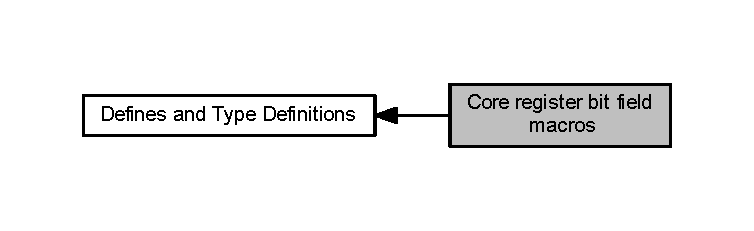
\includegraphics[width=350pt]{group___c_m_s_i_s__core__bitfield}
\end{center}
\end{figure}
\subsection*{Macros}
\begin{DoxyCompactItemize}
\item 
\#define \hyperlink{group___c_m_s_i_s__core__bitfield_ga286e3b913dbd236c7f48ea70c8821f4e}{\+\_\+\+V\+A\+L2\+F\+LD}(field,  \hyperlink{semihosting_8h_aacce635d68067370c70caa2381ea1040}{value})~((\hyperlink{semihosting_8h_aacce635d68067370c70caa2381ea1040}{value} $<$$<$ field \#\# \+\_\+\+Pos) \& field \#\# \+\_\+\+Msk)
\begin{DoxyCompactList}\small\item\em Mask and shift a bit field value for use in a register bit range. \end{DoxyCompactList}\item 
\#define \hyperlink{group___c_m_s_i_s__core__bitfield_ga139b6e261c981f014f386927ca4a8444}{\+\_\+\+F\+L\+D2\+V\+AL}(field,  \hyperlink{semihosting_8h_aacce635d68067370c70caa2381ea1040}{value})~((\hyperlink{semihosting_8h_aacce635d68067370c70caa2381ea1040}{value} \& field \#\# \+\_\+\+Msk) $>$$>$ field \#\# \+\_\+\+Pos)
\begin{DoxyCompactList}\small\item\em Mask and shift a register value to extract a bit filed value. \end{DoxyCompactList}\item 
\#define \hyperlink{group___c_m_s_i_s__core__bitfield_ga286e3b913dbd236c7f48ea70c8821f4e}{\+\_\+\+V\+A\+L2\+F\+LD}(field,  \hyperlink{semihosting_8h_aacce635d68067370c70caa2381ea1040}{value})~((\hyperlink{semihosting_8h_aacce635d68067370c70caa2381ea1040}{value} $<$$<$ field \#\# \+\_\+\+Pos) \& field \#\# \+\_\+\+Msk)
\begin{DoxyCompactList}\small\item\em Mask and shift a bit field value for use in a register bit range. \end{DoxyCompactList}\item 
\#define \hyperlink{group___c_m_s_i_s__core__bitfield_ga139b6e261c981f014f386927ca4a8444}{\+\_\+\+F\+L\+D2\+V\+AL}(field,  \hyperlink{semihosting_8h_aacce635d68067370c70caa2381ea1040}{value})~((\hyperlink{semihosting_8h_aacce635d68067370c70caa2381ea1040}{value} \& field \#\# \+\_\+\+Msk) $>$$>$ field \#\# \+\_\+\+Pos)
\begin{DoxyCompactList}\small\item\em Mask and shift a register value to extract a bit filed value. \end{DoxyCompactList}\item 
\#define \hyperlink{group___c_m_s_i_s__core__bitfield_ga286e3b913dbd236c7f48ea70c8821f4e}{\+\_\+\+V\+A\+L2\+F\+LD}(field,  \hyperlink{semihosting_8h_aacce635d68067370c70caa2381ea1040}{value})~((\hyperlink{semihosting_8h_aacce635d68067370c70caa2381ea1040}{value} $<$$<$ field \#\# \+\_\+\+Pos) \& field \#\# \+\_\+\+Msk)
\begin{DoxyCompactList}\small\item\em Mask and shift a bit field value for use in a register bit range. \end{DoxyCompactList}\item 
\#define \hyperlink{group___c_m_s_i_s__core__bitfield_ga139b6e261c981f014f386927ca4a8444}{\+\_\+\+F\+L\+D2\+V\+AL}(field,  \hyperlink{semihosting_8h_aacce635d68067370c70caa2381ea1040}{value})~((\hyperlink{semihosting_8h_aacce635d68067370c70caa2381ea1040}{value} \& field \#\# \+\_\+\+Msk) $>$$>$ field \#\# \+\_\+\+Pos)
\begin{DoxyCompactList}\small\item\em Mask and shift a register value to extract a bit filed value. \end{DoxyCompactList}\item 
\#define \hyperlink{group___c_m_s_i_s__core__bitfield_ga286e3b913dbd236c7f48ea70c8821f4e}{\+\_\+\+V\+A\+L2\+F\+LD}(field,  \hyperlink{semihosting_8h_aacce635d68067370c70caa2381ea1040}{value})~((\hyperlink{semihosting_8h_aacce635d68067370c70caa2381ea1040}{value} $<$$<$ field \#\# \+\_\+\+Pos) \& field \#\# \+\_\+\+Msk)
\begin{DoxyCompactList}\small\item\em Mask and shift a bit field value for use in a register bit range. \end{DoxyCompactList}\item 
\#define \hyperlink{group___c_m_s_i_s__core__bitfield_ga139b6e261c981f014f386927ca4a8444}{\+\_\+\+F\+L\+D2\+V\+AL}(field,  \hyperlink{semihosting_8h_aacce635d68067370c70caa2381ea1040}{value})~((\hyperlink{semihosting_8h_aacce635d68067370c70caa2381ea1040}{value} \& field \#\# \+\_\+\+Msk) $>$$>$ field \#\# \+\_\+\+Pos)
\begin{DoxyCompactList}\small\item\em Mask and shift a register value to extract a bit filed value. \end{DoxyCompactList}\item 
\#define \hyperlink{group___c_m_s_i_s__core__bitfield_ga286e3b913dbd236c7f48ea70c8821f4e}{\+\_\+\+V\+A\+L2\+F\+LD}(field,  \hyperlink{semihosting_8h_aacce635d68067370c70caa2381ea1040}{value})~((\hyperlink{semihosting_8h_aacce635d68067370c70caa2381ea1040}{value} $<$$<$ field \#\# \+\_\+\+Pos) \& field \#\# \+\_\+\+Msk)
\begin{DoxyCompactList}\small\item\em Mask and shift a bit field value for use in a register bit range. \end{DoxyCompactList}\item 
\#define \hyperlink{group___c_m_s_i_s__core__bitfield_ga139b6e261c981f014f386927ca4a8444}{\+\_\+\+F\+L\+D2\+V\+AL}(field,  \hyperlink{semihosting_8h_aacce635d68067370c70caa2381ea1040}{value})~((\hyperlink{semihosting_8h_aacce635d68067370c70caa2381ea1040}{value} \& field \#\# \+\_\+\+Msk) $>$$>$ field \#\# \+\_\+\+Pos)
\begin{DoxyCompactList}\small\item\em Mask and shift a register value to extract a bit filed value. \end{DoxyCompactList}\item 
\#define \hyperlink{group___c_m_s_i_s__core__bitfield_ga286e3b913dbd236c7f48ea70c8821f4e}{\+\_\+\+V\+A\+L2\+F\+LD}(field,  \hyperlink{semihosting_8h_aacce635d68067370c70caa2381ea1040}{value})~((\hyperlink{semihosting_8h_aacce635d68067370c70caa2381ea1040}{value} $<$$<$ field \#\# \+\_\+\+Pos) \& field \#\# \+\_\+\+Msk)
\begin{DoxyCompactList}\small\item\em Mask and shift a bit field value for use in a register bit range. \end{DoxyCompactList}\item 
\#define \hyperlink{group___c_m_s_i_s__core__bitfield_ga139b6e261c981f014f386927ca4a8444}{\+\_\+\+F\+L\+D2\+V\+AL}(field,  \hyperlink{semihosting_8h_aacce635d68067370c70caa2381ea1040}{value})~((\hyperlink{semihosting_8h_aacce635d68067370c70caa2381ea1040}{value} \& field \#\# \+\_\+\+Msk) $>$$>$ field \#\# \+\_\+\+Pos)
\begin{DoxyCompactList}\small\item\em Mask and shift a register value to extract a bit filed value. \end{DoxyCompactList}\item 
\#define \hyperlink{group___c_m_s_i_s__core__bitfield_ga286e3b913dbd236c7f48ea70c8821f4e}{\+\_\+\+V\+A\+L2\+F\+LD}(field,  \hyperlink{semihosting_8h_aacce635d68067370c70caa2381ea1040}{value})~((\hyperlink{semihosting_8h_aacce635d68067370c70caa2381ea1040}{value} $<$$<$ field \#\# \+\_\+\+Pos) \& field \#\# \+\_\+\+Msk)
\begin{DoxyCompactList}\small\item\em Mask and shift a bit field value for use in a register bit range. \end{DoxyCompactList}\item 
\#define \hyperlink{group___c_m_s_i_s__core__bitfield_ga139b6e261c981f014f386927ca4a8444}{\+\_\+\+F\+L\+D2\+V\+AL}(field,  \hyperlink{semihosting_8h_aacce635d68067370c70caa2381ea1040}{value})~((\hyperlink{semihosting_8h_aacce635d68067370c70caa2381ea1040}{value} \& field \#\# \+\_\+\+Msk) $>$$>$ field \#\# \+\_\+\+Pos)
\begin{DoxyCompactList}\small\item\em Mask and shift a register value to extract a bit filed value. \end{DoxyCompactList}\end{DoxyCompactItemize}


\subsection{Detailed Description}
Macros for use with bit field definitions (xxx\+\_\+\+Pos, xxx\+\_\+\+Msk). 



\subsection{Macro Definition Documentation}
\mbox{\Hypertarget{group___c_m_s_i_s__core__bitfield_ga139b6e261c981f014f386927ca4a8444}\label{group___c_m_s_i_s__core__bitfield_ga139b6e261c981f014f386927ca4a8444}} 
\index{Core register bit field macros@{Core register bit field macros}!\+\_\+\+F\+L\+D2\+V\+AL@{\+\_\+\+F\+L\+D2\+V\+AL}}
\index{\+\_\+\+F\+L\+D2\+V\+AL@{\+\_\+\+F\+L\+D2\+V\+AL}!Core register bit field macros@{Core register bit field macros}}
\subsubsection{\texorpdfstring{\+\_\+\+F\+L\+D2\+V\+AL}{\_FLD2VAL}\hspace{0.1cm}{\footnotesize\ttfamily [1/7]}}
{\footnotesize\ttfamily \#define \+\_\+\+F\+L\+D2\+V\+AL(\begin{DoxyParamCaption}\item[{}]{field,  }\item[{}]{\hyperlink{semihosting_8h_aacce635d68067370c70caa2381ea1040}{value} }\end{DoxyParamCaption})~((\hyperlink{semihosting_8h_aacce635d68067370c70caa2381ea1040}{value} \& field \#\# \+\_\+\+Msk) $>$$>$ field \#\# \+\_\+\+Pos)}



Mask and shift a register value to extract a bit filed value. 


\begin{DoxyParams}[1]{Parameters}
\mbox{\tt in}  & {\em field} & Name of the register bit field. \\
\hline
\mbox{\tt in}  & {\em value} & Value of register. \\
\hline
\end{DoxyParams}
\begin{DoxyReturn}{Returns}
Masked and shifted bit field value. 
\end{DoxyReturn}


Definition at line 577 of file core\+\_\+cm0.\+h.

\mbox{\Hypertarget{group___c_m_s_i_s__core__bitfield_ga139b6e261c981f014f386927ca4a8444}\label{group___c_m_s_i_s__core__bitfield_ga139b6e261c981f014f386927ca4a8444}} 
\index{Core register bit field macros@{Core register bit field macros}!\+\_\+\+F\+L\+D2\+V\+AL@{\+\_\+\+F\+L\+D2\+V\+AL}}
\index{\+\_\+\+F\+L\+D2\+V\+AL@{\+\_\+\+F\+L\+D2\+V\+AL}!Core register bit field macros@{Core register bit field macros}}
\subsubsection{\texorpdfstring{\+\_\+\+F\+L\+D2\+V\+AL}{\_FLD2VAL}\hspace{0.1cm}{\footnotesize\ttfamily [2/7]}}
{\footnotesize\ttfamily \#define \+\_\+\+F\+L\+D2\+V\+AL(\begin{DoxyParamCaption}\item[{}]{field,  }\item[{}]{\hyperlink{semihosting_8h_aacce635d68067370c70caa2381ea1040}{value} }\end{DoxyParamCaption})~((\hyperlink{semihosting_8h_aacce635d68067370c70caa2381ea1040}{value} \& field \#\# \+\_\+\+Msk) $>$$>$ field \#\# \+\_\+\+Pos)}



Mask and shift a register value to extract a bit filed value. 


\begin{DoxyParams}[1]{Parameters}
\mbox{\tt in}  & {\em field} & Name of the register bit field. \\
\hline
\mbox{\tt in}  & {\em value} & Value of register. \\
\hline
\end{DoxyParams}
\begin{DoxyReturn}{Returns}
Masked and shifted bit field value. 
\end{DoxyReturn}


Definition at line 689 of file core\+\_\+cm0plus.\+h.

\mbox{\Hypertarget{group___c_m_s_i_s__core__bitfield_ga139b6e261c981f014f386927ca4a8444}\label{group___c_m_s_i_s__core__bitfield_ga139b6e261c981f014f386927ca4a8444}} 
\index{Core register bit field macros@{Core register bit field macros}!\+\_\+\+F\+L\+D2\+V\+AL@{\+\_\+\+F\+L\+D2\+V\+AL}}
\index{\+\_\+\+F\+L\+D2\+V\+AL@{\+\_\+\+F\+L\+D2\+V\+AL}!Core register bit field macros@{Core register bit field macros}}
\subsubsection{\texorpdfstring{\+\_\+\+F\+L\+D2\+V\+AL}{\_FLD2VAL}\hspace{0.1cm}{\footnotesize\ttfamily [3/7]}}
{\footnotesize\ttfamily \#define \+\_\+\+F\+L\+D2\+V\+AL(\begin{DoxyParamCaption}\item[{}]{field,  }\item[{}]{\hyperlink{semihosting_8h_aacce635d68067370c70caa2381ea1040}{value} }\end{DoxyParamCaption})~((\hyperlink{semihosting_8h_aacce635d68067370c70caa2381ea1040}{value} \& field \#\# \+\_\+\+Msk) $>$$>$ field \#\# \+\_\+\+Pos)}



Mask and shift a register value to extract a bit filed value. 


\begin{DoxyParams}[1]{Parameters}
\mbox{\tt in}  & {\em field} & Name of the register bit field. \\
\hline
\mbox{\tt in}  & {\em value} & Value of register. \\
\hline
\end{DoxyParams}
\begin{DoxyReturn}{Returns}
Masked and shifted bit field value. 
\end{DoxyReturn}


Definition at line 692 of file core\+\_\+sc000.\+h.

\mbox{\Hypertarget{group___c_m_s_i_s__core__bitfield_ga139b6e261c981f014f386927ca4a8444}\label{group___c_m_s_i_s__core__bitfield_ga139b6e261c981f014f386927ca4a8444}} 
\index{Core register bit field macros@{Core register bit field macros}!\+\_\+\+F\+L\+D2\+V\+AL@{\+\_\+\+F\+L\+D2\+V\+AL}}
\index{\+\_\+\+F\+L\+D2\+V\+AL@{\+\_\+\+F\+L\+D2\+V\+AL}!Core register bit field macros@{Core register bit field macros}}
\subsubsection{\texorpdfstring{\+\_\+\+F\+L\+D2\+V\+AL}{\_FLD2VAL}\hspace{0.1cm}{\footnotesize\ttfamily [4/7]}}
{\footnotesize\ttfamily \#define \+\_\+\+F\+L\+D2\+V\+AL(\begin{DoxyParamCaption}\item[{}]{field,  }\item[{}]{\hyperlink{semihosting_8h_aacce635d68067370c70caa2381ea1040}{value} }\end{DoxyParamCaption})~((\hyperlink{semihosting_8h_aacce635d68067370c70caa2381ea1040}{value} \& field \#\# \+\_\+\+Msk) $>$$>$ field \#\# \+\_\+\+Pos)}



Mask and shift a register value to extract a bit filed value. 


\begin{DoxyParams}[1]{Parameters}
\mbox{\tt in}  & {\em field} & Name of the register bit field. \\
\hline
\mbox{\tt in}  & {\em value} & Value of register. \\
\hline
\end{DoxyParams}
\begin{DoxyReturn}{Returns}
Masked and shifted bit field value. 
\end{DoxyReturn}


Definition at line 1333 of file core\+\_\+sc300.\+h.

\mbox{\Hypertarget{group___c_m_s_i_s__core__bitfield_ga139b6e261c981f014f386927ca4a8444}\label{group___c_m_s_i_s__core__bitfield_ga139b6e261c981f014f386927ca4a8444}} 
\index{Core register bit field macros@{Core register bit field macros}!\+\_\+\+F\+L\+D2\+V\+AL@{\+\_\+\+F\+L\+D2\+V\+AL}}
\index{\+\_\+\+F\+L\+D2\+V\+AL@{\+\_\+\+F\+L\+D2\+V\+AL}!Core register bit field macros@{Core register bit field macros}}
\subsubsection{\texorpdfstring{\+\_\+\+F\+L\+D2\+V\+AL}{\_FLD2VAL}\hspace{0.1cm}{\footnotesize\ttfamily [5/7]}}
{\footnotesize\ttfamily \#define \+\_\+\+F\+L\+D2\+V\+AL(\begin{DoxyParamCaption}\item[{}]{field,  }\item[{}]{\hyperlink{semihosting_8h_aacce635d68067370c70caa2381ea1040}{value} }\end{DoxyParamCaption})~((\hyperlink{semihosting_8h_aacce635d68067370c70caa2381ea1040}{value} \& field \#\# \+\_\+\+Msk) $>$$>$ field \#\# \+\_\+\+Pos)}



Mask and shift a register value to extract a bit filed value. 


\begin{DoxyParams}[1]{Parameters}
\mbox{\tt in}  & {\em field} & Name of the register bit field. \\
\hline
\mbox{\tt in}  & {\em value} & Value of register. \\
\hline
\end{DoxyParams}
\begin{DoxyReturn}{Returns}
Masked and shifted bit field value. 
\end{DoxyReturn}


Definition at line 1359 of file core\+\_\+cm3.\+h.

\mbox{\Hypertarget{group___c_m_s_i_s__core__bitfield_ga139b6e261c981f014f386927ca4a8444}\label{group___c_m_s_i_s__core__bitfield_ga139b6e261c981f014f386927ca4a8444}} 
\index{Core register bit field macros@{Core register bit field macros}!\+\_\+\+F\+L\+D2\+V\+AL@{\+\_\+\+F\+L\+D2\+V\+AL}}
\index{\+\_\+\+F\+L\+D2\+V\+AL@{\+\_\+\+F\+L\+D2\+V\+AL}!Core register bit field macros@{Core register bit field macros}}
\subsubsection{\texorpdfstring{\+\_\+\+F\+L\+D2\+V\+AL}{\_FLD2VAL}\hspace{0.1cm}{\footnotesize\ttfamily [6/7]}}
{\footnotesize\ttfamily \#define \+\_\+\+F\+L\+D2\+V\+AL(\begin{DoxyParamCaption}\item[{}]{field,  }\item[{}]{\hyperlink{semihosting_8h_aacce635d68067370c70caa2381ea1040}{value} }\end{DoxyParamCaption})~((\hyperlink{semihosting_8h_aacce635d68067370c70caa2381ea1040}{value} \& field \#\# \+\_\+\+Msk) $>$$>$ field \#\# \+\_\+\+Pos)}



Mask and shift a register value to extract a bit filed value. 


\begin{DoxyParams}[1]{Parameters}
\mbox{\tt in}  & {\em field} & Name of the register bit field. \\
\hline
\mbox{\tt in}  & {\em value} & Value of register. \\
\hline
\end{DoxyParams}
\begin{DoxyReturn}{Returns}
Masked and shifted bit field value. 
\end{DoxyReturn}


Definition at line 1528 of file core\+\_\+cm4.\+h.

\mbox{\Hypertarget{group___c_m_s_i_s__core__bitfield_ga139b6e261c981f014f386927ca4a8444}\label{group___c_m_s_i_s__core__bitfield_ga139b6e261c981f014f386927ca4a8444}} 
\index{Core register bit field macros@{Core register bit field macros}!\+\_\+\+F\+L\+D2\+V\+AL@{\+\_\+\+F\+L\+D2\+V\+AL}}
\index{\+\_\+\+F\+L\+D2\+V\+AL@{\+\_\+\+F\+L\+D2\+V\+AL}!Core register bit field macros@{Core register bit field macros}}
\subsubsection{\texorpdfstring{\+\_\+\+F\+L\+D2\+V\+AL}{\_FLD2VAL}\hspace{0.1cm}{\footnotesize\ttfamily [7/7]}}
{\footnotesize\ttfamily \#define \+\_\+\+F\+L\+D2\+V\+AL(\begin{DoxyParamCaption}\item[{}]{field,  }\item[{}]{\hyperlink{semihosting_8h_aacce635d68067370c70caa2381ea1040}{value} }\end{DoxyParamCaption})~((\hyperlink{semihosting_8h_aacce635d68067370c70caa2381ea1040}{value} \& field \#\# \+\_\+\+Msk) $>$$>$ field \#\# \+\_\+\+Pos)}



Mask and shift a register value to extract a bit filed value. 


\begin{DoxyParams}[1]{Parameters}
\mbox{\tt in}  & {\em field} & Name of the register bit field. \\
\hline
\mbox{\tt in}  & {\em value} & Value of register. \\
\hline
\end{DoxyParams}
\begin{DoxyReturn}{Returns}
Masked and shifted bit field value. 
\end{DoxyReturn}


Definition at line 1736 of file core\+\_\+cm7.\+h.

\mbox{\Hypertarget{group___c_m_s_i_s__core__bitfield_ga286e3b913dbd236c7f48ea70c8821f4e}\label{group___c_m_s_i_s__core__bitfield_ga286e3b913dbd236c7f48ea70c8821f4e}} 
\index{Core register bit field macros@{Core register bit field macros}!\+\_\+\+V\+A\+L2\+F\+LD@{\+\_\+\+V\+A\+L2\+F\+LD}}
\index{\+\_\+\+V\+A\+L2\+F\+LD@{\+\_\+\+V\+A\+L2\+F\+LD}!Core register bit field macros@{Core register bit field macros}}
\subsubsection{\texorpdfstring{\+\_\+\+V\+A\+L2\+F\+LD}{\_VAL2FLD}\hspace{0.1cm}{\footnotesize\ttfamily [1/7]}}
{\footnotesize\ttfamily \#define \+\_\+\+V\+A\+L2\+F\+LD(\begin{DoxyParamCaption}\item[{}]{field,  }\item[{}]{\hyperlink{semihosting_8h_aacce635d68067370c70caa2381ea1040}{value} }\end{DoxyParamCaption})~((\hyperlink{semihosting_8h_aacce635d68067370c70caa2381ea1040}{value} $<$$<$ field \#\# \+\_\+\+Pos) \& field \#\# \+\_\+\+Msk)}



Mask and shift a bit field value for use in a register bit range. 


\begin{DoxyParams}[1]{Parameters}
\mbox{\tt in}  & {\em field} & Name of the register bit field. \\
\hline
\mbox{\tt in}  & {\em value} & Value of the bit field. \\
\hline
\end{DoxyParams}
\begin{DoxyReturn}{Returns}
Masked and shifted value. 
\end{DoxyReturn}


Definition at line 569 of file core\+\_\+cm0.\+h.

\mbox{\Hypertarget{group___c_m_s_i_s__core__bitfield_ga286e3b913dbd236c7f48ea70c8821f4e}\label{group___c_m_s_i_s__core__bitfield_ga286e3b913dbd236c7f48ea70c8821f4e}} 
\index{Core register bit field macros@{Core register bit field macros}!\+\_\+\+V\+A\+L2\+F\+LD@{\+\_\+\+V\+A\+L2\+F\+LD}}
\index{\+\_\+\+V\+A\+L2\+F\+LD@{\+\_\+\+V\+A\+L2\+F\+LD}!Core register bit field macros@{Core register bit field macros}}
\subsubsection{\texorpdfstring{\+\_\+\+V\+A\+L2\+F\+LD}{\_VAL2FLD}\hspace{0.1cm}{\footnotesize\ttfamily [2/7]}}
{\footnotesize\ttfamily \#define \+\_\+\+V\+A\+L2\+F\+LD(\begin{DoxyParamCaption}\item[{}]{field,  }\item[{}]{\hyperlink{semihosting_8h_aacce635d68067370c70caa2381ea1040}{value} }\end{DoxyParamCaption})~((\hyperlink{semihosting_8h_aacce635d68067370c70caa2381ea1040}{value} $<$$<$ field \#\# \+\_\+\+Pos) \& field \#\# \+\_\+\+Msk)}



Mask and shift a bit field value for use in a register bit range. 


\begin{DoxyParams}[1]{Parameters}
\mbox{\tt in}  & {\em field} & Name of the register bit field. \\
\hline
\mbox{\tt in}  & {\em value} & Value of the bit field. \\
\hline
\end{DoxyParams}
\begin{DoxyReturn}{Returns}
Masked and shifted value. 
\end{DoxyReturn}


Definition at line 681 of file core\+\_\+cm0plus.\+h.

\mbox{\Hypertarget{group___c_m_s_i_s__core__bitfield_ga286e3b913dbd236c7f48ea70c8821f4e}\label{group___c_m_s_i_s__core__bitfield_ga286e3b913dbd236c7f48ea70c8821f4e}} 
\index{Core register bit field macros@{Core register bit field macros}!\+\_\+\+V\+A\+L2\+F\+LD@{\+\_\+\+V\+A\+L2\+F\+LD}}
\index{\+\_\+\+V\+A\+L2\+F\+LD@{\+\_\+\+V\+A\+L2\+F\+LD}!Core register bit field macros@{Core register bit field macros}}
\subsubsection{\texorpdfstring{\+\_\+\+V\+A\+L2\+F\+LD}{\_VAL2FLD}\hspace{0.1cm}{\footnotesize\ttfamily [3/7]}}
{\footnotesize\ttfamily \#define \+\_\+\+V\+A\+L2\+F\+LD(\begin{DoxyParamCaption}\item[{}]{field,  }\item[{}]{\hyperlink{semihosting_8h_aacce635d68067370c70caa2381ea1040}{value} }\end{DoxyParamCaption})~((\hyperlink{semihosting_8h_aacce635d68067370c70caa2381ea1040}{value} $<$$<$ field \#\# \+\_\+\+Pos) \& field \#\# \+\_\+\+Msk)}



Mask and shift a bit field value for use in a register bit range. 


\begin{DoxyParams}[1]{Parameters}
\mbox{\tt in}  & {\em field} & Name of the register bit field. \\
\hline
\mbox{\tt in}  & {\em value} & Value of the bit field. \\
\hline
\end{DoxyParams}
\begin{DoxyReturn}{Returns}
Masked and shifted value. 
\end{DoxyReturn}


Definition at line 684 of file core\+\_\+sc000.\+h.

\mbox{\Hypertarget{group___c_m_s_i_s__core__bitfield_ga286e3b913dbd236c7f48ea70c8821f4e}\label{group___c_m_s_i_s__core__bitfield_ga286e3b913dbd236c7f48ea70c8821f4e}} 
\index{Core register bit field macros@{Core register bit field macros}!\+\_\+\+V\+A\+L2\+F\+LD@{\+\_\+\+V\+A\+L2\+F\+LD}}
\index{\+\_\+\+V\+A\+L2\+F\+LD@{\+\_\+\+V\+A\+L2\+F\+LD}!Core register bit field macros@{Core register bit field macros}}
\subsubsection{\texorpdfstring{\+\_\+\+V\+A\+L2\+F\+LD}{\_VAL2FLD}\hspace{0.1cm}{\footnotesize\ttfamily [4/7]}}
{\footnotesize\ttfamily \#define \+\_\+\+V\+A\+L2\+F\+LD(\begin{DoxyParamCaption}\item[{}]{field,  }\item[{}]{\hyperlink{semihosting_8h_aacce635d68067370c70caa2381ea1040}{value} }\end{DoxyParamCaption})~((\hyperlink{semihosting_8h_aacce635d68067370c70caa2381ea1040}{value} $<$$<$ field \#\# \+\_\+\+Pos) \& field \#\# \+\_\+\+Msk)}



Mask and shift a bit field value for use in a register bit range. 


\begin{DoxyParams}[1]{Parameters}
\mbox{\tt in}  & {\em field} & Name of the register bit field. \\
\hline
\mbox{\tt in}  & {\em value} & Value of the bit field. \\
\hline
\end{DoxyParams}
\begin{DoxyReturn}{Returns}
Masked and shifted value. 
\end{DoxyReturn}


Definition at line 1325 of file core\+\_\+sc300.\+h.

\mbox{\Hypertarget{group___c_m_s_i_s__core__bitfield_ga286e3b913dbd236c7f48ea70c8821f4e}\label{group___c_m_s_i_s__core__bitfield_ga286e3b913dbd236c7f48ea70c8821f4e}} 
\index{Core register bit field macros@{Core register bit field macros}!\+\_\+\+V\+A\+L2\+F\+LD@{\+\_\+\+V\+A\+L2\+F\+LD}}
\index{\+\_\+\+V\+A\+L2\+F\+LD@{\+\_\+\+V\+A\+L2\+F\+LD}!Core register bit field macros@{Core register bit field macros}}
\subsubsection{\texorpdfstring{\+\_\+\+V\+A\+L2\+F\+LD}{\_VAL2FLD}\hspace{0.1cm}{\footnotesize\ttfamily [5/7]}}
{\footnotesize\ttfamily \#define \+\_\+\+V\+A\+L2\+F\+LD(\begin{DoxyParamCaption}\item[{}]{field,  }\item[{}]{\hyperlink{semihosting_8h_aacce635d68067370c70caa2381ea1040}{value} }\end{DoxyParamCaption})~((\hyperlink{semihosting_8h_aacce635d68067370c70caa2381ea1040}{value} $<$$<$ field \#\# \+\_\+\+Pos) \& field \#\# \+\_\+\+Msk)}



Mask and shift a bit field value for use in a register bit range. 


\begin{DoxyParams}[1]{Parameters}
\mbox{\tt in}  & {\em field} & Name of the register bit field. \\
\hline
\mbox{\tt in}  & {\em value} & Value of the bit field. \\
\hline
\end{DoxyParams}
\begin{DoxyReturn}{Returns}
Masked and shifted value. 
\end{DoxyReturn}


Definition at line 1351 of file core\+\_\+cm3.\+h.

\mbox{\Hypertarget{group___c_m_s_i_s__core__bitfield_ga286e3b913dbd236c7f48ea70c8821f4e}\label{group___c_m_s_i_s__core__bitfield_ga286e3b913dbd236c7f48ea70c8821f4e}} 
\index{Core register bit field macros@{Core register bit field macros}!\+\_\+\+V\+A\+L2\+F\+LD@{\+\_\+\+V\+A\+L2\+F\+LD}}
\index{\+\_\+\+V\+A\+L2\+F\+LD@{\+\_\+\+V\+A\+L2\+F\+LD}!Core register bit field macros@{Core register bit field macros}}
\subsubsection{\texorpdfstring{\+\_\+\+V\+A\+L2\+F\+LD}{\_VAL2FLD}\hspace{0.1cm}{\footnotesize\ttfamily [6/7]}}
{\footnotesize\ttfamily \#define \+\_\+\+V\+A\+L2\+F\+LD(\begin{DoxyParamCaption}\item[{}]{field,  }\item[{}]{\hyperlink{semihosting_8h_aacce635d68067370c70caa2381ea1040}{value} }\end{DoxyParamCaption})~((\hyperlink{semihosting_8h_aacce635d68067370c70caa2381ea1040}{value} $<$$<$ field \#\# \+\_\+\+Pos) \& field \#\# \+\_\+\+Msk)}



Mask and shift a bit field value for use in a register bit range. 


\begin{DoxyParams}[1]{Parameters}
\mbox{\tt in}  & {\em field} & Name of the register bit field. \\
\hline
\mbox{\tt in}  & {\em value} & Value of the bit field. \\
\hline
\end{DoxyParams}
\begin{DoxyReturn}{Returns}
Masked and shifted value. 
\end{DoxyReturn}


Definition at line 1520 of file core\+\_\+cm4.\+h.

\mbox{\Hypertarget{group___c_m_s_i_s__core__bitfield_ga286e3b913dbd236c7f48ea70c8821f4e}\label{group___c_m_s_i_s__core__bitfield_ga286e3b913dbd236c7f48ea70c8821f4e}} 
\index{Core register bit field macros@{Core register bit field macros}!\+\_\+\+V\+A\+L2\+F\+LD@{\+\_\+\+V\+A\+L2\+F\+LD}}
\index{\+\_\+\+V\+A\+L2\+F\+LD@{\+\_\+\+V\+A\+L2\+F\+LD}!Core register bit field macros@{Core register bit field macros}}
\subsubsection{\texorpdfstring{\+\_\+\+V\+A\+L2\+F\+LD}{\_VAL2FLD}\hspace{0.1cm}{\footnotesize\ttfamily [7/7]}}
{\footnotesize\ttfamily \#define \+\_\+\+V\+A\+L2\+F\+LD(\begin{DoxyParamCaption}\item[{}]{field,  }\item[{}]{\hyperlink{semihosting_8h_aacce635d68067370c70caa2381ea1040}{value} }\end{DoxyParamCaption})~((\hyperlink{semihosting_8h_aacce635d68067370c70caa2381ea1040}{value} $<$$<$ field \#\# \+\_\+\+Pos) \& field \#\# \+\_\+\+Msk)}



Mask and shift a bit field value for use in a register bit range. 


\begin{DoxyParams}[1]{Parameters}
\mbox{\tt in}  & {\em field} & Name of the register bit field. \\
\hline
\mbox{\tt in}  & {\em value} & Value of the bit field. \\
\hline
\end{DoxyParams}
\begin{DoxyReturn}{Returns}
Masked and shifted value. 
\end{DoxyReturn}


Definition at line 1728 of file core\+\_\+cm7.\+h.


\hypertarget{group___c_m_s_i_s__core__base}{}\section{Core Definitions}
\label{group___c_m_s_i_s__core__base}\index{Core Definitions@{Core Definitions}}


Definitions for base addresses, unions, and structures.  


Collaboration diagram for Core Definitions\+:
\nopagebreak
\begin{figure}[H]
\begin{center}
\leavevmode
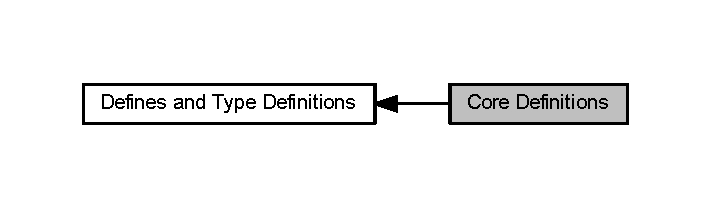
\includegraphics[width=341pt]{group___c_m_s_i_s__core__base}
\end{center}
\end{figure}
\subsection*{Macros}
\begin{DoxyCompactItemize}
\item 
\#define \hyperlink{group___c_m_s_i_s__core__base_ga3c14ed93192c8d9143322bbf77ebf770}{S\+C\+S\+\_\+\+B\+A\+SE}~(0x\+E000\+E000\+U\+L)
\item 
\#define \hyperlink{group___c_m_s_i_s__core__base_ga58effaac0b93006b756d33209e814646}{Sys\+Tick\+\_\+\+B\+A\+SE}~(\hyperlink{group___c_m_s_i_s__core__base_ga3c14ed93192c8d9143322bbf77ebf770}{S\+C\+S\+\_\+\+B\+A\+SE} +  0x0010\+U\+L)
\item 
\#define \hyperlink{group___c_m_s_i_s__core__base_gaa0288691785a5f868238e0468b39523d}{N\+V\+I\+C\+\_\+\+B\+A\+SE}~(\hyperlink{group___c_m_s_i_s__core__base_ga3c14ed93192c8d9143322bbf77ebf770}{S\+C\+S\+\_\+\+B\+A\+SE} +  0x0100\+U\+L)
\item 
\#define \hyperlink{group___c_m_s_i_s__core__base_gad55a7ddb8d4b2398b0c1cfec76c0d9fd}{S\+C\+B\+\_\+\+B\+A\+SE}~(\hyperlink{group___c_m_s_i_s__core__base_ga3c14ed93192c8d9143322bbf77ebf770}{S\+C\+S\+\_\+\+B\+A\+SE} +  0x0\+D00\+U\+L)
\item 
\#define \hyperlink{group___c_m_s_i_s__core__base_gaaaf6477c2bde2f00f99e3c2fd1060b01}{S\+CB}~((\hyperlink{struct_s_c_b___type}{S\+C\+B\+\_\+\+Type}       $\ast$)     \hyperlink{group___c_m_s_i_s__core__base_gad55a7ddb8d4b2398b0c1cfec76c0d9fd}{S\+C\+B\+\_\+\+B\+A\+SE}      )
\item 
\#define \hyperlink{group___c_m_s_i_s__core__base_gacd96c53beeaff8f603fcda425eb295de}{Sys\+Tick}~((\hyperlink{struct_sys_tick___type}{Sys\+Tick\+\_\+\+Type}   $\ast$)     \hyperlink{group___c_m_s_i_s__core__base_ga58effaac0b93006b756d33209e814646}{Sys\+Tick\+\_\+\+B\+A\+SE}  )
\item 
\#define \hyperlink{group___c_m_s_i_s__core__base_gac8e97e8ce56ae9f57da1363a937f8a17}{N\+V\+IC}~((\hyperlink{struct_n_v_i_c___type}{N\+V\+I\+C\+\_\+\+Type}      $\ast$)     \hyperlink{group___c_m_s_i_s__core__base_gaa0288691785a5f868238e0468b39523d}{N\+V\+I\+C\+\_\+\+B\+A\+SE}     )
\item 
\#define \hyperlink{group___c_m_s_i_s__core__base_ga3c14ed93192c8d9143322bbf77ebf770}{S\+C\+S\+\_\+\+B\+A\+SE}~(0x\+E000\+E000\+U\+L)
\item 
\#define \hyperlink{group___c_m_s_i_s__core__base_ga58effaac0b93006b756d33209e814646}{Sys\+Tick\+\_\+\+B\+A\+SE}~(\hyperlink{group___c_m_s_i_s__core__base_ga3c14ed93192c8d9143322bbf77ebf770}{S\+C\+S\+\_\+\+B\+A\+SE} +  0x0010\+U\+L)
\item 
\#define \hyperlink{group___c_m_s_i_s__core__base_gaa0288691785a5f868238e0468b39523d}{N\+V\+I\+C\+\_\+\+B\+A\+SE}~(\hyperlink{group___c_m_s_i_s__core__base_ga3c14ed93192c8d9143322bbf77ebf770}{S\+C\+S\+\_\+\+B\+A\+SE} +  0x0100\+U\+L)
\item 
\#define \hyperlink{group___c_m_s_i_s__core__base_gad55a7ddb8d4b2398b0c1cfec76c0d9fd}{S\+C\+B\+\_\+\+B\+A\+SE}~(\hyperlink{group___c_m_s_i_s__core__base_ga3c14ed93192c8d9143322bbf77ebf770}{S\+C\+S\+\_\+\+B\+A\+SE} +  0x0\+D00\+U\+L)
\item 
\#define \hyperlink{group___c_m_s_i_s__core__base_gaaaf6477c2bde2f00f99e3c2fd1060b01}{S\+CB}~((\hyperlink{struct_s_c_b___type}{S\+C\+B\+\_\+\+Type}       $\ast$)     \hyperlink{group___c_m_s_i_s__core__base_gad55a7ddb8d4b2398b0c1cfec76c0d9fd}{S\+C\+B\+\_\+\+B\+A\+SE}      )
\item 
\#define \hyperlink{group___c_m_s_i_s__core__base_gacd96c53beeaff8f603fcda425eb295de}{Sys\+Tick}~((\hyperlink{struct_sys_tick___type}{Sys\+Tick\+\_\+\+Type}   $\ast$)     \hyperlink{group___c_m_s_i_s__core__base_ga58effaac0b93006b756d33209e814646}{Sys\+Tick\+\_\+\+B\+A\+SE}  )
\item 
\#define \hyperlink{group___c_m_s_i_s__core__base_gac8e97e8ce56ae9f57da1363a937f8a17}{N\+V\+IC}~((\hyperlink{struct_n_v_i_c___type}{N\+V\+I\+C\+\_\+\+Type}      $\ast$)     \hyperlink{group___c_m_s_i_s__core__base_gaa0288691785a5f868238e0468b39523d}{N\+V\+I\+C\+\_\+\+B\+A\+SE}     )
\item 
\#define \hyperlink{group___c_m_s_i_s__core__base_ga3c14ed93192c8d9143322bbf77ebf770}{S\+C\+S\+\_\+\+B\+A\+SE}~(0x\+E000\+E000\+U\+L)
\item 
\#define \hyperlink{group___c_m_s_i_s__core__base_gadd76251e412a195ec0a8f47227a8359e}{I\+T\+M\+\_\+\+B\+A\+SE}~(0x\+E0000000\+U\+L)
\item 
\#define \hyperlink{group___c_m_s_i_s__core__base_gafdab534f961bf8935eb456cb7700dcd2}{D\+W\+T\+\_\+\+B\+A\+SE}~(0x\+E0001000\+U\+L)
\item 
\#define \hyperlink{group___c_m_s_i_s__core__base_ga2b1eeff850a7e418844ca847145a1a68}{T\+P\+I\+\_\+\+B\+A\+SE}~(0x\+E0040000\+U\+L)
\item 
\#define \hyperlink{group___c_m_s_i_s__core__base_ga680604dbcda9e9b31a1639fcffe5230b}{Core\+Debug\+\_\+\+B\+A\+SE}~(0x\+E000\+E\+D\+F0\+U\+L)
\item 
\#define \hyperlink{group___c_m_s_i_s__core__base_ga58effaac0b93006b756d33209e814646}{Sys\+Tick\+\_\+\+B\+A\+SE}~(\hyperlink{group___c_m_s_i_s__core__base_ga3c14ed93192c8d9143322bbf77ebf770}{S\+C\+S\+\_\+\+B\+A\+SE} +  0x0010\+U\+L)
\item 
\#define \hyperlink{group___c_m_s_i_s__core__base_gaa0288691785a5f868238e0468b39523d}{N\+V\+I\+C\+\_\+\+B\+A\+SE}~(\hyperlink{group___c_m_s_i_s__core__base_ga3c14ed93192c8d9143322bbf77ebf770}{S\+C\+S\+\_\+\+B\+A\+SE} +  0x0100\+U\+L)
\item 
\#define \hyperlink{group___c_m_s_i_s__core__base_gad55a7ddb8d4b2398b0c1cfec76c0d9fd}{S\+C\+B\+\_\+\+B\+A\+SE}~(\hyperlink{group___c_m_s_i_s__core__base_ga3c14ed93192c8d9143322bbf77ebf770}{S\+C\+S\+\_\+\+B\+A\+SE} +  0x0\+D00\+U\+L)
\item 
\#define \hyperlink{group___c_m_s_i_s__core__base_ga9fe0cd2eef83a8adad94490d9ecca63f}{S\+Cn\+S\+CB}~((\hyperlink{struct_s_cn_s_c_b___type}{S\+Cn\+S\+C\+B\+\_\+\+Type}    $\ast$)     \hyperlink{group___c_m_s_i_s__core__base_ga3c14ed93192c8d9143322bbf77ebf770}{S\+C\+S\+\_\+\+B\+A\+SE}      )
\item 
\#define \hyperlink{group___c_m_s_i_s__core__base_gaaaf6477c2bde2f00f99e3c2fd1060b01}{S\+CB}~((\hyperlink{struct_s_c_b___type}{S\+C\+B\+\_\+\+Type}       $\ast$)     \hyperlink{group___c_m_s_i_s__core__base_gad55a7ddb8d4b2398b0c1cfec76c0d9fd}{S\+C\+B\+\_\+\+B\+A\+SE}      )
\item 
\#define \hyperlink{group___c_m_s_i_s__core__base_gacd96c53beeaff8f603fcda425eb295de}{Sys\+Tick}~((\hyperlink{struct_sys_tick___type}{Sys\+Tick\+\_\+\+Type}   $\ast$)     \hyperlink{group___c_m_s_i_s__core__base_ga58effaac0b93006b756d33209e814646}{Sys\+Tick\+\_\+\+B\+A\+SE}  )
\item 
\#define \hyperlink{group___c_m_s_i_s__core__base_gac8e97e8ce56ae9f57da1363a937f8a17}{N\+V\+IC}~((\hyperlink{struct_n_v_i_c___type}{N\+V\+I\+C\+\_\+\+Type}      $\ast$)     \hyperlink{group___c_m_s_i_s__core__base_gaa0288691785a5f868238e0468b39523d}{N\+V\+I\+C\+\_\+\+B\+A\+SE}     )
\item 
\#define \hyperlink{group___c_m_s_i_s__core__base_gabae7cdf882def602cb787bb039ff6a43}{I\+TM}~((\hyperlink{struct_i_t_m___type}{I\+T\+M\+\_\+\+Type}       $\ast$)     \hyperlink{group___c_m_s_i_s__core__base_gadd76251e412a195ec0a8f47227a8359e}{I\+T\+M\+\_\+\+B\+A\+SE}      )
\item 
\#define \hyperlink{group___c_m_s_i_s__core__base_gabbe5a060185e1d5afa3f85b14e10a6ce}{D\+WT}~((\hyperlink{struct_d_w_t___type}{D\+W\+T\+\_\+\+Type}       $\ast$)     \hyperlink{group___c_m_s_i_s__core__base_gafdab534f961bf8935eb456cb7700dcd2}{D\+W\+T\+\_\+\+B\+A\+SE}      )
\item 
\#define \hyperlink{group___c_m_s_i_s__core__base_ga8b4dd00016aed25a0ea54e9a9acd1239}{T\+PI}~((\hyperlink{struct_t_p_i___type}{T\+P\+I\+\_\+\+Type}       $\ast$)     \hyperlink{group___c_m_s_i_s__core__base_ga2b1eeff850a7e418844ca847145a1a68}{T\+P\+I\+\_\+\+B\+A\+SE}      )
\item 
\#define \hyperlink{group___c_m_s_i_s__core__base_gab6e30a2b802d9021619dbb0be7f5d63d}{Core\+Debug}~((\hyperlink{struct_core_debug___type}{Core\+Debug\+\_\+\+Type} $\ast$)     \hyperlink{group___c_m_s_i_s__core__base_ga680604dbcda9e9b31a1639fcffe5230b}{Core\+Debug\+\_\+\+B\+A\+SE})
\item 
\#define \hyperlink{group___c_m_s_i_s__core__base_ga3c14ed93192c8d9143322bbf77ebf770}{S\+C\+S\+\_\+\+B\+A\+SE}~(0x\+E000\+E000\+U\+L)
\item 
\#define \hyperlink{group___c_m_s_i_s__core__base_gadd76251e412a195ec0a8f47227a8359e}{I\+T\+M\+\_\+\+B\+A\+SE}~(0x\+E0000000\+U\+L)
\item 
\#define \hyperlink{group___c_m_s_i_s__core__base_gafdab534f961bf8935eb456cb7700dcd2}{D\+W\+T\+\_\+\+B\+A\+SE}~(0x\+E0001000\+U\+L)
\item 
\#define \hyperlink{group___c_m_s_i_s__core__base_ga2b1eeff850a7e418844ca847145a1a68}{T\+P\+I\+\_\+\+B\+A\+SE}~(0x\+E0040000\+U\+L)
\item 
\#define \hyperlink{group___c_m_s_i_s__core__base_ga680604dbcda9e9b31a1639fcffe5230b}{Core\+Debug\+\_\+\+B\+A\+SE}~(0x\+E000\+E\+D\+F0\+U\+L)
\item 
\#define \hyperlink{group___c_m_s_i_s__core__base_ga58effaac0b93006b756d33209e814646}{Sys\+Tick\+\_\+\+B\+A\+SE}~(\hyperlink{group___c_m_s_i_s__core__base_ga3c14ed93192c8d9143322bbf77ebf770}{S\+C\+S\+\_\+\+B\+A\+SE} +  0x0010\+U\+L)
\item 
\#define \hyperlink{group___c_m_s_i_s__core__base_gaa0288691785a5f868238e0468b39523d}{N\+V\+I\+C\+\_\+\+B\+A\+SE}~(\hyperlink{group___c_m_s_i_s__core__base_ga3c14ed93192c8d9143322bbf77ebf770}{S\+C\+S\+\_\+\+B\+A\+SE} +  0x0100\+U\+L)
\item 
\#define \hyperlink{group___c_m_s_i_s__core__base_gad55a7ddb8d4b2398b0c1cfec76c0d9fd}{S\+C\+B\+\_\+\+B\+A\+SE}~(\hyperlink{group___c_m_s_i_s__core__base_ga3c14ed93192c8d9143322bbf77ebf770}{S\+C\+S\+\_\+\+B\+A\+SE} +  0x0\+D00\+U\+L)
\item 
\#define \hyperlink{group___c_m_s_i_s__core__base_ga9fe0cd2eef83a8adad94490d9ecca63f}{S\+Cn\+S\+CB}~((\hyperlink{struct_s_cn_s_c_b___type}{S\+Cn\+S\+C\+B\+\_\+\+Type}    $\ast$)     \hyperlink{group___c_m_s_i_s__core__base_ga3c14ed93192c8d9143322bbf77ebf770}{S\+C\+S\+\_\+\+B\+A\+SE}      )
\item 
\#define \hyperlink{group___c_m_s_i_s__core__base_gaaaf6477c2bde2f00f99e3c2fd1060b01}{S\+CB}~((\hyperlink{struct_s_c_b___type}{S\+C\+B\+\_\+\+Type}       $\ast$)     \hyperlink{group___c_m_s_i_s__core__base_gad55a7ddb8d4b2398b0c1cfec76c0d9fd}{S\+C\+B\+\_\+\+B\+A\+SE}      )
\item 
\#define \hyperlink{group___c_m_s_i_s__core__base_gacd96c53beeaff8f603fcda425eb295de}{Sys\+Tick}~((\hyperlink{struct_sys_tick___type}{Sys\+Tick\+\_\+\+Type}   $\ast$)     \hyperlink{group___c_m_s_i_s__core__base_ga58effaac0b93006b756d33209e814646}{Sys\+Tick\+\_\+\+B\+A\+SE}  )
\item 
\#define \hyperlink{group___c_m_s_i_s__core__base_gac8e97e8ce56ae9f57da1363a937f8a17}{N\+V\+IC}~((\hyperlink{struct_n_v_i_c___type}{N\+V\+I\+C\+\_\+\+Type}      $\ast$)     \hyperlink{group___c_m_s_i_s__core__base_gaa0288691785a5f868238e0468b39523d}{N\+V\+I\+C\+\_\+\+B\+A\+SE}     )
\item 
\#define \hyperlink{group___c_m_s_i_s__core__base_gabae7cdf882def602cb787bb039ff6a43}{I\+TM}~((\hyperlink{struct_i_t_m___type}{I\+T\+M\+\_\+\+Type}       $\ast$)     \hyperlink{group___c_m_s_i_s__core__base_gadd76251e412a195ec0a8f47227a8359e}{I\+T\+M\+\_\+\+B\+A\+SE}      )
\item 
\#define \hyperlink{group___c_m_s_i_s__core__base_gabbe5a060185e1d5afa3f85b14e10a6ce}{D\+WT}~((\hyperlink{struct_d_w_t___type}{D\+W\+T\+\_\+\+Type}       $\ast$)     \hyperlink{group___c_m_s_i_s__core__base_gafdab534f961bf8935eb456cb7700dcd2}{D\+W\+T\+\_\+\+B\+A\+SE}      )
\item 
\#define \hyperlink{group___c_m_s_i_s__core__base_ga8b4dd00016aed25a0ea54e9a9acd1239}{T\+PI}~((\hyperlink{struct_t_p_i___type}{T\+P\+I\+\_\+\+Type}       $\ast$)     \hyperlink{group___c_m_s_i_s__core__base_ga2b1eeff850a7e418844ca847145a1a68}{T\+P\+I\+\_\+\+B\+A\+SE}      )
\item 
\#define \hyperlink{group___c_m_s_i_s__core__base_gab6e30a2b802d9021619dbb0be7f5d63d}{Core\+Debug}~((\hyperlink{struct_core_debug___type}{Core\+Debug\+\_\+\+Type} $\ast$)     \hyperlink{group___c_m_s_i_s__core__base_ga680604dbcda9e9b31a1639fcffe5230b}{Core\+Debug\+\_\+\+B\+A\+SE})
\item 
\#define \hyperlink{group___c_m_s_i_s__core__base_ga3c14ed93192c8d9143322bbf77ebf770}{S\+C\+S\+\_\+\+B\+A\+SE}~(0x\+E000\+E000\+U\+L)
\item 
\#define \hyperlink{group___c_m_s_i_s__core__base_gadd76251e412a195ec0a8f47227a8359e}{I\+T\+M\+\_\+\+B\+A\+SE}~(0x\+E0000000\+U\+L)
\item 
\#define \hyperlink{group___c_m_s_i_s__core__base_gafdab534f961bf8935eb456cb7700dcd2}{D\+W\+T\+\_\+\+B\+A\+SE}~(0x\+E0001000\+U\+L)
\item 
\#define \hyperlink{group___c_m_s_i_s__core__base_ga2b1eeff850a7e418844ca847145a1a68}{T\+P\+I\+\_\+\+B\+A\+SE}~(0x\+E0040000\+U\+L)
\item 
\#define \hyperlink{group___c_m_s_i_s__core__base_ga680604dbcda9e9b31a1639fcffe5230b}{Core\+Debug\+\_\+\+B\+A\+SE}~(0x\+E000\+E\+D\+F0\+U\+L)
\item 
\#define \hyperlink{group___c_m_s_i_s__core__base_ga58effaac0b93006b756d33209e814646}{Sys\+Tick\+\_\+\+B\+A\+SE}~(\hyperlink{group___c_m_s_i_s__core__base_ga3c14ed93192c8d9143322bbf77ebf770}{S\+C\+S\+\_\+\+B\+A\+SE} +  0x0010\+U\+L)
\item 
\#define \hyperlink{group___c_m_s_i_s__core__base_gaa0288691785a5f868238e0468b39523d}{N\+V\+I\+C\+\_\+\+B\+A\+SE}~(\hyperlink{group___c_m_s_i_s__core__base_ga3c14ed93192c8d9143322bbf77ebf770}{S\+C\+S\+\_\+\+B\+A\+SE} +  0x0100\+U\+L)
\item 
\#define \hyperlink{group___c_m_s_i_s__core__base_gad55a7ddb8d4b2398b0c1cfec76c0d9fd}{S\+C\+B\+\_\+\+B\+A\+SE}~(\hyperlink{group___c_m_s_i_s__core__base_ga3c14ed93192c8d9143322bbf77ebf770}{S\+C\+S\+\_\+\+B\+A\+SE} +  0x0\+D00\+U\+L)
\item 
\#define \hyperlink{group___c_m_s_i_s__core__base_ga9fe0cd2eef83a8adad94490d9ecca63f}{S\+Cn\+S\+CB}~((\hyperlink{struct_s_cn_s_c_b___type}{S\+Cn\+S\+C\+B\+\_\+\+Type}    $\ast$)     \hyperlink{group___c_m_s_i_s__core__base_ga3c14ed93192c8d9143322bbf77ebf770}{S\+C\+S\+\_\+\+B\+A\+SE}      )
\item 
\#define \hyperlink{group___c_m_s_i_s__core__base_gaaaf6477c2bde2f00f99e3c2fd1060b01}{S\+CB}~((\hyperlink{struct_s_c_b___type}{S\+C\+B\+\_\+\+Type}       $\ast$)     \hyperlink{group___c_m_s_i_s__core__base_gad55a7ddb8d4b2398b0c1cfec76c0d9fd}{S\+C\+B\+\_\+\+B\+A\+SE}      )
\item 
\#define \hyperlink{group___c_m_s_i_s__core__base_gacd96c53beeaff8f603fcda425eb295de}{Sys\+Tick}~((\hyperlink{struct_sys_tick___type}{Sys\+Tick\+\_\+\+Type}   $\ast$)     \hyperlink{group___c_m_s_i_s__core__base_ga58effaac0b93006b756d33209e814646}{Sys\+Tick\+\_\+\+B\+A\+SE}  )
\item 
\#define \hyperlink{group___c_m_s_i_s__core__base_gac8e97e8ce56ae9f57da1363a937f8a17}{N\+V\+IC}~((\hyperlink{struct_n_v_i_c___type}{N\+V\+I\+C\+\_\+\+Type}      $\ast$)     \hyperlink{group___c_m_s_i_s__core__base_gaa0288691785a5f868238e0468b39523d}{N\+V\+I\+C\+\_\+\+B\+A\+SE}     )
\item 
\#define \hyperlink{group___c_m_s_i_s__core__base_gabae7cdf882def602cb787bb039ff6a43}{I\+TM}~((\hyperlink{struct_i_t_m___type}{I\+T\+M\+\_\+\+Type}       $\ast$)     \hyperlink{group___c_m_s_i_s__core__base_gadd76251e412a195ec0a8f47227a8359e}{I\+T\+M\+\_\+\+B\+A\+SE}      )
\item 
\#define \hyperlink{group___c_m_s_i_s__core__base_gabbe5a060185e1d5afa3f85b14e10a6ce}{D\+WT}~((\hyperlink{struct_d_w_t___type}{D\+W\+T\+\_\+\+Type}       $\ast$)     \hyperlink{group___c_m_s_i_s__core__base_gafdab534f961bf8935eb456cb7700dcd2}{D\+W\+T\+\_\+\+B\+A\+SE}      )
\item 
\#define \hyperlink{group___c_m_s_i_s__core__base_ga8b4dd00016aed25a0ea54e9a9acd1239}{T\+PI}~((\hyperlink{struct_t_p_i___type}{T\+P\+I\+\_\+\+Type}       $\ast$)     \hyperlink{group___c_m_s_i_s__core__base_ga2b1eeff850a7e418844ca847145a1a68}{T\+P\+I\+\_\+\+B\+A\+SE}      )
\item 
\#define \hyperlink{group___c_m_s_i_s__core__base_gab6e30a2b802d9021619dbb0be7f5d63d}{Core\+Debug}~((\hyperlink{struct_core_debug___type}{Core\+Debug\+\_\+\+Type} $\ast$)     \hyperlink{group___c_m_s_i_s__core__base_ga680604dbcda9e9b31a1639fcffe5230b}{Core\+Debug\+\_\+\+B\+A\+SE})
\item 
\#define \hyperlink{group___c_m_s_i_s__core__base_ga3c14ed93192c8d9143322bbf77ebf770}{S\+C\+S\+\_\+\+B\+A\+SE}~(0x\+E000\+E000\+U\+L)
\item 
\#define \hyperlink{group___c_m_s_i_s__core__base_ga58effaac0b93006b756d33209e814646}{Sys\+Tick\+\_\+\+B\+A\+SE}~(\hyperlink{group___c_m_s_i_s__core__base_ga3c14ed93192c8d9143322bbf77ebf770}{S\+C\+S\+\_\+\+B\+A\+SE} +  0x0010\+U\+L)
\item 
\#define \hyperlink{group___c_m_s_i_s__core__base_gaa0288691785a5f868238e0468b39523d}{N\+V\+I\+C\+\_\+\+B\+A\+SE}~(\hyperlink{group___c_m_s_i_s__core__base_ga3c14ed93192c8d9143322bbf77ebf770}{S\+C\+S\+\_\+\+B\+A\+SE} +  0x0100\+U\+L)
\item 
\#define \hyperlink{group___c_m_s_i_s__core__base_gad55a7ddb8d4b2398b0c1cfec76c0d9fd}{S\+C\+B\+\_\+\+B\+A\+SE}~(\hyperlink{group___c_m_s_i_s__core__base_ga3c14ed93192c8d9143322bbf77ebf770}{S\+C\+S\+\_\+\+B\+A\+SE} +  0x0\+D00\+U\+L)
\item 
\#define \hyperlink{group___c_m_s_i_s__core__base_ga9fe0cd2eef83a8adad94490d9ecca63f}{S\+Cn\+S\+CB}~((\hyperlink{struct_s_cn_s_c_b___type}{S\+Cn\+S\+C\+B\+\_\+\+Type}    $\ast$)     \hyperlink{group___c_m_s_i_s__core__base_ga3c14ed93192c8d9143322bbf77ebf770}{S\+C\+S\+\_\+\+B\+A\+SE}      )
\item 
\#define \hyperlink{group___c_m_s_i_s__core__base_gaaaf6477c2bde2f00f99e3c2fd1060b01}{S\+CB}~((\hyperlink{struct_s_c_b___type}{S\+C\+B\+\_\+\+Type}       $\ast$)     \hyperlink{group___c_m_s_i_s__core__base_gad55a7ddb8d4b2398b0c1cfec76c0d9fd}{S\+C\+B\+\_\+\+B\+A\+SE}      )
\item 
\#define \hyperlink{group___c_m_s_i_s__core__base_gacd96c53beeaff8f603fcda425eb295de}{Sys\+Tick}~((\hyperlink{struct_sys_tick___type}{Sys\+Tick\+\_\+\+Type}   $\ast$)     \hyperlink{group___c_m_s_i_s__core__base_ga58effaac0b93006b756d33209e814646}{Sys\+Tick\+\_\+\+B\+A\+SE}  )
\item 
\#define \hyperlink{group___c_m_s_i_s__core__base_gac8e97e8ce56ae9f57da1363a937f8a17}{N\+V\+IC}~((\hyperlink{struct_n_v_i_c___type}{N\+V\+I\+C\+\_\+\+Type}      $\ast$)     \hyperlink{group___c_m_s_i_s__core__base_gaa0288691785a5f868238e0468b39523d}{N\+V\+I\+C\+\_\+\+B\+A\+SE}     )
\item 
\#define \hyperlink{group___c_m_s_i_s__core__base_ga3c14ed93192c8d9143322bbf77ebf770}{S\+C\+S\+\_\+\+B\+A\+SE}~(0x\+E000\+E000\+U\+L)
\item 
\#define \hyperlink{group___c_m_s_i_s__core__base_gadd76251e412a195ec0a8f47227a8359e}{I\+T\+M\+\_\+\+B\+A\+SE}~(0x\+E0000000\+U\+L)
\item 
\#define \hyperlink{group___c_m_s_i_s__core__base_gafdab534f961bf8935eb456cb7700dcd2}{D\+W\+T\+\_\+\+B\+A\+SE}~(0x\+E0001000\+U\+L)
\item 
\#define \hyperlink{group___c_m_s_i_s__core__base_ga2b1eeff850a7e418844ca847145a1a68}{T\+P\+I\+\_\+\+B\+A\+SE}~(0x\+E0040000\+U\+L)
\item 
\#define \hyperlink{group___c_m_s_i_s__core__base_ga680604dbcda9e9b31a1639fcffe5230b}{Core\+Debug\+\_\+\+B\+A\+SE}~(0x\+E000\+E\+D\+F0\+U\+L)
\item 
\#define \hyperlink{group___c_m_s_i_s__core__base_ga58effaac0b93006b756d33209e814646}{Sys\+Tick\+\_\+\+B\+A\+SE}~(\hyperlink{group___c_m_s_i_s__core__base_ga3c14ed93192c8d9143322bbf77ebf770}{S\+C\+S\+\_\+\+B\+A\+SE} +  0x0010\+U\+L)
\item 
\#define \hyperlink{group___c_m_s_i_s__core__base_gaa0288691785a5f868238e0468b39523d}{N\+V\+I\+C\+\_\+\+B\+A\+SE}~(\hyperlink{group___c_m_s_i_s__core__base_ga3c14ed93192c8d9143322bbf77ebf770}{S\+C\+S\+\_\+\+B\+A\+SE} +  0x0100\+U\+L)
\item 
\#define \hyperlink{group___c_m_s_i_s__core__base_gad55a7ddb8d4b2398b0c1cfec76c0d9fd}{S\+C\+B\+\_\+\+B\+A\+SE}~(\hyperlink{group___c_m_s_i_s__core__base_ga3c14ed93192c8d9143322bbf77ebf770}{S\+C\+S\+\_\+\+B\+A\+SE} +  0x0\+D00\+U\+L)
\item 
\#define \hyperlink{group___c_m_s_i_s__core__base_ga9fe0cd2eef83a8adad94490d9ecca63f}{S\+Cn\+S\+CB}~((\hyperlink{struct_s_cn_s_c_b___type}{S\+Cn\+S\+C\+B\+\_\+\+Type}    $\ast$)     \hyperlink{group___c_m_s_i_s__core__base_ga3c14ed93192c8d9143322bbf77ebf770}{S\+C\+S\+\_\+\+B\+A\+SE}      )
\item 
\#define \hyperlink{group___c_m_s_i_s__core__base_gaaaf6477c2bde2f00f99e3c2fd1060b01}{S\+CB}~((\hyperlink{struct_s_c_b___type}{S\+C\+B\+\_\+\+Type}       $\ast$)     \hyperlink{group___c_m_s_i_s__core__base_gad55a7ddb8d4b2398b0c1cfec76c0d9fd}{S\+C\+B\+\_\+\+B\+A\+SE}      )
\item 
\#define \hyperlink{group___c_m_s_i_s__core__base_gacd96c53beeaff8f603fcda425eb295de}{Sys\+Tick}~((\hyperlink{struct_sys_tick___type}{Sys\+Tick\+\_\+\+Type}   $\ast$)     \hyperlink{group___c_m_s_i_s__core__base_ga58effaac0b93006b756d33209e814646}{Sys\+Tick\+\_\+\+B\+A\+SE}  )
\item 
\#define \hyperlink{group___c_m_s_i_s__core__base_gac8e97e8ce56ae9f57da1363a937f8a17}{N\+V\+IC}~((\hyperlink{struct_n_v_i_c___type}{N\+V\+I\+C\+\_\+\+Type}      $\ast$)     \hyperlink{group___c_m_s_i_s__core__base_gaa0288691785a5f868238e0468b39523d}{N\+V\+I\+C\+\_\+\+B\+A\+SE}     )
\item 
\#define \hyperlink{group___c_m_s_i_s__core__base_gabae7cdf882def602cb787bb039ff6a43}{I\+TM}~((\hyperlink{struct_i_t_m___type}{I\+T\+M\+\_\+\+Type}       $\ast$)     \hyperlink{group___c_m_s_i_s__core__base_gadd76251e412a195ec0a8f47227a8359e}{I\+T\+M\+\_\+\+B\+A\+SE}      )
\item 
\#define \hyperlink{group___c_m_s_i_s__core__base_gabbe5a060185e1d5afa3f85b14e10a6ce}{D\+WT}~((\hyperlink{struct_d_w_t___type}{D\+W\+T\+\_\+\+Type}       $\ast$)     \hyperlink{group___c_m_s_i_s__core__base_gafdab534f961bf8935eb456cb7700dcd2}{D\+W\+T\+\_\+\+B\+A\+SE}      )
\item 
\#define \hyperlink{group___c_m_s_i_s__core__base_ga8b4dd00016aed25a0ea54e9a9acd1239}{T\+PI}~((\hyperlink{struct_t_p_i___type}{T\+P\+I\+\_\+\+Type}       $\ast$)     \hyperlink{group___c_m_s_i_s__core__base_ga2b1eeff850a7e418844ca847145a1a68}{T\+P\+I\+\_\+\+B\+A\+SE}      )
\item 
\#define \hyperlink{group___c_m_s_i_s__core__base_gab6e30a2b802d9021619dbb0be7f5d63d}{Core\+Debug}~((\hyperlink{struct_core_debug___type}{Core\+Debug\+\_\+\+Type} $\ast$)     \hyperlink{group___c_m_s_i_s__core__base_ga680604dbcda9e9b31a1639fcffe5230b}{Core\+Debug\+\_\+\+B\+A\+SE})
\end{DoxyCompactItemize}


\subsection{Detailed Description}
Definitions for base addresses, unions, and structures. 



\subsection{Macro Definition Documentation}
\mbox{\Hypertarget{group___c_m_s_i_s__core__base_gab6e30a2b802d9021619dbb0be7f5d63d}\label{group___c_m_s_i_s__core__base_gab6e30a2b802d9021619dbb0be7f5d63d}} 
\index{Core Definitions@{Core Definitions}!Core\+Debug@{Core\+Debug}}
\index{Core\+Debug@{Core\+Debug}!Core Definitions@{Core Definitions}}
\subsubsection{\texorpdfstring{Core\+Debug}{CoreDebug}\hspace{0.1cm}{\footnotesize\ttfamily [1/4]}}
{\footnotesize\ttfamily \#define Core\+Debug~((\hyperlink{struct_core_debug___type}{Core\+Debug\+\_\+\+Type} $\ast$)     \hyperlink{group___c_m_s_i_s__core__base_ga680604dbcda9e9b31a1639fcffe5230b}{Core\+Debug\+\_\+\+B\+A\+SE})}

Core Debug configuration struct 

Definition at line 1362 of file core\+\_\+sc300.\+h.

\mbox{\Hypertarget{group___c_m_s_i_s__core__base_gab6e30a2b802d9021619dbb0be7f5d63d}\label{group___c_m_s_i_s__core__base_gab6e30a2b802d9021619dbb0be7f5d63d}} 
\index{Core Definitions@{Core Definitions}!Core\+Debug@{Core\+Debug}}
\index{Core\+Debug@{Core\+Debug}!Core Definitions@{Core Definitions}}
\subsubsection{\texorpdfstring{Core\+Debug}{CoreDebug}\hspace{0.1cm}{\footnotesize\ttfamily [2/4]}}
{\footnotesize\ttfamily \#define Core\+Debug~((\hyperlink{struct_core_debug___type}{Core\+Debug\+\_\+\+Type} $\ast$)     \hyperlink{group___c_m_s_i_s__core__base_ga680604dbcda9e9b31a1639fcffe5230b}{Core\+Debug\+\_\+\+B\+A\+SE})}

Core Debug configuration struct 

Definition at line 1388 of file core\+\_\+cm3.\+h.

\mbox{\Hypertarget{group___c_m_s_i_s__core__base_gab6e30a2b802d9021619dbb0be7f5d63d}\label{group___c_m_s_i_s__core__base_gab6e30a2b802d9021619dbb0be7f5d63d}} 
\index{Core Definitions@{Core Definitions}!Core\+Debug@{Core\+Debug}}
\index{Core\+Debug@{Core\+Debug}!Core Definitions@{Core Definitions}}
\subsubsection{\texorpdfstring{Core\+Debug}{CoreDebug}\hspace{0.1cm}{\footnotesize\ttfamily [3/4]}}
{\footnotesize\ttfamily \#define Core\+Debug~((\hyperlink{struct_core_debug___type}{Core\+Debug\+\_\+\+Type} $\ast$)     \hyperlink{group___c_m_s_i_s__core__base_ga680604dbcda9e9b31a1639fcffe5230b}{Core\+Debug\+\_\+\+B\+A\+SE})}

Core Debug configuration struct 

Definition at line 1557 of file core\+\_\+cm4.\+h.

\mbox{\Hypertarget{group___c_m_s_i_s__core__base_gab6e30a2b802d9021619dbb0be7f5d63d}\label{group___c_m_s_i_s__core__base_gab6e30a2b802d9021619dbb0be7f5d63d}} 
\index{Core Definitions@{Core Definitions}!Core\+Debug@{Core\+Debug}}
\index{Core\+Debug@{Core\+Debug}!Core Definitions@{Core Definitions}}
\subsubsection{\texorpdfstring{Core\+Debug}{CoreDebug}\hspace{0.1cm}{\footnotesize\ttfamily [4/4]}}
{\footnotesize\ttfamily \#define Core\+Debug~((\hyperlink{struct_core_debug___type}{Core\+Debug\+\_\+\+Type} $\ast$)     \hyperlink{group___c_m_s_i_s__core__base_ga680604dbcda9e9b31a1639fcffe5230b}{Core\+Debug\+\_\+\+B\+A\+SE})}

Core Debug configuration struct 

Definition at line 1765 of file core\+\_\+cm7.\+h.

\mbox{\Hypertarget{group___c_m_s_i_s__core__base_ga680604dbcda9e9b31a1639fcffe5230b}\label{group___c_m_s_i_s__core__base_ga680604dbcda9e9b31a1639fcffe5230b}} 
\index{Core Definitions@{Core Definitions}!Core\+Debug\+\_\+\+B\+A\+SE@{Core\+Debug\+\_\+\+B\+A\+SE}}
\index{Core\+Debug\+\_\+\+B\+A\+SE@{Core\+Debug\+\_\+\+B\+A\+SE}!Core Definitions@{Core Definitions}}
\subsubsection{\texorpdfstring{Core\+Debug\+\_\+\+B\+A\+SE}{CoreDebug\_BASE}\hspace{0.1cm}{\footnotesize\ttfamily [1/4]}}
{\footnotesize\ttfamily \#define Core\+Debug\+\_\+\+B\+A\+SE~(0x\+E000\+E\+D\+F0\+U\+L)}

Core Debug Base Address 

Definition at line 1350 of file core\+\_\+sc300.\+h.

\mbox{\Hypertarget{group___c_m_s_i_s__core__base_ga680604dbcda9e9b31a1639fcffe5230b}\label{group___c_m_s_i_s__core__base_ga680604dbcda9e9b31a1639fcffe5230b}} 
\index{Core Definitions@{Core Definitions}!Core\+Debug\+\_\+\+B\+A\+SE@{Core\+Debug\+\_\+\+B\+A\+SE}}
\index{Core\+Debug\+\_\+\+B\+A\+SE@{Core\+Debug\+\_\+\+B\+A\+SE}!Core Definitions@{Core Definitions}}
\subsubsection{\texorpdfstring{Core\+Debug\+\_\+\+B\+A\+SE}{CoreDebug\_BASE}\hspace{0.1cm}{\footnotesize\ttfamily [2/4]}}
{\footnotesize\ttfamily \#define Core\+Debug\+\_\+\+B\+A\+SE~(0x\+E000\+E\+D\+F0\+U\+L)}

Core Debug Base Address 

Definition at line 1376 of file core\+\_\+cm3.\+h.

\mbox{\Hypertarget{group___c_m_s_i_s__core__base_ga680604dbcda9e9b31a1639fcffe5230b}\label{group___c_m_s_i_s__core__base_ga680604dbcda9e9b31a1639fcffe5230b}} 
\index{Core Definitions@{Core Definitions}!Core\+Debug\+\_\+\+B\+A\+SE@{Core\+Debug\+\_\+\+B\+A\+SE}}
\index{Core\+Debug\+\_\+\+B\+A\+SE@{Core\+Debug\+\_\+\+B\+A\+SE}!Core Definitions@{Core Definitions}}
\subsubsection{\texorpdfstring{Core\+Debug\+\_\+\+B\+A\+SE}{CoreDebug\_BASE}\hspace{0.1cm}{\footnotesize\ttfamily [3/4]}}
{\footnotesize\ttfamily \#define Core\+Debug\+\_\+\+B\+A\+SE~(0x\+E000\+E\+D\+F0\+U\+L)}

Core Debug Base Address 

Definition at line 1545 of file core\+\_\+cm4.\+h.

\mbox{\Hypertarget{group___c_m_s_i_s__core__base_ga680604dbcda9e9b31a1639fcffe5230b}\label{group___c_m_s_i_s__core__base_ga680604dbcda9e9b31a1639fcffe5230b}} 
\index{Core Definitions@{Core Definitions}!Core\+Debug\+\_\+\+B\+A\+SE@{Core\+Debug\+\_\+\+B\+A\+SE}}
\index{Core\+Debug\+\_\+\+B\+A\+SE@{Core\+Debug\+\_\+\+B\+A\+SE}!Core Definitions@{Core Definitions}}
\subsubsection{\texorpdfstring{Core\+Debug\+\_\+\+B\+A\+SE}{CoreDebug\_BASE}\hspace{0.1cm}{\footnotesize\ttfamily [4/4]}}
{\footnotesize\ttfamily \#define Core\+Debug\+\_\+\+B\+A\+SE~(0x\+E000\+E\+D\+F0\+U\+L)}

Core Debug Base Address 

Definition at line 1753 of file core\+\_\+cm7.\+h.

\mbox{\Hypertarget{group___c_m_s_i_s__core__base_gabbe5a060185e1d5afa3f85b14e10a6ce}\label{group___c_m_s_i_s__core__base_gabbe5a060185e1d5afa3f85b14e10a6ce}} 
\index{Core Definitions@{Core Definitions}!D\+WT@{D\+WT}}
\index{D\+WT@{D\+WT}!Core Definitions@{Core Definitions}}
\subsubsection{\texorpdfstring{D\+WT}{DWT}\hspace{0.1cm}{\footnotesize\ttfamily [1/4]}}
{\footnotesize\ttfamily \#define D\+WT~((\hyperlink{struct_d_w_t___type}{D\+W\+T\+\_\+\+Type}       $\ast$)     \hyperlink{group___c_m_s_i_s__core__base_gafdab534f961bf8935eb456cb7700dcd2}{D\+W\+T\+\_\+\+B\+A\+SE}      )}

D\+WT configuration struct 

Definition at line 1360 of file core\+\_\+sc300.\+h.

\mbox{\Hypertarget{group___c_m_s_i_s__core__base_gabbe5a060185e1d5afa3f85b14e10a6ce}\label{group___c_m_s_i_s__core__base_gabbe5a060185e1d5afa3f85b14e10a6ce}} 
\index{Core Definitions@{Core Definitions}!D\+WT@{D\+WT}}
\index{D\+WT@{D\+WT}!Core Definitions@{Core Definitions}}
\subsubsection{\texorpdfstring{D\+WT}{DWT}\hspace{0.1cm}{\footnotesize\ttfamily [2/4]}}
{\footnotesize\ttfamily \#define D\+WT~((\hyperlink{struct_d_w_t___type}{D\+W\+T\+\_\+\+Type}       $\ast$)     \hyperlink{group___c_m_s_i_s__core__base_gafdab534f961bf8935eb456cb7700dcd2}{D\+W\+T\+\_\+\+B\+A\+SE}      )}

D\+WT configuration struct 

Definition at line 1386 of file core\+\_\+cm3.\+h.

\mbox{\Hypertarget{group___c_m_s_i_s__core__base_gabbe5a060185e1d5afa3f85b14e10a6ce}\label{group___c_m_s_i_s__core__base_gabbe5a060185e1d5afa3f85b14e10a6ce}} 
\index{Core Definitions@{Core Definitions}!D\+WT@{D\+WT}}
\index{D\+WT@{D\+WT}!Core Definitions@{Core Definitions}}
\subsubsection{\texorpdfstring{D\+WT}{DWT}\hspace{0.1cm}{\footnotesize\ttfamily [3/4]}}
{\footnotesize\ttfamily \#define D\+WT~((\hyperlink{struct_d_w_t___type}{D\+W\+T\+\_\+\+Type}       $\ast$)     \hyperlink{group___c_m_s_i_s__core__base_gafdab534f961bf8935eb456cb7700dcd2}{D\+W\+T\+\_\+\+B\+A\+SE}      )}

D\+WT configuration struct 

Definition at line 1555 of file core\+\_\+cm4.\+h.

\mbox{\Hypertarget{group___c_m_s_i_s__core__base_gabbe5a060185e1d5afa3f85b14e10a6ce}\label{group___c_m_s_i_s__core__base_gabbe5a060185e1d5afa3f85b14e10a6ce}} 
\index{Core Definitions@{Core Definitions}!D\+WT@{D\+WT}}
\index{D\+WT@{D\+WT}!Core Definitions@{Core Definitions}}
\subsubsection{\texorpdfstring{D\+WT}{DWT}\hspace{0.1cm}{\footnotesize\ttfamily [4/4]}}
{\footnotesize\ttfamily \#define D\+WT~((\hyperlink{struct_d_w_t___type}{D\+W\+T\+\_\+\+Type}       $\ast$)     \hyperlink{group___c_m_s_i_s__core__base_gafdab534f961bf8935eb456cb7700dcd2}{D\+W\+T\+\_\+\+B\+A\+SE}      )}

D\+WT configuration struct 

Definition at line 1763 of file core\+\_\+cm7.\+h.

\mbox{\Hypertarget{group___c_m_s_i_s__core__base_gafdab534f961bf8935eb456cb7700dcd2}\label{group___c_m_s_i_s__core__base_gafdab534f961bf8935eb456cb7700dcd2}} 
\index{Core Definitions@{Core Definitions}!D\+W\+T\+\_\+\+B\+A\+SE@{D\+W\+T\+\_\+\+B\+A\+SE}}
\index{D\+W\+T\+\_\+\+B\+A\+SE@{D\+W\+T\+\_\+\+B\+A\+SE}!Core Definitions@{Core Definitions}}
\subsubsection{\texorpdfstring{D\+W\+T\+\_\+\+B\+A\+SE}{DWT\_BASE}\hspace{0.1cm}{\footnotesize\ttfamily [1/4]}}
{\footnotesize\ttfamily \#define D\+W\+T\+\_\+\+B\+A\+SE~(0x\+E0001000\+U\+L)}

D\+WT Base Address 

Definition at line 1348 of file core\+\_\+sc300.\+h.

\mbox{\Hypertarget{group___c_m_s_i_s__core__base_gafdab534f961bf8935eb456cb7700dcd2}\label{group___c_m_s_i_s__core__base_gafdab534f961bf8935eb456cb7700dcd2}} 
\index{Core Definitions@{Core Definitions}!D\+W\+T\+\_\+\+B\+A\+SE@{D\+W\+T\+\_\+\+B\+A\+SE}}
\index{D\+W\+T\+\_\+\+B\+A\+SE@{D\+W\+T\+\_\+\+B\+A\+SE}!Core Definitions@{Core Definitions}}
\subsubsection{\texorpdfstring{D\+W\+T\+\_\+\+B\+A\+SE}{DWT\_BASE}\hspace{0.1cm}{\footnotesize\ttfamily [2/4]}}
{\footnotesize\ttfamily \#define D\+W\+T\+\_\+\+B\+A\+SE~(0x\+E0001000\+U\+L)}

D\+WT Base Address 

Definition at line 1374 of file core\+\_\+cm3.\+h.

\mbox{\Hypertarget{group___c_m_s_i_s__core__base_gafdab534f961bf8935eb456cb7700dcd2}\label{group___c_m_s_i_s__core__base_gafdab534f961bf8935eb456cb7700dcd2}} 
\index{Core Definitions@{Core Definitions}!D\+W\+T\+\_\+\+B\+A\+SE@{D\+W\+T\+\_\+\+B\+A\+SE}}
\index{D\+W\+T\+\_\+\+B\+A\+SE@{D\+W\+T\+\_\+\+B\+A\+SE}!Core Definitions@{Core Definitions}}
\subsubsection{\texorpdfstring{D\+W\+T\+\_\+\+B\+A\+SE}{DWT\_BASE}\hspace{0.1cm}{\footnotesize\ttfamily [3/4]}}
{\footnotesize\ttfamily \#define D\+W\+T\+\_\+\+B\+A\+SE~(0x\+E0001000\+U\+L)}

D\+WT Base Address 

Definition at line 1543 of file core\+\_\+cm4.\+h.

\mbox{\Hypertarget{group___c_m_s_i_s__core__base_gafdab534f961bf8935eb456cb7700dcd2}\label{group___c_m_s_i_s__core__base_gafdab534f961bf8935eb456cb7700dcd2}} 
\index{Core Definitions@{Core Definitions}!D\+W\+T\+\_\+\+B\+A\+SE@{D\+W\+T\+\_\+\+B\+A\+SE}}
\index{D\+W\+T\+\_\+\+B\+A\+SE@{D\+W\+T\+\_\+\+B\+A\+SE}!Core Definitions@{Core Definitions}}
\subsubsection{\texorpdfstring{D\+W\+T\+\_\+\+B\+A\+SE}{DWT\_BASE}\hspace{0.1cm}{\footnotesize\ttfamily [4/4]}}
{\footnotesize\ttfamily \#define D\+W\+T\+\_\+\+B\+A\+SE~(0x\+E0001000\+U\+L)}

D\+WT Base Address 

Definition at line 1751 of file core\+\_\+cm7.\+h.

\mbox{\Hypertarget{group___c_m_s_i_s__core__base_gabae7cdf882def602cb787bb039ff6a43}\label{group___c_m_s_i_s__core__base_gabae7cdf882def602cb787bb039ff6a43}} 
\index{Core Definitions@{Core Definitions}!I\+TM@{I\+TM}}
\index{I\+TM@{I\+TM}!Core Definitions@{Core Definitions}}
\subsubsection{\texorpdfstring{I\+TM}{ITM}\hspace{0.1cm}{\footnotesize\ttfamily [1/4]}}
{\footnotesize\ttfamily \#define I\+TM~((\hyperlink{struct_i_t_m___type}{I\+T\+M\+\_\+\+Type}       $\ast$)     \hyperlink{group___c_m_s_i_s__core__base_gadd76251e412a195ec0a8f47227a8359e}{I\+T\+M\+\_\+\+B\+A\+SE}      )}

I\+TM configuration struct 

Definition at line 1359 of file core\+\_\+sc300.\+h.

\mbox{\Hypertarget{group___c_m_s_i_s__core__base_gabae7cdf882def602cb787bb039ff6a43}\label{group___c_m_s_i_s__core__base_gabae7cdf882def602cb787bb039ff6a43}} 
\index{Core Definitions@{Core Definitions}!I\+TM@{I\+TM}}
\index{I\+TM@{I\+TM}!Core Definitions@{Core Definitions}}
\subsubsection{\texorpdfstring{I\+TM}{ITM}\hspace{0.1cm}{\footnotesize\ttfamily [2/4]}}
{\footnotesize\ttfamily \#define I\+TM~((\hyperlink{struct_i_t_m___type}{I\+T\+M\+\_\+\+Type}       $\ast$)     \hyperlink{group___c_m_s_i_s__core__base_gadd76251e412a195ec0a8f47227a8359e}{I\+T\+M\+\_\+\+B\+A\+SE}      )}

I\+TM configuration struct 

Definition at line 1385 of file core\+\_\+cm3.\+h.

\mbox{\Hypertarget{group___c_m_s_i_s__core__base_gabae7cdf882def602cb787bb039ff6a43}\label{group___c_m_s_i_s__core__base_gabae7cdf882def602cb787bb039ff6a43}} 
\index{Core Definitions@{Core Definitions}!I\+TM@{I\+TM}}
\index{I\+TM@{I\+TM}!Core Definitions@{Core Definitions}}
\subsubsection{\texorpdfstring{I\+TM}{ITM}\hspace{0.1cm}{\footnotesize\ttfamily [3/4]}}
{\footnotesize\ttfamily \#define I\+TM~((\hyperlink{struct_i_t_m___type}{I\+T\+M\+\_\+\+Type}       $\ast$)     \hyperlink{group___c_m_s_i_s__core__base_gadd76251e412a195ec0a8f47227a8359e}{I\+T\+M\+\_\+\+B\+A\+SE}      )}

I\+TM configuration struct 

Definition at line 1554 of file core\+\_\+cm4.\+h.

\mbox{\Hypertarget{group___c_m_s_i_s__core__base_gabae7cdf882def602cb787bb039ff6a43}\label{group___c_m_s_i_s__core__base_gabae7cdf882def602cb787bb039ff6a43}} 
\index{Core Definitions@{Core Definitions}!I\+TM@{I\+TM}}
\index{I\+TM@{I\+TM}!Core Definitions@{Core Definitions}}
\subsubsection{\texorpdfstring{I\+TM}{ITM}\hspace{0.1cm}{\footnotesize\ttfamily [4/4]}}
{\footnotesize\ttfamily \#define I\+TM~((\hyperlink{struct_i_t_m___type}{I\+T\+M\+\_\+\+Type}       $\ast$)     \hyperlink{group___c_m_s_i_s__core__base_gadd76251e412a195ec0a8f47227a8359e}{I\+T\+M\+\_\+\+B\+A\+SE}      )}

I\+TM configuration struct 

Definition at line 1762 of file core\+\_\+cm7.\+h.

\mbox{\Hypertarget{group___c_m_s_i_s__core__base_gadd76251e412a195ec0a8f47227a8359e}\label{group___c_m_s_i_s__core__base_gadd76251e412a195ec0a8f47227a8359e}} 
\index{Core Definitions@{Core Definitions}!I\+T\+M\+\_\+\+B\+A\+SE@{I\+T\+M\+\_\+\+B\+A\+SE}}
\index{I\+T\+M\+\_\+\+B\+A\+SE@{I\+T\+M\+\_\+\+B\+A\+SE}!Core Definitions@{Core Definitions}}
\subsubsection{\texorpdfstring{I\+T\+M\+\_\+\+B\+A\+SE}{ITM\_BASE}\hspace{0.1cm}{\footnotesize\ttfamily [1/4]}}
{\footnotesize\ttfamily \#define I\+T\+M\+\_\+\+B\+A\+SE~(0x\+E0000000\+U\+L)}

I\+TM Base Address 

Definition at line 1347 of file core\+\_\+sc300.\+h.

\mbox{\Hypertarget{group___c_m_s_i_s__core__base_gadd76251e412a195ec0a8f47227a8359e}\label{group___c_m_s_i_s__core__base_gadd76251e412a195ec0a8f47227a8359e}} 
\index{Core Definitions@{Core Definitions}!I\+T\+M\+\_\+\+B\+A\+SE@{I\+T\+M\+\_\+\+B\+A\+SE}}
\index{I\+T\+M\+\_\+\+B\+A\+SE@{I\+T\+M\+\_\+\+B\+A\+SE}!Core Definitions@{Core Definitions}}
\subsubsection{\texorpdfstring{I\+T\+M\+\_\+\+B\+A\+SE}{ITM\_BASE}\hspace{0.1cm}{\footnotesize\ttfamily [2/4]}}
{\footnotesize\ttfamily \#define I\+T\+M\+\_\+\+B\+A\+SE~(0x\+E0000000\+U\+L)}

I\+TM Base Address 

Definition at line 1373 of file core\+\_\+cm3.\+h.

\mbox{\Hypertarget{group___c_m_s_i_s__core__base_gadd76251e412a195ec0a8f47227a8359e}\label{group___c_m_s_i_s__core__base_gadd76251e412a195ec0a8f47227a8359e}} 
\index{Core Definitions@{Core Definitions}!I\+T\+M\+\_\+\+B\+A\+SE@{I\+T\+M\+\_\+\+B\+A\+SE}}
\index{I\+T\+M\+\_\+\+B\+A\+SE@{I\+T\+M\+\_\+\+B\+A\+SE}!Core Definitions@{Core Definitions}}
\subsubsection{\texorpdfstring{I\+T\+M\+\_\+\+B\+A\+SE}{ITM\_BASE}\hspace{0.1cm}{\footnotesize\ttfamily [3/4]}}
{\footnotesize\ttfamily \#define I\+T\+M\+\_\+\+B\+A\+SE~(0x\+E0000000\+U\+L)}

I\+TM Base Address 

Definition at line 1542 of file core\+\_\+cm4.\+h.

\mbox{\Hypertarget{group___c_m_s_i_s__core__base_gadd76251e412a195ec0a8f47227a8359e}\label{group___c_m_s_i_s__core__base_gadd76251e412a195ec0a8f47227a8359e}} 
\index{Core Definitions@{Core Definitions}!I\+T\+M\+\_\+\+B\+A\+SE@{I\+T\+M\+\_\+\+B\+A\+SE}}
\index{I\+T\+M\+\_\+\+B\+A\+SE@{I\+T\+M\+\_\+\+B\+A\+SE}!Core Definitions@{Core Definitions}}
\subsubsection{\texorpdfstring{I\+T\+M\+\_\+\+B\+A\+SE}{ITM\_BASE}\hspace{0.1cm}{\footnotesize\ttfamily [4/4]}}
{\footnotesize\ttfamily \#define I\+T\+M\+\_\+\+B\+A\+SE~(0x\+E0000000\+U\+L)}

I\+TM Base Address 

Definition at line 1750 of file core\+\_\+cm7.\+h.

\mbox{\Hypertarget{group___c_m_s_i_s__core__base_gac8e97e8ce56ae9f57da1363a937f8a17}\label{group___c_m_s_i_s__core__base_gac8e97e8ce56ae9f57da1363a937f8a17}} 
\index{Core Definitions@{Core Definitions}!N\+V\+IC@{N\+V\+IC}}
\index{N\+V\+IC@{N\+V\+IC}!Core Definitions@{Core Definitions}}
\subsubsection{\texorpdfstring{N\+V\+IC}{NVIC}\hspace{0.1cm}{\footnotesize\ttfamily [1/7]}}
{\footnotesize\ttfamily \#define N\+V\+IC~((\hyperlink{struct_n_v_i_c___type}{N\+V\+I\+C\+\_\+\+Type}      $\ast$)     \hyperlink{group___c_m_s_i_s__core__base_gaa0288691785a5f868238e0468b39523d}{N\+V\+I\+C\+\_\+\+B\+A\+SE}     )}

N\+V\+IC configuration struct 

Definition at line 597 of file core\+\_\+cm0.\+h.

\mbox{\Hypertarget{group___c_m_s_i_s__core__base_gac8e97e8ce56ae9f57da1363a937f8a17}\label{group___c_m_s_i_s__core__base_gac8e97e8ce56ae9f57da1363a937f8a17}} 
\index{Core Definitions@{Core Definitions}!N\+V\+IC@{N\+V\+IC}}
\index{N\+V\+IC@{N\+V\+IC}!Core Definitions@{Core Definitions}}
\subsubsection{\texorpdfstring{N\+V\+IC}{NVIC}\hspace{0.1cm}{\footnotesize\ttfamily [2/7]}}
{\footnotesize\ttfamily \#define N\+V\+IC~((\hyperlink{struct_n_v_i_c___type}{N\+V\+I\+C\+\_\+\+Type}      $\ast$)     \hyperlink{group___c_m_s_i_s__core__base_gaa0288691785a5f868238e0468b39523d}{N\+V\+I\+C\+\_\+\+B\+A\+SE}     )}

N\+V\+IC configuration struct 

Definition at line 709 of file core\+\_\+cm0plus.\+h.

\mbox{\Hypertarget{group___c_m_s_i_s__core__base_gac8e97e8ce56ae9f57da1363a937f8a17}\label{group___c_m_s_i_s__core__base_gac8e97e8ce56ae9f57da1363a937f8a17}} 
\index{Core Definitions@{Core Definitions}!N\+V\+IC@{N\+V\+IC}}
\index{N\+V\+IC@{N\+V\+IC}!Core Definitions@{Core Definitions}}
\subsubsection{\texorpdfstring{N\+V\+IC}{NVIC}\hspace{0.1cm}{\footnotesize\ttfamily [3/7]}}
{\footnotesize\ttfamily \#define N\+V\+IC~((\hyperlink{struct_n_v_i_c___type}{N\+V\+I\+C\+\_\+\+Type}      $\ast$)     \hyperlink{group___c_m_s_i_s__core__base_gaa0288691785a5f868238e0468b39523d}{N\+V\+I\+C\+\_\+\+B\+A\+SE}     )}

N\+V\+IC configuration struct 

Definition at line 713 of file core\+\_\+sc000.\+h.

\mbox{\Hypertarget{group___c_m_s_i_s__core__base_gac8e97e8ce56ae9f57da1363a937f8a17}\label{group___c_m_s_i_s__core__base_gac8e97e8ce56ae9f57da1363a937f8a17}} 
\index{Core Definitions@{Core Definitions}!N\+V\+IC@{N\+V\+IC}}
\index{N\+V\+IC@{N\+V\+IC}!Core Definitions@{Core Definitions}}
\subsubsection{\texorpdfstring{N\+V\+IC}{NVIC}\hspace{0.1cm}{\footnotesize\ttfamily [4/7]}}
{\footnotesize\ttfamily \#define N\+V\+IC~((\hyperlink{struct_n_v_i_c___type}{N\+V\+I\+C\+\_\+\+Type}      $\ast$)     \hyperlink{group___c_m_s_i_s__core__base_gaa0288691785a5f868238e0468b39523d}{N\+V\+I\+C\+\_\+\+B\+A\+SE}     )}

N\+V\+IC configuration struct 

Definition at line 1358 of file core\+\_\+sc300.\+h.

\mbox{\Hypertarget{group___c_m_s_i_s__core__base_gac8e97e8ce56ae9f57da1363a937f8a17}\label{group___c_m_s_i_s__core__base_gac8e97e8ce56ae9f57da1363a937f8a17}} 
\index{Core Definitions@{Core Definitions}!N\+V\+IC@{N\+V\+IC}}
\index{N\+V\+IC@{N\+V\+IC}!Core Definitions@{Core Definitions}}
\subsubsection{\texorpdfstring{N\+V\+IC}{NVIC}\hspace{0.1cm}{\footnotesize\ttfamily [5/7]}}
{\footnotesize\ttfamily \#define N\+V\+IC~((\hyperlink{struct_n_v_i_c___type}{N\+V\+I\+C\+\_\+\+Type}      $\ast$)     \hyperlink{group___c_m_s_i_s__core__base_gaa0288691785a5f868238e0468b39523d}{N\+V\+I\+C\+\_\+\+B\+A\+SE}     )}

N\+V\+IC configuration struct 

Definition at line 1384 of file core\+\_\+cm3.\+h.

\mbox{\Hypertarget{group___c_m_s_i_s__core__base_gac8e97e8ce56ae9f57da1363a937f8a17}\label{group___c_m_s_i_s__core__base_gac8e97e8ce56ae9f57da1363a937f8a17}} 
\index{Core Definitions@{Core Definitions}!N\+V\+IC@{N\+V\+IC}}
\index{N\+V\+IC@{N\+V\+IC}!Core Definitions@{Core Definitions}}
\subsubsection{\texorpdfstring{N\+V\+IC}{NVIC}\hspace{0.1cm}{\footnotesize\ttfamily [6/7]}}
{\footnotesize\ttfamily \#define N\+V\+IC~((\hyperlink{struct_n_v_i_c___type}{N\+V\+I\+C\+\_\+\+Type}      $\ast$)     \hyperlink{group___c_m_s_i_s__core__base_gaa0288691785a5f868238e0468b39523d}{N\+V\+I\+C\+\_\+\+B\+A\+SE}     )}

N\+V\+IC configuration struct 

Definition at line 1553 of file core\+\_\+cm4.\+h.

\mbox{\Hypertarget{group___c_m_s_i_s__core__base_gac8e97e8ce56ae9f57da1363a937f8a17}\label{group___c_m_s_i_s__core__base_gac8e97e8ce56ae9f57da1363a937f8a17}} 
\index{Core Definitions@{Core Definitions}!N\+V\+IC@{N\+V\+IC}}
\index{N\+V\+IC@{N\+V\+IC}!Core Definitions@{Core Definitions}}
\subsubsection{\texorpdfstring{N\+V\+IC}{NVIC}\hspace{0.1cm}{\footnotesize\ttfamily [7/7]}}
{\footnotesize\ttfamily \#define N\+V\+IC~((\hyperlink{struct_n_v_i_c___type}{N\+V\+I\+C\+\_\+\+Type}      $\ast$)     \hyperlink{group___c_m_s_i_s__core__base_gaa0288691785a5f868238e0468b39523d}{N\+V\+I\+C\+\_\+\+B\+A\+SE}     )}

N\+V\+IC configuration struct 

Definition at line 1761 of file core\+\_\+cm7.\+h.

\mbox{\Hypertarget{group___c_m_s_i_s__core__base_gaa0288691785a5f868238e0468b39523d}\label{group___c_m_s_i_s__core__base_gaa0288691785a5f868238e0468b39523d}} 
\index{Core Definitions@{Core Definitions}!N\+V\+I\+C\+\_\+\+B\+A\+SE@{N\+V\+I\+C\+\_\+\+B\+A\+SE}}
\index{N\+V\+I\+C\+\_\+\+B\+A\+SE@{N\+V\+I\+C\+\_\+\+B\+A\+SE}!Core Definitions@{Core Definitions}}
\subsubsection{\texorpdfstring{N\+V\+I\+C\+\_\+\+B\+A\+SE}{NVIC\_BASE}\hspace{0.1cm}{\footnotesize\ttfamily [1/7]}}
{\footnotesize\ttfamily \#define N\+V\+I\+C\+\_\+\+B\+A\+SE~(\hyperlink{group___c_m_s_i_s__core__base_ga3c14ed93192c8d9143322bbf77ebf770}{S\+C\+S\+\_\+\+B\+A\+SE} +  0x0100\+U\+L)}

N\+V\+IC Base Address 

Definition at line 592 of file core\+\_\+cm0.\+h.

\mbox{\Hypertarget{group___c_m_s_i_s__core__base_gaa0288691785a5f868238e0468b39523d}\label{group___c_m_s_i_s__core__base_gaa0288691785a5f868238e0468b39523d}} 
\index{Core Definitions@{Core Definitions}!N\+V\+I\+C\+\_\+\+B\+A\+SE@{N\+V\+I\+C\+\_\+\+B\+A\+SE}}
\index{N\+V\+I\+C\+\_\+\+B\+A\+SE@{N\+V\+I\+C\+\_\+\+B\+A\+SE}!Core Definitions@{Core Definitions}}
\subsubsection{\texorpdfstring{N\+V\+I\+C\+\_\+\+B\+A\+SE}{NVIC\_BASE}\hspace{0.1cm}{\footnotesize\ttfamily [2/7]}}
{\footnotesize\ttfamily \#define N\+V\+I\+C\+\_\+\+B\+A\+SE~(\hyperlink{group___c_m_s_i_s__core__base_ga3c14ed93192c8d9143322bbf77ebf770}{S\+C\+S\+\_\+\+B\+A\+SE} +  0x0100\+U\+L)}

N\+V\+IC Base Address 

Definition at line 704 of file core\+\_\+cm0plus.\+h.

\mbox{\Hypertarget{group___c_m_s_i_s__core__base_gaa0288691785a5f868238e0468b39523d}\label{group___c_m_s_i_s__core__base_gaa0288691785a5f868238e0468b39523d}} 
\index{Core Definitions@{Core Definitions}!N\+V\+I\+C\+\_\+\+B\+A\+SE@{N\+V\+I\+C\+\_\+\+B\+A\+SE}}
\index{N\+V\+I\+C\+\_\+\+B\+A\+SE@{N\+V\+I\+C\+\_\+\+B\+A\+SE}!Core Definitions@{Core Definitions}}
\subsubsection{\texorpdfstring{N\+V\+I\+C\+\_\+\+B\+A\+SE}{NVIC\_BASE}\hspace{0.1cm}{\footnotesize\ttfamily [3/7]}}
{\footnotesize\ttfamily \#define N\+V\+I\+C\+\_\+\+B\+A\+SE~(\hyperlink{group___c_m_s_i_s__core__base_ga3c14ed93192c8d9143322bbf77ebf770}{S\+C\+S\+\_\+\+B\+A\+SE} +  0x0100\+U\+L)}

N\+V\+IC Base Address 

Definition at line 707 of file core\+\_\+sc000.\+h.

\mbox{\Hypertarget{group___c_m_s_i_s__core__base_gaa0288691785a5f868238e0468b39523d}\label{group___c_m_s_i_s__core__base_gaa0288691785a5f868238e0468b39523d}} 
\index{Core Definitions@{Core Definitions}!N\+V\+I\+C\+\_\+\+B\+A\+SE@{N\+V\+I\+C\+\_\+\+B\+A\+SE}}
\index{N\+V\+I\+C\+\_\+\+B\+A\+SE@{N\+V\+I\+C\+\_\+\+B\+A\+SE}!Core Definitions@{Core Definitions}}
\subsubsection{\texorpdfstring{N\+V\+I\+C\+\_\+\+B\+A\+SE}{NVIC\_BASE}\hspace{0.1cm}{\footnotesize\ttfamily [4/7]}}
{\footnotesize\ttfamily \#define N\+V\+I\+C\+\_\+\+B\+A\+SE~(\hyperlink{group___c_m_s_i_s__core__base_ga3c14ed93192c8d9143322bbf77ebf770}{S\+C\+S\+\_\+\+B\+A\+SE} +  0x0100\+U\+L)}

N\+V\+IC Base Address 

Definition at line 1352 of file core\+\_\+sc300.\+h.

\mbox{\Hypertarget{group___c_m_s_i_s__core__base_gaa0288691785a5f868238e0468b39523d}\label{group___c_m_s_i_s__core__base_gaa0288691785a5f868238e0468b39523d}} 
\index{Core Definitions@{Core Definitions}!N\+V\+I\+C\+\_\+\+B\+A\+SE@{N\+V\+I\+C\+\_\+\+B\+A\+SE}}
\index{N\+V\+I\+C\+\_\+\+B\+A\+SE@{N\+V\+I\+C\+\_\+\+B\+A\+SE}!Core Definitions@{Core Definitions}}
\subsubsection{\texorpdfstring{N\+V\+I\+C\+\_\+\+B\+A\+SE}{NVIC\_BASE}\hspace{0.1cm}{\footnotesize\ttfamily [5/7]}}
{\footnotesize\ttfamily \#define N\+V\+I\+C\+\_\+\+B\+A\+SE~(\hyperlink{group___c_m_s_i_s__core__base_ga3c14ed93192c8d9143322bbf77ebf770}{S\+C\+S\+\_\+\+B\+A\+SE} +  0x0100\+U\+L)}

N\+V\+IC Base Address 

Definition at line 1378 of file core\+\_\+cm3.\+h.

\mbox{\Hypertarget{group___c_m_s_i_s__core__base_gaa0288691785a5f868238e0468b39523d}\label{group___c_m_s_i_s__core__base_gaa0288691785a5f868238e0468b39523d}} 
\index{Core Definitions@{Core Definitions}!N\+V\+I\+C\+\_\+\+B\+A\+SE@{N\+V\+I\+C\+\_\+\+B\+A\+SE}}
\index{N\+V\+I\+C\+\_\+\+B\+A\+SE@{N\+V\+I\+C\+\_\+\+B\+A\+SE}!Core Definitions@{Core Definitions}}
\subsubsection{\texorpdfstring{N\+V\+I\+C\+\_\+\+B\+A\+SE}{NVIC\_BASE}\hspace{0.1cm}{\footnotesize\ttfamily [6/7]}}
{\footnotesize\ttfamily \#define N\+V\+I\+C\+\_\+\+B\+A\+SE~(\hyperlink{group___c_m_s_i_s__core__base_ga3c14ed93192c8d9143322bbf77ebf770}{S\+C\+S\+\_\+\+B\+A\+SE} +  0x0100\+U\+L)}

N\+V\+IC Base Address 

Definition at line 1547 of file core\+\_\+cm4.\+h.

\mbox{\Hypertarget{group___c_m_s_i_s__core__base_gaa0288691785a5f868238e0468b39523d}\label{group___c_m_s_i_s__core__base_gaa0288691785a5f868238e0468b39523d}} 
\index{Core Definitions@{Core Definitions}!N\+V\+I\+C\+\_\+\+B\+A\+SE@{N\+V\+I\+C\+\_\+\+B\+A\+SE}}
\index{N\+V\+I\+C\+\_\+\+B\+A\+SE@{N\+V\+I\+C\+\_\+\+B\+A\+SE}!Core Definitions@{Core Definitions}}
\subsubsection{\texorpdfstring{N\+V\+I\+C\+\_\+\+B\+A\+SE}{NVIC\_BASE}\hspace{0.1cm}{\footnotesize\ttfamily [7/7]}}
{\footnotesize\ttfamily \#define N\+V\+I\+C\+\_\+\+B\+A\+SE~(\hyperlink{group___c_m_s_i_s__core__base_ga3c14ed93192c8d9143322bbf77ebf770}{S\+C\+S\+\_\+\+B\+A\+SE} +  0x0100\+U\+L)}

N\+V\+IC Base Address 

Definition at line 1755 of file core\+\_\+cm7.\+h.

\mbox{\Hypertarget{group___c_m_s_i_s__core__base_gaaaf6477c2bde2f00f99e3c2fd1060b01}\label{group___c_m_s_i_s__core__base_gaaaf6477c2bde2f00f99e3c2fd1060b01}} 
\index{Core Definitions@{Core Definitions}!S\+CB@{S\+CB}}
\index{S\+CB@{S\+CB}!Core Definitions@{Core Definitions}}
\subsubsection{\texorpdfstring{S\+CB}{SCB}\hspace{0.1cm}{\footnotesize\ttfamily [1/7]}}
{\footnotesize\ttfamily \#define S\+CB~((\hyperlink{struct_s_c_b___type}{S\+C\+B\+\_\+\+Type}       $\ast$)     \hyperlink{group___c_m_s_i_s__core__base_gad55a7ddb8d4b2398b0c1cfec76c0d9fd}{S\+C\+B\+\_\+\+B\+A\+SE}      )}

S\+CB configuration struct 

Definition at line 595 of file core\+\_\+cm0.\+h.

\mbox{\Hypertarget{group___c_m_s_i_s__core__base_gaaaf6477c2bde2f00f99e3c2fd1060b01}\label{group___c_m_s_i_s__core__base_gaaaf6477c2bde2f00f99e3c2fd1060b01}} 
\index{Core Definitions@{Core Definitions}!S\+CB@{S\+CB}}
\index{S\+CB@{S\+CB}!Core Definitions@{Core Definitions}}
\subsubsection{\texorpdfstring{S\+CB}{SCB}\hspace{0.1cm}{\footnotesize\ttfamily [2/7]}}
{\footnotesize\ttfamily \#define S\+CB~((\hyperlink{struct_s_c_b___type}{S\+C\+B\+\_\+\+Type}       $\ast$)     \hyperlink{group___c_m_s_i_s__core__base_gad55a7ddb8d4b2398b0c1cfec76c0d9fd}{S\+C\+B\+\_\+\+B\+A\+SE}      )}

S\+CB configuration struct 

Definition at line 707 of file core\+\_\+cm0plus.\+h.

\mbox{\Hypertarget{group___c_m_s_i_s__core__base_gaaaf6477c2bde2f00f99e3c2fd1060b01}\label{group___c_m_s_i_s__core__base_gaaaf6477c2bde2f00f99e3c2fd1060b01}} 
\index{Core Definitions@{Core Definitions}!S\+CB@{S\+CB}}
\index{S\+CB@{S\+CB}!Core Definitions@{Core Definitions}}
\subsubsection{\texorpdfstring{S\+CB}{SCB}\hspace{0.1cm}{\footnotesize\ttfamily [3/7]}}
{\footnotesize\ttfamily \#define S\+CB~((\hyperlink{struct_s_c_b___type}{S\+C\+B\+\_\+\+Type}       $\ast$)     \hyperlink{group___c_m_s_i_s__core__base_gad55a7ddb8d4b2398b0c1cfec76c0d9fd}{S\+C\+B\+\_\+\+B\+A\+SE}      )}

S\+CB configuration struct 

Definition at line 711 of file core\+\_\+sc000.\+h.

\mbox{\Hypertarget{group___c_m_s_i_s__core__base_gaaaf6477c2bde2f00f99e3c2fd1060b01}\label{group___c_m_s_i_s__core__base_gaaaf6477c2bde2f00f99e3c2fd1060b01}} 
\index{Core Definitions@{Core Definitions}!S\+CB@{S\+CB}}
\index{S\+CB@{S\+CB}!Core Definitions@{Core Definitions}}
\subsubsection{\texorpdfstring{S\+CB}{SCB}\hspace{0.1cm}{\footnotesize\ttfamily [4/7]}}
{\footnotesize\ttfamily \#define S\+CB~((\hyperlink{struct_s_c_b___type}{S\+C\+B\+\_\+\+Type}       $\ast$)     \hyperlink{group___c_m_s_i_s__core__base_gad55a7ddb8d4b2398b0c1cfec76c0d9fd}{S\+C\+B\+\_\+\+B\+A\+SE}      )}

S\+CB configuration struct 

Definition at line 1356 of file core\+\_\+sc300.\+h.

\mbox{\Hypertarget{group___c_m_s_i_s__core__base_gaaaf6477c2bde2f00f99e3c2fd1060b01}\label{group___c_m_s_i_s__core__base_gaaaf6477c2bde2f00f99e3c2fd1060b01}} 
\index{Core Definitions@{Core Definitions}!S\+CB@{S\+CB}}
\index{S\+CB@{S\+CB}!Core Definitions@{Core Definitions}}
\subsubsection{\texorpdfstring{S\+CB}{SCB}\hspace{0.1cm}{\footnotesize\ttfamily [5/7]}}
{\footnotesize\ttfamily \#define S\+CB~((\hyperlink{struct_s_c_b___type}{S\+C\+B\+\_\+\+Type}       $\ast$)     \hyperlink{group___c_m_s_i_s__core__base_gad55a7ddb8d4b2398b0c1cfec76c0d9fd}{S\+C\+B\+\_\+\+B\+A\+SE}      )}

S\+CB configuration struct 

Definition at line 1382 of file core\+\_\+cm3.\+h.

\mbox{\Hypertarget{group___c_m_s_i_s__core__base_gaaaf6477c2bde2f00f99e3c2fd1060b01}\label{group___c_m_s_i_s__core__base_gaaaf6477c2bde2f00f99e3c2fd1060b01}} 
\index{Core Definitions@{Core Definitions}!S\+CB@{S\+CB}}
\index{S\+CB@{S\+CB}!Core Definitions@{Core Definitions}}
\subsubsection{\texorpdfstring{S\+CB}{SCB}\hspace{0.1cm}{\footnotesize\ttfamily [6/7]}}
{\footnotesize\ttfamily \#define S\+CB~((\hyperlink{struct_s_c_b___type}{S\+C\+B\+\_\+\+Type}       $\ast$)     \hyperlink{group___c_m_s_i_s__core__base_gad55a7ddb8d4b2398b0c1cfec76c0d9fd}{S\+C\+B\+\_\+\+B\+A\+SE}      )}

S\+CB configuration struct 

Definition at line 1551 of file core\+\_\+cm4.\+h.

\mbox{\Hypertarget{group___c_m_s_i_s__core__base_gaaaf6477c2bde2f00f99e3c2fd1060b01}\label{group___c_m_s_i_s__core__base_gaaaf6477c2bde2f00f99e3c2fd1060b01}} 
\index{Core Definitions@{Core Definitions}!S\+CB@{S\+CB}}
\index{S\+CB@{S\+CB}!Core Definitions@{Core Definitions}}
\subsubsection{\texorpdfstring{S\+CB}{SCB}\hspace{0.1cm}{\footnotesize\ttfamily [7/7]}}
{\footnotesize\ttfamily \#define S\+CB~((\hyperlink{struct_s_c_b___type}{S\+C\+B\+\_\+\+Type}       $\ast$)     \hyperlink{group___c_m_s_i_s__core__base_gad55a7ddb8d4b2398b0c1cfec76c0d9fd}{S\+C\+B\+\_\+\+B\+A\+SE}      )}

S\+CB configuration struct 

Definition at line 1759 of file core\+\_\+cm7.\+h.

\mbox{\Hypertarget{group___c_m_s_i_s__core__base_gad55a7ddb8d4b2398b0c1cfec76c0d9fd}\label{group___c_m_s_i_s__core__base_gad55a7ddb8d4b2398b0c1cfec76c0d9fd}} 
\index{Core Definitions@{Core Definitions}!S\+C\+B\+\_\+\+B\+A\+SE@{S\+C\+B\+\_\+\+B\+A\+SE}}
\index{S\+C\+B\+\_\+\+B\+A\+SE@{S\+C\+B\+\_\+\+B\+A\+SE}!Core Definitions@{Core Definitions}}
\subsubsection{\texorpdfstring{S\+C\+B\+\_\+\+B\+A\+SE}{SCB\_BASE}\hspace{0.1cm}{\footnotesize\ttfamily [1/7]}}
{\footnotesize\ttfamily \#define S\+C\+B\+\_\+\+B\+A\+SE~(\hyperlink{group___c_m_s_i_s__core__base_ga3c14ed93192c8d9143322bbf77ebf770}{S\+C\+S\+\_\+\+B\+A\+SE} +  0x0\+D00\+U\+L)}

System Control Block Base Address 

Definition at line 593 of file core\+\_\+cm0.\+h.

\mbox{\Hypertarget{group___c_m_s_i_s__core__base_gad55a7ddb8d4b2398b0c1cfec76c0d9fd}\label{group___c_m_s_i_s__core__base_gad55a7ddb8d4b2398b0c1cfec76c0d9fd}} 
\index{Core Definitions@{Core Definitions}!S\+C\+B\+\_\+\+B\+A\+SE@{S\+C\+B\+\_\+\+B\+A\+SE}}
\index{S\+C\+B\+\_\+\+B\+A\+SE@{S\+C\+B\+\_\+\+B\+A\+SE}!Core Definitions@{Core Definitions}}
\subsubsection{\texorpdfstring{S\+C\+B\+\_\+\+B\+A\+SE}{SCB\_BASE}\hspace{0.1cm}{\footnotesize\ttfamily [2/7]}}
{\footnotesize\ttfamily \#define S\+C\+B\+\_\+\+B\+A\+SE~(\hyperlink{group___c_m_s_i_s__core__base_ga3c14ed93192c8d9143322bbf77ebf770}{S\+C\+S\+\_\+\+B\+A\+SE} +  0x0\+D00\+U\+L)}

System Control Block Base Address 

Definition at line 705 of file core\+\_\+cm0plus.\+h.

\mbox{\Hypertarget{group___c_m_s_i_s__core__base_gad55a7ddb8d4b2398b0c1cfec76c0d9fd}\label{group___c_m_s_i_s__core__base_gad55a7ddb8d4b2398b0c1cfec76c0d9fd}} 
\index{Core Definitions@{Core Definitions}!S\+C\+B\+\_\+\+B\+A\+SE@{S\+C\+B\+\_\+\+B\+A\+SE}}
\index{S\+C\+B\+\_\+\+B\+A\+SE@{S\+C\+B\+\_\+\+B\+A\+SE}!Core Definitions@{Core Definitions}}
\subsubsection{\texorpdfstring{S\+C\+B\+\_\+\+B\+A\+SE}{SCB\_BASE}\hspace{0.1cm}{\footnotesize\ttfamily [3/7]}}
{\footnotesize\ttfamily \#define S\+C\+B\+\_\+\+B\+A\+SE~(\hyperlink{group___c_m_s_i_s__core__base_ga3c14ed93192c8d9143322bbf77ebf770}{S\+C\+S\+\_\+\+B\+A\+SE} +  0x0\+D00\+U\+L)}

System Control Block Base Address 

Definition at line 708 of file core\+\_\+sc000.\+h.

\mbox{\Hypertarget{group___c_m_s_i_s__core__base_gad55a7ddb8d4b2398b0c1cfec76c0d9fd}\label{group___c_m_s_i_s__core__base_gad55a7ddb8d4b2398b0c1cfec76c0d9fd}} 
\index{Core Definitions@{Core Definitions}!S\+C\+B\+\_\+\+B\+A\+SE@{S\+C\+B\+\_\+\+B\+A\+SE}}
\index{S\+C\+B\+\_\+\+B\+A\+SE@{S\+C\+B\+\_\+\+B\+A\+SE}!Core Definitions@{Core Definitions}}
\subsubsection{\texorpdfstring{S\+C\+B\+\_\+\+B\+A\+SE}{SCB\_BASE}\hspace{0.1cm}{\footnotesize\ttfamily [4/7]}}
{\footnotesize\ttfamily \#define S\+C\+B\+\_\+\+B\+A\+SE~(\hyperlink{group___c_m_s_i_s__core__base_ga3c14ed93192c8d9143322bbf77ebf770}{S\+C\+S\+\_\+\+B\+A\+SE} +  0x0\+D00\+U\+L)}

System Control Block Base Address 

Definition at line 1353 of file core\+\_\+sc300.\+h.

\mbox{\Hypertarget{group___c_m_s_i_s__core__base_gad55a7ddb8d4b2398b0c1cfec76c0d9fd}\label{group___c_m_s_i_s__core__base_gad55a7ddb8d4b2398b0c1cfec76c0d9fd}} 
\index{Core Definitions@{Core Definitions}!S\+C\+B\+\_\+\+B\+A\+SE@{S\+C\+B\+\_\+\+B\+A\+SE}}
\index{S\+C\+B\+\_\+\+B\+A\+SE@{S\+C\+B\+\_\+\+B\+A\+SE}!Core Definitions@{Core Definitions}}
\subsubsection{\texorpdfstring{S\+C\+B\+\_\+\+B\+A\+SE}{SCB\_BASE}\hspace{0.1cm}{\footnotesize\ttfamily [5/7]}}
{\footnotesize\ttfamily \#define S\+C\+B\+\_\+\+B\+A\+SE~(\hyperlink{group___c_m_s_i_s__core__base_ga3c14ed93192c8d9143322bbf77ebf770}{S\+C\+S\+\_\+\+B\+A\+SE} +  0x0\+D00\+U\+L)}

System Control Block Base Address 

Definition at line 1379 of file core\+\_\+cm3.\+h.

\mbox{\Hypertarget{group___c_m_s_i_s__core__base_gad55a7ddb8d4b2398b0c1cfec76c0d9fd}\label{group___c_m_s_i_s__core__base_gad55a7ddb8d4b2398b0c1cfec76c0d9fd}} 
\index{Core Definitions@{Core Definitions}!S\+C\+B\+\_\+\+B\+A\+SE@{S\+C\+B\+\_\+\+B\+A\+SE}}
\index{S\+C\+B\+\_\+\+B\+A\+SE@{S\+C\+B\+\_\+\+B\+A\+SE}!Core Definitions@{Core Definitions}}
\subsubsection{\texorpdfstring{S\+C\+B\+\_\+\+B\+A\+SE}{SCB\_BASE}\hspace{0.1cm}{\footnotesize\ttfamily [6/7]}}
{\footnotesize\ttfamily \#define S\+C\+B\+\_\+\+B\+A\+SE~(\hyperlink{group___c_m_s_i_s__core__base_ga3c14ed93192c8d9143322bbf77ebf770}{S\+C\+S\+\_\+\+B\+A\+SE} +  0x0\+D00\+U\+L)}

System Control Block Base Address 

Definition at line 1548 of file core\+\_\+cm4.\+h.

\mbox{\Hypertarget{group___c_m_s_i_s__core__base_gad55a7ddb8d4b2398b0c1cfec76c0d9fd}\label{group___c_m_s_i_s__core__base_gad55a7ddb8d4b2398b0c1cfec76c0d9fd}} 
\index{Core Definitions@{Core Definitions}!S\+C\+B\+\_\+\+B\+A\+SE@{S\+C\+B\+\_\+\+B\+A\+SE}}
\index{S\+C\+B\+\_\+\+B\+A\+SE@{S\+C\+B\+\_\+\+B\+A\+SE}!Core Definitions@{Core Definitions}}
\subsubsection{\texorpdfstring{S\+C\+B\+\_\+\+B\+A\+SE}{SCB\_BASE}\hspace{0.1cm}{\footnotesize\ttfamily [7/7]}}
{\footnotesize\ttfamily \#define S\+C\+B\+\_\+\+B\+A\+SE~(\hyperlink{group___c_m_s_i_s__core__base_ga3c14ed93192c8d9143322bbf77ebf770}{S\+C\+S\+\_\+\+B\+A\+SE} +  0x0\+D00\+U\+L)}

System Control Block Base Address 

Definition at line 1756 of file core\+\_\+cm7.\+h.

\mbox{\Hypertarget{group___c_m_s_i_s__core__base_ga9fe0cd2eef83a8adad94490d9ecca63f}\label{group___c_m_s_i_s__core__base_ga9fe0cd2eef83a8adad94490d9ecca63f}} 
\index{Core Definitions@{Core Definitions}!S\+Cn\+S\+CB@{S\+Cn\+S\+CB}}
\index{S\+Cn\+S\+CB@{S\+Cn\+S\+CB}!Core Definitions@{Core Definitions}}
\subsubsection{\texorpdfstring{S\+Cn\+S\+CB}{SCnSCB}\hspace{0.1cm}{\footnotesize\ttfamily [1/5]}}
{\footnotesize\ttfamily \#define S\+Cn\+S\+CB~((\hyperlink{struct_s_cn_s_c_b___type}{S\+Cn\+S\+C\+B\+\_\+\+Type}    $\ast$)     \hyperlink{group___c_m_s_i_s__core__base_ga3c14ed93192c8d9143322bbf77ebf770}{S\+C\+S\+\_\+\+B\+A\+SE}      )}

System control Register not in S\+CB 

Definition at line 710 of file core\+\_\+sc000.\+h.

\mbox{\Hypertarget{group___c_m_s_i_s__core__base_ga9fe0cd2eef83a8adad94490d9ecca63f}\label{group___c_m_s_i_s__core__base_ga9fe0cd2eef83a8adad94490d9ecca63f}} 
\index{Core Definitions@{Core Definitions}!S\+Cn\+S\+CB@{S\+Cn\+S\+CB}}
\index{S\+Cn\+S\+CB@{S\+Cn\+S\+CB}!Core Definitions@{Core Definitions}}
\subsubsection{\texorpdfstring{S\+Cn\+S\+CB}{SCnSCB}\hspace{0.1cm}{\footnotesize\ttfamily [2/5]}}
{\footnotesize\ttfamily \#define S\+Cn\+S\+CB~((\hyperlink{struct_s_cn_s_c_b___type}{S\+Cn\+S\+C\+B\+\_\+\+Type}    $\ast$)     \hyperlink{group___c_m_s_i_s__core__base_ga3c14ed93192c8d9143322bbf77ebf770}{S\+C\+S\+\_\+\+B\+A\+SE}      )}

System control Register not in S\+CB 

Definition at line 1355 of file core\+\_\+sc300.\+h.

\mbox{\Hypertarget{group___c_m_s_i_s__core__base_ga9fe0cd2eef83a8adad94490d9ecca63f}\label{group___c_m_s_i_s__core__base_ga9fe0cd2eef83a8adad94490d9ecca63f}} 
\index{Core Definitions@{Core Definitions}!S\+Cn\+S\+CB@{S\+Cn\+S\+CB}}
\index{S\+Cn\+S\+CB@{S\+Cn\+S\+CB}!Core Definitions@{Core Definitions}}
\subsubsection{\texorpdfstring{S\+Cn\+S\+CB}{SCnSCB}\hspace{0.1cm}{\footnotesize\ttfamily [3/5]}}
{\footnotesize\ttfamily \#define S\+Cn\+S\+CB~((\hyperlink{struct_s_cn_s_c_b___type}{S\+Cn\+S\+C\+B\+\_\+\+Type}    $\ast$)     \hyperlink{group___c_m_s_i_s__core__base_ga3c14ed93192c8d9143322bbf77ebf770}{S\+C\+S\+\_\+\+B\+A\+SE}      )}

System control Register not in S\+CB 

Definition at line 1381 of file core\+\_\+cm3.\+h.

\mbox{\Hypertarget{group___c_m_s_i_s__core__base_ga9fe0cd2eef83a8adad94490d9ecca63f}\label{group___c_m_s_i_s__core__base_ga9fe0cd2eef83a8adad94490d9ecca63f}} 
\index{Core Definitions@{Core Definitions}!S\+Cn\+S\+CB@{S\+Cn\+S\+CB}}
\index{S\+Cn\+S\+CB@{S\+Cn\+S\+CB}!Core Definitions@{Core Definitions}}
\subsubsection{\texorpdfstring{S\+Cn\+S\+CB}{SCnSCB}\hspace{0.1cm}{\footnotesize\ttfamily [4/5]}}
{\footnotesize\ttfamily \#define S\+Cn\+S\+CB~((\hyperlink{struct_s_cn_s_c_b___type}{S\+Cn\+S\+C\+B\+\_\+\+Type}    $\ast$)     \hyperlink{group___c_m_s_i_s__core__base_ga3c14ed93192c8d9143322bbf77ebf770}{S\+C\+S\+\_\+\+B\+A\+SE}      )}

System control Register not in S\+CB 

Definition at line 1550 of file core\+\_\+cm4.\+h.

\mbox{\Hypertarget{group___c_m_s_i_s__core__base_ga9fe0cd2eef83a8adad94490d9ecca63f}\label{group___c_m_s_i_s__core__base_ga9fe0cd2eef83a8adad94490d9ecca63f}} 
\index{Core Definitions@{Core Definitions}!S\+Cn\+S\+CB@{S\+Cn\+S\+CB}}
\index{S\+Cn\+S\+CB@{S\+Cn\+S\+CB}!Core Definitions@{Core Definitions}}
\subsubsection{\texorpdfstring{S\+Cn\+S\+CB}{SCnSCB}\hspace{0.1cm}{\footnotesize\ttfamily [5/5]}}
{\footnotesize\ttfamily \#define S\+Cn\+S\+CB~((\hyperlink{struct_s_cn_s_c_b___type}{S\+Cn\+S\+C\+B\+\_\+\+Type}    $\ast$)     \hyperlink{group___c_m_s_i_s__core__base_ga3c14ed93192c8d9143322bbf77ebf770}{S\+C\+S\+\_\+\+B\+A\+SE}      )}

System control Register not in S\+CB 

Definition at line 1758 of file core\+\_\+cm7.\+h.

\mbox{\Hypertarget{group___c_m_s_i_s__core__base_ga3c14ed93192c8d9143322bbf77ebf770}\label{group___c_m_s_i_s__core__base_ga3c14ed93192c8d9143322bbf77ebf770}} 
\index{Core Definitions@{Core Definitions}!S\+C\+S\+\_\+\+B\+A\+SE@{S\+C\+S\+\_\+\+B\+A\+SE}}
\index{S\+C\+S\+\_\+\+B\+A\+SE@{S\+C\+S\+\_\+\+B\+A\+SE}!Core Definitions@{Core Definitions}}
\subsubsection{\texorpdfstring{S\+C\+S\+\_\+\+B\+A\+SE}{SCS\_BASE}\hspace{0.1cm}{\footnotesize\ttfamily [1/7]}}
{\footnotesize\ttfamily \#define S\+C\+S\+\_\+\+B\+A\+SE~(0x\+E000\+E000\+U\+L)}

System Control Space Base Address 

Definition at line 590 of file core\+\_\+cm0.\+h.

\mbox{\Hypertarget{group___c_m_s_i_s__core__base_ga3c14ed93192c8d9143322bbf77ebf770}\label{group___c_m_s_i_s__core__base_ga3c14ed93192c8d9143322bbf77ebf770}} 
\index{Core Definitions@{Core Definitions}!S\+C\+S\+\_\+\+B\+A\+SE@{S\+C\+S\+\_\+\+B\+A\+SE}}
\index{S\+C\+S\+\_\+\+B\+A\+SE@{S\+C\+S\+\_\+\+B\+A\+SE}!Core Definitions@{Core Definitions}}
\subsubsection{\texorpdfstring{S\+C\+S\+\_\+\+B\+A\+SE}{SCS\_BASE}\hspace{0.1cm}{\footnotesize\ttfamily [2/7]}}
{\footnotesize\ttfamily \#define S\+C\+S\+\_\+\+B\+A\+SE~(0x\+E000\+E000\+U\+L)}

System Control Space Base Address 

Definition at line 702 of file core\+\_\+cm0plus.\+h.

\mbox{\Hypertarget{group___c_m_s_i_s__core__base_ga3c14ed93192c8d9143322bbf77ebf770}\label{group___c_m_s_i_s__core__base_ga3c14ed93192c8d9143322bbf77ebf770}} 
\index{Core Definitions@{Core Definitions}!S\+C\+S\+\_\+\+B\+A\+SE@{S\+C\+S\+\_\+\+B\+A\+SE}}
\index{S\+C\+S\+\_\+\+B\+A\+SE@{S\+C\+S\+\_\+\+B\+A\+SE}!Core Definitions@{Core Definitions}}
\subsubsection{\texorpdfstring{S\+C\+S\+\_\+\+B\+A\+SE}{SCS\_BASE}\hspace{0.1cm}{\footnotesize\ttfamily [3/7]}}
{\footnotesize\ttfamily \#define S\+C\+S\+\_\+\+B\+A\+SE~(0x\+E000\+E000\+U\+L)}

System Control Space Base Address 

Definition at line 705 of file core\+\_\+sc000.\+h.

\mbox{\Hypertarget{group___c_m_s_i_s__core__base_ga3c14ed93192c8d9143322bbf77ebf770}\label{group___c_m_s_i_s__core__base_ga3c14ed93192c8d9143322bbf77ebf770}} 
\index{Core Definitions@{Core Definitions}!S\+C\+S\+\_\+\+B\+A\+SE@{S\+C\+S\+\_\+\+B\+A\+SE}}
\index{S\+C\+S\+\_\+\+B\+A\+SE@{S\+C\+S\+\_\+\+B\+A\+SE}!Core Definitions@{Core Definitions}}
\subsubsection{\texorpdfstring{S\+C\+S\+\_\+\+B\+A\+SE}{SCS\_BASE}\hspace{0.1cm}{\footnotesize\ttfamily [4/7]}}
{\footnotesize\ttfamily \#define S\+C\+S\+\_\+\+B\+A\+SE~(0x\+E000\+E000\+U\+L)}

System Control Space Base Address 

Definition at line 1346 of file core\+\_\+sc300.\+h.

\mbox{\Hypertarget{group___c_m_s_i_s__core__base_ga3c14ed93192c8d9143322bbf77ebf770}\label{group___c_m_s_i_s__core__base_ga3c14ed93192c8d9143322bbf77ebf770}} 
\index{Core Definitions@{Core Definitions}!S\+C\+S\+\_\+\+B\+A\+SE@{S\+C\+S\+\_\+\+B\+A\+SE}}
\index{S\+C\+S\+\_\+\+B\+A\+SE@{S\+C\+S\+\_\+\+B\+A\+SE}!Core Definitions@{Core Definitions}}
\subsubsection{\texorpdfstring{S\+C\+S\+\_\+\+B\+A\+SE}{SCS\_BASE}\hspace{0.1cm}{\footnotesize\ttfamily [5/7]}}
{\footnotesize\ttfamily \#define S\+C\+S\+\_\+\+B\+A\+SE~(0x\+E000\+E000\+U\+L)}

System Control Space Base Address 

Definition at line 1372 of file core\+\_\+cm3.\+h.

\mbox{\Hypertarget{group___c_m_s_i_s__core__base_ga3c14ed93192c8d9143322bbf77ebf770}\label{group___c_m_s_i_s__core__base_ga3c14ed93192c8d9143322bbf77ebf770}} 
\index{Core Definitions@{Core Definitions}!S\+C\+S\+\_\+\+B\+A\+SE@{S\+C\+S\+\_\+\+B\+A\+SE}}
\index{S\+C\+S\+\_\+\+B\+A\+SE@{S\+C\+S\+\_\+\+B\+A\+SE}!Core Definitions@{Core Definitions}}
\subsubsection{\texorpdfstring{S\+C\+S\+\_\+\+B\+A\+SE}{SCS\_BASE}\hspace{0.1cm}{\footnotesize\ttfamily [6/7]}}
{\footnotesize\ttfamily \#define S\+C\+S\+\_\+\+B\+A\+SE~(0x\+E000\+E000\+U\+L)}

System Control Space Base Address 

Definition at line 1541 of file core\+\_\+cm4.\+h.

\mbox{\Hypertarget{group___c_m_s_i_s__core__base_ga3c14ed93192c8d9143322bbf77ebf770}\label{group___c_m_s_i_s__core__base_ga3c14ed93192c8d9143322bbf77ebf770}} 
\index{Core Definitions@{Core Definitions}!S\+C\+S\+\_\+\+B\+A\+SE@{S\+C\+S\+\_\+\+B\+A\+SE}}
\index{S\+C\+S\+\_\+\+B\+A\+SE@{S\+C\+S\+\_\+\+B\+A\+SE}!Core Definitions@{Core Definitions}}
\subsubsection{\texorpdfstring{S\+C\+S\+\_\+\+B\+A\+SE}{SCS\_BASE}\hspace{0.1cm}{\footnotesize\ttfamily [7/7]}}
{\footnotesize\ttfamily \#define S\+C\+S\+\_\+\+B\+A\+SE~(0x\+E000\+E000\+U\+L)}

System Control Space Base Address 

Definition at line 1749 of file core\+\_\+cm7.\+h.

\mbox{\Hypertarget{group___c_m_s_i_s__core__base_gacd96c53beeaff8f603fcda425eb295de}\label{group___c_m_s_i_s__core__base_gacd96c53beeaff8f603fcda425eb295de}} 
\index{Core Definitions@{Core Definitions}!Sys\+Tick@{Sys\+Tick}}
\index{Sys\+Tick@{Sys\+Tick}!Core Definitions@{Core Definitions}}
\subsubsection{\texorpdfstring{Sys\+Tick}{SysTick}\hspace{0.1cm}{\footnotesize\ttfamily [1/7]}}
{\footnotesize\ttfamily \#define Sys\+Tick~((\hyperlink{struct_sys_tick___type}{Sys\+Tick\+\_\+\+Type}   $\ast$)     \hyperlink{group___c_m_s_i_s__core__base_ga58effaac0b93006b756d33209e814646}{Sys\+Tick\+\_\+\+B\+A\+SE}  )}

Sys\+Tick configuration struct 

Definition at line 596 of file core\+\_\+cm0.\+h.

\mbox{\Hypertarget{group___c_m_s_i_s__core__base_gacd96c53beeaff8f603fcda425eb295de}\label{group___c_m_s_i_s__core__base_gacd96c53beeaff8f603fcda425eb295de}} 
\index{Core Definitions@{Core Definitions}!Sys\+Tick@{Sys\+Tick}}
\index{Sys\+Tick@{Sys\+Tick}!Core Definitions@{Core Definitions}}
\subsubsection{\texorpdfstring{Sys\+Tick}{SysTick}\hspace{0.1cm}{\footnotesize\ttfamily [2/7]}}
{\footnotesize\ttfamily \#define Sys\+Tick~((\hyperlink{struct_sys_tick___type}{Sys\+Tick\+\_\+\+Type}   $\ast$)     \hyperlink{group___c_m_s_i_s__core__base_ga58effaac0b93006b756d33209e814646}{Sys\+Tick\+\_\+\+B\+A\+SE}  )}

Sys\+Tick configuration struct 

Definition at line 708 of file core\+\_\+cm0plus.\+h.

\mbox{\Hypertarget{group___c_m_s_i_s__core__base_gacd96c53beeaff8f603fcda425eb295de}\label{group___c_m_s_i_s__core__base_gacd96c53beeaff8f603fcda425eb295de}} 
\index{Core Definitions@{Core Definitions}!Sys\+Tick@{Sys\+Tick}}
\index{Sys\+Tick@{Sys\+Tick}!Core Definitions@{Core Definitions}}
\subsubsection{\texorpdfstring{Sys\+Tick}{SysTick}\hspace{0.1cm}{\footnotesize\ttfamily [3/7]}}
{\footnotesize\ttfamily \#define Sys\+Tick~((\hyperlink{struct_sys_tick___type}{Sys\+Tick\+\_\+\+Type}   $\ast$)     \hyperlink{group___c_m_s_i_s__core__base_ga58effaac0b93006b756d33209e814646}{Sys\+Tick\+\_\+\+B\+A\+SE}  )}

Sys\+Tick configuration struct 

Definition at line 712 of file core\+\_\+sc000.\+h.

\mbox{\Hypertarget{group___c_m_s_i_s__core__base_gacd96c53beeaff8f603fcda425eb295de}\label{group___c_m_s_i_s__core__base_gacd96c53beeaff8f603fcda425eb295de}} 
\index{Core Definitions@{Core Definitions}!Sys\+Tick@{Sys\+Tick}}
\index{Sys\+Tick@{Sys\+Tick}!Core Definitions@{Core Definitions}}
\subsubsection{\texorpdfstring{Sys\+Tick}{SysTick}\hspace{0.1cm}{\footnotesize\ttfamily [4/7]}}
{\footnotesize\ttfamily \#define Sys\+Tick~((\hyperlink{struct_sys_tick___type}{Sys\+Tick\+\_\+\+Type}   $\ast$)     \hyperlink{group___c_m_s_i_s__core__base_ga58effaac0b93006b756d33209e814646}{Sys\+Tick\+\_\+\+B\+A\+SE}  )}

Sys\+Tick configuration struct 

Definition at line 1357 of file core\+\_\+sc300.\+h.

\mbox{\Hypertarget{group___c_m_s_i_s__core__base_gacd96c53beeaff8f603fcda425eb295de}\label{group___c_m_s_i_s__core__base_gacd96c53beeaff8f603fcda425eb295de}} 
\index{Core Definitions@{Core Definitions}!Sys\+Tick@{Sys\+Tick}}
\index{Sys\+Tick@{Sys\+Tick}!Core Definitions@{Core Definitions}}
\subsubsection{\texorpdfstring{Sys\+Tick}{SysTick}\hspace{0.1cm}{\footnotesize\ttfamily [5/7]}}
{\footnotesize\ttfamily \#define Sys\+Tick~((\hyperlink{struct_sys_tick___type}{Sys\+Tick\+\_\+\+Type}   $\ast$)     \hyperlink{group___c_m_s_i_s__core__base_ga58effaac0b93006b756d33209e814646}{Sys\+Tick\+\_\+\+B\+A\+SE}  )}

Sys\+Tick configuration struct 

Definition at line 1383 of file core\+\_\+cm3.\+h.

\mbox{\Hypertarget{group___c_m_s_i_s__core__base_gacd96c53beeaff8f603fcda425eb295de}\label{group___c_m_s_i_s__core__base_gacd96c53beeaff8f603fcda425eb295de}} 
\index{Core Definitions@{Core Definitions}!Sys\+Tick@{Sys\+Tick}}
\index{Sys\+Tick@{Sys\+Tick}!Core Definitions@{Core Definitions}}
\subsubsection{\texorpdfstring{Sys\+Tick}{SysTick}\hspace{0.1cm}{\footnotesize\ttfamily [6/7]}}
{\footnotesize\ttfamily \#define Sys\+Tick~((\hyperlink{struct_sys_tick___type}{Sys\+Tick\+\_\+\+Type}   $\ast$)     \hyperlink{group___c_m_s_i_s__core__base_ga58effaac0b93006b756d33209e814646}{Sys\+Tick\+\_\+\+B\+A\+SE}  )}

Sys\+Tick configuration struct 

Definition at line 1552 of file core\+\_\+cm4.\+h.

\mbox{\Hypertarget{group___c_m_s_i_s__core__base_gacd96c53beeaff8f603fcda425eb295de}\label{group___c_m_s_i_s__core__base_gacd96c53beeaff8f603fcda425eb295de}} 
\index{Core Definitions@{Core Definitions}!Sys\+Tick@{Sys\+Tick}}
\index{Sys\+Tick@{Sys\+Tick}!Core Definitions@{Core Definitions}}
\subsubsection{\texorpdfstring{Sys\+Tick}{SysTick}\hspace{0.1cm}{\footnotesize\ttfamily [7/7]}}
{\footnotesize\ttfamily \#define Sys\+Tick~((\hyperlink{struct_sys_tick___type}{Sys\+Tick\+\_\+\+Type}   $\ast$)     \hyperlink{group___c_m_s_i_s__core__base_ga58effaac0b93006b756d33209e814646}{Sys\+Tick\+\_\+\+B\+A\+SE}  )}

Sys\+Tick configuration struct 

Definition at line 1760 of file core\+\_\+cm7.\+h.

\mbox{\Hypertarget{group___c_m_s_i_s__core__base_ga58effaac0b93006b756d33209e814646}\label{group___c_m_s_i_s__core__base_ga58effaac0b93006b756d33209e814646}} 
\index{Core Definitions@{Core Definitions}!Sys\+Tick\+\_\+\+B\+A\+SE@{Sys\+Tick\+\_\+\+B\+A\+SE}}
\index{Sys\+Tick\+\_\+\+B\+A\+SE@{Sys\+Tick\+\_\+\+B\+A\+SE}!Core Definitions@{Core Definitions}}
\subsubsection{\texorpdfstring{Sys\+Tick\+\_\+\+B\+A\+SE}{SysTick\_BASE}\hspace{0.1cm}{\footnotesize\ttfamily [1/7]}}
{\footnotesize\ttfamily \#define Sys\+Tick\+\_\+\+B\+A\+SE~(\hyperlink{group___c_m_s_i_s__core__base_ga3c14ed93192c8d9143322bbf77ebf770}{S\+C\+S\+\_\+\+B\+A\+SE} +  0x0010\+U\+L)}

Sys\+Tick Base Address 

Definition at line 591 of file core\+\_\+cm0.\+h.

\mbox{\Hypertarget{group___c_m_s_i_s__core__base_ga58effaac0b93006b756d33209e814646}\label{group___c_m_s_i_s__core__base_ga58effaac0b93006b756d33209e814646}} 
\index{Core Definitions@{Core Definitions}!Sys\+Tick\+\_\+\+B\+A\+SE@{Sys\+Tick\+\_\+\+B\+A\+SE}}
\index{Sys\+Tick\+\_\+\+B\+A\+SE@{Sys\+Tick\+\_\+\+B\+A\+SE}!Core Definitions@{Core Definitions}}
\subsubsection{\texorpdfstring{Sys\+Tick\+\_\+\+B\+A\+SE}{SysTick\_BASE}\hspace{0.1cm}{\footnotesize\ttfamily [2/7]}}
{\footnotesize\ttfamily \#define Sys\+Tick\+\_\+\+B\+A\+SE~(\hyperlink{group___c_m_s_i_s__core__base_ga3c14ed93192c8d9143322bbf77ebf770}{S\+C\+S\+\_\+\+B\+A\+SE} +  0x0010\+U\+L)}

Sys\+Tick Base Address 

Definition at line 703 of file core\+\_\+cm0plus.\+h.

\mbox{\Hypertarget{group___c_m_s_i_s__core__base_ga58effaac0b93006b756d33209e814646}\label{group___c_m_s_i_s__core__base_ga58effaac0b93006b756d33209e814646}} 
\index{Core Definitions@{Core Definitions}!Sys\+Tick\+\_\+\+B\+A\+SE@{Sys\+Tick\+\_\+\+B\+A\+SE}}
\index{Sys\+Tick\+\_\+\+B\+A\+SE@{Sys\+Tick\+\_\+\+B\+A\+SE}!Core Definitions@{Core Definitions}}
\subsubsection{\texorpdfstring{Sys\+Tick\+\_\+\+B\+A\+SE}{SysTick\_BASE}\hspace{0.1cm}{\footnotesize\ttfamily [3/7]}}
{\footnotesize\ttfamily \#define Sys\+Tick\+\_\+\+B\+A\+SE~(\hyperlink{group___c_m_s_i_s__core__base_ga3c14ed93192c8d9143322bbf77ebf770}{S\+C\+S\+\_\+\+B\+A\+SE} +  0x0010\+U\+L)}

Sys\+Tick Base Address 

Definition at line 706 of file core\+\_\+sc000.\+h.

\mbox{\Hypertarget{group___c_m_s_i_s__core__base_ga58effaac0b93006b756d33209e814646}\label{group___c_m_s_i_s__core__base_ga58effaac0b93006b756d33209e814646}} 
\index{Core Definitions@{Core Definitions}!Sys\+Tick\+\_\+\+B\+A\+SE@{Sys\+Tick\+\_\+\+B\+A\+SE}}
\index{Sys\+Tick\+\_\+\+B\+A\+SE@{Sys\+Tick\+\_\+\+B\+A\+SE}!Core Definitions@{Core Definitions}}
\subsubsection{\texorpdfstring{Sys\+Tick\+\_\+\+B\+A\+SE}{SysTick\_BASE}\hspace{0.1cm}{\footnotesize\ttfamily [4/7]}}
{\footnotesize\ttfamily \#define Sys\+Tick\+\_\+\+B\+A\+SE~(\hyperlink{group___c_m_s_i_s__core__base_ga3c14ed93192c8d9143322bbf77ebf770}{S\+C\+S\+\_\+\+B\+A\+SE} +  0x0010\+U\+L)}

Sys\+Tick Base Address 

Definition at line 1351 of file core\+\_\+sc300.\+h.

\mbox{\Hypertarget{group___c_m_s_i_s__core__base_ga58effaac0b93006b756d33209e814646}\label{group___c_m_s_i_s__core__base_ga58effaac0b93006b756d33209e814646}} 
\index{Core Definitions@{Core Definitions}!Sys\+Tick\+\_\+\+B\+A\+SE@{Sys\+Tick\+\_\+\+B\+A\+SE}}
\index{Sys\+Tick\+\_\+\+B\+A\+SE@{Sys\+Tick\+\_\+\+B\+A\+SE}!Core Definitions@{Core Definitions}}
\subsubsection{\texorpdfstring{Sys\+Tick\+\_\+\+B\+A\+SE}{SysTick\_BASE}\hspace{0.1cm}{\footnotesize\ttfamily [5/7]}}
{\footnotesize\ttfamily \#define Sys\+Tick\+\_\+\+B\+A\+SE~(\hyperlink{group___c_m_s_i_s__core__base_ga3c14ed93192c8d9143322bbf77ebf770}{S\+C\+S\+\_\+\+B\+A\+SE} +  0x0010\+U\+L)}

Sys\+Tick Base Address 

Definition at line 1377 of file core\+\_\+cm3.\+h.

\mbox{\Hypertarget{group___c_m_s_i_s__core__base_ga58effaac0b93006b756d33209e814646}\label{group___c_m_s_i_s__core__base_ga58effaac0b93006b756d33209e814646}} 
\index{Core Definitions@{Core Definitions}!Sys\+Tick\+\_\+\+B\+A\+SE@{Sys\+Tick\+\_\+\+B\+A\+SE}}
\index{Sys\+Tick\+\_\+\+B\+A\+SE@{Sys\+Tick\+\_\+\+B\+A\+SE}!Core Definitions@{Core Definitions}}
\subsubsection{\texorpdfstring{Sys\+Tick\+\_\+\+B\+A\+SE}{SysTick\_BASE}\hspace{0.1cm}{\footnotesize\ttfamily [6/7]}}
{\footnotesize\ttfamily \#define Sys\+Tick\+\_\+\+B\+A\+SE~(\hyperlink{group___c_m_s_i_s__core__base_ga3c14ed93192c8d9143322bbf77ebf770}{S\+C\+S\+\_\+\+B\+A\+SE} +  0x0010\+U\+L)}

Sys\+Tick Base Address 

Definition at line 1546 of file core\+\_\+cm4.\+h.

\mbox{\Hypertarget{group___c_m_s_i_s__core__base_ga58effaac0b93006b756d33209e814646}\label{group___c_m_s_i_s__core__base_ga58effaac0b93006b756d33209e814646}} 
\index{Core Definitions@{Core Definitions}!Sys\+Tick\+\_\+\+B\+A\+SE@{Sys\+Tick\+\_\+\+B\+A\+SE}}
\index{Sys\+Tick\+\_\+\+B\+A\+SE@{Sys\+Tick\+\_\+\+B\+A\+SE}!Core Definitions@{Core Definitions}}
\subsubsection{\texorpdfstring{Sys\+Tick\+\_\+\+B\+A\+SE}{SysTick\_BASE}\hspace{0.1cm}{\footnotesize\ttfamily [7/7]}}
{\footnotesize\ttfamily \#define Sys\+Tick\+\_\+\+B\+A\+SE~(\hyperlink{group___c_m_s_i_s__core__base_ga3c14ed93192c8d9143322bbf77ebf770}{S\+C\+S\+\_\+\+B\+A\+SE} +  0x0010\+U\+L)}

Sys\+Tick Base Address 

Definition at line 1754 of file core\+\_\+cm7.\+h.

\mbox{\Hypertarget{group___c_m_s_i_s__core__base_ga8b4dd00016aed25a0ea54e9a9acd1239}\label{group___c_m_s_i_s__core__base_ga8b4dd00016aed25a0ea54e9a9acd1239}} 
\index{Core Definitions@{Core Definitions}!T\+PI@{T\+PI}}
\index{T\+PI@{T\+PI}!Core Definitions@{Core Definitions}}
\subsubsection{\texorpdfstring{T\+PI}{TPI}\hspace{0.1cm}{\footnotesize\ttfamily [1/4]}}
{\footnotesize\ttfamily \#define T\+PI~((\hyperlink{struct_t_p_i___type}{T\+P\+I\+\_\+\+Type}       $\ast$)     \hyperlink{group___c_m_s_i_s__core__base_ga2b1eeff850a7e418844ca847145a1a68}{T\+P\+I\+\_\+\+B\+A\+SE}      )}

T\+PI configuration struct 

Definition at line 1361 of file core\+\_\+sc300.\+h.

\mbox{\Hypertarget{group___c_m_s_i_s__core__base_ga8b4dd00016aed25a0ea54e9a9acd1239}\label{group___c_m_s_i_s__core__base_ga8b4dd00016aed25a0ea54e9a9acd1239}} 
\index{Core Definitions@{Core Definitions}!T\+PI@{T\+PI}}
\index{T\+PI@{T\+PI}!Core Definitions@{Core Definitions}}
\subsubsection{\texorpdfstring{T\+PI}{TPI}\hspace{0.1cm}{\footnotesize\ttfamily [2/4]}}
{\footnotesize\ttfamily \#define T\+PI~((\hyperlink{struct_t_p_i___type}{T\+P\+I\+\_\+\+Type}       $\ast$)     \hyperlink{group___c_m_s_i_s__core__base_ga2b1eeff850a7e418844ca847145a1a68}{T\+P\+I\+\_\+\+B\+A\+SE}      )}

T\+PI configuration struct 

Definition at line 1387 of file core\+\_\+cm3.\+h.

\mbox{\Hypertarget{group___c_m_s_i_s__core__base_ga8b4dd00016aed25a0ea54e9a9acd1239}\label{group___c_m_s_i_s__core__base_ga8b4dd00016aed25a0ea54e9a9acd1239}} 
\index{Core Definitions@{Core Definitions}!T\+PI@{T\+PI}}
\index{T\+PI@{T\+PI}!Core Definitions@{Core Definitions}}
\subsubsection{\texorpdfstring{T\+PI}{TPI}\hspace{0.1cm}{\footnotesize\ttfamily [3/4]}}
{\footnotesize\ttfamily \#define T\+PI~((\hyperlink{struct_t_p_i___type}{T\+P\+I\+\_\+\+Type}       $\ast$)     \hyperlink{group___c_m_s_i_s__core__base_ga2b1eeff850a7e418844ca847145a1a68}{T\+P\+I\+\_\+\+B\+A\+SE}      )}

T\+PI configuration struct 

Definition at line 1556 of file core\+\_\+cm4.\+h.

\mbox{\Hypertarget{group___c_m_s_i_s__core__base_ga8b4dd00016aed25a0ea54e9a9acd1239}\label{group___c_m_s_i_s__core__base_ga8b4dd00016aed25a0ea54e9a9acd1239}} 
\index{Core Definitions@{Core Definitions}!T\+PI@{T\+PI}}
\index{T\+PI@{T\+PI}!Core Definitions@{Core Definitions}}
\subsubsection{\texorpdfstring{T\+PI}{TPI}\hspace{0.1cm}{\footnotesize\ttfamily [4/4]}}
{\footnotesize\ttfamily \#define T\+PI~((\hyperlink{struct_t_p_i___type}{T\+P\+I\+\_\+\+Type}       $\ast$)     \hyperlink{group___c_m_s_i_s__core__base_ga2b1eeff850a7e418844ca847145a1a68}{T\+P\+I\+\_\+\+B\+A\+SE}      )}

T\+PI configuration struct 

Definition at line 1764 of file core\+\_\+cm7.\+h.

\mbox{\Hypertarget{group___c_m_s_i_s__core__base_ga2b1eeff850a7e418844ca847145a1a68}\label{group___c_m_s_i_s__core__base_ga2b1eeff850a7e418844ca847145a1a68}} 
\index{Core Definitions@{Core Definitions}!T\+P\+I\+\_\+\+B\+A\+SE@{T\+P\+I\+\_\+\+B\+A\+SE}}
\index{T\+P\+I\+\_\+\+B\+A\+SE@{T\+P\+I\+\_\+\+B\+A\+SE}!Core Definitions@{Core Definitions}}
\subsubsection{\texorpdfstring{T\+P\+I\+\_\+\+B\+A\+SE}{TPI\_BASE}\hspace{0.1cm}{\footnotesize\ttfamily [1/4]}}
{\footnotesize\ttfamily \#define T\+P\+I\+\_\+\+B\+A\+SE~(0x\+E0040000\+U\+L)}

T\+PI Base Address 

Definition at line 1349 of file core\+\_\+sc300.\+h.

\mbox{\Hypertarget{group___c_m_s_i_s__core__base_ga2b1eeff850a7e418844ca847145a1a68}\label{group___c_m_s_i_s__core__base_ga2b1eeff850a7e418844ca847145a1a68}} 
\index{Core Definitions@{Core Definitions}!T\+P\+I\+\_\+\+B\+A\+SE@{T\+P\+I\+\_\+\+B\+A\+SE}}
\index{T\+P\+I\+\_\+\+B\+A\+SE@{T\+P\+I\+\_\+\+B\+A\+SE}!Core Definitions@{Core Definitions}}
\subsubsection{\texorpdfstring{T\+P\+I\+\_\+\+B\+A\+SE}{TPI\_BASE}\hspace{0.1cm}{\footnotesize\ttfamily [2/4]}}
{\footnotesize\ttfamily \#define T\+P\+I\+\_\+\+B\+A\+SE~(0x\+E0040000\+U\+L)}

T\+PI Base Address 

Definition at line 1375 of file core\+\_\+cm3.\+h.

\mbox{\Hypertarget{group___c_m_s_i_s__core__base_ga2b1eeff850a7e418844ca847145a1a68}\label{group___c_m_s_i_s__core__base_ga2b1eeff850a7e418844ca847145a1a68}} 
\index{Core Definitions@{Core Definitions}!T\+P\+I\+\_\+\+B\+A\+SE@{T\+P\+I\+\_\+\+B\+A\+SE}}
\index{T\+P\+I\+\_\+\+B\+A\+SE@{T\+P\+I\+\_\+\+B\+A\+SE}!Core Definitions@{Core Definitions}}
\subsubsection{\texorpdfstring{T\+P\+I\+\_\+\+B\+A\+SE}{TPI\_BASE}\hspace{0.1cm}{\footnotesize\ttfamily [3/4]}}
{\footnotesize\ttfamily \#define T\+P\+I\+\_\+\+B\+A\+SE~(0x\+E0040000\+U\+L)}

T\+PI Base Address 

Definition at line 1544 of file core\+\_\+cm4.\+h.

\mbox{\Hypertarget{group___c_m_s_i_s__core__base_ga2b1eeff850a7e418844ca847145a1a68}\label{group___c_m_s_i_s__core__base_ga2b1eeff850a7e418844ca847145a1a68}} 
\index{Core Definitions@{Core Definitions}!T\+P\+I\+\_\+\+B\+A\+SE@{T\+P\+I\+\_\+\+B\+A\+SE}}
\index{T\+P\+I\+\_\+\+B\+A\+SE@{T\+P\+I\+\_\+\+B\+A\+SE}!Core Definitions@{Core Definitions}}
\subsubsection{\texorpdfstring{T\+P\+I\+\_\+\+B\+A\+SE}{TPI\_BASE}\hspace{0.1cm}{\footnotesize\ttfamily [4/4]}}
{\footnotesize\ttfamily \#define T\+P\+I\+\_\+\+B\+A\+SE~(0x\+E0040000\+U\+L)}

T\+PI Base Address 

Definition at line 1752 of file core\+\_\+cm7.\+h.


\hypertarget{group___c_m_s_i_s___core___function_interface}{}\section{Functions and Instructions Reference}
\label{group___c_m_s_i_s___core___function_interface}\index{Functions and Instructions Reference@{Functions and Instructions Reference}}
Collaboration diagram for Functions and Instructions Reference\+:
\nopagebreak
\begin{figure}[H]
\begin{center}
\leavevmode
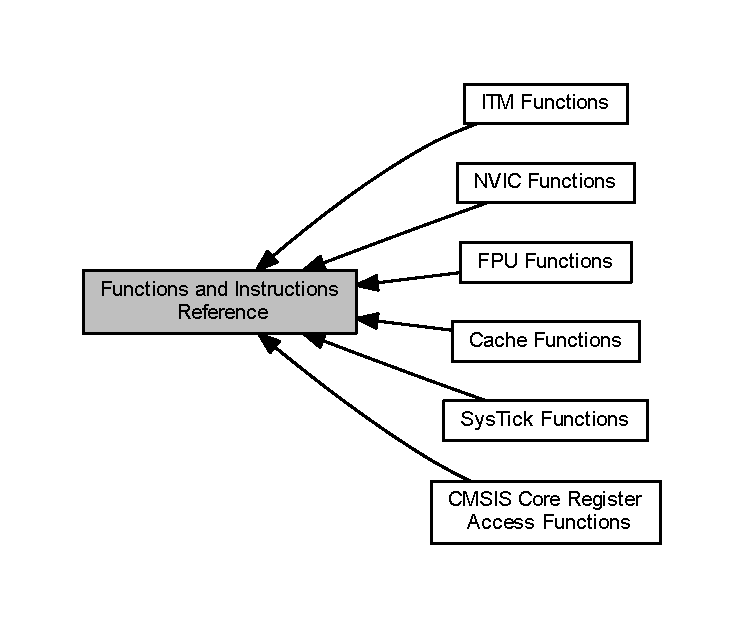
\includegraphics[width=350pt]{group___c_m_s_i_s___core___function_interface}
\end{center}
\end{figure}
\subsection*{Modules}
\begin{DoxyCompactItemize}
\item 
\hyperlink{group___c_m_s_i_s___core___reg_acc_functions}{C\+M\+S\+I\+S Core Register Access Functions}
\item 
\hyperlink{group___c_m_s_i_s___core___n_v_i_c_functions}{N\+V\+I\+C Functions}
\begin{DoxyCompactList}\small\item\em Functions that manage interrupts and exceptions via the N\+V\+IC. \end{DoxyCompactList}\item 
\hyperlink{group___c_m_s_i_s___core___sys_tick_functions}{Sys\+Tick Functions}
\begin{DoxyCompactList}\small\item\em Functions that configure the System. \end{DoxyCompactList}\item 
\hyperlink{group___c_m_s_i_s__core___debug_functions}{I\+T\+M Functions}
\begin{DoxyCompactList}\small\item\em Functions that access the I\+TM debug interface. \end{DoxyCompactList}\item 
\hyperlink{group___c_m_s_i_s___core___fpu_functions}{F\+P\+U Functions}
\begin{DoxyCompactList}\small\item\em Function that provides F\+PU type. \end{DoxyCompactList}\item 
\hyperlink{group___c_m_s_i_s___core___cache_functions}{Cache Functions}
\begin{DoxyCompactList}\small\item\em Functions that configure Instruction and Data cache. \end{DoxyCompactList}\end{DoxyCompactItemize}


\subsection{Detailed Description}

\hypertarget{group___c_m_s_i_s___core___n_v_i_c_functions}{}\section{N\+V\+IC Functions}
\label{group___c_m_s_i_s___core___n_v_i_c_functions}\index{N\+V\+I\+C Functions@{N\+V\+I\+C Functions}}


Functions that manage interrupts and exceptions via the N\+V\+IC.  


Collaboration diagram for N\+V\+IC Functions\+:
\nopagebreak
\begin{figure}[H]
\begin{center}
\leavevmode
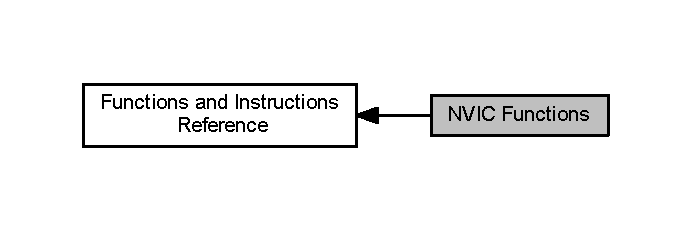
\includegraphics[width=332pt]{group___c_m_s_i_s___core___n_v_i_c_functions}
\end{center}
\end{figure}
\subsection*{Macros}
\begin{DoxyCompactItemize}
\item 
\#define \hyperlink{group___c_m_s_i_s___core___n_v_i_c_functions_ga53c75b28823441c6153269f0ecbed878}{\+\_\+\+B\+I\+T\+\_\+\+S\+H\+I\+FT}(\hyperlink{group___configuration__section__for___c_m_s_i_s_ga666eb0caeb12ec0e281415592ae89083}{I\+R\+Qn})~(  ((((uint32\+\_\+t)(int32\+\_\+t)(\hyperlink{group___configuration__section__for___c_m_s_i_s_ga666eb0caeb12ec0e281415592ae89083}{I\+R\+Qn}))         )      \&  0x03\+U\+L) $\ast$ 8\+U\+L)
\item 
\#define \hyperlink{group___c_m_s_i_s___core___n_v_i_c_functions_gaee4f7eb5d7e770ad51489dbceabb1755}{\+\_\+\+S\+H\+P\+\_\+\+I\+DX}(\hyperlink{group___configuration__section__for___c_m_s_i_s_ga666eb0caeb12ec0e281415592ae89083}{I\+R\+Qn})~( (((((uint32\+\_\+t)(int32\+\_\+t)(\hyperlink{group___configuration__section__for___c_m_s_i_s_ga666eb0caeb12ec0e281415592ae89083}{I\+R\+Qn})) \& 0x0\+F\+U\+L)-\/8\+U\+L) $>$$>$    2\+U\+L)      )
\item 
\#define \hyperlink{group___c_m_s_i_s___core___n_v_i_c_functions_ga370ec4b1751a6a889d849747df3763a9}{\+\_\+\+I\+P\+\_\+\+I\+DX}(\hyperlink{group___configuration__section__for___c_m_s_i_s_ga666eb0caeb12ec0e281415592ae89083}{I\+R\+Qn})~(   (((uint32\+\_\+t)(int32\+\_\+t)(\hyperlink{group___configuration__section__for___c_m_s_i_s_ga666eb0caeb12ec0e281415592ae89083}{I\+R\+Qn}))                $>$$>$    2\+U\+L)      )
\item 
\#define \hyperlink{group___c_m_s_i_s___core___n_v_i_c_functions_ga53c75b28823441c6153269f0ecbed878}{\+\_\+\+B\+I\+T\+\_\+\+S\+H\+I\+FT}(\hyperlink{group___configuration__section__for___c_m_s_i_s_ga666eb0caeb12ec0e281415592ae89083}{I\+R\+Qn})~(  ((((uint32\+\_\+t)(int32\+\_\+t)(\hyperlink{group___configuration__section__for___c_m_s_i_s_ga666eb0caeb12ec0e281415592ae89083}{I\+R\+Qn}))         )      \&  0x03\+U\+L) $\ast$ 8\+U\+L)
\item 
\#define \hyperlink{group___c_m_s_i_s___core___n_v_i_c_functions_gaee4f7eb5d7e770ad51489dbceabb1755}{\+\_\+\+S\+H\+P\+\_\+\+I\+DX}(\hyperlink{group___configuration__section__for___c_m_s_i_s_ga666eb0caeb12ec0e281415592ae89083}{I\+R\+Qn})~( (((((uint32\+\_\+t)(int32\+\_\+t)(\hyperlink{group___configuration__section__for___c_m_s_i_s_ga666eb0caeb12ec0e281415592ae89083}{I\+R\+Qn})) \& 0x0\+F\+U\+L)-\/8\+U\+L) $>$$>$    2\+U\+L)      )
\item 
\#define \hyperlink{group___c_m_s_i_s___core___n_v_i_c_functions_ga370ec4b1751a6a889d849747df3763a9}{\+\_\+\+I\+P\+\_\+\+I\+DX}(\hyperlink{group___configuration__section__for___c_m_s_i_s_ga666eb0caeb12ec0e281415592ae89083}{I\+R\+Qn})~(   (((uint32\+\_\+t)(int32\+\_\+t)(\hyperlink{group___configuration__section__for___c_m_s_i_s_ga666eb0caeb12ec0e281415592ae89083}{I\+R\+Qn}))                $>$$>$    2\+U\+L)      )
\item 
\#define \hyperlink{group___c_m_s_i_s___core___n_v_i_c_functions_ga53c75b28823441c6153269f0ecbed878}{\+\_\+\+B\+I\+T\+\_\+\+S\+H\+I\+FT}(\hyperlink{group___configuration__section__for___c_m_s_i_s_ga666eb0caeb12ec0e281415592ae89083}{I\+R\+Qn})~(  ((((uint32\+\_\+t)(int32\+\_\+t)(\hyperlink{group___configuration__section__for___c_m_s_i_s_ga666eb0caeb12ec0e281415592ae89083}{I\+R\+Qn}))         )      \&  0x03\+U\+L) $\ast$ 8\+U\+L)
\item 
\#define \hyperlink{group___c_m_s_i_s___core___n_v_i_c_functions_gaee4f7eb5d7e770ad51489dbceabb1755}{\+\_\+\+S\+H\+P\+\_\+\+I\+DX}(\hyperlink{group___configuration__section__for___c_m_s_i_s_ga666eb0caeb12ec0e281415592ae89083}{I\+R\+Qn})~( (((((uint32\+\_\+t)(int32\+\_\+t)(\hyperlink{group___configuration__section__for___c_m_s_i_s_ga666eb0caeb12ec0e281415592ae89083}{I\+R\+Qn})) \& 0x0\+F\+U\+L)-\/8\+U\+L) $>$$>$    2\+U\+L)      )
\item 
\#define \hyperlink{group___c_m_s_i_s___core___n_v_i_c_functions_ga370ec4b1751a6a889d849747df3763a9}{\+\_\+\+I\+P\+\_\+\+I\+DX}(\hyperlink{group___configuration__section__for___c_m_s_i_s_ga666eb0caeb12ec0e281415592ae89083}{I\+R\+Qn})~(   (((uint32\+\_\+t)(int32\+\_\+t)(\hyperlink{group___configuration__section__for___c_m_s_i_s_ga666eb0caeb12ec0e281415592ae89083}{I\+R\+Qn}))                $>$$>$    2\+U\+L)      )
\end{DoxyCompactItemize}
\subsection*{Functions}
\begin{DoxyCompactItemize}
\item 
\+\_\+\+\_\+\+S\+T\+A\+T\+I\+C\+\_\+\+I\+N\+L\+I\+NE void \hyperlink{group___c_m_s_i_s___core___n_v_i_c_functions_ga3349f2e3580d7ce22d6530b7294e5921}{N\+V\+I\+C\+\_\+\+Enable\+I\+RQ} (\hyperlink{group___configuration__section__for___c_m_s_i_s_gac3af4a32370fb28c4ade8bf2add80251}{I\+R\+Qn\+\_\+\+Type} \hyperlink{group___configuration__section__for___c_m_s_i_s_ga666eb0caeb12ec0e281415592ae89083}{I\+R\+Qn})
\begin{DoxyCompactList}\small\item\em Enable External Interrupt. \end{DoxyCompactList}\item 
\+\_\+\+\_\+\+S\+T\+A\+T\+I\+C\+\_\+\+I\+N\+L\+I\+NE void \hyperlink{group___c_m_s_i_s___core___n_v_i_c_functions_ga260fba04ac8346855c57f091d4ee1e71}{N\+V\+I\+C\+\_\+\+Disable\+I\+RQ} (\hyperlink{group___configuration__section__for___c_m_s_i_s_gac3af4a32370fb28c4ade8bf2add80251}{I\+R\+Qn\+\_\+\+Type} \hyperlink{group___configuration__section__for___c_m_s_i_s_ga666eb0caeb12ec0e281415592ae89083}{I\+R\+Qn})
\begin{DoxyCompactList}\small\item\em Disable External Interrupt. \end{DoxyCompactList}\item 
\+\_\+\+\_\+\+S\+T\+A\+T\+I\+C\+\_\+\+I\+N\+L\+I\+NE uint32\+\_\+t \hyperlink{group___c_m_s_i_s___core___n_v_i_c_functions_gafec8042db64c0f8ed432b6c8386a05d8}{N\+V\+I\+C\+\_\+\+Get\+Pending\+I\+RQ} (\hyperlink{group___configuration__section__for___c_m_s_i_s_gac3af4a32370fb28c4ade8bf2add80251}{I\+R\+Qn\+\_\+\+Type} \hyperlink{group___configuration__section__for___c_m_s_i_s_ga666eb0caeb12ec0e281415592ae89083}{I\+R\+Qn})
\begin{DoxyCompactList}\small\item\em Get Pending Interrupt. \end{DoxyCompactList}\item 
\+\_\+\+\_\+\+S\+T\+A\+T\+I\+C\+\_\+\+I\+N\+L\+I\+NE void \hyperlink{group___c_m_s_i_s___core___n_v_i_c_functions_ga3ecf446519da33e1690deffbf5be505f}{N\+V\+I\+C\+\_\+\+Set\+Pending\+I\+RQ} (\hyperlink{group___configuration__section__for___c_m_s_i_s_gac3af4a32370fb28c4ade8bf2add80251}{I\+R\+Qn\+\_\+\+Type} \hyperlink{group___configuration__section__for___c_m_s_i_s_ga666eb0caeb12ec0e281415592ae89083}{I\+R\+Qn})
\begin{DoxyCompactList}\small\item\em Set Pending Interrupt. \end{DoxyCompactList}\item 
\+\_\+\+\_\+\+S\+T\+A\+T\+I\+C\+\_\+\+I\+N\+L\+I\+NE void \hyperlink{group___c_m_s_i_s___core___n_v_i_c_functions_ga332e10ef9605dc6eb10b9e14511930f8}{N\+V\+I\+C\+\_\+\+Clear\+Pending\+I\+RQ} (\hyperlink{group___configuration__section__for___c_m_s_i_s_gac3af4a32370fb28c4ade8bf2add80251}{I\+R\+Qn\+\_\+\+Type} \hyperlink{group___configuration__section__for___c_m_s_i_s_ga666eb0caeb12ec0e281415592ae89083}{I\+R\+Qn})
\begin{DoxyCompactList}\small\item\em Clear Pending Interrupt. \end{DoxyCompactList}\item 
\+\_\+\+\_\+\+S\+T\+A\+T\+I\+C\+\_\+\+I\+N\+L\+I\+NE void \hyperlink{group___c_m_s_i_s___core___n_v_i_c_functions_ga2305cbd44aaad792e3a4e538bdaf14f9}{N\+V\+I\+C\+\_\+\+Set\+Priority} (\hyperlink{group___configuration__section__for___c_m_s_i_s_gac3af4a32370fb28c4ade8bf2add80251}{I\+R\+Qn\+\_\+\+Type} \hyperlink{group___configuration__section__for___c_m_s_i_s_ga666eb0caeb12ec0e281415592ae89083}{I\+R\+Qn}, uint32\+\_\+t priority)
\begin{DoxyCompactList}\small\item\em Set Interrupt Priority. \end{DoxyCompactList}\item 
\+\_\+\+\_\+\+S\+T\+A\+T\+I\+C\+\_\+\+I\+N\+L\+I\+NE uint32\+\_\+t \hyperlink{group___c_m_s_i_s___core___n_v_i_c_functions_ga1cbaf8e6abd4aa4885828e7f24fcfeb4}{N\+V\+I\+C\+\_\+\+Get\+Priority} (\hyperlink{group___configuration__section__for___c_m_s_i_s_gac3af4a32370fb28c4ade8bf2add80251}{I\+R\+Qn\+\_\+\+Type} \hyperlink{group___configuration__section__for___c_m_s_i_s_ga666eb0caeb12ec0e281415592ae89083}{I\+R\+Qn})
\begin{DoxyCompactList}\small\item\em Get Interrupt Priority. \end{DoxyCompactList}\item 
\+\_\+\+\_\+\+S\+T\+A\+T\+I\+C\+\_\+\+I\+N\+L\+I\+NE void \hyperlink{group___c_m_s_i_s___core___n_v_i_c_functions_ga1143dec48d60a3d6f238c4798a87759c}{N\+V\+I\+C\+\_\+\+System\+Reset} (void)
\begin{DoxyCompactList}\small\item\em System Reset. \end{DoxyCompactList}\item 
\+\_\+\+\_\+\+S\+T\+A\+T\+I\+C\+\_\+\+I\+N\+L\+I\+NE void \hyperlink{group___c_m_s_i_s___core___n_v_i_c_functions_ga77cfbb35a9d8027e392034321bed6904}{N\+V\+I\+C\+\_\+\+Set\+Priority\+Grouping} (uint32\+\_\+t Priority\+Group)
\begin{DoxyCompactList}\small\item\em Set Priority Grouping. \end{DoxyCompactList}\item 
\+\_\+\+\_\+\+S\+T\+A\+T\+I\+C\+\_\+\+I\+N\+L\+I\+NE uint32\+\_\+t \hyperlink{group___c_m_s_i_s___core___n_v_i_c_functions_ga394f7ce2ca826c0da26284d17ac6524d}{N\+V\+I\+C\+\_\+\+Get\+Priority\+Grouping} (void)
\begin{DoxyCompactList}\small\item\em Get Priority Grouping. \end{DoxyCompactList}\item 
\+\_\+\+\_\+\+S\+T\+A\+T\+I\+C\+\_\+\+I\+N\+L\+I\+NE uint32\+\_\+t \hyperlink{group___c_m_s_i_s___core___n_v_i_c_functions_ga47a0f52794068d076c9147aa3cb8d8a6}{N\+V\+I\+C\+\_\+\+Get\+Active} (\hyperlink{group___configuration__section__for___c_m_s_i_s_gac3af4a32370fb28c4ade8bf2add80251}{I\+R\+Qn\+\_\+\+Type} \hyperlink{group___configuration__section__for___c_m_s_i_s_ga666eb0caeb12ec0e281415592ae89083}{I\+R\+Qn})
\begin{DoxyCompactList}\small\item\em Get Active Interrupt. \end{DoxyCompactList}\item 
\+\_\+\+\_\+\+S\+T\+A\+T\+I\+C\+\_\+\+I\+N\+L\+I\+NE uint32\+\_\+t \hyperlink{group___c_m_s_i_s___core___n_v_i_c_functions_gadb94ac5d892b376e4f3555ae0418ebac}{N\+V\+I\+C\+\_\+\+Encode\+Priority} (uint32\+\_\+t Priority\+Group, uint32\+\_\+t Preempt\+Priority, uint32\+\_\+t Sub\+Priority)
\begin{DoxyCompactList}\small\item\em Encode Priority. \end{DoxyCompactList}\item 
\+\_\+\+\_\+\+S\+T\+A\+T\+I\+C\+\_\+\+I\+N\+L\+I\+NE void \hyperlink{group___c_m_s_i_s___core___n_v_i_c_functions_ga3387607fd8a1a32cccd77d2ac672dd96}{N\+V\+I\+C\+\_\+\+Decode\+Priority} (uint32\+\_\+t Priority, uint32\+\_\+t Priority\+Group, uint32\+\_\+t $\ast$const p\+Preempt\+Priority, uint32\+\_\+t $\ast$const p\+Sub\+Priority)
\begin{DoxyCompactList}\small\item\em Decode Priority. \end{DoxyCompactList}\end{DoxyCompactItemize}


\subsection{Detailed Description}
Functions that manage interrupts and exceptions via the N\+V\+IC. 



\subsection{Macro Definition Documentation}
\mbox{\Hypertarget{group___c_m_s_i_s___core___n_v_i_c_functions_ga53c75b28823441c6153269f0ecbed878}\label{group___c_m_s_i_s___core___n_v_i_c_functions_ga53c75b28823441c6153269f0ecbed878}} 
\index{N\+V\+I\+C Functions@{N\+V\+I\+C Functions}!\+\_\+\+B\+I\+T\+\_\+\+S\+H\+I\+FT@{\+\_\+\+B\+I\+T\+\_\+\+S\+H\+I\+FT}}
\index{\+\_\+\+B\+I\+T\+\_\+\+S\+H\+I\+FT@{\+\_\+\+B\+I\+T\+\_\+\+S\+H\+I\+FT}!N\+V\+I\+C Functions@{N\+V\+I\+C Functions}}
\subsubsection{\texorpdfstring{\+\_\+\+B\+I\+T\+\_\+\+S\+H\+I\+FT}{\_BIT\_SHIFT}\hspace{0.1cm}{\footnotesize\ttfamily [1/3]}}
{\footnotesize\ttfamily \#define \+\_\+\+B\+I\+T\+\_\+\+S\+H\+I\+FT(\begin{DoxyParamCaption}\item[{}]{\hyperlink{group___configuration__section__for___c_m_s_i_s_ga666eb0caeb12ec0e281415592ae89083}{I\+R\+Qn} }\end{DoxyParamCaption})~(  ((((uint32\+\_\+t)(int32\+\_\+t)(\hyperlink{group___configuration__section__for___c_m_s_i_s_ga666eb0caeb12ec0e281415592ae89083}{I\+R\+Qn}))         )      \&  0x03\+U\+L) $\ast$ 8\+U\+L)}



Definition at line 627 of file core\+\_\+cm0.\+h.

\mbox{\Hypertarget{group___c_m_s_i_s___core___n_v_i_c_functions_ga53c75b28823441c6153269f0ecbed878}\label{group___c_m_s_i_s___core___n_v_i_c_functions_ga53c75b28823441c6153269f0ecbed878}} 
\index{N\+V\+I\+C Functions@{N\+V\+I\+C Functions}!\+\_\+\+B\+I\+T\+\_\+\+S\+H\+I\+FT@{\+\_\+\+B\+I\+T\+\_\+\+S\+H\+I\+FT}}
\index{\+\_\+\+B\+I\+T\+\_\+\+S\+H\+I\+FT@{\+\_\+\+B\+I\+T\+\_\+\+S\+H\+I\+FT}!N\+V\+I\+C Functions@{N\+V\+I\+C Functions}}
\subsubsection{\texorpdfstring{\+\_\+\+B\+I\+T\+\_\+\+S\+H\+I\+FT}{\_BIT\_SHIFT}\hspace{0.1cm}{\footnotesize\ttfamily [2/3]}}
{\footnotesize\ttfamily \#define \+\_\+\+B\+I\+T\+\_\+\+S\+H\+I\+FT(\begin{DoxyParamCaption}\item[{}]{\hyperlink{group___configuration__section__for___c_m_s_i_s_ga666eb0caeb12ec0e281415592ae89083}{I\+R\+Qn} }\end{DoxyParamCaption})~(  ((((uint32\+\_\+t)(int32\+\_\+t)(\hyperlink{group___configuration__section__for___c_m_s_i_s_ga666eb0caeb12ec0e281415592ae89083}{I\+R\+Qn}))         )      \&  0x03\+U\+L) $\ast$ 8\+U\+L)}



Definition at line 743 of file core\+\_\+cm0plus.\+h.

\mbox{\Hypertarget{group___c_m_s_i_s___core___n_v_i_c_functions_ga53c75b28823441c6153269f0ecbed878}\label{group___c_m_s_i_s___core___n_v_i_c_functions_ga53c75b28823441c6153269f0ecbed878}} 
\index{N\+V\+I\+C Functions@{N\+V\+I\+C Functions}!\+\_\+\+B\+I\+T\+\_\+\+S\+H\+I\+FT@{\+\_\+\+B\+I\+T\+\_\+\+S\+H\+I\+FT}}
\index{\+\_\+\+B\+I\+T\+\_\+\+S\+H\+I\+FT@{\+\_\+\+B\+I\+T\+\_\+\+S\+H\+I\+FT}!N\+V\+I\+C Functions@{N\+V\+I\+C Functions}}
\subsubsection{\texorpdfstring{\+\_\+\+B\+I\+T\+\_\+\+S\+H\+I\+FT}{\_BIT\_SHIFT}\hspace{0.1cm}{\footnotesize\ttfamily [3/3]}}
{\footnotesize\ttfamily \#define \+\_\+\+B\+I\+T\+\_\+\+S\+H\+I\+FT(\begin{DoxyParamCaption}\item[{}]{\hyperlink{group___configuration__section__for___c_m_s_i_s_ga666eb0caeb12ec0e281415592ae89083}{I\+R\+Qn} }\end{DoxyParamCaption})~(  ((((uint32\+\_\+t)(int32\+\_\+t)(\hyperlink{group___configuration__section__for___c_m_s_i_s_ga666eb0caeb12ec0e281415592ae89083}{I\+R\+Qn}))         )      \&  0x03\+U\+L) $\ast$ 8\+U\+L)}



Definition at line 747 of file core\+\_\+sc000.\+h.

\mbox{\Hypertarget{group___c_m_s_i_s___core___n_v_i_c_functions_ga370ec4b1751a6a889d849747df3763a9}\label{group___c_m_s_i_s___core___n_v_i_c_functions_ga370ec4b1751a6a889d849747df3763a9}} 
\index{N\+V\+I\+C Functions@{N\+V\+I\+C Functions}!\+\_\+\+I\+P\+\_\+\+I\+DX@{\+\_\+\+I\+P\+\_\+\+I\+DX}}
\index{\+\_\+\+I\+P\+\_\+\+I\+DX@{\+\_\+\+I\+P\+\_\+\+I\+DX}!N\+V\+I\+C Functions@{N\+V\+I\+C Functions}}
\subsubsection{\texorpdfstring{\+\_\+\+I\+P\+\_\+\+I\+DX}{\_IP\_IDX}\hspace{0.1cm}{\footnotesize\ttfamily [1/3]}}
{\footnotesize\ttfamily \#define \+\_\+\+I\+P\+\_\+\+I\+DX(\begin{DoxyParamCaption}\item[{}]{\hyperlink{group___configuration__section__for___c_m_s_i_s_ga666eb0caeb12ec0e281415592ae89083}{I\+R\+Qn} }\end{DoxyParamCaption})~(   (((uint32\+\_\+t)(int32\+\_\+t)(\hyperlink{group___configuration__section__for___c_m_s_i_s_ga666eb0caeb12ec0e281415592ae89083}{I\+R\+Qn}))                $>$$>$    2\+U\+L)      )}



Definition at line 629 of file core\+\_\+cm0.\+h.

\mbox{\Hypertarget{group___c_m_s_i_s___core___n_v_i_c_functions_ga370ec4b1751a6a889d849747df3763a9}\label{group___c_m_s_i_s___core___n_v_i_c_functions_ga370ec4b1751a6a889d849747df3763a9}} 
\index{N\+V\+I\+C Functions@{N\+V\+I\+C Functions}!\+\_\+\+I\+P\+\_\+\+I\+DX@{\+\_\+\+I\+P\+\_\+\+I\+DX}}
\index{\+\_\+\+I\+P\+\_\+\+I\+DX@{\+\_\+\+I\+P\+\_\+\+I\+DX}!N\+V\+I\+C Functions@{N\+V\+I\+C Functions}}
\subsubsection{\texorpdfstring{\+\_\+\+I\+P\+\_\+\+I\+DX}{\_IP\_IDX}\hspace{0.1cm}{\footnotesize\ttfamily [2/3]}}
{\footnotesize\ttfamily \#define \+\_\+\+I\+P\+\_\+\+I\+DX(\begin{DoxyParamCaption}\item[{}]{\hyperlink{group___configuration__section__for___c_m_s_i_s_ga666eb0caeb12ec0e281415592ae89083}{I\+R\+Qn} }\end{DoxyParamCaption})~(   (((uint32\+\_\+t)(int32\+\_\+t)(\hyperlink{group___configuration__section__for___c_m_s_i_s_ga666eb0caeb12ec0e281415592ae89083}{I\+R\+Qn}))                $>$$>$    2\+U\+L)      )}



Definition at line 745 of file core\+\_\+cm0plus.\+h.

\mbox{\Hypertarget{group___c_m_s_i_s___core___n_v_i_c_functions_ga370ec4b1751a6a889d849747df3763a9}\label{group___c_m_s_i_s___core___n_v_i_c_functions_ga370ec4b1751a6a889d849747df3763a9}} 
\index{N\+V\+I\+C Functions@{N\+V\+I\+C Functions}!\+\_\+\+I\+P\+\_\+\+I\+DX@{\+\_\+\+I\+P\+\_\+\+I\+DX}}
\index{\+\_\+\+I\+P\+\_\+\+I\+DX@{\+\_\+\+I\+P\+\_\+\+I\+DX}!N\+V\+I\+C Functions@{N\+V\+I\+C Functions}}
\subsubsection{\texorpdfstring{\+\_\+\+I\+P\+\_\+\+I\+DX}{\_IP\_IDX}\hspace{0.1cm}{\footnotesize\ttfamily [3/3]}}
{\footnotesize\ttfamily \#define \+\_\+\+I\+P\+\_\+\+I\+DX(\begin{DoxyParamCaption}\item[{}]{\hyperlink{group___configuration__section__for___c_m_s_i_s_ga666eb0caeb12ec0e281415592ae89083}{I\+R\+Qn} }\end{DoxyParamCaption})~(   (((uint32\+\_\+t)(int32\+\_\+t)(\hyperlink{group___configuration__section__for___c_m_s_i_s_ga666eb0caeb12ec0e281415592ae89083}{I\+R\+Qn}))                $>$$>$    2\+U\+L)      )}



Definition at line 749 of file core\+\_\+sc000.\+h.

\mbox{\Hypertarget{group___c_m_s_i_s___core___n_v_i_c_functions_gaee4f7eb5d7e770ad51489dbceabb1755}\label{group___c_m_s_i_s___core___n_v_i_c_functions_gaee4f7eb5d7e770ad51489dbceabb1755}} 
\index{N\+V\+I\+C Functions@{N\+V\+I\+C Functions}!\+\_\+\+S\+H\+P\+\_\+\+I\+DX@{\+\_\+\+S\+H\+P\+\_\+\+I\+DX}}
\index{\+\_\+\+S\+H\+P\+\_\+\+I\+DX@{\+\_\+\+S\+H\+P\+\_\+\+I\+DX}!N\+V\+I\+C Functions@{N\+V\+I\+C Functions}}
\subsubsection{\texorpdfstring{\+\_\+\+S\+H\+P\+\_\+\+I\+DX}{\_SHP\_IDX}\hspace{0.1cm}{\footnotesize\ttfamily [1/3]}}
{\footnotesize\ttfamily \#define \+\_\+\+S\+H\+P\+\_\+\+I\+DX(\begin{DoxyParamCaption}\item[{}]{\hyperlink{group___configuration__section__for___c_m_s_i_s_ga666eb0caeb12ec0e281415592ae89083}{I\+R\+Qn} }\end{DoxyParamCaption})~( (((((uint32\+\_\+t)(int32\+\_\+t)(\hyperlink{group___configuration__section__for___c_m_s_i_s_ga666eb0caeb12ec0e281415592ae89083}{I\+R\+Qn})) \& 0x0\+F\+U\+L)-\/8\+U\+L) $>$$>$    2\+U\+L)      )}



Definition at line 628 of file core\+\_\+cm0.\+h.

\mbox{\Hypertarget{group___c_m_s_i_s___core___n_v_i_c_functions_gaee4f7eb5d7e770ad51489dbceabb1755}\label{group___c_m_s_i_s___core___n_v_i_c_functions_gaee4f7eb5d7e770ad51489dbceabb1755}} 
\index{N\+V\+I\+C Functions@{N\+V\+I\+C Functions}!\+\_\+\+S\+H\+P\+\_\+\+I\+DX@{\+\_\+\+S\+H\+P\+\_\+\+I\+DX}}
\index{\+\_\+\+S\+H\+P\+\_\+\+I\+DX@{\+\_\+\+S\+H\+P\+\_\+\+I\+DX}!N\+V\+I\+C Functions@{N\+V\+I\+C Functions}}
\subsubsection{\texorpdfstring{\+\_\+\+S\+H\+P\+\_\+\+I\+DX}{\_SHP\_IDX}\hspace{0.1cm}{\footnotesize\ttfamily [2/3]}}
{\footnotesize\ttfamily \#define \+\_\+\+S\+H\+P\+\_\+\+I\+DX(\begin{DoxyParamCaption}\item[{}]{\hyperlink{group___configuration__section__for___c_m_s_i_s_ga666eb0caeb12ec0e281415592ae89083}{I\+R\+Qn} }\end{DoxyParamCaption})~( (((((uint32\+\_\+t)(int32\+\_\+t)(\hyperlink{group___configuration__section__for___c_m_s_i_s_ga666eb0caeb12ec0e281415592ae89083}{I\+R\+Qn})) \& 0x0\+F\+U\+L)-\/8\+U\+L) $>$$>$    2\+U\+L)      )}



Definition at line 744 of file core\+\_\+cm0plus.\+h.

\mbox{\Hypertarget{group___c_m_s_i_s___core___n_v_i_c_functions_gaee4f7eb5d7e770ad51489dbceabb1755}\label{group___c_m_s_i_s___core___n_v_i_c_functions_gaee4f7eb5d7e770ad51489dbceabb1755}} 
\index{N\+V\+I\+C Functions@{N\+V\+I\+C Functions}!\+\_\+\+S\+H\+P\+\_\+\+I\+DX@{\+\_\+\+S\+H\+P\+\_\+\+I\+DX}}
\index{\+\_\+\+S\+H\+P\+\_\+\+I\+DX@{\+\_\+\+S\+H\+P\+\_\+\+I\+DX}!N\+V\+I\+C Functions@{N\+V\+I\+C Functions}}
\subsubsection{\texorpdfstring{\+\_\+\+S\+H\+P\+\_\+\+I\+DX}{\_SHP\_IDX}\hspace{0.1cm}{\footnotesize\ttfamily [3/3]}}
{\footnotesize\ttfamily \#define \+\_\+\+S\+H\+P\+\_\+\+I\+DX(\begin{DoxyParamCaption}\item[{}]{\hyperlink{group___configuration__section__for___c_m_s_i_s_ga666eb0caeb12ec0e281415592ae89083}{I\+R\+Qn} }\end{DoxyParamCaption})~( (((((uint32\+\_\+t)(int32\+\_\+t)(\hyperlink{group___configuration__section__for___c_m_s_i_s_ga666eb0caeb12ec0e281415592ae89083}{I\+R\+Qn})) \& 0x0\+F\+U\+L)-\/8\+U\+L) $>$$>$    2\+U\+L)      )}



Definition at line 748 of file core\+\_\+sc000.\+h.



\subsection{Function Documentation}
\mbox{\Hypertarget{group___c_m_s_i_s___core___n_v_i_c_functions_ga332e10ef9605dc6eb10b9e14511930f8}\label{group___c_m_s_i_s___core___n_v_i_c_functions_ga332e10ef9605dc6eb10b9e14511930f8}} 
\index{N\+V\+I\+C Functions@{N\+V\+I\+C Functions}!N\+V\+I\+C\+\_\+\+Clear\+Pending\+I\+RQ@{N\+V\+I\+C\+\_\+\+Clear\+Pending\+I\+RQ}}
\index{N\+V\+I\+C\+\_\+\+Clear\+Pending\+I\+RQ@{N\+V\+I\+C\+\_\+\+Clear\+Pending\+I\+RQ}!N\+V\+I\+C Functions@{N\+V\+I\+C Functions}}
\subsubsection{\texorpdfstring{N\+V\+I\+C\+\_\+\+Clear\+Pending\+I\+R\+Q()}{NVIC\_ClearPendingIRQ()}}
{\footnotesize\ttfamily \+\_\+\+\_\+\+S\+T\+A\+T\+I\+C\+\_\+\+I\+N\+L\+I\+NE void N\+V\+I\+C\+\_\+\+Clear\+Pending\+I\+RQ (\begin{DoxyParamCaption}\item[{\hyperlink{group___configuration__section__for___c_m_s_i_s_gac3af4a32370fb28c4ade8bf2add80251}{I\+R\+Qn\+\_\+\+Type}}]{I\+R\+Qn }\end{DoxyParamCaption})}



Clear Pending Interrupt. 

Clears the pending bit of an external interrupt. 
\begin{DoxyParams}[1]{Parameters}
\mbox{\tt in}  & {\em I\+R\+Qn} & External interrupt number. Value cannot be negative. \\
\hline
\end{DoxyParams}


Definition at line 683 of file core\+\_\+cm0.\+h.

Here is the caller graph for this function\+:
\nopagebreak
\begin{figure}[H]
\begin{center}
\leavevmode
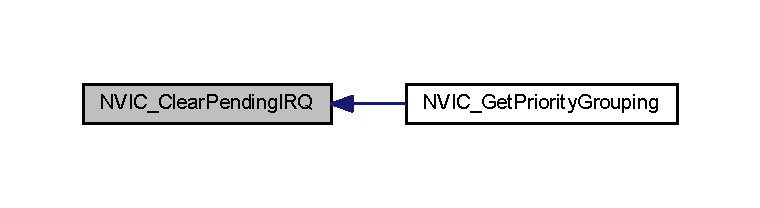
\includegraphics[width=350pt]{group___c_m_s_i_s___core___n_v_i_c_functions_ga332e10ef9605dc6eb10b9e14511930f8_icgraph}
\end{center}
\end{figure}
\mbox{\Hypertarget{group___c_m_s_i_s___core___n_v_i_c_functions_ga3387607fd8a1a32cccd77d2ac672dd96}\label{group___c_m_s_i_s___core___n_v_i_c_functions_ga3387607fd8a1a32cccd77d2ac672dd96}} 
\index{N\+V\+I\+C Functions@{N\+V\+I\+C Functions}!N\+V\+I\+C\+\_\+\+Decode\+Priority@{N\+V\+I\+C\+\_\+\+Decode\+Priority}}
\index{N\+V\+I\+C\+\_\+\+Decode\+Priority@{N\+V\+I\+C\+\_\+\+Decode\+Priority}!N\+V\+I\+C Functions@{N\+V\+I\+C Functions}}
\subsubsection{\texorpdfstring{N\+V\+I\+C\+\_\+\+Decode\+Priority()}{NVIC\_DecodePriority()}}
{\footnotesize\ttfamily \+\_\+\+\_\+\+S\+T\+A\+T\+I\+C\+\_\+\+I\+N\+L\+I\+NE void N\+V\+I\+C\+\_\+\+Decode\+Priority (\begin{DoxyParamCaption}\item[{uint32\+\_\+t}]{Priority,  }\item[{uint32\+\_\+t}]{Priority\+Group,  }\item[{uint32\+\_\+t $\ast$const}]{p\+Preempt\+Priority,  }\item[{uint32\+\_\+t $\ast$const}]{p\+Sub\+Priority }\end{DoxyParamCaption})}



Decode Priority. 

Decodes an interrupt priority value with a given priority group to preemptive priority value and subpriority value. In case of a conflict between priority grouping and available priority bits (\+\_\+\+\_\+\+N\+V\+I\+C\+\_\+\+P\+R\+I\+O\+\_\+\+B\+I\+TS) the smallest possible priority group is set. 
\begin{DoxyParams}[1]{Parameters}
\mbox{\tt in}  & {\em Priority} & Priority value, which can be retrieved with the function \hyperlink{group___c_m_s_i_s___core___n_v_i_c_functions_ga1cbaf8e6abd4aa4885828e7f24fcfeb4}{N\+V\+I\+C\+\_\+\+Get\+Priority()}. \\
\hline
\mbox{\tt in}  & {\em Priority\+Group} & Used priority group. \\
\hline
\mbox{\tt out}  & {\em p\+Preempt\+Priority} & Preemptive priority value (starting from 0). \\
\hline
\mbox{\tt out}  & {\em p\+Sub\+Priority} & Subpriority value (starting from 0). \\
\hline
\end{DoxyParams}


Definition at line 1606 of file core\+\_\+cm3.\+h.

Here is the call graph for this function\+:
\nopagebreak
\begin{figure}[H]
\begin{center}
\leavevmode
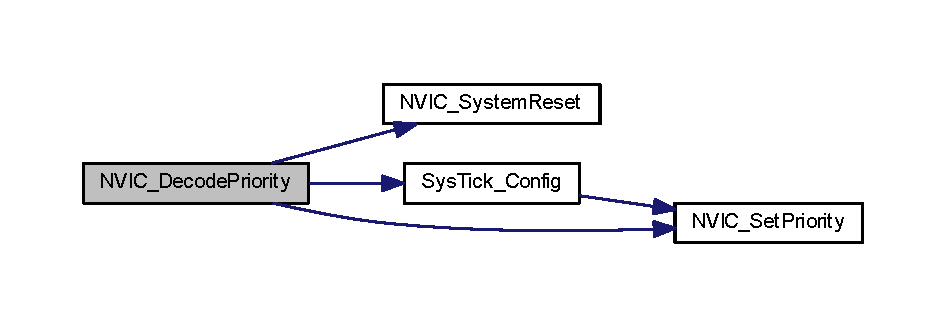
\includegraphics[width=350pt]{group___c_m_s_i_s___core___n_v_i_c_functions_ga3387607fd8a1a32cccd77d2ac672dd96_cgraph}
\end{center}
\end{figure}
\mbox{\Hypertarget{group___c_m_s_i_s___core___n_v_i_c_functions_ga260fba04ac8346855c57f091d4ee1e71}\label{group___c_m_s_i_s___core___n_v_i_c_functions_ga260fba04ac8346855c57f091d4ee1e71}} 
\index{N\+V\+I\+C Functions@{N\+V\+I\+C Functions}!N\+V\+I\+C\+\_\+\+Disable\+I\+RQ@{N\+V\+I\+C\+\_\+\+Disable\+I\+RQ}}
\index{N\+V\+I\+C\+\_\+\+Disable\+I\+RQ@{N\+V\+I\+C\+\_\+\+Disable\+I\+RQ}!N\+V\+I\+C Functions@{N\+V\+I\+C Functions}}
\subsubsection{\texorpdfstring{N\+V\+I\+C\+\_\+\+Disable\+I\+R\+Q()}{NVIC\_DisableIRQ()}}
{\footnotesize\ttfamily \+\_\+\+\_\+\+S\+T\+A\+T\+I\+C\+\_\+\+I\+N\+L\+I\+NE void N\+V\+I\+C\+\_\+\+Disable\+I\+RQ (\begin{DoxyParamCaption}\item[{\hyperlink{group___configuration__section__for___c_m_s_i_s_gac3af4a32370fb28c4ade8bf2add80251}{I\+R\+Qn\+\_\+\+Type}}]{I\+R\+Qn }\end{DoxyParamCaption})}



Disable External Interrupt. 

Disables a device-\/specific interrupt in the N\+V\+IC interrupt controller. 
\begin{DoxyParams}[1]{Parameters}
\mbox{\tt in}  & {\em I\+R\+Qn} & External interrupt number. Value cannot be negative. \\
\hline
\end{DoxyParams}


Definition at line 648 of file core\+\_\+cm0.\+h.

Here is the caller graph for this function\+:
\nopagebreak
\begin{figure}[H]
\begin{center}
\leavevmode
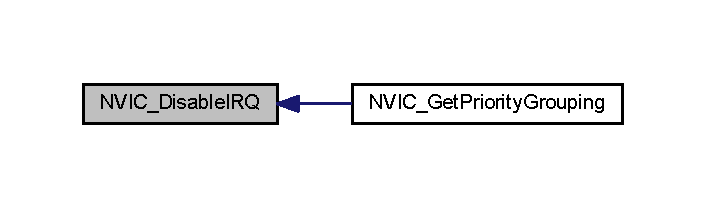
\includegraphics[width=339pt]{group___c_m_s_i_s___core___n_v_i_c_functions_ga260fba04ac8346855c57f091d4ee1e71_icgraph}
\end{center}
\end{figure}
\mbox{\Hypertarget{group___c_m_s_i_s___core___n_v_i_c_functions_ga3349f2e3580d7ce22d6530b7294e5921}\label{group___c_m_s_i_s___core___n_v_i_c_functions_ga3349f2e3580d7ce22d6530b7294e5921}} 
\index{N\+V\+I\+C Functions@{N\+V\+I\+C Functions}!N\+V\+I\+C\+\_\+\+Enable\+I\+RQ@{N\+V\+I\+C\+\_\+\+Enable\+I\+RQ}}
\index{N\+V\+I\+C\+\_\+\+Enable\+I\+RQ@{N\+V\+I\+C\+\_\+\+Enable\+I\+RQ}!N\+V\+I\+C Functions@{N\+V\+I\+C Functions}}
\subsubsection{\texorpdfstring{N\+V\+I\+C\+\_\+\+Enable\+I\+R\+Q()}{NVIC\_EnableIRQ()}}
{\footnotesize\ttfamily \+\_\+\+\_\+\+S\+T\+A\+T\+I\+C\+\_\+\+I\+N\+L\+I\+NE void N\+V\+I\+C\+\_\+\+Enable\+I\+RQ (\begin{DoxyParamCaption}\item[{\hyperlink{group___configuration__section__for___c_m_s_i_s_gac3af4a32370fb28c4ade8bf2add80251}{I\+R\+Qn\+\_\+\+Type}}]{I\+R\+Qn }\end{DoxyParamCaption})}



Enable External Interrupt. 

Enables a device-\/specific interrupt in the N\+V\+IC interrupt controller. 
\begin{DoxyParams}[1]{Parameters}
\mbox{\tt in}  & {\em I\+R\+Qn} & External interrupt number. Value cannot be negative. \\
\hline
\end{DoxyParams}


Definition at line 637 of file core\+\_\+cm0.\+h.

Here is the caller graph for this function\+:
\nopagebreak
\begin{figure}[H]
\begin{center}
\leavevmode
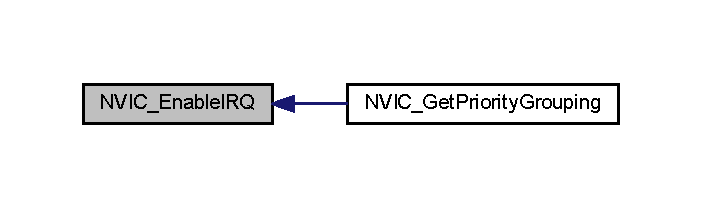
\includegraphics[width=337pt]{group___c_m_s_i_s___core___n_v_i_c_functions_ga3349f2e3580d7ce22d6530b7294e5921_icgraph}
\end{center}
\end{figure}
\mbox{\Hypertarget{group___c_m_s_i_s___core___n_v_i_c_functions_gadb94ac5d892b376e4f3555ae0418ebac}\label{group___c_m_s_i_s___core___n_v_i_c_functions_gadb94ac5d892b376e4f3555ae0418ebac}} 
\index{N\+V\+I\+C Functions@{N\+V\+I\+C Functions}!N\+V\+I\+C\+\_\+\+Encode\+Priority@{N\+V\+I\+C\+\_\+\+Encode\+Priority}}
\index{N\+V\+I\+C\+\_\+\+Encode\+Priority@{N\+V\+I\+C\+\_\+\+Encode\+Priority}!N\+V\+I\+C Functions@{N\+V\+I\+C Functions}}
\subsubsection{\texorpdfstring{N\+V\+I\+C\+\_\+\+Encode\+Priority()}{NVIC\_EncodePriority()}}
{\footnotesize\ttfamily \+\_\+\+\_\+\+S\+T\+A\+T\+I\+C\+\_\+\+I\+N\+L\+I\+NE uint32\+\_\+t N\+V\+I\+C\+\_\+\+Encode\+Priority (\begin{DoxyParamCaption}\item[{uint32\+\_\+t}]{Priority\+Group,  }\item[{uint32\+\_\+t}]{Preempt\+Priority,  }\item[{uint32\+\_\+t}]{Sub\+Priority }\end{DoxyParamCaption})}



Encode Priority. 

Encodes the priority for an interrupt with the given priority group, preemptive priority value, and subpriority value. In case of a conflict between priority grouping and available priority bits (\+\_\+\+\_\+\+N\+V\+I\+C\+\_\+\+P\+R\+I\+O\+\_\+\+B\+I\+TS), the smallest possible priority group is set. 
\begin{DoxyParams}[1]{Parameters}
\mbox{\tt in}  & {\em Priority\+Group} & Used priority group. \\
\hline
\mbox{\tt in}  & {\em Preempt\+Priority} & Preemptive priority value (starting from 0). \\
\hline
\mbox{\tt in}  & {\em Sub\+Priority} & Subpriority value (starting from 0). \\
\hline
\end{DoxyParams}
\begin{DoxyReturn}{Returns}
Encoded priority. Value can be used in the function \hyperlink{group___c_m_s_i_s___core___n_v_i_c_functions_ga2305cbd44aaad792e3a4e538bdaf14f9}{N\+V\+I\+C\+\_\+\+Set\+Priority()}. 
\end{DoxyReturn}


Definition at line 1579 of file core\+\_\+cm3.\+h.

\mbox{\Hypertarget{group___c_m_s_i_s___core___n_v_i_c_functions_ga47a0f52794068d076c9147aa3cb8d8a6}\label{group___c_m_s_i_s___core___n_v_i_c_functions_ga47a0f52794068d076c9147aa3cb8d8a6}} 
\index{N\+V\+I\+C Functions@{N\+V\+I\+C Functions}!N\+V\+I\+C\+\_\+\+Get\+Active@{N\+V\+I\+C\+\_\+\+Get\+Active}}
\index{N\+V\+I\+C\+\_\+\+Get\+Active@{N\+V\+I\+C\+\_\+\+Get\+Active}!N\+V\+I\+C Functions@{N\+V\+I\+C Functions}}
\subsubsection{\texorpdfstring{N\+V\+I\+C\+\_\+\+Get\+Active()}{NVIC\_GetActive()}}
{\footnotesize\ttfamily \+\_\+\+\_\+\+S\+T\+A\+T\+I\+C\+\_\+\+I\+N\+L\+I\+NE uint32\+\_\+t N\+V\+I\+C\+\_\+\+Get\+Active (\begin{DoxyParamCaption}\item[{\hyperlink{group___configuration__section__for___c_m_s_i_s_gac3af4a32370fb28c4ade8bf2add80251}{I\+R\+Qn\+\_\+\+Type}}]{I\+R\+Qn }\end{DoxyParamCaption})}



Get Active Interrupt. 

Reads the active register in N\+V\+IC and returns the active bit. 
\begin{DoxyParams}[1]{Parameters}
\mbox{\tt in}  & {\em I\+R\+Qn} & Interrupt number. \\
\hline
\end{DoxyParams}
\begin{DoxyReturn}{Returns}
0 Interrupt status is not active. 

1 Interrupt status is active. 
\end{DoxyReturn}


Definition at line 1519 of file core\+\_\+cm3.\+h.

Here is the call graph for this function\+:
\nopagebreak
\begin{figure}[H]
\begin{center}
\leavevmode
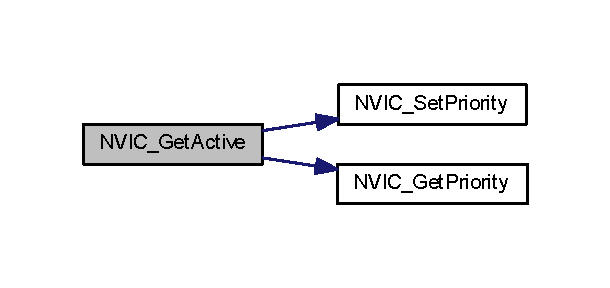
\includegraphics[width=293pt]{group___c_m_s_i_s___core___n_v_i_c_functions_ga47a0f52794068d076c9147aa3cb8d8a6_cgraph}
\end{center}
\end{figure}
\mbox{\Hypertarget{group___c_m_s_i_s___core___n_v_i_c_functions_gafec8042db64c0f8ed432b6c8386a05d8}\label{group___c_m_s_i_s___core___n_v_i_c_functions_gafec8042db64c0f8ed432b6c8386a05d8}} 
\index{N\+V\+I\+C Functions@{N\+V\+I\+C Functions}!N\+V\+I\+C\+\_\+\+Get\+Pending\+I\+RQ@{N\+V\+I\+C\+\_\+\+Get\+Pending\+I\+RQ}}
\index{N\+V\+I\+C\+\_\+\+Get\+Pending\+I\+RQ@{N\+V\+I\+C\+\_\+\+Get\+Pending\+I\+RQ}!N\+V\+I\+C Functions@{N\+V\+I\+C Functions}}
\subsubsection{\texorpdfstring{N\+V\+I\+C\+\_\+\+Get\+Pending\+I\+R\+Q()}{NVIC\_GetPendingIRQ()}}
{\footnotesize\ttfamily \+\_\+\+\_\+\+S\+T\+A\+T\+I\+C\+\_\+\+I\+N\+L\+I\+NE uint32\+\_\+t N\+V\+I\+C\+\_\+\+Get\+Pending\+I\+RQ (\begin{DoxyParamCaption}\item[{\hyperlink{group___configuration__section__for___c_m_s_i_s_gac3af4a32370fb28c4ade8bf2add80251}{I\+R\+Qn\+\_\+\+Type}}]{I\+R\+Qn }\end{DoxyParamCaption})}



Get Pending Interrupt. 

Reads the pending register in the N\+V\+IC and returns the pending bit for the specified interrupt. 
\begin{DoxyParams}[1]{Parameters}
\mbox{\tt in}  & {\em I\+R\+Qn} & Interrupt number. \\
\hline
\end{DoxyParams}
\begin{DoxyReturn}{Returns}
0 Interrupt status is not pending. 

1 Interrupt status is pending. 
\end{DoxyReturn}


Definition at line 661 of file core\+\_\+cm0.\+h.

Here is the caller graph for this function\+:
\nopagebreak
\begin{figure}[H]
\begin{center}
\leavevmode
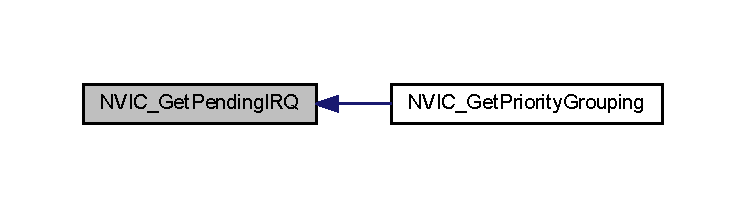
\includegraphics[width=350pt]{group___c_m_s_i_s___core___n_v_i_c_functions_gafec8042db64c0f8ed432b6c8386a05d8_icgraph}
\end{center}
\end{figure}
\mbox{\Hypertarget{group___c_m_s_i_s___core___n_v_i_c_functions_ga1cbaf8e6abd4aa4885828e7f24fcfeb4}\label{group___c_m_s_i_s___core___n_v_i_c_functions_ga1cbaf8e6abd4aa4885828e7f24fcfeb4}} 
\index{N\+V\+I\+C Functions@{N\+V\+I\+C Functions}!N\+V\+I\+C\+\_\+\+Get\+Priority@{N\+V\+I\+C\+\_\+\+Get\+Priority}}
\index{N\+V\+I\+C\+\_\+\+Get\+Priority@{N\+V\+I\+C\+\_\+\+Get\+Priority}!N\+V\+I\+C Functions@{N\+V\+I\+C Functions}}
\subsubsection{\texorpdfstring{N\+V\+I\+C\+\_\+\+Get\+Priority()}{NVIC\_GetPriority()}}
{\footnotesize\ttfamily \+\_\+\+\_\+\+S\+T\+A\+T\+I\+C\+\_\+\+I\+N\+L\+I\+NE uint32\+\_\+t N\+V\+I\+C\+\_\+\+Get\+Priority (\begin{DoxyParamCaption}\item[{\hyperlink{group___configuration__section__for___c_m_s_i_s_gac3af4a32370fb28c4ade8bf2add80251}{I\+R\+Qn\+\_\+\+Type}}]{I\+R\+Qn }\end{DoxyParamCaption})}



Get Interrupt Priority. 

Reads the priority of an interrupt. The interrupt number can be positive to specify an external (device specific) interrupt, or negative to specify an internal (core) interrupt. 
\begin{DoxyParams}[1]{Parameters}
\mbox{\tt in}  & {\em I\+R\+Qn} & Interrupt number. \\
\hline
\end{DoxyParams}
\begin{DoxyReturn}{Returns}
Interrupt Priority. Value is aligned automatically to the implemented priority bits of the microcontroller. 
\end{DoxyReturn}


Definition at line 720 of file core\+\_\+cm0.\+h.

Here is the caller graph for this function\+:
\nopagebreak
\begin{figure}[H]
\begin{center}
\leavevmode
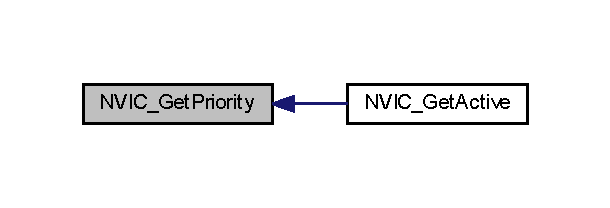
\includegraphics[width=293pt]{group___c_m_s_i_s___core___n_v_i_c_functions_ga1cbaf8e6abd4aa4885828e7f24fcfeb4_icgraph}
\end{center}
\end{figure}
\mbox{\Hypertarget{group___c_m_s_i_s___core___n_v_i_c_functions_ga394f7ce2ca826c0da26284d17ac6524d}\label{group___c_m_s_i_s___core___n_v_i_c_functions_ga394f7ce2ca826c0da26284d17ac6524d}} 
\index{N\+V\+I\+C Functions@{N\+V\+I\+C Functions}!N\+V\+I\+C\+\_\+\+Get\+Priority\+Grouping@{N\+V\+I\+C\+\_\+\+Get\+Priority\+Grouping}}
\index{N\+V\+I\+C\+\_\+\+Get\+Priority\+Grouping@{N\+V\+I\+C\+\_\+\+Get\+Priority\+Grouping}!N\+V\+I\+C Functions@{N\+V\+I\+C Functions}}
\subsubsection{\texorpdfstring{N\+V\+I\+C\+\_\+\+Get\+Priority\+Grouping()}{NVIC\_GetPriorityGrouping()}}
{\footnotesize\ttfamily \+\_\+\+\_\+\+S\+T\+A\+T\+I\+C\+\_\+\+I\+N\+L\+I\+NE uint32\+\_\+t N\+V\+I\+C\+\_\+\+Get\+Priority\+Grouping (\begin{DoxyParamCaption}\item[{void}]{ }\end{DoxyParamCaption})}



Get Priority Grouping. 

Reads the priority grouping field from the N\+V\+IC Interrupt Controller. \begin{DoxyReturn}{Returns}
Priority grouping field (S\+C\+B-\/$>$A\+I\+R\+CR \mbox{[}10\+:8\mbox{]} P\+R\+I\+G\+R\+O\+UP field). 
\end{DoxyReturn}


Definition at line 1449 of file core\+\_\+cm3.\+h.

Here is the call graph for this function\+:
\nopagebreak
\begin{figure}[H]
\begin{center}
\leavevmode
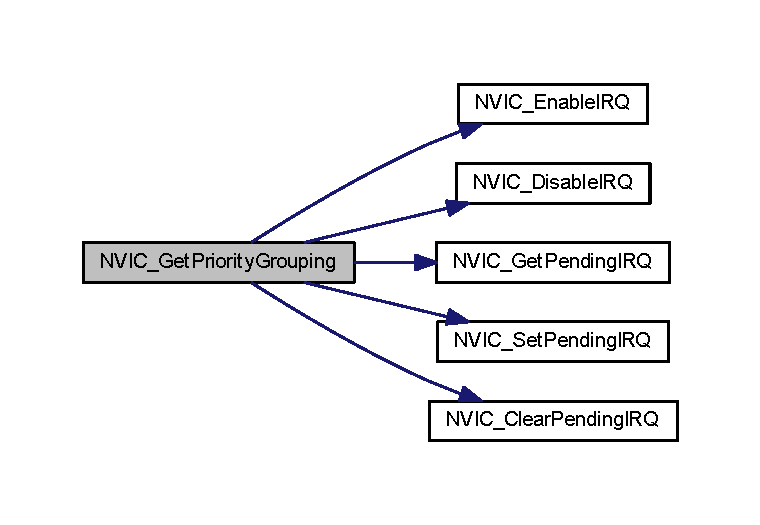
\includegraphics[width=350pt]{group___c_m_s_i_s___core___n_v_i_c_functions_ga394f7ce2ca826c0da26284d17ac6524d_cgraph}
\end{center}
\end{figure}
\mbox{\Hypertarget{group___c_m_s_i_s___core___n_v_i_c_functions_ga3ecf446519da33e1690deffbf5be505f}\label{group___c_m_s_i_s___core___n_v_i_c_functions_ga3ecf446519da33e1690deffbf5be505f}} 
\index{N\+V\+I\+C Functions@{N\+V\+I\+C Functions}!N\+V\+I\+C\+\_\+\+Set\+Pending\+I\+RQ@{N\+V\+I\+C\+\_\+\+Set\+Pending\+I\+RQ}}
\index{N\+V\+I\+C\+\_\+\+Set\+Pending\+I\+RQ@{N\+V\+I\+C\+\_\+\+Set\+Pending\+I\+RQ}!N\+V\+I\+C Functions@{N\+V\+I\+C Functions}}
\subsubsection{\texorpdfstring{N\+V\+I\+C\+\_\+\+Set\+Pending\+I\+R\+Q()}{NVIC\_SetPendingIRQ()}}
{\footnotesize\ttfamily \+\_\+\+\_\+\+S\+T\+A\+T\+I\+C\+\_\+\+I\+N\+L\+I\+NE void N\+V\+I\+C\+\_\+\+Set\+Pending\+I\+RQ (\begin{DoxyParamCaption}\item[{\hyperlink{group___configuration__section__for___c_m_s_i_s_gac3af4a32370fb28c4ade8bf2add80251}{I\+R\+Qn\+\_\+\+Type}}]{I\+R\+Qn }\end{DoxyParamCaption})}



Set Pending Interrupt. 

Sets the pending bit of an external interrupt. 
\begin{DoxyParams}[1]{Parameters}
\mbox{\tt in}  & {\em I\+R\+Qn} & Interrupt number. Value cannot be negative. \\
\hline
\end{DoxyParams}


Definition at line 672 of file core\+\_\+cm0.\+h.

Here is the caller graph for this function\+:
\nopagebreak
\begin{figure}[H]
\begin{center}
\leavevmode
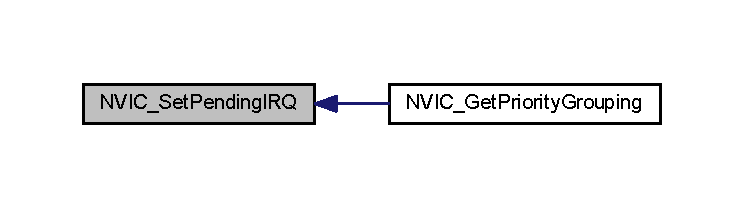
\includegraphics[width=350pt]{group___c_m_s_i_s___core___n_v_i_c_functions_ga3ecf446519da33e1690deffbf5be505f_icgraph}
\end{center}
\end{figure}
\mbox{\Hypertarget{group___c_m_s_i_s___core___n_v_i_c_functions_ga2305cbd44aaad792e3a4e538bdaf14f9}\label{group___c_m_s_i_s___core___n_v_i_c_functions_ga2305cbd44aaad792e3a4e538bdaf14f9}} 
\index{N\+V\+I\+C Functions@{N\+V\+I\+C Functions}!N\+V\+I\+C\+\_\+\+Set\+Priority@{N\+V\+I\+C\+\_\+\+Set\+Priority}}
\index{N\+V\+I\+C\+\_\+\+Set\+Priority@{N\+V\+I\+C\+\_\+\+Set\+Priority}!N\+V\+I\+C Functions@{N\+V\+I\+C Functions}}
\subsubsection{\texorpdfstring{N\+V\+I\+C\+\_\+\+Set\+Priority()}{NVIC\_SetPriority()}}
{\footnotesize\ttfamily \+\_\+\+\_\+\+S\+T\+A\+T\+I\+C\+\_\+\+I\+N\+L\+I\+NE void N\+V\+I\+C\+\_\+\+Set\+Priority (\begin{DoxyParamCaption}\item[{\hyperlink{group___configuration__section__for___c_m_s_i_s_gac3af4a32370fb28c4ade8bf2add80251}{I\+R\+Qn\+\_\+\+Type}}]{I\+R\+Qn,  }\item[{uint32\+\_\+t}]{priority }\end{DoxyParamCaption})}



Set Interrupt Priority. 

Sets the priority of an interrupt. \begin{DoxyNote}{Note}
The priority cannot be set for every core interrupt. 
\end{DoxyNote}

\begin{DoxyParams}[1]{Parameters}
\mbox{\tt in}  & {\em I\+R\+Qn} & Interrupt number. \\
\hline
\mbox{\tt in}  & {\em priority} & Priority to set. \\
\hline
\end{DoxyParams}


Definition at line 696 of file core\+\_\+cm0.\+h.

Here is the caller graph for this function\+:
\nopagebreak
\begin{figure}[H]
\begin{center}
\leavevmode
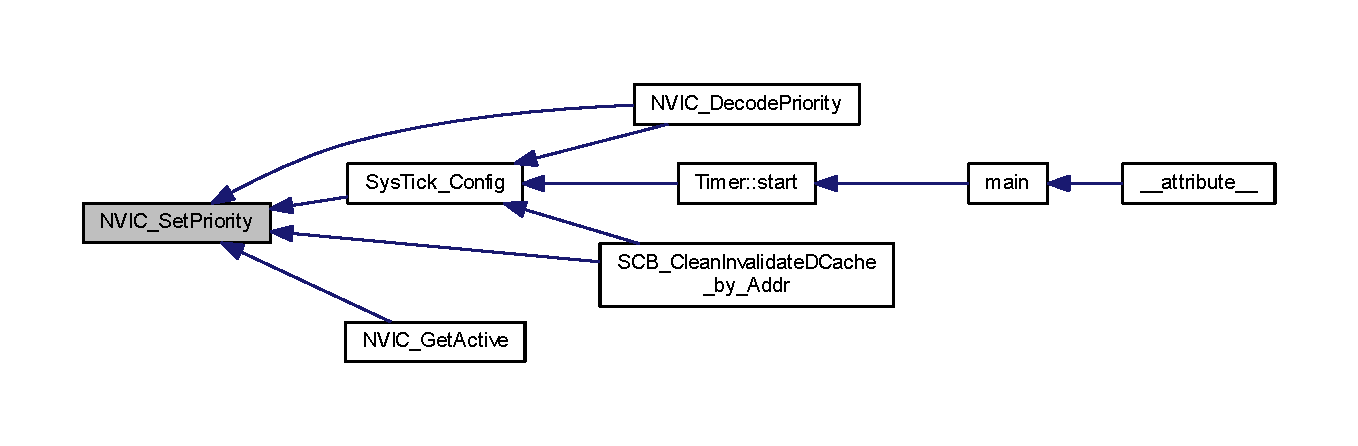
\includegraphics[width=350pt]{group___c_m_s_i_s___core___n_v_i_c_functions_ga2305cbd44aaad792e3a4e538bdaf14f9_icgraph}
\end{center}
\end{figure}
\mbox{\Hypertarget{group___c_m_s_i_s___core___n_v_i_c_functions_ga77cfbb35a9d8027e392034321bed6904}\label{group___c_m_s_i_s___core___n_v_i_c_functions_ga77cfbb35a9d8027e392034321bed6904}} 
\index{N\+V\+I\+C Functions@{N\+V\+I\+C Functions}!N\+V\+I\+C\+\_\+\+Set\+Priority\+Grouping@{N\+V\+I\+C\+\_\+\+Set\+Priority\+Grouping}}
\index{N\+V\+I\+C\+\_\+\+Set\+Priority\+Grouping@{N\+V\+I\+C\+\_\+\+Set\+Priority\+Grouping}!N\+V\+I\+C Functions@{N\+V\+I\+C Functions}}
\subsubsection{\texorpdfstring{N\+V\+I\+C\+\_\+\+Set\+Priority\+Grouping()}{NVIC\_SetPriorityGrouping()}}
{\footnotesize\ttfamily \+\_\+\+\_\+\+S\+T\+A\+T\+I\+C\+\_\+\+I\+N\+L\+I\+NE void N\+V\+I\+C\+\_\+\+Set\+Priority\+Grouping (\begin{DoxyParamCaption}\item[{uint32\+\_\+t}]{Priority\+Group }\end{DoxyParamCaption})}



Set Priority Grouping. 

Sets the priority grouping field using the required unlock sequence. The parameter Priority\+Group is assigned to the field S\+C\+B-\/$>$A\+I\+R\+CR \mbox{[}10\+:8\mbox{]} P\+R\+I\+G\+R\+O\+UP field. Only values from 0..7 are used. In case of a conflict between priority grouping and available priority bits (\+\_\+\+\_\+\+N\+V\+I\+C\+\_\+\+P\+R\+I\+O\+\_\+\+B\+I\+TS), the smallest possible priority group is set. 
\begin{DoxyParams}[1]{Parameters}
\mbox{\tt in}  & {\em Priority\+Group} & Priority grouping field. \\
\hline
\end{DoxyParams}


Definition at line 1430 of file core\+\_\+cm3.\+h.

\mbox{\Hypertarget{group___c_m_s_i_s___core___n_v_i_c_functions_ga1143dec48d60a3d6f238c4798a87759c}\label{group___c_m_s_i_s___core___n_v_i_c_functions_ga1143dec48d60a3d6f238c4798a87759c}} 
\index{N\+V\+I\+C Functions@{N\+V\+I\+C Functions}!N\+V\+I\+C\+\_\+\+System\+Reset@{N\+V\+I\+C\+\_\+\+System\+Reset}}
\index{N\+V\+I\+C\+\_\+\+System\+Reset@{N\+V\+I\+C\+\_\+\+System\+Reset}!N\+V\+I\+C Functions@{N\+V\+I\+C Functions}}
\subsubsection{\texorpdfstring{N\+V\+I\+C\+\_\+\+System\+Reset()}{NVIC\_SystemReset()}}
{\footnotesize\ttfamily \+\_\+\+\_\+\+S\+T\+A\+T\+I\+C\+\_\+\+I\+N\+L\+I\+NE void N\+V\+I\+C\+\_\+\+System\+Reset (\begin{DoxyParamCaption}\item[{void}]{ }\end{DoxyParamCaption})}



System Reset. 

Initiates a system reset request to reset the M\+CU. 

Definition at line 738 of file core\+\_\+cm0.\+h.

Here is the caller graph for this function\+:
\nopagebreak
\begin{figure}[H]
\begin{center}
\leavevmode
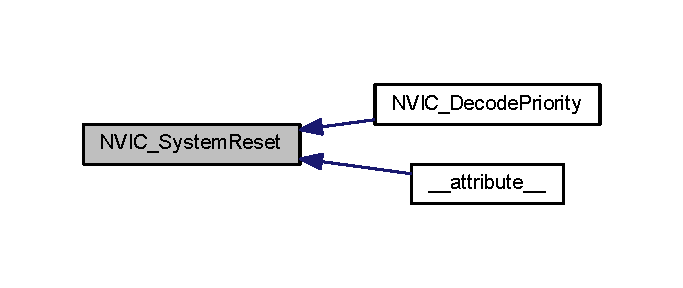
\includegraphics[width=328pt]{group___c_m_s_i_s___core___n_v_i_c_functions_ga1143dec48d60a3d6f238c4798a87759c_icgraph}
\end{center}
\end{figure}

\hypertarget{group___c_m_s_i_s___core___sys_tick_functions}{}\section{Sys\+Tick Functions}
\label{group___c_m_s_i_s___core___sys_tick_functions}\index{Sys\+Tick Functions@{Sys\+Tick Functions}}


Functions that configure the System.  


Collaboration diagram for Sys\+Tick Functions\+:
\nopagebreak
\begin{figure}[H]
\begin{center}
\leavevmode
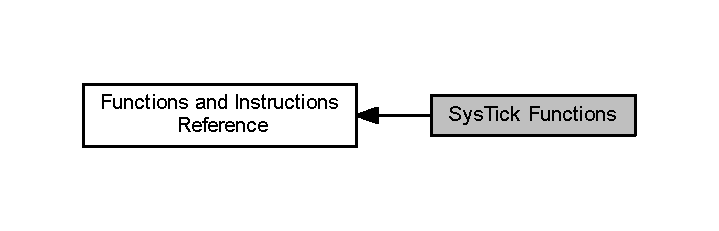
\includegraphics[width=345pt]{group___c_m_s_i_s___core___sys_tick_functions}
\end{center}
\end{figure}
\subsection*{Functions}
\begin{DoxyCompactItemize}
\item 
\+\_\+\+\_\+\+S\+T\+A\+T\+I\+C\+\_\+\+I\+N\+L\+I\+NE uint32\+\_\+t \hyperlink{group___c_m_s_i_s___core___sys_tick_functions_gae4e8f0238527c69f522029b93c8e5b78}{Sys\+Tick\+\_\+\+Config} (uint32\+\_\+t ticks)
\begin{DoxyCompactList}\small\item\em System Tick Configuration. \end{DoxyCompactList}\end{DoxyCompactItemize}


\subsection{Detailed Description}
Functions that configure the System. 



\subsection{Function Documentation}
\mbox{\Hypertarget{group___c_m_s_i_s___core___sys_tick_functions_gae4e8f0238527c69f522029b93c8e5b78}\label{group___c_m_s_i_s___core___sys_tick_functions_gae4e8f0238527c69f522029b93c8e5b78}} 
\index{Sys\+Tick Functions@{Sys\+Tick Functions}!Sys\+Tick\+\_\+\+Config@{Sys\+Tick\+\_\+\+Config}}
\index{Sys\+Tick\+\_\+\+Config@{Sys\+Tick\+\_\+\+Config}!Sys\+Tick Functions@{Sys\+Tick Functions}}
\subsubsection{\texorpdfstring{Sys\+Tick\+\_\+\+Config()}{SysTick\_Config()}}
{\footnotesize\ttfamily \+\_\+\+\_\+\+S\+T\+A\+T\+I\+C\+\_\+\+I\+N\+L\+I\+NE uint32\+\_\+t Sys\+Tick\+\_\+\+Config (\begin{DoxyParamCaption}\item[{uint32\+\_\+t}]{ticks }\end{DoxyParamCaption})}



System Tick Configuration. 

Initializes the System \hyperlink{class_timer}{Timer} and its interrupt, and starts the System Tick \hyperlink{class_timer}{Timer}. Counter is in free running mode to generate periodic interrupts. 
\begin{DoxyParams}[1]{Parameters}
\mbox{\tt in}  & {\em ticks} & Number of ticks between two interrupts. \\
\hline
\end{DoxyParams}
\begin{DoxyReturn}{Returns}
0 Function succeeded. 

1 Function failed. 
\end{DoxyReturn}
\begin{DoxyNote}{Note}
When the variable {\bfseries \+\_\+\+\_\+\+Vendor\+\_\+\+Sys\+Tick\+Config} is set to 1, then the function {\bfseries Sys\+Tick\+\_\+\+Config} is not included. In this case, the file {\bfseries {\itshape device}.h} must contain a vendor-\/specific implementation of this function. 
\end{DoxyNote}


Definition at line 777 of file core\+\_\+cm0.\+h.

Here is the call graph for this function\+:
\nopagebreak
\begin{figure}[H]
\begin{center}
\leavevmode
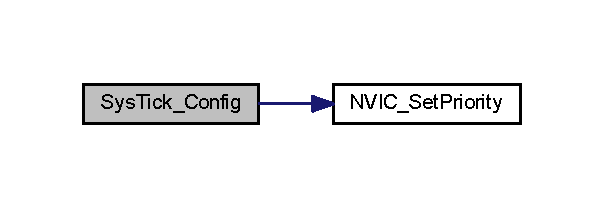
\includegraphics[width=290pt]{group___c_m_s_i_s___core___sys_tick_functions_gae4e8f0238527c69f522029b93c8e5b78_cgraph}
\end{center}
\end{figure}
Here is the caller graph for this function\+:
\nopagebreak
\begin{figure}[H]
\begin{center}
\leavevmode
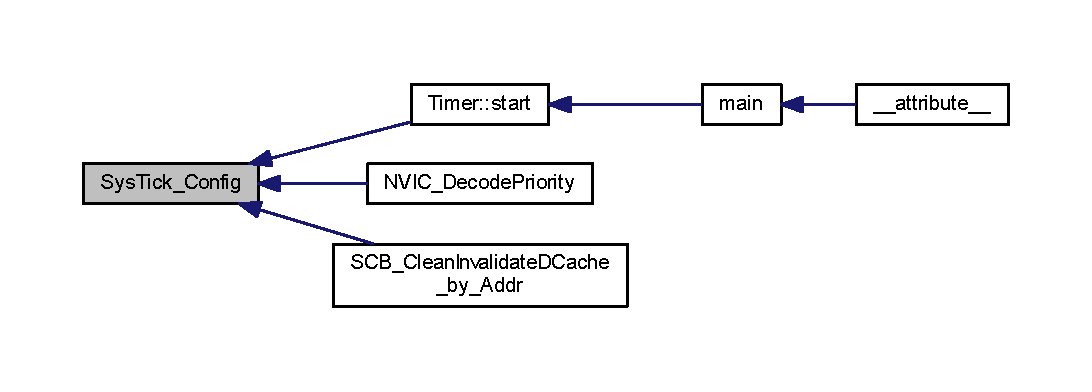
\includegraphics[width=350pt]{group___c_m_s_i_s___core___sys_tick_functions_gae4e8f0238527c69f522029b93c8e5b78_icgraph}
\end{center}
\end{figure}

\hypertarget{group___c_m_s_i_s___s_cn_s_c_b}{}\section{System Controls not in S\+CB (S\+Cn\+S\+CB)}
\label{group___c_m_s_i_s___s_cn_s_c_b}\index{System Controls not in S\+C\+B (\+S\+Cn\+S\+C\+B)@{System Controls not in S\+C\+B (\+S\+Cn\+S\+C\+B)}}


Type definitions for the System Control and ID Register not in the S\+CB.  


Collaboration diagram for System Controls not in S\+CB (S\+Cn\+S\+CB)\+:
\nopagebreak
\begin{figure}[H]
\begin{center}
\leavevmode
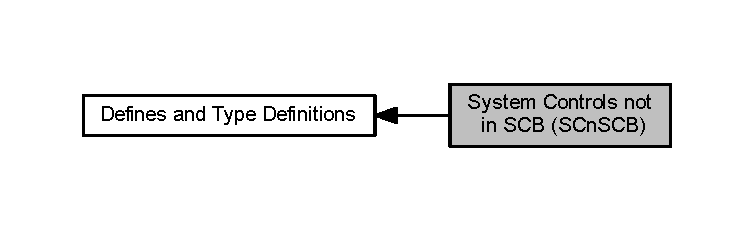
\includegraphics[width=350pt]{group___c_m_s_i_s___s_cn_s_c_b}
\end{center}
\end{figure}
\subsection*{Classes}
\begin{DoxyCompactItemize}
\item 
struct \hyperlink{struct_s_cn_s_c_b___type}{S\+Cn\+S\+C\+B\+\_\+\+Type}
\begin{DoxyCompactList}\small\item\em Structure type to access the System Control and ID Register not in the S\+CB. \end{DoxyCompactList}\end{DoxyCompactItemize}
\subsection*{Macros}
\begin{DoxyCompactItemize}
\item 
\#define \hyperlink{group___c_m_s_i_s___s_cn_s_c_b_ga0777ddf379af50f9ca41d40573bfffc5}{S\+Cn\+S\+C\+B\+\_\+\+I\+C\+T\+R\+\_\+\+I\+N\+T\+L\+I\+N\+E\+S\+N\+U\+M\+\_\+\+Pos}~0U
\item 
\#define \hyperlink{group___c_m_s_i_s___s_cn_s_c_b_ga3efa0f5210051464e1034b19fc7b33c7}{S\+Cn\+S\+C\+B\+\_\+\+I\+C\+T\+R\+\_\+\+I\+N\+T\+L\+I\+N\+E\+S\+N\+U\+M\+\_\+\+Msk}~(0x\+F\+U\+L /$\ast$$<$$<$ S\+Cn\+S\+C\+B\+\_\+\+I\+C\+T\+R\+\_\+\+I\+N\+T\+L\+I\+N\+E\+S\+N\+U\+M\+\_\+\+Pos$\ast$/)
\item 
\#define \hyperlink{group___c_m_s_i_s___s_cn_s_c_b_gaab395870643a0bee78906bb15ca5bd02}{S\+Cn\+S\+C\+B\+\_\+\+A\+C\+T\+L\+R\+\_\+\+D\+I\+S\+F\+O\+L\+D\+\_\+\+Pos}~2U
\item 
\#define \hyperlink{group___c_m_s_i_s___s_cn_s_c_b_gaa9dd2d4a2350499188f438d0aa9fd982}{S\+Cn\+S\+C\+B\+\_\+\+A\+C\+T\+L\+R\+\_\+\+D\+I\+S\+F\+O\+L\+D\+\_\+\+Msk}~(1\+U\+L $<$$<$ S\+Cn\+S\+C\+B\+\_\+\+A\+C\+T\+L\+R\+\_\+\+D\+I\+S\+F\+O\+L\+D\+\_\+\+Pos)
\item 
\#define \hyperlink{group___c_m_s_i_s___s_cn_s_c_b_gafa2eb37493c0f8dae77cde81ecf80f77}{S\+Cn\+S\+C\+B\+\_\+\+A\+C\+T\+L\+R\+\_\+\+D\+I\+S\+D\+E\+F\+W\+B\+U\+F\+\_\+\+Pos}~1U
\item 
\#define \hyperlink{group___c_m_s_i_s___s_cn_s_c_b_ga6cda7b7219232a008ec52cc8e89d5d08}{S\+Cn\+S\+C\+B\+\_\+\+A\+C\+T\+L\+R\+\_\+\+D\+I\+S\+D\+E\+F\+W\+B\+U\+F\+\_\+\+Msk}~(1\+U\+L $<$$<$ S\+Cn\+S\+C\+B\+\_\+\+A\+C\+T\+L\+R\+\_\+\+D\+I\+S\+D\+E\+F\+W\+B\+U\+F\+\_\+\+Pos)
\item 
\#define \hyperlink{group___c_m_s_i_s___s_cn_s_c_b_gaaa3e79f5ead4a32c0ea742b2a9ffc0cd}{S\+Cn\+S\+C\+B\+\_\+\+A\+C\+T\+L\+R\+\_\+\+D\+I\+S\+M\+C\+Y\+C\+I\+N\+T\+\_\+\+Pos}~0U
\item 
\#define \hyperlink{group___c_m_s_i_s___s_cn_s_c_b_ga2a2818f0489ad10b6ea2964e899d4cbc}{S\+Cn\+S\+C\+B\+\_\+\+A\+C\+T\+L\+R\+\_\+\+D\+I\+S\+M\+C\+Y\+C\+I\+N\+T\+\_\+\+Msk}~(1\+U\+L /$\ast$$<$$<$ S\+Cn\+S\+C\+B\+\_\+\+A\+C\+T\+L\+R\+\_\+\+D\+I\+S\+M\+C\+Y\+C\+I\+N\+T\+\_\+\+Pos$\ast$/)
\item 
\#define \hyperlink{group___c_m_s_i_s___s_cn_s_c_b_ga0777ddf379af50f9ca41d40573bfffc5}{S\+Cn\+S\+C\+B\+\_\+\+I\+C\+T\+R\+\_\+\+I\+N\+T\+L\+I\+N\+E\+S\+N\+U\+M\+\_\+\+Pos}~0U
\item 
\#define \hyperlink{group___c_m_s_i_s___s_cn_s_c_b_ga3efa0f5210051464e1034b19fc7b33c7}{S\+Cn\+S\+C\+B\+\_\+\+I\+C\+T\+R\+\_\+\+I\+N\+T\+L\+I\+N\+E\+S\+N\+U\+M\+\_\+\+Msk}~(0x\+F\+U\+L /$\ast$$<$$<$ S\+Cn\+S\+C\+B\+\_\+\+I\+C\+T\+R\+\_\+\+I\+N\+T\+L\+I\+N\+E\+S\+N\+U\+M\+\_\+\+Pos$\ast$/)
\item 
\#define \hyperlink{group___c_m_s_i_s___s_cn_s_c_b_gaff0b57464c60fea8182b903676f8de49}{S\+Cn\+S\+C\+B\+\_\+\+A\+C\+T\+L\+R\+\_\+\+D\+I\+S\+O\+O\+F\+P\+\_\+\+Pos}~9U
\item 
\#define \hyperlink{group___c_m_s_i_s___s_cn_s_c_b_ga1ecd6adafa43464d7097b132c19e8640}{S\+Cn\+S\+C\+B\+\_\+\+A\+C\+T\+L\+R\+\_\+\+D\+I\+S\+O\+O\+F\+P\+\_\+\+Msk}~(1\+U\+L $<$$<$ S\+Cn\+S\+C\+B\+\_\+\+A\+C\+T\+L\+R\+\_\+\+D\+I\+S\+O\+O\+F\+P\+\_\+\+Pos)
\item 
\#define \hyperlink{group___c_m_s_i_s___s_cn_s_c_b_gaa194809383bc72ecf3416d85709281d7}{S\+Cn\+S\+C\+B\+\_\+\+A\+C\+T\+L\+R\+\_\+\+D\+I\+S\+F\+P\+C\+A\+\_\+\+Pos}~8U
\item 
\#define \hyperlink{group___c_m_s_i_s___s_cn_s_c_b_ga10d5aa4a196dcde6f476016ece2c1b69}{S\+Cn\+S\+C\+B\+\_\+\+A\+C\+T\+L\+R\+\_\+\+D\+I\+S\+F\+P\+C\+A\+\_\+\+Msk}~(1\+U\+L $<$$<$ S\+Cn\+S\+C\+B\+\_\+\+A\+C\+T\+L\+R\+\_\+\+D\+I\+S\+F\+P\+C\+A\+\_\+\+Pos)
\item 
\#define \hyperlink{group___c_m_s_i_s___s_cn_s_c_b_gaab395870643a0bee78906bb15ca5bd02}{S\+Cn\+S\+C\+B\+\_\+\+A\+C\+T\+L\+R\+\_\+\+D\+I\+S\+F\+O\+L\+D\+\_\+\+Pos}~2U
\item 
\#define \hyperlink{group___c_m_s_i_s___s_cn_s_c_b_gaa9dd2d4a2350499188f438d0aa9fd982}{S\+Cn\+S\+C\+B\+\_\+\+A\+C\+T\+L\+R\+\_\+\+D\+I\+S\+F\+O\+L\+D\+\_\+\+Msk}~(1\+U\+L $<$$<$ S\+Cn\+S\+C\+B\+\_\+\+A\+C\+T\+L\+R\+\_\+\+D\+I\+S\+F\+O\+L\+D\+\_\+\+Pos)
\item 
\#define \hyperlink{group___c_m_s_i_s___s_cn_s_c_b_gafa2eb37493c0f8dae77cde81ecf80f77}{S\+Cn\+S\+C\+B\+\_\+\+A\+C\+T\+L\+R\+\_\+\+D\+I\+S\+D\+E\+F\+W\+B\+U\+F\+\_\+\+Pos}~1U
\item 
\#define \hyperlink{group___c_m_s_i_s___s_cn_s_c_b_ga6cda7b7219232a008ec52cc8e89d5d08}{S\+Cn\+S\+C\+B\+\_\+\+A\+C\+T\+L\+R\+\_\+\+D\+I\+S\+D\+E\+F\+W\+B\+U\+F\+\_\+\+Msk}~(1\+U\+L $<$$<$ S\+Cn\+S\+C\+B\+\_\+\+A\+C\+T\+L\+R\+\_\+\+D\+I\+S\+D\+E\+F\+W\+B\+U\+F\+\_\+\+Pos)
\item 
\#define \hyperlink{group___c_m_s_i_s___s_cn_s_c_b_gaaa3e79f5ead4a32c0ea742b2a9ffc0cd}{S\+Cn\+S\+C\+B\+\_\+\+A\+C\+T\+L\+R\+\_\+\+D\+I\+S\+M\+C\+Y\+C\+I\+N\+T\+\_\+\+Pos}~0U
\item 
\#define \hyperlink{group___c_m_s_i_s___s_cn_s_c_b_ga2a2818f0489ad10b6ea2964e899d4cbc}{S\+Cn\+S\+C\+B\+\_\+\+A\+C\+T\+L\+R\+\_\+\+D\+I\+S\+M\+C\+Y\+C\+I\+N\+T\+\_\+\+Msk}~(1\+U\+L /$\ast$$<$$<$ S\+Cn\+S\+C\+B\+\_\+\+A\+C\+T\+L\+R\+\_\+\+D\+I\+S\+M\+C\+Y\+C\+I\+N\+T\+\_\+\+Pos$\ast$/)
\item 
\#define \hyperlink{group___c_m_s_i_s___s_cn_s_c_b_ga0777ddf379af50f9ca41d40573bfffc5}{S\+Cn\+S\+C\+B\+\_\+\+I\+C\+T\+R\+\_\+\+I\+N\+T\+L\+I\+N\+E\+S\+N\+U\+M\+\_\+\+Pos}~0U
\item 
\#define \hyperlink{group___c_m_s_i_s___s_cn_s_c_b_ga3efa0f5210051464e1034b19fc7b33c7}{S\+Cn\+S\+C\+B\+\_\+\+I\+C\+T\+R\+\_\+\+I\+N\+T\+L\+I\+N\+E\+S\+N\+U\+M\+\_\+\+Msk}~(0x\+F\+U\+L /$\ast$$<$$<$ S\+Cn\+S\+C\+B\+\_\+\+I\+C\+T\+R\+\_\+\+I\+N\+T\+L\+I\+N\+E\+S\+N\+U\+M\+\_\+\+Pos$\ast$/)
\item 
\#define \hyperlink{group___c_m_s_i_s___s_cn_s_c_b_ga5f888e0ebc18cc2d99976405777c142f}{S\+Cn\+S\+C\+B\+\_\+\+A\+C\+T\+L\+R\+\_\+\+D\+I\+S\+I\+T\+M\+A\+T\+B\+F\+L\+U\+S\+H\+\_\+\+Pos}~12U
\item 
\#define \hyperlink{group___c_m_s_i_s___s_cn_s_c_b_ga46b16a03b408184720134ef42203ac2e}{S\+Cn\+S\+C\+B\+\_\+\+A\+C\+T\+L\+R\+\_\+\+D\+I\+S\+I\+T\+M\+A\+T\+B\+F\+L\+U\+S\+H\+\_\+\+Msk}~(1\+U\+L $<$$<$ S\+Cn\+S\+C\+B\+\_\+\+A\+C\+T\+L\+R\+\_\+\+D\+I\+S\+I\+T\+M\+A\+T\+B\+F\+L\+U\+S\+H\+\_\+\+Pos)
\item 
\#define \hyperlink{group___c_m_s_i_s___s_cn_s_c_b_ga1bffb5e05053d15cbe42fbe87d225dcb}{S\+Cn\+S\+C\+B\+\_\+\+A\+C\+T\+L\+R\+\_\+\+D\+I\+S\+R\+A\+M\+O\+D\+E\+\_\+\+Pos}~11U
\item 
\#define \hyperlink{group___c_m_s_i_s___s_cn_s_c_b_ga436fc1bd011b15c9585bb3ace5332ce3}{S\+Cn\+S\+C\+B\+\_\+\+A\+C\+T\+L\+R\+\_\+\+D\+I\+S\+R\+A\+M\+O\+D\+E\+\_\+\+Msk}~(1\+U\+L $<$$<$ S\+Cn\+S\+C\+B\+\_\+\+A\+C\+T\+L\+R\+\_\+\+D\+I\+S\+R\+A\+M\+O\+D\+E\+\_\+\+Pos)
\item 
\#define \hyperlink{group___c_m_s_i_s___s_cn_s_c_b_gaa743743f5af93d6ece74a426b355ab70}{S\+Cn\+S\+C\+B\+\_\+\+A\+C\+T\+L\+R\+\_\+\+F\+P\+E\+X\+C\+O\+D\+I\+S\+\_\+\+Pos}~10U
\item 
\#define \hyperlink{group___c_m_s_i_s___s_cn_s_c_b_gadd12baaeeea3220b03867e4b8a1432aa}{S\+Cn\+S\+C\+B\+\_\+\+A\+C\+T\+L\+R\+\_\+\+F\+P\+E\+X\+C\+O\+D\+I\+S\+\_\+\+Msk}~(1\+U\+L $<$$<$ S\+Cn\+S\+C\+B\+\_\+\+A\+C\+T\+L\+R\+\_\+\+F\+P\+E\+X\+C\+O\+D\+I\+S\+\_\+\+Pos)
\item 
\#define \hyperlink{group___c_m_s_i_s___s_cn_s_c_b_gaab395870643a0bee78906bb15ca5bd02}{S\+Cn\+S\+C\+B\+\_\+\+A\+C\+T\+L\+R\+\_\+\+D\+I\+S\+F\+O\+L\+D\+\_\+\+Pos}~2U
\item 
\#define \hyperlink{group___c_m_s_i_s___s_cn_s_c_b_gaa9dd2d4a2350499188f438d0aa9fd982}{S\+Cn\+S\+C\+B\+\_\+\+A\+C\+T\+L\+R\+\_\+\+D\+I\+S\+F\+O\+L\+D\+\_\+\+Msk}~(1\+U\+L $<$$<$ S\+Cn\+S\+C\+B\+\_\+\+A\+C\+T\+L\+R\+\_\+\+D\+I\+S\+F\+O\+L\+D\+\_\+\+Pos)
\item 
\#define \hyperlink{group___c_m_s_i_s___s_cn_s_c_b_gaaa3e79f5ead4a32c0ea742b2a9ffc0cd}{S\+Cn\+S\+C\+B\+\_\+\+A\+C\+T\+L\+R\+\_\+\+D\+I\+S\+M\+C\+Y\+C\+I\+N\+T\+\_\+\+Pos}~0U
\item 
\#define \hyperlink{group___c_m_s_i_s___s_cn_s_c_b_ga2a2818f0489ad10b6ea2964e899d4cbc}{S\+Cn\+S\+C\+B\+\_\+\+A\+C\+T\+L\+R\+\_\+\+D\+I\+S\+M\+C\+Y\+C\+I\+N\+T\+\_\+\+Msk}~(1\+U\+L /$\ast$$<$$<$ S\+Cn\+S\+C\+B\+\_\+\+A\+C\+T\+L\+R\+\_\+\+D\+I\+S\+M\+C\+Y\+C\+I\+N\+T\+\_\+\+Pos$\ast$/)
\item 
\#define \hyperlink{group___c_m_s_i_s___s_cn_s_c_b_gaaa3e79f5ead4a32c0ea742b2a9ffc0cd}{S\+Cn\+S\+C\+B\+\_\+\+A\+C\+T\+L\+R\+\_\+\+D\+I\+S\+M\+C\+Y\+C\+I\+N\+T\+\_\+\+Pos}~0U
\item 
\#define \hyperlink{group___c_m_s_i_s___s_cn_s_c_b_ga2a2818f0489ad10b6ea2964e899d4cbc}{S\+Cn\+S\+C\+B\+\_\+\+A\+C\+T\+L\+R\+\_\+\+D\+I\+S\+M\+C\+Y\+C\+I\+N\+T\+\_\+\+Msk}~(1\+U\+L /$\ast$$<$$<$ S\+Cn\+S\+C\+B\+\_\+\+A\+C\+T\+L\+R\+\_\+\+D\+I\+S\+M\+C\+Y\+C\+I\+N\+T\+\_\+\+Pos$\ast$/)
\item 
\#define \hyperlink{group___c_m_s_i_s___s_cn_s_c_b_ga0777ddf379af50f9ca41d40573bfffc5}{S\+Cn\+S\+C\+B\+\_\+\+I\+C\+T\+R\+\_\+\+I\+N\+T\+L\+I\+N\+E\+S\+N\+U\+M\+\_\+\+Pos}~0U
\item 
\#define \hyperlink{group___c_m_s_i_s___s_cn_s_c_b_ga3efa0f5210051464e1034b19fc7b33c7}{S\+Cn\+S\+C\+B\+\_\+\+I\+C\+T\+R\+\_\+\+I\+N\+T\+L\+I\+N\+E\+S\+N\+U\+M\+\_\+\+Msk}~(0x\+F\+U\+L /$\ast$$<$$<$ S\+Cn\+S\+C\+B\+\_\+\+I\+C\+T\+R\+\_\+\+I\+N\+T\+L\+I\+N\+E\+S\+N\+U\+M\+\_\+\+Pos$\ast$/)
\end{DoxyCompactItemize}


\subsection{Detailed Description}
Type definitions for the System Control and ID Register not in the S\+CB. 



\subsection{Macro Definition Documentation}
\mbox{\Hypertarget{group___c_m_s_i_s___s_cn_s_c_b_ga6cda7b7219232a008ec52cc8e89d5d08}\label{group___c_m_s_i_s___s_cn_s_c_b_ga6cda7b7219232a008ec52cc8e89d5d08}} 
\index{System Controls not in S\+C\+B (\+S\+Cn\+S\+C\+B)@{System Controls not in S\+C\+B (\+S\+Cn\+S\+C\+B)}!S\+Cn\+S\+C\+B\+\_\+\+A\+C\+T\+L\+R\+\_\+\+D\+I\+S\+D\+E\+F\+W\+B\+U\+F\+\_\+\+Msk@{S\+Cn\+S\+C\+B\+\_\+\+A\+C\+T\+L\+R\+\_\+\+D\+I\+S\+D\+E\+F\+W\+B\+U\+F\+\_\+\+Msk}}
\index{S\+Cn\+S\+C\+B\+\_\+\+A\+C\+T\+L\+R\+\_\+\+D\+I\+S\+D\+E\+F\+W\+B\+U\+F\+\_\+\+Msk@{S\+Cn\+S\+C\+B\+\_\+\+A\+C\+T\+L\+R\+\_\+\+D\+I\+S\+D\+E\+F\+W\+B\+U\+F\+\_\+\+Msk}!System Controls not in S\+C\+B (\+S\+Cn\+S\+C\+B)@{System Controls not in S\+C\+B (\+S\+Cn\+S\+C\+B)}}
\subsubsection{\texorpdfstring{S\+Cn\+S\+C\+B\+\_\+\+A\+C\+T\+L\+R\+\_\+\+D\+I\+S\+D\+E\+F\+W\+B\+U\+F\+\_\+\+Msk}{SCnSCB\_ACTLR\_DISDEFWBUF\_Msk}\hspace{0.1cm}{\footnotesize\ttfamily [1/2]}}
{\footnotesize\ttfamily \#define S\+Cn\+S\+C\+B\+\_\+\+A\+C\+T\+L\+R\+\_\+\+D\+I\+S\+D\+E\+F\+W\+B\+U\+F\+\_\+\+Msk~(1\+U\+L $<$$<$ S\+Cn\+S\+C\+B\+\_\+\+A\+C\+T\+L\+R\+\_\+\+D\+I\+S\+D\+E\+F\+W\+B\+U\+F\+\_\+\+Pos)}

A\+C\+T\+LR\+: D\+I\+S\+D\+E\+F\+W\+B\+UF Mask 

Definition at line 673 of file core\+\_\+cm3.\+h.

\mbox{\Hypertarget{group___c_m_s_i_s___s_cn_s_c_b_ga6cda7b7219232a008ec52cc8e89d5d08}\label{group___c_m_s_i_s___s_cn_s_c_b_ga6cda7b7219232a008ec52cc8e89d5d08}} 
\index{System Controls not in S\+C\+B (\+S\+Cn\+S\+C\+B)@{System Controls not in S\+C\+B (\+S\+Cn\+S\+C\+B)}!S\+Cn\+S\+C\+B\+\_\+\+A\+C\+T\+L\+R\+\_\+\+D\+I\+S\+D\+E\+F\+W\+B\+U\+F\+\_\+\+Msk@{S\+Cn\+S\+C\+B\+\_\+\+A\+C\+T\+L\+R\+\_\+\+D\+I\+S\+D\+E\+F\+W\+B\+U\+F\+\_\+\+Msk}}
\index{S\+Cn\+S\+C\+B\+\_\+\+A\+C\+T\+L\+R\+\_\+\+D\+I\+S\+D\+E\+F\+W\+B\+U\+F\+\_\+\+Msk@{S\+Cn\+S\+C\+B\+\_\+\+A\+C\+T\+L\+R\+\_\+\+D\+I\+S\+D\+E\+F\+W\+B\+U\+F\+\_\+\+Msk}!System Controls not in S\+C\+B (\+S\+Cn\+S\+C\+B)@{System Controls not in S\+C\+B (\+S\+Cn\+S\+C\+B)}}
\subsubsection{\texorpdfstring{S\+Cn\+S\+C\+B\+\_\+\+A\+C\+T\+L\+R\+\_\+\+D\+I\+S\+D\+E\+F\+W\+B\+U\+F\+\_\+\+Msk}{SCnSCB\_ACTLR\_DISDEFWBUF\_Msk}\hspace{0.1cm}{\footnotesize\ttfamily [2/2]}}
{\footnotesize\ttfamily \#define S\+Cn\+S\+C\+B\+\_\+\+A\+C\+T\+L\+R\+\_\+\+D\+I\+S\+D\+E\+F\+W\+B\+U\+F\+\_\+\+Msk~(1\+U\+L $<$$<$ S\+Cn\+S\+C\+B\+\_\+\+A\+C\+T\+L\+R\+\_\+\+D\+I\+S\+D\+E\+F\+W\+B\+U\+F\+\_\+\+Pos)}

A\+C\+T\+LR\+: D\+I\+S\+D\+E\+F\+W\+B\+UF Mask 

Definition at line 734 of file core\+\_\+cm4.\+h.

\mbox{\Hypertarget{group___c_m_s_i_s___s_cn_s_c_b_gafa2eb37493c0f8dae77cde81ecf80f77}\label{group___c_m_s_i_s___s_cn_s_c_b_gafa2eb37493c0f8dae77cde81ecf80f77}} 
\index{System Controls not in S\+C\+B (\+S\+Cn\+S\+C\+B)@{System Controls not in S\+C\+B (\+S\+Cn\+S\+C\+B)}!S\+Cn\+S\+C\+B\+\_\+\+A\+C\+T\+L\+R\+\_\+\+D\+I\+S\+D\+E\+F\+W\+B\+U\+F\+\_\+\+Pos@{S\+Cn\+S\+C\+B\+\_\+\+A\+C\+T\+L\+R\+\_\+\+D\+I\+S\+D\+E\+F\+W\+B\+U\+F\+\_\+\+Pos}}
\index{S\+Cn\+S\+C\+B\+\_\+\+A\+C\+T\+L\+R\+\_\+\+D\+I\+S\+D\+E\+F\+W\+B\+U\+F\+\_\+\+Pos@{S\+Cn\+S\+C\+B\+\_\+\+A\+C\+T\+L\+R\+\_\+\+D\+I\+S\+D\+E\+F\+W\+B\+U\+F\+\_\+\+Pos}!System Controls not in S\+C\+B (\+S\+Cn\+S\+C\+B)@{System Controls not in S\+C\+B (\+S\+Cn\+S\+C\+B)}}
\subsubsection{\texorpdfstring{S\+Cn\+S\+C\+B\+\_\+\+A\+C\+T\+L\+R\+\_\+\+D\+I\+S\+D\+E\+F\+W\+B\+U\+F\+\_\+\+Pos}{SCnSCB\_ACTLR\_DISDEFWBUF\_Pos}\hspace{0.1cm}{\footnotesize\ttfamily [1/2]}}
{\footnotesize\ttfamily \#define S\+Cn\+S\+C\+B\+\_\+\+A\+C\+T\+L\+R\+\_\+\+D\+I\+S\+D\+E\+F\+W\+B\+U\+F\+\_\+\+Pos~1U}

A\+C\+T\+LR\+: D\+I\+S\+D\+E\+F\+W\+B\+UF Position 

Definition at line 672 of file core\+\_\+cm3.\+h.

\mbox{\Hypertarget{group___c_m_s_i_s___s_cn_s_c_b_gafa2eb37493c0f8dae77cde81ecf80f77}\label{group___c_m_s_i_s___s_cn_s_c_b_gafa2eb37493c0f8dae77cde81ecf80f77}} 
\index{System Controls not in S\+C\+B (\+S\+Cn\+S\+C\+B)@{System Controls not in S\+C\+B (\+S\+Cn\+S\+C\+B)}!S\+Cn\+S\+C\+B\+\_\+\+A\+C\+T\+L\+R\+\_\+\+D\+I\+S\+D\+E\+F\+W\+B\+U\+F\+\_\+\+Pos@{S\+Cn\+S\+C\+B\+\_\+\+A\+C\+T\+L\+R\+\_\+\+D\+I\+S\+D\+E\+F\+W\+B\+U\+F\+\_\+\+Pos}}
\index{S\+Cn\+S\+C\+B\+\_\+\+A\+C\+T\+L\+R\+\_\+\+D\+I\+S\+D\+E\+F\+W\+B\+U\+F\+\_\+\+Pos@{S\+Cn\+S\+C\+B\+\_\+\+A\+C\+T\+L\+R\+\_\+\+D\+I\+S\+D\+E\+F\+W\+B\+U\+F\+\_\+\+Pos}!System Controls not in S\+C\+B (\+S\+Cn\+S\+C\+B)@{System Controls not in S\+C\+B (\+S\+Cn\+S\+C\+B)}}
\subsubsection{\texorpdfstring{S\+Cn\+S\+C\+B\+\_\+\+A\+C\+T\+L\+R\+\_\+\+D\+I\+S\+D\+E\+F\+W\+B\+U\+F\+\_\+\+Pos}{SCnSCB\_ACTLR\_DISDEFWBUF\_Pos}\hspace{0.1cm}{\footnotesize\ttfamily [2/2]}}
{\footnotesize\ttfamily \#define S\+Cn\+S\+C\+B\+\_\+\+A\+C\+T\+L\+R\+\_\+\+D\+I\+S\+D\+E\+F\+W\+B\+U\+F\+\_\+\+Pos~1U}

A\+C\+T\+LR\+: D\+I\+S\+D\+E\+F\+W\+B\+UF Position 

Definition at line 733 of file core\+\_\+cm4.\+h.

\mbox{\Hypertarget{group___c_m_s_i_s___s_cn_s_c_b_gaa9dd2d4a2350499188f438d0aa9fd982}\label{group___c_m_s_i_s___s_cn_s_c_b_gaa9dd2d4a2350499188f438d0aa9fd982}} 
\index{System Controls not in S\+C\+B (\+S\+Cn\+S\+C\+B)@{System Controls not in S\+C\+B (\+S\+Cn\+S\+C\+B)}!S\+Cn\+S\+C\+B\+\_\+\+A\+C\+T\+L\+R\+\_\+\+D\+I\+S\+F\+O\+L\+D\+\_\+\+Msk@{S\+Cn\+S\+C\+B\+\_\+\+A\+C\+T\+L\+R\+\_\+\+D\+I\+S\+F\+O\+L\+D\+\_\+\+Msk}}
\index{S\+Cn\+S\+C\+B\+\_\+\+A\+C\+T\+L\+R\+\_\+\+D\+I\+S\+F\+O\+L\+D\+\_\+\+Msk@{S\+Cn\+S\+C\+B\+\_\+\+A\+C\+T\+L\+R\+\_\+\+D\+I\+S\+F\+O\+L\+D\+\_\+\+Msk}!System Controls not in S\+C\+B (\+S\+Cn\+S\+C\+B)@{System Controls not in S\+C\+B (\+S\+Cn\+S\+C\+B)}}
\subsubsection{\texorpdfstring{S\+Cn\+S\+C\+B\+\_\+\+A\+C\+T\+L\+R\+\_\+\+D\+I\+S\+F\+O\+L\+D\+\_\+\+Msk}{SCnSCB\_ACTLR\_DISFOLD\_Msk}\hspace{0.1cm}{\footnotesize\ttfamily [1/3]}}
{\footnotesize\ttfamily \#define S\+Cn\+S\+C\+B\+\_\+\+A\+C\+T\+L\+R\+\_\+\+D\+I\+S\+F\+O\+L\+D\+\_\+\+Msk~(1\+U\+L $<$$<$ S\+Cn\+S\+C\+B\+\_\+\+A\+C\+T\+L\+R\+\_\+\+D\+I\+S\+F\+O\+L\+D\+\_\+\+Pos)}

A\+C\+T\+LR\+: D\+I\+S\+F\+O\+LD Mask 

Definition at line 670 of file core\+\_\+cm3.\+h.

\mbox{\Hypertarget{group___c_m_s_i_s___s_cn_s_c_b_gaa9dd2d4a2350499188f438d0aa9fd982}\label{group___c_m_s_i_s___s_cn_s_c_b_gaa9dd2d4a2350499188f438d0aa9fd982}} 
\index{System Controls not in S\+C\+B (\+S\+Cn\+S\+C\+B)@{System Controls not in S\+C\+B (\+S\+Cn\+S\+C\+B)}!S\+Cn\+S\+C\+B\+\_\+\+A\+C\+T\+L\+R\+\_\+\+D\+I\+S\+F\+O\+L\+D\+\_\+\+Msk@{S\+Cn\+S\+C\+B\+\_\+\+A\+C\+T\+L\+R\+\_\+\+D\+I\+S\+F\+O\+L\+D\+\_\+\+Msk}}
\index{S\+Cn\+S\+C\+B\+\_\+\+A\+C\+T\+L\+R\+\_\+\+D\+I\+S\+F\+O\+L\+D\+\_\+\+Msk@{S\+Cn\+S\+C\+B\+\_\+\+A\+C\+T\+L\+R\+\_\+\+D\+I\+S\+F\+O\+L\+D\+\_\+\+Msk}!System Controls not in S\+C\+B (\+S\+Cn\+S\+C\+B)@{System Controls not in S\+C\+B (\+S\+Cn\+S\+C\+B)}}
\subsubsection{\texorpdfstring{S\+Cn\+S\+C\+B\+\_\+\+A\+C\+T\+L\+R\+\_\+\+D\+I\+S\+F\+O\+L\+D\+\_\+\+Msk}{SCnSCB\_ACTLR\_DISFOLD\_Msk}\hspace{0.1cm}{\footnotesize\ttfamily [2/3]}}
{\footnotesize\ttfamily \#define S\+Cn\+S\+C\+B\+\_\+\+A\+C\+T\+L\+R\+\_\+\+D\+I\+S\+F\+O\+L\+D\+\_\+\+Msk~(1\+U\+L $<$$<$ S\+Cn\+S\+C\+B\+\_\+\+A\+C\+T\+L\+R\+\_\+\+D\+I\+S\+F\+O\+L\+D\+\_\+\+Pos)}

A\+C\+T\+LR\+: D\+I\+S\+F\+O\+LD Mask 

Definition at line 731 of file core\+\_\+cm4.\+h.

\mbox{\Hypertarget{group___c_m_s_i_s___s_cn_s_c_b_gaa9dd2d4a2350499188f438d0aa9fd982}\label{group___c_m_s_i_s___s_cn_s_c_b_gaa9dd2d4a2350499188f438d0aa9fd982}} 
\index{System Controls not in S\+C\+B (\+S\+Cn\+S\+C\+B)@{System Controls not in S\+C\+B (\+S\+Cn\+S\+C\+B)}!S\+Cn\+S\+C\+B\+\_\+\+A\+C\+T\+L\+R\+\_\+\+D\+I\+S\+F\+O\+L\+D\+\_\+\+Msk@{S\+Cn\+S\+C\+B\+\_\+\+A\+C\+T\+L\+R\+\_\+\+D\+I\+S\+F\+O\+L\+D\+\_\+\+Msk}}
\index{S\+Cn\+S\+C\+B\+\_\+\+A\+C\+T\+L\+R\+\_\+\+D\+I\+S\+F\+O\+L\+D\+\_\+\+Msk@{S\+Cn\+S\+C\+B\+\_\+\+A\+C\+T\+L\+R\+\_\+\+D\+I\+S\+F\+O\+L\+D\+\_\+\+Msk}!System Controls not in S\+C\+B (\+S\+Cn\+S\+C\+B)@{System Controls not in S\+C\+B (\+S\+Cn\+S\+C\+B)}}
\subsubsection{\texorpdfstring{S\+Cn\+S\+C\+B\+\_\+\+A\+C\+T\+L\+R\+\_\+\+D\+I\+S\+F\+O\+L\+D\+\_\+\+Msk}{SCnSCB\_ACTLR\_DISFOLD\_Msk}\hspace{0.1cm}{\footnotesize\ttfamily [3/3]}}
{\footnotesize\ttfamily \#define S\+Cn\+S\+C\+B\+\_\+\+A\+C\+T\+L\+R\+\_\+\+D\+I\+S\+F\+O\+L\+D\+\_\+\+Msk~(1\+U\+L $<$$<$ S\+Cn\+S\+C\+B\+\_\+\+A\+C\+T\+L\+R\+\_\+\+D\+I\+S\+F\+O\+L\+D\+\_\+\+Pos)}

A\+C\+T\+LR\+: D\+I\+S\+F\+O\+LD Mask 

Definition at line 936 of file core\+\_\+cm7.\+h.

\mbox{\Hypertarget{group___c_m_s_i_s___s_cn_s_c_b_gaab395870643a0bee78906bb15ca5bd02}\label{group___c_m_s_i_s___s_cn_s_c_b_gaab395870643a0bee78906bb15ca5bd02}} 
\index{System Controls not in S\+C\+B (\+S\+Cn\+S\+C\+B)@{System Controls not in S\+C\+B (\+S\+Cn\+S\+C\+B)}!S\+Cn\+S\+C\+B\+\_\+\+A\+C\+T\+L\+R\+\_\+\+D\+I\+S\+F\+O\+L\+D\+\_\+\+Pos@{S\+Cn\+S\+C\+B\+\_\+\+A\+C\+T\+L\+R\+\_\+\+D\+I\+S\+F\+O\+L\+D\+\_\+\+Pos}}
\index{S\+Cn\+S\+C\+B\+\_\+\+A\+C\+T\+L\+R\+\_\+\+D\+I\+S\+F\+O\+L\+D\+\_\+\+Pos@{S\+Cn\+S\+C\+B\+\_\+\+A\+C\+T\+L\+R\+\_\+\+D\+I\+S\+F\+O\+L\+D\+\_\+\+Pos}!System Controls not in S\+C\+B (\+S\+Cn\+S\+C\+B)@{System Controls not in S\+C\+B (\+S\+Cn\+S\+C\+B)}}
\subsubsection{\texorpdfstring{S\+Cn\+S\+C\+B\+\_\+\+A\+C\+T\+L\+R\+\_\+\+D\+I\+S\+F\+O\+L\+D\+\_\+\+Pos}{SCnSCB\_ACTLR\_DISFOLD\_Pos}\hspace{0.1cm}{\footnotesize\ttfamily [1/3]}}
{\footnotesize\ttfamily \#define S\+Cn\+S\+C\+B\+\_\+\+A\+C\+T\+L\+R\+\_\+\+D\+I\+S\+F\+O\+L\+D\+\_\+\+Pos~2U}

A\+C\+T\+LR\+: D\+I\+S\+F\+O\+LD Position 

Definition at line 669 of file core\+\_\+cm3.\+h.

\mbox{\Hypertarget{group___c_m_s_i_s___s_cn_s_c_b_gaab395870643a0bee78906bb15ca5bd02}\label{group___c_m_s_i_s___s_cn_s_c_b_gaab395870643a0bee78906bb15ca5bd02}} 
\index{System Controls not in S\+C\+B (\+S\+Cn\+S\+C\+B)@{System Controls not in S\+C\+B (\+S\+Cn\+S\+C\+B)}!S\+Cn\+S\+C\+B\+\_\+\+A\+C\+T\+L\+R\+\_\+\+D\+I\+S\+F\+O\+L\+D\+\_\+\+Pos@{S\+Cn\+S\+C\+B\+\_\+\+A\+C\+T\+L\+R\+\_\+\+D\+I\+S\+F\+O\+L\+D\+\_\+\+Pos}}
\index{S\+Cn\+S\+C\+B\+\_\+\+A\+C\+T\+L\+R\+\_\+\+D\+I\+S\+F\+O\+L\+D\+\_\+\+Pos@{S\+Cn\+S\+C\+B\+\_\+\+A\+C\+T\+L\+R\+\_\+\+D\+I\+S\+F\+O\+L\+D\+\_\+\+Pos}!System Controls not in S\+C\+B (\+S\+Cn\+S\+C\+B)@{System Controls not in S\+C\+B (\+S\+Cn\+S\+C\+B)}}
\subsubsection{\texorpdfstring{S\+Cn\+S\+C\+B\+\_\+\+A\+C\+T\+L\+R\+\_\+\+D\+I\+S\+F\+O\+L\+D\+\_\+\+Pos}{SCnSCB\_ACTLR\_DISFOLD\_Pos}\hspace{0.1cm}{\footnotesize\ttfamily [2/3]}}
{\footnotesize\ttfamily \#define S\+Cn\+S\+C\+B\+\_\+\+A\+C\+T\+L\+R\+\_\+\+D\+I\+S\+F\+O\+L\+D\+\_\+\+Pos~2U}

A\+C\+T\+LR\+: D\+I\+S\+F\+O\+LD Position 

Definition at line 730 of file core\+\_\+cm4.\+h.

\mbox{\Hypertarget{group___c_m_s_i_s___s_cn_s_c_b_gaab395870643a0bee78906bb15ca5bd02}\label{group___c_m_s_i_s___s_cn_s_c_b_gaab395870643a0bee78906bb15ca5bd02}} 
\index{System Controls not in S\+C\+B (\+S\+Cn\+S\+C\+B)@{System Controls not in S\+C\+B (\+S\+Cn\+S\+C\+B)}!S\+Cn\+S\+C\+B\+\_\+\+A\+C\+T\+L\+R\+\_\+\+D\+I\+S\+F\+O\+L\+D\+\_\+\+Pos@{S\+Cn\+S\+C\+B\+\_\+\+A\+C\+T\+L\+R\+\_\+\+D\+I\+S\+F\+O\+L\+D\+\_\+\+Pos}}
\index{S\+Cn\+S\+C\+B\+\_\+\+A\+C\+T\+L\+R\+\_\+\+D\+I\+S\+F\+O\+L\+D\+\_\+\+Pos@{S\+Cn\+S\+C\+B\+\_\+\+A\+C\+T\+L\+R\+\_\+\+D\+I\+S\+F\+O\+L\+D\+\_\+\+Pos}!System Controls not in S\+C\+B (\+S\+Cn\+S\+C\+B)@{System Controls not in S\+C\+B (\+S\+Cn\+S\+C\+B)}}
\subsubsection{\texorpdfstring{S\+Cn\+S\+C\+B\+\_\+\+A\+C\+T\+L\+R\+\_\+\+D\+I\+S\+F\+O\+L\+D\+\_\+\+Pos}{SCnSCB\_ACTLR\_DISFOLD\_Pos}\hspace{0.1cm}{\footnotesize\ttfamily [3/3]}}
{\footnotesize\ttfamily \#define S\+Cn\+S\+C\+B\+\_\+\+A\+C\+T\+L\+R\+\_\+\+D\+I\+S\+F\+O\+L\+D\+\_\+\+Pos~2U}

A\+C\+T\+LR\+: D\+I\+S\+F\+O\+LD Position 

Definition at line 935 of file core\+\_\+cm7.\+h.

\mbox{\Hypertarget{group___c_m_s_i_s___s_cn_s_c_b_ga10d5aa4a196dcde6f476016ece2c1b69}\label{group___c_m_s_i_s___s_cn_s_c_b_ga10d5aa4a196dcde6f476016ece2c1b69}} 
\index{System Controls not in S\+C\+B (\+S\+Cn\+S\+C\+B)@{System Controls not in S\+C\+B (\+S\+Cn\+S\+C\+B)}!S\+Cn\+S\+C\+B\+\_\+\+A\+C\+T\+L\+R\+\_\+\+D\+I\+S\+F\+P\+C\+A\+\_\+\+Msk@{S\+Cn\+S\+C\+B\+\_\+\+A\+C\+T\+L\+R\+\_\+\+D\+I\+S\+F\+P\+C\+A\+\_\+\+Msk}}
\index{S\+Cn\+S\+C\+B\+\_\+\+A\+C\+T\+L\+R\+\_\+\+D\+I\+S\+F\+P\+C\+A\+\_\+\+Msk@{S\+Cn\+S\+C\+B\+\_\+\+A\+C\+T\+L\+R\+\_\+\+D\+I\+S\+F\+P\+C\+A\+\_\+\+Msk}!System Controls not in S\+C\+B (\+S\+Cn\+S\+C\+B)@{System Controls not in S\+C\+B (\+S\+Cn\+S\+C\+B)}}
\subsubsection{\texorpdfstring{S\+Cn\+S\+C\+B\+\_\+\+A\+C\+T\+L\+R\+\_\+\+D\+I\+S\+F\+P\+C\+A\+\_\+\+Msk}{SCnSCB\_ACTLR\_DISFPCA\_Msk}}
{\footnotesize\ttfamily \#define S\+Cn\+S\+C\+B\+\_\+\+A\+C\+T\+L\+R\+\_\+\+D\+I\+S\+F\+P\+C\+A\+\_\+\+Msk~(1\+U\+L $<$$<$ S\+Cn\+S\+C\+B\+\_\+\+A\+C\+T\+L\+R\+\_\+\+D\+I\+S\+F\+P\+C\+A\+\_\+\+Pos)}

A\+C\+T\+LR\+: D\+I\+S\+F\+P\+CA Mask 

Definition at line 728 of file core\+\_\+cm4.\+h.

\mbox{\Hypertarget{group___c_m_s_i_s___s_cn_s_c_b_gaa194809383bc72ecf3416d85709281d7}\label{group___c_m_s_i_s___s_cn_s_c_b_gaa194809383bc72ecf3416d85709281d7}} 
\index{System Controls not in S\+C\+B (\+S\+Cn\+S\+C\+B)@{System Controls not in S\+C\+B (\+S\+Cn\+S\+C\+B)}!S\+Cn\+S\+C\+B\+\_\+\+A\+C\+T\+L\+R\+\_\+\+D\+I\+S\+F\+P\+C\+A\+\_\+\+Pos@{S\+Cn\+S\+C\+B\+\_\+\+A\+C\+T\+L\+R\+\_\+\+D\+I\+S\+F\+P\+C\+A\+\_\+\+Pos}}
\index{S\+Cn\+S\+C\+B\+\_\+\+A\+C\+T\+L\+R\+\_\+\+D\+I\+S\+F\+P\+C\+A\+\_\+\+Pos@{S\+Cn\+S\+C\+B\+\_\+\+A\+C\+T\+L\+R\+\_\+\+D\+I\+S\+F\+P\+C\+A\+\_\+\+Pos}!System Controls not in S\+C\+B (\+S\+Cn\+S\+C\+B)@{System Controls not in S\+C\+B (\+S\+Cn\+S\+C\+B)}}
\subsubsection{\texorpdfstring{S\+Cn\+S\+C\+B\+\_\+\+A\+C\+T\+L\+R\+\_\+\+D\+I\+S\+F\+P\+C\+A\+\_\+\+Pos}{SCnSCB\_ACTLR\_DISFPCA\_Pos}}
{\footnotesize\ttfamily \#define S\+Cn\+S\+C\+B\+\_\+\+A\+C\+T\+L\+R\+\_\+\+D\+I\+S\+F\+P\+C\+A\+\_\+\+Pos~8U}

A\+C\+T\+LR\+: D\+I\+S\+F\+P\+CA Position 

Definition at line 727 of file core\+\_\+cm4.\+h.

\mbox{\Hypertarget{group___c_m_s_i_s___s_cn_s_c_b_ga46b16a03b408184720134ef42203ac2e}\label{group___c_m_s_i_s___s_cn_s_c_b_ga46b16a03b408184720134ef42203ac2e}} 
\index{System Controls not in S\+C\+B (\+S\+Cn\+S\+C\+B)@{System Controls not in S\+C\+B (\+S\+Cn\+S\+C\+B)}!S\+Cn\+S\+C\+B\+\_\+\+A\+C\+T\+L\+R\+\_\+\+D\+I\+S\+I\+T\+M\+A\+T\+B\+F\+L\+U\+S\+H\+\_\+\+Msk@{S\+Cn\+S\+C\+B\+\_\+\+A\+C\+T\+L\+R\+\_\+\+D\+I\+S\+I\+T\+M\+A\+T\+B\+F\+L\+U\+S\+H\+\_\+\+Msk}}
\index{S\+Cn\+S\+C\+B\+\_\+\+A\+C\+T\+L\+R\+\_\+\+D\+I\+S\+I\+T\+M\+A\+T\+B\+F\+L\+U\+S\+H\+\_\+\+Msk@{S\+Cn\+S\+C\+B\+\_\+\+A\+C\+T\+L\+R\+\_\+\+D\+I\+S\+I\+T\+M\+A\+T\+B\+F\+L\+U\+S\+H\+\_\+\+Msk}!System Controls not in S\+C\+B (\+S\+Cn\+S\+C\+B)@{System Controls not in S\+C\+B (\+S\+Cn\+S\+C\+B)}}
\subsubsection{\texorpdfstring{S\+Cn\+S\+C\+B\+\_\+\+A\+C\+T\+L\+R\+\_\+\+D\+I\+S\+I\+T\+M\+A\+T\+B\+F\+L\+U\+S\+H\+\_\+\+Msk}{SCnSCB\_ACTLR\_DISITMATBFLUSH\_Msk}}
{\footnotesize\ttfamily \#define S\+Cn\+S\+C\+B\+\_\+\+A\+C\+T\+L\+R\+\_\+\+D\+I\+S\+I\+T\+M\+A\+T\+B\+F\+L\+U\+S\+H\+\_\+\+Msk~(1\+U\+L $<$$<$ S\+Cn\+S\+C\+B\+\_\+\+A\+C\+T\+L\+R\+\_\+\+D\+I\+S\+I\+T\+M\+A\+T\+B\+F\+L\+U\+S\+H\+\_\+\+Pos)}

A\+C\+T\+LR\+: D\+I\+S\+I\+T\+M\+A\+T\+B\+F\+L\+U\+SH Mask 

Definition at line 927 of file core\+\_\+cm7.\+h.

\mbox{\Hypertarget{group___c_m_s_i_s___s_cn_s_c_b_ga5f888e0ebc18cc2d99976405777c142f}\label{group___c_m_s_i_s___s_cn_s_c_b_ga5f888e0ebc18cc2d99976405777c142f}} 
\index{System Controls not in S\+C\+B (\+S\+Cn\+S\+C\+B)@{System Controls not in S\+C\+B (\+S\+Cn\+S\+C\+B)}!S\+Cn\+S\+C\+B\+\_\+\+A\+C\+T\+L\+R\+\_\+\+D\+I\+S\+I\+T\+M\+A\+T\+B\+F\+L\+U\+S\+H\+\_\+\+Pos@{S\+Cn\+S\+C\+B\+\_\+\+A\+C\+T\+L\+R\+\_\+\+D\+I\+S\+I\+T\+M\+A\+T\+B\+F\+L\+U\+S\+H\+\_\+\+Pos}}
\index{S\+Cn\+S\+C\+B\+\_\+\+A\+C\+T\+L\+R\+\_\+\+D\+I\+S\+I\+T\+M\+A\+T\+B\+F\+L\+U\+S\+H\+\_\+\+Pos@{S\+Cn\+S\+C\+B\+\_\+\+A\+C\+T\+L\+R\+\_\+\+D\+I\+S\+I\+T\+M\+A\+T\+B\+F\+L\+U\+S\+H\+\_\+\+Pos}!System Controls not in S\+C\+B (\+S\+Cn\+S\+C\+B)@{System Controls not in S\+C\+B (\+S\+Cn\+S\+C\+B)}}
\subsubsection{\texorpdfstring{S\+Cn\+S\+C\+B\+\_\+\+A\+C\+T\+L\+R\+\_\+\+D\+I\+S\+I\+T\+M\+A\+T\+B\+F\+L\+U\+S\+H\+\_\+\+Pos}{SCnSCB\_ACTLR\_DISITMATBFLUSH\_Pos}}
{\footnotesize\ttfamily \#define S\+Cn\+S\+C\+B\+\_\+\+A\+C\+T\+L\+R\+\_\+\+D\+I\+S\+I\+T\+M\+A\+T\+B\+F\+L\+U\+S\+H\+\_\+\+Pos~12U}

A\+C\+T\+LR\+: D\+I\+S\+I\+T\+M\+A\+T\+B\+F\+L\+U\+SH Position 

Definition at line 926 of file core\+\_\+cm7.\+h.

\mbox{\Hypertarget{group___c_m_s_i_s___s_cn_s_c_b_ga2a2818f0489ad10b6ea2964e899d4cbc}\label{group___c_m_s_i_s___s_cn_s_c_b_ga2a2818f0489ad10b6ea2964e899d4cbc}} 
\index{System Controls not in S\+C\+B (\+S\+Cn\+S\+C\+B)@{System Controls not in S\+C\+B (\+S\+Cn\+S\+C\+B)}!S\+Cn\+S\+C\+B\+\_\+\+A\+C\+T\+L\+R\+\_\+\+D\+I\+S\+M\+C\+Y\+C\+I\+N\+T\+\_\+\+Msk@{S\+Cn\+S\+C\+B\+\_\+\+A\+C\+T\+L\+R\+\_\+\+D\+I\+S\+M\+C\+Y\+C\+I\+N\+T\+\_\+\+Msk}}
\index{S\+Cn\+S\+C\+B\+\_\+\+A\+C\+T\+L\+R\+\_\+\+D\+I\+S\+M\+C\+Y\+C\+I\+N\+T\+\_\+\+Msk@{S\+Cn\+S\+C\+B\+\_\+\+A\+C\+T\+L\+R\+\_\+\+D\+I\+S\+M\+C\+Y\+C\+I\+N\+T\+\_\+\+Msk}!System Controls not in S\+C\+B (\+S\+Cn\+S\+C\+B)@{System Controls not in S\+C\+B (\+S\+Cn\+S\+C\+B)}}
\subsubsection{\texorpdfstring{S\+Cn\+S\+C\+B\+\_\+\+A\+C\+T\+L\+R\+\_\+\+D\+I\+S\+M\+C\+Y\+C\+I\+N\+T\+\_\+\+Msk}{SCnSCB\_ACTLR\_DISMCYCINT\_Msk}\hspace{0.1cm}{\footnotesize\ttfamily [1/4]}}
{\footnotesize\ttfamily \#define S\+Cn\+S\+C\+B\+\_\+\+A\+C\+T\+L\+R\+\_\+\+D\+I\+S\+M\+C\+Y\+C\+I\+N\+T\+\_\+\+Msk~(1\+U\+L /$\ast$$<$$<$ S\+Cn\+S\+C\+B\+\_\+\+A\+C\+T\+L\+R\+\_\+\+D\+I\+S\+M\+C\+Y\+C\+I\+N\+T\+\_\+\+Pos$\ast$/)}

A\+C\+T\+LR\+: D\+I\+S\+M\+C\+Y\+C\+I\+NT Mask 

Definition at line 516 of file core\+\_\+sc000.\+h.

\mbox{\Hypertarget{group___c_m_s_i_s___s_cn_s_c_b_ga2a2818f0489ad10b6ea2964e899d4cbc}\label{group___c_m_s_i_s___s_cn_s_c_b_ga2a2818f0489ad10b6ea2964e899d4cbc}} 
\index{System Controls not in S\+C\+B (\+S\+Cn\+S\+C\+B)@{System Controls not in S\+C\+B (\+S\+Cn\+S\+C\+B)}!S\+Cn\+S\+C\+B\+\_\+\+A\+C\+T\+L\+R\+\_\+\+D\+I\+S\+M\+C\+Y\+C\+I\+N\+T\+\_\+\+Msk@{S\+Cn\+S\+C\+B\+\_\+\+A\+C\+T\+L\+R\+\_\+\+D\+I\+S\+M\+C\+Y\+C\+I\+N\+T\+\_\+\+Msk}}
\index{S\+Cn\+S\+C\+B\+\_\+\+A\+C\+T\+L\+R\+\_\+\+D\+I\+S\+M\+C\+Y\+C\+I\+N\+T\+\_\+\+Msk@{S\+Cn\+S\+C\+B\+\_\+\+A\+C\+T\+L\+R\+\_\+\+D\+I\+S\+M\+C\+Y\+C\+I\+N\+T\+\_\+\+Msk}!System Controls not in S\+C\+B (\+S\+Cn\+S\+C\+B)@{System Controls not in S\+C\+B (\+S\+Cn\+S\+C\+B)}}
\subsubsection{\texorpdfstring{S\+Cn\+S\+C\+B\+\_\+\+A\+C\+T\+L\+R\+\_\+\+D\+I\+S\+M\+C\+Y\+C\+I\+N\+T\+\_\+\+Msk}{SCnSCB\_ACTLR\_DISMCYCINT\_Msk}\hspace{0.1cm}{\footnotesize\ttfamily [2/4]}}
{\footnotesize\ttfamily \#define S\+Cn\+S\+C\+B\+\_\+\+A\+C\+T\+L\+R\+\_\+\+D\+I\+S\+M\+C\+Y\+C\+I\+N\+T\+\_\+\+Msk~(1\+U\+L /$\ast$$<$$<$ S\+Cn\+S\+C\+B\+\_\+\+A\+C\+T\+L\+R\+\_\+\+D\+I\+S\+M\+C\+Y\+C\+I\+N\+T\+\_\+\+Pos$\ast$/)}

A\+C\+T\+LR\+: D\+I\+S\+M\+C\+Y\+C\+I\+NT Mask 

Definition at line 676 of file core\+\_\+cm3.\+h.

\mbox{\Hypertarget{group___c_m_s_i_s___s_cn_s_c_b_ga2a2818f0489ad10b6ea2964e899d4cbc}\label{group___c_m_s_i_s___s_cn_s_c_b_ga2a2818f0489ad10b6ea2964e899d4cbc}} 
\index{System Controls not in S\+C\+B (\+S\+Cn\+S\+C\+B)@{System Controls not in S\+C\+B (\+S\+Cn\+S\+C\+B)}!S\+Cn\+S\+C\+B\+\_\+\+A\+C\+T\+L\+R\+\_\+\+D\+I\+S\+M\+C\+Y\+C\+I\+N\+T\+\_\+\+Msk@{S\+Cn\+S\+C\+B\+\_\+\+A\+C\+T\+L\+R\+\_\+\+D\+I\+S\+M\+C\+Y\+C\+I\+N\+T\+\_\+\+Msk}}
\index{S\+Cn\+S\+C\+B\+\_\+\+A\+C\+T\+L\+R\+\_\+\+D\+I\+S\+M\+C\+Y\+C\+I\+N\+T\+\_\+\+Msk@{S\+Cn\+S\+C\+B\+\_\+\+A\+C\+T\+L\+R\+\_\+\+D\+I\+S\+M\+C\+Y\+C\+I\+N\+T\+\_\+\+Msk}!System Controls not in S\+C\+B (\+S\+Cn\+S\+C\+B)@{System Controls not in S\+C\+B (\+S\+Cn\+S\+C\+B)}}
\subsubsection{\texorpdfstring{S\+Cn\+S\+C\+B\+\_\+\+A\+C\+T\+L\+R\+\_\+\+D\+I\+S\+M\+C\+Y\+C\+I\+N\+T\+\_\+\+Msk}{SCnSCB\_ACTLR\_DISMCYCINT\_Msk}\hspace{0.1cm}{\footnotesize\ttfamily [3/4]}}
{\footnotesize\ttfamily \#define S\+Cn\+S\+C\+B\+\_\+\+A\+C\+T\+L\+R\+\_\+\+D\+I\+S\+M\+C\+Y\+C\+I\+N\+T\+\_\+\+Msk~(1\+U\+L /$\ast$$<$$<$ S\+Cn\+S\+C\+B\+\_\+\+A\+C\+T\+L\+R\+\_\+\+D\+I\+S\+M\+C\+Y\+C\+I\+N\+T\+\_\+\+Pos$\ast$/)}

A\+C\+T\+LR\+: D\+I\+S\+M\+C\+Y\+C\+I\+NT Mask 

Definition at line 737 of file core\+\_\+cm4.\+h.

\mbox{\Hypertarget{group___c_m_s_i_s___s_cn_s_c_b_ga2a2818f0489ad10b6ea2964e899d4cbc}\label{group___c_m_s_i_s___s_cn_s_c_b_ga2a2818f0489ad10b6ea2964e899d4cbc}} 
\index{System Controls not in S\+C\+B (\+S\+Cn\+S\+C\+B)@{System Controls not in S\+C\+B (\+S\+Cn\+S\+C\+B)}!S\+Cn\+S\+C\+B\+\_\+\+A\+C\+T\+L\+R\+\_\+\+D\+I\+S\+M\+C\+Y\+C\+I\+N\+T\+\_\+\+Msk@{S\+Cn\+S\+C\+B\+\_\+\+A\+C\+T\+L\+R\+\_\+\+D\+I\+S\+M\+C\+Y\+C\+I\+N\+T\+\_\+\+Msk}}
\index{S\+Cn\+S\+C\+B\+\_\+\+A\+C\+T\+L\+R\+\_\+\+D\+I\+S\+M\+C\+Y\+C\+I\+N\+T\+\_\+\+Msk@{S\+Cn\+S\+C\+B\+\_\+\+A\+C\+T\+L\+R\+\_\+\+D\+I\+S\+M\+C\+Y\+C\+I\+N\+T\+\_\+\+Msk}!System Controls not in S\+C\+B (\+S\+Cn\+S\+C\+B)@{System Controls not in S\+C\+B (\+S\+Cn\+S\+C\+B)}}
\subsubsection{\texorpdfstring{S\+Cn\+S\+C\+B\+\_\+\+A\+C\+T\+L\+R\+\_\+\+D\+I\+S\+M\+C\+Y\+C\+I\+N\+T\+\_\+\+Msk}{SCnSCB\_ACTLR\_DISMCYCINT\_Msk}\hspace{0.1cm}{\footnotesize\ttfamily [4/4]}}
{\footnotesize\ttfamily \#define S\+Cn\+S\+C\+B\+\_\+\+A\+C\+T\+L\+R\+\_\+\+D\+I\+S\+M\+C\+Y\+C\+I\+N\+T\+\_\+\+Msk~(1\+U\+L /$\ast$$<$$<$ S\+Cn\+S\+C\+B\+\_\+\+A\+C\+T\+L\+R\+\_\+\+D\+I\+S\+M\+C\+Y\+C\+I\+N\+T\+\_\+\+Pos$\ast$/)}

A\+C\+T\+LR\+: D\+I\+S\+M\+C\+Y\+C\+I\+NT Mask 

Definition at line 939 of file core\+\_\+cm7.\+h.

\mbox{\Hypertarget{group___c_m_s_i_s___s_cn_s_c_b_gaaa3e79f5ead4a32c0ea742b2a9ffc0cd}\label{group___c_m_s_i_s___s_cn_s_c_b_gaaa3e79f5ead4a32c0ea742b2a9ffc0cd}} 
\index{System Controls not in S\+C\+B (\+S\+Cn\+S\+C\+B)@{System Controls not in S\+C\+B (\+S\+Cn\+S\+C\+B)}!S\+Cn\+S\+C\+B\+\_\+\+A\+C\+T\+L\+R\+\_\+\+D\+I\+S\+M\+C\+Y\+C\+I\+N\+T\+\_\+\+Pos@{S\+Cn\+S\+C\+B\+\_\+\+A\+C\+T\+L\+R\+\_\+\+D\+I\+S\+M\+C\+Y\+C\+I\+N\+T\+\_\+\+Pos}}
\index{S\+Cn\+S\+C\+B\+\_\+\+A\+C\+T\+L\+R\+\_\+\+D\+I\+S\+M\+C\+Y\+C\+I\+N\+T\+\_\+\+Pos@{S\+Cn\+S\+C\+B\+\_\+\+A\+C\+T\+L\+R\+\_\+\+D\+I\+S\+M\+C\+Y\+C\+I\+N\+T\+\_\+\+Pos}!System Controls not in S\+C\+B (\+S\+Cn\+S\+C\+B)@{System Controls not in S\+C\+B (\+S\+Cn\+S\+C\+B)}}
\subsubsection{\texorpdfstring{S\+Cn\+S\+C\+B\+\_\+\+A\+C\+T\+L\+R\+\_\+\+D\+I\+S\+M\+C\+Y\+C\+I\+N\+T\+\_\+\+Pos}{SCnSCB\_ACTLR\_DISMCYCINT\_Pos}\hspace{0.1cm}{\footnotesize\ttfamily [1/4]}}
{\footnotesize\ttfamily \#define S\+Cn\+S\+C\+B\+\_\+\+A\+C\+T\+L\+R\+\_\+\+D\+I\+S\+M\+C\+Y\+C\+I\+N\+T\+\_\+\+Pos~0U}

A\+C\+T\+LR\+: D\+I\+S\+M\+C\+Y\+C\+I\+NT Position 

Definition at line 515 of file core\+\_\+sc000.\+h.

\mbox{\Hypertarget{group___c_m_s_i_s___s_cn_s_c_b_gaaa3e79f5ead4a32c0ea742b2a9ffc0cd}\label{group___c_m_s_i_s___s_cn_s_c_b_gaaa3e79f5ead4a32c0ea742b2a9ffc0cd}} 
\index{System Controls not in S\+C\+B (\+S\+Cn\+S\+C\+B)@{System Controls not in S\+C\+B (\+S\+Cn\+S\+C\+B)}!S\+Cn\+S\+C\+B\+\_\+\+A\+C\+T\+L\+R\+\_\+\+D\+I\+S\+M\+C\+Y\+C\+I\+N\+T\+\_\+\+Pos@{S\+Cn\+S\+C\+B\+\_\+\+A\+C\+T\+L\+R\+\_\+\+D\+I\+S\+M\+C\+Y\+C\+I\+N\+T\+\_\+\+Pos}}
\index{S\+Cn\+S\+C\+B\+\_\+\+A\+C\+T\+L\+R\+\_\+\+D\+I\+S\+M\+C\+Y\+C\+I\+N\+T\+\_\+\+Pos@{S\+Cn\+S\+C\+B\+\_\+\+A\+C\+T\+L\+R\+\_\+\+D\+I\+S\+M\+C\+Y\+C\+I\+N\+T\+\_\+\+Pos}!System Controls not in S\+C\+B (\+S\+Cn\+S\+C\+B)@{System Controls not in S\+C\+B (\+S\+Cn\+S\+C\+B)}}
\subsubsection{\texorpdfstring{S\+Cn\+S\+C\+B\+\_\+\+A\+C\+T\+L\+R\+\_\+\+D\+I\+S\+M\+C\+Y\+C\+I\+N\+T\+\_\+\+Pos}{SCnSCB\_ACTLR\_DISMCYCINT\_Pos}\hspace{0.1cm}{\footnotesize\ttfamily [2/4]}}
{\footnotesize\ttfamily \#define S\+Cn\+S\+C\+B\+\_\+\+A\+C\+T\+L\+R\+\_\+\+D\+I\+S\+M\+C\+Y\+C\+I\+N\+T\+\_\+\+Pos~0U}

A\+C\+T\+LR\+: D\+I\+S\+M\+C\+Y\+C\+I\+NT Position 

Definition at line 675 of file core\+\_\+cm3.\+h.

\mbox{\Hypertarget{group___c_m_s_i_s___s_cn_s_c_b_gaaa3e79f5ead4a32c0ea742b2a9ffc0cd}\label{group___c_m_s_i_s___s_cn_s_c_b_gaaa3e79f5ead4a32c0ea742b2a9ffc0cd}} 
\index{System Controls not in S\+C\+B (\+S\+Cn\+S\+C\+B)@{System Controls not in S\+C\+B (\+S\+Cn\+S\+C\+B)}!S\+Cn\+S\+C\+B\+\_\+\+A\+C\+T\+L\+R\+\_\+\+D\+I\+S\+M\+C\+Y\+C\+I\+N\+T\+\_\+\+Pos@{S\+Cn\+S\+C\+B\+\_\+\+A\+C\+T\+L\+R\+\_\+\+D\+I\+S\+M\+C\+Y\+C\+I\+N\+T\+\_\+\+Pos}}
\index{S\+Cn\+S\+C\+B\+\_\+\+A\+C\+T\+L\+R\+\_\+\+D\+I\+S\+M\+C\+Y\+C\+I\+N\+T\+\_\+\+Pos@{S\+Cn\+S\+C\+B\+\_\+\+A\+C\+T\+L\+R\+\_\+\+D\+I\+S\+M\+C\+Y\+C\+I\+N\+T\+\_\+\+Pos}!System Controls not in S\+C\+B (\+S\+Cn\+S\+C\+B)@{System Controls not in S\+C\+B (\+S\+Cn\+S\+C\+B)}}
\subsubsection{\texorpdfstring{S\+Cn\+S\+C\+B\+\_\+\+A\+C\+T\+L\+R\+\_\+\+D\+I\+S\+M\+C\+Y\+C\+I\+N\+T\+\_\+\+Pos}{SCnSCB\_ACTLR\_DISMCYCINT\_Pos}\hspace{0.1cm}{\footnotesize\ttfamily [3/4]}}
{\footnotesize\ttfamily \#define S\+Cn\+S\+C\+B\+\_\+\+A\+C\+T\+L\+R\+\_\+\+D\+I\+S\+M\+C\+Y\+C\+I\+N\+T\+\_\+\+Pos~0U}

A\+C\+T\+LR\+: D\+I\+S\+M\+C\+Y\+C\+I\+NT Position 

Definition at line 736 of file core\+\_\+cm4.\+h.

\mbox{\Hypertarget{group___c_m_s_i_s___s_cn_s_c_b_gaaa3e79f5ead4a32c0ea742b2a9ffc0cd}\label{group___c_m_s_i_s___s_cn_s_c_b_gaaa3e79f5ead4a32c0ea742b2a9ffc0cd}} 
\index{System Controls not in S\+C\+B (\+S\+Cn\+S\+C\+B)@{System Controls not in S\+C\+B (\+S\+Cn\+S\+C\+B)}!S\+Cn\+S\+C\+B\+\_\+\+A\+C\+T\+L\+R\+\_\+\+D\+I\+S\+M\+C\+Y\+C\+I\+N\+T\+\_\+\+Pos@{S\+Cn\+S\+C\+B\+\_\+\+A\+C\+T\+L\+R\+\_\+\+D\+I\+S\+M\+C\+Y\+C\+I\+N\+T\+\_\+\+Pos}}
\index{S\+Cn\+S\+C\+B\+\_\+\+A\+C\+T\+L\+R\+\_\+\+D\+I\+S\+M\+C\+Y\+C\+I\+N\+T\+\_\+\+Pos@{S\+Cn\+S\+C\+B\+\_\+\+A\+C\+T\+L\+R\+\_\+\+D\+I\+S\+M\+C\+Y\+C\+I\+N\+T\+\_\+\+Pos}!System Controls not in S\+C\+B (\+S\+Cn\+S\+C\+B)@{System Controls not in S\+C\+B (\+S\+Cn\+S\+C\+B)}}
\subsubsection{\texorpdfstring{S\+Cn\+S\+C\+B\+\_\+\+A\+C\+T\+L\+R\+\_\+\+D\+I\+S\+M\+C\+Y\+C\+I\+N\+T\+\_\+\+Pos}{SCnSCB\_ACTLR\_DISMCYCINT\_Pos}\hspace{0.1cm}{\footnotesize\ttfamily [4/4]}}
{\footnotesize\ttfamily \#define S\+Cn\+S\+C\+B\+\_\+\+A\+C\+T\+L\+R\+\_\+\+D\+I\+S\+M\+C\+Y\+C\+I\+N\+T\+\_\+\+Pos~0U}

A\+C\+T\+LR\+: D\+I\+S\+M\+C\+Y\+C\+I\+NT Position 

Definition at line 938 of file core\+\_\+cm7.\+h.

\mbox{\Hypertarget{group___c_m_s_i_s___s_cn_s_c_b_ga1ecd6adafa43464d7097b132c19e8640}\label{group___c_m_s_i_s___s_cn_s_c_b_ga1ecd6adafa43464d7097b132c19e8640}} 
\index{System Controls not in S\+C\+B (\+S\+Cn\+S\+C\+B)@{System Controls not in S\+C\+B (\+S\+Cn\+S\+C\+B)}!S\+Cn\+S\+C\+B\+\_\+\+A\+C\+T\+L\+R\+\_\+\+D\+I\+S\+O\+O\+F\+P\+\_\+\+Msk@{S\+Cn\+S\+C\+B\+\_\+\+A\+C\+T\+L\+R\+\_\+\+D\+I\+S\+O\+O\+F\+P\+\_\+\+Msk}}
\index{S\+Cn\+S\+C\+B\+\_\+\+A\+C\+T\+L\+R\+\_\+\+D\+I\+S\+O\+O\+F\+P\+\_\+\+Msk@{S\+Cn\+S\+C\+B\+\_\+\+A\+C\+T\+L\+R\+\_\+\+D\+I\+S\+O\+O\+F\+P\+\_\+\+Msk}!System Controls not in S\+C\+B (\+S\+Cn\+S\+C\+B)@{System Controls not in S\+C\+B (\+S\+Cn\+S\+C\+B)}}
\subsubsection{\texorpdfstring{S\+Cn\+S\+C\+B\+\_\+\+A\+C\+T\+L\+R\+\_\+\+D\+I\+S\+O\+O\+F\+P\+\_\+\+Msk}{SCnSCB\_ACTLR\_DISOOFP\_Msk}}
{\footnotesize\ttfamily \#define S\+Cn\+S\+C\+B\+\_\+\+A\+C\+T\+L\+R\+\_\+\+D\+I\+S\+O\+O\+F\+P\+\_\+\+Msk~(1\+U\+L $<$$<$ S\+Cn\+S\+C\+B\+\_\+\+A\+C\+T\+L\+R\+\_\+\+D\+I\+S\+O\+O\+F\+P\+\_\+\+Pos)}

A\+C\+T\+LR\+: D\+I\+S\+O\+O\+FP Mask 

Definition at line 725 of file core\+\_\+cm4.\+h.

\mbox{\Hypertarget{group___c_m_s_i_s___s_cn_s_c_b_gaff0b57464c60fea8182b903676f8de49}\label{group___c_m_s_i_s___s_cn_s_c_b_gaff0b57464c60fea8182b903676f8de49}} 
\index{System Controls not in S\+C\+B (\+S\+Cn\+S\+C\+B)@{System Controls not in S\+C\+B (\+S\+Cn\+S\+C\+B)}!S\+Cn\+S\+C\+B\+\_\+\+A\+C\+T\+L\+R\+\_\+\+D\+I\+S\+O\+O\+F\+P\+\_\+\+Pos@{S\+Cn\+S\+C\+B\+\_\+\+A\+C\+T\+L\+R\+\_\+\+D\+I\+S\+O\+O\+F\+P\+\_\+\+Pos}}
\index{S\+Cn\+S\+C\+B\+\_\+\+A\+C\+T\+L\+R\+\_\+\+D\+I\+S\+O\+O\+F\+P\+\_\+\+Pos@{S\+Cn\+S\+C\+B\+\_\+\+A\+C\+T\+L\+R\+\_\+\+D\+I\+S\+O\+O\+F\+P\+\_\+\+Pos}!System Controls not in S\+C\+B (\+S\+Cn\+S\+C\+B)@{System Controls not in S\+C\+B (\+S\+Cn\+S\+C\+B)}}
\subsubsection{\texorpdfstring{S\+Cn\+S\+C\+B\+\_\+\+A\+C\+T\+L\+R\+\_\+\+D\+I\+S\+O\+O\+F\+P\+\_\+\+Pos}{SCnSCB\_ACTLR\_DISOOFP\_Pos}}
{\footnotesize\ttfamily \#define S\+Cn\+S\+C\+B\+\_\+\+A\+C\+T\+L\+R\+\_\+\+D\+I\+S\+O\+O\+F\+P\+\_\+\+Pos~9U}

A\+C\+T\+LR\+: D\+I\+S\+O\+O\+FP Position 

Definition at line 724 of file core\+\_\+cm4.\+h.

\mbox{\Hypertarget{group___c_m_s_i_s___s_cn_s_c_b_ga436fc1bd011b15c9585bb3ace5332ce3}\label{group___c_m_s_i_s___s_cn_s_c_b_ga436fc1bd011b15c9585bb3ace5332ce3}} 
\index{System Controls not in S\+C\+B (\+S\+Cn\+S\+C\+B)@{System Controls not in S\+C\+B (\+S\+Cn\+S\+C\+B)}!S\+Cn\+S\+C\+B\+\_\+\+A\+C\+T\+L\+R\+\_\+\+D\+I\+S\+R\+A\+M\+O\+D\+E\+\_\+\+Msk@{S\+Cn\+S\+C\+B\+\_\+\+A\+C\+T\+L\+R\+\_\+\+D\+I\+S\+R\+A\+M\+O\+D\+E\+\_\+\+Msk}}
\index{S\+Cn\+S\+C\+B\+\_\+\+A\+C\+T\+L\+R\+\_\+\+D\+I\+S\+R\+A\+M\+O\+D\+E\+\_\+\+Msk@{S\+Cn\+S\+C\+B\+\_\+\+A\+C\+T\+L\+R\+\_\+\+D\+I\+S\+R\+A\+M\+O\+D\+E\+\_\+\+Msk}!System Controls not in S\+C\+B (\+S\+Cn\+S\+C\+B)@{System Controls not in S\+C\+B (\+S\+Cn\+S\+C\+B)}}
\subsubsection{\texorpdfstring{S\+Cn\+S\+C\+B\+\_\+\+A\+C\+T\+L\+R\+\_\+\+D\+I\+S\+R\+A\+M\+O\+D\+E\+\_\+\+Msk}{SCnSCB\_ACTLR\_DISRAMODE\_Msk}}
{\footnotesize\ttfamily \#define S\+Cn\+S\+C\+B\+\_\+\+A\+C\+T\+L\+R\+\_\+\+D\+I\+S\+R\+A\+M\+O\+D\+E\+\_\+\+Msk~(1\+U\+L $<$$<$ S\+Cn\+S\+C\+B\+\_\+\+A\+C\+T\+L\+R\+\_\+\+D\+I\+S\+R\+A\+M\+O\+D\+E\+\_\+\+Pos)}

A\+C\+T\+LR\+: D\+I\+S\+R\+A\+M\+O\+DE Mask 

Definition at line 930 of file core\+\_\+cm7.\+h.

\mbox{\Hypertarget{group___c_m_s_i_s___s_cn_s_c_b_ga1bffb5e05053d15cbe42fbe87d225dcb}\label{group___c_m_s_i_s___s_cn_s_c_b_ga1bffb5e05053d15cbe42fbe87d225dcb}} 
\index{System Controls not in S\+C\+B (\+S\+Cn\+S\+C\+B)@{System Controls not in S\+C\+B (\+S\+Cn\+S\+C\+B)}!S\+Cn\+S\+C\+B\+\_\+\+A\+C\+T\+L\+R\+\_\+\+D\+I\+S\+R\+A\+M\+O\+D\+E\+\_\+\+Pos@{S\+Cn\+S\+C\+B\+\_\+\+A\+C\+T\+L\+R\+\_\+\+D\+I\+S\+R\+A\+M\+O\+D\+E\+\_\+\+Pos}}
\index{S\+Cn\+S\+C\+B\+\_\+\+A\+C\+T\+L\+R\+\_\+\+D\+I\+S\+R\+A\+M\+O\+D\+E\+\_\+\+Pos@{S\+Cn\+S\+C\+B\+\_\+\+A\+C\+T\+L\+R\+\_\+\+D\+I\+S\+R\+A\+M\+O\+D\+E\+\_\+\+Pos}!System Controls not in S\+C\+B (\+S\+Cn\+S\+C\+B)@{System Controls not in S\+C\+B (\+S\+Cn\+S\+C\+B)}}
\subsubsection{\texorpdfstring{S\+Cn\+S\+C\+B\+\_\+\+A\+C\+T\+L\+R\+\_\+\+D\+I\+S\+R\+A\+M\+O\+D\+E\+\_\+\+Pos}{SCnSCB\_ACTLR\_DISRAMODE\_Pos}}
{\footnotesize\ttfamily \#define S\+Cn\+S\+C\+B\+\_\+\+A\+C\+T\+L\+R\+\_\+\+D\+I\+S\+R\+A\+M\+O\+D\+E\+\_\+\+Pos~11U}

A\+C\+T\+LR\+: D\+I\+S\+R\+A\+M\+O\+DE Position 

Definition at line 929 of file core\+\_\+cm7.\+h.

\mbox{\Hypertarget{group___c_m_s_i_s___s_cn_s_c_b_gadd12baaeeea3220b03867e4b8a1432aa}\label{group___c_m_s_i_s___s_cn_s_c_b_gadd12baaeeea3220b03867e4b8a1432aa}} 
\index{System Controls not in S\+C\+B (\+S\+Cn\+S\+C\+B)@{System Controls not in S\+C\+B (\+S\+Cn\+S\+C\+B)}!S\+Cn\+S\+C\+B\+\_\+\+A\+C\+T\+L\+R\+\_\+\+F\+P\+E\+X\+C\+O\+D\+I\+S\+\_\+\+Msk@{S\+Cn\+S\+C\+B\+\_\+\+A\+C\+T\+L\+R\+\_\+\+F\+P\+E\+X\+C\+O\+D\+I\+S\+\_\+\+Msk}}
\index{S\+Cn\+S\+C\+B\+\_\+\+A\+C\+T\+L\+R\+\_\+\+F\+P\+E\+X\+C\+O\+D\+I\+S\+\_\+\+Msk@{S\+Cn\+S\+C\+B\+\_\+\+A\+C\+T\+L\+R\+\_\+\+F\+P\+E\+X\+C\+O\+D\+I\+S\+\_\+\+Msk}!System Controls not in S\+C\+B (\+S\+Cn\+S\+C\+B)@{System Controls not in S\+C\+B (\+S\+Cn\+S\+C\+B)}}
\subsubsection{\texorpdfstring{S\+Cn\+S\+C\+B\+\_\+\+A\+C\+T\+L\+R\+\_\+\+F\+P\+E\+X\+C\+O\+D\+I\+S\+\_\+\+Msk}{SCnSCB\_ACTLR\_FPEXCODIS\_Msk}}
{\footnotesize\ttfamily \#define S\+Cn\+S\+C\+B\+\_\+\+A\+C\+T\+L\+R\+\_\+\+F\+P\+E\+X\+C\+O\+D\+I\+S\+\_\+\+Msk~(1\+U\+L $<$$<$ S\+Cn\+S\+C\+B\+\_\+\+A\+C\+T\+L\+R\+\_\+\+F\+P\+E\+X\+C\+O\+D\+I\+S\+\_\+\+Pos)}

A\+C\+T\+LR\+: F\+P\+E\+X\+C\+O\+D\+IS Mask 

Definition at line 933 of file core\+\_\+cm7.\+h.

\mbox{\Hypertarget{group___c_m_s_i_s___s_cn_s_c_b_gaa743743f5af93d6ece74a426b355ab70}\label{group___c_m_s_i_s___s_cn_s_c_b_gaa743743f5af93d6ece74a426b355ab70}} 
\index{System Controls not in S\+C\+B (\+S\+Cn\+S\+C\+B)@{System Controls not in S\+C\+B (\+S\+Cn\+S\+C\+B)}!S\+Cn\+S\+C\+B\+\_\+\+A\+C\+T\+L\+R\+\_\+\+F\+P\+E\+X\+C\+O\+D\+I\+S\+\_\+\+Pos@{S\+Cn\+S\+C\+B\+\_\+\+A\+C\+T\+L\+R\+\_\+\+F\+P\+E\+X\+C\+O\+D\+I\+S\+\_\+\+Pos}}
\index{S\+Cn\+S\+C\+B\+\_\+\+A\+C\+T\+L\+R\+\_\+\+F\+P\+E\+X\+C\+O\+D\+I\+S\+\_\+\+Pos@{S\+Cn\+S\+C\+B\+\_\+\+A\+C\+T\+L\+R\+\_\+\+F\+P\+E\+X\+C\+O\+D\+I\+S\+\_\+\+Pos}!System Controls not in S\+C\+B (\+S\+Cn\+S\+C\+B)@{System Controls not in S\+C\+B (\+S\+Cn\+S\+C\+B)}}
\subsubsection{\texorpdfstring{S\+Cn\+S\+C\+B\+\_\+\+A\+C\+T\+L\+R\+\_\+\+F\+P\+E\+X\+C\+O\+D\+I\+S\+\_\+\+Pos}{SCnSCB\_ACTLR\_FPEXCODIS\_Pos}}
{\footnotesize\ttfamily \#define S\+Cn\+S\+C\+B\+\_\+\+A\+C\+T\+L\+R\+\_\+\+F\+P\+E\+X\+C\+O\+D\+I\+S\+\_\+\+Pos~10U}

A\+C\+T\+LR\+: F\+P\+E\+X\+C\+O\+D\+IS Position 

Definition at line 932 of file core\+\_\+cm7.\+h.

\mbox{\Hypertarget{group___c_m_s_i_s___s_cn_s_c_b_ga3efa0f5210051464e1034b19fc7b33c7}\label{group___c_m_s_i_s___s_cn_s_c_b_ga3efa0f5210051464e1034b19fc7b33c7}} 
\index{System Controls not in S\+C\+B (\+S\+Cn\+S\+C\+B)@{System Controls not in S\+C\+B (\+S\+Cn\+S\+C\+B)}!S\+Cn\+S\+C\+B\+\_\+\+I\+C\+T\+R\+\_\+\+I\+N\+T\+L\+I\+N\+E\+S\+N\+U\+M\+\_\+\+Msk@{S\+Cn\+S\+C\+B\+\_\+\+I\+C\+T\+R\+\_\+\+I\+N\+T\+L\+I\+N\+E\+S\+N\+U\+M\+\_\+\+Msk}}
\index{S\+Cn\+S\+C\+B\+\_\+\+I\+C\+T\+R\+\_\+\+I\+N\+T\+L\+I\+N\+E\+S\+N\+U\+M\+\_\+\+Msk@{S\+Cn\+S\+C\+B\+\_\+\+I\+C\+T\+R\+\_\+\+I\+N\+T\+L\+I\+N\+E\+S\+N\+U\+M\+\_\+\+Msk}!System Controls not in S\+C\+B (\+S\+Cn\+S\+C\+B)@{System Controls not in S\+C\+B (\+S\+Cn\+S\+C\+B)}}
\subsubsection{\texorpdfstring{S\+Cn\+S\+C\+B\+\_\+\+I\+C\+T\+R\+\_\+\+I\+N\+T\+L\+I\+N\+E\+S\+N\+U\+M\+\_\+\+Msk}{SCnSCB\_ICTR\_INTLINESNUM\_Msk}\hspace{0.1cm}{\footnotesize\ttfamily [1/4]}}
{\footnotesize\ttfamily \#define S\+Cn\+S\+C\+B\+\_\+\+I\+C\+T\+R\+\_\+\+I\+N\+T\+L\+I\+N\+E\+S\+N\+U\+M\+\_\+\+Msk~(0x\+F\+U\+L /$\ast$$<$$<$ S\+Cn\+S\+C\+B\+\_\+\+I\+C\+T\+R\+\_\+\+I\+N\+T\+L\+I\+N\+E\+S\+N\+U\+M\+\_\+\+Pos$\ast$/)}

I\+C\+TR\+: I\+N\+T\+L\+I\+N\+E\+S\+N\+UM Mask 

Definition at line 650 of file core\+\_\+sc300.\+h.

\mbox{\Hypertarget{group___c_m_s_i_s___s_cn_s_c_b_ga3efa0f5210051464e1034b19fc7b33c7}\label{group___c_m_s_i_s___s_cn_s_c_b_ga3efa0f5210051464e1034b19fc7b33c7}} 
\index{System Controls not in S\+C\+B (\+S\+Cn\+S\+C\+B)@{System Controls not in S\+C\+B (\+S\+Cn\+S\+C\+B)}!S\+Cn\+S\+C\+B\+\_\+\+I\+C\+T\+R\+\_\+\+I\+N\+T\+L\+I\+N\+E\+S\+N\+U\+M\+\_\+\+Msk@{S\+Cn\+S\+C\+B\+\_\+\+I\+C\+T\+R\+\_\+\+I\+N\+T\+L\+I\+N\+E\+S\+N\+U\+M\+\_\+\+Msk}}
\index{S\+Cn\+S\+C\+B\+\_\+\+I\+C\+T\+R\+\_\+\+I\+N\+T\+L\+I\+N\+E\+S\+N\+U\+M\+\_\+\+Msk@{S\+Cn\+S\+C\+B\+\_\+\+I\+C\+T\+R\+\_\+\+I\+N\+T\+L\+I\+N\+E\+S\+N\+U\+M\+\_\+\+Msk}!System Controls not in S\+C\+B (\+S\+Cn\+S\+C\+B)@{System Controls not in S\+C\+B (\+S\+Cn\+S\+C\+B)}}
\subsubsection{\texorpdfstring{S\+Cn\+S\+C\+B\+\_\+\+I\+C\+T\+R\+\_\+\+I\+N\+T\+L\+I\+N\+E\+S\+N\+U\+M\+\_\+\+Msk}{SCnSCB\_ICTR\_INTLINESNUM\_Msk}\hspace{0.1cm}{\footnotesize\ttfamily [2/4]}}
{\footnotesize\ttfamily \#define S\+Cn\+S\+C\+B\+\_\+\+I\+C\+T\+R\+\_\+\+I\+N\+T\+L\+I\+N\+E\+S\+N\+U\+M\+\_\+\+Msk~(0x\+F\+U\+L /$\ast$$<$$<$ S\+Cn\+S\+C\+B\+\_\+\+I\+C\+T\+R\+\_\+\+I\+N\+T\+L\+I\+N\+E\+S\+N\+U\+M\+\_\+\+Pos$\ast$/)}

I\+C\+TR\+: I\+N\+T\+L\+I\+N\+E\+S\+N\+UM Mask 

Definition at line 665 of file core\+\_\+cm3.\+h.

\mbox{\Hypertarget{group___c_m_s_i_s___s_cn_s_c_b_ga3efa0f5210051464e1034b19fc7b33c7}\label{group___c_m_s_i_s___s_cn_s_c_b_ga3efa0f5210051464e1034b19fc7b33c7}} 
\index{System Controls not in S\+C\+B (\+S\+Cn\+S\+C\+B)@{System Controls not in S\+C\+B (\+S\+Cn\+S\+C\+B)}!S\+Cn\+S\+C\+B\+\_\+\+I\+C\+T\+R\+\_\+\+I\+N\+T\+L\+I\+N\+E\+S\+N\+U\+M\+\_\+\+Msk@{S\+Cn\+S\+C\+B\+\_\+\+I\+C\+T\+R\+\_\+\+I\+N\+T\+L\+I\+N\+E\+S\+N\+U\+M\+\_\+\+Msk}}
\index{S\+Cn\+S\+C\+B\+\_\+\+I\+C\+T\+R\+\_\+\+I\+N\+T\+L\+I\+N\+E\+S\+N\+U\+M\+\_\+\+Msk@{S\+Cn\+S\+C\+B\+\_\+\+I\+C\+T\+R\+\_\+\+I\+N\+T\+L\+I\+N\+E\+S\+N\+U\+M\+\_\+\+Msk}!System Controls not in S\+C\+B (\+S\+Cn\+S\+C\+B)@{System Controls not in S\+C\+B (\+S\+Cn\+S\+C\+B)}}
\subsubsection{\texorpdfstring{S\+Cn\+S\+C\+B\+\_\+\+I\+C\+T\+R\+\_\+\+I\+N\+T\+L\+I\+N\+E\+S\+N\+U\+M\+\_\+\+Msk}{SCnSCB\_ICTR\_INTLINESNUM\_Msk}\hspace{0.1cm}{\footnotesize\ttfamily [3/4]}}
{\footnotesize\ttfamily \#define S\+Cn\+S\+C\+B\+\_\+\+I\+C\+T\+R\+\_\+\+I\+N\+T\+L\+I\+N\+E\+S\+N\+U\+M\+\_\+\+Msk~(0x\+F\+U\+L /$\ast$$<$$<$ S\+Cn\+S\+C\+B\+\_\+\+I\+C\+T\+R\+\_\+\+I\+N\+T\+L\+I\+N\+E\+S\+N\+U\+M\+\_\+\+Pos$\ast$/)}

I\+C\+TR\+: I\+N\+T\+L\+I\+N\+E\+S\+N\+UM Mask 

Definition at line 721 of file core\+\_\+cm4.\+h.

\mbox{\Hypertarget{group___c_m_s_i_s___s_cn_s_c_b_ga3efa0f5210051464e1034b19fc7b33c7}\label{group___c_m_s_i_s___s_cn_s_c_b_ga3efa0f5210051464e1034b19fc7b33c7}} 
\index{System Controls not in S\+C\+B (\+S\+Cn\+S\+C\+B)@{System Controls not in S\+C\+B (\+S\+Cn\+S\+C\+B)}!S\+Cn\+S\+C\+B\+\_\+\+I\+C\+T\+R\+\_\+\+I\+N\+T\+L\+I\+N\+E\+S\+N\+U\+M\+\_\+\+Msk@{S\+Cn\+S\+C\+B\+\_\+\+I\+C\+T\+R\+\_\+\+I\+N\+T\+L\+I\+N\+E\+S\+N\+U\+M\+\_\+\+Msk}}
\index{S\+Cn\+S\+C\+B\+\_\+\+I\+C\+T\+R\+\_\+\+I\+N\+T\+L\+I\+N\+E\+S\+N\+U\+M\+\_\+\+Msk@{S\+Cn\+S\+C\+B\+\_\+\+I\+C\+T\+R\+\_\+\+I\+N\+T\+L\+I\+N\+E\+S\+N\+U\+M\+\_\+\+Msk}!System Controls not in S\+C\+B (\+S\+Cn\+S\+C\+B)@{System Controls not in S\+C\+B (\+S\+Cn\+S\+C\+B)}}
\subsubsection{\texorpdfstring{S\+Cn\+S\+C\+B\+\_\+\+I\+C\+T\+R\+\_\+\+I\+N\+T\+L\+I\+N\+E\+S\+N\+U\+M\+\_\+\+Msk}{SCnSCB\_ICTR\_INTLINESNUM\_Msk}\hspace{0.1cm}{\footnotesize\ttfamily [4/4]}}
{\footnotesize\ttfamily \#define S\+Cn\+S\+C\+B\+\_\+\+I\+C\+T\+R\+\_\+\+I\+N\+T\+L\+I\+N\+E\+S\+N\+U\+M\+\_\+\+Msk~(0x\+F\+U\+L /$\ast$$<$$<$ S\+Cn\+S\+C\+B\+\_\+\+I\+C\+T\+R\+\_\+\+I\+N\+T\+L\+I\+N\+E\+S\+N\+U\+M\+\_\+\+Pos$\ast$/)}

I\+C\+TR\+: I\+N\+T\+L\+I\+N\+E\+S\+N\+UM Mask 

Definition at line 923 of file core\+\_\+cm7.\+h.

\mbox{\Hypertarget{group___c_m_s_i_s___s_cn_s_c_b_ga0777ddf379af50f9ca41d40573bfffc5}\label{group___c_m_s_i_s___s_cn_s_c_b_ga0777ddf379af50f9ca41d40573bfffc5}} 
\index{System Controls not in S\+C\+B (\+S\+Cn\+S\+C\+B)@{System Controls not in S\+C\+B (\+S\+Cn\+S\+C\+B)}!S\+Cn\+S\+C\+B\+\_\+\+I\+C\+T\+R\+\_\+\+I\+N\+T\+L\+I\+N\+E\+S\+N\+U\+M\+\_\+\+Pos@{S\+Cn\+S\+C\+B\+\_\+\+I\+C\+T\+R\+\_\+\+I\+N\+T\+L\+I\+N\+E\+S\+N\+U\+M\+\_\+\+Pos}}
\index{S\+Cn\+S\+C\+B\+\_\+\+I\+C\+T\+R\+\_\+\+I\+N\+T\+L\+I\+N\+E\+S\+N\+U\+M\+\_\+\+Pos@{S\+Cn\+S\+C\+B\+\_\+\+I\+C\+T\+R\+\_\+\+I\+N\+T\+L\+I\+N\+E\+S\+N\+U\+M\+\_\+\+Pos}!System Controls not in S\+C\+B (\+S\+Cn\+S\+C\+B)@{System Controls not in S\+C\+B (\+S\+Cn\+S\+C\+B)}}
\subsubsection{\texorpdfstring{S\+Cn\+S\+C\+B\+\_\+\+I\+C\+T\+R\+\_\+\+I\+N\+T\+L\+I\+N\+E\+S\+N\+U\+M\+\_\+\+Pos}{SCnSCB\_ICTR\_INTLINESNUM\_Pos}\hspace{0.1cm}{\footnotesize\ttfamily [1/4]}}
{\footnotesize\ttfamily \#define S\+Cn\+S\+C\+B\+\_\+\+I\+C\+T\+R\+\_\+\+I\+N\+T\+L\+I\+N\+E\+S\+N\+U\+M\+\_\+\+Pos~0U}

I\+C\+TR\+: I\+N\+T\+L\+I\+N\+E\+S\+N\+UM Position 

Definition at line 649 of file core\+\_\+sc300.\+h.

\mbox{\Hypertarget{group___c_m_s_i_s___s_cn_s_c_b_ga0777ddf379af50f9ca41d40573bfffc5}\label{group___c_m_s_i_s___s_cn_s_c_b_ga0777ddf379af50f9ca41d40573bfffc5}} 
\index{System Controls not in S\+C\+B (\+S\+Cn\+S\+C\+B)@{System Controls not in S\+C\+B (\+S\+Cn\+S\+C\+B)}!S\+Cn\+S\+C\+B\+\_\+\+I\+C\+T\+R\+\_\+\+I\+N\+T\+L\+I\+N\+E\+S\+N\+U\+M\+\_\+\+Pos@{S\+Cn\+S\+C\+B\+\_\+\+I\+C\+T\+R\+\_\+\+I\+N\+T\+L\+I\+N\+E\+S\+N\+U\+M\+\_\+\+Pos}}
\index{S\+Cn\+S\+C\+B\+\_\+\+I\+C\+T\+R\+\_\+\+I\+N\+T\+L\+I\+N\+E\+S\+N\+U\+M\+\_\+\+Pos@{S\+Cn\+S\+C\+B\+\_\+\+I\+C\+T\+R\+\_\+\+I\+N\+T\+L\+I\+N\+E\+S\+N\+U\+M\+\_\+\+Pos}!System Controls not in S\+C\+B (\+S\+Cn\+S\+C\+B)@{System Controls not in S\+C\+B (\+S\+Cn\+S\+C\+B)}}
\subsubsection{\texorpdfstring{S\+Cn\+S\+C\+B\+\_\+\+I\+C\+T\+R\+\_\+\+I\+N\+T\+L\+I\+N\+E\+S\+N\+U\+M\+\_\+\+Pos}{SCnSCB\_ICTR\_INTLINESNUM\_Pos}\hspace{0.1cm}{\footnotesize\ttfamily [2/4]}}
{\footnotesize\ttfamily \#define S\+Cn\+S\+C\+B\+\_\+\+I\+C\+T\+R\+\_\+\+I\+N\+T\+L\+I\+N\+E\+S\+N\+U\+M\+\_\+\+Pos~0U}

I\+C\+TR\+: I\+N\+T\+L\+I\+N\+E\+S\+N\+UM Position 

Definition at line 664 of file core\+\_\+cm3.\+h.

\mbox{\Hypertarget{group___c_m_s_i_s___s_cn_s_c_b_ga0777ddf379af50f9ca41d40573bfffc5}\label{group___c_m_s_i_s___s_cn_s_c_b_ga0777ddf379af50f9ca41d40573bfffc5}} 
\index{System Controls not in S\+C\+B (\+S\+Cn\+S\+C\+B)@{System Controls not in S\+C\+B (\+S\+Cn\+S\+C\+B)}!S\+Cn\+S\+C\+B\+\_\+\+I\+C\+T\+R\+\_\+\+I\+N\+T\+L\+I\+N\+E\+S\+N\+U\+M\+\_\+\+Pos@{S\+Cn\+S\+C\+B\+\_\+\+I\+C\+T\+R\+\_\+\+I\+N\+T\+L\+I\+N\+E\+S\+N\+U\+M\+\_\+\+Pos}}
\index{S\+Cn\+S\+C\+B\+\_\+\+I\+C\+T\+R\+\_\+\+I\+N\+T\+L\+I\+N\+E\+S\+N\+U\+M\+\_\+\+Pos@{S\+Cn\+S\+C\+B\+\_\+\+I\+C\+T\+R\+\_\+\+I\+N\+T\+L\+I\+N\+E\+S\+N\+U\+M\+\_\+\+Pos}!System Controls not in S\+C\+B (\+S\+Cn\+S\+C\+B)@{System Controls not in S\+C\+B (\+S\+Cn\+S\+C\+B)}}
\subsubsection{\texorpdfstring{S\+Cn\+S\+C\+B\+\_\+\+I\+C\+T\+R\+\_\+\+I\+N\+T\+L\+I\+N\+E\+S\+N\+U\+M\+\_\+\+Pos}{SCnSCB\_ICTR\_INTLINESNUM\_Pos}\hspace{0.1cm}{\footnotesize\ttfamily [3/4]}}
{\footnotesize\ttfamily \#define S\+Cn\+S\+C\+B\+\_\+\+I\+C\+T\+R\+\_\+\+I\+N\+T\+L\+I\+N\+E\+S\+N\+U\+M\+\_\+\+Pos~0U}

I\+C\+TR\+: I\+N\+T\+L\+I\+N\+E\+S\+N\+UM Position 

Definition at line 720 of file core\+\_\+cm4.\+h.

\mbox{\Hypertarget{group___c_m_s_i_s___s_cn_s_c_b_ga0777ddf379af50f9ca41d40573bfffc5}\label{group___c_m_s_i_s___s_cn_s_c_b_ga0777ddf379af50f9ca41d40573bfffc5}} 
\index{System Controls not in S\+C\+B (\+S\+Cn\+S\+C\+B)@{System Controls not in S\+C\+B (\+S\+Cn\+S\+C\+B)}!S\+Cn\+S\+C\+B\+\_\+\+I\+C\+T\+R\+\_\+\+I\+N\+T\+L\+I\+N\+E\+S\+N\+U\+M\+\_\+\+Pos@{S\+Cn\+S\+C\+B\+\_\+\+I\+C\+T\+R\+\_\+\+I\+N\+T\+L\+I\+N\+E\+S\+N\+U\+M\+\_\+\+Pos}}
\index{S\+Cn\+S\+C\+B\+\_\+\+I\+C\+T\+R\+\_\+\+I\+N\+T\+L\+I\+N\+E\+S\+N\+U\+M\+\_\+\+Pos@{S\+Cn\+S\+C\+B\+\_\+\+I\+C\+T\+R\+\_\+\+I\+N\+T\+L\+I\+N\+E\+S\+N\+U\+M\+\_\+\+Pos}!System Controls not in S\+C\+B (\+S\+Cn\+S\+C\+B)@{System Controls not in S\+C\+B (\+S\+Cn\+S\+C\+B)}}
\subsubsection{\texorpdfstring{S\+Cn\+S\+C\+B\+\_\+\+I\+C\+T\+R\+\_\+\+I\+N\+T\+L\+I\+N\+E\+S\+N\+U\+M\+\_\+\+Pos}{SCnSCB\_ICTR\_INTLINESNUM\_Pos}\hspace{0.1cm}{\footnotesize\ttfamily [4/4]}}
{\footnotesize\ttfamily \#define S\+Cn\+S\+C\+B\+\_\+\+I\+C\+T\+R\+\_\+\+I\+N\+T\+L\+I\+N\+E\+S\+N\+U\+M\+\_\+\+Pos~0U}

I\+C\+TR\+: I\+N\+T\+L\+I\+N\+E\+S\+N\+UM Position 

Definition at line 922 of file core\+\_\+cm7.\+h.


\hypertarget{group___c_m_s_i_s___i_t_m}{}\section{Instrumentation Trace Macrocell (I\+TM)}
\label{group___c_m_s_i_s___i_t_m}\index{Instrumentation Trace Macrocell (\+I\+T\+M)@{Instrumentation Trace Macrocell (\+I\+T\+M)}}


Type definitions for the Instrumentation Trace Macrocell (I\+TM)  


Collaboration diagram for Instrumentation Trace Macrocell (I\+TM)\+:
\nopagebreak
\begin{figure}[H]
\begin{center}
\leavevmode
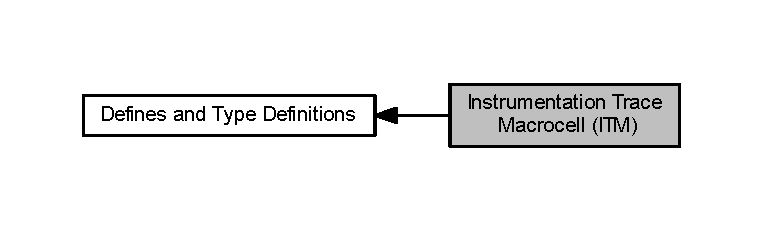
\includegraphics[width=350pt]{group___c_m_s_i_s___i_t_m}
\end{center}
\end{figure}
\subsection*{Classes}
\begin{DoxyCompactItemize}
\item 
struct \hyperlink{struct_i_t_m___type}{I\+T\+M\+\_\+\+Type}
\begin{DoxyCompactList}\small\item\em Structure type to access the Instrumentation Trace Macrocell Register (I\+TM). \end{DoxyCompactList}\end{DoxyCompactItemize}
\subsection*{Macros}
\begin{DoxyCompactItemize}
\item 
\#define \hyperlink{group___c_m_s_i_s___i_t_m_ga7abe5e590d1611599df87a1884a352e8}{I\+T\+M\+\_\+\+T\+P\+R\+\_\+\+P\+R\+I\+V\+M\+A\+S\+K\+\_\+\+Pos}~0U
\item 
\#define \hyperlink{group___c_m_s_i_s___i_t_m_ga168e089d882df325a387aab3a802a46b}{I\+T\+M\+\_\+\+T\+P\+R\+\_\+\+P\+R\+I\+V\+M\+A\+S\+K\+\_\+\+Msk}~(0x\+F\+U\+L /$\ast$$<$$<$ I\+T\+M\+\_\+\+T\+P\+R\+\_\+\+P\+R\+I\+V\+M\+A\+S\+K\+\_\+\+Pos$\ast$/)
\item 
\#define \hyperlink{group___c_m_s_i_s___i_t_m_ga9174ad4a36052c377cef4e6aba2ed484}{I\+T\+M\+\_\+\+T\+C\+R\+\_\+\+B\+U\+S\+Y\+\_\+\+Pos}~23U
\item 
\#define \hyperlink{group___c_m_s_i_s___i_t_m_ga43ad7cf33de12f2ef3a412d4f354c60f}{I\+T\+M\+\_\+\+T\+C\+R\+\_\+\+B\+U\+S\+Y\+\_\+\+Msk}~(1\+U\+L $<$$<$ I\+T\+M\+\_\+\+T\+C\+R\+\_\+\+B\+U\+S\+Y\+\_\+\+Pos)
\item 
\#define \hyperlink{group___c_m_s_i_s___i_t_m_gaca0281de867f33114aac0636f7ce65d3}{I\+T\+M\+\_\+\+T\+C\+R\+\_\+\+Trace\+Bus\+I\+D\+\_\+\+Pos}~16U
\item 
\#define \hyperlink{group___c_m_s_i_s___i_t_m_ga60c20bd9649d1da5a2be8e656ba19a60}{I\+T\+M\+\_\+\+T\+C\+R\+\_\+\+Trace\+Bus\+I\+D\+\_\+\+Msk}~(0x7\+F\+U\+L $<$$<$ I\+T\+M\+\_\+\+T\+C\+R\+\_\+\+Trace\+Bus\+I\+D\+\_\+\+Pos)
\item 
\#define \hyperlink{group___c_m_s_i_s___i_t_m_ga96c7c7cbc0d98426c408090b41f583f1}{I\+T\+M\+\_\+\+T\+C\+R\+\_\+\+G\+T\+S\+F\+R\+E\+Q\+\_\+\+Pos}~10U
\item 
\#define \hyperlink{group___c_m_s_i_s___i_t_m_gade862cf009827f7f6748fc44c541b067}{I\+T\+M\+\_\+\+T\+C\+R\+\_\+\+G\+T\+S\+F\+R\+E\+Q\+\_\+\+Msk}~(3\+U\+L $<$$<$ I\+T\+M\+\_\+\+T\+C\+R\+\_\+\+G\+T\+S\+F\+R\+E\+Q\+\_\+\+Pos)
\item 
\#define \hyperlink{group___c_m_s_i_s___i_t_m_gad7bc9ee1732032c6e0de035f0978e473}{I\+T\+M\+\_\+\+T\+C\+R\+\_\+\+T\+S\+Prescale\+\_\+\+Pos}~8U
\item 
\#define \hyperlink{group___c_m_s_i_s___i_t_m_ga7a723f71bfb0204c264d8dbe8cc7ae52}{I\+T\+M\+\_\+\+T\+C\+R\+\_\+\+T\+S\+Prescale\+\_\+\+Msk}~(3\+U\+L $<$$<$ I\+T\+M\+\_\+\+T\+C\+R\+\_\+\+T\+S\+Prescale\+\_\+\+Pos)
\item 
\#define \hyperlink{group___c_m_s_i_s___i_t_m_ga7a380f0c8078f6560051406583ecd6a5}{I\+T\+M\+\_\+\+T\+C\+R\+\_\+\+S\+W\+O\+E\+N\+A\+\_\+\+Pos}~4U
\item 
\#define \hyperlink{group___c_m_s_i_s___i_t_m_ga97476cb65bab16a328b35f81fd02010a}{I\+T\+M\+\_\+\+T\+C\+R\+\_\+\+S\+W\+O\+E\+N\+A\+\_\+\+Msk}~(1\+U\+L $<$$<$ I\+T\+M\+\_\+\+T\+C\+R\+\_\+\+S\+W\+O\+E\+N\+A\+\_\+\+Pos)
\item 
\#define \hyperlink{group___c_m_s_i_s___i_t_m_ga30e83ebb33aa766070fe3d1f27ae820e}{I\+T\+M\+\_\+\+T\+C\+R\+\_\+\+D\+W\+T\+E\+N\+A\+\_\+\+Pos}~3U
\item 
\#define \hyperlink{group___c_m_s_i_s___i_t_m_ga98ea1c596d43d3633a202f9ee746cf70}{I\+T\+M\+\_\+\+T\+C\+R\+\_\+\+D\+W\+T\+E\+N\+A\+\_\+\+Msk}~(1\+U\+L $<$$<$ I\+T\+M\+\_\+\+T\+C\+R\+\_\+\+D\+W\+T\+E\+N\+A\+\_\+\+Pos)
\item 
\#define \hyperlink{group___c_m_s_i_s___i_t_m_gaa93a1147a39fc63980d299231252a30e}{I\+T\+M\+\_\+\+T\+C\+R\+\_\+\+S\+Y\+N\+C\+E\+N\+A\+\_\+\+Pos}~2U
\item 
\#define \hyperlink{group___c_m_s_i_s___i_t_m_gac89b74a78701c25b442105d7fe2bbefb}{I\+T\+M\+\_\+\+T\+C\+R\+\_\+\+S\+Y\+N\+C\+E\+N\+A\+\_\+\+Msk}~(1\+U\+L $<$$<$ I\+T\+M\+\_\+\+T\+C\+R\+\_\+\+S\+Y\+N\+C\+E\+N\+A\+\_\+\+Pos)
\item 
\#define \hyperlink{group___c_m_s_i_s___i_t_m_ga5aa381845f810114ab519b90753922a1}{I\+T\+M\+\_\+\+T\+C\+R\+\_\+\+T\+S\+E\+N\+A\+\_\+\+Pos}~1U
\item 
\#define \hyperlink{group___c_m_s_i_s___i_t_m_ga436b2e8fa24328f48f2da31c00fc9e65}{I\+T\+M\+\_\+\+T\+C\+R\+\_\+\+T\+S\+E\+N\+A\+\_\+\+Msk}~(1\+U\+L $<$$<$ I\+T\+M\+\_\+\+T\+C\+R\+\_\+\+T\+S\+E\+N\+A\+\_\+\+Pos)
\item 
\#define \hyperlink{group___c_m_s_i_s___i_t_m_ga3286b86004bce7ffe17ee269f87f8d9d}{I\+T\+M\+\_\+\+T\+C\+R\+\_\+\+I\+T\+M\+E\+N\+A\+\_\+\+Pos}~0U
\item 
\#define \hyperlink{group___c_m_s_i_s___i_t_m_ga7dd53e3bff24ac09d94e61cb595cb2d9}{I\+T\+M\+\_\+\+T\+C\+R\+\_\+\+I\+T\+M\+E\+N\+A\+\_\+\+Msk}~(1\+U\+L /$\ast$$<$$<$ I\+T\+M\+\_\+\+T\+C\+R\+\_\+\+I\+T\+M\+E\+N\+A\+\_\+\+Pos$\ast$/)
\item 
\#define \hyperlink{group___c_m_s_i_s___i_t_m_ga04d3f842ad48f6a9127b4cecc963e1d7}{I\+T\+M\+\_\+\+I\+W\+R\+\_\+\+A\+T\+V\+A\+L\+I\+D\+M\+\_\+\+Pos}~0U
\item 
\#define \hyperlink{group___c_m_s_i_s___i_t_m_ga67b969f8f04ed15886727788f0e2ffd7}{I\+T\+M\+\_\+\+I\+W\+R\+\_\+\+A\+T\+V\+A\+L\+I\+D\+M\+\_\+\+Msk}~(1\+U\+L /$\ast$$<$$<$ I\+T\+M\+\_\+\+I\+W\+R\+\_\+\+A\+T\+V\+A\+L\+I\+D\+M\+\_\+\+Pos$\ast$/)
\item 
\#define \hyperlink{group___c_m_s_i_s___i_t_m_ga259edfd1d2e877a62e06d7a240df97f4}{I\+T\+M\+\_\+\+I\+R\+R\+\_\+\+A\+T\+R\+E\+A\+D\+Y\+M\+\_\+\+Pos}~0U
\item 
\#define \hyperlink{group___c_m_s_i_s___i_t_m_ga3dbc3e15f5bde2669cd8121a1fe419b9}{I\+T\+M\+\_\+\+I\+R\+R\+\_\+\+A\+T\+R\+E\+A\+D\+Y\+M\+\_\+\+Msk}~(1\+U\+L /$\ast$$<$$<$ I\+T\+M\+\_\+\+I\+R\+R\+\_\+\+A\+T\+R\+E\+A\+D\+Y\+M\+\_\+\+Pos$\ast$/)
\item 
\#define \hyperlink{group___c_m_s_i_s___i_t_m_ga08de02bf32caf48aaa29f7c68ff5d755}{I\+T\+M\+\_\+\+I\+M\+C\+R\+\_\+\+I\+N\+T\+E\+G\+R\+A\+T\+I\+O\+N\+\_\+\+Pos}~0U
\item 
\#define \hyperlink{group___c_m_s_i_s___i_t_m_ga8838bd3dd04c1a6be97cd946364a3fd2}{I\+T\+M\+\_\+\+I\+M\+C\+R\+\_\+\+I\+N\+T\+E\+G\+R\+A\+T\+I\+O\+N\+\_\+\+Msk}~(1\+U\+L /$\ast$$<$$<$ I\+T\+M\+\_\+\+I\+M\+C\+R\+\_\+\+I\+N\+T\+E\+G\+R\+A\+T\+I\+O\+N\+\_\+\+Pos$\ast$/)
\item 
\#define \hyperlink{group___c_m_s_i_s___i_t_m_gabfae3e570edc8759597311ed6dfb478e}{I\+T\+M\+\_\+\+L\+S\+R\+\_\+\+Byte\+Acc\+\_\+\+Pos}~2U
\item 
\#define \hyperlink{group___c_m_s_i_s___i_t_m_ga91f492b2891bb8b7eac5b58de7b220f4}{I\+T\+M\+\_\+\+L\+S\+R\+\_\+\+Byte\+Acc\+\_\+\+Msk}~(1\+U\+L $<$$<$ I\+T\+M\+\_\+\+L\+S\+R\+\_\+\+Byte\+Acc\+\_\+\+Pos)
\item 
\#define \hyperlink{group___c_m_s_i_s___i_t_m_ga144a49e12b83ad9809fdd2769094fdc0}{I\+T\+M\+\_\+\+L\+S\+R\+\_\+\+Access\+\_\+\+Pos}~1U
\item 
\#define \hyperlink{group___c_m_s_i_s___i_t_m_gac8ae69f11c0311da226c0c8ec40b3d37}{I\+T\+M\+\_\+\+L\+S\+R\+\_\+\+Access\+\_\+\+Msk}~(1\+U\+L $<$$<$ I\+T\+M\+\_\+\+L\+S\+R\+\_\+\+Access\+\_\+\+Pos)
\item 
\#define \hyperlink{group___c_m_s_i_s___i_t_m_gaf5740689cf14564d3f3fd91299b6c88d}{I\+T\+M\+\_\+\+L\+S\+R\+\_\+\+Present\+\_\+\+Pos}~0U
\item 
\#define \hyperlink{group___c_m_s_i_s___i_t_m_gaa5bc2a7f5f1d69ff819531f5508bb017}{I\+T\+M\+\_\+\+L\+S\+R\+\_\+\+Present\+\_\+\+Msk}~(1\+U\+L /$\ast$$<$$<$ I\+T\+M\+\_\+\+L\+S\+R\+\_\+\+Present\+\_\+\+Pos$\ast$/)
\item 
\#define \hyperlink{group___c_m_s_i_s___i_t_m_ga7abe5e590d1611599df87a1884a352e8}{I\+T\+M\+\_\+\+T\+P\+R\+\_\+\+P\+R\+I\+V\+M\+A\+S\+K\+\_\+\+Pos}~0U
\item 
\#define \hyperlink{group___c_m_s_i_s___i_t_m_ga168e089d882df325a387aab3a802a46b}{I\+T\+M\+\_\+\+T\+P\+R\+\_\+\+P\+R\+I\+V\+M\+A\+S\+K\+\_\+\+Msk}~(0x\+F\+U\+L /$\ast$$<$$<$ I\+T\+M\+\_\+\+T\+P\+R\+\_\+\+P\+R\+I\+V\+M\+A\+S\+K\+\_\+\+Pos$\ast$/)
\item 
\#define \hyperlink{group___c_m_s_i_s___i_t_m_ga9174ad4a36052c377cef4e6aba2ed484}{I\+T\+M\+\_\+\+T\+C\+R\+\_\+\+B\+U\+S\+Y\+\_\+\+Pos}~23U
\item 
\#define \hyperlink{group___c_m_s_i_s___i_t_m_ga43ad7cf33de12f2ef3a412d4f354c60f}{I\+T\+M\+\_\+\+T\+C\+R\+\_\+\+B\+U\+S\+Y\+\_\+\+Msk}~(1\+U\+L $<$$<$ I\+T\+M\+\_\+\+T\+C\+R\+\_\+\+B\+U\+S\+Y\+\_\+\+Pos)
\item 
\#define \hyperlink{group___c_m_s_i_s___i_t_m_gaca0281de867f33114aac0636f7ce65d3}{I\+T\+M\+\_\+\+T\+C\+R\+\_\+\+Trace\+Bus\+I\+D\+\_\+\+Pos}~16U
\item 
\#define \hyperlink{group___c_m_s_i_s___i_t_m_ga60c20bd9649d1da5a2be8e656ba19a60}{I\+T\+M\+\_\+\+T\+C\+R\+\_\+\+Trace\+Bus\+I\+D\+\_\+\+Msk}~(0x7\+F\+U\+L $<$$<$ I\+T\+M\+\_\+\+T\+C\+R\+\_\+\+Trace\+Bus\+I\+D\+\_\+\+Pos)
\item 
\#define \hyperlink{group___c_m_s_i_s___i_t_m_ga96c7c7cbc0d98426c408090b41f583f1}{I\+T\+M\+\_\+\+T\+C\+R\+\_\+\+G\+T\+S\+F\+R\+E\+Q\+\_\+\+Pos}~10U
\item 
\#define \hyperlink{group___c_m_s_i_s___i_t_m_gade862cf009827f7f6748fc44c541b067}{I\+T\+M\+\_\+\+T\+C\+R\+\_\+\+G\+T\+S\+F\+R\+E\+Q\+\_\+\+Msk}~(3\+U\+L $<$$<$ I\+T\+M\+\_\+\+T\+C\+R\+\_\+\+G\+T\+S\+F\+R\+E\+Q\+\_\+\+Pos)
\item 
\#define \hyperlink{group___c_m_s_i_s___i_t_m_gad7bc9ee1732032c6e0de035f0978e473}{I\+T\+M\+\_\+\+T\+C\+R\+\_\+\+T\+S\+Prescale\+\_\+\+Pos}~8U
\item 
\#define \hyperlink{group___c_m_s_i_s___i_t_m_ga7a723f71bfb0204c264d8dbe8cc7ae52}{I\+T\+M\+\_\+\+T\+C\+R\+\_\+\+T\+S\+Prescale\+\_\+\+Msk}~(3\+U\+L $<$$<$ I\+T\+M\+\_\+\+T\+C\+R\+\_\+\+T\+S\+Prescale\+\_\+\+Pos)
\item 
\#define \hyperlink{group___c_m_s_i_s___i_t_m_ga7a380f0c8078f6560051406583ecd6a5}{I\+T\+M\+\_\+\+T\+C\+R\+\_\+\+S\+W\+O\+E\+N\+A\+\_\+\+Pos}~4U
\item 
\#define \hyperlink{group___c_m_s_i_s___i_t_m_ga97476cb65bab16a328b35f81fd02010a}{I\+T\+M\+\_\+\+T\+C\+R\+\_\+\+S\+W\+O\+E\+N\+A\+\_\+\+Msk}~(1\+U\+L $<$$<$ I\+T\+M\+\_\+\+T\+C\+R\+\_\+\+S\+W\+O\+E\+N\+A\+\_\+\+Pos)
\item 
\#define \hyperlink{group___c_m_s_i_s___i_t_m_ga30e83ebb33aa766070fe3d1f27ae820e}{I\+T\+M\+\_\+\+T\+C\+R\+\_\+\+D\+W\+T\+E\+N\+A\+\_\+\+Pos}~3U
\item 
\#define \hyperlink{group___c_m_s_i_s___i_t_m_ga98ea1c596d43d3633a202f9ee746cf70}{I\+T\+M\+\_\+\+T\+C\+R\+\_\+\+D\+W\+T\+E\+N\+A\+\_\+\+Msk}~(1\+U\+L $<$$<$ I\+T\+M\+\_\+\+T\+C\+R\+\_\+\+D\+W\+T\+E\+N\+A\+\_\+\+Pos)
\item 
\#define \hyperlink{group___c_m_s_i_s___i_t_m_gaa93a1147a39fc63980d299231252a30e}{I\+T\+M\+\_\+\+T\+C\+R\+\_\+\+S\+Y\+N\+C\+E\+N\+A\+\_\+\+Pos}~2U
\item 
\#define \hyperlink{group___c_m_s_i_s___i_t_m_gac89b74a78701c25b442105d7fe2bbefb}{I\+T\+M\+\_\+\+T\+C\+R\+\_\+\+S\+Y\+N\+C\+E\+N\+A\+\_\+\+Msk}~(1\+U\+L $<$$<$ I\+T\+M\+\_\+\+T\+C\+R\+\_\+\+S\+Y\+N\+C\+E\+N\+A\+\_\+\+Pos)
\item 
\#define \hyperlink{group___c_m_s_i_s___i_t_m_ga5aa381845f810114ab519b90753922a1}{I\+T\+M\+\_\+\+T\+C\+R\+\_\+\+T\+S\+E\+N\+A\+\_\+\+Pos}~1U
\item 
\#define \hyperlink{group___c_m_s_i_s___i_t_m_ga436b2e8fa24328f48f2da31c00fc9e65}{I\+T\+M\+\_\+\+T\+C\+R\+\_\+\+T\+S\+E\+N\+A\+\_\+\+Msk}~(1\+U\+L $<$$<$ I\+T\+M\+\_\+\+T\+C\+R\+\_\+\+T\+S\+E\+N\+A\+\_\+\+Pos)
\item 
\#define \hyperlink{group___c_m_s_i_s___i_t_m_ga3286b86004bce7ffe17ee269f87f8d9d}{I\+T\+M\+\_\+\+T\+C\+R\+\_\+\+I\+T\+M\+E\+N\+A\+\_\+\+Pos}~0U
\item 
\#define \hyperlink{group___c_m_s_i_s___i_t_m_ga7dd53e3bff24ac09d94e61cb595cb2d9}{I\+T\+M\+\_\+\+T\+C\+R\+\_\+\+I\+T\+M\+E\+N\+A\+\_\+\+Msk}~(1\+U\+L /$\ast$$<$$<$ I\+T\+M\+\_\+\+T\+C\+R\+\_\+\+I\+T\+M\+E\+N\+A\+\_\+\+Pos$\ast$/)
\item 
\#define \hyperlink{group___c_m_s_i_s___i_t_m_ga04d3f842ad48f6a9127b4cecc963e1d7}{I\+T\+M\+\_\+\+I\+W\+R\+\_\+\+A\+T\+V\+A\+L\+I\+D\+M\+\_\+\+Pos}~0U
\item 
\#define \hyperlink{group___c_m_s_i_s___i_t_m_ga67b969f8f04ed15886727788f0e2ffd7}{I\+T\+M\+\_\+\+I\+W\+R\+\_\+\+A\+T\+V\+A\+L\+I\+D\+M\+\_\+\+Msk}~(1\+U\+L /$\ast$$<$$<$ I\+T\+M\+\_\+\+I\+W\+R\+\_\+\+A\+T\+V\+A\+L\+I\+D\+M\+\_\+\+Pos$\ast$/)
\item 
\#define \hyperlink{group___c_m_s_i_s___i_t_m_ga259edfd1d2e877a62e06d7a240df97f4}{I\+T\+M\+\_\+\+I\+R\+R\+\_\+\+A\+T\+R\+E\+A\+D\+Y\+M\+\_\+\+Pos}~0U
\item 
\#define \hyperlink{group___c_m_s_i_s___i_t_m_ga3dbc3e15f5bde2669cd8121a1fe419b9}{I\+T\+M\+\_\+\+I\+R\+R\+\_\+\+A\+T\+R\+E\+A\+D\+Y\+M\+\_\+\+Msk}~(1\+U\+L /$\ast$$<$$<$ I\+T\+M\+\_\+\+I\+R\+R\+\_\+\+A\+T\+R\+E\+A\+D\+Y\+M\+\_\+\+Pos$\ast$/)
\item 
\#define \hyperlink{group___c_m_s_i_s___i_t_m_ga08de02bf32caf48aaa29f7c68ff5d755}{I\+T\+M\+\_\+\+I\+M\+C\+R\+\_\+\+I\+N\+T\+E\+G\+R\+A\+T\+I\+O\+N\+\_\+\+Pos}~0U
\item 
\#define \hyperlink{group___c_m_s_i_s___i_t_m_ga8838bd3dd04c1a6be97cd946364a3fd2}{I\+T\+M\+\_\+\+I\+M\+C\+R\+\_\+\+I\+N\+T\+E\+G\+R\+A\+T\+I\+O\+N\+\_\+\+Msk}~(1\+U\+L /$\ast$$<$$<$ I\+T\+M\+\_\+\+I\+M\+C\+R\+\_\+\+I\+N\+T\+E\+G\+R\+A\+T\+I\+O\+N\+\_\+\+Pos$\ast$/)
\item 
\#define \hyperlink{group___c_m_s_i_s___i_t_m_gabfae3e570edc8759597311ed6dfb478e}{I\+T\+M\+\_\+\+L\+S\+R\+\_\+\+Byte\+Acc\+\_\+\+Pos}~2U
\item 
\#define \hyperlink{group___c_m_s_i_s___i_t_m_ga91f492b2891bb8b7eac5b58de7b220f4}{I\+T\+M\+\_\+\+L\+S\+R\+\_\+\+Byte\+Acc\+\_\+\+Msk}~(1\+U\+L $<$$<$ I\+T\+M\+\_\+\+L\+S\+R\+\_\+\+Byte\+Acc\+\_\+\+Pos)
\item 
\#define \hyperlink{group___c_m_s_i_s___i_t_m_ga144a49e12b83ad9809fdd2769094fdc0}{I\+T\+M\+\_\+\+L\+S\+R\+\_\+\+Access\+\_\+\+Pos}~1U
\item 
\#define \hyperlink{group___c_m_s_i_s___i_t_m_gac8ae69f11c0311da226c0c8ec40b3d37}{I\+T\+M\+\_\+\+L\+S\+R\+\_\+\+Access\+\_\+\+Msk}~(1\+U\+L $<$$<$ I\+T\+M\+\_\+\+L\+S\+R\+\_\+\+Access\+\_\+\+Pos)
\item 
\#define \hyperlink{group___c_m_s_i_s___i_t_m_gaf5740689cf14564d3f3fd91299b6c88d}{I\+T\+M\+\_\+\+L\+S\+R\+\_\+\+Present\+\_\+\+Pos}~0U
\item 
\#define \hyperlink{group___c_m_s_i_s___i_t_m_gaa5bc2a7f5f1d69ff819531f5508bb017}{I\+T\+M\+\_\+\+L\+S\+R\+\_\+\+Present\+\_\+\+Msk}~(1\+U\+L /$\ast$$<$$<$ I\+T\+M\+\_\+\+L\+S\+R\+\_\+\+Present\+\_\+\+Pos$\ast$/)
\item 
\#define \hyperlink{group___c_m_s_i_s___i_t_m_ga7abe5e590d1611599df87a1884a352e8}{I\+T\+M\+\_\+\+T\+P\+R\+\_\+\+P\+R\+I\+V\+M\+A\+S\+K\+\_\+\+Pos}~0U
\item 
\#define \hyperlink{group___c_m_s_i_s___i_t_m_ga168e089d882df325a387aab3a802a46b}{I\+T\+M\+\_\+\+T\+P\+R\+\_\+\+P\+R\+I\+V\+M\+A\+S\+K\+\_\+\+Msk}~(0x\+F\+U\+L /$\ast$$<$$<$ I\+T\+M\+\_\+\+T\+P\+R\+\_\+\+P\+R\+I\+V\+M\+A\+S\+K\+\_\+\+Pos$\ast$/)
\item 
\#define \hyperlink{group___c_m_s_i_s___i_t_m_ga9174ad4a36052c377cef4e6aba2ed484}{I\+T\+M\+\_\+\+T\+C\+R\+\_\+\+B\+U\+S\+Y\+\_\+\+Pos}~23U
\item 
\#define \hyperlink{group___c_m_s_i_s___i_t_m_ga43ad7cf33de12f2ef3a412d4f354c60f}{I\+T\+M\+\_\+\+T\+C\+R\+\_\+\+B\+U\+S\+Y\+\_\+\+Msk}~(1\+U\+L $<$$<$ I\+T\+M\+\_\+\+T\+C\+R\+\_\+\+B\+U\+S\+Y\+\_\+\+Pos)
\item 
\#define \hyperlink{group___c_m_s_i_s___i_t_m_gaca0281de867f33114aac0636f7ce65d3}{I\+T\+M\+\_\+\+T\+C\+R\+\_\+\+Trace\+Bus\+I\+D\+\_\+\+Pos}~16U
\item 
\#define \hyperlink{group___c_m_s_i_s___i_t_m_ga60c20bd9649d1da5a2be8e656ba19a60}{I\+T\+M\+\_\+\+T\+C\+R\+\_\+\+Trace\+Bus\+I\+D\+\_\+\+Msk}~(0x7\+F\+U\+L $<$$<$ I\+T\+M\+\_\+\+T\+C\+R\+\_\+\+Trace\+Bus\+I\+D\+\_\+\+Pos)
\item 
\#define \hyperlink{group___c_m_s_i_s___i_t_m_ga96c7c7cbc0d98426c408090b41f583f1}{I\+T\+M\+\_\+\+T\+C\+R\+\_\+\+G\+T\+S\+F\+R\+E\+Q\+\_\+\+Pos}~10U
\item 
\#define \hyperlink{group___c_m_s_i_s___i_t_m_gade862cf009827f7f6748fc44c541b067}{I\+T\+M\+\_\+\+T\+C\+R\+\_\+\+G\+T\+S\+F\+R\+E\+Q\+\_\+\+Msk}~(3\+U\+L $<$$<$ I\+T\+M\+\_\+\+T\+C\+R\+\_\+\+G\+T\+S\+F\+R\+E\+Q\+\_\+\+Pos)
\item 
\#define \hyperlink{group___c_m_s_i_s___i_t_m_gad7bc9ee1732032c6e0de035f0978e473}{I\+T\+M\+\_\+\+T\+C\+R\+\_\+\+T\+S\+Prescale\+\_\+\+Pos}~8U
\item 
\#define \hyperlink{group___c_m_s_i_s___i_t_m_ga7a723f71bfb0204c264d8dbe8cc7ae52}{I\+T\+M\+\_\+\+T\+C\+R\+\_\+\+T\+S\+Prescale\+\_\+\+Msk}~(3\+U\+L $<$$<$ I\+T\+M\+\_\+\+T\+C\+R\+\_\+\+T\+S\+Prescale\+\_\+\+Pos)
\item 
\#define \hyperlink{group___c_m_s_i_s___i_t_m_ga7a380f0c8078f6560051406583ecd6a5}{I\+T\+M\+\_\+\+T\+C\+R\+\_\+\+S\+W\+O\+E\+N\+A\+\_\+\+Pos}~4U
\item 
\#define \hyperlink{group___c_m_s_i_s___i_t_m_ga97476cb65bab16a328b35f81fd02010a}{I\+T\+M\+\_\+\+T\+C\+R\+\_\+\+S\+W\+O\+E\+N\+A\+\_\+\+Msk}~(1\+U\+L $<$$<$ I\+T\+M\+\_\+\+T\+C\+R\+\_\+\+S\+W\+O\+E\+N\+A\+\_\+\+Pos)
\item 
\#define \hyperlink{group___c_m_s_i_s___i_t_m_ga30e83ebb33aa766070fe3d1f27ae820e}{I\+T\+M\+\_\+\+T\+C\+R\+\_\+\+D\+W\+T\+E\+N\+A\+\_\+\+Pos}~3U
\item 
\#define \hyperlink{group___c_m_s_i_s___i_t_m_ga98ea1c596d43d3633a202f9ee746cf70}{I\+T\+M\+\_\+\+T\+C\+R\+\_\+\+D\+W\+T\+E\+N\+A\+\_\+\+Msk}~(1\+U\+L $<$$<$ I\+T\+M\+\_\+\+T\+C\+R\+\_\+\+D\+W\+T\+E\+N\+A\+\_\+\+Pos)
\item 
\#define \hyperlink{group___c_m_s_i_s___i_t_m_gaa93a1147a39fc63980d299231252a30e}{I\+T\+M\+\_\+\+T\+C\+R\+\_\+\+S\+Y\+N\+C\+E\+N\+A\+\_\+\+Pos}~2U
\item 
\#define \hyperlink{group___c_m_s_i_s___i_t_m_gac89b74a78701c25b442105d7fe2bbefb}{I\+T\+M\+\_\+\+T\+C\+R\+\_\+\+S\+Y\+N\+C\+E\+N\+A\+\_\+\+Msk}~(1\+U\+L $<$$<$ I\+T\+M\+\_\+\+T\+C\+R\+\_\+\+S\+Y\+N\+C\+E\+N\+A\+\_\+\+Pos)
\item 
\#define \hyperlink{group___c_m_s_i_s___i_t_m_ga5aa381845f810114ab519b90753922a1}{I\+T\+M\+\_\+\+T\+C\+R\+\_\+\+T\+S\+E\+N\+A\+\_\+\+Pos}~1U
\item 
\#define \hyperlink{group___c_m_s_i_s___i_t_m_ga436b2e8fa24328f48f2da31c00fc9e65}{I\+T\+M\+\_\+\+T\+C\+R\+\_\+\+T\+S\+E\+N\+A\+\_\+\+Msk}~(1\+U\+L $<$$<$ I\+T\+M\+\_\+\+T\+C\+R\+\_\+\+T\+S\+E\+N\+A\+\_\+\+Pos)
\item 
\#define \hyperlink{group___c_m_s_i_s___i_t_m_ga3286b86004bce7ffe17ee269f87f8d9d}{I\+T\+M\+\_\+\+T\+C\+R\+\_\+\+I\+T\+M\+E\+N\+A\+\_\+\+Pos}~0U
\item 
\#define \hyperlink{group___c_m_s_i_s___i_t_m_ga7dd53e3bff24ac09d94e61cb595cb2d9}{I\+T\+M\+\_\+\+T\+C\+R\+\_\+\+I\+T\+M\+E\+N\+A\+\_\+\+Msk}~(1\+U\+L /$\ast$$<$$<$ I\+T\+M\+\_\+\+T\+C\+R\+\_\+\+I\+T\+M\+E\+N\+A\+\_\+\+Pos$\ast$/)
\item 
\#define \hyperlink{group___c_m_s_i_s___i_t_m_ga04d3f842ad48f6a9127b4cecc963e1d7}{I\+T\+M\+\_\+\+I\+W\+R\+\_\+\+A\+T\+V\+A\+L\+I\+D\+M\+\_\+\+Pos}~0U
\item 
\#define \hyperlink{group___c_m_s_i_s___i_t_m_ga67b969f8f04ed15886727788f0e2ffd7}{I\+T\+M\+\_\+\+I\+W\+R\+\_\+\+A\+T\+V\+A\+L\+I\+D\+M\+\_\+\+Msk}~(1\+U\+L /$\ast$$<$$<$ I\+T\+M\+\_\+\+I\+W\+R\+\_\+\+A\+T\+V\+A\+L\+I\+D\+M\+\_\+\+Pos$\ast$/)
\item 
\#define \hyperlink{group___c_m_s_i_s___i_t_m_ga259edfd1d2e877a62e06d7a240df97f4}{I\+T\+M\+\_\+\+I\+R\+R\+\_\+\+A\+T\+R\+E\+A\+D\+Y\+M\+\_\+\+Pos}~0U
\item 
\#define \hyperlink{group___c_m_s_i_s___i_t_m_ga3dbc3e15f5bde2669cd8121a1fe419b9}{I\+T\+M\+\_\+\+I\+R\+R\+\_\+\+A\+T\+R\+E\+A\+D\+Y\+M\+\_\+\+Msk}~(1\+U\+L /$\ast$$<$$<$ I\+T\+M\+\_\+\+I\+R\+R\+\_\+\+A\+T\+R\+E\+A\+D\+Y\+M\+\_\+\+Pos$\ast$/)
\item 
\#define \hyperlink{group___c_m_s_i_s___i_t_m_ga08de02bf32caf48aaa29f7c68ff5d755}{I\+T\+M\+\_\+\+I\+M\+C\+R\+\_\+\+I\+N\+T\+E\+G\+R\+A\+T\+I\+O\+N\+\_\+\+Pos}~0U
\item 
\#define \hyperlink{group___c_m_s_i_s___i_t_m_ga8838bd3dd04c1a6be97cd946364a3fd2}{I\+T\+M\+\_\+\+I\+M\+C\+R\+\_\+\+I\+N\+T\+E\+G\+R\+A\+T\+I\+O\+N\+\_\+\+Msk}~(1\+U\+L /$\ast$$<$$<$ I\+T\+M\+\_\+\+I\+M\+C\+R\+\_\+\+I\+N\+T\+E\+G\+R\+A\+T\+I\+O\+N\+\_\+\+Pos$\ast$/)
\item 
\#define \hyperlink{group___c_m_s_i_s___i_t_m_gabfae3e570edc8759597311ed6dfb478e}{I\+T\+M\+\_\+\+L\+S\+R\+\_\+\+Byte\+Acc\+\_\+\+Pos}~2U
\item 
\#define \hyperlink{group___c_m_s_i_s___i_t_m_ga91f492b2891bb8b7eac5b58de7b220f4}{I\+T\+M\+\_\+\+L\+S\+R\+\_\+\+Byte\+Acc\+\_\+\+Msk}~(1\+U\+L $<$$<$ I\+T\+M\+\_\+\+L\+S\+R\+\_\+\+Byte\+Acc\+\_\+\+Pos)
\item 
\#define \hyperlink{group___c_m_s_i_s___i_t_m_ga144a49e12b83ad9809fdd2769094fdc0}{I\+T\+M\+\_\+\+L\+S\+R\+\_\+\+Access\+\_\+\+Pos}~1U
\item 
\#define \hyperlink{group___c_m_s_i_s___i_t_m_gac8ae69f11c0311da226c0c8ec40b3d37}{I\+T\+M\+\_\+\+L\+S\+R\+\_\+\+Access\+\_\+\+Msk}~(1\+U\+L $<$$<$ I\+T\+M\+\_\+\+L\+S\+R\+\_\+\+Access\+\_\+\+Pos)
\item 
\#define \hyperlink{group___c_m_s_i_s___i_t_m_gaf5740689cf14564d3f3fd91299b6c88d}{I\+T\+M\+\_\+\+L\+S\+R\+\_\+\+Present\+\_\+\+Pos}~0U
\item 
\#define \hyperlink{group___c_m_s_i_s___i_t_m_gaa5bc2a7f5f1d69ff819531f5508bb017}{I\+T\+M\+\_\+\+L\+S\+R\+\_\+\+Present\+\_\+\+Msk}~(1\+U\+L /$\ast$$<$$<$ I\+T\+M\+\_\+\+L\+S\+R\+\_\+\+Present\+\_\+\+Pos$\ast$/)
\item 
\#define \hyperlink{group___c_m_s_i_s___i_t_m_ga7abe5e590d1611599df87a1884a352e8}{I\+T\+M\+\_\+\+T\+P\+R\+\_\+\+P\+R\+I\+V\+M\+A\+S\+K\+\_\+\+Pos}~0U
\item 
\#define \hyperlink{group___c_m_s_i_s___i_t_m_ga168e089d882df325a387aab3a802a46b}{I\+T\+M\+\_\+\+T\+P\+R\+\_\+\+P\+R\+I\+V\+M\+A\+S\+K\+\_\+\+Msk}~(0x\+F\+U\+L /$\ast$$<$$<$ I\+T\+M\+\_\+\+T\+P\+R\+\_\+\+P\+R\+I\+V\+M\+A\+S\+K\+\_\+\+Pos$\ast$/)
\item 
\#define \hyperlink{group___c_m_s_i_s___i_t_m_ga9174ad4a36052c377cef4e6aba2ed484}{I\+T\+M\+\_\+\+T\+C\+R\+\_\+\+B\+U\+S\+Y\+\_\+\+Pos}~23U
\item 
\#define \hyperlink{group___c_m_s_i_s___i_t_m_ga43ad7cf33de12f2ef3a412d4f354c60f}{I\+T\+M\+\_\+\+T\+C\+R\+\_\+\+B\+U\+S\+Y\+\_\+\+Msk}~(1\+U\+L $<$$<$ I\+T\+M\+\_\+\+T\+C\+R\+\_\+\+B\+U\+S\+Y\+\_\+\+Pos)
\item 
\#define \hyperlink{group___c_m_s_i_s___i_t_m_gaca0281de867f33114aac0636f7ce65d3}{I\+T\+M\+\_\+\+T\+C\+R\+\_\+\+Trace\+Bus\+I\+D\+\_\+\+Pos}~16U
\item 
\#define \hyperlink{group___c_m_s_i_s___i_t_m_ga60c20bd9649d1da5a2be8e656ba19a60}{I\+T\+M\+\_\+\+T\+C\+R\+\_\+\+Trace\+Bus\+I\+D\+\_\+\+Msk}~(0x7\+F\+U\+L $<$$<$ I\+T\+M\+\_\+\+T\+C\+R\+\_\+\+Trace\+Bus\+I\+D\+\_\+\+Pos)
\item 
\#define \hyperlink{group___c_m_s_i_s___i_t_m_ga96c7c7cbc0d98426c408090b41f583f1}{I\+T\+M\+\_\+\+T\+C\+R\+\_\+\+G\+T\+S\+F\+R\+E\+Q\+\_\+\+Pos}~10U
\item 
\#define \hyperlink{group___c_m_s_i_s___i_t_m_gade862cf009827f7f6748fc44c541b067}{I\+T\+M\+\_\+\+T\+C\+R\+\_\+\+G\+T\+S\+F\+R\+E\+Q\+\_\+\+Msk}~(3\+U\+L $<$$<$ I\+T\+M\+\_\+\+T\+C\+R\+\_\+\+G\+T\+S\+F\+R\+E\+Q\+\_\+\+Pos)
\item 
\#define \hyperlink{group___c_m_s_i_s___i_t_m_gad7bc9ee1732032c6e0de035f0978e473}{I\+T\+M\+\_\+\+T\+C\+R\+\_\+\+T\+S\+Prescale\+\_\+\+Pos}~8U
\item 
\#define \hyperlink{group___c_m_s_i_s___i_t_m_ga7a723f71bfb0204c264d8dbe8cc7ae52}{I\+T\+M\+\_\+\+T\+C\+R\+\_\+\+T\+S\+Prescale\+\_\+\+Msk}~(3\+U\+L $<$$<$ I\+T\+M\+\_\+\+T\+C\+R\+\_\+\+T\+S\+Prescale\+\_\+\+Pos)
\item 
\#define \hyperlink{group___c_m_s_i_s___i_t_m_ga7a380f0c8078f6560051406583ecd6a5}{I\+T\+M\+\_\+\+T\+C\+R\+\_\+\+S\+W\+O\+E\+N\+A\+\_\+\+Pos}~4U
\item 
\#define \hyperlink{group___c_m_s_i_s___i_t_m_ga97476cb65bab16a328b35f81fd02010a}{I\+T\+M\+\_\+\+T\+C\+R\+\_\+\+S\+W\+O\+E\+N\+A\+\_\+\+Msk}~(1\+U\+L $<$$<$ I\+T\+M\+\_\+\+T\+C\+R\+\_\+\+S\+W\+O\+E\+N\+A\+\_\+\+Pos)
\item 
\#define \hyperlink{group___c_m_s_i_s___i_t_m_ga30e83ebb33aa766070fe3d1f27ae820e}{I\+T\+M\+\_\+\+T\+C\+R\+\_\+\+D\+W\+T\+E\+N\+A\+\_\+\+Pos}~3U
\item 
\#define \hyperlink{group___c_m_s_i_s___i_t_m_ga98ea1c596d43d3633a202f9ee746cf70}{I\+T\+M\+\_\+\+T\+C\+R\+\_\+\+D\+W\+T\+E\+N\+A\+\_\+\+Msk}~(1\+U\+L $<$$<$ I\+T\+M\+\_\+\+T\+C\+R\+\_\+\+D\+W\+T\+E\+N\+A\+\_\+\+Pos)
\item 
\#define \hyperlink{group___c_m_s_i_s___i_t_m_gaa93a1147a39fc63980d299231252a30e}{I\+T\+M\+\_\+\+T\+C\+R\+\_\+\+S\+Y\+N\+C\+E\+N\+A\+\_\+\+Pos}~2U
\item 
\#define \hyperlink{group___c_m_s_i_s___i_t_m_gac89b74a78701c25b442105d7fe2bbefb}{I\+T\+M\+\_\+\+T\+C\+R\+\_\+\+S\+Y\+N\+C\+E\+N\+A\+\_\+\+Msk}~(1\+U\+L $<$$<$ I\+T\+M\+\_\+\+T\+C\+R\+\_\+\+S\+Y\+N\+C\+E\+N\+A\+\_\+\+Pos)
\item 
\#define \hyperlink{group___c_m_s_i_s___i_t_m_ga5aa381845f810114ab519b90753922a1}{I\+T\+M\+\_\+\+T\+C\+R\+\_\+\+T\+S\+E\+N\+A\+\_\+\+Pos}~1U
\item 
\#define \hyperlink{group___c_m_s_i_s___i_t_m_ga436b2e8fa24328f48f2da31c00fc9e65}{I\+T\+M\+\_\+\+T\+C\+R\+\_\+\+T\+S\+E\+N\+A\+\_\+\+Msk}~(1\+U\+L $<$$<$ I\+T\+M\+\_\+\+T\+C\+R\+\_\+\+T\+S\+E\+N\+A\+\_\+\+Pos)
\item 
\#define \hyperlink{group___c_m_s_i_s___i_t_m_ga3286b86004bce7ffe17ee269f87f8d9d}{I\+T\+M\+\_\+\+T\+C\+R\+\_\+\+I\+T\+M\+E\+N\+A\+\_\+\+Pos}~0U
\item 
\#define \hyperlink{group___c_m_s_i_s___i_t_m_ga7dd53e3bff24ac09d94e61cb595cb2d9}{I\+T\+M\+\_\+\+T\+C\+R\+\_\+\+I\+T\+M\+E\+N\+A\+\_\+\+Msk}~(1\+U\+L /$\ast$$<$$<$ I\+T\+M\+\_\+\+T\+C\+R\+\_\+\+I\+T\+M\+E\+N\+A\+\_\+\+Pos$\ast$/)
\item 
\#define \hyperlink{group___c_m_s_i_s___i_t_m_ga04d3f842ad48f6a9127b4cecc963e1d7}{I\+T\+M\+\_\+\+I\+W\+R\+\_\+\+A\+T\+V\+A\+L\+I\+D\+M\+\_\+\+Pos}~0U
\item 
\#define \hyperlink{group___c_m_s_i_s___i_t_m_ga67b969f8f04ed15886727788f0e2ffd7}{I\+T\+M\+\_\+\+I\+W\+R\+\_\+\+A\+T\+V\+A\+L\+I\+D\+M\+\_\+\+Msk}~(1\+U\+L /$\ast$$<$$<$ I\+T\+M\+\_\+\+I\+W\+R\+\_\+\+A\+T\+V\+A\+L\+I\+D\+M\+\_\+\+Pos$\ast$/)
\item 
\#define \hyperlink{group___c_m_s_i_s___i_t_m_ga259edfd1d2e877a62e06d7a240df97f4}{I\+T\+M\+\_\+\+I\+R\+R\+\_\+\+A\+T\+R\+E\+A\+D\+Y\+M\+\_\+\+Pos}~0U
\item 
\#define \hyperlink{group___c_m_s_i_s___i_t_m_ga3dbc3e15f5bde2669cd8121a1fe419b9}{I\+T\+M\+\_\+\+I\+R\+R\+\_\+\+A\+T\+R\+E\+A\+D\+Y\+M\+\_\+\+Msk}~(1\+U\+L /$\ast$$<$$<$ I\+T\+M\+\_\+\+I\+R\+R\+\_\+\+A\+T\+R\+E\+A\+D\+Y\+M\+\_\+\+Pos$\ast$/)
\item 
\#define \hyperlink{group___c_m_s_i_s___i_t_m_ga08de02bf32caf48aaa29f7c68ff5d755}{I\+T\+M\+\_\+\+I\+M\+C\+R\+\_\+\+I\+N\+T\+E\+G\+R\+A\+T\+I\+O\+N\+\_\+\+Pos}~0U
\item 
\#define \hyperlink{group___c_m_s_i_s___i_t_m_ga8838bd3dd04c1a6be97cd946364a3fd2}{I\+T\+M\+\_\+\+I\+M\+C\+R\+\_\+\+I\+N\+T\+E\+G\+R\+A\+T\+I\+O\+N\+\_\+\+Msk}~(1\+U\+L /$\ast$$<$$<$ I\+T\+M\+\_\+\+I\+M\+C\+R\+\_\+\+I\+N\+T\+E\+G\+R\+A\+T\+I\+O\+N\+\_\+\+Pos$\ast$/)
\item 
\#define \hyperlink{group___c_m_s_i_s___i_t_m_gabfae3e570edc8759597311ed6dfb478e}{I\+T\+M\+\_\+\+L\+S\+R\+\_\+\+Byte\+Acc\+\_\+\+Pos}~2U
\item 
\#define \hyperlink{group___c_m_s_i_s___i_t_m_ga91f492b2891bb8b7eac5b58de7b220f4}{I\+T\+M\+\_\+\+L\+S\+R\+\_\+\+Byte\+Acc\+\_\+\+Msk}~(1\+U\+L $<$$<$ I\+T\+M\+\_\+\+L\+S\+R\+\_\+\+Byte\+Acc\+\_\+\+Pos)
\item 
\#define \hyperlink{group___c_m_s_i_s___i_t_m_ga144a49e12b83ad9809fdd2769094fdc0}{I\+T\+M\+\_\+\+L\+S\+R\+\_\+\+Access\+\_\+\+Pos}~1U
\item 
\#define \hyperlink{group___c_m_s_i_s___i_t_m_gac8ae69f11c0311da226c0c8ec40b3d37}{I\+T\+M\+\_\+\+L\+S\+R\+\_\+\+Access\+\_\+\+Msk}~(1\+U\+L $<$$<$ I\+T\+M\+\_\+\+L\+S\+R\+\_\+\+Access\+\_\+\+Pos)
\item 
\#define \hyperlink{group___c_m_s_i_s___i_t_m_gaf5740689cf14564d3f3fd91299b6c88d}{I\+T\+M\+\_\+\+L\+S\+R\+\_\+\+Present\+\_\+\+Pos}~0U
\item 
\#define \hyperlink{group___c_m_s_i_s___i_t_m_gaa5bc2a7f5f1d69ff819531f5508bb017}{I\+T\+M\+\_\+\+L\+S\+R\+\_\+\+Present\+\_\+\+Msk}~(1\+U\+L /$\ast$$<$$<$ I\+T\+M\+\_\+\+L\+S\+R\+\_\+\+Present\+\_\+\+Pos$\ast$/)
\end{DoxyCompactItemize}


\subsection{Detailed Description}
Type definitions for the Instrumentation Trace Macrocell (I\+TM) 



\subsection{Macro Definition Documentation}
\mbox{\Hypertarget{group___c_m_s_i_s___i_t_m_ga8838bd3dd04c1a6be97cd946364a3fd2}\label{group___c_m_s_i_s___i_t_m_ga8838bd3dd04c1a6be97cd946364a3fd2}} 
\index{Instrumentation Trace Macrocell (\+I\+T\+M)@{Instrumentation Trace Macrocell (\+I\+T\+M)}!I\+T\+M\+\_\+\+I\+M\+C\+R\+\_\+\+I\+N\+T\+E\+G\+R\+A\+T\+I\+O\+N\+\_\+\+Msk@{I\+T\+M\+\_\+\+I\+M\+C\+R\+\_\+\+I\+N\+T\+E\+G\+R\+A\+T\+I\+O\+N\+\_\+\+Msk}}
\index{I\+T\+M\+\_\+\+I\+M\+C\+R\+\_\+\+I\+N\+T\+E\+G\+R\+A\+T\+I\+O\+N\+\_\+\+Msk@{I\+T\+M\+\_\+\+I\+M\+C\+R\+\_\+\+I\+N\+T\+E\+G\+R\+A\+T\+I\+O\+N\+\_\+\+Msk}!Instrumentation Trace Macrocell (\+I\+T\+M)@{Instrumentation Trace Macrocell (\+I\+T\+M)}}
\subsubsection{\texorpdfstring{I\+T\+M\+\_\+\+I\+M\+C\+R\+\_\+\+I\+N\+T\+E\+G\+R\+A\+T\+I\+O\+N\+\_\+\+Msk}{ITM\_IMCR\_INTEGRATION\_Msk}\hspace{0.1cm}{\footnotesize\ttfamily [1/4]}}
{\footnotesize\ttfamily \#define I\+T\+M\+\_\+\+I\+M\+C\+R\+\_\+\+I\+N\+T\+E\+G\+R\+A\+T\+I\+O\+N\+\_\+\+Msk~(1\+U\+L /$\ast$$<$$<$ I\+T\+M\+\_\+\+I\+M\+C\+R\+\_\+\+I\+N\+T\+E\+G\+R\+A\+T\+I\+O\+N\+\_\+\+Pos$\ast$/)}

I\+TM I\+M\+CR\+: I\+N\+T\+E\+G\+R\+A\+T\+I\+ON Mask 

Definition at line 795 of file core\+\_\+sc300.\+h.

\mbox{\Hypertarget{group___c_m_s_i_s___i_t_m_ga8838bd3dd04c1a6be97cd946364a3fd2}\label{group___c_m_s_i_s___i_t_m_ga8838bd3dd04c1a6be97cd946364a3fd2}} 
\index{Instrumentation Trace Macrocell (\+I\+T\+M)@{Instrumentation Trace Macrocell (\+I\+T\+M)}!I\+T\+M\+\_\+\+I\+M\+C\+R\+\_\+\+I\+N\+T\+E\+G\+R\+A\+T\+I\+O\+N\+\_\+\+Msk@{I\+T\+M\+\_\+\+I\+M\+C\+R\+\_\+\+I\+N\+T\+E\+G\+R\+A\+T\+I\+O\+N\+\_\+\+Msk}}
\index{I\+T\+M\+\_\+\+I\+M\+C\+R\+\_\+\+I\+N\+T\+E\+G\+R\+A\+T\+I\+O\+N\+\_\+\+Msk@{I\+T\+M\+\_\+\+I\+M\+C\+R\+\_\+\+I\+N\+T\+E\+G\+R\+A\+T\+I\+O\+N\+\_\+\+Msk}!Instrumentation Trace Macrocell (\+I\+T\+M)@{Instrumentation Trace Macrocell (\+I\+T\+M)}}
\subsubsection{\texorpdfstring{I\+T\+M\+\_\+\+I\+M\+C\+R\+\_\+\+I\+N\+T\+E\+G\+R\+A\+T\+I\+O\+N\+\_\+\+Msk}{ITM\_IMCR\_INTEGRATION\_Msk}\hspace{0.1cm}{\footnotesize\ttfamily [2/4]}}
{\footnotesize\ttfamily \#define I\+T\+M\+\_\+\+I\+M\+C\+R\+\_\+\+I\+N\+T\+E\+G\+R\+A\+T\+I\+O\+N\+\_\+\+Msk~(1\+U\+L /$\ast$$<$$<$ I\+T\+M\+\_\+\+I\+M\+C\+R\+\_\+\+I\+N\+T\+E\+G\+R\+A\+T\+I\+O\+N\+\_\+\+Pos$\ast$/)}

I\+TM I\+M\+CR\+: I\+N\+T\+E\+G\+R\+A\+T\+I\+ON Mask 

Definition at line 821 of file core\+\_\+cm3.\+h.

\mbox{\Hypertarget{group___c_m_s_i_s___i_t_m_ga8838bd3dd04c1a6be97cd946364a3fd2}\label{group___c_m_s_i_s___i_t_m_ga8838bd3dd04c1a6be97cd946364a3fd2}} 
\index{Instrumentation Trace Macrocell (\+I\+T\+M)@{Instrumentation Trace Macrocell (\+I\+T\+M)}!I\+T\+M\+\_\+\+I\+M\+C\+R\+\_\+\+I\+N\+T\+E\+G\+R\+A\+T\+I\+O\+N\+\_\+\+Msk@{I\+T\+M\+\_\+\+I\+M\+C\+R\+\_\+\+I\+N\+T\+E\+G\+R\+A\+T\+I\+O\+N\+\_\+\+Msk}}
\index{I\+T\+M\+\_\+\+I\+M\+C\+R\+\_\+\+I\+N\+T\+E\+G\+R\+A\+T\+I\+O\+N\+\_\+\+Msk@{I\+T\+M\+\_\+\+I\+M\+C\+R\+\_\+\+I\+N\+T\+E\+G\+R\+A\+T\+I\+O\+N\+\_\+\+Msk}!Instrumentation Trace Macrocell (\+I\+T\+M)@{Instrumentation Trace Macrocell (\+I\+T\+M)}}
\subsubsection{\texorpdfstring{I\+T\+M\+\_\+\+I\+M\+C\+R\+\_\+\+I\+N\+T\+E\+G\+R\+A\+T\+I\+O\+N\+\_\+\+Msk}{ITM\_IMCR\_INTEGRATION\_Msk}\hspace{0.1cm}{\footnotesize\ttfamily [3/4]}}
{\footnotesize\ttfamily \#define I\+T\+M\+\_\+\+I\+M\+C\+R\+\_\+\+I\+N\+T\+E\+G\+R\+A\+T\+I\+O\+N\+\_\+\+Msk~(1\+U\+L /$\ast$$<$$<$ I\+T\+M\+\_\+\+I\+M\+C\+R\+\_\+\+I\+N\+T\+E\+G\+R\+A\+T\+I\+O\+N\+\_\+\+Pos$\ast$/)}

I\+TM I\+M\+CR\+: I\+N\+T\+E\+G\+R\+A\+T\+I\+ON Mask 

Definition at line 882 of file core\+\_\+cm4.\+h.

\mbox{\Hypertarget{group___c_m_s_i_s___i_t_m_ga8838bd3dd04c1a6be97cd946364a3fd2}\label{group___c_m_s_i_s___i_t_m_ga8838bd3dd04c1a6be97cd946364a3fd2}} 
\index{Instrumentation Trace Macrocell (\+I\+T\+M)@{Instrumentation Trace Macrocell (\+I\+T\+M)}!I\+T\+M\+\_\+\+I\+M\+C\+R\+\_\+\+I\+N\+T\+E\+G\+R\+A\+T\+I\+O\+N\+\_\+\+Msk@{I\+T\+M\+\_\+\+I\+M\+C\+R\+\_\+\+I\+N\+T\+E\+G\+R\+A\+T\+I\+O\+N\+\_\+\+Msk}}
\index{I\+T\+M\+\_\+\+I\+M\+C\+R\+\_\+\+I\+N\+T\+E\+G\+R\+A\+T\+I\+O\+N\+\_\+\+Msk@{I\+T\+M\+\_\+\+I\+M\+C\+R\+\_\+\+I\+N\+T\+E\+G\+R\+A\+T\+I\+O\+N\+\_\+\+Msk}!Instrumentation Trace Macrocell (\+I\+T\+M)@{Instrumentation Trace Macrocell (\+I\+T\+M)}}
\subsubsection{\texorpdfstring{I\+T\+M\+\_\+\+I\+M\+C\+R\+\_\+\+I\+N\+T\+E\+G\+R\+A\+T\+I\+O\+N\+\_\+\+Msk}{ITM\_IMCR\_INTEGRATION\_Msk}\hspace{0.1cm}{\footnotesize\ttfamily [4/4]}}
{\footnotesize\ttfamily \#define I\+T\+M\+\_\+\+I\+M\+C\+R\+\_\+\+I\+N\+T\+E\+G\+R\+A\+T\+I\+O\+N\+\_\+\+Msk~(1\+U\+L /$\ast$$<$$<$ I\+T\+M\+\_\+\+I\+M\+C\+R\+\_\+\+I\+N\+T\+E\+G\+R\+A\+T\+I\+O\+N\+\_\+\+Pos$\ast$/)}

I\+TM I\+M\+CR\+: I\+N\+T\+E\+G\+R\+A\+T\+I\+ON Mask 

Definition at line 1084 of file core\+\_\+cm7.\+h.

\mbox{\Hypertarget{group___c_m_s_i_s___i_t_m_ga08de02bf32caf48aaa29f7c68ff5d755}\label{group___c_m_s_i_s___i_t_m_ga08de02bf32caf48aaa29f7c68ff5d755}} 
\index{Instrumentation Trace Macrocell (\+I\+T\+M)@{Instrumentation Trace Macrocell (\+I\+T\+M)}!I\+T\+M\+\_\+\+I\+M\+C\+R\+\_\+\+I\+N\+T\+E\+G\+R\+A\+T\+I\+O\+N\+\_\+\+Pos@{I\+T\+M\+\_\+\+I\+M\+C\+R\+\_\+\+I\+N\+T\+E\+G\+R\+A\+T\+I\+O\+N\+\_\+\+Pos}}
\index{I\+T\+M\+\_\+\+I\+M\+C\+R\+\_\+\+I\+N\+T\+E\+G\+R\+A\+T\+I\+O\+N\+\_\+\+Pos@{I\+T\+M\+\_\+\+I\+M\+C\+R\+\_\+\+I\+N\+T\+E\+G\+R\+A\+T\+I\+O\+N\+\_\+\+Pos}!Instrumentation Trace Macrocell (\+I\+T\+M)@{Instrumentation Trace Macrocell (\+I\+T\+M)}}
\subsubsection{\texorpdfstring{I\+T\+M\+\_\+\+I\+M\+C\+R\+\_\+\+I\+N\+T\+E\+G\+R\+A\+T\+I\+O\+N\+\_\+\+Pos}{ITM\_IMCR\_INTEGRATION\_Pos}\hspace{0.1cm}{\footnotesize\ttfamily [1/4]}}
{\footnotesize\ttfamily \#define I\+T\+M\+\_\+\+I\+M\+C\+R\+\_\+\+I\+N\+T\+E\+G\+R\+A\+T\+I\+O\+N\+\_\+\+Pos~0U}

I\+TM I\+M\+CR\+: I\+N\+T\+E\+G\+R\+A\+T\+I\+ON Position 

Definition at line 794 of file core\+\_\+sc300.\+h.

\mbox{\Hypertarget{group___c_m_s_i_s___i_t_m_ga08de02bf32caf48aaa29f7c68ff5d755}\label{group___c_m_s_i_s___i_t_m_ga08de02bf32caf48aaa29f7c68ff5d755}} 
\index{Instrumentation Trace Macrocell (\+I\+T\+M)@{Instrumentation Trace Macrocell (\+I\+T\+M)}!I\+T\+M\+\_\+\+I\+M\+C\+R\+\_\+\+I\+N\+T\+E\+G\+R\+A\+T\+I\+O\+N\+\_\+\+Pos@{I\+T\+M\+\_\+\+I\+M\+C\+R\+\_\+\+I\+N\+T\+E\+G\+R\+A\+T\+I\+O\+N\+\_\+\+Pos}}
\index{I\+T\+M\+\_\+\+I\+M\+C\+R\+\_\+\+I\+N\+T\+E\+G\+R\+A\+T\+I\+O\+N\+\_\+\+Pos@{I\+T\+M\+\_\+\+I\+M\+C\+R\+\_\+\+I\+N\+T\+E\+G\+R\+A\+T\+I\+O\+N\+\_\+\+Pos}!Instrumentation Trace Macrocell (\+I\+T\+M)@{Instrumentation Trace Macrocell (\+I\+T\+M)}}
\subsubsection{\texorpdfstring{I\+T\+M\+\_\+\+I\+M\+C\+R\+\_\+\+I\+N\+T\+E\+G\+R\+A\+T\+I\+O\+N\+\_\+\+Pos}{ITM\_IMCR\_INTEGRATION\_Pos}\hspace{0.1cm}{\footnotesize\ttfamily [2/4]}}
{\footnotesize\ttfamily \#define I\+T\+M\+\_\+\+I\+M\+C\+R\+\_\+\+I\+N\+T\+E\+G\+R\+A\+T\+I\+O\+N\+\_\+\+Pos~0U}

I\+TM I\+M\+CR\+: I\+N\+T\+E\+G\+R\+A\+T\+I\+ON Position 

Definition at line 820 of file core\+\_\+cm3.\+h.

\mbox{\Hypertarget{group___c_m_s_i_s___i_t_m_ga08de02bf32caf48aaa29f7c68ff5d755}\label{group___c_m_s_i_s___i_t_m_ga08de02bf32caf48aaa29f7c68ff5d755}} 
\index{Instrumentation Trace Macrocell (\+I\+T\+M)@{Instrumentation Trace Macrocell (\+I\+T\+M)}!I\+T\+M\+\_\+\+I\+M\+C\+R\+\_\+\+I\+N\+T\+E\+G\+R\+A\+T\+I\+O\+N\+\_\+\+Pos@{I\+T\+M\+\_\+\+I\+M\+C\+R\+\_\+\+I\+N\+T\+E\+G\+R\+A\+T\+I\+O\+N\+\_\+\+Pos}}
\index{I\+T\+M\+\_\+\+I\+M\+C\+R\+\_\+\+I\+N\+T\+E\+G\+R\+A\+T\+I\+O\+N\+\_\+\+Pos@{I\+T\+M\+\_\+\+I\+M\+C\+R\+\_\+\+I\+N\+T\+E\+G\+R\+A\+T\+I\+O\+N\+\_\+\+Pos}!Instrumentation Trace Macrocell (\+I\+T\+M)@{Instrumentation Trace Macrocell (\+I\+T\+M)}}
\subsubsection{\texorpdfstring{I\+T\+M\+\_\+\+I\+M\+C\+R\+\_\+\+I\+N\+T\+E\+G\+R\+A\+T\+I\+O\+N\+\_\+\+Pos}{ITM\_IMCR\_INTEGRATION\_Pos}\hspace{0.1cm}{\footnotesize\ttfamily [3/4]}}
{\footnotesize\ttfamily \#define I\+T\+M\+\_\+\+I\+M\+C\+R\+\_\+\+I\+N\+T\+E\+G\+R\+A\+T\+I\+O\+N\+\_\+\+Pos~0U}

I\+TM I\+M\+CR\+: I\+N\+T\+E\+G\+R\+A\+T\+I\+ON Position 

Definition at line 881 of file core\+\_\+cm4.\+h.

\mbox{\Hypertarget{group___c_m_s_i_s___i_t_m_ga08de02bf32caf48aaa29f7c68ff5d755}\label{group___c_m_s_i_s___i_t_m_ga08de02bf32caf48aaa29f7c68ff5d755}} 
\index{Instrumentation Trace Macrocell (\+I\+T\+M)@{Instrumentation Trace Macrocell (\+I\+T\+M)}!I\+T\+M\+\_\+\+I\+M\+C\+R\+\_\+\+I\+N\+T\+E\+G\+R\+A\+T\+I\+O\+N\+\_\+\+Pos@{I\+T\+M\+\_\+\+I\+M\+C\+R\+\_\+\+I\+N\+T\+E\+G\+R\+A\+T\+I\+O\+N\+\_\+\+Pos}}
\index{I\+T\+M\+\_\+\+I\+M\+C\+R\+\_\+\+I\+N\+T\+E\+G\+R\+A\+T\+I\+O\+N\+\_\+\+Pos@{I\+T\+M\+\_\+\+I\+M\+C\+R\+\_\+\+I\+N\+T\+E\+G\+R\+A\+T\+I\+O\+N\+\_\+\+Pos}!Instrumentation Trace Macrocell (\+I\+T\+M)@{Instrumentation Trace Macrocell (\+I\+T\+M)}}
\subsubsection{\texorpdfstring{I\+T\+M\+\_\+\+I\+M\+C\+R\+\_\+\+I\+N\+T\+E\+G\+R\+A\+T\+I\+O\+N\+\_\+\+Pos}{ITM\_IMCR\_INTEGRATION\_Pos}\hspace{0.1cm}{\footnotesize\ttfamily [4/4]}}
{\footnotesize\ttfamily \#define I\+T\+M\+\_\+\+I\+M\+C\+R\+\_\+\+I\+N\+T\+E\+G\+R\+A\+T\+I\+O\+N\+\_\+\+Pos~0U}

I\+TM I\+M\+CR\+: I\+N\+T\+E\+G\+R\+A\+T\+I\+ON Position 

Definition at line 1083 of file core\+\_\+cm7.\+h.

\mbox{\Hypertarget{group___c_m_s_i_s___i_t_m_ga3dbc3e15f5bde2669cd8121a1fe419b9}\label{group___c_m_s_i_s___i_t_m_ga3dbc3e15f5bde2669cd8121a1fe419b9}} 
\index{Instrumentation Trace Macrocell (\+I\+T\+M)@{Instrumentation Trace Macrocell (\+I\+T\+M)}!I\+T\+M\+\_\+\+I\+R\+R\+\_\+\+A\+T\+R\+E\+A\+D\+Y\+M\+\_\+\+Msk@{I\+T\+M\+\_\+\+I\+R\+R\+\_\+\+A\+T\+R\+E\+A\+D\+Y\+M\+\_\+\+Msk}}
\index{I\+T\+M\+\_\+\+I\+R\+R\+\_\+\+A\+T\+R\+E\+A\+D\+Y\+M\+\_\+\+Msk@{I\+T\+M\+\_\+\+I\+R\+R\+\_\+\+A\+T\+R\+E\+A\+D\+Y\+M\+\_\+\+Msk}!Instrumentation Trace Macrocell (\+I\+T\+M)@{Instrumentation Trace Macrocell (\+I\+T\+M)}}
\subsubsection{\texorpdfstring{I\+T\+M\+\_\+\+I\+R\+R\+\_\+\+A\+T\+R\+E\+A\+D\+Y\+M\+\_\+\+Msk}{ITM\_IRR\_ATREADYM\_Msk}\hspace{0.1cm}{\footnotesize\ttfamily [1/4]}}
{\footnotesize\ttfamily \#define I\+T\+M\+\_\+\+I\+R\+R\+\_\+\+A\+T\+R\+E\+A\+D\+Y\+M\+\_\+\+Msk~(1\+U\+L /$\ast$$<$$<$ I\+T\+M\+\_\+\+I\+R\+R\+\_\+\+A\+T\+R\+E\+A\+D\+Y\+M\+\_\+\+Pos$\ast$/)}

I\+TM I\+RR\+: A\+T\+R\+E\+A\+D\+YM Mask 

Definition at line 791 of file core\+\_\+sc300.\+h.

\mbox{\Hypertarget{group___c_m_s_i_s___i_t_m_ga3dbc3e15f5bde2669cd8121a1fe419b9}\label{group___c_m_s_i_s___i_t_m_ga3dbc3e15f5bde2669cd8121a1fe419b9}} 
\index{Instrumentation Trace Macrocell (\+I\+T\+M)@{Instrumentation Trace Macrocell (\+I\+T\+M)}!I\+T\+M\+\_\+\+I\+R\+R\+\_\+\+A\+T\+R\+E\+A\+D\+Y\+M\+\_\+\+Msk@{I\+T\+M\+\_\+\+I\+R\+R\+\_\+\+A\+T\+R\+E\+A\+D\+Y\+M\+\_\+\+Msk}}
\index{I\+T\+M\+\_\+\+I\+R\+R\+\_\+\+A\+T\+R\+E\+A\+D\+Y\+M\+\_\+\+Msk@{I\+T\+M\+\_\+\+I\+R\+R\+\_\+\+A\+T\+R\+E\+A\+D\+Y\+M\+\_\+\+Msk}!Instrumentation Trace Macrocell (\+I\+T\+M)@{Instrumentation Trace Macrocell (\+I\+T\+M)}}
\subsubsection{\texorpdfstring{I\+T\+M\+\_\+\+I\+R\+R\+\_\+\+A\+T\+R\+E\+A\+D\+Y\+M\+\_\+\+Msk}{ITM\_IRR\_ATREADYM\_Msk}\hspace{0.1cm}{\footnotesize\ttfamily [2/4]}}
{\footnotesize\ttfamily \#define I\+T\+M\+\_\+\+I\+R\+R\+\_\+\+A\+T\+R\+E\+A\+D\+Y\+M\+\_\+\+Msk~(1\+U\+L /$\ast$$<$$<$ I\+T\+M\+\_\+\+I\+R\+R\+\_\+\+A\+T\+R\+E\+A\+D\+Y\+M\+\_\+\+Pos$\ast$/)}

I\+TM I\+RR\+: A\+T\+R\+E\+A\+D\+YM Mask 

Definition at line 817 of file core\+\_\+cm3.\+h.

\mbox{\Hypertarget{group___c_m_s_i_s___i_t_m_ga3dbc3e15f5bde2669cd8121a1fe419b9}\label{group___c_m_s_i_s___i_t_m_ga3dbc3e15f5bde2669cd8121a1fe419b9}} 
\index{Instrumentation Trace Macrocell (\+I\+T\+M)@{Instrumentation Trace Macrocell (\+I\+T\+M)}!I\+T\+M\+\_\+\+I\+R\+R\+\_\+\+A\+T\+R\+E\+A\+D\+Y\+M\+\_\+\+Msk@{I\+T\+M\+\_\+\+I\+R\+R\+\_\+\+A\+T\+R\+E\+A\+D\+Y\+M\+\_\+\+Msk}}
\index{I\+T\+M\+\_\+\+I\+R\+R\+\_\+\+A\+T\+R\+E\+A\+D\+Y\+M\+\_\+\+Msk@{I\+T\+M\+\_\+\+I\+R\+R\+\_\+\+A\+T\+R\+E\+A\+D\+Y\+M\+\_\+\+Msk}!Instrumentation Trace Macrocell (\+I\+T\+M)@{Instrumentation Trace Macrocell (\+I\+T\+M)}}
\subsubsection{\texorpdfstring{I\+T\+M\+\_\+\+I\+R\+R\+\_\+\+A\+T\+R\+E\+A\+D\+Y\+M\+\_\+\+Msk}{ITM\_IRR\_ATREADYM\_Msk}\hspace{0.1cm}{\footnotesize\ttfamily [3/4]}}
{\footnotesize\ttfamily \#define I\+T\+M\+\_\+\+I\+R\+R\+\_\+\+A\+T\+R\+E\+A\+D\+Y\+M\+\_\+\+Msk~(1\+U\+L /$\ast$$<$$<$ I\+T\+M\+\_\+\+I\+R\+R\+\_\+\+A\+T\+R\+E\+A\+D\+Y\+M\+\_\+\+Pos$\ast$/)}

I\+TM I\+RR\+: A\+T\+R\+E\+A\+D\+YM Mask 

Definition at line 878 of file core\+\_\+cm4.\+h.

\mbox{\Hypertarget{group___c_m_s_i_s___i_t_m_ga3dbc3e15f5bde2669cd8121a1fe419b9}\label{group___c_m_s_i_s___i_t_m_ga3dbc3e15f5bde2669cd8121a1fe419b9}} 
\index{Instrumentation Trace Macrocell (\+I\+T\+M)@{Instrumentation Trace Macrocell (\+I\+T\+M)}!I\+T\+M\+\_\+\+I\+R\+R\+\_\+\+A\+T\+R\+E\+A\+D\+Y\+M\+\_\+\+Msk@{I\+T\+M\+\_\+\+I\+R\+R\+\_\+\+A\+T\+R\+E\+A\+D\+Y\+M\+\_\+\+Msk}}
\index{I\+T\+M\+\_\+\+I\+R\+R\+\_\+\+A\+T\+R\+E\+A\+D\+Y\+M\+\_\+\+Msk@{I\+T\+M\+\_\+\+I\+R\+R\+\_\+\+A\+T\+R\+E\+A\+D\+Y\+M\+\_\+\+Msk}!Instrumentation Trace Macrocell (\+I\+T\+M)@{Instrumentation Trace Macrocell (\+I\+T\+M)}}
\subsubsection{\texorpdfstring{I\+T\+M\+\_\+\+I\+R\+R\+\_\+\+A\+T\+R\+E\+A\+D\+Y\+M\+\_\+\+Msk}{ITM\_IRR\_ATREADYM\_Msk}\hspace{0.1cm}{\footnotesize\ttfamily [4/4]}}
{\footnotesize\ttfamily \#define I\+T\+M\+\_\+\+I\+R\+R\+\_\+\+A\+T\+R\+E\+A\+D\+Y\+M\+\_\+\+Msk~(1\+U\+L /$\ast$$<$$<$ I\+T\+M\+\_\+\+I\+R\+R\+\_\+\+A\+T\+R\+E\+A\+D\+Y\+M\+\_\+\+Pos$\ast$/)}

I\+TM I\+RR\+: A\+T\+R\+E\+A\+D\+YM Mask 

Definition at line 1080 of file core\+\_\+cm7.\+h.

\mbox{\Hypertarget{group___c_m_s_i_s___i_t_m_ga259edfd1d2e877a62e06d7a240df97f4}\label{group___c_m_s_i_s___i_t_m_ga259edfd1d2e877a62e06d7a240df97f4}} 
\index{Instrumentation Trace Macrocell (\+I\+T\+M)@{Instrumentation Trace Macrocell (\+I\+T\+M)}!I\+T\+M\+\_\+\+I\+R\+R\+\_\+\+A\+T\+R\+E\+A\+D\+Y\+M\+\_\+\+Pos@{I\+T\+M\+\_\+\+I\+R\+R\+\_\+\+A\+T\+R\+E\+A\+D\+Y\+M\+\_\+\+Pos}}
\index{I\+T\+M\+\_\+\+I\+R\+R\+\_\+\+A\+T\+R\+E\+A\+D\+Y\+M\+\_\+\+Pos@{I\+T\+M\+\_\+\+I\+R\+R\+\_\+\+A\+T\+R\+E\+A\+D\+Y\+M\+\_\+\+Pos}!Instrumentation Trace Macrocell (\+I\+T\+M)@{Instrumentation Trace Macrocell (\+I\+T\+M)}}
\subsubsection{\texorpdfstring{I\+T\+M\+\_\+\+I\+R\+R\+\_\+\+A\+T\+R\+E\+A\+D\+Y\+M\+\_\+\+Pos}{ITM\_IRR\_ATREADYM\_Pos}\hspace{0.1cm}{\footnotesize\ttfamily [1/4]}}
{\footnotesize\ttfamily \#define I\+T\+M\+\_\+\+I\+R\+R\+\_\+\+A\+T\+R\+E\+A\+D\+Y\+M\+\_\+\+Pos~0U}

I\+TM I\+RR\+: A\+T\+R\+E\+A\+D\+YM Position 

Definition at line 790 of file core\+\_\+sc300.\+h.

\mbox{\Hypertarget{group___c_m_s_i_s___i_t_m_ga259edfd1d2e877a62e06d7a240df97f4}\label{group___c_m_s_i_s___i_t_m_ga259edfd1d2e877a62e06d7a240df97f4}} 
\index{Instrumentation Trace Macrocell (\+I\+T\+M)@{Instrumentation Trace Macrocell (\+I\+T\+M)}!I\+T\+M\+\_\+\+I\+R\+R\+\_\+\+A\+T\+R\+E\+A\+D\+Y\+M\+\_\+\+Pos@{I\+T\+M\+\_\+\+I\+R\+R\+\_\+\+A\+T\+R\+E\+A\+D\+Y\+M\+\_\+\+Pos}}
\index{I\+T\+M\+\_\+\+I\+R\+R\+\_\+\+A\+T\+R\+E\+A\+D\+Y\+M\+\_\+\+Pos@{I\+T\+M\+\_\+\+I\+R\+R\+\_\+\+A\+T\+R\+E\+A\+D\+Y\+M\+\_\+\+Pos}!Instrumentation Trace Macrocell (\+I\+T\+M)@{Instrumentation Trace Macrocell (\+I\+T\+M)}}
\subsubsection{\texorpdfstring{I\+T\+M\+\_\+\+I\+R\+R\+\_\+\+A\+T\+R\+E\+A\+D\+Y\+M\+\_\+\+Pos}{ITM\_IRR\_ATREADYM\_Pos}\hspace{0.1cm}{\footnotesize\ttfamily [2/4]}}
{\footnotesize\ttfamily \#define I\+T\+M\+\_\+\+I\+R\+R\+\_\+\+A\+T\+R\+E\+A\+D\+Y\+M\+\_\+\+Pos~0U}

I\+TM I\+RR\+: A\+T\+R\+E\+A\+D\+YM Position 

Definition at line 816 of file core\+\_\+cm3.\+h.

\mbox{\Hypertarget{group___c_m_s_i_s___i_t_m_ga259edfd1d2e877a62e06d7a240df97f4}\label{group___c_m_s_i_s___i_t_m_ga259edfd1d2e877a62e06d7a240df97f4}} 
\index{Instrumentation Trace Macrocell (\+I\+T\+M)@{Instrumentation Trace Macrocell (\+I\+T\+M)}!I\+T\+M\+\_\+\+I\+R\+R\+\_\+\+A\+T\+R\+E\+A\+D\+Y\+M\+\_\+\+Pos@{I\+T\+M\+\_\+\+I\+R\+R\+\_\+\+A\+T\+R\+E\+A\+D\+Y\+M\+\_\+\+Pos}}
\index{I\+T\+M\+\_\+\+I\+R\+R\+\_\+\+A\+T\+R\+E\+A\+D\+Y\+M\+\_\+\+Pos@{I\+T\+M\+\_\+\+I\+R\+R\+\_\+\+A\+T\+R\+E\+A\+D\+Y\+M\+\_\+\+Pos}!Instrumentation Trace Macrocell (\+I\+T\+M)@{Instrumentation Trace Macrocell (\+I\+T\+M)}}
\subsubsection{\texorpdfstring{I\+T\+M\+\_\+\+I\+R\+R\+\_\+\+A\+T\+R\+E\+A\+D\+Y\+M\+\_\+\+Pos}{ITM\_IRR\_ATREADYM\_Pos}\hspace{0.1cm}{\footnotesize\ttfamily [3/4]}}
{\footnotesize\ttfamily \#define I\+T\+M\+\_\+\+I\+R\+R\+\_\+\+A\+T\+R\+E\+A\+D\+Y\+M\+\_\+\+Pos~0U}

I\+TM I\+RR\+: A\+T\+R\+E\+A\+D\+YM Position 

Definition at line 877 of file core\+\_\+cm4.\+h.

\mbox{\Hypertarget{group___c_m_s_i_s___i_t_m_ga259edfd1d2e877a62e06d7a240df97f4}\label{group___c_m_s_i_s___i_t_m_ga259edfd1d2e877a62e06d7a240df97f4}} 
\index{Instrumentation Trace Macrocell (\+I\+T\+M)@{Instrumentation Trace Macrocell (\+I\+T\+M)}!I\+T\+M\+\_\+\+I\+R\+R\+\_\+\+A\+T\+R\+E\+A\+D\+Y\+M\+\_\+\+Pos@{I\+T\+M\+\_\+\+I\+R\+R\+\_\+\+A\+T\+R\+E\+A\+D\+Y\+M\+\_\+\+Pos}}
\index{I\+T\+M\+\_\+\+I\+R\+R\+\_\+\+A\+T\+R\+E\+A\+D\+Y\+M\+\_\+\+Pos@{I\+T\+M\+\_\+\+I\+R\+R\+\_\+\+A\+T\+R\+E\+A\+D\+Y\+M\+\_\+\+Pos}!Instrumentation Trace Macrocell (\+I\+T\+M)@{Instrumentation Trace Macrocell (\+I\+T\+M)}}
\subsubsection{\texorpdfstring{I\+T\+M\+\_\+\+I\+R\+R\+\_\+\+A\+T\+R\+E\+A\+D\+Y\+M\+\_\+\+Pos}{ITM\_IRR\_ATREADYM\_Pos}\hspace{0.1cm}{\footnotesize\ttfamily [4/4]}}
{\footnotesize\ttfamily \#define I\+T\+M\+\_\+\+I\+R\+R\+\_\+\+A\+T\+R\+E\+A\+D\+Y\+M\+\_\+\+Pos~0U}

I\+TM I\+RR\+: A\+T\+R\+E\+A\+D\+YM Position 

Definition at line 1079 of file core\+\_\+cm7.\+h.

\mbox{\Hypertarget{group___c_m_s_i_s___i_t_m_ga67b969f8f04ed15886727788f0e2ffd7}\label{group___c_m_s_i_s___i_t_m_ga67b969f8f04ed15886727788f0e2ffd7}} 
\index{Instrumentation Trace Macrocell (\+I\+T\+M)@{Instrumentation Trace Macrocell (\+I\+T\+M)}!I\+T\+M\+\_\+\+I\+W\+R\+\_\+\+A\+T\+V\+A\+L\+I\+D\+M\+\_\+\+Msk@{I\+T\+M\+\_\+\+I\+W\+R\+\_\+\+A\+T\+V\+A\+L\+I\+D\+M\+\_\+\+Msk}}
\index{I\+T\+M\+\_\+\+I\+W\+R\+\_\+\+A\+T\+V\+A\+L\+I\+D\+M\+\_\+\+Msk@{I\+T\+M\+\_\+\+I\+W\+R\+\_\+\+A\+T\+V\+A\+L\+I\+D\+M\+\_\+\+Msk}!Instrumentation Trace Macrocell (\+I\+T\+M)@{Instrumentation Trace Macrocell (\+I\+T\+M)}}
\subsubsection{\texorpdfstring{I\+T\+M\+\_\+\+I\+W\+R\+\_\+\+A\+T\+V\+A\+L\+I\+D\+M\+\_\+\+Msk}{ITM\_IWR\_ATVALIDM\_Msk}\hspace{0.1cm}{\footnotesize\ttfamily [1/4]}}
{\footnotesize\ttfamily \#define I\+T\+M\+\_\+\+I\+W\+R\+\_\+\+A\+T\+V\+A\+L\+I\+D\+M\+\_\+\+Msk~(1\+U\+L /$\ast$$<$$<$ I\+T\+M\+\_\+\+I\+W\+R\+\_\+\+A\+T\+V\+A\+L\+I\+D\+M\+\_\+\+Pos$\ast$/)}

I\+TM I\+WR\+: A\+T\+V\+A\+L\+I\+DM Mask 

Definition at line 787 of file core\+\_\+sc300.\+h.

\mbox{\Hypertarget{group___c_m_s_i_s___i_t_m_ga67b969f8f04ed15886727788f0e2ffd7}\label{group___c_m_s_i_s___i_t_m_ga67b969f8f04ed15886727788f0e2ffd7}} 
\index{Instrumentation Trace Macrocell (\+I\+T\+M)@{Instrumentation Trace Macrocell (\+I\+T\+M)}!I\+T\+M\+\_\+\+I\+W\+R\+\_\+\+A\+T\+V\+A\+L\+I\+D\+M\+\_\+\+Msk@{I\+T\+M\+\_\+\+I\+W\+R\+\_\+\+A\+T\+V\+A\+L\+I\+D\+M\+\_\+\+Msk}}
\index{I\+T\+M\+\_\+\+I\+W\+R\+\_\+\+A\+T\+V\+A\+L\+I\+D\+M\+\_\+\+Msk@{I\+T\+M\+\_\+\+I\+W\+R\+\_\+\+A\+T\+V\+A\+L\+I\+D\+M\+\_\+\+Msk}!Instrumentation Trace Macrocell (\+I\+T\+M)@{Instrumentation Trace Macrocell (\+I\+T\+M)}}
\subsubsection{\texorpdfstring{I\+T\+M\+\_\+\+I\+W\+R\+\_\+\+A\+T\+V\+A\+L\+I\+D\+M\+\_\+\+Msk}{ITM\_IWR\_ATVALIDM\_Msk}\hspace{0.1cm}{\footnotesize\ttfamily [2/4]}}
{\footnotesize\ttfamily \#define I\+T\+M\+\_\+\+I\+W\+R\+\_\+\+A\+T\+V\+A\+L\+I\+D\+M\+\_\+\+Msk~(1\+U\+L /$\ast$$<$$<$ I\+T\+M\+\_\+\+I\+W\+R\+\_\+\+A\+T\+V\+A\+L\+I\+D\+M\+\_\+\+Pos$\ast$/)}

I\+TM I\+WR\+: A\+T\+V\+A\+L\+I\+DM Mask 

Definition at line 813 of file core\+\_\+cm3.\+h.

\mbox{\Hypertarget{group___c_m_s_i_s___i_t_m_ga67b969f8f04ed15886727788f0e2ffd7}\label{group___c_m_s_i_s___i_t_m_ga67b969f8f04ed15886727788f0e2ffd7}} 
\index{Instrumentation Trace Macrocell (\+I\+T\+M)@{Instrumentation Trace Macrocell (\+I\+T\+M)}!I\+T\+M\+\_\+\+I\+W\+R\+\_\+\+A\+T\+V\+A\+L\+I\+D\+M\+\_\+\+Msk@{I\+T\+M\+\_\+\+I\+W\+R\+\_\+\+A\+T\+V\+A\+L\+I\+D\+M\+\_\+\+Msk}}
\index{I\+T\+M\+\_\+\+I\+W\+R\+\_\+\+A\+T\+V\+A\+L\+I\+D\+M\+\_\+\+Msk@{I\+T\+M\+\_\+\+I\+W\+R\+\_\+\+A\+T\+V\+A\+L\+I\+D\+M\+\_\+\+Msk}!Instrumentation Trace Macrocell (\+I\+T\+M)@{Instrumentation Trace Macrocell (\+I\+T\+M)}}
\subsubsection{\texorpdfstring{I\+T\+M\+\_\+\+I\+W\+R\+\_\+\+A\+T\+V\+A\+L\+I\+D\+M\+\_\+\+Msk}{ITM\_IWR\_ATVALIDM\_Msk}\hspace{0.1cm}{\footnotesize\ttfamily [3/4]}}
{\footnotesize\ttfamily \#define I\+T\+M\+\_\+\+I\+W\+R\+\_\+\+A\+T\+V\+A\+L\+I\+D\+M\+\_\+\+Msk~(1\+U\+L /$\ast$$<$$<$ I\+T\+M\+\_\+\+I\+W\+R\+\_\+\+A\+T\+V\+A\+L\+I\+D\+M\+\_\+\+Pos$\ast$/)}

I\+TM I\+WR\+: A\+T\+V\+A\+L\+I\+DM Mask 

Definition at line 874 of file core\+\_\+cm4.\+h.

\mbox{\Hypertarget{group___c_m_s_i_s___i_t_m_ga67b969f8f04ed15886727788f0e2ffd7}\label{group___c_m_s_i_s___i_t_m_ga67b969f8f04ed15886727788f0e2ffd7}} 
\index{Instrumentation Trace Macrocell (\+I\+T\+M)@{Instrumentation Trace Macrocell (\+I\+T\+M)}!I\+T\+M\+\_\+\+I\+W\+R\+\_\+\+A\+T\+V\+A\+L\+I\+D\+M\+\_\+\+Msk@{I\+T\+M\+\_\+\+I\+W\+R\+\_\+\+A\+T\+V\+A\+L\+I\+D\+M\+\_\+\+Msk}}
\index{I\+T\+M\+\_\+\+I\+W\+R\+\_\+\+A\+T\+V\+A\+L\+I\+D\+M\+\_\+\+Msk@{I\+T\+M\+\_\+\+I\+W\+R\+\_\+\+A\+T\+V\+A\+L\+I\+D\+M\+\_\+\+Msk}!Instrumentation Trace Macrocell (\+I\+T\+M)@{Instrumentation Trace Macrocell (\+I\+T\+M)}}
\subsubsection{\texorpdfstring{I\+T\+M\+\_\+\+I\+W\+R\+\_\+\+A\+T\+V\+A\+L\+I\+D\+M\+\_\+\+Msk}{ITM\_IWR\_ATVALIDM\_Msk}\hspace{0.1cm}{\footnotesize\ttfamily [4/4]}}
{\footnotesize\ttfamily \#define I\+T\+M\+\_\+\+I\+W\+R\+\_\+\+A\+T\+V\+A\+L\+I\+D\+M\+\_\+\+Msk~(1\+U\+L /$\ast$$<$$<$ I\+T\+M\+\_\+\+I\+W\+R\+\_\+\+A\+T\+V\+A\+L\+I\+D\+M\+\_\+\+Pos$\ast$/)}

I\+TM I\+WR\+: A\+T\+V\+A\+L\+I\+DM Mask 

Definition at line 1076 of file core\+\_\+cm7.\+h.

\mbox{\Hypertarget{group___c_m_s_i_s___i_t_m_ga04d3f842ad48f6a9127b4cecc963e1d7}\label{group___c_m_s_i_s___i_t_m_ga04d3f842ad48f6a9127b4cecc963e1d7}} 
\index{Instrumentation Trace Macrocell (\+I\+T\+M)@{Instrumentation Trace Macrocell (\+I\+T\+M)}!I\+T\+M\+\_\+\+I\+W\+R\+\_\+\+A\+T\+V\+A\+L\+I\+D\+M\+\_\+\+Pos@{I\+T\+M\+\_\+\+I\+W\+R\+\_\+\+A\+T\+V\+A\+L\+I\+D\+M\+\_\+\+Pos}}
\index{I\+T\+M\+\_\+\+I\+W\+R\+\_\+\+A\+T\+V\+A\+L\+I\+D\+M\+\_\+\+Pos@{I\+T\+M\+\_\+\+I\+W\+R\+\_\+\+A\+T\+V\+A\+L\+I\+D\+M\+\_\+\+Pos}!Instrumentation Trace Macrocell (\+I\+T\+M)@{Instrumentation Trace Macrocell (\+I\+T\+M)}}
\subsubsection{\texorpdfstring{I\+T\+M\+\_\+\+I\+W\+R\+\_\+\+A\+T\+V\+A\+L\+I\+D\+M\+\_\+\+Pos}{ITM\_IWR\_ATVALIDM\_Pos}\hspace{0.1cm}{\footnotesize\ttfamily [1/4]}}
{\footnotesize\ttfamily \#define I\+T\+M\+\_\+\+I\+W\+R\+\_\+\+A\+T\+V\+A\+L\+I\+D\+M\+\_\+\+Pos~0U}

I\+TM I\+WR\+: A\+T\+V\+A\+L\+I\+DM Position 

Definition at line 786 of file core\+\_\+sc300.\+h.

\mbox{\Hypertarget{group___c_m_s_i_s___i_t_m_ga04d3f842ad48f6a9127b4cecc963e1d7}\label{group___c_m_s_i_s___i_t_m_ga04d3f842ad48f6a9127b4cecc963e1d7}} 
\index{Instrumentation Trace Macrocell (\+I\+T\+M)@{Instrumentation Trace Macrocell (\+I\+T\+M)}!I\+T\+M\+\_\+\+I\+W\+R\+\_\+\+A\+T\+V\+A\+L\+I\+D\+M\+\_\+\+Pos@{I\+T\+M\+\_\+\+I\+W\+R\+\_\+\+A\+T\+V\+A\+L\+I\+D\+M\+\_\+\+Pos}}
\index{I\+T\+M\+\_\+\+I\+W\+R\+\_\+\+A\+T\+V\+A\+L\+I\+D\+M\+\_\+\+Pos@{I\+T\+M\+\_\+\+I\+W\+R\+\_\+\+A\+T\+V\+A\+L\+I\+D\+M\+\_\+\+Pos}!Instrumentation Trace Macrocell (\+I\+T\+M)@{Instrumentation Trace Macrocell (\+I\+T\+M)}}
\subsubsection{\texorpdfstring{I\+T\+M\+\_\+\+I\+W\+R\+\_\+\+A\+T\+V\+A\+L\+I\+D\+M\+\_\+\+Pos}{ITM\_IWR\_ATVALIDM\_Pos}\hspace{0.1cm}{\footnotesize\ttfamily [2/4]}}
{\footnotesize\ttfamily \#define I\+T\+M\+\_\+\+I\+W\+R\+\_\+\+A\+T\+V\+A\+L\+I\+D\+M\+\_\+\+Pos~0U}

I\+TM I\+WR\+: A\+T\+V\+A\+L\+I\+DM Position 

Definition at line 812 of file core\+\_\+cm3.\+h.

\mbox{\Hypertarget{group___c_m_s_i_s___i_t_m_ga04d3f842ad48f6a9127b4cecc963e1d7}\label{group___c_m_s_i_s___i_t_m_ga04d3f842ad48f6a9127b4cecc963e1d7}} 
\index{Instrumentation Trace Macrocell (\+I\+T\+M)@{Instrumentation Trace Macrocell (\+I\+T\+M)}!I\+T\+M\+\_\+\+I\+W\+R\+\_\+\+A\+T\+V\+A\+L\+I\+D\+M\+\_\+\+Pos@{I\+T\+M\+\_\+\+I\+W\+R\+\_\+\+A\+T\+V\+A\+L\+I\+D\+M\+\_\+\+Pos}}
\index{I\+T\+M\+\_\+\+I\+W\+R\+\_\+\+A\+T\+V\+A\+L\+I\+D\+M\+\_\+\+Pos@{I\+T\+M\+\_\+\+I\+W\+R\+\_\+\+A\+T\+V\+A\+L\+I\+D\+M\+\_\+\+Pos}!Instrumentation Trace Macrocell (\+I\+T\+M)@{Instrumentation Trace Macrocell (\+I\+T\+M)}}
\subsubsection{\texorpdfstring{I\+T\+M\+\_\+\+I\+W\+R\+\_\+\+A\+T\+V\+A\+L\+I\+D\+M\+\_\+\+Pos}{ITM\_IWR\_ATVALIDM\_Pos}\hspace{0.1cm}{\footnotesize\ttfamily [3/4]}}
{\footnotesize\ttfamily \#define I\+T\+M\+\_\+\+I\+W\+R\+\_\+\+A\+T\+V\+A\+L\+I\+D\+M\+\_\+\+Pos~0U}

I\+TM I\+WR\+: A\+T\+V\+A\+L\+I\+DM Position 

Definition at line 873 of file core\+\_\+cm4.\+h.

\mbox{\Hypertarget{group___c_m_s_i_s___i_t_m_ga04d3f842ad48f6a9127b4cecc963e1d7}\label{group___c_m_s_i_s___i_t_m_ga04d3f842ad48f6a9127b4cecc963e1d7}} 
\index{Instrumentation Trace Macrocell (\+I\+T\+M)@{Instrumentation Trace Macrocell (\+I\+T\+M)}!I\+T\+M\+\_\+\+I\+W\+R\+\_\+\+A\+T\+V\+A\+L\+I\+D\+M\+\_\+\+Pos@{I\+T\+M\+\_\+\+I\+W\+R\+\_\+\+A\+T\+V\+A\+L\+I\+D\+M\+\_\+\+Pos}}
\index{I\+T\+M\+\_\+\+I\+W\+R\+\_\+\+A\+T\+V\+A\+L\+I\+D\+M\+\_\+\+Pos@{I\+T\+M\+\_\+\+I\+W\+R\+\_\+\+A\+T\+V\+A\+L\+I\+D\+M\+\_\+\+Pos}!Instrumentation Trace Macrocell (\+I\+T\+M)@{Instrumentation Trace Macrocell (\+I\+T\+M)}}
\subsubsection{\texorpdfstring{I\+T\+M\+\_\+\+I\+W\+R\+\_\+\+A\+T\+V\+A\+L\+I\+D\+M\+\_\+\+Pos}{ITM\_IWR\_ATVALIDM\_Pos}\hspace{0.1cm}{\footnotesize\ttfamily [4/4]}}
{\footnotesize\ttfamily \#define I\+T\+M\+\_\+\+I\+W\+R\+\_\+\+A\+T\+V\+A\+L\+I\+D\+M\+\_\+\+Pos~0U}

I\+TM I\+WR\+: A\+T\+V\+A\+L\+I\+DM Position 

Definition at line 1075 of file core\+\_\+cm7.\+h.

\mbox{\Hypertarget{group___c_m_s_i_s___i_t_m_gac8ae69f11c0311da226c0c8ec40b3d37}\label{group___c_m_s_i_s___i_t_m_gac8ae69f11c0311da226c0c8ec40b3d37}} 
\index{Instrumentation Trace Macrocell (\+I\+T\+M)@{Instrumentation Trace Macrocell (\+I\+T\+M)}!I\+T\+M\+\_\+\+L\+S\+R\+\_\+\+Access\+\_\+\+Msk@{I\+T\+M\+\_\+\+L\+S\+R\+\_\+\+Access\+\_\+\+Msk}}
\index{I\+T\+M\+\_\+\+L\+S\+R\+\_\+\+Access\+\_\+\+Msk@{I\+T\+M\+\_\+\+L\+S\+R\+\_\+\+Access\+\_\+\+Msk}!Instrumentation Trace Macrocell (\+I\+T\+M)@{Instrumentation Trace Macrocell (\+I\+T\+M)}}
\subsubsection{\texorpdfstring{I\+T\+M\+\_\+\+L\+S\+R\+\_\+\+Access\+\_\+\+Msk}{ITM\_LSR\_Access\_Msk}\hspace{0.1cm}{\footnotesize\ttfamily [1/4]}}
{\footnotesize\ttfamily \#define I\+T\+M\+\_\+\+L\+S\+R\+\_\+\+Access\+\_\+\+Msk~(1\+U\+L $<$$<$ I\+T\+M\+\_\+\+L\+S\+R\+\_\+\+Access\+\_\+\+Pos)}

I\+TM L\+SR\+: Access Mask 

Definition at line 802 of file core\+\_\+sc300.\+h.

\mbox{\Hypertarget{group___c_m_s_i_s___i_t_m_gac8ae69f11c0311da226c0c8ec40b3d37}\label{group___c_m_s_i_s___i_t_m_gac8ae69f11c0311da226c0c8ec40b3d37}} 
\index{Instrumentation Trace Macrocell (\+I\+T\+M)@{Instrumentation Trace Macrocell (\+I\+T\+M)}!I\+T\+M\+\_\+\+L\+S\+R\+\_\+\+Access\+\_\+\+Msk@{I\+T\+M\+\_\+\+L\+S\+R\+\_\+\+Access\+\_\+\+Msk}}
\index{I\+T\+M\+\_\+\+L\+S\+R\+\_\+\+Access\+\_\+\+Msk@{I\+T\+M\+\_\+\+L\+S\+R\+\_\+\+Access\+\_\+\+Msk}!Instrumentation Trace Macrocell (\+I\+T\+M)@{Instrumentation Trace Macrocell (\+I\+T\+M)}}
\subsubsection{\texorpdfstring{I\+T\+M\+\_\+\+L\+S\+R\+\_\+\+Access\+\_\+\+Msk}{ITM\_LSR\_Access\_Msk}\hspace{0.1cm}{\footnotesize\ttfamily [2/4]}}
{\footnotesize\ttfamily \#define I\+T\+M\+\_\+\+L\+S\+R\+\_\+\+Access\+\_\+\+Msk~(1\+U\+L $<$$<$ I\+T\+M\+\_\+\+L\+S\+R\+\_\+\+Access\+\_\+\+Pos)}

I\+TM L\+SR\+: Access Mask 

Definition at line 828 of file core\+\_\+cm3.\+h.

\mbox{\Hypertarget{group___c_m_s_i_s___i_t_m_gac8ae69f11c0311da226c0c8ec40b3d37}\label{group___c_m_s_i_s___i_t_m_gac8ae69f11c0311da226c0c8ec40b3d37}} 
\index{Instrumentation Trace Macrocell (\+I\+T\+M)@{Instrumentation Trace Macrocell (\+I\+T\+M)}!I\+T\+M\+\_\+\+L\+S\+R\+\_\+\+Access\+\_\+\+Msk@{I\+T\+M\+\_\+\+L\+S\+R\+\_\+\+Access\+\_\+\+Msk}}
\index{I\+T\+M\+\_\+\+L\+S\+R\+\_\+\+Access\+\_\+\+Msk@{I\+T\+M\+\_\+\+L\+S\+R\+\_\+\+Access\+\_\+\+Msk}!Instrumentation Trace Macrocell (\+I\+T\+M)@{Instrumentation Trace Macrocell (\+I\+T\+M)}}
\subsubsection{\texorpdfstring{I\+T\+M\+\_\+\+L\+S\+R\+\_\+\+Access\+\_\+\+Msk}{ITM\_LSR\_Access\_Msk}\hspace{0.1cm}{\footnotesize\ttfamily [3/4]}}
{\footnotesize\ttfamily \#define I\+T\+M\+\_\+\+L\+S\+R\+\_\+\+Access\+\_\+\+Msk~(1\+U\+L $<$$<$ I\+T\+M\+\_\+\+L\+S\+R\+\_\+\+Access\+\_\+\+Pos)}

I\+TM L\+SR\+: Access Mask 

Definition at line 889 of file core\+\_\+cm4.\+h.

\mbox{\Hypertarget{group___c_m_s_i_s___i_t_m_gac8ae69f11c0311da226c0c8ec40b3d37}\label{group___c_m_s_i_s___i_t_m_gac8ae69f11c0311da226c0c8ec40b3d37}} 
\index{Instrumentation Trace Macrocell (\+I\+T\+M)@{Instrumentation Trace Macrocell (\+I\+T\+M)}!I\+T\+M\+\_\+\+L\+S\+R\+\_\+\+Access\+\_\+\+Msk@{I\+T\+M\+\_\+\+L\+S\+R\+\_\+\+Access\+\_\+\+Msk}}
\index{I\+T\+M\+\_\+\+L\+S\+R\+\_\+\+Access\+\_\+\+Msk@{I\+T\+M\+\_\+\+L\+S\+R\+\_\+\+Access\+\_\+\+Msk}!Instrumentation Trace Macrocell (\+I\+T\+M)@{Instrumentation Trace Macrocell (\+I\+T\+M)}}
\subsubsection{\texorpdfstring{I\+T\+M\+\_\+\+L\+S\+R\+\_\+\+Access\+\_\+\+Msk}{ITM\_LSR\_Access\_Msk}\hspace{0.1cm}{\footnotesize\ttfamily [4/4]}}
{\footnotesize\ttfamily \#define I\+T\+M\+\_\+\+L\+S\+R\+\_\+\+Access\+\_\+\+Msk~(1\+U\+L $<$$<$ I\+T\+M\+\_\+\+L\+S\+R\+\_\+\+Access\+\_\+\+Pos)}

I\+TM L\+SR\+: Access Mask 

Definition at line 1091 of file core\+\_\+cm7.\+h.

\mbox{\Hypertarget{group___c_m_s_i_s___i_t_m_ga144a49e12b83ad9809fdd2769094fdc0}\label{group___c_m_s_i_s___i_t_m_ga144a49e12b83ad9809fdd2769094fdc0}} 
\index{Instrumentation Trace Macrocell (\+I\+T\+M)@{Instrumentation Trace Macrocell (\+I\+T\+M)}!I\+T\+M\+\_\+\+L\+S\+R\+\_\+\+Access\+\_\+\+Pos@{I\+T\+M\+\_\+\+L\+S\+R\+\_\+\+Access\+\_\+\+Pos}}
\index{I\+T\+M\+\_\+\+L\+S\+R\+\_\+\+Access\+\_\+\+Pos@{I\+T\+M\+\_\+\+L\+S\+R\+\_\+\+Access\+\_\+\+Pos}!Instrumentation Trace Macrocell (\+I\+T\+M)@{Instrumentation Trace Macrocell (\+I\+T\+M)}}
\subsubsection{\texorpdfstring{I\+T\+M\+\_\+\+L\+S\+R\+\_\+\+Access\+\_\+\+Pos}{ITM\_LSR\_Access\_Pos}\hspace{0.1cm}{\footnotesize\ttfamily [1/4]}}
{\footnotesize\ttfamily \#define I\+T\+M\+\_\+\+L\+S\+R\+\_\+\+Access\+\_\+\+Pos~1U}

I\+TM L\+SR\+: Access Position 

Definition at line 801 of file core\+\_\+sc300.\+h.

\mbox{\Hypertarget{group___c_m_s_i_s___i_t_m_ga144a49e12b83ad9809fdd2769094fdc0}\label{group___c_m_s_i_s___i_t_m_ga144a49e12b83ad9809fdd2769094fdc0}} 
\index{Instrumentation Trace Macrocell (\+I\+T\+M)@{Instrumentation Trace Macrocell (\+I\+T\+M)}!I\+T\+M\+\_\+\+L\+S\+R\+\_\+\+Access\+\_\+\+Pos@{I\+T\+M\+\_\+\+L\+S\+R\+\_\+\+Access\+\_\+\+Pos}}
\index{I\+T\+M\+\_\+\+L\+S\+R\+\_\+\+Access\+\_\+\+Pos@{I\+T\+M\+\_\+\+L\+S\+R\+\_\+\+Access\+\_\+\+Pos}!Instrumentation Trace Macrocell (\+I\+T\+M)@{Instrumentation Trace Macrocell (\+I\+T\+M)}}
\subsubsection{\texorpdfstring{I\+T\+M\+\_\+\+L\+S\+R\+\_\+\+Access\+\_\+\+Pos}{ITM\_LSR\_Access\_Pos}\hspace{0.1cm}{\footnotesize\ttfamily [2/4]}}
{\footnotesize\ttfamily \#define I\+T\+M\+\_\+\+L\+S\+R\+\_\+\+Access\+\_\+\+Pos~1U}

I\+TM L\+SR\+: Access Position 

Definition at line 827 of file core\+\_\+cm3.\+h.

\mbox{\Hypertarget{group___c_m_s_i_s___i_t_m_ga144a49e12b83ad9809fdd2769094fdc0}\label{group___c_m_s_i_s___i_t_m_ga144a49e12b83ad9809fdd2769094fdc0}} 
\index{Instrumentation Trace Macrocell (\+I\+T\+M)@{Instrumentation Trace Macrocell (\+I\+T\+M)}!I\+T\+M\+\_\+\+L\+S\+R\+\_\+\+Access\+\_\+\+Pos@{I\+T\+M\+\_\+\+L\+S\+R\+\_\+\+Access\+\_\+\+Pos}}
\index{I\+T\+M\+\_\+\+L\+S\+R\+\_\+\+Access\+\_\+\+Pos@{I\+T\+M\+\_\+\+L\+S\+R\+\_\+\+Access\+\_\+\+Pos}!Instrumentation Trace Macrocell (\+I\+T\+M)@{Instrumentation Trace Macrocell (\+I\+T\+M)}}
\subsubsection{\texorpdfstring{I\+T\+M\+\_\+\+L\+S\+R\+\_\+\+Access\+\_\+\+Pos}{ITM\_LSR\_Access\_Pos}\hspace{0.1cm}{\footnotesize\ttfamily [3/4]}}
{\footnotesize\ttfamily \#define I\+T\+M\+\_\+\+L\+S\+R\+\_\+\+Access\+\_\+\+Pos~1U}

I\+TM L\+SR\+: Access Position 

Definition at line 888 of file core\+\_\+cm4.\+h.

\mbox{\Hypertarget{group___c_m_s_i_s___i_t_m_ga144a49e12b83ad9809fdd2769094fdc0}\label{group___c_m_s_i_s___i_t_m_ga144a49e12b83ad9809fdd2769094fdc0}} 
\index{Instrumentation Trace Macrocell (\+I\+T\+M)@{Instrumentation Trace Macrocell (\+I\+T\+M)}!I\+T\+M\+\_\+\+L\+S\+R\+\_\+\+Access\+\_\+\+Pos@{I\+T\+M\+\_\+\+L\+S\+R\+\_\+\+Access\+\_\+\+Pos}}
\index{I\+T\+M\+\_\+\+L\+S\+R\+\_\+\+Access\+\_\+\+Pos@{I\+T\+M\+\_\+\+L\+S\+R\+\_\+\+Access\+\_\+\+Pos}!Instrumentation Trace Macrocell (\+I\+T\+M)@{Instrumentation Trace Macrocell (\+I\+T\+M)}}
\subsubsection{\texorpdfstring{I\+T\+M\+\_\+\+L\+S\+R\+\_\+\+Access\+\_\+\+Pos}{ITM\_LSR\_Access\_Pos}\hspace{0.1cm}{\footnotesize\ttfamily [4/4]}}
{\footnotesize\ttfamily \#define I\+T\+M\+\_\+\+L\+S\+R\+\_\+\+Access\+\_\+\+Pos~1U}

I\+TM L\+SR\+: Access Position 

Definition at line 1090 of file core\+\_\+cm7.\+h.

\mbox{\Hypertarget{group___c_m_s_i_s___i_t_m_ga91f492b2891bb8b7eac5b58de7b220f4}\label{group___c_m_s_i_s___i_t_m_ga91f492b2891bb8b7eac5b58de7b220f4}} 
\index{Instrumentation Trace Macrocell (\+I\+T\+M)@{Instrumentation Trace Macrocell (\+I\+T\+M)}!I\+T\+M\+\_\+\+L\+S\+R\+\_\+\+Byte\+Acc\+\_\+\+Msk@{I\+T\+M\+\_\+\+L\+S\+R\+\_\+\+Byte\+Acc\+\_\+\+Msk}}
\index{I\+T\+M\+\_\+\+L\+S\+R\+\_\+\+Byte\+Acc\+\_\+\+Msk@{I\+T\+M\+\_\+\+L\+S\+R\+\_\+\+Byte\+Acc\+\_\+\+Msk}!Instrumentation Trace Macrocell (\+I\+T\+M)@{Instrumentation Trace Macrocell (\+I\+T\+M)}}
\subsubsection{\texorpdfstring{I\+T\+M\+\_\+\+L\+S\+R\+\_\+\+Byte\+Acc\+\_\+\+Msk}{ITM\_LSR\_ByteAcc\_Msk}\hspace{0.1cm}{\footnotesize\ttfamily [1/4]}}
{\footnotesize\ttfamily \#define I\+T\+M\+\_\+\+L\+S\+R\+\_\+\+Byte\+Acc\+\_\+\+Msk~(1\+U\+L $<$$<$ I\+T\+M\+\_\+\+L\+S\+R\+\_\+\+Byte\+Acc\+\_\+\+Pos)}

I\+TM L\+SR\+: Byte\+Acc Mask 

Definition at line 799 of file core\+\_\+sc300.\+h.

\mbox{\Hypertarget{group___c_m_s_i_s___i_t_m_ga91f492b2891bb8b7eac5b58de7b220f4}\label{group___c_m_s_i_s___i_t_m_ga91f492b2891bb8b7eac5b58de7b220f4}} 
\index{Instrumentation Trace Macrocell (\+I\+T\+M)@{Instrumentation Trace Macrocell (\+I\+T\+M)}!I\+T\+M\+\_\+\+L\+S\+R\+\_\+\+Byte\+Acc\+\_\+\+Msk@{I\+T\+M\+\_\+\+L\+S\+R\+\_\+\+Byte\+Acc\+\_\+\+Msk}}
\index{I\+T\+M\+\_\+\+L\+S\+R\+\_\+\+Byte\+Acc\+\_\+\+Msk@{I\+T\+M\+\_\+\+L\+S\+R\+\_\+\+Byte\+Acc\+\_\+\+Msk}!Instrumentation Trace Macrocell (\+I\+T\+M)@{Instrumentation Trace Macrocell (\+I\+T\+M)}}
\subsubsection{\texorpdfstring{I\+T\+M\+\_\+\+L\+S\+R\+\_\+\+Byte\+Acc\+\_\+\+Msk}{ITM\_LSR\_ByteAcc\_Msk}\hspace{0.1cm}{\footnotesize\ttfamily [2/4]}}
{\footnotesize\ttfamily \#define I\+T\+M\+\_\+\+L\+S\+R\+\_\+\+Byte\+Acc\+\_\+\+Msk~(1\+U\+L $<$$<$ I\+T\+M\+\_\+\+L\+S\+R\+\_\+\+Byte\+Acc\+\_\+\+Pos)}

I\+TM L\+SR\+: Byte\+Acc Mask 

Definition at line 825 of file core\+\_\+cm3.\+h.

\mbox{\Hypertarget{group___c_m_s_i_s___i_t_m_ga91f492b2891bb8b7eac5b58de7b220f4}\label{group___c_m_s_i_s___i_t_m_ga91f492b2891bb8b7eac5b58de7b220f4}} 
\index{Instrumentation Trace Macrocell (\+I\+T\+M)@{Instrumentation Trace Macrocell (\+I\+T\+M)}!I\+T\+M\+\_\+\+L\+S\+R\+\_\+\+Byte\+Acc\+\_\+\+Msk@{I\+T\+M\+\_\+\+L\+S\+R\+\_\+\+Byte\+Acc\+\_\+\+Msk}}
\index{I\+T\+M\+\_\+\+L\+S\+R\+\_\+\+Byte\+Acc\+\_\+\+Msk@{I\+T\+M\+\_\+\+L\+S\+R\+\_\+\+Byte\+Acc\+\_\+\+Msk}!Instrumentation Trace Macrocell (\+I\+T\+M)@{Instrumentation Trace Macrocell (\+I\+T\+M)}}
\subsubsection{\texorpdfstring{I\+T\+M\+\_\+\+L\+S\+R\+\_\+\+Byte\+Acc\+\_\+\+Msk}{ITM\_LSR\_ByteAcc\_Msk}\hspace{0.1cm}{\footnotesize\ttfamily [3/4]}}
{\footnotesize\ttfamily \#define I\+T\+M\+\_\+\+L\+S\+R\+\_\+\+Byte\+Acc\+\_\+\+Msk~(1\+U\+L $<$$<$ I\+T\+M\+\_\+\+L\+S\+R\+\_\+\+Byte\+Acc\+\_\+\+Pos)}

I\+TM L\+SR\+: Byte\+Acc Mask 

Definition at line 886 of file core\+\_\+cm4.\+h.

\mbox{\Hypertarget{group___c_m_s_i_s___i_t_m_ga91f492b2891bb8b7eac5b58de7b220f4}\label{group___c_m_s_i_s___i_t_m_ga91f492b2891bb8b7eac5b58de7b220f4}} 
\index{Instrumentation Trace Macrocell (\+I\+T\+M)@{Instrumentation Trace Macrocell (\+I\+T\+M)}!I\+T\+M\+\_\+\+L\+S\+R\+\_\+\+Byte\+Acc\+\_\+\+Msk@{I\+T\+M\+\_\+\+L\+S\+R\+\_\+\+Byte\+Acc\+\_\+\+Msk}}
\index{I\+T\+M\+\_\+\+L\+S\+R\+\_\+\+Byte\+Acc\+\_\+\+Msk@{I\+T\+M\+\_\+\+L\+S\+R\+\_\+\+Byte\+Acc\+\_\+\+Msk}!Instrumentation Trace Macrocell (\+I\+T\+M)@{Instrumentation Trace Macrocell (\+I\+T\+M)}}
\subsubsection{\texorpdfstring{I\+T\+M\+\_\+\+L\+S\+R\+\_\+\+Byte\+Acc\+\_\+\+Msk}{ITM\_LSR\_ByteAcc\_Msk}\hspace{0.1cm}{\footnotesize\ttfamily [4/4]}}
{\footnotesize\ttfamily \#define I\+T\+M\+\_\+\+L\+S\+R\+\_\+\+Byte\+Acc\+\_\+\+Msk~(1\+U\+L $<$$<$ I\+T\+M\+\_\+\+L\+S\+R\+\_\+\+Byte\+Acc\+\_\+\+Pos)}

I\+TM L\+SR\+: Byte\+Acc Mask 

Definition at line 1088 of file core\+\_\+cm7.\+h.

\mbox{\Hypertarget{group___c_m_s_i_s___i_t_m_gabfae3e570edc8759597311ed6dfb478e}\label{group___c_m_s_i_s___i_t_m_gabfae3e570edc8759597311ed6dfb478e}} 
\index{Instrumentation Trace Macrocell (\+I\+T\+M)@{Instrumentation Trace Macrocell (\+I\+T\+M)}!I\+T\+M\+\_\+\+L\+S\+R\+\_\+\+Byte\+Acc\+\_\+\+Pos@{I\+T\+M\+\_\+\+L\+S\+R\+\_\+\+Byte\+Acc\+\_\+\+Pos}}
\index{I\+T\+M\+\_\+\+L\+S\+R\+\_\+\+Byte\+Acc\+\_\+\+Pos@{I\+T\+M\+\_\+\+L\+S\+R\+\_\+\+Byte\+Acc\+\_\+\+Pos}!Instrumentation Trace Macrocell (\+I\+T\+M)@{Instrumentation Trace Macrocell (\+I\+T\+M)}}
\subsubsection{\texorpdfstring{I\+T\+M\+\_\+\+L\+S\+R\+\_\+\+Byte\+Acc\+\_\+\+Pos}{ITM\_LSR\_ByteAcc\_Pos}\hspace{0.1cm}{\footnotesize\ttfamily [1/4]}}
{\footnotesize\ttfamily \#define I\+T\+M\+\_\+\+L\+S\+R\+\_\+\+Byte\+Acc\+\_\+\+Pos~2U}

I\+TM L\+SR\+: Byte\+Acc Position 

Definition at line 798 of file core\+\_\+sc300.\+h.

\mbox{\Hypertarget{group___c_m_s_i_s___i_t_m_gabfae3e570edc8759597311ed6dfb478e}\label{group___c_m_s_i_s___i_t_m_gabfae3e570edc8759597311ed6dfb478e}} 
\index{Instrumentation Trace Macrocell (\+I\+T\+M)@{Instrumentation Trace Macrocell (\+I\+T\+M)}!I\+T\+M\+\_\+\+L\+S\+R\+\_\+\+Byte\+Acc\+\_\+\+Pos@{I\+T\+M\+\_\+\+L\+S\+R\+\_\+\+Byte\+Acc\+\_\+\+Pos}}
\index{I\+T\+M\+\_\+\+L\+S\+R\+\_\+\+Byte\+Acc\+\_\+\+Pos@{I\+T\+M\+\_\+\+L\+S\+R\+\_\+\+Byte\+Acc\+\_\+\+Pos}!Instrumentation Trace Macrocell (\+I\+T\+M)@{Instrumentation Trace Macrocell (\+I\+T\+M)}}
\subsubsection{\texorpdfstring{I\+T\+M\+\_\+\+L\+S\+R\+\_\+\+Byte\+Acc\+\_\+\+Pos}{ITM\_LSR\_ByteAcc\_Pos}\hspace{0.1cm}{\footnotesize\ttfamily [2/4]}}
{\footnotesize\ttfamily \#define I\+T\+M\+\_\+\+L\+S\+R\+\_\+\+Byte\+Acc\+\_\+\+Pos~2U}

I\+TM L\+SR\+: Byte\+Acc Position 

Definition at line 824 of file core\+\_\+cm3.\+h.

\mbox{\Hypertarget{group___c_m_s_i_s___i_t_m_gabfae3e570edc8759597311ed6dfb478e}\label{group___c_m_s_i_s___i_t_m_gabfae3e570edc8759597311ed6dfb478e}} 
\index{Instrumentation Trace Macrocell (\+I\+T\+M)@{Instrumentation Trace Macrocell (\+I\+T\+M)}!I\+T\+M\+\_\+\+L\+S\+R\+\_\+\+Byte\+Acc\+\_\+\+Pos@{I\+T\+M\+\_\+\+L\+S\+R\+\_\+\+Byte\+Acc\+\_\+\+Pos}}
\index{I\+T\+M\+\_\+\+L\+S\+R\+\_\+\+Byte\+Acc\+\_\+\+Pos@{I\+T\+M\+\_\+\+L\+S\+R\+\_\+\+Byte\+Acc\+\_\+\+Pos}!Instrumentation Trace Macrocell (\+I\+T\+M)@{Instrumentation Trace Macrocell (\+I\+T\+M)}}
\subsubsection{\texorpdfstring{I\+T\+M\+\_\+\+L\+S\+R\+\_\+\+Byte\+Acc\+\_\+\+Pos}{ITM\_LSR\_ByteAcc\_Pos}\hspace{0.1cm}{\footnotesize\ttfamily [3/4]}}
{\footnotesize\ttfamily \#define I\+T\+M\+\_\+\+L\+S\+R\+\_\+\+Byte\+Acc\+\_\+\+Pos~2U}

I\+TM L\+SR\+: Byte\+Acc Position 

Definition at line 885 of file core\+\_\+cm4.\+h.

\mbox{\Hypertarget{group___c_m_s_i_s___i_t_m_gabfae3e570edc8759597311ed6dfb478e}\label{group___c_m_s_i_s___i_t_m_gabfae3e570edc8759597311ed6dfb478e}} 
\index{Instrumentation Trace Macrocell (\+I\+T\+M)@{Instrumentation Trace Macrocell (\+I\+T\+M)}!I\+T\+M\+\_\+\+L\+S\+R\+\_\+\+Byte\+Acc\+\_\+\+Pos@{I\+T\+M\+\_\+\+L\+S\+R\+\_\+\+Byte\+Acc\+\_\+\+Pos}}
\index{I\+T\+M\+\_\+\+L\+S\+R\+\_\+\+Byte\+Acc\+\_\+\+Pos@{I\+T\+M\+\_\+\+L\+S\+R\+\_\+\+Byte\+Acc\+\_\+\+Pos}!Instrumentation Trace Macrocell (\+I\+T\+M)@{Instrumentation Trace Macrocell (\+I\+T\+M)}}
\subsubsection{\texorpdfstring{I\+T\+M\+\_\+\+L\+S\+R\+\_\+\+Byte\+Acc\+\_\+\+Pos}{ITM\_LSR\_ByteAcc\_Pos}\hspace{0.1cm}{\footnotesize\ttfamily [4/4]}}
{\footnotesize\ttfamily \#define I\+T\+M\+\_\+\+L\+S\+R\+\_\+\+Byte\+Acc\+\_\+\+Pos~2U}

I\+TM L\+SR\+: Byte\+Acc Position 

Definition at line 1087 of file core\+\_\+cm7.\+h.

\mbox{\Hypertarget{group___c_m_s_i_s___i_t_m_gaa5bc2a7f5f1d69ff819531f5508bb017}\label{group___c_m_s_i_s___i_t_m_gaa5bc2a7f5f1d69ff819531f5508bb017}} 
\index{Instrumentation Trace Macrocell (\+I\+T\+M)@{Instrumentation Trace Macrocell (\+I\+T\+M)}!I\+T\+M\+\_\+\+L\+S\+R\+\_\+\+Present\+\_\+\+Msk@{I\+T\+M\+\_\+\+L\+S\+R\+\_\+\+Present\+\_\+\+Msk}}
\index{I\+T\+M\+\_\+\+L\+S\+R\+\_\+\+Present\+\_\+\+Msk@{I\+T\+M\+\_\+\+L\+S\+R\+\_\+\+Present\+\_\+\+Msk}!Instrumentation Trace Macrocell (\+I\+T\+M)@{Instrumentation Trace Macrocell (\+I\+T\+M)}}
\subsubsection{\texorpdfstring{I\+T\+M\+\_\+\+L\+S\+R\+\_\+\+Present\+\_\+\+Msk}{ITM\_LSR\_Present\_Msk}\hspace{0.1cm}{\footnotesize\ttfamily [1/4]}}
{\footnotesize\ttfamily \#define I\+T\+M\+\_\+\+L\+S\+R\+\_\+\+Present\+\_\+\+Msk~(1\+U\+L /$\ast$$<$$<$ I\+T\+M\+\_\+\+L\+S\+R\+\_\+\+Present\+\_\+\+Pos$\ast$/)}

I\+TM L\+SR\+: Present Mask 

Definition at line 805 of file core\+\_\+sc300.\+h.

\mbox{\Hypertarget{group___c_m_s_i_s___i_t_m_gaa5bc2a7f5f1d69ff819531f5508bb017}\label{group___c_m_s_i_s___i_t_m_gaa5bc2a7f5f1d69ff819531f5508bb017}} 
\index{Instrumentation Trace Macrocell (\+I\+T\+M)@{Instrumentation Trace Macrocell (\+I\+T\+M)}!I\+T\+M\+\_\+\+L\+S\+R\+\_\+\+Present\+\_\+\+Msk@{I\+T\+M\+\_\+\+L\+S\+R\+\_\+\+Present\+\_\+\+Msk}}
\index{I\+T\+M\+\_\+\+L\+S\+R\+\_\+\+Present\+\_\+\+Msk@{I\+T\+M\+\_\+\+L\+S\+R\+\_\+\+Present\+\_\+\+Msk}!Instrumentation Trace Macrocell (\+I\+T\+M)@{Instrumentation Trace Macrocell (\+I\+T\+M)}}
\subsubsection{\texorpdfstring{I\+T\+M\+\_\+\+L\+S\+R\+\_\+\+Present\+\_\+\+Msk}{ITM\_LSR\_Present\_Msk}\hspace{0.1cm}{\footnotesize\ttfamily [2/4]}}
{\footnotesize\ttfamily \#define I\+T\+M\+\_\+\+L\+S\+R\+\_\+\+Present\+\_\+\+Msk~(1\+U\+L /$\ast$$<$$<$ I\+T\+M\+\_\+\+L\+S\+R\+\_\+\+Present\+\_\+\+Pos$\ast$/)}

I\+TM L\+SR\+: Present Mask 

Definition at line 831 of file core\+\_\+cm3.\+h.

\mbox{\Hypertarget{group___c_m_s_i_s___i_t_m_gaa5bc2a7f5f1d69ff819531f5508bb017}\label{group___c_m_s_i_s___i_t_m_gaa5bc2a7f5f1d69ff819531f5508bb017}} 
\index{Instrumentation Trace Macrocell (\+I\+T\+M)@{Instrumentation Trace Macrocell (\+I\+T\+M)}!I\+T\+M\+\_\+\+L\+S\+R\+\_\+\+Present\+\_\+\+Msk@{I\+T\+M\+\_\+\+L\+S\+R\+\_\+\+Present\+\_\+\+Msk}}
\index{I\+T\+M\+\_\+\+L\+S\+R\+\_\+\+Present\+\_\+\+Msk@{I\+T\+M\+\_\+\+L\+S\+R\+\_\+\+Present\+\_\+\+Msk}!Instrumentation Trace Macrocell (\+I\+T\+M)@{Instrumentation Trace Macrocell (\+I\+T\+M)}}
\subsubsection{\texorpdfstring{I\+T\+M\+\_\+\+L\+S\+R\+\_\+\+Present\+\_\+\+Msk}{ITM\_LSR\_Present\_Msk}\hspace{0.1cm}{\footnotesize\ttfamily [3/4]}}
{\footnotesize\ttfamily \#define I\+T\+M\+\_\+\+L\+S\+R\+\_\+\+Present\+\_\+\+Msk~(1\+U\+L /$\ast$$<$$<$ I\+T\+M\+\_\+\+L\+S\+R\+\_\+\+Present\+\_\+\+Pos$\ast$/)}

I\+TM L\+SR\+: Present Mask 

Definition at line 892 of file core\+\_\+cm4.\+h.

\mbox{\Hypertarget{group___c_m_s_i_s___i_t_m_gaa5bc2a7f5f1d69ff819531f5508bb017}\label{group___c_m_s_i_s___i_t_m_gaa5bc2a7f5f1d69ff819531f5508bb017}} 
\index{Instrumentation Trace Macrocell (\+I\+T\+M)@{Instrumentation Trace Macrocell (\+I\+T\+M)}!I\+T\+M\+\_\+\+L\+S\+R\+\_\+\+Present\+\_\+\+Msk@{I\+T\+M\+\_\+\+L\+S\+R\+\_\+\+Present\+\_\+\+Msk}}
\index{I\+T\+M\+\_\+\+L\+S\+R\+\_\+\+Present\+\_\+\+Msk@{I\+T\+M\+\_\+\+L\+S\+R\+\_\+\+Present\+\_\+\+Msk}!Instrumentation Trace Macrocell (\+I\+T\+M)@{Instrumentation Trace Macrocell (\+I\+T\+M)}}
\subsubsection{\texorpdfstring{I\+T\+M\+\_\+\+L\+S\+R\+\_\+\+Present\+\_\+\+Msk}{ITM\_LSR\_Present\_Msk}\hspace{0.1cm}{\footnotesize\ttfamily [4/4]}}
{\footnotesize\ttfamily \#define I\+T\+M\+\_\+\+L\+S\+R\+\_\+\+Present\+\_\+\+Msk~(1\+U\+L /$\ast$$<$$<$ I\+T\+M\+\_\+\+L\+S\+R\+\_\+\+Present\+\_\+\+Pos$\ast$/)}

I\+TM L\+SR\+: Present Mask 

Definition at line 1094 of file core\+\_\+cm7.\+h.

\mbox{\Hypertarget{group___c_m_s_i_s___i_t_m_gaf5740689cf14564d3f3fd91299b6c88d}\label{group___c_m_s_i_s___i_t_m_gaf5740689cf14564d3f3fd91299b6c88d}} 
\index{Instrumentation Trace Macrocell (\+I\+T\+M)@{Instrumentation Trace Macrocell (\+I\+T\+M)}!I\+T\+M\+\_\+\+L\+S\+R\+\_\+\+Present\+\_\+\+Pos@{I\+T\+M\+\_\+\+L\+S\+R\+\_\+\+Present\+\_\+\+Pos}}
\index{I\+T\+M\+\_\+\+L\+S\+R\+\_\+\+Present\+\_\+\+Pos@{I\+T\+M\+\_\+\+L\+S\+R\+\_\+\+Present\+\_\+\+Pos}!Instrumentation Trace Macrocell (\+I\+T\+M)@{Instrumentation Trace Macrocell (\+I\+T\+M)}}
\subsubsection{\texorpdfstring{I\+T\+M\+\_\+\+L\+S\+R\+\_\+\+Present\+\_\+\+Pos}{ITM\_LSR\_Present\_Pos}\hspace{0.1cm}{\footnotesize\ttfamily [1/4]}}
{\footnotesize\ttfamily \#define I\+T\+M\+\_\+\+L\+S\+R\+\_\+\+Present\+\_\+\+Pos~0U}

I\+TM L\+SR\+: Present Position 

Definition at line 804 of file core\+\_\+sc300.\+h.

\mbox{\Hypertarget{group___c_m_s_i_s___i_t_m_gaf5740689cf14564d3f3fd91299b6c88d}\label{group___c_m_s_i_s___i_t_m_gaf5740689cf14564d3f3fd91299b6c88d}} 
\index{Instrumentation Trace Macrocell (\+I\+T\+M)@{Instrumentation Trace Macrocell (\+I\+T\+M)}!I\+T\+M\+\_\+\+L\+S\+R\+\_\+\+Present\+\_\+\+Pos@{I\+T\+M\+\_\+\+L\+S\+R\+\_\+\+Present\+\_\+\+Pos}}
\index{I\+T\+M\+\_\+\+L\+S\+R\+\_\+\+Present\+\_\+\+Pos@{I\+T\+M\+\_\+\+L\+S\+R\+\_\+\+Present\+\_\+\+Pos}!Instrumentation Trace Macrocell (\+I\+T\+M)@{Instrumentation Trace Macrocell (\+I\+T\+M)}}
\subsubsection{\texorpdfstring{I\+T\+M\+\_\+\+L\+S\+R\+\_\+\+Present\+\_\+\+Pos}{ITM\_LSR\_Present\_Pos}\hspace{0.1cm}{\footnotesize\ttfamily [2/4]}}
{\footnotesize\ttfamily \#define I\+T\+M\+\_\+\+L\+S\+R\+\_\+\+Present\+\_\+\+Pos~0U}

I\+TM L\+SR\+: Present Position 

Definition at line 830 of file core\+\_\+cm3.\+h.

\mbox{\Hypertarget{group___c_m_s_i_s___i_t_m_gaf5740689cf14564d3f3fd91299b6c88d}\label{group___c_m_s_i_s___i_t_m_gaf5740689cf14564d3f3fd91299b6c88d}} 
\index{Instrumentation Trace Macrocell (\+I\+T\+M)@{Instrumentation Trace Macrocell (\+I\+T\+M)}!I\+T\+M\+\_\+\+L\+S\+R\+\_\+\+Present\+\_\+\+Pos@{I\+T\+M\+\_\+\+L\+S\+R\+\_\+\+Present\+\_\+\+Pos}}
\index{I\+T\+M\+\_\+\+L\+S\+R\+\_\+\+Present\+\_\+\+Pos@{I\+T\+M\+\_\+\+L\+S\+R\+\_\+\+Present\+\_\+\+Pos}!Instrumentation Trace Macrocell (\+I\+T\+M)@{Instrumentation Trace Macrocell (\+I\+T\+M)}}
\subsubsection{\texorpdfstring{I\+T\+M\+\_\+\+L\+S\+R\+\_\+\+Present\+\_\+\+Pos}{ITM\_LSR\_Present\_Pos}\hspace{0.1cm}{\footnotesize\ttfamily [3/4]}}
{\footnotesize\ttfamily \#define I\+T\+M\+\_\+\+L\+S\+R\+\_\+\+Present\+\_\+\+Pos~0U}

I\+TM L\+SR\+: Present Position 

Definition at line 891 of file core\+\_\+cm4.\+h.

\mbox{\Hypertarget{group___c_m_s_i_s___i_t_m_gaf5740689cf14564d3f3fd91299b6c88d}\label{group___c_m_s_i_s___i_t_m_gaf5740689cf14564d3f3fd91299b6c88d}} 
\index{Instrumentation Trace Macrocell (\+I\+T\+M)@{Instrumentation Trace Macrocell (\+I\+T\+M)}!I\+T\+M\+\_\+\+L\+S\+R\+\_\+\+Present\+\_\+\+Pos@{I\+T\+M\+\_\+\+L\+S\+R\+\_\+\+Present\+\_\+\+Pos}}
\index{I\+T\+M\+\_\+\+L\+S\+R\+\_\+\+Present\+\_\+\+Pos@{I\+T\+M\+\_\+\+L\+S\+R\+\_\+\+Present\+\_\+\+Pos}!Instrumentation Trace Macrocell (\+I\+T\+M)@{Instrumentation Trace Macrocell (\+I\+T\+M)}}
\subsubsection{\texorpdfstring{I\+T\+M\+\_\+\+L\+S\+R\+\_\+\+Present\+\_\+\+Pos}{ITM\_LSR\_Present\_Pos}\hspace{0.1cm}{\footnotesize\ttfamily [4/4]}}
{\footnotesize\ttfamily \#define I\+T\+M\+\_\+\+L\+S\+R\+\_\+\+Present\+\_\+\+Pos~0U}

I\+TM L\+SR\+: Present Position 

Definition at line 1093 of file core\+\_\+cm7.\+h.

\mbox{\Hypertarget{group___c_m_s_i_s___i_t_m_ga43ad7cf33de12f2ef3a412d4f354c60f}\label{group___c_m_s_i_s___i_t_m_ga43ad7cf33de12f2ef3a412d4f354c60f}} 
\index{Instrumentation Trace Macrocell (\+I\+T\+M)@{Instrumentation Trace Macrocell (\+I\+T\+M)}!I\+T\+M\+\_\+\+T\+C\+R\+\_\+\+B\+U\+S\+Y\+\_\+\+Msk@{I\+T\+M\+\_\+\+T\+C\+R\+\_\+\+B\+U\+S\+Y\+\_\+\+Msk}}
\index{I\+T\+M\+\_\+\+T\+C\+R\+\_\+\+B\+U\+S\+Y\+\_\+\+Msk@{I\+T\+M\+\_\+\+T\+C\+R\+\_\+\+B\+U\+S\+Y\+\_\+\+Msk}!Instrumentation Trace Macrocell (\+I\+T\+M)@{Instrumentation Trace Macrocell (\+I\+T\+M)}}
\subsubsection{\texorpdfstring{I\+T\+M\+\_\+\+T\+C\+R\+\_\+\+B\+U\+S\+Y\+\_\+\+Msk}{ITM\_TCR\_BUSY\_Msk}\hspace{0.1cm}{\footnotesize\ttfamily [1/4]}}
{\footnotesize\ttfamily \#define I\+T\+M\+\_\+\+T\+C\+R\+\_\+\+B\+U\+S\+Y\+\_\+\+Msk~(1\+U\+L $<$$<$ I\+T\+M\+\_\+\+T\+C\+R\+\_\+\+B\+U\+S\+Y\+\_\+\+Pos)}

I\+TM T\+CR\+: B\+U\+SY Mask 

Definition at line 759 of file core\+\_\+sc300.\+h.

\mbox{\Hypertarget{group___c_m_s_i_s___i_t_m_ga43ad7cf33de12f2ef3a412d4f354c60f}\label{group___c_m_s_i_s___i_t_m_ga43ad7cf33de12f2ef3a412d4f354c60f}} 
\index{Instrumentation Trace Macrocell (\+I\+T\+M)@{Instrumentation Trace Macrocell (\+I\+T\+M)}!I\+T\+M\+\_\+\+T\+C\+R\+\_\+\+B\+U\+S\+Y\+\_\+\+Msk@{I\+T\+M\+\_\+\+T\+C\+R\+\_\+\+B\+U\+S\+Y\+\_\+\+Msk}}
\index{I\+T\+M\+\_\+\+T\+C\+R\+\_\+\+B\+U\+S\+Y\+\_\+\+Msk@{I\+T\+M\+\_\+\+T\+C\+R\+\_\+\+B\+U\+S\+Y\+\_\+\+Msk}!Instrumentation Trace Macrocell (\+I\+T\+M)@{Instrumentation Trace Macrocell (\+I\+T\+M)}}
\subsubsection{\texorpdfstring{I\+T\+M\+\_\+\+T\+C\+R\+\_\+\+B\+U\+S\+Y\+\_\+\+Msk}{ITM\_TCR\_BUSY\_Msk}\hspace{0.1cm}{\footnotesize\ttfamily [2/4]}}
{\footnotesize\ttfamily \#define I\+T\+M\+\_\+\+T\+C\+R\+\_\+\+B\+U\+S\+Y\+\_\+\+Msk~(1\+U\+L $<$$<$ I\+T\+M\+\_\+\+T\+C\+R\+\_\+\+B\+U\+S\+Y\+\_\+\+Pos)}

I\+TM T\+CR\+: B\+U\+SY Mask 

Definition at line 785 of file core\+\_\+cm3.\+h.

\mbox{\Hypertarget{group___c_m_s_i_s___i_t_m_ga43ad7cf33de12f2ef3a412d4f354c60f}\label{group___c_m_s_i_s___i_t_m_ga43ad7cf33de12f2ef3a412d4f354c60f}} 
\index{Instrumentation Trace Macrocell (\+I\+T\+M)@{Instrumentation Trace Macrocell (\+I\+T\+M)}!I\+T\+M\+\_\+\+T\+C\+R\+\_\+\+B\+U\+S\+Y\+\_\+\+Msk@{I\+T\+M\+\_\+\+T\+C\+R\+\_\+\+B\+U\+S\+Y\+\_\+\+Msk}}
\index{I\+T\+M\+\_\+\+T\+C\+R\+\_\+\+B\+U\+S\+Y\+\_\+\+Msk@{I\+T\+M\+\_\+\+T\+C\+R\+\_\+\+B\+U\+S\+Y\+\_\+\+Msk}!Instrumentation Trace Macrocell (\+I\+T\+M)@{Instrumentation Trace Macrocell (\+I\+T\+M)}}
\subsubsection{\texorpdfstring{I\+T\+M\+\_\+\+T\+C\+R\+\_\+\+B\+U\+S\+Y\+\_\+\+Msk}{ITM\_TCR\_BUSY\_Msk}\hspace{0.1cm}{\footnotesize\ttfamily [3/4]}}
{\footnotesize\ttfamily \#define I\+T\+M\+\_\+\+T\+C\+R\+\_\+\+B\+U\+S\+Y\+\_\+\+Msk~(1\+U\+L $<$$<$ I\+T\+M\+\_\+\+T\+C\+R\+\_\+\+B\+U\+S\+Y\+\_\+\+Pos)}

I\+TM T\+CR\+: B\+U\+SY Mask 

Definition at line 846 of file core\+\_\+cm4.\+h.

\mbox{\Hypertarget{group___c_m_s_i_s___i_t_m_ga43ad7cf33de12f2ef3a412d4f354c60f}\label{group___c_m_s_i_s___i_t_m_ga43ad7cf33de12f2ef3a412d4f354c60f}} 
\index{Instrumentation Trace Macrocell (\+I\+T\+M)@{Instrumentation Trace Macrocell (\+I\+T\+M)}!I\+T\+M\+\_\+\+T\+C\+R\+\_\+\+B\+U\+S\+Y\+\_\+\+Msk@{I\+T\+M\+\_\+\+T\+C\+R\+\_\+\+B\+U\+S\+Y\+\_\+\+Msk}}
\index{I\+T\+M\+\_\+\+T\+C\+R\+\_\+\+B\+U\+S\+Y\+\_\+\+Msk@{I\+T\+M\+\_\+\+T\+C\+R\+\_\+\+B\+U\+S\+Y\+\_\+\+Msk}!Instrumentation Trace Macrocell (\+I\+T\+M)@{Instrumentation Trace Macrocell (\+I\+T\+M)}}
\subsubsection{\texorpdfstring{I\+T\+M\+\_\+\+T\+C\+R\+\_\+\+B\+U\+S\+Y\+\_\+\+Msk}{ITM\_TCR\_BUSY\_Msk}\hspace{0.1cm}{\footnotesize\ttfamily [4/4]}}
{\footnotesize\ttfamily \#define I\+T\+M\+\_\+\+T\+C\+R\+\_\+\+B\+U\+S\+Y\+\_\+\+Msk~(1\+U\+L $<$$<$ I\+T\+M\+\_\+\+T\+C\+R\+\_\+\+B\+U\+S\+Y\+\_\+\+Pos)}

I\+TM T\+CR\+: B\+U\+SY Mask 

Definition at line 1048 of file core\+\_\+cm7.\+h.

\mbox{\Hypertarget{group___c_m_s_i_s___i_t_m_ga9174ad4a36052c377cef4e6aba2ed484}\label{group___c_m_s_i_s___i_t_m_ga9174ad4a36052c377cef4e6aba2ed484}} 
\index{Instrumentation Trace Macrocell (\+I\+T\+M)@{Instrumentation Trace Macrocell (\+I\+T\+M)}!I\+T\+M\+\_\+\+T\+C\+R\+\_\+\+B\+U\+S\+Y\+\_\+\+Pos@{I\+T\+M\+\_\+\+T\+C\+R\+\_\+\+B\+U\+S\+Y\+\_\+\+Pos}}
\index{I\+T\+M\+\_\+\+T\+C\+R\+\_\+\+B\+U\+S\+Y\+\_\+\+Pos@{I\+T\+M\+\_\+\+T\+C\+R\+\_\+\+B\+U\+S\+Y\+\_\+\+Pos}!Instrumentation Trace Macrocell (\+I\+T\+M)@{Instrumentation Trace Macrocell (\+I\+T\+M)}}
\subsubsection{\texorpdfstring{I\+T\+M\+\_\+\+T\+C\+R\+\_\+\+B\+U\+S\+Y\+\_\+\+Pos}{ITM\_TCR\_BUSY\_Pos}\hspace{0.1cm}{\footnotesize\ttfamily [1/4]}}
{\footnotesize\ttfamily \#define I\+T\+M\+\_\+\+T\+C\+R\+\_\+\+B\+U\+S\+Y\+\_\+\+Pos~23U}

I\+TM T\+CR\+: B\+U\+SY Position 

Definition at line 758 of file core\+\_\+sc300.\+h.

\mbox{\Hypertarget{group___c_m_s_i_s___i_t_m_ga9174ad4a36052c377cef4e6aba2ed484}\label{group___c_m_s_i_s___i_t_m_ga9174ad4a36052c377cef4e6aba2ed484}} 
\index{Instrumentation Trace Macrocell (\+I\+T\+M)@{Instrumentation Trace Macrocell (\+I\+T\+M)}!I\+T\+M\+\_\+\+T\+C\+R\+\_\+\+B\+U\+S\+Y\+\_\+\+Pos@{I\+T\+M\+\_\+\+T\+C\+R\+\_\+\+B\+U\+S\+Y\+\_\+\+Pos}}
\index{I\+T\+M\+\_\+\+T\+C\+R\+\_\+\+B\+U\+S\+Y\+\_\+\+Pos@{I\+T\+M\+\_\+\+T\+C\+R\+\_\+\+B\+U\+S\+Y\+\_\+\+Pos}!Instrumentation Trace Macrocell (\+I\+T\+M)@{Instrumentation Trace Macrocell (\+I\+T\+M)}}
\subsubsection{\texorpdfstring{I\+T\+M\+\_\+\+T\+C\+R\+\_\+\+B\+U\+S\+Y\+\_\+\+Pos}{ITM\_TCR\_BUSY\_Pos}\hspace{0.1cm}{\footnotesize\ttfamily [2/4]}}
{\footnotesize\ttfamily \#define I\+T\+M\+\_\+\+T\+C\+R\+\_\+\+B\+U\+S\+Y\+\_\+\+Pos~23U}

I\+TM T\+CR\+: B\+U\+SY Position 

Definition at line 784 of file core\+\_\+cm3.\+h.

\mbox{\Hypertarget{group___c_m_s_i_s___i_t_m_ga9174ad4a36052c377cef4e6aba2ed484}\label{group___c_m_s_i_s___i_t_m_ga9174ad4a36052c377cef4e6aba2ed484}} 
\index{Instrumentation Trace Macrocell (\+I\+T\+M)@{Instrumentation Trace Macrocell (\+I\+T\+M)}!I\+T\+M\+\_\+\+T\+C\+R\+\_\+\+B\+U\+S\+Y\+\_\+\+Pos@{I\+T\+M\+\_\+\+T\+C\+R\+\_\+\+B\+U\+S\+Y\+\_\+\+Pos}}
\index{I\+T\+M\+\_\+\+T\+C\+R\+\_\+\+B\+U\+S\+Y\+\_\+\+Pos@{I\+T\+M\+\_\+\+T\+C\+R\+\_\+\+B\+U\+S\+Y\+\_\+\+Pos}!Instrumentation Trace Macrocell (\+I\+T\+M)@{Instrumentation Trace Macrocell (\+I\+T\+M)}}
\subsubsection{\texorpdfstring{I\+T\+M\+\_\+\+T\+C\+R\+\_\+\+B\+U\+S\+Y\+\_\+\+Pos}{ITM\_TCR\_BUSY\_Pos}\hspace{0.1cm}{\footnotesize\ttfamily [3/4]}}
{\footnotesize\ttfamily \#define I\+T\+M\+\_\+\+T\+C\+R\+\_\+\+B\+U\+S\+Y\+\_\+\+Pos~23U}

I\+TM T\+CR\+: B\+U\+SY Position 

Definition at line 845 of file core\+\_\+cm4.\+h.

\mbox{\Hypertarget{group___c_m_s_i_s___i_t_m_ga9174ad4a36052c377cef4e6aba2ed484}\label{group___c_m_s_i_s___i_t_m_ga9174ad4a36052c377cef4e6aba2ed484}} 
\index{Instrumentation Trace Macrocell (\+I\+T\+M)@{Instrumentation Trace Macrocell (\+I\+T\+M)}!I\+T\+M\+\_\+\+T\+C\+R\+\_\+\+B\+U\+S\+Y\+\_\+\+Pos@{I\+T\+M\+\_\+\+T\+C\+R\+\_\+\+B\+U\+S\+Y\+\_\+\+Pos}}
\index{I\+T\+M\+\_\+\+T\+C\+R\+\_\+\+B\+U\+S\+Y\+\_\+\+Pos@{I\+T\+M\+\_\+\+T\+C\+R\+\_\+\+B\+U\+S\+Y\+\_\+\+Pos}!Instrumentation Trace Macrocell (\+I\+T\+M)@{Instrumentation Trace Macrocell (\+I\+T\+M)}}
\subsubsection{\texorpdfstring{I\+T\+M\+\_\+\+T\+C\+R\+\_\+\+B\+U\+S\+Y\+\_\+\+Pos}{ITM\_TCR\_BUSY\_Pos}\hspace{0.1cm}{\footnotesize\ttfamily [4/4]}}
{\footnotesize\ttfamily \#define I\+T\+M\+\_\+\+T\+C\+R\+\_\+\+B\+U\+S\+Y\+\_\+\+Pos~23U}

I\+TM T\+CR\+: B\+U\+SY Position 

Definition at line 1047 of file core\+\_\+cm7.\+h.

\mbox{\Hypertarget{group___c_m_s_i_s___i_t_m_ga98ea1c596d43d3633a202f9ee746cf70}\label{group___c_m_s_i_s___i_t_m_ga98ea1c596d43d3633a202f9ee746cf70}} 
\index{Instrumentation Trace Macrocell (\+I\+T\+M)@{Instrumentation Trace Macrocell (\+I\+T\+M)}!I\+T\+M\+\_\+\+T\+C\+R\+\_\+\+D\+W\+T\+E\+N\+A\+\_\+\+Msk@{I\+T\+M\+\_\+\+T\+C\+R\+\_\+\+D\+W\+T\+E\+N\+A\+\_\+\+Msk}}
\index{I\+T\+M\+\_\+\+T\+C\+R\+\_\+\+D\+W\+T\+E\+N\+A\+\_\+\+Msk@{I\+T\+M\+\_\+\+T\+C\+R\+\_\+\+D\+W\+T\+E\+N\+A\+\_\+\+Msk}!Instrumentation Trace Macrocell (\+I\+T\+M)@{Instrumentation Trace Macrocell (\+I\+T\+M)}}
\subsubsection{\texorpdfstring{I\+T\+M\+\_\+\+T\+C\+R\+\_\+\+D\+W\+T\+E\+N\+A\+\_\+\+Msk}{ITM\_TCR\_DWTENA\_Msk}\hspace{0.1cm}{\footnotesize\ttfamily [1/4]}}
{\footnotesize\ttfamily \#define I\+T\+M\+\_\+\+T\+C\+R\+\_\+\+D\+W\+T\+E\+N\+A\+\_\+\+Msk~(1\+U\+L $<$$<$ I\+T\+M\+\_\+\+T\+C\+R\+\_\+\+D\+W\+T\+E\+N\+A\+\_\+\+Pos)}

I\+TM T\+CR\+: D\+W\+T\+E\+NA Mask 

Definition at line 774 of file core\+\_\+sc300.\+h.

\mbox{\Hypertarget{group___c_m_s_i_s___i_t_m_ga98ea1c596d43d3633a202f9ee746cf70}\label{group___c_m_s_i_s___i_t_m_ga98ea1c596d43d3633a202f9ee746cf70}} 
\index{Instrumentation Trace Macrocell (\+I\+T\+M)@{Instrumentation Trace Macrocell (\+I\+T\+M)}!I\+T\+M\+\_\+\+T\+C\+R\+\_\+\+D\+W\+T\+E\+N\+A\+\_\+\+Msk@{I\+T\+M\+\_\+\+T\+C\+R\+\_\+\+D\+W\+T\+E\+N\+A\+\_\+\+Msk}}
\index{I\+T\+M\+\_\+\+T\+C\+R\+\_\+\+D\+W\+T\+E\+N\+A\+\_\+\+Msk@{I\+T\+M\+\_\+\+T\+C\+R\+\_\+\+D\+W\+T\+E\+N\+A\+\_\+\+Msk}!Instrumentation Trace Macrocell (\+I\+T\+M)@{Instrumentation Trace Macrocell (\+I\+T\+M)}}
\subsubsection{\texorpdfstring{I\+T\+M\+\_\+\+T\+C\+R\+\_\+\+D\+W\+T\+E\+N\+A\+\_\+\+Msk}{ITM\_TCR\_DWTENA\_Msk}\hspace{0.1cm}{\footnotesize\ttfamily [2/4]}}
{\footnotesize\ttfamily \#define I\+T\+M\+\_\+\+T\+C\+R\+\_\+\+D\+W\+T\+E\+N\+A\+\_\+\+Msk~(1\+U\+L $<$$<$ I\+T\+M\+\_\+\+T\+C\+R\+\_\+\+D\+W\+T\+E\+N\+A\+\_\+\+Pos)}

I\+TM T\+CR\+: D\+W\+T\+E\+NA Mask 

Definition at line 800 of file core\+\_\+cm3.\+h.

\mbox{\Hypertarget{group___c_m_s_i_s___i_t_m_ga98ea1c596d43d3633a202f9ee746cf70}\label{group___c_m_s_i_s___i_t_m_ga98ea1c596d43d3633a202f9ee746cf70}} 
\index{Instrumentation Trace Macrocell (\+I\+T\+M)@{Instrumentation Trace Macrocell (\+I\+T\+M)}!I\+T\+M\+\_\+\+T\+C\+R\+\_\+\+D\+W\+T\+E\+N\+A\+\_\+\+Msk@{I\+T\+M\+\_\+\+T\+C\+R\+\_\+\+D\+W\+T\+E\+N\+A\+\_\+\+Msk}}
\index{I\+T\+M\+\_\+\+T\+C\+R\+\_\+\+D\+W\+T\+E\+N\+A\+\_\+\+Msk@{I\+T\+M\+\_\+\+T\+C\+R\+\_\+\+D\+W\+T\+E\+N\+A\+\_\+\+Msk}!Instrumentation Trace Macrocell (\+I\+T\+M)@{Instrumentation Trace Macrocell (\+I\+T\+M)}}
\subsubsection{\texorpdfstring{I\+T\+M\+\_\+\+T\+C\+R\+\_\+\+D\+W\+T\+E\+N\+A\+\_\+\+Msk}{ITM\_TCR\_DWTENA\_Msk}\hspace{0.1cm}{\footnotesize\ttfamily [3/4]}}
{\footnotesize\ttfamily \#define I\+T\+M\+\_\+\+T\+C\+R\+\_\+\+D\+W\+T\+E\+N\+A\+\_\+\+Msk~(1\+U\+L $<$$<$ I\+T\+M\+\_\+\+T\+C\+R\+\_\+\+D\+W\+T\+E\+N\+A\+\_\+\+Pos)}

I\+TM T\+CR\+: D\+W\+T\+E\+NA Mask 

Definition at line 861 of file core\+\_\+cm4.\+h.

\mbox{\Hypertarget{group___c_m_s_i_s___i_t_m_ga98ea1c596d43d3633a202f9ee746cf70}\label{group___c_m_s_i_s___i_t_m_ga98ea1c596d43d3633a202f9ee746cf70}} 
\index{Instrumentation Trace Macrocell (\+I\+T\+M)@{Instrumentation Trace Macrocell (\+I\+T\+M)}!I\+T\+M\+\_\+\+T\+C\+R\+\_\+\+D\+W\+T\+E\+N\+A\+\_\+\+Msk@{I\+T\+M\+\_\+\+T\+C\+R\+\_\+\+D\+W\+T\+E\+N\+A\+\_\+\+Msk}}
\index{I\+T\+M\+\_\+\+T\+C\+R\+\_\+\+D\+W\+T\+E\+N\+A\+\_\+\+Msk@{I\+T\+M\+\_\+\+T\+C\+R\+\_\+\+D\+W\+T\+E\+N\+A\+\_\+\+Msk}!Instrumentation Trace Macrocell (\+I\+T\+M)@{Instrumentation Trace Macrocell (\+I\+T\+M)}}
\subsubsection{\texorpdfstring{I\+T\+M\+\_\+\+T\+C\+R\+\_\+\+D\+W\+T\+E\+N\+A\+\_\+\+Msk}{ITM\_TCR\_DWTENA\_Msk}\hspace{0.1cm}{\footnotesize\ttfamily [4/4]}}
{\footnotesize\ttfamily \#define I\+T\+M\+\_\+\+T\+C\+R\+\_\+\+D\+W\+T\+E\+N\+A\+\_\+\+Msk~(1\+U\+L $<$$<$ I\+T\+M\+\_\+\+T\+C\+R\+\_\+\+D\+W\+T\+E\+N\+A\+\_\+\+Pos)}

I\+TM T\+CR\+: D\+W\+T\+E\+NA Mask 

Definition at line 1063 of file core\+\_\+cm7.\+h.

\mbox{\Hypertarget{group___c_m_s_i_s___i_t_m_ga30e83ebb33aa766070fe3d1f27ae820e}\label{group___c_m_s_i_s___i_t_m_ga30e83ebb33aa766070fe3d1f27ae820e}} 
\index{Instrumentation Trace Macrocell (\+I\+T\+M)@{Instrumentation Trace Macrocell (\+I\+T\+M)}!I\+T\+M\+\_\+\+T\+C\+R\+\_\+\+D\+W\+T\+E\+N\+A\+\_\+\+Pos@{I\+T\+M\+\_\+\+T\+C\+R\+\_\+\+D\+W\+T\+E\+N\+A\+\_\+\+Pos}}
\index{I\+T\+M\+\_\+\+T\+C\+R\+\_\+\+D\+W\+T\+E\+N\+A\+\_\+\+Pos@{I\+T\+M\+\_\+\+T\+C\+R\+\_\+\+D\+W\+T\+E\+N\+A\+\_\+\+Pos}!Instrumentation Trace Macrocell (\+I\+T\+M)@{Instrumentation Trace Macrocell (\+I\+T\+M)}}
\subsubsection{\texorpdfstring{I\+T\+M\+\_\+\+T\+C\+R\+\_\+\+D\+W\+T\+E\+N\+A\+\_\+\+Pos}{ITM\_TCR\_DWTENA\_Pos}\hspace{0.1cm}{\footnotesize\ttfamily [1/4]}}
{\footnotesize\ttfamily \#define I\+T\+M\+\_\+\+T\+C\+R\+\_\+\+D\+W\+T\+E\+N\+A\+\_\+\+Pos~3U}

I\+TM T\+CR\+: D\+W\+T\+E\+NA Position 

Definition at line 773 of file core\+\_\+sc300.\+h.

\mbox{\Hypertarget{group___c_m_s_i_s___i_t_m_ga30e83ebb33aa766070fe3d1f27ae820e}\label{group___c_m_s_i_s___i_t_m_ga30e83ebb33aa766070fe3d1f27ae820e}} 
\index{Instrumentation Trace Macrocell (\+I\+T\+M)@{Instrumentation Trace Macrocell (\+I\+T\+M)}!I\+T\+M\+\_\+\+T\+C\+R\+\_\+\+D\+W\+T\+E\+N\+A\+\_\+\+Pos@{I\+T\+M\+\_\+\+T\+C\+R\+\_\+\+D\+W\+T\+E\+N\+A\+\_\+\+Pos}}
\index{I\+T\+M\+\_\+\+T\+C\+R\+\_\+\+D\+W\+T\+E\+N\+A\+\_\+\+Pos@{I\+T\+M\+\_\+\+T\+C\+R\+\_\+\+D\+W\+T\+E\+N\+A\+\_\+\+Pos}!Instrumentation Trace Macrocell (\+I\+T\+M)@{Instrumentation Trace Macrocell (\+I\+T\+M)}}
\subsubsection{\texorpdfstring{I\+T\+M\+\_\+\+T\+C\+R\+\_\+\+D\+W\+T\+E\+N\+A\+\_\+\+Pos}{ITM\_TCR\_DWTENA\_Pos}\hspace{0.1cm}{\footnotesize\ttfamily [2/4]}}
{\footnotesize\ttfamily \#define I\+T\+M\+\_\+\+T\+C\+R\+\_\+\+D\+W\+T\+E\+N\+A\+\_\+\+Pos~3U}

I\+TM T\+CR\+: D\+W\+T\+E\+NA Position 

Definition at line 799 of file core\+\_\+cm3.\+h.

\mbox{\Hypertarget{group___c_m_s_i_s___i_t_m_ga30e83ebb33aa766070fe3d1f27ae820e}\label{group___c_m_s_i_s___i_t_m_ga30e83ebb33aa766070fe3d1f27ae820e}} 
\index{Instrumentation Trace Macrocell (\+I\+T\+M)@{Instrumentation Trace Macrocell (\+I\+T\+M)}!I\+T\+M\+\_\+\+T\+C\+R\+\_\+\+D\+W\+T\+E\+N\+A\+\_\+\+Pos@{I\+T\+M\+\_\+\+T\+C\+R\+\_\+\+D\+W\+T\+E\+N\+A\+\_\+\+Pos}}
\index{I\+T\+M\+\_\+\+T\+C\+R\+\_\+\+D\+W\+T\+E\+N\+A\+\_\+\+Pos@{I\+T\+M\+\_\+\+T\+C\+R\+\_\+\+D\+W\+T\+E\+N\+A\+\_\+\+Pos}!Instrumentation Trace Macrocell (\+I\+T\+M)@{Instrumentation Trace Macrocell (\+I\+T\+M)}}
\subsubsection{\texorpdfstring{I\+T\+M\+\_\+\+T\+C\+R\+\_\+\+D\+W\+T\+E\+N\+A\+\_\+\+Pos}{ITM\_TCR\_DWTENA\_Pos}\hspace{0.1cm}{\footnotesize\ttfamily [3/4]}}
{\footnotesize\ttfamily \#define I\+T\+M\+\_\+\+T\+C\+R\+\_\+\+D\+W\+T\+E\+N\+A\+\_\+\+Pos~3U}

I\+TM T\+CR\+: D\+W\+T\+E\+NA Position 

Definition at line 860 of file core\+\_\+cm4.\+h.

\mbox{\Hypertarget{group___c_m_s_i_s___i_t_m_ga30e83ebb33aa766070fe3d1f27ae820e}\label{group___c_m_s_i_s___i_t_m_ga30e83ebb33aa766070fe3d1f27ae820e}} 
\index{Instrumentation Trace Macrocell (\+I\+T\+M)@{Instrumentation Trace Macrocell (\+I\+T\+M)}!I\+T\+M\+\_\+\+T\+C\+R\+\_\+\+D\+W\+T\+E\+N\+A\+\_\+\+Pos@{I\+T\+M\+\_\+\+T\+C\+R\+\_\+\+D\+W\+T\+E\+N\+A\+\_\+\+Pos}}
\index{I\+T\+M\+\_\+\+T\+C\+R\+\_\+\+D\+W\+T\+E\+N\+A\+\_\+\+Pos@{I\+T\+M\+\_\+\+T\+C\+R\+\_\+\+D\+W\+T\+E\+N\+A\+\_\+\+Pos}!Instrumentation Trace Macrocell (\+I\+T\+M)@{Instrumentation Trace Macrocell (\+I\+T\+M)}}
\subsubsection{\texorpdfstring{I\+T\+M\+\_\+\+T\+C\+R\+\_\+\+D\+W\+T\+E\+N\+A\+\_\+\+Pos}{ITM\_TCR\_DWTENA\_Pos}\hspace{0.1cm}{\footnotesize\ttfamily [4/4]}}
{\footnotesize\ttfamily \#define I\+T\+M\+\_\+\+T\+C\+R\+\_\+\+D\+W\+T\+E\+N\+A\+\_\+\+Pos~3U}

I\+TM T\+CR\+: D\+W\+T\+E\+NA Position 

Definition at line 1062 of file core\+\_\+cm7.\+h.

\mbox{\Hypertarget{group___c_m_s_i_s___i_t_m_gade862cf009827f7f6748fc44c541b067}\label{group___c_m_s_i_s___i_t_m_gade862cf009827f7f6748fc44c541b067}} 
\index{Instrumentation Trace Macrocell (\+I\+T\+M)@{Instrumentation Trace Macrocell (\+I\+T\+M)}!I\+T\+M\+\_\+\+T\+C\+R\+\_\+\+G\+T\+S\+F\+R\+E\+Q\+\_\+\+Msk@{I\+T\+M\+\_\+\+T\+C\+R\+\_\+\+G\+T\+S\+F\+R\+E\+Q\+\_\+\+Msk}}
\index{I\+T\+M\+\_\+\+T\+C\+R\+\_\+\+G\+T\+S\+F\+R\+E\+Q\+\_\+\+Msk@{I\+T\+M\+\_\+\+T\+C\+R\+\_\+\+G\+T\+S\+F\+R\+E\+Q\+\_\+\+Msk}!Instrumentation Trace Macrocell (\+I\+T\+M)@{Instrumentation Trace Macrocell (\+I\+T\+M)}}
\subsubsection{\texorpdfstring{I\+T\+M\+\_\+\+T\+C\+R\+\_\+\+G\+T\+S\+F\+R\+E\+Q\+\_\+\+Msk}{ITM\_TCR\_GTSFREQ\_Msk}\hspace{0.1cm}{\footnotesize\ttfamily [1/4]}}
{\footnotesize\ttfamily \#define I\+T\+M\+\_\+\+T\+C\+R\+\_\+\+G\+T\+S\+F\+R\+E\+Q\+\_\+\+Msk~(3\+U\+L $<$$<$ I\+T\+M\+\_\+\+T\+C\+R\+\_\+\+G\+T\+S\+F\+R\+E\+Q\+\_\+\+Pos)}

I\+TM T\+CR\+: Global timestamp frequency Mask 

Definition at line 765 of file core\+\_\+sc300.\+h.

\mbox{\Hypertarget{group___c_m_s_i_s___i_t_m_gade862cf009827f7f6748fc44c541b067}\label{group___c_m_s_i_s___i_t_m_gade862cf009827f7f6748fc44c541b067}} 
\index{Instrumentation Trace Macrocell (\+I\+T\+M)@{Instrumentation Trace Macrocell (\+I\+T\+M)}!I\+T\+M\+\_\+\+T\+C\+R\+\_\+\+G\+T\+S\+F\+R\+E\+Q\+\_\+\+Msk@{I\+T\+M\+\_\+\+T\+C\+R\+\_\+\+G\+T\+S\+F\+R\+E\+Q\+\_\+\+Msk}}
\index{I\+T\+M\+\_\+\+T\+C\+R\+\_\+\+G\+T\+S\+F\+R\+E\+Q\+\_\+\+Msk@{I\+T\+M\+\_\+\+T\+C\+R\+\_\+\+G\+T\+S\+F\+R\+E\+Q\+\_\+\+Msk}!Instrumentation Trace Macrocell (\+I\+T\+M)@{Instrumentation Trace Macrocell (\+I\+T\+M)}}
\subsubsection{\texorpdfstring{I\+T\+M\+\_\+\+T\+C\+R\+\_\+\+G\+T\+S\+F\+R\+E\+Q\+\_\+\+Msk}{ITM\_TCR\_GTSFREQ\_Msk}\hspace{0.1cm}{\footnotesize\ttfamily [2/4]}}
{\footnotesize\ttfamily \#define I\+T\+M\+\_\+\+T\+C\+R\+\_\+\+G\+T\+S\+F\+R\+E\+Q\+\_\+\+Msk~(3\+U\+L $<$$<$ I\+T\+M\+\_\+\+T\+C\+R\+\_\+\+G\+T\+S\+F\+R\+E\+Q\+\_\+\+Pos)}

I\+TM T\+CR\+: Global timestamp frequency Mask 

Definition at line 791 of file core\+\_\+cm3.\+h.

\mbox{\Hypertarget{group___c_m_s_i_s___i_t_m_gade862cf009827f7f6748fc44c541b067}\label{group___c_m_s_i_s___i_t_m_gade862cf009827f7f6748fc44c541b067}} 
\index{Instrumentation Trace Macrocell (\+I\+T\+M)@{Instrumentation Trace Macrocell (\+I\+T\+M)}!I\+T\+M\+\_\+\+T\+C\+R\+\_\+\+G\+T\+S\+F\+R\+E\+Q\+\_\+\+Msk@{I\+T\+M\+\_\+\+T\+C\+R\+\_\+\+G\+T\+S\+F\+R\+E\+Q\+\_\+\+Msk}}
\index{I\+T\+M\+\_\+\+T\+C\+R\+\_\+\+G\+T\+S\+F\+R\+E\+Q\+\_\+\+Msk@{I\+T\+M\+\_\+\+T\+C\+R\+\_\+\+G\+T\+S\+F\+R\+E\+Q\+\_\+\+Msk}!Instrumentation Trace Macrocell (\+I\+T\+M)@{Instrumentation Trace Macrocell (\+I\+T\+M)}}
\subsubsection{\texorpdfstring{I\+T\+M\+\_\+\+T\+C\+R\+\_\+\+G\+T\+S\+F\+R\+E\+Q\+\_\+\+Msk}{ITM\_TCR\_GTSFREQ\_Msk}\hspace{0.1cm}{\footnotesize\ttfamily [3/4]}}
{\footnotesize\ttfamily \#define I\+T\+M\+\_\+\+T\+C\+R\+\_\+\+G\+T\+S\+F\+R\+E\+Q\+\_\+\+Msk~(3\+U\+L $<$$<$ I\+T\+M\+\_\+\+T\+C\+R\+\_\+\+G\+T\+S\+F\+R\+E\+Q\+\_\+\+Pos)}

I\+TM T\+CR\+: Global timestamp frequency Mask 

Definition at line 852 of file core\+\_\+cm4.\+h.

\mbox{\Hypertarget{group___c_m_s_i_s___i_t_m_gade862cf009827f7f6748fc44c541b067}\label{group___c_m_s_i_s___i_t_m_gade862cf009827f7f6748fc44c541b067}} 
\index{Instrumentation Trace Macrocell (\+I\+T\+M)@{Instrumentation Trace Macrocell (\+I\+T\+M)}!I\+T\+M\+\_\+\+T\+C\+R\+\_\+\+G\+T\+S\+F\+R\+E\+Q\+\_\+\+Msk@{I\+T\+M\+\_\+\+T\+C\+R\+\_\+\+G\+T\+S\+F\+R\+E\+Q\+\_\+\+Msk}}
\index{I\+T\+M\+\_\+\+T\+C\+R\+\_\+\+G\+T\+S\+F\+R\+E\+Q\+\_\+\+Msk@{I\+T\+M\+\_\+\+T\+C\+R\+\_\+\+G\+T\+S\+F\+R\+E\+Q\+\_\+\+Msk}!Instrumentation Trace Macrocell (\+I\+T\+M)@{Instrumentation Trace Macrocell (\+I\+T\+M)}}
\subsubsection{\texorpdfstring{I\+T\+M\+\_\+\+T\+C\+R\+\_\+\+G\+T\+S\+F\+R\+E\+Q\+\_\+\+Msk}{ITM\_TCR\_GTSFREQ\_Msk}\hspace{0.1cm}{\footnotesize\ttfamily [4/4]}}
{\footnotesize\ttfamily \#define I\+T\+M\+\_\+\+T\+C\+R\+\_\+\+G\+T\+S\+F\+R\+E\+Q\+\_\+\+Msk~(3\+U\+L $<$$<$ I\+T\+M\+\_\+\+T\+C\+R\+\_\+\+G\+T\+S\+F\+R\+E\+Q\+\_\+\+Pos)}

I\+TM T\+CR\+: Global timestamp frequency Mask 

Definition at line 1054 of file core\+\_\+cm7.\+h.

\mbox{\Hypertarget{group___c_m_s_i_s___i_t_m_ga96c7c7cbc0d98426c408090b41f583f1}\label{group___c_m_s_i_s___i_t_m_ga96c7c7cbc0d98426c408090b41f583f1}} 
\index{Instrumentation Trace Macrocell (\+I\+T\+M)@{Instrumentation Trace Macrocell (\+I\+T\+M)}!I\+T\+M\+\_\+\+T\+C\+R\+\_\+\+G\+T\+S\+F\+R\+E\+Q\+\_\+\+Pos@{I\+T\+M\+\_\+\+T\+C\+R\+\_\+\+G\+T\+S\+F\+R\+E\+Q\+\_\+\+Pos}}
\index{I\+T\+M\+\_\+\+T\+C\+R\+\_\+\+G\+T\+S\+F\+R\+E\+Q\+\_\+\+Pos@{I\+T\+M\+\_\+\+T\+C\+R\+\_\+\+G\+T\+S\+F\+R\+E\+Q\+\_\+\+Pos}!Instrumentation Trace Macrocell (\+I\+T\+M)@{Instrumentation Trace Macrocell (\+I\+T\+M)}}
\subsubsection{\texorpdfstring{I\+T\+M\+\_\+\+T\+C\+R\+\_\+\+G\+T\+S\+F\+R\+E\+Q\+\_\+\+Pos}{ITM\_TCR\_GTSFREQ\_Pos}\hspace{0.1cm}{\footnotesize\ttfamily [1/4]}}
{\footnotesize\ttfamily \#define I\+T\+M\+\_\+\+T\+C\+R\+\_\+\+G\+T\+S\+F\+R\+E\+Q\+\_\+\+Pos~10U}

I\+TM T\+CR\+: Global timestamp frequency Position 

Definition at line 764 of file core\+\_\+sc300.\+h.

\mbox{\Hypertarget{group___c_m_s_i_s___i_t_m_ga96c7c7cbc0d98426c408090b41f583f1}\label{group___c_m_s_i_s___i_t_m_ga96c7c7cbc0d98426c408090b41f583f1}} 
\index{Instrumentation Trace Macrocell (\+I\+T\+M)@{Instrumentation Trace Macrocell (\+I\+T\+M)}!I\+T\+M\+\_\+\+T\+C\+R\+\_\+\+G\+T\+S\+F\+R\+E\+Q\+\_\+\+Pos@{I\+T\+M\+\_\+\+T\+C\+R\+\_\+\+G\+T\+S\+F\+R\+E\+Q\+\_\+\+Pos}}
\index{I\+T\+M\+\_\+\+T\+C\+R\+\_\+\+G\+T\+S\+F\+R\+E\+Q\+\_\+\+Pos@{I\+T\+M\+\_\+\+T\+C\+R\+\_\+\+G\+T\+S\+F\+R\+E\+Q\+\_\+\+Pos}!Instrumentation Trace Macrocell (\+I\+T\+M)@{Instrumentation Trace Macrocell (\+I\+T\+M)}}
\subsubsection{\texorpdfstring{I\+T\+M\+\_\+\+T\+C\+R\+\_\+\+G\+T\+S\+F\+R\+E\+Q\+\_\+\+Pos}{ITM\_TCR\_GTSFREQ\_Pos}\hspace{0.1cm}{\footnotesize\ttfamily [2/4]}}
{\footnotesize\ttfamily \#define I\+T\+M\+\_\+\+T\+C\+R\+\_\+\+G\+T\+S\+F\+R\+E\+Q\+\_\+\+Pos~10U}

I\+TM T\+CR\+: Global timestamp frequency Position 

Definition at line 790 of file core\+\_\+cm3.\+h.

\mbox{\Hypertarget{group___c_m_s_i_s___i_t_m_ga96c7c7cbc0d98426c408090b41f583f1}\label{group___c_m_s_i_s___i_t_m_ga96c7c7cbc0d98426c408090b41f583f1}} 
\index{Instrumentation Trace Macrocell (\+I\+T\+M)@{Instrumentation Trace Macrocell (\+I\+T\+M)}!I\+T\+M\+\_\+\+T\+C\+R\+\_\+\+G\+T\+S\+F\+R\+E\+Q\+\_\+\+Pos@{I\+T\+M\+\_\+\+T\+C\+R\+\_\+\+G\+T\+S\+F\+R\+E\+Q\+\_\+\+Pos}}
\index{I\+T\+M\+\_\+\+T\+C\+R\+\_\+\+G\+T\+S\+F\+R\+E\+Q\+\_\+\+Pos@{I\+T\+M\+\_\+\+T\+C\+R\+\_\+\+G\+T\+S\+F\+R\+E\+Q\+\_\+\+Pos}!Instrumentation Trace Macrocell (\+I\+T\+M)@{Instrumentation Trace Macrocell (\+I\+T\+M)}}
\subsubsection{\texorpdfstring{I\+T\+M\+\_\+\+T\+C\+R\+\_\+\+G\+T\+S\+F\+R\+E\+Q\+\_\+\+Pos}{ITM\_TCR\_GTSFREQ\_Pos}\hspace{0.1cm}{\footnotesize\ttfamily [3/4]}}
{\footnotesize\ttfamily \#define I\+T\+M\+\_\+\+T\+C\+R\+\_\+\+G\+T\+S\+F\+R\+E\+Q\+\_\+\+Pos~10U}

I\+TM T\+CR\+: Global timestamp frequency Position 

Definition at line 851 of file core\+\_\+cm4.\+h.

\mbox{\Hypertarget{group___c_m_s_i_s___i_t_m_ga96c7c7cbc0d98426c408090b41f583f1}\label{group___c_m_s_i_s___i_t_m_ga96c7c7cbc0d98426c408090b41f583f1}} 
\index{Instrumentation Trace Macrocell (\+I\+T\+M)@{Instrumentation Trace Macrocell (\+I\+T\+M)}!I\+T\+M\+\_\+\+T\+C\+R\+\_\+\+G\+T\+S\+F\+R\+E\+Q\+\_\+\+Pos@{I\+T\+M\+\_\+\+T\+C\+R\+\_\+\+G\+T\+S\+F\+R\+E\+Q\+\_\+\+Pos}}
\index{I\+T\+M\+\_\+\+T\+C\+R\+\_\+\+G\+T\+S\+F\+R\+E\+Q\+\_\+\+Pos@{I\+T\+M\+\_\+\+T\+C\+R\+\_\+\+G\+T\+S\+F\+R\+E\+Q\+\_\+\+Pos}!Instrumentation Trace Macrocell (\+I\+T\+M)@{Instrumentation Trace Macrocell (\+I\+T\+M)}}
\subsubsection{\texorpdfstring{I\+T\+M\+\_\+\+T\+C\+R\+\_\+\+G\+T\+S\+F\+R\+E\+Q\+\_\+\+Pos}{ITM\_TCR\_GTSFREQ\_Pos}\hspace{0.1cm}{\footnotesize\ttfamily [4/4]}}
{\footnotesize\ttfamily \#define I\+T\+M\+\_\+\+T\+C\+R\+\_\+\+G\+T\+S\+F\+R\+E\+Q\+\_\+\+Pos~10U}

I\+TM T\+CR\+: Global timestamp frequency Position 

Definition at line 1053 of file core\+\_\+cm7.\+h.

\mbox{\Hypertarget{group___c_m_s_i_s___i_t_m_ga7dd53e3bff24ac09d94e61cb595cb2d9}\label{group___c_m_s_i_s___i_t_m_ga7dd53e3bff24ac09d94e61cb595cb2d9}} 
\index{Instrumentation Trace Macrocell (\+I\+T\+M)@{Instrumentation Trace Macrocell (\+I\+T\+M)}!I\+T\+M\+\_\+\+T\+C\+R\+\_\+\+I\+T\+M\+E\+N\+A\+\_\+\+Msk@{I\+T\+M\+\_\+\+T\+C\+R\+\_\+\+I\+T\+M\+E\+N\+A\+\_\+\+Msk}}
\index{I\+T\+M\+\_\+\+T\+C\+R\+\_\+\+I\+T\+M\+E\+N\+A\+\_\+\+Msk@{I\+T\+M\+\_\+\+T\+C\+R\+\_\+\+I\+T\+M\+E\+N\+A\+\_\+\+Msk}!Instrumentation Trace Macrocell (\+I\+T\+M)@{Instrumentation Trace Macrocell (\+I\+T\+M)}}
\subsubsection{\texorpdfstring{I\+T\+M\+\_\+\+T\+C\+R\+\_\+\+I\+T\+M\+E\+N\+A\+\_\+\+Msk}{ITM\_TCR\_ITMENA\_Msk}\hspace{0.1cm}{\footnotesize\ttfamily [1/4]}}
{\footnotesize\ttfamily \#define I\+T\+M\+\_\+\+T\+C\+R\+\_\+\+I\+T\+M\+E\+N\+A\+\_\+\+Msk~(1\+U\+L /$\ast$$<$$<$ I\+T\+M\+\_\+\+T\+C\+R\+\_\+\+I\+T\+M\+E\+N\+A\+\_\+\+Pos$\ast$/)}

I\+TM T\+CR\+: I\+TM Enable bit Mask 

Definition at line 783 of file core\+\_\+sc300.\+h.

\mbox{\Hypertarget{group___c_m_s_i_s___i_t_m_ga7dd53e3bff24ac09d94e61cb595cb2d9}\label{group___c_m_s_i_s___i_t_m_ga7dd53e3bff24ac09d94e61cb595cb2d9}} 
\index{Instrumentation Trace Macrocell (\+I\+T\+M)@{Instrumentation Trace Macrocell (\+I\+T\+M)}!I\+T\+M\+\_\+\+T\+C\+R\+\_\+\+I\+T\+M\+E\+N\+A\+\_\+\+Msk@{I\+T\+M\+\_\+\+T\+C\+R\+\_\+\+I\+T\+M\+E\+N\+A\+\_\+\+Msk}}
\index{I\+T\+M\+\_\+\+T\+C\+R\+\_\+\+I\+T\+M\+E\+N\+A\+\_\+\+Msk@{I\+T\+M\+\_\+\+T\+C\+R\+\_\+\+I\+T\+M\+E\+N\+A\+\_\+\+Msk}!Instrumentation Trace Macrocell (\+I\+T\+M)@{Instrumentation Trace Macrocell (\+I\+T\+M)}}
\subsubsection{\texorpdfstring{I\+T\+M\+\_\+\+T\+C\+R\+\_\+\+I\+T\+M\+E\+N\+A\+\_\+\+Msk}{ITM\_TCR\_ITMENA\_Msk}\hspace{0.1cm}{\footnotesize\ttfamily [2/4]}}
{\footnotesize\ttfamily \#define I\+T\+M\+\_\+\+T\+C\+R\+\_\+\+I\+T\+M\+E\+N\+A\+\_\+\+Msk~(1\+U\+L /$\ast$$<$$<$ I\+T\+M\+\_\+\+T\+C\+R\+\_\+\+I\+T\+M\+E\+N\+A\+\_\+\+Pos$\ast$/)}

I\+TM T\+CR\+: I\+TM Enable bit Mask 

Definition at line 809 of file core\+\_\+cm3.\+h.

\mbox{\Hypertarget{group___c_m_s_i_s___i_t_m_ga7dd53e3bff24ac09d94e61cb595cb2d9}\label{group___c_m_s_i_s___i_t_m_ga7dd53e3bff24ac09d94e61cb595cb2d9}} 
\index{Instrumentation Trace Macrocell (\+I\+T\+M)@{Instrumentation Trace Macrocell (\+I\+T\+M)}!I\+T\+M\+\_\+\+T\+C\+R\+\_\+\+I\+T\+M\+E\+N\+A\+\_\+\+Msk@{I\+T\+M\+\_\+\+T\+C\+R\+\_\+\+I\+T\+M\+E\+N\+A\+\_\+\+Msk}}
\index{I\+T\+M\+\_\+\+T\+C\+R\+\_\+\+I\+T\+M\+E\+N\+A\+\_\+\+Msk@{I\+T\+M\+\_\+\+T\+C\+R\+\_\+\+I\+T\+M\+E\+N\+A\+\_\+\+Msk}!Instrumentation Trace Macrocell (\+I\+T\+M)@{Instrumentation Trace Macrocell (\+I\+T\+M)}}
\subsubsection{\texorpdfstring{I\+T\+M\+\_\+\+T\+C\+R\+\_\+\+I\+T\+M\+E\+N\+A\+\_\+\+Msk}{ITM\_TCR\_ITMENA\_Msk}\hspace{0.1cm}{\footnotesize\ttfamily [3/4]}}
{\footnotesize\ttfamily \#define I\+T\+M\+\_\+\+T\+C\+R\+\_\+\+I\+T\+M\+E\+N\+A\+\_\+\+Msk~(1\+U\+L /$\ast$$<$$<$ I\+T\+M\+\_\+\+T\+C\+R\+\_\+\+I\+T\+M\+E\+N\+A\+\_\+\+Pos$\ast$/)}

I\+TM T\+CR\+: I\+TM Enable bit Mask 

Definition at line 870 of file core\+\_\+cm4.\+h.

\mbox{\Hypertarget{group___c_m_s_i_s___i_t_m_ga7dd53e3bff24ac09d94e61cb595cb2d9}\label{group___c_m_s_i_s___i_t_m_ga7dd53e3bff24ac09d94e61cb595cb2d9}} 
\index{Instrumentation Trace Macrocell (\+I\+T\+M)@{Instrumentation Trace Macrocell (\+I\+T\+M)}!I\+T\+M\+\_\+\+T\+C\+R\+\_\+\+I\+T\+M\+E\+N\+A\+\_\+\+Msk@{I\+T\+M\+\_\+\+T\+C\+R\+\_\+\+I\+T\+M\+E\+N\+A\+\_\+\+Msk}}
\index{I\+T\+M\+\_\+\+T\+C\+R\+\_\+\+I\+T\+M\+E\+N\+A\+\_\+\+Msk@{I\+T\+M\+\_\+\+T\+C\+R\+\_\+\+I\+T\+M\+E\+N\+A\+\_\+\+Msk}!Instrumentation Trace Macrocell (\+I\+T\+M)@{Instrumentation Trace Macrocell (\+I\+T\+M)}}
\subsubsection{\texorpdfstring{I\+T\+M\+\_\+\+T\+C\+R\+\_\+\+I\+T\+M\+E\+N\+A\+\_\+\+Msk}{ITM\_TCR\_ITMENA\_Msk}\hspace{0.1cm}{\footnotesize\ttfamily [4/4]}}
{\footnotesize\ttfamily \#define I\+T\+M\+\_\+\+T\+C\+R\+\_\+\+I\+T\+M\+E\+N\+A\+\_\+\+Msk~(1\+U\+L /$\ast$$<$$<$ I\+T\+M\+\_\+\+T\+C\+R\+\_\+\+I\+T\+M\+E\+N\+A\+\_\+\+Pos$\ast$/)}

I\+TM T\+CR\+: I\+TM Enable bit Mask 

Definition at line 1072 of file core\+\_\+cm7.\+h.

\mbox{\Hypertarget{group___c_m_s_i_s___i_t_m_ga3286b86004bce7ffe17ee269f87f8d9d}\label{group___c_m_s_i_s___i_t_m_ga3286b86004bce7ffe17ee269f87f8d9d}} 
\index{Instrumentation Trace Macrocell (\+I\+T\+M)@{Instrumentation Trace Macrocell (\+I\+T\+M)}!I\+T\+M\+\_\+\+T\+C\+R\+\_\+\+I\+T\+M\+E\+N\+A\+\_\+\+Pos@{I\+T\+M\+\_\+\+T\+C\+R\+\_\+\+I\+T\+M\+E\+N\+A\+\_\+\+Pos}}
\index{I\+T\+M\+\_\+\+T\+C\+R\+\_\+\+I\+T\+M\+E\+N\+A\+\_\+\+Pos@{I\+T\+M\+\_\+\+T\+C\+R\+\_\+\+I\+T\+M\+E\+N\+A\+\_\+\+Pos}!Instrumentation Trace Macrocell (\+I\+T\+M)@{Instrumentation Trace Macrocell (\+I\+T\+M)}}
\subsubsection{\texorpdfstring{I\+T\+M\+\_\+\+T\+C\+R\+\_\+\+I\+T\+M\+E\+N\+A\+\_\+\+Pos}{ITM\_TCR\_ITMENA\_Pos}\hspace{0.1cm}{\footnotesize\ttfamily [1/4]}}
{\footnotesize\ttfamily \#define I\+T\+M\+\_\+\+T\+C\+R\+\_\+\+I\+T\+M\+E\+N\+A\+\_\+\+Pos~0U}

I\+TM T\+CR\+: I\+TM Enable bit Position 

Definition at line 782 of file core\+\_\+sc300.\+h.

\mbox{\Hypertarget{group___c_m_s_i_s___i_t_m_ga3286b86004bce7ffe17ee269f87f8d9d}\label{group___c_m_s_i_s___i_t_m_ga3286b86004bce7ffe17ee269f87f8d9d}} 
\index{Instrumentation Trace Macrocell (\+I\+T\+M)@{Instrumentation Trace Macrocell (\+I\+T\+M)}!I\+T\+M\+\_\+\+T\+C\+R\+\_\+\+I\+T\+M\+E\+N\+A\+\_\+\+Pos@{I\+T\+M\+\_\+\+T\+C\+R\+\_\+\+I\+T\+M\+E\+N\+A\+\_\+\+Pos}}
\index{I\+T\+M\+\_\+\+T\+C\+R\+\_\+\+I\+T\+M\+E\+N\+A\+\_\+\+Pos@{I\+T\+M\+\_\+\+T\+C\+R\+\_\+\+I\+T\+M\+E\+N\+A\+\_\+\+Pos}!Instrumentation Trace Macrocell (\+I\+T\+M)@{Instrumentation Trace Macrocell (\+I\+T\+M)}}
\subsubsection{\texorpdfstring{I\+T\+M\+\_\+\+T\+C\+R\+\_\+\+I\+T\+M\+E\+N\+A\+\_\+\+Pos}{ITM\_TCR\_ITMENA\_Pos}\hspace{0.1cm}{\footnotesize\ttfamily [2/4]}}
{\footnotesize\ttfamily \#define I\+T\+M\+\_\+\+T\+C\+R\+\_\+\+I\+T\+M\+E\+N\+A\+\_\+\+Pos~0U}

I\+TM T\+CR\+: I\+TM Enable bit Position 

Definition at line 808 of file core\+\_\+cm3.\+h.

\mbox{\Hypertarget{group___c_m_s_i_s___i_t_m_ga3286b86004bce7ffe17ee269f87f8d9d}\label{group___c_m_s_i_s___i_t_m_ga3286b86004bce7ffe17ee269f87f8d9d}} 
\index{Instrumentation Trace Macrocell (\+I\+T\+M)@{Instrumentation Trace Macrocell (\+I\+T\+M)}!I\+T\+M\+\_\+\+T\+C\+R\+\_\+\+I\+T\+M\+E\+N\+A\+\_\+\+Pos@{I\+T\+M\+\_\+\+T\+C\+R\+\_\+\+I\+T\+M\+E\+N\+A\+\_\+\+Pos}}
\index{I\+T\+M\+\_\+\+T\+C\+R\+\_\+\+I\+T\+M\+E\+N\+A\+\_\+\+Pos@{I\+T\+M\+\_\+\+T\+C\+R\+\_\+\+I\+T\+M\+E\+N\+A\+\_\+\+Pos}!Instrumentation Trace Macrocell (\+I\+T\+M)@{Instrumentation Trace Macrocell (\+I\+T\+M)}}
\subsubsection{\texorpdfstring{I\+T\+M\+\_\+\+T\+C\+R\+\_\+\+I\+T\+M\+E\+N\+A\+\_\+\+Pos}{ITM\_TCR\_ITMENA\_Pos}\hspace{0.1cm}{\footnotesize\ttfamily [3/4]}}
{\footnotesize\ttfamily \#define I\+T\+M\+\_\+\+T\+C\+R\+\_\+\+I\+T\+M\+E\+N\+A\+\_\+\+Pos~0U}

I\+TM T\+CR\+: I\+TM Enable bit Position 

Definition at line 869 of file core\+\_\+cm4.\+h.

\mbox{\Hypertarget{group___c_m_s_i_s___i_t_m_ga3286b86004bce7ffe17ee269f87f8d9d}\label{group___c_m_s_i_s___i_t_m_ga3286b86004bce7ffe17ee269f87f8d9d}} 
\index{Instrumentation Trace Macrocell (\+I\+T\+M)@{Instrumentation Trace Macrocell (\+I\+T\+M)}!I\+T\+M\+\_\+\+T\+C\+R\+\_\+\+I\+T\+M\+E\+N\+A\+\_\+\+Pos@{I\+T\+M\+\_\+\+T\+C\+R\+\_\+\+I\+T\+M\+E\+N\+A\+\_\+\+Pos}}
\index{I\+T\+M\+\_\+\+T\+C\+R\+\_\+\+I\+T\+M\+E\+N\+A\+\_\+\+Pos@{I\+T\+M\+\_\+\+T\+C\+R\+\_\+\+I\+T\+M\+E\+N\+A\+\_\+\+Pos}!Instrumentation Trace Macrocell (\+I\+T\+M)@{Instrumentation Trace Macrocell (\+I\+T\+M)}}
\subsubsection{\texorpdfstring{I\+T\+M\+\_\+\+T\+C\+R\+\_\+\+I\+T\+M\+E\+N\+A\+\_\+\+Pos}{ITM\_TCR\_ITMENA\_Pos}\hspace{0.1cm}{\footnotesize\ttfamily [4/4]}}
{\footnotesize\ttfamily \#define I\+T\+M\+\_\+\+T\+C\+R\+\_\+\+I\+T\+M\+E\+N\+A\+\_\+\+Pos~0U}

I\+TM T\+CR\+: I\+TM Enable bit Position 

Definition at line 1071 of file core\+\_\+cm7.\+h.

\mbox{\Hypertarget{group___c_m_s_i_s___i_t_m_ga97476cb65bab16a328b35f81fd02010a}\label{group___c_m_s_i_s___i_t_m_ga97476cb65bab16a328b35f81fd02010a}} 
\index{Instrumentation Trace Macrocell (\+I\+T\+M)@{Instrumentation Trace Macrocell (\+I\+T\+M)}!I\+T\+M\+\_\+\+T\+C\+R\+\_\+\+S\+W\+O\+E\+N\+A\+\_\+\+Msk@{I\+T\+M\+\_\+\+T\+C\+R\+\_\+\+S\+W\+O\+E\+N\+A\+\_\+\+Msk}}
\index{I\+T\+M\+\_\+\+T\+C\+R\+\_\+\+S\+W\+O\+E\+N\+A\+\_\+\+Msk@{I\+T\+M\+\_\+\+T\+C\+R\+\_\+\+S\+W\+O\+E\+N\+A\+\_\+\+Msk}!Instrumentation Trace Macrocell (\+I\+T\+M)@{Instrumentation Trace Macrocell (\+I\+T\+M)}}
\subsubsection{\texorpdfstring{I\+T\+M\+\_\+\+T\+C\+R\+\_\+\+S\+W\+O\+E\+N\+A\+\_\+\+Msk}{ITM\_TCR\_SWOENA\_Msk}\hspace{0.1cm}{\footnotesize\ttfamily [1/4]}}
{\footnotesize\ttfamily \#define I\+T\+M\+\_\+\+T\+C\+R\+\_\+\+S\+W\+O\+E\+N\+A\+\_\+\+Msk~(1\+U\+L $<$$<$ I\+T\+M\+\_\+\+T\+C\+R\+\_\+\+S\+W\+O\+E\+N\+A\+\_\+\+Pos)}

I\+TM T\+CR\+: S\+W\+O\+E\+NA Mask 

Definition at line 771 of file core\+\_\+sc300.\+h.

\mbox{\Hypertarget{group___c_m_s_i_s___i_t_m_ga97476cb65bab16a328b35f81fd02010a}\label{group___c_m_s_i_s___i_t_m_ga97476cb65bab16a328b35f81fd02010a}} 
\index{Instrumentation Trace Macrocell (\+I\+T\+M)@{Instrumentation Trace Macrocell (\+I\+T\+M)}!I\+T\+M\+\_\+\+T\+C\+R\+\_\+\+S\+W\+O\+E\+N\+A\+\_\+\+Msk@{I\+T\+M\+\_\+\+T\+C\+R\+\_\+\+S\+W\+O\+E\+N\+A\+\_\+\+Msk}}
\index{I\+T\+M\+\_\+\+T\+C\+R\+\_\+\+S\+W\+O\+E\+N\+A\+\_\+\+Msk@{I\+T\+M\+\_\+\+T\+C\+R\+\_\+\+S\+W\+O\+E\+N\+A\+\_\+\+Msk}!Instrumentation Trace Macrocell (\+I\+T\+M)@{Instrumentation Trace Macrocell (\+I\+T\+M)}}
\subsubsection{\texorpdfstring{I\+T\+M\+\_\+\+T\+C\+R\+\_\+\+S\+W\+O\+E\+N\+A\+\_\+\+Msk}{ITM\_TCR\_SWOENA\_Msk}\hspace{0.1cm}{\footnotesize\ttfamily [2/4]}}
{\footnotesize\ttfamily \#define I\+T\+M\+\_\+\+T\+C\+R\+\_\+\+S\+W\+O\+E\+N\+A\+\_\+\+Msk~(1\+U\+L $<$$<$ I\+T\+M\+\_\+\+T\+C\+R\+\_\+\+S\+W\+O\+E\+N\+A\+\_\+\+Pos)}

I\+TM T\+CR\+: S\+W\+O\+E\+NA Mask 

Definition at line 797 of file core\+\_\+cm3.\+h.

\mbox{\Hypertarget{group___c_m_s_i_s___i_t_m_ga97476cb65bab16a328b35f81fd02010a}\label{group___c_m_s_i_s___i_t_m_ga97476cb65bab16a328b35f81fd02010a}} 
\index{Instrumentation Trace Macrocell (\+I\+T\+M)@{Instrumentation Trace Macrocell (\+I\+T\+M)}!I\+T\+M\+\_\+\+T\+C\+R\+\_\+\+S\+W\+O\+E\+N\+A\+\_\+\+Msk@{I\+T\+M\+\_\+\+T\+C\+R\+\_\+\+S\+W\+O\+E\+N\+A\+\_\+\+Msk}}
\index{I\+T\+M\+\_\+\+T\+C\+R\+\_\+\+S\+W\+O\+E\+N\+A\+\_\+\+Msk@{I\+T\+M\+\_\+\+T\+C\+R\+\_\+\+S\+W\+O\+E\+N\+A\+\_\+\+Msk}!Instrumentation Trace Macrocell (\+I\+T\+M)@{Instrumentation Trace Macrocell (\+I\+T\+M)}}
\subsubsection{\texorpdfstring{I\+T\+M\+\_\+\+T\+C\+R\+\_\+\+S\+W\+O\+E\+N\+A\+\_\+\+Msk}{ITM\_TCR\_SWOENA\_Msk}\hspace{0.1cm}{\footnotesize\ttfamily [3/4]}}
{\footnotesize\ttfamily \#define I\+T\+M\+\_\+\+T\+C\+R\+\_\+\+S\+W\+O\+E\+N\+A\+\_\+\+Msk~(1\+U\+L $<$$<$ I\+T\+M\+\_\+\+T\+C\+R\+\_\+\+S\+W\+O\+E\+N\+A\+\_\+\+Pos)}

I\+TM T\+CR\+: S\+W\+O\+E\+NA Mask 

Definition at line 858 of file core\+\_\+cm4.\+h.

\mbox{\Hypertarget{group___c_m_s_i_s___i_t_m_ga97476cb65bab16a328b35f81fd02010a}\label{group___c_m_s_i_s___i_t_m_ga97476cb65bab16a328b35f81fd02010a}} 
\index{Instrumentation Trace Macrocell (\+I\+T\+M)@{Instrumentation Trace Macrocell (\+I\+T\+M)}!I\+T\+M\+\_\+\+T\+C\+R\+\_\+\+S\+W\+O\+E\+N\+A\+\_\+\+Msk@{I\+T\+M\+\_\+\+T\+C\+R\+\_\+\+S\+W\+O\+E\+N\+A\+\_\+\+Msk}}
\index{I\+T\+M\+\_\+\+T\+C\+R\+\_\+\+S\+W\+O\+E\+N\+A\+\_\+\+Msk@{I\+T\+M\+\_\+\+T\+C\+R\+\_\+\+S\+W\+O\+E\+N\+A\+\_\+\+Msk}!Instrumentation Trace Macrocell (\+I\+T\+M)@{Instrumentation Trace Macrocell (\+I\+T\+M)}}
\subsubsection{\texorpdfstring{I\+T\+M\+\_\+\+T\+C\+R\+\_\+\+S\+W\+O\+E\+N\+A\+\_\+\+Msk}{ITM\_TCR\_SWOENA\_Msk}\hspace{0.1cm}{\footnotesize\ttfamily [4/4]}}
{\footnotesize\ttfamily \#define I\+T\+M\+\_\+\+T\+C\+R\+\_\+\+S\+W\+O\+E\+N\+A\+\_\+\+Msk~(1\+U\+L $<$$<$ I\+T\+M\+\_\+\+T\+C\+R\+\_\+\+S\+W\+O\+E\+N\+A\+\_\+\+Pos)}

I\+TM T\+CR\+: S\+W\+O\+E\+NA Mask 

Definition at line 1060 of file core\+\_\+cm7.\+h.

\mbox{\Hypertarget{group___c_m_s_i_s___i_t_m_ga7a380f0c8078f6560051406583ecd6a5}\label{group___c_m_s_i_s___i_t_m_ga7a380f0c8078f6560051406583ecd6a5}} 
\index{Instrumentation Trace Macrocell (\+I\+T\+M)@{Instrumentation Trace Macrocell (\+I\+T\+M)}!I\+T\+M\+\_\+\+T\+C\+R\+\_\+\+S\+W\+O\+E\+N\+A\+\_\+\+Pos@{I\+T\+M\+\_\+\+T\+C\+R\+\_\+\+S\+W\+O\+E\+N\+A\+\_\+\+Pos}}
\index{I\+T\+M\+\_\+\+T\+C\+R\+\_\+\+S\+W\+O\+E\+N\+A\+\_\+\+Pos@{I\+T\+M\+\_\+\+T\+C\+R\+\_\+\+S\+W\+O\+E\+N\+A\+\_\+\+Pos}!Instrumentation Trace Macrocell (\+I\+T\+M)@{Instrumentation Trace Macrocell (\+I\+T\+M)}}
\subsubsection{\texorpdfstring{I\+T\+M\+\_\+\+T\+C\+R\+\_\+\+S\+W\+O\+E\+N\+A\+\_\+\+Pos}{ITM\_TCR\_SWOENA\_Pos}\hspace{0.1cm}{\footnotesize\ttfamily [1/4]}}
{\footnotesize\ttfamily \#define I\+T\+M\+\_\+\+T\+C\+R\+\_\+\+S\+W\+O\+E\+N\+A\+\_\+\+Pos~4U}

I\+TM T\+CR\+: S\+W\+O\+E\+NA Position 

Definition at line 770 of file core\+\_\+sc300.\+h.

\mbox{\Hypertarget{group___c_m_s_i_s___i_t_m_ga7a380f0c8078f6560051406583ecd6a5}\label{group___c_m_s_i_s___i_t_m_ga7a380f0c8078f6560051406583ecd6a5}} 
\index{Instrumentation Trace Macrocell (\+I\+T\+M)@{Instrumentation Trace Macrocell (\+I\+T\+M)}!I\+T\+M\+\_\+\+T\+C\+R\+\_\+\+S\+W\+O\+E\+N\+A\+\_\+\+Pos@{I\+T\+M\+\_\+\+T\+C\+R\+\_\+\+S\+W\+O\+E\+N\+A\+\_\+\+Pos}}
\index{I\+T\+M\+\_\+\+T\+C\+R\+\_\+\+S\+W\+O\+E\+N\+A\+\_\+\+Pos@{I\+T\+M\+\_\+\+T\+C\+R\+\_\+\+S\+W\+O\+E\+N\+A\+\_\+\+Pos}!Instrumentation Trace Macrocell (\+I\+T\+M)@{Instrumentation Trace Macrocell (\+I\+T\+M)}}
\subsubsection{\texorpdfstring{I\+T\+M\+\_\+\+T\+C\+R\+\_\+\+S\+W\+O\+E\+N\+A\+\_\+\+Pos}{ITM\_TCR\_SWOENA\_Pos}\hspace{0.1cm}{\footnotesize\ttfamily [2/4]}}
{\footnotesize\ttfamily \#define I\+T\+M\+\_\+\+T\+C\+R\+\_\+\+S\+W\+O\+E\+N\+A\+\_\+\+Pos~4U}

I\+TM T\+CR\+: S\+W\+O\+E\+NA Position 

Definition at line 796 of file core\+\_\+cm3.\+h.

\mbox{\Hypertarget{group___c_m_s_i_s___i_t_m_ga7a380f0c8078f6560051406583ecd6a5}\label{group___c_m_s_i_s___i_t_m_ga7a380f0c8078f6560051406583ecd6a5}} 
\index{Instrumentation Trace Macrocell (\+I\+T\+M)@{Instrumentation Trace Macrocell (\+I\+T\+M)}!I\+T\+M\+\_\+\+T\+C\+R\+\_\+\+S\+W\+O\+E\+N\+A\+\_\+\+Pos@{I\+T\+M\+\_\+\+T\+C\+R\+\_\+\+S\+W\+O\+E\+N\+A\+\_\+\+Pos}}
\index{I\+T\+M\+\_\+\+T\+C\+R\+\_\+\+S\+W\+O\+E\+N\+A\+\_\+\+Pos@{I\+T\+M\+\_\+\+T\+C\+R\+\_\+\+S\+W\+O\+E\+N\+A\+\_\+\+Pos}!Instrumentation Trace Macrocell (\+I\+T\+M)@{Instrumentation Trace Macrocell (\+I\+T\+M)}}
\subsubsection{\texorpdfstring{I\+T\+M\+\_\+\+T\+C\+R\+\_\+\+S\+W\+O\+E\+N\+A\+\_\+\+Pos}{ITM\_TCR\_SWOENA\_Pos}\hspace{0.1cm}{\footnotesize\ttfamily [3/4]}}
{\footnotesize\ttfamily \#define I\+T\+M\+\_\+\+T\+C\+R\+\_\+\+S\+W\+O\+E\+N\+A\+\_\+\+Pos~4U}

I\+TM T\+CR\+: S\+W\+O\+E\+NA Position 

Definition at line 857 of file core\+\_\+cm4.\+h.

\mbox{\Hypertarget{group___c_m_s_i_s___i_t_m_ga7a380f0c8078f6560051406583ecd6a5}\label{group___c_m_s_i_s___i_t_m_ga7a380f0c8078f6560051406583ecd6a5}} 
\index{Instrumentation Trace Macrocell (\+I\+T\+M)@{Instrumentation Trace Macrocell (\+I\+T\+M)}!I\+T\+M\+\_\+\+T\+C\+R\+\_\+\+S\+W\+O\+E\+N\+A\+\_\+\+Pos@{I\+T\+M\+\_\+\+T\+C\+R\+\_\+\+S\+W\+O\+E\+N\+A\+\_\+\+Pos}}
\index{I\+T\+M\+\_\+\+T\+C\+R\+\_\+\+S\+W\+O\+E\+N\+A\+\_\+\+Pos@{I\+T\+M\+\_\+\+T\+C\+R\+\_\+\+S\+W\+O\+E\+N\+A\+\_\+\+Pos}!Instrumentation Trace Macrocell (\+I\+T\+M)@{Instrumentation Trace Macrocell (\+I\+T\+M)}}
\subsubsection{\texorpdfstring{I\+T\+M\+\_\+\+T\+C\+R\+\_\+\+S\+W\+O\+E\+N\+A\+\_\+\+Pos}{ITM\_TCR\_SWOENA\_Pos}\hspace{0.1cm}{\footnotesize\ttfamily [4/4]}}
{\footnotesize\ttfamily \#define I\+T\+M\+\_\+\+T\+C\+R\+\_\+\+S\+W\+O\+E\+N\+A\+\_\+\+Pos~4U}

I\+TM T\+CR\+: S\+W\+O\+E\+NA Position 

Definition at line 1059 of file core\+\_\+cm7.\+h.

\mbox{\Hypertarget{group___c_m_s_i_s___i_t_m_gac89b74a78701c25b442105d7fe2bbefb}\label{group___c_m_s_i_s___i_t_m_gac89b74a78701c25b442105d7fe2bbefb}} 
\index{Instrumentation Trace Macrocell (\+I\+T\+M)@{Instrumentation Trace Macrocell (\+I\+T\+M)}!I\+T\+M\+\_\+\+T\+C\+R\+\_\+\+S\+Y\+N\+C\+E\+N\+A\+\_\+\+Msk@{I\+T\+M\+\_\+\+T\+C\+R\+\_\+\+S\+Y\+N\+C\+E\+N\+A\+\_\+\+Msk}}
\index{I\+T\+M\+\_\+\+T\+C\+R\+\_\+\+S\+Y\+N\+C\+E\+N\+A\+\_\+\+Msk@{I\+T\+M\+\_\+\+T\+C\+R\+\_\+\+S\+Y\+N\+C\+E\+N\+A\+\_\+\+Msk}!Instrumentation Trace Macrocell (\+I\+T\+M)@{Instrumentation Trace Macrocell (\+I\+T\+M)}}
\subsubsection{\texorpdfstring{I\+T\+M\+\_\+\+T\+C\+R\+\_\+\+S\+Y\+N\+C\+E\+N\+A\+\_\+\+Msk}{ITM\_TCR\_SYNCENA\_Msk}\hspace{0.1cm}{\footnotesize\ttfamily [1/4]}}
{\footnotesize\ttfamily \#define I\+T\+M\+\_\+\+T\+C\+R\+\_\+\+S\+Y\+N\+C\+E\+N\+A\+\_\+\+Msk~(1\+U\+L $<$$<$ I\+T\+M\+\_\+\+T\+C\+R\+\_\+\+S\+Y\+N\+C\+E\+N\+A\+\_\+\+Pos)}

I\+TM T\+CR\+: S\+Y\+N\+C\+E\+NA Mask 

Definition at line 777 of file core\+\_\+sc300.\+h.

\mbox{\Hypertarget{group___c_m_s_i_s___i_t_m_gac89b74a78701c25b442105d7fe2bbefb}\label{group___c_m_s_i_s___i_t_m_gac89b74a78701c25b442105d7fe2bbefb}} 
\index{Instrumentation Trace Macrocell (\+I\+T\+M)@{Instrumentation Trace Macrocell (\+I\+T\+M)}!I\+T\+M\+\_\+\+T\+C\+R\+\_\+\+S\+Y\+N\+C\+E\+N\+A\+\_\+\+Msk@{I\+T\+M\+\_\+\+T\+C\+R\+\_\+\+S\+Y\+N\+C\+E\+N\+A\+\_\+\+Msk}}
\index{I\+T\+M\+\_\+\+T\+C\+R\+\_\+\+S\+Y\+N\+C\+E\+N\+A\+\_\+\+Msk@{I\+T\+M\+\_\+\+T\+C\+R\+\_\+\+S\+Y\+N\+C\+E\+N\+A\+\_\+\+Msk}!Instrumentation Trace Macrocell (\+I\+T\+M)@{Instrumentation Trace Macrocell (\+I\+T\+M)}}
\subsubsection{\texorpdfstring{I\+T\+M\+\_\+\+T\+C\+R\+\_\+\+S\+Y\+N\+C\+E\+N\+A\+\_\+\+Msk}{ITM\_TCR\_SYNCENA\_Msk}\hspace{0.1cm}{\footnotesize\ttfamily [2/4]}}
{\footnotesize\ttfamily \#define I\+T\+M\+\_\+\+T\+C\+R\+\_\+\+S\+Y\+N\+C\+E\+N\+A\+\_\+\+Msk~(1\+U\+L $<$$<$ I\+T\+M\+\_\+\+T\+C\+R\+\_\+\+S\+Y\+N\+C\+E\+N\+A\+\_\+\+Pos)}

I\+TM T\+CR\+: S\+Y\+N\+C\+E\+NA Mask 

Definition at line 803 of file core\+\_\+cm3.\+h.

\mbox{\Hypertarget{group___c_m_s_i_s___i_t_m_gac89b74a78701c25b442105d7fe2bbefb}\label{group___c_m_s_i_s___i_t_m_gac89b74a78701c25b442105d7fe2bbefb}} 
\index{Instrumentation Trace Macrocell (\+I\+T\+M)@{Instrumentation Trace Macrocell (\+I\+T\+M)}!I\+T\+M\+\_\+\+T\+C\+R\+\_\+\+S\+Y\+N\+C\+E\+N\+A\+\_\+\+Msk@{I\+T\+M\+\_\+\+T\+C\+R\+\_\+\+S\+Y\+N\+C\+E\+N\+A\+\_\+\+Msk}}
\index{I\+T\+M\+\_\+\+T\+C\+R\+\_\+\+S\+Y\+N\+C\+E\+N\+A\+\_\+\+Msk@{I\+T\+M\+\_\+\+T\+C\+R\+\_\+\+S\+Y\+N\+C\+E\+N\+A\+\_\+\+Msk}!Instrumentation Trace Macrocell (\+I\+T\+M)@{Instrumentation Trace Macrocell (\+I\+T\+M)}}
\subsubsection{\texorpdfstring{I\+T\+M\+\_\+\+T\+C\+R\+\_\+\+S\+Y\+N\+C\+E\+N\+A\+\_\+\+Msk}{ITM\_TCR\_SYNCENA\_Msk}\hspace{0.1cm}{\footnotesize\ttfamily [3/4]}}
{\footnotesize\ttfamily \#define I\+T\+M\+\_\+\+T\+C\+R\+\_\+\+S\+Y\+N\+C\+E\+N\+A\+\_\+\+Msk~(1\+U\+L $<$$<$ I\+T\+M\+\_\+\+T\+C\+R\+\_\+\+S\+Y\+N\+C\+E\+N\+A\+\_\+\+Pos)}

I\+TM T\+CR\+: S\+Y\+N\+C\+E\+NA Mask 

Definition at line 864 of file core\+\_\+cm4.\+h.

\mbox{\Hypertarget{group___c_m_s_i_s___i_t_m_gac89b74a78701c25b442105d7fe2bbefb}\label{group___c_m_s_i_s___i_t_m_gac89b74a78701c25b442105d7fe2bbefb}} 
\index{Instrumentation Trace Macrocell (\+I\+T\+M)@{Instrumentation Trace Macrocell (\+I\+T\+M)}!I\+T\+M\+\_\+\+T\+C\+R\+\_\+\+S\+Y\+N\+C\+E\+N\+A\+\_\+\+Msk@{I\+T\+M\+\_\+\+T\+C\+R\+\_\+\+S\+Y\+N\+C\+E\+N\+A\+\_\+\+Msk}}
\index{I\+T\+M\+\_\+\+T\+C\+R\+\_\+\+S\+Y\+N\+C\+E\+N\+A\+\_\+\+Msk@{I\+T\+M\+\_\+\+T\+C\+R\+\_\+\+S\+Y\+N\+C\+E\+N\+A\+\_\+\+Msk}!Instrumentation Trace Macrocell (\+I\+T\+M)@{Instrumentation Trace Macrocell (\+I\+T\+M)}}
\subsubsection{\texorpdfstring{I\+T\+M\+\_\+\+T\+C\+R\+\_\+\+S\+Y\+N\+C\+E\+N\+A\+\_\+\+Msk}{ITM\_TCR\_SYNCENA\_Msk}\hspace{0.1cm}{\footnotesize\ttfamily [4/4]}}
{\footnotesize\ttfamily \#define I\+T\+M\+\_\+\+T\+C\+R\+\_\+\+S\+Y\+N\+C\+E\+N\+A\+\_\+\+Msk~(1\+U\+L $<$$<$ I\+T\+M\+\_\+\+T\+C\+R\+\_\+\+S\+Y\+N\+C\+E\+N\+A\+\_\+\+Pos)}

I\+TM T\+CR\+: S\+Y\+N\+C\+E\+NA Mask 

Definition at line 1066 of file core\+\_\+cm7.\+h.

\mbox{\Hypertarget{group___c_m_s_i_s___i_t_m_gaa93a1147a39fc63980d299231252a30e}\label{group___c_m_s_i_s___i_t_m_gaa93a1147a39fc63980d299231252a30e}} 
\index{Instrumentation Trace Macrocell (\+I\+T\+M)@{Instrumentation Trace Macrocell (\+I\+T\+M)}!I\+T\+M\+\_\+\+T\+C\+R\+\_\+\+S\+Y\+N\+C\+E\+N\+A\+\_\+\+Pos@{I\+T\+M\+\_\+\+T\+C\+R\+\_\+\+S\+Y\+N\+C\+E\+N\+A\+\_\+\+Pos}}
\index{I\+T\+M\+\_\+\+T\+C\+R\+\_\+\+S\+Y\+N\+C\+E\+N\+A\+\_\+\+Pos@{I\+T\+M\+\_\+\+T\+C\+R\+\_\+\+S\+Y\+N\+C\+E\+N\+A\+\_\+\+Pos}!Instrumentation Trace Macrocell (\+I\+T\+M)@{Instrumentation Trace Macrocell (\+I\+T\+M)}}
\subsubsection{\texorpdfstring{I\+T\+M\+\_\+\+T\+C\+R\+\_\+\+S\+Y\+N\+C\+E\+N\+A\+\_\+\+Pos}{ITM\_TCR\_SYNCENA\_Pos}\hspace{0.1cm}{\footnotesize\ttfamily [1/4]}}
{\footnotesize\ttfamily \#define I\+T\+M\+\_\+\+T\+C\+R\+\_\+\+S\+Y\+N\+C\+E\+N\+A\+\_\+\+Pos~2U}

I\+TM T\+CR\+: S\+Y\+N\+C\+E\+NA Position 

Definition at line 776 of file core\+\_\+sc300.\+h.

\mbox{\Hypertarget{group___c_m_s_i_s___i_t_m_gaa93a1147a39fc63980d299231252a30e}\label{group___c_m_s_i_s___i_t_m_gaa93a1147a39fc63980d299231252a30e}} 
\index{Instrumentation Trace Macrocell (\+I\+T\+M)@{Instrumentation Trace Macrocell (\+I\+T\+M)}!I\+T\+M\+\_\+\+T\+C\+R\+\_\+\+S\+Y\+N\+C\+E\+N\+A\+\_\+\+Pos@{I\+T\+M\+\_\+\+T\+C\+R\+\_\+\+S\+Y\+N\+C\+E\+N\+A\+\_\+\+Pos}}
\index{I\+T\+M\+\_\+\+T\+C\+R\+\_\+\+S\+Y\+N\+C\+E\+N\+A\+\_\+\+Pos@{I\+T\+M\+\_\+\+T\+C\+R\+\_\+\+S\+Y\+N\+C\+E\+N\+A\+\_\+\+Pos}!Instrumentation Trace Macrocell (\+I\+T\+M)@{Instrumentation Trace Macrocell (\+I\+T\+M)}}
\subsubsection{\texorpdfstring{I\+T\+M\+\_\+\+T\+C\+R\+\_\+\+S\+Y\+N\+C\+E\+N\+A\+\_\+\+Pos}{ITM\_TCR\_SYNCENA\_Pos}\hspace{0.1cm}{\footnotesize\ttfamily [2/4]}}
{\footnotesize\ttfamily \#define I\+T\+M\+\_\+\+T\+C\+R\+\_\+\+S\+Y\+N\+C\+E\+N\+A\+\_\+\+Pos~2U}

I\+TM T\+CR\+: S\+Y\+N\+C\+E\+NA Position 

Definition at line 802 of file core\+\_\+cm3.\+h.

\mbox{\Hypertarget{group___c_m_s_i_s___i_t_m_gaa93a1147a39fc63980d299231252a30e}\label{group___c_m_s_i_s___i_t_m_gaa93a1147a39fc63980d299231252a30e}} 
\index{Instrumentation Trace Macrocell (\+I\+T\+M)@{Instrumentation Trace Macrocell (\+I\+T\+M)}!I\+T\+M\+\_\+\+T\+C\+R\+\_\+\+S\+Y\+N\+C\+E\+N\+A\+\_\+\+Pos@{I\+T\+M\+\_\+\+T\+C\+R\+\_\+\+S\+Y\+N\+C\+E\+N\+A\+\_\+\+Pos}}
\index{I\+T\+M\+\_\+\+T\+C\+R\+\_\+\+S\+Y\+N\+C\+E\+N\+A\+\_\+\+Pos@{I\+T\+M\+\_\+\+T\+C\+R\+\_\+\+S\+Y\+N\+C\+E\+N\+A\+\_\+\+Pos}!Instrumentation Trace Macrocell (\+I\+T\+M)@{Instrumentation Trace Macrocell (\+I\+T\+M)}}
\subsubsection{\texorpdfstring{I\+T\+M\+\_\+\+T\+C\+R\+\_\+\+S\+Y\+N\+C\+E\+N\+A\+\_\+\+Pos}{ITM\_TCR\_SYNCENA\_Pos}\hspace{0.1cm}{\footnotesize\ttfamily [3/4]}}
{\footnotesize\ttfamily \#define I\+T\+M\+\_\+\+T\+C\+R\+\_\+\+S\+Y\+N\+C\+E\+N\+A\+\_\+\+Pos~2U}

I\+TM T\+CR\+: S\+Y\+N\+C\+E\+NA Position 

Definition at line 863 of file core\+\_\+cm4.\+h.

\mbox{\Hypertarget{group___c_m_s_i_s___i_t_m_gaa93a1147a39fc63980d299231252a30e}\label{group___c_m_s_i_s___i_t_m_gaa93a1147a39fc63980d299231252a30e}} 
\index{Instrumentation Trace Macrocell (\+I\+T\+M)@{Instrumentation Trace Macrocell (\+I\+T\+M)}!I\+T\+M\+\_\+\+T\+C\+R\+\_\+\+S\+Y\+N\+C\+E\+N\+A\+\_\+\+Pos@{I\+T\+M\+\_\+\+T\+C\+R\+\_\+\+S\+Y\+N\+C\+E\+N\+A\+\_\+\+Pos}}
\index{I\+T\+M\+\_\+\+T\+C\+R\+\_\+\+S\+Y\+N\+C\+E\+N\+A\+\_\+\+Pos@{I\+T\+M\+\_\+\+T\+C\+R\+\_\+\+S\+Y\+N\+C\+E\+N\+A\+\_\+\+Pos}!Instrumentation Trace Macrocell (\+I\+T\+M)@{Instrumentation Trace Macrocell (\+I\+T\+M)}}
\subsubsection{\texorpdfstring{I\+T\+M\+\_\+\+T\+C\+R\+\_\+\+S\+Y\+N\+C\+E\+N\+A\+\_\+\+Pos}{ITM\_TCR\_SYNCENA\_Pos}\hspace{0.1cm}{\footnotesize\ttfamily [4/4]}}
{\footnotesize\ttfamily \#define I\+T\+M\+\_\+\+T\+C\+R\+\_\+\+S\+Y\+N\+C\+E\+N\+A\+\_\+\+Pos~2U}

I\+TM T\+CR\+: S\+Y\+N\+C\+E\+NA Position 

Definition at line 1065 of file core\+\_\+cm7.\+h.

\mbox{\Hypertarget{group___c_m_s_i_s___i_t_m_ga60c20bd9649d1da5a2be8e656ba19a60}\label{group___c_m_s_i_s___i_t_m_ga60c20bd9649d1da5a2be8e656ba19a60}} 
\index{Instrumentation Trace Macrocell (\+I\+T\+M)@{Instrumentation Trace Macrocell (\+I\+T\+M)}!I\+T\+M\+\_\+\+T\+C\+R\+\_\+\+Trace\+Bus\+I\+D\+\_\+\+Msk@{I\+T\+M\+\_\+\+T\+C\+R\+\_\+\+Trace\+Bus\+I\+D\+\_\+\+Msk}}
\index{I\+T\+M\+\_\+\+T\+C\+R\+\_\+\+Trace\+Bus\+I\+D\+\_\+\+Msk@{I\+T\+M\+\_\+\+T\+C\+R\+\_\+\+Trace\+Bus\+I\+D\+\_\+\+Msk}!Instrumentation Trace Macrocell (\+I\+T\+M)@{Instrumentation Trace Macrocell (\+I\+T\+M)}}
\subsubsection{\texorpdfstring{I\+T\+M\+\_\+\+T\+C\+R\+\_\+\+Trace\+Bus\+I\+D\+\_\+\+Msk}{ITM\_TCR\_TraceBusID\_Msk}\hspace{0.1cm}{\footnotesize\ttfamily [1/4]}}
{\footnotesize\ttfamily \#define I\+T\+M\+\_\+\+T\+C\+R\+\_\+\+Trace\+Bus\+I\+D\+\_\+\+Msk~(0x7\+F\+U\+L $<$$<$ I\+T\+M\+\_\+\+T\+C\+R\+\_\+\+Trace\+Bus\+I\+D\+\_\+\+Pos)}

I\+TM T\+CR\+: A\+T\+B\+ID Mask 

Definition at line 762 of file core\+\_\+sc300.\+h.

\mbox{\Hypertarget{group___c_m_s_i_s___i_t_m_ga60c20bd9649d1da5a2be8e656ba19a60}\label{group___c_m_s_i_s___i_t_m_ga60c20bd9649d1da5a2be8e656ba19a60}} 
\index{Instrumentation Trace Macrocell (\+I\+T\+M)@{Instrumentation Trace Macrocell (\+I\+T\+M)}!I\+T\+M\+\_\+\+T\+C\+R\+\_\+\+Trace\+Bus\+I\+D\+\_\+\+Msk@{I\+T\+M\+\_\+\+T\+C\+R\+\_\+\+Trace\+Bus\+I\+D\+\_\+\+Msk}}
\index{I\+T\+M\+\_\+\+T\+C\+R\+\_\+\+Trace\+Bus\+I\+D\+\_\+\+Msk@{I\+T\+M\+\_\+\+T\+C\+R\+\_\+\+Trace\+Bus\+I\+D\+\_\+\+Msk}!Instrumentation Trace Macrocell (\+I\+T\+M)@{Instrumentation Trace Macrocell (\+I\+T\+M)}}
\subsubsection{\texorpdfstring{I\+T\+M\+\_\+\+T\+C\+R\+\_\+\+Trace\+Bus\+I\+D\+\_\+\+Msk}{ITM\_TCR\_TraceBusID\_Msk}\hspace{0.1cm}{\footnotesize\ttfamily [2/4]}}
{\footnotesize\ttfamily \#define I\+T\+M\+\_\+\+T\+C\+R\+\_\+\+Trace\+Bus\+I\+D\+\_\+\+Msk~(0x7\+F\+U\+L $<$$<$ I\+T\+M\+\_\+\+T\+C\+R\+\_\+\+Trace\+Bus\+I\+D\+\_\+\+Pos)}

I\+TM T\+CR\+: A\+T\+B\+ID Mask 

Definition at line 788 of file core\+\_\+cm3.\+h.

\mbox{\Hypertarget{group___c_m_s_i_s___i_t_m_ga60c20bd9649d1da5a2be8e656ba19a60}\label{group___c_m_s_i_s___i_t_m_ga60c20bd9649d1da5a2be8e656ba19a60}} 
\index{Instrumentation Trace Macrocell (\+I\+T\+M)@{Instrumentation Trace Macrocell (\+I\+T\+M)}!I\+T\+M\+\_\+\+T\+C\+R\+\_\+\+Trace\+Bus\+I\+D\+\_\+\+Msk@{I\+T\+M\+\_\+\+T\+C\+R\+\_\+\+Trace\+Bus\+I\+D\+\_\+\+Msk}}
\index{I\+T\+M\+\_\+\+T\+C\+R\+\_\+\+Trace\+Bus\+I\+D\+\_\+\+Msk@{I\+T\+M\+\_\+\+T\+C\+R\+\_\+\+Trace\+Bus\+I\+D\+\_\+\+Msk}!Instrumentation Trace Macrocell (\+I\+T\+M)@{Instrumentation Trace Macrocell (\+I\+T\+M)}}
\subsubsection{\texorpdfstring{I\+T\+M\+\_\+\+T\+C\+R\+\_\+\+Trace\+Bus\+I\+D\+\_\+\+Msk}{ITM\_TCR\_TraceBusID\_Msk}\hspace{0.1cm}{\footnotesize\ttfamily [3/4]}}
{\footnotesize\ttfamily \#define I\+T\+M\+\_\+\+T\+C\+R\+\_\+\+Trace\+Bus\+I\+D\+\_\+\+Msk~(0x7\+F\+U\+L $<$$<$ I\+T\+M\+\_\+\+T\+C\+R\+\_\+\+Trace\+Bus\+I\+D\+\_\+\+Pos)}

I\+TM T\+CR\+: A\+T\+B\+ID Mask 

Definition at line 849 of file core\+\_\+cm4.\+h.

\mbox{\Hypertarget{group___c_m_s_i_s___i_t_m_ga60c20bd9649d1da5a2be8e656ba19a60}\label{group___c_m_s_i_s___i_t_m_ga60c20bd9649d1da5a2be8e656ba19a60}} 
\index{Instrumentation Trace Macrocell (\+I\+T\+M)@{Instrumentation Trace Macrocell (\+I\+T\+M)}!I\+T\+M\+\_\+\+T\+C\+R\+\_\+\+Trace\+Bus\+I\+D\+\_\+\+Msk@{I\+T\+M\+\_\+\+T\+C\+R\+\_\+\+Trace\+Bus\+I\+D\+\_\+\+Msk}}
\index{I\+T\+M\+\_\+\+T\+C\+R\+\_\+\+Trace\+Bus\+I\+D\+\_\+\+Msk@{I\+T\+M\+\_\+\+T\+C\+R\+\_\+\+Trace\+Bus\+I\+D\+\_\+\+Msk}!Instrumentation Trace Macrocell (\+I\+T\+M)@{Instrumentation Trace Macrocell (\+I\+T\+M)}}
\subsubsection{\texorpdfstring{I\+T\+M\+\_\+\+T\+C\+R\+\_\+\+Trace\+Bus\+I\+D\+\_\+\+Msk}{ITM\_TCR\_TraceBusID\_Msk}\hspace{0.1cm}{\footnotesize\ttfamily [4/4]}}
{\footnotesize\ttfamily \#define I\+T\+M\+\_\+\+T\+C\+R\+\_\+\+Trace\+Bus\+I\+D\+\_\+\+Msk~(0x7\+F\+U\+L $<$$<$ I\+T\+M\+\_\+\+T\+C\+R\+\_\+\+Trace\+Bus\+I\+D\+\_\+\+Pos)}

I\+TM T\+CR\+: A\+T\+B\+ID Mask 

Definition at line 1051 of file core\+\_\+cm7.\+h.

\mbox{\Hypertarget{group___c_m_s_i_s___i_t_m_gaca0281de867f33114aac0636f7ce65d3}\label{group___c_m_s_i_s___i_t_m_gaca0281de867f33114aac0636f7ce65d3}} 
\index{Instrumentation Trace Macrocell (\+I\+T\+M)@{Instrumentation Trace Macrocell (\+I\+T\+M)}!I\+T\+M\+\_\+\+T\+C\+R\+\_\+\+Trace\+Bus\+I\+D\+\_\+\+Pos@{I\+T\+M\+\_\+\+T\+C\+R\+\_\+\+Trace\+Bus\+I\+D\+\_\+\+Pos}}
\index{I\+T\+M\+\_\+\+T\+C\+R\+\_\+\+Trace\+Bus\+I\+D\+\_\+\+Pos@{I\+T\+M\+\_\+\+T\+C\+R\+\_\+\+Trace\+Bus\+I\+D\+\_\+\+Pos}!Instrumentation Trace Macrocell (\+I\+T\+M)@{Instrumentation Trace Macrocell (\+I\+T\+M)}}
\subsubsection{\texorpdfstring{I\+T\+M\+\_\+\+T\+C\+R\+\_\+\+Trace\+Bus\+I\+D\+\_\+\+Pos}{ITM\_TCR\_TraceBusID\_Pos}\hspace{0.1cm}{\footnotesize\ttfamily [1/4]}}
{\footnotesize\ttfamily \#define I\+T\+M\+\_\+\+T\+C\+R\+\_\+\+Trace\+Bus\+I\+D\+\_\+\+Pos~16U}

I\+TM T\+CR\+: A\+T\+B\+ID Position 

Definition at line 761 of file core\+\_\+sc300.\+h.

\mbox{\Hypertarget{group___c_m_s_i_s___i_t_m_gaca0281de867f33114aac0636f7ce65d3}\label{group___c_m_s_i_s___i_t_m_gaca0281de867f33114aac0636f7ce65d3}} 
\index{Instrumentation Trace Macrocell (\+I\+T\+M)@{Instrumentation Trace Macrocell (\+I\+T\+M)}!I\+T\+M\+\_\+\+T\+C\+R\+\_\+\+Trace\+Bus\+I\+D\+\_\+\+Pos@{I\+T\+M\+\_\+\+T\+C\+R\+\_\+\+Trace\+Bus\+I\+D\+\_\+\+Pos}}
\index{I\+T\+M\+\_\+\+T\+C\+R\+\_\+\+Trace\+Bus\+I\+D\+\_\+\+Pos@{I\+T\+M\+\_\+\+T\+C\+R\+\_\+\+Trace\+Bus\+I\+D\+\_\+\+Pos}!Instrumentation Trace Macrocell (\+I\+T\+M)@{Instrumentation Trace Macrocell (\+I\+T\+M)}}
\subsubsection{\texorpdfstring{I\+T\+M\+\_\+\+T\+C\+R\+\_\+\+Trace\+Bus\+I\+D\+\_\+\+Pos}{ITM\_TCR\_TraceBusID\_Pos}\hspace{0.1cm}{\footnotesize\ttfamily [2/4]}}
{\footnotesize\ttfamily \#define I\+T\+M\+\_\+\+T\+C\+R\+\_\+\+Trace\+Bus\+I\+D\+\_\+\+Pos~16U}

I\+TM T\+CR\+: A\+T\+B\+ID Position 

Definition at line 787 of file core\+\_\+cm3.\+h.

\mbox{\Hypertarget{group___c_m_s_i_s___i_t_m_gaca0281de867f33114aac0636f7ce65d3}\label{group___c_m_s_i_s___i_t_m_gaca0281de867f33114aac0636f7ce65d3}} 
\index{Instrumentation Trace Macrocell (\+I\+T\+M)@{Instrumentation Trace Macrocell (\+I\+T\+M)}!I\+T\+M\+\_\+\+T\+C\+R\+\_\+\+Trace\+Bus\+I\+D\+\_\+\+Pos@{I\+T\+M\+\_\+\+T\+C\+R\+\_\+\+Trace\+Bus\+I\+D\+\_\+\+Pos}}
\index{I\+T\+M\+\_\+\+T\+C\+R\+\_\+\+Trace\+Bus\+I\+D\+\_\+\+Pos@{I\+T\+M\+\_\+\+T\+C\+R\+\_\+\+Trace\+Bus\+I\+D\+\_\+\+Pos}!Instrumentation Trace Macrocell (\+I\+T\+M)@{Instrumentation Trace Macrocell (\+I\+T\+M)}}
\subsubsection{\texorpdfstring{I\+T\+M\+\_\+\+T\+C\+R\+\_\+\+Trace\+Bus\+I\+D\+\_\+\+Pos}{ITM\_TCR\_TraceBusID\_Pos}\hspace{0.1cm}{\footnotesize\ttfamily [3/4]}}
{\footnotesize\ttfamily \#define I\+T\+M\+\_\+\+T\+C\+R\+\_\+\+Trace\+Bus\+I\+D\+\_\+\+Pos~16U}

I\+TM T\+CR\+: A\+T\+B\+ID Position 

Definition at line 848 of file core\+\_\+cm4.\+h.

\mbox{\Hypertarget{group___c_m_s_i_s___i_t_m_gaca0281de867f33114aac0636f7ce65d3}\label{group___c_m_s_i_s___i_t_m_gaca0281de867f33114aac0636f7ce65d3}} 
\index{Instrumentation Trace Macrocell (\+I\+T\+M)@{Instrumentation Trace Macrocell (\+I\+T\+M)}!I\+T\+M\+\_\+\+T\+C\+R\+\_\+\+Trace\+Bus\+I\+D\+\_\+\+Pos@{I\+T\+M\+\_\+\+T\+C\+R\+\_\+\+Trace\+Bus\+I\+D\+\_\+\+Pos}}
\index{I\+T\+M\+\_\+\+T\+C\+R\+\_\+\+Trace\+Bus\+I\+D\+\_\+\+Pos@{I\+T\+M\+\_\+\+T\+C\+R\+\_\+\+Trace\+Bus\+I\+D\+\_\+\+Pos}!Instrumentation Trace Macrocell (\+I\+T\+M)@{Instrumentation Trace Macrocell (\+I\+T\+M)}}
\subsubsection{\texorpdfstring{I\+T\+M\+\_\+\+T\+C\+R\+\_\+\+Trace\+Bus\+I\+D\+\_\+\+Pos}{ITM\_TCR\_TraceBusID\_Pos}\hspace{0.1cm}{\footnotesize\ttfamily [4/4]}}
{\footnotesize\ttfamily \#define I\+T\+M\+\_\+\+T\+C\+R\+\_\+\+Trace\+Bus\+I\+D\+\_\+\+Pos~16U}

I\+TM T\+CR\+: A\+T\+B\+ID Position 

Definition at line 1050 of file core\+\_\+cm7.\+h.

\mbox{\Hypertarget{group___c_m_s_i_s___i_t_m_ga436b2e8fa24328f48f2da31c00fc9e65}\label{group___c_m_s_i_s___i_t_m_ga436b2e8fa24328f48f2da31c00fc9e65}} 
\index{Instrumentation Trace Macrocell (\+I\+T\+M)@{Instrumentation Trace Macrocell (\+I\+T\+M)}!I\+T\+M\+\_\+\+T\+C\+R\+\_\+\+T\+S\+E\+N\+A\+\_\+\+Msk@{I\+T\+M\+\_\+\+T\+C\+R\+\_\+\+T\+S\+E\+N\+A\+\_\+\+Msk}}
\index{I\+T\+M\+\_\+\+T\+C\+R\+\_\+\+T\+S\+E\+N\+A\+\_\+\+Msk@{I\+T\+M\+\_\+\+T\+C\+R\+\_\+\+T\+S\+E\+N\+A\+\_\+\+Msk}!Instrumentation Trace Macrocell (\+I\+T\+M)@{Instrumentation Trace Macrocell (\+I\+T\+M)}}
\subsubsection{\texorpdfstring{I\+T\+M\+\_\+\+T\+C\+R\+\_\+\+T\+S\+E\+N\+A\+\_\+\+Msk}{ITM\_TCR\_TSENA\_Msk}\hspace{0.1cm}{\footnotesize\ttfamily [1/4]}}
{\footnotesize\ttfamily \#define I\+T\+M\+\_\+\+T\+C\+R\+\_\+\+T\+S\+E\+N\+A\+\_\+\+Msk~(1\+U\+L $<$$<$ I\+T\+M\+\_\+\+T\+C\+R\+\_\+\+T\+S\+E\+N\+A\+\_\+\+Pos)}

I\+TM T\+CR\+: T\+S\+E\+NA Mask 

Definition at line 780 of file core\+\_\+sc300.\+h.

\mbox{\Hypertarget{group___c_m_s_i_s___i_t_m_ga436b2e8fa24328f48f2da31c00fc9e65}\label{group___c_m_s_i_s___i_t_m_ga436b2e8fa24328f48f2da31c00fc9e65}} 
\index{Instrumentation Trace Macrocell (\+I\+T\+M)@{Instrumentation Trace Macrocell (\+I\+T\+M)}!I\+T\+M\+\_\+\+T\+C\+R\+\_\+\+T\+S\+E\+N\+A\+\_\+\+Msk@{I\+T\+M\+\_\+\+T\+C\+R\+\_\+\+T\+S\+E\+N\+A\+\_\+\+Msk}}
\index{I\+T\+M\+\_\+\+T\+C\+R\+\_\+\+T\+S\+E\+N\+A\+\_\+\+Msk@{I\+T\+M\+\_\+\+T\+C\+R\+\_\+\+T\+S\+E\+N\+A\+\_\+\+Msk}!Instrumentation Trace Macrocell (\+I\+T\+M)@{Instrumentation Trace Macrocell (\+I\+T\+M)}}
\subsubsection{\texorpdfstring{I\+T\+M\+\_\+\+T\+C\+R\+\_\+\+T\+S\+E\+N\+A\+\_\+\+Msk}{ITM\_TCR\_TSENA\_Msk}\hspace{0.1cm}{\footnotesize\ttfamily [2/4]}}
{\footnotesize\ttfamily \#define I\+T\+M\+\_\+\+T\+C\+R\+\_\+\+T\+S\+E\+N\+A\+\_\+\+Msk~(1\+U\+L $<$$<$ I\+T\+M\+\_\+\+T\+C\+R\+\_\+\+T\+S\+E\+N\+A\+\_\+\+Pos)}

I\+TM T\+CR\+: T\+S\+E\+NA Mask 

Definition at line 806 of file core\+\_\+cm3.\+h.

\mbox{\Hypertarget{group___c_m_s_i_s___i_t_m_ga436b2e8fa24328f48f2da31c00fc9e65}\label{group___c_m_s_i_s___i_t_m_ga436b2e8fa24328f48f2da31c00fc9e65}} 
\index{Instrumentation Trace Macrocell (\+I\+T\+M)@{Instrumentation Trace Macrocell (\+I\+T\+M)}!I\+T\+M\+\_\+\+T\+C\+R\+\_\+\+T\+S\+E\+N\+A\+\_\+\+Msk@{I\+T\+M\+\_\+\+T\+C\+R\+\_\+\+T\+S\+E\+N\+A\+\_\+\+Msk}}
\index{I\+T\+M\+\_\+\+T\+C\+R\+\_\+\+T\+S\+E\+N\+A\+\_\+\+Msk@{I\+T\+M\+\_\+\+T\+C\+R\+\_\+\+T\+S\+E\+N\+A\+\_\+\+Msk}!Instrumentation Trace Macrocell (\+I\+T\+M)@{Instrumentation Trace Macrocell (\+I\+T\+M)}}
\subsubsection{\texorpdfstring{I\+T\+M\+\_\+\+T\+C\+R\+\_\+\+T\+S\+E\+N\+A\+\_\+\+Msk}{ITM\_TCR\_TSENA\_Msk}\hspace{0.1cm}{\footnotesize\ttfamily [3/4]}}
{\footnotesize\ttfamily \#define I\+T\+M\+\_\+\+T\+C\+R\+\_\+\+T\+S\+E\+N\+A\+\_\+\+Msk~(1\+U\+L $<$$<$ I\+T\+M\+\_\+\+T\+C\+R\+\_\+\+T\+S\+E\+N\+A\+\_\+\+Pos)}

I\+TM T\+CR\+: T\+S\+E\+NA Mask 

Definition at line 867 of file core\+\_\+cm4.\+h.

\mbox{\Hypertarget{group___c_m_s_i_s___i_t_m_ga436b2e8fa24328f48f2da31c00fc9e65}\label{group___c_m_s_i_s___i_t_m_ga436b2e8fa24328f48f2da31c00fc9e65}} 
\index{Instrumentation Trace Macrocell (\+I\+T\+M)@{Instrumentation Trace Macrocell (\+I\+T\+M)}!I\+T\+M\+\_\+\+T\+C\+R\+\_\+\+T\+S\+E\+N\+A\+\_\+\+Msk@{I\+T\+M\+\_\+\+T\+C\+R\+\_\+\+T\+S\+E\+N\+A\+\_\+\+Msk}}
\index{I\+T\+M\+\_\+\+T\+C\+R\+\_\+\+T\+S\+E\+N\+A\+\_\+\+Msk@{I\+T\+M\+\_\+\+T\+C\+R\+\_\+\+T\+S\+E\+N\+A\+\_\+\+Msk}!Instrumentation Trace Macrocell (\+I\+T\+M)@{Instrumentation Trace Macrocell (\+I\+T\+M)}}
\subsubsection{\texorpdfstring{I\+T\+M\+\_\+\+T\+C\+R\+\_\+\+T\+S\+E\+N\+A\+\_\+\+Msk}{ITM\_TCR\_TSENA\_Msk}\hspace{0.1cm}{\footnotesize\ttfamily [4/4]}}
{\footnotesize\ttfamily \#define I\+T\+M\+\_\+\+T\+C\+R\+\_\+\+T\+S\+E\+N\+A\+\_\+\+Msk~(1\+U\+L $<$$<$ I\+T\+M\+\_\+\+T\+C\+R\+\_\+\+T\+S\+E\+N\+A\+\_\+\+Pos)}

I\+TM T\+CR\+: T\+S\+E\+NA Mask 

Definition at line 1069 of file core\+\_\+cm7.\+h.

\mbox{\Hypertarget{group___c_m_s_i_s___i_t_m_ga5aa381845f810114ab519b90753922a1}\label{group___c_m_s_i_s___i_t_m_ga5aa381845f810114ab519b90753922a1}} 
\index{Instrumentation Trace Macrocell (\+I\+T\+M)@{Instrumentation Trace Macrocell (\+I\+T\+M)}!I\+T\+M\+\_\+\+T\+C\+R\+\_\+\+T\+S\+E\+N\+A\+\_\+\+Pos@{I\+T\+M\+\_\+\+T\+C\+R\+\_\+\+T\+S\+E\+N\+A\+\_\+\+Pos}}
\index{I\+T\+M\+\_\+\+T\+C\+R\+\_\+\+T\+S\+E\+N\+A\+\_\+\+Pos@{I\+T\+M\+\_\+\+T\+C\+R\+\_\+\+T\+S\+E\+N\+A\+\_\+\+Pos}!Instrumentation Trace Macrocell (\+I\+T\+M)@{Instrumentation Trace Macrocell (\+I\+T\+M)}}
\subsubsection{\texorpdfstring{I\+T\+M\+\_\+\+T\+C\+R\+\_\+\+T\+S\+E\+N\+A\+\_\+\+Pos}{ITM\_TCR\_TSENA\_Pos}\hspace{0.1cm}{\footnotesize\ttfamily [1/4]}}
{\footnotesize\ttfamily \#define I\+T\+M\+\_\+\+T\+C\+R\+\_\+\+T\+S\+E\+N\+A\+\_\+\+Pos~1U}

I\+TM T\+CR\+: T\+S\+E\+NA Position 

Definition at line 779 of file core\+\_\+sc300.\+h.

\mbox{\Hypertarget{group___c_m_s_i_s___i_t_m_ga5aa381845f810114ab519b90753922a1}\label{group___c_m_s_i_s___i_t_m_ga5aa381845f810114ab519b90753922a1}} 
\index{Instrumentation Trace Macrocell (\+I\+T\+M)@{Instrumentation Trace Macrocell (\+I\+T\+M)}!I\+T\+M\+\_\+\+T\+C\+R\+\_\+\+T\+S\+E\+N\+A\+\_\+\+Pos@{I\+T\+M\+\_\+\+T\+C\+R\+\_\+\+T\+S\+E\+N\+A\+\_\+\+Pos}}
\index{I\+T\+M\+\_\+\+T\+C\+R\+\_\+\+T\+S\+E\+N\+A\+\_\+\+Pos@{I\+T\+M\+\_\+\+T\+C\+R\+\_\+\+T\+S\+E\+N\+A\+\_\+\+Pos}!Instrumentation Trace Macrocell (\+I\+T\+M)@{Instrumentation Trace Macrocell (\+I\+T\+M)}}
\subsubsection{\texorpdfstring{I\+T\+M\+\_\+\+T\+C\+R\+\_\+\+T\+S\+E\+N\+A\+\_\+\+Pos}{ITM\_TCR\_TSENA\_Pos}\hspace{0.1cm}{\footnotesize\ttfamily [2/4]}}
{\footnotesize\ttfamily \#define I\+T\+M\+\_\+\+T\+C\+R\+\_\+\+T\+S\+E\+N\+A\+\_\+\+Pos~1U}

I\+TM T\+CR\+: T\+S\+E\+NA Position 

Definition at line 805 of file core\+\_\+cm3.\+h.

\mbox{\Hypertarget{group___c_m_s_i_s___i_t_m_ga5aa381845f810114ab519b90753922a1}\label{group___c_m_s_i_s___i_t_m_ga5aa381845f810114ab519b90753922a1}} 
\index{Instrumentation Trace Macrocell (\+I\+T\+M)@{Instrumentation Trace Macrocell (\+I\+T\+M)}!I\+T\+M\+\_\+\+T\+C\+R\+\_\+\+T\+S\+E\+N\+A\+\_\+\+Pos@{I\+T\+M\+\_\+\+T\+C\+R\+\_\+\+T\+S\+E\+N\+A\+\_\+\+Pos}}
\index{I\+T\+M\+\_\+\+T\+C\+R\+\_\+\+T\+S\+E\+N\+A\+\_\+\+Pos@{I\+T\+M\+\_\+\+T\+C\+R\+\_\+\+T\+S\+E\+N\+A\+\_\+\+Pos}!Instrumentation Trace Macrocell (\+I\+T\+M)@{Instrumentation Trace Macrocell (\+I\+T\+M)}}
\subsubsection{\texorpdfstring{I\+T\+M\+\_\+\+T\+C\+R\+\_\+\+T\+S\+E\+N\+A\+\_\+\+Pos}{ITM\_TCR\_TSENA\_Pos}\hspace{0.1cm}{\footnotesize\ttfamily [3/4]}}
{\footnotesize\ttfamily \#define I\+T\+M\+\_\+\+T\+C\+R\+\_\+\+T\+S\+E\+N\+A\+\_\+\+Pos~1U}

I\+TM T\+CR\+: T\+S\+E\+NA Position 

Definition at line 866 of file core\+\_\+cm4.\+h.

\mbox{\Hypertarget{group___c_m_s_i_s___i_t_m_ga5aa381845f810114ab519b90753922a1}\label{group___c_m_s_i_s___i_t_m_ga5aa381845f810114ab519b90753922a1}} 
\index{Instrumentation Trace Macrocell (\+I\+T\+M)@{Instrumentation Trace Macrocell (\+I\+T\+M)}!I\+T\+M\+\_\+\+T\+C\+R\+\_\+\+T\+S\+E\+N\+A\+\_\+\+Pos@{I\+T\+M\+\_\+\+T\+C\+R\+\_\+\+T\+S\+E\+N\+A\+\_\+\+Pos}}
\index{I\+T\+M\+\_\+\+T\+C\+R\+\_\+\+T\+S\+E\+N\+A\+\_\+\+Pos@{I\+T\+M\+\_\+\+T\+C\+R\+\_\+\+T\+S\+E\+N\+A\+\_\+\+Pos}!Instrumentation Trace Macrocell (\+I\+T\+M)@{Instrumentation Trace Macrocell (\+I\+T\+M)}}
\subsubsection{\texorpdfstring{I\+T\+M\+\_\+\+T\+C\+R\+\_\+\+T\+S\+E\+N\+A\+\_\+\+Pos}{ITM\_TCR\_TSENA\_Pos}\hspace{0.1cm}{\footnotesize\ttfamily [4/4]}}
{\footnotesize\ttfamily \#define I\+T\+M\+\_\+\+T\+C\+R\+\_\+\+T\+S\+E\+N\+A\+\_\+\+Pos~1U}

I\+TM T\+CR\+: T\+S\+E\+NA Position 

Definition at line 1068 of file core\+\_\+cm7.\+h.

\mbox{\Hypertarget{group___c_m_s_i_s___i_t_m_ga7a723f71bfb0204c264d8dbe8cc7ae52}\label{group___c_m_s_i_s___i_t_m_ga7a723f71bfb0204c264d8dbe8cc7ae52}} 
\index{Instrumentation Trace Macrocell (\+I\+T\+M)@{Instrumentation Trace Macrocell (\+I\+T\+M)}!I\+T\+M\+\_\+\+T\+C\+R\+\_\+\+T\+S\+Prescale\+\_\+\+Msk@{I\+T\+M\+\_\+\+T\+C\+R\+\_\+\+T\+S\+Prescale\+\_\+\+Msk}}
\index{I\+T\+M\+\_\+\+T\+C\+R\+\_\+\+T\+S\+Prescale\+\_\+\+Msk@{I\+T\+M\+\_\+\+T\+C\+R\+\_\+\+T\+S\+Prescale\+\_\+\+Msk}!Instrumentation Trace Macrocell (\+I\+T\+M)@{Instrumentation Trace Macrocell (\+I\+T\+M)}}
\subsubsection{\texorpdfstring{I\+T\+M\+\_\+\+T\+C\+R\+\_\+\+T\+S\+Prescale\+\_\+\+Msk}{ITM\_TCR\_TSPrescale\_Msk}\hspace{0.1cm}{\footnotesize\ttfamily [1/4]}}
{\footnotesize\ttfamily \#define I\+T\+M\+\_\+\+T\+C\+R\+\_\+\+T\+S\+Prescale\+\_\+\+Msk~(3\+U\+L $<$$<$ I\+T\+M\+\_\+\+T\+C\+R\+\_\+\+T\+S\+Prescale\+\_\+\+Pos)}

I\+TM T\+CR\+: T\+S\+Prescale Mask 

Definition at line 768 of file core\+\_\+sc300.\+h.

\mbox{\Hypertarget{group___c_m_s_i_s___i_t_m_ga7a723f71bfb0204c264d8dbe8cc7ae52}\label{group___c_m_s_i_s___i_t_m_ga7a723f71bfb0204c264d8dbe8cc7ae52}} 
\index{Instrumentation Trace Macrocell (\+I\+T\+M)@{Instrumentation Trace Macrocell (\+I\+T\+M)}!I\+T\+M\+\_\+\+T\+C\+R\+\_\+\+T\+S\+Prescale\+\_\+\+Msk@{I\+T\+M\+\_\+\+T\+C\+R\+\_\+\+T\+S\+Prescale\+\_\+\+Msk}}
\index{I\+T\+M\+\_\+\+T\+C\+R\+\_\+\+T\+S\+Prescale\+\_\+\+Msk@{I\+T\+M\+\_\+\+T\+C\+R\+\_\+\+T\+S\+Prescale\+\_\+\+Msk}!Instrumentation Trace Macrocell (\+I\+T\+M)@{Instrumentation Trace Macrocell (\+I\+T\+M)}}
\subsubsection{\texorpdfstring{I\+T\+M\+\_\+\+T\+C\+R\+\_\+\+T\+S\+Prescale\+\_\+\+Msk}{ITM\_TCR\_TSPrescale\_Msk}\hspace{0.1cm}{\footnotesize\ttfamily [2/4]}}
{\footnotesize\ttfamily \#define I\+T\+M\+\_\+\+T\+C\+R\+\_\+\+T\+S\+Prescale\+\_\+\+Msk~(3\+U\+L $<$$<$ I\+T\+M\+\_\+\+T\+C\+R\+\_\+\+T\+S\+Prescale\+\_\+\+Pos)}

I\+TM T\+CR\+: T\+S\+Prescale Mask 

Definition at line 794 of file core\+\_\+cm3.\+h.

\mbox{\Hypertarget{group___c_m_s_i_s___i_t_m_ga7a723f71bfb0204c264d8dbe8cc7ae52}\label{group___c_m_s_i_s___i_t_m_ga7a723f71bfb0204c264d8dbe8cc7ae52}} 
\index{Instrumentation Trace Macrocell (\+I\+T\+M)@{Instrumentation Trace Macrocell (\+I\+T\+M)}!I\+T\+M\+\_\+\+T\+C\+R\+\_\+\+T\+S\+Prescale\+\_\+\+Msk@{I\+T\+M\+\_\+\+T\+C\+R\+\_\+\+T\+S\+Prescale\+\_\+\+Msk}}
\index{I\+T\+M\+\_\+\+T\+C\+R\+\_\+\+T\+S\+Prescale\+\_\+\+Msk@{I\+T\+M\+\_\+\+T\+C\+R\+\_\+\+T\+S\+Prescale\+\_\+\+Msk}!Instrumentation Trace Macrocell (\+I\+T\+M)@{Instrumentation Trace Macrocell (\+I\+T\+M)}}
\subsubsection{\texorpdfstring{I\+T\+M\+\_\+\+T\+C\+R\+\_\+\+T\+S\+Prescale\+\_\+\+Msk}{ITM\_TCR\_TSPrescale\_Msk}\hspace{0.1cm}{\footnotesize\ttfamily [3/4]}}
{\footnotesize\ttfamily \#define I\+T\+M\+\_\+\+T\+C\+R\+\_\+\+T\+S\+Prescale\+\_\+\+Msk~(3\+U\+L $<$$<$ I\+T\+M\+\_\+\+T\+C\+R\+\_\+\+T\+S\+Prescale\+\_\+\+Pos)}

I\+TM T\+CR\+: T\+S\+Prescale Mask 

Definition at line 855 of file core\+\_\+cm4.\+h.

\mbox{\Hypertarget{group___c_m_s_i_s___i_t_m_ga7a723f71bfb0204c264d8dbe8cc7ae52}\label{group___c_m_s_i_s___i_t_m_ga7a723f71bfb0204c264d8dbe8cc7ae52}} 
\index{Instrumentation Trace Macrocell (\+I\+T\+M)@{Instrumentation Trace Macrocell (\+I\+T\+M)}!I\+T\+M\+\_\+\+T\+C\+R\+\_\+\+T\+S\+Prescale\+\_\+\+Msk@{I\+T\+M\+\_\+\+T\+C\+R\+\_\+\+T\+S\+Prescale\+\_\+\+Msk}}
\index{I\+T\+M\+\_\+\+T\+C\+R\+\_\+\+T\+S\+Prescale\+\_\+\+Msk@{I\+T\+M\+\_\+\+T\+C\+R\+\_\+\+T\+S\+Prescale\+\_\+\+Msk}!Instrumentation Trace Macrocell (\+I\+T\+M)@{Instrumentation Trace Macrocell (\+I\+T\+M)}}
\subsubsection{\texorpdfstring{I\+T\+M\+\_\+\+T\+C\+R\+\_\+\+T\+S\+Prescale\+\_\+\+Msk}{ITM\_TCR\_TSPrescale\_Msk}\hspace{0.1cm}{\footnotesize\ttfamily [4/4]}}
{\footnotesize\ttfamily \#define I\+T\+M\+\_\+\+T\+C\+R\+\_\+\+T\+S\+Prescale\+\_\+\+Msk~(3\+U\+L $<$$<$ I\+T\+M\+\_\+\+T\+C\+R\+\_\+\+T\+S\+Prescale\+\_\+\+Pos)}

I\+TM T\+CR\+: T\+S\+Prescale Mask 

Definition at line 1057 of file core\+\_\+cm7.\+h.

\mbox{\Hypertarget{group___c_m_s_i_s___i_t_m_gad7bc9ee1732032c6e0de035f0978e473}\label{group___c_m_s_i_s___i_t_m_gad7bc9ee1732032c6e0de035f0978e473}} 
\index{Instrumentation Trace Macrocell (\+I\+T\+M)@{Instrumentation Trace Macrocell (\+I\+T\+M)}!I\+T\+M\+\_\+\+T\+C\+R\+\_\+\+T\+S\+Prescale\+\_\+\+Pos@{I\+T\+M\+\_\+\+T\+C\+R\+\_\+\+T\+S\+Prescale\+\_\+\+Pos}}
\index{I\+T\+M\+\_\+\+T\+C\+R\+\_\+\+T\+S\+Prescale\+\_\+\+Pos@{I\+T\+M\+\_\+\+T\+C\+R\+\_\+\+T\+S\+Prescale\+\_\+\+Pos}!Instrumentation Trace Macrocell (\+I\+T\+M)@{Instrumentation Trace Macrocell (\+I\+T\+M)}}
\subsubsection{\texorpdfstring{I\+T\+M\+\_\+\+T\+C\+R\+\_\+\+T\+S\+Prescale\+\_\+\+Pos}{ITM\_TCR\_TSPrescale\_Pos}\hspace{0.1cm}{\footnotesize\ttfamily [1/4]}}
{\footnotesize\ttfamily \#define I\+T\+M\+\_\+\+T\+C\+R\+\_\+\+T\+S\+Prescale\+\_\+\+Pos~8U}

I\+TM T\+CR\+: T\+S\+Prescale Position 

Definition at line 767 of file core\+\_\+sc300.\+h.

\mbox{\Hypertarget{group___c_m_s_i_s___i_t_m_gad7bc9ee1732032c6e0de035f0978e473}\label{group___c_m_s_i_s___i_t_m_gad7bc9ee1732032c6e0de035f0978e473}} 
\index{Instrumentation Trace Macrocell (\+I\+T\+M)@{Instrumentation Trace Macrocell (\+I\+T\+M)}!I\+T\+M\+\_\+\+T\+C\+R\+\_\+\+T\+S\+Prescale\+\_\+\+Pos@{I\+T\+M\+\_\+\+T\+C\+R\+\_\+\+T\+S\+Prescale\+\_\+\+Pos}}
\index{I\+T\+M\+\_\+\+T\+C\+R\+\_\+\+T\+S\+Prescale\+\_\+\+Pos@{I\+T\+M\+\_\+\+T\+C\+R\+\_\+\+T\+S\+Prescale\+\_\+\+Pos}!Instrumentation Trace Macrocell (\+I\+T\+M)@{Instrumentation Trace Macrocell (\+I\+T\+M)}}
\subsubsection{\texorpdfstring{I\+T\+M\+\_\+\+T\+C\+R\+\_\+\+T\+S\+Prescale\+\_\+\+Pos}{ITM\_TCR\_TSPrescale\_Pos}\hspace{0.1cm}{\footnotesize\ttfamily [2/4]}}
{\footnotesize\ttfamily \#define I\+T\+M\+\_\+\+T\+C\+R\+\_\+\+T\+S\+Prescale\+\_\+\+Pos~8U}

I\+TM T\+CR\+: T\+S\+Prescale Position 

Definition at line 793 of file core\+\_\+cm3.\+h.

\mbox{\Hypertarget{group___c_m_s_i_s___i_t_m_gad7bc9ee1732032c6e0de035f0978e473}\label{group___c_m_s_i_s___i_t_m_gad7bc9ee1732032c6e0de035f0978e473}} 
\index{Instrumentation Trace Macrocell (\+I\+T\+M)@{Instrumentation Trace Macrocell (\+I\+T\+M)}!I\+T\+M\+\_\+\+T\+C\+R\+\_\+\+T\+S\+Prescale\+\_\+\+Pos@{I\+T\+M\+\_\+\+T\+C\+R\+\_\+\+T\+S\+Prescale\+\_\+\+Pos}}
\index{I\+T\+M\+\_\+\+T\+C\+R\+\_\+\+T\+S\+Prescale\+\_\+\+Pos@{I\+T\+M\+\_\+\+T\+C\+R\+\_\+\+T\+S\+Prescale\+\_\+\+Pos}!Instrumentation Trace Macrocell (\+I\+T\+M)@{Instrumentation Trace Macrocell (\+I\+T\+M)}}
\subsubsection{\texorpdfstring{I\+T\+M\+\_\+\+T\+C\+R\+\_\+\+T\+S\+Prescale\+\_\+\+Pos}{ITM\_TCR\_TSPrescale\_Pos}\hspace{0.1cm}{\footnotesize\ttfamily [3/4]}}
{\footnotesize\ttfamily \#define I\+T\+M\+\_\+\+T\+C\+R\+\_\+\+T\+S\+Prescale\+\_\+\+Pos~8U}

I\+TM T\+CR\+: T\+S\+Prescale Position 

Definition at line 854 of file core\+\_\+cm4.\+h.

\mbox{\Hypertarget{group___c_m_s_i_s___i_t_m_gad7bc9ee1732032c6e0de035f0978e473}\label{group___c_m_s_i_s___i_t_m_gad7bc9ee1732032c6e0de035f0978e473}} 
\index{Instrumentation Trace Macrocell (\+I\+T\+M)@{Instrumentation Trace Macrocell (\+I\+T\+M)}!I\+T\+M\+\_\+\+T\+C\+R\+\_\+\+T\+S\+Prescale\+\_\+\+Pos@{I\+T\+M\+\_\+\+T\+C\+R\+\_\+\+T\+S\+Prescale\+\_\+\+Pos}}
\index{I\+T\+M\+\_\+\+T\+C\+R\+\_\+\+T\+S\+Prescale\+\_\+\+Pos@{I\+T\+M\+\_\+\+T\+C\+R\+\_\+\+T\+S\+Prescale\+\_\+\+Pos}!Instrumentation Trace Macrocell (\+I\+T\+M)@{Instrumentation Trace Macrocell (\+I\+T\+M)}}
\subsubsection{\texorpdfstring{I\+T\+M\+\_\+\+T\+C\+R\+\_\+\+T\+S\+Prescale\+\_\+\+Pos}{ITM\_TCR\_TSPrescale\_Pos}\hspace{0.1cm}{\footnotesize\ttfamily [4/4]}}
{\footnotesize\ttfamily \#define I\+T\+M\+\_\+\+T\+C\+R\+\_\+\+T\+S\+Prescale\+\_\+\+Pos~8U}

I\+TM T\+CR\+: T\+S\+Prescale Position 

Definition at line 1056 of file core\+\_\+cm7.\+h.

\mbox{\Hypertarget{group___c_m_s_i_s___i_t_m_ga168e089d882df325a387aab3a802a46b}\label{group___c_m_s_i_s___i_t_m_ga168e089d882df325a387aab3a802a46b}} 
\index{Instrumentation Trace Macrocell (\+I\+T\+M)@{Instrumentation Trace Macrocell (\+I\+T\+M)}!I\+T\+M\+\_\+\+T\+P\+R\+\_\+\+P\+R\+I\+V\+M\+A\+S\+K\+\_\+\+Msk@{I\+T\+M\+\_\+\+T\+P\+R\+\_\+\+P\+R\+I\+V\+M\+A\+S\+K\+\_\+\+Msk}}
\index{I\+T\+M\+\_\+\+T\+P\+R\+\_\+\+P\+R\+I\+V\+M\+A\+S\+K\+\_\+\+Msk@{I\+T\+M\+\_\+\+T\+P\+R\+\_\+\+P\+R\+I\+V\+M\+A\+S\+K\+\_\+\+Msk}!Instrumentation Trace Macrocell (\+I\+T\+M)@{Instrumentation Trace Macrocell (\+I\+T\+M)}}
\subsubsection{\texorpdfstring{I\+T\+M\+\_\+\+T\+P\+R\+\_\+\+P\+R\+I\+V\+M\+A\+S\+K\+\_\+\+Msk}{ITM\_TPR\_PRIVMASK\_Msk}\hspace{0.1cm}{\footnotesize\ttfamily [1/4]}}
{\footnotesize\ttfamily \#define I\+T\+M\+\_\+\+T\+P\+R\+\_\+\+P\+R\+I\+V\+M\+A\+S\+K\+\_\+\+Msk~(0x\+F\+U\+L /$\ast$$<$$<$ I\+T\+M\+\_\+\+T\+P\+R\+\_\+\+P\+R\+I\+V\+M\+A\+S\+K\+\_\+\+Pos$\ast$/)}

I\+TM T\+PR\+: P\+R\+I\+V\+M\+A\+SK Mask 

Definition at line 755 of file core\+\_\+sc300.\+h.

\mbox{\Hypertarget{group___c_m_s_i_s___i_t_m_ga168e089d882df325a387aab3a802a46b}\label{group___c_m_s_i_s___i_t_m_ga168e089d882df325a387aab3a802a46b}} 
\index{Instrumentation Trace Macrocell (\+I\+T\+M)@{Instrumentation Trace Macrocell (\+I\+T\+M)}!I\+T\+M\+\_\+\+T\+P\+R\+\_\+\+P\+R\+I\+V\+M\+A\+S\+K\+\_\+\+Msk@{I\+T\+M\+\_\+\+T\+P\+R\+\_\+\+P\+R\+I\+V\+M\+A\+S\+K\+\_\+\+Msk}}
\index{I\+T\+M\+\_\+\+T\+P\+R\+\_\+\+P\+R\+I\+V\+M\+A\+S\+K\+\_\+\+Msk@{I\+T\+M\+\_\+\+T\+P\+R\+\_\+\+P\+R\+I\+V\+M\+A\+S\+K\+\_\+\+Msk}!Instrumentation Trace Macrocell (\+I\+T\+M)@{Instrumentation Trace Macrocell (\+I\+T\+M)}}
\subsubsection{\texorpdfstring{I\+T\+M\+\_\+\+T\+P\+R\+\_\+\+P\+R\+I\+V\+M\+A\+S\+K\+\_\+\+Msk}{ITM\_TPR\_PRIVMASK\_Msk}\hspace{0.1cm}{\footnotesize\ttfamily [2/4]}}
{\footnotesize\ttfamily \#define I\+T\+M\+\_\+\+T\+P\+R\+\_\+\+P\+R\+I\+V\+M\+A\+S\+K\+\_\+\+Msk~(0x\+F\+U\+L /$\ast$$<$$<$ I\+T\+M\+\_\+\+T\+P\+R\+\_\+\+P\+R\+I\+V\+M\+A\+S\+K\+\_\+\+Pos$\ast$/)}

I\+TM T\+PR\+: P\+R\+I\+V\+M\+A\+SK Mask 

Definition at line 781 of file core\+\_\+cm3.\+h.

\mbox{\Hypertarget{group___c_m_s_i_s___i_t_m_ga168e089d882df325a387aab3a802a46b}\label{group___c_m_s_i_s___i_t_m_ga168e089d882df325a387aab3a802a46b}} 
\index{Instrumentation Trace Macrocell (\+I\+T\+M)@{Instrumentation Trace Macrocell (\+I\+T\+M)}!I\+T\+M\+\_\+\+T\+P\+R\+\_\+\+P\+R\+I\+V\+M\+A\+S\+K\+\_\+\+Msk@{I\+T\+M\+\_\+\+T\+P\+R\+\_\+\+P\+R\+I\+V\+M\+A\+S\+K\+\_\+\+Msk}}
\index{I\+T\+M\+\_\+\+T\+P\+R\+\_\+\+P\+R\+I\+V\+M\+A\+S\+K\+\_\+\+Msk@{I\+T\+M\+\_\+\+T\+P\+R\+\_\+\+P\+R\+I\+V\+M\+A\+S\+K\+\_\+\+Msk}!Instrumentation Trace Macrocell (\+I\+T\+M)@{Instrumentation Trace Macrocell (\+I\+T\+M)}}
\subsubsection{\texorpdfstring{I\+T\+M\+\_\+\+T\+P\+R\+\_\+\+P\+R\+I\+V\+M\+A\+S\+K\+\_\+\+Msk}{ITM\_TPR\_PRIVMASK\_Msk}\hspace{0.1cm}{\footnotesize\ttfamily [3/4]}}
{\footnotesize\ttfamily \#define I\+T\+M\+\_\+\+T\+P\+R\+\_\+\+P\+R\+I\+V\+M\+A\+S\+K\+\_\+\+Msk~(0x\+F\+U\+L /$\ast$$<$$<$ I\+T\+M\+\_\+\+T\+P\+R\+\_\+\+P\+R\+I\+V\+M\+A\+S\+K\+\_\+\+Pos$\ast$/)}

I\+TM T\+PR\+: P\+R\+I\+V\+M\+A\+SK Mask 

Definition at line 842 of file core\+\_\+cm4.\+h.

\mbox{\Hypertarget{group___c_m_s_i_s___i_t_m_ga168e089d882df325a387aab3a802a46b}\label{group___c_m_s_i_s___i_t_m_ga168e089d882df325a387aab3a802a46b}} 
\index{Instrumentation Trace Macrocell (\+I\+T\+M)@{Instrumentation Trace Macrocell (\+I\+T\+M)}!I\+T\+M\+\_\+\+T\+P\+R\+\_\+\+P\+R\+I\+V\+M\+A\+S\+K\+\_\+\+Msk@{I\+T\+M\+\_\+\+T\+P\+R\+\_\+\+P\+R\+I\+V\+M\+A\+S\+K\+\_\+\+Msk}}
\index{I\+T\+M\+\_\+\+T\+P\+R\+\_\+\+P\+R\+I\+V\+M\+A\+S\+K\+\_\+\+Msk@{I\+T\+M\+\_\+\+T\+P\+R\+\_\+\+P\+R\+I\+V\+M\+A\+S\+K\+\_\+\+Msk}!Instrumentation Trace Macrocell (\+I\+T\+M)@{Instrumentation Trace Macrocell (\+I\+T\+M)}}
\subsubsection{\texorpdfstring{I\+T\+M\+\_\+\+T\+P\+R\+\_\+\+P\+R\+I\+V\+M\+A\+S\+K\+\_\+\+Msk}{ITM\_TPR\_PRIVMASK\_Msk}\hspace{0.1cm}{\footnotesize\ttfamily [4/4]}}
{\footnotesize\ttfamily \#define I\+T\+M\+\_\+\+T\+P\+R\+\_\+\+P\+R\+I\+V\+M\+A\+S\+K\+\_\+\+Msk~(0x\+F\+U\+L /$\ast$$<$$<$ I\+T\+M\+\_\+\+T\+P\+R\+\_\+\+P\+R\+I\+V\+M\+A\+S\+K\+\_\+\+Pos$\ast$/)}

I\+TM T\+PR\+: P\+R\+I\+V\+M\+A\+SK Mask 

Definition at line 1044 of file core\+\_\+cm7.\+h.

\mbox{\Hypertarget{group___c_m_s_i_s___i_t_m_ga7abe5e590d1611599df87a1884a352e8}\label{group___c_m_s_i_s___i_t_m_ga7abe5e590d1611599df87a1884a352e8}} 
\index{Instrumentation Trace Macrocell (\+I\+T\+M)@{Instrumentation Trace Macrocell (\+I\+T\+M)}!I\+T\+M\+\_\+\+T\+P\+R\+\_\+\+P\+R\+I\+V\+M\+A\+S\+K\+\_\+\+Pos@{I\+T\+M\+\_\+\+T\+P\+R\+\_\+\+P\+R\+I\+V\+M\+A\+S\+K\+\_\+\+Pos}}
\index{I\+T\+M\+\_\+\+T\+P\+R\+\_\+\+P\+R\+I\+V\+M\+A\+S\+K\+\_\+\+Pos@{I\+T\+M\+\_\+\+T\+P\+R\+\_\+\+P\+R\+I\+V\+M\+A\+S\+K\+\_\+\+Pos}!Instrumentation Trace Macrocell (\+I\+T\+M)@{Instrumentation Trace Macrocell (\+I\+T\+M)}}
\subsubsection{\texorpdfstring{I\+T\+M\+\_\+\+T\+P\+R\+\_\+\+P\+R\+I\+V\+M\+A\+S\+K\+\_\+\+Pos}{ITM\_TPR\_PRIVMASK\_Pos}\hspace{0.1cm}{\footnotesize\ttfamily [1/4]}}
{\footnotesize\ttfamily \#define I\+T\+M\+\_\+\+T\+P\+R\+\_\+\+P\+R\+I\+V\+M\+A\+S\+K\+\_\+\+Pos~0U}

I\+TM T\+PR\+: P\+R\+I\+V\+M\+A\+SK Position 

Definition at line 754 of file core\+\_\+sc300.\+h.

\mbox{\Hypertarget{group___c_m_s_i_s___i_t_m_ga7abe5e590d1611599df87a1884a352e8}\label{group___c_m_s_i_s___i_t_m_ga7abe5e590d1611599df87a1884a352e8}} 
\index{Instrumentation Trace Macrocell (\+I\+T\+M)@{Instrumentation Trace Macrocell (\+I\+T\+M)}!I\+T\+M\+\_\+\+T\+P\+R\+\_\+\+P\+R\+I\+V\+M\+A\+S\+K\+\_\+\+Pos@{I\+T\+M\+\_\+\+T\+P\+R\+\_\+\+P\+R\+I\+V\+M\+A\+S\+K\+\_\+\+Pos}}
\index{I\+T\+M\+\_\+\+T\+P\+R\+\_\+\+P\+R\+I\+V\+M\+A\+S\+K\+\_\+\+Pos@{I\+T\+M\+\_\+\+T\+P\+R\+\_\+\+P\+R\+I\+V\+M\+A\+S\+K\+\_\+\+Pos}!Instrumentation Trace Macrocell (\+I\+T\+M)@{Instrumentation Trace Macrocell (\+I\+T\+M)}}
\subsubsection{\texorpdfstring{I\+T\+M\+\_\+\+T\+P\+R\+\_\+\+P\+R\+I\+V\+M\+A\+S\+K\+\_\+\+Pos}{ITM\_TPR\_PRIVMASK\_Pos}\hspace{0.1cm}{\footnotesize\ttfamily [2/4]}}
{\footnotesize\ttfamily \#define I\+T\+M\+\_\+\+T\+P\+R\+\_\+\+P\+R\+I\+V\+M\+A\+S\+K\+\_\+\+Pos~0U}

I\+TM T\+PR\+: P\+R\+I\+V\+M\+A\+SK Position 

Definition at line 780 of file core\+\_\+cm3.\+h.

\mbox{\Hypertarget{group___c_m_s_i_s___i_t_m_ga7abe5e590d1611599df87a1884a352e8}\label{group___c_m_s_i_s___i_t_m_ga7abe5e590d1611599df87a1884a352e8}} 
\index{Instrumentation Trace Macrocell (\+I\+T\+M)@{Instrumentation Trace Macrocell (\+I\+T\+M)}!I\+T\+M\+\_\+\+T\+P\+R\+\_\+\+P\+R\+I\+V\+M\+A\+S\+K\+\_\+\+Pos@{I\+T\+M\+\_\+\+T\+P\+R\+\_\+\+P\+R\+I\+V\+M\+A\+S\+K\+\_\+\+Pos}}
\index{I\+T\+M\+\_\+\+T\+P\+R\+\_\+\+P\+R\+I\+V\+M\+A\+S\+K\+\_\+\+Pos@{I\+T\+M\+\_\+\+T\+P\+R\+\_\+\+P\+R\+I\+V\+M\+A\+S\+K\+\_\+\+Pos}!Instrumentation Trace Macrocell (\+I\+T\+M)@{Instrumentation Trace Macrocell (\+I\+T\+M)}}
\subsubsection{\texorpdfstring{I\+T\+M\+\_\+\+T\+P\+R\+\_\+\+P\+R\+I\+V\+M\+A\+S\+K\+\_\+\+Pos}{ITM\_TPR\_PRIVMASK\_Pos}\hspace{0.1cm}{\footnotesize\ttfamily [3/4]}}
{\footnotesize\ttfamily \#define I\+T\+M\+\_\+\+T\+P\+R\+\_\+\+P\+R\+I\+V\+M\+A\+S\+K\+\_\+\+Pos~0U}

I\+TM T\+PR\+: P\+R\+I\+V\+M\+A\+SK Position 

Definition at line 841 of file core\+\_\+cm4.\+h.

\mbox{\Hypertarget{group___c_m_s_i_s___i_t_m_ga7abe5e590d1611599df87a1884a352e8}\label{group___c_m_s_i_s___i_t_m_ga7abe5e590d1611599df87a1884a352e8}} 
\index{Instrumentation Trace Macrocell (\+I\+T\+M)@{Instrumentation Trace Macrocell (\+I\+T\+M)}!I\+T\+M\+\_\+\+T\+P\+R\+\_\+\+P\+R\+I\+V\+M\+A\+S\+K\+\_\+\+Pos@{I\+T\+M\+\_\+\+T\+P\+R\+\_\+\+P\+R\+I\+V\+M\+A\+S\+K\+\_\+\+Pos}}
\index{I\+T\+M\+\_\+\+T\+P\+R\+\_\+\+P\+R\+I\+V\+M\+A\+S\+K\+\_\+\+Pos@{I\+T\+M\+\_\+\+T\+P\+R\+\_\+\+P\+R\+I\+V\+M\+A\+S\+K\+\_\+\+Pos}!Instrumentation Trace Macrocell (\+I\+T\+M)@{Instrumentation Trace Macrocell (\+I\+T\+M)}}
\subsubsection{\texorpdfstring{I\+T\+M\+\_\+\+T\+P\+R\+\_\+\+P\+R\+I\+V\+M\+A\+S\+K\+\_\+\+Pos}{ITM\_TPR\_PRIVMASK\_Pos}\hspace{0.1cm}{\footnotesize\ttfamily [4/4]}}
{\footnotesize\ttfamily \#define I\+T\+M\+\_\+\+T\+P\+R\+\_\+\+P\+R\+I\+V\+M\+A\+S\+K\+\_\+\+Pos~0U}

I\+TM T\+PR\+: P\+R\+I\+V\+M\+A\+SK Position 

Definition at line 1043 of file core\+\_\+cm7.\+h.


\hypertarget{group___c_m_s_i_s___d_w_t}{}\section{Data Watchpoint and Trace (D\+WT)}
\label{group___c_m_s_i_s___d_w_t}\index{Data Watchpoint and Trace (\+D\+W\+T)@{Data Watchpoint and Trace (\+D\+W\+T)}}


Type definitions for the Data Watchpoint and Trace (D\+WT)  


Collaboration diagram for Data Watchpoint and Trace (D\+WT)\+:
\nopagebreak
\begin{figure}[H]
\begin{center}
\leavevmode
\includegraphics[width=350pt]{group___c_m_s_i_s___d_w_t}
\end{center}
\end{figure}
\subsection*{Classes}
\begin{DoxyCompactItemize}
\item 
struct \hyperlink{struct_d_w_t___type}{D\+W\+T\+\_\+\+Type}
\begin{DoxyCompactList}\small\item\em Structure type to access the Data Watchpoint and Trace Register (D\+WT). \end{DoxyCompactList}\end{DoxyCompactItemize}
\subsection*{Macros}
\begin{DoxyCompactItemize}
\item 
\#define \hyperlink{group___c_m_s_i_s___d_w_t_gaac44b9b7d5391a7ffef129b7f6c84cd7}{D\+W\+T\+\_\+\+C\+T\+R\+L\+\_\+\+N\+U\+M\+C\+O\+M\+P\+\_\+\+Pos}~28U
\item 
\#define \hyperlink{group___c_m_s_i_s___d_w_t_gaa3d37d68c2ba73f2026265584c2815e7}{D\+W\+T\+\_\+\+C\+T\+R\+L\+\_\+\+N\+U\+M\+C\+O\+M\+P\+\_\+\+Msk}~(0x\+F\+U\+L $<$$<$ D\+W\+T\+\_\+\+C\+T\+R\+L\+\_\+\+N\+U\+M\+C\+O\+M\+P\+\_\+\+Pos)
\item 
\#define \hyperlink{group___c_m_s_i_s___d_w_t_gaa82840323a2628e7f4a2b09b74fa73fd}{D\+W\+T\+\_\+\+C\+T\+R\+L\+\_\+\+N\+O\+T\+R\+C\+P\+K\+T\+\_\+\+Pos}~27U
\item 
\#define \hyperlink{group___c_m_s_i_s___d_w_t_ga04d8bb0a065ca38e2e5f13a97e1f7073}{D\+W\+T\+\_\+\+C\+T\+R\+L\+\_\+\+N\+O\+T\+R\+C\+P\+K\+T\+\_\+\+Msk}~(0x1\+U\+L $<$$<$ D\+W\+T\+\_\+\+C\+T\+R\+L\+\_\+\+N\+O\+T\+R\+C\+P\+K\+T\+\_\+\+Pos)
\item 
\#define \hyperlink{group___c_m_s_i_s___d_w_t_gad997b9026715d5609b5a3b144eca42d0}{D\+W\+T\+\_\+\+C\+T\+R\+L\+\_\+\+N\+O\+E\+X\+T\+T\+R\+I\+G\+\_\+\+Pos}~26U
\item 
\#define \hyperlink{group___c_m_s_i_s___d_w_t_gacc7d15edf7a27147c422099ab475953e}{D\+W\+T\+\_\+\+C\+T\+R\+L\+\_\+\+N\+O\+E\+X\+T\+T\+R\+I\+G\+\_\+\+Msk}~(0x1\+U\+L $<$$<$ D\+W\+T\+\_\+\+C\+T\+R\+L\+\_\+\+N\+O\+E\+X\+T\+T\+R\+I\+G\+\_\+\+Pos)
\item 
\#define \hyperlink{group___c_m_s_i_s___d_w_t_ga337f6167d960f57f12aa382ffecce522}{D\+W\+T\+\_\+\+C\+T\+R\+L\+\_\+\+N\+O\+C\+Y\+C\+C\+N\+T\+\_\+\+Pos}~25U
\item 
\#define \hyperlink{group___c_m_s_i_s___d_w_t_gaf40c8d7a4fd978034c137e90f714c143}{D\+W\+T\+\_\+\+C\+T\+R\+L\+\_\+\+N\+O\+C\+Y\+C\+C\+N\+T\+\_\+\+Msk}~(0x1\+U\+L $<$$<$ D\+W\+T\+\_\+\+C\+T\+R\+L\+\_\+\+N\+O\+C\+Y\+C\+C\+N\+T\+\_\+\+Pos)
\item 
\#define \hyperlink{group___c_m_s_i_s___d_w_t_gad52a0e5be84363ab166cc17beca0d048}{D\+W\+T\+\_\+\+C\+T\+R\+L\+\_\+\+N\+O\+P\+R\+F\+C\+N\+T\+\_\+\+Pos}~24U
\item 
\#define \hyperlink{group___c_m_s_i_s___d_w_t_gafd8448d7db4bc51f27f202e6e1f27823}{D\+W\+T\+\_\+\+C\+T\+R\+L\+\_\+\+N\+O\+P\+R\+F\+C\+N\+T\+\_\+\+Msk}~(0x1\+U\+L $<$$<$ D\+W\+T\+\_\+\+C\+T\+R\+L\+\_\+\+N\+O\+P\+R\+F\+C\+N\+T\+\_\+\+Pos)
\item 
\#define \hyperlink{group___c_m_s_i_s___d_w_t_ga0cb0640aaeb18a626d7823570d5c3cb6}{D\+W\+T\+\_\+\+C\+T\+R\+L\+\_\+\+C\+Y\+C\+E\+V\+T\+E\+N\+A\+\_\+\+Pos}~22U
\item 
\#define \hyperlink{group___c_m_s_i_s___d_w_t_ga40554bd81460e39abf08810f45fac1a2}{D\+W\+T\+\_\+\+C\+T\+R\+L\+\_\+\+C\+Y\+C\+E\+V\+T\+E\+N\+A\+\_\+\+Msk}~(0x1\+U\+L $<$$<$ D\+W\+T\+\_\+\+C\+T\+R\+L\+\_\+\+C\+Y\+C\+E\+V\+T\+E\+N\+A\+\_\+\+Pos)
\item 
\#define \hyperlink{group___c_m_s_i_s___d_w_t_ga5602b0707f446ce78d88ff2a3a82bfff}{D\+W\+T\+\_\+\+C\+T\+R\+L\+\_\+\+F\+O\+L\+D\+E\+V\+T\+E\+N\+A\+\_\+\+Pos}~21U
\item 
\#define \hyperlink{group___c_m_s_i_s___d_w_t_ga717e679d775562ae09185a3776b1582f}{D\+W\+T\+\_\+\+C\+T\+R\+L\+\_\+\+F\+O\+L\+D\+E\+V\+T\+E\+N\+A\+\_\+\+Msk}~(0x1\+U\+L $<$$<$ D\+W\+T\+\_\+\+C\+T\+R\+L\+\_\+\+F\+O\+L\+D\+E\+V\+T\+E\+N\+A\+\_\+\+Pos)
\item 
\#define \hyperlink{group___c_m_s_i_s___d_w_t_gaea5d1ee72188dc1d57b54c60a9f5233e}{D\+W\+T\+\_\+\+C\+T\+R\+L\+\_\+\+L\+S\+U\+E\+V\+T\+E\+N\+A\+\_\+\+Pos}~20U
\item 
\#define \hyperlink{group___c_m_s_i_s___d_w_t_gac47427f455fbc29d4b6f8a479169f2b2}{D\+W\+T\+\_\+\+C\+T\+R\+L\+\_\+\+L\+S\+U\+E\+V\+T\+E\+N\+A\+\_\+\+Msk}~(0x1\+U\+L $<$$<$ D\+W\+T\+\_\+\+C\+T\+R\+L\+\_\+\+L\+S\+U\+E\+V\+T\+E\+N\+A\+\_\+\+Pos)
\item 
\#define \hyperlink{group___c_m_s_i_s___d_w_t_ga9c6d62d121164013a8e3ee372f17f3e5}{D\+W\+T\+\_\+\+C\+T\+R\+L\+\_\+\+S\+L\+E\+E\+P\+E\+V\+T\+E\+N\+A\+\_\+\+Pos}~19U
\item 
\#define \hyperlink{group___c_m_s_i_s___d_w_t_ga2f431b3734fb840daf5b361034856da9}{D\+W\+T\+\_\+\+C\+T\+R\+L\+\_\+\+S\+L\+E\+E\+P\+E\+V\+T\+E\+N\+A\+\_\+\+Msk}~(0x1\+U\+L $<$$<$ D\+W\+T\+\_\+\+C\+T\+R\+L\+\_\+\+S\+L\+E\+E\+P\+E\+V\+T\+E\+N\+A\+\_\+\+Pos)
\item 
\#define \hyperlink{group___c_m_s_i_s___d_w_t_gaf4e73f548ae3e945ef8b1d9ff1281544}{D\+W\+T\+\_\+\+C\+T\+R\+L\+\_\+\+E\+X\+C\+E\+V\+T\+E\+N\+A\+\_\+\+Pos}~18U
\item 
\#define \hyperlink{group___c_m_s_i_s___d_w_t_gab7ee0def33423b5859ca4030dff63b58}{D\+W\+T\+\_\+\+C\+T\+R\+L\+\_\+\+E\+X\+C\+E\+V\+T\+E\+N\+A\+\_\+\+Msk}~(0x1\+U\+L $<$$<$ D\+W\+T\+\_\+\+C\+T\+R\+L\+\_\+\+E\+X\+C\+E\+V\+T\+E\+N\+A\+\_\+\+Pos)
\item 
\#define \hyperlink{group___c_m_s_i_s___d_w_t_ga9fff0b71fb0be1499f5180c6bce1fc8f}{D\+W\+T\+\_\+\+C\+T\+R\+L\+\_\+\+C\+P\+I\+E\+V\+T\+E\+N\+A\+\_\+\+Pos}~17U
\item 
\#define \hyperlink{group___c_m_s_i_s___d_w_t_ga189089c30aade60b983df17ad2412f6f}{D\+W\+T\+\_\+\+C\+T\+R\+L\+\_\+\+C\+P\+I\+E\+V\+T\+E\+N\+A\+\_\+\+Msk}~(0x1\+U\+L $<$$<$ D\+W\+T\+\_\+\+C\+T\+R\+L\+\_\+\+C\+P\+I\+E\+V\+T\+E\+N\+A\+\_\+\+Pos)
\item 
\#define \hyperlink{group___c_m_s_i_s___d_w_t_ga05f13b547a9a1e63e003ee0bc6446d0d}{D\+W\+T\+\_\+\+C\+T\+R\+L\+\_\+\+E\+X\+C\+T\+R\+C\+E\+N\+A\+\_\+\+Pos}~16U
\item 
\#define \hyperlink{group___c_m_s_i_s___d_w_t_gaf4fbb509ab3cbb768f16484c660a24c3}{D\+W\+T\+\_\+\+C\+T\+R\+L\+\_\+\+E\+X\+C\+T\+R\+C\+E\+N\+A\+\_\+\+Msk}~(0x1\+U\+L $<$$<$ D\+W\+T\+\_\+\+C\+T\+R\+L\+\_\+\+E\+X\+C\+T\+R\+C\+E\+N\+A\+\_\+\+Pos)
\item 
\#define \hyperlink{group___c_m_s_i_s___d_w_t_ga1e14afc7790fcb424fcf619e192554c9}{D\+W\+T\+\_\+\+C\+T\+R\+L\+\_\+\+P\+C\+S\+A\+M\+P\+L\+E\+N\+A\+\_\+\+Pos}~12U
\item 
\#define \hyperlink{group___c_m_s_i_s___d_w_t_gafdcf1c86f43fbeaf2780ce797c9ef3d6}{D\+W\+T\+\_\+\+C\+T\+R\+L\+\_\+\+P\+C\+S\+A\+M\+P\+L\+E\+N\+A\+\_\+\+Msk}~(0x1\+U\+L $<$$<$ D\+W\+T\+\_\+\+C\+T\+R\+L\+\_\+\+P\+C\+S\+A\+M\+P\+L\+E\+N\+A\+\_\+\+Pos)
\item 
\#define \hyperlink{group___c_m_s_i_s___d_w_t_ga678ef08786edcbef964479217efb9284}{D\+W\+T\+\_\+\+C\+T\+R\+L\+\_\+\+S\+Y\+N\+C\+T\+A\+P\+\_\+\+Pos}~10U
\item 
\#define \hyperlink{group___c_m_s_i_s___d_w_t_gaf1e6c3729d56ecadeb6eeff4d225968c}{D\+W\+T\+\_\+\+C\+T\+R\+L\+\_\+\+S\+Y\+N\+C\+T\+A\+P\+\_\+\+Msk}~(0x3\+U\+L $<$$<$ D\+W\+T\+\_\+\+C\+T\+R\+L\+\_\+\+S\+Y\+N\+C\+T\+A\+P\+\_\+\+Pos)
\item 
\#define \hyperlink{group___c_m_s_i_s___d_w_t_gaf70b80936c7db60bf84fb6dadb8a3559}{D\+W\+T\+\_\+\+C\+T\+R\+L\+\_\+\+C\+Y\+C\+T\+A\+P\+\_\+\+Pos}~9U
\item 
\#define \hyperlink{group___c_m_s_i_s___d_w_t_ga6c12e2868b8989a69445646698b8c331}{D\+W\+T\+\_\+\+C\+T\+R\+L\+\_\+\+C\+Y\+C\+T\+A\+P\+\_\+\+Msk}~(0x1\+U\+L $<$$<$ D\+W\+T\+\_\+\+C\+T\+R\+L\+\_\+\+C\+Y\+C\+T\+A\+P\+\_\+\+Pos)
\item 
\#define \hyperlink{group___c_m_s_i_s___d_w_t_ga2868c0b28eb13be930afb819f55f6f25}{D\+W\+T\+\_\+\+C\+T\+R\+L\+\_\+\+P\+O\+S\+T\+I\+N\+I\+T\+\_\+\+Pos}~5U
\item 
\#define \hyperlink{group___c_m_s_i_s___d_w_t_gab8cbbee1e1d94d09f9a1f86379a08ee8}{D\+W\+T\+\_\+\+C\+T\+R\+L\+\_\+\+P\+O\+S\+T\+I\+N\+I\+T\+\_\+\+Msk}~(0x\+F\+U\+L $<$$<$ D\+W\+T\+\_\+\+C\+T\+R\+L\+\_\+\+P\+O\+S\+T\+I\+N\+I\+T\+\_\+\+Pos)
\item 
\#define \hyperlink{group___c_m_s_i_s___d_w_t_ga129bc152febfddd67a0c20c6814cba69}{D\+W\+T\+\_\+\+C\+T\+R\+L\+\_\+\+P\+O\+S\+T\+P\+R\+E\+S\+E\+T\+\_\+\+Pos}~1U
\item 
\#define \hyperlink{group___c_m_s_i_s___d_w_t_ga11d9e1e2a758fdd2657aa68ce61b9c9d}{D\+W\+T\+\_\+\+C\+T\+R\+L\+\_\+\+P\+O\+S\+T\+P\+R\+E\+S\+E\+T\+\_\+\+Msk}~(0x\+F\+U\+L $<$$<$ D\+W\+T\+\_\+\+C\+T\+R\+L\+\_\+\+P\+O\+S\+T\+P\+R\+E\+S\+E\+T\+\_\+\+Pos)
\item 
\#define \hyperlink{group___c_m_s_i_s___d_w_t_gaa4509f5f8514a7200be61691f0e01f10}{D\+W\+T\+\_\+\+C\+T\+R\+L\+\_\+\+C\+Y\+C\+C\+N\+T\+E\+N\+A\+\_\+\+Pos}~0U
\item 
\#define \hyperlink{group___c_m_s_i_s___d_w_t_ga4a9d209dc2a81ea6bfa0ea21331769d3}{D\+W\+T\+\_\+\+C\+T\+R\+L\+\_\+\+C\+Y\+C\+C\+N\+T\+E\+N\+A\+\_\+\+Msk}~(0x1\+U\+L /$\ast$$<$$<$ D\+W\+T\+\_\+\+C\+T\+R\+L\+\_\+\+C\+Y\+C\+C\+N\+T\+E\+N\+A\+\_\+\+Pos$\ast$/)
\item 
\#define \hyperlink{group___c_m_s_i_s___d_w_t_ga80e9ad8f6a9e2344af8a3cf989bebe3d}{D\+W\+T\+\_\+\+C\+P\+I\+C\+N\+T\+\_\+\+C\+P\+I\+C\+N\+T\+\_\+\+Pos}~0U
\item 
\#define \hyperlink{group___c_m_s_i_s___d_w_t_ga76f39e7bca3fa86a4dbf7b8f6adb7217}{D\+W\+T\+\_\+\+C\+P\+I\+C\+N\+T\+\_\+\+C\+P\+I\+C\+N\+T\+\_\+\+Msk}~(0x\+F\+F\+U\+L /$\ast$$<$$<$ D\+W\+T\+\_\+\+C\+P\+I\+C\+N\+T\+\_\+\+C\+P\+I\+C\+N\+T\+\_\+\+Pos$\ast$/)
\item 
\#define \hyperlink{group___c_m_s_i_s___d_w_t_ga031c693654030d4cba398b45d2925b1d}{D\+W\+T\+\_\+\+E\+X\+C\+C\+N\+T\+\_\+\+E\+X\+C\+C\+N\+T\+\_\+\+Pos}~0U
\item 
\#define \hyperlink{group___c_m_s_i_s___d_w_t_ga057fa604a107b58a198bbbadb47e69c9}{D\+W\+T\+\_\+\+E\+X\+C\+C\+N\+T\+\_\+\+E\+X\+C\+C\+N\+T\+\_\+\+Msk}~(0x\+F\+F\+U\+L /$\ast$$<$$<$ D\+W\+T\+\_\+\+E\+X\+C\+C\+N\+T\+\_\+\+E\+X\+C\+C\+N\+T\+\_\+\+Pos$\ast$/)
\item 
\#define \hyperlink{group___c_m_s_i_s___d_w_t_ga0371a84a7996dc5852c56afb2676ba1c}{D\+W\+T\+\_\+\+S\+L\+E\+E\+P\+C\+N\+T\+\_\+\+S\+L\+E\+E\+P\+C\+N\+T\+\_\+\+Pos}~0U
\item 
\#define \hyperlink{group___c_m_s_i_s___d_w_t_ga1e340751d71413fef400a0a1d76cc828}{D\+W\+T\+\_\+\+S\+L\+E\+E\+P\+C\+N\+T\+\_\+\+S\+L\+E\+E\+P\+C\+N\+T\+\_\+\+Msk}~(0x\+F\+F\+U\+L /$\ast$$<$$<$ D\+W\+T\+\_\+\+S\+L\+E\+E\+P\+C\+N\+T\+\_\+\+S\+L\+E\+E\+P\+C\+N\+T\+\_\+\+Pos$\ast$/)
\item 
\#define \hyperlink{group___c_m_s_i_s___d_w_t_gab9394c7911b0b4312a096dad91d53a3d}{D\+W\+T\+\_\+\+L\+S\+U\+C\+N\+T\+\_\+\+L\+S\+U\+C\+N\+T\+\_\+\+Pos}~0U
\item 
\#define \hyperlink{group___c_m_s_i_s___d_w_t_ga2186d7fc9317e20bad61336ee2925615}{D\+W\+T\+\_\+\+L\+S\+U\+C\+N\+T\+\_\+\+L\+S\+U\+C\+N\+T\+\_\+\+Msk}~(0x\+F\+F\+U\+L /$\ast$$<$$<$ D\+W\+T\+\_\+\+L\+S\+U\+C\+N\+T\+\_\+\+L\+S\+U\+C\+N\+T\+\_\+\+Pos$\ast$/)
\item 
\#define \hyperlink{group___c_m_s_i_s___d_w_t_ga7f8af5ac12d178ba31a516f6ed141455}{D\+W\+T\+\_\+\+F\+O\+L\+D\+C\+N\+T\+\_\+\+F\+O\+L\+D\+C\+N\+T\+\_\+\+Pos}~0U
\item 
\#define \hyperlink{group___c_m_s_i_s___d_w_t_ga9cb73d0342d38b14e41027d3c5c02647}{D\+W\+T\+\_\+\+F\+O\+L\+D\+C\+N\+T\+\_\+\+F\+O\+L\+D\+C\+N\+T\+\_\+\+Msk}~(0x\+F\+F\+U\+L /$\ast$$<$$<$ D\+W\+T\+\_\+\+F\+O\+L\+D\+C\+N\+T\+\_\+\+F\+O\+L\+D\+C\+N\+T\+\_\+\+Pos$\ast$/)
\item 
\#define \hyperlink{group___c_m_s_i_s___d_w_t_gaf798ae34e2b9280ea64f4d9920cd2e7d}{D\+W\+T\+\_\+\+M\+A\+S\+K\+\_\+\+M\+A\+S\+K\+\_\+\+Pos}~0U
\item 
\#define \hyperlink{group___c_m_s_i_s___d_w_t_gadd798deb0f1312feab4fb05dcddc229b}{D\+W\+T\+\_\+\+M\+A\+S\+K\+\_\+\+M\+A\+S\+K\+\_\+\+Msk}~(0x1\+F\+U\+L /$\ast$$<$$<$ D\+W\+T\+\_\+\+M\+A\+S\+K\+\_\+\+M\+A\+S\+K\+\_\+\+Pos$\ast$/)
\item 
\#define \hyperlink{group___c_m_s_i_s___d_w_t_ga22c5787493f74a6bacf6ffb103a190ba}{D\+W\+T\+\_\+\+F\+U\+N\+C\+T\+I\+O\+N\+\_\+\+M\+A\+T\+C\+H\+E\+D\+\_\+\+Pos}~24U
\item 
\#define \hyperlink{group___c_m_s_i_s___d_w_t_gac8b1a655947490280709037808eec8ac}{D\+W\+T\+\_\+\+F\+U\+N\+C\+T\+I\+O\+N\+\_\+\+M\+A\+T\+C\+H\+E\+D\+\_\+\+Msk}~(0x1\+U\+L $<$$<$ D\+W\+T\+\_\+\+F\+U\+N\+C\+T\+I\+O\+N\+\_\+\+M\+A\+T\+C\+H\+E\+D\+\_\+\+Pos)
\item 
\#define \hyperlink{group___c_m_s_i_s___d_w_t_ga8b75e8ab3ffd5ea2fa762d028dc30e8c}{D\+W\+T\+\_\+\+F\+U\+N\+C\+T\+I\+O\+N\+\_\+\+D\+A\+T\+A\+V\+A\+D\+D\+R1\+\_\+\+Pos}~16U
\item 
\#define \hyperlink{group___c_m_s_i_s___d_w_t_gafdbf5a8c367befe8661a4f6945c83445}{D\+W\+T\+\_\+\+F\+U\+N\+C\+T\+I\+O\+N\+\_\+\+D\+A\+T\+A\+V\+A\+D\+D\+R1\+\_\+\+Msk}~(0x\+F\+U\+L $<$$<$ D\+W\+T\+\_\+\+F\+U\+N\+C\+T\+I\+O\+N\+\_\+\+D\+A\+T\+A\+V\+A\+D\+D\+R1\+\_\+\+Pos)
\item 
\#define \hyperlink{group___c_m_s_i_s___d_w_t_ga9854cd8bf16f7dce0fb196a8029b018e}{D\+W\+T\+\_\+\+F\+U\+N\+C\+T\+I\+O\+N\+\_\+\+D\+A\+T\+A\+V\+A\+D\+D\+R0\+\_\+\+Pos}~12U
\item 
\#define \hyperlink{group___c_m_s_i_s___d_w_t_gafc5efbe8f9b51e04aecd00c8a4eb50fb}{D\+W\+T\+\_\+\+F\+U\+N\+C\+T\+I\+O\+N\+\_\+\+D\+A\+T\+A\+V\+A\+D\+D\+R0\+\_\+\+Msk}~(0x\+F\+U\+L $<$$<$ D\+W\+T\+\_\+\+F\+U\+N\+C\+T\+I\+O\+N\+\_\+\+D\+A\+T\+A\+V\+A\+D\+D\+R0\+\_\+\+Pos)
\item 
\#define \hyperlink{group___c_m_s_i_s___d_w_t_ga0517a186d4d448aa6416440f40fe7a4d}{D\+W\+T\+\_\+\+F\+U\+N\+C\+T\+I\+O\+N\+\_\+\+D\+A\+T\+A\+V\+S\+I\+Z\+E\+\_\+\+Pos}~10U
\item 
\#define \hyperlink{group___c_m_s_i_s___d_w_t_gaab42cbc1e6084c44d5de70971613ea76}{D\+W\+T\+\_\+\+F\+U\+N\+C\+T\+I\+O\+N\+\_\+\+D\+A\+T\+A\+V\+S\+I\+Z\+E\+\_\+\+Msk}~(0x3\+U\+L $<$$<$ D\+W\+T\+\_\+\+F\+U\+N\+C\+T\+I\+O\+N\+\_\+\+D\+A\+T\+A\+V\+S\+I\+Z\+E\+\_\+\+Pos)
\item 
\#define \hyperlink{group___c_m_s_i_s___d_w_t_ga89d7c48858b4d4de96cdadfac91856a1}{D\+W\+T\+\_\+\+F\+U\+N\+C\+T\+I\+O\+N\+\_\+\+L\+N\+K1\+E\+N\+A\+\_\+\+Pos}~9U
\item 
\#define \hyperlink{group___c_m_s_i_s___d_w_t_ga64bd419260c3337cacf93607d1ad27ac}{D\+W\+T\+\_\+\+F\+U\+N\+C\+T\+I\+O\+N\+\_\+\+L\+N\+K1\+E\+N\+A\+\_\+\+Msk}~(0x1\+U\+L $<$$<$ D\+W\+T\+\_\+\+F\+U\+N\+C\+T\+I\+O\+N\+\_\+\+L\+N\+K1\+E\+N\+A\+\_\+\+Pos)
\item 
\#define \hyperlink{group___c_m_s_i_s___d_w_t_ga106f3672cd4be7c7c846e20497ebe5a6}{D\+W\+T\+\_\+\+F\+U\+N\+C\+T\+I\+O\+N\+\_\+\+D\+A\+T\+A\+V\+M\+A\+T\+C\+H\+\_\+\+Pos}~8U
\item 
\#define \hyperlink{group___c_m_s_i_s___d_w_t_ga32af1f1c0fcd2d8d9afd1ad79cd9970e}{D\+W\+T\+\_\+\+F\+U\+N\+C\+T\+I\+O\+N\+\_\+\+D\+A\+T\+A\+V\+M\+A\+T\+C\+H\+\_\+\+Msk}~(0x1\+U\+L $<$$<$ D\+W\+T\+\_\+\+F\+U\+N\+C\+T\+I\+O\+N\+\_\+\+D\+A\+T\+A\+V\+M\+A\+T\+C\+H\+\_\+\+Pos)
\item 
\#define \hyperlink{group___c_m_s_i_s___d_w_t_ga4b65d79ca37ae8010b4a726312413efd}{D\+W\+T\+\_\+\+F\+U\+N\+C\+T\+I\+O\+N\+\_\+\+C\+Y\+C\+M\+A\+T\+C\+H\+\_\+\+Pos}~7U
\item 
\#define \hyperlink{group___c_m_s_i_s___d_w_t_ga8e2ed09bdd33a8f7f7ce0444f5f3bb25}{D\+W\+T\+\_\+\+F\+U\+N\+C\+T\+I\+O\+N\+\_\+\+C\+Y\+C\+M\+A\+T\+C\+H\+\_\+\+Msk}~(0x1\+U\+L $<$$<$ D\+W\+T\+\_\+\+F\+U\+N\+C\+T\+I\+O\+N\+\_\+\+C\+Y\+C\+M\+A\+T\+C\+H\+\_\+\+Pos)
\item 
\#define \hyperlink{group___c_m_s_i_s___d_w_t_ga41d5b332216baa8d29561260a1b85659}{D\+W\+T\+\_\+\+F\+U\+N\+C\+T\+I\+O\+N\+\_\+\+E\+M\+I\+T\+R\+A\+N\+G\+E\+\_\+\+Pos}~5U
\item 
\#define \hyperlink{group___c_m_s_i_s___d_w_t_gad46dd5aba29f2e28d4d3f50b1d291f41}{D\+W\+T\+\_\+\+F\+U\+N\+C\+T\+I\+O\+N\+\_\+\+E\+M\+I\+T\+R\+A\+N\+G\+E\+\_\+\+Msk}~(0x1\+U\+L $<$$<$ D\+W\+T\+\_\+\+F\+U\+N\+C\+T\+I\+O\+N\+\_\+\+E\+M\+I\+T\+R\+A\+N\+G\+E\+\_\+\+Pos)
\item 
\#define \hyperlink{group___c_m_s_i_s___d_w_t_ga5797b556edde2bbaa4d33dcdb1a891bb}{D\+W\+T\+\_\+\+F\+U\+N\+C\+T\+I\+O\+N\+\_\+\+F\+U\+N\+C\+T\+I\+O\+N\+\_\+\+Pos}~0U
\item 
\#define \hyperlink{group___c_m_s_i_s___d_w_t_ga3b2cda708755ecf5f921d08b25d774d1}{D\+W\+T\+\_\+\+F\+U\+N\+C\+T\+I\+O\+N\+\_\+\+F\+U\+N\+C\+T\+I\+O\+N\+\_\+\+Msk}~(0x\+F\+U\+L /$\ast$$<$$<$ D\+W\+T\+\_\+\+F\+U\+N\+C\+T\+I\+O\+N\+\_\+\+F\+U\+N\+C\+T\+I\+O\+N\+\_\+\+Pos$\ast$/)
\item 
\#define \hyperlink{group___c_m_s_i_s___d_w_t_gaac44b9b7d5391a7ffef129b7f6c84cd7}{D\+W\+T\+\_\+\+C\+T\+R\+L\+\_\+\+N\+U\+M\+C\+O\+M\+P\+\_\+\+Pos}~28U
\item 
\#define \hyperlink{group___c_m_s_i_s___d_w_t_gaa3d37d68c2ba73f2026265584c2815e7}{D\+W\+T\+\_\+\+C\+T\+R\+L\+\_\+\+N\+U\+M\+C\+O\+M\+P\+\_\+\+Msk}~(0x\+F\+U\+L $<$$<$ D\+W\+T\+\_\+\+C\+T\+R\+L\+\_\+\+N\+U\+M\+C\+O\+M\+P\+\_\+\+Pos)
\item 
\#define \hyperlink{group___c_m_s_i_s___d_w_t_gaa82840323a2628e7f4a2b09b74fa73fd}{D\+W\+T\+\_\+\+C\+T\+R\+L\+\_\+\+N\+O\+T\+R\+C\+P\+K\+T\+\_\+\+Pos}~27U
\item 
\#define \hyperlink{group___c_m_s_i_s___d_w_t_ga04d8bb0a065ca38e2e5f13a97e1f7073}{D\+W\+T\+\_\+\+C\+T\+R\+L\+\_\+\+N\+O\+T\+R\+C\+P\+K\+T\+\_\+\+Msk}~(0x1\+U\+L $<$$<$ D\+W\+T\+\_\+\+C\+T\+R\+L\+\_\+\+N\+O\+T\+R\+C\+P\+K\+T\+\_\+\+Pos)
\item 
\#define \hyperlink{group___c_m_s_i_s___d_w_t_gad997b9026715d5609b5a3b144eca42d0}{D\+W\+T\+\_\+\+C\+T\+R\+L\+\_\+\+N\+O\+E\+X\+T\+T\+R\+I\+G\+\_\+\+Pos}~26U
\item 
\#define \hyperlink{group___c_m_s_i_s___d_w_t_gacc7d15edf7a27147c422099ab475953e}{D\+W\+T\+\_\+\+C\+T\+R\+L\+\_\+\+N\+O\+E\+X\+T\+T\+R\+I\+G\+\_\+\+Msk}~(0x1\+U\+L $<$$<$ D\+W\+T\+\_\+\+C\+T\+R\+L\+\_\+\+N\+O\+E\+X\+T\+T\+R\+I\+G\+\_\+\+Pos)
\item 
\#define \hyperlink{group___c_m_s_i_s___d_w_t_ga337f6167d960f57f12aa382ffecce522}{D\+W\+T\+\_\+\+C\+T\+R\+L\+\_\+\+N\+O\+C\+Y\+C\+C\+N\+T\+\_\+\+Pos}~25U
\item 
\#define \hyperlink{group___c_m_s_i_s___d_w_t_gaf40c8d7a4fd978034c137e90f714c143}{D\+W\+T\+\_\+\+C\+T\+R\+L\+\_\+\+N\+O\+C\+Y\+C\+C\+N\+T\+\_\+\+Msk}~(0x1\+U\+L $<$$<$ D\+W\+T\+\_\+\+C\+T\+R\+L\+\_\+\+N\+O\+C\+Y\+C\+C\+N\+T\+\_\+\+Pos)
\item 
\#define \hyperlink{group___c_m_s_i_s___d_w_t_gad52a0e5be84363ab166cc17beca0d048}{D\+W\+T\+\_\+\+C\+T\+R\+L\+\_\+\+N\+O\+P\+R\+F\+C\+N\+T\+\_\+\+Pos}~24U
\item 
\#define \hyperlink{group___c_m_s_i_s___d_w_t_gafd8448d7db4bc51f27f202e6e1f27823}{D\+W\+T\+\_\+\+C\+T\+R\+L\+\_\+\+N\+O\+P\+R\+F\+C\+N\+T\+\_\+\+Msk}~(0x1\+U\+L $<$$<$ D\+W\+T\+\_\+\+C\+T\+R\+L\+\_\+\+N\+O\+P\+R\+F\+C\+N\+T\+\_\+\+Pos)
\item 
\#define \hyperlink{group___c_m_s_i_s___d_w_t_ga0cb0640aaeb18a626d7823570d5c3cb6}{D\+W\+T\+\_\+\+C\+T\+R\+L\+\_\+\+C\+Y\+C\+E\+V\+T\+E\+N\+A\+\_\+\+Pos}~22U
\item 
\#define \hyperlink{group___c_m_s_i_s___d_w_t_ga40554bd81460e39abf08810f45fac1a2}{D\+W\+T\+\_\+\+C\+T\+R\+L\+\_\+\+C\+Y\+C\+E\+V\+T\+E\+N\+A\+\_\+\+Msk}~(0x1\+U\+L $<$$<$ D\+W\+T\+\_\+\+C\+T\+R\+L\+\_\+\+C\+Y\+C\+E\+V\+T\+E\+N\+A\+\_\+\+Pos)
\item 
\#define \hyperlink{group___c_m_s_i_s___d_w_t_ga5602b0707f446ce78d88ff2a3a82bfff}{D\+W\+T\+\_\+\+C\+T\+R\+L\+\_\+\+F\+O\+L\+D\+E\+V\+T\+E\+N\+A\+\_\+\+Pos}~21U
\item 
\#define \hyperlink{group___c_m_s_i_s___d_w_t_ga717e679d775562ae09185a3776b1582f}{D\+W\+T\+\_\+\+C\+T\+R\+L\+\_\+\+F\+O\+L\+D\+E\+V\+T\+E\+N\+A\+\_\+\+Msk}~(0x1\+U\+L $<$$<$ D\+W\+T\+\_\+\+C\+T\+R\+L\+\_\+\+F\+O\+L\+D\+E\+V\+T\+E\+N\+A\+\_\+\+Pos)
\item 
\#define \hyperlink{group___c_m_s_i_s___d_w_t_gaea5d1ee72188dc1d57b54c60a9f5233e}{D\+W\+T\+\_\+\+C\+T\+R\+L\+\_\+\+L\+S\+U\+E\+V\+T\+E\+N\+A\+\_\+\+Pos}~20U
\item 
\#define \hyperlink{group___c_m_s_i_s___d_w_t_gac47427f455fbc29d4b6f8a479169f2b2}{D\+W\+T\+\_\+\+C\+T\+R\+L\+\_\+\+L\+S\+U\+E\+V\+T\+E\+N\+A\+\_\+\+Msk}~(0x1\+U\+L $<$$<$ D\+W\+T\+\_\+\+C\+T\+R\+L\+\_\+\+L\+S\+U\+E\+V\+T\+E\+N\+A\+\_\+\+Pos)
\item 
\#define \hyperlink{group___c_m_s_i_s___d_w_t_ga9c6d62d121164013a8e3ee372f17f3e5}{D\+W\+T\+\_\+\+C\+T\+R\+L\+\_\+\+S\+L\+E\+E\+P\+E\+V\+T\+E\+N\+A\+\_\+\+Pos}~19U
\item 
\#define \hyperlink{group___c_m_s_i_s___d_w_t_ga2f431b3734fb840daf5b361034856da9}{D\+W\+T\+\_\+\+C\+T\+R\+L\+\_\+\+S\+L\+E\+E\+P\+E\+V\+T\+E\+N\+A\+\_\+\+Msk}~(0x1\+U\+L $<$$<$ D\+W\+T\+\_\+\+C\+T\+R\+L\+\_\+\+S\+L\+E\+E\+P\+E\+V\+T\+E\+N\+A\+\_\+\+Pos)
\item 
\#define \hyperlink{group___c_m_s_i_s___d_w_t_gaf4e73f548ae3e945ef8b1d9ff1281544}{D\+W\+T\+\_\+\+C\+T\+R\+L\+\_\+\+E\+X\+C\+E\+V\+T\+E\+N\+A\+\_\+\+Pos}~18U
\item 
\#define \hyperlink{group___c_m_s_i_s___d_w_t_gab7ee0def33423b5859ca4030dff63b58}{D\+W\+T\+\_\+\+C\+T\+R\+L\+\_\+\+E\+X\+C\+E\+V\+T\+E\+N\+A\+\_\+\+Msk}~(0x1\+U\+L $<$$<$ D\+W\+T\+\_\+\+C\+T\+R\+L\+\_\+\+E\+X\+C\+E\+V\+T\+E\+N\+A\+\_\+\+Pos)
\item 
\#define \hyperlink{group___c_m_s_i_s___d_w_t_ga9fff0b71fb0be1499f5180c6bce1fc8f}{D\+W\+T\+\_\+\+C\+T\+R\+L\+\_\+\+C\+P\+I\+E\+V\+T\+E\+N\+A\+\_\+\+Pos}~17U
\item 
\#define \hyperlink{group___c_m_s_i_s___d_w_t_ga189089c30aade60b983df17ad2412f6f}{D\+W\+T\+\_\+\+C\+T\+R\+L\+\_\+\+C\+P\+I\+E\+V\+T\+E\+N\+A\+\_\+\+Msk}~(0x1\+U\+L $<$$<$ D\+W\+T\+\_\+\+C\+T\+R\+L\+\_\+\+C\+P\+I\+E\+V\+T\+E\+N\+A\+\_\+\+Pos)
\item 
\#define \hyperlink{group___c_m_s_i_s___d_w_t_ga05f13b547a9a1e63e003ee0bc6446d0d}{D\+W\+T\+\_\+\+C\+T\+R\+L\+\_\+\+E\+X\+C\+T\+R\+C\+E\+N\+A\+\_\+\+Pos}~16U
\item 
\#define \hyperlink{group___c_m_s_i_s___d_w_t_gaf4fbb509ab3cbb768f16484c660a24c3}{D\+W\+T\+\_\+\+C\+T\+R\+L\+\_\+\+E\+X\+C\+T\+R\+C\+E\+N\+A\+\_\+\+Msk}~(0x1\+U\+L $<$$<$ D\+W\+T\+\_\+\+C\+T\+R\+L\+\_\+\+E\+X\+C\+T\+R\+C\+E\+N\+A\+\_\+\+Pos)
\item 
\#define \hyperlink{group___c_m_s_i_s___d_w_t_ga1e14afc7790fcb424fcf619e192554c9}{D\+W\+T\+\_\+\+C\+T\+R\+L\+\_\+\+P\+C\+S\+A\+M\+P\+L\+E\+N\+A\+\_\+\+Pos}~12U
\item 
\#define \hyperlink{group___c_m_s_i_s___d_w_t_gafdcf1c86f43fbeaf2780ce797c9ef3d6}{D\+W\+T\+\_\+\+C\+T\+R\+L\+\_\+\+P\+C\+S\+A\+M\+P\+L\+E\+N\+A\+\_\+\+Msk}~(0x1\+U\+L $<$$<$ D\+W\+T\+\_\+\+C\+T\+R\+L\+\_\+\+P\+C\+S\+A\+M\+P\+L\+E\+N\+A\+\_\+\+Pos)
\item 
\#define \hyperlink{group___c_m_s_i_s___d_w_t_ga678ef08786edcbef964479217efb9284}{D\+W\+T\+\_\+\+C\+T\+R\+L\+\_\+\+S\+Y\+N\+C\+T\+A\+P\+\_\+\+Pos}~10U
\item 
\#define \hyperlink{group___c_m_s_i_s___d_w_t_gaf1e6c3729d56ecadeb6eeff4d225968c}{D\+W\+T\+\_\+\+C\+T\+R\+L\+\_\+\+S\+Y\+N\+C\+T\+A\+P\+\_\+\+Msk}~(0x3\+U\+L $<$$<$ D\+W\+T\+\_\+\+C\+T\+R\+L\+\_\+\+S\+Y\+N\+C\+T\+A\+P\+\_\+\+Pos)
\item 
\#define \hyperlink{group___c_m_s_i_s___d_w_t_gaf70b80936c7db60bf84fb6dadb8a3559}{D\+W\+T\+\_\+\+C\+T\+R\+L\+\_\+\+C\+Y\+C\+T\+A\+P\+\_\+\+Pos}~9U
\item 
\#define \hyperlink{group___c_m_s_i_s___d_w_t_ga6c12e2868b8989a69445646698b8c331}{D\+W\+T\+\_\+\+C\+T\+R\+L\+\_\+\+C\+Y\+C\+T\+A\+P\+\_\+\+Msk}~(0x1\+U\+L $<$$<$ D\+W\+T\+\_\+\+C\+T\+R\+L\+\_\+\+C\+Y\+C\+T\+A\+P\+\_\+\+Pos)
\item 
\#define \hyperlink{group___c_m_s_i_s___d_w_t_ga2868c0b28eb13be930afb819f55f6f25}{D\+W\+T\+\_\+\+C\+T\+R\+L\+\_\+\+P\+O\+S\+T\+I\+N\+I\+T\+\_\+\+Pos}~5U
\item 
\#define \hyperlink{group___c_m_s_i_s___d_w_t_gab8cbbee1e1d94d09f9a1f86379a08ee8}{D\+W\+T\+\_\+\+C\+T\+R\+L\+\_\+\+P\+O\+S\+T\+I\+N\+I\+T\+\_\+\+Msk}~(0x\+F\+U\+L $<$$<$ D\+W\+T\+\_\+\+C\+T\+R\+L\+\_\+\+P\+O\+S\+T\+I\+N\+I\+T\+\_\+\+Pos)
\item 
\#define \hyperlink{group___c_m_s_i_s___d_w_t_ga129bc152febfddd67a0c20c6814cba69}{D\+W\+T\+\_\+\+C\+T\+R\+L\+\_\+\+P\+O\+S\+T\+P\+R\+E\+S\+E\+T\+\_\+\+Pos}~1U
\item 
\#define \hyperlink{group___c_m_s_i_s___d_w_t_ga11d9e1e2a758fdd2657aa68ce61b9c9d}{D\+W\+T\+\_\+\+C\+T\+R\+L\+\_\+\+P\+O\+S\+T\+P\+R\+E\+S\+E\+T\+\_\+\+Msk}~(0x\+F\+U\+L $<$$<$ D\+W\+T\+\_\+\+C\+T\+R\+L\+\_\+\+P\+O\+S\+T\+P\+R\+E\+S\+E\+T\+\_\+\+Pos)
\item 
\#define \hyperlink{group___c_m_s_i_s___d_w_t_gaa4509f5f8514a7200be61691f0e01f10}{D\+W\+T\+\_\+\+C\+T\+R\+L\+\_\+\+C\+Y\+C\+C\+N\+T\+E\+N\+A\+\_\+\+Pos}~0U
\item 
\#define \hyperlink{group___c_m_s_i_s___d_w_t_ga4a9d209dc2a81ea6bfa0ea21331769d3}{D\+W\+T\+\_\+\+C\+T\+R\+L\+\_\+\+C\+Y\+C\+C\+N\+T\+E\+N\+A\+\_\+\+Msk}~(0x1\+U\+L /$\ast$$<$$<$ D\+W\+T\+\_\+\+C\+T\+R\+L\+\_\+\+C\+Y\+C\+C\+N\+T\+E\+N\+A\+\_\+\+Pos$\ast$/)
\item 
\#define \hyperlink{group___c_m_s_i_s___d_w_t_ga80e9ad8f6a9e2344af8a3cf989bebe3d}{D\+W\+T\+\_\+\+C\+P\+I\+C\+N\+T\+\_\+\+C\+P\+I\+C\+N\+T\+\_\+\+Pos}~0U
\item 
\#define \hyperlink{group___c_m_s_i_s___d_w_t_ga76f39e7bca3fa86a4dbf7b8f6adb7217}{D\+W\+T\+\_\+\+C\+P\+I\+C\+N\+T\+\_\+\+C\+P\+I\+C\+N\+T\+\_\+\+Msk}~(0x\+F\+F\+U\+L /$\ast$$<$$<$ D\+W\+T\+\_\+\+C\+P\+I\+C\+N\+T\+\_\+\+C\+P\+I\+C\+N\+T\+\_\+\+Pos$\ast$/)
\item 
\#define \hyperlink{group___c_m_s_i_s___d_w_t_ga031c693654030d4cba398b45d2925b1d}{D\+W\+T\+\_\+\+E\+X\+C\+C\+N\+T\+\_\+\+E\+X\+C\+C\+N\+T\+\_\+\+Pos}~0U
\item 
\#define \hyperlink{group___c_m_s_i_s___d_w_t_ga057fa604a107b58a198bbbadb47e69c9}{D\+W\+T\+\_\+\+E\+X\+C\+C\+N\+T\+\_\+\+E\+X\+C\+C\+N\+T\+\_\+\+Msk}~(0x\+F\+F\+U\+L /$\ast$$<$$<$ D\+W\+T\+\_\+\+E\+X\+C\+C\+N\+T\+\_\+\+E\+X\+C\+C\+N\+T\+\_\+\+Pos$\ast$/)
\item 
\#define \hyperlink{group___c_m_s_i_s___d_w_t_ga0371a84a7996dc5852c56afb2676ba1c}{D\+W\+T\+\_\+\+S\+L\+E\+E\+P\+C\+N\+T\+\_\+\+S\+L\+E\+E\+P\+C\+N\+T\+\_\+\+Pos}~0U
\item 
\#define \hyperlink{group___c_m_s_i_s___d_w_t_ga1e340751d71413fef400a0a1d76cc828}{D\+W\+T\+\_\+\+S\+L\+E\+E\+P\+C\+N\+T\+\_\+\+S\+L\+E\+E\+P\+C\+N\+T\+\_\+\+Msk}~(0x\+F\+F\+U\+L /$\ast$$<$$<$ D\+W\+T\+\_\+\+S\+L\+E\+E\+P\+C\+N\+T\+\_\+\+S\+L\+E\+E\+P\+C\+N\+T\+\_\+\+Pos$\ast$/)
\item 
\#define \hyperlink{group___c_m_s_i_s___d_w_t_gab9394c7911b0b4312a096dad91d53a3d}{D\+W\+T\+\_\+\+L\+S\+U\+C\+N\+T\+\_\+\+L\+S\+U\+C\+N\+T\+\_\+\+Pos}~0U
\item 
\#define \hyperlink{group___c_m_s_i_s___d_w_t_ga2186d7fc9317e20bad61336ee2925615}{D\+W\+T\+\_\+\+L\+S\+U\+C\+N\+T\+\_\+\+L\+S\+U\+C\+N\+T\+\_\+\+Msk}~(0x\+F\+F\+U\+L /$\ast$$<$$<$ D\+W\+T\+\_\+\+L\+S\+U\+C\+N\+T\+\_\+\+L\+S\+U\+C\+N\+T\+\_\+\+Pos$\ast$/)
\item 
\#define \hyperlink{group___c_m_s_i_s___d_w_t_ga7f8af5ac12d178ba31a516f6ed141455}{D\+W\+T\+\_\+\+F\+O\+L\+D\+C\+N\+T\+\_\+\+F\+O\+L\+D\+C\+N\+T\+\_\+\+Pos}~0U
\item 
\#define \hyperlink{group___c_m_s_i_s___d_w_t_ga9cb73d0342d38b14e41027d3c5c02647}{D\+W\+T\+\_\+\+F\+O\+L\+D\+C\+N\+T\+\_\+\+F\+O\+L\+D\+C\+N\+T\+\_\+\+Msk}~(0x\+F\+F\+U\+L /$\ast$$<$$<$ D\+W\+T\+\_\+\+F\+O\+L\+D\+C\+N\+T\+\_\+\+F\+O\+L\+D\+C\+N\+T\+\_\+\+Pos$\ast$/)
\item 
\#define \hyperlink{group___c_m_s_i_s___d_w_t_gaf798ae34e2b9280ea64f4d9920cd2e7d}{D\+W\+T\+\_\+\+M\+A\+S\+K\+\_\+\+M\+A\+S\+K\+\_\+\+Pos}~0U
\item 
\#define \hyperlink{group___c_m_s_i_s___d_w_t_gadd798deb0f1312feab4fb05dcddc229b}{D\+W\+T\+\_\+\+M\+A\+S\+K\+\_\+\+M\+A\+S\+K\+\_\+\+Msk}~(0x1\+F\+U\+L /$\ast$$<$$<$ D\+W\+T\+\_\+\+M\+A\+S\+K\+\_\+\+M\+A\+S\+K\+\_\+\+Pos$\ast$/)
\item 
\#define \hyperlink{group___c_m_s_i_s___d_w_t_ga22c5787493f74a6bacf6ffb103a190ba}{D\+W\+T\+\_\+\+F\+U\+N\+C\+T\+I\+O\+N\+\_\+\+M\+A\+T\+C\+H\+E\+D\+\_\+\+Pos}~24U
\item 
\#define \hyperlink{group___c_m_s_i_s___d_w_t_gac8b1a655947490280709037808eec8ac}{D\+W\+T\+\_\+\+F\+U\+N\+C\+T\+I\+O\+N\+\_\+\+M\+A\+T\+C\+H\+E\+D\+\_\+\+Msk}~(0x1\+U\+L $<$$<$ D\+W\+T\+\_\+\+F\+U\+N\+C\+T\+I\+O\+N\+\_\+\+M\+A\+T\+C\+H\+E\+D\+\_\+\+Pos)
\item 
\#define \hyperlink{group___c_m_s_i_s___d_w_t_ga8b75e8ab3ffd5ea2fa762d028dc30e8c}{D\+W\+T\+\_\+\+F\+U\+N\+C\+T\+I\+O\+N\+\_\+\+D\+A\+T\+A\+V\+A\+D\+D\+R1\+\_\+\+Pos}~16U
\item 
\#define \hyperlink{group___c_m_s_i_s___d_w_t_gafdbf5a8c367befe8661a4f6945c83445}{D\+W\+T\+\_\+\+F\+U\+N\+C\+T\+I\+O\+N\+\_\+\+D\+A\+T\+A\+V\+A\+D\+D\+R1\+\_\+\+Msk}~(0x\+F\+U\+L $<$$<$ D\+W\+T\+\_\+\+F\+U\+N\+C\+T\+I\+O\+N\+\_\+\+D\+A\+T\+A\+V\+A\+D\+D\+R1\+\_\+\+Pos)
\item 
\#define \hyperlink{group___c_m_s_i_s___d_w_t_ga9854cd8bf16f7dce0fb196a8029b018e}{D\+W\+T\+\_\+\+F\+U\+N\+C\+T\+I\+O\+N\+\_\+\+D\+A\+T\+A\+V\+A\+D\+D\+R0\+\_\+\+Pos}~12U
\item 
\#define \hyperlink{group___c_m_s_i_s___d_w_t_gafc5efbe8f9b51e04aecd00c8a4eb50fb}{D\+W\+T\+\_\+\+F\+U\+N\+C\+T\+I\+O\+N\+\_\+\+D\+A\+T\+A\+V\+A\+D\+D\+R0\+\_\+\+Msk}~(0x\+F\+U\+L $<$$<$ D\+W\+T\+\_\+\+F\+U\+N\+C\+T\+I\+O\+N\+\_\+\+D\+A\+T\+A\+V\+A\+D\+D\+R0\+\_\+\+Pos)
\item 
\#define \hyperlink{group___c_m_s_i_s___d_w_t_ga0517a186d4d448aa6416440f40fe7a4d}{D\+W\+T\+\_\+\+F\+U\+N\+C\+T\+I\+O\+N\+\_\+\+D\+A\+T\+A\+V\+S\+I\+Z\+E\+\_\+\+Pos}~10U
\item 
\#define \hyperlink{group___c_m_s_i_s___d_w_t_gaab42cbc1e6084c44d5de70971613ea76}{D\+W\+T\+\_\+\+F\+U\+N\+C\+T\+I\+O\+N\+\_\+\+D\+A\+T\+A\+V\+S\+I\+Z\+E\+\_\+\+Msk}~(0x3\+U\+L $<$$<$ D\+W\+T\+\_\+\+F\+U\+N\+C\+T\+I\+O\+N\+\_\+\+D\+A\+T\+A\+V\+S\+I\+Z\+E\+\_\+\+Pos)
\item 
\#define \hyperlink{group___c_m_s_i_s___d_w_t_ga89d7c48858b4d4de96cdadfac91856a1}{D\+W\+T\+\_\+\+F\+U\+N\+C\+T\+I\+O\+N\+\_\+\+L\+N\+K1\+E\+N\+A\+\_\+\+Pos}~9U
\item 
\#define \hyperlink{group___c_m_s_i_s___d_w_t_ga64bd419260c3337cacf93607d1ad27ac}{D\+W\+T\+\_\+\+F\+U\+N\+C\+T\+I\+O\+N\+\_\+\+L\+N\+K1\+E\+N\+A\+\_\+\+Msk}~(0x1\+U\+L $<$$<$ D\+W\+T\+\_\+\+F\+U\+N\+C\+T\+I\+O\+N\+\_\+\+L\+N\+K1\+E\+N\+A\+\_\+\+Pos)
\item 
\#define \hyperlink{group___c_m_s_i_s___d_w_t_ga106f3672cd4be7c7c846e20497ebe5a6}{D\+W\+T\+\_\+\+F\+U\+N\+C\+T\+I\+O\+N\+\_\+\+D\+A\+T\+A\+V\+M\+A\+T\+C\+H\+\_\+\+Pos}~8U
\item 
\#define \hyperlink{group___c_m_s_i_s___d_w_t_ga32af1f1c0fcd2d8d9afd1ad79cd9970e}{D\+W\+T\+\_\+\+F\+U\+N\+C\+T\+I\+O\+N\+\_\+\+D\+A\+T\+A\+V\+M\+A\+T\+C\+H\+\_\+\+Msk}~(0x1\+U\+L $<$$<$ D\+W\+T\+\_\+\+F\+U\+N\+C\+T\+I\+O\+N\+\_\+\+D\+A\+T\+A\+V\+M\+A\+T\+C\+H\+\_\+\+Pos)
\item 
\#define \hyperlink{group___c_m_s_i_s___d_w_t_ga4b65d79ca37ae8010b4a726312413efd}{D\+W\+T\+\_\+\+F\+U\+N\+C\+T\+I\+O\+N\+\_\+\+C\+Y\+C\+M\+A\+T\+C\+H\+\_\+\+Pos}~7U
\item 
\#define \hyperlink{group___c_m_s_i_s___d_w_t_ga8e2ed09bdd33a8f7f7ce0444f5f3bb25}{D\+W\+T\+\_\+\+F\+U\+N\+C\+T\+I\+O\+N\+\_\+\+C\+Y\+C\+M\+A\+T\+C\+H\+\_\+\+Msk}~(0x1\+U\+L $<$$<$ D\+W\+T\+\_\+\+F\+U\+N\+C\+T\+I\+O\+N\+\_\+\+C\+Y\+C\+M\+A\+T\+C\+H\+\_\+\+Pos)
\item 
\#define \hyperlink{group___c_m_s_i_s___d_w_t_ga41d5b332216baa8d29561260a1b85659}{D\+W\+T\+\_\+\+F\+U\+N\+C\+T\+I\+O\+N\+\_\+\+E\+M\+I\+T\+R\+A\+N\+G\+E\+\_\+\+Pos}~5U
\item 
\#define \hyperlink{group___c_m_s_i_s___d_w_t_gad46dd5aba29f2e28d4d3f50b1d291f41}{D\+W\+T\+\_\+\+F\+U\+N\+C\+T\+I\+O\+N\+\_\+\+E\+M\+I\+T\+R\+A\+N\+G\+E\+\_\+\+Msk}~(0x1\+U\+L $<$$<$ D\+W\+T\+\_\+\+F\+U\+N\+C\+T\+I\+O\+N\+\_\+\+E\+M\+I\+T\+R\+A\+N\+G\+E\+\_\+\+Pos)
\item 
\#define \hyperlink{group___c_m_s_i_s___d_w_t_ga5797b556edde2bbaa4d33dcdb1a891bb}{D\+W\+T\+\_\+\+F\+U\+N\+C\+T\+I\+O\+N\+\_\+\+F\+U\+N\+C\+T\+I\+O\+N\+\_\+\+Pos}~0U
\item 
\#define \hyperlink{group___c_m_s_i_s___d_w_t_ga3b2cda708755ecf5f921d08b25d774d1}{D\+W\+T\+\_\+\+F\+U\+N\+C\+T\+I\+O\+N\+\_\+\+F\+U\+N\+C\+T\+I\+O\+N\+\_\+\+Msk}~(0x\+F\+U\+L /$\ast$$<$$<$ D\+W\+T\+\_\+\+F\+U\+N\+C\+T\+I\+O\+N\+\_\+\+F\+U\+N\+C\+T\+I\+O\+N\+\_\+\+Pos$\ast$/)
\item 
\#define \hyperlink{group___c_m_s_i_s___d_w_t_gaac44b9b7d5391a7ffef129b7f6c84cd7}{D\+W\+T\+\_\+\+C\+T\+R\+L\+\_\+\+N\+U\+M\+C\+O\+M\+P\+\_\+\+Pos}~28U
\item 
\#define \hyperlink{group___c_m_s_i_s___d_w_t_gaa3d37d68c2ba73f2026265584c2815e7}{D\+W\+T\+\_\+\+C\+T\+R\+L\+\_\+\+N\+U\+M\+C\+O\+M\+P\+\_\+\+Msk}~(0x\+F\+U\+L $<$$<$ D\+W\+T\+\_\+\+C\+T\+R\+L\+\_\+\+N\+U\+M\+C\+O\+M\+P\+\_\+\+Pos)
\item 
\#define \hyperlink{group___c_m_s_i_s___d_w_t_gaa82840323a2628e7f4a2b09b74fa73fd}{D\+W\+T\+\_\+\+C\+T\+R\+L\+\_\+\+N\+O\+T\+R\+C\+P\+K\+T\+\_\+\+Pos}~27U
\item 
\#define \hyperlink{group___c_m_s_i_s___d_w_t_ga04d8bb0a065ca38e2e5f13a97e1f7073}{D\+W\+T\+\_\+\+C\+T\+R\+L\+\_\+\+N\+O\+T\+R\+C\+P\+K\+T\+\_\+\+Msk}~(0x1\+U\+L $<$$<$ D\+W\+T\+\_\+\+C\+T\+R\+L\+\_\+\+N\+O\+T\+R\+C\+P\+K\+T\+\_\+\+Pos)
\item 
\#define \hyperlink{group___c_m_s_i_s___d_w_t_gad997b9026715d5609b5a3b144eca42d0}{D\+W\+T\+\_\+\+C\+T\+R\+L\+\_\+\+N\+O\+E\+X\+T\+T\+R\+I\+G\+\_\+\+Pos}~26U
\item 
\#define \hyperlink{group___c_m_s_i_s___d_w_t_gacc7d15edf7a27147c422099ab475953e}{D\+W\+T\+\_\+\+C\+T\+R\+L\+\_\+\+N\+O\+E\+X\+T\+T\+R\+I\+G\+\_\+\+Msk}~(0x1\+U\+L $<$$<$ D\+W\+T\+\_\+\+C\+T\+R\+L\+\_\+\+N\+O\+E\+X\+T\+T\+R\+I\+G\+\_\+\+Pos)
\item 
\#define \hyperlink{group___c_m_s_i_s___d_w_t_ga337f6167d960f57f12aa382ffecce522}{D\+W\+T\+\_\+\+C\+T\+R\+L\+\_\+\+N\+O\+C\+Y\+C\+C\+N\+T\+\_\+\+Pos}~25U
\item 
\#define \hyperlink{group___c_m_s_i_s___d_w_t_gaf40c8d7a4fd978034c137e90f714c143}{D\+W\+T\+\_\+\+C\+T\+R\+L\+\_\+\+N\+O\+C\+Y\+C\+C\+N\+T\+\_\+\+Msk}~(0x1\+U\+L $<$$<$ D\+W\+T\+\_\+\+C\+T\+R\+L\+\_\+\+N\+O\+C\+Y\+C\+C\+N\+T\+\_\+\+Pos)
\item 
\#define \hyperlink{group___c_m_s_i_s___d_w_t_gad52a0e5be84363ab166cc17beca0d048}{D\+W\+T\+\_\+\+C\+T\+R\+L\+\_\+\+N\+O\+P\+R\+F\+C\+N\+T\+\_\+\+Pos}~24U
\item 
\#define \hyperlink{group___c_m_s_i_s___d_w_t_gafd8448d7db4bc51f27f202e6e1f27823}{D\+W\+T\+\_\+\+C\+T\+R\+L\+\_\+\+N\+O\+P\+R\+F\+C\+N\+T\+\_\+\+Msk}~(0x1\+U\+L $<$$<$ D\+W\+T\+\_\+\+C\+T\+R\+L\+\_\+\+N\+O\+P\+R\+F\+C\+N\+T\+\_\+\+Pos)
\item 
\#define \hyperlink{group___c_m_s_i_s___d_w_t_ga0cb0640aaeb18a626d7823570d5c3cb6}{D\+W\+T\+\_\+\+C\+T\+R\+L\+\_\+\+C\+Y\+C\+E\+V\+T\+E\+N\+A\+\_\+\+Pos}~22U
\item 
\#define \hyperlink{group___c_m_s_i_s___d_w_t_ga40554bd81460e39abf08810f45fac1a2}{D\+W\+T\+\_\+\+C\+T\+R\+L\+\_\+\+C\+Y\+C\+E\+V\+T\+E\+N\+A\+\_\+\+Msk}~(0x1\+U\+L $<$$<$ D\+W\+T\+\_\+\+C\+T\+R\+L\+\_\+\+C\+Y\+C\+E\+V\+T\+E\+N\+A\+\_\+\+Pos)
\item 
\#define \hyperlink{group___c_m_s_i_s___d_w_t_ga5602b0707f446ce78d88ff2a3a82bfff}{D\+W\+T\+\_\+\+C\+T\+R\+L\+\_\+\+F\+O\+L\+D\+E\+V\+T\+E\+N\+A\+\_\+\+Pos}~21U
\item 
\#define \hyperlink{group___c_m_s_i_s___d_w_t_ga717e679d775562ae09185a3776b1582f}{D\+W\+T\+\_\+\+C\+T\+R\+L\+\_\+\+F\+O\+L\+D\+E\+V\+T\+E\+N\+A\+\_\+\+Msk}~(0x1\+U\+L $<$$<$ D\+W\+T\+\_\+\+C\+T\+R\+L\+\_\+\+F\+O\+L\+D\+E\+V\+T\+E\+N\+A\+\_\+\+Pos)
\item 
\#define \hyperlink{group___c_m_s_i_s___d_w_t_gaea5d1ee72188dc1d57b54c60a9f5233e}{D\+W\+T\+\_\+\+C\+T\+R\+L\+\_\+\+L\+S\+U\+E\+V\+T\+E\+N\+A\+\_\+\+Pos}~20U
\item 
\#define \hyperlink{group___c_m_s_i_s___d_w_t_gac47427f455fbc29d4b6f8a479169f2b2}{D\+W\+T\+\_\+\+C\+T\+R\+L\+\_\+\+L\+S\+U\+E\+V\+T\+E\+N\+A\+\_\+\+Msk}~(0x1\+U\+L $<$$<$ D\+W\+T\+\_\+\+C\+T\+R\+L\+\_\+\+L\+S\+U\+E\+V\+T\+E\+N\+A\+\_\+\+Pos)
\item 
\#define \hyperlink{group___c_m_s_i_s___d_w_t_ga9c6d62d121164013a8e3ee372f17f3e5}{D\+W\+T\+\_\+\+C\+T\+R\+L\+\_\+\+S\+L\+E\+E\+P\+E\+V\+T\+E\+N\+A\+\_\+\+Pos}~19U
\item 
\#define \hyperlink{group___c_m_s_i_s___d_w_t_ga2f431b3734fb840daf5b361034856da9}{D\+W\+T\+\_\+\+C\+T\+R\+L\+\_\+\+S\+L\+E\+E\+P\+E\+V\+T\+E\+N\+A\+\_\+\+Msk}~(0x1\+U\+L $<$$<$ D\+W\+T\+\_\+\+C\+T\+R\+L\+\_\+\+S\+L\+E\+E\+P\+E\+V\+T\+E\+N\+A\+\_\+\+Pos)
\item 
\#define \hyperlink{group___c_m_s_i_s___d_w_t_gaf4e73f548ae3e945ef8b1d9ff1281544}{D\+W\+T\+\_\+\+C\+T\+R\+L\+\_\+\+E\+X\+C\+E\+V\+T\+E\+N\+A\+\_\+\+Pos}~18U
\item 
\#define \hyperlink{group___c_m_s_i_s___d_w_t_gab7ee0def33423b5859ca4030dff63b58}{D\+W\+T\+\_\+\+C\+T\+R\+L\+\_\+\+E\+X\+C\+E\+V\+T\+E\+N\+A\+\_\+\+Msk}~(0x1\+U\+L $<$$<$ D\+W\+T\+\_\+\+C\+T\+R\+L\+\_\+\+E\+X\+C\+E\+V\+T\+E\+N\+A\+\_\+\+Pos)
\item 
\#define \hyperlink{group___c_m_s_i_s___d_w_t_ga9fff0b71fb0be1499f5180c6bce1fc8f}{D\+W\+T\+\_\+\+C\+T\+R\+L\+\_\+\+C\+P\+I\+E\+V\+T\+E\+N\+A\+\_\+\+Pos}~17U
\item 
\#define \hyperlink{group___c_m_s_i_s___d_w_t_ga189089c30aade60b983df17ad2412f6f}{D\+W\+T\+\_\+\+C\+T\+R\+L\+\_\+\+C\+P\+I\+E\+V\+T\+E\+N\+A\+\_\+\+Msk}~(0x1\+U\+L $<$$<$ D\+W\+T\+\_\+\+C\+T\+R\+L\+\_\+\+C\+P\+I\+E\+V\+T\+E\+N\+A\+\_\+\+Pos)
\item 
\#define \hyperlink{group___c_m_s_i_s___d_w_t_ga05f13b547a9a1e63e003ee0bc6446d0d}{D\+W\+T\+\_\+\+C\+T\+R\+L\+\_\+\+E\+X\+C\+T\+R\+C\+E\+N\+A\+\_\+\+Pos}~16U
\item 
\#define \hyperlink{group___c_m_s_i_s___d_w_t_gaf4fbb509ab3cbb768f16484c660a24c3}{D\+W\+T\+\_\+\+C\+T\+R\+L\+\_\+\+E\+X\+C\+T\+R\+C\+E\+N\+A\+\_\+\+Msk}~(0x1\+U\+L $<$$<$ D\+W\+T\+\_\+\+C\+T\+R\+L\+\_\+\+E\+X\+C\+T\+R\+C\+E\+N\+A\+\_\+\+Pos)
\item 
\#define \hyperlink{group___c_m_s_i_s___d_w_t_ga1e14afc7790fcb424fcf619e192554c9}{D\+W\+T\+\_\+\+C\+T\+R\+L\+\_\+\+P\+C\+S\+A\+M\+P\+L\+E\+N\+A\+\_\+\+Pos}~12U
\item 
\#define \hyperlink{group___c_m_s_i_s___d_w_t_gafdcf1c86f43fbeaf2780ce797c9ef3d6}{D\+W\+T\+\_\+\+C\+T\+R\+L\+\_\+\+P\+C\+S\+A\+M\+P\+L\+E\+N\+A\+\_\+\+Msk}~(0x1\+U\+L $<$$<$ D\+W\+T\+\_\+\+C\+T\+R\+L\+\_\+\+P\+C\+S\+A\+M\+P\+L\+E\+N\+A\+\_\+\+Pos)
\item 
\#define \hyperlink{group___c_m_s_i_s___d_w_t_ga678ef08786edcbef964479217efb9284}{D\+W\+T\+\_\+\+C\+T\+R\+L\+\_\+\+S\+Y\+N\+C\+T\+A\+P\+\_\+\+Pos}~10U
\item 
\#define \hyperlink{group___c_m_s_i_s___d_w_t_gaf1e6c3729d56ecadeb6eeff4d225968c}{D\+W\+T\+\_\+\+C\+T\+R\+L\+\_\+\+S\+Y\+N\+C\+T\+A\+P\+\_\+\+Msk}~(0x3\+U\+L $<$$<$ D\+W\+T\+\_\+\+C\+T\+R\+L\+\_\+\+S\+Y\+N\+C\+T\+A\+P\+\_\+\+Pos)
\item 
\#define \hyperlink{group___c_m_s_i_s___d_w_t_gaf70b80936c7db60bf84fb6dadb8a3559}{D\+W\+T\+\_\+\+C\+T\+R\+L\+\_\+\+C\+Y\+C\+T\+A\+P\+\_\+\+Pos}~9U
\item 
\#define \hyperlink{group___c_m_s_i_s___d_w_t_ga6c12e2868b8989a69445646698b8c331}{D\+W\+T\+\_\+\+C\+T\+R\+L\+\_\+\+C\+Y\+C\+T\+A\+P\+\_\+\+Msk}~(0x1\+U\+L $<$$<$ D\+W\+T\+\_\+\+C\+T\+R\+L\+\_\+\+C\+Y\+C\+T\+A\+P\+\_\+\+Pos)
\item 
\#define \hyperlink{group___c_m_s_i_s___d_w_t_ga2868c0b28eb13be930afb819f55f6f25}{D\+W\+T\+\_\+\+C\+T\+R\+L\+\_\+\+P\+O\+S\+T\+I\+N\+I\+T\+\_\+\+Pos}~5U
\item 
\#define \hyperlink{group___c_m_s_i_s___d_w_t_gab8cbbee1e1d94d09f9a1f86379a08ee8}{D\+W\+T\+\_\+\+C\+T\+R\+L\+\_\+\+P\+O\+S\+T\+I\+N\+I\+T\+\_\+\+Msk}~(0x\+F\+U\+L $<$$<$ D\+W\+T\+\_\+\+C\+T\+R\+L\+\_\+\+P\+O\+S\+T\+I\+N\+I\+T\+\_\+\+Pos)
\item 
\#define \hyperlink{group___c_m_s_i_s___d_w_t_ga129bc152febfddd67a0c20c6814cba69}{D\+W\+T\+\_\+\+C\+T\+R\+L\+\_\+\+P\+O\+S\+T\+P\+R\+E\+S\+E\+T\+\_\+\+Pos}~1U
\item 
\#define \hyperlink{group___c_m_s_i_s___d_w_t_ga11d9e1e2a758fdd2657aa68ce61b9c9d}{D\+W\+T\+\_\+\+C\+T\+R\+L\+\_\+\+P\+O\+S\+T\+P\+R\+E\+S\+E\+T\+\_\+\+Msk}~(0x\+F\+U\+L $<$$<$ D\+W\+T\+\_\+\+C\+T\+R\+L\+\_\+\+P\+O\+S\+T\+P\+R\+E\+S\+E\+T\+\_\+\+Pos)
\item 
\#define \hyperlink{group___c_m_s_i_s___d_w_t_gaa4509f5f8514a7200be61691f0e01f10}{D\+W\+T\+\_\+\+C\+T\+R\+L\+\_\+\+C\+Y\+C\+C\+N\+T\+E\+N\+A\+\_\+\+Pos}~0U
\item 
\#define \hyperlink{group___c_m_s_i_s___d_w_t_ga4a9d209dc2a81ea6bfa0ea21331769d3}{D\+W\+T\+\_\+\+C\+T\+R\+L\+\_\+\+C\+Y\+C\+C\+N\+T\+E\+N\+A\+\_\+\+Msk}~(0x1\+U\+L /$\ast$$<$$<$ D\+W\+T\+\_\+\+C\+T\+R\+L\+\_\+\+C\+Y\+C\+C\+N\+T\+E\+N\+A\+\_\+\+Pos$\ast$/)
\item 
\#define \hyperlink{group___c_m_s_i_s___d_w_t_ga80e9ad8f6a9e2344af8a3cf989bebe3d}{D\+W\+T\+\_\+\+C\+P\+I\+C\+N\+T\+\_\+\+C\+P\+I\+C\+N\+T\+\_\+\+Pos}~0U
\item 
\#define \hyperlink{group___c_m_s_i_s___d_w_t_ga76f39e7bca3fa86a4dbf7b8f6adb7217}{D\+W\+T\+\_\+\+C\+P\+I\+C\+N\+T\+\_\+\+C\+P\+I\+C\+N\+T\+\_\+\+Msk}~(0x\+F\+F\+U\+L /$\ast$$<$$<$ D\+W\+T\+\_\+\+C\+P\+I\+C\+N\+T\+\_\+\+C\+P\+I\+C\+N\+T\+\_\+\+Pos$\ast$/)
\item 
\#define \hyperlink{group___c_m_s_i_s___d_w_t_ga031c693654030d4cba398b45d2925b1d}{D\+W\+T\+\_\+\+E\+X\+C\+C\+N\+T\+\_\+\+E\+X\+C\+C\+N\+T\+\_\+\+Pos}~0U
\item 
\#define \hyperlink{group___c_m_s_i_s___d_w_t_ga057fa604a107b58a198bbbadb47e69c9}{D\+W\+T\+\_\+\+E\+X\+C\+C\+N\+T\+\_\+\+E\+X\+C\+C\+N\+T\+\_\+\+Msk}~(0x\+F\+F\+U\+L /$\ast$$<$$<$ D\+W\+T\+\_\+\+E\+X\+C\+C\+N\+T\+\_\+\+E\+X\+C\+C\+N\+T\+\_\+\+Pos$\ast$/)
\item 
\#define \hyperlink{group___c_m_s_i_s___d_w_t_ga0371a84a7996dc5852c56afb2676ba1c}{D\+W\+T\+\_\+\+S\+L\+E\+E\+P\+C\+N\+T\+\_\+\+S\+L\+E\+E\+P\+C\+N\+T\+\_\+\+Pos}~0U
\item 
\#define \hyperlink{group___c_m_s_i_s___d_w_t_ga1e340751d71413fef400a0a1d76cc828}{D\+W\+T\+\_\+\+S\+L\+E\+E\+P\+C\+N\+T\+\_\+\+S\+L\+E\+E\+P\+C\+N\+T\+\_\+\+Msk}~(0x\+F\+F\+U\+L /$\ast$$<$$<$ D\+W\+T\+\_\+\+S\+L\+E\+E\+P\+C\+N\+T\+\_\+\+S\+L\+E\+E\+P\+C\+N\+T\+\_\+\+Pos$\ast$/)
\item 
\#define \hyperlink{group___c_m_s_i_s___d_w_t_gab9394c7911b0b4312a096dad91d53a3d}{D\+W\+T\+\_\+\+L\+S\+U\+C\+N\+T\+\_\+\+L\+S\+U\+C\+N\+T\+\_\+\+Pos}~0U
\item 
\#define \hyperlink{group___c_m_s_i_s___d_w_t_ga2186d7fc9317e20bad61336ee2925615}{D\+W\+T\+\_\+\+L\+S\+U\+C\+N\+T\+\_\+\+L\+S\+U\+C\+N\+T\+\_\+\+Msk}~(0x\+F\+F\+U\+L /$\ast$$<$$<$ D\+W\+T\+\_\+\+L\+S\+U\+C\+N\+T\+\_\+\+L\+S\+U\+C\+N\+T\+\_\+\+Pos$\ast$/)
\item 
\#define \hyperlink{group___c_m_s_i_s___d_w_t_ga7f8af5ac12d178ba31a516f6ed141455}{D\+W\+T\+\_\+\+F\+O\+L\+D\+C\+N\+T\+\_\+\+F\+O\+L\+D\+C\+N\+T\+\_\+\+Pos}~0U
\item 
\#define \hyperlink{group___c_m_s_i_s___d_w_t_ga9cb73d0342d38b14e41027d3c5c02647}{D\+W\+T\+\_\+\+F\+O\+L\+D\+C\+N\+T\+\_\+\+F\+O\+L\+D\+C\+N\+T\+\_\+\+Msk}~(0x\+F\+F\+U\+L /$\ast$$<$$<$ D\+W\+T\+\_\+\+F\+O\+L\+D\+C\+N\+T\+\_\+\+F\+O\+L\+D\+C\+N\+T\+\_\+\+Pos$\ast$/)
\item 
\#define \hyperlink{group___c_m_s_i_s___d_w_t_gaf798ae34e2b9280ea64f4d9920cd2e7d}{D\+W\+T\+\_\+\+M\+A\+S\+K\+\_\+\+M\+A\+S\+K\+\_\+\+Pos}~0U
\item 
\#define \hyperlink{group___c_m_s_i_s___d_w_t_gadd798deb0f1312feab4fb05dcddc229b}{D\+W\+T\+\_\+\+M\+A\+S\+K\+\_\+\+M\+A\+S\+K\+\_\+\+Msk}~(0x1\+F\+U\+L /$\ast$$<$$<$ D\+W\+T\+\_\+\+M\+A\+S\+K\+\_\+\+M\+A\+S\+K\+\_\+\+Pos$\ast$/)
\item 
\#define \hyperlink{group___c_m_s_i_s___d_w_t_ga22c5787493f74a6bacf6ffb103a190ba}{D\+W\+T\+\_\+\+F\+U\+N\+C\+T\+I\+O\+N\+\_\+\+M\+A\+T\+C\+H\+E\+D\+\_\+\+Pos}~24U
\item 
\#define \hyperlink{group___c_m_s_i_s___d_w_t_gac8b1a655947490280709037808eec8ac}{D\+W\+T\+\_\+\+F\+U\+N\+C\+T\+I\+O\+N\+\_\+\+M\+A\+T\+C\+H\+E\+D\+\_\+\+Msk}~(0x1\+U\+L $<$$<$ D\+W\+T\+\_\+\+F\+U\+N\+C\+T\+I\+O\+N\+\_\+\+M\+A\+T\+C\+H\+E\+D\+\_\+\+Pos)
\item 
\#define \hyperlink{group___c_m_s_i_s___d_w_t_ga8b75e8ab3ffd5ea2fa762d028dc30e8c}{D\+W\+T\+\_\+\+F\+U\+N\+C\+T\+I\+O\+N\+\_\+\+D\+A\+T\+A\+V\+A\+D\+D\+R1\+\_\+\+Pos}~16U
\item 
\#define \hyperlink{group___c_m_s_i_s___d_w_t_gafdbf5a8c367befe8661a4f6945c83445}{D\+W\+T\+\_\+\+F\+U\+N\+C\+T\+I\+O\+N\+\_\+\+D\+A\+T\+A\+V\+A\+D\+D\+R1\+\_\+\+Msk}~(0x\+F\+U\+L $<$$<$ D\+W\+T\+\_\+\+F\+U\+N\+C\+T\+I\+O\+N\+\_\+\+D\+A\+T\+A\+V\+A\+D\+D\+R1\+\_\+\+Pos)
\item 
\#define \hyperlink{group___c_m_s_i_s___d_w_t_ga9854cd8bf16f7dce0fb196a8029b018e}{D\+W\+T\+\_\+\+F\+U\+N\+C\+T\+I\+O\+N\+\_\+\+D\+A\+T\+A\+V\+A\+D\+D\+R0\+\_\+\+Pos}~12U
\item 
\#define \hyperlink{group___c_m_s_i_s___d_w_t_gafc5efbe8f9b51e04aecd00c8a4eb50fb}{D\+W\+T\+\_\+\+F\+U\+N\+C\+T\+I\+O\+N\+\_\+\+D\+A\+T\+A\+V\+A\+D\+D\+R0\+\_\+\+Msk}~(0x\+F\+U\+L $<$$<$ D\+W\+T\+\_\+\+F\+U\+N\+C\+T\+I\+O\+N\+\_\+\+D\+A\+T\+A\+V\+A\+D\+D\+R0\+\_\+\+Pos)
\item 
\#define \hyperlink{group___c_m_s_i_s___d_w_t_ga0517a186d4d448aa6416440f40fe7a4d}{D\+W\+T\+\_\+\+F\+U\+N\+C\+T\+I\+O\+N\+\_\+\+D\+A\+T\+A\+V\+S\+I\+Z\+E\+\_\+\+Pos}~10U
\item 
\#define \hyperlink{group___c_m_s_i_s___d_w_t_gaab42cbc1e6084c44d5de70971613ea76}{D\+W\+T\+\_\+\+F\+U\+N\+C\+T\+I\+O\+N\+\_\+\+D\+A\+T\+A\+V\+S\+I\+Z\+E\+\_\+\+Msk}~(0x3\+U\+L $<$$<$ D\+W\+T\+\_\+\+F\+U\+N\+C\+T\+I\+O\+N\+\_\+\+D\+A\+T\+A\+V\+S\+I\+Z\+E\+\_\+\+Pos)
\item 
\#define \hyperlink{group___c_m_s_i_s___d_w_t_ga89d7c48858b4d4de96cdadfac91856a1}{D\+W\+T\+\_\+\+F\+U\+N\+C\+T\+I\+O\+N\+\_\+\+L\+N\+K1\+E\+N\+A\+\_\+\+Pos}~9U
\item 
\#define \hyperlink{group___c_m_s_i_s___d_w_t_ga64bd419260c3337cacf93607d1ad27ac}{D\+W\+T\+\_\+\+F\+U\+N\+C\+T\+I\+O\+N\+\_\+\+L\+N\+K1\+E\+N\+A\+\_\+\+Msk}~(0x1\+U\+L $<$$<$ D\+W\+T\+\_\+\+F\+U\+N\+C\+T\+I\+O\+N\+\_\+\+L\+N\+K1\+E\+N\+A\+\_\+\+Pos)
\item 
\#define \hyperlink{group___c_m_s_i_s___d_w_t_ga106f3672cd4be7c7c846e20497ebe5a6}{D\+W\+T\+\_\+\+F\+U\+N\+C\+T\+I\+O\+N\+\_\+\+D\+A\+T\+A\+V\+M\+A\+T\+C\+H\+\_\+\+Pos}~8U
\item 
\#define \hyperlink{group___c_m_s_i_s___d_w_t_ga32af1f1c0fcd2d8d9afd1ad79cd9970e}{D\+W\+T\+\_\+\+F\+U\+N\+C\+T\+I\+O\+N\+\_\+\+D\+A\+T\+A\+V\+M\+A\+T\+C\+H\+\_\+\+Msk}~(0x1\+U\+L $<$$<$ D\+W\+T\+\_\+\+F\+U\+N\+C\+T\+I\+O\+N\+\_\+\+D\+A\+T\+A\+V\+M\+A\+T\+C\+H\+\_\+\+Pos)
\item 
\#define \hyperlink{group___c_m_s_i_s___d_w_t_ga4b65d79ca37ae8010b4a726312413efd}{D\+W\+T\+\_\+\+F\+U\+N\+C\+T\+I\+O\+N\+\_\+\+C\+Y\+C\+M\+A\+T\+C\+H\+\_\+\+Pos}~7U
\item 
\#define \hyperlink{group___c_m_s_i_s___d_w_t_ga8e2ed09bdd33a8f7f7ce0444f5f3bb25}{D\+W\+T\+\_\+\+F\+U\+N\+C\+T\+I\+O\+N\+\_\+\+C\+Y\+C\+M\+A\+T\+C\+H\+\_\+\+Msk}~(0x1\+U\+L $<$$<$ D\+W\+T\+\_\+\+F\+U\+N\+C\+T\+I\+O\+N\+\_\+\+C\+Y\+C\+M\+A\+T\+C\+H\+\_\+\+Pos)
\item 
\#define \hyperlink{group___c_m_s_i_s___d_w_t_ga41d5b332216baa8d29561260a1b85659}{D\+W\+T\+\_\+\+F\+U\+N\+C\+T\+I\+O\+N\+\_\+\+E\+M\+I\+T\+R\+A\+N\+G\+E\+\_\+\+Pos}~5U
\item 
\#define \hyperlink{group___c_m_s_i_s___d_w_t_gad46dd5aba29f2e28d4d3f50b1d291f41}{D\+W\+T\+\_\+\+F\+U\+N\+C\+T\+I\+O\+N\+\_\+\+E\+M\+I\+T\+R\+A\+N\+G\+E\+\_\+\+Msk}~(0x1\+U\+L $<$$<$ D\+W\+T\+\_\+\+F\+U\+N\+C\+T\+I\+O\+N\+\_\+\+E\+M\+I\+T\+R\+A\+N\+G\+E\+\_\+\+Pos)
\item 
\#define \hyperlink{group___c_m_s_i_s___d_w_t_ga5797b556edde2bbaa4d33dcdb1a891bb}{D\+W\+T\+\_\+\+F\+U\+N\+C\+T\+I\+O\+N\+\_\+\+F\+U\+N\+C\+T\+I\+O\+N\+\_\+\+Pos}~0U
\item 
\#define \hyperlink{group___c_m_s_i_s___d_w_t_ga3b2cda708755ecf5f921d08b25d774d1}{D\+W\+T\+\_\+\+F\+U\+N\+C\+T\+I\+O\+N\+\_\+\+F\+U\+N\+C\+T\+I\+O\+N\+\_\+\+Msk}~(0x\+F\+U\+L /$\ast$$<$$<$ D\+W\+T\+\_\+\+F\+U\+N\+C\+T\+I\+O\+N\+\_\+\+F\+U\+N\+C\+T\+I\+O\+N\+\_\+\+Pos$\ast$/)
\item 
\#define \hyperlink{group___c_m_s_i_s___d_w_t_gaac44b9b7d5391a7ffef129b7f6c84cd7}{D\+W\+T\+\_\+\+C\+T\+R\+L\+\_\+\+N\+U\+M\+C\+O\+M\+P\+\_\+\+Pos}~28U
\item 
\#define \hyperlink{group___c_m_s_i_s___d_w_t_gaa3d37d68c2ba73f2026265584c2815e7}{D\+W\+T\+\_\+\+C\+T\+R\+L\+\_\+\+N\+U\+M\+C\+O\+M\+P\+\_\+\+Msk}~(0x\+F\+U\+L $<$$<$ D\+W\+T\+\_\+\+C\+T\+R\+L\+\_\+\+N\+U\+M\+C\+O\+M\+P\+\_\+\+Pos)
\item 
\#define \hyperlink{group___c_m_s_i_s___d_w_t_gaa82840323a2628e7f4a2b09b74fa73fd}{D\+W\+T\+\_\+\+C\+T\+R\+L\+\_\+\+N\+O\+T\+R\+C\+P\+K\+T\+\_\+\+Pos}~27U
\item 
\#define \hyperlink{group___c_m_s_i_s___d_w_t_ga04d8bb0a065ca38e2e5f13a97e1f7073}{D\+W\+T\+\_\+\+C\+T\+R\+L\+\_\+\+N\+O\+T\+R\+C\+P\+K\+T\+\_\+\+Msk}~(0x1\+U\+L $<$$<$ D\+W\+T\+\_\+\+C\+T\+R\+L\+\_\+\+N\+O\+T\+R\+C\+P\+K\+T\+\_\+\+Pos)
\item 
\#define \hyperlink{group___c_m_s_i_s___d_w_t_gad997b9026715d5609b5a3b144eca42d0}{D\+W\+T\+\_\+\+C\+T\+R\+L\+\_\+\+N\+O\+E\+X\+T\+T\+R\+I\+G\+\_\+\+Pos}~26U
\item 
\#define \hyperlink{group___c_m_s_i_s___d_w_t_gacc7d15edf7a27147c422099ab475953e}{D\+W\+T\+\_\+\+C\+T\+R\+L\+\_\+\+N\+O\+E\+X\+T\+T\+R\+I\+G\+\_\+\+Msk}~(0x1\+U\+L $<$$<$ D\+W\+T\+\_\+\+C\+T\+R\+L\+\_\+\+N\+O\+E\+X\+T\+T\+R\+I\+G\+\_\+\+Pos)
\item 
\#define \hyperlink{group___c_m_s_i_s___d_w_t_ga337f6167d960f57f12aa382ffecce522}{D\+W\+T\+\_\+\+C\+T\+R\+L\+\_\+\+N\+O\+C\+Y\+C\+C\+N\+T\+\_\+\+Pos}~25U
\item 
\#define \hyperlink{group___c_m_s_i_s___d_w_t_gaf40c8d7a4fd978034c137e90f714c143}{D\+W\+T\+\_\+\+C\+T\+R\+L\+\_\+\+N\+O\+C\+Y\+C\+C\+N\+T\+\_\+\+Msk}~(0x1\+U\+L $<$$<$ D\+W\+T\+\_\+\+C\+T\+R\+L\+\_\+\+N\+O\+C\+Y\+C\+C\+N\+T\+\_\+\+Pos)
\item 
\#define \hyperlink{group___c_m_s_i_s___d_w_t_gad52a0e5be84363ab166cc17beca0d048}{D\+W\+T\+\_\+\+C\+T\+R\+L\+\_\+\+N\+O\+P\+R\+F\+C\+N\+T\+\_\+\+Pos}~24U
\item 
\#define \hyperlink{group___c_m_s_i_s___d_w_t_gafd8448d7db4bc51f27f202e6e1f27823}{D\+W\+T\+\_\+\+C\+T\+R\+L\+\_\+\+N\+O\+P\+R\+F\+C\+N\+T\+\_\+\+Msk}~(0x1\+U\+L $<$$<$ D\+W\+T\+\_\+\+C\+T\+R\+L\+\_\+\+N\+O\+P\+R\+F\+C\+N\+T\+\_\+\+Pos)
\item 
\#define \hyperlink{group___c_m_s_i_s___d_w_t_ga0cb0640aaeb18a626d7823570d5c3cb6}{D\+W\+T\+\_\+\+C\+T\+R\+L\+\_\+\+C\+Y\+C\+E\+V\+T\+E\+N\+A\+\_\+\+Pos}~22U
\item 
\#define \hyperlink{group___c_m_s_i_s___d_w_t_ga40554bd81460e39abf08810f45fac1a2}{D\+W\+T\+\_\+\+C\+T\+R\+L\+\_\+\+C\+Y\+C\+E\+V\+T\+E\+N\+A\+\_\+\+Msk}~(0x1\+U\+L $<$$<$ D\+W\+T\+\_\+\+C\+T\+R\+L\+\_\+\+C\+Y\+C\+E\+V\+T\+E\+N\+A\+\_\+\+Pos)
\item 
\#define \hyperlink{group___c_m_s_i_s___d_w_t_ga5602b0707f446ce78d88ff2a3a82bfff}{D\+W\+T\+\_\+\+C\+T\+R\+L\+\_\+\+F\+O\+L\+D\+E\+V\+T\+E\+N\+A\+\_\+\+Pos}~21U
\item 
\#define \hyperlink{group___c_m_s_i_s___d_w_t_ga717e679d775562ae09185a3776b1582f}{D\+W\+T\+\_\+\+C\+T\+R\+L\+\_\+\+F\+O\+L\+D\+E\+V\+T\+E\+N\+A\+\_\+\+Msk}~(0x1\+U\+L $<$$<$ D\+W\+T\+\_\+\+C\+T\+R\+L\+\_\+\+F\+O\+L\+D\+E\+V\+T\+E\+N\+A\+\_\+\+Pos)
\item 
\#define \hyperlink{group___c_m_s_i_s___d_w_t_gaea5d1ee72188dc1d57b54c60a9f5233e}{D\+W\+T\+\_\+\+C\+T\+R\+L\+\_\+\+L\+S\+U\+E\+V\+T\+E\+N\+A\+\_\+\+Pos}~20U
\item 
\#define \hyperlink{group___c_m_s_i_s___d_w_t_gac47427f455fbc29d4b6f8a479169f2b2}{D\+W\+T\+\_\+\+C\+T\+R\+L\+\_\+\+L\+S\+U\+E\+V\+T\+E\+N\+A\+\_\+\+Msk}~(0x1\+U\+L $<$$<$ D\+W\+T\+\_\+\+C\+T\+R\+L\+\_\+\+L\+S\+U\+E\+V\+T\+E\+N\+A\+\_\+\+Pos)
\item 
\#define \hyperlink{group___c_m_s_i_s___d_w_t_ga9c6d62d121164013a8e3ee372f17f3e5}{D\+W\+T\+\_\+\+C\+T\+R\+L\+\_\+\+S\+L\+E\+E\+P\+E\+V\+T\+E\+N\+A\+\_\+\+Pos}~19U
\item 
\#define \hyperlink{group___c_m_s_i_s___d_w_t_ga2f431b3734fb840daf5b361034856da9}{D\+W\+T\+\_\+\+C\+T\+R\+L\+\_\+\+S\+L\+E\+E\+P\+E\+V\+T\+E\+N\+A\+\_\+\+Msk}~(0x1\+U\+L $<$$<$ D\+W\+T\+\_\+\+C\+T\+R\+L\+\_\+\+S\+L\+E\+E\+P\+E\+V\+T\+E\+N\+A\+\_\+\+Pos)
\item 
\#define \hyperlink{group___c_m_s_i_s___d_w_t_gaf4e73f548ae3e945ef8b1d9ff1281544}{D\+W\+T\+\_\+\+C\+T\+R\+L\+\_\+\+E\+X\+C\+E\+V\+T\+E\+N\+A\+\_\+\+Pos}~18U
\item 
\#define \hyperlink{group___c_m_s_i_s___d_w_t_gab7ee0def33423b5859ca4030dff63b58}{D\+W\+T\+\_\+\+C\+T\+R\+L\+\_\+\+E\+X\+C\+E\+V\+T\+E\+N\+A\+\_\+\+Msk}~(0x1\+U\+L $<$$<$ D\+W\+T\+\_\+\+C\+T\+R\+L\+\_\+\+E\+X\+C\+E\+V\+T\+E\+N\+A\+\_\+\+Pos)
\item 
\#define \hyperlink{group___c_m_s_i_s___d_w_t_ga9fff0b71fb0be1499f5180c6bce1fc8f}{D\+W\+T\+\_\+\+C\+T\+R\+L\+\_\+\+C\+P\+I\+E\+V\+T\+E\+N\+A\+\_\+\+Pos}~17U
\item 
\#define \hyperlink{group___c_m_s_i_s___d_w_t_ga189089c30aade60b983df17ad2412f6f}{D\+W\+T\+\_\+\+C\+T\+R\+L\+\_\+\+C\+P\+I\+E\+V\+T\+E\+N\+A\+\_\+\+Msk}~(0x1\+U\+L $<$$<$ D\+W\+T\+\_\+\+C\+T\+R\+L\+\_\+\+C\+P\+I\+E\+V\+T\+E\+N\+A\+\_\+\+Pos)
\item 
\#define \hyperlink{group___c_m_s_i_s___d_w_t_ga05f13b547a9a1e63e003ee0bc6446d0d}{D\+W\+T\+\_\+\+C\+T\+R\+L\+\_\+\+E\+X\+C\+T\+R\+C\+E\+N\+A\+\_\+\+Pos}~16U
\item 
\#define \hyperlink{group___c_m_s_i_s___d_w_t_gaf4fbb509ab3cbb768f16484c660a24c3}{D\+W\+T\+\_\+\+C\+T\+R\+L\+\_\+\+E\+X\+C\+T\+R\+C\+E\+N\+A\+\_\+\+Msk}~(0x1\+U\+L $<$$<$ D\+W\+T\+\_\+\+C\+T\+R\+L\+\_\+\+E\+X\+C\+T\+R\+C\+E\+N\+A\+\_\+\+Pos)
\item 
\#define \hyperlink{group___c_m_s_i_s___d_w_t_ga1e14afc7790fcb424fcf619e192554c9}{D\+W\+T\+\_\+\+C\+T\+R\+L\+\_\+\+P\+C\+S\+A\+M\+P\+L\+E\+N\+A\+\_\+\+Pos}~12U
\item 
\#define \hyperlink{group___c_m_s_i_s___d_w_t_gafdcf1c86f43fbeaf2780ce797c9ef3d6}{D\+W\+T\+\_\+\+C\+T\+R\+L\+\_\+\+P\+C\+S\+A\+M\+P\+L\+E\+N\+A\+\_\+\+Msk}~(0x1\+U\+L $<$$<$ D\+W\+T\+\_\+\+C\+T\+R\+L\+\_\+\+P\+C\+S\+A\+M\+P\+L\+E\+N\+A\+\_\+\+Pos)
\item 
\#define \hyperlink{group___c_m_s_i_s___d_w_t_ga678ef08786edcbef964479217efb9284}{D\+W\+T\+\_\+\+C\+T\+R\+L\+\_\+\+S\+Y\+N\+C\+T\+A\+P\+\_\+\+Pos}~10U
\item 
\#define \hyperlink{group___c_m_s_i_s___d_w_t_gaf1e6c3729d56ecadeb6eeff4d225968c}{D\+W\+T\+\_\+\+C\+T\+R\+L\+\_\+\+S\+Y\+N\+C\+T\+A\+P\+\_\+\+Msk}~(0x3\+U\+L $<$$<$ D\+W\+T\+\_\+\+C\+T\+R\+L\+\_\+\+S\+Y\+N\+C\+T\+A\+P\+\_\+\+Pos)
\item 
\#define \hyperlink{group___c_m_s_i_s___d_w_t_gaf70b80936c7db60bf84fb6dadb8a3559}{D\+W\+T\+\_\+\+C\+T\+R\+L\+\_\+\+C\+Y\+C\+T\+A\+P\+\_\+\+Pos}~9U
\item 
\#define \hyperlink{group___c_m_s_i_s___d_w_t_ga6c12e2868b8989a69445646698b8c331}{D\+W\+T\+\_\+\+C\+T\+R\+L\+\_\+\+C\+Y\+C\+T\+A\+P\+\_\+\+Msk}~(0x1\+U\+L $<$$<$ D\+W\+T\+\_\+\+C\+T\+R\+L\+\_\+\+C\+Y\+C\+T\+A\+P\+\_\+\+Pos)
\item 
\#define \hyperlink{group___c_m_s_i_s___d_w_t_ga2868c0b28eb13be930afb819f55f6f25}{D\+W\+T\+\_\+\+C\+T\+R\+L\+\_\+\+P\+O\+S\+T\+I\+N\+I\+T\+\_\+\+Pos}~5U
\item 
\#define \hyperlink{group___c_m_s_i_s___d_w_t_gab8cbbee1e1d94d09f9a1f86379a08ee8}{D\+W\+T\+\_\+\+C\+T\+R\+L\+\_\+\+P\+O\+S\+T\+I\+N\+I\+T\+\_\+\+Msk}~(0x\+F\+U\+L $<$$<$ D\+W\+T\+\_\+\+C\+T\+R\+L\+\_\+\+P\+O\+S\+T\+I\+N\+I\+T\+\_\+\+Pos)
\item 
\#define \hyperlink{group___c_m_s_i_s___d_w_t_ga129bc152febfddd67a0c20c6814cba69}{D\+W\+T\+\_\+\+C\+T\+R\+L\+\_\+\+P\+O\+S\+T\+P\+R\+E\+S\+E\+T\+\_\+\+Pos}~1U
\item 
\#define \hyperlink{group___c_m_s_i_s___d_w_t_ga11d9e1e2a758fdd2657aa68ce61b9c9d}{D\+W\+T\+\_\+\+C\+T\+R\+L\+\_\+\+P\+O\+S\+T\+P\+R\+E\+S\+E\+T\+\_\+\+Msk}~(0x\+F\+U\+L $<$$<$ D\+W\+T\+\_\+\+C\+T\+R\+L\+\_\+\+P\+O\+S\+T\+P\+R\+E\+S\+E\+T\+\_\+\+Pos)
\item 
\#define \hyperlink{group___c_m_s_i_s___d_w_t_gaa4509f5f8514a7200be61691f0e01f10}{D\+W\+T\+\_\+\+C\+T\+R\+L\+\_\+\+C\+Y\+C\+C\+N\+T\+E\+N\+A\+\_\+\+Pos}~0U
\item 
\#define \hyperlink{group___c_m_s_i_s___d_w_t_ga4a9d209dc2a81ea6bfa0ea21331769d3}{D\+W\+T\+\_\+\+C\+T\+R\+L\+\_\+\+C\+Y\+C\+C\+N\+T\+E\+N\+A\+\_\+\+Msk}~(0x1\+U\+L /$\ast$$<$$<$ D\+W\+T\+\_\+\+C\+T\+R\+L\+\_\+\+C\+Y\+C\+C\+N\+T\+E\+N\+A\+\_\+\+Pos$\ast$/)
\item 
\#define \hyperlink{group___c_m_s_i_s___d_w_t_ga80e9ad8f6a9e2344af8a3cf989bebe3d}{D\+W\+T\+\_\+\+C\+P\+I\+C\+N\+T\+\_\+\+C\+P\+I\+C\+N\+T\+\_\+\+Pos}~0U
\item 
\#define \hyperlink{group___c_m_s_i_s___d_w_t_ga76f39e7bca3fa86a4dbf7b8f6adb7217}{D\+W\+T\+\_\+\+C\+P\+I\+C\+N\+T\+\_\+\+C\+P\+I\+C\+N\+T\+\_\+\+Msk}~(0x\+F\+F\+U\+L /$\ast$$<$$<$ D\+W\+T\+\_\+\+C\+P\+I\+C\+N\+T\+\_\+\+C\+P\+I\+C\+N\+T\+\_\+\+Pos$\ast$/)
\item 
\#define \hyperlink{group___c_m_s_i_s___d_w_t_ga031c693654030d4cba398b45d2925b1d}{D\+W\+T\+\_\+\+E\+X\+C\+C\+N\+T\+\_\+\+E\+X\+C\+C\+N\+T\+\_\+\+Pos}~0U
\item 
\#define \hyperlink{group___c_m_s_i_s___d_w_t_ga057fa604a107b58a198bbbadb47e69c9}{D\+W\+T\+\_\+\+E\+X\+C\+C\+N\+T\+\_\+\+E\+X\+C\+C\+N\+T\+\_\+\+Msk}~(0x\+F\+F\+U\+L /$\ast$$<$$<$ D\+W\+T\+\_\+\+E\+X\+C\+C\+N\+T\+\_\+\+E\+X\+C\+C\+N\+T\+\_\+\+Pos$\ast$/)
\item 
\#define \hyperlink{group___c_m_s_i_s___d_w_t_ga0371a84a7996dc5852c56afb2676ba1c}{D\+W\+T\+\_\+\+S\+L\+E\+E\+P\+C\+N\+T\+\_\+\+S\+L\+E\+E\+P\+C\+N\+T\+\_\+\+Pos}~0U
\item 
\#define \hyperlink{group___c_m_s_i_s___d_w_t_ga1e340751d71413fef400a0a1d76cc828}{D\+W\+T\+\_\+\+S\+L\+E\+E\+P\+C\+N\+T\+\_\+\+S\+L\+E\+E\+P\+C\+N\+T\+\_\+\+Msk}~(0x\+F\+F\+U\+L /$\ast$$<$$<$ D\+W\+T\+\_\+\+S\+L\+E\+E\+P\+C\+N\+T\+\_\+\+S\+L\+E\+E\+P\+C\+N\+T\+\_\+\+Pos$\ast$/)
\item 
\#define \hyperlink{group___c_m_s_i_s___d_w_t_gab9394c7911b0b4312a096dad91d53a3d}{D\+W\+T\+\_\+\+L\+S\+U\+C\+N\+T\+\_\+\+L\+S\+U\+C\+N\+T\+\_\+\+Pos}~0U
\item 
\#define \hyperlink{group___c_m_s_i_s___d_w_t_ga2186d7fc9317e20bad61336ee2925615}{D\+W\+T\+\_\+\+L\+S\+U\+C\+N\+T\+\_\+\+L\+S\+U\+C\+N\+T\+\_\+\+Msk}~(0x\+F\+F\+U\+L /$\ast$$<$$<$ D\+W\+T\+\_\+\+L\+S\+U\+C\+N\+T\+\_\+\+L\+S\+U\+C\+N\+T\+\_\+\+Pos$\ast$/)
\item 
\#define \hyperlink{group___c_m_s_i_s___d_w_t_ga7f8af5ac12d178ba31a516f6ed141455}{D\+W\+T\+\_\+\+F\+O\+L\+D\+C\+N\+T\+\_\+\+F\+O\+L\+D\+C\+N\+T\+\_\+\+Pos}~0U
\item 
\#define \hyperlink{group___c_m_s_i_s___d_w_t_ga9cb73d0342d38b14e41027d3c5c02647}{D\+W\+T\+\_\+\+F\+O\+L\+D\+C\+N\+T\+\_\+\+F\+O\+L\+D\+C\+N\+T\+\_\+\+Msk}~(0x\+F\+F\+U\+L /$\ast$$<$$<$ D\+W\+T\+\_\+\+F\+O\+L\+D\+C\+N\+T\+\_\+\+F\+O\+L\+D\+C\+N\+T\+\_\+\+Pos$\ast$/)
\item 
\#define \hyperlink{group___c_m_s_i_s___d_w_t_gaf798ae34e2b9280ea64f4d9920cd2e7d}{D\+W\+T\+\_\+\+M\+A\+S\+K\+\_\+\+M\+A\+S\+K\+\_\+\+Pos}~0U
\item 
\#define \hyperlink{group___c_m_s_i_s___d_w_t_gadd798deb0f1312feab4fb05dcddc229b}{D\+W\+T\+\_\+\+M\+A\+S\+K\+\_\+\+M\+A\+S\+K\+\_\+\+Msk}~(0x1\+F\+U\+L /$\ast$$<$$<$ D\+W\+T\+\_\+\+M\+A\+S\+K\+\_\+\+M\+A\+S\+K\+\_\+\+Pos$\ast$/)
\item 
\#define \hyperlink{group___c_m_s_i_s___d_w_t_ga22c5787493f74a6bacf6ffb103a190ba}{D\+W\+T\+\_\+\+F\+U\+N\+C\+T\+I\+O\+N\+\_\+\+M\+A\+T\+C\+H\+E\+D\+\_\+\+Pos}~24U
\item 
\#define \hyperlink{group___c_m_s_i_s___d_w_t_gac8b1a655947490280709037808eec8ac}{D\+W\+T\+\_\+\+F\+U\+N\+C\+T\+I\+O\+N\+\_\+\+M\+A\+T\+C\+H\+E\+D\+\_\+\+Msk}~(0x1\+U\+L $<$$<$ D\+W\+T\+\_\+\+F\+U\+N\+C\+T\+I\+O\+N\+\_\+\+M\+A\+T\+C\+H\+E\+D\+\_\+\+Pos)
\item 
\#define \hyperlink{group___c_m_s_i_s___d_w_t_ga8b75e8ab3ffd5ea2fa762d028dc30e8c}{D\+W\+T\+\_\+\+F\+U\+N\+C\+T\+I\+O\+N\+\_\+\+D\+A\+T\+A\+V\+A\+D\+D\+R1\+\_\+\+Pos}~16U
\item 
\#define \hyperlink{group___c_m_s_i_s___d_w_t_gafdbf5a8c367befe8661a4f6945c83445}{D\+W\+T\+\_\+\+F\+U\+N\+C\+T\+I\+O\+N\+\_\+\+D\+A\+T\+A\+V\+A\+D\+D\+R1\+\_\+\+Msk}~(0x\+F\+U\+L $<$$<$ D\+W\+T\+\_\+\+F\+U\+N\+C\+T\+I\+O\+N\+\_\+\+D\+A\+T\+A\+V\+A\+D\+D\+R1\+\_\+\+Pos)
\item 
\#define \hyperlink{group___c_m_s_i_s___d_w_t_ga9854cd8bf16f7dce0fb196a8029b018e}{D\+W\+T\+\_\+\+F\+U\+N\+C\+T\+I\+O\+N\+\_\+\+D\+A\+T\+A\+V\+A\+D\+D\+R0\+\_\+\+Pos}~12U
\item 
\#define \hyperlink{group___c_m_s_i_s___d_w_t_gafc5efbe8f9b51e04aecd00c8a4eb50fb}{D\+W\+T\+\_\+\+F\+U\+N\+C\+T\+I\+O\+N\+\_\+\+D\+A\+T\+A\+V\+A\+D\+D\+R0\+\_\+\+Msk}~(0x\+F\+U\+L $<$$<$ D\+W\+T\+\_\+\+F\+U\+N\+C\+T\+I\+O\+N\+\_\+\+D\+A\+T\+A\+V\+A\+D\+D\+R0\+\_\+\+Pos)
\item 
\#define \hyperlink{group___c_m_s_i_s___d_w_t_ga0517a186d4d448aa6416440f40fe7a4d}{D\+W\+T\+\_\+\+F\+U\+N\+C\+T\+I\+O\+N\+\_\+\+D\+A\+T\+A\+V\+S\+I\+Z\+E\+\_\+\+Pos}~10U
\item 
\#define \hyperlink{group___c_m_s_i_s___d_w_t_gaab42cbc1e6084c44d5de70971613ea76}{D\+W\+T\+\_\+\+F\+U\+N\+C\+T\+I\+O\+N\+\_\+\+D\+A\+T\+A\+V\+S\+I\+Z\+E\+\_\+\+Msk}~(0x3\+U\+L $<$$<$ D\+W\+T\+\_\+\+F\+U\+N\+C\+T\+I\+O\+N\+\_\+\+D\+A\+T\+A\+V\+S\+I\+Z\+E\+\_\+\+Pos)
\item 
\#define \hyperlink{group___c_m_s_i_s___d_w_t_ga89d7c48858b4d4de96cdadfac91856a1}{D\+W\+T\+\_\+\+F\+U\+N\+C\+T\+I\+O\+N\+\_\+\+L\+N\+K1\+E\+N\+A\+\_\+\+Pos}~9U
\item 
\#define \hyperlink{group___c_m_s_i_s___d_w_t_ga64bd419260c3337cacf93607d1ad27ac}{D\+W\+T\+\_\+\+F\+U\+N\+C\+T\+I\+O\+N\+\_\+\+L\+N\+K1\+E\+N\+A\+\_\+\+Msk}~(0x1\+U\+L $<$$<$ D\+W\+T\+\_\+\+F\+U\+N\+C\+T\+I\+O\+N\+\_\+\+L\+N\+K1\+E\+N\+A\+\_\+\+Pos)
\item 
\#define \hyperlink{group___c_m_s_i_s___d_w_t_ga106f3672cd4be7c7c846e20497ebe5a6}{D\+W\+T\+\_\+\+F\+U\+N\+C\+T\+I\+O\+N\+\_\+\+D\+A\+T\+A\+V\+M\+A\+T\+C\+H\+\_\+\+Pos}~8U
\item 
\#define \hyperlink{group___c_m_s_i_s___d_w_t_ga32af1f1c0fcd2d8d9afd1ad79cd9970e}{D\+W\+T\+\_\+\+F\+U\+N\+C\+T\+I\+O\+N\+\_\+\+D\+A\+T\+A\+V\+M\+A\+T\+C\+H\+\_\+\+Msk}~(0x1\+U\+L $<$$<$ D\+W\+T\+\_\+\+F\+U\+N\+C\+T\+I\+O\+N\+\_\+\+D\+A\+T\+A\+V\+M\+A\+T\+C\+H\+\_\+\+Pos)
\item 
\#define \hyperlink{group___c_m_s_i_s___d_w_t_ga4b65d79ca37ae8010b4a726312413efd}{D\+W\+T\+\_\+\+F\+U\+N\+C\+T\+I\+O\+N\+\_\+\+C\+Y\+C\+M\+A\+T\+C\+H\+\_\+\+Pos}~7U
\item 
\#define \hyperlink{group___c_m_s_i_s___d_w_t_ga8e2ed09bdd33a8f7f7ce0444f5f3bb25}{D\+W\+T\+\_\+\+F\+U\+N\+C\+T\+I\+O\+N\+\_\+\+C\+Y\+C\+M\+A\+T\+C\+H\+\_\+\+Msk}~(0x1\+U\+L $<$$<$ D\+W\+T\+\_\+\+F\+U\+N\+C\+T\+I\+O\+N\+\_\+\+C\+Y\+C\+M\+A\+T\+C\+H\+\_\+\+Pos)
\item 
\#define \hyperlink{group___c_m_s_i_s___d_w_t_ga41d5b332216baa8d29561260a1b85659}{D\+W\+T\+\_\+\+F\+U\+N\+C\+T\+I\+O\+N\+\_\+\+E\+M\+I\+T\+R\+A\+N\+G\+E\+\_\+\+Pos}~5U
\item 
\#define \hyperlink{group___c_m_s_i_s___d_w_t_gad46dd5aba29f2e28d4d3f50b1d291f41}{D\+W\+T\+\_\+\+F\+U\+N\+C\+T\+I\+O\+N\+\_\+\+E\+M\+I\+T\+R\+A\+N\+G\+E\+\_\+\+Msk}~(0x1\+U\+L $<$$<$ D\+W\+T\+\_\+\+F\+U\+N\+C\+T\+I\+O\+N\+\_\+\+E\+M\+I\+T\+R\+A\+N\+G\+E\+\_\+\+Pos)
\item 
\#define \hyperlink{group___c_m_s_i_s___d_w_t_ga5797b556edde2bbaa4d33dcdb1a891bb}{D\+W\+T\+\_\+\+F\+U\+N\+C\+T\+I\+O\+N\+\_\+\+F\+U\+N\+C\+T\+I\+O\+N\+\_\+\+Pos}~0U
\item 
\#define \hyperlink{group___c_m_s_i_s___d_w_t_ga3b2cda708755ecf5f921d08b25d774d1}{D\+W\+T\+\_\+\+F\+U\+N\+C\+T\+I\+O\+N\+\_\+\+F\+U\+N\+C\+T\+I\+O\+N\+\_\+\+Msk}~(0x\+F\+U\+L /$\ast$$<$$<$ D\+W\+T\+\_\+\+F\+U\+N\+C\+T\+I\+O\+N\+\_\+\+F\+U\+N\+C\+T\+I\+O\+N\+\_\+\+Pos$\ast$/)
\end{DoxyCompactItemize}


\subsection{Detailed Description}
Type definitions for the Data Watchpoint and Trace (D\+WT) 



\subsection{Macro Definition Documentation}
\mbox{\Hypertarget{group___c_m_s_i_s___d_w_t_ga76f39e7bca3fa86a4dbf7b8f6adb7217}\label{group___c_m_s_i_s___d_w_t_ga76f39e7bca3fa86a4dbf7b8f6adb7217}} 
\index{Data Watchpoint and Trace (\+D\+W\+T)@{Data Watchpoint and Trace (\+D\+W\+T)}!D\+W\+T\+\_\+\+C\+P\+I\+C\+N\+T\+\_\+\+C\+P\+I\+C\+N\+T\+\_\+\+Msk@{D\+W\+T\+\_\+\+C\+P\+I\+C\+N\+T\+\_\+\+C\+P\+I\+C\+N\+T\+\_\+\+Msk}}
\index{D\+W\+T\+\_\+\+C\+P\+I\+C\+N\+T\+\_\+\+C\+P\+I\+C\+N\+T\+\_\+\+Msk@{D\+W\+T\+\_\+\+C\+P\+I\+C\+N\+T\+\_\+\+C\+P\+I\+C\+N\+T\+\_\+\+Msk}!Data Watchpoint and Trace (\+D\+W\+T)@{Data Watchpoint and Trace (\+D\+W\+T)}}
\subsubsection{\texorpdfstring{D\+W\+T\+\_\+\+C\+P\+I\+C\+N\+T\+\_\+\+C\+P\+I\+C\+N\+T\+\_\+\+Msk}{DWT\_CPICNT\_CPICNT\_Msk}\hspace{0.1cm}{\footnotesize\ttfamily [1/4]}}
{\footnotesize\ttfamily \#define D\+W\+T\+\_\+\+C\+P\+I\+C\+N\+T\+\_\+\+C\+P\+I\+C\+N\+T\+\_\+\+Msk~(0x\+F\+F\+U\+L /$\ast$$<$$<$ D\+W\+T\+\_\+\+C\+P\+I\+C\+N\+T\+\_\+\+C\+P\+I\+C\+N\+T\+\_\+\+Pos$\ast$/)}

D\+WT C\+P\+I\+C\+NT\+: C\+P\+I\+C\+NT Mask 

Definition at line 904 of file core\+\_\+sc300.\+h.

\mbox{\Hypertarget{group___c_m_s_i_s___d_w_t_ga76f39e7bca3fa86a4dbf7b8f6adb7217}\label{group___c_m_s_i_s___d_w_t_ga76f39e7bca3fa86a4dbf7b8f6adb7217}} 
\index{Data Watchpoint and Trace (\+D\+W\+T)@{Data Watchpoint and Trace (\+D\+W\+T)}!D\+W\+T\+\_\+\+C\+P\+I\+C\+N\+T\+\_\+\+C\+P\+I\+C\+N\+T\+\_\+\+Msk@{D\+W\+T\+\_\+\+C\+P\+I\+C\+N\+T\+\_\+\+C\+P\+I\+C\+N\+T\+\_\+\+Msk}}
\index{D\+W\+T\+\_\+\+C\+P\+I\+C\+N\+T\+\_\+\+C\+P\+I\+C\+N\+T\+\_\+\+Msk@{D\+W\+T\+\_\+\+C\+P\+I\+C\+N\+T\+\_\+\+C\+P\+I\+C\+N\+T\+\_\+\+Msk}!Data Watchpoint and Trace (\+D\+W\+T)@{Data Watchpoint and Trace (\+D\+W\+T)}}
\subsubsection{\texorpdfstring{D\+W\+T\+\_\+\+C\+P\+I\+C\+N\+T\+\_\+\+C\+P\+I\+C\+N\+T\+\_\+\+Msk}{DWT\_CPICNT\_CPICNT\_Msk}\hspace{0.1cm}{\footnotesize\ttfamily [2/4]}}
{\footnotesize\ttfamily \#define D\+W\+T\+\_\+\+C\+P\+I\+C\+N\+T\+\_\+\+C\+P\+I\+C\+N\+T\+\_\+\+Msk~(0x\+F\+F\+U\+L /$\ast$$<$$<$ D\+W\+T\+\_\+\+C\+P\+I\+C\+N\+T\+\_\+\+C\+P\+I\+C\+N\+T\+\_\+\+Pos$\ast$/)}

D\+WT C\+P\+I\+C\+NT\+: C\+P\+I\+C\+NT Mask 

Definition at line 930 of file core\+\_\+cm3.\+h.

\mbox{\Hypertarget{group___c_m_s_i_s___d_w_t_ga76f39e7bca3fa86a4dbf7b8f6adb7217}\label{group___c_m_s_i_s___d_w_t_ga76f39e7bca3fa86a4dbf7b8f6adb7217}} 
\index{Data Watchpoint and Trace (\+D\+W\+T)@{Data Watchpoint and Trace (\+D\+W\+T)}!D\+W\+T\+\_\+\+C\+P\+I\+C\+N\+T\+\_\+\+C\+P\+I\+C\+N\+T\+\_\+\+Msk@{D\+W\+T\+\_\+\+C\+P\+I\+C\+N\+T\+\_\+\+C\+P\+I\+C\+N\+T\+\_\+\+Msk}}
\index{D\+W\+T\+\_\+\+C\+P\+I\+C\+N\+T\+\_\+\+C\+P\+I\+C\+N\+T\+\_\+\+Msk@{D\+W\+T\+\_\+\+C\+P\+I\+C\+N\+T\+\_\+\+C\+P\+I\+C\+N\+T\+\_\+\+Msk}!Data Watchpoint and Trace (\+D\+W\+T)@{Data Watchpoint and Trace (\+D\+W\+T)}}
\subsubsection{\texorpdfstring{D\+W\+T\+\_\+\+C\+P\+I\+C\+N\+T\+\_\+\+C\+P\+I\+C\+N\+T\+\_\+\+Msk}{DWT\_CPICNT\_CPICNT\_Msk}\hspace{0.1cm}{\footnotesize\ttfamily [3/4]}}
{\footnotesize\ttfamily \#define D\+W\+T\+\_\+\+C\+P\+I\+C\+N\+T\+\_\+\+C\+P\+I\+C\+N\+T\+\_\+\+Msk~(0x\+F\+F\+U\+L /$\ast$$<$$<$ D\+W\+T\+\_\+\+C\+P\+I\+C\+N\+T\+\_\+\+C\+P\+I\+C\+N\+T\+\_\+\+Pos$\ast$/)}

D\+WT C\+P\+I\+C\+NT\+: C\+P\+I\+C\+NT Mask 

Definition at line 991 of file core\+\_\+cm4.\+h.

\mbox{\Hypertarget{group___c_m_s_i_s___d_w_t_ga76f39e7bca3fa86a4dbf7b8f6adb7217}\label{group___c_m_s_i_s___d_w_t_ga76f39e7bca3fa86a4dbf7b8f6adb7217}} 
\index{Data Watchpoint and Trace (\+D\+W\+T)@{Data Watchpoint and Trace (\+D\+W\+T)}!D\+W\+T\+\_\+\+C\+P\+I\+C\+N\+T\+\_\+\+C\+P\+I\+C\+N\+T\+\_\+\+Msk@{D\+W\+T\+\_\+\+C\+P\+I\+C\+N\+T\+\_\+\+C\+P\+I\+C\+N\+T\+\_\+\+Msk}}
\index{D\+W\+T\+\_\+\+C\+P\+I\+C\+N\+T\+\_\+\+C\+P\+I\+C\+N\+T\+\_\+\+Msk@{D\+W\+T\+\_\+\+C\+P\+I\+C\+N\+T\+\_\+\+C\+P\+I\+C\+N\+T\+\_\+\+Msk}!Data Watchpoint and Trace (\+D\+W\+T)@{Data Watchpoint and Trace (\+D\+W\+T)}}
\subsubsection{\texorpdfstring{D\+W\+T\+\_\+\+C\+P\+I\+C\+N\+T\+\_\+\+C\+P\+I\+C\+N\+T\+\_\+\+Msk}{DWT\_CPICNT\_CPICNT\_Msk}\hspace{0.1cm}{\footnotesize\ttfamily [4/4]}}
{\footnotesize\ttfamily \#define D\+W\+T\+\_\+\+C\+P\+I\+C\+N\+T\+\_\+\+C\+P\+I\+C\+N\+T\+\_\+\+Msk~(0x\+F\+F\+U\+L /$\ast$$<$$<$ D\+W\+T\+\_\+\+C\+P\+I\+C\+N\+T\+\_\+\+C\+P\+I\+C\+N\+T\+\_\+\+Pos$\ast$/)}

D\+WT C\+P\+I\+C\+NT\+: C\+P\+I\+C\+NT Mask 

Definition at line 1196 of file core\+\_\+cm7.\+h.

\mbox{\Hypertarget{group___c_m_s_i_s___d_w_t_ga80e9ad8f6a9e2344af8a3cf989bebe3d}\label{group___c_m_s_i_s___d_w_t_ga80e9ad8f6a9e2344af8a3cf989bebe3d}} 
\index{Data Watchpoint and Trace (\+D\+W\+T)@{Data Watchpoint and Trace (\+D\+W\+T)}!D\+W\+T\+\_\+\+C\+P\+I\+C\+N\+T\+\_\+\+C\+P\+I\+C\+N\+T\+\_\+\+Pos@{D\+W\+T\+\_\+\+C\+P\+I\+C\+N\+T\+\_\+\+C\+P\+I\+C\+N\+T\+\_\+\+Pos}}
\index{D\+W\+T\+\_\+\+C\+P\+I\+C\+N\+T\+\_\+\+C\+P\+I\+C\+N\+T\+\_\+\+Pos@{D\+W\+T\+\_\+\+C\+P\+I\+C\+N\+T\+\_\+\+C\+P\+I\+C\+N\+T\+\_\+\+Pos}!Data Watchpoint and Trace (\+D\+W\+T)@{Data Watchpoint and Trace (\+D\+W\+T)}}
\subsubsection{\texorpdfstring{D\+W\+T\+\_\+\+C\+P\+I\+C\+N\+T\+\_\+\+C\+P\+I\+C\+N\+T\+\_\+\+Pos}{DWT\_CPICNT\_CPICNT\_Pos}\hspace{0.1cm}{\footnotesize\ttfamily [1/4]}}
{\footnotesize\ttfamily \#define D\+W\+T\+\_\+\+C\+P\+I\+C\+N\+T\+\_\+\+C\+P\+I\+C\+N\+T\+\_\+\+Pos~0U}

D\+WT C\+P\+I\+C\+NT\+: C\+P\+I\+C\+NT Position 

Definition at line 903 of file core\+\_\+sc300.\+h.

\mbox{\Hypertarget{group___c_m_s_i_s___d_w_t_ga80e9ad8f6a9e2344af8a3cf989bebe3d}\label{group___c_m_s_i_s___d_w_t_ga80e9ad8f6a9e2344af8a3cf989bebe3d}} 
\index{Data Watchpoint and Trace (\+D\+W\+T)@{Data Watchpoint and Trace (\+D\+W\+T)}!D\+W\+T\+\_\+\+C\+P\+I\+C\+N\+T\+\_\+\+C\+P\+I\+C\+N\+T\+\_\+\+Pos@{D\+W\+T\+\_\+\+C\+P\+I\+C\+N\+T\+\_\+\+C\+P\+I\+C\+N\+T\+\_\+\+Pos}}
\index{D\+W\+T\+\_\+\+C\+P\+I\+C\+N\+T\+\_\+\+C\+P\+I\+C\+N\+T\+\_\+\+Pos@{D\+W\+T\+\_\+\+C\+P\+I\+C\+N\+T\+\_\+\+C\+P\+I\+C\+N\+T\+\_\+\+Pos}!Data Watchpoint and Trace (\+D\+W\+T)@{Data Watchpoint and Trace (\+D\+W\+T)}}
\subsubsection{\texorpdfstring{D\+W\+T\+\_\+\+C\+P\+I\+C\+N\+T\+\_\+\+C\+P\+I\+C\+N\+T\+\_\+\+Pos}{DWT\_CPICNT\_CPICNT\_Pos}\hspace{0.1cm}{\footnotesize\ttfamily [2/4]}}
{\footnotesize\ttfamily \#define D\+W\+T\+\_\+\+C\+P\+I\+C\+N\+T\+\_\+\+C\+P\+I\+C\+N\+T\+\_\+\+Pos~0U}

D\+WT C\+P\+I\+C\+NT\+: C\+P\+I\+C\+NT Position 

Definition at line 929 of file core\+\_\+cm3.\+h.

\mbox{\Hypertarget{group___c_m_s_i_s___d_w_t_ga80e9ad8f6a9e2344af8a3cf989bebe3d}\label{group___c_m_s_i_s___d_w_t_ga80e9ad8f6a9e2344af8a3cf989bebe3d}} 
\index{Data Watchpoint and Trace (\+D\+W\+T)@{Data Watchpoint and Trace (\+D\+W\+T)}!D\+W\+T\+\_\+\+C\+P\+I\+C\+N\+T\+\_\+\+C\+P\+I\+C\+N\+T\+\_\+\+Pos@{D\+W\+T\+\_\+\+C\+P\+I\+C\+N\+T\+\_\+\+C\+P\+I\+C\+N\+T\+\_\+\+Pos}}
\index{D\+W\+T\+\_\+\+C\+P\+I\+C\+N\+T\+\_\+\+C\+P\+I\+C\+N\+T\+\_\+\+Pos@{D\+W\+T\+\_\+\+C\+P\+I\+C\+N\+T\+\_\+\+C\+P\+I\+C\+N\+T\+\_\+\+Pos}!Data Watchpoint and Trace (\+D\+W\+T)@{Data Watchpoint and Trace (\+D\+W\+T)}}
\subsubsection{\texorpdfstring{D\+W\+T\+\_\+\+C\+P\+I\+C\+N\+T\+\_\+\+C\+P\+I\+C\+N\+T\+\_\+\+Pos}{DWT\_CPICNT\_CPICNT\_Pos}\hspace{0.1cm}{\footnotesize\ttfamily [3/4]}}
{\footnotesize\ttfamily \#define D\+W\+T\+\_\+\+C\+P\+I\+C\+N\+T\+\_\+\+C\+P\+I\+C\+N\+T\+\_\+\+Pos~0U}

D\+WT C\+P\+I\+C\+NT\+: C\+P\+I\+C\+NT Position 

Definition at line 990 of file core\+\_\+cm4.\+h.

\mbox{\Hypertarget{group___c_m_s_i_s___d_w_t_ga80e9ad8f6a9e2344af8a3cf989bebe3d}\label{group___c_m_s_i_s___d_w_t_ga80e9ad8f6a9e2344af8a3cf989bebe3d}} 
\index{Data Watchpoint and Trace (\+D\+W\+T)@{Data Watchpoint and Trace (\+D\+W\+T)}!D\+W\+T\+\_\+\+C\+P\+I\+C\+N\+T\+\_\+\+C\+P\+I\+C\+N\+T\+\_\+\+Pos@{D\+W\+T\+\_\+\+C\+P\+I\+C\+N\+T\+\_\+\+C\+P\+I\+C\+N\+T\+\_\+\+Pos}}
\index{D\+W\+T\+\_\+\+C\+P\+I\+C\+N\+T\+\_\+\+C\+P\+I\+C\+N\+T\+\_\+\+Pos@{D\+W\+T\+\_\+\+C\+P\+I\+C\+N\+T\+\_\+\+C\+P\+I\+C\+N\+T\+\_\+\+Pos}!Data Watchpoint and Trace (\+D\+W\+T)@{Data Watchpoint and Trace (\+D\+W\+T)}}
\subsubsection{\texorpdfstring{D\+W\+T\+\_\+\+C\+P\+I\+C\+N\+T\+\_\+\+C\+P\+I\+C\+N\+T\+\_\+\+Pos}{DWT\_CPICNT\_CPICNT\_Pos}\hspace{0.1cm}{\footnotesize\ttfamily [4/4]}}
{\footnotesize\ttfamily \#define D\+W\+T\+\_\+\+C\+P\+I\+C\+N\+T\+\_\+\+C\+P\+I\+C\+N\+T\+\_\+\+Pos~0U}

D\+WT C\+P\+I\+C\+NT\+: C\+P\+I\+C\+NT Position 

Definition at line 1195 of file core\+\_\+cm7.\+h.

\mbox{\Hypertarget{group___c_m_s_i_s___d_w_t_ga189089c30aade60b983df17ad2412f6f}\label{group___c_m_s_i_s___d_w_t_ga189089c30aade60b983df17ad2412f6f}} 
\index{Data Watchpoint and Trace (\+D\+W\+T)@{Data Watchpoint and Trace (\+D\+W\+T)}!D\+W\+T\+\_\+\+C\+T\+R\+L\+\_\+\+C\+P\+I\+E\+V\+T\+E\+N\+A\+\_\+\+Msk@{D\+W\+T\+\_\+\+C\+T\+R\+L\+\_\+\+C\+P\+I\+E\+V\+T\+E\+N\+A\+\_\+\+Msk}}
\index{D\+W\+T\+\_\+\+C\+T\+R\+L\+\_\+\+C\+P\+I\+E\+V\+T\+E\+N\+A\+\_\+\+Msk@{D\+W\+T\+\_\+\+C\+T\+R\+L\+\_\+\+C\+P\+I\+E\+V\+T\+E\+N\+A\+\_\+\+Msk}!Data Watchpoint and Trace (\+D\+W\+T)@{Data Watchpoint and Trace (\+D\+W\+T)}}
\subsubsection{\texorpdfstring{D\+W\+T\+\_\+\+C\+T\+R\+L\+\_\+\+C\+P\+I\+E\+V\+T\+E\+N\+A\+\_\+\+Msk}{DWT\_CTRL\_CPIEVTENA\_Msk}\hspace{0.1cm}{\footnotesize\ttfamily [1/4]}}
{\footnotesize\ttfamily \#define D\+W\+T\+\_\+\+C\+T\+R\+L\+\_\+\+C\+P\+I\+E\+V\+T\+E\+N\+A\+\_\+\+Msk~(0x1\+U\+L $<$$<$ D\+W\+T\+\_\+\+C\+T\+R\+L\+\_\+\+C\+P\+I\+E\+V\+T\+E\+N\+A\+\_\+\+Pos)}

D\+WT C\+T\+RL\+: C\+P\+I\+E\+V\+T\+E\+NA Mask 

Definition at line 879 of file core\+\_\+sc300.\+h.

\mbox{\Hypertarget{group___c_m_s_i_s___d_w_t_ga189089c30aade60b983df17ad2412f6f}\label{group___c_m_s_i_s___d_w_t_ga189089c30aade60b983df17ad2412f6f}} 
\index{Data Watchpoint and Trace (\+D\+W\+T)@{Data Watchpoint and Trace (\+D\+W\+T)}!D\+W\+T\+\_\+\+C\+T\+R\+L\+\_\+\+C\+P\+I\+E\+V\+T\+E\+N\+A\+\_\+\+Msk@{D\+W\+T\+\_\+\+C\+T\+R\+L\+\_\+\+C\+P\+I\+E\+V\+T\+E\+N\+A\+\_\+\+Msk}}
\index{D\+W\+T\+\_\+\+C\+T\+R\+L\+\_\+\+C\+P\+I\+E\+V\+T\+E\+N\+A\+\_\+\+Msk@{D\+W\+T\+\_\+\+C\+T\+R\+L\+\_\+\+C\+P\+I\+E\+V\+T\+E\+N\+A\+\_\+\+Msk}!Data Watchpoint and Trace (\+D\+W\+T)@{Data Watchpoint and Trace (\+D\+W\+T)}}
\subsubsection{\texorpdfstring{D\+W\+T\+\_\+\+C\+T\+R\+L\+\_\+\+C\+P\+I\+E\+V\+T\+E\+N\+A\+\_\+\+Msk}{DWT\_CTRL\_CPIEVTENA\_Msk}\hspace{0.1cm}{\footnotesize\ttfamily [2/4]}}
{\footnotesize\ttfamily \#define D\+W\+T\+\_\+\+C\+T\+R\+L\+\_\+\+C\+P\+I\+E\+V\+T\+E\+N\+A\+\_\+\+Msk~(0x1\+U\+L $<$$<$ D\+W\+T\+\_\+\+C\+T\+R\+L\+\_\+\+C\+P\+I\+E\+V\+T\+E\+N\+A\+\_\+\+Pos)}

D\+WT C\+T\+RL\+: C\+P\+I\+E\+V\+T\+E\+NA Mask 

Definition at line 905 of file core\+\_\+cm3.\+h.

\mbox{\Hypertarget{group___c_m_s_i_s___d_w_t_ga189089c30aade60b983df17ad2412f6f}\label{group___c_m_s_i_s___d_w_t_ga189089c30aade60b983df17ad2412f6f}} 
\index{Data Watchpoint and Trace (\+D\+W\+T)@{Data Watchpoint and Trace (\+D\+W\+T)}!D\+W\+T\+\_\+\+C\+T\+R\+L\+\_\+\+C\+P\+I\+E\+V\+T\+E\+N\+A\+\_\+\+Msk@{D\+W\+T\+\_\+\+C\+T\+R\+L\+\_\+\+C\+P\+I\+E\+V\+T\+E\+N\+A\+\_\+\+Msk}}
\index{D\+W\+T\+\_\+\+C\+T\+R\+L\+\_\+\+C\+P\+I\+E\+V\+T\+E\+N\+A\+\_\+\+Msk@{D\+W\+T\+\_\+\+C\+T\+R\+L\+\_\+\+C\+P\+I\+E\+V\+T\+E\+N\+A\+\_\+\+Msk}!Data Watchpoint and Trace (\+D\+W\+T)@{Data Watchpoint and Trace (\+D\+W\+T)}}
\subsubsection{\texorpdfstring{D\+W\+T\+\_\+\+C\+T\+R\+L\+\_\+\+C\+P\+I\+E\+V\+T\+E\+N\+A\+\_\+\+Msk}{DWT\_CTRL\_CPIEVTENA\_Msk}\hspace{0.1cm}{\footnotesize\ttfamily [3/4]}}
{\footnotesize\ttfamily \#define D\+W\+T\+\_\+\+C\+T\+R\+L\+\_\+\+C\+P\+I\+E\+V\+T\+E\+N\+A\+\_\+\+Msk~(0x1\+U\+L $<$$<$ D\+W\+T\+\_\+\+C\+T\+R\+L\+\_\+\+C\+P\+I\+E\+V\+T\+E\+N\+A\+\_\+\+Pos)}

D\+WT C\+T\+RL\+: C\+P\+I\+E\+V\+T\+E\+NA Mask 

Definition at line 966 of file core\+\_\+cm4.\+h.

\mbox{\Hypertarget{group___c_m_s_i_s___d_w_t_ga189089c30aade60b983df17ad2412f6f}\label{group___c_m_s_i_s___d_w_t_ga189089c30aade60b983df17ad2412f6f}} 
\index{Data Watchpoint and Trace (\+D\+W\+T)@{Data Watchpoint and Trace (\+D\+W\+T)}!D\+W\+T\+\_\+\+C\+T\+R\+L\+\_\+\+C\+P\+I\+E\+V\+T\+E\+N\+A\+\_\+\+Msk@{D\+W\+T\+\_\+\+C\+T\+R\+L\+\_\+\+C\+P\+I\+E\+V\+T\+E\+N\+A\+\_\+\+Msk}}
\index{D\+W\+T\+\_\+\+C\+T\+R\+L\+\_\+\+C\+P\+I\+E\+V\+T\+E\+N\+A\+\_\+\+Msk@{D\+W\+T\+\_\+\+C\+T\+R\+L\+\_\+\+C\+P\+I\+E\+V\+T\+E\+N\+A\+\_\+\+Msk}!Data Watchpoint and Trace (\+D\+W\+T)@{Data Watchpoint and Trace (\+D\+W\+T)}}
\subsubsection{\texorpdfstring{D\+W\+T\+\_\+\+C\+T\+R\+L\+\_\+\+C\+P\+I\+E\+V\+T\+E\+N\+A\+\_\+\+Msk}{DWT\_CTRL\_CPIEVTENA\_Msk}\hspace{0.1cm}{\footnotesize\ttfamily [4/4]}}
{\footnotesize\ttfamily \#define D\+W\+T\+\_\+\+C\+T\+R\+L\+\_\+\+C\+P\+I\+E\+V\+T\+E\+N\+A\+\_\+\+Msk~(0x1\+U\+L $<$$<$ D\+W\+T\+\_\+\+C\+T\+R\+L\+\_\+\+C\+P\+I\+E\+V\+T\+E\+N\+A\+\_\+\+Pos)}

D\+WT C\+T\+RL\+: C\+P\+I\+E\+V\+T\+E\+NA Mask 

Definition at line 1171 of file core\+\_\+cm7.\+h.

\mbox{\Hypertarget{group___c_m_s_i_s___d_w_t_ga9fff0b71fb0be1499f5180c6bce1fc8f}\label{group___c_m_s_i_s___d_w_t_ga9fff0b71fb0be1499f5180c6bce1fc8f}} 
\index{Data Watchpoint and Trace (\+D\+W\+T)@{Data Watchpoint and Trace (\+D\+W\+T)}!D\+W\+T\+\_\+\+C\+T\+R\+L\+\_\+\+C\+P\+I\+E\+V\+T\+E\+N\+A\+\_\+\+Pos@{D\+W\+T\+\_\+\+C\+T\+R\+L\+\_\+\+C\+P\+I\+E\+V\+T\+E\+N\+A\+\_\+\+Pos}}
\index{D\+W\+T\+\_\+\+C\+T\+R\+L\+\_\+\+C\+P\+I\+E\+V\+T\+E\+N\+A\+\_\+\+Pos@{D\+W\+T\+\_\+\+C\+T\+R\+L\+\_\+\+C\+P\+I\+E\+V\+T\+E\+N\+A\+\_\+\+Pos}!Data Watchpoint and Trace (\+D\+W\+T)@{Data Watchpoint and Trace (\+D\+W\+T)}}
\subsubsection{\texorpdfstring{D\+W\+T\+\_\+\+C\+T\+R\+L\+\_\+\+C\+P\+I\+E\+V\+T\+E\+N\+A\+\_\+\+Pos}{DWT\_CTRL\_CPIEVTENA\_Pos}\hspace{0.1cm}{\footnotesize\ttfamily [1/4]}}
{\footnotesize\ttfamily \#define D\+W\+T\+\_\+\+C\+T\+R\+L\+\_\+\+C\+P\+I\+E\+V\+T\+E\+N\+A\+\_\+\+Pos~17U}

D\+WT C\+T\+RL\+: C\+P\+I\+E\+V\+T\+E\+NA Position 

Definition at line 878 of file core\+\_\+sc300.\+h.

\mbox{\Hypertarget{group___c_m_s_i_s___d_w_t_ga9fff0b71fb0be1499f5180c6bce1fc8f}\label{group___c_m_s_i_s___d_w_t_ga9fff0b71fb0be1499f5180c6bce1fc8f}} 
\index{Data Watchpoint and Trace (\+D\+W\+T)@{Data Watchpoint and Trace (\+D\+W\+T)}!D\+W\+T\+\_\+\+C\+T\+R\+L\+\_\+\+C\+P\+I\+E\+V\+T\+E\+N\+A\+\_\+\+Pos@{D\+W\+T\+\_\+\+C\+T\+R\+L\+\_\+\+C\+P\+I\+E\+V\+T\+E\+N\+A\+\_\+\+Pos}}
\index{D\+W\+T\+\_\+\+C\+T\+R\+L\+\_\+\+C\+P\+I\+E\+V\+T\+E\+N\+A\+\_\+\+Pos@{D\+W\+T\+\_\+\+C\+T\+R\+L\+\_\+\+C\+P\+I\+E\+V\+T\+E\+N\+A\+\_\+\+Pos}!Data Watchpoint and Trace (\+D\+W\+T)@{Data Watchpoint and Trace (\+D\+W\+T)}}
\subsubsection{\texorpdfstring{D\+W\+T\+\_\+\+C\+T\+R\+L\+\_\+\+C\+P\+I\+E\+V\+T\+E\+N\+A\+\_\+\+Pos}{DWT\_CTRL\_CPIEVTENA\_Pos}\hspace{0.1cm}{\footnotesize\ttfamily [2/4]}}
{\footnotesize\ttfamily \#define D\+W\+T\+\_\+\+C\+T\+R\+L\+\_\+\+C\+P\+I\+E\+V\+T\+E\+N\+A\+\_\+\+Pos~17U}

D\+WT C\+T\+RL\+: C\+P\+I\+E\+V\+T\+E\+NA Position 

Definition at line 904 of file core\+\_\+cm3.\+h.

\mbox{\Hypertarget{group___c_m_s_i_s___d_w_t_ga9fff0b71fb0be1499f5180c6bce1fc8f}\label{group___c_m_s_i_s___d_w_t_ga9fff0b71fb0be1499f5180c6bce1fc8f}} 
\index{Data Watchpoint and Trace (\+D\+W\+T)@{Data Watchpoint and Trace (\+D\+W\+T)}!D\+W\+T\+\_\+\+C\+T\+R\+L\+\_\+\+C\+P\+I\+E\+V\+T\+E\+N\+A\+\_\+\+Pos@{D\+W\+T\+\_\+\+C\+T\+R\+L\+\_\+\+C\+P\+I\+E\+V\+T\+E\+N\+A\+\_\+\+Pos}}
\index{D\+W\+T\+\_\+\+C\+T\+R\+L\+\_\+\+C\+P\+I\+E\+V\+T\+E\+N\+A\+\_\+\+Pos@{D\+W\+T\+\_\+\+C\+T\+R\+L\+\_\+\+C\+P\+I\+E\+V\+T\+E\+N\+A\+\_\+\+Pos}!Data Watchpoint and Trace (\+D\+W\+T)@{Data Watchpoint and Trace (\+D\+W\+T)}}
\subsubsection{\texorpdfstring{D\+W\+T\+\_\+\+C\+T\+R\+L\+\_\+\+C\+P\+I\+E\+V\+T\+E\+N\+A\+\_\+\+Pos}{DWT\_CTRL\_CPIEVTENA\_Pos}\hspace{0.1cm}{\footnotesize\ttfamily [3/4]}}
{\footnotesize\ttfamily \#define D\+W\+T\+\_\+\+C\+T\+R\+L\+\_\+\+C\+P\+I\+E\+V\+T\+E\+N\+A\+\_\+\+Pos~17U}

D\+WT C\+T\+RL\+: C\+P\+I\+E\+V\+T\+E\+NA Position 

Definition at line 965 of file core\+\_\+cm4.\+h.

\mbox{\Hypertarget{group___c_m_s_i_s___d_w_t_ga9fff0b71fb0be1499f5180c6bce1fc8f}\label{group___c_m_s_i_s___d_w_t_ga9fff0b71fb0be1499f5180c6bce1fc8f}} 
\index{Data Watchpoint and Trace (\+D\+W\+T)@{Data Watchpoint and Trace (\+D\+W\+T)}!D\+W\+T\+\_\+\+C\+T\+R\+L\+\_\+\+C\+P\+I\+E\+V\+T\+E\+N\+A\+\_\+\+Pos@{D\+W\+T\+\_\+\+C\+T\+R\+L\+\_\+\+C\+P\+I\+E\+V\+T\+E\+N\+A\+\_\+\+Pos}}
\index{D\+W\+T\+\_\+\+C\+T\+R\+L\+\_\+\+C\+P\+I\+E\+V\+T\+E\+N\+A\+\_\+\+Pos@{D\+W\+T\+\_\+\+C\+T\+R\+L\+\_\+\+C\+P\+I\+E\+V\+T\+E\+N\+A\+\_\+\+Pos}!Data Watchpoint and Trace (\+D\+W\+T)@{Data Watchpoint and Trace (\+D\+W\+T)}}
\subsubsection{\texorpdfstring{D\+W\+T\+\_\+\+C\+T\+R\+L\+\_\+\+C\+P\+I\+E\+V\+T\+E\+N\+A\+\_\+\+Pos}{DWT\_CTRL\_CPIEVTENA\_Pos}\hspace{0.1cm}{\footnotesize\ttfamily [4/4]}}
{\footnotesize\ttfamily \#define D\+W\+T\+\_\+\+C\+T\+R\+L\+\_\+\+C\+P\+I\+E\+V\+T\+E\+N\+A\+\_\+\+Pos~17U}

D\+WT C\+T\+RL\+: C\+P\+I\+E\+V\+T\+E\+NA Position 

Definition at line 1170 of file core\+\_\+cm7.\+h.

\mbox{\Hypertarget{group___c_m_s_i_s___d_w_t_ga4a9d209dc2a81ea6bfa0ea21331769d3}\label{group___c_m_s_i_s___d_w_t_ga4a9d209dc2a81ea6bfa0ea21331769d3}} 
\index{Data Watchpoint and Trace (\+D\+W\+T)@{Data Watchpoint and Trace (\+D\+W\+T)}!D\+W\+T\+\_\+\+C\+T\+R\+L\+\_\+\+C\+Y\+C\+C\+N\+T\+E\+N\+A\+\_\+\+Msk@{D\+W\+T\+\_\+\+C\+T\+R\+L\+\_\+\+C\+Y\+C\+C\+N\+T\+E\+N\+A\+\_\+\+Msk}}
\index{D\+W\+T\+\_\+\+C\+T\+R\+L\+\_\+\+C\+Y\+C\+C\+N\+T\+E\+N\+A\+\_\+\+Msk@{D\+W\+T\+\_\+\+C\+T\+R\+L\+\_\+\+C\+Y\+C\+C\+N\+T\+E\+N\+A\+\_\+\+Msk}!Data Watchpoint and Trace (\+D\+W\+T)@{Data Watchpoint and Trace (\+D\+W\+T)}}
\subsubsection{\texorpdfstring{D\+W\+T\+\_\+\+C\+T\+R\+L\+\_\+\+C\+Y\+C\+C\+N\+T\+E\+N\+A\+\_\+\+Msk}{DWT\_CTRL\_CYCCNTENA\_Msk}\hspace{0.1cm}{\footnotesize\ttfamily [1/4]}}
{\footnotesize\ttfamily \#define D\+W\+T\+\_\+\+C\+T\+R\+L\+\_\+\+C\+Y\+C\+C\+N\+T\+E\+N\+A\+\_\+\+Msk~(0x1\+U\+L /$\ast$$<$$<$ D\+W\+T\+\_\+\+C\+T\+R\+L\+\_\+\+C\+Y\+C\+C\+N\+T\+E\+N\+A\+\_\+\+Pos$\ast$/)}

D\+WT C\+T\+RL\+: C\+Y\+C\+C\+N\+T\+E\+NA Mask 

Definition at line 900 of file core\+\_\+sc300.\+h.

\mbox{\Hypertarget{group___c_m_s_i_s___d_w_t_ga4a9d209dc2a81ea6bfa0ea21331769d3}\label{group___c_m_s_i_s___d_w_t_ga4a9d209dc2a81ea6bfa0ea21331769d3}} 
\index{Data Watchpoint and Trace (\+D\+W\+T)@{Data Watchpoint and Trace (\+D\+W\+T)}!D\+W\+T\+\_\+\+C\+T\+R\+L\+\_\+\+C\+Y\+C\+C\+N\+T\+E\+N\+A\+\_\+\+Msk@{D\+W\+T\+\_\+\+C\+T\+R\+L\+\_\+\+C\+Y\+C\+C\+N\+T\+E\+N\+A\+\_\+\+Msk}}
\index{D\+W\+T\+\_\+\+C\+T\+R\+L\+\_\+\+C\+Y\+C\+C\+N\+T\+E\+N\+A\+\_\+\+Msk@{D\+W\+T\+\_\+\+C\+T\+R\+L\+\_\+\+C\+Y\+C\+C\+N\+T\+E\+N\+A\+\_\+\+Msk}!Data Watchpoint and Trace (\+D\+W\+T)@{Data Watchpoint and Trace (\+D\+W\+T)}}
\subsubsection{\texorpdfstring{D\+W\+T\+\_\+\+C\+T\+R\+L\+\_\+\+C\+Y\+C\+C\+N\+T\+E\+N\+A\+\_\+\+Msk}{DWT\_CTRL\_CYCCNTENA\_Msk}\hspace{0.1cm}{\footnotesize\ttfamily [2/4]}}
{\footnotesize\ttfamily \#define D\+W\+T\+\_\+\+C\+T\+R\+L\+\_\+\+C\+Y\+C\+C\+N\+T\+E\+N\+A\+\_\+\+Msk~(0x1\+U\+L /$\ast$$<$$<$ D\+W\+T\+\_\+\+C\+T\+R\+L\+\_\+\+C\+Y\+C\+C\+N\+T\+E\+N\+A\+\_\+\+Pos$\ast$/)}

D\+WT C\+T\+RL\+: C\+Y\+C\+C\+N\+T\+E\+NA Mask 

Definition at line 926 of file core\+\_\+cm3.\+h.

\mbox{\Hypertarget{group___c_m_s_i_s___d_w_t_ga4a9d209dc2a81ea6bfa0ea21331769d3}\label{group___c_m_s_i_s___d_w_t_ga4a9d209dc2a81ea6bfa0ea21331769d3}} 
\index{Data Watchpoint and Trace (\+D\+W\+T)@{Data Watchpoint and Trace (\+D\+W\+T)}!D\+W\+T\+\_\+\+C\+T\+R\+L\+\_\+\+C\+Y\+C\+C\+N\+T\+E\+N\+A\+\_\+\+Msk@{D\+W\+T\+\_\+\+C\+T\+R\+L\+\_\+\+C\+Y\+C\+C\+N\+T\+E\+N\+A\+\_\+\+Msk}}
\index{D\+W\+T\+\_\+\+C\+T\+R\+L\+\_\+\+C\+Y\+C\+C\+N\+T\+E\+N\+A\+\_\+\+Msk@{D\+W\+T\+\_\+\+C\+T\+R\+L\+\_\+\+C\+Y\+C\+C\+N\+T\+E\+N\+A\+\_\+\+Msk}!Data Watchpoint and Trace (\+D\+W\+T)@{Data Watchpoint and Trace (\+D\+W\+T)}}
\subsubsection{\texorpdfstring{D\+W\+T\+\_\+\+C\+T\+R\+L\+\_\+\+C\+Y\+C\+C\+N\+T\+E\+N\+A\+\_\+\+Msk}{DWT\_CTRL\_CYCCNTENA\_Msk}\hspace{0.1cm}{\footnotesize\ttfamily [3/4]}}
{\footnotesize\ttfamily \#define D\+W\+T\+\_\+\+C\+T\+R\+L\+\_\+\+C\+Y\+C\+C\+N\+T\+E\+N\+A\+\_\+\+Msk~(0x1\+U\+L /$\ast$$<$$<$ D\+W\+T\+\_\+\+C\+T\+R\+L\+\_\+\+C\+Y\+C\+C\+N\+T\+E\+N\+A\+\_\+\+Pos$\ast$/)}

D\+WT C\+T\+RL\+: C\+Y\+C\+C\+N\+T\+E\+NA Mask 

Definition at line 987 of file core\+\_\+cm4.\+h.

\mbox{\Hypertarget{group___c_m_s_i_s___d_w_t_ga4a9d209dc2a81ea6bfa0ea21331769d3}\label{group___c_m_s_i_s___d_w_t_ga4a9d209dc2a81ea6bfa0ea21331769d3}} 
\index{Data Watchpoint and Trace (\+D\+W\+T)@{Data Watchpoint and Trace (\+D\+W\+T)}!D\+W\+T\+\_\+\+C\+T\+R\+L\+\_\+\+C\+Y\+C\+C\+N\+T\+E\+N\+A\+\_\+\+Msk@{D\+W\+T\+\_\+\+C\+T\+R\+L\+\_\+\+C\+Y\+C\+C\+N\+T\+E\+N\+A\+\_\+\+Msk}}
\index{D\+W\+T\+\_\+\+C\+T\+R\+L\+\_\+\+C\+Y\+C\+C\+N\+T\+E\+N\+A\+\_\+\+Msk@{D\+W\+T\+\_\+\+C\+T\+R\+L\+\_\+\+C\+Y\+C\+C\+N\+T\+E\+N\+A\+\_\+\+Msk}!Data Watchpoint and Trace (\+D\+W\+T)@{Data Watchpoint and Trace (\+D\+W\+T)}}
\subsubsection{\texorpdfstring{D\+W\+T\+\_\+\+C\+T\+R\+L\+\_\+\+C\+Y\+C\+C\+N\+T\+E\+N\+A\+\_\+\+Msk}{DWT\_CTRL\_CYCCNTENA\_Msk}\hspace{0.1cm}{\footnotesize\ttfamily [4/4]}}
{\footnotesize\ttfamily \#define D\+W\+T\+\_\+\+C\+T\+R\+L\+\_\+\+C\+Y\+C\+C\+N\+T\+E\+N\+A\+\_\+\+Msk~(0x1\+U\+L /$\ast$$<$$<$ D\+W\+T\+\_\+\+C\+T\+R\+L\+\_\+\+C\+Y\+C\+C\+N\+T\+E\+N\+A\+\_\+\+Pos$\ast$/)}

D\+WT C\+T\+RL\+: C\+Y\+C\+C\+N\+T\+E\+NA Mask 

Definition at line 1192 of file core\+\_\+cm7.\+h.

\mbox{\Hypertarget{group___c_m_s_i_s___d_w_t_gaa4509f5f8514a7200be61691f0e01f10}\label{group___c_m_s_i_s___d_w_t_gaa4509f5f8514a7200be61691f0e01f10}} 
\index{Data Watchpoint and Trace (\+D\+W\+T)@{Data Watchpoint and Trace (\+D\+W\+T)}!D\+W\+T\+\_\+\+C\+T\+R\+L\+\_\+\+C\+Y\+C\+C\+N\+T\+E\+N\+A\+\_\+\+Pos@{D\+W\+T\+\_\+\+C\+T\+R\+L\+\_\+\+C\+Y\+C\+C\+N\+T\+E\+N\+A\+\_\+\+Pos}}
\index{D\+W\+T\+\_\+\+C\+T\+R\+L\+\_\+\+C\+Y\+C\+C\+N\+T\+E\+N\+A\+\_\+\+Pos@{D\+W\+T\+\_\+\+C\+T\+R\+L\+\_\+\+C\+Y\+C\+C\+N\+T\+E\+N\+A\+\_\+\+Pos}!Data Watchpoint and Trace (\+D\+W\+T)@{Data Watchpoint and Trace (\+D\+W\+T)}}
\subsubsection{\texorpdfstring{D\+W\+T\+\_\+\+C\+T\+R\+L\+\_\+\+C\+Y\+C\+C\+N\+T\+E\+N\+A\+\_\+\+Pos}{DWT\_CTRL\_CYCCNTENA\_Pos}\hspace{0.1cm}{\footnotesize\ttfamily [1/4]}}
{\footnotesize\ttfamily \#define D\+W\+T\+\_\+\+C\+T\+R\+L\+\_\+\+C\+Y\+C\+C\+N\+T\+E\+N\+A\+\_\+\+Pos~0U}

D\+WT C\+T\+RL\+: C\+Y\+C\+C\+N\+T\+E\+NA Position 

Definition at line 899 of file core\+\_\+sc300.\+h.

\mbox{\Hypertarget{group___c_m_s_i_s___d_w_t_gaa4509f5f8514a7200be61691f0e01f10}\label{group___c_m_s_i_s___d_w_t_gaa4509f5f8514a7200be61691f0e01f10}} 
\index{Data Watchpoint and Trace (\+D\+W\+T)@{Data Watchpoint and Trace (\+D\+W\+T)}!D\+W\+T\+\_\+\+C\+T\+R\+L\+\_\+\+C\+Y\+C\+C\+N\+T\+E\+N\+A\+\_\+\+Pos@{D\+W\+T\+\_\+\+C\+T\+R\+L\+\_\+\+C\+Y\+C\+C\+N\+T\+E\+N\+A\+\_\+\+Pos}}
\index{D\+W\+T\+\_\+\+C\+T\+R\+L\+\_\+\+C\+Y\+C\+C\+N\+T\+E\+N\+A\+\_\+\+Pos@{D\+W\+T\+\_\+\+C\+T\+R\+L\+\_\+\+C\+Y\+C\+C\+N\+T\+E\+N\+A\+\_\+\+Pos}!Data Watchpoint and Trace (\+D\+W\+T)@{Data Watchpoint and Trace (\+D\+W\+T)}}
\subsubsection{\texorpdfstring{D\+W\+T\+\_\+\+C\+T\+R\+L\+\_\+\+C\+Y\+C\+C\+N\+T\+E\+N\+A\+\_\+\+Pos}{DWT\_CTRL\_CYCCNTENA\_Pos}\hspace{0.1cm}{\footnotesize\ttfamily [2/4]}}
{\footnotesize\ttfamily \#define D\+W\+T\+\_\+\+C\+T\+R\+L\+\_\+\+C\+Y\+C\+C\+N\+T\+E\+N\+A\+\_\+\+Pos~0U}

D\+WT C\+T\+RL\+: C\+Y\+C\+C\+N\+T\+E\+NA Position 

Definition at line 925 of file core\+\_\+cm3.\+h.

\mbox{\Hypertarget{group___c_m_s_i_s___d_w_t_gaa4509f5f8514a7200be61691f0e01f10}\label{group___c_m_s_i_s___d_w_t_gaa4509f5f8514a7200be61691f0e01f10}} 
\index{Data Watchpoint and Trace (\+D\+W\+T)@{Data Watchpoint and Trace (\+D\+W\+T)}!D\+W\+T\+\_\+\+C\+T\+R\+L\+\_\+\+C\+Y\+C\+C\+N\+T\+E\+N\+A\+\_\+\+Pos@{D\+W\+T\+\_\+\+C\+T\+R\+L\+\_\+\+C\+Y\+C\+C\+N\+T\+E\+N\+A\+\_\+\+Pos}}
\index{D\+W\+T\+\_\+\+C\+T\+R\+L\+\_\+\+C\+Y\+C\+C\+N\+T\+E\+N\+A\+\_\+\+Pos@{D\+W\+T\+\_\+\+C\+T\+R\+L\+\_\+\+C\+Y\+C\+C\+N\+T\+E\+N\+A\+\_\+\+Pos}!Data Watchpoint and Trace (\+D\+W\+T)@{Data Watchpoint and Trace (\+D\+W\+T)}}
\subsubsection{\texorpdfstring{D\+W\+T\+\_\+\+C\+T\+R\+L\+\_\+\+C\+Y\+C\+C\+N\+T\+E\+N\+A\+\_\+\+Pos}{DWT\_CTRL\_CYCCNTENA\_Pos}\hspace{0.1cm}{\footnotesize\ttfamily [3/4]}}
{\footnotesize\ttfamily \#define D\+W\+T\+\_\+\+C\+T\+R\+L\+\_\+\+C\+Y\+C\+C\+N\+T\+E\+N\+A\+\_\+\+Pos~0U}

D\+WT C\+T\+RL\+: C\+Y\+C\+C\+N\+T\+E\+NA Position 

Definition at line 986 of file core\+\_\+cm4.\+h.

\mbox{\Hypertarget{group___c_m_s_i_s___d_w_t_gaa4509f5f8514a7200be61691f0e01f10}\label{group___c_m_s_i_s___d_w_t_gaa4509f5f8514a7200be61691f0e01f10}} 
\index{Data Watchpoint and Trace (\+D\+W\+T)@{Data Watchpoint and Trace (\+D\+W\+T)}!D\+W\+T\+\_\+\+C\+T\+R\+L\+\_\+\+C\+Y\+C\+C\+N\+T\+E\+N\+A\+\_\+\+Pos@{D\+W\+T\+\_\+\+C\+T\+R\+L\+\_\+\+C\+Y\+C\+C\+N\+T\+E\+N\+A\+\_\+\+Pos}}
\index{D\+W\+T\+\_\+\+C\+T\+R\+L\+\_\+\+C\+Y\+C\+C\+N\+T\+E\+N\+A\+\_\+\+Pos@{D\+W\+T\+\_\+\+C\+T\+R\+L\+\_\+\+C\+Y\+C\+C\+N\+T\+E\+N\+A\+\_\+\+Pos}!Data Watchpoint and Trace (\+D\+W\+T)@{Data Watchpoint and Trace (\+D\+W\+T)}}
\subsubsection{\texorpdfstring{D\+W\+T\+\_\+\+C\+T\+R\+L\+\_\+\+C\+Y\+C\+C\+N\+T\+E\+N\+A\+\_\+\+Pos}{DWT\_CTRL\_CYCCNTENA\_Pos}\hspace{0.1cm}{\footnotesize\ttfamily [4/4]}}
{\footnotesize\ttfamily \#define D\+W\+T\+\_\+\+C\+T\+R\+L\+\_\+\+C\+Y\+C\+C\+N\+T\+E\+N\+A\+\_\+\+Pos~0U}

D\+WT C\+T\+RL\+: C\+Y\+C\+C\+N\+T\+E\+NA Position 

Definition at line 1191 of file core\+\_\+cm7.\+h.

\mbox{\Hypertarget{group___c_m_s_i_s___d_w_t_ga40554bd81460e39abf08810f45fac1a2}\label{group___c_m_s_i_s___d_w_t_ga40554bd81460e39abf08810f45fac1a2}} 
\index{Data Watchpoint and Trace (\+D\+W\+T)@{Data Watchpoint and Trace (\+D\+W\+T)}!D\+W\+T\+\_\+\+C\+T\+R\+L\+\_\+\+C\+Y\+C\+E\+V\+T\+E\+N\+A\+\_\+\+Msk@{D\+W\+T\+\_\+\+C\+T\+R\+L\+\_\+\+C\+Y\+C\+E\+V\+T\+E\+N\+A\+\_\+\+Msk}}
\index{D\+W\+T\+\_\+\+C\+T\+R\+L\+\_\+\+C\+Y\+C\+E\+V\+T\+E\+N\+A\+\_\+\+Msk@{D\+W\+T\+\_\+\+C\+T\+R\+L\+\_\+\+C\+Y\+C\+E\+V\+T\+E\+N\+A\+\_\+\+Msk}!Data Watchpoint and Trace (\+D\+W\+T)@{Data Watchpoint and Trace (\+D\+W\+T)}}
\subsubsection{\texorpdfstring{D\+W\+T\+\_\+\+C\+T\+R\+L\+\_\+\+C\+Y\+C\+E\+V\+T\+E\+N\+A\+\_\+\+Msk}{DWT\_CTRL\_CYCEVTENA\_Msk}\hspace{0.1cm}{\footnotesize\ttfamily [1/4]}}
{\footnotesize\ttfamily \#define D\+W\+T\+\_\+\+C\+T\+R\+L\+\_\+\+C\+Y\+C\+E\+V\+T\+E\+N\+A\+\_\+\+Msk~(0x1\+U\+L $<$$<$ D\+W\+T\+\_\+\+C\+T\+R\+L\+\_\+\+C\+Y\+C\+E\+V\+T\+E\+N\+A\+\_\+\+Pos)}

D\+WT C\+T\+RL\+: C\+Y\+C\+E\+V\+T\+E\+NA Mask 

Definition at line 864 of file core\+\_\+sc300.\+h.

\mbox{\Hypertarget{group___c_m_s_i_s___d_w_t_ga40554bd81460e39abf08810f45fac1a2}\label{group___c_m_s_i_s___d_w_t_ga40554bd81460e39abf08810f45fac1a2}} 
\index{Data Watchpoint and Trace (\+D\+W\+T)@{Data Watchpoint and Trace (\+D\+W\+T)}!D\+W\+T\+\_\+\+C\+T\+R\+L\+\_\+\+C\+Y\+C\+E\+V\+T\+E\+N\+A\+\_\+\+Msk@{D\+W\+T\+\_\+\+C\+T\+R\+L\+\_\+\+C\+Y\+C\+E\+V\+T\+E\+N\+A\+\_\+\+Msk}}
\index{D\+W\+T\+\_\+\+C\+T\+R\+L\+\_\+\+C\+Y\+C\+E\+V\+T\+E\+N\+A\+\_\+\+Msk@{D\+W\+T\+\_\+\+C\+T\+R\+L\+\_\+\+C\+Y\+C\+E\+V\+T\+E\+N\+A\+\_\+\+Msk}!Data Watchpoint and Trace (\+D\+W\+T)@{Data Watchpoint and Trace (\+D\+W\+T)}}
\subsubsection{\texorpdfstring{D\+W\+T\+\_\+\+C\+T\+R\+L\+\_\+\+C\+Y\+C\+E\+V\+T\+E\+N\+A\+\_\+\+Msk}{DWT\_CTRL\_CYCEVTENA\_Msk}\hspace{0.1cm}{\footnotesize\ttfamily [2/4]}}
{\footnotesize\ttfamily \#define D\+W\+T\+\_\+\+C\+T\+R\+L\+\_\+\+C\+Y\+C\+E\+V\+T\+E\+N\+A\+\_\+\+Msk~(0x1\+U\+L $<$$<$ D\+W\+T\+\_\+\+C\+T\+R\+L\+\_\+\+C\+Y\+C\+E\+V\+T\+E\+N\+A\+\_\+\+Pos)}

D\+WT C\+T\+RL\+: C\+Y\+C\+E\+V\+T\+E\+NA Mask 

Definition at line 890 of file core\+\_\+cm3.\+h.

\mbox{\Hypertarget{group___c_m_s_i_s___d_w_t_ga40554bd81460e39abf08810f45fac1a2}\label{group___c_m_s_i_s___d_w_t_ga40554bd81460e39abf08810f45fac1a2}} 
\index{Data Watchpoint and Trace (\+D\+W\+T)@{Data Watchpoint and Trace (\+D\+W\+T)}!D\+W\+T\+\_\+\+C\+T\+R\+L\+\_\+\+C\+Y\+C\+E\+V\+T\+E\+N\+A\+\_\+\+Msk@{D\+W\+T\+\_\+\+C\+T\+R\+L\+\_\+\+C\+Y\+C\+E\+V\+T\+E\+N\+A\+\_\+\+Msk}}
\index{D\+W\+T\+\_\+\+C\+T\+R\+L\+\_\+\+C\+Y\+C\+E\+V\+T\+E\+N\+A\+\_\+\+Msk@{D\+W\+T\+\_\+\+C\+T\+R\+L\+\_\+\+C\+Y\+C\+E\+V\+T\+E\+N\+A\+\_\+\+Msk}!Data Watchpoint and Trace (\+D\+W\+T)@{Data Watchpoint and Trace (\+D\+W\+T)}}
\subsubsection{\texorpdfstring{D\+W\+T\+\_\+\+C\+T\+R\+L\+\_\+\+C\+Y\+C\+E\+V\+T\+E\+N\+A\+\_\+\+Msk}{DWT\_CTRL\_CYCEVTENA\_Msk}\hspace{0.1cm}{\footnotesize\ttfamily [3/4]}}
{\footnotesize\ttfamily \#define D\+W\+T\+\_\+\+C\+T\+R\+L\+\_\+\+C\+Y\+C\+E\+V\+T\+E\+N\+A\+\_\+\+Msk~(0x1\+U\+L $<$$<$ D\+W\+T\+\_\+\+C\+T\+R\+L\+\_\+\+C\+Y\+C\+E\+V\+T\+E\+N\+A\+\_\+\+Pos)}

D\+WT C\+T\+RL\+: C\+Y\+C\+E\+V\+T\+E\+NA Mask 

Definition at line 951 of file core\+\_\+cm4.\+h.

\mbox{\Hypertarget{group___c_m_s_i_s___d_w_t_ga40554bd81460e39abf08810f45fac1a2}\label{group___c_m_s_i_s___d_w_t_ga40554bd81460e39abf08810f45fac1a2}} 
\index{Data Watchpoint and Trace (\+D\+W\+T)@{Data Watchpoint and Trace (\+D\+W\+T)}!D\+W\+T\+\_\+\+C\+T\+R\+L\+\_\+\+C\+Y\+C\+E\+V\+T\+E\+N\+A\+\_\+\+Msk@{D\+W\+T\+\_\+\+C\+T\+R\+L\+\_\+\+C\+Y\+C\+E\+V\+T\+E\+N\+A\+\_\+\+Msk}}
\index{D\+W\+T\+\_\+\+C\+T\+R\+L\+\_\+\+C\+Y\+C\+E\+V\+T\+E\+N\+A\+\_\+\+Msk@{D\+W\+T\+\_\+\+C\+T\+R\+L\+\_\+\+C\+Y\+C\+E\+V\+T\+E\+N\+A\+\_\+\+Msk}!Data Watchpoint and Trace (\+D\+W\+T)@{Data Watchpoint and Trace (\+D\+W\+T)}}
\subsubsection{\texorpdfstring{D\+W\+T\+\_\+\+C\+T\+R\+L\+\_\+\+C\+Y\+C\+E\+V\+T\+E\+N\+A\+\_\+\+Msk}{DWT\_CTRL\_CYCEVTENA\_Msk}\hspace{0.1cm}{\footnotesize\ttfamily [4/4]}}
{\footnotesize\ttfamily \#define D\+W\+T\+\_\+\+C\+T\+R\+L\+\_\+\+C\+Y\+C\+E\+V\+T\+E\+N\+A\+\_\+\+Msk~(0x1\+U\+L $<$$<$ D\+W\+T\+\_\+\+C\+T\+R\+L\+\_\+\+C\+Y\+C\+E\+V\+T\+E\+N\+A\+\_\+\+Pos)}

D\+WT C\+T\+RL\+: C\+Y\+C\+E\+V\+T\+E\+NA Mask 

Definition at line 1156 of file core\+\_\+cm7.\+h.

\mbox{\Hypertarget{group___c_m_s_i_s___d_w_t_ga0cb0640aaeb18a626d7823570d5c3cb6}\label{group___c_m_s_i_s___d_w_t_ga0cb0640aaeb18a626d7823570d5c3cb6}} 
\index{Data Watchpoint and Trace (\+D\+W\+T)@{Data Watchpoint and Trace (\+D\+W\+T)}!D\+W\+T\+\_\+\+C\+T\+R\+L\+\_\+\+C\+Y\+C\+E\+V\+T\+E\+N\+A\+\_\+\+Pos@{D\+W\+T\+\_\+\+C\+T\+R\+L\+\_\+\+C\+Y\+C\+E\+V\+T\+E\+N\+A\+\_\+\+Pos}}
\index{D\+W\+T\+\_\+\+C\+T\+R\+L\+\_\+\+C\+Y\+C\+E\+V\+T\+E\+N\+A\+\_\+\+Pos@{D\+W\+T\+\_\+\+C\+T\+R\+L\+\_\+\+C\+Y\+C\+E\+V\+T\+E\+N\+A\+\_\+\+Pos}!Data Watchpoint and Trace (\+D\+W\+T)@{Data Watchpoint and Trace (\+D\+W\+T)}}
\subsubsection{\texorpdfstring{D\+W\+T\+\_\+\+C\+T\+R\+L\+\_\+\+C\+Y\+C\+E\+V\+T\+E\+N\+A\+\_\+\+Pos}{DWT\_CTRL\_CYCEVTENA\_Pos}\hspace{0.1cm}{\footnotesize\ttfamily [1/4]}}
{\footnotesize\ttfamily \#define D\+W\+T\+\_\+\+C\+T\+R\+L\+\_\+\+C\+Y\+C\+E\+V\+T\+E\+N\+A\+\_\+\+Pos~22U}

D\+WT C\+T\+RL\+: C\+Y\+C\+E\+V\+T\+E\+NA Position 

Definition at line 863 of file core\+\_\+sc300.\+h.

\mbox{\Hypertarget{group___c_m_s_i_s___d_w_t_ga0cb0640aaeb18a626d7823570d5c3cb6}\label{group___c_m_s_i_s___d_w_t_ga0cb0640aaeb18a626d7823570d5c3cb6}} 
\index{Data Watchpoint and Trace (\+D\+W\+T)@{Data Watchpoint and Trace (\+D\+W\+T)}!D\+W\+T\+\_\+\+C\+T\+R\+L\+\_\+\+C\+Y\+C\+E\+V\+T\+E\+N\+A\+\_\+\+Pos@{D\+W\+T\+\_\+\+C\+T\+R\+L\+\_\+\+C\+Y\+C\+E\+V\+T\+E\+N\+A\+\_\+\+Pos}}
\index{D\+W\+T\+\_\+\+C\+T\+R\+L\+\_\+\+C\+Y\+C\+E\+V\+T\+E\+N\+A\+\_\+\+Pos@{D\+W\+T\+\_\+\+C\+T\+R\+L\+\_\+\+C\+Y\+C\+E\+V\+T\+E\+N\+A\+\_\+\+Pos}!Data Watchpoint and Trace (\+D\+W\+T)@{Data Watchpoint and Trace (\+D\+W\+T)}}
\subsubsection{\texorpdfstring{D\+W\+T\+\_\+\+C\+T\+R\+L\+\_\+\+C\+Y\+C\+E\+V\+T\+E\+N\+A\+\_\+\+Pos}{DWT\_CTRL\_CYCEVTENA\_Pos}\hspace{0.1cm}{\footnotesize\ttfamily [2/4]}}
{\footnotesize\ttfamily \#define D\+W\+T\+\_\+\+C\+T\+R\+L\+\_\+\+C\+Y\+C\+E\+V\+T\+E\+N\+A\+\_\+\+Pos~22U}

D\+WT C\+T\+RL\+: C\+Y\+C\+E\+V\+T\+E\+NA Position 

Definition at line 889 of file core\+\_\+cm3.\+h.

\mbox{\Hypertarget{group___c_m_s_i_s___d_w_t_ga0cb0640aaeb18a626d7823570d5c3cb6}\label{group___c_m_s_i_s___d_w_t_ga0cb0640aaeb18a626d7823570d5c3cb6}} 
\index{Data Watchpoint and Trace (\+D\+W\+T)@{Data Watchpoint and Trace (\+D\+W\+T)}!D\+W\+T\+\_\+\+C\+T\+R\+L\+\_\+\+C\+Y\+C\+E\+V\+T\+E\+N\+A\+\_\+\+Pos@{D\+W\+T\+\_\+\+C\+T\+R\+L\+\_\+\+C\+Y\+C\+E\+V\+T\+E\+N\+A\+\_\+\+Pos}}
\index{D\+W\+T\+\_\+\+C\+T\+R\+L\+\_\+\+C\+Y\+C\+E\+V\+T\+E\+N\+A\+\_\+\+Pos@{D\+W\+T\+\_\+\+C\+T\+R\+L\+\_\+\+C\+Y\+C\+E\+V\+T\+E\+N\+A\+\_\+\+Pos}!Data Watchpoint and Trace (\+D\+W\+T)@{Data Watchpoint and Trace (\+D\+W\+T)}}
\subsubsection{\texorpdfstring{D\+W\+T\+\_\+\+C\+T\+R\+L\+\_\+\+C\+Y\+C\+E\+V\+T\+E\+N\+A\+\_\+\+Pos}{DWT\_CTRL\_CYCEVTENA\_Pos}\hspace{0.1cm}{\footnotesize\ttfamily [3/4]}}
{\footnotesize\ttfamily \#define D\+W\+T\+\_\+\+C\+T\+R\+L\+\_\+\+C\+Y\+C\+E\+V\+T\+E\+N\+A\+\_\+\+Pos~22U}

D\+WT C\+T\+RL\+: C\+Y\+C\+E\+V\+T\+E\+NA Position 

Definition at line 950 of file core\+\_\+cm4.\+h.

\mbox{\Hypertarget{group___c_m_s_i_s___d_w_t_ga0cb0640aaeb18a626d7823570d5c3cb6}\label{group___c_m_s_i_s___d_w_t_ga0cb0640aaeb18a626d7823570d5c3cb6}} 
\index{Data Watchpoint and Trace (\+D\+W\+T)@{Data Watchpoint and Trace (\+D\+W\+T)}!D\+W\+T\+\_\+\+C\+T\+R\+L\+\_\+\+C\+Y\+C\+E\+V\+T\+E\+N\+A\+\_\+\+Pos@{D\+W\+T\+\_\+\+C\+T\+R\+L\+\_\+\+C\+Y\+C\+E\+V\+T\+E\+N\+A\+\_\+\+Pos}}
\index{D\+W\+T\+\_\+\+C\+T\+R\+L\+\_\+\+C\+Y\+C\+E\+V\+T\+E\+N\+A\+\_\+\+Pos@{D\+W\+T\+\_\+\+C\+T\+R\+L\+\_\+\+C\+Y\+C\+E\+V\+T\+E\+N\+A\+\_\+\+Pos}!Data Watchpoint and Trace (\+D\+W\+T)@{Data Watchpoint and Trace (\+D\+W\+T)}}
\subsubsection{\texorpdfstring{D\+W\+T\+\_\+\+C\+T\+R\+L\+\_\+\+C\+Y\+C\+E\+V\+T\+E\+N\+A\+\_\+\+Pos}{DWT\_CTRL\_CYCEVTENA\_Pos}\hspace{0.1cm}{\footnotesize\ttfamily [4/4]}}
{\footnotesize\ttfamily \#define D\+W\+T\+\_\+\+C\+T\+R\+L\+\_\+\+C\+Y\+C\+E\+V\+T\+E\+N\+A\+\_\+\+Pos~22U}

D\+WT C\+T\+RL\+: C\+Y\+C\+E\+V\+T\+E\+NA Position 

Definition at line 1155 of file core\+\_\+cm7.\+h.

\mbox{\Hypertarget{group___c_m_s_i_s___d_w_t_ga6c12e2868b8989a69445646698b8c331}\label{group___c_m_s_i_s___d_w_t_ga6c12e2868b8989a69445646698b8c331}} 
\index{Data Watchpoint and Trace (\+D\+W\+T)@{Data Watchpoint and Trace (\+D\+W\+T)}!D\+W\+T\+\_\+\+C\+T\+R\+L\+\_\+\+C\+Y\+C\+T\+A\+P\+\_\+\+Msk@{D\+W\+T\+\_\+\+C\+T\+R\+L\+\_\+\+C\+Y\+C\+T\+A\+P\+\_\+\+Msk}}
\index{D\+W\+T\+\_\+\+C\+T\+R\+L\+\_\+\+C\+Y\+C\+T\+A\+P\+\_\+\+Msk@{D\+W\+T\+\_\+\+C\+T\+R\+L\+\_\+\+C\+Y\+C\+T\+A\+P\+\_\+\+Msk}!Data Watchpoint and Trace (\+D\+W\+T)@{Data Watchpoint and Trace (\+D\+W\+T)}}
\subsubsection{\texorpdfstring{D\+W\+T\+\_\+\+C\+T\+R\+L\+\_\+\+C\+Y\+C\+T\+A\+P\+\_\+\+Msk}{DWT\_CTRL\_CYCTAP\_Msk}\hspace{0.1cm}{\footnotesize\ttfamily [1/4]}}
{\footnotesize\ttfamily \#define D\+W\+T\+\_\+\+C\+T\+R\+L\+\_\+\+C\+Y\+C\+T\+A\+P\+\_\+\+Msk~(0x1\+U\+L $<$$<$ D\+W\+T\+\_\+\+C\+T\+R\+L\+\_\+\+C\+Y\+C\+T\+A\+P\+\_\+\+Pos)}

D\+WT C\+T\+RL\+: C\+Y\+C\+T\+AP Mask 

Definition at line 891 of file core\+\_\+sc300.\+h.

\mbox{\Hypertarget{group___c_m_s_i_s___d_w_t_ga6c12e2868b8989a69445646698b8c331}\label{group___c_m_s_i_s___d_w_t_ga6c12e2868b8989a69445646698b8c331}} 
\index{Data Watchpoint and Trace (\+D\+W\+T)@{Data Watchpoint and Trace (\+D\+W\+T)}!D\+W\+T\+\_\+\+C\+T\+R\+L\+\_\+\+C\+Y\+C\+T\+A\+P\+\_\+\+Msk@{D\+W\+T\+\_\+\+C\+T\+R\+L\+\_\+\+C\+Y\+C\+T\+A\+P\+\_\+\+Msk}}
\index{D\+W\+T\+\_\+\+C\+T\+R\+L\+\_\+\+C\+Y\+C\+T\+A\+P\+\_\+\+Msk@{D\+W\+T\+\_\+\+C\+T\+R\+L\+\_\+\+C\+Y\+C\+T\+A\+P\+\_\+\+Msk}!Data Watchpoint and Trace (\+D\+W\+T)@{Data Watchpoint and Trace (\+D\+W\+T)}}
\subsubsection{\texorpdfstring{D\+W\+T\+\_\+\+C\+T\+R\+L\+\_\+\+C\+Y\+C\+T\+A\+P\+\_\+\+Msk}{DWT\_CTRL\_CYCTAP\_Msk}\hspace{0.1cm}{\footnotesize\ttfamily [2/4]}}
{\footnotesize\ttfamily \#define D\+W\+T\+\_\+\+C\+T\+R\+L\+\_\+\+C\+Y\+C\+T\+A\+P\+\_\+\+Msk~(0x1\+U\+L $<$$<$ D\+W\+T\+\_\+\+C\+T\+R\+L\+\_\+\+C\+Y\+C\+T\+A\+P\+\_\+\+Pos)}

D\+WT C\+T\+RL\+: C\+Y\+C\+T\+AP Mask 

Definition at line 917 of file core\+\_\+cm3.\+h.

\mbox{\Hypertarget{group___c_m_s_i_s___d_w_t_ga6c12e2868b8989a69445646698b8c331}\label{group___c_m_s_i_s___d_w_t_ga6c12e2868b8989a69445646698b8c331}} 
\index{Data Watchpoint and Trace (\+D\+W\+T)@{Data Watchpoint and Trace (\+D\+W\+T)}!D\+W\+T\+\_\+\+C\+T\+R\+L\+\_\+\+C\+Y\+C\+T\+A\+P\+\_\+\+Msk@{D\+W\+T\+\_\+\+C\+T\+R\+L\+\_\+\+C\+Y\+C\+T\+A\+P\+\_\+\+Msk}}
\index{D\+W\+T\+\_\+\+C\+T\+R\+L\+\_\+\+C\+Y\+C\+T\+A\+P\+\_\+\+Msk@{D\+W\+T\+\_\+\+C\+T\+R\+L\+\_\+\+C\+Y\+C\+T\+A\+P\+\_\+\+Msk}!Data Watchpoint and Trace (\+D\+W\+T)@{Data Watchpoint and Trace (\+D\+W\+T)}}
\subsubsection{\texorpdfstring{D\+W\+T\+\_\+\+C\+T\+R\+L\+\_\+\+C\+Y\+C\+T\+A\+P\+\_\+\+Msk}{DWT\_CTRL\_CYCTAP\_Msk}\hspace{0.1cm}{\footnotesize\ttfamily [3/4]}}
{\footnotesize\ttfamily \#define D\+W\+T\+\_\+\+C\+T\+R\+L\+\_\+\+C\+Y\+C\+T\+A\+P\+\_\+\+Msk~(0x1\+U\+L $<$$<$ D\+W\+T\+\_\+\+C\+T\+R\+L\+\_\+\+C\+Y\+C\+T\+A\+P\+\_\+\+Pos)}

D\+WT C\+T\+RL\+: C\+Y\+C\+T\+AP Mask 

Definition at line 978 of file core\+\_\+cm4.\+h.

\mbox{\Hypertarget{group___c_m_s_i_s___d_w_t_ga6c12e2868b8989a69445646698b8c331}\label{group___c_m_s_i_s___d_w_t_ga6c12e2868b8989a69445646698b8c331}} 
\index{Data Watchpoint and Trace (\+D\+W\+T)@{Data Watchpoint and Trace (\+D\+W\+T)}!D\+W\+T\+\_\+\+C\+T\+R\+L\+\_\+\+C\+Y\+C\+T\+A\+P\+\_\+\+Msk@{D\+W\+T\+\_\+\+C\+T\+R\+L\+\_\+\+C\+Y\+C\+T\+A\+P\+\_\+\+Msk}}
\index{D\+W\+T\+\_\+\+C\+T\+R\+L\+\_\+\+C\+Y\+C\+T\+A\+P\+\_\+\+Msk@{D\+W\+T\+\_\+\+C\+T\+R\+L\+\_\+\+C\+Y\+C\+T\+A\+P\+\_\+\+Msk}!Data Watchpoint and Trace (\+D\+W\+T)@{Data Watchpoint and Trace (\+D\+W\+T)}}
\subsubsection{\texorpdfstring{D\+W\+T\+\_\+\+C\+T\+R\+L\+\_\+\+C\+Y\+C\+T\+A\+P\+\_\+\+Msk}{DWT\_CTRL\_CYCTAP\_Msk}\hspace{0.1cm}{\footnotesize\ttfamily [4/4]}}
{\footnotesize\ttfamily \#define D\+W\+T\+\_\+\+C\+T\+R\+L\+\_\+\+C\+Y\+C\+T\+A\+P\+\_\+\+Msk~(0x1\+U\+L $<$$<$ D\+W\+T\+\_\+\+C\+T\+R\+L\+\_\+\+C\+Y\+C\+T\+A\+P\+\_\+\+Pos)}

D\+WT C\+T\+RL\+: C\+Y\+C\+T\+AP Mask 

Definition at line 1183 of file core\+\_\+cm7.\+h.

\mbox{\Hypertarget{group___c_m_s_i_s___d_w_t_gaf70b80936c7db60bf84fb6dadb8a3559}\label{group___c_m_s_i_s___d_w_t_gaf70b80936c7db60bf84fb6dadb8a3559}} 
\index{Data Watchpoint and Trace (\+D\+W\+T)@{Data Watchpoint and Trace (\+D\+W\+T)}!D\+W\+T\+\_\+\+C\+T\+R\+L\+\_\+\+C\+Y\+C\+T\+A\+P\+\_\+\+Pos@{D\+W\+T\+\_\+\+C\+T\+R\+L\+\_\+\+C\+Y\+C\+T\+A\+P\+\_\+\+Pos}}
\index{D\+W\+T\+\_\+\+C\+T\+R\+L\+\_\+\+C\+Y\+C\+T\+A\+P\+\_\+\+Pos@{D\+W\+T\+\_\+\+C\+T\+R\+L\+\_\+\+C\+Y\+C\+T\+A\+P\+\_\+\+Pos}!Data Watchpoint and Trace (\+D\+W\+T)@{Data Watchpoint and Trace (\+D\+W\+T)}}
\subsubsection{\texorpdfstring{D\+W\+T\+\_\+\+C\+T\+R\+L\+\_\+\+C\+Y\+C\+T\+A\+P\+\_\+\+Pos}{DWT\_CTRL\_CYCTAP\_Pos}\hspace{0.1cm}{\footnotesize\ttfamily [1/4]}}
{\footnotesize\ttfamily \#define D\+W\+T\+\_\+\+C\+T\+R\+L\+\_\+\+C\+Y\+C\+T\+A\+P\+\_\+\+Pos~9U}

D\+WT C\+T\+RL\+: C\+Y\+C\+T\+AP Position 

Definition at line 890 of file core\+\_\+sc300.\+h.

\mbox{\Hypertarget{group___c_m_s_i_s___d_w_t_gaf70b80936c7db60bf84fb6dadb8a3559}\label{group___c_m_s_i_s___d_w_t_gaf70b80936c7db60bf84fb6dadb8a3559}} 
\index{Data Watchpoint and Trace (\+D\+W\+T)@{Data Watchpoint and Trace (\+D\+W\+T)}!D\+W\+T\+\_\+\+C\+T\+R\+L\+\_\+\+C\+Y\+C\+T\+A\+P\+\_\+\+Pos@{D\+W\+T\+\_\+\+C\+T\+R\+L\+\_\+\+C\+Y\+C\+T\+A\+P\+\_\+\+Pos}}
\index{D\+W\+T\+\_\+\+C\+T\+R\+L\+\_\+\+C\+Y\+C\+T\+A\+P\+\_\+\+Pos@{D\+W\+T\+\_\+\+C\+T\+R\+L\+\_\+\+C\+Y\+C\+T\+A\+P\+\_\+\+Pos}!Data Watchpoint and Trace (\+D\+W\+T)@{Data Watchpoint and Trace (\+D\+W\+T)}}
\subsubsection{\texorpdfstring{D\+W\+T\+\_\+\+C\+T\+R\+L\+\_\+\+C\+Y\+C\+T\+A\+P\+\_\+\+Pos}{DWT\_CTRL\_CYCTAP\_Pos}\hspace{0.1cm}{\footnotesize\ttfamily [2/4]}}
{\footnotesize\ttfamily \#define D\+W\+T\+\_\+\+C\+T\+R\+L\+\_\+\+C\+Y\+C\+T\+A\+P\+\_\+\+Pos~9U}

D\+WT C\+T\+RL\+: C\+Y\+C\+T\+AP Position 

Definition at line 916 of file core\+\_\+cm3.\+h.

\mbox{\Hypertarget{group___c_m_s_i_s___d_w_t_gaf70b80936c7db60bf84fb6dadb8a3559}\label{group___c_m_s_i_s___d_w_t_gaf70b80936c7db60bf84fb6dadb8a3559}} 
\index{Data Watchpoint and Trace (\+D\+W\+T)@{Data Watchpoint and Trace (\+D\+W\+T)}!D\+W\+T\+\_\+\+C\+T\+R\+L\+\_\+\+C\+Y\+C\+T\+A\+P\+\_\+\+Pos@{D\+W\+T\+\_\+\+C\+T\+R\+L\+\_\+\+C\+Y\+C\+T\+A\+P\+\_\+\+Pos}}
\index{D\+W\+T\+\_\+\+C\+T\+R\+L\+\_\+\+C\+Y\+C\+T\+A\+P\+\_\+\+Pos@{D\+W\+T\+\_\+\+C\+T\+R\+L\+\_\+\+C\+Y\+C\+T\+A\+P\+\_\+\+Pos}!Data Watchpoint and Trace (\+D\+W\+T)@{Data Watchpoint and Trace (\+D\+W\+T)}}
\subsubsection{\texorpdfstring{D\+W\+T\+\_\+\+C\+T\+R\+L\+\_\+\+C\+Y\+C\+T\+A\+P\+\_\+\+Pos}{DWT\_CTRL\_CYCTAP\_Pos}\hspace{0.1cm}{\footnotesize\ttfamily [3/4]}}
{\footnotesize\ttfamily \#define D\+W\+T\+\_\+\+C\+T\+R\+L\+\_\+\+C\+Y\+C\+T\+A\+P\+\_\+\+Pos~9U}

D\+WT C\+T\+RL\+: C\+Y\+C\+T\+AP Position 

Definition at line 977 of file core\+\_\+cm4.\+h.

\mbox{\Hypertarget{group___c_m_s_i_s___d_w_t_gaf70b80936c7db60bf84fb6dadb8a3559}\label{group___c_m_s_i_s___d_w_t_gaf70b80936c7db60bf84fb6dadb8a3559}} 
\index{Data Watchpoint and Trace (\+D\+W\+T)@{Data Watchpoint and Trace (\+D\+W\+T)}!D\+W\+T\+\_\+\+C\+T\+R\+L\+\_\+\+C\+Y\+C\+T\+A\+P\+\_\+\+Pos@{D\+W\+T\+\_\+\+C\+T\+R\+L\+\_\+\+C\+Y\+C\+T\+A\+P\+\_\+\+Pos}}
\index{D\+W\+T\+\_\+\+C\+T\+R\+L\+\_\+\+C\+Y\+C\+T\+A\+P\+\_\+\+Pos@{D\+W\+T\+\_\+\+C\+T\+R\+L\+\_\+\+C\+Y\+C\+T\+A\+P\+\_\+\+Pos}!Data Watchpoint and Trace (\+D\+W\+T)@{Data Watchpoint and Trace (\+D\+W\+T)}}
\subsubsection{\texorpdfstring{D\+W\+T\+\_\+\+C\+T\+R\+L\+\_\+\+C\+Y\+C\+T\+A\+P\+\_\+\+Pos}{DWT\_CTRL\_CYCTAP\_Pos}\hspace{0.1cm}{\footnotesize\ttfamily [4/4]}}
{\footnotesize\ttfamily \#define D\+W\+T\+\_\+\+C\+T\+R\+L\+\_\+\+C\+Y\+C\+T\+A\+P\+\_\+\+Pos~9U}

D\+WT C\+T\+RL\+: C\+Y\+C\+T\+AP Position 

Definition at line 1182 of file core\+\_\+cm7.\+h.

\mbox{\Hypertarget{group___c_m_s_i_s___d_w_t_gab7ee0def33423b5859ca4030dff63b58}\label{group___c_m_s_i_s___d_w_t_gab7ee0def33423b5859ca4030dff63b58}} 
\index{Data Watchpoint and Trace (\+D\+W\+T)@{Data Watchpoint and Trace (\+D\+W\+T)}!D\+W\+T\+\_\+\+C\+T\+R\+L\+\_\+\+E\+X\+C\+E\+V\+T\+E\+N\+A\+\_\+\+Msk@{D\+W\+T\+\_\+\+C\+T\+R\+L\+\_\+\+E\+X\+C\+E\+V\+T\+E\+N\+A\+\_\+\+Msk}}
\index{D\+W\+T\+\_\+\+C\+T\+R\+L\+\_\+\+E\+X\+C\+E\+V\+T\+E\+N\+A\+\_\+\+Msk@{D\+W\+T\+\_\+\+C\+T\+R\+L\+\_\+\+E\+X\+C\+E\+V\+T\+E\+N\+A\+\_\+\+Msk}!Data Watchpoint and Trace (\+D\+W\+T)@{Data Watchpoint and Trace (\+D\+W\+T)}}
\subsubsection{\texorpdfstring{D\+W\+T\+\_\+\+C\+T\+R\+L\+\_\+\+E\+X\+C\+E\+V\+T\+E\+N\+A\+\_\+\+Msk}{DWT\_CTRL\_EXCEVTENA\_Msk}\hspace{0.1cm}{\footnotesize\ttfamily [1/4]}}
{\footnotesize\ttfamily \#define D\+W\+T\+\_\+\+C\+T\+R\+L\+\_\+\+E\+X\+C\+E\+V\+T\+E\+N\+A\+\_\+\+Msk~(0x1\+U\+L $<$$<$ D\+W\+T\+\_\+\+C\+T\+R\+L\+\_\+\+E\+X\+C\+E\+V\+T\+E\+N\+A\+\_\+\+Pos)}

D\+WT C\+T\+RL\+: E\+X\+C\+E\+V\+T\+E\+NA Mask 

Definition at line 876 of file core\+\_\+sc300.\+h.

\mbox{\Hypertarget{group___c_m_s_i_s___d_w_t_gab7ee0def33423b5859ca4030dff63b58}\label{group___c_m_s_i_s___d_w_t_gab7ee0def33423b5859ca4030dff63b58}} 
\index{Data Watchpoint and Trace (\+D\+W\+T)@{Data Watchpoint and Trace (\+D\+W\+T)}!D\+W\+T\+\_\+\+C\+T\+R\+L\+\_\+\+E\+X\+C\+E\+V\+T\+E\+N\+A\+\_\+\+Msk@{D\+W\+T\+\_\+\+C\+T\+R\+L\+\_\+\+E\+X\+C\+E\+V\+T\+E\+N\+A\+\_\+\+Msk}}
\index{D\+W\+T\+\_\+\+C\+T\+R\+L\+\_\+\+E\+X\+C\+E\+V\+T\+E\+N\+A\+\_\+\+Msk@{D\+W\+T\+\_\+\+C\+T\+R\+L\+\_\+\+E\+X\+C\+E\+V\+T\+E\+N\+A\+\_\+\+Msk}!Data Watchpoint and Trace (\+D\+W\+T)@{Data Watchpoint and Trace (\+D\+W\+T)}}
\subsubsection{\texorpdfstring{D\+W\+T\+\_\+\+C\+T\+R\+L\+\_\+\+E\+X\+C\+E\+V\+T\+E\+N\+A\+\_\+\+Msk}{DWT\_CTRL\_EXCEVTENA\_Msk}\hspace{0.1cm}{\footnotesize\ttfamily [2/4]}}
{\footnotesize\ttfamily \#define D\+W\+T\+\_\+\+C\+T\+R\+L\+\_\+\+E\+X\+C\+E\+V\+T\+E\+N\+A\+\_\+\+Msk~(0x1\+U\+L $<$$<$ D\+W\+T\+\_\+\+C\+T\+R\+L\+\_\+\+E\+X\+C\+E\+V\+T\+E\+N\+A\+\_\+\+Pos)}

D\+WT C\+T\+RL\+: E\+X\+C\+E\+V\+T\+E\+NA Mask 

Definition at line 902 of file core\+\_\+cm3.\+h.

\mbox{\Hypertarget{group___c_m_s_i_s___d_w_t_gab7ee0def33423b5859ca4030dff63b58}\label{group___c_m_s_i_s___d_w_t_gab7ee0def33423b5859ca4030dff63b58}} 
\index{Data Watchpoint and Trace (\+D\+W\+T)@{Data Watchpoint and Trace (\+D\+W\+T)}!D\+W\+T\+\_\+\+C\+T\+R\+L\+\_\+\+E\+X\+C\+E\+V\+T\+E\+N\+A\+\_\+\+Msk@{D\+W\+T\+\_\+\+C\+T\+R\+L\+\_\+\+E\+X\+C\+E\+V\+T\+E\+N\+A\+\_\+\+Msk}}
\index{D\+W\+T\+\_\+\+C\+T\+R\+L\+\_\+\+E\+X\+C\+E\+V\+T\+E\+N\+A\+\_\+\+Msk@{D\+W\+T\+\_\+\+C\+T\+R\+L\+\_\+\+E\+X\+C\+E\+V\+T\+E\+N\+A\+\_\+\+Msk}!Data Watchpoint and Trace (\+D\+W\+T)@{Data Watchpoint and Trace (\+D\+W\+T)}}
\subsubsection{\texorpdfstring{D\+W\+T\+\_\+\+C\+T\+R\+L\+\_\+\+E\+X\+C\+E\+V\+T\+E\+N\+A\+\_\+\+Msk}{DWT\_CTRL\_EXCEVTENA\_Msk}\hspace{0.1cm}{\footnotesize\ttfamily [3/4]}}
{\footnotesize\ttfamily \#define D\+W\+T\+\_\+\+C\+T\+R\+L\+\_\+\+E\+X\+C\+E\+V\+T\+E\+N\+A\+\_\+\+Msk~(0x1\+U\+L $<$$<$ D\+W\+T\+\_\+\+C\+T\+R\+L\+\_\+\+E\+X\+C\+E\+V\+T\+E\+N\+A\+\_\+\+Pos)}

D\+WT C\+T\+RL\+: E\+X\+C\+E\+V\+T\+E\+NA Mask 

Definition at line 963 of file core\+\_\+cm4.\+h.

\mbox{\Hypertarget{group___c_m_s_i_s___d_w_t_gab7ee0def33423b5859ca4030dff63b58}\label{group___c_m_s_i_s___d_w_t_gab7ee0def33423b5859ca4030dff63b58}} 
\index{Data Watchpoint and Trace (\+D\+W\+T)@{Data Watchpoint and Trace (\+D\+W\+T)}!D\+W\+T\+\_\+\+C\+T\+R\+L\+\_\+\+E\+X\+C\+E\+V\+T\+E\+N\+A\+\_\+\+Msk@{D\+W\+T\+\_\+\+C\+T\+R\+L\+\_\+\+E\+X\+C\+E\+V\+T\+E\+N\+A\+\_\+\+Msk}}
\index{D\+W\+T\+\_\+\+C\+T\+R\+L\+\_\+\+E\+X\+C\+E\+V\+T\+E\+N\+A\+\_\+\+Msk@{D\+W\+T\+\_\+\+C\+T\+R\+L\+\_\+\+E\+X\+C\+E\+V\+T\+E\+N\+A\+\_\+\+Msk}!Data Watchpoint and Trace (\+D\+W\+T)@{Data Watchpoint and Trace (\+D\+W\+T)}}
\subsubsection{\texorpdfstring{D\+W\+T\+\_\+\+C\+T\+R\+L\+\_\+\+E\+X\+C\+E\+V\+T\+E\+N\+A\+\_\+\+Msk}{DWT\_CTRL\_EXCEVTENA\_Msk}\hspace{0.1cm}{\footnotesize\ttfamily [4/4]}}
{\footnotesize\ttfamily \#define D\+W\+T\+\_\+\+C\+T\+R\+L\+\_\+\+E\+X\+C\+E\+V\+T\+E\+N\+A\+\_\+\+Msk~(0x1\+U\+L $<$$<$ D\+W\+T\+\_\+\+C\+T\+R\+L\+\_\+\+E\+X\+C\+E\+V\+T\+E\+N\+A\+\_\+\+Pos)}

D\+WT C\+T\+RL\+: E\+X\+C\+E\+V\+T\+E\+NA Mask 

Definition at line 1168 of file core\+\_\+cm7.\+h.

\mbox{\Hypertarget{group___c_m_s_i_s___d_w_t_gaf4e73f548ae3e945ef8b1d9ff1281544}\label{group___c_m_s_i_s___d_w_t_gaf4e73f548ae3e945ef8b1d9ff1281544}} 
\index{Data Watchpoint and Trace (\+D\+W\+T)@{Data Watchpoint and Trace (\+D\+W\+T)}!D\+W\+T\+\_\+\+C\+T\+R\+L\+\_\+\+E\+X\+C\+E\+V\+T\+E\+N\+A\+\_\+\+Pos@{D\+W\+T\+\_\+\+C\+T\+R\+L\+\_\+\+E\+X\+C\+E\+V\+T\+E\+N\+A\+\_\+\+Pos}}
\index{D\+W\+T\+\_\+\+C\+T\+R\+L\+\_\+\+E\+X\+C\+E\+V\+T\+E\+N\+A\+\_\+\+Pos@{D\+W\+T\+\_\+\+C\+T\+R\+L\+\_\+\+E\+X\+C\+E\+V\+T\+E\+N\+A\+\_\+\+Pos}!Data Watchpoint and Trace (\+D\+W\+T)@{Data Watchpoint and Trace (\+D\+W\+T)}}
\subsubsection{\texorpdfstring{D\+W\+T\+\_\+\+C\+T\+R\+L\+\_\+\+E\+X\+C\+E\+V\+T\+E\+N\+A\+\_\+\+Pos}{DWT\_CTRL\_EXCEVTENA\_Pos}\hspace{0.1cm}{\footnotesize\ttfamily [1/4]}}
{\footnotesize\ttfamily \#define D\+W\+T\+\_\+\+C\+T\+R\+L\+\_\+\+E\+X\+C\+E\+V\+T\+E\+N\+A\+\_\+\+Pos~18U}

D\+WT C\+T\+RL\+: E\+X\+C\+E\+V\+T\+E\+NA Position 

Definition at line 875 of file core\+\_\+sc300.\+h.

\mbox{\Hypertarget{group___c_m_s_i_s___d_w_t_gaf4e73f548ae3e945ef8b1d9ff1281544}\label{group___c_m_s_i_s___d_w_t_gaf4e73f548ae3e945ef8b1d9ff1281544}} 
\index{Data Watchpoint and Trace (\+D\+W\+T)@{Data Watchpoint and Trace (\+D\+W\+T)}!D\+W\+T\+\_\+\+C\+T\+R\+L\+\_\+\+E\+X\+C\+E\+V\+T\+E\+N\+A\+\_\+\+Pos@{D\+W\+T\+\_\+\+C\+T\+R\+L\+\_\+\+E\+X\+C\+E\+V\+T\+E\+N\+A\+\_\+\+Pos}}
\index{D\+W\+T\+\_\+\+C\+T\+R\+L\+\_\+\+E\+X\+C\+E\+V\+T\+E\+N\+A\+\_\+\+Pos@{D\+W\+T\+\_\+\+C\+T\+R\+L\+\_\+\+E\+X\+C\+E\+V\+T\+E\+N\+A\+\_\+\+Pos}!Data Watchpoint and Trace (\+D\+W\+T)@{Data Watchpoint and Trace (\+D\+W\+T)}}
\subsubsection{\texorpdfstring{D\+W\+T\+\_\+\+C\+T\+R\+L\+\_\+\+E\+X\+C\+E\+V\+T\+E\+N\+A\+\_\+\+Pos}{DWT\_CTRL\_EXCEVTENA\_Pos}\hspace{0.1cm}{\footnotesize\ttfamily [2/4]}}
{\footnotesize\ttfamily \#define D\+W\+T\+\_\+\+C\+T\+R\+L\+\_\+\+E\+X\+C\+E\+V\+T\+E\+N\+A\+\_\+\+Pos~18U}

D\+WT C\+T\+RL\+: E\+X\+C\+E\+V\+T\+E\+NA Position 

Definition at line 901 of file core\+\_\+cm3.\+h.

\mbox{\Hypertarget{group___c_m_s_i_s___d_w_t_gaf4e73f548ae3e945ef8b1d9ff1281544}\label{group___c_m_s_i_s___d_w_t_gaf4e73f548ae3e945ef8b1d9ff1281544}} 
\index{Data Watchpoint and Trace (\+D\+W\+T)@{Data Watchpoint and Trace (\+D\+W\+T)}!D\+W\+T\+\_\+\+C\+T\+R\+L\+\_\+\+E\+X\+C\+E\+V\+T\+E\+N\+A\+\_\+\+Pos@{D\+W\+T\+\_\+\+C\+T\+R\+L\+\_\+\+E\+X\+C\+E\+V\+T\+E\+N\+A\+\_\+\+Pos}}
\index{D\+W\+T\+\_\+\+C\+T\+R\+L\+\_\+\+E\+X\+C\+E\+V\+T\+E\+N\+A\+\_\+\+Pos@{D\+W\+T\+\_\+\+C\+T\+R\+L\+\_\+\+E\+X\+C\+E\+V\+T\+E\+N\+A\+\_\+\+Pos}!Data Watchpoint and Trace (\+D\+W\+T)@{Data Watchpoint and Trace (\+D\+W\+T)}}
\subsubsection{\texorpdfstring{D\+W\+T\+\_\+\+C\+T\+R\+L\+\_\+\+E\+X\+C\+E\+V\+T\+E\+N\+A\+\_\+\+Pos}{DWT\_CTRL\_EXCEVTENA\_Pos}\hspace{0.1cm}{\footnotesize\ttfamily [3/4]}}
{\footnotesize\ttfamily \#define D\+W\+T\+\_\+\+C\+T\+R\+L\+\_\+\+E\+X\+C\+E\+V\+T\+E\+N\+A\+\_\+\+Pos~18U}

D\+WT C\+T\+RL\+: E\+X\+C\+E\+V\+T\+E\+NA Position 

Definition at line 962 of file core\+\_\+cm4.\+h.

\mbox{\Hypertarget{group___c_m_s_i_s___d_w_t_gaf4e73f548ae3e945ef8b1d9ff1281544}\label{group___c_m_s_i_s___d_w_t_gaf4e73f548ae3e945ef8b1d9ff1281544}} 
\index{Data Watchpoint and Trace (\+D\+W\+T)@{Data Watchpoint and Trace (\+D\+W\+T)}!D\+W\+T\+\_\+\+C\+T\+R\+L\+\_\+\+E\+X\+C\+E\+V\+T\+E\+N\+A\+\_\+\+Pos@{D\+W\+T\+\_\+\+C\+T\+R\+L\+\_\+\+E\+X\+C\+E\+V\+T\+E\+N\+A\+\_\+\+Pos}}
\index{D\+W\+T\+\_\+\+C\+T\+R\+L\+\_\+\+E\+X\+C\+E\+V\+T\+E\+N\+A\+\_\+\+Pos@{D\+W\+T\+\_\+\+C\+T\+R\+L\+\_\+\+E\+X\+C\+E\+V\+T\+E\+N\+A\+\_\+\+Pos}!Data Watchpoint and Trace (\+D\+W\+T)@{Data Watchpoint and Trace (\+D\+W\+T)}}
\subsubsection{\texorpdfstring{D\+W\+T\+\_\+\+C\+T\+R\+L\+\_\+\+E\+X\+C\+E\+V\+T\+E\+N\+A\+\_\+\+Pos}{DWT\_CTRL\_EXCEVTENA\_Pos}\hspace{0.1cm}{\footnotesize\ttfamily [4/4]}}
{\footnotesize\ttfamily \#define D\+W\+T\+\_\+\+C\+T\+R\+L\+\_\+\+E\+X\+C\+E\+V\+T\+E\+N\+A\+\_\+\+Pos~18U}

D\+WT C\+T\+RL\+: E\+X\+C\+E\+V\+T\+E\+NA Position 

Definition at line 1167 of file core\+\_\+cm7.\+h.

\mbox{\Hypertarget{group___c_m_s_i_s___d_w_t_gaf4fbb509ab3cbb768f16484c660a24c3}\label{group___c_m_s_i_s___d_w_t_gaf4fbb509ab3cbb768f16484c660a24c3}} 
\index{Data Watchpoint and Trace (\+D\+W\+T)@{Data Watchpoint and Trace (\+D\+W\+T)}!D\+W\+T\+\_\+\+C\+T\+R\+L\+\_\+\+E\+X\+C\+T\+R\+C\+E\+N\+A\+\_\+\+Msk@{D\+W\+T\+\_\+\+C\+T\+R\+L\+\_\+\+E\+X\+C\+T\+R\+C\+E\+N\+A\+\_\+\+Msk}}
\index{D\+W\+T\+\_\+\+C\+T\+R\+L\+\_\+\+E\+X\+C\+T\+R\+C\+E\+N\+A\+\_\+\+Msk@{D\+W\+T\+\_\+\+C\+T\+R\+L\+\_\+\+E\+X\+C\+T\+R\+C\+E\+N\+A\+\_\+\+Msk}!Data Watchpoint and Trace (\+D\+W\+T)@{Data Watchpoint and Trace (\+D\+W\+T)}}
\subsubsection{\texorpdfstring{D\+W\+T\+\_\+\+C\+T\+R\+L\+\_\+\+E\+X\+C\+T\+R\+C\+E\+N\+A\+\_\+\+Msk}{DWT\_CTRL\_EXCTRCENA\_Msk}\hspace{0.1cm}{\footnotesize\ttfamily [1/4]}}
{\footnotesize\ttfamily \#define D\+W\+T\+\_\+\+C\+T\+R\+L\+\_\+\+E\+X\+C\+T\+R\+C\+E\+N\+A\+\_\+\+Msk~(0x1\+U\+L $<$$<$ D\+W\+T\+\_\+\+C\+T\+R\+L\+\_\+\+E\+X\+C\+T\+R\+C\+E\+N\+A\+\_\+\+Pos)}

D\+WT C\+T\+RL\+: E\+X\+C\+T\+R\+C\+E\+NA Mask 

Definition at line 882 of file core\+\_\+sc300.\+h.

\mbox{\Hypertarget{group___c_m_s_i_s___d_w_t_gaf4fbb509ab3cbb768f16484c660a24c3}\label{group___c_m_s_i_s___d_w_t_gaf4fbb509ab3cbb768f16484c660a24c3}} 
\index{Data Watchpoint and Trace (\+D\+W\+T)@{Data Watchpoint and Trace (\+D\+W\+T)}!D\+W\+T\+\_\+\+C\+T\+R\+L\+\_\+\+E\+X\+C\+T\+R\+C\+E\+N\+A\+\_\+\+Msk@{D\+W\+T\+\_\+\+C\+T\+R\+L\+\_\+\+E\+X\+C\+T\+R\+C\+E\+N\+A\+\_\+\+Msk}}
\index{D\+W\+T\+\_\+\+C\+T\+R\+L\+\_\+\+E\+X\+C\+T\+R\+C\+E\+N\+A\+\_\+\+Msk@{D\+W\+T\+\_\+\+C\+T\+R\+L\+\_\+\+E\+X\+C\+T\+R\+C\+E\+N\+A\+\_\+\+Msk}!Data Watchpoint and Trace (\+D\+W\+T)@{Data Watchpoint and Trace (\+D\+W\+T)}}
\subsubsection{\texorpdfstring{D\+W\+T\+\_\+\+C\+T\+R\+L\+\_\+\+E\+X\+C\+T\+R\+C\+E\+N\+A\+\_\+\+Msk}{DWT\_CTRL\_EXCTRCENA\_Msk}\hspace{0.1cm}{\footnotesize\ttfamily [2/4]}}
{\footnotesize\ttfamily \#define D\+W\+T\+\_\+\+C\+T\+R\+L\+\_\+\+E\+X\+C\+T\+R\+C\+E\+N\+A\+\_\+\+Msk~(0x1\+U\+L $<$$<$ D\+W\+T\+\_\+\+C\+T\+R\+L\+\_\+\+E\+X\+C\+T\+R\+C\+E\+N\+A\+\_\+\+Pos)}

D\+WT C\+T\+RL\+: E\+X\+C\+T\+R\+C\+E\+NA Mask 

Definition at line 908 of file core\+\_\+cm3.\+h.

\mbox{\Hypertarget{group___c_m_s_i_s___d_w_t_gaf4fbb509ab3cbb768f16484c660a24c3}\label{group___c_m_s_i_s___d_w_t_gaf4fbb509ab3cbb768f16484c660a24c3}} 
\index{Data Watchpoint and Trace (\+D\+W\+T)@{Data Watchpoint and Trace (\+D\+W\+T)}!D\+W\+T\+\_\+\+C\+T\+R\+L\+\_\+\+E\+X\+C\+T\+R\+C\+E\+N\+A\+\_\+\+Msk@{D\+W\+T\+\_\+\+C\+T\+R\+L\+\_\+\+E\+X\+C\+T\+R\+C\+E\+N\+A\+\_\+\+Msk}}
\index{D\+W\+T\+\_\+\+C\+T\+R\+L\+\_\+\+E\+X\+C\+T\+R\+C\+E\+N\+A\+\_\+\+Msk@{D\+W\+T\+\_\+\+C\+T\+R\+L\+\_\+\+E\+X\+C\+T\+R\+C\+E\+N\+A\+\_\+\+Msk}!Data Watchpoint and Trace (\+D\+W\+T)@{Data Watchpoint and Trace (\+D\+W\+T)}}
\subsubsection{\texorpdfstring{D\+W\+T\+\_\+\+C\+T\+R\+L\+\_\+\+E\+X\+C\+T\+R\+C\+E\+N\+A\+\_\+\+Msk}{DWT\_CTRL\_EXCTRCENA\_Msk}\hspace{0.1cm}{\footnotesize\ttfamily [3/4]}}
{\footnotesize\ttfamily \#define D\+W\+T\+\_\+\+C\+T\+R\+L\+\_\+\+E\+X\+C\+T\+R\+C\+E\+N\+A\+\_\+\+Msk~(0x1\+U\+L $<$$<$ D\+W\+T\+\_\+\+C\+T\+R\+L\+\_\+\+E\+X\+C\+T\+R\+C\+E\+N\+A\+\_\+\+Pos)}

D\+WT C\+T\+RL\+: E\+X\+C\+T\+R\+C\+E\+NA Mask 

Definition at line 969 of file core\+\_\+cm4.\+h.

\mbox{\Hypertarget{group___c_m_s_i_s___d_w_t_gaf4fbb509ab3cbb768f16484c660a24c3}\label{group___c_m_s_i_s___d_w_t_gaf4fbb509ab3cbb768f16484c660a24c3}} 
\index{Data Watchpoint and Trace (\+D\+W\+T)@{Data Watchpoint and Trace (\+D\+W\+T)}!D\+W\+T\+\_\+\+C\+T\+R\+L\+\_\+\+E\+X\+C\+T\+R\+C\+E\+N\+A\+\_\+\+Msk@{D\+W\+T\+\_\+\+C\+T\+R\+L\+\_\+\+E\+X\+C\+T\+R\+C\+E\+N\+A\+\_\+\+Msk}}
\index{D\+W\+T\+\_\+\+C\+T\+R\+L\+\_\+\+E\+X\+C\+T\+R\+C\+E\+N\+A\+\_\+\+Msk@{D\+W\+T\+\_\+\+C\+T\+R\+L\+\_\+\+E\+X\+C\+T\+R\+C\+E\+N\+A\+\_\+\+Msk}!Data Watchpoint and Trace (\+D\+W\+T)@{Data Watchpoint and Trace (\+D\+W\+T)}}
\subsubsection{\texorpdfstring{D\+W\+T\+\_\+\+C\+T\+R\+L\+\_\+\+E\+X\+C\+T\+R\+C\+E\+N\+A\+\_\+\+Msk}{DWT\_CTRL\_EXCTRCENA\_Msk}\hspace{0.1cm}{\footnotesize\ttfamily [4/4]}}
{\footnotesize\ttfamily \#define D\+W\+T\+\_\+\+C\+T\+R\+L\+\_\+\+E\+X\+C\+T\+R\+C\+E\+N\+A\+\_\+\+Msk~(0x1\+U\+L $<$$<$ D\+W\+T\+\_\+\+C\+T\+R\+L\+\_\+\+E\+X\+C\+T\+R\+C\+E\+N\+A\+\_\+\+Pos)}

D\+WT C\+T\+RL\+: E\+X\+C\+T\+R\+C\+E\+NA Mask 

Definition at line 1174 of file core\+\_\+cm7.\+h.

\mbox{\Hypertarget{group___c_m_s_i_s___d_w_t_ga05f13b547a9a1e63e003ee0bc6446d0d}\label{group___c_m_s_i_s___d_w_t_ga05f13b547a9a1e63e003ee0bc6446d0d}} 
\index{Data Watchpoint and Trace (\+D\+W\+T)@{Data Watchpoint and Trace (\+D\+W\+T)}!D\+W\+T\+\_\+\+C\+T\+R\+L\+\_\+\+E\+X\+C\+T\+R\+C\+E\+N\+A\+\_\+\+Pos@{D\+W\+T\+\_\+\+C\+T\+R\+L\+\_\+\+E\+X\+C\+T\+R\+C\+E\+N\+A\+\_\+\+Pos}}
\index{D\+W\+T\+\_\+\+C\+T\+R\+L\+\_\+\+E\+X\+C\+T\+R\+C\+E\+N\+A\+\_\+\+Pos@{D\+W\+T\+\_\+\+C\+T\+R\+L\+\_\+\+E\+X\+C\+T\+R\+C\+E\+N\+A\+\_\+\+Pos}!Data Watchpoint and Trace (\+D\+W\+T)@{Data Watchpoint and Trace (\+D\+W\+T)}}
\subsubsection{\texorpdfstring{D\+W\+T\+\_\+\+C\+T\+R\+L\+\_\+\+E\+X\+C\+T\+R\+C\+E\+N\+A\+\_\+\+Pos}{DWT\_CTRL\_EXCTRCENA\_Pos}\hspace{0.1cm}{\footnotesize\ttfamily [1/4]}}
{\footnotesize\ttfamily \#define D\+W\+T\+\_\+\+C\+T\+R\+L\+\_\+\+E\+X\+C\+T\+R\+C\+E\+N\+A\+\_\+\+Pos~16U}

D\+WT C\+T\+RL\+: E\+X\+C\+T\+R\+C\+E\+NA Position 

Definition at line 881 of file core\+\_\+sc300.\+h.

\mbox{\Hypertarget{group___c_m_s_i_s___d_w_t_ga05f13b547a9a1e63e003ee0bc6446d0d}\label{group___c_m_s_i_s___d_w_t_ga05f13b547a9a1e63e003ee0bc6446d0d}} 
\index{Data Watchpoint and Trace (\+D\+W\+T)@{Data Watchpoint and Trace (\+D\+W\+T)}!D\+W\+T\+\_\+\+C\+T\+R\+L\+\_\+\+E\+X\+C\+T\+R\+C\+E\+N\+A\+\_\+\+Pos@{D\+W\+T\+\_\+\+C\+T\+R\+L\+\_\+\+E\+X\+C\+T\+R\+C\+E\+N\+A\+\_\+\+Pos}}
\index{D\+W\+T\+\_\+\+C\+T\+R\+L\+\_\+\+E\+X\+C\+T\+R\+C\+E\+N\+A\+\_\+\+Pos@{D\+W\+T\+\_\+\+C\+T\+R\+L\+\_\+\+E\+X\+C\+T\+R\+C\+E\+N\+A\+\_\+\+Pos}!Data Watchpoint and Trace (\+D\+W\+T)@{Data Watchpoint and Trace (\+D\+W\+T)}}
\subsubsection{\texorpdfstring{D\+W\+T\+\_\+\+C\+T\+R\+L\+\_\+\+E\+X\+C\+T\+R\+C\+E\+N\+A\+\_\+\+Pos}{DWT\_CTRL\_EXCTRCENA\_Pos}\hspace{0.1cm}{\footnotesize\ttfamily [2/4]}}
{\footnotesize\ttfamily \#define D\+W\+T\+\_\+\+C\+T\+R\+L\+\_\+\+E\+X\+C\+T\+R\+C\+E\+N\+A\+\_\+\+Pos~16U}

D\+WT C\+T\+RL\+: E\+X\+C\+T\+R\+C\+E\+NA Position 

Definition at line 907 of file core\+\_\+cm3.\+h.

\mbox{\Hypertarget{group___c_m_s_i_s___d_w_t_ga05f13b547a9a1e63e003ee0bc6446d0d}\label{group___c_m_s_i_s___d_w_t_ga05f13b547a9a1e63e003ee0bc6446d0d}} 
\index{Data Watchpoint and Trace (\+D\+W\+T)@{Data Watchpoint and Trace (\+D\+W\+T)}!D\+W\+T\+\_\+\+C\+T\+R\+L\+\_\+\+E\+X\+C\+T\+R\+C\+E\+N\+A\+\_\+\+Pos@{D\+W\+T\+\_\+\+C\+T\+R\+L\+\_\+\+E\+X\+C\+T\+R\+C\+E\+N\+A\+\_\+\+Pos}}
\index{D\+W\+T\+\_\+\+C\+T\+R\+L\+\_\+\+E\+X\+C\+T\+R\+C\+E\+N\+A\+\_\+\+Pos@{D\+W\+T\+\_\+\+C\+T\+R\+L\+\_\+\+E\+X\+C\+T\+R\+C\+E\+N\+A\+\_\+\+Pos}!Data Watchpoint and Trace (\+D\+W\+T)@{Data Watchpoint and Trace (\+D\+W\+T)}}
\subsubsection{\texorpdfstring{D\+W\+T\+\_\+\+C\+T\+R\+L\+\_\+\+E\+X\+C\+T\+R\+C\+E\+N\+A\+\_\+\+Pos}{DWT\_CTRL\_EXCTRCENA\_Pos}\hspace{0.1cm}{\footnotesize\ttfamily [3/4]}}
{\footnotesize\ttfamily \#define D\+W\+T\+\_\+\+C\+T\+R\+L\+\_\+\+E\+X\+C\+T\+R\+C\+E\+N\+A\+\_\+\+Pos~16U}

D\+WT C\+T\+RL\+: E\+X\+C\+T\+R\+C\+E\+NA Position 

Definition at line 968 of file core\+\_\+cm4.\+h.

\mbox{\Hypertarget{group___c_m_s_i_s___d_w_t_ga05f13b547a9a1e63e003ee0bc6446d0d}\label{group___c_m_s_i_s___d_w_t_ga05f13b547a9a1e63e003ee0bc6446d0d}} 
\index{Data Watchpoint and Trace (\+D\+W\+T)@{Data Watchpoint and Trace (\+D\+W\+T)}!D\+W\+T\+\_\+\+C\+T\+R\+L\+\_\+\+E\+X\+C\+T\+R\+C\+E\+N\+A\+\_\+\+Pos@{D\+W\+T\+\_\+\+C\+T\+R\+L\+\_\+\+E\+X\+C\+T\+R\+C\+E\+N\+A\+\_\+\+Pos}}
\index{D\+W\+T\+\_\+\+C\+T\+R\+L\+\_\+\+E\+X\+C\+T\+R\+C\+E\+N\+A\+\_\+\+Pos@{D\+W\+T\+\_\+\+C\+T\+R\+L\+\_\+\+E\+X\+C\+T\+R\+C\+E\+N\+A\+\_\+\+Pos}!Data Watchpoint and Trace (\+D\+W\+T)@{Data Watchpoint and Trace (\+D\+W\+T)}}
\subsubsection{\texorpdfstring{D\+W\+T\+\_\+\+C\+T\+R\+L\+\_\+\+E\+X\+C\+T\+R\+C\+E\+N\+A\+\_\+\+Pos}{DWT\_CTRL\_EXCTRCENA\_Pos}\hspace{0.1cm}{\footnotesize\ttfamily [4/4]}}
{\footnotesize\ttfamily \#define D\+W\+T\+\_\+\+C\+T\+R\+L\+\_\+\+E\+X\+C\+T\+R\+C\+E\+N\+A\+\_\+\+Pos~16U}

D\+WT C\+T\+RL\+: E\+X\+C\+T\+R\+C\+E\+NA Position 

Definition at line 1173 of file core\+\_\+cm7.\+h.

\mbox{\Hypertarget{group___c_m_s_i_s___d_w_t_ga717e679d775562ae09185a3776b1582f}\label{group___c_m_s_i_s___d_w_t_ga717e679d775562ae09185a3776b1582f}} 
\index{Data Watchpoint and Trace (\+D\+W\+T)@{Data Watchpoint and Trace (\+D\+W\+T)}!D\+W\+T\+\_\+\+C\+T\+R\+L\+\_\+\+F\+O\+L\+D\+E\+V\+T\+E\+N\+A\+\_\+\+Msk@{D\+W\+T\+\_\+\+C\+T\+R\+L\+\_\+\+F\+O\+L\+D\+E\+V\+T\+E\+N\+A\+\_\+\+Msk}}
\index{D\+W\+T\+\_\+\+C\+T\+R\+L\+\_\+\+F\+O\+L\+D\+E\+V\+T\+E\+N\+A\+\_\+\+Msk@{D\+W\+T\+\_\+\+C\+T\+R\+L\+\_\+\+F\+O\+L\+D\+E\+V\+T\+E\+N\+A\+\_\+\+Msk}!Data Watchpoint and Trace (\+D\+W\+T)@{Data Watchpoint and Trace (\+D\+W\+T)}}
\subsubsection{\texorpdfstring{D\+W\+T\+\_\+\+C\+T\+R\+L\+\_\+\+F\+O\+L\+D\+E\+V\+T\+E\+N\+A\+\_\+\+Msk}{DWT\_CTRL\_FOLDEVTENA\_Msk}\hspace{0.1cm}{\footnotesize\ttfamily [1/4]}}
{\footnotesize\ttfamily \#define D\+W\+T\+\_\+\+C\+T\+R\+L\+\_\+\+F\+O\+L\+D\+E\+V\+T\+E\+N\+A\+\_\+\+Msk~(0x1\+U\+L $<$$<$ D\+W\+T\+\_\+\+C\+T\+R\+L\+\_\+\+F\+O\+L\+D\+E\+V\+T\+E\+N\+A\+\_\+\+Pos)}

D\+WT C\+T\+RL\+: F\+O\+L\+D\+E\+V\+T\+E\+NA Mask 

Definition at line 867 of file core\+\_\+sc300.\+h.

\mbox{\Hypertarget{group___c_m_s_i_s___d_w_t_ga717e679d775562ae09185a3776b1582f}\label{group___c_m_s_i_s___d_w_t_ga717e679d775562ae09185a3776b1582f}} 
\index{Data Watchpoint and Trace (\+D\+W\+T)@{Data Watchpoint and Trace (\+D\+W\+T)}!D\+W\+T\+\_\+\+C\+T\+R\+L\+\_\+\+F\+O\+L\+D\+E\+V\+T\+E\+N\+A\+\_\+\+Msk@{D\+W\+T\+\_\+\+C\+T\+R\+L\+\_\+\+F\+O\+L\+D\+E\+V\+T\+E\+N\+A\+\_\+\+Msk}}
\index{D\+W\+T\+\_\+\+C\+T\+R\+L\+\_\+\+F\+O\+L\+D\+E\+V\+T\+E\+N\+A\+\_\+\+Msk@{D\+W\+T\+\_\+\+C\+T\+R\+L\+\_\+\+F\+O\+L\+D\+E\+V\+T\+E\+N\+A\+\_\+\+Msk}!Data Watchpoint and Trace (\+D\+W\+T)@{Data Watchpoint and Trace (\+D\+W\+T)}}
\subsubsection{\texorpdfstring{D\+W\+T\+\_\+\+C\+T\+R\+L\+\_\+\+F\+O\+L\+D\+E\+V\+T\+E\+N\+A\+\_\+\+Msk}{DWT\_CTRL\_FOLDEVTENA\_Msk}\hspace{0.1cm}{\footnotesize\ttfamily [2/4]}}
{\footnotesize\ttfamily \#define D\+W\+T\+\_\+\+C\+T\+R\+L\+\_\+\+F\+O\+L\+D\+E\+V\+T\+E\+N\+A\+\_\+\+Msk~(0x1\+U\+L $<$$<$ D\+W\+T\+\_\+\+C\+T\+R\+L\+\_\+\+F\+O\+L\+D\+E\+V\+T\+E\+N\+A\+\_\+\+Pos)}

D\+WT C\+T\+RL\+: F\+O\+L\+D\+E\+V\+T\+E\+NA Mask 

Definition at line 893 of file core\+\_\+cm3.\+h.

\mbox{\Hypertarget{group___c_m_s_i_s___d_w_t_ga717e679d775562ae09185a3776b1582f}\label{group___c_m_s_i_s___d_w_t_ga717e679d775562ae09185a3776b1582f}} 
\index{Data Watchpoint and Trace (\+D\+W\+T)@{Data Watchpoint and Trace (\+D\+W\+T)}!D\+W\+T\+\_\+\+C\+T\+R\+L\+\_\+\+F\+O\+L\+D\+E\+V\+T\+E\+N\+A\+\_\+\+Msk@{D\+W\+T\+\_\+\+C\+T\+R\+L\+\_\+\+F\+O\+L\+D\+E\+V\+T\+E\+N\+A\+\_\+\+Msk}}
\index{D\+W\+T\+\_\+\+C\+T\+R\+L\+\_\+\+F\+O\+L\+D\+E\+V\+T\+E\+N\+A\+\_\+\+Msk@{D\+W\+T\+\_\+\+C\+T\+R\+L\+\_\+\+F\+O\+L\+D\+E\+V\+T\+E\+N\+A\+\_\+\+Msk}!Data Watchpoint and Trace (\+D\+W\+T)@{Data Watchpoint and Trace (\+D\+W\+T)}}
\subsubsection{\texorpdfstring{D\+W\+T\+\_\+\+C\+T\+R\+L\+\_\+\+F\+O\+L\+D\+E\+V\+T\+E\+N\+A\+\_\+\+Msk}{DWT\_CTRL\_FOLDEVTENA\_Msk}\hspace{0.1cm}{\footnotesize\ttfamily [3/4]}}
{\footnotesize\ttfamily \#define D\+W\+T\+\_\+\+C\+T\+R\+L\+\_\+\+F\+O\+L\+D\+E\+V\+T\+E\+N\+A\+\_\+\+Msk~(0x1\+U\+L $<$$<$ D\+W\+T\+\_\+\+C\+T\+R\+L\+\_\+\+F\+O\+L\+D\+E\+V\+T\+E\+N\+A\+\_\+\+Pos)}

D\+WT C\+T\+RL\+: F\+O\+L\+D\+E\+V\+T\+E\+NA Mask 

Definition at line 954 of file core\+\_\+cm4.\+h.

\mbox{\Hypertarget{group___c_m_s_i_s___d_w_t_ga717e679d775562ae09185a3776b1582f}\label{group___c_m_s_i_s___d_w_t_ga717e679d775562ae09185a3776b1582f}} 
\index{Data Watchpoint and Trace (\+D\+W\+T)@{Data Watchpoint and Trace (\+D\+W\+T)}!D\+W\+T\+\_\+\+C\+T\+R\+L\+\_\+\+F\+O\+L\+D\+E\+V\+T\+E\+N\+A\+\_\+\+Msk@{D\+W\+T\+\_\+\+C\+T\+R\+L\+\_\+\+F\+O\+L\+D\+E\+V\+T\+E\+N\+A\+\_\+\+Msk}}
\index{D\+W\+T\+\_\+\+C\+T\+R\+L\+\_\+\+F\+O\+L\+D\+E\+V\+T\+E\+N\+A\+\_\+\+Msk@{D\+W\+T\+\_\+\+C\+T\+R\+L\+\_\+\+F\+O\+L\+D\+E\+V\+T\+E\+N\+A\+\_\+\+Msk}!Data Watchpoint and Trace (\+D\+W\+T)@{Data Watchpoint and Trace (\+D\+W\+T)}}
\subsubsection{\texorpdfstring{D\+W\+T\+\_\+\+C\+T\+R\+L\+\_\+\+F\+O\+L\+D\+E\+V\+T\+E\+N\+A\+\_\+\+Msk}{DWT\_CTRL\_FOLDEVTENA\_Msk}\hspace{0.1cm}{\footnotesize\ttfamily [4/4]}}
{\footnotesize\ttfamily \#define D\+W\+T\+\_\+\+C\+T\+R\+L\+\_\+\+F\+O\+L\+D\+E\+V\+T\+E\+N\+A\+\_\+\+Msk~(0x1\+U\+L $<$$<$ D\+W\+T\+\_\+\+C\+T\+R\+L\+\_\+\+F\+O\+L\+D\+E\+V\+T\+E\+N\+A\+\_\+\+Pos)}

D\+WT C\+T\+RL\+: F\+O\+L\+D\+E\+V\+T\+E\+NA Mask 

Definition at line 1159 of file core\+\_\+cm7.\+h.

\mbox{\Hypertarget{group___c_m_s_i_s___d_w_t_ga5602b0707f446ce78d88ff2a3a82bfff}\label{group___c_m_s_i_s___d_w_t_ga5602b0707f446ce78d88ff2a3a82bfff}} 
\index{Data Watchpoint and Trace (\+D\+W\+T)@{Data Watchpoint and Trace (\+D\+W\+T)}!D\+W\+T\+\_\+\+C\+T\+R\+L\+\_\+\+F\+O\+L\+D\+E\+V\+T\+E\+N\+A\+\_\+\+Pos@{D\+W\+T\+\_\+\+C\+T\+R\+L\+\_\+\+F\+O\+L\+D\+E\+V\+T\+E\+N\+A\+\_\+\+Pos}}
\index{D\+W\+T\+\_\+\+C\+T\+R\+L\+\_\+\+F\+O\+L\+D\+E\+V\+T\+E\+N\+A\+\_\+\+Pos@{D\+W\+T\+\_\+\+C\+T\+R\+L\+\_\+\+F\+O\+L\+D\+E\+V\+T\+E\+N\+A\+\_\+\+Pos}!Data Watchpoint and Trace (\+D\+W\+T)@{Data Watchpoint and Trace (\+D\+W\+T)}}
\subsubsection{\texorpdfstring{D\+W\+T\+\_\+\+C\+T\+R\+L\+\_\+\+F\+O\+L\+D\+E\+V\+T\+E\+N\+A\+\_\+\+Pos}{DWT\_CTRL\_FOLDEVTENA\_Pos}\hspace{0.1cm}{\footnotesize\ttfamily [1/4]}}
{\footnotesize\ttfamily \#define D\+W\+T\+\_\+\+C\+T\+R\+L\+\_\+\+F\+O\+L\+D\+E\+V\+T\+E\+N\+A\+\_\+\+Pos~21U}

D\+WT C\+T\+RL\+: F\+O\+L\+D\+E\+V\+T\+E\+NA Position 

Definition at line 866 of file core\+\_\+sc300.\+h.

\mbox{\Hypertarget{group___c_m_s_i_s___d_w_t_ga5602b0707f446ce78d88ff2a3a82bfff}\label{group___c_m_s_i_s___d_w_t_ga5602b0707f446ce78d88ff2a3a82bfff}} 
\index{Data Watchpoint and Trace (\+D\+W\+T)@{Data Watchpoint and Trace (\+D\+W\+T)}!D\+W\+T\+\_\+\+C\+T\+R\+L\+\_\+\+F\+O\+L\+D\+E\+V\+T\+E\+N\+A\+\_\+\+Pos@{D\+W\+T\+\_\+\+C\+T\+R\+L\+\_\+\+F\+O\+L\+D\+E\+V\+T\+E\+N\+A\+\_\+\+Pos}}
\index{D\+W\+T\+\_\+\+C\+T\+R\+L\+\_\+\+F\+O\+L\+D\+E\+V\+T\+E\+N\+A\+\_\+\+Pos@{D\+W\+T\+\_\+\+C\+T\+R\+L\+\_\+\+F\+O\+L\+D\+E\+V\+T\+E\+N\+A\+\_\+\+Pos}!Data Watchpoint and Trace (\+D\+W\+T)@{Data Watchpoint and Trace (\+D\+W\+T)}}
\subsubsection{\texorpdfstring{D\+W\+T\+\_\+\+C\+T\+R\+L\+\_\+\+F\+O\+L\+D\+E\+V\+T\+E\+N\+A\+\_\+\+Pos}{DWT\_CTRL\_FOLDEVTENA\_Pos}\hspace{0.1cm}{\footnotesize\ttfamily [2/4]}}
{\footnotesize\ttfamily \#define D\+W\+T\+\_\+\+C\+T\+R\+L\+\_\+\+F\+O\+L\+D\+E\+V\+T\+E\+N\+A\+\_\+\+Pos~21U}

D\+WT C\+T\+RL\+: F\+O\+L\+D\+E\+V\+T\+E\+NA Position 

Definition at line 892 of file core\+\_\+cm3.\+h.

\mbox{\Hypertarget{group___c_m_s_i_s___d_w_t_ga5602b0707f446ce78d88ff2a3a82bfff}\label{group___c_m_s_i_s___d_w_t_ga5602b0707f446ce78d88ff2a3a82bfff}} 
\index{Data Watchpoint and Trace (\+D\+W\+T)@{Data Watchpoint and Trace (\+D\+W\+T)}!D\+W\+T\+\_\+\+C\+T\+R\+L\+\_\+\+F\+O\+L\+D\+E\+V\+T\+E\+N\+A\+\_\+\+Pos@{D\+W\+T\+\_\+\+C\+T\+R\+L\+\_\+\+F\+O\+L\+D\+E\+V\+T\+E\+N\+A\+\_\+\+Pos}}
\index{D\+W\+T\+\_\+\+C\+T\+R\+L\+\_\+\+F\+O\+L\+D\+E\+V\+T\+E\+N\+A\+\_\+\+Pos@{D\+W\+T\+\_\+\+C\+T\+R\+L\+\_\+\+F\+O\+L\+D\+E\+V\+T\+E\+N\+A\+\_\+\+Pos}!Data Watchpoint and Trace (\+D\+W\+T)@{Data Watchpoint and Trace (\+D\+W\+T)}}
\subsubsection{\texorpdfstring{D\+W\+T\+\_\+\+C\+T\+R\+L\+\_\+\+F\+O\+L\+D\+E\+V\+T\+E\+N\+A\+\_\+\+Pos}{DWT\_CTRL\_FOLDEVTENA\_Pos}\hspace{0.1cm}{\footnotesize\ttfamily [3/4]}}
{\footnotesize\ttfamily \#define D\+W\+T\+\_\+\+C\+T\+R\+L\+\_\+\+F\+O\+L\+D\+E\+V\+T\+E\+N\+A\+\_\+\+Pos~21U}

D\+WT C\+T\+RL\+: F\+O\+L\+D\+E\+V\+T\+E\+NA Position 

Definition at line 953 of file core\+\_\+cm4.\+h.

\mbox{\Hypertarget{group___c_m_s_i_s___d_w_t_ga5602b0707f446ce78d88ff2a3a82bfff}\label{group___c_m_s_i_s___d_w_t_ga5602b0707f446ce78d88ff2a3a82bfff}} 
\index{Data Watchpoint and Trace (\+D\+W\+T)@{Data Watchpoint and Trace (\+D\+W\+T)}!D\+W\+T\+\_\+\+C\+T\+R\+L\+\_\+\+F\+O\+L\+D\+E\+V\+T\+E\+N\+A\+\_\+\+Pos@{D\+W\+T\+\_\+\+C\+T\+R\+L\+\_\+\+F\+O\+L\+D\+E\+V\+T\+E\+N\+A\+\_\+\+Pos}}
\index{D\+W\+T\+\_\+\+C\+T\+R\+L\+\_\+\+F\+O\+L\+D\+E\+V\+T\+E\+N\+A\+\_\+\+Pos@{D\+W\+T\+\_\+\+C\+T\+R\+L\+\_\+\+F\+O\+L\+D\+E\+V\+T\+E\+N\+A\+\_\+\+Pos}!Data Watchpoint and Trace (\+D\+W\+T)@{Data Watchpoint and Trace (\+D\+W\+T)}}
\subsubsection{\texorpdfstring{D\+W\+T\+\_\+\+C\+T\+R\+L\+\_\+\+F\+O\+L\+D\+E\+V\+T\+E\+N\+A\+\_\+\+Pos}{DWT\_CTRL\_FOLDEVTENA\_Pos}\hspace{0.1cm}{\footnotesize\ttfamily [4/4]}}
{\footnotesize\ttfamily \#define D\+W\+T\+\_\+\+C\+T\+R\+L\+\_\+\+F\+O\+L\+D\+E\+V\+T\+E\+N\+A\+\_\+\+Pos~21U}

D\+WT C\+T\+RL\+: F\+O\+L\+D\+E\+V\+T\+E\+NA Position 

Definition at line 1158 of file core\+\_\+cm7.\+h.

\mbox{\Hypertarget{group___c_m_s_i_s___d_w_t_gac47427f455fbc29d4b6f8a479169f2b2}\label{group___c_m_s_i_s___d_w_t_gac47427f455fbc29d4b6f8a479169f2b2}} 
\index{Data Watchpoint and Trace (\+D\+W\+T)@{Data Watchpoint and Trace (\+D\+W\+T)}!D\+W\+T\+\_\+\+C\+T\+R\+L\+\_\+\+L\+S\+U\+E\+V\+T\+E\+N\+A\+\_\+\+Msk@{D\+W\+T\+\_\+\+C\+T\+R\+L\+\_\+\+L\+S\+U\+E\+V\+T\+E\+N\+A\+\_\+\+Msk}}
\index{D\+W\+T\+\_\+\+C\+T\+R\+L\+\_\+\+L\+S\+U\+E\+V\+T\+E\+N\+A\+\_\+\+Msk@{D\+W\+T\+\_\+\+C\+T\+R\+L\+\_\+\+L\+S\+U\+E\+V\+T\+E\+N\+A\+\_\+\+Msk}!Data Watchpoint and Trace (\+D\+W\+T)@{Data Watchpoint and Trace (\+D\+W\+T)}}
\subsubsection{\texorpdfstring{D\+W\+T\+\_\+\+C\+T\+R\+L\+\_\+\+L\+S\+U\+E\+V\+T\+E\+N\+A\+\_\+\+Msk}{DWT\_CTRL\_LSUEVTENA\_Msk}\hspace{0.1cm}{\footnotesize\ttfamily [1/4]}}
{\footnotesize\ttfamily \#define D\+W\+T\+\_\+\+C\+T\+R\+L\+\_\+\+L\+S\+U\+E\+V\+T\+E\+N\+A\+\_\+\+Msk~(0x1\+U\+L $<$$<$ D\+W\+T\+\_\+\+C\+T\+R\+L\+\_\+\+L\+S\+U\+E\+V\+T\+E\+N\+A\+\_\+\+Pos)}

D\+WT C\+T\+RL\+: L\+S\+U\+E\+V\+T\+E\+NA Mask 

Definition at line 870 of file core\+\_\+sc300.\+h.

\mbox{\Hypertarget{group___c_m_s_i_s___d_w_t_gac47427f455fbc29d4b6f8a479169f2b2}\label{group___c_m_s_i_s___d_w_t_gac47427f455fbc29d4b6f8a479169f2b2}} 
\index{Data Watchpoint and Trace (\+D\+W\+T)@{Data Watchpoint and Trace (\+D\+W\+T)}!D\+W\+T\+\_\+\+C\+T\+R\+L\+\_\+\+L\+S\+U\+E\+V\+T\+E\+N\+A\+\_\+\+Msk@{D\+W\+T\+\_\+\+C\+T\+R\+L\+\_\+\+L\+S\+U\+E\+V\+T\+E\+N\+A\+\_\+\+Msk}}
\index{D\+W\+T\+\_\+\+C\+T\+R\+L\+\_\+\+L\+S\+U\+E\+V\+T\+E\+N\+A\+\_\+\+Msk@{D\+W\+T\+\_\+\+C\+T\+R\+L\+\_\+\+L\+S\+U\+E\+V\+T\+E\+N\+A\+\_\+\+Msk}!Data Watchpoint and Trace (\+D\+W\+T)@{Data Watchpoint and Trace (\+D\+W\+T)}}
\subsubsection{\texorpdfstring{D\+W\+T\+\_\+\+C\+T\+R\+L\+\_\+\+L\+S\+U\+E\+V\+T\+E\+N\+A\+\_\+\+Msk}{DWT\_CTRL\_LSUEVTENA\_Msk}\hspace{0.1cm}{\footnotesize\ttfamily [2/4]}}
{\footnotesize\ttfamily \#define D\+W\+T\+\_\+\+C\+T\+R\+L\+\_\+\+L\+S\+U\+E\+V\+T\+E\+N\+A\+\_\+\+Msk~(0x1\+U\+L $<$$<$ D\+W\+T\+\_\+\+C\+T\+R\+L\+\_\+\+L\+S\+U\+E\+V\+T\+E\+N\+A\+\_\+\+Pos)}

D\+WT C\+T\+RL\+: L\+S\+U\+E\+V\+T\+E\+NA Mask 

Definition at line 896 of file core\+\_\+cm3.\+h.

\mbox{\Hypertarget{group___c_m_s_i_s___d_w_t_gac47427f455fbc29d4b6f8a479169f2b2}\label{group___c_m_s_i_s___d_w_t_gac47427f455fbc29d4b6f8a479169f2b2}} 
\index{Data Watchpoint and Trace (\+D\+W\+T)@{Data Watchpoint and Trace (\+D\+W\+T)}!D\+W\+T\+\_\+\+C\+T\+R\+L\+\_\+\+L\+S\+U\+E\+V\+T\+E\+N\+A\+\_\+\+Msk@{D\+W\+T\+\_\+\+C\+T\+R\+L\+\_\+\+L\+S\+U\+E\+V\+T\+E\+N\+A\+\_\+\+Msk}}
\index{D\+W\+T\+\_\+\+C\+T\+R\+L\+\_\+\+L\+S\+U\+E\+V\+T\+E\+N\+A\+\_\+\+Msk@{D\+W\+T\+\_\+\+C\+T\+R\+L\+\_\+\+L\+S\+U\+E\+V\+T\+E\+N\+A\+\_\+\+Msk}!Data Watchpoint and Trace (\+D\+W\+T)@{Data Watchpoint and Trace (\+D\+W\+T)}}
\subsubsection{\texorpdfstring{D\+W\+T\+\_\+\+C\+T\+R\+L\+\_\+\+L\+S\+U\+E\+V\+T\+E\+N\+A\+\_\+\+Msk}{DWT\_CTRL\_LSUEVTENA\_Msk}\hspace{0.1cm}{\footnotesize\ttfamily [3/4]}}
{\footnotesize\ttfamily \#define D\+W\+T\+\_\+\+C\+T\+R\+L\+\_\+\+L\+S\+U\+E\+V\+T\+E\+N\+A\+\_\+\+Msk~(0x1\+U\+L $<$$<$ D\+W\+T\+\_\+\+C\+T\+R\+L\+\_\+\+L\+S\+U\+E\+V\+T\+E\+N\+A\+\_\+\+Pos)}

D\+WT C\+T\+RL\+: L\+S\+U\+E\+V\+T\+E\+NA Mask 

Definition at line 957 of file core\+\_\+cm4.\+h.

\mbox{\Hypertarget{group___c_m_s_i_s___d_w_t_gac47427f455fbc29d4b6f8a479169f2b2}\label{group___c_m_s_i_s___d_w_t_gac47427f455fbc29d4b6f8a479169f2b2}} 
\index{Data Watchpoint and Trace (\+D\+W\+T)@{Data Watchpoint and Trace (\+D\+W\+T)}!D\+W\+T\+\_\+\+C\+T\+R\+L\+\_\+\+L\+S\+U\+E\+V\+T\+E\+N\+A\+\_\+\+Msk@{D\+W\+T\+\_\+\+C\+T\+R\+L\+\_\+\+L\+S\+U\+E\+V\+T\+E\+N\+A\+\_\+\+Msk}}
\index{D\+W\+T\+\_\+\+C\+T\+R\+L\+\_\+\+L\+S\+U\+E\+V\+T\+E\+N\+A\+\_\+\+Msk@{D\+W\+T\+\_\+\+C\+T\+R\+L\+\_\+\+L\+S\+U\+E\+V\+T\+E\+N\+A\+\_\+\+Msk}!Data Watchpoint and Trace (\+D\+W\+T)@{Data Watchpoint and Trace (\+D\+W\+T)}}
\subsubsection{\texorpdfstring{D\+W\+T\+\_\+\+C\+T\+R\+L\+\_\+\+L\+S\+U\+E\+V\+T\+E\+N\+A\+\_\+\+Msk}{DWT\_CTRL\_LSUEVTENA\_Msk}\hspace{0.1cm}{\footnotesize\ttfamily [4/4]}}
{\footnotesize\ttfamily \#define D\+W\+T\+\_\+\+C\+T\+R\+L\+\_\+\+L\+S\+U\+E\+V\+T\+E\+N\+A\+\_\+\+Msk~(0x1\+U\+L $<$$<$ D\+W\+T\+\_\+\+C\+T\+R\+L\+\_\+\+L\+S\+U\+E\+V\+T\+E\+N\+A\+\_\+\+Pos)}

D\+WT C\+T\+RL\+: L\+S\+U\+E\+V\+T\+E\+NA Mask 

Definition at line 1162 of file core\+\_\+cm7.\+h.

\mbox{\Hypertarget{group___c_m_s_i_s___d_w_t_gaea5d1ee72188dc1d57b54c60a9f5233e}\label{group___c_m_s_i_s___d_w_t_gaea5d1ee72188dc1d57b54c60a9f5233e}} 
\index{Data Watchpoint and Trace (\+D\+W\+T)@{Data Watchpoint and Trace (\+D\+W\+T)}!D\+W\+T\+\_\+\+C\+T\+R\+L\+\_\+\+L\+S\+U\+E\+V\+T\+E\+N\+A\+\_\+\+Pos@{D\+W\+T\+\_\+\+C\+T\+R\+L\+\_\+\+L\+S\+U\+E\+V\+T\+E\+N\+A\+\_\+\+Pos}}
\index{D\+W\+T\+\_\+\+C\+T\+R\+L\+\_\+\+L\+S\+U\+E\+V\+T\+E\+N\+A\+\_\+\+Pos@{D\+W\+T\+\_\+\+C\+T\+R\+L\+\_\+\+L\+S\+U\+E\+V\+T\+E\+N\+A\+\_\+\+Pos}!Data Watchpoint and Trace (\+D\+W\+T)@{Data Watchpoint and Trace (\+D\+W\+T)}}
\subsubsection{\texorpdfstring{D\+W\+T\+\_\+\+C\+T\+R\+L\+\_\+\+L\+S\+U\+E\+V\+T\+E\+N\+A\+\_\+\+Pos}{DWT\_CTRL\_LSUEVTENA\_Pos}\hspace{0.1cm}{\footnotesize\ttfamily [1/4]}}
{\footnotesize\ttfamily \#define D\+W\+T\+\_\+\+C\+T\+R\+L\+\_\+\+L\+S\+U\+E\+V\+T\+E\+N\+A\+\_\+\+Pos~20U}

D\+WT C\+T\+RL\+: L\+S\+U\+E\+V\+T\+E\+NA Position 

Definition at line 869 of file core\+\_\+sc300.\+h.

\mbox{\Hypertarget{group___c_m_s_i_s___d_w_t_gaea5d1ee72188dc1d57b54c60a9f5233e}\label{group___c_m_s_i_s___d_w_t_gaea5d1ee72188dc1d57b54c60a9f5233e}} 
\index{Data Watchpoint and Trace (\+D\+W\+T)@{Data Watchpoint and Trace (\+D\+W\+T)}!D\+W\+T\+\_\+\+C\+T\+R\+L\+\_\+\+L\+S\+U\+E\+V\+T\+E\+N\+A\+\_\+\+Pos@{D\+W\+T\+\_\+\+C\+T\+R\+L\+\_\+\+L\+S\+U\+E\+V\+T\+E\+N\+A\+\_\+\+Pos}}
\index{D\+W\+T\+\_\+\+C\+T\+R\+L\+\_\+\+L\+S\+U\+E\+V\+T\+E\+N\+A\+\_\+\+Pos@{D\+W\+T\+\_\+\+C\+T\+R\+L\+\_\+\+L\+S\+U\+E\+V\+T\+E\+N\+A\+\_\+\+Pos}!Data Watchpoint and Trace (\+D\+W\+T)@{Data Watchpoint and Trace (\+D\+W\+T)}}
\subsubsection{\texorpdfstring{D\+W\+T\+\_\+\+C\+T\+R\+L\+\_\+\+L\+S\+U\+E\+V\+T\+E\+N\+A\+\_\+\+Pos}{DWT\_CTRL\_LSUEVTENA\_Pos}\hspace{0.1cm}{\footnotesize\ttfamily [2/4]}}
{\footnotesize\ttfamily \#define D\+W\+T\+\_\+\+C\+T\+R\+L\+\_\+\+L\+S\+U\+E\+V\+T\+E\+N\+A\+\_\+\+Pos~20U}

D\+WT C\+T\+RL\+: L\+S\+U\+E\+V\+T\+E\+NA Position 

Definition at line 895 of file core\+\_\+cm3.\+h.

\mbox{\Hypertarget{group___c_m_s_i_s___d_w_t_gaea5d1ee72188dc1d57b54c60a9f5233e}\label{group___c_m_s_i_s___d_w_t_gaea5d1ee72188dc1d57b54c60a9f5233e}} 
\index{Data Watchpoint and Trace (\+D\+W\+T)@{Data Watchpoint and Trace (\+D\+W\+T)}!D\+W\+T\+\_\+\+C\+T\+R\+L\+\_\+\+L\+S\+U\+E\+V\+T\+E\+N\+A\+\_\+\+Pos@{D\+W\+T\+\_\+\+C\+T\+R\+L\+\_\+\+L\+S\+U\+E\+V\+T\+E\+N\+A\+\_\+\+Pos}}
\index{D\+W\+T\+\_\+\+C\+T\+R\+L\+\_\+\+L\+S\+U\+E\+V\+T\+E\+N\+A\+\_\+\+Pos@{D\+W\+T\+\_\+\+C\+T\+R\+L\+\_\+\+L\+S\+U\+E\+V\+T\+E\+N\+A\+\_\+\+Pos}!Data Watchpoint and Trace (\+D\+W\+T)@{Data Watchpoint and Trace (\+D\+W\+T)}}
\subsubsection{\texorpdfstring{D\+W\+T\+\_\+\+C\+T\+R\+L\+\_\+\+L\+S\+U\+E\+V\+T\+E\+N\+A\+\_\+\+Pos}{DWT\_CTRL\_LSUEVTENA\_Pos}\hspace{0.1cm}{\footnotesize\ttfamily [3/4]}}
{\footnotesize\ttfamily \#define D\+W\+T\+\_\+\+C\+T\+R\+L\+\_\+\+L\+S\+U\+E\+V\+T\+E\+N\+A\+\_\+\+Pos~20U}

D\+WT C\+T\+RL\+: L\+S\+U\+E\+V\+T\+E\+NA Position 

Definition at line 956 of file core\+\_\+cm4.\+h.

\mbox{\Hypertarget{group___c_m_s_i_s___d_w_t_gaea5d1ee72188dc1d57b54c60a9f5233e}\label{group___c_m_s_i_s___d_w_t_gaea5d1ee72188dc1d57b54c60a9f5233e}} 
\index{Data Watchpoint and Trace (\+D\+W\+T)@{Data Watchpoint and Trace (\+D\+W\+T)}!D\+W\+T\+\_\+\+C\+T\+R\+L\+\_\+\+L\+S\+U\+E\+V\+T\+E\+N\+A\+\_\+\+Pos@{D\+W\+T\+\_\+\+C\+T\+R\+L\+\_\+\+L\+S\+U\+E\+V\+T\+E\+N\+A\+\_\+\+Pos}}
\index{D\+W\+T\+\_\+\+C\+T\+R\+L\+\_\+\+L\+S\+U\+E\+V\+T\+E\+N\+A\+\_\+\+Pos@{D\+W\+T\+\_\+\+C\+T\+R\+L\+\_\+\+L\+S\+U\+E\+V\+T\+E\+N\+A\+\_\+\+Pos}!Data Watchpoint and Trace (\+D\+W\+T)@{Data Watchpoint and Trace (\+D\+W\+T)}}
\subsubsection{\texorpdfstring{D\+W\+T\+\_\+\+C\+T\+R\+L\+\_\+\+L\+S\+U\+E\+V\+T\+E\+N\+A\+\_\+\+Pos}{DWT\_CTRL\_LSUEVTENA\_Pos}\hspace{0.1cm}{\footnotesize\ttfamily [4/4]}}
{\footnotesize\ttfamily \#define D\+W\+T\+\_\+\+C\+T\+R\+L\+\_\+\+L\+S\+U\+E\+V\+T\+E\+N\+A\+\_\+\+Pos~20U}

D\+WT C\+T\+RL\+: L\+S\+U\+E\+V\+T\+E\+NA Position 

Definition at line 1161 of file core\+\_\+cm7.\+h.

\mbox{\Hypertarget{group___c_m_s_i_s___d_w_t_gaf40c8d7a4fd978034c137e90f714c143}\label{group___c_m_s_i_s___d_w_t_gaf40c8d7a4fd978034c137e90f714c143}} 
\index{Data Watchpoint and Trace (\+D\+W\+T)@{Data Watchpoint and Trace (\+D\+W\+T)}!D\+W\+T\+\_\+\+C\+T\+R\+L\+\_\+\+N\+O\+C\+Y\+C\+C\+N\+T\+\_\+\+Msk@{D\+W\+T\+\_\+\+C\+T\+R\+L\+\_\+\+N\+O\+C\+Y\+C\+C\+N\+T\+\_\+\+Msk}}
\index{D\+W\+T\+\_\+\+C\+T\+R\+L\+\_\+\+N\+O\+C\+Y\+C\+C\+N\+T\+\_\+\+Msk@{D\+W\+T\+\_\+\+C\+T\+R\+L\+\_\+\+N\+O\+C\+Y\+C\+C\+N\+T\+\_\+\+Msk}!Data Watchpoint and Trace (\+D\+W\+T)@{Data Watchpoint and Trace (\+D\+W\+T)}}
\subsubsection{\texorpdfstring{D\+W\+T\+\_\+\+C\+T\+R\+L\+\_\+\+N\+O\+C\+Y\+C\+C\+N\+T\+\_\+\+Msk}{DWT\_CTRL\_NOCYCCNT\_Msk}\hspace{0.1cm}{\footnotesize\ttfamily [1/4]}}
{\footnotesize\ttfamily \#define D\+W\+T\+\_\+\+C\+T\+R\+L\+\_\+\+N\+O\+C\+Y\+C\+C\+N\+T\+\_\+\+Msk~(0x1\+U\+L $<$$<$ D\+W\+T\+\_\+\+C\+T\+R\+L\+\_\+\+N\+O\+C\+Y\+C\+C\+N\+T\+\_\+\+Pos)}

D\+WT C\+T\+RL\+: N\+O\+C\+Y\+C\+C\+NT Mask 

Definition at line 858 of file core\+\_\+sc300.\+h.

\mbox{\Hypertarget{group___c_m_s_i_s___d_w_t_gaf40c8d7a4fd978034c137e90f714c143}\label{group___c_m_s_i_s___d_w_t_gaf40c8d7a4fd978034c137e90f714c143}} 
\index{Data Watchpoint and Trace (\+D\+W\+T)@{Data Watchpoint and Trace (\+D\+W\+T)}!D\+W\+T\+\_\+\+C\+T\+R\+L\+\_\+\+N\+O\+C\+Y\+C\+C\+N\+T\+\_\+\+Msk@{D\+W\+T\+\_\+\+C\+T\+R\+L\+\_\+\+N\+O\+C\+Y\+C\+C\+N\+T\+\_\+\+Msk}}
\index{D\+W\+T\+\_\+\+C\+T\+R\+L\+\_\+\+N\+O\+C\+Y\+C\+C\+N\+T\+\_\+\+Msk@{D\+W\+T\+\_\+\+C\+T\+R\+L\+\_\+\+N\+O\+C\+Y\+C\+C\+N\+T\+\_\+\+Msk}!Data Watchpoint and Trace (\+D\+W\+T)@{Data Watchpoint and Trace (\+D\+W\+T)}}
\subsubsection{\texorpdfstring{D\+W\+T\+\_\+\+C\+T\+R\+L\+\_\+\+N\+O\+C\+Y\+C\+C\+N\+T\+\_\+\+Msk}{DWT\_CTRL\_NOCYCCNT\_Msk}\hspace{0.1cm}{\footnotesize\ttfamily [2/4]}}
{\footnotesize\ttfamily \#define D\+W\+T\+\_\+\+C\+T\+R\+L\+\_\+\+N\+O\+C\+Y\+C\+C\+N\+T\+\_\+\+Msk~(0x1\+U\+L $<$$<$ D\+W\+T\+\_\+\+C\+T\+R\+L\+\_\+\+N\+O\+C\+Y\+C\+C\+N\+T\+\_\+\+Pos)}

D\+WT C\+T\+RL\+: N\+O\+C\+Y\+C\+C\+NT Mask 

Definition at line 884 of file core\+\_\+cm3.\+h.

\mbox{\Hypertarget{group___c_m_s_i_s___d_w_t_gaf40c8d7a4fd978034c137e90f714c143}\label{group___c_m_s_i_s___d_w_t_gaf40c8d7a4fd978034c137e90f714c143}} 
\index{Data Watchpoint and Trace (\+D\+W\+T)@{Data Watchpoint and Trace (\+D\+W\+T)}!D\+W\+T\+\_\+\+C\+T\+R\+L\+\_\+\+N\+O\+C\+Y\+C\+C\+N\+T\+\_\+\+Msk@{D\+W\+T\+\_\+\+C\+T\+R\+L\+\_\+\+N\+O\+C\+Y\+C\+C\+N\+T\+\_\+\+Msk}}
\index{D\+W\+T\+\_\+\+C\+T\+R\+L\+\_\+\+N\+O\+C\+Y\+C\+C\+N\+T\+\_\+\+Msk@{D\+W\+T\+\_\+\+C\+T\+R\+L\+\_\+\+N\+O\+C\+Y\+C\+C\+N\+T\+\_\+\+Msk}!Data Watchpoint and Trace (\+D\+W\+T)@{Data Watchpoint and Trace (\+D\+W\+T)}}
\subsubsection{\texorpdfstring{D\+W\+T\+\_\+\+C\+T\+R\+L\+\_\+\+N\+O\+C\+Y\+C\+C\+N\+T\+\_\+\+Msk}{DWT\_CTRL\_NOCYCCNT\_Msk}\hspace{0.1cm}{\footnotesize\ttfamily [3/4]}}
{\footnotesize\ttfamily \#define D\+W\+T\+\_\+\+C\+T\+R\+L\+\_\+\+N\+O\+C\+Y\+C\+C\+N\+T\+\_\+\+Msk~(0x1\+U\+L $<$$<$ D\+W\+T\+\_\+\+C\+T\+R\+L\+\_\+\+N\+O\+C\+Y\+C\+C\+N\+T\+\_\+\+Pos)}

D\+WT C\+T\+RL\+: N\+O\+C\+Y\+C\+C\+NT Mask 

Definition at line 945 of file core\+\_\+cm4.\+h.

\mbox{\Hypertarget{group___c_m_s_i_s___d_w_t_gaf40c8d7a4fd978034c137e90f714c143}\label{group___c_m_s_i_s___d_w_t_gaf40c8d7a4fd978034c137e90f714c143}} 
\index{Data Watchpoint and Trace (\+D\+W\+T)@{Data Watchpoint and Trace (\+D\+W\+T)}!D\+W\+T\+\_\+\+C\+T\+R\+L\+\_\+\+N\+O\+C\+Y\+C\+C\+N\+T\+\_\+\+Msk@{D\+W\+T\+\_\+\+C\+T\+R\+L\+\_\+\+N\+O\+C\+Y\+C\+C\+N\+T\+\_\+\+Msk}}
\index{D\+W\+T\+\_\+\+C\+T\+R\+L\+\_\+\+N\+O\+C\+Y\+C\+C\+N\+T\+\_\+\+Msk@{D\+W\+T\+\_\+\+C\+T\+R\+L\+\_\+\+N\+O\+C\+Y\+C\+C\+N\+T\+\_\+\+Msk}!Data Watchpoint and Trace (\+D\+W\+T)@{Data Watchpoint and Trace (\+D\+W\+T)}}
\subsubsection{\texorpdfstring{D\+W\+T\+\_\+\+C\+T\+R\+L\+\_\+\+N\+O\+C\+Y\+C\+C\+N\+T\+\_\+\+Msk}{DWT\_CTRL\_NOCYCCNT\_Msk}\hspace{0.1cm}{\footnotesize\ttfamily [4/4]}}
{\footnotesize\ttfamily \#define D\+W\+T\+\_\+\+C\+T\+R\+L\+\_\+\+N\+O\+C\+Y\+C\+C\+N\+T\+\_\+\+Msk~(0x1\+U\+L $<$$<$ D\+W\+T\+\_\+\+C\+T\+R\+L\+\_\+\+N\+O\+C\+Y\+C\+C\+N\+T\+\_\+\+Pos)}

D\+WT C\+T\+RL\+: N\+O\+C\+Y\+C\+C\+NT Mask 

Definition at line 1150 of file core\+\_\+cm7.\+h.

\mbox{\Hypertarget{group___c_m_s_i_s___d_w_t_ga337f6167d960f57f12aa382ffecce522}\label{group___c_m_s_i_s___d_w_t_ga337f6167d960f57f12aa382ffecce522}} 
\index{Data Watchpoint and Trace (\+D\+W\+T)@{Data Watchpoint and Trace (\+D\+W\+T)}!D\+W\+T\+\_\+\+C\+T\+R\+L\+\_\+\+N\+O\+C\+Y\+C\+C\+N\+T\+\_\+\+Pos@{D\+W\+T\+\_\+\+C\+T\+R\+L\+\_\+\+N\+O\+C\+Y\+C\+C\+N\+T\+\_\+\+Pos}}
\index{D\+W\+T\+\_\+\+C\+T\+R\+L\+\_\+\+N\+O\+C\+Y\+C\+C\+N\+T\+\_\+\+Pos@{D\+W\+T\+\_\+\+C\+T\+R\+L\+\_\+\+N\+O\+C\+Y\+C\+C\+N\+T\+\_\+\+Pos}!Data Watchpoint and Trace (\+D\+W\+T)@{Data Watchpoint and Trace (\+D\+W\+T)}}
\subsubsection{\texorpdfstring{D\+W\+T\+\_\+\+C\+T\+R\+L\+\_\+\+N\+O\+C\+Y\+C\+C\+N\+T\+\_\+\+Pos}{DWT\_CTRL\_NOCYCCNT\_Pos}\hspace{0.1cm}{\footnotesize\ttfamily [1/4]}}
{\footnotesize\ttfamily \#define D\+W\+T\+\_\+\+C\+T\+R\+L\+\_\+\+N\+O\+C\+Y\+C\+C\+N\+T\+\_\+\+Pos~25U}

D\+WT C\+T\+RL\+: N\+O\+C\+Y\+C\+C\+NT Position 

Definition at line 857 of file core\+\_\+sc300.\+h.

\mbox{\Hypertarget{group___c_m_s_i_s___d_w_t_ga337f6167d960f57f12aa382ffecce522}\label{group___c_m_s_i_s___d_w_t_ga337f6167d960f57f12aa382ffecce522}} 
\index{Data Watchpoint and Trace (\+D\+W\+T)@{Data Watchpoint and Trace (\+D\+W\+T)}!D\+W\+T\+\_\+\+C\+T\+R\+L\+\_\+\+N\+O\+C\+Y\+C\+C\+N\+T\+\_\+\+Pos@{D\+W\+T\+\_\+\+C\+T\+R\+L\+\_\+\+N\+O\+C\+Y\+C\+C\+N\+T\+\_\+\+Pos}}
\index{D\+W\+T\+\_\+\+C\+T\+R\+L\+\_\+\+N\+O\+C\+Y\+C\+C\+N\+T\+\_\+\+Pos@{D\+W\+T\+\_\+\+C\+T\+R\+L\+\_\+\+N\+O\+C\+Y\+C\+C\+N\+T\+\_\+\+Pos}!Data Watchpoint and Trace (\+D\+W\+T)@{Data Watchpoint and Trace (\+D\+W\+T)}}
\subsubsection{\texorpdfstring{D\+W\+T\+\_\+\+C\+T\+R\+L\+\_\+\+N\+O\+C\+Y\+C\+C\+N\+T\+\_\+\+Pos}{DWT\_CTRL\_NOCYCCNT\_Pos}\hspace{0.1cm}{\footnotesize\ttfamily [2/4]}}
{\footnotesize\ttfamily \#define D\+W\+T\+\_\+\+C\+T\+R\+L\+\_\+\+N\+O\+C\+Y\+C\+C\+N\+T\+\_\+\+Pos~25U}

D\+WT C\+T\+RL\+: N\+O\+C\+Y\+C\+C\+NT Position 

Definition at line 883 of file core\+\_\+cm3.\+h.

\mbox{\Hypertarget{group___c_m_s_i_s___d_w_t_ga337f6167d960f57f12aa382ffecce522}\label{group___c_m_s_i_s___d_w_t_ga337f6167d960f57f12aa382ffecce522}} 
\index{Data Watchpoint and Trace (\+D\+W\+T)@{Data Watchpoint and Trace (\+D\+W\+T)}!D\+W\+T\+\_\+\+C\+T\+R\+L\+\_\+\+N\+O\+C\+Y\+C\+C\+N\+T\+\_\+\+Pos@{D\+W\+T\+\_\+\+C\+T\+R\+L\+\_\+\+N\+O\+C\+Y\+C\+C\+N\+T\+\_\+\+Pos}}
\index{D\+W\+T\+\_\+\+C\+T\+R\+L\+\_\+\+N\+O\+C\+Y\+C\+C\+N\+T\+\_\+\+Pos@{D\+W\+T\+\_\+\+C\+T\+R\+L\+\_\+\+N\+O\+C\+Y\+C\+C\+N\+T\+\_\+\+Pos}!Data Watchpoint and Trace (\+D\+W\+T)@{Data Watchpoint and Trace (\+D\+W\+T)}}
\subsubsection{\texorpdfstring{D\+W\+T\+\_\+\+C\+T\+R\+L\+\_\+\+N\+O\+C\+Y\+C\+C\+N\+T\+\_\+\+Pos}{DWT\_CTRL\_NOCYCCNT\_Pos}\hspace{0.1cm}{\footnotesize\ttfamily [3/4]}}
{\footnotesize\ttfamily \#define D\+W\+T\+\_\+\+C\+T\+R\+L\+\_\+\+N\+O\+C\+Y\+C\+C\+N\+T\+\_\+\+Pos~25U}

D\+WT C\+T\+RL\+: N\+O\+C\+Y\+C\+C\+NT Position 

Definition at line 944 of file core\+\_\+cm4.\+h.

\mbox{\Hypertarget{group___c_m_s_i_s___d_w_t_ga337f6167d960f57f12aa382ffecce522}\label{group___c_m_s_i_s___d_w_t_ga337f6167d960f57f12aa382ffecce522}} 
\index{Data Watchpoint and Trace (\+D\+W\+T)@{Data Watchpoint and Trace (\+D\+W\+T)}!D\+W\+T\+\_\+\+C\+T\+R\+L\+\_\+\+N\+O\+C\+Y\+C\+C\+N\+T\+\_\+\+Pos@{D\+W\+T\+\_\+\+C\+T\+R\+L\+\_\+\+N\+O\+C\+Y\+C\+C\+N\+T\+\_\+\+Pos}}
\index{D\+W\+T\+\_\+\+C\+T\+R\+L\+\_\+\+N\+O\+C\+Y\+C\+C\+N\+T\+\_\+\+Pos@{D\+W\+T\+\_\+\+C\+T\+R\+L\+\_\+\+N\+O\+C\+Y\+C\+C\+N\+T\+\_\+\+Pos}!Data Watchpoint and Trace (\+D\+W\+T)@{Data Watchpoint and Trace (\+D\+W\+T)}}
\subsubsection{\texorpdfstring{D\+W\+T\+\_\+\+C\+T\+R\+L\+\_\+\+N\+O\+C\+Y\+C\+C\+N\+T\+\_\+\+Pos}{DWT\_CTRL\_NOCYCCNT\_Pos}\hspace{0.1cm}{\footnotesize\ttfamily [4/4]}}
{\footnotesize\ttfamily \#define D\+W\+T\+\_\+\+C\+T\+R\+L\+\_\+\+N\+O\+C\+Y\+C\+C\+N\+T\+\_\+\+Pos~25U}

D\+WT C\+T\+RL\+: N\+O\+C\+Y\+C\+C\+NT Position 

Definition at line 1149 of file core\+\_\+cm7.\+h.

\mbox{\Hypertarget{group___c_m_s_i_s___d_w_t_gacc7d15edf7a27147c422099ab475953e}\label{group___c_m_s_i_s___d_w_t_gacc7d15edf7a27147c422099ab475953e}} 
\index{Data Watchpoint and Trace (\+D\+W\+T)@{Data Watchpoint and Trace (\+D\+W\+T)}!D\+W\+T\+\_\+\+C\+T\+R\+L\+\_\+\+N\+O\+E\+X\+T\+T\+R\+I\+G\+\_\+\+Msk@{D\+W\+T\+\_\+\+C\+T\+R\+L\+\_\+\+N\+O\+E\+X\+T\+T\+R\+I\+G\+\_\+\+Msk}}
\index{D\+W\+T\+\_\+\+C\+T\+R\+L\+\_\+\+N\+O\+E\+X\+T\+T\+R\+I\+G\+\_\+\+Msk@{D\+W\+T\+\_\+\+C\+T\+R\+L\+\_\+\+N\+O\+E\+X\+T\+T\+R\+I\+G\+\_\+\+Msk}!Data Watchpoint and Trace (\+D\+W\+T)@{Data Watchpoint and Trace (\+D\+W\+T)}}
\subsubsection{\texorpdfstring{D\+W\+T\+\_\+\+C\+T\+R\+L\+\_\+\+N\+O\+E\+X\+T\+T\+R\+I\+G\+\_\+\+Msk}{DWT\_CTRL\_NOEXTTRIG\_Msk}\hspace{0.1cm}{\footnotesize\ttfamily [1/4]}}
{\footnotesize\ttfamily \#define D\+W\+T\+\_\+\+C\+T\+R\+L\+\_\+\+N\+O\+E\+X\+T\+T\+R\+I\+G\+\_\+\+Msk~(0x1\+U\+L $<$$<$ D\+W\+T\+\_\+\+C\+T\+R\+L\+\_\+\+N\+O\+E\+X\+T\+T\+R\+I\+G\+\_\+\+Pos)}

D\+WT C\+T\+RL\+: N\+O\+E\+X\+T\+T\+R\+IG Mask 

Definition at line 855 of file core\+\_\+sc300.\+h.

\mbox{\Hypertarget{group___c_m_s_i_s___d_w_t_gacc7d15edf7a27147c422099ab475953e}\label{group___c_m_s_i_s___d_w_t_gacc7d15edf7a27147c422099ab475953e}} 
\index{Data Watchpoint and Trace (\+D\+W\+T)@{Data Watchpoint and Trace (\+D\+W\+T)}!D\+W\+T\+\_\+\+C\+T\+R\+L\+\_\+\+N\+O\+E\+X\+T\+T\+R\+I\+G\+\_\+\+Msk@{D\+W\+T\+\_\+\+C\+T\+R\+L\+\_\+\+N\+O\+E\+X\+T\+T\+R\+I\+G\+\_\+\+Msk}}
\index{D\+W\+T\+\_\+\+C\+T\+R\+L\+\_\+\+N\+O\+E\+X\+T\+T\+R\+I\+G\+\_\+\+Msk@{D\+W\+T\+\_\+\+C\+T\+R\+L\+\_\+\+N\+O\+E\+X\+T\+T\+R\+I\+G\+\_\+\+Msk}!Data Watchpoint and Trace (\+D\+W\+T)@{Data Watchpoint and Trace (\+D\+W\+T)}}
\subsubsection{\texorpdfstring{D\+W\+T\+\_\+\+C\+T\+R\+L\+\_\+\+N\+O\+E\+X\+T\+T\+R\+I\+G\+\_\+\+Msk}{DWT\_CTRL\_NOEXTTRIG\_Msk}\hspace{0.1cm}{\footnotesize\ttfamily [2/4]}}
{\footnotesize\ttfamily \#define D\+W\+T\+\_\+\+C\+T\+R\+L\+\_\+\+N\+O\+E\+X\+T\+T\+R\+I\+G\+\_\+\+Msk~(0x1\+U\+L $<$$<$ D\+W\+T\+\_\+\+C\+T\+R\+L\+\_\+\+N\+O\+E\+X\+T\+T\+R\+I\+G\+\_\+\+Pos)}

D\+WT C\+T\+RL\+: N\+O\+E\+X\+T\+T\+R\+IG Mask 

Definition at line 881 of file core\+\_\+cm3.\+h.

\mbox{\Hypertarget{group___c_m_s_i_s___d_w_t_gacc7d15edf7a27147c422099ab475953e}\label{group___c_m_s_i_s___d_w_t_gacc7d15edf7a27147c422099ab475953e}} 
\index{Data Watchpoint and Trace (\+D\+W\+T)@{Data Watchpoint and Trace (\+D\+W\+T)}!D\+W\+T\+\_\+\+C\+T\+R\+L\+\_\+\+N\+O\+E\+X\+T\+T\+R\+I\+G\+\_\+\+Msk@{D\+W\+T\+\_\+\+C\+T\+R\+L\+\_\+\+N\+O\+E\+X\+T\+T\+R\+I\+G\+\_\+\+Msk}}
\index{D\+W\+T\+\_\+\+C\+T\+R\+L\+\_\+\+N\+O\+E\+X\+T\+T\+R\+I\+G\+\_\+\+Msk@{D\+W\+T\+\_\+\+C\+T\+R\+L\+\_\+\+N\+O\+E\+X\+T\+T\+R\+I\+G\+\_\+\+Msk}!Data Watchpoint and Trace (\+D\+W\+T)@{Data Watchpoint and Trace (\+D\+W\+T)}}
\subsubsection{\texorpdfstring{D\+W\+T\+\_\+\+C\+T\+R\+L\+\_\+\+N\+O\+E\+X\+T\+T\+R\+I\+G\+\_\+\+Msk}{DWT\_CTRL\_NOEXTTRIG\_Msk}\hspace{0.1cm}{\footnotesize\ttfamily [3/4]}}
{\footnotesize\ttfamily \#define D\+W\+T\+\_\+\+C\+T\+R\+L\+\_\+\+N\+O\+E\+X\+T\+T\+R\+I\+G\+\_\+\+Msk~(0x1\+U\+L $<$$<$ D\+W\+T\+\_\+\+C\+T\+R\+L\+\_\+\+N\+O\+E\+X\+T\+T\+R\+I\+G\+\_\+\+Pos)}

D\+WT C\+T\+RL\+: N\+O\+E\+X\+T\+T\+R\+IG Mask 

Definition at line 942 of file core\+\_\+cm4.\+h.

\mbox{\Hypertarget{group___c_m_s_i_s___d_w_t_gacc7d15edf7a27147c422099ab475953e}\label{group___c_m_s_i_s___d_w_t_gacc7d15edf7a27147c422099ab475953e}} 
\index{Data Watchpoint and Trace (\+D\+W\+T)@{Data Watchpoint and Trace (\+D\+W\+T)}!D\+W\+T\+\_\+\+C\+T\+R\+L\+\_\+\+N\+O\+E\+X\+T\+T\+R\+I\+G\+\_\+\+Msk@{D\+W\+T\+\_\+\+C\+T\+R\+L\+\_\+\+N\+O\+E\+X\+T\+T\+R\+I\+G\+\_\+\+Msk}}
\index{D\+W\+T\+\_\+\+C\+T\+R\+L\+\_\+\+N\+O\+E\+X\+T\+T\+R\+I\+G\+\_\+\+Msk@{D\+W\+T\+\_\+\+C\+T\+R\+L\+\_\+\+N\+O\+E\+X\+T\+T\+R\+I\+G\+\_\+\+Msk}!Data Watchpoint and Trace (\+D\+W\+T)@{Data Watchpoint and Trace (\+D\+W\+T)}}
\subsubsection{\texorpdfstring{D\+W\+T\+\_\+\+C\+T\+R\+L\+\_\+\+N\+O\+E\+X\+T\+T\+R\+I\+G\+\_\+\+Msk}{DWT\_CTRL\_NOEXTTRIG\_Msk}\hspace{0.1cm}{\footnotesize\ttfamily [4/4]}}
{\footnotesize\ttfamily \#define D\+W\+T\+\_\+\+C\+T\+R\+L\+\_\+\+N\+O\+E\+X\+T\+T\+R\+I\+G\+\_\+\+Msk~(0x1\+U\+L $<$$<$ D\+W\+T\+\_\+\+C\+T\+R\+L\+\_\+\+N\+O\+E\+X\+T\+T\+R\+I\+G\+\_\+\+Pos)}

D\+WT C\+T\+RL\+: N\+O\+E\+X\+T\+T\+R\+IG Mask 

Definition at line 1147 of file core\+\_\+cm7.\+h.

\mbox{\Hypertarget{group___c_m_s_i_s___d_w_t_gad997b9026715d5609b5a3b144eca42d0}\label{group___c_m_s_i_s___d_w_t_gad997b9026715d5609b5a3b144eca42d0}} 
\index{Data Watchpoint and Trace (\+D\+W\+T)@{Data Watchpoint and Trace (\+D\+W\+T)}!D\+W\+T\+\_\+\+C\+T\+R\+L\+\_\+\+N\+O\+E\+X\+T\+T\+R\+I\+G\+\_\+\+Pos@{D\+W\+T\+\_\+\+C\+T\+R\+L\+\_\+\+N\+O\+E\+X\+T\+T\+R\+I\+G\+\_\+\+Pos}}
\index{D\+W\+T\+\_\+\+C\+T\+R\+L\+\_\+\+N\+O\+E\+X\+T\+T\+R\+I\+G\+\_\+\+Pos@{D\+W\+T\+\_\+\+C\+T\+R\+L\+\_\+\+N\+O\+E\+X\+T\+T\+R\+I\+G\+\_\+\+Pos}!Data Watchpoint and Trace (\+D\+W\+T)@{Data Watchpoint and Trace (\+D\+W\+T)}}
\subsubsection{\texorpdfstring{D\+W\+T\+\_\+\+C\+T\+R\+L\+\_\+\+N\+O\+E\+X\+T\+T\+R\+I\+G\+\_\+\+Pos}{DWT\_CTRL\_NOEXTTRIG\_Pos}\hspace{0.1cm}{\footnotesize\ttfamily [1/4]}}
{\footnotesize\ttfamily \#define D\+W\+T\+\_\+\+C\+T\+R\+L\+\_\+\+N\+O\+E\+X\+T\+T\+R\+I\+G\+\_\+\+Pos~26U}

D\+WT C\+T\+RL\+: N\+O\+E\+X\+T\+T\+R\+IG Position 

Definition at line 854 of file core\+\_\+sc300.\+h.

\mbox{\Hypertarget{group___c_m_s_i_s___d_w_t_gad997b9026715d5609b5a3b144eca42d0}\label{group___c_m_s_i_s___d_w_t_gad997b9026715d5609b5a3b144eca42d0}} 
\index{Data Watchpoint and Trace (\+D\+W\+T)@{Data Watchpoint and Trace (\+D\+W\+T)}!D\+W\+T\+\_\+\+C\+T\+R\+L\+\_\+\+N\+O\+E\+X\+T\+T\+R\+I\+G\+\_\+\+Pos@{D\+W\+T\+\_\+\+C\+T\+R\+L\+\_\+\+N\+O\+E\+X\+T\+T\+R\+I\+G\+\_\+\+Pos}}
\index{D\+W\+T\+\_\+\+C\+T\+R\+L\+\_\+\+N\+O\+E\+X\+T\+T\+R\+I\+G\+\_\+\+Pos@{D\+W\+T\+\_\+\+C\+T\+R\+L\+\_\+\+N\+O\+E\+X\+T\+T\+R\+I\+G\+\_\+\+Pos}!Data Watchpoint and Trace (\+D\+W\+T)@{Data Watchpoint and Trace (\+D\+W\+T)}}
\subsubsection{\texorpdfstring{D\+W\+T\+\_\+\+C\+T\+R\+L\+\_\+\+N\+O\+E\+X\+T\+T\+R\+I\+G\+\_\+\+Pos}{DWT\_CTRL\_NOEXTTRIG\_Pos}\hspace{0.1cm}{\footnotesize\ttfamily [2/4]}}
{\footnotesize\ttfamily \#define D\+W\+T\+\_\+\+C\+T\+R\+L\+\_\+\+N\+O\+E\+X\+T\+T\+R\+I\+G\+\_\+\+Pos~26U}

D\+WT C\+T\+RL\+: N\+O\+E\+X\+T\+T\+R\+IG Position 

Definition at line 880 of file core\+\_\+cm3.\+h.

\mbox{\Hypertarget{group___c_m_s_i_s___d_w_t_gad997b9026715d5609b5a3b144eca42d0}\label{group___c_m_s_i_s___d_w_t_gad997b9026715d5609b5a3b144eca42d0}} 
\index{Data Watchpoint and Trace (\+D\+W\+T)@{Data Watchpoint and Trace (\+D\+W\+T)}!D\+W\+T\+\_\+\+C\+T\+R\+L\+\_\+\+N\+O\+E\+X\+T\+T\+R\+I\+G\+\_\+\+Pos@{D\+W\+T\+\_\+\+C\+T\+R\+L\+\_\+\+N\+O\+E\+X\+T\+T\+R\+I\+G\+\_\+\+Pos}}
\index{D\+W\+T\+\_\+\+C\+T\+R\+L\+\_\+\+N\+O\+E\+X\+T\+T\+R\+I\+G\+\_\+\+Pos@{D\+W\+T\+\_\+\+C\+T\+R\+L\+\_\+\+N\+O\+E\+X\+T\+T\+R\+I\+G\+\_\+\+Pos}!Data Watchpoint and Trace (\+D\+W\+T)@{Data Watchpoint and Trace (\+D\+W\+T)}}
\subsubsection{\texorpdfstring{D\+W\+T\+\_\+\+C\+T\+R\+L\+\_\+\+N\+O\+E\+X\+T\+T\+R\+I\+G\+\_\+\+Pos}{DWT\_CTRL\_NOEXTTRIG\_Pos}\hspace{0.1cm}{\footnotesize\ttfamily [3/4]}}
{\footnotesize\ttfamily \#define D\+W\+T\+\_\+\+C\+T\+R\+L\+\_\+\+N\+O\+E\+X\+T\+T\+R\+I\+G\+\_\+\+Pos~26U}

D\+WT C\+T\+RL\+: N\+O\+E\+X\+T\+T\+R\+IG Position 

Definition at line 941 of file core\+\_\+cm4.\+h.

\mbox{\Hypertarget{group___c_m_s_i_s___d_w_t_gad997b9026715d5609b5a3b144eca42d0}\label{group___c_m_s_i_s___d_w_t_gad997b9026715d5609b5a3b144eca42d0}} 
\index{Data Watchpoint and Trace (\+D\+W\+T)@{Data Watchpoint and Trace (\+D\+W\+T)}!D\+W\+T\+\_\+\+C\+T\+R\+L\+\_\+\+N\+O\+E\+X\+T\+T\+R\+I\+G\+\_\+\+Pos@{D\+W\+T\+\_\+\+C\+T\+R\+L\+\_\+\+N\+O\+E\+X\+T\+T\+R\+I\+G\+\_\+\+Pos}}
\index{D\+W\+T\+\_\+\+C\+T\+R\+L\+\_\+\+N\+O\+E\+X\+T\+T\+R\+I\+G\+\_\+\+Pos@{D\+W\+T\+\_\+\+C\+T\+R\+L\+\_\+\+N\+O\+E\+X\+T\+T\+R\+I\+G\+\_\+\+Pos}!Data Watchpoint and Trace (\+D\+W\+T)@{Data Watchpoint and Trace (\+D\+W\+T)}}
\subsubsection{\texorpdfstring{D\+W\+T\+\_\+\+C\+T\+R\+L\+\_\+\+N\+O\+E\+X\+T\+T\+R\+I\+G\+\_\+\+Pos}{DWT\_CTRL\_NOEXTTRIG\_Pos}\hspace{0.1cm}{\footnotesize\ttfamily [4/4]}}
{\footnotesize\ttfamily \#define D\+W\+T\+\_\+\+C\+T\+R\+L\+\_\+\+N\+O\+E\+X\+T\+T\+R\+I\+G\+\_\+\+Pos~26U}

D\+WT C\+T\+RL\+: N\+O\+E\+X\+T\+T\+R\+IG Position 

Definition at line 1146 of file core\+\_\+cm7.\+h.

\mbox{\Hypertarget{group___c_m_s_i_s___d_w_t_gafd8448d7db4bc51f27f202e6e1f27823}\label{group___c_m_s_i_s___d_w_t_gafd8448d7db4bc51f27f202e6e1f27823}} 
\index{Data Watchpoint and Trace (\+D\+W\+T)@{Data Watchpoint and Trace (\+D\+W\+T)}!D\+W\+T\+\_\+\+C\+T\+R\+L\+\_\+\+N\+O\+P\+R\+F\+C\+N\+T\+\_\+\+Msk@{D\+W\+T\+\_\+\+C\+T\+R\+L\+\_\+\+N\+O\+P\+R\+F\+C\+N\+T\+\_\+\+Msk}}
\index{D\+W\+T\+\_\+\+C\+T\+R\+L\+\_\+\+N\+O\+P\+R\+F\+C\+N\+T\+\_\+\+Msk@{D\+W\+T\+\_\+\+C\+T\+R\+L\+\_\+\+N\+O\+P\+R\+F\+C\+N\+T\+\_\+\+Msk}!Data Watchpoint and Trace (\+D\+W\+T)@{Data Watchpoint and Trace (\+D\+W\+T)}}
\subsubsection{\texorpdfstring{D\+W\+T\+\_\+\+C\+T\+R\+L\+\_\+\+N\+O\+P\+R\+F\+C\+N\+T\+\_\+\+Msk}{DWT\_CTRL\_NOPRFCNT\_Msk}\hspace{0.1cm}{\footnotesize\ttfamily [1/4]}}
{\footnotesize\ttfamily \#define D\+W\+T\+\_\+\+C\+T\+R\+L\+\_\+\+N\+O\+P\+R\+F\+C\+N\+T\+\_\+\+Msk~(0x1\+U\+L $<$$<$ D\+W\+T\+\_\+\+C\+T\+R\+L\+\_\+\+N\+O\+P\+R\+F\+C\+N\+T\+\_\+\+Pos)}

D\+WT C\+T\+RL\+: N\+O\+P\+R\+F\+C\+NT Mask 

Definition at line 861 of file core\+\_\+sc300.\+h.

\mbox{\Hypertarget{group___c_m_s_i_s___d_w_t_gafd8448d7db4bc51f27f202e6e1f27823}\label{group___c_m_s_i_s___d_w_t_gafd8448d7db4bc51f27f202e6e1f27823}} 
\index{Data Watchpoint and Trace (\+D\+W\+T)@{Data Watchpoint and Trace (\+D\+W\+T)}!D\+W\+T\+\_\+\+C\+T\+R\+L\+\_\+\+N\+O\+P\+R\+F\+C\+N\+T\+\_\+\+Msk@{D\+W\+T\+\_\+\+C\+T\+R\+L\+\_\+\+N\+O\+P\+R\+F\+C\+N\+T\+\_\+\+Msk}}
\index{D\+W\+T\+\_\+\+C\+T\+R\+L\+\_\+\+N\+O\+P\+R\+F\+C\+N\+T\+\_\+\+Msk@{D\+W\+T\+\_\+\+C\+T\+R\+L\+\_\+\+N\+O\+P\+R\+F\+C\+N\+T\+\_\+\+Msk}!Data Watchpoint and Trace (\+D\+W\+T)@{Data Watchpoint and Trace (\+D\+W\+T)}}
\subsubsection{\texorpdfstring{D\+W\+T\+\_\+\+C\+T\+R\+L\+\_\+\+N\+O\+P\+R\+F\+C\+N\+T\+\_\+\+Msk}{DWT\_CTRL\_NOPRFCNT\_Msk}\hspace{0.1cm}{\footnotesize\ttfamily [2/4]}}
{\footnotesize\ttfamily \#define D\+W\+T\+\_\+\+C\+T\+R\+L\+\_\+\+N\+O\+P\+R\+F\+C\+N\+T\+\_\+\+Msk~(0x1\+U\+L $<$$<$ D\+W\+T\+\_\+\+C\+T\+R\+L\+\_\+\+N\+O\+P\+R\+F\+C\+N\+T\+\_\+\+Pos)}

D\+WT C\+T\+RL\+: N\+O\+P\+R\+F\+C\+NT Mask 

Definition at line 887 of file core\+\_\+cm3.\+h.

\mbox{\Hypertarget{group___c_m_s_i_s___d_w_t_gafd8448d7db4bc51f27f202e6e1f27823}\label{group___c_m_s_i_s___d_w_t_gafd8448d7db4bc51f27f202e6e1f27823}} 
\index{Data Watchpoint and Trace (\+D\+W\+T)@{Data Watchpoint and Trace (\+D\+W\+T)}!D\+W\+T\+\_\+\+C\+T\+R\+L\+\_\+\+N\+O\+P\+R\+F\+C\+N\+T\+\_\+\+Msk@{D\+W\+T\+\_\+\+C\+T\+R\+L\+\_\+\+N\+O\+P\+R\+F\+C\+N\+T\+\_\+\+Msk}}
\index{D\+W\+T\+\_\+\+C\+T\+R\+L\+\_\+\+N\+O\+P\+R\+F\+C\+N\+T\+\_\+\+Msk@{D\+W\+T\+\_\+\+C\+T\+R\+L\+\_\+\+N\+O\+P\+R\+F\+C\+N\+T\+\_\+\+Msk}!Data Watchpoint and Trace (\+D\+W\+T)@{Data Watchpoint and Trace (\+D\+W\+T)}}
\subsubsection{\texorpdfstring{D\+W\+T\+\_\+\+C\+T\+R\+L\+\_\+\+N\+O\+P\+R\+F\+C\+N\+T\+\_\+\+Msk}{DWT\_CTRL\_NOPRFCNT\_Msk}\hspace{0.1cm}{\footnotesize\ttfamily [3/4]}}
{\footnotesize\ttfamily \#define D\+W\+T\+\_\+\+C\+T\+R\+L\+\_\+\+N\+O\+P\+R\+F\+C\+N\+T\+\_\+\+Msk~(0x1\+U\+L $<$$<$ D\+W\+T\+\_\+\+C\+T\+R\+L\+\_\+\+N\+O\+P\+R\+F\+C\+N\+T\+\_\+\+Pos)}

D\+WT C\+T\+RL\+: N\+O\+P\+R\+F\+C\+NT Mask 

Definition at line 948 of file core\+\_\+cm4.\+h.

\mbox{\Hypertarget{group___c_m_s_i_s___d_w_t_gafd8448d7db4bc51f27f202e6e1f27823}\label{group___c_m_s_i_s___d_w_t_gafd8448d7db4bc51f27f202e6e1f27823}} 
\index{Data Watchpoint and Trace (\+D\+W\+T)@{Data Watchpoint and Trace (\+D\+W\+T)}!D\+W\+T\+\_\+\+C\+T\+R\+L\+\_\+\+N\+O\+P\+R\+F\+C\+N\+T\+\_\+\+Msk@{D\+W\+T\+\_\+\+C\+T\+R\+L\+\_\+\+N\+O\+P\+R\+F\+C\+N\+T\+\_\+\+Msk}}
\index{D\+W\+T\+\_\+\+C\+T\+R\+L\+\_\+\+N\+O\+P\+R\+F\+C\+N\+T\+\_\+\+Msk@{D\+W\+T\+\_\+\+C\+T\+R\+L\+\_\+\+N\+O\+P\+R\+F\+C\+N\+T\+\_\+\+Msk}!Data Watchpoint and Trace (\+D\+W\+T)@{Data Watchpoint and Trace (\+D\+W\+T)}}
\subsubsection{\texorpdfstring{D\+W\+T\+\_\+\+C\+T\+R\+L\+\_\+\+N\+O\+P\+R\+F\+C\+N\+T\+\_\+\+Msk}{DWT\_CTRL\_NOPRFCNT\_Msk}\hspace{0.1cm}{\footnotesize\ttfamily [4/4]}}
{\footnotesize\ttfamily \#define D\+W\+T\+\_\+\+C\+T\+R\+L\+\_\+\+N\+O\+P\+R\+F\+C\+N\+T\+\_\+\+Msk~(0x1\+U\+L $<$$<$ D\+W\+T\+\_\+\+C\+T\+R\+L\+\_\+\+N\+O\+P\+R\+F\+C\+N\+T\+\_\+\+Pos)}

D\+WT C\+T\+RL\+: N\+O\+P\+R\+F\+C\+NT Mask 

Definition at line 1153 of file core\+\_\+cm7.\+h.

\mbox{\Hypertarget{group___c_m_s_i_s___d_w_t_gad52a0e5be84363ab166cc17beca0d048}\label{group___c_m_s_i_s___d_w_t_gad52a0e5be84363ab166cc17beca0d048}} 
\index{Data Watchpoint and Trace (\+D\+W\+T)@{Data Watchpoint and Trace (\+D\+W\+T)}!D\+W\+T\+\_\+\+C\+T\+R\+L\+\_\+\+N\+O\+P\+R\+F\+C\+N\+T\+\_\+\+Pos@{D\+W\+T\+\_\+\+C\+T\+R\+L\+\_\+\+N\+O\+P\+R\+F\+C\+N\+T\+\_\+\+Pos}}
\index{D\+W\+T\+\_\+\+C\+T\+R\+L\+\_\+\+N\+O\+P\+R\+F\+C\+N\+T\+\_\+\+Pos@{D\+W\+T\+\_\+\+C\+T\+R\+L\+\_\+\+N\+O\+P\+R\+F\+C\+N\+T\+\_\+\+Pos}!Data Watchpoint and Trace (\+D\+W\+T)@{Data Watchpoint and Trace (\+D\+W\+T)}}
\subsubsection{\texorpdfstring{D\+W\+T\+\_\+\+C\+T\+R\+L\+\_\+\+N\+O\+P\+R\+F\+C\+N\+T\+\_\+\+Pos}{DWT\_CTRL\_NOPRFCNT\_Pos}\hspace{0.1cm}{\footnotesize\ttfamily [1/4]}}
{\footnotesize\ttfamily \#define D\+W\+T\+\_\+\+C\+T\+R\+L\+\_\+\+N\+O\+P\+R\+F\+C\+N\+T\+\_\+\+Pos~24U}

D\+WT C\+T\+RL\+: N\+O\+P\+R\+F\+C\+NT Position 

Definition at line 860 of file core\+\_\+sc300.\+h.

\mbox{\Hypertarget{group___c_m_s_i_s___d_w_t_gad52a0e5be84363ab166cc17beca0d048}\label{group___c_m_s_i_s___d_w_t_gad52a0e5be84363ab166cc17beca0d048}} 
\index{Data Watchpoint and Trace (\+D\+W\+T)@{Data Watchpoint and Trace (\+D\+W\+T)}!D\+W\+T\+\_\+\+C\+T\+R\+L\+\_\+\+N\+O\+P\+R\+F\+C\+N\+T\+\_\+\+Pos@{D\+W\+T\+\_\+\+C\+T\+R\+L\+\_\+\+N\+O\+P\+R\+F\+C\+N\+T\+\_\+\+Pos}}
\index{D\+W\+T\+\_\+\+C\+T\+R\+L\+\_\+\+N\+O\+P\+R\+F\+C\+N\+T\+\_\+\+Pos@{D\+W\+T\+\_\+\+C\+T\+R\+L\+\_\+\+N\+O\+P\+R\+F\+C\+N\+T\+\_\+\+Pos}!Data Watchpoint and Trace (\+D\+W\+T)@{Data Watchpoint and Trace (\+D\+W\+T)}}
\subsubsection{\texorpdfstring{D\+W\+T\+\_\+\+C\+T\+R\+L\+\_\+\+N\+O\+P\+R\+F\+C\+N\+T\+\_\+\+Pos}{DWT\_CTRL\_NOPRFCNT\_Pos}\hspace{0.1cm}{\footnotesize\ttfamily [2/4]}}
{\footnotesize\ttfamily \#define D\+W\+T\+\_\+\+C\+T\+R\+L\+\_\+\+N\+O\+P\+R\+F\+C\+N\+T\+\_\+\+Pos~24U}

D\+WT C\+T\+RL\+: N\+O\+P\+R\+F\+C\+NT Position 

Definition at line 886 of file core\+\_\+cm3.\+h.

\mbox{\Hypertarget{group___c_m_s_i_s___d_w_t_gad52a0e5be84363ab166cc17beca0d048}\label{group___c_m_s_i_s___d_w_t_gad52a0e5be84363ab166cc17beca0d048}} 
\index{Data Watchpoint and Trace (\+D\+W\+T)@{Data Watchpoint and Trace (\+D\+W\+T)}!D\+W\+T\+\_\+\+C\+T\+R\+L\+\_\+\+N\+O\+P\+R\+F\+C\+N\+T\+\_\+\+Pos@{D\+W\+T\+\_\+\+C\+T\+R\+L\+\_\+\+N\+O\+P\+R\+F\+C\+N\+T\+\_\+\+Pos}}
\index{D\+W\+T\+\_\+\+C\+T\+R\+L\+\_\+\+N\+O\+P\+R\+F\+C\+N\+T\+\_\+\+Pos@{D\+W\+T\+\_\+\+C\+T\+R\+L\+\_\+\+N\+O\+P\+R\+F\+C\+N\+T\+\_\+\+Pos}!Data Watchpoint and Trace (\+D\+W\+T)@{Data Watchpoint and Trace (\+D\+W\+T)}}
\subsubsection{\texorpdfstring{D\+W\+T\+\_\+\+C\+T\+R\+L\+\_\+\+N\+O\+P\+R\+F\+C\+N\+T\+\_\+\+Pos}{DWT\_CTRL\_NOPRFCNT\_Pos}\hspace{0.1cm}{\footnotesize\ttfamily [3/4]}}
{\footnotesize\ttfamily \#define D\+W\+T\+\_\+\+C\+T\+R\+L\+\_\+\+N\+O\+P\+R\+F\+C\+N\+T\+\_\+\+Pos~24U}

D\+WT C\+T\+RL\+: N\+O\+P\+R\+F\+C\+NT Position 

Definition at line 947 of file core\+\_\+cm4.\+h.

\mbox{\Hypertarget{group___c_m_s_i_s___d_w_t_gad52a0e5be84363ab166cc17beca0d048}\label{group___c_m_s_i_s___d_w_t_gad52a0e5be84363ab166cc17beca0d048}} 
\index{Data Watchpoint and Trace (\+D\+W\+T)@{Data Watchpoint and Trace (\+D\+W\+T)}!D\+W\+T\+\_\+\+C\+T\+R\+L\+\_\+\+N\+O\+P\+R\+F\+C\+N\+T\+\_\+\+Pos@{D\+W\+T\+\_\+\+C\+T\+R\+L\+\_\+\+N\+O\+P\+R\+F\+C\+N\+T\+\_\+\+Pos}}
\index{D\+W\+T\+\_\+\+C\+T\+R\+L\+\_\+\+N\+O\+P\+R\+F\+C\+N\+T\+\_\+\+Pos@{D\+W\+T\+\_\+\+C\+T\+R\+L\+\_\+\+N\+O\+P\+R\+F\+C\+N\+T\+\_\+\+Pos}!Data Watchpoint and Trace (\+D\+W\+T)@{Data Watchpoint and Trace (\+D\+W\+T)}}
\subsubsection{\texorpdfstring{D\+W\+T\+\_\+\+C\+T\+R\+L\+\_\+\+N\+O\+P\+R\+F\+C\+N\+T\+\_\+\+Pos}{DWT\_CTRL\_NOPRFCNT\_Pos}\hspace{0.1cm}{\footnotesize\ttfamily [4/4]}}
{\footnotesize\ttfamily \#define D\+W\+T\+\_\+\+C\+T\+R\+L\+\_\+\+N\+O\+P\+R\+F\+C\+N\+T\+\_\+\+Pos~24U}

D\+WT C\+T\+RL\+: N\+O\+P\+R\+F\+C\+NT Position 

Definition at line 1152 of file core\+\_\+cm7.\+h.

\mbox{\Hypertarget{group___c_m_s_i_s___d_w_t_ga04d8bb0a065ca38e2e5f13a97e1f7073}\label{group___c_m_s_i_s___d_w_t_ga04d8bb0a065ca38e2e5f13a97e1f7073}} 
\index{Data Watchpoint and Trace (\+D\+W\+T)@{Data Watchpoint and Trace (\+D\+W\+T)}!D\+W\+T\+\_\+\+C\+T\+R\+L\+\_\+\+N\+O\+T\+R\+C\+P\+K\+T\+\_\+\+Msk@{D\+W\+T\+\_\+\+C\+T\+R\+L\+\_\+\+N\+O\+T\+R\+C\+P\+K\+T\+\_\+\+Msk}}
\index{D\+W\+T\+\_\+\+C\+T\+R\+L\+\_\+\+N\+O\+T\+R\+C\+P\+K\+T\+\_\+\+Msk@{D\+W\+T\+\_\+\+C\+T\+R\+L\+\_\+\+N\+O\+T\+R\+C\+P\+K\+T\+\_\+\+Msk}!Data Watchpoint and Trace (\+D\+W\+T)@{Data Watchpoint and Trace (\+D\+W\+T)}}
\subsubsection{\texorpdfstring{D\+W\+T\+\_\+\+C\+T\+R\+L\+\_\+\+N\+O\+T\+R\+C\+P\+K\+T\+\_\+\+Msk}{DWT\_CTRL\_NOTRCPKT\_Msk}\hspace{0.1cm}{\footnotesize\ttfamily [1/4]}}
{\footnotesize\ttfamily \#define D\+W\+T\+\_\+\+C\+T\+R\+L\+\_\+\+N\+O\+T\+R\+C\+P\+K\+T\+\_\+\+Msk~(0x1\+U\+L $<$$<$ D\+W\+T\+\_\+\+C\+T\+R\+L\+\_\+\+N\+O\+T\+R\+C\+P\+K\+T\+\_\+\+Pos)}

D\+WT C\+T\+RL\+: N\+O\+T\+R\+C\+P\+KT Mask 

Definition at line 852 of file core\+\_\+sc300.\+h.

\mbox{\Hypertarget{group___c_m_s_i_s___d_w_t_ga04d8bb0a065ca38e2e5f13a97e1f7073}\label{group___c_m_s_i_s___d_w_t_ga04d8bb0a065ca38e2e5f13a97e1f7073}} 
\index{Data Watchpoint and Trace (\+D\+W\+T)@{Data Watchpoint and Trace (\+D\+W\+T)}!D\+W\+T\+\_\+\+C\+T\+R\+L\+\_\+\+N\+O\+T\+R\+C\+P\+K\+T\+\_\+\+Msk@{D\+W\+T\+\_\+\+C\+T\+R\+L\+\_\+\+N\+O\+T\+R\+C\+P\+K\+T\+\_\+\+Msk}}
\index{D\+W\+T\+\_\+\+C\+T\+R\+L\+\_\+\+N\+O\+T\+R\+C\+P\+K\+T\+\_\+\+Msk@{D\+W\+T\+\_\+\+C\+T\+R\+L\+\_\+\+N\+O\+T\+R\+C\+P\+K\+T\+\_\+\+Msk}!Data Watchpoint and Trace (\+D\+W\+T)@{Data Watchpoint and Trace (\+D\+W\+T)}}
\subsubsection{\texorpdfstring{D\+W\+T\+\_\+\+C\+T\+R\+L\+\_\+\+N\+O\+T\+R\+C\+P\+K\+T\+\_\+\+Msk}{DWT\_CTRL\_NOTRCPKT\_Msk}\hspace{0.1cm}{\footnotesize\ttfamily [2/4]}}
{\footnotesize\ttfamily \#define D\+W\+T\+\_\+\+C\+T\+R\+L\+\_\+\+N\+O\+T\+R\+C\+P\+K\+T\+\_\+\+Msk~(0x1\+U\+L $<$$<$ D\+W\+T\+\_\+\+C\+T\+R\+L\+\_\+\+N\+O\+T\+R\+C\+P\+K\+T\+\_\+\+Pos)}

D\+WT C\+T\+RL\+: N\+O\+T\+R\+C\+P\+KT Mask 

Definition at line 878 of file core\+\_\+cm3.\+h.

\mbox{\Hypertarget{group___c_m_s_i_s___d_w_t_ga04d8bb0a065ca38e2e5f13a97e1f7073}\label{group___c_m_s_i_s___d_w_t_ga04d8bb0a065ca38e2e5f13a97e1f7073}} 
\index{Data Watchpoint and Trace (\+D\+W\+T)@{Data Watchpoint and Trace (\+D\+W\+T)}!D\+W\+T\+\_\+\+C\+T\+R\+L\+\_\+\+N\+O\+T\+R\+C\+P\+K\+T\+\_\+\+Msk@{D\+W\+T\+\_\+\+C\+T\+R\+L\+\_\+\+N\+O\+T\+R\+C\+P\+K\+T\+\_\+\+Msk}}
\index{D\+W\+T\+\_\+\+C\+T\+R\+L\+\_\+\+N\+O\+T\+R\+C\+P\+K\+T\+\_\+\+Msk@{D\+W\+T\+\_\+\+C\+T\+R\+L\+\_\+\+N\+O\+T\+R\+C\+P\+K\+T\+\_\+\+Msk}!Data Watchpoint and Trace (\+D\+W\+T)@{Data Watchpoint and Trace (\+D\+W\+T)}}
\subsubsection{\texorpdfstring{D\+W\+T\+\_\+\+C\+T\+R\+L\+\_\+\+N\+O\+T\+R\+C\+P\+K\+T\+\_\+\+Msk}{DWT\_CTRL\_NOTRCPKT\_Msk}\hspace{0.1cm}{\footnotesize\ttfamily [3/4]}}
{\footnotesize\ttfamily \#define D\+W\+T\+\_\+\+C\+T\+R\+L\+\_\+\+N\+O\+T\+R\+C\+P\+K\+T\+\_\+\+Msk~(0x1\+U\+L $<$$<$ D\+W\+T\+\_\+\+C\+T\+R\+L\+\_\+\+N\+O\+T\+R\+C\+P\+K\+T\+\_\+\+Pos)}

D\+WT C\+T\+RL\+: N\+O\+T\+R\+C\+P\+KT Mask 

Definition at line 939 of file core\+\_\+cm4.\+h.

\mbox{\Hypertarget{group___c_m_s_i_s___d_w_t_ga04d8bb0a065ca38e2e5f13a97e1f7073}\label{group___c_m_s_i_s___d_w_t_ga04d8bb0a065ca38e2e5f13a97e1f7073}} 
\index{Data Watchpoint and Trace (\+D\+W\+T)@{Data Watchpoint and Trace (\+D\+W\+T)}!D\+W\+T\+\_\+\+C\+T\+R\+L\+\_\+\+N\+O\+T\+R\+C\+P\+K\+T\+\_\+\+Msk@{D\+W\+T\+\_\+\+C\+T\+R\+L\+\_\+\+N\+O\+T\+R\+C\+P\+K\+T\+\_\+\+Msk}}
\index{D\+W\+T\+\_\+\+C\+T\+R\+L\+\_\+\+N\+O\+T\+R\+C\+P\+K\+T\+\_\+\+Msk@{D\+W\+T\+\_\+\+C\+T\+R\+L\+\_\+\+N\+O\+T\+R\+C\+P\+K\+T\+\_\+\+Msk}!Data Watchpoint and Trace (\+D\+W\+T)@{Data Watchpoint and Trace (\+D\+W\+T)}}
\subsubsection{\texorpdfstring{D\+W\+T\+\_\+\+C\+T\+R\+L\+\_\+\+N\+O\+T\+R\+C\+P\+K\+T\+\_\+\+Msk}{DWT\_CTRL\_NOTRCPKT\_Msk}\hspace{0.1cm}{\footnotesize\ttfamily [4/4]}}
{\footnotesize\ttfamily \#define D\+W\+T\+\_\+\+C\+T\+R\+L\+\_\+\+N\+O\+T\+R\+C\+P\+K\+T\+\_\+\+Msk~(0x1\+U\+L $<$$<$ D\+W\+T\+\_\+\+C\+T\+R\+L\+\_\+\+N\+O\+T\+R\+C\+P\+K\+T\+\_\+\+Pos)}

D\+WT C\+T\+RL\+: N\+O\+T\+R\+C\+P\+KT Mask 

Definition at line 1144 of file core\+\_\+cm7.\+h.

\mbox{\Hypertarget{group___c_m_s_i_s___d_w_t_gaa82840323a2628e7f4a2b09b74fa73fd}\label{group___c_m_s_i_s___d_w_t_gaa82840323a2628e7f4a2b09b74fa73fd}} 
\index{Data Watchpoint and Trace (\+D\+W\+T)@{Data Watchpoint and Trace (\+D\+W\+T)}!D\+W\+T\+\_\+\+C\+T\+R\+L\+\_\+\+N\+O\+T\+R\+C\+P\+K\+T\+\_\+\+Pos@{D\+W\+T\+\_\+\+C\+T\+R\+L\+\_\+\+N\+O\+T\+R\+C\+P\+K\+T\+\_\+\+Pos}}
\index{D\+W\+T\+\_\+\+C\+T\+R\+L\+\_\+\+N\+O\+T\+R\+C\+P\+K\+T\+\_\+\+Pos@{D\+W\+T\+\_\+\+C\+T\+R\+L\+\_\+\+N\+O\+T\+R\+C\+P\+K\+T\+\_\+\+Pos}!Data Watchpoint and Trace (\+D\+W\+T)@{Data Watchpoint and Trace (\+D\+W\+T)}}
\subsubsection{\texorpdfstring{D\+W\+T\+\_\+\+C\+T\+R\+L\+\_\+\+N\+O\+T\+R\+C\+P\+K\+T\+\_\+\+Pos}{DWT\_CTRL\_NOTRCPKT\_Pos}\hspace{0.1cm}{\footnotesize\ttfamily [1/4]}}
{\footnotesize\ttfamily \#define D\+W\+T\+\_\+\+C\+T\+R\+L\+\_\+\+N\+O\+T\+R\+C\+P\+K\+T\+\_\+\+Pos~27U}

D\+WT C\+T\+RL\+: N\+O\+T\+R\+C\+P\+KT Position 

Definition at line 851 of file core\+\_\+sc300.\+h.

\mbox{\Hypertarget{group___c_m_s_i_s___d_w_t_gaa82840323a2628e7f4a2b09b74fa73fd}\label{group___c_m_s_i_s___d_w_t_gaa82840323a2628e7f4a2b09b74fa73fd}} 
\index{Data Watchpoint and Trace (\+D\+W\+T)@{Data Watchpoint and Trace (\+D\+W\+T)}!D\+W\+T\+\_\+\+C\+T\+R\+L\+\_\+\+N\+O\+T\+R\+C\+P\+K\+T\+\_\+\+Pos@{D\+W\+T\+\_\+\+C\+T\+R\+L\+\_\+\+N\+O\+T\+R\+C\+P\+K\+T\+\_\+\+Pos}}
\index{D\+W\+T\+\_\+\+C\+T\+R\+L\+\_\+\+N\+O\+T\+R\+C\+P\+K\+T\+\_\+\+Pos@{D\+W\+T\+\_\+\+C\+T\+R\+L\+\_\+\+N\+O\+T\+R\+C\+P\+K\+T\+\_\+\+Pos}!Data Watchpoint and Trace (\+D\+W\+T)@{Data Watchpoint and Trace (\+D\+W\+T)}}
\subsubsection{\texorpdfstring{D\+W\+T\+\_\+\+C\+T\+R\+L\+\_\+\+N\+O\+T\+R\+C\+P\+K\+T\+\_\+\+Pos}{DWT\_CTRL\_NOTRCPKT\_Pos}\hspace{0.1cm}{\footnotesize\ttfamily [2/4]}}
{\footnotesize\ttfamily \#define D\+W\+T\+\_\+\+C\+T\+R\+L\+\_\+\+N\+O\+T\+R\+C\+P\+K\+T\+\_\+\+Pos~27U}

D\+WT C\+T\+RL\+: N\+O\+T\+R\+C\+P\+KT Position 

Definition at line 877 of file core\+\_\+cm3.\+h.

\mbox{\Hypertarget{group___c_m_s_i_s___d_w_t_gaa82840323a2628e7f4a2b09b74fa73fd}\label{group___c_m_s_i_s___d_w_t_gaa82840323a2628e7f4a2b09b74fa73fd}} 
\index{Data Watchpoint and Trace (\+D\+W\+T)@{Data Watchpoint and Trace (\+D\+W\+T)}!D\+W\+T\+\_\+\+C\+T\+R\+L\+\_\+\+N\+O\+T\+R\+C\+P\+K\+T\+\_\+\+Pos@{D\+W\+T\+\_\+\+C\+T\+R\+L\+\_\+\+N\+O\+T\+R\+C\+P\+K\+T\+\_\+\+Pos}}
\index{D\+W\+T\+\_\+\+C\+T\+R\+L\+\_\+\+N\+O\+T\+R\+C\+P\+K\+T\+\_\+\+Pos@{D\+W\+T\+\_\+\+C\+T\+R\+L\+\_\+\+N\+O\+T\+R\+C\+P\+K\+T\+\_\+\+Pos}!Data Watchpoint and Trace (\+D\+W\+T)@{Data Watchpoint and Trace (\+D\+W\+T)}}
\subsubsection{\texorpdfstring{D\+W\+T\+\_\+\+C\+T\+R\+L\+\_\+\+N\+O\+T\+R\+C\+P\+K\+T\+\_\+\+Pos}{DWT\_CTRL\_NOTRCPKT\_Pos}\hspace{0.1cm}{\footnotesize\ttfamily [3/4]}}
{\footnotesize\ttfamily \#define D\+W\+T\+\_\+\+C\+T\+R\+L\+\_\+\+N\+O\+T\+R\+C\+P\+K\+T\+\_\+\+Pos~27U}

D\+WT C\+T\+RL\+: N\+O\+T\+R\+C\+P\+KT Position 

Definition at line 938 of file core\+\_\+cm4.\+h.

\mbox{\Hypertarget{group___c_m_s_i_s___d_w_t_gaa82840323a2628e7f4a2b09b74fa73fd}\label{group___c_m_s_i_s___d_w_t_gaa82840323a2628e7f4a2b09b74fa73fd}} 
\index{Data Watchpoint and Trace (\+D\+W\+T)@{Data Watchpoint and Trace (\+D\+W\+T)}!D\+W\+T\+\_\+\+C\+T\+R\+L\+\_\+\+N\+O\+T\+R\+C\+P\+K\+T\+\_\+\+Pos@{D\+W\+T\+\_\+\+C\+T\+R\+L\+\_\+\+N\+O\+T\+R\+C\+P\+K\+T\+\_\+\+Pos}}
\index{D\+W\+T\+\_\+\+C\+T\+R\+L\+\_\+\+N\+O\+T\+R\+C\+P\+K\+T\+\_\+\+Pos@{D\+W\+T\+\_\+\+C\+T\+R\+L\+\_\+\+N\+O\+T\+R\+C\+P\+K\+T\+\_\+\+Pos}!Data Watchpoint and Trace (\+D\+W\+T)@{Data Watchpoint and Trace (\+D\+W\+T)}}
\subsubsection{\texorpdfstring{D\+W\+T\+\_\+\+C\+T\+R\+L\+\_\+\+N\+O\+T\+R\+C\+P\+K\+T\+\_\+\+Pos}{DWT\_CTRL\_NOTRCPKT\_Pos}\hspace{0.1cm}{\footnotesize\ttfamily [4/4]}}
{\footnotesize\ttfamily \#define D\+W\+T\+\_\+\+C\+T\+R\+L\+\_\+\+N\+O\+T\+R\+C\+P\+K\+T\+\_\+\+Pos~27U}

D\+WT C\+T\+RL\+: N\+O\+T\+R\+C\+P\+KT Position 

Definition at line 1143 of file core\+\_\+cm7.\+h.

\mbox{\Hypertarget{group___c_m_s_i_s___d_w_t_gaa3d37d68c2ba73f2026265584c2815e7}\label{group___c_m_s_i_s___d_w_t_gaa3d37d68c2ba73f2026265584c2815e7}} 
\index{Data Watchpoint and Trace (\+D\+W\+T)@{Data Watchpoint and Trace (\+D\+W\+T)}!D\+W\+T\+\_\+\+C\+T\+R\+L\+\_\+\+N\+U\+M\+C\+O\+M\+P\+\_\+\+Msk@{D\+W\+T\+\_\+\+C\+T\+R\+L\+\_\+\+N\+U\+M\+C\+O\+M\+P\+\_\+\+Msk}}
\index{D\+W\+T\+\_\+\+C\+T\+R\+L\+\_\+\+N\+U\+M\+C\+O\+M\+P\+\_\+\+Msk@{D\+W\+T\+\_\+\+C\+T\+R\+L\+\_\+\+N\+U\+M\+C\+O\+M\+P\+\_\+\+Msk}!Data Watchpoint and Trace (\+D\+W\+T)@{Data Watchpoint and Trace (\+D\+W\+T)}}
\subsubsection{\texorpdfstring{D\+W\+T\+\_\+\+C\+T\+R\+L\+\_\+\+N\+U\+M\+C\+O\+M\+P\+\_\+\+Msk}{DWT\_CTRL\_NUMCOMP\_Msk}\hspace{0.1cm}{\footnotesize\ttfamily [1/4]}}
{\footnotesize\ttfamily \#define D\+W\+T\+\_\+\+C\+T\+R\+L\+\_\+\+N\+U\+M\+C\+O\+M\+P\+\_\+\+Msk~(0x\+F\+U\+L $<$$<$ D\+W\+T\+\_\+\+C\+T\+R\+L\+\_\+\+N\+U\+M\+C\+O\+M\+P\+\_\+\+Pos)}

D\+WT C\+T\+RL\+: N\+U\+M\+C\+O\+MP Mask 

Definition at line 849 of file core\+\_\+sc300.\+h.

\mbox{\Hypertarget{group___c_m_s_i_s___d_w_t_gaa3d37d68c2ba73f2026265584c2815e7}\label{group___c_m_s_i_s___d_w_t_gaa3d37d68c2ba73f2026265584c2815e7}} 
\index{Data Watchpoint and Trace (\+D\+W\+T)@{Data Watchpoint and Trace (\+D\+W\+T)}!D\+W\+T\+\_\+\+C\+T\+R\+L\+\_\+\+N\+U\+M\+C\+O\+M\+P\+\_\+\+Msk@{D\+W\+T\+\_\+\+C\+T\+R\+L\+\_\+\+N\+U\+M\+C\+O\+M\+P\+\_\+\+Msk}}
\index{D\+W\+T\+\_\+\+C\+T\+R\+L\+\_\+\+N\+U\+M\+C\+O\+M\+P\+\_\+\+Msk@{D\+W\+T\+\_\+\+C\+T\+R\+L\+\_\+\+N\+U\+M\+C\+O\+M\+P\+\_\+\+Msk}!Data Watchpoint and Trace (\+D\+W\+T)@{Data Watchpoint and Trace (\+D\+W\+T)}}
\subsubsection{\texorpdfstring{D\+W\+T\+\_\+\+C\+T\+R\+L\+\_\+\+N\+U\+M\+C\+O\+M\+P\+\_\+\+Msk}{DWT\_CTRL\_NUMCOMP\_Msk}\hspace{0.1cm}{\footnotesize\ttfamily [2/4]}}
{\footnotesize\ttfamily \#define D\+W\+T\+\_\+\+C\+T\+R\+L\+\_\+\+N\+U\+M\+C\+O\+M\+P\+\_\+\+Msk~(0x\+F\+U\+L $<$$<$ D\+W\+T\+\_\+\+C\+T\+R\+L\+\_\+\+N\+U\+M\+C\+O\+M\+P\+\_\+\+Pos)}

D\+WT C\+T\+RL\+: N\+U\+M\+C\+O\+MP Mask 

Definition at line 875 of file core\+\_\+cm3.\+h.

\mbox{\Hypertarget{group___c_m_s_i_s___d_w_t_gaa3d37d68c2ba73f2026265584c2815e7}\label{group___c_m_s_i_s___d_w_t_gaa3d37d68c2ba73f2026265584c2815e7}} 
\index{Data Watchpoint and Trace (\+D\+W\+T)@{Data Watchpoint and Trace (\+D\+W\+T)}!D\+W\+T\+\_\+\+C\+T\+R\+L\+\_\+\+N\+U\+M\+C\+O\+M\+P\+\_\+\+Msk@{D\+W\+T\+\_\+\+C\+T\+R\+L\+\_\+\+N\+U\+M\+C\+O\+M\+P\+\_\+\+Msk}}
\index{D\+W\+T\+\_\+\+C\+T\+R\+L\+\_\+\+N\+U\+M\+C\+O\+M\+P\+\_\+\+Msk@{D\+W\+T\+\_\+\+C\+T\+R\+L\+\_\+\+N\+U\+M\+C\+O\+M\+P\+\_\+\+Msk}!Data Watchpoint and Trace (\+D\+W\+T)@{Data Watchpoint and Trace (\+D\+W\+T)}}
\subsubsection{\texorpdfstring{D\+W\+T\+\_\+\+C\+T\+R\+L\+\_\+\+N\+U\+M\+C\+O\+M\+P\+\_\+\+Msk}{DWT\_CTRL\_NUMCOMP\_Msk}\hspace{0.1cm}{\footnotesize\ttfamily [3/4]}}
{\footnotesize\ttfamily \#define D\+W\+T\+\_\+\+C\+T\+R\+L\+\_\+\+N\+U\+M\+C\+O\+M\+P\+\_\+\+Msk~(0x\+F\+U\+L $<$$<$ D\+W\+T\+\_\+\+C\+T\+R\+L\+\_\+\+N\+U\+M\+C\+O\+M\+P\+\_\+\+Pos)}

D\+WT C\+T\+RL\+: N\+U\+M\+C\+O\+MP Mask 

Definition at line 936 of file core\+\_\+cm4.\+h.

\mbox{\Hypertarget{group___c_m_s_i_s___d_w_t_gaa3d37d68c2ba73f2026265584c2815e7}\label{group___c_m_s_i_s___d_w_t_gaa3d37d68c2ba73f2026265584c2815e7}} 
\index{Data Watchpoint and Trace (\+D\+W\+T)@{Data Watchpoint and Trace (\+D\+W\+T)}!D\+W\+T\+\_\+\+C\+T\+R\+L\+\_\+\+N\+U\+M\+C\+O\+M\+P\+\_\+\+Msk@{D\+W\+T\+\_\+\+C\+T\+R\+L\+\_\+\+N\+U\+M\+C\+O\+M\+P\+\_\+\+Msk}}
\index{D\+W\+T\+\_\+\+C\+T\+R\+L\+\_\+\+N\+U\+M\+C\+O\+M\+P\+\_\+\+Msk@{D\+W\+T\+\_\+\+C\+T\+R\+L\+\_\+\+N\+U\+M\+C\+O\+M\+P\+\_\+\+Msk}!Data Watchpoint and Trace (\+D\+W\+T)@{Data Watchpoint and Trace (\+D\+W\+T)}}
\subsubsection{\texorpdfstring{D\+W\+T\+\_\+\+C\+T\+R\+L\+\_\+\+N\+U\+M\+C\+O\+M\+P\+\_\+\+Msk}{DWT\_CTRL\_NUMCOMP\_Msk}\hspace{0.1cm}{\footnotesize\ttfamily [4/4]}}
{\footnotesize\ttfamily \#define D\+W\+T\+\_\+\+C\+T\+R\+L\+\_\+\+N\+U\+M\+C\+O\+M\+P\+\_\+\+Msk~(0x\+F\+U\+L $<$$<$ D\+W\+T\+\_\+\+C\+T\+R\+L\+\_\+\+N\+U\+M\+C\+O\+M\+P\+\_\+\+Pos)}

D\+WT C\+T\+RL\+: N\+U\+M\+C\+O\+MP Mask 

Definition at line 1141 of file core\+\_\+cm7.\+h.

\mbox{\Hypertarget{group___c_m_s_i_s___d_w_t_gaac44b9b7d5391a7ffef129b7f6c84cd7}\label{group___c_m_s_i_s___d_w_t_gaac44b9b7d5391a7ffef129b7f6c84cd7}} 
\index{Data Watchpoint and Trace (\+D\+W\+T)@{Data Watchpoint and Trace (\+D\+W\+T)}!D\+W\+T\+\_\+\+C\+T\+R\+L\+\_\+\+N\+U\+M\+C\+O\+M\+P\+\_\+\+Pos@{D\+W\+T\+\_\+\+C\+T\+R\+L\+\_\+\+N\+U\+M\+C\+O\+M\+P\+\_\+\+Pos}}
\index{D\+W\+T\+\_\+\+C\+T\+R\+L\+\_\+\+N\+U\+M\+C\+O\+M\+P\+\_\+\+Pos@{D\+W\+T\+\_\+\+C\+T\+R\+L\+\_\+\+N\+U\+M\+C\+O\+M\+P\+\_\+\+Pos}!Data Watchpoint and Trace (\+D\+W\+T)@{Data Watchpoint and Trace (\+D\+W\+T)}}
\subsubsection{\texorpdfstring{D\+W\+T\+\_\+\+C\+T\+R\+L\+\_\+\+N\+U\+M\+C\+O\+M\+P\+\_\+\+Pos}{DWT\_CTRL\_NUMCOMP\_Pos}\hspace{0.1cm}{\footnotesize\ttfamily [1/4]}}
{\footnotesize\ttfamily \#define D\+W\+T\+\_\+\+C\+T\+R\+L\+\_\+\+N\+U\+M\+C\+O\+M\+P\+\_\+\+Pos~28U}

D\+WT C\+T\+RL\+: N\+U\+M\+C\+O\+MP Position 

Definition at line 848 of file core\+\_\+sc300.\+h.

\mbox{\Hypertarget{group___c_m_s_i_s___d_w_t_gaac44b9b7d5391a7ffef129b7f6c84cd7}\label{group___c_m_s_i_s___d_w_t_gaac44b9b7d5391a7ffef129b7f6c84cd7}} 
\index{Data Watchpoint and Trace (\+D\+W\+T)@{Data Watchpoint and Trace (\+D\+W\+T)}!D\+W\+T\+\_\+\+C\+T\+R\+L\+\_\+\+N\+U\+M\+C\+O\+M\+P\+\_\+\+Pos@{D\+W\+T\+\_\+\+C\+T\+R\+L\+\_\+\+N\+U\+M\+C\+O\+M\+P\+\_\+\+Pos}}
\index{D\+W\+T\+\_\+\+C\+T\+R\+L\+\_\+\+N\+U\+M\+C\+O\+M\+P\+\_\+\+Pos@{D\+W\+T\+\_\+\+C\+T\+R\+L\+\_\+\+N\+U\+M\+C\+O\+M\+P\+\_\+\+Pos}!Data Watchpoint and Trace (\+D\+W\+T)@{Data Watchpoint and Trace (\+D\+W\+T)}}
\subsubsection{\texorpdfstring{D\+W\+T\+\_\+\+C\+T\+R\+L\+\_\+\+N\+U\+M\+C\+O\+M\+P\+\_\+\+Pos}{DWT\_CTRL\_NUMCOMP\_Pos}\hspace{0.1cm}{\footnotesize\ttfamily [2/4]}}
{\footnotesize\ttfamily \#define D\+W\+T\+\_\+\+C\+T\+R\+L\+\_\+\+N\+U\+M\+C\+O\+M\+P\+\_\+\+Pos~28U}

D\+WT C\+T\+RL\+: N\+U\+M\+C\+O\+MP Position 

Definition at line 874 of file core\+\_\+cm3.\+h.

\mbox{\Hypertarget{group___c_m_s_i_s___d_w_t_gaac44b9b7d5391a7ffef129b7f6c84cd7}\label{group___c_m_s_i_s___d_w_t_gaac44b9b7d5391a7ffef129b7f6c84cd7}} 
\index{Data Watchpoint and Trace (\+D\+W\+T)@{Data Watchpoint and Trace (\+D\+W\+T)}!D\+W\+T\+\_\+\+C\+T\+R\+L\+\_\+\+N\+U\+M\+C\+O\+M\+P\+\_\+\+Pos@{D\+W\+T\+\_\+\+C\+T\+R\+L\+\_\+\+N\+U\+M\+C\+O\+M\+P\+\_\+\+Pos}}
\index{D\+W\+T\+\_\+\+C\+T\+R\+L\+\_\+\+N\+U\+M\+C\+O\+M\+P\+\_\+\+Pos@{D\+W\+T\+\_\+\+C\+T\+R\+L\+\_\+\+N\+U\+M\+C\+O\+M\+P\+\_\+\+Pos}!Data Watchpoint and Trace (\+D\+W\+T)@{Data Watchpoint and Trace (\+D\+W\+T)}}
\subsubsection{\texorpdfstring{D\+W\+T\+\_\+\+C\+T\+R\+L\+\_\+\+N\+U\+M\+C\+O\+M\+P\+\_\+\+Pos}{DWT\_CTRL\_NUMCOMP\_Pos}\hspace{0.1cm}{\footnotesize\ttfamily [3/4]}}
{\footnotesize\ttfamily \#define D\+W\+T\+\_\+\+C\+T\+R\+L\+\_\+\+N\+U\+M\+C\+O\+M\+P\+\_\+\+Pos~28U}

D\+WT C\+T\+RL\+: N\+U\+M\+C\+O\+MP Position 

Definition at line 935 of file core\+\_\+cm4.\+h.

\mbox{\Hypertarget{group___c_m_s_i_s___d_w_t_gaac44b9b7d5391a7ffef129b7f6c84cd7}\label{group___c_m_s_i_s___d_w_t_gaac44b9b7d5391a7ffef129b7f6c84cd7}} 
\index{Data Watchpoint and Trace (\+D\+W\+T)@{Data Watchpoint and Trace (\+D\+W\+T)}!D\+W\+T\+\_\+\+C\+T\+R\+L\+\_\+\+N\+U\+M\+C\+O\+M\+P\+\_\+\+Pos@{D\+W\+T\+\_\+\+C\+T\+R\+L\+\_\+\+N\+U\+M\+C\+O\+M\+P\+\_\+\+Pos}}
\index{D\+W\+T\+\_\+\+C\+T\+R\+L\+\_\+\+N\+U\+M\+C\+O\+M\+P\+\_\+\+Pos@{D\+W\+T\+\_\+\+C\+T\+R\+L\+\_\+\+N\+U\+M\+C\+O\+M\+P\+\_\+\+Pos}!Data Watchpoint and Trace (\+D\+W\+T)@{Data Watchpoint and Trace (\+D\+W\+T)}}
\subsubsection{\texorpdfstring{D\+W\+T\+\_\+\+C\+T\+R\+L\+\_\+\+N\+U\+M\+C\+O\+M\+P\+\_\+\+Pos}{DWT\_CTRL\_NUMCOMP\_Pos}\hspace{0.1cm}{\footnotesize\ttfamily [4/4]}}
{\footnotesize\ttfamily \#define D\+W\+T\+\_\+\+C\+T\+R\+L\+\_\+\+N\+U\+M\+C\+O\+M\+P\+\_\+\+Pos~28U}

D\+WT C\+T\+RL\+: N\+U\+M\+C\+O\+MP Position 

Definition at line 1140 of file core\+\_\+cm7.\+h.

\mbox{\Hypertarget{group___c_m_s_i_s___d_w_t_gafdcf1c86f43fbeaf2780ce797c9ef3d6}\label{group___c_m_s_i_s___d_w_t_gafdcf1c86f43fbeaf2780ce797c9ef3d6}} 
\index{Data Watchpoint and Trace (\+D\+W\+T)@{Data Watchpoint and Trace (\+D\+W\+T)}!D\+W\+T\+\_\+\+C\+T\+R\+L\+\_\+\+P\+C\+S\+A\+M\+P\+L\+E\+N\+A\+\_\+\+Msk@{D\+W\+T\+\_\+\+C\+T\+R\+L\+\_\+\+P\+C\+S\+A\+M\+P\+L\+E\+N\+A\+\_\+\+Msk}}
\index{D\+W\+T\+\_\+\+C\+T\+R\+L\+\_\+\+P\+C\+S\+A\+M\+P\+L\+E\+N\+A\+\_\+\+Msk@{D\+W\+T\+\_\+\+C\+T\+R\+L\+\_\+\+P\+C\+S\+A\+M\+P\+L\+E\+N\+A\+\_\+\+Msk}!Data Watchpoint and Trace (\+D\+W\+T)@{Data Watchpoint and Trace (\+D\+W\+T)}}
\subsubsection{\texorpdfstring{D\+W\+T\+\_\+\+C\+T\+R\+L\+\_\+\+P\+C\+S\+A\+M\+P\+L\+E\+N\+A\+\_\+\+Msk}{DWT\_CTRL\_PCSAMPLENA\_Msk}\hspace{0.1cm}{\footnotesize\ttfamily [1/4]}}
{\footnotesize\ttfamily \#define D\+W\+T\+\_\+\+C\+T\+R\+L\+\_\+\+P\+C\+S\+A\+M\+P\+L\+E\+N\+A\+\_\+\+Msk~(0x1\+U\+L $<$$<$ D\+W\+T\+\_\+\+C\+T\+R\+L\+\_\+\+P\+C\+S\+A\+M\+P\+L\+E\+N\+A\+\_\+\+Pos)}

D\+WT C\+T\+RL\+: P\+C\+S\+A\+M\+P\+L\+E\+NA Mask 

Definition at line 885 of file core\+\_\+sc300.\+h.

\mbox{\Hypertarget{group___c_m_s_i_s___d_w_t_gafdcf1c86f43fbeaf2780ce797c9ef3d6}\label{group___c_m_s_i_s___d_w_t_gafdcf1c86f43fbeaf2780ce797c9ef3d6}} 
\index{Data Watchpoint and Trace (\+D\+W\+T)@{Data Watchpoint and Trace (\+D\+W\+T)}!D\+W\+T\+\_\+\+C\+T\+R\+L\+\_\+\+P\+C\+S\+A\+M\+P\+L\+E\+N\+A\+\_\+\+Msk@{D\+W\+T\+\_\+\+C\+T\+R\+L\+\_\+\+P\+C\+S\+A\+M\+P\+L\+E\+N\+A\+\_\+\+Msk}}
\index{D\+W\+T\+\_\+\+C\+T\+R\+L\+\_\+\+P\+C\+S\+A\+M\+P\+L\+E\+N\+A\+\_\+\+Msk@{D\+W\+T\+\_\+\+C\+T\+R\+L\+\_\+\+P\+C\+S\+A\+M\+P\+L\+E\+N\+A\+\_\+\+Msk}!Data Watchpoint and Trace (\+D\+W\+T)@{Data Watchpoint and Trace (\+D\+W\+T)}}
\subsubsection{\texorpdfstring{D\+W\+T\+\_\+\+C\+T\+R\+L\+\_\+\+P\+C\+S\+A\+M\+P\+L\+E\+N\+A\+\_\+\+Msk}{DWT\_CTRL\_PCSAMPLENA\_Msk}\hspace{0.1cm}{\footnotesize\ttfamily [2/4]}}
{\footnotesize\ttfamily \#define D\+W\+T\+\_\+\+C\+T\+R\+L\+\_\+\+P\+C\+S\+A\+M\+P\+L\+E\+N\+A\+\_\+\+Msk~(0x1\+U\+L $<$$<$ D\+W\+T\+\_\+\+C\+T\+R\+L\+\_\+\+P\+C\+S\+A\+M\+P\+L\+E\+N\+A\+\_\+\+Pos)}

D\+WT C\+T\+RL\+: P\+C\+S\+A\+M\+P\+L\+E\+NA Mask 

Definition at line 911 of file core\+\_\+cm3.\+h.

\mbox{\Hypertarget{group___c_m_s_i_s___d_w_t_gafdcf1c86f43fbeaf2780ce797c9ef3d6}\label{group___c_m_s_i_s___d_w_t_gafdcf1c86f43fbeaf2780ce797c9ef3d6}} 
\index{Data Watchpoint and Trace (\+D\+W\+T)@{Data Watchpoint and Trace (\+D\+W\+T)}!D\+W\+T\+\_\+\+C\+T\+R\+L\+\_\+\+P\+C\+S\+A\+M\+P\+L\+E\+N\+A\+\_\+\+Msk@{D\+W\+T\+\_\+\+C\+T\+R\+L\+\_\+\+P\+C\+S\+A\+M\+P\+L\+E\+N\+A\+\_\+\+Msk}}
\index{D\+W\+T\+\_\+\+C\+T\+R\+L\+\_\+\+P\+C\+S\+A\+M\+P\+L\+E\+N\+A\+\_\+\+Msk@{D\+W\+T\+\_\+\+C\+T\+R\+L\+\_\+\+P\+C\+S\+A\+M\+P\+L\+E\+N\+A\+\_\+\+Msk}!Data Watchpoint and Trace (\+D\+W\+T)@{Data Watchpoint and Trace (\+D\+W\+T)}}
\subsubsection{\texorpdfstring{D\+W\+T\+\_\+\+C\+T\+R\+L\+\_\+\+P\+C\+S\+A\+M\+P\+L\+E\+N\+A\+\_\+\+Msk}{DWT\_CTRL\_PCSAMPLENA\_Msk}\hspace{0.1cm}{\footnotesize\ttfamily [3/4]}}
{\footnotesize\ttfamily \#define D\+W\+T\+\_\+\+C\+T\+R\+L\+\_\+\+P\+C\+S\+A\+M\+P\+L\+E\+N\+A\+\_\+\+Msk~(0x1\+U\+L $<$$<$ D\+W\+T\+\_\+\+C\+T\+R\+L\+\_\+\+P\+C\+S\+A\+M\+P\+L\+E\+N\+A\+\_\+\+Pos)}

D\+WT C\+T\+RL\+: P\+C\+S\+A\+M\+P\+L\+E\+NA Mask 

Definition at line 972 of file core\+\_\+cm4.\+h.

\mbox{\Hypertarget{group___c_m_s_i_s___d_w_t_gafdcf1c86f43fbeaf2780ce797c9ef3d6}\label{group___c_m_s_i_s___d_w_t_gafdcf1c86f43fbeaf2780ce797c9ef3d6}} 
\index{Data Watchpoint and Trace (\+D\+W\+T)@{Data Watchpoint and Trace (\+D\+W\+T)}!D\+W\+T\+\_\+\+C\+T\+R\+L\+\_\+\+P\+C\+S\+A\+M\+P\+L\+E\+N\+A\+\_\+\+Msk@{D\+W\+T\+\_\+\+C\+T\+R\+L\+\_\+\+P\+C\+S\+A\+M\+P\+L\+E\+N\+A\+\_\+\+Msk}}
\index{D\+W\+T\+\_\+\+C\+T\+R\+L\+\_\+\+P\+C\+S\+A\+M\+P\+L\+E\+N\+A\+\_\+\+Msk@{D\+W\+T\+\_\+\+C\+T\+R\+L\+\_\+\+P\+C\+S\+A\+M\+P\+L\+E\+N\+A\+\_\+\+Msk}!Data Watchpoint and Trace (\+D\+W\+T)@{Data Watchpoint and Trace (\+D\+W\+T)}}
\subsubsection{\texorpdfstring{D\+W\+T\+\_\+\+C\+T\+R\+L\+\_\+\+P\+C\+S\+A\+M\+P\+L\+E\+N\+A\+\_\+\+Msk}{DWT\_CTRL\_PCSAMPLENA\_Msk}\hspace{0.1cm}{\footnotesize\ttfamily [4/4]}}
{\footnotesize\ttfamily \#define D\+W\+T\+\_\+\+C\+T\+R\+L\+\_\+\+P\+C\+S\+A\+M\+P\+L\+E\+N\+A\+\_\+\+Msk~(0x1\+U\+L $<$$<$ D\+W\+T\+\_\+\+C\+T\+R\+L\+\_\+\+P\+C\+S\+A\+M\+P\+L\+E\+N\+A\+\_\+\+Pos)}

D\+WT C\+T\+RL\+: P\+C\+S\+A\+M\+P\+L\+E\+NA Mask 

Definition at line 1177 of file core\+\_\+cm7.\+h.

\mbox{\Hypertarget{group___c_m_s_i_s___d_w_t_ga1e14afc7790fcb424fcf619e192554c9}\label{group___c_m_s_i_s___d_w_t_ga1e14afc7790fcb424fcf619e192554c9}} 
\index{Data Watchpoint and Trace (\+D\+W\+T)@{Data Watchpoint and Trace (\+D\+W\+T)}!D\+W\+T\+\_\+\+C\+T\+R\+L\+\_\+\+P\+C\+S\+A\+M\+P\+L\+E\+N\+A\+\_\+\+Pos@{D\+W\+T\+\_\+\+C\+T\+R\+L\+\_\+\+P\+C\+S\+A\+M\+P\+L\+E\+N\+A\+\_\+\+Pos}}
\index{D\+W\+T\+\_\+\+C\+T\+R\+L\+\_\+\+P\+C\+S\+A\+M\+P\+L\+E\+N\+A\+\_\+\+Pos@{D\+W\+T\+\_\+\+C\+T\+R\+L\+\_\+\+P\+C\+S\+A\+M\+P\+L\+E\+N\+A\+\_\+\+Pos}!Data Watchpoint and Trace (\+D\+W\+T)@{Data Watchpoint and Trace (\+D\+W\+T)}}
\subsubsection{\texorpdfstring{D\+W\+T\+\_\+\+C\+T\+R\+L\+\_\+\+P\+C\+S\+A\+M\+P\+L\+E\+N\+A\+\_\+\+Pos}{DWT\_CTRL\_PCSAMPLENA\_Pos}\hspace{0.1cm}{\footnotesize\ttfamily [1/4]}}
{\footnotesize\ttfamily \#define D\+W\+T\+\_\+\+C\+T\+R\+L\+\_\+\+P\+C\+S\+A\+M\+P\+L\+E\+N\+A\+\_\+\+Pos~12U}

D\+WT C\+T\+RL\+: P\+C\+S\+A\+M\+P\+L\+E\+NA Position 

Definition at line 884 of file core\+\_\+sc300.\+h.

\mbox{\Hypertarget{group___c_m_s_i_s___d_w_t_ga1e14afc7790fcb424fcf619e192554c9}\label{group___c_m_s_i_s___d_w_t_ga1e14afc7790fcb424fcf619e192554c9}} 
\index{Data Watchpoint and Trace (\+D\+W\+T)@{Data Watchpoint and Trace (\+D\+W\+T)}!D\+W\+T\+\_\+\+C\+T\+R\+L\+\_\+\+P\+C\+S\+A\+M\+P\+L\+E\+N\+A\+\_\+\+Pos@{D\+W\+T\+\_\+\+C\+T\+R\+L\+\_\+\+P\+C\+S\+A\+M\+P\+L\+E\+N\+A\+\_\+\+Pos}}
\index{D\+W\+T\+\_\+\+C\+T\+R\+L\+\_\+\+P\+C\+S\+A\+M\+P\+L\+E\+N\+A\+\_\+\+Pos@{D\+W\+T\+\_\+\+C\+T\+R\+L\+\_\+\+P\+C\+S\+A\+M\+P\+L\+E\+N\+A\+\_\+\+Pos}!Data Watchpoint and Trace (\+D\+W\+T)@{Data Watchpoint and Trace (\+D\+W\+T)}}
\subsubsection{\texorpdfstring{D\+W\+T\+\_\+\+C\+T\+R\+L\+\_\+\+P\+C\+S\+A\+M\+P\+L\+E\+N\+A\+\_\+\+Pos}{DWT\_CTRL\_PCSAMPLENA\_Pos}\hspace{0.1cm}{\footnotesize\ttfamily [2/4]}}
{\footnotesize\ttfamily \#define D\+W\+T\+\_\+\+C\+T\+R\+L\+\_\+\+P\+C\+S\+A\+M\+P\+L\+E\+N\+A\+\_\+\+Pos~12U}

D\+WT C\+T\+RL\+: P\+C\+S\+A\+M\+P\+L\+E\+NA Position 

Definition at line 910 of file core\+\_\+cm3.\+h.

\mbox{\Hypertarget{group___c_m_s_i_s___d_w_t_ga1e14afc7790fcb424fcf619e192554c9}\label{group___c_m_s_i_s___d_w_t_ga1e14afc7790fcb424fcf619e192554c9}} 
\index{Data Watchpoint and Trace (\+D\+W\+T)@{Data Watchpoint and Trace (\+D\+W\+T)}!D\+W\+T\+\_\+\+C\+T\+R\+L\+\_\+\+P\+C\+S\+A\+M\+P\+L\+E\+N\+A\+\_\+\+Pos@{D\+W\+T\+\_\+\+C\+T\+R\+L\+\_\+\+P\+C\+S\+A\+M\+P\+L\+E\+N\+A\+\_\+\+Pos}}
\index{D\+W\+T\+\_\+\+C\+T\+R\+L\+\_\+\+P\+C\+S\+A\+M\+P\+L\+E\+N\+A\+\_\+\+Pos@{D\+W\+T\+\_\+\+C\+T\+R\+L\+\_\+\+P\+C\+S\+A\+M\+P\+L\+E\+N\+A\+\_\+\+Pos}!Data Watchpoint and Trace (\+D\+W\+T)@{Data Watchpoint and Trace (\+D\+W\+T)}}
\subsubsection{\texorpdfstring{D\+W\+T\+\_\+\+C\+T\+R\+L\+\_\+\+P\+C\+S\+A\+M\+P\+L\+E\+N\+A\+\_\+\+Pos}{DWT\_CTRL\_PCSAMPLENA\_Pos}\hspace{0.1cm}{\footnotesize\ttfamily [3/4]}}
{\footnotesize\ttfamily \#define D\+W\+T\+\_\+\+C\+T\+R\+L\+\_\+\+P\+C\+S\+A\+M\+P\+L\+E\+N\+A\+\_\+\+Pos~12U}

D\+WT C\+T\+RL\+: P\+C\+S\+A\+M\+P\+L\+E\+NA Position 

Definition at line 971 of file core\+\_\+cm4.\+h.

\mbox{\Hypertarget{group___c_m_s_i_s___d_w_t_ga1e14afc7790fcb424fcf619e192554c9}\label{group___c_m_s_i_s___d_w_t_ga1e14afc7790fcb424fcf619e192554c9}} 
\index{Data Watchpoint and Trace (\+D\+W\+T)@{Data Watchpoint and Trace (\+D\+W\+T)}!D\+W\+T\+\_\+\+C\+T\+R\+L\+\_\+\+P\+C\+S\+A\+M\+P\+L\+E\+N\+A\+\_\+\+Pos@{D\+W\+T\+\_\+\+C\+T\+R\+L\+\_\+\+P\+C\+S\+A\+M\+P\+L\+E\+N\+A\+\_\+\+Pos}}
\index{D\+W\+T\+\_\+\+C\+T\+R\+L\+\_\+\+P\+C\+S\+A\+M\+P\+L\+E\+N\+A\+\_\+\+Pos@{D\+W\+T\+\_\+\+C\+T\+R\+L\+\_\+\+P\+C\+S\+A\+M\+P\+L\+E\+N\+A\+\_\+\+Pos}!Data Watchpoint and Trace (\+D\+W\+T)@{Data Watchpoint and Trace (\+D\+W\+T)}}
\subsubsection{\texorpdfstring{D\+W\+T\+\_\+\+C\+T\+R\+L\+\_\+\+P\+C\+S\+A\+M\+P\+L\+E\+N\+A\+\_\+\+Pos}{DWT\_CTRL\_PCSAMPLENA\_Pos}\hspace{0.1cm}{\footnotesize\ttfamily [4/4]}}
{\footnotesize\ttfamily \#define D\+W\+T\+\_\+\+C\+T\+R\+L\+\_\+\+P\+C\+S\+A\+M\+P\+L\+E\+N\+A\+\_\+\+Pos~12U}

D\+WT C\+T\+RL\+: P\+C\+S\+A\+M\+P\+L\+E\+NA Position 

Definition at line 1176 of file core\+\_\+cm7.\+h.

\mbox{\Hypertarget{group___c_m_s_i_s___d_w_t_gab8cbbee1e1d94d09f9a1f86379a08ee8}\label{group___c_m_s_i_s___d_w_t_gab8cbbee1e1d94d09f9a1f86379a08ee8}} 
\index{Data Watchpoint and Trace (\+D\+W\+T)@{Data Watchpoint and Trace (\+D\+W\+T)}!D\+W\+T\+\_\+\+C\+T\+R\+L\+\_\+\+P\+O\+S\+T\+I\+N\+I\+T\+\_\+\+Msk@{D\+W\+T\+\_\+\+C\+T\+R\+L\+\_\+\+P\+O\+S\+T\+I\+N\+I\+T\+\_\+\+Msk}}
\index{D\+W\+T\+\_\+\+C\+T\+R\+L\+\_\+\+P\+O\+S\+T\+I\+N\+I\+T\+\_\+\+Msk@{D\+W\+T\+\_\+\+C\+T\+R\+L\+\_\+\+P\+O\+S\+T\+I\+N\+I\+T\+\_\+\+Msk}!Data Watchpoint and Trace (\+D\+W\+T)@{Data Watchpoint and Trace (\+D\+W\+T)}}
\subsubsection{\texorpdfstring{D\+W\+T\+\_\+\+C\+T\+R\+L\+\_\+\+P\+O\+S\+T\+I\+N\+I\+T\+\_\+\+Msk}{DWT\_CTRL\_POSTINIT\_Msk}\hspace{0.1cm}{\footnotesize\ttfamily [1/4]}}
{\footnotesize\ttfamily \#define D\+W\+T\+\_\+\+C\+T\+R\+L\+\_\+\+P\+O\+S\+T\+I\+N\+I\+T\+\_\+\+Msk~(0x\+F\+U\+L $<$$<$ D\+W\+T\+\_\+\+C\+T\+R\+L\+\_\+\+P\+O\+S\+T\+I\+N\+I\+T\+\_\+\+Pos)}

D\+WT C\+T\+RL\+: P\+O\+S\+T\+I\+N\+IT Mask 

Definition at line 894 of file core\+\_\+sc300.\+h.

\mbox{\Hypertarget{group___c_m_s_i_s___d_w_t_gab8cbbee1e1d94d09f9a1f86379a08ee8}\label{group___c_m_s_i_s___d_w_t_gab8cbbee1e1d94d09f9a1f86379a08ee8}} 
\index{Data Watchpoint and Trace (\+D\+W\+T)@{Data Watchpoint and Trace (\+D\+W\+T)}!D\+W\+T\+\_\+\+C\+T\+R\+L\+\_\+\+P\+O\+S\+T\+I\+N\+I\+T\+\_\+\+Msk@{D\+W\+T\+\_\+\+C\+T\+R\+L\+\_\+\+P\+O\+S\+T\+I\+N\+I\+T\+\_\+\+Msk}}
\index{D\+W\+T\+\_\+\+C\+T\+R\+L\+\_\+\+P\+O\+S\+T\+I\+N\+I\+T\+\_\+\+Msk@{D\+W\+T\+\_\+\+C\+T\+R\+L\+\_\+\+P\+O\+S\+T\+I\+N\+I\+T\+\_\+\+Msk}!Data Watchpoint and Trace (\+D\+W\+T)@{Data Watchpoint and Trace (\+D\+W\+T)}}
\subsubsection{\texorpdfstring{D\+W\+T\+\_\+\+C\+T\+R\+L\+\_\+\+P\+O\+S\+T\+I\+N\+I\+T\+\_\+\+Msk}{DWT\_CTRL\_POSTINIT\_Msk}\hspace{0.1cm}{\footnotesize\ttfamily [2/4]}}
{\footnotesize\ttfamily \#define D\+W\+T\+\_\+\+C\+T\+R\+L\+\_\+\+P\+O\+S\+T\+I\+N\+I\+T\+\_\+\+Msk~(0x\+F\+U\+L $<$$<$ D\+W\+T\+\_\+\+C\+T\+R\+L\+\_\+\+P\+O\+S\+T\+I\+N\+I\+T\+\_\+\+Pos)}

D\+WT C\+T\+RL\+: P\+O\+S\+T\+I\+N\+IT Mask 

Definition at line 920 of file core\+\_\+cm3.\+h.

\mbox{\Hypertarget{group___c_m_s_i_s___d_w_t_gab8cbbee1e1d94d09f9a1f86379a08ee8}\label{group___c_m_s_i_s___d_w_t_gab8cbbee1e1d94d09f9a1f86379a08ee8}} 
\index{Data Watchpoint and Trace (\+D\+W\+T)@{Data Watchpoint and Trace (\+D\+W\+T)}!D\+W\+T\+\_\+\+C\+T\+R\+L\+\_\+\+P\+O\+S\+T\+I\+N\+I\+T\+\_\+\+Msk@{D\+W\+T\+\_\+\+C\+T\+R\+L\+\_\+\+P\+O\+S\+T\+I\+N\+I\+T\+\_\+\+Msk}}
\index{D\+W\+T\+\_\+\+C\+T\+R\+L\+\_\+\+P\+O\+S\+T\+I\+N\+I\+T\+\_\+\+Msk@{D\+W\+T\+\_\+\+C\+T\+R\+L\+\_\+\+P\+O\+S\+T\+I\+N\+I\+T\+\_\+\+Msk}!Data Watchpoint and Trace (\+D\+W\+T)@{Data Watchpoint and Trace (\+D\+W\+T)}}
\subsubsection{\texorpdfstring{D\+W\+T\+\_\+\+C\+T\+R\+L\+\_\+\+P\+O\+S\+T\+I\+N\+I\+T\+\_\+\+Msk}{DWT\_CTRL\_POSTINIT\_Msk}\hspace{0.1cm}{\footnotesize\ttfamily [3/4]}}
{\footnotesize\ttfamily \#define D\+W\+T\+\_\+\+C\+T\+R\+L\+\_\+\+P\+O\+S\+T\+I\+N\+I\+T\+\_\+\+Msk~(0x\+F\+U\+L $<$$<$ D\+W\+T\+\_\+\+C\+T\+R\+L\+\_\+\+P\+O\+S\+T\+I\+N\+I\+T\+\_\+\+Pos)}

D\+WT C\+T\+RL\+: P\+O\+S\+T\+I\+N\+IT Mask 

Definition at line 981 of file core\+\_\+cm4.\+h.

\mbox{\Hypertarget{group___c_m_s_i_s___d_w_t_gab8cbbee1e1d94d09f9a1f86379a08ee8}\label{group___c_m_s_i_s___d_w_t_gab8cbbee1e1d94d09f9a1f86379a08ee8}} 
\index{Data Watchpoint and Trace (\+D\+W\+T)@{Data Watchpoint and Trace (\+D\+W\+T)}!D\+W\+T\+\_\+\+C\+T\+R\+L\+\_\+\+P\+O\+S\+T\+I\+N\+I\+T\+\_\+\+Msk@{D\+W\+T\+\_\+\+C\+T\+R\+L\+\_\+\+P\+O\+S\+T\+I\+N\+I\+T\+\_\+\+Msk}}
\index{D\+W\+T\+\_\+\+C\+T\+R\+L\+\_\+\+P\+O\+S\+T\+I\+N\+I\+T\+\_\+\+Msk@{D\+W\+T\+\_\+\+C\+T\+R\+L\+\_\+\+P\+O\+S\+T\+I\+N\+I\+T\+\_\+\+Msk}!Data Watchpoint and Trace (\+D\+W\+T)@{Data Watchpoint and Trace (\+D\+W\+T)}}
\subsubsection{\texorpdfstring{D\+W\+T\+\_\+\+C\+T\+R\+L\+\_\+\+P\+O\+S\+T\+I\+N\+I\+T\+\_\+\+Msk}{DWT\_CTRL\_POSTINIT\_Msk}\hspace{0.1cm}{\footnotesize\ttfamily [4/4]}}
{\footnotesize\ttfamily \#define D\+W\+T\+\_\+\+C\+T\+R\+L\+\_\+\+P\+O\+S\+T\+I\+N\+I\+T\+\_\+\+Msk~(0x\+F\+U\+L $<$$<$ D\+W\+T\+\_\+\+C\+T\+R\+L\+\_\+\+P\+O\+S\+T\+I\+N\+I\+T\+\_\+\+Pos)}

D\+WT C\+T\+RL\+: P\+O\+S\+T\+I\+N\+IT Mask 

Definition at line 1186 of file core\+\_\+cm7.\+h.

\mbox{\Hypertarget{group___c_m_s_i_s___d_w_t_ga2868c0b28eb13be930afb819f55f6f25}\label{group___c_m_s_i_s___d_w_t_ga2868c0b28eb13be930afb819f55f6f25}} 
\index{Data Watchpoint and Trace (\+D\+W\+T)@{Data Watchpoint and Trace (\+D\+W\+T)}!D\+W\+T\+\_\+\+C\+T\+R\+L\+\_\+\+P\+O\+S\+T\+I\+N\+I\+T\+\_\+\+Pos@{D\+W\+T\+\_\+\+C\+T\+R\+L\+\_\+\+P\+O\+S\+T\+I\+N\+I\+T\+\_\+\+Pos}}
\index{D\+W\+T\+\_\+\+C\+T\+R\+L\+\_\+\+P\+O\+S\+T\+I\+N\+I\+T\+\_\+\+Pos@{D\+W\+T\+\_\+\+C\+T\+R\+L\+\_\+\+P\+O\+S\+T\+I\+N\+I\+T\+\_\+\+Pos}!Data Watchpoint and Trace (\+D\+W\+T)@{Data Watchpoint and Trace (\+D\+W\+T)}}
\subsubsection{\texorpdfstring{D\+W\+T\+\_\+\+C\+T\+R\+L\+\_\+\+P\+O\+S\+T\+I\+N\+I\+T\+\_\+\+Pos}{DWT\_CTRL\_POSTINIT\_Pos}\hspace{0.1cm}{\footnotesize\ttfamily [1/4]}}
{\footnotesize\ttfamily \#define D\+W\+T\+\_\+\+C\+T\+R\+L\+\_\+\+P\+O\+S\+T\+I\+N\+I\+T\+\_\+\+Pos~5U}

D\+WT C\+T\+RL\+: P\+O\+S\+T\+I\+N\+IT Position 

Definition at line 893 of file core\+\_\+sc300.\+h.

\mbox{\Hypertarget{group___c_m_s_i_s___d_w_t_ga2868c0b28eb13be930afb819f55f6f25}\label{group___c_m_s_i_s___d_w_t_ga2868c0b28eb13be930afb819f55f6f25}} 
\index{Data Watchpoint and Trace (\+D\+W\+T)@{Data Watchpoint and Trace (\+D\+W\+T)}!D\+W\+T\+\_\+\+C\+T\+R\+L\+\_\+\+P\+O\+S\+T\+I\+N\+I\+T\+\_\+\+Pos@{D\+W\+T\+\_\+\+C\+T\+R\+L\+\_\+\+P\+O\+S\+T\+I\+N\+I\+T\+\_\+\+Pos}}
\index{D\+W\+T\+\_\+\+C\+T\+R\+L\+\_\+\+P\+O\+S\+T\+I\+N\+I\+T\+\_\+\+Pos@{D\+W\+T\+\_\+\+C\+T\+R\+L\+\_\+\+P\+O\+S\+T\+I\+N\+I\+T\+\_\+\+Pos}!Data Watchpoint and Trace (\+D\+W\+T)@{Data Watchpoint and Trace (\+D\+W\+T)}}
\subsubsection{\texorpdfstring{D\+W\+T\+\_\+\+C\+T\+R\+L\+\_\+\+P\+O\+S\+T\+I\+N\+I\+T\+\_\+\+Pos}{DWT\_CTRL\_POSTINIT\_Pos}\hspace{0.1cm}{\footnotesize\ttfamily [2/4]}}
{\footnotesize\ttfamily \#define D\+W\+T\+\_\+\+C\+T\+R\+L\+\_\+\+P\+O\+S\+T\+I\+N\+I\+T\+\_\+\+Pos~5U}

D\+WT C\+T\+RL\+: P\+O\+S\+T\+I\+N\+IT Position 

Definition at line 919 of file core\+\_\+cm3.\+h.

\mbox{\Hypertarget{group___c_m_s_i_s___d_w_t_ga2868c0b28eb13be930afb819f55f6f25}\label{group___c_m_s_i_s___d_w_t_ga2868c0b28eb13be930afb819f55f6f25}} 
\index{Data Watchpoint and Trace (\+D\+W\+T)@{Data Watchpoint and Trace (\+D\+W\+T)}!D\+W\+T\+\_\+\+C\+T\+R\+L\+\_\+\+P\+O\+S\+T\+I\+N\+I\+T\+\_\+\+Pos@{D\+W\+T\+\_\+\+C\+T\+R\+L\+\_\+\+P\+O\+S\+T\+I\+N\+I\+T\+\_\+\+Pos}}
\index{D\+W\+T\+\_\+\+C\+T\+R\+L\+\_\+\+P\+O\+S\+T\+I\+N\+I\+T\+\_\+\+Pos@{D\+W\+T\+\_\+\+C\+T\+R\+L\+\_\+\+P\+O\+S\+T\+I\+N\+I\+T\+\_\+\+Pos}!Data Watchpoint and Trace (\+D\+W\+T)@{Data Watchpoint and Trace (\+D\+W\+T)}}
\subsubsection{\texorpdfstring{D\+W\+T\+\_\+\+C\+T\+R\+L\+\_\+\+P\+O\+S\+T\+I\+N\+I\+T\+\_\+\+Pos}{DWT\_CTRL\_POSTINIT\_Pos}\hspace{0.1cm}{\footnotesize\ttfamily [3/4]}}
{\footnotesize\ttfamily \#define D\+W\+T\+\_\+\+C\+T\+R\+L\+\_\+\+P\+O\+S\+T\+I\+N\+I\+T\+\_\+\+Pos~5U}

D\+WT C\+T\+RL\+: P\+O\+S\+T\+I\+N\+IT Position 

Definition at line 980 of file core\+\_\+cm4.\+h.

\mbox{\Hypertarget{group___c_m_s_i_s___d_w_t_ga2868c0b28eb13be930afb819f55f6f25}\label{group___c_m_s_i_s___d_w_t_ga2868c0b28eb13be930afb819f55f6f25}} 
\index{Data Watchpoint and Trace (\+D\+W\+T)@{Data Watchpoint and Trace (\+D\+W\+T)}!D\+W\+T\+\_\+\+C\+T\+R\+L\+\_\+\+P\+O\+S\+T\+I\+N\+I\+T\+\_\+\+Pos@{D\+W\+T\+\_\+\+C\+T\+R\+L\+\_\+\+P\+O\+S\+T\+I\+N\+I\+T\+\_\+\+Pos}}
\index{D\+W\+T\+\_\+\+C\+T\+R\+L\+\_\+\+P\+O\+S\+T\+I\+N\+I\+T\+\_\+\+Pos@{D\+W\+T\+\_\+\+C\+T\+R\+L\+\_\+\+P\+O\+S\+T\+I\+N\+I\+T\+\_\+\+Pos}!Data Watchpoint and Trace (\+D\+W\+T)@{Data Watchpoint and Trace (\+D\+W\+T)}}
\subsubsection{\texorpdfstring{D\+W\+T\+\_\+\+C\+T\+R\+L\+\_\+\+P\+O\+S\+T\+I\+N\+I\+T\+\_\+\+Pos}{DWT\_CTRL\_POSTINIT\_Pos}\hspace{0.1cm}{\footnotesize\ttfamily [4/4]}}
{\footnotesize\ttfamily \#define D\+W\+T\+\_\+\+C\+T\+R\+L\+\_\+\+P\+O\+S\+T\+I\+N\+I\+T\+\_\+\+Pos~5U}

D\+WT C\+T\+RL\+: P\+O\+S\+T\+I\+N\+IT Position 

Definition at line 1185 of file core\+\_\+cm7.\+h.

\mbox{\Hypertarget{group___c_m_s_i_s___d_w_t_ga11d9e1e2a758fdd2657aa68ce61b9c9d}\label{group___c_m_s_i_s___d_w_t_ga11d9e1e2a758fdd2657aa68ce61b9c9d}} 
\index{Data Watchpoint and Trace (\+D\+W\+T)@{Data Watchpoint and Trace (\+D\+W\+T)}!D\+W\+T\+\_\+\+C\+T\+R\+L\+\_\+\+P\+O\+S\+T\+P\+R\+E\+S\+E\+T\+\_\+\+Msk@{D\+W\+T\+\_\+\+C\+T\+R\+L\+\_\+\+P\+O\+S\+T\+P\+R\+E\+S\+E\+T\+\_\+\+Msk}}
\index{D\+W\+T\+\_\+\+C\+T\+R\+L\+\_\+\+P\+O\+S\+T\+P\+R\+E\+S\+E\+T\+\_\+\+Msk@{D\+W\+T\+\_\+\+C\+T\+R\+L\+\_\+\+P\+O\+S\+T\+P\+R\+E\+S\+E\+T\+\_\+\+Msk}!Data Watchpoint and Trace (\+D\+W\+T)@{Data Watchpoint and Trace (\+D\+W\+T)}}
\subsubsection{\texorpdfstring{D\+W\+T\+\_\+\+C\+T\+R\+L\+\_\+\+P\+O\+S\+T\+P\+R\+E\+S\+E\+T\+\_\+\+Msk}{DWT\_CTRL\_POSTPRESET\_Msk}\hspace{0.1cm}{\footnotesize\ttfamily [1/4]}}
{\footnotesize\ttfamily \#define D\+W\+T\+\_\+\+C\+T\+R\+L\+\_\+\+P\+O\+S\+T\+P\+R\+E\+S\+E\+T\+\_\+\+Msk~(0x\+F\+U\+L $<$$<$ D\+W\+T\+\_\+\+C\+T\+R\+L\+\_\+\+P\+O\+S\+T\+P\+R\+E\+S\+E\+T\+\_\+\+Pos)}

D\+WT C\+T\+RL\+: P\+O\+S\+T\+P\+R\+E\+S\+ET Mask 

Definition at line 897 of file core\+\_\+sc300.\+h.

\mbox{\Hypertarget{group___c_m_s_i_s___d_w_t_ga11d9e1e2a758fdd2657aa68ce61b9c9d}\label{group___c_m_s_i_s___d_w_t_ga11d9e1e2a758fdd2657aa68ce61b9c9d}} 
\index{Data Watchpoint and Trace (\+D\+W\+T)@{Data Watchpoint and Trace (\+D\+W\+T)}!D\+W\+T\+\_\+\+C\+T\+R\+L\+\_\+\+P\+O\+S\+T\+P\+R\+E\+S\+E\+T\+\_\+\+Msk@{D\+W\+T\+\_\+\+C\+T\+R\+L\+\_\+\+P\+O\+S\+T\+P\+R\+E\+S\+E\+T\+\_\+\+Msk}}
\index{D\+W\+T\+\_\+\+C\+T\+R\+L\+\_\+\+P\+O\+S\+T\+P\+R\+E\+S\+E\+T\+\_\+\+Msk@{D\+W\+T\+\_\+\+C\+T\+R\+L\+\_\+\+P\+O\+S\+T\+P\+R\+E\+S\+E\+T\+\_\+\+Msk}!Data Watchpoint and Trace (\+D\+W\+T)@{Data Watchpoint and Trace (\+D\+W\+T)}}
\subsubsection{\texorpdfstring{D\+W\+T\+\_\+\+C\+T\+R\+L\+\_\+\+P\+O\+S\+T\+P\+R\+E\+S\+E\+T\+\_\+\+Msk}{DWT\_CTRL\_POSTPRESET\_Msk}\hspace{0.1cm}{\footnotesize\ttfamily [2/4]}}
{\footnotesize\ttfamily \#define D\+W\+T\+\_\+\+C\+T\+R\+L\+\_\+\+P\+O\+S\+T\+P\+R\+E\+S\+E\+T\+\_\+\+Msk~(0x\+F\+U\+L $<$$<$ D\+W\+T\+\_\+\+C\+T\+R\+L\+\_\+\+P\+O\+S\+T\+P\+R\+E\+S\+E\+T\+\_\+\+Pos)}

D\+WT C\+T\+RL\+: P\+O\+S\+T\+P\+R\+E\+S\+ET Mask 

Definition at line 923 of file core\+\_\+cm3.\+h.

\mbox{\Hypertarget{group___c_m_s_i_s___d_w_t_ga11d9e1e2a758fdd2657aa68ce61b9c9d}\label{group___c_m_s_i_s___d_w_t_ga11d9e1e2a758fdd2657aa68ce61b9c9d}} 
\index{Data Watchpoint and Trace (\+D\+W\+T)@{Data Watchpoint and Trace (\+D\+W\+T)}!D\+W\+T\+\_\+\+C\+T\+R\+L\+\_\+\+P\+O\+S\+T\+P\+R\+E\+S\+E\+T\+\_\+\+Msk@{D\+W\+T\+\_\+\+C\+T\+R\+L\+\_\+\+P\+O\+S\+T\+P\+R\+E\+S\+E\+T\+\_\+\+Msk}}
\index{D\+W\+T\+\_\+\+C\+T\+R\+L\+\_\+\+P\+O\+S\+T\+P\+R\+E\+S\+E\+T\+\_\+\+Msk@{D\+W\+T\+\_\+\+C\+T\+R\+L\+\_\+\+P\+O\+S\+T\+P\+R\+E\+S\+E\+T\+\_\+\+Msk}!Data Watchpoint and Trace (\+D\+W\+T)@{Data Watchpoint and Trace (\+D\+W\+T)}}
\subsubsection{\texorpdfstring{D\+W\+T\+\_\+\+C\+T\+R\+L\+\_\+\+P\+O\+S\+T\+P\+R\+E\+S\+E\+T\+\_\+\+Msk}{DWT\_CTRL\_POSTPRESET\_Msk}\hspace{0.1cm}{\footnotesize\ttfamily [3/4]}}
{\footnotesize\ttfamily \#define D\+W\+T\+\_\+\+C\+T\+R\+L\+\_\+\+P\+O\+S\+T\+P\+R\+E\+S\+E\+T\+\_\+\+Msk~(0x\+F\+U\+L $<$$<$ D\+W\+T\+\_\+\+C\+T\+R\+L\+\_\+\+P\+O\+S\+T\+P\+R\+E\+S\+E\+T\+\_\+\+Pos)}

D\+WT C\+T\+RL\+: P\+O\+S\+T\+P\+R\+E\+S\+ET Mask 

Definition at line 984 of file core\+\_\+cm4.\+h.

\mbox{\Hypertarget{group___c_m_s_i_s___d_w_t_ga11d9e1e2a758fdd2657aa68ce61b9c9d}\label{group___c_m_s_i_s___d_w_t_ga11d9e1e2a758fdd2657aa68ce61b9c9d}} 
\index{Data Watchpoint and Trace (\+D\+W\+T)@{Data Watchpoint and Trace (\+D\+W\+T)}!D\+W\+T\+\_\+\+C\+T\+R\+L\+\_\+\+P\+O\+S\+T\+P\+R\+E\+S\+E\+T\+\_\+\+Msk@{D\+W\+T\+\_\+\+C\+T\+R\+L\+\_\+\+P\+O\+S\+T\+P\+R\+E\+S\+E\+T\+\_\+\+Msk}}
\index{D\+W\+T\+\_\+\+C\+T\+R\+L\+\_\+\+P\+O\+S\+T\+P\+R\+E\+S\+E\+T\+\_\+\+Msk@{D\+W\+T\+\_\+\+C\+T\+R\+L\+\_\+\+P\+O\+S\+T\+P\+R\+E\+S\+E\+T\+\_\+\+Msk}!Data Watchpoint and Trace (\+D\+W\+T)@{Data Watchpoint and Trace (\+D\+W\+T)}}
\subsubsection{\texorpdfstring{D\+W\+T\+\_\+\+C\+T\+R\+L\+\_\+\+P\+O\+S\+T\+P\+R\+E\+S\+E\+T\+\_\+\+Msk}{DWT\_CTRL\_POSTPRESET\_Msk}\hspace{0.1cm}{\footnotesize\ttfamily [4/4]}}
{\footnotesize\ttfamily \#define D\+W\+T\+\_\+\+C\+T\+R\+L\+\_\+\+P\+O\+S\+T\+P\+R\+E\+S\+E\+T\+\_\+\+Msk~(0x\+F\+U\+L $<$$<$ D\+W\+T\+\_\+\+C\+T\+R\+L\+\_\+\+P\+O\+S\+T\+P\+R\+E\+S\+E\+T\+\_\+\+Pos)}

D\+WT C\+T\+RL\+: P\+O\+S\+T\+P\+R\+E\+S\+ET Mask 

Definition at line 1189 of file core\+\_\+cm7.\+h.

\mbox{\Hypertarget{group___c_m_s_i_s___d_w_t_ga129bc152febfddd67a0c20c6814cba69}\label{group___c_m_s_i_s___d_w_t_ga129bc152febfddd67a0c20c6814cba69}} 
\index{Data Watchpoint and Trace (\+D\+W\+T)@{Data Watchpoint and Trace (\+D\+W\+T)}!D\+W\+T\+\_\+\+C\+T\+R\+L\+\_\+\+P\+O\+S\+T\+P\+R\+E\+S\+E\+T\+\_\+\+Pos@{D\+W\+T\+\_\+\+C\+T\+R\+L\+\_\+\+P\+O\+S\+T\+P\+R\+E\+S\+E\+T\+\_\+\+Pos}}
\index{D\+W\+T\+\_\+\+C\+T\+R\+L\+\_\+\+P\+O\+S\+T\+P\+R\+E\+S\+E\+T\+\_\+\+Pos@{D\+W\+T\+\_\+\+C\+T\+R\+L\+\_\+\+P\+O\+S\+T\+P\+R\+E\+S\+E\+T\+\_\+\+Pos}!Data Watchpoint and Trace (\+D\+W\+T)@{Data Watchpoint and Trace (\+D\+W\+T)}}
\subsubsection{\texorpdfstring{D\+W\+T\+\_\+\+C\+T\+R\+L\+\_\+\+P\+O\+S\+T\+P\+R\+E\+S\+E\+T\+\_\+\+Pos}{DWT\_CTRL\_POSTPRESET\_Pos}\hspace{0.1cm}{\footnotesize\ttfamily [1/4]}}
{\footnotesize\ttfamily \#define D\+W\+T\+\_\+\+C\+T\+R\+L\+\_\+\+P\+O\+S\+T\+P\+R\+E\+S\+E\+T\+\_\+\+Pos~1U}

D\+WT C\+T\+RL\+: P\+O\+S\+T\+P\+R\+E\+S\+ET Position 

Definition at line 896 of file core\+\_\+sc300.\+h.

\mbox{\Hypertarget{group___c_m_s_i_s___d_w_t_ga129bc152febfddd67a0c20c6814cba69}\label{group___c_m_s_i_s___d_w_t_ga129bc152febfddd67a0c20c6814cba69}} 
\index{Data Watchpoint and Trace (\+D\+W\+T)@{Data Watchpoint and Trace (\+D\+W\+T)}!D\+W\+T\+\_\+\+C\+T\+R\+L\+\_\+\+P\+O\+S\+T\+P\+R\+E\+S\+E\+T\+\_\+\+Pos@{D\+W\+T\+\_\+\+C\+T\+R\+L\+\_\+\+P\+O\+S\+T\+P\+R\+E\+S\+E\+T\+\_\+\+Pos}}
\index{D\+W\+T\+\_\+\+C\+T\+R\+L\+\_\+\+P\+O\+S\+T\+P\+R\+E\+S\+E\+T\+\_\+\+Pos@{D\+W\+T\+\_\+\+C\+T\+R\+L\+\_\+\+P\+O\+S\+T\+P\+R\+E\+S\+E\+T\+\_\+\+Pos}!Data Watchpoint and Trace (\+D\+W\+T)@{Data Watchpoint and Trace (\+D\+W\+T)}}
\subsubsection{\texorpdfstring{D\+W\+T\+\_\+\+C\+T\+R\+L\+\_\+\+P\+O\+S\+T\+P\+R\+E\+S\+E\+T\+\_\+\+Pos}{DWT\_CTRL\_POSTPRESET\_Pos}\hspace{0.1cm}{\footnotesize\ttfamily [2/4]}}
{\footnotesize\ttfamily \#define D\+W\+T\+\_\+\+C\+T\+R\+L\+\_\+\+P\+O\+S\+T\+P\+R\+E\+S\+E\+T\+\_\+\+Pos~1U}

D\+WT C\+T\+RL\+: P\+O\+S\+T\+P\+R\+E\+S\+ET Position 

Definition at line 922 of file core\+\_\+cm3.\+h.

\mbox{\Hypertarget{group___c_m_s_i_s___d_w_t_ga129bc152febfddd67a0c20c6814cba69}\label{group___c_m_s_i_s___d_w_t_ga129bc152febfddd67a0c20c6814cba69}} 
\index{Data Watchpoint and Trace (\+D\+W\+T)@{Data Watchpoint and Trace (\+D\+W\+T)}!D\+W\+T\+\_\+\+C\+T\+R\+L\+\_\+\+P\+O\+S\+T\+P\+R\+E\+S\+E\+T\+\_\+\+Pos@{D\+W\+T\+\_\+\+C\+T\+R\+L\+\_\+\+P\+O\+S\+T\+P\+R\+E\+S\+E\+T\+\_\+\+Pos}}
\index{D\+W\+T\+\_\+\+C\+T\+R\+L\+\_\+\+P\+O\+S\+T\+P\+R\+E\+S\+E\+T\+\_\+\+Pos@{D\+W\+T\+\_\+\+C\+T\+R\+L\+\_\+\+P\+O\+S\+T\+P\+R\+E\+S\+E\+T\+\_\+\+Pos}!Data Watchpoint and Trace (\+D\+W\+T)@{Data Watchpoint and Trace (\+D\+W\+T)}}
\subsubsection{\texorpdfstring{D\+W\+T\+\_\+\+C\+T\+R\+L\+\_\+\+P\+O\+S\+T\+P\+R\+E\+S\+E\+T\+\_\+\+Pos}{DWT\_CTRL\_POSTPRESET\_Pos}\hspace{0.1cm}{\footnotesize\ttfamily [3/4]}}
{\footnotesize\ttfamily \#define D\+W\+T\+\_\+\+C\+T\+R\+L\+\_\+\+P\+O\+S\+T\+P\+R\+E\+S\+E\+T\+\_\+\+Pos~1U}

D\+WT C\+T\+RL\+: P\+O\+S\+T\+P\+R\+E\+S\+ET Position 

Definition at line 983 of file core\+\_\+cm4.\+h.

\mbox{\Hypertarget{group___c_m_s_i_s___d_w_t_ga129bc152febfddd67a0c20c6814cba69}\label{group___c_m_s_i_s___d_w_t_ga129bc152febfddd67a0c20c6814cba69}} 
\index{Data Watchpoint and Trace (\+D\+W\+T)@{Data Watchpoint and Trace (\+D\+W\+T)}!D\+W\+T\+\_\+\+C\+T\+R\+L\+\_\+\+P\+O\+S\+T\+P\+R\+E\+S\+E\+T\+\_\+\+Pos@{D\+W\+T\+\_\+\+C\+T\+R\+L\+\_\+\+P\+O\+S\+T\+P\+R\+E\+S\+E\+T\+\_\+\+Pos}}
\index{D\+W\+T\+\_\+\+C\+T\+R\+L\+\_\+\+P\+O\+S\+T\+P\+R\+E\+S\+E\+T\+\_\+\+Pos@{D\+W\+T\+\_\+\+C\+T\+R\+L\+\_\+\+P\+O\+S\+T\+P\+R\+E\+S\+E\+T\+\_\+\+Pos}!Data Watchpoint and Trace (\+D\+W\+T)@{Data Watchpoint and Trace (\+D\+W\+T)}}
\subsubsection{\texorpdfstring{D\+W\+T\+\_\+\+C\+T\+R\+L\+\_\+\+P\+O\+S\+T\+P\+R\+E\+S\+E\+T\+\_\+\+Pos}{DWT\_CTRL\_POSTPRESET\_Pos}\hspace{0.1cm}{\footnotesize\ttfamily [4/4]}}
{\footnotesize\ttfamily \#define D\+W\+T\+\_\+\+C\+T\+R\+L\+\_\+\+P\+O\+S\+T\+P\+R\+E\+S\+E\+T\+\_\+\+Pos~1U}

D\+WT C\+T\+RL\+: P\+O\+S\+T\+P\+R\+E\+S\+ET Position 

Definition at line 1188 of file core\+\_\+cm7.\+h.

\mbox{\Hypertarget{group___c_m_s_i_s___d_w_t_ga2f431b3734fb840daf5b361034856da9}\label{group___c_m_s_i_s___d_w_t_ga2f431b3734fb840daf5b361034856da9}} 
\index{Data Watchpoint and Trace (\+D\+W\+T)@{Data Watchpoint and Trace (\+D\+W\+T)}!D\+W\+T\+\_\+\+C\+T\+R\+L\+\_\+\+S\+L\+E\+E\+P\+E\+V\+T\+E\+N\+A\+\_\+\+Msk@{D\+W\+T\+\_\+\+C\+T\+R\+L\+\_\+\+S\+L\+E\+E\+P\+E\+V\+T\+E\+N\+A\+\_\+\+Msk}}
\index{D\+W\+T\+\_\+\+C\+T\+R\+L\+\_\+\+S\+L\+E\+E\+P\+E\+V\+T\+E\+N\+A\+\_\+\+Msk@{D\+W\+T\+\_\+\+C\+T\+R\+L\+\_\+\+S\+L\+E\+E\+P\+E\+V\+T\+E\+N\+A\+\_\+\+Msk}!Data Watchpoint and Trace (\+D\+W\+T)@{Data Watchpoint and Trace (\+D\+W\+T)}}
\subsubsection{\texorpdfstring{D\+W\+T\+\_\+\+C\+T\+R\+L\+\_\+\+S\+L\+E\+E\+P\+E\+V\+T\+E\+N\+A\+\_\+\+Msk}{DWT\_CTRL\_SLEEPEVTENA\_Msk}\hspace{0.1cm}{\footnotesize\ttfamily [1/4]}}
{\footnotesize\ttfamily \#define D\+W\+T\+\_\+\+C\+T\+R\+L\+\_\+\+S\+L\+E\+E\+P\+E\+V\+T\+E\+N\+A\+\_\+\+Msk~(0x1\+U\+L $<$$<$ D\+W\+T\+\_\+\+C\+T\+R\+L\+\_\+\+S\+L\+E\+E\+P\+E\+V\+T\+E\+N\+A\+\_\+\+Pos)}

D\+WT C\+T\+RL\+: S\+L\+E\+E\+P\+E\+V\+T\+E\+NA Mask 

Definition at line 873 of file core\+\_\+sc300.\+h.

\mbox{\Hypertarget{group___c_m_s_i_s___d_w_t_ga2f431b3734fb840daf5b361034856da9}\label{group___c_m_s_i_s___d_w_t_ga2f431b3734fb840daf5b361034856da9}} 
\index{Data Watchpoint and Trace (\+D\+W\+T)@{Data Watchpoint and Trace (\+D\+W\+T)}!D\+W\+T\+\_\+\+C\+T\+R\+L\+\_\+\+S\+L\+E\+E\+P\+E\+V\+T\+E\+N\+A\+\_\+\+Msk@{D\+W\+T\+\_\+\+C\+T\+R\+L\+\_\+\+S\+L\+E\+E\+P\+E\+V\+T\+E\+N\+A\+\_\+\+Msk}}
\index{D\+W\+T\+\_\+\+C\+T\+R\+L\+\_\+\+S\+L\+E\+E\+P\+E\+V\+T\+E\+N\+A\+\_\+\+Msk@{D\+W\+T\+\_\+\+C\+T\+R\+L\+\_\+\+S\+L\+E\+E\+P\+E\+V\+T\+E\+N\+A\+\_\+\+Msk}!Data Watchpoint and Trace (\+D\+W\+T)@{Data Watchpoint and Trace (\+D\+W\+T)}}
\subsubsection{\texorpdfstring{D\+W\+T\+\_\+\+C\+T\+R\+L\+\_\+\+S\+L\+E\+E\+P\+E\+V\+T\+E\+N\+A\+\_\+\+Msk}{DWT\_CTRL\_SLEEPEVTENA\_Msk}\hspace{0.1cm}{\footnotesize\ttfamily [2/4]}}
{\footnotesize\ttfamily \#define D\+W\+T\+\_\+\+C\+T\+R\+L\+\_\+\+S\+L\+E\+E\+P\+E\+V\+T\+E\+N\+A\+\_\+\+Msk~(0x1\+U\+L $<$$<$ D\+W\+T\+\_\+\+C\+T\+R\+L\+\_\+\+S\+L\+E\+E\+P\+E\+V\+T\+E\+N\+A\+\_\+\+Pos)}

D\+WT C\+T\+RL\+: S\+L\+E\+E\+P\+E\+V\+T\+E\+NA Mask 

Definition at line 899 of file core\+\_\+cm3.\+h.

\mbox{\Hypertarget{group___c_m_s_i_s___d_w_t_ga2f431b3734fb840daf5b361034856da9}\label{group___c_m_s_i_s___d_w_t_ga2f431b3734fb840daf5b361034856da9}} 
\index{Data Watchpoint and Trace (\+D\+W\+T)@{Data Watchpoint and Trace (\+D\+W\+T)}!D\+W\+T\+\_\+\+C\+T\+R\+L\+\_\+\+S\+L\+E\+E\+P\+E\+V\+T\+E\+N\+A\+\_\+\+Msk@{D\+W\+T\+\_\+\+C\+T\+R\+L\+\_\+\+S\+L\+E\+E\+P\+E\+V\+T\+E\+N\+A\+\_\+\+Msk}}
\index{D\+W\+T\+\_\+\+C\+T\+R\+L\+\_\+\+S\+L\+E\+E\+P\+E\+V\+T\+E\+N\+A\+\_\+\+Msk@{D\+W\+T\+\_\+\+C\+T\+R\+L\+\_\+\+S\+L\+E\+E\+P\+E\+V\+T\+E\+N\+A\+\_\+\+Msk}!Data Watchpoint and Trace (\+D\+W\+T)@{Data Watchpoint and Trace (\+D\+W\+T)}}
\subsubsection{\texorpdfstring{D\+W\+T\+\_\+\+C\+T\+R\+L\+\_\+\+S\+L\+E\+E\+P\+E\+V\+T\+E\+N\+A\+\_\+\+Msk}{DWT\_CTRL\_SLEEPEVTENA\_Msk}\hspace{0.1cm}{\footnotesize\ttfamily [3/4]}}
{\footnotesize\ttfamily \#define D\+W\+T\+\_\+\+C\+T\+R\+L\+\_\+\+S\+L\+E\+E\+P\+E\+V\+T\+E\+N\+A\+\_\+\+Msk~(0x1\+U\+L $<$$<$ D\+W\+T\+\_\+\+C\+T\+R\+L\+\_\+\+S\+L\+E\+E\+P\+E\+V\+T\+E\+N\+A\+\_\+\+Pos)}

D\+WT C\+T\+RL\+: S\+L\+E\+E\+P\+E\+V\+T\+E\+NA Mask 

Definition at line 960 of file core\+\_\+cm4.\+h.

\mbox{\Hypertarget{group___c_m_s_i_s___d_w_t_ga2f431b3734fb840daf5b361034856da9}\label{group___c_m_s_i_s___d_w_t_ga2f431b3734fb840daf5b361034856da9}} 
\index{Data Watchpoint and Trace (\+D\+W\+T)@{Data Watchpoint and Trace (\+D\+W\+T)}!D\+W\+T\+\_\+\+C\+T\+R\+L\+\_\+\+S\+L\+E\+E\+P\+E\+V\+T\+E\+N\+A\+\_\+\+Msk@{D\+W\+T\+\_\+\+C\+T\+R\+L\+\_\+\+S\+L\+E\+E\+P\+E\+V\+T\+E\+N\+A\+\_\+\+Msk}}
\index{D\+W\+T\+\_\+\+C\+T\+R\+L\+\_\+\+S\+L\+E\+E\+P\+E\+V\+T\+E\+N\+A\+\_\+\+Msk@{D\+W\+T\+\_\+\+C\+T\+R\+L\+\_\+\+S\+L\+E\+E\+P\+E\+V\+T\+E\+N\+A\+\_\+\+Msk}!Data Watchpoint and Trace (\+D\+W\+T)@{Data Watchpoint and Trace (\+D\+W\+T)}}
\subsubsection{\texorpdfstring{D\+W\+T\+\_\+\+C\+T\+R\+L\+\_\+\+S\+L\+E\+E\+P\+E\+V\+T\+E\+N\+A\+\_\+\+Msk}{DWT\_CTRL\_SLEEPEVTENA\_Msk}\hspace{0.1cm}{\footnotesize\ttfamily [4/4]}}
{\footnotesize\ttfamily \#define D\+W\+T\+\_\+\+C\+T\+R\+L\+\_\+\+S\+L\+E\+E\+P\+E\+V\+T\+E\+N\+A\+\_\+\+Msk~(0x1\+U\+L $<$$<$ D\+W\+T\+\_\+\+C\+T\+R\+L\+\_\+\+S\+L\+E\+E\+P\+E\+V\+T\+E\+N\+A\+\_\+\+Pos)}

D\+WT C\+T\+RL\+: S\+L\+E\+E\+P\+E\+V\+T\+E\+NA Mask 

Definition at line 1165 of file core\+\_\+cm7.\+h.

\mbox{\Hypertarget{group___c_m_s_i_s___d_w_t_ga9c6d62d121164013a8e3ee372f17f3e5}\label{group___c_m_s_i_s___d_w_t_ga9c6d62d121164013a8e3ee372f17f3e5}} 
\index{Data Watchpoint and Trace (\+D\+W\+T)@{Data Watchpoint and Trace (\+D\+W\+T)}!D\+W\+T\+\_\+\+C\+T\+R\+L\+\_\+\+S\+L\+E\+E\+P\+E\+V\+T\+E\+N\+A\+\_\+\+Pos@{D\+W\+T\+\_\+\+C\+T\+R\+L\+\_\+\+S\+L\+E\+E\+P\+E\+V\+T\+E\+N\+A\+\_\+\+Pos}}
\index{D\+W\+T\+\_\+\+C\+T\+R\+L\+\_\+\+S\+L\+E\+E\+P\+E\+V\+T\+E\+N\+A\+\_\+\+Pos@{D\+W\+T\+\_\+\+C\+T\+R\+L\+\_\+\+S\+L\+E\+E\+P\+E\+V\+T\+E\+N\+A\+\_\+\+Pos}!Data Watchpoint and Trace (\+D\+W\+T)@{Data Watchpoint and Trace (\+D\+W\+T)}}
\subsubsection{\texorpdfstring{D\+W\+T\+\_\+\+C\+T\+R\+L\+\_\+\+S\+L\+E\+E\+P\+E\+V\+T\+E\+N\+A\+\_\+\+Pos}{DWT\_CTRL\_SLEEPEVTENA\_Pos}\hspace{0.1cm}{\footnotesize\ttfamily [1/4]}}
{\footnotesize\ttfamily \#define D\+W\+T\+\_\+\+C\+T\+R\+L\+\_\+\+S\+L\+E\+E\+P\+E\+V\+T\+E\+N\+A\+\_\+\+Pos~19U}

D\+WT C\+T\+RL\+: S\+L\+E\+E\+P\+E\+V\+T\+E\+NA Position 

Definition at line 872 of file core\+\_\+sc300.\+h.

\mbox{\Hypertarget{group___c_m_s_i_s___d_w_t_ga9c6d62d121164013a8e3ee372f17f3e5}\label{group___c_m_s_i_s___d_w_t_ga9c6d62d121164013a8e3ee372f17f3e5}} 
\index{Data Watchpoint and Trace (\+D\+W\+T)@{Data Watchpoint and Trace (\+D\+W\+T)}!D\+W\+T\+\_\+\+C\+T\+R\+L\+\_\+\+S\+L\+E\+E\+P\+E\+V\+T\+E\+N\+A\+\_\+\+Pos@{D\+W\+T\+\_\+\+C\+T\+R\+L\+\_\+\+S\+L\+E\+E\+P\+E\+V\+T\+E\+N\+A\+\_\+\+Pos}}
\index{D\+W\+T\+\_\+\+C\+T\+R\+L\+\_\+\+S\+L\+E\+E\+P\+E\+V\+T\+E\+N\+A\+\_\+\+Pos@{D\+W\+T\+\_\+\+C\+T\+R\+L\+\_\+\+S\+L\+E\+E\+P\+E\+V\+T\+E\+N\+A\+\_\+\+Pos}!Data Watchpoint and Trace (\+D\+W\+T)@{Data Watchpoint and Trace (\+D\+W\+T)}}
\subsubsection{\texorpdfstring{D\+W\+T\+\_\+\+C\+T\+R\+L\+\_\+\+S\+L\+E\+E\+P\+E\+V\+T\+E\+N\+A\+\_\+\+Pos}{DWT\_CTRL\_SLEEPEVTENA\_Pos}\hspace{0.1cm}{\footnotesize\ttfamily [2/4]}}
{\footnotesize\ttfamily \#define D\+W\+T\+\_\+\+C\+T\+R\+L\+\_\+\+S\+L\+E\+E\+P\+E\+V\+T\+E\+N\+A\+\_\+\+Pos~19U}

D\+WT C\+T\+RL\+: S\+L\+E\+E\+P\+E\+V\+T\+E\+NA Position 

Definition at line 898 of file core\+\_\+cm3.\+h.

\mbox{\Hypertarget{group___c_m_s_i_s___d_w_t_ga9c6d62d121164013a8e3ee372f17f3e5}\label{group___c_m_s_i_s___d_w_t_ga9c6d62d121164013a8e3ee372f17f3e5}} 
\index{Data Watchpoint and Trace (\+D\+W\+T)@{Data Watchpoint and Trace (\+D\+W\+T)}!D\+W\+T\+\_\+\+C\+T\+R\+L\+\_\+\+S\+L\+E\+E\+P\+E\+V\+T\+E\+N\+A\+\_\+\+Pos@{D\+W\+T\+\_\+\+C\+T\+R\+L\+\_\+\+S\+L\+E\+E\+P\+E\+V\+T\+E\+N\+A\+\_\+\+Pos}}
\index{D\+W\+T\+\_\+\+C\+T\+R\+L\+\_\+\+S\+L\+E\+E\+P\+E\+V\+T\+E\+N\+A\+\_\+\+Pos@{D\+W\+T\+\_\+\+C\+T\+R\+L\+\_\+\+S\+L\+E\+E\+P\+E\+V\+T\+E\+N\+A\+\_\+\+Pos}!Data Watchpoint and Trace (\+D\+W\+T)@{Data Watchpoint and Trace (\+D\+W\+T)}}
\subsubsection{\texorpdfstring{D\+W\+T\+\_\+\+C\+T\+R\+L\+\_\+\+S\+L\+E\+E\+P\+E\+V\+T\+E\+N\+A\+\_\+\+Pos}{DWT\_CTRL\_SLEEPEVTENA\_Pos}\hspace{0.1cm}{\footnotesize\ttfamily [3/4]}}
{\footnotesize\ttfamily \#define D\+W\+T\+\_\+\+C\+T\+R\+L\+\_\+\+S\+L\+E\+E\+P\+E\+V\+T\+E\+N\+A\+\_\+\+Pos~19U}

D\+WT C\+T\+RL\+: S\+L\+E\+E\+P\+E\+V\+T\+E\+NA Position 

Definition at line 959 of file core\+\_\+cm4.\+h.

\mbox{\Hypertarget{group___c_m_s_i_s___d_w_t_ga9c6d62d121164013a8e3ee372f17f3e5}\label{group___c_m_s_i_s___d_w_t_ga9c6d62d121164013a8e3ee372f17f3e5}} 
\index{Data Watchpoint and Trace (\+D\+W\+T)@{Data Watchpoint and Trace (\+D\+W\+T)}!D\+W\+T\+\_\+\+C\+T\+R\+L\+\_\+\+S\+L\+E\+E\+P\+E\+V\+T\+E\+N\+A\+\_\+\+Pos@{D\+W\+T\+\_\+\+C\+T\+R\+L\+\_\+\+S\+L\+E\+E\+P\+E\+V\+T\+E\+N\+A\+\_\+\+Pos}}
\index{D\+W\+T\+\_\+\+C\+T\+R\+L\+\_\+\+S\+L\+E\+E\+P\+E\+V\+T\+E\+N\+A\+\_\+\+Pos@{D\+W\+T\+\_\+\+C\+T\+R\+L\+\_\+\+S\+L\+E\+E\+P\+E\+V\+T\+E\+N\+A\+\_\+\+Pos}!Data Watchpoint and Trace (\+D\+W\+T)@{Data Watchpoint and Trace (\+D\+W\+T)}}
\subsubsection{\texorpdfstring{D\+W\+T\+\_\+\+C\+T\+R\+L\+\_\+\+S\+L\+E\+E\+P\+E\+V\+T\+E\+N\+A\+\_\+\+Pos}{DWT\_CTRL\_SLEEPEVTENA\_Pos}\hspace{0.1cm}{\footnotesize\ttfamily [4/4]}}
{\footnotesize\ttfamily \#define D\+W\+T\+\_\+\+C\+T\+R\+L\+\_\+\+S\+L\+E\+E\+P\+E\+V\+T\+E\+N\+A\+\_\+\+Pos~19U}

D\+WT C\+T\+RL\+: S\+L\+E\+E\+P\+E\+V\+T\+E\+NA Position 

Definition at line 1164 of file core\+\_\+cm7.\+h.

\mbox{\Hypertarget{group___c_m_s_i_s___d_w_t_gaf1e6c3729d56ecadeb6eeff4d225968c}\label{group___c_m_s_i_s___d_w_t_gaf1e6c3729d56ecadeb6eeff4d225968c}} 
\index{Data Watchpoint and Trace (\+D\+W\+T)@{Data Watchpoint and Trace (\+D\+W\+T)}!D\+W\+T\+\_\+\+C\+T\+R\+L\+\_\+\+S\+Y\+N\+C\+T\+A\+P\+\_\+\+Msk@{D\+W\+T\+\_\+\+C\+T\+R\+L\+\_\+\+S\+Y\+N\+C\+T\+A\+P\+\_\+\+Msk}}
\index{D\+W\+T\+\_\+\+C\+T\+R\+L\+\_\+\+S\+Y\+N\+C\+T\+A\+P\+\_\+\+Msk@{D\+W\+T\+\_\+\+C\+T\+R\+L\+\_\+\+S\+Y\+N\+C\+T\+A\+P\+\_\+\+Msk}!Data Watchpoint and Trace (\+D\+W\+T)@{Data Watchpoint and Trace (\+D\+W\+T)}}
\subsubsection{\texorpdfstring{D\+W\+T\+\_\+\+C\+T\+R\+L\+\_\+\+S\+Y\+N\+C\+T\+A\+P\+\_\+\+Msk}{DWT\_CTRL\_SYNCTAP\_Msk}\hspace{0.1cm}{\footnotesize\ttfamily [1/4]}}
{\footnotesize\ttfamily \#define D\+W\+T\+\_\+\+C\+T\+R\+L\+\_\+\+S\+Y\+N\+C\+T\+A\+P\+\_\+\+Msk~(0x3\+U\+L $<$$<$ D\+W\+T\+\_\+\+C\+T\+R\+L\+\_\+\+S\+Y\+N\+C\+T\+A\+P\+\_\+\+Pos)}

D\+WT C\+T\+RL\+: S\+Y\+N\+C\+T\+AP Mask 

Definition at line 888 of file core\+\_\+sc300.\+h.

\mbox{\Hypertarget{group___c_m_s_i_s___d_w_t_gaf1e6c3729d56ecadeb6eeff4d225968c}\label{group___c_m_s_i_s___d_w_t_gaf1e6c3729d56ecadeb6eeff4d225968c}} 
\index{Data Watchpoint and Trace (\+D\+W\+T)@{Data Watchpoint and Trace (\+D\+W\+T)}!D\+W\+T\+\_\+\+C\+T\+R\+L\+\_\+\+S\+Y\+N\+C\+T\+A\+P\+\_\+\+Msk@{D\+W\+T\+\_\+\+C\+T\+R\+L\+\_\+\+S\+Y\+N\+C\+T\+A\+P\+\_\+\+Msk}}
\index{D\+W\+T\+\_\+\+C\+T\+R\+L\+\_\+\+S\+Y\+N\+C\+T\+A\+P\+\_\+\+Msk@{D\+W\+T\+\_\+\+C\+T\+R\+L\+\_\+\+S\+Y\+N\+C\+T\+A\+P\+\_\+\+Msk}!Data Watchpoint and Trace (\+D\+W\+T)@{Data Watchpoint and Trace (\+D\+W\+T)}}
\subsubsection{\texorpdfstring{D\+W\+T\+\_\+\+C\+T\+R\+L\+\_\+\+S\+Y\+N\+C\+T\+A\+P\+\_\+\+Msk}{DWT\_CTRL\_SYNCTAP\_Msk}\hspace{0.1cm}{\footnotesize\ttfamily [2/4]}}
{\footnotesize\ttfamily \#define D\+W\+T\+\_\+\+C\+T\+R\+L\+\_\+\+S\+Y\+N\+C\+T\+A\+P\+\_\+\+Msk~(0x3\+U\+L $<$$<$ D\+W\+T\+\_\+\+C\+T\+R\+L\+\_\+\+S\+Y\+N\+C\+T\+A\+P\+\_\+\+Pos)}

D\+WT C\+T\+RL\+: S\+Y\+N\+C\+T\+AP Mask 

Definition at line 914 of file core\+\_\+cm3.\+h.

\mbox{\Hypertarget{group___c_m_s_i_s___d_w_t_gaf1e6c3729d56ecadeb6eeff4d225968c}\label{group___c_m_s_i_s___d_w_t_gaf1e6c3729d56ecadeb6eeff4d225968c}} 
\index{Data Watchpoint and Trace (\+D\+W\+T)@{Data Watchpoint and Trace (\+D\+W\+T)}!D\+W\+T\+\_\+\+C\+T\+R\+L\+\_\+\+S\+Y\+N\+C\+T\+A\+P\+\_\+\+Msk@{D\+W\+T\+\_\+\+C\+T\+R\+L\+\_\+\+S\+Y\+N\+C\+T\+A\+P\+\_\+\+Msk}}
\index{D\+W\+T\+\_\+\+C\+T\+R\+L\+\_\+\+S\+Y\+N\+C\+T\+A\+P\+\_\+\+Msk@{D\+W\+T\+\_\+\+C\+T\+R\+L\+\_\+\+S\+Y\+N\+C\+T\+A\+P\+\_\+\+Msk}!Data Watchpoint and Trace (\+D\+W\+T)@{Data Watchpoint and Trace (\+D\+W\+T)}}
\subsubsection{\texorpdfstring{D\+W\+T\+\_\+\+C\+T\+R\+L\+\_\+\+S\+Y\+N\+C\+T\+A\+P\+\_\+\+Msk}{DWT\_CTRL\_SYNCTAP\_Msk}\hspace{0.1cm}{\footnotesize\ttfamily [3/4]}}
{\footnotesize\ttfamily \#define D\+W\+T\+\_\+\+C\+T\+R\+L\+\_\+\+S\+Y\+N\+C\+T\+A\+P\+\_\+\+Msk~(0x3\+U\+L $<$$<$ D\+W\+T\+\_\+\+C\+T\+R\+L\+\_\+\+S\+Y\+N\+C\+T\+A\+P\+\_\+\+Pos)}

D\+WT C\+T\+RL\+: S\+Y\+N\+C\+T\+AP Mask 

Definition at line 975 of file core\+\_\+cm4.\+h.

\mbox{\Hypertarget{group___c_m_s_i_s___d_w_t_gaf1e6c3729d56ecadeb6eeff4d225968c}\label{group___c_m_s_i_s___d_w_t_gaf1e6c3729d56ecadeb6eeff4d225968c}} 
\index{Data Watchpoint and Trace (\+D\+W\+T)@{Data Watchpoint and Trace (\+D\+W\+T)}!D\+W\+T\+\_\+\+C\+T\+R\+L\+\_\+\+S\+Y\+N\+C\+T\+A\+P\+\_\+\+Msk@{D\+W\+T\+\_\+\+C\+T\+R\+L\+\_\+\+S\+Y\+N\+C\+T\+A\+P\+\_\+\+Msk}}
\index{D\+W\+T\+\_\+\+C\+T\+R\+L\+\_\+\+S\+Y\+N\+C\+T\+A\+P\+\_\+\+Msk@{D\+W\+T\+\_\+\+C\+T\+R\+L\+\_\+\+S\+Y\+N\+C\+T\+A\+P\+\_\+\+Msk}!Data Watchpoint and Trace (\+D\+W\+T)@{Data Watchpoint and Trace (\+D\+W\+T)}}
\subsubsection{\texorpdfstring{D\+W\+T\+\_\+\+C\+T\+R\+L\+\_\+\+S\+Y\+N\+C\+T\+A\+P\+\_\+\+Msk}{DWT\_CTRL\_SYNCTAP\_Msk}\hspace{0.1cm}{\footnotesize\ttfamily [4/4]}}
{\footnotesize\ttfamily \#define D\+W\+T\+\_\+\+C\+T\+R\+L\+\_\+\+S\+Y\+N\+C\+T\+A\+P\+\_\+\+Msk~(0x3\+U\+L $<$$<$ D\+W\+T\+\_\+\+C\+T\+R\+L\+\_\+\+S\+Y\+N\+C\+T\+A\+P\+\_\+\+Pos)}

D\+WT C\+T\+RL\+: S\+Y\+N\+C\+T\+AP Mask 

Definition at line 1180 of file core\+\_\+cm7.\+h.

\mbox{\Hypertarget{group___c_m_s_i_s___d_w_t_ga678ef08786edcbef964479217efb9284}\label{group___c_m_s_i_s___d_w_t_ga678ef08786edcbef964479217efb9284}} 
\index{Data Watchpoint and Trace (\+D\+W\+T)@{Data Watchpoint and Trace (\+D\+W\+T)}!D\+W\+T\+\_\+\+C\+T\+R\+L\+\_\+\+S\+Y\+N\+C\+T\+A\+P\+\_\+\+Pos@{D\+W\+T\+\_\+\+C\+T\+R\+L\+\_\+\+S\+Y\+N\+C\+T\+A\+P\+\_\+\+Pos}}
\index{D\+W\+T\+\_\+\+C\+T\+R\+L\+\_\+\+S\+Y\+N\+C\+T\+A\+P\+\_\+\+Pos@{D\+W\+T\+\_\+\+C\+T\+R\+L\+\_\+\+S\+Y\+N\+C\+T\+A\+P\+\_\+\+Pos}!Data Watchpoint and Trace (\+D\+W\+T)@{Data Watchpoint and Trace (\+D\+W\+T)}}
\subsubsection{\texorpdfstring{D\+W\+T\+\_\+\+C\+T\+R\+L\+\_\+\+S\+Y\+N\+C\+T\+A\+P\+\_\+\+Pos}{DWT\_CTRL\_SYNCTAP\_Pos}\hspace{0.1cm}{\footnotesize\ttfamily [1/4]}}
{\footnotesize\ttfamily \#define D\+W\+T\+\_\+\+C\+T\+R\+L\+\_\+\+S\+Y\+N\+C\+T\+A\+P\+\_\+\+Pos~10U}

D\+WT C\+T\+RL\+: S\+Y\+N\+C\+T\+AP Position 

Definition at line 887 of file core\+\_\+sc300.\+h.

\mbox{\Hypertarget{group___c_m_s_i_s___d_w_t_ga678ef08786edcbef964479217efb9284}\label{group___c_m_s_i_s___d_w_t_ga678ef08786edcbef964479217efb9284}} 
\index{Data Watchpoint and Trace (\+D\+W\+T)@{Data Watchpoint and Trace (\+D\+W\+T)}!D\+W\+T\+\_\+\+C\+T\+R\+L\+\_\+\+S\+Y\+N\+C\+T\+A\+P\+\_\+\+Pos@{D\+W\+T\+\_\+\+C\+T\+R\+L\+\_\+\+S\+Y\+N\+C\+T\+A\+P\+\_\+\+Pos}}
\index{D\+W\+T\+\_\+\+C\+T\+R\+L\+\_\+\+S\+Y\+N\+C\+T\+A\+P\+\_\+\+Pos@{D\+W\+T\+\_\+\+C\+T\+R\+L\+\_\+\+S\+Y\+N\+C\+T\+A\+P\+\_\+\+Pos}!Data Watchpoint and Trace (\+D\+W\+T)@{Data Watchpoint and Trace (\+D\+W\+T)}}
\subsubsection{\texorpdfstring{D\+W\+T\+\_\+\+C\+T\+R\+L\+\_\+\+S\+Y\+N\+C\+T\+A\+P\+\_\+\+Pos}{DWT\_CTRL\_SYNCTAP\_Pos}\hspace{0.1cm}{\footnotesize\ttfamily [2/4]}}
{\footnotesize\ttfamily \#define D\+W\+T\+\_\+\+C\+T\+R\+L\+\_\+\+S\+Y\+N\+C\+T\+A\+P\+\_\+\+Pos~10U}

D\+WT C\+T\+RL\+: S\+Y\+N\+C\+T\+AP Position 

Definition at line 913 of file core\+\_\+cm3.\+h.

\mbox{\Hypertarget{group___c_m_s_i_s___d_w_t_ga678ef08786edcbef964479217efb9284}\label{group___c_m_s_i_s___d_w_t_ga678ef08786edcbef964479217efb9284}} 
\index{Data Watchpoint and Trace (\+D\+W\+T)@{Data Watchpoint and Trace (\+D\+W\+T)}!D\+W\+T\+\_\+\+C\+T\+R\+L\+\_\+\+S\+Y\+N\+C\+T\+A\+P\+\_\+\+Pos@{D\+W\+T\+\_\+\+C\+T\+R\+L\+\_\+\+S\+Y\+N\+C\+T\+A\+P\+\_\+\+Pos}}
\index{D\+W\+T\+\_\+\+C\+T\+R\+L\+\_\+\+S\+Y\+N\+C\+T\+A\+P\+\_\+\+Pos@{D\+W\+T\+\_\+\+C\+T\+R\+L\+\_\+\+S\+Y\+N\+C\+T\+A\+P\+\_\+\+Pos}!Data Watchpoint and Trace (\+D\+W\+T)@{Data Watchpoint and Trace (\+D\+W\+T)}}
\subsubsection{\texorpdfstring{D\+W\+T\+\_\+\+C\+T\+R\+L\+\_\+\+S\+Y\+N\+C\+T\+A\+P\+\_\+\+Pos}{DWT\_CTRL\_SYNCTAP\_Pos}\hspace{0.1cm}{\footnotesize\ttfamily [3/4]}}
{\footnotesize\ttfamily \#define D\+W\+T\+\_\+\+C\+T\+R\+L\+\_\+\+S\+Y\+N\+C\+T\+A\+P\+\_\+\+Pos~10U}

D\+WT C\+T\+RL\+: S\+Y\+N\+C\+T\+AP Position 

Definition at line 974 of file core\+\_\+cm4.\+h.

\mbox{\Hypertarget{group___c_m_s_i_s___d_w_t_ga678ef08786edcbef964479217efb9284}\label{group___c_m_s_i_s___d_w_t_ga678ef08786edcbef964479217efb9284}} 
\index{Data Watchpoint and Trace (\+D\+W\+T)@{Data Watchpoint and Trace (\+D\+W\+T)}!D\+W\+T\+\_\+\+C\+T\+R\+L\+\_\+\+S\+Y\+N\+C\+T\+A\+P\+\_\+\+Pos@{D\+W\+T\+\_\+\+C\+T\+R\+L\+\_\+\+S\+Y\+N\+C\+T\+A\+P\+\_\+\+Pos}}
\index{D\+W\+T\+\_\+\+C\+T\+R\+L\+\_\+\+S\+Y\+N\+C\+T\+A\+P\+\_\+\+Pos@{D\+W\+T\+\_\+\+C\+T\+R\+L\+\_\+\+S\+Y\+N\+C\+T\+A\+P\+\_\+\+Pos}!Data Watchpoint and Trace (\+D\+W\+T)@{Data Watchpoint and Trace (\+D\+W\+T)}}
\subsubsection{\texorpdfstring{D\+W\+T\+\_\+\+C\+T\+R\+L\+\_\+\+S\+Y\+N\+C\+T\+A\+P\+\_\+\+Pos}{DWT\_CTRL\_SYNCTAP\_Pos}\hspace{0.1cm}{\footnotesize\ttfamily [4/4]}}
{\footnotesize\ttfamily \#define D\+W\+T\+\_\+\+C\+T\+R\+L\+\_\+\+S\+Y\+N\+C\+T\+A\+P\+\_\+\+Pos~10U}

D\+WT C\+T\+RL\+: S\+Y\+N\+C\+T\+AP Position 

Definition at line 1179 of file core\+\_\+cm7.\+h.

\mbox{\Hypertarget{group___c_m_s_i_s___d_w_t_ga057fa604a107b58a198bbbadb47e69c9}\label{group___c_m_s_i_s___d_w_t_ga057fa604a107b58a198bbbadb47e69c9}} 
\index{Data Watchpoint and Trace (\+D\+W\+T)@{Data Watchpoint and Trace (\+D\+W\+T)}!D\+W\+T\+\_\+\+E\+X\+C\+C\+N\+T\+\_\+\+E\+X\+C\+C\+N\+T\+\_\+\+Msk@{D\+W\+T\+\_\+\+E\+X\+C\+C\+N\+T\+\_\+\+E\+X\+C\+C\+N\+T\+\_\+\+Msk}}
\index{D\+W\+T\+\_\+\+E\+X\+C\+C\+N\+T\+\_\+\+E\+X\+C\+C\+N\+T\+\_\+\+Msk@{D\+W\+T\+\_\+\+E\+X\+C\+C\+N\+T\+\_\+\+E\+X\+C\+C\+N\+T\+\_\+\+Msk}!Data Watchpoint and Trace (\+D\+W\+T)@{Data Watchpoint and Trace (\+D\+W\+T)}}
\subsubsection{\texorpdfstring{D\+W\+T\+\_\+\+E\+X\+C\+C\+N\+T\+\_\+\+E\+X\+C\+C\+N\+T\+\_\+\+Msk}{DWT\_EXCCNT\_EXCCNT\_Msk}\hspace{0.1cm}{\footnotesize\ttfamily [1/4]}}
{\footnotesize\ttfamily \#define D\+W\+T\+\_\+\+E\+X\+C\+C\+N\+T\+\_\+\+E\+X\+C\+C\+N\+T\+\_\+\+Msk~(0x\+F\+F\+U\+L /$\ast$$<$$<$ D\+W\+T\+\_\+\+E\+X\+C\+C\+N\+T\+\_\+\+E\+X\+C\+C\+N\+T\+\_\+\+Pos$\ast$/)}

D\+WT E\+X\+C\+C\+NT\+: E\+X\+C\+C\+NT Mask 

Definition at line 908 of file core\+\_\+sc300.\+h.

\mbox{\Hypertarget{group___c_m_s_i_s___d_w_t_ga057fa604a107b58a198bbbadb47e69c9}\label{group___c_m_s_i_s___d_w_t_ga057fa604a107b58a198bbbadb47e69c9}} 
\index{Data Watchpoint and Trace (\+D\+W\+T)@{Data Watchpoint and Trace (\+D\+W\+T)}!D\+W\+T\+\_\+\+E\+X\+C\+C\+N\+T\+\_\+\+E\+X\+C\+C\+N\+T\+\_\+\+Msk@{D\+W\+T\+\_\+\+E\+X\+C\+C\+N\+T\+\_\+\+E\+X\+C\+C\+N\+T\+\_\+\+Msk}}
\index{D\+W\+T\+\_\+\+E\+X\+C\+C\+N\+T\+\_\+\+E\+X\+C\+C\+N\+T\+\_\+\+Msk@{D\+W\+T\+\_\+\+E\+X\+C\+C\+N\+T\+\_\+\+E\+X\+C\+C\+N\+T\+\_\+\+Msk}!Data Watchpoint and Trace (\+D\+W\+T)@{Data Watchpoint and Trace (\+D\+W\+T)}}
\subsubsection{\texorpdfstring{D\+W\+T\+\_\+\+E\+X\+C\+C\+N\+T\+\_\+\+E\+X\+C\+C\+N\+T\+\_\+\+Msk}{DWT\_EXCCNT\_EXCCNT\_Msk}\hspace{0.1cm}{\footnotesize\ttfamily [2/4]}}
{\footnotesize\ttfamily \#define D\+W\+T\+\_\+\+E\+X\+C\+C\+N\+T\+\_\+\+E\+X\+C\+C\+N\+T\+\_\+\+Msk~(0x\+F\+F\+U\+L /$\ast$$<$$<$ D\+W\+T\+\_\+\+E\+X\+C\+C\+N\+T\+\_\+\+E\+X\+C\+C\+N\+T\+\_\+\+Pos$\ast$/)}

D\+WT E\+X\+C\+C\+NT\+: E\+X\+C\+C\+NT Mask 

Definition at line 934 of file core\+\_\+cm3.\+h.

\mbox{\Hypertarget{group___c_m_s_i_s___d_w_t_ga057fa604a107b58a198bbbadb47e69c9}\label{group___c_m_s_i_s___d_w_t_ga057fa604a107b58a198bbbadb47e69c9}} 
\index{Data Watchpoint and Trace (\+D\+W\+T)@{Data Watchpoint and Trace (\+D\+W\+T)}!D\+W\+T\+\_\+\+E\+X\+C\+C\+N\+T\+\_\+\+E\+X\+C\+C\+N\+T\+\_\+\+Msk@{D\+W\+T\+\_\+\+E\+X\+C\+C\+N\+T\+\_\+\+E\+X\+C\+C\+N\+T\+\_\+\+Msk}}
\index{D\+W\+T\+\_\+\+E\+X\+C\+C\+N\+T\+\_\+\+E\+X\+C\+C\+N\+T\+\_\+\+Msk@{D\+W\+T\+\_\+\+E\+X\+C\+C\+N\+T\+\_\+\+E\+X\+C\+C\+N\+T\+\_\+\+Msk}!Data Watchpoint and Trace (\+D\+W\+T)@{Data Watchpoint and Trace (\+D\+W\+T)}}
\subsubsection{\texorpdfstring{D\+W\+T\+\_\+\+E\+X\+C\+C\+N\+T\+\_\+\+E\+X\+C\+C\+N\+T\+\_\+\+Msk}{DWT\_EXCCNT\_EXCCNT\_Msk}\hspace{0.1cm}{\footnotesize\ttfamily [3/4]}}
{\footnotesize\ttfamily \#define D\+W\+T\+\_\+\+E\+X\+C\+C\+N\+T\+\_\+\+E\+X\+C\+C\+N\+T\+\_\+\+Msk~(0x\+F\+F\+U\+L /$\ast$$<$$<$ D\+W\+T\+\_\+\+E\+X\+C\+C\+N\+T\+\_\+\+E\+X\+C\+C\+N\+T\+\_\+\+Pos$\ast$/)}

D\+WT E\+X\+C\+C\+NT\+: E\+X\+C\+C\+NT Mask 

Definition at line 995 of file core\+\_\+cm4.\+h.

\mbox{\Hypertarget{group___c_m_s_i_s___d_w_t_ga057fa604a107b58a198bbbadb47e69c9}\label{group___c_m_s_i_s___d_w_t_ga057fa604a107b58a198bbbadb47e69c9}} 
\index{Data Watchpoint and Trace (\+D\+W\+T)@{Data Watchpoint and Trace (\+D\+W\+T)}!D\+W\+T\+\_\+\+E\+X\+C\+C\+N\+T\+\_\+\+E\+X\+C\+C\+N\+T\+\_\+\+Msk@{D\+W\+T\+\_\+\+E\+X\+C\+C\+N\+T\+\_\+\+E\+X\+C\+C\+N\+T\+\_\+\+Msk}}
\index{D\+W\+T\+\_\+\+E\+X\+C\+C\+N\+T\+\_\+\+E\+X\+C\+C\+N\+T\+\_\+\+Msk@{D\+W\+T\+\_\+\+E\+X\+C\+C\+N\+T\+\_\+\+E\+X\+C\+C\+N\+T\+\_\+\+Msk}!Data Watchpoint and Trace (\+D\+W\+T)@{Data Watchpoint and Trace (\+D\+W\+T)}}
\subsubsection{\texorpdfstring{D\+W\+T\+\_\+\+E\+X\+C\+C\+N\+T\+\_\+\+E\+X\+C\+C\+N\+T\+\_\+\+Msk}{DWT\_EXCCNT\_EXCCNT\_Msk}\hspace{0.1cm}{\footnotesize\ttfamily [4/4]}}
{\footnotesize\ttfamily \#define D\+W\+T\+\_\+\+E\+X\+C\+C\+N\+T\+\_\+\+E\+X\+C\+C\+N\+T\+\_\+\+Msk~(0x\+F\+F\+U\+L /$\ast$$<$$<$ D\+W\+T\+\_\+\+E\+X\+C\+C\+N\+T\+\_\+\+E\+X\+C\+C\+N\+T\+\_\+\+Pos$\ast$/)}

D\+WT E\+X\+C\+C\+NT\+: E\+X\+C\+C\+NT Mask 

Definition at line 1200 of file core\+\_\+cm7.\+h.

\mbox{\Hypertarget{group___c_m_s_i_s___d_w_t_ga031c693654030d4cba398b45d2925b1d}\label{group___c_m_s_i_s___d_w_t_ga031c693654030d4cba398b45d2925b1d}} 
\index{Data Watchpoint and Trace (\+D\+W\+T)@{Data Watchpoint and Trace (\+D\+W\+T)}!D\+W\+T\+\_\+\+E\+X\+C\+C\+N\+T\+\_\+\+E\+X\+C\+C\+N\+T\+\_\+\+Pos@{D\+W\+T\+\_\+\+E\+X\+C\+C\+N\+T\+\_\+\+E\+X\+C\+C\+N\+T\+\_\+\+Pos}}
\index{D\+W\+T\+\_\+\+E\+X\+C\+C\+N\+T\+\_\+\+E\+X\+C\+C\+N\+T\+\_\+\+Pos@{D\+W\+T\+\_\+\+E\+X\+C\+C\+N\+T\+\_\+\+E\+X\+C\+C\+N\+T\+\_\+\+Pos}!Data Watchpoint and Trace (\+D\+W\+T)@{Data Watchpoint and Trace (\+D\+W\+T)}}
\subsubsection{\texorpdfstring{D\+W\+T\+\_\+\+E\+X\+C\+C\+N\+T\+\_\+\+E\+X\+C\+C\+N\+T\+\_\+\+Pos}{DWT\_EXCCNT\_EXCCNT\_Pos}\hspace{0.1cm}{\footnotesize\ttfamily [1/4]}}
{\footnotesize\ttfamily \#define D\+W\+T\+\_\+\+E\+X\+C\+C\+N\+T\+\_\+\+E\+X\+C\+C\+N\+T\+\_\+\+Pos~0U}

D\+WT E\+X\+C\+C\+NT\+: E\+X\+C\+C\+NT Position 

Definition at line 907 of file core\+\_\+sc300.\+h.

\mbox{\Hypertarget{group___c_m_s_i_s___d_w_t_ga031c693654030d4cba398b45d2925b1d}\label{group___c_m_s_i_s___d_w_t_ga031c693654030d4cba398b45d2925b1d}} 
\index{Data Watchpoint and Trace (\+D\+W\+T)@{Data Watchpoint and Trace (\+D\+W\+T)}!D\+W\+T\+\_\+\+E\+X\+C\+C\+N\+T\+\_\+\+E\+X\+C\+C\+N\+T\+\_\+\+Pos@{D\+W\+T\+\_\+\+E\+X\+C\+C\+N\+T\+\_\+\+E\+X\+C\+C\+N\+T\+\_\+\+Pos}}
\index{D\+W\+T\+\_\+\+E\+X\+C\+C\+N\+T\+\_\+\+E\+X\+C\+C\+N\+T\+\_\+\+Pos@{D\+W\+T\+\_\+\+E\+X\+C\+C\+N\+T\+\_\+\+E\+X\+C\+C\+N\+T\+\_\+\+Pos}!Data Watchpoint and Trace (\+D\+W\+T)@{Data Watchpoint and Trace (\+D\+W\+T)}}
\subsubsection{\texorpdfstring{D\+W\+T\+\_\+\+E\+X\+C\+C\+N\+T\+\_\+\+E\+X\+C\+C\+N\+T\+\_\+\+Pos}{DWT\_EXCCNT\_EXCCNT\_Pos}\hspace{0.1cm}{\footnotesize\ttfamily [2/4]}}
{\footnotesize\ttfamily \#define D\+W\+T\+\_\+\+E\+X\+C\+C\+N\+T\+\_\+\+E\+X\+C\+C\+N\+T\+\_\+\+Pos~0U}

D\+WT E\+X\+C\+C\+NT\+: E\+X\+C\+C\+NT Position 

Definition at line 933 of file core\+\_\+cm3.\+h.

\mbox{\Hypertarget{group___c_m_s_i_s___d_w_t_ga031c693654030d4cba398b45d2925b1d}\label{group___c_m_s_i_s___d_w_t_ga031c693654030d4cba398b45d2925b1d}} 
\index{Data Watchpoint and Trace (\+D\+W\+T)@{Data Watchpoint and Trace (\+D\+W\+T)}!D\+W\+T\+\_\+\+E\+X\+C\+C\+N\+T\+\_\+\+E\+X\+C\+C\+N\+T\+\_\+\+Pos@{D\+W\+T\+\_\+\+E\+X\+C\+C\+N\+T\+\_\+\+E\+X\+C\+C\+N\+T\+\_\+\+Pos}}
\index{D\+W\+T\+\_\+\+E\+X\+C\+C\+N\+T\+\_\+\+E\+X\+C\+C\+N\+T\+\_\+\+Pos@{D\+W\+T\+\_\+\+E\+X\+C\+C\+N\+T\+\_\+\+E\+X\+C\+C\+N\+T\+\_\+\+Pos}!Data Watchpoint and Trace (\+D\+W\+T)@{Data Watchpoint and Trace (\+D\+W\+T)}}
\subsubsection{\texorpdfstring{D\+W\+T\+\_\+\+E\+X\+C\+C\+N\+T\+\_\+\+E\+X\+C\+C\+N\+T\+\_\+\+Pos}{DWT\_EXCCNT\_EXCCNT\_Pos}\hspace{0.1cm}{\footnotesize\ttfamily [3/4]}}
{\footnotesize\ttfamily \#define D\+W\+T\+\_\+\+E\+X\+C\+C\+N\+T\+\_\+\+E\+X\+C\+C\+N\+T\+\_\+\+Pos~0U}

D\+WT E\+X\+C\+C\+NT\+: E\+X\+C\+C\+NT Position 

Definition at line 994 of file core\+\_\+cm4.\+h.

\mbox{\Hypertarget{group___c_m_s_i_s___d_w_t_ga031c693654030d4cba398b45d2925b1d}\label{group___c_m_s_i_s___d_w_t_ga031c693654030d4cba398b45d2925b1d}} 
\index{Data Watchpoint and Trace (\+D\+W\+T)@{Data Watchpoint and Trace (\+D\+W\+T)}!D\+W\+T\+\_\+\+E\+X\+C\+C\+N\+T\+\_\+\+E\+X\+C\+C\+N\+T\+\_\+\+Pos@{D\+W\+T\+\_\+\+E\+X\+C\+C\+N\+T\+\_\+\+E\+X\+C\+C\+N\+T\+\_\+\+Pos}}
\index{D\+W\+T\+\_\+\+E\+X\+C\+C\+N\+T\+\_\+\+E\+X\+C\+C\+N\+T\+\_\+\+Pos@{D\+W\+T\+\_\+\+E\+X\+C\+C\+N\+T\+\_\+\+E\+X\+C\+C\+N\+T\+\_\+\+Pos}!Data Watchpoint and Trace (\+D\+W\+T)@{Data Watchpoint and Trace (\+D\+W\+T)}}
\subsubsection{\texorpdfstring{D\+W\+T\+\_\+\+E\+X\+C\+C\+N\+T\+\_\+\+E\+X\+C\+C\+N\+T\+\_\+\+Pos}{DWT\_EXCCNT\_EXCCNT\_Pos}\hspace{0.1cm}{\footnotesize\ttfamily [4/4]}}
{\footnotesize\ttfamily \#define D\+W\+T\+\_\+\+E\+X\+C\+C\+N\+T\+\_\+\+E\+X\+C\+C\+N\+T\+\_\+\+Pos~0U}

D\+WT E\+X\+C\+C\+NT\+: E\+X\+C\+C\+NT Position 

Definition at line 1199 of file core\+\_\+cm7.\+h.

\mbox{\Hypertarget{group___c_m_s_i_s___d_w_t_ga9cb73d0342d38b14e41027d3c5c02647}\label{group___c_m_s_i_s___d_w_t_ga9cb73d0342d38b14e41027d3c5c02647}} 
\index{Data Watchpoint and Trace (\+D\+W\+T)@{Data Watchpoint and Trace (\+D\+W\+T)}!D\+W\+T\+\_\+\+F\+O\+L\+D\+C\+N\+T\+\_\+\+F\+O\+L\+D\+C\+N\+T\+\_\+\+Msk@{D\+W\+T\+\_\+\+F\+O\+L\+D\+C\+N\+T\+\_\+\+F\+O\+L\+D\+C\+N\+T\+\_\+\+Msk}}
\index{D\+W\+T\+\_\+\+F\+O\+L\+D\+C\+N\+T\+\_\+\+F\+O\+L\+D\+C\+N\+T\+\_\+\+Msk@{D\+W\+T\+\_\+\+F\+O\+L\+D\+C\+N\+T\+\_\+\+F\+O\+L\+D\+C\+N\+T\+\_\+\+Msk}!Data Watchpoint and Trace (\+D\+W\+T)@{Data Watchpoint and Trace (\+D\+W\+T)}}
\subsubsection{\texorpdfstring{D\+W\+T\+\_\+\+F\+O\+L\+D\+C\+N\+T\+\_\+\+F\+O\+L\+D\+C\+N\+T\+\_\+\+Msk}{DWT\_FOLDCNT\_FOLDCNT\_Msk}\hspace{0.1cm}{\footnotesize\ttfamily [1/4]}}
{\footnotesize\ttfamily \#define D\+W\+T\+\_\+\+F\+O\+L\+D\+C\+N\+T\+\_\+\+F\+O\+L\+D\+C\+N\+T\+\_\+\+Msk~(0x\+F\+F\+U\+L /$\ast$$<$$<$ D\+W\+T\+\_\+\+F\+O\+L\+D\+C\+N\+T\+\_\+\+F\+O\+L\+D\+C\+N\+T\+\_\+\+Pos$\ast$/)}

D\+WT F\+O\+L\+D\+C\+NT\+: F\+O\+L\+D\+C\+NT Mask 

Definition at line 920 of file core\+\_\+sc300.\+h.

\mbox{\Hypertarget{group___c_m_s_i_s___d_w_t_ga9cb73d0342d38b14e41027d3c5c02647}\label{group___c_m_s_i_s___d_w_t_ga9cb73d0342d38b14e41027d3c5c02647}} 
\index{Data Watchpoint and Trace (\+D\+W\+T)@{Data Watchpoint and Trace (\+D\+W\+T)}!D\+W\+T\+\_\+\+F\+O\+L\+D\+C\+N\+T\+\_\+\+F\+O\+L\+D\+C\+N\+T\+\_\+\+Msk@{D\+W\+T\+\_\+\+F\+O\+L\+D\+C\+N\+T\+\_\+\+F\+O\+L\+D\+C\+N\+T\+\_\+\+Msk}}
\index{D\+W\+T\+\_\+\+F\+O\+L\+D\+C\+N\+T\+\_\+\+F\+O\+L\+D\+C\+N\+T\+\_\+\+Msk@{D\+W\+T\+\_\+\+F\+O\+L\+D\+C\+N\+T\+\_\+\+F\+O\+L\+D\+C\+N\+T\+\_\+\+Msk}!Data Watchpoint and Trace (\+D\+W\+T)@{Data Watchpoint and Trace (\+D\+W\+T)}}
\subsubsection{\texorpdfstring{D\+W\+T\+\_\+\+F\+O\+L\+D\+C\+N\+T\+\_\+\+F\+O\+L\+D\+C\+N\+T\+\_\+\+Msk}{DWT\_FOLDCNT\_FOLDCNT\_Msk}\hspace{0.1cm}{\footnotesize\ttfamily [2/4]}}
{\footnotesize\ttfamily \#define D\+W\+T\+\_\+\+F\+O\+L\+D\+C\+N\+T\+\_\+\+F\+O\+L\+D\+C\+N\+T\+\_\+\+Msk~(0x\+F\+F\+U\+L /$\ast$$<$$<$ D\+W\+T\+\_\+\+F\+O\+L\+D\+C\+N\+T\+\_\+\+F\+O\+L\+D\+C\+N\+T\+\_\+\+Pos$\ast$/)}

D\+WT F\+O\+L\+D\+C\+NT\+: F\+O\+L\+D\+C\+NT Mask 

Definition at line 946 of file core\+\_\+cm3.\+h.

\mbox{\Hypertarget{group___c_m_s_i_s___d_w_t_ga9cb73d0342d38b14e41027d3c5c02647}\label{group___c_m_s_i_s___d_w_t_ga9cb73d0342d38b14e41027d3c5c02647}} 
\index{Data Watchpoint and Trace (\+D\+W\+T)@{Data Watchpoint and Trace (\+D\+W\+T)}!D\+W\+T\+\_\+\+F\+O\+L\+D\+C\+N\+T\+\_\+\+F\+O\+L\+D\+C\+N\+T\+\_\+\+Msk@{D\+W\+T\+\_\+\+F\+O\+L\+D\+C\+N\+T\+\_\+\+F\+O\+L\+D\+C\+N\+T\+\_\+\+Msk}}
\index{D\+W\+T\+\_\+\+F\+O\+L\+D\+C\+N\+T\+\_\+\+F\+O\+L\+D\+C\+N\+T\+\_\+\+Msk@{D\+W\+T\+\_\+\+F\+O\+L\+D\+C\+N\+T\+\_\+\+F\+O\+L\+D\+C\+N\+T\+\_\+\+Msk}!Data Watchpoint and Trace (\+D\+W\+T)@{Data Watchpoint and Trace (\+D\+W\+T)}}
\subsubsection{\texorpdfstring{D\+W\+T\+\_\+\+F\+O\+L\+D\+C\+N\+T\+\_\+\+F\+O\+L\+D\+C\+N\+T\+\_\+\+Msk}{DWT\_FOLDCNT\_FOLDCNT\_Msk}\hspace{0.1cm}{\footnotesize\ttfamily [3/4]}}
{\footnotesize\ttfamily \#define D\+W\+T\+\_\+\+F\+O\+L\+D\+C\+N\+T\+\_\+\+F\+O\+L\+D\+C\+N\+T\+\_\+\+Msk~(0x\+F\+F\+U\+L /$\ast$$<$$<$ D\+W\+T\+\_\+\+F\+O\+L\+D\+C\+N\+T\+\_\+\+F\+O\+L\+D\+C\+N\+T\+\_\+\+Pos$\ast$/)}

D\+WT F\+O\+L\+D\+C\+NT\+: F\+O\+L\+D\+C\+NT Mask 

Definition at line 1007 of file core\+\_\+cm4.\+h.

\mbox{\Hypertarget{group___c_m_s_i_s___d_w_t_ga9cb73d0342d38b14e41027d3c5c02647}\label{group___c_m_s_i_s___d_w_t_ga9cb73d0342d38b14e41027d3c5c02647}} 
\index{Data Watchpoint and Trace (\+D\+W\+T)@{Data Watchpoint and Trace (\+D\+W\+T)}!D\+W\+T\+\_\+\+F\+O\+L\+D\+C\+N\+T\+\_\+\+F\+O\+L\+D\+C\+N\+T\+\_\+\+Msk@{D\+W\+T\+\_\+\+F\+O\+L\+D\+C\+N\+T\+\_\+\+F\+O\+L\+D\+C\+N\+T\+\_\+\+Msk}}
\index{D\+W\+T\+\_\+\+F\+O\+L\+D\+C\+N\+T\+\_\+\+F\+O\+L\+D\+C\+N\+T\+\_\+\+Msk@{D\+W\+T\+\_\+\+F\+O\+L\+D\+C\+N\+T\+\_\+\+F\+O\+L\+D\+C\+N\+T\+\_\+\+Msk}!Data Watchpoint and Trace (\+D\+W\+T)@{Data Watchpoint and Trace (\+D\+W\+T)}}
\subsubsection{\texorpdfstring{D\+W\+T\+\_\+\+F\+O\+L\+D\+C\+N\+T\+\_\+\+F\+O\+L\+D\+C\+N\+T\+\_\+\+Msk}{DWT\_FOLDCNT\_FOLDCNT\_Msk}\hspace{0.1cm}{\footnotesize\ttfamily [4/4]}}
{\footnotesize\ttfamily \#define D\+W\+T\+\_\+\+F\+O\+L\+D\+C\+N\+T\+\_\+\+F\+O\+L\+D\+C\+N\+T\+\_\+\+Msk~(0x\+F\+F\+U\+L /$\ast$$<$$<$ D\+W\+T\+\_\+\+F\+O\+L\+D\+C\+N\+T\+\_\+\+F\+O\+L\+D\+C\+N\+T\+\_\+\+Pos$\ast$/)}

D\+WT F\+O\+L\+D\+C\+NT\+: F\+O\+L\+D\+C\+NT Mask 

Definition at line 1212 of file core\+\_\+cm7.\+h.

\mbox{\Hypertarget{group___c_m_s_i_s___d_w_t_ga7f8af5ac12d178ba31a516f6ed141455}\label{group___c_m_s_i_s___d_w_t_ga7f8af5ac12d178ba31a516f6ed141455}} 
\index{Data Watchpoint and Trace (\+D\+W\+T)@{Data Watchpoint and Trace (\+D\+W\+T)}!D\+W\+T\+\_\+\+F\+O\+L\+D\+C\+N\+T\+\_\+\+F\+O\+L\+D\+C\+N\+T\+\_\+\+Pos@{D\+W\+T\+\_\+\+F\+O\+L\+D\+C\+N\+T\+\_\+\+F\+O\+L\+D\+C\+N\+T\+\_\+\+Pos}}
\index{D\+W\+T\+\_\+\+F\+O\+L\+D\+C\+N\+T\+\_\+\+F\+O\+L\+D\+C\+N\+T\+\_\+\+Pos@{D\+W\+T\+\_\+\+F\+O\+L\+D\+C\+N\+T\+\_\+\+F\+O\+L\+D\+C\+N\+T\+\_\+\+Pos}!Data Watchpoint and Trace (\+D\+W\+T)@{Data Watchpoint and Trace (\+D\+W\+T)}}
\subsubsection{\texorpdfstring{D\+W\+T\+\_\+\+F\+O\+L\+D\+C\+N\+T\+\_\+\+F\+O\+L\+D\+C\+N\+T\+\_\+\+Pos}{DWT\_FOLDCNT\_FOLDCNT\_Pos}\hspace{0.1cm}{\footnotesize\ttfamily [1/4]}}
{\footnotesize\ttfamily \#define D\+W\+T\+\_\+\+F\+O\+L\+D\+C\+N\+T\+\_\+\+F\+O\+L\+D\+C\+N\+T\+\_\+\+Pos~0U}

D\+WT F\+O\+L\+D\+C\+NT\+: F\+O\+L\+D\+C\+NT Position 

Definition at line 919 of file core\+\_\+sc300.\+h.

\mbox{\Hypertarget{group___c_m_s_i_s___d_w_t_ga7f8af5ac12d178ba31a516f6ed141455}\label{group___c_m_s_i_s___d_w_t_ga7f8af5ac12d178ba31a516f6ed141455}} 
\index{Data Watchpoint and Trace (\+D\+W\+T)@{Data Watchpoint and Trace (\+D\+W\+T)}!D\+W\+T\+\_\+\+F\+O\+L\+D\+C\+N\+T\+\_\+\+F\+O\+L\+D\+C\+N\+T\+\_\+\+Pos@{D\+W\+T\+\_\+\+F\+O\+L\+D\+C\+N\+T\+\_\+\+F\+O\+L\+D\+C\+N\+T\+\_\+\+Pos}}
\index{D\+W\+T\+\_\+\+F\+O\+L\+D\+C\+N\+T\+\_\+\+F\+O\+L\+D\+C\+N\+T\+\_\+\+Pos@{D\+W\+T\+\_\+\+F\+O\+L\+D\+C\+N\+T\+\_\+\+F\+O\+L\+D\+C\+N\+T\+\_\+\+Pos}!Data Watchpoint and Trace (\+D\+W\+T)@{Data Watchpoint and Trace (\+D\+W\+T)}}
\subsubsection{\texorpdfstring{D\+W\+T\+\_\+\+F\+O\+L\+D\+C\+N\+T\+\_\+\+F\+O\+L\+D\+C\+N\+T\+\_\+\+Pos}{DWT\_FOLDCNT\_FOLDCNT\_Pos}\hspace{0.1cm}{\footnotesize\ttfamily [2/4]}}
{\footnotesize\ttfamily \#define D\+W\+T\+\_\+\+F\+O\+L\+D\+C\+N\+T\+\_\+\+F\+O\+L\+D\+C\+N\+T\+\_\+\+Pos~0U}

D\+WT F\+O\+L\+D\+C\+NT\+: F\+O\+L\+D\+C\+NT Position 

Definition at line 945 of file core\+\_\+cm3.\+h.

\mbox{\Hypertarget{group___c_m_s_i_s___d_w_t_ga7f8af5ac12d178ba31a516f6ed141455}\label{group___c_m_s_i_s___d_w_t_ga7f8af5ac12d178ba31a516f6ed141455}} 
\index{Data Watchpoint and Trace (\+D\+W\+T)@{Data Watchpoint and Trace (\+D\+W\+T)}!D\+W\+T\+\_\+\+F\+O\+L\+D\+C\+N\+T\+\_\+\+F\+O\+L\+D\+C\+N\+T\+\_\+\+Pos@{D\+W\+T\+\_\+\+F\+O\+L\+D\+C\+N\+T\+\_\+\+F\+O\+L\+D\+C\+N\+T\+\_\+\+Pos}}
\index{D\+W\+T\+\_\+\+F\+O\+L\+D\+C\+N\+T\+\_\+\+F\+O\+L\+D\+C\+N\+T\+\_\+\+Pos@{D\+W\+T\+\_\+\+F\+O\+L\+D\+C\+N\+T\+\_\+\+F\+O\+L\+D\+C\+N\+T\+\_\+\+Pos}!Data Watchpoint and Trace (\+D\+W\+T)@{Data Watchpoint and Trace (\+D\+W\+T)}}
\subsubsection{\texorpdfstring{D\+W\+T\+\_\+\+F\+O\+L\+D\+C\+N\+T\+\_\+\+F\+O\+L\+D\+C\+N\+T\+\_\+\+Pos}{DWT\_FOLDCNT\_FOLDCNT\_Pos}\hspace{0.1cm}{\footnotesize\ttfamily [3/4]}}
{\footnotesize\ttfamily \#define D\+W\+T\+\_\+\+F\+O\+L\+D\+C\+N\+T\+\_\+\+F\+O\+L\+D\+C\+N\+T\+\_\+\+Pos~0U}

D\+WT F\+O\+L\+D\+C\+NT\+: F\+O\+L\+D\+C\+NT Position 

Definition at line 1006 of file core\+\_\+cm4.\+h.

\mbox{\Hypertarget{group___c_m_s_i_s___d_w_t_ga7f8af5ac12d178ba31a516f6ed141455}\label{group___c_m_s_i_s___d_w_t_ga7f8af5ac12d178ba31a516f6ed141455}} 
\index{Data Watchpoint and Trace (\+D\+W\+T)@{Data Watchpoint and Trace (\+D\+W\+T)}!D\+W\+T\+\_\+\+F\+O\+L\+D\+C\+N\+T\+\_\+\+F\+O\+L\+D\+C\+N\+T\+\_\+\+Pos@{D\+W\+T\+\_\+\+F\+O\+L\+D\+C\+N\+T\+\_\+\+F\+O\+L\+D\+C\+N\+T\+\_\+\+Pos}}
\index{D\+W\+T\+\_\+\+F\+O\+L\+D\+C\+N\+T\+\_\+\+F\+O\+L\+D\+C\+N\+T\+\_\+\+Pos@{D\+W\+T\+\_\+\+F\+O\+L\+D\+C\+N\+T\+\_\+\+F\+O\+L\+D\+C\+N\+T\+\_\+\+Pos}!Data Watchpoint and Trace (\+D\+W\+T)@{Data Watchpoint and Trace (\+D\+W\+T)}}
\subsubsection{\texorpdfstring{D\+W\+T\+\_\+\+F\+O\+L\+D\+C\+N\+T\+\_\+\+F\+O\+L\+D\+C\+N\+T\+\_\+\+Pos}{DWT\_FOLDCNT\_FOLDCNT\_Pos}\hspace{0.1cm}{\footnotesize\ttfamily [4/4]}}
{\footnotesize\ttfamily \#define D\+W\+T\+\_\+\+F\+O\+L\+D\+C\+N\+T\+\_\+\+F\+O\+L\+D\+C\+N\+T\+\_\+\+Pos~0U}

D\+WT F\+O\+L\+D\+C\+NT\+: F\+O\+L\+D\+C\+NT Position 

Definition at line 1211 of file core\+\_\+cm7.\+h.

\mbox{\Hypertarget{group___c_m_s_i_s___d_w_t_ga8e2ed09bdd33a8f7f7ce0444f5f3bb25}\label{group___c_m_s_i_s___d_w_t_ga8e2ed09bdd33a8f7f7ce0444f5f3bb25}} 
\index{Data Watchpoint and Trace (\+D\+W\+T)@{Data Watchpoint and Trace (\+D\+W\+T)}!D\+W\+T\+\_\+\+F\+U\+N\+C\+T\+I\+O\+N\+\_\+\+C\+Y\+C\+M\+A\+T\+C\+H\+\_\+\+Msk@{D\+W\+T\+\_\+\+F\+U\+N\+C\+T\+I\+O\+N\+\_\+\+C\+Y\+C\+M\+A\+T\+C\+H\+\_\+\+Msk}}
\index{D\+W\+T\+\_\+\+F\+U\+N\+C\+T\+I\+O\+N\+\_\+\+C\+Y\+C\+M\+A\+T\+C\+H\+\_\+\+Msk@{D\+W\+T\+\_\+\+F\+U\+N\+C\+T\+I\+O\+N\+\_\+\+C\+Y\+C\+M\+A\+T\+C\+H\+\_\+\+Msk}!Data Watchpoint and Trace (\+D\+W\+T)@{Data Watchpoint and Trace (\+D\+W\+T)}}
\subsubsection{\texorpdfstring{D\+W\+T\+\_\+\+F\+U\+N\+C\+T\+I\+O\+N\+\_\+\+C\+Y\+C\+M\+A\+T\+C\+H\+\_\+\+Msk}{DWT\_FUNCTION\_CYCMATCH\_Msk}\hspace{0.1cm}{\footnotesize\ttfamily [1/4]}}
{\footnotesize\ttfamily \#define D\+W\+T\+\_\+\+F\+U\+N\+C\+T\+I\+O\+N\+\_\+\+C\+Y\+C\+M\+A\+T\+C\+H\+\_\+\+Msk~(0x1\+U\+L $<$$<$ D\+W\+T\+\_\+\+F\+U\+N\+C\+T\+I\+O\+N\+\_\+\+C\+Y\+C\+M\+A\+T\+C\+H\+\_\+\+Pos)}

D\+WT F\+U\+N\+C\+T\+I\+ON\+: C\+Y\+C\+M\+A\+T\+CH Mask 

Definition at line 946 of file core\+\_\+sc300.\+h.

\mbox{\Hypertarget{group___c_m_s_i_s___d_w_t_ga8e2ed09bdd33a8f7f7ce0444f5f3bb25}\label{group___c_m_s_i_s___d_w_t_ga8e2ed09bdd33a8f7f7ce0444f5f3bb25}} 
\index{Data Watchpoint and Trace (\+D\+W\+T)@{Data Watchpoint and Trace (\+D\+W\+T)}!D\+W\+T\+\_\+\+F\+U\+N\+C\+T\+I\+O\+N\+\_\+\+C\+Y\+C\+M\+A\+T\+C\+H\+\_\+\+Msk@{D\+W\+T\+\_\+\+F\+U\+N\+C\+T\+I\+O\+N\+\_\+\+C\+Y\+C\+M\+A\+T\+C\+H\+\_\+\+Msk}}
\index{D\+W\+T\+\_\+\+F\+U\+N\+C\+T\+I\+O\+N\+\_\+\+C\+Y\+C\+M\+A\+T\+C\+H\+\_\+\+Msk@{D\+W\+T\+\_\+\+F\+U\+N\+C\+T\+I\+O\+N\+\_\+\+C\+Y\+C\+M\+A\+T\+C\+H\+\_\+\+Msk}!Data Watchpoint and Trace (\+D\+W\+T)@{Data Watchpoint and Trace (\+D\+W\+T)}}
\subsubsection{\texorpdfstring{D\+W\+T\+\_\+\+F\+U\+N\+C\+T\+I\+O\+N\+\_\+\+C\+Y\+C\+M\+A\+T\+C\+H\+\_\+\+Msk}{DWT\_FUNCTION\_CYCMATCH\_Msk}\hspace{0.1cm}{\footnotesize\ttfamily [2/4]}}
{\footnotesize\ttfamily \#define D\+W\+T\+\_\+\+F\+U\+N\+C\+T\+I\+O\+N\+\_\+\+C\+Y\+C\+M\+A\+T\+C\+H\+\_\+\+Msk~(0x1\+U\+L $<$$<$ D\+W\+T\+\_\+\+F\+U\+N\+C\+T\+I\+O\+N\+\_\+\+C\+Y\+C\+M\+A\+T\+C\+H\+\_\+\+Pos)}

D\+WT F\+U\+N\+C\+T\+I\+ON\+: C\+Y\+C\+M\+A\+T\+CH Mask 

Definition at line 972 of file core\+\_\+cm3.\+h.

\mbox{\Hypertarget{group___c_m_s_i_s___d_w_t_ga8e2ed09bdd33a8f7f7ce0444f5f3bb25}\label{group___c_m_s_i_s___d_w_t_ga8e2ed09bdd33a8f7f7ce0444f5f3bb25}} 
\index{Data Watchpoint and Trace (\+D\+W\+T)@{Data Watchpoint and Trace (\+D\+W\+T)}!D\+W\+T\+\_\+\+F\+U\+N\+C\+T\+I\+O\+N\+\_\+\+C\+Y\+C\+M\+A\+T\+C\+H\+\_\+\+Msk@{D\+W\+T\+\_\+\+F\+U\+N\+C\+T\+I\+O\+N\+\_\+\+C\+Y\+C\+M\+A\+T\+C\+H\+\_\+\+Msk}}
\index{D\+W\+T\+\_\+\+F\+U\+N\+C\+T\+I\+O\+N\+\_\+\+C\+Y\+C\+M\+A\+T\+C\+H\+\_\+\+Msk@{D\+W\+T\+\_\+\+F\+U\+N\+C\+T\+I\+O\+N\+\_\+\+C\+Y\+C\+M\+A\+T\+C\+H\+\_\+\+Msk}!Data Watchpoint and Trace (\+D\+W\+T)@{Data Watchpoint and Trace (\+D\+W\+T)}}
\subsubsection{\texorpdfstring{D\+W\+T\+\_\+\+F\+U\+N\+C\+T\+I\+O\+N\+\_\+\+C\+Y\+C\+M\+A\+T\+C\+H\+\_\+\+Msk}{DWT\_FUNCTION\_CYCMATCH\_Msk}\hspace{0.1cm}{\footnotesize\ttfamily [3/4]}}
{\footnotesize\ttfamily \#define D\+W\+T\+\_\+\+F\+U\+N\+C\+T\+I\+O\+N\+\_\+\+C\+Y\+C\+M\+A\+T\+C\+H\+\_\+\+Msk~(0x1\+U\+L $<$$<$ D\+W\+T\+\_\+\+F\+U\+N\+C\+T\+I\+O\+N\+\_\+\+C\+Y\+C\+M\+A\+T\+C\+H\+\_\+\+Pos)}

D\+WT F\+U\+N\+C\+T\+I\+ON\+: C\+Y\+C\+M\+A\+T\+CH Mask 

Definition at line 1033 of file core\+\_\+cm4.\+h.

\mbox{\Hypertarget{group___c_m_s_i_s___d_w_t_ga8e2ed09bdd33a8f7f7ce0444f5f3bb25}\label{group___c_m_s_i_s___d_w_t_ga8e2ed09bdd33a8f7f7ce0444f5f3bb25}} 
\index{Data Watchpoint and Trace (\+D\+W\+T)@{Data Watchpoint and Trace (\+D\+W\+T)}!D\+W\+T\+\_\+\+F\+U\+N\+C\+T\+I\+O\+N\+\_\+\+C\+Y\+C\+M\+A\+T\+C\+H\+\_\+\+Msk@{D\+W\+T\+\_\+\+F\+U\+N\+C\+T\+I\+O\+N\+\_\+\+C\+Y\+C\+M\+A\+T\+C\+H\+\_\+\+Msk}}
\index{D\+W\+T\+\_\+\+F\+U\+N\+C\+T\+I\+O\+N\+\_\+\+C\+Y\+C\+M\+A\+T\+C\+H\+\_\+\+Msk@{D\+W\+T\+\_\+\+F\+U\+N\+C\+T\+I\+O\+N\+\_\+\+C\+Y\+C\+M\+A\+T\+C\+H\+\_\+\+Msk}!Data Watchpoint and Trace (\+D\+W\+T)@{Data Watchpoint and Trace (\+D\+W\+T)}}
\subsubsection{\texorpdfstring{D\+W\+T\+\_\+\+F\+U\+N\+C\+T\+I\+O\+N\+\_\+\+C\+Y\+C\+M\+A\+T\+C\+H\+\_\+\+Msk}{DWT\_FUNCTION\_CYCMATCH\_Msk}\hspace{0.1cm}{\footnotesize\ttfamily [4/4]}}
{\footnotesize\ttfamily \#define D\+W\+T\+\_\+\+F\+U\+N\+C\+T\+I\+O\+N\+\_\+\+C\+Y\+C\+M\+A\+T\+C\+H\+\_\+\+Msk~(0x1\+U\+L $<$$<$ D\+W\+T\+\_\+\+F\+U\+N\+C\+T\+I\+O\+N\+\_\+\+C\+Y\+C\+M\+A\+T\+C\+H\+\_\+\+Pos)}

D\+WT F\+U\+N\+C\+T\+I\+ON\+: C\+Y\+C\+M\+A\+T\+CH Mask 

Definition at line 1238 of file core\+\_\+cm7.\+h.

\mbox{\Hypertarget{group___c_m_s_i_s___d_w_t_ga4b65d79ca37ae8010b4a726312413efd}\label{group___c_m_s_i_s___d_w_t_ga4b65d79ca37ae8010b4a726312413efd}} 
\index{Data Watchpoint and Trace (\+D\+W\+T)@{Data Watchpoint and Trace (\+D\+W\+T)}!D\+W\+T\+\_\+\+F\+U\+N\+C\+T\+I\+O\+N\+\_\+\+C\+Y\+C\+M\+A\+T\+C\+H\+\_\+\+Pos@{D\+W\+T\+\_\+\+F\+U\+N\+C\+T\+I\+O\+N\+\_\+\+C\+Y\+C\+M\+A\+T\+C\+H\+\_\+\+Pos}}
\index{D\+W\+T\+\_\+\+F\+U\+N\+C\+T\+I\+O\+N\+\_\+\+C\+Y\+C\+M\+A\+T\+C\+H\+\_\+\+Pos@{D\+W\+T\+\_\+\+F\+U\+N\+C\+T\+I\+O\+N\+\_\+\+C\+Y\+C\+M\+A\+T\+C\+H\+\_\+\+Pos}!Data Watchpoint and Trace (\+D\+W\+T)@{Data Watchpoint and Trace (\+D\+W\+T)}}
\subsubsection{\texorpdfstring{D\+W\+T\+\_\+\+F\+U\+N\+C\+T\+I\+O\+N\+\_\+\+C\+Y\+C\+M\+A\+T\+C\+H\+\_\+\+Pos}{DWT\_FUNCTION\_CYCMATCH\_Pos}\hspace{0.1cm}{\footnotesize\ttfamily [1/4]}}
{\footnotesize\ttfamily \#define D\+W\+T\+\_\+\+F\+U\+N\+C\+T\+I\+O\+N\+\_\+\+C\+Y\+C\+M\+A\+T\+C\+H\+\_\+\+Pos~7U}

D\+WT F\+U\+N\+C\+T\+I\+ON\+: C\+Y\+C\+M\+A\+T\+CH Position 

Definition at line 945 of file core\+\_\+sc300.\+h.

\mbox{\Hypertarget{group___c_m_s_i_s___d_w_t_ga4b65d79ca37ae8010b4a726312413efd}\label{group___c_m_s_i_s___d_w_t_ga4b65d79ca37ae8010b4a726312413efd}} 
\index{Data Watchpoint and Trace (\+D\+W\+T)@{Data Watchpoint and Trace (\+D\+W\+T)}!D\+W\+T\+\_\+\+F\+U\+N\+C\+T\+I\+O\+N\+\_\+\+C\+Y\+C\+M\+A\+T\+C\+H\+\_\+\+Pos@{D\+W\+T\+\_\+\+F\+U\+N\+C\+T\+I\+O\+N\+\_\+\+C\+Y\+C\+M\+A\+T\+C\+H\+\_\+\+Pos}}
\index{D\+W\+T\+\_\+\+F\+U\+N\+C\+T\+I\+O\+N\+\_\+\+C\+Y\+C\+M\+A\+T\+C\+H\+\_\+\+Pos@{D\+W\+T\+\_\+\+F\+U\+N\+C\+T\+I\+O\+N\+\_\+\+C\+Y\+C\+M\+A\+T\+C\+H\+\_\+\+Pos}!Data Watchpoint and Trace (\+D\+W\+T)@{Data Watchpoint and Trace (\+D\+W\+T)}}
\subsubsection{\texorpdfstring{D\+W\+T\+\_\+\+F\+U\+N\+C\+T\+I\+O\+N\+\_\+\+C\+Y\+C\+M\+A\+T\+C\+H\+\_\+\+Pos}{DWT\_FUNCTION\_CYCMATCH\_Pos}\hspace{0.1cm}{\footnotesize\ttfamily [2/4]}}
{\footnotesize\ttfamily \#define D\+W\+T\+\_\+\+F\+U\+N\+C\+T\+I\+O\+N\+\_\+\+C\+Y\+C\+M\+A\+T\+C\+H\+\_\+\+Pos~7U}

D\+WT F\+U\+N\+C\+T\+I\+ON\+: C\+Y\+C\+M\+A\+T\+CH Position 

Definition at line 971 of file core\+\_\+cm3.\+h.

\mbox{\Hypertarget{group___c_m_s_i_s___d_w_t_ga4b65d79ca37ae8010b4a726312413efd}\label{group___c_m_s_i_s___d_w_t_ga4b65d79ca37ae8010b4a726312413efd}} 
\index{Data Watchpoint and Trace (\+D\+W\+T)@{Data Watchpoint and Trace (\+D\+W\+T)}!D\+W\+T\+\_\+\+F\+U\+N\+C\+T\+I\+O\+N\+\_\+\+C\+Y\+C\+M\+A\+T\+C\+H\+\_\+\+Pos@{D\+W\+T\+\_\+\+F\+U\+N\+C\+T\+I\+O\+N\+\_\+\+C\+Y\+C\+M\+A\+T\+C\+H\+\_\+\+Pos}}
\index{D\+W\+T\+\_\+\+F\+U\+N\+C\+T\+I\+O\+N\+\_\+\+C\+Y\+C\+M\+A\+T\+C\+H\+\_\+\+Pos@{D\+W\+T\+\_\+\+F\+U\+N\+C\+T\+I\+O\+N\+\_\+\+C\+Y\+C\+M\+A\+T\+C\+H\+\_\+\+Pos}!Data Watchpoint and Trace (\+D\+W\+T)@{Data Watchpoint and Trace (\+D\+W\+T)}}
\subsubsection{\texorpdfstring{D\+W\+T\+\_\+\+F\+U\+N\+C\+T\+I\+O\+N\+\_\+\+C\+Y\+C\+M\+A\+T\+C\+H\+\_\+\+Pos}{DWT\_FUNCTION\_CYCMATCH\_Pos}\hspace{0.1cm}{\footnotesize\ttfamily [3/4]}}
{\footnotesize\ttfamily \#define D\+W\+T\+\_\+\+F\+U\+N\+C\+T\+I\+O\+N\+\_\+\+C\+Y\+C\+M\+A\+T\+C\+H\+\_\+\+Pos~7U}

D\+WT F\+U\+N\+C\+T\+I\+ON\+: C\+Y\+C\+M\+A\+T\+CH Position 

Definition at line 1032 of file core\+\_\+cm4.\+h.

\mbox{\Hypertarget{group___c_m_s_i_s___d_w_t_ga4b65d79ca37ae8010b4a726312413efd}\label{group___c_m_s_i_s___d_w_t_ga4b65d79ca37ae8010b4a726312413efd}} 
\index{Data Watchpoint and Trace (\+D\+W\+T)@{Data Watchpoint and Trace (\+D\+W\+T)}!D\+W\+T\+\_\+\+F\+U\+N\+C\+T\+I\+O\+N\+\_\+\+C\+Y\+C\+M\+A\+T\+C\+H\+\_\+\+Pos@{D\+W\+T\+\_\+\+F\+U\+N\+C\+T\+I\+O\+N\+\_\+\+C\+Y\+C\+M\+A\+T\+C\+H\+\_\+\+Pos}}
\index{D\+W\+T\+\_\+\+F\+U\+N\+C\+T\+I\+O\+N\+\_\+\+C\+Y\+C\+M\+A\+T\+C\+H\+\_\+\+Pos@{D\+W\+T\+\_\+\+F\+U\+N\+C\+T\+I\+O\+N\+\_\+\+C\+Y\+C\+M\+A\+T\+C\+H\+\_\+\+Pos}!Data Watchpoint and Trace (\+D\+W\+T)@{Data Watchpoint and Trace (\+D\+W\+T)}}
\subsubsection{\texorpdfstring{D\+W\+T\+\_\+\+F\+U\+N\+C\+T\+I\+O\+N\+\_\+\+C\+Y\+C\+M\+A\+T\+C\+H\+\_\+\+Pos}{DWT\_FUNCTION\_CYCMATCH\_Pos}\hspace{0.1cm}{\footnotesize\ttfamily [4/4]}}
{\footnotesize\ttfamily \#define D\+W\+T\+\_\+\+F\+U\+N\+C\+T\+I\+O\+N\+\_\+\+C\+Y\+C\+M\+A\+T\+C\+H\+\_\+\+Pos~7U}

D\+WT F\+U\+N\+C\+T\+I\+ON\+: C\+Y\+C\+M\+A\+T\+CH Position 

Definition at line 1237 of file core\+\_\+cm7.\+h.

\mbox{\Hypertarget{group___c_m_s_i_s___d_w_t_gafc5efbe8f9b51e04aecd00c8a4eb50fb}\label{group___c_m_s_i_s___d_w_t_gafc5efbe8f9b51e04aecd00c8a4eb50fb}} 
\index{Data Watchpoint and Trace (\+D\+W\+T)@{Data Watchpoint and Trace (\+D\+W\+T)}!D\+W\+T\+\_\+\+F\+U\+N\+C\+T\+I\+O\+N\+\_\+\+D\+A\+T\+A\+V\+A\+D\+D\+R0\+\_\+\+Msk@{D\+W\+T\+\_\+\+F\+U\+N\+C\+T\+I\+O\+N\+\_\+\+D\+A\+T\+A\+V\+A\+D\+D\+R0\+\_\+\+Msk}}
\index{D\+W\+T\+\_\+\+F\+U\+N\+C\+T\+I\+O\+N\+\_\+\+D\+A\+T\+A\+V\+A\+D\+D\+R0\+\_\+\+Msk@{D\+W\+T\+\_\+\+F\+U\+N\+C\+T\+I\+O\+N\+\_\+\+D\+A\+T\+A\+V\+A\+D\+D\+R0\+\_\+\+Msk}!Data Watchpoint and Trace (\+D\+W\+T)@{Data Watchpoint and Trace (\+D\+W\+T)}}
\subsubsection{\texorpdfstring{D\+W\+T\+\_\+\+F\+U\+N\+C\+T\+I\+O\+N\+\_\+\+D\+A\+T\+A\+V\+A\+D\+D\+R0\+\_\+\+Msk}{DWT\_FUNCTION\_DATAVADDR0\_Msk}\hspace{0.1cm}{\footnotesize\ttfamily [1/4]}}
{\footnotesize\ttfamily \#define D\+W\+T\+\_\+\+F\+U\+N\+C\+T\+I\+O\+N\+\_\+\+D\+A\+T\+A\+V\+A\+D\+D\+R0\+\_\+\+Msk~(0x\+F\+U\+L $<$$<$ D\+W\+T\+\_\+\+F\+U\+N\+C\+T\+I\+O\+N\+\_\+\+D\+A\+T\+A\+V\+A\+D\+D\+R0\+\_\+\+Pos)}

D\+WT F\+U\+N\+C\+T\+I\+ON\+: D\+A\+T\+A\+V\+A\+D\+D\+R0 Mask 

Definition at line 934 of file core\+\_\+sc300.\+h.

\mbox{\Hypertarget{group___c_m_s_i_s___d_w_t_gafc5efbe8f9b51e04aecd00c8a4eb50fb}\label{group___c_m_s_i_s___d_w_t_gafc5efbe8f9b51e04aecd00c8a4eb50fb}} 
\index{Data Watchpoint and Trace (\+D\+W\+T)@{Data Watchpoint and Trace (\+D\+W\+T)}!D\+W\+T\+\_\+\+F\+U\+N\+C\+T\+I\+O\+N\+\_\+\+D\+A\+T\+A\+V\+A\+D\+D\+R0\+\_\+\+Msk@{D\+W\+T\+\_\+\+F\+U\+N\+C\+T\+I\+O\+N\+\_\+\+D\+A\+T\+A\+V\+A\+D\+D\+R0\+\_\+\+Msk}}
\index{D\+W\+T\+\_\+\+F\+U\+N\+C\+T\+I\+O\+N\+\_\+\+D\+A\+T\+A\+V\+A\+D\+D\+R0\+\_\+\+Msk@{D\+W\+T\+\_\+\+F\+U\+N\+C\+T\+I\+O\+N\+\_\+\+D\+A\+T\+A\+V\+A\+D\+D\+R0\+\_\+\+Msk}!Data Watchpoint and Trace (\+D\+W\+T)@{Data Watchpoint and Trace (\+D\+W\+T)}}
\subsubsection{\texorpdfstring{D\+W\+T\+\_\+\+F\+U\+N\+C\+T\+I\+O\+N\+\_\+\+D\+A\+T\+A\+V\+A\+D\+D\+R0\+\_\+\+Msk}{DWT\_FUNCTION\_DATAVADDR0\_Msk}\hspace{0.1cm}{\footnotesize\ttfamily [2/4]}}
{\footnotesize\ttfamily \#define D\+W\+T\+\_\+\+F\+U\+N\+C\+T\+I\+O\+N\+\_\+\+D\+A\+T\+A\+V\+A\+D\+D\+R0\+\_\+\+Msk~(0x\+F\+U\+L $<$$<$ D\+W\+T\+\_\+\+F\+U\+N\+C\+T\+I\+O\+N\+\_\+\+D\+A\+T\+A\+V\+A\+D\+D\+R0\+\_\+\+Pos)}

D\+WT F\+U\+N\+C\+T\+I\+ON\+: D\+A\+T\+A\+V\+A\+D\+D\+R0 Mask 

Definition at line 960 of file core\+\_\+cm3.\+h.

\mbox{\Hypertarget{group___c_m_s_i_s___d_w_t_gafc5efbe8f9b51e04aecd00c8a4eb50fb}\label{group___c_m_s_i_s___d_w_t_gafc5efbe8f9b51e04aecd00c8a4eb50fb}} 
\index{Data Watchpoint and Trace (\+D\+W\+T)@{Data Watchpoint and Trace (\+D\+W\+T)}!D\+W\+T\+\_\+\+F\+U\+N\+C\+T\+I\+O\+N\+\_\+\+D\+A\+T\+A\+V\+A\+D\+D\+R0\+\_\+\+Msk@{D\+W\+T\+\_\+\+F\+U\+N\+C\+T\+I\+O\+N\+\_\+\+D\+A\+T\+A\+V\+A\+D\+D\+R0\+\_\+\+Msk}}
\index{D\+W\+T\+\_\+\+F\+U\+N\+C\+T\+I\+O\+N\+\_\+\+D\+A\+T\+A\+V\+A\+D\+D\+R0\+\_\+\+Msk@{D\+W\+T\+\_\+\+F\+U\+N\+C\+T\+I\+O\+N\+\_\+\+D\+A\+T\+A\+V\+A\+D\+D\+R0\+\_\+\+Msk}!Data Watchpoint and Trace (\+D\+W\+T)@{Data Watchpoint and Trace (\+D\+W\+T)}}
\subsubsection{\texorpdfstring{D\+W\+T\+\_\+\+F\+U\+N\+C\+T\+I\+O\+N\+\_\+\+D\+A\+T\+A\+V\+A\+D\+D\+R0\+\_\+\+Msk}{DWT\_FUNCTION\_DATAVADDR0\_Msk}\hspace{0.1cm}{\footnotesize\ttfamily [3/4]}}
{\footnotesize\ttfamily \#define D\+W\+T\+\_\+\+F\+U\+N\+C\+T\+I\+O\+N\+\_\+\+D\+A\+T\+A\+V\+A\+D\+D\+R0\+\_\+\+Msk~(0x\+F\+U\+L $<$$<$ D\+W\+T\+\_\+\+F\+U\+N\+C\+T\+I\+O\+N\+\_\+\+D\+A\+T\+A\+V\+A\+D\+D\+R0\+\_\+\+Pos)}

D\+WT F\+U\+N\+C\+T\+I\+ON\+: D\+A\+T\+A\+V\+A\+D\+D\+R0 Mask 

Definition at line 1021 of file core\+\_\+cm4.\+h.

\mbox{\Hypertarget{group___c_m_s_i_s___d_w_t_gafc5efbe8f9b51e04aecd00c8a4eb50fb}\label{group___c_m_s_i_s___d_w_t_gafc5efbe8f9b51e04aecd00c8a4eb50fb}} 
\index{Data Watchpoint and Trace (\+D\+W\+T)@{Data Watchpoint and Trace (\+D\+W\+T)}!D\+W\+T\+\_\+\+F\+U\+N\+C\+T\+I\+O\+N\+\_\+\+D\+A\+T\+A\+V\+A\+D\+D\+R0\+\_\+\+Msk@{D\+W\+T\+\_\+\+F\+U\+N\+C\+T\+I\+O\+N\+\_\+\+D\+A\+T\+A\+V\+A\+D\+D\+R0\+\_\+\+Msk}}
\index{D\+W\+T\+\_\+\+F\+U\+N\+C\+T\+I\+O\+N\+\_\+\+D\+A\+T\+A\+V\+A\+D\+D\+R0\+\_\+\+Msk@{D\+W\+T\+\_\+\+F\+U\+N\+C\+T\+I\+O\+N\+\_\+\+D\+A\+T\+A\+V\+A\+D\+D\+R0\+\_\+\+Msk}!Data Watchpoint and Trace (\+D\+W\+T)@{Data Watchpoint and Trace (\+D\+W\+T)}}
\subsubsection{\texorpdfstring{D\+W\+T\+\_\+\+F\+U\+N\+C\+T\+I\+O\+N\+\_\+\+D\+A\+T\+A\+V\+A\+D\+D\+R0\+\_\+\+Msk}{DWT\_FUNCTION\_DATAVADDR0\_Msk}\hspace{0.1cm}{\footnotesize\ttfamily [4/4]}}
{\footnotesize\ttfamily \#define D\+W\+T\+\_\+\+F\+U\+N\+C\+T\+I\+O\+N\+\_\+\+D\+A\+T\+A\+V\+A\+D\+D\+R0\+\_\+\+Msk~(0x\+F\+U\+L $<$$<$ D\+W\+T\+\_\+\+F\+U\+N\+C\+T\+I\+O\+N\+\_\+\+D\+A\+T\+A\+V\+A\+D\+D\+R0\+\_\+\+Pos)}

D\+WT F\+U\+N\+C\+T\+I\+ON\+: D\+A\+T\+A\+V\+A\+D\+D\+R0 Mask 

Definition at line 1226 of file core\+\_\+cm7.\+h.

\mbox{\Hypertarget{group___c_m_s_i_s___d_w_t_ga9854cd8bf16f7dce0fb196a8029b018e}\label{group___c_m_s_i_s___d_w_t_ga9854cd8bf16f7dce0fb196a8029b018e}} 
\index{Data Watchpoint and Trace (\+D\+W\+T)@{Data Watchpoint and Trace (\+D\+W\+T)}!D\+W\+T\+\_\+\+F\+U\+N\+C\+T\+I\+O\+N\+\_\+\+D\+A\+T\+A\+V\+A\+D\+D\+R0\+\_\+\+Pos@{D\+W\+T\+\_\+\+F\+U\+N\+C\+T\+I\+O\+N\+\_\+\+D\+A\+T\+A\+V\+A\+D\+D\+R0\+\_\+\+Pos}}
\index{D\+W\+T\+\_\+\+F\+U\+N\+C\+T\+I\+O\+N\+\_\+\+D\+A\+T\+A\+V\+A\+D\+D\+R0\+\_\+\+Pos@{D\+W\+T\+\_\+\+F\+U\+N\+C\+T\+I\+O\+N\+\_\+\+D\+A\+T\+A\+V\+A\+D\+D\+R0\+\_\+\+Pos}!Data Watchpoint and Trace (\+D\+W\+T)@{Data Watchpoint and Trace (\+D\+W\+T)}}
\subsubsection{\texorpdfstring{D\+W\+T\+\_\+\+F\+U\+N\+C\+T\+I\+O\+N\+\_\+\+D\+A\+T\+A\+V\+A\+D\+D\+R0\+\_\+\+Pos}{DWT\_FUNCTION\_DATAVADDR0\_Pos}\hspace{0.1cm}{\footnotesize\ttfamily [1/4]}}
{\footnotesize\ttfamily \#define D\+W\+T\+\_\+\+F\+U\+N\+C\+T\+I\+O\+N\+\_\+\+D\+A\+T\+A\+V\+A\+D\+D\+R0\+\_\+\+Pos~12U}

D\+WT F\+U\+N\+C\+T\+I\+ON\+: D\+A\+T\+A\+V\+A\+D\+D\+R0 Position 

Definition at line 933 of file core\+\_\+sc300.\+h.

\mbox{\Hypertarget{group___c_m_s_i_s___d_w_t_ga9854cd8bf16f7dce0fb196a8029b018e}\label{group___c_m_s_i_s___d_w_t_ga9854cd8bf16f7dce0fb196a8029b018e}} 
\index{Data Watchpoint and Trace (\+D\+W\+T)@{Data Watchpoint and Trace (\+D\+W\+T)}!D\+W\+T\+\_\+\+F\+U\+N\+C\+T\+I\+O\+N\+\_\+\+D\+A\+T\+A\+V\+A\+D\+D\+R0\+\_\+\+Pos@{D\+W\+T\+\_\+\+F\+U\+N\+C\+T\+I\+O\+N\+\_\+\+D\+A\+T\+A\+V\+A\+D\+D\+R0\+\_\+\+Pos}}
\index{D\+W\+T\+\_\+\+F\+U\+N\+C\+T\+I\+O\+N\+\_\+\+D\+A\+T\+A\+V\+A\+D\+D\+R0\+\_\+\+Pos@{D\+W\+T\+\_\+\+F\+U\+N\+C\+T\+I\+O\+N\+\_\+\+D\+A\+T\+A\+V\+A\+D\+D\+R0\+\_\+\+Pos}!Data Watchpoint and Trace (\+D\+W\+T)@{Data Watchpoint and Trace (\+D\+W\+T)}}
\subsubsection{\texorpdfstring{D\+W\+T\+\_\+\+F\+U\+N\+C\+T\+I\+O\+N\+\_\+\+D\+A\+T\+A\+V\+A\+D\+D\+R0\+\_\+\+Pos}{DWT\_FUNCTION\_DATAVADDR0\_Pos}\hspace{0.1cm}{\footnotesize\ttfamily [2/4]}}
{\footnotesize\ttfamily \#define D\+W\+T\+\_\+\+F\+U\+N\+C\+T\+I\+O\+N\+\_\+\+D\+A\+T\+A\+V\+A\+D\+D\+R0\+\_\+\+Pos~12U}

D\+WT F\+U\+N\+C\+T\+I\+ON\+: D\+A\+T\+A\+V\+A\+D\+D\+R0 Position 

Definition at line 959 of file core\+\_\+cm3.\+h.

\mbox{\Hypertarget{group___c_m_s_i_s___d_w_t_ga9854cd8bf16f7dce0fb196a8029b018e}\label{group___c_m_s_i_s___d_w_t_ga9854cd8bf16f7dce0fb196a8029b018e}} 
\index{Data Watchpoint and Trace (\+D\+W\+T)@{Data Watchpoint and Trace (\+D\+W\+T)}!D\+W\+T\+\_\+\+F\+U\+N\+C\+T\+I\+O\+N\+\_\+\+D\+A\+T\+A\+V\+A\+D\+D\+R0\+\_\+\+Pos@{D\+W\+T\+\_\+\+F\+U\+N\+C\+T\+I\+O\+N\+\_\+\+D\+A\+T\+A\+V\+A\+D\+D\+R0\+\_\+\+Pos}}
\index{D\+W\+T\+\_\+\+F\+U\+N\+C\+T\+I\+O\+N\+\_\+\+D\+A\+T\+A\+V\+A\+D\+D\+R0\+\_\+\+Pos@{D\+W\+T\+\_\+\+F\+U\+N\+C\+T\+I\+O\+N\+\_\+\+D\+A\+T\+A\+V\+A\+D\+D\+R0\+\_\+\+Pos}!Data Watchpoint and Trace (\+D\+W\+T)@{Data Watchpoint and Trace (\+D\+W\+T)}}
\subsubsection{\texorpdfstring{D\+W\+T\+\_\+\+F\+U\+N\+C\+T\+I\+O\+N\+\_\+\+D\+A\+T\+A\+V\+A\+D\+D\+R0\+\_\+\+Pos}{DWT\_FUNCTION\_DATAVADDR0\_Pos}\hspace{0.1cm}{\footnotesize\ttfamily [3/4]}}
{\footnotesize\ttfamily \#define D\+W\+T\+\_\+\+F\+U\+N\+C\+T\+I\+O\+N\+\_\+\+D\+A\+T\+A\+V\+A\+D\+D\+R0\+\_\+\+Pos~12U}

D\+WT F\+U\+N\+C\+T\+I\+ON\+: D\+A\+T\+A\+V\+A\+D\+D\+R0 Position 

Definition at line 1020 of file core\+\_\+cm4.\+h.

\mbox{\Hypertarget{group___c_m_s_i_s___d_w_t_ga9854cd8bf16f7dce0fb196a8029b018e}\label{group___c_m_s_i_s___d_w_t_ga9854cd8bf16f7dce0fb196a8029b018e}} 
\index{Data Watchpoint and Trace (\+D\+W\+T)@{Data Watchpoint and Trace (\+D\+W\+T)}!D\+W\+T\+\_\+\+F\+U\+N\+C\+T\+I\+O\+N\+\_\+\+D\+A\+T\+A\+V\+A\+D\+D\+R0\+\_\+\+Pos@{D\+W\+T\+\_\+\+F\+U\+N\+C\+T\+I\+O\+N\+\_\+\+D\+A\+T\+A\+V\+A\+D\+D\+R0\+\_\+\+Pos}}
\index{D\+W\+T\+\_\+\+F\+U\+N\+C\+T\+I\+O\+N\+\_\+\+D\+A\+T\+A\+V\+A\+D\+D\+R0\+\_\+\+Pos@{D\+W\+T\+\_\+\+F\+U\+N\+C\+T\+I\+O\+N\+\_\+\+D\+A\+T\+A\+V\+A\+D\+D\+R0\+\_\+\+Pos}!Data Watchpoint and Trace (\+D\+W\+T)@{Data Watchpoint and Trace (\+D\+W\+T)}}
\subsubsection{\texorpdfstring{D\+W\+T\+\_\+\+F\+U\+N\+C\+T\+I\+O\+N\+\_\+\+D\+A\+T\+A\+V\+A\+D\+D\+R0\+\_\+\+Pos}{DWT\_FUNCTION\_DATAVADDR0\_Pos}\hspace{0.1cm}{\footnotesize\ttfamily [4/4]}}
{\footnotesize\ttfamily \#define D\+W\+T\+\_\+\+F\+U\+N\+C\+T\+I\+O\+N\+\_\+\+D\+A\+T\+A\+V\+A\+D\+D\+R0\+\_\+\+Pos~12U}

D\+WT F\+U\+N\+C\+T\+I\+ON\+: D\+A\+T\+A\+V\+A\+D\+D\+R0 Position 

Definition at line 1225 of file core\+\_\+cm7.\+h.

\mbox{\Hypertarget{group___c_m_s_i_s___d_w_t_gafdbf5a8c367befe8661a4f6945c83445}\label{group___c_m_s_i_s___d_w_t_gafdbf5a8c367befe8661a4f6945c83445}} 
\index{Data Watchpoint and Trace (\+D\+W\+T)@{Data Watchpoint and Trace (\+D\+W\+T)}!D\+W\+T\+\_\+\+F\+U\+N\+C\+T\+I\+O\+N\+\_\+\+D\+A\+T\+A\+V\+A\+D\+D\+R1\+\_\+\+Msk@{D\+W\+T\+\_\+\+F\+U\+N\+C\+T\+I\+O\+N\+\_\+\+D\+A\+T\+A\+V\+A\+D\+D\+R1\+\_\+\+Msk}}
\index{D\+W\+T\+\_\+\+F\+U\+N\+C\+T\+I\+O\+N\+\_\+\+D\+A\+T\+A\+V\+A\+D\+D\+R1\+\_\+\+Msk@{D\+W\+T\+\_\+\+F\+U\+N\+C\+T\+I\+O\+N\+\_\+\+D\+A\+T\+A\+V\+A\+D\+D\+R1\+\_\+\+Msk}!Data Watchpoint and Trace (\+D\+W\+T)@{Data Watchpoint and Trace (\+D\+W\+T)}}
\subsubsection{\texorpdfstring{D\+W\+T\+\_\+\+F\+U\+N\+C\+T\+I\+O\+N\+\_\+\+D\+A\+T\+A\+V\+A\+D\+D\+R1\+\_\+\+Msk}{DWT\_FUNCTION\_DATAVADDR1\_Msk}\hspace{0.1cm}{\footnotesize\ttfamily [1/4]}}
{\footnotesize\ttfamily \#define D\+W\+T\+\_\+\+F\+U\+N\+C\+T\+I\+O\+N\+\_\+\+D\+A\+T\+A\+V\+A\+D\+D\+R1\+\_\+\+Msk~(0x\+F\+U\+L $<$$<$ D\+W\+T\+\_\+\+F\+U\+N\+C\+T\+I\+O\+N\+\_\+\+D\+A\+T\+A\+V\+A\+D\+D\+R1\+\_\+\+Pos)}

D\+WT F\+U\+N\+C\+T\+I\+ON\+: D\+A\+T\+A\+V\+A\+D\+D\+R1 Mask 

Definition at line 931 of file core\+\_\+sc300.\+h.

\mbox{\Hypertarget{group___c_m_s_i_s___d_w_t_gafdbf5a8c367befe8661a4f6945c83445}\label{group___c_m_s_i_s___d_w_t_gafdbf5a8c367befe8661a4f6945c83445}} 
\index{Data Watchpoint and Trace (\+D\+W\+T)@{Data Watchpoint and Trace (\+D\+W\+T)}!D\+W\+T\+\_\+\+F\+U\+N\+C\+T\+I\+O\+N\+\_\+\+D\+A\+T\+A\+V\+A\+D\+D\+R1\+\_\+\+Msk@{D\+W\+T\+\_\+\+F\+U\+N\+C\+T\+I\+O\+N\+\_\+\+D\+A\+T\+A\+V\+A\+D\+D\+R1\+\_\+\+Msk}}
\index{D\+W\+T\+\_\+\+F\+U\+N\+C\+T\+I\+O\+N\+\_\+\+D\+A\+T\+A\+V\+A\+D\+D\+R1\+\_\+\+Msk@{D\+W\+T\+\_\+\+F\+U\+N\+C\+T\+I\+O\+N\+\_\+\+D\+A\+T\+A\+V\+A\+D\+D\+R1\+\_\+\+Msk}!Data Watchpoint and Trace (\+D\+W\+T)@{Data Watchpoint and Trace (\+D\+W\+T)}}
\subsubsection{\texorpdfstring{D\+W\+T\+\_\+\+F\+U\+N\+C\+T\+I\+O\+N\+\_\+\+D\+A\+T\+A\+V\+A\+D\+D\+R1\+\_\+\+Msk}{DWT\_FUNCTION\_DATAVADDR1\_Msk}\hspace{0.1cm}{\footnotesize\ttfamily [2/4]}}
{\footnotesize\ttfamily \#define D\+W\+T\+\_\+\+F\+U\+N\+C\+T\+I\+O\+N\+\_\+\+D\+A\+T\+A\+V\+A\+D\+D\+R1\+\_\+\+Msk~(0x\+F\+U\+L $<$$<$ D\+W\+T\+\_\+\+F\+U\+N\+C\+T\+I\+O\+N\+\_\+\+D\+A\+T\+A\+V\+A\+D\+D\+R1\+\_\+\+Pos)}

D\+WT F\+U\+N\+C\+T\+I\+ON\+: D\+A\+T\+A\+V\+A\+D\+D\+R1 Mask 

Definition at line 957 of file core\+\_\+cm3.\+h.

\mbox{\Hypertarget{group___c_m_s_i_s___d_w_t_gafdbf5a8c367befe8661a4f6945c83445}\label{group___c_m_s_i_s___d_w_t_gafdbf5a8c367befe8661a4f6945c83445}} 
\index{Data Watchpoint and Trace (\+D\+W\+T)@{Data Watchpoint and Trace (\+D\+W\+T)}!D\+W\+T\+\_\+\+F\+U\+N\+C\+T\+I\+O\+N\+\_\+\+D\+A\+T\+A\+V\+A\+D\+D\+R1\+\_\+\+Msk@{D\+W\+T\+\_\+\+F\+U\+N\+C\+T\+I\+O\+N\+\_\+\+D\+A\+T\+A\+V\+A\+D\+D\+R1\+\_\+\+Msk}}
\index{D\+W\+T\+\_\+\+F\+U\+N\+C\+T\+I\+O\+N\+\_\+\+D\+A\+T\+A\+V\+A\+D\+D\+R1\+\_\+\+Msk@{D\+W\+T\+\_\+\+F\+U\+N\+C\+T\+I\+O\+N\+\_\+\+D\+A\+T\+A\+V\+A\+D\+D\+R1\+\_\+\+Msk}!Data Watchpoint and Trace (\+D\+W\+T)@{Data Watchpoint and Trace (\+D\+W\+T)}}
\subsubsection{\texorpdfstring{D\+W\+T\+\_\+\+F\+U\+N\+C\+T\+I\+O\+N\+\_\+\+D\+A\+T\+A\+V\+A\+D\+D\+R1\+\_\+\+Msk}{DWT\_FUNCTION\_DATAVADDR1\_Msk}\hspace{0.1cm}{\footnotesize\ttfamily [3/4]}}
{\footnotesize\ttfamily \#define D\+W\+T\+\_\+\+F\+U\+N\+C\+T\+I\+O\+N\+\_\+\+D\+A\+T\+A\+V\+A\+D\+D\+R1\+\_\+\+Msk~(0x\+F\+U\+L $<$$<$ D\+W\+T\+\_\+\+F\+U\+N\+C\+T\+I\+O\+N\+\_\+\+D\+A\+T\+A\+V\+A\+D\+D\+R1\+\_\+\+Pos)}

D\+WT F\+U\+N\+C\+T\+I\+ON\+: D\+A\+T\+A\+V\+A\+D\+D\+R1 Mask 

Definition at line 1018 of file core\+\_\+cm4.\+h.

\mbox{\Hypertarget{group___c_m_s_i_s___d_w_t_gafdbf5a8c367befe8661a4f6945c83445}\label{group___c_m_s_i_s___d_w_t_gafdbf5a8c367befe8661a4f6945c83445}} 
\index{Data Watchpoint and Trace (\+D\+W\+T)@{Data Watchpoint and Trace (\+D\+W\+T)}!D\+W\+T\+\_\+\+F\+U\+N\+C\+T\+I\+O\+N\+\_\+\+D\+A\+T\+A\+V\+A\+D\+D\+R1\+\_\+\+Msk@{D\+W\+T\+\_\+\+F\+U\+N\+C\+T\+I\+O\+N\+\_\+\+D\+A\+T\+A\+V\+A\+D\+D\+R1\+\_\+\+Msk}}
\index{D\+W\+T\+\_\+\+F\+U\+N\+C\+T\+I\+O\+N\+\_\+\+D\+A\+T\+A\+V\+A\+D\+D\+R1\+\_\+\+Msk@{D\+W\+T\+\_\+\+F\+U\+N\+C\+T\+I\+O\+N\+\_\+\+D\+A\+T\+A\+V\+A\+D\+D\+R1\+\_\+\+Msk}!Data Watchpoint and Trace (\+D\+W\+T)@{Data Watchpoint and Trace (\+D\+W\+T)}}
\subsubsection{\texorpdfstring{D\+W\+T\+\_\+\+F\+U\+N\+C\+T\+I\+O\+N\+\_\+\+D\+A\+T\+A\+V\+A\+D\+D\+R1\+\_\+\+Msk}{DWT\_FUNCTION\_DATAVADDR1\_Msk}\hspace{0.1cm}{\footnotesize\ttfamily [4/4]}}
{\footnotesize\ttfamily \#define D\+W\+T\+\_\+\+F\+U\+N\+C\+T\+I\+O\+N\+\_\+\+D\+A\+T\+A\+V\+A\+D\+D\+R1\+\_\+\+Msk~(0x\+F\+U\+L $<$$<$ D\+W\+T\+\_\+\+F\+U\+N\+C\+T\+I\+O\+N\+\_\+\+D\+A\+T\+A\+V\+A\+D\+D\+R1\+\_\+\+Pos)}

D\+WT F\+U\+N\+C\+T\+I\+ON\+: D\+A\+T\+A\+V\+A\+D\+D\+R1 Mask 

Definition at line 1223 of file core\+\_\+cm7.\+h.

\mbox{\Hypertarget{group___c_m_s_i_s___d_w_t_ga8b75e8ab3ffd5ea2fa762d028dc30e8c}\label{group___c_m_s_i_s___d_w_t_ga8b75e8ab3ffd5ea2fa762d028dc30e8c}} 
\index{Data Watchpoint and Trace (\+D\+W\+T)@{Data Watchpoint and Trace (\+D\+W\+T)}!D\+W\+T\+\_\+\+F\+U\+N\+C\+T\+I\+O\+N\+\_\+\+D\+A\+T\+A\+V\+A\+D\+D\+R1\+\_\+\+Pos@{D\+W\+T\+\_\+\+F\+U\+N\+C\+T\+I\+O\+N\+\_\+\+D\+A\+T\+A\+V\+A\+D\+D\+R1\+\_\+\+Pos}}
\index{D\+W\+T\+\_\+\+F\+U\+N\+C\+T\+I\+O\+N\+\_\+\+D\+A\+T\+A\+V\+A\+D\+D\+R1\+\_\+\+Pos@{D\+W\+T\+\_\+\+F\+U\+N\+C\+T\+I\+O\+N\+\_\+\+D\+A\+T\+A\+V\+A\+D\+D\+R1\+\_\+\+Pos}!Data Watchpoint and Trace (\+D\+W\+T)@{Data Watchpoint and Trace (\+D\+W\+T)}}
\subsubsection{\texorpdfstring{D\+W\+T\+\_\+\+F\+U\+N\+C\+T\+I\+O\+N\+\_\+\+D\+A\+T\+A\+V\+A\+D\+D\+R1\+\_\+\+Pos}{DWT\_FUNCTION\_DATAVADDR1\_Pos}\hspace{0.1cm}{\footnotesize\ttfamily [1/4]}}
{\footnotesize\ttfamily \#define D\+W\+T\+\_\+\+F\+U\+N\+C\+T\+I\+O\+N\+\_\+\+D\+A\+T\+A\+V\+A\+D\+D\+R1\+\_\+\+Pos~16U}

D\+WT F\+U\+N\+C\+T\+I\+ON\+: D\+A\+T\+A\+V\+A\+D\+D\+R1 Position 

Definition at line 930 of file core\+\_\+sc300.\+h.

\mbox{\Hypertarget{group___c_m_s_i_s___d_w_t_ga8b75e8ab3ffd5ea2fa762d028dc30e8c}\label{group___c_m_s_i_s___d_w_t_ga8b75e8ab3ffd5ea2fa762d028dc30e8c}} 
\index{Data Watchpoint and Trace (\+D\+W\+T)@{Data Watchpoint and Trace (\+D\+W\+T)}!D\+W\+T\+\_\+\+F\+U\+N\+C\+T\+I\+O\+N\+\_\+\+D\+A\+T\+A\+V\+A\+D\+D\+R1\+\_\+\+Pos@{D\+W\+T\+\_\+\+F\+U\+N\+C\+T\+I\+O\+N\+\_\+\+D\+A\+T\+A\+V\+A\+D\+D\+R1\+\_\+\+Pos}}
\index{D\+W\+T\+\_\+\+F\+U\+N\+C\+T\+I\+O\+N\+\_\+\+D\+A\+T\+A\+V\+A\+D\+D\+R1\+\_\+\+Pos@{D\+W\+T\+\_\+\+F\+U\+N\+C\+T\+I\+O\+N\+\_\+\+D\+A\+T\+A\+V\+A\+D\+D\+R1\+\_\+\+Pos}!Data Watchpoint and Trace (\+D\+W\+T)@{Data Watchpoint and Trace (\+D\+W\+T)}}
\subsubsection{\texorpdfstring{D\+W\+T\+\_\+\+F\+U\+N\+C\+T\+I\+O\+N\+\_\+\+D\+A\+T\+A\+V\+A\+D\+D\+R1\+\_\+\+Pos}{DWT\_FUNCTION\_DATAVADDR1\_Pos}\hspace{0.1cm}{\footnotesize\ttfamily [2/4]}}
{\footnotesize\ttfamily \#define D\+W\+T\+\_\+\+F\+U\+N\+C\+T\+I\+O\+N\+\_\+\+D\+A\+T\+A\+V\+A\+D\+D\+R1\+\_\+\+Pos~16U}

D\+WT F\+U\+N\+C\+T\+I\+ON\+: D\+A\+T\+A\+V\+A\+D\+D\+R1 Position 

Definition at line 956 of file core\+\_\+cm3.\+h.

\mbox{\Hypertarget{group___c_m_s_i_s___d_w_t_ga8b75e8ab3ffd5ea2fa762d028dc30e8c}\label{group___c_m_s_i_s___d_w_t_ga8b75e8ab3ffd5ea2fa762d028dc30e8c}} 
\index{Data Watchpoint and Trace (\+D\+W\+T)@{Data Watchpoint and Trace (\+D\+W\+T)}!D\+W\+T\+\_\+\+F\+U\+N\+C\+T\+I\+O\+N\+\_\+\+D\+A\+T\+A\+V\+A\+D\+D\+R1\+\_\+\+Pos@{D\+W\+T\+\_\+\+F\+U\+N\+C\+T\+I\+O\+N\+\_\+\+D\+A\+T\+A\+V\+A\+D\+D\+R1\+\_\+\+Pos}}
\index{D\+W\+T\+\_\+\+F\+U\+N\+C\+T\+I\+O\+N\+\_\+\+D\+A\+T\+A\+V\+A\+D\+D\+R1\+\_\+\+Pos@{D\+W\+T\+\_\+\+F\+U\+N\+C\+T\+I\+O\+N\+\_\+\+D\+A\+T\+A\+V\+A\+D\+D\+R1\+\_\+\+Pos}!Data Watchpoint and Trace (\+D\+W\+T)@{Data Watchpoint and Trace (\+D\+W\+T)}}
\subsubsection{\texorpdfstring{D\+W\+T\+\_\+\+F\+U\+N\+C\+T\+I\+O\+N\+\_\+\+D\+A\+T\+A\+V\+A\+D\+D\+R1\+\_\+\+Pos}{DWT\_FUNCTION\_DATAVADDR1\_Pos}\hspace{0.1cm}{\footnotesize\ttfamily [3/4]}}
{\footnotesize\ttfamily \#define D\+W\+T\+\_\+\+F\+U\+N\+C\+T\+I\+O\+N\+\_\+\+D\+A\+T\+A\+V\+A\+D\+D\+R1\+\_\+\+Pos~16U}

D\+WT F\+U\+N\+C\+T\+I\+ON\+: D\+A\+T\+A\+V\+A\+D\+D\+R1 Position 

Definition at line 1017 of file core\+\_\+cm4.\+h.

\mbox{\Hypertarget{group___c_m_s_i_s___d_w_t_ga8b75e8ab3ffd5ea2fa762d028dc30e8c}\label{group___c_m_s_i_s___d_w_t_ga8b75e8ab3ffd5ea2fa762d028dc30e8c}} 
\index{Data Watchpoint and Trace (\+D\+W\+T)@{Data Watchpoint and Trace (\+D\+W\+T)}!D\+W\+T\+\_\+\+F\+U\+N\+C\+T\+I\+O\+N\+\_\+\+D\+A\+T\+A\+V\+A\+D\+D\+R1\+\_\+\+Pos@{D\+W\+T\+\_\+\+F\+U\+N\+C\+T\+I\+O\+N\+\_\+\+D\+A\+T\+A\+V\+A\+D\+D\+R1\+\_\+\+Pos}}
\index{D\+W\+T\+\_\+\+F\+U\+N\+C\+T\+I\+O\+N\+\_\+\+D\+A\+T\+A\+V\+A\+D\+D\+R1\+\_\+\+Pos@{D\+W\+T\+\_\+\+F\+U\+N\+C\+T\+I\+O\+N\+\_\+\+D\+A\+T\+A\+V\+A\+D\+D\+R1\+\_\+\+Pos}!Data Watchpoint and Trace (\+D\+W\+T)@{Data Watchpoint and Trace (\+D\+W\+T)}}
\subsubsection{\texorpdfstring{D\+W\+T\+\_\+\+F\+U\+N\+C\+T\+I\+O\+N\+\_\+\+D\+A\+T\+A\+V\+A\+D\+D\+R1\+\_\+\+Pos}{DWT\_FUNCTION\_DATAVADDR1\_Pos}\hspace{0.1cm}{\footnotesize\ttfamily [4/4]}}
{\footnotesize\ttfamily \#define D\+W\+T\+\_\+\+F\+U\+N\+C\+T\+I\+O\+N\+\_\+\+D\+A\+T\+A\+V\+A\+D\+D\+R1\+\_\+\+Pos~16U}

D\+WT F\+U\+N\+C\+T\+I\+ON\+: D\+A\+T\+A\+V\+A\+D\+D\+R1 Position 

Definition at line 1222 of file core\+\_\+cm7.\+h.

\mbox{\Hypertarget{group___c_m_s_i_s___d_w_t_ga32af1f1c0fcd2d8d9afd1ad79cd9970e}\label{group___c_m_s_i_s___d_w_t_ga32af1f1c0fcd2d8d9afd1ad79cd9970e}} 
\index{Data Watchpoint and Trace (\+D\+W\+T)@{Data Watchpoint and Trace (\+D\+W\+T)}!D\+W\+T\+\_\+\+F\+U\+N\+C\+T\+I\+O\+N\+\_\+\+D\+A\+T\+A\+V\+M\+A\+T\+C\+H\+\_\+\+Msk@{D\+W\+T\+\_\+\+F\+U\+N\+C\+T\+I\+O\+N\+\_\+\+D\+A\+T\+A\+V\+M\+A\+T\+C\+H\+\_\+\+Msk}}
\index{D\+W\+T\+\_\+\+F\+U\+N\+C\+T\+I\+O\+N\+\_\+\+D\+A\+T\+A\+V\+M\+A\+T\+C\+H\+\_\+\+Msk@{D\+W\+T\+\_\+\+F\+U\+N\+C\+T\+I\+O\+N\+\_\+\+D\+A\+T\+A\+V\+M\+A\+T\+C\+H\+\_\+\+Msk}!Data Watchpoint and Trace (\+D\+W\+T)@{Data Watchpoint and Trace (\+D\+W\+T)}}
\subsubsection{\texorpdfstring{D\+W\+T\+\_\+\+F\+U\+N\+C\+T\+I\+O\+N\+\_\+\+D\+A\+T\+A\+V\+M\+A\+T\+C\+H\+\_\+\+Msk}{DWT\_FUNCTION\_DATAVMATCH\_Msk}\hspace{0.1cm}{\footnotesize\ttfamily [1/4]}}
{\footnotesize\ttfamily \#define D\+W\+T\+\_\+\+F\+U\+N\+C\+T\+I\+O\+N\+\_\+\+D\+A\+T\+A\+V\+M\+A\+T\+C\+H\+\_\+\+Msk~(0x1\+U\+L $<$$<$ D\+W\+T\+\_\+\+F\+U\+N\+C\+T\+I\+O\+N\+\_\+\+D\+A\+T\+A\+V\+M\+A\+T\+C\+H\+\_\+\+Pos)}

D\+WT F\+U\+N\+C\+T\+I\+ON\+: D\+A\+T\+A\+V\+M\+A\+T\+CH Mask 

Definition at line 943 of file core\+\_\+sc300.\+h.

\mbox{\Hypertarget{group___c_m_s_i_s___d_w_t_ga32af1f1c0fcd2d8d9afd1ad79cd9970e}\label{group___c_m_s_i_s___d_w_t_ga32af1f1c0fcd2d8d9afd1ad79cd9970e}} 
\index{Data Watchpoint and Trace (\+D\+W\+T)@{Data Watchpoint and Trace (\+D\+W\+T)}!D\+W\+T\+\_\+\+F\+U\+N\+C\+T\+I\+O\+N\+\_\+\+D\+A\+T\+A\+V\+M\+A\+T\+C\+H\+\_\+\+Msk@{D\+W\+T\+\_\+\+F\+U\+N\+C\+T\+I\+O\+N\+\_\+\+D\+A\+T\+A\+V\+M\+A\+T\+C\+H\+\_\+\+Msk}}
\index{D\+W\+T\+\_\+\+F\+U\+N\+C\+T\+I\+O\+N\+\_\+\+D\+A\+T\+A\+V\+M\+A\+T\+C\+H\+\_\+\+Msk@{D\+W\+T\+\_\+\+F\+U\+N\+C\+T\+I\+O\+N\+\_\+\+D\+A\+T\+A\+V\+M\+A\+T\+C\+H\+\_\+\+Msk}!Data Watchpoint and Trace (\+D\+W\+T)@{Data Watchpoint and Trace (\+D\+W\+T)}}
\subsubsection{\texorpdfstring{D\+W\+T\+\_\+\+F\+U\+N\+C\+T\+I\+O\+N\+\_\+\+D\+A\+T\+A\+V\+M\+A\+T\+C\+H\+\_\+\+Msk}{DWT\_FUNCTION\_DATAVMATCH\_Msk}\hspace{0.1cm}{\footnotesize\ttfamily [2/4]}}
{\footnotesize\ttfamily \#define D\+W\+T\+\_\+\+F\+U\+N\+C\+T\+I\+O\+N\+\_\+\+D\+A\+T\+A\+V\+M\+A\+T\+C\+H\+\_\+\+Msk~(0x1\+U\+L $<$$<$ D\+W\+T\+\_\+\+F\+U\+N\+C\+T\+I\+O\+N\+\_\+\+D\+A\+T\+A\+V\+M\+A\+T\+C\+H\+\_\+\+Pos)}

D\+WT F\+U\+N\+C\+T\+I\+ON\+: D\+A\+T\+A\+V\+M\+A\+T\+CH Mask 

Definition at line 969 of file core\+\_\+cm3.\+h.

\mbox{\Hypertarget{group___c_m_s_i_s___d_w_t_ga32af1f1c0fcd2d8d9afd1ad79cd9970e}\label{group___c_m_s_i_s___d_w_t_ga32af1f1c0fcd2d8d9afd1ad79cd9970e}} 
\index{Data Watchpoint and Trace (\+D\+W\+T)@{Data Watchpoint and Trace (\+D\+W\+T)}!D\+W\+T\+\_\+\+F\+U\+N\+C\+T\+I\+O\+N\+\_\+\+D\+A\+T\+A\+V\+M\+A\+T\+C\+H\+\_\+\+Msk@{D\+W\+T\+\_\+\+F\+U\+N\+C\+T\+I\+O\+N\+\_\+\+D\+A\+T\+A\+V\+M\+A\+T\+C\+H\+\_\+\+Msk}}
\index{D\+W\+T\+\_\+\+F\+U\+N\+C\+T\+I\+O\+N\+\_\+\+D\+A\+T\+A\+V\+M\+A\+T\+C\+H\+\_\+\+Msk@{D\+W\+T\+\_\+\+F\+U\+N\+C\+T\+I\+O\+N\+\_\+\+D\+A\+T\+A\+V\+M\+A\+T\+C\+H\+\_\+\+Msk}!Data Watchpoint and Trace (\+D\+W\+T)@{Data Watchpoint and Trace (\+D\+W\+T)}}
\subsubsection{\texorpdfstring{D\+W\+T\+\_\+\+F\+U\+N\+C\+T\+I\+O\+N\+\_\+\+D\+A\+T\+A\+V\+M\+A\+T\+C\+H\+\_\+\+Msk}{DWT\_FUNCTION\_DATAVMATCH\_Msk}\hspace{0.1cm}{\footnotesize\ttfamily [3/4]}}
{\footnotesize\ttfamily \#define D\+W\+T\+\_\+\+F\+U\+N\+C\+T\+I\+O\+N\+\_\+\+D\+A\+T\+A\+V\+M\+A\+T\+C\+H\+\_\+\+Msk~(0x1\+U\+L $<$$<$ D\+W\+T\+\_\+\+F\+U\+N\+C\+T\+I\+O\+N\+\_\+\+D\+A\+T\+A\+V\+M\+A\+T\+C\+H\+\_\+\+Pos)}

D\+WT F\+U\+N\+C\+T\+I\+ON\+: D\+A\+T\+A\+V\+M\+A\+T\+CH Mask 

Definition at line 1030 of file core\+\_\+cm4.\+h.

\mbox{\Hypertarget{group___c_m_s_i_s___d_w_t_ga32af1f1c0fcd2d8d9afd1ad79cd9970e}\label{group___c_m_s_i_s___d_w_t_ga32af1f1c0fcd2d8d9afd1ad79cd9970e}} 
\index{Data Watchpoint and Trace (\+D\+W\+T)@{Data Watchpoint and Trace (\+D\+W\+T)}!D\+W\+T\+\_\+\+F\+U\+N\+C\+T\+I\+O\+N\+\_\+\+D\+A\+T\+A\+V\+M\+A\+T\+C\+H\+\_\+\+Msk@{D\+W\+T\+\_\+\+F\+U\+N\+C\+T\+I\+O\+N\+\_\+\+D\+A\+T\+A\+V\+M\+A\+T\+C\+H\+\_\+\+Msk}}
\index{D\+W\+T\+\_\+\+F\+U\+N\+C\+T\+I\+O\+N\+\_\+\+D\+A\+T\+A\+V\+M\+A\+T\+C\+H\+\_\+\+Msk@{D\+W\+T\+\_\+\+F\+U\+N\+C\+T\+I\+O\+N\+\_\+\+D\+A\+T\+A\+V\+M\+A\+T\+C\+H\+\_\+\+Msk}!Data Watchpoint and Trace (\+D\+W\+T)@{Data Watchpoint and Trace (\+D\+W\+T)}}
\subsubsection{\texorpdfstring{D\+W\+T\+\_\+\+F\+U\+N\+C\+T\+I\+O\+N\+\_\+\+D\+A\+T\+A\+V\+M\+A\+T\+C\+H\+\_\+\+Msk}{DWT\_FUNCTION\_DATAVMATCH\_Msk}\hspace{0.1cm}{\footnotesize\ttfamily [4/4]}}
{\footnotesize\ttfamily \#define D\+W\+T\+\_\+\+F\+U\+N\+C\+T\+I\+O\+N\+\_\+\+D\+A\+T\+A\+V\+M\+A\+T\+C\+H\+\_\+\+Msk~(0x1\+U\+L $<$$<$ D\+W\+T\+\_\+\+F\+U\+N\+C\+T\+I\+O\+N\+\_\+\+D\+A\+T\+A\+V\+M\+A\+T\+C\+H\+\_\+\+Pos)}

D\+WT F\+U\+N\+C\+T\+I\+ON\+: D\+A\+T\+A\+V\+M\+A\+T\+CH Mask 

Definition at line 1235 of file core\+\_\+cm7.\+h.

\mbox{\Hypertarget{group___c_m_s_i_s___d_w_t_ga106f3672cd4be7c7c846e20497ebe5a6}\label{group___c_m_s_i_s___d_w_t_ga106f3672cd4be7c7c846e20497ebe5a6}} 
\index{Data Watchpoint and Trace (\+D\+W\+T)@{Data Watchpoint and Trace (\+D\+W\+T)}!D\+W\+T\+\_\+\+F\+U\+N\+C\+T\+I\+O\+N\+\_\+\+D\+A\+T\+A\+V\+M\+A\+T\+C\+H\+\_\+\+Pos@{D\+W\+T\+\_\+\+F\+U\+N\+C\+T\+I\+O\+N\+\_\+\+D\+A\+T\+A\+V\+M\+A\+T\+C\+H\+\_\+\+Pos}}
\index{D\+W\+T\+\_\+\+F\+U\+N\+C\+T\+I\+O\+N\+\_\+\+D\+A\+T\+A\+V\+M\+A\+T\+C\+H\+\_\+\+Pos@{D\+W\+T\+\_\+\+F\+U\+N\+C\+T\+I\+O\+N\+\_\+\+D\+A\+T\+A\+V\+M\+A\+T\+C\+H\+\_\+\+Pos}!Data Watchpoint and Trace (\+D\+W\+T)@{Data Watchpoint and Trace (\+D\+W\+T)}}
\subsubsection{\texorpdfstring{D\+W\+T\+\_\+\+F\+U\+N\+C\+T\+I\+O\+N\+\_\+\+D\+A\+T\+A\+V\+M\+A\+T\+C\+H\+\_\+\+Pos}{DWT\_FUNCTION\_DATAVMATCH\_Pos}\hspace{0.1cm}{\footnotesize\ttfamily [1/4]}}
{\footnotesize\ttfamily \#define D\+W\+T\+\_\+\+F\+U\+N\+C\+T\+I\+O\+N\+\_\+\+D\+A\+T\+A\+V\+M\+A\+T\+C\+H\+\_\+\+Pos~8U}

D\+WT F\+U\+N\+C\+T\+I\+ON\+: D\+A\+T\+A\+V\+M\+A\+T\+CH Position 

Definition at line 942 of file core\+\_\+sc300.\+h.

\mbox{\Hypertarget{group___c_m_s_i_s___d_w_t_ga106f3672cd4be7c7c846e20497ebe5a6}\label{group___c_m_s_i_s___d_w_t_ga106f3672cd4be7c7c846e20497ebe5a6}} 
\index{Data Watchpoint and Trace (\+D\+W\+T)@{Data Watchpoint and Trace (\+D\+W\+T)}!D\+W\+T\+\_\+\+F\+U\+N\+C\+T\+I\+O\+N\+\_\+\+D\+A\+T\+A\+V\+M\+A\+T\+C\+H\+\_\+\+Pos@{D\+W\+T\+\_\+\+F\+U\+N\+C\+T\+I\+O\+N\+\_\+\+D\+A\+T\+A\+V\+M\+A\+T\+C\+H\+\_\+\+Pos}}
\index{D\+W\+T\+\_\+\+F\+U\+N\+C\+T\+I\+O\+N\+\_\+\+D\+A\+T\+A\+V\+M\+A\+T\+C\+H\+\_\+\+Pos@{D\+W\+T\+\_\+\+F\+U\+N\+C\+T\+I\+O\+N\+\_\+\+D\+A\+T\+A\+V\+M\+A\+T\+C\+H\+\_\+\+Pos}!Data Watchpoint and Trace (\+D\+W\+T)@{Data Watchpoint and Trace (\+D\+W\+T)}}
\subsubsection{\texorpdfstring{D\+W\+T\+\_\+\+F\+U\+N\+C\+T\+I\+O\+N\+\_\+\+D\+A\+T\+A\+V\+M\+A\+T\+C\+H\+\_\+\+Pos}{DWT\_FUNCTION\_DATAVMATCH\_Pos}\hspace{0.1cm}{\footnotesize\ttfamily [2/4]}}
{\footnotesize\ttfamily \#define D\+W\+T\+\_\+\+F\+U\+N\+C\+T\+I\+O\+N\+\_\+\+D\+A\+T\+A\+V\+M\+A\+T\+C\+H\+\_\+\+Pos~8U}

D\+WT F\+U\+N\+C\+T\+I\+ON\+: D\+A\+T\+A\+V\+M\+A\+T\+CH Position 

Definition at line 968 of file core\+\_\+cm3.\+h.

\mbox{\Hypertarget{group___c_m_s_i_s___d_w_t_ga106f3672cd4be7c7c846e20497ebe5a6}\label{group___c_m_s_i_s___d_w_t_ga106f3672cd4be7c7c846e20497ebe5a6}} 
\index{Data Watchpoint and Trace (\+D\+W\+T)@{Data Watchpoint and Trace (\+D\+W\+T)}!D\+W\+T\+\_\+\+F\+U\+N\+C\+T\+I\+O\+N\+\_\+\+D\+A\+T\+A\+V\+M\+A\+T\+C\+H\+\_\+\+Pos@{D\+W\+T\+\_\+\+F\+U\+N\+C\+T\+I\+O\+N\+\_\+\+D\+A\+T\+A\+V\+M\+A\+T\+C\+H\+\_\+\+Pos}}
\index{D\+W\+T\+\_\+\+F\+U\+N\+C\+T\+I\+O\+N\+\_\+\+D\+A\+T\+A\+V\+M\+A\+T\+C\+H\+\_\+\+Pos@{D\+W\+T\+\_\+\+F\+U\+N\+C\+T\+I\+O\+N\+\_\+\+D\+A\+T\+A\+V\+M\+A\+T\+C\+H\+\_\+\+Pos}!Data Watchpoint and Trace (\+D\+W\+T)@{Data Watchpoint and Trace (\+D\+W\+T)}}
\subsubsection{\texorpdfstring{D\+W\+T\+\_\+\+F\+U\+N\+C\+T\+I\+O\+N\+\_\+\+D\+A\+T\+A\+V\+M\+A\+T\+C\+H\+\_\+\+Pos}{DWT\_FUNCTION\_DATAVMATCH\_Pos}\hspace{0.1cm}{\footnotesize\ttfamily [3/4]}}
{\footnotesize\ttfamily \#define D\+W\+T\+\_\+\+F\+U\+N\+C\+T\+I\+O\+N\+\_\+\+D\+A\+T\+A\+V\+M\+A\+T\+C\+H\+\_\+\+Pos~8U}

D\+WT F\+U\+N\+C\+T\+I\+ON\+: D\+A\+T\+A\+V\+M\+A\+T\+CH Position 

Definition at line 1029 of file core\+\_\+cm4.\+h.

\mbox{\Hypertarget{group___c_m_s_i_s___d_w_t_ga106f3672cd4be7c7c846e20497ebe5a6}\label{group___c_m_s_i_s___d_w_t_ga106f3672cd4be7c7c846e20497ebe5a6}} 
\index{Data Watchpoint and Trace (\+D\+W\+T)@{Data Watchpoint and Trace (\+D\+W\+T)}!D\+W\+T\+\_\+\+F\+U\+N\+C\+T\+I\+O\+N\+\_\+\+D\+A\+T\+A\+V\+M\+A\+T\+C\+H\+\_\+\+Pos@{D\+W\+T\+\_\+\+F\+U\+N\+C\+T\+I\+O\+N\+\_\+\+D\+A\+T\+A\+V\+M\+A\+T\+C\+H\+\_\+\+Pos}}
\index{D\+W\+T\+\_\+\+F\+U\+N\+C\+T\+I\+O\+N\+\_\+\+D\+A\+T\+A\+V\+M\+A\+T\+C\+H\+\_\+\+Pos@{D\+W\+T\+\_\+\+F\+U\+N\+C\+T\+I\+O\+N\+\_\+\+D\+A\+T\+A\+V\+M\+A\+T\+C\+H\+\_\+\+Pos}!Data Watchpoint and Trace (\+D\+W\+T)@{Data Watchpoint and Trace (\+D\+W\+T)}}
\subsubsection{\texorpdfstring{D\+W\+T\+\_\+\+F\+U\+N\+C\+T\+I\+O\+N\+\_\+\+D\+A\+T\+A\+V\+M\+A\+T\+C\+H\+\_\+\+Pos}{DWT\_FUNCTION\_DATAVMATCH\_Pos}\hspace{0.1cm}{\footnotesize\ttfamily [4/4]}}
{\footnotesize\ttfamily \#define D\+W\+T\+\_\+\+F\+U\+N\+C\+T\+I\+O\+N\+\_\+\+D\+A\+T\+A\+V\+M\+A\+T\+C\+H\+\_\+\+Pos~8U}

D\+WT F\+U\+N\+C\+T\+I\+ON\+: D\+A\+T\+A\+V\+M\+A\+T\+CH Position 

Definition at line 1234 of file core\+\_\+cm7.\+h.

\mbox{\Hypertarget{group___c_m_s_i_s___d_w_t_gaab42cbc1e6084c44d5de70971613ea76}\label{group___c_m_s_i_s___d_w_t_gaab42cbc1e6084c44d5de70971613ea76}} 
\index{Data Watchpoint and Trace (\+D\+W\+T)@{Data Watchpoint and Trace (\+D\+W\+T)}!D\+W\+T\+\_\+\+F\+U\+N\+C\+T\+I\+O\+N\+\_\+\+D\+A\+T\+A\+V\+S\+I\+Z\+E\+\_\+\+Msk@{D\+W\+T\+\_\+\+F\+U\+N\+C\+T\+I\+O\+N\+\_\+\+D\+A\+T\+A\+V\+S\+I\+Z\+E\+\_\+\+Msk}}
\index{D\+W\+T\+\_\+\+F\+U\+N\+C\+T\+I\+O\+N\+\_\+\+D\+A\+T\+A\+V\+S\+I\+Z\+E\+\_\+\+Msk@{D\+W\+T\+\_\+\+F\+U\+N\+C\+T\+I\+O\+N\+\_\+\+D\+A\+T\+A\+V\+S\+I\+Z\+E\+\_\+\+Msk}!Data Watchpoint and Trace (\+D\+W\+T)@{Data Watchpoint and Trace (\+D\+W\+T)}}
\subsubsection{\texorpdfstring{D\+W\+T\+\_\+\+F\+U\+N\+C\+T\+I\+O\+N\+\_\+\+D\+A\+T\+A\+V\+S\+I\+Z\+E\+\_\+\+Msk}{DWT\_FUNCTION\_DATAVSIZE\_Msk}\hspace{0.1cm}{\footnotesize\ttfamily [1/4]}}
{\footnotesize\ttfamily \#define D\+W\+T\+\_\+\+F\+U\+N\+C\+T\+I\+O\+N\+\_\+\+D\+A\+T\+A\+V\+S\+I\+Z\+E\+\_\+\+Msk~(0x3\+U\+L $<$$<$ D\+W\+T\+\_\+\+F\+U\+N\+C\+T\+I\+O\+N\+\_\+\+D\+A\+T\+A\+V\+S\+I\+Z\+E\+\_\+\+Pos)}

D\+WT F\+U\+N\+C\+T\+I\+ON\+: D\+A\+T\+A\+V\+S\+I\+ZE Mask 

Definition at line 937 of file core\+\_\+sc300.\+h.

\mbox{\Hypertarget{group___c_m_s_i_s___d_w_t_gaab42cbc1e6084c44d5de70971613ea76}\label{group___c_m_s_i_s___d_w_t_gaab42cbc1e6084c44d5de70971613ea76}} 
\index{Data Watchpoint and Trace (\+D\+W\+T)@{Data Watchpoint and Trace (\+D\+W\+T)}!D\+W\+T\+\_\+\+F\+U\+N\+C\+T\+I\+O\+N\+\_\+\+D\+A\+T\+A\+V\+S\+I\+Z\+E\+\_\+\+Msk@{D\+W\+T\+\_\+\+F\+U\+N\+C\+T\+I\+O\+N\+\_\+\+D\+A\+T\+A\+V\+S\+I\+Z\+E\+\_\+\+Msk}}
\index{D\+W\+T\+\_\+\+F\+U\+N\+C\+T\+I\+O\+N\+\_\+\+D\+A\+T\+A\+V\+S\+I\+Z\+E\+\_\+\+Msk@{D\+W\+T\+\_\+\+F\+U\+N\+C\+T\+I\+O\+N\+\_\+\+D\+A\+T\+A\+V\+S\+I\+Z\+E\+\_\+\+Msk}!Data Watchpoint and Trace (\+D\+W\+T)@{Data Watchpoint and Trace (\+D\+W\+T)}}
\subsubsection{\texorpdfstring{D\+W\+T\+\_\+\+F\+U\+N\+C\+T\+I\+O\+N\+\_\+\+D\+A\+T\+A\+V\+S\+I\+Z\+E\+\_\+\+Msk}{DWT\_FUNCTION\_DATAVSIZE\_Msk}\hspace{0.1cm}{\footnotesize\ttfamily [2/4]}}
{\footnotesize\ttfamily \#define D\+W\+T\+\_\+\+F\+U\+N\+C\+T\+I\+O\+N\+\_\+\+D\+A\+T\+A\+V\+S\+I\+Z\+E\+\_\+\+Msk~(0x3\+U\+L $<$$<$ D\+W\+T\+\_\+\+F\+U\+N\+C\+T\+I\+O\+N\+\_\+\+D\+A\+T\+A\+V\+S\+I\+Z\+E\+\_\+\+Pos)}

D\+WT F\+U\+N\+C\+T\+I\+ON\+: D\+A\+T\+A\+V\+S\+I\+ZE Mask 

Definition at line 963 of file core\+\_\+cm3.\+h.

\mbox{\Hypertarget{group___c_m_s_i_s___d_w_t_gaab42cbc1e6084c44d5de70971613ea76}\label{group___c_m_s_i_s___d_w_t_gaab42cbc1e6084c44d5de70971613ea76}} 
\index{Data Watchpoint and Trace (\+D\+W\+T)@{Data Watchpoint and Trace (\+D\+W\+T)}!D\+W\+T\+\_\+\+F\+U\+N\+C\+T\+I\+O\+N\+\_\+\+D\+A\+T\+A\+V\+S\+I\+Z\+E\+\_\+\+Msk@{D\+W\+T\+\_\+\+F\+U\+N\+C\+T\+I\+O\+N\+\_\+\+D\+A\+T\+A\+V\+S\+I\+Z\+E\+\_\+\+Msk}}
\index{D\+W\+T\+\_\+\+F\+U\+N\+C\+T\+I\+O\+N\+\_\+\+D\+A\+T\+A\+V\+S\+I\+Z\+E\+\_\+\+Msk@{D\+W\+T\+\_\+\+F\+U\+N\+C\+T\+I\+O\+N\+\_\+\+D\+A\+T\+A\+V\+S\+I\+Z\+E\+\_\+\+Msk}!Data Watchpoint and Trace (\+D\+W\+T)@{Data Watchpoint and Trace (\+D\+W\+T)}}
\subsubsection{\texorpdfstring{D\+W\+T\+\_\+\+F\+U\+N\+C\+T\+I\+O\+N\+\_\+\+D\+A\+T\+A\+V\+S\+I\+Z\+E\+\_\+\+Msk}{DWT\_FUNCTION\_DATAVSIZE\_Msk}\hspace{0.1cm}{\footnotesize\ttfamily [3/4]}}
{\footnotesize\ttfamily \#define D\+W\+T\+\_\+\+F\+U\+N\+C\+T\+I\+O\+N\+\_\+\+D\+A\+T\+A\+V\+S\+I\+Z\+E\+\_\+\+Msk~(0x3\+U\+L $<$$<$ D\+W\+T\+\_\+\+F\+U\+N\+C\+T\+I\+O\+N\+\_\+\+D\+A\+T\+A\+V\+S\+I\+Z\+E\+\_\+\+Pos)}

D\+WT F\+U\+N\+C\+T\+I\+ON\+: D\+A\+T\+A\+V\+S\+I\+ZE Mask 

Definition at line 1024 of file core\+\_\+cm4.\+h.

\mbox{\Hypertarget{group___c_m_s_i_s___d_w_t_gaab42cbc1e6084c44d5de70971613ea76}\label{group___c_m_s_i_s___d_w_t_gaab42cbc1e6084c44d5de70971613ea76}} 
\index{Data Watchpoint and Trace (\+D\+W\+T)@{Data Watchpoint and Trace (\+D\+W\+T)}!D\+W\+T\+\_\+\+F\+U\+N\+C\+T\+I\+O\+N\+\_\+\+D\+A\+T\+A\+V\+S\+I\+Z\+E\+\_\+\+Msk@{D\+W\+T\+\_\+\+F\+U\+N\+C\+T\+I\+O\+N\+\_\+\+D\+A\+T\+A\+V\+S\+I\+Z\+E\+\_\+\+Msk}}
\index{D\+W\+T\+\_\+\+F\+U\+N\+C\+T\+I\+O\+N\+\_\+\+D\+A\+T\+A\+V\+S\+I\+Z\+E\+\_\+\+Msk@{D\+W\+T\+\_\+\+F\+U\+N\+C\+T\+I\+O\+N\+\_\+\+D\+A\+T\+A\+V\+S\+I\+Z\+E\+\_\+\+Msk}!Data Watchpoint and Trace (\+D\+W\+T)@{Data Watchpoint and Trace (\+D\+W\+T)}}
\subsubsection{\texorpdfstring{D\+W\+T\+\_\+\+F\+U\+N\+C\+T\+I\+O\+N\+\_\+\+D\+A\+T\+A\+V\+S\+I\+Z\+E\+\_\+\+Msk}{DWT\_FUNCTION\_DATAVSIZE\_Msk}\hspace{0.1cm}{\footnotesize\ttfamily [4/4]}}
{\footnotesize\ttfamily \#define D\+W\+T\+\_\+\+F\+U\+N\+C\+T\+I\+O\+N\+\_\+\+D\+A\+T\+A\+V\+S\+I\+Z\+E\+\_\+\+Msk~(0x3\+U\+L $<$$<$ D\+W\+T\+\_\+\+F\+U\+N\+C\+T\+I\+O\+N\+\_\+\+D\+A\+T\+A\+V\+S\+I\+Z\+E\+\_\+\+Pos)}

D\+WT F\+U\+N\+C\+T\+I\+ON\+: D\+A\+T\+A\+V\+S\+I\+ZE Mask 

Definition at line 1229 of file core\+\_\+cm7.\+h.

\mbox{\Hypertarget{group___c_m_s_i_s___d_w_t_ga0517a186d4d448aa6416440f40fe7a4d}\label{group___c_m_s_i_s___d_w_t_ga0517a186d4d448aa6416440f40fe7a4d}} 
\index{Data Watchpoint and Trace (\+D\+W\+T)@{Data Watchpoint and Trace (\+D\+W\+T)}!D\+W\+T\+\_\+\+F\+U\+N\+C\+T\+I\+O\+N\+\_\+\+D\+A\+T\+A\+V\+S\+I\+Z\+E\+\_\+\+Pos@{D\+W\+T\+\_\+\+F\+U\+N\+C\+T\+I\+O\+N\+\_\+\+D\+A\+T\+A\+V\+S\+I\+Z\+E\+\_\+\+Pos}}
\index{D\+W\+T\+\_\+\+F\+U\+N\+C\+T\+I\+O\+N\+\_\+\+D\+A\+T\+A\+V\+S\+I\+Z\+E\+\_\+\+Pos@{D\+W\+T\+\_\+\+F\+U\+N\+C\+T\+I\+O\+N\+\_\+\+D\+A\+T\+A\+V\+S\+I\+Z\+E\+\_\+\+Pos}!Data Watchpoint and Trace (\+D\+W\+T)@{Data Watchpoint and Trace (\+D\+W\+T)}}
\subsubsection{\texorpdfstring{D\+W\+T\+\_\+\+F\+U\+N\+C\+T\+I\+O\+N\+\_\+\+D\+A\+T\+A\+V\+S\+I\+Z\+E\+\_\+\+Pos}{DWT\_FUNCTION\_DATAVSIZE\_Pos}\hspace{0.1cm}{\footnotesize\ttfamily [1/4]}}
{\footnotesize\ttfamily \#define D\+W\+T\+\_\+\+F\+U\+N\+C\+T\+I\+O\+N\+\_\+\+D\+A\+T\+A\+V\+S\+I\+Z\+E\+\_\+\+Pos~10U}

D\+WT F\+U\+N\+C\+T\+I\+ON\+: D\+A\+T\+A\+V\+S\+I\+ZE Position 

Definition at line 936 of file core\+\_\+sc300.\+h.

\mbox{\Hypertarget{group___c_m_s_i_s___d_w_t_ga0517a186d4d448aa6416440f40fe7a4d}\label{group___c_m_s_i_s___d_w_t_ga0517a186d4d448aa6416440f40fe7a4d}} 
\index{Data Watchpoint and Trace (\+D\+W\+T)@{Data Watchpoint and Trace (\+D\+W\+T)}!D\+W\+T\+\_\+\+F\+U\+N\+C\+T\+I\+O\+N\+\_\+\+D\+A\+T\+A\+V\+S\+I\+Z\+E\+\_\+\+Pos@{D\+W\+T\+\_\+\+F\+U\+N\+C\+T\+I\+O\+N\+\_\+\+D\+A\+T\+A\+V\+S\+I\+Z\+E\+\_\+\+Pos}}
\index{D\+W\+T\+\_\+\+F\+U\+N\+C\+T\+I\+O\+N\+\_\+\+D\+A\+T\+A\+V\+S\+I\+Z\+E\+\_\+\+Pos@{D\+W\+T\+\_\+\+F\+U\+N\+C\+T\+I\+O\+N\+\_\+\+D\+A\+T\+A\+V\+S\+I\+Z\+E\+\_\+\+Pos}!Data Watchpoint and Trace (\+D\+W\+T)@{Data Watchpoint and Trace (\+D\+W\+T)}}
\subsubsection{\texorpdfstring{D\+W\+T\+\_\+\+F\+U\+N\+C\+T\+I\+O\+N\+\_\+\+D\+A\+T\+A\+V\+S\+I\+Z\+E\+\_\+\+Pos}{DWT\_FUNCTION\_DATAVSIZE\_Pos}\hspace{0.1cm}{\footnotesize\ttfamily [2/4]}}
{\footnotesize\ttfamily \#define D\+W\+T\+\_\+\+F\+U\+N\+C\+T\+I\+O\+N\+\_\+\+D\+A\+T\+A\+V\+S\+I\+Z\+E\+\_\+\+Pos~10U}

D\+WT F\+U\+N\+C\+T\+I\+ON\+: D\+A\+T\+A\+V\+S\+I\+ZE Position 

Definition at line 962 of file core\+\_\+cm3.\+h.

\mbox{\Hypertarget{group___c_m_s_i_s___d_w_t_ga0517a186d4d448aa6416440f40fe7a4d}\label{group___c_m_s_i_s___d_w_t_ga0517a186d4d448aa6416440f40fe7a4d}} 
\index{Data Watchpoint and Trace (\+D\+W\+T)@{Data Watchpoint and Trace (\+D\+W\+T)}!D\+W\+T\+\_\+\+F\+U\+N\+C\+T\+I\+O\+N\+\_\+\+D\+A\+T\+A\+V\+S\+I\+Z\+E\+\_\+\+Pos@{D\+W\+T\+\_\+\+F\+U\+N\+C\+T\+I\+O\+N\+\_\+\+D\+A\+T\+A\+V\+S\+I\+Z\+E\+\_\+\+Pos}}
\index{D\+W\+T\+\_\+\+F\+U\+N\+C\+T\+I\+O\+N\+\_\+\+D\+A\+T\+A\+V\+S\+I\+Z\+E\+\_\+\+Pos@{D\+W\+T\+\_\+\+F\+U\+N\+C\+T\+I\+O\+N\+\_\+\+D\+A\+T\+A\+V\+S\+I\+Z\+E\+\_\+\+Pos}!Data Watchpoint and Trace (\+D\+W\+T)@{Data Watchpoint and Trace (\+D\+W\+T)}}
\subsubsection{\texorpdfstring{D\+W\+T\+\_\+\+F\+U\+N\+C\+T\+I\+O\+N\+\_\+\+D\+A\+T\+A\+V\+S\+I\+Z\+E\+\_\+\+Pos}{DWT\_FUNCTION\_DATAVSIZE\_Pos}\hspace{0.1cm}{\footnotesize\ttfamily [3/4]}}
{\footnotesize\ttfamily \#define D\+W\+T\+\_\+\+F\+U\+N\+C\+T\+I\+O\+N\+\_\+\+D\+A\+T\+A\+V\+S\+I\+Z\+E\+\_\+\+Pos~10U}

D\+WT F\+U\+N\+C\+T\+I\+ON\+: D\+A\+T\+A\+V\+S\+I\+ZE Position 

Definition at line 1023 of file core\+\_\+cm4.\+h.

\mbox{\Hypertarget{group___c_m_s_i_s___d_w_t_ga0517a186d4d448aa6416440f40fe7a4d}\label{group___c_m_s_i_s___d_w_t_ga0517a186d4d448aa6416440f40fe7a4d}} 
\index{Data Watchpoint and Trace (\+D\+W\+T)@{Data Watchpoint and Trace (\+D\+W\+T)}!D\+W\+T\+\_\+\+F\+U\+N\+C\+T\+I\+O\+N\+\_\+\+D\+A\+T\+A\+V\+S\+I\+Z\+E\+\_\+\+Pos@{D\+W\+T\+\_\+\+F\+U\+N\+C\+T\+I\+O\+N\+\_\+\+D\+A\+T\+A\+V\+S\+I\+Z\+E\+\_\+\+Pos}}
\index{D\+W\+T\+\_\+\+F\+U\+N\+C\+T\+I\+O\+N\+\_\+\+D\+A\+T\+A\+V\+S\+I\+Z\+E\+\_\+\+Pos@{D\+W\+T\+\_\+\+F\+U\+N\+C\+T\+I\+O\+N\+\_\+\+D\+A\+T\+A\+V\+S\+I\+Z\+E\+\_\+\+Pos}!Data Watchpoint and Trace (\+D\+W\+T)@{Data Watchpoint and Trace (\+D\+W\+T)}}
\subsubsection{\texorpdfstring{D\+W\+T\+\_\+\+F\+U\+N\+C\+T\+I\+O\+N\+\_\+\+D\+A\+T\+A\+V\+S\+I\+Z\+E\+\_\+\+Pos}{DWT\_FUNCTION\_DATAVSIZE\_Pos}\hspace{0.1cm}{\footnotesize\ttfamily [4/4]}}
{\footnotesize\ttfamily \#define D\+W\+T\+\_\+\+F\+U\+N\+C\+T\+I\+O\+N\+\_\+\+D\+A\+T\+A\+V\+S\+I\+Z\+E\+\_\+\+Pos~10U}

D\+WT F\+U\+N\+C\+T\+I\+ON\+: D\+A\+T\+A\+V\+S\+I\+ZE Position 

Definition at line 1228 of file core\+\_\+cm7.\+h.

\mbox{\Hypertarget{group___c_m_s_i_s___d_w_t_gad46dd5aba29f2e28d4d3f50b1d291f41}\label{group___c_m_s_i_s___d_w_t_gad46dd5aba29f2e28d4d3f50b1d291f41}} 
\index{Data Watchpoint and Trace (\+D\+W\+T)@{Data Watchpoint and Trace (\+D\+W\+T)}!D\+W\+T\+\_\+\+F\+U\+N\+C\+T\+I\+O\+N\+\_\+\+E\+M\+I\+T\+R\+A\+N\+G\+E\+\_\+\+Msk@{D\+W\+T\+\_\+\+F\+U\+N\+C\+T\+I\+O\+N\+\_\+\+E\+M\+I\+T\+R\+A\+N\+G\+E\+\_\+\+Msk}}
\index{D\+W\+T\+\_\+\+F\+U\+N\+C\+T\+I\+O\+N\+\_\+\+E\+M\+I\+T\+R\+A\+N\+G\+E\+\_\+\+Msk@{D\+W\+T\+\_\+\+F\+U\+N\+C\+T\+I\+O\+N\+\_\+\+E\+M\+I\+T\+R\+A\+N\+G\+E\+\_\+\+Msk}!Data Watchpoint and Trace (\+D\+W\+T)@{Data Watchpoint and Trace (\+D\+W\+T)}}
\subsubsection{\texorpdfstring{D\+W\+T\+\_\+\+F\+U\+N\+C\+T\+I\+O\+N\+\_\+\+E\+M\+I\+T\+R\+A\+N\+G\+E\+\_\+\+Msk}{DWT\_FUNCTION\_EMITRANGE\_Msk}\hspace{0.1cm}{\footnotesize\ttfamily [1/4]}}
{\footnotesize\ttfamily \#define D\+W\+T\+\_\+\+F\+U\+N\+C\+T\+I\+O\+N\+\_\+\+E\+M\+I\+T\+R\+A\+N\+G\+E\+\_\+\+Msk~(0x1\+U\+L $<$$<$ D\+W\+T\+\_\+\+F\+U\+N\+C\+T\+I\+O\+N\+\_\+\+E\+M\+I\+T\+R\+A\+N\+G\+E\+\_\+\+Pos)}

D\+WT F\+U\+N\+C\+T\+I\+ON\+: E\+M\+I\+T\+R\+A\+N\+GE Mask 

Definition at line 949 of file core\+\_\+sc300.\+h.

\mbox{\Hypertarget{group___c_m_s_i_s___d_w_t_gad46dd5aba29f2e28d4d3f50b1d291f41}\label{group___c_m_s_i_s___d_w_t_gad46dd5aba29f2e28d4d3f50b1d291f41}} 
\index{Data Watchpoint and Trace (\+D\+W\+T)@{Data Watchpoint and Trace (\+D\+W\+T)}!D\+W\+T\+\_\+\+F\+U\+N\+C\+T\+I\+O\+N\+\_\+\+E\+M\+I\+T\+R\+A\+N\+G\+E\+\_\+\+Msk@{D\+W\+T\+\_\+\+F\+U\+N\+C\+T\+I\+O\+N\+\_\+\+E\+M\+I\+T\+R\+A\+N\+G\+E\+\_\+\+Msk}}
\index{D\+W\+T\+\_\+\+F\+U\+N\+C\+T\+I\+O\+N\+\_\+\+E\+M\+I\+T\+R\+A\+N\+G\+E\+\_\+\+Msk@{D\+W\+T\+\_\+\+F\+U\+N\+C\+T\+I\+O\+N\+\_\+\+E\+M\+I\+T\+R\+A\+N\+G\+E\+\_\+\+Msk}!Data Watchpoint and Trace (\+D\+W\+T)@{Data Watchpoint and Trace (\+D\+W\+T)}}
\subsubsection{\texorpdfstring{D\+W\+T\+\_\+\+F\+U\+N\+C\+T\+I\+O\+N\+\_\+\+E\+M\+I\+T\+R\+A\+N\+G\+E\+\_\+\+Msk}{DWT\_FUNCTION\_EMITRANGE\_Msk}\hspace{0.1cm}{\footnotesize\ttfamily [2/4]}}
{\footnotesize\ttfamily \#define D\+W\+T\+\_\+\+F\+U\+N\+C\+T\+I\+O\+N\+\_\+\+E\+M\+I\+T\+R\+A\+N\+G\+E\+\_\+\+Msk~(0x1\+U\+L $<$$<$ D\+W\+T\+\_\+\+F\+U\+N\+C\+T\+I\+O\+N\+\_\+\+E\+M\+I\+T\+R\+A\+N\+G\+E\+\_\+\+Pos)}

D\+WT F\+U\+N\+C\+T\+I\+ON\+: E\+M\+I\+T\+R\+A\+N\+GE Mask 

Definition at line 975 of file core\+\_\+cm3.\+h.

\mbox{\Hypertarget{group___c_m_s_i_s___d_w_t_gad46dd5aba29f2e28d4d3f50b1d291f41}\label{group___c_m_s_i_s___d_w_t_gad46dd5aba29f2e28d4d3f50b1d291f41}} 
\index{Data Watchpoint and Trace (\+D\+W\+T)@{Data Watchpoint and Trace (\+D\+W\+T)}!D\+W\+T\+\_\+\+F\+U\+N\+C\+T\+I\+O\+N\+\_\+\+E\+M\+I\+T\+R\+A\+N\+G\+E\+\_\+\+Msk@{D\+W\+T\+\_\+\+F\+U\+N\+C\+T\+I\+O\+N\+\_\+\+E\+M\+I\+T\+R\+A\+N\+G\+E\+\_\+\+Msk}}
\index{D\+W\+T\+\_\+\+F\+U\+N\+C\+T\+I\+O\+N\+\_\+\+E\+M\+I\+T\+R\+A\+N\+G\+E\+\_\+\+Msk@{D\+W\+T\+\_\+\+F\+U\+N\+C\+T\+I\+O\+N\+\_\+\+E\+M\+I\+T\+R\+A\+N\+G\+E\+\_\+\+Msk}!Data Watchpoint and Trace (\+D\+W\+T)@{Data Watchpoint and Trace (\+D\+W\+T)}}
\subsubsection{\texorpdfstring{D\+W\+T\+\_\+\+F\+U\+N\+C\+T\+I\+O\+N\+\_\+\+E\+M\+I\+T\+R\+A\+N\+G\+E\+\_\+\+Msk}{DWT\_FUNCTION\_EMITRANGE\_Msk}\hspace{0.1cm}{\footnotesize\ttfamily [3/4]}}
{\footnotesize\ttfamily \#define D\+W\+T\+\_\+\+F\+U\+N\+C\+T\+I\+O\+N\+\_\+\+E\+M\+I\+T\+R\+A\+N\+G\+E\+\_\+\+Msk~(0x1\+U\+L $<$$<$ D\+W\+T\+\_\+\+F\+U\+N\+C\+T\+I\+O\+N\+\_\+\+E\+M\+I\+T\+R\+A\+N\+G\+E\+\_\+\+Pos)}

D\+WT F\+U\+N\+C\+T\+I\+ON\+: E\+M\+I\+T\+R\+A\+N\+GE Mask 

Definition at line 1036 of file core\+\_\+cm4.\+h.

\mbox{\Hypertarget{group___c_m_s_i_s___d_w_t_gad46dd5aba29f2e28d4d3f50b1d291f41}\label{group___c_m_s_i_s___d_w_t_gad46dd5aba29f2e28d4d3f50b1d291f41}} 
\index{Data Watchpoint and Trace (\+D\+W\+T)@{Data Watchpoint and Trace (\+D\+W\+T)}!D\+W\+T\+\_\+\+F\+U\+N\+C\+T\+I\+O\+N\+\_\+\+E\+M\+I\+T\+R\+A\+N\+G\+E\+\_\+\+Msk@{D\+W\+T\+\_\+\+F\+U\+N\+C\+T\+I\+O\+N\+\_\+\+E\+M\+I\+T\+R\+A\+N\+G\+E\+\_\+\+Msk}}
\index{D\+W\+T\+\_\+\+F\+U\+N\+C\+T\+I\+O\+N\+\_\+\+E\+M\+I\+T\+R\+A\+N\+G\+E\+\_\+\+Msk@{D\+W\+T\+\_\+\+F\+U\+N\+C\+T\+I\+O\+N\+\_\+\+E\+M\+I\+T\+R\+A\+N\+G\+E\+\_\+\+Msk}!Data Watchpoint and Trace (\+D\+W\+T)@{Data Watchpoint and Trace (\+D\+W\+T)}}
\subsubsection{\texorpdfstring{D\+W\+T\+\_\+\+F\+U\+N\+C\+T\+I\+O\+N\+\_\+\+E\+M\+I\+T\+R\+A\+N\+G\+E\+\_\+\+Msk}{DWT\_FUNCTION\_EMITRANGE\_Msk}\hspace{0.1cm}{\footnotesize\ttfamily [4/4]}}
{\footnotesize\ttfamily \#define D\+W\+T\+\_\+\+F\+U\+N\+C\+T\+I\+O\+N\+\_\+\+E\+M\+I\+T\+R\+A\+N\+G\+E\+\_\+\+Msk~(0x1\+U\+L $<$$<$ D\+W\+T\+\_\+\+F\+U\+N\+C\+T\+I\+O\+N\+\_\+\+E\+M\+I\+T\+R\+A\+N\+G\+E\+\_\+\+Pos)}

D\+WT F\+U\+N\+C\+T\+I\+ON\+: E\+M\+I\+T\+R\+A\+N\+GE Mask 

Definition at line 1241 of file core\+\_\+cm7.\+h.

\mbox{\Hypertarget{group___c_m_s_i_s___d_w_t_ga41d5b332216baa8d29561260a1b85659}\label{group___c_m_s_i_s___d_w_t_ga41d5b332216baa8d29561260a1b85659}} 
\index{Data Watchpoint and Trace (\+D\+W\+T)@{Data Watchpoint and Trace (\+D\+W\+T)}!D\+W\+T\+\_\+\+F\+U\+N\+C\+T\+I\+O\+N\+\_\+\+E\+M\+I\+T\+R\+A\+N\+G\+E\+\_\+\+Pos@{D\+W\+T\+\_\+\+F\+U\+N\+C\+T\+I\+O\+N\+\_\+\+E\+M\+I\+T\+R\+A\+N\+G\+E\+\_\+\+Pos}}
\index{D\+W\+T\+\_\+\+F\+U\+N\+C\+T\+I\+O\+N\+\_\+\+E\+M\+I\+T\+R\+A\+N\+G\+E\+\_\+\+Pos@{D\+W\+T\+\_\+\+F\+U\+N\+C\+T\+I\+O\+N\+\_\+\+E\+M\+I\+T\+R\+A\+N\+G\+E\+\_\+\+Pos}!Data Watchpoint and Trace (\+D\+W\+T)@{Data Watchpoint and Trace (\+D\+W\+T)}}
\subsubsection{\texorpdfstring{D\+W\+T\+\_\+\+F\+U\+N\+C\+T\+I\+O\+N\+\_\+\+E\+M\+I\+T\+R\+A\+N\+G\+E\+\_\+\+Pos}{DWT\_FUNCTION\_EMITRANGE\_Pos}\hspace{0.1cm}{\footnotesize\ttfamily [1/4]}}
{\footnotesize\ttfamily \#define D\+W\+T\+\_\+\+F\+U\+N\+C\+T\+I\+O\+N\+\_\+\+E\+M\+I\+T\+R\+A\+N\+G\+E\+\_\+\+Pos~5U}

D\+WT F\+U\+N\+C\+T\+I\+ON\+: E\+M\+I\+T\+R\+A\+N\+GE Position 

Definition at line 948 of file core\+\_\+sc300.\+h.

\mbox{\Hypertarget{group___c_m_s_i_s___d_w_t_ga41d5b332216baa8d29561260a1b85659}\label{group___c_m_s_i_s___d_w_t_ga41d5b332216baa8d29561260a1b85659}} 
\index{Data Watchpoint and Trace (\+D\+W\+T)@{Data Watchpoint and Trace (\+D\+W\+T)}!D\+W\+T\+\_\+\+F\+U\+N\+C\+T\+I\+O\+N\+\_\+\+E\+M\+I\+T\+R\+A\+N\+G\+E\+\_\+\+Pos@{D\+W\+T\+\_\+\+F\+U\+N\+C\+T\+I\+O\+N\+\_\+\+E\+M\+I\+T\+R\+A\+N\+G\+E\+\_\+\+Pos}}
\index{D\+W\+T\+\_\+\+F\+U\+N\+C\+T\+I\+O\+N\+\_\+\+E\+M\+I\+T\+R\+A\+N\+G\+E\+\_\+\+Pos@{D\+W\+T\+\_\+\+F\+U\+N\+C\+T\+I\+O\+N\+\_\+\+E\+M\+I\+T\+R\+A\+N\+G\+E\+\_\+\+Pos}!Data Watchpoint and Trace (\+D\+W\+T)@{Data Watchpoint and Trace (\+D\+W\+T)}}
\subsubsection{\texorpdfstring{D\+W\+T\+\_\+\+F\+U\+N\+C\+T\+I\+O\+N\+\_\+\+E\+M\+I\+T\+R\+A\+N\+G\+E\+\_\+\+Pos}{DWT\_FUNCTION\_EMITRANGE\_Pos}\hspace{0.1cm}{\footnotesize\ttfamily [2/4]}}
{\footnotesize\ttfamily \#define D\+W\+T\+\_\+\+F\+U\+N\+C\+T\+I\+O\+N\+\_\+\+E\+M\+I\+T\+R\+A\+N\+G\+E\+\_\+\+Pos~5U}

D\+WT F\+U\+N\+C\+T\+I\+ON\+: E\+M\+I\+T\+R\+A\+N\+GE Position 

Definition at line 974 of file core\+\_\+cm3.\+h.

\mbox{\Hypertarget{group___c_m_s_i_s___d_w_t_ga41d5b332216baa8d29561260a1b85659}\label{group___c_m_s_i_s___d_w_t_ga41d5b332216baa8d29561260a1b85659}} 
\index{Data Watchpoint and Trace (\+D\+W\+T)@{Data Watchpoint and Trace (\+D\+W\+T)}!D\+W\+T\+\_\+\+F\+U\+N\+C\+T\+I\+O\+N\+\_\+\+E\+M\+I\+T\+R\+A\+N\+G\+E\+\_\+\+Pos@{D\+W\+T\+\_\+\+F\+U\+N\+C\+T\+I\+O\+N\+\_\+\+E\+M\+I\+T\+R\+A\+N\+G\+E\+\_\+\+Pos}}
\index{D\+W\+T\+\_\+\+F\+U\+N\+C\+T\+I\+O\+N\+\_\+\+E\+M\+I\+T\+R\+A\+N\+G\+E\+\_\+\+Pos@{D\+W\+T\+\_\+\+F\+U\+N\+C\+T\+I\+O\+N\+\_\+\+E\+M\+I\+T\+R\+A\+N\+G\+E\+\_\+\+Pos}!Data Watchpoint and Trace (\+D\+W\+T)@{Data Watchpoint and Trace (\+D\+W\+T)}}
\subsubsection{\texorpdfstring{D\+W\+T\+\_\+\+F\+U\+N\+C\+T\+I\+O\+N\+\_\+\+E\+M\+I\+T\+R\+A\+N\+G\+E\+\_\+\+Pos}{DWT\_FUNCTION\_EMITRANGE\_Pos}\hspace{0.1cm}{\footnotesize\ttfamily [3/4]}}
{\footnotesize\ttfamily \#define D\+W\+T\+\_\+\+F\+U\+N\+C\+T\+I\+O\+N\+\_\+\+E\+M\+I\+T\+R\+A\+N\+G\+E\+\_\+\+Pos~5U}

D\+WT F\+U\+N\+C\+T\+I\+ON\+: E\+M\+I\+T\+R\+A\+N\+GE Position 

Definition at line 1035 of file core\+\_\+cm4.\+h.

\mbox{\Hypertarget{group___c_m_s_i_s___d_w_t_ga41d5b332216baa8d29561260a1b85659}\label{group___c_m_s_i_s___d_w_t_ga41d5b332216baa8d29561260a1b85659}} 
\index{Data Watchpoint and Trace (\+D\+W\+T)@{Data Watchpoint and Trace (\+D\+W\+T)}!D\+W\+T\+\_\+\+F\+U\+N\+C\+T\+I\+O\+N\+\_\+\+E\+M\+I\+T\+R\+A\+N\+G\+E\+\_\+\+Pos@{D\+W\+T\+\_\+\+F\+U\+N\+C\+T\+I\+O\+N\+\_\+\+E\+M\+I\+T\+R\+A\+N\+G\+E\+\_\+\+Pos}}
\index{D\+W\+T\+\_\+\+F\+U\+N\+C\+T\+I\+O\+N\+\_\+\+E\+M\+I\+T\+R\+A\+N\+G\+E\+\_\+\+Pos@{D\+W\+T\+\_\+\+F\+U\+N\+C\+T\+I\+O\+N\+\_\+\+E\+M\+I\+T\+R\+A\+N\+G\+E\+\_\+\+Pos}!Data Watchpoint and Trace (\+D\+W\+T)@{Data Watchpoint and Trace (\+D\+W\+T)}}
\subsubsection{\texorpdfstring{D\+W\+T\+\_\+\+F\+U\+N\+C\+T\+I\+O\+N\+\_\+\+E\+M\+I\+T\+R\+A\+N\+G\+E\+\_\+\+Pos}{DWT\_FUNCTION\_EMITRANGE\_Pos}\hspace{0.1cm}{\footnotesize\ttfamily [4/4]}}
{\footnotesize\ttfamily \#define D\+W\+T\+\_\+\+F\+U\+N\+C\+T\+I\+O\+N\+\_\+\+E\+M\+I\+T\+R\+A\+N\+G\+E\+\_\+\+Pos~5U}

D\+WT F\+U\+N\+C\+T\+I\+ON\+: E\+M\+I\+T\+R\+A\+N\+GE Position 

Definition at line 1240 of file core\+\_\+cm7.\+h.

\mbox{\Hypertarget{group___c_m_s_i_s___d_w_t_ga3b2cda708755ecf5f921d08b25d774d1}\label{group___c_m_s_i_s___d_w_t_ga3b2cda708755ecf5f921d08b25d774d1}} 
\index{Data Watchpoint and Trace (\+D\+W\+T)@{Data Watchpoint and Trace (\+D\+W\+T)}!D\+W\+T\+\_\+\+F\+U\+N\+C\+T\+I\+O\+N\+\_\+\+F\+U\+N\+C\+T\+I\+O\+N\+\_\+\+Msk@{D\+W\+T\+\_\+\+F\+U\+N\+C\+T\+I\+O\+N\+\_\+\+F\+U\+N\+C\+T\+I\+O\+N\+\_\+\+Msk}}
\index{D\+W\+T\+\_\+\+F\+U\+N\+C\+T\+I\+O\+N\+\_\+\+F\+U\+N\+C\+T\+I\+O\+N\+\_\+\+Msk@{D\+W\+T\+\_\+\+F\+U\+N\+C\+T\+I\+O\+N\+\_\+\+F\+U\+N\+C\+T\+I\+O\+N\+\_\+\+Msk}!Data Watchpoint and Trace (\+D\+W\+T)@{Data Watchpoint and Trace (\+D\+W\+T)}}
\subsubsection{\texorpdfstring{D\+W\+T\+\_\+\+F\+U\+N\+C\+T\+I\+O\+N\+\_\+\+F\+U\+N\+C\+T\+I\+O\+N\+\_\+\+Msk}{DWT\_FUNCTION\_FUNCTION\_Msk}\hspace{0.1cm}{\footnotesize\ttfamily [1/4]}}
{\footnotesize\ttfamily \#define D\+W\+T\+\_\+\+F\+U\+N\+C\+T\+I\+O\+N\+\_\+\+F\+U\+N\+C\+T\+I\+O\+N\+\_\+\+Msk~(0x\+F\+U\+L /$\ast$$<$$<$ D\+W\+T\+\_\+\+F\+U\+N\+C\+T\+I\+O\+N\+\_\+\+F\+U\+N\+C\+T\+I\+O\+N\+\_\+\+Pos$\ast$/)}

D\+WT F\+U\+N\+C\+T\+I\+ON\+: F\+U\+N\+C\+T\+I\+ON Mask 

Definition at line 952 of file core\+\_\+sc300.\+h.

\mbox{\Hypertarget{group___c_m_s_i_s___d_w_t_ga3b2cda708755ecf5f921d08b25d774d1}\label{group___c_m_s_i_s___d_w_t_ga3b2cda708755ecf5f921d08b25d774d1}} 
\index{Data Watchpoint and Trace (\+D\+W\+T)@{Data Watchpoint and Trace (\+D\+W\+T)}!D\+W\+T\+\_\+\+F\+U\+N\+C\+T\+I\+O\+N\+\_\+\+F\+U\+N\+C\+T\+I\+O\+N\+\_\+\+Msk@{D\+W\+T\+\_\+\+F\+U\+N\+C\+T\+I\+O\+N\+\_\+\+F\+U\+N\+C\+T\+I\+O\+N\+\_\+\+Msk}}
\index{D\+W\+T\+\_\+\+F\+U\+N\+C\+T\+I\+O\+N\+\_\+\+F\+U\+N\+C\+T\+I\+O\+N\+\_\+\+Msk@{D\+W\+T\+\_\+\+F\+U\+N\+C\+T\+I\+O\+N\+\_\+\+F\+U\+N\+C\+T\+I\+O\+N\+\_\+\+Msk}!Data Watchpoint and Trace (\+D\+W\+T)@{Data Watchpoint and Trace (\+D\+W\+T)}}
\subsubsection{\texorpdfstring{D\+W\+T\+\_\+\+F\+U\+N\+C\+T\+I\+O\+N\+\_\+\+F\+U\+N\+C\+T\+I\+O\+N\+\_\+\+Msk}{DWT\_FUNCTION\_FUNCTION\_Msk}\hspace{0.1cm}{\footnotesize\ttfamily [2/4]}}
{\footnotesize\ttfamily \#define D\+W\+T\+\_\+\+F\+U\+N\+C\+T\+I\+O\+N\+\_\+\+F\+U\+N\+C\+T\+I\+O\+N\+\_\+\+Msk~(0x\+F\+U\+L /$\ast$$<$$<$ D\+W\+T\+\_\+\+F\+U\+N\+C\+T\+I\+O\+N\+\_\+\+F\+U\+N\+C\+T\+I\+O\+N\+\_\+\+Pos$\ast$/)}

D\+WT F\+U\+N\+C\+T\+I\+ON\+: F\+U\+N\+C\+T\+I\+ON Mask 

Definition at line 978 of file core\+\_\+cm3.\+h.

\mbox{\Hypertarget{group___c_m_s_i_s___d_w_t_ga3b2cda708755ecf5f921d08b25d774d1}\label{group___c_m_s_i_s___d_w_t_ga3b2cda708755ecf5f921d08b25d774d1}} 
\index{Data Watchpoint and Trace (\+D\+W\+T)@{Data Watchpoint and Trace (\+D\+W\+T)}!D\+W\+T\+\_\+\+F\+U\+N\+C\+T\+I\+O\+N\+\_\+\+F\+U\+N\+C\+T\+I\+O\+N\+\_\+\+Msk@{D\+W\+T\+\_\+\+F\+U\+N\+C\+T\+I\+O\+N\+\_\+\+F\+U\+N\+C\+T\+I\+O\+N\+\_\+\+Msk}}
\index{D\+W\+T\+\_\+\+F\+U\+N\+C\+T\+I\+O\+N\+\_\+\+F\+U\+N\+C\+T\+I\+O\+N\+\_\+\+Msk@{D\+W\+T\+\_\+\+F\+U\+N\+C\+T\+I\+O\+N\+\_\+\+F\+U\+N\+C\+T\+I\+O\+N\+\_\+\+Msk}!Data Watchpoint and Trace (\+D\+W\+T)@{Data Watchpoint and Trace (\+D\+W\+T)}}
\subsubsection{\texorpdfstring{D\+W\+T\+\_\+\+F\+U\+N\+C\+T\+I\+O\+N\+\_\+\+F\+U\+N\+C\+T\+I\+O\+N\+\_\+\+Msk}{DWT\_FUNCTION\_FUNCTION\_Msk}\hspace{0.1cm}{\footnotesize\ttfamily [3/4]}}
{\footnotesize\ttfamily \#define D\+W\+T\+\_\+\+F\+U\+N\+C\+T\+I\+O\+N\+\_\+\+F\+U\+N\+C\+T\+I\+O\+N\+\_\+\+Msk~(0x\+F\+U\+L /$\ast$$<$$<$ D\+W\+T\+\_\+\+F\+U\+N\+C\+T\+I\+O\+N\+\_\+\+F\+U\+N\+C\+T\+I\+O\+N\+\_\+\+Pos$\ast$/)}

D\+WT F\+U\+N\+C\+T\+I\+ON\+: F\+U\+N\+C\+T\+I\+ON Mask 

Definition at line 1039 of file core\+\_\+cm4.\+h.

\mbox{\Hypertarget{group___c_m_s_i_s___d_w_t_ga3b2cda708755ecf5f921d08b25d774d1}\label{group___c_m_s_i_s___d_w_t_ga3b2cda708755ecf5f921d08b25d774d1}} 
\index{Data Watchpoint and Trace (\+D\+W\+T)@{Data Watchpoint and Trace (\+D\+W\+T)}!D\+W\+T\+\_\+\+F\+U\+N\+C\+T\+I\+O\+N\+\_\+\+F\+U\+N\+C\+T\+I\+O\+N\+\_\+\+Msk@{D\+W\+T\+\_\+\+F\+U\+N\+C\+T\+I\+O\+N\+\_\+\+F\+U\+N\+C\+T\+I\+O\+N\+\_\+\+Msk}}
\index{D\+W\+T\+\_\+\+F\+U\+N\+C\+T\+I\+O\+N\+\_\+\+F\+U\+N\+C\+T\+I\+O\+N\+\_\+\+Msk@{D\+W\+T\+\_\+\+F\+U\+N\+C\+T\+I\+O\+N\+\_\+\+F\+U\+N\+C\+T\+I\+O\+N\+\_\+\+Msk}!Data Watchpoint and Trace (\+D\+W\+T)@{Data Watchpoint and Trace (\+D\+W\+T)}}
\subsubsection{\texorpdfstring{D\+W\+T\+\_\+\+F\+U\+N\+C\+T\+I\+O\+N\+\_\+\+F\+U\+N\+C\+T\+I\+O\+N\+\_\+\+Msk}{DWT\_FUNCTION\_FUNCTION\_Msk}\hspace{0.1cm}{\footnotesize\ttfamily [4/4]}}
{\footnotesize\ttfamily \#define D\+W\+T\+\_\+\+F\+U\+N\+C\+T\+I\+O\+N\+\_\+\+F\+U\+N\+C\+T\+I\+O\+N\+\_\+\+Msk~(0x\+F\+U\+L /$\ast$$<$$<$ D\+W\+T\+\_\+\+F\+U\+N\+C\+T\+I\+O\+N\+\_\+\+F\+U\+N\+C\+T\+I\+O\+N\+\_\+\+Pos$\ast$/)}

D\+WT F\+U\+N\+C\+T\+I\+ON\+: F\+U\+N\+C\+T\+I\+ON Mask 

Definition at line 1244 of file core\+\_\+cm7.\+h.

\mbox{\Hypertarget{group___c_m_s_i_s___d_w_t_ga5797b556edde2bbaa4d33dcdb1a891bb}\label{group___c_m_s_i_s___d_w_t_ga5797b556edde2bbaa4d33dcdb1a891bb}} 
\index{Data Watchpoint and Trace (\+D\+W\+T)@{Data Watchpoint and Trace (\+D\+W\+T)}!D\+W\+T\+\_\+\+F\+U\+N\+C\+T\+I\+O\+N\+\_\+\+F\+U\+N\+C\+T\+I\+O\+N\+\_\+\+Pos@{D\+W\+T\+\_\+\+F\+U\+N\+C\+T\+I\+O\+N\+\_\+\+F\+U\+N\+C\+T\+I\+O\+N\+\_\+\+Pos}}
\index{D\+W\+T\+\_\+\+F\+U\+N\+C\+T\+I\+O\+N\+\_\+\+F\+U\+N\+C\+T\+I\+O\+N\+\_\+\+Pos@{D\+W\+T\+\_\+\+F\+U\+N\+C\+T\+I\+O\+N\+\_\+\+F\+U\+N\+C\+T\+I\+O\+N\+\_\+\+Pos}!Data Watchpoint and Trace (\+D\+W\+T)@{Data Watchpoint and Trace (\+D\+W\+T)}}
\subsubsection{\texorpdfstring{D\+W\+T\+\_\+\+F\+U\+N\+C\+T\+I\+O\+N\+\_\+\+F\+U\+N\+C\+T\+I\+O\+N\+\_\+\+Pos}{DWT\_FUNCTION\_FUNCTION\_Pos}\hspace{0.1cm}{\footnotesize\ttfamily [1/4]}}
{\footnotesize\ttfamily \#define D\+W\+T\+\_\+\+F\+U\+N\+C\+T\+I\+O\+N\+\_\+\+F\+U\+N\+C\+T\+I\+O\+N\+\_\+\+Pos~0U}

D\+WT F\+U\+N\+C\+T\+I\+ON\+: F\+U\+N\+C\+T\+I\+ON Position 

Definition at line 951 of file core\+\_\+sc300.\+h.

\mbox{\Hypertarget{group___c_m_s_i_s___d_w_t_ga5797b556edde2bbaa4d33dcdb1a891bb}\label{group___c_m_s_i_s___d_w_t_ga5797b556edde2bbaa4d33dcdb1a891bb}} 
\index{Data Watchpoint and Trace (\+D\+W\+T)@{Data Watchpoint and Trace (\+D\+W\+T)}!D\+W\+T\+\_\+\+F\+U\+N\+C\+T\+I\+O\+N\+\_\+\+F\+U\+N\+C\+T\+I\+O\+N\+\_\+\+Pos@{D\+W\+T\+\_\+\+F\+U\+N\+C\+T\+I\+O\+N\+\_\+\+F\+U\+N\+C\+T\+I\+O\+N\+\_\+\+Pos}}
\index{D\+W\+T\+\_\+\+F\+U\+N\+C\+T\+I\+O\+N\+\_\+\+F\+U\+N\+C\+T\+I\+O\+N\+\_\+\+Pos@{D\+W\+T\+\_\+\+F\+U\+N\+C\+T\+I\+O\+N\+\_\+\+F\+U\+N\+C\+T\+I\+O\+N\+\_\+\+Pos}!Data Watchpoint and Trace (\+D\+W\+T)@{Data Watchpoint and Trace (\+D\+W\+T)}}
\subsubsection{\texorpdfstring{D\+W\+T\+\_\+\+F\+U\+N\+C\+T\+I\+O\+N\+\_\+\+F\+U\+N\+C\+T\+I\+O\+N\+\_\+\+Pos}{DWT\_FUNCTION\_FUNCTION\_Pos}\hspace{0.1cm}{\footnotesize\ttfamily [2/4]}}
{\footnotesize\ttfamily \#define D\+W\+T\+\_\+\+F\+U\+N\+C\+T\+I\+O\+N\+\_\+\+F\+U\+N\+C\+T\+I\+O\+N\+\_\+\+Pos~0U}

D\+WT F\+U\+N\+C\+T\+I\+ON\+: F\+U\+N\+C\+T\+I\+ON Position 

Definition at line 977 of file core\+\_\+cm3.\+h.

\mbox{\Hypertarget{group___c_m_s_i_s___d_w_t_ga5797b556edde2bbaa4d33dcdb1a891bb}\label{group___c_m_s_i_s___d_w_t_ga5797b556edde2bbaa4d33dcdb1a891bb}} 
\index{Data Watchpoint and Trace (\+D\+W\+T)@{Data Watchpoint and Trace (\+D\+W\+T)}!D\+W\+T\+\_\+\+F\+U\+N\+C\+T\+I\+O\+N\+\_\+\+F\+U\+N\+C\+T\+I\+O\+N\+\_\+\+Pos@{D\+W\+T\+\_\+\+F\+U\+N\+C\+T\+I\+O\+N\+\_\+\+F\+U\+N\+C\+T\+I\+O\+N\+\_\+\+Pos}}
\index{D\+W\+T\+\_\+\+F\+U\+N\+C\+T\+I\+O\+N\+\_\+\+F\+U\+N\+C\+T\+I\+O\+N\+\_\+\+Pos@{D\+W\+T\+\_\+\+F\+U\+N\+C\+T\+I\+O\+N\+\_\+\+F\+U\+N\+C\+T\+I\+O\+N\+\_\+\+Pos}!Data Watchpoint and Trace (\+D\+W\+T)@{Data Watchpoint and Trace (\+D\+W\+T)}}
\subsubsection{\texorpdfstring{D\+W\+T\+\_\+\+F\+U\+N\+C\+T\+I\+O\+N\+\_\+\+F\+U\+N\+C\+T\+I\+O\+N\+\_\+\+Pos}{DWT\_FUNCTION\_FUNCTION\_Pos}\hspace{0.1cm}{\footnotesize\ttfamily [3/4]}}
{\footnotesize\ttfamily \#define D\+W\+T\+\_\+\+F\+U\+N\+C\+T\+I\+O\+N\+\_\+\+F\+U\+N\+C\+T\+I\+O\+N\+\_\+\+Pos~0U}

D\+WT F\+U\+N\+C\+T\+I\+ON\+: F\+U\+N\+C\+T\+I\+ON Position 

Definition at line 1038 of file core\+\_\+cm4.\+h.

\mbox{\Hypertarget{group___c_m_s_i_s___d_w_t_ga5797b556edde2bbaa4d33dcdb1a891bb}\label{group___c_m_s_i_s___d_w_t_ga5797b556edde2bbaa4d33dcdb1a891bb}} 
\index{Data Watchpoint and Trace (\+D\+W\+T)@{Data Watchpoint and Trace (\+D\+W\+T)}!D\+W\+T\+\_\+\+F\+U\+N\+C\+T\+I\+O\+N\+\_\+\+F\+U\+N\+C\+T\+I\+O\+N\+\_\+\+Pos@{D\+W\+T\+\_\+\+F\+U\+N\+C\+T\+I\+O\+N\+\_\+\+F\+U\+N\+C\+T\+I\+O\+N\+\_\+\+Pos}}
\index{D\+W\+T\+\_\+\+F\+U\+N\+C\+T\+I\+O\+N\+\_\+\+F\+U\+N\+C\+T\+I\+O\+N\+\_\+\+Pos@{D\+W\+T\+\_\+\+F\+U\+N\+C\+T\+I\+O\+N\+\_\+\+F\+U\+N\+C\+T\+I\+O\+N\+\_\+\+Pos}!Data Watchpoint and Trace (\+D\+W\+T)@{Data Watchpoint and Trace (\+D\+W\+T)}}
\subsubsection{\texorpdfstring{D\+W\+T\+\_\+\+F\+U\+N\+C\+T\+I\+O\+N\+\_\+\+F\+U\+N\+C\+T\+I\+O\+N\+\_\+\+Pos}{DWT\_FUNCTION\_FUNCTION\_Pos}\hspace{0.1cm}{\footnotesize\ttfamily [4/4]}}
{\footnotesize\ttfamily \#define D\+W\+T\+\_\+\+F\+U\+N\+C\+T\+I\+O\+N\+\_\+\+F\+U\+N\+C\+T\+I\+O\+N\+\_\+\+Pos~0U}

D\+WT F\+U\+N\+C\+T\+I\+ON\+: F\+U\+N\+C\+T\+I\+ON Position 

Definition at line 1243 of file core\+\_\+cm7.\+h.

\mbox{\Hypertarget{group___c_m_s_i_s___d_w_t_ga64bd419260c3337cacf93607d1ad27ac}\label{group___c_m_s_i_s___d_w_t_ga64bd419260c3337cacf93607d1ad27ac}} 
\index{Data Watchpoint and Trace (\+D\+W\+T)@{Data Watchpoint and Trace (\+D\+W\+T)}!D\+W\+T\+\_\+\+F\+U\+N\+C\+T\+I\+O\+N\+\_\+\+L\+N\+K1\+E\+N\+A\+\_\+\+Msk@{D\+W\+T\+\_\+\+F\+U\+N\+C\+T\+I\+O\+N\+\_\+\+L\+N\+K1\+E\+N\+A\+\_\+\+Msk}}
\index{D\+W\+T\+\_\+\+F\+U\+N\+C\+T\+I\+O\+N\+\_\+\+L\+N\+K1\+E\+N\+A\+\_\+\+Msk@{D\+W\+T\+\_\+\+F\+U\+N\+C\+T\+I\+O\+N\+\_\+\+L\+N\+K1\+E\+N\+A\+\_\+\+Msk}!Data Watchpoint and Trace (\+D\+W\+T)@{Data Watchpoint and Trace (\+D\+W\+T)}}
\subsubsection{\texorpdfstring{D\+W\+T\+\_\+\+F\+U\+N\+C\+T\+I\+O\+N\+\_\+\+L\+N\+K1\+E\+N\+A\+\_\+\+Msk}{DWT\_FUNCTION\_LNK1ENA\_Msk}\hspace{0.1cm}{\footnotesize\ttfamily [1/4]}}
{\footnotesize\ttfamily \#define D\+W\+T\+\_\+\+F\+U\+N\+C\+T\+I\+O\+N\+\_\+\+L\+N\+K1\+E\+N\+A\+\_\+\+Msk~(0x1\+U\+L $<$$<$ D\+W\+T\+\_\+\+F\+U\+N\+C\+T\+I\+O\+N\+\_\+\+L\+N\+K1\+E\+N\+A\+\_\+\+Pos)}

D\+WT F\+U\+N\+C\+T\+I\+ON\+: L\+N\+K1\+E\+NA Mask 

Definition at line 940 of file core\+\_\+sc300.\+h.

\mbox{\Hypertarget{group___c_m_s_i_s___d_w_t_ga64bd419260c3337cacf93607d1ad27ac}\label{group___c_m_s_i_s___d_w_t_ga64bd419260c3337cacf93607d1ad27ac}} 
\index{Data Watchpoint and Trace (\+D\+W\+T)@{Data Watchpoint and Trace (\+D\+W\+T)}!D\+W\+T\+\_\+\+F\+U\+N\+C\+T\+I\+O\+N\+\_\+\+L\+N\+K1\+E\+N\+A\+\_\+\+Msk@{D\+W\+T\+\_\+\+F\+U\+N\+C\+T\+I\+O\+N\+\_\+\+L\+N\+K1\+E\+N\+A\+\_\+\+Msk}}
\index{D\+W\+T\+\_\+\+F\+U\+N\+C\+T\+I\+O\+N\+\_\+\+L\+N\+K1\+E\+N\+A\+\_\+\+Msk@{D\+W\+T\+\_\+\+F\+U\+N\+C\+T\+I\+O\+N\+\_\+\+L\+N\+K1\+E\+N\+A\+\_\+\+Msk}!Data Watchpoint and Trace (\+D\+W\+T)@{Data Watchpoint and Trace (\+D\+W\+T)}}
\subsubsection{\texorpdfstring{D\+W\+T\+\_\+\+F\+U\+N\+C\+T\+I\+O\+N\+\_\+\+L\+N\+K1\+E\+N\+A\+\_\+\+Msk}{DWT\_FUNCTION\_LNK1ENA\_Msk}\hspace{0.1cm}{\footnotesize\ttfamily [2/4]}}
{\footnotesize\ttfamily \#define D\+W\+T\+\_\+\+F\+U\+N\+C\+T\+I\+O\+N\+\_\+\+L\+N\+K1\+E\+N\+A\+\_\+\+Msk~(0x1\+U\+L $<$$<$ D\+W\+T\+\_\+\+F\+U\+N\+C\+T\+I\+O\+N\+\_\+\+L\+N\+K1\+E\+N\+A\+\_\+\+Pos)}

D\+WT F\+U\+N\+C\+T\+I\+ON\+: L\+N\+K1\+E\+NA Mask 

Definition at line 966 of file core\+\_\+cm3.\+h.

\mbox{\Hypertarget{group___c_m_s_i_s___d_w_t_ga64bd419260c3337cacf93607d1ad27ac}\label{group___c_m_s_i_s___d_w_t_ga64bd419260c3337cacf93607d1ad27ac}} 
\index{Data Watchpoint and Trace (\+D\+W\+T)@{Data Watchpoint and Trace (\+D\+W\+T)}!D\+W\+T\+\_\+\+F\+U\+N\+C\+T\+I\+O\+N\+\_\+\+L\+N\+K1\+E\+N\+A\+\_\+\+Msk@{D\+W\+T\+\_\+\+F\+U\+N\+C\+T\+I\+O\+N\+\_\+\+L\+N\+K1\+E\+N\+A\+\_\+\+Msk}}
\index{D\+W\+T\+\_\+\+F\+U\+N\+C\+T\+I\+O\+N\+\_\+\+L\+N\+K1\+E\+N\+A\+\_\+\+Msk@{D\+W\+T\+\_\+\+F\+U\+N\+C\+T\+I\+O\+N\+\_\+\+L\+N\+K1\+E\+N\+A\+\_\+\+Msk}!Data Watchpoint and Trace (\+D\+W\+T)@{Data Watchpoint and Trace (\+D\+W\+T)}}
\subsubsection{\texorpdfstring{D\+W\+T\+\_\+\+F\+U\+N\+C\+T\+I\+O\+N\+\_\+\+L\+N\+K1\+E\+N\+A\+\_\+\+Msk}{DWT\_FUNCTION\_LNK1ENA\_Msk}\hspace{0.1cm}{\footnotesize\ttfamily [3/4]}}
{\footnotesize\ttfamily \#define D\+W\+T\+\_\+\+F\+U\+N\+C\+T\+I\+O\+N\+\_\+\+L\+N\+K1\+E\+N\+A\+\_\+\+Msk~(0x1\+U\+L $<$$<$ D\+W\+T\+\_\+\+F\+U\+N\+C\+T\+I\+O\+N\+\_\+\+L\+N\+K1\+E\+N\+A\+\_\+\+Pos)}

D\+WT F\+U\+N\+C\+T\+I\+ON\+: L\+N\+K1\+E\+NA Mask 

Definition at line 1027 of file core\+\_\+cm4.\+h.

\mbox{\Hypertarget{group___c_m_s_i_s___d_w_t_ga64bd419260c3337cacf93607d1ad27ac}\label{group___c_m_s_i_s___d_w_t_ga64bd419260c3337cacf93607d1ad27ac}} 
\index{Data Watchpoint and Trace (\+D\+W\+T)@{Data Watchpoint and Trace (\+D\+W\+T)}!D\+W\+T\+\_\+\+F\+U\+N\+C\+T\+I\+O\+N\+\_\+\+L\+N\+K1\+E\+N\+A\+\_\+\+Msk@{D\+W\+T\+\_\+\+F\+U\+N\+C\+T\+I\+O\+N\+\_\+\+L\+N\+K1\+E\+N\+A\+\_\+\+Msk}}
\index{D\+W\+T\+\_\+\+F\+U\+N\+C\+T\+I\+O\+N\+\_\+\+L\+N\+K1\+E\+N\+A\+\_\+\+Msk@{D\+W\+T\+\_\+\+F\+U\+N\+C\+T\+I\+O\+N\+\_\+\+L\+N\+K1\+E\+N\+A\+\_\+\+Msk}!Data Watchpoint and Trace (\+D\+W\+T)@{Data Watchpoint and Trace (\+D\+W\+T)}}
\subsubsection{\texorpdfstring{D\+W\+T\+\_\+\+F\+U\+N\+C\+T\+I\+O\+N\+\_\+\+L\+N\+K1\+E\+N\+A\+\_\+\+Msk}{DWT\_FUNCTION\_LNK1ENA\_Msk}\hspace{0.1cm}{\footnotesize\ttfamily [4/4]}}
{\footnotesize\ttfamily \#define D\+W\+T\+\_\+\+F\+U\+N\+C\+T\+I\+O\+N\+\_\+\+L\+N\+K1\+E\+N\+A\+\_\+\+Msk~(0x1\+U\+L $<$$<$ D\+W\+T\+\_\+\+F\+U\+N\+C\+T\+I\+O\+N\+\_\+\+L\+N\+K1\+E\+N\+A\+\_\+\+Pos)}

D\+WT F\+U\+N\+C\+T\+I\+ON\+: L\+N\+K1\+E\+NA Mask 

Definition at line 1232 of file core\+\_\+cm7.\+h.

\mbox{\Hypertarget{group___c_m_s_i_s___d_w_t_ga89d7c48858b4d4de96cdadfac91856a1}\label{group___c_m_s_i_s___d_w_t_ga89d7c48858b4d4de96cdadfac91856a1}} 
\index{Data Watchpoint and Trace (\+D\+W\+T)@{Data Watchpoint and Trace (\+D\+W\+T)}!D\+W\+T\+\_\+\+F\+U\+N\+C\+T\+I\+O\+N\+\_\+\+L\+N\+K1\+E\+N\+A\+\_\+\+Pos@{D\+W\+T\+\_\+\+F\+U\+N\+C\+T\+I\+O\+N\+\_\+\+L\+N\+K1\+E\+N\+A\+\_\+\+Pos}}
\index{D\+W\+T\+\_\+\+F\+U\+N\+C\+T\+I\+O\+N\+\_\+\+L\+N\+K1\+E\+N\+A\+\_\+\+Pos@{D\+W\+T\+\_\+\+F\+U\+N\+C\+T\+I\+O\+N\+\_\+\+L\+N\+K1\+E\+N\+A\+\_\+\+Pos}!Data Watchpoint and Trace (\+D\+W\+T)@{Data Watchpoint and Trace (\+D\+W\+T)}}
\subsubsection{\texorpdfstring{D\+W\+T\+\_\+\+F\+U\+N\+C\+T\+I\+O\+N\+\_\+\+L\+N\+K1\+E\+N\+A\+\_\+\+Pos}{DWT\_FUNCTION\_LNK1ENA\_Pos}\hspace{0.1cm}{\footnotesize\ttfamily [1/4]}}
{\footnotesize\ttfamily \#define D\+W\+T\+\_\+\+F\+U\+N\+C\+T\+I\+O\+N\+\_\+\+L\+N\+K1\+E\+N\+A\+\_\+\+Pos~9U}

D\+WT F\+U\+N\+C\+T\+I\+ON\+: L\+N\+K1\+E\+NA Position 

Definition at line 939 of file core\+\_\+sc300.\+h.

\mbox{\Hypertarget{group___c_m_s_i_s___d_w_t_ga89d7c48858b4d4de96cdadfac91856a1}\label{group___c_m_s_i_s___d_w_t_ga89d7c48858b4d4de96cdadfac91856a1}} 
\index{Data Watchpoint and Trace (\+D\+W\+T)@{Data Watchpoint and Trace (\+D\+W\+T)}!D\+W\+T\+\_\+\+F\+U\+N\+C\+T\+I\+O\+N\+\_\+\+L\+N\+K1\+E\+N\+A\+\_\+\+Pos@{D\+W\+T\+\_\+\+F\+U\+N\+C\+T\+I\+O\+N\+\_\+\+L\+N\+K1\+E\+N\+A\+\_\+\+Pos}}
\index{D\+W\+T\+\_\+\+F\+U\+N\+C\+T\+I\+O\+N\+\_\+\+L\+N\+K1\+E\+N\+A\+\_\+\+Pos@{D\+W\+T\+\_\+\+F\+U\+N\+C\+T\+I\+O\+N\+\_\+\+L\+N\+K1\+E\+N\+A\+\_\+\+Pos}!Data Watchpoint and Trace (\+D\+W\+T)@{Data Watchpoint and Trace (\+D\+W\+T)}}
\subsubsection{\texorpdfstring{D\+W\+T\+\_\+\+F\+U\+N\+C\+T\+I\+O\+N\+\_\+\+L\+N\+K1\+E\+N\+A\+\_\+\+Pos}{DWT\_FUNCTION\_LNK1ENA\_Pos}\hspace{0.1cm}{\footnotesize\ttfamily [2/4]}}
{\footnotesize\ttfamily \#define D\+W\+T\+\_\+\+F\+U\+N\+C\+T\+I\+O\+N\+\_\+\+L\+N\+K1\+E\+N\+A\+\_\+\+Pos~9U}

D\+WT F\+U\+N\+C\+T\+I\+ON\+: L\+N\+K1\+E\+NA Position 

Definition at line 965 of file core\+\_\+cm3.\+h.

\mbox{\Hypertarget{group___c_m_s_i_s___d_w_t_ga89d7c48858b4d4de96cdadfac91856a1}\label{group___c_m_s_i_s___d_w_t_ga89d7c48858b4d4de96cdadfac91856a1}} 
\index{Data Watchpoint and Trace (\+D\+W\+T)@{Data Watchpoint and Trace (\+D\+W\+T)}!D\+W\+T\+\_\+\+F\+U\+N\+C\+T\+I\+O\+N\+\_\+\+L\+N\+K1\+E\+N\+A\+\_\+\+Pos@{D\+W\+T\+\_\+\+F\+U\+N\+C\+T\+I\+O\+N\+\_\+\+L\+N\+K1\+E\+N\+A\+\_\+\+Pos}}
\index{D\+W\+T\+\_\+\+F\+U\+N\+C\+T\+I\+O\+N\+\_\+\+L\+N\+K1\+E\+N\+A\+\_\+\+Pos@{D\+W\+T\+\_\+\+F\+U\+N\+C\+T\+I\+O\+N\+\_\+\+L\+N\+K1\+E\+N\+A\+\_\+\+Pos}!Data Watchpoint and Trace (\+D\+W\+T)@{Data Watchpoint and Trace (\+D\+W\+T)}}
\subsubsection{\texorpdfstring{D\+W\+T\+\_\+\+F\+U\+N\+C\+T\+I\+O\+N\+\_\+\+L\+N\+K1\+E\+N\+A\+\_\+\+Pos}{DWT\_FUNCTION\_LNK1ENA\_Pos}\hspace{0.1cm}{\footnotesize\ttfamily [3/4]}}
{\footnotesize\ttfamily \#define D\+W\+T\+\_\+\+F\+U\+N\+C\+T\+I\+O\+N\+\_\+\+L\+N\+K1\+E\+N\+A\+\_\+\+Pos~9U}

D\+WT F\+U\+N\+C\+T\+I\+ON\+: L\+N\+K1\+E\+NA Position 

Definition at line 1026 of file core\+\_\+cm4.\+h.

\mbox{\Hypertarget{group___c_m_s_i_s___d_w_t_ga89d7c48858b4d4de96cdadfac91856a1}\label{group___c_m_s_i_s___d_w_t_ga89d7c48858b4d4de96cdadfac91856a1}} 
\index{Data Watchpoint and Trace (\+D\+W\+T)@{Data Watchpoint and Trace (\+D\+W\+T)}!D\+W\+T\+\_\+\+F\+U\+N\+C\+T\+I\+O\+N\+\_\+\+L\+N\+K1\+E\+N\+A\+\_\+\+Pos@{D\+W\+T\+\_\+\+F\+U\+N\+C\+T\+I\+O\+N\+\_\+\+L\+N\+K1\+E\+N\+A\+\_\+\+Pos}}
\index{D\+W\+T\+\_\+\+F\+U\+N\+C\+T\+I\+O\+N\+\_\+\+L\+N\+K1\+E\+N\+A\+\_\+\+Pos@{D\+W\+T\+\_\+\+F\+U\+N\+C\+T\+I\+O\+N\+\_\+\+L\+N\+K1\+E\+N\+A\+\_\+\+Pos}!Data Watchpoint and Trace (\+D\+W\+T)@{Data Watchpoint and Trace (\+D\+W\+T)}}
\subsubsection{\texorpdfstring{D\+W\+T\+\_\+\+F\+U\+N\+C\+T\+I\+O\+N\+\_\+\+L\+N\+K1\+E\+N\+A\+\_\+\+Pos}{DWT\_FUNCTION\_LNK1ENA\_Pos}\hspace{0.1cm}{\footnotesize\ttfamily [4/4]}}
{\footnotesize\ttfamily \#define D\+W\+T\+\_\+\+F\+U\+N\+C\+T\+I\+O\+N\+\_\+\+L\+N\+K1\+E\+N\+A\+\_\+\+Pos~9U}

D\+WT F\+U\+N\+C\+T\+I\+ON\+: L\+N\+K1\+E\+NA Position 

Definition at line 1231 of file core\+\_\+cm7.\+h.

\mbox{\Hypertarget{group___c_m_s_i_s___d_w_t_gac8b1a655947490280709037808eec8ac}\label{group___c_m_s_i_s___d_w_t_gac8b1a655947490280709037808eec8ac}} 
\index{Data Watchpoint and Trace (\+D\+W\+T)@{Data Watchpoint and Trace (\+D\+W\+T)}!D\+W\+T\+\_\+\+F\+U\+N\+C\+T\+I\+O\+N\+\_\+\+M\+A\+T\+C\+H\+E\+D\+\_\+\+Msk@{D\+W\+T\+\_\+\+F\+U\+N\+C\+T\+I\+O\+N\+\_\+\+M\+A\+T\+C\+H\+E\+D\+\_\+\+Msk}}
\index{D\+W\+T\+\_\+\+F\+U\+N\+C\+T\+I\+O\+N\+\_\+\+M\+A\+T\+C\+H\+E\+D\+\_\+\+Msk@{D\+W\+T\+\_\+\+F\+U\+N\+C\+T\+I\+O\+N\+\_\+\+M\+A\+T\+C\+H\+E\+D\+\_\+\+Msk}!Data Watchpoint and Trace (\+D\+W\+T)@{Data Watchpoint and Trace (\+D\+W\+T)}}
\subsubsection{\texorpdfstring{D\+W\+T\+\_\+\+F\+U\+N\+C\+T\+I\+O\+N\+\_\+\+M\+A\+T\+C\+H\+E\+D\+\_\+\+Msk}{DWT\_FUNCTION\_MATCHED\_Msk}\hspace{0.1cm}{\footnotesize\ttfamily [1/4]}}
{\footnotesize\ttfamily \#define D\+W\+T\+\_\+\+F\+U\+N\+C\+T\+I\+O\+N\+\_\+\+M\+A\+T\+C\+H\+E\+D\+\_\+\+Msk~(0x1\+U\+L $<$$<$ D\+W\+T\+\_\+\+F\+U\+N\+C\+T\+I\+O\+N\+\_\+\+M\+A\+T\+C\+H\+E\+D\+\_\+\+Pos)}

D\+WT F\+U\+N\+C\+T\+I\+ON\+: M\+A\+T\+C\+H\+ED Mask 

Definition at line 928 of file core\+\_\+sc300.\+h.

\mbox{\Hypertarget{group___c_m_s_i_s___d_w_t_gac8b1a655947490280709037808eec8ac}\label{group___c_m_s_i_s___d_w_t_gac8b1a655947490280709037808eec8ac}} 
\index{Data Watchpoint and Trace (\+D\+W\+T)@{Data Watchpoint and Trace (\+D\+W\+T)}!D\+W\+T\+\_\+\+F\+U\+N\+C\+T\+I\+O\+N\+\_\+\+M\+A\+T\+C\+H\+E\+D\+\_\+\+Msk@{D\+W\+T\+\_\+\+F\+U\+N\+C\+T\+I\+O\+N\+\_\+\+M\+A\+T\+C\+H\+E\+D\+\_\+\+Msk}}
\index{D\+W\+T\+\_\+\+F\+U\+N\+C\+T\+I\+O\+N\+\_\+\+M\+A\+T\+C\+H\+E\+D\+\_\+\+Msk@{D\+W\+T\+\_\+\+F\+U\+N\+C\+T\+I\+O\+N\+\_\+\+M\+A\+T\+C\+H\+E\+D\+\_\+\+Msk}!Data Watchpoint and Trace (\+D\+W\+T)@{Data Watchpoint and Trace (\+D\+W\+T)}}
\subsubsection{\texorpdfstring{D\+W\+T\+\_\+\+F\+U\+N\+C\+T\+I\+O\+N\+\_\+\+M\+A\+T\+C\+H\+E\+D\+\_\+\+Msk}{DWT\_FUNCTION\_MATCHED\_Msk}\hspace{0.1cm}{\footnotesize\ttfamily [2/4]}}
{\footnotesize\ttfamily \#define D\+W\+T\+\_\+\+F\+U\+N\+C\+T\+I\+O\+N\+\_\+\+M\+A\+T\+C\+H\+E\+D\+\_\+\+Msk~(0x1\+U\+L $<$$<$ D\+W\+T\+\_\+\+F\+U\+N\+C\+T\+I\+O\+N\+\_\+\+M\+A\+T\+C\+H\+E\+D\+\_\+\+Pos)}

D\+WT F\+U\+N\+C\+T\+I\+ON\+: M\+A\+T\+C\+H\+ED Mask 

Definition at line 954 of file core\+\_\+cm3.\+h.

\mbox{\Hypertarget{group___c_m_s_i_s___d_w_t_gac8b1a655947490280709037808eec8ac}\label{group___c_m_s_i_s___d_w_t_gac8b1a655947490280709037808eec8ac}} 
\index{Data Watchpoint and Trace (\+D\+W\+T)@{Data Watchpoint and Trace (\+D\+W\+T)}!D\+W\+T\+\_\+\+F\+U\+N\+C\+T\+I\+O\+N\+\_\+\+M\+A\+T\+C\+H\+E\+D\+\_\+\+Msk@{D\+W\+T\+\_\+\+F\+U\+N\+C\+T\+I\+O\+N\+\_\+\+M\+A\+T\+C\+H\+E\+D\+\_\+\+Msk}}
\index{D\+W\+T\+\_\+\+F\+U\+N\+C\+T\+I\+O\+N\+\_\+\+M\+A\+T\+C\+H\+E\+D\+\_\+\+Msk@{D\+W\+T\+\_\+\+F\+U\+N\+C\+T\+I\+O\+N\+\_\+\+M\+A\+T\+C\+H\+E\+D\+\_\+\+Msk}!Data Watchpoint and Trace (\+D\+W\+T)@{Data Watchpoint and Trace (\+D\+W\+T)}}
\subsubsection{\texorpdfstring{D\+W\+T\+\_\+\+F\+U\+N\+C\+T\+I\+O\+N\+\_\+\+M\+A\+T\+C\+H\+E\+D\+\_\+\+Msk}{DWT\_FUNCTION\_MATCHED\_Msk}\hspace{0.1cm}{\footnotesize\ttfamily [3/4]}}
{\footnotesize\ttfamily \#define D\+W\+T\+\_\+\+F\+U\+N\+C\+T\+I\+O\+N\+\_\+\+M\+A\+T\+C\+H\+E\+D\+\_\+\+Msk~(0x1\+U\+L $<$$<$ D\+W\+T\+\_\+\+F\+U\+N\+C\+T\+I\+O\+N\+\_\+\+M\+A\+T\+C\+H\+E\+D\+\_\+\+Pos)}

D\+WT F\+U\+N\+C\+T\+I\+ON\+: M\+A\+T\+C\+H\+ED Mask 

Definition at line 1015 of file core\+\_\+cm4.\+h.

\mbox{\Hypertarget{group___c_m_s_i_s___d_w_t_gac8b1a655947490280709037808eec8ac}\label{group___c_m_s_i_s___d_w_t_gac8b1a655947490280709037808eec8ac}} 
\index{Data Watchpoint and Trace (\+D\+W\+T)@{Data Watchpoint and Trace (\+D\+W\+T)}!D\+W\+T\+\_\+\+F\+U\+N\+C\+T\+I\+O\+N\+\_\+\+M\+A\+T\+C\+H\+E\+D\+\_\+\+Msk@{D\+W\+T\+\_\+\+F\+U\+N\+C\+T\+I\+O\+N\+\_\+\+M\+A\+T\+C\+H\+E\+D\+\_\+\+Msk}}
\index{D\+W\+T\+\_\+\+F\+U\+N\+C\+T\+I\+O\+N\+\_\+\+M\+A\+T\+C\+H\+E\+D\+\_\+\+Msk@{D\+W\+T\+\_\+\+F\+U\+N\+C\+T\+I\+O\+N\+\_\+\+M\+A\+T\+C\+H\+E\+D\+\_\+\+Msk}!Data Watchpoint and Trace (\+D\+W\+T)@{Data Watchpoint and Trace (\+D\+W\+T)}}
\subsubsection{\texorpdfstring{D\+W\+T\+\_\+\+F\+U\+N\+C\+T\+I\+O\+N\+\_\+\+M\+A\+T\+C\+H\+E\+D\+\_\+\+Msk}{DWT\_FUNCTION\_MATCHED\_Msk}\hspace{0.1cm}{\footnotesize\ttfamily [4/4]}}
{\footnotesize\ttfamily \#define D\+W\+T\+\_\+\+F\+U\+N\+C\+T\+I\+O\+N\+\_\+\+M\+A\+T\+C\+H\+E\+D\+\_\+\+Msk~(0x1\+U\+L $<$$<$ D\+W\+T\+\_\+\+F\+U\+N\+C\+T\+I\+O\+N\+\_\+\+M\+A\+T\+C\+H\+E\+D\+\_\+\+Pos)}

D\+WT F\+U\+N\+C\+T\+I\+ON\+: M\+A\+T\+C\+H\+ED Mask 

Definition at line 1220 of file core\+\_\+cm7.\+h.

\mbox{\Hypertarget{group___c_m_s_i_s___d_w_t_ga22c5787493f74a6bacf6ffb103a190ba}\label{group___c_m_s_i_s___d_w_t_ga22c5787493f74a6bacf6ffb103a190ba}} 
\index{Data Watchpoint and Trace (\+D\+W\+T)@{Data Watchpoint and Trace (\+D\+W\+T)}!D\+W\+T\+\_\+\+F\+U\+N\+C\+T\+I\+O\+N\+\_\+\+M\+A\+T\+C\+H\+E\+D\+\_\+\+Pos@{D\+W\+T\+\_\+\+F\+U\+N\+C\+T\+I\+O\+N\+\_\+\+M\+A\+T\+C\+H\+E\+D\+\_\+\+Pos}}
\index{D\+W\+T\+\_\+\+F\+U\+N\+C\+T\+I\+O\+N\+\_\+\+M\+A\+T\+C\+H\+E\+D\+\_\+\+Pos@{D\+W\+T\+\_\+\+F\+U\+N\+C\+T\+I\+O\+N\+\_\+\+M\+A\+T\+C\+H\+E\+D\+\_\+\+Pos}!Data Watchpoint and Trace (\+D\+W\+T)@{Data Watchpoint and Trace (\+D\+W\+T)}}
\subsubsection{\texorpdfstring{D\+W\+T\+\_\+\+F\+U\+N\+C\+T\+I\+O\+N\+\_\+\+M\+A\+T\+C\+H\+E\+D\+\_\+\+Pos}{DWT\_FUNCTION\_MATCHED\_Pos}\hspace{0.1cm}{\footnotesize\ttfamily [1/4]}}
{\footnotesize\ttfamily \#define D\+W\+T\+\_\+\+F\+U\+N\+C\+T\+I\+O\+N\+\_\+\+M\+A\+T\+C\+H\+E\+D\+\_\+\+Pos~24U}

D\+WT F\+U\+N\+C\+T\+I\+ON\+: M\+A\+T\+C\+H\+ED Position 

Definition at line 927 of file core\+\_\+sc300.\+h.

\mbox{\Hypertarget{group___c_m_s_i_s___d_w_t_ga22c5787493f74a6bacf6ffb103a190ba}\label{group___c_m_s_i_s___d_w_t_ga22c5787493f74a6bacf6ffb103a190ba}} 
\index{Data Watchpoint and Trace (\+D\+W\+T)@{Data Watchpoint and Trace (\+D\+W\+T)}!D\+W\+T\+\_\+\+F\+U\+N\+C\+T\+I\+O\+N\+\_\+\+M\+A\+T\+C\+H\+E\+D\+\_\+\+Pos@{D\+W\+T\+\_\+\+F\+U\+N\+C\+T\+I\+O\+N\+\_\+\+M\+A\+T\+C\+H\+E\+D\+\_\+\+Pos}}
\index{D\+W\+T\+\_\+\+F\+U\+N\+C\+T\+I\+O\+N\+\_\+\+M\+A\+T\+C\+H\+E\+D\+\_\+\+Pos@{D\+W\+T\+\_\+\+F\+U\+N\+C\+T\+I\+O\+N\+\_\+\+M\+A\+T\+C\+H\+E\+D\+\_\+\+Pos}!Data Watchpoint and Trace (\+D\+W\+T)@{Data Watchpoint and Trace (\+D\+W\+T)}}
\subsubsection{\texorpdfstring{D\+W\+T\+\_\+\+F\+U\+N\+C\+T\+I\+O\+N\+\_\+\+M\+A\+T\+C\+H\+E\+D\+\_\+\+Pos}{DWT\_FUNCTION\_MATCHED\_Pos}\hspace{0.1cm}{\footnotesize\ttfamily [2/4]}}
{\footnotesize\ttfamily \#define D\+W\+T\+\_\+\+F\+U\+N\+C\+T\+I\+O\+N\+\_\+\+M\+A\+T\+C\+H\+E\+D\+\_\+\+Pos~24U}

D\+WT F\+U\+N\+C\+T\+I\+ON\+: M\+A\+T\+C\+H\+ED Position 

Definition at line 953 of file core\+\_\+cm3.\+h.

\mbox{\Hypertarget{group___c_m_s_i_s___d_w_t_ga22c5787493f74a6bacf6ffb103a190ba}\label{group___c_m_s_i_s___d_w_t_ga22c5787493f74a6bacf6ffb103a190ba}} 
\index{Data Watchpoint and Trace (\+D\+W\+T)@{Data Watchpoint and Trace (\+D\+W\+T)}!D\+W\+T\+\_\+\+F\+U\+N\+C\+T\+I\+O\+N\+\_\+\+M\+A\+T\+C\+H\+E\+D\+\_\+\+Pos@{D\+W\+T\+\_\+\+F\+U\+N\+C\+T\+I\+O\+N\+\_\+\+M\+A\+T\+C\+H\+E\+D\+\_\+\+Pos}}
\index{D\+W\+T\+\_\+\+F\+U\+N\+C\+T\+I\+O\+N\+\_\+\+M\+A\+T\+C\+H\+E\+D\+\_\+\+Pos@{D\+W\+T\+\_\+\+F\+U\+N\+C\+T\+I\+O\+N\+\_\+\+M\+A\+T\+C\+H\+E\+D\+\_\+\+Pos}!Data Watchpoint and Trace (\+D\+W\+T)@{Data Watchpoint and Trace (\+D\+W\+T)}}
\subsubsection{\texorpdfstring{D\+W\+T\+\_\+\+F\+U\+N\+C\+T\+I\+O\+N\+\_\+\+M\+A\+T\+C\+H\+E\+D\+\_\+\+Pos}{DWT\_FUNCTION\_MATCHED\_Pos}\hspace{0.1cm}{\footnotesize\ttfamily [3/4]}}
{\footnotesize\ttfamily \#define D\+W\+T\+\_\+\+F\+U\+N\+C\+T\+I\+O\+N\+\_\+\+M\+A\+T\+C\+H\+E\+D\+\_\+\+Pos~24U}

D\+WT F\+U\+N\+C\+T\+I\+ON\+: M\+A\+T\+C\+H\+ED Position 

Definition at line 1014 of file core\+\_\+cm4.\+h.

\mbox{\Hypertarget{group___c_m_s_i_s___d_w_t_ga22c5787493f74a6bacf6ffb103a190ba}\label{group___c_m_s_i_s___d_w_t_ga22c5787493f74a6bacf6ffb103a190ba}} 
\index{Data Watchpoint and Trace (\+D\+W\+T)@{Data Watchpoint and Trace (\+D\+W\+T)}!D\+W\+T\+\_\+\+F\+U\+N\+C\+T\+I\+O\+N\+\_\+\+M\+A\+T\+C\+H\+E\+D\+\_\+\+Pos@{D\+W\+T\+\_\+\+F\+U\+N\+C\+T\+I\+O\+N\+\_\+\+M\+A\+T\+C\+H\+E\+D\+\_\+\+Pos}}
\index{D\+W\+T\+\_\+\+F\+U\+N\+C\+T\+I\+O\+N\+\_\+\+M\+A\+T\+C\+H\+E\+D\+\_\+\+Pos@{D\+W\+T\+\_\+\+F\+U\+N\+C\+T\+I\+O\+N\+\_\+\+M\+A\+T\+C\+H\+E\+D\+\_\+\+Pos}!Data Watchpoint and Trace (\+D\+W\+T)@{Data Watchpoint and Trace (\+D\+W\+T)}}
\subsubsection{\texorpdfstring{D\+W\+T\+\_\+\+F\+U\+N\+C\+T\+I\+O\+N\+\_\+\+M\+A\+T\+C\+H\+E\+D\+\_\+\+Pos}{DWT\_FUNCTION\_MATCHED\_Pos}\hspace{0.1cm}{\footnotesize\ttfamily [4/4]}}
{\footnotesize\ttfamily \#define D\+W\+T\+\_\+\+F\+U\+N\+C\+T\+I\+O\+N\+\_\+\+M\+A\+T\+C\+H\+E\+D\+\_\+\+Pos~24U}

D\+WT F\+U\+N\+C\+T\+I\+ON\+: M\+A\+T\+C\+H\+ED Position 

Definition at line 1219 of file core\+\_\+cm7.\+h.

\mbox{\Hypertarget{group___c_m_s_i_s___d_w_t_ga2186d7fc9317e20bad61336ee2925615}\label{group___c_m_s_i_s___d_w_t_ga2186d7fc9317e20bad61336ee2925615}} 
\index{Data Watchpoint and Trace (\+D\+W\+T)@{Data Watchpoint and Trace (\+D\+W\+T)}!D\+W\+T\+\_\+\+L\+S\+U\+C\+N\+T\+\_\+\+L\+S\+U\+C\+N\+T\+\_\+\+Msk@{D\+W\+T\+\_\+\+L\+S\+U\+C\+N\+T\+\_\+\+L\+S\+U\+C\+N\+T\+\_\+\+Msk}}
\index{D\+W\+T\+\_\+\+L\+S\+U\+C\+N\+T\+\_\+\+L\+S\+U\+C\+N\+T\+\_\+\+Msk@{D\+W\+T\+\_\+\+L\+S\+U\+C\+N\+T\+\_\+\+L\+S\+U\+C\+N\+T\+\_\+\+Msk}!Data Watchpoint and Trace (\+D\+W\+T)@{Data Watchpoint and Trace (\+D\+W\+T)}}
\subsubsection{\texorpdfstring{D\+W\+T\+\_\+\+L\+S\+U\+C\+N\+T\+\_\+\+L\+S\+U\+C\+N\+T\+\_\+\+Msk}{DWT\_LSUCNT\_LSUCNT\_Msk}\hspace{0.1cm}{\footnotesize\ttfamily [1/4]}}
{\footnotesize\ttfamily \#define D\+W\+T\+\_\+\+L\+S\+U\+C\+N\+T\+\_\+\+L\+S\+U\+C\+N\+T\+\_\+\+Msk~(0x\+F\+F\+U\+L /$\ast$$<$$<$ D\+W\+T\+\_\+\+L\+S\+U\+C\+N\+T\+\_\+\+L\+S\+U\+C\+N\+T\+\_\+\+Pos$\ast$/)}

D\+WT L\+S\+U\+C\+NT\+: L\+S\+U\+C\+NT Mask 

Definition at line 916 of file core\+\_\+sc300.\+h.

\mbox{\Hypertarget{group___c_m_s_i_s___d_w_t_ga2186d7fc9317e20bad61336ee2925615}\label{group___c_m_s_i_s___d_w_t_ga2186d7fc9317e20bad61336ee2925615}} 
\index{Data Watchpoint and Trace (\+D\+W\+T)@{Data Watchpoint and Trace (\+D\+W\+T)}!D\+W\+T\+\_\+\+L\+S\+U\+C\+N\+T\+\_\+\+L\+S\+U\+C\+N\+T\+\_\+\+Msk@{D\+W\+T\+\_\+\+L\+S\+U\+C\+N\+T\+\_\+\+L\+S\+U\+C\+N\+T\+\_\+\+Msk}}
\index{D\+W\+T\+\_\+\+L\+S\+U\+C\+N\+T\+\_\+\+L\+S\+U\+C\+N\+T\+\_\+\+Msk@{D\+W\+T\+\_\+\+L\+S\+U\+C\+N\+T\+\_\+\+L\+S\+U\+C\+N\+T\+\_\+\+Msk}!Data Watchpoint and Trace (\+D\+W\+T)@{Data Watchpoint and Trace (\+D\+W\+T)}}
\subsubsection{\texorpdfstring{D\+W\+T\+\_\+\+L\+S\+U\+C\+N\+T\+\_\+\+L\+S\+U\+C\+N\+T\+\_\+\+Msk}{DWT\_LSUCNT\_LSUCNT\_Msk}\hspace{0.1cm}{\footnotesize\ttfamily [2/4]}}
{\footnotesize\ttfamily \#define D\+W\+T\+\_\+\+L\+S\+U\+C\+N\+T\+\_\+\+L\+S\+U\+C\+N\+T\+\_\+\+Msk~(0x\+F\+F\+U\+L /$\ast$$<$$<$ D\+W\+T\+\_\+\+L\+S\+U\+C\+N\+T\+\_\+\+L\+S\+U\+C\+N\+T\+\_\+\+Pos$\ast$/)}

D\+WT L\+S\+U\+C\+NT\+: L\+S\+U\+C\+NT Mask 

Definition at line 942 of file core\+\_\+cm3.\+h.

\mbox{\Hypertarget{group___c_m_s_i_s___d_w_t_ga2186d7fc9317e20bad61336ee2925615}\label{group___c_m_s_i_s___d_w_t_ga2186d7fc9317e20bad61336ee2925615}} 
\index{Data Watchpoint and Trace (\+D\+W\+T)@{Data Watchpoint and Trace (\+D\+W\+T)}!D\+W\+T\+\_\+\+L\+S\+U\+C\+N\+T\+\_\+\+L\+S\+U\+C\+N\+T\+\_\+\+Msk@{D\+W\+T\+\_\+\+L\+S\+U\+C\+N\+T\+\_\+\+L\+S\+U\+C\+N\+T\+\_\+\+Msk}}
\index{D\+W\+T\+\_\+\+L\+S\+U\+C\+N\+T\+\_\+\+L\+S\+U\+C\+N\+T\+\_\+\+Msk@{D\+W\+T\+\_\+\+L\+S\+U\+C\+N\+T\+\_\+\+L\+S\+U\+C\+N\+T\+\_\+\+Msk}!Data Watchpoint and Trace (\+D\+W\+T)@{Data Watchpoint and Trace (\+D\+W\+T)}}
\subsubsection{\texorpdfstring{D\+W\+T\+\_\+\+L\+S\+U\+C\+N\+T\+\_\+\+L\+S\+U\+C\+N\+T\+\_\+\+Msk}{DWT\_LSUCNT\_LSUCNT\_Msk}\hspace{0.1cm}{\footnotesize\ttfamily [3/4]}}
{\footnotesize\ttfamily \#define D\+W\+T\+\_\+\+L\+S\+U\+C\+N\+T\+\_\+\+L\+S\+U\+C\+N\+T\+\_\+\+Msk~(0x\+F\+F\+U\+L /$\ast$$<$$<$ D\+W\+T\+\_\+\+L\+S\+U\+C\+N\+T\+\_\+\+L\+S\+U\+C\+N\+T\+\_\+\+Pos$\ast$/)}

D\+WT L\+S\+U\+C\+NT\+: L\+S\+U\+C\+NT Mask 

Definition at line 1003 of file core\+\_\+cm4.\+h.

\mbox{\Hypertarget{group___c_m_s_i_s___d_w_t_ga2186d7fc9317e20bad61336ee2925615}\label{group___c_m_s_i_s___d_w_t_ga2186d7fc9317e20bad61336ee2925615}} 
\index{Data Watchpoint and Trace (\+D\+W\+T)@{Data Watchpoint and Trace (\+D\+W\+T)}!D\+W\+T\+\_\+\+L\+S\+U\+C\+N\+T\+\_\+\+L\+S\+U\+C\+N\+T\+\_\+\+Msk@{D\+W\+T\+\_\+\+L\+S\+U\+C\+N\+T\+\_\+\+L\+S\+U\+C\+N\+T\+\_\+\+Msk}}
\index{D\+W\+T\+\_\+\+L\+S\+U\+C\+N\+T\+\_\+\+L\+S\+U\+C\+N\+T\+\_\+\+Msk@{D\+W\+T\+\_\+\+L\+S\+U\+C\+N\+T\+\_\+\+L\+S\+U\+C\+N\+T\+\_\+\+Msk}!Data Watchpoint and Trace (\+D\+W\+T)@{Data Watchpoint and Trace (\+D\+W\+T)}}
\subsubsection{\texorpdfstring{D\+W\+T\+\_\+\+L\+S\+U\+C\+N\+T\+\_\+\+L\+S\+U\+C\+N\+T\+\_\+\+Msk}{DWT\_LSUCNT\_LSUCNT\_Msk}\hspace{0.1cm}{\footnotesize\ttfamily [4/4]}}
{\footnotesize\ttfamily \#define D\+W\+T\+\_\+\+L\+S\+U\+C\+N\+T\+\_\+\+L\+S\+U\+C\+N\+T\+\_\+\+Msk~(0x\+F\+F\+U\+L /$\ast$$<$$<$ D\+W\+T\+\_\+\+L\+S\+U\+C\+N\+T\+\_\+\+L\+S\+U\+C\+N\+T\+\_\+\+Pos$\ast$/)}

D\+WT L\+S\+U\+C\+NT\+: L\+S\+U\+C\+NT Mask 

Definition at line 1208 of file core\+\_\+cm7.\+h.

\mbox{\Hypertarget{group___c_m_s_i_s___d_w_t_gab9394c7911b0b4312a096dad91d53a3d}\label{group___c_m_s_i_s___d_w_t_gab9394c7911b0b4312a096dad91d53a3d}} 
\index{Data Watchpoint and Trace (\+D\+W\+T)@{Data Watchpoint and Trace (\+D\+W\+T)}!D\+W\+T\+\_\+\+L\+S\+U\+C\+N\+T\+\_\+\+L\+S\+U\+C\+N\+T\+\_\+\+Pos@{D\+W\+T\+\_\+\+L\+S\+U\+C\+N\+T\+\_\+\+L\+S\+U\+C\+N\+T\+\_\+\+Pos}}
\index{D\+W\+T\+\_\+\+L\+S\+U\+C\+N\+T\+\_\+\+L\+S\+U\+C\+N\+T\+\_\+\+Pos@{D\+W\+T\+\_\+\+L\+S\+U\+C\+N\+T\+\_\+\+L\+S\+U\+C\+N\+T\+\_\+\+Pos}!Data Watchpoint and Trace (\+D\+W\+T)@{Data Watchpoint and Trace (\+D\+W\+T)}}
\subsubsection{\texorpdfstring{D\+W\+T\+\_\+\+L\+S\+U\+C\+N\+T\+\_\+\+L\+S\+U\+C\+N\+T\+\_\+\+Pos}{DWT\_LSUCNT\_LSUCNT\_Pos}\hspace{0.1cm}{\footnotesize\ttfamily [1/4]}}
{\footnotesize\ttfamily \#define D\+W\+T\+\_\+\+L\+S\+U\+C\+N\+T\+\_\+\+L\+S\+U\+C\+N\+T\+\_\+\+Pos~0U}

D\+WT L\+S\+U\+C\+NT\+: L\+S\+U\+C\+NT Position 

Definition at line 915 of file core\+\_\+sc300.\+h.

\mbox{\Hypertarget{group___c_m_s_i_s___d_w_t_gab9394c7911b0b4312a096dad91d53a3d}\label{group___c_m_s_i_s___d_w_t_gab9394c7911b0b4312a096dad91d53a3d}} 
\index{Data Watchpoint and Trace (\+D\+W\+T)@{Data Watchpoint and Trace (\+D\+W\+T)}!D\+W\+T\+\_\+\+L\+S\+U\+C\+N\+T\+\_\+\+L\+S\+U\+C\+N\+T\+\_\+\+Pos@{D\+W\+T\+\_\+\+L\+S\+U\+C\+N\+T\+\_\+\+L\+S\+U\+C\+N\+T\+\_\+\+Pos}}
\index{D\+W\+T\+\_\+\+L\+S\+U\+C\+N\+T\+\_\+\+L\+S\+U\+C\+N\+T\+\_\+\+Pos@{D\+W\+T\+\_\+\+L\+S\+U\+C\+N\+T\+\_\+\+L\+S\+U\+C\+N\+T\+\_\+\+Pos}!Data Watchpoint and Trace (\+D\+W\+T)@{Data Watchpoint and Trace (\+D\+W\+T)}}
\subsubsection{\texorpdfstring{D\+W\+T\+\_\+\+L\+S\+U\+C\+N\+T\+\_\+\+L\+S\+U\+C\+N\+T\+\_\+\+Pos}{DWT\_LSUCNT\_LSUCNT\_Pos}\hspace{0.1cm}{\footnotesize\ttfamily [2/4]}}
{\footnotesize\ttfamily \#define D\+W\+T\+\_\+\+L\+S\+U\+C\+N\+T\+\_\+\+L\+S\+U\+C\+N\+T\+\_\+\+Pos~0U}

D\+WT L\+S\+U\+C\+NT\+: L\+S\+U\+C\+NT Position 

Definition at line 941 of file core\+\_\+cm3.\+h.

\mbox{\Hypertarget{group___c_m_s_i_s___d_w_t_gab9394c7911b0b4312a096dad91d53a3d}\label{group___c_m_s_i_s___d_w_t_gab9394c7911b0b4312a096dad91d53a3d}} 
\index{Data Watchpoint and Trace (\+D\+W\+T)@{Data Watchpoint and Trace (\+D\+W\+T)}!D\+W\+T\+\_\+\+L\+S\+U\+C\+N\+T\+\_\+\+L\+S\+U\+C\+N\+T\+\_\+\+Pos@{D\+W\+T\+\_\+\+L\+S\+U\+C\+N\+T\+\_\+\+L\+S\+U\+C\+N\+T\+\_\+\+Pos}}
\index{D\+W\+T\+\_\+\+L\+S\+U\+C\+N\+T\+\_\+\+L\+S\+U\+C\+N\+T\+\_\+\+Pos@{D\+W\+T\+\_\+\+L\+S\+U\+C\+N\+T\+\_\+\+L\+S\+U\+C\+N\+T\+\_\+\+Pos}!Data Watchpoint and Trace (\+D\+W\+T)@{Data Watchpoint and Trace (\+D\+W\+T)}}
\subsubsection{\texorpdfstring{D\+W\+T\+\_\+\+L\+S\+U\+C\+N\+T\+\_\+\+L\+S\+U\+C\+N\+T\+\_\+\+Pos}{DWT\_LSUCNT\_LSUCNT\_Pos}\hspace{0.1cm}{\footnotesize\ttfamily [3/4]}}
{\footnotesize\ttfamily \#define D\+W\+T\+\_\+\+L\+S\+U\+C\+N\+T\+\_\+\+L\+S\+U\+C\+N\+T\+\_\+\+Pos~0U}

D\+WT L\+S\+U\+C\+NT\+: L\+S\+U\+C\+NT Position 

Definition at line 1002 of file core\+\_\+cm4.\+h.

\mbox{\Hypertarget{group___c_m_s_i_s___d_w_t_gab9394c7911b0b4312a096dad91d53a3d}\label{group___c_m_s_i_s___d_w_t_gab9394c7911b0b4312a096dad91d53a3d}} 
\index{Data Watchpoint and Trace (\+D\+W\+T)@{Data Watchpoint and Trace (\+D\+W\+T)}!D\+W\+T\+\_\+\+L\+S\+U\+C\+N\+T\+\_\+\+L\+S\+U\+C\+N\+T\+\_\+\+Pos@{D\+W\+T\+\_\+\+L\+S\+U\+C\+N\+T\+\_\+\+L\+S\+U\+C\+N\+T\+\_\+\+Pos}}
\index{D\+W\+T\+\_\+\+L\+S\+U\+C\+N\+T\+\_\+\+L\+S\+U\+C\+N\+T\+\_\+\+Pos@{D\+W\+T\+\_\+\+L\+S\+U\+C\+N\+T\+\_\+\+L\+S\+U\+C\+N\+T\+\_\+\+Pos}!Data Watchpoint and Trace (\+D\+W\+T)@{Data Watchpoint and Trace (\+D\+W\+T)}}
\subsubsection{\texorpdfstring{D\+W\+T\+\_\+\+L\+S\+U\+C\+N\+T\+\_\+\+L\+S\+U\+C\+N\+T\+\_\+\+Pos}{DWT\_LSUCNT\_LSUCNT\_Pos}\hspace{0.1cm}{\footnotesize\ttfamily [4/4]}}
{\footnotesize\ttfamily \#define D\+W\+T\+\_\+\+L\+S\+U\+C\+N\+T\+\_\+\+L\+S\+U\+C\+N\+T\+\_\+\+Pos~0U}

D\+WT L\+S\+U\+C\+NT\+: L\+S\+U\+C\+NT Position 

Definition at line 1207 of file core\+\_\+cm7.\+h.

\mbox{\Hypertarget{group___c_m_s_i_s___d_w_t_gadd798deb0f1312feab4fb05dcddc229b}\label{group___c_m_s_i_s___d_w_t_gadd798deb0f1312feab4fb05dcddc229b}} 
\index{Data Watchpoint and Trace (\+D\+W\+T)@{Data Watchpoint and Trace (\+D\+W\+T)}!D\+W\+T\+\_\+\+M\+A\+S\+K\+\_\+\+M\+A\+S\+K\+\_\+\+Msk@{D\+W\+T\+\_\+\+M\+A\+S\+K\+\_\+\+M\+A\+S\+K\+\_\+\+Msk}}
\index{D\+W\+T\+\_\+\+M\+A\+S\+K\+\_\+\+M\+A\+S\+K\+\_\+\+Msk@{D\+W\+T\+\_\+\+M\+A\+S\+K\+\_\+\+M\+A\+S\+K\+\_\+\+Msk}!Data Watchpoint and Trace (\+D\+W\+T)@{Data Watchpoint and Trace (\+D\+W\+T)}}
\subsubsection{\texorpdfstring{D\+W\+T\+\_\+\+M\+A\+S\+K\+\_\+\+M\+A\+S\+K\+\_\+\+Msk}{DWT\_MASK\_MASK\_Msk}\hspace{0.1cm}{\footnotesize\ttfamily [1/4]}}
{\footnotesize\ttfamily \#define D\+W\+T\+\_\+\+M\+A\+S\+K\+\_\+\+M\+A\+S\+K\+\_\+\+Msk~(0x1\+F\+U\+L /$\ast$$<$$<$ D\+W\+T\+\_\+\+M\+A\+S\+K\+\_\+\+M\+A\+S\+K\+\_\+\+Pos$\ast$/)}

D\+WT M\+A\+SK\+: M\+A\+SK Mask 

Definition at line 924 of file core\+\_\+sc300.\+h.

\mbox{\Hypertarget{group___c_m_s_i_s___d_w_t_gadd798deb0f1312feab4fb05dcddc229b}\label{group___c_m_s_i_s___d_w_t_gadd798deb0f1312feab4fb05dcddc229b}} 
\index{Data Watchpoint and Trace (\+D\+W\+T)@{Data Watchpoint and Trace (\+D\+W\+T)}!D\+W\+T\+\_\+\+M\+A\+S\+K\+\_\+\+M\+A\+S\+K\+\_\+\+Msk@{D\+W\+T\+\_\+\+M\+A\+S\+K\+\_\+\+M\+A\+S\+K\+\_\+\+Msk}}
\index{D\+W\+T\+\_\+\+M\+A\+S\+K\+\_\+\+M\+A\+S\+K\+\_\+\+Msk@{D\+W\+T\+\_\+\+M\+A\+S\+K\+\_\+\+M\+A\+S\+K\+\_\+\+Msk}!Data Watchpoint and Trace (\+D\+W\+T)@{Data Watchpoint and Trace (\+D\+W\+T)}}
\subsubsection{\texorpdfstring{D\+W\+T\+\_\+\+M\+A\+S\+K\+\_\+\+M\+A\+S\+K\+\_\+\+Msk}{DWT\_MASK\_MASK\_Msk}\hspace{0.1cm}{\footnotesize\ttfamily [2/4]}}
{\footnotesize\ttfamily \#define D\+W\+T\+\_\+\+M\+A\+S\+K\+\_\+\+M\+A\+S\+K\+\_\+\+Msk~(0x1\+F\+U\+L /$\ast$$<$$<$ D\+W\+T\+\_\+\+M\+A\+S\+K\+\_\+\+M\+A\+S\+K\+\_\+\+Pos$\ast$/)}

D\+WT M\+A\+SK\+: M\+A\+SK Mask 

Definition at line 950 of file core\+\_\+cm3.\+h.

\mbox{\Hypertarget{group___c_m_s_i_s___d_w_t_gadd798deb0f1312feab4fb05dcddc229b}\label{group___c_m_s_i_s___d_w_t_gadd798deb0f1312feab4fb05dcddc229b}} 
\index{Data Watchpoint and Trace (\+D\+W\+T)@{Data Watchpoint and Trace (\+D\+W\+T)}!D\+W\+T\+\_\+\+M\+A\+S\+K\+\_\+\+M\+A\+S\+K\+\_\+\+Msk@{D\+W\+T\+\_\+\+M\+A\+S\+K\+\_\+\+M\+A\+S\+K\+\_\+\+Msk}}
\index{D\+W\+T\+\_\+\+M\+A\+S\+K\+\_\+\+M\+A\+S\+K\+\_\+\+Msk@{D\+W\+T\+\_\+\+M\+A\+S\+K\+\_\+\+M\+A\+S\+K\+\_\+\+Msk}!Data Watchpoint and Trace (\+D\+W\+T)@{Data Watchpoint and Trace (\+D\+W\+T)}}
\subsubsection{\texorpdfstring{D\+W\+T\+\_\+\+M\+A\+S\+K\+\_\+\+M\+A\+S\+K\+\_\+\+Msk}{DWT\_MASK\_MASK\_Msk}\hspace{0.1cm}{\footnotesize\ttfamily [3/4]}}
{\footnotesize\ttfamily \#define D\+W\+T\+\_\+\+M\+A\+S\+K\+\_\+\+M\+A\+S\+K\+\_\+\+Msk~(0x1\+F\+U\+L /$\ast$$<$$<$ D\+W\+T\+\_\+\+M\+A\+S\+K\+\_\+\+M\+A\+S\+K\+\_\+\+Pos$\ast$/)}

D\+WT M\+A\+SK\+: M\+A\+SK Mask 

Definition at line 1011 of file core\+\_\+cm4.\+h.

\mbox{\Hypertarget{group___c_m_s_i_s___d_w_t_gadd798deb0f1312feab4fb05dcddc229b}\label{group___c_m_s_i_s___d_w_t_gadd798deb0f1312feab4fb05dcddc229b}} 
\index{Data Watchpoint and Trace (\+D\+W\+T)@{Data Watchpoint and Trace (\+D\+W\+T)}!D\+W\+T\+\_\+\+M\+A\+S\+K\+\_\+\+M\+A\+S\+K\+\_\+\+Msk@{D\+W\+T\+\_\+\+M\+A\+S\+K\+\_\+\+M\+A\+S\+K\+\_\+\+Msk}}
\index{D\+W\+T\+\_\+\+M\+A\+S\+K\+\_\+\+M\+A\+S\+K\+\_\+\+Msk@{D\+W\+T\+\_\+\+M\+A\+S\+K\+\_\+\+M\+A\+S\+K\+\_\+\+Msk}!Data Watchpoint and Trace (\+D\+W\+T)@{Data Watchpoint and Trace (\+D\+W\+T)}}
\subsubsection{\texorpdfstring{D\+W\+T\+\_\+\+M\+A\+S\+K\+\_\+\+M\+A\+S\+K\+\_\+\+Msk}{DWT\_MASK\_MASK\_Msk}\hspace{0.1cm}{\footnotesize\ttfamily [4/4]}}
{\footnotesize\ttfamily \#define D\+W\+T\+\_\+\+M\+A\+S\+K\+\_\+\+M\+A\+S\+K\+\_\+\+Msk~(0x1\+F\+U\+L /$\ast$$<$$<$ D\+W\+T\+\_\+\+M\+A\+S\+K\+\_\+\+M\+A\+S\+K\+\_\+\+Pos$\ast$/)}

D\+WT M\+A\+SK\+: M\+A\+SK Mask 

Definition at line 1216 of file core\+\_\+cm7.\+h.

\mbox{\Hypertarget{group___c_m_s_i_s___d_w_t_gaf798ae34e2b9280ea64f4d9920cd2e7d}\label{group___c_m_s_i_s___d_w_t_gaf798ae34e2b9280ea64f4d9920cd2e7d}} 
\index{Data Watchpoint and Trace (\+D\+W\+T)@{Data Watchpoint and Trace (\+D\+W\+T)}!D\+W\+T\+\_\+\+M\+A\+S\+K\+\_\+\+M\+A\+S\+K\+\_\+\+Pos@{D\+W\+T\+\_\+\+M\+A\+S\+K\+\_\+\+M\+A\+S\+K\+\_\+\+Pos}}
\index{D\+W\+T\+\_\+\+M\+A\+S\+K\+\_\+\+M\+A\+S\+K\+\_\+\+Pos@{D\+W\+T\+\_\+\+M\+A\+S\+K\+\_\+\+M\+A\+S\+K\+\_\+\+Pos}!Data Watchpoint and Trace (\+D\+W\+T)@{Data Watchpoint and Trace (\+D\+W\+T)}}
\subsubsection{\texorpdfstring{D\+W\+T\+\_\+\+M\+A\+S\+K\+\_\+\+M\+A\+S\+K\+\_\+\+Pos}{DWT\_MASK\_MASK\_Pos}\hspace{0.1cm}{\footnotesize\ttfamily [1/4]}}
{\footnotesize\ttfamily \#define D\+W\+T\+\_\+\+M\+A\+S\+K\+\_\+\+M\+A\+S\+K\+\_\+\+Pos~0U}

D\+WT M\+A\+SK\+: M\+A\+SK Position 

Definition at line 923 of file core\+\_\+sc300.\+h.

\mbox{\Hypertarget{group___c_m_s_i_s___d_w_t_gaf798ae34e2b9280ea64f4d9920cd2e7d}\label{group___c_m_s_i_s___d_w_t_gaf798ae34e2b9280ea64f4d9920cd2e7d}} 
\index{Data Watchpoint and Trace (\+D\+W\+T)@{Data Watchpoint and Trace (\+D\+W\+T)}!D\+W\+T\+\_\+\+M\+A\+S\+K\+\_\+\+M\+A\+S\+K\+\_\+\+Pos@{D\+W\+T\+\_\+\+M\+A\+S\+K\+\_\+\+M\+A\+S\+K\+\_\+\+Pos}}
\index{D\+W\+T\+\_\+\+M\+A\+S\+K\+\_\+\+M\+A\+S\+K\+\_\+\+Pos@{D\+W\+T\+\_\+\+M\+A\+S\+K\+\_\+\+M\+A\+S\+K\+\_\+\+Pos}!Data Watchpoint and Trace (\+D\+W\+T)@{Data Watchpoint and Trace (\+D\+W\+T)}}
\subsubsection{\texorpdfstring{D\+W\+T\+\_\+\+M\+A\+S\+K\+\_\+\+M\+A\+S\+K\+\_\+\+Pos}{DWT\_MASK\_MASK\_Pos}\hspace{0.1cm}{\footnotesize\ttfamily [2/4]}}
{\footnotesize\ttfamily \#define D\+W\+T\+\_\+\+M\+A\+S\+K\+\_\+\+M\+A\+S\+K\+\_\+\+Pos~0U}

D\+WT M\+A\+SK\+: M\+A\+SK Position 

Definition at line 949 of file core\+\_\+cm3.\+h.

\mbox{\Hypertarget{group___c_m_s_i_s___d_w_t_gaf798ae34e2b9280ea64f4d9920cd2e7d}\label{group___c_m_s_i_s___d_w_t_gaf798ae34e2b9280ea64f4d9920cd2e7d}} 
\index{Data Watchpoint and Trace (\+D\+W\+T)@{Data Watchpoint and Trace (\+D\+W\+T)}!D\+W\+T\+\_\+\+M\+A\+S\+K\+\_\+\+M\+A\+S\+K\+\_\+\+Pos@{D\+W\+T\+\_\+\+M\+A\+S\+K\+\_\+\+M\+A\+S\+K\+\_\+\+Pos}}
\index{D\+W\+T\+\_\+\+M\+A\+S\+K\+\_\+\+M\+A\+S\+K\+\_\+\+Pos@{D\+W\+T\+\_\+\+M\+A\+S\+K\+\_\+\+M\+A\+S\+K\+\_\+\+Pos}!Data Watchpoint and Trace (\+D\+W\+T)@{Data Watchpoint and Trace (\+D\+W\+T)}}
\subsubsection{\texorpdfstring{D\+W\+T\+\_\+\+M\+A\+S\+K\+\_\+\+M\+A\+S\+K\+\_\+\+Pos}{DWT\_MASK\_MASK\_Pos}\hspace{0.1cm}{\footnotesize\ttfamily [3/4]}}
{\footnotesize\ttfamily \#define D\+W\+T\+\_\+\+M\+A\+S\+K\+\_\+\+M\+A\+S\+K\+\_\+\+Pos~0U}

D\+WT M\+A\+SK\+: M\+A\+SK Position 

Definition at line 1010 of file core\+\_\+cm4.\+h.

\mbox{\Hypertarget{group___c_m_s_i_s___d_w_t_gaf798ae34e2b9280ea64f4d9920cd2e7d}\label{group___c_m_s_i_s___d_w_t_gaf798ae34e2b9280ea64f4d9920cd2e7d}} 
\index{Data Watchpoint and Trace (\+D\+W\+T)@{Data Watchpoint and Trace (\+D\+W\+T)}!D\+W\+T\+\_\+\+M\+A\+S\+K\+\_\+\+M\+A\+S\+K\+\_\+\+Pos@{D\+W\+T\+\_\+\+M\+A\+S\+K\+\_\+\+M\+A\+S\+K\+\_\+\+Pos}}
\index{D\+W\+T\+\_\+\+M\+A\+S\+K\+\_\+\+M\+A\+S\+K\+\_\+\+Pos@{D\+W\+T\+\_\+\+M\+A\+S\+K\+\_\+\+M\+A\+S\+K\+\_\+\+Pos}!Data Watchpoint and Trace (\+D\+W\+T)@{Data Watchpoint and Trace (\+D\+W\+T)}}
\subsubsection{\texorpdfstring{D\+W\+T\+\_\+\+M\+A\+S\+K\+\_\+\+M\+A\+S\+K\+\_\+\+Pos}{DWT\_MASK\_MASK\_Pos}\hspace{0.1cm}{\footnotesize\ttfamily [4/4]}}
{\footnotesize\ttfamily \#define D\+W\+T\+\_\+\+M\+A\+S\+K\+\_\+\+M\+A\+S\+K\+\_\+\+Pos~0U}

D\+WT M\+A\+SK\+: M\+A\+SK Position 

Definition at line 1215 of file core\+\_\+cm7.\+h.

\mbox{\Hypertarget{group___c_m_s_i_s___d_w_t_ga1e340751d71413fef400a0a1d76cc828}\label{group___c_m_s_i_s___d_w_t_ga1e340751d71413fef400a0a1d76cc828}} 
\index{Data Watchpoint and Trace (\+D\+W\+T)@{Data Watchpoint and Trace (\+D\+W\+T)}!D\+W\+T\+\_\+\+S\+L\+E\+E\+P\+C\+N\+T\+\_\+\+S\+L\+E\+E\+P\+C\+N\+T\+\_\+\+Msk@{D\+W\+T\+\_\+\+S\+L\+E\+E\+P\+C\+N\+T\+\_\+\+S\+L\+E\+E\+P\+C\+N\+T\+\_\+\+Msk}}
\index{D\+W\+T\+\_\+\+S\+L\+E\+E\+P\+C\+N\+T\+\_\+\+S\+L\+E\+E\+P\+C\+N\+T\+\_\+\+Msk@{D\+W\+T\+\_\+\+S\+L\+E\+E\+P\+C\+N\+T\+\_\+\+S\+L\+E\+E\+P\+C\+N\+T\+\_\+\+Msk}!Data Watchpoint and Trace (\+D\+W\+T)@{Data Watchpoint and Trace (\+D\+W\+T)}}
\subsubsection{\texorpdfstring{D\+W\+T\+\_\+\+S\+L\+E\+E\+P\+C\+N\+T\+\_\+\+S\+L\+E\+E\+P\+C\+N\+T\+\_\+\+Msk}{DWT\_SLEEPCNT\_SLEEPCNT\_Msk}\hspace{0.1cm}{\footnotesize\ttfamily [1/4]}}
{\footnotesize\ttfamily \#define D\+W\+T\+\_\+\+S\+L\+E\+E\+P\+C\+N\+T\+\_\+\+S\+L\+E\+E\+P\+C\+N\+T\+\_\+\+Msk~(0x\+F\+F\+U\+L /$\ast$$<$$<$ D\+W\+T\+\_\+\+S\+L\+E\+E\+P\+C\+N\+T\+\_\+\+S\+L\+E\+E\+P\+C\+N\+T\+\_\+\+Pos$\ast$/)}

D\+WT S\+L\+E\+E\+P\+C\+NT\+: S\+L\+E\+E\+P\+C\+NT Mask 

Definition at line 912 of file core\+\_\+sc300.\+h.

\mbox{\Hypertarget{group___c_m_s_i_s___d_w_t_ga1e340751d71413fef400a0a1d76cc828}\label{group___c_m_s_i_s___d_w_t_ga1e340751d71413fef400a0a1d76cc828}} 
\index{Data Watchpoint and Trace (\+D\+W\+T)@{Data Watchpoint and Trace (\+D\+W\+T)}!D\+W\+T\+\_\+\+S\+L\+E\+E\+P\+C\+N\+T\+\_\+\+S\+L\+E\+E\+P\+C\+N\+T\+\_\+\+Msk@{D\+W\+T\+\_\+\+S\+L\+E\+E\+P\+C\+N\+T\+\_\+\+S\+L\+E\+E\+P\+C\+N\+T\+\_\+\+Msk}}
\index{D\+W\+T\+\_\+\+S\+L\+E\+E\+P\+C\+N\+T\+\_\+\+S\+L\+E\+E\+P\+C\+N\+T\+\_\+\+Msk@{D\+W\+T\+\_\+\+S\+L\+E\+E\+P\+C\+N\+T\+\_\+\+S\+L\+E\+E\+P\+C\+N\+T\+\_\+\+Msk}!Data Watchpoint and Trace (\+D\+W\+T)@{Data Watchpoint and Trace (\+D\+W\+T)}}
\subsubsection{\texorpdfstring{D\+W\+T\+\_\+\+S\+L\+E\+E\+P\+C\+N\+T\+\_\+\+S\+L\+E\+E\+P\+C\+N\+T\+\_\+\+Msk}{DWT\_SLEEPCNT\_SLEEPCNT\_Msk}\hspace{0.1cm}{\footnotesize\ttfamily [2/4]}}
{\footnotesize\ttfamily \#define D\+W\+T\+\_\+\+S\+L\+E\+E\+P\+C\+N\+T\+\_\+\+S\+L\+E\+E\+P\+C\+N\+T\+\_\+\+Msk~(0x\+F\+F\+U\+L /$\ast$$<$$<$ D\+W\+T\+\_\+\+S\+L\+E\+E\+P\+C\+N\+T\+\_\+\+S\+L\+E\+E\+P\+C\+N\+T\+\_\+\+Pos$\ast$/)}

D\+WT S\+L\+E\+E\+P\+C\+NT\+: S\+L\+E\+E\+P\+C\+NT Mask 

Definition at line 938 of file core\+\_\+cm3.\+h.

\mbox{\Hypertarget{group___c_m_s_i_s___d_w_t_ga1e340751d71413fef400a0a1d76cc828}\label{group___c_m_s_i_s___d_w_t_ga1e340751d71413fef400a0a1d76cc828}} 
\index{Data Watchpoint and Trace (\+D\+W\+T)@{Data Watchpoint and Trace (\+D\+W\+T)}!D\+W\+T\+\_\+\+S\+L\+E\+E\+P\+C\+N\+T\+\_\+\+S\+L\+E\+E\+P\+C\+N\+T\+\_\+\+Msk@{D\+W\+T\+\_\+\+S\+L\+E\+E\+P\+C\+N\+T\+\_\+\+S\+L\+E\+E\+P\+C\+N\+T\+\_\+\+Msk}}
\index{D\+W\+T\+\_\+\+S\+L\+E\+E\+P\+C\+N\+T\+\_\+\+S\+L\+E\+E\+P\+C\+N\+T\+\_\+\+Msk@{D\+W\+T\+\_\+\+S\+L\+E\+E\+P\+C\+N\+T\+\_\+\+S\+L\+E\+E\+P\+C\+N\+T\+\_\+\+Msk}!Data Watchpoint and Trace (\+D\+W\+T)@{Data Watchpoint and Trace (\+D\+W\+T)}}
\subsubsection{\texorpdfstring{D\+W\+T\+\_\+\+S\+L\+E\+E\+P\+C\+N\+T\+\_\+\+S\+L\+E\+E\+P\+C\+N\+T\+\_\+\+Msk}{DWT\_SLEEPCNT\_SLEEPCNT\_Msk}\hspace{0.1cm}{\footnotesize\ttfamily [3/4]}}
{\footnotesize\ttfamily \#define D\+W\+T\+\_\+\+S\+L\+E\+E\+P\+C\+N\+T\+\_\+\+S\+L\+E\+E\+P\+C\+N\+T\+\_\+\+Msk~(0x\+F\+F\+U\+L /$\ast$$<$$<$ D\+W\+T\+\_\+\+S\+L\+E\+E\+P\+C\+N\+T\+\_\+\+S\+L\+E\+E\+P\+C\+N\+T\+\_\+\+Pos$\ast$/)}

D\+WT S\+L\+E\+E\+P\+C\+NT\+: S\+L\+E\+E\+P\+C\+NT Mask 

Definition at line 999 of file core\+\_\+cm4.\+h.

\mbox{\Hypertarget{group___c_m_s_i_s___d_w_t_ga1e340751d71413fef400a0a1d76cc828}\label{group___c_m_s_i_s___d_w_t_ga1e340751d71413fef400a0a1d76cc828}} 
\index{Data Watchpoint and Trace (\+D\+W\+T)@{Data Watchpoint and Trace (\+D\+W\+T)}!D\+W\+T\+\_\+\+S\+L\+E\+E\+P\+C\+N\+T\+\_\+\+S\+L\+E\+E\+P\+C\+N\+T\+\_\+\+Msk@{D\+W\+T\+\_\+\+S\+L\+E\+E\+P\+C\+N\+T\+\_\+\+S\+L\+E\+E\+P\+C\+N\+T\+\_\+\+Msk}}
\index{D\+W\+T\+\_\+\+S\+L\+E\+E\+P\+C\+N\+T\+\_\+\+S\+L\+E\+E\+P\+C\+N\+T\+\_\+\+Msk@{D\+W\+T\+\_\+\+S\+L\+E\+E\+P\+C\+N\+T\+\_\+\+S\+L\+E\+E\+P\+C\+N\+T\+\_\+\+Msk}!Data Watchpoint and Trace (\+D\+W\+T)@{Data Watchpoint and Trace (\+D\+W\+T)}}
\subsubsection{\texorpdfstring{D\+W\+T\+\_\+\+S\+L\+E\+E\+P\+C\+N\+T\+\_\+\+S\+L\+E\+E\+P\+C\+N\+T\+\_\+\+Msk}{DWT\_SLEEPCNT\_SLEEPCNT\_Msk}\hspace{0.1cm}{\footnotesize\ttfamily [4/4]}}
{\footnotesize\ttfamily \#define D\+W\+T\+\_\+\+S\+L\+E\+E\+P\+C\+N\+T\+\_\+\+S\+L\+E\+E\+P\+C\+N\+T\+\_\+\+Msk~(0x\+F\+F\+U\+L /$\ast$$<$$<$ D\+W\+T\+\_\+\+S\+L\+E\+E\+P\+C\+N\+T\+\_\+\+S\+L\+E\+E\+P\+C\+N\+T\+\_\+\+Pos$\ast$/)}

D\+WT S\+L\+E\+E\+P\+C\+NT\+: S\+L\+E\+E\+P\+C\+NT Mask 

Definition at line 1204 of file core\+\_\+cm7.\+h.

\mbox{\Hypertarget{group___c_m_s_i_s___d_w_t_ga0371a84a7996dc5852c56afb2676ba1c}\label{group___c_m_s_i_s___d_w_t_ga0371a84a7996dc5852c56afb2676ba1c}} 
\index{Data Watchpoint and Trace (\+D\+W\+T)@{Data Watchpoint and Trace (\+D\+W\+T)}!D\+W\+T\+\_\+\+S\+L\+E\+E\+P\+C\+N\+T\+\_\+\+S\+L\+E\+E\+P\+C\+N\+T\+\_\+\+Pos@{D\+W\+T\+\_\+\+S\+L\+E\+E\+P\+C\+N\+T\+\_\+\+S\+L\+E\+E\+P\+C\+N\+T\+\_\+\+Pos}}
\index{D\+W\+T\+\_\+\+S\+L\+E\+E\+P\+C\+N\+T\+\_\+\+S\+L\+E\+E\+P\+C\+N\+T\+\_\+\+Pos@{D\+W\+T\+\_\+\+S\+L\+E\+E\+P\+C\+N\+T\+\_\+\+S\+L\+E\+E\+P\+C\+N\+T\+\_\+\+Pos}!Data Watchpoint and Trace (\+D\+W\+T)@{Data Watchpoint and Trace (\+D\+W\+T)}}
\subsubsection{\texorpdfstring{D\+W\+T\+\_\+\+S\+L\+E\+E\+P\+C\+N\+T\+\_\+\+S\+L\+E\+E\+P\+C\+N\+T\+\_\+\+Pos}{DWT\_SLEEPCNT\_SLEEPCNT\_Pos}\hspace{0.1cm}{\footnotesize\ttfamily [1/4]}}
{\footnotesize\ttfamily \#define D\+W\+T\+\_\+\+S\+L\+E\+E\+P\+C\+N\+T\+\_\+\+S\+L\+E\+E\+P\+C\+N\+T\+\_\+\+Pos~0U}

D\+WT S\+L\+E\+E\+P\+C\+NT\+: S\+L\+E\+E\+P\+C\+NT Position 

Definition at line 911 of file core\+\_\+sc300.\+h.

\mbox{\Hypertarget{group___c_m_s_i_s___d_w_t_ga0371a84a7996dc5852c56afb2676ba1c}\label{group___c_m_s_i_s___d_w_t_ga0371a84a7996dc5852c56afb2676ba1c}} 
\index{Data Watchpoint and Trace (\+D\+W\+T)@{Data Watchpoint and Trace (\+D\+W\+T)}!D\+W\+T\+\_\+\+S\+L\+E\+E\+P\+C\+N\+T\+\_\+\+S\+L\+E\+E\+P\+C\+N\+T\+\_\+\+Pos@{D\+W\+T\+\_\+\+S\+L\+E\+E\+P\+C\+N\+T\+\_\+\+S\+L\+E\+E\+P\+C\+N\+T\+\_\+\+Pos}}
\index{D\+W\+T\+\_\+\+S\+L\+E\+E\+P\+C\+N\+T\+\_\+\+S\+L\+E\+E\+P\+C\+N\+T\+\_\+\+Pos@{D\+W\+T\+\_\+\+S\+L\+E\+E\+P\+C\+N\+T\+\_\+\+S\+L\+E\+E\+P\+C\+N\+T\+\_\+\+Pos}!Data Watchpoint and Trace (\+D\+W\+T)@{Data Watchpoint and Trace (\+D\+W\+T)}}
\subsubsection{\texorpdfstring{D\+W\+T\+\_\+\+S\+L\+E\+E\+P\+C\+N\+T\+\_\+\+S\+L\+E\+E\+P\+C\+N\+T\+\_\+\+Pos}{DWT\_SLEEPCNT\_SLEEPCNT\_Pos}\hspace{0.1cm}{\footnotesize\ttfamily [2/4]}}
{\footnotesize\ttfamily \#define D\+W\+T\+\_\+\+S\+L\+E\+E\+P\+C\+N\+T\+\_\+\+S\+L\+E\+E\+P\+C\+N\+T\+\_\+\+Pos~0U}

D\+WT S\+L\+E\+E\+P\+C\+NT\+: S\+L\+E\+E\+P\+C\+NT Position 

Definition at line 937 of file core\+\_\+cm3.\+h.

\mbox{\Hypertarget{group___c_m_s_i_s___d_w_t_ga0371a84a7996dc5852c56afb2676ba1c}\label{group___c_m_s_i_s___d_w_t_ga0371a84a7996dc5852c56afb2676ba1c}} 
\index{Data Watchpoint and Trace (\+D\+W\+T)@{Data Watchpoint and Trace (\+D\+W\+T)}!D\+W\+T\+\_\+\+S\+L\+E\+E\+P\+C\+N\+T\+\_\+\+S\+L\+E\+E\+P\+C\+N\+T\+\_\+\+Pos@{D\+W\+T\+\_\+\+S\+L\+E\+E\+P\+C\+N\+T\+\_\+\+S\+L\+E\+E\+P\+C\+N\+T\+\_\+\+Pos}}
\index{D\+W\+T\+\_\+\+S\+L\+E\+E\+P\+C\+N\+T\+\_\+\+S\+L\+E\+E\+P\+C\+N\+T\+\_\+\+Pos@{D\+W\+T\+\_\+\+S\+L\+E\+E\+P\+C\+N\+T\+\_\+\+S\+L\+E\+E\+P\+C\+N\+T\+\_\+\+Pos}!Data Watchpoint and Trace (\+D\+W\+T)@{Data Watchpoint and Trace (\+D\+W\+T)}}
\subsubsection{\texorpdfstring{D\+W\+T\+\_\+\+S\+L\+E\+E\+P\+C\+N\+T\+\_\+\+S\+L\+E\+E\+P\+C\+N\+T\+\_\+\+Pos}{DWT\_SLEEPCNT\_SLEEPCNT\_Pos}\hspace{0.1cm}{\footnotesize\ttfamily [3/4]}}
{\footnotesize\ttfamily \#define D\+W\+T\+\_\+\+S\+L\+E\+E\+P\+C\+N\+T\+\_\+\+S\+L\+E\+E\+P\+C\+N\+T\+\_\+\+Pos~0U}

D\+WT S\+L\+E\+E\+P\+C\+NT\+: S\+L\+E\+E\+P\+C\+NT Position 

Definition at line 998 of file core\+\_\+cm4.\+h.

\mbox{\Hypertarget{group___c_m_s_i_s___d_w_t_ga0371a84a7996dc5852c56afb2676ba1c}\label{group___c_m_s_i_s___d_w_t_ga0371a84a7996dc5852c56afb2676ba1c}} 
\index{Data Watchpoint and Trace (\+D\+W\+T)@{Data Watchpoint and Trace (\+D\+W\+T)}!D\+W\+T\+\_\+\+S\+L\+E\+E\+P\+C\+N\+T\+\_\+\+S\+L\+E\+E\+P\+C\+N\+T\+\_\+\+Pos@{D\+W\+T\+\_\+\+S\+L\+E\+E\+P\+C\+N\+T\+\_\+\+S\+L\+E\+E\+P\+C\+N\+T\+\_\+\+Pos}}
\index{D\+W\+T\+\_\+\+S\+L\+E\+E\+P\+C\+N\+T\+\_\+\+S\+L\+E\+E\+P\+C\+N\+T\+\_\+\+Pos@{D\+W\+T\+\_\+\+S\+L\+E\+E\+P\+C\+N\+T\+\_\+\+S\+L\+E\+E\+P\+C\+N\+T\+\_\+\+Pos}!Data Watchpoint and Trace (\+D\+W\+T)@{Data Watchpoint and Trace (\+D\+W\+T)}}
\subsubsection{\texorpdfstring{D\+W\+T\+\_\+\+S\+L\+E\+E\+P\+C\+N\+T\+\_\+\+S\+L\+E\+E\+P\+C\+N\+T\+\_\+\+Pos}{DWT\_SLEEPCNT\_SLEEPCNT\_Pos}\hspace{0.1cm}{\footnotesize\ttfamily [4/4]}}
{\footnotesize\ttfamily \#define D\+W\+T\+\_\+\+S\+L\+E\+E\+P\+C\+N\+T\+\_\+\+S\+L\+E\+E\+P\+C\+N\+T\+\_\+\+Pos~0U}

D\+WT S\+L\+E\+E\+P\+C\+NT\+: S\+L\+E\+E\+P\+C\+NT Position 

Definition at line 1203 of file core\+\_\+cm7.\+h.


\hypertarget{group___c_m_s_i_s___t_p_i}{}\section{Trace Port Interface (T\+PI)}
\label{group___c_m_s_i_s___t_p_i}\index{Trace Port Interface (\+T\+P\+I)@{Trace Port Interface (\+T\+P\+I)}}


Type definitions for the Trace Port Interface (T\+PI)  


Collaboration diagram for Trace Port Interface (T\+PI)\+:
\nopagebreak
\begin{figure}[H]
\begin{center}
\leavevmode
\includegraphics[width=350pt]{group___c_m_s_i_s___t_p_i}
\end{center}
\end{figure}
\subsection*{Classes}
\begin{DoxyCompactItemize}
\item 
struct \hyperlink{struct_t_p_i___type}{T\+P\+I\+\_\+\+Type}
\begin{DoxyCompactList}\small\item\em Structure type to access the Trace Port Interface Register (T\+PI). \end{DoxyCompactList}\end{DoxyCompactItemize}
\subsection*{Macros}
\begin{DoxyCompactItemize}
\item 
\#define \hyperlink{group___c_m_s_i_s___t_p_i_ga5a82d274eb2df8b0c92dd4ed63535928}{T\+P\+I\+\_\+\+A\+C\+P\+R\+\_\+\+P\+R\+E\+S\+C\+A\+L\+E\+R\+\_\+\+Pos}~0U
\item 
\#define \hyperlink{group___c_m_s_i_s___t_p_i_ga4fcacd27208419929921aec8457a8c13}{T\+P\+I\+\_\+\+A\+C\+P\+R\+\_\+\+P\+R\+E\+S\+C\+A\+L\+E\+R\+\_\+\+Msk}~(0x1\+F\+F\+F\+U\+L /$\ast$$<$$<$ T\+P\+I\+\_\+\+A\+C\+P\+R\+\_\+\+P\+R\+E\+S\+C\+A\+L\+E\+R\+\_\+\+Pos$\ast$/)
\item 
\#define \hyperlink{group___c_m_s_i_s___t_p_i_ga0f302797b94bb2da24052082ab630858}{T\+P\+I\+\_\+\+S\+P\+P\+R\+\_\+\+T\+X\+M\+O\+D\+E\+\_\+\+Pos}~0U
\item 
\#define \hyperlink{group___c_m_s_i_s___t_p_i_gaca085c8a954393d70dbd7240bb02cc1f}{T\+P\+I\+\_\+\+S\+P\+P\+R\+\_\+\+T\+X\+M\+O\+D\+E\+\_\+\+Msk}~(0x3\+U\+L /$\ast$$<$$<$ T\+P\+I\+\_\+\+S\+P\+P\+R\+\_\+\+T\+X\+M\+O\+D\+E\+\_\+\+Pos$\ast$/)
\item 
\#define \hyperlink{group___c_m_s_i_s___t_p_i_ga9537b8a660cc8803f57cbbee320b2fc8}{T\+P\+I\+\_\+\+F\+F\+S\+R\+\_\+\+Ft\+Non\+Stop\+\_\+\+Pos}~3U
\item 
\#define \hyperlink{group___c_m_s_i_s___t_p_i_gaaa313f980974a8cfc7dac68c4d805ab1}{T\+P\+I\+\_\+\+F\+F\+S\+R\+\_\+\+Ft\+Non\+Stop\+\_\+\+Msk}~(0x1\+U\+L $<$$<$ T\+P\+I\+\_\+\+F\+F\+S\+R\+\_\+\+Ft\+Non\+Stop\+\_\+\+Pos)
\item 
\#define \hyperlink{group___c_m_s_i_s___t_p_i_gad30fde0c058da2ffb2b0a213be7a1b5c}{T\+P\+I\+\_\+\+F\+F\+S\+R\+\_\+\+T\+C\+Present\+\_\+\+Pos}~2U
\item 
\#define \hyperlink{group___c_m_s_i_s___t_p_i_ga0d6bfd263ff2fdec72d6ec9415fb1135}{T\+P\+I\+\_\+\+F\+F\+S\+R\+\_\+\+T\+C\+Present\+\_\+\+Msk}~(0x1\+U\+L $<$$<$ T\+P\+I\+\_\+\+F\+F\+S\+R\+\_\+\+T\+C\+Present\+\_\+\+Pos)
\item 
\#define \hyperlink{group___c_m_s_i_s___t_p_i_gaedf31fd453a878021b542b644e2869d2}{T\+P\+I\+\_\+\+F\+F\+S\+R\+\_\+\+Ft\+Stopped\+\_\+\+Pos}~1U
\item 
\#define \hyperlink{group___c_m_s_i_s___t_p_i_ga1ab6c3abe1cf6311ee07e7c479ce5f78}{T\+P\+I\+\_\+\+F\+F\+S\+R\+\_\+\+Ft\+Stopped\+\_\+\+Msk}~(0x1\+U\+L $<$$<$ T\+P\+I\+\_\+\+F\+F\+S\+R\+\_\+\+Ft\+Stopped\+\_\+\+Pos)
\item 
\#define \hyperlink{group___c_m_s_i_s___t_p_i_ga542ca74a081588273e6d5275ba5da6bf}{T\+P\+I\+\_\+\+F\+F\+S\+R\+\_\+\+Fl\+In\+Prog\+\_\+\+Pos}~0U
\item 
\#define \hyperlink{group___c_m_s_i_s___t_p_i_ga63dfb09259893958962914fc3a9e3824}{T\+P\+I\+\_\+\+F\+F\+S\+R\+\_\+\+Fl\+In\+Prog\+\_\+\+Msk}~(0x1\+U\+L /$\ast$$<$$<$ T\+P\+I\+\_\+\+F\+F\+S\+R\+\_\+\+Fl\+In\+Prog\+\_\+\+Pos$\ast$/)
\item 
\#define \hyperlink{group___c_m_s_i_s___t_p_i_gaa7ea11ba6ea75b541cd82e185c725b5b}{T\+P\+I\+\_\+\+F\+F\+C\+R\+\_\+\+Trig\+In\+\_\+\+Pos}~8U
\item 
\#define \hyperlink{group___c_m_s_i_s___t_p_i_ga360b413bc5da61f751546a7133c3e4dd}{T\+P\+I\+\_\+\+F\+F\+C\+R\+\_\+\+Trig\+In\+\_\+\+Msk}~(0x1\+U\+L $<$$<$ T\+P\+I\+\_\+\+F\+F\+C\+R\+\_\+\+Trig\+In\+\_\+\+Pos)
\item 
\#define \hyperlink{group___c_m_s_i_s___t_p_i_ga99e58a0960b275a773b245e2b69b9a64}{T\+P\+I\+\_\+\+F\+F\+C\+R\+\_\+\+En\+F\+Cont\+\_\+\+Pos}~1U
\item 
\#define \hyperlink{group___c_m_s_i_s___t_p_i_ga27d1ecf2e0ff496df03457a2a97cb2c9}{T\+P\+I\+\_\+\+F\+F\+C\+R\+\_\+\+En\+F\+Cont\+\_\+\+Msk}~(0x1\+U\+L $<$$<$ T\+P\+I\+\_\+\+F\+F\+C\+R\+\_\+\+En\+F\+Cont\+\_\+\+Pos)
\item 
\#define \hyperlink{group___c_m_s_i_s___t_p_i_ga5517fa2ced64efbbd413720329c50b99}{T\+P\+I\+\_\+\+T\+R\+I\+G\+G\+E\+R\+\_\+\+T\+R\+I\+G\+G\+E\+R\+\_\+\+Pos}~0U
\item 
\#define \hyperlink{group___c_m_s_i_s___t_p_i_ga814227af2b2665a0687bb49345e21110}{T\+P\+I\+\_\+\+T\+R\+I\+G\+G\+E\+R\+\_\+\+T\+R\+I\+G\+G\+E\+R\+\_\+\+Msk}~(0x1\+U\+L /$\ast$$<$$<$ T\+P\+I\+\_\+\+T\+R\+I\+G\+G\+E\+R\+\_\+\+T\+R\+I\+G\+G\+E\+R\+\_\+\+Pos$\ast$/)
\item 
\#define \hyperlink{group___c_m_s_i_s___t_p_i_gaa7e050e9eb6528241ebc6835783b6bae}{T\+P\+I\+\_\+\+F\+I\+F\+O0\+\_\+\+I\+T\+M\+\_\+\+A\+T\+V\+A\+L\+I\+D\+\_\+\+Pos}~29U
\item 
\#define \hyperlink{group___c_m_s_i_s___t_p_i_ga94cb2493ed35d2dab7bd4092b88a05bc}{T\+P\+I\+\_\+\+F\+I\+F\+O0\+\_\+\+I\+T\+M\+\_\+\+A\+T\+V\+A\+L\+I\+D\+\_\+\+Msk}~(0x3\+U\+L $<$$<$ T\+P\+I\+\_\+\+F\+I\+F\+O0\+\_\+\+I\+T\+M\+\_\+\+A\+T\+V\+A\+L\+I\+D\+\_\+\+Pos)
\item 
\#define \hyperlink{group___c_m_s_i_s___t_p_i_gac2b6f7f13a2fa0be4aa7645a47dcac52}{T\+P\+I\+\_\+\+F\+I\+F\+O0\+\_\+\+I\+T\+M\+\_\+bytecount\+\_\+\+Pos}~27U
\item 
\#define \hyperlink{group___c_m_s_i_s___t_p_i_ga07bafa971b8daf0d63b3f92b9ae7fa16}{T\+P\+I\+\_\+\+F\+I\+F\+O0\+\_\+\+I\+T\+M\+\_\+bytecount\+\_\+\+Msk}~(0x3\+U\+L $<$$<$ T\+P\+I\+\_\+\+F\+I\+F\+O0\+\_\+\+I\+T\+M\+\_\+bytecount\+\_\+\+Pos)
\item 
\#define \hyperlink{group___c_m_s_i_s___t_p_i_ga7fdeb3e465ca4aa9e3b2f424ab3bbd1d}{T\+P\+I\+\_\+\+F\+I\+F\+O0\+\_\+\+E\+T\+M\+\_\+\+A\+T\+V\+A\+L\+I\+D\+\_\+\+Pos}~26U
\item 
\#define \hyperlink{group___c_m_s_i_s___t_p_i_ga4f0005dc420b28f2369179a935b9a9d3}{T\+P\+I\+\_\+\+F\+I\+F\+O0\+\_\+\+E\+T\+M\+\_\+\+A\+T\+V\+A\+L\+I\+D\+\_\+\+Msk}~(0x3\+U\+L $<$$<$ T\+P\+I\+\_\+\+F\+I\+F\+O0\+\_\+\+E\+T\+M\+\_\+\+A\+T\+V\+A\+L\+I\+D\+\_\+\+Pos)
\item 
\#define \hyperlink{group___c_m_s_i_s___t_p_i_ga2f738e45386ebf58c4d406f578e7ddaf}{T\+P\+I\+\_\+\+F\+I\+F\+O0\+\_\+\+E\+T\+M\+\_\+bytecount\+\_\+\+Pos}~24U
\item 
\#define \hyperlink{group___c_m_s_i_s___t_p_i_gad2536b3a935361c68453cd068640af92}{T\+P\+I\+\_\+\+F\+I\+F\+O0\+\_\+\+E\+T\+M\+\_\+bytecount\+\_\+\+Msk}~(0x3\+U\+L $<$$<$ T\+P\+I\+\_\+\+F\+I\+F\+O0\+\_\+\+E\+T\+M\+\_\+bytecount\+\_\+\+Pos)
\item 
\#define \hyperlink{group___c_m_s_i_s___t_p_i_ga5f0037cc80c65e86d9e94e5005077a48}{T\+P\+I\+\_\+\+F\+I\+F\+O0\+\_\+\+E\+T\+M2\+\_\+\+Pos}~16U
\item 
\#define \hyperlink{group___c_m_s_i_s___t_p_i_gaa82a7b9b99c990fb12eafb3c84b68254}{T\+P\+I\+\_\+\+F\+I\+F\+O0\+\_\+\+E\+T\+M2\+\_\+\+Msk}~(0x\+F\+F\+U\+L $<$$<$ T\+P\+I\+\_\+\+F\+I\+F\+O0\+\_\+\+E\+T\+M2\+\_\+\+Pos)
\item 
\#define \hyperlink{group___c_m_s_i_s___t_p_i_gac5a2ef4b7f811d1f3d81ec919d794413}{T\+P\+I\+\_\+\+F\+I\+F\+O0\+\_\+\+E\+T\+M1\+\_\+\+Pos}~8U
\item 
\#define \hyperlink{group___c_m_s_i_s___t_p_i_gaad9c1a6ed34a70905005a0cc14d5f01b}{T\+P\+I\+\_\+\+F\+I\+F\+O0\+\_\+\+E\+T\+M1\+\_\+\+Msk}~(0x\+F\+F\+U\+L $<$$<$ T\+P\+I\+\_\+\+F\+I\+F\+O0\+\_\+\+E\+T\+M1\+\_\+\+Pos)
\item 
\#define \hyperlink{group___c_m_s_i_s___t_p_i_ga48783ce3c695d8c06b1352a526110a87}{T\+P\+I\+\_\+\+F\+I\+F\+O0\+\_\+\+E\+T\+M0\+\_\+\+Pos}~0U
\item 
\#define \hyperlink{group___c_m_s_i_s___t_p_i_gaf924f7d1662f3f6c1da12052390cb118}{T\+P\+I\+\_\+\+F\+I\+F\+O0\+\_\+\+E\+T\+M0\+\_\+\+Msk}~(0x\+F\+F\+U\+L /$\ast$$<$$<$ T\+P\+I\+\_\+\+F\+I\+F\+O0\+\_\+\+E\+T\+M0\+\_\+\+Pos$\ast$/)
\item 
\#define \hyperlink{group___c_m_s_i_s___t_p_i_ga6959f73d7db4a87ae9ad9cfc99844526}{T\+P\+I\+\_\+\+I\+T\+A\+T\+B\+C\+T\+R2\+\_\+\+A\+T\+R\+E\+A\+D\+Y\+\_\+\+Pos}~0U
\item 
\#define \hyperlink{group___c_m_s_i_s___t_p_i_ga1859502749709a2e5ead9a2599d998db}{T\+P\+I\+\_\+\+I\+T\+A\+T\+B\+C\+T\+R2\+\_\+\+A\+T\+R\+E\+A\+D\+Y\+\_\+\+Msk}~(0x1\+U\+L /$\ast$$<$$<$ T\+P\+I\+\_\+\+I\+T\+A\+T\+B\+C\+T\+R2\+\_\+\+A\+T\+R\+E\+A\+D\+Y\+\_\+\+Pos$\ast$/)
\item 
\#define \hyperlink{group___c_m_s_i_s___t_p_i_ga08edfc862b2c8c415854cc4ae2067dfb}{T\+P\+I\+\_\+\+F\+I\+F\+O1\+\_\+\+I\+T\+M\+\_\+\+A\+T\+V\+A\+L\+I\+D\+\_\+\+Pos}~29U
\item 
\#define \hyperlink{group___c_m_s_i_s___t_p_i_gabc1f6a3b6cac0099d7c01ca949b4dd08}{T\+P\+I\+\_\+\+F\+I\+F\+O1\+\_\+\+I\+T\+M\+\_\+\+A\+T\+V\+A\+L\+I\+D\+\_\+\+Msk}~(0x3\+U\+L $<$$<$ T\+P\+I\+\_\+\+F\+I\+F\+O1\+\_\+\+I\+T\+M\+\_\+\+A\+T\+V\+A\+L\+I\+D\+\_\+\+Pos)
\item 
\#define \hyperlink{group___c_m_s_i_s___t_p_i_gaa22ebf7c86e4f4b2c98cfd0b5981375a}{T\+P\+I\+\_\+\+F\+I\+F\+O1\+\_\+\+I\+T\+M\+\_\+bytecount\+\_\+\+Pos}~27U
\item 
\#define \hyperlink{group___c_m_s_i_s___t_p_i_gacba2edfc0499828019550141356b0dcb}{T\+P\+I\+\_\+\+F\+I\+F\+O1\+\_\+\+I\+T\+M\+\_\+bytecount\+\_\+\+Msk}~(0x3\+U\+L $<$$<$ T\+P\+I\+\_\+\+F\+I\+F\+O1\+\_\+\+I\+T\+M\+\_\+bytecount\+\_\+\+Pos)
\item 
\#define \hyperlink{group___c_m_s_i_s___t_p_i_ga3177b8d815cf4a707a2d3d3d5499315d}{T\+P\+I\+\_\+\+F\+I\+F\+O1\+\_\+\+E\+T\+M\+\_\+\+A\+T\+V\+A\+L\+I\+D\+\_\+\+Pos}~26U
\item 
\#define \hyperlink{group___c_m_s_i_s___t_p_i_ga0e8f29a1e9378d1ceb0708035edbb86d}{T\+P\+I\+\_\+\+F\+I\+F\+O1\+\_\+\+E\+T\+M\+\_\+\+A\+T\+V\+A\+L\+I\+D\+\_\+\+Msk}~(0x3\+U\+L $<$$<$ T\+P\+I\+\_\+\+F\+I\+F\+O1\+\_\+\+E\+T\+M\+\_\+\+A\+T\+V\+A\+L\+I\+D\+\_\+\+Pos)
\item 
\#define \hyperlink{group___c_m_s_i_s___t_p_i_gaab31238152b5691af633a7475eaf1f06}{T\+P\+I\+\_\+\+F\+I\+F\+O1\+\_\+\+E\+T\+M\+\_\+bytecount\+\_\+\+Pos}~24U
\item 
\#define \hyperlink{group___c_m_s_i_s___t_p_i_gab554305459953b80554fdb1908b73291}{T\+P\+I\+\_\+\+F\+I\+F\+O1\+\_\+\+E\+T\+M\+\_\+bytecount\+\_\+\+Msk}~(0x3\+U\+L $<$$<$ T\+P\+I\+\_\+\+F\+I\+F\+O1\+\_\+\+E\+T\+M\+\_\+bytecount\+\_\+\+Pos)
\item 
\#define \hyperlink{group___c_m_s_i_s___t_p_i_ga1828c228f3940005f48fb8dd88ada35b}{T\+P\+I\+\_\+\+F\+I\+F\+O1\+\_\+\+I\+T\+M2\+\_\+\+Pos}~16U
\item 
\#define \hyperlink{group___c_m_s_i_s___t_p_i_gae54512f926ebc00f2e056232aa21d335}{T\+P\+I\+\_\+\+F\+I\+F\+O1\+\_\+\+I\+T\+M2\+\_\+\+Msk}~(0x\+F\+F\+U\+L $<$$<$ T\+P\+I\+\_\+\+F\+I\+F\+O1\+\_\+\+I\+T\+M2\+\_\+\+Pos)
\item 
\#define \hyperlink{group___c_m_s_i_s___t_p_i_gaece86ab513bc3d0e0a9dbd82258af49f}{T\+P\+I\+\_\+\+F\+I\+F\+O1\+\_\+\+I\+T\+M1\+\_\+\+Pos}~8U
\item 
\#define \hyperlink{group___c_m_s_i_s___t_p_i_ga3347f42828920dfe56e3130ad319a9e6}{T\+P\+I\+\_\+\+F\+I\+F\+O1\+\_\+\+I\+T\+M1\+\_\+\+Msk}~(0x\+F\+F\+U\+L $<$$<$ T\+P\+I\+\_\+\+F\+I\+F\+O1\+\_\+\+I\+T\+M1\+\_\+\+Pos)
\item 
\#define \hyperlink{group___c_m_s_i_s___t_p_i_ga2188671488417a52abb075bcd4d73440}{T\+P\+I\+\_\+\+F\+I\+F\+O1\+\_\+\+I\+T\+M0\+\_\+\+Pos}~0U
\item 
\#define \hyperlink{group___c_m_s_i_s___t_p_i_ga8ae09f544fc1a428797e2a150f14a4c9}{T\+P\+I\+\_\+\+F\+I\+F\+O1\+\_\+\+I\+T\+M0\+\_\+\+Msk}~(0x\+F\+F\+U\+L /$\ast$$<$$<$ T\+P\+I\+\_\+\+F\+I\+F\+O1\+\_\+\+I\+T\+M0\+\_\+\+Pos$\ast$/)
\item 
\#define \hyperlink{group___c_m_s_i_s___t_p_i_gab1eb6866c65f02fa9c83696b49b0f346}{T\+P\+I\+\_\+\+I\+T\+A\+T\+B\+C\+T\+R0\+\_\+\+A\+T\+R\+E\+A\+D\+Y\+\_\+\+Pos}~0U
\item 
\#define \hyperlink{group___c_m_s_i_s___t_p_i_gaee320b3c60f9575aa96a8742c4ff9356}{T\+P\+I\+\_\+\+I\+T\+A\+T\+B\+C\+T\+R0\+\_\+\+A\+T\+R\+E\+A\+D\+Y\+\_\+\+Msk}~(0x1\+U\+L /$\ast$$<$$<$ T\+P\+I\+\_\+\+I\+T\+A\+T\+B\+C\+T\+R0\+\_\+\+A\+T\+R\+E\+A\+D\+Y\+\_\+\+Pos$\ast$/)
\item 
\#define \hyperlink{group___c_m_s_i_s___t_p_i_gaa847adb71a1bc811d2e3190528f495f0}{T\+P\+I\+\_\+\+I\+T\+C\+T\+R\+L\+\_\+\+Mode\+\_\+\+Pos}~0U
\item 
\#define \hyperlink{group___c_m_s_i_s___t_p_i_gad6f87550b468ad0920d5f405bfd3f017}{T\+P\+I\+\_\+\+I\+T\+C\+T\+R\+L\+\_\+\+Mode\+\_\+\+Msk}~(0x1\+U\+L /$\ast$$<$$<$ T\+P\+I\+\_\+\+I\+T\+C\+T\+R\+L\+\_\+\+Mode\+\_\+\+Pos$\ast$/)
\item 
\#define \hyperlink{group___c_m_s_i_s___t_p_i_ga9f46cf1a1708575f56d6b827766277f4}{T\+P\+I\+\_\+\+D\+E\+V\+I\+D\+\_\+\+N\+R\+Z\+V\+A\+L\+I\+D\+\_\+\+Pos}~11U
\item 
\#define \hyperlink{group___c_m_s_i_s___t_p_i_gacecc8710a8f6a23a7d1d4f5674daf02a}{T\+P\+I\+\_\+\+D\+E\+V\+I\+D\+\_\+\+N\+R\+Z\+V\+A\+L\+I\+D\+\_\+\+Msk}~(0x1\+U\+L $<$$<$ T\+P\+I\+\_\+\+D\+E\+V\+I\+D\+\_\+\+N\+R\+Z\+V\+A\+L\+I\+D\+\_\+\+Pos)
\item 
\#define \hyperlink{group___c_m_s_i_s___t_p_i_ga675534579d9e25477bb38970e3ef973c}{T\+P\+I\+\_\+\+D\+E\+V\+I\+D\+\_\+\+M\+A\+N\+C\+V\+A\+L\+I\+D\+\_\+\+Pos}~10U
\item 
\#define \hyperlink{group___c_m_s_i_s___t_p_i_ga4c3ee4b1a34ad1960a6b2d6e7e0ff942}{T\+P\+I\+\_\+\+D\+E\+V\+I\+D\+\_\+\+M\+A\+N\+C\+V\+A\+L\+I\+D\+\_\+\+Msk}~(0x1\+U\+L $<$$<$ T\+P\+I\+\_\+\+D\+E\+V\+I\+D\+\_\+\+M\+A\+N\+C\+V\+A\+L\+I\+D\+\_\+\+Pos)
\item 
\#define \hyperlink{group___c_m_s_i_s___t_p_i_ga974cccf4c958b4a45cb71c7b5de39b7b}{T\+P\+I\+\_\+\+D\+E\+V\+I\+D\+\_\+\+P\+T\+I\+N\+V\+A\+L\+I\+D\+\_\+\+Pos}~9U
\item 
\#define \hyperlink{group___c_m_s_i_s___t_p_i_ga1ca84d62243e475836bba02516ba6b97}{T\+P\+I\+\_\+\+D\+E\+V\+I\+D\+\_\+\+P\+T\+I\+N\+V\+A\+L\+I\+D\+\_\+\+Msk}~(0x1\+U\+L $<$$<$ T\+P\+I\+\_\+\+D\+E\+V\+I\+D\+\_\+\+P\+T\+I\+N\+V\+A\+L\+I\+D\+\_\+\+Pos)
\item 
\#define \hyperlink{group___c_m_s_i_s___t_p_i_ga3f7da5de2a34be41a092e5eddd22ac4d}{T\+P\+I\+\_\+\+D\+E\+V\+I\+D\+\_\+\+Min\+Buf\+Sz\+\_\+\+Pos}~6U
\item 
\#define \hyperlink{group___c_m_s_i_s___t_p_i_ga939e068ff3f1a65b35187ab34a342cd8}{T\+P\+I\+\_\+\+D\+E\+V\+I\+D\+\_\+\+Min\+Buf\+Sz\+\_\+\+Msk}~(0x7\+U\+L $<$$<$ T\+P\+I\+\_\+\+D\+E\+V\+I\+D\+\_\+\+Min\+Buf\+Sz\+\_\+\+Pos)
\item 
\#define \hyperlink{group___c_m_s_i_s___t_p_i_gab382b1296b5efd057be606eb8f768df8}{T\+P\+I\+\_\+\+D\+E\+V\+I\+D\+\_\+\+Asyn\+Clk\+In\+\_\+\+Pos}~5U
\item 
\#define \hyperlink{group___c_m_s_i_s___t_p_i_gab67830557d2d10be882284275025a2d3}{T\+P\+I\+\_\+\+D\+E\+V\+I\+D\+\_\+\+Asyn\+Clk\+In\+\_\+\+Msk}~(0x1\+U\+L $<$$<$ T\+P\+I\+\_\+\+D\+E\+V\+I\+D\+\_\+\+Asyn\+Clk\+In\+\_\+\+Pos)
\item 
\#define \hyperlink{group___c_m_s_i_s___t_p_i_ga80ecae7fec479e80e583f545996868ed}{T\+P\+I\+\_\+\+D\+E\+V\+I\+D\+\_\+\+Nr\+Trace\+Input\+\_\+\+Pos}~0U
\item 
\#define \hyperlink{group___c_m_s_i_s___t_p_i_gabed454418d2140043cd65ec899abd97f}{T\+P\+I\+\_\+\+D\+E\+V\+I\+D\+\_\+\+Nr\+Trace\+Input\+\_\+\+Msk}~(0x1\+F\+U\+L /$\ast$$<$$<$ T\+P\+I\+\_\+\+D\+E\+V\+I\+D\+\_\+\+Nr\+Trace\+Input\+\_\+\+Pos$\ast$/)
\item 
\#define \hyperlink{group___c_m_s_i_s___t_p_i_ga69c4892d332755a9f64c1680497cebdd}{T\+P\+I\+\_\+\+D\+E\+V\+T\+Y\+P\+E\+\_\+\+Major\+Type\+\_\+\+Pos}~4U
\item 
\#define \hyperlink{group___c_m_s_i_s___t_p_i_gaecbceed6d08ec586403b37ad47b38c88}{T\+P\+I\+\_\+\+D\+E\+V\+T\+Y\+P\+E\+\_\+\+Major\+Type\+\_\+\+Msk}~(0x\+F\+U\+L $<$$<$ T\+P\+I\+\_\+\+D\+E\+V\+T\+Y\+P\+E\+\_\+\+Major\+Type\+\_\+\+Pos)
\item 
\#define \hyperlink{group___c_m_s_i_s___t_p_i_ga0c799ff892af5eb3162d152abc00af7a}{T\+P\+I\+\_\+\+D\+E\+V\+T\+Y\+P\+E\+\_\+\+Sub\+Type\+\_\+\+Pos}~0U
\item 
\#define \hyperlink{group___c_m_s_i_s___t_p_i_ga5b2fd7dddaf5f64855d9c0696acd65c1}{T\+P\+I\+\_\+\+D\+E\+V\+T\+Y\+P\+E\+\_\+\+Sub\+Type\+\_\+\+Msk}~(0x\+F\+U\+L /$\ast$$<$$<$ T\+P\+I\+\_\+\+D\+E\+V\+T\+Y\+P\+E\+\_\+\+Sub\+Type\+\_\+\+Pos$\ast$/)
\item 
\#define \hyperlink{group___c_m_s_i_s___t_p_i_ga5a82d274eb2df8b0c92dd4ed63535928}{T\+P\+I\+\_\+\+A\+C\+P\+R\+\_\+\+P\+R\+E\+S\+C\+A\+L\+E\+R\+\_\+\+Pos}~0U
\item 
\#define \hyperlink{group___c_m_s_i_s___t_p_i_ga4fcacd27208419929921aec8457a8c13}{T\+P\+I\+\_\+\+A\+C\+P\+R\+\_\+\+P\+R\+E\+S\+C\+A\+L\+E\+R\+\_\+\+Msk}~(0x1\+F\+F\+F\+U\+L /$\ast$$<$$<$ T\+P\+I\+\_\+\+A\+C\+P\+R\+\_\+\+P\+R\+E\+S\+C\+A\+L\+E\+R\+\_\+\+Pos$\ast$/)
\item 
\#define \hyperlink{group___c_m_s_i_s___t_p_i_ga0f302797b94bb2da24052082ab630858}{T\+P\+I\+\_\+\+S\+P\+P\+R\+\_\+\+T\+X\+M\+O\+D\+E\+\_\+\+Pos}~0U
\item 
\#define \hyperlink{group___c_m_s_i_s___t_p_i_gaca085c8a954393d70dbd7240bb02cc1f}{T\+P\+I\+\_\+\+S\+P\+P\+R\+\_\+\+T\+X\+M\+O\+D\+E\+\_\+\+Msk}~(0x3\+U\+L /$\ast$$<$$<$ T\+P\+I\+\_\+\+S\+P\+P\+R\+\_\+\+T\+X\+M\+O\+D\+E\+\_\+\+Pos$\ast$/)
\item 
\#define \hyperlink{group___c_m_s_i_s___t_p_i_ga9537b8a660cc8803f57cbbee320b2fc8}{T\+P\+I\+\_\+\+F\+F\+S\+R\+\_\+\+Ft\+Non\+Stop\+\_\+\+Pos}~3U
\item 
\#define \hyperlink{group___c_m_s_i_s___t_p_i_gaaa313f980974a8cfc7dac68c4d805ab1}{T\+P\+I\+\_\+\+F\+F\+S\+R\+\_\+\+Ft\+Non\+Stop\+\_\+\+Msk}~(0x1\+U\+L $<$$<$ T\+P\+I\+\_\+\+F\+F\+S\+R\+\_\+\+Ft\+Non\+Stop\+\_\+\+Pos)
\item 
\#define \hyperlink{group___c_m_s_i_s___t_p_i_gad30fde0c058da2ffb2b0a213be7a1b5c}{T\+P\+I\+\_\+\+F\+F\+S\+R\+\_\+\+T\+C\+Present\+\_\+\+Pos}~2U
\item 
\#define \hyperlink{group___c_m_s_i_s___t_p_i_ga0d6bfd263ff2fdec72d6ec9415fb1135}{T\+P\+I\+\_\+\+F\+F\+S\+R\+\_\+\+T\+C\+Present\+\_\+\+Msk}~(0x1\+U\+L $<$$<$ T\+P\+I\+\_\+\+F\+F\+S\+R\+\_\+\+T\+C\+Present\+\_\+\+Pos)
\item 
\#define \hyperlink{group___c_m_s_i_s___t_p_i_gaedf31fd453a878021b542b644e2869d2}{T\+P\+I\+\_\+\+F\+F\+S\+R\+\_\+\+Ft\+Stopped\+\_\+\+Pos}~1U
\item 
\#define \hyperlink{group___c_m_s_i_s___t_p_i_ga1ab6c3abe1cf6311ee07e7c479ce5f78}{T\+P\+I\+\_\+\+F\+F\+S\+R\+\_\+\+Ft\+Stopped\+\_\+\+Msk}~(0x1\+U\+L $<$$<$ T\+P\+I\+\_\+\+F\+F\+S\+R\+\_\+\+Ft\+Stopped\+\_\+\+Pos)
\item 
\#define \hyperlink{group___c_m_s_i_s___t_p_i_ga542ca74a081588273e6d5275ba5da6bf}{T\+P\+I\+\_\+\+F\+F\+S\+R\+\_\+\+Fl\+In\+Prog\+\_\+\+Pos}~0U
\item 
\#define \hyperlink{group___c_m_s_i_s___t_p_i_ga63dfb09259893958962914fc3a9e3824}{T\+P\+I\+\_\+\+F\+F\+S\+R\+\_\+\+Fl\+In\+Prog\+\_\+\+Msk}~(0x1\+U\+L /$\ast$$<$$<$ T\+P\+I\+\_\+\+F\+F\+S\+R\+\_\+\+Fl\+In\+Prog\+\_\+\+Pos$\ast$/)
\item 
\#define \hyperlink{group___c_m_s_i_s___t_p_i_gaa7ea11ba6ea75b541cd82e185c725b5b}{T\+P\+I\+\_\+\+F\+F\+C\+R\+\_\+\+Trig\+In\+\_\+\+Pos}~8U
\item 
\#define \hyperlink{group___c_m_s_i_s___t_p_i_ga360b413bc5da61f751546a7133c3e4dd}{T\+P\+I\+\_\+\+F\+F\+C\+R\+\_\+\+Trig\+In\+\_\+\+Msk}~(0x1\+U\+L $<$$<$ T\+P\+I\+\_\+\+F\+F\+C\+R\+\_\+\+Trig\+In\+\_\+\+Pos)
\item 
\#define \hyperlink{group___c_m_s_i_s___t_p_i_ga99e58a0960b275a773b245e2b69b9a64}{T\+P\+I\+\_\+\+F\+F\+C\+R\+\_\+\+En\+F\+Cont\+\_\+\+Pos}~1U
\item 
\#define \hyperlink{group___c_m_s_i_s___t_p_i_ga27d1ecf2e0ff496df03457a2a97cb2c9}{T\+P\+I\+\_\+\+F\+F\+C\+R\+\_\+\+En\+F\+Cont\+\_\+\+Msk}~(0x1\+U\+L $<$$<$ T\+P\+I\+\_\+\+F\+F\+C\+R\+\_\+\+En\+F\+Cont\+\_\+\+Pos)
\item 
\#define \hyperlink{group___c_m_s_i_s___t_p_i_ga5517fa2ced64efbbd413720329c50b99}{T\+P\+I\+\_\+\+T\+R\+I\+G\+G\+E\+R\+\_\+\+T\+R\+I\+G\+G\+E\+R\+\_\+\+Pos}~0U
\item 
\#define \hyperlink{group___c_m_s_i_s___t_p_i_ga814227af2b2665a0687bb49345e21110}{T\+P\+I\+\_\+\+T\+R\+I\+G\+G\+E\+R\+\_\+\+T\+R\+I\+G\+G\+E\+R\+\_\+\+Msk}~(0x1\+U\+L /$\ast$$<$$<$ T\+P\+I\+\_\+\+T\+R\+I\+G\+G\+E\+R\+\_\+\+T\+R\+I\+G\+G\+E\+R\+\_\+\+Pos$\ast$/)
\item 
\#define \hyperlink{group___c_m_s_i_s___t_p_i_gaa7e050e9eb6528241ebc6835783b6bae}{T\+P\+I\+\_\+\+F\+I\+F\+O0\+\_\+\+I\+T\+M\+\_\+\+A\+T\+V\+A\+L\+I\+D\+\_\+\+Pos}~29U
\item 
\#define \hyperlink{group___c_m_s_i_s___t_p_i_ga94cb2493ed35d2dab7bd4092b88a05bc}{T\+P\+I\+\_\+\+F\+I\+F\+O0\+\_\+\+I\+T\+M\+\_\+\+A\+T\+V\+A\+L\+I\+D\+\_\+\+Msk}~(0x3\+U\+L $<$$<$ T\+P\+I\+\_\+\+F\+I\+F\+O0\+\_\+\+I\+T\+M\+\_\+\+A\+T\+V\+A\+L\+I\+D\+\_\+\+Pos)
\item 
\#define \hyperlink{group___c_m_s_i_s___t_p_i_gac2b6f7f13a2fa0be4aa7645a47dcac52}{T\+P\+I\+\_\+\+F\+I\+F\+O0\+\_\+\+I\+T\+M\+\_\+bytecount\+\_\+\+Pos}~27U
\item 
\#define \hyperlink{group___c_m_s_i_s___t_p_i_ga07bafa971b8daf0d63b3f92b9ae7fa16}{T\+P\+I\+\_\+\+F\+I\+F\+O0\+\_\+\+I\+T\+M\+\_\+bytecount\+\_\+\+Msk}~(0x3\+U\+L $<$$<$ T\+P\+I\+\_\+\+F\+I\+F\+O0\+\_\+\+I\+T\+M\+\_\+bytecount\+\_\+\+Pos)
\item 
\#define \hyperlink{group___c_m_s_i_s___t_p_i_ga7fdeb3e465ca4aa9e3b2f424ab3bbd1d}{T\+P\+I\+\_\+\+F\+I\+F\+O0\+\_\+\+E\+T\+M\+\_\+\+A\+T\+V\+A\+L\+I\+D\+\_\+\+Pos}~26U
\item 
\#define \hyperlink{group___c_m_s_i_s___t_p_i_ga4f0005dc420b28f2369179a935b9a9d3}{T\+P\+I\+\_\+\+F\+I\+F\+O0\+\_\+\+E\+T\+M\+\_\+\+A\+T\+V\+A\+L\+I\+D\+\_\+\+Msk}~(0x3\+U\+L $<$$<$ T\+P\+I\+\_\+\+F\+I\+F\+O0\+\_\+\+E\+T\+M\+\_\+\+A\+T\+V\+A\+L\+I\+D\+\_\+\+Pos)
\item 
\#define \hyperlink{group___c_m_s_i_s___t_p_i_ga2f738e45386ebf58c4d406f578e7ddaf}{T\+P\+I\+\_\+\+F\+I\+F\+O0\+\_\+\+E\+T\+M\+\_\+bytecount\+\_\+\+Pos}~24U
\item 
\#define \hyperlink{group___c_m_s_i_s___t_p_i_gad2536b3a935361c68453cd068640af92}{T\+P\+I\+\_\+\+F\+I\+F\+O0\+\_\+\+E\+T\+M\+\_\+bytecount\+\_\+\+Msk}~(0x3\+U\+L $<$$<$ T\+P\+I\+\_\+\+F\+I\+F\+O0\+\_\+\+E\+T\+M\+\_\+bytecount\+\_\+\+Pos)
\item 
\#define \hyperlink{group___c_m_s_i_s___t_p_i_ga5f0037cc80c65e86d9e94e5005077a48}{T\+P\+I\+\_\+\+F\+I\+F\+O0\+\_\+\+E\+T\+M2\+\_\+\+Pos}~16U
\item 
\#define \hyperlink{group___c_m_s_i_s___t_p_i_gaa82a7b9b99c990fb12eafb3c84b68254}{T\+P\+I\+\_\+\+F\+I\+F\+O0\+\_\+\+E\+T\+M2\+\_\+\+Msk}~(0x\+F\+F\+U\+L $<$$<$ T\+P\+I\+\_\+\+F\+I\+F\+O0\+\_\+\+E\+T\+M2\+\_\+\+Pos)
\item 
\#define \hyperlink{group___c_m_s_i_s___t_p_i_gac5a2ef4b7f811d1f3d81ec919d794413}{T\+P\+I\+\_\+\+F\+I\+F\+O0\+\_\+\+E\+T\+M1\+\_\+\+Pos}~8U
\item 
\#define \hyperlink{group___c_m_s_i_s___t_p_i_gaad9c1a6ed34a70905005a0cc14d5f01b}{T\+P\+I\+\_\+\+F\+I\+F\+O0\+\_\+\+E\+T\+M1\+\_\+\+Msk}~(0x\+F\+F\+U\+L $<$$<$ T\+P\+I\+\_\+\+F\+I\+F\+O0\+\_\+\+E\+T\+M1\+\_\+\+Pos)
\item 
\#define \hyperlink{group___c_m_s_i_s___t_p_i_ga48783ce3c695d8c06b1352a526110a87}{T\+P\+I\+\_\+\+F\+I\+F\+O0\+\_\+\+E\+T\+M0\+\_\+\+Pos}~0U
\item 
\#define \hyperlink{group___c_m_s_i_s___t_p_i_gaf924f7d1662f3f6c1da12052390cb118}{T\+P\+I\+\_\+\+F\+I\+F\+O0\+\_\+\+E\+T\+M0\+\_\+\+Msk}~(0x\+F\+F\+U\+L /$\ast$$<$$<$ T\+P\+I\+\_\+\+F\+I\+F\+O0\+\_\+\+E\+T\+M0\+\_\+\+Pos$\ast$/)
\item 
\#define \hyperlink{group___c_m_s_i_s___t_p_i_ga6959f73d7db4a87ae9ad9cfc99844526}{T\+P\+I\+\_\+\+I\+T\+A\+T\+B\+C\+T\+R2\+\_\+\+A\+T\+R\+E\+A\+D\+Y\+\_\+\+Pos}~0U
\item 
\#define \hyperlink{group___c_m_s_i_s___t_p_i_ga1859502749709a2e5ead9a2599d998db}{T\+P\+I\+\_\+\+I\+T\+A\+T\+B\+C\+T\+R2\+\_\+\+A\+T\+R\+E\+A\+D\+Y\+\_\+\+Msk}~(0x1\+U\+L /$\ast$$<$$<$ T\+P\+I\+\_\+\+I\+T\+A\+T\+B\+C\+T\+R2\+\_\+\+A\+T\+R\+E\+A\+D\+Y\+\_\+\+Pos$\ast$/)
\item 
\#define \hyperlink{group___c_m_s_i_s___t_p_i_ga08edfc862b2c8c415854cc4ae2067dfb}{T\+P\+I\+\_\+\+F\+I\+F\+O1\+\_\+\+I\+T\+M\+\_\+\+A\+T\+V\+A\+L\+I\+D\+\_\+\+Pos}~29U
\item 
\#define \hyperlink{group___c_m_s_i_s___t_p_i_gabc1f6a3b6cac0099d7c01ca949b4dd08}{T\+P\+I\+\_\+\+F\+I\+F\+O1\+\_\+\+I\+T\+M\+\_\+\+A\+T\+V\+A\+L\+I\+D\+\_\+\+Msk}~(0x3\+U\+L $<$$<$ T\+P\+I\+\_\+\+F\+I\+F\+O1\+\_\+\+I\+T\+M\+\_\+\+A\+T\+V\+A\+L\+I\+D\+\_\+\+Pos)
\item 
\#define \hyperlink{group___c_m_s_i_s___t_p_i_gaa22ebf7c86e4f4b2c98cfd0b5981375a}{T\+P\+I\+\_\+\+F\+I\+F\+O1\+\_\+\+I\+T\+M\+\_\+bytecount\+\_\+\+Pos}~27U
\item 
\#define \hyperlink{group___c_m_s_i_s___t_p_i_gacba2edfc0499828019550141356b0dcb}{T\+P\+I\+\_\+\+F\+I\+F\+O1\+\_\+\+I\+T\+M\+\_\+bytecount\+\_\+\+Msk}~(0x3\+U\+L $<$$<$ T\+P\+I\+\_\+\+F\+I\+F\+O1\+\_\+\+I\+T\+M\+\_\+bytecount\+\_\+\+Pos)
\item 
\#define \hyperlink{group___c_m_s_i_s___t_p_i_ga3177b8d815cf4a707a2d3d3d5499315d}{T\+P\+I\+\_\+\+F\+I\+F\+O1\+\_\+\+E\+T\+M\+\_\+\+A\+T\+V\+A\+L\+I\+D\+\_\+\+Pos}~26U
\item 
\#define \hyperlink{group___c_m_s_i_s___t_p_i_ga0e8f29a1e9378d1ceb0708035edbb86d}{T\+P\+I\+\_\+\+F\+I\+F\+O1\+\_\+\+E\+T\+M\+\_\+\+A\+T\+V\+A\+L\+I\+D\+\_\+\+Msk}~(0x3\+U\+L $<$$<$ T\+P\+I\+\_\+\+F\+I\+F\+O1\+\_\+\+E\+T\+M\+\_\+\+A\+T\+V\+A\+L\+I\+D\+\_\+\+Pos)
\item 
\#define \hyperlink{group___c_m_s_i_s___t_p_i_gaab31238152b5691af633a7475eaf1f06}{T\+P\+I\+\_\+\+F\+I\+F\+O1\+\_\+\+E\+T\+M\+\_\+bytecount\+\_\+\+Pos}~24U
\item 
\#define \hyperlink{group___c_m_s_i_s___t_p_i_gab554305459953b80554fdb1908b73291}{T\+P\+I\+\_\+\+F\+I\+F\+O1\+\_\+\+E\+T\+M\+\_\+bytecount\+\_\+\+Msk}~(0x3\+U\+L $<$$<$ T\+P\+I\+\_\+\+F\+I\+F\+O1\+\_\+\+E\+T\+M\+\_\+bytecount\+\_\+\+Pos)
\item 
\#define \hyperlink{group___c_m_s_i_s___t_p_i_ga1828c228f3940005f48fb8dd88ada35b}{T\+P\+I\+\_\+\+F\+I\+F\+O1\+\_\+\+I\+T\+M2\+\_\+\+Pos}~16U
\item 
\#define \hyperlink{group___c_m_s_i_s___t_p_i_gae54512f926ebc00f2e056232aa21d335}{T\+P\+I\+\_\+\+F\+I\+F\+O1\+\_\+\+I\+T\+M2\+\_\+\+Msk}~(0x\+F\+F\+U\+L $<$$<$ T\+P\+I\+\_\+\+F\+I\+F\+O1\+\_\+\+I\+T\+M2\+\_\+\+Pos)
\item 
\#define \hyperlink{group___c_m_s_i_s___t_p_i_gaece86ab513bc3d0e0a9dbd82258af49f}{T\+P\+I\+\_\+\+F\+I\+F\+O1\+\_\+\+I\+T\+M1\+\_\+\+Pos}~8U
\item 
\#define \hyperlink{group___c_m_s_i_s___t_p_i_ga3347f42828920dfe56e3130ad319a9e6}{T\+P\+I\+\_\+\+F\+I\+F\+O1\+\_\+\+I\+T\+M1\+\_\+\+Msk}~(0x\+F\+F\+U\+L $<$$<$ T\+P\+I\+\_\+\+F\+I\+F\+O1\+\_\+\+I\+T\+M1\+\_\+\+Pos)
\item 
\#define \hyperlink{group___c_m_s_i_s___t_p_i_ga2188671488417a52abb075bcd4d73440}{T\+P\+I\+\_\+\+F\+I\+F\+O1\+\_\+\+I\+T\+M0\+\_\+\+Pos}~0U
\item 
\#define \hyperlink{group___c_m_s_i_s___t_p_i_ga8ae09f544fc1a428797e2a150f14a4c9}{T\+P\+I\+\_\+\+F\+I\+F\+O1\+\_\+\+I\+T\+M0\+\_\+\+Msk}~(0x\+F\+F\+U\+L /$\ast$$<$$<$ T\+P\+I\+\_\+\+F\+I\+F\+O1\+\_\+\+I\+T\+M0\+\_\+\+Pos$\ast$/)
\item 
\#define \hyperlink{group___c_m_s_i_s___t_p_i_gab1eb6866c65f02fa9c83696b49b0f346}{T\+P\+I\+\_\+\+I\+T\+A\+T\+B\+C\+T\+R0\+\_\+\+A\+T\+R\+E\+A\+D\+Y\+\_\+\+Pos}~0U
\item 
\#define \hyperlink{group___c_m_s_i_s___t_p_i_gaee320b3c60f9575aa96a8742c4ff9356}{T\+P\+I\+\_\+\+I\+T\+A\+T\+B\+C\+T\+R0\+\_\+\+A\+T\+R\+E\+A\+D\+Y\+\_\+\+Msk}~(0x1\+U\+L /$\ast$$<$$<$ T\+P\+I\+\_\+\+I\+T\+A\+T\+B\+C\+T\+R0\+\_\+\+A\+T\+R\+E\+A\+D\+Y\+\_\+\+Pos$\ast$/)
\item 
\#define \hyperlink{group___c_m_s_i_s___t_p_i_gaa847adb71a1bc811d2e3190528f495f0}{T\+P\+I\+\_\+\+I\+T\+C\+T\+R\+L\+\_\+\+Mode\+\_\+\+Pos}~0U
\item 
\#define \hyperlink{group___c_m_s_i_s___t_p_i_gad6f87550b468ad0920d5f405bfd3f017}{T\+P\+I\+\_\+\+I\+T\+C\+T\+R\+L\+\_\+\+Mode\+\_\+\+Msk}~(0x1\+U\+L /$\ast$$<$$<$ T\+P\+I\+\_\+\+I\+T\+C\+T\+R\+L\+\_\+\+Mode\+\_\+\+Pos$\ast$/)
\item 
\#define \hyperlink{group___c_m_s_i_s___t_p_i_ga9f46cf1a1708575f56d6b827766277f4}{T\+P\+I\+\_\+\+D\+E\+V\+I\+D\+\_\+\+N\+R\+Z\+V\+A\+L\+I\+D\+\_\+\+Pos}~11U
\item 
\#define \hyperlink{group___c_m_s_i_s___t_p_i_gacecc8710a8f6a23a7d1d4f5674daf02a}{T\+P\+I\+\_\+\+D\+E\+V\+I\+D\+\_\+\+N\+R\+Z\+V\+A\+L\+I\+D\+\_\+\+Msk}~(0x1\+U\+L $<$$<$ T\+P\+I\+\_\+\+D\+E\+V\+I\+D\+\_\+\+N\+R\+Z\+V\+A\+L\+I\+D\+\_\+\+Pos)
\item 
\#define \hyperlink{group___c_m_s_i_s___t_p_i_ga675534579d9e25477bb38970e3ef973c}{T\+P\+I\+\_\+\+D\+E\+V\+I\+D\+\_\+\+M\+A\+N\+C\+V\+A\+L\+I\+D\+\_\+\+Pos}~10U
\item 
\#define \hyperlink{group___c_m_s_i_s___t_p_i_ga4c3ee4b1a34ad1960a6b2d6e7e0ff942}{T\+P\+I\+\_\+\+D\+E\+V\+I\+D\+\_\+\+M\+A\+N\+C\+V\+A\+L\+I\+D\+\_\+\+Msk}~(0x1\+U\+L $<$$<$ T\+P\+I\+\_\+\+D\+E\+V\+I\+D\+\_\+\+M\+A\+N\+C\+V\+A\+L\+I\+D\+\_\+\+Pos)
\item 
\#define \hyperlink{group___c_m_s_i_s___t_p_i_ga974cccf4c958b4a45cb71c7b5de39b7b}{T\+P\+I\+\_\+\+D\+E\+V\+I\+D\+\_\+\+P\+T\+I\+N\+V\+A\+L\+I\+D\+\_\+\+Pos}~9U
\item 
\#define \hyperlink{group___c_m_s_i_s___t_p_i_ga1ca84d62243e475836bba02516ba6b97}{T\+P\+I\+\_\+\+D\+E\+V\+I\+D\+\_\+\+P\+T\+I\+N\+V\+A\+L\+I\+D\+\_\+\+Msk}~(0x1\+U\+L $<$$<$ T\+P\+I\+\_\+\+D\+E\+V\+I\+D\+\_\+\+P\+T\+I\+N\+V\+A\+L\+I\+D\+\_\+\+Pos)
\item 
\#define \hyperlink{group___c_m_s_i_s___t_p_i_ga3f7da5de2a34be41a092e5eddd22ac4d}{T\+P\+I\+\_\+\+D\+E\+V\+I\+D\+\_\+\+Min\+Buf\+Sz\+\_\+\+Pos}~6U
\item 
\#define \hyperlink{group___c_m_s_i_s___t_p_i_ga939e068ff3f1a65b35187ab34a342cd8}{T\+P\+I\+\_\+\+D\+E\+V\+I\+D\+\_\+\+Min\+Buf\+Sz\+\_\+\+Msk}~(0x7\+U\+L $<$$<$ T\+P\+I\+\_\+\+D\+E\+V\+I\+D\+\_\+\+Min\+Buf\+Sz\+\_\+\+Pos)
\item 
\#define \hyperlink{group___c_m_s_i_s___t_p_i_gab382b1296b5efd057be606eb8f768df8}{T\+P\+I\+\_\+\+D\+E\+V\+I\+D\+\_\+\+Asyn\+Clk\+In\+\_\+\+Pos}~5U
\item 
\#define \hyperlink{group___c_m_s_i_s___t_p_i_gab67830557d2d10be882284275025a2d3}{T\+P\+I\+\_\+\+D\+E\+V\+I\+D\+\_\+\+Asyn\+Clk\+In\+\_\+\+Msk}~(0x1\+U\+L $<$$<$ T\+P\+I\+\_\+\+D\+E\+V\+I\+D\+\_\+\+Asyn\+Clk\+In\+\_\+\+Pos)
\item 
\#define \hyperlink{group___c_m_s_i_s___t_p_i_ga80ecae7fec479e80e583f545996868ed}{T\+P\+I\+\_\+\+D\+E\+V\+I\+D\+\_\+\+Nr\+Trace\+Input\+\_\+\+Pos}~0U
\item 
\#define \hyperlink{group___c_m_s_i_s___t_p_i_gabed454418d2140043cd65ec899abd97f}{T\+P\+I\+\_\+\+D\+E\+V\+I\+D\+\_\+\+Nr\+Trace\+Input\+\_\+\+Msk}~(0x1\+F\+U\+L /$\ast$$<$$<$ T\+P\+I\+\_\+\+D\+E\+V\+I\+D\+\_\+\+Nr\+Trace\+Input\+\_\+\+Pos$\ast$/)
\item 
\#define \hyperlink{group___c_m_s_i_s___t_p_i_ga69c4892d332755a9f64c1680497cebdd}{T\+P\+I\+\_\+\+D\+E\+V\+T\+Y\+P\+E\+\_\+\+Major\+Type\+\_\+\+Pos}~4U
\item 
\#define \hyperlink{group___c_m_s_i_s___t_p_i_gaecbceed6d08ec586403b37ad47b38c88}{T\+P\+I\+\_\+\+D\+E\+V\+T\+Y\+P\+E\+\_\+\+Major\+Type\+\_\+\+Msk}~(0x\+F\+U\+L $<$$<$ T\+P\+I\+\_\+\+D\+E\+V\+T\+Y\+P\+E\+\_\+\+Major\+Type\+\_\+\+Pos)
\item 
\#define \hyperlink{group___c_m_s_i_s___t_p_i_ga0c799ff892af5eb3162d152abc00af7a}{T\+P\+I\+\_\+\+D\+E\+V\+T\+Y\+P\+E\+\_\+\+Sub\+Type\+\_\+\+Pos}~0U
\item 
\#define \hyperlink{group___c_m_s_i_s___t_p_i_ga5b2fd7dddaf5f64855d9c0696acd65c1}{T\+P\+I\+\_\+\+D\+E\+V\+T\+Y\+P\+E\+\_\+\+Sub\+Type\+\_\+\+Msk}~(0x\+F\+U\+L /$\ast$$<$$<$ T\+P\+I\+\_\+\+D\+E\+V\+T\+Y\+P\+E\+\_\+\+Sub\+Type\+\_\+\+Pos$\ast$/)
\item 
\#define \hyperlink{group___c_m_s_i_s___t_p_i_ga5a82d274eb2df8b0c92dd4ed63535928}{T\+P\+I\+\_\+\+A\+C\+P\+R\+\_\+\+P\+R\+E\+S\+C\+A\+L\+E\+R\+\_\+\+Pos}~0U
\item 
\#define \hyperlink{group___c_m_s_i_s___t_p_i_ga4fcacd27208419929921aec8457a8c13}{T\+P\+I\+\_\+\+A\+C\+P\+R\+\_\+\+P\+R\+E\+S\+C\+A\+L\+E\+R\+\_\+\+Msk}~(0x1\+F\+F\+F\+U\+L /$\ast$$<$$<$ T\+P\+I\+\_\+\+A\+C\+P\+R\+\_\+\+P\+R\+E\+S\+C\+A\+L\+E\+R\+\_\+\+Pos$\ast$/)
\item 
\#define \hyperlink{group___c_m_s_i_s___t_p_i_ga0f302797b94bb2da24052082ab630858}{T\+P\+I\+\_\+\+S\+P\+P\+R\+\_\+\+T\+X\+M\+O\+D\+E\+\_\+\+Pos}~0U
\item 
\#define \hyperlink{group___c_m_s_i_s___t_p_i_gaca085c8a954393d70dbd7240bb02cc1f}{T\+P\+I\+\_\+\+S\+P\+P\+R\+\_\+\+T\+X\+M\+O\+D\+E\+\_\+\+Msk}~(0x3\+U\+L /$\ast$$<$$<$ T\+P\+I\+\_\+\+S\+P\+P\+R\+\_\+\+T\+X\+M\+O\+D\+E\+\_\+\+Pos$\ast$/)
\item 
\#define \hyperlink{group___c_m_s_i_s___t_p_i_ga9537b8a660cc8803f57cbbee320b2fc8}{T\+P\+I\+\_\+\+F\+F\+S\+R\+\_\+\+Ft\+Non\+Stop\+\_\+\+Pos}~3U
\item 
\#define \hyperlink{group___c_m_s_i_s___t_p_i_gaaa313f980974a8cfc7dac68c4d805ab1}{T\+P\+I\+\_\+\+F\+F\+S\+R\+\_\+\+Ft\+Non\+Stop\+\_\+\+Msk}~(0x1\+U\+L $<$$<$ T\+P\+I\+\_\+\+F\+F\+S\+R\+\_\+\+Ft\+Non\+Stop\+\_\+\+Pos)
\item 
\#define \hyperlink{group___c_m_s_i_s___t_p_i_gad30fde0c058da2ffb2b0a213be7a1b5c}{T\+P\+I\+\_\+\+F\+F\+S\+R\+\_\+\+T\+C\+Present\+\_\+\+Pos}~2U
\item 
\#define \hyperlink{group___c_m_s_i_s___t_p_i_ga0d6bfd263ff2fdec72d6ec9415fb1135}{T\+P\+I\+\_\+\+F\+F\+S\+R\+\_\+\+T\+C\+Present\+\_\+\+Msk}~(0x1\+U\+L $<$$<$ T\+P\+I\+\_\+\+F\+F\+S\+R\+\_\+\+T\+C\+Present\+\_\+\+Pos)
\item 
\#define \hyperlink{group___c_m_s_i_s___t_p_i_gaedf31fd453a878021b542b644e2869d2}{T\+P\+I\+\_\+\+F\+F\+S\+R\+\_\+\+Ft\+Stopped\+\_\+\+Pos}~1U
\item 
\#define \hyperlink{group___c_m_s_i_s___t_p_i_ga1ab6c3abe1cf6311ee07e7c479ce5f78}{T\+P\+I\+\_\+\+F\+F\+S\+R\+\_\+\+Ft\+Stopped\+\_\+\+Msk}~(0x1\+U\+L $<$$<$ T\+P\+I\+\_\+\+F\+F\+S\+R\+\_\+\+Ft\+Stopped\+\_\+\+Pos)
\item 
\#define \hyperlink{group___c_m_s_i_s___t_p_i_ga542ca74a081588273e6d5275ba5da6bf}{T\+P\+I\+\_\+\+F\+F\+S\+R\+\_\+\+Fl\+In\+Prog\+\_\+\+Pos}~0U
\item 
\#define \hyperlink{group___c_m_s_i_s___t_p_i_ga63dfb09259893958962914fc3a9e3824}{T\+P\+I\+\_\+\+F\+F\+S\+R\+\_\+\+Fl\+In\+Prog\+\_\+\+Msk}~(0x1\+U\+L /$\ast$$<$$<$ T\+P\+I\+\_\+\+F\+F\+S\+R\+\_\+\+Fl\+In\+Prog\+\_\+\+Pos$\ast$/)
\item 
\#define \hyperlink{group___c_m_s_i_s___t_p_i_gaa7ea11ba6ea75b541cd82e185c725b5b}{T\+P\+I\+\_\+\+F\+F\+C\+R\+\_\+\+Trig\+In\+\_\+\+Pos}~8U
\item 
\#define \hyperlink{group___c_m_s_i_s___t_p_i_ga360b413bc5da61f751546a7133c3e4dd}{T\+P\+I\+\_\+\+F\+F\+C\+R\+\_\+\+Trig\+In\+\_\+\+Msk}~(0x1\+U\+L $<$$<$ T\+P\+I\+\_\+\+F\+F\+C\+R\+\_\+\+Trig\+In\+\_\+\+Pos)
\item 
\#define \hyperlink{group___c_m_s_i_s___t_p_i_ga99e58a0960b275a773b245e2b69b9a64}{T\+P\+I\+\_\+\+F\+F\+C\+R\+\_\+\+En\+F\+Cont\+\_\+\+Pos}~1U
\item 
\#define \hyperlink{group___c_m_s_i_s___t_p_i_ga27d1ecf2e0ff496df03457a2a97cb2c9}{T\+P\+I\+\_\+\+F\+F\+C\+R\+\_\+\+En\+F\+Cont\+\_\+\+Msk}~(0x1\+U\+L $<$$<$ T\+P\+I\+\_\+\+F\+F\+C\+R\+\_\+\+En\+F\+Cont\+\_\+\+Pos)
\item 
\#define \hyperlink{group___c_m_s_i_s___t_p_i_ga5517fa2ced64efbbd413720329c50b99}{T\+P\+I\+\_\+\+T\+R\+I\+G\+G\+E\+R\+\_\+\+T\+R\+I\+G\+G\+E\+R\+\_\+\+Pos}~0U
\item 
\#define \hyperlink{group___c_m_s_i_s___t_p_i_ga814227af2b2665a0687bb49345e21110}{T\+P\+I\+\_\+\+T\+R\+I\+G\+G\+E\+R\+\_\+\+T\+R\+I\+G\+G\+E\+R\+\_\+\+Msk}~(0x1\+U\+L /$\ast$$<$$<$ T\+P\+I\+\_\+\+T\+R\+I\+G\+G\+E\+R\+\_\+\+T\+R\+I\+G\+G\+E\+R\+\_\+\+Pos$\ast$/)
\item 
\#define \hyperlink{group___c_m_s_i_s___t_p_i_gaa7e050e9eb6528241ebc6835783b6bae}{T\+P\+I\+\_\+\+F\+I\+F\+O0\+\_\+\+I\+T\+M\+\_\+\+A\+T\+V\+A\+L\+I\+D\+\_\+\+Pos}~29U
\item 
\#define \hyperlink{group___c_m_s_i_s___t_p_i_ga94cb2493ed35d2dab7bd4092b88a05bc}{T\+P\+I\+\_\+\+F\+I\+F\+O0\+\_\+\+I\+T\+M\+\_\+\+A\+T\+V\+A\+L\+I\+D\+\_\+\+Msk}~(0x3\+U\+L $<$$<$ T\+P\+I\+\_\+\+F\+I\+F\+O0\+\_\+\+I\+T\+M\+\_\+\+A\+T\+V\+A\+L\+I\+D\+\_\+\+Pos)
\item 
\#define \hyperlink{group___c_m_s_i_s___t_p_i_gac2b6f7f13a2fa0be4aa7645a47dcac52}{T\+P\+I\+\_\+\+F\+I\+F\+O0\+\_\+\+I\+T\+M\+\_\+bytecount\+\_\+\+Pos}~27U
\item 
\#define \hyperlink{group___c_m_s_i_s___t_p_i_ga07bafa971b8daf0d63b3f92b9ae7fa16}{T\+P\+I\+\_\+\+F\+I\+F\+O0\+\_\+\+I\+T\+M\+\_\+bytecount\+\_\+\+Msk}~(0x3\+U\+L $<$$<$ T\+P\+I\+\_\+\+F\+I\+F\+O0\+\_\+\+I\+T\+M\+\_\+bytecount\+\_\+\+Pos)
\item 
\#define \hyperlink{group___c_m_s_i_s___t_p_i_ga7fdeb3e465ca4aa9e3b2f424ab3bbd1d}{T\+P\+I\+\_\+\+F\+I\+F\+O0\+\_\+\+E\+T\+M\+\_\+\+A\+T\+V\+A\+L\+I\+D\+\_\+\+Pos}~26U
\item 
\#define \hyperlink{group___c_m_s_i_s___t_p_i_ga4f0005dc420b28f2369179a935b9a9d3}{T\+P\+I\+\_\+\+F\+I\+F\+O0\+\_\+\+E\+T\+M\+\_\+\+A\+T\+V\+A\+L\+I\+D\+\_\+\+Msk}~(0x3\+U\+L $<$$<$ T\+P\+I\+\_\+\+F\+I\+F\+O0\+\_\+\+E\+T\+M\+\_\+\+A\+T\+V\+A\+L\+I\+D\+\_\+\+Pos)
\item 
\#define \hyperlink{group___c_m_s_i_s___t_p_i_ga2f738e45386ebf58c4d406f578e7ddaf}{T\+P\+I\+\_\+\+F\+I\+F\+O0\+\_\+\+E\+T\+M\+\_\+bytecount\+\_\+\+Pos}~24U
\item 
\#define \hyperlink{group___c_m_s_i_s___t_p_i_gad2536b3a935361c68453cd068640af92}{T\+P\+I\+\_\+\+F\+I\+F\+O0\+\_\+\+E\+T\+M\+\_\+bytecount\+\_\+\+Msk}~(0x3\+U\+L $<$$<$ T\+P\+I\+\_\+\+F\+I\+F\+O0\+\_\+\+E\+T\+M\+\_\+bytecount\+\_\+\+Pos)
\item 
\#define \hyperlink{group___c_m_s_i_s___t_p_i_ga5f0037cc80c65e86d9e94e5005077a48}{T\+P\+I\+\_\+\+F\+I\+F\+O0\+\_\+\+E\+T\+M2\+\_\+\+Pos}~16U
\item 
\#define \hyperlink{group___c_m_s_i_s___t_p_i_gaa82a7b9b99c990fb12eafb3c84b68254}{T\+P\+I\+\_\+\+F\+I\+F\+O0\+\_\+\+E\+T\+M2\+\_\+\+Msk}~(0x\+F\+F\+U\+L $<$$<$ T\+P\+I\+\_\+\+F\+I\+F\+O0\+\_\+\+E\+T\+M2\+\_\+\+Pos)
\item 
\#define \hyperlink{group___c_m_s_i_s___t_p_i_gac5a2ef4b7f811d1f3d81ec919d794413}{T\+P\+I\+\_\+\+F\+I\+F\+O0\+\_\+\+E\+T\+M1\+\_\+\+Pos}~8U
\item 
\#define \hyperlink{group___c_m_s_i_s___t_p_i_gaad9c1a6ed34a70905005a0cc14d5f01b}{T\+P\+I\+\_\+\+F\+I\+F\+O0\+\_\+\+E\+T\+M1\+\_\+\+Msk}~(0x\+F\+F\+U\+L $<$$<$ T\+P\+I\+\_\+\+F\+I\+F\+O0\+\_\+\+E\+T\+M1\+\_\+\+Pos)
\item 
\#define \hyperlink{group___c_m_s_i_s___t_p_i_ga48783ce3c695d8c06b1352a526110a87}{T\+P\+I\+\_\+\+F\+I\+F\+O0\+\_\+\+E\+T\+M0\+\_\+\+Pos}~0U
\item 
\#define \hyperlink{group___c_m_s_i_s___t_p_i_gaf924f7d1662f3f6c1da12052390cb118}{T\+P\+I\+\_\+\+F\+I\+F\+O0\+\_\+\+E\+T\+M0\+\_\+\+Msk}~(0x\+F\+F\+U\+L /$\ast$$<$$<$ T\+P\+I\+\_\+\+F\+I\+F\+O0\+\_\+\+E\+T\+M0\+\_\+\+Pos$\ast$/)
\item 
\#define \hyperlink{group___c_m_s_i_s___t_p_i_ga6959f73d7db4a87ae9ad9cfc99844526}{T\+P\+I\+\_\+\+I\+T\+A\+T\+B\+C\+T\+R2\+\_\+\+A\+T\+R\+E\+A\+D\+Y\+\_\+\+Pos}~0U
\item 
\#define \hyperlink{group___c_m_s_i_s___t_p_i_ga1859502749709a2e5ead9a2599d998db}{T\+P\+I\+\_\+\+I\+T\+A\+T\+B\+C\+T\+R2\+\_\+\+A\+T\+R\+E\+A\+D\+Y\+\_\+\+Msk}~(0x1\+U\+L /$\ast$$<$$<$ T\+P\+I\+\_\+\+I\+T\+A\+T\+B\+C\+T\+R2\+\_\+\+A\+T\+R\+E\+A\+D\+Y\+\_\+\+Pos$\ast$/)
\item 
\#define \hyperlink{group___c_m_s_i_s___t_p_i_ga08edfc862b2c8c415854cc4ae2067dfb}{T\+P\+I\+\_\+\+F\+I\+F\+O1\+\_\+\+I\+T\+M\+\_\+\+A\+T\+V\+A\+L\+I\+D\+\_\+\+Pos}~29U
\item 
\#define \hyperlink{group___c_m_s_i_s___t_p_i_gabc1f6a3b6cac0099d7c01ca949b4dd08}{T\+P\+I\+\_\+\+F\+I\+F\+O1\+\_\+\+I\+T\+M\+\_\+\+A\+T\+V\+A\+L\+I\+D\+\_\+\+Msk}~(0x3\+U\+L $<$$<$ T\+P\+I\+\_\+\+F\+I\+F\+O1\+\_\+\+I\+T\+M\+\_\+\+A\+T\+V\+A\+L\+I\+D\+\_\+\+Pos)
\item 
\#define \hyperlink{group___c_m_s_i_s___t_p_i_gaa22ebf7c86e4f4b2c98cfd0b5981375a}{T\+P\+I\+\_\+\+F\+I\+F\+O1\+\_\+\+I\+T\+M\+\_\+bytecount\+\_\+\+Pos}~27U
\item 
\#define \hyperlink{group___c_m_s_i_s___t_p_i_gacba2edfc0499828019550141356b0dcb}{T\+P\+I\+\_\+\+F\+I\+F\+O1\+\_\+\+I\+T\+M\+\_\+bytecount\+\_\+\+Msk}~(0x3\+U\+L $<$$<$ T\+P\+I\+\_\+\+F\+I\+F\+O1\+\_\+\+I\+T\+M\+\_\+bytecount\+\_\+\+Pos)
\item 
\#define \hyperlink{group___c_m_s_i_s___t_p_i_ga3177b8d815cf4a707a2d3d3d5499315d}{T\+P\+I\+\_\+\+F\+I\+F\+O1\+\_\+\+E\+T\+M\+\_\+\+A\+T\+V\+A\+L\+I\+D\+\_\+\+Pos}~26U
\item 
\#define \hyperlink{group___c_m_s_i_s___t_p_i_ga0e8f29a1e9378d1ceb0708035edbb86d}{T\+P\+I\+\_\+\+F\+I\+F\+O1\+\_\+\+E\+T\+M\+\_\+\+A\+T\+V\+A\+L\+I\+D\+\_\+\+Msk}~(0x3\+U\+L $<$$<$ T\+P\+I\+\_\+\+F\+I\+F\+O1\+\_\+\+E\+T\+M\+\_\+\+A\+T\+V\+A\+L\+I\+D\+\_\+\+Pos)
\item 
\#define \hyperlink{group___c_m_s_i_s___t_p_i_gaab31238152b5691af633a7475eaf1f06}{T\+P\+I\+\_\+\+F\+I\+F\+O1\+\_\+\+E\+T\+M\+\_\+bytecount\+\_\+\+Pos}~24U
\item 
\#define \hyperlink{group___c_m_s_i_s___t_p_i_gab554305459953b80554fdb1908b73291}{T\+P\+I\+\_\+\+F\+I\+F\+O1\+\_\+\+E\+T\+M\+\_\+bytecount\+\_\+\+Msk}~(0x3\+U\+L $<$$<$ T\+P\+I\+\_\+\+F\+I\+F\+O1\+\_\+\+E\+T\+M\+\_\+bytecount\+\_\+\+Pos)
\item 
\#define \hyperlink{group___c_m_s_i_s___t_p_i_ga1828c228f3940005f48fb8dd88ada35b}{T\+P\+I\+\_\+\+F\+I\+F\+O1\+\_\+\+I\+T\+M2\+\_\+\+Pos}~16U
\item 
\#define \hyperlink{group___c_m_s_i_s___t_p_i_gae54512f926ebc00f2e056232aa21d335}{T\+P\+I\+\_\+\+F\+I\+F\+O1\+\_\+\+I\+T\+M2\+\_\+\+Msk}~(0x\+F\+F\+U\+L $<$$<$ T\+P\+I\+\_\+\+F\+I\+F\+O1\+\_\+\+I\+T\+M2\+\_\+\+Pos)
\item 
\#define \hyperlink{group___c_m_s_i_s___t_p_i_gaece86ab513bc3d0e0a9dbd82258af49f}{T\+P\+I\+\_\+\+F\+I\+F\+O1\+\_\+\+I\+T\+M1\+\_\+\+Pos}~8U
\item 
\#define \hyperlink{group___c_m_s_i_s___t_p_i_ga3347f42828920dfe56e3130ad319a9e6}{T\+P\+I\+\_\+\+F\+I\+F\+O1\+\_\+\+I\+T\+M1\+\_\+\+Msk}~(0x\+F\+F\+U\+L $<$$<$ T\+P\+I\+\_\+\+F\+I\+F\+O1\+\_\+\+I\+T\+M1\+\_\+\+Pos)
\item 
\#define \hyperlink{group___c_m_s_i_s___t_p_i_ga2188671488417a52abb075bcd4d73440}{T\+P\+I\+\_\+\+F\+I\+F\+O1\+\_\+\+I\+T\+M0\+\_\+\+Pos}~0U
\item 
\#define \hyperlink{group___c_m_s_i_s___t_p_i_ga8ae09f544fc1a428797e2a150f14a4c9}{T\+P\+I\+\_\+\+F\+I\+F\+O1\+\_\+\+I\+T\+M0\+\_\+\+Msk}~(0x\+F\+F\+U\+L /$\ast$$<$$<$ T\+P\+I\+\_\+\+F\+I\+F\+O1\+\_\+\+I\+T\+M0\+\_\+\+Pos$\ast$/)
\item 
\#define \hyperlink{group___c_m_s_i_s___t_p_i_gab1eb6866c65f02fa9c83696b49b0f346}{T\+P\+I\+\_\+\+I\+T\+A\+T\+B\+C\+T\+R0\+\_\+\+A\+T\+R\+E\+A\+D\+Y\+\_\+\+Pos}~0U
\item 
\#define \hyperlink{group___c_m_s_i_s___t_p_i_gaee320b3c60f9575aa96a8742c4ff9356}{T\+P\+I\+\_\+\+I\+T\+A\+T\+B\+C\+T\+R0\+\_\+\+A\+T\+R\+E\+A\+D\+Y\+\_\+\+Msk}~(0x1\+U\+L /$\ast$$<$$<$ T\+P\+I\+\_\+\+I\+T\+A\+T\+B\+C\+T\+R0\+\_\+\+A\+T\+R\+E\+A\+D\+Y\+\_\+\+Pos$\ast$/)
\item 
\#define \hyperlink{group___c_m_s_i_s___t_p_i_gaa847adb71a1bc811d2e3190528f495f0}{T\+P\+I\+\_\+\+I\+T\+C\+T\+R\+L\+\_\+\+Mode\+\_\+\+Pos}~0U
\item 
\#define \hyperlink{group___c_m_s_i_s___t_p_i_gad6f87550b468ad0920d5f405bfd3f017}{T\+P\+I\+\_\+\+I\+T\+C\+T\+R\+L\+\_\+\+Mode\+\_\+\+Msk}~(0x1\+U\+L /$\ast$$<$$<$ T\+P\+I\+\_\+\+I\+T\+C\+T\+R\+L\+\_\+\+Mode\+\_\+\+Pos$\ast$/)
\item 
\#define \hyperlink{group___c_m_s_i_s___t_p_i_ga9f46cf1a1708575f56d6b827766277f4}{T\+P\+I\+\_\+\+D\+E\+V\+I\+D\+\_\+\+N\+R\+Z\+V\+A\+L\+I\+D\+\_\+\+Pos}~11U
\item 
\#define \hyperlink{group___c_m_s_i_s___t_p_i_gacecc8710a8f6a23a7d1d4f5674daf02a}{T\+P\+I\+\_\+\+D\+E\+V\+I\+D\+\_\+\+N\+R\+Z\+V\+A\+L\+I\+D\+\_\+\+Msk}~(0x1\+U\+L $<$$<$ T\+P\+I\+\_\+\+D\+E\+V\+I\+D\+\_\+\+N\+R\+Z\+V\+A\+L\+I\+D\+\_\+\+Pos)
\item 
\#define \hyperlink{group___c_m_s_i_s___t_p_i_ga675534579d9e25477bb38970e3ef973c}{T\+P\+I\+\_\+\+D\+E\+V\+I\+D\+\_\+\+M\+A\+N\+C\+V\+A\+L\+I\+D\+\_\+\+Pos}~10U
\item 
\#define \hyperlink{group___c_m_s_i_s___t_p_i_ga4c3ee4b1a34ad1960a6b2d6e7e0ff942}{T\+P\+I\+\_\+\+D\+E\+V\+I\+D\+\_\+\+M\+A\+N\+C\+V\+A\+L\+I\+D\+\_\+\+Msk}~(0x1\+U\+L $<$$<$ T\+P\+I\+\_\+\+D\+E\+V\+I\+D\+\_\+\+M\+A\+N\+C\+V\+A\+L\+I\+D\+\_\+\+Pos)
\item 
\#define \hyperlink{group___c_m_s_i_s___t_p_i_ga974cccf4c958b4a45cb71c7b5de39b7b}{T\+P\+I\+\_\+\+D\+E\+V\+I\+D\+\_\+\+P\+T\+I\+N\+V\+A\+L\+I\+D\+\_\+\+Pos}~9U
\item 
\#define \hyperlink{group___c_m_s_i_s___t_p_i_ga1ca84d62243e475836bba02516ba6b97}{T\+P\+I\+\_\+\+D\+E\+V\+I\+D\+\_\+\+P\+T\+I\+N\+V\+A\+L\+I\+D\+\_\+\+Msk}~(0x1\+U\+L $<$$<$ T\+P\+I\+\_\+\+D\+E\+V\+I\+D\+\_\+\+P\+T\+I\+N\+V\+A\+L\+I\+D\+\_\+\+Pos)
\item 
\#define \hyperlink{group___c_m_s_i_s___t_p_i_ga3f7da5de2a34be41a092e5eddd22ac4d}{T\+P\+I\+\_\+\+D\+E\+V\+I\+D\+\_\+\+Min\+Buf\+Sz\+\_\+\+Pos}~6U
\item 
\#define \hyperlink{group___c_m_s_i_s___t_p_i_ga939e068ff3f1a65b35187ab34a342cd8}{T\+P\+I\+\_\+\+D\+E\+V\+I\+D\+\_\+\+Min\+Buf\+Sz\+\_\+\+Msk}~(0x7\+U\+L $<$$<$ T\+P\+I\+\_\+\+D\+E\+V\+I\+D\+\_\+\+Min\+Buf\+Sz\+\_\+\+Pos)
\item 
\#define \hyperlink{group___c_m_s_i_s___t_p_i_gab382b1296b5efd057be606eb8f768df8}{T\+P\+I\+\_\+\+D\+E\+V\+I\+D\+\_\+\+Asyn\+Clk\+In\+\_\+\+Pos}~5U
\item 
\#define \hyperlink{group___c_m_s_i_s___t_p_i_gab67830557d2d10be882284275025a2d3}{T\+P\+I\+\_\+\+D\+E\+V\+I\+D\+\_\+\+Asyn\+Clk\+In\+\_\+\+Msk}~(0x1\+U\+L $<$$<$ T\+P\+I\+\_\+\+D\+E\+V\+I\+D\+\_\+\+Asyn\+Clk\+In\+\_\+\+Pos)
\item 
\#define \hyperlink{group___c_m_s_i_s___t_p_i_ga80ecae7fec479e80e583f545996868ed}{T\+P\+I\+\_\+\+D\+E\+V\+I\+D\+\_\+\+Nr\+Trace\+Input\+\_\+\+Pos}~0U
\item 
\#define \hyperlink{group___c_m_s_i_s___t_p_i_gabed454418d2140043cd65ec899abd97f}{T\+P\+I\+\_\+\+D\+E\+V\+I\+D\+\_\+\+Nr\+Trace\+Input\+\_\+\+Msk}~(0x1\+F\+U\+L /$\ast$$<$$<$ T\+P\+I\+\_\+\+D\+E\+V\+I\+D\+\_\+\+Nr\+Trace\+Input\+\_\+\+Pos$\ast$/)
\item 
\#define \hyperlink{group___c_m_s_i_s___t_p_i_ga69c4892d332755a9f64c1680497cebdd}{T\+P\+I\+\_\+\+D\+E\+V\+T\+Y\+P\+E\+\_\+\+Major\+Type\+\_\+\+Pos}~4U
\item 
\#define \hyperlink{group___c_m_s_i_s___t_p_i_gaecbceed6d08ec586403b37ad47b38c88}{T\+P\+I\+\_\+\+D\+E\+V\+T\+Y\+P\+E\+\_\+\+Major\+Type\+\_\+\+Msk}~(0x\+F\+U\+L $<$$<$ T\+P\+I\+\_\+\+D\+E\+V\+T\+Y\+P\+E\+\_\+\+Major\+Type\+\_\+\+Pos)
\item 
\#define \hyperlink{group___c_m_s_i_s___t_p_i_ga0c799ff892af5eb3162d152abc00af7a}{T\+P\+I\+\_\+\+D\+E\+V\+T\+Y\+P\+E\+\_\+\+Sub\+Type\+\_\+\+Pos}~0U
\item 
\#define \hyperlink{group___c_m_s_i_s___t_p_i_ga5b2fd7dddaf5f64855d9c0696acd65c1}{T\+P\+I\+\_\+\+D\+E\+V\+T\+Y\+P\+E\+\_\+\+Sub\+Type\+\_\+\+Msk}~(0x\+F\+U\+L /$\ast$$<$$<$ T\+P\+I\+\_\+\+D\+E\+V\+T\+Y\+P\+E\+\_\+\+Sub\+Type\+\_\+\+Pos$\ast$/)
\item 
\#define \hyperlink{group___c_m_s_i_s___t_p_i_ga5a82d274eb2df8b0c92dd4ed63535928}{T\+P\+I\+\_\+\+A\+C\+P\+R\+\_\+\+P\+R\+E\+S\+C\+A\+L\+E\+R\+\_\+\+Pos}~0U
\item 
\#define \hyperlink{group___c_m_s_i_s___t_p_i_ga4fcacd27208419929921aec8457a8c13}{T\+P\+I\+\_\+\+A\+C\+P\+R\+\_\+\+P\+R\+E\+S\+C\+A\+L\+E\+R\+\_\+\+Msk}~(0x1\+F\+F\+F\+U\+L /$\ast$$<$$<$ T\+P\+I\+\_\+\+A\+C\+P\+R\+\_\+\+P\+R\+E\+S\+C\+A\+L\+E\+R\+\_\+\+Pos$\ast$/)
\item 
\#define \hyperlink{group___c_m_s_i_s___t_p_i_ga0f302797b94bb2da24052082ab630858}{T\+P\+I\+\_\+\+S\+P\+P\+R\+\_\+\+T\+X\+M\+O\+D\+E\+\_\+\+Pos}~0U
\item 
\#define \hyperlink{group___c_m_s_i_s___t_p_i_gaca085c8a954393d70dbd7240bb02cc1f}{T\+P\+I\+\_\+\+S\+P\+P\+R\+\_\+\+T\+X\+M\+O\+D\+E\+\_\+\+Msk}~(0x3\+U\+L /$\ast$$<$$<$ T\+P\+I\+\_\+\+S\+P\+P\+R\+\_\+\+T\+X\+M\+O\+D\+E\+\_\+\+Pos$\ast$/)
\item 
\#define \hyperlink{group___c_m_s_i_s___t_p_i_ga9537b8a660cc8803f57cbbee320b2fc8}{T\+P\+I\+\_\+\+F\+F\+S\+R\+\_\+\+Ft\+Non\+Stop\+\_\+\+Pos}~3U
\item 
\#define \hyperlink{group___c_m_s_i_s___t_p_i_gaaa313f980974a8cfc7dac68c4d805ab1}{T\+P\+I\+\_\+\+F\+F\+S\+R\+\_\+\+Ft\+Non\+Stop\+\_\+\+Msk}~(0x1\+U\+L $<$$<$ T\+P\+I\+\_\+\+F\+F\+S\+R\+\_\+\+Ft\+Non\+Stop\+\_\+\+Pos)
\item 
\#define \hyperlink{group___c_m_s_i_s___t_p_i_gad30fde0c058da2ffb2b0a213be7a1b5c}{T\+P\+I\+\_\+\+F\+F\+S\+R\+\_\+\+T\+C\+Present\+\_\+\+Pos}~2U
\item 
\#define \hyperlink{group___c_m_s_i_s___t_p_i_ga0d6bfd263ff2fdec72d6ec9415fb1135}{T\+P\+I\+\_\+\+F\+F\+S\+R\+\_\+\+T\+C\+Present\+\_\+\+Msk}~(0x1\+U\+L $<$$<$ T\+P\+I\+\_\+\+F\+F\+S\+R\+\_\+\+T\+C\+Present\+\_\+\+Pos)
\item 
\#define \hyperlink{group___c_m_s_i_s___t_p_i_gaedf31fd453a878021b542b644e2869d2}{T\+P\+I\+\_\+\+F\+F\+S\+R\+\_\+\+Ft\+Stopped\+\_\+\+Pos}~1U
\item 
\#define \hyperlink{group___c_m_s_i_s___t_p_i_ga1ab6c3abe1cf6311ee07e7c479ce5f78}{T\+P\+I\+\_\+\+F\+F\+S\+R\+\_\+\+Ft\+Stopped\+\_\+\+Msk}~(0x1\+U\+L $<$$<$ T\+P\+I\+\_\+\+F\+F\+S\+R\+\_\+\+Ft\+Stopped\+\_\+\+Pos)
\item 
\#define \hyperlink{group___c_m_s_i_s___t_p_i_ga542ca74a081588273e6d5275ba5da6bf}{T\+P\+I\+\_\+\+F\+F\+S\+R\+\_\+\+Fl\+In\+Prog\+\_\+\+Pos}~0U
\item 
\#define \hyperlink{group___c_m_s_i_s___t_p_i_ga63dfb09259893958962914fc3a9e3824}{T\+P\+I\+\_\+\+F\+F\+S\+R\+\_\+\+Fl\+In\+Prog\+\_\+\+Msk}~(0x1\+U\+L /$\ast$$<$$<$ T\+P\+I\+\_\+\+F\+F\+S\+R\+\_\+\+Fl\+In\+Prog\+\_\+\+Pos$\ast$/)
\item 
\#define \hyperlink{group___c_m_s_i_s___t_p_i_gaa7ea11ba6ea75b541cd82e185c725b5b}{T\+P\+I\+\_\+\+F\+F\+C\+R\+\_\+\+Trig\+In\+\_\+\+Pos}~8U
\item 
\#define \hyperlink{group___c_m_s_i_s___t_p_i_ga360b413bc5da61f751546a7133c3e4dd}{T\+P\+I\+\_\+\+F\+F\+C\+R\+\_\+\+Trig\+In\+\_\+\+Msk}~(0x1\+U\+L $<$$<$ T\+P\+I\+\_\+\+F\+F\+C\+R\+\_\+\+Trig\+In\+\_\+\+Pos)
\item 
\#define \hyperlink{group___c_m_s_i_s___t_p_i_ga99e58a0960b275a773b245e2b69b9a64}{T\+P\+I\+\_\+\+F\+F\+C\+R\+\_\+\+En\+F\+Cont\+\_\+\+Pos}~1U
\item 
\#define \hyperlink{group___c_m_s_i_s___t_p_i_ga27d1ecf2e0ff496df03457a2a97cb2c9}{T\+P\+I\+\_\+\+F\+F\+C\+R\+\_\+\+En\+F\+Cont\+\_\+\+Msk}~(0x1\+U\+L $<$$<$ T\+P\+I\+\_\+\+F\+F\+C\+R\+\_\+\+En\+F\+Cont\+\_\+\+Pos)
\item 
\#define \hyperlink{group___c_m_s_i_s___t_p_i_ga5517fa2ced64efbbd413720329c50b99}{T\+P\+I\+\_\+\+T\+R\+I\+G\+G\+E\+R\+\_\+\+T\+R\+I\+G\+G\+E\+R\+\_\+\+Pos}~0U
\item 
\#define \hyperlink{group___c_m_s_i_s___t_p_i_ga814227af2b2665a0687bb49345e21110}{T\+P\+I\+\_\+\+T\+R\+I\+G\+G\+E\+R\+\_\+\+T\+R\+I\+G\+G\+E\+R\+\_\+\+Msk}~(0x1\+U\+L /$\ast$$<$$<$ T\+P\+I\+\_\+\+T\+R\+I\+G\+G\+E\+R\+\_\+\+T\+R\+I\+G\+G\+E\+R\+\_\+\+Pos$\ast$/)
\item 
\#define \hyperlink{group___c_m_s_i_s___t_p_i_gaa7e050e9eb6528241ebc6835783b6bae}{T\+P\+I\+\_\+\+F\+I\+F\+O0\+\_\+\+I\+T\+M\+\_\+\+A\+T\+V\+A\+L\+I\+D\+\_\+\+Pos}~29U
\item 
\#define \hyperlink{group___c_m_s_i_s___t_p_i_ga94cb2493ed35d2dab7bd4092b88a05bc}{T\+P\+I\+\_\+\+F\+I\+F\+O0\+\_\+\+I\+T\+M\+\_\+\+A\+T\+V\+A\+L\+I\+D\+\_\+\+Msk}~(0x3\+U\+L $<$$<$ T\+P\+I\+\_\+\+F\+I\+F\+O0\+\_\+\+I\+T\+M\+\_\+\+A\+T\+V\+A\+L\+I\+D\+\_\+\+Pos)
\item 
\#define \hyperlink{group___c_m_s_i_s___t_p_i_gac2b6f7f13a2fa0be4aa7645a47dcac52}{T\+P\+I\+\_\+\+F\+I\+F\+O0\+\_\+\+I\+T\+M\+\_\+bytecount\+\_\+\+Pos}~27U
\item 
\#define \hyperlink{group___c_m_s_i_s___t_p_i_ga07bafa971b8daf0d63b3f92b9ae7fa16}{T\+P\+I\+\_\+\+F\+I\+F\+O0\+\_\+\+I\+T\+M\+\_\+bytecount\+\_\+\+Msk}~(0x3\+U\+L $<$$<$ T\+P\+I\+\_\+\+F\+I\+F\+O0\+\_\+\+I\+T\+M\+\_\+bytecount\+\_\+\+Pos)
\item 
\#define \hyperlink{group___c_m_s_i_s___t_p_i_ga7fdeb3e465ca4aa9e3b2f424ab3bbd1d}{T\+P\+I\+\_\+\+F\+I\+F\+O0\+\_\+\+E\+T\+M\+\_\+\+A\+T\+V\+A\+L\+I\+D\+\_\+\+Pos}~26U
\item 
\#define \hyperlink{group___c_m_s_i_s___t_p_i_ga4f0005dc420b28f2369179a935b9a9d3}{T\+P\+I\+\_\+\+F\+I\+F\+O0\+\_\+\+E\+T\+M\+\_\+\+A\+T\+V\+A\+L\+I\+D\+\_\+\+Msk}~(0x3\+U\+L $<$$<$ T\+P\+I\+\_\+\+F\+I\+F\+O0\+\_\+\+E\+T\+M\+\_\+\+A\+T\+V\+A\+L\+I\+D\+\_\+\+Pos)
\item 
\#define \hyperlink{group___c_m_s_i_s___t_p_i_ga2f738e45386ebf58c4d406f578e7ddaf}{T\+P\+I\+\_\+\+F\+I\+F\+O0\+\_\+\+E\+T\+M\+\_\+bytecount\+\_\+\+Pos}~24U
\item 
\#define \hyperlink{group___c_m_s_i_s___t_p_i_gad2536b3a935361c68453cd068640af92}{T\+P\+I\+\_\+\+F\+I\+F\+O0\+\_\+\+E\+T\+M\+\_\+bytecount\+\_\+\+Msk}~(0x3\+U\+L $<$$<$ T\+P\+I\+\_\+\+F\+I\+F\+O0\+\_\+\+E\+T\+M\+\_\+bytecount\+\_\+\+Pos)
\item 
\#define \hyperlink{group___c_m_s_i_s___t_p_i_ga5f0037cc80c65e86d9e94e5005077a48}{T\+P\+I\+\_\+\+F\+I\+F\+O0\+\_\+\+E\+T\+M2\+\_\+\+Pos}~16U
\item 
\#define \hyperlink{group___c_m_s_i_s___t_p_i_gaa82a7b9b99c990fb12eafb3c84b68254}{T\+P\+I\+\_\+\+F\+I\+F\+O0\+\_\+\+E\+T\+M2\+\_\+\+Msk}~(0x\+F\+F\+U\+L $<$$<$ T\+P\+I\+\_\+\+F\+I\+F\+O0\+\_\+\+E\+T\+M2\+\_\+\+Pos)
\item 
\#define \hyperlink{group___c_m_s_i_s___t_p_i_gac5a2ef4b7f811d1f3d81ec919d794413}{T\+P\+I\+\_\+\+F\+I\+F\+O0\+\_\+\+E\+T\+M1\+\_\+\+Pos}~8U
\item 
\#define \hyperlink{group___c_m_s_i_s___t_p_i_gaad9c1a6ed34a70905005a0cc14d5f01b}{T\+P\+I\+\_\+\+F\+I\+F\+O0\+\_\+\+E\+T\+M1\+\_\+\+Msk}~(0x\+F\+F\+U\+L $<$$<$ T\+P\+I\+\_\+\+F\+I\+F\+O0\+\_\+\+E\+T\+M1\+\_\+\+Pos)
\item 
\#define \hyperlink{group___c_m_s_i_s___t_p_i_ga48783ce3c695d8c06b1352a526110a87}{T\+P\+I\+\_\+\+F\+I\+F\+O0\+\_\+\+E\+T\+M0\+\_\+\+Pos}~0U
\item 
\#define \hyperlink{group___c_m_s_i_s___t_p_i_gaf924f7d1662f3f6c1da12052390cb118}{T\+P\+I\+\_\+\+F\+I\+F\+O0\+\_\+\+E\+T\+M0\+\_\+\+Msk}~(0x\+F\+F\+U\+L /$\ast$$<$$<$ T\+P\+I\+\_\+\+F\+I\+F\+O0\+\_\+\+E\+T\+M0\+\_\+\+Pos$\ast$/)
\item 
\#define \hyperlink{group___c_m_s_i_s___t_p_i_ga6959f73d7db4a87ae9ad9cfc99844526}{T\+P\+I\+\_\+\+I\+T\+A\+T\+B\+C\+T\+R2\+\_\+\+A\+T\+R\+E\+A\+D\+Y\+\_\+\+Pos}~0U
\item 
\#define \hyperlink{group___c_m_s_i_s___t_p_i_ga1859502749709a2e5ead9a2599d998db}{T\+P\+I\+\_\+\+I\+T\+A\+T\+B\+C\+T\+R2\+\_\+\+A\+T\+R\+E\+A\+D\+Y\+\_\+\+Msk}~(0x1\+U\+L /$\ast$$<$$<$ T\+P\+I\+\_\+\+I\+T\+A\+T\+B\+C\+T\+R2\+\_\+\+A\+T\+R\+E\+A\+D\+Y\+\_\+\+Pos$\ast$/)
\item 
\#define \hyperlink{group___c_m_s_i_s___t_p_i_ga08edfc862b2c8c415854cc4ae2067dfb}{T\+P\+I\+\_\+\+F\+I\+F\+O1\+\_\+\+I\+T\+M\+\_\+\+A\+T\+V\+A\+L\+I\+D\+\_\+\+Pos}~29U
\item 
\#define \hyperlink{group___c_m_s_i_s___t_p_i_gabc1f6a3b6cac0099d7c01ca949b4dd08}{T\+P\+I\+\_\+\+F\+I\+F\+O1\+\_\+\+I\+T\+M\+\_\+\+A\+T\+V\+A\+L\+I\+D\+\_\+\+Msk}~(0x3\+U\+L $<$$<$ T\+P\+I\+\_\+\+F\+I\+F\+O1\+\_\+\+I\+T\+M\+\_\+\+A\+T\+V\+A\+L\+I\+D\+\_\+\+Pos)
\item 
\#define \hyperlink{group___c_m_s_i_s___t_p_i_gaa22ebf7c86e4f4b2c98cfd0b5981375a}{T\+P\+I\+\_\+\+F\+I\+F\+O1\+\_\+\+I\+T\+M\+\_\+bytecount\+\_\+\+Pos}~27U
\item 
\#define \hyperlink{group___c_m_s_i_s___t_p_i_gacba2edfc0499828019550141356b0dcb}{T\+P\+I\+\_\+\+F\+I\+F\+O1\+\_\+\+I\+T\+M\+\_\+bytecount\+\_\+\+Msk}~(0x3\+U\+L $<$$<$ T\+P\+I\+\_\+\+F\+I\+F\+O1\+\_\+\+I\+T\+M\+\_\+bytecount\+\_\+\+Pos)
\item 
\#define \hyperlink{group___c_m_s_i_s___t_p_i_ga3177b8d815cf4a707a2d3d3d5499315d}{T\+P\+I\+\_\+\+F\+I\+F\+O1\+\_\+\+E\+T\+M\+\_\+\+A\+T\+V\+A\+L\+I\+D\+\_\+\+Pos}~26U
\item 
\#define \hyperlink{group___c_m_s_i_s___t_p_i_ga0e8f29a1e9378d1ceb0708035edbb86d}{T\+P\+I\+\_\+\+F\+I\+F\+O1\+\_\+\+E\+T\+M\+\_\+\+A\+T\+V\+A\+L\+I\+D\+\_\+\+Msk}~(0x3\+U\+L $<$$<$ T\+P\+I\+\_\+\+F\+I\+F\+O1\+\_\+\+E\+T\+M\+\_\+\+A\+T\+V\+A\+L\+I\+D\+\_\+\+Pos)
\item 
\#define \hyperlink{group___c_m_s_i_s___t_p_i_gaab31238152b5691af633a7475eaf1f06}{T\+P\+I\+\_\+\+F\+I\+F\+O1\+\_\+\+E\+T\+M\+\_\+bytecount\+\_\+\+Pos}~24U
\item 
\#define \hyperlink{group___c_m_s_i_s___t_p_i_gab554305459953b80554fdb1908b73291}{T\+P\+I\+\_\+\+F\+I\+F\+O1\+\_\+\+E\+T\+M\+\_\+bytecount\+\_\+\+Msk}~(0x3\+U\+L $<$$<$ T\+P\+I\+\_\+\+F\+I\+F\+O1\+\_\+\+E\+T\+M\+\_\+bytecount\+\_\+\+Pos)
\item 
\#define \hyperlink{group___c_m_s_i_s___t_p_i_ga1828c228f3940005f48fb8dd88ada35b}{T\+P\+I\+\_\+\+F\+I\+F\+O1\+\_\+\+I\+T\+M2\+\_\+\+Pos}~16U
\item 
\#define \hyperlink{group___c_m_s_i_s___t_p_i_gae54512f926ebc00f2e056232aa21d335}{T\+P\+I\+\_\+\+F\+I\+F\+O1\+\_\+\+I\+T\+M2\+\_\+\+Msk}~(0x\+F\+F\+U\+L $<$$<$ T\+P\+I\+\_\+\+F\+I\+F\+O1\+\_\+\+I\+T\+M2\+\_\+\+Pos)
\item 
\#define \hyperlink{group___c_m_s_i_s___t_p_i_gaece86ab513bc3d0e0a9dbd82258af49f}{T\+P\+I\+\_\+\+F\+I\+F\+O1\+\_\+\+I\+T\+M1\+\_\+\+Pos}~8U
\item 
\#define \hyperlink{group___c_m_s_i_s___t_p_i_ga3347f42828920dfe56e3130ad319a9e6}{T\+P\+I\+\_\+\+F\+I\+F\+O1\+\_\+\+I\+T\+M1\+\_\+\+Msk}~(0x\+F\+F\+U\+L $<$$<$ T\+P\+I\+\_\+\+F\+I\+F\+O1\+\_\+\+I\+T\+M1\+\_\+\+Pos)
\item 
\#define \hyperlink{group___c_m_s_i_s___t_p_i_ga2188671488417a52abb075bcd4d73440}{T\+P\+I\+\_\+\+F\+I\+F\+O1\+\_\+\+I\+T\+M0\+\_\+\+Pos}~0U
\item 
\#define \hyperlink{group___c_m_s_i_s___t_p_i_ga8ae09f544fc1a428797e2a150f14a4c9}{T\+P\+I\+\_\+\+F\+I\+F\+O1\+\_\+\+I\+T\+M0\+\_\+\+Msk}~(0x\+F\+F\+U\+L /$\ast$$<$$<$ T\+P\+I\+\_\+\+F\+I\+F\+O1\+\_\+\+I\+T\+M0\+\_\+\+Pos$\ast$/)
\item 
\#define \hyperlink{group___c_m_s_i_s___t_p_i_gab1eb6866c65f02fa9c83696b49b0f346}{T\+P\+I\+\_\+\+I\+T\+A\+T\+B\+C\+T\+R0\+\_\+\+A\+T\+R\+E\+A\+D\+Y\+\_\+\+Pos}~0U
\item 
\#define \hyperlink{group___c_m_s_i_s___t_p_i_gaee320b3c60f9575aa96a8742c4ff9356}{T\+P\+I\+\_\+\+I\+T\+A\+T\+B\+C\+T\+R0\+\_\+\+A\+T\+R\+E\+A\+D\+Y\+\_\+\+Msk}~(0x1\+U\+L /$\ast$$<$$<$ T\+P\+I\+\_\+\+I\+T\+A\+T\+B\+C\+T\+R0\+\_\+\+A\+T\+R\+E\+A\+D\+Y\+\_\+\+Pos$\ast$/)
\item 
\#define \hyperlink{group___c_m_s_i_s___t_p_i_gaa847adb71a1bc811d2e3190528f495f0}{T\+P\+I\+\_\+\+I\+T\+C\+T\+R\+L\+\_\+\+Mode\+\_\+\+Pos}~0U
\item 
\#define \hyperlink{group___c_m_s_i_s___t_p_i_gad6f87550b468ad0920d5f405bfd3f017}{T\+P\+I\+\_\+\+I\+T\+C\+T\+R\+L\+\_\+\+Mode\+\_\+\+Msk}~(0x1\+U\+L /$\ast$$<$$<$ T\+P\+I\+\_\+\+I\+T\+C\+T\+R\+L\+\_\+\+Mode\+\_\+\+Pos$\ast$/)
\item 
\#define \hyperlink{group___c_m_s_i_s___t_p_i_ga9f46cf1a1708575f56d6b827766277f4}{T\+P\+I\+\_\+\+D\+E\+V\+I\+D\+\_\+\+N\+R\+Z\+V\+A\+L\+I\+D\+\_\+\+Pos}~11U
\item 
\#define \hyperlink{group___c_m_s_i_s___t_p_i_gacecc8710a8f6a23a7d1d4f5674daf02a}{T\+P\+I\+\_\+\+D\+E\+V\+I\+D\+\_\+\+N\+R\+Z\+V\+A\+L\+I\+D\+\_\+\+Msk}~(0x1\+U\+L $<$$<$ T\+P\+I\+\_\+\+D\+E\+V\+I\+D\+\_\+\+N\+R\+Z\+V\+A\+L\+I\+D\+\_\+\+Pos)
\item 
\#define \hyperlink{group___c_m_s_i_s___t_p_i_ga675534579d9e25477bb38970e3ef973c}{T\+P\+I\+\_\+\+D\+E\+V\+I\+D\+\_\+\+M\+A\+N\+C\+V\+A\+L\+I\+D\+\_\+\+Pos}~10U
\item 
\#define \hyperlink{group___c_m_s_i_s___t_p_i_ga4c3ee4b1a34ad1960a6b2d6e7e0ff942}{T\+P\+I\+\_\+\+D\+E\+V\+I\+D\+\_\+\+M\+A\+N\+C\+V\+A\+L\+I\+D\+\_\+\+Msk}~(0x1\+U\+L $<$$<$ T\+P\+I\+\_\+\+D\+E\+V\+I\+D\+\_\+\+M\+A\+N\+C\+V\+A\+L\+I\+D\+\_\+\+Pos)
\item 
\#define \hyperlink{group___c_m_s_i_s___t_p_i_ga974cccf4c958b4a45cb71c7b5de39b7b}{T\+P\+I\+\_\+\+D\+E\+V\+I\+D\+\_\+\+P\+T\+I\+N\+V\+A\+L\+I\+D\+\_\+\+Pos}~9U
\item 
\#define \hyperlink{group___c_m_s_i_s___t_p_i_ga1ca84d62243e475836bba02516ba6b97}{T\+P\+I\+\_\+\+D\+E\+V\+I\+D\+\_\+\+P\+T\+I\+N\+V\+A\+L\+I\+D\+\_\+\+Msk}~(0x1\+U\+L $<$$<$ T\+P\+I\+\_\+\+D\+E\+V\+I\+D\+\_\+\+P\+T\+I\+N\+V\+A\+L\+I\+D\+\_\+\+Pos)
\item 
\#define \hyperlink{group___c_m_s_i_s___t_p_i_ga3f7da5de2a34be41a092e5eddd22ac4d}{T\+P\+I\+\_\+\+D\+E\+V\+I\+D\+\_\+\+Min\+Buf\+Sz\+\_\+\+Pos}~6U
\item 
\#define \hyperlink{group___c_m_s_i_s___t_p_i_ga939e068ff3f1a65b35187ab34a342cd8}{T\+P\+I\+\_\+\+D\+E\+V\+I\+D\+\_\+\+Min\+Buf\+Sz\+\_\+\+Msk}~(0x7\+U\+L $<$$<$ T\+P\+I\+\_\+\+D\+E\+V\+I\+D\+\_\+\+Min\+Buf\+Sz\+\_\+\+Pos)
\item 
\#define \hyperlink{group___c_m_s_i_s___t_p_i_gab382b1296b5efd057be606eb8f768df8}{T\+P\+I\+\_\+\+D\+E\+V\+I\+D\+\_\+\+Asyn\+Clk\+In\+\_\+\+Pos}~5U
\item 
\#define \hyperlink{group___c_m_s_i_s___t_p_i_gab67830557d2d10be882284275025a2d3}{T\+P\+I\+\_\+\+D\+E\+V\+I\+D\+\_\+\+Asyn\+Clk\+In\+\_\+\+Msk}~(0x1\+U\+L $<$$<$ T\+P\+I\+\_\+\+D\+E\+V\+I\+D\+\_\+\+Asyn\+Clk\+In\+\_\+\+Pos)
\item 
\#define \hyperlink{group___c_m_s_i_s___t_p_i_ga80ecae7fec479e80e583f545996868ed}{T\+P\+I\+\_\+\+D\+E\+V\+I\+D\+\_\+\+Nr\+Trace\+Input\+\_\+\+Pos}~0U
\item 
\#define \hyperlink{group___c_m_s_i_s___t_p_i_gabed454418d2140043cd65ec899abd97f}{T\+P\+I\+\_\+\+D\+E\+V\+I\+D\+\_\+\+Nr\+Trace\+Input\+\_\+\+Msk}~(0x1\+F\+U\+L /$\ast$$<$$<$ T\+P\+I\+\_\+\+D\+E\+V\+I\+D\+\_\+\+Nr\+Trace\+Input\+\_\+\+Pos$\ast$/)
\item 
\#define \hyperlink{group___c_m_s_i_s___t_p_i_ga69c4892d332755a9f64c1680497cebdd}{T\+P\+I\+\_\+\+D\+E\+V\+T\+Y\+P\+E\+\_\+\+Major\+Type\+\_\+\+Pos}~4U
\item 
\#define \hyperlink{group___c_m_s_i_s___t_p_i_gaecbceed6d08ec586403b37ad47b38c88}{T\+P\+I\+\_\+\+D\+E\+V\+T\+Y\+P\+E\+\_\+\+Major\+Type\+\_\+\+Msk}~(0x\+F\+U\+L $<$$<$ T\+P\+I\+\_\+\+D\+E\+V\+T\+Y\+P\+E\+\_\+\+Major\+Type\+\_\+\+Pos)
\item 
\#define \hyperlink{group___c_m_s_i_s___t_p_i_ga0c799ff892af5eb3162d152abc00af7a}{T\+P\+I\+\_\+\+D\+E\+V\+T\+Y\+P\+E\+\_\+\+Sub\+Type\+\_\+\+Pos}~0U
\item 
\#define \hyperlink{group___c_m_s_i_s___t_p_i_ga5b2fd7dddaf5f64855d9c0696acd65c1}{T\+P\+I\+\_\+\+D\+E\+V\+T\+Y\+P\+E\+\_\+\+Sub\+Type\+\_\+\+Msk}~(0x\+F\+U\+L /$\ast$$<$$<$ T\+P\+I\+\_\+\+D\+E\+V\+T\+Y\+P\+E\+\_\+\+Sub\+Type\+\_\+\+Pos$\ast$/)
\end{DoxyCompactItemize}


\subsection{Detailed Description}
Type definitions for the Trace Port Interface (T\+PI) 



\subsection{Macro Definition Documentation}
\mbox{\Hypertarget{group___c_m_s_i_s___t_p_i_ga4fcacd27208419929921aec8457a8c13}\label{group___c_m_s_i_s___t_p_i_ga4fcacd27208419929921aec8457a8c13}} 
\index{Trace Port Interface (\+T\+P\+I)@{Trace Port Interface (\+T\+P\+I)}!T\+P\+I\+\_\+\+A\+C\+P\+R\+\_\+\+P\+R\+E\+S\+C\+A\+L\+E\+R\+\_\+\+Msk@{T\+P\+I\+\_\+\+A\+C\+P\+R\+\_\+\+P\+R\+E\+S\+C\+A\+L\+E\+R\+\_\+\+Msk}}
\index{T\+P\+I\+\_\+\+A\+C\+P\+R\+\_\+\+P\+R\+E\+S\+C\+A\+L\+E\+R\+\_\+\+Msk@{T\+P\+I\+\_\+\+A\+C\+P\+R\+\_\+\+P\+R\+E\+S\+C\+A\+L\+E\+R\+\_\+\+Msk}!Trace Port Interface (\+T\+P\+I)@{Trace Port Interface (\+T\+P\+I)}}
\subsubsection{\texorpdfstring{T\+P\+I\+\_\+\+A\+C\+P\+R\+\_\+\+P\+R\+E\+S\+C\+A\+L\+E\+R\+\_\+\+Msk}{TPI\_ACPR\_PRESCALER\_Msk}\hspace{0.1cm}{\footnotesize\ttfamily [1/4]}}
{\footnotesize\ttfamily \#define T\+P\+I\+\_\+\+A\+C\+P\+R\+\_\+\+P\+R\+E\+S\+C\+A\+L\+E\+R\+\_\+\+Msk~(0x1\+F\+F\+F\+U\+L /$\ast$$<$$<$ T\+P\+I\+\_\+\+A\+C\+P\+R\+\_\+\+P\+R\+E\+S\+C\+A\+L\+E\+R\+\_\+\+Pos$\ast$/)}

T\+PI A\+C\+PR\+: P\+R\+E\+S\+C\+A\+L\+ER Mask 

Definition at line 997 of file core\+\_\+sc300.\+h.

\mbox{\Hypertarget{group___c_m_s_i_s___t_p_i_ga4fcacd27208419929921aec8457a8c13}\label{group___c_m_s_i_s___t_p_i_ga4fcacd27208419929921aec8457a8c13}} 
\index{Trace Port Interface (\+T\+P\+I)@{Trace Port Interface (\+T\+P\+I)}!T\+P\+I\+\_\+\+A\+C\+P\+R\+\_\+\+P\+R\+E\+S\+C\+A\+L\+E\+R\+\_\+\+Msk@{T\+P\+I\+\_\+\+A\+C\+P\+R\+\_\+\+P\+R\+E\+S\+C\+A\+L\+E\+R\+\_\+\+Msk}}
\index{T\+P\+I\+\_\+\+A\+C\+P\+R\+\_\+\+P\+R\+E\+S\+C\+A\+L\+E\+R\+\_\+\+Msk@{T\+P\+I\+\_\+\+A\+C\+P\+R\+\_\+\+P\+R\+E\+S\+C\+A\+L\+E\+R\+\_\+\+Msk}!Trace Port Interface (\+T\+P\+I)@{Trace Port Interface (\+T\+P\+I)}}
\subsubsection{\texorpdfstring{T\+P\+I\+\_\+\+A\+C\+P\+R\+\_\+\+P\+R\+E\+S\+C\+A\+L\+E\+R\+\_\+\+Msk}{TPI\_ACPR\_PRESCALER\_Msk}\hspace{0.1cm}{\footnotesize\ttfamily [2/4]}}
{\footnotesize\ttfamily \#define T\+P\+I\+\_\+\+A\+C\+P\+R\+\_\+\+P\+R\+E\+S\+C\+A\+L\+E\+R\+\_\+\+Msk~(0x1\+F\+F\+F\+U\+L /$\ast$$<$$<$ T\+P\+I\+\_\+\+A\+C\+P\+R\+\_\+\+P\+R\+E\+S\+C\+A\+L\+E\+R\+\_\+\+Pos$\ast$/)}

T\+PI A\+C\+PR\+: P\+R\+E\+S\+C\+A\+L\+ER Mask 

Definition at line 1023 of file core\+\_\+cm3.\+h.

\mbox{\Hypertarget{group___c_m_s_i_s___t_p_i_ga4fcacd27208419929921aec8457a8c13}\label{group___c_m_s_i_s___t_p_i_ga4fcacd27208419929921aec8457a8c13}} 
\index{Trace Port Interface (\+T\+P\+I)@{Trace Port Interface (\+T\+P\+I)}!T\+P\+I\+\_\+\+A\+C\+P\+R\+\_\+\+P\+R\+E\+S\+C\+A\+L\+E\+R\+\_\+\+Msk@{T\+P\+I\+\_\+\+A\+C\+P\+R\+\_\+\+P\+R\+E\+S\+C\+A\+L\+E\+R\+\_\+\+Msk}}
\index{T\+P\+I\+\_\+\+A\+C\+P\+R\+\_\+\+P\+R\+E\+S\+C\+A\+L\+E\+R\+\_\+\+Msk@{T\+P\+I\+\_\+\+A\+C\+P\+R\+\_\+\+P\+R\+E\+S\+C\+A\+L\+E\+R\+\_\+\+Msk}!Trace Port Interface (\+T\+P\+I)@{Trace Port Interface (\+T\+P\+I)}}
\subsubsection{\texorpdfstring{T\+P\+I\+\_\+\+A\+C\+P\+R\+\_\+\+P\+R\+E\+S\+C\+A\+L\+E\+R\+\_\+\+Msk}{TPI\_ACPR\_PRESCALER\_Msk}\hspace{0.1cm}{\footnotesize\ttfamily [3/4]}}
{\footnotesize\ttfamily \#define T\+P\+I\+\_\+\+A\+C\+P\+R\+\_\+\+P\+R\+E\+S\+C\+A\+L\+E\+R\+\_\+\+Msk~(0x1\+F\+F\+F\+U\+L /$\ast$$<$$<$ T\+P\+I\+\_\+\+A\+C\+P\+R\+\_\+\+P\+R\+E\+S\+C\+A\+L\+E\+R\+\_\+\+Pos$\ast$/)}

T\+PI A\+C\+PR\+: P\+R\+E\+S\+C\+A\+L\+ER Mask 

Definition at line 1084 of file core\+\_\+cm4.\+h.

\mbox{\Hypertarget{group___c_m_s_i_s___t_p_i_ga4fcacd27208419929921aec8457a8c13}\label{group___c_m_s_i_s___t_p_i_ga4fcacd27208419929921aec8457a8c13}} 
\index{Trace Port Interface (\+T\+P\+I)@{Trace Port Interface (\+T\+P\+I)}!T\+P\+I\+\_\+\+A\+C\+P\+R\+\_\+\+P\+R\+E\+S\+C\+A\+L\+E\+R\+\_\+\+Msk@{T\+P\+I\+\_\+\+A\+C\+P\+R\+\_\+\+P\+R\+E\+S\+C\+A\+L\+E\+R\+\_\+\+Msk}}
\index{T\+P\+I\+\_\+\+A\+C\+P\+R\+\_\+\+P\+R\+E\+S\+C\+A\+L\+E\+R\+\_\+\+Msk@{T\+P\+I\+\_\+\+A\+C\+P\+R\+\_\+\+P\+R\+E\+S\+C\+A\+L\+E\+R\+\_\+\+Msk}!Trace Port Interface (\+T\+P\+I)@{Trace Port Interface (\+T\+P\+I)}}
\subsubsection{\texorpdfstring{T\+P\+I\+\_\+\+A\+C\+P\+R\+\_\+\+P\+R\+E\+S\+C\+A\+L\+E\+R\+\_\+\+Msk}{TPI\_ACPR\_PRESCALER\_Msk}\hspace{0.1cm}{\footnotesize\ttfamily [4/4]}}
{\footnotesize\ttfamily \#define T\+P\+I\+\_\+\+A\+C\+P\+R\+\_\+\+P\+R\+E\+S\+C\+A\+L\+E\+R\+\_\+\+Msk~(0x1\+F\+F\+F\+U\+L /$\ast$$<$$<$ T\+P\+I\+\_\+\+A\+C\+P\+R\+\_\+\+P\+R\+E\+S\+C\+A\+L\+E\+R\+\_\+\+Pos$\ast$/)}

T\+PI A\+C\+PR\+: P\+R\+E\+S\+C\+A\+L\+ER Mask 

Definition at line 1289 of file core\+\_\+cm7.\+h.

\mbox{\Hypertarget{group___c_m_s_i_s___t_p_i_ga5a82d274eb2df8b0c92dd4ed63535928}\label{group___c_m_s_i_s___t_p_i_ga5a82d274eb2df8b0c92dd4ed63535928}} 
\index{Trace Port Interface (\+T\+P\+I)@{Trace Port Interface (\+T\+P\+I)}!T\+P\+I\+\_\+\+A\+C\+P\+R\+\_\+\+P\+R\+E\+S\+C\+A\+L\+E\+R\+\_\+\+Pos@{T\+P\+I\+\_\+\+A\+C\+P\+R\+\_\+\+P\+R\+E\+S\+C\+A\+L\+E\+R\+\_\+\+Pos}}
\index{T\+P\+I\+\_\+\+A\+C\+P\+R\+\_\+\+P\+R\+E\+S\+C\+A\+L\+E\+R\+\_\+\+Pos@{T\+P\+I\+\_\+\+A\+C\+P\+R\+\_\+\+P\+R\+E\+S\+C\+A\+L\+E\+R\+\_\+\+Pos}!Trace Port Interface (\+T\+P\+I)@{Trace Port Interface (\+T\+P\+I)}}
\subsubsection{\texorpdfstring{T\+P\+I\+\_\+\+A\+C\+P\+R\+\_\+\+P\+R\+E\+S\+C\+A\+L\+E\+R\+\_\+\+Pos}{TPI\_ACPR\_PRESCALER\_Pos}\hspace{0.1cm}{\footnotesize\ttfamily [1/4]}}
{\footnotesize\ttfamily \#define T\+P\+I\+\_\+\+A\+C\+P\+R\+\_\+\+P\+R\+E\+S\+C\+A\+L\+E\+R\+\_\+\+Pos~0U}

T\+PI A\+C\+PR\+: P\+R\+E\+S\+C\+A\+L\+ER Position 

Definition at line 996 of file core\+\_\+sc300.\+h.

\mbox{\Hypertarget{group___c_m_s_i_s___t_p_i_ga5a82d274eb2df8b0c92dd4ed63535928}\label{group___c_m_s_i_s___t_p_i_ga5a82d274eb2df8b0c92dd4ed63535928}} 
\index{Trace Port Interface (\+T\+P\+I)@{Trace Port Interface (\+T\+P\+I)}!T\+P\+I\+\_\+\+A\+C\+P\+R\+\_\+\+P\+R\+E\+S\+C\+A\+L\+E\+R\+\_\+\+Pos@{T\+P\+I\+\_\+\+A\+C\+P\+R\+\_\+\+P\+R\+E\+S\+C\+A\+L\+E\+R\+\_\+\+Pos}}
\index{T\+P\+I\+\_\+\+A\+C\+P\+R\+\_\+\+P\+R\+E\+S\+C\+A\+L\+E\+R\+\_\+\+Pos@{T\+P\+I\+\_\+\+A\+C\+P\+R\+\_\+\+P\+R\+E\+S\+C\+A\+L\+E\+R\+\_\+\+Pos}!Trace Port Interface (\+T\+P\+I)@{Trace Port Interface (\+T\+P\+I)}}
\subsubsection{\texorpdfstring{T\+P\+I\+\_\+\+A\+C\+P\+R\+\_\+\+P\+R\+E\+S\+C\+A\+L\+E\+R\+\_\+\+Pos}{TPI\_ACPR\_PRESCALER\_Pos}\hspace{0.1cm}{\footnotesize\ttfamily [2/4]}}
{\footnotesize\ttfamily \#define T\+P\+I\+\_\+\+A\+C\+P\+R\+\_\+\+P\+R\+E\+S\+C\+A\+L\+E\+R\+\_\+\+Pos~0U}

T\+PI A\+C\+PR\+: P\+R\+E\+S\+C\+A\+L\+ER Position 

Definition at line 1022 of file core\+\_\+cm3.\+h.

\mbox{\Hypertarget{group___c_m_s_i_s___t_p_i_ga5a82d274eb2df8b0c92dd4ed63535928}\label{group___c_m_s_i_s___t_p_i_ga5a82d274eb2df8b0c92dd4ed63535928}} 
\index{Trace Port Interface (\+T\+P\+I)@{Trace Port Interface (\+T\+P\+I)}!T\+P\+I\+\_\+\+A\+C\+P\+R\+\_\+\+P\+R\+E\+S\+C\+A\+L\+E\+R\+\_\+\+Pos@{T\+P\+I\+\_\+\+A\+C\+P\+R\+\_\+\+P\+R\+E\+S\+C\+A\+L\+E\+R\+\_\+\+Pos}}
\index{T\+P\+I\+\_\+\+A\+C\+P\+R\+\_\+\+P\+R\+E\+S\+C\+A\+L\+E\+R\+\_\+\+Pos@{T\+P\+I\+\_\+\+A\+C\+P\+R\+\_\+\+P\+R\+E\+S\+C\+A\+L\+E\+R\+\_\+\+Pos}!Trace Port Interface (\+T\+P\+I)@{Trace Port Interface (\+T\+P\+I)}}
\subsubsection{\texorpdfstring{T\+P\+I\+\_\+\+A\+C\+P\+R\+\_\+\+P\+R\+E\+S\+C\+A\+L\+E\+R\+\_\+\+Pos}{TPI\_ACPR\_PRESCALER\_Pos}\hspace{0.1cm}{\footnotesize\ttfamily [3/4]}}
{\footnotesize\ttfamily \#define T\+P\+I\+\_\+\+A\+C\+P\+R\+\_\+\+P\+R\+E\+S\+C\+A\+L\+E\+R\+\_\+\+Pos~0U}

T\+PI A\+C\+PR\+: P\+R\+E\+S\+C\+A\+L\+ER Position 

Definition at line 1083 of file core\+\_\+cm4.\+h.

\mbox{\Hypertarget{group___c_m_s_i_s___t_p_i_ga5a82d274eb2df8b0c92dd4ed63535928}\label{group___c_m_s_i_s___t_p_i_ga5a82d274eb2df8b0c92dd4ed63535928}} 
\index{Trace Port Interface (\+T\+P\+I)@{Trace Port Interface (\+T\+P\+I)}!T\+P\+I\+\_\+\+A\+C\+P\+R\+\_\+\+P\+R\+E\+S\+C\+A\+L\+E\+R\+\_\+\+Pos@{T\+P\+I\+\_\+\+A\+C\+P\+R\+\_\+\+P\+R\+E\+S\+C\+A\+L\+E\+R\+\_\+\+Pos}}
\index{T\+P\+I\+\_\+\+A\+C\+P\+R\+\_\+\+P\+R\+E\+S\+C\+A\+L\+E\+R\+\_\+\+Pos@{T\+P\+I\+\_\+\+A\+C\+P\+R\+\_\+\+P\+R\+E\+S\+C\+A\+L\+E\+R\+\_\+\+Pos}!Trace Port Interface (\+T\+P\+I)@{Trace Port Interface (\+T\+P\+I)}}
\subsubsection{\texorpdfstring{T\+P\+I\+\_\+\+A\+C\+P\+R\+\_\+\+P\+R\+E\+S\+C\+A\+L\+E\+R\+\_\+\+Pos}{TPI\_ACPR\_PRESCALER\_Pos}\hspace{0.1cm}{\footnotesize\ttfamily [4/4]}}
{\footnotesize\ttfamily \#define T\+P\+I\+\_\+\+A\+C\+P\+R\+\_\+\+P\+R\+E\+S\+C\+A\+L\+E\+R\+\_\+\+Pos~0U}

T\+PI A\+C\+PR\+: P\+R\+E\+S\+C\+A\+L\+ER Position 

Definition at line 1288 of file core\+\_\+cm7.\+h.

\mbox{\Hypertarget{group___c_m_s_i_s___t_p_i_gab67830557d2d10be882284275025a2d3}\label{group___c_m_s_i_s___t_p_i_gab67830557d2d10be882284275025a2d3}} 
\index{Trace Port Interface (\+T\+P\+I)@{Trace Port Interface (\+T\+P\+I)}!T\+P\+I\+\_\+\+D\+E\+V\+I\+D\+\_\+\+Asyn\+Clk\+In\+\_\+\+Msk@{T\+P\+I\+\_\+\+D\+E\+V\+I\+D\+\_\+\+Asyn\+Clk\+In\+\_\+\+Msk}}
\index{T\+P\+I\+\_\+\+D\+E\+V\+I\+D\+\_\+\+Asyn\+Clk\+In\+\_\+\+Msk@{T\+P\+I\+\_\+\+D\+E\+V\+I\+D\+\_\+\+Asyn\+Clk\+In\+\_\+\+Msk}!Trace Port Interface (\+T\+P\+I)@{Trace Port Interface (\+T\+P\+I)}}
\subsubsection{\texorpdfstring{T\+P\+I\+\_\+\+D\+E\+V\+I\+D\+\_\+\+Asyn\+Clk\+In\+\_\+\+Msk}{TPI\_DEVID\_AsynClkIn\_Msk}\hspace{0.1cm}{\footnotesize\ttfamily [1/4]}}
{\footnotesize\ttfamily \#define T\+P\+I\+\_\+\+D\+E\+V\+I\+D\+\_\+\+Asyn\+Clk\+In\+\_\+\+Msk~(0x1\+U\+L $<$$<$ T\+P\+I\+\_\+\+D\+E\+V\+I\+D\+\_\+\+Asyn\+Clk\+In\+\_\+\+Pos)}

T\+PI D\+E\+V\+ID\+: Asyn\+Clk\+In Mask 

Definition at line 1097 of file core\+\_\+sc300.\+h.

\mbox{\Hypertarget{group___c_m_s_i_s___t_p_i_gab67830557d2d10be882284275025a2d3}\label{group___c_m_s_i_s___t_p_i_gab67830557d2d10be882284275025a2d3}} 
\index{Trace Port Interface (\+T\+P\+I)@{Trace Port Interface (\+T\+P\+I)}!T\+P\+I\+\_\+\+D\+E\+V\+I\+D\+\_\+\+Asyn\+Clk\+In\+\_\+\+Msk@{T\+P\+I\+\_\+\+D\+E\+V\+I\+D\+\_\+\+Asyn\+Clk\+In\+\_\+\+Msk}}
\index{T\+P\+I\+\_\+\+D\+E\+V\+I\+D\+\_\+\+Asyn\+Clk\+In\+\_\+\+Msk@{T\+P\+I\+\_\+\+D\+E\+V\+I\+D\+\_\+\+Asyn\+Clk\+In\+\_\+\+Msk}!Trace Port Interface (\+T\+P\+I)@{Trace Port Interface (\+T\+P\+I)}}
\subsubsection{\texorpdfstring{T\+P\+I\+\_\+\+D\+E\+V\+I\+D\+\_\+\+Asyn\+Clk\+In\+\_\+\+Msk}{TPI\_DEVID\_AsynClkIn\_Msk}\hspace{0.1cm}{\footnotesize\ttfamily [2/4]}}
{\footnotesize\ttfamily \#define T\+P\+I\+\_\+\+D\+E\+V\+I\+D\+\_\+\+Asyn\+Clk\+In\+\_\+\+Msk~(0x1\+U\+L $<$$<$ T\+P\+I\+\_\+\+D\+E\+V\+I\+D\+\_\+\+Asyn\+Clk\+In\+\_\+\+Pos)}

T\+PI D\+E\+V\+ID\+: Asyn\+Clk\+In Mask 

Definition at line 1123 of file core\+\_\+cm3.\+h.

\mbox{\Hypertarget{group___c_m_s_i_s___t_p_i_gab67830557d2d10be882284275025a2d3}\label{group___c_m_s_i_s___t_p_i_gab67830557d2d10be882284275025a2d3}} 
\index{Trace Port Interface (\+T\+P\+I)@{Trace Port Interface (\+T\+P\+I)}!T\+P\+I\+\_\+\+D\+E\+V\+I\+D\+\_\+\+Asyn\+Clk\+In\+\_\+\+Msk@{T\+P\+I\+\_\+\+D\+E\+V\+I\+D\+\_\+\+Asyn\+Clk\+In\+\_\+\+Msk}}
\index{T\+P\+I\+\_\+\+D\+E\+V\+I\+D\+\_\+\+Asyn\+Clk\+In\+\_\+\+Msk@{T\+P\+I\+\_\+\+D\+E\+V\+I\+D\+\_\+\+Asyn\+Clk\+In\+\_\+\+Msk}!Trace Port Interface (\+T\+P\+I)@{Trace Port Interface (\+T\+P\+I)}}
\subsubsection{\texorpdfstring{T\+P\+I\+\_\+\+D\+E\+V\+I\+D\+\_\+\+Asyn\+Clk\+In\+\_\+\+Msk}{TPI\_DEVID\_AsynClkIn\_Msk}\hspace{0.1cm}{\footnotesize\ttfamily [3/4]}}
{\footnotesize\ttfamily \#define T\+P\+I\+\_\+\+D\+E\+V\+I\+D\+\_\+\+Asyn\+Clk\+In\+\_\+\+Msk~(0x1\+U\+L $<$$<$ T\+P\+I\+\_\+\+D\+E\+V\+I\+D\+\_\+\+Asyn\+Clk\+In\+\_\+\+Pos)}

T\+PI D\+E\+V\+ID\+: Asyn\+Clk\+In Mask 

Definition at line 1184 of file core\+\_\+cm4.\+h.

\mbox{\Hypertarget{group___c_m_s_i_s___t_p_i_gab67830557d2d10be882284275025a2d3}\label{group___c_m_s_i_s___t_p_i_gab67830557d2d10be882284275025a2d3}} 
\index{Trace Port Interface (\+T\+P\+I)@{Trace Port Interface (\+T\+P\+I)}!T\+P\+I\+\_\+\+D\+E\+V\+I\+D\+\_\+\+Asyn\+Clk\+In\+\_\+\+Msk@{T\+P\+I\+\_\+\+D\+E\+V\+I\+D\+\_\+\+Asyn\+Clk\+In\+\_\+\+Msk}}
\index{T\+P\+I\+\_\+\+D\+E\+V\+I\+D\+\_\+\+Asyn\+Clk\+In\+\_\+\+Msk@{T\+P\+I\+\_\+\+D\+E\+V\+I\+D\+\_\+\+Asyn\+Clk\+In\+\_\+\+Msk}!Trace Port Interface (\+T\+P\+I)@{Trace Port Interface (\+T\+P\+I)}}
\subsubsection{\texorpdfstring{T\+P\+I\+\_\+\+D\+E\+V\+I\+D\+\_\+\+Asyn\+Clk\+In\+\_\+\+Msk}{TPI\_DEVID\_AsynClkIn\_Msk}\hspace{0.1cm}{\footnotesize\ttfamily [4/4]}}
{\footnotesize\ttfamily \#define T\+P\+I\+\_\+\+D\+E\+V\+I\+D\+\_\+\+Asyn\+Clk\+In\+\_\+\+Msk~(0x1\+U\+L $<$$<$ T\+P\+I\+\_\+\+D\+E\+V\+I\+D\+\_\+\+Asyn\+Clk\+In\+\_\+\+Pos)}

T\+PI D\+E\+V\+ID\+: Asyn\+Clk\+In Mask 

Definition at line 1389 of file core\+\_\+cm7.\+h.

\mbox{\Hypertarget{group___c_m_s_i_s___t_p_i_gab382b1296b5efd057be606eb8f768df8}\label{group___c_m_s_i_s___t_p_i_gab382b1296b5efd057be606eb8f768df8}} 
\index{Trace Port Interface (\+T\+P\+I)@{Trace Port Interface (\+T\+P\+I)}!T\+P\+I\+\_\+\+D\+E\+V\+I\+D\+\_\+\+Asyn\+Clk\+In\+\_\+\+Pos@{T\+P\+I\+\_\+\+D\+E\+V\+I\+D\+\_\+\+Asyn\+Clk\+In\+\_\+\+Pos}}
\index{T\+P\+I\+\_\+\+D\+E\+V\+I\+D\+\_\+\+Asyn\+Clk\+In\+\_\+\+Pos@{T\+P\+I\+\_\+\+D\+E\+V\+I\+D\+\_\+\+Asyn\+Clk\+In\+\_\+\+Pos}!Trace Port Interface (\+T\+P\+I)@{Trace Port Interface (\+T\+P\+I)}}
\subsubsection{\texorpdfstring{T\+P\+I\+\_\+\+D\+E\+V\+I\+D\+\_\+\+Asyn\+Clk\+In\+\_\+\+Pos}{TPI\_DEVID\_AsynClkIn\_Pos}\hspace{0.1cm}{\footnotesize\ttfamily [1/4]}}
{\footnotesize\ttfamily \#define T\+P\+I\+\_\+\+D\+E\+V\+I\+D\+\_\+\+Asyn\+Clk\+In\+\_\+\+Pos~5U}

T\+PI D\+E\+V\+ID\+: Asyn\+Clk\+In Position 

Definition at line 1096 of file core\+\_\+sc300.\+h.

\mbox{\Hypertarget{group___c_m_s_i_s___t_p_i_gab382b1296b5efd057be606eb8f768df8}\label{group___c_m_s_i_s___t_p_i_gab382b1296b5efd057be606eb8f768df8}} 
\index{Trace Port Interface (\+T\+P\+I)@{Trace Port Interface (\+T\+P\+I)}!T\+P\+I\+\_\+\+D\+E\+V\+I\+D\+\_\+\+Asyn\+Clk\+In\+\_\+\+Pos@{T\+P\+I\+\_\+\+D\+E\+V\+I\+D\+\_\+\+Asyn\+Clk\+In\+\_\+\+Pos}}
\index{T\+P\+I\+\_\+\+D\+E\+V\+I\+D\+\_\+\+Asyn\+Clk\+In\+\_\+\+Pos@{T\+P\+I\+\_\+\+D\+E\+V\+I\+D\+\_\+\+Asyn\+Clk\+In\+\_\+\+Pos}!Trace Port Interface (\+T\+P\+I)@{Trace Port Interface (\+T\+P\+I)}}
\subsubsection{\texorpdfstring{T\+P\+I\+\_\+\+D\+E\+V\+I\+D\+\_\+\+Asyn\+Clk\+In\+\_\+\+Pos}{TPI\_DEVID\_AsynClkIn\_Pos}\hspace{0.1cm}{\footnotesize\ttfamily [2/4]}}
{\footnotesize\ttfamily \#define T\+P\+I\+\_\+\+D\+E\+V\+I\+D\+\_\+\+Asyn\+Clk\+In\+\_\+\+Pos~5U}

T\+PI D\+E\+V\+ID\+: Asyn\+Clk\+In Position 

Definition at line 1122 of file core\+\_\+cm3.\+h.

\mbox{\Hypertarget{group___c_m_s_i_s___t_p_i_gab382b1296b5efd057be606eb8f768df8}\label{group___c_m_s_i_s___t_p_i_gab382b1296b5efd057be606eb8f768df8}} 
\index{Trace Port Interface (\+T\+P\+I)@{Trace Port Interface (\+T\+P\+I)}!T\+P\+I\+\_\+\+D\+E\+V\+I\+D\+\_\+\+Asyn\+Clk\+In\+\_\+\+Pos@{T\+P\+I\+\_\+\+D\+E\+V\+I\+D\+\_\+\+Asyn\+Clk\+In\+\_\+\+Pos}}
\index{T\+P\+I\+\_\+\+D\+E\+V\+I\+D\+\_\+\+Asyn\+Clk\+In\+\_\+\+Pos@{T\+P\+I\+\_\+\+D\+E\+V\+I\+D\+\_\+\+Asyn\+Clk\+In\+\_\+\+Pos}!Trace Port Interface (\+T\+P\+I)@{Trace Port Interface (\+T\+P\+I)}}
\subsubsection{\texorpdfstring{T\+P\+I\+\_\+\+D\+E\+V\+I\+D\+\_\+\+Asyn\+Clk\+In\+\_\+\+Pos}{TPI\_DEVID\_AsynClkIn\_Pos}\hspace{0.1cm}{\footnotesize\ttfamily [3/4]}}
{\footnotesize\ttfamily \#define T\+P\+I\+\_\+\+D\+E\+V\+I\+D\+\_\+\+Asyn\+Clk\+In\+\_\+\+Pos~5U}

T\+PI D\+E\+V\+ID\+: Asyn\+Clk\+In Position 

Definition at line 1183 of file core\+\_\+cm4.\+h.

\mbox{\Hypertarget{group___c_m_s_i_s___t_p_i_gab382b1296b5efd057be606eb8f768df8}\label{group___c_m_s_i_s___t_p_i_gab382b1296b5efd057be606eb8f768df8}} 
\index{Trace Port Interface (\+T\+P\+I)@{Trace Port Interface (\+T\+P\+I)}!T\+P\+I\+\_\+\+D\+E\+V\+I\+D\+\_\+\+Asyn\+Clk\+In\+\_\+\+Pos@{T\+P\+I\+\_\+\+D\+E\+V\+I\+D\+\_\+\+Asyn\+Clk\+In\+\_\+\+Pos}}
\index{T\+P\+I\+\_\+\+D\+E\+V\+I\+D\+\_\+\+Asyn\+Clk\+In\+\_\+\+Pos@{T\+P\+I\+\_\+\+D\+E\+V\+I\+D\+\_\+\+Asyn\+Clk\+In\+\_\+\+Pos}!Trace Port Interface (\+T\+P\+I)@{Trace Port Interface (\+T\+P\+I)}}
\subsubsection{\texorpdfstring{T\+P\+I\+\_\+\+D\+E\+V\+I\+D\+\_\+\+Asyn\+Clk\+In\+\_\+\+Pos}{TPI\_DEVID\_AsynClkIn\_Pos}\hspace{0.1cm}{\footnotesize\ttfamily [4/4]}}
{\footnotesize\ttfamily \#define T\+P\+I\+\_\+\+D\+E\+V\+I\+D\+\_\+\+Asyn\+Clk\+In\+\_\+\+Pos~5U}

T\+PI D\+E\+V\+ID\+: Asyn\+Clk\+In Position 

Definition at line 1388 of file core\+\_\+cm7.\+h.

\mbox{\Hypertarget{group___c_m_s_i_s___t_p_i_ga4c3ee4b1a34ad1960a6b2d6e7e0ff942}\label{group___c_m_s_i_s___t_p_i_ga4c3ee4b1a34ad1960a6b2d6e7e0ff942}} 
\index{Trace Port Interface (\+T\+P\+I)@{Trace Port Interface (\+T\+P\+I)}!T\+P\+I\+\_\+\+D\+E\+V\+I\+D\+\_\+\+M\+A\+N\+C\+V\+A\+L\+I\+D\+\_\+\+Msk@{T\+P\+I\+\_\+\+D\+E\+V\+I\+D\+\_\+\+M\+A\+N\+C\+V\+A\+L\+I\+D\+\_\+\+Msk}}
\index{T\+P\+I\+\_\+\+D\+E\+V\+I\+D\+\_\+\+M\+A\+N\+C\+V\+A\+L\+I\+D\+\_\+\+Msk@{T\+P\+I\+\_\+\+D\+E\+V\+I\+D\+\_\+\+M\+A\+N\+C\+V\+A\+L\+I\+D\+\_\+\+Msk}!Trace Port Interface (\+T\+P\+I)@{Trace Port Interface (\+T\+P\+I)}}
\subsubsection{\texorpdfstring{T\+P\+I\+\_\+\+D\+E\+V\+I\+D\+\_\+\+M\+A\+N\+C\+V\+A\+L\+I\+D\+\_\+\+Msk}{TPI\_DEVID\_MANCVALID\_Msk}\hspace{0.1cm}{\footnotesize\ttfamily [1/4]}}
{\footnotesize\ttfamily \#define T\+P\+I\+\_\+\+D\+E\+V\+I\+D\+\_\+\+M\+A\+N\+C\+V\+A\+L\+I\+D\+\_\+\+Msk~(0x1\+U\+L $<$$<$ T\+P\+I\+\_\+\+D\+E\+V\+I\+D\+\_\+\+M\+A\+N\+C\+V\+A\+L\+I\+D\+\_\+\+Pos)}

T\+PI D\+E\+V\+ID\+: M\+A\+N\+C\+V\+A\+L\+ID Mask 

Definition at line 1088 of file core\+\_\+sc300.\+h.

\mbox{\Hypertarget{group___c_m_s_i_s___t_p_i_ga4c3ee4b1a34ad1960a6b2d6e7e0ff942}\label{group___c_m_s_i_s___t_p_i_ga4c3ee4b1a34ad1960a6b2d6e7e0ff942}} 
\index{Trace Port Interface (\+T\+P\+I)@{Trace Port Interface (\+T\+P\+I)}!T\+P\+I\+\_\+\+D\+E\+V\+I\+D\+\_\+\+M\+A\+N\+C\+V\+A\+L\+I\+D\+\_\+\+Msk@{T\+P\+I\+\_\+\+D\+E\+V\+I\+D\+\_\+\+M\+A\+N\+C\+V\+A\+L\+I\+D\+\_\+\+Msk}}
\index{T\+P\+I\+\_\+\+D\+E\+V\+I\+D\+\_\+\+M\+A\+N\+C\+V\+A\+L\+I\+D\+\_\+\+Msk@{T\+P\+I\+\_\+\+D\+E\+V\+I\+D\+\_\+\+M\+A\+N\+C\+V\+A\+L\+I\+D\+\_\+\+Msk}!Trace Port Interface (\+T\+P\+I)@{Trace Port Interface (\+T\+P\+I)}}
\subsubsection{\texorpdfstring{T\+P\+I\+\_\+\+D\+E\+V\+I\+D\+\_\+\+M\+A\+N\+C\+V\+A\+L\+I\+D\+\_\+\+Msk}{TPI\_DEVID\_MANCVALID\_Msk}\hspace{0.1cm}{\footnotesize\ttfamily [2/4]}}
{\footnotesize\ttfamily \#define T\+P\+I\+\_\+\+D\+E\+V\+I\+D\+\_\+\+M\+A\+N\+C\+V\+A\+L\+I\+D\+\_\+\+Msk~(0x1\+U\+L $<$$<$ T\+P\+I\+\_\+\+D\+E\+V\+I\+D\+\_\+\+M\+A\+N\+C\+V\+A\+L\+I\+D\+\_\+\+Pos)}

T\+PI D\+E\+V\+ID\+: M\+A\+N\+C\+V\+A\+L\+ID Mask 

Definition at line 1114 of file core\+\_\+cm3.\+h.

\mbox{\Hypertarget{group___c_m_s_i_s___t_p_i_ga4c3ee4b1a34ad1960a6b2d6e7e0ff942}\label{group___c_m_s_i_s___t_p_i_ga4c3ee4b1a34ad1960a6b2d6e7e0ff942}} 
\index{Trace Port Interface (\+T\+P\+I)@{Trace Port Interface (\+T\+P\+I)}!T\+P\+I\+\_\+\+D\+E\+V\+I\+D\+\_\+\+M\+A\+N\+C\+V\+A\+L\+I\+D\+\_\+\+Msk@{T\+P\+I\+\_\+\+D\+E\+V\+I\+D\+\_\+\+M\+A\+N\+C\+V\+A\+L\+I\+D\+\_\+\+Msk}}
\index{T\+P\+I\+\_\+\+D\+E\+V\+I\+D\+\_\+\+M\+A\+N\+C\+V\+A\+L\+I\+D\+\_\+\+Msk@{T\+P\+I\+\_\+\+D\+E\+V\+I\+D\+\_\+\+M\+A\+N\+C\+V\+A\+L\+I\+D\+\_\+\+Msk}!Trace Port Interface (\+T\+P\+I)@{Trace Port Interface (\+T\+P\+I)}}
\subsubsection{\texorpdfstring{T\+P\+I\+\_\+\+D\+E\+V\+I\+D\+\_\+\+M\+A\+N\+C\+V\+A\+L\+I\+D\+\_\+\+Msk}{TPI\_DEVID\_MANCVALID\_Msk}\hspace{0.1cm}{\footnotesize\ttfamily [3/4]}}
{\footnotesize\ttfamily \#define T\+P\+I\+\_\+\+D\+E\+V\+I\+D\+\_\+\+M\+A\+N\+C\+V\+A\+L\+I\+D\+\_\+\+Msk~(0x1\+U\+L $<$$<$ T\+P\+I\+\_\+\+D\+E\+V\+I\+D\+\_\+\+M\+A\+N\+C\+V\+A\+L\+I\+D\+\_\+\+Pos)}

T\+PI D\+E\+V\+ID\+: M\+A\+N\+C\+V\+A\+L\+ID Mask 

Definition at line 1175 of file core\+\_\+cm4.\+h.

\mbox{\Hypertarget{group___c_m_s_i_s___t_p_i_ga4c3ee4b1a34ad1960a6b2d6e7e0ff942}\label{group___c_m_s_i_s___t_p_i_ga4c3ee4b1a34ad1960a6b2d6e7e0ff942}} 
\index{Trace Port Interface (\+T\+P\+I)@{Trace Port Interface (\+T\+P\+I)}!T\+P\+I\+\_\+\+D\+E\+V\+I\+D\+\_\+\+M\+A\+N\+C\+V\+A\+L\+I\+D\+\_\+\+Msk@{T\+P\+I\+\_\+\+D\+E\+V\+I\+D\+\_\+\+M\+A\+N\+C\+V\+A\+L\+I\+D\+\_\+\+Msk}}
\index{T\+P\+I\+\_\+\+D\+E\+V\+I\+D\+\_\+\+M\+A\+N\+C\+V\+A\+L\+I\+D\+\_\+\+Msk@{T\+P\+I\+\_\+\+D\+E\+V\+I\+D\+\_\+\+M\+A\+N\+C\+V\+A\+L\+I\+D\+\_\+\+Msk}!Trace Port Interface (\+T\+P\+I)@{Trace Port Interface (\+T\+P\+I)}}
\subsubsection{\texorpdfstring{T\+P\+I\+\_\+\+D\+E\+V\+I\+D\+\_\+\+M\+A\+N\+C\+V\+A\+L\+I\+D\+\_\+\+Msk}{TPI\_DEVID\_MANCVALID\_Msk}\hspace{0.1cm}{\footnotesize\ttfamily [4/4]}}
{\footnotesize\ttfamily \#define T\+P\+I\+\_\+\+D\+E\+V\+I\+D\+\_\+\+M\+A\+N\+C\+V\+A\+L\+I\+D\+\_\+\+Msk~(0x1\+U\+L $<$$<$ T\+P\+I\+\_\+\+D\+E\+V\+I\+D\+\_\+\+M\+A\+N\+C\+V\+A\+L\+I\+D\+\_\+\+Pos)}

T\+PI D\+E\+V\+ID\+: M\+A\+N\+C\+V\+A\+L\+ID Mask 

Definition at line 1380 of file core\+\_\+cm7.\+h.

\mbox{\Hypertarget{group___c_m_s_i_s___t_p_i_ga675534579d9e25477bb38970e3ef973c}\label{group___c_m_s_i_s___t_p_i_ga675534579d9e25477bb38970e3ef973c}} 
\index{Trace Port Interface (\+T\+P\+I)@{Trace Port Interface (\+T\+P\+I)}!T\+P\+I\+\_\+\+D\+E\+V\+I\+D\+\_\+\+M\+A\+N\+C\+V\+A\+L\+I\+D\+\_\+\+Pos@{T\+P\+I\+\_\+\+D\+E\+V\+I\+D\+\_\+\+M\+A\+N\+C\+V\+A\+L\+I\+D\+\_\+\+Pos}}
\index{T\+P\+I\+\_\+\+D\+E\+V\+I\+D\+\_\+\+M\+A\+N\+C\+V\+A\+L\+I\+D\+\_\+\+Pos@{T\+P\+I\+\_\+\+D\+E\+V\+I\+D\+\_\+\+M\+A\+N\+C\+V\+A\+L\+I\+D\+\_\+\+Pos}!Trace Port Interface (\+T\+P\+I)@{Trace Port Interface (\+T\+P\+I)}}
\subsubsection{\texorpdfstring{T\+P\+I\+\_\+\+D\+E\+V\+I\+D\+\_\+\+M\+A\+N\+C\+V\+A\+L\+I\+D\+\_\+\+Pos}{TPI\_DEVID\_MANCVALID\_Pos}\hspace{0.1cm}{\footnotesize\ttfamily [1/4]}}
{\footnotesize\ttfamily \#define T\+P\+I\+\_\+\+D\+E\+V\+I\+D\+\_\+\+M\+A\+N\+C\+V\+A\+L\+I\+D\+\_\+\+Pos~10U}

T\+PI D\+E\+V\+ID\+: M\+A\+N\+C\+V\+A\+L\+ID Position 

Definition at line 1087 of file core\+\_\+sc300.\+h.

\mbox{\Hypertarget{group___c_m_s_i_s___t_p_i_ga675534579d9e25477bb38970e3ef973c}\label{group___c_m_s_i_s___t_p_i_ga675534579d9e25477bb38970e3ef973c}} 
\index{Trace Port Interface (\+T\+P\+I)@{Trace Port Interface (\+T\+P\+I)}!T\+P\+I\+\_\+\+D\+E\+V\+I\+D\+\_\+\+M\+A\+N\+C\+V\+A\+L\+I\+D\+\_\+\+Pos@{T\+P\+I\+\_\+\+D\+E\+V\+I\+D\+\_\+\+M\+A\+N\+C\+V\+A\+L\+I\+D\+\_\+\+Pos}}
\index{T\+P\+I\+\_\+\+D\+E\+V\+I\+D\+\_\+\+M\+A\+N\+C\+V\+A\+L\+I\+D\+\_\+\+Pos@{T\+P\+I\+\_\+\+D\+E\+V\+I\+D\+\_\+\+M\+A\+N\+C\+V\+A\+L\+I\+D\+\_\+\+Pos}!Trace Port Interface (\+T\+P\+I)@{Trace Port Interface (\+T\+P\+I)}}
\subsubsection{\texorpdfstring{T\+P\+I\+\_\+\+D\+E\+V\+I\+D\+\_\+\+M\+A\+N\+C\+V\+A\+L\+I\+D\+\_\+\+Pos}{TPI\_DEVID\_MANCVALID\_Pos}\hspace{0.1cm}{\footnotesize\ttfamily [2/4]}}
{\footnotesize\ttfamily \#define T\+P\+I\+\_\+\+D\+E\+V\+I\+D\+\_\+\+M\+A\+N\+C\+V\+A\+L\+I\+D\+\_\+\+Pos~10U}

T\+PI D\+E\+V\+ID\+: M\+A\+N\+C\+V\+A\+L\+ID Position 

Definition at line 1113 of file core\+\_\+cm3.\+h.

\mbox{\Hypertarget{group___c_m_s_i_s___t_p_i_ga675534579d9e25477bb38970e3ef973c}\label{group___c_m_s_i_s___t_p_i_ga675534579d9e25477bb38970e3ef973c}} 
\index{Trace Port Interface (\+T\+P\+I)@{Trace Port Interface (\+T\+P\+I)}!T\+P\+I\+\_\+\+D\+E\+V\+I\+D\+\_\+\+M\+A\+N\+C\+V\+A\+L\+I\+D\+\_\+\+Pos@{T\+P\+I\+\_\+\+D\+E\+V\+I\+D\+\_\+\+M\+A\+N\+C\+V\+A\+L\+I\+D\+\_\+\+Pos}}
\index{T\+P\+I\+\_\+\+D\+E\+V\+I\+D\+\_\+\+M\+A\+N\+C\+V\+A\+L\+I\+D\+\_\+\+Pos@{T\+P\+I\+\_\+\+D\+E\+V\+I\+D\+\_\+\+M\+A\+N\+C\+V\+A\+L\+I\+D\+\_\+\+Pos}!Trace Port Interface (\+T\+P\+I)@{Trace Port Interface (\+T\+P\+I)}}
\subsubsection{\texorpdfstring{T\+P\+I\+\_\+\+D\+E\+V\+I\+D\+\_\+\+M\+A\+N\+C\+V\+A\+L\+I\+D\+\_\+\+Pos}{TPI\_DEVID\_MANCVALID\_Pos}\hspace{0.1cm}{\footnotesize\ttfamily [3/4]}}
{\footnotesize\ttfamily \#define T\+P\+I\+\_\+\+D\+E\+V\+I\+D\+\_\+\+M\+A\+N\+C\+V\+A\+L\+I\+D\+\_\+\+Pos~10U}

T\+PI D\+E\+V\+ID\+: M\+A\+N\+C\+V\+A\+L\+ID Position 

Definition at line 1174 of file core\+\_\+cm4.\+h.

\mbox{\Hypertarget{group___c_m_s_i_s___t_p_i_ga675534579d9e25477bb38970e3ef973c}\label{group___c_m_s_i_s___t_p_i_ga675534579d9e25477bb38970e3ef973c}} 
\index{Trace Port Interface (\+T\+P\+I)@{Trace Port Interface (\+T\+P\+I)}!T\+P\+I\+\_\+\+D\+E\+V\+I\+D\+\_\+\+M\+A\+N\+C\+V\+A\+L\+I\+D\+\_\+\+Pos@{T\+P\+I\+\_\+\+D\+E\+V\+I\+D\+\_\+\+M\+A\+N\+C\+V\+A\+L\+I\+D\+\_\+\+Pos}}
\index{T\+P\+I\+\_\+\+D\+E\+V\+I\+D\+\_\+\+M\+A\+N\+C\+V\+A\+L\+I\+D\+\_\+\+Pos@{T\+P\+I\+\_\+\+D\+E\+V\+I\+D\+\_\+\+M\+A\+N\+C\+V\+A\+L\+I\+D\+\_\+\+Pos}!Trace Port Interface (\+T\+P\+I)@{Trace Port Interface (\+T\+P\+I)}}
\subsubsection{\texorpdfstring{T\+P\+I\+\_\+\+D\+E\+V\+I\+D\+\_\+\+M\+A\+N\+C\+V\+A\+L\+I\+D\+\_\+\+Pos}{TPI\_DEVID\_MANCVALID\_Pos}\hspace{0.1cm}{\footnotesize\ttfamily [4/4]}}
{\footnotesize\ttfamily \#define T\+P\+I\+\_\+\+D\+E\+V\+I\+D\+\_\+\+M\+A\+N\+C\+V\+A\+L\+I\+D\+\_\+\+Pos~10U}

T\+PI D\+E\+V\+ID\+: M\+A\+N\+C\+V\+A\+L\+ID Position 

Definition at line 1379 of file core\+\_\+cm7.\+h.

\mbox{\Hypertarget{group___c_m_s_i_s___t_p_i_ga939e068ff3f1a65b35187ab34a342cd8}\label{group___c_m_s_i_s___t_p_i_ga939e068ff3f1a65b35187ab34a342cd8}} 
\index{Trace Port Interface (\+T\+P\+I)@{Trace Port Interface (\+T\+P\+I)}!T\+P\+I\+\_\+\+D\+E\+V\+I\+D\+\_\+\+Min\+Buf\+Sz\+\_\+\+Msk@{T\+P\+I\+\_\+\+D\+E\+V\+I\+D\+\_\+\+Min\+Buf\+Sz\+\_\+\+Msk}}
\index{T\+P\+I\+\_\+\+D\+E\+V\+I\+D\+\_\+\+Min\+Buf\+Sz\+\_\+\+Msk@{T\+P\+I\+\_\+\+D\+E\+V\+I\+D\+\_\+\+Min\+Buf\+Sz\+\_\+\+Msk}!Trace Port Interface (\+T\+P\+I)@{Trace Port Interface (\+T\+P\+I)}}
\subsubsection{\texorpdfstring{T\+P\+I\+\_\+\+D\+E\+V\+I\+D\+\_\+\+Min\+Buf\+Sz\+\_\+\+Msk}{TPI\_DEVID\_MinBufSz\_Msk}\hspace{0.1cm}{\footnotesize\ttfamily [1/4]}}
{\footnotesize\ttfamily \#define T\+P\+I\+\_\+\+D\+E\+V\+I\+D\+\_\+\+Min\+Buf\+Sz\+\_\+\+Msk~(0x7\+U\+L $<$$<$ T\+P\+I\+\_\+\+D\+E\+V\+I\+D\+\_\+\+Min\+Buf\+Sz\+\_\+\+Pos)}

T\+PI D\+E\+V\+ID\+: Min\+Buf\+Sz Mask 

Definition at line 1094 of file core\+\_\+sc300.\+h.

\mbox{\Hypertarget{group___c_m_s_i_s___t_p_i_ga939e068ff3f1a65b35187ab34a342cd8}\label{group___c_m_s_i_s___t_p_i_ga939e068ff3f1a65b35187ab34a342cd8}} 
\index{Trace Port Interface (\+T\+P\+I)@{Trace Port Interface (\+T\+P\+I)}!T\+P\+I\+\_\+\+D\+E\+V\+I\+D\+\_\+\+Min\+Buf\+Sz\+\_\+\+Msk@{T\+P\+I\+\_\+\+D\+E\+V\+I\+D\+\_\+\+Min\+Buf\+Sz\+\_\+\+Msk}}
\index{T\+P\+I\+\_\+\+D\+E\+V\+I\+D\+\_\+\+Min\+Buf\+Sz\+\_\+\+Msk@{T\+P\+I\+\_\+\+D\+E\+V\+I\+D\+\_\+\+Min\+Buf\+Sz\+\_\+\+Msk}!Trace Port Interface (\+T\+P\+I)@{Trace Port Interface (\+T\+P\+I)}}
\subsubsection{\texorpdfstring{T\+P\+I\+\_\+\+D\+E\+V\+I\+D\+\_\+\+Min\+Buf\+Sz\+\_\+\+Msk}{TPI\_DEVID\_MinBufSz\_Msk}\hspace{0.1cm}{\footnotesize\ttfamily [2/4]}}
{\footnotesize\ttfamily \#define T\+P\+I\+\_\+\+D\+E\+V\+I\+D\+\_\+\+Min\+Buf\+Sz\+\_\+\+Msk~(0x7\+U\+L $<$$<$ T\+P\+I\+\_\+\+D\+E\+V\+I\+D\+\_\+\+Min\+Buf\+Sz\+\_\+\+Pos)}

T\+PI D\+E\+V\+ID\+: Min\+Buf\+Sz Mask 

Definition at line 1120 of file core\+\_\+cm3.\+h.

\mbox{\Hypertarget{group___c_m_s_i_s___t_p_i_ga939e068ff3f1a65b35187ab34a342cd8}\label{group___c_m_s_i_s___t_p_i_ga939e068ff3f1a65b35187ab34a342cd8}} 
\index{Trace Port Interface (\+T\+P\+I)@{Trace Port Interface (\+T\+P\+I)}!T\+P\+I\+\_\+\+D\+E\+V\+I\+D\+\_\+\+Min\+Buf\+Sz\+\_\+\+Msk@{T\+P\+I\+\_\+\+D\+E\+V\+I\+D\+\_\+\+Min\+Buf\+Sz\+\_\+\+Msk}}
\index{T\+P\+I\+\_\+\+D\+E\+V\+I\+D\+\_\+\+Min\+Buf\+Sz\+\_\+\+Msk@{T\+P\+I\+\_\+\+D\+E\+V\+I\+D\+\_\+\+Min\+Buf\+Sz\+\_\+\+Msk}!Trace Port Interface (\+T\+P\+I)@{Trace Port Interface (\+T\+P\+I)}}
\subsubsection{\texorpdfstring{T\+P\+I\+\_\+\+D\+E\+V\+I\+D\+\_\+\+Min\+Buf\+Sz\+\_\+\+Msk}{TPI\_DEVID\_MinBufSz\_Msk}\hspace{0.1cm}{\footnotesize\ttfamily [3/4]}}
{\footnotesize\ttfamily \#define T\+P\+I\+\_\+\+D\+E\+V\+I\+D\+\_\+\+Min\+Buf\+Sz\+\_\+\+Msk~(0x7\+U\+L $<$$<$ T\+P\+I\+\_\+\+D\+E\+V\+I\+D\+\_\+\+Min\+Buf\+Sz\+\_\+\+Pos)}

T\+PI D\+E\+V\+ID\+: Min\+Buf\+Sz Mask 

Definition at line 1181 of file core\+\_\+cm4.\+h.

\mbox{\Hypertarget{group___c_m_s_i_s___t_p_i_ga939e068ff3f1a65b35187ab34a342cd8}\label{group___c_m_s_i_s___t_p_i_ga939e068ff3f1a65b35187ab34a342cd8}} 
\index{Trace Port Interface (\+T\+P\+I)@{Trace Port Interface (\+T\+P\+I)}!T\+P\+I\+\_\+\+D\+E\+V\+I\+D\+\_\+\+Min\+Buf\+Sz\+\_\+\+Msk@{T\+P\+I\+\_\+\+D\+E\+V\+I\+D\+\_\+\+Min\+Buf\+Sz\+\_\+\+Msk}}
\index{T\+P\+I\+\_\+\+D\+E\+V\+I\+D\+\_\+\+Min\+Buf\+Sz\+\_\+\+Msk@{T\+P\+I\+\_\+\+D\+E\+V\+I\+D\+\_\+\+Min\+Buf\+Sz\+\_\+\+Msk}!Trace Port Interface (\+T\+P\+I)@{Trace Port Interface (\+T\+P\+I)}}
\subsubsection{\texorpdfstring{T\+P\+I\+\_\+\+D\+E\+V\+I\+D\+\_\+\+Min\+Buf\+Sz\+\_\+\+Msk}{TPI\_DEVID\_MinBufSz\_Msk}\hspace{0.1cm}{\footnotesize\ttfamily [4/4]}}
{\footnotesize\ttfamily \#define T\+P\+I\+\_\+\+D\+E\+V\+I\+D\+\_\+\+Min\+Buf\+Sz\+\_\+\+Msk~(0x7\+U\+L $<$$<$ T\+P\+I\+\_\+\+D\+E\+V\+I\+D\+\_\+\+Min\+Buf\+Sz\+\_\+\+Pos)}

T\+PI D\+E\+V\+ID\+: Min\+Buf\+Sz Mask 

Definition at line 1386 of file core\+\_\+cm7.\+h.

\mbox{\Hypertarget{group___c_m_s_i_s___t_p_i_ga3f7da5de2a34be41a092e5eddd22ac4d}\label{group___c_m_s_i_s___t_p_i_ga3f7da5de2a34be41a092e5eddd22ac4d}} 
\index{Trace Port Interface (\+T\+P\+I)@{Trace Port Interface (\+T\+P\+I)}!T\+P\+I\+\_\+\+D\+E\+V\+I\+D\+\_\+\+Min\+Buf\+Sz\+\_\+\+Pos@{T\+P\+I\+\_\+\+D\+E\+V\+I\+D\+\_\+\+Min\+Buf\+Sz\+\_\+\+Pos}}
\index{T\+P\+I\+\_\+\+D\+E\+V\+I\+D\+\_\+\+Min\+Buf\+Sz\+\_\+\+Pos@{T\+P\+I\+\_\+\+D\+E\+V\+I\+D\+\_\+\+Min\+Buf\+Sz\+\_\+\+Pos}!Trace Port Interface (\+T\+P\+I)@{Trace Port Interface (\+T\+P\+I)}}
\subsubsection{\texorpdfstring{T\+P\+I\+\_\+\+D\+E\+V\+I\+D\+\_\+\+Min\+Buf\+Sz\+\_\+\+Pos}{TPI\_DEVID\_MinBufSz\_Pos}\hspace{0.1cm}{\footnotesize\ttfamily [1/4]}}
{\footnotesize\ttfamily \#define T\+P\+I\+\_\+\+D\+E\+V\+I\+D\+\_\+\+Min\+Buf\+Sz\+\_\+\+Pos~6U}

T\+PI D\+E\+V\+ID\+: Min\+Buf\+Sz Position 

Definition at line 1093 of file core\+\_\+sc300.\+h.

\mbox{\Hypertarget{group___c_m_s_i_s___t_p_i_ga3f7da5de2a34be41a092e5eddd22ac4d}\label{group___c_m_s_i_s___t_p_i_ga3f7da5de2a34be41a092e5eddd22ac4d}} 
\index{Trace Port Interface (\+T\+P\+I)@{Trace Port Interface (\+T\+P\+I)}!T\+P\+I\+\_\+\+D\+E\+V\+I\+D\+\_\+\+Min\+Buf\+Sz\+\_\+\+Pos@{T\+P\+I\+\_\+\+D\+E\+V\+I\+D\+\_\+\+Min\+Buf\+Sz\+\_\+\+Pos}}
\index{T\+P\+I\+\_\+\+D\+E\+V\+I\+D\+\_\+\+Min\+Buf\+Sz\+\_\+\+Pos@{T\+P\+I\+\_\+\+D\+E\+V\+I\+D\+\_\+\+Min\+Buf\+Sz\+\_\+\+Pos}!Trace Port Interface (\+T\+P\+I)@{Trace Port Interface (\+T\+P\+I)}}
\subsubsection{\texorpdfstring{T\+P\+I\+\_\+\+D\+E\+V\+I\+D\+\_\+\+Min\+Buf\+Sz\+\_\+\+Pos}{TPI\_DEVID\_MinBufSz\_Pos}\hspace{0.1cm}{\footnotesize\ttfamily [2/4]}}
{\footnotesize\ttfamily \#define T\+P\+I\+\_\+\+D\+E\+V\+I\+D\+\_\+\+Min\+Buf\+Sz\+\_\+\+Pos~6U}

T\+PI D\+E\+V\+ID\+: Min\+Buf\+Sz Position 

Definition at line 1119 of file core\+\_\+cm3.\+h.

\mbox{\Hypertarget{group___c_m_s_i_s___t_p_i_ga3f7da5de2a34be41a092e5eddd22ac4d}\label{group___c_m_s_i_s___t_p_i_ga3f7da5de2a34be41a092e5eddd22ac4d}} 
\index{Trace Port Interface (\+T\+P\+I)@{Trace Port Interface (\+T\+P\+I)}!T\+P\+I\+\_\+\+D\+E\+V\+I\+D\+\_\+\+Min\+Buf\+Sz\+\_\+\+Pos@{T\+P\+I\+\_\+\+D\+E\+V\+I\+D\+\_\+\+Min\+Buf\+Sz\+\_\+\+Pos}}
\index{T\+P\+I\+\_\+\+D\+E\+V\+I\+D\+\_\+\+Min\+Buf\+Sz\+\_\+\+Pos@{T\+P\+I\+\_\+\+D\+E\+V\+I\+D\+\_\+\+Min\+Buf\+Sz\+\_\+\+Pos}!Trace Port Interface (\+T\+P\+I)@{Trace Port Interface (\+T\+P\+I)}}
\subsubsection{\texorpdfstring{T\+P\+I\+\_\+\+D\+E\+V\+I\+D\+\_\+\+Min\+Buf\+Sz\+\_\+\+Pos}{TPI\_DEVID\_MinBufSz\_Pos}\hspace{0.1cm}{\footnotesize\ttfamily [3/4]}}
{\footnotesize\ttfamily \#define T\+P\+I\+\_\+\+D\+E\+V\+I\+D\+\_\+\+Min\+Buf\+Sz\+\_\+\+Pos~6U}

T\+PI D\+E\+V\+ID\+: Min\+Buf\+Sz Position 

Definition at line 1180 of file core\+\_\+cm4.\+h.

\mbox{\Hypertarget{group___c_m_s_i_s___t_p_i_ga3f7da5de2a34be41a092e5eddd22ac4d}\label{group___c_m_s_i_s___t_p_i_ga3f7da5de2a34be41a092e5eddd22ac4d}} 
\index{Trace Port Interface (\+T\+P\+I)@{Trace Port Interface (\+T\+P\+I)}!T\+P\+I\+\_\+\+D\+E\+V\+I\+D\+\_\+\+Min\+Buf\+Sz\+\_\+\+Pos@{T\+P\+I\+\_\+\+D\+E\+V\+I\+D\+\_\+\+Min\+Buf\+Sz\+\_\+\+Pos}}
\index{T\+P\+I\+\_\+\+D\+E\+V\+I\+D\+\_\+\+Min\+Buf\+Sz\+\_\+\+Pos@{T\+P\+I\+\_\+\+D\+E\+V\+I\+D\+\_\+\+Min\+Buf\+Sz\+\_\+\+Pos}!Trace Port Interface (\+T\+P\+I)@{Trace Port Interface (\+T\+P\+I)}}
\subsubsection{\texorpdfstring{T\+P\+I\+\_\+\+D\+E\+V\+I\+D\+\_\+\+Min\+Buf\+Sz\+\_\+\+Pos}{TPI\_DEVID\_MinBufSz\_Pos}\hspace{0.1cm}{\footnotesize\ttfamily [4/4]}}
{\footnotesize\ttfamily \#define T\+P\+I\+\_\+\+D\+E\+V\+I\+D\+\_\+\+Min\+Buf\+Sz\+\_\+\+Pos~6U}

T\+PI D\+E\+V\+ID\+: Min\+Buf\+Sz Position 

Definition at line 1385 of file core\+\_\+cm7.\+h.

\mbox{\Hypertarget{group___c_m_s_i_s___t_p_i_gabed454418d2140043cd65ec899abd97f}\label{group___c_m_s_i_s___t_p_i_gabed454418d2140043cd65ec899abd97f}} 
\index{Trace Port Interface (\+T\+P\+I)@{Trace Port Interface (\+T\+P\+I)}!T\+P\+I\+\_\+\+D\+E\+V\+I\+D\+\_\+\+Nr\+Trace\+Input\+\_\+\+Msk@{T\+P\+I\+\_\+\+D\+E\+V\+I\+D\+\_\+\+Nr\+Trace\+Input\+\_\+\+Msk}}
\index{T\+P\+I\+\_\+\+D\+E\+V\+I\+D\+\_\+\+Nr\+Trace\+Input\+\_\+\+Msk@{T\+P\+I\+\_\+\+D\+E\+V\+I\+D\+\_\+\+Nr\+Trace\+Input\+\_\+\+Msk}!Trace Port Interface (\+T\+P\+I)@{Trace Port Interface (\+T\+P\+I)}}
\subsubsection{\texorpdfstring{T\+P\+I\+\_\+\+D\+E\+V\+I\+D\+\_\+\+Nr\+Trace\+Input\+\_\+\+Msk}{TPI\_DEVID\_NrTraceInput\_Msk}\hspace{0.1cm}{\footnotesize\ttfamily [1/4]}}
{\footnotesize\ttfamily \#define T\+P\+I\+\_\+\+D\+E\+V\+I\+D\+\_\+\+Nr\+Trace\+Input\+\_\+\+Msk~(0x1\+F\+U\+L /$\ast$$<$$<$ T\+P\+I\+\_\+\+D\+E\+V\+I\+D\+\_\+\+Nr\+Trace\+Input\+\_\+\+Pos$\ast$/)}

T\+PI D\+E\+V\+ID\+: Nr\+Trace\+Input Mask 

Definition at line 1100 of file core\+\_\+sc300.\+h.

\mbox{\Hypertarget{group___c_m_s_i_s___t_p_i_gabed454418d2140043cd65ec899abd97f}\label{group___c_m_s_i_s___t_p_i_gabed454418d2140043cd65ec899abd97f}} 
\index{Trace Port Interface (\+T\+P\+I)@{Trace Port Interface (\+T\+P\+I)}!T\+P\+I\+\_\+\+D\+E\+V\+I\+D\+\_\+\+Nr\+Trace\+Input\+\_\+\+Msk@{T\+P\+I\+\_\+\+D\+E\+V\+I\+D\+\_\+\+Nr\+Trace\+Input\+\_\+\+Msk}}
\index{T\+P\+I\+\_\+\+D\+E\+V\+I\+D\+\_\+\+Nr\+Trace\+Input\+\_\+\+Msk@{T\+P\+I\+\_\+\+D\+E\+V\+I\+D\+\_\+\+Nr\+Trace\+Input\+\_\+\+Msk}!Trace Port Interface (\+T\+P\+I)@{Trace Port Interface (\+T\+P\+I)}}
\subsubsection{\texorpdfstring{T\+P\+I\+\_\+\+D\+E\+V\+I\+D\+\_\+\+Nr\+Trace\+Input\+\_\+\+Msk}{TPI\_DEVID\_NrTraceInput\_Msk}\hspace{0.1cm}{\footnotesize\ttfamily [2/4]}}
{\footnotesize\ttfamily \#define T\+P\+I\+\_\+\+D\+E\+V\+I\+D\+\_\+\+Nr\+Trace\+Input\+\_\+\+Msk~(0x1\+F\+U\+L /$\ast$$<$$<$ T\+P\+I\+\_\+\+D\+E\+V\+I\+D\+\_\+\+Nr\+Trace\+Input\+\_\+\+Pos$\ast$/)}

T\+PI D\+E\+V\+ID\+: Nr\+Trace\+Input Mask 

Definition at line 1126 of file core\+\_\+cm3.\+h.

\mbox{\Hypertarget{group___c_m_s_i_s___t_p_i_gabed454418d2140043cd65ec899abd97f}\label{group___c_m_s_i_s___t_p_i_gabed454418d2140043cd65ec899abd97f}} 
\index{Trace Port Interface (\+T\+P\+I)@{Trace Port Interface (\+T\+P\+I)}!T\+P\+I\+\_\+\+D\+E\+V\+I\+D\+\_\+\+Nr\+Trace\+Input\+\_\+\+Msk@{T\+P\+I\+\_\+\+D\+E\+V\+I\+D\+\_\+\+Nr\+Trace\+Input\+\_\+\+Msk}}
\index{T\+P\+I\+\_\+\+D\+E\+V\+I\+D\+\_\+\+Nr\+Trace\+Input\+\_\+\+Msk@{T\+P\+I\+\_\+\+D\+E\+V\+I\+D\+\_\+\+Nr\+Trace\+Input\+\_\+\+Msk}!Trace Port Interface (\+T\+P\+I)@{Trace Port Interface (\+T\+P\+I)}}
\subsubsection{\texorpdfstring{T\+P\+I\+\_\+\+D\+E\+V\+I\+D\+\_\+\+Nr\+Trace\+Input\+\_\+\+Msk}{TPI\_DEVID\_NrTraceInput\_Msk}\hspace{0.1cm}{\footnotesize\ttfamily [3/4]}}
{\footnotesize\ttfamily \#define T\+P\+I\+\_\+\+D\+E\+V\+I\+D\+\_\+\+Nr\+Trace\+Input\+\_\+\+Msk~(0x1\+F\+U\+L /$\ast$$<$$<$ T\+P\+I\+\_\+\+D\+E\+V\+I\+D\+\_\+\+Nr\+Trace\+Input\+\_\+\+Pos$\ast$/)}

T\+PI D\+E\+V\+ID\+: Nr\+Trace\+Input Mask 

Definition at line 1187 of file core\+\_\+cm4.\+h.

\mbox{\Hypertarget{group___c_m_s_i_s___t_p_i_gabed454418d2140043cd65ec899abd97f}\label{group___c_m_s_i_s___t_p_i_gabed454418d2140043cd65ec899abd97f}} 
\index{Trace Port Interface (\+T\+P\+I)@{Trace Port Interface (\+T\+P\+I)}!T\+P\+I\+\_\+\+D\+E\+V\+I\+D\+\_\+\+Nr\+Trace\+Input\+\_\+\+Msk@{T\+P\+I\+\_\+\+D\+E\+V\+I\+D\+\_\+\+Nr\+Trace\+Input\+\_\+\+Msk}}
\index{T\+P\+I\+\_\+\+D\+E\+V\+I\+D\+\_\+\+Nr\+Trace\+Input\+\_\+\+Msk@{T\+P\+I\+\_\+\+D\+E\+V\+I\+D\+\_\+\+Nr\+Trace\+Input\+\_\+\+Msk}!Trace Port Interface (\+T\+P\+I)@{Trace Port Interface (\+T\+P\+I)}}
\subsubsection{\texorpdfstring{T\+P\+I\+\_\+\+D\+E\+V\+I\+D\+\_\+\+Nr\+Trace\+Input\+\_\+\+Msk}{TPI\_DEVID\_NrTraceInput\_Msk}\hspace{0.1cm}{\footnotesize\ttfamily [4/4]}}
{\footnotesize\ttfamily \#define T\+P\+I\+\_\+\+D\+E\+V\+I\+D\+\_\+\+Nr\+Trace\+Input\+\_\+\+Msk~(0x1\+F\+U\+L /$\ast$$<$$<$ T\+P\+I\+\_\+\+D\+E\+V\+I\+D\+\_\+\+Nr\+Trace\+Input\+\_\+\+Pos$\ast$/)}

T\+PI D\+E\+V\+ID\+: Nr\+Trace\+Input Mask 

Definition at line 1392 of file core\+\_\+cm7.\+h.

\mbox{\Hypertarget{group___c_m_s_i_s___t_p_i_ga80ecae7fec479e80e583f545996868ed}\label{group___c_m_s_i_s___t_p_i_ga80ecae7fec479e80e583f545996868ed}} 
\index{Trace Port Interface (\+T\+P\+I)@{Trace Port Interface (\+T\+P\+I)}!T\+P\+I\+\_\+\+D\+E\+V\+I\+D\+\_\+\+Nr\+Trace\+Input\+\_\+\+Pos@{T\+P\+I\+\_\+\+D\+E\+V\+I\+D\+\_\+\+Nr\+Trace\+Input\+\_\+\+Pos}}
\index{T\+P\+I\+\_\+\+D\+E\+V\+I\+D\+\_\+\+Nr\+Trace\+Input\+\_\+\+Pos@{T\+P\+I\+\_\+\+D\+E\+V\+I\+D\+\_\+\+Nr\+Trace\+Input\+\_\+\+Pos}!Trace Port Interface (\+T\+P\+I)@{Trace Port Interface (\+T\+P\+I)}}
\subsubsection{\texorpdfstring{T\+P\+I\+\_\+\+D\+E\+V\+I\+D\+\_\+\+Nr\+Trace\+Input\+\_\+\+Pos}{TPI\_DEVID\_NrTraceInput\_Pos}\hspace{0.1cm}{\footnotesize\ttfamily [1/4]}}
{\footnotesize\ttfamily \#define T\+P\+I\+\_\+\+D\+E\+V\+I\+D\+\_\+\+Nr\+Trace\+Input\+\_\+\+Pos~0U}

T\+PI D\+E\+V\+ID\+: Nr\+Trace\+Input Position 

Definition at line 1099 of file core\+\_\+sc300.\+h.

\mbox{\Hypertarget{group___c_m_s_i_s___t_p_i_ga80ecae7fec479e80e583f545996868ed}\label{group___c_m_s_i_s___t_p_i_ga80ecae7fec479e80e583f545996868ed}} 
\index{Trace Port Interface (\+T\+P\+I)@{Trace Port Interface (\+T\+P\+I)}!T\+P\+I\+\_\+\+D\+E\+V\+I\+D\+\_\+\+Nr\+Trace\+Input\+\_\+\+Pos@{T\+P\+I\+\_\+\+D\+E\+V\+I\+D\+\_\+\+Nr\+Trace\+Input\+\_\+\+Pos}}
\index{T\+P\+I\+\_\+\+D\+E\+V\+I\+D\+\_\+\+Nr\+Trace\+Input\+\_\+\+Pos@{T\+P\+I\+\_\+\+D\+E\+V\+I\+D\+\_\+\+Nr\+Trace\+Input\+\_\+\+Pos}!Trace Port Interface (\+T\+P\+I)@{Trace Port Interface (\+T\+P\+I)}}
\subsubsection{\texorpdfstring{T\+P\+I\+\_\+\+D\+E\+V\+I\+D\+\_\+\+Nr\+Trace\+Input\+\_\+\+Pos}{TPI\_DEVID\_NrTraceInput\_Pos}\hspace{0.1cm}{\footnotesize\ttfamily [2/4]}}
{\footnotesize\ttfamily \#define T\+P\+I\+\_\+\+D\+E\+V\+I\+D\+\_\+\+Nr\+Trace\+Input\+\_\+\+Pos~0U}

T\+PI D\+E\+V\+ID\+: Nr\+Trace\+Input Position 

Definition at line 1125 of file core\+\_\+cm3.\+h.

\mbox{\Hypertarget{group___c_m_s_i_s___t_p_i_ga80ecae7fec479e80e583f545996868ed}\label{group___c_m_s_i_s___t_p_i_ga80ecae7fec479e80e583f545996868ed}} 
\index{Trace Port Interface (\+T\+P\+I)@{Trace Port Interface (\+T\+P\+I)}!T\+P\+I\+\_\+\+D\+E\+V\+I\+D\+\_\+\+Nr\+Trace\+Input\+\_\+\+Pos@{T\+P\+I\+\_\+\+D\+E\+V\+I\+D\+\_\+\+Nr\+Trace\+Input\+\_\+\+Pos}}
\index{T\+P\+I\+\_\+\+D\+E\+V\+I\+D\+\_\+\+Nr\+Trace\+Input\+\_\+\+Pos@{T\+P\+I\+\_\+\+D\+E\+V\+I\+D\+\_\+\+Nr\+Trace\+Input\+\_\+\+Pos}!Trace Port Interface (\+T\+P\+I)@{Trace Port Interface (\+T\+P\+I)}}
\subsubsection{\texorpdfstring{T\+P\+I\+\_\+\+D\+E\+V\+I\+D\+\_\+\+Nr\+Trace\+Input\+\_\+\+Pos}{TPI\_DEVID\_NrTraceInput\_Pos}\hspace{0.1cm}{\footnotesize\ttfamily [3/4]}}
{\footnotesize\ttfamily \#define T\+P\+I\+\_\+\+D\+E\+V\+I\+D\+\_\+\+Nr\+Trace\+Input\+\_\+\+Pos~0U}

T\+PI D\+E\+V\+ID\+: Nr\+Trace\+Input Position 

Definition at line 1186 of file core\+\_\+cm4.\+h.

\mbox{\Hypertarget{group___c_m_s_i_s___t_p_i_ga80ecae7fec479e80e583f545996868ed}\label{group___c_m_s_i_s___t_p_i_ga80ecae7fec479e80e583f545996868ed}} 
\index{Trace Port Interface (\+T\+P\+I)@{Trace Port Interface (\+T\+P\+I)}!T\+P\+I\+\_\+\+D\+E\+V\+I\+D\+\_\+\+Nr\+Trace\+Input\+\_\+\+Pos@{T\+P\+I\+\_\+\+D\+E\+V\+I\+D\+\_\+\+Nr\+Trace\+Input\+\_\+\+Pos}}
\index{T\+P\+I\+\_\+\+D\+E\+V\+I\+D\+\_\+\+Nr\+Trace\+Input\+\_\+\+Pos@{T\+P\+I\+\_\+\+D\+E\+V\+I\+D\+\_\+\+Nr\+Trace\+Input\+\_\+\+Pos}!Trace Port Interface (\+T\+P\+I)@{Trace Port Interface (\+T\+P\+I)}}
\subsubsection{\texorpdfstring{T\+P\+I\+\_\+\+D\+E\+V\+I\+D\+\_\+\+Nr\+Trace\+Input\+\_\+\+Pos}{TPI\_DEVID\_NrTraceInput\_Pos}\hspace{0.1cm}{\footnotesize\ttfamily [4/4]}}
{\footnotesize\ttfamily \#define T\+P\+I\+\_\+\+D\+E\+V\+I\+D\+\_\+\+Nr\+Trace\+Input\+\_\+\+Pos~0U}

T\+PI D\+E\+V\+ID\+: Nr\+Trace\+Input Position 

Definition at line 1391 of file core\+\_\+cm7.\+h.

\mbox{\Hypertarget{group___c_m_s_i_s___t_p_i_gacecc8710a8f6a23a7d1d4f5674daf02a}\label{group___c_m_s_i_s___t_p_i_gacecc8710a8f6a23a7d1d4f5674daf02a}} 
\index{Trace Port Interface (\+T\+P\+I)@{Trace Port Interface (\+T\+P\+I)}!T\+P\+I\+\_\+\+D\+E\+V\+I\+D\+\_\+\+N\+R\+Z\+V\+A\+L\+I\+D\+\_\+\+Msk@{T\+P\+I\+\_\+\+D\+E\+V\+I\+D\+\_\+\+N\+R\+Z\+V\+A\+L\+I\+D\+\_\+\+Msk}}
\index{T\+P\+I\+\_\+\+D\+E\+V\+I\+D\+\_\+\+N\+R\+Z\+V\+A\+L\+I\+D\+\_\+\+Msk@{T\+P\+I\+\_\+\+D\+E\+V\+I\+D\+\_\+\+N\+R\+Z\+V\+A\+L\+I\+D\+\_\+\+Msk}!Trace Port Interface (\+T\+P\+I)@{Trace Port Interface (\+T\+P\+I)}}
\subsubsection{\texorpdfstring{T\+P\+I\+\_\+\+D\+E\+V\+I\+D\+\_\+\+N\+R\+Z\+V\+A\+L\+I\+D\+\_\+\+Msk}{TPI\_DEVID\_NRZVALID\_Msk}\hspace{0.1cm}{\footnotesize\ttfamily [1/4]}}
{\footnotesize\ttfamily \#define T\+P\+I\+\_\+\+D\+E\+V\+I\+D\+\_\+\+N\+R\+Z\+V\+A\+L\+I\+D\+\_\+\+Msk~(0x1\+U\+L $<$$<$ T\+P\+I\+\_\+\+D\+E\+V\+I\+D\+\_\+\+N\+R\+Z\+V\+A\+L\+I\+D\+\_\+\+Pos)}

T\+PI D\+E\+V\+ID\+: N\+R\+Z\+V\+A\+L\+ID Mask 

Definition at line 1085 of file core\+\_\+sc300.\+h.

\mbox{\Hypertarget{group___c_m_s_i_s___t_p_i_gacecc8710a8f6a23a7d1d4f5674daf02a}\label{group___c_m_s_i_s___t_p_i_gacecc8710a8f6a23a7d1d4f5674daf02a}} 
\index{Trace Port Interface (\+T\+P\+I)@{Trace Port Interface (\+T\+P\+I)}!T\+P\+I\+\_\+\+D\+E\+V\+I\+D\+\_\+\+N\+R\+Z\+V\+A\+L\+I\+D\+\_\+\+Msk@{T\+P\+I\+\_\+\+D\+E\+V\+I\+D\+\_\+\+N\+R\+Z\+V\+A\+L\+I\+D\+\_\+\+Msk}}
\index{T\+P\+I\+\_\+\+D\+E\+V\+I\+D\+\_\+\+N\+R\+Z\+V\+A\+L\+I\+D\+\_\+\+Msk@{T\+P\+I\+\_\+\+D\+E\+V\+I\+D\+\_\+\+N\+R\+Z\+V\+A\+L\+I\+D\+\_\+\+Msk}!Trace Port Interface (\+T\+P\+I)@{Trace Port Interface (\+T\+P\+I)}}
\subsubsection{\texorpdfstring{T\+P\+I\+\_\+\+D\+E\+V\+I\+D\+\_\+\+N\+R\+Z\+V\+A\+L\+I\+D\+\_\+\+Msk}{TPI\_DEVID\_NRZVALID\_Msk}\hspace{0.1cm}{\footnotesize\ttfamily [2/4]}}
{\footnotesize\ttfamily \#define T\+P\+I\+\_\+\+D\+E\+V\+I\+D\+\_\+\+N\+R\+Z\+V\+A\+L\+I\+D\+\_\+\+Msk~(0x1\+U\+L $<$$<$ T\+P\+I\+\_\+\+D\+E\+V\+I\+D\+\_\+\+N\+R\+Z\+V\+A\+L\+I\+D\+\_\+\+Pos)}

T\+PI D\+E\+V\+ID\+: N\+R\+Z\+V\+A\+L\+ID Mask 

Definition at line 1111 of file core\+\_\+cm3.\+h.

\mbox{\Hypertarget{group___c_m_s_i_s___t_p_i_gacecc8710a8f6a23a7d1d4f5674daf02a}\label{group___c_m_s_i_s___t_p_i_gacecc8710a8f6a23a7d1d4f5674daf02a}} 
\index{Trace Port Interface (\+T\+P\+I)@{Trace Port Interface (\+T\+P\+I)}!T\+P\+I\+\_\+\+D\+E\+V\+I\+D\+\_\+\+N\+R\+Z\+V\+A\+L\+I\+D\+\_\+\+Msk@{T\+P\+I\+\_\+\+D\+E\+V\+I\+D\+\_\+\+N\+R\+Z\+V\+A\+L\+I\+D\+\_\+\+Msk}}
\index{T\+P\+I\+\_\+\+D\+E\+V\+I\+D\+\_\+\+N\+R\+Z\+V\+A\+L\+I\+D\+\_\+\+Msk@{T\+P\+I\+\_\+\+D\+E\+V\+I\+D\+\_\+\+N\+R\+Z\+V\+A\+L\+I\+D\+\_\+\+Msk}!Trace Port Interface (\+T\+P\+I)@{Trace Port Interface (\+T\+P\+I)}}
\subsubsection{\texorpdfstring{T\+P\+I\+\_\+\+D\+E\+V\+I\+D\+\_\+\+N\+R\+Z\+V\+A\+L\+I\+D\+\_\+\+Msk}{TPI\_DEVID\_NRZVALID\_Msk}\hspace{0.1cm}{\footnotesize\ttfamily [3/4]}}
{\footnotesize\ttfamily \#define T\+P\+I\+\_\+\+D\+E\+V\+I\+D\+\_\+\+N\+R\+Z\+V\+A\+L\+I\+D\+\_\+\+Msk~(0x1\+U\+L $<$$<$ T\+P\+I\+\_\+\+D\+E\+V\+I\+D\+\_\+\+N\+R\+Z\+V\+A\+L\+I\+D\+\_\+\+Pos)}

T\+PI D\+E\+V\+ID\+: N\+R\+Z\+V\+A\+L\+ID Mask 

Definition at line 1172 of file core\+\_\+cm4.\+h.

\mbox{\Hypertarget{group___c_m_s_i_s___t_p_i_gacecc8710a8f6a23a7d1d4f5674daf02a}\label{group___c_m_s_i_s___t_p_i_gacecc8710a8f6a23a7d1d4f5674daf02a}} 
\index{Trace Port Interface (\+T\+P\+I)@{Trace Port Interface (\+T\+P\+I)}!T\+P\+I\+\_\+\+D\+E\+V\+I\+D\+\_\+\+N\+R\+Z\+V\+A\+L\+I\+D\+\_\+\+Msk@{T\+P\+I\+\_\+\+D\+E\+V\+I\+D\+\_\+\+N\+R\+Z\+V\+A\+L\+I\+D\+\_\+\+Msk}}
\index{T\+P\+I\+\_\+\+D\+E\+V\+I\+D\+\_\+\+N\+R\+Z\+V\+A\+L\+I\+D\+\_\+\+Msk@{T\+P\+I\+\_\+\+D\+E\+V\+I\+D\+\_\+\+N\+R\+Z\+V\+A\+L\+I\+D\+\_\+\+Msk}!Trace Port Interface (\+T\+P\+I)@{Trace Port Interface (\+T\+P\+I)}}
\subsubsection{\texorpdfstring{T\+P\+I\+\_\+\+D\+E\+V\+I\+D\+\_\+\+N\+R\+Z\+V\+A\+L\+I\+D\+\_\+\+Msk}{TPI\_DEVID\_NRZVALID\_Msk}\hspace{0.1cm}{\footnotesize\ttfamily [4/4]}}
{\footnotesize\ttfamily \#define T\+P\+I\+\_\+\+D\+E\+V\+I\+D\+\_\+\+N\+R\+Z\+V\+A\+L\+I\+D\+\_\+\+Msk~(0x1\+U\+L $<$$<$ T\+P\+I\+\_\+\+D\+E\+V\+I\+D\+\_\+\+N\+R\+Z\+V\+A\+L\+I\+D\+\_\+\+Pos)}

T\+PI D\+E\+V\+ID\+: N\+R\+Z\+V\+A\+L\+ID Mask 

Definition at line 1377 of file core\+\_\+cm7.\+h.

\mbox{\Hypertarget{group___c_m_s_i_s___t_p_i_ga9f46cf1a1708575f56d6b827766277f4}\label{group___c_m_s_i_s___t_p_i_ga9f46cf1a1708575f56d6b827766277f4}} 
\index{Trace Port Interface (\+T\+P\+I)@{Trace Port Interface (\+T\+P\+I)}!T\+P\+I\+\_\+\+D\+E\+V\+I\+D\+\_\+\+N\+R\+Z\+V\+A\+L\+I\+D\+\_\+\+Pos@{T\+P\+I\+\_\+\+D\+E\+V\+I\+D\+\_\+\+N\+R\+Z\+V\+A\+L\+I\+D\+\_\+\+Pos}}
\index{T\+P\+I\+\_\+\+D\+E\+V\+I\+D\+\_\+\+N\+R\+Z\+V\+A\+L\+I\+D\+\_\+\+Pos@{T\+P\+I\+\_\+\+D\+E\+V\+I\+D\+\_\+\+N\+R\+Z\+V\+A\+L\+I\+D\+\_\+\+Pos}!Trace Port Interface (\+T\+P\+I)@{Trace Port Interface (\+T\+P\+I)}}
\subsubsection{\texorpdfstring{T\+P\+I\+\_\+\+D\+E\+V\+I\+D\+\_\+\+N\+R\+Z\+V\+A\+L\+I\+D\+\_\+\+Pos}{TPI\_DEVID\_NRZVALID\_Pos}\hspace{0.1cm}{\footnotesize\ttfamily [1/4]}}
{\footnotesize\ttfamily \#define T\+P\+I\+\_\+\+D\+E\+V\+I\+D\+\_\+\+N\+R\+Z\+V\+A\+L\+I\+D\+\_\+\+Pos~11U}

T\+PI D\+E\+V\+ID\+: N\+R\+Z\+V\+A\+L\+ID Position 

Definition at line 1084 of file core\+\_\+sc300.\+h.

\mbox{\Hypertarget{group___c_m_s_i_s___t_p_i_ga9f46cf1a1708575f56d6b827766277f4}\label{group___c_m_s_i_s___t_p_i_ga9f46cf1a1708575f56d6b827766277f4}} 
\index{Trace Port Interface (\+T\+P\+I)@{Trace Port Interface (\+T\+P\+I)}!T\+P\+I\+\_\+\+D\+E\+V\+I\+D\+\_\+\+N\+R\+Z\+V\+A\+L\+I\+D\+\_\+\+Pos@{T\+P\+I\+\_\+\+D\+E\+V\+I\+D\+\_\+\+N\+R\+Z\+V\+A\+L\+I\+D\+\_\+\+Pos}}
\index{T\+P\+I\+\_\+\+D\+E\+V\+I\+D\+\_\+\+N\+R\+Z\+V\+A\+L\+I\+D\+\_\+\+Pos@{T\+P\+I\+\_\+\+D\+E\+V\+I\+D\+\_\+\+N\+R\+Z\+V\+A\+L\+I\+D\+\_\+\+Pos}!Trace Port Interface (\+T\+P\+I)@{Trace Port Interface (\+T\+P\+I)}}
\subsubsection{\texorpdfstring{T\+P\+I\+\_\+\+D\+E\+V\+I\+D\+\_\+\+N\+R\+Z\+V\+A\+L\+I\+D\+\_\+\+Pos}{TPI\_DEVID\_NRZVALID\_Pos}\hspace{0.1cm}{\footnotesize\ttfamily [2/4]}}
{\footnotesize\ttfamily \#define T\+P\+I\+\_\+\+D\+E\+V\+I\+D\+\_\+\+N\+R\+Z\+V\+A\+L\+I\+D\+\_\+\+Pos~11U}

T\+PI D\+E\+V\+ID\+: N\+R\+Z\+V\+A\+L\+ID Position 

Definition at line 1110 of file core\+\_\+cm3.\+h.

\mbox{\Hypertarget{group___c_m_s_i_s___t_p_i_ga9f46cf1a1708575f56d6b827766277f4}\label{group___c_m_s_i_s___t_p_i_ga9f46cf1a1708575f56d6b827766277f4}} 
\index{Trace Port Interface (\+T\+P\+I)@{Trace Port Interface (\+T\+P\+I)}!T\+P\+I\+\_\+\+D\+E\+V\+I\+D\+\_\+\+N\+R\+Z\+V\+A\+L\+I\+D\+\_\+\+Pos@{T\+P\+I\+\_\+\+D\+E\+V\+I\+D\+\_\+\+N\+R\+Z\+V\+A\+L\+I\+D\+\_\+\+Pos}}
\index{T\+P\+I\+\_\+\+D\+E\+V\+I\+D\+\_\+\+N\+R\+Z\+V\+A\+L\+I\+D\+\_\+\+Pos@{T\+P\+I\+\_\+\+D\+E\+V\+I\+D\+\_\+\+N\+R\+Z\+V\+A\+L\+I\+D\+\_\+\+Pos}!Trace Port Interface (\+T\+P\+I)@{Trace Port Interface (\+T\+P\+I)}}
\subsubsection{\texorpdfstring{T\+P\+I\+\_\+\+D\+E\+V\+I\+D\+\_\+\+N\+R\+Z\+V\+A\+L\+I\+D\+\_\+\+Pos}{TPI\_DEVID\_NRZVALID\_Pos}\hspace{0.1cm}{\footnotesize\ttfamily [3/4]}}
{\footnotesize\ttfamily \#define T\+P\+I\+\_\+\+D\+E\+V\+I\+D\+\_\+\+N\+R\+Z\+V\+A\+L\+I\+D\+\_\+\+Pos~11U}

T\+PI D\+E\+V\+ID\+: N\+R\+Z\+V\+A\+L\+ID Position 

Definition at line 1171 of file core\+\_\+cm4.\+h.

\mbox{\Hypertarget{group___c_m_s_i_s___t_p_i_ga9f46cf1a1708575f56d6b827766277f4}\label{group___c_m_s_i_s___t_p_i_ga9f46cf1a1708575f56d6b827766277f4}} 
\index{Trace Port Interface (\+T\+P\+I)@{Trace Port Interface (\+T\+P\+I)}!T\+P\+I\+\_\+\+D\+E\+V\+I\+D\+\_\+\+N\+R\+Z\+V\+A\+L\+I\+D\+\_\+\+Pos@{T\+P\+I\+\_\+\+D\+E\+V\+I\+D\+\_\+\+N\+R\+Z\+V\+A\+L\+I\+D\+\_\+\+Pos}}
\index{T\+P\+I\+\_\+\+D\+E\+V\+I\+D\+\_\+\+N\+R\+Z\+V\+A\+L\+I\+D\+\_\+\+Pos@{T\+P\+I\+\_\+\+D\+E\+V\+I\+D\+\_\+\+N\+R\+Z\+V\+A\+L\+I\+D\+\_\+\+Pos}!Trace Port Interface (\+T\+P\+I)@{Trace Port Interface (\+T\+P\+I)}}
\subsubsection{\texorpdfstring{T\+P\+I\+\_\+\+D\+E\+V\+I\+D\+\_\+\+N\+R\+Z\+V\+A\+L\+I\+D\+\_\+\+Pos}{TPI\_DEVID\_NRZVALID\_Pos}\hspace{0.1cm}{\footnotesize\ttfamily [4/4]}}
{\footnotesize\ttfamily \#define T\+P\+I\+\_\+\+D\+E\+V\+I\+D\+\_\+\+N\+R\+Z\+V\+A\+L\+I\+D\+\_\+\+Pos~11U}

T\+PI D\+E\+V\+ID\+: N\+R\+Z\+V\+A\+L\+ID Position 

Definition at line 1376 of file core\+\_\+cm7.\+h.

\mbox{\Hypertarget{group___c_m_s_i_s___t_p_i_ga1ca84d62243e475836bba02516ba6b97}\label{group___c_m_s_i_s___t_p_i_ga1ca84d62243e475836bba02516ba6b97}} 
\index{Trace Port Interface (\+T\+P\+I)@{Trace Port Interface (\+T\+P\+I)}!T\+P\+I\+\_\+\+D\+E\+V\+I\+D\+\_\+\+P\+T\+I\+N\+V\+A\+L\+I\+D\+\_\+\+Msk@{T\+P\+I\+\_\+\+D\+E\+V\+I\+D\+\_\+\+P\+T\+I\+N\+V\+A\+L\+I\+D\+\_\+\+Msk}}
\index{T\+P\+I\+\_\+\+D\+E\+V\+I\+D\+\_\+\+P\+T\+I\+N\+V\+A\+L\+I\+D\+\_\+\+Msk@{T\+P\+I\+\_\+\+D\+E\+V\+I\+D\+\_\+\+P\+T\+I\+N\+V\+A\+L\+I\+D\+\_\+\+Msk}!Trace Port Interface (\+T\+P\+I)@{Trace Port Interface (\+T\+P\+I)}}
\subsubsection{\texorpdfstring{T\+P\+I\+\_\+\+D\+E\+V\+I\+D\+\_\+\+P\+T\+I\+N\+V\+A\+L\+I\+D\+\_\+\+Msk}{TPI\_DEVID\_PTINVALID\_Msk}\hspace{0.1cm}{\footnotesize\ttfamily [1/4]}}
{\footnotesize\ttfamily \#define T\+P\+I\+\_\+\+D\+E\+V\+I\+D\+\_\+\+P\+T\+I\+N\+V\+A\+L\+I\+D\+\_\+\+Msk~(0x1\+U\+L $<$$<$ T\+P\+I\+\_\+\+D\+E\+V\+I\+D\+\_\+\+P\+T\+I\+N\+V\+A\+L\+I\+D\+\_\+\+Pos)}

T\+PI D\+E\+V\+ID\+: P\+T\+I\+N\+V\+A\+L\+ID Mask 

Definition at line 1091 of file core\+\_\+sc300.\+h.

\mbox{\Hypertarget{group___c_m_s_i_s___t_p_i_ga1ca84d62243e475836bba02516ba6b97}\label{group___c_m_s_i_s___t_p_i_ga1ca84d62243e475836bba02516ba6b97}} 
\index{Trace Port Interface (\+T\+P\+I)@{Trace Port Interface (\+T\+P\+I)}!T\+P\+I\+\_\+\+D\+E\+V\+I\+D\+\_\+\+P\+T\+I\+N\+V\+A\+L\+I\+D\+\_\+\+Msk@{T\+P\+I\+\_\+\+D\+E\+V\+I\+D\+\_\+\+P\+T\+I\+N\+V\+A\+L\+I\+D\+\_\+\+Msk}}
\index{T\+P\+I\+\_\+\+D\+E\+V\+I\+D\+\_\+\+P\+T\+I\+N\+V\+A\+L\+I\+D\+\_\+\+Msk@{T\+P\+I\+\_\+\+D\+E\+V\+I\+D\+\_\+\+P\+T\+I\+N\+V\+A\+L\+I\+D\+\_\+\+Msk}!Trace Port Interface (\+T\+P\+I)@{Trace Port Interface (\+T\+P\+I)}}
\subsubsection{\texorpdfstring{T\+P\+I\+\_\+\+D\+E\+V\+I\+D\+\_\+\+P\+T\+I\+N\+V\+A\+L\+I\+D\+\_\+\+Msk}{TPI\_DEVID\_PTINVALID\_Msk}\hspace{0.1cm}{\footnotesize\ttfamily [2/4]}}
{\footnotesize\ttfamily \#define T\+P\+I\+\_\+\+D\+E\+V\+I\+D\+\_\+\+P\+T\+I\+N\+V\+A\+L\+I\+D\+\_\+\+Msk~(0x1\+U\+L $<$$<$ T\+P\+I\+\_\+\+D\+E\+V\+I\+D\+\_\+\+P\+T\+I\+N\+V\+A\+L\+I\+D\+\_\+\+Pos)}

T\+PI D\+E\+V\+ID\+: P\+T\+I\+N\+V\+A\+L\+ID Mask 

Definition at line 1117 of file core\+\_\+cm3.\+h.

\mbox{\Hypertarget{group___c_m_s_i_s___t_p_i_ga1ca84d62243e475836bba02516ba6b97}\label{group___c_m_s_i_s___t_p_i_ga1ca84d62243e475836bba02516ba6b97}} 
\index{Trace Port Interface (\+T\+P\+I)@{Trace Port Interface (\+T\+P\+I)}!T\+P\+I\+\_\+\+D\+E\+V\+I\+D\+\_\+\+P\+T\+I\+N\+V\+A\+L\+I\+D\+\_\+\+Msk@{T\+P\+I\+\_\+\+D\+E\+V\+I\+D\+\_\+\+P\+T\+I\+N\+V\+A\+L\+I\+D\+\_\+\+Msk}}
\index{T\+P\+I\+\_\+\+D\+E\+V\+I\+D\+\_\+\+P\+T\+I\+N\+V\+A\+L\+I\+D\+\_\+\+Msk@{T\+P\+I\+\_\+\+D\+E\+V\+I\+D\+\_\+\+P\+T\+I\+N\+V\+A\+L\+I\+D\+\_\+\+Msk}!Trace Port Interface (\+T\+P\+I)@{Trace Port Interface (\+T\+P\+I)}}
\subsubsection{\texorpdfstring{T\+P\+I\+\_\+\+D\+E\+V\+I\+D\+\_\+\+P\+T\+I\+N\+V\+A\+L\+I\+D\+\_\+\+Msk}{TPI\_DEVID\_PTINVALID\_Msk}\hspace{0.1cm}{\footnotesize\ttfamily [3/4]}}
{\footnotesize\ttfamily \#define T\+P\+I\+\_\+\+D\+E\+V\+I\+D\+\_\+\+P\+T\+I\+N\+V\+A\+L\+I\+D\+\_\+\+Msk~(0x1\+U\+L $<$$<$ T\+P\+I\+\_\+\+D\+E\+V\+I\+D\+\_\+\+P\+T\+I\+N\+V\+A\+L\+I\+D\+\_\+\+Pos)}

T\+PI D\+E\+V\+ID\+: P\+T\+I\+N\+V\+A\+L\+ID Mask 

Definition at line 1178 of file core\+\_\+cm4.\+h.

\mbox{\Hypertarget{group___c_m_s_i_s___t_p_i_ga1ca84d62243e475836bba02516ba6b97}\label{group___c_m_s_i_s___t_p_i_ga1ca84d62243e475836bba02516ba6b97}} 
\index{Trace Port Interface (\+T\+P\+I)@{Trace Port Interface (\+T\+P\+I)}!T\+P\+I\+\_\+\+D\+E\+V\+I\+D\+\_\+\+P\+T\+I\+N\+V\+A\+L\+I\+D\+\_\+\+Msk@{T\+P\+I\+\_\+\+D\+E\+V\+I\+D\+\_\+\+P\+T\+I\+N\+V\+A\+L\+I\+D\+\_\+\+Msk}}
\index{T\+P\+I\+\_\+\+D\+E\+V\+I\+D\+\_\+\+P\+T\+I\+N\+V\+A\+L\+I\+D\+\_\+\+Msk@{T\+P\+I\+\_\+\+D\+E\+V\+I\+D\+\_\+\+P\+T\+I\+N\+V\+A\+L\+I\+D\+\_\+\+Msk}!Trace Port Interface (\+T\+P\+I)@{Trace Port Interface (\+T\+P\+I)}}
\subsubsection{\texorpdfstring{T\+P\+I\+\_\+\+D\+E\+V\+I\+D\+\_\+\+P\+T\+I\+N\+V\+A\+L\+I\+D\+\_\+\+Msk}{TPI\_DEVID\_PTINVALID\_Msk}\hspace{0.1cm}{\footnotesize\ttfamily [4/4]}}
{\footnotesize\ttfamily \#define T\+P\+I\+\_\+\+D\+E\+V\+I\+D\+\_\+\+P\+T\+I\+N\+V\+A\+L\+I\+D\+\_\+\+Msk~(0x1\+U\+L $<$$<$ T\+P\+I\+\_\+\+D\+E\+V\+I\+D\+\_\+\+P\+T\+I\+N\+V\+A\+L\+I\+D\+\_\+\+Pos)}

T\+PI D\+E\+V\+ID\+: P\+T\+I\+N\+V\+A\+L\+ID Mask 

Definition at line 1383 of file core\+\_\+cm7.\+h.

\mbox{\Hypertarget{group___c_m_s_i_s___t_p_i_ga974cccf4c958b4a45cb71c7b5de39b7b}\label{group___c_m_s_i_s___t_p_i_ga974cccf4c958b4a45cb71c7b5de39b7b}} 
\index{Trace Port Interface (\+T\+P\+I)@{Trace Port Interface (\+T\+P\+I)}!T\+P\+I\+\_\+\+D\+E\+V\+I\+D\+\_\+\+P\+T\+I\+N\+V\+A\+L\+I\+D\+\_\+\+Pos@{T\+P\+I\+\_\+\+D\+E\+V\+I\+D\+\_\+\+P\+T\+I\+N\+V\+A\+L\+I\+D\+\_\+\+Pos}}
\index{T\+P\+I\+\_\+\+D\+E\+V\+I\+D\+\_\+\+P\+T\+I\+N\+V\+A\+L\+I\+D\+\_\+\+Pos@{T\+P\+I\+\_\+\+D\+E\+V\+I\+D\+\_\+\+P\+T\+I\+N\+V\+A\+L\+I\+D\+\_\+\+Pos}!Trace Port Interface (\+T\+P\+I)@{Trace Port Interface (\+T\+P\+I)}}
\subsubsection{\texorpdfstring{T\+P\+I\+\_\+\+D\+E\+V\+I\+D\+\_\+\+P\+T\+I\+N\+V\+A\+L\+I\+D\+\_\+\+Pos}{TPI\_DEVID\_PTINVALID\_Pos}\hspace{0.1cm}{\footnotesize\ttfamily [1/4]}}
{\footnotesize\ttfamily \#define T\+P\+I\+\_\+\+D\+E\+V\+I\+D\+\_\+\+P\+T\+I\+N\+V\+A\+L\+I\+D\+\_\+\+Pos~9U}

T\+PI D\+E\+V\+ID\+: P\+T\+I\+N\+V\+A\+L\+ID Position 

Definition at line 1090 of file core\+\_\+sc300.\+h.

\mbox{\Hypertarget{group___c_m_s_i_s___t_p_i_ga974cccf4c958b4a45cb71c7b5de39b7b}\label{group___c_m_s_i_s___t_p_i_ga974cccf4c958b4a45cb71c7b5de39b7b}} 
\index{Trace Port Interface (\+T\+P\+I)@{Trace Port Interface (\+T\+P\+I)}!T\+P\+I\+\_\+\+D\+E\+V\+I\+D\+\_\+\+P\+T\+I\+N\+V\+A\+L\+I\+D\+\_\+\+Pos@{T\+P\+I\+\_\+\+D\+E\+V\+I\+D\+\_\+\+P\+T\+I\+N\+V\+A\+L\+I\+D\+\_\+\+Pos}}
\index{T\+P\+I\+\_\+\+D\+E\+V\+I\+D\+\_\+\+P\+T\+I\+N\+V\+A\+L\+I\+D\+\_\+\+Pos@{T\+P\+I\+\_\+\+D\+E\+V\+I\+D\+\_\+\+P\+T\+I\+N\+V\+A\+L\+I\+D\+\_\+\+Pos}!Trace Port Interface (\+T\+P\+I)@{Trace Port Interface (\+T\+P\+I)}}
\subsubsection{\texorpdfstring{T\+P\+I\+\_\+\+D\+E\+V\+I\+D\+\_\+\+P\+T\+I\+N\+V\+A\+L\+I\+D\+\_\+\+Pos}{TPI\_DEVID\_PTINVALID\_Pos}\hspace{0.1cm}{\footnotesize\ttfamily [2/4]}}
{\footnotesize\ttfamily \#define T\+P\+I\+\_\+\+D\+E\+V\+I\+D\+\_\+\+P\+T\+I\+N\+V\+A\+L\+I\+D\+\_\+\+Pos~9U}

T\+PI D\+E\+V\+ID\+: P\+T\+I\+N\+V\+A\+L\+ID Position 

Definition at line 1116 of file core\+\_\+cm3.\+h.

\mbox{\Hypertarget{group___c_m_s_i_s___t_p_i_ga974cccf4c958b4a45cb71c7b5de39b7b}\label{group___c_m_s_i_s___t_p_i_ga974cccf4c958b4a45cb71c7b5de39b7b}} 
\index{Trace Port Interface (\+T\+P\+I)@{Trace Port Interface (\+T\+P\+I)}!T\+P\+I\+\_\+\+D\+E\+V\+I\+D\+\_\+\+P\+T\+I\+N\+V\+A\+L\+I\+D\+\_\+\+Pos@{T\+P\+I\+\_\+\+D\+E\+V\+I\+D\+\_\+\+P\+T\+I\+N\+V\+A\+L\+I\+D\+\_\+\+Pos}}
\index{T\+P\+I\+\_\+\+D\+E\+V\+I\+D\+\_\+\+P\+T\+I\+N\+V\+A\+L\+I\+D\+\_\+\+Pos@{T\+P\+I\+\_\+\+D\+E\+V\+I\+D\+\_\+\+P\+T\+I\+N\+V\+A\+L\+I\+D\+\_\+\+Pos}!Trace Port Interface (\+T\+P\+I)@{Trace Port Interface (\+T\+P\+I)}}
\subsubsection{\texorpdfstring{T\+P\+I\+\_\+\+D\+E\+V\+I\+D\+\_\+\+P\+T\+I\+N\+V\+A\+L\+I\+D\+\_\+\+Pos}{TPI\_DEVID\_PTINVALID\_Pos}\hspace{0.1cm}{\footnotesize\ttfamily [3/4]}}
{\footnotesize\ttfamily \#define T\+P\+I\+\_\+\+D\+E\+V\+I\+D\+\_\+\+P\+T\+I\+N\+V\+A\+L\+I\+D\+\_\+\+Pos~9U}

T\+PI D\+E\+V\+ID\+: P\+T\+I\+N\+V\+A\+L\+ID Position 

Definition at line 1177 of file core\+\_\+cm4.\+h.

\mbox{\Hypertarget{group___c_m_s_i_s___t_p_i_ga974cccf4c958b4a45cb71c7b5de39b7b}\label{group___c_m_s_i_s___t_p_i_ga974cccf4c958b4a45cb71c7b5de39b7b}} 
\index{Trace Port Interface (\+T\+P\+I)@{Trace Port Interface (\+T\+P\+I)}!T\+P\+I\+\_\+\+D\+E\+V\+I\+D\+\_\+\+P\+T\+I\+N\+V\+A\+L\+I\+D\+\_\+\+Pos@{T\+P\+I\+\_\+\+D\+E\+V\+I\+D\+\_\+\+P\+T\+I\+N\+V\+A\+L\+I\+D\+\_\+\+Pos}}
\index{T\+P\+I\+\_\+\+D\+E\+V\+I\+D\+\_\+\+P\+T\+I\+N\+V\+A\+L\+I\+D\+\_\+\+Pos@{T\+P\+I\+\_\+\+D\+E\+V\+I\+D\+\_\+\+P\+T\+I\+N\+V\+A\+L\+I\+D\+\_\+\+Pos}!Trace Port Interface (\+T\+P\+I)@{Trace Port Interface (\+T\+P\+I)}}
\subsubsection{\texorpdfstring{T\+P\+I\+\_\+\+D\+E\+V\+I\+D\+\_\+\+P\+T\+I\+N\+V\+A\+L\+I\+D\+\_\+\+Pos}{TPI\_DEVID\_PTINVALID\_Pos}\hspace{0.1cm}{\footnotesize\ttfamily [4/4]}}
{\footnotesize\ttfamily \#define T\+P\+I\+\_\+\+D\+E\+V\+I\+D\+\_\+\+P\+T\+I\+N\+V\+A\+L\+I\+D\+\_\+\+Pos~9U}

T\+PI D\+E\+V\+ID\+: P\+T\+I\+N\+V\+A\+L\+ID Position 

Definition at line 1382 of file core\+\_\+cm7.\+h.

\mbox{\Hypertarget{group___c_m_s_i_s___t_p_i_gaecbceed6d08ec586403b37ad47b38c88}\label{group___c_m_s_i_s___t_p_i_gaecbceed6d08ec586403b37ad47b38c88}} 
\index{Trace Port Interface (\+T\+P\+I)@{Trace Port Interface (\+T\+P\+I)}!T\+P\+I\+\_\+\+D\+E\+V\+T\+Y\+P\+E\+\_\+\+Major\+Type\+\_\+\+Msk@{T\+P\+I\+\_\+\+D\+E\+V\+T\+Y\+P\+E\+\_\+\+Major\+Type\+\_\+\+Msk}}
\index{T\+P\+I\+\_\+\+D\+E\+V\+T\+Y\+P\+E\+\_\+\+Major\+Type\+\_\+\+Msk@{T\+P\+I\+\_\+\+D\+E\+V\+T\+Y\+P\+E\+\_\+\+Major\+Type\+\_\+\+Msk}!Trace Port Interface (\+T\+P\+I)@{Trace Port Interface (\+T\+P\+I)}}
\subsubsection{\texorpdfstring{T\+P\+I\+\_\+\+D\+E\+V\+T\+Y\+P\+E\+\_\+\+Major\+Type\+\_\+\+Msk}{TPI\_DEVTYPE\_MajorType\_Msk}\hspace{0.1cm}{\footnotesize\ttfamily [1/4]}}
{\footnotesize\ttfamily \#define T\+P\+I\+\_\+\+D\+E\+V\+T\+Y\+P\+E\+\_\+\+Major\+Type\+\_\+\+Msk~(0x\+F\+U\+L $<$$<$ T\+P\+I\+\_\+\+D\+E\+V\+T\+Y\+P\+E\+\_\+\+Major\+Type\+\_\+\+Pos)}

T\+PI D\+E\+V\+T\+Y\+PE\+: Major\+Type Mask 

Definition at line 1104 of file core\+\_\+sc300.\+h.

\mbox{\Hypertarget{group___c_m_s_i_s___t_p_i_gaecbceed6d08ec586403b37ad47b38c88}\label{group___c_m_s_i_s___t_p_i_gaecbceed6d08ec586403b37ad47b38c88}} 
\index{Trace Port Interface (\+T\+P\+I)@{Trace Port Interface (\+T\+P\+I)}!T\+P\+I\+\_\+\+D\+E\+V\+T\+Y\+P\+E\+\_\+\+Major\+Type\+\_\+\+Msk@{T\+P\+I\+\_\+\+D\+E\+V\+T\+Y\+P\+E\+\_\+\+Major\+Type\+\_\+\+Msk}}
\index{T\+P\+I\+\_\+\+D\+E\+V\+T\+Y\+P\+E\+\_\+\+Major\+Type\+\_\+\+Msk@{T\+P\+I\+\_\+\+D\+E\+V\+T\+Y\+P\+E\+\_\+\+Major\+Type\+\_\+\+Msk}!Trace Port Interface (\+T\+P\+I)@{Trace Port Interface (\+T\+P\+I)}}
\subsubsection{\texorpdfstring{T\+P\+I\+\_\+\+D\+E\+V\+T\+Y\+P\+E\+\_\+\+Major\+Type\+\_\+\+Msk}{TPI\_DEVTYPE\_MajorType\_Msk}\hspace{0.1cm}{\footnotesize\ttfamily [2/4]}}
{\footnotesize\ttfamily \#define T\+P\+I\+\_\+\+D\+E\+V\+T\+Y\+P\+E\+\_\+\+Major\+Type\+\_\+\+Msk~(0x\+F\+U\+L $<$$<$ T\+P\+I\+\_\+\+D\+E\+V\+T\+Y\+P\+E\+\_\+\+Major\+Type\+\_\+\+Pos)}

T\+PI D\+E\+V\+T\+Y\+PE\+: Major\+Type Mask 

Definition at line 1130 of file core\+\_\+cm3.\+h.

\mbox{\Hypertarget{group___c_m_s_i_s___t_p_i_gaecbceed6d08ec586403b37ad47b38c88}\label{group___c_m_s_i_s___t_p_i_gaecbceed6d08ec586403b37ad47b38c88}} 
\index{Trace Port Interface (\+T\+P\+I)@{Trace Port Interface (\+T\+P\+I)}!T\+P\+I\+\_\+\+D\+E\+V\+T\+Y\+P\+E\+\_\+\+Major\+Type\+\_\+\+Msk@{T\+P\+I\+\_\+\+D\+E\+V\+T\+Y\+P\+E\+\_\+\+Major\+Type\+\_\+\+Msk}}
\index{T\+P\+I\+\_\+\+D\+E\+V\+T\+Y\+P\+E\+\_\+\+Major\+Type\+\_\+\+Msk@{T\+P\+I\+\_\+\+D\+E\+V\+T\+Y\+P\+E\+\_\+\+Major\+Type\+\_\+\+Msk}!Trace Port Interface (\+T\+P\+I)@{Trace Port Interface (\+T\+P\+I)}}
\subsubsection{\texorpdfstring{T\+P\+I\+\_\+\+D\+E\+V\+T\+Y\+P\+E\+\_\+\+Major\+Type\+\_\+\+Msk}{TPI\_DEVTYPE\_MajorType\_Msk}\hspace{0.1cm}{\footnotesize\ttfamily [3/4]}}
{\footnotesize\ttfamily \#define T\+P\+I\+\_\+\+D\+E\+V\+T\+Y\+P\+E\+\_\+\+Major\+Type\+\_\+\+Msk~(0x\+F\+U\+L $<$$<$ T\+P\+I\+\_\+\+D\+E\+V\+T\+Y\+P\+E\+\_\+\+Major\+Type\+\_\+\+Pos)}

T\+PI D\+E\+V\+T\+Y\+PE\+: Major\+Type Mask 

Definition at line 1191 of file core\+\_\+cm4.\+h.

\mbox{\Hypertarget{group___c_m_s_i_s___t_p_i_gaecbceed6d08ec586403b37ad47b38c88}\label{group___c_m_s_i_s___t_p_i_gaecbceed6d08ec586403b37ad47b38c88}} 
\index{Trace Port Interface (\+T\+P\+I)@{Trace Port Interface (\+T\+P\+I)}!T\+P\+I\+\_\+\+D\+E\+V\+T\+Y\+P\+E\+\_\+\+Major\+Type\+\_\+\+Msk@{T\+P\+I\+\_\+\+D\+E\+V\+T\+Y\+P\+E\+\_\+\+Major\+Type\+\_\+\+Msk}}
\index{T\+P\+I\+\_\+\+D\+E\+V\+T\+Y\+P\+E\+\_\+\+Major\+Type\+\_\+\+Msk@{T\+P\+I\+\_\+\+D\+E\+V\+T\+Y\+P\+E\+\_\+\+Major\+Type\+\_\+\+Msk}!Trace Port Interface (\+T\+P\+I)@{Trace Port Interface (\+T\+P\+I)}}
\subsubsection{\texorpdfstring{T\+P\+I\+\_\+\+D\+E\+V\+T\+Y\+P\+E\+\_\+\+Major\+Type\+\_\+\+Msk}{TPI\_DEVTYPE\_MajorType\_Msk}\hspace{0.1cm}{\footnotesize\ttfamily [4/4]}}
{\footnotesize\ttfamily \#define T\+P\+I\+\_\+\+D\+E\+V\+T\+Y\+P\+E\+\_\+\+Major\+Type\+\_\+\+Msk~(0x\+F\+U\+L $<$$<$ T\+P\+I\+\_\+\+D\+E\+V\+T\+Y\+P\+E\+\_\+\+Major\+Type\+\_\+\+Pos)}

T\+PI D\+E\+V\+T\+Y\+PE\+: Major\+Type Mask 

Definition at line 1396 of file core\+\_\+cm7.\+h.

\mbox{\Hypertarget{group___c_m_s_i_s___t_p_i_ga69c4892d332755a9f64c1680497cebdd}\label{group___c_m_s_i_s___t_p_i_ga69c4892d332755a9f64c1680497cebdd}} 
\index{Trace Port Interface (\+T\+P\+I)@{Trace Port Interface (\+T\+P\+I)}!T\+P\+I\+\_\+\+D\+E\+V\+T\+Y\+P\+E\+\_\+\+Major\+Type\+\_\+\+Pos@{T\+P\+I\+\_\+\+D\+E\+V\+T\+Y\+P\+E\+\_\+\+Major\+Type\+\_\+\+Pos}}
\index{T\+P\+I\+\_\+\+D\+E\+V\+T\+Y\+P\+E\+\_\+\+Major\+Type\+\_\+\+Pos@{T\+P\+I\+\_\+\+D\+E\+V\+T\+Y\+P\+E\+\_\+\+Major\+Type\+\_\+\+Pos}!Trace Port Interface (\+T\+P\+I)@{Trace Port Interface (\+T\+P\+I)}}
\subsubsection{\texorpdfstring{T\+P\+I\+\_\+\+D\+E\+V\+T\+Y\+P\+E\+\_\+\+Major\+Type\+\_\+\+Pos}{TPI\_DEVTYPE\_MajorType\_Pos}\hspace{0.1cm}{\footnotesize\ttfamily [1/4]}}
{\footnotesize\ttfamily \#define T\+P\+I\+\_\+\+D\+E\+V\+T\+Y\+P\+E\+\_\+\+Major\+Type\+\_\+\+Pos~4U}

T\+PI D\+E\+V\+T\+Y\+PE\+: Major\+Type Position 

Definition at line 1103 of file core\+\_\+sc300.\+h.

\mbox{\Hypertarget{group___c_m_s_i_s___t_p_i_ga69c4892d332755a9f64c1680497cebdd}\label{group___c_m_s_i_s___t_p_i_ga69c4892d332755a9f64c1680497cebdd}} 
\index{Trace Port Interface (\+T\+P\+I)@{Trace Port Interface (\+T\+P\+I)}!T\+P\+I\+\_\+\+D\+E\+V\+T\+Y\+P\+E\+\_\+\+Major\+Type\+\_\+\+Pos@{T\+P\+I\+\_\+\+D\+E\+V\+T\+Y\+P\+E\+\_\+\+Major\+Type\+\_\+\+Pos}}
\index{T\+P\+I\+\_\+\+D\+E\+V\+T\+Y\+P\+E\+\_\+\+Major\+Type\+\_\+\+Pos@{T\+P\+I\+\_\+\+D\+E\+V\+T\+Y\+P\+E\+\_\+\+Major\+Type\+\_\+\+Pos}!Trace Port Interface (\+T\+P\+I)@{Trace Port Interface (\+T\+P\+I)}}
\subsubsection{\texorpdfstring{T\+P\+I\+\_\+\+D\+E\+V\+T\+Y\+P\+E\+\_\+\+Major\+Type\+\_\+\+Pos}{TPI\_DEVTYPE\_MajorType\_Pos}\hspace{0.1cm}{\footnotesize\ttfamily [2/4]}}
{\footnotesize\ttfamily \#define T\+P\+I\+\_\+\+D\+E\+V\+T\+Y\+P\+E\+\_\+\+Major\+Type\+\_\+\+Pos~4U}

T\+PI D\+E\+V\+T\+Y\+PE\+: Major\+Type Position 

Definition at line 1129 of file core\+\_\+cm3.\+h.

\mbox{\Hypertarget{group___c_m_s_i_s___t_p_i_ga69c4892d332755a9f64c1680497cebdd}\label{group___c_m_s_i_s___t_p_i_ga69c4892d332755a9f64c1680497cebdd}} 
\index{Trace Port Interface (\+T\+P\+I)@{Trace Port Interface (\+T\+P\+I)}!T\+P\+I\+\_\+\+D\+E\+V\+T\+Y\+P\+E\+\_\+\+Major\+Type\+\_\+\+Pos@{T\+P\+I\+\_\+\+D\+E\+V\+T\+Y\+P\+E\+\_\+\+Major\+Type\+\_\+\+Pos}}
\index{T\+P\+I\+\_\+\+D\+E\+V\+T\+Y\+P\+E\+\_\+\+Major\+Type\+\_\+\+Pos@{T\+P\+I\+\_\+\+D\+E\+V\+T\+Y\+P\+E\+\_\+\+Major\+Type\+\_\+\+Pos}!Trace Port Interface (\+T\+P\+I)@{Trace Port Interface (\+T\+P\+I)}}
\subsubsection{\texorpdfstring{T\+P\+I\+\_\+\+D\+E\+V\+T\+Y\+P\+E\+\_\+\+Major\+Type\+\_\+\+Pos}{TPI\_DEVTYPE\_MajorType\_Pos}\hspace{0.1cm}{\footnotesize\ttfamily [3/4]}}
{\footnotesize\ttfamily \#define T\+P\+I\+\_\+\+D\+E\+V\+T\+Y\+P\+E\+\_\+\+Major\+Type\+\_\+\+Pos~4U}

T\+PI D\+E\+V\+T\+Y\+PE\+: Major\+Type Position 

Definition at line 1190 of file core\+\_\+cm4.\+h.

\mbox{\Hypertarget{group___c_m_s_i_s___t_p_i_ga69c4892d332755a9f64c1680497cebdd}\label{group___c_m_s_i_s___t_p_i_ga69c4892d332755a9f64c1680497cebdd}} 
\index{Trace Port Interface (\+T\+P\+I)@{Trace Port Interface (\+T\+P\+I)}!T\+P\+I\+\_\+\+D\+E\+V\+T\+Y\+P\+E\+\_\+\+Major\+Type\+\_\+\+Pos@{T\+P\+I\+\_\+\+D\+E\+V\+T\+Y\+P\+E\+\_\+\+Major\+Type\+\_\+\+Pos}}
\index{T\+P\+I\+\_\+\+D\+E\+V\+T\+Y\+P\+E\+\_\+\+Major\+Type\+\_\+\+Pos@{T\+P\+I\+\_\+\+D\+E\+V\+T\+Y\+P\+E\+\_\+\+Major\+Type\+\_\+\+Pos}!Trace Port Interface (\+T\+P\+I)@{Trace Port Interface (\+T\+P\+I)}}
\subsubsection{\texorpdfstring{T\+P\+I\+\_\+\+D\+E\+V\+T\+Y\+P\+E\+\_\+\+Major\+Type\+\_\+\+Pos}{TPI\_DEVTYPE\_MajorType\_Pos}\hspace{0.1cm}{\footnotesize\ttfamily [4/4]}}
{\footnotesize\ttfamily \#define T\+P\+I\+\_\+\+D\+E\+V\+T\+Y\+P\+E\+\_\+\+Major\+Type\+\_\+\+Pos~4U}

T\+PI D\+E\+V\+T\+Y\+PE\+: Major\+Type Position 

Definition at line 1395 of file core\+\_\+cm7.\+h.

\mbox{\Hypertarget{group___c_m_s_i_s___t_p_i_ga5b2fd7dddaf5f64855d9c0696acd65c1}\label{group___c_m_s_i_s___t_p_i_ga5b2fd7dddaf5f64855d9c0696acd65c1}} 
\index{Trace Port Interface (\+T\+P\+I)@{Trace Port Interface (\+T\+P\+I)}!T\+P\+I\+\_\+\+D\+E\+V\+T\+Y\+P\+E\+\_\+\+Sub\+Type\+\_\+\+Msk@{T\+P\+I\+\_\+\+D\+E\+V\+T\+Y\+P\+E\+\_\+\+Sub\+Type\+\_\+\+Msk}}
\index{T\+P\+I\+\_\+\+D\+E\+V\+T\+Y\+P\+E\+\_\+\+Sub\+Type\+\_\+\+Msk@{T\+P\+I\+\_\+\+D\+E\+V\+T\+Y\+P\+E\+\_\+\+Sub\+Type\+\_\+\+Msk}!Trace Port Interface (\+T\+P\+I)@{Trace Port Interface (\+T\+P\+I)}}
\subsubsection{\texorpdfstring{T\+P\+I\+\_\+\+D\+E\+V\+T\+Y\+P\+E\+\_\+\+Sub\+Type\+\_\+\+Msk}{TPI\_DEVTYPE\_SubType\_Msk}\hspace{0.1cm}{\footnotesize\ttfamily [1/4]}}
{\footnotesize\ttfamily \#define T\+P\+I\+\_\+\+D\+E\+V\+T\+Y\+P\+E\+\_\+\+Sub\+Type\+\_\+\+Msk~(0x\+F\+U\+L /$\ast$$<$$<$ T\+P\+I\+\_\+\+D\+E\+V\+T\+Y\+P\+E\+\_\+\+Sub\+Type\+\_\+\+Pos$\ast$/)}

T\+PI D\+E\+V\+T\+Y\+PE\+: Sub\+Type Mask 

Definition at line 1107 of file core\+\_\+sc300.\+h.

\mbox{\Hypertarget{group___c_m_s_i_s___t_p_i_ga5b2fd7dddaf5f64855d9c0696acd65c1}\label{group___c_m_s_i_s___t_p_i_ga5b2fd7dddaf5f64855d9c0696acd65c1}} 
\index{Trace Port Interface (\+T\+P\+I)@{Trace Port Interface (\+T\+P\+I)}!T\+P\+I\+\_\+\+D\+E\+V\+T\+Y\+P\+E\+\_\+\+Sub\+Type\+\_\+\+Msk@{T\+P\+I\+\_\+\+D\+E\+V\+T\+Y\+P\+E\+\_\+\+Sub\+Type\+\_\+\+Msk}}
\index{T\+P\+I\+\_\+\+D\+E\+V\+T\+Y\+P\+E\+\_\+\+Sub\+Type\+\_\+\+Msk@{T\+P\+I\+\_\+\+D\+E\+V\+T\+Y\+P\+E\+\_\+\+Sub\+Type\+\_\+\+Msk}!Trace Port Interface (\+T\+P\+I)@{Trace Port Interface (\+T\+P\+I)}}
\subsubsection{\texorpdfstring{T\+P\+I\+\_\+\+D\+E\+V\+T\+Y\+P\+E\+\_\+\+Sub\+Type\+\_\+\+Msk}{TPI\_DEVTYPE\_SubType\_Msk}\hspace{0.1cm}{\footnotesize\ttfamily [2/4]}}
{\footnotesize\ttfamily \#define T\+P\+I\+\_\+\+D\+E\+V\+T\+Y\+P\+E\+\_\+\+Sub\+Type\+\_\+\+Msk~(0x\+F\+U\+L /$\ast$$<$$<$ T\+P\+I\+\_\+\+D\+E\+V\+T\+Y\+P\+E\+\_\+\+Sub\+Type\+\_\+\+Pos$\ast$/)}

T\+PI D\+E\+V\+T\+Y\+PE\+: Sub\+Type Mask 

Definition at line 1133 of file core\+\_\+cm3.\+h.

\mbox{\Hypertarget{group___c_m_s_i_s___t_p_i_ga5b2fd7dddaf5f64855d9c0696acd65c1}\label{group___c_m_s_i_s___t_p_i_ga5b2fd7dddaf5f64855d9c0696acd65c1}} 
\index{Trace Port Interface (\+T\+P\+I)@{Trace Port Interface (\+T\+P\+I)}!T\+P\+I\+\_\+\+D\+E\+V\+T\+Y\+P\+E\+\_\+\+Sub\+Type\+\_\+\+Msk@{T\+P\+I\+\_\+\+D\+E\+V\+T\+Y\+P\+E\+\_\+\+Sub\+Type\+\_\+\+Msk}}
\index{T\+P\+I\+\_\+\+D\+E\+V\+T\+Y\+P\+E\+\_\+\+Sub\+Type\+\_\+\+Msk@{T\+P\+I\+\_\+\+D\+E\+V\+T\+Y\+P\+E\+\_\+\+Sub\+Type\+\_\+\+Msk}!Trace Port Interface (\+T\+P\+I)@{Trace Port Interface (\+T\+P\+I)}}
\subsubsection{\texorpdfstring{T\+P\+I\+\_\+\+D\+E\+V\+T\+Y\+P\+E\+\_\+\+Sub\+Type\+\_\+\+Msk}{TPI\_DEVTYPE\_SubType\_Msk}\hspace{0.1cm}{\footnotesize\ttfamily [3/4]}}
{\footnotesize\ttfamily \#define T\+P\+I\+\_\+\+D\+E\+V\+T\+Y\+P\+E\+\_\+\+Sub\+Type\+\_\+\+Msk~(0x\+F\+U\+L /$\ast$$<$$<$ T\+P\+I\+\_\+\+D\+E\+V\+T\+Y\+P\+E\+\_\+\+Sub\+Type\+\_\+\+Pos$\ast$/)}

T\+PI D\+E\+V\+T\+Y\+PE\+: Sub\+Type Mask 

Definition at line 1194 of file core\+\_\+cm4.\+h.

\mbox{\Hypertarget{group___c_m_s_i_s___t_p_i_ga5b2fd7dddaf5f64855d9c0696acd65c1}\label{group___c_m_s_i_s___t_p_i_ga5b2fd7dddaf5f64855d9c0696acd65c1}} 
\index{Trace Port Interface (\+T\+P\+I)@{Trace Port Interface (\+T\+P\+I)}!T\+P\+I\+\_\+\+D\+E\+V\+T\+Y\+P\+E\+\_\+\+Sub\+Type\+\_\+\+Msk@{T\+P\+I\+\_\+\+D\+E\+V\+T\+Y\+P\+E\+\_\+\+Sub\+Type\+\_\+\+Msk}}
\index{T\+P\+I\+\_\+\+D\+E\+V\+T\+Y\+P\+E\+\_\+\+Sub\+Type\+\_\+\+Msk@{T\+P\+I\+\_\+\+D\+E\+V\+T\+Y\+P\+E\+\_\+\+Sub\+Type\+\_\+\+Msk}!Trace Port Interface (\+T\+P\+I)@{Trace Port Interface (\+T\+P\+I)}}
\subsubsection{\texorpdfstring{T\+P\+I\+\_\+\+D\+E\+V\+T\+Y\+P\+E\+\_\+\+Sub\+Type\+\_\+\+Msk}{TPI\_DEVTYPE\_SubType\_Msk}\hspace{0.1cm}{\footnotesize\ttfamily [4/4]}}
{\footnotesize\ttfamily \#define T\+P\+I\+\_\+\+D\+E\+V\+T\+Y\+P\+E\+\_\+\+Sub\+Type\+\_\+\+Msk~(0x\+F\+U\+L /$\ast$$<$$<$ T\+P\+I\+\_\+\+D\+E\+V\+T\+Y\+P\+E\+\_\+\+Sub\+Type\+\_\+\+Pos$\ast$/)}

T\+PI D\+E\+V\+T\+Y\+PE\+: Sub\+Type Mask 

Definition at line 1399 of file core\+\_\+cm7.\+h.

\mbox{\Hypertarget{group___c_m_s_i_s___t_p_i_ga0c799ff892af5eb3162d152abc00af7a}\label{group___c_m_s_i_s___t_p_i_ga0c799ff892af5eb3162d152abc00af7a}} 
\index{Trace Port Interface (\+T\+P\+I)@{Trace Port Interface (\+T\+P\+I)}!T\+P\+I\+\_\+\+D\+E\+V\+T\+Y\+P\+E\+\_\+\+Sub\+Type\+\_\+\+Pos@{T\+P\+I\+\_\+\+D\+E\+V\+T\+Y\+P\+E\+\_\+\+Sub\+Type\+\_\+\+Pos}}
\index{T\+P\+I\+\_\+\+D\+E\+V\+T\+Y\+P\+E\+\_\+\+Sub\+Type\+\_\+\+Pos@{T\+P\+I\+\_\+\+D\+E\+V\+T\+Y\+P\+E\+\_\+\+Sub\+Type\+\_\+\+Pos}!Trace Port Interface (\+T\+P\+I)@{Trace Port Interface (\+T\+P\+I)}}
\subsubsection{\texorpdfstring{T\+P\+I\+\_\+\+D\+E\+V\+T\+Y\+P\+E\+\_\+\+Sub\+Type\+\_\+\+Pos}{TPI\_DEVTYPE\_SubType\_Pos}\hspace{0.1cm}{\footnotesize\ttfamily [1/4]}}
{\footnotesize\ttfamily \#define T\+P\+I\+\_\+\+D\+E\+V\+T\+Y\+P\+E\+\_\+\+Sub\+Type\+\_\+\+Pos~0U}

T\+PI D\+E\+V\+T\+Y\+PE\+: Sub\+Type Position 

Definition at line 1106 of file core\+\_\+sc300.\+h.

\mbox{\Hypertarget{group___c_m_s_i_s___t_p_i_ga0c799ff892af5eb3162d152abc00af7a}\label{group___c_m_s_i_s___t_p_i_ga0c799ff892af5eb3162d152abc00af7a}} 
\index{Trace Port Interface (\+T\+P\+I)@{Trace Port Interface (\+T\+P\+I)}!T\+P\+I\+\_\+\+D\+E\+V\+T\+Y\+P\+E\+\_\+\+Sub\+Type\+\_\+\+Pos@{T\+P\+I\+\_\+\+D\+E\+V\+T\+Y\+P\+E\+\_\+\+Sub\+Type\+\_\+\+Pos}}
\index{T\+P\+I\+\_\+\+D\+E\+V\+T\+Y\+P\+E\+\_\+\+Sub\+Type\+\_\+\+Pos@{T\+P\+I\+\_\+\+D\+E\+V\+T\+Y\+P\+E\+\_\+\+Sub\+Type\+\_\+\+Pos}!Trace Port Interface (\+T\+P\+I)@{Trace Port Interface (\+T\+P\+I)}}
\subsubsection{\texorpdfstring{T\+P\+I\+\_\+\+D\+E\+V\+T\+Y\+P\+E\+\_\+\+Sub\+Type\+\_\+\+Pos}{TPI\_DEVTYPE\_SubType\_Pos}\hspace{0.1cm}{\footnotesize\ttfamily [2/4]}}
{\footnotesize\ttfamily \#define T\+P\+I\+\_\+\+D\+E\+V\+T\+Y\+P\+E\+\_\+\+Sub\+Type\+\_\+\+Pos~0U}

T\+PI D\+E\+V\+T\+Y\+PE\+: Sub\+Type Position 

Definition at line 1132 of file core\+\_\+cm3.\+h.

\mbox{\Hypertarget{group___c_m_s_i_s___t_p_i_ga0c799ff892af5eb3162d152abc00af7a}\label{group___c_m_s_i_s___t_p_i_ga0c799ff892af5eb3162d152abc00af7a}} 
\index{Trace Port Interface (\+T\+P\+I)@{Trace Port Interface (\+T\+P\+I)}!T\+P\+I\+\_\+\+D\+E\+V\+T\+Y\+P\+E\+\_\+\+Sub\+Type\+\_\+\+Pos@{T\+P\+I\+\_\+\+D\+E\+V\+T\+Y\+P\+E\+\_\+\+Sub\+Type\+\_\+\+Pos}}
\index{T\+P\+I\+\_\+\+D\+E\+V\+T\+Y\+P\+E\+\_\+\+Sub\+Type\+\_\+\+Pos@{T\+P\+I\+\_\+\+D\+E\+V\+T\+Y\+P\+E\+\_\+\+Sub\+Type\+\_\+\+Pos}!Trace Port Interface (\+T\+P\+I)@{Trace Port Interface (\+T\+P\+I)}}
\subsubsection{\texorpdfstring{T\+P\+I\+\_\+\+D\+E\+V\+T\+Y\+P\+E\+\_\+\+Sub\+Type\+\_\+\+Pos}{TPI\_DEVTYPE\_SubType\_Pos}\hspace{0.1cm}{\footnotesize\ttfamily [3/4]}}
{\footnotesize\ttfamily \#define T\+P\+I\+\_\+\+D\+E\+V\+T\+Y\+P\+E\+\_\+\+Sub\+Type\+\_\+\+Pos~0U}

T\+PI D\+E\+V\+T\+Y\+PE\+: Sub\+Type Position 

Definition at line 1193 of file core\+\_\+cm4.\+h.

\mbox{\Hypertarget{group___c_m_s_i_s___t_p_i_ga0c799ff892af5eb3162d152abc00af7a}\label{group___c_m_s_i_s___t_p_i_ga0c799ff892af5eb3162d152abc00af7a}} 
\index{Trace Port Interface (\+T\+P\+I)@{Trace Port Interface (\+T\+P\+I)}!T\+P\+I\+\_\+\+D\+E\+V\+T\+Y\+P\+E\+\_\+\+Sub\+Type\+\_\+\+Pos@{T\+P\+I\+\_\+\+D\+E\+V\+T\+Y\+P\+E\+\_\+\+Sub\+Type\+\_\+\+Pos}}
\index{T\+P\+I\+\_\+\+D\+E\+V\+T\+Y\+P\+E\+\_\+\+Sub\+Type\+\_\+\+Pos@{T\+P\+I\+\_\+\+D\+E\+V\+T\+Y\+P\+E\+\_\+\+Sub\+Type\+\_\+\+Pos}!Trace Port Interface (\+T\+P\+I)@{Trace Port Interface (\+T\+P\+I)}}
\subsubsection{\texorpdfstring{T\+P\+I\+\_\+\+D\+E\+V\+T\+Y\+P\+E\+\_\+\+Sub\+Type\+\_\+\+Pos}{TPI\_DEVTYPE\_SubType\_Pos}\hspace{0.1cm}{\footnotesize\ttfamily [4/4]}}
{\footnotesize\ttfamily \#define T\+P\+I\+\_\+\+D\+E\+V\+T\+Y\+P\+E\+\_\+\+Sub\+Type\+\_\+\+Pos~0U}

T\+PI D\+E\+V\+T\+Y\+PE\+: Sub\+Type Position 

Definition at line 1398 of file core\+\_\+cm7.\+h.

\mbox{\Hypertarget{group___c_m_s_i_s___t_p_i_ga27d1ecf2e0ff496df03457a2a97cb2c9}\label{group___c_m_s_i_s___t_p_i_ga27d1ecf2e0ff496df03457a2a97cb2c9}} 
\index{Trace Port Interface (\+T\+P\+I)@{Trace Port Interface (\+T\+P\+I)}!T\+P\+I\+\_\+\+F\+F\+C\+R\+\_\+\+En\+F\+Cont\+\_\+\+Msk@{T\+P\+I\+\_\+\+F\+F\+C\+R\+\_\+\+En\+F\+Cont\+\_\+\+Msk}}
\index{T\+P\+I\+\_\+\+F\+F\+C\+R\+\_\+\+En\+F\+Cont\+\_\+\+Msk@{T\+P\+I\+\_\+\+F\+F\+C\+R\+\_\+\+En\+F\+Cont\+\_\+\+Msk}!Trace Port Interface (\+T\+P\+I)@{Trace Port Interface (\+T\+P\+I)}}
\subsubsection{\texorpdfstring{T\+P\+I\+\_\+\+F\+F\+C\+R\+\_\+\+En\+F\+Cont\+\_\+\+Msk}{TPI\_FFCR\_EnFCont\_Msk}\hspace{0.1cm}{\footnotesize\ttfamily [1/4]}}
{\footnotesize\ttfamily \#define T\+P\+I\+\_\+\+F\+F\+C\+R\+\_\+\+En\+F\+Cont\+\_\+\+Msk~(0x1\+U\+L $<$$<$ T\+P\+I\+\_\+\+F\+F\+C\+R\+\_\+\+En\+F\+Cont\+\_\+\+Pos)}

T\+PI F\+F\+CR\+: En\+F\+Cont Mask 

Definition at line 1021 of file core\+\_\+sc300.\+h.

\mbox{\Hypertarget{group___c_m_s_i_s___t_p_i_ga27d1ecf2e0ff496df03457a2a97cb2c9}\label{group___c_m_s_i_s___t_p_i_ga27d1ecf2e0ff496df03457a2a97cb2c9}} 
\index{Trace Port Interface (\+T\+P\+I)@{Trace Port Interface (\+T\+P\+I)}!T\+P\+I\+\_\+\+F\+F\+C\+R\+\_\+\+En\+F\+Cont\+\_\+\+Msk@{T\+P\+I\+\_\+\+F\+F\+C\+R\+\_\+\+En\+F\+Cont\+\_\+\+Msk}}
\index{T\+P\+I\+\_\+\+F\+F\+C\+R\+\_\+\+En\+F\+Cont\+\_\+\+Msk@{T\+P\+I\+\_\+\+F\+F\+C\+R\+\_\+\+En\+F\+Cont\+\_\+\+Msk}!Trace Port Interface (\+T\+P\+I)@{Trace Port Interface (\+T\+P\+I)}}
\subsubsection{\texorpdfstring{T\+P\+I\+\_\+\+F\+F\+C\+R\+\_\+\+En\+F\+Cont\+\_\+\+Msk}{TPI\_FFCR\_EnFCont\_Msk}\hspace{0.1cm}{\footnotesize\ttfamily [2/4]}}
{\footnotesize\ttfamily \#define T\+P\+I\+\_\+\+F\+F\+C\+R\+\_\+\+En\+F\+Cont\+\_\+\+Msk~(0x1\+U\+L $<$$<$ T\+P\+I\+\_\+\+F\+F\+C\+R\+\_\+\+En\+F\+Cont\+\_\+\+Pos)}

T\+PI F\+F\+CR\+: En\+F\+Cont Mask 

Definition at line 1047 of file core\+\_\+cm3.\+h.

\mbox{\Hypertarget{group___c_m_s_i_s___t_p_i_ga27d1ecf2e0ff496df03457a2a97cb2c9}\label{group___c_m_s_i_s___t_p_i_ga27d1ecf2e0ff496df03457a2a97cb2c9}} 
\index{Trace Port Interface (\+T\+P\+I)@{Trace Port Interface (\+T\+P\+I)}!T\+P\+I\+\_\+\+F\+F\+C\+R\+\_\+\+En\+F\+Cont\+\_\+\+Msk@{T\+P\+I\+\_\+\+F\+F\+C\+R\+\_\+\+En\+F\+Cont\+\_\+\+Msk}}
\index{T\+P\+I\+\_\+\+F\+F\+C\+R\+\_\+\+En\+F\+Cont\+\_\+\+Msk@{T\+P\+I\+\_\+\+F\+F\+C\+R\+\_\+\+En\+F\+Cont\+\_\+\+Msk}!Trace Port Interface (\+T\+P\+I)@{Trace Port Interface (\+T\+P\+I)}}
\subsubsection{\texorpdfstring{T\+P\+I\+\_\+\+F\+F\+C\+R\+\_\+\+En\+F\+Cont\+\_\+\+Msk}{TPI\_FFCR\_EnFCont\_Msk}\hspace{0.1cm}{\footnotesize\ttfamily [3/4]}}
{\footnotesize\ttfamily \#define T\+P\+I\+\_\+\+F\+F\+C\+R\+\_\+\+En\+F\+Cont\+\_\+\+Msk~(0x1\+U\+L $<$$<$ T\+P\+I\+\_\+\+F\+F\+C\+R\+\_\+\+En\+F\+Cont\+\_\+\+Pos)}

T\+PI F\+F\+CR\+: En\+F\+Cont Mask 

Definition at line 1108 of file core\+\_\+cm4.\+h.

\mbox{\Hypertarget{group___c_m_s_i_s___t_p_i_ga27d1ecf2e0ff496df03457a2a97cb2c9}\label{group___c_m_s_i_s___t_p_i_ga27d1ecf2e0ff496df03457a2a97cb2c9}} 
\index{Trace Port Interface (\+T\+P\+I)@{Trace Port Interface (\+T\+P\+I)}!T\+P\+I\+\_\+\+F\+F\+C\+R\+\_\+\+En\+F\+Cont\+\_\+\+Msk@{T\+P\+I\+\_\+\+F\+F\+C\+R\+\_\+\+En\+F\+Cont\+\_\+\+Msk}}
\index{T\+P\+I\+\_\+\+F\+F\+C\+R\+\_\+\+En\+F\+Cont\+\_\+\+Msk@{T\+P\+I\+\_\+\+F\+F\+C\+R\+\_\+\+En\+F\+Cont\+\_\+\+Msk}!Trace Port Interface (\+T\+P\+I)@{Trace Port Interface (\+T\+P\+I)}}
\subsubsection{\texorpdfstring{T\+P\+I\+\_\+\+F\+F\+C\+R\+\_\+\+En\+F\+Cont\+\_\+\+Msk}{TPI\_FFCR\_EnFCont\_Msk}\hspace{0.1cm}{\footnotesize\ttfamily [4/4]}}
{\footnotesize\ttfamily \#define T\+P\+I\+\_\+\+F\+F\+C\+R\+\_\+\+En\+F\+Cont\+\_\+\+Msk~(0x1\+U\+L $<$$<$ T\+P\+I\+\_\+\+F\+F\+C\+R\+\_\+\+En\+F\+Cont\+\_\+\+Pos)}

T\+PI F\+F\+CR\+: En\+F\+Cont Mask 

Definition at line 1313 of file core\+\_\+cm7.\+h.

\mbox{\Hypertarget{group___c_m_s_i_s___t_p_i_ga99e58a0960b275a773b245e2b69b9a64}\label{group___c_m_s_i_s___t_p_i_ga99e58a0960b275a773b245e2b69b9a64}} 
\index{Trace Port Interface (\+T\+P\+I)@{Trace Port Interface (\+T\+P\+I)}!T\+P\+I\+\_\+\+F\+F\+C\+R\+\_\+\+En\+F\+Cont\+\_\+\+Pos@{T\+P\+I\+\_\+\+F\+F\+C\+R\+\_\+\+En\+F\+Cont\+\_\+\+Pos}}
\index{T\+P\+I\+\_\+\+F\+F\+C\+R\+\_\+\+En\+F\+Cont\+\_\+\+Pos@{T\+P\+I\+\_\+\+F\+F\+C\+R\+\_\+\+En\+F\+Cont\+\_\+\+Pos}!Trace Port Interface (\+T\+P\+I)@{Trace Port Interface (\+T\+P\+I)}}
\subsubsection{\texorpdfstring{T\+P\+I\+\_\+\+F\+F\+C\+R\+\_\+\+En\+F\+Cont\+\_\+\+Pos}{TPI\_FFCR\_EnFCont\_Pos}\hspace{0.1cm}{\footnotesize\ttfamily [1/4]}}
{\footnotesize\ttfamily \#define T\+P\+I\+\_\+\+F\+F\+C\+R\+\_\+\+En\+F\+Cont\+\_\+\+Pos~1U}

T\+PI F\+F\+CR\+: En\+F\+Cont Position 

Definition at line 1020 of file core\+\_\+sc300.\+h.

\mbox{\Hypertarget{group___c_m_s_i_s___t_p_i_ga99e58a0960b275a773b245e2b69b9a64}\label{group___c_m_s_i_s___t_p_i_ga99e58a0960b275a773b245e2b69b9a64}} 
\index{Trace Port Interface (\+T\+P\+I)@{Trace Port Interface (\+T\+P\+I)}!T\+P\+I\+\_\+\+F\+F\+C\+R\+\_\+\+En\+F\+Cont\+\_\+\+Pos@{T\+P\+I\+\_\+\+F\+F\+C\+R\+\_\+\+En\+F\+Cont\+\_\+\+Pos}}
\index{T\+P\+I\+\_\+\+F\+F\+C\+R\+\_\+\+En\+F\+Cont\+\_\+\+Pos@{T\+P\+I\+\_\+\+F\+F\+C\+R\+\_\+\+En\+F\+Cont\+\_\+\+Pos}!Trace Port Interface (\+T\+P\+I)@{Trace Port Interface (\+T\+P\+I)}}
\subsubsection{\texorpdfstring{T\+P\+I\+\_\+\+F\+F\+C\+R\+\_\+\+En\+F\+Cont\+\_\+\+Pos}{TPI\_FFCR\_EnFCont\_Pos}\hspace{0.1cm}{\footnotesize\ttfamily [2/4]}}
{\footnotesize\ttfamily \#define T\+P\+I\+\_\+\+F\+F\+C\+R\+\_\+\+En\+F\+Cont\+\_\+\+Pos~1U}

T\+PI F\+F\+CR\+: En\+F\+Cont Position 

Definition at line 1046 of file core\+\_\+cm3.\+h.

\mbox{\Hypertarget{group___c_m_s_i_s___t_p_i_ga99e58a0960b275a773b245e2b69b9a64}\label{group___c_m_s_i_s___t_p_i_ga99e58a0960b275a773b245e2b69b9a64}} 
\index{Trace Port Interface (\+T\+P\+I)@{Trace Port Interface (\+T\+P\+I)}!T\+P\+I\+\_\+\+F\+F\+C\+R\+\_\+\+En\+F\+Cont\+\_\+\+Pos@{T\+P\+I\+\_\+\+F\+F\+C\+R\+\_\+\+En\+F\+Cont\+\_\+\+Pos}}
\index{T\+P\+I\+\_\+\+F\+F\+C\+R\+\_\+\+En\+F\+Cont\+\_\+\+Pos@{T\+P\+I\+\_\+\+F\+F\+C\+R\+\_\+\+En\+F\+Cont\+\_\+\+Pos}!Trace Port Interface (\+T\+P\+I)@{Trace Port Interface (\+T\+P\+I)}}
\subsubsection{\texorpdfstring{T\+P\+I\+\_\+\+F\+F\+C\+R\+\_\+\+En\+F\+Cont\+\_\+\+Pos}{TPI\_FFCR\_EnFCont\_Pos}\hspace{0.1cm}{\footnotesize\ttfamily [3/4]}}
{\footnotesize\ttfamily \#define T\+P\+I\+\_\+\+F\+F\+C\+R\+\_\+\+En\+F\+Cont\+\_\+\+Pos~1U}

T\+PI F\+F\+CR\+: En\+F\+Cont Position 

Definition at line 1107 of file core\+\_\+cm4.\+h.

\mbox{\Hypertarget{group___c_m_s_i_s___t_p_i_ga99e58a0960b275a773b245e2b69b9a64}\label{group___c_m_s_i_s___t_p_i_ga99e58a0960b275a773b245e2b69b9a64}} 
\index{Trace Port Interface (\+T\+P\+I)@{Trace Port Interface (\+T\+P\+I)}!T\+P\+I\+\_\+\+F\+F\+C\+R\+\_\+\+En\+F\+Cont\+\_\+\+Pos@{T\+P\+I\+\_\+\+F\+F\+C\+R\+\_\+\+En\+F\+Cont\+\_\+\+Pos}}
\index{T\+P\+I\+\_\+\+F\+F\+C\+R\+\_\+\+En\+F\+Cont\+\_\+\+Pos@{T\+P\+I\+\_\+\+F\+F\+C\+R\+\_\+\+En\+F\+Cont\+\_\+\+Pos}!Trace Port Interface (\+T\+P\+I)@{Trace Port Interface (\+T\+P\+I)}}
\subsubsection{\texorpdfstring{T\+P\+I\+\_\+\+F\+F\+C\+R\+\_\+\+En\+F\+Cont\+\_\+\+Pos}{TPI\_FFCR\_EnFCont\_Pos}\hspace{0.1cm}{\footnotesize\ttfamily [4/4]}}
{\footnotesize\ttfamily \#define T\+P\+I\+\_\+\+F\+F\+C\+R\+\_\+\+En\+F\+Cont\+\_\+\+Pos~1U}

T\+PI F\+F\+CR\+: En\+F\+Cont Position 

Definition at line 1312 of file core\+\_\+cm7.\+h.

\mbox{\Hypertarget{group___c_m_s_i_s___t_p_i_ga360b413bc5da61f751546a7133c3e4dd}\label{group___c_m_s_i_s___t_p_i_ga360b413bc5da61f751546a7133c3e4dd}} 
\index{Trace Port Interface (\+T\+P\+I)@{Trace Port Interface (\+T\+P\+I)}!T\+P\+I\+\_\+\+F\+F\+C\+R\+\_\+\+Trig\+In\+\_\+\+Msk@{T\+P\+I\+\_\+\+F\+F\+C\+R\+\_\+\+Trig\+In\+\_\+\+Msk}}
\index{T\+P\+I\+\_\+\+F\+F\+C\+R\+\_\+\+Trig\+In\+\_\+\+Msk@{T\+P\+I\+\_\+\+F\+F\+C\+R\+\_\+\+Trig\+In\+\_\+\+Msk}!Trace Port Interface (\+T\+P\+I)@{Trace Port Interface (\+T\+P\+I)}}
\subsubsection{\texorpdfstring{T\+P\+I\+\_\+\+F\+F\+C\+R\+\_\+\+Trig\+In\+\_\+\+Msk}{TPI\_FFCR\_TrigIn\_Msk}\hspace{0.1cm}{\footnotesize\ttfamily [1/4]}}
{\footnotesize\ttfamily \#define T\+P\+I\+\_\+\+F\+F\+C\+R\+\_\+\+Trig\+In\+\_\+\+Msk~(0x1\+U\+L $<$$<$ T\+P\+I\+\_\+\+F\+F\+C\+R\+\_\+\+Trig\+In\+\_\+\+Pos)}

T\+PI F\+F\+CR\+: Trig\+In Mask 

Definition at line 1018 of file core\+\_\+sc300.\+h.

\mbox{\Hypertarget{group___c_m_s_i_s___t_p_i_ga360b413bc5da61f751546a7133c3e4dd}\label{group___c_m_s_i_s___t_p_i_ga360b413bc5da61f751546a7133c3e4dd}} 
\index{Trace Port Interface (\+T\+P\+I)@{Trace Port Interface (\+T\+P\+I)}!T\+P\+I\+\_\+\+F\+F\+C\+R\+\_\+\+Trig\+In\+\_\+\+Msk@{T\+P\+I\+\_\+\+F\+F\+C\+R\+\_\+\+Trig\+In\+\_\+\+Msk}}
\index{T\+P\+I\+\_\+\+F\+F\+C\+R\+\_\+\+Trig\+In\+\_\+\+Msk@{T\+P\+I\+\_\+\+F\+F\+C\+R\+\_\+\+Trig\+In\+\_\+\+Msk}!Trace Port Interface (\+T\+P\+I)@{Trace Port Interface (\+T\+P\+I)}}
\subsubsection{\texorpdfstring{T\+P\+I\+\_\+\+F\+F\+C\+R\+\_\+\+Trig\+In\+\_\+\+Msk}{TPI\_FFCR\_TrigIn\_Msk}\hspace{0.1cm}{\footnotesize\ttfamily [2/4]}}
{\footnotesize\ttfamily \#define T\+P\+I\+\_\+\+F\+F\+C\+R\+\_\+\+Trig\+In\+\_\+\+Msk~(0x1\+U\+L $<$$<$ T\+P\+I\+\_\+\+F\+F\+C\+R\+\_\+\+Trig\+In\+\_\+\+Pos)}

T\+PI F\+F\+CR\+: Trig\+In Mask 

Definition at line 1044 of file core\+\_\+cm3.\+h.

\mbox{\Hypertarget{group___c_m_s_i_s___t_p_i_ga360b413bc5da61f751546a7133c3e4dd}\label{group___c_m_s_i_s___t_p_i_ga360b413bc5da61f751546a7133c3e4dd}} 
\index{Trace Port Interface (\+T\+P\+I)@{Trace Port Interface (\+T\+P\+I)}!T\+P\+I\+\_\+\+F\+F\+C\+R\+\_\+\+Trig\+In\+\_\+\+Msk@{T\+P\+I\+\_\+\+F\+F\+C\+R\+\_\+\+Trig\+In\+\_\+\+Msk}}
\index{T\+P\+I\+\_\+\+F\+F\+C\+R\+\_\+\+Trig\+In\+\_\+\+Msk@{T\+P\+I\+\_\+\+F\+F\+C\+R\+\_\+\+Trig\+In\+\_\+\+Msk}!Trace Port Interface (\+T\+P\+I)@{Trace Port Interface (\+T\+P\+I)}}
\subsubsection{\texorpdfstring{T\+P\+I\+\_\+\+F\+F\+C\+R\+\_\+\+Trig\+In\+\_\+\+Msk}{TPI\_FFCR\_TrigIn\_Msk}\hspace{0.1cm}{\footnotesize\ttfamily [3/4]}}
{\footnotesize\ttfamily \#define T\+P\+I\+\_\+\+F\+F\+C\+R\+\_\+\+Trig\+In\+\_\+\+Msk~(0x1\+U\+L $<$$<$ T\+P\+I\+\_\+\+F\+F\+C\+R\+\_\+\+Trig\+In\+\_\+\+Pos)}

T\+PI F\+F\+CR\+: Trig\+In Mask 

Definition at line 1105 of file core\+\_\+cm4.\+h.

\mbox{\Hypertarget{group___c_m_s_i_s___t_p_i_ga360b413bc5da61f751546a7133c3e4dd}\label{group___c_m_s_i_s___t_p_i_ga360b413bc5da61f751546a7133c3e4dd}} 
\index{Trace Port Interface (\+T\+P\+I)@{Trace Port Interface (\+T\+P\+I)}!T\+P\+I\+\_\+\+F\+F\+C\+R\+\_\+\+Trig\+In\+\_\+\+Msk@{T\+P\+I\+\_\+\+F\+F\+C\+R\+\_\+\+Trig\+In\+\_\+\+Msk}}
\index{T\+P\+I\+\_\+\+F\+F\+C\+R\+\_\+\+Trig\+In\+\_\+\+Msk@{T\+P\+I\+\_\+\+F\+F\+C\+R\+\_\+\+Trig\+In\+\_\+\+Msk}!Trace Port Interface (\+T\+P\+I)@{Trace Port Interface (\+T\+P\+I)}}
\subsubsection{\texorpdfstring{T\+P\+I\+\_\+\+F\+F\+C\+R\+\_\+\+Trig\+In\+\_\+\+Msk}{TPI\_FFCR\_TrigIn\_Msk}\hspace{0.1cm}{\footnotesize\ttfamily [4/4]}}
{\footnotesize\ttfamily \#define T\+P\+I\+\_\+\+F\+F\+C\+R\+\_\+\+Trig\+In\+\_\+\+Msk~(0x1\+U\+L $<$$<$ T\+P\+I\+\_\+\+F\+F\+C\+R\+\_\+\+Trig\+In\+\_\+\+Pos)}

T\+PI F\+F\+CR\+: Trig\+In Mask 

Definition at line 1310 of file core\+\_\+cm7.\+h.

\mbox{\Hypertarget{group___c_m_s_i_s___t_p_i_gaa7ea11ba6ea75b541cd82e185c725b5b}\label{group___c_m_s_i_s___t_p_i_gaa7ea11ba6ea75b541cd82e185c725b5b}} 
\index{Trace Port Interface (\+T\+P\+I)@{Trace Port Interface (\+T\+P\+I)}!T\+P\+I\+\_\+\+F\+F\+C\+R\+\_\+\+Trig\+In\+\_\+\+Pos@{T\+P\+I\+\_\+\+F\+F\+C\+R\+\_\+\+Trig\+In\+\_\+\+Pos}}
\index{T\+P\+I\+\_\+\+F\+F\+C\+R\+\_\+\+Trig\+In\+\_\+\+Pos@{T\+P\+I\+\_\+\+F\+F\+C\+R\+\_\+\+Trig\+In\+\_\+\+Pos}!Trace Port Interface (\+T\+P\+I)@{Trace Port Interface (\+T\+P\+I)}}
\subsubsection{\texorpdfstring{T\+P\+I\+\_\+\+F\+F\+C\+R\+\_\+\+Trig\+In\+\_\+\+Pos}{TPI\_FFCR\_TrigIn\_Pos}\hspace{0.1cm}{\footnotesize\ttfamily [1/4]}}
{\footnotesize\ttfamily \#define T\+P\+I\+\_\+\+F\+F\+C\+R\+\_\+\+Trig\+In\+\_\+\+Pos~8U}

T\+PI F\+F\+CR\+: Trig\+In Position 

Definition at line 1017 of file core\+\_\+sc300.\+h.

\mbox{\Hypertarget{group___c_m_s_i_s___t_p_i_gaa7ea11ba6ea75b541cd82e185c725b5b}\label{group___c_m_s_i_s___t_p_i_gaa7ea11ba6ea75b541cd82e185c725b5b}} 
\index{Trace Port Interface (\+T\+P\+I)@{Trace Port Interface (\+T\+P\+I)}!T\+P\+I\+\_\+\+F\+F\+C\+R\+\_\+\+Trig\+In\+\_\+\+Pos@{T\+P\+I\+\_\+\+F\+F\+C\+R\+\_\+\+Trig\+In\+\_\+\+Pos}}
\index{T\+P\+I\+\_\+\+F\+F\+C\+R\+\_\+\+Trig\+In\+\_\+\+Pos@{T\+P\+I\+\_\+\+F\+F\+C\+R\+\_\+\+Trig\+In\+\_\+\+Pos}!Trace Port Interface (\+T\+P\+I)@{Trace Port Interface (\+T\+P\+I)}}
\subsubsection{\texorpdfstring{T\+P\+I\+\_\+\+F\+F\+C\+R\+\_\+\+Trig\+In\+\_\+\+Pos}{TPI\_FFCR\_TrigIn\_Pos}\hspace{0.1cm}{\footnotesize\ttfamily [2/4]}}
{\footnotesize\ttfamily \#define T\+P\+I\+\_\+\+F\+F\+C\+R\+\_\+\+Trig\+In\+\_\+\+Pos~8U}

T\+PI F\+F\+CR\+: Trig\+In Position 

Definition at line 1043 of file core\+\_\+cm3.\+h.

\mbox{\Hypertarget{group___c_m_s_i_s___t_p_i_gaa7ea11ba6ea75b541cd82e185c725b5b}\label{group___c_m_s_i_s___t_p_i_gaa7ea11ba6ea75b541cd82e185c725b5b}} 
\index{Trace Port Interface (\+T\+P\+I)@{Trace Port Interface (\+T\+P\+I)}!T\+P\+I\+\_\+\+F\+F\+C\+R\+\_\+\+Trig\+In\+\_\+\+Pos@{T\+P\+I\+\_\+\+F\+F\+C\+R\+\_\+\+Trig\+In\+\_\+\+Pos}}
\index{T\+P\+I\+\_\+\+F\+F\+C\+R\+\_\+\+Trig\+In\+\_\+\+Pos@{T\+P\+I\+\_\+\+F\+F\+C\+R\+\_\+\+Trig\+In\+\_\+\+Pos}!Trace Port Interface (\+T\+P\+I)@{Trace Port Interface (\+T\+P\+I)}}
\subsubsection{\texorpdfstring{T\+P\+I\+\_\+\+F\+F\+C\+R\+\_\+\+Trig\+In\+\_\+\+Pos}{TPI\_FFCR\_TrigIn\_Pos}\hspace{0.1cm}{\footnotesize\ttfamily [3/4]}}
{\footnotesize\ttfamily \#define T\+P\+I\+\_\+\+F\+F\+C\+R\+\_\+\+Trig\+In\+\_\+\+Pos~8U}

T\+PI F\+F\+CR\+: Trig\+In Position 

Definition at line 1104 of file core\+\_\+cm4.\+h.

\mbox{\Hypertarget{group___c_m_s_i_s___t_p_i_gaa7ea11ba6ea75b541cd82e185c725b5b}\label{group___c_m_s_i_s___t_p_i_gaa7ea11ba6ea75b541cd82e185c725b5b}} 
\index{Trace Port Interface (\+T\+P\+I)@{Trace Port Interface (\+T\+P\+I)}!T\+P\+I\+\_\+\+F\+F\+C\+R\+\_\+\+Trig\+In\+\_\+\+Pos@{T\+P\+I\+\_\+\+F\+F\+C\+R\+\_\+\+Trig\+In\+\_\+\+Pos}}
\index{T\+P\+I\+\_\+\+F\+F\+C\+R\+\_\+\+Trig\+In\+\_\+\+Pos@{T\+P\+I\+\_\+\+F\+F\+C\+R\+\_\+\+Trig\+In\+\_\+\+Pos}!Trace Port Interface (\+T\+P\+I)@{Trace Port Interface (\+T\+P\+I)}}
\subsubsection{\texorpdfstring{T\+P\+I\+\_\+\+F\+F\+C\+R\+\_\+\+Trig\+In\+\_\+\+Pos}{TPI\_FFCR\_TrigIn\_Pos}\hspace{0.1cm}{\footnotesize\ttfamily [4/4]}}
{\footnotesize\ttfamily \#define T\+P\+I\+\_\+\+F\+F\+C\+R\+\_\+\+Trig\+In\+\_\+\+Pos~8U}

T\+PI F\+F\+CR\+: Trig\+In Position 

Definition at line 1309 of file core\+\_\+cm7.\+h.

\mbox{\Hypertarget{group___c_m_s_i_s___t_p_i_ga63dfb09259893958962914fc3a9e3824}\label{group___c_m_s_i_s___t_p_i_ga63dfb09259893958962914fc3a9e3824}} 
\index{Trace Port Interface (\+T\+P\+I)@{Trace Port Interface (\+T\+P\+I)}!T\+P\+I\+\_\+\+F\+F\+S\+R\+\_\+\+Fl\+In\+Prog\+\_\+\+Msk@{T\+P\+I\+\_\+\+F\+F\+S\+R\+\_\+\+Fl\+In\+Prog\+\_\+\+Msk}}
\index{T\+P\+I\+\_\+\+F\+F\+S\+R\+\_\+\+Fl\+In\+Prog\+\_\+\+Msk@{T\+P\+I\+\_\+\+F\+F\+S\+R\+\_\+\+Fl\+In\+Prog\+\_\+\+Msk}!Trace Port Interface (\+T\+P\+I)@{Trace Port Interface (\+T\+P\+I)}}
\subsubsection{\texorpdfstring{T\+P\+I\+\_\+\+F\+F\+S\+R\+\_\+\+Fl\+In\+Prog\+\_\+\+Msk}{TPI\_FFSR\_FlInProg\_Msk}\hspace{0.1cm}{\footnotesize\ttfamily [1/4]}}
{\footnotesize\ttfamily \#define T\+P\+I\+\_\+\+F\+F\+S\+R\+\_\+\+Fl\+In\+Prog\+\_\+\+Msk~(0x1\+U\+L /$\ast$$<$$<$ T\+P\+I\+\_\+\+F\+F\+S\+R\+\_\+\+Fl\+In\+Prog\+\_\+\+Pos$\ast$/)}

T\+PI F\+F\+SR\+: Fl\+In\+Prog Mask 

Definition at line 1014 of file core\+\_\+sc300.\+h.

\mbox{\Hypertarget{group___c_m_s_i_s___t_p_i_ga63dfb09259893958962914fc3a9e3824}\label{group___c_m_s_i_s___t_p_i_ga63dfb09259893958962914fc3a9e3824}} 
\index{Trace Port Interface (\+T\+P\+I)@{Trace Port Interface (\+T\+P\+I)}!T\+P\+I\+\_\+\+F\+F\+S\+R\+\_\+\+Fl\+In\+Prog\+\_\+\+Msk@{T\+P\+I\+\_\+\+F\+F\+S\+R\+\_\+\+Fl\+In\+Prog\+\_\+\+Msk}}
\index{T\+P\+I\+\_\+\+F\+F\+S\+R\+\_\+\+Fl\+In\+Prog\+\_\+\+Msk@{T\+P\+I\+\_\+\+F\+F\+S\+R\+\_\+\+Fl\+In\+Prog\+\_\+\+Msk}!Trace Port Interface (\+T\+P\+I)@{Trace Port Interface (\+T\+P\+I)}}
\subsubsection{\texorpdfstring{T\+P\+I\+\_\+\+F\+F\+S\+R\+\_\+\+Fl\+In\+Prog\+\_\+\+Msk}{TPI\_FFSR\_FlInProg\_Msk}\hspace{0.1cm}{\footnotesize\ttfamily [2/4]}}
{\footnotesize\ttfamily \#define T\+P\+I\+\_\+\+F\+F\+S\+R\+\_\+\+Fl\+In\+Prog\+\_\+\+Msk~(0x1\+U\+L /$\ast$$<$$<$ T\+P\+I\+\_\+\+F\+F\+S\+R\+\_\+\+Fl\+In\+Prog\+\_\+\+Pos$\ast$/)}

T\+PI F\+F\+SR\+: Fl\+In\+Prog Mask 

Definition at line 1040 of file core\+\_\+cm3.\+h.

\mbox{\Hypertarget{group___c_m_s_i_s___t_p_i_ga63dfb09259893958962914fc3a9e3824}\label{group___c_m_s_i_s___t_p_i_ga63dfb09259893958962914fc3a9e3824}} 
\index{Trace Port Interface (\+T\+P\+I)@{Trace Port Interface (\+T\+P\+I)}!T\+P\+I\+\_\+\+F\+F\+S\+R\+\_\+\+Fl\+In\+Prog\+\_\+\+Msk@{T\+P\+I\+\_\+\+F\+F\+S\+R\+\_\+\+Fl\+In\+Prog\+\_\+\+Msk}}
\index{T\+P\+I\+\_\+\+F\+F\+S\+R\+\_\+\+Fl\+In\+Prog\+\_\+\+Msk@{T\+P\+I\+\_\+\+F\+F\+S\+R\+\_\+\+Fl\+In\+Prog\+\_\+\+Msk}!Trace Port Interface (\+T\+P\+I)@{Trace Port Interface (\+T\+P\+I)}}
\subsubsection{\texorpdfstring{T\+P\+I\+\_\+\+F\+F\+S\+R\+\_\+\+Fl\+In\+Prog\+\_\+\+Msk}{TPI\_FFSR\_FlInProg\_Msk}\hspace{0.1cm}{\footnotesize\ttfamily [3/4]}}
{\footnotesize\ttfamily \#define T\+P\+I\+\_\+\+F\+F\+S\+R\+\_\+\+Fl\+In\+Prog\+\_\+\+Msk~(0x1\+U\+L /$\ast$$<$$<$ T\+P\+I\+\_\+\+F\+F\+S\+R\+\_\+\+Fl\+In\+Prog\+\_\+\+Pos$\ast$/)}

T\+PI F\+F\+SR\+: Fl\+In\+Prog Mask 

Definition at line 1101 of file core\+\_\+cm4.\+h.

\mbox{\Hypertarget{group___c_m_s_i_s___t_p_i_ga63dfb09259893958962914fc3a9e3824}\label{group___c_m_s_i_s___t_p_i_ga63dfb09259893958962914fc3a9e3824}} 
\index{Trace Port Interface (\+T\+P\+I)@{Trace Port Interface (\+T\+P\+I)}!T\+P\+I\+\_\+\+F\+F\+S\+R\+\_\+\+Fl\+In\+Prog\+\_\+\+Msk@{T\+P\+I\+\_\+\+F\+F\+S\+R\+\_\+\+Fl\+In\+Prog\+\_\+\+Msk}}
\index{T\+P\+I\+\_\+\+F\+F\+S\+R\+\_\+\+Fl\+In\+Prog\+\_\+\+Msk@{T\+P\+I\+\_\+\+F\+F\+S\+R\+\_\+\+Fl\+In\+Prog\+\_\+\+Msk}!Trace Port Interface (\+T\+P\+I)@{Trace Port Interface (\+T\+P\+I)}}
\subsubsection{\texorpdfstring{T\+P\+I\+\_\+\+F\+F\+S\+R\+\_\+\+Fl\+In\+Prog\+\_\+\+Msk}{TPI\_FFSR\_FlInProg\_Msk}\hspace{0.1cm}{\footnotesize\ttfamily [4/4]}}
{\footnotesize\ttfamily \#define T\+P\+I\+\_\+\+F\+F\+S\+R\+\_\+\+Fl\+In\+Prog\+\_\+\+Msk~(0x1\+U\+L /$\ast$$<$$<$ T\+P\+I\+\_\+\+F\+F\+S\+R\+\_\+\+Fl\+In\+Prog\+\_\+\+Pos$\ast$/)}

T\+PI F\+F\+SR\+: Fl\+In\+Prog Mask 

Definition at line 1306 of file core\+\_\+cm7.\+h.

\mbox{\Hypertarget{group___c_m_s_i_s___t_p_i_ga542ca74a081588273e6d5275ba5da6bf}\label{group___c_m_s_i_s___t_p_i_ga542ca74a081588273e6d5275ba5da6bf}} 
\index{Trace Port Interface (\+T\+P\+I)@{Trace Port Interface (\+T\+P\+I)}!T\+P\+I\+\_\+\+F\+F\+S\+R\+\_\+\+Fl\+In\+Prog\+\_\+\+Pos@{T\+P\+I\+\_\+\+F\+F\+S\+R\+\_\+\+Fl\+In\+Prog\+\_\+\+Pos}}
\index{T\+P\+I\+\_\+\+F\+F\+S\+R\+\_\+\+Fl\+In\+Prog\+\_\+\+Pos@{T\+P\+I\+\_\+\+F\+F\+S\+R\+\_\+\+Fl\+In\+Prog\+\_\+\+Pos}!Trace Port Interface (\+T\+P\+I)@{Trace Port Interface (\+T\+P\+I)}}
\subsubsection{\texorpdfstring{T\+P\+I\+\_\+\+F\+F\+S\+R\+\_\+\+Fl\+In\+Prog\+\_\+\+Pos}{TPI\_FFSR\_FlInProg\_Pos}\hspace{0.1cm}{\footnotesize\ttfamily [1/4]}}
{\footnotesize\ttfamily \#define T\+P\+I\+\_\+\+F\+F\+S\+R\+\_\+\+Fl\+In\+Prog\+\_\+\+Pos~0U}

T\+PI F\+F\+SR\+: Fl\+In\+Prog Position 

Definition at line 1013 of file core\+\_\+sc300.\+h.

\mbox{\Hypertarget{group___c_m_s_i_s___t_p_i_ga542ca74a081588273e6d5275ba5da6bf}\label{group___c_m_s_i_s___t_p_i_ga542ca74a081588273e6d5275ba5da6bf}} 
\index{Trace Port Interface (\+T\+P\+I)@{Trace Port Interface (\+T\+P\+I)}!T\+P\+I\+\_\+\+F\+F\+S\+R\+\_\+\+Fl\+In\+Prog\+\_\+\+Pos@{T\+P\+I\+\_\+\+F\+F\+S\+R\+\_\+\+Fl\+In\+Prog\+\_\+\+Pos}}
\index{T\+P\+I\+\_\+\+F\+F\+S\+R\+\_\+\+Fl\+In\+Prog\+\_\+\+Pos@{T\+P\+I\+\_\+\+F\+F\+S\+R\+\_\+\+Fl\+In\+Prog\+\_\+\+Pos}!Trace Port Interface (\+T\+P\+I)@{Trace Port Interface (\+T\+P\+I)}}
\subsubsection{\texorpdfstring{T\+P\+I\+\_\+\+F\+F\+S\+R\+\_\+\+Fl\+In\+Prog\+\_\+\+Pos}{TPI\_FFSR\_FlInProg\_Pos}\hspace{0.1cm}{\footnotesize\ttfamily [2/4]}}
{\footnotesize\ttfamily \#define T\+P\+I\+\_\+\+F\+F\+S\+R\+\_\+\+Fl\+In\+Prog\+\_\+\+Pos~0U}

T\+PI F\+F\+SR\+: Fl\+In\+Prog Position 

Definition at line 1039 of file core\+\_\+cm3.\+h.

\mbox{\Hypertarget{group___c_m_s_i_s___t_p_i_ga542ca74a081588273e6d5275ba5da6bf}\label{group___c_m_s_i_s___t_p_i_ga542ca74a081588273e6d5275ba5da6bf}} 
\index{Trace Port Interface (\+T\+P\+I)@{Trace Port Interface (\+T\+P\+I)}!T\+P\+I\+\_\+\+F\+F\+S\+R\+\_\+\+Fl\+In\+Prog\+\_\+\+Pos@{T\+P\+I\+\_\+\+F\+F\+S\+R\+\_\+\+Fl\+In\+Prog\+\_\+\+Pos}}
\index{T\+P\+I\+\_\+\+F\+F\+S\+R\+\_\+\+Fl\+In\+Prog\+\_\+\+Pos@{T\+P\+I\+\_\+\+F\+F\+S\+R\+\_\+\+Fl\+In\+Prog\+\_\+\+Pos}!Trace Port Interface (\+T\+P\+I)@{Trace Port Interface (\+T\+P\+I)}}
\subsubsection{\texorpdfstring{T\+P\+I\+\_\+\+F\+F\+S\+R\+\_\+\+Fl\+In\+Prog\+\_\+\+Pos}{TPI\_FFSR\_FlInProg\_Pos}\hspace{0.1cm}{\footnotesize\ttfamily [3/4]}}
{\footnotesize\ttfamily \#define T\+P\+I\+\_\+\+F\+F\+S\+R\+\_\+\+Fl\+In\+Prog\+\_\+\+Pos~0U}

T\+PI F\+F\+SR\+: Fl\+In\+Prog Position 

Definition at line 1100 of file core\+\_\+cm4.\+h.

\mbox{\Hypertarget{group___c_m_s_i_s___t_p_i_ga542ca74a081588273e6d5275ba5da6bf}\label{group___c_m_s_i_s___t_p_i_ga542ca74a081588273e6d5275ba5da6bf}} 
\index{Trace Port Interface (\+T\+P\+I)@{Trace Port Interface (\+T\+P\+I)}!T\+P\+I\+\_\+\+F\+F\+S\+R\+\_\+\+Fl\+In\+Prog\+\_\+\+Pos@{T\+P\+I\+\_\+\+F\+F\+S\+R\+\_\+\+Fl\+In\+Prog\+\_\+\+Pos}}
\index{T\+P\+I\+\_\+\+F\+F\+S\+R\+\_\+\+Fl\+In\+Prog\+\_\+\+Pos@{T\+P\+I\+\_\+\+F\+F\+S\+R\+\_\+\+Fl\+In\+Prog\+\_\+\+Pos}!Trace Port Interface (\+T\+P\+I)@{Trace Port Interface (\+T\+P\+I)}}
\subsubsection{\texorpdfstring{T\+P\+I\+\_\+\+F\+F\+S\+R\+\_\+\+Fl\+In\+Prog\+\_\+\+Pos}{TPI\_FFSR\_FlInProg\_Pos}\hspace{0.1cm}{\footnotesize\ttfamily [4/4]}}
{\footnotesize\ttfamily \#define T\+P\+I\+\_\+\+F\+F\+S\+R\+\_\+\+Fl\+In\+Prog\+\_\+\+Pos~0U}

T\+PI F\+F\+SR\+: Fl\+In\+Prog Position 

Definition at line 1305 of file core\+\_\+cm7.\+h.

\mbox{\Hypertarget{group___c_m_s_i_s___t_p_i_gaaa313f980974a8cfc7dac68c4d805ab1}\label{group___c_m_s_i_s___t_p_i_gaaa313f980974a8cfc7dac68c4d805ab1}} 
\index{Trace Port Interface (\+T\+P\+I)@{Trace Port Interface (\+T\+P\+I)}!T\+P\+I\+\_\+\+F\+F\+S\+R\+\_\+\+Ft\+Non\+Stop\+\_\+\+Msk@{T\+P\+I\+\_\+\+F\+F\+S\+R\+\_\+\+Ft\+Non\+Stop\+\_\+\+Msk}}
\index{T\+P\+I\+\_\+\+F\+F\+S\+R\+\_\+\+Ft\+Non\+Stop\+\_\+\+Msk@{T\+P\+I\+\_\+\+F\+F\+S\+R\+\_\+\+Ft\+Non\+Stop\+\_\+\+Msk}!Trace Port Interface (\+T\+P\+I)@{Trace Port Interface (\+T\+P\+I)}}
\subsubsection{\texorpdfstring{T\+P\+I\+\_\+\+F\+F\+S\+R\+\_\+\+Ft\+Non\+Stop\+\_\+\+Msk}{TPI\_FFSR\_FtNonStop\_Msk}\hspace{0.1cm}{\footnotesize\ttfamily [1/4]}}
{\footnotesize\ttfamily \#define T\+P\+I\+\_\+\+F\+F\+S\+R\+\_\+\+Ft\+Non\+Stop\+\_\+\+Msk~(0x1\+U\+L $<$$<$ T\+P\+I\+\_\+\+F\+F\+S\+R\+\_\+\+Ft\+Non\+Stop\+\_\+\+Pos)}

T\+PI F\+F\+SR\+: Ft\+Non\+Stop Mask 

Definition at line 1005 of file core\+\_\+sc300.\+h.

\mbox{\Hypertarget{group___c_m_s_i_s___t_p_i_gaaa313f980974a8cfc7dac68c4d805ab1}\label{group___c_m_s_i_s___t_p_i_gaaa313f980974a8cfc7dac68c4d805ab1}} 
\index{Trace Port Interface (\+T\+P\+I)@{Trace Port Interface (\+T\+P\+I)}!T\+P\+I\+\_\+\+F\+F\+S\+R\+\_\+\+Ft\+Non\+Stop\+\_\+\+Msk@{T\+P\+I\+\_\+\+F\+F\+S\+R\+\_\+\+Ft\+Non\+Stop\+\_\+\+Msk}}
\index{T\+P\+I\+\_\+\+F\+F\+S\+R\+\_\+\+Ft\+Non\+Stop\+\_\+\+Msk@{T\+P\+I\+\_\+\+F\+F\+S\+R\+\_\+\+Ft\+Non\+Stop\+\_\+\+Msk}!Trace Port Interface (\+T\+P\+I)@{Trace Port Interface (\+T\+P\+I)}}
\subsubsection{\texorpdfstring{T\+P\+I\+\_\+\+F\+F\+S\+R\+\_\+\+Ft\+Non\+Stop\+\_\+\+Msk}{TPI\_FFSR\_FtNonStop\_Msk}\hspace{0.1cm}{\footnotesize\ttfamily [2/4]}}
{\footnotesize\ttfamily \#define T\+P\+I\+\_\+\+F\+F\+S\+R\+\_\+\+Ft\+Non\+Stop\+\_\+\+Msk~(0x1\+U\+L $<$$<$ T\+P\+I\+\_\+\+F\+F\+S\+R\+\_\+\+Ft\+Non\+Stop\+\_\+\+Pos)}

T\+PI F\+F\+SR\+: Ft\+Non\+Stop Mask 

Definition at line 1031 of file core\+\_\+cm3.\+h.

\mbox{\Hypertarget{group___c_m_s_i_s___t_p_i_gaaa313f980974a8cfc7dac68c4d805ab1}\label{group___c_m_s_i_s___t_p_i_gaaa313f980974a8cfc7dac68c4d805ab1}} 
\index{Trace Port Interface (\+T\+P\+I)@{Trace Port Interface (\+T\+P\+I)}!T\+P\+I\+\_\+\+F\+F\+S\+R\+\_\+\+Ft\+Non\+Stop\+\_\+\+Msk@{T\+P\+I\+\_\+\+F\+F\+S\+R\+\_\+\+Ft\+Non\+Stop\+\_\+\+Msk}}
\index{T\+P\+I\+\_\+\+F\+F\+S\+R\+\_\+\+Ft\+Non\+Stop\+\_\+\+Msk@{T\+P\+I\+\_\+\+F\+F\+S\+R\+\_\+\+Ft\+Non\+Stop\+\_\+\+Msk}!Trace Port Interface (\+T\+P\+I)@{Trace Port Interface (\+T\+P\+I)}}
\subsubsection{\texorpdfstring{T\+P\+I\+\_\+\+F\+F\+S\+R\+\_\+\+Ft\+Non\+Stop\+\_\+\+Msk}{TPI\_FFSR\_FtNonStop\_Msk}\hspace{0.1cm}{\footnotesize\ttfamily [3/4]}}
{\footnotesize\ttfamily \#define T\+P\+I\+\_\+\+F\+F\+S\+R\+\_\+\+Ft\+Non\+Stop\+\_\+\+Msk~(0x1\+U\+L $<$$<$ T\+P\+I\+\_\+\+F\+F\+S\+R\+\_\+\+Ft\+Non\+Stop\+\_\+\+Pos)}

T\+PI F\+F\+SR\+: Ft\+Non\+Stop Mask 

Definition at line 1092 of file core\+\_\+cm4.\+h.

\mbox{\Hypertarget{group___c_m_s_i_s___t_p_i_gaaa313f980974a8cfc7dac68c4d805ab1}\label{group___c_m_s_i_s___t_p_i_gaaa313f980974a8cfc7dac68c4d805ab1}} 
\index{Trace Port Interface (\+T\+P\+I)@{Trace Port Interface (\+T\+P\+I)}!T\+P\+I\+\_\+\+F\+F\+S\+R\+\_\+\+Ft\+Non\+Stop\+\_\+\+Msk@{T\+P\+I\+\_\+\+F\+F\+S\+R\+\_\+\+Ft\+Non\+Stop\+\_\+\+Msk}}
\index{T\+P\+I\+\_\+\+F\+F\+S\+R\+\_\+\+Ft\+Non\+Stop\+\_\+\+Msk@{T\+P\+I\+\_\+\+F\+F\+S\+R\+\_\+\+Ft\+Non\+Stop\+\_\+\+Msk}!Trace Port Interface (\+T\+P\+I)@{Trace Port Interface (\+T\+P\+I)}}
\subsubsection{\texorpdfstring{T\+P\+I\+\_\+\+F\+F\+S\+R\+\_\+\+Ft\+Non\+Stop\+\_\+\+Msk}{TPI\_FFSR\_FtNonStop\_Msk}\hspace{0.1cm}{\footnotesize\ttfamily [4/4]}}
{\footnotesize\ttfamily \#define T\+P\+I\+\_\+\+F\+F\+S\+R\+\_\+\+Ft\+Non\+Stop\+\_\+\+Msk~(0x1\+U\+L $<$$<$ T\+P\+I\+\_\+\+F\+F\+S\+R\+\_\+\+Ft\+Non\+Stop\+\_\+\+Pos)}

T\+PI F\+F\+SR\+: Ft\+Non\+Stop Mask 

Definition at line 1297 of file core\+\_\+cm7.\+h.

\mbox{\Hypertarget{group___c_m_s_i_s___t_p_i_ga9537b8a660cc8803f57cbbee320b2fc8}\label{group___c_m_s_i_s___t_p_i_ga9537b8a660cc8803f57cbbee320b2fc8}} 
\index{Trace Port Interface (\+T\+P\+I)@{Trace Port Interface (\+T\+P\+I)}!T\+P\+I\+\_\+\+F\+F\+S\+R\+\_\+\+Ft\+Non\+Stop\+\_\+\+Pos@{T\+P\+I\+\_\+\+F\+F\+S\+R\+\_\+\+Ft\+Non\+Stop\+\_\+\+Pos}}
\index{T\+P\+I\+\_\+\+F\+F\+S\+R\+\_\+\+Ft\+Non\+Stop\+\_\+\+Pos@{T\+P\+I\+\_\+\+F\+F\+S\+R\+\_\+\+Ft\+Non\+Stop\+\_\+\+Pos}!Trace Port Interface (\+T\+P\+I)@{Trace Port Interface (\+T\+P\+I)}}
\subsubsection{\texorpdfstring{T\+P\+I\+\_\+\+F\+F\+S\+R\+\_\+\+Ft\+Non\+Stop\+\_\+\+Pos}{TPI\_FFSR\_FtNonStop\_Pos}\hspace{0.1cm}{\footnotesize\ttfamily [1/4]}}
{\footnotesize\ttfamily \#define T\+P\+I\+\_\+\+F\+F\+S\+R\+\_\+\+Ft\+Non\+Stop\+\_\+\+Pos~3U}

T\+PI F\+F\+SR\+: Ft\+Non\+Stop Position 

Definition at line 1004 of file core\+\_\+sc300.\+h.

\mbox{\Hypertarget{group___c_m_s_i_s___t_p_i_ga9537b8a660cc8803f57cbbee320b2fc8}\label{group___c_m_s_i_s___t_p_i_ga9537b8a660cc8803f57cbbee320b2fc8}} 
\index{Trace Port Interface (\+T\+P\+I)@{Trace Port Interface (\+T\+P\+I)}!T\+P\+I\+\_\+\+F\+F\+S\+R\+\_\+\+Ft\+Non\+Stop\+\_\+\+Pos@{T\+P\+I\+\_\+\+F\+F\+S\+R\+\_\+\+Ft\+Non\+Stop\+\_\+\+Pos}}
\index{T\+P\+I\+\_\+\+F\+F\+S\+R\+\_\+\+Ft\+Non\+Stop\+\_\+\+Pos@{T\+P\+I\+\_\+\+F\+F\+S\+R\+\_\+\+Ft\+Non\+Stop\+\_\+\+Pos}!Trace Port Interface (\+T\+P\+I)@{Trace Port Interface (\+T\+P\+I)}}
\subsubsection{\texorpdfstring{T\+P\+I\+\_\+\+F\+F\+S\+R\+\_\+\+Ft\+Non\+Stop\+\_\+\+Pos}{TPI\_FFSR\_FtNonStop\_Pos}\hspace{0.1cm}{\footnotesize\ttfamily [2/4]}}
{\footnotesize\ttfamily \#define T\+P\+I\+\_\+\+F\+F\+S\+R\+\_\+\+Ft\+Non\+Stop\+\_\+\+Pos~3U}

T\+PI F\+F\+SR\+: Ft\+Non\+Stop Position 

Definition at line 1030 of file core\+\_\+cm3.\+h.

\mbox{\Hypertarget{group___c_m_s_i_s___t_p_i_ga9537b8a660cc8803f57cbbee320b2fc8}\label{group___c_m_s_i_s___t_p_i_ga9537b8a660cc8803f57cbbee320b2fc8}} 
\index{Trace Port Interface (\+T\+P\+I)@{Trace Port Interface (\+T\+P\+I)}!T\+P\+I\+\_\+\+F\+F\+S\+R\+\_\+\+Ft\+Non\+Stop\+\_\+\+Pos@{T\+P\+I\+\_\+\+F\+F\+S\+R\+\_\+\+Ft\+Non\+Stop\+\_\+\+Pos}}
\index{T\+P\+I\+\_\+\+F\+F\+S\+R\+\_\+\+Ft\+Non\+Stop\+\_\+\+Pos@{T\+P\+I\+\_\+\+F\+F\+S\+R\+\_\+\+Ft\+Non\+Stop\+\_\+\+Pos}!Trace Port Interface (\+T\+P\+I)@{Trace Port Interface (\+T\+P\+I)}}
\subsubsection{\texorpdfstring{T\+P\+I\+\_\+\+F\+F\+S\+R\+\_\+\+Ft\+Non\+Stop\+\_\+\+Pos}{TPI\_FFSR\_FtNonStop\_Pos}\hspace{0.1cm}{\footnotesize\ttfamily [3/4]}}
{\footnotesize\ttfamily \#define T\+P\+I\+\_\+\+F\+F\+S\+R\+\_\+\+Ft\+Non\+Stop\+\_\+\+Pos~3U}

T\+PI F\+F\+SR\+: Ft\+Non\+Stop Position 

Definition at line 1091 of file core\+\_\+cm4.\+h.

\mbox{\Hypertarget{group___c_m_s_i_s___t_p_i_ga9537b8a660cc8803f57cbbee320b2fc8}\label{group___c_m_s_i_s___t_p_i_ga9537b8a660cc8803f57cbbee320b2fc8}} 
\index{Trace Port Interface (\+T\+P\+I)@{Trace Port Interface (\+T\+P\+I)}!T\+P\+I\+\_\+\+F\+F\+S\+R\+\_\+\+Ft\+Non\+Stop\+\_\+\+Pos@{T\+P\+I\+\_\+\+F\+F\+S\+R\+\_\+\+Ft\+Non\+Stop\+\_\+\+Pos}}
\index{T\+P\+I\+\_\+\+F\+F\+S\+R\+\_\+\+Ft\+Non\+Stop\+\_\+\+Pos@{T\+P\+I\+\_\+\+F\+F\+S\+R\+\_\+\+Ft\+Non\+Stop\+\_\+\+Pos}!Trace Port Interface (\+T\+P\+I)@{Trace Port Interface (\+T\+P\+I)}}
\subsubsection{\texorpdfstring{T\+P\+I\+\_\+\+F\+F\+S\+R\+\_\+\+Ft\+Non\+Stop\+\_\+\+Pos}{TPI\_FFSR\_FtNonStop\_Pos}\hspace{0.1cm}{\footnotesize\ttfamily [4/4]}}
{\footnotesize\ttfamily \#define T\+P\+I\+\_\+\+F\+F\+S\+R\+\_\+\+Ft\+Non\+Stop\+\_\+\+Pos~3U}

T\+PI F\+F\+SR\+: Ft\+Non\+Stop Position 

Definition at line 1296 of file core\+\_\+cm7.\+h.

\mbox{\Hypertarget{group___c_m_s_i_s___t_p_i_ga1ab6c3abe1cf6311ee07e7c479ce5f78}\label{group___c_m_s_i_s___t_p_i_ga1ab6c3abe1cf6311ee07e7c479ce5f78}} 
\index{Trace Port Interface (\+T\+P\+I)@{Trace Port Interface (\+T\+P\+I)}!T\+P\+I\+\_\+\+F\+F\+S\+R\+\_\+\+Ft\+Stopped\+\_\+\+Msk@{T\+P\+I\+\_\+\+F\+F\+S\+R\+\_\+\+Ft\+Stopped\+\_\+\+Msk}}
\index{T\+P\+I\+\_\+\+F\+F\+S\+R\+\_\+\+Ft\+Stopped\+\_\+\+Msk@{T\+P\+I\+\_\+\+F\+F\+S\+R\+\_\+\+Ft\+Stopped\+\_\+\+Msk}!Trace Port Interface (\+T\+P\+I)@{Trace Port Interface (\+T\+P\+I)}}
\subsubsection{\texorpdfstring{T\+P\+I\+\_\+\+F\+F\+S\+R\+\_\+\+Ft\+Stopped\+\_\+\+Msk}{TPI\_FFSR\_FtStopped\_Msk}\hspace{0.1cm}{\footnotesize\ttfamily [1/4]}}
{\footnotesize\ttfamily \#define T\+P\+I\+\_\+\+F\+F\+S\+R\+\_\+\+Ft\+Stopped\+\_\+\+Msk~(0x1\+U\+L $<$$<$ T\+P\+I\+\_\+\+F\+F\+S\+R\+\_\+\+Ft\+Stopped\+\_\+\+Pos)}

T\+PI F\+F\+SR\+: Ft\+Stopped Mask 

Definition at line 1011 of file core\+\_\+sc300.\+h.

\mbox{\Hypertarget{group___c_m_s_i_s___t_p_i_ga1ab6c3abe1cf6311ee07e7c479ce5f78}\label{group___c_m_s_i_s___t_p_i_ga1ab6c3abe1cf6311ee07e7c479ce5f78}} 
\index{Trace Port Interface (\+T\+P\+I)@{Trace Port Interface (\+T\+P\+I)}!T\+P\+I\+\_\+\+F\+F\+S\+R\+\_\+\+Ft\+Stopped\+\_\+\+Msk@{T\+P\+I\+\_\+\+F\+F\+S\+R\+\_\+\+Ft\+Stopped\+\_\+\+Msk}}
\index{T\+P\+I\+\_\+\+F\+F\+S\+R\+\_\+\+Ft\+Stopped\+\_\+\+Msk@{T\+P\+I\+\_\+\+F\+F\+S\+R\+\_\+\+Ft\+Stopped\+\_\+\+Msk}!Trace Port Interface (\+T\+P\+I)@{Trace Port Interface (\+T\+P\+I)}}
\subsubsection{\texorpdfstring{T\+P\+I\+\_\+\+F\+F\+S\+R\+\_\+\+Ft\+Stopped\+\_\+\+Msk}{TPI\_FFSR\_FtStopped\_Msk}\hspace{0.1cm}{\footnotesize\ttfamily [2/4]}}
{\footnotesize\ttfamily \#define T\+P\+I\+\_\+\+F\+F\+S\+R\+\_\+\+Ft\+Stopped\+\_\+\+Msk~(0x1\+U\+L $<$$<$ T\+P\+I\+\_\+\+F\+F\+S\+R\+\_\+\+Ft\+Stopped\+\_\+\+Pos)}

T\+PI F\+F\+SR\+: Ft\+Stopped Mask 

Definition at line 1037 of file core\+\_\+cm3.\+h.

\mbox{\Hypertarget{group___c_m_s_i_s___t_p_i_ga1ab6c3abe1cf6311ee07e7c479ce5f78}\label{group___c_m_s_i_s___t_p_i_ga1ab6c3abe1cf6311ee07e7c479ce5f78}} 
\index{Trace Port Interface (\+T\+P\+I)@{Trace Port Interface (\+T\+P\+I)}!T\+P\+I\+\_\+\+F\+F\+S\+R\+\_\+\+Ft\+Stopped\+\_\+\+Msk@{T\+P\+I\+\_\+\+F\+F\+S\+R\+\_\+\+Ft\+Stopped\+\_\+\+Msk}}
\index{T\+P\+I\+\_\+\+F\+F\+S\+R\+\_\+\+Ft\+Stopped\+\_\+\+Msk@{T\+P\+I\+\_\+\+F\+F\+S\+R\+\_\+\+Ft\+Stopped\+\_\+\+Msk}!Trace Port Interface (\+T\+P\+I)@{Trace Port Interface (\+T\+P\+I)}}
\subsubsection{\texorpdfstring{T\+P\+I\+\_\+\+F\+F\+S\+R\+\_\+\+Ft\+Stopped\+\_\+\+Msk}{TPI\_FFSR\_FtStopped\_Msk}\hspace{0.1cm}{\footnotesize\ttfamily [3/4]}}
{\footnotesize\ttfamily \#define T\+P\+I\+\_\+\+F\+F\+S\+R\+\_\+\+Ft\+Stopped\+\_\+\+Msk~(0x1\+U\+L $<$$<$ T\+P\+I\+\_\+\+F\+F\+S\+R\+\_\+\+Ft\+Stopped\+\_\+\+Pos)}

T\+PI F\+F\+SR\+: Ft\+Stopped Mask 

Definition at line 1098 of file core\+\_\+cm4.\+h.

\mbox{\Hypertarget{group___c_m_s_i_s___t_p_i_ga1ab6c3abe1cf6311ee07e7c479ce5f78}\label{group___c_m_s_i_s___t_p_i_ga1ab6c3abe1cf6311ee07e7c479ce5f78}} 
\index{Trace Port Interface (\+T\+P\+I)@{Trace Port Interface (\+T\+P\+I)}!T\+P\+I\+\_\+\+F\+F\+S\+R\+\_\+\+Ft\+Stopped\+\_\+\+Msk@{T\+P\+I\+\_\+\+F\+F\+S\+R\+\_\+\+Ft\+Stopped\+\_\+\+Msk}}
\index{T\+P\+I\+\_\+\+F\+F\+S\+R\+\_\+\+Ft\+Stopped\+\_\+\+Msk@{T\+P\+I\+\_\+\+F\+F\+S\+R\+\_\+\+Ft\+Stopped\+\_\+\+Msk}!Trace Port Interface (\+T\+P\+I)@{Trace Port Interface (\+T\+P\+I)}}
\subsubsection{\texorpdfstring{T\+P\+I\+\_\+\+F\+F\+S\+R\+\_\+\+Ft\+Stopped\+\_\+\+Msk}{TPI\_FFSR\_FtStopped\_Msk}\hspace{0.1cm}{\footnotesize\ttfamily [4/4]}}
{\footnotesize\ttfamily \#define T\+P\+I\+\_\+\+F\+F\+S\+R\+\_\+\+Ft\+Stopped\+\_\+\+Msk~(0x1\+U\+L $<$$<$ T\+P\+I\+\_\+\+F\+F\+S\+R\+\_\+\+Ft\+Stopped\+\_\+\+Pos)}

T\+PI F\+F\+SR\+: Ft\+Stopped Mask 

Definition at line 1303 of file core\+\_\+cm7.\+h.

\mbox{\Hypertarget{group___c_m_s_i_s___t_p_i_gaedf31fd453a878021b542b644e2869d2}\label{group___c_m_s_i_s___t_p_i_gaedf31fd453a878021b542b644e2869d2}} 
\index{Trace Port Interface (\+T\+P\+I)@{Trace Port Interface (\+T\+P\+I)}!T\+P\+I\+\_\+\+F\+F\+S\+R\+\_\+\+Ft\+Stopped\+\_\+\+Pos@{T\+P\+I\+\_\+\+F\+F\+S\+R\+\_\+\+Ft\+Stopped\+\_\+\+Pos}}
\index{T\+P\+I\+\_\+\+F\+F\+S\+R\+\_\+\+Ft\+Stopped\+\_\+\+Pos@{T\+P\+I\+\_\+\+F\+F\+S\+R\+\_\+\+Ft\+Stopped\+\_\+\+Pos}!Trace Port Interface (\+T\+P\+I)@{Trace Port Interface (\+T\+P\+I)}}
\subsubsection{\texorpdfstring{T\+P\+I\+\_\+\+F\+F\+S\+R\+\_\+\+Ft\+Stopped\+\_\+\+Pos}{TPI\_FFSR\_FtStopped\_Pos}\hspace{0.1cm}{\footnotesize\ttfamily [1/4]}}
{\footnotesize\ttfamily \#define T\+P\+I\+\_\+\+F\+F\+S\+R\+\_\+\+Ft\+Stopped\+\_\+\+Pos~1U}

T\+PI F\+F\+SR\+: Ft\+Stopped Position 

Definition at line 1010 of file core\+\_\+sc300.\+h.

\mbox{\Hypertarget{group___c_m_s_i_s___t_p_i_gaedf31fd453a878021b542b644e2869d2}\label{group___c_m_s_i_s___t_p_i_gaedf31fd453a878021b542b644e2869d2}} 
\index{Trace Port Interface (\+T\+P\+I)@{Trace Port Interface (\+T\+P\+I)}!T\+P\+I\+\_\+\+F\+F\+S\+R\+\_\+\+Ft\+Stopped\+\_\+\+Pos@{T\+P\+I\+\_\+\+F\+F\+S\+R\+\_\+\+Ft\+Stopped\+\_\+\+Pos}}
\index{T\+P\+I\+\_\+\+F\+F\+S\+R\+\_\+\+Ft\+Stopped\+\_\+\+Pos@{T\+P\+I\+\_\+\+F\+F\+S\+R\+\_\+\+Ft\+Stopped\+\_\+\+Pos}!Trace Port Interface (\+T\+P\+I)@{Trace Port Interface (\+T\+P\+I)}}
\subsubsection{\texorpdfstring{T\+P\+I\+\_\+\+F\+F\+S\+R\+\_\+\+Ft\+Stopped\+\_\+\+Pos}{TPI\_FFSR\_FtStopped\_Pos}\hspace{0.1cm}{\footnotesize\ttfamily [2/4]}}
{\footnotesize\ttfamily \#define T\+P\+I\+\_\+\+F\+F\+S\+R\+\_\+\+Ft\+Stopped\+\_\+\+Pos~1U}

T\+PI F\+F\+SR\+: Ft\+Stopped Position 

Definition at line 1036 of file core\+\_\+cm3.\+h.

\mbox{\Hypertarget{group___c_m_s_i_s___t_p_i_gaedf31fd453a878021b542b644e2869d2}\label{group___c_m_s_i_s___t_p_i_gaedf31fd453a878021b542b644e2869d2}} 
\index{Trace Port Interface (\+T\+P\+I)@{Trace Port Interface (\+T\+P\+I)}!T\+P\+I\+\_\+\+F\+F\+S\+R\+\_\+\+Ft\+Stopped\+\_\+\+Pos@{T\+P\+I\+\_\+\+F\+F\+S\+R\+\_\+\+Ft\+Stopped\+\_\+\+Pos}}
\index{T\+P\+I\+\_\+\+F\+F\+S\+R\+\_\+\+Ft\+Stopped\+\_\+\+Pos@{T\+P\+I\+\_\+\+F\+F\+S\+R\+\_\+\+Ft\+Stopped\+\_\+\+Pos}!Trace Port Interface (\+T\+P\+I)@{Trace Port Interface (\+T\+P\+I)}}
\subsubsection{\texorpdfstring{T\+P\+I\+\_\+\+F\+F\+S\+R\+\_\+\+Ft\+Stopped\+\_\+\+Pos}{TPI\_FFSR\_FtStopped\_Pos}\hspace{0.1cm}{\footnotesize\ttfamily [3/4]}}
{\footnotesize\ttfamily \#define T\+P\+I\+\_\+\+F\+F\+S\+R\+\_\+\+Ft\+Stopped\+\_\+\+Pos~1U}

T\+PI F\+F\+SR\+: Ft\+Stopped Position 

Definition at line 1097 of file core\+\_\+cm4.\+h.

\mbox{\Hypertarget{group___c_m_s_i_s___t_p_i_gaedf31fd453a878021b542b644e2869d2}\label{group___c_m_s_i_s___t_p_i_gaedf31fd453a878021b542b644e2869d2}} 
\index{Trace Port Interface (\+T\+P\+I)@{Trace Port Interface (\+T\+P\+I)}!T\+P\+I\+\_\+\+F\+F\+S\+R\+\_\+\+Ft\+Stopped\+\_\+\+Pos@{T\+P\+I\+\_\+\+F\+F\+S\+R\+\_\+\+Ft\+Stopped\+\_\+\+Pos}}
\index{T\+P\+I\+\_\+\+F\+F\+S\+R\+\_\+\+Ft\+Stopped\+\_\+\+Pos@{T\+P\+I\+\_\+\+F\+F\+S\+R\+\_\+\+Ft\+Stopped\+\_\+\+Pos}!Trace Port Interface (\+T\+P\+I)@{Trace Port Interface (\+T\+P\+I)}}
\subsubsection{\texorpdfstring{T\+P\+I\+\_\+\+F\+F\+S\+R\+\_\+\+Ft\+Stopped\+\_\+\+Pos}{TPI\_FFSR\_FtStopped\_Pos}\hspace{0.1cm}{\footnotesize\ttfamily [4/4]}}
{\footnotesize\ttfamily \#define T\+P\+I\+\_\+\+F\+F\+S\+R\+\_\+\+Ft\+Stopped\+\_\+\+Pos~1U}

T\+PI F\+F\+SR\+: Ft\+Stopped Position 

Definition at line 1302 of file core\+\_\+cm7.\+h.

\mbox{\Hypertarget{group___c_m_s_i_s___t_p_i_ga0d6bfd263ff2fdec72d6ec9415fb1135}\label{group___c_m_s_i_s___t_p_i_ga0d6bfd263ff2fdec72d6ec9415fb1135}} 
\index{Trace Port Interface (\+T\+P\+I)@{Trace Port Interface (\+T\+P\+I)}!T\+P\+I\+\_\+\+F\+F\+S\+R\+\_\+\+T\+C\+Present\+\_\+\+Msk@{T\+P\+I\+\_\+\+F\+F\+S\+R\+\_\+\+T\+C\+Present\+\_\+\+Msk}}
\index{T\+P\+I\+\_\+\+F\+F\+S\+R\+\_\+\+T\+C\+Present\+\_\+\+Msk@{T\+P\+I\+\_\+\+F\+F\+S\+R\+\_\+\+T\+C\+Present\+\_\+\+Msk}!Trace Port Interface (\+T\+P\+I)@{Trace Port Interface (\+T\+P\+I)}}
\subsubsection{\texorpdfstring{T\+P\+I\+\_\+\+F\+F\+S\+R\+\_\+\+T\+C\+Present\+\_\+\+Msk}{TPI\_FFSR\_TCPresent\_Msk}\hspace{0.1cm}{\footnotesize\ttfamily [1/4]}}
{\footnotesize\ttfamily \#define T\+P\+I\+\_\+\+F\+F\+S\+R\+\_\+\+T\+C\+Present\+\_\+\+Msk~(0x1\+U\+L $<$$<$ T\+P\+I\+\_\+\+F\+F\+S\+R\+\_\+\+T\+C\+Present\+\_\+\+Pos)}

T\+PI F\+F\+SR\+: T\+C\+Present Mask 

Definition at line 1008 of file core\+\_\+sc300.\+h.

\mbox{\Hypertarget{group___c_m_s_i_s___t_p_i_ga0d6bfd263ff2fdec72d6ec9415fb1135}\label{group___c_m_s_i_s___t_p_i_ga0d6bfd263ff2fdec72d6ec9415fb1135}} 
\index{Trace Port Interface (\+T\+P\+I)@{Trace Port Interface (\+T\+P\+I)}!T\+P\+I\+\_\+\+F\+F\+S\+R\+\_\+\+T\+C\+Present\+\_\+\+Msk@{T\+P\+I\+\_\+\+F\+F\+S\+R\+\_\+\+T\+C\+Present\+\_\+\+Msk}}
\index{T\+P\+I\+\_\+\+F\+F\+S\+R\+\_\+\+T\+C\+Present\+\_\+\+Msk@{T\+P\+I\+\_\+\+F\+F\+S\+R\+\_\+\+T\+C\+Present\+\_\+\+Msk}!Trace Port Interface (\+T\+P\+I)@{Trace Port Interface (\+T\+P\+I)}}
\subsubsection{\texorpdfstring{T\+P\+I\+\_\+\+F\+F\+S\+R\+\_\+\+T\+C\+Present\+\_\+\+Msk}{TPI\_FFSR\_TCPresent\_Msk}\hspace{0.1cm}{\footnotesize\ttfamily [2/4]}}
{\footnotesize\ttfamily \#define T\+P\+I\+\_\+\+F\+F\+S\+R\+\_\+\+T\+C\+Present\+\_\+\+Msk~(0x1\+U\+L $<$$<$ T\+P\+I\+\_\+\+F\+F\+S\+R\+\_\+\+T\+C\+Present\+\_\+\+Pos)}

T\+PI F\+F\+SR\+: T\+C\+Present Mask 

Definition at line 1034 of file core\+\_\+cm3.\+h.

\mbox{\Hypertarget{group___c_m_s_i_s___t_p_i_ga0d6bfd263ff2fdec72d6ec9415fb1135}\label{group___c_m_s_i_s___t_p_i_ga0d6bfd263ff2fdec72d6ec9415fb1135}} 
\index{Trace Port Interface (\+T\+P\+I)@{Trace Port Interface (\+T\+P\+I)}!T\+P\+I\+\_\+\+F\+F\+S\+R\+\_\+\+T\+C\+Present\+\_\+\+Msk@{T\+P\+I\+\_\+\+F\+F\+S\+R\+\_\+\+T\+C\+Present\+\_\+\+Msk}}
\index{T\+P\+I\+\_\+\+F\+F\+S\+R\+\_\+\+T\+C\+Present\+\_\+\+Msk@{T\+P\+I\+\_\+\+F\+F\+S\+R\+\_\+\+T\+C\+Present\+\_\+\+Msk}!Trace Port Interface (\+T\+P\+I)@{Trace Port Interface (\+T\+P\+I)}}
\subsubsection{\texorpdfstring{T\+P\+I\+\_\+\+F\+F\+S\+R\+\_\+\+T\+C\+Present\+\_\+\+Msk}{TPI\_FFSR\_TCPresent\_Msk}\hspace{0.1cm}{\footnotesize\ttfamily [3/4]}}
{\footnotesize\ttfamily \#define T\+P\+I\+\_\+\+F\+F\+S\+R\+\_\+\+T\+C\+Present\+\_\+\+Msk~(0x1\+U\+L $<$$<$ T\+P\+I\+\_\+\+F\+F\+S\+R\+\_\+\+T\+C\+Present\+\_\+\+Pos)}

T\+PI F\+F\+SR\+: T\+C\+Present Mask 

Definition at line 1095 of file core\+\_\+cm4.\+h.

\mbox{\Hypertarget{group___c_m_s_i_s___t_p_i_ga0d6bfd263ff2fdec72d6ec9415fb1135}\label{group___c_m_s_i_s___t_p_i_ga0d6bfd263ff2fdec72d6ec9415fb1135}} 
\index{Trace Port Interface (\+T\+P\+I)@{Trace Port Interface (\+T\+P\+I)}!T\+P\+I\+\_\+\+F\+F\+S\+R\+\_\+\+T\+C\+Present\+\_\+\+Msk@{T\+P\+I\+\_\+\+F\+F\+S\+R\+\_\+\+T\+C\+Present\+\_\+\+Msk}}
\index{T\+P\+I\+\_\+\+F\+F\+S\+R\+\_\+\+T\+C\+Present\+\_\+\+Msk@{T\+P\+I\+\_\+\+F\+F\+S\+R\+\_\+\+T\+C\+Present\+\_\+\+Msk}!Trace Port Interface (\+T\+P\+I)@{Trace Port Interface (\+T\+P\+I)}}
\subsubsection{\texorpdfstring{T\+P\+I\+\_\+\+F\+F\+S\+R\+\_\+\+T\+C\+Present\+\_\+\+Msk}{TPI\_FFSR\_TCPresent\_Msk}\hspace{0.1cm}{\footnotesize\ttfamily [4/4]}}
{\footnotesize\ttfamily \#define T\+P\+I\+\_\+\+F\+F\+S\+R\+\_\+\+T\+C\+Present\+\_\+\+Msk~(0x1\+U\+L $<$$<$ T\+P\+I\+\_\+\+F\+F\+S\+R\+\_\+\+T\+C\+Present\+\_\+\+Pos)}

T\+PI F\+F\+SR\+: T\+C\+Present Mask 

Definition at line 1300 of file core\+\_\+cm7.\+h.

\mbox{\Hypertarget{group___c_m_s_i_s___t_p_i_gad30fde0c058da2ffb2b0a213be7a1b5c}\label{group___c_m_s_i_s___t_p_i_gad30fde0c058da2ffb2b0a213be7a1b5c}} 
\index{Trace Port Interface (\+T\+P\+I)@{Trace Port Interface (\+T\+P\+I)}!T\+P\+I\+\_\+\+F\+F\+S\+R\+\_\+\+T\+C\+Present\+\_\+\+Pos@{T\+P\+I\+\_\+\+F\+F\+S\+R\+\_\+\+T\+C\+Present\+\_\+\+Pos}}
\index{T\+P\+I\+\_\+\+F\+F\+S\+R\+\_\+\+T\+C\+Present\+\_\+\+Pos@{T\+P\+I\+\_\+\+F\+F\+S\+R\+\_\+\+T\+C\+Present\+\_\+\+Pos}!Trace Port Interface (\+T\+P\+I)@{Trace Port Interface (\+T\+P\+I)}}
\subsubsection{\texorpdfstring{T\+P\+I\+\_\+\+F\+F\+S\+R\+\_\+\+T\+C\+Present\+\_\+\+Pos}{TPI\_FFSR\_TCPresent\_Pos}\hspace{0.1cm}{\footnotesize\ttfamily [1/4]}}
{\footnotesize\ttfamily \#define T\+P\+I\+\_\+\+F\+F\+S\+R\+\_\+\+T\+C\+Present\+\_\+\+Pos~2U}

T\+PI F\+F\+SR\+: T\+C\+Present Position 

Definition at line 1007 of file core\+\_\+sc300.\+h.

\mbox{\Hypertarget{group___c_m_s_i_s___t_p_i_gad30fde0c058da2ffb2b0a213be7a1b5c}\label{group___c_m_s_i_s___t_p_i_gad30fde0c058da2ffb2b0a213be7a1b5c}} 
\index{Trace Port Interface (\+T\+P\+I)@{Trace Port Interface (\+T\+P\+I)}!T\+P\+I\+\_\+\+F\+F\+S\+R\+\_\+\+T\+C\+Present\+\_\+\+Pos@{T\+P\+I\+\_\+\+F\+F\+S\+R\+\_\+\+T\+C\+Present\+\_\+\+Pos}}
\index{T\+P\+I\+\_\+\+F\+F\+S\+R\+\_\+\+T\+C\+Present\+\_\+\+Pos@{T\+P\+I\+\_\+\+F\+F\+S\+R\+\_\+\+T\+C\+Present\+\_\+\+Pos}!Trace Port Interface (\+T\+P\+I)@{Trace Port Interface (\+T\+P\+I)}}
\subsubsection{\texorpdfstring{T\+P\+I\+\_\+\+F\+F\+S\+R\+\_\+\+T\+C\+Present\+\_\+\+Pos}{TPI\_FFSR\_TCPresent\_Pos}\hspace{0.1cm}{\footnotesize\ttfamily [2/4]}}
{\footnotesize\ttfamily \#define T\+P\+I\+\_\+\+F\+F\+S\+R\+\_\+\+T\+C\+Present\+\_\+\+Pos~2U}

T\+PI F\+F\+SR\+: T\+C\+Present Position 

Definition at line 1033 of file core\+\_\+cm3.\+h.

\mbox{\Hypertarget{group___c_m_s_i_s___t_p_i_gad30fde0c058da2ffb2b0a213be7a1b5c}\label{group___c_m_s_i_s___t_p_i_gad30fde0c058da2ffb2b0a213be7a1b5c}} 
\index{Trace Port Interface (\+T\+P\+I)@{Trace Port Interface (\+T\+P\+I)}!T\+P\+I\+\_\+\+F\+F\+S\+R\+\_\+\+T\+C\+Present\+\_\+\+Pos@{T\+P\+I\+\_\+\+F\+F\+S\+R\+\_\+\+T\+C\+Present\+\_\+\+Pos}}
\index{T\+P\+I\+\_\+\+F\+F\+S\+R\+\_\+\+T\+C\+Present\+\_\+\+Pos@{T\+P\+I\+\_\+\+F\+F\+S\+R\+\_\+\+T\+C\+Present\+\_\+\+Pos}!Trace Port Interface (\+T\+P\+I)@{Trace Port Interface (\+T\+P\+I)}}
\subsubsection{\texorpdfstring{T\+P\+I\+\_\+\+F\+F\+S\+R\+\_\+\+T\+C\+Present\+\_\+\+Pos}{TPI\_FFSR\_TCPresent\_Pos}\hspace{0.1cm}{\footnotesize\ttfamily [3/4]}}
{\footnotesize\ttfamily \#define T\+P\+I\+\_\+\+F\+F\+S\+R\+\_\+\+T\+C\+Present\+\_\+\+Pos~2U}

T\+PI F\+F\+SR\+: T\+C\+Present Position 

Definition at line 1094 of file core\+\_\+cm4.\+h.

\mbox{\Hypertarget{group___c_m_s_i_s___t_p_i_gad30fde0c058da2ffb2b0a213be7a1b5c}\label{group___c_m_s_i_s___t_p_i_gad30fde0c058da2ffb2b0a213be7a1b5c}} 
\index{Trace Port Interface (\+T\+P\+I)@{Trace Port Interface (\+T\+P\+I)}!T\+P\+I\+\_\+\+F\+F\+S\+R\+\_\+\+T\+C\+Present\+\_\+\+Pos@{T\+P\+I\+\_\+\+F\+F\+S\+R\+\_\+\+T\+C\+Present\+\_\+\+Pos}}
\index{T\+P\+I\+\_\+\+F\+F\+S\+R\+\_\+\+T\+C\+Present\+\_\+\+Pos@{T\+P\+I\+\_\+\+F\+F\+S\+R\+\_\+\+T\+C\+Present\+\_\+\+Pos}!Trace Port Interface (\+T\+P\+I)@{Trace Port Interface (\+T\+P\+I)}}
\subsubsection{\texorpdfstring{T\+P\+I\+\_\+\+F\+F\+S\+R\+\_\+\+T\+C\+Present\+\_\+\+Pos}{TPI\_FFSR\_TCPresent\_Pos}\hspace{0.1cm}{\footnotesize\ttfamily [4/4]}}
{\footnotesize\ttfamily \#define T\+P\+I\+\_\+\+F\+F\+S\+R\+\_\+\+T\+C\+Present\+\_\+\+Pos~2U}

T\+PI F\+F\+SR\+: T\+C\+Present Position 

Definition at line 1299 of file core\+\_\+cm7.\+h.

\mbox{\Hypertarget{group___c_m_s_i_s___t_p_i_gaf924f7d1662f3f6c1da12052390cb118}\label{group___c_m_s_i_s___t_p_i_gaf924f7d1662f3f6c1da12052390cb118}} 
\index{Trace Port Interface (\+T\+P\+I)@{Trace Port Interface (\+T\+P\+I)}!T\+P\+I\+\_\+\+F\+I\+F\+O0\+\_\+\+E\+T\+M0\+\_\+\+Msk@{T\+P\+I\+\_\+\+F\+I\+F\+O0\+\_\+\+E\+T\+M0\+\_\+\+Msk}}
\index{T\+P\+I\+\_\+\+F\+I\+F\+O0\+\_\+\+E\+T\+M0\+\_\+\+Msk@{T\+P\+I\+\_\+\+F\+I\+F\+O0\+\_\+\+E\+T\+M0\+\_\+\+Msk}!Trace Port Interface (\+T\+P\+I)@{Trace Port Interface (\+T\+P\+I)}}
\subsubsection{\texorpdfstring{T\+P\+I\+\_\+\+F\+I\+F\+O0\+\_\+\+E\+T\+M0\+\_\+\+Msk}{TPI\_FIFO0\_ETM0\_Msk}\hspace{0.1cm}{\footnotesize\ttfamily [1/4]}}
{\footnotesize\ttfamily \#define T\+P\+I\+\_\+\+F\+I\+F\+O0\+\_\+\+E\+T\+M0\+\_\+\+Msk~(0x\+F\+F\+U\+L /$\ast$$<$$<$ T\+P\+I\+\_\+\+F\+I\+F\+O0\+\_\+\+E\+T\+M0\+\_\+\+Pos$\ast$/)}

T\+PI F\+I\+F\+O0\+: E\+T\+M0 Mask 

Definition at line 1047 of file core\+\_\+sc300.\+h.

\mbox{\Hypertarget{group___c_m_s_i_s___t_p_i_gaf924f7d1662f3f6c1da12052390cb118}\label{group___c_m_s_i_s___t_p_i_gaf924f7d1662f3f6c1da12052390cb118}} 
\index{Trace Port Interface (\+T\+P\+I)@{Trace Port Interface (\+T\+P\+I)}!T\+P\+I\+\_\+\+F\+I\+F\+O0\+\_\+\+E\+T\+M0\+\_\+\+Msk@{T\+P\+I\+\_\+\+F\+I\+F\+O0\+\_\+\+E\+T\+M0\+\_\+\+Msk}}
\index{T\+P\+I\+\_\+\+F\+I\+F\+O0\+\_\+\+E\+T\+M0\+\_\+\+Msk@{T\+P\+I\+\_\+\+F\+I\+F\+O0\+\_\+\+E\+T\+M0\+\_\+\+Msk}!Trace Port Interface (\+T\+P\+I)@{Trace Port Interface (\+T\+P\+I)}}
\subsubsection{\texorpdfstring{T\+P\+I\+\_\+\+F\+I\+F\+O0\+\_\+\+E\+T\+M0\+\_\+\+Msk}{TPI\_FIFO0\_ETM0\_Msk}\hspace{0.1cm}{\footnotesize\ttfamily [2/4]}}
{\footnotesize\ttfamily \#define T\+P\+I\+\_\+\+F\+I\+F\+O0\+\_\+\+E\+T\+M0\+\_\+\+Msk~(0x\+F\+F\+U\+L /$\ast$$<$$<$ T\+P\+I\+\_\+\+F\+I\+F\+O0\+\_\+\+E\+T\+M0\+\_\+\+Pos$\ast$/)}

T\+PI F\+I\+F\+O0\+: E\+T\+M0 Mask 

Definition at line 1073 of file core\+\_\+cm3.\+h.

\mbox{\Hypertarget{group___c_m_s_i_s___t_p_i_gaf924f7d1662f3f6c1da12052390cb118}\label{group___c_m_s_i_s___t_p_i_gaf924f7d1662f3f6c1da12052390cb118}} 
\index{Trace Port Interface (\+T\+P\+I)@{Trace Port Interface (\+T\+P\+I)}!T\+P\+I\+\_\+\+F\+I\+F\+O0\+\_\+\+E\+T\+M0\+\_\+\+Msk@{T\+P\+I\+\_\+\+F\+I\+F\+O0\+\_\+\+E\+T\+M0\+\_\+\+Msk}}
\index{T\+P\+I\+\_\+\+F\+I\+F\+O0\+\_\+\+E\+T\+M0\+\_\+\+Msk@{T\+P\+I\+\_\+\+F\+I\+F\+O0\+\_\+\+E\+T\+M0\+\_\+\+Msk}!Trace Port Interface (\+T\+P\+I)@{Trace Port Interface (\+T\+P\+I)}}
\subsubsection{\texorpdfstring{T\+P\+I\+\_\+\+F\+I\+F\+O0\+\_\+\+E\+T\+M0\+\_\+\+Msk}{TPI\_FIFO0\_ETM0\_Msk}\hspace{0.1cm}{\footnotesize\ttfamily [3/4]}}
{\footnotesize\ttfamily \#define T\+P\+I\+\_\+\+F\+I\+F\+O0\+\_\+\+E\+T\+M0\+\_\+\+Msk~(0x\+F\+F\+U\+L /$\ast$$<$$<$ T\+P\+I\+\_\+\+F\+I\+F\+O0\+\_\+\+E\+T\+M0\+\_\+\+Pos$\ast$/)}

T\+PI F\+I\+F\+O0\+: E\+T\+M0 Mask 

Definition at line 1134 of file core\+\_\+cm4.\+h.

\mbox{\Hypertarget{group___c_m_s_i_s___t_p_i_gaf924f7d1662f3f6c1da12052390cb118}\label{group___c_m_s_i_s___t_p_i_gaf924f7d1662f3f6c1da12052390cb118}} 
\index{Trace Port Interface (\+T\+P\+I)@{Trace Port Interface (\+T\+P\+I)}!T\+P\+I\+\_\+\+F\+I\+F\+O0\+\_\+\+E\+T\+M0\+\_\+\+Msk@{T\+P\+I\+\_\+\+F\+I\+F\+O0\+\_\+\+E\+T\+M0\+\_\+\+Msk}}
\index{T\+P\+I\+\_\+\+F\+I\+F\+O0\+\_\+\+E\+T\+M0\+\_\+\+Msk@{T\+P\+I\+\_\+\+F\+I\+F\+O0\+\_\+\+E\+T\+M0\+\_\+\+Msk}!Trace Port Interface (\+T\+P\+I)@{Trace Port Interface (\+T\+P\+I)}}
\subsubsection{\texorpdfstring{T\+P\+I\+\_\+\+F\+I\+F\+O0\+\_\+\+E\+T\+M0\+\_\+\+Msk}{TPI\_FIFO0\_ETM0\_Msk}\hspace{0.1cm}{\footnotesize\ttfamily [4/4]}}
{\footnotesize\ttfamily \#define T\+P\+I\+\_\+\+F\+I\+F\+O0\+\_\+\+E\+T\+M0\+\_\+\+Msk~(0x\+F\+F\+U\+L /$\ast$$<$$<$ T\+P\+I\+\_\+\+F\+I\+F\+O0\+\_\+\+E\+T\+M0\+\_\+\+Pos$\ast$/)}

T\+PI F\+I\+F\+O0\+: E\+T\+M0 Mask 

Definition at line 1339 of file core\+\_\+cm7.\+h.

\mbox{\Hypertarget{group___c_m_s_i_s___t_p_i_ga48783ce3c695d8c06b1352a526110a87}\label{group___c_m_s_i_s___t_p_i_ga48783ce3c695d8c06b1352a526110a87}} 
\index{Trace Port Interface (\+T\+P\+I)@{Trace Port Interface (\+T\+P\+I)}!T\+P\+I\+\_\+\+F\+I\+F\+O0\+\_\+\+E\+T\+M0\+\_\+\+Pos@{T\+P\+I\+\_\+\+F\+I\+F\+O0\+\_\+\+E\+T\+M0\+\_\+\+Pos}}
\index{T\+P\+I\+\_\+\+F\+I\+F\+O0\+\_\+\+E\+T\+M0\+\_\+\+Pos@{T\+P\+I\+\_\+\+F\+I\+F\+O0\+\_\+\+E\+T\+M0\+\_\+\+Pos}!Trace Port Interface (\+T\+P\+I)@{Trace Port Interface (\+T\+P\+I)}}
\subsubsection{\texorpdfstring{T\+P\+I\+\_\+\+F\+I\+F\+O0\+\_\+\+E\+T\+M0\+\_\+\+Pos}{TPI\_FIFO0\_ETM0\_Pos}\hspace{0.1cm}{\footnotesize\ttfamily [1/4]}}
{\footnotesize\ttfamily \#define T\+P\+I\+\_\+\+F\+I\+F\+O0\+\_\+\+E\+T\+M0\+\_\+\+Pos~0U}

T\+PI F\+I\+F\+O0\+: E\+T\+M0 Position 

Definition at line 1046 of file core\+\_\+sc300.\+h.

\mbox{\Hypertarget{group___c_m_s_i_s___t_p_i_ga48783ce3c695d8c06b1352a526110a87}\label{group___c_m_s_i_s___t_p_i_ga48783ce3c695d8c06b1352a526110a87}} 
\index{Trace Port Interface (\+T\+P\+I)@{Trace Port Interface (\+T\+P\+I)}!T\+P\+I\+\_\+\+F\+I\+F\+O0\+\_\+\+E\+T\+M0\+\_\+\+Pos@{T\+P\+I\+\_\+\+F\+I\+F\+O0\+\_\+\+E\+T\+M0\+\_\+\+Pos}}
\index{T\+P\+I\+\_\+\+F\+I\+F\+O0\+\_\+\+E\+T\+M0\+\_\+\+Pos@{T\+P\+I\+\_\+\+F\+I\+F\+O0\+\_\+\+E\+T\+M0\+\_\+\+Pos}!Trace Port Interface (\+T\+P\+I)@{Trace Port Interface (\+T\+P\+I)}}
\subsubsection{\texorpdfstring{T\+P\+I\+\_\+\+F\+I\+F\+O0\+\_\+\+E\+T\+M0\+\_\+\+Pos}{TPI\_FIFO0\_ETM0\_Pos}\hspace{0.1cm}{\footnotesize\ttfamily [2/4]}}
{\footnotesize\ttfamily \#define T\+P\+I\+\_\+\+F\+I\+F\+O0\+\_\+\+E\+T\+M0\+\_\+\+Pos~0U}

T\+PI F\+I\+F\+O0\+: E\+T\+M0 Position 

Definition at line 1072 of file core\+\_\+cm3.\+h.

\mbox{\Hypertarget{group___c_m_s_i_s___t_p_i_ga48783ce3c695d8c06b1352a526110a87}\label{group___c_m_s_i_s___t_p_i_ga48783ce3c695d8c06b1352a526110a87}} 
\index{Trace Port Interface (\+T\+P\+I)@{Trace Port Interface (\+T\+P\+I)}!T\+P\+I\+\_\+\+F\+I\+F\+O0\+\_\+\+E\+T\+M0\+\_\+\+Pos@{T\+P\+I\+\_\+\+F\+I\+F\+O0\+\_\+\+E\+T\+M0\+\_\+\+Pos}}
\index{T\+P\+I\+\_\+\+F\+I\+F\+O0\+\_\+\+E\+T\+M0\+\_\+\+Pos@{T\+P\+I\+\_\+\+F\+I\+F\+O0\+\_\+\+E\+T\+M0\+\_\+\+Pos}!Trace Port Interface (\+T\+P\+I)@{Trace Port Interface (\+T\+P\+I)}}
\subsubsection{\texorpdfstring{T\+P\+I\+\_\+\+F\+I\+F\+O0\+\_\+\+E\+T\+M0\+\_\+\+Pos}{TPI\_FIFO0\_ETM0\_Pos}\hspace{0.1cm}{\footnotesize\ttfamily [3/4]}}
{\footnotesize\ttfamily \#define T\+P\+I\+\_\+\+F\+I\+F\+O0\+\_\+\+E\+T\+M0\+\_\+\+Pos~0U}

T\+PI F\+I\+F\+O0\+: E\+T\+M0 Position 

Definition at line 1133 of file core\+\_\+cm4.\+h.

\mbox{\Hypertarget{group___c_m_s_i_s___t_p_i_ga48783ce3c695d8c06b1352a526110a87}\label{group___c_m_s_i_s___t_p_i_ga48783ce3c695d8c06b1352a526110a87}} 
\index{Trace Port Interface (\+T\+P\+I)@{Trace Port Interface (\+T\+P\+I)}!T\+P\+I\+\_\+\+F\+I\+F\+O0\+\_\+\+E\+T\+M0\+\_\+\+Pos@{T\+P\+I\+\_\+\+F\+I\+F\+O0\+\_\+\+E\+T\+M0\+\_\+\+Pos}}
\index{T\+P\+I\+\_\+\+F\+I\+F\+O0\+\_\+\+E\+T\+M0\+\_\+\+Pos@{T\+P\+I\+\_\+\+F\+I\+F\+O0\+\_\+\+E\+T\+M0\+\_\+\+Pos}!Trace Port Interface (\+T\+P\+I)@{Trace Port Interface (\+T\+P\+I)}}
\subsubsection{\texorpdfstring{T\+P\+I\+\_\+\+F\+I\+F\+O0\+\_\+\+E\+T\+M0\+\_\+\+Pos}{TPI\_FIFO0\_ETM0\_Pos}\hspace{0.1cm}{\footnotesize\ttfamily [4/4]}}
{\footnotesize\ttfamily \#define T\+P\+I\+\_\+\+F\+I\+F\+O0\+\_\+\+E\+T\+M0\+\_\+\+Pos~0U}

T\+PI F\+I\+F\+O0\+: E\+T\+M0 Position 

Definition at line 1338 of file core\+\_\+cm7.\+h.

\mbox{\Hypertarget{group___c_m_s_i_s___t_p_i_gaad9c1a6ed34a70905005a0cc14d5f01b}\label{group___c_m_s_i_s___t_p_i_gaad9c1a6ed34a70905005a0cc14d5f01b}} 
\index{Trace Port Interface (\+T\+P\+I)@{Trace Port Interface (\+T\+P\+I)}!T\+P\+I\+\_\+\+F\+I\+F\+O0\+\_\+\+E\+T\+M1\+\_\+\+Msk@{T\+P\+I\+\_\+\+F\+I\+F\+O0\+\_\+\+E\+T\+M1\+\_\+\+Msk}}
\index{T\+P\+I\+\_\+\+F\+I\+F\+O0\+\_\+\+E\+T\+M1\+\_\+\+Msk@{T\+P\+I\+\_\+\+F\+I\+F\+O0\+\_\+\+E\+T\+M1\+\_\+\+Msk}!Trace Port Interface (\+T\+P\+I)@{Trace Port Interface (\+T\+P\+I)}}
\subsubsection{\texorpdfstring{T\+P\+I\+\_\+\+F\+I\+F\+O0\+\_\+\+E\+T\+M1\+\_\+\+Msk}{TPI\_FIFO0\_ETM1\_Msk}\hspace{0.1cm}{\footnotesize\ttfamily [1/4]}}
{\footnotesize\ttfamily \#define T\+P\+I\+\_\+\+F\+I\+F\+O0\+\_\+\+E\+T\+M1\+\_\+\+Msk~(0x\+F\+F\+U\+L $<$$<$ T\+P\+I\+\_\+\+F\+I\+F\+O0\+\_\+\+E\+T\+M1\+\_\+\+Pos)}

T\+PI F\+I\+F\+O0\+: E\+T\+M1 Mask 

Definition at line 1044 of file core\+\_\+sc300.\+h.

\mbox{\Hypertarget{group___c_m_s_i_s___t_p_i_gaad9c1a6ed34a70905005a0cc14d5f01b}\label{group___c_m_s_i_s___t_p_i_gaad9c1a6ed34a70905005a0cc14d5f01b}} 
\index{Trace Port Interface (\+T\+P\+I)@{Trace Port Interface (\+T\+P\+I)}!T\+P\+I\+\_\+\+F\+I\+F\+O0\+\_\+\+E\+T\+M1\+\_\+\+Msk@{T\+P\+I\+\_\+\+F\+I\+F\+O0\+\_\+\+E\+T\+M1\+\_\+\+Msk}}
\index{T\+P\+I\+\_\+\+F\+I\+F\+O0\+\_\+\+E\+T\+M1\+\_\+\+Msk@{T\+P\+I\+\_\+\+F\+I\+F\+O0\+\_\+\+E\+T\+M1\+\_\+\+Msk}!Trace Port Interface (\+T\+P\+I)@{Trace Port Interface (\+T\+P\+I)}}
\subsubsection{\texorpdfstring{T\+P\+I\+\_\+\+F\+I\+F\+O0\+\_\+\+E\+T\+M1\+\_\+\+Msk}{TPI\_FIFO0\_ETM1\_Msk}\hspace{0.1cm}{\footnotesize\ttfamily [2/4]}}
{\footnotesize\ttfamily \#define T\+P\+I\+\_\+\+F\+I\+F\+O0\+\_\+\+E\+T\+M1\+\_\+\+Msk~(0x\+F\+F\+U\+L $<$$<$ T\+P\+I\+\_\+\+F\+I\+F\+O0\+\_\+\+E\+T\+M1\+\_\+\+Pos)}

T\+PI F\+I\+F\+O0\+: E\+T\+M1 Mask 

Definition at line 1070 of file core\+\_\+cm3.\+h.

\mbox{\Hypertarget{group___c_m_s_i_s___t_p_i_gaad9c1a6ed34a70905005a0cc14d5f01b}\label{group___c_m_s_i_s___t_p_i_gaad9c1a6ed34a70905005a0cc14d5f01b}} 
\index{Trace Port Interface (\+T\+P\+I)@{Trace Port Interface (\+T\+P\+I)}!T\+P\+I\+\_\+\+F\+I\+F\+O0\+\_\+\+E\+T\+M1\+\_\+\+Msk@{T\+P\+I\+\_\+\+F\+I\+F\+O0\+\_\+\+E\+T\+M1\+\_\+\+Msk}}
\index{T\+P\+I\+\_\+\+F\+I\+F\+O0\+\_\+\+E\+T\+M1\+\_\+\+Msk@{T\+P\+I\+\_\+\+F\+I\+F\+O0\+\_\+\+E\+T\+M1\+\_\+\+Msk}!Trace Port Interface (\+T\+P\+I)@{Trace Port Interface (\+T\+P\+I)}}
\subsubsection{\texorpdfstring{T\+P\+I\+\_\+\+F\+I\+F\+O0\+\_\+\+E\+T\+M1\+\_\+\+Msk}{TPI\_FIFO0\_ETM1\_Msk}\hspace{0.1cm}{\footnotesize\ttfamily [3/4]}}
{\footnotesize\ttfamily \#define T\+P\+I\+\_\+\+F\+I\+F\+O0\+\_\+\+E\+T\+M1\+\_\+\+Msk~(0x\+F\+F\+U\+L $<$$<$ T\+P\+I\+\_\+\+F\+I\+F\+O0\+\_\+\+E\+T\+M1\+\_\+\+Pos)}

T\+PI F\+I\+F\+O0\+: E\+T\+M1 Mask 

Definition at line 1131 of file core\+\_\+cm4.\+h.

\mbox{\Hypertarget{group___c_m_s_i_s___t_p_i_gaad9c1a6ed34a70905005a0cc14d5f01b}\label{group___c_m_s_i_s___t_p_i_gaad9c1a6ed34a70905005a0cc14d5f01b}} 
\index{Trace Port Interface (\+T\+P\+I)@{Trace Port Interface (\+T\+P\+I)}!T\+P\+I\+\_\+\+F\+I\+F\+O0\+\_\+\+E\+T\+M1\+\_\+\+Msk@{T\+P\+I\+\_\+\+F\+I\+F\+O0\+\_\+\+E\+T\+M1\+\_\+\+Msk}}
\index{T\+P\+I\+\_\+\+F\+I\+F\+O0\+\_\+\+E\+T\+M1\+\_\+\+Msk@{T\+P\+I\+\_\+\+F\+I\+F\+O0\+\_\+\+E\+T\+M1\+\_\+\+Msk}!Trace Port Interface (\+T\+P\+I)@{Trace Port Interface (\+T\+P\+I)}}
\subsubsection{\texorpdfstring{T\+P\+I\+\_\+\+F\+I\+F\+O0\+\_\+\+E\+T\+M1\+\_\+\+Msk}{TPI\_FIFO0\_ETM1\_Msk}\hspace{0.1cm}{\footnotesize\ttfamily [4/4]}}
{\footnotesize\ttfamily \#define T\+P\+I\+\_\+\+F\+I\+F\+O0\+\_\+\+E\+T\+M1\+\_\+\+Msk~(0x\+F\+F\+U\+L $<$$<$ T\+P\+I\+\_\+\+F\+I\+F\+O0\+\_\+\+E\+T\+M1\+\_\+\+Pos)}

T\+PI F\+I\+F\+O0\+: E\+T\+M1 Mask 

Definition at line 1336 of file core\+\_\+cm7.\+h.

\mbox{\Hypertarget{group___c_m_s_i_s___t_p_i_gac5a2ef4b7f811d1f3d81ec919d794413}\label{group___c_m_s_i_s___t_p_i_gac5a2ef4b7f811d1f3d81ec919d794413}} 
\index{Trace Port Interface (\+T\+P\+I)@{Trace Port Interface (\+T\+P\+I)}!T\+P\+I\+\_\+\+F\+I\+F\+O0\+\_\+\+E\+T\+M1\+\_\+\+Pos@{T\+P\+I\+\_\+\+F\+I\+F\+O0\+\_\+\+E\+T\+M1\+\_\+\+Pos}}
\index{T\+P\+I\+\_\+\+F\+I\+F\+O0\+\_\+\+E\+T\+M1\+\_\+\+Pos@{T\+P\+I\+\_\+\+F\+I\+F\+O0\+\_\+\+E\+T\+M1\+\_\+\+Pos}!Trace Port Interface (\+T\+P\+I)@{Trace Port Interface (\+T\+P\+I)}}
\subsubsection{\texorpdfstring{T\+P\+I\+\_\+\+F\+I\+F\+O0\+\_\+\+E\+T\+M1\+\_\+\+Pos}{TPI\_FIFO0\_ETM1\_Pos}\hspace{0.1cm}{\footnotesize\ttfamily [1/4]}}
{\footnotesize\ttfamily \#define T\+P\+I\+\_\+\+F\+I\+F\+O0\+\_\+\+E\+T\+M1\+\_\+\+Pos~8U}

T\+PI F\+I\+F\+O0\+: E\+T\+M1 Position 

Definition at line 1043 of file core\+\_\+sc300.\+h.

\mbox{\Hypertarget{group___c_m_s_i_s___t_p_i_gac5a2ef4b7f811d1f3d81ec919d794413}\label{group___c_m_s_i_s___t_p_i_gac5a2ef4b7f811d1f3d81ec919d794413}} 
\index{Trace Port Interface (\+T\+P\+I)@{Trace Port Interface (\+T\+P\+I)}!T\+P\+I\+\_\+\+F\+I\+F\+O0\+\_\+\+E\+T\+M1\+\_\+\+Pos@{T\+P\+I\+\_\+\+F\+I\+F\+O0\+\_\+\+E\+T\+M1\+\_\+\+Pos}}
\index{T\+P\+I\+\_\+\+F\+I\+F\+O0\+\_\+\+E\+T\+M1\+\_\+\+Pos@{T\+P\+I\+\_\+\+F\+I\+F\+O0\+\_\+\+E\+T\+M1\+\_\+\+Pos}!Trace Port Interface (\+T\+P\+I)@{Trace Port Interface (\+T\+P\+I)}}
\subsubsection{\texorpdfstring{T\+P\+I\+\_\+\+F\+I\+F\+O0\+\_\+\+E\+T\+M1\+\_\+\+Pos}{TPI\_FIFO0\_ETM1\_Pos}\hspace{0.1cm}{\footnotesize\ttfamily [2/4]}}
{\footnotesize\ttfamily \#define T\+P\+I\+\_\+\+F\+I\+F\+O0\+\_\+\+E\+T\+M1\+\_\+\+Pos~8U}

T\+PI F\+I\+F\+O0\+: E\+T\+M1 Position 

Definition at line 1069 of file core\+\_\+cm3.\+h.

\mbox{\Hypertarget{group___c_m_s_i_s___t_p_i_gac5a2ef4b7f811d1f3d81ec919d794413}\label{group___c_m_s_i_s___t_p_i_gac5a2ef4b7f811d1f3d81ec919d794413}} 
\index{Trace Port Interface (\+T\+P\+I)@{Trace Port Interface (\+T\+P\+I)}!T\+P\+I\+\_\+\+F\+I\+F\+O0\+\_\+\+E\+T\+M1\+\_\+\+Pos@{T\+P\+I\+\_\+\+F\+I\+F\+O0\+\_\+\+E\+T\+M1\+\_\+\+Pos}}
\index{T\+P\+I\+\_\+\+F\+I\+F\+O0\+\_\+\+E\+T\+M1\+\_\+\+Pos@{T\+P\+I\+\_\+\+F\+I\+F\+O0\+\_\+\+E\+T\+M1\+\_\+\+Pos}!Trace Port Interface (\+T\+P\+I)@{Trace Port Interface (\+T\+P\+I)}}
\subsubsection{\texorpdfstring{T\+P\+I\+\_\+\+F\+I\+F\+O0\+\_\+\+E\+T\+M1\+\_\+\+Pos}{TPI\_FIFO0\_ETM1\_Pos}\hspace{0.1cm}{\footnotesize\ttfamily [3/4]}}
{\footnotesize\ttfamily \#define T\+P\+I\+\_\+\+F\+I\+F\+O0\+\_\+\+E\+T\+M1\+\_\+\+Pos~8U}

T\+PI F\+I\+F\+O0\+: E\+T\+M1 Position 

Definition at line 1130 of file core\+\_\+cm4.\+h.

\mbox{\Hypertarget{group___c_m_s_i_s___t_p_i_gac5a2ef4b7f811d1f3d81ec919d794413}\label{group___c_m_s_i_s___t_p_i_gac5a2ef4b7f811d1f3d81ec919d794413}} 
\index{Trace Port Interface (\+T\+P\+I)@{Trace Port Interface (\+T\+P\+I)}!T\+P\+I\+\_\+\+F\+I\+F\+O0\+\_\+\+E\+T\+M1\+\_\+\+Pos@{T\+P\+I\+\_\+\+F\+I\+F\+O0\+\_\+\+E\+T\+M1\+\_\+\+Pos}}
\index{T\+P\+I\+\_\+\+F\+I\+F\+O0\+\_\+\+E\+T\+M1\+\_\+\+Pos@{T\+P\+I\+\_\+\+F\+I\+F\+O0\+\_\+\+E\+T\+M1\+\_\+\+Pos}!Trace Port Interface (\+T\+P\+I)@{Trace Port Interface (\+T\+P\+I)}}
\subsubsection{\texorpdfstring{T\+P\+I\+\_\+\+F\+I\+F\+O0\+\_\+\+E\+T\+M1\+\_\+\+Pos}{TPI\_FIFO0\_ETM1\_Pos}\hspace{0.1cm}{\footnotesize\ttfamily [4/4]}}
{\footnotesize\ttfamily \#define T\+P\+I\+\_\+\+F\+I\+F\+O0\+\_\+\+E\+T\+M1\+\_\+\+Pos~8U}

T\+PI F\+I\+F\+O0\+: E\+T\+M1 Position 

Definition at line 1335 of file core\+\_\+cm7.\+h.

\mbox{\Hypertarget{group___c_m_s_i_s___t_p_i_gaa82a7b9b99c990fb12eafb3c84b68254}\label{group___c_m_s_i_s___t_p_i_gaa82a7b9b99c990fb12eafb3c84b68254}} 
\index{Trace Port Interface (\+T\+P\+I)@{Trace Port Interface (\+T\+P\+I)}!T\+P\+I\+\_\+\+F\+I\+F\+O0\+\_\+\+E\+T\+M2\+\_\+\+Msk@{T\+P\+I\+\_\+\+F\+I\+F\+O0\+\_\+\+E\+T\+M2\+\_\+\+Msk}}
\index{T\+P\+I\+\_\+\+F\+I\+F\+O0\+\_\+\+E\+T\+M2\+\_\+\+Msk@{T\+P\+I\+\_\+\+F\+I\+F\+O0\+\_\+\+E\+T\+M2\+\_\+\+Msk}!Trace Port Interface (\+T\+P\+I)@{Trace Port Interface (\+T\+P\+I)}}
\subsubsection{\texorpdfstring{T\+P\+I\+\_\+\+F\+I\+F\+O0\+\_\+\+E\+T\+M2\+\_\+\+Msk}{TPI\_FIFO0\_ETM2\_Msk}\hspace{0.1cm}{\footnotesize\ttfamily [1/4]}}
{\footnotesize\ttfamily \#define T\+P\+I\+\_\+\+F\+I\+F\+O0\+\_\+\+E\+T\+M2\+\_\+\+Msk~(0x\+F\+F\+U\+L $<$$<$ T\+P\+I\+\_\+\+F\+I\+F\+O0\+\_\+\+E\+T\+M2\+\_\+\+Pos)}

T\+PI F\+I\+F\+O0\+: E\+T\+M2 Mask 

Definition at line 1041 of file core\+\_\+sc300.\+h.

\mbox{\Hypertarget{group___c_m_s_i_s___t_p_i_gaa82a7b9b99c990fb12eafb3c84b68254}\label{group___c_m_s_i_s___t_p_i_gaa82a7b9b99c990fb12eafb3c84b68254}} 
\index{Trace Port Interface (\+T\+P\+I)@{Trace Port Interface (\+T\+P\+I)}!T\+P\+I\+\_\+\+F\+I\+F\+O0\+\_\+\+E\+T\+M2\+\_\+\+Msk@{T\+P\+I\+\_\+\+F\+I\+F\+O0\+\_\+\+E\+T\+M2\+\_\+\+Msk}}
\index{T\+P\+I\+\_\+\+F\+I\+F\+O0\+\_\+\+E\+T\+M2\+\_\+\+Msk@{T\+P\+I\+\_\+\+F\+I\+F\+O0\+\_\+\+E\+T\+M2\+\_\+\+Msk}!Trace Port Interface (\+T\+P\+I)@{Trace Port Interface (\+T\+P\+I)}}
\subsubsection{\texorpdfstring{T\+P\+I\+\_\+\+F\+I\+F\+O0\+\_\+\+E\+T\+M2\+\_\+\+Msk}{TPI\_FIFO0\_ETM2\_Msk}\hspace{0.1cm}{\footnotesize\ttfamily [2/4]}}
{\footnotesize\ttfamily \#define T\+P\+I\+\_\+\+F\+I\+F\+O0\+\_\+\+E\+T\+M2\+\_\+\+Msk~(0x\+F\+F\+U\+L $<$$<$ T\+P\+I\+\_\+\+F\+I\+F\+O0\+\_\+\+E\+T\+M2\+\_\+\+Pos)}

T\+PI F\+I\+F\+O0\+: E\+T\+M2 Mask 

Definition at line 1067 of file core\+\_\+cm3.\+h.

\mbox{\Hypertarget{group___c_m_s_i_s___t_p_i_gaa82a7b9b99c990fb12eafb3c84b68254}\label{group___c_m_s_i_s___t_p_i_gaa82a7b9b99c990fb12eafb3c84b68254}} 
\index{Trace Port Interface (\+T\+P\+I)@{Trace Port Interface (\+T\+P\+I)}!T\+P\+I\+\_\+\+F\+I\+F\+O0\+\_\+\+E\+T\+M2\+\_\+\+Msk@{T\+P\+I\+\_\+\+F\+I\+F\+O0\+\_\+\+E\+T\+M2\+\_\+\+Msk}}
\index{T\+P\+I\+\_\+\+F\+I\+F\+O0\+\_\+\+E\+T\+M2\+\_\+\+Msk@{T\+P\+I\+\_\+\+F\+I\+F\+O0\+\_\+\+E\+T\+M2\+\_\+\+Msk}!Trace Port Interface (\+T\+P\+I)@{Trace Port Interface (\+T\+P\+I)}}
\subsubsection{\texorpdfstring{T\+P\+I\+\_\+\+F\+I\+F\+O0\+\_\+\+E\+T\+M2\+\_\+\+Msk}{TPI\_FIFO0\_ETM2\_Msk}\hspace{0.1cm}{\footnotesize\ttfamily [3/4]}}
{\footnotesize\ttfamily \#define T\+P\+I\+\_\+\+F\+I\+F\+O0\+\_\+\+E\+T\+M2\+\_\+\+Msk~(0x\+F\+F\+U\+L $<$$<$ T\+P\+I\+\_\+\+F\+I\+F\+O0\+\_\+\+E\+T\+M2\+\_\+\+Pos)}

T\+PI F\+I\+F\+O0\+: E\+T\+M2 Mask 

Definition at line 1128 of file core\+\_\+cm4.\+h.

\mbox{\Hypertarget{group___c_m_s_i_s___t_p_i_gaa82a7b9b99c990fb12eafb3c84b68254}\label{group___c_m_s_i_s___t_p_i_gaa82a7b9b99c990fb12eafb3c84b68254}} 
\index{Trace Port Interface (\+T\+P\+I)@{Trace Port Interface (\+T\+P\+I)}!T\+P\+I\+\_\+\+F\+I\+F\+O0\+\_\+\+E\+T\+M2\+\_\+\+Msk@{T\+P\+I\+\_\+\+F\+I\+F\+O0\+\_\+\+E\+T\+M2\+\_\+\+Msk}}
\index{T\+P\+I\+\_\+\+F\+I\+F\+O0\+\_\+\+E\+T\+M2\+\_\+\+Msk@{T\+P\+I\+\_\+\+F\+I\+F\+O0\+\_\+\+E\+T\+M2\+\_\+\+Msk}!Trace Port Interface (\+T\+P\+I)@{Trace Port Interface (\+T\+P\+I)}}
\subsubsection{\texorpdfstring{T\+P\+I\+\_\+\+F\+I\+F\+O0\+\_\+\+E\+T\+M2\+\_\+\+Msk}{TPI\_FIFO0\_ETM2\_Msk}\hspace{0.1cm}{\footnotesize\ttfamily [4/4]}}
{\footnotesize\ttfamily \#define T\+P\+I\+\_\+\+F\+I\+F\+O0\+\_\+\+E\+T\+M2\+\_\+\+Msk~(0x\+F\+F\+U\+L $<$$<$ T\+P\+I\+\_\+\+F\+I\+F\+O0\+\_\+\+E\+T\+M2\+\_\+\+Pos)}

T\+PI F\+I\+F\+O0\+: E\+T\+M2 Mask 

Definition at line 1333 of file core\+\_\+cm7.\+h.

\mbox{\Hypertarget{group___c_m_s_i_s___t_p_i_ga5f0037cc80c65e86d9e94e5005077a48}\label{group___c_m_s_i_s___t_p_i_ga5f0037cc80c65e86d9e94e5005077a48}} 
\index{Trace Port Interface (\+T\+P\+I)@{Trace Port Interface (\+T\+P\+I)}!T\+P\+I\+\_\+\+F\+I\+F\+O0\+\_\+\+E\+T\+M2\+\_\+\+Pos@{T\+P\+I\+\_\+\+F\+I\+F\+O0\+\_\+\+E\+T\+M2\+\_\+\+Pos}}
\index{T\+P\+I\+\_\+\+F\+I\+F\+O0\+\_\+\+E\+T\+M2\+\_\+\+Pos@{T\+P\+I\+\_\+\+F\+I\+F\+O0\+\_\+\+E\+T\+M2\+\_\+\+Pos}!Trace Port Interface (\+T\+P\+I)@{Trace Port Interface (\+T\+P\+I)}}
\subsubsection{\texorpdfstring{T\+P\+I\+\_\+\+F\+I\+F\+O0\+\_\+\+E\+T\+M2\+\_\+\+Pos}{TPI\_FIFO0\_ETM2\_Pos}\hspace{0.1cm}{\footnotesize\ttfamily [1/4]}}
{\footnotesize\ttfamily \#define T\+P\+I\+\_\+\+F\+I\+F\+O0\+\_\+\+E\+T\+M2\+\_\+\+Pos~16U}

T\+PI F\+I\+F\+O0\+: E\+T\+M2 Position 

Definition at line 1040 of file core\+\_\+sc300.\+h.

\mbox{\Hypertarget{group___c_m_s_i_s___t_p_i_ga5f0037cc80c65e86d9e94e5005077a48}\label{group___c_m_s_i_s___t_p_i_ga5f0037cc80c65e86d9e94e5005077a48}} 
\index{Trace Port Interface (\+T\+P\+I)@{Trace Port Interface (\+T\+P\+I)}!T\+P\+I\+\_\+\+F\+I\+F\+O0\+\_\+\+E\+T\+M2\+\_\+\+Pos@{T\+P\+I\+\_\+\+F\+I\+F\+O0\+\_\+\+E\+T\+M2\+\_\+\+Pos}}
\index{T\+P\+I\+\_\+\+F\+I\+F\+O0\+\_\+\+E\+T\+M2\+\_\+\+Pos@{T\+P\+I\+\_\+\+F\+I\+F\+O0\+\_\+\+E\+T\+M2\+\_\+\+Pos}!Trace Port Interface (\+T\+P\+I)@{Trace Port Interface (\+T\+P\+I)}}
\subsubsection{\texorpdfstring{T\+P\+I\+\_\+\+F\+I\+F\+O0\+\_\+\+E\+T\+M2\+\_\+\+Pos}{TPI\_FIFO0\_ETM2\_Pos}\hspace{0.1cm}{\footnotesize\ttfamily [2/4]}}
{\footnotesize\ttfamily \#define T\+P\+I\+\_\+\+F\+I\+F\+O0\+\_\+\+E\+T\+M2\+\_\+\+Pos~16U}

T\+PI F\+I\+F\+O0\+: E\+T\+M2 Position 

Definition at line 1066 of file core\+\_\+cm3.\+h.

\mbox{\Hypertarget{group___c_m_s_i_s___t_p_i_ga5f0037cc80c65e86d9e94e5005077a48}\label{group___c_m_s_i_s___t_p_i_ga5f0037cc80c65e86d9e94e5005077a48}} 
\index{Trace Port Interface (\+T\+P\+I)@{Trace Port Interface (\+T\+P\+I)}!T\+P\+I\+\_\+\+F\+I\+F\+O0\+\_\+\+E\+T\+M2\+\_\+\+Pos@{T\+P\+I\+\_\+\+F\+I\+F\+O0\+\_\+\+E\+T\+M2\+\_\+\+Pos}}
\index{T\+P\+I\+\_\+\+F\+I\+F\+O0\+\_\+\+E\+T\+M2\+\_\+\+Pos@{T\+P\+I\+\_\+\+F\+I\+F\+O0\+\_\+\+E\+T\+M2\+\_\+\+Pos}!Trace Port Interface (\+T\+P\+I)@{Trace Port Interface (\+T\+P\+I)}}
\subsubsection{\texorpdfstring{T\+P\+I\+\_\+\+F\+I\+F\+O0\+\_\+\+E\+T\+M2\+\_\+\+Pos}{TPI\_FIFO0\_ETM2\_Pos}\hspace{0.1cm}{\footnotesize\ttfamily [3/4]}}
{\footnotesize\ttfamily \#define T\+P\+I\+\_\+\+F\+I\+F\+O0\+\_\+\+E\+T\+M2\+\_\+\+Pos~16U}

T\+PI F\+I\+F\+O0\+: E\+T\+M2 Position 

Definition at line 1127 of file core\+\_\+cm4.\+h.

\mbox{\Hypertarget{group___c_m_s_i_s___t_p_i_ga5f0037cc80c65e86d9e94e5005077a48}\label{group___c_m_s_i_s___t_p_i_ga5f0037cc80c65e86d9e94e5005077a48}} 
\index{Trace Port Interface (\+T\+P\+I)@{Trace Port Interface (\+T\+P\+I)}!T\+P\+I\+\_\+\+F\+I\+F\+O0\+\_\+\+E\+T\+M2\+\_\+\+Pos@{T\+P\+I\+\_\+\+F\+I\+F\+O0\+\_\+\+E\+T\+M2\+\_\+\+Pos}}
\index{T\+P\+I\+\_\+\+F\+I\+F\+O0\+\_\+\+E\+T\+M2\+\_\+\+Pos@{T\+P\+I\+\_\+\+F\+I\+F\+O0\+\_\+\+E\+T\+M2\+\_\+\+Pos}!Trace Port Interface (\+T\+P\+I)@{Trace Port Interface (\+T\+P\+I)}}
\subsubsection{\texorpdfstring{T\+P\+I\+\_\+\+F\+I\+F\+O0\+\_\+\+E\+T\+M2\+\_\+\+Pos}{TPI\_FIFO0\_ETM2\_Pos}\hspace{0.1cm}{\footnotesize\ttfamily [4/4]}}
{\footnotesize\ttfamily \#define T\+P\+I\+\_\+\+F\+I\+F\+O0\+\_\+\+E\+T\+M2\+\_\+\+Pos~16U}

T\+PI F\+I\+F\+O0\+: E\+T\+M2 Position 

Definition at line 1332 of file core\+\_\+cm7.\+h.

\mbox{\Hypertarget{group___c_m_s_i_s___t_p_i_ga4f0005dc420b28f2369179a935b9a9d3}\label{group___c_m_s_i_s___t_p_i_ga4f0005dc420b28f2369179a935b9a9d3}} 
\index{Trace Port Interface (\+T\+P\+I)@{Trace Port Interface (\+T\+P\+I)}!T\+P\+I\+\_\+\+F\+I\+F\+O0\+\_\+\+E\+T\+M\+\_\+\+A\+T\+V\+A\+L\+I\+D\+\_\+\+Msk@{T\+P\+I\+\_\+\+F\+I\+F\+O0\+\_\+\+E\+T\+M\+\_\+\+A\+T\+V\+A\+L\+I\+D\+\_\+\+Msk}}
\index{T\+P\+I\+\_\+\+F\+I\+F\+O0\+\_\+\+E\+T\+M\+\_\+\+A\+T\+V\+A\+L\+I\+D\+\_\+\+Msk@{T\+P\+I\+\_\+\+F\+I\+F\+O0\+\_\+\+E\+T\+M\+\_\+\+A\+T\+V\+A\+L\+I\+D\+\_\+\+Msk}!Trace Port Interface (\+T\+P\+I)@{Trace Port Interface (\+T\+P\+I)}}
\subsubsection{\texorpdfstring{T\+P\+I\+\_\+\+F\+I\+F\+O0\+\_\+\+E\+T\+M\+\_\+\+A\+T\+V\+A\+L\+I\+D\+\_\+\+Msk}{TPI\_FIFO0\_ETM\_ATVALID\_Msk}\hspace{0.1cm}{\footnotesize\ttfamily [1/4]}}
{\footnotesize\ttfamily \#define T\+P\+I\+\_\+\+F\+I\+F\+O0\+\_\+\+E\+T\+M\+\_\+\+A\+T\+V\+A\+L\+I\+D\+\_\+\+Msk~(0x3\+U\+L $<$$<$ T\+P\+I\+\_\+\+F\+I\+F\+O0\+\_\+\+E\+T\+M\+\_\+\+A\+T\+V\+A\+L\+I\+D\+\_\+\+Pos)}

T\+PI F\+I\+F\+O0\+: E\+T\+M\+\_\+\+A\+T\+V\+A\+L\+ID Mask 

Definition at line 1035 of file core\+\_\+sc300.\+h.

\mbox{\Hypertarget{group___c_m_s_i_s___t_p_i_ga4f0005dc420b28f2369179a935b9a9d3}\label{group___c_m_s_i_s___t_p_i_ga4f0005dc420b28f2369179a935b9a9d3}} 
\index{Trace Port Interface (\+T\+P\+I)@{Trace Port Interface (\+T\+P\+I)}!T\+P\+I\+\_\+\+F\+I\+F\+O0\+\_\+\+E\+T\+M\+\_\+\+A\+T\+V\+A\+L\+I\+D\+\_\+\+Msk@{T\+P\+I\+\_\+\+F\+I\+F\+O0\+\_\+\+E\+T\+M\+\_\+\+A\+T\+V\+A\+L\+I\+D\+\_\+\+Msk}}
\index{T\+P\+I\+\_\+\+F\+I\+F\+O0\+\_\+\+E\+T\+M\+\_\+\+A\+T\+V\+A\+L\+I\+D\+\_\+\+Msk@{T\+P\+I\+\_\+\+F\+I\+F\+O0\+\_\+\+E\+T\+M\+\_\+\+A\+T\+V\+A\+L\+I\+D\+\_\+\+Msk}!Trace Port Interface (\+T\+P\+I)@{Trace Port Interface (\+T\+P\+I)}}
\subsubsection{\texorpdfstring{T\+P\+I\+\_\+\+F\+I\+F\+O0\+\_\+\+E\+T\+M\+\_\+\+A\+T\+V\+A\+L\+I\+D\+\_\+\+Msk}{TPI\_FIFO0\_ETM\_ATVALID\_Msk}\hspace{0.1cm}{\footnotesize\ttfamily [2/4]}}
{\footnotesize\ttfamily \#define T\+P\+I\+\_\+\+F\+I\+F\+O0\+\_\+\+E\+T\+M\+\_\+\+A\+T\+V\+A\+L\+I\+D\+\_\+\+Msk~(0x3\+U\+L $<$$<$ T\+P\+I\+\_\+\+F\+I\+F\+O0\+\_\+\+E\+T\+M\+\_\+\+A\+T\+V\+A\+L\+I\+D\+\_\+\+Pos)}

T\+PI F\+I\+F\+O0\+: E\+T\+M\+\_\+\+A\+T\+V\+A\+L\+ID Mask 

Definition at line 1061 of file core\+\_\+cm3.\+h.

\mbox{\Hypertarget{group___c_m_s_i_s___t_p_i_ga4f0005dc420b28f2369179a935b9a9d3}\label{group___c_m_s_i_s___t_p_i_ga4f0005dc420b28f2369179a935b9a9d3}} 
\index{Trace Port Interface (\+T\+P\+I)@{Trace Port Interface (\+T\+P\+I)}!T\+P\+I\+\_\+\+F\+I\+F\+O0\+\_\+\+E\+T\+M\+\_\+\+A\+T\+V\+A\+L\+I\+D\+\_\+\+Msk@{T\+P\+I\+\_\+\+F\+I\+F\+O0\+\_\+\+E\+T\+M\+\_\+\+A\+T\+V\+A\+L\+I\+D\+\_\+\+Msk}}
\index{T\+P\+I\+\_\+\+F\+I\+F\+O0\+\_\+\+E\+T\+M\+\_\+\+A\+T\+V\+A\+L\+I\+D\+\_\+\+Msk@{T\+P\+I\+\_\+\+F\+I\+F\+O0\+\_\+\+E\+T\+M\+\_\+\+A\+T\+V\+A\+L\+I\+D\+\_\+\+Msk}!Trace Port Interface (\+T\+P\+I)@{Trace Port Interface (\+T\+P\+I)}}
\subsubsection{\texorpdfstring{T\+P\+I\+\_\+\+F\+I\+F\+O0\+\_\+\+E\+T\+M\+\_\+\+A\+T\+V\+A\+L\+I\+D\+\_\+\+Msk}{TPI\_FIFO0\_ETM\_ATVALID\_Msk}\hspace{0.1cm}{\footnotesize\ttfamily [3/4]}}
{\footnotesize\ttfamily \#define T\+P\+I\+\_\+\+F\+I\+F\+O0\+\_\+\+E\+T\+M\+\_\+\+A\+T\+V\+A\+L\+I\+D\+\_\+\+Msk~(0x3\+U\+L $<$$<$ T\+P\+I\+\_\+\+F\+I\+F\+O0\+\_\+\+E\+T\+M\+\_\+\+A\+T\+V\+A\+L\+I\+D\+\_\+\+Pos)}

T\+PI F\+I\+F\+O0\+: E\+T\+M\+\_\+\+A\+T\+V\+A\+L\+ID Mask 

Definition at line 1122 of file core\+\_\+cm4.\+h.

\mbox{\Hypertarget{group___c_m_s_i_s___t_p_i_ga4f0005dc420b28f2369179a935b9a9d3}\label{group___c_m_s_i_s___t_p_i_ga4f0005dc420b28f2369179a935b9a9d3}} 
\index{Trace Port Interface (\+T\+P\+I)@{Trace Port Interface (\+T\+P\+I)}!T\+P\+I\+\_\+\+F\+I\+F\+O0\+\_\+\+E\+T\+M\+\_\+\+A\+T\+V\+A\+L\+I\+D\+\_\+\+Msk@{T\+P\+I\+\_\+\+F\+I\+F\+O0\+\_\+\+E\+T\+M\+\_\+\+A\+T\+V\+A\+L\+I\+D\+\_\+\+Msk}}
\index{T\+P\+I\+\_\+\+F\+I\+F\+O0\+\_\+\+E\+T\+M\+\_\+\+A\+T\+V\+A\+L\+I\+D\+\_\+\+Msk@{T\+P\+I\+\_\+\+F\+I\+F\+O0\+\_\+\+E\+T\+M\+\_\+\+A\+T\+V\+A\+L\+I\+D\+\_\+\+Msk}!Trace Port Interface (\+T\+P\+I)@{Trace Port Interface (\+T\+P\+I)}}
\subsubsection{\texorpdfstring{T\+P\+I\+\_\+\+F\+I\+F\+O0\+\_\+\+E\+T\+M\+\_\+\+A\+T\+V\+A\+L\+I\+D\+\_\+\+Msk}{TPI\_FIFO0\_ETM\_ATVALID\_Msk}\hspace{0.1cm}{\footnotesize\ttfamily [4/4]}}
{\footnotesize\ttfamily \#define T\+P\+I\+\_\+\+F\+I\+F\+O0\+\_\+\+E\+T\+M\+\_\+\+A\+T\+V\+A\+L\+I\+D\+\_\+\+Msk~(0x3\+U\+L $<$$<$ T\+P\+I\+\_\+\+F\+I\+F\+O0\+\_\+\+E\+T\+M\+\_\+\+A\+T\+V\+A\+L\+I\+D\+\_\+\+Pos)}

T\+PI F\+I\+F\+O0\+: E\+T\+M\+\_\+\+A\+T\+V\+A\+L\+ID Mask 

Definition at line 1327 of file core\+\_\+cm7.\+h.

\mbox{\Hypertarget{group___c_m_s_i_s___t_p_i_ga7fdeb3e465ca4aa9e3b2f424ab3bbd1d}\label{group___c_m_s_i_s___t_p_i_ga7fdeb3e465ca4aa9e3b2f424ab3bbd1d}} 
\index{Trace Port Interface (\+T\+P\+I)@{Trace Port Interface (\+T\+P\+I)}!T\+P\+I\+\_\+\+F\+I\+F\+O0\+\_\+\+E\+T\+M\+\_\+\+A\+T\+V\+A\+L\+I\+D\+\_\+\+Pos@{T\+P\+I\+\_\+\+F\+I\+F\+O0\+\_\+\+E\+T\+M\+\_\+\+A\+T\+V\+A\+L\+I\+D\+\_\+\+Pos}}
\index{T\+P\+I\+\_\+\+F\+I\+F\+O0\+\_\+\+E\+T\+M\+\_\+\+A\+T\+V\+A\+L\+I\+D\+\_\+\+Pos@{T\+P\+I\+\_\+\+F\+I\+F\+O0\+\_\+\+E\+T\+M\+\_\+\+A\+T\+V\+A\+L\+I\+D\+\_\+\+Pos}!Trace Port Interface (\+T\+P\+I)@{Trace Port Interface (\+T\+P\+I)}}
\subsubsection{\texorpdfstring{T\+P\+I\+\_\+\+F\+I\+F\+O0\+\_\+\+E\+T\+M\+\_\+\+A\+T\+V\+A\+L\+I\+D\+\_\+\+Pos}{TPI\_FIFO0\_ETM\_ATVALID\_Pos}\hspace{0.1cm}{\footnotesize\ttfamily [1/4]}}
{\footnotesize\ttfamily \#define T\+P\+I\+\_\+\+F\+I\+F\+O0\+\_\+\+E\+T\+M\+\_\+\+A\+T\+V\+A\+L\+I\+D\+\_\+\+Pos~26U}

T\+PI F\+I\+F\+O0\+: E\+T\+M\+\_\+\+A\+T\+V\+A\+L\+ID Position 

Definition at line 1034 of file core\+\_\+sc300.\+h.

\mbox{\Hypertarget{group___c_m_s_i_s___t_p_i_ga7fdeb3e465ca4aa9e3b2f424ab3bbd1d}\label{group___c_m_s_i_s___t_p_i_ga7fdeb3e465ca4aa9e3b2f424ab3bbd1d}} 
\index{Trace Port Interface (\+T\+P\+I)@{Trace Port Interface (\+T\+P\+I)}!T\+P\+I\+\_\+\+F\+I\+F\+O0\+\_\+\+E\+T\+M\+\_\+\+A\+T\+V\+A\+L\+I\+D\+\_\+\+Pos@{T\+P\+I\+\_\+\+F\+I\+F\+O0\+\_\+\+E\+T\+M\+\_\+\+A\+T\+V\+A\+L\+I\+D\+\_\+\+Pos}}
\index{T\+P\+I\+\_\+\+F\+I\+F\+O0\+\_\+\+E\+T\+M\+\_\+\+A\+T\+V\+A\+L\+I\+D\+\_\+\+Pos@{T\+P\+I\+\_\+\+F\+I\+F\+O0\+\_\+\+E\+T\+M\+\_\+\+A\+T\+V\+A\+L\+I\+D\+\_\+\+Pos}!Trace Port Interface (\+T\+P\+I)@{Trace Port Interface (\+T\+P\+I)}}
\subsubsection{\texorpdfstring{T\+P\+I\+\_\+\+F\+I\+F\+O0\+\_\+\+E\+T\+M\+\_\+\+A\+T\+V\+A\+L\+I\+D\+\_\+\+Pos}{TPI\_FIFO0\_ETM\_ATVALID\_Pos}\hspace{0.1cm}{\footnotesize\ttfamily [2/4]}}
{\footnotesize\ttfamily \#define T\+P\+I\+\_\+\+F\+I\+F\+O0\+\_\+\+E\+T\+M\+\_\+\+A\+T\+V\+A\+L\+I\+D\+\_\+\+Pos~26U}

T\+PI F\+I\+F\+O0\+: E\+T\+M\+\_\+\+A\+T\+V\+A\+L\+ID Position 

Definition at line 1060 of file core\+\_\+cm3.\+h.

\mbox{\Hypertarget{group___c_m_s_i_s___t_p_i_ga7fdeb3e465ca4aa9e3b2f424ab3bbd1d}\label{group___c_m_s_i_s___t_p_i_ga7fdeb3e465ca4aa9e3b2f424ab3bbd1d}} 
\index{Trace Port Interface (\+T\+P\+I)@{Trace Port Interface (\+T\+P\+I)}!T\+P\+I\+\_\+\+F\+I\+F\+O0\+\_\+\+E\+T\+M\+\_\+\+A\+T\+V\+A\+L\+I\+D\+\_\+\+Pos@{T\+P\+I\+\_\+\+F\+I\+F\+O0\+\_\+\+E\+T\+M\+\_\+\+A\+T\+V\+A\+L\+I\+D\+\_\+\+Pos}}
\index{T\+P\+I\+\_\+\+F\+I\+F\+O0\+\_\+\+E\+T\+M\+\_\+\+A\+T\+V\+A\+L\+I\+D\+\_\+\+Pos@{T\+P\+I\+\_\+\+F\+I\+F\+O0\+\_\+\+E\+T\+M\+\_\+\+A\+T\+V\+A\+L\+I\+D\+\_\+\+Pos}!Trace Port Interface (\+T\+P\+I)@{Trace Port Interface (\+T\+P\+I)}}
\subsubsection{\texorpdfstring{T\+P\+I\+\_\+\+F\+I\+F\+O0\+\_\+\+E\+T\+M\+\_\+\+A\+T\+V\+A\+L\+I\+D\+\_\+\+Pos}{TPI\_FIFO0\_ETM\_ATVALID\_Pos}\hspace{0.1cm}{\footnotesize\ttfamily [3/4]}}
{\footnotesize\ttfamily \#define T\+P\+I\+\_\+\+F\+I\+F\+O0\+\_\+\+E\+T\+M\+\_\+\+A\+T\+V\+A\+L\+I\+D\+\_\+\+Pos~26U}

T\+PI F\+I\+F\+O0\+: E\+T\+M\+\_\+\+A\+T\+V\+A\+L\+ID Position 

Definition at line 1121 of file core\+\_\+cm4.\+h.

\mbox{\Hypertarget{group___c_m_s_i_s___t_p_i_ga7fdeb3e465ca4aa9e3b2f424ab3bbd1d}\label{group___c_m_s_i_s___t_p_i_ga7fdeb3e465ca4aa9e3b2f424ab3bbd1d}} 
\index{Trace Port Interface (\+T\+P\+I)@{Trace Port Interface (\+T\+P\+I)}!T\+P\+I\+\_\+\+F\+I\+F\+O0\+\_\+\+E\+T\+M\+\_\+\+A\+T\+V\+A\+L\+I\+D\+\_\+\+Pos@{T\+P\+I\+\_\+\+F\+I\+F\+O0\+\_\+\+E\+T\+M\+\_\+\+A\+T\+V\+A\+L\+I\+D\+\_\+\+Pos}}
\index{T\+P\+I\+\_\+\+F\+I\+F\+O0\+\_\+\+E\+T\+M\+\_\+\+A\+T\+V\+A\+L\+I\+D\+\_\+\+Pos@{T\+P\+I\+\_\+\+F\+I\+F\+O0\+\_\+\+E\+T\+M\+\_\+\+A\+T\+V\+A\+L\+I\+D\+\_\+\+Pos}!Trace Port Interface (\+T\+P\+I)@{Trace Port Interface (\+T\+P\+I)}}
\subsubsection{\texorpdfstring{T\+P\+I\+\_\+\+F\+I\+F\+O0\+\_\+\+E\+T\+M\+\_\+\+A\+T\+V\+A\+L\+I\+D\+\_\+\+Pos}{TPI\_FIFO0\_ETM\_ATVALID\_Pos}\hspace{0.1cm}{\footnotesize\ttfamily [4/4]}}
{\footnotesize\ttfamily \#define T\+P\+I\+\_\+\+F\+I\+F\+O0\+\_\+\+E\+T\+M\+\_\+\+A\+T\+V\+A\+L\+I\+D\+\_\+\+Pos~26U}

T\+PI F\+I\+F\+O0\+: E\+T\+M\+\_\+\+A\+T\+V\+A\+L\+ID Position 

Definition at line 1326 of file core\+\_\+cm7.\+h.

\mbox{\Hypertarget{group___c_m_s_i_s___t_p_i_gad2536b3a935361c68453cd068640af92}\label{group___c_m_s_i_s___t_p_i_gad2536b3a935361c68453cd068640af92}} 
\index{Trace Port Interface (\+T\+P\+I)@{Trace Port Interface (\+T\+P\+I)}!T\+P\+I\+\_\+\+F\+I\+F\+O0\+\_\+\+E\+T\+M\+\_\+bytecount\+\_\+\+Msk@{T\+P\+I\+\_\+\+F\+I\+F\+O0\+\_\+\+E\+T\+M\+\_\+bytecount\+\_\+\+Msk}}
\index{T\+P\+I\+\_\+\+F\+I\+F\+O0\+\_\+\+E\+T\+M\+\_\+bytecount\+\_\+\+Msk@{T\+P\+I\+\_\+\+F\+I\+F\+O0\+\_\+\+E\+T\+M\+\_\+bytecount\+\_\+\+Msk}!Trace Port Interface (\+T\+P\+I)@{Trace Port Interface (\+T\+P\+I)}}
\subsubsection{\texorpdfstring{T\+P\+I\+\_\+\+F\+I\+F\+O0\+\_\+\+E\+T\+M\+\_\+bytecount\+\_\+\+Msk}{TPI\_FIFO0\_ETM\_bytecount\_Msk}\hspace{0.1cm}{\footnotesize\ttfamily [1/4]}}
{\footnotesize\ttfamily \#define T\+P\+I\+\_\+\+F\+I\+F\+O0\+\_\+\+E\+T\+M\+\_\+bytecount\+\_\+\+Msk~(0x3\+U\+L $<$$<$ T\+P\+I\+\_\+\+F\+I\+F\+O0\+\_\+\+E\+T\+M\+\_\+bytecount\+\_\+\+Pos)}

T\+PI F\+I\+F\+O0\+: E\+T\+M\+\_\+bytecount Mask 

Definition at line 1038 of file core\+\_\+sc300.\+h.

\mbox{\Hypertarget{group___c_m_s_i_s___t_p_i_gad2536b3a935361c68453cd068640af92}\label{group___c_m_s_i_s___t_p_i_gad2536b3a935361c68453cd068640af92}} 
\index{Trace Port Interface (\+T\+P\+I)@{Trace Port Interface (\+T\+P\+I)}!T\+P\+I\+\_\+\+F\+I\+F\+O0\+\_\+\+E\+T\+M\+\_\+bytecount\+\_\+\+Msk@{T\+P\+I\+\_\+\+F\+I\+F\+O0\+\_\+\+E\+T\+M\+\_\+bytecount\+\_\+\+Msk}}
\index{T\+P\+I\+\_\+\+F\+I\+F\+O0\+\_\+\+E\+T\+M\+\_\+bytecount\+\_\+\+Msk@{T\+P\+I\+\_\+\+F\+I\+F\+O0\+\_\+\+E\+T\+M\+\_\+bytecount\+\_\+\+Msk}!Trace Port Interface (\+T\+P\+I)@{Trace Port Interface (\+T\+P\+I)}}
\subsubsection{\texorpdfstring{T\+P\+I\+\_\+\+F\+I\+F\+O0\+\_\+\+E\+T\+M\+\_\+bytecount\+\_\+\+Msk}{TPI\_FIFO0\_ETM\_bytecount\_Msk}\hspace{0.1cm}{\footnotesize\ttfamily [2/4]}}
{\footnotesize\ttfamily \#define T\+P\+I\+\_\+\+F\+I\+F\+O0\+\_\+\+E\+T\+M\+\_\+bytecount\+\_\+\+Msk~(0x3\+U\+L $<$$<$ T\+P\+I\+\_\+\+F\+I\+F\+O0\+\_\+\+E\+T\+M\+\_\+bytecount\+\_\+\+Pos)}

T\+PI F\+I\+F\+O0\+: E\+T\+M\+\_\+bytecount Mask 

Definition at line 1064 of file core\+\_\+cm3.\+h.

\mbox{\Hypertarget{group___c_m_s_i_s___t_p_i_gad2536b3a935361c68453cd068640af92}\label{group___c_m_s_i_s___t_p_i_gad2536b3a935361c68453cd068640af92}} 
\index{Trace Port Interface (\+T\+P\+I)@{Trace Port Interface (\+T\+P\+I)}!T\+P\+I\+\_\+\+F\+I\+F\+O0\+\_\+\+E\+T\+M\+\_\+bytecount\+\_\+\+Msk@{T\+P\+I\+\_\+\+F\+I\+F\+O0\+\_\+\+E\+T\+M\+\_\+bytecount\+\_\+\+Msk}}
\index{T\+P\+I\+\_\+\+F\+I\+F\+O0\+\_\+\+E\+T\+M\+\_\+bytecount\+\_\+\+Msk@{T\+P\+I\+\_\+\+F\+I\+F\+O0\+\_\+\+E\+T\+M\+\_\+bytecount\+\_\+\+Msk}!Trace Port Interface (\+T\+P\+I)@{Trace Port Interface (\+T\+P\+I)}}
\subsubsection{\texorpdfstring{T\+P\+I\+\_\+\+F\+I\+F\+O0\+\_\+\+E\+T\+M\+\_\+bytecount\+\_\+\+Msk}{TPI\_FIFO0\_ETM\_bytecount\_Msk}\hspace{0.1cm}{\footnotesize\ttfamily [3/4]}}
{\footnotesize\ttfamily \#define T\+P\+I\+\_\+\+F\+I\+F\+O0\+\_\+\+E\+T\+M\+\_\+bytecount\+\_\+\+Msk~(0x3\+U\+L $<$$<$ T\+P\+I\+\_\+\+F\+I\+F\+O0\+\_\+\+E\+T\+M\+\_\+bytecount\+\_\+\+Pos)}

T\+PI F\+I\+F\+O0\+: E\+T\+M\+\_\+bytecount Mask 

Definition at line 1125 of file core\+\_\+cm4.\+h.

\mbox{\Hypertarget{group___c_m_s_i_s___t_p_i_gad2536b3a935361c68453cd068640af92}\label{group___c_m_s_i_s___t_p_i_gad2536b3a935361c68453cd068640af92}} 
\index{Trace Port Interface (\+T\+P\+I)@{Trace Port Interface (\+T\+P\+I)}!T\+P\+I\+\_\+\+F\+I\+F\+O0\+\_\+\+E\+T\+M\+\_\+bytecount\+\_\+\+Msk@{T\+P\+I\+\_\+\+F\+I\+F\+O0\+\_\+\+E\+T\+M\+\_\+bytecount\+\_\+\+Msk}}
\index{T\+P\+I\+\_\+\+F\+I\+F\+O0\+\_\+\+E\+T\+M\+\_\+bytecount\+\_\+\+Msk@{T\+P\+I\+\_\+\+F\+I\+F\+O0\+\_\+\+E\+T\+M\+\_\+bytecount\+\_\+\+Msk}!Trace Port Interface (\+T\+P\+I)@{Trace Port Interface (\+T\+P\+I)}}
\subsubsection{\texorpdfstring{T\+P\+I\+\_\+\+F\+I\+F\+O0\+\_\+\+E\+T\+M\+\_\+bytecount\+\_\+\+Msk}{TPI\_FIFO0\_ETM\_bytecount\_Msk}\hspace{0.1cm}{\footnotesize\ttfamily [4/4]}}
{\footnotesize\ttfamily \#define T\+P\+I\+\_\+\+F\+I\+F\+O0\+\_\+\+E\+T\+M\+\_\+bytecount\+\_\+\+Msk~(0x3\+U\+L $<$$<$ T\+P\+I\+\_\+\+F\+I\+F\+O0\+\_\+\+E\+T\+M\+\_\+bytecount\+\_\+\+Pos)}

T\+PI F\+I\+F\+O0\+: E\+T\+M\+\_\+bytecount Mask 

Definition at line 1330 of file core\+\_\+cm7.\+h.

\mbox{\Hypertarget{group___c_m_s_i_s___t_p_i_ga2f738e45386ebf58c4d406f578e7ddaf}\label{group___c_m_s_i_s___t_p_i_ga2f738e45386ebf58c4d406f578e7ddaf}} 
\index{Trace Port Interface (\+T\+P\+I)@{Trace Port Interface (\+T\+P\+I)}!T\+P\+I\+\_\+\+F\+I\+F\+O0\+\_\+\+E\+T\+M\+\_\+bytecount\+\_\+\+Pos@{T\+P\+I\+\_\+\+F\+I\+F\+O0\+\_\+\+E\+T\+M\+\_\+bytecount\+\_\+\+Pos}}
\index{T\+P\+I\+\_\+\+F\+I\+F\+O0\+\_\+\+E\+T\+M\+\_\+bytecount\+\_\+\+Pos@{T\+P\+I\+\_\+\+F\+I\+F\+O0\+\_\+\+E\+T\+M\+\_\+bytecount\+\_\+\+Pos}!Trace Port Interface (\+T\+P\+I)@{Trace Port Interface (\+T\+P\+I)}}
\subsubsection{\texorpdfstring{T\+P\+I\+\_\+\+F\+I\+F\+O0\+\_\+\+E\+T\+M\+\_\+bytecount\+\_\+\+Pos}{TPI\_FIFO0\_ETM\_bytecount\_Pos}\hspace{0.1cm}{\footnotesize\ttfamily [1/4]}}
{\footnotesize\ttfamily \#define T\+P\+I\+\_\+\+F\+I\+F\+O0\+\_\+\+E\+T\+M\+\_\+bytecount\+\_\+\+Pos~24U}

T\+PI F\+I\+F\+O0\+: E\+T\+M\+\_\+bytecount Position 

Definition at line 1037 of file core\+\_\+sc300.\+h.

\mbox{\Hypertarget{group___c_m_s_i_s___t_p_i_ga2f738e45386ebf58c4d406f578e7ddaf}\label{group___c_m_s_i_s___t_p_i_ga2f738e45386ebf58c4d406f578e7ddaf}} 
\index{Trace Port Interface (\+T\+P\+I)@{Trace Port Interface (\+T\+P\+I)}!T\+P\+I\+\_\+\+F\+I\+F\+O0\+\_\+\+E\+T\+M\+\_\+bytecount\+\_\+\+Pos@{T\+P\+I\+\_\+\+F\+I\+F\+O0\+\_\+\+E\+T\+M\+\_\+bytecount\+\_\+\+Pos}}
\index{T\+P\+I\+\_\+\+F\+I\+F\+O0\+\_\+\+E\+T\+M\+\_\+bytecount\+\_\+\+Pos@{T\+P\+I\+\_\+\+F\+I\+F\+O0\+\_\+\+E\+T\+M\+\_\+bytecount\+\_\+\+Pos}!Trace Port Interface (\+T\+P\+I)@{Trace Port Interface (\+T\+P\+I)}}
\subsubsection{\texorpdfstring{T\+P\+I\+\_\+\+F\+I\+F\+O0\+\_\+\+E\+T\+M\+\_\+bytecount\+\_\+\+Pos}{TPI\_FIFO0\_ETM\_bytecount\_Pos}\hspace{0.1cm}{\footnotesize\ttfamily [2/4]}}
{\footnotesize\ttfamily \#define T\+P\+I\+\_\+\+F\+I\+F\+O0\+\_\+\+E\+T\+M\+\_\+bytecount\+\_\+\+Pos~24U}

T\+PI F\+I\+F\+O0\+: E\+T\+M\+\_\+bytecount Position 

Definition at line 1063 of file core\+\_\+cm3.\+h.

\mbox{\Hypertarget{group___c_m_s_i_s___t_p_i_ga2f738e45386ebf58c4d406f578e7ddaf}\label{group___c_m_s_i_s___t_p_i_ga2f738e45386ebf58c4d406f578e7ddaf}} 
\index{Trace Port Interface (\+T\+P\+I)@{Trace Port Interface (\+T\+P\+I)}!T\+P\+I\+\_\+\+F\+I\+F\+O0\+\_\+\+E\+T\+M\+\_\+bytecount\+\_\+\+Pos@{T\+P\+I\+\_\+\+F\+I\+F\+O0\+\_\+\+E\+T\+M\+\_\+bytecount\+\_\+\+Pos}}
\index{T\+P\+I\+\_\+\+F\+I\+F\+O0\+\_\+\+E\+T\+M\+\_\+bytecount\+\_\+\+Pos@{T\+P\+I\+\_\+\+F\+I\+F\+O0\+\_\+\+E\+T\+M\+\_\+bytecount\+\_\+\+Pos}!Trace Port Interface (\+T\+P\+I)@{Trace Port Interface (\+T\+P\+I)}}
\subsubsection{\texorpdfstring{T\+P\+I\+\_\+\+F\+I\+F\+O0\+\_\+\+E\+T\+M\+\_\+bytecount\+\_\+\+Pos}{TPI\_FIFO0\_ETM\_bytecount\_Pos}\hspace{0.1cm}{\footnotesize\ttfamily [3/4]}}
{\footnotesize\ttfamily \#define T\+P\+I\+\_\+\+F\+I\+F\+O0\+\_\+\+E\+T\+M\+\_\+bytecount\+\_\+\+Pos~24U}

T\+PI F\+I\+F\+O0\+: E\+T\+M\+\_\+bytecount Position 

Definition at line 1124 of file core\+\_\+cm4.\+h.

\mbox{\Hypertarget{group___c_m_s_i_s___t_p_i_ga2f738e45386ebf58c4d406f578e7ddaf}\label{group___c_m_s_i_s___t_p_i_ga2f738e45386ebf58c4d406f578e7ddaf}} 
\index{Trace Port Interface (\+T\+P\+I)@{Trace Port Interface (\+T\+P\+I)}!T\+P\+I\+\_\+\+F\+I\+F\+O0\+\_\+\+E\+T\+M\+\_\+bytecount\+\_\+\+Pos@{T\+P\+I\+\_\+\+F\+I\+F\+O0\+\_\+\+E\+T\+M\+\_\+bytecount\+\_\+\+Pos}}
\index{T\+P\+I\+\_\+\+F\+I\+F\+O0\+\_\+\+E\+T\+M\+\_\+bytecount\+\_\+\+Pos@{T\+P\+I\+\_\+\+F\+I\+F\+O0\+\_\+\+E\+T\+M\+\_\+bytecount\+\_\+\+Pos}!Trace Port Interface (\+T\+P\+I)@{Trace Port Interface (\+T\+P\+I)}}
\subsubsection{\texorpdfstring{T\+P\+I\+\_\+\+F\+I\+F\+O0\+\_\+\+E\+T\+M\+\_\+bytecount\+\_\+\+Pos}{TPI\_FIFO0\_ETM\_bytecount\_Pos}\hspace{0.1cm}{\footnotesize\ttfamily [4/4]}}
{\footnotesize\ttfamily \#define T\+P\+I\+\_\+\+F\+I\+F\+O0\+\_\+\+E\+T\+M\+\_\+bytecount\+\_\+\+Pos~24U}

T\+PI F\+I\+F\+O0\+: E\+T\+M\+\_\+bytecount Position 

Definition at line 1329 of file core\+\_\+cm7.\+h.

\mbox{\Hypertarget{group___c_m_s_i_s___t_p_i_ga94cb2493ed35d2dab7bd4092b88a05bc}\label{group___c_m_s_i_s___t_p_i_ga94cb2493ed35d2dab7bd4092b88a05bc}} 
\index{Trace Port Interface (\+T\+P\+I)@{Trace Port Interface (\+T\+P\+I)}!T\+P\+I\+\_\+\+F\+I\+F\+O0\+\_\+\+I\+T\+M\+\_\+\+A\+T\+V\+A\+L\+I\+D\+\_\+\+Msk@{T\+P\+I\+\_\+\+F\+I\+F\+O0\+\_\+\+I\+T\+M\+\_\+\+A\+T\+V\+A\+L\+I\+D\+\_\+\+Msk}}
\index{T\+P\+I\+\_\+\+F\+I\+F\+O0\+\_\+\+I\+T\+M\+\_\+\+A\+T\+V\+A\+L\+I\+D\+\_\+\+Msk@{T\+P\+I\+\_\+\+F\+I\+F\+O0\+\_\+\+I\+T\+M\+\_\+\+A\+T\+V\+A\+L\+I\+D\+\_\+\+Msk}!Trace Port Interface (\+T\+P\+I)@{Trace Port Interface (\+T\+P\+I)}}
\subsubsection{\texorpdfstring{T\+P\+I\+\_\+\+F\+I\+F\+O0\+\_\+\+I\+T\+M\+\_\+\+A\+T\+V\+A\+L\+I\+D\+\_\+\+Msk}{TPI\_FIFO0\_ITM\_ATVALID\_Msk}\hspace{0.1cm}{\footnotesize\ttfamily [1/4]}}
{\footnotesize\ttfamily \#define T\+P\+I\+\_\+\+F\+I\+F\+O0\+\_\+\+I\+T\+M\+\_\+\+A\+T\+V\+A\+L\+I\+D\+\_\+\+Msk~(0x3\+U\+L $<$$<$ T\+P\+I\+\_\+\+F\+I\+F\+O0\+\_\+\+I\+T\+M\+\_\+\+A\+T\+V\+A\+L\+I\+D\+\_\+\+Pos)}

T\+PI F\+I\+F\+O0\+: I\+T\+M\+\_\+\+A\+T\+V\+A\+L\+ID Mask 

Definition at line 1029 of file core\+\_\+sc300.\+h.

\mbox{\Hypertarget{group___c_m_s_i_s___t_p_i_ga94cb2493ed35d2dab7bd4092b88a05bc}\label{group___c_m_s_i_s___t_p_i_ga94cb2493ed35d2dab7bd4092b88a05bc}} 
\index{Trace Port Interface (\+T\+P\+I)@{Trace Port Interface (\+T\+P\+I)}!T\+P\+I\+\_\+\+F\+I\+F\+O0\+\_\+\+I\+T\+M\+\_\+\+A\+T\+V\+A\+L\+I\+D\+\_\+\+Msk@{T\+P\+I\+\_\+\+F\+I\+F\+O0\+\_\+\+I\+T\+M\+\_\+\+A\+T\+V\+A\+L\+I\+D\+\_\+\+Msk}}
\index{T\+P\+I\+\_\+\+F\+I\+F\+O0\+\_\+\+I\+T\+M\+\_\+\+A\+T\+V\+A\+L\+I\+D\+\_\+\+Msk@{T\+P\+I\+\_\+\+F\+I\+F\+O0\+\_\+\+I\+T\+M\+\_\+\+A\+T\+V\+A\+L\+I\+D\+\_\+\+Msk}!Trace Port Interface (\+T\+P\+I)@{Trace Port Interface (\+T\+P\+I)}}
\subsubsection{\texorpdfstring{T\+P\+I\+\_\+\+F\+I\+F\+O0\+\_\+\+I\+T\+M\+\_\+\+A\+T\+V\+A\+L\+I\+D\+\_\+\+Msk}{TPI\_FIFO0\_ITM\_ATVALID\_Msk}\hspace{0.1cm}{\footnotesize\ttfamily [2/4]}}
{\footnotesize\ttfamily \#define T\+P\+I\+\_\+\+F\+I\+F\+O0\+\_\+\+I\+T\+M\+\_\+\+A\+T\+V\+A\+L\+I\+D\+\_\+\+Msk~(0x3\+U\+L $<$$<$ T\+P\+I\+\_\+\+F\+I\+F\+O0\+\_\+\+I\+T\+M\+\_\+\+A\+T\+V\+A\+L\+I\+D\+\_\+\+Pos)}

T\+PI F\+I\+F\+O0\+: I\+T\+M\+\_\+\+A\+T\+V\+A\+L\+ID Mask 

Definition at line 1055 of file core\+\_\+cm3.\+h.

\mbox{\Hypertarget{group___c_m_s_i_s___t_p_i_ga94cb2493ed35d2dab7bd4092b88a05bc}\label{group___c_m_s_i_s___t_p_i_ga94cb2493ed35d2dab7bd4092b88a05bc}} 
\index{Trace Port Interface (\+T\+P\+I)@{Trace Port Interface (\+T\+P\+I)}!T\+P\+I\+\_\+\+F\+I\+F\+O0\+\_\+\+I\+T\+M\+\_\+\+A\+T\+V\+A\+L\+I\+D\+\_\+\+Msk@{T\+P\+I\+\_\+\+F\+I\+F\+O0\+\_\+\+I\+T\+M\+\_\+\+A\+T\+V\+A\+L\+I\+D\+\_\+\+Msk}}
\index{T\+P\+I\+\_\+\+F\+I\+F\+O0\+\_\+\+I\+T\+M\+\_\+\+A\+T\+V\+A\+L\+I\+D\+\_\+\+Msk@{T\+P\+I\+\_\+\+F\+I\+F\+O0\+\_\+\+I\+T\+M\+\_\+\+A\+T\+V\+A\+L\+I\+D\+\_\+\+Msk}!Trace Port Interface (\+T\+P\+I)@{Trace Port Interface (\+T\+P\+I)}}
\subsubsection{\texorpdfstring{T\+P\+I\+\_\+\+F\+I\+F\+O0\+\_\+\+I\+T\+M\+\_\+\+A\+T\+V\+A\+L\+I\+D\+\_\+\+Msk}{TPI\_FIFO0\_ITM\_ATVALID\_Msk}\hspace{0.1cm}{\footnotesize\ttfamily [3/4]}}
{\footnotesize\ttfamily \#define T\+P\+I\+\_\+\+F\+I\+F\+O0\+\_\+\+I\+T\+M\+\_\+\+A\+T\+V\+A\+L\+I\+D\+\_\+\+Msk~(0x3\+U\+L $<$$<$ T\+P\+I\+\_\+\+F\+I\+F\+O0\+\_\+\+I\+T\+M\+\_\+\+A\+T\+V\+A\+L\+I\+D\+\_\+\+Pos)}

T\+PI F\+I\+F\+O0\+: I\+T\+M\+\_\+\+A\+T\+V\+A\+L\+ID Mask 

Definition at line 1116 of file core\+\_\+cm4.\+h.

\mbox{\Hypertarget{group___c_m_s_i_s___t_p_i_ga94cb2493ed35d2dab7bd4092b88a05bc}\label{group___c_m_s_i_s___t_p_i_ga94cb2493ed35d2dab7bd4092b88a05bc}} 
\index{Trace Port Interface (\+T\+P\+I)@{Trace Port Interface (\+T\+P\+I)}!T\+P\+I\+\_\+\+F\+I\+F\+O0\+\_\+\+I\+T\+M\+\_\+\+A\+T\+V\+A\+L\+I\+D\+\_\+\+Msk@{T\+P\+I\+\_\+\+F\+I\+F\+O0\+\_\+\+I\+T\+M\+\_\+\+A\+T\+V\+A\+L\+I\+D\+\_\+\+Msk}}
\index{T\+P\+I\+\_\+\+F\+I\+F\+O0\+\_\+\+I\+T\+M\+\_\+\+A\+T\+V\+A\+L\+I\+D\+\_\+\+Msk@{T\+P\+I\+\_\+\+F\+I\+F\+O0\+\_\+\+I\+T\+M\+\_\+\+A\+T\+V\+A\+L\+I\+D\+\_\+\+Msk}!Trace Port Interface (\+T\+P\+I)@{Trace Port Interface (\+T\+P\+I)}}
\subsubsection{\texorpdfstring{T\+P\+I\+\_\+\+F\+I\+F\+O0\+\_\+\+I\+T\+M\+\_\+\+A\+T\+V\+A\+L\+I\+D\+\_\+\+Msk}{TPI\_FIFO0\_ITM\_ATVALID\_Msk}\hspace{0.1cm}{\footnotesize\ttfamily [4/4]}}
{\footnotesize\ttfamily \#define T\+P\+I\+\_\+\+F\+I\+F\+O0\+\_\+\+I\+T\+M\+\_\+\+A\+T\+V\+A\+L\+I\+D\+\_\+\+Msk~(0x3\+U\+L $<$$<$ T\+P\+I\+\_\+\+F\+I\+F\+O0\+\_\+\+I\+T\+M\+\_\+\+A\+T\+V\+A\+L\+I\+D\+\_\+\+Pos)}

T\+PI F\+I\+F\+O0\+: I\+T\+M\+\_\+\+A\+T\+V\+A\+L\+ID Mask 

Definition at line 1321 of file core\+\_\+cm7.\+h.

\mbox{\Hypertarget{group___c_m_s_i_s___t_p_i_gaa7e050e9eb6528241ebc6835783b6bae}\label{group___c_m_s_i_s___t_p_i_gaa7e050e9eb6528241ebc6835783b6bae}} 
\index{Trace Port Interface (\+T\+P\+I)@{Trace Port Interface (\+T\+P\+I)}!T\+P\+I\+\_\+\+F\+I\+F\+O0\+\_\+\+I\+T\+M\+\_\+\+A\+T\+V\+A\+L\+I\+D\+\_\+\+Pos@{T\+P\+I\+\_\+\+F\+I\+F\+O0\+\_\+\+I\+T\+M\+\_\+\+A\+T\+V\+A\+L\+I\+D\+\_\+\+Pos}}
\index{T\+P\+I\+\_\+\+F\+I\+F\+O0\+\_\+\+I\+T\+M\+\_\+\+A\+T\+V\+A\+L\+I\+D\+\_\+\+Pos@{T\+P\+I\+\_\+\+F\+I\+F\+O0\+\_\+\+I\+T\+M\+\_\+\+A\+T\+V\+A\+L\+I\+D\+\_\+\+Pos}!Trace Port Interface (\+T\+P\+I)@{Trace Port Interface (\+T\+P\+I)}}
\subsubsection{\texorpdfstring{T\+P\+I\+\_\+\+F\+I\+F\+O0\+\_\+\+I\+T\+M\+\_\+\+A\+T\+V\+A\+L\+I\+D\+\_\+\+Pos}{TPI\_FIFO0\_ITM\_ATVALID\_Pos}\hspace{0.1cm}{\footnotesize\ttfamily [1/4]}}
{\footnotesize\ttfamily \#define T\+P\+I\+\_\+\+F\+I\+F\+O0\+\_\+\+I\+T\+M\+\_\+\+A\+T\+V\+A\+L\+I\+D\+\_\+\+Pos~29U}

T\+PI F\+I\+F\+O0\+: I\+T\+M\+\_\+\+A\+T\+V\+A\+L\+ID Position 

Definition at line 1028 of file core\+\_\+sc300.\+h.

\mbox{\Hypertarget{group___c_m_s_i_s___t_p_i_gaa7e050e9eb6528241ebc6835783b6bae}\label{group___c_m_s_i_s___t_p_i_gaa7e050e9eb6528241ebc6835783b6bae}} 
\index{Trace Port Interface (\+T\+P\+I)@{Trace Port Interface (\+T\+P\+I)}!T\+P\+I\+\_\+\+F\+I\+F\+O0\+\_\+\+I\+T\+M\+\_\+\+A\+T\+V\+A\+L\+I\+D\+\_\+\+Pos@{T\+P\+I\+\_\+\+F\+I\+F\+O0\+\_\+\+I\+T\+M\+\_\+\+A\+T\+V\+A\+L\+I\+D\+\_\+\+Pos}}
\index{T\+P\+I\+\_\+\+F\+I\+F\+O0\+\_\+\+I\+T\+M\+\_\+\+A\+T\+V\+A\+L\+I\+D\+\_\+\+Pos@{T\+P\+I\+\_\+\+F\+I\+F\+O0\+\_\+\+I\+T\+M\+\_\+\+A\+T\+V\+A\+L\+I\+D\+\_\+\+Pos}!Trace Port Interface (\+T\+P\+I)@{Trace Port Interface (\+T\+P\+I)}}
\subsubsection{\texorpdfstring{T\+P\+I\+\_\+\+F\+I\+F\+O0\+\_\+\+I\+T\+M\+\_\+\+A\+T\+V\+A\+L\+I\+D\+\_\+\+Pos}{TPI\_FIFO0\_ITM\_ATVALID\_Pos}\hspace{0.1cm}{\footnotesize\ttfamily [2/4]}}
{\footnotesize\ttfamily \#define T\+P\+I\+\_\+\+F\+I\+F\+O0\+\_\+\+I\+T\+M\+\_\+\+A\+T\+V\+A\+L\+I\+D\+\_\+\+Pos~29U}

T\+PI F\+I\+F\+O0\+: I\+T\+M\+\_\+\+A\+T\+V\+A\+L\+ID Position 

Definition at line 1054 of file core\+\_\+cm3.\+h.

\mbox{\Hypertarget{group___c_m_s_i_s___t_p_i_gaa7e050e9eb6528241ebc6835783b6bae}\label{group___c_m_s_i_s___t_p_i_gaa7e050e9eb6528241ebc6835783b6bae}} 
\index{Trace Port Interface (\+T\+P\+I)@{Trace Port Interface (\+T\+P\+I)}!T\+P\+I\+\_\+\+F\+I\+F\+O0\+\_\+\+I\+T\+M\+\_\+\+A\+T\+V\+A\+L\+I\+D\+\_\+\+Pos@{T\+P\+I\+\_\+\+F\+I\+F\+O0\+\_\+\+I\+T\+M\+\_\+\+A\+T\+V\+A\+L\+I\+D\+\_\+\+Pos}}
\index{T\+P\+I\+\_\+\+F\+I\+F\+O0\+\_\+\+I\+T\+M\+\_\+\+A\+T\+V\+A\+L\+I\+D\+\_\+\+Pos@{T\+P\+I\+\_\+\+F\+I\+F\+O0\+\_\+\+I\+T\+M\+\_\+\+A\+T\+V\+A\+L\+I\+D\+\_\+\+Pos}!Trace Port Interface (\+T\+P\+I)@{Trace Port Interface (\+T\+P\+I)}}
\subsubsection{\texorpdfstring{T\+P\+I\+\_\+\+F\+I\+F\+O0\+\_\+\+I\+T\+M\+\_\+\+A\+T\+V\+A\+L\+I\+D\+\_\+\+Pos}{TPI\_FIFO0\_ITM\_ATVALID\_Pos}\hspace{0.1cm}{\footnotesize\ttfamily [3/4]}}
{\footnotesize\ttfamily \#define T\+P\+I\+\_\+\+F\+I\+F\+O0\+\_\+\+I\+T\+M\+\_\+\+A\+T\+V\+A\+L\+I\+D\+\_\+\+Pos~29U}

T\+PI F\+I\+F\+O0\+: I\+T\+M\+\_\+\+A\+T\+V\+A\+L\+ID Position 

Definition at line 1115 of file core\+\_\+cm4.\+h.

\mbox{\Hypertarget{group___c_m_s_i_s___t_p_i_gaa7e050e9eb6528241ebc6835783b6bae}\label{group___c_m_s_i_s___t_p_i_gaa7e050e9eb6528241ebc6835783b6bae}} 
\index{Trace Port Interface (\+T\+P\+I)@{Trace Port Interface (\+T\+P\+I)}!T\+P\+I\+\_\+\+F\+I\+F\+O0\+\_\+\+I\+T\+M\+\_\+\+A\+T\+V\+A\+L\+I\+D\+\_\+\+Pos@{T\+P\+I\+\_\+\+F\+I\+F\+O0\+\_\+\+I\+T\+M\+\_\+\+A\+T\+V\+A\+L\+I\+D\+\_\+\+Pos}}
\index{T\+P\+I\+\_\+\+F\+I\+F\+O0\+\_\+\+I\+T\+M\+\_\+\+A\+T\+V\+A\+L\+I\+D\+\_\+\+Pos@{T\+P\+I\+\_\+\+F\+I\+F\+O0\+\_\+\+I\+T\+M\+\_\+\+A\+T\+V\+A\+L\+I\+D\+\_\+\+Pos}!Trace Port Interface (\+T\+P\+I)@{Trace Port Interface (\+T\+P\+I)}}
\subsubsection{\texorpdfstring{T\+P\+I\+\_\+\+F\+I\+F\+O0\+\_\+\+I\+T\+M\+\_\+\+A\+T\+V\+A\+L\+I\+D\+\_\+\+Pos}{TPI\_FIFO0\_ITM\_ATVALID\_Pos}\hspace{0.1cm}{\footnotesize\ttfamily [4/4]}}
{\footnotesize\ttfamily \#define T\+P\+I\+\_\+\+F\+I\+F\+O0\+\_\+\+I\+T\+M\+\_\+\+A\+T\+V\+A\+L\+I\+D\+\_\+\+Pos~29U}

T\+PI F\+I\+F\+O0\+: I\+T\+M\+\_\+\+A\+T\+V\+A\+L\+ID Position 

Definition at line 1320 of file core\+\_\+cm7.\+h.

\mbox{\Hypertarget{group___c_m_s_i_s___t_p_i_ga07bafa971b8daf0d63b3f92b9ae7fa16}\label{group___c_m_s_i_s___t_p_i_ga07bafa971b8daf0d63b3f92b9ae7fa16}} 
\index{Trace Port Interface (\+T\+P\+I)@{Trace Port Interface (\+T\+P\+I)}!T\+P\+I\+\_\+\+F\+I\+F\+O0\+\_\+\+I\+T\+M\+\_\+bytecount\+\_\+\+Msk@{T\+P\+I\+\_\+\+F\+I\+F\+O0\+\_\+\+I\+T\+M\+\_\+bytecount\+\_\+\+Msk}}
\index{T\+P\+I\+\_\+\+F\+I\+F\+O0\+\_\+\+I\+T\+M\+\_\+bytecount\+\_\+\+Msk@{T\+P\+I\+\_\+\+F\+I\+F\+O0\+\_\+\+I\+T\+M\+\_\+bytecount\+\_\+\+Msk}!Trace Port Interface (\+T\+P\+I)@{Trace Port Interface (\+T\+P\+I)}}
\subsubsection{\texorpdfstring{T\+P\+I\+\_\+\+F\+I\+F\+O0\+\_\+\+I\+T\+M\+\_\+bytecount\+\_\+\+Msk}{TPI\_FIFO0\_ITM\_bytecount\_Msk}\hspace{0.1cm}{\footnotesize\ttfamily [1/4]}}
{\footnotesize\ttfamily \#define T\+P\+I\+\_\+\+F\+I\+F\+O0\+\_\+\+I\+T\+M\+\_\+bytecount\+\_\+\+Msk~(0x3\+U\+L $<$$<$ T\+P\+I\+\_\+\+F\+I\+F\+O0\+\_\+\+I\+T\+M\+\_\+bytecount\+\_\+\+Pos)}

T\+PI F\+I\+F\+O0\+: I\+T\+M\+\_\+bytecount Mask 

Definition at line 1032 of file core\+\_\+sc300.\+h.

\mbox{\Hypertarget{group___c_m_s_i_s___t_p_i_ga07bafa971b8daf0d63b3f92b9ae7fa16}\label{group___c_m_s_i_s___t_p_i_ga07bafa971b8daf0d63b3f92b9ae7fa16}} 
\index{Trace Port Interface (\+T\+P\+I)@{Trace Port Interface (\+T\+P\+I)}!T\+P\+I\+\_\+\+F\+I\+F\+O0\+\_\+\+I\+T\+M\+\_\+bytecount\+\_\+\+Msk@{T\+P\+I\+\_\+\+F\+I\+F\+O0\+\_\+\+I\+T\+M\+\_\+bytecount\+\_\+\+Msk}}
\index{T\+P\+I\+\_\+\+F\+I\+F\+O0\+\_\+\+I\+T\+M\+\_\+bytecount\+\_\+\+Msk@{T\+P\+I\+\_\+\+F\+I\+F\+O0\+\_\+\+I\+T\+M\+\_\+bytecount\+\_\+\+Msk}!Trace Port Interface (\+T\+P\+I)@{Trace Port Interface (\+T\+P\+I)}}
\subsubsection{\texorpdfstring{T\+P\+I\+\_\+\+F\+I\+F\+O0\+\_\+\+I\+T\+M\+\_\+bytecount\+\_\+\+Msk}{TPI\_FIFO0\_ITM\_bytecount\_Msk}\hspace{0.1cm}{\footnotesize\ttfamily [2/4]}}
{\footnotesize\ttfamily \#define T\+P\+I\+\_\+\+F\+I\+F\+O0\+\_\+\+I\+T\+M\+\_\+bytecount\+\_\+\+Msk~(0x3\+U\+L $<$$<$ T\+P\+I\+\_\+\+F\+I\+F\+O0\+\_\+\+I\+T\+M\+\_\+bytecount\+\_\+\+Pos)}

T\+PI F\+I\+F\+O0\+: I\+T\+M\+\_\+bytecount Mask 

Definition at line 1058 of file core\+\_\+cm3.\+h.

\mbox{\Hypertarget{group___c_m_s_i_s___t_p_i_ga07bafa971b8daf0d63b3f92b9ae7fa16}\label{group___c_m_s_i_s___t_p_i_ga07bafa971b8daf0d63b3f92b9ae7fa16}} 
\index{Trace Port Interface (\+T\+P\+I)@{Trace Port Interface (\+T\+P\+I)}!T\+P\+I\+\_\+\+F\+I\+F\+O0\+\_\+\+I\+T\+M\+\_\+bytecount\+\_\+\+Msk@{T\+P\+I\+\_\+\+F\+I\+F\+O0\+\_\+\+I\+T\+M\+\_\+bytecount\+\_\+\+Msk}}
\index{T\+P\+I\+\_\+\+F\+I\+F\+O0\+\_\+\+I\+T\+M\+\_\+bytecount\+\_\+\+Msk@{T\+P\+I\+\_\+\+F\+I\+F\+O0\+\_\+\+I\+T\+M\+\_\+bytecount\+\_\+\+Msk}!Trace Port Interface (\+T\+P\+I)@{Trace Port Interface (\+T\+P\+I)}}
\subsubsection{\texorpdfstring{T\+P\+I\+\_\+\+F\+I\+F\+O0\+\_\+\+I\+T\+M\+\_\+bytecount\+\_\+\+Msk}{TPI\_FIFO0\_ITM\_bytecount\_Msk}\hspace{0.1cm}{\footnotesize\ttfamily [3/4]}}
{\footnotesize\ttfamily \#define T\+P\+I\+\_\+\+F\+I\+F\+O0\+\_\+\+I\+T\+M\+\_\+bytecount\+\_\+\+Msk~(0x3\+U\+L $<$$<$ T\+P\+I\+\_\+\+F\+I\+F\+O0\+\_\+\+I\+T\+M\+\_\+bytecount\+\_\+\+Pos)}

T\+PI F\+I\+F\+O0\+: I\+T\+M\+\_\+bytecount Mask 

Definition at line 1119 of file core\+\_\+cm4.\+h.

\mbox{\Hypertarget{group___c_m_s_i_s___t_p_i_ga07bafa971b8daf0d63b3f92b9ae7fa16}\label{group___c_m_s_i_s___t_p_i_ga07bafa971b8daf0d63b3f92b9ae7fa16}} 
\index{Trace Port Interface (\+T\+P\+I)@{Trace Port Interface (\+T\+P\+I)}!T\+P\+I\+\_\+\+F\+I\+F\+O0\+\_\+\+I\+T\+M\+\_\+bytecount\+\_\+\+Msk@{T\+P\+I\+\_\+\+F\+I\+F\+O0\+\_\+\+I\+T\+M\+\_\+bytecount\+\_\+\+Msk}}
\index{T\+P\+I\+\_\+\+F\+I\+F\+O0\+\_\+\+I\+T\+M\+\_\+bytecount\+\_\+\+Msk@{T\+P\+I\+\_\+\+F\+I\+F\+O0\+\_\+\+I\+T\+M\+\_\+bytecount\+\_\+\+Msk}!Trace Port Interface (\+T\+P\+I)@{Trace Port Interface (\+T\+P\+I)}}
\subsubsection{\texorpdfstring{T\+P\+I\+\_\+\+F\+I\+F\+O0\+\_\+\+I\+T\+M\+\_\+bytecount\+\_\+\+Msk}{TPI\_FIFO0\_ITM\_bytecount\_Msk}\hspace{0.1cm}{\footnotesize\ttfamily [4/4]}}
{\footnotesize\ttfamily \#define T\+P\+I\+\_\+\+F\+I\+F\+O0\+\_\+\+I\+T\+M\+\_\+bytecount\+\_\+\+Msk~(0x3\+U\+L $<$$<$ T\+P\+I\+\_\+\+F\+I\+F\+O0\+\_\+\+I\+T\+M\+\_\+bytecount\+\_\+\+Pos)}

T\+PI F\+I\+F\+O0\+: I\+T\+M\+\_\+bytecount Mask 

Definition at line 1324 of file core\+\_\+cm7.\+h.

\mbox{\Hypertarget{group___c_m_s_i_s___t_p_i_gac2b6f7f13a2fa0be4aa7645a47dcac52}\label{group___c_m_s_i_s___t_p_i_gac2b6f7f13a2fa0be4aa7645a47dcac52}} 
\index{Trace Port Interface (\+T\+P\+I)@{Trace Port Interface (\+T\+P\+I)}!T\+P\+I\+\_\+\+F\+I\+F\+O0\+\_\+\+I\+T\+M\+\_\+bytecount\+\_\+\+Pos@{T\+P\+I\+\_\+\+F\+I\+F\+O0\+\_\+\+I\+T\+M\+\_\+bytecount\+\_\+\+Pos}}
\index{T\+P\+I\+\_\+\+F\+I\+F\+O0\+\_\+\+I\+T\+M\+\_\+bytecount\+\_\+\+Pos@{T\+P\+I\+\_\+\+F\+I\+F\+O0\+\_\+\+I\+T\+M\+\_\+bytecount\+\_\+\+Pos}!Trace Port Interface (\+T\+P\+I)@{Trace Port Interface (\+T\+P\+I)}}
\subsubsection{\texorpdfstring{T\+P\+I\+\_\+\+F\+I\+F\+O0\+\_\+\+I\+T\+M\+\_\+bytecount\+\_\+\+Pos}{TPI\_FIFO0\_ITM\_bytecount\_Pos}\hspace{0.1cm}{\footnotesize\ttfamily [1/4]}}
{\footnotesize\ttfamily \#define T\+P\+I\+\_\+\+F\+I\+F\+O0\+\_\+\+I\+T\+M\+\_\+bytecount\+\_\+\+Pos~27U}

T\+PI F\+I\+F\+O0\+: I\+T\+M\+\_\+bytecount Position 

Definition at line 1031 of file core\+\_\+sc300.\+h.

\mbox{\Hypertarget{group___c_m_s_i_s___t_p_i_gac2b6f7f13a2fa0be4aa7645a47dcac52}\label{group___c_m_s_i_s___t_p_i_gac2b6f7f13a2fa0be4aa7645a47dcac52}} 
\index{Trace Port Interface (\+T\+P\+I)@{Trace Port Interface (\+T\+P\+I)}!T\+P\+I\+\_\+\+F\+I\+F\+O0\+\_\+\+I\+T\+M\+\_\+bytecount\+\_\+\+Pos@{T\+P\+I\+\_\+\+F\+I\+F\+O0\+\_\+\+I\+T\+M\+\_\+bytecount\+\_\+\+Pos}}
\index{T\+P\+I\+\_\+\+F\+I\+F\+O0\+\_\+\+I\+T\+M\+\_\+bytecount\+\_\+\+Pos@{T\+P\+I\+\_\+\+F\+I\+F\+O0\+\_\+\+I\+T\+M\+\_\+bytecount\+\_\+\+Pos}!Trace Port Interface (\+T\+P\+I)@{Trace Port Interface (\+T\+P\+I)}}
\subsubsection{\texorpdfstring{T\+P\+I\+\_\+\+F\+I\+F\+O0\+\_\+\+I\+T\+M\+\_\+bytecount\+\_\+\+Pos}{TPI\_FIFO0\_ITM\_bytecount\_Pos}\hspace{0.1cm}{\footnotesize\ttfamily [2/4]}}
{\footnotesize\ttfamily \#define T\+P\+I\+\_\+\+F\+I\+F\+O0\+\_\+\+I\+T\+M\+\_\+bytecount\+\_\+\+Pos~27U}

T\+PI F\+I\+F\+O0\+: I\+T\+M\+\_\+bytecount Position 

Definition at line 1057 of file core\+\_\+cm3.\+h.

\mbox{\Hypertarget{group___c_m_s_i_s___t_p_i_gac2b6f7f13a2fa0be4aa7645a47dcac52}\label{group___c_m_s_i_s___t_p_i_gac2b6f7f13a2fa0be4aa7645a47dcac52}} 
\index{Trace Port Interface (\+T\+P\+I)@{Trace Port Interface (\+T\+P\+I)}!T\+P\+I\+\_\+\+F\+I\+F\+O0\+\_\+\+I\+T\+M\+\_\+bytecount\+\_\+\+Pos@{T\+P\+I\+\_\+\+F\+I\+F\+O0\+\_\+\+I\+T\+M\+\_\+bytecount\+\_\+\+Pos}}
\index{T\+P\+I\+\_\+\+F\+I\+F\+O0\+\_\+\+I\+T\+M\+\_\+bytecount\+\_\+\+Pos@{T\+P\+I\+\_\+\+F\+I\+F\+O0\+\_\+\+I\+T\+M\+\_\+bytecount\+\_\+\+Pos}!Trace Port Interface (\+T\+P\+I)@{Trace Port Interface (\+T\+P\+I)}}
\subsubsection{\texorpdfstring{T\+P\+I\+\_\+\+F\+I\+F\+O0\+\_\+\+I\+T\+M\+\_\+bytecount\+\_\+\+Pos}{TPI\_FIFO0\_ITM\_bytecount\_Pos}\hspace{0.1cm}{\footnotesize\ttfamily [3/4]}}
{\footnotesize\ttfamily \#define T\+P\+I\+\_\+\+F\+I\+F\+O0\+\_\+\+I\+T\+M\+\_\+bytecount\+\_\+\+Pos~27U}

T\+PI F\+I\+F\+O0\+: I\+T\+M\+\_\+bytecount Position 

Definition at line 1118 of file core\+\_\+cm4.\+h.

\mbox{\Hypertarget{group___c_m_s_i_s___t_p_i_gac2b6f7f13a2fa0be4aa7645a47dcac52}\label{group___c_m_s_i_s___t_p_i_gac2b6f7f13a2fa0be4aa7645a47dcac52}} 
\index{Trace Port Interface (\+T\+P\+I)@{Trace Port Interface (\+T\+P\+I)}!T\+P\+I\+\_\+\+F\+I\+F\+O0\+\_\+\+I\+T\+M\+\_\+bytecount\+\_\+\+Pos@{T\+P\+I\+\_\+\+F\+I\+F\+O0\+\_\+\+I\+T\+M\+\_\+bytecount\+\_\+\+Pos}}
\index{T\+P\+I\+\_\+\+F\+I\+F\+O0\+\_\+\+I\+T\+M\+\_\+bytecount\+\_\+\+Pos@{T\+P\+I\+\_\+\+F\+I\+F\+O0\+\_\+\+I\+T\+M\+\_\+bytecount\+\_\+\+Pos}!Trace Port Interface (\+T\+P\+I)@{Trace Port Interface (\+T\+P\+I)}}
\subsubsection{\texorpdfstring{T\+P\+I\+\_\+\+F\+I\+F\+O0\+\_\+\+I\+T\+M\+\_\+bytecount\+\_\+\+Pos}{TPI\_FIFO0\_ITM\_bytecount\_Pos}\hspace{0.1cm}{\footnotesize\ttfamily [4/4]}}
{\footnotesize\ttfamily \#define T\+P\+I\+\_\+\+F\+I\+F\+O0\+\_\+\+I\+T\+M\+\_\+bytecount\+\_\+\+Pos~27U}

T\+PI F\+I\+F\+O0\+: I\+T\+M\+\_\+bytecount Position 

Definition at line 1323 of file core\+\_\+cm7.\+h.

\mbox{\Hypertarget{group___c_m_s_i_s___t_p_i_ga0e8f29a1e9378d1ceb0708035edbb86d}\label{group___c_m_s_i_s___t_p_i_ga0e8f29a1e9378d1ceb0708035edbb86d}} 
\index{Trace Port Interface (\+T\+P\+I)@{Trace Port Interface (\+T\+P\+I)}!T\+P\+I\+\_\+\+F\+I\+F\+O1\+\_\+\+E\+T\+M\+\_\+\+A\+T\+V\+A\+L\+I\+D\+\_\+\+Msk@{T\+P\+I\+\_\+\+F\+I\+F\+O1\+\_\+\+E\+T\+M\+\_\+\+A\+T\+V\+A\+L\+I\+D\+\_\+\+Msk}}
\index{T\+P\+I\+\_\+\+F\+I\+F\+O1\+\_\+\+E\+T\+M\+\_\+\+A\+T\+V\+A\+L\+I\+D\+\_\+\+Msk@{T\+P\+I\+\_\+\+F\+I\+F\+O1\+\_\+\+E\+T\+M\+\_\+\+A\+T\+V\+A\+L\+I\+D\+\_\+\+Msk}!Trace Port Interface (\+T\+P\+I)@{Trace Port Interface (\+T\+P\+I)}}
\subsubsection{\texorpdfstring{T\+P\+I\+\_\+\+F\+I\+F\+O1\+\_\+\+E\+T\+M\+\_\+\+A\+T\+V\+A\+L\+I\+D\+\_\+\+Msk}{TPI\_FIFO1\_ETM\_ATVALID\_Msk}\hspace{0.1cm}{\footnotesize\ttfamily [1/4]}}
{\footnotesize\ttfamily \#define T\+P\+I\+\_\+\+F\+I\+F\+O1\+\_\+\+E\+T\+M\+\_\+\+A\+T\+V\+A\+L\+I\+D\+\_\+\+Msk~(0x3\+U\+L $<$$<$ T\+P\+I\+\_\+\+F\+I\+F\+O1\+\_\+\+E\+T\+M\+\_\+\+A\+T\+V\+A\+L\+I\+D\+\_\+\+Pos)}

T\+PI F\+I\+F\+O1\+: E\+T\+M\+\_\+\+A\+T\+V\+A\+L\+ID Mask 

Definition at line 1061 of file core\+\_\+sc300.\+h.

\mbox{\Hypertarget{group___c_m_s_i_s___t_p_i_ga0e8f29a1e9378d1ceb0708035edbb86d}\label{group___c_m_s_i_s___t_p_i_ga0e8f29a1e9378d1ceb0708035edbb86d}} 
\index{Trace Port Interface (\+T\+P\+I)@{Trace Port Interface (\+T\+P\+I)}!T\+P\+I\+\_\+\+F\+I\+F\+O1\+\_\+\+E\+T\+M\+\_\+\+A\+T\+V\+A\+L\+I\+D\+\_\+\+Msk@{T\+P\+I\+\_\+\+F\+I\+F\+O1\+\_\+\+E\+T\+M\+\_\+\+A\+T\+V\+A\+L\+I\+D\+\_\+\+Msk}}
\index{T\+P\+I\+\_\+\+F\+I\+F\+O1\+\_\+\+E\+T\+M\+\_\+\+A\+T\+V\+A\+L\+I\+D\+\_\+\+Msk@{T\+P\+I\+\_\+\+F\+I\+F\+O1\+\_\+\+E\+T\+M\+\_\+\+A\+T\+V\+A\+L\+I\+D\+\_\+\+Msk}!Trace Port Interface (\+T\+P\+I)@{Trace Port Interface (\+T\+P\+I)}}
\subsubsection{\texorpdfstring{T\+P\+I\+\_\+\+F\+I\+F\+O1\+\_\+\+E\+T\+M\+\_\+\+A\+T\+V\+A\+L\+I\+D\+\_\+\+Msk}{TPI\_FIFO1\_ETM\_ATVALID\_Msk}\hspace{0.1cm}{\footnotesize\ttfamily [2/4]}}
{\footnotesize\ttfamily \#define T\+P\+I\+\_\+\+F\+I\+F\+O1\+\_\+\+E\+T\+M\+\_\+\+A\+T\+V\+A\+L\+I\+D\+\_\+\+Msk~(0x3\+U\+L $<$$<$ T\+P\+I\+\_\+\+F\+I\+F\+O1\+\_\+\+E\+T\+M\+\_\+\+A\+T\+V\+A\+L\+I\+D\+\_\+\+Pos)}

T\+PI F\+I\+F\+O1\+: E\+T\+M\+\_\+\+A\+T\+V\+A\+L\+ID Mask 

Definition at line 1087 of file core\+\_\+cm3.\+h.

\mbox{\Hypertarget{group___c_m_s_i_s___t_p_i_ga0e8f29a1e9378d1ceb0708035edbb86d}\label{group___c_m_s_i_s___t_p_i_ga0e8f29a1e9378d1ceb0708035edbb86d}} 
\index{Trace Port Interface (\+T\+P\+I)@{Trace Port Interface (\+T\+P\+I)}!T\+P\+I\+\_\+\+F\+I\+F\+O1\+\_\+\+E\+T\+M\+\_\+\+A\+T\+V\+A\+L\+I\+D\+\_\+\+Msk@{T\+P\+I\+\_\+\+F\+I\+F\+O1\+\_\+\+E\+T\+M\+\_\+\+A\+T\+V\+A\+L\+I\+D\+\_\+\+Msk}}
\index{T\+P\+I\+\_\+\+F\+I\+F\+O1\+\_\+\+E\+T\+M\+\_\+\+A\+T\+V\+A\+L\+I\+D\+\_\+\+Msk@{T\+P\+I\+\_\+\+F\+I\+F\+O1\+\_\+\+E\+T\+M\+\_\+\+A\+T\+V\+A\+L\+I\+D\+\_\+\+Msk}!Trace Port Interface (\+T\+P\+I)@{Trace Port Interface (\+T\+P\+I)}}
\subsubsection{\texorpdfstring{T\+P\+I\+\_\+\+F\+I\+F\+O1\+\_\+\+E\+T\+M\+\_\+\+A\+T\+V\+A\+L\+I\+D\+\_\+\+Msk}{TPI\_FIFO1\_ETM\_ATVALID\_Msk}\hspace{0.1cm}{\footnotesize\ttfamily [3/4]}}
{\footnotesize\ttfamily \#define T\+P\+I\+\_\+\+F\+I\+F\+O1\+\_\+\+E\+T\+M\+\_\+\+A\+T\+V\+A\+L\+I\+D\+\_\+\+Msk~(0x3\+U\+L $<$$<$ T\+P\+I\+\_\+\+F\+I\+F\+O1\+\_\+\+E\+T\+M\+\_\+\+A\+T\+V\+A\+L\+I\+D\+\_\+\+Pos)}

T\+PI F\+I\+F\+O1\+: E\+T\+M\+\_\+\+A\+T\+V\+A\+L\+ID Mask 

Definition at line 1148 of file core\+\_\+cm4.\+h.

\mbox{\Hypertarget{group___c_m_s_i_s___t_p_i_ga0e8f29a1e9378d1ceb0708035edbb86d}\label{group___c_m_s_i_s___t_p_i_ga0e8f29a1e9378d1ceb0708035edbb86d}} 
\index{Trace Port Interface (\+T\+P\+I)@{Trace Port Interface (\+T\+P\+I)}!T\+P\+I\+\_\+\+F\+I\+F\+O1\+\_\+\+E\+T\+M\+\_\+\+A\+T\+V\+A\+L\+I\+D\+\_\+\+Msk@{T\+P\+I\+\_\+\+F\+I\+F\+O1\+\_\+\+E\+T\+M\+\_\+\+A\+T\+V\+A\+L\+I\+D\+\_\+\+Msk}}
\index{T\+P\+I\+\_\+\+F\+I\+F\+O1\+\_\+\+E\+T\+M\+\_\+\+A\+T\+V\+A\+L\+I\+D\+\_\+\+Msk@{T\+P\+I\+\_\+\+F\+I\+F\+O1\+\_\+\+E\+T\+M\+\_\+\+A\+T\+V\+A\+L\+I\+D\+\_\+\+Msk}!Trace Port Interface (\+T\+P\+I)@{Trace Port Interface (\+T\+P\+I)}}
\subsubsection{\texorpdfstring{T\+P\+I\+\_\+\+F\+I\+F\+O1\+\_\+\+E\+T\+M\+\_\+\+A\+T\+V\+A\+L\+I\+D\+\_\+\+Msk}{TPI\_FIFO1\_ETM\_ATVALID\_Msk}\hspace{0.1cm}{\footnotesize\ttfamily [4/4]}}
{\footnotesize\ttfamily \#define T\+P\+I\+\_\+\+F\+I\+F\+O1\+\_\+\+E\+T\+M\+\_\+\+A\+T\+V\+A\+L\+I\+D\+\_\+\+Msk~(0x3\+U\+L $<$$<$ T\+P\+I\+\_\+\+F\+I\+F\+O1\+\_\+\+E\+T\+M\+\_\+\+A\+T\+V\+A\+L\+I\+D\+\_\+\+Pos)}

T\+PI F\+I\+F\+O1\+: E\+T\+M\+\_\+\+A\+T\+V\+A\+L\+ID Mask 

Definition at line 1353 of file core\+\_\+cm7.\+h.

\mbox{\Hypertarget{group___c_m_s_i_s___t_p_i_ga3177b8d815cf4a707a2d3d3d5499315d}\label{group___c_m_s_i_s___t_p_i_ga3177b8d815cf4a707a2d3d3d5499315d}} 
\index{Trace Port Interface (\+T\+P\+I)@{Trace Port Interface (\+T\+P\+I)}!T\+P\+I\+\_\+\+F\+I\+F\+O1\+\_\+\+E\+T\+M\+\_\+\+A\+T\+V\+A\+L\+I\+D\+\_\+\+Pos@{T\+P\+I\+\_\+\+F\+I\+F\+O1\+\_\+\+E\+T\+M\+\_\+\+A\+T\+V\+A\+L\+I\+D\+\_\+\+Pos}}
\index{T\+P\+I\+\_\+\+F\+I\+F\+O1\+\_\+\+E\+T\+M\+\_\+\+A\+T\+V\+A\+L\+I\+D\+\_\+\+Pos@{T\+P\+I\+\_\+\+F\+I\+F\+O1\+\_\+\+E\+T\+M\+\_\+\+A\+T\+V\+A\+L\+I\+D\+\_\+\+Pos}!Trace Port Interface (\+T\+P\+I)@{Trace Port Interface (\+T\+P\+I)}}
\subsubsection{\texorpdfstring{T\+P\+I\+\_\+\+F\+I\+F\+O1\+\_\+\+E\+T\+M\+\_\+\+A\+T\+V\+A\+L\+I\+D\+\_\+\+Pos}{TPI\_FIFO1\_ETM\_ATVALID\_Pos}\hspace{0.1cm}{\footnotesize\ttfamily [1/4]}}
{\footnotesize\ttfamily \#define T\+P\+I\+\_\+\+F\+I\+F\+O1\+\_\+\+E\+T\+M\+\_\+\+A\+T\+V\+A\+L\+I\+D\+\_\+\+Pos~26U}

T\+PI F\+I\+F\+O1\+: E\+T\+M\+\_\+\+A\+T\+V\+A\+L\+ID Position 

Definition at line 1060 of file core\+\_\+sc300.\+h.

\mbox{\Hypertarget{group___c_m_s_i_s___t_p_i_ga3177b8d815cf4a707a2d3d3d5499315d}\label{group___c_m_s_i_s___t_p_i_ga3177b8d815cf4a707a2d3d3d5499315d}} 
\index{Trace Port Interface (\+T\+P\+I)@{Trace Port Interface (\+T\+P\+I)}!T\+P\+I\+\_\+\+F\+I\+F\+O1\+\_\+\+E\+T\+M\+\_\+\+A\+T\+V\+A\+L\+I\+D\+\_\+\+Pos@{T\+P\+I\+\_\+\+F\+I\+F\+O1\+\_\+\+E\+T\+M\+\_\+\+A\+T\+V\+A\+L\+I\+D\+\_\+\+Pos}}
\index{T\+P\+I\+\_\+\+F\+I\+F\+O1\+\_\+\+E\+T\+M\+\_\+\+A\+T\+V\+A\+L\+I\+D\+\_\+\+Pos@{T\+P\+I\+\_\+\+F\+I\+F\+O1\+\_\+\+E\+T\+M\+\_\+\+A\+T\+V\+A\+L\+I\+D\+\_\+\+Pos}!Trace Port Interface (\+T\+P\+I)@{Trace Port Interface (\+T\+P\+I)}}
\subsubsection{\texorpdfstring{T\+P\+I\+\_\+\+F\+I\+F\+O1\+\_\+\+E\+T\+M\+\_\+\+A\+T\+V\+A\+L\+I\+D\+\_\+\+Pos}{TPI\_FIFO1\_ETM\_ATVALID\_Pos}\hspace{0.1cm}{\footnotesize\ttfamily [2/4]}}
{\footnotesize\ttfamily \#define T\+P\+I\+\_\+\+F\+I\+F\+O1\+\_\+\+E\+T\+M\+\_\+\+A\+T\+V\+A\+L\+I\+D\+\_\+\+Pos~26U}

T\+PI F\+I\+F\+O1\+: E\+T\+M\+\_\+\+A\+T\+V\+A\+L\+ID Position 

Definition at line 1086 of file core\+\_\+cm3.\+h.

\mbox{\Hypertarget{group___c_m_s_i_s___t_p_i_ga3177b8d815cf4a707a2d3d3d5499315d}\label{group___c_m_s_i_s___t_p_i_ga3177b8d815cf4a707a2d3d3d5499315d}} 
\index{Trace Port Interface (\+T\+P\+I)@{Trace Port Interface (\+T\+P\+I)}!T\+P\+I\+\_\+\+F\+I\+F\+O1\+\_\+\+E\+T\+M\+\_\+\+A\+T\+V\+A\+L\+I\+D\+\_\+\+Pos@{T\+P\+I\+\_\+\+F\+I\+F\+O1\+\_\+\+E\+T\+M\+\_\+\+A\+T\+V\+A\+L\+I\+D\+\_\+\+Pos}}
\index{T\+P\+I\+\_\+\+F\+I\+F\+O1\+\_\+\+E\+T\+M\+\_\+\+A\+T\+V\+A\+L\+I\+D\+\_\+\+Pos@{T\+P\+I\+\_\+\+F\+I\+F\+O1\+\_\+\+E\+T\+M\+\_\+\+A\+T\+V\+A\+L\+I\+D\+\_\+\+Pos}!Trace Port Interface (\+T\+P\+I)@{Trace Port Interface (\+T\+P\+I)}}
\subsubsection{\texorpdfstring{T\+P\+I\+\_\+\+F\+I\+F\+O1\+\_\+\+E\+T\+M\+\_\+\+A\+T\+V\+A\+L\+I\+D\+\_\+\+Pos}{TPI\_FIFO1\_ETM\_ATVALID\_Pos}\hspace{0.1cm}{\footnotesize\ttfamily [3/4]}}
{\footnotesize\ttfamily \#define T\+P\+I\+\_\+\+F\+I\+F\+O1\+\_\+\+E\+T\+M\+\_\+\+A\+T\+V\+A\+L\+I\+D\+\_\+\+Pos~26U}

T\+PI F\+I\+F\+O1\+: E\+T\+M\+\_\+\+A\+T\+V\+A\+L\+ID Position 

Definition at line 1147 of file core\+\_\+cm4.\+h.

\mbox{\Hypertarget{group___c_m_s_i_s___t_p_i_ga3177b8d815cf4a707a2d3d3d5499315d}\label{group___c_m_s_i_s___t_p_i_ga3177b8d815cf4a707a2d3d3d5499315d}} 
\index{Trace Port Interface (\+T\+P\+I)@{Trace Port Interface (\+T\+P\+I)}!T\+P\+I\+\_\+\+F\+I\+F\+O1\+\_\+\+E\+T\+M\+\_\+\+A\+T\+V\+A\+L\+I\+D\+\_\+\+Pos@{T\+P\+I\+\_\+\+F\+I\+F\+O1\+\_\+\+E\+T\+M\+\_\+\+A\+T\+V\+A\+L\+I\+D\+\_\+\+Pos}}
\index{T\+P\+I\+\_\+\+F\+I\+F\+O1\+\_\+\+E\+T\+M\+\_\+\+A\+T\+V\+A\+L\+I\+D\+\_\+\+Pos@{T\+P\+I\+\_\+\+F\+I\+F\+O1\+\_\+\+E\+T\+M\+\_\+\+A\+T\+V\+A\+L\+I\+D\+\_\+\+Pos}!Trace Port Interface (\+T\+P\+I)@{Trace Port Interface (\+T\+P\+I)}}
\subsubsection{\texorpdfstring{T\+P\+I\+\_\+\+F\+I\+F\+O1\+\_\+\+E\+T\+M\+\_\+\+A\+T\+V\+A\+L\+I\+D\+\_\+\+Pos}{TPI\_FIFO1\_ETM\_ATVALID\_Pos}\hspace{0.1cm}{\footnotesize\ttfamily [4/4]}}
{\footnotesize\ttfamily \#define T\+P\+I\+\_\+\+F\+I\+F\+O1\+\_\+\+E\+T\+M\+\_\+\+A\+T\+V\+A\+L\+I\+D\+\_\+\+Pos~26U}

T\+PI F\+I\+F\+O1\+: E\+T\+M\+\_\+\+A\+T\+V\+A\+L\+ID Position 

Definition at line 1352 of file core\+\_\+cm7.\+h.

\mbox{\Hypertarget{group___c_m_s_i_s___t_p_i_gab554305459953b80554fdb1908b73291}\label{group___c_m_s_i_s___t_p_i_gab554305459953b80554fdb1908b73291}} 
\index{Trace Port Interface (\+T\+P\+I)@{Trace Port Interface (\+T\+P\+I)}!T\+P\+I\+\_\+\+F\+I\+F\+O1\+\_\+\+E\+T\+M\+\_\+bytecount\+\_\+\+Msk@{T\+P\+I\+\_\+\+F\+I\+F\+O1\+\_\+\+E\+T\+M\+\_\+bytecount\+\_\+\+Msk}}
\index{T\+P\+I\+\_\+\+F\+I\+F\+O1\+\_\+\+E\+T\+M\+\_\+bytecount\+\_\+\+Msk@{T\+P\+I\+\_\+\+F\+I\+F\+O1\+\_\+\+E\+T\+M\+\_\+bytecount\+\_\+\+Msk}!Trace Port Interface (\+T\+P\+I)@{Trace Port Interface (\+T\+P\+I)}}
\subsubsection{\texorpdfstring{T\+P\+I\+\_\+\+F\+I\+F\+O1\+\_\+\+E\+T\+M\+\_\+bytecount\+\_\+\+Msk}{TPI\_FIFO1\_ETM\_bytecount\_Msk}\hspace{0.1cm}{\footnotesize\ttfamily [1/4]}}
{\footnotesize\ttfamily \#define T\+P\+I\+\_\+\+F\+I\+F\+O1\+\_\+\+E\+T\+M\+\_\+bytecount\+\_\+\+Msk~(0x3\+U\+L $<$$<$ T\+P\+I\+\_\+\+F\+I\+F\+O1\+\_\+\+E\+T\+M\+\_\+bytecount\+\_\+\+Pos)}

T\+PI F\+I\+F\+O1\+: E\+T\+M\+\_\+bytecount Mask 

Definition at line 1064 of file core\+\_\+sc300.\+h.

\mbox{\Hypertarget{group___c_m_s_i_s___t_p_i_gab554305459953b80554fdb1908b73291}\label{group___c_m_s_i_s___t_p_i_gab554305459953b80554fdb1908b73291}} 
\index{Trace Port Interface (\+T\+P\+I)@{Trace Port Interface (\+T\+P\+I)}!T\+P\+I\+\_\+\+F\+I\+F\+O1\+\_\+\+E\+T\+M\+\_\+bytecount\+\_\+\+Msk@{T\+P\+I\+\_\+\+F\+I\+F\+O1\+\_\+\+E\+T\+M\+\_\+bytecount\+\_\+\+Msk}}
\index{T\+P\+I\+\_\+\+F\+I\+F\+O1\+\_\+\+E\+T\+M\+\_\+bytecount\+\_\+\+Msk@{T\+P\+I\+\_\+\+F\+I\+F\+O1\+\_\+\+E\+T\+M\+\_\+bytecount\+\_\+\+Msk}!Trace Port Interface (\+T\+P\+I)@{Trace Port Interface (\+T\+P\+I)}}
\subsubsection{\texorpdfstring{T\+P\+I\+\_\+\+F\+I\+F\+O1\+\_\+\+E\+T\+M\+\_\+bytecount\+\_\+\+Msk}{TPI\_FIFO1\_ETM\_bytecount\_Msk}\hspace{0.1cm}{\footnotesize\ttfamily [2/4]}}
{\footnotesize\ttfamily \#define T\+P\+I\+\_\+\+F\+I\+F\+O1\+\_\+\+E\+T\+M\+\_\+bytecount\+\_\+\+Msk~(0x3\+U\+L $<$$<$ T\+P\+I\+\_\+\+F\+I\+F\+O1\+\_\+\+E\+T\+M\+\_\+bytecount\+\_\+\+Pos)}

T\+PI F\+I\+F\+O1\+: E\+T\+M\+\_\+bytecount Mask 

Definition at line 1090 of file core\+\_\+cm3.\+h.

\mbox{\Hypertarget{group___c_m_s_i_s___t_p_i_gab554305459953b80554fdb1908b73291}\label{group___c_m_s_i_s___t_p_i_gab554305459953b80554fdb1908b73291}} 
\index{Trace Port Interface (\+T\+P\+I)@{Trace Port Interface (\+T\+P\+I)}!T\+P\+I\+\_\+\+F\+I\+F\+O1\+\_\+\+E\+T\+M\+\_\+bytecount\+\_\+\+Msk@{T\+P\+I\+\_\+\+F\+I\+F\+O1\+\_\+\+E\+T\+M\+\_\+bytecount\+\_\+\+Msk}}
\index{T\+P\+I\+\_\+\+F\+I\+F\+O1\+\_\+\+E\+T\+M\+\_\+bytecount\+\_\+\+Msk@{T\+P\+I\+\_\+\+F\+I\+F\+O1\+\_\+\+E\+T\+M\+\_\+bytecount\+\_\+\+Msk}!Trace Port Interface (\+T\+P\+I)@{Trace Port Interface (\+T\+P\+I)}}
\subsubsection{\texorpdfstring{T\+P\+I\+\_\+\+F\+I\+F\+O1\+\_\+\+E\+T\+M\+\_\+bytecount\+\_\+\+Msk}{TPI\_FIFO1\_ETM\_bytecount\_Msk}\hspace{0.1cm}{\footnotesize\ttfamily [3/4]}}
{\footnotesize\ttfamily \#define T\+P\+I\+\_\+\+F\+I\+F\+O1\+\_\+\+E\+T\+M\+\_\+bytecount\+\_\+\+Msk~(0x3\+U\+L $<$$<$ T\+P\+I\+\_\+\+F\+I\+F\+O1\+\_\+\+E\+T\+M\+\_\+bytecount\+\_\+\+Pos)}

T\+PI F\+I\+F\+O1\+: E\+T\+M\+\_\+bytecount Mask 

Definition at line 1151 of file core\+\_\+cm4.\+h.

\mbox{\Hypertarget{group___c_m_s_i_s___t_p_i_gab554305459953b80554fdb1908b73291}\label{group___c_m_s_i_s___t_p_i_gab554305459953b80554fdb1908b73291}} 
\index{Trace Port Interface (\+T\+P\+I)@{Trace Port Interface (\+T\+P\+I)}!T\+P\+I\+\_\+\+F\+I\+F\+O1\+\_\+\+E\+T\+M\+\_\+bytecount\+\_\+\+Msk@{T\+P\+I\+\_\+\+F\+I\+F\+O1\+\_\+\+E\+T\+M\+\_\+bytecount\+\_\+\+Msk}}
\index{T\+P\+I\+\_\+\+F\+I\+F\+O1\+\_\+\+E\+T\+M\+\_\+bytecount\+\_\+\+Msk@{T\+P\+I\+\_\+\+F\+I\+F\+O1\+\_\+\+E\+T\+M\+\_\+bytecount\+\_\+\+Msk}!Trace Port Interface (\+T\+P\+I)@{Trace Port Interface (\+T\+P\+I)}}
\subsubsection{\texorpdfstring{T\+P\+I\+\_\+\+F\+I\+F\+O1\+\_\+\+E\+T\+M\+\_\+bytecount\+\_\+\+Msk}{TPI\_FIFO1\_ETM\_bytecount\_Msk}\hspace{0.1cm}{\footnotesize\ttfamily [4/4]}}
{\footnotesize\ttfamily \#define T\+P\+I\+\_\+\+F\+I\+F\+O1\+\_\+\+E\+T\+M\+\_\+bytecount\+\_\+\+Msk~(0x3\+U\+L $<$$<$ T\+P\+I\+\_\+\+F\+I\+F\+O1\+\_\+\+E\+T\+M\+\_\+bytecount\+\_\+\+Pos)}

T\+PI F\+I\+F\+O1\+: E\+T\+M\+\_\+bytecount Mask 

Definition at line 1356 of file core\+\_\+cm7.\+h.

\mbox{\Hypertarget{group___c_m_s_i_s___t_p_i_gaab31238152b5691af633a7475eaf1f06}\label{group___c_m_s_i_s___t_p_i_gaab31238152b5691af633a7475eaf1f06}} 
\index{Trace Port Interface (\+T\+P\+I)@{Trace Port Interface (\+T\+P\+I)}!T\+P\+I\+\_\+\+F\+I\+F\+O1\+\_\+\+E\+T\+M\+\_\+bytecount\+\_\+\+Pos@{T\+P\+I\+\_\+\+F\+I\+F\+O1\+\_\+\+E\+T\+M\+\_\+bytecount\+\_\+\+Pos}}
\index{T\+P\+I\+\_\+\+F\+I\+F\+O1\+\_\+\+E\+T\+M\+\_\+bytecount\+\_\+\+Pos@{T\+P\+I\+\_\+\+F\+I\+F\+O1\+\_\+\+E\+T\+M\+\_\+bytecount\+\_\+\+Pos}!Trace Port Interface (\+T\+P\+I)@{Trace Port Interface (\+T\+P\+I)}}
\subsubsection{\texorpdfstring{T\+P\+I\+\_\+\+F\+I\+F\+O1\+\_\+\+E\+T\+M\+\_\+bytecount\+\_\+\+Pos}{TPI\_FIFO1\_ETM\_bytecount\_Pos}\hspace{0.1cm}{\footnotesize\ttfamily [1/4]}}
{\footnotesize\ttfamily \#define T\+P\+I\+\_\+\+F\+I\+F\+O1\+\_\+\+E\+T\+M\+\_\+bytecount\+\_\+\+Pos~24U}

T\+PI F\+I\+F\+O1\+: E\+T\+M\+\_\+bytecount Position 

Definition at line 1063 of file core\+\_\+sc300.\+h.

\mbox{\Hypertarget{group___c_m_s_i_s___t_p_i_gaab31238152b5691af633a7475eaf1f06}\label{group___c_m_s_i_s___t_p_i_gaab31238152b5691af633a7475eaf1f06}} 
\index{Trace Port Interface (\+T\+P\+I)@{Trace Port Interface (\+T\+P\+I)}!T\+P\+I\+\_\+\+F\+I\+F\+O1\+\_\+\+E\+T\+M\+\_\+bytecount\+\_\+\+Pos@{T\+P\+I\+\_\+\+F\+I\+F\+O1\+\_\+\+E\+T\+M\+\_\+bytecount\+\_\+\+Pos}}
\index{T\+P\+I\+\_\+\+F\+I\+F\+O1\+\_\+\+E\+T\+M\+\_\+bytecount\+\_\+\+Pos@{T\+P\+I\+\_\+\+F\+I\+F\+O1\+\_\+\+E\+T\+M\+\_\+bytecount\+\_\+\+Pos}!Trace Port Interface (\+T\+P\+I)@{Trace Port Interface (\+T\+P\+I)}}
\subsubsection{\texorpdfstring{T\+P\+I\+\_\+\+F\+I\+F\+O1\+\_\+\+E\+T\+M\+\_\+bytecount\+\_\+\+Pos}{TPI\_FIFO1\_ETM\_bytecount\_Pos}\hspace{0.1cm}{\footnotesize\ttfamily [2/4]}}
{\footnotesize\ttfamily \#define T\+P\+I\+\_\+\+F\+I\+F\+O1\+\_\+\+E\+T\+M\+\_\+bytecount\+\_\+\+Pos~24U}

T\+PI F\+I\+F\+O1\+: E\+T\+M\+\_\+bytecount Position 

Definition at line 1089 of file core\+\_\+cm3.\+h.

\mbox{\Hypertarget{group___c_m_s_i_s___t_p_i_gaab31238152b5691af633a7475eaf1f06}\label{group___c_m_s_i_s___t_p_i_gaab31238152b5691af633a7475eaf1f06}} 
\index{Trace Port Interface (\+T\+P\+I)@{Trace Port Interface (\+T\+P\+I)}!T\+P\+I\+\_\+\+F\+I\+F\+O1\+\_\+\+E\+T\+M\+\_\+bytecount\+\_\+\+Pos@{T\+P\+I\+\_\+\+F\+I\+F\+O1\+\_\+\+E\+T\+M\+\_\+bytecount\+\_\+\+Pos}}
\index{T\+P\+I\+\_\+\+F\+I\+F\+O1\+\_\+\+E\+T\+M\+\_\+bytecount\+\_\+\+Pos@{T\+P\+I\+\_\+\+F\+I\+F\+O1\+\_\+\+E\+T\+M\+\_\+bytecount\+\_\+\+Pos}!Trace Port Interface (\+T\+P\+I)@{Trace Port Interface (\+T\+P\+I)}}
\subsubsection{\texorpdfstring{T\+P\+I\+\_\+\+F\+I\+F\+O1\+\_\+\+E\+T\+M\+\_\+bytecount\+\_\+\+Pos}{TPI\_FIFO1\_ETM\_bytecount\_Pos}\hspace{0.1cm}{\footnotesize\ttfamily [3/4]}}
{\footnotesize\ttfamily \#define T\+P\+I\+\_\+\+F\+I\+F\+O1\+\_\+\+E\+T\+M\+\_\+bytecount\+\_\+\+Pos~24U}

T\+PI F\+I\+F\+O1\+: E\+T\+M\+\_\+bytecount Position 

Definition at line 1150 of file core\+\_\+cm4.\+h.

\mbox{\Hypertarget{group___c_m_s_i_s___t_p_i_gaab31238152b5691af633a7475eaf1f06}\label{group___c_m_s_i_s___t_p_i_gaab31238152b5691af633a7475eaf1f06}} 
\index{Trace Port Interface (\+T\+P\+I)@{Trace Port Interface (\+T\+P\+I)}!T\+P\+I\+\_\+\+F\+I\+F\+O1\+\_\+\+E\+T\+M\+\_\+bytecount\+\_\+\+Pos@{T\+P\+I\+\_\+\+F\+I\+F\+O1\+\_\+\+E\+T\+M\+\_\+bytecount\+\_\+\+Pos}}
\index{T\+P\+I\+\_\+\+F\+I\+F\+O1\+\_\+\+E\+T\+M\+\_\+bytecount\+\_\+\+Pos@{T\+P\+I\+\_\+\+F\+I\+F\+O1\+\_\+\+E\+T\+M\+\_\+bytecount\+\_\+\+Pos}!Trace Port Interface (\+T\+P\+I)@{Trace Port Interface (\+T\+P\+I)}}
\subsubsection{\texorpdfstring{T\+P\+I\+\_\+\+F\+I\+F\+O1\+\_\+\+E\+T\+M\+\_\+bytecount\+\_\+\+Pos}{TPI\_FIFO1\_ETM\_bytecount\_Pos}\hspace{0.1cm}{\footnotesize\ttfamily [4/4]}}
{\footnotesize\ttfamily \#define T\+P\+I\+\_\+\+F\+I\+F\+O1\+\_\+\+E\+T\+M\+\_\+bytecount\+\_\+\+Pos~24U}

T\+PI F\+I\+F\+O1\+: E\+T\+M\+\_\+bytecount Position 

Definition at line 1355 of file core\+\_\+cm7.\+h.

\mbox{\Hypertarget{group___c_m_s_i_s___t_p_i_ga8ae09f544fc1a428797e2a150f14a4c9}\label{group___c_m_s_i_s___t_p_i_ga8ae09f544fc1a428797e2a150f14a4c9}} 
\index{Trace Port Interface (\+T\+P\+I)@{Trace Port Interface (\+T\+P\+I)}!T\+P\+I\+\_\+\+F\+I\+F\+O1\+\_\+\+I\+T\+M0\+\_\+\+Msk@{T\+P\+I\+\_\+\+F\+I\+F\+O1\+\_\+\+I\+T\+M0\+\_\+\+Msk}}
\index{T\+P\+I\+\_\+\+F\+I\+F\+O1\+\_\+\+I\+T\+M0\+\_\+\+Msk@{T\+P\+I\+\_\+\+F\+I\+F\+O1\+\_\+\+I\+T\+M0\+\_\+\+Msk}!Trace Port Interface (\+T\+P\+I)@{Trace Port Interface (\+T\+P\+I)}}
\subsubsection{\texorpdfstring{T\+P\+I\+\_\+\+F\+I\+F\+O1\+\_\+\+I\+T\+M0\+\_\+\+Msk}{TPI\_FIFO1\_ITM0\_Msk}\hspace{0.1cm}{\footnotesize\ttfamily [1/4]}}
{\footnotesize\ttfamily \#define T\+P\+I\+\_\+\+F\+I\+F\+O1\+\_\+\+I\+T\+M0\+\_\+\+Msk~(0x\+F\+F\+U\+L /$\ast$$<$$<$ T\+P\+I\+\_\+\+F\+I\+F\+O1\+\_\+\+I\+T\+M0\+\_\+\+Pos$\ast$/)}

T\+PI F\+I\+F\+O1\+: I\+T\+M0 Mask 

Definition at line 1073 of file core\+\_\+sc300.\+h.

\mbox{\Hypertarget{group___c_m_s_i_s___t_p_i_ga8ae09f544fc1a428797e2a150f14a4c9}\label{group___c_m_s_i_s___t_p_i_ga8ae09f544fc1a428797e2a150f14a4c9}} 
\index{Trace Port Interface (\+T\+P\+I)@{Trace Port Interface (\+T\+P\+I)}!T\+P\+I\+\_\+\+F\+I\+F\+O1\+\_\+\+I\+T\+M0\+\_\+\+Msk@{T\+P\+I\+\_\+\+F\+I\+F\+O1\+\_\+\+I\+T\+M0\+\_\+\+Msk}}
\index{T\+P\+I\+\_\+\+F\+I\+F\+O1\+\_\+\+I\+T\+M0\+\_\+\+Msk@{T\+P\+I\+\_\+\+F\+I\+F\+O1\+\_\+\+I\+T\+M0\+\_\+\+Msk}!Trace Port Interface (\+T\+P\+I)@{Trace Port Interface (\+T\+P\+I)}}
\subsubsection{\texorpdfstring{T\+P\+I\+\_\+\+F\+I\+F\+O1\+\_\+\+I\+T\+M0\+\_\+\+Msk}{TPI\_FIFO1\_ITM0\_Msk}\hspace{0.1cm}{\footnotesize\ttfamily [2/4]}}
{\footnotesize\ttfamily \#define T\+P\+I\+\_\+\+F\+I\+F\+O1\+\_\+\+I\+T\+M0\+\_\+\+Msk~(0x\+F\+F\+U\+L /$\ast$$<$$<$ T\+P\+I\+\_\+\+F\+I\+F\+O1\+\_\+\+I\+T\+M0\+\_\+\+Pos$\ast$/)}

T\+PI F\+I\+F\+O1\+: I\+T\+M0 Mask 

Definition at line 1099 of file core\+\_\+cm3.\+h.

\mbox{\Hypertarget{group___c_m_s_i_s___t_p_i_ga8ae09f544fc1a428797e2a150f14a4c9}\label{group___c_m_s_i_s___t_p_i_ga8ae09f544fc1a428797e2a150f14a4c9}} 
\index{Trace Port Interface (\+T\+P\+I)@{Trace Port Interface (\+T\+P\+I)}!T\+P\+I\+\_\+\+F\+I\+F\+O1\+\_\+\+I\+T\+M0\+\_\+\+Msk@{T\+P\+I\+\_\+\+F\+I\+F\+O1\+\_\+\+I\+T\+M0\+\_\+\+Msk}}
\index{T\+P\+I\+\_\+\+F\+I\+F\+O1\+\_\+\+I\+T\+M0\+\_\+\+Msk@{T\+P\+I\+\_\+\+F\+I\+F\+O1\+\_\+\+I\+T\+M0\+\_\+\+Msk}!Trace Port Interface (\+T\+P\+I)@{Trace Port Interface (\+T\+P\+I)}}
\subsubsection{\texorpdfstring{T\+P\+I\+\_\+\+F\+I\+F\+O1\+\_\+\+I\+T\+M0\+\_\+\+Msk}{TPI\_FIFO1\_ITM0\_Msk}\hspace{0.1cm}{\footnotesize\ttfamily [3/4]}}
{\footnotesize\ttfamily \#define T\+P\+I\+\_\+\+F\+I\+F\+O1\+\_\+\+I\+T\+M0\+\_\+\+Msk~(0x\+F\+F\+U\+L /$\ast$$<$$<$ T\+P\+I\+\_\+\+F\+I\+F\+O1\+\_\+\+I\+T\+M0\+\_\+\+Pos$\ast$/)}

T\+PI F\+I\+F\+O1\+: I\+T\+M0 Mask 

Definition at line 1160 of file core\+\_\+cm4.\+h.

\mbox{\Hypertarget{group___c_m_s_i_s___t_p_i_ga8ae09f544fc1a428797e2a150f14a4c9}\label{group___c_m_s_i_s___t_p_i_ga8ae09f544fc1a428797e2a150f14a4c9}} 
\index{Trace Port Interface (\+T\+P\+I)@{Trace Port Interface (\+T\+P\+I)}!T\+P\+I\+\_\+\+F\+I\+F\+O1\+\_\+\+I\+T\+M0\+\_\+\+Msk@{T\+P\+I\+\_\+\+F\+I\+F\+O1\+\_\+\+I\+T\+M0\+\_\+\+Msk}}
\index{T\+P\+I\+\_\+\+F\+I\+F\+O1\+\_\+\+I\+T\+M0\+\_\+\+Msk@{T\+P\+I\+\_\+\+F\+I\+F\+O1\+\_\+\+I\+T\+M0\+\_\+\+Msk}!Trace Port Interface (\+T\+P\+I)@{Trace Port Interface (\+T\+P\+I)}}
\subsubsection{\texorpdfstring{T\+P\+I\+\_\+\+F\+I\+F\+O1\+\_\+\+I\+T\+M0\+\_\+\+Msk}{TPI\_FIFO1\_ITM0\_Msk}\hspace{0.1cm}{\footnotesize\ttfamily [4/4]}}
{\footnotesize\ttfamily \#define T\+P\+I\+\_\+\+F\+I\+F\+O1\+\_\+\+I\+T\+M0\+\_\+\+Msk~(0x\+F\+F\+U\+L /$\ast$$<$$<$ T\+P\+I\+\_\+\+F\+I\+F\+O1\+\_\+\+I\+T\+M0\+\_\+\+Pos$\ast$/)}

T\+PI F\+I\+F\+O1\+: I\+T\+M0 Mask 

Definition at line 1365 of file core\+\_\+cm7.\+h.

\mbox{\Hypertarget{group___c_m_s_i_s___t_p_i_ga2188671488417a52abb075bcd4d73440}\label{group___c_m_s_i_s___t_p_i_ga2188671488417a52abb075bcd4d73440}} 
\index{Trace Port Interface (\+T\+P\+I)@{Trace Port Interface (\+T\+P\+I)}!T\+P\+I\+\_\+\+F\+I\+F\+O1\+\_\+\+I\+T\+M0\+\_\+\+Pos@{T\+P\+I\+\_\+\+F\+I\+F\+O1\+\_\+\+I\+T\+M0\+\_\+\+Pos}}
\index{T\+P\+I\+\_\+\+F\+I\+F\+O1\+\_\+\+I\+T\+M0\+\_\+\+Pos@{T\+P\+I\+\_\+\+F\+I\+F\+O1\+\_\+\+I\+T\+M0\+\_\+\+Pos}!Trace Port Interface (\+T\+P\+I)@{Trace Port Interface (\+T\+P\+I)}}
\subsubsection{\texorpdfstring{T\+P\+I\+\_\+\+F\+I\+F\+O1\+\_\+\+I\+T\+M0\+\_\+\+Pos}{TPI\_FIFO1\_ITM0\_Pos}\hspace{0.1cm}{\footnotesize\ttfamily [1/4]}}
{\footnotesize\ttfamily \#define T\+P\+I\+\_\+\+F\+I\+F\+O1\+\_\+\+I\+T\+M0\+\_\+\+Pos~0U}

T\+PI F\+I\+F\+O1\+: I\+T\+M0 Position 

Definition at line 1072 of file core\+\_\+sc300.\+h.

\mbox{\Hypertarget{group___c_m_s_i_s___t_p_i_ga2188671488417a52abb075bcd4d73440}\label{group___c_m_s_i_s___t_p_i_ga2188671488417a52abb075bcd4d73440}} 
\index{Trace Port Interface (\+T\+P\+I)@{Trace Port Interface (\+T\+P\+I)}!T\+P\+I\+\_\+\+F\+I\+F\+O1\+\_\+\+I\+T\+M0\+\_\+\+Pos@{T\+P\+I\+\_\+\+F\+I\+F\+O1\+\_\+\+I\+T\+M0\+\_\+\+Pos}}
\index{T\+P\+I\+\_\+\+F\+I\+F\+O1\+\_\+\+I\+T\+M0\+\_\+\+Pos@{T\+P\+I\+\_\+\+F\+I\+F\+O1\+\_\+\+I\+T\+M0\+\_\+\+Pos}!Trace Port Interface (\+T\+P\+I)@{Trace Port Interface (\+T\+P\+I)}}
\subsubsection{\texorpdfstring{T\+P\+I\+\_\+\+F\+I\+F\+O1\+\_\+\+I\+T\+M0\+\_\+\+Pos}{TPI\_FIFO1\_ITM0\_Pos}\hspace{0.1cm}{\footnotesize\ttfamily [2/4]}}
{\footnotesize\ttfamily \#define T\+P\+I\+\_\+\+F\+I\+F\+O1\+\_\+\+I\+T\+M0\+\_\+\+Pos~0U}

T\+PI F\+I\+F\+O1\+: I\+T\+M0 Position 

Definition at line 1098 of file core\+\_\+cm3.\+h.

\mbox{\Hypertarget{group___c_m_s_i_s___t_p_i_ga2188671488417a52abb075bcd4d73440}\label{group___c_m_s_i_s___t_p_i_ga2188671488417a52abb075bcd4d73440}} 
\index{Trace Port Interface (\+T\+P\+I)@{Trace Port Interface (\+T\+P\+I)}!T\+P\+I\+\_\+\+F\+I\+F\+O1\+\_\+\+I\+T\+M0\+\_\+\+Pos@{T\+P\+I\+\_\+\+F\+I\+F\+O1\+\_\+\+I\+T\+M0\+\_\+\+Pos}}
\index{T\+P\+I\+\_\+\+F\+I\+F\+O1\+\_\+\+I\+T\+M0\+\_\+\+Pos@{T\+P\+I\+\_\+\+F\+I\+F\+O1\+\_\+\+I\+T\+M0\+\_\+\+Pos}!Trace Port Interface (\+T\+P\+I)@{Trace Port Interface (\+T\+P\+I)}}
\subsubsection{\texorpdfstring{T\+P\+I\+\_\+\+F\+I\+F\+O1\+\_\+\+I\+T\+M0\+\_\+\+Pos}{TPI\_FIFO1\_ITM0\_Pos}\hspace{0.1cm}{\footnotesize\ttfamily [3/4]}}
{\footnotesize\ttfamily \#define T\+P\+I\+\_\+\+F\+I\+F\+O1\+\_\+\+I\+T\+M0\+\_\+\+Pos~0U}

T\+PI F\+I\+F\+O1\+: I\+T\+M0 Position 

Definition at line 1159 of file core\+\_\+cm4.\+h.

\mbox{\Hypertarget{group___c_m_s_i_s___t_p_i_ga2188671488417a52abb075bcd4d73440}\label{group___c_m_s_i_s___t_p_i_ga2188671488417a52abb075bcd4d73440}} 
\index{Trace Port Interface (\+T\+P\+I)@{Trace Port Interface (\+T\+P\+I)}!T\+P\+I\+\_\+\+F\+I\+F\+O1\+\_\+\+I\+T\+M0\+\_\+\+Pos@{T\+P\+I\+\_\+\+F\+I\+F\+O1\+\_\+\+I\+T\+M0\+\_\+\+Pos}}
\index{T\+P\+I\+\_\+\+F\+I\+F\+O1\+\_\+\+I\+T\+M0\+\_\+\+Pos@{T\+P\+I\+\_\+\+F\+I\+F\+O1\+\_\+\+I\+T\+M0\+\_\+\+Pos}!Trace Port Interface (\+T\+P\+I)@{Trace Port Interface (\+T\+P\+I)}}
\subsubsection{\texorpdfstring{T\+P\+I\+\_\+\+F\+I\+F\+O1\+\_\+\+I\+T\+M0\+\_\+\+Pos}{TPI\_FIFO1\_ITM0\_Pos}\hspace{0.1cm}{\footnotesize\ttfamily [4/4]}}
{\footnotesize\ttfamily \#define T\+P\+I\+\_\+\+F\+I\+F\+O1\+\_\+\+I\+T\+M0\+\_\+\+Pos~0U}

T\+PI F\+I\+F\+O1\+: I\+T\+M0 Position 

Definition at line 1364 of file core\+\_\+cm7.\+h.

\mbox{\Hypertarget{group___c_m_s_i_s___t_p_i_ga3347f42828920dfe56e3130ad319a9e6}\label{group___c_m_s_i_s___t_p_i_ga3347f42828920dfe56e3130ad319a9e6}} 
\index{Trace Port Interface (\+T\+P\+I)@{Trace Port Interface (\+T\+P\+I)}!T\+P\+I\+\_\+\+F\+I\+F\+O1\+\_\+\+I\+T\+M1\+\_\+\+Msk@{T\+P\+I\+\_\+\+F\+I\+F\+O1\+\_\+\+I\+T\+M1\+\_\+\+Msk}}
\index{T\+P\+I\+\_\+\+F\+I\+F\+O1\+\_\+\+I\+T\+M1\+\_\+\+Msk@{T\+P\+I\+\_\+\+F\+I\+F\+O1\+\_\+\+I\+T\+M1\+\_\+\+Msk}!Trace Port Interface (\+T\+P\+I)@{Trace Port Interface (\+T\+P\+I)}}
\subsubsection{\texorpdfstring{T\+P\+I\+\_\+\+F\+I\+F\+O1\+\_\+\+I\+T\+M1\+\_\+\+Msk}{TPI\_FIFO1\_ITM1\_Msk}\hspace{0.1cm}{\footnotesize\ttfamily [1/4]}}
{\footnotesize\ttfamily \#define T\+P\+I\+\_\+\+F\+I\+F\+O1\+\_\+\+I\+T\+M1\+\_\+\+Msk~(0x\+F\+F\+U\+L $<$$<$ T\+P\+I\+\_\+\+F\+I\+F\+O1\+\_\+\+I\+T\+M1\+\_\+\+Pos)}

T\+PI F\+I\+F\+O1\+: I\+T\+M1 Mask 

Definition at line 1070 of file core\+\_\+sc300.\+h.

\mbox{\Hypertarget{group___c_m_s_i_s___t_p_i_ga3347f42828920dfe56e3130ad319a9e6}\label{group___c_m_s_i_s___t_p_i_ga3347f42828920dfe56e3130ad319a9e6}} 
\index{Trace Port Interface (\+T\+P\+I)@{Trace Port Interface (\+T\+P\+I)}!T\+P\+I\+\_\+\+F\+I\+F\+O1\+\_\+\+I\+T\+M1\+\_\+\+Msk@{T\+P\+I\+\_\+\+F\+I\+F\+O1\+\_\+\+I\+T\+M1\+\_\+\+Msk}}
\index{T\+P\+I\+\_\+\+F\+I\+F\+O1\+\_\+\+I\+T\+M1\+\_\+\+Msk@{T\+P\+I\+\_\+\+F\+I\+F\+O1\+\_\+\+I\+T\+M1\+\_\+\+Msk}!Trace Port Interface (\+T\+P\+I)@{Trace Port Interface (\+T\+P\+I)}}
\subsubsection{\texorpdfstring{T\+P\+I\+\_\+\+F\+I\+F\+O1\+\_\+\+I\+T\+M1\+\_\+\+Msk}{TPI\_FIFO1\_ITM1\_Msk}\hspace{0.1cm}{\footnotesize\ttfamily [2/4]}}
{\footnotesize\ttfamily \#define T\+P\+I\+\_\+\+F\+I\+F\+O1\+\_\+\+I\+T\+M1\+\_\+\+Msk~(0x\+F\+F\+U\+L $<$$<$ T\+P\+I\+\_\+\+F\+I\+F\+O1\+\_\+\+I\+T\+M1\+\_\+\+Pos)}

T\+PI F\+I\+F\+O1\+: I\+T\+M1 Mask 

Definition at line 1096 of file core\+\_\+cm3.\+h.

\mbox{\Hypertarget{group___c_m_s_i_s___t_p_i_ga3347f42828920dfe56e3130ad319a9e6}\label{group___c_m_s_i_s___t_p_i_ga3347f42828920dfe56e3130ad319a9e6}} 
\index{Trace Port Interface (\+T\+P\+I)@{Trace Port Interface (\+T\+P\+I)}!T\+P\+I\+\_\+\+F\+I\+F\+O1\+\_\+\+I\+T\+M1\+\_\+\+Msk@{T\+P\+I\+\_\+\+F\+I\+F\+O1\+\_\+\+I\+T\+M1\+\_\+\+Msk}}
\index{T\+P\+I\+\_\+\+F\+I\+F\+O1\+\_\+\+I\+T\+M1\+\_\+\+Msk@{T\+P\+I\+\_\+\+F\+I\+F\+O1\+\_\+\+I\+T\+M1\+\_\+\+Msk}!Trace Port Interface (\+T\+P\+I)@{Trace Port Interface (\+T\+P\+I)}}
\subsubsection{\texorpdfstring{T\+P\+I\+\_\+\+F\+I\+F\+O1\+\_\+\+I\+T\+M1\+\_\+\+Msk}{TPI\_FIFO1\_ITM1\_Msk}\hspace{0.1cm}{\footnotesize\ttfamily [3/4]}}
{\footnotesize\ttfamily \#define T\+P\+I\+\_\+\+F\+I\+F\+O1\+\_\+\+I\+T\+M1\+\_\+\+Msk~(0x\+F\+F\+U\+L $<$$<$ T\+P\+I\+\_\+\+F\+I\+F\+O1\+\_\+\+I\+T\+M1\+\_\+\+Pos)}

T\+PI F\+I\+F\+O1\+: I\+T\+M1 Mask 

Definition at line 1157 of file core\+\_\+cm4.\+h.

\mbox{\Hypertarget{group___c_m_s_i_s___t_p_i_ga3347f42828920dfe56e3130ad319a9e6}\label{group___c_m_s_i_s___t_p_i_ga3347f42828920dfe56e3130ad319a9e6}} 
\index{Trace Port Interface (\+T\+P\+I)@{Trace Port Interface (\+T\+P\+I)}!T\+P\+I\+\_\+\+F\+I\+F\+O1\+\_\+\+I\+T\+M1\+\_\+\+Msk@{T\+P\+I\+\_\+\+F\+I\+F\+O1\+\_\+\+I\+T\+M1\+\_\+\+Msk}}
\index{T\+P\+I\+\_\+\+F\+I\+F\+O1\+\_\+\+I\+T\+M1\+\_\+\+Msk@{T\+P\+I\+\_\+\+F\+I\+F\+O1\+\_\+\+I\+T\+M1\+\_\+\+Msk}!Trace Port Interface (\+T\+P\+I)@{Trace Port Interface (\+T\+P\+I)}}
\subsubsection{\texorpdfstring{T\+P\+I\+\_\+\+F\+I\+F\+O1\+\_\+\+I\+T\+M1\+\_\+\+Msk}{TPI\_FIFO1\_ITM1\_Msk}\hspace{0.1cm}{\footnotesize\ttfamily [4/4]}}
{\footnotesize\ttfamily \#define T\+P\+I\+\_\+\+F\+I\+F\+O1\+\_\+\+I\+T\+M1\+\_\+\+Msk~(0x\+F\+F\+U\+L $<$$<$ T\+P\+I\+\_\+\+F\+I\+F\+O1\+\_\+\+I\+T\+M1\+\_\+\+Pos)}

T\+PI F\+I\+F\+O1\+: I\+T\+M1 Mask 

Definition at line 1362 of file core\+\_\+cm7.\+h.

\mbox{\Hypertarget{group___c_m_s_i_s___t_p_i_gaece86ab513bc3d0e0a9dbd82258af49f}\label{group___c_m_s_i_s___t_p_i_gaece86ab513bc3d0e0a9dbd82258af49f}} 
\index{Trace Port Interface (\+T\+P\+I)@{Trace Port Interface (\+T\+P\+I)}!T\+P\+I\+\_\+\+F\+I\+F\+O1\+\_\+\+I\+T\+M1\+\_\+\+Pos@{T\+P\+I\+\_\+\+F\+I\+F\+O1\+\_\+\+I\+T\+M1\+\_\+\+Pos}}
\index{T\+P\+I\+\_\+\+F\+I\+F\+O1\+\_\+\+I\+T\+M1\+\_\+\+Pos@{T\+P\+I\+\_\+\+F\+I\+F\+O1\+\_\+\+I\+T\+M1\+\_\+\+Pos}!Trace Port Interface (\+T\+P\+I)@{Trace Port Interface (\+T\+P\+I)}}
\subsubsection{\texorpdfstring{T\+P\+I\+\_\+\+F\+I\+F\+O1\+\_\+\+I\+T\+M1\+\_\+\+Pos}{TPI\_FIFO1\_ITM1\_Pos}\hspace{0.1cm}{\footnotesize\ttfamily [1/4]}}
{\footnotesize\ttfamily \#define T\+P\+I\+\_\+\+F\+I\+F\+O1\+\_\+\+I\+T\+M1\+\_\+\+Pos~8U}

T\+PI F\+I\+F\+O1\+: I\+T\+M1 Position 

Definition at line 1069 of file core\+\_\+sc300.\+h.

\mbox{\Hypertarget{group___c_m_s_i_s___t_p_i_gaece86ab513bc3d0e0a9dbd82258af49f}\label{group___c_m_s_i_s___t_p_i_gaece86ab513bc3d0e0a9dbd82258af49f}} 
\index{Trace Port Interface (\+T\+P\+I)@{Trace Port Interface (\+T\+P\+I)}!T\+P\+I\+\_\+\+F\+I\+F\+O1\+\_\+\+I\+T\+M1\+\_\+\+Pos@{T\+P\+I\+\_\+\+F\+I\+F\+O1\+\_\+\+I\+T\+M1\+\_\+\+Pos}}
\index{T\+P\+I\+\_\+\+F\+I\+F\+O1\+\_\+\+I\+T\+M1\+\_\+\+Pos@{T\+P\+I\+\_\+\+F\+I\+F\+O1\+\_\+\+I\+T\+M1\+\_\+\+Pos}!Trace Port Interface (\+T\+P\+I)@{Trace Port Interface (\+T\+P\+I)}}
\subsubsection{\texorpdfstring{T\+P\+I\+\_\+\+F\+I\+F\+O1\+\_\+\+I\+T\+M1\+\_\+\+Pos}{TPI\_FIFO1\_ITM1\_Pos}\hspace{0.1cm}{\footnotesize\ttfamily [2/4]}}
{\footnotesize\ttfamily \#define T\+P\+I\+\_\+\+F\+I\+F\+O1\+\_\+\+I\+T\+M1\+\_\+\+Pos~8U}

T\+PI F\+I\+F\+O1\+: I\+T\+M1 Position 

Definition at line 1095 of file core\+\_\+cm3.\+h.

\mbox{\Hypertarget{group___c_m_s_i_s___t_p_i_gaece86ab513bc3d0e0a9dbd82258af49f}\label{group___c_m_s_i_s___t_p_i_gaece86ab513bc3d0e0a9dbd82258af49f}} 
\index{Trace Port Interface (\+T\+P\+I)@{Trace Port Interface (\+T\+P\+I)}!T\+P\+I\+\_\+\+F\+I\+F\+O1\+\_\+\+I\+T\+M1\+\_\+\+Pos@{T\+P\+I\+\_\+\+F\+I\+F\+O1\+\_\+\+I\+T\+M1\+\_\+\+Pos}}
\index{T\+P\+I\+\_\+\+F\+I\+F\+O1\+\_\+\+I\+T\+M1\+\_\+\+Pos@{T\+P\+I\+\_\+\+F\+I\+F\+O1\+\_\+\+I\+T\+M1\+\_\+\+Pos}!Trace Port Interface (\+T\+P\+I)@{Trace Port Interface (\+T\+P\+I)}}
\subsubsection{\texorpdfstring{T\+P\+I\+\_\+\+F\+I\+F\+O1\+\_\+\+I\+T\+M1\+\_\+\+Pos}{TPI\_FIFO1\_ITM1\_Pos}\hspace{0.1cm}{\footnotesize\ttfamily [3/4]}}
{\footnotesize\ttfamily \#define T\+P\+I\+\_\+\+F\+I\+F\+O1\+\_\+\+I\+T\+M1\+\_\+\+Pos~8U}

T\+PI F\+I\+F\+O1\+: I\+T\+M1 Position 

Definition at line 1156 of file core\+\_\+cm4.\+h.

\mbox{\Hypertarget{group___c_m_s_i_s___t_p_i_gaece86ab513bc3d0e0a9dbd82258af49f}\label{group___c_m_s_i_s___t_p_i_gaece86ab513bc3d0e0a9dbd82258af49f}} 
\index{Trace Port Interface (\+T\+P\+I)@{Trace Port Interface (\+T\+P\+I)}!T\+P\+I\+\_\+\+F\+I\+F\+O1\+\_\+\+I\+T\+M1\+\_\+\+Pos@{T\+P\+I\+\_\+\+F\+I\+F\+O1\+\_\+\+I\+T\+M1\+\_\+\+Pos}}
\index{T\+P\+I\+\_\+\+F\+I\+F\+O1\+\_\+\+I\+T\+M1\+\_\+\+Pos@{T\+P\+I\+\_\+\+F\+I\+F\+O1\+\_\+\+I\+T\+M1\+\_\+\+Pos}!Trace Port Interface (\+T\+P\+I)@{Trace Port Interface (\+T\+P\+I)}}
\subsubsection{\texorpdfstring{T\+P\+I\+\_\+\+F\+I\+F\+O1\+\_\+\+I\+T\+M1\+\_\+\+Pos}{TPI\_FIFO1\_ITM1\_Pos}\hspace{0.1cm}{\footnotesize\ttfamily [4/4]}}
{\footnotesize\ttfamily \#define T\+P\+I\+\_\+\+F\+I\+F\+O1\+\_\+\+I\+T\+M1\+\_\+\+Pos~8U}

T\+PI F\+I\+F\+O1\+: I\+T\+M1 Position 

Definition at line 1361 of file core\+\_\+cm7.\+h.

\mbox{\Hypertarget{group___c_m_s_i_s___t_p_i_gae54512f926ebc00f2e056232aa21d335}\label{group___c_m_s_i_s___t_p_i_gae54512f926ebc00f2e056232aa21d335}} 
\index{Trace Port Interface (\+T\+P\+I)@{Trace Port Interface (\+T\+P\+I)}!T\+P\+I\+\_\+\+F\+I\+F\+O1\+\_\+\+I\+T\+M2\+\_\+\+Msk@{T\+P\+I\+\_\+\+F\+I\+F\+O1\+\_\+\+I\+T\+M2\+\_\+\+Msk}}
\index{T\+P\+I\+\_\+\+F\+I\+F\+O1\+\_\+\+I\+T\+M2\+\_\+\+Msk@{T\+P\+I\+\_\+\+F\+I\+F\+O1\+\_\+\+I\+T\+M2\+\_\+\+Msk}!Trace Port Interface (\+T\+P\+I)@{Trace Port Interface (\+T\+P\+I)}}
\subsubsection{\texorpdfstring{T\+P\+I\+\_\+\+F\+I\+F\+O1\+\_\+\+I\+T\+M2\+\_\+\+Msk}{TPI\_FIFO1\_ITM2\_Msk}\hspace{0.1cm}{\footnotesize\ttfamily [1/4]}}
{\footnotesize\ttfamily \#define T\+P\+I\+\_\+\+F\+I\+F\+O1\+\_\+\+I\+T\+M2\+\_\+\+Msk~(0x\+F\+F\+U\+L $<$$<$ T\+P\+I\+\_\+\+F\+I\+F\+O1\+\_\+\+I\+T\+M2\+\_\+\+Pos)}

T\+PI F\+I\+F\+O1\+: I\+T\+M2 Mask 

Definition at line 1067 of file core\+\_\+sc300.\+h.

\mbox{\Hypertarget{group___c_m_s_i_s___t_p_i_gae54512f926ebc00f2e056232aa21d335}\label{group___c_m_s_i_s___t_p_i_gae54512f926ebc00f2e056232aa21d335}} 
\index{Trace Port Interface (\+T\+P\+I)@{Trace Port Interface (\+T\+P\+I)}!T\+P\+I\+\_\+\+F\+I\+F\+O1\+\_\+\+I\+T\+M2\+\_\+\+Msk@{T\+P\+I\+\_\+\+F\+I\+F\+O1\+\_\+\+I\+T\+M2\+\_\+\+Msk}}
\index{T\+P\+I\+\_\+\+F\+I\+F\+O1\+\_\+\+I\+T\+M2\+\_\+\+Msk@{T\+P\+I\+\_\+\+F\+I\+F\+O1\+\_\+\+I\+T\+M2\+\_\+\+Msk}!Trace Port Interface (\+T\+P\+I)@{Trace Port Interface (\+T\+P\+I)}}
\subsubsection{\texorpdfstring{T\+P\+I\+\_\+\+F\+I\+F\+O1\+\_\+\+I\+T\+M2\+\_\+\+Msk}{TPI\_FIFO1\_ITM2\_Msk}\hspace{0.1cm}{\footnotesize\ttfamily [2/4]}}
{\footnotesize\ttfamily \#define T\+P\+I\+\_\+\+F\+I\+F\+O1\+\_\+\+I\+T\+M2\+\_\+\+Msk~(0x\+F\+F\+U\+L $<$$<$ T\+P\+I\+\_\+\+F\+I\+F\+O1\+\_\+\+I\+T\+M2\+\_\+\+Pos)}

T\+PI F\+I\+F\+O1\+: I\+T\+M2 Mask 

Definition at line 1093 of file core\+\_\+cm3.\+h.

\mbox{\Hypertarget{group___c_m_s_i_s___t_p_i_gae54512f926ebc00f2e056232aa21d335}\label{group___c_m_s_i_s___t_p_i_gae54512f926ebc00f2e056232aa21d335}} 
\index{Trace Port Interface (\+T\+P\+I)@{Trace Port Interface (\+T\+P\+I)}!T\+P\+I\+\_\+\+F\+I\+F\+O1\+\_\+\+I\+T\+M2\+\_\+\+Msk@{T\+P\+I\+\_\+\+F\+I\+F\+O1\+\_\+\+I\+T\+M2\+\_\+\+Msk}}
\index{T\+P\+I\+\_\+\+F\+I\+F\+O1\+\_\+\+I\+T\+M2\+\_\+\+Msk@{T\+P\+I\+\_\+\+F\+I\+F\+O1\+\_\+\+I\+T\+M2\+\_\+\+Msk}!Trace Port Interface (\+T\+P\+I)@{Trace Port Interface (\+T\+P\+I)}}
\subsubsection{\texorpdfstring{T\+P\+I\+\_\+\+F\+I\+F\+O1\+\_\+\+I\+T\+M2\+\_\+\+Msk}{TPI\_FIFO1\_ITM2\_Msk}\hspace{0.1cm}{\footnotesize\ttfamily [3/4]}}
{\footnotesize\ttfamily \#define T\+P\+I\+\_\+\+F\+I\+F\+O1\+\_\+\+I\+T\+M2\+\_\+\+Msk~(0x\+F\+F\+U\+L $<$$<$ T\+P\+I\+\_\+\+F\+I\+F\+O1\+\_\+\+I\+T\+M2\+\_\+\+Pos)}

T\+PI F\+I\+F\+O1\+: I\+T\+M2 Mask 

Definition at line 1154 of file core\+\_\+cm4.\+h.

\mbox{\Hypertarget{group___c_m_s_i_s___t_p_i_gae54512f926ebc00f2e056232aa21d335}\label{group___c_m_s_i_s___t_p_i_gae54512f926ebc00f2e056232aa21d335}} 
\index{Trace Port Interface (\+T\+P\+I)@{Trace Port Interface (\+T\+P\+I)}!T\+P\+I\+\_\+\+F\+I\+F\+O1\+\_\+\+I\+T\+M2\+\_\+\+Msk@{T\+P\+I\+\_\+\+F\+I\+F\+O1\+\_\+\+I\+T\+M2\+\_\+\+Msk}}
\index{T\+P\+I\+\_\+\+F\+I\+F\+O1\+\_\+\+I\+T\+M2\+\_\+\+Msk@{T\+P\+I\+\_\+\+F\+I\+F\+O1\+\_\+\+I\+T\+M2\+\_\+\+Msk}!Trace Port Interface (\+T\+P\+I)@{Trace Port Interface (\+T\+P\+I)}}
\subsubsection{\texorpdfstring{T\+P\+I\+\_\+\+F\+I\+F\+O1\+\_\+\+I\+T\+M2\+\_\+\+Msk}{TPI\_FIFO1\_ITM2\_Msk}\hspace{0.1cm}{\footnotesize\ttfamily [4/4]}}
{\footnotesize\ttfamily \#define T\+P\+I\+\_\+\+F\+I\+F\+O1\+\_\+\+I\+T\+M2\+\_\+\+Msk~(0x\+F\+F\+U\+L $<$$<$ T\+P\+I\+\_\+\+F\+I\+F\+O1\+\_\+\+I\+T\+M2\+\_\+\+Pos)}

T\+PI F\+I\+F\+O1\+: I\+T\+M2 Mask 

Definition at line 1359 of file core\+\_\+cm7.\+h.

\mbox{\Hypertarget{group___c_m_s_i_s___t_p_i_ga1828c228f3940005f48fb8dd88ada35b}\label{group___c_m_s_i_s___t_p_i_ga1828c228f3940005f48fb8dd88ada35b}} 
\index{Trace Port Interface (\+T\+P\+I)@{Trace Port Interface (\+T\+P\+I)}!T\+P\+I\+\_\+\+F\+I\+F\+O1\+\_\+\+I\+T\+M2\+\_\+\+Pos@{T\+P\+I\+\_\+\+F\+I\+F\+O1\+\_\+\+I\+T\+M2\+\_\+\+Pos}}
\index{T\+P\+I\+\_\+\+F\+I\+F\+O1\+\_\+\+I\+T\+M2\+\_\+\+Pos@{T\+P\+I\+\_\+\+F\+I\+F\+O1\+\_\+\+I\+T\+M2\+\_\+\+Pos}!Trace Port Interface (\+T\+P\+I)@{Trace Port Interface (\+T\+P\+I)}}
\subsubsection{\texorpdfstring{T\+P\+I\+\_\+\+F\+I\+F\+O1\+\_\+\+I\+T\+M2\+\_\+\+Pos}{TPI\_FIFO1\_ITM2\_Pos}\hspace{0.1cm}{\footnotesize\ttfamily [1/4]}}
{\footnotesize\ttfamily \#define T\+P\+I\+\_\+\+F\+I\+F\+O1\+\_\+\+I\+T\+M2\+\_\+\+Pos~16U}

T\+PI F\+I\+F\+O1\+: I\+T\+M2 Position 

Definition at line 1066 of file core\+\_\+sc300.\+h.

\mbox{\Hypertarget{group___c_m_s_i_s___t_p_i_ga1828c228f3940005f48fb8dd88ada35b}\label{group___c_m_s_i_s___t_p_i_ga1828c228f3940005f48fb8dd88ada35b}} 
\index{Trace Port Interface (\+T\+P\+I)@{Trace Port Interface (\+T\+P\+I)}!T\+P\+I\+\_\+\+F\+I\+F\+O1\+\_\+\+I\+T\+M2\+\_\+\+Pos@{T\+P\+I\+\_\+\+F\+I\+F\+O1\+\_\+\+I\+T\+M2\+\_\+\+Pos}}
\index{T\+P\+I\+\_\+\+F\+I\+F\+O1\+\_\+\+I\+T\+M2\+\_\+\+Pos@{T\+P\+I\+\_\+\+F\+I\+F\+O1\+\_\+\+I\+T\+M2\+\_\+\+Pos}!Trace Port Interface (\+T\+P\+I)@{Trace Port Interface (\+T\+P\+I)}}
\subsubsection{\texorpdfstring{T\+P\+I\+\_\+\+F\+I\+F\+O1\+\_\+\+I\+T\+M2\+\_\+\+Pos}{TPI\_FIFO1\_ITM2\_Pos}\hspace{0.1cm}{\footnotesize\ttfamily [2/4]}}
{\footnotesize\ttfamily \#define T\+P\+I\+\_\+\+F\+I\+F\+O1\+\_\+\+I\+T\+M2\+\_\+\+Pos~16U}

T\+PI F\+I\+F\+O1\+: I\+T\+M2 Position 

Definition at line 1092 of file core\+\_\+cm3.\+h.

\mbox{\Hypertarget{group___c_m_s_i_s___t_p_i_ga1828c228f3940005f48fb8dd88ada35b}\label{group___c_m_s_i_s___t_p_i_ga1828c228f3940005f48fb8dd88ada35b}} 
\index{Trace Port Interface (\+T\+P\+I)@{Trace Port Interface (\+T\+P\+I)}!T\+P\+I\+\_\+\+F\+I\+F\+O1\+\_\+\+I\+T\+M2\+\_\+\+Pos@{T\+P\+I\+\_\+\+F\+I\+F\+O1\+\_\+\+I\+T\+M2\+\_\+\+Pos}}
\index{T\+P\+I\+\_\+\+F\+I\+F\+O1\+\_\+\+I\+T\+M2\+\_\+\+Pos@{T\+P\+I\+\_\+\+F\+I\+F\+O1\+\_\+\+I\+T\+M2\+\_\+\+Pos}!Trace Port Interface (\+T\+P\+I)@{Trace Port Interface (\+T\+P\+I)}}
\subsubsection{\texorpdfstring{T\+P\+I\+\_\+\+F\+I\+F\+O1\+\_\+\+I\+T\+M2\+\_\+\+Pos}{TPI\_FIFO1\_ITM2\_Pos}\hspace{0.1cm}{\footnotesize\ttfamily [3/4]}}
{\footnotesize\ttfamily \#define T\+P\+I\+\_\+\+F\+I\+F\+O1\+\_\+\+I\+T\+M2\+\_\+\+Pos~16U}

T\+PI F\+I\+F\+O1\+: I\+T\+M2 Position 

Definition at line 1153 of file core\+\_\+cm4.\+h.

\mbox{\Hypertarget{group___c_m_s_i_s___t_p_i_ga1828c228f3940005f48fb8dd88ada35b}\label{group___c_m_s_i_s___t_p_i_ga1828c228f3940005f48fb8dd88ada35b}} 
\index{Trace Port Interface (\+T\+P\+I)@{Trace Port Interface (\+T\+P\+I)}!T\+P\+I\+\_\+\+F\+I\+F\+O1\+\_\+\+I\+T\+M2\+\_\+\+Pos@{T\+P\+I\+\_\+\+F\+I\+F\+O1\+\_\+\+I\+T\+M2\+\_\+\+Pos}}
\index{T\+P\+I\+\_\+\+F\+I\+F\+O1\+\_\+\+I\+T\+M2\+\_\+\+Pos@{T\+P\+I\+\_\+\+F\+I\+F\+O1\+\_\+\+I\+T\+M2\+\_\+\+Pos}!Trace Port Interface (\+T\+P\+I)@{Trace Port Interface (\+T\+P\+I)}}
\subsubsection{\texorpdfstring{T\+P\+I\+\_\+\+F\+I\+F\+O1\+\_\+\+I\+T\+M2\+\_\+\+Pos}{TPI\_FIFO1\_ITM2\_Pos}\hspace{0.1cm}{\footnotesize\ttfamily [4/4]}}
{\footnotesize\ttfamily \#define T\+P\+I\+\_\+\+F\+I\+F\+O1\+\_\+\+I\+T\+M2\+\_\+\+Pos~16U}

T\+PI F\+I\+F\+O1\+: I\+T\+M2 Position 

Definition at line 1358 of file core\+\_\+cm7.\+h.

\mbox{\Hypertarget{group___c_m_s_i_s___t_p_i_gabc1f6a3b6cac0099d7c01ca949b4dd08}\label{group___c_m_s_i_s___t_p_i_gabc1f6a3b6cac0099d7c01ca949b4dd08}} 
\index{Trace Port Interface (\+T\+P\+I)@{Trace Port Interface (\+T\+P\+I)}!T\+P\+I\+\_\+\+F\+I\+F\+O1\+\_\+\+I\+T\+M\+\_\+\+A\+T\+V\+A\+L\+I\+D\+\_\+\+Msk@{T\+P\+I\+\_\+\+F\+I\+F\+O1\+\_\+\+I\+T\+M\+\_\+\+A\+T\+V\+A\+L\+I\+D\+\_\+\+Msk}}
\index{T\+P\+I\+\_\+\+F\+I\+F\+O1\+\_\+\+I\+T\+M\+\_\+\+A\+T\+V\+A\+L\+I\+D\+\_\+\+Msk@{T\+P\+I\+\_\+\+F\+I\+F\+O1\+\_\+\+I\+T\+M\+\_\+\+A\+T\+V\+A\+L\+I\+D\+\_\+\+Msk}!Trace Port Interface (\+T\+P\+I)@{Trace Port Interface (\+T\+P\+I)}}
\subsubsection{\texorpdfstring{T\+P\+I\+\_\+\+F\+I\+F\+O1\+\_\+\+I\+T\+M\+\_\+\+A\+T\+V\+A\+L\+I\+D\+\_\+\+Msk}{TPI\_FIFO1\_ITM\_ATVALID\_Msk}\hspace{0.1cm}{\footnotesize\ttfamily [1/4]}}
{\footnotesize\ttfamily \#define T\+P\+I\+\_\+\+F\+I\+F\+O1\+\_\+\+I\+T\+M\+\_\+\+A\+T\+V\+A\+L\+I\+D\+\_\+\+Msk~(0x3\+U\+L $<$$<$ T\+P\+I\+\_\+\+F\+I\+F\+O1\+\_\+\+I\+T\+M\+\_\+\+A\+T\+V\+A\+L\+I\+D\+\_\+\+Pos)}

T\+PI F\+I\+F\+O1\+: I\+T\+M\+\_\+\+A\+T\+V\+A\+L\+ID Mask 

Definition at line 1055 of file core\+\_\+sc300.\+h.

\mbox{\Hypertarget{group___c_m_s_i_s___t_p_i_gabc1f6a3b6cac0099d7c01ca949b4dd08}\label{group___c_m_s_i_s___t_p_i_gabc1f6a3b6cac0099d7c01ca949b4dd08}} 
\index{Trace Port Interface (\+T\+P\+I)@{Trace Port Interface (\+T\+P\+I)}!T\+P\+I\+\_\+\+F\+I\+F\+O1\+\_\+\+I\+T\+M\+\_\+\+A\+T\+V\+A\+L\+I\+D\+\_\+\+Msk@{T\+P\+I\+\_\+\+F\+I\+F\+O1\+\_\+\+I\+T\+M\+\_\+\+A\+T\+V\+A\+L\+I\+D\+\_\+\+Msk}}
\index{T\+P\+I\+\_\+\+F\+I\+F\+O1\+\_\+\+I\+T\+M\+\_\+\+A\+T\+V\+A\+L\+I\+D\+\_\+\+Msk@{T\+P\+I\+\_\+\+F\+I\+F\+O1\+\_\+\+I\+T\+M\+\_\+\+A\+T\+V\+A\+L\+I\+D\+\_\+\+Msk}!Trace Port Interface (\+T\+P\+I)@{Trace Port Interface (\+T\+P\+I)}}
\subsubsection{\texorpdfstring{T\+P\+I\+\_\+\+F\+I\+F\+O1\+\_\+\+I\+T\+M\+\_\+\+A\+T\+V\+A\+L\+I\+D\+\_\+\+Msk}{TPI\_FIFO1\_ITM\_ATVALID\_Msk}\hspace{0.1cm}{\footnotesize\ttfamily [2/4]}}
{\footnotesize\ttfamily \#define T\+P\+I\+\_\+\+F\+I\+F\+O1\+\_\+\+I\+T\+M\+\_\+\+A\+T\+V\+A\+L\+I\+D\+\_\+\+Msk~(0x3\+U\+L $<$$<$ T\+P\+I\+\_\+\+F\+I\+F\+O1\+\_\+\+I\+T\+M\+\_\+\+A\+T\+V\+A\+L\+I\+D\+\_\+\+Pos)}

T\+PI F\+I\+F\+O1\+: I\+T\+M\+\_\+\+A\+T\+V\+A\+L\+ID Mask 

Definition at line 1081 of file core\+\_\+cm3.\+h.

\mbox{\Hypertarget{group___c_m_s_i_s___t_p_i_gabc1f6a3b6cac0099d7c01ca949b4dd08}\label{group___c_m_s_i_s___t_p_i_gabc1f6a3b6cac0099d7c01ca949b4dd08}} 
\index{Trace Port Interface (\+T\+P\+I)@{Trace Port Interface (\+T\+P\+I)}!T\+P\+I\+\_\+\+F\+I\+F\+O1\+\_\+\+I\+T\+M\+\_\+\+A\+T\+V\+A\+L\+I\+D\+\_\+\+Msk@{T\+P\+I\+\_\+\+F\+I\+F\+O1\+\_\+\+I\+T\+M\+\_\+\+A\+T\+V\+A\+L\+I\+D\+\_\+\+Msk}}
\index{T\+P\+I\+\_\+\+F\+I\+F\+O1\+\_\+\+I\+T\+M\+\_\+\+A\+T\+V\+A\+L\+I\+D\+\_\+\+Msk@{T\+P\+I\+\_\+\+F\+I\+F\+O1\+\_\+\+I\+T\+M\+\_\+\+A\+T\+V\+A\+L\+I\+D\+\_\+\+Msk}!Trace Port Interface (\+T\+P\+I)@{Trace Port Interface (\+T\+P\+I)}}
\subsubsection{\texorpdfstring{T\+P\+I\+\_\+\+F\+I\+F\+O1\+\_\+\+I\+T\+M\+\_\+\+A\+T\+V\+A\+L\+I\+D\+\_\+\+Msk}{TPI\_FIFO1\_ITM\_ATVALID\_Msk}\hspace{0.1cm}{\footnotesize\ttfamily [3/4]}}
{\footnotesize\ttfamily \#define T\+P\+I\+\_\+\+F\+I\+F\+O1\+\_\+\+I\+T\+M\+\_\+\+A\+T\+V\+A\+L\+I\+D\+\_\+\+Msk~(0x3\+U\+L $<$$<$ T\+P\+I\+\_\+\+F\+I\+F\+O1\+\_\+\+I\+T\+M\+\_\+\+A\+T\+V\+A\+L\+I\+D\+\_\+\+Pos)}

T\+PI F\+I\+F\+O1\+: I\+T\+M\+\_\+\+A\+T\+V\+A\+L\+ID Mask 

Definition at line 1142 of file core\+\_\+cm4.\+h.

\mbox{\Hypertarget{group___c_m_s_i_s___t_p_i_gabc1f6a3b6cac0099d7c01ca949b4dd08}\label{group___c_m_s_i_s___t_p_i_gabc1f6a3b6cac0099d7c01ca949b4dd08}} 
\index{Trace Port Interface (\+T\+P\+I)@{Trace Port Interface (\+T\+P\+I)}!T\+P\+I\+\_\+\+F\+I\+F\+O1\+\_\+\+I\+T\+M\+\_\+\+A\+T\+V\+A\+L\+I\+D\+\_\+\+Msk@{T\+P\+I\+\_\+\+F\+I\+F\+O1\+\_\+\+I\+T\+M\+\_\+\+A\+T\+V\+A\+L\+I\+D\+\_\+\+Msk}}
\index{T\+P\+I\+\_\+\+F\+I\+F\+O1\+\_\+\+I\+T\+M\+\_\+\+A\+T\+V\+A\+L\+I\+D\+\_\+\+Msk@{T\+P\+I\+\_\+\+F\+I\+F\+O1\+\_\+\+I\+T\+M\+\_\+\+A\+T\+V\+A\+L\+I\+D\+\_\+\+Msk}!Trace Port Interface (\+T\+P\+I)@{Trace Port Interface (\+T\+P\+I)}}
\subsubsection{\texorpdfstring{T\+P\+I\+\_\+\+F\+I\+F\+O1\+\_\+\+I\+T\+M\+\_\+\+A\+T\+V\+A\+L\+I\+D\+\_\+\+Msk}{TPI\_FIFO1\_ITM\_ATVALID\_Msk}\hspace{0.1cm}{\footnotesize\ttfamily [4/4]}}
{\footnotesize\ttfamily \#define T\+P\+I\+\_\+\+F\+I\+F\+O1\+\_\+\+I\+T\+M\+\_\+\+A\+T\+V\+A\+L\+I\+D\+\_\+\+Msk~(0x3\+U\+L $<$$<$ T\+P\+I\+\_\+\+F\+I\+F\+O1\+\_\+\+I\+T\+M\+\_\+\+A\+T\+V\+A\+L\+I\+D\+\_\+\+Pos)}

T\+PI F\+I\+F\+O1\+: I\+T\+M\+\_\+\+A\+T\+V\+A\+L\+ID Mask 

Definition at line 1347 of file core\+\_\+cm7.\+h.

\mbox{\Hypertarget{group___c_m_s_i_s___t_p_i_ga08edfc862b2c8c415854cc4ae2067dfb}\label{group___c_m_s_i_s___t_p_i_ga08edfc862b2c8c415854cc4ae2067dfb}} 
\index{Trace Port Interface (\+T\+P\+I)@{Trace Port Interface (\+T\+P\+I)}!T\+P\+I\+\_\+\+F\+I\+F\+O1\+\_\+\+I\+T\+M\+\_\+\+A\+T\+V\+A\+L\+I\+D\+\_\+\+Pos@{T\+P\+I\+\_\+\+F\+I\+F\+O1\+\_\+\+I\+T\+M\+\_\+\+A\+T\+V\+A\+L\+I\+D\+\_\+\+Pos}}
\index{T\+P\+I\+\_\+\+F\+I\+F\+O1\+\_\+\+I\+T\+M\+\_\+\+A\+T\+V\+A\+L\+I\+D\+\_\+\+Pos@{T\+P\+I\+\_\+\+F\+I\+F\+O1\+\_\+\+I\+T\+M\+\_\+\+A\+T\+V\+A\+L\+I\+D\+\_\+\+Pos}!Trace Port Interface (\+T\+P\+I)@{Trace Port Interface (\+T\+P\+I)}}
\subsubsection{\texorpdfstring{T\+P\+I\+\_\+\+F\+I\+F\+O1\+\_\+\+I\+T\+M\+\_\+\+A\+T\+V\+A\+L\+I\+D\+\_\+\+Pos}{TPI\_FIFO1\_ITM\_ATVALID\_Pos}\hspace{0.1cm}{\footnotesize\ttfamily [1/4]}}
{\footnotesize\ttfamily \#define T\+P\+I\+\_\+\+F\+I\+F\+O1\+\_\+\+I\+T\+M\+\_\+\+A\+T\+V\+A\+L\+I\+D\+\_\+\+Pos~29U}

T\+PI F\+I\+F\+O1\+: I\+T\+M\+\_\+\+A\+T\+V\+A\+L\+ID Position 

Definition at line 1054 of file core\+\_\+sc300.\+h.

\mbox{\Hypertarget{group___c_m_s_i_s___t_p_i_ga08edfc862b2c8c415854cc4ae2067dfb}\label{group___c_m_s_i_s___t_p_i_ga08edfc862b2c8c415854cc4ae2067dfb}} 
\index{Trace Port Interface (\+T\+P\+I)@{Trace Port Interface (\+T\+P\+I)}!T\+P\+I\+\_\+\+F\+I\+F\+O1\+\_\+\+I\+T\+M\+\_\+\+A\+T\+V\+A\+L\+I\+D\+\_\+\+Pos@{T\+P\+I\+\_\+\+F\+I\+F\+O1\+\_\+\+I\+T\+M\+\_\+\+A\+T\+V\+A\+L\+I\+D\+\_\+\+Pos}}
\index{T\+P\+I\+\_\+\+F\+I\+F\+O1\+\_\+\+I\+T\+M\+\_\+\+A\+T\+V\+A\+L\+I\+D\+\_\+\+Pos@{T\+P\+I\+\_\+\+F\+I\+F\+O1\+\_\+\+I\+T\+M\+\_\+\+A\+T\+V\+A\+L\+I\+D\+\_\+\+Pos}!Trace Port Interface (\+T\+P\+I)@{Trace Port Interface (\+T\+P\+I)}}
\subsubsection{\texorpdfstring{T\+P\+I\+\_\+\+F\+I\+F\+O1\+\_\+\+I\+T\+M\+\_\+\+A\+T\+V\+A\+L\+I\+D\+\_\+\+Pos}{TPI\_FIFO1\_ITM\_ATVALID\_Pos}\hspace{0.1cm}{\footnotesize\ttfamily [2/4]}}
{\footnotesize\ttfamily \#define T\+P\+I\+\_\+\+F\+I\+F\+O1\+\_\+\+I\+T\+M\+\_\+\+A\+T\+V\+A\+L\+I\+D\+\_\+\+Pos~29U}

T\+PI F\+I\+F\+O1\+: I\+T\+M\+\_\+\+A\+T\+V\+A\+L\+ID Position 

Definition at line 1080 of file core\+\_\+cm3.\+h.

\mbox{\Hypertarget{group___c_m_s_i_s___t_p_i_ga08edfc862b2c8c415854cc4ae2067dfb}\label{group___c_m_s_i_s___t_p_i_ga08edfc862b2c8c415854cc4ae2067dfb}} 
\index{Trace Port Interface (\+T\+P\+I)@{Trace Port Interface (\+T\+P\+I)}!T\+P\+I\+\_\+\+F\+I\+F\+O1\+\_\+\+I\+T\+M\+\_\+\+A\+T\+V\+A\+L\+I\+D\+\_\+\+Pos@{T\+P\+I\+\_\+\+F\+I\+F\+O1\+\_\+\+I\+T\+M\+\_\+\+A\+T\+V\+A\+L\+I\+D\+\_\+\+Pos}}
\index{T\+P\+I\+\_\+\+F\+I\+F\+O1\+\_\+\+I\+T\+M\+\_\+\+A\+T\+V\+A\+L\+I\+D\+\_\+\+Pos@{T\+P\+I\+\_\+\+F\+I\+F\+O1\+\_\+\+I\+T\+M\+\_\+\+A\+T\+V\+A\+L\+I\+D\+\_\+\+Pos}!Trace Port Interface (\+T\+P\+I)@{Trace Port Interface (\+T\+P\+I)}}
\subsubsection{\texorpdfstring{T\+P\+I\+\_\+\+F\+I\+F\+O1\+\_\+\+I\+T\+M\+\_\+\+A\+T\+V\+A\+L\+I\+D\+\_\+\+Pos}{TPI\_FIFO1\_ITM\_ATVALID\_Pos}\hspace{0.1cm}{\footnotesize\ttfamily [3/4]}}
{\footnotesize\ttfamily \#define T\+P\+I\+\_\+\+F\+I\+F\+O1\+\_\+\+I\+T\+M\+\_\+\+A\+T\+V\+A\+L\+I\+D\+\_\+\+Pos~29U}

T\+PI F\+I\+F\+O1\+: I\+T\+M\+\_\+\+A\+T\+V\+A\+L\+ID Position 

Definition at line 1141 of file core\+\_\+cm4.\+h.

\mbox{\Hypertarget{group___c_m_s_i_s___t_p_i_ga08edfc862b2c8c415854cc4ae2067dfb}\label{group___c_m_s_i_s___t_p_i_ga08edfc862b2c8c415854cc4ae2067dfb}} 
\index{Trace Port Interface (\+T\+P\+I)@{Trace Port Interface (\+T\+P\+I)}!T\+P\+I\+\_\+\+F\+I\+F\+O1\+\_\+\+I\+T\+M\+\_\+\+A\+T\+V\+A\+L\+I\+D\+\_\+\+Pos@{T\+P\+I\+\_\+\+F\+I\+F\+O1\+\_\+\+I\+T\+M\+\_\+\+A\+T\+V\+A\+L\+I\+D\+\_\+\+Pos}}
\index{T\+P\+I\+\_\+\+F\+I\+F\+O1\+\_\+\+I\+T\+M\+\_\+\+A\+T\+V\+A\+L\+I\+D\+\_\+\+Pos@{T\+P\+I\+\_\+\+F\+I\+F\+O1\+\_\+\+I\+T\+M\+\_\+\+A\+T\+V\+A\+L\+I\+D\+\_\+\+Pos}!Trace Port Interface (\+T\+P\+I)@{Trace Port Interface (\+T\+P\+I)}}
\subsubsection{\texorpdfstring{T\+P\+I\+\_\+\+F\+I\+F\+O1\+\_\+\+I\+T\+M\+\_\+\+A\+T\+V\+A\+L\+I\+D\+\_\+\+Pos}{TPI\_FIFO1\_ITM\_ATVALID\_Pos}\hspace{0.1cm}{\footnotesize\ttfamily [4/4]}}
{\footnotesize\ttfamily \#define T\+P\+I\+\_\+\+F\+I\+F\+O1\+\_\+\+I\+T\+M\+\_\+\+A\+T\+V\+A\+L\+I\+D\+\_\+\+Pos~29U}

T\+PI F\+I\+F\+O1\+: I\+T\+M\+\_\+\+A\+T\+V\+A\+L\+ID Position 

Definition at line 1346 of file core\+\_\+cm7.\+h.

\mbox{\Hypertarget{group___c_m_s_i_s___t_p_i_gacba2edfc0499828019550141356b0dcb}\label{group___c_m_s_i_s___t_p_i_gacba2edfc0499828019550141356b0dcb}} 
\index{Trace Port Interface (\+T\+P\+I)@{Trace Port Interface (\+T\+P\+I)}!T\+P\+I\+\_\+\+F\+I\+F\+O1\+\_\+\+I\+T\+M\+\_\+bytecount\+\_\+\+Msk@{T\+P\+I\+\_\+\+F\+I\+F\+O1\+\_\+\+I\+T\+M\+\_\+bytecount\+\_\+\+Msk}}
\index{T\+P\+I\+\_\+\+F\+I\+F\+O1\+\_\+\+I\+T\+M\+\_\+bytecount\+\_\+\+Msk@{T\+P\+I\+\_\+\+F\+I\+F\+O1\+\_\+\+I\+T\+M\+\_\+bytecount\+\_\+\+Msk}!Trace Port Interface (\+T\+P\+I)@{Trace Port Interface (\+T\+P\+I)}}
\subsubsection{\texorpdfstring{T\+P\+I\+\_\+\+F\+I\+F\+O1\+\_\+\+I\+T\+M\+\_\+bytecount\+\_\+\+Msk}{TPI\_FIFO1\_ITM\_bytecount\_Msk}\hspace{0.1cm}{\footnotesize\ttfamily [1/4]}}
{\footnotesize\ttfamily \#define T\+P\+I\+\_\+\+F\+I\+F\+O1\+\_\+\+I\+T\+M\+\_\+bytecount\+\_\+\+Msk~(0x3\+U\+L $<$$<$ T\+P\+I\+\_\+\+F\+I\+F\+O1\+\_\+\+I\+T\+M\+\_\+bytecount\+\_\+\+Pos)}

T\+PI F\+I\+F\+O1\+: I\+T\+M\+\_\+bytecount Mask 

Definition at line 1058 of file core\+\_\+sc300.\+h.

\mbox{\Hypertarget{group___c_m_s_i_s___t_p_i_gacba2edfc0499828019550141356b0dcb}\label{group___c_m_s_i_s___t_p_i_gacba2edfc0499828019550141356b0dcb}} 
\index{Trace Port Interface (\+T\+P\+I)@{Trace Port Interface (\+T\+P\+I)}!T\+P\+I\+\_\+\+F\+I\+F\+O1\+\_\+\+I\+T\+M\+\_\+bytecount\+\_\+\+Msk@{T\+P\+I\+\_\+\+F\+I\+F\+O1\+\_\+\+I\+T\+M\+\_\+bytecount\+\_\+\+Msk}}
\index{T\+P\+I\+\_\+\+F\+I\+F\+O1\+\_\+\+I\+T\+M\+\_\+bytecount\+\_\+\+Msk@{T\+P\+I\+\_\+\+F\+I\+F\+O1\+\_\+\+I\+T\+M\+\_\+bytecount\+\_\+\+Msk}!Trace Port Interface (\+T\+P\+I)@{Trace Port Interface (\+T\+P\+I)}}
\subsubsection{\texorpdfstring{T\+P\+I\+\_\+\+F\+I\+F\+O1\+\_\+\+I\+T\+M\+\_\+bytecount\+\_\+\+Msk}{TPI\_FIFO1\_ITM\_bytecount\_Msk}\hspace{0.1cm}{\footnotesize\ttfamily [2/4]}}
{\footnotesize\ttfamily \#define T\+P\+I\+\_\+\+F\+I\+F\+O1\+\_\+\+I\+T\+M\+\_\+bytecount\+\_\+\+Msk~(0x3\+U\+L $<$$<$ T\+P\+I\+\_\+\+F\+I\+F\+O1\+\_\+\+I\+T\+M\+\_\+bytecount\+\_\+\+Pos)}

T\+PI F\+I\+F\+O1\+: I\+T\+M\+\_\+bytecount Mask 

Definition at line 1084 of file core\+\_\+cm3.\+h.

\mbox{\Hypertarget{group___c_m_s_i_s___t_p_i_gacba2edfc0499828019550141356b0dcb}\label{group___c_m_s_i_s___t_p_i_gacba2edfc0499828019550141356b0dcb}} 
\index{Trace Port Interface (\+T\+P\+I)@{Trace Port Interface (\+T\+P\+I)}!T\+P\+I\+\_\+\+F\+I\+F\+O1\+\_\+\+I\+T\+M\+\_\+bytecount\+\_\+\+Msk@{T\+P\+I\+\_\+\+F\+I\+F\+O1\+\_\+\+I\+T\+M\+\_\+bytecount\+\_\+\+Msk}}
\index{T\+P\+I\+\_\+\+F\+I\+F\+O1\+\_\+\+I\+T\+M\+\_\+bytecount\+\_\+\+Msk@{T\+P\+I\+\_\+\+F\+I\+F\+O1\+\_\+\+I\+T\+M\+\_\+bytecount\+\_\+\+Msk}!Trace Port Interface (\+T\+P\+I)@{Trace Port Interface (\+T\+P\+I)}}
\subsubsection{\texorpdfstring{T\+P\+I\+\_\+\+F\+I\+F\+O1\+\_\+\+I\+T\+M\+\_\+bytecount\+\_\+\+Msk}{TPI\_FIFO1\_ITM\_bytecount\_Msk}\hspace{0.1cm}{\footnotesize\ttfamily [3/4]}}
{\footnotesize\ttfamily \#define T\+P\+I\+\_\+\+F\+I\+F\+O1\+\_\+\+I\+T\+M\+\_\+bytecount\+\_\+\+Msk~(0x3\+U\+L $<$$<$ T\+P\+I\+\_\+\+F\+I\+F\+O1\+\_\+\+I\+T\+M\+\_\+bytecount\+\_\+\+Pos)}

T\+PI F\+I\+F\+O1\+: I\+T\+M\+\_\+bytecount Mask 

Definition at line 1145 of file core\+\_\+cm4.\+h.

\mbox{\Hypertarget{group___c_m_s_i_s___t_p_i_gacba2edfc0499828019550141356b0dcb}\label{group___c_m_s_i_s___t_p_i_gacba2edfc0499828019550141356b0dcb}} 
\index{Trace Port Interface (\+T\+P\+I)@{Trace Port Interface (\+T\+P\+I)}!T\+P\+I\+\_\+\+F\+I\+F\+O1\+\_\+\+I\+T\+M\+\_\+bytecount\+\_\+\+Msk@{T\+P\+I\+\_\+\+F\+I\+F\+O1\+\_\+\+I\+T\+M\+\_\+bytecount\+\_\+\+Msk}}
\index{T\+P\+I\+\_\+\+F\+I\+F\+O1\+\_\+\+I\+T\+M\+\_\+bytecount\+\_\+\+Msk@{T\+P\+I\+\_\+\+F\+I\+F\+O1\+\_\+\+I\+T\+M\+\_\+bytecount\+\_\+\+Msk}!Trace Port Interface (\+T\+P\+I)@{Trace Port Interface (\+T\+P\+I)}}
\subsubsection{\texorpdfstring{T\+P\+I\+\_\+\+F\+I\+F\+O1\+\_\+\+I\+T\+M\+\_\+bytecount\+\_\+\+Msk}{TPI\_FIFO1\_ITM\_bytecount\_Msk}\hspace{0.1cm}{\footnotesize\ttfamily [4/4]}}
{\footnotesize\ttfamily \#define T\+P\+I\+\_\+\+F\+I\+F\+O1\+\_\+\+I\+T\+M\+\_\+bytecount\+\_\+\+Msk~(0x3\+U\+L $<$$<$ T\+P\+I\+\_\+\+F\+I\+F\+O1\+\_\+\+I\+T\+M\+\_\+bytecount\+\_\+\+Pos)}

T\+PI F\+I\+F\+O1\+: I\+T\+M\+\_\+bytecount Mask 

Definition at line 1350 of file core\+\_\+cm7.\+h.

\mbox{\Hypertarget{group___c_m_s_i_s___t_p_i_gaa22ebf7c86e4f4b2c98cfd0b5981375a}\label{group___c_m_s_i_s___t_p_i_gaa22ebf7c86e4f4b2c98cfd0b5981375a}} 
\index{Trace Port Interface (\+T\+P\+I)@{Trace Port Interface (\+T\+P\+I)}!T\+P\+I\+\_\+\+F\+I\+F\+O1\+\_\+\+I\+T\+M\+\_\+bytecount\+\_\+\+Pos@{T\+P\+I\+\_\+\+F\+I\+F\+O1\+\_\+\+I\+T\+M\+\_\+bytecount\+\_\+\+Pos}}
\index{T\+P\+I\+\_\+\+F\+I\+F\+O1\+\_\+\+I\+T\+M\+\_\+bytecount\+\_\+\+Pos@{T\+P\+I\+\_\+\+F\+I\+F\+O1\+\_\+\+I\+T\+M\+\_\+bytecount\+\_\+\+Pos}!Trace Port Interface (\+T\+P\+I)@{Trace Port Interface (\+T\+P\+I)}}
\subsubsection{\texorpdfstring{T\+P\+I\+\_\+\+F\+I\+F\+O1\+\_\+\+I\+T\+M\+\_\+bytecount\+\_\+\+Pos}{TPI\_FIFO1\_ITM\_bytecount\_Pos}\hspace{0.1cm}{\footnotesize\ttfamily [1/4]}}
{\footnotesize\ttfamily \#define T\+P\+I\+\_\+\+F\+I\+F\+O1\+\_\+\+I\+T\+M\+\_\+bytecount\+\_\+\+Pos~27U}

T\+PI F\+I\+F\+O1\+: I\+T\+M\+\_\+bytecount Position 

Definition at line 1057 of file core\+\_\+sc300.\+h.

\mbox{\Hypertarget{group___c_m_s_i_s___t_p_i_gaa22ebf7c86e4f4b2c98cfd0b5981375a}\label{group___c_m_s_i_s___t_p_i_gaa22ebf7c86e4f4b2c98cfd0b5981375a}} 
\index{Trace Port Interface (\+T\+P\+I)@{Trace Port Interface (\+T\+P\+I)}!T\+P\+I\+\_\+\+F\+I\+F\+O1\+\_\+\+I\+T\+M\+\_\+bytecount\+\_\+\+Pos@{T\+P\+I\+\_\+\+F\+I\+F\+O1\+\_\+\+I\+T\+M\+\_\+bytecount\+\_\+\+Pos}}
\index{T\+P\+I\+\_\+\+F\+I\+F\+O1\+\_\+\+I\+T\+M\+\_\+bytecount\+\_\+\+Pos@{T\+P\+I\+\_\+\+F\+I\+F\+O1\+\_\+\+I\+T\+M\+\_\+bytecount\+\_\+\+Pos}!Trace Port Interface (\+T\+P\+I)@{Trace Port Interface (\+T\+P\+I)}}
\subsubsection{\texorpdfstring{T\+P\+I\+\_\+\+F\+I\+F\+O1\+\_\+\+I\+T\+M\+\_\+bytecount\+\_\+\+Pos}{TPI\_FIFO1\_ITM\_bytecount\_Pos}\hspace{0.1cm}{\footnotesize\ttfamily [2/4]}}
{\footnotesize\ttfamily \#define T\+P\+I\+\_\+\+F\+I\+F\+O1\+\_\+\+I\+T\+M\+\_\+bytecount\+\_\+\+Pos~27U}

T\+PI F\+I\+F\+O1\+: I\+T\+M\+\_\+bytecount Position 

Definition at line 1083 of file core\+\_\+cm3.\+h.

\mbox{\Hypertarget{group___c_m_s_i_s___t_p_i_gaa22ebf7c86e4f4b2c98cfd0b5981375a}\label{group___c_m_s_i_s___t_p_i_gaa22ebf7c86e4f4b2c98cfd0b5981375a}} 
\index{Trace Port Interface (\+T\+P\+I)@{Trace Port Interface (\+T\+P\+I)}!T\+P\+I\+\_\+\+F\+I\+F\+O1\+\_\+\+I\+T\+M\+\_\+bytecount\+\_\+\+Pos@{T\+P\+I\+\_\+\+F\+I\+F\+O1\+\_\+\+I\+T\+M\+\_\+bytecount\+\_\+\+Pos}}
\index{T\+P\+I\+\_\+\+F\+I\+F\+O1\+\_\+\+I\+T\+M\+\_\+bytecount\+\_\+\+Pos@{T\+P\+I\+\_\+\+F\+I\+F\+O1\+\_\+\+I\+T\+M\+\_\+bytecount\+\_\+\+Pos}!Trace Port Interface (\+T\+P\+I)@{Trace Port Interface (\+T\+P\+I)}}
\subsubsection{\texorpdfstring{T\+P\+I\+\_\+\+F\+I\+F\+O1\+\_\+\+I\+T\+M\+\_\+bytecount\+\_\+\+Pos}{TPI\_FIFO1\_ITM\_bytecount\_Pos}\hspace{0.1cm}{\footnotesize\ttfamily [3/4]}}
{\footnotesize\ttfamily \#define T\+P\+I\+\_\+\+F\+I\+F\+O1\+\_\+\+I\+T\+M\+\_\+bytecount\+\_\+\+Pos~27U}

T\+PI F\+I\+F\+O1\+: I\+T\+M\+\_\+bytecount Position 

Definition at line 1144 of file core\+\_\+cm4.\+h.

\mbox{\Hypertarget{group___c_m_s_i_s___t_p_i_gaa22ebf7c86e4f4b2c98cfd0b5981375a}\label{group___c_m_s_i_s___t_p_i_gaa22ebf7c86e4f4b2c98cfd0b5981375a}} 
\index{Trace Port Interface (\+T\+P\+I)@{Trace Port Interface (\+T\+P\+I)}!T\+P\+I\+\_\+\+F\+I\+F\+O1\+\_\+\+I\+T\+M\+\_\+bytecount\+\_\+\+Pos@{T\+P\+I\+\_\+\+F\+I\+F\+O1\+\_\+\+I\+T\+M\+\_\+bytecount\+\_\+\+Pos}}
\index{T\+P\+I\+\_\+\+F\+I\+F\+O1\+\_\+\+I\+T\+M\+\_\+bytecount\+\_\+\+Pos@{T\+P\+I\+\_\+\+F\+I\+F\+O1\+\_\+\+I\+T\+M\+\_\+bytecount\+\_\+\+Pos}!Trace Port Interface (\+T\+P\+I)@{Trace Port Interface (\+T\+P\+I)}}
\subsubsection{\texorpdfstring{T\+P\+I\+\_\+\+F\+I\+F\+O1\+\_\+\+I\+T\+M\+\_\+bytecount\+\_\+\+Pos}{TPI\_FIFO1\_ITM\_bytecount\_Pos}\hspace{0.1cm}{\footnotesize\ttfamily [4/4]}}
{\footnotesize\ttfamily \#define T\+P\+I\+\_\+\+F\+I\+F\+O1\+\_\+\+I\+T\+M\+\_\+bytecount\+\_\+\+Pos~27U}

T\+PI F\+I\+F\+O1\+: I\+T\+M\+\_\+bytecount Position 

Definition at line 1349 of file core\+\_\+cm7.\+h.

\mbox{\Hypertarget{group___c_m_s_i_s___t_p_i_gaee320b3c60f9575aa96a8742c4ff9356}\label{group___c_m_s_i_s___t_p_i_gaee320b3c60f9575aa96a8742c4ff9356}} 
\index{Trace Port Interface (\+T\+P\+I)@{Trace Port Interface (\+T\+P\+I)}!T\+P\+I\+\_\+\+I\+T\+A\+T\+B\+C\+T\+R0\+\_\+\+A\+T\+R\+E\+A\+D\+Y\+\_\+\+Msk@{T\+P\+I\+\_\+\+I\+T\+A\+T\+B\+C\+T\+R0\+\_\+\+A\+T\+R\+E\+A\+D\+Y\+\_\+\+Msk}}
\index{T\+P\+I\+\_\+\+I\+T\+A\+T\+B\+C\+T\+R0\+\_\+\+A\+T\+R\+E\+A\+D\+Y\+\_\+\+Msk@{T\+P\+I\+\_\+\+I\+T\+A\+T\+B\+C\+T\+R0\+\_\+\+A\+T\+R\+E\+A\+D\+Y\+\_\+\+Msk}!Trace Port Interface (\+T\+P\+I)@{Trace Port Interface (\+T\+P\+I)}}
\subsubsection{\texorpdfstring{T\+P\+I\+\_\+\+I\+T\+A\+T\+B\+C\+T\+R0\+\_\+\+A\+T\+R\+E\+A\+D\+Y\+\_\+\+Msk}{TPI\_ITATBCTR0\_ATREADY\_Msk}\hspace{0.1cm}{\footnotesize\ttfamily [1/4]}}
{\footnotesize\ttfamily \#define T\+P\+I\+\_\+\+I\+T\+A\+T\+B\+C\+T\+R0\+\_\+\+A\+T\+R\+E\+A\+D\+Y\+\_\+\+Msk~(0x1\+U\+L /$\ast$$<$$<$ T\+P\+I\+\_\+\+I\+T\+A\+T\+B\+C\+T\+R0\+\_\+\+A\+T\+R\+E\+A\+D\+Y\+\_\+\+Pos$\ast$/)}

T\+PI I\+T\+A\+T\+B\+C\+T\+R0\+: A\+T\+R\+E\+A\+DY Mask 

Definition at line 1077 of file core\+\_\+sc300.\+h.

\mbox{\Hypertarget{group___c_m_s_i_s___t_p_i_gaee320b3c60f9575aa96a8742c4ff9356}\label{group___c_m_s_i_s___t_p_i_gaee320b3c60f9575aa96a8742c4ff9356}} 
\index{Trace Port Interface (\+T\+P\+I)@{Trace Port Interface (\+T\+P\+I)}!T\+P\+I\+\_\+\+I\+T\+A\+T\+B\+C\+T\+R0\+\_\+\+A\+T\+R\+E\+A\+D\+Y\+\_\+\+Msk@{T\+P\+I\+\_\+\+I\+T\+A\+T\+B\+C\+T\+R0\+\_\+\+A\+T\+R\+E\+A\+D\+Y\+\_\+\+Msk}}
\index{T\+P\+I\+\_\+\+I\+T\+A\+T\+B\+C\+T\+R0\+\_\+\+A\+T\+R\+E\+A\+D\+Y\+\_\+\+Msk@{T\+P\+I\+\_\+\+I\+T\+A\+T\+B\+C\+T\+R0\+\_\+\+A\+T\+R\+E\+A\+D\+Y\+\_\+\+Msk}!Trace Port Interface (\+T\+P\+I)@{Trace Port Interface (\+T\+P\+I)}}
\subsubsection{\texorpdfstring{T\+P\+I\+\_\+\+I\+T\+A\+T\+B\+C\+T\+R0\+\_\+\+A\+T\+R\+E\+A\+D\+Y\+\_\+\+Msk}{TPI\_ITATBCTR0\_ATREADY\_Msk}\hspace{0.1cm}{\footnotesize\ttfamily [2/4]}}
{\footnotesize\ttfamily \#define T\+P\+I\+\_\+\+I\+T\+A\+T\+B\+C\+T\+R0\+\_\+\+A\+T\+R\+E\+A\+D\+Y\+\_\+\+Msk~(0x1\+U\+L /$\ast$$<$$<$ T\+P\+I\+\_\+\+I\+T\+A\+T\+B\+C\+T\+R0\+\_\+\+A\+T\+R\+E\+A\+D\+Y\+\_\+\+Pos$\ast$/)}

T\+PI I\+T\+A\+T\+B\+C\+T\+R0\+: A\+T\+R\+E\+A\+DY Mask 

Definition at line 1103 of file core\+\_\+cm3.\+h.

\mbox{\Hypertarget{group___c_m_s_i_s___t_p_i_gaee320b3c60f9575aa96a8742c4ff9356}\label{group___c_m_s_i_s___t_p_i_gaee320b3c60f9575aa96a8742c4ff9356}} 
\index{Trace Port Interface (\+T\+P\+I)@{Trace Port Interface (\+T\+P\+I)}!T\+P\+I\+\_\+\+I\+T\+A\+T\+B\+C\+T\+R0\+\_\+\+A\+T\+R\+E\+A\+D\+Y\+\_\+\+Msk@{T\+P\+I\+\_\+\+I\+T\+A\+T\+B\+C\+T\+R0\+\_\+\+A\+T\+R\+E\+A\+D\+Y\+\_\+\+Msk}}
\index{T\+P\+I\+\_\+\+I\+T\+A\+T\+B\+C\+T\+R0\+\_\+\+A\+T\+R\+E\+A\+D\+Y\+\_\+\+Msk@{T\+P\+I\+\_\+\+I\+T\+A\+T\+B\+C\+T\+R0\+\_\+\+A\+T\+R\+E\+A\+D\+Y\+\_\+\+Msk}!Trace Port Interface (\+T\+P\+I)@{Trace Port Interface (\+T\+P\+I)}}
\subsubsection{\texorpdfstring{T\+P\+I\+\_\+\+I\+T\+A\+T\+B\+C\+T\+R0\+\_\+\+A\+T\+R\+E\+A\+D\+Y\+\_\+\+Msk}{TPI\_ITATBCTR0\_ATREADY\_Msk}\hspace{0.1cm}{\footnotesize\ttfamily [3/4]}}
{\footnotesize\ttfamily \#define T\+P\+I\+\_\+\+I\+T\+A\+T\+B\+C\+T\+R0\+\_\+\+A\+T\+R\+E\+A\+D\+Y\+\_\+\+Msk~(0x1\+U\+L /$\ast$$<$$<$ T\+P\+I\+\_\+\+I\+T\+A\+T\+B\+C\+T\+R0\+\_\+\+A\+T\+R\+E\+A\+D\+Y\+\_\+\+Pos$\ast$/)}

T\+PI I\+T\+A\+T\+B\+C\+T\+R0\+: A\+T\+R\+E\+A\+DY Mask 

Definition at line 1164 of file core\+\_\+cm4.\+h.

\mbox{\Hypertarget{group___c_m_s_i_s___t_p_i_gaee320b3c60f9575aa96a8742c4ff9356}\label{group___c_m_s_i_s___t_p_i_gaee320b3c60f9575aa96a8742c4ff9356}} 
\index{Trace Port Interface (\+T\+P\+I)@{Trace Port Interface (\+T\+P\+I)}!T\+P\+I\+\_\+\+I\+T\+A\+T\+B\+C\+T\+R0\+\_\+\+A\+T\+R\+E\+A\+D\+Y\+\_\+\+Msk@{T\+P\+I\+\_\+\+I\+T\+A\+T\+B\+C\+T\+R0\+\_\+\+A\+T\+R\+E\+A\+D\+Y\+\_\+\+Msk}}
\index{T\+P\+I\+\_\+\+I\+T\+A\+T\+B\+C\+T\+R0\+\_\+\+A\+T\+R\+E\+A\+D\+Y\+\_\+\+Msk@{T\+P\+I\+\_\+\+I\+T\+A\+T\+B\+C\+T\+R0\+\_\+\+A\+T\+R\+E\+A\+D\+Y\+\_\+\+Msk}!Trace Port Interface (\+T\+P\+I)@{Trace Port Interface (\+T\+P\+I)}}
\subsubsection{\texorpdfstring{T\+P\+I\+\_\+\+I\+T\+A\+T\+B\+C\+T\+R0\+\_\+\+A\+T\+R\+E\+A\+D\+Y\+\_\+\+Msk}{TPI\_ITATBCTR0\_ATREADY\_Msk}\hspace{0.1cm}{\footnotesize\ttfamily [4/4]}}
{\footnotesize\ttfamily \#define T\+P\+I\+\_\+\+I\+T\+A\+T\+B\+C\+T\+R0\+\_\+\+A\+T\+R\+E\+A\+D\+Y\+\_\+\+Msk~(0x1\+U\+L /$\ast$$<$$<$ T\+P\+I\+\_\+\+I\+T\+A\+T\+B\+C\+T\+R0\+\_\+\+A\+T\+R\+E\+A\+D\+Y\+\_\+\+Pos$\ast$/)}

T\+PI I\+T\+A\+T\+B\+C\+T\+R0\+: A\+T\+R\+E\+A\+DY Mask 

Definition at line 1369 of file core\+\_\+cm7.\+h.

\mbox{\Hypertarget{group___c_m_s_i_s___t_p_i_gab1eb6866c65f02fa9c83696b49b0f346}\label{group___c_m_s_i_s___t_p_i_gab1eb6866c65f02fa9c83696b49b0f346}} 
\index{Trace Port Interface (\+T\+P\+I)@{Trace Port Interface (\+T\+P\+I)}!T\+P\+I\+\_\+\+I\+T\+A\+T\+B\+C\+T\+R0\+\_\+\+A\+T\+R\+E\+A\+D\+Y\+\_\+\+Pos@{T\+P\+I\+\_\+\+I\+T\+A\+T\+B\+C\+T\+R0\+\_\+\+A\+T\+R\+E\+A\+D\+Y\+\_\+\+Pos}}
\index{T\+P\+I\+\_\+\+I\+T\+A\+T\+B\+C\+T\+R0\+\_\+\+A\+T\+R\+E\+A\+D\+Y\+\_\+\+Pos@{T\+P\+I\+\_\+\+I\+T\+A\+T\+B\+C\+T\+R0\+\_\+\+A\+T\+R\+E\+A\+D\+Y\+\_\+\+Pos}!Trace Port Interface (\+T\+P\+I)@{Trace Port Interface (\+T\+P\+I)}}
\subsubsection{\texorpdfstring{T\+P\+I\+\_\+\+I\+T\+A\+T\+B\+C\+T\+R0\+\_\+\+A\+T\+R\+E\+A\+D\+Y\+\_\+\+Pos}{TPI\_ITATBCTR0\_ATREADY\_Pos}\hspace{0.1cm}{\footnotesize\ttfamily [1/4]}}
{\footnotesize\ttfamily \#define T\+P\+I\+\_\+\+I\+T\+A\+T\+B\+C\+T\+R0\+\_\+\+A\+T\+R\+E\+A\+D\+Y\+\_\+\+Pos~0U}

T\+PI I\+T\+A\+T\+B\+C\+T\+R0\+: A\+T\+R\+E\+A\+DY Position 

Definition at line 1076 of file core\+\_\+sc300.\+h.

\mbox{\Hypertarget{group___c_m_s_i_s___t_p_i_gab1eb6866c65f02fa9c83696b49b0f346}\label{group___c_m_s_i_s___t_p_i_gab1eb6866c65f02fa9c83696b49b0f346}} 
\index{Trace Port Interface (\+T\+P\+I)@{Trace Port Interface (\+T\+P\+I)}!T\+P\+I\+\_\+\+I\+T\+A\+T\+B\+C\+T\+R0\+\_\+\+A\+T\+R\+E\+A\+D\+Y\+\_\+\+Pos@{T\+P\+I\+\_\+\+I\+T\+A\+T\+B\+C\+T\+R0\+\_\+\+A\+T\+R\+E\+A\+D\+Y\+\_\+\+Pos}}
\index{T\+P\+I\+\_\+\+I\+T\+A\+T\+B\+C\+T\+R0\+\_\+\+A\+T\+R\+E\+A\+D\+Y\+\_\+\+Pos@{T\+P\+I\+\_\+\+I\+T\+A\+T\+B\+C\+T\+R0\+\_\+\+A\+T\+R\+E\+A\+D\+Y\+\_\+\+Pos}!Trace Port Interface (\+T\+P\+I)@{Trace Port Interface (\+T\+P\+I)}}
\subsubsection{\texorpdfstring{T\+P\+I\+\_\+\+I\+T\+A\+T\+B\+C\+T\+R0\+\_\+\+A\+T\+R\+E\+A\+D\+Y\+\_\+\+Pos}{TPI\_ITATBCTR0\_ATREADY\_Pos}\hspace{0.1cm}{\footnotesize\ttfamily [2/4]}}
{\footnotesize\ttfamily \#define T\+P\+I\+\_\+\+I\+T\+A\+T\+B\+C\+T\+R0\+\_\+\+A\+T\+R\+E\+A\+D\+Y\+\_\+\+Pos~0U}

T\+PI I\+T\+A\+T\+B\+C\+T\+R0\+: A\+T\+R\+E\+A\+DY Position 

Definition at line 1102 of file core\+\_\+cm3.\+h.

\mbox{\Hypertarget{group___c_m_s_i_s___t_p_i_gab1eb6866c65f02fa9c83696b49b0f346}\label{group___c_m_s_i_s___t_p_i_gab1eb6866c65f02fa9c83696b49b0f346}} 
\index{Trace Port Interface (\+T\+P\+I)@{Trace Port Interface (\+T\+P\+I)}!T\+P\+I\+\_\+\+I\+T\+A\+T\+B\+C\+T\+R0\+\_\+\+A\+T\+R\+E\+A\+D\+Y\+\_\+\+Pos@{T\+P\+I\+\_\+\+I\+T\+A\+T\+B\+C\+T\+R0\+\_\+\+A\+T\+R\+E\+A\+D\+Y\+\_\+\+Pos}}
\index{T\+P\+I\+\_\+\+I\+T\+A\+T\+B\+C\+T\+R0\+\_\+\+A\+T\+R\+E\+A\+D\+Y\+\_\+\+Pos@{T\+P\+I\+\_\+\+I\+T\+A\+T\+B\+C\+T\+R0\+\_\+\+A\+T\+R\+E\+A\+D\+Y\+\_\+\+Pos}!Trace Port Interface (\+T\+P\+I)@{Trace Port Interface (\+T\+P\+I)}}
\subsubsection{\texorpdfstring{T\+P\+I\+\_\+\+I\+T\+A\+T\+B\+C\+T\+R0\+\_\+\+A\+T\+R\+E\+A\+D\+Y\+\_\+\+Pos}{TPI\_ITATBCTR0\_ATREADY\_Pos}\hspace{0.1cm}{\footnotesize\ttfamily [3/4]}}
{\footnotesize\ttfamily \#define T\+P\+I\+\_\+\+I\+T\+A\+T\+B\+C\+T\+R0\+\_\+\+A\+T\+R\+E\+A\+D\+Y\+\_\+\+Pos~0U}

T\+PI I\+T\+A\+T\+B\+C\+T\+R0\+: A\+T\+R\+E\+A\+DY Position 

Definition at line 1163 of file core\+\_\+cm4.\+h.

\mbox{\Hypertarget{group___c_m_s_i_s___t_p_i_gab1eb6866c65f02fa9c83696b49b0f346}\label{group___c_m_s_i_s___t_p_i_gab1eb6866c65f02fa9c83696b49b0f346}} 
\index{Trace Port Interface (\+T\+P\+I)@{Trace Port Interface (\+T\+P\+I)}!T\+P\+I\+\_\+\+I\+T\+A\+T\+B\+C\+T\+R0\+\_\+\+A\+T\+R\+E\+A\+D\+Y\+\_\+\+Pos@{T\+P\+I\+\_\+\+I\+T\+A\+T\+B\+C\+T\+R0\+\_\+\+A\+T\+R\+E\+A\+D\+Y\+\_\+\+Pos}}
\index{T\+P\+I\+\_\+\+I\+T\+A\+T\+B\+C\+T\+R0\+\_\+\+A\+T\+R\+E\+A\+D\+Y\+\_\+\+Pos@{T\+P\+I\+\_\+\+I\+T\+A\+T\+B\+C\+T\+R0\+\_\+\+A\+T\+R\+E\+A\+D\+Y\+\_\+\+Pos}!Trace Port Interface (\+T\+P\+I)@{Trace Port Interface (\+T\+P\+I)}}
\subsubsection{\texorpdfstring{T\+P\+I\+\_\+\+I\+T\+A\+T\+B\+C\+T\+R0\+\_\+\+A\+T\+R\+E\+A\+D\+Y\+\_\+\+Pos}{TPI\_ITATBCTR0\_ATREADY\_Pos}\hspace{0.1cm}{\footnotesize\ttfamily [4/4]}}
{\footnotesize\ttfamily \#define T\+P\+I\+\_\+\+I\+T\+A\+T\+B\+C\+T\+R0\+\_\+\+A\+T\+R\+E\+A\+D\+Y\+\_\+\+Pos~0U}

T\+PI I\+T\+A\+T\+B\+C\+T\+R0\+: A\+T\+R\+E\+A\+DY Position 

Definition at line 1368 of file core\+\_\+cm7.\+h.

\mbox{\Hypertarget{group___c_m_s_i_s___t_p_i_ga1859502749709a2e5ead9a2599d998db}\label{group___c_m_s_i_s___t_p_i_ga1859502749709a2e5ead9a2599d998db}} 
\index{Trace Port Interface (\+T\+P\+I)@{Trace Port Interface (\+T\+P\+I)}!T\+P\+I\+\_\+\+I\+T\+A\+T\+B\+C\+T\+R2\+\_\+\+A\+T\+R\+E\+A\+D\+Y\+\_\+\+Msk@{T\+P\+I\+\_\+\+I\+T\+A\+T\+B\+C\+T\+R2\+\_\+\+A\+T\+R\+E\+A\+D\+Y\+\_\+\+Msk}}
\index{T\+P\+I\+\_\+\+I\+T\+A\+T\+B\+C\+T\+R2\+\_\+\+A\+T\+R\+E\+A\+D\+Y\+\_\+\+Msk@{T\+P\+I\+\_\+\+I\+T\+A\+T\+B\+C\+T\+R2\+\_\+\+A\+T\+R\+E\+A\+D\+Y\+\_\+\+Msk}!Trace Port Interface (\+T\+P\+I)@{Trace Port Interface (\+T\+P\+I)}}
\subsubsection{\texorpdfstring{T\+P\+I\+\_\+\+I\+T\+A\+T\+B\+C\+T\+R2\+\_\+\+A\+T\+R\+E\+A\+D\+Y\+\_\+\+Msk}{TPI\_ITATBCTR2\_ATREADY\_Msk}\hspace{0.1cm}{\footnotesize\ttfamily [1/4]}}
{\footnotesize\ttfamily \#define T\+P\+I\+\_\+\+I\+T\+A\+T\+B\+C\+T\+R2\+\_\+\+A\+T\+R\+E\+A\+D\+Y\+\_\+\+Msk~(0x1\+U\+L /$\ast$$<$$<$ T\+P\+I\+\_\+\+I\+T\+A\+T\+B\+C\+T\+R2\+\_\+\+A\+T\+R\+E\+A\+D\+Y\+\_\+\+Pos$\ast$/)}

T\+PI I\+T\+A\+T\+B\+C\+T\+R2\+: A\+T\+R\+E\+A\+DY Mask 

Definition at line 1051 of file core\+\_\+sc300.\+h.

\mbox{\Hypertarget{group___c_m_s_i_s___t_p_i_ga1859502749709a2e5ead9a2599d998db}\label{group___c_m_s_i_s___t_p_i_ga1859502749709a2e5ead9a2599d998db}} 
\index{Trace Port Interface (\+T\+P\+I)@{Trace Port Interface (\+T\+P\+I)}!T\+P\+I\+\_\+\+I\+T\+A\+T\+B\+C\+T\+R2\+\_\+\+A\+T\+R\+E\+A\+D\+Y\+\_\+\+Msk@{T\+P\+I\+\_\+\+I\+T\+A\+T\+B\+C\+T\+R2\+\_\+\+A\+T\+R\+E\+A\+D\+Y\+\_\+\+Msk}}
\index{T\+P\+I\+\_\+\+I\+T\+A\+T\+B\+C\+T\+R2\+\_\+\+A\+T\+R\+E\+A\+D\+Y\+\_\+\+Msk@{T\+P\+I\+\_\+\+I\+T\+A\+T\+B\+C\+T\+R2\+\_\+\+A\+T\+R\+E\+A\+D\+Y\+\_\+\+Msk}!Trace Port Interface (\+T\+P\+I)@{Trace Port Interface (\+T\+P\+I)}}
\subsubsection{\texorpdfstring{T\+P\+I\+\_\+\+I\+T\+A\+T\+B\+C\+T\+R2\+\_\+\+A\+T\+R\+E\+A\+D\+Y\+\_\+\+Msk}{TPI\_ITATBCTR2\_ATREADY\_Msk}\hspace{0.1cm}{\footnotesize\ttfamily [2/4]}}
{\footnotesize\ttfamily \#define T\+P\+I\+\_\+\+I\+T\+A\+T\+B\+C\+T\+R2\+\_\+\+A\+T\+R\+E\+A\+D\+Y\+\_\+\+Msk~(0x1\+U\+L /$\ast$$<$$<$ T\+P\+I\+\_\+\+I\+T\+A\+T\+B\+C\+T\+R2\+\_\+\+A\+T\+R\+E\+A\+D\+Y\+\_\+\+Pos$\ast$/)}

T\+PI I\+T\+A\+T\+B\+C\+T\+R2\+: A\+T\+R\+E\+A\+DY Mask 

Definition at line 1077 of file core\+\_\+cm3.\+h.

\mbox{\Hypertarget{group___c_m_s_i_s___t_p_i_ga1859502749709a2e5ead9a2599d998db}\label{group___c_m_s_i_s___t_p_i_ga1859502749709a2e5ead9a2599d998db}} 
\index{Trace Port Interface (\+T\+P\+I)@{Trace Port Interface (\+T\+P\+I)}!T\+P\+I\+\_\+\+I\+T\+A\+T\+B\+C\+T\+R2\+\_\+\+A\+T\+R\+E\+A\+D\+Y\+\_\+\+Msk@{T\+P\+I\+\_\+\+I\+T\+A\+T\+B\+C\+T\+R2\+\_\+\+A\+T\+R\+E\+A\+D\+Y\+\_\+\+Msk}}
\index{T\+P\+I\+\_\+\+I\+T\+A\+T\+B\+C\+T\+R2\+\_\+\+A\+T\+R\+E\+A\+D\+Y\+\_\+\+Msk@{T\+P\+I\+\_\+\+I\+T\+A\+T\+B\+C\+T\+R2\+\_\+\+A\+T\+R\+E\+A\+D\+Y\+\_\+\+Msk}!Trace Port Interface (\+T\+P\+I)@{Trace Port Interface (\+T\+P\+I)}}
\subsubsection{\texorpdfstring{T\+P\+I\+\_\+\+I\+T\+A\+T\+B\+C\+T\+R2\+\_\+\+A\+T\+R\+E\+A\+D\+Y\+\_\+\+Msk}{TPI\_ITATBCTR2\_ATREADY\_Msk}\hspace{0.1cm}{\footnotesize\ttfamily [3/4]}}
{\footnotesize\ttfamily \#define T\+P\+I\+\_\+\+I\+T\+A\+T\+B\+C\+T\+R2\+\_\+\+A\+T\+R\+E\+A\+D\+Y\+\_\+\+Msk~(0x1\+U\+L /$\ast$$<$$<$ T\+P\+I\+\_\+\+I\+T\+A\+T\+B\+C\+T\+R2\+\_\+\+A\+T\+R\+E\+A\+D\+Y\+\_\+\+Pos$\ast$/)}

T\+PI I\+T\+A\+T\+B\+C\+T\+R2\+: A\+T\+R\+E\+A\+DY Mask 

Definition at line 1138 of file core\+\_\+cm4.\+h.

\mbox{\Hypertarget{group___c_m_s_i_s___t_p_i_ga1859502749709a2e5ead9a2599d998db}\label{group___c_m_s_i_s___t_p_i_ga1859502749709a2e5ead9a2599d998db}} 
\index{Trace Port Interface (\+T\+P\+I)@{Trace Port Interface (\+T\+P\+I)}!T\+P\+I\+\_\+\+I\+T\+A\+T\+B\+C\+T\+R2\+\_\+\+A\+T\+R\+E\+A\+D\+Y\+\_\+\+Msk@{T\+P\+I\+\_\+\+I\+T\+A\+T\+B\+C\+T\+R2\+\_\+\+A\+T\+R\+E\+A\+D\+Y\+\_\+\+Msk}}
\index{T\+P\+I\+\_\+\+I\+T\+A\+T\+B\+C\+T\+R2\+\_\+\+A\+T\+R\+E\+A\+D\+Y\+\_\+\+Msk@{T\+P\+I\+\_\+\+I\+T\+A\+T\+B\+C\+T\+R2\+\_\+\+A\+T\+R\+E\+A\+D\+Y\+\_\+\+Msk}!Trace Port Interface (\+T\+P\+I)@{Trace Port Interface (\+T\+P\+I)}}
\subsubsection{\texorpdfstring{T\+P\+I\+\_\+\+I\+T\+A\+T\+B\+C\+T\+R2\+\_\+\+A\+T\+R\+E\+A\+D\+Y\+\_\+\+Msk}{TPI\_ITATBCTR2\_ATREADY\_Msk}\hspace{0.1cm}{\footnotesize\ttfamily [4/4]}}
{\footnotesize\ttfamily \#define T\+P\+I\+\_\+\+I\+T\+A\+T\+B\+C\+T\+R2\+\_\+\+A\+T\+R\+E\+A\+D\+Y\+\_\+\+Msk~(0x1\+U\+L /$\ast$$<$$<$ T\+P\+I\+\_\+\+I\+T\+A\+T\+B\+C\+T\+R2\+\_\+\+A\+T\+R\+E\+A\+D\+Y\+\_\+\+Pos$\ast$/)}

T\+PI I\+T\+A\+T\+B\+C\+T\+R2\+: A\+T\+R\+E\+A\+DY Mask 

Definition at line 1343 of file core\+\_\+cm7.\+h.

\mbox{\Hypertarget{group___c_m_s_i_s___t_p_i_ga6959f73d7db4a87ae9ad9cfc99844526}\label{group___c_m_s_i_s___t_p_i_ga6959f73d7db4a87ae9ad9cfc99844526}} 
\index{Trace Port Interface (\+T\+P\+I)@{Trace Port Interface (\+T\+P\+I)}!T\+P\+I\+\_\+\+I\+T\+A\+T\+B\+C\+T\+R2\+\_\+\+A\+T\+R\+E\+A\+D\+Y\+\_\+\+Pos@{T\+P\+I\+\_\+\+I\+T\+A\+T\+B\+C\+T\+R2\+\_\+\+A\+T\+R\+E\+A\+D\+Y\+\_\+\+Pos}}
\index{T\+P\+I\+\_\+\+I\+T\+A\+T\+B\+C\+T\+R2\+\_\+\+A\+T\+R\+E\+A\+D\+Y\+\_\+\+Pos@{T\+P\+I\+\_\+\+I\+T\+A\+T\+B\+C\+T\+R2\+\_\+\+A\+T\+R\+E\+A\+D\+Y\+\_\+\+Pos}!Trace Port Interface (\+T\+P\+I)@{Trace Port Interface (\+T\+P\+I)}}
\subsubsection{\texorpdfstring{T\+P\+I\+\_\+\+I\+T\+A\+T\+B\+C\+T\+R2\+\_\+\+A\+T\+R\+E\+A\+D\+Y\+\_\+\+Pos}{TPI\_ITATBCTR2\_ATREADY\_Pos}\hspace{0.1cm}{\footnotesize\ttfamily [1/4]}}
{\footnotesize\ttfamily \#define T\+P\+I\+\_\+\+I\+T\+A\+T\+B\+C\+T\+R2\+\_\+\+A\+T\+R\+E\+A\+D\+Y\+\_\+\+Pos~0U}

T\+PI I\+T\+A\+T\+B\+C\+T\+R2\+: A\+T\+R\+E\+A\+DY Position 

Definition at line 1050 of file core\+\_\+sc300.\+h.

\mbox{\Hypertarget{group___c_m_s_i_s___t_p_i_ga6959f73d7db4a87ae9ad9cfc99844526}\label{group___c_m_s_i_s___t_p_i_ga6959f73d7db4a87ae9ad9cfc99844526}} 
\index{Trace Port Interface (\+T\+P\+I)@{Trace Port Interface (\+T\+P\+I)}!T\+P\+I\+\_\+\+I\+T\+A\+T\+B\+C\+T\+R2\+\_\+\+A\+T\+R\+E\+A\+D\+Y\+\_\+\+Pos@{T\+P\+I\+\_\+\+I\+T\+A\+T\+B\+C\+T\+R2\+\_\+\+A\+T\+R\+E\+A\+D\+Y\+\_\+\+Pos}}
\index{T\+P\+I\+\_\+\+I\+T\+A\+T\+B\+C\+T\+R2\+\_\+\+A\+T\+R\+E\+A\+D\+Y\+\_\+\+Pos@{T\+P\+I\+\_\+\+I\+T\+A\+T\+B\+C\+T\+R2\+\_\+\+A\+T\+R\+E\+A\+D\+Y\+\_\+\+Pos}!Trace Port Interface (\+T\+P\+I)@{Trace Port Interface (\+T\+P\+I)}}
\subsubsection{\texorpdfstring{T\+P\+I\+\_\+\+I\+T\+A\+T\+B\+C\+T\+R2\+\_\+\+A\+T\+R\+E\+A\+D\+Y\+\_\+\+Pos}{TPI\_ITATBCTR2\_ATREADY\_Pos}\hspace{0.1cm}{\footnotesize\ttfamily [2/4]}}
{\footnotesize\ttfamily \#define T\+P\+I\+\_\+\+I\+T\+A\+T\+B\+C\+T\+R2\+\_\+\+A\+T\+R\+E\+A\+D\+Y\+\_\+\+Pos~0U}

T\+PI I\+T\+A\+T\+B\+C\+T\+R2\+: A\+T\+R\+E\+A\+DY Position 

Definition at line 1076 of file core\+\_\+cm3.\+h.

\mbox{\Hypertarget{group___c_m_s_i_s___t_p_i_ga6959f73d7db4a87ae9ad9cfc99844526}\label{group___c_m_s_i_s___t_p_i_ga6959f73d7db4a87ae9ad9cfc99844526}} 
\index{Trace Port Interface (\+T\+P\+I)@{Trace Port Interface (\+T\+P\+I)}!T\+P\+I\+\_\+\+I\+T\+A\+T\+B\+C\+T\+R2\+\_\+\+A\+T\+R\+E\+A\+D\+Y\+\_\+\+Pos@{T\+P\+I\+\_\+\+I\+T\+A\+T\+B\+C\+T\+R2\+\_\+\+A\+T\+R\+E\+A\+D\+Y\+\_\+\+Pos}}
\index{T\+P\+I\+\_\+\+I\+T\+A\+T\+B\+C\+T\+R2\+\_\+\+A\+T\+R\+E\+A\+D\+Y\+\_\+\+Pos@{T\+P\+I\+\_\+\+I\+T\+A\+T\+B\+C\+T\+R2\+\_\+\+A\+T\+R\+E\+A\+D\+Y\+\_\+\+Pos}!Trace Port Interface (\+T\+P\+I)@{Trace Port Interface (\+T\+P\+I)}}
\subsubsection{\texorpdfstring{T\+P\+I\+\_\+\+I\+T\+A\+T\+B\+C\+T\+R2\+\_\+\+A\+T\+R\+E\+A\+D\+Y\+\_\+\+Pos}{TPI\_ITATBCTR2\_ATREADY\_Pos}\hspace{0.1cm}{\footnotesize\ttfamily [3/4]}}
{\footnotesize\ttfamily \#define T\+P\+I\+\_\+\+I\+T\+A\+T\+B\+C\+T\+R2\+\_\+\+A\+T\+R\+E\+A\+D\+Y\+\_\+\+Pos~0U}

T\+PI I\+T\+A\+T\+B\+C\+T\+R2\+: A\+T\+R\+E\+A\+DY Position 

Definition at line 1137 of file core\+\_\+cm4.\+h.

\mbox{\Hypertarget{group___c_m_s_i_s___t_p_i_ga6959f73d7db4a87ae9ad9cfc99844526}\label{group___c_m_s_i_s___t_p_i_ga6959f73d7db4a87ae9ad9cfc99844526}} 
\index{Trace Port Interface (\+T\+P\+I)@{Trace Port Interface (\+T\+P\+I)}!T\+P\+I\+\_\+\+I\+T\+A\+T\+B\+C\+T\+R2\+\_\+\+A\+T\+R\+E\+A\+D\+Y\+\_\+\+Pos@{T\+P\+I\+\_\+\+I\+T\+A\+T\+B\+C\+T\+R2\+\_\+\+A\+T\+R\+E\+A\+D\+Y\+\_\+\+Pos}}
\index{T\+P\+I\+\_\+\+I\+T\+A\+T\+B\+C\+T\+R2\+\_\+\+A\+T\+R\+E\+A\+D\+Y\+\_\+\+Pos@{T\+P\+I\+\_\+\+I\+T\+A\+T\+B\+C\+T\+R2\+\_\+\+A\+T\+R\+E\+A\+D\+Y\+\_\+\+Pos}!Trace Port Interface (\+T\+P\+I)@{Trace Port Interface (\+T\+P\+I)}}
\subsubsection{\texorpdfstring{T\+P\+I\+\_\+\+I\+T\+A\+T\+B\+C\+T\+R2\+\_\+\+A\+T\+R\+E\+A\+D\+Y\+\_\+\+Pos}{TPI\_ITATBCTR2\_ATREADY\_Pos}\hspace{0.1cm}{\footnotesize\ttfamily [4/4]}}
{\footnotesize\ttfamily \#define T\+P\+I\+\_\+\+I\+T\+A\+T\+B\+C\+T\+R2\+\_\+\+A\+T\+R\+E\+A\+D\+Y\+\_\+\+Pos~0U}

T\+PI I\+T\+A\+T\+B\+C\+T\+R2\+: A\+T\+R\+E\+A\+DY Position 

Definition at line 1342 of file core\+\_\+cm7.\+h.

\mbox{\Hypertarget{group___c_m_s_i_s___t_p_i_gad6f87550b468ad0920d5f405bfd3f017}\label{group___c_m_s_i_s___t_p_i_gad6f87550b468ad0920d5f405bfd3f017}} 
\index{Trace Port Interface (\+T\+P\+I)@{Trace Port Interface (\+T\+P\+I)}!T\+P\+I\+\_\+\+I\+T\+C\+T\+R\+L\+\_\+\+Mode\+\_\+\+Msk@{T\+P\+I\+\_\+\+I\+T\+C\+T\+R\+L\+\_\+\+Mode\+\_\+\+Msk}}
\index{T\+P\+I\+\_\+\+I\+T\+C\+T\+R\+L\+\_\+\+Mode\+\_\+\+Msk@{T\+P\+I\+\_\+\+I\+T\+C\+T\+R\+L\+\_\+\+Mode\+\_\+\+Msk}!Trace Port Interface (\+T\+P\+I)@{Trace Port Interface (\+T\+P\+I)}}
\subsubsection{\texorpdfstring{T\+P\+I\+\_\+\+I\+T\+C\+T\+R\+L\+\_\+\+Mode\+\_\+\+Msk}{TPI\_ITCTRL\_Mode\_Msk}\hspace{0.1cm}{\footnotesize\ttfamily [1/4]}}
{\footnotesize\ttfamily \#define T\+P\+I\+\_\+\+I\+T\+C\+T\+R\+L\+\_\+\+Mode\+\_\+\+Msk~(0x1\+U\+L /$\ast$$<$$<$ T\+P\+I\+\_\+\+I\+T\+C\+T\+R\+L\+\_\+\+Mode\+\_\+\+Pos$\ast$/)}

T\+PI I\+T\+C\+T\+RL\+: Mode Mask 

Definition at line 1081 of file core\+\_\+sc300.\+h.

\mbox{\Hypertarget{group___c_m_s_i_s___t_p_i_gad6f87550b468ad0920d5f405bfd3f017}\label{group___c_m_s_i_s___t_p_i_gad6f87550b468ad0920d5f405bfd3f017}} 
\index{Trace Port Interface (\+T\+P\+I)@{Trace Port Interface (\+T\+P\+I)}!T\+P\+I\+\_\+\+I\+T\+C\+T\+R\+L\+\_\+\+Mode\+\_\+\+Msk@{T\+P\+I\+\_\+\+I\+T\+C\+T\+R\+L\+\_\+\+Mode\+\_\+\+Msk}}
\index{T\+P\+I\+\_\+\+I\+T\+C\+T\+R\+L\+\_\+\+Mode\+\_\+\+Msk@{T\+P\+I\+\_\+\+I\+T\+C\+T\+R\+L\+\_\+\+Mode\+\_\+\+Msk}!Trace Port Interface (\+T\+P\+I)@{Trace Port Interface (\+T\+P\+I)}}
\subsubsection{\texorpdfstring{T\+P\+I\+\_\+\+I\+T\+C\+T\+R\+L\+\_\+\+Mode\+\_\+\+Msk}{TPI\_ITCTRL\_Mode\_Msk}\hspace{0.1cm}{\footnotesize\ttfamily [2/4]}}
{\footnotesize\ttfamily \#define T\+P\+I\+\_\+\+I\+T\+C\+T\+R\+L\+\_\+\+Mode\+\_\+\+Msk~(0x1\+U\+L /$\ast$$<$$<$ T\+P\+I\+\_\+\+I\+T\+C\+T\+R\+L\+\_\+\+Mode\+\_\+\+Pos$\ast$/)}

T\+PI I\+T\+C\+T\+RL\+: Mode Mask 

Definition at line 1107 of file core\+\_\+cm3.\+h.

\mbox{\Hypertarget{group___c_m_s_i_s___t_p_i_gad6f87550b468ad0920d5f405bfd3f017}\label{group___c_m_s_i_s___t_p_i_gad6f87550b468ad0920d5f405bfd3f017}} 
\index{Trace Port Interface (\+T\+P\+I)@{Trace Port Interface (\+T\+P\+I)}!T\+P\+I\+\_\+\+I\+T\+C\+T\+R\+L\+\_\+\+Mode\+\_\+\+Msk@{T\+P\+I\+\_\+\+I\+T\+C\+T\+R\+L\+\_\+\+Mode\+\_\+\+Msk}}
\index{T\+P\+I\+\_\+\+I\+T\+C\+T\+R\+L\+\_\+\+Mode\+\_\+\+Msk@{T\+P\+I\+\_\+\+I\+T\+C\+T\+R\+L\+\_\+\+Mode\+\_\+\+Msk}!Trace Port Interface (\+T\+P\+I)@{Trace Port Interface (\+T\+P\+I)}}
\subsubsection{\texorpdfstring{T\+P\+I\+\_\+\+I\+T\+C\+T\+R\+L\+\_\+\+Mode\+\_\+\+Msk}{TPI\_ITCTRL\_Mode\_Msk}\hspace{0.1cm}{\footnotesize\ttfamily [3/4]}}
{\footnotesize\ttfamily \#define T\+P\+I\+\_\+\+I\+T\+C\+T\+R\+L\+\_\+\+Mode\+\_\+\+Msk~(0x1\+U\+L /$\ast$$<$$<$ T\+P\+I\+\_\+\+I\+T\+C\+T\+R\+L\+\_\+\+Mode\+\_\+\+Pos$\ast$/)}

T\+PI I\+T\+C\+T\+RL\+: Mode Mask 

Definition at line 1168 of file core\+\_\+cm4.\+h.

\mbox{\Hypertarget{group___c_m_s_i_s___t_p_i_gad6f87550b468ad0920d5f405bfd3f017}\label{group___c_m_s_i_s___t_p_i_gad6f87550b468ad0920d5f405bfd3f017}} 
\index{Trace Port Interface (\+T\+P\+I)@{Trace Port Interface (\+T\+P\+I)}!T\+P\+I\+\_\+\+I\+T\+C\+T\+R\+L\+\_\+\+Mode\+\_\+\+Msk@{T\+P\+I\+\_\+\+I\+T\+C\+T\+R\+L\+\_\+\+Mode\+\_\+\+Msk}}
\index{T\+P\+I\+\_\+\+I\+T\+C\+T\+R\+L\+\_\+\+Mode\+\_\+\+Msk@{T\+P\+I\+\_\+\+I\+T\+C\+T\+R\+L\+\_\+\+Mode\+\_\+\+Msk}!Trace Port Interface (\+T\+P\+I)@{Trace Port Interface (\+T\+P\+I)}}
\subsubsection{\texorpdfstring{T\+P\+I\+\_\+\+I\+T\+C\+T\+R\+L\+\_\+\+Mode\+\_\+\+Msk}{TPI\_ITCTRL\_Mode\_Msk}\hspace{0.1cm}{\footnotesize\ttfamily [4/4]}}
{\footnotesize\ttfamily \#define T\+P\+I\+\_\+\+I\+T\+C\+T\+R\+L\+\_\+\+Mode\+\_\+\+Msk~(0x1\+U\+L /$\ast$$<$$<$ T\+P\+I\+\_\+\+I\+T\+C\+T\+R\+L\+\_\+\+Mode\+\_\+\+Pos$\ast$/)}

T\+PI I\+T\+C\+T\+RL\+: Mode Mask 

Definition at line 1373 of file core\+\_\+cm7.\+h.

\mbox{\Hypertarget{group___c_m_s_i_s___t_p_i_gaa847adb71a1bc811d2e3190528f495f0}\label{group___c_m_s_i_s___t_p_i_gaa847adb71a1bc811d2e3190528f495f0}} 
\index{Trace Port Interface (\+T\+P\+I)@{Trace Port Interface (\+T\+P\+I)}!T\+P\+I\+\_\+\+I\+T\+C\+T\+R\+L\+\_\+\+Mode\+\_\+\+Pos@{T\+P\+I\+\_\+\+I\+T\+C\+T\+R\+L\+\_\+\+Mode\+\_\+\+Pos}}
\index{T\+P\+I\+\_\+\+I\+T\+C\+T\+R\+L\+\_\+\+Mode\+\_\+\+Pos@{T\+P\+I\+\_\+\+I\+T\+C\+T\+R\+L\+\_\+\+Mode\+\_\+\+Pos}!Trace Port Interface (\+T\+P\+I)@{Trace Port Interface (\+T\+P\+I)}}
\subsubsection{\texorpdfstring{T\+P\+I\+\_\+\+I\+T\+C\+T\+R\+L\+\_\+\+Mode\+\_\+\+Pos}{TPI\_ITCTRL\_Mode\_Pos}\hspace{0.1cm}{\footnotesize\ttfamily [1/4]}}
{\footnotesize\ttfamily \#define T\+P\+I\+\_\+\+I\+T\+C\+T\+R\+L\+\_\+\+Mode\+\_\+\+Pos~0U}

T\+PI I\+T\+C\+T\+RL\+: Mode Position 

Definition at line 1080 of file core\+\_\+sc300.\+h.

\mbox{\Hypertarget{group___c_m_s_i_s___t_p_i_gaa847adb71a1bc811d2e3190528f495f0}\label{group___c_m_s_i_s___t_p_i_gaa847adb71a1bc811d2e3190528f495f0}} 
\index{Trace Port Interface (\+T\+P\+I)@{Trace Port Interface (\+T\+P\+I)}!T\+P\+I\+\_\+\+I\+T\+C\+T\+R\+L\+\_\+\+Mode\+\_\+\+Pos@{T\+P\+I\+\_\+\+I\+T\+C\+T\+R\+L\+\_\+\+Mode\+\_\+\+Pos}}
\index{T\+P\+I\+\_\+\+I\+T\+C\+T\+R\+L\+\_\+\+Mode\+\_\+\+Pos@{T\+P\+I\+\_\+\+I\+T\+C\+T\+R\+L\+\_\+\+Mode\+\_\+\+Pos}!Trace Port Interface (\+T\+P\+I)@{Trace Port Interface (\+T\+P\+I)}}
\subsubsection{\texorpdfstring{T\+P\+I\+\_\+\+I\+T\+C\+T\+R\+L\+\_\+\+Mode\+\_\+\+Pos}{TPI\_ITCTRL\_Mode\_Pos}\hspace{0.1cm}{\footnotesize\ttfamily [2/4]}}
{\footnotesize\ttfamily \#define T\+P\+I\+\_\+\+I\+T\+C\+T\+R\+L\+\_\+\+Mode\+\_\+\+Pos~0U}

T\+PI I\+T\+C\+T\+RL\+: Mode Position 

Definition at line 1106 of file core\+\_\+cm3.\+h.

\mbox{\Hypertarget{group___c_m_s_i_s___t_p_i_gaa847adb71a1bc811d2e3190528f495f0}\label{group___c_m_s_i_s___t_p_i_gaa847adb71a1bc811d2e3190528f495f0}} 
\index{Trace Port Interface (\+T\+P\+I)@{Trace Port Interface (\+T\+P\+I)}!T\+P\+I\+\_\+\+I\+T\+C\+T\+R\+L\+\_\+\+Mode\+\_\+\+Pos@{T\+P\+I\+\_\+\+I\+T\+C\+T\+R\+L\+\_\+\+Mode\+\_\+\+Pos}}
\index{T\+P\+I\+\_\+\+I\+T\+C\+T\+R\+L\+\_\+\+Mode\+\_\+\+Pos@{T\+P\+I\+\_\+\+I\+T\+C\+T\+R\+L\+\_\+\+Mode\+\_\+\+Pos}!Trace Port Interface (\+T\+P\+I)@{Trace Port Interface (\+T\+P\+I)}}
\subsubsection{\texorpdfstring{T\+P\+I\+\_\+\+I\+T\+C\+T\+R\+L\+\_\+\+Mode\+\_\+\+Pos}{TPI\_ITCTRL\_Mode\_Pos}\hspace{0.1cm}{\footnotesize\ttfamily [3/4]}}
{\footnotesize\ttfamily \#define T\+P\+I\+\_\+\+I\+T\+C\+T\+R\+L\+\_\+\+Mode\+\_\+\+Pos~0U}

T\+PI I\+T\+C\+T\+RL\+: Mode Position 

Definition at line 1167 of file core\+\_\+cm4.\+h.

\mbox{\Hypertarget{group___c_m_s_i_s___t_p_i_gaa847adb71a1bc811d2e3190528f495f0}\label{group___c_m_s_i_s___t_p_i_gaa847adb71a1bc811d2e3190528f495f0}} 
\index{Trace Port Interface (\+T\+P\+I)@{Trace Port Interface (\+T\+P\+I)}!T\+P\+I\+\_\+\+I\+T\+C\+T\+R\+L\+\_\+\+Mode\+\_\+\+Pos@{T\+P\+I\+\_\+\+I\+T\+C\+T\+R\+L\+\_\+\+Mode\+\_\+\+Pos}}
\index{T\+P\+I\+\_\+\+I\+T\+C\+T\+R\+L\+\_\+\+Mode\+\_\+\+Pos@{T\+P\+I\+\_\+\+I\+T\+C\+T\+R\+L\+\_\+\+Mode\+\_\+\+Pos}!Trace Port Interface (\+T\+P\+I)@{Trace Port Interface (\+T\+P\+I)}}
\subsubsection{\texorpdfstring{T\+P\+I\+\_\+\+I\+T\+C\+T\+R\+L\+\_\+\+Mode\+\_\+\+Pos}{TPI\_ITCTRL\_Mode\_Pos}\hspace{0.1cm}{\footnotesize\ttfamily [4/4]}}
{\footnotesize\ttfamily \#define T\+P\+I\+\_\+\+I\+T\+C\+T\+R\+L\+\_\+\+Mode\+\_\+\+Pos~0U}

T\+PI I\+T\+C\+T\+RL\+: Mode Position 

Definition at line 1372 of file core\+\_\+cm7.\+h.

\mbox{\Hypertarget{group___c_m_s_i_s___t_p_i_gaca085c8a954393d70dbd7240bb02cc1f}\label{group___c_m_s_i_s___t_p_i_gaca085c8a954393d70dbd7240bb02cc1f}} 
\index{Trace Port Interface (\+T\+P\+I)@{Trace Port Interface (\+T\+P\+I)}!T\+P\+I\+\_\+\+S\+P\+P\+R\+\_\+\+T\+X\+M\+O\+D\+E\+\_\+\+Msk@{T\+P\+I\+\_\+\+S\+P\+P\+R\+\_\+\+T\+X\+M\+O\+D\+E\+\_\+\+Msk}}
\index{T\+P\+I\+\_\+\+S\+P\+P\+R\+\_\+\+T\+X\+M\+O\+D\+E\+\_\+\+Msk@{T\+P\+I\+\_\+\+S\+P\+P\+R\+\_\+\+T\+X\+M\+O\+D\+E\+\_\+\+Msk}!Trace Port Interface (\+T\+P\+I)@{Trace Port Interface (\+T\+P\+I)}}
\subsubsection{\texorpdfstring{T\+P\+I\+\_\+\+S\+P\+P\+R\+\_\+\+T\+X\+M\+O\+D\+E\+\_\+\+Msk}{TPI\_SPPR\_TXMODE\_Msk}\hspace{0.1cm}{\footnotesize\ttfamily [1/4]}}
{\footnotesize\ttfamily \#define T\+P\+I\+\_\+\+S\+P\+P\+R\+\_\+\+T\+X\+M\+O\+D\+E\+\_\+\+Msk~(0x3\+U\+L /$\ast$$<$$<$ T\+P\+I\+\_\+\+S\+P\+P\+R\+\_\+\+T\+X\+M\+O\+D\+E\+\_\+\+Pos$\ast$/)}

T\+PI S\+P\+PR\+: T\+X\+M\+O\+DE Mask 

Definition at line 1001 of file core\+\_\+sc300.\+h.

\mbox{\Hypertarget{group___c_m_s_i_s___t_p_i_gaca085c8a954393d70dbd7240bb02cc1f}\label{group___c_m_s_i_s___t_p_i_gaca085c8a954393d70dbd7240bb02cc1f}} 
\index{Trace Port Interface (\+T\+P\+I)@{Trace Port Interface (\+T\+P\+I)}!T\+P\+I\+\_\+\+S\+P\+P\+R\+\_\+\+T\+X\+M\+O\+D\+E\+\_\+\+Msk@{T\+P\+I\+\_\+\+S\+P\+P\+R\+\_\+\+T\+X\+M\+O\+D\+E\+\_\+\+Msk}}
\index{T\+P\+I\+\_\+\+S\+P\+P\+R\+\_\+\+T\+X\+M\+O\+D\+E\+\_\+\+Msk@{T\+P\+I\+\_\+\+S\+P\+P\+R\+\_\+\+T\+X\+M\+O\+D\+E\+\_\+\+Msk}!Trace Port Interface (\+T\+P\+I)@{Trace Port Interface (\+T\+P\+I)}}
\subsubsection{\texorpdfstring{T\+P\+I\+\_\+\+S\+P\+P\+R\+\_\+\+T\+X\+M\+O\+D\+E\+\_\+\+Msk}{TPI\_SPPR\_TXMODE\_Msk}\hspace{0.1cm}{\footnotesize\ttfamily [2/4]}}
{\footnotesize\ttfamily \#define T\+P\+I\+\_\+\+S\+P\+P\+R\+\_\+\+T\+X\+M\+O\+D\+E\+\_\+\+Msk~(0x3\+U\+L /$\ast$$<$$<$ T\+P\+I\+\_\+\+S\+P\+P\+R\+\_\+\+T\+X\+M\+O\+D\+E\+\_\+\+Pos$\ast$/)}

T\+PI S\+P\+PR\+: T\+X\+M\+O\+DE Mask 

Definition at line 1027 of file core\+\_\+cm3.\+h.

\mbox{\Hypertarget{group___c_m_s_i_s___t_p_i_gaca085c8a954393d70dbd7240bb02cc1f}\label{group___c_m_s_i_s___t_p_i_gaca085c8a954393d70dbd7240bb02cc1f}} 
\index{Trace Port Interface (\+T\+P\+I)@{Trace Port Interface (\+T\+P\+I)}!T\+P\+I\+\_\+\+S\+P\+P\+R\+\_\+\+T\+X\+M\+O\+D\+E\+\_\+\+Msk@{T\+P\+I\+\_\+\+S\+P\+P\+R\+\_\+\+T\+X\+M\+O\+D\+E\+\_\+\+Msk}}
\index{T\+P\+I\+\_\+\+S\+P\+P\+R\+\_\+\+T\+X\+M\+O\+D\+E\+\_\+\+Msk@{T\+P\+I\+\_\+\+S\+P\+P\+R\+\_\+\+T\+X\+M\+O\+D\+E\+\_\+\+Msk}!Trace Port Interface (\+T\+P\+I)@{Trace Port Interface (\+T\+P\+I)}}
\subsubsection{\texorpdfstring{T\+P\+I\+\_\+\+S\+P\+P\+R\+\_\+\+T\+X\+M\+O\+D\+E\+\_\+\+Msk}{TPI\_SPPR\_TXMODE\_Msk}\hspace{0.1cm}{\footnotesize\ttfamily [3/4]}}
{\footnotesize\ttfamily \#define T\+P\+I\+\_\+\+S\+P\+P\+R\+\_\+\+T\+X\+M\+O\+D\+E\+\_\+\+Msk~(0x3\+U\+L /$\ast$$<$$<$ T\+P\+I\+\_\+\+S\+P\+P\+R\+\_\+\+T\+X\+M\+O\+D\+E\+\_\+\+Pos$\ast$/)}

T\+PI S\+P\+PR\+: T\+X\+M\+O\+DE Mask 

Definition at line 1088 of file core\+\_\+cm4.\+h.

\mbox{\Hypertarget{group___c_m_s_i_s___t_p_i_gaca085c8a954393d70dbd7240bb02cc1f}\label{group___c_m_s_i_s___t_p_i_gaca085c8a954393d70dbd7240bb02cc1f}} 
\index{Trace Port Interface (\+T\+P\+I)@{Trace Port Interface (\+T\+P\+I)}!T\+P\+I\+\_\+\+S\+P\+P\+R\+\_\+\+T\+X\+M\+O\+D\+E\+\_\+\+Msk@{T\+P\+I\+\_\+\+S\+P\+P\+R\+\_\+\+T\+X\+M\+O\+D\+E\+\_\+\+Msk}}
\index{T\+P\+I\+\_\+\+S\+P\+P\+R\+\_\+\+T\+X\+M\+O\+D\+E\+\_\+\+Msk@{T\+P\+I\+\_\+\+S\+P\+P\+R\+\_\+\+T\+X\+M\+O\+D\+E\+\_\+\+Msk}!Trace Port Interface (\+T\+P\+I)@{Trace Port Interface (\+T\+P\+I)}}
\subsubsection{\texorpdfstring{T\+P\+I\+\_\+\+S\+P\+P\+R\+\_\+\+T\+X\+M\+O\+D\+E\+\_\+\+Msk}{TPI\_SPPR\_TXMODE\_Msk}\hspace{0.1cm}{\footnotesize\ttfamily [4/4]}}
{\footnotesize\ttfamily \#define T\+P\+I\+\_\+\+S\+P\+P\+R\+\_\+\+T\+X\+M\+O\+D\+E\+\_\+\+Msk~(0x3\+U\+L /$\ast$$<$$<$ T\+P\+I\+\_\+\+S\+P\+P\+R\+\_\+\+T\+X\+M\+O\+D\+E\+\_\+\+Pos$\ast$/)}

T\+PI S\+P\+PR\+: T\+X\+M\+O\+DE Mask 

Definition at line 1293 of file core\+\_\+cm7.\+h.

\mbox{\Hypertarget{group___c_m_s_i_s___t_p_i_ga0f302797b94bb2da24052082ab630858}\label{group___c_m_s_i_s___t_p_i_ga0f302797b94bb2da24052082ab630858}} 
\index{Trace Port Interface (\+T\+P\+I)@{Trace Port Interface (\+T\+P\+I)}!T\+P\+I\+\_\+\+S\+P\+P\+R\+\_\+\+T\+X\+M\+O\+D\+E\+\_\+\+Pos@{T\+P\+I\+\_\+\+S\+P\+P\+R\+\_\+\+T\+X\+M\+O\+D\+E\+\_\+\+Pos}}
\index{T\+P\+I\+\_\+\+S\+P\+P\+R\+\_\+\+T\+X\+M\+O\+D\+E\+\_\+\+Pos@{T\+P\+I\+\_\+\+S\+P\+P\+R\+\_\+\+T\+X\+M\+O\+D\+E\+\_\+\+Pos}!Trace Port Interface (\+T\+P\+I)@{Trace Port Interface (\+T\+P\+I)}}
\subsubsection{\texorpdfstring{T\+P\+I\+\_\+\+S\+P\+P\+R\+\_\+\+T\+X\+M\+O\+D\+E\+\_\+\+Pos}{TPI\_SPPR\_TXMODE\_Pos}\hspace{0.1cm}{\footnotesize\ttfamily [1/4]}}
{\footnotesize\ttfamily \#define T\+P\+I\+\_\+\+S\+P\+P\+R\+\_\+\+T\+X\+M\+O\+D\+E\+\_\+\+Pos~0U}

T\+PI S\+P\+PR\+: T\+X\+M\+O\+DE Position 

Definition at line 1000 of file core\+\_\+sc300.\+h.

\mbox{\Hypertarget{group___c_m_s_i_s___t_p_i_ga0f302797b94bb2da24052082ab630858}\label{group___c_m_s_i_s___t_p_i_ga0f302797b94bb2da24052082ab630858}} 
\index{Trace Port Interface (\+T\+P\+I)@{Trace Port Interface (\+T\+P\+I)}!T\+P\+I\+\_\+\+S\+P\+P\+R\+\_\+\+T\+X\+M\+O\+D\+E\+\_\+\+Pos@{T\+P\+I\+\_\+\+S\+P\+P\+R\+\_\+\+T\+X\+M\+O\+D\+E\+\_\+\+Pos}}
\index{T\+P\+I\+\_\+\+S\+P\+P\+R\+\_\+\+T\+X\+M\+O\+D\+E\+\_\+\+Pos@{T\+P\+I\+\_\+\+S\+P\+P\+R\+\_\+\+T\+X\+M\+O\+D\+E\+\_\+\+Pos}!Trace Port Interface (\+T\+P\+I)@{Trace Port Interface (\+T\+P\+I)}}
\subsubsection{\texorpdfstring{T\+P\+I\+\_\+\+S\+P\+P\+R\+\_\+\+T\+X\+M\+O\+D\+E\+\_\+\+Pos}{TPI\_SPPR\_TXMODE\_Pos}\hspace{0.1cm}{\footnotesize\ttfamily [2/4]}}
{\footnotesize\ttfamily \#define T\+P\+I\+\_\+\+S\+P\+P\+R\+\_\+\+T\+X\+M\+O\+D\+E\+\_\+\+Pos~0U}

T\+PI S\+P\+PR\+: T\+X\+M\+O\+DE Position 

Definition at line 1026 of file core\+\_\+cm3.\+h.

\mbox{\Hypertarget{group___c_m_s_i_s___t_p_i_ga0f302797b94bb2da24052082ab630858}\label{group___c_m_s_i_s___t_p_i_ga0f302797b94bb2da24052082ab630858}} 
\index{Trace Port Interface (\+T\+P\+I)@{Trace Port Interface (\+T\+P\+I)}!T\+P\+I\+\_\+\+S\+P\+P\+R\+\_\+\+T\+X\+M\+O\+D\+E\+\_\+\+Pos@{T\+P\+I\+\_\+\+S\+P\+P\+R\+\_\+\+T\+X\+M\+O\+D\+E\+\_\+\+Pos}}
\index{T\+P\+I\+\_\+\+S\+P\+P\+R\+\_\+\+T\+X\+M\+O\+D\+E\+\_\+\+Pos@{T\+P\+I\+\_\+\+S\+P\+P\+R\+\_\+\+T\+X\+M\+O\+D\+E\+\_\+\+Pos}!Trace Port Interface (\+T\+P\+I)@{Trace Port Interface (\+T\+P\+I)}}
\subsubsection{\texorpdfstring{T\+P\+I\+\_\+\+S\+P\+P\+R\+\_\+\+T\+X\+M\+O\+D\+E\+\_\+\+Pos}{TPI\_SPPR\_TXMODE\_Pos}\hspace{0.1cm}{\footnotesize\ttfamily [3/4]}}
{\footnotesize\ttfamily \#define T\+P\+I\+\_\+\+S\+P\+P\+R\+\_\+\+T\+X\+M\+O\+D\+E\+\_\+\+Pos~0U}

T\+PI S\+P\+PR\+: T\+X\+M\+O\+DE Position 

Definition at line 1087 of file core\+\_\+cm4.\+h.

\mbox{\Hypertarget{group___c_m_s_i_s___t_p_i_ga0f302797b94bb2da24052082ab630858}\label{group___c_m_s_i_s___t_p_i_ga0f302797b94bb2da24052082ab630858}} 
\index{Trace Port Interface (\+T\+P\+I)@{Trace Port Interface (\+T\+P\+I)}!T\+P\+I\+\_\+\+S\+P\+P\+R\+\_\+\+T\+X\+M\+O\+D\+E\+\_\+\+Pos@{T\+P\+I\+\_\+\+S\+P\+P\+R\+\_\+\+T\+X\+M\+O\+D\+E\+\_\+\+Pos}}
\index{T\+P\+I\+\_\+\+S\+P\+P\+R\+\_\+\+T\+X\+M\+O\+D\+E\+\_\+\+Pos@{T\+P\+I\+\_\+\+S\+P\+P\+R\+\_\+\+T\+X\+M\+O\+D\+E\+\_\+\+Pos}!Trace Port Interface (\+T\+P\+I)@{Trace Port Interface (\+T\+P\+I)}}
\subsubsection{\texorpdfstring{T\+P\+I\+\_\+\+S\+P\+P\+R\+\_\+\+T\+X\+M\+O\+D\+E\+\_\+\+Pos}{TPI\_SPPR\_TXMODE\_Pos}\hspace{0.1cm}{\footnotesize\ttfamily [4/4]}}
{\footnotesize\ttfamily \#define T\+P\+I\+\_\+\+S\+P\+P\+R\+\_\+\+T\+X\+M\+O\+D\+E\+\_\+\+Pos~0U}

T\+PI S\+P\+PR\+: T\+X\+M\+O\+DE Position 

Definition at line 1292 of file core\+\_\+cm7.\+h.

\mbox{\Hypertarget{group___c_m_s_i_s___t_p_i_ga814227af2b2665a0687bb49345e21110}\label{group___c_m_s_i_s___t_p_i_ga814227af2b2665a0687bb49345e21110}} 
\index{Trace Port Interface (\+T\+P\+I)@{Trace Port Interface (\+T\+P\+I)}!T\+P\+I\+\_\+\+T\+R\+I\+G\+G\+E\+R\+\_\+\+T\+R\+I\+G\+G\+E\+R\+\_\+\+Msk@{T\+P\+I\+\_\+\+T\+R\+I\+G\+G\+E\+R\+\_\+\+T\+R\+I\+G\+G\+E\+R\+\_\+\+Msk}}
\index{T\+P\+I\+\_\+\+T\+R\+I\+G\+G\+E\+R\+\_\+\+T\+R\+I\+G\+G\+E\+R\+\_\+\+Msk@{T\+P\+I\+\_\+\+T\+R\+I\+G\+G\+E\+R\+\_\+\+T\+R\+I\+G\+G\+E\+R\+\_\+\+Msk}!Trace Port Interface (\+T\+P\+I)@{Trace Port Interface (\+T\+P\+I)}}
\subsubsection{\texorpdfstring{T\+P\+I\+\_\+\+T\+R\+I\+G\+G\+E\+R\+\_\+\+T\+R\+I\+G\+G\+E\+R\+\_\+\+Msk}{TPI\_TRIGGER\_TRIGGER\_Msk}\hspace{0.1cm}{\footnotesize\ttfamily [1/4]}}
{\footnotesize\ttfamily \#define T\+P\+I\+\_\+\+T\+R\+I\+G\+G\+E\+R\+\_\+\+T\+R\+I\+G\+G\+E\+R\+\_\+\+Msk~(0x1\+U\+L /$\ast$$<$$<$ T\+P\+I\+\_\+\+T\+R\+I\+G\+G\+E\+R\+\_\+\+T\+R\+I\+G\+G\+E\+R\+\_\+\+Pos$\ast$/)}

T\+PI T\+R\+I\+G\+G\+ER\+: T\+R\+I\+G\+G\+ER Mask 

Definition at line 1025 of file core\+\_\+sc300.\+h.

\mbox{\Hypertarget{group___c_m_s_i_s___t_p_i_ga814227af2b2665a0687bb49345e21110}\label{group___c_m_s_i_s___t_p_i_ga814227af2b2665a0687bb49345e21110}} 
\index{Trace Port Interface (\+T\+P\+I)@{Trace Port Interface (\+T\+P\+I)}!T\+P\+I\+\_\+\+T\+R\+I\+G\+G\+E\+R\+\_\+\+T\+R\+I\+G\+G\+E\+R\+\_\+\+Msk@{T\+P\+I\+\_\+\+T\+R\+I\+G\+G\+E\+R\+\_\+\+T\+R\+I\+G\+G\+E\+R\+\_\+\+Msk}}
\index{T\+P\+I\+\_\+\+T\+R\+I\+G\+G\+E\+R\+\_\+\+T\+R\+I\+G\+G\+E\+R\+\_\+\+Msk@{T\+P\+I\+\_\+\+T\+R\+I\+G\+G\+E\+R\+\_\+\+T\+R\+I\+G\+G\+E\+R\+\_\+\+Msk}!Trace Port Interface (\+T\+P\+I)@{Trace Port Interface (\+T\+P\+I)}}
\subsubsection{\texorpdfstring{T\+P\+I\+\_\+\+T\+R\+I\+G\+G\+E\+R\+\_\+\+T\+R\+I\+G\+G\+E\+R\+\_\+\+Msk}{TPI\_TRIGGER\_TRIGGER\_Msk}\hspace{0.1cm}{\footnotesize\ttfamily [2/4]}}
{\footnotesize\ttfamily \#define T\+P\+I\+\_\+\+T\+R\+I\+G\+G\+E\+R\+\_\+\+T\+R\+I\+G\+G\+E\+R\+\_\+\+Msk~(0x1\+U\+L /$\ast$$<$$<$ T\+P\+I\+\_\+\+T\+R\+I\+G\+G\+E\+R\+\_\+\+T\+R\+I\+G\+G\+E\+R\+\_\+\+Pos$\ast$/)}

T\+PI T\+R\+I\+G\+G\+ER\+: T\+R\+I\+G\+G\+ER Mask 

Definition at line 1051 of file core\+\_\+cm3.\+h.

\mbox{\Hypertarget{group___c_m_s_i_s___t_p_i_ga814227af2b2665a0687bb49345e21110}\label{group___c_m_s_i_s___t_p_i_ga814227af2b2665a0687bb49345e21110}} 
\index{Trace Port Interface (\+T\+P\+I)@{Trace Port Interface (\+T\+P\+I)}!T\+P\+I\+\_\+\+T\+R\+I\+G\+G\+E\+R\+\_\+\+T\+R\+I\+G\+G\+E\+R\+\_\+\+Msk@{T\+P\+I\+\_\+\+T\+R\+I\+G\+G\+E\+R\+\_\+\+T\+R\+I\+G\+G\+E\+R\+\_\+\+Msk}}
\index{T\+P\+I\+\_\+\+T\+R\+I\+G\+G\+E\+R\+\_\+\+T\+R\+I\+G\+G\+E\+R\+\_\+\+Msk@{T\+P\+I\+\_\+\+T\+R\+I\+G\+G\+E\+R\+\_\+\+T\+R\+I\+G\+G\+E\+R\+\_\+\+Msk}!Trace Port Interface (\+T\+P\+I)@{Trace Port Interface (\+T\+P\+I)}}
\subsubsection{\texorpdfstring{T\+P\+I\+\_\+\+T\+R\+I\+G\+G\+E\+R\+\_\+\+T\+R\+I\+G\+G\+E\+R\+\_\+\+Msk}{TPI\_TRIGGER\_TRIGGER\_Msk}\hspace{0.1cm}{\footnotesize\ttfamily [3/4]}}
{\footnotesize\ttfamily \#define T\+P\+I\+\_\+\+T\+R\+I\+G\+G\+E\+R\+\_\+\+T\+R\+I\+G\+G\+E\+R\+\_\+\+Msk~(0x1\+U\+L /$\ast$$<$$<$ T\+P\+I\+\_\+\+T\+R\+I\+G\+G\+E\+R\+\_\+\+T\+R\+I\+G\+G\+E\+R\+\_\+\+Pos$\ast$/)}

T\+PI T\+R\+I\+G\+G\+ER\+: T\+R\+I\+G\+G\+ER Mask 

Definition at line 1112 of file core\+\_\+cm4.\+h.

\mbox{\Hypertarget{group___c_m_s_i_s___t_p_i_ga814227af2b2665a0687bb49345e21110}\label{group___c_m_s_i_s___t_p_i_ga814227af2b2665a0687bb49345e21110}} 
\index{Trace Port Interface (\+T\+P\+I)@{Trace Port Interface (\+T\+P\+I)}!T\+P\+I\+\_\+\+T\+R\+I\+G\+G\+E\+R\+\_\+\+T\+R\+I\+G\+G\+E\+R\+\_\+\+Msk@{T\+P\+I\+\_\+\+T\+R\+I\+G\+G\+E\+R\+\_\+\+T\+R\+I\+G\+G\+E\+R\+\_\+\+Msk}}
\index{T\+P\+I\+\_\+\+T\+R\+I\+G\+G\+E\+R\+\_\+\+T\+R\+I\+G\+G\+E\+R\+\_\+\+Msk@{T\+P\+I\+\_\+\+T\+R\+I\+G\+G\+E\+R\+\_\+\+T\+R\+I\+G\+G\+E\+R\+\_\+\+Msk}!Trace Port Interface (\+T\+P\+I)@{Trace Port Interface (\+T\+P\+I)}}
\subsubsection{\texorpdfstring{T\+P\+I\+\_\+\+T\+R\+I\+G\+G\+E\+R\+\_\+\+T\+R\+I\+G\+G\+E\+R\+\_\+\+Msk}{TPI\_TRIGGER\_TRIGGER\_Msk}\hspace{0.1cm}{\footnotesize\ttfamily [4/4]}}
{\footnotesize\ttfamily \#define T\+P\+I\+\_\+\+T\+R\+I\+G\+G\+E\+R\+\_\+\+T\+R\+I\+G\+G\+E\+R\+\_\+\+Msk~(0x1\+U\+L /$\ast$$<$$<$ T\+P\+I\+\_\+\+T\+R\+I\+G\+G\+E\+R\+\_\+\+T\+R\+I\+G\+G\+E\+R\+\_\+\+Pos$\ast$/)}

T\+PI T\+R\+I\+G\+G\+ER\+: T\+R\+I\+G\+G\+ER Mask 

Definition at line 1317 of file core\+\_\+cm7.\+h.

\mbox{\Hypertarget{group___c_m_s_i_s___t_p_i_ga5517fa2ced64efbbd413720329c50b99}\label{group___c_m_s_i_s___t_p_i_ga5517fa2ced64efbbd413720329c50b99}} 
\index{Trace Port Interface (\+T\+P\+I)@{Trace Port Interface (\+T\+P\+I)}!T\+P\+I\+\_\+\+T\+R\+I\+G\+G\+E\+R\+\_\+\+T\+R\+I\+G\+G\+E\+R\+\_\+\+Pos@{T\+P\+I\+\_\+\+T\+R\+I\+G\+G\+E\+R\+\_\+\+T\+R\+I\+G\+G\+E\+R\+\_\+\+Pos}}
\index{T\+P\+I\+\_\+\+T\+R\+I\+G\+G\+E\+R\+\_\+\+T\+R\+I\+G\+G\+E\+R\+\_\+\+Pos@{T\+P\+I\+\_\+\+T\+R\+I\+G\+G\+E\+R\+\_\+\+T\+R\+I\+G\+G\+E\+R\+\_\+\+Pos}!Trace Port Interface (\+T\+P\+I)@{Trace Port Interface (\+T\+P\+I)}}
\subsubsection{\texorpdfstring{T\+P\+I\+\_\+\+T\+R\+I\+G\+G\+E\+R\+\_\+\+T\+R\+I\+G\+G\+E\+R\+\_\+\+Pos}{TPI\_TRIGGER\_TRIGGER\_Pos}\hspace{0.1cm}{\footnotesize\ttfamily [1/4]}}
{\footnotesize\ttfamily \#define T\+P\+I\+\_\+\+T\+R\+I\+G\+G\+E\+R\+\_\+\+T\+R\+I\+G\+G\+E\+R\+\_\+\+Pos~0U}

T\+PI T\+R\+I\+G\+G\+ER\+: T\+R\+I\+G\+G\+ER Position 

Definition at line 1024 of file core\+\_\+sc300.\+h.

\mbox{\Hypertarget{group___c_m_s_i_s___t_p_i_ga5517fa2ced64efbbd413720329c50b99}\label{group___c_m_s_i_s___t_p_i_ga5517fa2ced64efbbd413720329c50b99}} 
\index{Trace Port Interface (\+T\+P\+I)@{Trace Port Interface (\+T\+P\+I)}!T\+P\+I\+\_\+\+T\+R\+I\+G\+G\+E\+R\+\_\+\+T\+R\+I\+G\+G\+E\+R\+\_\+\+Pos@{T\+P\+I\+\_\+\+T\+R\+I\+G\+G\+E\+R\+\_\+\+T\+R\+I\+G\+G\+E\+R\+\_\+\+Pos}}
\index{T\+P\+I\+\_\+\+T\+R\+I\+G\+G\+E\+R\+\_\+\+T\+R\+I\+G\+G\+E\+R\+\_\+\+Pos@{T\+P\+I\+\_\+\+T\+R\+I\+G\+G\+E\+R\+\_\+\+T\+R\+I\+G\+G\+E\+R\+\_\+\+Pos}!Trace Port Interface (\+T\+P\+I)@{Trace Port Interface (\+T\+P\+I)}}
\subsubsection{\texorpdfstring{T\+P\+I\+\_\+\+T\+R\+I\+G\+G\+E\+R\+\_\+\+T\+R\+I\+G\+G\+E\+R\+\_\+\+Pos}{TPI\_TRIGGER\_TRIGGER\_Pos}\hspace{0.1cm}{\footnotesize\ttfamily [2/4]}}
{\footnotesize\ttfamily \#define T\+P\+I\+\_\+\+T\+R\+I\+G\+G\+E\+R\+\_\+\+T\+R\+I\+G\+G\+E\+R\+\_\+\+Pos~0U}

T\+PI T\+R\+I\+G\+G\+ER\+: T\+R\+I\+G\+G\+ER Position 

Definition at line 1050 of file core\+\_\+cm3.\+h.

\mbox{\Hypertarget{group___c_m_s_i_s___t_p_i_ga5517fa2ced64efbbd413720329c50b99}\label{group___c_m_s_i_s___t_p_i_ga5517fa2ced64efbbd413720329c50b99}} 
\index{Trace Port Interface (\+T\+P\+I)@{Trace Port Interface (\+T\+P\+I)}!T\+P\+I\+\_\+\+T\+R\+I\+G\+G\+E\+R\+\_\+\+T\+R\+I\+G\+G\+E\+R\+\_\+\+Pos@{T\+P\+I\+\_\+\+T\+R\+I\+G\+G\+E\+R\+\_\+\+T\+R\+I\+G\+G\+E\+R\+\_\+\+Pos}}
\index{T\+P\+I\+\_\+\+T\+R\+I\+G\+G\+E\+R\+\_\+\+T\+R\+I\+G\+G\+E\+R\+\_\+\+Pos@{T\+P\+I\+\_\+\+T\+R\+I\+G\+G\+E\+R\+\_\+\+T\+R\+I\+G\+G\+E\+R\+\_\+\+Pos}!Trace Port Interface (\+T\+P\+I)@{Trace Port Interface (\+T\+P\+I)}}
\subsubsection{\texorpdfstring{T\+P\+I\+\_\+\+T\+R\+I\+G\+G\+E\+R\+\_\+\+T\+R\+I\+G\+G\+E\+R\+\_\+\+Pos}{TPI\_TRIGGER\_TRIGGER\_Pos}\hspace{0.1cm}{\footnotesize\ttfamily [3/4]}}
{\footnotesize\ttfamily \#define T\+P\+I\+\_\+\+T\+R\+I\+G\+G\+E\+R\+\_\+\+T\+R\+I\+G\+G\+E\+R\+\_\+\+Pos~0U}

T\+PI T\+R\+I\+G\+G\+ER\+: T\+R\+I\+G\+G\+ER Position 

Definition at line 1111 of file core\+\_\+cm4.\+h.

\mbox{\Hypertarget{group___c_m_s_i_s___t_p_i_ga5517fa2ced64efbbd413720329c50b99}\label{group___c_m_s_i_s___t_p_i_ga5517fa2ced64efbbd413720329c50b99}} 
\index{Trace Port Interface (\+T\+P\+I)@{Trace Port Interface (\+T\+P\+I)}!T\+P\+I\+\_\+\+T\+R\+I\+G\+G\+E\+R\+\_\+\+T\+R\+I\+G\+G\+E\+R\+\_\+\+Pos@{T\+P\+I\+\_\+\+T\+R\+I\+G\+G\+E\+R\+\_\+\+T\+R\+I\+G\+G\+E\+R\+\_\+\+Pos}}
\index{T\+P\+I\+\_\+\+T\+R\+I\+G\+G\+E\+R\+\_\+\+T\+R\+I\+G\+G\+E\+R\+\_\+\+Pos@{T\+P\+I\+\_\+\+T\+R\+I\+G\+G\+E\+R\+\_\+\+T\+R\+I\+G\+G\+E\+R\+\_\+\+Pos}!Trace Port Interface (\+T\+P\+I)@{Trace Port Interface (\+T\+P\+I)}}
\subsubsection{\texorpdfstring{T\+P\+I\+\_\+\+T\+R\+I\+G\+G\+E\+R\+\_\+\+T\+R\+I\+G\+G\+E\+R\+\_\+\+Pos}{TPI\_TRIGGER\_TRIGGER\_Pos}\hspace{0.1cm}{\footnotesize\ttfamily [4/4]}}
{\footnotesize\ttfamily \#define T\+P\+I\+\_\+\+T\+R\+I\+G\+G\+E\+R\+\_\+\+T\+R\+I\+G\+G\+E\+R\+\_\+\+Pos~0U}

T\+PI T\+R\+I\+G\+G\+ER\+: T\+R\+I\+G\+G\+ER Position 

Definition at line 1316 of file core\+\_\+cm7.\+h.


\hypertarget{group___c_m_s_i_s__core___debug_functions}{}\section{I\+TM Functions}
\label{group___c_m_s_i_s__core___debug_functions}\index{I\+T\+M Functions@{I\+T\+M Functions}}


Functions that access the I\+TM debug interface.  


Collaboration diagram for I\+TM Functions\+:
\nopagebreak
\begin{figure}[H]
\begin{center}
\leavevmode
\includegraphics[width=325pt]{group___c_m_s_i_s__core___debug_functions}
\end{center}
\end{figure}
\subsection*{Macros}
\begin{DoxyCompactItemize}
\item 
\#define \hyperlink{group___c_m_s_i_s__core___debug_functions_gaa822cb398ee022b59e9e6c5d7bbb228a}{I\+T\+M\+\_\+\+R\+X\+B\+U\+F\+F\+E\+R\+\_\+\+E\+M\+P\+TY}~0x5\+A\+A55\+A\+A5U
\item 
\#define \hyperlink{group___c_m_s_i_s__core___debug_functions_gaa822cb398ee022b59e9e6c5d7bbb228a}{I\+T\+M\+\_\+\+R\+X\+B\+U\+F\+F\+E\+R\+\_\+\+E\+M\+P\+TY}~0x5\+A\+A55\+A\+A5U
\item 
\#define \hyperlink{group___c_m_s_i_s__core___debug_functions_gaa822cb398ee022b59e9e6c5d7bbb228a}{I\+T\+M\+\_\+\+R\+X\+B\+U\+F\+F\+E\+R\+\_\+\+E\+M\+P\+TY}~0x5\+A\+A55\+A\+A5U
\item 
\#define \hyperlink{group___c_m_s_i_s__core___debug_functions_gaa822cb398ee022b59e9e6c5d7bbb228a}{I\+T\+M\+\_\+\+R\+X\+B\+U\+F\+F\+E\+R\+\_\+\+E\+M\+P\+TY}~0x5\+A\+A55\+A\+A5U
\end{DoxyCompactItemize}
\subsection*{Functions}
\begin{DoxyCompactItemize}
\item 
\+\_\+\+\_\+\+S\+T\+A\+T\+I\+C\+\_\+\+I\+N\+L\+I\+NE uint32\+\_\+t \hyperlink{group___c_m_s_i_s__core___debug_functions_gac90a497bd64286b84552c2c553d3419e}{I\+T\+M\+\_\+\+Send\+Char} (uint32\+\_\+t ch)
\begin{DoxyCompactList}\small\item\em I\+TM Send Character. \end{DoxyCompactList}\item 
\+\_\+\+\_\+\+S\+T\+A\+T\+I\+C\+\_\+\+I\+N\+L\+I\+NE int32\+\_\+t \hyperlink{group___c_m_s_i_s__core___debug_functions_gac3ee2c30a1ac4ed34c8a866a17decd53}{I\+T\+M\+\_\+\+Receive\+Char} (void)
\begin{DoxyCompactList}\small\item\em I\+TM Receive Character. \end{DoxyCompactList}\item 
\+\_\+\+\_\+\+S\+T\+A\+T\+I\+C\+\_\+\+I\+N\+L\+I\+NE int32\+\_\+t \hyperlink{group___c_m_s_i_s__core___debug_functions_gae61ce9ca5917735325cd93b0fb21dd29}{I\+T\+M\+\_\+\+Check\+Char} (void)
\begin{DoxyCompactList}\small\item\em I\+TM Check Character. \end{DoxyCompactList}\end{DoxyCompactItemize}
\subsection*{Variables}
\begin{DoxyCompactItemize}
\item 
\hyperlink{semihosting_8h_a65e6ad7ed1b130fda2cf7f6a0861fca9}{volatile} int32\+\_\+t \hyperlink{group___c_m_s_i_s__core___debug_functions_ga12e68e55a7badc271b948d6c7230b2a8}{I\+T\+M\+\_\+\+Rx\+Buffer}
\item 
\hyperlink{semihosting_8h_a65e6ad7ed1b130fda2cf7f6a0861fca9}{volatile} int32\+\_\+t \hyperlink{group___c_m_s_i_s__core___debug_functions_ga12e68e55a7badc271b948d6c7230b2a8}{I\+T\+M\+\_\+\+Rx\+Buffer}
\item 
\hyperlink{semihosting_8h_a65e6ad7ed1b130fda2cf7f6a0861fca9}{volatile} int32\+\_\+t \hyperlink{group___c_m_s_i_s__core___debug_functions_ga12e68e55a7badc271b948d6c7230b2a8}{I\+T\+M\+\_\+\+Rx\+Buffer}
\item 
\hyperlink{semihosting_8h_a65e6ad7ed1b130fda2cf7f6a0861fca9}{volatile} int32\+\_\+t \hyperlink{group___c_m_s_i_s__core___debug_functions_ga12e68e55a7badc271b948d6c7230b2a8}{I\+T\+M\+\_\+\+Rx\+Buffer}
\end{DoxyCompactItemize}


\subsection{Detailed Description}
Functions that access the I\+TM debug interface. 



\subsection{Macro Definition Documentation}
\mbox{\Hypertarget{group___c_m_s_i_s__core___debug_functions_gaa822cb398ee022b59e9e6c5d7bbb228a}\label{group___c_m_s_i_s__core___debug_functions_gaa822cb398ee022b59e9e6c5d7bbb228a}} 
\index{I\+T\+M Functions@{I\+T\+M Functions}!I\+T\+M\+\_\+\+R\+X\+B\+U\+F\+F\+E\+R\+\_\+\+E\+M\+P\+TY@{I\+T\+M\+\_\+\+R\+X\+B\+U\+F\+F\+E\+R\+\_\+\+E\+M\+P\+TY}}
\index{I\+T\+M\+\_\+\+R\+X\+B\+U\+F\+F\+E\+R\+\_\+\+E\+M\+P\+TY@{I\+T\+M\+\_\+\+R\+X\+B\+U\+F\+F\+E\+R\+\_\+\+E\+M\+P\+TY}!I\+T\+M Functions@{I\+T\+M Functions}}
\subsubsection{\texorpdfstring{I\+T\+M\+\_\+\+R\+X\+B\+U\+F\+F\+E\+R\+\_\+\+E\+M\+P\+TY}{ITM\_RXBUFFER\_EMPTY}\hspace{0.1cm}{\footnotesize\ttfamily [1/4]}}
{\footnotesize\ttfamily \#define I\+T\+M\+\_\+\+R\+X\+B\+U\+F\+F\+E\+R\+\_\+\+E\+M\+P\+TY~0x5\+A\+A55\+A\+A5U}

Value identifying \hyperlink{group___c_m_s_i_s__core___debug_functions_ga12e68e55a7badc271b948d6c7230b2a8}{I\+T\+M\+\_\+\+Rx\+Buffer} is ready for next character. 

Definition at line 1669 of file core\+\_\+sc300.\+h.

\mbox{\Hypertarget{group___c_m_s_i_s__core___debug_functions_gaa822cb398ee022b59e9e6c5d7bbb228a}\label{group___c_m_s_i_s__core___debug_functions_gaa822cb398ee022b59e9e6c5d7bbb228a}} 
\index{I\+T\+M Functions@{I\+T\+M Functions}!I\+T\+M\+\_\+\+R\+X\+B\+U\+F\+F\+E\+R\+\_\+\+E\+M\+P\+TY@{I\+T\+M\+\_\+\+R\+X\+B\+U\+F\+F\+E\+R\+\_\+\+E\+M\+P\+TY}}
\index{I\+T\+M\+\_\+\+R\+X\+B\+U\+F\+F\+E\+R\+\_\+\+E\+M\+P\+TY@{I\+T\+M\+\_\+\+R\+X\+B\+U\+F\+F\+E\+R\+\_\+\+E\+M\+P\+TY}!I\+T\+M Functions@{I\+T\+M Functions}}
\subsubsection{\texorpdfstring{I\+T\+M\+\_\+\+R\+X\+B\+U\+F\+F\+E\+R\+\_\+\+E\+M\+P\+TY}{ITM\_RXBUFFER\_EMPTY}\hspace{0.1cm}{\footnotesize\ttfamily [2/4]}}
{\footnotesize\ttfamily \#define I\+T\+M\+\_\+\+R\+X\+B\+U\+F\+F\+E\+R\+\_\+\+E\+M\+P\+TY~0x5\+A\+A55\+A\+A5U}

Value identifying \hyperlink{group___c_m_s_i_s__core___debug_functions_ga12e68e55a7badc271b948d6c7230b2a8}{I\+T\+M\+\_\+\+Rx\+Buffer} is ready for next character. 

Definition at line 1695 of file core\+\_\+cm3.\+h.

\mbox{\Hypertarget{group___c_m_s_i_s__core___debug_functions_gaa822cb398ee022b59e9e6c5d7bbb228a}\label{group___c_m_s_i_s__core___debug_functions_gaa822cb398ee022b59e9e6c5d7bbb228a}} 
\index{I\+T\+M Functions@{I\+T\+M Functions}!I\+T\+M\+\_\+\+R\+X\+B\+U\+F\+F\+E\+R\+\_\+\+E\+M\+P\+TY@{I\+T\+M\+\_\+\+R\+X\+B\+U\+F\+F\+E\+R\+\_\+\+E\+M\+P\+TY}}
\index{I\+T\+M\+\_\+\+R\+X\+B\+U\+F\+F\+E\+R\+\_\+\+E\+M\+P\+TY@{I\+T\+M\+\_\+\+R\+X\+B\+U\+F\+F\+E\+R\+\_\+\+E\+M\+P\+TY}!I\+T\+M Functions@{I\+T\+M Functions}}
\subsubsection{\texorpdfstring{I\+T\+M\+\_\+\+R\+X\+B\+U\+F\+F\+E\+R\+\_\+\+E\+M\+P\+TY}{ITM\_RXBUFFER\_EMPTY}\hspace{0.1cm}{\footnotesize\ttfamily [3/4]}}
{\footnotesize\ttfamily \#define I\+T\+M\+\_\+\+R\+X\+B\+U\+F\+F\+E\+R\+\_\+\+E\+M\+P\+TY~0x5\+A\+A55\+A\+A5U}

Value identifying \hyperlink{group___c_m_s_i_s__core___debug_functions_ga12e68e55a7badc271b948d6c7230b2a8}{I\+T\+M\+\_\+\+Rx\+Buffer} is ready for next character. 

Definition at line 1869 of file core\+\_\+cm4.\+h.

\mbox{\Hypertarget{group___c_m_s_i_s__core___debug_functions_gaa822cb398ee022b59e9e6c5d7bbb228a}\label{group___c_m_s_i_s__core___debug_functions_gaa822cb398ee022b59e9e6c5d7bbb228a}} 
\index{I\+T\+M Functions@{I\+T\+M Functions}!I\+T\+M\+\_\+\+R\+X\+B\+U\+F\+F\+E\+R\+\_\+\+E\+M\+P\+TY@{I\+T\+M\+\_\+\+R\+X\+B\+U\+F\+F\+E\+R\+\_\+\+E\+M\+P\+TY}}
\index{I\+T\+M\+\_\+\+R\+X\+B\+U\+F\+F\+E\+R\+\_\+\+E\+M\+P\+TY@{I\+T\+M\+\_\+\+R\+X\+B\+U\+F\+F\+E\+R\+\_\+\+E\+M\+P\+TY}!I\+T\+M Functions@{I\+T\+M Functions}}
\subsubsection{\texorpdfstring{I\+T\+M\+\_\+\+R\+X\+B\+U\+F\+F\+E\+R\+\_\+\+E\+M\+P\+TY}{ITM\_RXBUFFER\_EMPTY}\hspace{0.1cm}{\footnotesize\ttfamily [4/4]}}
{\footnotesize\ttfamily \#define I\+T\+M\+\_\+\+R\+X\+B\+U\+F\+F\+E\+R\+\_\+\+E\+M\+P\+TY~0x5\+A\+A55\+A\+A5U}

Value identifying \hyperlink{group___c_m_s_i_s__core___debug_functions_ga12e68e55a7badc271b948d6c7230b2a8}{I\+T\+M\+\_\+\+Rx\+Buffer} is ready for next character. 

Definition at line 2444 of file core\+\_\+cm7.\+h.



\subsection{Function Documentation}
\mbox{\Hypertarget{group___c_m_s_i_s__core___debug_functions_gae61ce9ca5917735325cd93b0fb21dd29}\label{group___c_m_s_i_s__core___debug_functions_gae61ce9ca5917735325cd93b0fb21dd29}} 
\index{I\+T\+M Functions@{I\+T\+M Functions}!I\+T\+M\+\_\+\+Check\+Char@{I\+T\+M\+\_\+\+Check\+Char}}
\index{I\+T\+M\+\_\+\+Check\+Char@{I\+T\+M\+\_\+\+Check\+Char}!I\+T\+M Functions@{I\+T\+M Functions}}
\subsubsection{\texorpdfstring{I\+T\+M\+\_\+\+Check\+Char()}{ITM\_CheckChar()}}
{\footnotesize\ttfamily \+\_\+\+\_\+\+S\+T\+A\+T\+I\+C\+\_\+\+I\+N\+L\+I\+NE int32\+\_\+t I\+T\+M\+\_\+\+Check\+Char (\begin{DoxyParamCaption}\item[{void}]{ }\end{DoxyParamCaption})}



I\+TM Check Character. 

Checks whether a character is pending for reading in the variable \hyperlink{group___c_m_s_i_s__core___debug_functions_ga12e68e55a7badc271b948d6c7230b2a8}{I\+T\+M\+\_\+\+Rx\+Buffer}. \begin{DoxyReturn}{Returns}
0 No character available. 

1 Character available. 
\end{DoxyReturn}


Definition at line 1747 of file core\+\_\+cm3.\+h.

\mbox{\Hypertarget{group___c_m_s_i_s__core___debug_functions_gac3ee2c30a1ac4ed34c8a866a17decd53}\label{group___c_m_s_i_s__core___debug_functions_gac3ee2c30a1ac4ed34c8a866a17decd53}} 
\index{I\+T\+M Functions@{I\+T\+M Functions}!I\+T\+M\+\_\+\+Receive\+Char@{I\+T\+M\+\_\+\+Receive\+Char}}
\index{I\+T\+M\+\_\+\+Receive\+Char@{I\+T\+M\+\_\+\+Receive\+Char}!I\+T\+M Functions@{I\+T\+M Functions}}
\subsubsection{\texorpdfstring{I\+T\+M\+\_\+\+Receive\+Char()}{ITM\_ReceiveChar()}}
{\footnotesize\ttfamily \+\_\+\+\_\+\+S\+T\+A\+T\+I\+C\+\_\+\+I\+N\+L\+I\+NE int32\+\_\+t I\+T\+M\+\_\+\+Receive\+Char (\begin{DoxyParamCaption}\item[{void}]{ }\end{DoxyParamCaption})}



I\+TM Receive Character. 

Inputs a character via the external variable \hyperlink{group___c_m_s_i_s__core___debug_functions_ga12e68e55a7badc271b948d6c7230b2a8}{I\+T\+M\+\_\+\+Rx\+Buffer}. \begin{DoxyReturn}{Returns}
Received character. 

-\/1 No character pending. 
\end{DoxyReturn}


Definition at line 1727 of file core\+\_\+cm3.\+h.

\mbox{\Hypertarget{group___c_m_s_i_s__core___debug_functions_gac90a497bd64286b84552c2c553d3419e}\label{group___c_m_s_i_s__core___debug_functions_gac90a497bd64286b84552c2c553d3419e}} 
\index{I\+T\+M Functions@{I\+T\+M Functions}!I\+T\+M\+\_\+\+Send\+Char@{I\+T\+M\+\_\+\+Send\+Char}}
\index{I\+T\+M\+\_\+\+Send\+Char@{I\+T\+M\+\_\+\+Send\+Char}!I\+T\+M Functions@{I\+T\+M Functions}}
\subsubsection{\texorpdfstring{I\+T\+M\+\_\+\+Send\+Char()}{ITM\_SendChar()}}
{\footnotesize\ttfamily \+\_\+\+\_\+\+S\+T\+A\+T\+I\+C\+\_\+\+I\+N\+L\+I\+NE uint32\+\_\+t I\+T\+M\+\_\+\+Send\+Char (\begin{DoxyParamCaption}\item[{uint32\+\_\+t}]{ch }\end{DoxyParamCaption})}



I\+TM Send Character. 

Transmits a character via the I\+TM channel 0, and \begin{DoxyItemize}
\item Just returns when no debugger is connected that has booked the output. \item Is blocking when a debugger is connected, but the previous character sent has not been transmitted. 
\begin{DoxyParams}[1]{Parameters}
\mbox{\tt in}  & {\em ch} & Character to transmit. \\
\hline
\end{DoxyParams}
\begin{DoxyReturn}{Returns}
Character to transmit. 
\end{DoxyReturn}
\end{DoxyItemize}


Definition at line 1706 of file core\+\_\+cm3.\+h.



\subsection{Variable Documentation}
\mbox{\Hypertarget{group___c_m_s_i_s__core___debug_functions_ga12e68e55a7badc271b948d6c7230b2a8}\label{group___c_m_s_i_s__core___debug_functions_ga12e68e55a7badc271b948d6c7230b2a8}} 
\index{I\+T\+M Functions@{I\+T\+M Functions}!I\+T\+M\+\_\+\+Rx\+Buffer@{I\+T\+M\+\_\+\+Rx\+Buffer}}
\index{I\+T\+M\+\_\+\+Rx\+Buffer@{I\+T\+M\+\_\+\+Rx\+Buffer}!I\+T\+M Functions@{I\+T\+M Functions}}
\subsubsection{\texorpdfstring{I\+T\+M\+\_\+\+Rx\+Buffer}{ITM\_RxBuffer}\hspace{0.1cm}{\footnotesize\ttfamily [1/4]}}
{\footnotesize\ttfamily \hyperlink{semihosting_8h_a65e6ad7ed1b130fda2cf7f6a0861fca9}{volatile} int32\+\_\+t I\+T\+M\+\_\+\+Rx\+Buffer}

External variable to receive characters. \mbox{\Hypertarget{group___c_m_s_i_s__core___debug_functions_ga12e68e55a7badc271b948d6c7230b2a8}\label{group___c_m_s_i_s__core___debug_functions_ga12e68e55a7badc271b948d6c7230b2a8}} 
\index{I\+T\+M Functions@{I\+T\+M Functions}!I\+T\+M\+\_\+\+Rx\+Buffer@{I\+T\+M\+\_\+\+Rx\+Buffer}}
\index{I\+T\+M\+\_\+\+Rx\+Buffer@{I\+T\+M\+\_\+\+Rx\+Buffer}!I\+T\+M Functions@{I\+T\+M Functions}}
\subsubsection{\texorpdfstring{I\+T\+M\+\_\+\+Rx\+Buffer}{ITM\_RxBuffer}\hspace{0.1cm}{\footnotesize\ttfamily [2/4]}}
{\footnotesize\ttfamily \hyperlink{semihosting_8h_a65e6ad7ed1b130fda2cf7f6a0861fca9}{volatile} int32\+\_\+t I\+T\+M\+\_\+\+Rx\+Buffer}

External variable to receive characters. \mbox{\Hypertarget{group___c_m_s_i_s__core___debug_functions_ga12e68e55a7badc271b948d6c7230b2a8}\label{group___c_m_s_i_s__core___debug_functions_ga12e68e55a7badc271b948d6c7230b2a8}} 
\index{I\+T\+M Functions@{I\+T\+M Functions}!I\+T\+M\+\_\+\+Rx\+Buffer@{I\+T\+M\+\_\+\+Rx\+Buffer}}
\index{I\+T\+M\+\_\+\+Rx\+Buffer@{I\+T\+M\+\_\+\+Rx\+Buffer}!I\+T\+M Functions@{I\+T\+M Functions}}
\subsubsection{\texorpdfstring{I\+T\+M\+\_\+\+Rx\+Buffer}{ITM\_RxBuffer}\hspace{0.1cm}{\footnotesize\ttfamily [3/4]}}
{\footnotesize\ttfamily \hyperlink{semihosting_8h_a65e6ad7ed1b130fda2cf7f6a0861fca9}{volatile} int32\+\_\+t I\+T\+M\+\_\+\+Rx\+Buffer}

External variable to receive characters. \mbox{\Hypertarget{group___c_m_s_i_s__core___debug_functions_ga12e68e55a7badc271b948d6c7230b2a8}\label{group___c_m_s_i_s__core___debug_functions_ga12e68e55a7badc271b948d6c7230b2a8}} 
\index{I\+T\+M Functions@{I\+T\+M Functions}!I\+T\+M\+\_\+\+Rx\+Buffer@{I\+T\+M\+\_\+\+Rx\+Buffer}}
\index{I\+T\+M\+\_\+\+Rx\+Buffer@{I\+T\+M\+\_\+\+Rx\+Buffer}!I\+T\+M Functions@{I\+T\+M Functions}}
\subsubsection{\texorpdfstring{I\+T\+M\+\_\+\+Rx\+Buffer}{ITM\_RxBuffer}\hspace{0.1cm}{\footnotesize\ttfamily [4/4]}}
{\footnotesize\ttfamily \hyperlink{semihosting_8h_a65e6ad7ed1b130fda2cf7f6a0861fca9}{volatile} int32\+\_\+t I\+T\+M\+\_\+\+Rx\+Buffer}

External variable to receive characters. 
\hypertarget{group___c_m_s_i_s___core___fpu_functions}{}\section{F\+PU Functions}
\label{group___c_m_s_i_s___core___fpu_functions}\index{F\+P\+U Functions@{F\+P\+U Functions}}


Function that provides F\+PU type.  


Collaboration diagram for F\+PU Functions\+:
\nopagebreak
\begin{figure}[H]
\begin{center}
\leavevmode
\includegraphics[width=329pt]{group___c_m_s_i_s___core___fpu_functions}
\end{center}
\end{figure}
\subsection*{Functions}
\begin{DoxyCompactItemize}
\item 
\+\_\+\+\_\+\+S\+T\+A\+T\+I\+C\+\_\+\+I\+N\+L\+I\+NE uint32\+\_\+t \hyperlink{group___c_m_s_i_s___core___fpu_functions_ga6bcad99ce80a0e7e4ddc6f2379081756}{S\+C\+B\+\_\+\+Get\+F\+P\+U\+Type} (void)
\begin{DoxyCompactList}\small\item\em get F\+PU type \end{DoxyCompactList}\end{DoxyCompactItemize}


\subsection{Detailed Description}
Function that provides F\+PU type. 



\subsection{Function Documentation}
\mbox{\Hypertarget{group___c_m_s_i_s___core___fpu_functions_ga6bcad99ce80a0e7e4ddc6f2379081756}\label{group___c_m_s_i_s___core___fpu_functions_ga6bcad99ce80a0e7e4ddc6f2379081756}} 
\index{F\+P\+U Functions@{F\+P\+U Functions}!S\+C\+B\+\_\+\+Get\+F\+P\+U\+Type@{S\+C\+B\+\_\+\+Get\+F\+P\+U\+Type}}
\index{S\+C\+B\+\_\+\+Get\+F\+P\+U\+Type@{S\+C\+B\+\_\+\+Get\+F\+P\+U\+Type}!F\+P\+U Functions@{F\+P\+U Functions}}
\subsubsection{\texorpdfstring{S\+C\+B\+\_\+\+Get\+F\+P\+U\+Type()}{SCB\_GetFPUType()}}
{\footnotesize\ttfamily \+\_\+\+\_\+\+S\+T\+A\+T\+I\+C\+\_\+\+I\+N\+L\+I\+NE uint32\+\_\+t S\+C\+B\+\_\+\+Get\+F\+P\+U\+Type (\begin{DoxyParamCaption}\item[{void}]{ }\end{DoxyParamCaption})}



get F\+PU type 

returns the F\+PU type \begin{DoxyReturn}{Returns}

\begin{DoxyItemize}
\item {\bfseries 0}\+: No F\+PU
\item {\bfseries 1}\+: Single precision F\+PU
\item {\bfseries 2}\+: Double + Single precision F\+PU 
\end{DoxyItemize}
\end{DoxyReturn}


Definition at line 2040 of file core\+\_\+cm7.\+h.


\hypertarget{group___c_m_s_i_s___core___cache_functions}{}\section{Cache Functions}
\label{group___c_m_s_i_s___core___cache_functions}\index{Cache Functions@{Cache Functions}}


Functions that configure Instruction and Data cache.  


Collaboration diagram for Cache Functions\+:
\nopagebreak
\begin{figure}[H]
\begin{center}
\leavevmode
\includegraphics[width=337pt]{group___c_m_s_i_s___core___cache_functions}
\end{center}
\end{figure}
\subsection*{Macros}
\begin{DoxyCompactItemize}
\item 
\#define \hyperlink{group___c_m_s_i_s___core___cache_functions_ga3d672529cd193537fe2a0141931c6ad9}{C\+C\+S\+I\+D\+R\+\_\+\+W\+A\+YS}(x)~(((x) \& \hyperlink{group___c_m_s_i_s___s_c_b_gae093c4c635dad43845967512fa87173a}{S\+C\+B\+\_\+\+C\+C\+S\+I\+D\+R\+\_\+\+A\+S\+S\+O\+C\+I\+A\+T\+I\+V\+I\+T\+Y\+\_\+\+Msk}) $>$$>$ \hyperlink{group___c_m_s_i_s___s_c_b_gae67f2f83976b819fb3039fc35cfef0fb}{S\+C\+B\+\_\+\+C\+C\+S\+I\+D\+R\+\_\+\+A\+S\+S\+O\+C\+I\+A\+T\+I\+V\+I\+T\+Y\+\_\+\+Pos})
\item 
\#define \hyperlink{group___c_m_s_i_s___core___cache_functions_gaf20feee7c52fee32b48ee0d2ceaaf932}{C\+C\+S\+I\+D\+R\+\_\+\+S\+E\+TS}(x)~(((x) \& \hyperlink{group___c_m_s_i_s___s_c_b_ga47d1f01185d7a039334031008386c5a8}{S\+C\+B\+\_\+\+C\+C\+S\+I\+D\+R\+\_\+\+N\+U\+M\+S\+E\+T\+S\+\_\+\+Msk}      ) $>$$>$ \hyperlink{group___c_m_s_i_s___s_c_b_ga1028d2c238f74d2aa021f53ffbe8d7ab}{S\+C\+B\+\_\+\+C\+C\+S\+I\+D\+R\+\_\+\+N\+U\+M\+S\+E\+T\+S\+\_\+\+Pos}      )
\end{DoxyCompactItemize}
\subsection*{Functions}
\begin{DoxyCompactItemize}
\item 
\+\_\+\+\_\+\+S\+T\+A\+T\+I\+C\+\_\+\+I\+N\+L\+I\+NE void \hyperlink{group___c_m_s_i_s___core___cache_functions_gaf9e7c6c8e16ada1f95e5bf5a03505b68}{S\+C\+B\+\_\+\+Enable\+I\+Cache} (void)
\begin{DoxyCompactList}\small\item\em Enable I-\/\+Cache. \end{DoxyCompactList}\item 
\+\_\+\+\_\+\+S\+T\+A\+T\+I\+C\+\_\+\+I\+N\+L\+I\+NE void \hyperlink{group___c_m_s_i_s___core___cache_functions_gaba757390852f95b3ac2d8638c717d8d8}{S\+C\+B\+\_\+\+Disable\+I\+Cache} (void)
\begin{DoxyCompactList}\small\item\em Disable I-\/\+Cache. \end{DoxyCompactList}\item 
\+\_\+\+\_\+\+S\+T\+A\+T\+I\+C\+\_\+\+I\+N\+L\+I\+NE void \hyperlink{group___c_m_s_i_s___core___cache_functions_ga50d373a785edd782c5de5a3b55e30ff3}{S\+C\+B\+\_\+\+Invalidate\+I\+Cache} (void)
\begin{DoxyCompactList}\small\item\em Invalidate I-\/\+Cache. \end{DoxyCompactList}\item 
\+\_\+\+\_\+\+S\+T\+A\+T\+I\+C\+\_\+\+I\+N\+L\+I\+NE void \hyperlink{group___c_m_s_i_s___core___cache_functions_ga63aa640d9006021a796a5dcf9c7180b6}{S\+C\+B\+\_\+\+Enable\+D\+Cache} (void)
\begin{DoxyCompactList}\small\item\em Enable D-\/\+Cache. \end{DoxyCompactList}\item 
\+\_\+\+\_\+\+S\+T\+A\+T\+I\+C\+\_\+\+I\+N\+L\+I\+NE void \hyperlink{group___c_m_s_i_s___core___cache_functions_ga6468170f90d270caab8116e7a4f0b5fe}{S\+C\+B\+\_\+\+Disable\+D\+Cache} (void)
\begin{DoxyCompactList}\small\item\em Disable D-\/\+Cache. \end{DoxyCompactList}\item 
\+\_\+\+\_\+\+S\+T\+A\+T\+I\+C\+\_\+\+I\+N\+L\+I\+NE void \hyperlink{group___c_m_s_i_s___core___cache_functions_gace2d30db08887d0bdb818b8a785a5ce6}{S\+C\+B\+\_\+\+Invalidate\+D\+Cache} (void)
\begin{DoxyCompactList}\small\item\em Invalidate D-\/\+Cache. \end{DoxyCompactList}\item 
\+\_\+\+\_\+\+S\+T\+A\+T\+I\+C\+\_\+\+I\+N\+L\+I\+NE void \hyperlink{group___c_m_s_i_s___core___cache_functions_ga55583e3065c6eabca204b8b89b121c4c}{S\+C\+B\+\_\+\+Clean\+D\+Cache} (void)
\begin{DoxyCompactList}\small\item\em Clean D-\/\+Cache. \end{DoxyCompactList}\item 
\+\_\+\+\_\+\+S\+T\+A\+T\+I\+C\+\_\+\+I\+N\+L\+I\+NE void \hyperlink{group___c_m_s_i_s___core___cache_functions_ga1b741def9e3b2ca97dc9ea49b8ce505c}{S\+C\+B\+\_\+\+Clean\+Invalidate\+D\+Cache} (void)
\begin{DoxyCompactList}\small\item\em Clean \& Invalidate D-\/\+Cache. \end{DoxyCompactList}\item 
\+\_\+\+\_\+\+S\+T\+A\+T\+I\+C\+\_\+\+I\+N\+L\+I\+NE void \hyperlink{group___c_m_s_i_s___core___cache_functions_ga503ef7ef58c0773defd15a82f6336c09}{S\+C\+B\+\_\+\+Invalidate\+D\+Cache\+\_\+by\+\_\+\+Addr} (uint32\+\_\+t $\ast$addr, int32\+\_\+t dsize)
\begin{DoxyCompactList}\small\item\em D-\/\+Cache Invalidate by address. \end{DoxyCompactList}\item 
\+\_\+\+\_\+\+S\+T\+A\+T\+I\+C\+\_\+\+I\+N\+L\+I\+NE void \hyperlink{group___c_m_s_i_s___core___cache_functions_ga696fadbf7b9cc71dad42fab61873a40d}{S\+C\+B\+\_\+\+Clean\+D\+Cache\+\_\+by\+\_\+\+Addr} (uint32\+\_\+t $\ast$addr, int32\+\_\+t dsize)
\begin{DoxyCompactList}\small\item\em D-\/\+Cache Clean by address. \end{DoxyCompactList}\item 
\+\_\+\+\_\+\+S\+T\+A\+T\+I\+C\+\_\+\+I\+N\+L\+I\+NE void \hyperlink{group___c_m_s_i_s___core___cache_functions_ga630131b2572eaa16b569ed364dfc895e}{S\+C\+B\+\_\+\+Clean\+Invalidate\+D\+Cache\+\_\+by\+\_\+\+Addr} (uint32\+\_\+t $\ast$addr, int32\+\_\+t dsize)
\begin{DoxyCompactList}\small\item\em D-\/\+Cache Clean and Invalidate by address. \end{DoxyCompactList}\end{DoxyCompactItemize}


\subsection{Detailed Description}
Functions that configure Instruction and Data cache. 



\subsection{Macro Definition Documentation}
\mbox{\Hypertarget{group___c_m_s_i_s___core___cache_functions_gaf20feee7c52fee32b48ee0d2ceaaf932}\label{group___c_m_s_i_s___core___cache_functions_gaf20feee7c52fee32b48ee0d2ceaaf932}} 
\index{Cache Functions@{Cache Functions}!C\+C\+S\+I\+D\+R\+\_\+\+S\+E\+TS@{C\+C\+S\+I\+D\+R\+\_\+\+S\+E\+TS}}
\index{C\+C\+S\+I\+D\+R\+\_\+\+S\+E\+TS@{C\+C\+S\+I\+D\+R\+\_\+\+S\+E\+TS}!Cache Functions@{Cache Functions}}
\subsubsection{\texorpdfstring{C\+C\+S\+I\+D\+R\+\_\+\+S\+E\+TS}{CCSIDR\_SETS}}
{\footnotesize\ttfamily \#define C\+C\+S\+I\+D\+R\+\_\+\+S\+E\+TS(\begin{DoxyParamCaption}\item[{}]{x }\end{DoxyParamCaption})~(((x) \& \hyperlink{group___c_m_s_i_s___s_c_b_ga47d1f01185d7a039334031008386c5a8}{S\+C\+B\+\_\+\+C\+C\+S\+I\+D\+R\+\_\+\+N\+U\+M\+S\+E\+T\+S\+\_\+\+Msk}      ) $>$$>$ \hyperlink{group___c_m_s_i_s___s_c_b_ga1028d2c238f74d2aa021f53ffbe8d7ab}{S\+C\+B\+\_\+\+C\+C\+S\+I\+D\+R\+\_\+\+N\+U\+M\+S\+E\+T\+S\+\_\+\+Pos}      )}



Definition at line 2074 of file core\+\_\+cm7.\+h.

\mbox{\Hypertarget{group___c_m_s_i_s___core___cache_functions_ga3d672529cd193537fe2a0141931c6ad9}\label{group___c_m_s_i_s___core___cache_functions_ga3d672529cd193537fe2a0141931c6ad9}} 
\index{Cache Functions@{Cache Functions}!C\+C\+S\+I\+D\+R\+\_\+\+W\+A\+YS@{C\+C\+S\+I\+D\+R\+\_\+\+W\+A\+YS}}
\index{C\+C\+S\+I\+D\+R\+\_\+\+W\+A\+YS@{C\+C\+S\+I\+D\+R\+\_\+\+W\+A\+YS}!Cache Functions@{Cache Functions}}
\subsubsection{\texorpdfstring{C\+C\+S\+I\+D\+R\+\_\+\+W\+A\+YS}{CCSIDR\_WAYS}}
{\footnotesize\ttfamily \#define C\+C\+S\+I\+D\+R\+\_\+\+W\+A\+YS(\begin{DoxyParamCaption}\item[{}]{x }\end{DoxyParamCaption})~(((x) \& \hyperlink{group___c_m_s_i_s___s_c_b_gae093c4c635dad43845967512fa87173a}{S\+C\+B\+\_\+\+C\+C\+S\+I\+D\+R\+\_\+\+A\+S\+S\+O\+C\+I\+A\+T\+I\+V\+I\+T\+Y\+\_\+\+Msk}) $>$$>$ \hyperlink{group___c_m_s_i_s___s_c_b_gae67f2f83976b819fb3039fc35cfef0fb}{S\+C\+B\+\_\+\+C\+C\+S\+I\+D\+R\+\_\+\+A\+S\+S\+O\+C\+I\+A\+T\+I\+V\+I\+T\+Y\+\_\+\+Pos})}



Definition at line 2073 of file core\+\_\+cm7.\+h.



\subsection{Function Documentation}
\mbox{\Hypertarget{group___c_m_s_i_s___core___cache_functions_ga55583e3065c6eabca204b8b89b121c4c}\label{group___c_m_s_i_s___core___cache_functions_ga55583e3065c6eabca204b8b89b121c4c}} 
\index{Cache Functions@{Cache Functions}!S\+C\+B\+\_\+\+Clean\+D\+Cache@{S\+C\+B\+\_\+\+Clean\+D\+Cache}}
\index{S\+C\+B\+\_\+\+Clean\+D\+Cache@{S\+C\+B\+\_\+\+Clean\+D\+Cache}!Cache Functions@{Cache Functions}}
\subsubsection{\texorpdfstring{S\+C\+B\+\_\+\+Clean\+D\+Cache()}{SCB\_CleanDCache()}}
{\footnotesize\ttfamily \+\_\+\+\_\+\+S\+T\+A\+T\+I\+C\+\_\+\+I\+N\+L\+I\+NE void S\+C\+B\+\_\+\+Clean\+D\+Cache (\begin{DoxyParamCaption}\item[{void}]{ }\end{DoxyParamCaption})}



Clean D-\/\+Cache. 

Cleans D-\/\+Cache 

Definition at line 2241 of file core\+\_\+cm7.\+h.

\mbox{\Hypertarget{group___c_m_s_i_s___core___cache_functions_ga696fadbf7b9cc71dad42fab61873a40d}\label{group___c_m_s_i_s___core___cache_functions_ga696fadbf7b9cc71dad42fab61873a40d}} 
\index{Cache Functions@{Cache Functions}!S\+C\+B\+\_\+\+Clean\+D\+Cache\+\_\+by\+\_\+\+Addr@{S\+C\+B\+\_\+\+Clean\+D\+Cache\+\_\+by\+\_\+\+Addr}}
\index{S\+C\+B\+\_\+\+Clean\+D\+Cache\+\_\+by\+\_\+\+Addr@{S\+C\+B\+\_\+\+Clean\+D\+Cache\+\_\+by\+\_\+\+Addr}!Cache Functions@{Cache Functions}}
\subsubsection{\texorpdfstring{S\+C\+B\+\_\+\+Clean\+D\+Cache\+\_\+by\+\_\+\+Addr()}{SCB\_CleanDCache\_by\_Addr()}}
{\footnotesize\ttfamily \+\_\+\+\_\+\+S\+T\+A\+T\+I\+C\+\_\+\+I\+N\+L\+I\+NE void S\+C\+B\+\_\+\+Clean\+D\+Cache\+\_\+by\+\_\+\+Addr (\begin{DoxyParamCaption}\item[{uint32\+\_\+t $\ast$}]{addr,  }\item[{int32\+\_\+t}]{dsize }\end{DoxyParamCaption})}



D-\/\+Cache Clean by address. 

Cleans D-\/\+Cache for the given address 
\begin{DoxyParams}[1]{Parameters}
\mbox{\tt in}  & {\em addr} & address (aligned to 32-\/byte boundary) \\
\hline
\mbox{\tt in}  & {\em dsize} & size of memory block (in number of bytes) \\
\hline
\end{DoxyParams}


Definition at line 2340 of file core\+\_\+cm7.\+h.

\mbox{\Hypertarget{group___c_m_s_i_s___core___cache_functions_ga1b741def9e3b2ca97dc9ea49b8ce505c}\label{group___c_m_s_i_s___core___cache_functions_ga1b741def9e3b2ca97dc9ea49b8ce505c}} 
\index{Cache Functions@{Cache Functions}!S\+C\+B\+\_\+\+Clean\+Invalidate\+D\+Cache@{S\+C\+B\+\_\+\+Clean\+Invalidate\+D\+Cache}}
\index{S\+C\+B\+\_\+\+Clean\+Invalidate\+D\+Cache@{S\+C\+B\+\_\+\+Clean\+Invalidate\+D\+Cache}!Cache Functions@{Cache Functions}}
\subsubsection{\texorpdfstring{S\+C\+B\+\_\+\+Clean\+Invalidate\+D\+Cache()}{SCB\_CleanInvalidateDCache()}}
{\footnotesize\ttfamily \+\_\+\+\_\+\+S\+T\+A\+T\+I\+C\+\_\+\+I\+N\+L\+I\+NE void S\+C\+B\+\_\+\+Clean\+Invalidate\+D\+Cache (\begin{DoxyParamCaption}\item[{void}]{ }\end{DoxyParamCaption})}



Clean \& Invalidate D-\/\+Cache. 

Cleans and Invalidates D-\/\+Cache 

Definition at line 2276 of file core\+\_\+cm7.\+h.

\mbox{\Hypertarget{group___c_m_s_i_s___core___cache_functions_ga630131b2572eaa16b569ed364dfc895e}\label{group___c_m_s_i_s___core___cache_functions_ga630131b2572eaa16b569ed364dfc895e}} 
\index{Cache Functions@{Cache Functions}!S\+C\+B\+\_\+\+Clean\+Invalidate\+D\+Cache\+\_\+by\+\_\+\+Addr@{S\+C\+B\+\_\+\+Clean\+Invalidate\+D\+Cache\+\_\+by\+\_\+\+Addr}}
\index{S\+C\+B\+\_\+\+Clean\+Invalidate\+D\+Cache\+\_\+by\+\_\+\+Addr@{S\+C\+B\+\_\+\+Clean\+Invalidate\+D\+Cache\+\_\+by\+\_\+\+Addr}!Cache Functions@{Cache Functions}}
\subsubsection{\texorpdfstring{S\+C\+B\+\_\+\+Clean\+Invalidate\+D\+Cache\+\_\+by\+\_\+\+Addr()}{SCB\_CleanInvalidateDCache\_by\_Addr()}}
{\footnotesize\ttfamily \+\_\+\+\_\+\+S\+T\+A\+T\+I\+C\+\_\+\+I\+N\+L\+I\+NE void S\+C\+B\+\_\+\+Clean\+Invalidate\+D\+Cache\+\_\+by\+\_\+\+Addr (\begin{DoxyParamCaption}\item[{uint32\+\_\+t $\ast$}]{addr,  }\item[{int32\+\_\+t}]{dsize }\end{DoxyParamCaption})}



D-\/\+Cache Clean and Invalidate by address. 

Cleans and invalidates D\+\_\+\+Cache for the given address 
\begin{DoxyParams}[1]{Parameters}
\mbox{\tt in}  & {\em addr} & address (aligned to 32-\/byte boundary) \\
\hline
\mbox{\tt in}  & {\em dsize} & size of memory block (in number of bytes) \\
\hline
\end{DoxyParams}


Definition at line 2367 of file core\+\_\+cm7.\+h.

Here is the call graph for this function\+:
\nopagebreak
\begin{figure}[H]
\begin{center}
\leavevmode
\includegraphics[width=350pt]{group___c_m_s_i_s___core___cache_functions_ga630131b2572eaa16b569ed364dfc895e_cgraph}
\end{center}
\end{figure}
\mbox{\Hypertarget{group___c_m_s_i_s___core___cache_functions_ga6468170f90d270caab8116e7a4f0b5fe}\label{group___c_m_s_i_s___core___cache_functions_ga6468170f90d270caab8116e7a4f0b5fe}} 
\index{Cache Functions@{Cache Functions}!S\+C\+B\+\_\+\+Disable\+D\+Cache@{S\+C\+B\+\_\+\+Disable\+D\+Cache}}
\index{S\+C\+B\+\_\+\+Disable\+D\+Cache@{S\+C\+B\+\_\+\+Disable\+D\+Cache}!Cache Functions@{Cache Functions}}
\subsubsection{\texorpdfstring{S\+C\+B\+\_\+\+Disable\+D\+Cache()}{SCB\_DisableDCache()}}
{\footnotesize\ttfamily \+\_\+\+\_\+\+S\+T\+A\+T\+I\+C\+\_\+\+I\+N\+L\+I\+NE void S\+C\+B\+\_\+\+Disable\+D\+Cache (\begin{DoxyParamCaption}\item[{void}]{ }\end{DoxyParamCaption})}



Disable D-\/\+Cache. 

Turns off D-\/\+Cache 

Definition at line 2169 of file core\+\_\+cm7.\+h.

\mbox{\Hypertarget{group___c_m_s_i_s___core___cache_functions_gaba757390852f95b3ac2d8638c717d8d8}\label{group___c_m_s_i_s___core___cache_functions_gaba757390852f95b3ac2d8638c717d8d8}} 
\index{Cache Functions@{Cache Functions}!S\+C\+B\+\_\+\+Disable\+I\+Cache@{S\+C\+B\+\_\+\+Disable\+I\+Cache}}
\index{S\+C\+B\+\_\+\+Disable\+I\+Cache@{S\+C\+B\+\_\+\+Disable\+I\+Cache}!Cache Functions@{Cache Functions}}
\subsubsection{\texorpdfstring{S\+C\+B\+\_\+\+Disable\+I\+Cache()}{SCB\_DisableICache()}}
{\footnotesize\ttfamily \+\_\+\+\_\+\+S\+T\+A\+T\+I\+C\+\_\+\+I\+N\+L\+I\+NE void S\+C\+B\+\_\+\+Disable\+I\+Cache (\begin{DoxyParamCaption}\item[{void}]{ }\end{DoxyParamCaption})}



Disable I-\/\+Cache. 

Turns off I-\/\+Cache 

Definition at line 2098 of file core\+\_\+cm7.\+h.

\mbox{\Hypertarget{group___c_m_s_i_s___core___cache_functions_ga63aa640d9006021a796a5dcf9c7180b6}\label{group___c_m_s_i_s___core___cache_functions_ga63aa640d9006021a796a5dcf9c7180b6}} 
\index{Cache Functions@{Cache Functions}!S\+C\+B\+\_\+\+Enable\+D\+Cache@{S\+C\+B\+\_\+\+Enable\+D\+Cache}}
\index{S\+C\+B\+\_\+\+Enable\+D\+Cache@{S\+C\+B\+\_\+\+Enable\+D\+Cache}!Cache Functions@{Cache Functions}}
\subsubsection{\texorpdfstring{S\+C\+B\+\_\+\+Enable\+D\+Cache()}{SCB\_EnableDCache()}}
{\footnotesize\ttfamily \+\_\+\+\_\+\+S\+T\+A\+T\+I\+C\+\_\+\+I\+N\+L\+I\+NE void S\+C\+B\+\_\+\+Enable\+D\+Cache (\begin{DoxyParamCaption}\item[{void}]{ }\end{DoxyParamCaption})}



Enable D-\/\+Cache. 

Turns on D-\/\+Cache 

Definition at line 2131 of file core\+\_\+cm7.\+h.

\mbox{\Hypertarget{group___c_m_s_i_s___core___cache_functions_gaf9e7c6c8e16ada1f95e5bf5a03505b68}\label{group___c_m_s_i_s___core___cache_functions_gaf9e7c6c8e16ada1f95e5bf5a03505b68}} 
\index{Cache Functions@{Cache Functions}!S\+C\+B\+\_\+\+Enable\+I\+Cache@{S\+C\+B\+\_\+\+Enable\+I\+Cache}}
\index{S\+C\+B\+\_\+\+Enable\+I\+Cache@{S\+C\+B\+\_\+\+Enable\+I\+Cache}!Cache Functions@{Cache Functions}}
\subsubsection{\texorpdfstring{S\+C\+B\+\_\+\+Enable\+I\+Cache()}{SCB\_EnableICache()}}
{\footnotesize\ttfamily \+\_\+\+\_\+\+S\+T\+A\+T\+I\+C\+\_\+\+I\+N\+L\+I\+NE void S\+C\+B\+\_\+\+Enable\+I\+Cache (\begin{DoxyParamCaption}\item[{void}]{ }\end{DoxyParamCaption})}



Enable I-\/\+Cache. 

Turns on I-\/\+Cache 

Definition at line 2081 of file core\+\_\+cm7.\+h.

\mbox{\Hypertarget{group___c_m_s_i_s___core___cache_functions_gace2d30db08887d0bdb818b8a785a5ce6}\label{group___c_m_s_i_s___core___cache_functions_gace2d30db08887d0bdb818b8a785a5ce6}} 
\index{Cache Functions@{Cache Functions}!S\+C\+B\+\_\+\+Invalidate\+D\+Cache@{S\+C\+B\+\_\+\+Invalidate\+D\+Cache}}
\index{S\+C\+B\+\_\+\+Invalidate\+D\+Cache@{S\+C\+B\+\_\+\+Invalidate\+D\+Cache}!Cache Functions@{Cache Functions}}
\subsubsection{\texorpdfstring{S\+C\+B\+\_\+\+Invalidate\+D\+Cache()}{SCB\_InvalidateDCache()}}
{\footnotesize\ttfamily \+\_\+\+\_\+\+S\+T\+A\+T\+I\+C\+\_\+\+I\+N\+L\+I\+NE void S\+C\+B\+\_\+\+Invalidate\+D\+Cache (\begin{DoxyParamCaption}\item[{void}]{ }\end{DoxyParamCaption})}



Invalidate D-\/\+Cache. 

Invalidates D-\/\+Cache 

Definition at line 2206 of file core\+\_\+cm7.\+h.

\mbox{\Hypertarget{group___c_m_s_i_s___core___cache_functions_ga503ef7ef58c0773defd15a82f6336c09}\label{group___c_m_s_i_s___core___cache_functions_ga503ef7ef58c0773defd15a82f6336c09}} 
\index{Cache Functions@{Cache Functions}!S\+C\+B\+\_\+\+Invalidate\+D\+Cache\+\_\+by\+\_\+\+Addr@{S\+C\+B\+\_\+\+Invalidate\+D\+Cache\+\_\+by\+\_\+\+Addr}}
\index{S\+C\+B\+\_\+\+Invalidate\+D\+Cache\+\_\+by\+\_\+\+Addr@{S\+C\+B\+\_\+\+Invalidate\+D\+Cache\+\_\+by\+\_\+\+Addr}!Cache Functions@{Cache Functions}}
\subsubsection{\texorpdfstring{S\+C\+B\+\_\+\+Invalidate\+D\+Cache\+\_\+by\+\_\+\+Addr()}{SCB\_InvalidateDCache\_by\_Addr()}}
{\footnotesize\ttfamily \+\_\+\+\_\+\+S\+T\+A\+T\+I\+C\+\_\+\+I\+N\+L\+I\+NE void S\+C\+B\+\_\+\+Invalidate\+D\+Cache\+\_\+by\+\_\+\+Addr (\begin{DoxyParamCaption}\item[{uint32\+\_\+t $\ast$}]{addr,  }\item[{int32\+\_\+t}]{dsize }\end{DoxyParamCaption})}



D-\/\+Cache Invalidate by address. 

Invalidates D-\/\+Cache for the given address 
\begin{DoxyParams}[1]{Parameters}
\mbox{\tt in}  & {\em addr} & address (aligned to 32-\/byte boundary) \\
\hline
\mbox{\tt in}  & {\em dsize} & size of memory block (in number of bytes) \\
\hline
\end{DoxyParams}


Definition at line 2313 of file core\+\_\+cm7.\+h.

\mbox{\Hypertarget{group___c_m_s_i_s___core___cache_functions_ga50d373a785edd782c5de5a3b55e30ff3}\label{group___c_m_s_i_s___core___cache_functions_ga50d373a785edd782c5de5a3b55e30ff3}} 
\index{Cache Functions@{Cache Functions}!S\+C\+B\+\_\+\+Invalidate\+I\+Cache@{S\+C\+B\+\_\+\+Invalidate\+I\+Cache}}
\index{S\+C\+B\+\_\+\+Invalidate\+I\+Cache@{S\+C\+B\+\_\+\+Invalidate\+I\+Cache}!Cache Functions@{Cache Functions}}
\subsubsection{\texorpdfstring{S\+C\+B\+\_\+\+Invalidate\+I\+Cache()}{SCB\_InvalidateICache()}}
{\footnotesize\ttfamily \+\_\+\+\_\+\+S\+T\+A\+T\+I\+C\+\_\+\+I\+N\+L\+I\+NE void S\+C\+B\+\_\+\+Invalidate\+I\+Cache (\begin{DoxyParamCaption}\item[{void}]{ }\end{DoxyParamCaption})}



Invalidate I-\/\+Cache. 

Invalidates I-\/\+Cache 

Definition at line 2115 of file core\+\_\+cm7.\+h.


\hypertarget{group___m_i_s_c___exported___types}{}\section{M\+I\+S\+C\+\_\+\+Exported\+\_\+\+Types}
\label{group___m_i_s_c___exported___types}\index{M\+I\+S\+C\+\_\+\+Exported\+\_\+\+Types@{M\+I\+S\+C\+\_\+\+Exported\+\_\+\+Types}}
Collaboration diagram for M\+I\+S\+C\+\_\+\+Exported\+\_\+\+Types\+:
\nopagebreak
\begin{figure}[H]
\begin{center}
\leavevmode
\includegraphics[width=273pt]{group___m_i_s_c___exported___types}
\end{center}
\end{figure}
\subsection*{Classes}
\begin{DoxyCompactItemize}
\item 
struct \hyperlink{struct_n_v_i_c___init_type_def}{N\+V\+I\+C\+\_\+\+Init\+Type\+Def}
\begin{DoxyCompactList}\small\item\em N\+V\+IC Init Structure definition. \end{DoxyCompactList}\end{DoxyCompactItemize}


\subsection{Detailed Description}

\hypertarget{group___n_v_i_c___priority___table}{}\section{N\+V\+I\+C\+\_\+\+Priority\+\_\+\+Table}
\label{group___n_v_i_c___priority___table}\index{N\+V\+I\+C\+\_\+\+Priority\+\_\+\+Table@{N\+V\+I\+C\+\_\+\+Priority\+\_\+\+Table}}
Collaboration diagram for N\+V\+I\+C\+\_\+\+Priority\+\_\+\+Table\+:
\nopagebreak
\begin{figure}[H]
\begin{center}
\leavevmode
\includegraphics[width=261pt]{group___n_v_i_c___priority___table}
\end{center}
\end{figure}

\hypertarget{group___m_i_s_c___exported___constants}{}\section{M\+I\+S\+C\+\_\+\+Exported\+\_\+\+Constants}
\label{group___m_i_s_c___exported___constants}\index{M\+I\+S\+C\+\_\+\+Exported\+\_\+\+Constants@{M\+I\+S\+C\+\_\+\+Exported\+\_\+\+Constants}}
Collaboration diagram for M\+I\+S\+C\+\_\+\+Exported\+\_\+\+Constants\+:
\nopagebreak
\begin{figure}[H]
\begin{center}
\leavevmode
\includegraphics[width=350pt]{group___m_i_s_c___exported___constants}
\end{center}
\end{figure}
\subsection*{Modules}
\begin{DoxyCompactItemize}
\item 
\hyperlink{group___vector___table___base}{Vector\+\_\+\+Table\+\_\+\+Base}
\item 
\hyperlink{group___system___low___power}{System\+\_\+\+Low\+\_\+\+Power}
\item 
\hyperlink{group___preemption___priority___group}{Preemption\+\_\+\+Priority\+\_\+\+Group}
\item 
\hyperlink{group___sys_tick__clock__source}{Sys\+Tick\+\_\+clock\+\_\+source}
\end{DoxyCompactItemize}


\subsection{Detailed Description}

\hypertarget{group___vector___table___base}{}\section{Vector\+\_\+\+Table\+\_\+\+Base}
\label{group___vector___table___base}\index{Vector\+\_\+\+Table\+\_\+\+Base@{Vector\+\_\+\+Table\+\_\+\+Base}}
Collaboration diagram for Vector\+\_\+\+Table\+\_\+\+Base\+:
\nopagebreak
\begin{figure}[H]
\begin{center}
\leavevmode
\includegraphics[width=350pt]{group___vector___table___base}
\end{center}
\end{figure}
\subsection*{Macros}
\begin{DoxyCompactItemize}
\item 
\#define \hyperlink{group___vector___table___base_ga8be8181cc3e5d42f6204af306ab50f80}{N\+V\+I\+C\+\_\+\+Vect\+Tab\+\_\+\+R\+AM}~((uint32\+\_\+t)0x20000000)
\item 
\#define \hyperlink{group___vector___table___base_gafbf92fd28a1090b2aa49732ebd5704b5}{N\+V\+I\+C\+\_\+\+Vect\+Tab\+\_\+\+F\+L\+A\+SH}~((uint32\+\_\+t)0x08000000)
\item 
\#define \hyperlink{group___vector___table___base_ga26b9d493ccb98fcce9a27303078940c8}{I\+S\+\_\+\+N\+V\+I\+C\+\_\+\+V\+E\+C\+T\+T\+AB}(V\+E\+C\+T\+T\+AB)
\end{DoxyCompactItemize}


\subsection{Detailed Description}


\subsection{Macro Definition Documentation}
\mbox{\Hypertarget{group___vector___table___base_ga26b9d493ccb98fcce9a27303078940c8}\label{group___vector___table___base_ga26b9d493ccb98fcce9a27303078940c8}} 
\index{Vector\+\_\+\+Table\+\_\+\+Base@{Vector\+\_\+\+Table\+\_\+\+Base}!I\+S\+\_\+\+N\+V\+I\+C\+\_\+\+V\+E\+C\+T\+T\+AB@{I\+S\+\_\+\+N\+V\+I\+C\+\_\+\+V\+E\+C\+T\+T\+AB}}
\index{I\+S\+\_\+\+N\+V\+I\+C\+\_\+\+V\+E\+C\+T\+T\+AB@{I\+S\+\_\+\+N\+V\+I\+C\+\_\+\+V\+E\+C\+T\+T\+AB}!Vector\+\_\+\+Table\+\_\+\+Base@{Vector\+\_\+\+Table\+\_\+\+Base}}
\subsubsection{\texorpdfstring{I\+S\+\_\+\+N\+V\+I\+C\+\_\+\+V\+E\+C\+T\+T\+AB}{IS\_NVIC\_VECTTAB}}
{\footnotesize\ttfamily \#define I\+S\+\_\+\+N\+V\+I\+C\+\_\+\+V\+E\+C\+T\+T\+AB(\begin{DoxyParamCaption}\item[{}]{V\+E\+C\+T\+T\+AB }\end{DoxyParamCaption})}

{\bfseries Value\+:}
\begin{DoxyCode}
(((VECTTAB) == \hyperlink{group___vector___table___base_ga8be8181cc3e5d42f6204af306ab50f80}{NVIC\_VectTab\_RAM}) || \(\backslash\)
                                  ((VECTTAB) == \hyperlink{group___vector___table___base_gafbf92fd28a1090b2aa49732ebd5704b5}{NVIC\_VectTab\_FLASH}))
\end{DoxyCode}


Definition at line 117 of file misc.\+h.

\mbox{\Hypertarget{group___vector___table___base_gafbf92fd28a1090b2aa49732ebd5704b5}\label{group___vector___table___base_gafbf92fd28a1090b2aa49732ebd5704b5}} 
\index{Vector\+\_\+\+Table\+\_\+\+Base@{Vector\+\_\+\+Table\+\_\+\+Base}!N\+V\+I\+C\+\_\+\+Vect\+Tab\+\_\+\+F\+L\+A\+SH@{N\+V\+I\+C\+\_\+\+Vect\+Tab\+\_\+\+F\+L\+A\+SH}}
\index{N\+V\+I\+C\+\_\+\+Vect\+Tab\+\_\+\+F\+L\+A\+SH@{N\+V\+I\+C\+\_\+\+Vect\+Tab\+\_\+\+F\+L\+A\+SH}!Vector\+\_\+\+Table\+\_\+\+Base@{Vector\+\_\+\+Table\+\_\+\+Base}}
\subsubsection{\texorpdfstring{N\+V\+I\+C\+\_\+\+Vect\+Tab\+\_\+\+F\+L\+A\+SH}{NVIC\_VectTab\_FLASH}}
{\footnotesize\ttfamily \#define N\+V\+I\+C\+\_\+\+Vect\+Tab\+\_\+\+F\+L\+A\+SH~((uint32\+\_\+t)0x08000000)}



Definition at line 116 of file misc.\+h.

\mbox{\Hypertarget{group___vector___table___base_ga8be8181cc3e5d42f6204af306ab50f80}\label{group___vector___table___base_ga8be8181cc3e5d42f6204af306ab50f80}} 
\index{Vector\+\_\+\+Table\+\_\+\+Base@{Vector\+\_\+\+Table\+\_\+\+Base}!N\+V\+I\+C\+\_\+\+Vect\+Tab\+\_\+\+R\+AM@{N\+V\+I\+C\+\_\+\+Vect\+Tab\+\_\+\+R\+AM}}
\index{N\+V\+I\+C\+\_\+\+Vect\+Tab\+\_\+\+R\+AM@{N\+V\+I\+C\+\_\+\+Vect\+Tab\+\_\+\+R\+AM}!Vector\+\_\+\+Table\+\_\+\+Base@{Vector\+\_\+\+Table\+\_\+\+Base}}
\subsubsection{\texorpdfstring{N\+V\+I\+C\+\_\+\+Vect\+Tab\+\_\+\+R\+AM}{NVIC\_VectTab\_RAM}}
{\footnotesize\ttfamily \#define N\+V\+I\+C\+\_\+\+Vect\+Tab\+\_\+\+R\+AM~((uint32\+\_\+t)0x20000000)}



Definition at line 115 of file misc.\+h.


\hypertarget{group___system___low___power}{}\section{System\+\_\+\+Low\+\_\+\+Power}
\label{group___system___low___power}\index{System\+\_\+\+Low\+\_\+\+Power@{System\+\_\+\+Low\+\_\+\+Power}}
Collaboration diagram for System\+\_\+\+Low\+\_\+\+Power\+:
\nopagebreak
\begin{figure}[H]
\begin{center}
\leavevmode
\includegraphics[width=350pt]{group___system___low___power}
\end{center}
\end{figure}
\subsection*{Macros}
\begin{DoxyCompactItemize}
\item 
\#define \hyperlink{group___system___low___power_ga10748d2b2875afd122f6476864ad6cae}{N\+V\+I\+C\+\_\+\+L\+P\+\_\+\+S\+E\+V\+O\+N\+P\+E\+ND}~((uint8\+\_\+t)0x10)
\item 
\#define \hyperlink{group___system___low___power_gaeec2d10922fa9ec5e65398667b303253}{N\+V\+I\+C\+\_\+\+L\+P\+\_\+\+S\+L\+E\+E\+P\+D\+E\+EP}~((uint8\+\_\+t)0x04)
\item 
\#define \hyperlink{group___system___low___power_ga368dc13a9c762a307c07cfa2e3ef59ad}{N\+V\+I\+C\+\_\+\+L\+P\+\_\+\+S\+L\+E\+E\+P\+O\+N\+E\+X\+IT}~((uint8\+\_\+t)0x02)
\item 
\#define \hyperlink{group___system___low___power_ga985896f03bc1d7b3da17a212f1bc3de9}{I\+S\+\_\+\+N\+V\+I\+C\+\_\+\+LP}(LP)
\end{DoxyCompactItemize}


\subsection{Detailed Description}


\subsection{Macro Definition Documentation}
\mbox{\Hypertarget{group___system___low___power_ga985896f03bc1d7b3da17a212f1bc3de9}\label{group___system___low___power_ga985896f03bc1d7b3da17a212f1bc3de9}} 
\index{System\+\_\+\+Low\+\_\+\+Power@{System\+\_\+\+Low\+\_\+\+Power}!I\+S\+\_\+\+N\+V\+I\+C\+\_\+\+LP@{I\+S\+\_\+\+N\+V\+I\+C\+\_\+\+LP}}
\index{I\+S\+\_\+\+N\+V\+I\+C\+\_\+\+LP@{I\+S\+\_\+\+N\+V\+I\+C\+\_\+\+LP}!System\+\_\+\+Low\+\_\+\+Power@{System\+\_\+\+Low\+\_\+\+Power}}
\subsubsection{\texorpdfstring{I\+S\+\_\+\+N\+V\+I\+C\+\_\+\+LP}{IS\_NVIC\_LP}}
{\footnotesize\ttfamily \#define I\+S\+\_\+\+N\+V\+I\+C\+\_\+\+LP(\begin{DoxyParamCaption}\item[{}]{LP }\end{DoxyParamCaption})}

{\bfseries Value\+:}
\begin{DoxyCode}
(((LP) == \hyperlink{group___system___low___power_ga10748d2b2875afd122f6476864ad6cae}{NVIC\_LP\_SEVONPEND}) || \(\backslash\)
                        ((LP) == \hyperlink{group___system___low___power_gaeec2d10922fa9ec5e65398667b303253}{NVIC\_LP\_SLEEPDEEP}) || \(\backslash\)
                        ((LP) == \hyperlink{group___system___low___power_ga368dc13a9c762a307c07cfa2e3ef59ad}{NVIC\_LP\_SLEEPONEXIT}))
\end{DoxyCode}


Definition at line 130 of file misc.\+h.

\mbox{\Hypertarget{group___system___low___power_ga10748d2b2875afd122f6476864ad6cae}\label{group___system___low___power_ga10748d2b2875afd122f6476864ad6cae}} 
\index{System\+\_\+\+Low\+\_\+\+Power@{System\+\_\+\+Low\+\_\+\+Power}!N\+V\+I\+C\+\_\+\+L\+P\+\_\+\+S\+E\+V\+O\+N\+P\+E\+ND@{N\+V\+I\+C\+\_\+\+L\+P\+\_\+\+S\+E\+V\+O\+N\+P\+E\+ND}}
\index{N\+V\+I\+C\+\_\+\+L\+P\+\_\+\+S\+E\+V\+O\+N\+P\+E\+ND@{N\+V\+I\+C\+\_\+\+L\+P\+\_\+\+S\+E\+V\+O\+N\+P\+E\+ND}!System\+\_\+\+Low\+\_\+\+Power@{System\+\_\+\+Low\+\_\+\+Power}}
\subsubsection{\texorpdfstring{N\+V\+I\+C\+\_\+\+L\+P\+\_\+\+S\+E\+V\+O\+N\+P\+E\+ND}{NVIC\_LP\_SEVONPEND}}
{\footnotesize\ttfamily \#define N\+V\+I\+C\+\_\+\+L\+P\+\_\+\+S\+E\+V\+O\+N\+P\+E\+ND~((uint8\+\_\+t)0x10)}



Definition at line 127 of file misc.\+h.

\mbox{\Hypertarget{group___system___low___power_gaeec2d10922fa9ec5e65398667b303253}\label{group___system___low___power_gaeec2d10922fa9ec5e65398667b303253}} 
\index{System\+\_\+\+Low\+\_\+\+Power@{System\+\_\+\+Low\+\_\+\+Power}!N\+V\+I\+C\+\_\+\+L\+P\+\_\+\+S\+L\+E\+E\+P\+D\+E\+EP@{N\+V\+I\+C\+\_\+\+L\+P\+\_\+\+S\+L\+E\+E\+P\+D\+E\+EP}}
\index{N\+V\+I\+C\+\_\+\+L\+P\+\_\+\+S\+L\+E\+E\+P\+D\+E\+EP@{N\+V\+I\+C\+\_\+\+L\+P\+\_\+\+S\+L\+E\+E\+P\+D\+E\+EP}!System\+\_\+\+Low\+\_\+\+Power@{System\+\_\+\+Low\+\_\+\+Power}}
\subsubsection{\texorpdfstring{N\+V\+I\+C\+\_\+\+L\+P\+\_\+\+S\+L\+E\+E\+P\+D\+E\+EP}{NVIC\_LP\_SLEEPDEEP}}
{\footnotesize\ttfamily \#define N\+V\+I\+C\+\_\+\+L\+P\+\_\+\+S\+L\+E\+E\+P\+D\+E\+EP~((uint8\+\_\+t)0x04)}



Definition at line 128 of file misc.\+h.

\mbox{\Hypertarget{group___system___low___power_ga368dc13a9c762a307c07cfa2e3ef59ad}\label{group___system___low___power_ga368dc13a9c762a307c07cfa2e3ef59ad}} 
\index{System\+\_\+\+Low\+\_\+\+Power@{System\+\_\+\+Low\+\_\+\+Power}!N\+V\+I\+C\+\_\+\+L\+P\+\_\+\+S\+L\+E\+E\+P\+O\+N\+E\+X\+IT@{N\+V\+I\+C\+\_\+\+L\+P\+\_\+\+S\+L\+E\+E\+P\+O\+N\+E\+X\+IT}}
\index{N\+V\+I\+C\+\_\+\+L\+P\+\_\+\+S\+L\+E\+E\+P\+O\+N\+E\+X\+IT@{N\+V\+I\+C\+\_\+\+L\+P\+\_\+\+S\+L\+E\+E\+P\+O\+N\+E\+X\+IT}!System\+\_\+\+Low\+\_\+\+Power@{System\+\_\+\+Low\+\_\+\+Power}}
\subsubsection{\texorpdfstring{N\+V\+I\+C\+\_\+\+L\+P\+\_\+\+S\+L\+E\+E\+P\+O\+N\+E\+X\+IT}{NVIC\_LP\_SLEEPONEXIT}}
{\footnotesize\ttfamily \#define N\+V\+I\+C\+\_\+\+L\+P\+\_\+\+S\+L\+E\+E\+P\+O\+N\+E\+X\+IT~((uint8\+\_\+t)0x02)}



Definition at line 129 of file misc.\+h.


\hypertarget{group___preemption___priority___group}{}\section{Preemption\+\_\+\+Priority\+\_\+\+Group}
\label{group___preemption___priority___group}\index{Preemption\+\_\+\+Priority\+\_\+\+Group@{Preemption\+\_\+\+Priority\+\_\+\+Group}}
Collaboration diagram for Preemption\+\_\+\+Priority\+\_\+\+Group\+:
\nopagebreak
\begin{figure}[H]
\begin{center}
\leavevmode
\includegraphics[width=350pt]{group___preemption___priority___group}
\end{center}
\end{figure}
\subsection*{Macros}
\begin{DoxyCompactItemize}
\item 
\#define \hyperlink{group___preemption___priority___group_gaeac0cf537f65d17bc19aee2410b2b60e}{N\+V\+I\+C\+\_\+\+Priority\+Group\+\_\+0}~((uint32\+\_\+t)0x700)
\item 
\#define \hyperlink{group___preemption___priority___group_ga89bf0bf9e70f1a372a541b1b8d7493aa}{N\+V\+I\+C\+\_\+\+Priority\+Group\+\_\+1}~((uint32\+\_\+t)0x600)
\item 
\#define \hyperlink{group___preemption___priority___group_ga505002e8b76aef65499ca371e40ec8b4}{N\+V\+I\+C\+\_\+\+Priority\+Group\+\_\+2}~((uint32\+\_\+t)0x500)
\item 
\#define \hyperlink{group___preemption___priority___group_ga49bdbee77d4a70339d63c80462d49b4d}{N\+V\+I\+C\+\_\+\+Priority\+Group\+\_\+3}~((uint32\+\_\+t)0x400)
\item 
\#define \hyperlink{group___preemption___priority___group_gaf9020c585da2a299328f0b06dee391a2}{N\+V\+I\+C\+\_\+\+Priority\+Group\+\_\+4}~((uint32\+\_\+t)0x300)
\item 
\#define \hyperlink{group___preemption___priority___group_ga6569304a39fe4f91bd59b6a586c8ede9}{I\+S\+\_\+\+N\+V\+I\+C\+\_\+\+P\+R\+I\+O\+R\+I\+T\+Y\+\_\+\+G\+R\+O\+UP}(G\+R\+O\+UP)
\item 
\#define \hyperlink{group___preemption___priority___group_gaf30fd8f5960c2e28a772d8f16bb156dd}{I\+S\+\_\+\+N\+V\+I\+C\+\_\+\+P\+R\+E\+E\+M\+P\+T\+I\+O\+N\+\_\+\+P\+R\+I\+O\+R\+I\+TY}(P\+R\+I\+O\+R\+I\+TY)~((P\+R\+I\+O\+R\+I\+TY) $<$ 0x10)
\item 
\#define \hyperlink{group___preemption___priority___group_ga010705bc997dcff935b965b372cba61d}{I\+S\+\_\+\+N\+V\+I\+C\+\_\+\+S\+U\+B\+\_\+\+P\+R\+I\+O\+R\+I\+TY}(P\+R\+I\+O\+R\+I\+TY)~((P\+R\+I\+O\+R\+I\+TY) $<$ 0x10)
\item 
\#define \hyperlink{group___preemption___priority___group_ga1184bbb97d758385f98ab40dd5e5af59}{I\+S\+\_\+\+N\+V\+I\+C\+\_\+\+O\+F\+F\+S\+ET}(O\+F\+F\+S\+ET)~((O\+F\+F\+S\+ET) $<$ 0x000\+F\+F\+F\+F\+F)
\end{DoxyCompactItemize}


\subsection{Detailed Description}


\subsection{Macro Definition Documentation}
\mbox{\Hypertarget{group___preemption___priority___group_ga1184bbb97d758385f98ab40dd5e5af59}\label{group___preemption___priority___group_ga1184bbb97d758385f98ab40dd5e5af59}} 
\index{Preemption\+\_\+\+Priority\+\_\+\+Group@{Preemption\+\_\+\+Priority\+\_\+\+Group}!I\+S\+\_\+\+N\+V\+I\+C\+\_\+\+O\+F\+F\+S\+ET@{I\+S\+\_\+\+N\+V\+I\+C\+\_\+\+O\+F\+F\+S\+ET}}
\index{I\+S\+\_\+\+N\+V\+I\+C\+\_\+\+O\+F\+F\+S\+ET@{I\+S\+\_\+\+N\+V\+I\+C\+\_\+\+O\+F\+F\+S\+ET}!Preemption\+\_\+\+Priority\+\_\+\+Group@{Preemption\+\_\+\+Priority\+\_\+\+Group}}
\subsubsection{\texorpdfstring{I\+S\+\_\+\+N\+V\+I\+C\+\_\+\+O\+F\+F\+S\+ET}{IS\_NVIC\_OFFSET}}
{\footnotesize\ttfamily \#define I\+S\+\_\+\+N\+V\+I\+C\+\_\+\+O\+F\+F\+S\+ET(\begin{DoxyParamCaption}\item[{}]{O\+F\+F\+S\+ET }\end{DoxyParamCaption})~((O\+F\+F\+S\+ET) $<$ 0x000\+F\+F\+F\+F\+F)}



Definition at line 167 of file misc.\+h.

\mbox{\Hypertarget{group___preemption___priority___group_gaf30fd8f5960c2e28a772d8f16bb156dd}\label{group___preemption___priority___group_gaf30fd8f5960c2e28a772d8f16bb156dd}} 
\index{Preemption\+\_\+\+Priority\+\_\+\+Group@{Preemption\+\_\+\+Priority\+\_\+\+Group}!I\+S\+\_\+\+N\+V\+I\+C\+\_\+\+P\+R\+E\+E\+M\+P\+T\+I\+O\+N\+\_\+\+P\+R\+I\+O\+R\+I\+TY@{I\+S\+\_\+\+N\+V\+I\+C\+\_\+\+P\+R\+E\+E\+M\+P\+T\+I\+O\+N\+\_\+\+P\+R\+I\+O\+R\+I\+TY}}
\index{I\+S\+\_\+\+N\+V\+I\+C\+\_\+\+P\+R\+E\+E\+M\+P\+T\+I\+O\+N\+\_\+\+P\+R\+I\+O\+R\+I\+TY@{I\+S\+\_\+\+N\+V\+I\+C\+\_\+\+P\+R\+E\+E\+M\+P\+T\+I\+O\+N\+\_\+\+P\+R\+I\+O\+R\+I\+TY}!Preemption\+\_\+\+Priority\+\_\+\+Group@{Preemption\+\_\+\+Priority\+\_\+\+Group}}
\subsubsection{\texorpdfstring{I\+S\+\_\+\+N\+V\+I\+C\+\_\+\+P\+R\+E\+E\+M\+P\+T\+I\+O\+N\+\_\+\+P\+R\+I\+O\+R\+I\+TY}{IS\_NVIC\_PREEMPTION\_PRIORITY}}
{\footnotesize\ttfamily \#define I\+S\+\_\+\+N\+V\+I\+C\+\_\+\+P\+R\+E\+E\+M\+P\+T\+I\+O\+N\+\_\+\+P\+R\+I\+O\+R\+I\+TY(\begin{DoxyParamCaption}\item[{}]{P\+R\+I\+O\+R\+I\+TY }\end{DoxyParamCaption})~((P\+R\+I\+O\+R\+I\+TY) $<$ 0x10)}



Definition at line 163 of file misc.\+h.

\mbox{\Hypertarget{group___preemption___priority___group_ga6569304a39fe4f91bd59b6a586c8ede9}\label{group___preemption___priority___group_ga6569304a39fe4f91bd59b6a586c8ede9}} 
\index{Preemption\+\_\+\+Priority\+\_\+\+Group@{Preemption\+\_\+\+Priority\+\_\+\+Group}!I\+S\+\_\+\+N\+V\+I\+C\+\_\+\+P\+R\+I\+O\+R\+I\+T\+Y\+\_\+\+G\+R\+O\+UP@{I\+S\+\_\+\+N\+V\+I\+C\+\_\+\+P\+R\+I\+O\+R\+I\+T\+Y\+\_\+\+G\+R\+O\+UP}}
\index{I\+S\+\_\+\+N\+V\+I\+C\+\_\+\+P\+R\+I\+O\+R\+I\+T\+Y\+\_\+\+G\+R\+O\+UP@{I\+S\+\_\+\+N\+V\+I\+C\+\_\+\+P\+R\+I\+O\+R\+I\+T\+Y\+\_\+\+G\+R\+O\+UP}!Preemption\+\_\+\+Priority\+\_\+\+Group@{Preemption\+\_\+\+Priority\+\_\+\+Group}}
\subsubsection{\texorpdfstring{I\+S\+\_\+\+N\+V\+I\+C\+\_\+\+P\+R\+I\+O\+R\+I\+T\+Y\+\_\+\+G\+R\+O\+UP}{IS\_NVIC\_PRIORITY\_GROUP}}
{\footnotesize\ttfamily \#define I\+S\+\_\+\+N\+V\+I\+C\+\_\+\+P\+R\+I\+O\+R\+I\+T\+Y\+\_\+\+G\+R\+O\+UP(\begin{DoxyParamCaption}\item[{}]{G\+R\+O\+UP }\end{DoxyParamCaption})}

{\bfseries Value\+:}
\begin{DoxyCode}
(((GROUP) == \hyperlink{group___preemption___priority___group_gaeac0cf537f65d17bc19aee2410b2b60e}{NVIC\_PriorityGroup\_0}) || \(\backslash\)
                                       ((GROUP) == \hyperlink{group___preemption___priority___group_ga89bf0bf9e70f1a372a541b1b8d7493aa}{NVIC\_PriorityGroup\_1}) || \(\backslash\)
                                       ((GROUP) == \hyperlink{group___preemption___priority___group_ga505002e8b76aef65499ca371e40ec8b4}{NVIC\_PriorityGroup\_2}) || \(\backslash\)
                                       ((GROUP) == \hyperlink{group___preemption___priority___group_ga49bdbee77d4a70339d63c80462d49b4d}{NVIC\_PriorityGroup\_3}) || \(\backslash\)
                                       ((GROUP) == \hyperlink{group___preemption___priority___group_gaf9020c585da2a299328f0b06dee391a2}{NVIC\_PriorityGroup\_4}))
\end{DoxyCode}


Definition at line 157 of file misc.\+h.

\mbox{\Hypertarget{group___preemption___priority___group_ga010705bc997dcff935b965b372cba61d}\label{group___preemption___priority___group_ga010705bc997dcff935b965b372cba61d}} 
\index{Preemption\+\_\+\+Priority\+\_\+\+Group@{Preemption\+\_\+\+Priority\+\_\+\+Group}!I\+S\+\_\+\+N\+V\+I\+C\+\_\+\+S\+U\+B\+\_\+\+P\+R\+I\+O\+R\+I\+TY@{I\+S\+\_\+\+N\+V\+I\+C\+\_\+\+S\+U\+B\+\_\+\+P\+R\+I\+O\+R\+I\+TY}}
\index{I\+S\+\_\+\+N\+V\+I\+C\+\_\+\+S\+U\+B\+\_\+\+P\+R\+I\+O\+R\+I\+TY@{I\+S\+\_\+\+N\+V\+I\+C\+\_\+\+S\+U\+B\+\_\+\+P\+R\+I\+O\+R\+I\+TY}!Preemption\+\_\+\+Priority\+\_\+\+Group@{Preemption\+\_\+\+Priority\+\_\+\+Group}}
\subsubsection{\texorpdfstring{I\+S\+\_\+\+N\+V\+I\+C\+\_\+\+S\+U\+B\+\_\+\+P\+R\+I\+O\+R\+I\+TY}{IS\_NVIC\_SUB\_PRIORITY}}
{\footnotesize\ttfamily \#define I\+S\+\_\+\+N\+V\+I\+C\+\_\+\+S\+U\+B\+\_\+\+P\+R\+I\+O\+R\+I\+TY(\begin{DoxyParamCaption}\item[{}]{P\+R\+I\+O\+R\+I\+TY }\end{DoxyParamCaption})~((P\+R\+I\+O\+R\+I\+TY) $<$ 0x10)}



Definition at line 165 of file misc.\+h.

\mbox{\Hypertarget{group___preemption___priority___group_gaeac0cf537f65d17bc19aee2410b2b60e}\label{group___preemption___priority___group_gaeac0cf537f65d17bc19aee2410b2b60e}} 
\index{Preemption\+\_\+\+Priority\+\_\+\+Group@{Preemption\+\_\+\+Priority\+\_\+\+Group}!N\+V\+I\+C\+\_\+\+Priority\+Group\+\_\+0@{N\+V\+I\+C\+\_\+\+Priority\+Group\+\_\+0}}
\index{N\+V\+I\+C\+\_\+\+Priority\+Group\+\_\+0@{N\+V\+I\+C\+\_\+\+Priority\+Group\+\_\+0}!Preemption\+\_\+\+Priority\+\_\+\+Group@{Preemption\+\_\+\+Priority\+\_\+\+Group}}
\subsubsection{\texorpdfstring{N\+V\+I\+C\+\_\+\+Priority\+Group\+\_\+0}{NVIC\_PriorityGroup\_0}}
{\footnotesize\ttfamily \#define N\+V\+I\+C\+\_\+\+Priority\+Group\+\_\+0~((uint32\+\_\+t)0x700)}

0 bits for pre-\/emption priority 4 bits for subpriority 

Definition at line 141 of file misc.\+h.

\mbox{\Hypertarget{group___preemption___priority___group_ga89bf0bf9e70f1a372a541b1b8d7493aa}\label{group___preemption___priority___group_ga89bf0bf9e70f1a372a541b1b8d7493aa}} 
\index{Preemption\+\_\+\+Priority\+\_\+\+Group@{Preemption\+\_\+\+Priority\+\_\+\+Group}!N\+V\+I\+C\+\_\+\+Priority\+Group\+\_\+1@{N\+V\+I\+C\+\_\+\+Priority\+Group\+\_\+1}}
\index{N\+V\+I\+C\+\_\+\+Priority\+Group\+\_\+1@{N\+V\+I\+C\+\_\+\+Priority\+Group\+\_\+1}!Preemption\+\_\+\+Priority\+\_\+\+Group@{Preemption\+\_\+\+Priority\+\_\+\+Group}}
\subsubsection{\texorpdfstring{N\+V\+I\+C\+\_\+\+Priority\+Group\+\_\+1}{NVIC\_PriorityGroup\_1}}
{\footnotesize\ttfamily \#define N\+V\+I\+C\+\_\+\+Priority\+Group\+\_\+1~((uint32\+\_\+t)0x600)}

1 bits for pre-\/emption priority 3 bits for subpriority 

Definition at line 144 of file misc.\+h.

\mbox{\Hypertarget{group___preemption___priority___group_ga505002e8b76aef65499ca371e40ec8b4}\label{group___preemption___priority___group_ga505002e8b76aef65499ca371e40ec8b4}} 
\index{Preemption\+\_\+\+Priority\+\_\+\+Group@{Preemption\+\_\+\+Priority\+\_\+\+Group}!N\+V\+I\+C\+\_\+\+Priority\+Group\+\_\+2@{N\+V\+I\+C\+\_\+\+Priority\+Group\+\_\+2}}
\index{N\+V\+I\+C\+\_\+\+Priority\+Group\+\_\+2@{N\+V\+I\+C\+\_\+\+Priority\+Group\+\_\+2}!Preemption\+\_\+\+Priority\+\_\+\+Group@{Preemption\+\_\+\+Priority\+\_\+\+Group}}
\subsubsection{\texorpdfstring{N\+V\+I\+C\+\_\+\+Priority\+Group\+\_\+2}{NVIC\_PriorityGroup\_2}}
{\footnotesize\ttfamily \#define N\+V\+I\+C\+\_\+\+Priority\+Group\+\_\+2~((uint32\+\_\+t)0x500)}

2 bits for pre-\/emption priority 2 bits for subpriority 

Definition at line 147 of file misc.\+h.

\mbox{\Hypertarget{group___preemption___priority___group_ga49bdbee77d4a70339d63c80462d49b4d}\label{group___preemption___priority___group_ga49bdbee77d4a70339d63c80462d49b4d}} 
\index{Preemption\+\_\+\+Priority\+\_\+\+Group@{Preemption\+\_\+\+Priority\+\_\+\+Group}!N\+V\+I\+C\+\_\+\+Priority\+Group\+\_\+3@{N\+V\+I\+C\+\_\+\+Priority\+Group\+\_\+3}}
\index{N\+V\+I\+C\+\_\+\+Priority\+Group\+\_\+3@{N\+V\+I\+C\+\_\+\+Priority\+Group\+\_\+3}!Preemption\+\_\+\+Priority\+\_\+\+Group@{Preemption\+\_\+\+Priority\+\_\+\+Group}}
\subsubsection{\texorpdfstring{N\+V\+I\+C\+\_\+\+Priority\+Group\+\_\+3}{NVIC\_PriorityGroup\_3}}
{\footnotesize\ttfamily \#define N\+V\+I\+C\+\_\+\+Priority\+Group\+\_\+3~((uint32\+\_\+t)0x400)}

3 bits for pre-\/emption priority 1 bits for subpriority 

Definition at line 150 of file misc.\+h.

\mbox{\Hypertarget{group___preemption___priority___group_gaf9020c585da2a299328f0b06dee391a2}\label{group___preemption___priority___group_gaf9020c585da2a299328f0b06dee391a2}} 
\index{Preemption\+\_\+\+Priority\+\_\+\+Group@{Preemption\+\_\+\+Priority\+\_\+\+Group}!N\+V\+I\+C\+\_\+\+Priority\+Group\+\_\+4@{N\+V\+I\+C\+\_\+\+Priority\+Group\+\_\+4}}
\index{N\+V\+I\+C\+\_\+\+Priority\+Group\+\_\+4@{N\+V\+I\+C\+\_\+\+Priority\+Group\+\_\+4}!Preemption\+\_\+\+Priority\+\_\+\+Group@{Preemption\+\_\+\+Priority\+\_\+\+Group}}
\subsubsection{\texorpdfstring{N\+V\+I\+C\+\_\+\+Priority\+Group\+\_\+4}{NVIC\_PriorityGroup\_4}}
{\footnotesize\ttfamily \#define N\+V\+I\+C\+\_\+\+Priority\+Group\+\_\+4~((uint32\+\_\+t)0x300)}

4 bits for pre-\/emption priority 0 bits for subpriority 

Definition at line 153 of file misc.\+h.


\hypertarget{group___sys_tick__clock__source}{}\section{Sys\+Tick\+\_\+clock\+\_\+source}
\label{group___sys_tick__clock__source}\index{Sys\+Tick\+\_\+clock\+\_\+source@{Sys\+Tick\+\_\+clock\+\_\+source}}
Collaboration diagram for Sys\+Tick\+\_\+clock\+\_\+source\+:
\nopagebreak
\begin{figure}[H]
\begin{center}
\leavevmode
\includegraphics[width=350pt]{group___sys_tick__clock__source}
\end{center}
\end{figure}
\subsection*{Macros}
\begin{DoxyCompactItemize}
\item 
\#define \hyperlink{group___sys_tick__clock__source_ga545c387ce43db90f15faad5f354f890d}{Sys\+Tick\+\_\+\+C\+L\+K\+Source\+\_\+\+H\+C\+L\+K\+\_\+\+Div8}~((uint32\+\_\+t)0x\+F\+F\+F\+F\+F\+F\+F\+B)
\item 
\#define \hyperlink{group___sys_tick__clock__source_ga8a885ce2632ad4c35e229bb7c6e60191}{Sys\+Tick\+\_\+\+C\+L\+K\+Source\+\_\+\+H\+C\+LK}~((uint32\+\_\+t)0x00000004)
\item 
\#define \hyperlink{group___sys_tick__clock__source_ga22d6291f6aed29442cf4cd9098fa0784}{I\+S\+\_\+\+S\+Y\+S\+T\+I\+C\+K\+\_\+\+C\+L\+K\+\_\+\+S\+O\+U\+R\+CE}(S\+O\+U\+R\+CE)
\end{DoxyCompactItemize}


\subsection{Detailed Description}


\subsection{Macro Definition Documentation}
\mbox{\Hypertarget{group___sys_tick__clock__source_ga22d6291f6aed29442cf4cd9098fa0784}\label{group___sys_tick__clock__source_ga22d6291f6aed29442cf4cd9098fa0784}} 
\index{Sys\+Tick\+\_\+clock\+\_\+source@{Sys\+Tick\+\_\+clock\+\_\+source}!I\+S\+\_\+\+S\+Y\+S\+T\+I\+C\+K\+\_\+\+C\+L\+K\+\_\+\+S\+O\+U\+R\+CE@{I\+S\+\_\+\+S\+Y\+S\+T\+I\+C\+K\+\_\+\+C\+L\+K\+\_\+\+S\+O\+U\+R\+CE}}
\index{I\+S\+\_\+\+S\+Y\+S\+T\+I\+C\+K\+\_\+\+C\+L\+K\+\_\+\+S\+O\+U\+R\+CE@{I\+S\+\_\+\+S\+Y\+S\+T\+I\+C\+K\+\_\+\+C\+L\+K\+\_\+\+S\+O\+U\+R\+CE}!Sys\+Tick\+\_\+clock\+\_\+source@{Sys\+Tick\+\_\+clock\+\_\+source}}
\subsubsection{\texorpdfstring{I\+S\+\_\+\+S\+Y\+S\+T\+I\+C\+K\+\_\+\+C\+L\+K\+\_\+\+S\+O\+U\+R\+CE}{IS\_SYSTICK\_CLK\_SOURCE}}
{\footnotesize\ttfamily \#define I\+S\+\_\+\+S\+Y\+S\+T\+I\+C\+K\+\_\+\+C\+L\+K\+\_\+\+S\+O\+U\+R\+CE(\begin{DoxyParamCaption}\item[{}]{S\+O\+U\+R\+CE }\end{DoxyParamCaption})}

{\bfseries Value\+:}
\begin{DoxyCode}
(((SOURCE) == \hyperlink{group___sys_tick__clock__source_ga8a885ce2632ad4c35e229bb7c6e60191}{SysTick\_CLKSource\_HCLK}) || \(\backslash\)
                                       ((SOURCE) == \hyperlink{group___sys_tick__clock__source_ga545c387ce43db90f15faad5f354f890d}{SysTick\_CLKSource\_HCLK\_Div8})
      )
\end{DoxyCode}


Definition at line 179 of file misc.\+h.

\mbox{\Hypertarget{group___sys_tick__clock__source_ga8a885ce2632ad4c35e229bb7c6e60191}\label{group___sys_tick__clock__source_ga8a885ce2632ad4c35e229bb7c6e60191}} 
\index{Sys\+Tick\+\_\+clock\+\_\+source@{Sys\+Tick\+\_\+clock\+\_\+source}!Sys\+Tick\+\_\+\+C\+L\+K\+Source\+\_\+\+H\+C\+LK@{Sys\+Tick\+\_\+\+C\+L\+K\+Source\+\_\+\+H\+C\+LK}}
\index{Sys\+Tick\+\_\+\+C\+L\+K\+Source\+\_\+\+H\+C\+LK@{Sys\+Tick\+\_\+\+C\+L\+K\+Source\+\_\+\+H\+C\+LK}!Sys\+Tick\+\_\+clock\+\_\+source@{Sys\+Tick\+\_\+clock\+\_\+source}}
\subsubsection{\texorpdfstring{Sys\+Tick\+\_\+\+C\+L\+K\+Source\+\_\+\+H\+C\+LK}{SysTick\_CLKSource\_HCLK}}
{\footnotesize\ttfamily \#define Sys\+Tick\+\_\+\+C\+L\+K\+Source\+\_\+\+H\+C\+LK~((uint32\+\_\+t)0x00000004)}



Definition at line 178 of file misc.\+h.

\mbox{\Hypertarget{group___sys_tick__clock__source_ga545c387ce43db90f15faad5f354f890d}\label{group___sys_tick__clock__source_ga545c387ce43db90f15faad5f354f890d}} 
\index{Sys\+Tick\+\_\+clock\+\_\+source@{Sys\+Tick\+\_\+clock\+\_\+source}!Sys\+Tick\+\_\+\+C\+L\+K\+Source\+\_\+\+H\+C\+L\+K\+\_\+\+Div8@{Sys\+Tick\+\_\+\+C\+L\+K\+Source\+\_\+\+H\+C\+L\+K\+\_\+\+Div8}}
\index{Sys\+Tick\+\_\+\+C\+L\+K\+Source\+\_\+\+H\+C\+L\+K\+\_\+\+Div8@{Sys\+Tick\+\_\+\+C\+L\+K\+Source\+\_\+\+H\+C\+L\+K\+\_\+\+Div8}!Sys\+Tick\+\_\+clock\+\_\+source@{Sys\+Tick\+\_\+clock\+\_\+source}}
\subsubsection{\texorpdfstring{Sys\+Tick\+\_\+\+C\+L\+K\+Source\+\_\+\+H\+C\+L\+K\+\_\+\+Div8}{SysTick\_CLKSource\_HCLK\_Div8}}
{\footnotesize\ttfamily \#define Sys\+Tick\+\_\+\+C\+L\+K\+Source\+\_\+\+H\+C\+L\+K\+\_\+\+Div8~((uint32\+\_\+t)0x\+F\+F\+F\+F\+F\+F\+F\+B)}



Definition at line 177 of file misc.\+h.


\hypertarget{group___m_i_s_c___exported___macros}{}\section{M\+I\+S\+C\+\_\+\+Exported\+\_\+\+Macros}
\label{group___m_i_s_c___exported___macros}\index{M\+I\+S\+C\+\_\+\+Exported\+\_\+\+Macros@{M\+I\+S\+C\+\_\+\+Exported\+\_\+\+Macros}}
Collaboration diagram for M\+I\+S\+C\+\_\+\+Exported\+\_\+\+Macros\+:
\nopagebreak
\begin{figure}[H]
\begin{center}
\leavevmode
\includegraphics[width=279pt]{group___m_i_s_c___exported___macros}
\end{center}
\end{figure}

\hypertarget{group___m_i_s_c___exported___functions}{}\section{M\+I\+S\+C\+\_\+\+Exported\+\_\+\+Functions}
\label{group___m_i_s_c___exported___functions}\index{M\+I\+S\+C\+\_\+\+Exported\+\_\+\+Functions@{M\+I\+S\+C\+\_\+\+Exported\+\_\+\+Functions}}
Collaboration diagram for M\+I\+S\+C\+\_\+\+Exported\+\_\+\+Functions\+:
\nopagebreak
\begin{figure}[H]
\begin{center}
\leavevmode
\includegraphics[width=290pt]{group___m_i_s_c___exported___functions}
\end{center}
\end{figure}
\subsection*{Functions}
\begin{DoxyCompactItemize}
\item 
void \hyperlink{group___m_i_s_c___exported___functions_gadfb1f34f803ce54c976643db8c484442}{N\+V\+I\+C\+\_\+\+Priority\+Group\+Config} (uint32\+\_\+t N\+V\+I\+C\+\_\+\+Priority\+Group)
\begin{DoxyCompactList}\small\item\em Configures the priority grouping\+: pre-\/emption priority and subpriority. \end{DoxyCompactList}\item 
void \hyperlink{group___m_i_s_c___exported___functions_ga4ab373ed0870c06fca5eb51d639adf41}{N\+V\+I\+C\+\_\+\+Init} (\hyperlink{struct_n_v_i_c___init_type_def}{N\+V\+I\+C\+\_\+\+Init\+Type\+Def} $\ast$N\+V\+I\+C\+\_\+\+Init\+Struct)
\begin{DoxyCompactList}\small\item\em Initializes the N\+V\+IC peripheral according to the specified parameters in the N\+V\+I\+C\+\_\+\+Init\+Struct. \end{DoxyCompactList}\item 
void \hyperlink{group___m_i_s_c___exported___functions_ga1145208ad70edfc2fab19b8b8ef1b1a1}{N\+V\+I\+C\+\_\+\+Set\+Vector\+Table} (uint32\+\_\+t N\+V\+I\+C\+\_\+\+Vect\+Tab, uint32\+\_\+t Offset)
\begin{DoxyCompactList}\small\item\em Sets the vector table location and Offset. \end{DoxyCompactList}\item 
void \hyperlink{group___m_i_s_c___exported___functions_gae21011c5232f5b8f366acbecd12a1d4a}{N\+V\+I\+C\+\_\+\+System\+L\+P\+Config} (uint8\+\_\+t Low\+Power\+Mode, \hyperlink{group___exported__types_gac9a7e9a35d2513ec15c3b537aaa4fba1}{Functional\+State} New\+State)
\begin{DoxyCompactList}\small\item\em Selects the condition for the system to enter low power mode. \end{DoxyCompactList}\item 
void \hyperlink{group___m_i_s_c___exported___functions_ga2777d255bb06ad62bb6372a9db1ff385}{Sys\+Tick\+\_\+\+C\+L\+K\+Source\+Config} (uint32\+\_\+t Sys\+Tick\+\_\+\+C\+L\+K\+Source)
\begin{DoxyCompactList}\small\item\em Configures the Sys\+Tick clock source. \end{DoxyCompactList}\end{DoxyCompactItemize}


\subsection{Detailed Description}


\subsection{Function Documentation}
\mbox{\Hypertarget{group___m_i_s_c___exported___functions_ga4ab373ed0870c06fca5eb51d639adf41}\label{group___m_i_s_c___exported___functions_ga4ab373ed0870c06fca5eb51d639adf41}} 
\index{M\+I\+S\+C\+\_\+\+Exported\+\_\+\+Functions@{M\+I\+S\+C\+\_\+\+Exported\+\_\+\+Functions}!N\+V\+I\+C\+\_\+\+Init@{N\+V\+I\+C\+\_\+\+Init}}
\index{N\+V\+I\+C\+\_\+\+Init@{N\+V\+I\+C\+\_\+\+Init}!M\+I\+S\+C\+\_\+\+Exported\+\_\+\+Functions@{M\+I\+S\+C\+\_\+\+Exported\+\_\+\+Functions}}
\subsubsection{\texorpdfstring{N\+V\+I\+C\+\_\+\+Init()}{NVIC\_Init()}}
{\footnotesize\ttfamily void N\+V\+I\+C\+\_\+\+Init (\begin{DoxyParamCaption}\item[{\hyperlink{struct_n_v_i_c___init_type_def}{N\+V\+I\+C\+\_\+\+Init\+Type\+Def} $\ast$}]{N\+V\+I\+C\+\_\+\+Init\+Struct }\end{DoxyParamCaption})}



Initializes the N\+V\+IC peripheral according to the specified parameters in the N\+V\+I\+C\+\_\+\+Init\+Struct. 


\begin{DoxyParams}{Parameters}
{\em N\+V\+I\+C\+\_\+\+Init\+Struct} & pointer to a \hyperlink{struct_n_v_i_c___init_type_def}{N\+V\+I\+C\+\_\+\+Init\+Type\+Def} structure that contains the configuration information for the specified N\+V\+IC peripheral. \\
\hline
\end{DoxyParams}

\begin{DoxyRetVals}{Return values}
{\em None} & \\
\hline
\end{DoxyRetVals}


Definition at line 112 of file misc.\+c.

\mbox{\Hypertarget{group___m_i_s_c___exported___functions_gadfb1f34f803ce54c976643db8c484442}\label{group___m_i_s_c___exported___functions_gadfb1f34f803ce54c976643db8c484442}} 
\index{M\+I\+S\+C\+\_\+\+Exported\+\_\+\+Functions@{M\+I\+S\+C\+\_\+\+Exported\+\_\+\+Functions}!N\+V\+I\+C\+\_\+\+Priority\+Group\+Config@{N\+V\+I\+C\+\_\+\+Priority\+Group\+Config}}
\index{N\+V\+I\+C\+\_\+\+Priority\+Group\+Config@{N\+V\+I\+C\+\_\+\+Priority\+Group\+Config}!M\+I\+S\+C\+\_\+\+Exported\+\_\+\+Functions@{M\+I\+S\+C\+\_\+\+Exported\+\_\+\+Functions}}
\subsubsection{\texorpdfstring{N\+V\+I\+C\+\_\+\+Priority\+Group\+Config()}{NVIC\_PriorityGroupConfig()}}
{\footnotesize\ttfamily void N\+V\+I\+C\+\_\+\+Priority\+Group\+Config (\begin{DoxyParamCaption}\item[{uint32\+\_\+t}]{N\+V\+I\+C\+\_\+\+Priority\+Group }\end{DoxyParamCaption})}



Configures the priority grouping\+: pre-\/emption priority and subpriority. 


\begin{DoxyParams}{Parameters}
{\em N\+V\+I\+C\+\_\+\+Priority\+Group} & specifies the priority grouping bits length. This parameter can be one of the following values\+: \begin{DoxyItemize}
\item N\+V\+I\+C\+\_\+\+Priority\+Group\+\_\+0\+: 0 bits for pre-\/emption priority 4 bits for subpriority \item N\+V\+I\+C\+\_\+\+Priority\+Group\+\_\+1\+: 1 bits for pre-\/emption priority 3 bits for subpriority \item N\+V\+I\+C\+\_\+\+Priority\+Group\+\_\+2\+: 2 bits for pre-\/emption priority 2 bits for subpriority \item N\+V\+I\+C\+\_\+\+Priority\+Group\+\_\+3\+: 3 bits for pre-\/emption priority 1 bits for subpriority \item N\+V\+I\+C\+\_\+\+Priority\+Group\+\_\+4\+: 4 bits for pre-\/emption priority 0 bits for subpriority \end{DoxyItemize}
\\
\hline
\end{DoxyParams}

\begin{DoxyRetVals}{Return values}
{\em None} & \\
\hline
\end{DoxyRetVals}


Definition at line 96 of file misc.\+c.

\mbox{\Hypertarget{group___m_i_s_c___exported___functions_ga1145208ad70edfc2fab19b8b8ef1b1a1}\label{group___m_i_s_c___exported___functions_ga1145208ad70edfc2fab19b8b8ef1b1a1}} 
\index{M\+I\+S\+C\+\_\+\+Exported\+\_\+\+Functions@{M\+I\+S\+C\+\_\+\+Exported\+\_\+\+Functions}!N\+V\+I\+C\+\_\+\+Set\+Vector\+Table@{N\+V\+I\+C\+\_\+\+Set\+Vector\+Table}}
\index{N\+V\+I\+C\+\_\+\+Set\+Vector\+Table@{N\+V\+I\+C\+\_\+\+Set\+Vector\+Table}!M\+I\+S\+C\+\_\+\+Exported\+\_\+\+Functions@{M\+I\+S\+C\+\_\+\+Exported\+\_\+\+Functions}}
\subsubsection{\texorpdfstring{N\+V\+I\+C\+\_\+\+Set\+Vector\+Table()}{NVIC\_SetVectorTable()}}
{\footnotesize\ttfamily void N\+V\+I\+C\+\_\+\+Set\+Vector\+Table (\begin{DoxyParamCaption}\item[{uint32\+\_\+t}]{N\+V\+I\+C\+\_\+\+Vect\+Tab,  }\item[{uint32\+\_\+t}]{Offset }\end{DoxyParamCaption})}



Sets the vector table location and Offset. 


\begin{DoxyParams}{Parameters}
{\em N\+V\+I\+C\+\_\+\+Vect\+Tab} & specifies if the vector table is in R\+AM or F\+L\+A\+SH memory. This parameter can be one of the following values\+: \begin{DoxyItemize}
\item N\+V\+I\+C\+\_\+\+Vect\+Tab\+\_\+\+R\+AM \item N\+V\+I\+C\+\_\+\+Vect\+Tab\+\_\+\+F\+L\+A\+SH \end{DoxyItemize}
\\
\hline
{\em Offset} & Vector Table base offset field. This value must be a multiple of 0x200. \\
\hline
\end{DoxyParams}

\begin{DoxyRetVals}{Return values}
{\em None} & \\
\hline
\end{DoxyRetVals}


Definition at line 167 of file misc.\+c.

\mbox{\Hypertarget{group___m_i_s_c___exported___functions_gae21011c5232f5b8f366acbecd12a1d4a}\label{group___m_i_s_c___exported___functions_gae21011c5232f5b8f366acbecd12a1d4a}} 
\index{M\+I\+S\+C\+\_\+\+Exported\+\_\+\+Functions@{M\+I\+S\+C\+\_\+\+Exported\+\_\+\+Functions}!N\+V\+I\+C\+\_\+\+System\+L\+P\+Config@{N\+V\+I\+C\+\_\+\+System\+L\+P\+Config}}
\index{N\+V\+I\+C\+\_\+\+System\+L\+P\+Config@{N\+V\+I\+C\+\_\+\+System\+L\+P\+Config}!M\+I\+S\+C\+\_\+\+Exported\+\_\+\+Functions@{M\+I\+S\+C\+\_\+\+Exported\+\_\+\+Functions}}
\subsubsection{\texorpdfstring{N\+V\+I\+C\+\_\+\+System\+L\+P\+Config()}{NVIC\_SystemLPConfig()}}
{\footnotesize\ttfamily void N\+V\+I\+C\+\_\+\+System\+L\+P\+Config (\begin{DoxyParamCaption}\item[{uint8\+\_\+t}]{Low\+Power\+Mode,  }\item[{\hyperlink{group___exported__types_gac9a7e9a35d2513ec15c3b537aaa4fba1}{Functional\+State}}]{New\+State }\end{DoxyParamCaption})}



Selects the condition for the system to enter low power mode. 


\begin{DoxyParams}{Parameters}
{\em Low\+Power\+Mode} & Specifies the new mode for the system to enter low power mode. This parameter can be one of the following values\+: \begin{DoxyItemize}
\item N\+V\+I\+C\+\_\+\+L\+P\+\_\+\+S\+E\+V\+O\+N\+P\+E\+ND \item N\+V\+I\+C\+\_\+\+L\+P\+\_\+\+S\+L\+E\+E\+P\+D\+E\+EP \item N\+V\+I\+C\+\_\+\+L\+P\+\_\+\+S\+L\+E\+E\+P\+O\+N\+E\+X\+IT \end{DoxyItemize}
\\
\hline
{\em New\+State} & new state of LP condition. This parameter can be\+: E\+N\+A\+B\+LE or D\+I\+S\+A\+B\+LE. \\
\hline
\end{DoxyParams}

\begin{DoxyRetVals}{Return values}
{\em None} & \\
\hline
\end{DoxyRetVals}


Definition at line 186 of file misc.\+c.

\mbox{\Hypertarget{group___m_i_s_c___exported___functions_ga2777d255bb06ad62bb6372a9db1ff385}\label{group___m_i_s_c___exported___functions_ga2777d255bb06ad62bb6372a9db1ff385}} 
\index{M\+I\+S\+C\+\_\+\+Exported\+\_\+\+Functions@{M\+I\+S\+C\+\_\+\+Exported\+\_\+\+Functions}!Sys\+Tick\+\_\+\+C\+L\+K\+Source\+Config@{Sys\+Tick\+\_\+\+C\+L\+K\+Source\+Config}}
\index{Sys\+Tick\+\_\+\+C\+L\+K\+Source\+Config@{Sys\+Tick\+\_\+\+C\+L\+K\+Source\+Config}!M\+I\+S\+C\+\_\+\+Exported\+\_\+\+Functions@{M\+I\+S\+C\+\_\+\+Exported\+\_\+\+Functions}}
\subsubsection{\texorpdfstring{Sys\+Tick\+\_\+\+C\+L\+K\+Source\+Config()}{SysTick\_CLKSourceConfig()}}
{\footnotesize\ttfamily void Sys\+Tick\+\_\+\+C\+L\+K\+Source\+Config (\begin{DoxyParamCaption}\item[{uint32\+\_\+t}]{Sys\+Tick\+\_\+\+C\+L\+K\+Source }\end{DoxyParamCaption})}



Configures the Sys\+Tick clock source. 


\begin{DoxyParams}{Parameters}
{\em Sys\+Tick\+\_\+\+C\+L\+K\+Source} & specifies the Sys\+Tick clock source. This parameter can be one of the following values\+: \begin{DoxyItemize}
\item Sys\+Tick\+\_\+\+C\+L\+K\+Source\+\_\+\+H\+C\+L\+K\+\_\+\+Div8\+: A\+HB clock divided by 8 selected as Sys\+Tick clock source. \item Sys\+Tick\+\_\+\+C\+L\+K\+Source\+\_\+\+H\+C\+LK\+: A\+HB clock selected as Sys\+Tick clock source. \end{DoxyItemize}
\\
\hline
\end{DoxyParams}

\begin{DoxyRetVals}{Return values}
{\em None} & \\
\hline
\end{DoxyRetVals}


Definition at line 210 of file misc.\+c.


\hypertarget{group___a_d_c___exported___types}{}\section{A\+D\+C\+\_\+\+Exported\+\_\+\+Types}
\label{group___a_d_c___exported___types}\index{A\+D\+C\+\_\+\+Exported\+\_\+\+Types@{A\+D\+C\+\_\+\+Exported\+\_\+\+Types}}
Collaboration diagram for A\+D\+C\+\_\+\+Exported\+\_\+\+Types\+:
\nopagebreak
\begin{figure}[H]
\begin{center}
\leavevmode
\includegraphics[width=266pt]{group___a_d_c___exported___types}
\end{center}
\end{figure}
\subsection*{Classes}
\begin{DoxyCompactItemize}
\item 
struct \hyperlink{struct_a_d_c___init_type_def}{A\+D\+C\+\_\+\+Init\+Type\+Def}
\begin{DoxyCompactList}\small\item\em A\+DC Init structure definition. \end{DoxyCompactList}\end{DoxyCompactItemize}


\subsection{Detailed Description}

\hypertarget{group___a_d_c___exported___constants}{}\section{A\+D\+C\+\_\+\+Exported\+\_\+\+Constants}
\label{group___a_d_c___exported___constants}\index{A\+D\+C\+\_\+\+Exported\+\_\+\+Constants@{A\+D\+C\+\_\+\+Exported\+\_\+\+Constants}}
Collaboration diagram for A\+D\+C\+\_\+\+Exported\+\_\+\+Constants\+:
\nopagebreak
\begin{figure}[H]
\begin{center}
\leavevmode
\includegraphics[height=550pt]{group___a_d_c___exported___constants}
\end{center}
\end{figure}
\subsection*{Modules}
\begin{DoxyCompactItemize}
\item 
\hyperlink{group___a_d_c__mode}{A\+D\+C\+\_\+mode}
\item 
\hyperlink{group___a_d_c__external__trigger__sources__for__regular__channels__conversion}{A\+D\+C\+\_\+external\+\_\+trigger\+\_\+sources\+\_\+for\+\_\+regular\+\_\+channels\+\_\+conversion}
\item 
\hyperlink{group___a_d_c__data__align}{A\+D\+C\+\_\+data\+\_\+align}
\item 
\hyperlink{group___a_d_c__channels}{A\+D\+C\+\_\+channels}
\item 
\hyperlink{group___a_d_c__sampling__time}{A\+D\+C\+\_\+sampling\+\_\+time}
\item 
\hyperlink{group___a_d_c__external__trigger__sources__for__injected__channels__conversion}{A\+D\+C\+\_\+external\+\_\+trigger\+\_\+sources\+\_\+for\+\_\+injected\+\_\+channels\+\_\+conversion}
\item 
\hyperlink{group___a_d_c__injected__channel__selection}{A\+D\+C\+\_\+injected\+\_\+channel\+\_\+selection}
\item 
\hyperlink{group___a_d_c__analog__watchdog__selection}{A\+D\+C\+\_\+analog\+\_\+watchdog\+\_\+selection}
\item 
\hyperlink{group___a_d_c__interrupts__definition}{A\+D\+C\+\_\+interrupts\+\_\+definition}
\item 
\hyperlink{group___a_d_c__flags__definition}{A\+D\+C\+\_\+flags\+\_\+definition}
\item 
\hyperlink{group___a_d_c__thresholds}{A\+D\+C\+\_\+thresholds}
\item 
\hyperlink{group___a_d_c__injected__offset}{A\+D\+C\+\_\+injected\+\_\+offset}
\item 
\hyperlink{group___a_d_c__injected__length}{A\+D\+C\+\_\+injected\+\_\+length}
\item 
\hyperlink{group___a_d_c__injected__rank}{A\+D\+C\+\_\+injected\+\_\+rank}
\item 
\hyperlink{group___a_d_c__regular__length}{A\+D\+C\+\_\+regular\+\_\+length}
\item 
\hyperlink{group___a_d_c__regular__rank}{A\+D\+C\+\_\+regular\+\_\+rank}
\item 
\hyperlink{group___a_d_c__regular__discontinuous__mode__number}{A\+D\+C\+\_\+regular\+\_\+discontinuous\+\_\+mode\+\_\+number}
\end{DoxyCompactItemize}
\subsection*{Macros}
\begin{DoxyCompactItemize}
\item 
\#define \hyperlink{group___a_d_c___exported___constants_gaf5d6bd0153464912e0eaccb1af1aefb2}{I\+S\+\_\+\+A\+D\+C\+\_\+\+A\+L\+L\+\_\+\+P\+E\+R\+I\+PH}(P\+E\+R\+I\+PH)
\item 
\#define \hyperlink{group___a_d_c___exported___constants_ga56ce1703cee9a93969fc507b985ee949}{I\+S\+\_\+\+A\+D\+C\+\_\+\+D\+M\+A\+\_\+\+P\+E\+R\+I\+PH}(P\+E\+R\+I\+PH)
\end{DoxyCompactItemize}


\subsection{Detailed Description}


\subsection{Macro Definition Documentation}
\mbox{\Hypertarget{group___a_d_c___exported___constants_gaf5d6bd0153464912e0eaccb1af1aefb2}\label{group___a_d_c___exported___constants_gaf5d6bd0153464912e0eaccb1af1aefb2}} 
\index{A\+D\+C\+\_\+\+Exported\+\_\+\+Constants@{A\+D\+C\+\_\+\+Exported\+\_\+\+Constants}!I\+S\+\_\+\+A\+D\+C\+\_\+\+A\+L\+L\+\_\+\+P\+E\+R\+I\+PH@{I\+S\+\_\+\+A\+D\+C\+\_\+\+A\+L\+L\+\_\+\+P\+E\+R\+I\+PH}}
\index{I\+S\+\_\+\+A\+D\+C\+\_\+\+A\+L\+L\+\_\+\+P\+E\+R\+I\+PH@{I\+S\+\_\+\+A\+D\+C\+\_\+\+A\+L\+L\+\_\+\+P\+E\+R\+I\+PH}!A\+D\+C\+\_\+\+Exported\+\_\+\+Constants@{A\+D\+C\+\_\+\+Exported\+\_\+\+Constants}}
\subsubsection{\texorpdfstring{I\+S\+\_\+\+A\+D\+C\+\_\+\+A\+L\+L\+\_\+\+P\+E\+R\+I\+PH}{IS\_ADC\_ALL\_PERIPH}}
{\footnotesize\ttfamily \#define I\+S\+\_\+\+A\+D\+C\+\_\+\+A\+L\+L\+\_\+\+P\+E\+R\+I\+PH(\begin{DoxyParamCaption}\item[{}]{P\+E\+R\+I\+PH }\end{DoxyParamCaption})}

{\bfseries Value\+:}
\begin{DoxyCode}
(((PERIPH) == \hyperlink{group___peripheral__declaration_ga90d2d5c526ce5c0a551f533eccbee71a}{ADC1}) || \(\backslash\)
                                   ((PERIPH) == \hyperlink{group___peripheral__declaration_gac5503ae96c26b4475226f96715a1bf1e}{ADC2}) || \(\backslash\)
                                   ((PERIPH) == \hyperlink{group___peripheral__declaration_gae917784606daf6b04c9b7b96b40c2f74}{ADC3}))
\end{DoxyCode}


Definition at line 89 of file stm32f10x\+\_\+adc.\+h.

\mbox{\Hypertarget{group___a_d_c___exported___constants_ga56ce1703cee9a93969fc507b985ee949}\label{group___a_d_c___exported___constants_ga56ce1703cee9a93969fc507b985ee949}} 
\index{A\+D\+C\+\_\+\+Exported\+\_\+\+Constants@{A\+D\+C\+\_\+\+Exported\+\_\+\+Constants}!I\+S\+\_\+\+A\+D\+C\+\_\+\+D\+M\+A\+\_\+\+P\+E\+R\+I\+PH@{I\+S\+\_\+\+A\+D\+C\+\_\+\+D\+M\+A\+\_\+\+P\+E\+R\+I\+PH}}
\index{I\+S\+\_\+\+A\+D\+C\+\_\+\+D\+M\+A\+\_\+\+P\+E\+R\+I\+PH@{I\+S\+\_\+\+A\+D\+C\+\_\+\+D\+M\+A\+\_\+\+P\+E\+R\+I\+PH}!A\+D\+C\+\_\+\+Exported\+\_\+\+Constants@{A\+D\+C\+\_\+\+Exported\+\_\+\+Constants}}
\subsubsection{\texorpdfstring{I\+S\+\_\+\+A\+D\+C\+\_\+\+D\+M\+A\+\_\+\+P\+E\+R\+I\+PH}{IS\_ADC\_DMA\_PERIPH}}
{\footnotesize\ttfamily \#define I\+S\+\_\+\+A\+D\+C\+\_\+\+D\+M\+A\+\_\+\+P\+E\+R\+I\+PH(\begin{DoxyParamCaption}\item[{}]{P\+E\+R\+I\+PH }\end{DoxyParamCaption})}

{\bfseries Value\+:}
\begin{DoxyCode}
(((PERIPH) == \hyperlink{group___peripheral__declaration_ga90d2d5c526ce5c0a551f533eccbee71a}{ADC1}) || \(\backslash\)
                                   ((PERIPH) == \hyperlink{group___peripheral__declaration_gae917784606daf6b04c9b7b96b40c2f74}{ADC3}))
\end{DoxyCode}


Definition at line 93 of file stm32f10x\+\_\+adc.\+h.


\hypertarget{group___a_d_c__mode}{}\section{A\+D\+C\+\_\+mode}
\label{group___a_d_c__mode}\index{A\+D\+C\+\_\+mode@{A\+D\+C\+\_\+mode}}
Collaboration diagram for A\+D\+C\+\_\+mode\+:
\nopagebreak
\begin{figure}[H]
\begin{center}
\leavevmode
\includegraphics[width=313pt]{group___a_d_c__mode}
\end{center}
\end{figure}
\subsection*{Macros}
\begin{DoxyCompactItemize}
\item 
\#define \hyperlink{group___a_d_c__mode_ga2754d3a35559dc10e3d6a7d920e83432}{A\+D\+C\+\_\+\+Mode\+\_\+\+Independent}~((uint32\+\_\+t)0x00000000)
\item 
\#define \hyperlink{group___a_d_c__mode_ga487d5f0c506291c5d37b53198396fd1c}{A\+D\+C\+\_\+\+Mode\+\_\+\+Reg\+Injec\+Simult}~((uint32\+\_\+t)0x00010000)
\item 
\#define \hyperlink{group___a_d_c__mode_gae3d5fbf93f60d75534364bf9db78f632}{A\+D\+C\+\_\+\+Mode\+\_\+\+Reg\+Simult\+\_\+\+Alter\+Trig}~((uint32\+\_\+t)0x00020000)
\item 
\#define \hyperlink{group___a_d_c__mode_ga2fc8a737f7b2375309bccbcb7fdbbfeb}{A\+D\+C\+\_\+\+Mode\+\_\+\+Injec\+Simult\+\_\+\+Fast\+Interl}~((uint32\+\_\+t)0x00030000)
\item 
\#define \hyperlink{group___a_d_c__mode_gacb72230cb48a577907729d426be69c22}{A\+D\+C\+\_\+\+Mode\+\_\+\+Injec\+Simult\+\_\+\+Slow\+Interl}~((uint32\+\_\+t)0x00040000)
\item 
\#define \hyperlink{group___a_d_c__mode_ga2339cc471aaf2db02daa4aeb49e9f0d9}{A\+D\+C\+\_\+\+Mode\+\_\+\+Injec\+Simult}~((uint32\+\_\+t)0x00050000)
\item 
\#define \hyperlink{group___a_d_c__mode_ga71298f7453c2b4392a9c622328b3c93d}{A\+D\+C\+\_\+\+Mode\+\_\+\+Reg\+Simult}~((uint32\+\_\+t)0x00060000)
\item 
\#define \hyperlink{group___a_d_c__mode_ga843ecdd53625e2088e91819e43106a7a}{A\+D\+C\+\_\+\+Mode\+\_\+\+Fast\+Interl}~((uint32\+\_\+t)0x00070000)
\item 
\#define \hyperlink{group___a_d_c__mode_ga8b81e27e98dbc3d1e31452dbad167cd5}{A\+D\+C\+\_\+\+Mode\+\_\+\+Slow\+Interl}~((uint32\+\_\+t)0x00080000)
\item 
\#define \hyperlink{group___a_d_c__mode_ga5595f12dc485e301ba3bad0e165586c1}{A\+D\+C\+\_\+\+Mode\+\_\+\+Alter\+Trig}~((uint32\+\_\+t)0x00090000)
\item 
\#define \hyperlink{group___a_d_c__mode_ga4abf4c7de28a42d7b124c9e403a6e537}{I\+S\+\_\+\+A\+D\+C\+\_\+\+M\+O\+DE}(M\+O\+DE)
\end{DoxyCompactItemize}


\subsection{Detailed Description}


\subsection{Macro Definition Documentation}
\mbox{\Hypertarget{group___a_d_c__mode_ga5595f12dc485e301ba3bad0e165586c1}\label{group___a_d_c__mode_ga5595f12dc485e301ba3bad0e165586c1}} 
\index{A\+D\+C\+\_\+mode@{A\+D\+C\+\_\+mode}!A\+D\+C\+\_\+\+Mode\+\_\+\+Alter\+Trig@{A\+D\+C\+\_\+\+Mode\+\_\+\+Alter\+Trig}}
\index{A\+D\+C\+\_\+\+Mode\+\_\+\+Alter\+Trig@{A\+D\+C\+\_\+\+Mode\+\_\+\+Alter\+Trig}!A\+D\+C\+\_\+mode@{A\+D\+C\+\_\+mode}}
\subsubsection{\texorpdfstring{A\+D\+C\+\_\+\+Mode\+\_\+\+Alter\+Trig}{ADC\_Mode\_AlterTrig}}
{\footnotesize\ttfamily \#define A\+D\+C\+\_\+\+Mode\+\_\+\+Alter\+Trig~((uint32\+\_\+t)0x00090000)}



Definition at line 109 of file stm32f10x\+\_\+adc.\+h.

\mbox{\Hypertarget{group___a_d_c__mode_ga843ecdd53625e2088e91819e43106a7a}\label{group___a_d_c__mode_ga843ecdd53625e2088e91819e43106a7a}} 
\index{A\+D\+C\+\_\+mode@{A\+D\+C\+\_\+mode}!A\+D\+C\+\_\+\+Mode\+\_\+\+Fast\+Interl@{A\+D\+C\+\_\+\+Mode\+\_\+\+Fast\+Interl}}
\index{A\+D\+C\+\_\+\+Mode\+\_\+\+Fast\+Interl@{A\+D\+C\+\_\+\+Mode\+\_\+\+Fast\+Interl}!A\+D\+C\+\_\+mode@{A\+D\+C\+\_\+mode}}
\subsubsection{\texorpdfstring{A\+D\+C\+\_\+\+Mode\+\_\+\+Fast\+Interl}{ADC\_Mode\_FastInterl}}
{\footnotesize\ttfamily \#define A\+D\+C\+\_\+\+Mode\+\_\+\+Fast\+Interl~((uint32\+\_\+t)0x00070000)}



Definition at line 107 of file stm32f10x\+\_\+adc.\+h.

\mbox{\Hypertarget{group___a_d_c__mode_ga2754d3a35559dc10e3d6a7d920e83432}\label{group___a_d_c__mode_ga2754d3a35559dc10e3d6a7d920e83432}} 
\index{A\+D\+C\+\_\+mode@{A\+D\+C\+\_\+mode}!A\+D\+C\+\_\+\+Mode\+\_\+\+Independent@{A\+D\+C\+\_\+\+Mode\+\_\+\+Independent}}
\index{A\+D\+C\+\_\+\+Mode\+\_\+\+Independent@{A\+D\+C\+\_\+\+Mode\+\_\+\+Independent}!A\+D\+C\+\_\+mode@{A\+D\+C\+\_\+mode}}
\subsubsection{\texorpdfstring{A\+D\+C\+\_\+\+Mode\+\_\+\+Independent}{ADC\_Mode\_Independent}}
{\footnotesize\ttfamily \#define A\+D\+C\+\_\+\+Mode\+\_\+\+Independent~((uint32\+\_\+t)0x00000000)}



Definition at line 100 of file stm32f10x\+\_\+adc.\+h.

\mbox{\Hypertarget{group___a_d_c__mode_ga2339cc471aaf2db02daa4aeb49e9f0d9}\label{group___a_d_c__mode_ga2339cc471aaf2db02daa4aeb49e9f0d9}} 
\index{A\+D\+C\+\_\+mode@{A\+D\+C\+\_\+mode}!A\+D\+C\+\_\+\+Mode\+\_\+\+Injec\+Simult@{A\+D\+C\+\_\+\+Mode\+\_\+\+Injec\+Simult}}
\index{A\+D\+C\+\_\+\+Mode\+\_\+\+Injec\+Simult@{A\+D\+C\+\_\+\+Mode\+\_\+\+Injec\+Simult}!A\+D\+C\+\_\+mode@{A\+D\+C\+\_\+mode}}
\subsubsection{\texorpdfstring{A\+D\+C\+\_\+\+Mode\+\_\+\+Injec\+Simult}{ADC\_Mode\_InjecSimult}}
{\footnotesize\ttfamily \#define A\+D\+C\+\_\+\+Mode\+\_\+\+Injec\+Simult~((uint32\+\_\+t)0x00050000)}



Definition at line 105 of file stm32f10x\+\_\+adc.\+h.

\mbox{\Hypertarget{group___a_d_c__mode_ga2fc8a737f7b2375309bccbcb7fdbbfeb}\label{group___a_d_c__mode_ga2fc8a737f7b2375309bccbcb7fdbbfeb}} 
\index{A\+D\+C\+\_\+mode@{A\+D\+C\+\_\+mode}!A\+D\+C\+\_\+\+Mode\+\_\+\+Injec\+Simult\+\_\+\+Fast\+Interl@{A\+D\+C\+\_\+\+Mode\+\_\+\+Injec\+Simult\+\_\+\+Fast\+Interl}}
\index{A\+D\+C\+\_\+\+Mode\+\_\+\+Injec\+Simult\+\_\+\+Fast\+Interl@{A\+D\+C\+\_\+\+Mode\+\_\+\+Injec\+Simult\+\_\+\+Fast\+Interl}!A\+D\+C\+\_\+mode@{A\+D\+C\+\_\+mode}}
\subsubsection{\texorpdfstring{A\+D\+C\+\_\+\+Mode\+\_\+\+Injec\+Simult\+\_\+\+Fast\+Interl}{ADC\_Mode\_InjecSimult\_FastInterl}}
{\footnotesize\ttfamily \#define A\+D\+C\+\_\+\+Mode\+\_\+\+Injec\+Simult\+\_\+\+Fast\+Interl~((uint32\+\_\+t)0x00030000)}



Definition at line 103 of file stm32f10x\+\_\+adc.\+h.

\mbox{\Hypertarget{group___a_d_c__mode_gacb72230cb48a577907729d426be69c22}\label{group___a_d_c__mode_gacb72230cb48a577907729d426be69c22}} 
\index{A\+D\+C\+\_\+mode@{A\+D\+C\+\_\+mode}!A\+D\+C\+\_\+\+Mode\+\_\+\+Injec\+Simult\+\_\+\+Slow\+Interl@{A\+D\+C\+\_\+\+Mode\+\_\+\+Injec\+Simult\+\_\+\+Slow\+Interl}}
\index{A\+D\+C\+\_\+\+Mode\+\_\+\+Injec\+Simult\+\_\+\+Slow\+Interl@{A\+D\+C\+\_\+\+Mode\+\_\+\+Injec\+Simult\+\_\+\+Slow\+Interl}!A\+D\+C\+\_\+mode@{A\+D\+C\+\_\+mode}}
\subsubsection{\texorpdfstring{A\+D\+C\+\_\+\+Mode\+\_\+\+Injec\+Simult\+\_\+\+Slow\+Interl}{ADC\_Mode\_InjecSimult\_SlowInterl}}
{\footnotesize\ttfamily \#define A\+D\+C\+\_\+\+Mode\+\_\+\+Injec\+Simult\+\_\+\+Slow\+Interl~((uint32\+\_\+t)0x00040000)}



Definition at line 104 of file stm32f10x\+\_\+adc.\+h.

\mbox{\Hypertarget{group___a_d_c__mode_ga487d5f0c506291c5d37b53198396fd1c}\label{group___a_d_c__mode_ga487d5f0c506291c5d37b53198396fd1c}} 
\index{A\+D\+C\+\_\+mode@{A\+D\+C\+\_\+mode}!A\+D\+C\+\_\+\+Mode\+\_\+\+Reg\+Injec\+Simult@{A\+D\+C\+\_\+\+Mode\+\_\+\+Reg\+Injec\+Simult}}
\index{A\+D\+C\+\_\+\+Mode\+\_\+\+Reg\+Injec\+Simult@{A\+D\+C\+\_\+\+Mode\+\_\+\+Reg\+Injec\+Simult}!A\+D\+C\+\_\+mode@{A\+D\+C\+\_\+mode}}
\subsubsection{\texorpdfstring{A\+D\+C\+\_\+\+Mode\+\_\+\+Reg\+Injec\+Simult}{ADC\_Mode\_RegInjecSimult}}
{\footnotesize\ttfamily \#define A\+D\+C\+\_\+\+Mode\+\_\+\+Reg\+Injec\+Simult~((uint32\+\_\+t)0x00010000)}



Definition at line 101 of file stm32f10x\+\_\+adc.\+h.

\mbox{\Hypertarget{group___a_d_c__mode_ga71298f7453c2b4392a9c622328b3c93d}\label{group___a_d_c__mode_ga71298f7453c2b4392a9c622328b3c93d}} 
\index{A\+D\+C\+\_\+mode@{A\+D\+C\+\_\+mode}!A\+D\+C\+\_\+\+Mode\+\_\+\+Reg\+Simult@{A\+D\+C\+\_\+\+Mode\+\_\+\+Reg\+Simult}}
\index{A\+D\+C\+\_\+\+Mode\+\_\+\+Reg\+Simult@{A\+D\+C\+\_\+\+Mode\+\_\+\+Reg\+Simult}!A\+D\+C\+\_\+mode@{A\+D\+C\+\_\+mode}}
\subsubsection{\texorpdfstring{A\+D\+C\+\_\+\+Mode\+\_\+\+Reg\+Simult}{ADC\_Mode\_RegSimult}}
{\footnotesize\ttfamily \#define A\+D\+C\+\_\+\+Mode\+\_\+\+Reg\+Simult~((uint32\+\_\+t)0x00060000)}



Definition at line 106 of file stm32f10x\+\_\+adc.\+h.

\mbox{\Hypertarget{group___a_d_c__mode_gae3d5fbf93f60d75534364bf9db78f632}\label{group___a_d_c__mode_gae3d5fbf93f60d75534364bf9db78f632}} 
\index{A\+D\+C\+\_\+mode@{A\+D\+C\+\_\+mode}!A\+D\+C\+\_\+\+Mode\+\_\+\+Reg\+Simult\+\_\+\+Alter\+Trig@{A\+D\+C\+\_\+\+Mode\+\_\+\+Reg\+Simult\+\_\+\+Alter\+Trig}}
\index{A\+D\+C\+\_\+\+Mode\+\_\+\+Reg\+Simult\+\_\+\+Alter\+Trig@{A\+D\+C\+\_\+\+Mode\+\_\+\+Reg\+Simult\+\_\+\+Alter\+Trig}!A\+D\+C\+\_\+mode@{A\+D\+C\+\_\+mode}}
\subsubsection{\texorpdfstring{A\+D\+C\+\_\+\+Mode\+\_\+\+Reg\+Simult\+\_\+\+Alter\+Trig}{ADC\_Mode\_RegSimult\_AlterTrig}}
{\footnotesize\ttfamily \#define A\+D\+C\+\_\+\+Mode\+\_\+\+Reg\+Simult\+\_\+\+Alter\+Trig~((uint32\+\_\+t)0x00020000)}



Definition at line 102 of file stm32f10x\+\_\+adc.\+h.

\mbox{\Hypertarget{group___a_d_c__mode_ga8b81e27e98dbc3d1e31452dbad167cd5}\label{group___a_d_c__mode_ga8b81e27e98dbc3d1e31452dbad167cd5}} 
\index{A\+D\+C\+\_\+mode@{A\+D\+C\+\_\+mode}!A\+D\+C\+\_\+\+Mode\+\_\+\+Slow\+Interl@{A\+D\+C\+\_\+\+Mode\+\_\+\+Slow\+Interl}}
\index{A\+D\+C\+\_\+\+Mode\+\_\+\+Slow\+Interl@{A\+D\+C\+\_\+\+Mode\+\_\+\+Slow\+Interl}!A\+D\+C\+\_\+mode@{A\+D\+C\+\_\+mode}}
\subsubsection{\texorpdfstring{A\+D\+C\+\_\+\+Mode\+\_\+\+Slow\+Interl}{ADC\_Mode\_SlowInterl}}
{\footnotesize\ttfamily \#define A\+D\+C\+\_\+\+Mode\+\_\+\+Slow\+Interl~((uint32\+\_\+t)0x00080000)}



Definition at line 108 of file stm32f10x\+\_\+adc.\+h.

\mbox{\Hypertarget{group___a_d_c__mode_ga4abf4c7de28a42d7b124c9e403a6e537}\label{group___a_d_c__mode_ga4abf4c7de28a42d7b124c9e403a6e537}} 
\index{A\+D\+C\+\_\+mode@{A\+D\+C\+\_\+mode}!I\+S\+\_\+\+A\+D\+C\+\_\+\+M\+O\+DE@{I\+S\+\_\+\+A\+D\+C\+\_\+\+M\+O\+DE}}
\index{I\+S\+\_\+\+A\+D\+C\+\_\+\+M\+O\+DE@{I\+S\+\_\+\+A\+D\+C\+\_\+\+M\+O\+DE}!A\+D\+C\+\_\+mode@{A\+D\+C\+\_\+mode}}
\subsubsection{\texorpdfstring{I\+S\+\_\+\+A\+D\+C\+\_\+\+M\+O\+DE}{IS\_ADC\_MODE}}
{\footnotesize\ttfamily \#define I\+S\+\_\+\+A\+D\+C\+\_\+\+M\+O\+DE(\begin{DoxyParamCaption}\item[{}]{M\+O\+DE }\end{DoxyParamCaption})}

{\bfseries Value\+:}
\begin{DoxyCode}
(((MODE) == \hyperlink{group___a_d_c__mode_ga2754d3a35559dc10e3d6a7d920e83432}{ADC\_Mode\_Independent}) || \(\backslash\)
                           ((MODE) == \hyperlink{group___a_d_c__mode_ga487d5f0c506291c5d37b53198396fd1c}{ADC\_Mode\_RegInjecSimult}) || \(\backslash\)
                           ((MODE) == \hyperlink{group___a_d_c__mode_gae3d5fbf93f60d75534364bf9db78f632}{ADC\_Mode\_RegSimult\_AlterTrig}) || \(\backslash\)
                           ((MODE) == \hyperlink{group___a_d_c__mode_ga2fc8a737f7b2375309bccbcb7fdbbfeb}{ADC\_Mode\_InjecSimult\_FastInterl}) || \(\backslash\)
                           ((MODE) == \hyperlink{group___a_d_c__mode_gacb72230cb48a577907729d426be69c22}{ADC\_Mode\_InjecSimult\_SlowInterl}) || \(\backslash\)
                           ((MODE) == \hyperlink{group___a_d_c__mode_ga2339cc471aaf2db02daa4aeb49e9f0d9}{ADC\_Mode\_InjecSimult}) || \(\backslash\)
                           ((MODE) == \hyperlink{group___a_d_c__mode_ga71298f7453c2b4392a9c622328b3c93d}{ADC\_Mode\_RegSimult}) || \(\backslash\)
                           ((MODE) == \hyperlink{group___a_d_c__mode_ga843ecdd53625e2088e91819e43106a7a}{ADC\_Mode\_FastInterl}) || \(\backslash\)
                           ((MODE) == \hyperlink{group___a_d_c__mode_ga8b81e27e98dbc3d1e31452dbad167cd5}{ADC\_Mode\_SlowInterl}) || \(\backslash\)
                           ((MODE) == \hyperlink{group___a_d_c__mode_ga5595f12dc485e301ba3bad0e165586c1}{ADC\_Mode\_AlterTrig}))
\end{DoxyCode}


Definition at line 111 of file stm32f10x\+\_\+adc.\+h.


\hypertarget{group___a_d_c__external__trigger__sources__for__regular__channels__conversion}{}\section{A\+D\+C\+\_\+external\+\_\+trigger\+\_\+sources\+\_\+for\+\_\+regular\+\_\+channels\+\_\+conversion}
\label{group___a_d_c__external__trigger__sources__for__regular__channels__conversion}\index{A\+D\+C\+\_\+external\+\_\+trigger\+\_\+sources\+\_\+for\+\_\+regular\+\_\+channels\+\_\+conversion@{A\+D\+C\+\_\+external\+\_\+trigger\+\_\+sources\+\_\+for\+\_\+regular\+\_\+channels\+\_\+conversion}}
Collaboration diagram for A\+D\+C\+\_\+external\+\_\+trigger\+\_\+sources\+\_\+for\+\_\+regular\+\_\+channels\+\_\+conversion\+:
\nopagebreak
\begin{figure}[H]
\begin{center}
\leavevmode
\includegraphics[width=350pt]{group___a_d_c__external__trigger__sources__for__regular__channels__conversion}
\end{center}
\end{figure}
\subsection*{Macros}
\begin{DoxyCompactItemize}
\item 
\#define \hyperlink{group___a_d_c__external__trigger__sources__for__regular__channels__conversion_ga303f24361ea930f8214e9e68b63b244e}{A\+D\+C\+\_\+\+External\+Trig\+Conv\+\_\+\+T1\+\_\+\+C\+C1}~((uint32\+\_\+t)0x00000000)
\item 
\#define \hyperlink{group___a_d_c__external__trigger__sources__for__regular__channels__conversion_ga8bf9fd9ad4e4c12ef41520ded2c3c332}{A\+D\+C\+\_\+\+External\+Trig\+Conv\+\_\+\+T1\+\_\+\+C\+C2}~((uint32\+\_\+t)0x00020000)
\item 
\#define \hyperlink{group___a_d_c__external__trigger__sources__for__regular__channels__conversion_gadfeb40c1735b0ee50f8a5aafdd840cc6}{A\+D\+C\+\_\+\+External\+Trig\+Conv\+\_\+\+T2\+\_\+\+C\+C2}~((uint32\+\_\+t)0x00060000)
\item 
\#define \hyperlink{group___a_d_c__external__trigger__sources__for__regular__channels__conversion_ga1cf4549534a00fe2f5527ad783204098}{A\+D\+C\+\_\+\+External\+Trig\+Conv\+\_\+\+T3\+\_\+\+T\+R\+GO}~((uint32\+\_\+t)0x00080000)
\item 
\#define \hyperlink{group___a_d_c__external__trigger__sources__for__regular__channels__conversion_ga8f6a764b7de878c2e09bbb0d1061d69c}{A\+D\+C\+\_\+\+External\+Trig\+Conv\+\_\+\+T4\+\_\+\+C\+C4}~((uint32\+\_\+t)0x000\+A0000)
\item 
\#define \hyperlink{group___a_d_c__external__trigger__sources__for__regular__channels__conversion_ga640de59aeac8cc3d96b6db3497975d02}{A\+D\+C\+\_\+\+External\+Trig\+Conv\+\_\+\+Ext\+\_\+\+I\+T11\+\_\+\+T\+I\+M8\+\_\+\+T\+R\+GO}~((uint32\+\_\+t)0x000\+C0000)
\item 
\#define \hyperlink{group___a_d_c__external__trigger__sources__for__regular__channels__conversion_ga41ad03e2921f6de0fb75ae06d6046e63}{A\+D\+C\+\_\+\+External\+Trig\+Conv\+\_\+\+T1\+\_\+\+C\+C3}~((uint32\+\_\+t)0x00040000)
\item 
\#define \hyperlink{group___a_d_c__external__trigger__sources__for__regular__channels__conversion_ga433a3845ed1792fa6359b763c955e9c2}{A\+D\+C\+\_\+\+External\+Trig\+Conv\+\_\+\+None}~((uint32\+\_\+t)0x000\+E0000)
\item 
\#define \hyperlink{group___a_d_c__external__trigger__sources__for__regular__channels__conversion_ga3c73d5c8bb0f898dbbc74bcc536f6ec1}{A\+D\+C\+\_\+\+External\+Trig\+Conv\+\_\+\+T3\+\_\+\+C\+C1}~((uint32\+\_\+t)0x00000000)
\item 
\#define \hyperlink{group___a_d_c__external__trigger__sources__for__regular__channels__conversion_ga16ae1b335f2c2b4facf3d4bedc2ce27f}{A\+D\+C\+\_\+\+External\+Trig\+Conv\+\_\+\+T2\+\_\+\+C\+C3}~((uint32\+\_\+t)0x00020000)
\item 
\#define \hyperlink{group___a_d_c__external__trigger__sources__for__regular__channels__conversion_ga97af875d12e77a67e84f3aaf1f8033ed}{A\+D\+C\+\_\+\+External\+Trig\+Conv\+\_\+\+T8\+\_\+\+C\+C1}~((uint32\+\_\+t)0x00060000)
\item 
\#define \hyperlink{group___a_d_c__external__trigger__sources__for__regular__channels__conversion_gab26d94590d47ae6ec46841652741abf3}{A\+D\+C\+\_\+\+External\+Trig\+Conv\+\_\+\+T8\+\_\+\+T\+R\+GO}~((uint32\+\_\+t)0x00080000)
\item 
\#define \hyperlink{group___a_d_c__external__trigger__sources__for__regular__channels__conversion_ga6bd1ad69cb455afeabf6759b640378d3}{A\+D\+C\+\_\+\+External\+Trig\+Conv\+\_\+\+T5\+\_\+\+C\+C1}~((uint32\+\_\+t)0x000\+A0000)
\item 
\#define \hyperlink{group___a_d_c__external__trigger__sources__for__regular__channels__conversion_ga95b58981aff35d6d5fa229925cd6315d}{A\+D\+C\+\_\+\+External\+Trig\+Conv\+\_\+\+T5\+\_\+\+C\+C3}~((uint32\+\_\+t)0x000\+C0000)
\item 
\#define \hyperlink{group___a_d_c__external__trigger__sources__for__regular__channels__conversion_gac74e6054adbedd72822cacde69105318}{I\+S\+\_\+\+A\+D\+C\+\_\+\+E\+X\+T\+\_\+\+T\+R\+IG}(R\+E\+G\+T\+R\+IG)
\end{DoxyCompactItemize}


\subsection{Detailed Description}


\subsection{Macro Definition Documentation}
\mbox{\Hypertarget{group___a_d_c__external__trigger__sources__for__regular__channels__conversion_ga640de59aeac8cc3d96b6db3497975d02}\label{group___a_d_c__external__trigger__sources__for__regular__channels__conversion_ga640de59aeac8cc3d96b6db3497975d02}} 
\index{A\+D\+C\+\_\+external\+\_\+trigger\+\_\+sources\+\_\+for\+\_\+regular\+\_\+channels\+\_\+conversion@{A\+D\+C\+\_\+external\+\_\+trigger\+\_\+sources\+\_\+for\+\_\+regular\+\_\+channels\+\_\+conversion}!A\+D\+C\+\_\+\+External\+Trig\+Conv\+\_\+\+Ext\+\_\+\+I\+T11\+\_\+\+T\+I\+M8\+\_\+\+T\+R\+GO@{A\+D\+C\+\_\+\+External\+Trig\+Conv\+\_\+\+Ext\+\_\+\+I\+T11\+\_\+\+T\+I\+M8\+\_\+\+T\+R\+GO}}
\index{A\+D\+C\+\_\+\+External\+Trig\+Conv\+\_\+\+Ext\+\_\+\+I\+T11\+\_\+\+T\+I\+M8\+\_\+\+T\+R\+GO@{A\+D\+C\+\_\+\+External\+Trig\+Conv\+\_\+\+Ext\+\_\+\+I\+T11\+\_\+\+T\+I\+M8\+\_\+\+T\+R\+GO}!A\+D\+C\+\_\+external\+\_\+trigger\+\_\+sources\+\_\+for\+\_\+regular\+\_\+channels\+\_\+conversion@{A\+D\+C\+\_\+external\+\_\+trigger\+\_\+sources\+\_\+for\+\_\+regular\+\_\+channels\+\_\+conversion}}
\subsubsection{\texorpdfstring{A\+D\+C\+\_\+\+External\+Trig\+Conv\+\_\+\+Ext\+\_\+\+I\+T11\+\_\+\+T\+I\+M8\+\_\+\+T\+R\+GO}{ADC\_ExternalTrigConv\_Ext\_IT11\_TIM8\_TRGO}}
{\footnotesize\ttfamily \#define A\+D\+C\+\_\+\+External\+Trig\+Conv\+\_\+\+Ext\+\_\+\+I\+T11\+\_\+\+T\+I\+M8\+\_\+\+T\+R\+GO~((uint32\+\_\+t)0x000\+C0000)}

For A\+D\+C1 and A\+D\+C2 

Definition at line 134 of file stm32f10x\+\_\+adc.\+h.

\mbox{\Hypertarget{group___a_d_c__external__trigger__sources__for__regular__channels__conversion_ga433a3845ed1792fa6359b763c955e9c2}\label{group___a_d_c__external__trigger__sources__for__regular__channels__conversion_ga433a3845ed1792fa6359b763c955e9c2}} 
\index{A\+D\+C\+\_\+external\+\_\+trigger\+\_\+sources\+\_\+for\+\_\+regular\+\_\+channels\+\_\+conversion@{A\+D\+C\+\_\+external\+\_\+trigger\+\_\+sources\+\_\+for\+\_\+regular\+\_\+channels\+\_\+conversion}!A\+D\+C\+\_\+\+External\+Trig\+Conv\+\_\+\+None@{A\+D\+C\+\_\+\+External\+Trig\+Conv\+\_\+\+None}}
\index{A\+D\+C\+\_\+\+External\+Trig\+Conv\+\_\+\+None@{A\+D\+C\+\_\+\+External\+Trig\+Conv\+\_\+\+None}!A\+D\+C\+\_\+external\+\_\+trigger\+\_\+sources\+\_\+for\+\_\+regular\+\_\+channels\+\_\+conversion@{A\+D\+C\+\_\+external\+\_\+trigger\+\_\+sources\+\_\+for\+\_\+regular\+\_\+channels\+\_\+conversion}}
\subsubsection{\texorpdfstring{A\+D\+C\+\_\+\+External\+Trig\+Conv\+\_\+\+None}{ADC\_ExternalTrigConv\_None}}
{\footnotesize\ttfamily \#define A\+D\+C\+\_\+\+External\+Trig\+Conv\+\_\+\+None~((uint32\+\_\+t)0x000\+E0000)}

For A\+D\+C1, A\+D\+C2 and A\+D\+C3 

Definition at line 137 of file stm32f10x\+\_\+adc.\+h.

\mbox{\Hypertarget{group___a_d_c__external__trigger__sources__for__regular__channels__conversion_ga303f24361ea930f8214e9e68b63b244e}\label{group___a_d_c__external__trigger__sources__for__regular__channels__conversion_ga303f24361ea930f8214e9e68b63b244e}} 
\index{A\+D\+C\+\_\+external\+\_\+trigger\+\_\+sources\+\_\+for\+\_\+regular\+\_\+channels\+\_\+conversion@{A\+D\+C\+\_\+external\+\_\+trigger\+\_\+sources\+\_\+for\+\_\+regular\+\_\+channels\+\_\+conversion}!A\+D\+C\+\_\+\+External\+Trig\+Conv\+\_\+\+T1\+\_\+\+C\+C1@{A\+D\+C\+\_\+\+External\+Trig\+Conv\+\_\+\+T1\+\_\+\+C\+C1}}
\index{A\+D\+C\+\_\+\+External\+Trig\+Conv\+\_\+\+T1\+\_\+\+C\+C1@{A\+D\+C\+\_\+\+External\+Trig\+Conv\+\_\+\+T1\+\_\+\+C\+C1}!A\+D\+C\+\_\+external\+\_\+trigger\+\_\+sources\+\_\+for\+\_\+regular\+\_\+channels\+\_\+conversion@{A\+D\+C\+\_\+external\+\_\+trigger\+\_\+sources\+\_\+for\+\_\+regular\+\_\+channels\+\_\+conversion}}
\subsubsection{\texorpdfstring{A\+D\+C\+\_\+\+External\+Trig\+Conv\+\_\+\+T1\+\_\+\+C\+C1}{ADC\_ExternalTrigConv\_T1\_CC1}}
{\footnotesize\ttfamily \#define A\+D\+C\+\_\+\+External\+Trig\+Conv\+\_\+\+T1\+\_\+\+C\+C1~((uint32\+\_\+t)0x00000000)}

For A\+D\+C1 and A\+D\+C2 

Definition at line 129 of file stm32f10x\+\_\+adc.\+h.

\mbox{\Hypertarget{group___a_d_c__external__trigger__sources__for__regular__channels__conversion_ga8bf9fd9ad4e4c12ef41520ded2c3c332}\label{group___a_d_c__external__trigger__sources__for__regular__channels__conversion_ga8bf9fd9ad4e4c12ef41520ded2c3c332}} 
\index{A\+D\+C\+\_\+external\+\_\+trigger\+\_\+sources\+\_\+for\+\_\+regular\+\_\+channels\+\_\+conversion@{A\+D\+C\+\_\+external\+\_\+trigger\+\_\+sources\+\_\+for\+\_\+regular\+\_\+channels\+\_\+conversion}!A\+D\+C\+\_\+\+External\+Trig\+Conv\+\_\+\+T1\+\_\+\+C\+C2@{A\+D\+C\+\_\+\+External\+Trig\+Conv\+\_\+\+T1\+\_\+\+C\+C2}}
\index{A\+D\+C\+\_\+\+External\+Trig\+Conv\+\_\+\+T1\+\_\+\+C\+C2@{A\+D\+C\+\_\+\+External\+Trig\+Conv\+\_\+\+T1\+\_\+\+C\+C2}!A\+D\+C\+\_\+external\+\_\+trigger\+\_\+sources\+\_\+for\+\_\+regular\+\_\+channels\+\_\+conversion@{A\+D\+C\+\_\+external\+\_\+trigger\+\_\+sources\+\_\+for\+\_\+regular\+\_\+channels\+\_\+conversion}}
\subsubsection{\texorpdfstring{A\+D\+C\+\_\+\+External\+Trig\+Conv\+\_\+\+T1\+\_\+\+C\+C2}{ADC\_ExternalTrigConv\_T1\_CC2}}
{\footnotesize\ttfamily \#define A\+D\+C\+\_\+\+External\+Trig\+Conv\+\_\+\+T1\+\_\+\+C\+C2~((uint32\+\_\+t)0x00020000)}

For A\+D\+C1 and A\+D\+C2 

Definition at line 130 of file stm32f10x\+\_\+adc.\+h.

\mbox{\Hypertarget{group___a_d_c__external__trigger__sources__for__regular__channels__conversion_ga41ad03e2921f6de0fb75ae06d6046e63}\label{group___a_d_c__external__trigger__sources__for__regular__channels__conversion_ga41ad03e2921f6de0fb75ae06d6046e63}} 
\index{A\+D\+C\+\_\+external\+\_\+trigger\+\_\+sources\+\_\+for\+\_\+regular\+\_\+channels\+\_\+conversion@{A\+D\+C\+\_\+external\+\_\+trigger\+\_\+sources\+\_\+for\+\_\+regular\+\_\+channels\+\_\+conversion}!A\+D\+C\+\_\+\+External\+Trig\+Conv\+\_\+\+T1\+\_\+\+C\+C3@{A\+D\+C\+\_\+\+External\+Trig\+Conv\+\_\+\+T1\+\_\+\+C\+C3}}
\index{A\+D\+C\+\_\+\+External\+Trig\+Conv\+\_\+\+T1\+\_\+\+C\+C3@{A\+D\+C\+\_\+\+External\+Trig\+Conv\+\_\+\+T1\+\_\+\+C\+C3}!A\+D\+C\+\_\+external\+\_\+trigger\+\_\+sources\+\_\+for\+\_\+regular\+\_\+channels\+\_\+conversion@{A\+D\+C\+\_\+external\+\_\+trigger\+\_\+sources\+\_\+for\+\_\+regular\+\_\+channels\+\_\+conversion}}
\subsubsection{\texorpdfstring{A\+D\+C\+\_\+\+External\+Trig\+Conv\+\_\+\+T1\+\_\+\+C\+C3}{ADC\_ExternalTrigConv\_T1\_CC3}}
{\footnotesize\ttfamily \#define A\+D\+C\+\_\+\+External\+Trig\+Conv\+\_\+\+T1\+\_\+\+C\+C3~((uint32\+\_\+t)0x00040000)}

For A\+D\+C1, A\+D\+C2 and A\+D\+C3 

Definition at line 136 of file stm32f10x\+\_\+adc.\+h.

\mbox{\Hypertarget{group___a_d_c__external__trigger__sources__for__regular__channels__conversion_gadfeb40c1735b0ee50f8a5aafdd840cc6}\label{group___a_d_c__external__trigger__sources__for__regular__channels__conversion_gadfeb40c1735b0ee50f8a5aafdd840cc6}} 
\index{A\+D\+C\+\_\+external\+\_\+trigger\+\_\+sources\+\_\+for\+\_\+regular\+\_\+channels\+\_\+conversion@{A\+D\+C\+\_\+external\+\_\+trigger\+\_\+sources\+\_\+for\+\_\+regular\+\_\+channels\+\_\+conversion}!A\+D\+C\+\_\+\+External\+Trig\+Conv\+\_\+\+T2\+\_\+\+C\+C2@{A\+D\+C\+\_\+\+External\+Trig\+Conv\+\_\+\+T2\+\_\+\+C\+C2}}
\index{A\+D\+C\+\_\+\+External\+Trig\+Conv\+\_\+\+T2\+\_\+\+C\+C2@{A\+D\+C\+\_\+\+External\+Trig\+Conv\+\_\+\+T2\+\_\+\+C\+C2}!A\+D\+C\+\_\+external\+\_\+trigger\+\_\+sources\+\_\+for\+\_\+regular\+\_\+channels\+\_\+conversion@{A\+D\+C\+\_\+external\+\_\+trigger\+\_\+sources\+\_\+for\+\_\+regular\+\_\+channels\+\_\+conversion}}
\subsubsection{\texorpdfstring{A\+D\+C\+\_\+\+External\+Trig\+Conv\+\_\+\+T2\+\_\+\+C\+C2}{ADC\_ExternalTrigConv\_T2\_CC2}}
{\footnotesize\ttfamily \#define A\+D\+C\+\_\+\+External\+Trig\+Conv\+\_\+\+T2\+\_\+\+C\+C2~((uint32\+\_\+t)0x00060000)}

For A\+D\+C1 and A\+D\+C2 

Definition at line 131 of file stm32f10x\+\_\+adc.\+h.

\mbox{\Hypertarget{group___a_d_c__external__trigger__sources__for__regular__channels__conversion_ga16ae1b335f2c2b4facf3d4bedc2ce27f}\label{group___a_d_c__external__trigger__sources__for__regular__channels__conversion_ga16ae1b335f2c2b4facf3d4bedc2ce27f}} 
\index{A\+D\+C\+\_\+external\+\_\+trigger\+\_\+sources\+\_\+for\+\_\+regular\+\_\+channels\+\_\+conversion@{A\+D\+C\+\_\+external\+\_\+trigger\+\_\+sources\+\_\+for\+\_\+regular\+\_\+channels\+\_\+conversion}!A\+D\+C\+\_\+\+External\+Trig\+Conv\+\_\+\+T2\+\_\+\+C\+C3@{A\+D\+C\+\_\+\+External\+Trig\+Conv\+\_\+\+T2\+\_\+\+C\+C3}}
\index{A\+D\+C\+\_\+\+External\+Trig\+Conv\+\_\+\+T2\+\_\+\+C\+C3@{A\+D\+C\+\_\+\+External\+Trig\+Conv\+\_\+\+T2\+\_\+\+C\+C3}!A\+D\+C\+\_\+external\+\_\+trigger\+\_\+sources\+\_\+for\+\_\+regular\+\_\+channels\+\_\+conversion@{A\+D\+C\+\_\+external\+\_\+trigger\+\_\+sources\+\_\+for\+\_\+regular\+\_\+channels\+\_\+conversion}}
\subsubsection{\texorpdfstring{A\+D\+C\+\_\+\+External\+Trig\+Conv\+\_\+\+T2\+\_\+\+C\+C3}{ADC\_ExternalTrigConv\_T2\_CC3}}
{\footnotesize\ttfamily \#define A\+D\+C\+\_\+\+External\+Trig\+Conv\+\_\+\+T2\+\_\+\+C\+C3~((uint32\+\_\+t)0x00020000)}

For A\+D\+C3 only 

Definition at line 140 of file stm32f10x\+\_\+adc.\+h.

\mbox{\Hypertarget{group___a_d_c__external__trigger__sources__for__regular__channels__conversion_ga3c73d5c8bb0f898dbbc74bcc536f6ec1}\label{group___a_d_c__external__trigger__sources__for__regular__channels__conversion_ga3c73d5c8bb0f898dbbc74bcc536f6ec1}} 
\index{A\+D\+C\+\_\+external\+\_\+trigger\+\_\+sources\+\_\+for\+\_\+regular\+\_\+channels\+\_\+conversion@{A\+D\+C\+\_\+external\+\_\+trigger\+\_\+sources\+\_\+for\+\_\+regular\+\_\+channels\+\_\+conversion}!A\+D\+C\+\_\+\+External\+Trig\+Conv\+\_\+\+T3\+\_\+\+C\+C1@{A\+D\+C\+\_\+\+External\+Trig\+Conv\+\_\+\+T3\+\_\+\+C\+C1}}
\index{A\+D\+C\+\_\+\+External\+Trig\+Conv\+\_\+\+T3\+\_\+\+C\+C1@{A\+D\+C\+\_\+\+External\+Trig\+Conv\+\_\+\+T3\+\_\+\+C\+C1}!A\+D\+C\+\_\+external\+\_\+trigger\+\_\+sources\+\_\+for\+\_\+regular\+\_\+channels\+\_\+conversion@{A\+D\+C\+\_\+external\+\_\+trigger\+\_\+sources\+\_\+for\+\_\+regular\+\_\+channels\+\_\+conversion}}
\subsubsection{\texorpdfstring{A\+D\+C\+\_\+\+External\+Trig\+Conv\+\_\+\+T3\+\_\+\+C\+C1}{ADC\_ExternalTrigConv\_T3\_CC1}}
{\footnotesize\ttfamily \#define A\+D\+C\+\_\+\+External\+Trig\+Conv\+\_\+\+T3\+\_\+\+C\+C1~((uint32\+\_\+t)0x00000000)}

For A\+D\+C3 only 

Definition at line 139 of file stm32f10x\+\_\+adc.\+h.

\mbox{\Hypertarget{group___a_d_c__external__trigger__sources__for__regular__channels__conversion_ga1cf4549534a00fe2f5527ad783204098}\label{group___a_d_c__external__trigger__sources__for__regular__channels__conversion_ga1cf4549534a00fe2f5527ad783204098}} 
\index{A\+D\+C\+\_\+external\+\_\+trigger\+\_\+sources\+\_\+for\+\_\+regular\+\_\+channels\+\_\+conversion@{A\+D\+C\+\_\+external\+\_\+trigger\+\_\+sources\+\_\+for\+\_\+regular\+\_\+channels\+\_\+conversion}!A\+D\+C\+\_\+\+External\+Trig\+Conv\+\_\+\+T3\+\_\+\+T\+R\+GO@{A\+D\+C\+\_\+\+External\+Trig\+Conv\+\_\+\+T3\+\_\+\+T\+R\+GO}}
\index{A\+D\+C\+\_\+\+External\+Trig\+Conv\+\_\+\+T3\+\_\+\+T\+R\+GO@{A\+D\+C\+\_\+\+External\+Trig\+Conv\+\_\+\+T3\+\_\+\+T\+R\+GO}!A\+D\+C\+\_\+external\+\_\+trigger\+\_\+sources\+\_\+for\+\_\+regular\+\_\+channels\+\_\+conversion@{A\+D\+C\+\_\+external\+\_\+trigger\+\_\+sources\+\_\+for\+\_\+regular\+\_\+channels\+\_\+conversion}}
\subsubsection{\texorpdfstring{A\+D\+C\+\_\+\+External\+Trig\+Conv\+\_\+\+T3\+\_\+\+T\+R\+GO}{ADC\_ExternalTrigConv\_T3\_TRGO}}
{\footnotesize\ttfamily \#define A\+D\+C\+\_\+\+External\+Trig\+Conv\+\_\+\+T3\+\_\+\+T\+R\+GO~((uint32\+\_\+t)0x00080000)}

For A\+D\+C1 and A\+D\+C2 

Definition at line 132 of file stm32f10x\+\_\+adc.\+h.

\mbox{\Hypertarget{group___a_d_c__external__trigger__sources__for__regular__channels__conversion_ga8f6a764b7de878c2e09bbb0d1061d69c}\label{group___a_d_c__external__trigger__sources__for__regular__channels__conversion_ga8f6a764b7de878c2e09bbb0d1061d69c}} 
\index{A\+D\+C\+\_\+external\+\_\+trigger\+\_\+sources\+\_\+for\+\_\+regular\+\_\+channels\+\_\+conversion@{A\+D\+C\+\_\+external\+\_\+trigger\+\_\+sources\+\_\+for\+\_\+regular\+\_\+channels\+\_\+conversion}!A\+D\+C\+\_\+\+External\+Trig\+Conv\+\_\+\+T4\+\_\+\+C\+C4@{A\+D\+C\+\_\+\+External\+Trig\+Conv\+\_\+\+T4\+\_\+\+C\+C4}}
\index{A\+D\+C\+\_\+\+External\+Trig\+Conv\+\_\+\+T4\+\_\+\+C\+C4@{A\+D\+C\+\_\+\+External\+Trig\+Conv\+\_\+\+T4\+\_\+\+C\+C4}!A\+D\+C\+\_\+external\+\_\+trigger\+\_\+sources\+\_\+for\+\_\+regular\+\_\+channels\+\_\+conversion@{A\+D\+C\+\_\+external\+\_\+trigger\+\_\+sources\+\_\+for\+\_\+regular\+\_\+channels\+\_\+conversion}}
\subsubsection{\texorpdfstring{A\+D\+C\+\_\+\+External\+Trig\+Conv\+\_\+\+T4\+\_\+\+C\+C4}{ADC\_ExternalTrigConv\_T4\_CC4}}
{\footnotesize\ttfamily \#define A\+D\+C\+\_\+\+External\+Trig\+Conv\+\_\+\+T4\+\_\+\+C\+C4~((uint32\+\_\+t)0x000\+A0000)}

For A\+D\+C1 and A\+D\+C2 

Definition at line 133 of file stm32f10x\+\_\+adc.\+h.

\mbox{\Hypertarget{group___a_d_c__external__trigger__sources__for__regular__channels__conversion_ga6bd1ad69cb455afeabf6759b640378d3}\label{group___a_d_c__external__trigger__sources__for__regular__channels__conversion_ga6bd1ad69cb455afeabf6759b640378d3}} 
\index{A\+D\+C\+\_\+external\+\_\+trigger\+\_\+sources\+\_\+for\+\_\+regular\+\_\+channels\+\_\+conversion@{A\+D\+C\+\_\+external\+\_\+trigger\+\_\+sources\+\_\+for\+\_\+regular\+\_\+channels\+\_\+conversion}!A\+D\+C\+\_\+\+External\+Trig\+Conv\+\_\+\+T5\+\_\+\+C\+C1@{A\+D\+C\+\_\+\+External\+Trig\+Conv\+\_\+\+T5\+\_\+\+C\+C1}}
\index{A\+D\+C\+\_\+\+External\+Trig\+Conv\+\_\+\+T5\+\_\+\+C\+C1@{A\+D\+C\+\_\+\+External\+Trig\+Conv\+\_\+\+T5\+\_\+\+C\+C1}!A\+D\+C\+\_\+external\+\_\+trigger\+\_\+sources\+\_\+for\+\_\+regular\+\_\+channels\+\_\+conversion@{A\+D\+C\+\_\+external\+\_\+trigger\+\_\+sources\+\_\+for\+\_\+regular\+\_\+channels\+\_\+conversion}}
\subsubsection{\texorpdfstring{A\+D\+C\+\_\+\+External\+Trig\+Conv\+\_\+\+T5\+\_\+\+C\+C1}{ADC\_ExternalTrigConv\_T5\_CC1}}
{\footnotesize\ttfamily \#define A\+D\+C\+\_\+\+External\+Trig\+Conv\+\_\+\+T5\+\_\+\+C\+C1~((uint32\+\_\+t)0x000\+A0000)}

For A\+D\+C3 only 

Definition at line 143 of file stm32f10x\+\_\+adc.\+h.

\mbox{\Hypertarget{group___a_d_c__external__trigger__sources__for__regular__channels__conversion_ga95b58981aff35d6d5fa229925cd6315d}\label{group___a_d_c__external__trigger__sources__for__regular__channels__conversion_ga95b58981aff35d6d5fa229925cd6315d}} 
\index{A\+D\+C\+\_\+external\+\_\+trigger\+\_\+sources\+\_\+for\+\_\+regular\+\_\+channels\+\_\+conversion@{A\+D\+C\+\_\+external\+\_\+trigger\+\_\+sources\+\_\+for\+\_\+regular\+\_\+channels\+\_\+conversion}!A\+D\+C\+\_\+\+External\+Trig\+Conv\+\_\+\+T5\+\_\+\+C\+C3@{A\+D\+C\+\_\+\+External\+Trig\+Conv\+\_\+\+T5\+\_\+\+C\+C3}}
\index{A\+D\+C\+\_\+\+External\+Trig\+Conv\+\_\+\+T5\+\_\+\+C\+C3@{A\+D\+C\+\_\+\+External\+Trig\+Conv\+\_\+\+T5\+\_\+\+C\+C3}!A\+D\+C\+\_\+external\+\_\+trigger\+\_\+sources\+\_\+for\+\_\+regular\+\_\+channels\+\_\+conversion@{A\+D\+C\+\_\+external\+\_\+trigger\+\_\+sources\+\_\+for\+\_\+regular\+\_\+channels\+\_\+conversion}}
\subsubsection{\texorpdfstring{A\+D\+C\+\_\+\+External\+Trig\+Conv\+\_\+\+T5\+\_\+\+C\+C3}{ADC\_ExternalTrigConv\_T5\_CC3}}
{\footnotesize\ttfamily \#define A\+D\+C\+\_\+\+External\+Trig\+Conv\+\_\+\+T5\+\_\+\+C\+C3~((uint32\+\_\+t)0x000\+C0000)}

For A\+D\+C3 only 

Definition at line 144 of file stm32f10x\+\_\+adc.\+h.

\mbox{\Hypertarget{group___a_d_c__external__trigger__sources__for__regular__channels__conversion_ga97af875d12e77a67e84f3aaf1f8033ed}\label{group___a_d_c__external__trigger__sources__for__regular__channels__conversion_ga97af875d12e77a67e84f3aaf1f8033ed}} 
\index{A\+D\+C\+\_\+external\+\_\+trigger\+\_\+sources\+\_\+for\+\_\+regular\+\_\+channels\+\_\+conversion@{A\+D\+C\+\_\+external\+\_\+trigger\+\_\+sources\+\_\+for\+\_\+regular\+\_\+channels\+\_\+conversion}!A\+D\+C\+\_\+\+External\+Trig\+Conv\+\_\+\+T8\+\_\+\+C\+C1@{A\+D\+C\+\_\+\+External\+Trig\+Conv\+\_\+\+T8\+\_\+\+C\+C1}}
\index{A\+D\+C\+\_\+\+External\+Trig\+Conv\+\_\+\+T8\+\_\+\+C\+C1@{A\+D\+C\+\_\+\+External\+Trig\+Conv\+\_\+\+T8\+\_\+\+C\+C1}!A\+D\+C\+\_\+external\+\_\+trigger\+\_\+sources\+\_\+for\+\_\+regular\+\_\+channels\+\_\+conversion@{A\+D\+C\+\_\+external\+\_\+trigger\+\_\+sources\+\_\+for\+\_\+regular\+\_\+channels\+\_\+conversion}}
\subsubsection{\texorpdfstring{A\+D\+C\+\_\+\+External\+Trig\+Conv\+\_\+\+T8\+\_\+\+C\+C1}{ADC\_ExternalTrigConv\_T8\_CC1}}
{\footnotesize\ttfamily \#define A\+D\+C\+\_\+\+External\+Trig\+Conv\+\_\+\+T8\+\_\+\+C\+C1~((uint32\+\_\+t)0x00060000)}

For A\+D\+C3 only 

Definition at line 141 of file stm32f10x\+\_\+adc.\+h.

\mbox{\Hypertarget{group___a_d_c__external__trigger__sources__for__regular__channels__conversion_gab26d94590d47ae6ec46841652741abf3}\label{group___a_d_c__external__trigger__sources__for__regular__channels__conversion_gab26d94590d47ae6ec46841652741abf3}} 
\index{A\+D\+C\+\_\+external\+\_\+trigger\+\_\+sources\+\_\+for\+\_\+regular\+\_\+channels\+\_\+conversion@{A\+D\+C\+\_\+external\+\_\+trigger\+\_\+sources\+\_\+for\+\_\+regular\+\_\+channels\+\_\+conversion}!A\+D\+C\+\_\+\+External\+Trig\+Conv\+\_\+\+T8\+\_\+\+T\+R\+GO@{A\+D\+C\+\_\+\+External\+Trig\+Conv\+\_\+\+T8\+\_\+\+T\+R\+GO}}
\index{A\+D\+C\+\_\+\+External\+Trig\+Conv\+\_\+\+T8\+\_\+\+T\+R\+GO@{A\+D\+C\+\_\+\+External\+Trig\+Conv\+\_\+\+T8\+\_\+\+T\+R\+GO}!A\+D\+C\+\_\+external\+\_\+trigger\+\_\+sources\+\_\+for\+\_\+regular\+\_\+channels\+\_\+conversion@{A\+D\+C\+\_\+external\+\_\+trigger\+\_\+sources\+\_\+for\+\_\+regular\+\_\+channels\+\_\+conversion}}
\subsubsection{\texorpdfstring{A\+D\+C\+\_\+\+External\+Trig\+Conv\+\_\+\+T8\+\_\+\+T\+R\+GO}{ADC\_ExternalTrigConv\_T8\_TRGO}}
{\footnotesize\ttfamily \#define A\+D\+C\+\_\+\+External\+Trig\+Conv\+\_\+\+T8\+\_\+\+T\+R\+GO~((uint32\+\_\+t)0x00080000)}

For A\+D\+C3 only 

Definition at line 142 of file stm32f10x\+\_\+adc.\+h.

\mbox{\Hypertarget{group___a_d_c__external__trigger__sources__for__regular__channels__conversion_gac74e6054adbedd72822cacde69105318}\label{group___a_d_c__external__trigger__sources__for__regular__channels__conversion_gac74e6054adbedd72822cacde69105318}} 
\index{A\+D\+C\+\_\+external\+\_\+trigger\+\_\+sources\+\_\+for\+\_\+regular\+\_\+channels\+\_\+conversion@{A\+D\+C\+\_\+external\+\_\+trigger\+\_\+sources\+\_\+for\+\_\+regular\+\_\+channels\+\_\+conversion}!I\+S\+\_\+\+A\+D\+C\+\_\+\+E\+X\+T\+\_\+\+T\+R\+IG@{I\+S\+\_\+\+A\+D\+C\+\_\+\+E\+X\+T\+\_\+\+T\+R\+IG}}
\index{I\+S\+\_\+\+A\+D\+C\+\_\+\+E\+X\+T\+\_\+\+T\+R\+IG@{I\+S\+\_\+\+A\+D\+C\+\_\+\+E\+X\+T\+\_\+\+T\+R\+IG}!A\+D\+C\+\_\+external\+\_\+trigger\+\_\+sources\+\_\+for\+\_\+regular\+\_\+channels\+\_\+conversion@{A\+D\+C\+\_\+external\+\_\+trigger\+\_\+sources\+\_\+for\+\_\+regular\+\_\+channels\+\_\+conversion}}
\subsubsection{\texorpdfstring{I\+S\+\_\+\+A\+D\+C\+\_\+\+E\+X\+T\+\_\+\+T\+R\+IG}{IS\_ADC\_EXT\_TRIG}}
{\footnotesize\ttfamily \#define I\+S\+\_\+\+A\+D\+C\+\_\+\+E\+X\+T\+\_\+\+T\+R\+IG(\begin{DoxyParamCaption}\item[{}]{R\+E\+G\+T\+R\+IG }\end{DoxyParamCaption})}

{\bfseries Value\+:}
\begin{DoxyCode}
(((REGTRIG) == \hyperlink{group___a_d_c__external__trigger__sources__for__regular__channels__conversion_ga303f24361ea930f8214e9e68b63b244e}{ADC\_ExternalTrigConv\_T1\_CC1}) || \(\backslash\)
                                  ((REGTRIG) == \hyperlink{group___a_d_c__external__trigger__sources__for__regular__channels__conversion_ga8bf9fd9ad4e4c12ef41520ded2c3c332}{ADC\_ExternalTrigConv\_T1\_CC2}) || 
      \(\backslash\)
                                  ((REGTRIG) == \hyperlink{group___a_d_c__external__trigger__sources__for__regular__channels__conversion_ga41ad03e2921f6de0fb75ae06d6046e63}{ADC\_ExternalTrigConv\_T1\_CC3}) || 
      \(\backslash\)
                                  ((REGTRIG) == \hyperlink{group___a_d_c__external__trigger__sources__for__regular__channels__conversion_gadfeb40c1735b0ee50f8a5aafdd840cc6}{ADC\_ExternalTrigConv\_T2\_CC2}) || 
      \(\backslash\)
                                  ((REGTRIG) == \hyperlink{group___a_d_c__external__trigger__sources__for__regular__channels__conversion_ga1cf4549534a00fe2f5527ad783204098}{ADC\_ExternalTrigConv\_T3\_TRGO}) |
      | \(\backslash\)
                                  ((REGTRIG) == \hyperlink{group___a_d_c__external__trigger__sources__for__regular__channels__conversion_ga8f6a764b7de878c2e09bbb0d1061d69c}{ADC\_ExternalTrigConv\_T4\_CC4}) || 
      \(\backslash\)
                                  ((REGTRIG) == 
      \hyperlink{group___a_d_c__external__trigger__sources__for__regular__channels__conversion_ga640de59aeac8cc3d96b6db3497975d02}{ADC\_ExternalTrigConv\_Ext\_IT11\_TIM8\_TRGO}) || \(\backslash\)
                                  ((REGTRIG) == \hyperlink{group___a_d_c__external__trigger__sources__for__regular__channels__conversion_ga433a3845ed1792fa6359b763c955e9c2}{ADC\_ExternalTrigConv\_None}) || \(\backslash\)
                                  ((REGTRIG) == \hyperlink{group___a_d_c__external__trigger__sources__for__regular__channels__conversion_ga3c73d5c8bb0f898dbbc74bcc536f6ec1}{ADC\_ExternalTrigConv\_T3\_CC1}) || 
      \(\backslash\)
                                  ((REGTRIG) == \hyperlink{group___a_d_c__external__trigger__sources__for__regular__channels__conversion_ga16ae1b335f2c2b4facf3d4bedc2ce27f}{ADC\_ExternalTrigConv\_T2\_CC3}) || 
      \(\backslash\)
                                  ((REGTRIG) == \hyperlink{group___a_d_c__external__trigger__sources__for__regular__channels__conversion_ga97af875d12e77a67e84f3aaf1f8033ed}{ADC\_ExternalTrigConv\_T8\_CC1}) || 
      \(\backslash\)
                                  ((REGTRIG) == \hyperlink{group___a_d_c__external__trigger__sources__for__regular__channels__conversion_gab26d94590d47ae6ec46841652741abf3}{ADC\_ExternalTrigConv\_T8\_TRGO}) |
      | \(\backslash\)
                                  ((REGTRIG) == \hyperlink{group___a_d_c__external__trigger__sources__for__regular__channels__conversion_ga6bd1ad69cb455afeabf6759b640378d3}{ADC\_ExternalTrigConv\_T5\_CC1}) || 
      \(\backslash\)
                                  ((REGTRIG) == \hyperlink{group___a_d_c__external__trigger__sources__for__regular__channels__conversion_ga95b58981aff35d6d5fa229925cd6315d}{ADC\_ExternalTrigConv\_T5\_CC3}))
\end{DoxyCode}


Definition at line 146 of file stm32f10x\+\_\+adc.\+h.


\hypertarget{group___a_d_c__data__align}{}\section{A\+D\+C\+\_\+data\+\_\+align}
\label{group___a_d_c__data__align}\index{A\+D\+C\+\_\+data\+\_\+align@{A\+D\+C\+\_\+data\+\_\+align}}
Collaboration diagram for A\+D\+C\+\_\+data\+\_\+align\+:
\nopagebreak
\begin{figure}[H]
\begin{center}
\leavevmode
\includegraphics[width=333pt]{group___a_d_c__data__align}
\end{center}
\end{figure}
\subsection*{Macros}
\begin{DoxyCompactItemize}
\item 
\#define \hyperlink{group___a_d_c__data__align_ga80b5d2f2b6b058bc498f58e0a92ad035}{A\+D\+C\+\_\+\+Data\+Align\+\_\+\+Right}~((uint32\+\_\+t)0x00000000)
\item 
\#define \hyperlink{group___a_d_c__data__align_ga87c2b7021bc288174d5d6175dc267251}{A\+D\+C\+\_\+\+Data\+Align\+\_\+\+Left}~((uint32\+\_\+t)0x00000800)
\item 
\#define \hyperlink{group___a_d_c__data__align_ga2903b620e3c61dc47ed8c0fbf4197801}{I\+S\+\_\+\+A\+D\+C\+\_\+\+D\+A\+T\+A\+\_\+\+A\+L\+I\+GN}(A\+L\+I\+GN)
\end{DoxyCompactItemize}


\subsection{Detailed Description}


\subsection{Macro Definition Documentation}
\mbox{\Hypertarget{group___a_d_c__data__align_ga87c2b7021bc288174d5d6175dc267251}\label{group___a_d_c__data__align_ga87c2b7021bc288174d5d6175dc267251}} 
\index{A\+D\+C\+\_\+data\+\_\+align@{A\+D\+C\+\_\+data\+\_\+align}!A\+D\+C\+\_\+\+Data\+Align\+\_\+\+Left@{A\+D\+C\+\_\+\+Data\+Align\+\_\+\+Left}}
\index{A\+D\+C\+\_\+\+Data\+Align\+\_\+\+Left@{A\+D\+C\+\_\+\+Data\+Align\+\_\+\+Left}!A\+D\+C\+\_\+data\+\_\+align@{A\+D\+C\+\_\+data\+\_\+align}}
\subsubsection{\texorpdfstring{A\+D\+C\+\_\+\+Data\+Align\+\_\+\+Left}{ADC\_DataAlign\_Left}}
{\footnotesize\ttfamily \#define A\+D\+C\+\_\+\+Data\+Align\+\_\+\+Left~((uint32\+\_\+t)0x00000800)}



Definition at line 169 of file stm32f10x\+\_\+adc.\+h.

\mbox{\Hypertarget{group___a_d_c__data__align_ga80b5d2f2b6b058bc498f58e0a92ad035}\label{group___a_d_c__data__align_ga80b5d2f2b6b058bc498f58e0a92ad035}} 
\index{A\+D\+C\+\_\+data\+\_\+align@{A\+D\+C\+\_\+data\+\_\+align}!A\+D\+C\+\_\+\+Data\+Align\+\_\+\+Right@{A\+D\+C\+\_\+\+Data\+Align\+\_\+\+Right}}
\index{A\+D\+C\+\_\+\+Data\+Align\+\_\+\+Right@{A\+D\+C\+\_\+\+Data\+Align\+\_\+\+Right}!A\+D\+C\+\_\+data\+\_\+align@{A\+D\+C\+\_\+data\+\_\+align}}
\subsubsection{\texorpdfstring{A\+D\+C\+\_\+\+Data\+Align\+\_\+\+Right}{ADC\_DataAlign\_Right}}
{\footnotesize\ttfamily \#define A\+D\+C\+\_\+\+Data\+Align\+\_\+\+Right~((uint32\+\_\+t)0x00000000)}



Definition at line 168 of file stm32f10x\+\_\+adc.\+h.

\mbox{\Hypertarget{group___a_d_c__data__align_ga2903b620e3c61dc47ed8c0fbf4197801}\label{group___a_d_c__data__align_ga2903b620e3c61dc47ed8c0fbf4197801}} 
\index{A\+D\+C\+\_\+data\+\_\+align@{A\+D\+C\+\_\+data\+\_\+align}!I\+S\+\_\+\+A\+D\+C\+\_\+\+D\+A\+T\+A\+\_\+\+A\+L\+I\+GN@{I\+S\+\_\+\+A\+D\+C\+\_\+\+D\+A\+T\+A\+\_\+\+A\+L\+I\+GN}}
\index{I\+S\+\_\+\+A\+D\+C\+\_\+\+D\+A\+T\+A\+\_\+\+A\+L\+I\+GN@{I\+S\+\_\+\+A\+D\+C\+\_\+\+D\+A\+T\+A\+\_\+\+A\+L\+I\+GN}!A\+D\+C\+\_\+data\+\_\+align@{A\+D\+C\+\_\+data\+\_\+align}}
\subsubsection{\texorpdfstring{I\+S\+\_\+\+A\+D\+C\+\_\+\+D\+A\+T\+A\+\_\+\+A\+L\+I\+GN}{IS\_ADC\_DATA\_ALIGN}}
{\footnotesize\ttfamily \#define I\+S\+\_\+\+A\+D\+C\+\_\+\+D\+A\+T\+A\+\_\+\+A\+L\+I\+GN(\begin{DoxyParamCaption}\item[{}]{A\+L\+I\+GN }\end{DoxyParamCaption})}

{\bfseries Value\+:}
\begin{DoxyCode}
(((ALIGN) == \hyperlink{group___a_d_c__data__align_ga80b5d2f2b6b058bc498f58e0a92ad035}{ADC\_DataAlign\_Right}) || \(\backslash\)
                                  ((ALIGN) == \hyperlink{group___a_d_c__data__align_ga87c2b7021bc288174d5d6175dc267251}{ADC\_DataAlign\_Left}))
\end{DoxyCode}


Definition at line 170 of file stm32f10x\+\_\+adc.\+h.


\hypertarget{group___a_d_c__channels}{}\section{A\+D\+C\+\_\+channels}
\label{group___a_d_c__channels}\index{A\+D\+C\+\_\+channels@{A\+D\+C\+\_\+channels}}
Collaboration diagram for A\+D\+C\+\_\+channels\+:
\nopagebreak
\begin{figure}[H]
\begin{center}
\leavevmode
\includegraphics[width=328pt]{group___a_d_c__channels}
\end{center}
\end{figure}
\subsection*{Macros}
\begin{DoxyCompactItemize}
\item 
\#define \hyperlink{group___a_d_c__channels_ga40ec353803e9470a5721ef5bf0b1ab24}{A\+D\+C\+\_\+\+Channel\+\_\+0}~((uint8\+\_\+t)0x00)
\item 
\#define \hyperlink{group___a_d_c__channels_ga0b04cebf8d62085eca6dc7daa3d5d3f0}{A\+D\+C\+\_\+\+Channel\+\_\+1}~((uint8\+\_\+t)0x01)
\item 
\#define \hyperlink{group___a_d_c__channels_gabc66e2529583e11b591efd2df7070571}{A\+D\+C\+\_\+\+Channel\+\_\+2}~((uint8\+\_\+t)0x02)
\item 
\#define \hyperlink{group___a_d_c__channels_ga9f93cbacd030f1c79f96f8889b0cdee6}{A\+D\+C\+\_\+\+Channel\+\_\+3}~((uint8\+\_\+t)0x03)
\item 
\#define \hyperlink{group___a_d_c__channels_gafc7218417f729659dd8f06185cc2eafa}{A\+D\+C\+\_\+\+Channel\+\_\+4}~((uint8\+\_\+t)0x04)
\item 
\#define \hyperlink{group___a_d_c__channels_ga42822abae41faabde2a2da877e0cc854}{A\+D\+C\+\_\+\+Channel\+\_\+5}~((uint8\+\_\+t)0x05)
\item 
\#define \hyperlink{group___a_d_c__channels_ga7e24a73eec4aeb7d8e2f9008825ceacb}{A\+D\+C\+\_\+\+Channel\+\_\+6}~((uint8\+\_\+t)0x06)
\item 
\#define \hyperlink{group___a_d_c__channels_ga9723aa5fe6b9f4af1ffd3b90e6eef8d1}{A\+D\+C\+\_\+\+Channel\+\_\+7}~((uint8\+\_\+t)0x07)
\item 
\#define \hyperlink{group___a_d_c__channels_ga99b2c662d4068152e0e80a048036cc48}{A\+D\+C\+\_\+\+Channel\+\_\+8}~((uint8\+\_\+t)0x08)
\item 
\#define \hyperlink{group___a_d_c__channels_ga01a61c428be0cb69327e428e32a42aa1}{A\+D\+C\+\_\+\+Channel\+\_\+9}~((uint8\+\_\+t)0x09)
\item 
\#define \hyperlink{group___a_d_c__channels_gabfa98b580f49a82a83dcb1df32efceca}{A\+D\+C\+\_\+\+Channel\+\_\+10}~((uint8\+\_\+t)0x0\+A)
\item 
\#define \hyperlink{group___a_d_c__channels_ga5bfc40d938f384f22665f6e2dd945cfd}{A\+D\+C\+\_\+\+Channel\+\_\+11}~((uint8\+\_\+t)0x0\+B)
\item 
\#define \hyperlink{group___a_d_c__channels_gaa1e35f7870ae8f05013a681293175299}{A\+D\+C\+\_\+\+Channel\+\_\+12}~((uint8\+\_\+t)0x0\+C)
\item 
\#define \hyperlink{group___a_d_c__channels_ga517cda911256f722eb067d7140663230}{A\+D\+C\+\_\+\+Channel\+\_\+13}~((uint8\+\_\+t)0x0\+D)
\item 
\#define \hyperlink{group___a_d_c__channels_gaf1830a03fe4a3820fde4f41ba907c394}{A\+D\+C\+\_\+\+Channel\+\_\+14}~((uint8\+\_\+t)0x0\+E)
\item 
\#define \hyperlink{group___a_d_c__channels_ga01431a7b4e388beb241328874abdf88c}{A\+D\+C\+\_\+\+Channel\+\_\+15}~((uint8\+\_\+t)0x0\+F)
\item 
\#define \hyperlink{group___a_d_c__channels_ga52fb09ae9a0333a0e071da106466c659}{A\+D\+C\+\_\+\+Channel\+\_\+16}~((uint8\+\_\+t)0x10)
\item 
\#define \hyperlink{group___a_d_c__channels_ga58cdfe3a5625f198116d163b09698cea}{A\+D\+C\+\_\+\+Channel\+\_\+17}~((uint8\+\_\+t)0x11)
\item 
\#define \hyperlink{group___a_d_c__channels_ga1efc096b8d4a8d15c4a7d91f5c03c6c7}{A\+D\+C\+\_\+\+Channel\+\_\+\+Temp\+Sensor}~((uint8\+\_\+t)\hyperlink{group___a_d_c__channels_ga52fb09ae9a0333a0e071da106466c659}{A\+D\+C\+\_\+\+Channel\+\_\+16})
\item 
\#define \hyperlink{group___a_d_c__channels_ga5d48ded5138e6f1efe3a7634eff4d125}{A\+D\+C\+\_\+\+Channel\+\_\+\+Vrefint}~((uint8\+\_\+t)\hyperlink{group___a_d_c__channels_ga58cdfe3a5625f198116d163b09698cea}{A\+D\+C\+\_\+\+Channel\+\_\+17})
\item 
\#define \hyperlink{group___a_d_c__channels_gaba41910dcb2b449c613a5ef638862e77}{I\+S\+\_\+\+A\+D\+C\+\_\+\+C\+H\+A\+N\+N\+EL}(C\+H\+A\+N\+N\+EL)
\end{DoxyCompactItemize}


\subsection{Detailed Description}


\subsection{Macro Definition Documentation}
\mbox{\Hypertarget{group___a_d_c__channels_ga40ec353803e9470a5721ef5bf0b1ab24}\label{group___a_d_c__channels_ga40ec353803e9470a5721ef5bf0b1ab24}} 
\index{A\+D\+C\+\_\+channels@{A\+D\+C\+\_\+channels}!A\+D\+C\+\_\+\+Channel\+\_\+0@{A\+D\+C\+\_\+\+Channel\+\_\+0}}
\index{A\+D\+C\+\_\+\+Channel\+\_\+0@{A\+D\+C\+\_\+\+Channel\+\_\+0}!A\+D\+C\+\_\+channels@{A\+D\+C\+\_\+channels}}
\subsubsection{\texorpdfstring{A\+D\+C\+\_\+\+Channel\+\_\+0}{ADC\_Channel\_0}}
{\footnotesize\ttfamily \#define A\+D\+C\+\_\+\+Channel\+\_\+0~((uint8\+\_\+t)0x00)}



Definition at line 180 of file stm32f10x\+\_\+adc.\+h.

\mbox{\Hypertarget{group___a_d_c__channels_ga0b04cebf8d62085eca6dc7daa3d5d3f0}\label{group___a_d_c__channels_ga0b04cebf8d62085eca6dc7daa3d5d3f0}} 
\index{A\+D\+C\+\_\+channels@{A\+D\+C\+\_\+channels}!A\+D\+C\+\_\+\+Channel\+\_\+1@{A\+D\+C\+\_\+\+Channel\+\_\+1}}
\index{A\+D\+C\+\_\+\+Channel\+\_\+1@{A\+D\+C\+\_\+\+Channel\+\_\+1}!A\+D\+C\+\_\+channels@{A\+D\+C\+\_\+channels}}
\subsubsection{\texorpdfstring{A\+D\+C\+\_\+\+Channel\+\_\+1}{ADC\_Channel\_1}}
{\footnotesize\ttfamily \#define A\+D\+C\+\_\+\+Channel\+\_\+1~((uint8\+\_\+t)0x01)}



Definition at line 181 of file stm32f10x\+\_\+adc.\+h.

\mbox{\Hypertarget{group___a_d_c__channels_gabfa98b580f49a82a83dcb1df32efceca}\label{group___a_d_c__channels_gabfa98b580f49a82a83dcb1df32efceca}} 
\index{A\+D\+C\+\_\+channels@{A\+D\+C\+\_\+channels}!A\+D\+C\+\_\+\+Channel\+\_\+10@{A\+D\+C\+\_\+\+Channel\+\_\+10}}
\index{A\+D\+C\+\_\+\+Channel\+\_\+10@{A\+D\+C\+\_\+\+Channel\+\_\+10}!A\+D\+C\+\_\+channels@{A\+D\+C\+\_\+channels}}
\subsubsection{\texorpdfstring{A\+D\+C\+\_\+\+Channel\+\_\+10}{ADC\_Channel\_10}}
{\footnotesize\ttfamily \#define A\+D\+C\+\_\+\+Channel\+\_\+10~((uint8\+\_\+t)0x0\+A)}



Definition at line 190 of file stm32f10x\+\_\+adc.\+h.

\mbox{\Hypertarget{group___a_d_c__channels_ga5bfc40d938f384f22665f6e2dd945cfd}\label{group___a_d_c__channels_ga5bfc40d938f384f22665f6e2dd945cfd}} 
\index{A\+D\+C\+\_\+channels@{A\+D\+C\+\_\+channels}!A\+D\+C\+\_\+\+Channel\+\_\+11@{A\+D\+C\+\_\+\+Channel\+\_\+11}}
\index{A\+D\+C\+\_\+\+Channel\+\_\+11@{A\+D\+C\+\_\+\+Channel\+\_\+11}!A\+D\+C\+\_\+channels@{A\+D\+C\+\_\+channels}}
\subsubsection{\texorpdfstring{A\+D\+C\+\_\+\+Channel\+\_\+11}{ADC\_Channel\_11}}
{\footnotesize\ttfamily \#define A\+D\+C\+\_\+\+Channel\+\_\+11~((uint8\+\_\+t)0x0\+B)}



Definition at line 191 of file stm32f10x\+\_\+adc.\+h.

\mbox{\Hypertarget{group___a_d_c__channels_gaa1e35f7870ae8f05013a681293175299}\label{group___a_d_c__channels_gaa1e35f7870ae8f05013a681293175299}} 
\index{A\+D\+C\+\_\+channels@{A\+D\+C\+\_\+channels}!A\+D\+C\+\_\+\+Channel\+\_\+12@{A\+D\+C\+\_\+\+Channel\+\_\+12}}
\index{A\+D\+C\+\_\+\+Channel\+\_\+12@{A\+D\+C\+\_\+\+Channel\+\_\+12}!A\+D\+C\+\_\+channels@{A\+D\+C\+\_\+channels}}
\subsubsection{\texorpdfstring{A\+D\+C\+\_\+\+Channel\+\_\+12}{ADC\_Channel\_12}}
{\footnotesize\ttfamily \#define A\+D\+C\+\_\+\+Channel\+\_\+12~((uint8\+\_\+t)0x0\+C)}



Definition at line 192 of file stm32f10x\+\_\+adc.\+h.

\mbox{\Hypertarget{group___a_d_c__channels_ga517cda911256f722eb067d7140663230}\label{group___a_d_c__channels_ga517cda911256f722eb067d7140663230}} 
\index{A\+D\+C\+\_\+channels@{A\+D\+C\+\_\+channels}!A\+D\+C\+\_\+\+Channel\+\_\+13@{A\+D\+C\+\_\+\+Channel\+\_\+13}}
\index{A\+D\+C\+\_\+\+Channel\+\_\+13@{A\+D\+C\+\_\+\+Channel\+\_\+13}!A\+D\+C\+\_\+channels@{A\+D\+C\+\_\+channels}}
\subsubsection{\texorpdfstring{A\+D\+C\+\_\+\+Channel\+\_\+13}{ADC\_Channel\_13}}
{\footnotesize\ttfamily \#define A\+D\+C\+\_\+\+Channel\+\_\+13~((uint8\+\_\+t)0x0\+D)}



Definition at line 193 of file stm32f10x\+\_\+adc.\+h.

\mbox{\Hypertarget{group___a_d_c__channels_gaf1830a03fe4a3820fde4f41ba907c394}\label{group___a_d_c__channels_gaf1830a03fe4a3820fde4f41ba907c394}} 
\index{A\+D\+C\+\_\+channels@{A\+D\+C\+\_\+channels}!A\+D\+C\+\_\+\+Channel\+\_\+14@{A\+D\+C\+\_\+\+Channel\+\_\+14}}
\index{A\+D\+C\+\_\+\+Channel\+\_\+14@{A\+D\+C\+\_\+\+Channel\+\_\+14}!A\+D\+C\+\_\+channels@{A\+D\+C\+\_\+channels}}
\subsubsection{\texorpdfstring{A\+D\+C\+\_\+\+Channel\+\_\+14}{ADC\_Channel\_14}}
{\footnotesize\ttfamily \#define A\+D\+C\+\_\+\+Channel\+\_\+14~((uint8\+\_\+t)0x0\+E)}



Definition at line 194 of file stm32f10x\+\_\+adc.\+h.

\mbox{\Hypertarget{group___a_d_c__channels_ga01431a7b4e388beb241328874abdf88c}\label{group___a_d_c__channels_ga01431a7b4e388beb241328874abdf88c}} 
\index{A\+D\+C\+\_\+channels@{A\+D\+C\+\_\+channels}!A\+D\+C\+\_\+\+Channel\+\_\+15@{A\+D\+C\+\_\+\+Channel\+\_\+15}}
\index{A\+D\+C\+\_\+\+Channel\+\_\+15@{A\+D\+C\+\_\+\+Channel\+\_\+15}!A\+D\+C\+\_\+channels@{A\+D\+C\+\_\+channels}}
\subsubsection{\texorpdfstring{A\+D\+C\+\_\+\+Channel\+\_\+15}{ADC\_Channel\_15}}
{\footnotesize\ttfamily \#define A\+D\+C\+\_\+\+Channel\+\_\+15~((uint8\+\_\+t)0x0\+F)}



Definition at line 195 of file stm32f10x\+\_\+adc.\+h.

\mbox{\Hypertarget{group___a_d_c__channels_ga52fb09ae9a0333a0e071da106466c659}\label{group___a_d_c__channels_ga52fb09ae9a0333a0e071da106466c659}} 
\index{A\+D\+C\+\_\+channels@{A\+D\+C\+\_\+channels}!A\+D\+C\+\_\+\+Channel\+\_\+16@{A\+D\+C\+\_\+\+Channel\+\_\+16}}
\index{A\+D\+C\+\_\+\+Channel\+\_\+16@{A\+D\+C\+\_\+\+Channel\+\_\+16}!A\+D\+C\+\_\+channels@{A\+D\+C\+\_\+channels}}
\subsubsection{\texorpdfstring{A\+D\+C\+\_\+\+Channel\+\_\+16}{ADC\_Channel\_16}}
{\footnotesize\ttfamily \#define A\+D\+C\+\_\+\+Channel\+\_\+16~((uint8\+\_\+t)0x10)}



Definition at line 196 of file stm32f10x\+\_\+adc.\+h.

\mbox{\Hypertarget{group___a_d_c__channels_ga58cdfe3a5625f198116d163b09698cea}\label{group___a_d_c__channels_ga58cdfe3a5625f198116d163b09698cea}} 
\index{A\+D\+C\+\_\+channels@{A\+D\+C\+\_\+channels}!A\+D\+C\+\_\+\+Channel\+\_\+17@{A\+D\+C\+\_\+\+Channel\+\_\+17}}
\index{A\+D\+C\+\_\+\+Channel\+\_\+17@{A\+D\+C\+\_\+\+Channel\+\_\+17}!A\+D\+C\+\_\+channels@{A\+D\+C\+\_\+channels}}
\subsubsection{\texorpdfstring{A\+D\+C\+\_\+\+Channel\+\_\+17}{ADC\_Channel\_17}}
{\footnotesize\ttfamily \#define A\+D\+C\+\_\+\+Channel\+\_\+17~((uint8\+\_\+t)0x11)}



Definition at line 197 of file stm32f10x\+\_\+adc.\+h.

\mbox{\Hypertarget{group___a_d_c__channels_gabc66e2529583e11b591efd2df7070571}\label{group___a_d_c__channels_gabc66e2529583e11b591efd2df7070571}} 
\index{A\+D\+C\+\_\+channels@{A\+D\+C\+\_\+channels}!A\+D\+C\+\_\+\+Channel\+\_\+2@{A\+D\+C\+\_\+\+Channel\+\_\+2}}
\index{A\+D\+C\+\_\+\+Channel\+\_\+2@{A\+D\+C\+\_\+\+Channel\+\_\+2}!A\+D\+C\+\_\+channels@{A\+D\+C\+\_\+channels}}
\subsubsection{\texorpdfstring{A\+D\+C\+\_\+\+Channel\+\_\+2}{ADC\_Channel\_2}}
{\footnotesize\ttfamily \#define A\+D\+C\+\_\+\+Channel\+\_\+2~((uint8\+\_\+t)0x02)}



Definition at line 182 of file stm32f10x\+\_\+adc.\+h.

\mbox{\Hypertarget{group___a_d_c__channels_ga9f93cbacd030f1c79f96f8889b0cdee6}\label{group___a_d_c__channels_ga9f93cbacd030f1c79f96f8889b0cdee6}} 
\index{A\+D\+C\+\_\+channels@{A\+D\+C\+\_\+channels}!A\+D\+C\+\_\+\+Channel\+\_\+3@{A\+D\+C\+\_\+\+Channel\+\_\+3}}
\index{A\+D\+C\+\_\+\+Channel\+\_\+3@{A\+D\+C\+\_\+\+Channel\+\_\+3}!A\+D\+C\+\_\+channels@{A\+D\+C\+\_\+channels}}
\subsubsection{\texorpdfstring{A\+D\+C\+\_\+\+Channel\+\_\+3}{ADC\_Channel\_3}}
{\footnotesize\ttfamily \#define A\+D\+C\+\_\+\+Channel\+\_\+3~((uint8\+\_\+t)0x03)}



Definition at line 183 of file stm32f10x\+\_\+adc.\+h.

\mbox{\Hypertarget{group___a_d_c__channels_gafc7218417f729659dd8f06185cc2eafa}\label{group___a_d_c__channels_gafc7218417f729659dd8f06185cc2eafa}} 
\index{A\+D\+C\+\_\+channels@{A\+D\+C\+\_\+channels}!A\+D\+C\+\_\+\+Channel\+\_\+4@{A\+D\+C\+\_\+\+Channel\+\_\+4}}
\index{A\+D\+C\+\_\+\+Channel\+\_\+4@{A\+D\+C\+\_\+\+Channel\+\_\+4}!A\+D\+C\+\_\+channels@{A\+D\+C\+\_\+channels}}
\subsubsection{\texorpdfstring{A\+D\+C\+\_\+\+Channel\+\_\+4}{ADC\_Channel\_4}}
{\footnotesize\ttfamily \#define A\+D\+C\+\_\+\+Channel\+\_\+4~((uint8\+\_\+t)0x04)}



Definition at line 184 of file stm32f10x\+\_\+adc.\+h.

\mbox{\Hypertarget{group___a_d_c__channels_ga42822abae41faabde2a2da877e0cc854}\label{group___a_d_c__channels_ga42822abae41faabde2a2da877e0cc854}} 
\index{A\+D\+C\+\_\+channels@{A\+D\+C\+\_\+channels}!A\+D\+C\+\_\+\+Channel\+\_\+5@{A\+D\+C\+\_\+\+Channel\+\_\+5}}
\index{A\+D\+C\+\_\+\+Channel\+\_\+5@{A\+D\+C\+\_\+\+Channel\+\_\+5}!A\+D\+C\+\_\+channels@{A\+D\+C\+\_\+channels}}
\subsubsection{\texorpdfstring{A\+D\+C\+\_\+\+Channel\+\_\+5}{ADC\_Channel\_5}}
{\footnotesize\ttfamily \#define A\+D\+C\+\_\+\+Channel\+\_\+5~((uint8\+\_\+t)0x05)}



Definition at line 185 of file stm32f10x\+\_\+adc.\+h.

\mbox{\Hypertarget{group___a_d_c__channels_ga7e24a73eec4aeb7d8e2f9008825ceacb}\label{group___a_d_c__channels_ga7e24a73eec4aeb7d8e2f9008825ceacb}} 
\index{A\+D\+C\+\_\+channels@{A\+D\+C\+\_\+channels}!A\+D\+C\+\_\+\+Channel\+\_\+6@{A\+D\+C\+\_\+\+Channel\+\_\+6}}
\index{A\+D\+C\+\_\+\+Channel\+\_\+6@{A\+D\+C\+\_\+\+Channel\+\_\+6}!A\+D\+C\+\_\+channels@{A\+D\+C\+\_\+channels}}
\subsubsection{\texorpdfstring{A\+D\+C\+\_\+\+Channel\+\_\+6}{ADC\_Channel\_6}}
{\footnotesize\ttfamily \#define A\+D\+C\+\_\+\+Channel\+\_\+6~((uint8\+\_\+t)0x06)}



Definition at line 186 of file stm32f10x\+\_\+adc.\+h.

\mbox{\Hypertarget{group___a_d_c__channels_ga9723aa5fe6b9f4af1ffd3b90e6eef8d1}\label{group___a_d_c__channels_ga9723aa5fe6b9f4af1ffd3b90e6eef8d1}} 
\index{A\+D\+C\+\_\+channels@{A\+D\+C\+\_\+channels}!A\+D\+C\+\_\+\+Channel\+\_\+7@{A\+D\+C\+\_\+\+Channel\+\_\+7}}
\index{A\+D\+C\+\_\+\+Channel\+\_\+7@{A\+D\+C\+\_\+\+Channel\+\_\+7}!A\+D\+C\+\_\+channels@{A\+D\+C\+\_\+channels}}
\subsubsection{\texorpdfstring{A\+D\+C\+\_\+\+Channel\+\_\+7}{ADC\_Channel\_7}}
{\footnotesize\ttfamily \#define A\+D\+C\+\_\+\+Channel\+\_\+7~((uint8\+\_\+t)0x07)}



Definition at line 187 of file stm32f10x\+\_\+adc.\+h.

\mbox{\Hypertarget{group___a_d_c__channels_ga99b2c662d4068152e0e80a048036cc48}\label{group___a_d_c__channels_ga99b2c662d4068152e0e80a048036cc48}} 
\index{A\+D\+C\+\_\+channels@{A\+D\+C\+\_\+channels}!A\+D\+C\+\_\+\+Channel\+\_\+8@{A\+D\+C\+\_\+\+Channel\+\_\+8}}
\index{A\+D\+C\+\_\+\+Channel\+\_\+8@{A\+D\+C\+\_\+\+Channel\+\_\+8}!A\+D\+C\+\_\+channels@{A\+D\+C\+\_\+channels}}
\subsubsection{\texorpdfstring{A\+D\+C\+\_\+\+Channel\+\_\+8}{ADC\_Channel\_8}}
{\footnotesize\ttfamily \#define A\+D\+C\+\_\+\+Channel\+\_\+8~((uint8\+\_\+t)0x08)}



Definition at line 188 of file stm32f10x\+\_\+adc.\+h.

\mbox{\Hypertarget{group___a_d_c__channels_ga01a61c428be0cb69327e428e32a42aa1}\label{group___a_d_c__channels_ga01a61c428be0cb69327e428e32a42aa1}} 
\index{A\+D\+C\+\_\+channels@{A\+D\+C\+\_\+channels}!A\+D\+C\+\_\+\+Channel\+\_\+9@{A\+D\+C\+\_\+\+Channel\+\_\+9}}
\index{A\+D\+C\+\_\+\+Channel\+\_\+9@{A\+D\+C\+\_\+\+Channel\+\_\+9}!A\+D\+C\+\_\+channels@{A\+D\+C\+\_\+channels}}
\subsubsection{\texorpdfstring{A\+D\+C\+\_\+\+Channel\+\_\+9}{ADC\_Channel\_9}}
{\footnotesize\ttfamily \#define A\+D\+C\+\_\+\+Channel\+\_\+9~((uint8\+\_\+t)0x09)}



Definition at line 189 of file stm32f10x\+\_\+adc.\+h.

\mbox{\Hypertarget{group___a_d_c__channels_ga1efc096b8d4a8d15c4a7d91f5c03c6c7}\label{group___a_d_c__channels_ga1efc096b8d4a8d15c4a7d91f5c03c6c7}} 
\index{A\+D\+C\+\_\+channels@{A\+D\+C\+\_\+channels}!A\+D\+C\+\_\+\+Channel\+\_\+\+Temp\+Sensor@{A\+D\+C\+\_\+\+Channel\+\_\+\+Temp\+Sensor}}
\index{A\+D\+C\+\_\+\+Channel\+\_\+\+Temp\+Sensor@{A\+D\+C\+\_\+\+Channel\+\_\+\+Temp\+Sensor}!A\+D\+C\+\_\+channels@{A\+D\+C\+\_\+channels}}
\subsubsection{\texorpdfstring{A\+D\+C\+\_\+\+Channel\+\_\+\+Temp\+Sensor}{ADC\_Channel\_TempSensor}}
{\footnotesize\ttfamily \#define A\+D\+C\+\_\+\+Channel\+\_\+\+Temp\+Sensor~((uint8\+\_\+t)\hyperlink{group___a_d_c__channels_ga52fb09ae9a0333a0e071da106466c659}{A\+D\+C\+\_\+\+Channel\+\_\+16})}



Definition at line 199 of file stm32f10x\+\_\+adc.\+h.

\mbox{\Hypertarget{group___a_d_c__channels_ga5d48ded5138e6f1efe3a7634eff4d125}\label{group___a_d_c__channels_ga5d48ded5138e6f1efe3a7634eff4d125}} 
\index{A\+D\+C\+\_\+channels@{A\+D\+C\+\_\+channels}!A\+D\+C\+\_\+\+Channel\+\_\+\+Vrefint@{A\+D\+C\+\_\+\+Channel\+\_\+\+Vrefint}}
\index{A\+D\+C\+\_\+\+Channel\+\_\+\+Vrefint@{A\+D\+C\+\_\+\+Channel\+\_\+\+Vrefint}!A\+D\+C\+\_\+channels@{A\+D\+C\+\_\+channels}}
\subsubsection{\texorpdfstring{A\+D\+C\+\_\+\+Channel\+\_\+\+Vrefint}{ADC\_Channel\_Vrefint}}
{\footnotesize\ttfamily \#define A\+D\+C\+\_\+\+Channel\+\_\+\+Vrefint~((uint8\+\_\+t)\hyperlink{group___a_d_c__channels_ga58cdfe3a5625f198116d163b09698cea}{A\+D\+C\+\_\+\+Channel\+\_\+17})}



Definition at line 200 of file stm32f10x\+\_\+adc.\+h.

\mbox{\Hypertarget{group___a_d_c__channels_gaba41910dcb2b449c613a5ef638862e77}\label{group___a_d_c__channels_gaba41910dcb2b449c613a5ef638862e77}} 
\index{A\+D\+C\+\_\+channels@{A\+D\+C\+\_\+channels}!I\+S\+\_\+\+A\+D\+C\+\_\+\+C\+H\+A\+N\+N\+EL@{I\+S\+\_\+\+A\+D\+C\+\_\+\+C\+H\+A\+N\+N\+EL}}
\index{I\+S\+\_\+\+A\+D\+C\+\_\+\+C\+H\+A\+N\+N\+EL@{I\+S\+\_\+\+A\+D\+C\+\_\+\+C\+H\+A\+N\+N\+EL}!A\+D\+C\+\_\+channels@{A\+D\+C\+\_\+channels}}
\subsubsection{\texorpdfstring{I\+S\+\_\+\+A\+D\+C\+\_\+\+C\+H\+A\+N\+N\+EL}{IS\_ADC\_CHANNEL}}
{\footnotesize\ttfamily \#define I\+S\+\_\+\+A\+D\+C\+\_\+\+C\+H\+A\+N\+N\+EL(\begin{DoxyParamCaption}\item[{}]{C\+H\+A\+N\+N\+EL }\end{DoxyParamCaption})}

{\bfseries Value\+:}
\begin{DoxyCode}
(((CHANNEL) == \hyperlink{group___a_d_c__channels_ga40ec353803e9470a5721ef5bf0b1ab24}{ADC\_Channel\_0}) || ((CHANNEL) == \hyperlink{group___a_d_c__channels_ga0b04cebf8d62085eca6dc7daa3d5d3f0}{ADC\_Channel\_1}) || \(\backslash\)
                                 ((CHANNEL) == \hyperlink{group___a_d_c__channels_gabc66e2529583e11b591efd2df7070571}{ADC\_Channel\_2}) || ((CHANNEL) == 
      \hyperlink{group___a_d_c__channels_ga9f93cbacd030f1c79f96f8889b0cdee6}{ADC\_Channel\_3}) || \(\backslash\)
                                 ((CHANNEL) == \hyperlink{group___a_d_c__channels_gafc7218417f729659dd8f06185cc2eafa}{ADC\_Channel\_4}) || ((CHANNEL) == 
      \hyperlink{group___a_d_c__channels_ga42822abae41faabde2a2da877e0cc854}{ADC\_Channel\_5}) || \(\backslash\)
                                 ((CHANNEL) == \hyperlink{group___a_d_c__channels_ga7e24a73eec4aeb7d8e2f9008825ceacb}{ADC\_Channel\_6}) || ((CHANNEL) == 
      \hyperlink{group___a_d_c__channels_ga9723aa5fe6b9f4af1ffd3b90e6eef8d1}{ADC\_Channel\_7}) || \(\backslash\)
                                 ((CHANNEL) == \hyperlink{group___a_d_c__channels_ga99b2c662d4068152e0e80a048036cc48}{ADC\_Channel\_8}) || ((CHANNEL) == 
      \hyperlink{group___a_d_c__channels_ga01a61c428be0cb69327e428e32a42aa1}{ADC\_Channel\_9}) || \(\backslash\)
                                 ((CHANNEL) == \hyperlink{group___a_d_c__channels_gabfa98b580f49a82a83dcb1df32efceca}{ADC\_Channel\_10}) || ((CHANNEL) == 
      \hyperlink{group___a_d_c__channels_ga5bfc40d938f384f22665f6e2dd945cfd}{ADC\_Channel\_11}) || \(\backslash\)
                                 ((CHANNEL) == \hyperlink{group___a_d_c__channels_gaa1e35f7870ae8f05013a681293175299}{ADC\_Channel\_12}) || ((CHANNEL) == 
      \hyperlink{group___a_d_c__channels_ga517cda911256f722eb067d7140663230}{ADC\_Channel\_13}) || \(\backslash\)
                                 ((CHANNEL) == \hyperlink{group___a_d_c__channels_gaf1830a03fe4a3820fde4f41ba907c394}{ADC\_Channel\_14}) || ((CHANNEL) == 
      \hyperlink{group___a_d_c__channels_ga01431a7b4e388beb241328874abdf88c}{ADC\_Channel\_15}) || \(\backslash\)
                                 ((CHANNEL) == \hyperlink{group___a_d_c__channels_ga52fb09ae9a0333a0e071da106466c659}{ADC\_Channel\_16}) || ((CHANNEL) == 
      \hyperlink{group___a_d_c__channels_ga58cdfe3a5625f198116d163b09698cea}{ADC\_Channel\_17}))
\end{DoxyCode}


Definition at line 202 of file stm32f10x\+\_\+adc.\+h.


\hypertarget{group___a_d_c__sampling__time}{}\section{A\+D\+C\+\_\+sampling\+\_\+time}
\label{group___a_d_c__sampling__time}\index{A\+D\+C\+\_\+sampling\+\_\+time@{A\+D\+C\+\_\+sampling\+\_\+time}}
Collaboration diagram for A\+D\+C\+\_\+sampling\+\_\+time\+:
\nopagebreak
\begin{figure}[H]
\begin{center}
\leavevmode
\includegraphics[width=350pt]{group___a_d_c__sampling__time}
\end{center}
\end{figure}
\subsection*{Macros}
\begin{DoxyCompactItemize}
\item 
\#define \hyperlink{group___a_d_c__sampling__time_gad085065e48857ada890863a7db575c6e}{A\+D\+C\+\_\+\+Sample\+Time\+\_\+1\+Cycles5}~((uint8\+\_\+t)0x00)
\item 
\#define \hyperlink{group___a_d_c__sampling__time_gac4101073619c4d79efa28a477696b3f5}{A\+D\+C\+\_\+\+Sample\+Time\+\_\+7\+Cycles5}~((uint8\+\_\+t)0x01)
\item 
\#define \hyperlink{group___a_d_c__sampling__time_gaef37e223e826ac5e6ee5ef30881f9b27}{A\+D\+C\+\_\+\+Sample\+Time\+\_\+13\+Cycles5}~((uint8\+\_\+t)0x02)
\item 
\#define \hyperlink{group___a_d_c__sampling__time_ga6251e64783f7a6562e17e71f7edd68d8}{A\+D\+C\+\_\+\+Sample\+Time\+\_\+28\+Cycles5}~((uint8\+\_\+t)0x03)
\item 
\#define \hyperlink{group___a_d_c__sampling__time_gadc3d26f9bf5fa6589889cc938c66e0e7}{A\+D\+C\+\_\+\+Sample\+Time\+\_\+41\+Cycles5}~((uint8\+\_\+t)0x04)
\item 
\#define \hyperlink{group___a_d_c__sampling__time_ga6a6fbbadc0e35a719fb749bf6b0704d6}{A\+D\+C\+\_\+\+Sample\+Time\+\_\+55\+Cycles5}~((uint8\+\_\+t)0x05)
\item 
\#define \hyperlink{group___a_d_c__sampling__time_gae46e8978ac3160969156739ddb867dae}{A\+D\+C\+\_\+\+Sample\+Time\+\_\+71\+Cycles5}~((uint8\+\_\+t)0x06)
\item 
\#define \hyperlink{group___a_d_c__sampling__time_ga93117dc4090dc4e3e84e0eef6d6ab073}{A\+D\+C\+\_\+\+Sample\+Time\+\_\+239\+Cycles5}~((uint8\+\_\+t)0x07)
\item 
\#define \hyperlink{group___a_d_c__sampling__time_ga30e0307fa009e1c383d3047b48e94644}{I\+S\+\_\+\+A\+D\+C\+\_\+\+S\+A\+M\+P\+L\+E\+\_\+\+T\+I\+ME}(T\+I\+ME)
\end{DoxyCompactItemize}


\subsection{Detailed Description}


\subsection{Macro Definition Documentation}
\mbox{\Hypertarget{group___a_d_c__sampling__time_gaef37e223e826ac5e6ee5ef30881f9b27}\label{group___a_d_c__sampling__time_gaef37e223e826ac5e6ee5ef30881f9b27}} 
\index{A\+D\+C\+\_\+sampling\+\_\+time@{A\+D\+C\+\_\+sampling\+\_\+time}!A\+D\+C\+\_\+\+Sample\+Time\+\_\+13\+Cycles5@{A\+D\+C\+\_\+\+Sample\+Time\+\_\+13\+Cycles5}}
\index{A\+D\+C\+\_\+\+Sample\+Time\+\_\+13\+Cycles5@{A\+D\+C\+\_\+\+Sample\+Time\+\_\+13\+Cycles5}!A\+D\+C\+\_\+sampling\+\_\+time@{A\+D\+C\+\_\+sampling\+\_\+time}}
\subsubsection{\texorpdfstring{A\+D\+C\+\_\+\+Sample\+Time\+\_\+13\+Cycles5}{ADC\_SampleTime\_13Cycles5}}
{\footnotesize\ttfamily \#define A\+D\+C\+\_\+\+Sample\+Time\+\_\+13\+Cycles5~((uint8\+\_\+t)0x02)}



Definition at line 221 of file stm32f10x\+\_\+adc.\+h.

\mbox{\Hypertarget{group___a_d_c__sampling__time_gad085065e48857ada890863a7db575c6e}\label{group___a_d_c__sampling__time_gad085065e48857ada890863a7db575c6e}} 
\index{A\+D\+C\+\_\+sampling\+\_\+time@{A\+D\+C\+\_\+sampling\+\_\+time}!A\+D\+C\+\_\+\+Sample\+Time\+\_\+1\+Cycles5@{A\+D\+C\+\_\+\+Sample\+Time\+\_\+1\+Cycles5}}
\index{A\+D\+C\+\_\+\+Sample\+Time\+\_\+1\+Cycles5@{A\+D\+C\+\_\+\+Sample\+Time\+\_\+1\+Cycles5}!A\+D\+C\+\_\+sampling\+\_\+time@{A\+D\+C\+\_\+sampling\+\_\+time}}
\subsubsection{\texorpdfstring{A\+D\+C\+\_\+\+Sample\+Time\+\_\+1\+Cycles5}{ADC\_SampleTime\_1Cycles5}}
{\footnotesize\ttfamily \#define A\+D\+C\+\_\+\+Sample\+Time\+\_\+1\+Cycles5~((uint8\+\_\+t)0x00)}



Definition at line 219 of file stm32f10x\+\_\+adc.\+h.

\mbox{\Hypertarget{group___a_d_c__sampling__time_ga93117dc4090dc4e3e84e0eef6d6ab073}\label{group___a_d_c__sampling__time_ga93117dc4090dc4e3e84e0eef6d6ab073}} 
\index{A\+D\+C\+\_\+sampling\+\_\+time@{A\+D\+C\+\_\+sampling\+\_\+time}!A\+D\+C\+\_\+\+Sample\+Time\+\_\+239\+Cycles5@{A\+D\+C\+\_\+\+Sample\+Time\+\_\+239\+Cycles5}}
\index{A\+D\+C\+\_\+\+Sample\+Time\+\_\+239\+Cycles5@{A\+D\+C\+\_\+\+Sample\+Time\+\_\+239\+Cycles5}!A\+D\+C\+\_\+sampling\+\_\+time@{A\+D\+C\+\_\+sampling\+\_\+time}}
\subsubsection{\texorpdfstring{A\+D\+C\+\_\+\+Sample\+Time\+\_\+239\+Cycles5}{ADC\_SampleTime\_239Cycles5}}
{\footnotesize\ttfamily \#define A\+D\+C\+\_\+\+Sample\+Time\+\_\+239\+Cycles5~((uint8\+\_\+t)0x07)}



Definition at line 226 of file stm32f10x\+\_\+adc.\+h.

\mbox{\Hypertarget{group___a_d_c__sampling__time_ga6251e64783f7a6562e17e71f7edd68d8}\label{group___a_d_c__sampling__time_ga6251e64783f7a6562e17e71f7edd68d8}} 
\index{A\+D\+C\+\_\+sampling\+\_\+time@{A\+D\+C\+\_\+sampling\+\_\+time}!A\+D\+C\+\_\+\+Sample\+Time\+\_\+28\+Cycles5@{A\+D\+C\+\_\+\+Sample\+Time\+\_\+28\+Cycles5}}
\index{A\+D\+C\+\_\+\+Sample\+Time\+\_\+28\+Cycles5@{A\+D\+C\+\_\+\+Sample\+Time\+\_\+28\+Cycles5}!A\+D\+C\+\_\+sampling\+\_\+time@{A\+D\+C\+\_\+sampling\+\_\+time}}
\subsubsection{\texorpdfstring{A\+D\+C\+\_\+\+Sample\+Time\+\_\+28\+Cycles5}{ADC\_SampleTime\_28Cycles5}}
{\footnotesize\ttfamily \#define A\+D\+C\+\_\+\+Sample\+Time\+\_\+28\+Cycles5~((uint8\+\_\+t)0x03)}



Definition at line 222 of file stm32f10x\+\_\+adc.\+h.

\mbox{\Hypertarget{group___a_d_c__sampling__time_gadc3d26f9bf5fa6589889cc938c66e0e7}\label{group___a_d_c__sampling__time_gadc3d26f9bf5fa6589889cc938c66e0e7}} 
\index{A\+D\+C\+\_\+sampling\+\_\+time@{A\+D\+C\+\_\+sampling\+\_\+time}!A\+D\+C\+\_\+\+Sample\+Time\+\_\+41\+Cycles5@{A\+D\+C\+\_\+\+Sample\+Time\+\_\+41\+Cycles5}}
\index{A\+D\+C\+\_\+\+Sample\+Time\+\_\+41\+Cycles5@{A\+D\+C\+\_\+\+Sample\+Time\+\_\+41\+Cycles5}!A\+D\+C\+\_\+sampling\+\_\+time@{A\+D\+C\+\_\+sampling\+\_\+time}}
\subsubsection{\texorpdfstring{A\+D\+C\+\_\+\+Sample\+Time\+\_\+41\+Cycles5}{ADC\_SampleTime\_41Cycles5}}
{\footnotesize\ttfamily \#define A\+D\+C\+\_\+\+Sample\+Time\+\_\+41\+Cycles5~((uint8\+\_\+t)0x04)}



Definition at line 223 of file stm32f10x\+\_\+adc.\+h.

\mbox{\Hypertarget{group___a_d_c__sampling__time_ga6a6fbbadc0e35a719fb749bf6b0704d6}\label{group___a_d_c__sampling__time_ga6a6fbbadc0e35a719fb749bf6b0704d6}} 
\index{A\+D\+C\+\_\+sampling\+\_\+time@{A\+D\+C\+\_\+sampling\+\_\+time}!A\+D\+C\+\_\+\+Sample\+Time\+\_\+55\+Cycles5@{A\+D\+C\+\_\+\+Sample\+Time\+\_\+55\+Cycles5}}
\index{A\+D\+C\+\_\+\+Sample\+Time\+\_\+55\+Cycles5@{A\+D\+C\+\_\+\+Sample\+Time\+\_\+55\+Cycles5}!A\+D\+C\+\_\+sampling\+\_\+time@{A\+D\+C\+\_\+sampling\+\_\+time}}
\subsubsection{\texorpdfstring{A\+D\+C\+\_\+\+Sample\+Time\+\_\+55\+Cycles5}{ADC\_SampleTime\_55Cycles5}}
{\footnotesize\ttfamily \#define A\+D\+C\+\_\+\+Sample\+Time\+\_\+55\+Cycles5~((uint8\+\_\+t)0x05)}



Definition at line 224 of file stm32f10x\+\_\+adc.\+h.

\mbox{\Hypertarget{group___a_d_c__sampling__time_gae46e8978ac3160969156739ddb867dae}\label{group___a_d_c__sampling__time_gae46e8978ac3160969156739ddb867dae}} 
\index{A\+D\+C\+\_\+sampling\+\_\+time@{A\+D\+C\+\_\+sampling\+\_\+time}!A\+D\+C\+\_\+\+Sample\+Time\+\_\+71\+Cycles5@{A\+D\+C\+\_\+\+Sample\+Time\+\_\+71\+Cycles5}}
\index{A\+D\+C\+\_\+\+Sample\+Time\+\_\+71\+Cycles5@{A\+D\+C\+\_\+\+Sample\+Time\+\_\+71\+Cycles5}!A\+D\+C\+\_\+sampling\+\_\+time@{A\+D\+C\+\_\+sampling\+\_\+time}}
\subsubsection{\texorpdfstring{A\+D\+C\+\_\+\+Sample\+Time\+\_\+71\+Cycles5}{ADC\_SampleTime\_71Cycles5}}
{\footnotesize\ttfamily \#define A\+D\+C\+\_\+\+Sample\+Time\+\_\+71\+Cycles5~((uint8\+\_\+t)0x06)}



Definition at line 225 of file stm32f10x\+\_\+adc.\+h.

\mbox{\Hypertarget{group___a_d_c__sampling__time_gac4101073619c4d79efa28a477696b3f5}\label{group___a_d_c__sampling__time_gac4101073619c4d79efa28a477696b3f5}} 
\index{A\+D\+C\+\_\+sampling\+\_\+time@{A\+D\+C\+\_\+sampling\+\_\+time}!A\+D\+C\+\_\+\+Sample\+Time\+\_\+7\+Cycles5@{A\+D\+C\+\_\+\+Sample\+Time\+\_\+7\+Cycles5}}
\index{A\+D\+C\+\_\+\+Sample\+Time\+\_\+7\+Cycles5@{A\+D\+C\+\_\+\+Sample\+Time\+\_\+7\+Cycles5}!A\+D\+C\+\_\+sampling\+\_\+time@{A\+D\+C\+\_\+sampling\+\_\+time}}
\subsubsection{\texorpdfstring{A\+D\+C\+\_\+\+Sample\+Time\+\_\+7\+Cycles5}{ADC\_SampleTime\_7Cycles5}}
{\footnotesize\ttfamily \#define A\+D\+C\+\_\+\+Sample\+Time\+\_\+7\+Cycles5~((uint8\+\_\+t)0x01)}



Definition at line 220 of file stm32f10x\+\_\+adc.\+h.

\mbox{\Hypertarget{group___a_d_c__sampling__time_ga30e0307fa009e1c383d3047b48e94644}\label{group___a_d_c__sampling__time_ga30e0307fa009e1c383d3047b48e94644}} 
\index{A\+D\+C\+\_\+sampling\+\_\+time@{A\+D\+C\+\_\+sampling\+\_\+time}!I\+S\+\_\+\+A\+D\+C\+\_\+\+S\+A\+M\+P\+L\+E\+\_\+\+T\+I\+ME@{I\+S\+\_\+\+A\+D\+C\+\_\+\+S\+A\+M\+P\+L\+E\+\_\+\+T\+I\+ME}}
\index{I\+S\+\_\+\+A\+D\+C\+\_\+\+S\+A\+M\+P\+L\+E\+\_\+\+T\+I\+ME@{I\+S\+\_\+\+A\+D\+C\+\_\+\+S\+A\+M\+P\+L\+E\+\_\+\+T\+I\+ME}!A\+D\+C\+\_\+sampling\+\_\+time@{A\+D\+C\+\_\+sampling\+\_\+time}}
\subsubsection{\texorpdfstring{I\+S\+\_\+\+A\+D\+C\+\_\+\+S\+A\+M\+P\+L\+E\+\_\+\+T\+I\+ME}{IS\_ADC\_SAMPLE\_TIME}}
{\footnotesize\ttfamily \#define I\+S\+\_\+\+A\+D\+C\+\_\+\+S\+A\+M\+P\+L\+E\+\_\+\+T\+I\+ME(\begin{DoxyParamCaption}\item[{}]{T\+I\+ME }\end{DoxyParamCaption})}

{\bfseries Value\+:}
\begin{DoxyCode}
(((TIME) == \hyperlink{group___a_d_c__sampling__time_gad085065e48857ada890863a7db575c6e}{ADC\_SampleTime\_1Cycles5}) || \(\backslash\)
                                  ((TIME) == \hyperlink{group___a_d_c__sampling__time_gac4101073619c4d79efa28a477696b3f5}{ADC\_SampleTime\_7Cycles5}) || \(\backslash\)
                                  ((TIME) == \hyperlink{group___a_d_c__sampling__time_gaef37e223e826ac5e6ee5ef30881f9b27}{ADC\_SampleTime\_13Cycles5}) || \(\backslash\)
                                  ((TIME) == \hyperlink{group___a_d_c__sampling__time_ga6251e64783f7a6562e17e71f7edd68d8}{ADC\_SampleTime\_28Cycles5}) || \(\backslash\)
                                  ((TIME) == \hyperlink{group___a_d_c__sampling__time_gadc3d26f9bf5fa6589889cc938c66e0e7}{ADC\_SampleTime\_41Cycles5}) || \(\backslash\)
                                  ((TIME) == \hyperlink{group___a_d_c__sampling__time_ga6a6fbbadc0e35a719fb749bf6b0704d6}{ADC\_SampleTime\_55Cycles5}) || \(\backslash\)
                                  ((TIME) == \hyperlink{group___a_d_c__sampling__time_gae46e8978ac3160969156739ddb867dae}{ADC\_SampleTime\_71Cycles5}) || \(\backslash\)
                                  ((TIME) == \hyperlink{group___a_d_c__sampling__time_ga93117dc4090dc4e3e84e0eef6d6ab073}{ADC\_SampleTime\_239Cycles5}))
\end{DoxyCode}


Definition at line 227 of file stm32f10x\+\_\+adc.\+h.


\hypertarget{group___a_d_c__external__trigger__sources__for__injected__channels__conversion}{}\section{A\+D\+C\+\_\+external\+\_\+trigger\+\_\+sources\+\_\+for\+\_\+injected\+\_\+channels\+\_\+conversion}
\label{group___a_d_c__external__trigger__sources__for__injected__channels__conversion}\index{A\+D\+C\+\_\+external\+\_\+trigger\+\_\+sources\+\_\+for\+\_\+injected\+\_\+channels\+\_\+conversion@{A\+D\+C\+\_\+external\+\_\+trigger\+\_\+sources\+\_\+for\+\_\+injected\+\_\+channels\+\_\+conversion}}
Collaboration diagram for A\+D\+C\+\_\+external\+\_\+trigger\+\_\+sources\+\_\+for\+\_\+injected\+\_\+channels\+\_\+conversion\+:
\nopagebreak
\begin{figure}[H]
\begin{center}
\leavevmode
\includegraphics[width=350pt]{group___a_d_c__external__trigger__sources__for__injected__channels__conversion}
\end{center}
\end{figure}
\subsection*{Macros}
\begin{DoxyCompactItemize}
\item 
\#define \hyperlink{group___a_d_c__external__trigger__sources__for__injected__channels__conversion_gaaad112b2b035dfd77c9743197c51b16f}{A\+D\+C\+\_\+\+External\+Trig\+Injec\+Conv\+\_\+\+T2\+\_\+\+T\+R\+GO}~((uint32\+\_\+t)0x00002000)
\item 
\#define \hyperlink{group___a_d_c__external__trigger__sources__for__injected__channels__conversion_ga49089501c5bf2a2c22019fbca4b688e9}{A\+D\+C\+\_\+\+External\+Trig\+Injec\+Conv\+\_\+\+T2\+\_\+\+C\+C1}~((uint32\+\_\+t)0x00003000)
\item 
\#define \hyperlink{group___a_d_c__external__trigger__sources__for__injected__channels__conversion_ga6c9ddf9bba0cefe77dbcd601aed24f7b}{A\+D\+C\+\_\+\+External\+Trig\+Injec\+Conv\+\_\+\+T3\+\_\+\+C\+C4}~((uint32\+\_\+t)0x00004000)
\item 
\#define \hyperlink{group___a_d_c__external__trigger__sources__for__injected__channels__conversion_gab12e5503085cdb9dde4a59614e421284}{A\+D\+C\+\_\+\+External\+Trig\+Injec\+Conv\+\_\+\+T4\+\_\+\+T\+R\+GO}~((uint32\+\_\+t)0x00005000)
\item 
\#define \hyperlink{group___a_d_c__external__trigger__sources__for__injected__channels__conversion_gaa23965b742e08142e5d1c453166dbcc2}{A\+D\+C\+\_\+\+External\+Trig\+Injec\+Conv\+\_\+\+Ext\+\_\+\+I\+T15\+\_\+\+T\+I\+M8\+\_\+\+C\+C4}~((uint32\+\_\+t)0x00006000)
\item 
\#define \hyperlink{group___a_d_c__external__trigger__sources__for__injected__channels__conversion_gabf47f66e60c166f6b63b805f72ad94b0}{A\+D\+C\+\_\+\+External\+Trig\+Injec\+Conv\+\_\+\+T1\+\_\+\+T\+R\+GO}~((uint32\+\_\+t)0x00000000)
\item 
\#define \hyperlink{group___a_d_c__external__trigger__sources__for__injected__channels__conversion_gabd27bcc6ff5af6713a124b3801759bcf}{A\+D\+C\+\_\+\+External\+Trig\+Injec\+Conv\+\_\+\+T1\+\_\+\+C\+C4}~((uint32\+\_\+t)0x00001000)
\item 
\#define \hyperlink{group___a_d_c__external__trigger__sources__for__injected__channels__conversion_gaad11a68fca76d97b97dc2554dac5cb16}{A\+D\+C\+\_\+\+External\+Trig\+Injec\+Conv\+\_\+\+None}~((uint32\+\_\+t)0x00007000)
\item 
\#define \hyperlink{group___a_d_c__external__trigger__sources__for__injected__channels__conversion_gae342ca48595f0b2bf866943969026581}{A\+D\+C\+\_\+\+External\+Trig\+Injec\+Conv\+\_\+\+T4\+\_\+\+C\+C3}~((uint32\+\_\+t)0x00002000)
\item 
\#define \hyperlink{group___a_d_c__external__trigger__sources__for__injected__channels__conversion_gac0320df9aa5e2d378b05f8e4dcc1616a}{A\+D\+C\+\_\+\+External\+Trig\+Injec\+Conv\+\_\+\+T8\+\_\+\+C\+C2}~((uint32\+\_\+t)0x00003000)
\item 
\#define \hyperlink{group___a_d_c__external__trigger__sources__for__injected__channels__conversion_ga6724679fe75f87c029f268ef47841a3e}{A\+D\+C\+\_\+\+External\+Trig\+Injec\+Conv\+\_\+\+T8\+\_\+\+C\+C4}~((uint32\+\_\+t)0x00004000)
\item 
\#define \hyperlink{group___a_d_c__external__trigger__sources__for__injected__channels__conversion_ga1d92236e9eb9f3adf69371f3f698192e}{A\+D\+C\+\_\+\+External\+Trig\+Injec\+Conv\+\_\+\+T5\+\_\+\+T\+R\+GO}~((uint32\+\_\+t)0x00005000)
\item 
\#define \hyperlink{group___a_d_c__external__trigger__sources__for__injected__channels__conversion_gade68a960ba05714e5f0a1f11a086884e}{A\+D\+C\+\_\+\+External\+Trig\+Injec\+Conv\+\_\+\+T5\+\_\+\+C\+C4}~((uint32\+\_\+t)0x00006000)
\item 
\#define \hyperlink{group___a_d_c__external__trigger__sources__for__injected__channels__conversion_ga3cb8cadbff46e432b5e000c3a7489a0b}{I\+S\+\_\+\+A\+D\+C\+\_\+\+E\+X\+T\+\_\+\+I\+N\+J\+E\+C\+\_\+\+T\+R\+IG}(I\+N\+J\+T\+R\+IG)
\end{DoxyCompactItemize}


\subsection{Detailed Description}


\subsection{Macro Definition Documentation}
\mbox{\Hypertarget{group___a_d_c__external__trigger__sources__for__injected__channels__conversion_gaa23965b742e08142e5d1c453166dbcc2}\label{group___a_d_c__external__trigger__sources__for__injected__channels__conversion_gaa23965b742e08142e5d1c453166dbcc2}} 
\index{A\+D\+C\+\_\+external\+\_\+trigger\+\_\+sources\+\_\+for\+\_\+injected\+\_\+channels\+\_\+conversion@{A\+D\+C\+\_\+external\+\_\+trigger\+\_\+sources\+\_\+for\+\_\+injected\+\_\+channels\+\_\+conversion}!A\+D\+C\+\_\+\+External\+Trig\+Injec\+Conv\+\_\+\+Ext\+\_\+\+I\+T15\+\_\+\+T\+I\+M8\+\_\+\+C\+C4@{A\+D\+C\+\_\+\+External\+Trig\+Injec\+Conv\+\_\+\+Ext\+\_\+\+I\+T15\+\_\+\+T\+I\+M8\+\_\+\+C\+C4}}
\index{A\+D\+C\+\_\+\+External\+Trig\+Injec\+Conv\+\_\+\+Ext\+\_\+\+I\+T15\+\_\+\+T\+I\+M8\+\_\+\+C\+C4@{A\+D\+C\+\_\+\+External\+Trig\+Injec\+Conv\+\_\+\+Ext\+\_\+\+I\+T15\+\_\+\+T\+I\+M8\+\_\+\+C\+C4}!A\+D\+C\+\_\+external\+\_\+trigger\+\_\+sources\+\_\+for\+\_\+injected\+\_\+channels\+\_\+conversion@{A\+D\+C\+\_\+external\+\_\+trigger\+\_\+sources\+\_\+for\+\_\+injected\+\_\+channels\+\_\+conversion}}
\subsubsection{\texorpdfstring{A\+D\+C\+\_\+\+External\+Trig\+Injec\+Conv\+\_\+\+Ext\+\_\+\+I\+T15\+\_\+\+T\+I\+M8\+\_\+\+C\+C4}{ADC\_ExternalTrigInjecConv\_Ext\_IT15\_TIM8\_CC4}}
{\footnotesize\ttfamily \#define A\+D\+C\+\_\+\+External\+Trig\+Injec\+Conv\+\_\+\+Ext\+\_\+\+I\+T15\+\_\+\+T\+I\+M8\+\_\+\+C\+C4~((uint32\+\_\+t)0x00006000)}

For A\+D\+C1 and A\+D\+C2 

Definition at line 247 of file stm32f10x\+\_\+adc.\+h.

\mbox{\Hypertarget{group___a_d_c__external__trigger__sources__for__injected__channels__conversion_gaad11a68fca76d97b97dc2554dac5cb16}\label{group___a_d_c__external__trigger__sources__for__injected__channels__conversion_gaad11a68fca76d97b97dc2554dac5cb16}} 
\index{A\+D\+C\+\_\+external\+\_\+trigger\+\_\+sources\+\_\+for\+\_\+injected\+\_\+channels\+\_\+conversion@{A\+D\+C\+\_\+external\+\_\+trigger\+\_\+sources\+\_\+for\+\_\+injected\+\_\+channels\+\_\+conversion}!A\+D\+C\+\_\+\+External\+Trig\+Injec\+Conv\+\_\+\+None@{A\+D\+C\+\_\+\+External\+Trig\+Injec\+Conv\+\_\+\+None}}
\index{A\+D\+C\+\_\+\+External\+Trig\+Injec\+Conv\+\_\+\+None@{A\+D\+C\+\_\+\+External\+Trig\+Injec\+Conv\+\_\+\+None}!A\+D\+C\+\_\+external\+\_\+trigger\+\_\+sources\+\_\+for\+\_\+injected\+\_\+channels\+\_\+conversion@{A\+D\+C\+\_\+external\+\_\+trigger\+\_\+sources\+\_\+for\+\_\+injected\+\_\+channels\+\_\+conversion}}
\subsubsection{\texorpdfstring{A\+D\+C\+\_\+\+External\+Trig\+Injec\+Conv\+\_\+\+None}{ADC\_ExternalTrigInjecConv\_None}}
{\footnotesize\ttfamily \#define A\+D\+C\+\_\+\+External\+Trig\+Injec\+Conv\+\_\+\+None~((uint32\+\_\+t)0x00007000)}

For A\+D\+C1, A\+D\+C2 and A\+D\+C3 

Definition at line 251 of file stm32f10x\+\_\+adc.\+h.

\mbox{\Hypertarget{group___a_d_c__external__trigger__sources__for__injected__channels__conversion_gabd27bcc6ff5af6713a124b3801759bcf}\label{group___a_d_c__external__trigger__sources__for__injected__channels__conversion_gabd27bcc6ff5af6713a124b3801759bcf}} 
\index{A\+D\+C\+\_\+external\+\_\+trigger\+\_\+sources\+\_\+for\+\_\+injected\+\_\+channels\+\_\+conversion@{A\+D\+C\+\_\+external\+\_\+trigger\+\_\+sources\+\_\+for\+\_\+injected\+\_\+channels\+\_\+conversion}!A\+D\+C\+\_\+\+External\+Trig\+Injec\+Conv\+\_\+\+T1\+\_\+\+C\+C4@{A\+D\+C\+\_\+\+External\+Trig\+Injec\+Conv\+\_\+\+T1\+\_\+\+C\+C4}}
\index{A\+D\+C\+\_\+\+External\+Trig\+Injec\+Conv\+\_\+\+T1\+\_\+\+C\+C4@{A\+D\+C\+\_\+\+External\+Trig\+Injec\+Conv\+\_\+\+T1\+\_\+\+C\+C4}!A\+D\+C\+\_\+external\+\_\+trigger\+\_\+sources\+\_\+for\+\_\+injected\+\_\+channels\+\_\+conversion@{A\+D\+C\+\_\+external\+\_\+trigger\+\_\+sources\+\_\+for\+\_\+injected\+\_\+channels\+\_\+conversion}}
\subsubsection{\texorpdfstring{A\+D\+C\+\_\+\+External\+Trig\+Injec\+Conv\+\_\+\+T1\+\_\+\+C\+C4}{ADC\_ExternalTrigInjecConv\_T1\_CC4}}
{\footnotesize\ttfamily \#define A\+D\+C\+\_\+\+External\+Trig\+Injec\+Conv\+\_\+\+T1\+\_\+\+C\+C4~((uint32\+\_\+t)0x00001000)}

For A\+D\+C1, A\+D\+C2 and A\+D\+C3 

Definition at line 250 of file stm32f10x\+\_\+adc.\+h.

\mbox{\Hypertarget{group___a_d_c__external__trigger__sources__for__injected__channels__conversion_gabf47f66e60c166f6b63b805f72ad94b0}\label{group___a_d_c__external__trigger__sources__for__injected__channels__conversion_gabf47f66e60c166f6b63b805f72ad94b0}} 
\index{A\+D\+C\+\_\+external\+\_\+trigger\+\_\+sources\+\_\+for\+\_\+injected\+\_\+channels\+\_\+conversion@{A\+D\+C\+\_\+external\+\_\+trigger\+\_\+sources\+\_\+for\+\_\+injected\+\_\+channels\+\_\+conversion}!A\+D\+C\+\_\+\+External\+Trig\+Injec\+Conv\+\_\+\+T1\+\_\+\+T\+R\+GO@{A\+D\+C\+\_\+\+External\+Trig\+Injec\+Conv\+\_\+\+T1\+\_\+\+T\+R\+GO}}
\index{A\+D\+C\+\_\+\+External\+Trig\+Injec\+Conv\+\_\+\+T1\+\_\+\+T\+R\+GO@{A\+D\+C\+\_\+\+External\+Trig\+Injec\+Conv\+\_\+\+T1\+\_\+\+T\+R\+GO}!A\+D\+C\+\_\+external\+\_\+trigger\+\_\+sources\+\_\+for\+\_\+injected\+\_\+channels\+\_\+conversion@{A\+D\+C\+\_\+external\+\_\+trigger\+\_\+sources\+\_\+for\+\_\+injected\+\_\+channels\+\_\+conversion}}
\subsubsection{\texorpdfstring{A\+D\+C\+\_\+\+External\+Trig\+Injec\+Conv\+\_\+\+T1\+\_\+\+T\+R\+GO}{ADC\_ExternalTrigInjecConv\_T1\_TRGO}}
{\footnotesize\ttfamily \#define A\+D\+C\+\_\+\+External\+Trig\+Injec\+Conv\+\_\+\+T1\+\_\+\+T\+R\+GO~((uint32\+\_\+t)0x00000000)}

For A\+D\+C1, A\+D\+C2 and A\+D\+C3 

Definition at line 249 of file stm32f10x\+\_\+adc.\+h.

\mbox{\Hypertarget{group___a_d_c__external__trigger__sources__for__injected__channels__conversion_ga49089501c5bf2a2c22019fbca4b688e9}\label{group___a_d_c__external__trigger__sources__for__injected__channels__conversion_ga49089501c5bf2a2c22019fbca4b688e9}} 
\index{A\+D\+C\+\_\+external\+\_\+trigger\+\_\+sources\+\_\+for\+\_\+injected\+\_\+channels\+\_\+conversion@{A\+D\+C\+\_\+external\+\_\+trigger\+\_\+sources\+\_\+for\+\_\+injected\+\_\+channels\+\_\+conversion}!A\+D\+C\+\_\+\+External\+Trig\+Injec\+Conv\+\_\+\+T2\+\_\+\+C\+C1@{A\+D\+C\+\_\+\+External\+Trig\+Injec\+Conv\+\_\+\+T2\+\_\+\+C\+C1}}
\index{A\+D\+C\+\_\+\+External\+Trig\+Injec\+Conv\+\_\+\+T2\+\_\+\+C\+C1@{A\+D\+C\+\_\+\+External\+Trig\+Injec\+Conv\+\_\+\+T2\+\_\+\+C\+C1}!A\+D\+C\+\_\+external\+\_\+trigger\+\_\+sources\+\_\+for\+\_\+injected\+\_\+channels\+\_\+conversion@{A\+D\+C\+\_\+external\+\_\+trigger\+\_\+sources\+\_\+for\+\_\+injected\+\_\+channels\+\_\+conversion}}
\subsubsection{\texorpdfstring{A\+D\+C\+\_\+\+External\+Trig\+Injec\+Conv\+\_\+\+T2\+\_\+\+C\+C1}{ADC\_ExternalTrigInjecConv\_T2\_CC1}}
{\footnotesize\ttfamily \#define A\+D\+C\+\_\+\+External\+Trig\+Injec\+Conv\+\_\+\+T2\+\_\+\+C\+C1~((uint32\+\_\+t)0x00003000)}

For A\+D\+C1 and A\+D\+C2 

Definition at line 244 of file stm32f10x\+\_\+adc.\+h.

\mbox{\Hypertarget{group___a_d_c__external__trigger__sources__for__injected__channels__conversion_gaaad112b2b035dfd77c9743197c51b16f}\label{group___a_d_c__external__trigger__sources__for__injected__channels__conversion_gaaad112b2b035dfd77c9743197c51b16f}} 
\index{A\+D\+C\+\_\+external\+\_\+trigger\+\_\+sources\+\_\+for\+\_\+injected\+\_\+channels\+\_\+conversion@{A\+D\+C\+\_\+external\+\_\+trigger\+\_\+sources\+\_\+for\+\_\+injected\+\_\+channels\+\_\+conversion}!A\+D\+C\+\_\+\+External\+Trig\+Injec\+Conv\+\_\+\+T2\+\_\+\+T\+R\+GO@{A\+D\+C\+\_\+\+External\+Trig\+Injec\+Conv\+\_\+\+T2\+\_\+\+T\+R\+GO}}
\index{A\+D\+C\+\_\+\+External\+Trig\+Injec\+Conv\+\_\+\+T2\+\_\+\+T\+R\+GO@{A\+D\+C\+\_\+\+External\+Trig\+Injec\+Conv\+\_\+\+T2\+\_\+\+T\+R\+GO}!A\+D\+C\+\_\+external\+\_\+trigger\+\_\+sources\+\_\+for\+\_\+injected\+\_\+channels\+\_\+conversion@{A\+D\+C\+\_\+external\+\_\+trigger\+\_\+sources\+\_\+for\+\_\+injected\+\_\+channels\+\_\+conversion}}
\subsubsection{\texorpdfstring{A\+D\+C\+\_\+\+External\+Trig\+Injec\+Conv\+\_\+\+T2\+\_\+\+T\+R\+GO}{ADC\_ExternalTrigInjecConv\_T2\_TRGO}}
{\footnotesize\ttfamily \#define A\+D\+C\+\_\+\+External\+Trig\+Injec\+Conv\+\_\+\+T2\+\_\+\+T\+R\+GO~((uint32\+\_\+t)0x00002000)}

For A\+D\+C1 and A\+D\+C2 

Definition at line 243 of file stm32f10x\+\_\+adc.\+h.

\mbox{\Hypertarget{group___a_d_c__external__trigger__sources__for__injected__channels__conversion_ga6c9ddf9bba0cefe77dbcd601aed24f7b}\label{group___a_d_c__external__trigger__sources__for__injected__channels__conversion_ga6c9ddf9bba0cefe77dbcd601aed24f7b}} 
\index{A\+D\+C\+\_\+external\+\_\+trigger\+\_\+sources\+\_\+for\+\_\+injected\+\_\+channels\+\_\+conversion@{A\+D\+C\+\_\+external\+\_\+trigger\+\_\+sources\+\_\+for\+\_\+injected\+\_\+channels\+\_\+conversion}!A\+D\+C\+\_\+\+External\+Trig\+Injec\+Conv\+\_\+\+T3\+\_\+\+C\+C4@{A\+D\+C\+\_\+\+External\+Trig\+Injec\+Conv\+\_\+\+T3\+\_\+\+C\+C4}}
\index{A\+D\+C\+\_\+\+External\+Trig\+Injec\+Conv\+\_\+\+T3\+\_\+\+C\+C4@{A\+D\+C\+\_\+\+External\+Trig\+Injec\+Conv\+\_\+\+T3\+\_\+\+C\+C4}!A\+D\+C\+\_\+external\+\_\+trigger\+\_\+sources\+\_\+for\+\_\+injected\+\_\+channels\+\_\+conversion@{A\+D\+C\+\_\+external\+\_\+trigger\+\_\+sources\+\_\+for\+\_\+injected\+\_\+channels\+\_\+conversion}}
\subsubsection{\texorpdfstring{A\+D\+C\+\_\+\+External\+Trig\+Injec\+Conv\+\_\+\+T3\+\_\+\+C\+C4}{ADC\_ExternalTrigInjecConv\_T3\_CC4}}
{\footnotesize\ttfamily \#define A\+D\+C\+\_\+\+External\+Trig\+Injec\+Conv\+\_\+\+T3\+\_\+\+C\+C4~((uint32\+\_\+t)0x00004000)}

For A\+D\+C1 and A\+D\+C2 

Definition at line 245 of file stm32f10x\+\_\+adc.\+h.

\mbox{\Hypertarget{group___a_d_c__external__trigger__sources__for__injected__channels__conversion_gae342ca48595f0b2bf866943969026581}\label{group___a_d_c__external__trigger__sources__for__injected__channels__conversion_gae342ca48595f0b2bf866943969026581}} 
\index{A\+D\+C\+\_\+external\+\_\+trigger\+\_\+sources\+\_\+for\+\_\+injected\+\_\+channels\+\_\+conversion@{A\+D\+C\+\_\+external\+\_\+trigger\+\_\+sources\+\_\+for\+\_\+injected\+\_\+channels\+\_\+conversion}!A\+D\+C\+\_\+\+External\+Trig\+Injec\+Conv\+\_\+\+T4\+\_\+\+C\+C3@{A\+D\+C\+\_\+\+External\+Trig\+Injec\+Conv\+\_\+\+T4\+\_\+\+C\+C3}}
\index{A\+D\+C\+\_\+\+External\+Trig\+Injec\+Conv\+\_\+\+T4\+\_\+\+C\+C3@{A\+D\+C\+\_\+\+External\+Trig\+Injec\+Conv\+\_\+\+T4\+\_\+\+C\+C3}!A\+D\+C\+\_\+external\+\_\+trigger\+\_\+sources\+\_\+for\+\_\+injected\+\_\+channels\+\_\+conversion@{A\+D\+C\+\_\+external\+\_\+trigger\+\_\+sources\+\_\+for\+\_\+injected\+\_\+channels\+\_\+conversion}}
\subsubsection{\texorpdfstring{A\+D\+C\+\_\+\+External\+Trig\+Injec\+Conv\+\_\+\+T4\+\_\+\+C\+C3}{ADC\_ExternalTrigInjecConv\_T4\_CC3}}
{\footnotesize\ttfamily \#define A\+D\+C\+\_\+\+External\+Trig\+Injec\+Conv\+\_\+\+T4\+\_\+\+C\+C3~((uint32\+\_\+t)0x00002000)}

For A\+D\+C3 only 

Definition at line 253 of file stm32f10x\+\_\+adc.\+h.

\mbox{\Hypertarget{group___a_d_c__external__trigger__sources__for__injected__channels__conversion_gab12e5503085cdb9dde4a59614e421284}\label{group___a_d_c__external__trigger__sources__for__injected__channels__conversion_gab12e5503085cdb9dde4a59614e421284}} 
\index{A\+D\+C\+\_\+external\+\_\+trigger\+\_\+sources\+\_\+for\+\_\+injected\+\_\+channels\+\_\+conversion@{A\+D\+C\+\_\+external\+\_\+trigger\+\_\+sources\+\_\+for\+\_\+injected\+\_\+channels\+\_\+conversion}!A\+D\+C\+\_\+\+External\+Trig\+Injec\+Conv\+\_\+\+T4\+\_\+\+T\+R\+GO@{A\+D\+C\+\_\+\+External\+Trig\+Injec\+Conv\+\_\+\+T4\+\_\+\+T\+R\+GO}}
\index{A\+D\+C\+\_\+\+External\+Trig\+Injec\+Conv\+\_\+\+T4\+\_\+\+T\+R\+GO@{A\+D\+C\+\_\+\+External\+Trig\+Injec\+Conv\+\_\+\+T4\+\_\+\+T\+R\+GO}!A\+D\+C\+\_\+external\+\_\+trigger\+\_\+sources\+\_\+for\+\_\+injected\+\_\+channels\+\_\+conversion@{A\+D\+C\+\_\+external\+\_\+trigger\+\_\+sources\+\_\+for\+\_\+injected\+\_\+channels\+\_\+conversion}}
\subsubsection{\texorpdfstring{A\+D\+C\+\_\+\+External\+Trig\+Injec\+Conv\+\_\+\+T4\+\_\+\+T\+R\+GO}{ADC\_ExternalTrigInjecConv\_T4\_TRGO}}
{\footnotesize\ttfamily \#define A\+D\+C\+\_\+\+External\+Trig\+Injec\+Conv\+\_\+\+T4\+\_\+\+T\+R\+GO~((uint32\+\_\+t)0x00005000)}

For A\+D\+C1 and A\+D\+C2 

Definition at line 246 of file stm32f10x\+\_\+adc.\+h.

\mbox{\Hypertarget{group___a_d_c__external__trigger__sources__for__injected__channels__conversion_gade68a960ba05714e5f0a1f11a086884e}\label{group___a_d_c__external__trigger__sources__for__injected__channels__conversion_gade68a960ba05714e5f0a1f11a086884e}} 
\index{A\+D\+C\+\_\+external\+\_\+trigger\+\_\+sources\+\_\+for\+\_\+injected\+\_\+channels\+\_\+conversion@{A\+D\+C\+\_\+external\+\_\+trigger\+\_\+sources\+\_\+for\+\_\+injected\+\_\+channels\+\_\+conversion}!A\+D\+C\+\_\+\+External\+Trig\+Injec\+Conv\+\_\+\+T5\+\_\+\+C\+C4@{A\+D\+C\+\_\+\+External\+Trig\+Injec\+Conv\+\_\+\+T5\+\_\+\+C\+C4}}
\index{A\+D\+C\+\_\+\+External\+Trig\+Injec\+Conv\+\_\+\+T5\+\_\+\+C\+C4@{A\+D\+C\+\_\+\+External\+Trig\+Injec\+Conv\+\_\+\+T5\+\_\+\+C\+C4}!A\+D\+C\+\_\+external\+\_\+trigger\+\_\+sources\+\_\+for\+\_\+injected\+\_\+channels\+\_\+conversion@{A\+D\+C\+\_\+external\+\_\+trigger\+\_\+sources\+\_\+for\+\_\+injected\+\_\+channels\+\_\+conversion}}
\subsubsection{\texorpdfstring{A\+D\+C\+\_\+\+External\+Trig\+Injec\+Conv\+\_\+\+T5\+\_\+\+C\+C4}{ADC\_ExternalTrigInjecConv\_T5\_CC4}}
{\footnotesize\ttfamily \#define A\+D\+C\+\_\+\+External\+Trig\+Injec\+Conv\+\_\+\+T5\+\_\+\+C\+C4~((uint32\+\_\+t)0x00006000)}

For A\+D\+C3 only 

Definition at line 257 of file stm32f10x\+\_\+adc.\+h.

\mbox{\Hypertarget{group___a_d_c__external__trigger__sources__for__injected__channels__conversion_ga1d92236e9eb9f3adf69371f3f698192e}\label{group___a_d_c__external__trigger__sources__for__injected__channels__conversion_ga1d92236e9eb9f3adf69371f3f698192e}} 
\index{A\+D\+C\+\_\+external\+\_\+trigger\+\_\+sources\+\_\+for\+\_\+injected\+\_\+channels\+\_\+conversion@{A\+D\+C\+\_\+external\+\_\+trigger\+\_\+sources\+\_\+for\+\_\+injected\+\_\+channels\+\_\+conversion}!A\+D\+C\+\_\+\+External\+Trig\+Injec\+Conv\+\_\+\+T5\+\_\+\+T\+R\+GO@{A\+D\+C\+\_\+\+External\+Trig\+Injec\+Conv\+\_\+\+T5\+\_\+\+T\+R\+GO}}
\index{A\+D\+C\+\_\+\+External\+Trig\+Injec\+Conv\+\_\+\+T5\+\_\+\+T\+R\+GO@{A\+D\+C\+\_\+\+External\+Trig\+Injec\+Conv\+\_\+\+T5\+\_\+\+T\+R\+GO}!A\+D\+C\+\_\+external\+\_\+trigger\+\_\+sources\+\_\+for\+\_\+injected\+\_\+channels\+\_\+conversion@{A\+D\+C\+\_\+external\+\_\+trigger\+\_\+sources\+\_\+for\+\_\+injected\+\_\+channels\+\_\+conversion}}
\subsubsection{\texorpdfstring{A\+D\+C\+\_\+\+External\+Trig\+Injec\+Conv\+\_\+\+T5\+\_\+\+T\+R\+GO}{ADC\_ExternalTrigInjecConv\_T5\_TRGO}}
{\footnotesize\ttfamily \#define A\+D\+C\+\_\+\+External\+Trig\+Injec\+Conv\+\_\+\+T5\+\_\+\+T\+R\+GO~((uint32\+\_\+t)0x00005000)}

For A\+D\+C3 only 

Definition at line 256 of file stm32f10x\+\_\+adc.\+h.

\mbox{\Hypertarget{group___a_d_c__external__trigger__sources__for__injected__channels__conversion_gac0320df9aa5e2d378b05f8e4dcc1616a}\label{group___a_d_c__external__trigger__sources__for__injected__channels__conversion_gac0320df9aa5e2d378b05f8e4dcc1616a}} 
\index{A\+D\+C\+\_\+external\+\_\+trigger\+\_\+sources\+\_\+for\+\_\+injected\+\_\+channels\+\_\+conversion@{A\+D\+C\+\_\+external\+\_\+trigger\+\_\+sources\+\_\+for\+\_\+injected\+\_\+channels\+\_\+conversion}!A\+D\+C\+\_\+\+External\+Trig\+Injec\+Conv\+\_\+\+T8\+\_\+\+C\+C2@{A\+D\+C\+\_\+\+External\+Trig\+Injec\+Conv\+\_\+\+T8\+\_\+\+C\+C2}}
\index{A\+D\+C\+\_\+\+External\+Trig\+Injec\+Conv\+\_\+\+T8\+\_\+\+C\+C2@{A\+D\+C\+\_\+\+External\+Trig\+Injec\+Conv\+\_\+\+T8\+\_\+\+C\+C2}!A\+D\+C\+\_\+external\+\_\+trigger\+\_\+sources\+\_\+for\+\_\+injected\+\_\+channels\+\_\+conversion@{A\+D\+C\+\_\+external\+\_\+trigger\+\_\+sources\+\_\+for\+\_\+injected\+\_\+channels\+\_\+conversion}}
\subsubsection{\texorpdfstring{A\+D\+C\+\_\+\+External\+Trig\+Injec\+Conv\+\_\+\+T8\+\_\+\+C\+C2}{ADC\_ExternalTrigInjecConv\_T8\_CC2}}
{\footnotesize\ttfamily \#define A\+D\+C\+\_\+\+External\+Trig\+Injec\+Conv\+\_\+\+T8\+\_\+\+C\+C2~((uint32\+\_\+t)0x00003000)}

For A\+D\+C3 only 

Definition at line 254 of file stm32f10x\+\_\+adc.\+h.

\mbox{\Hypertarget{group___a_d_c__external__trigger__sources__for__injected__channels__conversion_ga6724679fe75f87c029f268ef47841a3e}\label{group___a_d_c__external__trigger__sources__for__injected__channels__conversion_ga6724679fe75f87c029f268ef47841a3e}} 
\index{A\+D\+C\+\_\+external\+\_\+trigger\+\_\+sources\+\_\+for\+\_\+injected\+\_\+channels\+\_\+conversion@{A\+D\+C\+\_\+external\+\_\+trigger\+\_\+sources\+\_\+for\+\_\+injected\+\_\+channels\+\_\+conversion}!A\+D\+C\+\_\+\+External\+Trig\+Injec\+Conv\+\_\+\+T8\+\_\+\+C\+C4@{A\+D\+C\+\_\+\+External\+Trig\+Injec\+Conv\+\_\+\+T8\+\_\+\+C\+C4}}
\index{A\+D\+C\+\_\+\+External\+Trig\+Injec\+Conv\+\_\+\+T8\+\_\+\+C\+C4@{A\+D\+C\+\_\+\+External\+Trig\+Injec\+Conv\+\_\+\+T8\+\_\+\+C\+C4}!A\+D\+C\+\_\+external\+\_\+trigger\+\_\+sources\+\_\+for\+\_\+injected\+\_\+channels\+\_\+conversion@{A\+D\+C\+\_\+external\+\_\+trigger\+\_\+sources\+\_\+for\+\_\+injected\+\_\+channels\+\_\+conversion}}
\subsubsection{\texorpdfstring{A\+D\+C\+\_\+\+External\+Trig\+Injec\+Conv\+\_\+\+T8\+\_\+\+C\+C4}{ADC\_ExternalTrigInjecConv\_T8\_CC4}}
{\footnotesize\ttfamily \#define A\+D\+C\+\_\+\+External\+Trig\+Injec\+Conv\+\_\+\+T8\+\_\+\+C\+C4~((uint32\+\_\+t)0x00004000)}

For A\+D\+C3 only 

Definition at line 255 of file stm32f10x\+\_\+adc.\+h.

\mbox{\Hypertarget{group___a_d_c__external__trigger__sources__for__injected__channels__conversion_ga3cb8cadbff46e432b5e000c3a7489a0b}\label{group___a_d_c__external__trigger__sources__for__injected__channels__conversion_ga3cb8cadbff46e432b5e000c3a7489a0b}} 
\index{A\+D\+C\+\_\+external\+\_\+trigger\+\_\+sources\+\_\+for\+\_\+injected\+\_\+channels\+\_\+conversion@{A\+D\+C\+\_\+external\+\_\+trigger\+\_\+sources\+\_\+for\+\_\+injected\+\_\+channels\+\_\+conversion}!I\+S\+\_\+\+A\+D\+C\+\_\+\+E\+X\+T\+\_\+\+I\+N\+J\+E\+C\+\_\+\+T\+R\+IG@{I\+S\+\_\+\+A\+D\+C\+\_\+\+E\+X\+T\+\_\+\+I\+N\+J\+E\+C\+\_\+\+T\+R\+IG}}
\index{I\+S\+\_\+\+A\+D\+C\+\_\+\+E\+X\+T\+\_\+\+I\+N\+J\+E\+C\+\_\+\+T\+R\+IG@{I\+S\+\_\+\+A\+D\+C\+\_\+\+E\+X\+T\+\_\+\+I\+N\+J\+E\+C\+\_\+\+T\+R\+IG}!A\+D\+C\+\_\+external\+\_\+trigger\+\_\+sources\+\_\+for\+\_\+injected\+\_\+channels\+\_\+conversion@{A\+D\+C\+\_\+external\+\_\+trigger\+\_\+sources\+\_\+for\+\_\+injected\+\_\+channels\+\_\+conversion}}
\subsubsection{\texorpdfstring{I\+S\+\_\+\+A\+D\+C\+\_\+\+E\+X\+T\+\_\+\+I\+N\+J\+E\+C\+\_\+\+T\+R\+IG}{IS\_ADC\_EXT\_INJEC\_TRIG}}
{\footnotesize\ttfamily \#define I\+S\+\_\+\+A\+D\+C\+\_\+\+E\+X\+T\+\_\+\+I\+N\+J\+E\+C\+\_\+\+T\+R\+IG(\begin{DoxyParamCaption}\item[{}]{I\+N\+J\+T\+R\+IG }\end{DoxyParamCaption})}

{\bfseries Value\+:}
\begin{DoxyCode}
(((INJTRIG) == \hyperlink{group___a_d_c__external__trigger__sources__for__injected__channels__conversion_gabf47f66e60c166f6b63b805f72ad94b0}{ADC\_ExternalTrigInjecConv\_T1\_TRGO}) || \(\backslash\)
                                        ((INJTRIG) == 
      \hyperlink{group___a_d_c__external__trigger__sources__for__injected__channels__conversion_gabd27bcc6ff5af6713a124b3801759bcf}{ADC\_ExternalTrigInjecConv\_T1\_CC4}) || \(\backslash\)
                                        ((INJTRIG) == 
      \hyperlink{group___a_d_c__external__trigger__sources__for__injected__channels__conversion_gaaad112b2b035dfd77c9743197c51b16f}{ADC\_ExternalTrigInjecConv\_T2\_TRGO}) || \(\backslash\)
                                        ((INJTRIG) == 
      \hyperlink{group___a_d_c__external__trigger__sources__for__injected__channels__conversion_ga49089501c5bf2a2c22019fbca4b688e9}{ADC\_ExternalTrigInjecConv\_T2\_CC1}) || \(\backslash\)
                                        ((INJTRIG) == 
      \hyperlink{group___a_d_c__external__trigger__sources__for__injected__channels__conversion_ga6c9ddf9bba0cefe77dbcd601aed24f7b}{ADC\_ExternalTrigInjecConv\_T3\_CC4}) || \(\backslash\)
                                        ((INJTRIG) == 
      \hyperlink{group___a_d_c__external__trigger__sources__for__injected__channels__conversion_gab12e5503085cdb9dde4a59614e421284}{ADC\_ExternalTrigInjecConv\_T4\_TRGO}) || \(\backslash\)
                                        ((INJTRIG) == 
      \hyperlink{group___a_d_c__external__trigger__sources__for__injected__channels__conversion_gaa23965b742e08142e5d1c453166dbcc2}{ADC\_ExternalTrigInjecConv\_Ext\_IT15\_TIM8\_CC4}) || \(\backslash\)
                                        ((INJTRIG) == 
      \hyperlink{group___a_d_c__external__trigger__sources__for__injected__channels__conversion_gaad11a68fca76d97b97dc2554dac5cb16}{ADC\_ExternalTrigInjecConv\_None}) || \(\backslash\)
                                        ((INJTRIG) == 
      \hyperlink{group___a_d_c__external__trigger__sources__for__injected__channels__conversion_gae342ca48595f0b2bf866943969026581}{ADC\_ExternalTrigInjecConv\_T4\_CC3}) || \(\backslash\)
                                        ((INJTRIG) == 
      \hyperlink{group___a_d_c__external__trigger__sources__for__injected__channels__conversion_gac0320df9aa5e2d378b05f8e4dcc1616a}{ADC\_ExternalTrigInjecConv\_T8\_CC2}) || \(\backslash\)
                                        ((INJTRIG) == 
      \hyperlink{group___a_d_c__external__trigger__sources__for__injected__channels__conversion_ga6724679fe75f87c029f268ef47841a3e}{ADC\_ExternalTrigInjecConv\_T8\_CC4}) || \(\backslash\)
                                        ((INJTRIG) == 
      \hyperlink{group___a_d_c__external__trigger__sources__for__injected__channels__conversion_ga1d92236e9eb9f3adf69371f3f698192e}{ADC\_ExternalTrigInjecConv\_T5\_TRGO}) || \(\backslash\)
                                        ((INJTRIG) == 
      \hyperlink{group___a_d_c__external__trigger__sources__for__injected__channels__conversion_gade68a960ba05714e5f0a1f11a086884e}{ADC\_ExternalTrigInjecConv\_T5\_CC4}))
\end{DoxyCode}


Definition at line 259 of file stm32f10x\+\_\+adc.\+h.


\hypertarget{group___a_d_c__injected__channel__selection}{}\section{A\+D\+C\+\_\+injected\+\_\+channel\+\_\+selection}
\label{group___a_d_c__injected__channel__selection}\index{A\+D\+C\+\_\+injected\+\_\+channel\+\_\+selection@{A\+D\+C\+\_\+injected\+\_\+channel\+\_\+selection}}
Collaboration diagram for A\+D\+C\+\_\+injected\+\_\+channel\+\_\+selection\+:
\nopagebreak
\begin{figure}[H]
\begin{center}
\leavevmode
\includegraphics[width=350pt]{group___a_d_c__injected__channel__selection}
\end{center}
\end{figure}
\subsection*{Macros}
\begin{DoxyCompactItemize}
\item 
\#define \hyperlink{group___a_d_c__injected__channel__selection_ga8792d4ae0fa82dd317252c72815684ba}{A\+D\+C\+\_\+\+Injected\+Channel\+\_\+1}~((uint8\+\_\+t)0x14)
\item 
\#define \hyperlink{group___a_d_c__injected__channel__selection_ga2e322fccc7de16a0e79be573f5b1211c}{A\+D\+C\+\_\+\+Injected\+Channel\+\_\+2}~((uint8\+\_\+t)0x18)
\item 
\#define \hyperlink{group___a_d_c__injected__channel__selection_ga6bf03d805645b942bdcc53504e772cf1}{A\+D\+C\+\_\+\+Injected\+Channel\+\_\+3}~((uint8\+\_\+t)0x1\+C)
\item 
\#define \hyperlink{group___a_d_c__injected__channel__selection_ga31d18bbcfa7b685e90c3a1313d9c6406}{A\+D\+C\+\_\+\+Injected\+Channel\+\_\+4}~((uint8\+\_\+t)0x20)
\item 
\#define \hyperlink{group___a_d_c__injected__channel__selection_gae0bbfb5dbad0fbac8b672db6f63cf8d0}{I\+S\+\_\+\+A\+D\+C\+\_\+\+I\+N\+J\+E\+C\+T\+E\+D\+\_\+\+C\+H\+A\+N\+N\+EL}(C\+H\+A\+N\+N\+EL)
\end{DoxyCompactItemize}


\subsection{Detailed Description}


\subsection{Macro Definition Documentation}
\mbox{\Hypertarget{group___a_d_c__injected__channel__selection_ga8792d4ae0fa82dd317252c72815684ba}\label{group___a_d_c__injected__channel__selection_ga8792d4ae0fa82dd317252c72815684ba}} 
\index{A\+D\+C\+\_\+injected\+\_\+channel\+\_\+selection@{A\+D\+C\+\_\+injected\+\_\+channel\+\_\+selection}!A\+D\+C\+\_\+\+Injected\+Channel\+\_\+1@{A\+D\+C\+\_\+\+Injected\+Channel\+\_\+1}}
\index{A\+D\+C\+\_\+\+Injected\+Channel\+\_\+1@{A\+D\+C\+\_\+\+Injected\+Channel\+\_\+1}!A\+D\+C\+\_\+injected\+\_\+channel\+\_\+selection@{A\+D\+C\+\_\+injected\+\_\+channel\+\_\+selection}}
\subsubsection{\texorpdfstring{A\+D\+C\+\_\+\+Injected\+Channel\+\_\+1}{ADC\_InjectedChannel\_1}}
{\footnotesize\ttfamily \#define A\+D\+C\+\_\+\+Injected\+Channel\+\_\+1~((uint8\+\_\+t)0x14)}



Definition at line 280 of file stm32f10x\+\_\+adc.\+h.

\mbox{\Hypertarget{group___a_d_c__injected__channel__selection_ga2e322fccc7de16a0e79be573f5b1211c}\label{group___a_d_c__injected__channel__selection_ga2e322fccc7de16a0e79be573f5b1211c}} 
\index{A\+D\+C\+\_\+injected\+\_\+channel\+\_\+selection@{A\+D\+C\+\_\+injected\+\_\+channel\+\_\+selection}!A\+D\+C\+\_\+\+Injected\+Channel\+\_\+2@{A\+D\+C\+\_\+\+Injected\+Channel\+\_\+2}}
\index{A\+D\+C\+\_\+\+Injected\+Channel\+\_\+2@{A\+D\+C\+\_\+\+Injected\+Channel\+\_\+2}!A\+D\+C\+\_\+injected\+\_\+channel\+\_\+selection@{A\+D\+C\+\_\+injected\+\_\+channel\+\_\+selection}}
\subsubsection{\texorpdfstring{A\+D\+C\+\_\+\+Injected\+Channel\+\_\+2}{ADC\_InjectedChannel\_2}}
{\footnotesize\ttfamily \#define A\+D\+C\+\_\+\+Injected\+Channel\+\_\+2~((uint8\+\_\+t)0x18)}



Definition at line 281 of file stm32f10x\+\_\+adc.\+h.

\mbox{\Hypertarget{group___a_d_c__injected__channel__selection_ga6bf03d805645b942bdcc53504e772cf1}\label{group___a_d_c__injected__channel__selection_ga6bf03d805645b942bdcc53504e772cf1}} 
\index{A\+D\+C\+\_\+injected\+\_\+channel\+\_\+selection@{A\+D\+C\+\_\+injected\+\_\+channel\+\_\+selection}!A\+D\+C\+\_\+\+Injected\+Channel\+\_\+3@{A\+D\+C\+\_\+\+Injected\+Channel\+\_\+3}}
\index{A\+D\+C\+\_\+\+Injected\+Channel\+\_\+3@{A\+D\+C\+\_\+\+Injected\+Channel\+\_\+3}!A\+D\+C\+\_\+injected\+\_\+channel\+\_\+selection@{A\+D\+C\+\_\+injected\+\_\+channel\+\_\+selection}}
\subsubsection{\texorpdfstring{A\+D\+C\+\_\+\+Injected\+Channel\+\_\+3}{ADC\_InjectedChannel\_3}}
{\footnotesize\ttfamily \#define A\+D\+C\+\_\+\+Injected\+Channel\+\_\+3~((uint8\+\_\+t)0x1\+C)}



Definition at line 282 of file stm32f10x\+\_\+adc.\+h.

\mbox{\Hypertarget{group___a_d_c__injected__channel__selection_ga31d18bbcfa7b685e90c3a1313d9c6406}\label{group___a_d_c__injected__channel__selection_ga31d18bbcfa7b685e90c3a1313d9c6406}} 
\index{A\+D\+C\+\_\+injected\+\_\+channel\+\_\+selection@{A\+D\+C\+\_\+injected\+\_\+channel\+\_\+selection}!A\+D\+C\+\_\+\+Injected\+Channel\+\_\+4@{A\+D\+C\+\_\+\+Injected\+Channel\+\_\+4}}
\index{A\+D\+C\+\_\+\+Injected\+Channel\+\_\+4@{A\+D\+C\+\_\+\+Injected\+Channel\+\_\+4}!A\+D\+C\+\_\+injected\+\_\+channel\+\_\+selection@{A\+D\+C\+\_\+injected\+\_\+channel\+\_\+selection}}
\subsubsection{\texorpdfstring{A\+D\+C\+\_\+\+Injected\+Channel\+\_\+4}{ADC\_InjectedChannel\_4}}
{\footnotesize\ttfamily \#define A\+D\+C\+\_\+\+Injected\+Channel\+\_\+4~((uint8\+\_\+t)0x20)}



Definition at line 283 of file stm32f10x\+\_\+adc.\+h.

\mbox{\Hypertarget{group___a_d_c__injected__channel__selection_gae0bbfb5dbad0fbac8b672db6f63cf8d0}\label{group___a_d_c__injected__channel__selection_gae0bbfb5dbad0fbac8b672db6f63cf8d0}} 
\index{A\+D\+C\+\_\+injected\+\_\+channel\+\_\+selection@{A\+D\+C\+\_\+injected\+\_\+channel\+\_\+selection}!I\+S\+\_\+\+A\+D\+C\+\_\+\+I\+N\+J\+E\+C\+T\+E\+D\+\_\+\+C\+H\+A\+N\+N\+EL@{I\+S\+\_\+\+A\+D\+C\+\_\+\+I\+N\+J\+E\+C\+T\+E\+D\+\_\+\+C\+H\+A\+N\+N\+EL}}
\index{I\+S\+\_\+\+A\+D\+C\+\_\+\+I\+N\+J\+E\+C\+T\+E\+D\+\_\+\+C\+H\+A\+N\+N\+EL@{I\+S\+\_\+\+A\+D\+C\+\_\+\+I\+N\+J\+E\+C\+T\+E\+D\+\_\+\+C\+H\+A\+N\+N\+EL}!A\+D\+C\+\_\+injected\+\_\+channel\+\_\+selection@{A\+D\+C\+\_\+injected\+\_\+channel\+\_\+selection}}
\subsubsection{\texorpdfstring{I\+S\+\_\+\+A\+D\+C\+\_\+\+I\+N\+J\+E\+C\+T\+E\+D\+\_\+\+C\+H\+A\+N\+N\+EL}{IS\_ADC\_INJECTED\_CHANNEL}}
{\footnotesize\ttfamily \#define I\+S\+\_\+\+A\+D\+C\+\_\+\+I\+N\+J\+E\+C\+T\+E\+D\+\_\+\+C\+H\+A\+N\+N\+EL(\begin{DoxyParamCaption}\item[{}]{C\+H\+A\+N\+N\+EL }\end{DoxyParamCaption})}

{\bfseries Value\+:}
\begin{DoxyCode}
(((CHANNEL) == \hyperlink{group___a_d_c__injected__channel__selection_ga8792d4ae0fa82dd317252c72815684ba}{ADC\_InjectedChannel\_1}) || \(\backslash\)
                                          ((CHANNEL) == \hyperlink{group___a_d_c__injected__channel__selection_ga2e322fccc7de16a0e79be573f5b1211c}{ADC\_InjectedChannel\_2}) || \(\backslash\)
                                          ((CHANNEL) == \hyperlink{group___a_d_c__injected__channel__selection_ga6bf03d805645b942bdcc53504e772cf1}{ADC\_InjectedChannel\_3}) || \(\backslash\)
                                          ((CHANNEL) == \hyperlink{group___a_d_c__injected__channel__selection_ga31d18bbcfa7b685e90c3a1313d9c6406}{ADC\_InjectedChannel\_4}))
\end{DoxyCode}


Definition at line 284 of file stm32f10x\+\_\+adc.\+h.


\hypertarget{group___a_d_c__analog__watchdog__selection}{}\section{A\+D\+C\+\_\+analog\+\_\+watchdog\+\_\+selection}
\label{group___a_d_c__analog__watchdog__selection}\index{A\+D\+C\+\_\+analog\+\_\+watchdog\+\_\+selection@{A\+D\+C\+\_\+analog\+\_\+watchdog\+\_\+selection}}
Collaboration diagram for A\+D\+C\+\_\+analog\+\_\+watchdog\+\_\+selection\+:
\nopagebreak
\begin{figure}[H]
\begin{center}
\leavevmode
\includegraphics[width=350pt]{group___a_d_c__analog__watchdog__selection}
\end{center}
\end{figure}
\subsection*{Macros}
\begin{DoxyCompactItemize}
\item 
\#define \hyperlink{group___a_d_c__analog__watchdog__selection_ga2975552a752f44085d9da54b4e76121e}{A\+D\+C\+\_\+\+Analog\+Watchdog\+\_\+\+Single\+Reg\+Enable}~((uint32\+\_\+t)0x00800200)
\item 
\#define \hyperlink{group___a_d_c__analog__watchdog__selection_gaa9904271617ab69593ac68ae540047fb}{A\+D\+C\+\_\+\+Analog\+Watchdog\+\_\+\+Single\+Injec\+Enable}~((uint32\+\_\+t)0x00400200)
\item 
\#define \hyperlink{group___a_d_c__analog__watchdog__selection_gaffd35fc6ceb226ec3fb61fb52227820c}{A\+D\+C\+\_\+\+Analog\+Watchdog\+\_\+\+Single\+Reg\+Or\+Injec\+Enable}~((uint32\+\_\+t)0x00\+C00200)
\item 
\#define \hyperlink{group___a_d_c__analog__watchdog__selection_ga37f08e1a4a452a2c148341b3cfcdeb1e}{A\+D\+C\+\_\+\+Analog\+Watchdog\+\_\+\+All\+Reg\+Enable}~((uint32\+\_\+t)0x00800000)
\item 
\#define \hyperlink{group___a_d_c__analog__watchdog__selection_gae4d6a7ebb136d924f0c8bad2cbac0574}{A\+D\+C\+\_\+\+Analog\+Watchdog\+\_\+\+All\+Injec\+Enable}~((uint32\+\_\+t)0x00400000)
\item 
\#define \hyperlink{group___a_d_c__analog__watchdog__selection_ga25a299f4493aaae316521351198df084}{A\+D\+C\+\_\+\+Analog\+Watchdog\+\_\+\+All\+Reg\+All\+Injec\+Enable}~((uint32\+\_\+t)0x00\+C00000)
\item 
\#define \hyperlink{group___a_d_c__analog__watchdog__selection_ga91f69979e0e449fef5a8b225a21e3eb9}{A\+D\+C\+\_\+\+Analog\+Watchdog\+\_\+\+None}~((uint32\+\_\+t)0x00000000)
\item 
\#define \hyperlink{group___a_d_c__analog__watchdog__selection_ga53ffa30f756569194342bfba80165544}{I\+S\+\_\+\+A\+D\+C\+\_\+\+A\+N\+A\+L\+O\+G\+\_\+\+W\+A\+T\+C\+H\+D\+OG}(W\+A\+T\+C\+H\+D\+OG)
\end{DoxyCompactItemize}


\subsection{Detailed Description}


\subsection{Macro Definition Documentation}
\mbox{\Hypertarget{group___a_d_c__analog__watchdog__selection_gae4d6a7ebb136d924f0c8bad2cbac0574}\label{group___a_d_c__analog__watchdog__selection_gae4d6a7ebb136d924f0c8bad2cbac0574}} 
\index{A\+D\+C\+\_\+analog\+\_\+watchdog\+\_\+selection@{A\+D\+C\+\_\+analog\+\_\+watchdog\+\_\+selection}!A\+D\+C\+\_\+\+Analog\+Watchdog\+\_\+\+All\+Injec\+Enable@{A\+D\+C\+\_\+\+Analog\+Watchdog\+\_\+\+All\+Injec\+Enable}}
\index{A\+D\+C\+\_\+\+Analog\+Watchdog\+\_\+\+All\+Injec\+Enable@{A\+D\+C\+\_\+\+Analog\+Watchdog\+\_\+\+All\+Injec\+Enable}!A\+D\+C\+\_\+analog\+\_\+watchdog\+\_\+selection@{A\+D\+C\+\_\+analog\+\_\+watchdog\+\_\+selection}}
\subsubsection{\texorpdfstring{A\+D\+C\+\_\+\+Analog\+Watchdog\+\_\+\+All\+Injec\+Enable}{ADC\_AnalogWatchdog\_AllInjecEnable}}
{\footnotesize\ttfamily \#define A\+D\+C\+\_\+\+Analog\+Watchdog\+\_\+\+All\+Injec\+Enable~((uint32\+\_\+t)0x00400000)}



Definition at line 300 of file stm32f10x\+\_\+adc.\+h.

\mbox{\Hypertarget{group___a_d_c__analog__watchdog__selection_ga25a299f4493aaae316521351198df084}\label{group___a_d_c__analog__watchdog__selection_ga25a299f4493aaae316521351198df084}} 
\index{A\+D\+C\+\_\+analog\+\_\+watchdog\+\_\+selection@{A\+D\+C\+\_\+analog\+\_\+watchdog\+\_\+selection}!A\+D\+C\+\_\+\+Analog\+Watchdog\+\_\+\+All\+Reg\+All\+Injec\+Enable@{A\+D\+C\+\_\+\+Analog\+Watchdog\+\_\+\+All\+Reg\+All\+Injec\+Enable}}
\index{A\+D\+C\+\_\+\+Analog\+Watchdog\+\_\+\+All\+Reg\+All\+Injec\+Enable@{A\+D\+C\+\_\+\+Analog\+Watchdog\+\_\+\+All\+Reg\+All\+Injec\+Enable}!A\+D\+C\+\_\+analog\+\_\+watchdog\+\_\+selection@{A\+D\+C\+\_\+analog\+\_\+watchdog\+\_\+selection}}
\subsubsection{\texorpdfstring{A\+D\+C\+\_\+\+Analog\+Watchdog\+\_\+\+All\+Reg\+All\+Injec\+Enable}{ADC\_AnalogWatchdog\_AllRegAllInjecEnable}}
{\footnotesize\ttfamily \#define A\+D\+C\+\_\+\+Analog\+Watchdog\+\_\+\+All\+Reg\+All\+Injec\+Enable~((uint32\+\_\+t)0x00\+C00000)}



Definition at line 301 of file stm32f10x\+\_\+adc.\+h.

\mbox{\Hypertarget{group___a_d_c__analog__watchdog__selection_ga37f08e1a4a452a2c148341b3cfcdeb1e}\label{group___a_d_c__analog__watchdog__selection_ga37f08e1a4a452a2c148341b3cfcdeb1e}} 
\index{A\+D\+C\+\_\+analog\+\_\+watchdog\+\_\+selection@{A\+D\+C\+\_\+analog\+\_\+watchdog\+\_\+selection}!A\+D\+C\+\_\+\+Analog\+Watchdog\+\_\+\+All\+Reg\+Enable@{A\+D\+C\+\_\+\+Analog\+Watchdog\+\_\+\+All\+Reg\+Enable}}
\index{A\+D\+C\+\_\+\+Analog\+Watchdog\+\_\+\+All\+Reg\+Enable@{A\+D\+C\+\_\+\+Analog\+Watchdog\+\_\+\+All\+Reg\+Enable}!A\+D\+C\+\_\+analog\+\_\+watchdog\+\_\+selection@{A\+D\+C\+\_\+analog\+\_\+watchdog\+\_\+selection}}
\subsubsection{\texorpdfstring{A\+D\+C\+\_\+\+Analog\+Watchdog\+\_\+\+All\+Reg\+Enable}{ADC\_AnalogWatchdog\_AllRegEnable}}
{\footnotesize\ttfamily \#define A\+D\+C\+\_\+\+Analog\+Watchdog\+\_\+\+All\+Reg\+Enable~((uint32\+\_\+t)0x00800000)}



Definition at line 299 of file stm32f10x\+\_\+adc.\+h.

\mbox{\Hypertarget{group___a_d_c__analog__watchdog__selection_ga91f69979e0e449fef5a8b225a21e3eb9}\label{group___a_d_c__analog__watchdog__selection_ga91f69979e0e449fef5a8b225a21e3eb9}} 
\index{A\+D\+C\+\_\+analog\+\_\+watchdog\+\_\+selection@{A\+D\+C\+\_\+analog\+\_\+watchdog\+\_\+selection}!A\+D\+C\+\_\+\+Analog\+Watchdog\+\_\+\+None@{A\+D\+C\+\_\+\+Analog\+Watchdog\+\_\+\+None}}
\index{A\+D\+C\+\_\+\+Analog\+Watchdog\+\_\+\+None@{A\+D\+C\+\_\+\+Analog\+Watchdog\+\_\+\+None}!A\+D\+C\+\_\+analog\+\_\+watchdog\+\_\+selection@{A\+D\+C\+\_\+analog\+\_\+watchdog\+\_\+selection}}
\subsubsection{\texorpdfstring{A\+D\+C\+\_\+\+Analog\+Watchdog\+\_\+\+None}{ADC\_AnalogWatchdog\_None}}
{\footnotesize\ttfamily \#define A\+D\+C\+\_\+\+Analog\+Watchdog\+\_\+\+None~((uint32\+\_\+t)0x00000000)}



Definition at line 302 of file stm32f10x\+\_\+adc.\+h.

\mbox{\Hypertarget{group___a_d_c__analog__watchdog__selection_gaa9904271617ab69593ac68ae540047fb}\label{group___a_d_c__analog__watchdog__selection_gaa9904271617ab69593ac68ae540047fb}} 
\index{A\+D\+C\+\_\+analog\+\_\+watchdog\+\_\+selection@{A\+D\+C\+\_\+analog\+\_\+watchdog\+\_\+selection}!A\+D\+C\+\_\+\+Analog\+Watchdog\+\_\+\+Single\+Injec\+Enable@{A\+D\+C\+\_\+\+Analog\+Watchdog\+\_\+\+Single\+Injec\+Enable}}
\index{A\+D\+C\+\_\+\+Analog\+Watchdog\+\_\+\+Single\+Injec\+Enable@{A\+D\+C\+\_\+\+Analog\+Watchdog\+\_\+\+Single\+Injec\+Enable}!A\+D\+C\+\_\+analog\+\_\+watchdog\+\_\+selection@{A\+D\+C\+\_\+analog\+\_\+watchdog\+\_\+selection}}
\subsubsection{\texorpdfstring{A\+D\+C\+\_\+\+Analog\+Watchdog\+\_\+\+Single\+Injec\+Enable}{ADC\_AnalogWatchdog\_SingleInjecEnable}}
{\footnotesize\ttfamily \#define A\+D\+C\+\_\+\+Analog\+Watchdog\+\_\+\+Single\+Injec\+Enable~((uint32\+\_\+t)0x00400200)}



Definition at line 297 of file stm32f10x\+\_\+adc.\+h.

\mbox{\Hypertarget{group___a_d_c__analog__watchdog__selection_ga2975552a752f44085d9da54b4e76121e}\label{group___a_d_c__analog__watchdog__selection_ga2975552a752f44085d9da54b4e76121e}} 
\index{A\+D\+C\+\_\+analog\+\_\+watchdog\+\_\+selection@{A\+D\+C\+\_\+analog\+\_\+watchdog\+\_\+selection}!A\+D\+C\+\_\+\+Analog\+Watchdog\+\_\+\+Single\+Reg\+Enable@{A\+D\+C\+\_\+\+Analog\+Watchdog\+\_\+\+Single\+Reg\+Enable}}
\index{A\+D\+C\+\_\+\+Analog\+Watchdog\+\_\+\+Single\+Reg\+Enable@{A\+D\+C\+\_\+\+Analog\+Watchdog\+\_\+\+Single\+Reg\+Enable}!A\+D\+C\+\_\+analog\+\_\+watchdog\+\_\+selection@{A\+D\+C\+\_\+analog\+\_\+watchdog\+\_\+selection}}
\subsubsection{\texorpdfstring{A\+D\+C\+\_\+\+Analog\+Watchdog\+\_\+\+Single\+Reg\+Enable}{ADC\_AnalogWatchdog\_SingleRegEnable}}
{\footnotesize\ttfamily \#define A\+D\+C\+\_\+\+Analog\+Watchdog\+\_\+\+Single\+Reg\+Enable~((uint32\+\_\+t)0x00800200)}



Definition at line 296 of file stm32f10x\+\_\+adc.\+h.

\mbox{\Hypertarget{group___a_d_c__analog__watchdog__selection_gaffd35fc6ceb226ec3fb61fb52227820c}\label{group___a_d_c__analog__watchdog__selection_gaffd35fc6ceb226ec3fb61fb52227820c}} 
\index{A\+D\+C\+\_\+analog\+\_\+watchdog\+\_\+selection@{A\+D\+C\+\_\+analog\+\_\+watchdog\+\_\+selection}!A\+D\+C\+\_\+\+Analog\+Watchdog\+\_\+\+Single\+Reg\+Or\+Injec\+Enable@{A\+D\+C\+\_\+\+Analog\+Watchdog\+\_\+\+Single\+Reg\+Or\+Injec\+Enable}}
\index{A\+D\+C\+\_\+\+Analog\+Watchdog\+\_\+\+Single\+Reg\+Or\+Injec\+Enable@{A\+D\+C\+\_\+\+Analog\+Watchdog\+\_\+\+Single\+Reg\+Or\+Injec\+Enable}!A\+D\+C\+\_\+analog\+\_\+watchdog\+\_\+selection@{A\+D\+C\+\_\+analog\+\_\+watchdog\+\_\+selection}}
\subsubsection{\texorpdfstring{A\+D\+C\+\_\+\+Analog\+Watchdog\+\_\+\+Single\+Reg\+Or\+Injec\+Enable}{ADC\_AnalogWatchdog\_SingleRegOrInjecEnable}}
{\footnotesize\ttfamily \#define A\+D\+C\+\_\+\+Analog\+Watchdog\+\_\+\+Single\+Reg\+Or\+Injec\+Enable~((uint32\+\_\+t)0x00\+C00200)}



Definition at line 298 of file stm32f10x\+\_\+adc.\+h.

\mbox{\Hypertarget{group___a_d_c__analog__watchdog__selection_ga53ffa30f756569194342bfba80165544}\label{group___a_d_c__analog__watchdog__selection_ga53ffa30f756569194342bfba80165544}} 
\index{A\+D\+C\+\_\+analog\+\_\+watchdog\+\_\+selection@{A\+D\+C\+\_\+analog\+\_\+watchdog\+\_\+selection}!I\+S\+\_\+\+A\+D\+C\+\_\+\+A\+N\+A\+L\+O\+G\+\_\+\+W\+A\+T\+C\+H\+D\+OG@{I\+S\+\_\+\+A\+D\+C\+\_\+\+A\+N\+A\+L\+O\+G\+\_\+\+W\+A\+T\+C\+H\+D\+OG}}
\index{I\+S\+\_\+\+A\+D\+C\+\_\+\+A\+N\+A\+L\+O\+G\+\_\+\+W\+A\+T\+C\+H\+D\+OG@{I\+S\+\_\+\+A\+D\+C\+\_\+\+A\+N\+A\+L\+O\+G\+\_\+\+W\+A\+T\+C\+H\+D\+OG}!A\+D\+C\+\_\+analog\+\_\+watchdog\+\_\+selection@{A\+D\+C\+\_\+analog\+\_\+watchdog\+\_\+selection}}
\subsubsection{\texorpdfstring{I\+S\+\_\+\+A\+D\+C\+\_\+\+A\+N\+A\+L\+O\+G\+\_\+\+W\+A\+T\+C\+H\+D\+OG}{IS\_ADC\_ANALOG\_WATCHDOG}}
{\footnotesize\ttfamily \#define I\+S\+\_\+\+A\+D\+C\+\_\+\+A\+N\+A\+L\+O\+G\+\_\+\+W\+A\+T\+C\+H\+D\+OG(\begin{DoxyParamCaption}\item[{}]{W\+A\+T\+C\+H\+D\+OG }\end{DoxyParamCaption})}

{\bfseries Value\+:}
\begin{DoxyCode}
(((WATCHDOG) == \hyperlink{group___a_d_c__analog__watchdog__selection_ga2975552a752f44085d9da54b4e76121e}{ADC\_AnalogWatchdog\_SingleRegEnable}) || \(\backslash\)
                                          ((WATCHDOG) == 
      \hyperlink{group___a_d_c__analog__watchdog__selection_gaa9904271617ab69593ac68ae540047fb}{ADC\_AnalogWatchdog\_SingleInjecEnable}) || \(\backslash\)
                                          ((WATCHDOG) == 
      \hyperlink{group___a_d_c__analog__watchdog__selection_gaffd35fc6ceb226ec3fb61fb52227820c}{ADC\_AnalogWatchdog\_SingleRegOrInjecEnable}) || \(\backslash\)
                                          ((WATCHDOG) == 
      \hyperlink{group___a_d_c__analog__watchdog__selection_ga37f08e1a4a452a2c148341b3cfcdeb1e}{ADC\_AnalogWatchdog\_AllRegEnable}) || \(\backslash\)
                                          ((WATCHDOG) == 
      \hyperlink{group___a_d_c__analog__watchdog__selection_gae4d6a7ebb136d924f0c8bad2cbac0574}{ADC\_AnalogWatchdog\_AllInjecEnable}) || \(\backslash\)
                                          ((WATCHDOG) == 
      \hyperlink{group___a_d_c__analog__watchdog__selection_ga25a299f4493aaae316521351198df084}{ADC\_AnalogWatchdog\_AllRegAllInjecEnable}) || \(\backslash\)
                                          ((WATCHDOG) == \hyperlink{group___a_d_c__analog__watchdog__selection_ga91f69979e0e449fef5a8b225a21e3eb9}{ADC\_AnalogWatchdog\_None}))
\end{DoxyCode}


Definition at line 304 of file stm32f10x\+\_\+adc.\+h.


\hypertarget{group___a_d_c__interrupts__definition}{}\section{A\+D\+C\+\_\+interrupts\+\_\+definition}
\label{group___a_d_c__interrupts__definition}\index{A\+D\+C\+\_\+interrupts\+\_\+definition@{A\+D\+C\+\_\+interrupts\+\_\+definition}}
Collaboration diagram for A\+D\+C\+\_\+interrupts\+\_\+definition\+:
\nopagebreak
\begin{figure}[H]
\begin{center}
\leavevmode
\includegraphics[width=350pt]{group___a_d_c__interrupts__definition}
\end{center}
\end{figure}
\subsection*{Macros}
\begin{DoxyCompactItemize}
\item 
\#define \hyperlink{group___a_d_c__interrupts__definition_ga0ad335d835f54415194d448019569e00}{A\+D\+C\+\_\+\+I\+T\+\_\+\+E\+OC}~((uint16\+\_\+t)0x0220)
\item 
\#define \hyperlink{group___a_d_c__interrupts__definition_ga2f5c7f9900c24250a0c6ccaa7cbca946}{A\+D\+C\+\_\+\+I\+T\+\_\+\+A\+WD}~((uint16\+\_\+t)0x0140)
\item 
\#define \hyperlink{group___a_d_c__interrupts__definition_gad439fc0cd69706704d47aeabfeddb631}{A\+D\+C\+\_\+\+I\+T\+\_\+\+J\+E\+OC}~((uint16\+\_\+t)0x0480)
\item 
\#define \hyperlink{group___a_d_c__interrupts__definition_gaf5f8d35930becff402eeb8220641432f}{I\+S\+\_\+\+A\+D\+C\+\_\+\+IT}(IT)~((((IT) \& (uint16\+\_\+t)0x\+F81\+F) == 0x00) \&\& ((\+I\+T) != 0x00))
\item 
\#define \hyperlink{group___a_d_c__interrupts__definition_gacae69f04de1a0033f065864d868c006e}{I\+S\+\_\+\+A\+D\+C\+\_\+\+G\+E\+T\+\_\+\+IT}(IT)
\end{DoxyCompactItemize}


\subsection{Detailed Description}


\subsection{Macro Definition Documentation}
\mbox{\Hypertarget{group___a_d_c__interrupts__definition_ga2f5c7f9900c24250a0c6ccaa7cbca946}\label{group___a_d_c__interrupts__definition_ga2f5c7f9900c24250a0c6ccaa7cbca946}} 
\index{A\+D\+C\+\_\+interrupts\+\_\+definition@{A\+D\+C\+\_\+interrupts\+\_\+definition}!A\+D\+C\+\_\+\+I\+T\+\_\+\+A\+WD@{A\+D\+C\+\_\+\+I\+T\+\_\+\+A\+WD}}
\index{A\+D\+C\+\_\+\+I\+T\+\_\+\+A\+WD@{A\+D\+C\+\_\+\+I\+T\+\_\+\+A\+WD}!A\+D\+C\+\_\+interrupts\+\_\+definition@{A\+D\+C\+\_\+interrupts\+\_\+definition}}
\subsubsection{\texorpdfstring{A\+D\+C\+\_\+\+I\+T\+\_\+\+A\+WD}{ADC\_IT\_AWD}}
{\footnotesize\ttfamily \#define A\+D\+C\+\_\+\+I\+T\+\_\+\+A\+WD~((uint16\+\_\+t)0x0140)}



Definition at line 320 of file stm32f10x\+\_\+adc.\+h.

\mbox{\Hypertarget{group___a_d_c__interrupts__definition_ga0ad335d835f54415194d448019569e00}\label{group___a_d_c__interrupts__definition_ga0ad335d835f54415194d448019569e00}} 
\index{A\+D\+C\+\_\+interrupts\+\_\+definition@{A\+D\+C\+\_\+interrupts\+\_\+definition}!A\+D\+C\+\_\+\+I\+T\+\_\+\+E\+OC@{A\+D\+C\+\_\+\+I\+T\+\_\+\+E\+OC}}
\index{A\+D\+C\+\_\+\+I\+T\+\_\+\+E\+OC@{A\+D\+C\+\_\+\+I\+T\+\_\+\+E\+OC}!A\+D\+C\+\_\+interrupts\+\_\+definition@{A\+D\+C\+\_\+interrupts\+\_\+definition}}
\subsubsection{\texorpdfstring{A\+D\+C\+\_\+\+I\+T\+\_\+\+E\+OC}{ADC\_IT\_EOC}}
{\footnotesize\ttfamily \#define A\+D\+C\+\_\+\+I\+T\+\_\+\+E\+OC~((uint16\+\_\+t)0x0220)}



Definition at line 319 of file stm32f10x\+\_\+adc.\+h.

\mbox{\Hypertarget{group___a_d_c__interrupts__definition_gad439fc0cd69706704d47aeabfeddb631}\label{group___a_d_c__interrupts__definition_gad439fc0cd69706704d47aeabfeddb631}} 
\index{A\+D\+C\+\_\+interrupts\+\_\+definition@{A\+D\+C\+\_\+interrupts\+\_\+definition}!A\+D\+C\+\_\+\+I\+T\+\_\+\+J\+E\+OC@{A\+D\+C\+\_\+\+I\+T\+\_\+\+J\+E\+OC}}
\index{A\+D\+C\+\_\+\+I\+T\+\_\+\+J\+E\+OC@{A\+D\+C\+\_\+\+I\+T\+\_\+\+J\+E\+OC}!A\+D\+C\+\_\+interrupts\+\_\+definition@{A\+D\+C\+\_\+interrupts\+\_\+definition}}
\subsubsection{\texorpdfstring{A\+D\+C\+\_\+\+I\+T\+\_\+\+J\+E\+OC}{ADC\_IT\_JEOC}}
{\footnotesize\ttfamily \#define A\+D\+C\+\_\+\+I\+T\+\_\+\+J\+E\+OC~((uint16\+\_\+t)0x0480)}



Definition at line 321 of file stm32f10x\+\_\+adc.\+h.

\mbox{\Hypertarget{group___a_d_c__interrupts__definition_gacae69f04de1a0033f065864d868c006e}\label{group___a_d_c__interrupts__definition_gacae69f04de1a0033f065864d868c006e}} 
\index{A\+D\+C\+\_\+interrupts\+\_\+definition@{A\+D\+C\+\_\+interrupts\+\_\+definition}!I\+S\+\_\+\+A\+D\+C\+\_\+\+G\+E\+T\+\_\+\+IT@{I\+S\+\_\+\+A\+D\+C\+\_\+\+G\+E\+T\+\_\+\+IT}}
\index{I\+S\+\_\+\+A\+D\+C\+\_\+\+G\+E\+T\+\_\+\+IT@{I\+S\+\_\+\+A\+D\+C\+\_\+\+G\+E\+T\+\_\+\+IT}!A\+D\+C\+\_\+interrupts\+\_\+definition@{A\+D\+C\+\_\+interrupts\+\_\+definition}}
\subsubsection{\texorpdfstring{I\+S\+\_\+\+A\+D\+C\+\_\+\+G\+E\+T\+\_\+\+IT}{IS\_ADC\_GET\_IT}}
{\footnotesize\ttfamily \#define I\+S\+\_\+\+A\+D\+C\+\_\+\+G\+E\+T\+\_\+\+IT(\begin{DoxyParamCaption}\item[{}]{IT }\end{DoxyParamCaption})}

{\bfseries Value\+:}
\begin{DoxyCode}
(((IT) == \hyperlink{group___a_d_c__interrupts__definition_ga0ad335d835f54415194d448019569e00}{ADC\_IT\_EOC}) || ((IT) == \hyperlink{group___a_d_c__interrupts__definition_ga2f5c7f9900c24250a0c6ccaa7cbca946}{ADC\_IT\_AWD}) || \(\backslash\)
                           ((IT) == \hyperlink{group___a_d_c__interrupts__definition_gad439fc0cd69706704d47aeabfeddb631}{ADC\_IT\_JEOC}))
\end{DoxyCode}


Definition at line 325 of file stm32f10x\+\_\+adc.\+h.

\mbox{\Hypertarget{group___a_d_c__interrupts__definition_gaf5f8d35930becff402eeb8220641432f}\label{group___a_d_c__interrupts__definition_gaf5f8d35930becff402eeb8220641432f}} 
\index{A\+D\+C\+\_\+interrupts\+\_\+definition@{A\+D\+C\+\_\+interrupts\+\_\+definition}!I\+S\+\_\+\+A\+D\+C\+\_\+\+IT@{I\+S\+\_\+\+A\+D\+C\+\_\+\+IT}}
\index{I\+S\+\_\+\+A\+D\+C\+\_\+\+IT@{I\+S\+\_\+\+A\+D\+C\+\_\+\+IT}!A\+D\+C\+\_\+interrupts\+\_\+definition@{A\+D\+C\+\_\+interrupts\+\_\+definition}}
\subsubsection{\texorpdfstring{I\+S\+\_\+\+A\+D\+C\+\_\+\+IT}{IS\_ADC\_IT}}
{\footnotesize\ttfamily \#define I\+S\+\_\+\+A\+D\+C\+\_\+\+IT(\begin{DoxyParamCaption}\item[{}]{IT }\end{DoxyParamCaption})~((((IT) \& (uint16\+\_\+t)0x\+F81\+F) == 0x00) \&\& ((\+I\+T) != 0x00))}



Definition at line 323 of file stm32f10x\+\_\+adc.\+h.


\hypertarget{group___a_d_c__flags__definition}{}\section{A\+D\+C\+\_\+flags\+\_\+definition}
\label{group___a_d_c__flags__definition}\index{A\+D\+C\+\_\+flags\+\_\+definition@{A\+D\+C\+\_\+flags\+\_\+definition}}
Collaboration diagram for A\+D\+C\+\_\+flags\+\_\+definition\+:
\nopagebreak
\begin{figure}[H]
\begin{center}
\leavevmode
\includegraphics[width=350pt]{group___a_d_c__flags__definition}
\end{center}
\end{figure}
\subsection*{Macros}
\begin{DoxyCompactItemize}
\item 
\#define \hyperlink{group___a_d_c__flags__definition_gadb75a4b430fb84950232b7a8f3a6a877}{A\+D\+C\+\_\+\+F\+L\+A\+G\+\_\+\+A\+WD}~((uint8\+\_\+t)0x01)
\item 
\#define \hyperlink{group___a_d_c__flags__definition_gaf2c6fdf7e9ab63b778149e5fb56413d4}{A\+D\+C\+\_\+\+F\+L\+A\+G\+\_\+\+E\+OC}~((uint8\+\_\+t)0x02)
\item 
\#define \hyperlink{group___a_d_c__flags__definition_ga4df8eea8ab83d98104ee15a339743a4e}{A\+D\+C\+\_\+\+F\+L\+A\+G\+\_\+\+J\+E\+OC}~((uint8\+\_\+t)0x04)
\item 
\#define \hyperlink{group___a_d_c__flags__definition_ga278f4e866f4322c1120bf0db5301c432}{A\+D\+C\+\_\+\+F\+L\+A\+G\+\_\+\+J\+S\+T\+RT}~((uint8\+\_\+t)0x08)
\item 
\#define \hyperlink{group___a_d_c__flags__definition_gad0c59ae7749c69b5b91f2c533db1b619}{A\+D\+C\+\_\+\+F\+L\+A\+G\+\_\+\+S\+T\+RT}~((uint8\+\_\+t)0x10)
\item 
\#define \hyperlink{group___a_d_c__flags__definition_gac5b6fb60ec921255b05261ec04573470}{I\+S\+\_\+\+A\+D\+C\+\_\+\+C\+L\+E\+A\+R\+\_\+\+F\+L\+AG}(F\+L\+AG)~((((F\+L\+AG) \& (uint8\+\_\+t)0x\+E0) == 0x00) \&\& ((\+F\+L\+A\+G) != 0x00))
\item 
\#define \hyperlink{group___a_d_c__flags__definition_ga597eb68dfef9dbe0928ed14a1aedc710}{I\+S\+\_\+\+A\+D\+C\+\_\+\+G\+E\+T\+\_\+\+F\+L\+AG}(F\+L\+AG)
\end{DoxyCompactItemize}


\subsection{Detailed Description}


\subsection{Macro Definition Documentation}
\mbox{\Hypertarget{group___a_d_c__flags__definition_gadb75a4b430fb84950232b7a8f3a6a877}\label{group___a_d_c__flags__definition_gadb75a4b430fb84950232b7a8f3a6a877}} 
\index{A\+D\+C\+\_\+flags\+\_\+definition@{A\+D\+C\+\_\+flags\+\_\+definition}!A\+D\+C\+\_\+\+F\+L\+A\+G\+\_\+\+A\+WD@{A\+D\+C\+\_\+\+F\+L\+A\+G\+\_\+\+A\+WD}}
\index{A\+D\+C\+\_\+\+F\+L\+A\+G\+\_\+\+A\+WD@{A\+D\+C\+\_\+\+F\+L\+A\+G\+\_\+\+A\+WD}!A\+D\+C\+\_\+flags\+\_\+definition@{A\+D\+C\+\_\+flags\+\_\+definition}}
\subsubsection{\texorpdfstring{A\+D\+C\+\_\+\+F\+L\+A\+G\+\_\+\+A\+WD}{ADC\_FLAG\_AWD}}
{\footnotesize\ttfamily \#define A\+D\+C\+\_\+\+F\+L\+A\+G\+\_\+\+A\+WD~((uint8\+\_\+t)0x01)}



Definition at line 335 of file stm32f10x\+\_\+adc.\+h.

\mbox{\Hypertarget{group___a_d_c__flags__definition_gaf2c6fdf7e9ab63b778149e5fb56413d4}\label{group___a_d_c__flags__definition_gaf2c6fdf7e9ab63b778149e5fb56413d4}} 
\index{A\+D\+C\+\_\+flags\+\_\+definition@{A\+D\+C\+\_\+flags\+\_\+definition}!A\+D\+C\+\_\+\+F\+L\+A\+G\+\_\+\+E\+OC@{A\+D\+C\+\_\+\+F\+L\+A\+G\+\_\+\+E\+OC}}
\index{A\+D\+C\+\_\+\+F\+L\+A\+G\+\_\+\+E\+OC@{A\+D\+C\+\_\+\+F\+L\+A\+G\+\_\+\+E\+OC}!A\+D\+C\+\_\+flags\+\_\+definition@{A\+D\+C\+\_\+flags\+\_\+definition}}
\subsubsection{\texorpdfstring{A\+D\+C\+\_\+\+F\+L\+A\+G\+\_\+\+E\+OC}{ADC\_FLAG\_EOC}}
{\footnotesize\ttfamily \#define A\+D\+C\+\_\+\+F\+L\+A\+G\+\_\+\+E\+OC~((uint8\+\_\+t)0x02)}



Definition at line 336 of file stm32f10x\+\_\+adc.\+h.

\mbox{\Hypertarget{group___a_d_c__flags__definition_ga4df8eea8ab83d98104ee15a339743a4e}\label{group___a_d_c__flags__definition_ga4df8eea8ab83d98104ee15a339743a4e}} 
\index{A\+D\+C\+\_\+flags\+\_\+definition@{A\+D\+C\+\_\+flags\+\_\+definition}!A\+D\+C\+\_\+\+F\+L\+A\+G\+\_\+\+J\+E\+OC@{A\+D\+C\+\_\+\+F\+L\+A\+G\+\_\+\+J\+E\+OC}}
\index{A\+D\+C\+\_\+\+F\+L\+A\+G\+\_\+\+J\+E\+OC@{A\+D\+C\+\_\+\+F\+L\+A\+G\+\_\+\+J\+E\+OC}!A\+D\+C\+\_\+flags\+\_\+definition@{A\+D\+C\+\_\+flags\+\_\+definition}}
\subsubsection{\texorpdfstring{A\+D\+C\+\_\+\+F\+L\+A\+G\+\_\+\+J\+E\+OC}{ADC\_FLAG\_JEOC}}
{\footnotesize\ttfamily \#define A\+D\+C\+\_\+\+F\+L\+A\+G\+\_\+\+J\+E\+OC~((uint8\+\_\+t)0x04)}



Definition at line 337 of file stm32f10x\+\_\+adc.\+h.

\mbox{\Hypertarget{group___a_d_c__flags__definition_ga278f4e866f4322c1120bf0db5301c432}\label{group___a_d_c__flags__definition_ga278f4e866f4322c1120bf0db5301c432}} 
\index{A\+D\+C\+\_\+flags\+\_\+definition@{A\+D\+C\+\_\+flags\+\_\+definition}!A\+D\+C\+\_\+\+F\+L\+A\+G\+\_\+\+J\+S\+T\+RT@{A\+D\+C\+\_\+\+F\+L\+A\+G\+\_\+\+J\+S\+T\+RT}}
\index{A\+D\+C\+\_\+\+F\+L\+A\+G\+\_\+\+J\+S\+T\+RT@{A\+D\+C\+\_\+\+F\+L\+A\+G\+\_\+\+J\+S\+T\+RT}!A\+D\+C\+\_\+flags\+\_\+definition@{A\+D\+C\+\_\+flags\+\_\+definition}}
\subsubsection{\texorpdfstring{A\+D\+C\+\_\+\+F\+L\+A\+G\+\_\+\+J\+S\+T\+RT}{ADC\_FLAG\_JSTRT}}
{\footnotesize\ttfamily \#define A\+D\+C\+\_\+\+F\+L\+A\+G\+\_\+\+J\+S\+T\+RT~((uint8\+\_\+t)0x08)}



Definition at line 338 of file stm32f10x\+\_\+adc.\+h.

\mbox{\Hypertarget{group___a_d_c__flags__definition_gad0c59ae7749c69b5b91f2c533db1b619}\label{group___a_d_c__flags__definition_gad0c59ae7749c69b5b91f2c533db1b619}} 
\index{A\+D\+C\+\_\+flags\+\_\+definition@{A\+D\+C\+\_\+flags\+\_\+definition}!A\+D\+C\+\_\+\+F\+L\+A\+G\+\_\+\+S\+T\+RT@{A\+D\+C\+\_\+\+F\+L\+A\+G\+\_\+\+S\+T\+RT}}
\index{A\+D\+C\+\_\+\+F\+L\+A\+G\+\_\+\+S\+T\+RT@{A\+D\+C\+\_\+\+F\+L\+A\+G\+\_\+\+S\+T\+RT}!A\+D\+C\+\_\+flags\+\_\+definition@{A\+D\+C\+\_\+flags\+\_\+definition}}
\subsubsection{\texorpdfstring{A\+D\+C\+\_\+\+F\+L\+A\+G\+\_\+\+S\+T\+RT}{ADC\_FLAG\_STRT}}
{\footnotesize\ttfamily \#define A\+D\+C\+\_\+\+F\+L\+A\+G\+\_\+\+S\+T\+RT~((uint8\+\_\+t)0x10)}



Definition at line 339 of file stm32f10x\+\_\+adc.\+h.

\mbox{\Hypertarget{group___a_d_c__flags__definition_gac5b6fb60ec921255b05261ec04573470}\label{group___a_d_c__flags__definition_gac5b6fb60ec921255b05261ec04573470}} 
\index{A\+D\+C\+\_\+flags\+\_\+definition@{A\+D\+C\+\_\+flags\+\_\+definition}!I\+S\+\_\+\+A\+D\+C\+\_\+\+C\+L\+E\+A\+R\+\_\+\+F\+L\+AG@{I\+S\+\_\+\+A\+D\+C\+\_\+\+C\+L\+E\+A\+R\+\_\+\+F\+L\+AG}}
\index{I\+S\+\_\+\+A\+D\+C\+\_\+\+C\+L\+E\+A\+R\+\_\+\+F\+L\+AG@{I\+S\+\_\+\+A\+D\+C\+\_\+\+C\+L\+E\+A\+R\+\_\+\+F\+L\+AG}!A\+D\+C\+\_\+flags\+\_\+definition@{A\+D\+C\+\_\+flags\+\_\+definition}}
\subsubsection{\texorpdfstring{I\+S\+\_\+\+A\+D\+C\+\_\+\+C\+L\+E\+A\+R\+\_\+\+F\+L\+AG}{IS\_ADC\_CLEAR\_FLAG}}
{\footnotesize\ttfamily \#define I\+S\+\_\+\+A\+D\+C\+\_\+\+C\+L\+E\+A\+R\+\_\+\+F\+L\+AG(\begin{DoxyParamCaption}\item[{}]{F\+L\+AG }\end{DoxyParamCaption})~((((F\+L\+AG) \& (uint8\+\_\+t)0x\+E0) == 0x00) \&\& ((\+F\+L\+A\+G) != 0x00))}



Definition at line 340 of file stm32f10x\+\_\+adc.\+h.

\mbox{\Hypertarget{group___a_d_c__flags__definition_ga597eb68dfef9dbe0928ed14a1aedc710}\label{group___a_d_c__flags__definition_ga597eb68dfef9dbe0928ed14a1aedc710}} 
\index{A\+D\+C\+\_\+flags\+\_\+definition@{A\+D\+C\+\_\+flags\+\_\+definition}!I\+S\+\_\+\+A\+D\+C\+\_\+\+G\+E\+T\+\_\+\+F\+L\+AG@{I\+S\+\_\+\+A\+D\+C\+\_\+\+G\+E\+T\+\_\+\+F\+L\+AG}}
\index{I\+S\+\_\+\+A\+D\+C\+\_\+\+G\+E\+T\+\_\+\+F\+L\+AG@{I\+S\+\_\+\+A\+D\+C\+\_\+\+G\+E\+T\+\_\+\+F\+L\+AG}!A\+D\+C\+\_\+flags\+\_\+definition@{A\+D\+C\+\_\+flags\+\_\+definition}}
\subsubsection{\texorpdfstring{I\+S\+\_\+\+A\+D\+C\+\_\+\+G\+E\+T\+\_\+\+F\+L\+AG}{IS\_ADC\_GET\_FLAG}}
{\footnotesize\ttfamily \#define I\+S\+\_\+\+A\+D\+C\+\_\+\+G\+E\+T\+\_\+\+F\+L\+AG(\begin{DoxyParamCaption}\item[{}]{F\+L\+AG }\end{DoxyParamCaption})}

{\bfseries Value\+:}
\begin{DoxyCode}
(((FLAG) == \hyperlink{group___a_d_c__flags__definition_gadb75a4b430fb84950232b7a8f3a6a877}{ADC\_FLAG\_AWD}) || ((FLAG) == \hyperlink{group___a_d_c__flags__definition_gaf2c6fdf7e9ab63b778149e5fb56413d4}{ADC\_FLAG\_EOC}) || \(\backslash\)
                               ((FLAG) == \hyperlink{group___a_d_c__flags__definition_ga4df8eea8ab83d98104ee15a339743a4e}{ADC\_FLAG\_JEOC}) || ((FLAG)== 
      \hyperlink{group___a_d_c__flags__definition_ga278f4e866f4322c1120bf0db5301c432}{ADC\_FLAG\_JSTRT}) || \(\backslash\)
                               ((FLAG) == \hyperlink{group___a_d_c__flags__definition_gad0c59ae7749c69b5b91f2c533db1b619}{ADC\_FLAG\_STRT}))
\end{DoxyCode}


Definition at line 341 of file stm32f10x\+\_\+adc.\+h.


\hypertarget{group___a_d_c__thresholds}{}\section{A\+D\+C\+\_\+thresholds}
\label{group___a_d_c__thresholds}\index{A\+D\+C\+\_\+thresholds@{A\+D\+C\+\_\+thresholds}}
Collaboration diagram for A\+D\+C\+\_\+thresholds\+:
\nopagebreak
\begin{figure}[H]
\begin{center}
\leavevmode
\includegraphics[width=334pt]{group___a_d_c__thresholds}
\end{center}
\end{figure}
\subsection*{Macros}
\begin{DoxyCompactItemize}
\item 
\#define \hyperlink{group___a_d_c__thresholds_gaa71cdff6dafddfccff8a7e88768bfb54}{I\+S\+\_\+\+A\+D\+C\+\_\+\+T\+H\+R\+E\+S\+H\+O\+LD}(T\+H\+R\+E\+S\+H\+O\+LD)~((T\+H\+R\+E\+S\+H\+O\+LD) $<$= 0x\+F\+F\+F)
\end{DoxyCompactItemize}


\subsection{Detailed Description}


\subsection{Macro Definition Documentation}
\mbox{\Hypertarget{group___a_d_c__thresholds_gaa71cdff6dafddfccff8a7e88768bfb54}\label{group___a_d_c__thresholds_gaa71cdff6dafddfccff8a7e88768bfb54}} 
\index{A\+D\+C\+\_\+thresholds@{A\+D\+C\+\_\+thresholds}!I\+S\+\_\+\+A\+D\+C\+\_\+\+T\+H\+R\+E\+S\+H\+O\+LD@{I\+S\+\_\+\+A\+D\+C\+\_\+\+T\+H\+R\+E\+S\+H\+O\+LD}}
\index{I\+S\+\_\+\+A\+D\+C\+\_\+\+T\+H\+R\+E\+S\+H\+O\+LD@{I\+S\+\_\+\+A\+D\+C\+\_\+\+T\+H\+R\+E\+S\+H\+O\+LD}!A\+D\+C\+\_\+thresholds@{A\+D\+C\+\_\+thresholds}}
\subsubsection{\texorpdfstring{I\+S\+\_\+\+A\+D\+C\+\_\+\+T\+H\+R\+E\+S\+H\+O\+LD}{IS\_ADC\_THRESHOLD}}
{\footnotesize\ttfamily \#define I\+S\+\_\+\+A\+D\+C\+\_\+\+T\+H\+R\+E\+S\+H\+O\+LD(\begin{DoxyParamCaption}\item[{}]{T\+H\+R\+E\+S\+H\+O\+LD }\end{DoxyParamCaption})~((T\+H\+R\+E\+S\+H\+O\+LD) $<$= 0x\+F\+F\+F)}



Definition at line 352 of file stm32f10x\+\_\+adc.\+h.


\hypertarget{group___a_d_c__injected__offset}{}\section{A\+D\+C\+\_\+injected\+\_\+offset}
\label{group___a_d_c__injected__offset}\index{A\+D\+C\+\_\+injected\+\_\+offset@{A\+D\+C\+\_\+injected\+\_\+offset}}
Collaboration diagram for A\+D\+C\+\_\+injected\+\_\+offset\+:
\nopagebreak
\begin{figure}[H]
\begin{center}
\leavevmode
\includegraphics[width=350pt]{group___a_d_c__injected__offset}
\end{center}
\end{figure}
\subsection*{Macros}
\begin{DoxyCompactItemize}
\item 
\#define \hyperlink{group___a_d_c__injected__offset_ga252eaf5d2552f0d11b1bcca7dc48950a}{I\+S\+\_\+\+A\+D\+C\+\_\+\+O\+F\+F\+S\+ET}(O\+F\+F\+S\+ET)~((O\+F\+F\+S\+ET) $<$= 0x\+F\+F\+F)
\end{DoxyCompactItemize}


\subsection{Detailed Description}


\subsection{Macro Definition Documentation}
\mbox{\Hypertarget{group___a_d_c__injected__offset_ga252eaf5d2552f0d11b1bcca7dc48950a}\label{group___a_d_c__injected__offset_ga252eaf5d2552f0d11b1bcca7dc48950a}} 
\index{A\+D\+C\+\_\+injected\+\_\+offset@{A\+D\+C\+\_\+injected\+\_\+offset}!I\+S\+\_\+\+A\+D\+C\+\_\+\+O\+F\+F\+S\+ET@{I\+S\+\_\+\+A\+D\+C\+\_\+\+O\+F\+F\+S\+ET}}
\index{I\+S\+\_\+\+A\+D\+C\+\_\+\+O\+F\+F\+S\+ET@{I\+S\+\_\+\+A\+D\+C\+\_\+\+O\+F\+F\+S\+ET}!A\+D\+C\+\_\+injected\+\_\+offset@{A\+D\+C\+\_\+injected\+\_\+offset}}
\subsubsection{\texorpdfstring{I\+S\+\_\+\+A\+D\+C\+\_\+\+O\+F\+F\+S\+ET}{IS\_ADC\_OFFSET}}
{\footnotesize\ttfamily \#define I\+S\+\_\+\+A\+D\+C\+\_\+\+O\+F\+F\+S\+ET(\begin{DoxyParamCaption}\item[{}]{O\+F\+F\+S\+ET }\end{DoxyParamCaption})~((O\+F\+F\+S\+ET) $<$= 0x\+F\+F\+F)}



Definition at line 362 of file stm32f10x\+\_\+adc.\+h.


\hypertarget{group___a_d_c__injected__length}{}\section{A\+D\+C\+\_\+injected\+\_\+length}
\label{group___a_d_c__injected__length}\index{A\+D\+C\+\_\+injected\+\_\+length@{A\+D\+C\+\_\+injected\+\_\+length}}
Collaboration diagram for A\+D\+C\+\_\+injected\+\_\+length\+:
\nopagebreak
\begin{figure}[H]
\begin{center}
\leavevmode
\includegraphics[width=350pt]{group___a_d_c__injected__length}
\end{center}
\end{figure}
\subsection*{Macros}
\begin{DoxyCompactItemize}
\item 
\#define \hyperlink{group___a_d_c__injected__length_gaecdddab7424a697722683296ca70e176}{I\+S\+\_\+\+A\+D\+C\+\_\+\+I\+N\+J\+E\+C\+T\+E\+D\+\_\+\+L\+E\+N\+G\+TH}(L\+E\+N\+G\+TH)~(((L\+E\+N\+G\+TH) $>$= 0x1) \&\& ((\+L\+E\+N\+G\+T\+H) $<$= 0x4))
\end{DoxyCompactItemize}


\subsection{Detailed Description}


\subsection{Macro Definition Documentation}
\mbox{\Hypertarget{group___a_d_c__injected__length_gaecdddab7424a697722683296ca70e176}\label{group___a_d_c__injected__length_gaecdddab7424a697722683296ca70e176}} 
\index{A\+D\+C\+\_\+injected\+\_\+length@{A\+D\+C\+\_\+injected\+\_\+length}!I\+S\+\_\+\+A\+D\+C\+\_\+\+I\+N\+J\+E\+C\+T\+E\+D\+\_\+\+L\+E\+N\+G\+TH@{I\+S\+\_\+\+A\+D\+C\+\_\+\+I\+N\+J\+E\+C\+T\+E\+D\+\_\+\+L\+E\+N\+G\+TH}}
\index{I\+S\+\_\+\+A\+D\+C\+\_\+\+I\+N\+J\+E\+C\+T\+E\+D\+\_\+\+L\+E\+N\+G\+TH@{I\+S\+\_\+\+A\+D\+C\+\_\+\+I\+N\+J\+E\+C\+T\+E\+D\+\_\+\+L\+E\+N\+G\+TH}!A\+D\+C\+\_\+injected\+\_\+length@{A\+D\+C\+\_\+injected\+\_\+length}}
\subsubsection{\texorpdfstring{I\+S\+\_\+\+A\+D\+C\+\_\+\+I\+N\+J\+E\+C\+T\+E\+D\+\_\+\+L\+E\+N\+G\+TH}{IS\_ADC\_INJECTED\_LENGTH}}
{\footnotesize\ttfamily \#define I\+S\+\_\+\+A\+D\+C\+\_\+\+I\+N\+J\+E\+C\+T\+E\+D\+\_\+\+L\+E\+N\+G\+TH(\begin{DoxyParamCaption}\item[{}]{L\+E\+N\+G\+TH }\end{DoxyParamCaption})~(((L\+E\+N\+G\+TH) $>$= 0x1) \&\& ((\+L\+E\+N\+G\+T\+H) $<$= 0x4))}



Definition at line 372 of file stm32f10x\+\_\+adc.\+h.


\hypertarget{group___a_d_c__injected__rank}{}\section{A\+D\+C\+\_\+injected\+\_\+rank}
\label{group___a_d_c__injected__rank}\index{A\+D\+C\+\_\+injected\+\_\+rank@{A\+D\+C\+\_\+injected\+\_\+rank}}
Collaboration diagram for A\+D\+C\+\_\+injected\+\_\+rank\+:
\nopagebreak
\begin{figure}[H]
\begin{center}
\leavevmode
\includegraphics[width=347pt]{group___a_d_c__injected__rank}
\end{center}
\end{figure}
\subsection*{Macros}
\begin{DoxyCompactItemize}
\item 
\#define \hyperlink{group___a_d_c__injected__rank_ga63f95f9a45f4d718aabc9e429d860e9d}{I\+S\+\_\+\+A\+D\+C\+\_\+\+I\+N\+J\+E\+C\+T\+E\+D\+\_\+\+R\+A\+NK}(R\+A\+NK)~(((R\+A\+NK) $>$= 0x1) \&\& ((\+R\+A\+N\+K) $<$= 0x4))
\end{DoxyCompactItemize}


\subsection{Detailed Description}


\subsection{Macro Definition Documentation}
\mbox{\Hypertarget{group___a_d_c__injected__rank_ga63f95f9a45f4d718aabc9e429d860e9d}\label{group___a_d_c__injected__rank_ga63f95f9a45f4d718aabc9e429d860e9d}} 
\index{A\+D\+C\+\_\+injected\+\_\+rank@{A\+D\+C\+\_\+injected\+\_\+rank}!I\+S\+\_\+\+A\+D\+C\+\_\+\+I\+N\+J\+E\+C\+T\+E\+D\+\_\+\+R\+A\+NK@{I\+S\+\_\+\+A\+D\+C\+\_\+\+I\+N\+J\+E\+C\+T\+E\+D\+\_\+\+R\+A\+NK}}
\index{I\+S\+\_\+\+A\+D\+C\+\_\+\+I\+N\+J\+E\+C\+T\+E\+D\+\_\+\+R\+A\+NK@{I\+S\+\_\+\+A\+D\+C\+\_\+\+I\+N\+J\+E\+C\+T\+E\+D\+\_\+\+R\+A\+NK}!A\+D\+C\+\_\+injected\+\_\+rank@{A\+D\+C\+\_\+injected\+\_\+rank}}
\subsubsection{\texorpdfstring{I\+S\+\_\+\+A\+D\+C\+\_\+\+I\+N\+J\+E\+C\+T\+E\+D\+\_\+\+R\+A\+NK}{IS\_ADC\_INJECTED\_RANK}}
{\footnotesize\ttfamily \#define I\+S\+\_\+\+A\+D\+C\+\_\+\+I\+N\+J\+E\+C\+T\+E\+D\+\_\+\+R\+A\+NK(\begin{DoxyParamCaption}\item[{}]{R\+A\+NK }\end{DoxyParamCaption})~(((R\+A\+NK) $>$= 0x1) \&\& ((\+R\+A\+N\+K) $<$= 0x4))}



Definition at line 382 of file stm32f10x\+\_\+adc.\+h.


\hypertarget{group___a_d_c__regular__length}{}\section{A\+D\+C\+\_\+regular\+\_\+length}
\label{group___a_d_c__regular__length}\index{A\+D\+C\+\_\+regular\+\_\+length@{A\+D\+C\+\_\+regular\+\_\+length}}
Collaboration diagram for A\+D\+C\+\_\+regular\+\_\+length\+:
\nopagebreak
\begin{figure}[H]
\begin{center}
\leavevmode
\includegraphics[width=350pt]{group___a_d_c__regular__length}
\end{center}
\end{figure}
\subsection*{Macros}
\begin{DoxyCompactItemize}
\item 
\#define \hyperlink{group___a_d_c__regular__length_ga1ea82167f6dccdef1d160675f4534584}{I\+S\+\_\+\+A\+D\+C\+\_\+\+R\+E\+G\+U\+L\+A\+R\+\_\+\+L\+E\+N\+G\+TH}(L\+E\+N\+G\+TH)~(((L\+E\+N\+G\+TH) $>$= 0x1) \&\& ((\+L\+E\+N\+G\+T\+H) $<$= 0x10))
\end{DoxyCompactItemize}


\subsection{Detailed Description}


\subsection{Macro Definition Documentation}
\mbox{\Hypertarget{group___a_d_c__regular__length_ga1ea82167f6dccdef1d160675f4534584}\label{group___a_d_c__regular__length_ga1ea82167f6dccdef1d160675f4534584}} 
\index{A\+D\+C\+\_\+regular\+\_\+length@{A\+D\+C\+\_\+regular\+\_\+length}!I\+S\+\_\+\+A\+D\+C\+\_\+\+R\+E\+G\+U\+L\+A\+R\+\_\+\+L\+E\+N\+G\+TH@{I\+S\+\_\+\+A\+D\+C\+\_\+\+R\+E\+G\+U\+L\+A\+R\+\_\+\+L\+E\+N\+G\+TH}}
\index{I\+S\+\_\+\+A\+D\+C\+\_\+\+R\+E\+G\+U\+L\+A\+R\+\_\+\+L\+E\+N\+G\+TH@{I\+S\+\_\+\+A\+D\+C\+\_\+\+R\+E\+G\+U\+L\+A\+R\+\_\+\+L\+E\+N\+G\+TH}!A\+D\+C\+\_\+regular\+\_\+length@{A\+D\+C\+\_\+regular\+\_\+length}}
\subsubsection{\texorpdfstring{I\+S\+\_\+\+A\+D\+C\+\_\+\+R\+E\+G\+U\+L\+A\+R\+\_\+\+L\+E\+N\+G\+TH}{IS\_ADC\_REGULAR\_LENGTH}}
{\footnotesize\ttfamily \#define I\+S\+\_\+\+A\+D\+C\+\_\+\+R\+E\+G\+U\+L\+A\+R\+\_\+\+L\+E\+N\+G\+TH(\begin{DoxyParamCaption}\item[{}]{L\+E\+N\+G\+TH }\end{DoxyParamCaption})~(((L\+E\+N\+G\+TH) $>$= 0x1) \&\& ((\+L\+E\+N\+G\+T\+H) $<$= 0x10))}



Definition at line 393 of file stm32f10x\+\_\+adc.\+h.


\hypertarget{group___a_d_c__regular__rank}{}\section{A\+D\+C\+\_\+regular\+\_\+rank}
\label{group___a_d_c__regular__rank}\index{A\+D\+C\+\_\+regular\+\_\+rank@{A\+D\+C\+\_\+regular\+\_\+rank}}
Collaboration diagram for A\+D\+C\+\_\+regular\+\_\+rank\+:
\nopagebreak
\begin{figure}[H]
\begin{center}
\leavevmode
\includegraphics[width=342pt]{group___a_d_c__regular__rank}
\end{center}
\end{figure}
\subsection*{Macros}
\begin{DoxyCompactItemize}
\item 
\#define \hyperlink{group___a_d_c__regular__rank_ga5928a1e9315f798e27220b91f1bae7f2}{I\+S\+\_\+\+A\+D\+C\+\_\+\+R\+E\+G\+U\+L\+A\+R\+\_\+\+R\+A\+NK}(R\+A\+NK)~(((R\+A\+NK) $>$= 0x1) \&\& ((\+R\+A\+N\+K) $<$= 0x10))
\end{DoxyCompactItemize}


\subsection{Detailed Description}


\subsection{Macro Definition Documentation}
\mbox{\Hypertarget{group___a_d_c__regular__rank_ga5928a1e9315f798e27220b91f1bae7f2}\label{group___a_d_c__regular__rank_ga5928a1e9315f798e27220b91f1bae7f2}} 
\index{A\+D\+C\+\_\+regular\+\_\+rank@{A\+D\+C\+\_\+regular\+\_\+rank}!I\+S\+\_\+\+A\+D\+C\+\_\+\+R\+E\+G\+U\+L\+A\+R\+\_\+\+R\+A\+NK@{I\+S\+\_\+\+A\+D\+C\+\_\+\+R\+E\+G\+U\+L\+A\+R\+\_\+\+R\+A\+NK}}
\index{I\+S\+\_\+\+A\+D\+C\+\_\+\+R\+E\+G\+U\+L\+A\+R\+\_\+\+R\+A\+NK@{I\+S\+\_\+\+A\+D\+C\+\_\+\+R\+E\+G\+U\+L\+A\+R\+\_\+\+R\+A\+NK}!A\+D\+C\+\_\+regular\+\_\+rank@{A\+D\+C\+\_\+regular\+\_\+rank}}
\subsubsection{\texorpdfstring{I\+S\+\_\+\+A\+D\+C\+\_\+\+R\+E\+G\+U\+L\+A\+R\+\_\+\+R\+A\+NK}{IS\_ADC\_REGULAR\_RANK}}
{\footnotesize\ttfamily \#define I\+S\+\_\+\+A\+D\+C\+\_\+\+R\+E\+G\+U\+L\+A\+R\+\_\+\+R\+A\+NK(\begin{DoxyParamCaption}\item[{}]{R\+A\+NK }\end{DoxyParamCaption})~(((R\+A\+NK) $>$= 0x1) \&\& ((\+R\+A\+N\+K) $<$= 0x10))}



Definition at line 402 of file stm32f10x\+\_\+adc.\+h.


\hypertarget{group___a_d_c__regular__discontinuous__mode__number}{}\section{A\+D\+C\+\_\+regular\+\_\+discontinuous\+\_\+mode\+\_\+number}
\label{group___a_d_c__regular__discontinuous__mode__number}\index{A\+D\+C\+\_\+regular\+\_\+discontinuous\+\_\+mode\+\_\+number@{A\+D\+C\+\_\+regular\+\_\+discontinuous\+\_\+mode\+\_\+number}}
Collaboration diagram for A\+D\+C\+\_\+regular\+\_\+discontinuous\+\_\+mode\+\_\+number\+:
\nopagebreak
\begin{figure}[H]
\begin{center}
\leavevmode
\includegraphics[width=350pt]{group___a_d_c__regular__discontinuous__mode__number}
\end{center}
\end{figure}
\subsection*{Macros}
\begin{DoxyCompactItemize}
\item 
\#define \hyperlink{group___a_d_c__regular__discontinuous__mode__number_gab8dfaacb2f25e65ca755de71050ff270}{I\+S\+\_\+\+A\+D\+C\+\_\+\+R\+E\+G\+U\+L\+A\+R\+\_\+\+D\+I\+S\+C\+\_\+\+N\+U\+M\+B\+ER}(N\+U\+M\+B\+ER)~(((N\+U\+M\+B\+ER) $>$= 0x1) \&\& ((\+N\+U\+M\+B\+E\+R) $<$= 0x8))
\end{DoxyCompactItemize}


\subsection{Detailed Description}


\subsection{Macro Definition Documentation}
\mbox{\Hypertarget{group___a_d_c__regular__discontinuous__mode__number_gab8dfaacb2f25e65ca755de71050ff270}\label{group___a_d_c__regular__discontinuous__mode__number_gab8dfaacb2f25e65ca755de71050ff270}} 
\index{A\+D\+C\+\_\+regular\+\_\+discontinuous\+\_\+mode\+\_\+number@{A\+D\+C\+\_\+regular\+\_\+discontinuous\+\_\+mode\+\_\+number}!I\+S\+\_\+\+A\+D\+C\+\_\+\+R\+E\+G\+U\+L\+A\+R\+\_\+\+D\+I\+S\+C\+\_\+\+N\+U\+M\+B\+ER@{I\+S\+\_\+\+A\+D\+C\+\_\+\+R\+E\+G\+U\+L\+A\+R\+\_\+\+D\+I\+S\+C\+\_\+\+N\+U\+M\+B\+ER}}
\index{I\+S\+\_\+\+A\+D\+C\+\_\+\+R\+E\+G\+U\+L\+A\+R\+\_\+\+D\+I\+S\+C\+\_\+\+N\+U\+M\+B\+ER@{I\+S\+\_\+\+A\+D\+C\+\_\+\+R\+E\+G\+U\+L\+A\+R\+\_\+\+D\+I\+S\+C\+\_\+\+N\+U\+M\+B\+ER}!A\+D\+C\+\_\+regular\+\_\+discontinuous\+\_\+mode\+\_\+number@{A\+D\+C\+\_\+regular\+\_\+discontinuous\+\_\+mode\+\_\+number}}
\subsubsection{\texorpdfstring{I\+S\+\_\+\+A\+D\+C\+\_\+\+R\+E\+G\+U\+L\+A\+R\+\_\+\+D\+I\+S\+C\+\_\+\+N\+U\+M\+B\+ER}{IS\_ADC\_REGULAR\_DISC\_NUMBER}}
{\footnotesize\ttfamily \#define I\+S\+\_\+\+A\+D\+C\+\_\+\+R\+E\+G\+U\+L\+A\+R\+\_\+\+D\+I\+S\+C\+\_\+\+N\+U\+M\+B\+ER(\begin{DoxyParamCaption}\item[{}]{N\+U\+M\+B\+ER }\end{DoxyParamCaption})~(((N\+U\+M\+B\+ER) $>$= 0x1) \&\& ((\+N\+U\+M\+B\+E\+R) $<$= 0x8))}



Definition at line 412 of file stm32f10x\+\_\+adc.\+h.


\hypertarget{group___a_d_c___exported___macros}{}\section{A\+D\+C\+\_\+\+Exported\+\_\+\+Macros}
\label{group___a_d_c___exported___macros}\index{A\+D\+C\+\_\+\+Exported\+\_\+\+Macros@{A\+D\+C\+\_\+\+Exported\+\_\+\+Macros}}
Collaboration diagram for A\+D\+C\+\_\+\+Exported\+\_\+\+Macros\+:
\nopagebreak
\begin{figure}[H]
\begin{center}
\leavevmode
\includegraphics[width=272pt]{group___a_d_c___exported___macros}
\end{center}
\end{figure}

\hypertarget{group___a_d_c___exported___functions}{}\section{A\+D\+C\+\_\+\+Exported\+\_\+\+Functions}
\label{group___a_d_c___exported___functions}\index{A\+D\+C\+\_\+\+Exported\+\_\+\+Functions@{A\+D\+C\+\_\+\+Exported\+\_\+\+Functions}}
Collaboration diagram for A\+D\+C\+\_\+\+Exported\+\_\+\+Functions\+:
\nopagebreak
\begin{figure}[H]
\begin{center}
\leavevmode
\includegraphics[width=282pt]{group___a_d_c___exported___functions}
\end{center}
\end{figure}
\subsection*{Functions}
\begin{DoxyCompactItemize}
\item 
void \hyperlink{group___a_d_c___exported___functions_ga31fa6bc09de17125e9db2830ce77c09b}{A\+D\+C\+\_\+\+De\+Init} (\hyperlink{struct_a_d_c___type_def}{A\+D\+C\+\_\+\+Type\+Def} $\ast$A\+D\+Cx)
\begin{DoxyCompactList}\small\item\em Deinitializes the A\+D\+Cx peripheral registers to their default reset values. \end{DoxyCompactList}\item 
void \hyperlink{group___a_d_c___exported___functions_gabbab6038cf8691404350625e477254f9}{A\+D\+C\+\_\+\+Init} (\hyperlink{struct_a_d_c___type_def}{A\+D\+C\+\_\+\+Type\+Def} $\ast$A\+D\+Cx, \hyperlink{struct_a_d_c___init_type_def}{A\+D\+C\+\_\+\+Init\+Type\+Def} $\ast$A\+D\+C\+\_\+\+Init\+Struct)
\begin{DoxyCompactList}\small\item\em Initializes the A\+D\+Cx peripheral according to the specified parameters in the A\+D\+C\+\_\+\+Init\+Struct. \end{DoxyCompactList}\item 
void \hyperlink{group___a_d_c___exported___functions_ga6c6e754d1d0a98d56e465efaf73272ec}{A\+D\+C\+\_\+\+Struct\+Init} (\hyperlink{struct_a_d_c___init_type_def}{A\+D\+C\+\_\+\+Init\+Type\+Def} $\ast$A\+D\+C\+\_\+\+Init\+Struct)
\begin{DoxyCompactList}\small\item\em Fills each A\+D\+C\+\_\+\+Init\+Struct member with its default value. \end{DoxyCompactList}\item 
void \hyperlink{group___a_d_c___exported___functions_ga40882d399e3371755ed610c1134e634e}{A\+D\+C\+\_\+\+Cmd} (\hyperlink{struct_a_d_c___type_def}{A\+D\+C\+\_\+\+Type\+Def} $\ast$A\+D\+Cx, \hyperlink{group___exported__types_gac9a7e9a35d2513ec15c3b537aaa4fba1}{Functional\+State} New\+State)
\begin{DoxyCompactList}\small\item\em Enables or disables the specified A\+DC peripheral. \end{DoxyCompactList}\item 
void \hyperlink{group___a_d_c___exported___functions_gac5881d5995818001584b27b137a8dbcb}{A\+D\+C\+\_\+\+D\+M\+A\+Cmd} (\hyperlink{struct_a_d_c___type_def}{A\+D\+C\+\_\+\+Type\+Def} $\ast$A\+D\+Cx, \hyperlink{group___exported__types_gac9a7e9a35d2513ec15c3b537aaa4fba1}{Functional\+State} New\+State)
\begin{DoxyCompactList}\small\item\em Enables or disables the specified A\+DC D\+MA request. \end{DoxyCompactList}\item 
void \hyperlink{group___a_d_c___exported___functions_gad4c84b54b539944f555488bf979f82b6}{A\+D\+C\+\_\+\+I\+T\+Config} (\hyperlink{struct_a_d_c___type_def}{A\+D\+C\+\_\+\+Type\+Def} $\ast$A\+D\+Cx, uint16\+\_\+t A\+D\+C\+\_\+\+IT, \hyperlink{group___exported__types_gac9a7e9a35d2513ec15c3b537aaa4fba1}{Functional\+State} New\+State)
\begin{DoxyCompactList}\small\item\em Enables or disables the specified A\+DC interrupts. \end{DoxyCompactList}\item 
void \hyperlink{group___a_d_c___exported___functions_ga3d542020ba28c1d16238a0defbee6d8f}{A\+D\+C\+\_\+\+Reset\+Calibration} (\hyperlink{struct_a_d_c___type_def}{A\+D\+C\+\_\+\+Type\+Def} $\ast$A\+D\+Cx)
\begin{DoxyCompactList}\small\item\em Resets the selected A\+DC calibration registers. \end{DoxyCompactList}\item 
\hyperlink{group___exported__types_ga89136caac2e14c55151f527ac02daaff}{Flag\+Status} \hyperlink{group___a_d_c___exported___functions_ga113be9fe25add8d7496bed659c68e02b}{A\+D\+C\+\_\+\+Get\+Reset\+Calibration\+Status} (\hyperlink{struct_a_d_c___type_def}{A\+D\+C\+\_\+\+Type\+Def} $\ast$A\+D\+Cx)
\begin{DoxyCompactList}\small\item\em Gets the selected A\+DC reset calibration registers status. \end{DoxyCompactList}\item 
void \hyperlink{group___a_d_c___exported___functions_gadcba6341124a6aabfd2dd885ca8e5f14}{A\+D\+C\+\_\+\+Start\+Calibration} (\hyperlink{struct_a_d_c___type_def}{A\+D\+C\+\_\+\+Type\+Def} $\ast$A\+D\+Cx)
\begin{DoxyCompactList}\small\item\em Starts the selected A\+DC calibration process. \end{DoxyCompactList}\item 
\hyperlink{group___exported__types_ga89136caac2e14c55151f527ac02daaff}{Flag\+Status} \hyperlink{group___a_d_c___exported___functions_ga7a728f699b487c7fa1694d7424967122}{A\+D\+C\+\_\+\+Get\+Calibration\+Status} (\hyperlink{struct_a_d_c___type_def}{A\+D\+C\+\_\+\+Type\+Def} $\ast$A\+D\+Cx)
\begin{DoxyCompactList}\small\item\em Gets the selected A\+DC calibration status. \end{DoxyCompactList}\item 
void \hyperlink{group___a_d_c___exported___functions_ga694130a8d1ad3c8877b7eddb29611b30}{A\+D\+C\+\_\+\+Software\+Start\+Conv\+Cmd} (\hyperlink{struct_a_d_c___type_def}{A\+D\+C\+\_\+\+Type\+Def} $\ast$A\+D\+Cx, \hyperlink{group___exported__types_gac9a7e9a35d2513ec15c3b537aaa4fba1}{Functional\+State} New\+State)
\begin{DoxyCompactList}\small\item\em Enables or disables the selected A\+DC software start conversion . \end{DoxyCompactList}\item 
\hyperlink{group___exported__types_ga89136caac2e14c55151f527ac02daaff}{Flag\+Status} \hyperlink{group___a_d_c___exported___functions_gaf1119583782ecbcec380efcb7eb74883}{A\+D\+C\+\_\+\+Get\+Software\+Start\+Conv\+Status} (\hyperlink{struct_a_d_c___type_def}{A\+D\+C\+\_\+\+Type\+Def} $\ast$A\+D\+Cx)
\begin{DoxyCompactList}\small\item\em Gets the selected A\+DC Software start conversion Status. \end{DoxyCompactList}\item 
void \hyperlink{group___a_d_c___exported___functions_ga6eb241ba82d67d1371136c9132083937}{A\+D\+C\+\_\+\+Disc\+Mode\+Channel\+Count\+Config} (\hyperlink{struct_a_d_c___type_def}{A\+D\+C\+\_\+\+Type\+Def} $\ast$A\+D\+Cx, uint8\+\_\+t Number)
\begin{DoxyCompactList}\small\item\em Configures the discontinuous mode for the selected A\+DC regular group channel. \end{DoxyCompactList}\item 
void \hyperlink{group___a_d_c___exported___functions_ga1909649d10253ce88d986ffbb94a4be6}{A\+D\+C\+\_\+\+Disc\+Mode\+Cmd} (\hyperlink{struct_a_d_c___type_def}{A\+D\+C\+\_\+\+Type\+Def} $\ast$A\+D\+Cx, \hyperlink{group___exported__types_gac9a7e9a35d2513ec15c3b537aaa4fba1}{Functional\+State} New\+State)
\begin{DoxyCompactList}\small\item\em Enables or disables the discontinuous mode on regular group channel for the specified A\+DC. \end{DoxyCompactList}\item 
void \hyperlink{group___a_d_c___exported___functions_gac531adb577b648d4bb8881f2ed627d52}{A\+D\+C\+\_\+\+Regular\+Channel\+Config} (\hyperlink{struct_a_d_c___type_def}{A\+D\+C\+\_\+\+Type\+Def} $\ast$A\+D\+Cx, uint8\+\_\+t A\+D\+C\+\_\+\+Channel, uint8\+\_\+t Rank, uint8\+\_\+t A\+D\+C\+\_\+\+Sample\+Time)
\begin{DoxyCompactList}\small\item\em Configures for the selected A\+DC regular channel its corresponding rank in the sequencer and its sample time. \end{DoxyCompactList}\item 
void \hyperlink{group___a_d_c___exported___functions_ga3ae92d7940a16c898223374a5857f509}{A\+D\+C\+\_\+\+External\+Trig\+Conv\+Cmd} (\hyperlink{struct_a_d_c___type_def}{A\+D\+C\+\_\+\+Type\+Def} $\ast$A\+D\+Cx, \hyperlink{group___exported__types_gac9a7e9a35d2513ec15c3b537aaa4fba1}{Functional\+State} New\+State)
\begin{DoxyCompactList}\small\item\em Enables or disables the A\+D\+Cx conversion through external trigger. \end{DoxyCompactList}\item 
uint16\+\_\+t \hyperlink{group___a_d_c___exported___functions_gaaf74221c285ec5dab5e66baf7bec6bd3}{A\+D\+C\+\_\+\+Get\+Conversion\+Value} (\hyperlink{struct_a_d_c___type_def}{A\+D\+C\+\_\+\+Type\+Def} $\ast$A\+D\+Cx)
\begin{DoxyCompactList}\small\item\em Returns the last A\+D\+Cx conversion result data for regular channel. \end{DoxyCompactList}\item 
uint32\+\_\+t \hyperlink{group___a_d_c___exported___functions_gac5a4792dc29ef7ff6bfbce9f37e8a668}{A\+D\+C\+\_\+\+Get\+Dual\+Mode\+Conversion\+Value} (void)
\begin{DoxyCompactList}\small\item\em Returns the last A\+D\+C1 and A\+D\+C2 conversion result data in dual mode. \end{DoxyCompactList}\item 
void \hyperlink{group___a_d_c___exported___functions_ga1ff9c3b8e4bbdd2addfd227f1a506a66}{A\+D\+C\+\_\+\+Auto\+Injected\+Conv\+Cmd} (\hyperlink{struct_a_d_c___type_def}{A\+D\+C\+\_\+\+Type\+Def} $\ast$A\+D\+Cx, \hyperlink{group___exported__types_gac9a7e9a35d2513ec15c3b537aaa4fba1}{Functional\+State} New\+State)
\begin{DoxyCompactList}\small\item\em Enables or disables the selected A\+DC automatic injected group conversion after regular one. \end{DoxyCompactList}\item 
void \hyperlink{group___a_d_c___exported___functions_ga0b583b94183fa4ff287177b9ee808092}{A\+D\+C\+\_\+\+Injected\+Disc\+Mode\+Cmd} (\hyperlink{struct_a_d_c___type_def}{A\+D\+C\+\_\+\+Type\+Def} $\ast$A\+D\+Cx, \hyperlink{group___exported__types_gac9a7e9a35d2513ec15c3b537aaa4fba1}{Functional\+State} New\+State)
\begin{DoxyCompactList}\small\item\em Enables or disables the discontinuous mode for injected group channel for the specified A\+DC. \end{DoxyCompactList}\item 
void \hyperlink{group___a_d_c___exported___functions_gafc02ce1e84e96b692adf085f61a0bca6}{A\+D\+C\+\_\+\+External\+Trig\+Injected\+Conv\+Config} (\hyperlink{struct_a_d_c___type_def}{A\+D\+C\+\_\+\+Type\+Def} $\ast$A\+D\+Cx, uint32\+\_\+t A\+D\+C\+\_\+\+External\+Trig\+Injec\+Conv)
\begin{DoxyCompactList}\small\item\em Configures the A\+D\+Cx external trigger for injected channels conversion. \end{DoxyCompactList}\item 
void \hyperlink{group___a_d_c___exported___functions_gad81d134c083d8f407c819e6f4722d553}{A\+D\+C\+\_\+\+External\+Trig\+Injected\+Conv\+Cmd} (\hyperlink{struct_a_d_c___type_def}{A\+D\+C\+\_\+\+Type\+Def} $\ast$A\+D\+Cx, \hyperlink{group___exported__types_gac9a7e9a35d2513ec15c3b537aaa4fba1}{Functional\+State} New\+State)
\begin{DoxyCompactList}\small\item\em Enables or disables the A\+D\+Cx injected channels conversion through external trigger. \end{DoxyCompactList}\item 
void \hyperlink{group___a_d_c___exported___functions_ga5b141d5dbf5f417a11dfa622c8c149d3}{A\+D\+C\+\_\+\+Software\+Start\+Injected\+Conv\+Cmd} (\hyperlink{struct_a_d_c___type_def}{A\+D\+C\+\_\+\+Type\+Def} $\ast$A\+D\+Cx, \hyperlink{group___exported__types_gac9a7e9a35d2513ec15c3b537aaa4fba1}{Functional\+State} New\+State)
\begin{DoxyCompactList}\small\item\em Enables or disables the selected A\+DC start of the injected channels conversion. \end{DoxyCompactList}\item 
\hyperlink{group___exported__types_ga89136caac2e14c55151f527ac02daaff}{Flag\+Status} \hyperlink{group___a_d_c___exported___functions_ga8765f8835b8cfed13dce3d8d71767dcc}{A\+D\+C\+\_\+\+Get\+Software\+Start\+Injected\+Conv\+Cmd\+Status} (\hyperlink{struct_a_d_c___type_def}{A\+D\+C\+\_\+\+Type\+Def} $\ast$A\+D\+Cx)
\begin{DoxyCompactList}\small\item\em Gets the selected A\+DC Software start injected conversion Status. \end{DoxyCompactList}\item 
void \hyperlink{group___a_d_c___exported___functions_gae2b44bff080184e1cf6f2cb6b9bb3e59}{A\+D\+C\+\_\+\+Injected\+Channel\+Config} (\hyperlink{struct_a_d_c___type_def}{A\+D\+C\+\_\+\+Type\+Def} $\ast$A\+D\+Cx, uint8\+\_\+t A\+D\+C\+\_\+\+Channel, uint8\+\_\+t Rank, uint8\+\_\+t A\+D\+C\+\_\+\+Sample\+Time)
\begin{DoxyCompactList}\small\item\em Configures for the selected A\+DC injected channel its corresponding rank in the sequencer and its sample time. \end{DoxyCompactList}\item 
void \hyperlink{group___a_d_c___exported___functions_ga24eba90bc3ee955e07659a605011710d}{A\+D\+C\+\_\+\+Injected\+Sequencer\+Length\+Config} (\hyperlink{struct_a_d_c___type_def}{A\+D\+C\+\_\+\+Type\+Def} $\ast$A\+D\+Cx, uint8\+\_\+t Length)
\begin{DoxyCompactList}\small\item\em Configures the sequencer length for injected channels. \end{DoxyCompactList}\item 
void \hyperlink{group___a_d_c___exported___functions_ga07a942613088ab3ecfc3d97a20475920}{A\+D\+C\+\_\+\+Set\+Injected\+Offset} (\hyperlink{struct_a_d_c___type_def}{A\+D\+C\+\_\+\+Type\+Def} $\ast$A\+D\+Cx, uint8\+\_\+t A\+D\+C\+\_\+\+Injected\+Channel, uint16\+\_\+t Offset)
\begin{DoxyCompactList}\small\item\em Set the injected channels conversion value offset. \end{DoxyCompactList}\item 
uint16\+\_\+t \hyperlink{group___a_d_c___exported___functions_ga1dea5ed24571a2e0ce4cbd41c9c1ec46}{A\+D\+C\+\_\+\+Get\+Injected\+Conversion\+Value} (\hyperlink{struct_a_d_c___type_def}{A\+D\+C\+\_\+\+Type\+Def} $\ast$A\+D\+Cx, uint8\+\_\+t A\+D\+C\+\_\+\+Injected\+Channel)
\begin{DoxyCompactList}\small\item\em Returns the A\+DC injected channel conversion result. \end{DoxyCompactList}\item 
void \hyperlink{group___a_d_c___exported___functions_gad017d69bec6e497afd35ba25ea22d86e}{A\+D\+C\+\_\+\+Analog\+Watchdog\+Cmd} (\hyperlink{struct_a_d_c___type_def}{A\+D\+C\+\_\+\+Type\+Def} $\ast$A\+D\+Cx, uint32\+\_\+t A\+D\+C\+\_\+\+Analog\+Watchdog)
\begin{DoxyCompactList}\small\item\em Enables or disables the analog watchdog on single/all regular or injected channels. \end{DoxyCompactList}\item 
void \hyperlink{group___a_d_c___exported___functions_ga79588d02aa8e4147f21cb90a4708366d}{A\+D\+C\+\_\+\+Analog\+Watchdog\+Thresholds\+Config} (\hyperlink{struct_a_d_c___type_def}{A\+D\+C\+\_\+\+Type\+Def} $\ast$A\+D\+Cx, uint16\+\_\+t High\+Threshold, uint16\+\_\+t Low\+Threshold)
\begin{DoxyCompactList}\small\item\em Configures the high and low thresholds of the analog watchdog. \end{DoxyCompactList}\item 
void \hyperlink{group___a_d_c___exported___functions_ga03cef3d12292ffa2b8520524d5b0226c}{A\+D\+C\+\_\+\+Analog\+Watchdog\+Single\+Channel\+Config} (\hyperlink{struct_a_d_c___type_def}{A\+D\+C\+\_\+\+Type\+Def} $\ast$A\+D\+Cx, uint8\+\_\+t A\+D\+C\+\_\+\+Channel)
\begin{DoxyCompactList}\small\item\em Configures the analog watchdog guarded single channel. \end{DoxyCompactList}\item 
void \hyperlink{group___a_d_c___exported___functions_ga848682e2d7d3de9f8cf03ffa4c11f0b5}{A\+D\+C\+\_\+\+Temp\+Sensor\+Vrefint\+Cmd} (\hyperlink{group___exported__types_gac9a7e9a35d2513ec15c3b537aaa4fba1}{Functional\+State} New\+State)
\begin{DoxyCompactList}\small\item\em Enables or disables the temperature sensor and Vrefint channel. \end{DoxyCompactList}\item 
\hyperlink{group___exported__types_ga89136caac2e14c55151f527ac02daaff}{Flag\+Status} \hyperlink{group___a_d_c___exported___functions_gaa12546e51ec905c90a3aada432bd4633}{A\+D\+C\+\_\+\+Get\+Flag\+Status} (\hyperlink{struct_a_d_c___type_def}{A\+D\+C\+\_\+\+Type\+Def} $\ast$A\+D\+Cx, uint8\+\_\+t A\+D\+C\+\_\+\+F\+L\+AG)
\begin{DoxyCompactList}\small\item\em Checks whether the specified A\+DC flag is set or not. \end{DoxyCompactList}\item 
void \hyperlink{group___a_d_c___exported___functions_gaf34f36798f811b4a41321ea2d12118d4}{A\+D\+C\+\_\+\+Clear\+Flag} (\hyperlink{struct_a_d_c___type_def}{A\+D\+C\+\_\+\+Type\+Def} $\ast$A\+D\+Cx, uint8\+\_\+t A\+D\+C\+\_\+\+F\+L\+AG)
\begin{DoxyCompactList}\small\item\em Clears the A\+D\+Cx\textquotesingle{}s pending flags. \end{DoxyCompactList}\item 
\hyperlink{group___exported__types_gaacbd7ed539db0aacd973a0f6eca34074}{I\+T\+Status} \hyperlink{group___a_d_c___exported___functions_gaa1d3b910a83dbf14d4f68c8eef058612}{A\+D\+C\+\_\+\+Get\+I\+T\+Status} (\hyperlink{struct_a_d_c___type_def}{A\+D\+C\+\_\+\+Type\+Def} $\ast$A\+D\+Cx, uint16\+\_\+t A\+D\+C\+\_\+\+IT)
\begin{DoxyCompactList}\small\item\em Checks whether the specified A\+DC interrupt has occurred or not. \end{DoxyCompactList}\item 
void \hyperlink{group___a_d_c___exported___functions_ga601c6a67bd883eb631ecc7aa5e999b9c}{A\+D\+C\+\_\+\+Clear\+I\+T\+Pending\+Bit} (\hyperlink{struct_a_d_c___type_def}{A\+D\+C\+\_\+\+Type\+Def} $\ast$A\+D\+Cx, uint16\+\_\+t A\+D\+C\+\_\+\+IT)
\begin{DoxyCompactList}\small\item\em Clears the A\+D\+Cx\textquotesingle{}s interrupt pending bits. \end{DoxyCompactList}\end{DoxyCompactItemize}


\subsection{Detailed Description}


\subsection{Function Documentation}
\mbox{\Hypertarget{group___a_d_c___exported___functions_gad017d69bec6e497afd35ba25ea22d86e}\label{group___a_d_c___exported___functions_gad017d69bec6e497afd35ba25ea22d86e}} 
\index{A\+D\+C\+\_\+\+Exported\+\_\+\+Functions@{A\+D\+C\+\_\+\+Exported\+\_\+\+Functions}!A\+D\+C\+\_\+\+Analog\+Watchdog\+Cmd@{A\+D\+C\+\_\+\+Analog\+Watchdog\+Cmd}}
\index{A\+D\+C\+\_\+\+Analog\+Watchdog\+Cmd@{A\+D\+C\+\_\+\+Analog\+Watchdog\+Cmd}!A\+D\+C\+\_\+\+Exported\+\_\+\+Functions@{A\+D\+C\+\_\+\+Exported\+\_\+\+Functions}}
\subsubsection{\texorpdfstring{A\+D\+C\+\_\+\+Analog\+Watchdog\+Cmd()}{ADC\_AnalogWatchdogCmd()}}
{\footnotesize\ttfamily void A\+D\+C\+\_\+\+Analog\+Watchdog\+Cmd (\begin{DoxyParamCaption}\item[{\hyperlink{struct_a_d_c___type_def}{A\+D\+C\+\_\+\+Type\+Def} $\ast$}]{A\+D\+Cx,  }\item[{uint32\+\_\+t}]{A\+D\+C\+\_\+\+Analog\+Watchdog }\end{DoxyParamCaption})}



Enables or disables the analog watchdog on single/all regular or injected channels. 


\begin{DoxyParams}{Parameters}
{\em A\+D\+Cx} & where x can be 1, 2 or 3 to select the A\+DC peripheral. \\
\hline
{\em A\+D\+C\+\_\+\+Analog\+Watchdog} & the A\+DC analog watchdog configuration. This parameter can be one of the following values\+: \begin{DoxyItemize}
\item A\+D\+C\+\_\+\+Analog\+Watchdog\+\_\+\+Single\+Reg\+Enable\+: Analog watchdog on a single regular channel \item A\+D\+C\+\_\+\+Analog\+Watchdog\+\_\+\+Single\+Injec\+Enable\+: Analog watchdog on a single injected channel \item A\+D\+C\+\_\+\+Analog\+Watchdog\+\_\+\+Single\+Reg\+Or\+Injec\+Enable\+: Analog watchdog on a single regular or injected channel \item A\+D\+C\+\_\+\+Analog\+Watchdog\+\_\+\+All\+Reg\+Enable\+: Analog watchdog on all regular channel \item A\+D\+C\+\_\+\+Analog\+Watchdog\+\_\+\+All\+Injec\+Enable\+: Analog watchdog on all injected channel \item A\+D\+C\+\_\+\+Analog\+Watchdog\+\_\+\+All\+Reg\+All\+Injec\+Enable\+: Analog watchdog on all regular and injected channels \item A\+D\+C\+\_\+\+Analog\+Watchdog\+\_\+\+None\+: No channel guarded by the analog watchdog \end{DoxyItemize}
\\
\hline
\end{DoxyParams}

\begin{DoxyRetVals}{Return values}
{\em None} & \\
\hline
\end{DoxyRetVals}


Definition at line 1088 of file stm32f10x\+\_\+adc.\+c.

\mbox{\Hypertarget{group___a_d_c___exported___functions_ga03cef3d12292ffa2b8520524d5b0226c}\label{group___a_d_c___exported___functions_ga03cef3d12292ffa2b8520524d5b0226c}} 
\index{A\+D\+C\+\_\+\+Exported\+\_\+\+Functions@{A\+D\+C\+\_\+\+Exported\+\_\+\+Functions}!A\+D\+C\+\_\+\+Analog\+Watchdog\+Single\+Channel\+Config@{A\+D\+C\+\_\+\+Analog\+Watchdog\+Single\+Channel\+Config}}
\index{A\+D\+C\+\_\+\+Analog\+Watchdog\+Single\+Channel\+Config@{A\+D\+C\+\_\+\+Analog\+Watchdog\+Single\+Channel\+Config}!A\+D\+C\+\_\+\+Exported\+\_\+\+Functions@{A\+D\+C\+\_\+\+Exported\+\_\+\+Functions}}
\subsubsection{\texorpdfstring{A\+D\+C\+\_\+\+Analog\+Watchdog\+Single\+Channel\+Config()}{ADC\_AnalogWatchdogSingleChannelConfig()}}
{\footnotesize\ttfamily void A\+D\+C\+\_\+\+Analog\+Watchdog\+Single\+Channel\+Config (\begin{DoxyParamCaption}\item[{\hyperlink{struct_a_d_c___type_def}{A\+D\+C\+\_\+\+Type\+Def} $\ast$}]{A\+D\+Cx,  }\item[{uint8\+\_\+t}]{A\+D\+C\+\_\+\+Channel }\end{DoxyParamCaption})}



Configures the analog watchdog guarded single channel. 


\begin{DoxyParams}{Parameters}
{\em A\+D\+Cx} & where x can be 1, 2 or 3 to select the A\+DC peripheral. \\
\hline
{\em A\+D\+C\+\_\+\+Channel} & the A\+DC channel to configure for the analog watchdog. This parameter can be one of the following values\+: \begin{DoxyItemize}
\item A\+D\+C\+\_\+\+Channel\+\_\+0\+: A\+DC Channel0 selected \item A\+D\+C\+\_\+\+Channel\+\_\+1\+: A\+DC Channel1 selected \item A\+D\+C\+\_\+\+Channel\+\_\+2\+: A\+DC Channel2 selected \item A\+D\+C\+\_\+\+Channel\+\_\+3\+: A\+DC Channel3 selected \item A\+D\+C\+\_\+\+Channel\+\_\+4\+: A\+DC Channel4 selected \item A\+D\+C\+\_\+\+Channel\+\_\+5\+: A\+DC Channel5 selected \item A\+D\+C\+\_\+\+Channel\+\_\+6\+: A\+DC Channel6 selected \item A\+D\+C\+\_\+\+Channel\+\_\+7\+: A\+DC Channel7 selected \item A\+D\+C\+\_\+\+Channel\+\_\+8\+: A\+DC Channel8 selected \item A\+D\+C\+\_\+\+Channel\+\_\+9\+: A\+DC Channel9 selected \item A\+D\+C\+\_\+\+Channel\+\_\+10\+: A\+DC Channel10 selected \item A\+D\+C\+\_\+\+Channel\+\_\+11\+: A\+DC Channel11 selected \item A\+D\+C\+\_\+\+Channel\+\_\+12\+: A\+DC Channel12 selected \item A\+D\+C\+\_\+\+Channel\+\_\+13\+: A\+DC Channel13 selected \item A\+D\+C\+\_\+\+Channel\+\_\+14\+: A\+DC Channel14 selected \item A\+D\+C\+\_\+\+Channel\+\_\+15\+: A\+DC Channel15 selected \item A\+D\+C\+\_\+\+Channel\+\_\+16\+: A\+DC Channel16 selected \item A\+D\+C\+\_\+\+Channel\+\_\+17\+: A\+DC Channel17 selected \end{DoxyItemize}
\\
\hline
\end{DoxyParams}

\begin{DoxyRetVals}{Return values}
{\em None} & \\
\hline
\end{DoxyRetVals}


Definition at line 1151 of file stm32f10x\+\_\+adc.\+c.

\mbox{\Hypertarget{group___a_d_c___exported___functions_ga79588d02aa8e4147f21cb90a4708366d}\label{group___a_d_c___exported___functions_ga79588d02aa8e4147f21cb90a4708366d}} 
\index{A\+D\+C\+\_\+\+Exported\+\_\+\+Functions@{A\+D\+C\+\_\+\+Exported\+\_\+\+Functions}!A\+D\+C\+\_\+\+Analog\+Watchdog\+Thresholds\+Config@{A\+D\+C\+\_\+\+Analog\+Watchdog\+Thresholds\+Config}}
\index{A\+D\+C\+\_\+\+Analog\+Watchdog\+Thresholds\+Config@{A\+D\+C\+\_\+\+Analog\+Watchdog\+Thresholds\+Config}!A\+D\+C\+\_\+\+Exported\+\_\+\+Functions@{A\+D\+C\+\_\+\+Exported\+\_\+\+Functions}}
\subsubsection{\texorpdfstring{A\+D\+C\+\_\+\+Analog\+Watchdog\+Thresholds\+Config()}{ADC\_AnalogWatchdogThresholdsConfig()}}
{\footnotesize\ttfamily void A\+D\+C\+\_\+\+Analog\+Watchdog\+Thresholds\+Config (\begin{DoxyParamCaption}\item[{\hyperlink{struct_a_d_c___type_def}{A\+D\+C\+\_\+\+Type\+Def} $\ast$}]{A\+D\+Cx,  }\item[{uint16\+\_\+t}]{High\+Threshold,  }\item[{uint16\+\_\+t}]{Low\+Threshold }\end{DoxyParamCaption})}



Configures the high and low thresholds of the analog watchdog. 


\begin{DoxyParams}{Parameters}
{\em A\+D\+Cx} & where x can be 1, 2 or 3 to select the A\+DC peripheral. \\
\hline
{\em High\+Threshold} & the A\+DC analog watchdog High threshold value. This parameter must be a 12bit value. \\
\hline
{\em Low\+Threshold} & the A\+DC analog watchdog Low threshold value. This parameter must be a 12bit value. \\
\hline
\end{DoxyParams}

\begin{DoxyRetVals}{Return values}
{\em None} & \\
\hline
\end{DoxyRetVals}


Definition at line 1113 of file stm32f10x\+\_\+adc.\+c.

\mbox{\Hypertarget{group___a_d_c___exported___functions_ga1ff9c3b8e4bbdd2addfd227f1a506a66}\label{group___a_d_c___exported___functions_ga1ff9c3b8e4bbdd2addfd227f1a506a66}} 
\index{A\+D\+C\+\_\+\+Exported\+\_\+\+Functions@{A\+D\+C\+\_\+\+Exported\+\_\+\+Functions}!A\+D\+C\+\_\+\+Auto\+Injected\+Conv\+Cmd@{A\+D\+C\+\_\+\+Auto\+Injected\+Conv\+Cmd}}
\index{A\+D\+C\+\_\+\+Auto\+Injected\+Conv\+Cmd@{A\+D\+C\+\_\+\+Auto\+Injected\+Conv\+Cmd}!A\+D\+C\+\_\+\+Exported\+\_\+\+Functions@{A\+D\+C\+\_\+\+Exported\+\_\+\+Functions}}
\subsubsection{\texorpdfstring{A\+D\+C\+\_\+\+Auto\+Injected\+Conv\+Cmd()}{ADC\_AutoInjectedConvCmd()}}
{\footnotesize\ttfamily void A\+D\+C\+\_\+\+Auto\+Injected\+Conv\+Cmd (\begin{DoxyParamCaption}\item[{\hyperlink{struct_a_d_c___type_def}{A\+D\+C\+\_\+\+Type\+Def} $\ast$}]{A\+D\+Cx,  }\item[{\hyperlink{group___exported__types_gac9a7e9a35d2513ec15c3b537aaa4fba1}{Functional\+State}}]{New\+State }\end{DoxyParamCaption})}



Enables or disables the selected A\+DC automatic injected group conversion after regular one. 


\begin{DoxyParams}{Parameters}
{\em A\+D\+Cx} & where x can be 1, 2 or 3 to select the A\+DC peripheral. \\
\hline
{\em New\+State} & new state of the selected A\+DC auto injected conversion This parameter can be\+: E\+N\+A\+B\+LE or D\+I\+S\+A\+B\+LE. \\
\hline
\end{DoxyParams}

\begin{DoxyRetVals}{Return values}
{\em None} & \\
\hline
\end{DoxyRetVals}


Definition at line 740 of file stm32f10x\+\_\+adc.\+c.

\mbox{\Hypertarget{group___a_d_c___exported___functions_gaf34f36798f811b4a41321ea2d12118d4}\label{group___a_d_c___exported___functions_gaf34f36798f811b4a41321ea2d12118d4}} 
\index{A\+D\+C\+\_\+\+Exported\+\_\+\+Functions@{A\+D\+C\+\_\+\+Exported\+\_\+\+Functions}!A\+D\+C\+\_\+\+Clear\+Flag@{A\+D\+C\+\_\+\+Clear\+Flag}}
\index{A\+D\+C\+\_\+\+Clear\+Flag@{A\+D\+C\+\_\+\+Clear\+Flag}!A\+D\+C\+\_\+\+Exported\+\_\+\+Functions@{A\+D\+C\+\_\+\+Exported\+\_\+\+Functions}}
\subsubsection{\texorpdfstring{A\+D\+C\+\_\+\+Clear\+Flag()}{ADC\_ClearFlag()}}
{\footnotesize\ttfamily void A\+D\+C\+\_\+\+Clear\+Flag (\begin{DoxyParamCaption}\item[{\hyperlink{struct_a_d_c___type_def}{A\+D\+C\+\_\+\+Type\+Def} $\ast$}]{A\+D\+Cx,  }\item[{uint8\+\_\+t}]{A\+D\+C\+\_\+\+F\+L\+AG }\end{DoxyParamCaption})}



Clears the A\+D\+Cx\textquotesingle{}s pending flags. 


\begin{DoxyParams}{Parameters}
{\em A\+D\+Cx} & where x can be 1, 2 or 3 to select the A\+DC peripheral. \\
\hline
{\em A\+D\+C\+\_\+\+F\+L\+AG} & specifies the flag to clear. This parameter can be any combination of the following values\+: \begin{DoxyItemize}
\item A\+D\+C\+\_\+\+F\+L\+A\+G\+\_\+\+A\+WD\+: Analog watchdog flag \item A\+D\+C\+\_\+\+F\+L\+A\+G\+\_\+\+E\+OC\+: End of conversion flag \item A\+D\+C\+\_\+\+F\+L\+A\+G\+\_\+\+J\+E\+OC\+: End of injected group conversion flag \item A\+D\+C\+\_\+\+F\+L\+A\+G\+\_\+\+J\+S\+T\+RT\+: Start of injected group conversion flag \item A\+D\+C\+\_\+\+F\+L\+A\+G\+\_\+\+S\+T\+RT\+: Start of regular group conversion flag \end{DoxyItemize}
\\
\hline
\end{DoxyParams}

\begin{DoxyRetVals}{Return values}
{\em None} & \\
\hline
\end{DoxyRetVals}


Definition at line 1234 of file stm32f10x\+\_\+adc.\+c.

\mbox{\Hypertarget{group___a_d_c___exported___functions_ga601c6a67bd883eb631ecc7aa5e999b9c}\label{group___a_d_c___exported___functions_ga601c6a67bd883eb631ecc7aa5e999b9c}} 
\index{A\+D\+C\+\_\+\+Exported\+\_\+\+Functions@{A\+D\+C\+\_\+\+Exported\+\_\+\+Functions}!A\+D\+C\+\_\+\+Clear\+I\+T\+Pending\+Bit@{A\+D\+C\+\_\+\+Clear\+I\+T\+Pending\+Bit}}
\index{A\+D\+C\+\_\+\+Clear\+I\+T\+Pending\+Bit@{A\+D\+C\+\_\+\+Clear\+I\+T\+Pending\+Bit}!A\+D\+C\+\_\+\+Exported\+\_\+\+Functions@{A\+D\+C\+\_\+\+Exported\+\_\+\+Functions}}
\subsubsection{\texorpdfstring{A\+D\+C\+\_\+\+Clear\+I\+T\+Pending\+Bit()}{ADC\_ClearITPendingBit()}}
{\footnotesize\ttfamily void A\+D\+C\+\_\+\+Clear\+I\+T\+Pending\+Bit (\begin{DoxyParamCaption}\item[{\hyperlink{struct_a_d_c___type_def}{A\+D\+C\+\_\+\+Type\+Def} $\ast$}]{A\+D\+Cx,  }\item[{uint16\+\_\+t}]{A\+D\+C\+\_\+\+IT }\end{DoxyParamCaption})}



Clears the A\+D\+Cx\textquotesingle{}s interrupt pending bits. 


\begin{DoxyParams}{Parameters}
{\em A\+D\+Cx} & where x can be 1, 2 or 3 to select the A\+DC peripheral. \\
\hline
{\em A\+D\+C\+\_\+\+IT} & specifies the A\+DC interrupt pending bit to clear. This parameter can be any combination of the following values\+: \begin{DoxyItemize}
\item A\+D\+C\+\_\+\+I\+T\+\_\+\+E\+OC\+: End of conversion interrupt mask \item A\+D\+C\+\_\+\+I\+T\+\_\+\+A\+WD\+: Analog watchdog interrupt mask \item A\+D\+C\+\_\+\+I\+T\+\_\+\+J\+E\+OC\+: End of injected conversion interrupt mask \end{DoxyItemize}
\\
\hline
\end{DoxyParams}

\begin{DoxyRetVals}{Return values}
{\em None} & \\
\hline
\end{DoxyRetVals}


Definition at line 1289 of file stm32f10x\+\_\+adc.\+c.

\mbox{\Hypertarget{group___a_d_c___exported___functions_ga40882d399e3371755ed610c1134e634e}\label{group___a_d_c___exported___functions_ga40882d399e3371755ed610c1134e634e}} 
\index{A\+D\+C\+\_\+\+Exported\+\_\+\+Functions@{A\+D\+C\+\_\+\+Exported\+\_\+\+Functions}!A\+D\+C\+\_\+\+Cmd@{A\+D\+C\+\_\+\+Cmd}}
\index{A\+D\+C\+\_\+\+Cmd@{A\+D\+C\+\_\+\+Cmd}!A\+D\+C\+\_\+\+Exported\+\_\+\+Functions@{A\+D\+C\+\_\+\+Exported\+\_\+\+Functions}}
\subsubsection{\texorpdfstring{A\+D\+C\+\_\+\+Cmd()}{ADC\_Cmd()}}
{\footnotesize\ttfamily void A\+D\+C\+\_\+\+Cmd (\begin{DoxyParamCaption}\item[{\hyperlink{struct_a_d_c___type_def}{A\+D\+C\+\_\+\+Type\+Def} $\ast$}]{A\+D\+Cx,  }\item[{\hyperlink{group___exported__types_gac9a7e9a35d2513ec15c3b537aaa4fba1}{Functional\+State}}]{New\+State }\end{DoxyParamCaption})}



Enables or disables the specified A\+DC peripheral. 


\begin{DoxyParams}{Parameters}
{\em A\+D\+Cx} & where x can be 1, 2 or 3 to select the A\+DC peripheral. \\
\hline
{\em New\+State} & new state of the A\+D\+Cx peripheral. This parameter can be\+: E\+N\+A\+B\+LE or D\+I\+S\+A\+B\+LE. \\
\hline
\end{DoxyParams}

\begin{DoxyRetVals}{Return values}
{\em None} & \\
\hline
\end{DoxyRetVals}


Definition at line 305 of file stm32f10x\+\_\+adc.\+c.

\mbox{\Hypertarget{group___a_d_c___exported___functions_ga31fa6bc09de17125e9db2830ce77c09b}\label{group___a_d_c___exported___functions_ga31fa6bc09de17125e9db2830ce77c09b}} 
\index{A\+D\+C\+\_\+\+Exported\+\_\+\+Functions@{A\+D\+C\+\_\+\+Exported\+\_\+\+Functions}!A\+D\+C\+\_\+\+De\+Init@{A\+D\+C\+\_\+\+De\+Init}}
\index{A\+D\+C\+\_\+\+De\+Init@{A\+D\+C\+\_\+\+De\+Init}!A\+D\+C\+\_\+\+Exported\+\_\+\+Functions@{A\+D\+C\+\_\+\+Exported\+\_\+\+Functions}}
\subsubsection{\texorpdfstring{A\+D\+C\+\_\+\+De\+Init()}{ADC\_DeInit()}}
{\footnotesize\ttfamily void A\+D\+C\+\_\+\+De\+Init (\begin{DoxyParamCaption}\item[{\hyperlink{struct_a_d_c___type_def}{A\+D\+C\+\_\+\+Type\+Def} $\ast$}]{A\+D\+Cx }\end{DoxyParamCaption})}



Deinitializes the A\+D\+Cx peripheral registers to their default reset values. 


\begin{DoxyParams}{Parameters}
{\em A\+D\+Cx} & where x can be 1, 2 or 3 to select the A\+DC peripheral. \\
\hline
\end{DoxyParams}

\begin{DoxyRetVals}{Return values}
{\em None} & \\
\hline
\end{DoxyRetVals}


Definition at line 185 of file stm32f10x\+\_\+adc.\+c.

Here is the call graph for this function\+:
\nopagebreak
\begin{figure}[H]
\begin{center}
\leavevmode
\includegraphics[width=324pt]{group___a_d_c___exported___functions_ga31fa6bc09de17125e9db2830ce77c09b_cgraph}
\end{center}
\end{figure}
\mbox{\Hypertarget{group___a_d_c___exported___functions_ga6eb241ba82d67d1371136c9132083937}\label{group___a_d_c___exported___functions_ga6eb241ba82d67d1371136c9132083937}} 
\index{A\+D\+C\+\_\+\+Exported\+\_\+\+Functions@{A\+D\+C\+\_\+\+Exported\+\_\+\+Functions}!A\+D\+C\+\_\+\+Disc\+Mode\+Channel\+Count\+Config@{A\+D\+C\+\_\+\+Disc\+Mode\+Channel\+Count\+Config}}
\index{A\+D\+C\+\_\+\+Disc\+Mode\+Channel\+Count\+Config@{A\+D\+C\+\_\+\+Disc\+Mode\+Channel\+Count\+Config}!A\+D\+C\+\_\+\+Exported\+\_\+\+Functions@{A\+D\+C\+\_\+\+Exported\+\_\+\+Functions}}
\subsubsection{\texorpdfstring{A\+D\+C\+\_\+\+Disc\+Mode\+Channel\+Count\+Config()}{ADC\_DiscModeChannelCountConfig()}}
{\footnotesize\ttfamily void A\+D\+C\+\_\+\+Disc\+Mode\+Channel\+Count\+Config (\begin{DoxyParamCaption}\item[{\hyperlink{struct_a_d_c___type_def}{A\+D\+C\+\_\+\+Type\+Def} $\ast$}]{A\+D\+Cx,  }\item[{uint8\+\_\+t}]{Number }\end{DoxyParamCaption})}



Configures the discontinuous mode for the selected A\+DC regular group channel. 


\begin{DoxyParams}{Parameters}
{\em A\+D\+Cx} & where x can be 1, 2 or 3 to select the A\+DC peripheral. \\
\hline
{\em Number} & specifies the discontinuous mode regular channel count value. This number must be between 1 and 8. \\
\hline
\end{DoxyParams}

\begin{DoxyRetVals}{Return values}
{\em None} & \\
\hline
\end{DoxyRetVals}


Definition at line 515 of file stm32f10x\+\_\+adc.\+c.

\mbox{\Hypertarget{group___a_d_c___exported___functions_ga1909649d10253ce88d986ffbb94a4be6}\label{group___a_d_c___exported___functions_ga1909649d10253ce88d986ffbb94a4be6}} 
\index{A\+D\+C\+\_\+\+Exported\+\_\+\+Functions@{A\+D\+C\+\_\+\+Exported\+\_\+\+Functions}!A\+D\+C\+\_\+\+Disc\+Mode\+Cmd@{A\+D\+C\+\_\+\+Disc\+Mode\+Cmd}}
\index{A\+D\+C\+\_\+\+Disc\+Mode\+Cmd@{A\+D\+C\+\_\+\+Disc\+Mode\+Cmd}!A\+D\+C\+\_\+\+Exported\+\_\+\+Functions@{A\+D\+C\+\_\+\+Exported\+\_\+\+Functions}}
\subsubsection{\texorpdfstring{A\+D\+C\+\_\+\+Disc\+Mode\+Cmd()}{ADC\_DiscModeCmd()}}
{\footnotesize\ttfamily void A\+D\+C\+\_\+\+Disc\+Mode\+Cmd (\begin{DoxyParamCaption}\item[{\hyperlink{struct_a_d_c___type_def}{A\+D\+C\+\_\+\+Type\+Def} $\ast$}]{A\+D\+Cx,  }\item[{\hyperlink{group___exported__types_gac9a7e9a35d2513ec15c3b537aaa4fba1}{Functional\+State}}]{New\+State }\end{DoxyParamCaption})}



Enables or disables the discontinuous mode on regular group channel for the specified A\+DC. 


\begin{DoxyParams}{Parameters}
{\em A\+D\+Cx} & where x can be 1, 2 or 3 to select the A\+DC peripheral. \\
\hline
{\em New\+State} & new state of the selected A\+DC discontinuous mode on regular group channel. This parameter can be\+: E\+N\+A\+B\+LE or D\+I\+S\+A\+B\+LE. \\
\hline
\end{DoxyParams}

\begin{DoxyRetVals}{Return values}
{\em None} & \\
\hline
\end{DoxyRetVals}


Definition at line 542 of file stm32f10x\+\_\+adc.\+c.

\mbox{\Hypertarget{group___a_d_c___exported___functions_gac5881d5995818001584b27b137a8dbcb}\label{group___a_d_c___exported___functions_gac5881d5995818001584b27b137a8dbcb}} 
\index{A\+D\+C\+\_\+\+Exported\+\_\+\+Functions@{A\+D\+C\+\_\+\+Exported\+\_\+\+Functions}!A\+D\+C\+\_\+\+D\+M\+A\+Cmd@{A\+D\+C\+\_\+\+D\+M\+A\+Cmd}}
\index{A\+D\+C\+\_\+\+D\+M\+A\+Cmd@{A\+D\+C\+\_\+\+D\+M\+A\+Cmd}!A\+D\+C\+\_\+\+Exported\+\_\+\+Functions@{A\+D\+C\+\_\+\+Exported\+\_\+\+Functions}}
\subsubsection{\texorpdfstring{A\+D\+C\+\_\+\+D\+M\+A\+Cmd()}{ADC\_DMACmd()}}
{\footnotesize\ttfamily void A\+D\+C\+\_\+\+D\+M\+A\+Cmd (\begin{DoxyParamCaption}\item[{\hyperlink{struct_a_d_c___type_def}{A\+D\+C\+\_\+\+Type\+Def} $\ast$}]{A\+D\+Cx,  }\item[{\hyperlink{group___exported__types_gac9a7e9a35d2513ec15c3b537aaa4fba1}{Functional\+State}}]{New\+State }\end{DoxyParamCaption})}



Enables or disables the specified A\+DC D\+MA request. 


\begin{DoxyParams}{Parameters}
{\em A\+D\+Cx} & where x can be 1 or 3 to select the A\+DC peripheral. Note\+: A\+D\+C2 hasn\textquotesingle{}t a D\+MA capability. \\
\hline
{\em New\+State} & new state of the selected A\+DC D\+MA transfer. This parameter can be\+: E\+N\+A\+B\+LE or D\+I\+S\+A\+B\+LE. \\
\hline
\end{DoxyParams}

\begin{DoxyRetVals}{Return values}
{\em None} & \\
\hline
\end{DoxyRetVals}


Definition at line 330 of file stm32f10x\+\_\+adc.\+c.

\mbox{\Hypertarget{group___a_d_c___exported___functions_ga3ae92d7940a16c898223374a5857f509}\label{group___a_d_c___exported___functions_ga3ae92d7940a16c898223374a5857f509}} 
\index{A\+D\+C\+\_\+\+Exported\+\_\+\+Functions@{A\+D\+C\+\_\+\+Exported\+\_\+\+Functions}!A\+D\+C\+\_\+\+External\+Trig\+Conv\+Cmd@{A\+D\+C\+\_\+\+External\+Trig\+Conv\+Cmd}}
\index{A\+D\+C\+\_\+\+External\+Trig\+Conv\+Cmd@{A\+D\+C\+\_\+\+External\+Trig\+Conv\+Cmd}!A\+D\+C\+\_\+\+Exported\+\_\+\+Functions@{A\+D\+C\+\_\+\+Exported\+\_\+\+Functions}}
\subsubsection{\texorpdfstring{A\+D\+C\+\_\+\+External\+Trig\+Conv\+Cmd()}{ADC\_ExternalTrigConvCmd()}}
{\footnotesize\ttfamily void A\+D\+C\+\_\+\+External\+Trig\+Conv\+Cmd (\begin{DoxyParamCaption}\item[{\hyperlink{struct_a_d_c___type_def}{A\+D\+C\+\_\+\+Type\+Def} $\ast$}]{A\+D\+Cx,  }\item[{\hyperlink{group___exported__types_gac9a7e9a35d2513ec15c3b537aaa4fba1}{Functional\+State}}]{New\+State }\end{DoxyParamCaption})}



Enables or disables the A\+D\+Cx conversion through external trigger. 


\begin{DoxyParams}{Parameters}
{\em A\+D\+Cx} & where x can be 1, 2 or 3 to select the A\+DC peripheral. \\
\hline
{\em New\+State} & new state of the selected A\+DC external trigger start of conversion. This parameter can be\+: E\+N\+A\+B\+LE or D\+I\+S\+A\+B\+LE. \\
\hline
\end{DoxyParams}

\begin{DoxyRetVals}{Return values}
{\em None} & \\
\hline
\end{DoxyRetVals}


Definition at line 692 of file stm32f10x\+\_\+adc.\+c.

\mbox{\Hypertarget{group___a_d_c___exported___functions_gad81d134c083d8f407c819e6f4722d553}\label{group___a_d_c___exported___functions_gad81d134c083d8f407c819e6f4722d553}} 
\index{A\+D\+C\+\_\+\+Exported\+\_\+\+Functions@{A\+D\+C\+\_\+\+Exported\+\_\+\+Functions}!A\+D\+C\+\_\+\+External\+Trig\+Injected\+Conv\+Cmd@{A\+D\+C\+\_\+\+External\+Trig\+Injected\+Conv\+Cmd}}
\index{A\+D\+C\+\_\+\+External\+Trig\+Injected\+Conv\+Cmd@{A\+D\+C\+\_\+\+External\+Trig\+Injected\+Conv\+Cmd}!A\+D\+C\+\_\+\+Exported\+\_\+\+Functions@{A\+D\+C\+\_\+\+Exported\+\_\+\+Functions}}
\subsubsection{\texorpdfstring{A\+D\+C\+\_\+\+External\+Trig\+Injected\+Conv\+Cmd()}{ADC\_ExternalTrigInjectedConvCmd()}}
{\footnotesize\ttfamily void A\+D\+C\+\_\+\+External\+Trig\+Injected\+Conv\+Cmd (\begin{DoxyParamCaption}\item[{\hyperlink{struct_a_d_c___type_def}{A\+D\+C\+\_\+\+Type\+Def} $\ast$}]{A\+D\+Cx,  }\item[{\hyperlink{group___exported__types_gac9a7e9a35d2513ec15c3b537aaa4fba1}{Functional\+State}}]{New\+State }\end{DoxyParamCaption})}



Enables or disables the A\+D\+Cx injected channels conversion through external trigger. 


\begin{DoxyParams}{Parameters}
{\em A\+D\+Cx} & where x can be 1, 2 or 3 to select the A\+DC peripheral. \\
\hline
{\em New\+State} & new state of the selected A\+DC external trigger start of injected conversion. This parameter can be\+: E\+N\+A\+B\+LE or D\+I\+S\+A\+B\+LE. \\
\hline
\end{DoxyParams}

\begin{DoxyRetVals}{Return values}
{\em None} & \\
\hline
\end{DoxyRetVals}


Definition at line 830 of file stm32f10x\+\_\+adc.\+c.

\mbox{\Hypertarget{group___a_d_c___exported___functions_gafc02ce1e84e96b692adf085f61a0bca6}\label{group___a_d_c___exported___functions_gafc02ce1e84e96b692adf085f61a0bca6}} 
\index{A\+D\+C\+\_\+\+Exported\+\_\+\+Functions@{A\+D\+C\+\_\+\+Exported\+\_\+\+Functions}!A\+D\+C\+\_\+\+External\+Trig\+Injected\+Conv\+Config@{A\+D\+C\+\_\+\+External\+Trig\+Injected\+Conv\+Config}}
\index{A\+D\+C\+\_\+\+External\+Trig\+Injected\+Conv\+Config@{A\+D\+C\+\_\+\+External\+Trig\+Injected\+Conv\+Config}!A\+D\+C\+\_\+\+Exported\+\_\+\+Functions@{A\+D\+C\+\_\+\+Exported\+\_\+\+Functions}}
\subsubsection{\texorpdfstring{A\+D\+C\+\_\+\+External\+Trig\+Injected\+Conv\+Config()}{ADC\_ExternalTrigInjectedConvConfig()}}
{\footnotesize\ttfamily void A\+D\+C\+\_\+\+External\+Trig\+Injected\+Conv\+Config (\begin{DoxyParamCaption}\item[{\hyperlink{struct_a_d_c___type_def}{A\+D\+C\+\_\+\+Type\+Def} $\ast$}]{A\+D\+Cx,  }\item[{uint32\+\_\+t}]{A\+D\+C\+\_\+\+External\+Trig\+Injec\+Conv }\end{DoxyParamCaption})}



Configures the A\+D\+Cx external trigger for injected channels conversion. 


\begin{DoxyParams}{Parameters}
{\em A\+D\+Cx} & where x can be 1, 2 or 3 to select the A\+DC peripheral. \\
\hline
{\em A\+D\+C\+\_\+\+External\+Trig\+Injec\+Conv} & specifies the A\+DC trigger to start injected conversion. This parameter can be one of the following values\+: \begin{DoxyItemize}
\item A\+D\+C\+\_\+\+External\+Trig\+Injec\+Conv\+\_\+\+T1\+\_\+\+T\+R\+GO\+: Timer1 T\+R\+GO event selected (for A\+D\+C1, A\+D\+C2 and A\+D\+C3) \item A\+D\+C\+\_\+\+External\+Trig\+Injec\+Conv\+\_\+\+T1\+\_\+\+C\+C4\+: Timer1 capture compare4 selected (for A\+D\+C1, A\+D\+C2 and A\+D\+C3) \item A\+D\+C\+\_\+\+External\+Trig\+Injec\+Conv\+\_\+\+T2\+\_\+\+T\+R\+GO\+: Timer2 T\+R\+GO event selected (for A\+D\+C1 and A\+D\+C2) \item A\+D\+C\+\_\+\+External\+Trig\+Injec\+Conv\+\_\+\+T2\+\_\+\+C\+C1\+: Timer2 capture compare1 selected (for A\+D\+C1 and A\+D\+C2) \item A\+D\+C\+\_\+\+External\+Trig\+Injec\+Conv\+\_\+\+T3\+\_\+\+C\+C4\+: Timer3 capture compare4 selected (for A\+D\+C1 and A\+D\+C2) \item A\+D\+C\+\_\+\+External\+Trig\+Injec\+Conv\+\_\+\+T4\+\_\+\+T\+R\+GO\+: Timer4 T\+R\+GO event selected (for A\+D\+C1 and A\+D\+C2) \item A\+D\+C\+\_\+\+External\+Trig\+Injec\+Conv\+\_\+\+Ext\+\_\+\+I\+T15\+\_\+\+T\+I\+M8\+\_\+\+C\+C4\+: External interrupt line 15 or Timer8 capture compare4 event selected (for A\+D\+C1 and A\+D\+C2) \item A\+D\+C\+\_\+\+External\+Trig\+Injec\+Conv\+\_\+\+T4\+\_\+\+C\+C3\+: Timer4 capture compare3 selected (for A\+D\+C3 only) \item A\+D\+C\+\_\+\+External\+Trig\+Injec\+Conv\+\_\+\+T8\+\_\+\+C\+C2\+: Timer8 capture compare2 selected (for A\+D\+C3 only) \item A\+D\+C\+\_\+\+External\+Trig\+Injec\+Conv\+\_\+\+T8\+\_\+\+C\+C4\+: Timer8 capture compare4 selected (for A\+D\+C3 only) \item A\+D\+C\+\_\+\+External\+Trig\+Injec\+Conv\+\_\+\+T5\+\_\+\+T\+R\+GO\+: Timer5 T\+R\+GO event selected (for A\+D\+C3 only) \item A\+D\+C\+\_\+\+External\+Trig\+Injec\+Conv\+\_\+\+T5\+\_\+\+C\+C4\+: Timer5 capture compare4 selected (for A\+D\+C3 only) \item A\+D\+C\+\_\+\+External\+Trig\+Injec\+Conv\+\_\+\+None\+: Injected conversion started by software and not by external trigger (for A\+D\+C1, A\+D\+C2 and A\+D\+C3) \end{DoxyItemize}
\\
\hline
\end{DoxyParams}

\begin{DoxyRetVals}{Return values}
{\em None} & \\
\hline
\end{DoxyRetVals}


Definition at line 805 of file stm32f10x\+\_\+adc.\+c.

\mbox{\Hypertarget{group___a_d_c___exported___functions_ga7a728f699b487c7fa1694d7424967122}\label{group___a_d_c___exported___functions_ga7a728f699b487c7fa1694d7424967122}} 
\index{A\+D\+C\+\_\+\+Exported\+\_\+\+Functions@{A\+D\+C\+\_\+\+Exported\+\_\+\+Functions}!A\+D\+C\+\_\+\+Get\+Calibration\+Status@{A\+D\+C\+\_\+\+Get\+Calibration\+Status}}
\index{A\+D\+C\+\_\+\+Get\+Calibration\+Status@{A\+D\+C\+\_\+\+Get\+Calibration\+Status}!A\+D\+C\+\_\+\+Exported\+\_\+\+Functions@{A\+D\+C\+\_\+\+Exported\+\_\+\+Functions}}
\subsubsection{\texorpdfstring{A\+D\+C\+\_\+\+Get\+Calibration\+Status()}{ADC\_GetCalibrationStatus()}}
{\footnotesize\ttfamily \hyperlink{group___exported__types_ga89136caac2e14c55151f527ac02daaff}{Flag\+Status} A\+D\+C\+\_\+\+Get\+Calibration\+Status (\begin{DoxyParamCaption}\item[{\hyperlink{struct_a_d_c___type_def}{A\+D\+C\+\_\+\+Type\+Def} $\ast$}]{A\+D\+Cx }\end{DoxyParamCaption})}



Gets the selected A\+DC calibration status. 


\begin{DoxyParams}{Parameters}
{\em A\+D\+Cx} & where x can be 1, 2 or 3 to select the A\+DC peripheral. \\
\hline
\end{DoxyParams}

\begin{DoxyRetVals}{Return values}
{\em The} & new state of A\+DC calibration (S\+ET or R\+E\+S\+ET). \\
\hline
\end{DoxyRetVals}


Definition at line 436 of file stm32f10x\+\_\+adc.\+c.

\mbox{\Hypertarget{group___a_d_c___exported___functions_gaaf74221c285ec5dab5e66baf7bec6bd3}\label{group___a_d_c___exported___functions_gaaf74221c285ec5dab5e66baf7bec6bd3}} 
\index{A\+D\+C\+\_\+\+Exported\+\_\+\+Functions@{A\+D\+C\+\_\+\+Exported\+\_\+\+Functions}!A\+D\+C\+\_\+\+Get\+Conversion\+Value@{A\+D\+C\+\_\+\+Get\+Conversion\+Value}}
\index{A\+D\+C\+\_\+\+Get\+Conversion\+Value@{A\+D\+C\+\_\+\+Get\+Conversion\+Value}!A\+D\+C\+\_\+\+Exported\+\_\+\+Functions@{A\+D\+C\+\_\+\+Exported\+\_\+\+Functions}}
\subsubsection{\texorpdfstring{A\+D\+C\+\_\+\+Get\+Conversion\+Value()}{ADC\_GetConversionValue()}}
{\footnotesize\ttfamily uint16\+\_\+t A\+D\+C\+\_\+\+Get\+Conversion\+Value (\begin{DoxyParamCaption}\item[{\hyperlink{struct_a_d_c___type_def}{A\+D\+C\+\_\+\+Type\+Def} $\ast$}]{A\+D\+Cx }\end{DoxyParamCaption})}



Returns the last A\+D\+Cx conversion result data for regular channel. 


\begin{DoxyParams}{Parameters}
{\em A\+D\+Cx} & where x can be 1, 2 or 3 to select the A\+DC peripheral. \\
\hline
\end{DoxyParams}

\begin{DoxyRetVals}{Return values}
{\em The} & Data conversion value. \\
\hline
\end{DoxyRetVals}


Definition at line 714 of file stm32f10x\+\_\+adc.\+c.

\mbox{\Hypertarget{group___a_d_c___exported___functions_gac5a4792dc29ef7ff6bfbce9f37e8a668}\label{group___a_d_c___exported___functions_gac5a4792dc29ef7ff6bfbce9f37e8a668}} 
\index{A\+D\+C\+\_\+\+Exported\+\_\+\+Functions@{A\+D\+C\+\_\+\+Exported\+\_\+\+Functions}!A\+D\+C\+\_\+\+Get\+Dual\+Mode\+Conversion\+Value@{A\+D\+C\+\_\+\+Get\+Dual\+Mode\+Conversion\+Value}}
\index{A\+D\+C\+\_\+\+Get\+Dual\+Mode\+Conversion\+Value@{A\+D\+C\+\_\+\+Get\+Dual\+Mode\+Conversion\+Value}!A\+D\+C\+\_\+\+Exported\+\_\+\+Functions@{A\+D\+C\+\_\+\+Exported\+\_\+\+Functions}}
\subsubsection{\texorpdfstring{A\+D\+C\+\_\+\+Get\+Dual\+Mode\+Conversion\+Value()}{ADC\_GetDualModeConversionValue()}}
{\footnotesize\ttfamily uint32\+\_\+t A\+D\+C\+\_\+\+Get\+Dual\+Mode\+Conversion\+Value (\begin{DoxyParamCaption}\item[{void}]{ }\end{DoxyParamCaption})}



Returns the last A\+D\+C1 and A\+D\+C2 conversion result data in dual mode. 


\begin{DoxyRetVals}{Return values}
{\em The} & Data conversion value. \\
\hline
\end{DoxyRetVals}


Definition at line 726 of file stm32f10x\+\_\+adc.\+c.

\mbox{\Hypertarget{group___a_d_c___exported___functions_gaa12546e51ec905c90a3aada432bd4633}\label{group___a_d_c___exported___functions_gaa12546e51ec905c90a3aada432bd4633}} 
\index{A\+D\+C\+\_\+\+Exported\+\_\+\+Functions@{A\+D\+C\+\_\+\+Exported\+\_\+\+Functions}!A\+D\+C\+\_\+\+Get\+Flag\+Status@{A\+D\+C\+\_\+\+Get\+Flag\+Status}}
\index{A\+D\+C\+\_\+\+Get\+Flag\+Status@{A\+D\+C\+\_\+\+Get\+Flag\+Status}!A\+D\+C\+\_\+\+Exported\+\_\+\+Functions@{A\+D\+C\+\_\+\+Exported\+\_\+\+Functions}}
\subsubsection{\texorpdfstring{A\+D\+C\+\_\+\+Get\+Flag\+Status()}{ADC\_GetFlagStatus()}}
{\footnotesize\ttfamily \hyperlink{group___exported__types_ga89136caac2e14c55151f527ac02daaff}{Flag\+Status} A\+D\+C\+\_\+\+Get\+Flag\+Status (\begin{DoxyParamCaption}\item[{\hyperlink{struct_a_d_c___type_def}{A\+D\+C\+\_\+\+Type\+Def} $\ast$}]{A\+D\+Cx,  }\item[{uint8\+\_\+t}]{A\+D\+C\+\_\+\+F\+L\+AG }\end{DoxyParamCaption})}



Checks whether the specified A\+DC flag is set or not. 


\begin{DoxyParams}{Parameters}
{\em A\+D\+Cx} & where x can be 1, 2 or 3 to select the A\+DC peripheral. \\
\hline
{\em A\+D\+C\+\_\+\+F\+L\+AG} & specifies the flag to check. This parameter can be one of the following values\+: \begin{DoxyItemize}
\item A\+D\+C\+\_\+\+F\+L\+A\+G\+\_\+\+A\+WD\+: Analog watchdog flag \item A\+D\+C\+\_\+\+F\+L\+A\+G\+\_\+\+E\+OC\+: End of conversion flag \item A\+D\+C\+\_\+\+F\+L\+A\+G\+\_\+\+J\+E\+OC\+: End of injected group conversion flag \item A\+D\+C\+\_\+\+F\+L\+A\+G\+\_\+\+J\+S\+T\+RT\+: Start of injected group conversion flag \item A\+D\+C\+\_\+\+F\+L\+A\+G\+\_\+\+S\+T\+RT\+: Start of regular group conversion flag \end{DoxyItemize}
\\
\hline
\end{DoxyParams}

\begin{DoxyRetVals}{Return values}
{\em The} & new state of A\+D\+C\+\_\+\+F\+L\+AG (S\+ET or R\+E\+S\+ET). \\
\hline
\end{DoxyRetVals}


Definition at line 1201 of file stm32f10x\+\_\+adc.\+c.

\mbox{\Hypertarget{group___a_d_c___exported___functions_ga1dea5ed24571a2e0ce4cbd41c9c1ec46}\label{group___a_d_c___exported___functions_ga1dea5ed24571a2e0ce4cbd41c9c1ec46}} 
\index{A\+D\+C\+\_\+\+Exported\+\_\+\+Functions@{A\+D\+C\+\_\+\+Exported\+\_\+\+Functions}!A\+D\+C\+\_\+\+Get\+Injected\+Conversion\+Value@{A\+D\+C\+\_\+\+Get\+Injected\+Conversion\+Value}}
\index{A\+D\+C\+\_\+\+Get\+Injected\+Conversion\+Value@{A\+D\+C\+\_\+\+Get\+Injected\+Conversion\+Value}!A\+D\+C\+\_\+\+Exported\+\_\+\+Functions@{A\+D\+C\+\_\+\+Exported\+\_\+\+Functions}}
\subsubsection{\texorpdfstring{A\+D\+C\+\_\+\+Get\+Injected\+Conversion\+Value()}{ADC\_GetInjectedConversionValue()}}
{\footnotesize\ttfamily uint16\+\_\+t A\+D\+C\+\_\+\+Get\+Injected\+Conversion\+Value (\begin{DoxyParamCaption}\item[{\hyperlink{struct_a_d_c___type_def}{A\+D\+C\+\_\+\+Type\+Def} $\ast$}]{A\+D\+Cx,  }\item[{uint8\+\_\+t}]{A\+D\+C\+\_\+\+Injected\+Channel }\end{DoxyParamCaption})}



Returns the A\+DC injected channel conversion result. 


\begin{DoxyParams}{Parameters}
{\em A\+D\+Cx} & where x can be 1, 2 or 3 to select the A\+DC peripheral. \\
\hline
{\em A\+D\+C\+\_\+\+Injected\+Channel} & the converted A\+DC injected channel. This parameter can be one of the following values\+: \begin{DoxyItemize}
\item A\+D\+C\+\_\+\+Injected\+Channel\+\_\+1\+: Injected Channel1 selected \item A\+D\+C\+\_\+\+Injected\+Channel\+\_\+2\+: Injected Channel2 selected \item A\+D\+C\+\_\+\+Injected\+Channel\+\_\+3\+: Injected Channel3 selected \item A\+D\+C\+\_\+\+Injected\+Channel\+\_\+4\+: Injected Channel4 selected \end{DoxyItemize}
\\
\hline
\end{DoxyParams}

\begin{DoxyRetVals}{Return values}
{\em The} & Data conversion value. \\
\hline
\end{DoxyRetVals}


Definition at line 1058 of file stm32f10x\+\_\+adc.\+c.

\mbox{\Hypertarget{group___a_d_c___exported___functions_gaa1d3b910a83dbf14d4f68c8eef058612}\label{group___a_d_c___exported___functions_gaa1d3b910a83dbf14d4f68c8eef058612}} 
\index{A\+D\+C\+\_\+\+Exported\+\_\+\+Functions@{A\+D\+C\+\_\+\+Exported\+\_\+\+Functions}!A\+D\+C\+\_\+\+Get\+I\+T\+Status@{A\+D\+C\+\_\+\+Get\+I\+T\+Status}}
\index{A\+D\+C\+\_\+\+Get\+I\+T\+Status@{A\+D\+C\+\_\+\+Get\+I\+T\+Status}!A\+D\+C\+\_\+\+Exported\+\_\+\+Functions@{A\+D\+C\+\_\+\+Exported\+\_\+\+Functions}}
\subsubsection{\texorpdfstring{A\+D\+C\+\_\+\+Get\+I\+T\+Status()}{ADC\_GetITStatus()}}
{\footnotesize\ttfamily \hyperlink{group___exported__types_gaacbd7ed539db0aacd973a0f6eca34074}{I\+T\+Status} A\+D\+C\+\_\+\+Get\+I\+T\+Status (\begin{DoxyParamCaption}\item[{\hyperlink{struct_a_d_c___type_def}{A\+D\+C\+\_\+\+Type\+Def} $\ast$}]{A\+D\+Cx,  }\item[{uint16\+\_\+t}]{A\+D\+C\+\_\+\+IT }\end{DoxyParamCaption})}



Checks whether the specified A\+DC interrupt has occurred or not. 


\begin{DoxyParams}{Parameters}
{\em A\+D\+Cx} & where x can be 1, 2 or 3 to select the A\+DC peripheral. \\
\hline
{\em A\+D\+C\+\_\+\+IT} & specifies the A\+DC interrupt source to check. This parameter can be one of the following values\+: \begin{DoxyItemize}
\item A\+D\+C\+\_\+\+I\+T\+\_\+\+E\+OC\+: End of conversion interrupt mask \item A\+D\+C\+\_\+\+I\+T\+\_\+\+A\+WD\+: Analog watchdog interrupt mask \item A\+D\+C\+\_\+\+I\+T\+\_\+\+J\+E\+OC\+: End of injected conversion interrupt mask \end{DoxyItemize}
\\
\hline
\end{DoxyParams}

\begin{DoxyRetVals}{Return values}
{\em The} & new state of A\+D\+C\+\_\+\+IT (S\+ET or R\+E\+S\+ET). \\
\hline
\end{DoxyRetVals}


Definition at line 1253 of file stm32f10x\+\_\+adc.\+c.

\mbox{\Hypertarget{group___a_d_c___exported___functions_ga113be9fe25add8d7496bed659c68e02b}\label{group___a_d_c___exported___functions_ga113be9fe25add8d7496bed659c68e02b}} 
\index{A\+D\+C\+\_\+\+Exported\+\_\+\+Functions@{A\+D\+C\+\_\+\+Exported\+\_\+\+Functions}!A\+D\+C\+\_\+\+Get\+Reset\+Calibration\+Status@{A\+D\+C\+\_\+\+Get\+Reset\+Calibration\+Status}}
\index{A\+D\+C\+\_\+\+Get\+Reset\+Calibration\+Status@{A\+D\+C\+\_\+\+Get\+Reset\+Calibration\+Status}!A\+D\+C\+\_\+\+Exported\+\_\+\+Functions@{A\+D\+C\+\_\+\+Exported\+\_\+\+Functions}}
\subsubsection{\texorpdfstring{A\+D\+C\+\_\+\+Get\+Reset\+Calibration\+Status()}{ADC\_GetResetCalibrationStatus()}}
{\footnotesize\ttfamily \hyperlink{group___exported__types_ga89136caac2e14c55151f527ac02daaff}{Flag\+Status} A\+D\+C\+\_\+\+Get\+Reset\+Calibration\+Status (\begin{DoxyParamCaption}\item[{\hyperlink{struct_a_d_c___type_def}{A\+D\+C\+\_\+\+Type\+Def} $\ast$}]{A\+D\+Cx }\end{DoxyParamCaption})}



Gets the selected A\+DC reset calibration registers status. 


\begin{DoxyParams}{Parameters}
{\em A\+D\+Cx} & where x can be 1, 2 or 3 to select the A\+DC peripheral. \\
\hline
\end{DoxyParams}

\begin{DoxyRetVals}{Return values}
{\em The} & new state of A\+DC reset calibration registers (S\+ET or R\+E\+S\+ET). \\
\hline
\end{DoxyRetVals}


Definition at line 398 of file stm32f10x\+\_\+adc.\+c.

\mbox{\Hypertarget{group___a_d_c___exported___functions_gaf1119583782ecbcec380efcb7eb74883}\label{group___a_d_c___exported___functions_gaf1119583782ecbcec380efcb7eb74883}} 
\index{A\+D\+C\+\_\+\+Exported\+\_\+\+Functions@{A\+D\+C\+\_\+\+Exported\+\_\+\+Functions}!A\+D\+C\+\_\+\+Get\+Software\+Start\+Conv\+Status@{A\+D\+C\+\_\+\+Get\+Software\+Start\+Conv\+Status}}
\index{A\+D\+C\+\_\+\+Get\+Software\+Start\+Conv\+Status@{A\+D\+C\+\_\+\+Get\+Software\+Start\+Conv\+Status}!A\+D\+C\+\_\+\+Exported\+\_\+\+Functions@{A\+D\+C\+\_\+\+Exported\+\_\+\+Functions}}
\subsubsection{\texorpdfstring{A\+D\+C\+\_\+\+Get\+Software\+Start\+Conv\+Status()}{ADC\_GetSoftwareStartConvStatus()}}
{\footnotesize\ttfamily \hyperlink{group___exported__types_ga89136caac2e14c55151f527ac02daaff}{Flag\+Status} A\+D\+C\+\_\+\+Get\+Software\+Start\+Conv\+Status (\begin{DoxyParamCaption}\item[{\hyperlink{struct_a_d_c___type_def}{A\+D\+C\+\_\+\+Type\+Def} $\ast$}]{A\+D\+Cx }\end{DoxyParamCaption})}



Gets the selected A\+DC Software start conversion Status. 


\begin{DoxyParams}{Parameters}
{\em A\+D\+Cx} & where x can be 1, 2 or 3 to select the A\+DC peripheral. \\
\hline
\end{DoxyParams}

\begin{DoxyRetVals}{Return values}
{\em The} & new state of A\+DC software start conversion (S\+ET or R\+E\+S\+ET). \\
\hline
\end{DoxyRetVals}


Definition at line 487 of file stm32f10x\+\_\+adc.\+c.

\mbox{\Hypertarget{group___a_d_c___exported___functions_ga8765f8835b8cfed13dce3d8d71767dcc}\label{group___a_d_c___exported___functions_ga8765f8835b8cfed13dce3d8d71767dcc}} 
\index{A\+D\+C\+\_\+\+Exported\+\_\+\+Functions@{A\+D\+C\+\_\+\+Exported\+\_\+\+Functions}!A\+D\+C\+\_\+\+Get\+Software\+Start\+Injected\+Conv\+Cmd\+Status@{A\+D\+C\+\_\+\+Get\+Software\+Start\+Injected\+Conv\+Cmd\+Status}}
\index{A\+D\+C\+\_\+\+Get\+Software\+Start\+Injected\+Conv\+Cmd\+Status@{A\+D\+C\+\_\+\+Get\+Software\+Start\+Injected\+Conv\+Cmd\+Status}!A\+D\+C\+\_\+\+Exported\+\_\+\+Functions@{A\+D\+C\+\_\+\+Exported\+\_\+\+Functions}}
\subsubsection{\texorpdfstring{A\+D\+C\+\_\+\+Get\+Software\+Start\+Injected\+Conv\+Cmd\+Status()}{ADC\_GetSoftwareStartInjectedConvCmdStatus()}}
{\footnotesize\ttfamily \hyperlink{group___exported__types_ga89136caac2e14c55151f527ac02daaff}{Flag\+Status} A\+D\+C\+\_\+\+Get\+Software\+Start\+Injected\+Conv\+Cmd\+Status (\begin{DoxyParamCaption}\item[{\hyperlink{struct_a_d_c___type_def}{A\+D\+C\+\_\+\+Type\+Def} $\ast$}]{A\+D\+Cx }\end{DoxyParamCaption})}



Gets the selected A\+DC Software start injected conversion Status. 


\begin{DoxyParams}{Parameters}
{\em A\+D\+Cx} & where x can be 1, 2 or 3 to select the A\+DC peripheral. \\
\hline
\end{DoxyParams}

\begin{DoxyRetVals}{Return values}
{\em The} & new state of A\+DC software start injected conversion (S\+ET or R\+E\+S\+ET). \\
\hline
\end{DoxyRetVals}


Definition at line 879 of file stm32f10x\+\_\+adc.\+c.

\mbox{\Hypertarget{group___a_d_c___exported___functions_gabbab6038cf8691404350625e477254f9}\label{group___a_d_c___exported___functions_gabbab6038cf8691404350625e477254f9}} 
\index{A\+D\+C\+\_\+\+Exported\+\_\+\+Functions@{A\+D\+C\+\_\+\+Exported\+\_\+\+Functions}!A\+D\+C\+\_\+\+Init@{A\+D\+C\+\_\+\+Init}}
\index{A\+D\+C\+\_\+\+Init@{A\+D\+C\+\_\+\+Init}!A\+D\+C\+\_\+\+Exported\+\_\+\+Functions@{A\+D\+C\+\_\+\+Exported\+\_\+\+Functions}}
\subsubsection{\texorpdfstring{A\+D\+C\+\_\+\+Init()}{ADC\_Init()}}
{\footnotesize\ttfamily void A\+D\+C\+\_\+\+Init (\begin{DoxyParamCaption}\item[{\hyperlink{struct_a_d_c___type_def}{A\+D\+C\+\_\+\+Type\+Def} $\ast$}]{A\+D\+Cx,  }\item[{\hyperlink{struct_a_d_c___init_type_def}{A\+D\+C\+\_\+\+Init\+Type\+Def} $\ast$}]{A\+D\+C\+\_\+\+Init\+Struct }\end{DoxyParamCaption})}



Initializes the A\+D\+Cx peripheral according to the specified parameters in the A\+D\+C\+\_\+\+Init\+Struct. 


\begin{DoxyParams}{Parameters}
{\em A\+D\+Cx} & where x can be 1, 2 or 3 to select the A\+DC peripheral. \\
\hline
{\em A\+D\+C\+\_\+\+Init\+Struct} & pointer to an \hyperlink{struct_a_d_c___init_type_def}{A\+D\+C\+\_\+\+Init\+Type\+Def} structure that contains the configuration information for the specified A\+DC peripheral. \\
\hline
\end{DoxyParams}

\begin{DoxyRetVals}{Return values}
{\em None} & \\
\hline
\end{DoxyRetVals}


Definition at line 224 of file stm32f10x\+\_\+adc.\+c.

\mbox{\Hypertarget{group___a_d_c___exported___functions_gae2b44bff080184e1cf6f2cb6b9bb3e59}\label{group___a_d_c___exported___functions_gae2b44bff080184e1cf6f2cb6b9bb3e59}} 
\index{A\+D\+C\+\_\+\+Exported\+\_\+\+Functions@{A\+D\+C\+\_\+\+Exported\+\_\+\+Functions}!A\+D\+C\+\_\+\+Injected\+Channel\+Config@{A\+D\+C\+\_\+\+Injected\+Channel\+Config}}
\index{A\+D\+C\+\_\+\+Injected\+Channel\+Config@{A\+D\+C\+\_\+\+Injected\+Channel\+Config}!A\+D\+C\+\_\+\+Exported\+\_\+\+Functions@{A\+D\+C\+\_\+\+Exported\+\_\+\+Functions}}
\subsubsection{\texorpdfstring{A\+D\+C\+\_\+\+Injected\+Channel\+Config()}{ADC\_InjectedChannelConfig()}}
{\footnotesize\ttfamily void A\+D\+C\+\_\+\+Injected\+Channel\+Config (\begin{DoxyParamCaption}\item[{\hyperlink{struct_a_d_c___type_def}{A\+D\+C\+\_\+\+Type\+Def} $\ast$}]{A\+D\+Cx,  }\item[{uint8\+\_\+t}]{A\+D\+C\+\_\+\+Channel,  }\item[{uint8\+\_\+t}]{Rank,  }\item[{uint8\+\_\+t}]{A\+D\+C\+\_\+\+Sample\+Time }\end{DoxyParamCaption})}



Configures for the selected A\+DC injected channel its corresponding rank in the sequencer and its sample time. 


\begin{DoxyParams}{Parameters}
{\em A\+D\+Cx} & where x can be 1, 2 or 3 to select the A\+DC peripheral. \\
\hline
{\em A\+D\+C\+\_\+\+Channel} & the A\+DC channel to configure. This parameter can be one of the following values\+: \begin{DoxyItemize}
\item A\+D\+C\+\_\+\+Channel\+\_\+0\+: A\+DC Channel0 selected \item A\+D\+C\+\_\+\+Channel\+\_\+1\+: A\+DC Channel1 selected \item A\+D\+C\+\_\+\+Channel\+\_\+2\+: A\+DC Channel2 selected \item A\+D\+C\+\_\+\+Channel\+\_\+3\+: A\+DC Channel3 selected \item A\+D\+C\+\_\+\+Channel\+\_\+4\+: A\+DC Channel4 selected \item A\+D\+C\+\_\+\+Channel\+\_\+5\+: A\+DC Channel5 selected \item A\+D\+C\+\_\+\+Channel\+\_\+6\+: A\+DC Channel6 selected \item A\+D\+C\+\_\+\+Channel\+\_\+7\+: A\+DC Channel7 selected \item A\+D\+C\+\_\+\+Channel\+\_\+8\+: A\+DC Channel8 selected \item A\+D\+C\+\_\+\+Channel\+\_\+9\+: A\+DC Channel9 selected \item A\+D\+C\+\_\+\+Channel\+\_\+10\+: A\+DC Channel10 selected \item A\+D\+C\+\_\+\+Channel\+\_\+11\+: A\+DC Channel11 selected \item A\+D\+C\+\_\+\+Channel\+\_\+12\+: A\+DC Channel12 selected \item A\+D\+C\+\_\+\+Channel\+\_\+13\+: A\+DC Channel13 selected \item A\+D\+C\+\_\+\+Channel\+\_\+14\+: A\+DC Channel14 selected \item A\+D\+C\+\_\+\+Channel\+\_\+15\+: A\+DC Channel15 selected \item A\+D\+C\+\_\+\+Channel\+\_\+16\+: A\+DC Channel16 selected \item A\+D\+C\+\_\+\+Channel\+\_\+17\+: A\+DC Channel17 selected \end{DoxyItemize}
\\
\hline
{\em Rank} & The rank in the injected group sequencer. This parameter must be between 1 and 4. \\
\hline
{\em A\+D\+C\+\_\+\+Sample\+Time} & The sample time value to be set for the selected channel. This parameter can be one of the following values\+: \begin{DoxyItemize}
\item A\+D\+C\+\_\+\+Sample\+Time\+\_\+1\+Cycles5\+: Sample time equal to 1.\+5 cycles \item A\+D\+C\+\_\+\+Sample\+Time\+\_\+7\+Cycles5\+: Sample time equal to 7.\+5 cycles \item A\+D\+C\+\_\+\+Sample\+Time\+\_\+13\+Cycles5\+: Sample time equal to 13.\+5 cycles \item A\+D\+C\+\_\+\+Sample\+Time\+\_\+28\+Cycles5\+: Sample time equal to 28.\+5 cycles \item A\+D\+C\+\_\+\+Sample\+Time\+\_\+41\+Cycles5\+: Sample time equal to 41.\+5 cycles \item A\+D\+C\+\_\+\+Sample\+Time\+\_\+55\+Cycles5\+: Sample time equal to 55.\+5 cycles \item A\+D\+C\+\_\+\+Sample\+Time\+\_\+71\+Cycles5\+: Sample time equal to 71.\+5 cycles \item A\+D\+C\+\_\+\+Sample\+Time\+\_\+239\+Cycles5\+: Sample time equal to 239.\+5 cycles \end{DoxyItemize}
\\
\hline
\end{DoxyParams}

\begin{DoxyRetVals}{Return values}
{\em None} & \\
\hline
\end{DoxyRetVals}


Definition at line 936 of file stm32f10x\+\_\+adc.\+c.

\mbox{\Hypertarget{group___a_d_c___exported___functions_ga0b583b94183fa4ff287177b9ee808092}\label{group___a_d_c___exported___functions_ga0b583b94183fa4ff287177b9ee808092}} 
\index{A\+D\+C\+\_\+\+Exported\+\_\+\+Functions@{A\+D\+C\+\_\+\+Exported\+\_\+\+Functions}!A\+D\+C\+\_\+\+Injected\+Disc\+Mode\+Cmd@{A\+D\+C\+\_\+\+Injected\+Disc\+Mode\+Cmd}}
\index{A\+D\+C\+\_\+\+Injected\+Disc\+Mode\+Cmd@{A\+D\+C\+\_\+\+Injected\+Disc\+Mode\+Cmd}!A\+D\+C\+\_\+\+Exported\+\_\+\+Functions@{A\+D\+C\+\_\+\+Exported\+\_\+\+Functions}}
\subsubsection{\texorpdfstring{A\+D\+C\+\_\+\+Injected\+Disc\+Mode\+Cmd()}{ADC\_InjectedDiscModeCmd()}}
{\footnotesize\ttfamily void A\+D\+C\+\_\+\+Injected\+Disc\+Mode\+Cmd (\begin{DoxyParamCaption}\item[{\hyperlink{struct_a_d_c___type_def}{A\+D\+C\+\_\+\+Type\+Def} $\ast$}]{A\+D\+Cx,  }\item[{\hyperlink{group___exported__types_gac9a7e9a35d2513ec15c3b537aaa4fba1}{Functional\+State}}]{New\+State }\end{DoxyParamCaption})}



Enables or disables the discontinuous mode for injected group channel for the specified A\+DC. 


\begin{DoxyParams}{Parameters}
{\em A\+D\+Cx} & where x can be 1, 2 or 3 to select the A\+DC peripheral. \\
\hline
{\em New\+State} & new state of the selected A\+DC discontinuous mode on injected group channel. This parameter can be\+: E\+N\+A\+B\+LE or D\+I\+S\+A\+B\+LE. \\
\hline
\end{DoxyParams}

\begin{DoxyRetVals}{Return values}
{\em None} & \\
\hline
\end{DoxyRetVals}


Definition at line 766 of file stm32f10x\+\_\+adc.\+c.

\mbox{\Hypertarget{group___a_d_c___exported___functions_ga24eba90bc3ee955e07659a605011710d}\label{group___a_d_c___exported___functions_ga24eba90bc3ee955e07659a605011710d}} 
\index{A\+D\+C\+\_\+\+Exported\+\_\+\+Functions@{A\+D\+C\+\_\+\+Exported\+\_\+\+Functions}!A\+D\+C\+\_\+\+Injected\+Sequencer\+Length\+Config@{A\+D\+C\+\_\+\+Injected\+Sequencer\+Length\+Config}}
\index{A\+D\+C\+\_\+\+Injected\+Sequencer\+Length\+Config@{A\+D\+C\+\_\+\+Injected\+Sequencer\+Length\+Config}!A\+D\+C\+\_\+\+Exported\+\_\+\+Functions@{A\+D\+C\+\_\+\+Exported\+\_\+\+Functions}}
\subsubsection{\texorpdfstring{A\+D\+C\+\_\+\+Injected\+Sequencer\+Length\+Config()}{ADC\_InjectedSequencerLengthConfig()}}
{\footnotesize\ttfamily void A\+D\+C\+\_\+\+Injected\+Sequencer\+Length\+Config (\begin{DoxyParamCaption}\item[{\hyperlink{struct_a_d_c___type_def}{A\+D\+C\+\_\+\+Type\+Def} $\ast$}]{A\+D\+Cx,  }\item[{uint8\+\_\+t}]{Length }\end{DoxyParamCaption})}



Configures the sequencer length for injected channels. 


\begin{DoxyParams}{Parameters}
{\em A\+D\+Cx} & where x can be 1, 2 or 3 to select the A\+DC peripheral. \\
\hline
{\em Length} & The sequencer length. This parameter must be a number between 1 to 4. \\
\hline
\end{DoxyParams}

\begin{DoxyRetVals}{Return values}
{\em None} & \\
\hline
\end{DoxyRetVals}


Definition at line 999 of file stm32f10x\+\_\+adc.\+c.

\mbox{\Hypertarget{group___a_d_c___exported___functions_gad4c84b54b539944f555488bf979f82b6}\label{group___a_d_c___exported___functions_gad4c84b54b539944f555488bf979f82b6}} 
\index{A\+D\+C\+\_\+\+Exported\+\_\+\+Functions@{A\+D\+C\+\_\+\+Exported\+\_\+\+Functions}!A\+D\+C\+\_\+\+I\+T\+Config@{A\+D\+C\+\_\+\+I\+T\+Config}}
\index{A\+D\+C\+\_\+\+I\+T\+Config@{A\+D\+C\+\_\+\+I\+T\+Config}!A\+D\+C\+\_\+\+Exported\+\_\+\+Functions@{A\+D\+C\+\_\+\+Exported\+\_\+\+Functions}}
\subsubsection{\texorpdfstring{A\+D\+C\+\_\+\+I\+T\+Config()}{ADC\_ITConfig()}}
{\footnotesize\ttfamily void A\+D\+C\+\_\+\+I\+T\+Config (\begin{DoxyParamCaption}\item[{\hyperlink{struct_a_d_c___type_def}{A\+D\+C\+\_\+\+Type\+Def} $\ast$}]{A\+D\+Cx,  }\item[{uint16\+\_\+t}]{A\+D\+C\+\_\+\+IT,  }\item[{\hyperlink{group___exported__types_gac9a7e9a35d2513ec15c3b537aaa4fba1}{Functional\+State}}]{New\+State }\end{DoxyParamCaption})}



Enables or disables the specified A\+DC interrupts. 


\begin{DoxyParams}{Parameters}
{\em A\+D\+Cx} & where x can be 1, 2 or 3 to select the A\+DC peripheral. \\
\hline
{\em A\+D\+C\+\_\+\+IT} & specifies the A\+DC interrupt sources to be enabled or disabled. This parameter can be any combination of the following values\+: \begin{DoxyItemize}
\item A\+D\+C\+\_\+\+I\+T\+\_\+\+E\+OC\+: End of conversion interrupt mask \item A\+D\+C\+\_\+\+I\+T\+\_\+\+A\+WD\+: Analog watchdog interrupt mask \item A\+D\+C\+\_\+\+I\+T\+\_\+\+J\+E\+OC\+: End of injected conversion interrupt mask \end{DoxyItemize}
\\
\hline
{\em New\+State} & new state of the specified A\+DC interrupts. This parameter can be\+: E\+N\+A\+B\+LE or D\+I\+S\+A\+B\+LE. \\
\hline
\end{DoxyParams}

\begin{DoxyRetVals}{Return values}
{\em None} & \\
\hline
\end{DoxyRetVals}


Definition at line 359 of file stm32f10x\+\_\+adc.\+c.

\mbox{\Hypertarget{group___a_d_c___exported___functions_gac531adb577b648d4bb8881f2ed627d52}\label{group___a_d_c___exported___functions_gac531adb577b648d4bb8881f2ed627d52}} 
\index{A\+D\+C\+\_\+\+Exported\+\_\+\+Functions@{A\+D\+C\+\_\+\+Exported\+\_\+\+Functions}!A\+D\+C\+\_\+\+Regular\+Channel\+Config@{A\+D\+C\+\_\+\+Regular\+Channel\+Config}}
\index{A\+D\+C\+\_\+\+Regular\+Channel\+Config@{A\+D\+C\+\_\+\+Regular\+Channel\+Config}!A\+D\+C\+\_\+\+Exported\+\_\+\+Functions@{A\+D\+C\+\_\+\+Exported\+\_\+\+Functions}}
\subsubsection{\texorpdfstring{A\+D\+C\+\_\+\+Regular\+Channel\+Config()}{ADC\_RegularChannelConfig()}}
{\footnotesize\ttfamily void A\+D\+C\+\_\+\+Regular\+Channel\+Config (\begin{DoxyParamCaption}\item[{\hyperlink{struct_a_d_c___type_def}{A\+D\+C\+\_\+\+Type\+Def} $\ast$}]{A\+D\+Cx,  }\item[{uint8\+\_\+t}]{A\+D\+C\+\_\+\+Channel,  }\item[{uint8\+\_\+t}]{Rank,  }\item[{uint8\+\_\+t}]{A\+D\+C\+\_\+\+Sample\+Time }\end{DoxyParamCaption})}



Configures for the selected A\+DC regular channel its corresponding rank in the sequencer and its sample time. 


\begin{DoxyParams}{Parameters}
{\em A\+D\+Cx} & where x can be 1, 2 or 3 to select the A\+DC peripheral. \\
\hline
{\em A\+D\+C\+\_\+\+Channel} & the A\+DC channel to configure. This parameter can be one of the following values\+: \begin{DoxyItemize}
\item A\+D\+C\+\_\+\+Channel\+\_\+0\+: A\+DC Channel0 selected \item A\+D\+C\+\_\+\+Channel\+\_\+1\+: A\+DC Channel1 selected \item A\+D\+C\+\_\+\+Channel\+\_\+2\+: A\+DC Channel2 selected \item A\+D\+C\+\_\+\+Channel\+\_\+3\+: A\+DC Channel3 selected \item A\+D\+C\+\_\+\+Channel\+\_\+4\+: A\+DC Channel4 selected \item A\+D\+C\+\_\+\+Channel\+\_\+5\+: A\+DC Channel5 selected \item A\+D\+C\+\_\+\+Channel\+\_\+6\+: A\+DC Channel6 selected \item A\+D\+C\+\_\+\+Channel\+\_\+7\+: A\+DC Channel7 selected \item A\+D\+C\+\_\+\+Channel\+\_\+8\+: A\+DC Channel8 selected \item A\+D\+C\+\_\+\+Channel\+\_\+9\+: A\+DC Channel9 selected \item A\+D\+C\+\_\+\+Channel\+\_\+10\+: A\+DC Channel10 selected \item A\+D\+C\+\_\+\+Channel\+\_\+11\+: A\+DC Channel11 selected \item A\+D\+C\+\_\+\+Channel\+\_\+12\+: A\+DC Channel12 selected \item A\+D\+C\+\_\+\+Channel\+\_\+13\+: A\+DC Channel13 selected \item A\+D\+C\+\_\+\+Channel\+\_\+14\+: A\+DC Channel14 selected \item A\+D\+C\+\_\+\+Channel\+\_\+15\+: A\+DC Channel15 selected \item A\+D\+C\+\_\+\+Channel\+\_\+16\+: A\+DC Channel16 selected \item A\+D\+C\+\_\+\+Channel\+\_\+17\+: A\+DC Channel17 selected \end{DoxyItemize}
\\
\hline
{\em Rank} & The rank in the regular group sequencer. This parameter must be between 1 to 16. \\
\hline
{\em A\+D\+C\+\_\+\+Sample\+Time} & The sample time value to be set for the selected channel. This parameter can be one of the following values\+: \begin{DoxyItemize}
\item A\+D\+C\+\_\+\+Sample\+Time\+\_\+1\+Cycles5\+: Sample time equal to 1.\+5 cycles \item A\+D\+C\+\_\+\+Sample\+Time\+\_\+7\+Cycles5\+: Sample time equal to 7.\+5 cycles \item A\+D\+C\+\_\+\+Sample\+Time\+\_\+13\+Cycles5\+: Sample time equal to 13.\+5 cycles \item A\+D\+C\+\_\+\+Sample\+Time\+\_\+28\+Cycles5\+: Sample time equal to 28.\+5 cycles \item A\+D\+C\+\_\+\+Sample\+Time\+\_\+41\+Cycles5\+: Sample time equal to 41.\+5 cycles \item A\+D\+C\+\_\+\+Sample\+Time\+\_\+55\+Cycles5\+: Sample time equal to 55.\+5 cycles \item A\+D\+C\+\_\+\+Sample\+Time\+\_\+71\+Cycles5\+: Sample time equal to 71.\+5 cycles \item A\+D\+C\+\_\+\+Sample\+Time\+\_\+239\+Cycles5\+: Sample time equal to 239.\+5 cycles \end{DoxyItemize}
\\
\hline
\end{DoxyParams}

\begin{DoxyRetVals}{Return values}
{\em None} & \\
\hline
\end{DoxyRetVals}


Definition at line 596 of file stm32f10x\+\_\+adc.\+c.

\mbox{\Hypertarget{group___a_d_c___exported___functions_ga3d542020ba28c1d16238a0defbee6d8f}\label{group___a_d_c___exported___functions_ga3d542020ba28c1d16238a0defbee6d8f}} 
\index{A\+D\+C\+\_\+\+Exported\+\_\+\+Functions@{A\+D\+C\+\_\+\+Exported\+\_\+\+Functions}!A\+D\+C\+\_\+\+Reset\+Calibration@{A\+D\+C\+\_\+\+Reset\+Calibration}}
\index{A\+D\+C\+\_\+\+Reset\+Calibration@{A\+D\+C\+\_\+\+Reset\+Calibration}!A\+D\+C\+\_\+\+Exported\+\_\+\+Functions@{A\+D\+C\+\_\+\+Exported\+\_\+\+Functions}}
\subsubsection{\texorpdfstring{A\+D\+C\+\_\+\+Reset\+Calibration()}{ADC\_ResetCalibration()}}
{\footnotesize\ttfamily void A\+D\+C\+\_\+\+Reset\+Calibration (\begin{DoxyParamCaption}\item[{\hyperlink{struct_a_d_c___type_def}{A\+D\+C\+\_\+\+Type\+Def} $\ast$}]{A\+D\+Cx }\end{DoxyParamCaption})}



Resets the selected A\+DC calibration registers. 


\begin{DoxyParams}{Parameters}
{\em A\+D\+Cx} & where x can be 1, 2 or 3 to select the A\+DC peripheral. \\
\hline
\end{DoxyParams}

\begin{DoxyRetVals}{Return values}
{\em None} & \\
\hline
\end{DoxyRetVals}


Definition at line 385 of file stm32f10x\+\_\+adc.\+c.

\mbox{\Hypertarget{group___a_d_c___exported___functions_ga07a942613088ab3ecfc3d97a20475920}\label{group___a_d_c___exported___functions_ga07a942613088ab3ecfc3d97a20475920}} 
\index{A\+D\+C\+\_\+\+Exported\+\_\+\+Functions@{A\+D\+C\+\_\+\+Exported\+\_\+\+Functions}!A\+D\+C\+\_\+\+Set\+Injected\+Offset@{A\+D\+C\+\_\+\+Set\+Injected\+Offset}}
\index{A\+D\+C\+\_\+\+Set\+Injected\+Offset@{A\+D\+C\+\_\+\+Set\+Injected\+Offset}!A\+D\+C\+\_\+\+Exported\+\_\+\+Functions@{A\+D\+C\+\_\+\+Exported\+\_\+\+Functions}}
\subsubsection{\texorpdfstring{A\+D\+C\+\_\+\+Set\+Injected\+Offset()}{ADC\_SetInjectedOffset()}}
{\footnotesize\ttfamily void A\+D\+C\+\_\+\+Set\+Injected\+Offset (\begin{DoxyParamCaption}\item[{\hyperlink{struct_a_d_c___type_def}{A\+D\+C\+\_\+\+Type\+Def} $\ast$}]{A\+D\+Cx,  }\item[{uint8\+\_\+t}]{A\+D\+C\+\_\+\+Injected\+Channel,  }\item[{uint16\+\_\+t}]{Offset }\end{DoxyParamCaption})}



Set the injected channels conversion value offset. 


\begin{DoxyParams}{Parameters}
{\em A\+D\+Cx} & where x can be 1, 2 or 3 to select the A\+DC peripheral. \\
\hline
{\em A\+D\+C\+\_\+\+Injected\+Channel} & the A\+DC injected channel to set its offset. This parameter can be one of the following values\+: \begin{DoxyItemize}
\item A\+D\+C\+\_\+\+Injected\+Channel\+\_\+1\+: Injected Channel1 selected \item A\+D\+C\+\_\+\+Injected\+Channel\+\_\+2\+: Injected Channel2 selected \item A\+D\+C\+\_\+\+Injected\+Channel\+\_\+3\+: Injected Channel3 selected \item A\+D\+C\+\_\+\+Injected\+Channel\+\_\+4\+: Injected Channel4 selected \end{DoxyItemize}
\\
\hline
{\em Offset} & the offset value for the selected A\+DC injected channel This parameter must be a 12bit value. \\
\hline
\end{DoxyParams}

\begin{DoxyRetVals}{Return values}
{\em None} & \\
\hline
\end{DoxyRetVals}


Definition at line 1031 of file stm32f10x\+\_\+adc.\+c.

\mbox{\Hypertarget{group___a_d_c___exported___functions_ga694130a8d1ad3c8877b7eddb29611b30}\label{group___a_d_c___exported___functions_ga694130a8d1ad3c8877b7eddb29611b30}} 
\index{A\+D\+C\+\_\+\+Exported\+\_\+\+Functions@{A\+D\+C\+\_\+\+Exported\+\_\+\+Functions}!A\+D\+C\+\_\+\+Software\+Start\+Conv\+Cmd@{A\+D\+C\+\_\+\+Software\+Start\+Conv\+Cmd}}
\index{A\+D\+C\+\_\+\+Software\+Start\+Conv\+Cmd@{A\+D\+C\+\_\+\+Software\+Start\+Conv\+Cmd}!A\+D\+C\+\_\+\+Exported\+\_\+\+Functions@{A\+D\+C\+\_\+\+Exported\+\_\+\+Functions}}
\subsubsection{\texorpdfstring{A\+D\+C\+\_\+\+Software\+Start\+Conv\+Cmd()}{ADC\_SoftwareStartConvCmd()}}
{\footnotesize\ttfamily void A\+D\+C\+\_\+\+Software\+Start\+Conv\+Cmd (\begin{DoxyParamCaption}\item[{\hyperlink{struct_a_d_c___type_def}{A\+D\+C\+\_\+\+Type\+Def} $\ast$}]{A\+D\+Cx,  }\item[{\hyperlink{group___exported__types_gac9a7e9a35d2513ec15c3b537aaa4fba1}{Functional\+State}}]{New\+State }\end{DoxyParamCaption})}



Enables or disables the selected A\+DC software start conversion . 


\begin{DoxyParams}{Parameters}
{\em A\+D\+Cx} & where x can be 1, 2 or 3 to select the A\+DC peripheral. \\
\hline
{\em New\+State} & new state of the selected A\+DC software start conversion. This parameter can be\+: E\+N\+A\+B\+LE or D\+I\+S\+A\+B\+LE. \\
\hline
\end{DoxyParams}

\begin{DoxyRetVals}{Return values}
{\em None} & \\
\hline
\end{DoxyRetVals}


Definition at line 463 of file stm32f10x\+\_\+adc.\+c.

\mbox{\Hypertarget{group___a_d_c___exported___functions_ga5b141d5dbf5f417a11dfa622c8c149d3}\label{group___a_d_c___exported___functions_ga5b141d5dbf5f417a11dfa622c8c149d3}} 
\index{A\+D\+C\+\_\+\+Exported\+\_\+\+Functions@{A\+D\+C\+\_\+\+Exported\+\_\+\+Functions}!A\+D\+C\+\_\+\+Software\+Start\+Injected\+Conv\+Cmd@{A\+D\+C\+\_\+\+Software\+Start\+Injected\+Conv\+Cmd}}
\index{A\+D\+C\+\_\+\+Software\+Start\+Injected\+Conv\+Cmd@{A\+D\+C\+\_\+\+Software\+Start\+Injected\+Conv\+Cmd}!A\+D\+C\+\_\+\+Exported\+\_\+\+Functions@{A\+D\+C\+\_\+\+Exported\+\_\+\+Functions}}
\subsubsection{\texorpdfstring{A\+D\+C\+\_\+\+Software\+Start\+Injected\+Conv\+Cmd()}{ADC\_SoftwareStartInjectedConvCmd()}}
{\footnotesize\ttfamily void A\+D\+C\+\_\+\+Software\+Start\+Injected\+Conv\+Cmd (\begin{DoxyParamCaption}\item[{\hyperlink{struct_a_d_c___type_def}{A\+D\+C\+\_\+\+Type\+Def} $\ast$}]{A\+D\+Cx,  }\item[{\hyperlink{group___exported__types_gac9a7e9a35d2513ec15c3b537aaa4fba1}{Functional\+State}}]{New\+State }\end{DoxyParamCaption})}



Enables or disables the selected A\+DC start of the injected channels conversion. 


\begin{DoxyParams}{Parameters}
{\em A\+D\+Cx} & where x can be 1, 2 or 3 to select the A\+DC peripheral. \\
\hline
{\em New\+State} & new state of the selected A\+DC software start injected conversion. This parameter can be\+: E\+N\+A\+B\+LE or D\+I\+S\+A\+B\+LE. \\
\hline
\end{DoxyParams}

\begin{DoxyRetVals}{Return values}
{\em None} & \\
\hline
\end{DoxyRetVals}


Definition at line 855 of file stm32f10x\+\_\+adc.\+c.

\mbox{\Hypertarget{group___a_d_c___exported___functions_gadcba6341124a6aabfd2dd885ca8e5f14}\label{group___a_d_c___exported___functions_gadcba6341124a6aabfd2dd885ca8e5f14}} 
\index{A\+D\+C\+\_\+\+Exported\+\_\+\+Functions@{A\+D\+C\+\_\+\+Exported\+\_\+\+Functions}!A\+D\+C\+\_\+\+Start\+Calibration@{A\+D\+C\+\_\+\+Start\+Calibration}}
\index{A\+D\+C\+\_\+\+Start\+Calibration@{A\+D\+C\+\_\+\+Start\+Calibration}!A\+D\+C\+\_\+\+Exported\+\_\+\+Functions@{A\+D\+C\+\_\+\+Exported\+\_\+\+Functions}}
\subsubsection{\texorpdfstring{A\+D\+C\+\_\+\+Start\+Calibration()}{ADC\_StartCalibration()}}
{\footnotesize\ttfamily void A\+D\+C\+\_\+\+Start\+Calibration (\begin{DoxyParamCaption}\item[{\hyperlink{struct_a_d_c___type_def}{A\+D\+C\+\_\+\+Type\+Def} $\ast$}]{A\+D\+Cx }\end{DoxyParamCaption})}



Starts the selected A\+DC calibration process. 


\begin{DoxyParams}{Parameters}
{\em A\+D\+Cx} & where x can be 1, 2 or 3 to select the A\+DC peripheral. \\
\hline
\end{DoxyParams}

\begin{DoxyRetVals}{Return values}
{\em None} & \\
\hline
\end{DoxyRetVals}


Definition at line 423 of file stm32f10x\+\_\+adc.\+c.

\mbox{\Hypertarget{group___a_d_c___exported___functions_ga6c6e754d1d0a98d56e465efaf73272ec}\label{group___a_d_c___exported___functions_ga6c6e754d1d0a98d56e465efaf73272ec}} 
\index{A\+D\+C\+\_\+\+Exported\+\_\+\+Functions@{A\+D\+C\+\_\+\+Exported\+\_\+\+Functions}!A\+D\+C\+\_\+\+Struct\+Init@{A\+D\+C\+\_\+\+Struct\+Init}}
\index{A\+D\+C\+\_\+\+Struct\+Init@{A\+D\+C\+\_\+\+Struct\+Init}!A\+D\+C\+\_\+\+Exported\+\_\+\+Functions@{A\+D\+C\+\_\+\+Exported\+\_\+\+Functions}}
\subsubsection{\texorpdfstring{A\+D\+C\+\_\+\+Struct\+Init()}{ADC\_StructInit()}}
{\footnotesize\ttfamily void A\+D\+C\+\_\+\+Struct\+Init (\begin{DoxyParamCaption}\item[{\hyperlink{struct_a_d_c___init_type_def}{A\+D\+C\+\_\+\+Init\+Type\+Def} $\ast$}]{A\+D\+C\+\_\+\+Init\+Struct }\end{DoxyParamCaption})}



Fills each A\+D\+C\+\_\+\+Init\+Struct member with its default value. 


\begin{DoxyParams}{Parameters}
{\em A\+D\+C\+\_\+\+Init\+Struct} & \+: pointer to an \hyperlink{struct_a_d_c___init_type_def}{A\+D\+C\+\_\+\+Init\+Type\+Def} structure which will be initialized. \\
\hline
\end{DoxyParams}

\begin{DoxyRetVals}{Return values}
{\em None} & \\
\hline
\end{DoxyRetVals}


Definition at line 281 of file stm32f10x\+\_\+adc.\+c.

\mbox{\Hypertarget{group___a_d_c___exported___functions_ga848682e2d7d3de9f8cf03ffa4c11f0b5}\label{group___a_d_c___exported___functions_ga848682e2d7d3de9f8cf03ffa4c11f0b5}} 
\index{A\+D\+C\+\_\+\+Exported\+\_\+\+Functions@{A\+D\+C\+\_\+\+Exported\+\_\+\+Functions}!A\+D\+C\+\_\+\+Temp\+Sensor\+Vrefint\+Cmd@{A\+D\+C\+\_\+\+Temp\+Sensor\+Vrefint\+Cmd}}
\index{A\+D\+C\+\_\+\+Temp\+Sensor\+Vrefint\+Cmd@{A\+D\+C\+\_\+\+Temp\+Sensor\+Vrefint\+Cmd}!A\+D\+C\+\_\+\+Exported\+\_\+\+Functions@{A\+D\+C\+\_\+\+Exported\+\_\+\+Functions}}
\subsubsection{\texorpdfstring{A\+D\+C\+\_\+\+Temp\+Sensor\+Vrefint\+Cmd()}{ADC\_TempSensorVrefintCmd()}}
{\footnotesize\ttfamily void A\+D\+C\+\_\+\+Temp\+Sensor\+Vrefint\+Cmd (\begin{DoxyParamCaption}\item[{\hyperlink{group___exported__types_gac9a7e9a35d2513ec15c3b537aaa4fba1}{Functional\+State}}]{New\+State }\end{DoxyParamCaption})}



Enables or disables the temperature sensor and Vrefint channel. 


\begin{DoxyParams}{Parameters}
{\em New\+State} & new state of the temperature sensor. This parameter can be\+: E\+N\+A\+B\+LE or D\+I\+S\+A\+B\+LE. \\
\hline
\end{DoxyParams}

\begin{DoxyRetVals}{Return values}
{\em None} & \\
\hline
\end{DoxyRetVals}


Definition at line 1173 of file stm32f10x\+\_\+adc.\+c.


\hypertarget{group___b_k_p___exported___types}{}\section{B\+K\+P\+\_\+\+Exported\+\_\+\+Types}
\label{group___b_k_p___exported___types}\index{B\+K\+P\+\_\+\+Exported\+\_\+\+Types@{B\+K\+P\+\_\+\+Exported\+\_\+\+Types}}
Collaboration diagram for B\+K\+P\+\_\+\+Exported\+\_\+\+Types\+:
\nopagebreak
\begin{figure}[H]
\begin{center}
\leavevmode
\includegraphics[width=266pt]{group___b_k_p___exported___types}
\end{center}
\end{figure}

\hypertarget{group___b_k_p___exported___constants}{}\section{B\+K\+P\+\_\+\+Exported\+\_\+\+Constants}
\label{group___b_k_p___exported___constants}\index{B\+K\+P\+\_\+\+Exported\+\_\+\+Constants@{B\+K\+P\+\_\+\+Exported\+\_\+\+Constants}}
Collaboration diagram for B\+K\+P\+\_\+\+Exported\+\_\+\+Constants\+:
\nopagebreak
\begin{figure}[H]
\begin{center}
\leavevmode
\includegraphics[width=350pt]{group___b_k_p___exported___constants}
\end{center}
\end{figure}
\subsection*{Modules}
\begin{DoxyCompactItemize}
\item 
\hyperlink{group___tamper___pin__active__level}{Tamper\+\_\+\+Pin\+\_\+active\+\_\+level}
\item 
\hyperlink{group___r_t_c__output__source__to__output__on__the___tamper__pin}{R\+T\+C\+\_\+output\+\_\+source\+\_\+to\+\_\+output\+\_\+on\+\_\+the\+\_\+\+Tamper\+\_\+pin}
\item 
\hyperlink{group___data___backup___register}{Data\+\_\+\+Backup\+\_\+\+Register}
\end{DoxyCompactItemize}


\subsection{Detailed Description}

\hypertarget{group___tamper___pin__active__level}{}\section{Tamper\+\_\+\+Pin\+\_\+active\+\_\+level}
\label{group___tamper___pin__active__level}\index{Tamper\+\_\+\+Pin\+\_\+active\+\_\+level@{Tamper\+\_\+\+Pin\+\_\+active\+\_\+level}}
Collaboration diagram for Tamper\+\_\+\+Pin\+\_\+active\+\_\+level\+:
\nopagebreak
\begin{figure}[H]
\begin{center}
\leavevmode
\includegraphics[width=350pt]{group___tamper___pin__active__level}
\end{center}
\end{figure}
\subsection*{Macros}
\begin{DoxyCompactItemize}
\item 
\#define \hyperlink{group___tamper___pin__active__level_gae7203c3c0202cd68d201278c8be2b967}{B\+K\+P\+\_\+\+Tamper\+Pin\+Level\+\_\+\+High}~((uint16\+\_\+t)0x0000)
\item 
\#define \hyperlink{group___tamper___pin__active__level_gade9fc51f494eddcc4d88679c80fe39ce}{B\+K\+P\+\_\+\+Tamper\+Pin\+Level\+\_\+\+Low}~((uint16\+\_\+t)0x0001)
\item 
\#define \hyperlink{group___tamper___pin__active__level_gae7cd3bd314605f7752062c814b850c23}{I\+S\+\_\+\+B\+K\+P\+\_\+\+T\+A\+M\+P\+E\+R\+\_\+\+P\+I\+N\+\_\+\+L\+E\+V\+EL}(L\+E\+V\+EL)
\end{DoxyCompactItemize}


\subsection{Detailed Description}


\subsection{Macro Definition Documentation}
\mbox{\Hypertarget{group___tamper___pin__active__level_gae7203c3c0202cd68d201278c8be2b967}\label{group___tamper___pin__active__level_gae7203c3c0202cd68d201278c8be2b967}} 
\index{Tamper\+\_\+\+Pin\+\_\+active\+\_\+level@{Tamper\+\_\+\+Pin\+\_\+active\+\_\+level}!B\+K\+P\+\_\+\+Tamper\+Pin\+Level\+\_\+\+High@{B\+K\+P\+\_\+\+Tamper\+Pin\+Level\+\_\+\+High}}
\index{B\+K\+P\+\_\+\+Tamper\+Pin\+Level\+\_\+\+High@{B\+K\+P\+\_\+\+Tamper\+Pin\+Level\+\_\+\+High}!Tamper\+\_\+\+Pin\+\_\+active\+\_\+level@{Tamper\+\_\+\+Pin\+\_\+active\+\_\+level}}
\subsubsection{\texorpdfstring{B\+K\+P\+\_\+\+Tamper\+Pin\+Level\+\_\+\+High}{BKP\_TamperPinLevel\_High}}
{\footnotesize\ttfamily \#define B\+K\+P\+\_\+\+Tamper\+Pin\+Level\+\_\+\+High~((uint16\+\_\+t)0x0000)}



Definition at line 58 of file stm32f10x\+\_\+bkp.\+h.

\mbox{\Hypertarget{group___tamper___pin__active__level_gade9fc51f494eddcc4d88679c80fe39ce}\label{group___tamper___pin__active__level_gade9fc51f494eddcc4d88679c80fe39ce}} 
\index{Tamper\+\_\+\+Pin\+\_\+active\+\_\+level@{Tamper\+\_\+\+Pin\+\_\+active\+\_\+level}!B\+K\+P\+\_\+\+Tamper\+Pin\+Level\+\_\+\+Low@{B\+K\+P\+\_\+\+Tamper\+Pin\+Level\+\_\+\+Low}}
\index{B\+K\+P\+\_\+\+Tamper\+Pin\+Level\+\_\+\+Low@{B\+K\+P\+\_\+\+Tamper\+Pin\+Level\+\_\+\+Low}!Tamper\+\_\+\+Pin\+\_\+active\+\_\+level@{Tamper\+\_\+\+Pin\+\_\+active\+\_\+level}}
\subsubsection{\texorpdfstring{B\+K\+P\+\_\+\+Tamper\+Pin\+Level\+\_\+\+Low}{BKP\_TamperPinLevel\_Low}}
{\footnotesize\ttfamily \#define B\+K\+P\+\_\+\+Tamper\+Pin\+Level\+\_\+\+Low~((uint16\+\_\+t)0x0001)}



Definition at line 59 of file stm32f10x\+\_\+bkp.\+h.

\mbox{\Hypertarget{group___tamper___pin__active__level_gae7cd3bd314605f7752062c814b850c23}\label{group___tamper___pin__active__level_gae7cd3bd314605f7752062c814b850c23}} 
\index{Tamper\+\_\+\+Pin\+\_\+active\+\_\+level@{Tamper\+\_\+\+Pin\+\_\+active\+\_\+level}!I\+S\+\_\+\+B\+K\+P\+\_\+\+T\+A\+M\+P\+E\+R\+\_\+\+P\+I\+N\+\_\+\+L\+E\+V\+EL@{I\+S\+\_\+\+B\+K\+P\+\_\+\+T\+A\+M\+P\+E\+R\+\_\+\+P\+I\+N\+\_\+\+L\+E\+V\+EL}}
\index{I\+S\+\_\+\+B\+K\+P\+\_\+\+T\+A\+M\+P\+E\+R\+\_\+\+P\+I\+N\+\_\+\+L\+E\+V\+EL@{I\+S\+\_\+\+B\+K\+P\+\_\+\+T\+A\+M\+P\+E\+R\+\_\+\+P\+I\+N\+\_\+\+L\+E\+V\+EL}!Tamper\+\_\+\+Pin\+\_\+active\+\_\+level@{Tamper\+\_\+\+Pin\+\_\+active\+\_\+level}}
\subsubsection{\texorpdfstring{I\+S\+\_\+\+B\+K\+P\+\_\+\+T\+A\+M\+P\+E\+R\+\_\+\+P\+I\+N\+\_\+\+L\+E\+V\+EL}{IS\_BKP\_TAMPER\_PIN\_LEVEL}}
{\footnotesize\ttfamily \#define I\+S\+\_\+\+B\+K\+P\+\_\+\+T\+A\+M\+P\+E\+R\+\_\+\+P\+I\+N\+\_\+\+L\+E\+V\+EL(\begin{DoxyParamCaption}\item[{}]{L\+E\+V\+EL }\end{DoxyParamCaption})}

{\bfseries Value\+:}
\begin{DoxyCode}
(((LEVEL) == \hyperlink{group___tamper___pin__active__level_gae7203c3c0202cd68d201278c8be2b967}{BKP\_TamperPinLevel\_High}) || \(\backslash\)
                                        ((LEVEL) == \hyperlink{group___tamper___pin__active__level_gade9fc51f494eddcc4d88679c80fe39ce}{BKP\_TamperPinLevel\_Low}))
\end{DoxyCode}


Definition at line 60 of file stm32f10x\+\_\+bkp.\+h.


\hypertarget{group___r_t_c__output__source__to__output__on__the___tamper__pin}{}\section{R\+T\+C\+\_\+output\+\_\+source\+\_\+to\+\_\+output\+\_\+on\+\_\+the\+\_\+\+Tamper\+\_\+pin}
\label{group___r_t_c__output__source__to__output__on__the___tamper__pin}\index{R\+T\+C\+\_\+output\+\_\+source\+\_\+to\+\_\+output\+\_\+on\+\_\+the\+\_\+\+Tamper\+\_\+pin@{R\+T\+C\+\_\+output\+\_\+source\+\_\+to\+\_\+output\+\_\+on\+\_\+the\+\_\+\+Tamper\+\_\+pin}}
Collaboration diagram for R\+T\+C\+\_\+output\+\_\+source\+\_\+to\+\_\+output\+\_\+on\+\_\+the\+\_\+\+Tamper\+\_\+pin\+:
\nopagebreak
\begin{figure}[H]
\begin{center}
\leavevmode
\includegraphics[width=350pt]{group___r_t_c__output__source__to__output__on__the___tamper__pin}
\end{center}
\end{figure}
\subsection*{Macros}
\begin{DoxyCompactItemize}
\item 
\#define \hyperlink{group___r_t_c__output__source__to__output__on__the___tamper__pin_ga8a18950396b2db70311480ab76464c6e}{B\+K\+P\+\_\+\+R\+T\+C\+Output\+Source\+\_\+\+None}~((uint16\+\_\+t)0x0000)
\item 
\#define \hyperlink{group___r_t_c__output__source__to__output__on__the___tamper__pin_ga6fd7cb80bb52bca65641cbe6aa2c4590}{B\+K\+P\+\_\+\+R\+T\+C\+Output\+Source\+\_\+\+Calib\+Clock}~((uint16\+\_\+t)0x0080)
\item 
\#define \hyperlink{group___r_t_c__output__source__to__output__on__the___tamper__pin_gac016224386421d0cb1c0cd0ee201d65a}{B\+K\+P\+\_\+\+R\+T\+C\+Output\+Source\+\_\+\+Alarm}~((uint16\+\_\+t)0x0100)
\item 
\#define \hyperlink{group___r_t_c__output__source__to__output__on__the___tamper__pin_ga23cb72635820331317ee4ee5a7897a70}{B\+K\+P\+\_\+\+R\+T\+C\+Output\+Source\+\_\+\+Second}~((uint16\+\_\+t)0x0300)
\item 
\#define \hyperlink{group___r_t_c__output__source__to__output__on__the___tamper__pin_gac59454ee255feb55b5e14c34b70c99da}{I\+S\+\_\+\+B\+K\+P\+\_\+\+R\+T\+C\+\_\+\+O\+U\+T\+P\+U\+T\+\_\+\+S\+O\+U\+R\+CE}(S\+O\+U\+R\+CE)
\end{DoxyCompactItemize}


\subsection{Detailed Description}


\subsection{Macro Definition Documentation}
\mbox{\Hypertarget{group___r_t_c__output__source__to__output__on__the___tamper__pin_gac016224386421d0cb1c0cd0ee201d65a}\label{group___r_t_c__output__source__to__output__on__the___tamper__pin_gac016224386421d0cb1c0cd0ee201d65a}} 
\index{R\+T\+C\+\_\+output\+\_\+source\+\_\+to\+\_\+output\+\_\+on\+\_\+the\+\_\+\+Tamper\+\_\+pin@{R\+T\+C\+\_\+output\+\_\+source\+\_\+to\+\_\+output\+\_\+on\+\_\+the\+\_\+\+Tamper\+\_\+pin}!B\+K\+P\+\_\+\+R\+T\+C\+Output\+Source\+\_\+\+Alarm@{B\+K\+P\+\_\+\+R\+T\+C\+Output\+Source\+\_\+\+Alarm}}
\index{B\+K\+P\+\_\+\+R\+T\+C\+Output\+Source\+\_\+\+Alarm@{B\+K\+P\+\_\+\+R\+T\+C\+Output\+Source\+\_\+\+Alarm}!R\+T\+C\+\_\+output\+\_\+source\+\_\+to\+\_\+output\+\_\+on\+\_\+the\+\_\+\+Tamper\+\_\+pin@{R\+T\+C\+\_\+output\+\_\+source\+\_\+to\+\_\+output\+\_\+on\+\_\+the\+\_\+\+Tamper\+\_\+pin}}
\subsubsection{\texorpdfstring{B\+K\+P\+\_\+\+R\+T\+C\+Output\+Source\+\_\+\+Alarm}{BKP\_RTCOutputSource\_Alarm}}
{\footnotesize\ttfamily \#define B\+K\+P\+\_\+\+R\+T\+C\+Output\+Source\+\_\+\+Alarm~((uint16\+\_\+t)0x0100)}



Definition at line 72 of file stm32f10x\+\_\+bkp.\+h.

\mbox{\Hypertarget{group___r_t_c__output__source__to__output__on__the___tamper__pin_ga6fd7cb80bb52bca65641cbe6aa2c4590}\label{group___r_t_c__output__source__to__output__on__the___tamper__pin_ga6fd7cb80bb52bca65641cbe6aa2c4590}} 
\index{R\+T\+C\+\_\+output\+\_\+source\+\_\+to\+\_\+output\+\_\+on\+\_\+the\+\_\+\+Tamper\+\_\+pin@{R\+T\+C\+\_\+output\+\_\+source\+\_\+to\+\_\+output\+\_\+on\+\_\+the\+\_\+\+Tamper\+\_\+pin}!B\+K\+P\+\_\+\+R\+T\+C\+Output\+Source\+\_\+\+Calib\+Clock@{B\+K\+P\+\_\+\+R\+T\+C\+Output\+Source\+\_\+\+Calib\+Clock}}
\index{B\+K\+P\+\_\+\+R\+T\+C\+Output\+Source\+\_\+\+Calib\+Clock@{B\+K\+P\+\_\+\+R\+T\+C\+Output\+Source\+\_\+\+Calib\+Clock}!R\+T\+C\+\_\+output\+\_\+source\+\_\+to\+\_\+output\+\_\+on\+\_\+the\+\_\+\+Tamper\+\_\+pin@{R\+T\+C\+\_\+output\+\_\+source\+\_\+to\+\_\+output\+\_\+on\+\_\+the\+\_\+\+Tamper\+\_\+pin}}
\subsubsection{\texorpdfstring{B\+K\+P\+\_\+\+R\+T\+C\+Output\+Source\+\_\+\+Calib\+Clock}{BKP\_RTCOutputSource\_CalibClock}}
{\footnotesize\ttfamily \#define B\+K\+P\+\_\+\+R\+T\+C\+Output\+Source\+\_\+\+Calib\+Clock~((uint16\+\_\+t)0x0080)}



Definition at line 71 of file stm32f10x\+\_\+bkp.\+h.

\mbox{\Hypertarget{group___r_t_c__output__source__to__output__on__the___tamper__pin_ga8a18950396b2db70311480ab76464c6e}\label{group___r_t_c__output__source__to__output__on__the___tamper__pin_ga8a18950396b2db70311480ab76464c6e}} 
\index{R\+T\+C\+\_\+output\+\_\+source\+\_\+to\+\_\+output\+\_\+on\+\_\+the\+\_\+\+Tamper\+\_\+pin@{R\+T\+C\+\_\+output\+\_\+source\+\_\+to\+\_\+output\+\_\+on\+\_\+the\+\_\+\+Tamper\+\_\+pin}!B\+K\+P\+\_\+\+R\+T\+C\+Output\+Source\+\_\+\+None@{B\+K\+P\+\_\+\+R\+T\+C\+Output\+Source\+\_\+\+None}}
\index{B\+K\+P\+\_\+\+R\+T\+C\+Output\+Source\+\_\+\+None@{B\+K\+P\+\_\+\+R\+T\+C\+Output\+Source\+\_\+\+None}!R\+T\+C\+\_\+output\+\_\+source\+\_\+to\+\_\+output\+\_\+on\+\_\+the\+\_\+\+Tamper\+\_\+pin@{R\+T\+C\+\_\+output\+\_\+source\+\_\+to\+\_\+output\+\_\+on\+\_\+the\+\_\+\+Tamper\+\_\+pin}}
\subsubsection{\texorpdfstring{B\+K\+P\+\_\+\+R\+T\+C\+Output\+Source\+\_\+\+None}{BKP\_RTCOutputSource\_None}}
{\footnotesize\ttfamily \#define B\+K\+P\+\_\+\+R\+T\+C\+Output\+Source\+\_\+\+None~((uint16\+\_\+t)0x0000)}



Definition at line 70 of file stm32f10x\+\_\+bkp.\+h.

\mbox{\Hypertarget{group___r_t_c__output__source__to__output__on__the___tamper__pin_ga23cb72635820331317ee4ee5a7897a70}\label{group___r_t_c__output__source__to__output__on__the___tamper__pin_ga23cb72635820331317ee4ee5a7897a70}} 
\index{R\+T\+C\+\_\+output\+\_\+source\+\_\+to\+\_\+output\+\_\+on\+\_\+the\+\_\+\+Tamper\+\_\+pin@{R\+T\+C\+\_\+output\+\_\+source\+\_\+to\+\_\+output\+\_\+on\+\_\+the\+\_\+\+Tamper\+\_\+pin}!B\+K\+P\+\_\+\+R\+T\+C\+Output\+Source\+\_\+\+Second@{B\+K\+P\+\_\+\+R\+T\+C\+Output\+Source\+\_\+\+Second}}
\index{B\+K\+P\+\_\+\+R\+T\+C\+Output\+Source\+\_\+\+Second@{B\+K\+P\+\_\+\+R\+T\+C\+Output\+Source\+\_\+\+Second}!R\+T\+C\+\_\+output\+\_\+source\+\_\+to\+\_\+output\+\_\+on\+\_\+the\+\_\+\+Tamper\+\_\+pin@{R\+T\+C\+\_\+output\+\_\+source\+\_\+to\+\_\+output\+\_\+on\+\_\+the\+\_\+\+Tamper\+\_\+pin}}
\subsubsection{\texorpdfstring{B\+K\+P\+\_\+\+R\+T\+C\+Output\+Source\+\_\+\+Second}{BKP\_RTCOutputSource\_Second}}
{\footnotesize\ttfamily \#define B\+K\+P\+\_\+\+R\+T\+C\+Output\+Source\+\_\+\+Second~((uint16\+\_\+t)0x0300)}



Definition at line 73 of file stm32f10x\+\_\+bkp.\+h.

\mbox{\Hypertarget{group___r_t_c__output__source__to__output__on__the___tamper__pin_gac59454ee255feb55b5e14c34b70c99da}\label{group___r_t_c__output__source__to__output__on__the___tamper__pin_gac59454ee255feb55b5e14c34b70c99da}} 
\index{R\+T\+C\+\_\+output\+\_\+source\+\_\+to\+\_\+output\+\_\+on\+\_\+the\+\_\+\+Tamper\+\_\+pin@{R\+T\+C\+\_\+output\+\_\+source\+\_\+to\+\_\+output\+\_\+on\+\_\+the\+\_\+\+Tamper\+\_\+pin}!I\+S\+\_\+\+B\+K\+P\+\_\+\+R\+T\+C\+\_\+\+O\+U\+T\+P\+U\+T\+\_\+\+S\+O\+U\+R\+CE@{I\+S\+\_\+\+B\+K\+P\+\_\+\+R\+T\+C\+\_\+\+O\+U\+T\+P\+U\+T\+\_\+\+S\+O\+U\+R\+CE}}
\index{I\+S\+\_\+\+B\+K\+P\+\_\+\+R\+T\+C\+\_\+\+O\+U\+T\+P\+U\+T\+\_\+\+S\+O\+U\+R\+CE@{I\+S\+\_\+\+B\+K\+P\+\_\+\+R\+T\+C\+\_\+\+O\+U\+T\+P\+U\+T\+\_\+\+S\+O\+U\+R\+CE}!R\+T\+C\+\_\+output\+\_\+source\+\_\+to\+\_\+output\+\_\+on\+\_\+the\+\_\+\+Tamper\+\_\+pin@{R\+T\+C\+\_\+output\+\_\+source\+\_\+to\+\_\+output\+\_\+on\+\_\+the\+\_\+\+Tamper\+\_\+pin}}
\subsubsection{\texorpdfstring{I\+S\+\_\+\+B\+K\+P\+\_\+\+R\+T\+C\+\_\+\+O\+U\+T\+P\+U\+T\+\_\+\+S\+O\+U\+R\+CE}{IS\_BKP\_RTC\_OUTPUT\_SOURCE}}
{\footnotesize\ttfamily \#define I\+S\+\_\+\+B\+K\+P\+\_\+\+R\+T\+C\+\_\+\+O\+U\+T\+P\+U\+T\+\_\+\+S\+O\+U\+R\+CE(\begin{DoxyParamCaption}\item[{}]{S\+O\+U\+R\+CE }\end{DoxyParamCaption})}

{\bfseries Value\+:}
\begin{DoxyCode}
(((SOURCE) == \hyperlink{group___r_t_c__output__source__to__output__on__the___tamper__pin_ga8a18950396b2db70311480ab76464c6e}{BKP\_RTCOutputSource\_None}) || \(\backslash\)
                                          ((SOURCE) == 
      \hyperlink{group___r_t_c__output__source__to__output__on__the___tamper__pin_ga6fd7cb80bb52bca65641cbe6aa2c4590}{BKP\_RTCOutputSource\_CalibClock}) || \(\backslash\)
                                          ((SOURCE) == \hyperlink{group___r_t_c__output__source__to__output__on__the___tamper__pin_gac016224386421d0cb1c0cd0ee201d65a}{BKP\_RTCOutputSource\_Alarm}) 
      || \(\backslash\)
                                          ((SOURCE) == 
      \hyperlink{group___r_t_c__output__source__to__output__on__the___tamper__pin_ga23cb72635820331317ee4ee5a7897a70}{BKP\_RTCOutputSource\_Second}))
\end{DoxyCode}


Definition at line 74 of file stm32f10x\+\_\+bkp.\+h.


\hypertarget{group___data___backup___register}{}\section{Data\+\_\+\+Backup\+\_\+\+Register}
\label{group___data___backup___register}\index{Data\+\_\+\+Backup\+\_\+\+Register@{Data\+\_\+\+Backup\+\_\+\+Register}}
Collaboration diagram for Data\+\_\+\+Backup\+\_\+\+Register\+:
\nopagebreak
\begin{figure}[H]
\begin{center}
\leavevmode
\includegraphics[width=350pt]{group___data___backup___register}
\end{center}
\end{figure}
\subsection*{Macros}
\begin{DoxyCompactItemize}
\item 
\#define \hyperlink{group___data___backup___register_ga5d4c3eeaccafcfc0ee3b5dc01381bab0}{B\+K\+P\+\_\+\+D\+R1}~((uint16\+\_\+t)0x0004)
\item 
\#define \hyperlink{group___data___backup___register_ga73867f10a3ef17eeb0d3ace641f185ad}{B\+K\+P\+\_\+\+D\+R2}~((uint16\+\_\+t)0x0008)
\item 
\#define \hyperlink{group___data___backup___register_gadcc77540e016c6e8dffab223af35ae88}{B\+K\+P\+\_\+\+D\+R3}~((uint16\+\_\+t)0x000\+C)
\item 
\#define \hyperlink{group___data___backup___register_gab327f2365ef58f3163f7fe8fa7b3c56e}{B\+K\+P\+\_\+\+D\+R4}~((uint16\+\_\+t)0x0010)
\item 
\#define \hyperlink{group___data___backup___register_ga21191497b79eb37ab00a1564e060e5ca}{B\+K\+P\+\_\+\+D\+R5}~((uint16\+\_\+t)0x0014)
\item 
\#define \hyperlink{group___data___backup___register_ga9d84a78d9c99d57844cfc557f4c047b4}{B\+K\+P\+\_\+\+D\+R6}~((uint16\+\_\+t)0x0018)
\item 
\#define \hyperlink{group___data___backup___register_gaed1b548c12929fbfbc57548ec1316df0}{B\+K\+P\+\_\+\+D\+R7}~((uint16\+\_\+t)0x001\+C)
\item 
\#define \hyperlink{group___data___backup___register_gae6ed231677e748d838f37e7ab89e51ca}{B\+K\+P\+\_\+\+D\+R8}~((uint16\+\_\+t)0x0020)
\item 
\#define \hyperlink{group___data___backup___register_ga69f61ba6d9ed1092dcd82a5df1a0e054}{B\+K\+P\+\_\+\+D\+R9}~((uint16\+\_\+t)0x0024)
\item 
\#define \hyperlink{group___data___backup___register_ga82bb6da0b7a29a737b2d2b03c0561260}{B\+K\+P\+\_\+\+D\+R10}~((uint16\+\_\+t)0x0028)
\item 
\#define \hyperlink{group___data___backup___register_ga7784d76b7357c12fcc2dce349b3d7b6f}{B\+K\+P\+\_\+\+D\+R11}~((uint16\+\_\+t)0x0040)
\item 
\#define \hyperlink{group___data___backup___register_ga56c63e631781366c4c0c289a27eb325f}{B\+K\+P\+\_\+\+D\+R12}~((uint16\+\_\+t)0x0044)
\item 
\#define \hyperlink{group___data___backup___register_ga35202788ca784ad00d2ee11d54990c86}{B\+K\+P\+\_\+\+D\+R13}~((uint16\+\_\+t)0x0048)
\item 
\#define \hyperlink{group___data___backup___register_ga47211005caa15e93e138691ba9bf2fa1}{B\+K\+P\+\_\+\+D\+R14}~((uint16\+\_\+t)0x004\+C)
\item 
\#define \hyperlink{group___data___backup___register_ga230f292dd8ef4e259630fd4f37d75869}{B\+K\+P\+\_\+\+D\+R15}~((uint16\+\_\+t)0x0050)
\item 
\#define \hyperlink{group___data___backup___register_ga4e12740ecfe8fcce668263c21df5492d}{B\+K\+P\+\_\+\+D\+R16}~((uint16\+\_\+t)0x0054)
\item 
\#define \hyperlink{group___data___backup___register_ga2d7c7e1c601b0313e60d876560a34329}{B\+K\+P\+\_\+\+D\+R17}~((uint16\+\_\+t)0x0058)
\item 
\#define \hyperlink{group___data___backup___register_ga43856bf6f92d07ffea0f96f5243ed8a2}{B\+K\+P\+\_\+\+D\+R18}~((uint16\+\_\+t)0x005\+C)
\item 
\#define \hyperlink{group___data___backup___register_ga67587a68a981d5d8e0b1302d21db1f9b}{B\+K\+P\+\_\+\+D\+R19}~((uint16\+\_\+t)0x0060)
\item 
\#define \hyperlink{group___data___backup___register_gaafdc2f269b669c81734360e09d94cee2}{B\+K\+P\+\_\+\+D\+R20}~((uint16\+\_\+t)0x0064)
\item 
\#define \hyperlink{group___data___backup___register_gabb044653f8eda603075107603949d84a}{B\+K\+P\+\_\+\+D\+R21}~((uint16\+\_\+t)0x0068)
\item 
\#define \hyperlink{group___data___backup___register_gab78636475b284bbaeb819d510cfcc397}{B\+K\+P\+\_\+\+D\+R22}~((uint16\+\_\+t)0x006\+C)
\item 
\#define \hyperlink{group___data___backup___register_gafe53f4315942eeb540b307a2b534dc2a}{B\+K\+P\+\_\+\+D\+R23}~((uint16\+\_\+t)0x0070)
\item 
\#define \hyperlink{group___data___backup___register_ga7fa403483a916fa56826a5f7f79551e4}{B\+K\+P\+\_\+\+D\+R24}~((uint16\+\_\+t)0x0074)
\item 
\#define \hyperlink{group___data___backup___register_ga99c4f81f642716e6b4544284d938ee9f}{B\+K\+P\+\_\+\+D\+R25}~((uint16\+\_\+t)0x0078)
\item 
\#define \hyperlink{group___data___backup___register_ga06b425e00596cf4c6a43e638f7542e0a}{B\+K\+P\+\_\+\+D\+R26}~((uint16\+\_\+t)0x007\+C)
\item 
\#define \hyperlink{group___data___backup___register_ga282338412a00b49dc1fde17f8eacbae9}{B\+K\+P\+\_\+\+D\+R27}~((uint16\+\_\+t)0x0080)
\item 
\#define \hyperlink{group___data___backup___register_ga02762501319f1b7e7c01b56d45c45cf9}{B\+K\+P\+\_\+\+D\+R28}~((uint16\+\_\+t)0x0084)
\item 
\#define \hyperlink{group___data___backup___register_ga94e935c3e7ce7261d1823e888a8216c5}{B\+K\+P\+\_\+\+D\+R29}~((uint16\+\_\+t)0x0088)
\item 
\#define \hyperlink{group___data___backup___register_ga7114464779c0f0e008ec79f66aac9568}{B\+K\+P\+\_\+\+D\+R30}~((uint16\+\_\+t)0x008\+C)
\item 
\#define \hyperlink{group___data___backup___register_gadb5b953e765da9d658600151dde63fa3}{B\+K\+P\+\_\+\+D\+R31}~((uint16\+\_\+t)0x0090)
\item 
\#define \hyperlink{group___data___backup___register_gaecc9c23e89fff9a5846305ec391d5cda}{B\+K\+P\+\_\+\+D\+R32}~((uint16\+\_\+t)0x0094)
\item 
\#define \hyperlink{group___data___backup___register_ga9a52ed4d0d70fc9d815d5e15945ad0d8}{B\+K\+P\+\_\+\+D\+R33}~((uint16\+\_\+t)0x0098)
\item 
\#define \hyperlink{group___data___backup___register_ga8553dfcf67aad9107544cf52bf0a54a5}{B\+K\+P\+\_\+\+D\+R34}~((uint16\+\_\+t)0x009\+C)
\item 
\#define \hyperlink{group___data___backup___register_ga54e494fd651d2e1970ab7e5d6528af21}{B\+K\+P\+\_\+\+D\+R35}~((uint16\+\_\+t)0x00\+A0)
\item 
\#define \hyperlink{group___data___backup___register_ga212028eb8d981756b3bc78492434d19a}{B\+K\+P\+\_\+\+D\+R36}~((uint16\+\_\+t)0x00\+A4)
\item 
\#define \hyperlink{group___data___backup___register_ga6c11b636a33c5b352d267355e502b34d}{B\+K\+P\+\_\+\+D\+R37}~((uint16\+\_\+t)0x00\+A8)
\item 
\#define \hyperlink{group___data___backup___register_ga88f4c7dd39ba83b66159b2c808275a09}{B\+K\+P\+\_\+\+D\+R38}~((uint16\+\_\+t)0x00\+A\+C)
\item 
\#define \hyperlink{group___data___backup___register_ga1656f56588b474b1f48bb96380cdfd4a}{B\+K\+P\+\_\+\+D\+R39}~((uint16\+\_\+t)0x00\+B0)
\item 
\#define \hyperlink{group___data___backup___register_ga17e0d382ac43abed1663846b5aecc09a}{B\+K\+P\+\_\+\+D\+R40}~((uint16\+\_\+t)0x00\+B4)
\item 
\#define \hyperlink{group___data___backup___register_gae1e184afc030987396716ddfad008e81}{B\+K\+P\+\_\+\+D\+R41}~((uint16\+\_\+t)0x00\+B8)
\item 
\#define \hyperlink{group___data___backup___register_ga557d35e490957616b02672005f516542}{B\+K\+P\+\_\+\+D\+R42}~((uint16\+\_\+t)0x00\+B\+C)
\item 
\#define \hyperlink{group___data___backup___register_gaff069cf5458ccf0a94e2f784e2d610b8}{I\+S\+\_\+\+B\+K\+P\+\_\+\+DR}(DR)
\item 
\#define \hyperlink{group___data___backup___register_gafc3386eaa5383b64e9d706e5fe8dc1cf}{I\+S\+\_\+\+B\+K\+P\+\_\+\+C\+A\+L\+I\+B\+R\+A\+T\+I\+O\+N\+\_\+\+V\+A\+L\+UE}(V\+A\+L\+UE)~((V\+A\+L\+UE) $<$= 0x7\+F)
\end{DoxyCompactItemize}


\subsection{Detailed Description}


\subsection{Macro Definition Documentation}
\mbox{\Hypertarget{group___data___backup___register_ga5d4c3eeaccafcfc0ee3b5dc01381bab0}\label{group___data___backup___register_ga5d4c3eeaccafcfc0ee3b5dc01381bab0}} 
\index{Data\+\_\+\+Backup\+\_\+\+Register@{Data\+\_\+\+Backup\+\_\+\+Register}!B\+K\+P\+\_\+\+D\+R1@{B\+K\+P\+\_\+\+D\+R1}}
\index{B\+K\+P\+\_\+\+D\+R1@{B\+K\+P\+\_\+\+D\+R1}!Data\+\_\+\+Backup\+\_\+\+Register@{Data\+\_\+\+Backup\+\_\+\+Register}}
\subsubsection{\texorpdfstring{B\+K\+P\+\_\+\+D\+R1}{BKP\_DR1}}
{\footnotesize\ttfamily \#define B\+K\+P\+\_\+\+D\+R1~((uint16\+\_\+t)0x0004)}



Definition at line 86 of file stm32f10x\+\_\+bkp.\+h.

\mbox{\Hypertarget{group___data___backup___register_ga82bb6da0b7a29a737b2d2b03c0561260}\label{group___data___backup___register_ga82bb6da0b7a29a737b2d2b03c0561260}} 
\index{Data\+\_\+\+Backup\+\_\+\+Register@{Data\+\_\+\+Backup\+\_\+\+Register}!B\+K\+P\+\_\+\+D\+R10@{B\+K\+P\+\_\+\+D\+R10}}
\index{B\+K\+P\+\_\+\+D\+R10@{B\+K\+P\+\_\+\+D\+R10}!Data\+\_\+\+Backup\+\_\+\+Register@{Data\+\_\+\+Backup\+\_\+\+Register}}
\subsubsection{\texorpdfstring{B\+K\+P\+\_\+\+D\+R10}{BKP\_DR10}}
{\footnotesize\ttfamily \#define B\+K\+P\+\_\+\+D\+R10~((uint16\+\_\+t)0x0028)}



Definition at line 95 of file stm32f10x\+\_\+bkp.\+h.

\mbox{\Hypertarget{group___data___backup___register_ga7784d76b7357c12fcc2dce349b3d7b6f}\label{group___data___backup___register_ga7784d76b7357c12fcc2dce349b3d7b6f}} 
\index{Data\+\_\+\+Backup\+\_\+\+Register@{Data\+\_\+\+Backup\+\_\+\+Register}!B\+K\+P\+\_\+\+D\+R11@{B\+K\+P\+\_\+\+D\+R11}}
\index{B\+K\+P\+\_\+\+D\+R11@{B\+K\+P\+\_\+\+D\+R11}!Data\+\_\+\+Backup\+\_\+\+Register@{Data\+\_\+\+Backup\+\_\+\+Register}}
\subsubsection{\texorpdfstring{B\+K\+P\+\_\+\+D\+R11}{BKP\_DR11}}
{\footnotesize\ttfamily \#define B\+K\+P\+\_\+\+D\+R11~((uint16\+\_\+t)0x0040)}



Definition at line 96 of file stm32f10x\+\_\+bkp.\+h.

\mbox{\Hypertarget{group___data___backup___register_ga56c63e631781366c4c0c289a27eb325f}\label{group___data___backup___register_ga56c63e631781366c4c0c289a27eb325f}} 
\index{Data\+\_\+\+Backup\+\_\+\+Register@{Data\+\_\+\+Backup\+\_\+\+Register}!B\+K\+P\+\_\+\+D\+R12@{B\+K\+P\+\_\+\+D\+R12}}
\index{B\+K\+P\+\_\+\+D\+R12@{B\+K\+P\+\_\+\+D\+R12}!Data\+\_\+\+Backup\+\_\+\+Register@{Data\+\_\+\+Backup\+\_\+\+Register}}
\subsubsection{\texorpdfstring{B\+K\+P\+\_\+\+D\+R12}{BKP\_DR12}}
{\footnotesize\ttfamily \#define B\+K\+P\+\_\+\+D\+R12~((uint16\+\_\+t)0x0044)}



Definition at line 97 of file stm32f10x\+\_\+bkp.\+h.

\mbox{\Hypertarget{group___data___backup___register_ga35202788ca784ad00d2ee11d54990c86}\label{group___data___backup___register_ga35202788ca784ad00d2ee11d54990c86}} 
\index{Data\+\_\+\+Backup\+\_\+\+Register@{Data\+\_\+\+Backup\+\_\+\+Register}!B\+K\+P\+\_\+\+D\+R13@{B\+K\+P\+\_\+\+D\+R13}}
\index{B\+K\+P\+\_\+\+D\+R13@{B\+K\+P\+\_\+\+D\+R13}!Data\+\_\+\+Backup\+\_\+\+Register@{Data\+\_\+\+Backup\+\_\+\+Register}}
\subsubsection{\texorpdfstring{B\+K\+P\+\_\+\+D\+R13}{BKP\_DR13}}
{\footnotesize\ttfamily \#define B\+K\+P\+\_\+\+D\+R13~((uint16\+\_\+t)0x0048)}



Definition at line 98 of file stm32f10x\+\_\+bkp.\+h.

\mbox{\Hypertarget{group___data___backup___register_ga47211005caa15e93e138691ba9bf2fa1}\label{group___data___backup___register_ga47211005caa15e93e138691ba9bf2fa1}} 
\index{Data\+\_\+\+Backup\+\_\+\+Register@{Data\+\_\+\+Backup\+\_\+\+Register}!B\+K\+P\+\_\+\+D\+R14@{B\+K\+P\+\_\+\+D\+R14}}
\index{B\+K\+P\+\_\+\+D\+R14@{B\+K\+P\+\_\+\+D\+R14}!Data\+\_\+\+Backup\+\_\+\+Register@{Data\+\_\+\+Backup\+\_\+\+Register}}
\subsubsection{\texorpdfstring{B\+K\+P\+\_\+\+D\+R14}{BKP\_DR14}}
{\footnotesize\ttfamily \#define B\+K\+P\+\_\+\+D\+R14~((uint16\+\_\+t)0x004\+C)}



Definition at line 99 of file stm32f10x\+\_\+bkp.\+h.

\mbox{\Hypertarget{group___data___backup___register_ga230f292dd8ef4e259630fd4f37d75869}\label{group___data___backup___register_ga230f292dd8ef4e259630fd4f37d75869}} 
\index{Data\+\_\+\+Backup\+\_\+\+Register@{Data\+\_\+\+Backup\+\_\+\+Register}!B\+K\+P\+\_\+\+D\+R15@{B\+K\+P\+\_\+\+D\+R15}}
\index{B\+K\+P\+\_\+\+D\+R15@{B\+K\+P\+\_\+\+D\+R15}!Data\+\_\+\+Backup\+\_\+\+Register@{Data\+\_\+\+Backup\+\_\+\+Register}}
\subsubsection{\texorpdfstring{B\+K\+P\+\_\+\+D\+R15}{BKP\_DR15}}
{\footnotesize\ttfamily \#define B\+K\+P\+\_\+\+D\+R15~((uint16\+\_\+t)0x0050)}



Definition at line 100 of file stm32f10x\+\_\+bkp.\+h.

\mbox{\Hypertarget{group___data___backup___register_ga4e12740ecfe8fcce668263c21df5492d}\label{group___data___backup___register_ga4e12740ecfe8fcce668263c21df5492d}} 
\index{Data\+\_\+\+Backup\+\_\+\+Register@{Data\+\_\+\+Backup\+\_\+\+Register}!B\+K\+P\+\_\+\+D\+R16@{B\+K\+P\+\_\+\+D\+R16}}
\index{B\+K\+P\+\_\+\+D\+R16@{B\+K\+P\+\_\+\+D\+R16}!Data\+\_\+\+Backup\+\_\+\+Register@{Data\+\_\+\+Backup\+\_\+\+Register}}
\subsubsection{\texorpdfstring{B\+K\+P\+\_\+\+D\+R16}{BKP\_DR16}}
{\footnotesize\ttfamily \#define B\+K\+P\+\_\+\+D\+R16~((uint16\+\_\+t)0x0054)}



Definition at line 101 of file stm32f10x\+\_\+bkp.\+h.

\mbox{\Hypertarget{group___data___backup___register_ga2d7c7e1c601b0313e60d876560a34329}\label{group___data___backup___register_ga2d7c7e1c601b0313e60d876560a34329}} 
\index{Data\+\_\+\+Backup\+\_\+\+Register@{Data\+\_\+\+Backup\+\_\+\+Register}!B\+K\+P\+\_\+\+D\+R17@{B\+K\+P\+\_\+\+D\+R17}}
\index{B\+K\+P\+\_\+\+D\+R17@{B\+K\+P\+\_\+\+D\+R17}!Data\+\_\+\+Backup\+\_\+\+Register@{Data\+\_\+\+Backup\+\_\+\+Register}}
\subsubsection{\texorpdfstring{B\+K\+P\+\_\+\+D\+R17}{BKP\_DR17}}
{\footnotesize\ttfamily \#define B\+K\+P\+\_\+\+D\+R17~((uint16\+\_\+t)0x0058)}



Definition at line 102 of file stm32f10x\+\_\+bkp.\+h.

\mbox{\Hypertarget{group___data___backup___register_ga43856bf6f92d07ffea0f96f5243ed8a2}\label{group___data___backup___register_ga43856bf6f92d07ffea0f96f5243ed8a2}} 
\index{Data\+\_\+\+Backup\+\_\+\+Register@{Data\+\_\+\+Backup\+\_\+\+Register}!B\+K\+P\+\_\+\+D\+R18@{B\+K\+P\+\_\+\+D\+R18}}
\index{B\+K\+P\+\_\+\+D\+R18@{B\+K\+P\+\_\+\+D\+R18}!Data\+\_\+\+Backup\+\_\+\+Register@{Data\+\_\+\+Backup\+\_\+\+Register}}
\subsubsection{\texorpdfstring{B\+K\+P\+\_\+\+D\+R18}{BKP\_DR18}}
{\footnotesize\ttfamily \#define B\+K\+P\+\_\+\+D\+R18~((uint16\+\_\+t)0x005\+C)}



Definition at line 103 of file stm32f10x\+\_\+bkp.\+h.

\mbox{\Hypertarget{group___data___backup___register_ga67587a68a981d5d8e0b1302d21db1f9b}\label{group___data___backup___register_ga67587a68a981d5d8e0b1302d21db1f9b}} 
\index{Data\+\_\+\+Backup\+\_\+\+Register@{Data\+\_\+\+Backup\+\_\+\+Register}!B\+K\+P\+\_\+\+D\+R19@{B\+K\+P\+\_\+\+D\+R19}}
\index{B\+K\+P\+\_\+\+D\+R19@{B\+K\+P\+\_\+\+D\+R19}!Data\+\_\+\+Backup\+\_\+\+Register@{Data\+\_\+\+Backup\+\_\+\+Register}}
\subsubsection{\texorpdfstring{B\+K\+P\+\_\+\+D\+R19}{BKP\_DR19}}
{\footnotesize\ttfamily \#define B\+K\+P\+\_\+\+D\+R19~((uint16\+\_\+t)0x0060)}



Definition at line 104 of file stm32f10x\+\_\+bkp.\+h.

\mbox{\Hypertarget{group___data___backup___register_ga73867f10a3ef17eeb0d3ace641f185ad}\label{group___data___backup___register_ga73867f10a3ef17eeb0d3ace641f185ad}} 
\index{Data\+\_\+\+Backup\+\_\+\+Register@{Data\+\_\+\+Backup\+\_\+\+Register}!B\+K\+P\+\_\+\+D\+R2@{B\+K\+P\+\_\+\+D\+R2}}
\index{B\+K\+P\+\_\+\+D\+R2@{B\+K\+P\+\_\+\+D\+R2}!Data\+\_\+\+Backup\+\_\+\+Register@{Data\+\_\+\+Backup\+\_\+\+Register}}
\subsubsection{\texorpdfstring{B\+K\+P\+\_\+\+D\+R2}{BKP\_DR2}}
{\footnotesize\ttfamily \#define B\+K\+P\+\_\+\+D\+R2~((uint16\+\_\+t)0x0008)}



Definition at line 87 of file stm32f10x\+\_\+bkp.\+h.

\mbox{\Hypertarget{group___data___backup___register_gaafdc2f269b669c81734360e09d94cee2}\label{group___data___backup___register_gaafdc2f269b669c81734360e09d94cee2}} 
\index{Data\+\_\+\+Backup\+\_\+\+Register@{Data\+\_\+\+Backup\+\_\+\+Register}!B\+K\+P\+\_\+\+D\+R20@{B\+K\+P\+\_\+\+D\+R20}}
\index{B\+K\+P\+\_\+\+D\+R20@{B\+K\+P\+\_\+\+D\+R20}!Data\+\_\+\+Backup\+\_\+\+Register@{Data\+\_\+\+Backup\+\_\+\+Register}}
\subsubsection{\texorpdfstring{B\+K\+P\+\_\+\+D\+R20}{BKP\_DR20}}
{\footnotesize\ttfamily \#define B\+K\+P\+\_\+\+D\+R20~((uint16\+\_\+t)0x0064)}



Definition at line 105 of file stm32f10x\+\_\+bkp.\+h.

\mbox{\Hypertarget{group___data___backup___register_gabb044653f8eda603075107603949d84a}\label{group___data___backup___register_gabb044653f8eda603075107603949d84a}} 
\index{Data\+\_\+\+Backup\+\_\+\+Register@{Data\+\_\+\+Backup\+\_\+\+Register}!B\+K\+P\+\_\+\+D\+R21@{B\+K\+P\+\_\+\+D\+R21}}
\index{B\+K\+P\+\_\+\+D\+R21@{B\+K\+P\+\_\+\+D\+R21}!Data\+\_\+\+Backup\+\_\+\+Register@{Data\+\_\+\+Backup\+\_\+\+Register}}
\subsubsection{\texorpdfstring{B\+K\+P\+\_\+\+D\+R21}{BKP\_DR21}}
{\footnotesize\ttfamily \#define B\+K\+P\+\_\+\+D\+R21~((uint16\+\_\+t)0x0068)}



Definition at line 106 of file stm32f10x\+\_\+bkp.\+h.

\mbox{\Hypertarget{group___data___backup___register_gab78636475b284bbaeb819d510cfcc397}\label{group___data___backup___register_gab78636475b284bbaeb819d510cfcc397}} 
\index{Data\+\_\+\+Backup\+\_\+\+Register@{Data\+\_\+\+Backup\+\_\+\+Register}!B\+K\+P\+\_\+\+D\+R22@{B\+K\+P\+\_\+\+D\+R22}}
\index{B\+K\+P\+\_\+\+D\+R22@{B\+K\+P\+\_\+\+D\+R22}!Data\+\_\+\+Backup\+\_\+\+Register@{Data\+\_\+\+Backup\+\_\+\+Register}}
\subsubsection{\texorpdfstring{B\+K\+P\+\_\+\+D\+R22}{BKP\_DR22}}
{\footnotesize\ttfamily \#define B\+K\+P\+\_\+\+D\+R22~((uint16\+\_\+t)0x006\+C)}



Definition at line 107 of file stm32f10x\+\_\+bkp.\+h.

\mbox{\Hypertarget{group___data___backup___register_gafe53f4315942eeb540b307a2b534dc2a}\label{group___data___backup___register_gafe53f4315942eeb540b307a2b534dc2a}} 
\index{Data\+\_\+\+Backup\+\_\+\+Register@{Data\+\_\+\+Backup\+\_\+\+Register}!B\+K\+P\+\_\+\+D\+R23@{B\+K\+P\+\_\+\+D\+R23}}
\index{B\+K\+P\+\_\+\+D\+R23@{B\+K\+P\+\_\+\+D\+R23}!Data\+\_\+\+Backup\+\_\+\+Register@{Data\+\_\+\+Backup\+\_\+\+Register}}
\subsubsection{\texorpdfstring{B\+K\+P\+\_\+\+D\+R23}{BKP\_DR23}}
{\footnotesize\ttfamily \#define B\+K\+P\+\_\+\+D\+R23~((uint16\+\_\+t)0x0070)}



Definition at line 108 of file stm32f10x\+\_\+bkp.\+h.

\mbox{\Hypertarget{group___data___backup___register_ga7fa403483a916fa56826a5f7f79551e4}\label{group___data___backup___register_ga7fa403483a916fa56826a5f7f79551e4}} 
\index{Data\+\_\+\+Backup\+\_\+\+Register@{Data\+\_\+\+Backup\+\_\+\+Register}!B\+K\+P\+\_\+\+D\+R24@{B\+K\+P\+\_\+\+D\+R24}}
\index{B\+K\+P\+\_\+\+D\+R24@{B\+K\+P\+\_\+\+D\+R24}!Data\+\_\+\+Backup\+\_\+\+Register@{Data\+\_\+\+Backup\+\_\+\+Register}}
\subsubsection{\texorpdfstring{B\+K\+P\+\_\+\+D\+R24}{BKP\_DR24}}
{\footnotesize\ttfamily \#define B\+K\+P\+\_\+\+D\+R24~((uint16\+\_\+t)0x0074)}



Definition at line 109 of file stm32f10x\+\_\+bkp.\+h.

\mbox{\Hypertarget{group___data___backup___register_ga99c4f81f642716e6b4544284d938ee9f}\label{group___data___backup___register_ga99c4f81f642716e6b4544284d938ee9f}} 
\index{Data\+\_\+\+Backup\+\_\+\+Register@{Data\+\_\+\+Backup\+\_\+\+Register}!B\+K\+P\+\_\+\+D\+R25@{B\+K\+P\+\_\+\+D\+R25}}
\index{B\+K\+P\+\_\+\+D\+R25@{B\+K\+P\+\_\+\+D\+R25}!Data\+\_\+\+Backup\+\_\+\+Register@{Data\+\_\+\+Backup\+\_\+\+Register}}
\subsubsection{\texorpdfstring{B\+K\+P\+\_\+\+D\+R25}{BKP\_DR25}}
{\footnotesize\ttfamily \#define B\+K\+P\+\_\+\+D\+R25~((uint16\+\_\+t)0x0078)}



Definition at line 110 of file stm32f10x\+\_\+bkp.\+h.

\mbox{\Hypertarget{group___data___backup___register_ga06b425e00596cf4c6a43e638f7542e0a}\label{group___data___backup___register_ga06b425e00596cf4c6a43e638f7542e0a}} 
\index{Data\+\_\+\+Backup\+\_\+\+Register@{Data\+\_\+\+Backup\+\_\+\+Register}!B\+K\+P\+\_\+\+D\+R26@{B\+K\+P\+\_\+\+D\+R26}}
\index{B\+K\+P\+\_\+\+D\+R26@{B\+K\+P\+\_\+\+D\+R26}!Data\+\_\+\+Backup\+\_\+\+Register@{Data\+\_\+\+Backup\+\_\+\+Register}}
\subsubsection{\texorpdfstring{B\+K\+P\+\_\+\+D\+R26}{BKP\_DR26}}
{\footnotesize\ttfamily \#define B\+K\+P\+\_\+\+D\+R26~((uint16\+\_\+t)0x007\+C)}



Definition at line 111 of file stm32f10x\+\_\+bkp.\+h.

\mbox{\Hypertarget{group___data___backup___register_ga282338412a00b49dc1fde17f8eacbae9}\label{group___data___backup___register_ga282338412a00b49dc1fde17f8eacbae9}} 
\index{Data\+\_\+\+Backup\+\_\+\+Register@{Data\+\_\+\+Backup\+\_\+\+Register}!B\+K\+P\+\_\+\+D\+R27@{B\+K\+P\+\_\+\+D\+R27}}
\index{B\+K\+P\+\_\+\+D\+R27@{B\+K\+P\+\_\+\+D\+R27}!Data\+\_\+\+Backup\+\_\+\+Register@{Data\+\_\+\+Backup\+\_\+\+Register}}
\subsubsection{\texorpdfstring{B\+K\+P\+\_\+\+D\+R27}{BKP\_DR27}}
{\footnotesize\ttfamily \#define B\+K\+P\+\_\+\+D\+R27~((uint16\+\_\+t)0x0080)}



Definition at line 112 of file stm32f10x\+\_\+bkp.\+h.

\mbox{\Hypertarget{group___data___backup___register_ga02762501319f1b7e7c01b56d45c45cf9}\label{group___data___backup___register_ga02762501319f1b7e7c01b56d45c45cf9}} 
\index{Data\+\_\+\+Backup\+\_\+\+Register@{Data\+\_\+\+Backup\+\_\+\+Register}!B\+K\+P\+\_\+\+D\+R28@{B\+K\+P\+\_\+\+D\+R28}}
\index{B\+K\+P\+\_\+\+D\+R28@{B\+K\+P\+\_\+\+D\+R28}!Data\+\_\+\+Backup\+\_\+\+Register@{Data\+\_\+\+Backup\+\_\+\+Register}}
\subsubsection{\texorpdfstring{B\+K\+P\+\_\+\+D\+R28}{BKP\_DR28}}
{\footnotesize\ttfamily \#define B\+K\+P\+\_\+\+D\+R28~((uint16\+\_\+t)0x0084)}



Definition at line 113 of file stm32f10x\+\_\+bkp.\+h.

\mbox{\Hypertarget{group___data___backup___register_ga94e935c3e7ce7261d1823e888a8216c5}\label{group___data___backup___register_ga94e935c3e7ce7261d1823e888a8216c5}} 
\index{Data\+\_\+\+Backup\+\_\+\+Register@{Data\+\_\+\+Backup\+\_\+\+Register}!B\+K\+P\+\_\+\+D\+R29@{B\+K\+P\+\_\+\+D\+R29}}
\index{B\+K\+P\+\_\+\+D\+R29@{B\+K\+P\+\_\+\+D\+R29}!Data\+\_\+\+Backup\+\_\+\+Register@{Data\+\_\+\+Backup\+\_\+\+Register}}
\subsubsection{\texorpdfstring{B\+K\+P\+\_\+\+D\+R29}{BKP\_DR29}}
{\footnotesize\ttfamily \#define B\+K\+P\+\_\+\+D\+R29~((uint16\+\_\+t)0x0088)}



Definition at line 114 of file stm32f10x\+\_\+bkp.\+h.

\mbox{\Hypertarget{group___data___backup___register_gadcc77540e016c6e8dffab223af35ae88}\label{group___data___backup___register_gadcc77540e016c6e8dffab223af35ae88}} 
\index{Data\+\_\+\+Backup\+\_\+\+Register@{Data\+\_\+\+Backup\+\_\+\+Register}!B\+K\+P\+\_\+\+D\+R3@{B\+K\+P\+\_\+\+D\+R3}}
\index{B\+K\+P\+\_\+\+D\+R3@{B\+K\+P\+\_\+\+D\+R3}!Data\+\_\+\+Backup\+\_\+\+Register@{Data\+\_\+\+Backup\+\_\+\+Register}}
\subsubsection{\texorpdfstring{B\+K\+P\+\_\+\+D\+R3}{BKP\_DR3}}
{\footnotesize\ttfamily \#define B\+K\+P\+\_\+\+D\+R3~((uint16\+\_\+t)0x000\+C)}



Definition at line 88 of file stm32f10x\+\_\+bkp.\+h.

\mbox{\Hypertarget{group___data___backup___register_ga7114464779c0f0e008ec79f66aac9568}\label{group___data___backup___register_ga7114464779c0f0e008ec79f66aac9568}} 
\index{Data\+\_\+\+Backup\+\_\+\+Register@{Data\+\_\+\+Backup\+\_\+\+Register}!B\+K\+P\+\_\+\+D\+R30@{B\+K\+P\+\_\+\+D\+R30}}
\index{B\+K\+P\+\_\+\+D\+R30@{B\+K\+P\+\_\+\+D\+R30}!Data\+\_\+\+Backup\+\_\+\+Register@{Data\+\_\+\+Backup\+\_\+\+Register}}
\subsubsection{\texorpdfstring{B\+K\+P\+\_\+\+D\+R30}{BKP\_DR30}}
{\footnotesize\ttfamily \#define B\+K\+P\+\_\+\+D\+R30~((uint16\+\_\+t)0x008\+C)}



Definition at line 115 of file stm32f10x\+\_\+bkp.\+h.

\mbox{\Hypertarget{group___data___backup___register_gadb5b953e765da9d658600151dde63fa3}\label{group___data___backup___register_gadb5b953e765da9d658600151dde63fa3}} 
\index{Data\+\_\+\+Backup\+\_\+\+Register@{Data\+\_\+\+Backup\+\_\+\+Register}!B\+K\+P\+\_\+\+D\+R31@{B\+K\+P\+\_\+\+D\+R31}}
\index{B\+K\+P\+\_\+\+D\+R31@{B\+K\+P\+\_\+\+D\+R31}!Data\+\_\+\+Backup\+\_\+\+Register@{Data\+\_\+\+Backup\+\_\+\+Register}}
\subsubsection{\texorpdfstring{B\+K\+P\+\_\+\+D\+R31}{BKP\_DR31}}
{\footnotesize\ttfamily \#define B\+K\+P\+\_\+\+D\+R31~((uint16\+\_\+t)0x0090)}



Definition at line 116 of file stm32f10x\+\_\+bkp.\+h.

\mbox{\Hypertarget{group___data___backup___register_gaecc9c23e89fff9a5846305ec391d5cda}\label{group___data___backup___register_gaecc9c23e89fff9a5846305ec391d5cda}} 
\index{Data\+\_\+\+Backup\+\_\+\+Register@{Data\+\_\+\+Backup\+\_\+\+Register}!B\+K\+P\+\_\+\+D\+R32@{B\+K\+P\+\_\+\+D\+R32}}
\index{B\+K\+P\+\_\+\+D\+R32@{B\+K\+P\+\_\+\+D\+R32}!Data\+\_\+\+Backup\+\_\+\+Register@{Data\+\_\+\+Backup\+\_\+\+Register}}
\subsubsection{\texorpdfstring{B\+K\+P\+\_\+\+D\+R32}{BKP\_DR32}}
{\footnotesize\ttfamily \#define B\+K\+P\+\_\+\+D\+R32~((uint16\+\_\+t)0x0094)}



Definition at line 117 of file stm32f10x\+\_\+bkp.\+h.

\mbox{\Hypertarget{group___data___backup___register_ga9a52ed4d0d70fc9d815d5e15945ad0d8}\label{group___data___backup___register_ga9a52ed4d0d70fc9d815d5e15945ad0d8}} 
\index{Data\+\_\+\+Backup\+\_\+\+Register@{Data\+\_\+\+Backup\+\_\+\+Register}!B\+K\+P\+\_\+\+D\+R33@{B\+K\+P\+\_\+\+D\+R33}}
\index{B\+K\+P\+\_\+\+D\+R33@{B\+K\+P\+\_\+\+D\+R33}!Data\+\_\+\+Backup\+\_\+\+Register@{Data\+\_\+\+Backup\+\_\+\+Register}}
\subsubsection{\texorpdfstring{B\+K\+P\+\_\+\+D\+R33}{BKP\_DR33}}
{\footnotesize\ttfamily \#define B\+K\+P\+\_\+\+D\+R33~((uint16\+\_\+t)0x0098)}



Definition at line 118 of file stm32f10x\+\_\+bkp.\+h.

\mbox{\Hypertarget{group___data___backup___register_ga8553dfcf67aad9107544cf52bf0a54a5}\label{group___data___backup___register_ga8553dfcf67aad9107544cf52bf0a54a5}} 
\index{Data\+\_\+\+Backup\+\_\+\+Register@{Data\+\_\+\+Backup\+\_\+\+Register}!B\+K\+P\+\_\+\+D\+R34@{B\+K\+P\+\_\+\+D\+R34}}
\index{B\+K\+P\+\_\+\+D\+R34@{B\+K\+P\+\_\+\+D\+R34}!Data\+\_\+\+Backup\+\_\+\+Register@{Data\+\_\+\+Backup\+\_\+\+Register}}
\subsubsection{\texorpdfstring{B\+K\+P\+\_\+\+D\+R34}{BKP\_DR34}}
{\footnotesize\ttfamily \#define B\+K\+P\+\_\+\+D\+R34~((uint16\+\_\+t)0x009\+C)}



Definition at line 119 of file stm32f10x\+\_\+bkp.\+h.

\mbox{\Hypertarget{group___data___backup___register_ga54e494fd651d2e1970ab7e5d6528af21}\label{group___data___backup___register_ga54e494fd651d2e1970ab7e5d6528af21}} 
\index{Data\+\_\+\+Backup\+\_\+\+Register@{Data\+\_\+\+Backup\+\_\+\+Register}!B\+K\+P\+\_\+\+D\+R35@{B\+K\+P\+\_\+\+D\+R35}}
\index{B\+K\+P\+\_\+\+D\+R35@{B\+K\+P\+\_\+\+D\+R35}!Data\+\_\+\+Backup\+\_\+\+Register@{Data\+\_\+\+Backup\+\_\+\+Register}}
\subsubsection{\texorpdfstring{B\+K\+P\+\_\+\+D\+R35}{BKP\_DR35}}
{\footnotesize\ttfamily \#define B\+K\+P\+\_\+\+D\+R35~((uint16\+\_\+t)0x00\+A0)}



Definition at line 120 of file stm32f10x\+\_\+bkp.\+h.

\mbox{\Hypertarget{group___data___backup___register_ga212028eb8d981756b3bc78492434d19a}\label{group___data___backup___register_ga212028eb8d981756b3bc78492434d19a}} 
\index{Data\+\_\+\+Backup\+\_\+\+Register@{Data\+\_\+\+Backup\+\_\+\+Register}!B\+K\+P\+\_\+\+D\+R36@{B\+K\+P\+\_\+\+D\+R36}}
\index{B\+K\+P\+\_\+\+D\+R36@{B\+K\+P\+\_\+\+D\+R36}!Data\+\_\+\+Backup\+\_\+\+Register@{Data\+\_\+\+Backup\+\_\+\+Register}}
\subsubsection{\texorpdfstring{B\+K\+P\+\_\+\+D\+R36}{BKP\_DR36}}
{\footnotesize\ttfamily \#define B\+K\+P\+\_\+\+D\+R36~((uint16\+\_\+t)0x00\+A4)}



Definition at line 121 of file stm32f10x\+\_\+bkp.\+h.

\mbox{\Hypertarget{group___data___backup___register_ga6c11b636a33c5b352d267355e502b34d}\label{group___data___backup___register_ga6c11b636a33c5b352d267355e502b34d}} 
\index{Data\+\_\+\+Backup\+\_\+\+Register@{Data\+\_\+\+Backup\+\_\+\+Register}!B\+K\+P\+\_\+\+D\+R37@{B\+K\+P\+\_\+\+D\+R37}}
\index{B\+K\+P\+\_\+\+D\+R37@{B\+K\+P\+\_\+\+D\+R37}!Data\+\_\+\+Backup\+\_\+\+Register@{Data\+\_\+\+Backup\+\_\+\+Register}}
\subsubsection{\texorpdfstring{B\+K\+P\+\_\+\+D\+R37}{BKP\_DR37}}
{\footnotesize\ttfamily \#define B\+K\+P\+\_\+\+D\+R37~((uint16\+\_\+t)0x00\+A8)}



Definition at line 122 of file stm32f10x\+\_\+bkp.\+h.

\mbox{\Hypertarget{group___data___backup___register_ga88f4c7dd39ba83b66159b2c808275a09}\label{group___data___backup___register_ga88f4c7dd39ba83b66159b2c808275a09}} 
\index{Data\+\_\+\+Backup\+\_\+\+Register@{Data\+\_\+\+Backup\+\_\+\+Register}!B\+K\+P\+\_\+\+D\+R38@{B\+K\+P\+\_\+\+D\+R38}}
\index{B\+K\+P\+\_\+\+D\+R38@{B\+K\+P\+\_\+\+D\+R38}!Data\+\_\+\+Backup\+\_\+\+Register@{Data\+\_\+\+Backup\+\_\+\+Register}}
\subsubsection{\texorpdfstring{B\+K\+P\+\_\+\+D\+R38}{BKP\_DR38}}
{\footnotesize\ttfamily \#define B\+K\+P\+\_\+\+D\+R38~((uint16\+\_\+t)0x00\+A\+C)}



Definition at line 123 of file stm32f10x\+\_\+bkp.\+h.

\mbox{\Hypertarget{group___data___backup___register_ga1656f56588b474b1f48bb96380cdfd4a}\label{group___data___backup___register_ga1656f56588b474b1f48bb96380cdfd4a}} 
\index{Data\+\_\+\+Backup\+\_\+\+Register@{Data\+\_\+\+Backup\+\_\+\+Register}!B\+K\+P\+\_\+\+D\+R39@{B\+K\+P\+\_\+\+D\+R39}}
\index{B\+K\+P\+\_\+\+D\+R39@{B\+K\+P\+\_\+\+D\+R39}!Data\+\_\+\+Backup\+\_\+\+Register@{Data\+\_\+\+Backup\+\_\+\+Register}}
\subsubsection{\texorpdfstring{B\+K\+P\+\_\+\+D\+R39}{BKP\_DR39}}
{\footnotesize\ttfamily \#define B\+K\+P\+\_\+\+D\+R39~((uint16\+\_\+t)0x00\+B0)}



Definition at line 124 of file stm32f10x\+\_\+bkp.\+h.

\mbox{\Hypertarget{group___data___backup___register_gab327f2365ef58f3163f7fe8fa7b3c56e}\label{group___data___backup___register_gab327f2365ef58f3163f7fe8fa7b3c56e}} 
\index{Data\+\_\+\+Backup\+\_\+\+Register@{Data\+\_\+\+Backup\+\_\+\+Register}!B\+K\+P\+\_\+\+D\+R4@{B\+K\+P\+\_\+\+D\+R4}}
\index{B\+K\+P\+\_\+\+D\+R4@{B\+K\+P\+\_\+\+D\+R4}!Data\+\_\+\+Backup\+\_\+\+Register@{Data\+\_\+\+Backup\+\_\+\+Register}}
\subsubsection{\texorpdfstring{B\+K\+P\+\_\+\+D\+R4}{BKP\_DR4}}
{\footnotesize\ttfamily \#define B\+K\+P\+\_\+\+D\+R4~((uint16\+\_\+t)0x0010)}



Definition at line 89 of file stm32f10x\+\_\+bkp.\+h.

\mbox{\Hypertarget{group___data___backup___register_ga17e0d382ac43abed1663846b5aecc09a}\label{group___data___backup___register_ga17e0d382ac43abed1663846b5aecc09a}} 
\index{Data\+\_\+\+Backup\+\_\+\+Register@{Data\+\_\+\+Backup\+\_\+\+Register}!B\+K\+P\+\_\+\+D\+R40@{B\+K\+P\+\_\+\+D\+R40}}
\index{B\+K\+P\+\_\+\+D\+R40@{B\+K\+P\+\_\+\+D\+R40}!Data\+\_\+\+Backup\+\_\+\+Register@{Data\+\_\+\+Backup\+\_\+\+Register}}
\subsubsection{\texorpdfstring{B\+K\+P\+\_\+\+D\+R40}{BKP\_DR40}}
{\footnotesize\ttfamily \#define B\+K\+P\+\_\+\+D\+R40~((uint16\+\_\+t)0x00\+B4)}



Definition at line 125 of file stm32f10x\+\_\+bkp.\+h.

\mbox{\Hypertarget{group___data___backup___register_gae1e184afc030987396716ddfad008e81}\label{group___data___backup___register_gae1e184afc030987396716ddfad008e81}} 
\index{Data\+\_\+\+Backup\+\_\+\+Register@{Data\+\_\+\+Backup\+\_\+\+Register}!B\+K\+P\+\_\+\+D\+R41@{B\+K\+P\+\_\+\+D\+R41}}
\index{B\+K\+P\+\_\+\+D\+R41@{B\+K\+P\+\_\+\+D\+R41}!Data\+\_\+\+Backup\+\_\+\+Register@{Data\+\_\+\+Backup\+\_\+\+Register}}
\subsubsection{\texorpdfstring{B\+K\+P\+\_\+\+D\+R41}{BKP\_DR41}}
{\footnotesize\ttfamily \#define B\+K\+P\+\_\+\+D\+R41~((uint16\+\_\+t)0x00\+B8)}



Definition at line 126 of file stm32f10x\+\_\+bkp.\+h.

\mbox{\Hypertarget{group___data___backup___register_ga557d35e490957616b02672005f516542}\label{group___data___backup___register_ga557d35e490957616b02672005f516542}} 
\index{Data\+\_\+\+Backup\+\_\+\+Register@{Data\+\_\+\+Backup\+\_\+\+Register}!B\+K\+P\+\_\+\+D\+R42@{B\+K\+P\+\_\+\+D\+R42}}
\index{B\+K\+P\+\_\+\+D\+R42@{B\+K\+P\+\_\+\+D\+R42}!Data\+\_\+\+Backup\+\_\+\+Register@{Data\+\_\+\+Backup\+\_\+\+Register}}
\subsubsection{\texorpdfstring{B\+K\+P\+\_\+\+D\+R42}{BKP\_DR42}}
{\footnotesize\ttfamily \#define B\+K\+P\+\_\+\+D\+R42~((uint16\+\_\+t)0x00\+B\+C)}



Definition at line 127 of file stm32f10x\+\_\+bkp.\+h.

\mbox{\Hypertarget{group___data___backup___register_ga21191497b79eb37ab00a1564e060e5ca}\label{group___data___backup___register_ga21191497b79eb37ab00a1564e060e5ca}} 
\index{Data\+\_\+\+Backup\+\_\+\+Register@{Data\+\_\+\+Backup\+\_\+\+Register}!B\+K\+P\+\_\+\+D\+R5@{B\+K\+P\+\_\+\+D\+R5}}
\index{B\+K\+P\+\_\+\+D\+R5@{B\+K\+P\+\_\+\+D\+R5}!Data\+\_\+\+Backup\+\_\+\+Register@{Data\+\_\+\+Backup\+\_\+\+Register}}
\subsubsection{\texorpdfstring{B\+K\+P\+\_\+\+D\+R5}{BKP\_DR5}}
{\footnotesize\ttfamily \#define B\+K\+P\+\_\+\+D\+R5~((uint16\+\_\+t)0x0014)}



Definition at line 90 of file stm32f10x\+\_\+bkp.\+h.

\mbox{\Hypertarget{group___data___backup___register_ga9d84a78d9c99d57844cfc557f4c047b4}\label{group___data___backup___register_ga9d84a78d9c99d57844cfc557f4c047b4}} 
\index{Data\+\_\+\+Backup\+\_\+\+Register@{Data\+\_\+\+Backup\+\_\+\+Register}!B\+K\+P\+\_\+\+D\+R6@{B\+K\+P\+\_\+\+D\+R6}}
\index{B\+K\+P\+\_\+\+D\+R6@{B\+K\+P\+\_\+\+D\+R6}!Data\+\_\+\+Backup\+\_\+\+Register@{Data\+\_\+\+Backup\+\_\+\+Register}}
\subsubsection{\texorpdfstring{B\+K\+P\+\_\+\+D\+R6}{BKP\_DR6}}
{\footnotesize\ttfamily \#define B\+K\+P\+\_\+\+D\+R6~((uint16\+\_\+t)0x0018)}



Definition at line 91 of file stm32f10x\+\_\+bkp.\+h.

\mbox{\Hypertarget{group___data___backup___register_gaed1b548c12929fbfbc57548ec1316df0}\label{group___data___backup___register_gaed1b548c12929fbfbc57548ec1316df0}} 
\index{Data\+\_\+\+Backup\+\_\+\+Register@{Data\+\_\+\+Backup\+\_\+\+Register}!B\+K\+P\+\_\+\+D\+R7@{B\+K\+P\+\_\+\+D\+R7}}
\index{B\+K\+P\+\_\+\+D\+R7@{B\+K\+P\+\_\+\+D\+R7}!Data\+\_\+\+Backup\+\_\+\+Register@{Data\+\_\+\+Backup\+\_\+\+Register}}
\subsubsection{\texorpdfstring{B\+K\+P\+\_\+\+D\+R7}{BKP\_DR7}}
{\footnotesize\ttfamily \#define B\+K\+P\+\_\+\+D\+R7~((uint16\+\_\+t)0x001\+C)}



Definition at line 92 of file stm32f10x\+\_\+bkp.\+h.

\mbox{\Hypertarget{group___data___backup___register_gae6ed231677e748d838f37e7ab89e51ca}\label{group___data___backup___register_gae6ed231677e748d838f37e7ab89e51ca}} 
\index{Data\+\_\+\+Backup\+\_\+\+Register@{Data\+\_\+\+Backup\+\_\+\+Register}!B\+K\+P\+\_\+\+D\+R8@{B\+K\+P\+\_\+\+D\+R8}}
\index{B\+K\+P\+\_\+\+D\+R8@{B\+K\+P\+\_\+\+D\+R8}!Data\+\_\+\+Backup\+\_\+\+Register@{Data\+\_\+\+Backup\+\_\+\+Register}}
\subsubsection{\texorpdfstring{B\+K\+P\+\_\+\+D\+R8}{BKP\_DR8}}
{\footnotesize\ttfamily \#define B\+K\+P\+\_\+\+D\+R8~((uint16\+\_\+t)0x0020)}



Definition at line 93 of file stm32f10x\+\_\+bkp.\+h.

\mbox{\Hypertarget{group___data___backup___register_ga69f61ba6d9ed1092dcd82a5df1a0e054}\label{group___data___backup___register_ga69f61ba6d9ed1092dcd82a5df1a0e054}} 
\index{Data\+\_\+\+Backup\+\_\+\+Register@{Data\+\_\+\+Backup\+\_\+\+Register}!B\+K\+P\+\_\+\+D\+R9@{B\+K\+P\+\_\+\+D\+R9}}
\index{B\+K\+P\+\_\+\+D\+R9@{B\+K\+P\+\_\+\+D\+R9}!Data\+\_\+\+Backup\+\_\+\+Register@{Data\+\_\+\+Backup\+\_\+\+Register}}
\subsubsection{\texorpdfstring{B\+K\+P\+\_\+\+D\+R9}{BKP\_DR9}}
{\footnotesize\ttfamily \#define B\+K\+P\+\_\+\+D\+R9~((uint16\+\_\+t)0x0024)}



Definition at line 94 of file stm32f10x\+\_\+bkp.\+h.

\mbox{\Hypertarget{group___data___backup___register_gafc3386eaa5383b64e9d706e5fe8dc1cf}\label{group___data___backup___register_gafc3386eaa5383b64e9d706e5fe8dc1cf}} 
\index{Data\+\_\+\+Backup\+\_\+\+Register@{Data\+\_\+\+Backup\+\_\+\+Register}!I\+S\+\_\+\+B\+K\+P\+\_\+\+C\+A\+L\+I\+B\+R\+A\+T\+I\+O\+N\+\_\+\+V\+A\+L\+UE@{I\+S\+\_\+\+B\+K\+P\+\_\+\+C\+A\+L\+I\+B\+R\+A\+T\+I\+O\+N\+\_\+\+V\+A\+L\+UE}}
\index{I\+S\+\_\+\+B\+K\+P\+\_\+\+C\+A\+L\+I\+B\+R\+A\+T\+I\+O\+N\+\_\+\+V\+A\+L\+UE@{I\+S\+\_\+\+B\+K\+P\+\_\+\+C\+A\+L\+I\+B\+R\+A\+T\+I\+O\+N\+\_\+\+V\+A\+L\+UE}!Data\+\_\+\+Backup\+\_\+\+Register@{Data\+\_\+\+Backup\+\_\+\+Register}}
\subsubsection{\texorpdfstring{I\+S\+\_\+\+B\+K\+P\+\_\+\+C\+A\+L\+I\+B\+R\+A\+T\+I\+O\+N\+\_\+\+V\+A\+L\+UE}{IS\_BKP\_CALIBRATION\_VALUE}}
{\footnotesize\ttfamily \#define I\+S\+\_\+\+B\+K\+P\+\_\+\+C\+A\+L\+I\+B\+R\+A\+T\+I\+O\+N\+\_\+\+V\+A\+L\+UE(\begin{DoxyParamCaption}\item[{}]{V\+A\+L\+UE }\end{DoxyParamCaption})~((V\+A\+L\+UE) $<$= 0x7\+F)}



Definition at line 144 of file stm32f10x\+\_\+bkp.\+h.

\mbox{\Hypertarget{group___data___backup___register_gaff069cf5458ccf0a94e2f784e2d610b8}\label{group___data___backup___register_gaff069cf5458ccf0a94e2f784e2d610b8}} 
\index{Data\+\_\+\+Backup\+\_\+\+Register@{Data\+\_\+\+Backup\+\_\+\+Register}!I\+S\+\_\+\+B\+K\+P\+\_\+\+DR@{I\+S\+\_\+\+B\+K\+P\+\_\+\+DR}}
\index{I\+S\+\_\+\+B\+K\+P\+\_\+\+DR@{I\+S\+\_\+\+B\+K\+P\+\_\+\+DR}!Data\+\_\+\+Backup\+\_\+\+Register@{Data\+\_\+\+Backup\+\_\+\+Register}}
\subsubsection{\texorpdfstring{I\+S\+\_\+\+B\+K\+P\+\_\+\+DR}{IS\_BKP\_DR}}
{\footnotesize\ttfamily \#define I\+S\+\_\+\+B\+K\+P\+\_\+\+DR(\begin{DoxyParamCaption}\item[{}]{DR }\end{DoxyParamCaption})}

{\bfseries Value\+:}
\begin{DoxyCode}
(((DR) == \hyperlink{group___data___backup___register_ga5d4c3eeaccafcfc0ee3b5dc01381bab0}{BKP\_DR1})  || ((DR) == \hyperlink{group___data___backup___register_ga73867f10a3ef17eeb0d3ace641f185ad}{BKP\_DR2})  || ((DR) == \hyperlink{group___data___backup___register_gadcc77540e016c6e8dffab223af35ae88}{BKP\_DR3})  || \(\backslash\)
                       ((DR) == \hyperlink{group___data___backup___register_gab327f2365ef58f3163f7fe8fa7b3c56e}{BKP\_DR4})  || ((DR) == \hyperlink{group___data___backup___register_ga21191497b79eb37ab00a1564e060e5ca}{BKP\_DR5})  || ((DR) == 
      \hyperlink{group___data___backup___register_ga9d84a78d9c99d57844cfc557f4c047b4}{BKP\_DR6})  || \(\backslash\)
                       ((DR) == \hyperlink{group___data___backup___register_gaed1b548c12929fbfbc57548ec1316df0}{BKP\_DR7})  || ((DR) == \hyperlink{group___data___backup___register_gae6ed231677e748d838f37e7ab89e51ca}{BKP\_DR8})  || ((DR) == 
      \hyperlink{group___data___backup___register_ga69f61ba6d9ed1092dcd82a5df1a0e054}{BKP\_DR9})  || \(\backslash\)
                       ((DR) == \hyperlink{group___data___backup___register_ga82bb6da0b7a29a737b2d2b03c0561260}{BKP\_DR10}) || ((DR) == \hyperlink{group___data___backup___register_ga7784d76b7357c12fcc2dce349b3d7b6f}{BKP\_DR11}) || ((DR) == 
      \hyperlink{group___data___backup___register_ga56c63e631781366c4c0c289a27eb325f}{BKP\_DR12}) || \(\backslash\)
                       ((DR) == \hyperlink{group___data___backup___register_ga35202788ca784ad00d2ee11d54990c86}{BKP\_DR13}) || ((DR) == \hyperlink{group___data___backup___register_ga47211005caa15e93e138691ba9bf2fa1}{BKP\_DR14}) || ((DR) == 
      \hyperlink{group___data___backup___register_ga230f292dd8ef4e259630fd4f37d75869}{BKP\_DR15}) || \(\backslash\)
                       ((DR) == \hyperlink{group___data___backup___register_ga4e12740ecfe8fcce668263c21df5492d}{BKP\_DR16}) || ((DR) == \hyperlink{group___data___backup___register_ga2d7c7e1c601b0313e60d876560a34329}{BKP\_DR17}) || ((DR) == 
      \hyperlink{group___data___backup___register_ga43856bf6f92d07ffea0f96f5243ed8a2}{BKP\_DR18}) || \(\backslash\)
                       ((DR) == \hyperlink{group___data___backup___register_ga67587a68a981d5d8e0b1302d21db1f9b}{BKP\_DR19}) || ((DR) == \hyperlink{group___data___backup___register_gaafdc2f269b669c81734360e09d94cee2}{BKP\_DR20}) || ((DR) == 
      \hyperlink{group___data___backup___register_gabb044653f8eda603075107603949d84a}{BKP\_DR21}) || \(\backslash\)
                       ((DR) == \hyperlink{group___data___backup___register_gab78636475b284bbaeb819d510cfcc397}{BKP\_DR22}) || ((DR) == \hyperlink{group___data___backup___register_gafe53f4315942eeb540b307a2b534dc2a}{BKP\_DR23}) || ((DR) == 
      \hyperlink{group___data___backup___register_ga7fa403483a916fa56826a5f7f79551e4}{BKP\_DR24}) || \(\backslash\)
                       ((DR) == \hyperlink{group___data___backup___register_ga99c4f81f642716e6b4544284d938ee9f}{BKP\_DR25}) || ((DR) == \hyperlink{group___data___backup___register_ga06b425e00596cf4c6a43e638f7542e0a}{BKP\_DR26}) || ((DR) == 
      \hyperlink{group___data___backup___register_ga282338412a00b49dc1fde17f8eacbae9}{BKP\_DR27}) || \(\backslash\)
                       ((DR) == \hyperlink{group___data___backup___register_ga02762501319f1b7e7c01b56d45c45cf9}{BKP\_DR28}) || ((DR) == \hyperlink{group___data___backup___register_ga94e935c3e7ce7261d1823e888a8216c5}{BKP\_DR29}) || ((DR) == 
      \hyperlink{group___data___backup___register_ga7114464779c0f0e008ec79f66aac9568}{BKP\_DR30}) || \(\backslash\)
                       ((DR) == \hyperlink{group___data___backup___register_gadb5b953e765da9d658600151dde63fa3}{BKP\_DR31}) || ((DR) == \hyperlink{group___data___backup___register_gaecc9c23e89fff9a5846305ec391d5cda}{BKP\_DR32}) || ((DR) == 
      \hyperlink{group___data___backup___register_ga9a52ed4d0d70fc9d815d5e15945ad0d8}{BKP\_DR33}) || \(\backslash\)
                       ((DR) == \hyperlink{group___data___backup___register_ga8553dfcf67aad9107544cf52bf0a54a5}{BKP\_DR34}) || ((DR) == \hyperlink{group___data___backup___register_ga54e494fd651d2e1970ab7e5d6528af21}{BKP\_DR35}) || ((DR) == 
      \hyperlink{group___data___backup___register_ga212028eb8d981756b3bc78492434d19a}{BKP\_DR36}) || \(\backslash\)
                       ((DR) == \hyperlink{group___data___backup___register_ga6c11b636a33c5b352d267355e502b34d}{BKP\_DR37}) || ((DR) == \hyperlink{group___data___backup___register_ga88f4c7dd39ba83b66159b2c808275a09}{BKP\_DR38}) || ((DR) == 
      \hyperlink{group___data___backup___register_ga1656f56588b474b1f48bb96380cdfd4a}{BKP\_DR39}) || \(\backslash\)
                       ((DR) == \hyperlink{group___data___backup___register_ga17e0d382ac43abed1663846b5aecc09a}{BKP\_DR40}) || ((DR) == \hyperlink{group___data___backup___register_gae1e184afc030987396716ddfad008e81}{BKP\_DR41}) || ((DR) == 
      \hyperlink{group___data___backup___register_ga557d35e490957616b02672005f516542}{BKP\_DR42}))
\end{DoxyCode}


Definition at line 129 of file stm32f10x\+\_\+bkp.\+h.


\hypertarget{group___b_k_p___exported___macros}{}\section{B\+K\+P\+\_\+\+Exported\+\_\+\+Macros}
\label{group___b_k_p___exported___macros}\index{B\+K\+P\+\_\+\+Exported\+\_\+\+Macros@{B\+K\+P\+\_\+\+Exported\+\_\+\+Macros}}
Collaboration diagram for B\+K\+P\+\_\+\+Exported\+\_\+\+Macros\+:
\nopagebreak
\begin{figure}[H]
\begin{center}
\leavevmode
\includegraphics[width=272pt]{group___b_k_p___exported___macros}
\end{center}
\end{figure}

\hypertarget{group___b_k_p___exported___functions}{}\section{B\+K\+P\+\_\+\+Exported\+\_\+\+Functions}
\label{group___b_k_p___exported___functions}\index{B\+K\+P\+\_\+\+Exported\+\_\+\+Functions@{B\+K\+P\+\_\+\+Exported\+\_\+\+Functions}}
Collaboration diagram for B\+K\+P\+\_\+\+Exported\+\_\+\+Functions\+:
\nopagebreak
\begin{figure}[H]
\begin{center}
\leavevmode
\includegraphics[width=282pt]{group___b_k_p___exported___functions}
\end{center}
\end{figure}
\subsection*{Functions}
\begin{DoxyCompactItemize}
\item 
void \hyperlink{group___b_k_p___exported___functions_gaabff4d8f5ebf4fd9a840bcc9042ca226}{B\+K\+P\+\_\+\+De\+Init} (void)
\begin{DoxyCompactList}\small\item\em Deinitializes the B\+KP peripheral registers to their default reset values. \end{DoxyCompactList}\item 
void \hyperlink{group___b_k_p___exported___functions_gae216446d641d075fb575ce6dbe2ff4c1}{B\+K\+P\+\_\+\+Tamper\+Pin\+Level\+Config} (uint16\+\_\+t B\+K\+P\+\_\+\+Tamper\+Pin\+Level)
\begin{DoxyCompactList}\small\item\em Configures the Tamper Pin active level. \end{DoxyCompactList}\item 
void \hyperlink{group___b_k_p___exported___functions_ga3a0cdff9ad8238ade2c67e2b70f530ac}{B\+K\+P\+\_\+\+Tamper\+Pin\+Cmd} (\hyperlink{group___exported__types_gac9a7e9a35d2513ec15c3b537aaa4fba1}{Functional\+State} New\+State)
\begin{DoxyCompactList}\small\item\em Enables or disables the Tamper Pin activation. \end{DoxyCompactList}\item 
void \hyperlink{group___b_k_p___exported___functions_gab8dbd0c4773f6edb98a28c8ff6a2ead0}{B\+K\+P\+\_\+\+I\+T\+Config} (\hyperlink{group___exported__types_gac9a7e9a35d2513ec15c3b537aaa4fba1}{Functional\+State} New\+State)
\begin{DoxyCompactList}\small\item\em Enables or disables the Tamper Pin Interrupt. \end{DoxyCompactList}\item 
void \hyperlink{group___b_k_p___exported___functions_ga3d1b22b3c6a79f7b423616a0af1885bf}{B\+K\+P\+\_\+\+R\+T\+C\+Output\+Config} (uint16\+\_\+t B\+K\+P\+\_\+\+R\+T\+C\+Output\+Source)
\begin{DoxyCompactList}\small\item\em Select the R\+TC output source to output on the Tamper pin. \end{DoxyCompactList}\item 
void \hyperlink{group___b_k_p___exported___functions_gad34db08a944450d2e7d56d0fd8db2bca}{B\+K\+P\+\_\+\+Set\+R\+T\+C\+Calibration\+Value} (uint8\+\_\+t Calibration\+Value)
\begin{DoxyCompactList}\small\item\em Sets R\+TC Clock Calibration value. \end{DoxyCompactList}\item 
void \hyperlink{group___b_k_p___exported___functions_ga18d220387db651b3cb71fad5c092e041}{B\+K\+P\+\_\+\+Write\+Backup\+Register} (uint16\+\_\+t B\+K\+P\+\_\+\+DR, uint16\+\_\+t Data)
\begin{DoxyCompactList}\small\item\em Writes user data to the specified Data Backup Register. \end{DoxyCompactList}\item 
uint16\+\_\+t \hyperlink{group___b_k_p___exported___functions_ga359d8fbc945e0f4e34fedbe037d842c8}{B\+K\+P\+\_\+\+Read\+Backup\+Register} (uint16\+\_\+t B\+K\+P\+\_\+\+DR)
\begin{DoxyCompactList}\small\item\em Reads data from the specified Data Backup Register. \end{DoxyCompactList}\item 
\hyperlink{group___exported__types_ga89136caac2e14c55151f527ac02daaff}{Flag\+Status} \hyperlink{group___b_k_p___exported___functions_gacc9aedde760383f0bd146f0d77a547db}{B\+K\+P\+\_\+\+Get\+Flag\+Status} (void)
\begin{DoxyCompactList}\small\item\em Checks whether the Tamper Pin Event flag is set or not. \end{DoxyCompactList}\item 
void \hyperlink{group___b_k_p___exported___functions_ga3f3aea5b0a3d8d5d79b0b506928351ea}{B\+K\+P\+\_\+\+Clear\+Flag} (void)
\begin{DoxyCompactList}\small\item\em Clears Tamper Pin Event pending flag. \end{DoxyCompactList}\item 
\hyperlink{group___exported__types_gaacbd7ed539db0aacd973a0f6eca34074}{I\+T\+Status} \hyperlink{group___b_k_p___exported___functions_ga99566c9f1f17f499020606cb63511494}{B\+K\+P\+\_\+\+Get\+I\+T\+Status} (void)
\begin{DoxyCompactList}\small\item\em Checks whether the Tamper Pin Interrupt has occurred or not. \end{DoxyCompactList}\item 
void \hyperlink{group___b_k_p___exported___functions_ga6a93ef8e40959bb10fea670e2040ad74}{B\+K\+P\+\_\+\+Clear\+I\+T\+Pending\+Bit} (void)
\begin{DoxyCompactList}\small\item\em Clears Tamper Pin Interrupt pending bit. \end{DoxyCompactList}\end{DoxyCompactItemize}


\subsection{Detailed Description}


\subsection{Function Documentation}
\mbox{\Hypertarget{group___b_k_p___exported___functions_ga3f3aea5b0a3d8d5d79b0b506928351ea}\label{group___b_k_p___exported___functions_ga3f3aea5b0a3d8d5d79b0b506928351ea}} 
\index{B\+K\+P\+\_\+\+Exported\+\_\+\+Functions@{B\+K\+P\+\_\+\+Exported\+\_\+\+Functions}!B\+K\+P\+\_\+\+Clear\+Flag@{B\+K\+P\+\_\+\+Clear\+Flag}}
\index{B\+K\+P\+\_\+\+Clear\+Flag@{B\+K\+P\+\_\+\+Clear\+Flag}!B\+K\+P\+\_\+\+Exported\+\_\+\+Functions@{B\+K\+P\+\_\+\+Exported\+\_\+\+Functions}}
\subsubsection{\texorpdfstring{B\+K\+P\+\_\+\+Clear\+Flag()}{BKP\_ClearFlag()}}
{\footnotesize\ttfamily void B\+K\+P\+\_\+\+Clear\+Flag (\begin{DoxyParamCaption}\item[{void}]{ }\end{DoxyParamCaption})}



Clears Tamper Pin Event pending flag. 


\begin{DoxyParams}{Parameters}
{\em None} & \\
\hline
\end{DoxyParams}

\begin{DoxyRetVals}{Return values}
{\em None} & \\
\hline
\end{DoxyRetVals}


Definition at line 282 of file stm32f10x\+\_\+bkp.\+c.

\mbox{\Hypertarget{group___b_k_p___exported___functions_ga6a93ef8e40959bb10fea670e2040ad74}\label{group___b_k_p___exported___functions_ga6a93ef8e40959bb10fea670e2040ad74}} 
\index{B\+K\+P\+\_\+\+Exported\+\_\+\+Functions@{B\+K\+P\+\_\+\+Exported\+\_\+\+Functions}!B\+K\+P\+\_\+\+Clear\+I\+T\+Pending\+Bit@{B\+K\+P\+\_\+\+Clear\+I\+T\+Pending\+Bit}}
\index{B\+K\+P\+\_\+\+Clear\+I\+T\+Pending\+Bit@{B\+K\+P\+\_\+\+Clear\+I\+T\+Pending\+Bit}!B\+K\+P\+\_\+\+Exported\+\_\+\+Functions@{B\+K\+P\+\_\+\+Exported\+\_\+\+Functions}}
\subsubsection{\texorpdfstring{B\+K\+P\+\_\+\+Clear\+I\+T\+Pending\+Bit()}{BKP\_ClearITPendingBit()}}
{\footnotesize\ttfamily void B\+K\+P\+\_\+\+Clear\+I\+T\+Pending\+Bit (\begin{DoxyParamCaption}\item[{void}]{ }\end{DoxyParamCaption})}



Clears Tamper Pin Interrupt pending bit. 


\begin{DoxyParams}{Parameters}
{\em None} & \\
\hline
\end{DoxyParams}

\begin{DoxyRetVals}{Return values}
{\em None} & \\
\hline
\end{DoxyRetVals}


Definition at line 303 of file stm32f10x\+\_\+bkp.\+c.

\mbox{\Hypertarget{group___b_k_p___exported___functions_gaabff4d8f5ebf4fd9a840bcc9042ca226}\label{group___b_k_p___exported___functions_gaabff4d8f5ebf4fd9a840bcc9042ca226}} 
\index{B\+K\+P\+\_\+\+Exported\+\_\+\+Functions@{B\+K\+P\+\_\+\+Exported\+\_\+\+Functions}!B\+K\+P\+\_\+\+De\+Init@{B\+K\+P\+\_\+\+De\+Init}}
\index{B\+K\+P\+\_\+\+De\+Init@{B\+K\+P\+\_\+\+De\+Init}!B\+K\+P\+\_\+\+Exported\+\_\+\+Functions@{B\+K\+P\+\_\+\+Exported\+\_\+\+Functions}}
\subsubsection{\texorpdfstring{B\+K\+P\+\_\+\+De\+Init()}{BKP\_DeInit()}}
{\footnotesize\ttfamily void B\+K\+P\+\_\+\+De\+Init (\begin{DoxyParamCaption}\item[{void}]{ }\end{DoxyParamCaption})}



Deinitializes the B\+KP peripheral registers to their default reset values. 


\begin{DoxyParams}{Parameters}
{\em None} & \\
\hline
\end{DoxyParams}

\begin{DoxyRetVals}{Return values}
{\em None} & \\
\hline
\end{DoxyRetVals}


Definition at line 120 of file stm32f10x\+\_\+bkp.\+c.

Here is the call graph for this function\+:
\nopagebreak
\begin{figure}[H]
\begin{center}
\leavevmode
\includegraphics[width=304pt]{group___b_k_p___exported___functions_gaabff4d8f5ebf4fd9a840bcc9042ca226_cgraph}
\end{center}
\end{figure}
\mbox{\Hypertarget{group___b_k_p___exported___functions_gacc9aedde760383f0bd146f0d77a547db}\label{group___b_k_p___exported___functions_gacc9aedde760383f0bd146f0d77a547db}} 
\index{B\+K\+P\+\_\+\+Exported\+\_\+\+Functions@{B\+K\+P\+\_\+\+Exported\+\_\+\+Functions}!B\+K\+P\+\_\+\+Get\+Flag\+Status@{B\+K\+P\+\_\+\+Get\+Flag\+Status}}
\index{B\+K\+P\+\_\+\+Get\+Flag\+Status@{B\+K\+P\+\_\+\+Get\+Flag\+Status}!B\+K\+P\+\_\+\+Exported\+\_\+\+Functions@{B\+K\+P\+\_\+\+Exported\+\_\+\+Functions}}
\subsubsection{\texorpdfstring{B\+K\+P\+\_\+\+Get\+Flag\+Status()}{BKP\_GetFlagStatus()}}
{\footnotesize\ttfamily \hyperlink{group___exported__types_ga89136caac2e14c55151f527ac02daaff}{Flag\+Status} B\+K\+P\+\_\+\+Get\+Flag\+Status (\begin{DoxyParamCaption}\item[{void}]{ }\end{DoxyParamCaption})}



Checks whether the Tamper Pin Event flag is set or not. 


\begin{DoxyParams}{Parameters}
{\em None} & \\
\hline
\end{DoxyParams}

\begin{DoxyRetVals}{Return values}
{\em The} & new state of the Tamper Pin Event flag (S\+ET or R\+E\+S\+ET). \\
\hline
\end{DoxyRetVals}


Definition at line 272 of file stm32f10x\+\_\+bkp.\+c.

\mbox{\Hypertarget{group___b_k_p___exported___functions_ga99566c9f1f17f499020606cb63511494}\label{group___b_k_p___exported___functions_ga99566c9f1f17f499020606cb63511494}} 
\index{B\+K\+P\+\_\+\+Exported\+\_\+\+Functions@{B\+K\+P\+\_\+\+Exported\+\_\+\+Functions}!B\+K\+P\+\_\+\+Get\+I\+T\+Status@{B\+K\+P\+\_\+\+Get\+I\+T\+Status}}
\index{B\+K\+P\+\_\+\+Get\+I\+T\+Status@{B\+K\+P\+\_\+\+Get\+I\+T\+Status}!B\+K\+P\+\_\+\+Exported\+\_\+\+Functions@{B\+K\+P\+\_\+\+Exported\+\_\+\+Functions}}
\subsubsection{\texorpdfstring{B\+K\+P\+\_\+\+Get\+I\+T\+Status()}{BKP\_GetITStatus()}}
{\footnotesize\ttfamily \hyperlink{group___exported__types_gaacbd7ed539db0aacd973a0f6eca34074}{I\+T\+Status} B\+K\+P\+\_\+\+Get\+I\+T\+Status (\begin{DoxyParamCaption}\item[{void}]{ }\end{DoxyParamCaption})}



Checks whether the Tamper Pin Interrupt has occurred or not. 


\begin{DoxyParams}{Parameters}
{\em None} & \\
\hline
\end{DoxyParams}

\begin{DoxyRetVals}{Return values}
{\em The} & new state of the Tamper Pin Interrupt (S\+ET or R\+E\+S\+ET). \\
\hline
\end{DoxyRetVals}


Definition at line 293 of file stm32f10x\+\_\+bkp.\+c.

\mbox{\Hypertarget{group___b_k_p___exported___functions_gab8dbd0c4773f6edb98a28c8ff6a2ead0}\label{group___b_k_p___exported___functions_gab8dbd0c4773f6edb98a28c8ff6a2ead0}} 
\index{B\+K\+P\+\_\+\+Exported\+\_\+\+Functions@{B\+K\+P\+\_\+\+Exported\+\_\+\+Functions}!B\+K\+P\+\_\+\+I\+T\+Config@{B\+K\+P\+\_\+\+I\+T\+Config}}
\index{B\+K\+P\+\_\+\+I\+T\+Config@{B\+K\+P\+\_\+\+I\+T\+Config}!B\+K\+P\+\_\+\+Exported\+\_\+\+Functions@{B\+K\+P\+\_\+\+Exported\+\_\+\+Functions}}
\subsubsection{\texorpdfstring{B\+K\+P\+\_\+\+I\+T\+Config()}{BKP\_ITConfig()}}
{\footnotesize\ttfamily void B\+K\+P\+\_\+\+I\+T\+Config (\begin{DoxyParamCaption}\item[{\hyperlink{group___exported__types_gac9a7e9a35d2513ec15c3b537aaa4fba1}{Functional\+State}}]{New\+State }\end{DoxyParamCaption})}



Enables or disables the Tamper Pin Interrupt. 


\begin{DoxyParams}{Parameters}
{\em New\+State} & new state of the Tamper Pin Interrupt. This parameter can be\+: E\+N\+A\+B\+LE or D\+I\+S\+A\+B\+LE. \\
\hline
\end{DoxyParams}

\begin{DoxyRetVals}{Return values}
{\em None} & \\
\hline
\end{DoxyRetVals}


Definition at line 160 of file stm32f10x\+\_\+bkp.\+c.

\mbox{\Hypertarget{group___b_k_p___exported___functions_ga359d8fbc945e0f4e34fedbe037d842c8}\label{group___b_k_p___exported___functions_ga359d8fbc945e0f4e34fedbe037d842c8}} 
\index{B\+K\+P\+\_\+\+Exported\+\_\+\+Functions@{B\+K\+P\+\_\+\+Exported\+\_\+\+Functions}!B\+K\+P\+\_\+\+Read\+Backup\+Register@{B\+K\+P\+\_\+\+Read\+Backup\+Register}}
\index{B\+K\+P\+\_\+\+Read\+Backup\+Register@{B\+K\+P\+\_\+\+Read\+Backup\+Register}!B\+K\+P\+\_\+\+Exported\+\_\+\+Functions@{B\+K\+P\+\_\+\+Exported\+\_\+\+Functions}}
\subsubsection{\texorpdfstring{B\+K\+P\+\_\+\+Read\+Backup\+Register()}{BKP\_ReadBackupRegister()}}
{\footnotesize\ttfamily uint16\+\_\+t B\+K\+P\+\_\+\+Read\+Backup\+Register (\begin{DoxyParamCaption}\item[{uint16\+\_\+t}]{B\+K\+P\+\_\+\+DR }\end{DoxyParamCaption})}



Reads data from the specified Data Backup Register. 


\begin{DoxyParams}{Parameters}
{\em B\+K\+P\+\_\+\+DR} & specifies the Data Backup Register. This parameter can be B\+K\+P\+\_\+\+D\+Rx where x\+:\mbox{[}1, 42\mbox{]} \\
\hline
\end{DoxyParams}

\begin{DoxyRetVals}{Return values}
{\em The} & content of the specified Data Backup Register \\
\hline
\end{DoxyRetVals}


Definition at line 254 of file stm32f10x\+\_\+bkp.\+c.

\mbox{\Hypertarget{group___b_k_p___exported___functions_ga3d1b22b3c6a79f7b423616a0af1885bf}\label{group___b_k_p___exported___functions_ga3d1b22b3c6a79f7b423616a0af1885bf}} 
\index{B\+K\+P\+\_\+\+Exported\+\_\+\+Functions@{B\+K\+P\+\_\+\+Exported\+\_\+\+Functions}!B\+K\+P\+\_\+\+R\+T\+C\+Output\+Config@{B\+K\+P\+\_\+\+R\+T\+C\+Output\+Config}}
\index{B\+K\+P\+\_\+\+R\+T\+C\+Output\+Config@{B\+K\+P\+\_\+\+R\+T\+C\+Output\+Config}!B\+K\+P\+\_\+\+Exported\+\_\+\+Functions@{B\+K\+P\+\_\+\+Exported\+\_\+\+Functions}}
\subsubsection{\texorpdfstring{B\+K\+P\+\_\+\+R\+T\+C\+Output\+Config()}{BKP\_RTCOutputConfig()}}
{\footnotesize\ttfamily void B\+K\+P\+\_\+\+R\+T\+C\+Output\+Config (\begin{DoxyParamCaption}\item[{uint16\+\_\+t}]{B\+K\+P\+\_\+\+R\+T\+C\+Output\+Source }\end{DoxyParamCaption})}



Select the R\+TC output source to output on the Tamper pin. 


\begin{DoxyParams}{Parameters}
{\em B\+K\+P\+\_\+\+R\+T\+C\+Output\+Source} & specifies the R\+TC output source. This parameter can be one of the following values\+: \begin{DoxyItemize}
\item B\+K\+P\+\_\+\+R\+T\+C\+Output\+Source\+\_\+\+None\+: no R\+TC output on the Tamper pin. \item B\+K\+P\+\_\+\+R\+T\+C\+Output\+Source\+\_\+\+Calib\+Clock\+: output the R\+TC clock with frequency divided by 64 on the Tamper pin. \item B\+K\+P\+\_\+\+R\+T\+C\+Output\+Source\+\_\+\+Alarm\+: output the R\+TC Alarm pulse signal on the Tamper pin. \item B\+K\+P\+\_\+\+R\+T\+C\+Output\+Source\+\_\+\+Second\+: output the R\+TC Second pulse signal on the Tamper pin. \end{DoxyItemize}
\\
\hline
\end{DoxyParams}

\begin{DoxyRetVals}{Return values}
{\em None} & \\
\hline
\end{DoxyRetVals}


Definition at line 180 of file stm32f10x\+\_\+bkp.\+c.

\mbox{\Hypertarget{group___b_k_p___exported___functions_gad34db08a944450d2e7d56d0fd8db2bca}\label{group___b_k_p___exported___functions_gad34db08a944450d2e7d56d0fd8db2bca}} 
\index{B\+K\+P\+\_\+\+Exported\+\_\+\+Functions@{B\+K\+P\+\_\+\+Exported\+\_\+\+Functions}!B\+K\+P\+\_\+\+Set\+R\+T\+C\+Calibration\+Value@{B\+K\+P\+\_\+\+Set\+R\+T\+C\+Calibration\+Value}}
\index{B\+K\+P\+\_\+\+Set\+R\+T\+C\+Calibration\+Value@{B\+K\+P\+\_\+\+Set\+R\+T\+C\+Calibration\+Value}!B\+K\+P\+\_\+\+Exported\+\_\+\+Functions@{B\+K\+P\+\_\+\+Exported\+\_\+\+Functions}}
\subsubsection{\texorpdfstring{B\+K\+P\+\_\+\+Set\+R\+T\+C\+Calibration\+Value()}{BKP\_SetRTCCalibrationValue()}}
{\footnotesize\ttfamily void B\+K\+P\+\_\+\+Set\+R\+T\+C\+Calibration\+Value (\begin{DoxyParamCaption}\item[{uint8\+\_\+t}]{Calibration\+Value }\end{DoxyParamCaption})}



Sets R\+TC Clock Calibration value. 


\begin{DoxyParams}{Parameters}
{\em Calibration\+Value} & specifies the R\+TC Clock Calibration value. This parameter must be a number between 0 and 0x7F. \\
\hline
\end{DoxyParams}

\begin{DoxyRetVals}{Return values}
{\em None} & \\
\hline
\end{DoxyRetVals}


Definition at line 201 of file stm32f10x\+\_\+bkp.\+c.

\mbox{\Hypertarget{group___b_k_p___exported___functions_ga3a0cdff9ad8238ade2c67e2b70f530ac}\label{group___b_k_p___exported___functions_ga3a0cdff9ad8238ade2c67e2b70f530ac}} 
\index{B\+K\+P\+\_\+\+Exported\+\_\+\+Functions@{B\+K\+P\+\_\+\+Exported\+\_\+\+Functions}!B\+K\+P\+\_\+\+Tamper\+Pin\+Cmd@{B\+K\+P\+\_\+\+Tamper\+Pin\+Cmd}}
\index{B\+K\+P\+\_\+\+Tamper\+Pin\+Cmd@{B\+K\+P\+\_\+\+Tamper\+Pin\+Cmd}!B\+K\+P\+\_\+\+Exported\+\_\+\+Functions@{B\+K\+P\+\_\+\+Exported\+\_\+\+Functions}}
\subsubsection{\texorpdfstring{B\+K\+P\+\_\+\+Tamper\+Pin\+Cmd()}{BKP\_TamperPinCmd()}}
{\footnotesize\ttfamily void B\+K\+P\+\_\+\+Tamper\+Pin\+Cmd (\begin{DoxyParamCaption}\item[{\hyperlink{group___exported__types_gac9a7e9a35d2513ec15c3b537aaa4fba1}{Functional\+State}}]{New\+State }\end{DoxyParamCaption})}



Enables or disables the Tamper Pin activation. 


\begin{DoxyParams}{Parameters}
{\em New\+State} & new state of the Tamper Pin activation. This parameter can be\+: E\+N\+A\+B\+LE or D\+I\+S\+A\+B\+LE. \\
\hline
\end{DoxyParams}

\begin{DoxyRetVals}{Return values}
{\em None} & \\
\hline
\end{DoxyRetVals}


Definition at line 147 of file stm32f10x\+\_\+bkp.\+c.

\mbox{\Hypertarget{group___b_k_p___exported___functions_gae216446d641d075fb575ce6dbe2ff4c1}\label{group___b_k_p___exported___functions_gae216446d641d075fb575ce6dbe2ff4c1}} 
\index{B\+K\+P\+\_\+\+Exported\+\_\+\+Functions@{B\+K\+P\+\_\+\+Exported\+\_\+\+Functions}!B\+K\+P\+\_\+\+Tamper\+Pin\+Level\+Config@{B\+K\+P\+\_\+\+Tamper\+Pin\+Level\+Config}}
\index{B\+K\+P\+\_\+\+Tamper\+Pin\+Level\+Config@{B\+K\+P\+\_\+\+Tamper\+Pin\+Level\+Config}!B\+K\+P\+\_\+\+Exported\+\_\+\+Functions@{B\+K\+P\+\_\+\+Exported\+\_\+\+Functions}}
\subsubsection{\texorpdfstring{B\+K\+P\+\_\+\+Tamper\+Pin\+Level\+Config()}{BKP\_TamperPinLevelConfig()}}
{\footnotesize\ttfamily void B\+K\+P\+\_\+\+Tamper\+Pin\+Level\+Config (\begin{DoxyParamCaption}\item[{uint16\+\_\+t}]{B\+K\+P\+\_\+\+Tamper\+Pin\+Level }\end{DoxyParamCaption})}



Configures the Tamper Pin active level. 


\begin{DoxyParams}{Parameters}
{\em B\+K\+P\+\_\+\+Tamper\+Pin\+Level} & specifies the Tamper Pin active level. This parameter can be one of the following values\+: \begin{DoxyItemize}
\item B\+K\+P\+\_\+\+Tamper\+Pin\+Level\+\_\+\+High\+: Tamper pin active on high level \item B\+K\+P\+\_\+\+Tamper\+Pin\+Level\+\_\+\+Low\+: Tamper pin active on low level \end{DoxyItemize}
\\
\hline
\end{DoxyParams}

\begin{DoxyRetVals}{Return values}
{\em None} & \\
\hline
\end{DoxyRetVals}


Definition at line 134 of file stm32f10x\+\_\+bkp.\+c.

\mbox{\Hypertarget{group___b_k_p___exported___functions_ga18d220387db651b3cb71fad5c092e041}\label{group___b_k_p___exported___functions_ga18d220387db651b3cb71fad5c092e041}} 
\index{B\+K\+P\+\_\+\+Exported\+\_\+\+Functions@{B\+K\+P\+\_\+\+Exported\+\_\+\+Functions}!B\+K\+P\+\_\+\+Write\+Backup\+Register@{B\+K\+P\+\_\+\+Write\+Backup\+Register}}
\index{B\+K\+P\+\_\+\+Write\+Backup\+Register@{B\+K\+P\+\_\+\+Write\+Backup\+Register}!B\+K\+P\+\_\+\+Exported\+\_\+\+Functions@{B\+K\+P\+\_\+\+Exported\+\_\+\+Functions}}
\subsubsection{\texorpdfstring{B\+K\+P\+\_\+\+Write\+Backup\+Register()}{BKP\_WriteBackupRegister()}}
{\footnotesize\ttfamily void B\+K\+P\+\_\+\+Write\+Backup\+Register (\begin{DoxyParamCaption}\item[{uint16\+\_\+t}]{B\+K\+P\+\_\+\+DR,  }\item[{uint16\+\_\+t}]{Data }\end{DoxyParamCaption})}



Writes user data to the specified Data Backup Register. 


\begin{DoxyParams}{Parameters}
{\em B\+K\+P\+\_\+\+DR} & specifies the Data Backup Register. This parameter can be B\+K\+P\+\_\+\+D\+Rx where x\+:\mbox{[}1, 42\mbox{]} \\
\hline
{\em Data} & data to write \\
\hline
\end{DoxyParams}

\begin{DoxyRetVals}{Return values}
{\em None} & \\
\hline
\end{DoxyRetVals}


Definition at line 235 of file stm32f10x\+\_\+bkp.\+c.


\hypertarget{group___c_a_n___exported___types}{}\section{C\+A\+N\+\_\+\+Exported\+\_\+\+Types}
\label{group___c_a_n___exported___types}\index{C\+A\+N\+\_\+\+Exported\+\_\+\+Types@{C\+A\+N\+\_\+\+Exported\+\_\+\+Types}}
Collaboration diagram for C\+A\+N\+\_\+\+Exported\+\_\+\+Types\+:
\nopagebreak
\begin{figure}[H]
\begin{center}
\leavevmode
\includegraphics[width=266pt]{group___c_a_n___exported___types}
\end{center}
\end{figure}
\subsection*{Classes}
\begin{DoxyCompactItemize}
\item 
struct \hyperlink{struct_c_a_n___init_type_def}{C\+A\+N\+\_\+\+Init\+Type\+Def}
\begin{DoxyCompactList}\small\item\em C\+AN init structure definition. \end{DoxyCompactList}\item 
struct \hyperlink{struct_c_a_n___filter_init_type_def}{C\+A\+N\+\_\+\+Filter\+Init\+Type\+Def}
\begin{DoxyCompactList}\small\item\em C\+AN filter init structure definition. \end{DoxyCompactList}\item 
struct \hyperlink{struct_can_tx_msg}{Can\+Tx\+Msg}
\begin{DoxyCompactList}\small\item\em C\+AN Tx message structure definition. \end{DoxyCompactList}\item 
struct \hyperlink{struct_can_rx_msg}{Can\+Rx\+Msg}
\begin{DoxyCompactList}\small\item\em C\+AN Rx message structure definition. \end{DoxyCompactList}\end{DoxyCompactItemize}
\subsection*{Macros}
\begin{DoxyCompactItemize}
\item 
\#define \hyperlink{group___c_a_n___exported___types_gaf471a53f52a02078ffd842658d932f63}{I\+S\+\_\+\+C\+A\+N\+\_\+\+A\+L\+L\+\_\+\+P\+E\+R\+I\+PH}(P\+E\+R\+I\+PH)
\end{DoxyCompactItemize}


\subsection{Detailed Description}


\subsection{Macro Definition Documentation}
\mbox{\Hypertarget{group___c_a_n___exported___types_gaf471a53f52a02078ffd842658d932f63}\label{group___c_a_n___exported___types_gaf471a53f52a02078ffd842658d932f63}} 
\index{C\+A\+N\+\_\+\+Exported\+\_\+\+Types@{C\+A\+N\+\_\+\+Exported\+\_\+\+Types}!I\+S\+\_\+\+C\+A\+N\+\_\+\+A\+L\+L\+\_\+\+P\+E\+R\+I\+PH@{I\+S\+\_\+\+C\+A\+N\+\_\+\+A\+L\+L\+\_\+\+P\+E\+R\+I\+PH}}
\index{I\+S\+\_\+\+C\+A\+N\+\_\+\+A\+L\+L\+\_\+\+P\+E\+R\+I\+PH@{I\+S\+\_\+\+C\+A\+N\+\_\+\+A\+L\+L\+\_\+\+P\+E\+R\+I\+PH}!C\+A\+N\+\_\+\+Exported\+\_\+\+Types@{C\+A\+N\+\_\+\+Exported\+\_\+\+Types}}
\subsubsection{\texorpdfstring{I\+S\+\_\+\+C\+A\+N\+\_\+\+A\+L\+L\+\_\+\+P\+E\+R\+I\+PH}{IS\_CAN\_ALL\_PERIPH}}
{\footnotesize\ttfamily \#define I\+S\+\_\+\+C\+A\+N\+\_\+\+A\+L\+L\+\_\+\+P\+E\+R\+I\+PH(\begin{DoxyParamCaption}\item[{}]{P\+E\+R\+I\+PH }\end{DoxyParamCaption})}

{\bfseries Value\+:}
\begin{DoxyCode}
(((PERIPH) == \hyperlink{group___peripheral__declaration_ga4964ecb6a5c689aaf8ee2832b8093aac}{CAN1}) || \(\backslash\)
                                   ((PERIPH) == \hyperlink{group___peripheral__declaration_gac5e4c86ed487dc91418b156e24808033}{CAN2}))
\end{DoxyCode}


Definition at line 52 of file stm32f10x\+\_\+can.\+h.


\hypertarget{group___c_a_n___exported___constants}{}\section{C\+A\+N\+\_\+\+Exported\+\_\+\+Constants}
\label{group___c_a_n___exported___constants}\index{C\+A\+N\+\_\+\+Exported\+\_\+\+Constants@{C\+A\+N\+\_\+\+Exported\+\_\+\+Constants}}
Collaboration diagram for C\+A\+N\+\_\+\+Exported\+\_\+\+Constants\+:
\nopagebreak
\begin{figure}[H]
\begin{center}
\leavevmode
\includegraphics[height=550pt]{group___c_a_n___exported___constants}
\end{center}
\end{figure}
\subsection*{Modules}
\begin{DoxyCompactItemize}
\item 
\hyperlink{group___c_a_n__sleep__constants}{C\+A\+N\+\_\+sleep\+\_\+constants}
\item 
\hyperlink{group___c_a_n___mode}{C\+A\+N\+\_\+\+Mode}
\item 
\hyperlink{group___c_a_n___operating___mode}{C\+A\+N\+\_\+\+Operating\+\_\+\+Mode}
\item 
\hyperlink{group___c_a_n___mode___status}{C\+A\+N\+\_\+\+Mode\+\_\+\+Status}
\item 
\hyperlink{group___c_a_n__synchronisation__jump__width}{C\+A\+N\+\_\+synchronisation\+\_\+jump\+\_\+width}
\item 
\hyperlink{group___c_a_n__time__quantum__in__bit__segment__1}{C\+A\+N\+\_\+time\+\_\+quantum\+\_\+in\+\_\+bit\+\_\+segment\+\_\+1}
\item 
\hyperlink{group___c_a_n__time__quantum__in__bit__segment__2}{C\+A\+N\+\_\+time\+\_\+quantum\+\_\+in\+\_\+bit\+\_\+segment\+\_\+2}
\item 
\hyperlink{group___c_a_n__clock__prescaler}{C\+A\+N\+\_\+clock\+\_\+prescaler}
\item 
\hyperlink{group___c_a_n__filter__number}{C\+A\+N\+\_\+filter\+\_\+number}
\item 
\hyperlink{group___c_a_n__filter__mode}{C\+A\+N\+\_\+filter\+\_\+mode}
\item 
\hyperlink{group___c_a_n__filter__scale}{C\+A\+N\+\_\+filter\+\_\+scale}
\item 
\hyperlink{group___c_a_n__filter___f_i_f_o}{C\+A\+N\+\_\+filter\+\_\+\+F\+I\+FO}
\item 
\hyperlink{group___start__bank__filter__for__slave___c_a_n}{Start\+\_\+bank\+\_\+filter\+\_\+for\+\_\+slave\+\_\+\+C\+AN}
\item 
\hyperlink{group___c_a_n___tx}{C\+A\+N\+\_\+\+Tx}
\item 
\hyperlink{group___c_a_n__identifier__type}{C\+A\+N\+\_\+identifier\+\_\+type}
\item 
\hyperlink{group___c_a_n__remote__transmission__request}{C\+A\+N\+\_\+remote\+\_\+transmission\+\_\+request}
\item 
\hyperlink{group___c_a_n__transmit__constants}{C\+A\+N\+\_\+transmit\+\_\+constants}
\item 
\hyperlink{group___c_a_n__receive___f_i_f_o__number__constants}{C\+A\+N\+\_\+receive\+\_\+\+F\+I\+F\+O\+\_\+number\+\_\+constants}
\item 
\hyperlink{group___c_a_n__wake__up__constants}{C\+A\+N\+\_\+wake\+\_\+up\+\_\+constants}
\item 
\hyperlink{group___c_a_n___error___code__constants}{C\+A\+N\+\_\+\+Error\+\_\+\+Code\+\_\+constants}
\item 
\hyperlink{group___c_a_n__flags}{C\+A\+N\+\_\+flags}
\item 
\hyperlink{group___c_a_n__interrupts}{C\+A\+N\+\_\+interrupts}
\item 
\hyperlink{group___c_a_n___legacy}{C\+A\+N\+\_\+\+Legacy}
\end{DoxyCompactItemize}


\subsection{Detailed Description}

\hypertarget{group___c_a_n__sleep__constants}{}\section{C\+A\+N\+\_\+sleep\+\_\+constants}
\label{group___c_a_n__sleep__constants}\index{C\+A\+N\+\_\+sleep\+\_\+constants@{C\+A\+N\+\_\+sleep\+\_\+constants}}
Collaboration diagram for C\+A\+N\+\_\+sleep\+\_\+constants\+:
\nopagebreak
\begin{figure}[H]
\begin{center}
\leavevmode
\includegraphics[width=350pt]{group___c_a_n__sleep__constants}
\end{center}
\end{figure}
\subsection*{Macros}
\begin{DoxyCompactItemize}
\item 
\#define \hyperlink{group___c_a_n__sleep__constants_ga095c319e8c54c974eb2b6eeadf180d96}{C\+A\+N\+\_\+\+Init\+Status\+\_\+\+Failed}~((uint8\+\_\+t)0x00)
\item 
\#define \hyperlink{group___c_a_n__sleep__constants_ga6bed5957af8f2f6b00568e15ccac5772}{C\+A\+N\+\_\+\+Init\+Status\+\_\+\+Success}~((uint8\+\_\+t)0x01)
\item 
\#define \hyperlink{group___c_a_n__sleep__constants_ga169500ab7169c4e9c7e9e4ea34b3e070}{C\+A\+N\+\_\+\+Sleep\+\_\+\+Failed}~((uint8\+\_\+t)0x00)
\item 
\#define \hyperlink{group___c_a_n__sleep__constants_gaf5c4e9d32d4faff9d0bf61e153ed7998}{C\+A\+N\+\_\+\+Sleep\+\_\+\+Ok}~((uint8\+\_\+t)0x01)
\end{DoxyCompactItemize}


\subsection{Detailed Description}


\subsection{Macro Definition Documentation}
\mbox{\Hypertarget{group___c_a_n__sleep__constants_ga095c319e8c54c974eb2b6eeadf180d96}\label{group___c_a_n__sleep__constants_ga095c319e8c54c974eb2b6eeadf180d96}} 
\index{C\+A\+N\+\_\+sleep\+\_\+constants@{C\+A\+N\+\_\+sleep\+\_\+constants}!C\+A\+N\+\_\+\+Init\+Status\+\_\+\+Failed@{C\+A\+N\+\_\+\+Init\+Status\+\_\+\+Failed}}
\index{C\+A\+N\+\_\+\+Init\+Status\+\_\+\+Failed@{C\+A\+N\+\_\+\+Init\+Status\+\_\+\+Failed}!C\+A\+N\+\_\+sleep\+\_\+constants@{C\+A\+N\+\_\+sleep\+\_\+constants}}
\subsubsection{\texorpdfstring{C\+A\+N\+\_\+\+Init\+Status\+\_\+\+Failed}{CAN\_InitStatus\_Failed}}
{\footnotesize\ttfamily \#define C\+A\+N\+\_\+\+Init\+Status\+\_\+\+Failed~((uint8\+\_\+t)0x00)}

C\+AN initialization failed 

Definition at line 218 of file stm32f10x\+\_\+can.\+h.

\mbox{\Hypertarget{group___c_a_n__sleep__constants_ga6bed5957af8f2f6b00568e15ccac5772}\label{group___c_a_n__sleep__constants_ga6bed5957af8f2f6b00568e15ccac5772}} 
\index{C\+A\+N\+\_\+sleep\+\_\+constants@{C\+A\+N\+\_\+sleep\+\_\+constants}!C\+A\+N\+\_\+\+Init\+Status\+\_\+\+Success@{C\+A\+N\+\_\+\+Init\+Status\+\_\+\+Success}}
\index{C\+A\+N\+\_\+\+Init\+Status\+\_\+\+Success@{C\+A\+N\+\_\+\+Init\+Status\+\_\+\+Success}!C\+A\+N\+\_\+sleep\+\_\+constants@{C\+A\+N\+\_\+sleep\+\_\+constants}}
\subsubsection{\texorpdfstring{C\+A\+N\+\_\+\+Init\+Status\+\_\+\+Success}{CAN\_InitStatus\_Success}}
{\footnotesize\ttfamily \#define C\+A\+N\+\_\+\+Init\+Status\+\_\+\+Success~((uint8\+\_\+t)0x01)}

C\+AN initialization OK 

Definition at line 219 of file stm32f10x\+\_\+can.\+h.

\mbox{\Hypertarget{group___c_a_n__sleep__constants_ga169500ab7169c4e9c7e9e4ea34b3e070}\label{group___c_a_n__sleep__constants_ga169500ab7169c4e9c7e9e4ea34b3e070}} 
\index{C\+A\+N\+\_\+sleep\+\_\+constants@{C\+A\+N\+\_\+sleep\+\_\+constants}!C\+A\+N\+\_\+\+Sleep\+\_\+\+Failed@{C\+A\+N\+\_\+\+Sleep\+\_\+\+Failed}}
\index{C\+A\+N\+\_\+\+Sleep\+\_\+\+Failed@{C\+A\+N\+\_\+\+Sleep\+\_\+\+Failed}!C\+A\+N\+\_\+sleep\+\_\+constants@{C\+A\+N\+\_\+sleep\+\_\+constants}}
\subsubsection{\texorpdfstring{C\+A\+N\+\_\+\+Sleep\+\_\+\+Failed}{CAN\_Sleep\_Failed}}
{\footnotesize\ttfamily \#define C\+A\+N\+\_\+\+Sleep\+\_\+\+Failed~((uint8\+\_\+t)0x00)}

C\+AN did not enter the sleep mode 

Definition at line 468 of file stm32f10x\+\_\+can.\+h.

\mbox{\Hypertarget{group___c_a_n__sleep__constants_gaf5c4e9d32d4faff9d0bf61e153ed7998}\label{group___c_a_n__sleep__constants_gaf5c4e9d32d4faff9d0bf61e153ed7998}} 
\index{C\+A\+N\+\_\+sleep\+\_\+constants@{C\+A\+N\+\_\+sleep\+\_\+constants}!C\+A\+N\+\_\+\+Sleep\+\_\+\+Ok@{C\+A\+N\+\_\+\+Sleep\+\_\+\+Ok}}
\index{C\+A\+N\+\_\+\+Sleep\+\_\+\+Ok@{C\+A\+N\+\_\+\+Sleep\+\_\+\+Ok}!C\+A\+N\+\_\+sleep\+\_\+constants@{C\+A\+N\+\_\+sleep\+\_\+constants}}
\subsubsection{\texorpdfstring{C\+A\+N\+\_\+\+Sleep\+\_\+\+Ok}{CAN\_Sleep\_Ok}}
{\footnotesize\ttfamily \#define C\+A\+N\+\_\+\+Sleep\+\_\+\+Ok~((uint8\+\_\+t)0x01)}

C\+AN entered the sleep mode 

Definition at line 469 of file stm32f10x\+\_\+can.\+h.


\hypertarget{group___c_a_n___mode}{}\section{C\+A\+N\+\_\+\+Mode}
\label{group___c_a_n___mode}\index{C\+A\+N\+\_\+\+Mode@{C\+A\+N\+\_\+\+Mode}}
Collaboration diagram for C\+A\+N\+\_\+\+Mode\+:
\nopagebreak
\begin{figure}[H]
\begin{center}
\leavevmode
\includegraphics[width=313pt]{group___c_a_n___mode}
\end{center}
\end{figure}
\subsection*{Macros}
\begin{DoxyCompactItemize}
\item 
\#define \hyperlink{group___c_a_n___mode_gaaf1f48ab4917ccfd5fd31dd781d59e29}{C\+A\+N\+\_\+\+Mode\+\_\+\+Normal}~((uint8\+\_\+t)0x00)
\item 
\#define \hyperlink{group___c_a_n___mode_gaad036c944403186eb3496ff65020c0ee}{C\+A\+N\+\_\+\+Mode\+\_\+\+Loop\+Back}~((uint8\+\_\+t)0x01)
\item 
\#define \hyperlink{group___c_a_n___mode_gac05e5d666f18eb35e8da70e6e17e8fb8}{C\+A\+N\+\_\+\+Mode\+\_\+\+Silent}~((uint8\+\_\+t)0x02)
\item 
\#define \hyperlink{group___c_a_n___mode_ga087afa0d24d2cf399225993573c984eb}{C\+A\+N\+\_\+\+Mode\+\_\+\+Silent\+\_\+\+Loop\+Back}~((uint8\+\_\+t)0x03)
\item 
\#define \hyperlink{group___c_a_n___mode_ga5d6480c240edeba383b4e07d65814d98}{I\+S\+\_\+\+C\+A\+N\+\_\+\+M\+O\+DE}(M\+O\+DE)
\end{DoxyCompactItemize}


\subsection{Detailed Description}


\subsection{Macro Definition Documentation}
\mbox{\Hypertarget{group___c_a_n___mode_gaad036c944403186eb3496ff65020c0ee}\label{group___c_a_n___mode_gaad036c944403186eb3496ff65020c0ee}} 
\index{C\+A\+N\+\_\+\+Mode@{C\+A\+N\+\_\+\+Mode}!C\+A\+N\+\_\+\+Mode\+\_\+\+Loop\+Back@{C\+A\+N\+\_\+\+Mode\+\_\+\+Loop\+Back}}
\index{C\+A\+N\+\_\+\+Mode\+\_\+\+Loop\+Back@{C\+A\+N\+\_\+\+Mode\+\_\+\+Loop\+Back}!C\+A\+N\+\_\+\+Mode@{C\+A\+N\+\_\+\+Mode}}
\subsubsection{\texorpdfstring{C\+A\+N\+\_\+\+Mode\+\_\+\+Loop\+Back}{CAN\_Mode\_LoopBack}}
{\footnotesize\ttfamily \#define C\+A\+N\+\_\+\+Mode\+\_\+\+Loop\+Back~((uint8\+\_\+t)0x01)}

loopback mode 

Definition at line 230 of file stm32f10x\+\_\+can.\+h.

\mbox{\Hypertarget{group___c_a_n___mode_gaaf1f48ab4917ccfd5fd31dd781d59e29}\label{group___c_a_n___mode_gaaf1f48ab4917ccfd5fd31dd781d59e29}} 
\index{C\+A\+N\+\_\+\+Mode@{C\+A\+N\+\_\+\+Mode}!C\+A\+N\+\_\+\+Mode\+\_\+\+Normal@{C\+A\+N\+\_\+\+Mode\+\_\+\+Normal}}
\index{C\+A\+N\+\_\+\+Mode\+\_\+\+Normal@{C\+A\+N\+\_\+\+Mode\+\_\+\+Normal}!C\+A\+N\+\_\+\+Mode@{C\+A\+N\+\_\+\+Mode}}
\subsubsection{\texorpdfstring{C\+A\+N\+\_\+\+Mode\+\_\+\+Normal}{CAN\_Mode\_Normal}}
{\footnotesize\ttfamily \#define C\+A\+N\+\_\+\+Mode\+\_\+\+Normal~((uint8\+\_\+t)0x00)}

normal mode 

Definition at line 229 of file stm32f10x\+\_\+can.\+h.

\mbox{\Hypertarget{group___c_a_n___mode_gac05e5d666f18eb35e8da70e6e17e8fb8}\label{group___c_a_n___mode_gac05e5d666f18eb35e8da70e6e17e8fb8}} 
\index{C\+A\+N\+\_\+\+Mode@{C\+A\+N\+\_\+\+Mode}!C\+A\+N\+\_\+\+Mode\+\_\+\+Silent@{C\+A\+N\+\_\+\+Mode\+\_\+\+Silent}}
\index{C\+A\+N\+\_\+\+Mode\+\_\+\+Silent@{C\+A\+N\+\_\+\+Mode\+\_\+\+Silent}!C\+A\+N\+\_\+\+Mode@{C\+A\+N\+\_\+\+Mode}}
\subsubsection{\texorpdfstring{C\+A\+N\+\_\+\+Mode\+\_\+\+Silent}{CAN\_Mode\_Silent}}
{\footnotesize\ttfamily \#define C\+A\+N\+\_\+\+Mode\+\_\+\+Silent~((uint8\+\_\+t)0x02)}

silent mode 

Definition at line 231 of file stm32f10x\+\_\+can.\+h.

\mbox{\Hypertarget{group___c_a_n___mode_ga087afa0d24d2cf399225993573c984eb}\label{group___c_a_n___mode_ga087afa0d24d2cf399225993573c984eb}} 
\index{C\+A\+N\+\_\+\+Mode@{C\+A\+N\+\_\+\+Mode}!C\+A\+N\+\_\+\+Mode\+\_\+\+Silent\+\_\+\+Loop\+Back@{C\+A\+N\+\_\+\+Mode\+\_\+\+Silent\+\_\+\+Loop\+Back}}
\index{C\+A\+N\+\_\+\+Mode\+\_\+\+Silent\+\_\+\+Loop\+Back@{C\+A\+N\+\_\+\+Mode\+\_\+\+Silent\+\_\+\+Loop\+Back}!C\+A\+N\+\_\+\+Mode@{C\+A\+N\+\_\+\+Mode}}
\subsubsection{\texorpdfstring{C\+A\+N\+\_\+\+Mode\+\_\+\+Silent\+\_\+\+Loop\+Back}{CAN\_Mode\_Silent\_LoopBack}}
{\footnotesize\ttfamily \#define C\+A\+N\+\_\+\+Mode\+\_\+\+Silent\+\_\+\+Loop\+Back~((uint8\+\_\+t)0x03)}

loopback combined with silent mode 

Definition at line 232 of file stm32f10x\+\_\+can.\+h.

\mbox{\Hypertarget{group___c_a_n___mode_ga5d6480c240edeba383b4e07d65814d98}\label{group___c_a_n___mode_ga5d6480c240edeba383b4e07d65814d98}} 
\index{C\+A\+N\+\_\+\+Mode@{C\+A\+N\+\_\+\+Mode}!I\+S\+\_\+\+C\+A\+N\+\_\+\+M\+O\+DE@{I\+S\+\_\+\+C\+A\+N\+\_\+\+M\+O\+DE}}
\index{I\+S\+\_\+\+C\+A\+N\+\_\+\+M\+O\+DE@{I\+S\+\_\+\+C\+A\+N\+\_\+\+M\+O\+DE}!C\+A\+N\+\_\+\+Mode@{C\+A\+N\+\_\+\+Mode}}
\subsubsection{\texorpdfstring{I\+S\+\_\+\+C\+A\+N\+\_\+\+M\+O\+DE}{IS\_CAN\_MODE}}
{\footnotesize\ttfamily \#define I\+S\+\_\+\+C\+A\+N\+\_\+\+M\+O\+DE(\begin{DoxyParamCaption}\item[{}]{M\+O\+DE }\end{DoxyParamCaption})}

{\bfseries Value\+:}
\begin{DoxyCode}
(((MODE) == \hyperlink{group___c_a_n___mode_gaaf1f48ab4917ccfd5fd31dd781d59e29}{CAN\_Mode\_Normal}) || \(\backslash\)
                           ((MODE) == \hyperlink{group___c_a_n___mode_gaad036c944403186eb3496ff65020c0ee}{CAN\_Mode\_LoopBack})|| \(\backslash\)
                           ((MODE) == \hyperlink{group___c_a_n___mode_gac05e5d666f18eb35e8da70e6e17e8fb8}{CAN\_Mode\_Silent}) || \(\backslash\)
                           ((MODE) == \hyperlink{group___c_a_n___mode_ga087afa0d24d2cf399225993573c984eb}{CAN\_Mode\_Silent\_LoopBack}))
\end{DoxyCode}


Definition at line 234 of file stm32f10x\+\_\+can.\+h.


\hypertarget{group___c_a_n___operating___mode}{}\section{C\+A\+N\+\_\+\+Operating\+\_\+\+Mode}
\label{group___c_a_n___operating___mode}\index{C\+A\+N\+\_\+\+Operating\+\_\+\+Mode@{C\+A\+N\+\_\+\+Operating\+\_\+\+Mode}}
Collaboration diagram for C\+A\+N\+\_\+\+Operating\+\_\+\+Mode\+:
\nopagebreak
\begin{figure}[H]
\begin{center}
\leavevmode
\includegraphics[width=350pt]{group___c_a_n___operating___mode}
\end{center}
\end{figure}
\subsection*{Macros}
\begin{DoxyCompactItemize}
\item 
\#define \hyperlink{group___c_a_n___operating___mode_gace8a4b5c164aba6f473d6254ad1e8a36}{C\+A\+N\+\_\+\+Operating\+Mode\+\_\+\+Initialization}~((uint8\+\_\+t)0x00)
\item 
\#define \hyperlink{group___c_a_n___operating___mode_ga663ecffaa60d1a201a035dfa45325848}{C\+A\+N\+\_\+\+Operating\+Mode\+\_\+\+Normal}~((uint8\+\_\+t)0x01)
\item 
\#define \hyperlink{group___c_a_n___operating___mode_ga173b85d2baaa6249d966b8073e3ad8ca}{C\+A\+N\+\_\+\+Operating\+Mode\+\_\+\+Sleep}~((uint8\+\_\+t)0x02)
\item 
\#define \hyperlink{group___c_a_n___operating___mode_ga377f1598db9b0248ba83fa6e5a75db75}{I\+S\+\_\+\+C\+A\+N\+\_\+\+O\+P\+E\+R\+A\+T\+I\+N\+G\+\_\+\+M\+O\+DE}(M\+O\+DE)
\end{DoxyCompactItemize}


\subsection{Detailed Description}


\subsection{Macro Definition Documentation}
\mbox{\Hypertarget{group___c_a_n___operating___mode_gace8a4b5c164aba6f473d6254ad1e8a36}\label{group___c_a_n___operating___mode_gace8a4b5c164aba6f473d6254ad1e8a36}} 
\index{C\+A\+N\+\_\+\+Operating\+\_\+\+Mode@{C\+A\+N\+\_\+\+Operating\+\_\+\+Mode}!C\+A\+N\+\_\+\+Operating\+Mode\+\_\+\+Initialization@{C\+A\+N\+\_\+\+Operating\+Mode\+\_\+\+Initialization}}
\index{C\+A\+N\+\_\+\+Operating\+Mode\+\_\+\+Initialization@{C\+A\+N\+\_\+\+Operating\+Mode\+\_\+\+Initialization}!C\+A\+N\+\_\+\+Operating\+\_\+\+Mode@{C\+A\+N\+\_\+\+Operating\+\_\+\+Mode}}
\subsubsection{\texorpdfstring{C\+A\+N\+\_\+\+Operating\+Mode\+\_\+\+Initialization}{CAN\_OperatingMode\_Initialization}}
{\footnotesize\ttfamily \#define C\+A\+N\+\_\+\+Operating\+Mode\+\_\+\+Initialization~((uint8\+\_\+t)0x00)}

Initialization mode 

Definition at line 247 of file stm32f10x\+\_\+can.\+h.

\mbox{\Hypertarget{group___c_a_n___operating___mode_ga663ecffaa60d1a201a035dfa45325848}\label{group___c_a_n___operating___mode_ga663ecffaa60d1a201a035dfa45325848}} 
\index{C\+A\+N\+\_\+\+Operating\+\_\+\+Mode@{C\+A\+N\+\_\+\+Operating\+\_\+\+Mode}!C\+A\+N\+\_\+\+Operating\+Mode\+\_\+\+Normal@{C\+A\+N\+\_\+\+Operating\+Mode\+\_\+\+Normal}}
\index{C\+A\+N\+\_\+\+Operating\+Mode\+\_\+\+Normal@{C\+A\+N\+\_\+\+Operating\+Mode\+\_\+\+Normal}!C\+A\+N\+\_\+\+Operating\+\_\+\+Mode@{C\+A\+N\+\_\+\+Operating\+\_\+\+Mode}}
\subsubsection{\texorpdfstring{C\+A\+N\+\_\+\+Operating\+Mode\+\_\+\+Normal}{CAN\_OperatingMode\_Normal}}
{\footnotesize\ttfamily \#define C\+A\+N\+\_\+\+Operating\+Mode\+\_\+\+Normal~((uint8\+\_\+t)0x01)}

Normal mode 

Definition at line 248 of file stm32f10x\+\_\+can.\+h.

\mbox{\Hypertarget{group___c_a_n___operating___mode_ga173b85d2baaa6249d966b8073e3ad8ca}\label{group___c_a_n___operating___mode_ga173b85d2baaa6249d966b8073e3ad8ca}} 
\index{C\+A\+N\+\_\+\+Operating\+\_\+\+Mode@{C\+A\+N\+\_\+\+Operating\+\_\+\+Mode}!C\+A\+N\+\_\+\+Operating\+Mode\+\_\+\+Sleep@{C\+A\+N\+\_\+\+Operating\+Mode\+\_\+\+Sleep}}
\index{C\+A\+N\+\_\+\+Operating\+Mode\+\_\+\+Sleep@{C\+A\+N\+\_\+\+Operating\+Mode\+\_\+\+Sleep}!C\+A\+N\+\_\+\+Operating\+\_\+\+Mode@{C\+A\+N\+\_\+\+Operating\+\_\+\+Mode}}
\subsubsection{\texorpdfstring{C\+A\+N\+\_\+\+Operating\+Mode\+\_\+\+Sleep}{CAN\_OperatingMode\_Sleep}}
{\footnotesize\ttfamily \#define C\+A\+N\+\_\+\+Operating\+Mode\+\_\+\+Sleep~((uint8\+\_\+t)0x02)}

sleep mode 

Definition at line 249 of file stm32f10x\+\_\+can.\+h.

\mbox{\Hypertarget{group___c_a_n___operating___mode_ga377f1598db9b0248ba83fa6e5a75db75}\label{group___c_a_n___operating___mode_ga377f1598db9b0248ba83fa6e5a75db75}} 
\index{C\+A\+N\+\_\+\+Operating\+\_\+\+Mode@{C\+A\+N\+\_\+\+Operating\+\_\+\+Mode}!I\+S\+\_\+\+C\+A\+N\+\_\+\+O\+P\+E\+R\+A\+T\+I\+N\+G\+\_\+\+M\+O\+DE@{I\+S\+\_\+\+C\+A\+N\+\_\+\+O\+P\+E\+R\+A\+T\+I\+N\+G\+\_\+\+M\+O\+DE}}
\index{I\+S\+\_\+\+C\+A\+N\+\_\+\+O\+P\+E\+R\+A\+T\+I\+N\+G\+\_\+\+M\+O\+DE@{I\+S\+\_\+\+C\+A\+N\+\_\+\+O\+P\+E\+R\+A\+T\+I\+N\+G\+\_\+\+M\+O\+DE}!C\+A\+N\+\_\+\+Operating\+\_\+\+Mode@{C\+A\+N\+\_\+\+Operating\+\_\+\+Mode}}
\subsubsection{\texorpdfstring{I\+S\+\_\+\+C\+A\+N\+\_\+\+O\+P\+E\+R\+A\+T\+I\+N\+G\+\_\+\+M\+O\+DE}{IS\_CAN\_OPERATING\_MODE}}
{\footnotesize\ttfamily \#define I\+S\+\_\+\+C\+A\+N\+\_\+\+O\+P\+E\+R\+A\+T\+I\+N\+G\+\_\+\+M\+O\+DE(\begin{DoxyParamCaption}\item[{}]{M\+O\+DE }\end{DoxyParamCaption})}

{\bfseries Value\+:}
\begin{DoxyCode}
(((MODE) == \hyperlink{group___c_a_n___operating___mode_gace8a4b5c164aba6f473d6254ad1e8a36}{CAN\_OperatingMode\_Initialization}) ||\(\backslash\)
                                    ((MODE) == \hyperlink{group___c_a_n___operating___mode_ga663ecffaa60d1a201a035dfa45325848}{CAN\_OperatingMode\_Normal})|| \(\backslash\)
                                                                        ((MODE) == 
      \hyperlink{group___c_a_n___operating___mode_ga173b85d2baaa6249d966b8073e3ad8ca}{CAN\_OperatingMode\_Sleep}))
\end{DoxyCode}


Definition at line 252 of file stm32f10x\+\_\+can.\+h.


\hypertarget{group___c_a_n___mode___status}{}\section{C\+A\+N\+\_\+\+Mode\+\_\+\+Status}
\label{group___c_a_n___mode___status}\index{C\+A\+N\+\_\+\+Mode\+\_\+\+Status@{C\+A\+N\+\_\+\+Mode\+\_\+\+Status}}
Collaboration diagram for C\+A\+N\+\_\+\+Mode\+\_\+\+Status\+:
\nopagebreak
\begin{figure}[H]
\begin{center}
\leavevmode
\includegraphics[width=347pt]{group___c_a_n___mode___status}
\end{center}
\end{figure}
\subsection*{Macros}
\begin{DoxyCompactItemize}
\item 
\#define \hyperlink{group___c_a_n___mode___status_ga9882944537945325ef08e1986838ea45}{C\+A\+N\+\_\+\+Mode\+Status\+\_\+\+Failed}~((uint8\+\_\+t)0x00)
\item 
\#define \hyperlink{group___c_a_n___mode___status_ga7ca0ea503eb3b3a7c0abdfad27cb6579}{C\+A\+N\+\_\+\+Mode\+Status\+\_\+\+Success}~((uint8\+\_\+t)!\hyperlink{group___c_a_n___mode___status_ga9882944537945325ef08e1986838ea45}{C\+A\+N\+\_\+\+Mode\+Status\+\_\+\+Failed})
\end{DoxyCompactItemize}


\subsection{Detailed Description}


\subsection{Macro Definition Documentation}
\mbox{\Hypertarget{group___c_a_n___mode___status_ga9882944537945325ef08e1986838ea45}\label{group___c_a_n___mode___status_ga9882944537945325ef08e1986838ea45}} 
\index{C\+A\+N\+\_\+\+Mode\+\_\+\+Status@{C\+A\+N\+\_\+\+Mode\+\_\+\+Status}!C\+A\+N\+\_\+\+Mode\+Status\+\_\+\+Failed@{C\+A\+N\+\_\+\+Mode\+Status\+\_\+\+Failed}}
\index{C\+A\+N\+\_\+\+Mode\+Status\+\_\+\+Failed@{C\+A\+N\+\_\+\+Mode\+Status\+\_\+\+Failed}!C\+A\+N\+\_\+\+Mode\+\_\+\+Status@{C\+A\+N\+\_\+\+Mode\+\_\+\+Status}}
\subsubsection{\texorpdfstring{C\+A\+N\+\_\+\+Mode\+Status\+\_\+\+Failed}{CAN\_ModeStatus\_Failed}}
{\footnotesize\ttfamily \#define C\+A\+N\+\_\+\+Mode\+Status\+\_\+\+Failed~((uint8\+\_\+t)0x00)}

C\+AN entering the specific mode failed 

Definition at line 264 of file stm32f10x\+\_\+can.\+h.

\mbox{\Hypertarget{group___c_a_n___mode___status_ga7ca0ea503eb3b3a7c0abdfad27cb6579}\label{group___c_a_n___mode___status_ga7ca0ea503eb3b3a7c0abdfad27cb6579}} 
\index{C\+A\+N\+\_\+\+Mode\+\_\+\+Status@{C\+A\+N\+\_\+\+Mode\+\_\+\+Status}!C\+A\+N\+\_\+\+Mode\+Status\+\_\+\+Success@{C\+A\+N\+\_\+\+Mode\+Status\+\_\+\+Success}}
\index{C\+A\+N\+\_\+\+Mode\+Status\+\_\+\+Success@{C\+A\+N\+\_\+\+Mode\+Status\+\_\+\+Success}!C\+A\+N\+\_\+\+Mode\+\_\+\+Status@{C\+A\+N\+\_\+\+Mode\+\_\+\+Status}}
\subsubsection{\texorpdfstring{C\+A\+N\+\_\+\+Mode\+Status\+\_\+\+Success}{CAN\_ModeStatus\_Success}}
{\footnotesize\ttfamily \#define C\+A\+N\+\_\+\+Mode\+Status\+\_\+\+Success~((uint8\+\_\+t)!\hyperlink{group___c_a_n___mode___status_ga9882944537945325ef08e1986838ea45}{C\+A\+N\+\_\+\+Mode\+Status\+\_\+\+Failed})}

C\+AN entering the specific mode Succeed 

Definition at line 265 of file stm32f10x\+\_\+can.\+h.


\hypertarget{group___c_a_n__synchronisation__jump__width}{}\section{C\+A\+N\+\_\+synchronisation\+\_\+jump\+\_\+width}
\label{group___c_a_n__synchronisation__jump__width}\index{C\+A\+N\+\_\+synchronisation\+\_\+jump\+\_\+width@{C\+A\+N\+\_\+synchronisation\+\_\+jump\+\_\+width}}
Collaboration diagram for C\+A\+N\+\_\+synchronisation\+\_\+jump\+\_\+width\+:
\nopagebreak
\begin{figure}[H]
\begin{center}
\leavevmode
\includegraphics[width=350pt]{group___c_a_n__synchronisation__jump__width}
\end{center}
\end{figure}
\subsection*{Macros}
\begin{DoxyCompactItemize}
\item 
\#define \hyperlink{group___c_a_n__synchronisation__jump__width_ga4e03d22ae683b63cb4df238449ec967c}{C\+A\+N\+\_\+\+S\+J\+W\+\_\+1tq}~((uint8\+\_\+t)0x00)
\item 
\#define \hyperlink{group___c_a_n__synchronisation__jump__width_gad39e7656c555cc00bc4d7c1bff39916f}{C\+A\+N\+\_\+\+S\+J\+W\+\_\+2tq}~((uint8\+\_\+t)0x01)
\item 
\#define \hyperlink{group___c_a_n__synchronisation__jump__width_gab4de740e2184aac71c2c8cba22a8ecd2}{C\+A\+N\+\_\+\+S\+J\+W\+\_\+3tq}~((uint8\+\_\+t)0x02)
\item 
\#define \hyperlink{group___c_a_n__synchronisation__jump__width_ga7f26a36d478c7ba1a1441b369d62f693}{C\+A\+N\+\_\+\+S\+J\+W\+\_\+4tq}~((uint8\+\_\+t)0x03)
\item 
\#define \hyperlink{group___c_a_n__synchronisation__jump__width_ga4e4f344712d3bcac1975318d4ab9a383}{I\+S\+\_\+\+C\+A\+N\+\_\+\+S\+JW}(S\+JW)
\end{DoxyCompactItemize}


\subsection{Detailed Description}


\subsection{Macro Definition Documentation}
\mbox{\Hypertarget{group___c_a_n__synchronisation__jump__width_ga4e03d22ae683b63cb4df238449ec967c}\label{group___c_a_n__synchronisation__jump__width_ga4e03d22ae683b63cb4df238449ec967c}} 
\index{C\+A\+N\+\_\+synchronisation\+\_\+jump\+\_\+width@{C\+A\+N\+\_\+synchronisation\+\_\+jump\+\_\+width}!C\+A\+N\+\_\+\+S\+J\+W\+\_\+1tq@{C\+A\+N\+\_\+\+S\+J\+W\+\_\+1tq}}
\index{C\+A\+N\+\_\+\+S\+J\+W\+\_\+1tq@{C\+A\+N\+\_\+\+S\+J\+W\+\_\+1tq}!C\+A\+N\+\_\+synchronisation\+\_\+jump\+\_\+width@{C\+A\+N\+\_\+synchronisation\+\_\+jump\+\_\+width}}
\subsubsection{\texorpdfstring{C\+A\+N\+\_\+\+S\+J\+W\+\_\+1tq}{CAN\_SJW\_1tq}}
{\footnotesize\ttfamily \#define C\+A\+N\+\_\+\+S\+J\+W\+\_\+1tq~((uint8\+\_\+t)0x00)}

1 time quantum 

Definition at line 276 of file stm32f10x\+\_\+can.\+h.

\mbox{\Hypertarget{group___c_a_n__synchronisation__jump__width_gad39e7656c555cc00bc4d7c1bff39916f}\label{group___c_a_n__synchronisation__jump__width_gad39e7656c555cc00bc4d7c1bff39916f}} 
\index{C\+A\+N\+\_\+synchronisation\+\_\+jump\+\_\+width@{C\+A\+N\+\_\+synchronisation\+\_\+jump\+\_\+width}!C\+A\+N\+\_\+\+S\+J\+W\+\_\+2tq@{C\+A\+N\+\_\+\+S\+J\+W\+\_\+2tq}}
\index{C\+A\+N\+\_\+\+S\+J\+W\+\_\+2tq@{C\+A\+N\+\_\+\+S\+J\+W\+\_\+2tq}!C\+A\+N\+\_\+synchronisation\+\_\+jump\+\_\+width@{C\+A\+N\+\_\+synchronisation\+\_\+jump\+\_\+width}}
\subsubsection{\texorpdfstring{C\+A\+N\+\_\+\+S\+J\+W\+\_\+2tq}{CAN\_SJW\_2tq}}
{\footnotesize\ttfamily \#define C\+A\+N\+\_\+\+S\+J\+W\+\_\+2tq~((uint8\+\_\+t)0x01)}

2 time quantum 

Definition at line 277 of file stm32f10x\+\_\+can.\+h.

\mbox{\Hypertarget{group___c_a_n__synchronisation__jump__width_gab4de740e2184aac71c2c8cba22a8ecd2}\label{group___c_a_n__synchronisation__jump__width_gab4de740e2184aac71c2c8cba22a8ecd2}} 
\index{C\+A\+N\+\_\+synchronisation\+\_\+jump\+\_\+width@{C\+A\+N\+\_\+synchronisation\+\_\+jump\+\_\+width}!C\+A\+N\+\_\+\+S\+J\+W\+\_\+3tq@{C\+A\+N\+\_\+\+S\+J\+W\+\_\+3tq}}
\index{C\+A\+N\+\_\+\+S\+J\+W\+\_\+3tq@{C\+A\+N\+\_\+\+S\+J\+W\+\_\+3tq}!C\+A\+N\+\_\+synchronisation\+\_\+jump\+\_\+width@{C\+A\+N\+\_\+synchronisation\+\_\+jump\+\_\+width}}
\subsubsection{\texorpdfstring{C\+A\+N\+\_\+\+S\+J\+W\+\_\+3tq}{CAN\_SJW\_3tq}}
{\footnotesize\ttfamily \#define C\+A\+N\+\_\+\+S\+J\+W\+\_\+3tq~((uint8\+\_\+t)0x02)}

3 time quantum 

Definition at line 278 of file stm32f10x\+\_\+can.\+h.

\mbox{\Hypertarget{group___c_a_n__synchronisation__jump__width_ga7f26a36d478c7ba1a1441b369d62f693}\label{group___c_a_n__synchronisation__jump__width_ga7f26a36d478c7ba1a1441b369d62f693}} 
\index{C\+A\+N\+\_\+synchronisation\+\_\+jump\+\_\+width@{C\+A\+N\+\_\+synchronisation\+\_\+jump\+\_\+width}!C\+A\+N\+\_\+\+S\+J\+W\+\_\+4tq@{C\+A\+N\+\_\+\+S\+J\+W\+\_\+4tq}}
\index{C\+A\+N\+\_\+\+S\+J\+W\+\_\+4tq@{C\+A\+N\+\_\+\+S\+J\+W\+\_\+4tq}!C\+A\+N\+\_\+synchronisation\+\_\+jump\+\_\+width@{C\+A\+N\+\_\+synchronisation\+\_\+jump\+\_\+width}}
\subsubsection{\texorpdfstring{C\+A\+N\+\_\+\+S\+J\+W\+\_\+4tq}{CAN\_SJW\_4tq}}
{\footnotesize\ttfamily \#define C\+A\+N\+\_\+\+S\+J\+W\+\_\+4tq~((uint8\+\_\+t)0x03)}

4 time quantum 

Definition at line 279 of file stm32f10x\+\_\+can.\+h.

\mbox{\Hypertarget{group___c_a_n__synchronisation__jump__width_ga4e4f344712d3bcac1975318d4ab9a383}\label{group___c_a_n__synchronisation__jump__width_ga4e4f344712d3bcac1975318d4ab9a383}} 
\index{C\+A\+N\+\_\+synchronisation\+\_\+jump\+\_\+width@{C\+A\+N\+\_\+synchronisation\+\_\+jump\+\_\+width}!I\+S\+\_\+\+C\+A\+N\+\_\+\+S\+JW@{I\+S\+\_\+\+C\+A\+N\+\_\+\+S\+JW}}
\index{I\+S\+\_\+\+C\+A\+N\+\_\+\+S\+JW@{I\+S\+\_\+\+C\+A\+N\+\_\+\+S\+JW}!C\+A\+N\+\_\+synchronisation\+\_\+jump\+\_\+width@{C\+A\+N\+\_\+synchronisation\+\_\+jump\+\_\+width}}
\subsubsection{\texorpdfstring{I\+S\+\_\+\+C\+A\+N\+\_\+\+S\+JW}{IS\_CAN\_SJW}}
{\footnotesize\ttfamily \#define I\+S\+\_\+\+C\+A\+N\+\_\+\+S\+JW(\begin{DoxyParamCaption}\item[{}]{S\+JW }\end{DoxyParamCaption})}

{\bfseries Value\+:}
\begin{DoxyCode}
(((SJW) == \hyperlink{group___c_a_n__synchronisation__jump__width_ga4e03d22ae683b63cb4df238449ec967c}{CAN\_SJW\_1tq}) || ((SJW) == \hyperlink{group___c_a_n__synchronisation__jump__width_gad39e7656c555cc00bc4d7c1bff39916f}{CAN\_SJW\_2tq})|| \(\backslash\)
                         ((SJW) == \hyperlink{group___c_a_n__synchronisation__jump__width_gab4de740e2184aac71c2c8cba22a8ecd2}{CAN\_SJW\_3tq}) || ((SJW) == 
      \hyperlink{group___c_a_n__synchronisation__jump__width_ga7f26a36d478c7ba1a1441b369d62f693}{CAN\_SJW\_4tq}))
\end{DoxyCode}


Definition at line 281 of file stm32f10x\+\_\+can.\+h.


\hypertarget{group___c_a_n__time__quantum__in__bit__segment__1}{}\section{C\+A\+N\+\_\+time\+\_\+quantum\+\_\+in\+\_\+bit\+\_\+segment\+\_\+1}
\label{group___c_a_n__time__quantum__in__bit__segment__1}\index{C\+A\+N\+\_\+time\+\_\+quantum\+\_\+in\+\_\+bit\+\_\+segment\+\_\+1@{C\+A\+N\+\_\+time\+\_\+quantum\+\_\+in\+\_\+bit\+\_\+segment\+\_\+1}}
Collaboration diagram for C\+A\+N\+\_\+time\+\_\+quantum\+\_\+in\+\_\+bit\+\_\+segment\+\_\+1\+:
\nopagebreak
\begin{figure}[H]
\begin{center}
\leavevmode
\includegraphics[width=350pt]{group___c_a_n__time__quantum__in__bit__segment__1}
\end{center}
\end{figure}
\subsection*{Macros}
\begin{DoxyCompactItemize}
\item 
\#define \hyperlink{group___c_a_n__time__quantum__in__bit__segment__1_ga76b8fb0815b7a3f398fffe72dda0bc04}{C\+A\+N\+\_\+\+B\+S1\+\_\+1tq}~((uint8\+\_\+t)0x00)
\item 
\#define \hyperlink{group___c_a_n__time__quantum__in__bit__segment__1_ga1544ecf902e6173859d60cff9530971a}{C\+A\+N\+\_\+\+B\+S1\+\_\+2tq}~((uint8\+\_\+t)0x01)
\item 
\#define \hyperlink{group___c_a_n__time__quantum__in__bit__segment__1_gaa808099663480de935d3ce9187c2dcab}{C\+A\+N\+\_\+\+B\+S1\+\_\+3tq}~((uint8\+\_\+t)0x02)
\item 
\#define \hyperlink{group___c_a_n__time__quantum__in__bit__segment__1_ga7c5c668200f41991e14b31ca20235000}{C\+A\+N\+\_\+\+B\+S1\+\_\+4tq}~((uint8\+\_\+t)0x03)
\item 
\#define \hyperlink{group___c_a_n__time__quantum__in__bit__segment__1_ga31dea95492dababfcf79bcaeb884b99e}{C\+A\+N\+\_\+\+B\+S1\+\_\+5tq}~((uint8\+\_\+t)0x04)
\item 
\#define \hyperlink{group___c_a_n__time__quantum__in__bit__segment__1_gaa7fc6fcdf9c1c70ee9700b35e32e205e}{C\+A\+N\+\_\+\+B\+S1\+\_\+6tq}~((uint8\+\_\+t)0x05)
\item 
\#define \hyperlink{group___c_a_n__time__quantum__in__bit__segment__1_gafec90578d657073a671b6326f3bfcf8e}{C\+A\+N\+\_\+\+B\+S1\+\_\+7tq}~((uint8\+\_\+t)0x06)
\item 
\#define \hyperlink{group___c_a_n__time__quantum__in__bit__segment__1_ga1049ea9bc5b3da680574ca444e888de4}{C\+A\+N\+\_\+\+B\+S1\+\_\+8tq}~((uint8\+\_\+t)0x07)
\item 
\#define \hyperlink{group___c_a_n__time__quantum__in__bit__segment__1_ga0493701bdd73a9649510f035439a6580}{C\+A\+N\+\_\+\+B\+S1\+\_\+9tq}~((uint8\+\_\+t)0x08)
\item 
\#define \hyperlink{group___c_a_n__time__quantum__in__bit__segment__1_gaf1b474aa632787e70bedd0c5dfdbf5ed}{C\+A\+N\+\_\+\+B\+S1\+\_\+10tq}~((uint8\+\_\+t)0x09)
\item 
\#define \hyperlink{group___c_a_n__time__quantum__in__bit__segment__1_ga4f765ffbe7fda4fb6d0fde7bc4058a14}{C\+A\+N\+\_\+\+B\+S1\+\_\+11tq}~((uint8\+\_\+t)0x0\+A)
\item 
\#define \hyperlink{group___c_a_n__time__quantum__in__bit__segment__1_ga14c4e928f615babc14c6a9e80ee86a6c}{C\+A\+N\+\_\+\+B\+S1\+\_\+12tq}~((uint8\+\_\+t)0x0\+B)
\item 
\#define \hyperlink{group___c_a_n__time__quantum__in__bit__segment__1_ga2087caec94be44837c1e6965da7f6236}{C\+A\+N\+\_\+\+B\+S1\+\_\+13tq}~((uint8\+\_\+t)0x0\+C)
\item 
\#define \hyperlink{group___c_a_n__time__quantum__in__bit__segment__1_gac0c71e1020a4fbaf66bce754bd54d8cb}{C\+A\+N\+\_\+\+B\+S1\+\_\+14tq}~((uint8\+\_\+t)0x0\+D)
\item 
\#define \hyperlink{group___c_a_n__time__quantum__in__bit__segment__1_gaa52c8674dc7caae1089e5276cd13db5f}{C\+A\+N\+\_\+\+B\+S1\+\_\+15tq}~((uint8\+\_\+t)0x0\+E)
\item 
\#define \hyperlink{group___c_a_n__time__quantum__in__bit__segment__1_ga3be52c699f5618cc318c143ee42f5966}{C\+A\+N\+\_\+\+B\+S1\+\_\+16tq}~((uint8\+\_\+t)0x0\+F)
\item 
\#define \hyperlink{group___c_a_n__time__quantum__in__bit__segment__1_ga225f1457e1c6b8fc3b5af0f463933152}{I\+S\+\_\+\+C\+A\+N\+\_\+\+B\+S1}(B\+S1)~((B\+S1) $<$= \hyperlink{group___c_a_n__time__quantum__in__bit__segment__1_ga3be52c699f5618cc318c143ee42f5966}{C\+A\+N\+\_\+\+B\+S1\+\_\+16tq})
\end{DoxyCompactItemize}


\subsection{Detailed Description}


\subsection{Macro Definition Documentation}
\mbox{\Hypertarget{group___c_a_n__time__quantum__in__bit__segment__1_gaf1b474aa632787e70bedd0c5dfdbf5ed}\label{group___c_a_n__time__quantum__in__bit__segment__1_gaf1b474aa632787e70bedd0c5dfdbf5ed}} 
\index{C\+A\+N\+\_\+time\+\_\+quantum\+\_\+in\+\_\+bit\+\_\+segment\+\_\+1@{C\+A\+N\+\_\+time\+\_\+quantum\+\_\+in\+\_\+bit\+\_\+segment\+\_\+1}!C\+A\+N\+\_\+\+B\+S1\+\_\+10tq@{C\+A\+N\+\_\+\+B\+S1\+\_\+10tq}}
\index{C\+A\+N\+\_\+\+B\+S1\+\_\+10tq@{C\+A\+N\+\_\+\+B\+S1\+\_\+10tq}!C\+A\+N\+\_\+time\+\_\+quantum\+\_\+in\+\_\+bit\+\_\+segment\+\_\+1@{C\+A\+N\+\_\+time\+\_\+quantum\+\_\+in\+\_\+bit\+\_\+segment\+\_\+1}}
\subsubsection{\texorpdfstring{C\+A\+N\+\_\+\+B\+S1\+\_\+10tq}{CAN\_BS1\_10tq}}
{\footnotesize\ttfamily \#define C\+A\+N\+\_\+\+B\+S1\+\_\+10tq~((uint8\+\_\+t)0x09)}

10 time quantum 

Definition at line 300 of file stm32f10x\+\_\+can.\+h.

\mbox{\Hypertarget{group___c_a_n__time__quantum__in__bit__segment__1_ga4f765ffbe7fda4fb6d0fde7bc4058a14}\label{group___c_a_n__time__quantum__in__bit__segment__1_ga4f765ffbe7fda4fb6d0fde7bc4058a14}} 
\index{C\+A\+N\+\_\+time\+\_\+quantum\+\_\+in\+\_\+bit\+\_\+segment\+\_\+1@{C\+A\+N\+\_\+time\+\_\+quantum\+\_\+in\+\_\+bit\+\_\+segment\+\_\+1}!C\+A\+N\+\_\+\+B\+S1\+\_\+11tq@{C\+A\+N\+\_\+\+B\+S1\+\_\+11tq}}
\index{C\+A\+N\+\_\+\+B\+S1\+\_\+11tq@{C\+A\+N\+\_\+\+B\+S1\+\_\+11tq}!C\+A\+N\+\_\+time\+\_\+quantum\+\_\+in\+\_\+bit\+\_\+segment\+\_\+1@{C\+A\+N\+\_\+time\+\_\+quantum\+\_\+in\+\_\+bit\+\_\+segment\+\_\+1}}
\subsubsection{\texorpdfstring{C\+A\+N\+\_\+\+B\+S1\+\_\+11tq}{CAN\_BS1\_11tq}}
{\footnotesize\ttfamily \#define C\+A\+N\+\_\+\+B\+S1\+\_\+11tq~((uint8\+\_\+t)0x0\+A)}

11 time quantum 

Definition at line 301 of file stm32f10x\+\_\+can.\+h.

\mbox{\Hypertarget{group___c_a_n__time__quantum__in__bit__segment__1_ga14c4e928f615babc14c6a9e80ee86a6c}\label{group___c_a_n__time__quantum__in__bit__segment__1_ga14c4e928f615babc14c6a9e80ee86a6c}} 
\index{C\+A\+N\+\_\+time\+\_\+quantum\+\_\+in\+\_\+bit\+\_\+segment\+\_\+1@{C\+A\+N\+\_\+time\+\_\+quantum\+\_\+in\+\_\+bit\+\_\+segment\+\_\+1}!C\+A\+N\+\_\+\+B\+S1\+\_\+12tq@{C\+A\+N\+\_\+\+B\+S1\+\_\+12tq}}
\index{C\+A\+N\+\_\+\+B\+S1\+\_\+12tq@{C\+A\+N\+\_\+\+B\+S1\+\_\+12tq}!C\+A\+N\+\_\+time\+\_\+quantum\+\_\+in\+\_\+bit\+\_\+segment\+\_\+1@{C\+A\+N\+\_\+time\+\_\+quantum\+\_\+in\+\_\+bit\+\_\+segment\+\_\+1}}
\subsubsection{\texorpdfstring{C\+A\+N\+\_\+\+B\+S1\+\_\+12tq}{CAN\_BS1\_12tq}}
{\footnotesize\ttfamily \#define C\+A\+N\+\_\+\+B\+S1\+\_\+12tq~((uint8\+\_\+t)0x0\+B)}

12 time quantum 

Definition at line 302 of file stm32f10x\+\_\+can.\+h.

\mbox{\Hypertarget{group___c_a_n__time__quantum__in__bit__segment__1_ga2087caec94be44837c1e6965da7f6236}\label{group___c_a_n__time__quantum__in__bit__segment__1_ga2087caec94be44837c1e6965da7f6236}} 
\index{C\+A\+N\+\_\+time\+\_\+quantum\+\_\+in\+\_\+bit\+\_\+segment\+\_\+1@{C\+A\+N\+\_\+time\+\_\+quantum\+\_\+in\+\_\+bit\+\_\+segment\+\_\+1}!C\+A\+N\+\_\+\+B\+S1\+\_\+13tq@{C\+A\+N\+\_\+\+B\+S1\+\_\+13tq}}
\index{C\+A\+N\+\_\+\+B\+S1\+\_\+13tq@{C\+A\+N\+\_\+\+B\+S1\+\_\+13tq}!C\+A\+N\+\_\+time\+\_\+quantum\+\_\+in\+\_\+bit\+\_\+segment\+\_\+1@{C\+A\+N\+\_\+time\+\_\+quantum\+\_\+in\+\_\+bit\+\_\+segment\+\_\+1}}
\subsubsection{\texorpdfstring{C\+A\+N\+\_\+\+B\+S1\+\_\+13tq}{CAN\_BS1\_13tq}}
{\footnotesize\ttfamily \#define C\+A\+N\+\_\+\+B\+S1\+\_\+13tq~((uint8\+\_\+t)0x0\+C)}

13 time quantum 

Definition at line 303 of file stm32f10x\+\_\+can.\+h.

\mbox{\Hypertarget{group___c_a_n__time__quantum__in__bit__segment__1_gac0c71e1020a4fbaf66bce754bd54d8cb}\label{group___c_a_n__time__quantum__in__bit__segment__1_gac0c71e1020a4fbaf66bce754bd54d8cb}} 
\index{C\+A\+N\+\_\+time\+\_\+quantum\+\_\+in\+\_\+bit\+\_\+segment\+\_\+1@{C\+A\+N\+\_\+time\+\_\+quantum\+\_\+in\+\_\+bit\+\_\+segment\+\_\+1}!C\+A\+N\+\_\+\+B\+S1\+\_\+14tq@{C\+A\+N\+\_\+\+B\+S1\+\_\+14tq}}
\index{C\+A\+N\+\_\+\+B\+S1\+\_\+14tq@{C\+A\+N\+\_\+\+B\+S1\+\_\+14tq}!C\+A\+N\+\_\+time\+\_\+quantum\+\_\+in\+\_\+bit\+\_\+segment\+\_\+1@{C\+A\+N\+\_\+time\+\_\+quantum\+\_\+in\+\_\+bit\+\_\+segment\+\_\+1}}
\subsubsection{\texorpdfstring{C\+A\+N\+\_\+\+B\+S1\+\_\+14tq}{CAN\_BS1\_14tq}}
{\footnotesize\ttfamily \#define C\+A\+N\+\_\+\+B\+S1\+\_\+14tq~((uint8\+\_\+t)0x0\+D)}

14 time quantum 

Definition at line 304 of file stm32f10x\+\_\+can.\+h.

\mbox{\Hypertarget{group___c_a_n__time__quantum__in__bit__segment__1_gaa52c8674dc7caae1089e5276cd13db5f}\label{group___c_a_n__time__quantum__in__bit__segment__1_gaa52c8674dc7caae1089e5276cd13db5f}} 
\index{C\+A\+N\+\_\+time\+\_\+quantum\+\_\+in\+\_\+bit\+\_\+segment\+\_\+1@{C\+A\+N\+\_\+time\+\_\+quantum\+\_\+in\+\_\+bit\+\_\+segment\+\_\+1}!C\+A\+N\+\_\+\+B\+S1\+\_\+15tq@{C\+A\+N\+\_\+\+B\+S1\+\_\+15tq}}
\index{C\+A\+N\+\_\+\+B\+S1\+\_\+15tq@{C\+A\+N\+\_\+\+B\+S1\+\_\+15tq}!C\+A\+N\+\_\+time\+\_\+quantum\+\_\+in\+\_\+bit\+\_\+segment\+\_\+1@{C\+A\+N\+\_\+time\+\_\+quantum\+\_\+in\+\_\+bit\+\_\+segment\+\_\+1}}
\subsubsection{\texorpdfstring{C\+A\+N\+\_\+\+B\+S1\+\_\+15tq}{CAN\_BS1\_15tq}}
{\footnotesize\ttfamily \#define C\+A\+N\+\_\+\+B\+S1\+\_\+15tq~((uint8\+\_\+t)0x0\+E)}

15 time quantum 

Definition at line 305 of file stm32f10x\+\_\+can.\+h.

\mbox{\Hypertarget{group___c_a_n__time__quantum__in__bit__segment__1_ga3be52c699f5618cc318c143ee42f5966}\label{group___c_a_n__time__quantum__in__bit__segment__1_ga3be52c699f5618cc318c143ee42f5966}} 
\index{C\+A\+N\+\_\+time\+\_\+quantum\+\_\+in\+\_\+bit\+\_\+segment\+\_\+1@{C\+A\+N\+\_\+time\+\_\+quantum\+\_\+in\+\_\+bit\+\_\+segment\+\_\+1}!C\+A\+N\+\_\+\+B\+S1\+\_\+16tq@{C\+A\+N\+\_\+\+B\+S1\+\_\+16tq}}
\index{C\+A\+N\+\_\+\+B\+S1\+\_\+16tq@{C\+A\+N\+\_\+\+B\+S1\+\_\+16tq}!C\+A\+N\+\_\+time\+\_\+quantum\+\_\+in\+\_\+bit\+\_\+segment\+\_\+1@{C\+A\+N\+\_\+time\+\_\+quantum\+\_\+in\+\_\+bit\+\_\+segment\+\_\+1}}
\subsubsection{\texorpdfstring{C\+A\+N\+\_\+\+B\+S1\+\_\+16tq}{CAN\_BS1\_16tq}}
{\footnotesize\ttfamily \#define C\+A\+N\+\_\+\+B\+S1\+\_\+16tq~((uint8\+\_\+t)0x0\+F)}

16 time quantum 

Definition at line 306 of file stm32f10x\+\_\+can.\+h.

\mbox{\Hypertarget{group___c_a_n__time__quantum__in__bit__segment__1_ga76b8fb0815b7a3f398fffe72dda0bc04}\label{group___c_a_n__time__quantum__in__bit__segment__1_ga76b8fb0815b7a3f398fffe72dda0bc04}} 
\index{C\+A\+N\+\_\+time\+\_\+quantum\+\_\+in\+\_\+bit\+\_\+segment\+\_\+1@{C\+A\+N\+\_\+time\+\_\+quantum\+\_\+in\+\_\+bit\+\_\+segment\+\_\+1}!C\+A\+N\+\_\+\+B\+S1\+\_\+1tq@{C\+A\+N\+\_\+\+B\+S1\+\_\+1tq}}
\index{C\+A\+N\+\_\+\+B\+S1\+\_\+1tq@{C\+A\+N\+\_\+\+B\+S1\+\_\+1tq}!C\+A\+N\+\_\+time\+\_\+quantum\+\_\+in\+\_\+bit\+\_\+segment\+\_\+1@{C\+A\+N\+\_\+time\+\_\+quantum\+\_\+in\+\_\+bit\+\_\+segment\+\_\+1}}
\subsubsection{\texorpdfstring{C\+A\+N\+\_\+\+B\+S1\+\_\+1tq}{CAN\_BS1\_1tq}}
{\footnotesize\ttfamily \#define C\+A\+N\+\_\+\+B\+S1\+\_\+1tq~((uint8\+\_\+t)0x00)}

1 time quantum 

Definition at line 291 of file stm32f10x\+\_\+can.\+h.

\mbox{\Hypertarget{group___c_a_n__time__quantum__in__bit__segment__1_ga1544ecf902e6173859d60cff9530971a}\label{group___c_a_n__time__quantum__in__bit__segment__1_ga1544ecf902e6173859d60cff9530971a}} 
\index{C\+A\+N\+\_\+time\+\_\+quantum\+\_\+in\+\_\+bit\+\_\+segment\+\_\+1@{C\+A\+N\+\_\+time\+\_\+quantum\+\_\+in\+\_\+bit\+\_\+segment\+\_\+1}!C\+A\+N\+\_\+\+B\+S1\+\_\+2tq@{C\+A\+N\+\_\+\+B\+S1\+\_\+2tq}}
\index{C\+A\+N\+\_\+\+B\+S1\+\_\+2tq@{C\+A\+N\+\_\+\+B\+S1\+\_\+2tq}!C\+A\+N\+\_\+time\+\_\+quantum\+\_\+in\+\_\+bit\+\_\+segment\+\_\+1@{C\+A\+N\+\_\+time\+\_\+quantum\+\_\+in\+\_\+bit\+\_\+segment\+\_\+1}}
\subsubsection{\texorpdfstring{C\+A\+N\+\_\+\+B\+S1\+\_\+2tq}{CAN\_BS1\_2tq}}
{\footnotesize\ttfamily \#define C\+A\+N\+\_\+\+B\+S1\+\_\+2tq~((uint8\+\_\+t)0x01)}

2 time quantum 

Definition at line 292 of file stm32f10x\+\_\+can.\+h.

\mbox{\Hypertarget{group___c_a_n__time__quantum__in__bit__segment__1_gaa808099663480de935d3ce9187c2dcab}\label{group___c_a_n__time__quantum__in__bit__segment__1_gaa808099663480de935d3ce9187c2dcab}} 
\index{C\+A\+N\+\_\+time\+\_\+quantum\+\_\+in\+\_\+bit\+\_\+segment\+\_\+1@{C\+A\+N\+\_\+time\+\_\+quantum\+\_\+in\+\_\+bit\+\_\+segment\+\_\+1}!C\+A\+N\+\_\+\+B\+S1\+\_\+3tq@{C\+A\+N\+\_\+\+B\+S1\+\_\+3tq}}
\index{C\+A\+N\+\_\+\+B\+S1\+\_\+3tq@{C\+A\+N\+\_\+\+B\+S1\+\_\+3tq}!C\+A\+N\+\_\+time\+\_\+quantum\+\_\+in\+\_\+bit\+\_\+segment\+\_\+1@{C\+A\+N\+\_\+time\+\_\+quantum\+\_\+in\+\_\+bit\+\_\+segment\+\_\+1}}
\subsubsection{\texorpdfstring{C\+A\+N\+\_\+\+B\+S1\+\_\+3tq}{CAN\_BS1\_3tq}}
{\footnotesize\ttfamily \#define C\+A\+N\+\_\+\+B\+S1\+\_\+3tq~((uint8\+\_\+t)0x02)}

3 time quantum 

Definition at line 293 of file stm32f10x\+\_\+can.\+h.

\mbox{\Hypertarget{group___c_a_n__time__quantum__in__bit__segment__1_ga7c5c668200f41991e14b31ca20235000}\label{group___c_a_n__time__quantum__in__bit__segment__1_ga7c5c668200f41991e14b31ca20235000}} 
\index{C\+A\+N\+\_\+time\+\_\+quantum\+\_\+in\+\_\+bit\+\_\+segment\+\_\+1@{C\+A\+N\+\_\+time\+\_\+quantum\+\_\+in\+\_\+bit\+\_\+segment\+\_\+1}!C\+A\+N\+\_\+\+B\+S1\+\_\+4tq@{C\+A\+N\+\_\+\+B\+S1\+\_\+4tq}}
\index{C\+A\+N\+\_\+\+B\+S1\+\_\+4tq@{C\+A\+N\+\_\+\+B\+S1\+\_\+4tq}!C\+A\+N\+\_\+time\+\_\+quantum\+\_\+in\+\_\+bit\+\_\+segment\+\_\+1@{C\+A\+N\+\_\+time\+\_\+quantum\+\_\+in\+\_\+bit\+\_\+segment\+\_\+1}}
\subsubsection{\texorpdfstring{C\+A\+N\+\_\+\+B\+S1\+\_\+4tq}{CAN\_BS1\_4tq}}
{\footnotesize\ttfamily \#define C\+A\+N\+\_\+\+B\+S1\+\_\+4tq~((uint8\+\_\+t)0x03)}

4 time quantum 

Definition at line 294 of file stm32f10x\+\_\+can.\+h.

\mbox{\Hypertarget{group___c_a_n__time__quantum__in__bit__segment__1_ga31dea95492dababfcf79bcaeb884b99e}\label{group___c_a_n__time__quantum__in__bit__segment__1_ga31dea95492dababfcf79bcaeb884b99e}} 
\index{C\+A\+N\+\_\+time\+\_\+quantum\+\_\+in\+\_\+bit\+\_\+segment\+\_\+1@{C\+A\+N\+\_\+time\+\_\+quantum\+\_\+in\+\_\+bit\+\_\+segment\+\_\+1}!C\+A\+N\+\_\+\+B\+S1\+\_\+5tq@{C\+A\+N\+\_\+\+B\+S1\+\_\+5tq}}
\index{C\+A\+N\+\_\+\+B\+S1\+\_\+5tq@{C\+A\+N\+\_\+\+B\+S1\+\_\+5tq}!C\+A\+N\+\_\+time\+\_\+quantum\+\_\+in\+\_\+bit\+\_\+segment\+\_\+1@{C\+A\+N\+\_\+time\+\_\+quantum\+\_\+in\+\_\+bit\+\_\+segment\+\_\+1}}
\subsubsection{\texorpdfstring{C\+A\+N\+\_\+\+B\+S1\+\_\+5tq}{CAN\_BS1\_5tq}}
{\footnotesize\ttfamily \#define C\+A\+N\+\_\+\+B\+S1\+\_\+5tq~((uint8\+\_\+t)0x04)}

5 time quantum 

Definition at line 295 of file stm32f10x\+\_\+can.\+h.

\mbox{\Hypertarget{group___c_a_n__time__quantum__in__bit__segment__1_gaa7fc6fcdf9c1c70ee9700b35e32e205e}\label{group___c_a_n__time__quantum__in__bit__segment__1_gaa7fc6fcdf9c1c70ee9700b35e32e205e}} 
\index{C\+A\+N\+\_\+time\+\_\+quantum\+\_\+in\+\_\+bit\+\_\+segment\+\_\+1@{C\+A\+N\+\_\+time\+\_\+quantum\+\_\+in\+\_\+bit\+\_\+segment\+\_\+1}!C\+A\+N\+\_\+\+B\+S1\+\_\+6tq@{C\+A\+N\+\_\+\+B\+S1\+\_\+6tq}}
\index{C\+A\+N\+\_\+\+B\+S1\+\_\+6tq@{C\+A\+N\+\_\+\+B\+S1\+\_\+6tq}!C\+A\+N\+\_\+time\+\_\+quantum\+\_\+in\+\_\+bit\+\_\+segment\+\_\+1@{C\+A\+N\+\_\+time\+\_\+quantum\+\_\+in\+\_\+bit\+\_\+segment\+\_\+1}}
\subsubsection{\texorpdfstring{C\+A\+N\+\_\+\+B\+S1\+\_\+6tq}{CAN\_BS1\_6tq}}
{\footnotesize\ttfamily \#define C\+A\+N\+\_\+\+B\+S1\+\_\+6tq~((uint8\+\_\+t)0x05)}

6 time quantum 

Definition at line 296 of file stm32f10x\+\_\+can.\+h.

\mbox{\Hypertarget{group___c_a_n__time__quantum__in__bit__segment__1_gafec90578d657073a671b6326f3bfcf8e}\label{group___c_a_n__time__quantum__in__bit__segment__1_gafec90578d657073a671b6326f3bfcf8e}} 
\index{C\+A\+N\+\_\+time\+\_\+quantum\+\_\+in\+\_\+bit\+\_\+segment\+\_\+1@{C\+A\+N\+\_\+time\+\_\+quantum\+\_\+in\+\_\+bit\+\_\+segment\+\_\+1}!C\+A\+N\+\_\+\+B\+S1\+\_\+7tq@{C\+A\+N\+\_\+\+B\+S1\+\_\+7tq}}
\index{C\+A\+N\+\_\+\+B\+S1\+\_\+7tq@{C\+A\+N\+\_\+\+B\+S1\+\_\+7tq}!C\+A\+N\+\_\+time\+\_\+quantum\+\_\+in\+\_\+bit\+\_\+segment\+\_\+1@{C\+A\+N\+\_\+time\+\_\+quantum\+\_\+in\+\_\+bit\+\_\+segment\+\_\+1}}
\subsubsection{\texorpdfstring{C\+A\+N\+\_\+\+B\+S1\+\_\+7tq}{CAN\_BS1\_7tq}}
{\footnotesize\ttfamily \#define C\+A\+N\+\_\+\+B\+S1\+\_\+7tq~((uint8\+\_\+t)0x06)}

7 time quantum 

Definition at line 297 of file stm32f10x\+\_\+can.\+h.

\mbox{\Hypertarget{group___c_a_n__time__quantum__in__bit__segment__1_ga1049ea9bc5b3da680574ca444e888de4}\label{group___c_a_n__time__quantum__in__bit__segment__1_ga1049ea9bc5b3da680574ca444e888de4}} 
\index{C\+A\+N\+\_\+time\+\_\+quantum\+\_\+in\+\_\+bit\+\_\+segment\+\_\+1@{C\+A\+N\+\_\+time\+\_\+quantum\+\_\+in\+\_\+bit\+\_\+segment\+\_\+1}!C\+A\+N\+\_\+\+B\+S1\+\_\+8tq@{C\+A\+N\+\_\+\+B\+S1\+\_\+8tq}}
\index{C\+A\+N\+\_\+\+B\+S1\+\_\+8tq@{C\+A\+N\+\_\+\+B\+S1\+\_\+8tq}!C\+A\+N\+\_\+time\+\_\+quantum\+\_\+in\+\_\+bit\+\_\+segment\+\_\+1@{C\+A\+N\+\_\+time\+\_\+quantum\+\_\+in\+\_\+bit\+\_\+segment\+\_\+1}}
\subsubsection{\texorpdfstring{C\+A\+N\+\_\+\+B\+S1\+\_\+8tq}{CAN\_BS1\_8tq}}
{\footnotesize\ttfamily \#define C\+A\+N\+\_\+\+B\+S1\+\_\+8tq~((uint8\+\_\+t)0x07)}

8 time quantum 

Definition at line 298 of file stm32f10x\+\_\+can.\+h.

\mbox{\Hypertarget{group___c_a_n__time__quantum__in__bit__segment__1_ga0493701bdd73a9649510f035439a6580}\label{group___c_a_n__time__quantum__in__bit__segment__1_ga0493701bdd73a9649510f035439a6580}} 
\index{C\+A\+N\+\_\+time\+\_\+quantum\+\_\+in\+\_\+bit\+\_\+segment\+\_\+1@{C\+A\+N\+\_\+time\+\_\+quantum\+\_\+in\+\_\+bit\+\_\+segment\+\_\+1}!C\+A\+N\+\_\+\+B\+S1\+\_\+9tq@{C\+A\+N\+\_\+\+B\+S1\+\_\+9tq}}
\index{C\+A\+N\+\_\+\+B\+S1\+\_\+9tq@{C\+A\+N\+\_\+\+B\+S1\+\_\+9tq}!C\+A\+N\+\_\+time\+\_\+quantum\+\_\+in\+\_\+bit\+\_\+segment\+\_\+1@{C\+A\+N\+\_\+time\+\_\+quantum\+\_\+in\+\_\+bit\+\_\+segment\+\_\+1}}
\subsubsection{\texorpdfstring{C\+A\+N\+\_\+\+B\+S1\+\_\+9tq}{CAN\_BS1\_9tq}}
{\footnotesize\ttfamily \#define C\+A\+N\+\_\+\+B\+S1\+\_\+9tq~((uint8\+\_\+t)0x08)}

9 time quantum 

Definition at line 299 of file stm32f10x\+\_\+can.\+h.

\mbox{\Hypertarget{group___c_a_n__time__quantum__in__bit__segment__1_ga225f1457e1c6b8fc3b5af0f463933152}\label{group___c_a_n__time__quantum__in__bit__segment__1_ga225f1457e1c6b8fc3b5af0f463933152}} 
\index{C\+A\+N\+\_\+time\+\_\+quantum\+\_\+in\+\_\+bit\+\_\+segment\+\_\+1@{C\+A\+N\+\_\+time\+\_\+quantum\+\_\+in\+\_\+bit\+\_\+segment\+\_\+1}!I\+S\+\_\+\+C\+A\+N\+\_\+\+B\+S1@{I\+S\+\_\+\+C\+A\+N\+\_\+\+B\+S1}}
\index{I\+S\+\_\+\+C\+A\+N\+\_\+\+B\+S1@{I\+S\+\_\+\+C\+A\+N\+\_\+\+B\+S1}!C\+A\+N\+\_\+time\+\_\+quantum\+\_\+in\+\_\+bit\+\_\+segment\+\_\+1@{C\+A\+N\+\_\+time\+\_\+quantum\+\_\+in\+\_\+bit\+\_\+segment\+\_\+1}}
\subsubsection{\texorpdfstring{I\+S\+\_\+\+C\+A\+N\+\_\+\+B\+S1}{IS\_CAN\_BS1}}
{\footnotesize\ttfamily \#define I\+S\+\_\+\+C\+A\+N\+\_\+\+B\+S1(\begin{DoxyParamCaption}\item[{}]{B\+S1 }\end{DoxyParamCaption})~((B\+S1) $<$= \hyperlink{group___c_a_n__time__quantum__in__bit__segment__1_ga3be52c699f5618cc318c143ee42f5966}{C\+A\+N\+\_\+\+B\+S1\+\_\+16tq})}



Definition at line 308 of file stm32f10x\+\_\+can.\+h.


\hypertarget{group___c_a_n__time__quantum__in__bit__segment__2}{}\section{C\+A\+N\+\_\+time\+\_\+quantum\+\_\+in\+\_\+bit\+\_\+segment\+\_\+2}
\label{group___c_a_n__time__quantum__in__bit__segment__2}\index{C\+A\+N\+\_\+time\+\_\+quantum\+\_\+in\+\_\+bit\+\_\+segment\+\_\+2@{C\+A\+N\+\_\+time\+\_\+quantum\+\_\+in\+\_\+bit\+\_\+segment\+\_\+2}}
Collaboration diagram for C\+A\+N\+\_\+time\+\_\+quantum\+\_\+in\+\_\+bit\+\_\+segment\+\_\+2\+:
\nopagebreak
\begin{figure}[H]
\begin{center}
\leavevmode
\includegraphics[width=350pt]{group___c_a_n__time__quantum__in__bit__segment__2}
\end{center}
\end{figure}
\subsection*{Macros}
\begin{DoxyCompactItemize}
\item 
\#define \hyperlink{group___c_a_n__time__quantum__in__bit__segment__2_gad9af25a3f61df7b09b8d6a5e81d8027e}{C\+A\+N\+\_\+\+B\+S2\+\_\+1tq}~((uint8\+\_\+t)0x00)
\item 
\#define \hyperlink{group___c_a_n__time__quantum__in__bit__segment__2_gac43d82f74990620499f1998187ff3602}{C\+A\+N\+\_\+\+B\+S2\+\_\+2tq}~((uint8\+\_\+t)0x01)
\item 
\#define \hyperlink{group___c_a_n__time__quantum__in__bit__segment__2_gab3d325ce4a5d0eb1ee8ee50ad4ec7e49}{C\+A\+N\+\_\+\+B\+S2\+\_\+3tq}~((uint8\+\_\+t)0x02)
\item 
\#define \hyperlink{group___c_a_n__time__quantum__in__bit__segment__2_gaaff1c1cdd809f185299971c6437f32a0}{C\+A\+N\+\_\+\+B\+S2\+\_\+4tq}~((uint8\+\_\+t)0x03)
\item 
\#define \hyperlink{group___c_a_n__time__quantum__in__bit__segment__2_ga89feba32bcc2e909f858d535edaad101}{C\+A\+N\+\_\+\+B\+S2\+\_\+5tq}~((uint8\+\_\+t)0x04)
\item 
\#define \hyperlink{group___c_a_n__time__quantum__in__bit__segment__2_ga72c3245b794d3238763d1ec319bf386f}{C\+A\+N\+\_\+\+B\+S2\+\_\+6tq}~((uint8\+\_\+t)0x05)
\item 
\#define \hyperlink{group___c_a_n__time__quantum__in__bit__segment__2_ga8005adaef02fb90e400909de08dec031}{C\+A\+N\+\_\+\+B\+S2\+\_\+7tq}~((uint8\+\_\+t)0x06)
\item 
\#define \hyperlink{group___c_a_n__time__quantum__in__bit__segment__2_gaad8dcbb266cf5074bfb67bd7108597c6}{C\+A\+N\+\_\+\+B\+S2\+\_\+8tq}~((uint8\+\_\+t)0x07)
\item 
\#define \hyperlink{group___c_a_n__time__quantum__in__bit__segment__2_ga3f5620b1d094dbd7d2fb8d16f4b187a9}{I\+S\+\_\+\+C\+A\+N\+\_\+\+B\+S2}(B\+S2)~((B\+S2) $<$= \hyperlink{group___c_a_n__time__quantum__in__bit__segment__2_gaad8dcbb266cf5074bfb67bd7108597c6}{C\+A\+N\+\_\+\+B\+S2\+\_\+8tq})
\end{DoxyCompactItemize}


\subsection{Detailed Description}


\subsection{Macro Definition Documentation}
\mbox{\Hypertarget{group___c_a_n__time__quantum__in__bit__segment__2_gad9af25a3f61df7b09b8d6a5e81d8027e}\label{group___c_a_n__time__quantum__in__bit__segment__2_gad9af25a3f61df7b09b8d6a5e81d8027e}} 
\index{C\+A\+N\+\_\+time\+\_\+quantum\+\_\+in\+\_\+bit\+\_\+segment\+\_\+2@{C\+A\+N\+\_\+time\+\_\+quantum\+\_\+in\+\_\+bit\+\_\+segment\+\_\+2}!C\+A\+N\+\_\+\+B\+S2\+\_\+1tq@{C\+A\+N\+\_\+\+B\+S2\+\_\+1tq}}
\index{C\+A\+N\+\_\+\+B\+S2\+\_\+1tq@{C\+A\+N\+\_\+\+B\+S2\+\_\+1tq}!C\+A\+N\+\_\+time\+\_\+quantum\+\_\+in\+\_\+bit\+\_\+segment\+\_\+2@{C\+A\+N\+\_\+time\+\_\+quantum\+\_\+in\+\_\+bit\+\_\+segment\+\_\+2}}
\subsubsection{\texorpdfstring{C\+A\+N\+\_\+\+B\+S2\+\_\+1tq}{CAN\_BS2\_1tq}}
{\footnotesize\ttfamily \#define C\+A\+N\+\_\+\+B\+S2\+\_\+1tq~((uint8\+\_\+t)0x00)}

1 time quantum 

Definition at line 317 of file stm32f10x\+\_\+can.\+h.

\mbox{\Hypertarget{group___c_a_n__time__quantum__in__bit__segment__2_gac43d82f74990620499f1998187ff3602}\label{group___c_a_n__time__quantum__in__bit__segment__2_gac43d82f74990620499f1998187ff3602}} 
\index{C\+A\+N\+\_\+time\+\_\+quantum\+\_\+in\+\_\+bit\+\_\+segment\+\_\+2@{C\+A\+N\+\_\+time\+\_\+quantum\+\_\+in\+\_\+bit\+\_\+segment\+\_\+2}!C\+A\+N\+\_\+\+B\+S2\+\_\+2tq@{C\+A\+N\+\_\+\+B\+S2\+\_\+2tq}}
\index{C\+A\+N\+\_\+\+B\+S2\+\_\+2tq@{C\+A\+N\+\_\+\+B\+S2\+\_\+2tq}!C\+A\+N\+\_\+time\+\_\+quantum\+\_\+in\+\_\+bit\+\_\+segment\+\_\+2@{C\+A\+N\+\_\+time\+\_\+quantum\+\_\+in\+\_\+bit\+\_\+segment\+\_\+2}}
\subsubsection{\texorpdfstring{C\+A\+N\+\_\+\+B\+S2\+\_\+2tq}{CAN\_BS2\_2tq}}
{\footnotesize\ttfamily \#define C\+A\+N\+\_\+\+B\+S2\+\_\+2tq~((uint8\+\_\+t)0x01)}

2 time quantum 

Definition at line 318 of file stm32f10x\+\_\+can.\+h.

\mbox{\Hypertarget{group___c_a_n__time__quantum__in__bit__segment__2_gab3d325ce4a5d0eb1ee8ee50ad4ec7e49}\label{group___c_a_n__time__quantum__in__bit__segment__2_gab3d325ce4a5d0eb1ee8ee50ad4ec7e49}} 
\index{C\+A\+N\+\_\+time\+\_\+quantum\+\_\+in\+\_\+bit\+\_\+segment\+\_\+2@{C\+A\+N\+\_\+time\+\_\+quantum\+\_\+in\+\_\+bit\+\_\+segment\+\_\+2}!C\+A\+N\+\_\+\+B\+S2\+\_\+3tq@{C\+A\+N\+\_\+\+B\+S2\+\_\+3tq}}
\index{C\+A\+N\+\_\+\+B\+S2\+\_\+3tq@{C\+A\+N\+\_\+\+B\+S2\+\_\+3tq}!C\+A\+N\+\_\+time\+\_\+quantum\+\_\+in\+\_\+bit\+\_\+segment\+\_\+2@{C\+A\+N\+\_\+time\+\_\+quantum\+\_\+in\+\_\+bit\+\_\+segment\+\_\+2}}
\subsubsection{\texorpdfstring{C\+A\+N\+\_\+\+B\+S2\+\_\+3tq}{CAN\_BS2\_3tq}}
{\footnotesize\ttfamily \#define C\+A\+N\+\_\+\+B\+S2\+\_\+3tq~((uint8\+\_\+t)0x02)}

3 time quantum 

Definition at line 319 of file stm32f10x\+\_\+can.\+h.

\mbox{\Hypertarget{group___c_a_n__time__quantum__in__bit__segment__2_gaaff1c1cdd809f185299971c6437f32a0}\label{group___c_a_n__time__quantum__in__bit__segment__2_gaaff1c1cdd809f185299971c6437f32a0}} 
\index{C\+A\+N\+\_\+time\+\_\+quantum\+\_\+in\+\_\+bit\+\_\+segment\+\_\+2@{C\+A\+N\+\_\+time\+\_\+quantum\+\_\+in\+\_\+bit\+\_\+segment\+\_\+2}!C\+A\+N\+\_\+\+B\+S2\+\_\+4tq@{C\+A\+N\+\_\+\+B\+S2\+\_\+4tq}}
\index{C\+A\+N\+\_\+\+B\+S2\+\_\+4tq@{C\+A\+N\+\_\+\+B\+S2\+\_\+4tq}!C\+A\+N\+\_\+time\+\_\+quantum\+\_\+in\+\_\+bit\+\_\+segment\+\_\+2@{C\+A\+N\+\_\+time\+\_\+quantum\+\_\+in\+\_\+bit\+\_\+segment\+\_\+2}}
\subsubsection{\texorpdfstring{C\+A\+N\+\_\+\+B\+S2\+\_\+4tq}{CAN\_BS2\_4tq}}
{\footnotesize\ttfamily \#define C\+A\+N\+\_\+\+B\+S2\+\_\+4tq~((uint8\+\_\+t)0x03)}

4 time quantum 

Definition at line 320 of file stm32f10x\+\_\+can.\+h.

\mbox{\Hypertarget{group___c_a_n__time__quantum__in__bit__segment__2_ga89feba32bcc2e909f858d535edaad101}\label{group___c_a_n__time__quantum__in__bit__segment__2_ga89feba32bcc2e909f858d535edaad101}} 
\index{C\+A\+N\+\_\+time\+\_\+quantum\+\_\+in\+\_\+bit\+\_\+segment\+\_\+2@{C\+A\+N\+\_\+time\+\_\+quantum\+\_\+in\+\_\+bit\+\_\+segment\+\_\+2}!C\+A\+N\+\_\+\+B\+S2\+\_\+5tq@{C\+A\+N\+\_\+\+B\+S2\+\_\+5tq}}
\index{C\+A\+N\+\_\+\+B\+S2\+\_\+5tq@{C\+A\+N\+\_\+\+B\+S2\+\_\+5tq}!C\+A\+N\+\_\+time\+\_\+quantum\+\_\+in\+\_\+bit\+\_\+segment\+\_\+2@{C\+A\+N\+\_\+time\+\_\+quantum\+\_\+in\+\_\+bit\+\_\+segment\+\_\+2}}
\subsubsection{\texorpdfstring{C\+A\+N\+\_\+\+B\+S2\+\_\+5tq}{CAN\_BS2\_5tq}}
{\footnotesize\ttfamily \#define C\+A\+N\+\_\+\+B\+S2\+\_\+5tq~((uint8\+\_\+t)0x04)}

5 time quantum 

Definition at line 321 of file stm32f10x\+\_\+can.\+h.

\mbox{\Hypertarget{group___c_a_n__time__quantum__in__bit__segment__2_ga72c3245b794d3238763d1ec319bf386f}\label{group___c_a_n__time__quantum__in__bit__segment__2_ga72c3245b794d3238763d1ec319bf386f}} 
\index{C\+A\+N\+\_\+time\+\_\+quantum\+\_\+in\+\_\+bit\+\_\+segment\+\_\+2@{C\+A\+N\+\_\+time\+\_\+quantum\+\_\+in\+\_\+bit\+\_\+segment\+\_\+2}!C\+A\+N\+\_\+\+B\+S2\+\_\+6tq@{C\+A\+N\+\_\+\+B\+S2\+\_\+6tq}}
\index{C\+A\+N\+\_\+\+B\+S2\+\_\+6tq@{C\+A\+N\+\_\+\+B\+S2\+\_\+6tq}!C\+A\+N\+\_\+time\+\_\+quantum\+\_\+in\+\_\+bit\+\_\+segment\+\_\+2@{C\+A\+N\+\_\+time\+\_\+quantum\+\_\+in\+\_\+bit\+\_\+segment\+\_\+2}}
\subsubsection{\texorpdfstring{C\+A\+N\+\_\+\+B\+S2\+\_\+6tq}{CAN\_BS2\_6tq}}
{\footnotesize\ttfamily \#define C\+A\+N\+\_\+\+B\+S2\+\_\+6tq~((uint8\+\_\+t)0x05)}

6 time quantum 

Definition at line 322 of file stm32f10x\+\_\+can.\+h.

\mbox{\Hypertarget{group___c_a_n__time__quantum__in__bit__segment__2_ga8005adaef02fb90e400909de08dec031}\label{group___c_a_n__time__quantum__in__bit__segment__2_ga8005adaef02fb90e400909de08dec031}} 
\index{C\+A\+N\+\_\+time\+\_\+quantum\+\_\+in\+\_\+bit\+\_\+segment\+\_\+2@{C\+A\+N\+\_\+time\+\_\+quantum\+\_\+in\+\_\+bit\+\_\+segment\+\_\+2}!C\+A\+N\+\_\+\+B\+S2\+\_\+7tq@{C\+A\+N\+\_\+\+B\+S2\+\_\+7tq}}
\index{C\+A\+N\+\_\+\+B\+S2\+\_\+7tq@{C\+A\+N\+\_\+\+B\+S2\+\_\+7tq}!C\+A\+N\+\_\+time\+\_\+quantum\+\_\+in\+\_\+bit\+\_\+segment\+\_\+2@{C\+A\+N\+\_\+time\+\_\+quantum\+\_\+in\+\_\+bit\+\_\+segment\+\_\+2}}
\subsubsection{\texorpdfstring{C\+A\+N\+\_\+\+B\+S2\+\_\+7tq}{CAN\_BS2\_7tq}}
{\footnotesize\ttfamily \#define C\+A\+N\+\_\+\+B\+S2\+\_\+7tq~((uint8\+\_\+t)0x06)}

7 time quantum 

Definition at line 323 of file stm32f10x\+\_\+can.\+h.

\mbox{\Hypertarget{group___c_a_n__time__quantum__in__bit__segment__2_gaad8dcbb266cf5074bfb67bd7108597c6}\label{group___c_a_n__time__quantum__in__bit__segment__2_gaad8dcbb266cf5074bfb67bd7108597c6}} 
\index{C\+A\+N\+\_\+time\+\_\+quantum\+\_\+in\+\_\+bit\+\_\+segment\+\_\+2@{C\+A\+N\+\_\+time\+\_\+quantum\+\_\+in\+\_\+bit\+\_\+segment\+\_\+2}!C\+A\+N\+\_\+\+B\+S2\+\_\+8tq@{C\+A\+N\+\_\+\+B\+S2\+\_\+8tq}}
\index{C\+A\+N\+\_\+\+B\+S2\+\_\+8tq@{C\+A\+N\+\_\+\+B\+S2\+\_\+8tq}!C\+A\+N\+\_\+time\+\_\+quantum\+\_\+in\+\_\+bit\+\_\+segment\+\_\+2@{C\+A\+N\+\_\+time\+\_\+quantum\+\_\+in\+\_\+bit\+\_\+segment\+\_\+2}}
\subsubsection{\texorpdfstring{C\+A\+N\+\_\+\+B\+S2\+\_\+8tq}{CAN\_BS2\_8tq}}
{\footnotesize\ttfamily \#define C\+A\+N\+\_\+\+B\+S2\+\_\+8tq~((uint8\+\_\+t)0x07)}

8 time quantum 

Definition at line 324 of file stm32f10x\+\_\+can.\+h.

\mbox{\Hypertarget{group___c_a_n__time__quantum__in__bit__segment__2_ga3f5620b1d094dbd7d2fb8d16f4b187a9}\label{group___c_a_n__time__quantum__in__bit__segment__2_ga3f5620b1d094dbd7d2fb8d16f4b187a9}} 
\index{C\+A\+N\+\_\+time\+\_\+quantum\+\_\+in\+\_\+bit\+\_\+segment\+\_\+2@{C\+A\+N\+\_\+time\+\_\+quantum\+\_\+in\+\_\+bit\+\_\+segment\+\_\+2}!I\+S\+\_\+\+C\+A\+N\+\_\+\+B\+S2@{I\+S\+\_\+\+C\+A\+N\+\_\+\+B\+S2}}
\index{I\+S\+\_\+\+C\+A\+N\+\_\+\+B\+S2@{I\+S\+\_\+\+C\+A\+N\+\_\+\+B\+S2}!C\+A\+N\+\_\+time\+\_\+quantum\+\_\+in\+\_\+bit\+\_\+segment\+\_\+2@{C\+A\+N\+\_\+time\+\_\+quantum\+\_\+in\+\_\+bit\+\_\+segment\+\_\+2}}
\subsubsection{\texorpdfstring{I\+S\+\_\+\+C\+A\+N\+\_\+\+B\+S2}{IS\_CAN\_BS2}}
{\footnotesize\ttfamily \#define I\+S\+\_\+\+C\+A\+N\+\_\+\+B\+S2(\begin{DoxyParamCaption}\item[{}]{B\+S2 }\end{DoxyParamCaption})~((B\+S2) $<$= \hyperlink{group___c_a_n__time__quantum__in__bit__segment__2_gaad8dcbb266cf5074bfb67bd7108597c6}{C\+A\+N\+\_\+\+B\+S2\+\_\+8tq})}



Definition at line 326 of file stm32f10x\+\_\+can.\+h.


\hypertarget{group___c_a_n__clock__prescaler}{}\section{C\+A\+N\+\_\+clock\+\_\+prescaler}
\label{group___c_a_n__clock__prescaler}\index{C\+A\+N\+\_\+clock\+\_\+prescaler@{C\+A\+N\+\_\+clock\+\_\+prescaler}}
Collaboration diagram for C\+A\+N\+\_\+clock\+\_\+prescaler\+:
\nopagebreak
\begin{figure}[H]
\begin{center}
\leavevmode
\includegraphics[width=350pt]{group___c_a_n__clock__prescaler}
\end{center}
\end{figure}
\subsection*{Macros}
\begin{DoxyCompactItemize}
\item 
\#define \hyperlink{group___c_a_n__clock__prescaler_gacde6b8be6fe083a6302fc183b5ac1055}{I\+S\+\_\+\+C\+A\+N\+\_\+\+P\+R\+E\+S\+C\+A\+L\+ER}(P\+R\+E\+S\+C\+A\+L\+ER)~(((P\+R\+E\+S\+C\+A\+L\+ER) $>$= 1) \&\& ((P\+R\+E\+S\+C\+A\+L\+ER) $<$= 1024))
\end{DoxyCompactItemize}


\subsection{Detailed Description}


\subsection{Macro Definition Documentation}
\mbox{\Hypertarget{group___c_a_n__clock__prescaler_gacde6b8be6fe083a6302fc183b5ac1055}\label{group___c_a_n__clock__prescaler_gacde6b8be6fe083a6302fc183b5ac1055}} 
\index{C\+A\+N\+\_\+clock\+\_\+prescaler@{C\+A\+N\+\_\+clock\+\_\+prescaler}!I\+S\+\_\+\+C\+A\+N\+\_\+\+P\+R\+E\+S\+C\+A\+L\+ER@{I\+S\+\_\+\+C\+A\+N\+\_\+\+P\+R\+E\+S\+C\+A\+L\+ER}}
\index{I\+S\+\_\+\+C\+A\+N\+\_\+\+P\+R\+E\+S\+C\+A\+L\+ER@{I\+S\+\_\+\+C\+A\+N\+\_\+\+P\+R\+E\+S\+C\+A\+L\+ER}!C\+A\+N\+\_\+clock\+\_\+prescaler@{C\+A\+N\+\_\+clock\+\_\+prescaler}}
\subsubsection{\texorpdfstring{I\+S\+\_\+\+C\+A\+N\+\_\+\+P\+R\+E\+S\+C\+A\+L\+ER}{IS\_CAN\_PRESCALER}}
{\footnotesize\ttfamily \#define I\+S\+\_\+\+C\+A\+N\+\_\+\+P\+R\+E\+S\+C\+A\+L\+ER(\begin{DoxyParamCaption}\item[{}]{P\+R\+E\+S\+C\+A\+L\+ER }\end{DoxyParamCaption})~(((P\+R\+E\+S\+C\+A\+L\+ER) $>$= 1) \&\& ((P\+R\+E\+S\+C\+A\+L\+ER) $<$= 1024))}



Definition at line 336 of file stm32f10x\+\_\+can.\+h.


\hypertarget{group___c_a_n__filter__number}{}\section{C\+A\+N\+\_\+filter\+\_\+number}
\label{group___c_a_n__filter__number}\index{C\+A\+N\+\_\+filter\+\_\+number@{C\+A\+N\+\_\+filter\+\_\+number}}
Collaboration diagram for C\+A\+N\+\_\+filter\+\_\+number\+:
\nopagebreak
\begin{figure}[H]
\begin{center}
\leavevmode
\includegraphics[width=345pt]{group___c_a_n__filter__number}
\end{center}
\end{figure}
\subsection*{Macros}
\begin{DoxyCompactItemize}
\item 
\#define \hyperlink{group___c_a_n__filter__number_ga28d6c98a160d71059ed9a5973de2a4ef}{I\+S\+\_\+\+C\+A\+N\+\_\+\+F\+I\+L\+T\+E\+R\+\_\+\+N\+U\+M\+B\+ER}(N\+U\+M\+B\+ER)~((N\+U\+M\+B\+ER) $<$= 13)
\end{DoxyCompactItemize}


\subsection{Detailed Description}


\subsection{Macro Definition Documentation}
\mbox{\Hypertarget{group___c_a_n__filter__number_ga28d6c98a160d71059ed9a5973de2a4ef}\label{group___c_a_n__filter__number_ga28d6c98a160d71059ed9a5973de2a4ef}} 
\index{C\+A\+N\+\_\+filter\+\_\+number@{C\+A\+N\+\_\+filter\+\_\+number}!I\+S\+\_\+\+C\+A\+N\+\_\+\+F\+I\+L\+T\+E\+R\+\_\+\+N\+U\+M\+B\+ER@{I\+S\+\_\+\+C\+A\+N\+\_\+\+F\+I\+L\+T\+E\+R\+\_\+\+N\+U\+M\+B\+ER}}
\index{I\+S\+\_\+\+C\+A\+N\+\_\+\+F\+I\+L\+T\+E\+R\+\_\+\+N\+U\+M\+B\+ER@{I\+S\+\_\+\+C\+A\+N\+\_\+\+F\+I\+L\+T\+E\+R\+\_\+\+N\+U\+M\+B\+ER}!C\+A\+N\+\_\+filter\+\_\+number@{C\+A\+N\+\_\+filter\+\_\+number}}
\subsubsection{\texorpdfstring{I\+S\+\_\+\+C\+A\+N\+\_\+\+F\+I\+L\+T\+E\+R\+\_\+\+N\+U\+M\+B\+ER}{IS\_CAN\_FILTER\_NUMBER}}
{\footnotesize\ttfamily \#define I\+S\+\_\+\+C\+A\+N\+\_\+\+F\+I\+L\+T\+E\+R\+\_\+\+N\+U\+M\+B\+ER(\begin{DoxyParamCaption}\item[{}]{N\+U\+M\+B\+ER }\end{DoxyParamCaption})~((N\+U\+M\+B\+ER) $<$= 13)}



Definition at line 346 of file stm32f10x\+\_\+can.\+h.


\hypertarget{group___c_a_n__filter__mode}{}\section{C\+A\+N\+\_\+filter\+\_\+mode}
\label{group___c_a_n__filter__mode}\index{C\+A\+N\+\_\+filter\+\_\+mode@{C\+A\+N\+\_\+filter\+\_\+mode}}
Collaboration diagram for C\+A\+N\+\_\+filter\+\_\+mode\+:
\nopagebreak
\begin{figure}[H]
\begin{center}
\leavevmode
\includegraphics[width=336pt]{group___c_a_n__filter__mode}
\end{center}
\end{figure}
\subsection*{Macros}
\begin{DoxyCompactItemize}
\item 
\#define \hyperlink{group___c_a_n__filter__mode_ga8136e518fb31fd91079e4c7c4c19c94b}{C\+A\+N\+\_\+\+Filter\+Mode\+\_\+\+Id\+Mask}~((uint8\+\_\+t)0x00)
\item 
\#define \hyperlink{group___c_a_n__filter__mode_ga91e9144f71b15ac345ee89314711c158}{C\+A\+N\+\_\+\+Filter\+Mode\+\_\+\+Id\+List}~((uint8\+\_\+t)0x01)
\item 
\#define \hyperlink{group___c_a_n__filter__mode_gae684565d5392c12fd333379e5ec840f8}{I\+S\+\_\+\+C\+A\+N\+\_\+\+F\+I\+L\+T\+E\+R\+\_\+\+M\+O\+DE}(M\+O\+DE)
\end{DoxyCompactItemize}


\subsection{Detailed Description}


\subsection{Macro Definition Documentation}
\mbox{\Hypertarget{group___c_a_n__filter__mode_ga91e9144f71b15ac345ee89314711c158}\label{group___c_a_n__filter__mode_ga91e9144f71b15ac345ee89314711c158}} 
\index{C\+A\+N\+\_\+filter\+\_\+mode@{C\+A\+N\+\_\+filter\+\_\+mode}!C\+A\+N\+\_\+\+Filter\+Mode\+\_\+\+Id\+List@{C\+A\+N\+\_\+\+Filter\+Mode\+\_\+\+Id\+List}}
\index{C\+A\+N\+\_\+\+Filter\+Mode\+\_\+\+Id\+List@{C\+A\+N\+\_\+\+Filter\+Mode\+\_\+\+Id\+List}!C\+A\+N\+\_\+filter\+\_\+mode@{C\+A\+N\+\_\+filter\+\_\+mode}}
\subsubsection{\texorpdfstring{C\+A\+N\+\_\+\+Filter\+Mode\+\_\+\+Id\+List}{CAN\_FilterMode\_IdList}}
{\footnotesize\ttfamily \#define C\+A\+N\+\_\+\+Filter\+Mode\+\_\+\+Id\+List~((uint8\+\_\+t)0x01)}

identifier list mode 

Definition at line 359 of file stm32f10x\+\_\+can.\+h.

\mbox{\Hypertarget{group___c_a_n__filter__mode_ga8136e518fb31fd91079e4c7c4c19c94b}\label{group___c_a_n__filter__mode_ga8136e518fb31fd91079e4c7c4c19c94b}} 
\index{C\+A\+N\+\_\+filter\+\_\+mode@{C\+A\+N\+\_\+filter\+\_\+mode}!C\+A\+N\+\_\+\+Filter\+Mode\+\_\+\+Id\+Mask@{C\+A\+N\+\_\+\+Filter\+Mode\+\_\+\+Id\+Mask}}
\index{C\+A\+N\+\_\+\+Filter\+Mode\+\_\+\+Id\+Mask@{C\+A\+N\+\_\+\+Filter\+Mode\+\_\+\+Id\+Mask}!C\+A\+N\+\_\+filter\+\_\+mode@{C\+A\+N\+\_\+filter\+\_\+mode}}
\subsubsection{\texorpdfstring{C\+A\+N\+\_\+\+Filter\+Mode\+\_\+\+Id\+Mask}{CAN\_FilterMode\_IdMask}}
{\footnotesize\ttfamily \#define C\+A\+N\+\_\+\+Filter\+Mode\+\_\+\+Id\+Mask~((uint8\+\_\+t)0x00)}

identifier/mask mode 

Definition at line 358 of file stm32f10x\+\_\+can.\+h.

\mbox{\Hypertarget{group___c_a_n__filter__mode_gae684565d5392c12fd333379e5ec840f8}\label{group___c_a_n__filter__mode_gae684565d5392c12fd333379e5ec840f8}} 
\index{C\+A\+N\+\_\+filter\+\_\+mode@{C\+A\+N\+\_\+filter\+\_\+mode}!I\+S\+\_\+\+C\+A\+N\+\_\+\+F\+I\+L\+T\+E\+R\+\_\+\+M\+O\+DE@{I\+S\+\_\+\+C\+A\+N\+\_\+\+F\+I\+L\+T\+E\+R\+\_\+\+M\+O\+DE}}
\index{I\+S\+\_\+\+C\+A\+N\+\_\+\+F\+I\+L\+T\+E\+R\+\_\+\+M\+O\+DE@{I\+S\+\_\+\+C\+A\+N\+\_\+\+F\+I\+L\+T\+E\+R\+\_\+\+M\+O\+DE}!C\+A\+N\+\_\+filter\+\_\+mode@{C\+A\+N\+\_\+filter\+\_\+mode}}
\subsubsection{\texorpdfstring{I\+S\+\_\+\+C\+A\+N\+\_\+\+F\+I\+L\+T\+E\+R\+\_\+\+M\+O\+DE}{IS\_CAN\_FILTER\_MODE}}
{\footnotesize\ttfamily \#define I\+S\+\_\+\+C\+A\+N\+\_\+\+F\+I\+L\+T\+E\+R\+\_\+\+M\+O\+DE(\begin{DoxyParamCaption}\item[{}]{M\+O\+DE }\end{DoxyParamCaption})}

{\bfseries Value\+:}
\begin{DoxyCode}
(((MODE) == \hyperlink{group___c_a_n__filter__mode_ga8136e518fb31fd91079e4c7c4c19c94b}{CAN\_FilterMode\_IdMask}) || \(\backslash\)
                                  ((MODE) == \hyperlink{group___c_a_n__filter__mode_ga91e9144f71b15ac345ee89314711c158}{CAN\_FilterMode\_IdList}))
\end{DoxyCode}


Definition at line 361 of file stm32f10x\+\_\+can.\+h.


\hypertarget{group___c_a_n__filter__scale}{}\section{C\+A\+N\+\_\+filter\+\_\+scale}
\label{group___c_a_n__filter__scale}\index{C\+A\+N\+\_\+filter\+\_\+scale@{C\+A\+N\+\_\+filter\+\_\+scale}}
Collaboration diagram for C\+A\+N\+\_\+filter\+\_\+scale\+:
\nopagebreak
\begin{figure}[H]
\begin{center}
\leavevmode
\includegraphics[width=336pt]{group___c_a_n__filter__scale}
\end{center}
\end{figure}
\subsection*{Macros}
\begin{DoxyCompactItemize}
\item 
\#define \hyperlink{group___c_a_n__filter__scale_ga9e0493937e73bcf9a4127eef2f255a95}{C\+A\+N\+\_\+\+Filter\+Scale\+\_\+16bit}~((uint8\+\_\+t)0x00)
\item 
\#define \hyperlink{group___c_a_n__filter__scale_gac63dfb0e11713c59268ee9f4aebab60e}{C\+A\+N\+\_\+\+Filter\+Scale\+\_\+32bit}~((uint8\+\_\+t)0x01)
\item 
\#define \hyperlink{group___c_a_n__filter__scale_gaf64c93166af0eb5ec7e804116f10783a}{I\+S\+\_\+\+C\+A\+N\+\_\+\+F\+I\+L\+T\+E\+R\+\_\+\+S\+C\+A\+LE}(S\+C\+A\+LE)
\end{DoxyCompactItemize}


\subsection{Detailed Description}


\subsection{Macro Definition Documentation}
\mbox{\Hypertarget{group___c_a_n__filter__scale_ga9e0493937e73bcf9a4127eef2f255a95}\label{group___c_a_n__filter__scale_ga9e0493937e73bcf9a4127eef2f255a95}} 
\index{C\+A\+N\+\_\+filter\+\_\+scale@{C\+A\+N\+\_\+filter\+\_\+scale}!C\+A\+N\+\_\+\+Filter\+Scale\+\_\+16bit@{C\+A\+N\+\_\+\+Filter\+Scale\+\_\+16bit}}
\index{C\+A\+N\+\_\+\+Filter\+Scale\+\_\+16bit@{C\+A\+N\+\_\+\+Filter\+Scale\+\_\+16bit}!C\+A\+N\+\_\+filter\+\_\+scale@{C\+A\+N\+\_\+filter\+\_\+scale}}
\subsubsection{\texorpdfstring{C\+A\+N\+\_\+\+Filter\+Scale\+\_\+16bit}{CAN\_FilterScale\_16bit}}
{\footnotesize\ttfamily \#define C\+A\+N\+\_\+\+Filter\+Scale\+\_\+16bit~((uint8\+\_\+t)0x00)}

Two 16-\/bit filters 

Definition at line 371 of file stm32f10x\+\_\+can.\+h.

\mbox{\Hypertarget{group___c_a_n__filter__scale_gac63dfb0e11713c59268ee9f4aebab60e}\label{group___c_a_n__filter__scale_gac63dfb0e11713c59268ee9f4aebab60e}} 
\index{C\+A\+N\+\_\+filter\+\_\+scale@{C\+A\+N\+\_\+filter\+\_\+scale}!C\+A\+N\+\_\+\+Filter\+Scale\+\_\+32bit@{C\+A\+N\+\_\+\+Filter\+Scale\+\_\+32bit}}
\index{C\+A\+N\+\_\+\+Filter\+Scale\+\_\+32bit@{C\+A\+N\+\_\+\+Filter\+Scale\+\_\+32bit}!C\+A\+N\+\_\+filter\+\_\+scale@{C\+A\+N\+\_\+filter\+\_\+scale}}
\subsubsection{\texorpdfstring{C\+A\+N\+\_\+\+Filter\+Scale\+\_\+32bit}{CAN\_FilterScale\_32bit}}
{\footnotesize\ttfamily \#define C\+A\+N\+\_\+\+Filter\+Scale\+\_\+32bit~((uint8\+\_\+t)0x01)}

One 32-\/bit filter 

Definition at line 372 of file stm32f10x\+\_\+can.\+h.

\mbox{\Hypertarget{group___c_a_n__filter__scale_gaf64c93166af0eb5ec7e804116f10783a}\label{group___c_a_n__filter__scale_gaf64c93166af0eb5ec7e804116f10783a}} 
\index{C\+A\+N\+\_\+filter\+\_\+scale@{C\+A\+N\+\_\+filter\+\_\+scale}!I\+S\+\_\+\+C\+A\+N\+\_\+\+F\+I\+L\+T\+E\+R\+\_\+\+S\+C\+A\+LE@{I\+S\+\_\+\+C\+A\+N\+\_\+\+F\+I\+L\+T\+E\+R\+\_\+\+S\+C\+A\+LE}}
\index{I\+S\+\_\+\+C\+A\+N\+\_\+\+F\+I\+L\+T\+E\+R\+\_\+\+S\+C\+A\+LE@{I\+S\+\_\+\+C\+A\+N\+\_\+\+F\+I\+L\+T\+E\+R\+\_\+\+S\+C\+A\+LE}!C\+A\+N\+\_\+filter\+\_\+scale@{C\+A\+N\+\_\+filter\+\_\+scale}}
\subsubsection{\texorpdfstring{I\+S\+\_\+\+C\+A\+N\+\_\+\+F\+I\+L\+T\+E\+R\+\_\+\+S\+C\+A\+LE}{IS\_CAN\_FILTER\_SCALE}}
{\footnotesize\ttfamily \#define I\+S\+\_\+\+C\+A\+N\+\_\+\+F\+I\+L\+T\+E\+R\+\_\+\+S\+C\+A\+LE(\begin{DoxyParamCaption}\item[{}]{S\+C\+A\+LE }\end{DoxyParamCaption})}

{\bfseries Value\+:}
\begin{DoxyCode}
(((SCALE) == \hyperlink{group___c_a_n__filter__scale_ga9e0493937e73bcf9a4127eef2f255a95}{CAN\_FilterScale\_16bit}) || \(\backslash\)
                                    ((SCALE) == \hyperlink{group___c_a_n__filter__scale_gac63dfb0e11713c59268ee9f4aebab60e}{CAN\_FilterScale\_32bit}))
\end{DoxyCode}


Definition at line 374 of file stm32f10x\+\_\+can.\+h.


\hypertarget{group___c_a_n__filter___f_i_f_o}{}\section{C\+A\+N\+\_\+filter\+\_\+\+F\+I\+FO}
\label{group___c_a_n__filter___f_i_f_o}\index{C\+A\+N\+\_\+filter\+\_\+\+F\+I\+FO@{C\+A\+N\+\_\+filter\+\_\+\+F\+I\+FO}}
Collaboration diagram for C\+A\+N\+\_\+filter\+\_\+\+F\+I\+FO\+:
\nopagebreak
\begin{figure}[H]
\begin{center}
\leavevmode
\includegraphics[width=334pt]{group___c_a_n__filter___f_i_f_o}
\end{center}
\end{figure}
\subsection*{Macros}
\begin{DoxyCompactItemize}
\item 
\#define \hyperlink{group___c_a_n__filter___f_i_f_o_ga8249c27978ca94676530540b88a6be8f}{C\+A\+N\+\_\+\+Filter\+\_\+\+F\+I\+F\+O0}~((uint8\+\_\+t)0x00)
\item 
\#define \hyperlink{group___c_a_n__filter___f_i_f_o_gaab8478c89a607c4b8baf68efc730e316}{C\+A\+N\+\_\+\+Filter\+\_\+\+F\+I\+F\+O1}~((uint8\+\_\+t)0x01)
\item 
\#define \hyperlink{group___c_a_n__filter___f_i_f_o_ga2df5ae0de841fc80c969e9147991ec9d}{I\+S\+\_\+\+C\+A\+N\+\_\+\+F\+I\+L\+T\+E\+R\+\_\+\+F\+I\+FO}(F\+I\+FO)
\end{DoxyCompactItemize}


\subsection{Detailed Description}


\subsection{Macro Definition Documentation}
\mbox{\Hypertarget{group___c_a_n__filter___f_i_f_o_ga8249c27978ca94676530540b88a6be8f}\label{group___c_a_n__filter___f_i_f_o_ga8249c27978ca94676530540b88a6be8f}} 
\index{C\+A\+N\+\_\+filter\+\_\+\+F\+I\+FO@{C\+A\+N\+\_\+filter\+\_\+\+F\+I\+FO}!C\+A\+N\+\_\+\+Filter\+\_\+\+F\+I\+F\+O0@{C\+A\+N\+\_\+\+Filter\+\_\+\+F\+I\+F\+O0}}
\index{C\+A\+N\+\_\+\+Filter\+\_\+\+F\+I\+F\+O0@{C\+A\+N\+\_\+\+Filter\+\_\+\+F\+I\+F\+O0}!C\+A\+N\+\_\+filter\+\_\+\+F\+I\+FO@{C\+A\+N\+\_\+filter\+\_\+\+F\+I\+FO}}
\subsubsection{\texorpdfstring{C\+A\+N\+\_\+\+Filter\+\_\+\+F\+I\+F\+O0}{CAN\_Filter\_FIFO0}}
{\footnotesize\ttfamily \#define C\+A\+N\+\_\+\+Filter\+\_\+\+F\+I\+F\+O0~((uint8\+\_\+t)0x00)}

Filter F\+I\+FO 0 assignment for filter x 

Definition at line 385 of file stm32f10x\+\_\+can.\+h.

\mbox{\Hypertarget{group___c_a_n__filter___f_i_f_o_gaab8478c89a607c4b8baf68efc730e316}\label{group___c_a_n__filter___f_i_f_o_gaab8478c89a607c4b8baf68efc730e316}} 
\index{C\+A\+N\+\_\+filter\+\_\+\+F\+I\+FO@{C\+A\+N\+\_\+filter\+\_\+\+F\+I\+FO}!C\+A\+N\+\_\+\+Filter\+\_\+\+F\+I\+F\+O1@{C\+A\+N\+\_\+\+Filter\+\_\+\+F\+I\+F\+O1}}
\index{C\+A\+N\+\_\+\+Filter\+\_\+\+F\+I\+F\+O1@{C\+A\+N\+\_\+\+Filter\+\_\+\+F\+I\+F\+O1}!C\+A\+N\+\_\+filter\+\_\+\+F\+I\+FO@{C\+A\+N\+\_\+filter\+\_\+\+F\+I\+FO}}
\subsubsection{\texorpdfstring{C\+A\+N\+\_\+\+Filter\+\_\+\+F\+I\+F\+O1}{CAN\_Filter\_FIFO1}}
{\footnotesize\ttfamily \#define C\+A\+N\+\_\+\+Filter\+\_\+\+F\+I\+F\+O1~((uint8\+\_\+t)0x01)}

Filter F\+I\+FO 1 assignment for filter x 

Definition at line 386 of file stm32f10x\+\_\+can.\+h.

\mbox{\Hypertarget{group___c_a_n__filter___f_i_f_o_ga2df5ae0de841fc80c969e9147991ec9d}\label{group___c_a_n__filter___f_i_f_o_ga2df5ae0de841fc80c969e9147991ec9d}} 
\index{C\+A\+N\+\_\+filter\+\_\+\+F\+I\+FO@{C\+A\+N\+\_\+filter\+\_\+\+F\+I\+FO}!I\+S\+\_\+\+C\+A\+N\+\_\+\+F\+I\+L\+T\+E\+R\+\_\+\+F\+I\+FO@{I\+S\+\_\+\+C\+A\+N\+\_\+\+F\+I\+L\+T\+E\+R\+\_\+\+F\+I\+FO}}
\index{I\+S\+\_\+\+C\+A\+N\+\_\+\+F\+I\+L\+T\+E\+R\+\_\+\+F\+I\+FO@{I\+S\+\_\+\+C\+A\+N\+\_\+\+F\+I\+L\+T\+E\+R\+\_\+\+F\+I\+FO}!C\+A\+N\+\_\+filter\+\_\+\+F\+I\+FO@{C\+A\+N\+\_\+filter\+\_\+\+F\+I\+FO}}
\subsubsection{\texorpdfstring{I\+S\+\_\+\+C\+A\+N\+\_\+\+F\+I\+L\+T\+E\+R\+\_\+\+F\+I\+FO}{IS\_CAN\_FILTER\_FIFO}}
{\footnotesize\ttfamily \#define I\+S\+\_\+\+C\+A\+N\+\_\+\+F\+I\+L\+T\+E\+R\+\_\+\+F\+I\+FO(\begin{DoxyParamCaption}\item[{}]{F\+I\+FO }\end{DoxyParamCaption})}

{\bfseries Value\+:}
\begin{DoxyCode}
(((FIFO) == \hyperlink{group___c_a_n___legacy_ga1b3d041dff9fed4dad75ed2a4a0e27e0}{CAN\_FilterFIFO0}) || \(\backslash\)
                                  ((FIFO) == \hyperlink{group___c_a_n___legacy_gada8f9b3a9c88f36539aaeb457039e666}{CAN\_FilterFIFO1}))
\end{DoxyCode}


Definition at line 387 of file stm32f10x\+\_\+can.\+h.


\hypertarget{group___start__bank__filter__for__slave___c_a_n}{}\section{Start\+\_\+bank\+\_\+filter\+\_\+for\+\_\+slave\+\_\+\+C\+AN}
\label{group___start__bank__filter__for__slave___c_a_n}\index{Start\+\_\+bank\+\_\+filter\+\_\+for\+\_\+slave\+\_\+\+C\+AN@{Start\+\_\+bank\+\_\+filter\+\_\+for\+\_\+slave\+\_\+\+C\+AN}}
Collaboration diagram for Start\+\_\+bank\+\_\+filter\+\_\+for\+\_\+slave\+\_\+\+C\+AN\+:
\nopagebreak
\begin{figure}[H]
\begin{center}
\leavevmode
\includegraphics[width=350pt]{group___start__bank__filter__for__slave___c_a_n}
\end{center}
\end{figure}
\subsection*{Macros}
\begin{DoxyCompactItemize}
\item 
\#define \hyperlink{group___start__bank__filter__for__slave___c_a_n_ga7fb463088ff4cd584bba47e3d0a4f469}{I\+S\+\_\+\+C\+A\+N\+\_\+\+B\+A\+N\+K\+N\+U\+M\+B\+ER}(B\+A\+N\+K\+N\+U\+M\+B\+ER)~(((B\+A\+N\+K\+N\+U\+M\+B\+ER) $>$= 1) \&\& ((B\+A\+N\+K\+N\+U\+M\+B\+ER) $<$= 27))
\end{DoxyCompactItemize}


\subsection{Detailed Description}


\subsection{Macro Definition Documentation}
\mbox{\Hypertarget{group___start__bank__filter__for__slave___c_a_n_ga7fb463088ff4cd584bba47e3d0a4f469}\label{group___start__bank__filter__for__slave___c_a_n_ga7fb463088ff4cd584bba47e3d0a4f469}} 
\index{Start\+\_\+bank\+\_\+filter\+\_\+for\+\_\+slave\+\_\+\+C\+AN@{Start\+\_\+bank\+\_\+filter\+\_\+for\+\_\+slave\+\_\+\+C\+AN}!I\+S\+\_\+\+C\+A\+N\+\_\+\+B\+A\+N\+K\+N\+U\+M\+B\+ER@{I\+S\+\_\+\+C\+A\+N\+\_\+\+B\+A\+N\+K\+N\+U\+M\+B\+ER}}
\index{I\+S\+\_\+\+C\+A\+N\+\_\+\+B\+A\+N\+K\+N\+U\+M\+B\+ER@{I\+S\+\_\+\+C\+A\+N\+\_\+\+B\+A\+N\+K\+N\+U\+M\+B\+ER}!Start\+\_\+bank\+\_\+filter\+\_\+for\+\_\+slave\+\_\+\+C\+AN@{Start\+\_\+bank\+\_\+filter\+\_\+for\+\_\+slave\+\_\+\+C\+AN}}
\subsubsection{\texorpdfstring{I\+S\+\_\+\+C\+A\+N\+\_\+\+B\+A\+N\+K\+N\+U\+M\+B\+ER}{IS\_CAN\_BANKNUMBER}}
{\footnotesize\ttfamily \#define I\+S\+\_\+\+C\+A\+N\+\_\+\+B\+A\+N\+K\+N\+U\+M\+B\+ER(\begin{DoxyParamCaption}\item[{}]{B\+A\+N\+K\+N\+U\+M\+B\+ER }\end{DoxyParamCaption})~(((B\+A\+N\+K\+N\+U\+M\+B\+ER) $>$= 1) \&\& ((B\+A\+N\+K\+N\+U\+M\+B\+ER) $<$= 27))}



Definition at line 396 of file stm32f10x\+\_\+can.\+h.


\hypertarget{group___c_a_n___tx}{}\section{C\+A\+N\+\_\+\+Tx}
\label{group___c_a_n___tx}\index{C\+A\+N\+\_\+\+Tx@{C\+A\+N\+\_\+\+Tx}}
Collaboration diagram for C\+A\+N\+\_\+\+Tx\+:
\nopagebreak
\begin{figure}[H]
\begin{center}
\leavevmode
\includegraphics[width=300pt]{group___c_a_n___tx}
\end{center}
\end{figure}
\subsection*{Macros}
\begin{DoxyCompactItemize}
\item 
\#define \hyperlink{group___c_a_n___tx_ga218b3e1380c4d49163c91a1af904e44c}{I\+S\+\_\+\+C\+A\+N\+\_\+\+T\+R\+A\+N\+S\+M\+I\+T\+M\+A\+I\+L\+B\+OX}(T\+R\+A\+N\+S\+M\+I\+T\+M\+A\+I\+L\+B\+OX)~((T\+R\+A\+N\+S\+M\+I\+T\+M\+A\+I\+L\+B\+OX) $<$= ((uint8\+\_\+t)0x02))
\item 
\#define \hyperlink{group___c_a_n___tx_gaf059e4383fa69dec6e18216b22a87f51}{I\+S\+\_\+\+C\+A\+N\+\_\+\+S\+T\+D\+ID}(S\+T\+D\+ID)~((S\+T\+D\+ID) $<$= ((uint32\+\_\+t)0x7\+F\+F))
\item 
\#define \hyperlink{group___c_a_n___tx_ga62dbc2163ad6751b3f921e717b00e9f2}{I\+S\+\_\+\+C\+A\+N\+\_\+\+E\+X\+T\+ID}(E\+X\+T\+ID)~((E\+X\+T\+ID) $<$= ((uint32\+\_\+t)0x1\+F\+F\+F\+F\+F\+F\+F))
\item 
\#define \hyperlink{group___c_a_n___tx_ga6109469a6a2792b3e7c6be520ea50d36}{I\+S\+\_\+\+C\+A\+N\+\_\+\+D\+LC}(D\+LC)~((D\+LC) $<$= ((uint8\+\_\+t)0x08))
\end{DoxyCompactItemize}


\subsection{Detailed Description}


\subsection{Macro Definition Documentation}
\mbox{\Hypertarget{group___c_a_n___tx_ga6109469a6a2792b3e7c6be520ea50d36}\label{group___c_a_n___tx_ga6109469a6a2792b3e7c6be520ea50d36}} 
\index{C\+A\+N\+\_\+\+Tx@{C\+A\+N\+\_\+\+Tx}!I\+S\+\_\+\+C\+A\+N\+\_\+\+D\+LC@{I\+S\+\_\+\+C\+A\+N\+\_\+\+D\+LC}}
\index{I\+S\+\_\+\+C\+A\+N\+\_\+\+D\+LC@{I\+S\+\_\+\+C\+A\+N\+\_\+\+D\+LC}!C\+A\+N\+\_\+\+Tx@{C\+A\+N\+\_\+\+Tx}}
\subsubsection{\texorpdfstring{I\+S\+\_\+\+C\+A\+N\+\_\+\+D\+LC}{IS\_CAN\_DLC}}
{\footnotesize\ttfamily \#define I\+S\+\_\+\+C\+A\+N\+\_\+\+D\+LC(\begin{DoxyParamCaption}\item[{}]{D\+LC }\end{DoxyParamCaption})~((D\+LC) $<$= ((uint8\+\_\+t)0x08))}



Definition at line 408 of file stm32f10x\+\_\+can.\+h.

\mbox{\Hypertarget{group___c_a_n___tx_ga62dbc2163ad6751b3f921e717b00e9f2}\label{group___c_a_n___tx_ga62dbc2163ad6751b3f921e717b00e9f2}} 
\index{C\+A\+N\+\_\+\+Tx@{C\+A\+N\+\_\+\+Tx}!I\+S\+\_\+\+C\+A\+N\+\_\+\+E\+X\+T\+ID@{I\+S\+\_\+\+C\+A\+N\+\_\+\+E\+X\+T\+ID}}
\index{I\+S\+\_\+\+C\+A\+N\+\_\+\+E\+X\+T\+ID@{I\+S\+\_\+\+C\+A\+N\+\_\+\+E\+X\+T\+ID}!C\+A\+N\+\_\+\+Tx@{C\+A\+N\+\_\+\+Tx}}
\subsubsection{\texorpdfstring{I\+S\+\_\+\+C\+A\+N\+\_\+\+E\+X\+T\+ID}{IS\_CAN\_EXTID}}
{\footnotesize\ttfamily \#define I\+S\+\_\+\+C\+A\+N\+\_\+\+E\+X\+T\+ID(\begin{DoxyParamCaption}\item[{}]{E\+X\+T\+ID }\end{DoxyParamCaption})~((E\+X\+T\+ID) $<$= ((uint32\+\_\+t)0x1\+F\+F\+F\+F\+F\+F\+F))}



Definition at line 407 of file stm32f10x\+\_\+can.\+h.

\mbox{\Hypertarget{group___c_a_n___tx_gaf059e4383fa69dec6e18216b22a87f51}\label{group___c_a_n___tx_gaf059e4383fa69dec6e18216b22a87f51}} 
\index{C\+A\+N\+\_\+\+Tx@{C\+A\+N\+\_\+\+Tx}!I\+S\+\_\+\+C\+A\+N\+\_\+\+S\+T\+D\+ID@{I\+S\+\_\+\+C\+A\+N\+\_\+\+S\+T\+D\+ID}}
\index{I\+S\+\_\+\+C\+A\+N\+\_\+\+S\+T\+D\+ID@{I\+S\+\_\+\+C\+A\+N\+\_\+\+S\+T\+D\+ID}!C\+A\+N\+\_\+\+Tx@{C\+A\+N\+\_\+\+Tx}}
\subsubsection{\texorpdfstring{I\+S\+\_\+\+C\+A\+N\+\_\+\+S\+T\+D\+ID}{IS\_CAN\_STDID}}
{\footnotesize\ttfamily \#define I\+S\+\_\+\+C\+A\+N\+\_\+\+S\+T\+D\+ID(\begin{DoxyParamCaption}\item[{}]{S\+T\+D\+ID }\end{DoxyParamCaption})~((S\+T\+D\+ID) $<$= ((uint32\+\_\+t)0x7\+F\+F))}



Definition at line 406 of file stm32f10x\+\_\+can.\+h.

\mbox{\Hypertarget{group___c_a_n___tx_ga218b3e1380c4d49163c91a1af904e44c}\label{group___c_a_n___tx_ga218b3e1380c4d49163c91a1af904e44c}} 
\index{C\+A\+N\+\_\+\+Tx@{C\+A\+N\+\_\+\+Tx}!I\+S\+\_\+\+C\+A\+N\+\_\+\+T\+R\+A\+N\+S\+M\+I\+T\+M\+A\+I\+L\+B\+OX@{I\+S\+\_\+\+C\+A\+N\+\_\+\+T\+R\+A\+N\+S\+M\+I\+T\+M\+A\+I\+L\+B\+OX}}
\index{I\+S\+\_\+\+C\+A\+N\+\_\+\+T\+R\+A\+N\+S\+M\+I\+T\+M\+A\+I\+L\+B\+OX@{I\+S\+\_\+\+C\+A\+N\+\_\+\+T\+R\+A\+N\+S\+M\+I\+T\+M\+A\+I\+L\+B\+OX}!C\+A\+N\+\_\+\+Tx@{C\+A\+N\+\_\+\+Tx}}
\subsubsection{\texorpdfstring{I\+S\+\_\+\+C\+A\+N\+\_\+\+T\+R\+A\+N\+S\+M\+I\+T\+M\+A\+I\+L\+B\+OX}{IS\_CAN\_TRANSMITMAILBOX}}
{\footnotesize\ttfamily \#define I\+S\+\_\+\+C\+A\+N\+\_\+\+T\+R\+A\+N\+S\+M\+I\+T\+M\+A\+I\+L\+B\+OX(\begin{DoxyParamCaption}\item[{}]{T\+R\+A\+N\+S\+M\+I\+T\+M\+A\+I\+L\+B\+OX }\end{DoxyParamCaption})~((T\+R\+A\+N\+S\+M\+I\+T\+M\+A\+I\+L\+B\+OX) $<$= ((uint8\+\_\+t)0x02))}



Definition at line 405 of file stm32f10x\+\_\+can.\+h.


\hypertarget{group___c_a_n__identifier__type}{}\section{C\+A\+N\+\_\+identifier\+\_\+type}
\label{group___c_a_n__identifier__type}\index{C\+A\+N\+\_\+identifier\+\_\+type@{C\+A\+N\+\_\+identifier\+\_\+type}}
Collaboration diagram for C\+A\+N\+\_\+identifier\+\_\+type\+:
\nopagebreak
\begin{figure}[H]
\begin{center}
\leavevmode
\includegraphics[width=349pt]{group___c_a_n__identifier__type}
\end{center}
\end{figure}
\subsection*{Macros}
\begin{DoxyCompactItemize}
\item 
\#define \hyperlink{group___c_a_n__identifier__type_ga151d9df8a6f361d0a3231593726b5a13}{C\+A\+N\+\_\+\+Id\+\_\+\+Standard}~((uint32\+\_\+t)0x00000000)
\item 
\#define \hyperlink{group___c_a_n__identifier__type_gaf6c5c0b43b968fed17fd90246912b1a7}{C\+A\+N\+\_\+\+Id\+\_\+\+Extended}~((uint32\+\_\+t)0x00000004)
\item 
\#define \hyperlink{group___c_a_n__identifier__type_gab845f7fbcf6ff8cf3d025210eb8900e4}{I\+S\+\_\+\+C\+A\+N\+\_\+\+I\+D\+T\+Y\+PE}(I\+D\+T\+Y\+PE)
\end{DoxyCompactItemize}


\subsection{Detailed Description}


\subsection{Macro Definition Documentation}
\mbox{\Hypertarget{group___c_a_n__identifier__type_gaf6c5c0b43b968fed17fd90246912b1a7}\label{group___c_a_n__identifier__type_gaf6c5c0b43b968fed17fd90246912b1a7}} 
\index{C\+A\+N\+\_\+identifier\+\_\+type@{C\+A\+N\+\_\+identifier\+\_\+type}!C\+A\+N\+\_\+\+Id\+\_\+\+Extended@{C\+A\+N\+\_\+\+Id\+\_\+\+Extended}}
\index{C\+A\+N\+\_\+\+Id\+\_\+\+Extended@{C\+A\+N\+\_\+\+Id\+\_\+\+Extended}!C\+A\+N\+\_\+identifier\+\_\+type@{C\+A\+N\+\_\+identifier\+\_\+type}}
\subsubsection{\texorpdfstring{C\+A\+N\+\_\+\+Id\+\_\+\+Extended}{CAN\_Id\_Extended}}
{\footnotesize\ttfamily \#define C\+A\+N\+\_\+\+Id\+\_\+\+Extended~((uint32\+\_\+t)0x00000004)}

Extended Id 

Definition at line 419 of file stm32f10x\+\_\+can.\+h.

\mbox{\Hypertarget{group___c_a_n__identifier__type_ga151d9df8a6f361d0a3231593726b5a13}\label{group___c_a_n__identifier__type_ga151d9df8a6f361d0a3231593726b5a13}} 
\index{C\+A\+N\+\_\+identifier\+\_\+type@{C\+A\+N\+\_\+identifier\+\_\+type}!C\+A\+N\+\_\+\+Id\+\_\+\+Standard@{C\+A\+N\+\_\+\+Id\+\_\+\+Standard}}
\index{C\+A\+N\+\_\+\+Id\+\_\+\+Standard@{C\+A\+N\+\_\+\+Id\+\_\+\+Standard}!C\+A\+N\+\_\+identifier\+\_\+type@{C\+A\+N\+\_\+identifier\+\_\+type}}
\subsubsection{\texorpdfstring{C\+A\+N\+\_\+\+Id\+\_\+\+Standard}{CAN\_Id\_Standard}}
{\footnotesize\ttfamily \#define C\+A\+N\+\_\+\+Id\+\_\+\+Standard~((uint32\+\_\+t)0x00000000)}

Standard Id 

Definition at line 418 of file stm32f10x\+\_\+can.\+h.

\mbox{\Hypertarget{group___c_a_n__identifier__type_gab845f7fbcf6ff8cf3d025210eb8900e4}\label{group___c_a_n__identifier__type_gab845f7fbcf6ff8cf3d025210eb8900e4}} 
\index{C\+A\+N\+\_\+identifier\+\_\+type@{C\+A\+N\+\_\+identifier\+\_\+type}!I\+S\+\_\+\+C\+A\+N\+\_\+\+I\+D\+T\+Y\+PE@{I\+S\+\_\+\+C\+A\+N\+\_\+\+I\+D\+T\+Y\+PE}}
\index{I\+S\+\_\+\+C\+A\+N\+\_\+\+I\+D\+T\+Y\+PE@{I\+S\+\_\+\+C\+A\+N\+\_\+\+I\+D\+T\+Y\+PE}!C\+A\+N\+\_\+identifier\+\_\+type@{C\+A\+N\+\_\+identifier\+\_\+type}}
\subsubsection{\texorpdfstring{I\+S\+\_\+\+C\+A\+N\+\_\+\+I\+D\+T\+Y\+PE}{IS\_CAN\_IDTYPE}}
{\footnotesize\ttfamily \#define I\+S\+\_\+\+C\+A\+N\+\_\+\+I\+D\+T\+Y\+PE(\begin{DoxyParamCaption}\item[{}]{I\+D\+T\+Y\+PE }\end{DoxyParamCaption})}

{\bfseries Value\+:}
\begin{DoxyCode}
(((IDTYPE) == \hyperlink{group___c_a_n__identifier__type_ga151d9df8a6f361d0a3231593726b5a13}{CAN\_Id\_Standard}) || \(\backslash\)
                               ((IDTYPE) == \hyperlink{group___c_a_n__identifier__type_gaf6c5c0b43b968fed17fd90246912b1a7}{CAN\_Id\_Extended}))
\end{DoxyCode}


Definition at line 420 of file stm32f10x\+\_\+can.\+h.


\hypertarget{group___c_a_n__remote__transmission__request}{}\section{C\+A\+N\+\_\+remote\+\_\+transmission\+\_\+request}
\label{group___c_a_n__remote__transmission__request}\index{C\+A\+N\+\_\+remote\+\_\+transmission\+\_\+request@{C\+A\+N\+\_\+remote\+\_\+transmission\+\_\+request}}
Collaboration diagram for C\+A\+N\+\_\+remote\+\_\+transmission\+\_\+request\+:
\nopagebreak
\begin{figure}[H]
\begin{center}
\leavevmode
\includegraphics[width=350pt]{group___c_a_n__remote__transmission__request}
\end{center}
\end{figure}
\subsection*{Macros}
\begin{DoxyCompactItemize}
\item 
\#define \hyperlink{group___c_a_n__remote__transmission__request_ga2407c3a8b2cd97bd651143aa959219f1}{C\+A\+N\+\_\+\+R\+T\+R\+\_\+\+Data}~((uint32\+\_\+t)0x00000000)
\item 
\#define \hyperlink{group___c_a_n__remote__transmission__request_ga42e95ddfb02d88c82de84058fb0fb349}{C\+A\+N\+\_\+\+R\+T\+R\+\_\+\+Remote}~((uint32\+\_\+t)0x00000002)
\item 
\#define \hyperlink{group___c_a_n__remote__transmission__request_ga3379997ad4da6fc4d7975c52b891bdc0}{I\+S\+\_\+\+C\+A\+N\+\_\+\+R\+TR}(R\+TR)~(((R\+TR) == \hyperlink{group___c_a_n__remote__transmission__request_ga2407c3a8b2cd97bd651143aa959219f1}{C\+A\+N\+\_\+\+R\+T\+R\+\_\+\+Data}) $\vert$$\vert$ ((R\+TR) == \hyperlink{group___c_a_n__remote__transmission__request_ga42e95ddfb02d88c82de84058fb0fb349}{C\+A\+N\+\_\+\+R\+T\+R\+\_\+\+Remote}))
\end{DoxyCompactItemize}


\subsection{Detailed Description}


\subsection{Macro Definition Documentation}
\mbox{\Hypertarget{group___c_a_n__remote__transmission__request_ga2407c3a8b2cd97bd651143aa959219f1}\label{group___c_a_n__remote__transmission__request_ga2407c3a8b2cd97bd651143aa959219f1}} 
\index{C\+A\+N\+\_\+remote\+\_\+transmission\+\_\+request@{C\+A\+N\+\_\+remote\+\_\+transmission\+\_\+request}!C\+A\+N\+\_\+\+R\+T\+R\+\_\+\+Data@{C\+A\+N\+\_\+\+R\+T\+R\+\_\+\+Data}}
\index{C\+A\+N\+\_\+\+R\+T\+R\+\_\+\+Data@{C\+A\+N\+\_\+\+R\+T\+R\+\_\+\+Data}!C\+A\+N\+\_\+remote\+\_\+transmission\+\_\+request@{C\+A\+N\+\_\+remote\+\_\+transmission\+\_\+request}}
\subsubsection{\texorpdfstring{C\+A\+N\+\_\+\+R\+T\+R\+\_\+\+Data}{CAN\_RTR\_Data}}
{\footnotesize\ttfamily \#define C\+A\+N\+\_\+\+R\+T\+R\+\_\+\+Data~((uint32\+\_\+t)0x00000000)}

Data frame 

Definition at line 430 of file stm32f10x\+\_\+can.\+h.

\mbox{\Hypertarget{group___c_a_n__remote__transmission__request_ga42e95ddfb02d88c82de84058fb0fb349}\label{group___c_a_n__remote__transmission__request_ga42e95ddfb02d88c82de84058fb0fb349}} 
\index{C\+A\+N\+\_\+remote\+\_\+transmission\+\_\+request@{C\+A\+N\+\_\+remote\+\_\+transmission\+\_\+request}!C\+A\+N\+\_\+\+R\+T\+R\+\_\+\+Remote@{C\+A\+N\+\_\+\+R\+T\+R\+\_\+\+Remote}}
\index{C\+A\+N\+\_\+\+R\+T\+R\+\_\+\+Remote@{C\+A\+N\+\_\+\+R\+T\+R\+\_\+\+Remote}!C\+A\+N\+\_\+remote\+\_\+transmission\+\_\+request@{C\+A\+N\+\_\+remote\+\_\+transmission\+\_\+request}}
\subsubsection{\texorpdfstring{C\+A\+N\+\_\+\+R\+T\+R\+\_\+\+Remote}{CAN\_RTR\_Remote}}
{\footnotesize\ttfamily \#define C\+A\+N\+\_\+\+R\+T\+R\+\_\+\+Remote~((uint32\+\_\+t)0x00000002)}

Remote frame 

Definition at line 431 of file stm32f10x\+\_\+can.\+h.

\mbox{\Hypertarget{group___c_a_n__remote__transmission__request_ga3379997ad4da6fc4d7975c52b891bdc0}\label{group___c_a_n__remote__transmission__request_ga3379997ad4da6fc4d7975c52b891bdc0}} 
\index{C\+A\+N\+\_\+remote\+\_\+transmission\+\_\+request@{C\+A\+N\+\_\+remote\+\_\+transmission\+\_\+request}!I\+S\+\_\+\+C\+A\+N\+\_\+\+R\+TR@{I\+S\+\_\+\+C\+A\+N\+\_\+\+R\+TR}}
\index{I\+S\+\_\+\+C\+A\+N\+\_\+\+R\+TR@{I\+S\+\_\+\+C\+A\+N\+\_\+\+R\+TR}!C\+A\+N\+\_\+remote\+\_\+transmission\+\_\+request@{C\+A\+N\+\_\+remote\+\_\+transmission\+\_\+request}}
\subsubsection{\texorpdfstring{I\+S\+\_\+\+C\+A\+N\+\_\+\+R\+TR}{IS\_CAN\_RTR}}
{\footnotesize\ttfamily \#define I\+S\+\_\+\+C\+A\+N\+\_\+\+R\+TR(\begin{DoxyParamCaption}\item[{}]{R\+TR }\end{DoxyParamCaption})~(((R\+TR) == \hyperlink{group___c_a_n__remote__transmission__request_ga2407c3a8b2cd97bd651143aa959219f1}{C\+A\+N\+\_\+\+R\+T\+R\+\_\+\+Data}) $\vert$$\vert$ ((R\+TR) == \hyperlink{group___c_a_n__remote__transmission__request_ga42e95ddfb02d88c82de84058fb0fb349}{C\+A\+N\+\_\+\+R\+T\+R\+\_\+\+Remote}))}



Definition at line 432 of file stm32f10x\+\_\+can.\+h.


\hypertarget{group___c_a_n__transmit__constants}{}\section{C\+A\+N\+\_\+transmit\+\_\+constants}
\label{group___c_a_n__transmit__constants}\index{C\+A\+N\+\_\+transmit\+\_\+constants@{C\+A\+N\+\_\+transmit\+\_\+constants}}
Collaboration diagram for C\+A\+N\+\_\+transmit\+\_\+constants\+:
\nopagebreak
\begin{figure}[H]
\begin{center}
\leavevmode
\includegraphics[width=350pt]{group___c_a_n__transmit__constants}
\end{center}
\end{figure}
\subsection*{Macros}
\begin{DoxyCompactItemize}
\item 
\#define \hyperlink{group___c_a_n__transmit__constants_ga8d193002e76c04ec8caff6b110cd5983}{C\+A\+N\+\_\+\+Tx\+Status\+\_\+\+Failed}~((uint8\+\_\+t)0x00)
\item 
\#define \hyperlink{group___c_a_n__transmit__constants_ga0b401c61922b1449de9b486dcf475c97}{C\+A\+N\+\_\+\+Tx\+Status\+\_\+\+Ok}~((uint8\+\_\+t)0x01)
\item 
\#define \hyperlink{group___c_a_n__transmit__constants_ga9678a3a51379422868083608c7394409}{C\+A\+N\+\_\+\+Tx\+Status\+\_\+\+Pending}~((uint8\+\_\+t)0x02)
\item 
\#define \hyperlink{group___c_a_n__transmit__constants_ga2620e99debd51011d3569121f2e44690}{C\+A\+N\+\_\+\+Tx\+Status\+\_\+\+No\+Mail\+Box}~((uint8\+\_\+t)0x04)
\end{DoxyCompactItemize}


\subsection{Detailed Description}


\subsection{Macro Definition Documentation}
\mbox{\Hypertarget{group___c_a_n__transmit__constants_ga8d193002e76c04ec8caff6b110cd5983}\label{group___c_a_n__transmit__constants_ga8d193002e76c04ec8caff6b110cd5983}} 
\index{C\+A\+N\+\_\+transmit\+\_\+constants@{C\+A\+N\+\_\+transmit\+\_\+constants}!C\+A\+N\+\_\+\+Tx\+Status\+\_\+\+Failed@{C\+A\+N\+\_\+\+Tx\+Status\+\_\+\+Failed}}
\index{C\+A\+N\+\_\+\+Tx\+Status\+\_\+\+Failed@{C\+A\+N\+\_\+\+Tx\+Status\+\_\+\+Failed}!C\+A\+N\+\_\+transmit\+\_\+constants@{C\+A\+N\+\_\+transmit\+\_\+constants}}
\subsubsection{\texorpdfstring{C\+A\+N\+\_\+\+Tx\+Status\+\_\+\+Failed}{CAN\_TxStatus\_Failed}}
{\footnotesize\ttfamily \#define C\+A\+N\+\_\+\+Tx\+Status\+\_\+\+Failed~((uint8\+\_\+t)0x00)}

C\+AN transmission failed 

Definition at line 442 of file stm32f10x\+\_\+can.\+h.

\mbox{\Hypertarget{group___c_a_n__transmit__constants_ga2620e99debd51011d3569121f2e44690}\label{group___c_a_n__transmit__constants_ga2620e99debd51011d3569121f2e44690}} 
\index{C\+A\+N\+\_\+transmit\+\_\+constants@{C\+A\+N\+\_\+transmit\+\_\+constants}!C\+A\+N\+\_\+\+Tx\+Status\+\_\+\+No\+Mail\+Box@{C\+A\+N\+\_\+\+Tx\+Status\+\_\+\+No\+Mail\+Box}}
\index{C\+A\+N\+\_\+\+Tx\+Status\+\_\+\+No\+Mail\+Box@{C\+A\+N\+\_\+\+Tx\+Status\+\_\+\+No\+Mail\+Box}!C\+A\+N\+\_\+transmit\+\_\+constants@{C\+A\+N\+\_\+transmit\+\_\+constants}}
\subsubsection{\texorpdfstring{C\+A\+N\+\_\+\+Tx\+Status\+\_\+\+No\+Mail\+Box}{CAN\_TxStatus\_NoMailBox}}
{\footnotesize\ttfamily \#define C\+A\+N\+\_\+\+Tx\+Status\+\_\+\+No\+Mail\+Box~((uint8\+\_\+t)0x04)}

C\+AN cell did not provide an empty mailbox 

Definition at line 445 of file stm32f10x\+\_\+can.\+h.

\mbox{\Hypertarget{group___c_a_n__transmit__constants_ga0b401c61922b1449de9b486dcf475c97}\label{group___c_a_n__transmit__constants_ga0b401c61922b1449de9b486dcf475c97}} 
\index{C\+A\+N\+\_\+transmit\+\_\+constants@{C\+A\+N\+\_\+transmit\+\_\+constants}!C\+A\+N\+\_\+\+Tx\+Status\+\_\+\+Ok@{C\+A\+N\+\_\+\+Tx\+Status\+\_\+\+Ok}}
\index{C\+A\+N\+\_\+\+Tx\+Status\+\_\+\+Ok@{C\+A\+N\+\_\+\+Tx\+Status\+\_\+\+Ok}!C\+A\+N\+\_\+transmit\+\_\+constants@{C\+A\+N\+\_\+transmit\+\_\+constants}}
\subsubsection{\texorpdfstring{C\+A\+N\+\_\+\+Tx\+Status\+\_\+\+Ok}{CAN\_TxStatus\_Ok}}
{\footnotesize\ttfamily \#define C\+A\+N\+\_\+\+Tx\+Status\+\_\+\+Ok~((uint8\+\_\+t)0x01)}

C\+AN transmission succeeded 

Definition at line 443 of file stm32f10x\+\_\+can.\+h.

\mbox{\Hypertarget{group___c_a_n__transmit__constants_ga9678a3a51379422868083608c7394409}\label{group___c_a_n__transmit__constants_ga9678a3a51379422868083608c7394409}} 
\index{C\+A\+N\+\_\+transmit\+\_\+constants@{C\+A\+N\+\_\+transmit\+\_\+constants}!C\+A\+N\+\_\+\+Tx\+Status\+\_\+\+Pending@{C\+A\+N\+\_\+\+Tx\+Status\+\_\+\+Pending}}
\index{C\+A\+N\+\_\+\+Tx\+Status\+\_\+\+Pending@{C\+A\+N\+\_\+\+Tx\+Status\+\_\+\+Pending}!C\+A\+N\+\_\+transmit\+\_\+constants@{C\+A\+N\+\_\+transmit\+\_\+constants}}
\subsubsection{\texorpdfstring{C\+A\+N\+\_\+\+Tx\+Status\+\_\+\+Pending}{CAN\_TxStatus\_Pending}}
{\footnotesize\ttfamily \#define C\+A\+N\+\_\+\+Tx\+Status\+\_\+\+Pending~((uint8\+\_\+t)0x02)}

C\+AN transmission pending 

Definition at line 444 of file stm32f10x\+\_\+can.\+h.


\hypertarget{group___c_a_n__receive___f_i_f_o__number__constants}{}\section{C\+A\+N\+\_\+receive\+\_\+\+F\+I\+F\+O\+\_\+number\+\_\+constants}
\label{group___c_a_n__receive___f_i_f_o__number__constants}\index{C\+A\+N\+\_\+receive\+\_\+\+F\+I\+F\+O\+\_\+number\+\_\+constants@{C\+A\+N\+\_\+receive\+\_\+\+F\+I\+F\+O\+\_\+number\+\_\+constants}}
Collaboration diagram for C\+A\+N\+\_\+receive\+\_\+\+F\+I\+F\+O\+\_\+number\+\_\+constants\+:
\nopagebreak
\begin{figure}[H]
\begin{center}
\leavevmode
\includegraphics[width=350pt]{group___c_a_n__receive___f_i_f_o__number__constants}
\end{center}
\end{figure}
\subsection*{Macros}
\begin{DoxyCompactItemize}
\item 
\#define \hyperlink{group___c_a_n__receive___f_i_f_o__number__constants_ga8f52eeefb86b2af5b7c3b4b75fa4d114}{C\+A\+N\+\_\+\+F\+I\+F\+O0}~((uint8\+\_\+t)0x00)
\item 
\#define \hyperlink{group___c_a_n__receive___f_i_f_o__number__constants_gafbcf3f13dbf61030ab7a812595ba9850}{C\+A\+N\+\_\+\+F\+I\+F\+O1}~((uint8\+\_\+t)0x01)
\item 
\#define \hyperlink{group___c_a_n__receive___f_i_f_o__number__constants_gaeeb94bf58bd48b8928f964eaaa20a24a}{I\+S\+\_\+\+C\+A\+N\+\_\+\+F\+I\+FO}(F\+I\+FO)~(((F\+I\+FO) == \hyperlink{group___c_a_n__receive___f_i_f_o__number__constants_ga8f52eeefb86b2af5b7c3b4b75fa4d114}{C\+A\+N\+\_\+\+F\+I\+F\+O0}) $\vert$$\vert$ ((F\+I\+FO) == \hyperlink{group___c_a_n__receive___f_i_f_o__number__constants_gafbcf3f13dbf61030ab7a812595ba9850}{C\+A\+N\+\_\+\+F\+I\+F\+O1}))
\end{DoxyCompactItemize}


\subsection{Detailed Description}


\subsection{Macro Definition Documentation}
\mbox{\Hypertarget{group___c_a_n__receive___f_i_f_o__number__constants_ga8f52eeefb86b2af5b7c3b4b75fa4d114}\label{group___c_a_n__receive___f_i_f_o__number__constants_ga8f52eeefb86b2af5b7c3b4b75fa4d114}} 
\index{C\+A\+N\+\_\+receive\+\_\+\+F\+I\+F\+O\+\_\+number\+\_\+constants@{C\+A\+N\+\_\+receive\+\_\+\+F\+I\+F\+O\+\_\+number\+\_\+constants}!C\+A\+N\+\_\+\+F\+I\+F\+O0@{C\+A\+N\+\_\+\+F\+I\+F\+O0}}
\index{C\+A\+N\+\_\+\+F\+I\+F\+O0@{C\+A\+N\+\_\+\+F\+I\+F\+O0}!C\+A\+N\+\_\+receive\+\_\+\+F\+I\+F\+O\+\_\+number\+\_\+constants@{C\+A\+N\+\_\+receive\+\_\+\+F\+I\+F\+O\+\_\+number\+\_\+constants}}
\subsubsection{\texorpdfstring{C\+A\+N\+\_\+\+F\+I\+F\+O0}{CAN\_FIFO0}}
{\footnotesize\ttfamily \#define C\+A\+N\+\_\+\+F\+I\+F\+O0~((uint8\+\_\+t)0x00)}

C\+AN F\+I\+FO 0 used to receive 

Definition at line 455 of file stm32f10x\+\_\+can.\+h.

\mbox{\Hypertarget{group___c_a_n__receive___f_i_f_o__number__constants_gafbcf3f13dbf61030ab7a812595ba9850}\label{group___c_a_n__receive___f_i_f_o__number__constants_gafbcf3f13dbf61030ab7a812595ba9850}} 
\index{C\+A\+N\+\_\+receive\+\_\+\+F\+I\+F\+O\+\_\+number\+\_\+constants@{C\+A\+N\+\_\+receive\+\_\+\+F\+I\+F\+O\+\_\+number\+\_\+constants}!C\+A\+N\+\_\+\+F\+I\+F\+O1@{C\+A\+N\+\_\+\+F\+I\+F\+O1}}
\index{C\+A\+N\+\_\+\+F\+I\+F\+O1@{C\+A\+N\+\_\+\+F\+I\+F\+O1}!C\+A\+N\+\_\+receive\+\_\+\+F\+I\+F\+O\+\_\+number\+\_\+constants@{C\+A\+N\+\_\+receive\+\_\+\+F\+I\+F\+O\+\_\+number\+\_\+constants}}
\subsubsection{\texorpdfstring{C\+A\+N\+\_\+\+F\+I\+F\+O1}{CAN\_FIFO1}}
{\footnotesize\ttfamily \#define C\+A\+N\+\_\+\+F\+I\+F\+O1~((uint8\+\_\+t)0x01)}

C\+AN F\+I\+FO 1 used to receive 

Definition at line 456 of file stm32f10x\+\_\+can.\+h.

\mbox{\Hypertarget{group___c_a_n__receive___f_i_f_o__number__constants_gaeeb94bf58bd48b8928f964eaaa20a24a}\label{group___c_a_n__receive___f_i_f_o__number__constants_gaeeb94bf58bd48b8928f964eaaa20a24a}} 
\index{C\+A\+N\+\_\+receive\+\_\+\+F\+I\+F\+O\+\_\+number\+\_\+constants@{C\+A\+N\+\_\+receive\+\_\+\+F\+I\+F\+O\+\_\+number\+\_\+constants}!I\+S\+\_\+\+C\+A\+N\+\_\+\+F\+I\+FO@{I\+S\+\_\+\+C\+A\+N\+\_\+\+F\+I\+FO}}
\index{I\+S\+\_\+\+C\+A\+N\+\_\+\+F\+I\+FO@{I\+S\+\_\+\+C\+A\+N\+\_\+\+F\+I\+FO}!C\+A\+N\+\_\+receive\+\_\+\+F\+I\+F\+O\+\_\+number\+\_\+constants@{C\+A\+N\+\_\+receive\+\_\+\+F\+I\+F\+O\+\_\+number\+\_\+constants}}
\subsubsection{\texorpdfstring{I\+S\+\_\+\+C\+A\+N\+\_\+\+F\+I\+FO}{IS\_CAN\_FIFO}}
{\footnotesize\ttfamily \#define I\+S\+\_\+\+C\+A\+N\+\_\+\+F\+I\+FO(\begin{DoxyParamCaption}\item[{}]{F\+I\+FO }\end{DoxyParamCaption})~(((F\+I\+FO) == \hyperlink{group___c_a_n__receive___f_i_f_o__number__constants_ga8f52eeefb86b2af5b7c3b4b75fa4d114}{C\+A\+N\+\_\+\+F\+I\+F\+O0}) $\vert$$\vert$ ((F\+I\+FO) == \hyperlink{group___c_a_n__receive___f_i_f_o__number__constants_gafbcf3f13dbf61030ab7a812595ba9850}{C\+A\+N\+\_\+\+F\+I\+F\+O1}))}



Definition at line 458 of file stm32f10x\+\_\+can.\+h.


\hypertarget{group___c_a_n__wake__up__constants}{}\section{C\+A\+N\+\_\+wake\+\_\+up\+\_\+constants}
\label{group___c_a_n__wake__up__constants}\index{C\+A\+N\+\_\+wake\+\_\+up\+\_\+constants@{C\+A\+N\+\_\+wake\+\_\+up\+\_\+constants}}
Collaboration diagram for C\+A\+N\+\_\+wake\+\_\+up\+\_\+constants\+:
\nopagebreak
\begin{figure}[H]
\begin{center}
\leavevmode
\includegraphics[width=350pt]{group___c_a_n__wake__up__constants}
\end{center}
\end{figure}
\subsection*{Macros}
\begin{DoxyCompactItemize}
\item 
\#define \hyperlink{group___c_a_n__wake__up__constants_ga837fd7ad47fee78e43a186544e2b390b}{C\+A\+N\+\_\+\+Wake\+Up\+\_\+\+Failed}~((uint8\+\_\+t)0x00)
\item 
\#define \hyperlink{group___c_a_n__wake__up__constants_ga152e4935cf85bdfb803eb36b656cd690}{C\+A\+N\+\_\+\+Wake\+Up\+\_\+\+Ok}~((uint8\+\_\+t)0x01)
\end{DoxyCompactItemize}


\subsection{Detailed Description}


\subsection{Macro Definition Documentation}
\mbox{\Hypertarget{group___c_a_n__wake__up__constants_ga837fd7ad47fee78e43a186544e2b390b}\label{group___c_a_n__wake__up__constants_ga837fd7ad47fee78e43a186544e2b390b}} 
\index{C\+A\+N\+\_\+wake\+\_\+up\+\_\+constants@{C\+A\+N\+\_\+wake\+\_\+up\+\_\+constants}!C\+A\+N\+\_\+\+Wake\+Up\+\_\+\+Failed@{C\+A\+N\+\_\+\+Wake\+Up\+\_\+\+Failed}}
\index{C\+A\+N\+\_\+\+Wake\+Up\+\_\+\+Failed@{C\+A\+N\+\_\+\+Wake\+Up\+\_\+\+Failed}!C\+A\+N\+\_\+wake\+\_\+up\+\_\+constants@{C\+A\+N\+\_\+wake\+\_\+up\+\_\+constants}}
\subsubsection{\texorpdfstring{C\+A\+N\+\_\+\+Wake\+Up\+\_\+\+Failed}{CAN\_WakeUp\_Failed}}
{\footnotesize\ttfamily \#define C\+A\+N\+\_\+\+Wake\+Up\+\_\+\+Failed~((uint8\+\_\+t)0x00)}

C\+AN did not leave the sleep mode 

Definition at line 479 of file stm32f10x\+\_\+can.\+h.

\mbox{\Hypertarget{group___c_a_n__wake__up__constants_ga152e4935cf85bdfb803eb36b656cd690}\label{group___c_a_n__wake__up__constants_ga152e4935cf85bdfb803eb36b656cd690}} 
\index{C\+A\+N\+\_\+wake\+\_\+up\+\_\+constants@{C\+A\+N\+\_\+wake\+\_\+up\+\_\+constants}!C\+A\+N\+\_\+\+Wake\+Up\+\_\+\+Ok@{C\+A\+N\+\_\+\+Wake\+Up\+\_\+\+Ok}}
\index{C\+A\+N\+\_\+\+Wake\+Up\+\_\+\+Ok@{C\+A\+N\+\_\+\+Wake\+Up\+\_\+\+Ok}!C\+A\+N\+\_\+wake\+\_\+up\+\_\+constants@{C\+A\+N\+\_\+wake\+\_\+up\+\_\+constants}}
\subsubsection{\texorpdfstring{C\+A\+N\+\_\+\+Wake\+Up\+\_\+\+Ok}{CAN\_WakeUp\_Ok}}
{\footnotesize\ttfamily \#define C\+A\+N\+\_\+\+Wake\+Up\+\_\+\+Ok~((uint8\+\_\+t)0x01)}

C\+AN leaved the sleep mode 

Definition at line 480 of file stm32f10x\+\_\+can.\+h.


\hypertarget{group___c_a_n___error___code__constants}{}\section{C\+A\+N\+\_\+\+Error\+\_\+\+Code\+\_\+constants}
\label{group___c_a_n___error___code__constants}\index{C\+A\+N\+\_\+\+Error\+\_\+\+Code\+\_\+constants@{C\+A\+N\+\_\+\+Error\+\_\+\+Code\+\_\+constants}}
Collaboration diagram for C\+A\+N\+\_\+\+Error\+\_\+\+Code\+\_\+constants\+:
\nopagebreak
\begin{figure}[H]
\begin{center}
\leavevmode
\includegraphics[width=350pt]{group___c_a_n___error___code__constants}
\end{center}
\end{figure}
\subsection*{Macros}
\begin{DoxyCompactItemize}
\item 
\#define \hyperlink{group___c_a_n___error___code__constants_ga025d891e9c5cec2cfecb2213b4f74a9e}{C\+A\+N\+\_\+\+Error\+Code\+\_\+\+No\+Err}~((uint8\+\_\+t)0x00)
\item 
\#define \hyperlink{group___c_a_n___error___code__constants_gaa733d1c078472912c3bf60fbdc53734d}{C\+A\+N\+\_\+\+Error\+Code\+\_\+\+Stuff\+Err}~((uint8\+\_\+t)0x10)
\item 
\#define \hyperlink{group___c_a_n___error___code__constants_ga1fe585558bb8d5c834b4266661392cb2}{C\+A\+N\+\_\+\+Error\+Code\+\_\+\+Form\+Err}~((uint8\+\_\+t)0x20)
\item 
\#define \hyperlink{group___c_a_n___error___code__constants_gad47e6af0116d1b6de85e29286c0b8607}{C\+A\+N\+\_\+\+Error\+Code\+\_\+\+A\+C\+K\+Err}~((uint8\+\_\+t)0x30)
\item 
\#define \hyperlink{group___c_a_n___error___code__constants_gaf800de7683f1d22194e1df8eb3b1c5bb}{C\+A\+N\+\_\+\+Error\+Code\+\_\+\+Bit\+Recessive\+Err}~((uint8\+\_\+t)0x40)
\item 
\#define \hyperlink{group___c_a_n___error___code__constants_gaa19708aa85d1a34f8f7f25a2bfe88b19}{C\+A\+N\+\_\+\+Error\+Code\+\_\+\+Bit\+Dominant\+Err}~((uint8\+\_\+t)0x50)
\item 
\#define \hyperlink{group___c_a_n___error___code__constants_gafa75157442dba7ba1a91036242b78e92}{C\+A\+N\+\_\+\+Error\+Code\+\_\+\+C\+R\+C\+Err}~((uint8\+\_\+t)0x60)
\item 
\#define \hyperlink{group___c_a_n___error___code__constants_ga927089dd74347b9fea7a7c59f3840a7c}{C\+A\+N\+\_\+\+Error\+Code\+\_\+\+Software\+Set\+Err}~((uint8\+\_\+t)0x70)
\end{DoxyCompactItemize}


\subsection{Detailed Description}


\subsection{Macro Definition Documentation}
\mbox{\Hypertarget{group___c_a_n___error___code__constants_gad47e6af0116d1b6de85e29286c0b8607}\label{group___c_a_n___error___code__constants_gad47e6af0116d1b6de85e29286c0b8607}} 
\index{C\+A\+N\+\_\+\+Error\+\_\+\+Code\+\_\+constants@{C\+A\+N\+\_\+\+Error\+\_\+\+Code\+\_\+constants}!C\+A\+N\+\_\+\+Error\+Code\+\_\+\+A\+C\+K\+Err@{C\+A\+N\+\_\+\+Error\+Code\+\_\+\+A\+C\+K\+Err}}
\index{C\+A\+N\+\_\+\+Error\+Code\+\_\+\+A\+C\+K\+Err@{C\+A\+N\+\_\+\+Error\+Code\+\_\+\+A\+C\+K\+Err}!C\+A\+N\+\_\+\+Error\+\_\+\+Code\+\_\+constants@{C\+A\+N\+\_\+\+Error\+\_\+\+Code\+\_\+constants}}
\subsubsection{\texorpdfstring{C\+A\+N\+\_\+\+Error\+Code\+\_\+\+A\+C\+K\+Err}{CAN\_ErrorCode\_ACKErr}}
{\footnotesize\ttfamily \#define C\+A\+N\+\_\+\+Error\+Code\+\_\+\+A\+C\+K\+Err~((uint8\+\_\+t)0x30)}

Acknowledgment Error 

Definition at line 494 of file stm32f10x\+\_\+can.\+h.

\mbox{\Hypertarget{group___c_a_n___error___code__constants_gaa19708aa85d1a34f8f7f25a2bfe88b19}\label{group___c_a_n___error___code__constants_gaa19708aa85d1a34f8f7f25a2bfe88b19}} 
\index{C\+A\+N\+\_\+\+Error\+\_\+\+Code\+\_\+constants@{C\+A\+N\+\_\+\+Error\+\_\+\+Code\+\_\+constants}!C\+A\+N\+\_\+\+Error\+Code\+\_\+\+Bit\+Dominant\+Err@{C\+A\+N\+\_\+\+Error\+Code\+\_\+\+Bit\+Dominant\+Err}}
\index{C\+A\+N\+\_\+\+Error\+Code\+\_\+\+Bit\+Dominant\+Err@{C\+A\+N\+\_\+\+Error\+Code\+\_\+\+Bit\+Dominant\+Err}!C\+A\+N\+\_\+\+Error\+\_\+\+Code\+\_\+constants@{C\+A\+N\+\_\+\+Error\+\_\+\+Code\+\_\+constants}}
\subsubsection{\texorpdfstring{C\+A\+N\+\_\+\+Error\+Code\+\_\+\+Bit\+Dominant\+Err}{CAN\_ErrorCode\_BitDominantErr}}
{\footnotesize\ttfamily \#define C\+A\+N\+\_\+\+Error\+Code\+\_\+\+Bit\+Dominant\+Err~((uint8\+\_\+t)0x50)}

Bit Dominant Error 

Definition at line 496 of file stm32f10x\+\_\+can.\+h.

\mbox{\Hypertarget{group___c_a_n___error___code__constants_gaf800de7683f1d22194e1df8eb3b1c5bb}\label{group___c_a_n___error___code__constants_gaf800de7683f1d22194e1df8eb3b1c5bb}} 
\index{C\+A\+N\+\_\+\+Error\+\_\+\+Code\+\_\+constants@{C\+A\+N\+\_\+\+Error\+\_\+\+Code\+\_\+constants}!C\+A\+N\+\_\+\+Error\+Code\+\_\+\+Bit\+Recessive\+Err@{C\+A\+N\+\_\+\+Error\+Code\+\_\+\+Bit\+Recessive\+Err}}
\index{C\+A\+N\+\_\+\+Error\+Code\+\_\+\+Bit\+Recessive\+Err@{C\+A\+N\+\_\+\+Error\+Code\+\_\+\+Bit\+Recessive\+Err}!C\+A\+N\+\_\+\+Error\+\_\+\+Code\+\_\+constants@{C\+A\+N\+\_\+\+Error\+\_\+\+Code\+\_\+constants}}
\subsubsection{\texorpdfstring{C\+A\+N\+\_\+\+Error\+Code\+\_\+\+Bit\+Recessive\+Err}{CAN\_ErrorCode\_BitRecessiveErr}}
{\footnotesize\ttfamily \#define C\+A\+N\+\_\+\+Error\+Code\+\_\+\+Bit\+Recessive\+Err~((uint8\+\_\+t)0x40)}

Bit Recessive Error 

Definition at line 495 of file stm32f10x\+\_\+can.\+h.

\mbox{\Hypertarget{group___c_a_n___error___code__constants_gafa75157442dba7ba1a91036242b78e92}\label{group___c_a_n___error___code__constants_gafa75157442dba7ba1a91036242b78e92}} 
\index{C\+A\+N\+\_\+\+Error\+\_\+\+Code\+\_\+constants@{C\+A\+N\+\_\+\+Error\+\_\+\+Code\+\_\+constants}!C\+A\+N\+\_\+\+Error\+Code\+\_\+\+C\+R\+C\+Err@{C\+A\+N\+\_\+\+Error\+Code\+\_\+\+C\+R\+C\+Err}}
\index{C\+A\+N\+\_\+\+Error\+Code\+\_\+\+C\+R\+C\+Err@{C\+A\+N\+\_\+\+Error\+Code\+\_\+\+C\+R\+C\+Err}!C\+A\+N\+\_\+\+Error\+\_\+\+Code\+\_\+constants@{C\+A\+N\+\_\+\+Error\+\_\+\+Code\+\_\+constants}}
\subsubsection{\texorpdfstring{C\+A\+N\+\_\+\+Error\+Code\+\_\+\+C\+R\+C\+Err}{CAN\_ErrorCode\_CRCErr}}
{\footnotesize\ttfamily \#define C\+A\+N\+\_\+\+Error\+Code\+\_\+\+C\+R\+C\+Err~((uint8\+\_\+t)0x60)}

C\+RC Error 

Definition at line 497 of file stm32f10x\+\_\+can.\+h.

\mbox{\Hypertarget{group___c_a_n___error___code__constants_ga1fe585558bb8d5c834b4266661392cb2}\label{group___c_a_n___error___code__constants_ga1fe585558bb8d5c834b4266661392cb2}} 
\index{C\+A\+N\+\_\+\+Error\+\_\+\+Code\+\_\+constants@{C\+A\+N\+\_\+\+Error\+\_\+\+Code\+\_\+constants}!C\+A\+N\+\_\+\+Error\+Code\+\_\+\+Form\+Err@{C\+A\+N\+\_\+\+Error\+Code\+\_\+\+Form\+Err}}
\index{C\+A\+N\+\_\+\+Error\+Code\+\_\+\+Form\+Err@{C\+A\+N\+\_\+\+Error\+Code\+\_\+\+Form\+Err}!C\+A\+N\+\_\+\+Error\+\_\+\+Code\+\_\+constants@{C\+A\+N\+\_\+\+Error\+\_\+\+Code\+\_\+constants}}
\subsubsection{\texorpdfstring{C\+A\+N\+\_\+\+Error\+Code\+\_\+\+Form\+Err}{CAN\_ErrorCode\_FormErr}}
{\footnotesize\ttfamily \#define C\+A\+N\+\_\+\+Error\+Code\+\_\+\+Form\+Err~((uint8\+\_\+t)0x20)}

Form Error 

Definition at line 493 of file stm32f10x\+\_\+can.\+h.

\mbox{\Hypertarget{group___c_a_n___error___code__constants_ga025d891e9c5cec2cfecb2213b4f74a9e}\label{group___c_a_n___error___code__constants_ga025d891e9c5cec2cfecb2213b4f74a9e}} 
\index{C\+A\+N\+\_\+\+Error\+\_\+\+Code\+\_\+constants@{C\+A\+N\+\_\+\+Error\+\_\+\+Code\+\_\+constants}!C\+A\+N\+\_\+\+Error\+Code\+\_\+\+No\+Err@{C\+A\+N\+\_\+\+Error\+Code\+\_\+\+No\+Err}}
\index{C\+A\+N\+\_\+\+Error\+Code\+\_\+\+No\+Err@{C\+A\+N\+\_\+\+Error\+Code\+\_\+\+No\+Err}!C\+A\+N\+\_\+\+Error\+\_\+\+Code\+\_\+constants@{C\+A\+N\+\_\+\+Error\+\_\+\+Code\+\_\+constants}}
\subsubsection{\texorpdfstring{C\+A\+N\+\_\+\+Error\+Code\+\_\+\+No\+Err}{CAN\_ErrorCode\_NoErr}}
{\footnotesize\ttfamily \#define C\+A\+N\+\_\+\+Error\+Code\+\_\+\+No\+Err~((uint8\+\_\+t)0x00)}

No Error 

Definition at line 491 of file stm32f10x\+\_\+can.\+h.

\mbox{\Hypertarget{group___c_a_n___error___code__constants_ga927089dd74347b9fea7a7c59f3840a7c}\label{group___c_a_n___error___code__constants_ga927089dd74347b9fea7a7c59f3840a7c}} 
\index{C\+A\+N\+\_\+\+Error\+\_\+\+Code\+\_\+constants@{C\+A\+N\+\_\+\+Error\+\_\+\+Code\+\_\+constants}!C\+A\+N\+\_\+\+Error\+Code\+\_\+\+Software\+Set\+Err@{C\+A\+N\+\_\+\+Error\+Code\+\_\+\+Software\+Set\+Err}}
\index{C\+A\+N\+\_\+\+Error\+Code\+\_\+\+Software\+Set\+Err@{C\+A\+N\+\_\+\+Error\+Code\+\_\+\+Software\+Set\+Err}!C\+A\+N\+\_\+\+Error\+\_\+\+Code\+\_\+constants@{C\+A\+N\+\_\+\+Error\+\_\+\+Code\+\_\+constants}}
\subsubsection{\texorpdfstring{C\+A\+N\+\_\+\+Error\+Code\+\_\+\+Software\+Set\+Err}{CAN\_ErrorCode\_SoftwareSetErr}}
{\footnotesize\ttfamily \#define C\+A\+N\+\_\+\+Error\+Code\+\_\+\+Software\+Set\+Err~((uint8\+\_\+t)0x70)}

Software Set Error 

Definition at line 498 of file stm32f10x\+\_\+can.\+h.

\mbox{\Hypertarget{group___c_a_n___error___code__constants_gaa733d1c078472912c3bf60fbdc53734d}\label{group___c_a_n___error___code__constants_gaa733d1c078472912c3bf60fbdc53734d}} 
\index{C\+A\+N\+\_\+\+Error\+\_\+\+Code\+\_\+constants@{C\+A\+N\+\_\+\+Error\+\_\+\+Code\+\_\+constants}!C\+A\+N\+\_\+\+Error\+Code\+\_\+\+Stuff\+Err@{C\+A\+N\+\_\+\+Error\+Code\+\_\+\+Stuff\+Err}}
\index{C\+A\+N\+\_\+\+Error\+Code\+\_\+\+Stuff\+Err@{C\+A\+N\+\_\+\+Error\+Code\+\_\+\+Stuff\+Err}!C\+A\+N\+\_\+\+Error\+\_\+\+Code\+\_\+constants@{C\+A\+N\+\_\+\+Error\+\_\+\+Code\+\_\+constants}}
\subsubsection{\texorpdfstring{C\+A\+N\+\_\+\+Error\+Code\+\_\+\+Stuff\+Err}{CAN\_ErrorCode\_StuffErr}}
{\footnotesize\ttfamily \#define C\+A\+N\+\_\+\+Error\+Code\+\_\+\+Stuff\+Err~((uint8\+\_\+t)0x10)}

Stuff Error 

Definition at line 492 of file stm32f10x\+\_\+can.\+h.


\hypertarget{group___c_a_n__flags}{}\section{C\+A\+N\+\_\+flags}
\label{group___c_a_n__flags}\index{C\+A\+N\+\_\+flags@{C\+A\+N\+\_\+flags}}
Collaboration diagram for C\+A\+N\+\_\+flags\+:
\nopagebreak
\begin{figure}[H]
\begin{center}
\leavevmode
\includegraphics[width=309pt]{group___c_a_n__flags}
\end{center}
\end{figure}
\subsection*{Macros}
\begin{DoxyCompactItemize}
\item 
\#define \hyperlink{group___c_a_n__flags_ga6df0579049eb471720ea103c5446298b}{C\+A\+N\+\_\+\+F\+L\+A\+G\+\_\+\+R\+Q\+C\+P0}~((uint32\+\_\+t)0x38000001)
\item 
\#define \hyperlink{group___c_a_n__flags_gaba705586ebc3d961507436c03a2feaba}{C\+A\+N\+\_\+\+F\+L\+A\+G\+\_\+\+R\+Q\+C\+P1}~((uint32\+\_\+t)0x38000100)
\item 
\#define \hyperlink{group___c_a_n__flags_ga9c20cd47e558135bd7ae71149583d487}{C\+A\+N\+\_\+\+F\+L\+A\+G\+\_\+\+R\+Q\+C\+P2}~((uint32\+\_\+t)0x38010000)
\item 
\#define \hyperlink{group___c_a_n__flags_ga4b40574700edfe752433bb4e0d457c64}{C\+A\+N\+\_\+\+F\+L\+A\+G\+\_\+\+F\+M\+P0}~((uint32\+\_\+t)0x12000003)
\item 
\#define \hyperlink{group___c_a_n__flags_ga11648741ff43af1561ce7009698fb797}{C\+A\+N\+\_\+\+F\+L\+A\+G\+\_\+\+F\+F0}~((uint32\+\_\+t)0x32000008)
\item 
\#define \hyperlink{group___c_a_n__flags_ga2abd66b5e0032132673208decd2d01f2}{C\+A\+N\+\_\+\+F\+L\+A\+G\+\_\+\+F\+O\+V0}~((uint32\+\_\+t)0x32000010)
\item 
\#define \hyperlink{group___c_a_n__flags_ga5d4b7376954a059fbd74ed8d688f6657}{C\+A\+N\+\_\+\+F\+L\+A\+G\+\_\+\+F\+M\+P1}~((uint32\+\_\+t)0x14000003)
\item 
\#define \hyperlink{group___c_a_n__flags_ga0fa967743c5db04189bb2160aa48e371}{C\+A\+N\+\_\+\+F\+L\+A\+G\+\_\+\+F\+F1}~((uint32\+\_\+t)0x34000008)
\item 
\#define \hyperlink{group___c_a_n__flags_gac1af6e61b1285ddc4658c4bcc152719a}{C\+A\+N\+\_\+\+F\+L\+A\+G\+\_\+\+F\+O\+V1}~((uint32\+\_\+t)0x34000010)
\item 
\#define \hyperlink{group___c_a_n__flags_ga18c72dbe75cb80e8b5126c23c9120818}{C\+A\+N\+\_\+\+F\+L\+A\+G\+\_\+\+W\+KU}~((uint32\+\_\+t)0x31000008)
\item 
\#define \hyperlink{group___c_a_n__flags_gad087b5025a3d5ead2c32b06663821cf4}{C\+A\+N\+\_\+\+F\+L\+A\+G\+\_\+\+S\+L\+AK}~((uint32\+\_\+t)0x31000012)
\item 
\#define \hyperlink{group___c_a_n__flags_gae8906ba9c4031866c5096418ffa9bf71}{C\+A\+N\+\_\+\+F\+L\+A\+G\+\_\+\+E\+WG}~((uint32\+\_\+t)0x10\+F00001)
\item 
\#define \hyperlink{group___c_a_n__flags_ga61954e54995f638ed78281ad2b0cf43a}{C\+A\+N\+\_\+\+F\+L\+A\+G\+\_\+\+E\+PV}~((uint32\+\_\+t)0x10\+F00002)
\item 
\#define \hyperlink{group___c_a_n__flags_ga65f20612d0bf1692003882c0cdbadb1c}{C\+A\+N\+\_\+\+F\+L\+A\+G\+\_\+\+B\+OF}~((uint32\+\_\+t)0x10\+F00004)
\item 
\#define \hyperlink{group___c_a_n__flags_ga73a774fa4d391aec0ea6552bf9372917}{C\+A\+N\+\_\+\+F\+L\+A\+G\+\_\+\+L\+EC}~((uint32\+\_\+t)0x30\+F00070)
\item 
\#define \hyperlink{group___c_a_n__flags_ga38d33d1762ed3a331d214cdb3249866e}{I\+S\+\_\+\+C\+A\+N\+\_\+\+G\+E\+T\+\_\+\+F\+L\+AG}(F\+L\+AG)
\item 
\#define \hyperlink{group___c_a_n__flags_gac46f5fb953efb6163cf3b2e33a514d0c}{I\+S\+\_\+\+C\+A\+N\+\_\+\+C\+L\+E\+A\+R\+\_\+\+F\+L\+AG}(F\+L\+AG)
\end{DoxyCompactItemize}


\subsection{Detailed Description}


\subsection{Macro Definition Documentation}
\mbox{\Hypertarget{group___c_a_n__flags_ga65f20612d0bf1692003882c0cdbadb1c}\label{group___c_a_n__flags_ga65f20612d0bf1692003882c0cdbadb1c}} 
\index{C\+A\+N\+\_\+flags@{C\+A\+N\+\_\+flags}!C\+A\+N\+\_\+\+F\+L\+A\+G\+\_\+\+B\+OF@{C\+A\+N\+\_\+\+F\+L\+A\+G\+\_\+\+B\+OF}}
\index{C\+A\+N\+\_\+\+F\+L\+A\+G\+\_\+\+B\+OF@{C\+A\+N\+\_\+\+F\+L\+A\+G\+\_\+\+B\+OF}!C\+A\+N\+\_\+flags@{C\+A\+N\+\_\+flags}}
\subsubsection{\texorpdfstring{C\+A\+N\+\_\+\+F\+L\+A\+G\+\_\+\+B\+OF}{CAN\_FLAG\_BOF}}
{\footnotesize\ttfamily \#define C\+A\+N\+\_\+\+F\+L\+A\+G\+\_\+\+B\+OF~((uint32\+\_\+t)0x10\+F00004)}

Bus-\/\+Off Flag 

Definition at line 534 of file stm32f10x\+\_\+can.\+h.

\mbox{\Hypertarget{group___c_a_n__flags_ga61954e54995f638ed78281ad2b0cf43a}\label{group___c_a_n__flags_ga61954e54995f638ed78281ad2b0cf43a}} 
\index{C\+A\+N\+\_\+flags@{C\+A\+N\+\_\+flags}!C\+A\+N\+\_\+\+F\+L\+A\+G\+\_\+\+E\+PV@{C\+A\+N\+\_\+\+F\+L\+A\+G\+\_\+\+E\+PV}}
\index{C\+A\+N\+\_\+\+F\+L\+A\+G\+\_\+\+E\+PV@{C\+A\+N\+\_\+\+F\+L\+A\+G\+\_\+\+E\+PV}!C\+A\+N\+\_\+flags@{C\+A\+N\+\_\+flags}}
\subsubsection{\texorpdfstring{C\+A\+N\+\_\+\+F\+L\+A\+G\+\_\+\+E\+PV}{CAN\_FLAG\_EPV}}
{\footnotesize\ttfamily \#define C\+A\+N\+\_\+\+F\+L\+A\+G\+\_\+\+E\+PV~((uint32\+\_\+t)0x10\+F00002)}

Error Passive Flag 

Definition at line 533 of file stm32f10x\+\_\+can.\+h.

\mbox{\Hypertarget{group___c_a_n__flags_gae8906ba9c4031866c5096418ffa9bf71}\label{group___c_a_n__flags_gae8906ba9c4031866c5096418ffa9bf71}} 
\index{C\+A\+N\+\_\+flags@{C\+A\+N\+\_\+flags}!C\+A\+N\+\_\+\+F\+L\+A\+G\+\_\+\+E\+WG@{C\+A\+N\+\_\+\+F\+L\+A\+G\+\_\+\+E\+WG}}
\index{C\+A\+N\+\_\+\+F\+L\+A\+G\+\_\+\+E\+WG@{C\+A\+N\+\_\+\+F\+L\+A\+G\+\_\+\+E\+WG}!C\+A\+N\+\_\+flags@{C\+A\+N\+\_\+flags}}
\subsubsection{\texorpdfstring{C\+A\+N\+\_\+\+F\+L\+A\+G\+\_\+\+E\+WG}{CAN\_FLAG\_EWG}}
{\footnotesize\ttfamily \#define C\+A\+N\+\_\+\+F\+L\+A\+G\+\_\+\+E\+WG~((uint32\+\_\+t)0x10\+F00001)}

Error Warning Flag 

Definition at line 532 of file stm32f10x\+\_\+can.\+h.

\mbox{\Hypertarget{group___c_a_n__flags_ga11648741ff43af1561ce7009698fb797}\label{group___c_a_n__flags_ga11648741ff43af1561ce7009698fb797}} 
\index{C\+A\+N\+\_\+flags@{C\+A\+N\+\_\+flags}!C\+A\+N\+\_\+\+F\+L\+A\+G\+\_\+\+F\+F0@{C\+A\+N\+\_\+\+F\+L\+A\+G\+\_\+\+F\+F0}}
\index{C\+A\+N\+\_\+\+F\+L\+A\+G\+\_\+\+F\+F0@{C\+A\+N\+\_\+\+F\+L\+A\+G\+\_\+\+F\+F0}!C\+A\+N\+\_\+flags@{C\+A\+N\+\_\+flags}}
\subsubsection{\texorpdfstring{C\+A\+N\+\_\+\+F\+L\+A\+G\+\_\+\+F\+F0}{CAN\_FLAG\_FF0}}
{\footnotesize\ttfamily \#define C\+A\+N\+\_\+\+F\+L\+A\+G\+\_\+\+F\+F0~((uint32\+\_\+t)0x32000008)}

F\+I\+FO 0 Full Flag 

Definition at line 519 of file stm32f10x\+\_\+can.\+h.

\mbox{\Hypertarget{group___c_a_n__flags_ga0fa967743c5db04189bb2160aa48e371}\label{group___c_a_n__flags_ga0fa967743c5db04189bb2160aa48e371}} 
\index{C\+A\+N\+\_\+flags@{C\+A\+N\+\_\+flags}!C\+A\+N\+\_\+\+F\+L\+A\+G\+\_\+\+F\+F1@{C\+A\+N\+\_\+\+F\+L\+A\+G\+\_\+\+F\+F1}}
\index{C\+A\+N\+\_\+\+F\+L\+A\+G\+\_\+\+F\+F1@{C\+A\+N\+\_\+\+F\+L\+A\+G\+\_\+\+F\+F1}!C\+A\+N\+\_\+flags@{C\+A\+N\+\_\+flags}}
\subsubsection{\texorpdfstring{C\+A\+N\+\_\+\+F\+L\+A\+G\+\_\+\+F\+F1}{CAN\_FLAG\_FF1}}
{\footnotesize\ttfamily \#define C\+A\+N\+\_\+\+F\+L\+A\+G\+\_\+\+F\+F1~((uint32\+\_\+t)0x34000008)}

F\+I\+FO 1 Full Flag 

Definition at line 522 of file stm32f10x\+\_\+can.\+h.

\mbox{\Hypertarget{group___c_a_n__flags_ga4b40574700edfe752433bb4e0d457c64}\label{group___c_a_n__flags_ga4b40574700edfe752433bb4e0d457c64}} 
\index{C\+A\+N\+\_\+flags@{C\+A\+N\+\_\+flags}!C\+A\+N\+\_\+\+F\+L\+A\+G\+\_\+\+F\+M\+P0@{C\+A\+N\+\_\+\+F\+L\+A\+G\+\_\+\+F\+M\+P0}}
\index{C\+A\+N\+\_\+\+F\+L\+A\+G\+\_\+\+F\+M\+P0@{C\+A\+N\+\_\+\+F\+L\+A\+G\+\_\+\+F\+M\+P0}!C\+A\+N\+\_\+flags@{C\+A\+N\+\_\+flags}}
\subsubsection{\texorpdfstring{C\+A\+N\+\_\+\+F\+L\+A\+G\+\_\+\+F\+M\+P0}{CAN\_FLAG\_FMP0}}
{\footnotesize\ttfamily \#define C\+A\+N\+\_\+\+F\+L\+A\+G\+\_\+\+F\+M\+P0~((uint32\+\_\+t)0x12000003)}

F\+I\+FO 0 Message Pending Flag 

Definition at line 518 of file stm32f10x\+\_\+can.\+h.

\mbox{\Hypertarget{group___c_a_n__flags_ga5d4b7376954a059fbd74ed8d688f6657}\label{group___c_a_n__flags_ga5d4b7376954a059fbd74ed8d688f6657}} 
\index{C\+A\+N\+\_\+flags@{C\+A\+N\+\_\+flags}!C\+A\+N\+\_\+\+F\+L\+A\+G\+\_\+\+F\+M\+P1@{C\+A\+N\+\_\+\+F\+L\+A\+G\+\_\+\+F\+M\+P1}}
\index{C\+A\+N\+\_\+\+F\+L\+A\+G\+\_\+\+F\+M\+P1@{C\+A\+N\+\_\+\+F\+L\+A\+G\+\_\+\+F\+M\+P1}!C\+A\+N\+\_\+flags@{C\+A\+N\+\_\+flags}}
\subsubsection{\texorpdfstring{C\+A\+N\+\_\+\+F\+L\+A\+G\+\_\+\+F\+M\+P1}{CAN\_FLAG\_FMP1}}
{\footnotesize\ttfamily \#define C\+A\+N\+\_\+\+F\+L\+A\+G\+\_\+\+F\+M\+P1~((uint32\+\_\+t)0x14000003)}

F\+I\+FO 1 Message Pending Flag 

Definition at line 521 of file stm32f10x\+\_\+can.\+h.

\mbox{\Hypertarget{group___c_a_n__flags_ga2abd66b5e0032132673208decd2d01f2}\label{group___c_a_n__flags_ga2abd66b5e0032132673208decd2d01f2}} 
\index{C\+A\+N\+\_\+flags@{C\+A\+N\+\_\+flags}!C\+A\+N\+\_\+\+F\+L\+A\+G\+\_\+\+F\+O\+V0@{C\+A\+N\+\_\+\+F\+L\+A\+G\+\_\+\+F\+O\+V0}}
\index{C\+A\+N\+\_\+\+F\+L\+A\+G\+\_\+\+F\+O\+V0@{C\+A\+N\+\_\+\+F\+L\+A\+G\+\_\+\+F\+O\+V0}!C\+A\+N\+\_\+flags@{C\+A\+N\+\_\+flags}}
\subsubsection{\texorpdfstring{C\+A\+N\+\_\+\+F\+L\+A\+G\+\_\+\+F\+O\+V0}{CAN\_FLAG\_FOV0}}
{\footnotesize\ttfamily \#define C\+A\+N\+\_\+\+F\+L\+A\+G\+\_\+\+F\+O\+V0~((uint32\+\_\+t)0x32000010)}

F\+I\+FO 0 Overrun Flag 

Definition at line 520 of file stm32f10x\+\_\+can.\+h.

\mbox{\Hypertarget{group___c_a_n__flags_gac1af6e61b1285ddc4658c4bcc152719a}\label{group___c_a_n__flags_gac1af6e61b1285ddc4658c4bcc152719a}} 
\index{C\+A\+N\+\_\+flags@{C\+A\+N\+\_\+flags}!C\+A\+N\+\_\+\+F\+L\+A\+G\+\_\+\+F\+O\+V1@{C\+A\+N\+\_\+\+F\+L\+A\+G\+\_\+\+F\+O\+V1}}
\index{C\+A\+N\+\_\+\+F\+L\+A\+G\+\_\+\+F\+O\+V1@{C\+A\+N\+\_\+\+F\+L\+A\+G\+\_\+\+F\+O\+V1}!C\+A\+N\+\_\+flags@{C\+A\+N\+\_\+flags}}
\subsubsection{\texorpdfstring{C\+A\+N\+\_\+\+F\+L\+A\+G\+\_\+\+F\+O\+V1}{CAN\_FLAG\_FOV1}}
{\footnotesize\ttfamily \#define C\+A\+N\+\_\+\+F\+L\+A\+G\+\_\+\+F\+O\+V1~((uint32\+\_\+t)0x34000010)}

F\+I\+FO 1 Overrun Flag 

Definition at line 523 of file stm32f10x\+\_\+can.\+h.

\mbox{\Hypertarget{group___c_a_n__flags_ga73a774fa4d391aec0ea6552bf9372917}\label{group___c_a_n__flags_ga73a774fa4d391aec0ea6552bf9372917}} 
\index{C\+A\+N\+\_\+flags@{C\+A\+N\+\_\+flags}!C\+A\+N\+\_\+\+F\+L\+A\+G\+\_\+\+L\+EC@{C\+A\+N\+\_\+\+F\+L\+A\+G\+\_\+\+L\+EC}}
\index{C\+A\+N\+\_\+\+F\+L\+A\+G\+\_\+\+L\+EC@{C\+A\+N\+\_\+\+F\+L\+A\+G\+\_\+\+L\+EC}!C\+A\+N\+\_\+flags@{C\+A\+N\+\_\+flags}}
\subsubsection{\texorpdfstring{C\+A\+N\+\_\+\+F\+L\+A\+G\+\_\+\+L\+EC}{CAN\_FLAG\_LEC}}
{\footnotesize\ttfamily \#define C\+A\+N\+\_\+\+F\+L\+A\+G\+\_\+\+L\+EC~((uint32\+\_\+t)0x30\+F00070)}

Last error code Flag 

Definition at line 535 of file stm32f10x\+\_\+can.\+h.

\mbox{\Hypertarget{group___c_a_n__flags_ga6df0579049eb471720ea103c5446298b}\label{group___c_a_n__flags_ga6df0579049eb471720ea103c5446298b}} 
\index{C\+A\+N\+\_\+flags@{C\+A\+N\+\_\+flags}!C\+A\+N\+\_\+\+F\+L\+A\+G\+\_\+\+R\+Q\+C\+P0@{C\+A\+N\+\_\+\+F\+L\+A\+G\+\_\+\+R\+Q\+C\+P0}}
\index{C\+A\+N\+\_\+\+F\+L\+A\+G\+\_\+\+R\+Q\+C\+P0@{C\+A\+N\+\_\+\+F\+L\+A\+G\+\_\+\+R\+Q\+C\+P0}!C\+A\+N\+\_\+flags@{C\+A\+N\+\_\+flags}}
\subsubsection{\texorpdfstring{C\+A\+N\+\_\+\+F\+L\+A\+G\+\_\+\+R\+Q\+C\+P0}{CAN\_FLAG\_RQCP0}}
{\footnotesize\ttfamily \#define C\+A\+N\+\_\+\+F\+L\+A\+G\+\_\+\+R\+Q\+C\+P0~((uint32\+\_\+t)0x38000001)}

Request Mail\+Box0 Flag 

Definition at line 513 of file stm32f10x\+\_\+can.\+h.

\mbox{\Hypertarget{group___c_a_n__flags_gaba705586ebc3d961507436c03a2feaba}\label{group___c_a_n__flags_gaba705586ebc3d961507436c03a2feaba}} 
\index{C\+A\+N\+\_\+flags@{C\+A\+N\+\_\+flags}!C\+A\+N\+\_\+\+F\+L\+A\+G\+\_\+\+R\+Q\+C\+P1@{C\+A\+N\+\_\+\+F\+L\+A\+G\+\_\+\+R\+Q\+C\+P1}}
\index{C\+A\+N\+\_\+\+F\+L\+A\+G\+\_\+\+R\+Q\+C\+P1@{C\+A\+N\+\_\+\+F\+L\+A\+G\+\_\+\+R\+Q\+C\+P1}!C\+A\+N\+\_\+flags@{C\+A\+N\+\_\+flags}}
\subsubsection{\texorpdfstring{C\+A\+N\+\_\+\+F\+L\+A\+G\+\_\+\+R\+Q\+C\+P1}{CAN\_FLAG\_RQCP1}}
{\footnotesize\ttfamily \#define C\+A\+N\+\_\+\+F\+L\+A\+G\+\_\+\+R\+Q\+C\+P1~((uint32\+\_\+t)0x38000100)}

Request Mail\+Box1 Flag 

Definition at line 514 of file stm32f10x\+\_\+can.\+h.

\mbox{\Hypertarget{group___c_a_n__flags_ga9c20cd47e558135bd7ae71149583d487}\label{group___c_a_n__flags_ga9c20cd47e558135bd7ae71149583d487}} 
\index{C\+A\+N\+\_\+flags@{C\+A\+N\+\_\+flags}!C\+A\+N\+\_\+\+F\+L\+A\+G\+\_\+\+R\+Q\+C\+P2@{C\+A\+N\+\_\+\+F\+L\+A\+G\+\_\+\+R\+Q\+C\+P2}}
\index{C\+A\+N\+\_\+\+F\+L\+A\+G\+\_\+\+R\+Q\+C\+P2@{C\+A\+N\+\_\+\+F\+L\+A\+G\+\_\+\+R\+Q\+C\+P2}!C\+A\+N\+\_\+flags@{C\+A\+N\+\_\+flags}}
\subsubsection{\texorpdfstring{C\+A\+N\+\_\+\+F\+L\+A\+G\+\_\+\+R\+Q\+C\+P2}{CAN\_FLAG\_RQCP2}}
{\footnotesize\ttfamily \#define C\+A\+N\+\_\+\+F\+L\+A\+G\+\_\+\+R\+Q\+C\+P2~((uint32\+\_\+t)0x38010000)}

Request Mail\+Box2 Flag 

Definition at line 515 of file stm32f10x\+\_\+can.\+h.

\mbox{\Hypertarget{group___c_a_n__flags_gad087b5025a3d5ead2c32b06663821cf4}\label{group___c_a_n__flags_gad087b5025a3d5ead2c32b06663821cf4}} 
\index{C\+A\+N\+\_\+flags@{C\+A\+N\+\_\+flags}!C\+A\+N\+\_\+\+F\+L\+A\+G\+\_\+\+S\+L\+AK@{C\+A\+N\+\_\+\+F\+L\+A\+G\+\_\+\+S\+L\+AK}}
\index{C\+A\+N\+\_\+\+F\+L\+A\+G\+\_\+\+S\+L\+AK@{C\+A\+N\+\_\+\+F\+L\+A\+G\+\_\+\+S\+L\+AK}!C\+A\+N\+\_\+flags@{C\+A\+N\+\_\+flags}}
\subsubsection{\texorpdfstring{C\+A\+N\+\_\+\+F\+L\+A\+G\+\_\+\+S\+L\+AK}{CAN\_FLAG\_SLAK}}
{\footnotesize\ttfamily \#define C\+A\+N\+\_\+\+F\+L\+A\+G\+\_\+\+S\+L\+AK~((uint32\+\_\+t)0x31000012)}

Sleep acknowledge Flag 

Definition at line 527 of file stm32f10x\+\_\+can.\+h.

\mbox{\Hypertarget{group___c_a_n__flags_ga18c72dbe75cb80e8b5126c23c9120818}\label{group___c_a_n__flags_ga18c72dbe75cb80e8b5126c23c9120818}} 
\index{C\+A\+N\+\_\+flags@{C\+A\+N\+\_\+flags}!C\+A\+N\+\_\+\+F\+L\+A\+G\+\_\+\+W\+KU@{C\+A\+N\+\_\+\+F\+L\+A\+G\+\_\+\+W\+KU}}
\index{C\+A\+N\+\_\+\+F\+L\+A\+G\+\_\+\+W\+KU@{C\+A\+N\+\_\+\+F\+L\+A\+G\+\_\+\+W\+KU}!C\+A\+N\+\_\+flags@{C\+A\+N\+\_\+flags}}
\subsubsection{\texorpdfstring{C\+A\+N\+\_\+\+F\+L\+A\+G\+\_\+\+W\+KU}{CAN\_FLAG\_WKU}}
{\footnotesize\ttfamily \#define C\+A\+N\+\_\+\+F\+L\+A\+G\+\_\+\+W\+KU~((uint32\+\_\+t)0x31000008)}

Wake up Flag 

Definition at line 526 of file stm32f10x\+\_\+can.\+h.

\mbox{\Hypertarget{group___c_a_n__flags_gac46f5fb953efb6163cf3b2e33a514d0c}\label{group___c_a_n__flags_gac46f5fb953efb6163cf3b2e33a514d0c}} 
\index{C\+A\+N\+\_\+flags@{C\+A\+N\+\_\+flags}!I\+S\+\_\+\+C\+A\+N\+\_\+\+C\+L\+E\+A\+R\+\_\+\+F\+L\+AG@{I\+S\+\_\+\+C\+A\+N\+\_\+\+C\+L\+E\+A\+R\+\_\+\+F\+L\+AG}}
\index{I\+S\+\_\+\+C\+A\+N\+\_\+\+C\+L\+E\+A\+R\+\_\+\+F\+L\+AG@{I\+S\+\_\+\+C\+A\+N\+\_\+\+C\+L\+E\+A\+R\+\_\+\+F\+L\+AG}!C\+A\+N\+\_\+flags@{C\+A\+N\+\_\+flags}}
\subsubsection{\texorpdfstring{I\+S\+\_\+\+C\+A\+N\+\_\+\+C\+L\+E\+A\+R\+\_\+\+F\+L\+AG}{IS\_CAN\_CLEAR\_FLAG}}
{\footnotesize\ttfamily \#define I\+S\+\_\+\+C\+A\+N\+\_\+\+C\+L\+E\+A\+R\+\_\+\+F\+L\+AG(\begin{DoxyParamCaption}\item[{}]{F\+L\+AG }\end{DoxyParamCaption})}

{\bfseries Value\+:}
\begin{DoxyCode}
(((FLAG) == \hyperlink{group___c_a_n__flags_ga73a774fa4d391aec0ea6552bf9372917}{CAN\_FLAG\_LEC}) || ((FLAG) == \hyperlink{group___c_a_n__flags_ga9c20cd47e558135bd7ae71149583d487}{CAN\_FLAG\_RQCP2}) || \(\backslash\)
                                ((FLAG) == \hyperlink{group___c_a_n__flags_gaba705586ebc3d961507436c03a2feaba}{CAN\_FLAG\_RQCP1})  || ((FLAG) == 
      \hyperlink{group___c_a_n__flags_ga6df0579049eb471720ea103c5446298b}{CAN\_FLAG\_RQCP0}) || \(\backslash\)
                                ((FLAG) == \hyperlink{group___c_a_n__flags_ga11648741ff43af1561ce7009698fb797}{CAN\_FLAG\_FF0})  || ((FLAG) == 
      \hyperlink{group___c_a_n__flags_ga2abd66b5e0032132673208decd2d01f2}{CAN\_FLAG\_FOV0}) ||\(\backslash\)
                                ((FLAG) == \hyperlink{group___c_a_n__flags_ga0fa967743c5db04189bb2160aa48e371}{CAN\_FLAG\_FF1}) || ((FLAG) == 
      \hyperlink{group___c_a_n__flags_gac1af6e61b1285ddc4658c4bcc152719a}{CAN\_FLAG\_FOV1}) || \(\backslash\)
                                ((FLAG) == \hyperlink{group___c_a_n__flags_ga18c72dbe75cb80e8b5126c23c9120818}{CAN\_FLAG\_WKU}) || ((FLAG) == 
      \hyperlink{group___c_a_n__flags_gad087b5025a3d5ead2c32b06663821cf4}{CAN\_FLAG\_SLAK}))
\end{DoxyCode}


Definition at line 546 of file stm32f10x\+\_\+can.\+h.

\mbox{\Hypertarget{group___c_a_n__flags_ga38d33d1762ed3a331d214cdb3249866e}\label{group___c_a_n__flags_ga38d33d1762ed3a331d214cdb3249866e}} 
\index{C\+A\+N\+\_\+flags@{C\+A\+N\+\_\+flags}!I\+S\+\_\+\+C\+A\+N\+\_\+\+G\+E\+T\+\_\+\+F\+L\+AG@{I\+S\+\_\+\+C\+A\+N\+\_\+\+G\+E\+T\+\_\+\+F\+L\+AG}}
\index{I\+S\+\_\+\+C\+A\+N\+\_\+\+G\+E\+T\+\_\+\+F\+L\+AG@{I\+S\+\_\+\+C\+A\+N\+\_\+\+G\+E\+T\+\_\+\+F\+L\+AG}!C\+A\+N\+\_\+flags@{C\+A\+N\+\_\+flags}}
\subsubsection{\texorpdfstring{I\+S\+\_\+\+C\+A\+N\+\_\+\+G\+E\+T\+\_\+\+F\+L\+AG}{IS\_CAN\_GET\_FLAG}}
{\footnotesize\ttfamily \#define I\+S\+\_\+\+C\+A\+N\+\_\+\+G\+E\+T\+\_\+\+F\+L\+AG(\begin{DoxyParamCaption}\item[{}]{F\+L\+AG }\end{DoxyParamCaption})}

{\bfseries Value\+:}
\begin{DoxyCode}
(((FLAG) == \hyperlink{group___c_a_n__flags_ga73a774fa4d391aec0ea6552bf9372917}{CAN\_FLAG\_LEC})  || ((FLAG) == \hyperlink{group___c_a_n__flags_ga65f20612d0bf1692003882c0cdbadb1c}{CAN\_FLAG\_BOF})   || \(\backslash\)
                               ((FLAG) == \hyperlink{group___c_a_n__flags_ga61954e54995f638ed78281ad2b0cf43a}{CAN\_FLAG\_EPV})  || ((FLAG) == 
      \hyperlink{group___c_a_n__flags_gae8906ba9c4031866c5096418ffa9bf71}{CAN\_FLAG\_EWG})   || \(\backslash\)
                               ((FLAG) == \hyperlink{group___c_a_n__flags_ga18c72dbe75cb80e8b5126c23c9120818}{CAN\_FLAG\_WKU})  || ((FLAG) == 
      \hyperlink{group___c_a_n__flags_ga2abd66b5e0032132673208decd2d01f2}{CAN\_FLAG\_FOV0})  || \(\backslash\)
                               ((FLAG) == \hyperlink{group___c_a_n__flags_ga11648741ff43af1561ce7009698fb797}{CAN\_FLAG\_FF0})  || ((FLAG) == 
      \hyperlink{group___c_a_n__flags_ga4b40574700edfe752433bb4e0d457c64}{CAN\_FLAG\_FMP0})  || \(\backslash\)
                               ((FLAG) == \hyperlink{group___c_a_n__flags_gac1af6e61b1285ddc4658c4bcc152719a}{CAN\_FLAG\_FOV1}) || ((FLAG) == 
      \hyperlink{group___c_a_n__flags_ga0fa967743c5db04189bb2160aa48e371}{CAN\_FLAG\_FF1})   || \(\backslash\)
                               ((FLAG) == \hyperlink{group___c_a_n__flags_ga5d4b7376954a059fbd74ed8d688f6657}{CAN\_FLAG\_FMP1}) || ((FLAG) == 
      \hyperlink{group___c_a_n__flags_ga9c20cd47e558135bd7ae71149583d487}{CAN\_FLAG\_RQCP2}) || \(\backslash\)
                               ((FLAG) == \hyperlink{group___c_a_n__flags_gaba705586ebc3d961507436c03a2feaba}{CAN\_FLAG\_RQCP1})|| ((FLAG) == 
      \hyperlink{group___c_a_n__flags_ga6df0579049eb471720ea103c5446298b}{CAN\_FLAG\_RQCP0}) || \(\backslash\)
                               ((FLAG) == \hyperlink{group___c_a_n__flags_gad087b5025a3d5ead2c32b06663821cf4}{CAN\_FLAG\_SLAK} ))
\end{DoxyCode}


Definition at line 537 of file stm32f10x\+\_\+can.\+h.


\hypertarget{group___c_a_n__interrupts}{}\section{C\+A\+N\+\_\+interrupts}
\label{group___c_a_n__interrupts}\index{C\+A\+N\+\_\+interrupts@{C\+A\+N\+\_\+interrupts}}
Collaboration diagram for C\+A\+N\+\_\+interrupts\+:
\nopagebreak
\begin{figure}[H]
\begin{center}
\leavevmode
\includegraphics[width=330pt]{group___c_a_n__interrupts}
\end{center}
\end{figure}
\subsection*{Macros}
\begin{DoxyCompactItemize}
\item 
\#define \hyperlink{group___c_a_n__interrupts_ga619e36230fa2eb089a7c1936b5004eb9}{C\+A\+N\+\_\+\+I\+T\+\_\+\+T\+ME}~((uint32\+\_\+t)0x00000001)
\item 
\#define \hyperlink{group___c_a_n__interrupts_ga3fe6fbf53e9d692957e87ad329bcd362}{C\+A\+N\+\_\+\+I\+T\+\_\+\+F\+M\+P0}~((uint32\+\_\+t)0x00000002)
\item 
\#define \hyperlink{group___c_a_n__interrupts_gabf63043d9216de80ddc7ffe57b23ef67}{C\+A\+N\+\_\+\+I\+T\+\_\+\+F\+F0}~((uint32\+\_\+t)0x00000004)
\item 
\#define \hyperlink{group___c_a_n__interrupts_ga066a4317f95669e5b5931c9a759cf248}{C\+A\+N\+\_\+\+I\+T\+\_\+\+F\+O\+V0}~((uint32\+\_\+t)0x00000008)
\item 
\#define \hyperlink{group___c_a_n__interrupts_gaa0e101053fb203629e0e9a954213e71e}{C\+A\+N\+\_\+\+I\+T\+\_\+\+F\+M\+P1}~((uint32\+\_\+t)0x00000010)
\item 
\#define \hyperlink{group___c_a_n__interrupts_ga93b86d884ce0624b4b36c991fd75fc1c}{C\+A\+N\+\_\+\+I\+T\+\_\+\+F\+F1}~((uint32\+\_\+t)0x00000020)
\item 
\#define \hyperlink{group___c_a_n__interrupts_ga963301fdbede5f9a9665dc5b6210eaec}{C\+A\+N\+\_\+\+I\+T\+\_\+\+F\+O\+V1}~((uint32\+\_\+t)0x00000040)
\item 
\#define \hyperlink{group___c_a_n__interrupts_gac9c8767770d94de753dda9ad31f9af15}{C\+A\+N\+\_\+\+I\+T\+\_\+\+W\+KU}~((uint32\+\_\+t)0x00010000)
\item 
\#define \hyperlink{group___c_a_n__interrupts_ga639d4ab2777d9a2f8b7e67071b091059}{C\+A\+N\+\_\+\+I\+T\+\_\+\+S\+LK}~((uint32\+\_\+t)0x00020000)
\item 
\#define \hyperlink{group___c_a_n__interrupts_ga8a9f04ddf6ebe169d32b951a8ea135b3}{C\+A\+N\+\_\+\+I\+T\+\_\+\+E\+WG}~((uint32\+\_\+t)0x00000100)
\item 
\#define \hyperlink{group___c_a_n__interrupts_ga006b7b641d337a599ceac64b483e75dd}{C\+A\+N\+\_\+\+I\+T\+\_\+\+E\+PV}~((uint32\+\_\+t)0x00000200)
\item 
\#define \hyperlink{group___c_a_n__interrupts_gad63c39e6237aa07681a1f8ce2ff9e167}{C\+A\+N\+\_\+\+I\+T\+\_\+\+B\+OF}~((uint32\+\_\+t)0x00000400)
\item 
\#define \hyperlink{group___c_a_n__interrupts_gad670b6f001bf67f24e17d91ada50a61c}{C\+A\+N\+\_\+\+I\+T\+\_\+\+L\+EC}~((uint32\+\_\+t)0x00000800)
\item 
\#define \hyperlink{group___c_a_n__interrupts_ga65f1781c9165a2e9b5f77f1ed3990741}{C\+A\+N\+\_\+\+I\+T\+\_\+\+E\+RR}~((uint32\+\_\+t)0x00008000)
\item 
\#define \hyperlink{group___c_a_n__interrupts_ga0c57058d6d14b2baa24a4895975b1371}{C\+A\+N\+\_\+\+I\+T\+\_\+\+R\+Q\+C\+P0}~\hyperlink{group___c_a_n__interrupts_ga619e36230fa2eb089a7c1936b5004eb9}{C\+A\+N\+\_\+\+I\+T\+\_\+\+T\+ME}
\item 
\#define \hyperlink{group___c_a_n__interrupts_ga42e5c8e89e0f06f3250916fcfb21dc22}{C\+A\+N\+\_\+\+I\+T\+\_\+\+R\+Q\+C\+P1}~\hyperlink{group___c_a_n__interrupts_ga619e36230fa2eb089a7c1936b5004eb9}{C\+A\+N\+\_\+\+I\+T\+\_\+\+T\+ME}
\item 
\#define \hyperlink{group___c_a_n__interrupts_gacc634c3e29cdc9622081021dcda3127b}{C\+A\+N\+\_\+\+I\+T\+\_\+\+R\+Q\+C\+P2}~\hyperlink{group___c_a_n__interrupts_ga619e36230fa2eb089a7c1936b5004eb9}{C\+A\+N\+\_\+\+I\+T\+\_\+\+T\+ME}
\item 
\#define \hyperlink{group___c_a_n__interrupts_gac0a9467bb0028c5fcd15a8a0ec6aaecb}{I\+S\+\_\+\+C\+A\+N\+\_\+\+IT}(IT)
\item 
\#define \hyperlink{group___c_a_n__interrupts_ga8b6e5fd6ddfe0141925f1e22cfbe7b85}{I\+S\+\_\+\+C\+A\+N\+\_\+\+C\+L\+E\+A\+R\+\_\+\+IT}(IT)
\end{DoxyCompactItemize}


\subsection{Detailed Description}


\subsection{Macro Definition Documentation}
\mbox{\Hypertarget{group___c_a_n__interrupts_gad63c39e6237aa07681a1f8ce2ff9e167}\label{group___c_a_n__interrupts_gad63c39e6237aa07681a1f8ce2ff9e167}} 
\index{C\+A\+N\+\_\+interrupts@{C\+A\+N\+\_\+interrupts}!C\+A\+N\+\_\+\+I\+T\+\_\+\+B\+OF@{C\+A\+N\+\_\+\+I\+T\+\_\+\+B\+OF}}
\index{C\+A\+N\+\_\+\+I\+T\+\_\+\+B\+OF@{C\+A\+N\+\_\+\+I\+T\+\_\+\+B\+OF}!C\+A\+N\+\_\+interrupts@{C\+A\+N\+\_\+interrupts}}
\subsubsection{\texorpdfstring{C\+A\+N\+\_\+\+I\+T\+\_\+\+B\+OF}{CAN\_IT\_BOF}}
{\footnotesize\ttfamily \#define C\+A\+N\+\_\+\+I\+T\+\_\+\+B\+OF~((uint32\+\_\+t)0x00000400)}

Bus-\/off Interrupt 

Definition at line 579 of file stm32f10x\+\_\+can.\+h.

\mbox{\Hypertarget{group___c_a_n__interrupts_ga006b7b641d337a599ceac64b483e75dd}\label{group___c_a_n__interrupts_ga006b7b641d337a599ceac64b483e75dd}} 
\index{C\+A\+N\+\_\+interrupts@{C\+A\+N\+\_\+interrupts}!C\+A\+N\+\_\+\+I\+T\+\_\+\+E\+PV@{C\+A\+N\+\_\+\+I\+T\+\_\+\+E\+PV}}
\index{C\+A\+N\+\_\+\+I\+T\+\_\+\+E\+PV@{C\+A\+N\+\_\+\+I\+T\+\_\+\+E\+PV}!C\+A\+N\+\_\+interrupts@{C\+A\+N\+\_\+interrupts}}
\subsubsection{\texorpdfstring{C\+A\+N\+\_\+\+I\+T\+\_\+\+E\+PV}{CAN\_IT\_EPV}}
{\footnotesize\ttfamily \#define C\+A\+N\+\_\+\+I\+T\+\_\+\+E\+PV~((uint32\+\_\+t)0x00000200)}

Error passive Interrupt 

Definition at line 578 of file stm32f10x\+\_\+can.\+h.

\mbox{\Hypertarget{group___c_a_n__interrupts_ga65f1781c9165a2e9b5f77f1ed3990741}\label{group___c_a_n__interrupts_ga65f1781c9165a2e9b5f77f1ed3990741}} 
\index{C\+A\+N\+\_\+interrupts@{C\+A\+N\+\_\+interrupts}!C\+A\+N\+\_\+\+I\+T\+\_\+\+E\+RR@{C\+A\+N\+\_\+\+I\+T\+\_\+\+E\+RR}}
\index{C\+A\+N\+\_\+\+I\+T\+\_\+\+E\+RR@{C\+A\+N\+\_\+\+I\+T\+\_\+\+E\+RR}!C\+A\+N\+\_\+interrupts@{C\+A\+N\+\_\+interrupts}}
\subsubsection{\texorpdfstring{C\+A\+N\+\_\+\+I\+T\+\_\+\+E\+RR}{CAN\_IT\_ERR}}
{\footnotesize\ttfamily \#define C\+A\+N\+\_\+\+I\+T\+\_\+\+E\+RR~((uint32\+\_\+t)0x00008000)}

Error Interrupt 

Definition at line 581 of file stm32f10x\+\_\+can.\+h.

\mbox{\Hypertarget{group___c_a_n__interrupts_ga8a9f04ddf6ebe169d32b951a8ea135b3}\label{group___c_a_n__interrupts_ga8a9f04ddf6ebe169d32b951a8ea135b3}} 
\index{C\+A\+N\+\_\+interrupts@{C\+A\+N\+\_\+interrupts}!C\+A\+N\+\_\+\+I\+T\+\_\+\+E\+WG@{C\+A\+N\+\_\+\+I\+T\+\_\+\+E\+WG}}
\index{C\+A\+N\+\_\+\+I\+T\+\_\+\+E\+WG@{C\+A\+N\+\_\+\+I\+T\+\_\+\+E\+WG}!C\+A\+N\+\_\+interrupts@{C\+A\+N\+\_\+interrupts}}
\subsubsection{\texorpdfstring{C\+A\+N\+\_\+\+I\+T\+\_\+\+E\+WG}{CAN\_IT\_EWG}}
{\footnotesize\ttfamily \#define C\+A\+N\+\_\+\+I\+T\+\_\+\+E\+WG~((uint32\+\_\+t)0x00000100)}

Error warning Interrupt 

Definition at line 577 of file stm32f10x\+\_\+can.\+h.

\mbox{\Hypertarget{group___c_a_n__interrupts_gabf63043d9216de80ddc7ffe57b23ef67}\label{group___c_a_n__interrupts_gabf63043d9216de80ddc7ffe57b23ef67}} 
\index{C\+A\+N\+\_\+interrupts@{C\+A\+N\+\_\+interrupts}!C\+A\+N\+\_\+\+I\+T\+\_\+\+F\+F0@{C\+A\+N\+\_\+\+I\+T\+\_\+\+F\+F0}}
\index{C\+A\+N\+\_\+\+I\+T\+\_\+\+F\+F0@{C\+A\+N\+\_\+\+I\+T\+\_\+\+F\+F0}!C\+A\+N\+\_\+interrupts@{C\+A\+N\+\_\+interrupts}}
\subsubsection{\texorpdfstring{C\+A\+N\+\_\+\+I\+T\+\_\+\+F\+F0}{CAN\_IT\_FF0}}
{\footnotesize\ttfamily \#define C\+A\+N\+\_\+\+I\+T\+\_\+\+F\+F0~((uint32\+\_\+t)0x00000004)}

F\+I\+FO 0 full Interrupt 

Definition at line 566 of file stm32f10x\+\_\+can.\+h.

\mbox{\Hypertarget{group___c_a_n__interrupts_ga93b86d884ce0624b4b36c991fd75fc1c}\label{group___c_a_n__interrupts_ga93b86d884ce0624b4b36c991fd75fc1c}} 
\index{C\+A\+N\+\_\+interrupts@{C\+A\+N\+\_\+interrupts}!C\+A\+N\+\_\+\+I\+T\+\_\+\+F\+F1@{C\+A\+N\+\_\+\+I\+T\+\_\+\+F\+F1}}
\index{C\+A\+N\+\_\+\+I\+T\+\_\+\+F\+F1@{C\+A\+N\+\_\+\+I\+T\+\_\+\+F\+F1}!C\+A\+N\+\_\+interrupts@{C\+A\+N\+\_\+interrupts}}
\subsubsection{\texorpdfstring{C\+A\+N\+\_\+\+I\+T\+\_\+\+F\+F1}{CAN\_IT\_FF1}}
{\footnotesize\ttfamily \#define C\+A\+N\+\_\+\+I\+T\+\_\+\+F\+F1~((uint32\+\_\+t)0x00000020)}

F\+I\+FO 1 full Interrupt 

Definition at line 569 of file stm32f10x\+\_\+can.\+h.

\mbox{\Hypertarget{group___c_a_n__interrupts_ga3fe6fbf53e9d692957e87ad329bcd362}\label{group___c_a_n__interrupts_ga3fe6fbf53e9d692957e87ad329bcd362}} 
\index{C\+A\+N\+\_\+interrupts@{C\+A\+N\+\_\+interrupts}!C\+A\+N\+\_\+\+I\+T\+\_\+\+F\+M\+P0@{C\+A\+N\+\_\+\+I\+T\+\_\+\+F\+M\+P0}}
\index{C\+A\+N\+\_\+\+I\+T\+\_\+\+F\+M\+P0@{C\+A\+N\+\_\+\+I\+T\+\_\+\+F\+M\+P0}!C\+A\+N\+\_\+interrupts@{C\+A\+N\+\_\+interrupts}}
\subsubsection{\texorpdfstring{C\+A\+N\+\_\+\+I\+T\+\_\+\+F\+M\+P0}{CAN\_IT\_FMP0}}
{\footnotesize\ttfamily \#define C\+A\+N\+\_\+\+I\+T\+\_\+\+F\+M\+P0~((uint32\+\_\+t)0x00000002)}

F\+I\+FO 0 message pending Interrupt 

Definition at line 565 of file stm32f10x\+\_\+can.\+h.

\mbox{\Hypertarget{group___c_a_n__interrupts_gaa0e101053fb203629e0e9a954213e71e}\label{group___c_a_n__interrupts_gaa0e101053fb203629e0e9a954213e71e}} 
\index{C\+A\+N\+\_\+interrupts@{C\+A\+N\+\_\+interrupts}!C\+A\+N\+\_\+\+I\+T\+\_\+\+F\+M\+P1@{C\+A\+N\+\_\+\+I\+T\+\_\+\+F\+M\+P1}}
\index{C\+A\+N\+\_\+\+I\+T\+\_\+\+F\+M\+P1@{C\+A\+N\+\_\+\+I\+T\+\_\+\+F\+M\+P1}!C\+A\+N\+\_\+interrupts@{C\+A\+N\+\_\+interrupts}}
\subsubsection{\texorpdfstring{C\+A\+N\+\_\+\+I\+T\+\_\+\+F\+M\+P1}{CAN\_IT\_FMP1}}
{\footnotesize\ttfamily \#define C\+A\+N\+\_\+\+I\+T\+\_\+\+F\+M\+P1~((uint32\+\_\+t)0x00000010)}

F\+I\+FO 1 message pending Interrupt 

Definition at line 568 of file stm32f10x\+\_\+can.\+h.

\mbox{\Hypertarget{group___c_a_n__interrupts_ga066a4317f95669e5b5931c9a759cf248}\label{group___c_a_n__interrupts_ga066a4317f95669e5b5931c9a759cf248}} 
\index{C\+A\+N\+\_\+interrupts@{C\+A\+N\+\_\+interrupts}!C\+A\+N\+\_\+\+I\+T\+\_\+\+F\+O\+V0@{C\+A\+N\+\_\+\+I\+T\+\_\+\+F\+O\+V0}}
\index{C\+A\+N\+\_\+\+I\+T\+\_\+\+F\+O\+V0@{C\+A\+N\+\_\+\+I\+T\+\_\+\+F\+O\+V0}!C\+A\+N\+\_\+interrupts@{C\+A\+N\+\_\+interrupts}}
\subsubsection{\texorpdfstring{C\+A\+N\+\_\+\+I\+T\+\_\+\+F\+O\+V0}{CAN\_IT\_FOV0}}
{\footnotesize\ttfamily \#define C\+A\+N\+\_\+\+I\+T\+\_\+\+F\+O\+V0~((uint32\+\_\+t)0x00000008)}

F\+I\+FO 0 overrun Interrupt 

Definition at line 567 of file stm32f10x\+\_\+can.\+h.

\mbox{\Hypertarget{group___c_a_n__interrupts_ga963301fdbede5f9a9665dc5b6210eaec}\label{group___c_a_n__interrupts_ga963301fdbede5f9a9665dc5b6210eaec}} 
\index{C\+A\+N\+\_\+interrupts@{C\+A\+N\+\_\+interrupts}!C\+A\+N\+\_\+\+I\+T\+\_\+\+F\+O\+V1@{C\+A\+N\+\_\+\+I\+T\+\_\+\+F\+O\+V1}}
\index{C\+A\+N\+\_\+\+I\+T\+\_\+\+F\+O\+V1@{C\+A\+N\+\_\+\+I\+T\+\_\+\+F\+O\+V1}!C\+A\+N\+\_\+interrupts@{C\+A\+N\+\_\+interrupts}}
\subsubsection{\texorpdfstring{C\+A\+N\+\_\+\+I\+T\+\_\+\+F\+O\+V1}{CAN\_IT\_FOV1}}
{\footnotesize\ttfamily \#define C\+A\+N\+\_\+\+I\+T\+\_\+\+F\+O\+V1~((uint32\+\_\+t)0x00000040)}

F\+I\+FO 1 overrun Interrupt 

Definition at line 570 of file stm32f10x\+\_\+can.\+h.

\mbox{\Hypertarget{group___c_a_n__interrupts_gad670b6f001bf67f24e17d91ada50a61c}\label{group___c_a_n__interrupts_gad670b6f001bf67f24e17d91ada50a61c}} 
\index{C\+A\+N\+\_\+interrupts@{C\+A\+N\+\_\+interrupts}!C\+A\+N\+\_\+\+I\+T\+\_\+\+L\+EC@{C\+A\+N\+\_\+\+I\+T\+\_\+\+L\+EC}}
\index{C\+A\+N\+\_\+\+I\+T\+\_\+\+L\+EC@{C\+A\+N\+\_\+\+I\+T\+\_\+\+L\+EC}!C\+A\+N\+\_\+interrupts@{C\+A\+N\+\_\+interrupts}}
\subsubsection{\texorpdfstring{C\+A\+N\+\_\+\+I\+T\+\_\+\+L\+EC}{CAN\_IT\_LEC}}
{\footnotesize\ttfamily \#define C\+A\+N\+\_\+\+I\+T\+\_\+\+L\+EC~((uint32\+\_\+t)0x00000800)}

Last error code Interrupt 

Definition at line 580 of file stm32f10x\+\_\+can.\+h.

\mbox{\Hypertarget{group___c_a_n__interrupts_ga0c57058d6d14b2baa24a4895975b1371}\label{group___c_a_n__interrupts_ga0c57058d6d14b2baa24a4895975b1371}} 
\index{C\+A\+N\+\_\+interrupts@{C\+A\+N\+\_\+interrupts}!C\+A\+N\+\_\+\+I\+T\+\_\+\+R\+Q\+C\+P0@{C\+A\+N\+\_\+\+I\+T\+\_\+\+R\+Q\+C\+P0}}
\index{C\+A\+N\+\_\+\+I\+T\+\_\+\+R\+Q\+C\+P0@{C\+A\+N\+\_\+\+I\+T\+\_\+\+R\+Q\+C\+P0}!C\+A\+N\+\_\+interrupts@{C\+A\+N\+\_\+interrupts}}
\subsubsection{\texorpdfstring{C\+A\+N\+\_\+\+I\+T\+\_\+\+R\+Q\+C\+P0}{CAN\_IT\_RQCP0}}
{\footnotesize\ttfamily \#define C\+A\+N\+\_\+\+I\+T\+\_\+\+R\+Q\+C\+P0~\hyperlink{group___c_a_n__interrupts_ga619e36230fa2eb089a7c1936b5004eb9}{C\+A\+N\+\_\+\+I\+T\+\_\+\+T\+ME}}



Definition at line 584 of file stm32f10x\+\_\+can.\+h.

\mbox{\Hypertarget{group___c_a_n__interrupts_ga42e5c8e89e0f06f3250916fcfb21dc22}\label{group___c_a_n__interrupts_ga42e5c8e89e0f06f3250916fcfb21dc22}} 
\index{C\+A\+N\+\_\+interrupts@{C\+A\+N\+\_\+interrupts}!C\+A\+N\+\_\+\+I\+T\+\_\+\+R\+Q\+C\+P1@{C\+A\+N\+\_\+\+I\+T\+\_\+\+R\+Q\+C\+P1}}
\index{C\+A\+N\+\_\+\+I\+T\+\_\+\+R\+Q\+C\+P1@{C\+A\+N\+\_\+\+I\+T\+\_\+\+R\+Q\+C\+P1}!C\+A\+N\+\_\+interrupts@{C\+A\+N\+\_\+interrupts}}
\subsubsection{\texorpdfstring{C\+A\+N\+\_\+\+I\+T\+\_\+\+R\+Q\+C\+P1}{CAN\_IT\_RQCP1}}
{\footnotesize\ttfamily \#define C\+A\+N\+\_\+\+I\+T\+\_\+\+R\+Q\+C\+P1~\hyperlink{group___c_a_n__interrupts_ga619e36230fa2eb089a7c1936b5004eb9}{C\+A\+N\+\_\+\+I\+T\+\_\+\+T\+ME}}



Definition at line 585 of file stm32f10x\+\_\+can.\+h.

\mbox{\Hypertarget{group___c_a_n__interrupts_gacc634c3e29cdc9622081021dcda3127b}\label{group___c_a_n__interrupts_gacc634c3e29cdc9622081021dcda3127b}} 
\index{C\+A\+N\+\_\+interrupts@{C\+A\+N\+\_\+interrupts}!C\+A\+N\+\_\+\+I\+T\+\_\+\+R\+Q\+C\+P2@{C\+A\+N\+\_\+\+I\+T\+\_\+\+R\+Q\+C\+P2}}
\index{C\+A\+N\+\_\+\+I\+T\+\_\+\+R\+Q\+C\+P2@{C\+A\+N\+\_\+\+I\+T\+\_\+\+R\+Q\+C\+P2}!C\+A\+N\+\_\+interrupts@{C\+A\+N\+\_\+interrupts}}
\subsubsection{\texorpdfstring{C\+A\+N\+\_\+\+I\+T\+\_\+\+R\+Q\+C\+P2}{CAN\_IT\_RQCP2}}
{\footnotesize\ttfamily \#define C\+A\+N\+\_\+\+I\+T\+\_\+\+R\+Q\+C\+P2~\hyperlink{group___c_a_n__interrupts_ga619e36230fa2eb089a7c1936b5004eb9}{C\+A\+N\+\_\+\+I\+T\+\_\+\+T\+ME}}



Definition at line 586 of file stm32f10x\+\_\+can.\+h.

\mbox{\Hypertarget{group___c_a_n__interrupts_ga639d4ab2777d9a2f8b7e67071b091059}\label{group___c_a_n__interrupts_ga639d4ab2777d9a2f8b7e67071b091059}} 
\index{C\+A\+N\+\_\+interrupts@{C\+A\+N\+\_\+interrupts}!C\+A\+N\+\_\+\+I\+T\+\_\+\+S\+LK@{C\+A\+N\+\_\+\+I\+T\+\_\+\+S\+LK}}
\index{C\+A\+N\+\_\+\+I\+T\+\_\+\+S\+LK@{C\+A\+N\+\_\+\+I\+T\+\_\+\+S\+LK}!C\+A\+N\+\_\+interrupts@{C\+A\+N\+\_\+interrupts}}
\subsubsection{\texorpdfstring{C\+A\+N\+\_\+\+I\+T\+\_\+\+S\+LK}{CAN\_IT\_SLK}}
{\footnotesize\ttfamily \#define C\+A\+N\+\_\+\+I\+T\+\_\+\+S\+LK~((uint32\+\_\+t)0x00020000)}

Sleep acknowledge Interrupt 

Definition at line 574 of file stm32f10x\+\_\+can.\+h.

\mbox{\Hypertarget{group___c_a_n__interrupts_ga619e36230fa2eb089a7c1936b5004eb9}\label{group___c_a_n__interrupts_ga619e36230fa2eb089a7c1936b5004eb9}} 
\index{C\+A\+N\+\_\+interrupts@{C\+A\+N\+\_\+interrupts}!C\+A\+N\+\_\+\+I\+T\+\_\+\+T\+ME@{C\+A\+N\+\_\+\+I\+T\+\_\+\+T\+ME}}
\index{C\+A\+N\+\_\+\+I\+T\+\_\+\+T\+ME@{C\+A\+N\+\_\+\+I\+T\+\_\+\+T\+ME}!C\+A\+N\+\_\+interrupts@{C\+A\+N\+\_\+interrupts}}
\subsubsection{\texorpdfstring{C\+A\+N\+\_\+\+I\+T\+\_\+\+T\+ME}{CAN\_IT\_TME}}
{\footnotesize\ttfamily \#define C\+A\+N\+\_\+\+I\+T\+\_\+\+T\+ME~((uint32\+\_\+t)0x00000001)}

Transmit mailbox empty Interrupt 

Definition at line 562 of file stm32f10x\+\_\+can.\+h.

\mbox{\Hypertarget{group___c_a_n__interrupts_gac9c8767770d94de753dda9ad31f9af15}\label{group___c_a_n__interrupts_gac9c8767770d94de753dda9ad31f9af15}} 
\index{C\+A\+N\+\_\+interrupts@{C\+A\+N\+\_\+interrupts}!C\+A\+N\+\_\+\+I\+T\+\_\+\+W\+KU@{C\+A\+N\+\_\+\+I\+T\+\_\+\+W\+KU}}
\index{C\+A\+N\+\_\+\+I\+T\+\_\+\+W\+KU@{C\+A\+N\+\_\+\+I\+T\+\_\+\+W\+KU}!C\+A\+N\+\_\+interrupts@{C\+A\+N\+\_\+interrupts}}
\subsubsection{\texorpdfstring{C\+A\+N\+\_\+\+I\+T\+\_\+\+W\+KU}{CAN\_IT\_WKU}}
{\footnotesize\ttfamily \#define C\+A\+N\+\_\+\+I\+T\+\_\+\+W\+KU~((uint32\+\_\+t)0x00010000)}

Wake-\/up Interrupt 

Definition at line 573 of file stm32f10x\+\_\+can.\+h.

\mbox{\Hypertarget{group___c_a_n__interrupts_ga8b6e5fd6ddfe0141925f1e22cfbe7b85}\label{group___c_a_n__interrupts_ga8b6e5fd6ddfe0141925f1e22cfbe7b85}} 
\index{C\+A\+N\+\_\+interrupts@{C\+A\+N\+\_\+interrupts}!I\+S\+\_\+\+C\+A\+N\+\_\+\+C\+L\+E\+A\+R\+\_\+\+IT@{I\+S\+\_\+\+C\+A\+N\+\_\+\+C\+L\+E\+A\+R\+\_\+\+IT}}
\index{I\+S\+\_\+\+C\+A\+N\+\_\+\+C\+L\+E\+A\+R\+\_\+\+IT@{I\+S\+\_\+\+C\+A\+N\+\_\+\+C\+L\+E\+A\+R\+\_\+\+IT}!C\+A\+N\+\_\+interrupts@{C\+A\+N\+\_\+interrupts}}
\subsubsection{\texorpdfstring{I\+S\+\_\+\+C\+A\+N\+\_\+\+C\+L\+E\+A\+R\+\_\+\+IT}{IS\_CAN\_CLEAR\_IT}}
{\footnotesize\ttfamily \#define I\+S\+\_\+\+C\+A\+N\+\_\+\+C\+L\+E\+A\+R\+\_\+\+IT(\begin{DoxyParamCaption}\item[{}]{IT }\end{DoxyParamCaption})}

{\bfseries Value\+:}
\begin{DoxyCode}
(((IT) == \hyperlink{group___c_a_n__interrupts_ga619e36230fa2eb089a7c1936b5004eb9}{CAN\_IT\_TME}) || ((IT) == \hyperlink{group___c_a_n__interrupts_gabf63043d9216de80ddc7ffe57b23ef67}{CAN\_IT\_FF0})    ||\(\backslash\)
                             ((IT) == \hyperlink{group___c_a_n__interrupts_ga066a4317f95669e5b5931c9a759cf248}{CAN\_IT\_FOV0})|| ((IT) == 
      \hyperlink{group___c_a_n__interrupts_ga93b86d884ce0624b4b36c991fd75fc1c}{CAN\_IT\_FF1})    ||\(\backslash\)
                             ((IT) == \hyperlink{group___c_a_n__interrupts_ga963301fdbede5f9a9665dc5b6210eaec}{CAN\_IT\_FOV1})|| ((IT) == 
      \hyperlink{group___c_a_n__interrupts_ga8a9f04ddf6ebe169d32b951a8ea135b3}{CAN\_IT\_EWG})    ||\(\backslash\)
                             ((IT) == \hyperlink{group___c_a_n__interrupts_ga006b7b641d337a599ceac64b483e75dd}{CAN\_IT\_EPV}) || ((IT) == 
      \hyperlink{group___c_a_n__interrupts_gad63c39e6237aa07681a1f8ce2ff9e167}{CAN\_IT\_BOF})    ||\(\backslash\)
                             ((IT) == \hyperlink{group___c_a_n__interrupts_gad670b6f001bf67f24e17d91ada50a61c}{CAN\_IT\_LEC}) || ((IT) == 
      \hyperlink{group___c_a_n__interrupts_ga65f1781c9165a2e9b5f77f1ed3990741}{CAN\_IT\_ERR})    ||\(\backslash\)
                             ((IT) == \hyperlink{group___c_a_n__interrupts_gac9c8767770d94de753dda9ad31f9af15}{CAN\_IT\_WKU}) || ((IT) == 
      \hyperlink{group___c_a_n__interrupts_ga639d4ab2777d9a2f8b7e67071b091059}{CAN\_IT\_SLK}))
\end{DoxyCode}


Definition at line 597 of file stm32f10x\+\_\+can.\+h.

\mbox{\Hypertarget{group___c_a_n__interrupts_gac0a9467bb0028c5fcd15a8a0ec6aaecb}\label{group___c_a_n__interrupts_gac0a9467bb0028c5fcd15a8a0ec6aaecb}} 
\index{C\+A\+N\+\_\+interrupts@{C\+A\+N\+\_\+interrupts}!I\+S\+\_\+\+C\+A\+N\+\_\+\+IT@{I\+S\+\_\+\+C\+A\+N\+\_\+\+IT}}
\index{I\+S\+\_\+\+C\+A\+N\+\_\+\+IT@{I\+S\+\_\+\+C\+A\+N\+\_\+\+IT}!C\+A\+N\+\_\+interrupts@{C\+A\+N\+\_\+interrupts}}
\subsubsection{\texorpdfstring{I\+S\+\_\+\+C\+A\+N\+\_\+\+IT}{IS\_CAN\_IT}}
{\footnotesize\ttfamily \#define I\+S\+\_\+\+C\+A\+N\+\_\+\+IT(\begin{DoxyParamCaption}\item[{}]{IT }\end{DoxyParamCaption})}

{\bfseries Value\+:}
\begin{DoxyCode}
(((IT) == \hyperlink{group___c_a_n__interrupts_ga619e36230fa2eb089a7c1936b5004eb9}{CAN\_IT\_TME}) || ((IT) == \hyperlink{group___c_a_n__interrupts_ga3fe6fbf53e9d692957e87ad329bcd362}{CAN\_IT\_FMP0})  ||\(\backslash\)
                             ((IT) == \hyperlink{group___c_a_n__interrupts_gabf63043d9216de80ddc7ffe57b23ef67}{CAN\_IT\_FF0})  || ((IT) == 
      \hyperlink{group___c_a_n__interrupts_ga066a4317f95669e5b5931c9a759cf248}{CAN\_IT\_FOV0})  ||\(\backslash\)
                             ((IT) == \hyperlink{group___c_a_n__interrupts_gaa0e101053fb203629e0e9a954213e71e}{CAN\_IT\_FMP1}) || ((IT) == 
      \hyperlink{group___c_a_n__interrupts_ga93b86d884ce0624b4b36c991fd75fc1c}{CAN\_IT\_FF1})   ||\(\backslash\)
                             ((IT) == \hyperlink{group___c_a_n__interrupts_ga963301fdbede5f9a9665dc5b6210eaec}{CAN\_IT\_FOV1}) || ((IT) == 
      \hyperlink{group___c_a_n__interrupts_ga8a9f04ddf6ebe169d32b951a8ea135b3}{CAN\_IT\_EWG})   ||\(\backslash\)
                             ((IT) == \hyperlink{group___c_a_n__interrupts_ga006b7b641d337a599ceac64b483e75dd}{CAN\_IT\_EPV})  || ((IT) == 
      \hyperlink{group___c_a_n__interrupts_gad63c39e6237aa07681a1f8ce2ff9e167}{CAN\_IT\_BOF})   ||\(\backslash\)
                             ((IT) == \hyperlink{group___c_a_n__interrupts_gad670b6f001bf67f24e17d91ada50a61c}{CAN\_IT\_LEC})  || ((IT) == 
      \hyperlink{group___c_a_n__interrupts_ga65f1781c9165a2e9b5f77f1ed3990741}{CAN\_IT\_ERR})   ||\(\backslash\)
                             ((IT) == \hyperlink{group___c_a_n__interrupts_gac9c8767770d94de753dda9ad31f9af15}{CAN\_IT\_WKU})  || ((IT) == 
      \hyperlink{group___c_a_n__interrupts_ga639d4ab2777d9a2f8b7e67071b091059}{CAN\_IT\_SLK}))
\end{DoxyCode}


Definition at line 589 of file stm32f10x\+\_\+can.\+h.


\hypertarget{group___c_a_n___legacy}{}\section{C\+A\+N\+\_\+\+Legacy}
\label{group___c_a_n___legacy}\index{C\+A\+N\+\_\+\+Legacy@{C\+A\+N\+\_\+\+Legacy}}
Collaboration diagram for C\+A\+N\+\_\+\+Legacy\+:
\nopagebreak
\begin{figure}[H]
\begin{center}
\leavevmode
\includegraphics[width=321pt]{group___c_a_n___legacy}
\end{center}
\end{figure}
\subsection*{Macros}
\begin{DoxyCompactItemize}
\item 
\#define \hyperlink{group___c_a_n___legacy_ga0539a9e5a898fcd71c4dcb7e341e4b86}{C\+A\+N\+I\+N\+I\+T\+F\+A\+I\+L\+ED}~\hyperlink{group___c_a_n__sleep__constants_ga095c319e8c54c974eb2b6eeadf180d96}{C\+A\+N\+\_\+\+Init\+Status\+\_\+\+Failed}
\item 
\#define \hyperlink{group___c_a_n___legacy_ga14cba0b5b506be73e2f45c732f8e54cb}{C\+A\+N\+I\+N\+I\+T\+OK}~\hyperlink{group___c_a_n__sleep__constants_ga6bed5957af8f2f6b00568e15ccac5772}{C\+A\+N\+\_\+\+Init\+Status\+\_\+\+Success}
\item 
\#define \hyperlink{group___c_a_n___legacy_ga1b3d041dff9fed4dad75ed2a4a0e27e0}{C\+A\+N\+\_\+\+Filter\+F\+I\+F\+O0}~\hyperlink{group___c_a_n__filter___f_i_f_o_ga8249c27978ca94676530540b88a6be8f}{C\+A\+N\+\_\+\+Filter\+\_\+\+F\+I\+F\+O0}
\item 
\#define \hyperlink{group___c_a_n___legacy_gada8f9b3a9c88f36539aaeb457039e666}{C\+A\+N\+\_\+\+Filter\+F\+I\+F\+O1}~\hyperlink{group___c_a_n__filter___f_i_f_o_gaab8478c89a607c4b8baf68efc730e316}{C\+A\+N\+\_\+\+Filter\+\_\+\+F\+I\+F\+O1}
\item 
\#define \hyperlink{group___c_a_n___legacy_ga284ca16658deb9d0c21f4ddc6db14833}{C\+A\+N\+\_\+\+I\+D\+\_\+\+S\+TD}~\hyperlink{group___c_a_n__identifier__type_ga151d9df8a6f361d0a3231593726b5a13}{C\+A\+N\+\_\+\+Id\+\_\+\+Standard}
\item 
\#define \hyperlink{group___c_a_n___legacy_ga5f6fdd1dc3d312af1ac30e2eee15d6f0}{C\+A\+N\+\_\+\+I\+D\+\_\+\+E\+XT}~\hyperlink{group___c_a_n__identifier__type_gaf6c5c0b43b968fed17fd90246912b1a7}{C\+A\+N\+\_\+\+Id\+\_\+\+Extended}
\item 
\#define \hyperlink{group___c_a_n___legacy_gab1e89074b4fcfebf81c323909625b0d0}{C\+A\+N\+\_\+\+R\+T\+R\+\_\+\+D\+A\+TA}~\hyperlink{group___c_a_n__remote__transmission__request_ga2407c3a8b2cd97bd651143aa959219f1}{C\+A\+N\+\_\+\+R\+T\+R\+\_\+\+Data}
\item 
\#define \hyperlink{group___c_a_n___legacy_gab15c649e3e497c6d1145bb98ff7f3f04}{C\+A\+N\+\_\+\+R\+T\+R\+\_\+\+R\+E\+M\+O\+TE}~\hyperlink{group___c_a_n__remote__transmission__request_ga42e95ddfb02d88c82de84058fb0fb349}{C\+A\+N\+\_\+\+R\+T\+R\+\_\+\+Remote}
\item 
\#define \hyperlink{group___c_a_n___legacy_gae315f7ee14af20ca8454be9e507873cd}{C\+A\+N\+T\+X\+F\+A\+I\+LE}~\hyperlink{group___c_a_n__transmit__constants_ga8d193002e76c04ec8caff6b110cd5983}{C\+A\+N\+\_\+\+Tx\+Status\+\_\+\+Failed}
\item 
\#define \hyperlink{group___c_a_n___legacy_ga288ba42cf1de7572f2fe1378268c9452}{C\+A\+N\+T\+X\+OK}~\hyperlink{group___c_a_n__transmit__constants_ga0b401c61922b1449de9b486dcf475c97}{C\+A\+N\+\_\+\+Tx\+Status\+\_\+\+Ok}
\item 
\#define \hyperlink{group___c_a_n___legacy_ga76f43f4c54505b1f87b39b056ca38897}{C\+A\+N\+T\+X\+P\+E\+N\+D\+I\+NG}~\hyperlink{group___c_a_n__transmit__constants_ga9678a3a51379422868083608c7394409}{C\+A\+N\+\_\+\+Tx\+Status\+\_\+\+Pending}
\item 
\#define \hyperlink{group___c_a_n___legacy_ga418f1fd7ca2e852b263fd07874fde0c6}{C\+A\+N\+\_\+\+N\+O\+\_\+\+MB}~\hyperlink{group___c_a_n__transmit__constants_ga2620e99debd51011d3569121f2e44690}{C\+A\+N\+\_\+\+Tx\+Status\+\_\+\+No\+Mail\+Box}
\item 
\#define \hyperlink{group___c_a_n___legacy_ga4d5e8e0c57febb024b30e5f24866a117}{C\+A\+N\+S\+L\+E\+E\+P\+F\+A\+I\+L\+ED}~\hyperlink{group___c_a_n__sleep__constants_ga169500ab7169c4e9c7e9e4ea34b3e070}{C\+A\+N\+\_\+\+Sleep\+\_\+\+Failed}
\item 
\#define \hyperlink{group___c_a_n___legacy_ga2f8d34f8f60a6c84d8e436d4d37708ab}{C\+A\+N\+S\+L\+E\+E\+P\+OK}~\hyperlink{group___c_a_n__sleep__constants_gaf5c4e9d32d4faff9d0bf61e153ed7998}{C\+A\+N\+\_\+\+Sleep\+\_\+\+Ok}
\item 
\#define \hyperlink{group___c_a_n___legacy_ga0de3b0e2c544d9fa772b646e331e51b1}{C\+A\+N\+W\+A\+K\+E\+U\+P\+F\+A\+I\+L\+ED}~\hyperlink{group___c_a_n__wake__up__constants_ga837fd7ad47fee78e43a186544e2b390b}{C\+A\+N\+\_\+\+Wake\+Up\+\_\+\+Failed}
\item 
\#define \hyperlink{group___c_a_n___legacy_gafed6ab4dbb00c9d63f6a7cdf323f33ef}{C\+A\+N\+W\+A\+K\+E\+U\+P\+OK}~\hyperlink{group___c_a_n__wake__up__constants_ga152e4935cf85bdfb803eb36b656cd690}{C\+A\+N\+\_\+\+Wake\+Up\+\_\+\+Ok}
\end{DoxyCompactItemize}


\subsection{Detailed Description}


\subsection{Macro Definition Documentation}
\mbox{\Hypertarget{group___c_a_n___legacy_ga1b3d041dff9fed4dad75ed2a4a0e27e0}\label{group___c_a_n___legacy_ga1b3d041dff9fed4dad75ed2a4a0e27e0}} 
\index{C\+A\+N\+\_\+\+Legacy@{C\+A\+N\+\_\+\+Legacy}!C\+A\+N\+\_\+\+Filter\+F\+I\+F\+O0@{C\+A\+N\+\_\+\+Filter\+F\+I\+F\+O0}}
\index{C\+A\+N\+\_\+\+Filter\+F\+I\+F\+O0@{C\+A\+N\+\_\+\+Filter\+F\+I\+F\+O0}!C\+A\+N\+\_\+\+Legacy@{C\+A\+N\+\_\+\+Legacy}}
\subsubsection{\texorpdfstring{C\+A\+N\+\_\+\+Filter\+F\+I\+F\+O0}{CAN\_FilterFIFO0}}
{\footnotesize\ttfamily \#define C\+A\+N\+\_\+\+Filter\+F\+I\+F\+O0~\hyperlink{group___c_a_n__filter___f_i_f_o_ga8249c27978ca94676530540b88a6be8f}{C\+A\+N\+\_\+\+Filter\+\_\+\+F\+I\+F\+O0}}



Definition at line 613 of file stm32f10x\+\_\+can.\+h.

\mbox{\Hypertarget{group___c_a_n___legacy_gada8f9b3a9c88f36539aaeb457039e666}\label{group___c_a_n___legacy_gada8f9b3a9c88f36539aaeb457039e666}} 
\index{C\+A\+N\+\_\+\+Legacy@{C\+A\+N\+\_\+\+Legacy}!C\+A\+N\+\_\+\+Filter\+F\+I\+F\+O1@{C\+A\+N\+\_\+\+Filter\+F\+I\+F\+O1}}
\index{C\+A\+N\+\_\+\+Filter\+F\+I\+F\+O1@{C\+A\+N\+\_\+\+Filter\+F\+I\+F\+O1}!C\+A\+N\+\_\+\+Legacy@{C\+A\+N\+\_\+\+Legacy}}
\subsubsection{\texorpdfstring{C\+A\+N\+\_\+\+Filter\+F\+I\+F\+O1}{CAN\_FilterFIFO1}}
{\footnotesize\ttfamily \#define C\+A\+N\+\_\+\+Filter\+F\+I\+F\+O1~\hyperlink{group___c_a_n__filter___f_i_f_o_gaab8478c89a607c4b8baf68efc730e316}{C\+A\+N\+\_\+\+Filter\+\_\+\+F\+I\+F\+O1}}



Definition at line 614 of file stm32f10x\+\_\+can.\+h.

\mbox{\Hypertarget{group___c_a_n___legacy_ga5f6fdd1dc3d312af1ac30e2eee15d6f0}\label{group___c_a_n___legacy_ga5f6fdd1dc3d312af1ac30e2eee15d6f0}} 
\index{C\+A\+N\+\_\+\+Legacy@{C\+A\+N\+\_\+\+Legacy}!C\+A\+N\+\_\+\+I\+D\+\_\+\+E\+XT@{C\+A\+N\+\_\+\+I\+D\+\_\+\+E\+XT}}
\index{C\+A\+N\+\_\+\+I\+D\+\_\+\+E\+XT@{C\+A\+N\+\_\+\+I\+D\+\_\+\+E\+XT}!C\+A\+N\+\_\+\+Legacy@{C\+A\+N\+\_\+\+Legacy}}
\subsubsection{\texorpdfstring{C\+A\+N\+\_\+\+I\+D\+\_\+\+E\+XT}{CAN\_ID\_EXT}}
{\footnotesize\ttfamily \#define C\+A\+N\+\_\+\+I\+D\+\_\+\+E\+XT~\hyperlink{group___c_a_n__identifier__type_gaf6c5c0b43b968fed17fd90246912b1a7}{C\+A\+N\+\_\+\+Id\+\_\+\+Extended}}



Definition at line 616 of file stm32f10x\+\_\+can.\+h.

\mbox{\Hypertarget{group___c_a_n___legacy_ga284ca16658deb9d0c21f4ddc6db14833}\label{group___c_a_n___legacy_ga284ca16658deb9d0c21f4ddc6db14833}} 
\index{C\+A\+N\+\_\+\+Legacy@{C\+A\+N\+\_\+\+Legacy}!C\+A\+N\+\_\+\+I\+D\+\_\+\+S\+TD@{C\+A\+N\+\_\+\+I\+D\+\_\+\+S\+TD}}
\index{C\+A\+N\+\_\+\+I\+D\+\_\+\+S\+TD@{C\+A\+N\+\_\+\+I\+D\+\_\+\+S\+TD}!C\+A\+N\+\_\+\+Legacy@{C\+A\+N\+\_\+\+Legacy}}
\subsubsection{\texorpdfstring{C\+A\+N\+\_\+\+I\+D\+\_\+\+S\+TD}{CAN\_ID\_STD}}
{\footnotesize\ttfamily \#define C\+A\+N\+\_\+\+I\+D\+\_\+\+S\+TD~\hyperlink{group___c_a_n__identifier__type_ga151d9df8a6f361d0a3231593726b5a13}{C\+A\+N\+\_\+\+Id\+\_\+\+Standard}}



Definition at line 615 of file stm32f10x\+\_\+can.\+h.

\mbox{\Hypertarget{group___c_a_n___legacy_ga418f1fd7ca2e852b263fd07874fde0c6}\label{group___c_a_n___legacy_ga418f1fd7ca2e852b263fd07874fde0c6}} 
\index{C\+A\+N\+\_\+\+Legacy@{C\+A\+N\+\_\+\+Legacy}!C\+A\+N\+\_\+\+N\+O\+\_\+\+MB@{C\+A\+N\+\_\+\+N\+O\+\_\+\+MB}}
\index{C\+A\+N\+\_\+\+N\+O\+\_\+\+MB@{C\+A\+N\+\_\+\+N\+O\+\_\+\+MB}!C\+A\+N\+\_\+\+Legacy@{C\+A\+N\+\_\+\+Legacy}}
\subsubsection{\texorpdfstring{C\+A\+N\+\_\+\+N\+O\+\_\+\+MB}{CAN\_NO\_MB}}
{\footnotesize\ttfamily \#define C\+A\+N\+\_\+\+N\+O\+\_\+\+MB~\hyperlink{group___c_a_n__transmit__constants_ga2620e99debd51011d3569121f2e44690}{C\+A\+N\+\_\+\+Tx\+Status\+\_\+\+No\+Mail\+Box}}



Definition at line 622 of file stm32f10x\+\_\+can.\+h.

\mbox{\Hypertarget{group___c_a_n___legacy_gab1e89074b4fcfebf81c323909625b0d0}\label{group___c_a_n___legacy_gab1e89074b4fcfebf81c323909625b0d0}} 
\index{C\+A\+N\+\_\+\+Legacy@{C\+A\+N\+\_\+\+Legacy}!C\+A\+N\+\_\+\+R\+T\+R\+\_\+\+D\+A\+TA@{C\+A\+N\+\_\+\+R\+T\+R\+\_\+\+D\+A\+TA}}
\index{C\+A\+N\+\_\+\+R\+T\+R\+\_\+\+D\+A\+TA@{C\+A\+N\+\_\+\+R\+T\+R\+\_\+\+D\+A\+TA}!C\+A\+N\+\_\+\+Legacy@{C\+A\+N\+\_\+\+Legacy}}
\subsubsection{\texorpdfstring{C\+A\+N\+\_\+\+R\+T\+R\+\_\+\+D\+A\+TA}{CAN\_RTR\_DATA}}
{\footnotesize\ttfamily \#define C\+A\+N\+\_\+\+R\+T\+R\+\_\+\+D\+A\+TA~\hyperlink{group___c_a_n__remote__transmission__request_ga2407c3a8b2cd97bd651143aa959219f1}{C\+A\+N\+\_\+\+R\+T\+R\+\_\+\+Data}}



Definition at line 617 of file stm32f10x\+\_\+can.\+h.

\mbox{\Hypertarget{group___c_a_n___legacy_gab15c649e3e497c6d1145bb98ff7f3f04}\label{group___c_a_n___legacy_gab15c649e3e497c6d1145bb98ff7f3f04}} 
\index{C\+A\+N\+\_\+\+Legacy@{C\+A\+N\+\_\+\+Legacy}!C\+A\+N\+\_\+\+R\+T\+R\+\_\+\+R\+E\+M\+O\+TE@{C\+A\+N\+\_\+\+R\+T\+R\+\_\+\+R\+E\+M\+O\+TE}}
\index{C\+A\+N\+\_\+\+R\+T\+R\+\_\+\+R\+E\+M\+O\+TE@{C\+A\+N\+\_\+\+R\+T\+R\+\_\+\+R\+E\+M\+O\+TE}!C\+A\+N\+\_\+\+Legacy@{C\+A\+N\+\_\+\+Legacy}}
\subsubsection{\texorpdfstring{C\+A\+N\+\_\+\+R\+T\+R\+\_\+\+R\+E\+M\+O\+TE}{CAN\_RTR\_REMOTE}}
{\footnotesize\ttfamily \#define C\+A\+N\+\_\+\+R\+T\+R\+\_\+\+R\+E\+M\+O\+TE~\hyperlink{group___c_a_n__remote__transmission__request_ga42e95ddfb02d88c82de84058fb0fb349}{C\+A\+N\+\_\+\+R\+T\+R\+\_\+\+Remote}}



Definition at line 618 of file stm32f10x\+\_\+can.\+h.

\mbox{\Hypertarget{group___c_a_n___legacy_ga0539a9e5a898fcd71c4dcb7e341e4b86}\label{group___c_a_n___legacy_ga0539a9e5a898fcd71c4dcb7e341e4b86}} 
\index{C\+A\+N\+\_\+\+Legacy@{C\+A\+N\+\_\+\+Legacy}!C\+A\+N\+I\+N\+I\+T\+F\+A\+I\+L\+ED@{C\+A\+N\+I\+N\+I\+T\+F\+A\+I\+L\+ED}}
\index{C\+A\+N\+I\+N\+I\+T\+F\+A\+I\+L\+ED@{C\+A\+N\+I\+N\+I\+T\+F\+A\+I\+L\+ED}!C\+A\+N\+\_\+\+Legacy@{C\+A\+N\+\_\+\+Legacy}}
\subsubsection{\texorpdfstring{C\+A\+N\+I\+N\+I\+T\+F\+A\+I\+L\+ED}{CANINITFAILED}}
{\footnotesize\ttfamily \#define C\+A\+N\+I\+N\+I\+T\+F\+A\+I\+L\+ED~\hyperlink{group___c_a_n__sleep__constants_ga095c319e8c54c974eb2b6eeadf180d96}{C\+A\+N\+\_\+\+Init\+Status\+\_\+\+Failed}}



Definition at line 611 of file stm32f10x\+\_\+can.\+h.

\mbox{\Hypertarget{group___c_a_n___legacy_ga14cba0b5b506be73e2f45c732f8e54cb}\label{group___c_a_n___legacy_ga14cba0b5b506be73e2f45c732f8e54cb}} 
\index{C\+A\+N\+\_\+\+Legacy@{C\+A\+N\+\_\+\+Legacy}!C\+A\+N\+I\+N\+I\+T\+OK@{C\+A\+N\+I\+N\+I\+T\+OK}}
\index{C\+A\+N\+I\+N\+I\+T\+OK@{C\+A\+N\+I\+N\+I\+T\+OK}!C\+A\+N\+\_\+\+Legacy@{C\+A\+N\+\_\+\+Legacy}}
\subsubsection{\texorpdfstring{C\+A\+N\+I\+N\+I\+T\+OK}{CANINITOK}}
{\footnotesize\ttfamily \#define C\+A\+N\+I\+N\+I\+T\+OK~\hyperlink{group___c_a_n__sleep__constants_ga6bed5957af8f2f6b00568e15ccac5772}{C\+A\+N\+\_\+\+Init\+Status\+\_\+\+Success}}



Definition at line 612 of file stm32f10x\+\_\+can.\+h.

\mbox{\Hypertarget{group___c_a_n___legacy_ga4d5e8e0c57febb024b30e5f24866a117}\label{group___c_a_n___legacy_ga4d5e8e0c57febb024b30e5f24866a117}} 
\index{C\+A\+N\+\_\+\+Legacy@{C\+A\+N\+\_\+\+Legacy}!C\+A\+N\+S\+L\+E\+E\+P\+F\+A\+I\+L\+ED@{C\+A\+N\+S\+L\+E\+E\+P\+F\+A\+I\+L\+ED}}
\index{C\+A\+N\+S\+L\+E\+E\+P\+F\+A\+I\+L\+ED@{C\+A\+N\+S\+L\+E\+E\+P\+F\+A\+I\+L\+ED}!C\+A\+N\+\_\+\+Legacy@{C\+A\+N\+\_\+\+Legacy}}
\subsubsection{\texorpdfstring{C\+A\+N\+S\+L\+E\+E\+P\+F\+A\+I\+L\+ED}{CANSLEEPFAILED}}
{\footnotesize\ttfamily \#define C\+A\+N\+S\+L\+E\+E\+P\+F\+A\+I\+L\+ED~\hyperlink{group___c_a_n__sleep__constants_ga169500ab7169c4e9c7e9e4ea34b3e070}{C\+A\+N\+\_\+\+Sleep\+\_\+\+Failed}}



Definition at line 623 of file stm32f10x\+\_\+can.\+h.

\mbox{\Hypertarget{group___c_a_n___legacy_ga2f8d34f8f60a6c84d8e436d4d37708ab}\label{group___c_a_n___legacy_ga2f8d34f8f60a6c84d8e436d4d37708ab}} 
\index{C\+A\+N\+\_\+\+Legacy@{C\+A\+N\+\_\+\+Legacy}!C\+A\+N\+S\+L\+E\+E\+P\+OK@{C\+A\+N\+S\+L\+E\+E\+P\+OK}}
\index{C\+A\+N\+S\+L\+E\+E\+P\+OK@{C\+A\+N\+S\+L\+E\+E\+P\+OK}!C\+A\+N\+\_\+\+Legacy@{C\+A\+N\+\_\+\+Legacy}}
\subsubsection{\texorpdfstring{C\+A\+N\+S\+L\+E\+E\+P\+OK}{CANSLEEPOK}}
{\footnotesize\ttfamily \#define C\+A\+N\+S\+L\+E\+E\+P\+OK~\hyperlink{group___c_a_n__sleep__constants_gaf5c4e9d32d4faff9d0bf61e153ed7998}{C\+A\+N\+\_\+\+Sleep\+\_\+\+Ok}}



Definition at line 624 of file stm32f10x\+\_\+can.\+h.

\mbox{\Hypertarget{group___c_a_n___legacy_gae315f7ee14af20ca8454be9e507873cd}\label{group___c_a_n___legacy_gae315f7ee14af20ca8454be9e507873cd}} 
\index{C\+A\+N\+\_\+\+Legacy@{C\+A\+N\+\_\+\+Legacy}!C\+A\+N\+T\+X\+F\+A\+I\+LE@{C\+A\+N\+T\+X\+F\+A\+I\+LE}}
\index{C\+A\+N\+T\+X\+F\+A\+I\+LE@{C\+A\+N\+T\+X\+F\+A\+I\+LE}!C\+A\+N\+\_\+\+Legacy@{C\+A\+N\+\_\+\+Legacy}}
\subsubsection{\texorpdfstring{C\+A\+N\+T\+X\+F\+A\+I\+LE}{CANTXFAILE}}
{\footnotesize\ttfamily \#define C\+A\+N\+T\+X\+F\+A\+I\+LE~\hyperlink{group___c_a_n__transmit__constants_ga8d193002e76c04ec8caff6b110cd5983}{C\+A\+N\+\_\+\+Tx\+Status\+\_\+\+Failed}}



Definition at line 619 of file stm32f10x\+\_\+can.\+h.

\mbox{\Hypertarget{group___c_a_n___legacy_ga288ba42cf1de7572f2fe1378268c9452}\label{group___c_a_n___legacy_ga288ba42cf1de7572f2fe1378268c9452}} 
\index{C\+A\+N\+\_\+\+Legacy@{C\+A\+N\+\_\+\+Legacy}!C\+A\+N\+T\+X\+OK@{C\+A\+N\+T\+X\+OK}}
\index{C\+A\+N\+T\+X\+OK@{C\+A\+N\+T\+X\+OK}!C\+A\+N\+\_\+\+Legacy@{C\+A\+N\+\_\+\+Legacy}}
\subsubsection{\texorpdfstring{C\+A\+N\+T\+X\+OK}{CANTXOK}}
{\footnotesize\ttfamily \#define C\+A\+N\+T\+X\+OK~\hyperlink{group___c_a_n__transmit__constants_ga0b401c61922b1449de9b486dcf475c97}{C\+A\+N\+\_\+\+Tx\+Status\+\_\+\+Ok}}



Definition at line 620 of file stm32f10x\+\_\+can.\+h.

\mbox{\Hypertarget{group___c_a_n___legacy_ga76f43f4c54505b1f87b39b056ca38897}\label{group___c_a_n___legacy_ga76f43f4c54505b1f87b39b056ca38897}} 
\index{C\+A\+N\+\_\+\+Legacy@{C\+A\+N\+\_\+\+Legacy}!C\+A\+N\+T\+X\+P\+E\+N\+D\+I\+NG@{C\+A\+N\+T\+X\+P\+E\+N\+D\+I\+NG}}
\index{C\+A\+N\+T\+X\+P\+E\+N\+D\+I\+NG@{C\+A\+N\+T\+X\+P\+E\+N\+D\+I\+NG}!C\+A\+N\+\_\+\+Legacy@{C\+A\+N\+\_\+\+Legacy}}
\subsubsection{\texorpdfstring{C\+A\+N\+T\+X\+P\+E\+N\+D\+I\+NG}{CANTXPENDING}}
{\footnotesize\ttfamily \#define C\+A\+N\+T\+X\+P\+E\+N\+D\+I\+NG~\hyperlink{group___c_a_n__transmit__constants_ga9678a3a51379422868083608c7394409}{C\+A\+N\+\_\+\+Tx\+Status\+\_\+\+Pending}}



Definition at line 621 of file stm32f10x\+\_\+can.\+h.

\mbox{\Hypertarget{group___c_a_n___legacy_ga0de3b0e2c544d9fa772b646e331e51b1}\label{group___c_a_n___legacy_ga0de3b0e2c544d9fa772b646e331e51b1}} 
\index{C\+A\+N\+\_\+\+Legacy@{C\+A\+N\+\_\+\+Legacy}!C\+A\+N\+W\+A\+K\+E\+U\+P\+F\+A\+I\+L\+ED@{C\+A\+N\+W\+A\+K\+E\+U\+P\+F\+A\+I\+L\+ED}}
\index{C\+A\+N\+W\+A\+K\+E\+U\+P\+F\+A\+I\+L\+ED@{C\+A\+N\+W\+A\+K\+E\+U\+P\+F\+A\+I\+L\+ED}!C\+A\+N\+\_\+\+Legacy@{C\+A\+N\+\_\+\+Legacy}}
\subsubsection{\texorpdfstring{C\+A\+N\+W\+A\+K\+E\+U\+P\+F\+A\+I\+L\+ED}{CANWAKEUPFAILED}}
{\footnotesize\ttfamily \#define C\+A\+N\+W\+A\+K\+E\+U\+P\+F\+A\+I\+L\+ED~\hyperlink{group___c_a_n__wake__up__constants_ga837fd7ad47fee78e43a186544e2b390b}{C\+A\+N\+\_\+\+Wake\+Up\+\_\+\+Failed}}



Definition at line 625 of file stm32f10x\+\_\+can.\+h.

\mbox{\Hypertarget{group___c_a_n___legacy_gafed6ab4dbb00c9d63f6a7cdf323f33ef}\label{group___c_a_n___legacy_gafed6ab4dbb00c9d63f6a7cdf323f33ef}} 
\index{C\+A\+N\+\_\+\+Legacy@{C\+A\+N\+\_\+\+Legacy}!C\+A\+N\+W\+A\+K\+E\+U\+P\+OK@{C\+A\+N\+W\+A\+K\+E\+U\+P\+OK}}
\index{C\+A\+N\+W\+A\+K\+E\+U\+P\+OK@{C\+A\+N\+W\+A\+K\+E\+U\+P\+OK}!C\+A\+N\+\_\+\+Legacy@{C\+A\+N\+\_\+\+Legacy}}
\subsubsection{\texorpdfstring{C\+A\+N\+W\+A\+K\+E\+U\+P\+OK}{CANWAKEUPOK}}
{\footnotesize\ttfamily \#define C\+A\+N\+W\+A\+K\+E\+U\+P\+OK~\hyperlink{group___c_a_n__wake__up__constants_ga152e4935cf85bdfb803eb36b656cd690}{C\+A\+N\+\_\+\+Wake\+Up\+\_\+\+Ok}}



Definition at line 626 of file stm32f10x\+\_\+can.\+h.


\hypertarget{group___c_a_n___exported___macros}{}\section{C\+A\+N\+\_\+\+Exported\+\_\+\+Macros}
\label{group___c_a_n___exported___macros}\index{C\+A\+N\+\_\+\+Exported\+\_\+\+Macros@{C\+A\+N\+\_\+\+Exported\+\_\+\+Macros}}
Collaboration diagram for C\+A\+N\+\_\+\+Exported\+\_\+\+Macros\+:
\nopagebreak
\begin{figure}[H]
\begin{center}
\leavevmode
\includegraphics[width=272pt]{group___c_a_n___exported___macros}
\end{center}
\end{figure}

\hypertarget{group___c_a_n___exported___functions}{}\section{C\+A\+N\+\_\+\+Exported\+\_\+\+Functions}
\label{group___c_a_n___exported___functions}\index{C\+A\+N\+\_\+\+Exported\+\_\+\+Functions@{C\+A\+N\+\_\+\+Exported\+\_\+\+Functions}}
Collaboration diagram for C\+A\+N\+\_\+\+Exported\+\_\+\+Functions\+:
\nopagebreak
\begin{figure}[H]
\begin{center}
\leavevmode
\includegraphics[width=282pt]{group___c_a_n___exported___functions}
\end{center}
\end{figure}
\subsection*{Functions}
\begin{DoxyCompactItemize}
\item 
void \hyperlink{group___c_a_n___exported___functions_ga002b74cd69574a14b17ad445090245cd}{C\+A\+N\+\_\+\+De\+Init} (\hyperlink{struct_c_a_n___type_def}{C\+A\+N\+\_\+\+Type\+Def} $\ast$C\+A\+Nx)
\begin{DoxyCompactList}\small\item\em Deinitializes the C\+AN peripheral registers to their default reset values. \end{DoxyCompactList}\item 
uint8\+\_\+t \hyperlink{group___c_a_n___exported___functions_ga9023c35a9ab931ad4513fc5d19b4bd6c}{C\+A\+N\+\_\+\+Init} (\hyperlink{struct_c_a_n___type_def}{C\+A\+N\+\_\+\+Type\+Def} $\ast$C\+A\+Nx, \hyperlink{struct_c_a_n___init_type_def}{C\+A\+N\+\_\+\+Init\+Type\+Def} $\ast$C\+A\+N\+\_\+\+Init\+Struct)
\begin{DoxyCompactList}\small\item\em Initializes the C\+AN peripheral according to the specified parameters in the C\+A\+N\+\_\+\+Init\+Struct. \end{DoxyCompactList}\item 
void \hyperlink{group___c_a_n___exported___functions_ga39476830280340363c51041be6b12647}{C\+A\+N\+\_\+\+Filter\+Init} (\hyperlink{struct_c_a_n___filter_init_type_def}{C\+A\+N\+\_\+\+Filter\+Init\+Type\+Def} $\ast$C\+A\+N\+\_\+\+Filter\+Init\+Struct)
\begin{DoxyCompactList}\small\item\em Initializes the C\+AN peripheral according to the specified parameters in the C\+A\+N\+\_\+\+Filter\+Init\+Struct. \end{DoxyCompactList}\item 
void \hyperlink{group___c_a_n___exported___functions_gad77ad810868ed111755fc9e8ae0c7646}{C\+A\+N\+\_\+\+Struct\+Init} (\hyperlink{struct_c_a_n___init_type_def}{C\+A\+N\+\_\+\+Init\+Type\+Def} $\ast$C\+A\+N\+\_\+\+Init\+Struct)
\begin{DoxyCompactList}\small\item\em Fills each C\+A\+N\+\_\+\+Init\+Struct member with its default value. \end{DoxyCompactList}\item 
void \hyperlink{group___c_a_n___exported___functions_ga109ff8960bc59f44b984c9646f17b3c0}{C\+A\+N\+\_\+\+Slave\+Start\+Bank} (uint8\+\_\+t C\+A\+N\+\_\+\+Bank\+Number)
\begin{DoxyCompactList}\small\item\em Select the start bank filter for slave C\+AN. \end{DoxyCompactList}\item 
void \hyperlink{group___c_a_n___exported___functions_gac0e2d33e08caf49d1f1251f0dcc20213}{C\+A\+N\+\_\+\+D\+B\+G\+Freeze} (\hyperlink{struct_c_a_n___type_def}{C\+A\+N\+\_\+\+Type\+Def} $\ast$C\+A\+Nx, \hyperlink{group___exported__types_gac9a7e9a35d2513ec15c3b537aaa4fba1}{Functional\+State} New\+State)
\begin{DoxyCompactList}\small\item\em Enables or disables the D\+BG Freeze for C\+AN. \end{DoxyCompactList}\item 
void \hyperlink{group___c_a_n___exported___functions_ga94740177bab153ca5b102d122f9a8cca}{C\+A\+N\+\_\+\+T\+T\+Com\+Mode\+Cmd} (\hyperlink{struct_c_a_n___type_def}{C\+A\+N\+\_\+\+Type\+Def} $\ast$C\+A\+Nx, \hyperlink{group___exported__types_gac9a7e9a35d2513ec15c3b537aaa4fba1}{Functional\+State} New\+State)
\begin{DoxyCompactList}\small\item\em Enables or disabes the C\+AN Time Trigger\+Operation communication mode. \end{DoxyCompactList}\item 
uint8\+\_\+t \hyperlink{group___c_a_n___exported___functions_gaccfcb81f76f58400077c7b2d8641dd83}{C\+A\+N\+\_\+\+Transmit} (\hyperlink{struct_c_a_n___type_def}{C\+A\+N\+\_\+\+Type\+Def} $\ast$C\+A\+Nx, \hyperlink{struct_can_tx_msg}{Can\+Tx\+Msg} $\ast$Tx\+Message)
\begin{DoxyCompactList}\small\item\em Initiates the transmission of a message. \end{DoxyCompactList}\item 
uint8\+\_\+t \hyperlink{group___c_a_n___exported___functions_ga68ab05a0a6cdfcc2b6f6b6b2c10848e2}{C\+A\+N\+\_\+\+Transmit\+Status} (\hyperlink{struct_c_a_n___type_def}{C\+A\+N\+\_\+\+Type\+Def} $\ast$C\+A\+Nx, uint8\+\_\+t Transmit\+Mailbox)
\begin{DoxyCompactList}\small\item\em Checks the transmission of a message. \end{DoxyCompactList}\item 
void \hyperlink{group___c_a_n___exported___functions_ga81106cdf5395a1947bfc87ec1685829e}{C\+A\+N\+\_\+\+Cancel\+Transmit} (\hyperlink{struct_c_a_n___type_def}{C\+A\+N\+\_\+\+Type\+Def} $\ast$C\+A\+Nx, uint8\+\_\+t Mailbox)
\begin{DoxyCompactList}\small\item\em Cancels a transmit request. \end{DoxyCompactList}\item 
void \hyperlink{group___c_a_n___exported___functions_ga351b90bb8a3bb0c846f85bbd56ef4dc8}{C\+A\+N\+\_\+\+Receive} (\hyperlink{struct_c_a_n___type_def}{C\+A\+N\+\_\+\+Type\+Def} $\ast$C\+A\+Nx, uint8\+\_\+t F\+I\+F\+O\+Number, \hyperlink{struct_can_rx_msg}{Can\+Rx\+Msg} $\ast$Rx\+Message)
\begin{DoxyCompactList}\small\item\em Receives a message. \end{DoxyCompactList}\item 
void \hyperlink{group___c_a_n___exported___functions_ga1bc3b39471e579b4101624c33d27918b}{C\+A\+N\+\_\+\+F\+I\+F\+O\+Release} (\hyperlink{struct_c_a_n___type_def}{C\+A\+N\+\_\+\+Type\+Def} $\ast$C\+A\+Nx, uint8\+\_\+t F\+I\+F\+O\+Number)
\begin{DoxyCompactList}\small\item\em Releases the specified F\+I\+FO. \end{DoxyCompactList}\item 
uint8\+\_\+t \hyperlink{group___c_a_n___exported___functions_ga7100459a95ce1b3cfe8ab15e112029fe}{C\+A\+N\+\_\+\+Message\+Pending} (\hyperlink{struct_c_a_n___type_def}{C\+A\+N\+\_\+\+Type\+Def} $\ast$C\+A\+Nx, uint8\+\_\+t F\+I\+F\+O\+Number)
\begin{DoxyCompactList}\small\item\em Returns the number of pending messages. \end{DoxyCompactList}\item 
uint8\+\_\+t \hyperlink{group___c_a_n___exported___functions_gab2a3630e9e3024114eb117d14e514208}{C\+A\+N\+\_\+\+Operating\+Mode\+Request} (\hyperlink{struct_c_a_n___type_def}{C\+A\+N\+\_\+\+Type\+Def} $\ast$C\+A\+Nx, uint8\+\_\+t C\+A\+N\+\_\+\+Operating\+Mode)
\begin{DoxyCompactList}\small\item\em Select the C\+AN Operation mode. \end{DoxyCompactList}\item 
uint8\+\_\+t \hyperlink{group___c_a_n___exported___functions_ga640215e38765759d7eceb8a039046667}{C\+A\+N\+\_\+\+Sleep} (\hyperlink{struct_c_a_n___type_def}{C\+A\+N\+\_\+\+Type\+Def} $\ast$C\+A\+Nx)
\begin{DoxyCompactList}\small\item\em Enters the low power mode. \end{DoxyCompactList}\item 
uint8\+\_\+t \hyperlink{group___c_a_n___exported___functions_ga78cdfbf1884b9e33c552bcbca15bed10}{C\+A\+N\+\_\+\+Wake\+Up} (\hyperlink{struct_c_a_n___type_def}{C\+A\+N\+\_\+\+Type\+Def} $\ast$C\+A\+Nx)
\begin{DoxyCompactList}\small\item\em Wakes the C\+AN up. \end{DoxyCompactList}\item 
uint8\+\_\+t \hyperlink{group___c_a_n___exported___functions_gaaee721a392b6b21bfd15dc160aeb6924}{C\+A\+N\+\_\+\+Get\+Last\+Error\+Code} (\hyperlink{struct_c_a_n___type_def}{C\+A\+N\+\_\+\+Type\+Def} $\ast$C\+A\+Nx)
\begin{DoxyCompactList}\small\item\em Returns the C\+A\+Nx\textquotesingle{}s last error code (L\+EC). \end{DoxyCompactList}\item 
uint8\+\_\+t \hyperlink{group___c_a_n___exported___functions_ga6903eecbec40eb1361d915ddde9a3274}{C\+A\+N\+\_\+\+Get\+Receive\+Error\+Counter} (\hyperlink{struct_c_a_n___type_def}{C\+A\+N\+\_\+\+Type\+Def} $\ast$C\+A\+Nx)
\begin{DoxyCompactList}\small\item\em Returns the C\+A\+Nx Receive Error Counter (R\+EC). \end{DoxyCompactList}\item 
uint8\+\_\+t \hyperlink{group___c_a_n___exported___functions_ga85ee0c35bf7ca15d4e4c862eef534843}{C\+A\+N\+\_\+\+Get\+L\+S\+B\+Transmit\+Error\+Counter} (\hyperlink{struct_c_a_n___type_def}{C\+A\+N\+\_\+\+Type\+Def} $\ast$C\+A\+Nx)
\begin{DoxyCompactList}\small\item\em Returns the L\+SB of the 9-\/bit C\+A\+Nx Transmit Error Counter(\+T\+E\+C). \end{DoxyCompactList}\item 
void \hyperlink{group___c_a_n___exported___functions_gad1a8b2499a780b5bfa4accb3597b02f4}{C\+A\+N\+\_\+\+I\+T\+Config} (\hyperlink{struct_c_a_n___type_def}{C\+A\+N\+\_\+\+Type\+Def} $\ast$C\+A\+Nx, uint32\+\_\+t C\+A\+N\+\_\+\+IT, \hyperlink{group___exported__types_gac9a7e9a35d2513ec15c3b537aaa4fba1}{Functional\+State} New\+State)
\begin{DoxyCompactList}\small\item\em Enables or disables the specified C\+A\+Nx interrupts. \end{DoxyCompactList}\item 
\hyperlink{group___exported__types_ga89136caac2e14c55151f527ac02daaff}{Flag\+Status} \hyperlink{group___c_a_n___exported___functions_ga2faad96caf823ef463cc5b5b25c480bb}{C\+A\+N\+\_\+\+Get\+Flag\+Status} (\hyperlink{struct_c_a_n___type_def}{C\+A\+N\+\_\+\+Type\+Def} $\ast$C\+A\+Nx, uint32\+\_\+t C\+A\+N\+\_\+\+F\+L\+AG)
\begin{DoxyCompactList}\small\item\em Checks whether the specified C\+AN flag is set or not. \end{DoxyCompactList}\item 
void \hyperlink{group___c_a_n___exported___functions_ga2c01646d5d3a2d7045e8dd71f58f8742}{C\+A\+N\+\_\+\+Clear\+Flag} (\hyperlink{struct_c_a_n___type_def}{C\+A\+N\+\_\+\+Type\+Def} $\ast$C\+A\+Nx, uint32\+\_\+t C\+A\+N\+\_\+\+F\+L\+AG)
\begin{DoxyCompactList}\small\item\em Clears the C\+AN\textquotesingle{}s pending flags. \end{DoxyCompactList}\item 
\hyperlink{group___exported__types_gaacbd7ed539db0aacd973a0f6eca34074}{I\+T\+Status} \hyperlink{group___c_a_n___exported___functions_ga9aca05b3013e1b3438f3559f80b33c82}{C\+A\+N\+\_\+\+Get\+I\+T\+Status} (\hyperlink{struct_c_a_n___type_def}{C\+A\+N\+\_\+\+Type\+Def} $\ast$C\+A\+Nx, uint32\+\_\+t C\+A\+N\+\_\+\+IT)
\begin{DoxyCompactList}\small\item\em Checks whether the specified C\+A\+Nx interrupt has occurred or not. \end{DoxyCompactList}\item 
void \hyperlink{group___c_a_n___exported___functions_ga30bf7ac0c1793f6622a4a1adbb7dbc8a}{C\+A\+N\+\_\+\+Clear\+I\+T\+Pending\+Bit} (\hyperlink{struct_c_a_n___type_def}{C\+A\+N\+\_\+\+Type\+Def} $\ast$C\+A\+Nx, uint32\+\_\+t C\+A\+N\+\_\+\+IT)
\begin{DoxyCompactList}\small\item\em Clears the C\+A\+Nx\textquotesingle{}s interrupt pending bits. \end{DoxyCompactList}\end{DoxyCompactItemize}


\subsection{Detailed Description}


\subsection{Function Documentation}
\mbox{\Hypertarget{group___c_a_n___exported___functions_ga81106cdf5395a1947bfc87ec1685829e}\label{group___c_a_n___exported___functions_ga81106cdf5395a1947bfc87ec1685829e}} 
\index{C\+A\+N\+\_\+\+Exported\+\_\+\+Functions@{C\+A\+N\+\_\+\+Exported\+\_\+\+Functions}!C\+A\+N\+\_\+\+Cancel\+Transmit@{C\+A\+N\+\_\+\+Cancel\+Transmit}}
\index{C\+A\+N\+\_\+\+Cancel\+Transmit@{C\+A\+N\+\_\+\+Cancel\+Transmit}!C\+A\+N\+\_\+\+Exported\+\_\+\+Functions@{C\+A\+N\+\_\+\+Exported\+\_\+\+Functions}}
\subsubsection{\texorpdfstring{C\+A\+N\+\_\+\+Cancel\+Transmit()}{CAN\_CancelTransmit()}}
{\footnotesize\ttfamily void C\+A\+N\+\_\+\+Cancel\+Transmit (\begin{DoxyParamCaption}\item[{\hyperlink{struct_c_a_n___type_def}{C\+A\+N\+\_\+\+Type\+Def} $\ast$}]{C\+A\+Nx,  }\item[{uint8\+\_\+t}]{Mailbox }\end{DoxyParamCaption})}



Cancels a transmit request. 


\begin{DoxyParams}{Parameters}
{\em C\+A\+Nx} & where x can be 1 or 2 to to select the C\+AN peripheral. \\
\hline
{\em Mailbox} & Mailbox number. \\
\hline
\end{DoxyParams}

\begin{DoxyRetVals}{Return values}
{\em None.} & \\
\hline
\end{DoxyRetVals}


Definition at line 643 of file stm32f10x\+\_\+can.\+c.

\mbox{\Hypertarget{group___c_a_n___exported___functions_ga2c01646d5d3a2d7045e8dd71f58f8742}\label{group___c_a_n___exported___functions_ga2c01646d5d3a2d7045e8dd71f58f8742}} 
\index{C\+A\+N\+\_\+\+Exported\+\_\+\+Functions@{C\+A\+N\+\_\+\+Exported\+\_\+\+Functions}!C\+A\+N\+\_\+\+Clear\+Flag@{C\+A\+N\+\_\+\+Clear\+Flag}}
\index{C\+A\+N\+\_\+\+Clear\+Flag@{C\+A\+N\+\_\+\+Clear\+Flag}!C\+A\+N\+\_\+\+Exported\+\_\+\+Functions@{C\+A\+N\+\_\+\+Exported\+\_\+\+Functions}}
\subsubsection{\texorpdfstring{C\+A\+N\+\_\+\+Clear\+Flag()}{CAN\_ClearFlag()}}
{\footnotesize\ttfamily void C\+A\+N\+\_\+\+Clear\+Flag (\begin{DoxyParamCaption}\item[{\hyperlink{struct_c_a_n___type_def}{C\+A\+N\+\_\+\+Type\+Def} $\ast$}]{C\+A\+Nx,  }\item[{uint32\+\_\+t}]{C\+A\+N\+\_\+\+F\+L\+AG }\end{DoxyParamCaption})}



Clears the C\+AN\textquotesingle{}s pending flags. 


\begin{DoxyParams}{Parameters}
{\em C\+A\+Nx} & where x can be 1 or 2 to to select the C\+AN peripheral. \\
\hline
{\em C\+A\+N\+\_\+\+F\+L\+AG} & specifies the flag to clear. This parameter can be one of the following flags\+:
\begin{DoxyItemize}
\item C\+A\+N\+\_\+\+F\+L\+A\+G\+\_\+\+R\+Q\+C\+P0
\item C\+A\+N\+\_\+\+F\+L\+A\+G\+\_\+\+R\+Q\+C\+P1
\item C\+A\+N\+\_\+\+F\+L\+A\+G\+\_\+\+R\+Q\+C\+P2
\item C\+A\+N\+\_\+\+F\+L\+A\+G\+\_\+\+F\+F1
\item C\+A\+N\+\_\+\+F\+L\+A\+G\+\_\+\+F\+O\+V1
\item C\+A\+N\+\_\+\+F\+L\+A\+G\+\_\+\+F\+F0
\item C\+A\+N\+\_\+\+F\+L\+A\+G\+\_\+\+F\+O\+V0
\item C\+A\+N\+\_\+\+F\+L\+A\+G\+\_\+\+W\+KU
\item C\+A\+N\+\_\+\+F\+L\+A\+G\+\_\+\+S\+L\+AK
\item C\+A\+N\+\_\+\+F\+L\+A\+G\+\_\+\+L\+EC 
\end{DoxyItemize}\\
\hline
\end{DoxyParams}

\begin{DoxyRetVals}{Return values}
{\em None.} & \\
\hline
\end{DoxyRetVals}


Definition at line 1153 of file stm32f10x\+\_\+can.\+c.

\mbox{\Hypertarget{group___c_a_n___exported___functions_ga30bf7ac0c1793f6622a4a1adbb7dbc8a}\label{group___c_a_n___exported___functions_ga30bf7ac0c1793f6622a4a1adbb7dbc8a}} 
\index{C\+A\+N\+\_\+\+Exported\+\_\+\+Functions@{C\+A\+N\+\_\+\+Exported\+\_\+\+Functions}!C\+A\+N\+\_\+\+Clear\+I\+T\+Pending\+Bit@{C\+A\+N\+\_\+\+Clear\+I\+T\+Pending\+Bit}}
\index{C\+A\+N\+\_\+\+Clear\+I\+T\+Pending\+Bit@{C\+A\+N\+\_\+\+Clear\+I\+T\+Pending\+Bit}!C\+A\+N\+\_\+\+Exported\+\_\+\+Functions@{C\+A\+N\+\_\+\+Exported\+\_\+\+Functions}}
\subsubsection{\texorpdfstring{C\+A\+N\+\_\+\+Clear\+I\+T\+Pending\+Bit()}{CAN\_ClearITPendingBit()}}
{\footnotesize\ttfamily void C\+A\+N\+\_\+\+Clear\+I\+T\+Pending\+Bit (\begin{DoxyParamCaption}\item[{\hyperlink{struct_c_a_n___type_def}{C\+A\+N\+\_\+\+Type\+Def} $\ast$}]{C\+A\+Nx,  }\item[{uint32\+\_\+t}]{C\+A\+N\+\_\+\+IT }\end{DoxyParamCaption})}



Clears the C\+A\+Nx\textquotesingle{}s interrupt pending bits. 


\begin{DoxyParams}{Parameters}
{\em C\+A\+Nx} & where x can be 1 or 2 to to select the C\+AN peripheral. \\
\hline
{\em C\+A\+N\+\_\+\+IT} & specifies the interrupt pending bit to clear.
\begin{DoxyItemize}
\item C\+A\+N\+\_\+\+I\+T\+\_\+\+T\+ME
\item C\+A\+N\+\_\+\+I\+T\+\_\+\+F\+F0
\item C\+A\+N\+\_\+\+I\+T\+\_\+\+F\+O\+V0
\item C\+A\+N\+\_\+\+I\+T\+\_\+\+F\+F1
\item C\+A\+N\+\_\+\+I\+T\+\_\+\+F\+O\+V1
\item C\+A\+N\+\_\+\+I\+T\+\_\+\+W\+KU
\item C\+A\+N\+\_\+\+I\+T\+\_\+\+S\+LK
\item C\+A\+N\+\_\+\+I\+T\+\_\+\+E\+WG
\item C\+A\+N\+\_\+\+I\+T\+\_\+\+E\+PV
\item C\+A\+N\+\_\+\+I\+T\+\_\+\+B\+OF
\item C\+A\+N\+\_\+\+I\+T\+\_\+\+L\+EC
\item C\+A\+N\+\_\+\+I\+T\+\_\+\+E\+RR 
\end{DoxyItemize}\\
\hline
\end{DoxyParams}

\begin{DoxyRetVals}{Return values}
{\em None.} & \\
\hline
\end{DoxyRetVals}


Definition at line 1316 of file stm32f10x\+\_\+can.\+c.

\mbox{\Hypertarget{group___c_a_n___exported___functions_gac0e2d33e08caf49d1f1251f0dcc20213}\label{group___c_a_n___exported___functions_gac0e2d33e08caf49d1f1251f0dcc20213}} 
\index{C\+A\+N\+\_\+\+Exported\+\_\+\+Functions@{C\+A\+N\+\_\+\+Exported\+\_\+\+Functions}!C\+A\+N\+\_\+\+D\+B\+G\+Freeze@{C\+A\+N\+\_\+\+D\+B\+G\+Freeze}}
\index{C\+A\+N\+\_\+\+D\+B\+G\+Freeze@{C\+A\+N\+\_\+\+D\+B\+G\+Freeze}!C\+A\+N\+\_\+\+Exported\+\_\+\+Functions@{C\+A\+N\+\_\+\+Exported\+\_\+\+Functions}}
\subsubsection{\texorpdfstring{C\+A\+N\+\_\+\+D\+B\+G\+Freeze()}{CAN\_DBGFreeze()}}
{\footnotesize\ttfamily void C\+A\+N\+\_\+\+D\+B\+G\+Freeze (\begin{DoxyParamCaption}\item[{\hyperlink{struct_c_a_n___type_def}{C\+A\+N\+\_\+\+Type\+Def} $\ast$}]{C\+A\+Nx,  }\item[{\hyperlink{group___exported__types_gac9a7e9a35d2513ec15c3b537aaa4fba1}{Functional\+State}}]{New\+State }\end{DoxyParamCaption})}



Enables or disables the D\+BG Freeze for C\+AN. 


\begin{DoxyParams}{Parameters}
{\em C\+A\+Nx} & where x can be 1 or 2 to to select the C\+AN peripheral. \\
\hline
{\em New\+State} & new state of the C\+AN peripheral. This parameter can be\+: E\+N\+A\+B\+LE or D\+I\+S\+A\+B\+LE. \\
\hline
\end{DoxyParams}

\begin{DoxyRetVals}{Return values}
{\em None.} & \\
\hline
\end{DoxyRetVals}


Definition at line 451 of file stm32f10x\+\_\+can.\+c.

\mbox{\Hypertarget{group___c_a_n___exported___functions_ga002b74cd69574a14b17ad445090245cd}\label{group___c_a_n___exported___functions_ga002b74cd69574a14b17ad445090245cd}} 
\index{C\+A\+N\+\_\+\+Exported\+\_\+\+Functions@{C\+A\+N\+\_\+\+Exported\+\_\+\+Functions}!C\+A\+N\+\_\+\+De\+Init@{C\+A\+N\+\_\+\+De\+Init}}
\index{C\+A\+N\+\_\+\+De\+Init@{C\+A\+N\+\_\+\+De\+Init}!C\+A\+N\+\_\+\+Exported\+\_\+\+Functions@{C\+A\+N\+\_\+\+Exported\+\_\+\+Functions}}
\subsubsection{\texorpdfstring{C\+A\+N\+\_\+\+De\+Init()}{CAN\_DeInit()}}
{\footnotesize\ttfamily void C\+A\+N\+\_\+\+De\+Init (\begin{DoxyParamCaption}\item[{\hyperlink{struct_c_a_n___type_def}{C\+A\+N\+\_\+\+Type\+Def} $\ast$}]{C\+A\+Nx }\end{DoxyParamCaption})}



Deinitializes the C\+AN peripheral registers to their default reset values. 


\begin{DoxyParams}{Parameters}
{\em C\+A\+Nx} & where x can be 1 or 2 to select the C\+AN peripheral. \\
\hline
\end{DoxyParams}

\begin{DoxyRetVals}{Return values}
{\em None.} & \\
\hline
\end{DoxyRetVals}


Definition at line 122 of file stm32f10x\+\_\+can.\+c.

Here is the call graph for this function\+:
\nopagebreak
\begin{figure}[H]
\begin{center}
\leavevmode
\includegraphics[width=324pt]{group___c_a_n___exported___functions_ga002b74cd69574a14b17ad445090245cd_cgraph}
\end{center}
\end{figure}
\mbox{\Hypertarget{group___c_a_n___exported___functions_ga1bc3b39471e579b4101624c33d27918b}\label{group___c_a_n___exported___functions_ga1bc3b39471e579b4101624c33d27918b}} 
\index{C\+A\+N\+\_\+\+Exported\+\_\+\+Functions@{C\+A\+N\+\_\+\+Exported\+\_\+\+Functions}!C\+A\+N\+\_\+\+F\+I\+F\+O\+Release@{C\+A\+N\+\_\+\+F\+I\+F\+O\+Release}}
\index{C\+A\+N\+\_\+\+F\+I\+F\+O\+Release@{C\+A\+N\+\_\+\+F\+I\+F\+O\+Release}!C\+A\+N\+\_\+\+Exported\+\_\+\+Functions@{C\+A\+N\+\_\+\+Exported\+\_\+\+Functions}}
\subsubsection{\texorpdfstring{C\+A\+N\+\_\+\+F\+I\+F\+O\+Release()}{CAN\_FIFORelease()}}
{\footnotesize\ttfamily void C\+A\+N\+\_\+\+F\+I\+F\+O\+Release (\begin{DoxyParamCaption}\item[{\hyperlink{struct_c_a_n___type_def}{C\+A\+N\+\_\+\+Type\+Def} $\ast$}]{C\+A\+Nx,  }\item[{uint8\+\_\+t}]{F\+I\+F\+O\+Number }\end{DoxyParamCaption})}



Releases the specified F\+I\+FO. 


\begin{DoxyParams}{Parameters}
{\em C\+A\+Nx} & where x can be 1 or 2 to to select the C\+AN peripheral. \\
\hline
{\em F\+I\+F\+O\+Number} & F\+I\+FO to release, C\+A\+N\+\_\+\+F\+I\+F\+O0 or C\+A\+N\+\_\+\+F\+I\+F\+O1. \\
\hline
\end{DoxyParams}

\begin{DoxyRetVals}{Return values}
{\em None.} & \\
\hline
\end{DoxyRetVals}


Definition at line 730 of file stm32f10x\+\_\+can.\+c.

\mbox{\Hypertarget{group___c_a_n___exported___functions_ga39476830280340363c51041be6b12647}\label{group___c_a_n___exported___functions_ga39476830280340363c51041be6b12647}} 
\index{C\+A\+N\+\_\+\+Exported\+\_\+\+Functions@{C\+A\+N\+\_\+\+Exported\+\_\+\+Functions}!C\+A\+N\+\_\+\+Filter\+Init@{C\+A\+N\+\_\+\+Filter\+Init}}
\index{C\+A\+N\+\_\+\+Filter\+Init@{C\+A\+N\+\_\+\+Filter\+Init}!C\+A\+N\+\_\+\+Exported\+\_\+\+Functions@{C\+A\+N\+\_\+\+Exported\+\_\+\+Functions}}
\subsubsection{\texorpdfstring{C\+A\+N\+\_\+\+Filter\+Init()}{CAN\_FilterInit()}}
{\footnotesize\ttfamily void C\+A\+N\+\_\+\+Filter\+Init (\begin{DoxyParamCaption}\item[{\hyperlink{struct_c_a_n___filter_init_type_def}{C\+A\+N\+\_\+\+Filter\+Init\+Type\+Def} $\ast$}]{C\+A\+N\+\_\+\+Filter\+Init\+Struct }\end{DoxyParamCaption})}



Initializes the C\+AN peripheral according to the specified parameters in the C\+A\+N\+\_\+\+Filter\+Init\+Struct. 


\begin{DoxyParams}{Parameters}
{\em C\+A\+N\+\_\+\+Filter\+Init\+Struct} & pointer to a \hyperlink{struct_c_a_n___filter_init_type_def}{C\+A\+N\+\_\+\+Filter\+Init\+Type\+Def} structure that contains the configuration information. \\
\hline
\end{DoxyParams}

\begin{DoxyRetVals}{Return values}
{\em None.} & \\
\hline
\end{DoxyRetVals}


Definition at line 292 of file stm32f10x\+\_\+can.\+c.

\mbox{\Hypertarget{group___c_a_n___exported___functions_ga2faad96caf823ef463cc5b5b25c480bb}\label{group___c_a_n___exported___functions_ga2faad96caf823ef463cc5b5b25c480bb}} 
\index{C\+A\+N\+\_\+\+Exported\+\_\+\+Functions@{C\+A\+N\+\_\+\+Exported\+\_\+\+Functions}!C\+A\+N\+\_\+\+Get\+Flag\+Status@{C\+A\+N\+\_\+\+Get\+Flag\+Status}}
\index{C\+A\+N\+\_\+\+Get\+Flag\+Status@{C\+A\+N\+\_\+\+Get\+Flag\+Status}!C\+A\+N\+\_\+\+Exported\+\_\+\+Functions@{C\+A\+N\+\_\+\+Exported\+\_\+\+Functions}}
\subsubsection{\texorpdfstring{C\+A\+N\+\_\+\+Get\+Flag\+Status()}{CAN\_GetFlagStatus()}}
{\footnotesize\ttfamily \hyperlink{group___exported__types_ga89136caac2e14c55151f527ac02daaff}{Flag\+Status} C\+A\+N\+\_\+\+Get\+Flag\+Status (\begin{DoxyParamCaption}\item[{\hyperlink{struct_c_a_n___type_def}{C\+A\+N\+\_\+\+Type\+Def} $\ast$}]{C\+A\+Nx,  }\item[{uint32\+\_\+t}]{C\+A\+N\+\_\+\+F\+L\+AG }\end{DoxyParamCaption})}



Checks whether the specified C\+AN flag is set or not. 


\begin{DoxyParams}{Parameters}
{\em C\+A\+Nx} & where x can be 1 or 2 to to select the C\+AN peripheral. \\
\hline
{\em C\+A\+N\+\_\+\+F\+L\+AG} & specifies the flag to check. This parameter can be one of the following flags\+:
\begin{DoxyItemize}
\item C\+A\+N\+\_\+\+F\+L\+A\+G\+\_\+\+E\+WG
\item C\+A\+N\+\_\+\+F\+L\+A\+G\+\_\+\+E\+PV
\item C\+A\+N\+\_\+\+F\+L\+A\+G\+\_\+\+B\+OF
\item C\+A\+N\+\_\+\+F\+L\+A\+G\+\_\+\+R\+Q\+C\+P0
\item C\+A\+N\+\_\+\+F\+L\+A\+G\+\_\+\+R\+Q\+C\+P1
\item C\+A\+N\+\_\+\+F\+L\+A\+G\+\_\+\+R\+Q\+C\+P2
\item C\+A\+N\+\_\+\+F\+L\+A\+G\+\_\+\+F\+M\+P1
\item C\+A\+N\+\_\+\+F\+L\+A\+G\+\_\+\+F\+F1
\item C\+A\+N\+\_\+\+F\+L\+A\+G\+\_\+\+F\+O\+V1
\item C\+A\+N\+\_\+\+F\+L\+A\+G\+\_\+\+F\+M\+P0
\item C\+A\+N\+\_\+\+F\+L\+A\+G\+\_\+\+F\+F0
\item C\+A\+N\+\_\+\+F\+L\+A\+G\+\_\+\+F\+O\+V0
\item C\+A\+N\+\_\+\+F\+L\+A\+G\+\_\+\+W\+KU
\item C\+A\+N\+\_\+\+F\+L\+A\+G\+\_\+\+S\+L\+AK
\item C\+A\+N\+\_\+\+F\+L\+A\+G\+\_\+\+L\+EC 
\end{DoxyItemize}\\
\hline
\end{DoxyParams}

\begin{DoxyRetVals}{Return values}
{\em The} & new state of C\+A\+N\+\_\+\+F\+L\+AG (S\+ET or R\+E\+S\+ET). \\
\hline
\end{DoxyRetVals}


Definition at line 1053 of file stm32f10x\+\_\+can.\+c.

\mbox{\Hypertarget{group___c_a_n___exported___functions_ga9aca05b3013e1b3438f3559f80b33c82}\label{group___c_a_n___exported___functions_ga9aca05b3013e1b3438f3559f80b33c82}} 
\index{C\+A\+N\+\_\+\+Exported\+\_\+\+Functions@{C\+A\+N\+\_\+\+Exported\+\_\+\+Functions}!C\+A\+N\+\_\+\+Get\+I\+T\+Status@{C\+A\+N\+\_\+\+Get\+I\+T\+Status}}
\index{C\+A\+N\+\_\+\+Get\+I\+T\+Status@{C\+A\+N\+\_\+\+Get\+I\+T\+Status}!C\+A\+N\+\_\+\+Exported\+\_\+\+Functions@{C\+A\+N\+\_\+\+Exported\+\_\+\+Functions}}
\subsubsection{\texorpdfstring{C\+A\+N\+\_\+\+Get\+I\+T\+Status()}{CAN\_GetITStatus()}}
{\footnotesize\ttfamily \hyperlink{group___exported__types_gaacbd7ed539db0aacd973a0f6eca34074}{I\+T\+Status} C\+A\+N\+\_\+\+Get\+I\+T\+Status (\begin{DoxyParamCaption}\item[{\hyperlink{struct_c_a_n___type_def}{C\+A\+N\+\_\+\+Type\+Def} $\ast$}]{C\+A\+Nx,  }\item[{uint32\+\_\+t}]{C\+A\+N\+\_\+\+IT }\end{DoxyParamCaption})}



Checks whether the specified C\+A\+Nx interrupt has occurred or not. 


\begin{DoxyParams}{Parameters}
{\em C\+A\+Nx} & where x can be 1 or 2 to to select the C\+AN peripheral. \\
\hline
{\em C\+A\+N\+\_\+\+IT} & specifies the C\+AN interrupt source to check. This parameter can be one of the following flags\+:
\begin{DoxyItemize}
\item C\+A\+N\+\_\+\+I\+T\+\_\+\+T\+ME
\item C\+A\+N\+\_\+\+I\+T\+\_\+\+F\+M\+P0
\item C\+A\+N\+\_\+\+I\+T\+\_\+\+F\+F0
\item C\+A\+N\+\_\+\+I\+T\+\_\+\+F\+O\+V0
\item C\+A\+N\+\_\+\+I\+T\+\_\+\+F\+M\+P1
\item C\+A\+N\+\_\+\+I\+T\+\_\+\+F\+F1
\item C\+A\+N\+\_\+\+I\+T\+\_\+\+F\+O\+V1
\item C\+A\+N\+\_\+\+I\+T\+\_\+\+W\+KU
\item C\+A\+N\+\_\+\+I\+T\+\_\+\+S\+LK
\item C\+A\+N\+\_\+\+I\+T\+\_\+\+E\+WG
\item C\+A\+N\+\_\+\+I\+T\+\_\+\+E\+PV
\item C\+A\+N\+\_\+\+I\+T\+\_\+\+B\+OF
\item C\+A\+N\+\_\+\+I\+T\+\_\+\+L\+EC
\item C\+A\+N\+\_\+\+I\+T\+\_\+\+E\+RR 
\end{DoxyItemize}\\
\hline
\end{DoxyParams}

\begin{DoxyRetVals}{Return values}
{\em The} & current state of C\+A\+N\+\_\+\+IT (S\+ET or R\+E\+S\+ET). \\
\hline
\end{DoxyRetVals}


Definition at line 1213 of file stm32f10x\+\_\+can.\+c.

\mbox{\Hypertarget{group___c_a_n___exported___functions_gaaee721a392b6b21bfd15dc160aeb6924}\label{group___c_a_n___exported___functions_gaaee721a392b6b21bfd15dc160aeb6924}} 
\index{C\+A\+N\+\_\+\+Exported\+\_\+\+Functions@{C\+A\+N\+\_\+\+Exported\+\_\+\+Functions}!C\+A\+N\+\_\+\+Get\+Last\+Error\+Code@{C\+A\+N\+\_\+\+Get\+Last\+Error\+Code}}
\index{C\+A\+N\+\_\+\+Get\+Last\+Error\+Code@{C\+A\+N\+\_\+\+Get\+Last\+Error\+Code}!C\+A\+N\+\_\+\+Exported\+\_\+\+Functions@{C\+A\+N\+\_\+\+Exported\+\_\+\+Functions}}
\subsubsection{\texorpdfstring{C\+A\+N\+\_\+\+Get\+Last\+Error\+Code()}{CAN\_GetLastErrorCode()}}
{\footnotesize\ttfamily uint8\+\_\+t C\+A\+N\+\_\+\+Get\+Last\+Error\+Code (\begin{DoxyParamCaption}\item[{\hyperlink{struct_c_a_n___type_def}{C\+A\+N\+\_\+\+Type\+Def} $\ast$}]{C\+A\+Nx }\end{DoxyParamCaption})}



Returns the C\+A\+Nx\textquotesingle{}s last error code (L\+EC). 


\begin{DoxyParams}{Parameters}
{\em C\+A\+Nx} & where x can be 1 or 2 to to select the C\+AN peripheral. \\
\hline
\end{DoxyParams}

\begin{DoxyRetVals}{Return values}
{\em C\+A\+N\+\_\+\+Error\+Code} & specifies the Error code \+:
\begin{DoxyItemize}
\item C\+A\+N\+\_\+\+E\+R\+R\+O\+R\+C\+O\+D\+E\+\_\+\+No\+Err No Error
\item C\+A\+N\+\_\+\+E\+R\+R\+O\+R\+C\+O\+D\+E\+\_\+\+Stuff\+Err Stuff Error
\item C\+A\+N\+\_\+\+E\+R\+R\+O\+R\+C\+O\+D\+E\+\_\+\+Form\+Err Form Error
\item C\+A\+N\+\_\+\+E\+R\+R\+O\+R\+C\+O\+D\+E\+\_\+\+A\+C\+K\+Err Acknowledgment Error
\item C\+A\+N\+\_\+\+E\+R\+R\+O\+R\+C\+O\+D\+E\+\_\+\+Bit\+Recessive\+Err Bit Recessive Error
\item C\+A\+N\+\_\+\+E\+R\+R\+O\+R\+C\+O\+D\+E\+\_\+\+Bit\+Dominant\+Err Bit Dominant Error
\item C\+A\+N\+\_\+\+E\+R\+R\+O\+R\+C\+O\+D\+E\+\_\+\+C\+R\+C\+Err C\+RC Error
\item C\+A\+N\+\_\+\+E\+R\+R\+O\+R\+C\+O\+D\+E\+\_\+\+Software\+Set\+Err Software Set Error 
\end{DoxyItemize}\\
\hline
\end{DoxyRetVals}


Definition at line 932 of file stm32f10x\+\_\+can.\+c.

\mbox{\Hypertarget{group___c_a_n___exported___functions_ga85ee0c35bf7ca15d4e4c862eef534843}\label{group___c_a_n___exported___functions_ga85ee0c35bf7ca15d4e4c862eef534843}} 
\index{C\+A\+N\+\_\+\+Exported\+\_\+\+Functions@{C\+A\+N\+\_\+\+Exported\+\_\+\+Functions}!C\+A\+N\+\_\+\+Get\+L\+S\+B\+Transmit\+Error\+Counter@{C\+A\+N\+\_\+\+Get\+L\+S\+B\+Transmit\+Error\+Counter}}
\index{C\+A\+N\+\_\+\+Get\+L\+S\+B\+Transmit\+Error\+Counter@{C\+A\+N\+\_\+\+Get\+L\+S\+B\+Transmit\+Error\+Counter}!C\+A\+N\+\_\+\+Exported\+\_\+\+Functions@{C\+A\+N\+\_\+\+Exported\+\_\+\+Functions}}
\subsubsection{\texorpdfstring{C\+A\+N\+\_\+\+Get\+L\+S\+B\+Transmit\+Error\+Counter()}{CAN\_GetLSBTransmitErrorCounter()}}
{\footnotesize\ttfamily uint8\+\_\+t C\+A\+N\+\_\+\+Get\+L\+S\+B\+Transmit\+Error\+Counter (\begin{DoxyParamCaption}\item[{\hyperlink{struct_c_a_n___type_def}{C\+A\+N\+\_\+\+Type\+Def} $\ast$}]{C\+A\+Nx }\end{DoxyParamCaption})}



Returns the L\+SB of the 9-\/bit C\+A\+Nx Transmit Error Counter(\+T\+E\+C). 


\begin{DoxyParams}{Parameters}
{\em C\+A\+Nx} & where x can be 1 or 2 to to select the C\+AN peripheral. \\
\hline
\end{DoxyParams}

\begin{DoxyRetVals}{Return values}
{\em L\+SB} & of the 9-\/bit C\+AN Transmit Error Counter. \\
\hline
\end{DoxyRetVals}


Definition at line 976 of file stm32f10x\+\_\+can.\+c.

\mbox{\Hypertarget{group___c_a_n___exported___functions_ga6903eecbec40eb1361d915ddde9a3274}\label{group___c_a_n___exported___functions_ga6903eecbec40eb1361d915ddde9a3274}} 
\index{C\+A\+N\+\_\+\+Exported\+\_\+\+Functions@{C\+A\+N\+\_\+\+Exported\+\_\+\+Functions}!C\+A\+N\+\_\+\+Get\+Receive\+Error\+Counter@{C\+A\+N\+\_\+\+Get\+Receive\+Error\+Counter}}
\index{C\+A\+N\+\_\+\+Get\+Receive\+Error\+Counter@{C\+A\+N\+\_\+\+Get\+Receive\+Error\+Counter}!C\+A\+N\+\_\+\+Exported\+\_\+\+Functions@{C\+A\+N\+\_\+\+Exported\+\_\+\+Functions}}
\subsubsection{\texorpdfstring{C\+A\+N\+\_\+\+Get\+Receive\+Error\+Counter()}{CAN\_GetReceiveErrorCounter()}}
{\footnotesize\ttfamily uint8\+\_\+t C\+A\+N\+\_\+\+Get\+Receive\+Error\+Counter (\begin{DoxyParamCaption}\item[{\hyperlink{struct_c_a_n___type_def}{C\+A\+N\+\_\+\+Type\+Def} $\ast$}]{C\+A\+Nx }\end{DoxyParamCaption})}



Returns the C\+A\+Nx Receive Error Counter (R\+EC). 

\begin{DoxyNote}{Note}
In case of an error during reception, this counter is incremented by 1 or by 8 depending on the error condition as defined by the C\+AN standard. After every successful reception, the counter is decremented by 1 or reset to 120 if its value was higher than 128. When the counter value exceeds 127, the C\+AN controller enters the error passive state. 
\end{DoxyNote}

\begin{DoxyParams}{Parameters}
{\em C\+A\+Nx} & where x can be 1 or 2 to to select the C\+AN peripheral. \\
\hline
\end{DoxyParams}

\begin{DoxyRetVals}{Return values}
{\em C\+AN} & Receive Error Counter. \\
\hline
\end{DoxyRetVals}


Definition at line 956 of file stm32f10x\+\_\+can.\+c.

\mbox{\Hypertarget{group___c_a_n___exported___functions_ga9023c35a9ab931ad4513fc5d19b4bd6c}\label{group___c_a_n___exported___functions_ga9023c35a9ab931ad4513fc5d19b4bd6c}} 
\index{C\+A\+N\+\_\+\+Exported\+\_\+\+Functions@{C\+A\+N\+\_\+\+Exported\+\_\+\+Functions}!C\+A\+N\+\_\+\+Init@{C\+A\+N\+\_\+\+Init}}
\index{C\+A\+N\+\_\+\+Init@{C\+A\+N\+\_\+\+Init}!C\+A\+N\+\_\+\+Exported\+\_\+\+Functions@{C\+A\+N\+\_\+\+Exported\+\_\+\+Functions}}
\subsubsection{\texorpdfstring{C\+A\+N\+\_\+\+Init()}{CAN\_Init()}}
{\footnotesize\ttfamily uint8\+\_\+t C\+A\+N\+\_\+\+Init (\begin{DoxyParamCaption}\item[{\hyperlink{struct_c_a_n___type_def}{C\+A\+N\+\_\+\+Type\+Def} $\ast$}]{C\+A\+Nx,  }\item[{\hyperlink{struct_c_a_n___init_type_def}{C\+A\+N\+\_\+\+Init\+Type\+Def} $\ast$}]{C\+A\+N\+\_\+\+Init\+Struct }\end{DoxyParamCaption})}



Initializes the C\+AN peripheral according to the specified parameters in the C\+A\+N\+\_\+\+Init\+Struct. 


\begin{DoxyParams}{Parameters}
{\em C\+A\+Nx} & where x can be 1 or 2 to to select the C\+AN peripheral. \\
\hline
{\em C\+A\+N\+\_\+\+Init\+Struct} & pointer to a \hyperlink{struct_c_a_n___init_type_def}{C\+A\+N\+\_\+\+Init\+Type\+Def} structure that contains the configuration information for the C\+AN peripheral. \\
\hline
\end{DoxyParams}

\begin{DoxyRetVals}{Return values}
{\em Constant} & indicates initialization succeed which will be C\+A\+N\+\_\+\+Init\+Status\+\_\+\+Failed or C\+A\+N\+\_\+\+Init\+Status\+\_\+\+Success. \\
\hline
\end{DoxyRetVals}


Definition at line 154 of file stm32f10x\+\_\+can.\+c.

\mbox{\Hypertarget{group___c_a_n___exported___functions_gad1a8b2499a780b5bfa4accb3597b02f4}\label{group___c_a_n___exported___functions_gad1a8b2499a780b5bfa4accb3597b02f4}} 
\index{C\+A\+N\+\_\+\+Exported\+\_\+\+Functions@{C\+A\+N\+\_\+\+Exported\+\_\+\+Functions}!C\+A\+N\+\_\+\+I\+T\+Config@{C\+A\+N\+\_\+\+I\+T\+Config}}
\index{C\+A\+N\+\_\+\+I\+T\+Config@{C\+A\+N\+\_\+\+I\+T\+Config}!C\+A\+N\+\_\+\+Exported\+\_\+\+Functions@{C\+A\+N\+\_\+\+Exported\+\_\+\+Functions}}
\subsubsection{\texorpdfstring{C\+A\+N\+\_\+\+I\+T\+Config()}{CAN\_ITConfig()}}
{\footnotesize\ttfamily void C\+A\+N\+\_\+\+I\+T\+Config (\begin{DoxyParamCaption}\item[{\hyperlink{struct_c_a_n___type_def}{C\+A\+N\+\_\+\+Type\+Def} $\ast$}]{C\+A\+Nx,  }\item[{uint32\+\_\+t}]{C\+A\+N\+\_\+\+IT,  }\item[{\hyperlink{group___exported__types_gac9a7e9a35d2513ec15c3b537aaa4fba1}{Functional\+State}}]{New\+State }\end{DoxyParamCaption})}



Enables or disables the specified C\+A\+Nx interrupts. 


\begin{DoxyParams}{Parameters}
{\em C\+A\+Nx} & where x can be 1 or 2 to to select the C\+AN peripheral. \\
\hline
{\em C\+A\+N\+\_\+\+IT} & specifies the C\+AN interrupt sources to be enabled or disabled. This parameter can be\+:
\begin{DoxyItemize}
\item C\+A\+N\+\_\+\+I\+T\+\_\+\+T\+ME,
\item C\+A\+N\+\_\+\+I\+T\+\_\+\+F\+M\+P0,
\item C\+A\+N\+\_\+\+I\+T\+\_\+\+F\+F0,
\item C\+A\+N\+\_\+\+I\+T\+\_\+\+F\+O\+V0,
\item C\+A\+N\+\_\+\+I\+T\+\_\+\+F\+M\+P1,
\item C\+A\+N\+\_\+\+I\+T\+\_\+\+F\+F1,
\item C\+A\+N\+\_\+\+I\+T\+\_\+\+F\+O\+V1,
\item C\+A\+N\+\_\+\+I\+T\+\_\+\+E\+WG,
\item C\+A\+N\+\_\+\+I\+T\+\_\+\+E\+PV,
\item C\+A\+N\+\_\+\+I\+T\+\_\+\+L\+EC,
\item C\+A\+N\+\_\+\+I\+T\+\_\+\+E\+RR,
\item C\+A\+N\+\_\+\+I\+T\+\_\+\+W\+KU or
\item C\+A\+N\+\_\+\+I\+T\+\_\+\+S\+LK. 
\end{DoxyItemize}\\
\hline
{\em New\+State} & new state of the C\+AN interrupts. This parameter can be\+: E\+N\+A\+B\+LE or D\+I\+S\+A\+B\+LE. \\
\hline
\end{DoxyParams}

\begin{DoxyRetVals}{Return values}
{\em None.} & \\
\hline
\end{DoxyRetVals}


Definition at line 1013 of file stm32f10x\+\_\+can.\+c.

\mbox{\Hypertarget{group___c_a_n___exported___functions_ga7100459a95ce1b3cfe8ab15e112029fe}\label{group___c_a_n___exported___functions_ga7100459a95ce1b3cfe8ab15e112029fe}} 
\index{C\+A\+N\+\_\+\+Exported\+\_\+\+Functions@{C\+A\+N\+\_\+\+Exported\+\_\+\+Functions}!C\+A\+N\+\_\+\+Message\+Pending@{C\+A\+N\+\_\+\+Message\+Pending}}
\index{C\+A\+N\+\_\+\+Message\+Pending@{C\+A\+N\+\_\+\+Message\+Pending}!C\+A\+N\+\_\+\+Exported\+\_\+\+Functions@{C\+A\+N\+\_\+\+Exported\+\_\+\+Functions}}
\subsubsection{\texorpdfstring{C\+A\+N\+\_\+\+Message\+Pending()}{CAN\_MessagePending()}}
{\footnotesize\ttfamily uint8\+\_\+t C\+A\+N\+\_\+\+Message\+Pending (\begin{DoxyParamCaption}\item[{\hyperlink{struct_c_a_n___type_def}{C\+A\+N\+\_\+\+Type\+Def} $\ast$}]{C\+A\+Nx,  }\item[{uint8\+\_\+t}]{F\+I\+F\+O\+Number }\end{DoxyParamCaption})}



Returns the number of pending messages. 


\begin{DoxyParams}{Parameters}
{\em C\+A\+Nx} & where x can be 1 or 2 to to select the C\+AN peripheral. \\
\hline
{\em F\+I\+F\+O\+Number} & Receive F\+I\+FO number, C\+A\+N\+\_\+\+F\+I\+F\+O0 or C\+A\+N\+\_\+\+F\+I\+F\+O1. \\
\hline
\end{DoxyParams}

\begin{DoxyRetVals}{Return values}
{\em Nb\+Message} & \+: which is the number of pending message. \\
\hline
\end{DoxyRetVals}


Definition at line 753 of file stm32f10x\+\_\+can.\+c.

\mbox{\Hypertarget{group___c_a_n___exported___functions_gab2a3630e9e3024114eb117d14e514208}\label{group___c_a_n___exported___functions_gab2a3630e9e3024114eb117d14e514208}} 
\index{C\+A\+N\+\_\+\+Exported\+\_\+\+Functions@{C\+A\+N\+\_\+\+Exported\+\_\+\+Functions}!C\+A\+N\+\_\+\+Operating\+Mode\+Request@{C\+A\+N\+\_\+\+Operating\+Mode\+Request}}
\index{C\+A\+N\+\_\+\+Operating\+Mode\+Request@{C\+A\+N\+\_\+\+Operating\+Mode\+Request}!C\+A\+N\+\_\+\+Exported\+\_\+\+Functions@{C\+A\+N\+\_\+\+Exported\+\_\+\+Functions}}
\subsubsection{\texorpdfstring{C\+A\+N\+\_\+\+Operating\+Mode\+Request()}{CAN\_OperatingModeRequest()}}
{\footnotesize\ttfamily uint8\+\_\+t C\+A\+N\+\_\+\+Operating\+Mode\+Request (\begin{DoxyParamCaption}\item[{\hyperlink{struct_c_a_n___type_def}{C\+A\+N\+\_\+\+Type\+Def} $\ast$}]{C\+A\+Nx,  }\item[{uint8\+\_\+t}]{C\+A\+N\+\_\+\+Operating\+Mode }\end{DoxyParamCaption})}



Select the C\+AN Operation mode. 


\begin{DoxyParams}{Parameters}
{\em C\+A\+N\+\_\+\+Operating\+Mode} & \+: C\+AN Operating Mode. This parameter can be one of C\+A\+N\+\_\+\+Operating\+Mode\+\_\+\+Type\+Def enumeration. \\
\hline
\end{DoxyParams}

\begin{DoxyRetVals}{Return values}
{\em status} & of the requested mode which can be
\begin{DoxyItemize}
\item C\+A\+N\+\_\+\+Mode\+Status\+\_\+\+Failed C\+AN failed entering the specific mode
\item C\+A\+N\+\_\+\+Mode\+Status\+\_\+\+Success C\+AN Succeed entering the specific mode 
\end{DoxyItemize}\\
\hline
\end{DoxyRetVals}


Definition at line 784 of file stm32f10x\+\_\+can.\+c.

\mbox{\Hypertarget{group___c_a_n___exported___functions_ga351b90bb8a3bb0c846f85bbd56ef4dc8}\label{group___c_a_n___exported___functions_ga351b90bb8a3bb0c846f85bbd56ef4dc8}} 
\index{C\+A\+N\+\_\+\+Exported\+\_\+\+Functions@{C\+A\+N\+\_\+\+Exported\+\_\+\+Functions}!C\+A\+N\+\_\+\+Receive@{C\+A\+N\+\_\+\+Receive}}
\index{C\+A\+N\+\_\+\+Receive@{C\+A\+N\+\_\+\+Receive}!C\+A\+N\+\_\+\+Exported\+\_\+\+Functions@{C\+A\+N\+\_\+\+Exported\+\_\+\+Functions}}
\subsubsection{\texorpdfstring{C\+A\+N\+\_\+\+Receive()}{CAN\_Receive()}}
{\footnotesize\ttfamily void C\+A\+N\+\_\+\+Receive (\begin{DoxyParamCaption}\item[{\hyperlink{struct_c_a_n___type_def}{C\+A\+N\+\_\+\+Type\+Def} $\ast$}]{C\+A\+Nx,  }\item[{uint8\+\_\+t}]{F\+I\+F\+O\+Number,  }\item[{\hyperlink{struct_can_rx_msg}{Can\+Rx\+Msg} $\ast$}]{Rx\+Message }\end{DoxyParamCaption})}



Receives a message. 


\begin{DoxyParams}{Parameters}
{\em C\+A\+Nx} & where x can be 1 or 2 to to select the C\+AN peripheral. \\
\hline
{\em F\+I\+F\+O\+Number} & Receive F\+I\+FO number, C\+A\+N\+\_\+\+F\+I\+F\+O0 or C\+A\+N\+\_\+\+F\+I\+F\+O1. \\
\hline
{\em Rx\+Message} & pointer to a structure receive message which contains C\+AN Id, C\+AN D\+LC, C\+AN datas and F\+MI number. \\
\hline
\end{DoxyParams}

\begin{DoxyRetVals}{Return values}
{\em None.} & \\
\hline
\end{DoxyRetVals}


Definition at line 676 of file stm32f10x\+\_\+can.\+c.

\mbox{\Hypertarget{group___c_a_n___exported___functions_ga109ff8960bc59f44b984c9646f17b3c0}\label{group___c_a_n___exported___functions_ga109ff8960bc59f44b984c9646f17b3c0}} 
\index{C\+A\+N\+\_\+\+Exported\+\_\+\+Functions@{C\+A\+N\+\_\+\+Exported\+\_\+\+Functions}!C\+A\+N\+\_\+\+Slave\+Start\+Bank@{C\+A\+N\+\_\+\+Slave\+Start\+Bank}}
\index{C\+A\+N\+\_\+\+Slave\+Start\+Bank@{C\+A\+N\+\_\+\+Slave\+Start\+Bank}!C\+A\+N\+\_\+\+Exported\+\_\+\+Functions@{C\+A\+N\+\_\+\+Exported\+\_\+\+Functions}}
\subsubsection{\texorpdfstring{C\+A\+N\+\_\+\+Slave\+Start\+Bank()}{CAN\_SlaveStartBank()}}
{\footnotesize\ttfamily void C\+A\+N\+\_\+\+Slave\+Start\+Bank (\begin{DoxyParamCaption}\item[{uint8\+\_\+t}]{C\+A\+N\+\_\+\+Bank\+Number }\end{DoxyParamCaption})}



Select the start bank filter for slave C\+AN. 

\begin{DoxyNote}{Note}
This function applies only to S\+T\+M32 Connectivity line devices. 
\end{DoxyNote}

\begin{DoxyParams}{Parameters}
{\em C\+A\+N\+\_\+\+Bank\+Number} & Select the start slave bank filter from 1..27. \\
\hline
\end{DoxyParams}

\begin{DoxyRetVals}{Return values}
{\em None.} & \\
\hline
\end{DoxyRetVals}


Definition at line 428 of file stm32f10x\+\_\+can.\+c.

\mbox{\Hypertarget{group___c_a_n___exported___functions_ga640215e38765759d7eceb8a039046667}\label{group___c_a_n___exported___functions_ga640215e38765759d7eceb8a039046667}} 
\index{C\+A\+N\+\_\+\+Exported\+\_\+\+Functions@{C\+A\+N\+\_\+\+Exported\+\_\+\+Functions}!C\+A\+N\+\_\+\+Sleep@{C\+A\+N\+\_\+\+Sleep}}
\index{C\+A\+N\+\_\+\+Sleep@{C\+A\+N\+\_\+\+Sleep}!C\+A\+N\+\_\+\+Exported\+\_\+\+Functions@{C\+A\+N\+\_\+\+Exported\+\_\+\+Functions}}
\subsubsection{\texorpdfstring{C\+A\+N\+\_\+\+Sleep()}{CAN\_Sleep()}}
{\footnotesize\ttfamily uint8\+\_\+t C\+A\+N\+\_\+\+Sleep (\begin{DoxyParamCaption}\item[{\hyperlink{struct_c_a_n___type_def}{C\+A\+N\+\_\+\+Type\+Def} $\ast$}]{C\+A\+Nx }\end{DoxyParamCaption})}



Enters the low power mode. 


\begin{DoxyParams}{Parameters}
{\em C\+A\+Nx} & where x can be 1 or 2 to to select the C\+AN peripheral. \\
\hline
\end{DoxyParams}

\begin{DoxyRetVals}{Return values}
{\em status} & C\+A\+N\+\_\+\+Sleep\+\_\+\+Ok if sleep entered, C\+A\+N\+\_\+\+Sleep\+\_\+\+Failed in an other case. \\
\hline
\end{DoxyRetVals}


Definition at line 866 of file stm32f10x\+\_\+can.\+c.

\mbox{\Hypertarget{group___c_a_n___exported___functions_gad77ad810868ed111755fc9e8ae0c7646}\label{group___c_a_n___exported___functions_gad77ad810868ed111755fc9e8ae0c7646}} 
\index{C\+A\+N\+\_\+\+Exported\+\_\+\+Functions@{C\+A\+N\+\_\+\+Exported\+\_\+\+Functions}!C\+A\+N\+\_\+\+Struct\+Init@{C\+A\+N\+\_\+\+Struct\+Init}}
\index{C\+A\+N\+\_\+\+Struct\+Init@{C\+A\+N\+\_\+\+Struct\+Init}!C\+A\+N\+\_\+\+Exported\+\_\+\+Functions@{C\+A\+N\+\_\+\+Exported\+\_\+\+Functions}}
\subsubsection{\texorpdfstring{C\+A\+N\+\_\+\+Struct\+Init()}{CAN\_StructInit()}}
{\footnotesize\ttfamily void C\+A\+N\+\_\+\+Struct\+Init (\begin{DoxyParamCaption}\item[{\hyperlink{struct_c_a_n___init_type_def}{C\+A\+N\+\_\+\+Init\+Type\+Def} $\ast$}]{C\+A\+N\+\_\+\+Init\+Struct }\end{DoxyParamCaption})}



Fills each C\+A\+N\+\_\+\+Init\+Struct member with its default value. 


\begin{DoxyParams}{Parameters}
{\em C\+A\+N\+\_\+\+Init\+Struct} & pointer to a \hyperlink{struct_c_a_n___init_type_def}{C\+A\+N\+\_\+\+Init\+Type\+Def} structure which will be initialized. \\
\hline
\end{DoxyParams}

\begin{DoxyRetVals}{Return values}
{\em None.} & \\
\hline
\end{DoxyRetVals}


Definition at line 384 of file stm32f10x\+\_\+can.\+c.

\mbox{\Hypertarget{group___c_a_n___exported___functions_gaccfcb81f76f58400077c7b2d8641dd83}\label{group___c_a_n___exported___functions_gaccfcb81f76f58400077c7b2d8641dd83}} 
\index{C\+A\+N\+\_\+\+Exported\+\_\+\+Functions@{C\+A\+N\+\_\+\+Exported\+\_\+\+Functions}!C\+A\+N\+\_\+\+Transmit@{C\+A\+N\+\_\+\+Transmit}}
\index{C\+A\+N\+\_\+\+Transmit@{C\+A\+N\+\_\+\+Transmit}!C\+A\+N\+\_\+\+Exported\+\_\+\+Functions@{C\+A\+N\+\_\+\+Exported\+\_\+\+Functions}}
\subsubsection{\texorpdfstring{C\+A\+N\+\_\+\+Transmit()}{CAN\_Transmit()}}
{\footnotesize\ttfamily uint8\+\_\+t C\+A\+N\+\_\+\+Transmit (\begin{DoxyParamCaption}\item[{\hyperlink{struct_c_a_n___type_def}{C\+A\+N\+\_\+\+Type\+Def} $\ast$}]{C\+A\+Nx,  }\item[{\hyperlink{struct_can_tx_msg}{Can\+Tx\+Msg} $\ast$}]{Tx\+Message }\end{DoxyParamCaption})}



Initiates the transmission of a message. 


\begin{DoxyParams}{Parameters}
{\em C\+A\+Nx} & where x can be 1 or 2 to to select the C\+AN peripheral. \\
\hline
{\em Tx\+Message} & pointer to a structure which contains C\+AN Id, C\+AN D\+LC and C\+AN data. \\
\hline
\end{DoxyParams}

\begin{DoxyRetVals}{Return values}
{\em The} & number of the mailbox that is used for transmission or C\+A\+N\+\_\+\+Tx\+Status\+\_\+\+No\+Mail\+Box if there is no empty mailbox. \\
\hline
\end{DoxyRetVals}


Definition at line 515 of file stm32f10x\+\_\+can.\+c.

\mbox{\Hypertarget{group___c_a_n___exported___functions_ga68ab05a0a6cdfcc2b6f6b6b2c10848e2}\label{group___c_a_n___exported___functions_ga68ab05a0a6cdfcc2b6f6b6b2c10848e2}} 
\index{C\+A\+N\+\_\+\+Exported\+\_\+\+Functions@{C\+A\+N\+\_\+\+Exported\+\_\+\+Functions}!C\+A\+N\+\_\+\+Transmit\+Status@{C\+A\+N\+\_\+\+Transmit\+Status}}
\index{C\+A\+N\+\_\+\+Transmit\+Status@{C\+A\+N\+\_\+\+Transmit\+Status}!C\+A\+N\+\_\+\+Exported\+\_\+\+Functions@{C\+A\+N\+\_\+\+Exported\+\_\+\+Functions}}
\subsubsection{\texorpdfstring{C\+A\+N\+\_\+\+Transmit\+Status()}{CAN\_TransmitStatus()}}
{\footnotesize\ttfamily uint8\+\_\+t C\+A\+N\+\_\+\+Transmit\+Status (\begin{DoxyParamCaption}\item[{\hyperlink{struct_c_a_n___type_def}{C\+A\+N\+\_\+\+Type\+Def} $\ast$}]{C\+A\+Nx,  }\item[{uint8\+\_\+t}]{Transmit\+Mailbox }\end{DoxyParamCaption})}



Checks the transmission of a message. 


\begin{DoxyParams}{Parameters}
{\em C\+A\+Nx} & where x can be 1 or 2 to to select the C\+AN peripheral. \\
\hline
{\em Transmit\+Mailbox} & the number of the mailbox that is used for transmission. \\
\hline
\end{DoxyParams}

\begin{DoxyRetVals}{Return values}
{\em C\+A\+N\+\_\+\+Tx\+Status\+\_\+\+Ok} & if the C\+AN driver transmits the message, C\+A\+N\+\_\+\+Tx\+Status\+\_\+\+Failed in an other case. \\
\hline
\end{DoxyRetVals}


Definition at line 589 of file stm32f10x\+\_\+can.\+c.

\mbox{\Hypertarget{group___c_a_n___exported___functions_ga94740177bab153ca5b102d122f9a8cca}\label{group___c_a_n___exported___functions_ga94740177bab153ca5b102d122f9a8cca}} 
\index{C\+A\+N\+\_\+\+Exported\+\_\+\+Functions@{C\+A\+N\+\_\+\+Exported\+\_\+\+Functions}!C\+A\+N\+\_\+\+T\+T\+Com\+Mode\+Cmd@{C\+A\+N\+\_\+\+T\+T\+Com\+Mode\+Cmd}}
\index{C\+A\+N\+\_\+\+T\+T\+Com\+Mode\+Cmd@{C\+A\+N\+\_\+\+T\+T\+Com\+Mode\+Cmd}!C\+A\+N\+\_\+\+Exported\+\_\+\+Functions@{C\+A\+N\+\_\+\+Exported\+\_\+\+Functions}}
\subsubsection{\texorpdfstring{C\+A\+N\+\_\+\+T\+T\+Com\+Mode\+Cmd()}{CAN\_TTComModeCmd()}}
{\footnotesize\ttfamily void C\+A\+N\+\_\+\+T\+T\+Com\+Mode\+Cmd (\begin{DoxyParamCaption}\item[{\hyperlink{struct_c_a_n___type_def}{C\+A\+N\+\_\+\+Type\+Def} $\ast$}]{C\+A\+Nx,  }\item[{\hyperlink{group___exported__types_gac9a7e9a35d2513ec15c3b537aaa4fba1}{Functional\+State}}]{New\+State }\end{DoxyParamCaption})}



Enables or disabes the C\+AN Time Trigger\+Operation communication mode. 


\begin{DoxyParams}{Parameters}
{\em C\+A\+Nx} & where x can be 1 or 2 to to select the C\+AN peripheral. \\
\hline
{\em New\+State} & \+: Mode new state , can be one of \hyperlink{group___exported__types_gac9a7e9a35d2513ec15c3b537aaa4fba1}{Functional\+State}. \\
\hline
\end{DoxyParams}
\begin{DoxyNote}{Note}
when enabled, Time stamp (T\+I\+ME\mbox{[}15\+:0\mbox{]}) value is sent in the last two data bytes of the 8-\/byte message\+: T\+I\+ME\mbox{[}7\+:0\mbox{]} in data byte 6 and T\+I\+ME\mbox{[}15\+:8\mbox{]} in data byte 7 

D\+LC must be programmed as 8 in order Time Stamp (2 bytes) to be sent over the C\+AN bus. 
\end{DoxyNote}

\begin{DoxyRetVals}{Return values}
{\em None} & \\
\hline
\end{DoxyRetVals}


Definition at line 481 of file stm32f10x\+\_\+can.\+c.

\mbox{\Hypertarget{group___c_a_n___exported___functions_ga78cdfbf1884b9e33c552bcbca15bed10}\label{group___c_a_n___exported___functions_ga78cdfbf1884b9e33c552bcbca15bed10}} 
\index{C\+A\+N\+\_\+\+Exported\+\_\+\+Functions@{C\+A\+N\+\_\+\+Exported\+\_\+\+Functions}!C\+A\+N\+\_\+\+Wake\+Up@{C\+A\+N\+\_\+\+Wake\+Up}}
\index{C\+A\+N\+\_\+\+Wake\+Up@{C\+A\+N\+\_\+\+Wake\+Up}!C\+A\+N\+\_\+\+Exported\+\_\+\+Functions@{C\+A\+N\+\_\+\+Exported\+\_\+\+Functions}}
\subsubsection{\texorpdfstring{C\+A\+N\+\_\+\+Wake\+Up()}{CAN\_WakeUp()}}
{\footnotesize\ttfamily uint8\+\_\+t C\+A\+N\+\_\+\+Wake\+Up (\begin{DoxyParamCaption}\item[{\hyperlink{struct_c_a_n___type_def}{C\+A\+N\+\_\+\+Type\+Def} $\ast$}]{C\+A\+Nx }\end{DoxyParamCaption})}



Wakes the C\+AN up. 


\begin{DoxyParams}{Parameters}
{\em C\+A\+Nx} & where x can be 1 or 2 to to select the C\+AN peripheral. \\
\hline
\end{DoxyParams}

\begin{DoxyRetVals}{Return values}
{\em status} & C\+A\+N\+\_\+\+Wake\+Up\+\_\+\+Ok if sleep mode left, C\+A\+N\+\_\+\+Wake\+Up\+\_\+\+Failed in an other case. \\
\hline
\end{DoxyRetVals}


Definition at line 892 of file stm32f10x\+\_\+can.\+c.


\hypertarget{group___c_e_c___exported___types}{}\section{C\+E\+C\+\_\+\+Exported\+\_\+\+Types}
\label{group___c_e_c___exported___types}\index{C\+E\+C\+\_\+\+Exported\+\_\+\+Types@{C\+E\+C\+\_\+\+Exported\+\_\+\+Types}}
Collaboration diagram for C\+E\+C\+\_\+\+Exported\+\_\+\+Types\+:
\nopagebreak
\begin{figure}[H]
\begin{center}
\leavevmode
\includegraphics[width=266pt]{group___c_e_c___exported___types}
\end{center}
\end{figure}
\subsection*{Classes}
\begin{DoxyCompactItemize}
\item 
struct \hyperlink{struct_c_e_c___init_type_def}{C\+E\+C\+\_\+\+Init\+Type\+Def}
\begin{DoxyCompactList}\small\item\em C\+EC Init structure definition. \end{DoxyCompactList}\end{DoxyCompactItemize}


\subsection{Detailed Description}

\hypertarget{group___c_e_c___exported___constants}{}\section{C\+E\+C\+\_\+\+Exported\+\_\+\+Constants}
\label{group___c_e_c___exported___constants}\index{C\+E\+C\+\_\+\+Exported\+\_\+\+Constants@{C\+E\+C\+\_\+\+Exported\+\_\+\+Constants}}
Collaboration diagram for C\+E\+C\+\_\+\+Exported\+\_\+\+Constants\+:
\nopagebreak
\begin{figure}[H]
\begin{center}
\leavevmode
\includegraphics[width=350pt]{group___c_e_c___exported___constants}
\end{center}
\end{figure}
\subsection*{Modules}
\begin{DoxyCompactItemize}
\item 
\hyperlink{group___c_e_c___bit_timing___mode}{C\+E\+C\+\_\+\+Bit\+Timing\+\_\+\+Mode}
\item 
\hyperlink{group___c_e_c___bit_period___mode}{C\+E\+C\+\_\+\+Bit\+Period\+\_\+\+Mode}
\item 
\hyperlink{group___c_e_c__interrupts__definition}{C\+E\+C\+\_\+interrupts\+\_\+definition}
\item 
\hyperlink{group___c_e_c___own___address}{C\+E\+C\+\_\+\+Own\+\_\+\+Address}
\item 
\hyperlink{group___c_e_c___prescaler}{C\+E\+C\+\_\+\+Prescaler}
\item 
\hyperlink{group___c_e_c__flags__definition}{C\+E\+C\+\_\+flags\+\_\+definition}
\end{DoxyCompactItemize}


\subsection{Detailed Description}

\hypertarget{group___c_e_c___bit_timing___mode}{}\section{C\+E\+C\+\_\+\+Bit\+Timing\+\_\+\+Mode}
\label{group___c_e_c___bit_timing___mode}\index{C\+E\+C\+\_\+\+Bit\+Timing\+\_\+\+Mode@{C\+E\+C\+\_\+\+Bit\+Timing\+\_\+\+Mode}}
Collaboration diagram for C\+E\+C\+\_\+\+Bit\+Timing\+\_\+\+Mode\+:
\nopagebreak
\begin{figure}[H]
\begin{center}
\leavevmode
\includegraphics[width=350pt]{group___c_e_c___bit_timing___mode}
\end{center}
\end{figure}
\subsection*{Macros}
\begin{DoxyCompactItemize}
\item 
\#define \hyperlink{group___c_e_c___bit_timing___mode_gaf6866e5087bb01c1ea4e20a207a1f691}{C\+E\+C\+\_\+\+Bit\+Timing\+Std\+Mode}~((uint16\+\_\+t)0x00)
\item 
\#define \hyperlink{group___c_e_c___bit_timing___mode_ga4fd44675c774985d1f6cd8976b18c947}{C\+E\+C\+\_\+\+Bit\+Timing\+Err\+Free\+Mode}~\hyperlink{group___peripheral___registers___bits___definition_ga8b06cd4e47f4235d8880e1ba0e56e2d7}{C\+E\+C\+\_\+\+C\+F\+G\+R\+\_\+\+B\+T\+EM}
\item 
\#define \hyperlink{group___c_e_c___bit_timing___mode_ga55494269b2c9c55c11130a429f418a8d}{I\+S\+\_\+\+C\+E\+C\+\_\+\+B\+I\+T\+\_\+\+T\+I\+M\+I\+N\+G\+\_\+\+E\+R\+R\+O\+R\+\_\+\+M\+O\+DE}(M\+O\+DE)
\end{DoxyCompactItemize}


\subsection{Detailed Description}


\subsection{Macro Definition Documentation}
\mbox{\Hypertarget{group___c_e_c___bit_timing___mode_ga4fd44675c774985d1f6cd8976b18c947}\label{group___c_e_c___bit_timing___mode_ga4fd44675c774985d1f6cd8976b18c947}} 
\index{C\+E\+C\+\_\+\+Bit\+Timing\+\_\+\+Mode@{C\+E\+C\+\_\+\+Bit\+Timing\+\_\+\+Mode}!C\+E\+C\+\_\+\+Bit\+Timing\+Err\+Free\+Mode@{C\+E\+C\+\_\+\+Bit\+Timing\+Err\+Free\+Mode}}
\index{C\+E\+C\+\_\+\+Bit\+Timing\+Err\+Free\+Mode@{C\+E\+C\+\_\+\+Bit\+Timing\+Err\+Free\+Mode}!C\+E\+C\+\_\+\+Bit\+Timing\+\_\+\+Mode@{C\+E\+C\+\_\+\+Bit\+Timing\+\_\+\+Mode}}
\subsubsection{\texorpdfstring{C\+E\+C\+\_\+\+Bit\+Timing\+Err\+Free\+Mode}{CEC\_BitTimingErrFreeMode}}
{\footnotesize\ttfamily \#define C\+E\+C\+\_\+\+Bit\+Timing\+Err\+Free\+Mode~\hyperlink{group___peripheral___registers___bits___definition_ga8b06cd4e47f4235d8880e1ba0e56e2d7}{C\+E\+C\+\_\+\+C\+F\+G\+R\+\_\+\+B\+T\+EM}}

Bit timing error Free Mode 

Definition at line 70 of file stm32f10x\+\_\+cec.\+h.

\mbox{\Hypertarget{group___c_e_c___bit_timing___mode_gaf6866e5087bb01c1ea4e20a207a1f691}\label{group___c_e_c___bit_timing___mode_gaf6866e5087bb01c1ea4e20a207a1f691}} 
\index{C\+E\+C\+\_\+\+Bit\+Timing\+\_\+\+Mode@{C\+E\+C\+\_\+\+Bit\+Timing\+\_\+\+Mode}!C\+E\+C\+\_\+\+Bit\+Timing\+Std\+Mode@{C\+E\+C\+\_\+\+Bit\+Timing\+Std\+Mode}}
\index{C\+E\+C\+\_\+\+Bit\+Timing\+Std\+Mode@{C\+E\+C\+\_\+\+Bit\+Timing\+Std\+Mode}!C\+E\+C\+\_\+\+Bit\+Timing\+\_\+\+Mode@{C\+E\+C\+\_\+\+Bit\+Timing\+\_\+\+Mode}}
\subsubsection{\texorpdfstring{C\+E\+C\+\_\+\+Bit\+Timing\+Std\+Mode}{CEC\_BitTimingStdMode}}
{\footnotesize\ttfamily \#define C\+E\+C\+\_\+\+Bit\+Timing\+Std\+Mode~((uint16\+\_\+t)0x00)}

Bit timing error Standard Mode 

Definition at line 69 of file stm32f10x\+\_\+cec.\+h.

\mbox{\Hypertarget{group___c_e_c___bit_timing___mode_ga55494269b2c9c55c11130a429f418a8d}\label{group___c_e_c___bit_timing___mode_ga55494269b2c9c55c11130a429f418a8d}} 
\index{C\+E\+C\+\_\+\+Bit\+Timing\+\_\+\+Mode@{C\+E\+C\+\_\+\+Bit\+Timing\+\_\+\+Mode}!I\+S\+\_\+\+C\+E\+C\+\_\+\+B\+I\+T\+\_\+\+T\+I\+M\+I\+N\+G\+\_\+\+E\+R\+R\+O\+R\+\_\+\+M\+O\+DE@{I\+S\+\_\+\+C\+E\+C\+\_\+\+B\+I\+T\+\_\+\+T\+I\+M\+I\+N\+G\+\_\+\+E\+R\+R\+O\+R\+\_\+\+M\+O\+DE}}
\index{I\+S\+\_\+\+C\+E\+C\+\_\+\+B\+I\+T\+\_\+\+T\+I\+M\+I\+N\+G\+\_\+\+E\+R\+R\+O\+R\+\_\+\+M\+O\+DE@{I\+S\+\_\+\+C\+E\+C\+\_\+\+B\+I\+T\+\_\+\+T\+I\+M\+I\+N\+G\+\_\+\+E\+R\+R\+O\+R\+\_\+\+M\+O\+DE}!C\+E\+C\+\_\+\+Bit\+Timing\+\_\+\+Mode@{C\+E\+C\+\_\+\+Bit\+Timing\+\_\+\+Mode}}
\subsubsection{\texorpdfstring{I\+S\+\_\+\+C\+E\+C\+\_\+\+B\+I\+T\+\_\+\+T\+I\+M\+I\+N\+G\+\_\+\+E\+R\+R\+O\+R\+\_\+\+M\+O\+DE}{IS\_CEC\_BIT\_TIMING\_ERROR\_MODE}}
{\footnotesize\ttfamily \#define I\+S\+\_\+\+C\+E\+C\+\_\+\+B\+I\+T\+\_\+\+T\+I\+M\+I\+N\+G\+\_\+\+E\+R\+R\+O\+R\+\_\+\+M\+O\+DE(\begin{DoxyParamCaption}\item[{}]{M\+O\+DE }\end{DoxyParamCaption})}

{\bfseries Value\+:}
\begin{DoxyCode}
(((MODE) == \hyperlink{group___c_e_c___bit_timing___mode_gaf6866e5087bb01c1ea4e20a207a1f691}{CEC\_BitTimingStdMode}) || \(\backslash\)
                                            ((MODE) == \hyperlink{group___c_e_c___bit_timing___mode_ga4fd44675c774985d1f6cd8976b18c947}{CEC\_BitTimingErrFreeMode}))
\end{DoxyCode}


Definition at line 72 of file stm32f10x\+\_\+cec.\+h.


\hypertarget{group___c_e_c___bit_period___mode}{}\section{C\+E\+C\+\_\+\+Bit\+Period\+\_\+\+Mode}
\label{group___c_e_c___bit_period___mode}\index{C\+E\+C\+\_\+\+Bit\+Period\+\_\+\+Mode@{C\+E\+C\+\_\+\+Bit\+Period\+\_\+\+Mode}}
Collaboration diagram for C\+E\+C\+\_\+\+Bit\+Period\+\_\+\+Mode\+:
\nopagebreak
\begin{figure}[H]
\begin{center}
\leavevmode
\includegraphics[width=350pt]{group___c_e_c___bit_period___mode}
\end{center}
\end{figure}
\subsection*{Macros}
\begin{DoxyCompactItemize}
\item 
\#define \hyperlink{group___c_e_c___bit_period___mode_ga746ce0a831dfd76a47add310662c7f07}{C\+E\+C\+\_\+\+Bit\+Period\+Std\+Mode}~((uint16\+\_\+t)0x00)
\item 
\#define \hyperlink{group___c_e_c___bit_period___mode_ga5bf4c1b257b837770d4d59c93cca6902}{C\+E\+C\+\_\+\+Bit\+Period\+Flexible\+Mode}~\hyperlink{group___peripheral___registers___bits___definition_ga48c747693ec4dac8e4288ae4c0949def}{C\+E\+C\+\_\+\+C\+F\+G\+R\+\_\+\+B\+P\+EM}
\item 
\#define \hyperlink{group___c_e_c___bit_period___mode_ga3414347854a83bf70748624ec5b8dd49}{I\+S\+\_\+\+C\+E\+C\+\_\+\+B\+I\+T\+\_\+\+P\+E\+R\+I\+O\+D\+\_\+\+E\+R\+R\+O\+R\+\_\+\+M\+O\+DE}(M\+O\+DE)
\end{DoxyCompactItemize}


\subsection{Detailed Description}


\subsection{Macro Definition Documentation}
\mbox{\Hypertarget{group___c_e_c___bit_period___mode_ga5bf4c1b257b837770d4d59c93cca6902}\label{group___c_e_c___bit_period___mode_ga5bf4c1b257b837770d4d59c93cca6902}} 
\index{C\+E\+C\+\_\+\+Bit\+Period\+\_\+\+Mode@{C\+E\+C\+\_\+\+Bit\+Period\+\_\+\+Mode}!C\+E\+C\+\_\+\+Bit\+Period\+Flexible\+Mode@{C\+E\+C\+\_\+\+Bit\+Period\+Flexible\+Mode}}
\index{C\+E\+C\+\_\+\+Bit\+Period\+Flexible\+Mode@{C\+E\+C\+\_\+\+Bit\+Period\+Flexible\+Mode}!C\+E\+C\+\_\+\+Bit\+Period\+\_\+\+Mode@{C\+E\+C\+\_\+\+Bit\+Period\+\_\+\+Mode}}
\subsubsection{\texorpdfstring{C\+E\+C\+\_\+\+Bit\+Period\+Flexible\+Mode}{CEC\_BitPeriodFlexibleMode}}
{\footnotesize\ttfamily \#define C\+E\+C\+\_\+\+Bit\+Period\+Flexible\+Mode~\hyperlink{group___peripheral___registers___bits___definition_ga48c747693ec4dac8e4288ae4c0949def}{C\+E\+C\+\_\+\+C\+F\+G\+R\+\_\+\+B\+P\+EM}}

Bit period error Flexible Mode 

Definition at line 82 of file stm32f10x\+\_\+cec.\+h.

\mbox{\Hypertarget{group___c_e_c___bit_period___mode_ga746ce0a831dfd76a47add310662c7f07}\label{group___c_e_c___bit_period___mode_ga746ce0a831dfd76a47add310662c7f07}} 
\index{C\+E\+C\+\_\+\+Bit\+Period\+\_\+\+Mode@{C\+E\+C\+\_\+\+Bit\+Period\+\_\+\+Mode}!C\+E\+C\+\_\+\+Bit\+Period\+Std\+Mode@{C\+E\+C\+\_\+\+Bit\+Period\+Std\+Mode}}
\index{C\+E\+C\+\_\+\+Bit\+Period\+Std\+Mode@{C\+E\+C\+\_\+\+Bit\+Period\+Std\+Mode}!C\+E\+C\+\_\+\+Bit\+Period\+\_\+\+Mode@{C\+E\+C\+\_\+\+Bit\+Period\+\_\+\+Mode}}
\subsubsection{\texorpdfstring{C\+E\+C\+\_\+\+Bit\+Period\+Std\+Mode}{CEC\_BitPeriodStdMode}}
{\footnotesize\ttfamily \#define C\+E\+C\+\_\+\+Bit\+Period\+Std\+Mode~((uint16\+\_\+t)0x00)}

Bit period error Standard Mode 

Definition at line 81 of file stm32f10x\+\_\+cec.\+h.

\mbox{\Hypertarget{group___c_e_c___bit_period___mode_ga3414347854a83bf70748624ec5b8dd49}\label{group___c_e_c___bit_period___mode_ga3414347854a83bf70748624ec5b8dd49}} 
\index{C\+E\+C\+\_\+\+Bit\+Period\+\_\+\+Mode@{C\+E\+C\+\_\+\+Bit\+Period\+\_\+\+Mode}!I\+S\+\_\+\+C\+E\+C\+\_\+\+B\+I\+T\+\_\+\+P\+E\+R\+I\+O\+D\+\_\+\+E\+R\+R\+O\+R\+\_\+\+M\+O\+DE@{I\+S\+\_\+\+C\+E\+C\+\_\+\+B\+I\+T\+\_\+\+P\+E\+R\+I\+O\+D\+\_\+\+E\+R\+R\+O\+R\+\_\+\+M\+O\+DE}}
\index{I\+S\+\_\+\+C\+E\+C\+\_\+\+B\+I\+T\+\_\+\+P\+E\+R\+I\+O\+D\+\_\+\+E\+R\+R\+O\+R\+\_\+\+M\+O\+DE@{I\+S\+\_\+\+C\+E\+C\+\_\+\+B\+I\+T\+\_\+\+P\+E\+R\+I\+O\+D\+\_\+\+E\+R\+R\+O\+R\+\_\+\+M\+O\+DE}!C\+E\+C\+\_\+\+Bit\+Period\+\_\+\+Mode@{C\+E\+C\+\_\+\+Bit\+Period\+\_\+\+Mode}}
\subsubsection{\texorpdfstring{I\+S\+\_\+\+C\+E\+C\+\_\+\+B\+I\+T\+\_\+\+P\+E\+R\+I\+O\+D\+\_\+\+E\+R\+R\+O\+R\+\_\+\+M\+O\+DE}{IS\_CEC\_BIT\_PERIOD\_ERROR\_MODE}}
{\footnotesize\ttfamily \#define I\+S\+\_\+\+C\+E\+C\+\_\+\+B\+I\+T\+\_\+\+P\+E\+R\+I\+O\+D\+\_\+\+E\+R\+R\+O\+R\+\_\+\+M\+O\+DE(\begin{DoxyParamCaption}\item[{}]{M\+O\+DE }\end{DoxyParamCaption})}

{\bfseries Value\+:}
\begin{DoxyCode}
(((MODE) == \hyperlink{group___c_e_c___bit_period___mode_ga746ce0a831dfd76a47add310662c7f07}{CEC\_BitPeriodStdMode}) || \(\backslash\)
                                            ((MODE) == \hyperlink{group___c_e_c___bit_period___mode_ga5bf4c1b257b837770d4d59c93cca6902}{CEC\_BitPeriodFlexibleMode}))
\end{DoxyCode}


Definition at line 84 of file stm32f10x\+\_\+cec.\+h.


\hypertarget{group___c_e_c__interrupts__definition}{}\section{C\+E\+C\+\_\+interrupts\+\_\+definition}
\label{group___c_e_c__interrupts__definition}\index{C\+E\+C\+\_\+interrupts\+\_\+definition@{C\+E\+C\+\_\+interrupts\+\_\+definition}}
Collaboration diagram for C\+E\+C\+\_\+interrupts\+\_\+definition\+:
\nopagebreak
\begin{figure}[H]
\begin{center}
\leavevmode
\includegraphics[width=350pt]{group___c_e_c__interrupts__definition}
\end{center}
\end{figure}
\subsection*{Macros}
\begin{DoxyCompactItemize}
\item 
\#define \hyperlink{group___c_e_c__interrupts__definition_ga25f97d245f29e04a2d2bbc840389e6b5}{C\+E\+C\+\_\+\+I\+T\+\_\+\+T\+E\+RR}~\hyperlink{group___peripheral___registers___bits___definition_ga273caacb035cb2ec64c721fa6c747c35}{C\+E\+C\+\_\+\+C\+S\+R\+\_\+\+T\+E\+RR}
\item 
\#define \hyperlink{group___c_e_c__interrupts__definition_ga12b00fb3989f9ce9f2f7fc0094c0747d}{C\+E\+C\+\_\+\+I\+T\+\_\+\+T\+B\+T\+RF}~\hyperlink{group___peripheral___registers___bits___definition_ga650bba50140fa01d98abe80bf004a9b6}{C\+E\+C\+\_\+\+C\+S\+R\+\_\+\+T\+B\+T\+RF}
\item 
\#define \hyperlink{group___c_e_c__interrupts__definition_gac015ebba728a69eeb84be1bc56a58ac0}{C\+E\+C\+\_\+\+I\+T\+\_\+\+R\+E\+RR}~\hyperlink{group___peripheral___registers___bits___definition_ga2e33f1d4724efa45fce87ae2fcba6cff}{C\+E\+C\+\_\+\+C\+S\+R\+\_\+\+R\+E\+RR}
\item 
\#define \hyperlink{group___c_e_c__interrupts__definition_ga42834131bf077a878e84470ae98f1bb4}{C\+E\+C\+\_\+\+I\+T\+\_\+\+R\+B\+TF}~\hyperlink{group___peripheral___registers___bits___definition_gaa325807f8f3d4bdf8e989eeef208ca5a}{C\+E\+C\+\_\+\+C\+S\+R\+\_\+\+R\+B\+TF}
\item 
\#define \hyperlink{group___c_e_c__interrupts__definition_ga7f553a4a3346c676101d81a024a9cba8}{I\+S\+\_\+\+C\+E\+C\+\_\+\+G\+E\+T\+\_\+\+IT}(IT)
\end{DoxyCompactItemize}


\subsection{Detailed Description}


\subsection{Macro Definition Documentation}
\mbox{\Hypertarget{group___c_e_c__interrupts__definition_ga42834131bf077a878e84470ae98f1bb4}\label{group___c_e_c__interrupts__definition_ga42834131bf077a878e84470ae98f1bb4}} 
\index{C\+E\+C\+\_\+interrupts\+\_\+definition@{C\+E\+C\+\_\+interrupts\+\_\+definition}!C\+E\+C\+\_\+\+I\+T\+\_\+\+R\+B\+TF@{C\+E\+C\+\_\+\+I\+T\+\_\+\+R\+B\+TF}}
\index{C\+E\+C\+\_\+\+I\+T\+\_\+\+R\+B\+TF@{C\+E\+C\+\_\+\+I\+T\+\_\+\+R\+B\+TF}!C\+E\+C\+\_\+interrupts\+\_\+definition@{C\+E\+C\+\_\+interrupts\+\_\+definition}}
\subsubsection{\texorpdfstring{C\+E\+C\+\_\+\+I\+T\+\_\+\+R\+B\+TF}{CEC\_IT\_RBTF}}
{\footnotesize\ttfamily \#define C\+E\+C\+\_\+\+I\+T\+\_\+\+R\+B\+TF~\hyperlink{group___peripheral___registers___bits___definition_gaa325807f8f3d4bdf8e989eeef208ca5a}{C\+E\+C\+\_\+\+C\+S\+R\+\_\+\+R\+B\+TF}}



Definition at line 97 of file stm32f10x\+\_\+cec.\+h.

\mbox{\Hypertarget{group___c_e_c__interrupts__definition_gac015ebba728a69eeb84be1bc56a58ac0}\label{group___c_e_c__interrupts__definition_gac015ebba728a69eeb84be1bc56a58ac0}} 
\index{C\+E\+C\+\_\+interrupts\+\_\+definition@{C\+E\+C\+\_\+interrupts\+\_\+definition}!C\+E\+C\+\_\+\+I\+T\+\_\+\+R\+E\+RR@{C\+E\+C\+\_\+\+I\+T\+\_\+\+R\+E\+RR}}
\index{C\+E\+C\+\_\+\+I\+T\+\_\+\+R\+E\+RR@{C\+E\+C\+\_\+\+I\+T\+\_\+\+R\+E\+RR}!C\+E\+C\+\_\+interrupts\+\_\+definition@{C\+E\+C\+\_\+interrupts\+\_\+definition}}
\subsubsection{\texorpdfstring{C\+E\+C\+\_\+\+I\+T\+\_\+\+R\+E\+RR}{CEC\_IT\_RERR}}
{\footnotesize\ttfamily \#define C\+E\+C\+\_\+\+I\+T\+\_\+\+R\+E\+RR~\hyperlink{group___peripheral___registers___bits___definition_ga2e33f1d4724efa45fce87ae2fcba6cff}{C\+E\+C\+\_\+\+C\+S\+R\+\_\+\+R\+E\+RR}}



Definition at line 96 of file stm32f10x\+\_\+cec.\+h.

\mbox{\Hypertarget{group___c_e_c__interrupts__definition_ga12b00fb3989f9ce9f2f7fc0094c0747d}\label{group___c_e_c__interrupts__definition_ga12b00fb3989f9ce9f2f7fc0094c0747d}} 
\index{C\+E\+C\+\_\+interrupts\+\_\+definition@{C\+E\+C\+\_\+interrupts\+\_\+definition}!C\+E\+C\+\_\+\+I\+T\+\_\+\+T\+B\+T\+RF@{C\+E\+C\+\_\+\+I\+T\+\_\+\+T\+B\+T\+RF}}
\index{C\+E\+C\+\_\+\+I\+T\+\_\+\+T\+B\+T\+RF@{C\+E\+C\+\_\+\+I\+T\+\_\+\+T\+B\+T\+RF}!C\+E\+C\+\_\+interrupts\+\_\+definition@{C\+E\+C\+\_\+interrupts\+\_\+definition}}
\subsubsection{\texorpdfstring{C\+E\+C\+\_\+\+I\+T\+\_\+\+T\+B\+T\+RF}{CEC\_IT\_TBTRF}}
{\footnotesize\ttfamily \#define C\+E\+C\+\_\+\+I\+T\+\_\+\+T\+B\+T\+RF~\hyperlink{group___peripheral___registers___bits___definition_ga650bba50140fa01d98abe80bf004a9b6}{C\+E\+C\+\_\+\+C\+S\+R\+\_\+\+T\+B\+T\+RF}}



Definition at line 95 of file stm32f10x\+\_\+cec.\+h.

\mbox{\Hypertarget{group___c_e_c__interrupts__definition_ga25f97d245f29e04a2d2bbc840389e6b5}\label{group___c_e_c__interrupts__definition_ga25f97d245f29e04a2d2bbc840389e6b5}} 
\index{C\+E\+C\+\_\+interrupts\+\_\+definition@{C\+E\+C\+\_\+interrupts\+\_\+definition}!C\+E\+C\+\_\+\+I\+T\+\_\+\+T\+E\+RR@{C\+E\+C\+\_\+\+I\+T\+\_\+\+T\+E\+RR}}
\index{C\+E\+C\+\_\+\+I\+T\+\_\+\+T\+E\+RR@{C\+E\+C\+\_\+\+I\+T\+\_\+\+T\+E\+RR}!C\+E\+C\+\_\+interrupts\+\_\+definition@{C\+E\+C\+\_\+interrupts\+\_\+definition}}
\subsubsection{\texorpdfstring{C\+E\+C\+\_\+\+I\+T\+\_\+\+T\+E\+RR}{CEC\_IT\_TERR}}
{\footnotesize\ttfamily \#define C\+E\+C\+\_\+\+I\+T\+\_\+\+T\+E\+RR~\hyperlink{group___peripheral___registers___bits___definition_ga273caacb035cb2ec64c721fa6c747c35}{C\+E\+C\+\_\+\+C\+S\+R\+\_\+\+T\+E\+RR}}



Definition at line 94 of file stm32f10x\+\_\+cec.\+h.

\mbox{\Hypertarget{group___c_e_c__interrupts__definition_ga7f553a4a3346c676101d81a024a9cba8}\label{group___c_e_c__interrupts__definition_ga7f553a4a3346c676101d81a024a9cba8}} 
\index{C\+E\+C\+\_\+interrupts\+\_\+definition@{C\+E\+C\+\_\+interrupts\+\_\+definition}!I\+S\+\_\+\+C\+E\+C\+\_\+\+G\+E\+T\+\_\+\+IT@{I\+S\+\_\+\+C\+E\+C\+\_\+\+G\+E\+T\+\_\+\+IT}}
\index{I\+S\+\_\+\+C\+E\+C\+\_\+\+G\+E\+T\+\_\+\+IT@{I\+S\+\_\+\+C\+E\+C\+\_\+\+G\+E\+T\+\_\+\+IT}!C\+E\+C\+\_\+interrupts\+\_\+definition@{C\+E\+C\+\_\+interrupts\+\_\+definition}}
\subsubsection{\texorpdfstring{I\+S\+\_\+\+C\+E\+C\+\_\+\+G\+E\+T\+\_\+\+IT}{IS\_CEC\_GET\_IT}}
{\footnotesize\ttfamily \#define I\+S\+\_\+\+C\+E\+C\+\_\+\+G\+E\+T\+\_\+\+IT(\begin{DoxyParamCaption}\item[{}]{IT }\end{DoxyParamCaption})}

{\bfseries Value\+:}
\begin{DoxyCode}
(((IT) == \hyperlink{group___c_e_c__interrupts__definition_ga25f97d245f29e04a2d2bbc840389e6b5}{CEC\_IT\_TERR}) || ((IT) == \hyperlink{group___c_e_c__interrupts__definition_ga12b00fb3989f9ce9f2f7fc0094c0747d}{CEC\_IT\_TBTRF}) || \(\backslash\)
                           ((IT) == \hyperlink{group___c_e_c__interrupts__definition_gac015ebba728a69eeb84be1bc56a58ac0}{CEC\_IT\_RERR}) || ((IT) == 
      \hyperlink{group___c_e_c__interrupts__definition_ga42834131bf077a878e84470ae98f1bb4}{CEC\_IT\_RBTF}))
\end{DoxyCode}


Definition at line 98 of file stm32f10x\+\_\+cec.\+h.


\hypertarget{group___c_e_c___own___address}{}\section{C\+E\+C\+\_\+\+Own\+\_\+\+Address}
\label{group___c_e_c___own___address}\index{C\+E\+C\+\_\+\+Own\+\_\+\+Address@{C\+E\+C\+\_\+\+Own\+\_\+\+Address}}
Collaboration diagram for C\+E\+C\+\_\+\+Own\+\_\+\+Address\+:
\nopagebreak
\begin{figure}[H]
\begin{center}
\leavevmode
\includegraphics[width=350pt]{group___c_e_c___own___address}
\end{center}
\end{figure}
\subsection*{Macros}
\begin{DoxyCompactItemize}
\item 
\#define \hyperlink{group___c_e_c___own___address_ga0659314b0be6092e73aa373394816557}{I\+S\+\_\+\+C\+E\+C\+\_\+\+A\+D\+D\+R\+E\+SS}(A\+D\+D\+R\+E\+SS)~((A\+D\+D\+R\+E\+SS) $<$ 0x10)
\end{DoxyCompactItemize}


\subsection{Detailed Description}


\subsection{Macro Definition Documentation}
\mbox{\Hypertarget{group___c_e_c___own___address_ga0659314b0be6092e73aa373394816557}\label{group___c_e_c___own___address_ga0659314b0be6092e73aa373394816557}} 
\index{C\+E\+C\+\_\+\+Own\+\_\+\+Address@{C\+E\+C\+\_\+\+Own\+\_\+\+Address}!I\+S\+\_\+\+C\+E\+C\+\_\+\+A\+D\+D\+R\+E\+SS@{I\+S\+\_\+\+C\+E\+C\+\_\+\+A\+D\+D\+R\+E\+SS}}
\index{I\+S\+\_\+\+C\+E\+C\+\_\+\+A\+D\+D\+R\+E\+SS@{I\+S\+\_\+\+C\+E\+C\+\_\+\+A\+D\+D\+R\+E\+SS}!C\+E\+C\+\_\+\+Own\+\_\+\+Address@{C\+E\+C\+\_\+\+Own\+\_\+\+Address}}
\subsubsection{\texorpdfstring{I\+S\+\_\+\+C\+E\+C\+\_\+\+A\+D\+D\+R\+E\+SS}{IS\_CEC\_ADDRESS}}
{\footnotesize\ttfamily \#define I\+S\+\_\+\+C\+E\+C\+\_\+\+A\+D\+D\+R\+E\+SS(\begin{DoxyParamCaption}\item[{}]{A\+D\+D\+R\+E\+SS }\end{DoxyParamCaption})~((A\+D\+D\+R\+E\+SS) $<$ 0x10)}



Definition at line 108 of file stm32f10x\+\_\+cec.\+h.


\hypertarget{group___c_e_c___prescaler}{}\section{C\+E\+C\+\_\+\+Prescaler}
\label{group___c_e_c___prescaler}\index{C\+E\+C\+\_\+\+Prescaler@{C\+E\+C\+\_\+\+Prescaler}}
Collaboration diagram for C\+E\+C\+\_\+\+Prescaler\+:
\nopagebreak
\begin{figure}[H]
\begin{center}
\leavevmode
\includegraphics[width=330pt]{group___c_e_c___prescaler}
\end{center}
\end{figure}
\subsection*{Macros}
\begin{DoxyCompactItemize}
\item 
\#define \hyperlink{group___c_e_c___prescaler_ga88ad62af56298609444942b8f05b6d23}{I\+S\+\_\+\+C\+E\+C\+\_\+\+P\+R\+E\+S\+C\+A\+L\+ER}(P\+R\+E\+S\+C\+A\+L\+ER)~((P\+R\+E\+S\+C\+A\+L\+ER) $<$= 0x3\+F\+F\+F)
\end{DoxyCompactItemize}


\subsection{Detailed Description}


\subsection{Macro Definition Documentation}
\mbox{\Hypertarget{group___c_e_c___prescaler_ga88ad62af56298609444942b8f05b6d23}\label{group___c_e_c___prescaler_ga88ad62af56298609444942b8f05b6d23}} 
\index{C\+E\+C\+\_\+\+Prescaler@{C\+E\+C\+\_\+\+Prescaler}!I\+S\+\_\+\+C\+E\+C\+\_\+\+P\+R\+E\+S\+C\+A\+L\+ER@{I\+S\+\_\+\+C\+E\+C\+\_\+\+P\+R\+E\+S\+C\+A\+L\+ER}}
\index{I\+S\+\_\+\+C\+E\+C\+\_\+\+P\+R\+E\+S\+C\+A\+L\+ER@{I\+S\+\_\+\+C\+E\+C\+\_\+\+P\+R\+E\+S\+C\+A\+L\+ER}!C\+E\+C\+\_\+\+Prescaler@{C\+E\+C\+\_\+\+Prescaler}}
\subsubsection{\texorpdfstring{I\+S\+\_\+\+C\+E\+C\+\_\+\+P\+R\+E\+S\+C\+A\+L\+ER}{IS\_CEC\_PRESCALER}}
{\footnotesize\ttfamily \#define I\+S\+\_\+\+C\+E\+C\+\_\+\+P\+R\+E\+S\+C\+A\+L\+ER(\begin{DoxyParamCaption}\item[{}]{P\+R\+E\+S\+C\+A\+L\+ER }\end{DoxyParamCaption})~((P\+R\+E\+S\+C\+A\+L\+ER) $<$= 0x3\+F\+F\+F)}



Definition at line 116 of file stm32f10x\+\_\+cec.\+h.


\hypertarget{group___c_e_c__flags__definition}{}\section{C\+E\+C\+\_\+flags\+\_\+definition}
\label{group___c_e_c__flags__definition}\index{C\+E\+C\+\_\+flags\+\_\+definition@{C\+E\+C\+\_\+flags\+\_\+definition}}
Collaboration diagram for C\+E\+C\+\_\+flags\+\_\+definition\+:
\nopagebreak
\begin{figure}[H]
\begin{center}
\leavevmode
\includegraphics[width=350pt]{group___c_e_c__flags__definition}
\end{center}
\end{figure}
\subsection*{Macros}
\begin{DoxyCompactItemize}
\item 
\#define \hyperlink{group___c_e_c__flags__definition_ga66e91438a7df5d00db3c5410d8f7d456}{C\+E\+C\+\_\+\+F\+L\+A\+G\+\_\+\+B\+TE}~((uint32\+\_\+t)0x10010000)
\begin{DoxyCompactList}\small\item\em E\+SR register flags. \end{DoxyCompactList}\item 
\#define \hyperlink{group___c_e_c__flags__definition_gaf2a5d5dcbc57fc0cf7cfa988533a2a09}{C\+E\+C\+\_\+\+F\+L\+A\+G\+\_\+\+B\+PE}~((uint32\+\_\+t)0x10020000)
\item 
\#define \hyperlink{group___c_e_c__flags__definition_gafdfca815014dee4a458083337795c336}{C\+E\+C\+\_\+\+F\+L\+A\+G\+\_\+\+R\+B\+T\+FE}~((uint32\+\_\+t)0x10040000)
\item 
\#define \hyperlink{group___c_e_c__flags__definition_gac77db62c05af2462ed3f1b64cef2e136}{C\+E\+C\+\_\+\+F\+L\+A\+G\+\_\+\+S\+BE}~((uint32\+\_\+t)0x10080000)
\item 
\#define \hyperlink{group___c_e_c__flags__definition_ga1583b7a221e54f2f19cb121bf310547c}{C\+E\+C\+\_\+\+F\+L\+A\+G\+\_\+\+A\+C\+KE}~((uint32\+\_\+t)0x10100000)
\item 
\#define \hyperlink{group___c_e_c__flags__definition_gaf751970725df12976dc6c8356910143a}{C\+E\+C\+\_\+\+F\+L\+A\+G\+\_\+\+L\+I\+NE}~((uint32\+\_\+t)0x10200000)
\item 
\#define \hyperlink{group___c_e_c__flags__definition_gaae90fd2f95085e113b6943bb35d899ba}{C\+E\+C\+\_\+\+F\+L\+A\+G\+\_\+\+T\+B\+T\+FE}~((uint32\+\_\+t)0x10400000)
\item 
\#define \hyperlink{group___c_e_c__flags__definition_gad0adfb11294f562f2c8dc555f69e25e0}{C\+E\+C\+\_\+\+F\+L\+A\+G\+\_\+\+T\+E\+OM}~((uint32\+\_\+t)0x00000002)
\begin{DoxyCompactList}\small\item\em C\+SR register flags. \end{DoxyCompactList}\item 
\#define \hyperlink{group___c_e_c__flags__definition_ga7edc608ca7b4ea74dd4d795fa3214c11}{C\+E\+C\+\_\+\+F\+L\+A\+G\+\_\+\+T\+E\+RR}~((uint32\+\_\+t)0x00000004)
\item 
\#define \hyperlink{group___c_e_c__flags__definition_gaeb02634fdd06f4ea0990e2cf23cf200e}{C\+E\+C\+\_\+\+F\+L\+A\+G\+\_\+\+T\+B\+T\+RF}~((uint32\+\_\+t)0x00000008)
\item 
\#define \hyperlink{group___c_e_c__flags__definition_ga4e352d4f48e3b197edf150860703d2bf}{C\+E\+C\+\_\+\+F\+L\+A\+G\+\_\+\+R\+S\+OM}~((uint32\+\_\+t)0x00000010)
\item 
\#define \hyperlink{group___c_e_c__flags__definition_gaffeaec4eafbf1efbd88139b9bb0654a7}{C\+E\+C\+\_\+\+F\+L\+A\+G\+\_\+\+R\+E\+OM}~((uint32\+\_\+t)0x00000020)
\item 
\#define \hyperlink{group___c_e_c__flags__definition_gac2376c2b958536ab414574f60cb5d75a}{C\+E\+C\+\_\+\+F\+L\+A\+G\+\_\+\+R\+E\+RR}~((uint32\+\_\+t)0x00000040)
\item 
\#define \hyperlink{group___c_e_c__flags__definition_gae73c6ec73ab8ad57b18d3bd416baf2d3}{C\+E\+C\+\_\+\+F\+L\+A\+G\+\_\+\+R\+B\+TF}~((uint32\+\_\+t)0x00000080)
\item 
\#define \hyperlink{group___c_e_c__flags__definition_ga418911667f82a12dd097f7fac7ad4e89}{I\+S\+\_\+\+C\+E\+C\+\_\+\+C\+L\+E\+A\+R\+\_\+\+F\+L\+AG}(F\+L\+AG)~((((F\+L\+AG) \& (uint32\+\_\+t)0x\+F\+F\+F\+F\+F\+F03) == 0x00) \&\& ((\+F\+L\+A\+G) != 0x00))
\item 
\#define \hyperlink{group___c_e_c__flags__definition_ga929b30d90f6807e9f72976596b0b850b}{I\+S\+\_\+\+C\+E\+C\+\_\+\+G\+E\+T\+\_\+\+F\+L\+AG}(F\+L\+AG)
\end{DoxyCompactItemize}


\subsection{Detailed Description}


\subsection{Macro Definition Documentation}
\mbox{\Hypertarget{group___c_e_c__flags__definition_ga1583b7a221e54f2f19cb121bf310547c}\label{group___c_e_c__flags__definition_ga1583b7a221e54f2f19cb121bf310547c}} 
\index{C\+E\+C\+\_\+flags\+\_\+definition@{C\+E\+C\+\_\+flags\+\_\+definition}!C\+E\+C\+\_\+\+F\+L\+A\+G\+\_\+\+A\+C\+KE@{C\+E\+C\+\_\+\+F\+L\+A\+G\+\_\+\+A\+C\+KE}}
\index{C\+E\+C\+\_\+\+F\+L\+A\+G\+\_\+\+A\+C\+KE@{C\+E\+C\+\_\+\+F\+L\+A\+G\+\_\+\+A\+C\+KE}!C\+E\+C\+\_\+flags\+\_\+definition@{C\+E\+C\+\_\+flags\+\_\+definition}}
\subsubsection{\texorpdfstring{C\+E\+C\+\_\+\+F\+L\+A\+G\+\_\+\+A\+C\+KE}{CEC\_FLAG\_ACKE}}
{\footnotesize\ttfamily \#define C\+E\+C\+\_\+\+F\+L\+A\+G\+\_\+\+A\+C\+KE~((uint32\+\_\+t)0x10100000)}



Definition at line 133 of file stm32f10x\+\_\+cec.\+h.

\mbox{\Hypertarget{group___c_e_c__flags__definition_gaf2a5d5dcbc57fc0cf7cfa988533a2a09}\label{group___c_e_c__flags__definition_gaf2a5d5dcbc57fc0cf7cfa988533a2a09}} 
\index{C\+E\+C\+\_\+flags\+\_\+definition@{C\+E\+C\+\_\+flags\+\_\+definition}!C\+E\+C\+\_\+\+F\+L\+A\+G\+\_\+\+B\+PE@{C\+E\+C\+\_\+\+F\+L\+A\+G\+\_\+\+B\+PE}}
\index{C\+E\+C\+\_\+\+F\+L\+A\+G\+\_\+\+B\+PE@{C\+E\+C\+\_\+\+F\+L\+A\+G\+\_\+\+B\+PE}!C\+E\+C\+\_\+flags\+\_\+definition@{C\+E\+C\+\_\+flags\+\_\+definition}}
\subsubsection{\texorpdfstring{C\+E\+C\+\_\+\+F\+L\+A\+G\+\_\+\+B\+PE}{CEC\_FLAG\_BPE}}
{\footnotesize\ttfamily \#define C\+E\+C\+\_\+\+F\+L\+A\+G\+\_\+\+B\+PE~((uint32\+\_\+t)0x10020000)}



Definition at line 130 of file stm32f10x\+\_\+cec.\+h.

\mbox{\Hypertarget{group___c_e_c__flags__definition_ga66e91438a7df5d00db3c5410d8f7d456}\label{group___c_e_c__flags__definition_ga66e91438a7df5d00db3c5410d8f7d456}} 
\index{C\+E\+C\+\_\+flags\+\_\+definition@{C\+E\+C\+\_\+flags\+\_\+definition}!C\+E\+C\+\_\+\+F\+L\+A\+G\+\_\+\+B\+TE@{C\+E\+C\+\_\+\+F\+L\+A\+G\+\_\+\+B\+TE}}
\index{C\+E\+C\+\_\+\+F\+L\+A\+G\+\_\+\+B\+TE@{C\+E\+C\+\_\+\+F\+L\+A\+G\+\_\+\+B\+TE}!C\+E\+C\+\_\+flags\+\_\+definition@{C\+E\+C\+\_\+flags\+\_\+definition}}
\subsubsection{\texorpdfstring{C\+E\+C\+\_\+\+F\+L\+A\+G\+\_\+\+B\+TE}{CEC\_FLAG\_BTE}}
{\footnotesize\ttfamily \#define C\+E\+C\+\_\+\+F\+L\+A\+G\+\_\+\+B\+TE~((uint32\+\_\+t)0x10010000)}



E\+SR register flags. 



Definition at line 129 of file stm32f10x\+\_\+cec.\+h.

\mbox{\Hypertarget{group___c_e_c__flags__definition_gaf751970725df12976dc6c8356910143a}\label{group___c_e_c__flags__definition_gaf751970725df12976dc6c8356910143a}} 
\index{C\+E\+C\+\_\+flags\+\_\+definition@{C\+E\+C\+\_\+flags\+\_\+definition}!C\+E\+C\+\_\+\+F\+L\+A\+G\+\_\+\+L\+I\+NE@{C\+E\+C\+\_\+\+F\+L\+A\+G\+\_\+\+L\+I\+NE}}
\index{C\+E\+C\+\_\+\+F\+L\+A\+G\+\_\+\+L\+I\+NE@{C\+E\+C\+\_\+\+F\+L\+A\+G\+\_\+\+L\+I\+NE}!C\+E\+C\+\_\+flags\+\_\+definition@{C\+E\+C\+\_\+flags\+\_\+definition}}
\subsubsection{\texorpdfstring{C\+E\+C\+\_\+\+F\+L\+A\+G\+\_\+\+L\+I\+NE}{CEC\_FLAG\_LINE}}
{\footnotesize\ttfamily \#define C\+E\+C\+\_\+\+F\+L\+A\+G\+\_\+\+L\+I\+NE~((uint32\+\_\+t)0x10200000)}



Definition at line 134 of file stm32f10x\+\_\+cec.\+h.

\mbox{\Hypertarget{group___c_e_c__flags__definition_gae73c6ec73ab8ad57b18d3bd416baf2d3}\label{group___c_e_c__flags__definition_gae73c6ec73ab8ad57b18d3bd416baf2d3}} 
\index{C\+E\+C\+\_\+flags\+\_\+definition@{C\+E\+C\+\_\+flags\+\_\+definition}!C\+E\+C\+\_\+\+F\+L\+A\+G\+\_\+\+R\+B\+TF@{C\+E\+C\+\_\+\+F\+L\+A\+G\+\_\+\+R\+B\+TF}}
\index{C\+E\+C\+\_\+\+F\+L\+A\+G\+\_\+\+R\+B\+TF@{C\+E\+C\+\_\+\+F\+L\+A\+G\+\_\+\+R\+B\+TF}!C\+E\+C\+\_\+flags\+\_\+definition@{C\+E\+C\+\_\+flags\+\_\+definition}}
\subsubsection{\texorpdfstring{C\+E\+C\+\_\+\+F\+L\+A\+G\+\_\+\+R\+B\+TF}{CEC\_FLAG\_RBTF}}
{\footnotesize\ttfamily \#define C\+E\+C\+\_\+\+F\+L\+A\+G\+\_\+\+R\+B\+TF~((uint32\+\_\+t)0x00000080)}



Definition at line 146 of file stm32f10x\+\_\+cec.\+h.

\mbox{\Hypertarget{group___c_e_c__flags__definition_gafdfca815014dee4a458083337795c336}\label{group___c_e_c__flags__definition_gafdfca815014dee4a458083337795c336}} 
\index{C\+E\+C\+\_\+flags\+\_\+definition@{C\+E\+C\+\_\+flags\+\_\+definition}!C\+E\+C\+\_\+\+F\+L\+A\+G\+\_\+\+R\+B\+T\+FE@{C\+E\+C\+\_\+\+F\+L\+A\+G\+\_\+\+R\+B\+T\+FE}}
\index{C\+E\+C\+\_\+\+F\+L\+A\+G\+\_\+\+R\+B\+T\+FE@{C\+E\+C\+\_\+\+F\+L\+A\+G\+\_\+\+R\+B\+T\+FE}!C\+E\+C\+\_\+flags\+\_\+definition@{C\+E\+C\+\_\+flags\+\_\+definition}}
\subsubsection{\texorpdfstring{C\+E\+C\+\_\+\+F\+L\+A\+G\+\_\+\+R\+B\+T\+FE}{CEC\_FLAG\_RBTFE}}
{\footnotesize\ttfamily \#define C\+E\+C\+\_\+\+F\+L\+A\+G\+\_\+\+R\+B\+T\+FE~((uint32\+\_\+t)0x10040000)}



Definition at line 131 of file stm32f10x\+\_\+cec.\+h.

\mbox{\Hypertarget{group___c_e_c__flags__definition_gaffeaec4eafbf1efbd88139b9bb0654a7}\label{group___c_e_c__flags__definition_gaffeaec4eafbf1efbd88139b9bb0654a7}} 
\index{C\+E\+C\+\_\+flags\+\_\+definition@{C\+E\+C\+\_\+flags\+\_\+definition}!C\+E\+C\+\_\+\+F\+L\+A\+G\+\_\+\+R\+E\+OM@{C\+E\+C\+\_\+\+F\+L\+A\+G\+\_\+\+R\+E\+OM}}
\index{C\+E\+C\+\_\+\+F\+L\+A\+G\+\_\+\+R\+E\+OM@{C\+E\+C\+\_\+\+F\+L\+A\+G\+\_\+\+R\+E\+OM}!C\+E\+C\+\_\+flags\+\_\+definition@{C\+E\+C\+\_\+flags\+\_\+definition}}
\subsubsection{\texorpdfstring{C\+E\+C\+\_\+\+F\+L\+A\+G\+\_\+\+R\+E\+OM}{CEC\_FLAG\_REOM}}
{\footnotesize\ttfamily \#define C\+E\+C\+\_\+\+F\+L\+A\+G\+\_\+\+R\+E\+OM~((uint32\+\_\+t)0x00000020)}



Definition at line 144 of file stm32f10x\+\_\+cec.\+h.

\mbox{\Hypertarget{group___c_e_c__flags__definition_gac2376c2b958536ab414574f60cb5d75a}\label{group___c_e_c__flags__definition_gac2376c2b958536ab414574f60cb5d75a}} 
\index{C\+E\+C\+\_\+flags\+\_\+definition@{C\+E\+C\+\_\+flags\+\_\+definition}!C\+E\+C\+\_\+\+F\+L\+A\+G\+\_\+\+R\+E\+RR@{C\+E\+C\+\_\+\+F\+L\+A\+G\+\_\+\+R\+E\+RR}}
\index{C\+E\+C\+\_\+\+F\+L\+A\+G\+\_\+\+R\+E\+RR@{C\+E\+C\+\_\+\+F\+L\+A\+G\+\_\+\+R\+E\+RR}!C\+E\+C\+\_\+flags\+\_\+definition@{C\+E\+C\+\_\+flags\+\_\+definition}}
\subsubsection{\texorpdfstring{C\+E\+C\+\_\+\+F\+L\+A\+G\+\_\+\+R\+E\+RR}{CEC\_FLAG\_RERR}}
{\footnotesize\ttfamily \#define C\+E\+C\+\_\+\+F\+L\+A\+G\+\_\+\+R\+E\+RR~((uint32\+\_\+t)0x00000040)}



Definition at line 145 of file stm32f10x\+\_\+cec.\+h.

\mbox{\Hypertarget{group___c_e_c__flags__definition_ga4e352d4f48e3b197edf150860703d2bf}\label{group___c_e_c__flags__definition_ga4e352d4f48e3b197edf150860703d2bf}} 
\index{C\+E\+C\+\_\+flags\+\_\+definition@{C\+E\+C\+\_\+flags\+\_\+definition}!C\+E\+C\+\_\+\+F\+L\+A\+G\+\_\+\+R\+S\+OM@{C\+E\+C\+\_\+\+F\+L\+A\+G\+\_\+\+R\+S\+OM}}
\index{C\+E\+C\+\_\+\+F\+L\+A\+G\+\_\+\+R\+S\+OM@{C\+E\+C\+\_\+\+F\+L\+A\+G\+\_\+\+R\+S\+OM}!C\+E\+C\+\_\+flags\+\_\+definition@{C\+E\+C\+\_\+flags\+\_\+definition}}
\subsubsection{\texorpdfstring{C\+E\+C\+\_\+\+F\+L\+A\+G\+\_\+\+R\+S\+OM}{CEC\_FLAG\_RSOM}}
{\footnotesize\ttfamily \#define C\+E\+C\+\_\+\+F\+L\+A\+G\+\_\+\+R\+S\+OM~((uint32\+\_\+t)0x00000010)}



Definition at line 143 of file stm32f10x\+\_\+cec.\+h.

\mbox{\Hypertarget{group___c_e_c__flags__definition_gac77db62c05af2462ed3f1b64cef2e136}\label{group___c_e_c__flags__definition_gac77db62c05af2462ed3f1b64cef2e136}} 
\index{C\+E\+C\+\_\+flags\+\_\+definition@{C\+E\+C\+\_\+flags\+\_\+definition}!C\+E\+C\+\_\+\+F\+L\+A\+G\+\_\+\+S\+BE@{C\+E\+C\+\_\+\+F\+L\+A\+G\+\_\+\+S\+BE}}
\index{C\+E\+C\+\_\+\+F\+L\+A\+G\+\_\+\+S\+BE@{C\+E\+C\+\_\+\+F\+L\+A\+G\+\_\+\+S\+BE}!C\+E\+C\+\_\+flags\+\_\+definition@{C\+E\+C\+\_\+flags\+\_\+definition}}
\subsubsection{\texorpdfstring{C\+E\+C\+\_\+\+F\+L\+A\+G\+\_\+\+S\+BE}{CEC\_FLAG\_SBE}}
{\footnotesize\ttfamily \#define C\+E\+C\+\_\+\+F\+L\+A\+G\+\_\+\+S\+BE~((uint32\+\_\+t)0x10080000)}



Definition at line 132 of file stm32f10x\+\_\+cec.\+h.

\mbox{\Hypertarget{group___c_e_c__flags__definition_gaae90fd2f95085e113b6943bb35d899ba}\label{group___c_e_c__flags__definition_gaae90fd2f95085e113b6943bb35d899ba}} 
\index{C\+E\+C\+\_\+flags\+\_\+definition@{C\+E\+C\+\_\+flags\+\_\+definition}!C\+E\+C\+\_\+\+F\+L\+A\+G\+\_\+\+T\+B\+T\+FE@{C\+E\+C\+\_\+\+F\+L\+A\+G\+\_\+\+T\+B\+T\+FE}}
\index{C\+E\+C\+\_\+\+F\+L\+A\+G\+\_\+\+T\+B\+T\+FE@{C\+E\+C\+\_\+\+F\+L\+A\+G\+\_\+\+T\+B\+T\+FE}!C\+E\+C\+\_\+flags\+\_\+definition@{C\+E\+C\+\_\+flags\+\_\+definition}}
\subsubsection{\texorpdfstring{C\+E\+C\+\_\+\+F\+L\+A\+G\+\_\+\+T\+B\+T\+FE}{CEC\_FLAG\_TBTFE}}
{\footnotesize\ttfamily \#define C\+E\+C\+\_\+\+F\+L\+A\+G\+\_\+\+T\+B\+T\+FE~((uint32\+\_\+t)0x10400000)}



Definition at line 135 of file stm32f10x\+\_\+cec.\+h.

\mbox{\Hypertarget{group___c_e_c__flags__definition_gaeb02634fdd06f4ea0990e2cf23cf200e}\label{group___c_e_c__flags__definition_gaeb02634fdd06f4ea0990e2cf23cf200e}} 
\index{C\+E\+C\+\_\+flags\+\_\+definition@{C\+E\+C\+\_\+flags\+\_\+definition}!C\+E\+C\+\_\+\+F\+L\+A\+G\+\_\+\+T\+B\+T\+RF@{C\+E\+C\+\_\+\+F\+L\+A\+G\+\_\+\+T\+B\+T\+RF}}
\index{C\+E\+C\+\_\+\+F\+L\+A\+G\+\_\+\+T\+B\+T\+RF@{C\+E\+C\+\_\+\+F\+L\+A\+G\+\_\+\+T\+B\+T\+RF}!C\+E\+C\+\_\+flags\+\_\+definition@{C\+E\+C\+\_\+flags\+\_\+definition}}
\subsubsection{\texorpdfstring{C\+E\+C\+\_\+\+F\+L\+A\+G\+\_\+\+T\+B\+T\+RF}{CEC\_FLAG\_TBTRF}}
{\footnotesize\ttfamily \#define C\+E\+C\+\_\+\+F\+L\+A\+G\+\_\+\+T\+B\+T\+RF~((uint32\+\_\+t)0x00000008)}



Definition at line 142 of file stm32f10x\+\_\+cec.\+h.

\mbox{\Hypertarget{group___c_e_c__flags__definition_gad0adfb11294f562f2c8dc555f69e25e0}\label{group___c_e_c__flags__definition_gad0adfb11294f562f2c8dc555f69e25e0}} 
\index{C\+E\+C\+\_\+flags\+\_\+definition@{C\+E\+C\+\_\+flags\+\_\+definition}!C\+E\+C\+\_\+\+F\+L\+A\+G\+\_\+\+T\+E\+OM@{C\+E\+C\+\_\+\+F\+L\+A\+G\+\_\+\+T\+E\+OM}}
\index{C\+E\+C\+\_\+\+F\+L\+A\+G\+\_\+\+T\+E\+OM@{C\+E\+C\+\_\+\+F\+L\+A\+G\+\_\+\+T\+E\+OM}!C\+E\+C\+\_\+flags\+\_\+definition@{C\+E\+C\+\_\+flags\+\_\+definition}}
\subsubsection{\texorpdfstring{C\+E\+C\+\_\+\+F\+L\+A\+G\+\_\+\+T\+E\+OM}{CEC\_FLAG\_TEOM}}
{\footnotesize\ttfamily \#define C\+E\+C\+\_\+\+F\+L\+A\+G\+\_\+\+T\+E\+OM~((uint32\+\_\+t)0x00000002)}



C\+SR register flags. 



Definition at line 140 of file stm32f10x\+\_\+cec.\+h.

\mbox{\Hypertarget{group___c_e_c__flags__definition_ga7edc608ca7b4ea74dd4d795fa3214c11}\label{group___c_e_c__flags__definition_ga7edc608ca7b4ea74dd4d795fa3214c11}} 
\index{C\+E\+C\+\_\+flags\+\_\+definition@{C\+E\+C\+\_\+flags\+\_\+definition}!C\+E\+C\+\_\+\+F\+L\+A\+G\+\_\+\+T\+E\+RR@{C\+E\+C\+\_\+\+F\+L\+A\+G\+\_\+\+T\+E\+RR}}
\index{C\+E\+C\+\_\+\+F\+L\+A\+G\+\_\+\+T\+E\+RR@{C\+E\+C\+\_\+\+F\+L\+A\+G\+\_\+\+T\+E\+RR}!C\+E\+C\+\_\+flags\+\_\+definition@{C\+E\+C\+\_\+flags\+\_\+definition}}
\subsubsection{\texorpdfstring{C\+E\+C\+\_\+\+F\+L\+A\+G\+\_\+\+T\+E\+RR}{CEC\_FLAG\_TERR}}
{\footnotesize\ttfamily \#define C\+E\+C\+\_\+\+F\+L\+A\+G\+\_\+\+T\+E\+RR~((uint32\+\_\+t)0x00000004)}



Definition at line 141 of file stm32f10x\+\_\+cec.\+h.

\mbox{\Hypertarget{group___c_e_c__flags__definition_ga418911667f82a12dd097f7fac7ad4e89}\label{group___c_e_c__flags__definition_ga418911667f82a12dd097f7fac7ad4e89}} 
\index{C\+E\+C\+\_\+flags\+\_\+definition@{C\+E\+C\+\_\+flags\+\_\+definition}!I\+S\+\_\+\+C\+E\+C\+\_\+\+C\+L\+E\+A\+R\+\_\+\+F\+L\+AG@{I\+S\+\_\+\+C\+E\+C\+\_\+\+C\+L\+E\+A\+R\+\_\+\+F\+L\+AG}}
\index{I\+S\+\_\+\+C\+E\+C\+\_\+\+C\+L\+E\+A\+R\+\_\+\+F\+L\+AG@{I\+S\+\_\+\+C\+E\+C\+\_\+\+C\+L\+E\+A\+R\+\_\+\+F\+L\+AG}!C\+E\+C\+\_\+flags\+\_\+definition@{C\+E\+C\+\_\+flags\+\_\+definition}}
\subsubsection{\texorpdfstring{I\+S\+\_\+\+C\+E\+C\+\_\+\+C\+L\+E\+A\+R\+\_\+\+F\+L\+AG}{IS\_CEC\_CLEAR\_FLAG}}
{\footnotesize\ttfamily \#define I\+S\+\_\+\+C\+E\+C\+\_\+\+C\+L\+E\+A\+R\+\_\+\+F\+L\+AG(\begin{DoxyParamCaption}\item[{}]{F\+L\+AG }\end{DoxyParamCaption})~((((F\+L\+AG) \& (uint32\+\_\+t)0x\+F\+F\+F\+F\+F\+F03) == 0x00) \&\& ((\+F\+L\+A\+G) != 0x00))}



Definition at line 148 of file stm32f10x\+\_\+cec.\+h.

\mbox{\Hypertarget{group___c_e_c__flags__definition_ga929b30d90f6807e9f72976596b0b850b}\label{group___c_e_c__flags__definition_ga929b30d90f6807e9f72976596b0b850b}} 
\index{C\+E\+C\+\_\+flags\+\_\+definition@{C\+E\+C\+\_\+flags\+\_\+definition}!I\+S\+\_\+\+C\+E\+C\+\_\+\+G\+E\+T\+\_\+\+F\+L\+AG@{I\+S\+\_\+\+C\+E\+C\+\_\+\+G\+E\+T\+\_\+\+F\+L\+AG}}
\index{I\+S\+\_\+\+C\+E\+C\+\_\+\+G\+E\+T\+\_\+\+F\+L\+AG@{I\+S\+\_\+\+C\+E\+C\+\_\+\+G\+E\+T\+\_\+\+F\+L\+AG}!C\+E\+C\+\_\+flags\+\_\+definition@{C\+E\+C\+\_\+flags\+\_\+definition}}
\subsubsection{\texorpdfstring{I\+S\+\_\+\+C\+E\+C\+\_\+\+G\+E\+T\+\_\+\+F\+L\+AG}{IS\_CEC\_GET\_FLAG}}
{\footnotesize\ttfamily \#define I\+S\+\_\+\+C\+E\+C\+\_\+\+G\+E\+T\+\_\+\+F\+L\+AG(\begin{DoxyParamCaption}\item[{}]{F\+L\+AG }\end{DoxyParamCaption})}

{\bfseries Value\+:}
\begin{DoxyCode}
(((FLAG) == \hyperlink{group___c_e_c__flags__definition_ga66e91438a7df5d00db3c5410d8f7d456}{CEC\_FLAG\_BTE}) || ((FLAG) == \hyperlink{group___c_e_c__flags__definition_gaf2a5d5dcbc57fc0cf7cfa988533a2a09}{CEC\_FLAG\_BPE}) || \(\backslash\)
                               ((FLAG) == \hyperlink{group___c_e_c__flags__definition_gafdfca815014dee4a458083337795c336}{CEC\_FLAG\_RBTFE}) || ((FLAG)== 
      \hyperlink{group___c_e_c__flags__definition_gac77db62c05af2462ed3f1b64cef2e136}{CEC\_FLAG\_SBE}) || \(\backslash\)
                               ((FLAG) == \hyperlink{group___c_e_c__flags__definition_ga1583b7a221e54f2f19cb121bf310547c}{CEC\_FLAG\_ACKE}) || ((FLAG) == 
      \hyperlink{group___c_e_c__flags__definition_gaf751970725df12976dc6c8356910143a}{CEC\_FLAG\_LINE}) || \(\backslash\)
                               ((FLAG) == \hyperlink{group___c_e_c__flags__definition_gaae90fd2f95085e113b6943bb35d899ba}{CEC\_FLAG\_TBTFE}) || ((FLAG) == 
      \hyperlink{group___c_e_c__flags__definition_gad0adfb11294f562f2c8dc555f69e25e0}{CEC\_FLAG\_TEOM}) || \(\backslash\)
                               ((FLAG) == \hyperlink{group___c_e_c__flags__definition_ga7edc608ca7b4ea74dd4d795fa3214c11}{CEC\_FLAG\_TERR}) || ((FLAG) == 
      \hyperlink{group___c_e_c__flags__definition_gaeb02634fdd06f4ea0990e2cf23cf200e}{CEC\_FLAG\_TBTRF}) || \(\backslash\)
                               ((FLAG) == \hyperlink{group___c_e_c__flags__definition_ga4e352d4f48e3b197edf150860703d2bf}{CEC\_FLAG\_RSOM}) || ((FLAG) == 
      \hyperlink{group___c_e_c__flags__definition_gaffeaec4eafbf1efbd88139b9bb0654a7}{CEC\_FLAG\_REOM}) || \(\backslash\)
                               ((FLAG) == \hyperlink{group___c_e_c__flags__definition_gac2376c2b958536ab414574f60cb5d75a}{CEC\_FLAG\_RERR}) || ((FLAG) == 
      \hyperlink{group___c_e_c__flags__definition_gae73c6ec73ab8ad57b18d3bd416baf2d3}{CEC\_FLAG\_RBTF}))
\end{DoxyCode}


Definition at line 150 of file stm32f10x\+\_\+cec.\+h.


\hypertarget{group___c_e_c___exported___macros}{}\section{C\+E\+C\+\_\+\+Exported\+\_\+\+Macros}
\label{group___c_e_c___exported___macros}\index{C\+E\+C\+\_\+\+Exported\+\_\+\+Macros@{C\+E\+C\+\_\+\+Exported\+\_\+\+Macros}}
Collaboration diagram for C\+E\+C\+\_\+\+Exported\+\_\+\+Macros\+:
\nopagebreak
\begin{figure}[H]
\begin{center}
\leavevmode
\includegraphics[width=272pt]{group___c_e_c___exported___macros}
\end{center}
\end{figure}

\hypertarget{group___c_e_c___exported___functions}{}\section{C\+E\+C\+\_\+\+Exported\+\_\+\+Functions}
\label{group___c_e_c___exported___functions}\index{C\+E\+C\+\_\+\+Exported\+\_\+\+Functions@{C\+E\+C\+\_\+\+Exported\+\_\+\+Functions}}
Collaboration diagram for C\+E\+C\+\_\+\+Exported\+\_\+\+Functions\+:
\nopagebreak
\begin{figure}[H]
\begin{center}
\leavevmode
\includegraphics[width=282pt]{group___c_e_c___exported___functions}
\end{center}
\end{figure}
\subsection*{Functions}
\begin{DoxyCompactItemize}
\item 
void \hyperlink{group___c_e_c___exported___functions_ga604c3b15b51a46303c201fa3deac2212}{C\+E\+C\+\_\+\+De\+Init} (void)
\begin{DoxyCompactList}\small\item\em Deinitializes the C\+EC peripheral registers to their default reset values. \end{DoxyCompactList}\item 
void \hyperlink{group___c_e_c___exported___functions_gaf48aee745a16370372b3eaa7cf3ed22b}{C\+E\+C\+\_\+\+Init} (\hyperlink{struct_c_e_c___init_type_def}{C\+E\+C\+\_\+\+Init\+Type\+Def} $\ast$C\+E\+C\+\_\+\+Init\+Struct)
\begin{DoxyCompactList}\small\item\em Initializes the C\+EC peripheral according to the specified parameters in the C\+E\+C\+\_\+\+Init\+Struct. \end{DoxyCompactList}\item 
void \hyperlink{group___c_e_c___exported___functions_ga0c8efa79e5768930e567b3b3ed6e09e9}{C\+E\+C\+\_\+\+Cmd} (\hyperlink{group___exported__types_gac9a7e9a35d2513ec15c3b537aaa4fba1}{Functional\+State} New\+State)
\begin{DoxyCompactList}\small\item\em Enables or disables the specified C\+EC peripheral. \end{DoxyCompactList}\item 
void \hyperlink{group___c_e_c___exported___functions_ga8be87c514505cf82eb29334f054fc0bc}{C\+E\+C\+\_\+\+I\+T\+Config} (\hyperlink{group___exported__types_gac9a7e9a35d2513ec15c3b537aaa4fba1}{Functional\+State} New\+State)
\begin{DoxyCompactList}\small\item\em Enables or disables the C\+EC interrupt. \end{DoxyCompactList}\item 
void \hyperlink{group___c_e_c___exported___functions_gacad422ef1f50246b2021b41835b8a95c}{C\+E\+C\+\_\+\+Own\+Address\+Config} (uint8\+\_\+t C\+E\+C\+\_\+\+Own\+Address)
\begin{DoxyCompactList}\small\item\em Defines the Own Address of the C\+EC device. \end{DoxyCompactList}\item 
void \hyperlink{group___c_e_c___exported___functions_gad2fc626e28a82008a29f062975a9af11}{C\+E\+C\+\_\+\+Set\+Prescaler} (uint16\+\_\+t C\+E\+C\+\_\+\+Prescaler)
\begin{DoxyCompactList}\small\item\em Sets the C\+EC prescaler value. \end{DoxyCompactList}\item 
void \hyperlink{group___c_e_c___exported___functions_ga6897ab26d8f909f9160e9fac54b97441}{C\+E\+C\+\_\+\+Send\+Data\+Byte} (uint8\+\_\+t Data)
\begin{DoxyCompactList}\small\item\em Transmits single data through the C\+EC peripheral. \end{DoxyCompactList}\item 
uint8\+\_\+t \hyperlink{group___c_e_c___exported___functions_ga165837bff6292e7674eff6f8b230da97}{C\+E\+C\+\_\+\+Receive\+Data\+Byte} (void)
\begin{DoxyCompactList}\small\item\em Returns the most recent received data by the C\+EC peripheral. \end{DoxyCompactList}\item 
void \hyperlink{group___c_e_c___exported___functions_ga71e700461ffe7820d9e1c75da65fd0fb}{C\+E\+C\+\_\+\+Start\+Of\+Message} (void)
\begin{DoxyCompactList}\small\item\em Starts a new message. \end{DoxyCompactList}\item 
void \hyperlink{group___c_e_c___exported___functions_ga1e2cf6e3a1ac891f2814f9d3f4043574}{C\+E\+C\+\_\+\+End\+Of\+Message\+Cmd} (\hyperlink{group___exported__types_gac9a7e9a35d2513ec15c3b537aaa4fba1}{Functional\+State} New\+State)
\begin{DoxyCompactList}\small\item\em Transmits message with or without an E\+OM bit. \end{DoxyCompactList}\item 
\hyperlink{group___exported__types_ga89136caac2e14c55151f527ac02daaff}{Flag\+Status} \hyperlink{group___c_e_c___exported___functions_gaf920706cb350182bf0728c66868053ca}{C\+E\+C\+\_\+\+Get\+Flag\+Status} (uint32\+\_\+t C\+E\+C\+\_\+\+F\+L\+AG)
\begin{DoxyCompactList}\small\item\em Gets the C\+EC flag status. \end{DoxyCompactList}\item 
void \hyperlink{group___c_e_c___exported___functions_ga928b373fb5972204c56f9c64113f8c67}{C\+E\+C\+\_\+\+Clear\+Flag} (uint32\+\_\+t C\+E\+C\+\_\+\+F\+L\+AG)
\begin{DoxyCompactList}\small\item\em Clears the C\+EC\textquotesingle{}s pending flags. \end{DoxyCompactList}\item 
\hyperlink{group___exported__types_gaacbd7ed539db0aacd973a0f6eca34074}{I\+T\+Status} \hyperlink{group___c_e_c___exported___functions_gaa1940a388d0bfcefe7483fb74cc2ba1d}{C\+E\+C\+\_\+\+Get\+I\+T\+Status} (uint8\+\_\+t C\+E\+C\+\_\+\+IT)
\begin{DoxyCompactList}\small\item\em Checks whether the specified C\+EC interrupt has occurred or not. \end{DoxyCompactList}\item 
void \hyperlink{group___c_e_c___exported___functions_gade646921262a077172c708953822f248}{C\+E\+C\+\_\+\+Clear\+I\+T\+Pending\+Bit} (uint16\+\_\+t C\+E\+C\+\_\+\+IT)
\begin{DoxyCompactList}\small\item\em Clears the C\+EC\textquotesingle{}s interrupt pending bits. \end{DoxyCompactList}\end{DoxyCompactItemize}


\subsection{Detailed Description}


\subsection{Function Documentation}
\mbox{\Hypertarget{group___c_e_c___exported___functions_ga928b373fb5972204c56f9c64113f8c67}\label{group___c_e_c___exported___functions_ga928b373fb5972204c56f9c64113f8c67}} 
\index{C\+E\+C\+\_\+\+Exported\+\_\+\+Functions@{C\+E\+C\+\_\+\+Exported\+\_\+\+Functions}!C\+E\+C\+\_\+\+Clear\+Flag@{C\+E\+C\+\_\+\+Clear\+Flag}}
\index{C\+E\+C\+\_\+\+Clear\+Flag@{C\+E\+C\+\_\+\+Clear\+Flag}!C\+E\+C\+\_\+\+Exported\+\_\+\+Functions@{C\+E\+C\+\_\+\+Exported\+\_\+\+Functions}}
\subsubsection{\texorpdfstring{C\+E\+C\+\_\+\+Clear\+Flag()}{CEC\_ClearFlag()}}
{\footnotesize\ttfamily void C\+E\+C\+\_\+\+Clear\+Flag (\begin{DoxyParamCaption}\item[{uint32\+\_\+t}]{C\+E\+C\+\_\+\+F\+L\+AG }\end{DoxyParamCaption})}



Clears the C\+EC\textquotesingle{}s pending flags. 


\begin{DoxyParams}{Parameters}
{\em C\+E\+C\+\_\+\+F\+L\+AG} & specifies the flag to clear. This parameter can be any combination of the following values\+: \begin{DoxyItemize}
\item C\+E\+C\+\_\+\+F\+L\+A\+G\+\_\+\+T\+E\+RR\+: Tx Error \item C\+E\+C\+\_\+\+F\+L\+A\+G\+\_\+\+T\+B\+T\+RF\+: Tx Byte Transfer Request or Block Transfer Finished \item C\+E\+C\+\_\+\+F\+L\+A\+G\+\_\+\+R\+S\+OM\+: Rx Start Of Message \item C\+E\+C\+\_\+\+F\+L\+A\+G\+\_\+\+R\+E\+OM\+: Rx End Of Message \item C\+E\+C\+\_\+\+F\+L\+A\+G\+\_\+\+R\+E\+RR\+: Rx Error \item C\+E\+C\+\_\+\+F\+L\+A\+G\+\_\+\+R\+B\+TF\+: Rx Byte/\+Block Transfer Finished \end{DoxyItemize}
\\
\hline
\end{DoxyParams}

\begin{DoxyRetVals}{Return values}
{\em None} & \\
\hline
\end{DoxyRetVals}


Definition at line 350 of file stm32f10x\+\_\+cec.\+c.

\mbox{\Hypertarget{group___c_e_c___exported___functions_gade646921262a077172c708953822f248}\label{group___c_e_c___exported___functions_gade646921262a077172c708953822f248}} 
\index{C\+E\+C\+\_\+\+Exported\+\_\+\+Functions@{C\+E\+C\+\_\+\+Exported\+\_\+\+Functions}!C\+E\+C\+\_\+\+Clear\+I\+T\+Pending\+Bit@{C\+E\+C\+\_\+\+Clear\+I\+T\+Pending\+Bit}}
\index{C\+E\+C\+\_\+\+Clear\+I\+T\+Pending\+Bit@{C\+E\+C\+\_\+\+Clear\+I\+T\+Pending\+Bit}!C\+E\+C\+\_\+\+Exported\+\_\+\+Functions@{C\+E\+C\+\_\+\+Exported\+\_\+\+Functions}}
\subsubsection{\texorpdfstring{C\+E\+C\+\_\+\+Clear\+I\+T\+Pending\+Bit()}{CEC\_ClearITPendingBit()}}
{\footnotesize\ttfamily void C\+E\+C\+\_\+\+Clear\+I\+T\+Pending\+Bit (\begin{DoxyParamCaption}\item[{uint16\+\_\+t}]{C\+E\+C\+\_\+\+IT }\end{DoxyParamCaption})}



Clears the C\+EC\textquotesingle{}s interrupt pending bits. 


\begin{DoxyParams}{Parameters}
{\em C\+E\+C\+\_\+\+IT} & specifies the C\+EC interrupt pending bit to clear. This parameter can be any combination of the following values\+: \begin{DoxyItemize}
\item C\+E\+C\+\_\+\+I\+T\+\_\+\+T\+E\+RR\+: Tx Error \item C\+E\+C\+\_\+\+I\+T\+\_\+\+T\+B\+TF\+: Tx Block Transfer Finished \item C\+E\+C\+\_\+\+I\+T\+\_\+\+R\+E\+RR\+: Rx Error \item C\+E\+C\+\_\+\+I\+T\+\_\+\+R\+B\+TF\+: Rx Block Transfer Finished \end{DoxyItemize}
\\
\hline
\end{DoxyParams}

\begin{DoxyRetVals}{Return values}
{\em None} & \\
\hline
\end{DoxyRetVals}


Definition at line 409 of file stm32f10x\+\_\+cec.\+c.

\mbox{\Hypertarget{group___c_e_c___exported___functions_ga0c8efa79e5768930e567b3b3ed6e09e9}\label{group___c_e_c___exported___functions_ga0c8efa79e5768930e567b3b3ed6e09e9}} 
\index{C\+E\+C\+\_\+\+Exported\+\_\+\+Functions@{C\+E\+C\+\_\+\+Exported\+\_\+\+Functions}!C\+E\+C\+\_\+\+Cmd@{C\+E\+C\+\_\+\+Cmd}}
\index{C\+E\+C\+\_\+\+Cmd@{C\+E\+C\+\_\+\+Cmd}!C\+E\+C\+\_\+\+Exported\+\_\+\+Functions@{C\+E\+C\+\_\+\+Exported\+\_\+\+Functions}}
\subsubsection{\texorpdfstring{C\+E\+C\+\_\+\+Cmd()}{CEC\_Cmd()}}
{\footnotesize\ttfamily void C\+E\+C\+\_\+\+Cmd (\begin{DoxyParamCaption}\item[{\hyperlink{group___exported__types_gac9a7e9a35d2513ec15c3b537aaa4fba1}{Functional\+State}}]{New\+State }\end{DoxyParamCaption})}



Enables or disables the specified C\+EC peripheral. 


\begin{DoxyParams}{Parameters}
{\em New\+State} & new state of the C\+EC peripheral. This parameter can be\+: E\+N\+A\+B\+LE or D\+I\+S\+A\+B\+LE. \\
\hline
\end{DoxyParams}

\begin{DoxyRetVals}{Return values}
{\em None} & \\
\hline
\end{DoxyRetVals}


Definition at line 165 of file stm32f10x\+\_\+cec.\+c.

\mbox{\Hypertarget{group___c_e_c___exported___functions_ga604c3b15b51a46303c201fa3deac2212}\label{group___c_e_c___exported___functions_ga604c3b15b51a46303c201fa3deac2212}} 
\index{C\+E\+C\+\_\+\+Exported\+\_\+\+Functions@{C\+E\+C\+\_\+\+Exported\+\_\+\+Functions}!C\+E\+C\+\_\+\+De\+Init@{C\+E\+C\+\_\+\+De\+Init}}
\index{C\+E\+C\+\_\+\+De\+Init@{C\+E\+C\+\_\+\+De\+Init}!C\+E\+C\+\_\+\+Exported\+\_\+\+Functions@{C\+E\+C\+\_\+\+Exported\+\_\+\+Functions}}
\subsubsection{\texorpdfstring{C\+E\+C\+\_\+\+De\+Init()}{CEC\_DeInit()}}
{\footnotesize\ttfamily void C\+E\+C\+\_\+\+De\+Init (\begin{DoxyParamCaption}\item[{void}]{ }\end{DoxyParamCaption})}



Deinitializes the C\+EC peripheral registers to their default reset values. 


\begin{DoxyParams}{Parameters}
{\em None} & \\
\hline
\end{DoxyParams}

\begin{DoxyRetVals}{Return values}
{\em None} & \\
\hline
\end{DoxyRetVals}


Definition at line 118 of file stm32f10x\+\_\+cec.\+c.

Here is the call graph for this function\+:
\nopagebreak
\begin{figure}[H]
\begin{center}
\leavevmode
\includegraphics[width=324pt]{group___c_e_c___exported___functions_ga604c3b15b51a46303c201fa3deac2212_cgraph}
\end{center}
\end{figure}
\mbox{\Hypertarget{group___c_e_c___exported___functions_ga1e2cf6e3a1ac891f2814f9d3f4043574}\label{group___c_e_c___exported___functions_ga1e2cf6e3a1ac891f2814f9d3f4043574}} 
\index{C\+E\+C\+\_\+\+Exported\+\_\+\+Functions@{C\+E\+C\+\_\+\+Exported\+\_\+\+Functions}!C\+E\+C\+\_\+\+End\+Of\+Message\+Cmd@{C\+E\+C\+\_\+\+End\+Of\+Message\+Cmd}}
\index{C\+E\+C\+\_\+\+End\+Of\+Message\+Cmd@{C\+E\+C\+\_\+\+End\+Of\+Message\+Cmd}!C\+E\+C\+\_\+\+Exported\+\_\+\+Functions@{C\+E\+C\+\_\+\+Exported\+\_\+\+Functions}}
\subsubsection{\texorpdfstring{C\+E\+C\+\_\+\+End\+Of\+Message\+Cmd()}{CEC\_EndOfMessageCmd()}}
{\footnotesize\ttfamily void C\+E\+C\+\_\+\+End\+Of\+Message\+Cmd (\begin{DoxyParamCaption}\item[{\hyperlink{group___exported__types_gac9a7e9a35d2513ec15c3b537aaa4fba1}{Functional\+State}}]{New\+State }\end{DoxyParamCaption})}



Transmits message with or without an E\+OM bit. 


\begin{DoxyParams}{Parameters}
{\em New\+State} & new state of the C\+EC Tx End Of Message. This parameter can be\+: E\+N\+A\+B\+LE or D\+I\+S\+A\+B\+LE. \\
\hline
\end{DoxyParams}

\begin{DoxyRetVals}{Return values}
{\em None} & \\
\hline
\end{DoxyRetVals}


Definition at line 263 of file stm32f10x\+\_\+cec.\+c.

\mbox{\Hypertarget{group___c_e_c___exported___functions_gaf920706cb350182bf0728c66868053ca}\label{group___c_e_c___exported___functions_gaf920706cb350182bf0728c66868053ca}} 
\index{C\+E\+C\+\_\+\+Exported\+\_\+\+Functions@{C\+E\+C\+\_\+\+Exported\+\_\+\+Functions}!C\+E\+C\+\_\+\+Get\+Flag\+Status@{C\+E\+C\+\_\+\+Get\+Flag\+Status}}
\index{C\+E\+C\+\_\+\+Get\+Flag\+Status@{C\+E\+C\+\_\+\+Get\+Flag\+Status}!C\+E\+C\+\_\+\+Exported\+\_\+\+Functions@{C\+E\+C\+\_\+\+Exported\+\_\+\+Functions}}
\subsubsection{\texorpdfstring{C\+E\+C\+\_\+\+Get\+Flag\+Status()}{CEC\_GetFlagStatus()}}
{\footnotesize\ttfamily \hyperlink{group___exported__types_ga89136caac2e14c55151f527ac02daaff}{Flag\+Status} C\+E\+C\+\_\+\+Get\+Flag\+Status (\begin{DoxyParamCaption}\item[{uint32\+\_\+t}]{C\+E\+C\+\_\+\+F\+L\+AG }\end{DoxyParamCaption})}



Gets the C\+EC flag status. 


\begin{DoxyParams}{Parameters}
{\em C\+E\+C\+\_\+\+F\+L\+AG} & specifies the C\+EC flag to check. This parameter can be one of the following values\+: \begin{DoxyItemize}
\item C\+E\+C\+\_\+\+F\+L\+A\+G\+\_\+\+B\+TE\+: Bit Timing Error \item C\+E\+C\+\_\+\+F\+L\+A\+G\+\_\+\+B\+PE\+: Bit Period Error \item C\+E\+C\+\_\+\+F\+L\+A\+G\+\_\+\+R\+B\+T\+FE\+: Rx Block Transfer Finished Error \item C\+E\+C\+\_\+\+F\+L\+A\+G\+\_\+\+S\+BE\+: Start Bit Error \item C\+E\+C\+\_\+\+F\+L\+A\+G\+\_\+\+A\+C\+KE\+: Block Acknowledge Error \item C\+E\+C\+\_\+\+F\+L\+A\+G\+\_\+\+L\+I\+NE\+: Line Error \item C\+E\+C\+\_\+\+F\+L\+A\+G\+\_\+\+T\+B\+T\+FE\+: Tx Block Transfer Finished Error \item C\+E\+C\+\_\+\+F\+L\+A\+G\+\_\+\+T\+E\+OM\+: Tx End Of Message \item C\+E\+C\+\_\+\+F\+L\+A\+G\+\_\+\+T\+E\+RR\+: Tx Error \item C\+E\+C\+\_\+\+F\+L\+A\+G\+\_\+\+T\+B\+T\+RF\+: Tx Byte Transfer Request or Block Transfer Finished \item C\+E\+C\+\_\+\+F\+L\+A\+G\+\_\+\+R\+S\+OM\+: Rx Start Of Message \item C\+E\+C\+\_\+\+F\+L\+A\+G\+\_\+\+R\+E\+OM\+: Rx End Of Message \item C\+E\+C\+\_\+\+F\+L\+A\+G\+\_\+\+R\+E\+RR\+: Rx Error \item C\+E\+C\+\_\+\+F\+L\+A\+G\+\_\+\+R\+B\+TF\+: Rx Byte/\+Block Transfer Finished \end{DoxyItemize}
\\
\hline
\end{DoxyParams}

\begin{DoxyRetVals}{Return values}
{\em The} & new state of C\+E\+C\+\_\+\+F\+L\+AG (S\+ET or R\+E\+S\+ET) \\
\hline
\end{DoxyRetVals}


Definition at line 292 of file stm32f10x\+\_\+cec.\+c.

\mbox{\Hypertarget{group___c_e_c___exported___functions_gaa1940a388d0bfcefe7483fb74cc2ba1d}\label{group___c_e_c___exported___functions_gaa1940a388d0bfcefe7483fb74cc2ba1d}} 
\index{C\+E\+C\+\_\+\+Exported\+\_\+\+Functions@{C\+E\+C\+\_\+\+Exported\+\_\+\+Functions}!C\+E\+C\+\_\+\+Get\+I\+T\+Status@{C\+E\+C\+\_\+\+Get\+I\+T\+Status}}
\index{C\+E\+C\+\_\+\+Get\+I\+T\+Status@{C\+E\+C\+\_\+\+Get\+I\+T\+Status}!C\+E\+C\+\_\+\+Exported\+\_\+\+Functions@{C\+E\+C\+\_\+\+Exported\+\_\+\+Functions}}
\subsubsection{\texorpdfstring{C\+E\+C\+\_\+\+Get\+I\+T\+Status()}{CEC\_GetITStatus()}}
{\footnotesize\ttfamily \hyperlink{group___exported__types_gaacbd7ed539db0aacd973a0f6eca34074}{I\+T\+Status} C\+E\+C\+\_\+\+Get\+I\+T\+Status (\begin{DoxyParamCaption}\item[{uint8\+\_\+t}]{C\+E\+C\+\_\+\+IT }\end{DoxyParamCaption})}



Checks whether the specified C\+EC interrupt has occurred or not. 


\begin{DoxyParams}{Parameters}
{\em C\+E\+C\+\_\+\+IT} & specifies the C\+EC interrupt source to check. This parameter can be one of the following values\+: \begin{DoxyItemize}
\item C\+E\+C\+\_\+\+I\+T\+\_\+\+T\+E\+RR\+: Tx Error \item C\+E\+C\+\_\+\+I\+T\+\_\+\+T\+B\+TF\+: Tx Block Transfer Finished \item C\+E\+C\+\_\+\+I\+T\+\_\+\+R\+E\+RR\+: Rx Error \item C\+E\+C\+\_\+\+I\+T\+\_\+\+R\+B\+TF\+: Rx Block Transfer Finished \end{DoxyItemize}
\\
\hline
\end{DoxyParams}

\begin{DoxyRetVals}{Return values}
{\em The} & new state of C\+E\+C\+\_\+\+IT (S\+ET or R\+E\+S\+ET). \\
\hline
\end{DoxyRetVals}


Definition at line 373 of file stm32f10x\+\_\+cec.\+c.

\mbox{\Hypertarget{group___c_e_c___exported___functions_gaf48aee745a16370372b3eaa7cf3ed22b}\label{group___c_e_c___exported___functions_gaf48aee745a16370372b3eaa7cf3ed22b}} 
\index{C\+E\+C\+\_\+\+Exported\+\_\+\+Functions@{C\+E\+C\+\_\+\+Exported\+\_\+\+Functions}!C\+E\+C\+\_\+\+Init@{C\+E\+C\+\_\+\+Init}}
\index{C\+E\+C\+\_\+\+Init@{C\+E\+C\+\_\+\+Init}!C\+E\+C\+\_\+\+Exported\+\_\+\+Functions@{C\+E\+C\+\_\+\+Exported\+\_\+\+Functions}}
\subsubsection{\texorpdfstring{C\+E\+C\+\_\+\+Init()}{CEC\_Init()}}
{\footnotesize\ttfamily void C\+E\+C\+\_\+\+Init (\begin{DoxyParamCaption}\item[{\hyperlink{struct_c_e_c___init_type_def}{C\+E\+C\+\_\+\+Init\+Type\+Def} $\ast$}]{C\+E\+C\+\_\+\+Init\+Struct }\end{DoxyParamCaption})}



Initializes the C\+EC peripheral according to the specified parameters in the C\+E\+C\+\_\+\+Init\+Struct. 


\begin{DoxyParams}{Parameters}
{\em C\+E\+C\+\_\+\+Init\+Struct} & pointer to an \hyperlink{struct_c_e_c___init_type_def}{C\+E\+C\+\_\+\+Init\+Type\+Def} structure that contains the configuration information for the specified C\+EC peripheral. \\
\hline
\end{DoxyParams}

\begin{DoxyRetVals}{Return values}
{\em None} & \\
\hline
\end{DoxyRetVals}


Definition at line 135 of file stm32f10x\+\_\+cec.\+c.

\mbox{\Hypertarget{group___c_e_c___exported___functions_ga8be87c514505cf82eb29334f054fc0bc}\label{group___c_e_c___exported___functions_ga8be87c514505cf82eb29334f054fc0bc}} 
\index{C\+E\+C\+\_\+\+Exported\+\_\+\+Functions@{C\+E\+C\+\_\+\+Exported\+\_\+\+Functions}!C\+E\+C\+\_\+\+I\+T\+Config@{C\+E\+C\+\_\+\+I\+T\+Config}}
\index{C\+E\+C\+\_\+\+I\+T\+Config@{C\+E\+C\+\_\+\+I\+T\+Config}!C\+E\+C\+\_\+\+Exported\+\_\+\+Functions@{C\+E\+C\+\_\+\+Exported\+\_\+\+Functions}}
\subsubsection{\texorpdfstring{C\+E\+C\+\_\+\+I\+T\+Config()}{CEC\_ITConfig()}}
{\footnotesize\ttfamily void C\+E\+C\+\_\+\+I\+T\+Config (\begin{DoxyParamCaption}\item[{\hyperlink{group___exported__types_gac9a7e9a35d2513ec15c3b537aaa4fba1}{Functional\+State}}]{New\+State }\end{DoxyParamCaption})}



Enables or disables the C\+EC interrupt. 


\begin{DoxyParams}{Parameters}
{\em New\+State} & new state of the C\+EC interrupt. This parameter can be\+: E\+N\+A\+B\+LE or D\+I\+S\+A\+B\+LE. \\
\hline
\end{DoxyParams}

\begin{DoxyRetVals}{Return values}
{\em None} & \\
\hline
\end{DoxyRetVals}


Definition at line 187 of file stm32f10x\+\_\+cec.\+c.

\mbox{\Hypertarget{group___c_e_c___exported___functions_gacad422ef1f50246b2021b41835b8a95c}\label{group___c_e_c___exported___functions_gacad422ef1f50246b2021b41835b8a95c}} 
\index{C\+E\+C\+\_\+\+Exported\+\_\+\+Functions@{C\+E\+C\+\_\+\+Exported\+\_\+\+Functions}!C\+E\+C\+\_\+\+Own\+Address\+Config@{C\+E\+C\+\_\+\+Own\+Address\+Config}}
\index{C\+E\+C\+\_\+\+Own\+Address\+Config@{C\+E\+C\+\_\+\+Own\+Address\+Config}!C\+E\+C\+\_\+\+Exported\+\_\+\+Functions@{C\+E\+C\+\_\+\+Exported\+\_\+\+Functions}}
\subsubsection{\texorpdfstring{C\+E\+C\+\_\+\+Own\+Address\+Config()}{CEC\_OwnAddressConfig()}}
{\footnotesize\ttfamily void C\+E\+C\+\_\+\+Own\+Address\+Config (\begin{DoxyParamCaption}\item[{uint8\+\_\+t}]{C\+E\+C\+\_\+\+Own\+Address }\end{DoxyParamCaption})}



Defines the Own Address of the C\+EC device. 


\begin{DoxyParams}{Parameters}
{\em C\+E\+C\+\_\+\+Own\+Address} & The C\+EC own address \\
\hline
\end{DoxyParams}

\begin{DoxyRetVals}{Return values}
{\em None} & \\
\hline
\end{DoxyRetVals}


Definition at line 200 of file stm32f10x\+\_\+cec.\+c.

\mbox{\Hypertarget{group___c_e_c___exported___functions_ga165837bff6292e7674eff6f8b230da97}\label{group___c_e_c___exported___functions_ga165837bff6292e7674eff6f8b230da97}} 
\index{C\+E\+C\+\_\+\+Exported\+\_\+\+Functions@{C\+E\+C\+\_\+\+Exported\+\_\+\+Functions}!C\+E\+C\+\_\+\+Receive\+Data\+Byte@{C\+E\+C\+\_\+\+Receive\+Data\+Byte}}
\index{C\+E\+C\+\_\+\+Receive\+Data\+Byte@{C\+E\+C\+\_\+\+Receive\+Data\+Byte}!C\+E\+C\+\_\+\+Exported\+\_\+\+Functions@{C\+E\+C\+\_\+\+Exported\+\_\+\+Functions}}
\subsubsection{\texorpdfstring{C\+E\+C\+\_\+\+Receive\+Data\+Byte()}{CEC\_ReceiveDataByte()}}
{\footnotesize\ttfamily uint8\+\_\+t C\+E\+C\+\_\+\+Receive\+Data\+Byte (\begin{DoxyParamCaption}\item[{void}]{ }\end{DoxyParamCaption})}



Returns the most recent received data by the C\+EC peripheral. 


\begin{DoxyParams}{Parameters}
{\em None} & \\
\hline
\end{DoxyParams}

\begin{DoxyRetVals}{Return values}
{\em The} & received data. \\
\hline
\end{DoxyRetVals}


Definition at line 240 of file stm32f10x\+\_\+cec.\+c.

\mbox{\Hypertarget{group___c_e_c___exported___functions_ga6897ab26d8f909f9160e9fac54b97441}\label{group___c_e_c___exported___functions_ga6897ab26d8f909f9160e9fac54b97441}} 
\index{C\+E\+C\+\_\+\+Exported\+\_\+\+Functions@{C\+E\+C\+\_\+\+Exported\+\_\+\+Functions}!C\+E\+C\+\_\+\+Send\+Data\+Byte@{C\+E\+C\+\_\+\+Send\+Data\+Byte}}
\index{C\+E\+C\+\_\+\+Send\+Data\+Byte@{C\+E\+C\+\_\+\+Send\+Data\+Byte}!C\+E\+C\+\_\+\+Exported\+\_\+\+Functions@{C\+E\+C\+\_\+\+Exported\+\_\+\+Functions}}
\subsubsection{\texorpdfstring{C\+E\+C\+\_\+\+Send\+Data\+Byte()}{CEC\_SendDataByte()}}
{\footnotesize\ttfamily void C\+E\+C\+\_\+\+Send\+Data\+Byte (\begin{DoxyParamCaption}\item[{uint8\+\_\+t}]{Data }\end{DoxyParamCaption})}



Transmits single data through the C\+EC peripheral. 


\begin{DoxyParams}{Parameters}
{\em Data} & the data to transmit. \\
\hline
\end{DoxyParams}

\begin{DoxyRetVals}{Return values}
{\em None} & \\
\hline
\end{DoxyRetVals}


Definition at line 228 of file stm32f10x\+\_\+cec.\+c.

\mbox{\Hypertarget{group___c_e_c___exported___functions_gad2fc626e28a82008a29f062975a9af11}\label{group___c_e_c___exported___functions_gad2fc626e28a82008a29f062975a9af11}} 
\index{C\+E\+C\+\_\+\+Exported\+\_\+\+Functions@{C\+E\+C\+\_\+\+Exported\+\_\+\+Functions}!C\+E\+C\+\_\+\+Set\+Prescaler@{C\+E\+C\+\_\+\+Set\+Prescaler}}
\index{C\+E\+C\+\_\+\+Set\+Prescaler@{C\+E\+C\+\_\+\+Set\+Prescaler}!C\+E\+C\+\_\+\+Exported\+\_\+\+Functions@{C\+E\+C\+\_\+\+Exported\+\_\+\+Functions}}
\subsubsection{\texorpdfstring{C\+E\+C\+\_\+\+Set\+Prescaler()}{CEC\_SetPrescaler()}}
{\footnotesize\ttfamily void C\+E\+C\+\_\+\+Set\+Prescaler (\begin{DoxyParamCaption}\item[{uint16\+\_\+t}]{C\+E\+C\+\_\+\+Prescaler }\end{DoxyParamCaption})}



Sets the C\+EC prescaler value. 


\begin{DoxyParams}{Parameters}
{\em C\+E\+C\+\_\+\+Prescaler} & C\+EC prescaler new value \\
\hline
\end{DoxyParams}

\begin{DoxyRetVals}{Return values}
{\em None} & \\
\hline
\end{DoxyRetVals}


Definition at line 214 of file stm32f10x\+\_\+cec.\+c.

\mbox{\Hypertarget{group___c_e_c___exported___functions_ga71e700461ffe7820d9e1c75da65fd0fb}\label{group___c_e_c___exported___functions_ga71e700461ffe7820d9e1c75da65fd0fb}} 
\index{C\+E\+C\+\_\+\+Exported\+\_\+\+Functions@{C\+E\+C\+\_\+\+Exported\+\_\+\+Functions}!C\+E\+C\+\_\+\+Start\+Of\+Message@{C\+E\+C\+\_\+\+Start\+Of\+Message}}
\index{C\+E\+C\+\_\+\+Start\+Of\+Message@{C\+E\+C\+\_\+\+Start\+Of\+Message}!C\+E\+C\+\_\+\+Exported\+\_\+\+Functions@{C\+E\+C\+\_\+\+Exported\+\_\+\+Functions}}
\subsubsection{\texorpdfstring{C\+E\+C\+\_\+\+Start\+Of\+Message()}{CEC\_StartOfMessage()}}
{\footnotesize\ttfamily void C\+E\+C\+\_\+\+Start\+Of\+Message (\begin{DoxyParamCaption}\item[{void}]{ }\end{DoxyParamCaption})}



Starts a new message. 


\begin{DoxyParams}{Parameters}
{\em None} & \\
\hline
\end{DoxyParams}

\begin{DoxyRetVals}{Return values}
{\em None} & \\
\hline
\end{DoxyRetVals}


Definition at line 251 of file stm32f10x\+\_\+cec.\+c.


\hypertarget{group___c_r_c___exported___types}{}\section{C\+R\+C\+\_\+\+Exported\+\_\+\+Types}
\label{group___c_r_c___exported___types}\index{C\+R\+C\+\_\+\+Exported\+\_\+\+Types@{C\+R\+C\+\_\+\+Exported\+\_\+\+Types}}
Collaboration diagram for C\+R\+C\+\_\+\+Exported\+\_\+\+Types\+:
\nopagebreak
\begin{figure}[H]
\begin{center}
\leavevmode
\includegraphics[width=266pt]{group___c_r_c___exported___types}
\end{center}
\end{figure}

\hypertarget{group___c_r_c___exported___constants}{}\section{C\+R\+C\+\_\+\+Exported\+\_\+\+Constants}
\label{group___c_r_c___exported___constants}\index{C\+R\+C\+\_\+\+Exported\+\_\+\+Constants@{C\+R\+C\+\_\+\+Exported\+\_\+\+Constants}}
Collaboration diagram for C\+R\+C\+\_\+\+Exported\+\_\+\+Constants\+:
\nopagebreak
\begin{figure}[H]
\begin{center}
\leavevmode
\includegraphics[width=284pt]{group___c_r_c___exported___constants}
\end{center}
\end{figure}

\hypertarget{group___c_r_c___exported___macros}{}\section{C\+R\+C\+\_\+\+Exported\+\_\+\+Macros}
\label{group___c_r_c___exported___macros}\index{C\+R\+C\+\_\+\+Exported\+\_\+\+Macros@{C\+R\+C\+\_\+\+Exported\+\_\+\+Macros}}
Collaboration diagram for C\+R\+C\+\_\+\+Exported\+\_\+\+Macros\+:
\nopagebreak
\begin{figure}[H]
\begin{center}
\leavevmode
\includegraphics[width=272pt]{group___c_r_c___exported___macros}
\end{center}
\end{figure}

\hypertarget{group___c_r_c___exported___functions}{}\section{C\+R\+C\+\_\+\+Exported\+\_\+\+Functions}
\label{group___c_r_c___exported___functions}\index{C\+R\+C\+\_\+\+Exported\+\_\+\+Functions@{C\+R\+C\+\_\+\+Exported\+\_\+\+Functions}}
Collaboration diagram for C\+R\+C\+\_\+\+Exported\+\_\+\+Functions\+:
\nopagebreak
\begin{figure}[H]
\begin{center}
\leavevmode
\includegraphics[width=282pt]{group___c_r_c___exported___functions}
\end{center}
\end{figure}
\subsection*{Functions}
\begin{DoxyCompactItemize}
\item 
void \hyperlink{group___c_r_c___exported___functions_ga506467d5ef873a5a4ade4ae83cb110f6}{C\+R\+C\+\_\+\+Reset\+DR} (void)
\begin{DoxyCompactList}\small\item\em Resets the C\+RC Data register (DR). \end{DoxyCompactList}\item 
uint32\+\_\+t \hyperlink{group___c_r_c___exported___functions_ga5407fdbb8e8c9be6322cc8856ae5db3b}{C\+R\+C\+\_\+\+Calc\+C\+RC} (uint32\+\_\+t Data)
\begin{DoxyCompactList}\small\item\em Computes the 32-\/bit C\+RC of a given data word(32-\/bit). \end{DoxyCompactList}\item 
uint32\+\_\+t \hyperlink{group___c_r_c___exported___functions_gab15ebf620615c360048fb4f45b15fae6}{C\+R\+C\+\_\+\+Calc\+Block\+C\+RC} (uint32\+\_\+t p\+Buffer\mbox{[}$\,$\mbox{]}, uint32\+\_\+t Buffer\+Length)
\begin{DoxyCompactList}\small\item\em Computes the 32-\/bit C\+RC of a given buffer of data word(32-\/bit). \end{DoxyCompactList}\item 
uint32\+\_\+t \hyperlink{group___c_r_c___exported___functions_gab62db4561b0558f3c8ed53887fe7de8b}{C\+R\+C\+\_\+\+Get\+C\+RC} (void)
\begin{DoxyCompactList}\small\item\em Returns the current C\+RC value. \end{DoxyCompactList}\item 
void \hyperlink{group___c_r_c___exported___functions_ga769c9a42be57b972ae61bbada0f2e46a}{C\+R\+C\+\_\+\+Set\+I\+D\+Register} (uint8\+\_\+t I\+D\+Value)
\begin{DoxyCompactList}\small\item\em Stores a 8-\/bit data in the Independent Data(\+I\+D) register. \end{DoxyCompactList}\item 
uint8\+\_\+t \hyperlink{group___c_r_c___exported___functions_gaf869f6e9c3ca0ae0822cfad1abea7e5f}{C\+R\+C\+\_\+\+Get\+I\+D\+Register} (void)
\begin{DoxyCompactList}\small\item\em Returns the 8-\/bit data stored in the Independent Data(\+I\+D) register. \end{DoxyCompactList}\end{DoxyCompactItemize}


\subsection{Detailed Description}


\subsection{Function Documentation}
\mbox{\Hypertarget{group___c_r_c___exported___functions_gab15ebf620615c360048fb4f45b15fae6}\label{group___c_r_c___exported___functions_gab15ebf620615c360048fb4f45b15fae6}} 
\index{C\+R\+C\+\_\+\+Exported\+\_\+\+Functions@{C\+R\+C\+\_\+\+Exported\+\_\+\+Functions}!C\+R\+C\+\_\+\+Calc\+Block\+C\+RC@{C\+R\+C\+\_\+\+Calc\+Block\+C\+RC}}
\index{C\+R\+C\+\_\+\+Calc\+Block\+C\+RC@{C\+R\+C\+\_\+\+Calc\+Block\+C\+RC}!C\+R\+C\+\_\+\+Exported\+\_\+\+Functions@{C\+R\+C\+\_\+\+Exported\+\_\+\+Functions}}
\subsubsection{\texorpdfstring{C\+R\+C\+\_\+\+Calc\+Block\+C\+R\+C()}{CRC\_CalcBlockCRC()}}
{\footnotesize\ttfamily uint32\+\_\+t C\+R\+C\+\_\+\+Calc\+Block\+C\+RC (\begin{DoxyParamCaption}\item[{uint32\+\_\+t}]{p\+Buffer\mbox{[}$\,$\mbox{]},  }\item[{uint32\+\_\+t}]{Buffer\+Length }\end{DoxyParamCaption})}



Computes the 32-\/bit C\+RC of a given buffer of data word(32-\/bit). 


\begin{DoxyParams}{Parameters}
{\em p\+Buffer} & pointer to the buffer containing the data to be computed \\
\hline
{\em Buffer\+Length} & length of the buffer to be computed \\
\hline
\end{DoxyParams}

\begin{DoxyRetVals}{Return values}
{\em 32-\/bit} & C\+RC \\
\hline
\end{DoxyRetVals}


Definition at line 107 of file stm32f10x\+\_\+crc.\+c.

\mbox{\Hypertarget{group___c_r_c___exported___functions_ga5407fdbb8e8c9be6322cc8856ae5db3b}\label{group___c_r_c___exported___functions_ga5407fdbb8e8c9be6322cc8856ae5db3b}} 
\index{C\+R\+C\+\_\+\+Exported\+\_\+\+Functions@{C\+R\+C\+\_\+\+Exported\+\_\+\+Functions}!C\+R\+C\+\_\+\+Calc\+C\+RC@{C\+R\+C\+\_\+\+Calc\+C\+RC}}
\index{C\+R\+C\+\_\+\+Calc\+C\+RC@{C\+R\+C\+\_\+\+Calc\+C\+RC}!C\+R\+C\+\_\+\+Exported\+\_\+\+Functions@{C\+R\+C\+\_\+\+Exported\+\_\+\+Functions}}
\subsubsection{\texorpdfstring{C\+R\+C\+\_\+\+Calc\+C\+R\+C()}{CRC\_CalcCRC()}}
{\footnotesize\ttfamily uint32\+\_\+t C\+R\+C\+\_\+\+Calc\+C\+RC (\begin{DoxyParamCaption}\item[{uint32\+\_\+t}]{Data }\end{DoxyParamCaption})}



Computes the 32-\/bit C\+RC of a given data word(32-\/bit). 


\begin{DoxyParams}{Parameters}
{\em Data} & data word(32-\/bit) to compute its C\+RC \\
\hline
\end{DoxyParams}

\begin{DoxyRetVals}{Return values}
{\em 32-\/bit} & C\+RC \\
\hline
\end{DoxyRetVals}


Definition at line 94 of file stm32f10x\+\_\+crc.\+c.

\mbox{\Hypertarget{group___c_r_c___exported___functions_gab62db4561b0558f3c8ed53887fe7de8b}\label{group___c_r_c___exported___functions_gab62db4561b0558f3c8ed53887fe7de8b}} 
\index{C\+R\+C\+\_\+\+Exported\+\_\+\+Functions@{C\+R\+C\+\_\+\+Exported\+\_\+\+Functions}!C\+R\+C\+\_\+\+Get\+C\+RC@{C\+R\+C\+\_\+\+Get\+C\+RC}}
\index{C\+R\+C\+\_\+\+Get\+C\+RC@{C\+R\+C\+\_\+\+Get\+C\+RC}!C\+R\+C\+\_\+\+Exported\+\_\+\+Functions@{C\+R\+C\+\_\+\+Exported\+\_\+\+Functions}}
\subsubsection{\texorpdfstring{C\+R\+C\+\_\+\+Get\+C\+R\+C()}{CRC\_GetCRC()}}
{\footnotesize\ttfamily uint32\+\_\+t C\+R\+C\+\_\+\+Get\+C\+RC (\begin{DoxyParamCaption}\item[{void}]{ }\end{DoxyParamCaption})}



Returns the current C\+RC value. 


\begin{DoxyParams}{Parameters}
{\em None} & \\
\hline
\end{DoxyParams}

\begin{DoxyRetVals}{Return values}
{\em 32-\/bit} & C\+RC \\
\hline
\end{DoxyRetVals}


Definition at line 123 of file stm32f10x\+\_\+crc.\+c.

\mbox{\Hypertarget{group___c_r_c___exported___functions_gaf869f6e9c3ca0ae0822cfad1abea7e5f}\label{group___c_r_c___exported___functions_gaf869f6e9c3ca0ae0822cfad1abea7e5f}} 
\index{C\+R\+C\+\_\+\+Exported\+\_\+\+Functions@{C\+R\+C\+\_\+\+Exported\+\_\+\+Functions}!C\+R\+C\+\_\+\+Get\+I\+D\+Register@{C\+R\+C\+\_\+\+Get\+I\+D\+Register}}
\index{C\+R\+C\+\_\+\+Get\+I\+D\+Register@{C\+R\+C\+\_\+\+Get\+I\+D\+Register}!C\+R\+C\+\_\+\+Exported\+\_\+\+Functions@{C\+R\+C\+\_\+\+Exported\+\_\+\+Functions}}
\subsubsection{\texorpdfstring{C\+R\+C\+\_\+\+Get\+I\+D\+Register()}{CRC\_GetIDRegister()}}
{\footnotesize\ttfamily uint8\+\_\+t C\+R\+C\+\_\+\+Get\+I\+D\+Register (\begin{DoxyParamCaption}\item[{void}]{ }\end{DoxyParamCaption})}



Returns the 8-\/bit data stored in the Independent Data(\+I\+D) register. 


\begin{DoxyParams}{Parameters}
{\em None} & \\
\hline
\end{DoxyParams}

\begin{DoxyRetVals}{Return values}
{\em 8-\/bit} & value of the ID register \\
\hline
\end{DoxyRetVals}


Definition at line 143 of file stm32f10x\+\_\+crc.\+c.

\mbox{\Hypertarget{group___c_r_c___exported___functions_ga506467d5ef873a5a4ade4ae83cb110f6}\label{group___c_r_c___exported___functions_ga506467d5ef873a5a4ade4ae83cb110f6}} 
\index{C\+R\+C\+\_\+\+Exported\+\_\+\+Functions@{C\+R\+C\+\_\+\+Exported\+\_\+\+Functions}!C\+R\+C\+\_\+\+Reset\+DR@{C\+R\+C\+\_\+\+Reset\+DR}}
\index{C\+R\+C\+\_\+\+Reset\+DR@{C\+R\+C\+\_\+\+Reset\+DR}!C\+R\+C\+\_\+\+Exported\+\_\+\+Functions@{C\+R\+C\+\_\+\+Exported\+\_\+\+Functions}}
\subsubsection{\texorpdfstring{C\+R\+C\+\_\+\+Reset\+D\+R()}{CRC\_ResetDR()}}
{\footnotesize\ttfamily void C\+R\+C\+\_\+\+Reset\+DR (\begin{DoxyParamCaption}\item[{void}]{ }\end{DoxyParamCaption})}



Resets the C\+RC Data register (DR). 


\begin{DoxyParams}{Parameters}
{\em None} & \\
\hline
\end{DoxyParams}

\begin{DoxyRetVals}{Return values}
{\em None} & \\
\hline
\end{DoxyRetVals}


Definition at line 83 of file stm32f10x\+\_\+crc.\+c.

\mbox{\Hypertarget{group___c_r_c___exported___functions_ga769c9a42be57b972ae61bbada0f2e46a}\label{group___c_r_c___exported___functions_ga769c9a42be57b972ae61bbada0f2e46a}} 
\index{C\+R\+C\+\_\+\+Exported\+\_\+\+Functions@{C\+R\+C\+\_\+\+Exported\+\_\+\+Functions}!C\+R\+C\+\_\+\+Set\+I\+D\+Register@{C\+R\+C\+\_\+\+Set\+I\+D\+Register}}
\index{C\+R\+C\+\_\+\+Set\+I\+D\+Register@{C\+R\+C\+\_\+\+Set\+I\+D\+Register}!C\+R\+C\+\_\+\+Exported\+\_\+\+Functions@{C\+R\+C\+\_\+\+Exported\+\_\+\+Functions}}
\subsubsection{\texorpdfstring{C\+R\+C\+\_\+\+Set\+I\+D\+Register()}{CRC\_SetIDRegister()}}
{\footnotesize\ttfamily void C\+R\+C\+\_\+\+Set\+I\+D\+Register (\begin{DoxyParamCaption}\item[{uint8\+\_\+t}]{I\+D\+Value }\end{DoxyParamCaption})}



Stores a 8-\/bit data in the Independent Data(\+I\+D) register. 


\begin{DoxyParams}{Parameters}
{\em I\+D\+Value} & 8-\/bit value to be stored in the ID register \\
\hline
\end{DoxyParams}

\begin{DoxyRetVals}{Return values}
{\em None} & \\
\hline
\end{DoxyRetVals}


Definition at line 133 of file stm32f10x\+\_\+crc.\+c.


\hypertarget{group___d_a_c___exported___types}{}\section{D\+A\+C\+\_\+\+Exported\+\_\+\+Types}
\label{group___d_a_c___exported___types}\index{D\+A\+C\+\_\+\+Exported\+\_\+\+Types@{D\+A\+C\+\_\+\+Exported\+\_\+\+Types}}
Collaboration diagram for D\+A\+C\+\_\+\+Exported\+\_\+\+Types\+:
\nopagebreak
\begin{figure}[H]
\begin{center}
\leavevmode
\includegraphics[width=266pt]{group___d_a_c___exported___types}
\end{center}
\end{figure}
\subsection*{Classes}
\begin{DoxyCompactItemize}
\item 
struct \hyperlink{struct_d_a_c___init_type_def}{D\+A\+C\+\_\+\+Init\+Type\+Def}
\begin{DoxyCompactList}\small\item\em D\+AC Init structure definition. \end{DoxyCompactList}\end{DoxyCompactItemize}


\subsection{Detailed Description}

\hypertarget{group___d_a_c___exported___constants}{}\section{D\+A\+C\+\_\+\+Exported\+\_\+\+Constants}
\label{group___d_a_c___exported___constants}\index{D\+A\+C\+\_\+\+Exported\+\_\+\+Constants@{D\+A\+C\+\_\+\+Exported\+\_\+\+Constants}}
Collaboration diagram for D\+A\+C\+\_\+\+Exported\+\_\+\+Constants\+:
\nopagebreak
\begin{figure}[H]
\begin{center}
\leavevmode
\includegraphics[width=350pt]{group___d_a_c___exported___constants}
\end{center}
\end{figure}
\subsection*{Modules}
\begin{DoxyCompactItemize}
\item 
\hyperlink{group___d_a_c__trigger__selection}{D\+A\+C\+\_\+trigger\+\_\+selection}
\item 
\hyperlink{group___d_a_c__wave__generation}{D\+A\+C\+\_\+wave\+\_\+generation}
\item 
\hyperlink{group___d_a_c__lfsrunmask__triangleamplitude}{D\+A\+C\+\_\+lfsrunmask\+\_\+triangleamplitude}
\item 
\hyperlink{group___d_a_c__output__buffer}{D\+A\+C\+\_\+output\+\_\+buffer}
\item 
\hyperlink{group___d_a_c___channel__selection}{D\+A\+C\+\_\+\+Channel\+\_\+selection}
\item 
\hyperlink{group___d_a_c__data__alignment}{D\+A\+C\+\_\+data\+\_\+alignment}
\item 
\hyperlink{group___d_a_c__data}{D\+A\+C\+\_\+data}
\end{DoxyCompactItemize}


\subsection{Detailed Description}

\hypertarget{group___d_a_c__trigger__selection}{}\section{D\+A\+C\+\_\+trigger\+\_\+selection}
\label{group___d_a_c__trigger__selection}\index{D\+A\+C\+\_\+trigger\+\_\+selection@{D\+A\+C\+\_\+trigger\+\_\+selection}}
Collaboration diagram for D\+A\+C\+\_\+trigger\+\_\+selection\+:
\nopagebreak
\begin{figure}[H]
\begin{center}
\leavevmode
\includegraphics[width=350pt]{group___d_a_c__trigger__selection}
\end{center}
\end{figure}
\subsection*{Macros}
\begin{DoxyCompactItemize}
\item 
\#define \hyperlink{group___d_a_c__trigger__selection_ga7849138e043267668d755390d923e4ba}{D\+A\+C\+\_\+\+Trigger\+\_\+\+None}~((uint32\+\_\+t)0x00000000)
\item 
\#define \hyperlink{group___d_a_c__trigger__selection_ga083307783678a2f1d3066db57dc84cfe}{D\+A\+C\+\_\+\+Trigger\+\_\+\+T6\+\_\+\+T\+R\+GO}~((uint32\+\_\+t)0x00000004)
\item 
\#define \hyperlink{group___d_a_c__trigger__selection_ga756700c6621eadb807e21a16966580a0}{D\+A\+C\+\_\+\+Trigger\+\_\+\+T8\+\_\+\+T\+R\+GO}~((uint32\+\_\+t)0x0000000\+C)
\item 
\#define \hyperlink{group___d_a_c__trigger__selection_ga82cbaedc35164c8b9fe0be2faec9b909}{D\+A\+C\+\_\+\+Trigger\+\_\+\+T3\+\_\+\+T\+R\+GO}~((uint32\+\_\+t)0x0000000\+C)
\item 
\#define \hyperlink{group___d_a_c__trigger__selection_ga9b92d497746be54af46ae4e9c1fc4a6f}{D\+A\+C\+\_\+\+Trigger\+\_\+\+T7\+\_\+\+T\+R\+GO}~((uint32\+\_\+t)0x00000014)
\item 
\#define \hyperlink{group___d_a_c__trigger__selection_ga35352cebfd1ae8a3d63e374a5d86a85d}{D\+A\+C\+\_\+\+Trigger\+\_\+\+T5\+\_\+\+T\+R\+GO}~((uint32\+\_\+t)0x0000001\+C)
\item 
\#define \hyperlink{group___d_a_c__trigger__selection_ga9f738c0c1366a588ac4fa9e060278c70}{D\+A\+C\+\_\+\+Trigger\+\_\+\+T15\+\_\+\+T\+R\+GO}~((uint32\+\_\+t)0x0000001\+C)
\item 
\#define \hyperlink{group___d_a_c__trigger__selection_ga3bfbff1e03af1fd17a57a43e57420fe6}{D\+A\+C\+\_\+\+Trigger\+\_\+\+T2\+\_\+\+T\+R\+GO}~((uint32\+\_\+t)0x00000024)
\item 
\#define \hyperlink{group___d_a_c__trigger__selection_ga58ccb2de3d22d66ee975152f5edb330a}{D\+A\+C\+\_\+\+Trigger\+\_\+\+T4\+\_\+\+T\+R\+GO}~((uint32\+\_\+t)0x0000002\+C)
\item 
\#define \hyperlink{group___d_a_c__trigger__selection_ga67c15b2c26246a2304f9db28e25adcc4}{D\+A\+C\+\_\+\+Trigger\+\_\+\+Ext\+\_\+\+I\+T9}~((uint32\+\_\+t)0x00000034)
\item 
\#define \hyperlink{group___d_a_c__trigger__selection_gadef77bb8bbd109232900902402ef637f}{D\+A\+C\+\_\+\+Trigger\+\_\+\+Software}~((uint32\+\_\+t)0x0000003\+C)
\item 
\#define \hyperlink{group___d_a_c__trigger__selection_ga4409b79639e6ae3b1f0ed61a33c810a3}{I\+S\+\_\+\+D\+A\+C\+\_\+\+T\+R\+I\+G\+G\+ER}(T\+R\+I\+G\+G\+ER)
\end{DoxyCompactItemize}


\subsection{Detailed Description}


\subsection{Macro Definition Documentation}
\mbox{\Hypertarget{group___d_a_c__trigger__selection_ga67c15b2c26246a2304f9db28e25adcc4}\label{group___d_a_c__trigger__selection_ga67c15b2c26246a2304f9db28e25adcc4}} 
\index{D\+A\+C\+\_\+trigger\+\_\+selection@{D\+A\+C\+\_\+trigger\+\_\+selection}!D\+A\+C\+\_\+\+Trigger\+\_\+\+Ext\+\_\+\+I\+T9@{D\+A\+C\+\_\+\+Trigger\+\_\+\+Ext\+\_\+\+I\+T9}}
\index{D\+A\+C\+\_\+\+Trigger\+\_\+\+Ext\+\_\+\+I\+T9@{D\+A\+C\+\_\+\+Trigger\+\_\+\+Ext\+\_\+\+I\+T9}!D\+A\+C\+\_\+trigger\+\_\+selection@{D\+A\+C\+\_\+trigger\+\_\+selection}}
\subsubsection{\texorpdfstring{D\+A\+C\+\_\+\+Trigger\+\_\+\+Ext\+\_\+\+I\+T9}{DAC\_Trigger\_Ext\_IT9}}
{\footnotesize\ttfamily \#define D\+A\+C\+\_\+\+Trigger\+\_\+\+Ext\+\_\+\+I\+T9~((uint32\+\_\+t)0x00000034)}

E\+X\+TI Line9 event selected as external conversion trigger for D\+AC channel 

Definition at line 96 of file stm32f10x\+\_\+dac.\+h.

\mbox{\Hypertarget{group___d_a_c__trigger__selection_ga7849138e043267668d755390d923e4ba}\label{group___d_a_c__trigger__selection_ga7849138e043267668d755390d923e4ba}} 
\index{D\+A\+C\+\_\+trigger\+\_\+selection@{D\+A\+C\+\_\+trigger\+\_\+selection}!D\+A\+C\+\_\+\+Trigger\+\_\+\+None@{D\+A\+C\+\_\+\+Trigger\+\_\+\+None}}
\index{D\+A\+C\+\_\+\+Trigger\+\_\+\+None@{D\+A\+C\+\_\+\+Trigger\+\_\+\+None}!D\+A\+C\+\_\+trigger\+\_\+selection@{D\+A\+C\+\_\+trigger\+\_\+selection}}
\subsubsection{\texorpdfstring{D\+A\+C\+\_\+\+Trigger\+\_\+\+None}{DAC\_Trigger\_None}}
{\footnotesize\ttfamily \#define D\+A\+C\+\_\+\+Trigger\+\_\+\+None~((uint32\+\_\+t)0x00000000)}

Conversion is automatic once the D\+A\+C1\+\_\+\+D\+H\+Rxxxx register has been loaded, and not by external trigger 

Definition at line 79 of file stm32f10x\+\_\+dac.\+h.

\mbox{\Hypertarget{group___d_a_c__trigger__selection_gadef77bb8bbd109232900902402ef637f}\label{group___d_a_c__trigger__selection_gadef77bb8bbd109232900902402ef637f}} 
\index{D\+A\+C\+\_\+trigger\+\_\+selection@{D\+A\+C\+\_\+trigger\+\_\+selection}!D\+A\+C\+\_\+\+Trigger\+\_\+\+Software@{D\+A\+C\+\_\+\+Trigger\+\_\+\+Software}}
\index{D\+A\+C\+\_\+\+Trigger\+\_\+\+Software@{D\+A\+C\+\_\+\+Trigger\+\_\+\+Software}!D\+A\+C\+\_\+trigger\+\_\+selection@{D\+A\+C\+\_\+trigger\+\_\+selection}}
\subsubsection{\texorpdfstring{D\+A\+C\+\_\+\+Trigger\+\_\+\+Software}{DAC\_Trigger\_Software}}
{\footnotesize\ttfamily \#define D\+A\+C\+\_\+\+Trigger\+\_\+\+Software~((uint32\+\_\+t)0x0000003\+C)}

Conversion started by software trigger for D\+AC channel 

Definition at line 97 of file stm32f10x\+\_\+dac.\+h.

\mbox{\Hypertarget{group___d_a_c__trigger__selection_ga9f738c0c1366a588ac4fa9e060278c70}\label{group___d_a_c__trigger__selection_ga9f738c0c1366a588ac4fa9e060278c70}} 
\index{D\+A\+C\+\_\+trigger\+\_\+selection@{D\+A\+C\+\_\+trigger\+\_\+selection}!D\+A\+C\+\_\+\+Trigger\+\_\+\+T15\+\_\+\+T\+R\+GO@{D\+A\+C\+\_\+\+Trigger\+\_\+\+T15\+\_\+\+T\+R\+GO}}
\index{D\+A\+C\+\_\+\+Trigger\+\_\+\+T15\+\_\+\+T\+R\+GO@{D\+A\+C\+\_\+\+Trigger\+\_\+\+T15\+\_\+\+T\+R\+GO}!D\+A\+C\+\_\+trigger\+\_\+selection@{D\+A\+C\+\_\+trigger\+\_\+selection}}
\subsubsection{\texorpdfstring{D\+A\+C\+\_\+\+Trigger\+\_\+\+T15\+\_\+\+T\+R\+GO}{DAC\_Trigger\_T15\_TRGO}}
{\footnotesize\ttfamily \#define D\+A\+C\+\_\+\+Trigger\+\_\+\+T15\+\_\+\+T\+R\+GO~((uint32\+\_\+t)0x0000001\+C)}

T\+I\+M15 T\+R\+GO selected as external conversion trigger for D\+AC channel only in Medium-\/density and Low-\/density Value Line devices 

Definition at line 91 of file stm32f10x\+\_\+dac.\+h.

\mbox{\Hypertarget{group___d_a_c__trigger__selection_ga3bfbff1e03af1fd17a57a43e57420fe6}\label{group___d_a_c__trigger__selection_ga3bfbff1e03af1fd17a57a43e57420fe6}} 
\index{D\+A\+C\+\_\+trigger\+\_\+selection@{D\+A\+C\+\_\+trigger\+\_\+selection}!D\+A\+C\+\_\+\+Trigger\+\_\+\+T2\+\_\+\+T\+R\+GO@{D\+A\+C\+\_\+\+Trigger\+\_\+\+T2\+\_\+\+T\+R\+GO}}
\index{D\+A\+C\+\_\+\+Trigger\+\_\+\+T2\+\_\+\+T\+R\+GO@{D\+A\+C\+\_\+\+Trigger\+\_\+\+T2\+\_\+\+T\+R\+GO}!D\+A\+C\+\_\+trigger\+\_\+selection@{D\+A\+C\+\_\+trigger\+\_\+selection}}
\subsubsection{\texorpdfstring{D\+A\+C\+\_\+\+Trigger\+\_\+\+T2\+\_\+\+T\+R\+GO}{DAC\_Trigger\_T2\_TRGO}}
{\footnotesize\ttfamily \#define D\+A\+C\+\_\+\+Trigger\+\_\+\+T2\+\_\+\+T\+R\+GO~((uint32\+\_\+t)0x00000024)}

T\+I\+M2 T\+R\+GO selected as external conversion trigger for D\+AC channel 

Definition at line 94 of file stm32f10x\+\_\+dac.\+h.

\mbox{\Hypertarget{group___d_a_c__trigger__selection_ga82cbaedc35164c8b9fe0be2faec9b909}\label{group___d_a_c__trigger__selection_ga82cbaedc35164c8b9fe0be2faec9b909}} 
\index{D\+A\+C\+\_\+trigger\+\_\+selection@{D\+A\+C\+\_\+trigger\+\_\+selection}!D\+A\+C\+\_\+\+Trigger\+\_\+\+T3\+\_\+\+T\+R\+GO@{D\+A\+C\+\_\+\+Trigger\+\_\+\+T3\+\_\+\+T\+R\+GO}}
\index{D\+A\+C\+\_\+\+Trigger\+\_\+\+T3\+\_\+\+T\+R\+GO@{D\+A\+C\+\_\+\+Trigger\+\_\+\+T3\+\_\+\+T\+R\+GO}!D\+A\+C\+\_\+trigger\+\_\+selection@{D\+A\+C\+\_\+trigger\+\_\+selection}}
\subsubsection{\texorpdfstring{D\+A\+C\+\_\+\+Trigger\+\_\+\+T3\+\_\+\+T\+R\+GO}{DAC\_Trigger\_T3\_TRGO}}
{\footnotesize\ttfamily \#define D\+A\+C\+\_\+\+Trigger\+\_\+\+T3\+\_\+\+T\+R\+GO~((uint32\+\_\+t)0x0000000\+C)}

T\+I\+M8 T\+R\+GO selected as external conversion trigger for D\+AC channel only in Connectivity line, Medium-\/density and Low-\/density Value Line devices 

Definition at line 86 of file stm32f10x\+\_\+dac.\+h.

\mbox{\Hypertarget{group___d_a_c__trigger__selection_ga58ccb2de3d22d66ee975152f5edb330a}\label{group___d_a_c__trigger__selection_ga58ccb2de3d22d66ee975152f5edb330a}} 
\index{D\+A\+C\+\_\+trigger\+\_\+selection@{D\+A\+C\+\_\+trigger\+\_\+selection}!D\+A\+C\+\_\+\+Trigger\+\_\+\+T4\+\_\+\+T\+R\+GO@{D\+A\+C\+\_\+\+Trigger\+\_\+\+T4\+\_\+\+T\+R\+GO}}
\index{D\+A\+C\+\_\+\+Trigger\+\_\+\+T4\+\_\+\+T\+R\+GO@{D\+A\+C\+\_\+\+Trigger\+\_\+\+T4\+\_\+\+T\+R\+GO}!D\+A\+C\+\_\+trigger\+\_\+selection@{D\+A\+C\+\_\+trigger\+\_\+selection}}
\subsubsection{\texorpdfstring{D\+A\+C\+\_\+\+Trigger\+\_\+\+T4\+\_\+\+T\+R\+GO}{DAC\_Trigger\_T4\_TRGO}}
{\footnotesize\ttfamily \#define D\+A\+C\+\_\+\+Trigger\+\_\+\+T4\+\_\+\+T\+R\+GO~((uint32\+\_\+t)0x0000002\+C)}

T\+I\+M4 T\+R\+GO selected as external conversion trigger for D\+AC channel 

Definition at line 95 of file stm32f10x\+\_\+dac.\+h.

\mbox{\Hypertarget{group___d_a_c__trigger__selection_ga35352cebfd1ae8a3d63e374a5d86a85d}\label{group___d_a_c__trigger__selection_ga35352cebfd1ae8a3d63e374a5d86a85d}} 
\index{D\+A\+C\+\_\+trigger\+\_\+selection@{D\+A\+C\+\_\+trigger\+\_\+selection}!D\+A\+C\+\_\+\+Trigger\+\_\+\+T5\+\_\+\+T\+R\+GO@{D\+A\+C\+\_\+\+Trigger\+\_\+\+T5\+\_\+\+T\+R\+GO}}
\index{D\+A\+C\+\_\+\+Trigger\+\_\+\+T5\+\_\+\+T\+R\+GO@{D\+A\+C\+\_\+\+Trigger\+\_\+\+T5\+\_\+\+T\+R\+GO}!D\+A\+C\+\_\+trigger\+\_\+selection@{D\+A\+C\+\_\+trigger\+\_\+selection}}
\subsubsection{\texorpdfstring{D\+A\+C\+\_\+\+Trigger\+\_\+\+T5\+\_\+\+T\+R\+GO}{DAC\_Trigger\_T5\_TRGO}}
{\footnotesize\ttfamily \#define D\+A\+C\+\_\+\+Trigger\+\_\+\+T5\+\_\+\+T\+R\+GO~((uint32\+\_\+t)0x0000001\+C)}

T\+I\+M5 T\+R\+GO selected as external conversion trigger for D\+AC channel 

Definition at line 90 of file stm32f10x\+\_\+dac.\+h.

\mbox{\Hypertarget{group___d_a_c__trigger__selection_ga083307783678a2f1d3066db57dc84cfe}\label{group___d_a_c__trigger__selection_ga083307783678a2f1d3066db57dc84cfe}} 
\index{D\+A\+C\+\_\+trigger\+\_\+selection@{D\+A\+C\+\_\+trigger\+\_\+selection}!D\+A\+C\+\_\+\+Trigger\+\_\+\+T6\+\_\+\+T\+R\+GO@{D\+A\+C\+\_\+\+Trigger\+\_\+\+T6\+\_\+\+T\+R\+GO}}
\index{D\+A\+C\+\_\+\+Trigger\+\_\+\+T6\+\_\+\+T\+R\+GO@{D\+A\+C\+\_\+\+Trigger\+\_\+\+T6\+\_\+\+T\+R\+GO}!D\+A\+C\+\_\+trigger\+\_\+selection@{D\+A\+C\+\_\+trigger\+\_\+selection}}
\subsubsection{\texorpdfstring{D\+A\+C\+\_\+\+Trigger\+\_\+\+T6\+\_\+\+T\+R\+GO}{DAC\_Trigger\_T6\_TRGO}}
{\footnotesize\ttfamily \#define D\+A\+C\+\_\+\+Trigger\+\_\+\+T6\+\_\+\+T\+R\+GO~((uint32\+\_\+t)0x00000004)}

T\+I\+M6 T\+R\+GO selected as external conversion trigger for D\+AC channel 

Definition at line 82 of file stm32f10x\+\_\+dac.\+h.

\mbox{\Hypertarget{group___d_a_c__trigger__selection_ga9b92d497746be54af46ae4e9c1fc4a6f}\label{group___d_a_c__trigger__selection_ga9b92d497746be54af46ae4e9c1fc4a6f}} 
\index{D\+A\+C\+\_\+trigger\+\_\+selection@{D\+A\+C\+\_\+trigger\+\_\+selection}!D\+A\+C\+\_\+\+Trigger\+\_\+\+T7\+\_\+\+T\+R\+GO@{D\+A\+C\+\_\+\+Trigger\+\_\+\+T7\+\_\+\+T\+R\+GO}}
\index{D\+A\+C\+\_\+\+Trigger\+\_\+\+T7\+\_\+\+T\+R\+GO@{D\+A\+C\+\_\+\+Trigger\+\_\+\+T7\+\_\+\+T\+R\+GO}!D\+A\+C\+\_\+trigger\+\_\+selection@{D\+A\+C\+\_\+trigger\+\_\+selection}}
\subsubsection{\texorpdfstring{D\+A\+C\+\_\+\+Trigger\+\_\+\+T7\+\_\+\+T\+R\+GO}{DAC\_Trigger\_T7\_TRGO}}
{\footnotesize\ttfamily \#define D\+A\+C\+\_\+\+Trigger\+\_\+\+T7\+\_\+\+T\+R\+GO~((uint32\+\_\+t)0x00000014)}

T\+I\+M7 T\+R\+GO selected as external conversion trigger for D\+AC channel 

Definition at line 89 of file stm32f10x\+\_\+dac.\+h.

\mbox{\Hypertarget{group___d_a_c__trigger__selection_ga756700c6621eadb807e21a16966580a0}\label{group___d_a_c__trigger__selection_ga756700c6621eadb807e21a16966580a0}} 
\index{D\+A\+C\+\_\+trigger\+\_\+selection@{D\+A\+C\+\_\+trigger\+\_\+selection}!D\+A\+C\+\_\+\+Trigger\+\_\+\+T8\+\_\+\+T\+R\+GO@{D\+A\+C\+\_\+\+Trigger\+\_\+\+T8\+\_\+\+T\+R\+GO}}
\index{D\+A\+C\+\_\+\+Trigger\+\_\+\+T8\+\_\+\+T\+R\+GO@{D\+A\+C\+\_\+\+Trigger\+\_\+\+T8\+\_\+\+T\+R\+GO}!D\+A\+C\+\_\+trigger\+\_\+selection@{D\+A\+C\+\_\+trigger\+\_\+selection}}
\subsubsection{\texorpdfstring{D\+A\+C\+\_\+\+Trigger\+\_\+\+T8\+\_\+\+T\+R\+GO}{DAC\_Trigger\_T8\_TRGO}}
{\footnotesize\ttfamily \#define D\+A\+C\+\_\+\+Trigger\+\_\+\+T8\+\_\+\+T\+R\+GO~((uint32\+\_\+t)0x0000000\+C)}

T\+I\+M8 T\+R\+GO selected as external conversion trigger for D\+AC channel only in High-\/density devices 

Definition at line 83 of file stm32f10x\+\_\+dac.\+h.

\mbox{\Hypertarget{group___d_a_c__trigger__selection_ga4409b79639e6ae3b1f0ed61a33c810a3}\label{group___d_a_c__trigger__selection_ga4409b79639e6ae3b1f0ed61a33c810a3}} 
\index{D\+A\+C\+\_\+trigger\+\_\+selection@{D\+A\+C\+\_\+trigger\+\_\+selection}!I\+S\+\_\+\+D\+A\+C\+\_\+\+T\+R\+I\+G\+G\+ER@{I\+S\+\_\+\+D\+A\+C\+\_\+\+T\+R\+I\+G\+G\+ER}}
\index{I\+S\+\_\+\+D\+A\+C\+\_\+\+T\+R\+I\+G\+G\+ER@{I\+S\+\_\+\+D\+A\+C\+\_\+\+T\+R\+I\+G\+G\+ER}!D\+A\+C\+\_\+trigger\+\_\+selection@{D\+A\+C\+\_\+trigger\+\_\+selection}}
\subsubsection{\texorpdfstring{I\+S\+\_\+\+D\+A\+C\+\_\+\+T\+R\+I\+G\+G\+ER}{IS\_DAC\_TRIGGER}}
{\footnotesize\ttfamily \#define I\+S\+\_\+\+D\+A\+C\+\_\+\+T\+R\+I\+G\+G\+ER(\begin{DoxyParamCaption}\item[{}]{T\+R\+I\+G\+G\+ER }\end{DoxyParamCaption})}

{\bfseries Value\+:}
\begin{DoxyCode}
(((TRIGGER) == \hyperlink{group___d_a_c__trigger__selection_ga7849138e043267668d755390d923e4ba}{DAC\_Trigger\_None}) || \(\backslash\)
                                 ((TRIGGER) == \hyperlink{group___d_a_c__trigger__selection_ga083307783678a2f1d3066db57dc84cfe}{DAC\_Trigger\_T6\_TRGO}) || \(\backslash\)
                                 ((TRIGGER) == \hyperlink{group___d_a_c__trigger__selection_ga756700c6621eadb807e21a16966580a0}{DAC\_Trigger\_T8\_TRGO}) || \(\backslash\)
                                 ((TRIGGER) == \hyperlink{group___d_a_c__trigger__selection_ga9b92d497746be54af46ae4e9c1fc4a6f}{DAC\_Trigger\_T7\_TRGO}) || \(\backslash\)
                                 ((TRIGGER) == \hyperlink{group___d_a_c__trigger__selection_ga35352cebfd1ae8a3d63e374a5d86a85d}{DAC\_Trigger\_T5\_TRGO}) || \(\backslash\)
                                 ((TRIGGER) == \hyperlink{group___d_a_c__trigger__selection_ga3bfbff1e03af1fd17a57a43e57420fe6}{DAC\_Trigger\_T2\_TRGO}) || \(\backslash\)
                                 ((TRIGGER) == \hyperlink{group___d_a_c__trigger__selection_ga58ccb2de3d22d66ee975152f5edb330a}{DAC\_Trigger\_T4\_TRGO}) || \(\backslash\)
                                 ((TRIGGER) == \hyperlink{group___d_a_c__trigger__selection_ga67c15b2c26246a2304f9db28e25adcc4}{DAC\_Trigger\_Ext\_IT9}) || \(\backslash\)
                                 ((TRIGGER) == \hyperlink{group___d_a_c__trigger__selection_gadef77bb8bbd109232900902402ef637f}{DAC\_Trigger\_Software}))
\end{DoxyCode}


Definition at line 99 of file stm32f10x\+\_\+dac.\+h.


\hypertarget{group___d_a_c__wave__generation}{}\section{D\+A\+C\+\_\+wave\+\_\+generation}
\label{group___d_a_c__wave__generation}\index{D\+A\+C\+\_\+wave\+\_\+generation@{D\+A\+C\+\_\+wave\+\_\+generation}}
Collaboration diagram for D\+A\+C\+\_\+wave\+\_\+generation\+:
\nopagebreak
\begin{figure}[H]
\begin{center}
\leavevmode
\includegraphics[width=350pt]{group___d_a_c__wave__generation}
\end{center}
\end{figure}
\subsection*{Macros}
\begin{DoxyCompactItemize}
\item 
\#define \hyperlink{group___d_a_c__wave__generation_gaabbcd575d6106267f6b65ce988158f29}{D\+A\+C\+\_\+\+Wave\+Generation\+\_\+\+None}~((uint32\+\_\+t)0x00000000)
\item 
\#define \hyperlink{group___d_a_c__wave__generation_ga1692990325098cae6f32182c1fa0f61e}{D\+A\+C\+\_\+\+Wave\+Generation\+\_\+\+Noise}~((uint32\+\_\+t)0x00000040)
\item 
\#define \hyperlink{group___d_a_c__wave__generation_ga68f1a71011437a5ea6298ab039554714}{D\+A\+C\+\_\+\+Wave\+Generation\+\_\+\+Triangle}~((uint32\+\_\+t)0x00000080)
\item 
\#define \hyperlink{group___d_a_c__wave__generation_ga50fb2dd12305cd7bd0b738a1f6388d3c}{I\+S\+\_\+\+D\+A\+C\+\_\+\+G\+E\+N\+E\+R\+A\+T\+E\+\_\+\+W\+A\+VE}(W\+A\+VE)
\item 
\#define \hyperlink{group___d_a_c__wave__generation_ga09c5ee68f8e726b1c039df1f6e195965}{D\+A\+C\+\_\+\+Wave\+\_\+\+Noise}~((uint32\+\_\+t)0x00000040)
\item 
\#define \hyperlink{group___d_a_c__wave__generation_ga95a1566e1728e1e345e8f3b50629a075}{D\+A\+C\+\_\+\+Wave\+\_\+\+Triangle}~((uint32\+\_\+t)0x00000080)
\item 
\#define \hyperlink{group___d_a_c__wave__generation_ga45c25065fb713820f6dbae0009376e1c}{I\+S\+\_\+\+D\+A\+C\+\_\+\+W\+A\+VE}(W\+A\+VE)
\end{DoxyCompactItemize}


\subsection{Detailed Description}


\subsection{Macro Definition Documentation}
\mbox{\Hypertarget{group___d_a_c__wave__generation_ga09c5ee68f8e726b1c039df1f6e195965}\label{group___d_a_c__wave__generation_ga09c5ee68f8e726b1c039df1f6e195965}} 
\index{D\+A\+C\+\_\+wave\+\_\+generation@{D\+A\+C\+\_\+wave\+\_\+generation}!D\+A\+C\+\_\+\+Wave\+\_\+\+Noise@{D\+A\+C\+\_\+\+Wave\+\_\+\+Noise}}
\index{D\+A\+C\+\_\+\+Wave\+\_\+\+Noise@{D\+A\+C\+\_\+\+Wave\+\_\+\+Noise}!D\+A\+C\+\_\+wave\+\_\+generation@{D\+A\+C\+\_\+wave\+\_\+generation}}
\subsubsection{\texorpdfstring{D\+A\+C\+\_\+\+Wave\+\_\+\+Noise}{DAC\_Wave\_Noise}}
{\footnotesize\ttfamily \#define D\+A\+C\+\_\+\+Wave\+\_\+\+Noise~((uint32\+\_\+t)0x00000040)}



Definition at line 226 of file stm32f10x\+\_\+dac.\+h.

\mbox{\Hypertarget{group___d_a_c__wave__generation_ga95a1566e1728e1e345e8f3b50629a075}\label{group___d_a_c__wave__generation_ga95a1566e1728e1e345e8f3b50629a075}} 
\index{D\+A\+C\+\_\+wave\+\_\+generation@{D\+A\+C\+\_\+wave\+\_\+generation}!D\+A\+C\+\_\+\+Wave\+\_\+\+Triangle@{D\+A\+C\+\_\+\+Wave\+\_\+\+Triangle}}
\index{D\+A\+C\+\_\+\+Wave\+\_\+\+Triangle@{D\+A\+C\+\_\+\+Wave\+\_\+\+Triangle}!D\+A\+C\+\_\+wave\+\_\+generation@{D\+A\+C\+\_\+wave\+\_\+generation}}
\subsubsection{\texorpdfstring{D\+A\+C\+\_\+\+Wave\+\_\+\+Triangle}{DAC\_Wave\_Triangle}}
{\footnotesize\ttfamily \#define D\+A\+C\+\_\+\+Wave\+\_\+\+Triangle~((uint32\+\_\+t)0x00000080)}



Definition at line 227 of file stm32f10x\+\_\+dac.\+h.

\mbox{\Hypertarget{group___d_a_c__wave__generation_ga1692990325098cae6f32182c1fa0f61e}\label{group___d_a_c__wave__generation_ga1692990325098cae6f32182c1fa0f61e}} 
\index{D\+A\+C\+\_\+wave\+\_\+generation@{D\+A\+C\+\_\+wave\+\_\+generation}!D\+A\+C\+\_\+\+Wave\+Generation\+\_\+\+Noise@{D\+A\+C\+\_\+\+Wave\+Generation\+\_\+\+Noise}}
\index{D\+A\+C\+\_\+\+Wave\+Generation\+\_\+\+Noise@{D\+A\+C\+\_\+\+Wave\+Generation\+\_\+\+Noise}!D\+A\+C\+\_\+wave\+\_\+generation@{D\+A\+C\+\_\+wave\+\_\+generation}}
\subsubsection{\texorpdfstring{D\+A\+C\+\_\+\+Wave\+Generation\+\_\+\+Noise}{DAC\_WaveGeneration\_Noise}}
{\footnotesize\ttfamily \#define D\+A\+C\+\_\+\+Wave\+Generation\+\_\+\+Noise~((uint32\+\_\+t)0x00000040)}



Definition at line 118 of file stm32f10x\+\_\+dac.\+h.

\mbox{\Hypertarget{group___d_a_c__wave__generation_gaabbcd575d6106267f6b65ce988158f29}\label{group___d_a_c__wave__generation_gaabbcd575d6106267f6b65ce988158f29}} 
\index{D\+A\+C\+\_\+wave\+\_\+generation@{D\+A\+C\+\_\+wave\+\_\+generation}!D\+A\+C\+\_\+\+Wave\+Generation\+\_\+\+None@{D\+A\+C\+\_\+\+Wave\+Generation\+\_\+\+None}}
\index{D\+A\+C\+\_\+\+Wave\+Generation\+\_\+\+None@{D\+A\+C\+\_\+\+Wave\+Generation\+\_\+\+None}!D\+A\+C\+\_\+wave\+\_\+generation@{D\+A\+C\+\_\+wave\+\_\+generation}}
\subsubsection{\texorpdfstring{D\+A\+C\+\_\+\+Wave\+Generation\+\_\+\+None}{DAC\_WaveGeneration\_None}}
{\footnotesize\ttfamily \#define D\+A\+C\+\_\+\+Wave\+Generation\+\_\+\+None~((uint32\+\_\+t)0x00000000)}



Definition at line 117 of file stm32f10x\+\_\+dac.\+h.

\mbox{\Hypertarget{group___d_a_c__wave__generation_ga68f1a71011437a5ea6298ab039554714}\label{group___d_a_c__wave__generation_ga68f1a71011437a5ea6298ab039554714}} 
\index{D\+A\+C\+\_\+wave\+\_\+generation@{D\+A\+C\+\_\+wave\+\_\+generation}!D\+A\+C\+\_\+\+Wave\+Generation\+\_\+\+Triangle@{D\+A\+C\+\_\+\+Wave\+Generation\+\_\+\+Triangle}}
\index{D\+A\+C\+\_\+\+Wave\+Generation\+\_\+\+Triangle@{D\+A\+C\+\_\+\+Wave\+Generation\+\_\+\+Triangle}!D\+A\+C\+\_\+wave\+\_\+generation@{D\+A\+C\+\_\+wave\+\_\+generation}}
\subsubsection{\texorpdfstring{D\+A\+C\+\_\+\+Wave\+Generation\+\_\+\+Triangle}{DAC\_WaveGeneration\_Triangle}}
{\footnotesize\ttfamily \#define D\+A\+C\+\_\+\+Wave\+Generation\+\_\+\+Triangle~((uint32\+\_\+t)0x00000080)}



Definition at line 119 of file stm32f10x\+\_\+dac.\+h.

\mbox{\Hypertarget{group___d_a_c__wave__generation_ga50fb2dd12305cd7bd0b738a1f6388d3c}\label{group___d_a_c__wave__generation_ga50fb2dd12305cd7bd0b738a1f6388d3c}} 
\index{D\+A\+C\+\_\+wave\+\_\+generation@{D\+A\+C\+\_\+wave\+\_\+generation}!I\+S\+\_\+\+D\+A\+C\+\_\+\+G\+E\+N\+E\+R\+A\+T\+E\+\_\+\+W\+A\+VE@{I\+S\+\_\+\+D\+A\+C\+\_\+\+G\+E\+N\+E\+R\+A\+T\+E\+\_\+\+W\+A\+VE}}
\index{I\+S\+\_\+\+D\+A\+C\+\_\+\+G\+E\+N\+E\+R\+A\+T\+E\+\_\+\+W\+A\+VE@{I\+S\+\_\+\+D\+A\+C\+\_\+\+G\+E\+N\+E\+R\+A\+T\+E\+\_\+\+W\+A\+VE}!D\+A\+C\+\_\+wave\+\_\+generation@{D\+A\+C\+\_\+wave\+\_\+generation}}
\subsubsection{\texorpdfstring{I\+S\+\_\+\+D\+A\+C\+\_\+\+G\+E\+N\+E\+R\+A\+T\+E\+\_\+\+W\+A\+VE}{IS\_DAC\_GENERATE\_WAVE}}
{\footnotesize\ttfamily \#define I\+S\+\_\+\+D\+A\+C\+\_\+\+G\+E\+N\+E\+R\+A\+T\+E\+\_\+\+W\+A\+VE(\begin{DoxyParamCaption}\item[{}]{W\+A\+VE }\end{DoxyParamCaption})}

{\bfseries Value\+:}
\begin{DoxyCode}
(((WAVE) == \hyperlink{group___d_a_c__wave__generation_gaabbcd575d6106267f6b65ce988158f29}{DAC\_WaveGeneration\_None}) || \(\backslash\)
                                    ((WAVE) == \hyperlink{group___d_a_c__wave__generation_ga1692990325098cae6f32182c1fa0f61e}{DAC\_WaveGeneration\_Noise}) || \(\backslash\)
                                    ((WAVE) == \hyperlink{group___d_a_c__wave__generation_ga68f1a71011437a5ea6298ab039554714}{DAC\_WaveGeneration\_Triangle}))
\end{DoxyCode}


Definition at line 120 of file stm32f10x\+\_\+dac.\+h.

\mbox{\Hypertarget{group___d_a_c__wave__generation_ga45c25065fb713820f6dbae0009376e1c}\label{group___d_a_c__wave__generation_ga45c25065fb713820f6dbae0009376e1c}} 
\index{D\+A\+C\+\_\+wave\+\_\+generation@{D\+A\+C\+\_\+wave\+\_\+generation}!I\+S\+\_\+\+D\+A\+C\+\_\+\+W\+A\+VE@{I\+S\+\_\+\+D\+A\+C\+\_\+\+W\+A\+VE}}
\index{I\+S\+\_\+\+D\+A\+C\+\_\+\+W\+A\+VE@{I\+S\+\_\+\+D\+A\+C\+\_\+\+W\+A\+VE}!D\+A\+C\+\_\+wave\+\_\+generation@{D\+A\+C\+\_\+wave\+\_\+generation}}
\subsubsection{\texorpdfstring{I\+S\+\_\+\+D\+A\+C\+\_\+\+W\+A\+VE}{IS\_DAC\_WAVE}}
{\footnotesize\ttfamily \#define I\+S\+\_\+\+D\+A\+C\+\_\+\+W\+A\+VE(\begin{DoxyParamCaption}\item[{}]{W\+A\+VE }\end{DoxyParamCaption})}

{\bfseries Value\+:}
\begin{DoxyCode}
(((WAVE) == \hyperlink{group___d_a_c__wave__generation_ga09c5ee68f8e726b1c039df1f6e195965}{DAC\_Wave\_Noise}) || \(\backslash\)
                           ((WAVE) == \hyperlink{group___d_a_c__wave__generation_ga95a1566e1728e1e345e8f3b50629a075}{DAC\_Wave\_Triangle}))
\end{DoxyCode}


Definition at line 228 of file stm32f10x\+\_\+dac.\+h.


\hypertarget{group___d_a_c__lfsrunmask__triangleamplitude}{}\section{D\+A\+C\+\_\+lfsrunmask\+\_\+triangleamplitude}
\label{group___d_a_c__lfsrunmask__triangleamplitude}\index{D\+A\+C\+\_\+lfsrunmask\+\_\+triangleamplitude@{D\+A\+C\+\_\+lfsrunmask\+\_\+triangleamplitude}}
Collaboration diagram for D\+A\+C\+\_\+lfsrunmask\+\_\+triangleamplitude\+:
\nopagebreak
\begin{figure}[H]
\begin{center}
\leavevmode
\includegraphics[width=350pt]{group___d_a_c__lfsrunmask__triangleamplitude}
\end{center}
\end{figure}
\subsection*{Macros}
\begin{DoxyCompactItemize}
\item 
\#define \hyperlink{group___d_a_c__lfsrunmask__triangleamplitude_ga60794fd5092a332cfa82e1cee13945fc}{D\+A\+C\+\_\+\+L\+F\+S\+R\+Unmask\+\_\+\+Bit0}~((uint32\+\_\+t)0x00000000)
\item 
\#define \hyperlink{group___d_a_c__lfsrunmask__triangleamplitude_ga09f47cfa563252a1add4662284350c07}{D\+A\+C\+\_\+\+L\+F\+S\+R\+Unmask\+\_\+\+Bits1\+\_\+0}~((uint32\+\_\+t)0x00000100)
\item 
\#define \hyperlink{group___d_a_c__lfsrunmask__triangleamplitude_ga60b800857b7e33d9c0be2846fc56849f}{D\+A\+C\+\_\+\+L\+F\+S\+R\+Unmask\+\_\+\+Bits2\+\_\+0}~((uint32\+\_\+t)0x00000200)
\item 
\#define \hyperlink{group___d_a_c__lfsrunmask__triangleamplitude_gafe219362b3a48d8678a65ef38cb45532}{D\+A\+C\+\_\+\+L\+F\+S\+R\+Unmask\+\_\+\+Bits3\+\_\+0}~((uint32\+\_\+t)0x00000300)
\item 
\#define \hyperlink{group___d_a_c__lfsrunmask__triangleamplitude_ga2543d802e19d592a26c8231be663cdac}{D\+A\+C\+\_\+\+L\+F\+S\+R\+Unmask\+\_\+\+Bits4\+\_\+0}~((uint32\+\_\+t)0x00000400)
\item 
\#define \hyperlink{group___d_a_c__lfsrunmask__triangleamplitude_ga71a01660d410823bfe76a603080dc125}{D\+A\+C\+\_\+\+L\+F\+S\+R\+Unmask\+\_\+\+Bits5\+\_\+0}~((uint32\+\_\+t)0x00000500)
\item 
\#define \hyperlink{group___d_a_c__lfsrunmask__triangleamplitude_ga48fe2d3f4274d6bf28e446ca0001ed5d}{D\+A\+C\+\_\+\+L\+F\+S\+R\+Unmask\+\_\+\+Bits6\+\_\+0}~((uint32\+\_\+t)0x00000600)
\item 
\#define \hyperlink{group___d_a_c__lfsrunmask__triangleamplitude_gaf0a93c1ee1e13776fae7558b36243431}{D\+A\+C\+\_\+\+L\+F\+S\+R\+Unmask\+\_\+\+Bits7\+\_\+0}~((uint32\+\_\+t)0x00000700)
\item 
\#define \hyperlink{group___d_a_c__lfsrunmask__triangleamplitude_ga4f56965841d9d91ca5b6de43ee589598}{D\+A\+C\+\_\+\+L\+F\+S\+R\+Unmask\+\_\+\+Bits8\+\_\+0}~((uint32\+\_\+t)0x00000800)
\item 
\#define \hyperlink{group___d_a_c__lfsrunmask__triangleamplitude_gaf7f4540d9ec6efe074e1e4485f9a347a}{D\+A\+C\+\_\+\+L\+F\+S\+R\+Unmask\+\_\+\+Bits9\+\_\+0}~((uint32\+\_\+t)0x00000900)
\item 
\#define \hyperlink{group___d_a_c__lfsrunmask__triangleamplitude_ga7670f0e10f062571d0e56027ef653228}{D\+A\+C\+\_\+\+L\+F\+S\+R\+Unmask\+\_\+\+Bits10\+\_\+0}~((uint32\+\_\+t)0x00000\+A00)
\item 
\#define \hyperlink{group___d_a_c__lfsrunmask__triangleamplitude_gaeb9b5992b771f9a14587eeda58227831}{D\+A\+C\+\_\+\+L\+F\+S\+R\+Unmask\+\_\+\+Bits11\+\_\+0}~((uint32\+\_\+t)0x00000\+B00)
\item 
\#define \hyperlink{group___d_a_c__lfsrunmask__triangleamplitude_ga49b1eddf4e6371b4be8751162dc94ac4}{D\+A\+C\+\_\+\+Triangle\+Amplitude\+\_\+1}~((uint32\+\_\+t)0x00000000)
\item 
\#define \hyperlink{group___d_a_c__lfsrunmask__triangleamplitude_ga9798d68c3bbf0a57306bf2f962697377}{D\+A\+C\+\_\+\+Triangle\+Amplitude\+\_\+3}~((uint32\+\_\+t)0x00000100)
\item 
\#define \hyperlink{group___d_a_c__lfsrunmask__triangleamplitude_gad3f31de1277836df1109576a53c47e87}{D\+A\+C\+\_\+\+Triangle\+Amplitude\+\_\+7}~((uint32\+\_\+t)0x00000200)
\item 
\#define \hyperlink{group___d_a_c__lfsrunmask__triangleamplitude_ga42653712ce783d33ecb2f3e97e9c2ece}{D\+A\+C\+\_\+\+Triangle\+Amplitude\+\_\+15}~((uint32\+\_\+t)0x00000300)
\item 
\#define \hyperlink{group___d_a_c__lfsrunmask__triangleamplitude_ga10b15745b749c62a56bd3d7bd5a27e1b}{D\+A\+C\+\_\+\+Triangle\+Amplitude\+\_\+31}~((uint32\+\_\+t)0x00000400)
\item 
\#define \hyperlink{group___d_a_c__lfsrunmask__triangleamplitude_gaaae92dae9c4da55e29c645396825e36b}{D\+A\+C\+\_\+\+Triangle\+Amplitude\+\_\+63}~((uint32\+\_\+t)0x00000500)
\item 
\#define \hyperlink{group___d_a_c__lfsrunmask__triangleamplitude_gaacec0af3f69db46f8984be3af9ecadfb}{D\+A\+C\+\_\+\+Triangle\+Amplitude\+\_\+127}~((uint32\+\_\+t)0x00000600)
\item 
\#define \hyperlink{group___d_a_c__lfsrunmask__triangleamplitude_gadb404422c86a7b92d78e6d9617e8ce4d}{D\+A\+C\+\_\+\+Triangle\+Amplitude\+\_\+255}~((uint32\+\_\+t)0x00000700)
\item 
\#define \hyperlink{group___d_a_c__lfsrunmask__triangleamplitude_ga565b0c97bbdf152756617d491bf8ef85}{D\+A\+C\+\_\+\+Triangle\+Amplitude\+\_\+511}~((uint32\+\_\+t)0x00000800)
\item 
\#define \hyperlink{group___d_a_c__lfsrunmask__triangleamplitude_ga7d573b0cebb1b939bd83367effb93d89}{D\+A\+C\+\_\+\+Triangle\+Amplitude\+\_\+1023}~((uint32\+\_\+t)0x00000900)
\item 
\#define \hyperlink{group___d_a_c__lfsrunmask__triangleamplitude_gad33d28d7fcc09d84500ea9b6e6c5feed}{D\+A\+C\+\_\+\+Triangle\+Amplitude\+\_\+2047}~((uint32\+\_\+t)0x00000\+A00)
\item 
\#define \hyperlink{group___d_a_c__lfsrunmask__triangleamplitude_ga3ce69f5a63a2464dc4b5f73cb6fe72f5}{D\+A\+C\+\_\+\+Triangle\+Amplitude\+\_\+4095}~((uint32\+\_\+t)0x00000\+B00)
\item 
\#define \hyperlink{group___d_a_c__lfsrunmask__triangleamplitude_ga20f7c3c43f917f14593f0c478c2412e1}{I\+S\+\_\+\+D\+A\+C\+\_\+\+L\+F\+S\+R\+\_\+\+U\+N\+M\+A\+S\+K\+\_\+\+T\+R\+I\+A\+N\+G\+L\+E\+\_\+\+A\+M\+P\+L\+I\+T\+U\+DE}(V\+A\+L\+UE)
\end{DoxyCompactItemize}


\subsection{Detailed Description}


\subsection{Macro Definition Documentation}
\mbox{\Hypertarget{group___d_a_c__lfsrunmask__triangleamplitude_ga60794fd5092a332cfa82e1cee13945fc}\label{group___d_a_c__lfsrunmask__triangleamplitude_ga60794fd5092a332cfa82e1cee13945fc}} 
\index{D\+A\+C\+\_\+lfsrunmask\+\_\+triangleamplitude@{D\+A\+C\+\_\+lfsrunmask\+\_\+triangleamplitude}!D\+A\+C\+\_\+\+L\+F\+S\+R\+Unmask\+\_\+\+Bit0@{D\+A\+C\+\_\+\+L\+F\+S\+R\+Unmask\+\_\+\+Bit0}}
\index{D\+A\+C\+\_\+\+L\+F\+S\+R\+Unmask\+\_\+\+Bit0@{D\+A\+C\+\_\+\+L\+F\+S\+R\+Unmask\+\_\+\+Bit0}!D\+A\+C\+\_\+lfsrunmask\+\_\+triangleamplitude@{D\+A\+C\+\_\+lfsrunmask\+\_\+triangleamplitude}}
\subsubsection{\texorpdfstring{D\+A\+C\+\_\+\+L\+F\+S\+R\+Unmask\+\_\+\+Bit0}{DAC\_LFSRUnmask\_Bit0}}
{\footnotesize\ttfamily \#define D\+A\+C\+\_\+\+L\+F\+S\+R\+Unmask\+\_\+\+Bit0~((uint32\+\_\+t)0x00000000)}

Unmask D\+AC channel L\+F\+SR bit0 for noise wave generation 

Definition at line 131 of file stm32f10x\+\_\+dac.\+h.

\mbox{\Hypertarget{group___d_a_c__lfsrunmask__triangleamplitude_ga7670f0e10f062571d0e56027ef653228}\label{group___d_a_c__lfsrunmask__triangleamplitude_ga7670f0e10f062571d0e56027ef653228}} 
\index{D\+A\+C\+\_\+lfsrunmask\+\_\+triangleamplitude@{D\+A\+C\+\_\+lfsrunmask\+\_\+triangleamplitude}!D\+A\+C\+\_\+\+L\+F\+S\+R\+Unmask\+\_\+\+Bits10\+\_\+0@{D\+A\+C\+\_\+\+L\+F\+S\+R\+Unmask\+\_\+\+Bits10\+\_\+0}}
\index{D\+A\+C\+\_\+\+L\+F\+S\+R\+Unmask\+\_\+\+Bits10\+\_\+0@{D\+A\+C\+\_\+\+L\+F\+S\+R\+Unmask\+\_\+\+Bits10\+\_\+0}!D\+A\+C\+\_\+lfsrunmask\+\_\+triangleamplitude@{D\+A\+C\+\_\+lfsrunmask\+\_\+triangleamplitude}}
\subsubsection{\texorpdfstring{D\+A\+C\+\_\+\+L\+F\+S\+R\+Unmask\+\_\+\+Bits10\+\_\+0}{DAC\_LFSRUnmask\_Bits10\_0}}
{\footnotesize\ttfamily \#define D\+A\+C\+\_\+\+L\+F\+S\+R\+Unmask\+\_\+\+Bits10\+\_\+0~((uint32\+\_\+t)0x00000\+A00)}

Unmask D\+AC channel L\+F\+SR bit\mbox{[}10\+:0\mbox{]} for noise wave generation 

Definition at line 141 of file stm32f10x\+\_\+dac.\+h.

\mbox{\Hypertarget{group___d_a_c__lfsrunmask__triangleamplitude_gaeb9b5992b771f9a14587eeda58227831}\label{group___d_a_c__lfsrunmask__triangleamplitude_gaeb9b5992b771f9a14587eeda58227831}} 
\index{D\+A\+C\+\_\+lfsrunmask\+\_\+triangleamplitude@{D\+A\+C\+\_\+lfsrunmask\+\_\+triangleamplitude}!D\+A\+C\+\_\+\+L\+F\+S\+R\+Unmask\+\_\+\+Bits11\+\_\+0@{D\+A\+C\+\_\+\+L\+F\+S\+R\+Unmask\+\_\+\+Bits11\+\_\+0}}
\index{D\+A\+C\+\_\+\+L\+F\+S\+R\+Unmask\+\_\+\+Bits11\+\_\+0@{D\+A\+C\+\_\+\+L\+F\+S\+R\+Unmask\+\_\+\+Bits11\+\_\+0}!D\+A\+C\+\_\+lfsrunmask\+\_\+triangleamplitude@{D\+A\+C\+\_\+lfsrunmask\+\_\+triangleamplitude}}
\subsubsection{\texorpdfstring{D\+A\+C\+\_\+\+L\+F\+S\+R\+Unmask\+\_\+\+Bits11\+\_\+0}{DAC\_LFSRUnmask\_Bits11\_0}}
{\footnotesize\ttfamily \#define D\+A\+C\+\_\+\+L\+F\+S\+R\+Unmask\+\_\+\+Bits11\+\_\+0~((uint32\+\_\+t)0x00000\+B00)}

Unmask D\+AC channel L\+F\+SR bit\mbox{[}11\+:0\mbox{]} for noise wave generation 

Definition at line 142 of file stm32f10x\+\_\+dac.\+h.

\mbox{\Hypertarget{group___d_a_c__lfsrunmask__triangleamplitude_ga09f47cfa563252a1add4662284350c07}\label{group___d_a_c__lfsrunmask__triangleamplitude_ga09f47cfa563252a1add4662284350c07}} 
\index{D\+A\+C\+\_\+lfsrunmask\+\_\+triangleamplitude@{D\+A\+C\+\_\+lfsrunmask\+\_\+triangleamplitude}!D\+A\+C\+\_\+\+L\+F\+S\+R\+Unmask\+\_\+\+Bits1\+\_\+0@{D\+A\+C\+\_\+\+L\+F\+S\+R\+Unmask\+\_\+\+Bits1\+\_\+0}}
\index{D\+A\+C\+\_\+\+L\+F\+S\+R\+Unmask\+\_\+\+Bits1\+\_\+0@{D\+A\+C\+\_\+\+L\+F\+S\+R\+Unmask\+\_\+\+Bits1\+\_\+0}!D\+A\+C\+\_\+lfsrunmask\+\_\+triangleamplitude@{D\+A\+C\+\_\+lfsrunmask\+\_\+triangleamplitude}}
\subsubsection{\texorpdfstring{D\+A\+C\+\_\+\+L\+F\+S\+R\+Unmask\+\_\+\+Bits1\+\_\+0}{DAC\_LFSRUnmask\_Bits1\_0}}
{\footnotesize\ttfamily \#define D\+A\+C\+\_\+\+L\+F\+S\+R\+Unmask\+\_\+\+Bits1\+\_\+0~((uint32\+\_\+t)0x00000100)}

Unmask D\+AC channel L\+F\+SR bit\mbox{[}1\+:0\mbox{]} for noise wave generation 

Definition at line 132 of file stm32f10x\+\_\+dac.\+h.

\mbox{\Hypertarget{group___d_a_c__lfsrunmask__triangleamplitude_ga60b800857b7e33d9c0be2846fc56849f}\label{group___d_a_c__lfsrunmask__triangleamplitude_ga60b800857b7e33d9c0be2846fc56849f}} 
\index{D\+A\+C\+\_\+lfsrunmask\+\_\+triangleamplitude@{D\+A\+C\+\_\+lfsrunmask\+\_\+triangleamplitude}!D\+A\+C\+\_\+\+L\+F\+S\+R\+Unmask\+\_\+\+Bits2\+\_\+0@{D\+A\+C\+\_\+\+L\+F\+S\+R\+Unmask\+\_\+\+Bits2\+\_\+0}}
\index{D\+A\+C\+\_\+\+L\+F\+S\+R\+Unmask\+\_\+\+Bits2\+\_\+0@{D\+A\+C\+\_\+\+L\+F\+S\+R\+Unmask\+\_\+\+Bits2\+\_\+0}!D\+A\+C\+\_\+lfsrunmask\+\_\+triangleamplitude@{D\+A\+C\+\_\+lfsrunmask\+\_\+triangleamplitude}}
\subsubsection{\texorpdfstring{D\+A\+C\+\_\+\+L\+F\+S\+R\+Unmask\+\_\+\+Bits2\+\_\+0}{DAC\_LFSRUnmask\_Bits2\_0}}
{\footnotesize\ttfamily \#define D\+A\+C\+\_\+\+L\+F\+S\+R\+Unmask\+\_\+\+Bits2\+\_\+0~((uint32\+\_\+t)0x00000200)}

Unmask D\+AC channel L\+F\+SR bit\mbox{[}2\+:0\mbox{]} for noise wave generation 

Definition at line 133 of file stm32f10x\+\_\+dac.\+h.

\mbox{\Hypertarget{group___d_a_c__lfsrunmask__triangleamplitude_gafe219362b3a48d8678a65ef38cb45532}\label{group___d_a_c__lfsrunmask__triangleamplitude_gafe219362b3a48d8678a65ef38cb45532}} 
\index{D\+A\+C\+\_\+lfsrunmask\+\_\+triangleamplitude@{D\+A\+C\+\_\+lfsrunmask\+\_\+triangleamplitude}!D\+A\+C\+\_\+\+L\+F\+S\+R\+Unmask\+\_\+\+Bits3\+\_\+0@{D\+A\+C\+\_\+\+L\+F\+S\+R\+Unmask\+\_\+\+Bits3\+\_\+0}}
\index{D\+A\+C\+\_\+\+L\+F\+S\+R\+Unmask\+\_\+\+Bits3\+\_\+0@{D\+A\+C\+\_\+\+L\+F\+S\+R\+Unmask\+\_\+\+Bits3\+\_\+0}!D\+A\+C\+\_\+lfsrunmask\+\_\+triangleamplitude@{D\+A\+C\+\_\+lfsrunmask\+\_\+triangleamplitude}}
\subsubsection{\texorpdfstring{D\+A\+C\+\_\+\+L\+F\+S\+R\+Unmask\+\_\+\+Bits3\+\_\+0}{DAC\_LFSRUnmask\_Bits3\_0}}
{\footnotesize\ttfamily \#define D\+A\+C\+\_\+\+L\+F\+S\+R\+Unmask\+\_\+\+Bits3\+\_\+0~((uint32\+\_\+t)0x00000300)}

Unmask D\+AC channel L\+F\+SR bit\mbox{[}3\+:0\mbox{]} for noise wave generation 

Definition at line 134 of file stm32f10x\+\_\+dac.\+h.

\mbox{\Hypertarget{group___d_a_c__lfsrunmask__triangleamplitude_ga2543d802e19d592a26c8231be663cdac}\label{group___d_a_c__lfsrunmask__triangleamplitude_ga2543d802e19d592a26c8231be663cdac}} 
\index{D\+A\+C\+\_\+lfsrunmask\+\_\+triangleamplitude@{D\+A\+C\+\_\+lfsrunmask\+\_\+triangleamplitude}!D\+A\+C\+\_\+\+L\+F\+S\+R\+Unmask\+\_\+\+Bits4\+\_\+0@{D\+A\+C\+\_\+\+L\+F\+S\+R\+Unmask\+\_\+\+Bits4\+\_\+0}}
\index{D\+A\+C\+\_\+\+L\+F\+S\+R\+Unmask\+\_\+\+Bits4\+\_\+0@{D\+A\+C\+\_\+\+L\+F\+S\+R\+Unmask\+\_\+\+Bits4\+\_\+0}!D\+A\+C\+\_\+lfsrunmask\+\_\+triangleamplitude@{D\+A\+C\+\_\+lfsrunmask\+\_\+triangleamplitude}}
\subsubsection{\texorpdfstring{D\+A\+C\+\_\+\+L\+F\+S\+R\+Unmask\+\_\+\+Bits4\+\_\+0}{DAC\_LFSRUnmask\_Bits4\_0}}
{\footnotesize\ttfamily \#define D\+A\+C\+\_\+\+L\+F\+S\+R\+Unmask\+\_\+\+Bits4\+\_\+0~((uint32\+\_\+t)0x00000400)}

Unmask D\+AC channel L\+F\+SR bit\mbox{[}4\+:0\mbox{]} for noise wave generation 

Definition at line 135 of file stm32f10x\+\_\+dac.\+h.

\mbox{\Hypertarget{group___d_a_c__lfsrunmask__triangleamplitude_ga71a01660d410823bfe76a603080dc125}\label{group___d_a_c__lfsrunmask__triangleamplitude_ga71a01660d410823bfe76a603080dc125}} 
\index{D\+A\+C\+\_\+lfsrunmask\+\_\+triangleamplitude@{D\+A\+C\+\_\+lfsrunmask\+\_\+triangleamplitude}!D\+A\+C\+\_\+\+L\+F\+S\+R\+Unmask\+\_\+\+Bits5\+\_\+0@{D\+A\+C\+\_\+\+L\+F\+S\+R\+Unmask\+\_\+\+Bits5\+\_\+0}}
\index{D\+A\+C\+\_\+\+L\+F\+S\+R\+Unmask\+\_\+\+Bits5\+\_\+0@{D\+A\+C\+\_\+\+L\+F\+S\+R\+Unmask\+\_\+\+Bits5\+\_\+0}!D\+A\+C\+\_\+lfsrunmask\+\_\+triangleamplitude@{D\+A\+C\+\_\+lfsrunmask\+\_\+triangleamplitude}}
\subsubsection{\texorpdfstring{D\+A\+C\+\_\+\+L\+F\+S\+R\+Unmask\+\_\+\+Bits5\+\_\+0}{DAC\_LFSRUnmask\_Bits5\_0}}
{\footnotesize\ttfamily \#define D\+A\+C\+\_\+\+L\+F\+S\+R\+Unmask\+\_\+\+Bits5\+\_\+0~((uint32\+\_\+t)0x00000500)}

Unmask D\+AC channel L\+F\+SR bit\mbox{[}5\+:0\mbox{]} for noise wave generation 

Definition at line 136 of file stm32f10x\+\_\+dac.\+h.

\mbox{\Hypertarget{group___d_a_c__lfsrunmask__triangleamplitude_ga48fe2d3f4274d6bf28e446ca0001ed5d}\label{group___d_a_c__lfsrunmask__triangleamplitude_ga48fe2d3f4274d6bf28e446ca0001ed5d}} 
\index{D\+A\+C\+\_\+lfsrunmask\+\_\+triangleamplitude@{D\+A\+C\+\_\+lfsrunmask\+\_\+triangleamplitude}!D\+A\+C\+\_\+\+L\+F\+S\+R\+Unmask\+\_\+\+Bits6\+\_\+0@{D\+A\+C\+\_\+\+L\+F\+S\+R\+Unmask\+\_\+\+Bits6\+\_\+0}}
\index{D\+A\+C\+\_\+\+L\+F\+S\+R\+Unmask\+\_\+\+Bits6\+\_\+0@{D\+A\+C\+\_\+\+L\+F\+S\+R\+Unmask\+\_\+\+Bits6\+\_\+0}!D\+A\+C\+\_\+lfsrunmask\+\_\+triangleamplitude@{D\+A\+C\+\_\+lfsrunmask\+\_\+triangleamplitude}}
\subsubsection{\texorpdfstring{D\+A\+C\+\_\+\+L\+F\+S\+R\+Unmask\+\_\+\+Bits6\+\_\+0}{DAC\_LFSRUnmask\_Bits6\_0}}
{\footnotesize\ttfamily \#define D\+A\+C\+\_\+\+L\+F\+S\+R\+Unmask\+\_\+\+Bits6\+\_\+0~((uint32\+\_\+t)0x00000600)}

Unmask D\+AC channel L\+F\+SR bit\mbox{[}6\+:0\mbox{]} for noise wave generation 

Definition at line 137 of file stm32f10x\+\_\+dac.\+h.

\mbox{\Hypertarget{group___d_a_c__lfsrunmask__triangleamplitude_gaf0a93c1ee1e13776fae7558b36243431}\label{group___d_a_c__lfsrunmask__triangleamplitude_gaf0a93c1ee1e13776fae7558b36243431}} 
\index{D\+A\+C\+\_\+lfsrunmask\+\_\+triangleamplitude@{D\+A\+C\+\_\+lfsrunmask\+\_\+triangleamplitude}!D\+A\+C\+\_\+\+L\+F\+S\+R\+Unmask\+\_\+\+Bits7\+\_\+0@{D\+A\+C\+\_\+\+L\+F\+S\+R\+Unmask\+\_\+\+Bits7\+\_\+0}}
\index{D\+A\+C\+\_\+\+L\+F\+S\+R\+Unmask\+\_\+\+Bits7\+\_\+0@{D\+A\+C\+\_\+\+L\+F\+S\+R\+Unmask\+\_\+\+Bits7\+\_\+0}!D\+A\+C\+\_\+lfsrunmask\+\_\+triangleamplitude@{D\+A\+C\+\_\+lfsrunmask\+\_\+triangleamplitude}}
\subsubsection{\texorpdfstring{D\+A\+C\+\_\+\+L\+F\+S\+R\+Unmask\+\_\+\+Bits7\+\_\+0}{DAC\_LFSRUnmask\_Bits7\_0}}
{\footnotesize\ttfamily \#define D\+A\+C\+\_\+\+L\+F\+S\+R\+Unmask\+\_\+\+Bits7\+\_\+0~((uint32\+\_\+t)0x00000700)}

Unmask D\+AC channel L\+F\+SR bit\mbox{[}7\+:0\mbox{]} for noise wave generation 

Definition at line 138 of file stm32f10x\+\_\+dac.\+h.

\mbox{\Hypertarget{group___d_a_c__lfsrunmask__triangleamplitude_ga4f56965841d9d91ca5b6de43ee589598}\label{group___d_a_c__lfsrunmask__triangleamplitude_ga4f56965841d9d91ca5b6de43ee589598}} 
\index{D\+A\+C\+\_\+lfsrunmask\+\_\+triangleamplitude@{D\+A\+C\+\_\+lfsrunmask\+\_\+triangleamplitude}!D\+A\+C\+\_\+\+L\+F\+S\+R\+Unmask\+\_\+\+Bits8\+\_\+0@{D\+A\+C\+\_\+\+L\+F\+S\+R\+Unmask\+\_\+\+Bits8\+\_\+0}}
\index{D\+A\+C\+\_\+\+L\+F\+S\+R\+Unmask\+\_\+\+Bits8\+\_\+0@{D\+A\+C\+\_\+\+L\+F\+S\+R\+Unmask\+\_\+\+Bits8\+\_\+0}!D\+A\+C\+\_\+lfsrunmask\+\_\+triangleamplitude@{D\+A\+C\+\_\+lfsrunmask\+\_\+triangleamplitude}}
\subsubsection{\texorpdfstring{D\+A\+C\+\_\+\+L\+F\+S\+R\+Unmask\+\_\+\+Bits8\+\_\+0}{DAC\_LFSRUnmask\_Bits8\_0}}
{\footnotesize\ttfamily \#define D\+A\+C\+\_\+\+L\+F\+S\+R\+Unmask\+\_\+\+Bits8\+\_\+0~((uint32\+\_\+t)0x00000800)}

Unmask D\+AC channel L\+F\+SR bit\mbox{[}8\+:0\mbox{]} for noise wave generation 

Definition at line 139 of file stm32f10x\+\_\+dac.\+h.

\mbox{\Hypertarget{group___d_a_c__lfsrunmask__triangleamplitude_gaf7f4540d9ec6efe074e1e4485f9a347a}\label{group___d_a_c__lfsrunmask__triangleamplitude_gaf7f4540d9ec6efe074e1e4485f9a347a}} 
\index{D\+A\+C\+\_\+lfsrunmask\+\_\+triangleamplitude@{D\+A\+C\+\_\+lfsrunmask\+\_\+triangleamplitude}!D\+A\+C\+\_\+\+L\+F\+S\+R\+Unmask\+\_\+\+Bits9\+\_\+0@{D\+A\+C\+\_\+\+L\+F\+S\+R\+Unmask\+\_\+\+Bits9\+\_\+0}}
\index{D\+A\+C\+\_\+\+L\+F\+S\+R\+Unmask\+\_\+\+Bits9\+\_\+0@{D\+A\+C\+\_\+\+L\+F\+S\+R\+Unmask\+\_\+\+Bits9\+\_\+0}!D\+A\+C\+\_\+lfsrunmask\+\_\+triangleamplitude@{D\+A\+C\+\_\+lfsrunmask\+\_\+triangleamplitude}}
\subsubsection{\texorpdfstring{D\+A\+C\+\_\+\+L\+F\+S\+R\+Unmask\+\_\+\+Bits9\+\_\+0}{DAC\_LFSRUnmask\_Bits9\_0}}
{\footnotesize\ttfamily \#define D\+A\+C\+\_\+\+L\+F\+S\+R\+Unmask\+\_\+\+Bits9\+\_\+0~((uint32\+\_\+t)0x00000900)}

Unmask D\+AC channel L\+F\+SR bit\mbox{[}9\+:0\mbox{]} for noise wave generation 

Definition at line 140 of file stm32f10x\+\_\+dac.\+h.

\mbox{\Hypertarget{group___d_a_c__lfsrunmask__triangleamplitude_ga49b1eddf4e6371b4be8751162dc94ac4}\label{group___d_a_c__lfsrunmask__triangleamplitude_ga49b1eddf4e6371b4be8751162dc94ac4}} 
\index{D\+A\+C\+\_\+lfsrunmask\+\_\+triangleamplitude@{D\+A\+C\+\_\+lfsrunmask\+\_\+triangleamplitude}!D\+A\+C\+\_\+\+Triangle\+Amplitude\+\_\+1@{D\+A\+C\+\_\+\+Triangle\+Amplitude\+\_\+1}}
\index{D\+A\+C\+\_\+\+Triangle\+Amplitude\+\_\+1@{D\+A\+C\+\_\+\+Triangle\+Amplitude\+\_\+1}!D\+A\+C\+\_\+lfsrunmask\+\_\+triangleamplitude@{D\+A\+C\+\_\+lfsrunmask\+\_\+triangleamplitude}}
\subsubsection{\texorpdfstring{D\+A\+C\+\_\+\+Triangle\+Amplitude\+\_\+1}{DAC\_TriangleAmplitude\_1}}
{\footnotesize\ttfamily \#define D\+A\+C\+\_\+\+Triangle\+Amplitude\+\_\+1~((uint32\+\_\+t)0x00000000)}

Select max triangle amplitude of 1 

Definition at line 143 of file stm32f10x\+\_\+dac.\+h.

\mbox{\Hypertarget{group___d_a_c__lfsrunmask__triangleamplitude_ga7d573b0cebb1b939bd83367effb93d89}\label{group___d_a_c__lfsrunmask__triangleamplitude_ga7d573b0cebb1b939bd83367effb93d89}} 
\index{D\+A\+C\+\_\+lfsrunmask\+\_\+triangleamplitude@{D\+A\+C\+\_\+lfsrunmask\+\_\+triangleamplitude}!D\+A\+C\+\_\+\+Triangle\+Amplitude\+\_\+1023@{D\+A\+C\+\_\+\+Triangle\+Amplitude\+\_\+1023}}
\index{D\+A\+C\+\_\+\+Triangle\+Amplitude\+\_\+1023@{D\+A\+C\+\_\+\+Triangle\+Amplitude\+\_\+1023}!D\+A\+C\+\_\+lfsrunmask\+\_\+triangleamplitude@{D\+A\+C\+\_\+lfsrunmask\+\_\+triangleamplitude}}
\subsubsection{\texorpdfstring{D\+A\+C\+\_\+\+Triangle\+Amplitude\+\_\+1023}{DAC\_TriangleAmplitude\_1023}}
{\footnotesize\ttfamily \#define D\+A\+C\+\_\+\+Triangle\+Amplitude\+\_\+1023~((uint32\+\_\+t)0x00000900)}

Select max triangle amplitude of 1023 

Definition at line 152 of file stm32f10x\+\_\+dac.\+h.

\mbox{\Hypertarget{group___d_a_c__lfsrunmask__triangleamplitude_gaacec0af3f69db46f8984be3af9ecadfb}\label{group___d_a_c__lfsrunmask__triangleamplitude_gaacec0af3f69db46f8984be3af9ecadfb}} 
\index{D\+A\+C\+\_\+lfsrunmask\+\_\+triangleamplitude@{D\+A\+C\+\_\+lfsrunmask\+\_\+triangleamplitude}!D\+A\+C\+\_\+\+Triangle\+Amplitude\+\_\+127@{D\+A\+C\+\_\+\+Triangle\+Amplitude\+\_\+127}}
\index{D\+A\+C\+\_\+\+Triangle\+Amplitude\+\_\+127@{D\+A\+C\+\_\+\+Triangle\+Amplitude\+\_\+127}!D\+A\+C\+\_\+lfsrunmask\+\_\+triangleamplitude@{D\+A\+C\+\_\+lfsrunmask\+\_\+triangleamplitude}}
\subsubsection{\texorpdfstring{D\+A\+C\+\_\+\+Triangle\+Amplitude\+\_\+127}{DAC\_TriangleAmplitude\_127}}
{\footnotesize\ttfamily \#define D\+A\+C\+\_\+\+Triangle\+Amplitude\+\_\+127~((uint32\+\_\+t)0x00000600)}

Select max triangle amplitude of 127 

Definition at line 149 of file stm32f10x\+\_\+dac.\+h.

\mbox{\Hypertarget{group___d_a_c__lfsrunmask__triangleamplitude_ga42653712ce783d33ecb2f3e97e9c2ece}\label{group___d_a_c__lfsrunmask__triangleamplitude_ga42653712ce783d33ecb2f3e97e9c2ece}} 
\index{D\+A\+C\+\_\+lfsrunmask\+\_\+triangleamplitude@{D\+A\+C\+\_\+lfsrunmask\+\_\+triangleamplitude}!D\+A\+C\+\_\+\+Triangle\+Amplitude\+\_\+15@{D\+A\+C\+\_\+\+Triangle\+Amplitude\+\_\+15}}
\index{D\+A\+C\+\_\+\+Triangle\+Amplitude\+\_\+15@{D\+A\+C\+\_\+\+Triangle\+Amplitude\+\_\+15}!D\+A\+C\+\_\+lfsrunmask\+\_\+triangleamplitude@{D\+A\+C\+\_\+lfsrunmask\+\_\+triangleamplitude}}
\subsubsection{\texorpdfstring{D\+A\+C\+\_\+\+Triangle\+Amplitude\+\_\+15}{DAC\_TriangleAmplitude\_15}}
{\footnotesize\ttfamily \#define D\+A\+C\+\_\+\+Triangle\+Amplitude\+\_\+15~((uint32\+\_\+t)0x00000300)}

Select max triangle amplitude of 15 

Definition at line 146 of file stm32f10x\+\_\+dac.\+h.

\mbox{\Hypertarget{group___d_a_c__lfsrunmask__triangleamplitude_gad33d28d7fcc09d84500ea9b6e6c5feed}\label{group___d_a_c__lfsrunmask__triangleamplitude_gad33d28d7fcc09d84500ea9b6e6c5feed}} 
\index{D\+A\+C\+\_\+lfsrunmask\+\_\+triangleamplitude@{D\+A\+C\+\_\+lfsrunmask\+\_\+triangleamplitude}!D\+A\+C\+\_\+\+Triangle\+Amplitude\+\_\+2047@{D\+A\+C\+\_\+\+Triangle\+Amplitude\+\_\+2047}}
\index{D\+A\+C\+\_\+\+Triangle\+Amplitude\+\_\+2047@{D\+A\+C\+\_\+\+Triangle\+Amplitude\+\_\+2047}!D\+A\+C\+\_\+lfsrunmask\+\_\+triangleamplitude@{D\+A\+C\+\_\+lfsrunmask\+\_\+triangleamplitude}}
\subsubsection{\texorpdfstring{D\+A\+C\+\_\+\+Triangle\+Amplitude\+\_\+2047}{DAC\_TriangleAmplitude\_2047}}
{\footnotesize\ttfamily \#define D\+A\+C\+\_\+\+Triangle\+Amplitude\+\_\+2047~((uint32\+\_\+t)0x00000\+A00)}

Select max triangle amplitude of 2047 

Definition at line 153 of file stm32f10x\+\_\+dac.\+h.

\mbox{\Hypertarget{group___d_a_c__lfsrunmask__triangleamplitude_gadb404422c86a7b92d78e6d9617e8ce4d}\label{group___d_a_c__lfsrunmask__triangleamplitude_gadb404422c86a7b92d78e6d9617e8ce4d}} 
\index{D\+A\+C\+\_\+lfsrunmask\+\_\+triangleamplitude@{D\+A\+C\+\_\+lfsrunmask\+\_\+triangleamplitude}!D\+A\+C\+\_\+\+Triangle\+Amplitude\+\_\+255@{D\+A\+C\+\_\+\+Triangle\+Amplitude\+\_\+255}}
\index{D\+A\+C\+\_\+\+Triangle\+Amplitude\+\_\+255@{D\+A\+C\+\_\+\+Triangle\+Amplitude\+\_\+255}!D\+A\+C\+\_\+lfsrunmask\+\_\+triangleamplitude@{D\+A\+C\+\_\+lfsrunmask\+\_\+triangleamplitude}}
\subsubsection{\texorpdfstring{D\+A\+C\+\_\+\+Triangle\+Amplitude\+\_\+255}{DAC\_TriangleAmplitude\_255}}
{\footnotesize\ttfamily \#define D\+A\+C\+\_\+\+Triangle\+Amplitude\+\_\+255~((uint32\+\_\+t)0x00000700)}

Select max triangle amplitude of 255 

Definition at line 150 of file stm32f10x\+\_\+dac.\+h.

\mbox{\Hypertarget{group___d_a_c__lfsrunmask__triangleamplitude_ga9798d68c3bbf0a57306bf2f962697377}\label{group___d_a_c__lfsrunmask__triangleamplitude_ga9798d68c3bbf0a57306bf2f962697377}} 
\index{D\+A\+C\+\_\+lfsrunmask\+\_\+triangleamplitude@{D\+A\+C\+\_\+lfsrunmask\+\_\+triangleamplitude}!D\+A\+C\+\_\+\+Triangle\+Amplitude\+\_\+3@{D\+A\+C\+\_\+\+Triangle\+Amplitude\+\_\+3}}
\index{D\+A\+C\+\_\+\+Triangle\+Amplitude\+\_\+3@{D\+A\+C\+\_\+\+Triangle\+Amplitude\+\_\+3}!D\+A\+C\+\_\+lfsrunmask\+\_\+triangleamplitude@{D\+A\+C\+\_\+lfsrunmask\+\_\+triangleamplitude}}
\subsubsection{\texorpdfstring{D\+A\+C\+\_\+\+Triangle\+Amplitude\+\_\+3}{DAC\_TriangleAmplitude\_3}}
{\footnotesize\ttfamily \#define D\+A\+C\+\_\+\+Triangle\+Amplitude\+\_\+3~((uint32\+\_\+t)0x00000100)}

Select max triangle amplitude of 3 

Definition at line 144 of file stm32f10x\+\_\+dac.\+h.

\mbox{\Hypertarget{group___d_a_c__lfsrunmask__triangleamplitude_ga10b15745b749c62a56bd3d7bd5a27e1b}\label{group___d_a_c__lfsrunmask__triangleamplitude_ga10b15745b749c62a56bd3d7bd5a27e1b}} 
\index{D\+A\+C\+\_\+lfsrunmask\+\_\+triangleamplitude@{D\+A\+C\+\_\+lfsrunmask\+\_\+triangleamplitude}!D\+A\+C\+\_\+\+Triangle\+Amplitude\+\_\+31@{D\+A\+C\+\_\+\+Triangle\+Amplitude\+\_\+31}}
\index{D\+A\+C\+\_\+\+Triangle\+Amplitude\+\_\+31@{D\+A\+C\+\_\+\+Triangle\+Amplitude\+\_\+31}!D\+A\+C\+\_\+lfsrunmask\+\_\+triangleamplitude@{D\+A\+C\+\_\+lfsrunmask\+\_\+triangleamplitude}}
\subsubsection{\texorpdfstring{D\+A\+C\+\_\+\+Triangle\+Amplitude\+\_\+31}{DAC\_TriangleAmplitude\_31}}
{\footnotesize\ttfamily \#define D\+A\+C\+\_\+\+Triangle\+Amplitude\+\_\+31~((uint32\+\_\+t)0x00000400)}

Select max triangle amplitude of 31 

Definition at line 147 of file stm32f10x\+\_\+dac.\+h.

\mbox{\Hypertarget{group___d_a_c__lfsrunmask__triangleamplitude_ga3ce69f5a63a2464dc4b5f73cb6fe72f5}\label{group___d_a_c__lfsrunmask__triangleamplitude_ga3ce69f5a63a2464dc4b5f73cb6fe72f5}} 
\index{D\+A\+C\+\_\+lfsrunmask\+\_\+triangleamplitude@{D\+A\+C\+\_\+lfsrunmask\+\_\+triangleamplitude}!D\+A\+C\+\_\+\+Triangle\+Amplitude\+\_\+4095@{D\+A\+C\+\_\+\+Triangle\+Amplitude\+\_\+4095}}
\index{D\+A\+C\+\_\+\+Triangle\+Amplitude\+\_\+4095@{D\+A\+C\+\_\+\+Triangle\+Amplitude\+\_\+4095}!D\+A\+C\+\_\+lfsrunmask\+\_\+triangleamplitude@{D\+A\+C\+\_\+lfsrunmask\+\_\+triangleamplitude}}
\subsubsection{\texorpdfstring{D\+A\+C\+\_\+\+Triangle\+Amplitude\+\_\+4095}{DAC\_TriangleAmplitude\_4095}}
{\footnotesize\ttfamily \#define D\+A\+C\+\_\+\+Triangle\+Amplitude\+\_\+4095~((uint32\+\_\+t)0x00000\+B00)}

Select max triangle amplitude of 4095 

Definition at line 154 of file stm32f10x\+\_\+dac.\+h.

\mbox{\Hypertarget{group___d_a_c__lfsrunmask__triangleamplitude_ga565b0c97bbdf152756617d491bf8ef85}\label{group___d_a_c__lfsrunmask__triangleamplitude_ga565b0c97bbdf152756617d491bf8ef85}} 
\index{D\+A\+C\+\_\+lfsrunmask\+\_\+triangleamplitude@{D\+A\+C\+\_\+lfsrunmask\+\_\+triangleamplitude}!D\+A\+C\+\_\+\+Triangle\+Amplitude\+\_\+511@{D\+A\+C\+\_\+\+Triangle\+Amplitude\+\_\+511}}
\index{D\+A\+C\+\_\+\+Triangle\+Amplitude\+\_\+511@{D\+A\+C\+\_\+\+Triangle\+Amplitude\+\_\+511}!D\+A\+C\+\_\+lfsrunmask\+\_\+triangleamplitude@{D\+A\+C\+\_\+lfsrunmask\+\_\+triangleamplitude}}
\subsubsection{\texorpdfstring{D\+A\+C\+\_\+\+Triangle\+Amplitude\+\_\+511}{DAC\_TriangleAmplitude\_511}}
{\footnotesize\ttfamily \#define D\+A\+C\+\_\+\+Triangle\+Amplitude\+\_\+511~((uint32\+\_\+t)0x00000800)}

Select max triangle amplitude of 511 

Definition at line 151 of file stm32f10x\+\_\+dac.\+h.

\mbox{\Hypertarget{group___d_a_c__lfsrunmask__triangleamplitude_gaaae92dae9c4da55e29c645396825e36b}\label{group___d_a_c__lfsrunmask__triangleamplitude_gaaae92dae9c4da55e29c645396825e36b}} 
\index{D\+A\+C\+\_\+lfsrunmask\+\_\+triangleamplitude@{D\+A\+C\+\_\+lfsrunmask\+\_\+triangleamplitude}!D\+A\+C\+\_\+\+Triangle\+Amplitude\+\_\+63@{D\+A\+C\+\_\+\+Triangle\+Amplitude\+\_\+63}}
\index{D\+A\+C\+\_\+\+Triangle\+Amplitude\+\_\+63@{D\+A\+C\+\_\+\+Triangle\+Amplitude\+\_\+63}!D\+A\+C\+\_\+lfsrunmask\+\_\+triangleamplitude@{D\+A\+C\+\_\+lfsrunmask\+\_\+triangleamplitude}}
\subsubsection{\texorpdfstring{D\+A\+C\+\_\+\+Triangle\+Amplitude\+\_\+63}{DAC\_TriangleAmplitude\_63}}
{\footnotesize\ttfamily \#define D\+A\+C\+\_\+\+Triangle\+Amplitude\+\_\+63~((uint32\+\_\+t)0x00000500)}

Select max triangle amplitude of 63 

Definition at line 148 of file stm32f10x\+\_\+dac.\+h.

\mbox{\Hypertarget{group___d_a_c__lfsrunmask__triangleamplitude_gad3f31de1277836df1109576a53c47e87}\label{group___d_a_c__lfsrunmask__triangleamplitude_gad3f31de1277836df1109576a53c47e87}} 
\index{D\+A\+C\+\_\+lfsrunmask\+\_\+triangleamplitude@{D\+A\+C\+\_\+lfsrunmask\+\_\+triangleamplitude}!D\+A\+C\+\_\+\+Triangle\+Amplitude\+\_\+7@{D\+A\+C\+\_\+\+Triangle\+Amplitude\+\_\+7}}
\index{D\+A\+C\+\_\+\+Triangle\+Amplitude\+\_\+7@{D\+A\+C\+\_\+\+Triangle\+Amplitude\+\_\+7}!D\+A\+C\+\_\+lfsrunmask\+\_\+triangleamplitude@{D\+A\+C\+\_\+lfsrunmask\+\_\+triangleamplitude}}
\subsubsection{\texorpdfstring{D\+A\+C\+\_\+\+Triangle\+Amplitude\+\_\+7}{DAC\_TriangleAmplitude\_7}}
{\footnotesize\ttfamily \#define D\+A\+C\+\_\+\+Triangle\+Amplitude\+\_\+7~((uint32\+\_\+t)0x00000200)}

Select max triangle amplitude of 7 

Definition at line 145 of file stm32f10x\+\_\+dac.\+h.

\mbox{\Hypertarget{group___d_a_c__lfsrunmask__triangleamplitude_ga20f7c3c43f917f14593f0c478c2412e1}\label{group___d_a_c__lfsrunmask__triangleamplitude_ga20f7c3c43f917f14593f0c478c2412e1}} 
\index{D\+A\+C\+\_\+lfsrunmask\+\_\+triangleamplitude@{D\+A\+C\+\_\+lfsrunmask\+\_\+triangleamplitude}!I\+S\+\_\+\+D\+A\+C\+\_\+\+L\+F\+S\+R\+\_\+\+U\+N\+M\+A\+S\+K\+\_\+\+T\+R\+I\+A\+N\+G\+L\+E\+\_\+\+A\+M\+P\+L\+I\+T\+U\+DE@{I\+S\+\_\+\+D\+A\+C\+\_\+\+L\+F\+S\+R\+\_\+\+U\+N\+M\+A\+S\+K\+\_\+\+T\+R\+I\+A\+N\+G\+L\+E\+\_\+\+A\+M\+P\+L\+I\+T\+U\+DE}}
\index{I\+S\+\_\+\+D\+A\+C\+\_\+\+L\+F\+S\+R\+\_\+\+U\+N\+M\+A\+S\+K\+\_\+\+T\+R\+I\+A\+N\+G\+L\+E\+\_\+\+A\+M\+P\+L\+I\+T\+U\+DE@{I\+S\+\_\+\+D\+A\+C\+\_\+\+L\+F\+S\+R\+\_\+\+U\+N\+M\+A\+S\+K\+\_\+\+T\+R\+I\+A\+N\+G\+L\+E\+\_\+\+A\+M\+P\+L\+I\+T\+U\+DE}!D\+A\+C\+\_\+lfsrunmask\+\_\+triangleamplitude@{D\+A\+C\+\_\+lfsrunmask\+\_\+triangleamplitude}}
\subsubsection{\texorpdfstring{I\+S\+\_\+\+D\+A\+C\+\_\+\+L\+F\+S\+R\+\_\+\+U\+N\+M\+A\+S\+K\+\_\+\+T\+R\+I\+A\+N\+G\+L\+E\+\_\+\+A\+M\+P\+L\+I\+T\+U\+DE}{IS\_DAC\_LFSR\_UNMASK\_TRIANGLE\_AMPLITUDE}}
{\footnotesize\ttfamily \#define I\+S\+\_\+\+D\+A\+C\+\_\+\+L\+F\+S\+R\+\_\+\+U\+N\+M\+A\+S\+K\+\_\+\+T\+R\+I\+A\+N\+G\+L\+E\+\_\+\+A\+M\+P\+L\+I\+T\+U\+DE(\begin{DoxyParamCaption}\item[{}]{V\+A\+L\+UE }\end{DoxyParamCaption})}

{\bfseries Value\+:}
\begin{DoxyCode}
(((VALUE) == \hyperlink{group___d_a_c__lfsrunmask__triangleamplitude_ga60794fd5092a332cfa82e1cee13945fc}{DAC\_LFSRUnmask\_Bit0}) || \(\backslash\)
                                                      ((VALUE) == 
      \hyperlink{group___d_a_c__lfsrunmask__triangleamplitude_ga09f47cfa563252a1add4662284350c07}{DAC\_LFSRUnmask\_Bits1\_0}) || \(\backslash\)
                                                      ((VALUE) == 
      \hyperlink{group___d_a_c__lfsrunmask__triangleamplitude_ga60b800857b7e33d9c0be2846fc56849f}{DAC\_LFSRUnmask\_Bits2\_0}) || \(\backslash\)
                                                      ((VALUE) == 
      \hyperlink{group___d_a_c__lfsrunmask__triangleamplitude_gafe219362b3a48d8678a65ef38cb45532}{DAC\_LFSRUnmask\_Bits3\_0}) || \(\backslash\)
                                                      ((VALUE) == 
      \hyperlink{group___d_a_c__lfsrunmask__triangleamplitude_ga2543d802e19d592a26c8231be663cdac}{DAC\_LFSRUnmask\_Bits4\_0}) || \(\backslash\)
                                                      ((VALUE) == 
      \hyperlink{group___d_a_c__lfsrunmask__triangleamplitude_ga71a01660d410823bfe76a603080dc125}{DAC\_LFSRUnmask\_Bits5\_0}) || \(\backslash\)
                                                      ((VALUE) == 
      \hyperlink{group___d_a_c__lfsrunmask__triangleamplitude_ga48fe2d3f4274d6bf28e446ca0001ed5d}{DAC\_LFSRUnmask\_Bits6\_0}) || \(\backslash\)
                                                      ((VALUE) == 
      \hyperlink{group___d_a_c__lfsrunmask__triangleamplitude_gaf0a93c1ee1e13776fae7558b36243431}{DAC\_LFSRUnmask\_Bits7\_0}) || \(\backslash\)
                                                      ((VALUE) == 
      \hyperlink{group___d_a_c__lfsrunmask__triangleamplitude_ga4f56965841d9d91ca5b6de43ee589598}{DAC\_LFSRUnmask\_Bits8\_0}) || \(\backslash\)
                                                      ((VALUE) == 
      \hyperlink{group___d_a_c__lfsrunmask__triangleamplitude_gaf7f4540d9ec6efe074e1e4485f9a347a}{DAC\_LFSRUnmask\_Bits9\_0}) || \(\backslash\)
                                                      ((VALUE) == 
      \hyperlink{group___d_a_c__lfsrunmask__triangleamplitude_ga7670f0e10f062571d0e56027ef653228}{DAC\_LFSRUnmask\_Bits10\_0}) || \(\backslash\)
                                                      ((VALUE) == 
      \hyperlink{group___d_a_c__lfsrunmask__triangleamplitude_gaeb9b5992b771f9a14587eeda58227831}{DAC\_LFSRUnmask\_Bits11\_0}) || \(\backslash\)
                                                      ((VALUE) == 
      \hyperlink{group___d_a_c__lfsrunmask__triangleamplitude_ga49b1eddf4e6371b4be8751162dc94ac4}{DAC\_TriangleAmplitude\_1}) || \(\backslash\)
                                                      ((VALUE) == 
      \hyperlink{group___d_a_c__lfsrunmask__triangleamplitude_ga9798d68c3bbf0a57306bf2f962697377}{DAC\_TriangleAmplitude\_3}) || \(\backslash\)
                                                      ((VALUE) == 
      \hyperlink{group___d_a_c__lfsrunmask__triangleamplitude_gad3f31de1277836df1109576a53c47e87}{DAC\_TriangleAmplitude\_7}) || \(\backslash\)
                                                      ((VALUE) == 
      \hyperlink{group___d_a_c__lfsrunmask__triangleamplitude_ga42653712ce783d33ecb2f3e97e9c2ece}{DAC\_TriangleAmplitude\_15}) || \(\backslash\)
                                                      ((VALUE) == 
      \hyperlink{group___d_a_c__lfsrunmask__triangleamplitude_ga10b15745b749c62a56bd3d7bd5a27e1b}{DAC\_TriangleAmplitude\_31}) || \(\backslash\)
                                                      ((VALUE) == 
      \hyperlink{group___d_a_c__lfsrunmask__triangleamplitude_gaaae92dae9c4da55e29c645396825e36b}{DAC\_TriangleAmplitude\_63}) || \(\backslash\)
                                                      ((VALUE) == 
      \hyperlink{group___d_a_c__lfsrunmask__triangleamplitude_gaacec0af3f69db46f8984be3af9ecadfb}{DAC\_TriangleAmplitude\_127}) || \(\backslash\)
                                                      ((VALUE) == 
      \hyperlink{group___d_a_c__lfsrunmask__triangleamplitude_gadb404422c86a7b92d78e6d9617e8ce4d}{DAC\_TriangleAmplitude\_255}) || \(\backslash\)
                                                      ((VALUE) == 
      \hyperlink{group___d_a_c__lfsrunmask__triangleamplitude_ga565b0c97bbdf152756617d491bf8ef85}{DAC\_TriangleAmplitude\_511}) || \(\backslash\)
                                                      ((VALUE) == 
      \hyperlink{group___d_a_c__lfsrunmask__triangleamplitude_ga7d573b0cebb1b939bd83367effb93d89}{DAC\_TriangleAmplitude\_1023}) || \(\backslash\)
                                                      ((VALUE) == 
      \hyperlink{group___d_a_c__lfsrunmask__triangleamplitude_gad33d28d7fcc09d84500ea9b6e6c5feed}{DAC\_TriangleAmplitude\_2047}) || \(\backslash\)
                                                      ((VALUE) == 
      \hyperlink{group___d_a_c__lfsrunmask__triangleamplitude_ga3ce69f5a63a2464dc4b5f73cb6fe72f5}{DAC\_TriangleAmplitude\_4095}))
\end{DoxyCode}


Definition at line 156 of file stm32f10x\+\_\+dac.\+h.


\hypertarget{group___d_a_c__output__buffer}{}\section{D\+A\+C\+\_\+output\+\_\+buffer}
\label{group___d_a_c__output__buffer}\index{D\+A\+C\+\_\+output\+\_\+buffer@{D\+A\+C\+\_\+output\+\_\+buffer}}
Collaboration diagram for D\+A\+C\+\_\+output\+\_\+buffer\+:
\nopagebreak
\begin{figure}[H]
\begin{center}
\leavevmode
\includegraphics[width=345pt]{group___d_a_c__output__buffer}
\end{center}
\end{figure}
\subsection*{Macros}
\begin{DoxyCompactItemize}
\item 
\#define \hyperlink{group___d_a_c__output__buffer_gab3f92803a8b6bc5fb3e4859908b5161f}{D\+A\+C\+\_\+\+Output\+Buffer\+\_\+\+Enable}~((uint32\+\_\+t)0x00000000)
\item 
\#define \hyperlink{group___d_a_c__output__buffer_gad41f919d7141398cfdedf8218ce64450}{D\+A\+C\+\_\+\+Output\+Buffer\+\_\+\+Disable}~((uint32\+\_\+t)0x00000002)
\item 
\#define \hyperlink{group___d_a_c__output__buffer_gaa5a56816d641129fb62d11133c9dcccd}{I\+S\+\_\+\+D\+A\+C\+\_\+\+O\+U\+T\+P\+U\+T\+\_\+\+B\+U\+F\+F\+E\+R\+\_\+\+S\+T\+A\+TE}(S\+T\+A\+TE)
\end{DoxyCompactItemize}


\subsection{Detailed Description}


\subsection{Macro Definition Documentation}
\mbox{\Hypertarget{group___d_a_c__output__buffer_gad41f919d7141398cfdedf8218ce64450}\label{group___d_a_c__output__buffer_gad41f919d7141398cfdedf8218ce64450}} 
\index{D\+A\+C\+\_\+output\+\_\+buffer@{D\+A\+C\+\_\+output\+\_\+buffer}!D\+A\+C\+\_\+\+Output\+Buffer\+\_\+\+Disable@{D\+A\+C\+\_\+\+Output\+Buffer\+\_\+\+Disable}}
\index{D\+A\+C\+\_\+\+Output\+Buffer\+\_\+\+Disable@{D\+A\+C\+\_\+\+Output\+Buffer\+\_\+\+Disable}!D\+A\+C\+\_\+output\+\_\+buffer@{D\+A\+C\+\_\+output\+\_\+buffer}}
\subsubsection{\texorpdfstring{D\+A\+C\+\_\+\+Output\+Buffer\+\_\+\+Disable}{DAC\_OutputBuffer\_Disable}}
{\footnotesize\ttfamily \#define D\+A\+C\+\_\+\+Output\+Buffer\+\_\+\+Disable~((uint32\+\_\+t)0x00000002)}



Definition at line 189 of file stm32f10x\+\_\+dac.\+h.

\mbox{\Hypertarget{group___d_a_c__output__buffer_gab3f92803a8b6bc5fb3e4859908b5161f}\label{group___d_a_c__output__buffer_gab3f92803a8b6bc5fb3e4859908b5161f}} 
\index{D\+A\+C\+\_\+output\+\_\+buffer@{D\+A\+C\+\_\+output\+\_\+buffer}!D\+A\+C\+\_\+\+Output\+Buffer\+\_\+\+Enable@{D\+A\+C\+\_\+\+Output\+Buffer\+\_\+\+Enable}}
\index{D\+A\+C\+\_\+\+Output\+Buffer\+\_\+\+Enable@{D\+A\+C\+\_\+\+Output\+Buffer\+\_\+\+Enable}!D\+A\+C\+\_\+output\+\_\+buffer@{D\+A\+C\+\_\+output\+\_\+buffer}}
\subsubsection{\texorpdfstring{D\+A\+C\+\_\+\+Output\+Buffer\+\_\+\+Enable}{DAC\_OutputBuffer\_Enable}}
{\footnotesize\ttfamily \#define D\+A\+C\+\_\+\+Output\+Buffer\+\_\+\+Enable~((uint32\+\_\+t)0x00000000)}



Definition at line 188 of file stm32f10x\+\_\+dac.\+h.

\mbox{\Hypertarget{group___d_a_c__output__buffer_gaa5a56816d641129fb62d11133c9dcccd}\label{group___d_a_c__output__buffer_gaa5a56816d641129fb62d11133c9dcccd}} 
\index{D\+A\+C\+\_\+output\+\_\+buffer@{D\+A\+C\+\_\+output\+\_\+buffer}!I\+S\+\_\+\+D\+A\+C\+\_\+\+O\+U\+T\+P\+U\+T\+\_\+\+B\+U\+F\+F\+E\+R\+\_\+\+S\+T\+A\+TE@{I\+S\+\_\+\+D\+A\+C\+\_\+\+O\+U\+T\+P\+U\+T\+\_\+\+B\+U\+F\+F\+E\+R\+\_\+\+S\+T\+A\+TE}}
\index{I\+S\+\_\+\+D\+A\+C\+\_\+\+O\+U\+T\+P\+U\+T\+\_\+\+B\+U\+F\+F\+E\+R\+\_\+\+S\+T\+A\+TE@{I\+S\+\_\+\+D\+A\+C\+\_\+\+O\+U\+T\+P\+U\+T\+\_\+\+B\+U\+F\+F\+E\+R\+\_\+\+S\+T\+A\+TE}!D\+A\+C\+\_\+output\+\_\+buffer@{D\+A\+C\+\_\+output\+\_\+buffer}}
\subsubsection{\texorpdfstring{I\+S\+\_\+\+D\+A\+C\+\_\+\+O\+U\+T\+P\+U\+T\+\_\+\+B\+U\+F\+F\+E\+R\+\_\+\+S\+T\+A\+TE}{IS\_DAC\_OUTPUT\_BUFFER\_STATE}}
{\footnotesize\ttfamily \#define I\+S\+\_\+\+D\+A\+C\+\_\+\+O\+U\+T\+P\+U\+T\+\_\+\+B\+U\+F\+F\+E\+R\+\_\+\+S\+T\+A\+TE(\begin{DoxyParamCaption}\item[{}]{S\+T\+A\+TE }\end{DoxyParamCaption})}

{\bfseries Value\+:}
\begin{DoxyCode}
(((STATE) == \hyperlink{group___d_a_c__output__buffer_gab3f92803a8b6bc5fb3e4859908b5161f}{DAC\_OutputBuffer\_Enable}) || \(\backslash\)
                                           ((STATE) == \hyperlink{group___d_a_c__output__buffer_gad41f919d7141398cfdedf8218ce64450}{DAC\_OutputBuffer\_Disable}))
\end{DoxyCode}


Definition at line 190 of file stm32f10x\+\_\+dac.\+h.


\hypertarget{group___d_a_c___channel__selection}{}\section{D\+A\+C\+\_\+\+Channel\+\_\+selection}
\label{group___d_a_c___channel__selection}\index{D\+A\+C\+\_\+\+Channel\+\_\+selection@{D\+A\+C\+\_\+\+Channel\+\_\+selection}}
Collaboration diagram for D\+A\+C\+\_\+\+Channel\+\_\+selection\+:
\nopagebreak
\begin{figure}[H]
\begin{center}
\leavevmode
\includegraphics[width=350pt]{group___d_a_c___channel__selection}
\end{center}
\end{figure}
\subsection*{Macros}
\begin{DoxyCompactItemize}
\item 
\#define \hyperlink{group___d_a_c___channel__selection_gacf6585474ed2a302b69a3725daa91555}{D\+A\+C\+\_\+\+Channel\+\_\+1}~((uint32\+\_\+t)0x00000000)
\item 
\#define \hyperlink{group___d_a_c___channel__selection_ga0e9b0096866bb06e8a82b3e4e66943bb}{D\+A\+C\+\_\+\+Channel\+\_\+2}~((uint32\+\_\+t)0x00000010)
\item 
\#define \hyperlink{group___d_a_c___channel__selection_gafb2b9bdaccb3a5e3396925d7cba02cc3}{I\+S\+\_\+\+D\+A\+C\+\_\+\+C\+H\+A\+N\+N\+EL}(C\+H\+A\+N\+N\+EL)
\end{DoxyCompactItemize}


\subsection{Detailed Description}


\subsection{Macro Definition Documentation}
\mbox{\Hypertarget{group___d_a_c___channel__selection_gacf6585474ed2a302b69a3725daa91555}\label{group___d_a_c___channel__selection_gacf6585474ed2a302b69a3725daa91555}} 
\index{D\+A\+C\+\_\+\+Channel\+\_\+selection@{D\+A\+C\+\_\+\+Channel\+\_\+selection}!D\+A\+C\+\_\+\+Channel\+\_\+1@{D\+A\+C\+\_\+\+Channel\+\_\+1}}
\index{D\+A\+C\+\_\+\+Channel\+\_\+1@{D\+A\+C\+\_\+\+Channel\+\_\+1}!D\+A\+C\+\_\+\+Channel\+\_\+selection@{D\+A\+C\+\_\+\+Channel\+\_\+selection}}
\subsubsection{\texorpdfstring{D\+A\+C\+\_\+\+Channel\+\_\+1}{DAC\_Channel\_1}}
{\footnotesize\ttfamily \#define D\+A\+C\+\_\+\+Channel\+\_\+1~((uint32\+\_\+t)0x00000000)}



Definition at line 200 of file stm32f10x\+\_\+dac.\+h.

\mbox{\Hypertarget{group___d_a_c___channel__selection_ga0e9b0096866bb06e8a82b3e4e66943bb}\label{group___d_a_c___channel__selection_ga0e9b0096866bb06e8a82b3e4e66943bb}} 
\index{D\+A\+C\+\_\+\+Channel\+\_\+selection@{D\+A\+C\+\_\+\+Channel\+\_\+selection}!D\+A\+C\+\_\+\+Channel\+\_\+2@{D\+A\+C\+\_\+\+Channel\+\_\+2}}
\index{D\+A\+C\+\_\+\+Channel\+\_\+2@{D\+A\+C\+\_\+\+Channel\+\_\+2}!D\+A\+C\+\_\+\+Channel\+\_\+selection@{D\+A\+C\+\_\+\+Channel\+\_\+selection}}
\subsubsection{\texorpdfstring{D\+A\+C\+\_\+\+Channel\+\_\+2}{DAC\_Channel\_2}}
{\footnotesize\ttfamily \#define D\+A\+C\+\_\+\+Channel\+\_\+2~((uint32\+\_\+t)0x00000010)}



Definition at line 201 of file stm32f10x\+\_\+dac.\+h.

\mbox{\Hypertarget{group___d_a_c___channel__selection_gafb2b9bdaccb3a5e3396925d7cba02cc3}\label{group___d_a_c___channel__selection_gafb2b9bdaccb3a5e3396925d7cba02cc3}} 
\index{D\+A\+C\+\_\+\+Channel\+\_\+selection@{D\+A\+C\+\_\+\+Channel\+\_\+selection}!I\+S\+\_\+\+D\+A\+C\+\_\+\+C\+H\+A\+N\+N\+EL@{I\+S\+\_\+\+D\+A\+C\+\_\+\+C\+H\+A\+N\+N\+EL}}
\index{I\+S\+\_\+\+D\+A\+C\+\_\+\+C\+H\+A\+N\+N\+EL@{I\+S\+\_\+\+D\+A\+C\+\_\+\+C\+H\+A\+N\+N\+EL}!D\+A\+C\+\_\+\+Channel\+\_\+selection@{D\+A\+C\+\_\+\+Channel\+\_\+selection}}
\subsubsection{\texorpdfstring{I\+S\+\_\+\+D\+A\+C\+\_\+\+C\+H\+A\+N\+N\+EL}{IS\_DAC\_CHANNEL}}
{\footnotesize\ttfamily \#define I\+S\+\_\+\+D\+A\+C\+\_\+\+C\+H\+A\+N\+N\+EL(\begin{DoxyParamCaption}\item[{}]{C\+H\+A\+N\+N\+EL }\end{DoxyParamCaption})}

{\bfseries Value\+:}
\begin{DoxyCode}
(((CHANNEL) == \hyperlink{group___d_a_c___channel__selection_gacf6585474ed2a302b69a3725daa91555}{DAC\_Channel\_1}) || \(\backslash\)
                                 ((CHANNEL) == \hyperlink{group___d_a_c___channel__selection_ga0e9b0096866bb06e8a82b3e4e66943bb}{DAC\_Channel\_2}))
\end{DoxyCode}


Definition at line 202 of file stm32f10x\+\_\+dac.\+h.


\hypertarget{group___d_a_c__data__alignment}{}\section{D\+A\+C\+\_\+data\+\_\+alignment}
\label{group___d_a_c__data__alignment}\index{D\+A\+C\+\_\+data\+\_\+alignment@{D\+A\+C\+\_\+data\+\_\+alignment}}
Collaboration diagram for D\+A\+C\+\_\+data\+\_\+alignment\+:
\nopagebreak
\begin{figure}[H]
\begin{center}
\leavevmode
\includegraphics[width=350pt]{group___d_a_c__data__alignment}
\end{center}
\end{figure}
\subsection*{Macros}
\begin{DoxyCompactItemize}
\item 
\#define \hyperlink{group___d_a_c__data__alignment_ga0f2a6fc71aaf90a27b0caf1bd06e73f2}{D\+A\+C\+\_\+\+Align\+\_\+12b\+\_\+R}~((uint32\+\_\+t)0x00000000)
\item 
\#define \hyperlink{group___d_a_c__data__alignment_gaf3a46d37092eac0d4c9c1039e68208d4}{D\+A\+C\+\_\+\+Align\+\_\+12b\+\_\+L}~((uint32\+\_\+t)0x00000004)
\item 
\#define \hyperlink{group___d_a_c__data__alignment_gaa633fbcf85e97e12c4894eaed530dd8f}{D\+A\+C\+\_\+\+Align\+\_\+8b\+\_\+R}~((uint32\+\_\+t)0x00000008)
\item 
\#define \hyperlink{group___d_a_c__data__alignment_ga7779c36606827a6a2c4423414a441bde}{I\+S\+\_\+\+D\+A\+C\+\_\+\+A\+L\+I\+GN}(A\+L\+I\+GN)
\end{DoxyCompactItemize}


\subsection{Detailed Description}


\subsection{Macro Definition Documentation}
\mbox{\Hypertarget{group___d_a_c__data__alignment_gaf3a46d37092eac0d4c9c1039e68208d4}\label{group___d_a_c__data__alignment_gaf3a46d37092eac0d4c9c1039e68208d4}} 
\index{D\+A\+C\+\_\+data\+\_\+alignment@{D\+A\+C\+\_\+data\+\_\+alignment}!D\+A\+C\+\_\+\+Align\+\_\+12b\+\_\+L@{D\+A\+C\+\_\+\+Align\+\_\+12b\+\_\+L}}
\index{D\+A\+C\+\_\+\+Align\+\_\+12b\+\_\+L@{D\+A\+C\+\_\+\+Align\+\_\+12b\+\_\+L}!D\+A\+C\+\_\+data\+\_\+alignment@{D\+A\+C\+\_\+data\+\_\+alignment}}
\subsubsection{\texorpdfstring{D\+A\+C\+\_\+\+Align\+\_\+12b\+\_\+L}{DAC\_Align\_12b\_L}}
{\footnotesize\ttfamily \#define D\+A\+C\+\_\+\+Align\+\_\+12b\+\_\+L~((uint32\+\_\+t)0x00000004)}



Definition at line 213 of file stm32f10x\+\_\+dac.\+h.

\mbox{\Hypertarget{group___d_a_c__data__alignment_ga0f2a6fc71aaf90a27b0caf1bd06e73f2}\label{group___d_a_c__data__alignment_ga0f2a6fc71aaf90a27b0caf1bd06e73f2}} 
\index{D\+A\+C\+\_\+data\+\_\+alignment@{D\+A\+C\+\_\+data\+\_\+alignment}!D\+A\+C\+\_\+\+Align\+\_\+12b\+\_\+R@{D\+A\+C\+\_\+\+Align\+\_\+12b\+\_\+R}}
\index{D\+A\+C\+\_\+\+Align\+\_\+12b\+\_\+R@{D\+A\+C\+\_\+\+Align\+\_\+12b\+\_\+R}!D\+A\+C\+\_\+data\+\_\+alignment@{D\+A\+C\+\_\+data\+\_\+alignment}}
\subsubsection{\texorpdfstring{D\+A\+C\+\_\+\+Align\+\_\+12b\+\_\+R}{DAC\_Align\_12b\_R}}
{\footnotesize\ttfamily \#define D\+A\+C\+\_\+\+Align\+\_\+12b\+\_\+R~((uint32\+\_\+t)0x00000000)}



Definition at line 212 of file stm32f10x\+\_\+dac.\+h.

\mbox{\Hypertarget{group___d_a_c__data__alignment_gaa633fbcf85e97e12c4894eaed530dd8f}\label{group___d_a_c__data__alignment_gaa633fbcf85e97e12c4894eaed530dd8f}} 
\index{D\+A\+C\+\_\+data\+\_\+alignment@{D\+A\+C\+\_\+data\+\_\+alignment}!D\+A\+C\+\_\+\+Align\+\_\+8b\+\_\+R@{D\+A\+C\+\_\+\+Align\+\_\+8b\+\_\+R}}
\index{D\+A\+C\+\_\+\+Align\+\_\+8b\+\_\+R@{D\+A\+C\+\_\+\+Align\+\_\+8b\+\_\+R}!D\+A\+C\+\_\+data\+\_\+alignment@{D\+A\+C\+\_\+data\+\_\+alignment}}
\subsubsection{\texorpdfstring{D\+A\+C\+\_\+\+Align\+\_\+8b\+\_\+R}{DAC\_Align\_8b\_R}}
{\footnotesize\ttfamily \#define D\+A\+C\+\_\+\+Align\+\_\+8b\+\_\+R~((uint32\+\_\+t)0x00000008)}



Definition at line 214 of file stm32f10x\+\_\+dac.\+h.

\mbox{\Hypertarget{group___d_a_c__data__alignment_ga7779c36606827a6a2c4423414a441bde}\label{group___d_a_c__data__alignment_ga7779c36606827a6a2c4423414a441bde}} 
\index{D\+A\+C\+\_\+data\+\_\+alignment@{D\+A\+C\+\_\+data\+\_\+alignment}!I\+S\+\_\+\+D\+A\+C\+\_\+\+A\+L\+I\+GN@{I\+S\+\_\+\+D\+A\+C\+\_\+\+A\+L\+I\+GN}}
\index{I\+S\+\_\+\+D\+A\+C\+\_\+\+A\+L\+I\+GN@{I\+S\+\_\+\+D\+A\+C\+\_\+\+A\+L\+I\+GN}!D\+A\+C\+\_\+data\+\_\+alignment@{D\+A\+C\+\_\+data\+\_\+alignment}}
\subsubsection{\texorpdfstring{I\+S\+\_\+\+D\+A\+C\+\_\+\+A\+L\+I\+GN}{IS\_DAC\_ALIGN}}
{\footnotesize\ttfamily \#define I\+S\+\_\+\+D\+A\+C\+\_\+\+A\+L\+I\+GN(\begin{DoxyParamCaption}\item[{}]{A\+L\+I\+GN }\end{DoxyParamCaption})}

{\bfseries Value\+:}
\begin{DoxyCode}
(((ALIGN) == \hyperlink{group___d_a_c__data__alignment_ga0f2a6fc71aaf90a27b0caf1bd06e73f2}{DAC\_Align\_12b\_R}) || \(\backslash\)
                             ((ALIGN) == \hyperlink{group___d_a_c__data__alignment_gaf3a46d37092eac0d4c9c1039e68208d4}{DAC\_Align\_12b\_L}) || \(\backslash\)
                             ((ALIGN) == \hyperlink{group___d_a_c__data__alignment_gaa633fbcf85e97e12c4894eaed530dd8f}{DAC\_Align\_8b\_R}))
\end{DoxyCode}


Definition at line 215 of file stm32f10x\+\_\+dac.\+h.


\hypertarget{group___d_a_c__data}{}\section{D\+A\+C\+\_\+data}
\label{group___d_a_c__data}\index{D\+A\+C\+\_\+data@{D\+A\+C\+\_\+data}}
Collaboration diagram for D\+A\+C\+\_\+data\+:
\nopagebreak
\begin{figure}[H]
\begin{center}
\leavevmode
\includegraphics[width=308pt]{group___d_a_c__data}
\end{center}
\end{figure}
\subsection*{Macros}
\begin{DoxyCompactItemize}
\item 
\#define \hyperlink{group___d_a_c__data_ga903e28d4971e172b37c1c2fc17c2a884}{I\+S\+\_\+\+D\+A\+C\+\_\+\+D\+A\+TA}(D\+A\+TA)~((D\+A\+TA) $<$= 0x\+F\+F\+F0)
\end{DoxyCompactItemize}


\subsection{Detailed Description}


\subsection{Macro Definition Documentation}
\mbox{\Hypertarget{group___d_a_c__data_ga903e28d4971e172b37c1c2fc17c2a884}\label{group___d_a_c__data_ga903e28d4971e172b37c1c2fc17c2a884}} 
\index{D\+A\+C\+\_\+data@{D\+A\+C\+\_\+data}!I\+S\+\_\+\+D\+A\+C\+\_\+\+D\+A\+TA@{I\+S\+\_\+\+D\+A\+C\+\_\+\+D\+A\+TA}}
\index{I\+S\+\_\+\+D\+A\+C\+\_\+\+D\+A\+TA@{I\+S\+\_\+\+D\+A\+C\+\_\+\+D\+A\+TA}!D\+A\+C\+\_\+data@{D\+A\+C\+\_\+data}}
\subsubsection{\texorpdfstring{I\+S\+\_\+\+D\+A\+C\+\_\+\+D\+A\+TA}{IS\_DAC\_DATA}}
{\footnotesize\ttfamily \#define I\+S\+\_\+\+D\+A\+C\+\_\+\+D\+A\+TA(\begin{DoxyParamCaption}\item[{}]{D\+A\+TA }\end{DoxyParamCaption})~((D\+A\+TA) $<$= 0x\+F\+F\+F0)}



Definition at line 238 of file stm32f10x\+\_\+dac.\+h.


\hypertarget{group___d_a_c___exported___macros}{}\section{D\+A\+C\+\_\+\+Exported\+\_\+\+Macros}
\label{group___d_a_c___exported___macros}\index{D\+A\+C\+\_\+\+Exported\+\_\+\+Macros@{D\+A\+C\+\_\+\+Exported\+\_\+\+Macros}}
Collaboration diagram for D\+A\+C\+\_\+\+Exported\+\_\+\+Macros\+:
\nopagebreak
\begin{figure}[H]
\begin{center}
\leavevmode
\includegraphics[width=272pt]{group___d_a_c___exported___macros}
\end{center}
\end{figure}

\hypertarget{group___d_a_c___exported___functions}{}\section{D\+A\+C\+\_\+\+Exported\+\_\+\+Functions}
\label{group___d_a_c___exported___functions}\index{D\+A\+C\+\_\+\+Exported\+\_\+\+Functions@{D\+A\+C\+\_\+\+Exported\+\_\+\+Functions}}
Collaboration diagram for D\+A\+C\+\_\+\+Exported\+\_\+\+Functions\+:
\nopagebreak
\begin{figure}[H]
\begin{center}
\leavevmode
\includegraphics[width=282pt]{group___d_a_c___exported___functions}
\end{center}
\end{figure}
\subsection*{Functions}
\begin{DoxyCompactItemize}
\item 
void \hyperlink{group___d_a_c___exported___functions_ga1fae225204e1e049d6795319e99ba8bc}{D\+A\+C\+\_\+\+De\+Init} (void)
\begin{DoxyCompactList}\small\item\em Deinitializes the D\+AC peripheral registers to their default reset values. \end{DoxyCompactList}\item 
void \hyperlink{group___d_a_c___exported___functions_ga7c59850468ed4bf0659663fe495441da}{D\+A\+C\+\_\+\+Init} (uint32\+\_\+t D\+A\+C\+\_\+\+Channel, \hyperlink{struct_d_a_c___init_type_def}{D\+A\+C\+\_\+\+Init\+Type\+Def} $\ast$D\+A\+C\+\_\+\+Init\+Struct)
\begin{DoxyCompactList}\small\item\em Initializes the D\+AC peripheral according to the specified parameters in the D\+A\+C\+\_\+\+Init\+Struct. \end{DoxyCompactList}\item 
void \hyperlink{group___d_a_c___exported___functions_gadfc270974d54cb5fa5f92556015c4046}{D\+A\+C\+\_\+\+Struct\+Init} (\hyperlink{struct_d_a_c___init_type_def}{D\+A\+C\+\_\+\+Init\+Type\+Def} $\ast$D\+A\+C\+\_\+\+Init\+Struct)
\begin{DoxyCompactList}\small\item\em Fills each D\+A\+C\+\_\+\+Init\+Struct member with its default value. \end{DoxyCompactList}\item 
void \hyperlink{group___d_a_c___exported___functions_ga323e61530d7fa9396c3bce9edb61f733}{D\+A\+C\+\_\+\+Cmd} (uint32\+\_\+t D\+A\+C\+\_\+\+Channel, \hyperlink{group___exported__types_gac9a7e9a35d2513ec15c3b537aaa4fba1}{Functional\+State} New\+State)
\begin{DoxyCompactList}\small\item\em Enables or disables the specified D\+AC channel. \end{DoxyCompactList}\item 
void \hyperlink{group___d_a_c___exported___functions_ga194cba38f60ace11658824f0250121f4}{D\+A\+C\+\_\+\+D\+M\+A\+Cmd} (uint32\+\_\+t D\+A\+C\+\_\+\+Channel, \hyperlink{group___exported__types_gac9a7e9a35d2513ec15c3b537aaa4fba1}{Functional\+State} New\+State)
\begin{DoxyCompactList}\small\item\em Enables or disables the specified D\+AC channel D\+MA request. \end{DoxyCompactList}\item 
void \hyperlink{group___d_a_c___exported___functions_ga46f9f7f6b9520a86e300fe966afe5fb3}{D\+A\+C\+\_\+\+Software\+Trigger\+Cmd} (uint32\+\_\+t D\+A\+C\+\_\+\+Channel, \hyperlink{group___exported__types_gac9a7e9a35d2513ec15c3b537aaa4fba1}{Functional\+State} New\+State)
\begin{DoxyCompactList}\small\item\em Enables or disables the selected D\+AC channel software trigger. \end{DoxyCompactList}\item 
void \hyperlink{group___d_a_c___exported___functions_gab4d3b364a6b184dcd65f3b294ebf56dc}{D\+A\+C\+\_\+\+Dual\+Software\+Trigger\+Cmd} (\hyperlink{group___exported__types_gac9a7e9a35d2513ec15c3b537aaa4fba1}{Functional\+State} New\+State)
\begin{DoxyCompactList}\small\item\em Enables or disables simultaneously the two D\+AC channels software triggers. \end{DoxyCompactList}\item 
void \hyperlink{group___d_a_c___exported___functions_gabd51ae6880821d4dcd923969ec19a19e}{D\+A\+C\+\_\+\+Wave\+Generation\+Cmd} (uint32\+\_\+t D\+A\+C\+\_\+\+Channel, uint32\+\_\+t D\+A\+C\+\_\+\+Wave, \hyperlink{group___exported__types_gac9a7e9a35d2513ec15c3b537aaa4fba1}{Functional\+State} New\+State)
\begin{DoxyCompactList}\small\item\em Enables or disables the selected D\+AC channel wave generation. \end{DoxyCompactList}\item 
void \hyperlink{group___d_a_c___exported___functions_gad06b4230d2b17d1d13f41dce4c782461}{D\+A\+C\+\_\+\+Set\+Channel1\+Data} (uint32\+\_\+t D\+A\+C\+\_\+\+Align, uint16\+\_\+t Data)
\begin{DoxyCompactList}\small\item\em Set the specified data holding register value for D\+AC channel1. \end{DoxyCompactList}\item 
void \hyperlink{group___d_a_c___exported___functions_ga44e12006ec186791378d132da8541552}{D\+A\+C\+\_\+\+Set\+Channel2\+Data} (uint32\+\_\+t D\+A\+C\+\_\+\+Align, uint16\+\_\+t Data)
\begin{DoxyCompactList}\small\item\em Set the specified data holding register value for D\+AC channel2. \end{DoxyCompactList}\item 
void \hyperlink{group___d_a_c___exported___functions_ga4ca2cfdf56ab35a23f2517f23d7fbb24}{D\+A\+C\+\_\+\+Set\+Dual\+Channel\+Data} (uint32\+\_\+t D\+A\+C\+\_\+\+Align, uint16\+\_\+t Data2, uint16\+\_\+t Data1)
\begin{DoxyCompactList}\small\item\em Set the specified data holding register value for dual channel D\+AC. \end{DoxyCompactList}\item 
uint16\+\_\+t \hyperlink{group___d_a_c___exported___functions_ga51274838de1e5dd012a82d7f44d7a50b}{D\+A\+C\+\_\+\+Get\+Data\+Output\+Value} (uint32\+\_\+t D\+A\+C\+\_\+\+Channel)
\begin{DoxyCompactList}\small\item\em Returns the last data output value of the selected D\+AC channel. \end{DoxyCompactList}\end{DoxyCompactItemize}


\subsection{Detailed Description}


\subsection{Function Documentation}
\mbox{\Hypertarget{group___d_a_c___exported___functions_ga323e61530d7fa9396c3bce9edb61f733}\label{group___d_a_c___exported___functions_ga323e61530d7fa9396c3bce9edb61f733}} 
\index{D\+A\+C\+\_\+\+Exported\+\_\+\+Functions@{D\+A\+C\+\_\+\+Exported\+\_\+\+Functions}!D\+A\+C\+\_\+\+Cmd@{D\+A\+C\+\_\+\+Cmd}}
\index{D\+A\+C\+\_\+\+Cmd@{D\+A\+C\+\_\+\+Cmd}!D\+A\+C\+\_\+\+Exported\+\_\+\+Functions@{D\+A\+C\+\_\+\+Exported\+\_\+\+Functions}}
\subsubsection{\texorpdfstring{D\+A\+C\+\_\+\+Cmd()}{DAC\_Cmd()}}
{\footnotesize\ttfamily void D\+A\+C\+\_\+\+Cmd (\begin{DoxyParamCaption}\item[{uint32\+\_\+t}]{D\+A\+C\+\_\+\+Channel,  }\item[{\hyperlink{group___exported__types_gac9a7e9a35d2513ec15c3b537aaa4fba1}{Functional\+State}}]{New\+State }\end{DoxyParamCaption})}



Enables or disables the specified D\+AC channel. 


\begin{DoxyParams}{Parameters}
{\em D\+A\+C\+\_\+\+Channel} & the selected D\+AC channel. This parameter can be one of the following values\+: \begin{DoxyItemize}
\item D\+A\+C\+\_\+\+Channel\+\_\+1\+: D\+AC Channel1 selected \item D\+A\+C\+\_\+\+Channel\+\_\+2\+: D\+AC Channel2 selected \end{DoxyItemize}
\\
\hline
{\em New\+State} & new state of the D\+AC channel. This parameter can be\+: E\+N\+A\+B\+LE or D\+I\+S\+A\+B\+LE. \\
\hline
\end{DoxyParams}

\begin{DoxyRetVals}{Return values}
{\em None} & \\
\hline
\end{DoxyRetVals}


Definition at line 173 of file stm32f10x\+\_\+dac.\+c.

\mbox{\Hypertarget{group___d_a_c___exported___functions_ga1fae225204e1e049d6795319e99ba8bc}\label{group___d_a_c___exported___functions_ga1fae225204e1e049d6795319e99ba8bc}} 
\index{D\+A\+C\+\_\+\+Exported\+\_\+\+Functions@{D\+A\+C\+\_\+\+Exported\+\_\+\+Functions}!D\+A\+C\+\_\+\+De\+Init@{D\+A\+C\+\_\+\+De\+Init}}
\index{D\+A\+C\+\_\+\+De\+Init@{D\+A\+C\+\_\+\+De\+Init}!D\+A\+C\+\_\+\+Exported\+\_\+\+Functions@{D\+A\+C\+\_\+\+Exported\+\_\+\+Functions}}
\subsubsection{\texorpdfstring{D\+A\+C\+\_\+\+De\+Init()}{DAC\_DeInit()}}
{\footnotesize\ttfamily void D\+A\+C\+\_\+\+De\+Init (\begin{DoxyParamCaption}\item[{void}]{ }\end{DoxyParamCaption})}



Deinitializes the D\+AC peripheral registers to their default reset values. 


\begin{DoxyParams}{Parameters}
{\em None} & \\
\hline
\end{DoxyParams}

\begin{DoxyRetVals}{Return values}
{\em None} & \\
\hline
\end{DoxyRetVals}


Definition at line 98 of file stm32f10x\+\_\+dac.\+c.

Here is the call graph for this function\+:
\nopagebreak
\begin{figure}[H]
\begin{center}
\leavevmode
\includegraphics[width=324pt]{group___d_a_c___exported___functions_ga1fae225204e1e049d6795319e99ba8bc_cgraph}
\end{center}
\end{figure}
\mbox{\Hypertarget{group___d_a_c___exported___functions_ga194cba38f60ace11658824f0250121f4}\label{group___d_a_c___exported___functions_ga194cba38f60ace11658824f0250121f4}} 
\index{D\+A\+C\+\_\+\+Exported\+\_\+\+Functions@{D\+A\+C\+\_\+\+Exported\+\_\+\+Functions}!D\+A\+C\+\_\+\+D\+M\+A\+Cmd@{D\+A\+C\+\_\+\+D\+M\+A\+Cmd}}
\index{D\+A\+C\+\_\+\+D\+M\+A\+Cmd@{D\+A\+C\+\_\+\+D\+M\+A\+Cmd}!D\+A\+C\+\_\+\+Exported\+\_\+\+Functions@{D\+A\+C\+\_\+\+Exported\+\_\+\+Functions}}
\subsubsection{\texorpdfstring{D\+A\+C\+\_\+\+D\+M\+A\+Cmd()}{DAC\_DMACmd()}}
{\footnotesize\ttfamily void D\+A\+C\+\_\+\+D\+M\+A\+Cmd (\begin{DoxyParamCaption}\item[{uint32\+\_\+t}]{D\+A\+C\+\_\+\+Channel,  }\item[{\hyperlink{group___exported__types_gac9a7e9a35d2513ec15c3b537aaa4fba1}{Functional\+State}}]{New\+State }\end{DoxyParamCaption})}



Enables or disables the specified D\+AC channel D\+MA request. 


\begin{DoxyParams}{Parameters}
{\em D\+A\+C\+\_\+\+Channel} & the selected D\+AC channel. This parameter can be one of the following values\+: \begin{DoxyItemize}
\item D\+A\+C\+\_\+\+Channel\+\_\+1\+: D\+AC Channel1 selected \item D\+A\+C\+\_\+\+Channel\+\_\+2\+: D\+AC Channel2 selected \end{DoxyItemize}
\\
\hline
{\em New\+State} & new state of the selected D\+AC channel D\+MA request. This parameter can be\+: E\+N\+A\+B\+LE or D\+I\+S\+A\+B\+LE. \\
\hline
\end{DoxyParams}

\begin{DoxyRetVals}{Return values}
{\em None} & \\
\hline
\end{DoxyRetVals}


Definition at line 233 of file stm32f10x\+\_\+dac.\+c.

\mbox{\Hypertarget{group___d_a_c___exported___functions_gab4d3b364a6b184dcd65f3b294ebf56dc}\label{group___d_a_c___exported___functions_gab4d3b364a6b184dcd65f3b294ebf56dc}} 
\index{D\+A\+C\+\_\+\+Exported\+\_\+\+Functions@{D\+A\+C\+\_\+\+Exported\+\_\+\+Functions}!D\+A\+C\+\_\+\+Dual\+Software\+Trigger\+Cmd@{D\+A\+C\+\_\+\+Dual\+Software\+Trigger\+Cmd}}
\index{D\+A\+C\+\_\+\+Dual\+Software\+Trigger\+Cmd@{D\+A\+C\+\_\+\+Dual\+Software\+Trigger\+Cmd}!D\+A\+C\+\_\+\+Exported\+\_\+\+Functions@{D\+A\+C\+\_\+\+Exported\+\_\+\+Functions}}
\subsubsection{\texorpdfstring{D\+A\+C\+\_\+\+Dual\+Software\+Trigger\+Cmd()}{DAC\_DualSoftwareTriggerCmd()}}
{\footnotesize\ttfamily void D\+A\+C\+\_\+\+Dual\+Software\+Trigger\+Cmd (\begin{DoxyParamCaption}\item[{\hyperlink{group___exported__types_gac9a7e9a35d2513ec15c3b537aaa4fba1}{Functional\+State}}]{New\+State }\end{DoxyParamCaption})}



Enables or disables simultaneously the two D\+AC channels software triggers. 


\begin{DoxyParams}{Parameters}
{\em New\+State} & new state of the D\+AC channels software triggers. This parameter can be\+: E\+N\+A\+B\+LE or D\+I\+S\+A\+B\+LE. \\
\hline
\end{DoxyParams}

\begin{DoxyRetVals}{Return values}
{\em None} & \\
\hline
\end{DoxyRetVals}


Definition at line 284 of file stm32f10x\+\_\+dac.\+c.

\mbox{\Hypertarget{group___d_a_c___exported___functions_ga51274838de1e5dd012a82d7f44d7a50b}\label{group___d_a_c___exported___functions_ga51274838de1e5dd012a82d7f44d7a50b}} 
\index{D\+A\+C\+\_\+\+Exported\+\_\+\+Functions@{D\+A\+C\+\_\+\+Exported\+\_\+\+Functions}!D\+A\+C\+\_\+\+Get\+Data\+Output\+Value@{D\+A\+C\+\_\+\+Get\+Data\+Output\+Value}}
\index{D\+A\+C\+\_\+\+Get\+Data\+Output\+Value@{D\+A\+C\+\_\+\+Get\+Data\+Output\+Value}!D\+A\+C\+\_\+\+Exported\+\_\+\+Functions@{D\+A\+C\+\_\+\+Exported\+\_\+\+Functions}}
\subsubsection{\texorpdfstring{D\+A\+C\+\_\+\+Get\+Data\+Output\+Value()}{DAC\_GetDataOutputValue()}}
{\footnotesize\ttfamily uint16\+\_\+t D\+A\+C\+\_\+\+Get\+Data\+Output\+Value (\begin{DoxyParamCaption}\item[{uint32\+\_\+t}]{D\+A\+C\+\_\+\+Channel }\end{DoxyParamCaption})}



Returns the last data output value of the selected D\+AC channel. 


\begin{DoxyParams}{Parameters}
{\em D\+A\+C\+\_\+\+Channel} & the selected D\+AC channel. This parameter can be one of the following values\+: \begin{DoxyItemize}
\item D\+A\+C\+\_\+\+Channel\+\_\+1\+: D\+AC Channel1 selected \item D\+A\+C\+\_\+\+Channel\+\_\+2\+: D\+AC Channel2 selected \end{DoxyItemize}
\\
\hline
\end{DoxyParams}

\begin{DoxyRetVals}{Return values}
{\em The} & selected D\+AC channel data output value. \\
\hline
\end{DoxyRetVals}


Definition at line 430 of file stm32f10x\+\_\+dac.\+c.

\mbox{\Hypertarget{group___d_a_c___exported___functions_ga7c59850468ed4bf0659663fe495441da}\label{group___d_a_c___exported___functions_ga7c59850468ed4bf0659663fe495441da}} 
\index{D\+A\+C\+\_\+\+Exported\+\_\+\+Functions@{D\+A\+C\+\_\+\+Exported\+\_\+\+Functions}!D\+A\+C\+\_\+\+Init@{D\+A\+C\+\_\+\+Init}}
\index{D\+A\+C\+\_\+\+Init@{D\+A\+C\+\_\+\+Init}!D\+A\+C\+\_\+\+Exported\+\_\+\+Functions@{D\+A\+C\+\_\+\+Exported\+\_\+\+Functions}}
\subsubsection{\texorpdfstring{D\+A\+C\+\_\+\+Init()}{DAC\_Init()}}
{\footnotesize\ttfamily void D\+A\+C\+\_\+\+Init (\begin{DoxyParamCaption}\item[{uint32\+\_\+t}]{D\+A\+C\+\_\+\+Channel,  }\item[{\hyperlink{struct_d_a_c___init_type_def}{D\+A\+C\+\_\+\+Init\+Type\+Def} $\ast$}]{D\+A\+C\+\_\+\+Init\+Struct }\end{DoxyParamCaption})}



Initializes the D\+AC peripheral according to the specified parameters in the D\+A\+C\+\_\+\+Init\+Struct. 


\begin{DoxyParams}{Parameters}
{\em D\+A\+C\+\_\+\+Channel} & the selected D\+AC channel. This parameter can be one of the following values\+: \begin{DoxyItemize}
\item D\+A\+C\+\_\+\+Channel\+\_\+1\+: D\+AC Channel1 selected \item D\+A\+C\+\_\+\+Channel\+\_\+2\+: D\+AC Channel2 selected \end{DoxyItemize}
\\
\hline
{\em D\+A\+C\+\_\+\+Init\+Struct} & pointer to a \hyperlink{struct_d_a_c___init_type_def}{D\+A\+C\+\_\+\+Init\+Type\+Def} structure that contains the configuration information for the specified D\+AC channel. \\
\hline
\end{DoxyParams}

\begin{DoxyRetVals}{Return values}
{\em None} & \\
\hline
\end{DoxyRetVals}


Definition at line 117 of file stm32f10x\+\_\+dac.\+c.

\mbox{\Hypertarget{group___d_a_c___exported___functions_gad06b4230d2b17d1d13f41dce4c782461}\label{group___d_a_c___exported___functions_gad06b4230d2b17d1d13f41dce4c782461}} 
\index{D\+A\+C\+\_\+\+Exported\+\_\+\+Functions@{D\+A\+C\+\_\+\+Exported\+\_\+\+Functions}!D\+A\+C\+\_\+\+Set\+Channel1\+Data@{D\+A\+C\+\_\+\+Set\+Channel1\+Data}}
\index{D\+A\+C\+\_\+\+Set\+Channel1\+Data@{D\+A\+C\+\_\+\+Set\+Channel1\+Data}!D\+A\+C\+\_\+\+Exported\+\_\+\+Functions@{D\+A\+C\+\_\+\+Exported\+\_\+\+Functions}}
\subsubsection{\texorpdfstring{D\+A\+C\+\_\+\+Set\+Channel1\+Data()}{DAC\_SetChannel1Data()}}
{\footnotesize\ttfamily void D\+A\+C\+\_\+\+Set\+Channel1\+Data (\begin{DoxyParamCaption}\item[{uint32\+\_\+t}]{D\+A\+C\+\_\+\+Align,  }\item[{uint16\+\_\+t}]{Data }\end{DoxyParamCaption})}



Set the specified data holding register value for D\+AC channel1. 


\begin{DoxyParams}{Parameters}
{\em D\+A\+C\+\_\+\+Align} & Specifies the data alignment for D\+AC channel1. This parameter can be one of the following values\+: \begin{DoxyItemize}
\item D\+A\+C\+\_\+\+Align\+\_\+8b\+\_\+R\+: 8bit right data alignment selected \item D\+A\+C\+\_\+\+Align\+\_\+12b\+\_\+L\+: 12bit left data alignment selected \item D\+A\+C\+\_\+\+Align\+\_\+12b\+\_\+R\+: 12bit right data alignment selected \end{DoxyItemize}
\\
\hline
{\em Data} & \+: Data to be loaded in the selected data holding register. \\
\hline
\end{DoxyParams}

\begin{DoxyRetVals}{Return values}
{\em None} & \\
\hline
\end{DoxyRetVals}


Definition at line 342 of file stm32f10x\+\_\+dac.\+c.

\mbox{\Hypertarget{group___d_a_c___exported___functions_ga44e12006ec186791378d132da8541552}\label{group___d_a_c___exported___functions_ga44e12006ec186791378d132da8541552}} 
\index{D\+A\+C\+\_\+\+Exported\+\_\+\+Functions@{D\+A\+C\+\_\+\+Exported\+\_\+\+Functions}!D\+A\+C\+\_\+\+Set\+Channel2\+Data@{D\+A\+C\+\_\+\+Set\+Channel2\+Data}}
\index{D\+A\+C\+\_\+\+Set\+Channel2\+Data@{D\+A\+C\+\_\+\+Set\+Channel2\+Data}!D\+A\+C\+\_\+\+Exported\+\_\+\+Functions@{D\+A\+C\+\_\+\+Exported\+\_\+\+Functions}}
\subsubsection{\texorpdfstring{D\+A\+C\+\_\+\+Set\+Channel2\+Data()}{DAC\_SetChannel2Data()}}
{\footnotesize\ttfamily void D\+A\+C\+\_\+\+Set\+Channel2\+Data (\begin{DoxyParamCaption}\item[{uint32\+\_\+t}]{D\+A\+C\+\_\+\+Align,  }\item[{uint16\+\_\+t}]{Data }\end{DoxyParamCaption})}



Set the specified data holding register value for D\+AC channel2. 


\begin{DoxyParams}{Parameters}
{\em D\+A\+C\+\_\+\+Align} & Specifies the data alignment for D\+AC channel2. This parameter can be one of the following values\+: \begin{DoxyItemize}
\item D\+A\+C\+\_\+\+Align\+\_\+8b\+\_\+R\+: 8bit right data alignment selected \item D\+A\+C\+\_\+\+Align\+\_\+12b\+\_\+L\+: 12bit left data alignment selected \item D\+A\+C\+\_\+\+Align\+\_\+12b\+\_\+R\+: 12bit right data alignment selected \end{DoxyItemize}
\\
\hline
{\em Data} & \+: Data to be loaded in the selected data holding register. \\
\hline
\end{DoxyParams}

\begin{DoxyRetVals}{Return values}
{\em None} & \\
\hline
\end{DoxyRetVals}


Definition at line 367 of file stm32f10x\+\_\+dac.\+c.

\mbox{\Hypertarget{group___d_a_c___exported___functions_ga4ca2cfdf56ab35a23f2517f23d7fbb24}\label{group___d_a_c___exported___functions_ga4ca2cfdf56ab35a23f2517f23d7fbb24}} 
\index{D\+A\+C\+\_\+\+Exported\+\_\+\+Functions@{D\+A\+C\+\_\+\+Exported\+\_\+\+Functions}!D\+A\+C\+\_\+\+Set\+Dual\+Channel\+Data@{D\+A\+C\+\_\+\+Set\+Dual\+Channel\+Data}}
\index{D\+A\+C\+\_\+\+Set\+Dual\+Channel\+Data@{D\+A\+C\+\_\+\+Set\+Dual\+Channel\+Data}!D\+A\+C\+\_\+\+Exported\+\_\+\+Functions@{D\+A\+C\+\_\+\+Exported\+\_\+\+Functions}}
\subsubsection{\texorpdfstring{D\+A\+C\+\_\+\+Set\+Dual\+Channel\+Data()}{DAC\_SetDualChannelData()}}
{\footnotesize\ttfamily void D\+A\+C\+\_\+\+Set\+Dual\+Channel\+Data (\begin{DoxyParamCaption}\item[{uint32\+\_\+t}]{D\+A\+C\+\_\+\+Align,  }\item[{uint16\+\_\+t}]{Data2,  }\item[{uint16\+\_\+t}]{Data1 }\end{DoxyParamCaption})}



Set the specified data holding register value for dual channel D\+AC. 


\begin{DoxyParams}{Parameters}
{\em D\+A\+C\+\_\+\+Align} & Specifies the data alignment for dual channel D\+AC. This parameter can be one of the following values\+: \begin{DoxyItemize}
\item D\+A\+C\+\_\+\+Align\+\_\+8b\+\_\+R\+: 8bit right data alignment selected \item D\+A\+C\+\_\+\+Align\+\_\+12b\+\_\+L\+: 12bit left data alignment selected \item D\+A\+C\+\_\+\+Align\+\_\+12b\+\_\+R\+: 12bit right data alignment selected \end{DoxyItemize}
\\
\hline
{\em Data2} & Data for D\+AC Channel2 to be loaded in the selected data holding register. \\
\hline
{\em Data1} & Data for D\+AC Channel1 to be loaded in the selected data holding register. \\
\hline
\end{DoxyParams}

\begin{DoxyRetVals}{Return values}
{\em None} & \\
\hline
\end{DoxyRetVals}


Definition at line 396 of file stm32f10x\+\_\+dac.\+c.

\mbox{\Hypertarget{group___d_a_c___exported___functions_ga46f9f7f6b9520a86e300fe966afe5fb3}\label{group___d_a_c___exported___functions_ga46f9f7f6b9520a86e300fe966afe5fb3}} 
\index{D\+A\+C\+\_\+\+Exported\+\_\+\+Functions@{D\+A\+C\+\_\+\+Exported\+\_\+\+Functions}!D\+A\+C\+\_\+\+Software\+Trigger\+Cmd@{D\+A\+C\+\_\+\+Software\+Trigger\+Cmd}}
\index{D\+A\+C\+\_\+\+Software\+Trigger\+Cmd@{D\+A\+C\+\_\+\+Software\+Trigger\+Cmd}!D\+A\+C\+\_\+\+Exported\+\_\+\+Functions@{D\+A\+C\+\_\+\+Exported\+\_\+\+Functions}}
\subsubsection{\texorpdfstring{D\+A\+C\+\_\+\+Software\+Trigger\+Cmd()}{DAC\_SoftwareTriggerCmd()}}
{\footnotesize\ttfamily void D\+A\+C\+\_\+\+Software\+Trigger\+Cmd (\begin{DoxyParamCaption}\item[{uint32\+\_\+t}]{D\+A\+C\+\_\+\+Channel,  }\item[{\hyperlink{group___exported__types_gac9a7e9a35d2513ec15c3b537aaa4fba1}{Functional\+State}}]{New\+State }\end{DoxyParamCaption})}



Enables or disables the selected D\+AC channel software trigger. 


\begin{DoxyParams}{Parameters}
{\em D\+A\+C\+\_\+\+Channel} & the selected D\+AC channel. This parameter can be one of the following values\+: \begin{DoxyItemize}
\item D\+A\+C\+\_\+\+Channel\+\_\+1\+: D\+AC Channel1 selected \item D\+A\+C\+\_\+\+Channel\+\_\+2\+: D\+AC Channel2 selected \end{DoxyItemize}
\\
\hline
{\em New\+State} & new state of the selected D\+AC channel software trigger. This parameter can be\+: E\+N\+A\+B\+LE or D\+I\+S\+A\+B\+LE. \\
\hline
\end{DoxyParams}

\begin{DoxyRetVals}{Return values}
{\em None} & \\
\hline
\end{DoxyRetVals}


Definition at line 260 of file stm32f10x\+\_\+dac.\+c.

\mbox{\Hypertarget{group___d_a_c___exported___functions_gadfc270974d54cb5fa5f92556015c4046}\label{group___d_a_c___exported___functions_gadfc270974d54cb5fa5f92556015c4046}} 
\index{D\+A\+C\+\_\+\+Exported\+\_\+\+Functions@{D\+A\+C\+\_\+\+Exported\+\_\+\+Functions}!D\+A\+C\+\_\+\+Struct\+Init@{D\+A\+C\+\_\+\+Struct\+Init}}
\index{D\+A\+C\+\_\+\+Struct\+Init@{D\+A\+C\+\_\+\+Struct\+Init}!D\+A\+C\+\_\+\+Exported\+\_\+\+Functions@{D\+A\+C\+\_\+\+Exported\+\_\+\+Functions}}
\subsubsection{\texorpdfstring{D\+A\+C\+\_\+\+Struct\+Init()}{DAC\_StructInit()}}
{\footnotesize\ttfamily void D\+A\+C\+\_\+\+Struct\+Init (\begin{DoxyParamCaption}\item[{\hyperlink{struct_d_a_c___init_type_def}{D\+A\+C\+\_\+\+Init\+Type\+Def} $\ast$}]{D\+A\+C\+\_\+\+Init\+Struct }\end{DoxyParamCaption})}



Fills each D\+A\+C\+\_\+\+Init\+Struct member with its default value. 


\begin{DoxyParams}{Parameters}
{\em D\+A\+C\+\_\+\+Init\+Struct} & \+: pointer to a \hyperlink{struct_d_a_c___init_type_def}{D\+A\+C\+\_\+\+Init\+Type\+Def} structure which will be initialized. \\
\hline
\end{DoxyParams}

\begin{DoxyRetVals}{Return values}
{\em None} & \\
\hline
\end{DoxyRetVals}


Definition at line 150 of file stm32f10x\+\_\+dac.\+c.

\mbox{\Hypertarget{group___d_a_c___exported___functions_gabd51ae6880821d4dcd923969ec19a19e}\label{group___d_a_c___exported___functions_gabd51ae6880821d4dcd923969ec19a19e}} 
\index{D\+A\+C\+\_\+\+Exported\+\_\+\+Functions@{D\+A\+C\+\_\+\+Exported\+\_\+\+Functions}!D\+A\+C\+\_\+\+Wave\+Generation\+Cmd@{D\+A\+C\+\_\+\+Wave\+Generation\+Cmd}}
\index{D\+A\+C\+\_\+\+Wave\+Generation\+Cmd@{D\+A\+C\+\_\+\+Wave\+Generation\+Cmd}!D\+A\+C\+\_\+\+Exported\+\_\+\+Functions@{D\+A\+C\+\_\+\+Exported\+\_\+\+Functions}}
\subsubsection{\texorpdfstring{D\+A\+C\+\_\+\+Wave\+Generation\+Cmd()}{DAC\_WaveGenerationCmd()}}
{\footnotesize\ttfamily void D\+A\+C\+\_\+\+Wave\+Generation\+Cmd (\begin{DoxyParamCaption}\item[{uint32\+\_\+t}]{D\+A\+C\+\_\+\+Channel,  }\item[{uint32\+\_\+t}]{D\+A\+C\+\_\+\+Wave,  }\item[{\hyperlink{group___exported__types_gac9a7e9a35d2513ec15c3b537aaa4fba1}{Functional\+State}}]{New\+State }\end{DoxyParamCaption})}



Enables or disables the selected D\+AC channel wave generation. 


\begin{DoxyParams}{Parameters}
{\em D\+A\+C\+\_\+\+Channel} & the selected D\+AC channel. This parameter can be one of the following values\+: \begin{DoxyItemize}
\item D\+A\+C\+\_\+\+Channel\+\_\+1\+: D\+AC Channel1 selected \item D\+A\+C\+\_\+\+Channel\+\_\+2\+: D\+AC Channel2 selected \end{DoxyItemize}
\\
\hline
{\em D\+A\+C\+\_\+\+Wave} & Specifies the wave type to enable or disable. This parameter can be one of the following values\+: \begin{DoxyItemize}
\item D\+A\+C\+\_\+\+Wave\+\_\+\+Noise\+: noise wave generation \item D\+A\+C\+\_\+\+Wave\+\_\+\+Triangle\+: triangle wave generation \end{DoxyItemize}
\\
\hline
{\em New\+State} & new state of the selected D\+AC channel wave generation. This parameter can be\+: E\+N\+A\+B\+LE or D\+I\+S\+A\+B\+LE. \\
\hline
\end{DoxyParams}

\begin{DoxyRetVals}{Return values}
{\em None} & \\
\hline
\end{DoxyRetVals}


Definition at line 314 of file stm32f10x\+\_\+dac.\+c.


\hypertarget{group___d_b_g_m_c_u___exported___types}{}\section{D\+B\+G\+M\+C\+U\+\_\+\+Exported\+\_\+\+Types}
\label{group___d_b_g_m_c_u___exported___types}\index{D\+B\+G\+M\+C\+U\+\_\+\+Exported\+\_\+\+Types@{D\+B\+G\+M\+C\+U\+\_\+\+Exported\+\_\+\+Types}}
Collaboration diagram for D\+B\+G\+M\+C\+U\+\_\+\+Exported\+\_\+\+Types\+:
\nopagebreak
\begin{figure}[H]
\begin{center}
\leavevmode
\includegraphics[width=310pt]{group___d_b_g_m_c_u___exported___types}
\end{center}
\end{figure}

\hypertarget{group___d_b_g_m_c_u___exported___constants}{}\section{D\+B\+G\+M\+C\+U\+\_\+\+Exported\+\_\+\+Constants}
\label{group___d_b_g_m_c_u___exported___constants}\index{D\+B\+G\+M\+C\+U\+\_\+\+Exported\+\_\+\+Constants@{D\+B\+G\+M\+C\+U\+\_\+\+Exported\+\_\+\+Constants}}
Collaboration diagram for D\+B\+G\+M\+C\+U\+\_\+\+Exported\+\_\+\+Constants\+:
\nopagebreak
\begin{figure}[H]
\begin{center}
\leavevmode
\includegraphics[width=328pt]{group___d_b_g_m_c_u___exported___constants}
\end{center}
\end{figure}
\subsection*{Macros}
\begin{DoxyCompactItemize}
\item 
\#define \hyperlink{group___d_b_g_m_c_u___exported___constants_ga1c457289646b9d9814b93fbb994c9930}{D\+B\+G\+M\+C\+U\+\_\+\+S\+L\+E\+EP}~((uint32\+\_\+t)0x00000001)
\item 
\#define \hyperlink{group___d_b_g_m_c_u___exported___constants_ga4a71bcfa6868672674b5410d2fd372f4}{D\+B\+G\+M\+C\+U\+\_\+\+S\+T\+OP}~((uint32\+\_\+t)0x00000002)
\item 
\#define \hyperlink{group___d_b_g_m_c_u___exported___constants_ga6eb848845f9207ffdccd0590da192002}{D\+B\+G\+M\+C\+U\+\_\+\+S\+T\+A\+N\+D\+BY}~((uint32\+\_\+t)0x00000004)
\item 
\#define \hyperlink{group___d_b_g_m_c_u___exported___constants_ga5b8b38b5589a2e26a57325553b5dfe23}{D\+B\+G\+M\+C\+U\+\_\+\+I\+W\+D\+G\+\_\+\+S\+T\+OP}~((uint32\+\_\+t)0x00000100)
\item 
\#define \hyperlink{group___d_b_g_m_c_u___exported___constants_ga9ecfb95a943e2ad165395fff4fa12770}{D\+B\+G\+M\+C\+U\+\_\+\+W\+W\+D\+G\+\_\+\+S\+T\+OP}~((uint32\+\_\+t)0x00000200)
\item 
\#define \hyperlink{group___d_b_g_m_c_u___exported___constants_ga017fb3101a3569426e82b066cb2f8848}{D\+B\+G\+M\+C\+U\+\_\+\+T\+I\+M1\+\_\+\+S\+T\+OP}~((uint32\+\_\+t)0x00000400)
\item 
\#define \hyperlink{group___d_b_g_m_c_u___exported___constants_ga8ba3a77260f748793c903468a4608bd1}{D\+B\+G\+M\+C\+U\+\_\+\+T\+I\+M2\+\_\+\+S\+T\+OP}~((uint32\+\_\+t)0x00000800)
\item 
\#define \hyperlink{group___d_b_g_m_c_u___exported___constants_ga28c01c2c30bed78e51d997007986fac9}{D\+B\+G\+M\+C\+U\+\_\+\+T\+I\+M3\+\_\+\+S\+T\+OP}~((uint32\+\_\+t)0x00001000)
\item 
\#define \hyperlink{group___d_b_g_m_c_u___exported___constants_gac87363a4018e2b23a907cfaf836494f1}{D\+B\+G\+M\+C\+U\+\_\+\+T\+I\+M4\+\_\+\+S\+T\+OP}~((uint32\+\_\+t)0x00002000)
\item 
\#define \hyperlink{group___d_b_g_m_c_u___exported___constants_ga5ef70e050d1a95f350b6585336a55ca8}{D\+B\+G\+M\+C\+U\+\_\+\+C\+A\+N1\+\_\+\+S\+T\+OP}~((uint32\+\_\+t)0x00004000)
\item 
\#define \hyperlink{group___d_b_g_m_c_u___exported___constants_ga1c0566af96833376cf1af98449cc914b}{D\+B\+G\+M\+C\+U\+\_\+\+I2\+C1\+\_\+\+S\+M\+B\+U\+S\+\_\+\+T\+I\+M\+E\+O\+UT}~((uint32\+\_\+t)0x00008000)
\item 
\#define \hyperlink{group___d_b_g_m_c_u___exported___constants_ga316f8eba36b7a796dd3c6b7d6640b4bf}{D\+B\+G\+M\+C\+U\+\_\+\+I2\+C2\+\_\+\+S\+M\+B\+U\+S\+\_\+\+T\+I\+M\+E\+O\+UT}~((uint32\+\_\+t)0x00010000)
\item 
\#define \hyperlink{group___d_b_g_m_c_u___exported___constants_gaa66feea7d5f2c253fe3f431f9dd4bd1e}{D\+B\+G\+M\+C\+U\+\_\+\+T\+I\+M8\+\_\+\+S\+T\+OP}~((uint32\+\_\+t)0x00020000)
\item 
\#define \hyperlink{group___d_b_g_m_c_u___exported___constants_gaf97e21534b3aa9482af496497a37ff4b}{D\+B\+G\+M\+C\+U\+\_\+\+T\+I\+M5\+\_\+\+S\+T\+OP}~((uint32\+\_\+t)0x00040000)
\item 
\#define \hyperlink{group___d_b_g_m_c_u___exported___constants_ga076cf7d18c7019e99f5f15962ab317eb}{D\+B\+G\+M\+C\+U\+\_\+\+T\+I\+M6\+\_\+\+S\+T\+OP}~((uint32\+\_\+t)0x00080000)
\item 
\#define \hyperlink{group___d_b_g_m_c_u___exported___constants_gaf593ca16ee6d3f1fabc549878f3f87f0}{D\+B\+G\+M\+C\+U\+\_\+\+T\+I\+M7\+\_\+\+S\+T\+OP}~((uint32\+\_\+t)0x00100000)
\item 
\#define \hyperlink{group___d_b_g_m_c_u___exported___constants_gace53677f1b7b9a52b592cf2b0f3f7178}{D\+B\+G\+M\+C\+U\+\_\+\+C\+A\+N2\+\_\+\+S\+T\+OP}~((uint32\+\_\+t)0x00200000)
\item 
\#define \hyperlink{group___d_b_g_m_c_u___exported___constants_ga68f2b4e7feb0a1f1e4b437a104c30f03}{D\+B\+G\+M\+C\+U\+\_\+\+T\+I\+M15\+\_\+\+S\+T\+OP}~((uint32\+\_\+t)0x00400000)
\item 
\#define \hyperlink{group___d_b_g_m_c_u___exported___constants_ga8a0698403a9c76115bc607ee0149193f}{D\+B\+G\+M\+C\+U\+\_\+\+T\+I\+M16\+\_\+\+S\+T\+OP}~((uint32\+\_\+t)0x00800000)
\item 
\#define \hyperlink{group___d_b_g_m_c_u___exported___constants_gabf3a93a60431c892bdf36ff02081badc}{D\+B\+G\+M\+C\+U\+\_\+\+T\+I\+M17\+\_\+\+S\+T\+OP}~((uint32\+\_\+t)0x01000000)
\item 
\#define \hyperlink{group___d_b_g_m_c_u___exported___constants_ga4814287cef24f57e795b0f5b0174b49c}{D\+B\+G\+M\+C\+U\+\_\+\+T\+I\+M12\+\_\+\+S\+T\+OP}~((uint32\+\_\+t)0x02000000)
\item 
\#define \hyperlink{group___d_b_g_m_c_u___exported___constants_gae0dd8a28977b261b013fa1ecda79b289}{D\+B\+G\+M\+C\+U\+\_\+\+T\+I\+M13\+\_\+\+S\+T\+OP}~((uint32\+\_\+t)0x04000000)
\item 
\#define \hyperlink{group___d_b_g_m_c_u___exported___constants_ga731f63d66045abee68dbc634070df051}{D\+B\+G\+M\+C\+U\+\_\+\+T\+I\+M14\+\_\+\+S\+T\+OP}~((uint32\+\_\+t)0x08000000)
\item 
\#define \hyperlink{group___d_b_g_m_c_u___exported___constants_ga560c557a0d0839dba04f7f2b47851109}{D\+B\+G\+M\+C\+U\+\_\+\+T\+I\+M9\+\_\+\+S\+T\+OP}~((uint32\+\_\+t)0x10000000)
\item 
\#define \hyperlink{group___d_b_g_m_c_u___exported___constants_ga1f0ae2f78e1f9d7eb819bf49b13b5327}{D\+B\+G\+M\+C\+U\+\_\+\+T\+I\+M10\+\_\+\+S\+T\+OP}~((uint32\+\_\+t)0x20000000)
\item 
\#define \hyperlink{group___d_b_g_m_c_u___exported___constants_gade03e5368c3bf8a2f43fc046f1d87f30}{D\+B\+G\+M\+C\+U\+\_\+\+T\+I\+M11\+\_\+\+S\+T\+OP}~((uint32\+\_\+t)0x40000000)
\item 
\#define \hyperlink{group___d_b_g_m_c_u___exported___constants_ga96d44dc7861b6a3f364942704f323a45}{I\+S\+\_\+\+D\+B\+G\+M\+C\+U\+\_\+\+P\+E\+R\+I\+PH}(P\+E\+R\+I\+PH)~((((P\+E\+R\+I\+PH) \& 0x800000\+F8) == 0x00) \&\& ((\+P\+E\+R\+I\+P\+H) != 0x00))
\end{DoxyCompactItemize}


\subsection{Detailed Description}


\subsection{Macro Definition Documentation}
\mbox{\Hypertarget{group___d_b_g_m_c_u___exported___constants_ga5ef70e050d1a95f350b6585336a55ca8}\label{group___d_b_g_m_c_u___exported___constants_ga5ef70e050d1a95f350b6585336a55ca8}} 
\index{D\+B\+G\+M\+C\+U\+\_\+\+Exported\+\_\+\+Constants@{D\+B\+G\+M\+C\+U\+\_\+\+Exported\+\_\+\+Constants}!D\+B\+G\+M\+C\+U\+\_\+\+C\+A\+N1\+\_\+\+S\+T\+OP@{D\+B\+G\+M\+C\+U\+\_\+\+C\+A\+N1\+\_\+\+S\+T\+OP}}
\index{D\+B\+G\+M\+C\+U\+\_\+\+C\+A\+N1\+\_\+\+S\+T\+OP@{D\+B\+G\+M\+C\+U\+\_\+\+C\+A\+N1\+\_\+\+S\+T\+OP}!D\+B\+G\+M\+C\+U\+\_\+\+Exported\+\_\+\+Constants@{D\+B\+G\+M\+C\+U\+\_\+\+Exported\+\_\+\+Constants}}
\subsubsection{\texorpdfstring{D\+B\+G\+M\+C\+U\+\_\+\+C\+A\+N1\+\_\+\+S\+T\+OP}{DBGMCU\_CAN1\_STOP}}
{\footnotesize\ttfamily \#define D\+B\+G\+M\+C\+U\+\_\+\+C\+A\+N1\+\_\+\+S\+T\+OP~((uint32\+\_\+t)0x00004000)}



Definition at line 63 of file stm32f10x\+\_\+dbgmcu.\+h.

\mbox{\Hypertarget{group___d_b_g_m_c_u___exported___constants_gace53677f1b7b9a52b592cf2b0f3f7178}\label{group___d_b_g_m_c_u___exported___constants_gace53677f1b7b9a52b592cf2b0f3f7178}} 
\index{D\+B\+G\+M\+C\+U\+\_\+\+Exported\+\_\+\+Constants@{D\+B\+G\+M\+C\+U\+\_\+\+Exported\+\_\+\+Constants}!D\+B\+G\+M\+C\+U\+\_\+\+C\+A\+N2\+\_\+\+S\+T\+OP@{D\+B\+G\+M\+C\+U\+\_\+\+C\+A\+N2\+\_\+\+S\+T\+OP}}
\index{D\+B\+G\+M\+C\+U\+\_\+\+C\+A\+N2\+\_\+\+S\+T\+OP@{D\+B\+G\+M\+C\+U\+\_\+\+C\+A\+N2\+\_\+\+S\+T\+OP}!D\+B\+G\+M\+C\+U\+\_\+\+Exported\+\_\+\+Constants@{D\+B\+G\+M\+C\+U\+\_\+\+Exported\+\_\+\+Constants}}
\subsubsection{\texorpdfstring{D\+B\+G\+M\+C\+U\+\_\+\+C\+A\+N2\+\_\+\+S\+T\+OP}{DBGMCU\_CAN2\_STOP}}
{\footnotesize\ttfamily \#define D\+B\+G\+M\+C\+U\+\_\+\+C\+A\+N2\+\_\+\+S\+T\+OP~((uint32\+\_\+t)0x00200000)}



Definition at line 70 of file stm32f10x\+\_\+dbgmcu.\+h.

\mbox{\Hypertarget{group___d_b_g_m_c_u___exported___constants_ga1c0566af96833376cf1af98449cc914b}\label{group___d_b_g_m_c_u___exported___constants_ga1c0566af96833376cf1af98449cc914b}} 
\index{D\+B\+G\+M\+C\+U\+\_\+\+Exported\+\_\+\+Constants@{D\+B\+G\+M\+C\+U\+\_\+\+Exported\+\_\+\+Constants}!D\+B\+G\+M\+C\+U\+\_\+\+I2\+C1\+\_\+\+S\+M\+B\+U\+S\+\_\+\+T\+I\+M\+E\+O\+UT@{D\+B\+G\+M\+C\+U\+\_\+\+I2\+C1\+\_\+\+S\+M\+B\+U\+S\+\_\+\+T\+I\+M\+E\+O\+UT}}
\index{D\+B\+G\+M\+C\+U\+\_\+\+I2\+C1\+\_\+\+S\+M\+B\+U\+S\+\_\+\+T\+I\+M\+E\+O\+UT@{D\+B\+G\+M\+C\+U\+\_\+\+I2\+C1\+\_\+\+S\+M\+B\+U\+S\+\_\+\+T\+I\+M\+E\+O\+UT}!D\+B\+G\+M\+C\+U\+\_\+\+Exported\+\_\+\+Constants@{D\+B\+G\+M\+C\+U\+\_\+\+Exported\+\_\+\+Constants}}
\subsubsection{\texorpdfstring{D\+B\+G\+M\+C\+U\+\_\+\+I2\+C1\+\_\+\+S\+M\+B\+U\+S\+\_\+\+T\+I\+M\+E\+O\+UT}{DBGMCU\_I2C1\_SMBUS\_TIMEOUT}}
{\footnotesize\ttfamily \#define D\+B\+G\+M\+C\+U\+\_\+\+I2\+C1\+\_\+\+S\+M\+B\+U\+S\+\_\+\+T\+I\+M\+E\+O\+UT~((uint32\+\_\+t)0x00008000)}



Definition at line 64 of file stm32f10x\+\_\+dbgmcu.\+h.

\mbox{\Hypertarget{group___d_b_g_m_c_u___exported___constants_ga316f8eba36b7a796dd3c6b7d6640b4bf}\label{group___d_b_g_m_c_u___exported___constants_ga316f8eba36b7a796dd3c6b7d6640b4bf}} 
\index{D\+B\+G\+M\+C\+U\+\_\+\+Exported\+\_\+\+Constants@{D\+B\+G\+M\+C\+U\+\_\+\+Exported\+\_\+\+Constants}!D\+B\+G\+M\+C\+U\+\_\+\+I2\+C2\+\_\+\+S\+M\+B\+U\+S\+\_\+\+T\+I\+M\+E\+O\+UT@{D\+B\+G\+M\+C\+U\+\_\+\+I2\+C2\+\_\+\+S\+M\+B\+U\+S\+\_\+\+T\+I\+M\+E\+O\+UT}}
\index{D\+B\+G\+M\+C\+U\+\_\+\+I2\+C2\+\_\+\+S\+M\+B\+U\+S\+\_\+\+T\+I\+M\+E\+O\+UT@{D\+B\+G\+M\+C\+U\+\_\+\+I2\+C2\+\_\+\+S\+M\+B\+U\+S\+\_\+\+T\+I\+M\+E\+O\+UT}!D\+B\+G\+M\+C\+U\+\_\+\+Exported\+\_\+\+Constants@{D\+B\+G\+M\+C\+U\+\_\+\+Exported\+\_\+\+Constants}}
\subsubsection{\texorpdfstring{D\+B\+G\+M\+C\+U\+\_\+\+I2\+C2\+\_\+\+S\+M\+B\+U\+S\+\_\+\+T\+I\+M\+E\+O\+UT}{DBGMCU\_I2C2\_SMBUS\_TIMEOUT}}
{\footnotesize\ttfamily \#define D\+B\+G\+M\+C\+U\+\_\+\+I2\+C2\+\_\+\+S\+M\+B\+U\+S\+\_\+\+T\+I\+M\+E\+O\+UT~((uint32\+\_\+t)0x00010000)}



Definition at line 65 of file stm32f10x\+\_\+dbgmcu.\+h.

\mbox{\Hypertarget{group___d_b_g_m_c_u___exported___constants_ga5b8b38b5589a2e26a57325553b5dfe23}\label{group___d_b_g_m_c_u___exported___constants_ga5b8b38b5589a2e26a57325553b5dfe23}} 
\index{D\+B\+G\+M\+C\+U\+\_\+\+Exported\+\_\+\+Constants@{D\+B\+G\+M\+C\+U\+\_\+\+Exported\+\_\+\+Constants}!D\+B\+G\+M\+C\+U\+\_\+\+I\+W\+D\+G\+\_\+\+S\+T\+OP@{D\+B\+G\+M\+C\+U\+\_\+\+I\+W\+D\+G\+\_\+\+S\+T\+OP}}
\index{D\+B\+G\+M\+C\+U\+\_\+\+I\+W\+D\+G\+\_\+\+S\+T\+OP@{D\+B\+G\+M\+C\+U\+\_\+\+I\+W\+D\+G\+\_\+\+S\+T\+OP}!D\+B\+G\+M\+C\+U\+\_\+\+Exported\+\_\+\+Constants@{D\+B\+G\+M\+C\+U\+\_\+\+Exported\+\_\+\+Constants}}
\subsubsection{\texorpdfstring{D\+B\+G\+M\+C\+U\+\_\+\+I\+W\+D\+G\+\_\+\+S\+T\+OP}{DBGMCU\_IWDG\_STOP}}
{\footnotesize\ttfamily \#define D\+B\+G\+M\+C\+U\+\_\+\+I\+W\+D\+G\+\_\+\+S\+T\+OP~((uint32\+\_\+t)0x00000100)}



Definition at line 57 of file stm32f10x\+\_\+dbgmcu.\+h.

\mbox{\Hypertarget{group___d_b_g_m_c_u___exported___constants_ga1c457289646b9d9814b93fbb994c9930}\label{group___d_b_g_m_c_u___exported___constants_ga1c457289646b9d9814b93fbb994c9930}} 
\index{D\+B\+G\+M\+C\+U\+\_\+\+Exported\+\_\+\+Constants@{D\+B\+G\+M\+C\+U\+\_\+\+Exported\+\_\+\+Constants}!D\+B\+G\+M\+C\+U\+\_\+\+S\+L\+E\+EP@{D\+B\+G\+M\+C\+U\+\_\+\+S\+L\+E\+EP}}
\index{D\+B\+G\+M\+C\+U\+\_\+\+S\+L\+E\+EP@{D\+B\+G\+M\+C\+U\+\_\+\+S\+L\+E\+EP}!D\+B\+G\+M\+C\+U\+\_\+\+Exported\+\_\+\+Constants@{D\+B\+G\+M\+C\+U\+\_\+\+Exported\+\_\+\+Constants}}
\subsubsection{\texorpdfstring{D\+B\+G\+M\+C\+U\+\_\+\+S\+L\+E\+EP}{DBGMCU\_SLEEP}}
{\footnotesize\ttfamily \#define D\+B\+G\+M\+C\+U\+\_\+\+S\+L\+E\+EP~((uint32\+\_\+t)0x00000001)}



Definition at line 54 of file stm32f10x\+\_\+dbgmcu.\+h.

\mbox{\Hypertarget{group___d_b_g_m_c_u___exported___constants_ga6eb848845f9207ffdccd0590da192002}\label{group___d_b_g_m_c_u___exported___constants_ga6eb848845f9207ffdccd0590da192002}} 
\index{D\+B\+G\+M\+C\+U\+\_\+\+Exported\+\_\+\+Constants@{D\+B\+G\+M\+C\+U\+\_\+\+Exported\+\_\+\+Constants}!D\+B\+G\+M\+C\+U\+\_\+\+S\+T\+A\+N\+D\+BY@{D\+B\+G\+M\+C\+U\+\_\+\+S\+T\+A\+N\+D\+BY}}
\index{D\+B\+G\+M\+C\+U\+\_\+\+S\+T\+A\+N\+D\+BY@{D\+B\+G\+M\+C\+U\+\_\+\+S\+T\+A\+N\+D\+BY}!D\+B\+G\+M\+C\+U\+\_\+\+Exported\+\_\+\+Constants@{D\+B\+G\+M\+C\+U\+\_\+\+Exported\+\_\+\+Constants}}
\subsubsection{\texorpdfstring{D\+B\+G\+M\+C\+U\+\_\+\+S\+T\+A\+N\+D\+BY}{DBGMCU\_STANDBY}}
{\footnotesize\ttfamily \#define D\+B\+G\+M\+C\+U\+\_\+\+S\+T\+A\+N\+D\+BY~((uint32\+\_\+t)0x00000004)}



Definition at line 56 of file stm32f10x\+\_\+dbgmcu.\+h.

\mbox{\Hypertarget{group___d_b_g_m_c_u___exported___constants_ga4a71bcfa6868672674b5410d2fd372f4}\label{group___d_b_g_m_c_u___exported___constants_ga4a71bcfa6868672674b5410d2fd372f4}} 
\index{D\+B\+G\+M\+C\+U\+\_\+\+Exported\+\_\+\+Constants@{D\+B\+G\+M\+C\+U\+\_\+\+Exported\+\_\+\+Constants}!D\+B\+G\+M\+C\+U\+\_\+\+S\+T\+OP@{D\+B\+G\+M\+C\+U\+\_\+\+S\+T\+OP}}
\index{D\+B\+G\+M\+C\+U\+\_\+\+S\+T\+OP@{D\+B\+G\+M\+C\+U\+\_\+\+S\+T\+OP}!D\+B\+G\+M\+C\+U\+\_\+\+Exported\+\_\+\+Constants@{D\+B\+G\+M\+C\+U\+\_\+\+Exported\+\_\+\+Constants}}
\subsubsection{\texorpdfstring{D\+B\+G\+M\+C\+U\+\_\+\+S\+T\+OP}{DBGMCU\_STOP}}
{\footnotesize\ttfamily \#define D\+B\+G\+M\+C\+U\+\_\+\+S\+T\+OP~((uint32\+\_\+t)0x00000002)}



Definition at line 55 of file stm32f10x\+\_\+dbgmcu.\+h.

\mbox{\Hypertarget{group___d_b_g_m_c_u___exported___constants_ga1f0ae2f78e1f9d7eb819bf49b13b5327}\label{group___d_b_g_m_c_u___exported___constants_ga1f0ae2f78e1f9d7eb819bf49b13b5327}} 
\index{D\+B\+G\+M\+C\+U\+\_\+\+Exported\+\_\+\+Constants@{D\+B\+G\+M\+C\+U\+\_\+\+Exported\+\_\+\+Constants}!D\+B\+G\+M\+C\+U\+\_\+\+T\+I\+M10\+\_\+\+S\+T\+OP@{D\+B\+G\+M\+C\+U\+\_\+\+T\+I\+M10\+\_\+\+S\+T\+OP}}
\index{D\+B\+G\+M\+C\+U\+\_\+\+T\+I\+M10\+\_\+\+S\+T\+OP@{D\+B\+G\+M\+C\+U\+\_\+\+T\+I\+M10\+\_\+\+S\+T\+OP}!D\+B\+G\+M\+C\+U\+\_\+\+Exported\+\_\+\+Constants@{D\+B\+G\+M\+C\+U\+\_\+\+Exported\+\_\+\+Constants}}
\subsubsection{\texorpdfstring{D\+B\+G\+M\+C\+U\+\_\+\+T\+I\+M10\+\_\+\+S\+T\+OP}{DBGMCU\_TIM10\_STOP}}
{\footnotesize\ttfamily \#define D\+B\+G\+M\+C\+U\+\_\+\+T\+I\+M10\+\_\+\+S\+T\+OP~((uint32\+\_\+t)0x20000000)}



Definition at line 78 of file stm32f10x\+\_\+dbgmcu.\+h.

\mbox{\Hypertarget{group___d_b_g_m_c_u___exported___constants_gade03e5368c3bf8a2f43fc046f1d87f30}\label{group___d_b_g_m_c_u___exported___constants_gade03e5368c3bf8a2f43fc046f1d87f30}} 
\index{D\+B\+G\+M\+C\+U\+\_\+\+Exported\+\_\+\+Constants@{D\+B\+G\+M\+C\+U\+\_\+\+Exported\+\_\+\+Constants}!D\+B\+G\+M\+C\+U\+\_\+\+T\+I\+M11\+\_\+\+S\+T\+OP@{D\+B\+G\+M\+C\+U\+\_\+\+T\+I\+M11\+\_\+\+S\+T\+OP}}
\index{D\+B\+G\+M\+C\+U\+\_\+\+T\+I\+M11\+\_\+\+S\+T\+OP@{D\+B\+G\+M\+C\+U\+\_\+\+T\+I\+M11\+\_\+\+S\+T\+OP}!D\+B\+G\+M\+C\+U\+\_\+\+Exported\+\_\+\+Constants@{D\+B\+G\+M\+C\+U\+\_\+\+Exported\+\_\+\+Constants}}
\subsubsection{\texorpdfstring{D\+B\+G\+M\+C\+U\+\_\+\+T\+I\+M11\+\_\+\+S\+T\+OP}{DBGMCU\_TIM11\_STOP}}
{\footnotesize\ttfamily \#define D\+B\+G\+M\+C\+U\+\_\+\+T\+I\+M11\+\_\+\+S\+T\+OP~((uint32\+\_\+t)0x40000000)}



Definition at line 79 of file stm32f10x\+\_\+dbgmcu.\+h.

\mbox{\Hypertarget{group___d_b_g_m_c_u___exported___constants_ga4814287cef24f57e795b0f5b0174b49c}\label{group___d_b_g_m_c_u___exported___constants_ga4814287cef24f57e795b0f5b0174b49c}} 
\index{D\+B\+G\+M\+C\+U\+\_\+\+Exported\+\_\+\+Constants@{D\+B\+G\+M\+C\+U\+\_\+\+Exported\+\_\+\+Constants}!D\+B\+G\+M\+C\+U\+\_\+\+T\+I\+M12\+\_\+\+S\+T\+OP@{D\+B\+G\+M\+C\+U\+\_\+\+T\+I\+M12\+\_\+\+S\+T\+OP}}
\index{D\+B\+G\+M\+C\+U\+\_\+\+T\+I\+M12\+\_\+\+S\+T\+OP@{D\+B\+G\+M\+C\+U\+\_\+\+T\+I\+M12\+\_\+\+S\+T\+OP}!D\+B\+G\+M\+C\+U\+\_\+\+Exported\+\_\+\+Constants@{D\+B\+G\+M\+C\+U\+\_\+\+Exported\+\_\+\+Constants}}
\subsubsection{\texorpdfstring{D\+B\+G\+M\+C\+U\+\_\+\+T\+I\+M12\+\_\+\+S\+T\+OP}{DBGMCU\_TIM12\_STOP}}
{\footnotesize\ttfamily \#define D\+B\+G\+M\+C\+U\+\_\+\+T\+I\+M12\+\_\+\+S\+T\+OP~((uint32\+\_\+t)0x02000000)}



Definition at line 74 of file stm32f10x\+\_\+dbgmcu.\+h.

\mbox{\Hypertarget{group___d_b_g_m_c_u___exported___constants_gae0dd8a28977b261b013fa1ecda79b289}\label{group___d_b_g_m_c_u___exported___constants_gae0dd8a28977b261b013fa1ecda79b289}} 
\index{D\+B\+G\+M\+C\+U\+\_\+\+Exported\+\_\+\+Constants@{D\+B\+G\+M\+C\+U\+\_\+\+Exported\+\_\+\+Constants}!D\+B\+G\+M\+C\+U\+\_\+\+T\+I\+M13\+\_\+\+S\+T\+OP@{D\+B\+G\+M\+C\+U\+\_\+\+T\+I\+M13\+\_\+\+S\+T\+OP}}
\index{D\+B\+G\+M\+C\+U\+\_\+\+T\+I\+M13\+\_\+\+S\+T\+OP@{D\+B\+G\+M\+C\+U\+\_\+\+T\+I\+M13\+\_\+\+S\+T\+OP}!D\+B\+G\+M\+C\+U\+\_\+\+Exported\+\_\+\+Constants@{D\+B\+G\+M\+C\+U\+\_\+\+Exported\+\_\+\+Constants}}
\subsubsection{\texorpdfstring{D\+B\+G\+M\+C\+U\+\_\+\+T\+I\+M13\+\_\+\+S\+T\+OP}{DBGMCU\_TIM13\_STOP}}
{\footnotesize\ttfamily \#define D\+B\+G\+M\+C\+U\+\_\+\+T\+I\+M13\+\_\+\+S\+T\+OP~((uint32\+\_\+t)0x04000000)}



Definition at line 75 of file stm32f10x\+\_\+dbgmcu.\+h.

\mbox{\Hypertarget{group___d_b_g_m_c_u___exported___constants_ga731f63d66045abee68dbc634070df051}\label{group___d_b_g_m_c_u___exported___constants_ga731f63d66045abee68dbc634070df051}} 
\index{D\+B\+G\+M\+C\+U\+\_\+\+Exported\+\_\+\+Constants@{D\+B\+G\+M\+C\+U\+\_\+\+Exported\+\_\+\+Constants}!D\+B\+G\+M\+C\+U\+\_\+\+T\+I\+M14\+\_\+\+S\+T\+OP@{D\+B\+G\+M\+C\+U\+\_\+\+T\+I\+M14\+\_\+\+S\+T\+OP}}
\index{D\+B\+G\+M\+C\+U\+\_\+\+T\+I\+M14\+\_\+\+S\+T\+OP@{D\+B\+G\+M\+C\+U\+\_\+\+T\+I\+M14\+\_\+\+S\+T\+OP}!D\+B\+G\+M\+C\+U\+\_\+\+Exported\+\_\+\+Constants@{D\+B\+G\+M\+C\+U\+\_\+\+Exported\+\_\+\+Constants}}
\subsubsection{\texorpdfstring{D\+B\+G\+M\+C\+U\+\_\+\+T\+I\+M14\+\_\+\+S\+T\+OP}{DBGMCU\_TIM14\_STOP}}
{\footnotesize\ttfamily \#define D\+B\+G\+M\+C\+U\+\_\+\+T\+I\+M14\+\_\+\+S\+T\+OP~((uint32\+\_\+t)0x08000000)}



Definition at line 76 of file stm32f10x\+\_\+dbgmcu.\+h.

\mbox{\Hypertarget{group___d_b_g_m_c_u___exported___constants_ga68f2b4e7feb0a1f1e4b437a104c30f03}\label{group___d_b_g_m_c_u___exported___constants_ga68f2b4e7feb0a1f1e4b437a104c30f03}} 
\index{D\+B\+G\+M\+C\+U\+\_\+\+Exported\+\_\+\+Constants@{D\+B\+G\+M\+C\+U\+\_\+\+Exported\+\_\+\+Constants}!D\+B\+G\+M\+C\+U\+\_\+\+T\+I\+M15\+\_\+\+S\+T\+OP@{D\+B\+G\+M\+C\+U\+\_\+\+T\+I\+M15\+\_\+\+S\+T\+OP}}
\index{D\+B\+G\+M\+C\+U\+\_\+\+T\+I\+M15\+\_\+\+S\+T\+OP@{D\+B\+G\+M\+C\+U\+\_\+\+T\+I\+M15\+\_\+\+S\+T\+OP}!D\+B\+G\+M\+C\+U\+\_\+\+Exported\+\_\+\+Constants@{D\+B\+G\+M\+C\+U\+\_\+\+Exported\+\_\+\+Constants}}
\subsubsection{\texorpdfstring{D\+B\+G\+M\+C\+U\+\_\+\+T\+I\+M15\+\_\+\+S\+T\+OP}{DBGMCU\_TIM15\_STOP}}
{\footnotesize\ttfamily \#define D\+B\+G\+M\+C\+U\+\_\+\+T\+I\+M15\+\_\+\+S\+T\+OP~((uint32\+\_\+t)0x00400000)}



Definition at line 71 of file stm32f10x\+\_\+dbgmcu.\+h.

\mbox{\Hypertarget{group___d_b_g_m_c_u___exported___constants_ga8a0698403a9c76115bc607ee0149193f}\label{group___d_b_g_m_c_u___exported___constants_ga8a0698403a9c76115bc607ee0149193f}} 
\index{D\+B\+G\+M\+C\+U\+\_\+\+Exported\+\_\+\+Constants@{D\+B\+G\+M\+C\+U\+\_\+\+Exported\+\_\+\+Constants}!D\+B\+G\+M\+C\+U\+\_\+\+T\+I\+M16\+\_\+\+S\+T\+OP@{D\+B\+G\+M\+C\+U\+\_\+\+T\+I\+M16\+\_\+\+S\+T\+OP}}
\index{D\+B\+G\+M\+C\+U\+\_\+\+T\+I\+M16\+\_\+\+S\+T\+OP@{D\+B\+G\+M\+C\+U\+\_\+\+T\+I\+M16\+\_\+\+S\+T\+OP}!D\+B\+G\+M\+C\+U\+\_\+\+Exported\+\_\+\+Constants@{D\+B\+G\+M\+C\+U\+\_\+\+Exported\+\_\+\+Constants}}
\subsubsection{\texorpdfstring{D\+B\+G\+M\+C\+U\+\_\+\+T\+I\+M16\+\_\+\+S\+T\+OP}{DBGMCU\_TIM16\_STOP}}
{\footnotesize\ttfamily \#define D\+B\+G\+M\+C\+U\+\_\+\+T\+I\+M16\+\_\+\+S\+T\+OP~((uint32\+\_\+t)0x00800000)}



Definition at line 72 of file stm32f10x\+\_\+dbgmcu.\+h.

\mbox{\Hypertarget{group___d_b_g_m_c_u___exported___constants_gabf3a93a60431c892bdf36ff02081badc}\label{group___d_b_g_m_c_u___exported___constants_gabf3a93a60431c892bdf36ff02081badc}} 
\index{D\+B\+G\+M\+C\+U\+\_\+\+Exported\+\_\+\+Constants@{D\+B\+G\+M\+C\+U\+\_\+\+Exported\+\_\+\+Constants}!D\+B\+G\+M\+C\+U\+\_\+\+T\+I\+M17\+\_\+\+S\+T\+OP@{D\+B\+G\+M\+C\+U\+\_\+\+T\+I\+M17\+\_\+\+S\+T\+OP}}
\index{D\+B\+G\+M\+C\+U\+\_\+\+T\+I\+M17\+\_\+\+S\+T\+OP@{D\+B\+G\+M\+C\+U\+\_\+\+T\+I\+M17\+\_\+\+S\+T\+OP}!D\+B\+G\+M\+C\+U\+\_\+\+Exported\+\_\+\+Constants@{D\+B\+G\+M\+C\+U\+\_\+\+Exported\+\_\+\+Constants}}
\subsubsection{\texorpdfstring{D\+B\+G\+M\+C\+U\+\_\+\+T\+I\+M17\+\_\+\+S\+T\+OP}{DBGMCU\_TIM17\_STOP}}
{\footnotesize\ttfamily \#define D\+B\+G\+M\+C\+U\+\_\+\+T\+I\+M17\+\_\+\+S\+T\+OP~((uint32\+\_\+t)0x01000000)}



Definition at line 73 of file stm32f10x\+\_\+dbgmcu.\+h.

\mbox{\Hypertarget{group___d_b_g_m_c_u___exported___constants_ga017fb3101a3569426e82b066cb2f8848}\label{group___d_b_g_m_c_u___exported___constants_ga017fb3101a3569426e82b066cb2f8848}} 
\index{D\+B\+G\+M\+C\+U\+\_\+\+Exported\+\_\+\+Constants@{D\+B\+G\+M\+C\+U\+\_\+\+Exported\+\_\+\+Constants}!D\+B\+G\+M\+C\+U\+\_\+\+T\+I\+M1\+\_\+\+S\+T\+OP@{D\+B\+G\+M\+C\+U\+\_\+\+T\+I\+M1\+\_\+\+S\+T\+OP}}
\index{D\+B\+G\+M\+C\+U\+\_\+\+T\+I\+M1\+\_\+\+S\+T\+OP@{D\+B\+G\+M\+C\+U\+\_\+\+T\+I\+M1\+\_\+\+S\+T\+OP}!D\+B\+G\+M\+C\+U\+\_\+\+Exported\+\_\+\+Constants@{D\+B\+G\+M\+C\+U\+\_\+\+Exported\+\_\+\+Constants}}
\subsubsection{\texorpdfstring{D\+B\+G\+M\+C\+U\+\_\+\+T\+I\+M1\+\_\+\+S\+T\+OP}{DBGMCU\_TIM1\_STOP}}
{\footnotesize\ttfamily \#define D\+B\+G\+M\+C\+U\+\_\+\+T\+I\+M1\+\_\+\+S\+T\+OP~((uint32\+\_\+t)0x00000400)}



Definition at line 59 of file stm32f10x\+\_\+dbgmcu.\+h.

\mbox{\Hypertarget{group___d_b_g_m_c_u___exported___constants_ga8ba3a77260f748793c903468a4608bd1}\label{group___d_b_g_m_c_u___exported___constants_ga8ba3a77260f748793c903468a4608bd1}} 
\index{D\+B\+G\+M\+C\+U\+\_\+\+Exported\+\_\+\+Constants@{D\+B\+G\+M\+C\+U\+\_\+\+Exported\+\_\+\+Constants}!D\+B\+G\+M\+C\+U\+\_\+\+T\+I\+M2\+\_\+\+S\+T\+OP@{D\+B\+G\+M\+C\+U\+\_\+\+T\+I\+M2\+\_\+\+S\+T\+OP}}
\index{D\+B\+G\+M\+C\+U\+\_\+\+T\+I\+M2\+\_\+\+S\+T\+OP@{D\+B\+G\+M\+C\+U\+\_\+\+T\+I\+M2\+\_\+\+S\+T\+OP}!D\+B\+G\+M\+C\+U\+\_\+\+Exported\+\_\+\+Constants@{D\+B\+G\+M\+C\+U\+\_\+\+Exported\+\_\+\+Constants}}
\subsubsection{\texorpdfstring{D\+B\+G\+M\+C\+U\+\_\+\+T\+I\+M2\+\_\+\+S\+T\+OP}{DBGMCU\_TIM2\_STOP}}
{\footnotesize\ttfamily \#define D\+B\+G\+M\+C\+U\+\_\+\+T\+I\+M2\+\_\+\+S\+T\+OP~((uint32\+\_\+t)0x00000800)}



Definition at line 60 of file stm32f10x\+\_\+dbgmcu.\+h.

\mbox{\Hypertarget{group___d_b_g_m_c_u___exported___constants_ga28c01c2c30bed78e51d997007986fac9}\label{group___d_b_g_m_c_u___exported___constants_ga28c01c2c30bed78e51d997007986fac9}} 
\index{D\+B\+G\+M\+C\+U\+\_\+\+Exported\+\_\+\+Constants@{D\+B\+G\+M\+C\+U\+\_\+\+Exported\+\_\+\+Constants}!D\+B\+G\+M\+C\+U\+\_\+\+T\+I\+M3\+\_\+\+S\+T\+OP@{D\+B\+G\+M\+C\+U\+\_\+\+T\+I\+M3\+\_\+\+S\+T\+OP}}
\index{D\+B\+G\+M\+C\+U\+\_\+\+T\+I\+M3\+\_\+\+S\+T\+OP@{D\+B\+G\+M\+C\+U\+\_\+\+T\+I\+M3\+\_\+\+S\+T\+OP}!D\+B\+G\+M\+C\+U\+\_\+\+Exported\+\_\+\+Constants@{D\+B\+G\+M\+C\+U\+\_\+\+Exported\+\_\+\+Constants}}
\subsubsection{\texorpdfstring{D\+B\+G\+M\+C\+U\+\_\+\+T\+I\+M3\+\_\+\+S\+T\+OP}{DBGMCU\_TIM3\_STOP}}
{\footnotesize\ttfamily \#define D\+B\+G\+M\+C\+U\+\_\+\+T\+I\+M3\+\_\+\+S\+T\+OP~((uint32\+\_\+t)0x00001000)}



Definition at line 61 of file stm32f10x\+\_\+dbgmcu.\+h.

\mbox{\Hypertarget{group___d_b_g_m_c_u___exported___constants_gac87363a4018e2b23a907cfaf836494f1}\label{group___d_b_g_m_c_u___exported___constants_gac87363a4018e2b23a907cfaf836494f1}} 
\index{D\+B\+G\+M\+C\+U\+\_\+\+Exported\+\_\+\+Constants@{D\+B\+G\+M\+C\+U\+\_\+\+Exported\+\_\+\+Constants}!D\+B\+G\+M\+C\+U\+\_\+\+T\+I\+M4\+\_\+\+S\+T\+OP@{D\+B\+G\+M\+C\+U\+\_\+\+T\+I\+M4\+\_\+\+S\+T\+OP}}
\index{D\+B\+G\+M\+C\+U\+\_\+\+T\+I\+M4\+\_\+\+S\+T\+OP@{D\+B\+G\+M\+C\+U\+\_\+\+T\+I\+M4\+\_\+\+S\+T\+OP}!D\+B\+G\+M\+C\+U\+\_\+\+Exported\+\_\+\+Constants@{D\+B\+G\+M\+C\+U\+\_\+\+Exported\+\_\+\+Constants}}
\subsubsection{\texorpdfstring{D\+B\+G\+M\+C\+U\+\_\+\+T\+I\+M4\+\_\+\+S\+T\+OP}{DBGMCU\_TIM4\_STOP}}
{\footnotesize\ttfamily \#define D\+B\+G\+M\+C\+U\+\_\+\+T\+I\+M4\+\_\+\+S\+T\+OP~((uint32\+\_\+t)0x00002000)}



Definition at line 62 of file stm32f10x\+\_\+dbgmcu.\+h.

\mbox{\Hypertarget{group___d_b_g_m_c_u___exported___constants_gaf97e21534b3aa9482af496497a37ff4b}\label{group___d_b_g_m_c_u___exported___constants_gaf97e21534b3aa9482af496497a37ff4b}} 
\index{D\+B\+G\+M\+C\+U\+\_\+\+Exported\+\_\+\+Constants@{D\+B\+G\+M\+C\+U\+\_\+\+Exported\+\_\+\+Constants}!D\+B\+G\+M\+C\+U\+\_\+\+T\+I\+M5\+\_\+\+S\+T\+OP@{D\+B\+G\+M\+C\+U\+\_\+\+T\+I\+M5\+\_\+\+S\+T\+OP}}
\index{D\+B\+G\+M\+C\+U\+\_\+\+T\+I\+M5\+\_\+\+S\+T\+OP@{D\+B\+G\+M\+C\+U\+\_\+\+T\+I\+M5\+\_\+\+S\+T\+OP}!D\+B\+G\+M\+C\+U\+\_\+\+Exported\+\_\+\+Constants@{D\+B\+G\+M\+C\+U\+\_\+\+Exported\+\_\+\+Constants}}
\subsubsection{\texorpdfstring{D\+B\+G\+M\+C\+U\+\_\+\+T\+I\+M5\+\_\+\+S\+T\+OP}{DBGMCU\_TIM5\_STOP}}
{\footnotesize\ttfamily \#define D\+B\+G\+M\+C\+U\+\_\+\+T\+I\+M5\+\_\+\+S\+T\+OP~((uint32\+\_\+t)0x00040000)}



Definition at line 67 of file stm32f10x\+\_\+dbgmcu.\+h.

\mbox{\Hypertarget{group___d_b_g_m_c_u___exported___constants_ga076cf7d18c7019e99f5f15962ab317eb}\label{group___d_b_g_m_c_u___exported___constants_ga076cf7d18c7019e99f5f15962ab317eb}} 
\index{D\+B\+G\+M\+C\+U\+\_\+\+Exported\+\_\+\+Constants@{D\+B\+G\+M\+C\+U\+\_\+\+Exported\+\_\+\+Constants}!D\+B\+G\+M\+C\+U\+\_\+\+T\+I\+M6\+\_\+\+S\+T\+OP@{D\+B\+G\+M\+C\+U\+\_\+\+T\+I\+M6\+\_\+\+S\+T\+OP}}
\index{D\+B\+G\+M\+C\+U\+\_\+\+T\+I\+M6\+\_\+\+S\+T\+OP@{D\+B\+G\+M\+C\+U\+\_\+\+T\+I\+M6\+\_\+\+S\+T\+OP}!D\+B\+G\+M\+C\+U\+\_\+\+Exported\+\_\+\+Constants@{D\+B\+G\+M\+C\+U\+\_\+\+Exported\+\_\+\+Constants}}
\subsubsection{\texorpdfstring{D\+B\+G\+M\+C\+U\+\_\+\+T\+I\+M6\+\_\+\+S\+T\+OP}{DBGMCU\_TIM6\_STOP}}
{\footnotesize\ttfamily \#define D\+B\+G\+M\+C\+U\+\_\+\+T\+I\+M6\+\_\+\+S\+T\+OP~((uint32\+\_\+t)0x00080000)}



Definition at line 68 of file stm32f10x\+\_\+dbgmcu.\+h.

\mbox{\Hypertarget{group___d_b_g_m_c_u___exported___constants_gaf593ca16ee6d3f1fabc549878f3f87f0}\label{group___d_b_g_m_c_u___exported___constants_gaf593ca16ee6d3f1fabc549878f3f87f0}} 
\index{D\+B\+G\+M\+C\+U\+\_\+\+Exported\+\_\+\+Constants@{D\+B\+G\+M\+C\+U\+\_\+\+Exported\+\_\+\+Constants}!D\+B\+G\+M\+C\+U\+\_\+\+T\+I\+M7\+\_\+\+S\+T\+OP@{D\+B\+G\+M\+C\+U\+\_\+\+T\+I\+M7\+\_\+\+S\+T\+OP}}
\index{D\+B\+G\+M\+C\+U\+\_\+\+T\+I\+M7\+\_\+\+S\+T\+OP@{D\+B\+G\+M\+C\+U\+\_\+\+T\+I\+M7\+\_\+\+S\+T\+OP}!D\+B\+G\+M\+C\+U\+\_\+\+Exported\+\_\+\+Constants@{D\+B\+G\+M\+C\+U\+\_\+\+Exported\+\_\+\+Constants}}
\subsubsection{\texorpdfstring{D\+B\+G\+M\+C\+U\+\_\+\+T\+I\+M7\+\_\+\+S\+T\+OP}{DBGMCU\_TIM7\_STOP}}
{\footnotesize\ttfamily \#define D\+B\+G\+M\+C\+U\+\_\+\+T\+I\+M7\+\_\+\+S\+T\+OP~((uint32\+\_\+t)0x00100000)}



Definition at line 69 of file stm32f10x\+\_\+dbgmcu.\+h.

\mbox{\Hypertarget{group___d_b_g_m_c_u___exported___constants_gaa66feea7d5f2c253fe3f431f9dd4bd1e}\label{group___d_b_g_m_c_u___exported___constants_gaa66feea7d5f2c253fe3f431f9dd4bd1e}} 
\index{D\+B\+G\+M\+C\+U\+\_\+\+Exported\+\_\+\+Constants@{D\+B\+G\+M\+C\+U\+\_\+\+Exported\+\_\+\+Constants}!D\+B\+G\+M\+C\+U\+\_\+\+T\+I\+M8\+\_\+\+S\+T\+OP@{D\+B\+G\+M\+C\+U\+\_\+\+T\+I\+M8\+\_\+\+S\+T\+OP}}
\index{D\+B\+G\+M\+C\+U\+\_\+\+T\+I\+M8\+\_\+\+S\+T\+OP@{D\+B\+G\+M\+C\+U\+\_\+\+T\+I\+M8\+\_\+\+S\+T\+OP}!D\+B\+G\+M\+C\+U\+\_\+\+Exported\+\_\+\+Constants@{D\+B\+G\+M\+C\+U\+\_\+\+Exported\+\_\+\+Constants}}
\subsubsection{\texorpdfstring{D\+B\+G\+M\+C\+U\+\_\+\+T\+I\+M8\+\_\+\+S\+T\+OP}{DBGMCU\_TIM8\_STOP}}
{\footnotesize\ttfamily \#define D\+B\+G\+M\+C\+U\+\_\+\+T\+I\+M8\+\_\+\+S\+T\+OP~((uint32\+\_\+t)0x00020000)}



Definition at line 66 of file stm32f10x\+\_\+dbgmcu.\+h.

\mbox{\Hypertarget{group___d_b_g_m_c_u___exported___constants_ga560c557a0d0839dba04f7f2b47851109}\label{group___d_b_g_m_c_u___exported___constants_ga560c557a0d0839dba04f7f2b47851109}} 
\index{D\+B\+G\+M\+C\+U\+\_\+\+Exported\+\_\+\+Constants@{D\+B\+G\+M\+C\+U\+\_\+\+Exported\+\_\+\+Constants}!D\+B\+G\+M\+C\+U\+\_\+\+T\+I\+M9\+\_\+\+S\+T\+OP@{D\+B\+G\+M\+C\+U\+\_\+\+T\+I\+M9\+\_\+\+S\+T\+OP}}
\index{D\+B\+G\+M\+C\+U\+\_\+\+T\+I\+M9\+\_\+\+S\+T\+OP@{D\+B\+G\+M\+C\+U\+\_\+\+T\+I\+M9\+\_\+\+S\+T\+OP}!D\+B\+G\+M\+C\+U\+\_\+\+Exported\+\_\+\+Constants@{D\+B\+G\+M\+C\+U\+\_\+\+Exported\+\_\+\+Constants}}
\subsubsection{\texorpdfstring{D\+B\+G\+M\+C\+U\+\_\+\+T\+I\+M9\+\_\+\+S\+T\+OP}{DBGMCU\_TIM9\_STOP}}
{\footnotesize\ttfamily \#define D\+B\+G\+M\+C\+U\+\_\+\+T\+I\+M9\+\_\+\+S\+T\+OP~((uint32\+\_\+t)0x10000000)}



Definition at line 77 of file stm32f10x\+\_\+dbgmcu.\+h.

\mbox{\Hypertarget{group___d_b_g_m_c_u___exported___constants_ga9ecfb95a943e2ad165395fff4fa12770}\label{group___d_b_g_m_c_u___exported___constants_ga9ecfb95a943e2ad165395fff4fa12770}} 
\index{D\+B\+G\+M\+C\+U\+\_\+\+Exported\+\_\+\+Constants@{D\+B\+G\+M\+C\+U\+\_\+\+Exported\+\_\+\+Constants}!D\+B\+G\+M\+C\+U\+\_\+\+W\+W\+D\+G\+\_\+\+S\+T\+OP@{D\+B\+G\+M\+C\+U\+\_\+\+W\+W\+D\+G\+\_\+\+S\+T\+OP}}
\index{D\+B\+G\+M\+C\+U\+\_\+\+W\+W\+D\+G\+\_\+\+S\+T\+OP@{D\+B\+G\+M\+C\+U\+\_\+\+W\+W\+D\+G\+\_\+\+S\+T\+OP}!D\+B\+G\+M\+C\+U\+\_\+\+Exported\+\_\+\+Constants@{D\+B\+G\+M\+C\+U\+\_\+\+Exported\+\_\+\+Constants}}
\subsubsection{\texorpdfstring{D\+B\+G\+M\+C\+U\+\_\+\+W\+W\+D\+G\+\_\+\+S\+T\+OP}{DBGMCU\_WWDG\_STOP}}
{\footnotesize\ttfamily \#define D\+B\+G\+M\+C\+U\+\_\+\+W\+W\+D\+G\+\_\+\+S\+T\+OP~((uint32\+\_\+t)0x00000200)}



Definition at line 58 of file stm32f10x\+\_\+dbgmcu.\+h.

\mbox{\Hypertarget{group___d_b_g_m_c_u___exported___constants_ga96d44dc7861b6a3f364942704f323a45}\label{group___d_b_g_m_c_u___exported___constants_ga96d44dc7861b6a3f364942704f323a45}} 
\index{D\+B\+G\+M\+C\+U\+\_\+\+Exported\+\_\+\+Constants@{D\+B\+G\+M\+C\+U\+\_\+\+Exported\+\_\+\+Constants}!I\+S\+\_\+\+D\+B\+G\+M\+C\+U\+\_\+\+P\+E\+R\+I\+PH@{I\+S\+\_\+\+D\+B\+G\+M\+C\+U\+\_\+\+P\+E\+R\+I\+PH}}
\index{I\+S\+\_\+\+D\+B\+G\+M\+C\+U\+\_\+\+P\+E\+R\+I\+PH@{I\+S\+\_\+\+D\+B\+G\+M\+C\+U\+\_\+\+P\+E\+R\+I\+PH}!D\+B\+G\+M\+C\+U\+\_\+\+Exported\+\_\+\+Constants@{D\+B\+G\+M\+C\+U\+\_\+\+Exported\+\_\+\+Constants}}
\subsubsection{\texorpdfstring{I\+S\+\_\+\+D\+B\+G\+M\+C\+U\+\_\+\+P\+E\+R\+I\+PH}{IS\_DBGMCU\_PERIPH}}
{\footnotesize\ttfamily \#define I\+S\+\_\+\+D\+B\+G\+M\+C\+U\+\_\+\+P\+E\+R\+I\+PH(\begin{DoxyParamCaption}\item[{}]{P\+E\+R\+I\+PH }\end{DoxyParamCaption})~((((P\+E\+R\+I\+PH) \& 0x800000\+F8) == 0x00) \&\& ((\+P\+E\+R\+I\+P\+H) != 0x00))}



Definition at line 81 of file stm32f10x\+\_\+dbgmcu.\+h.


\hypertarget{group___d_b_g_m_c_u___exported___macros}{}\section{D\+B\+G\+M\+C\+U\+\_\+\+Exported\+\_\+\+Macros}
\label{group___d_b_g_m_c_u___exported___macros}\index{D\+B\+G\+M\+C\+U\+\_\+\+Exported\+\_\+\+Macros@{D\+B\+G\+M\+C\+U\+\_\+\+Exported\+\_\+\+Macros}}
Collaboration diagram for D\+B\+G\+M\+C\+U\+\_\+\+Exported\+\_\+\+Macros\+:
\nopagebreak
\begin{figure}[H]
\begin{center}
\leavevmode
\includegraphics[width=316pt]{group___d_b_g_m_c_u___exported___macros}
\end{center}
\end{figure}

\hypertarget{group___d_b_g_m_c_u___exported___functions}{}\section{D\+B\+G\+M\+C\+U\+\_\+\+Exported\+\_\+\+Functions}
\label{group___d_b_g_m_c_u___exported___functions}\index{D\+B\+G\+M\+C\+U\+\_\+\+Exported\+\_\+\+Functions@{D\+B\+G\+M\+C\+U\+\_\+\+Exported\+\_\+\+Functions}}
Collaboration diagram for D\+B\+G\+M\+C\+U\+\_\+\+Exported\+\_\+\+Functions\+:
\nopagebreak
\begin{figure}[H]
\begin{center}
\leavevmode
\includegraphics[width=327pt]{group___d_b_g_m_c_u___exported___functions}
\end{center}
\end{figure}
\subsection*{Functions}
\begin{DoxyCompactItemize}
\item 
uint32\+\_\+t \hyperlink{group___d_b_g_m_c_u___exported___functions_ga47419e9ca75ab7be4c70feb82faa0511}{D\+B\+G\+M\+C\+U\+\_\+\+Get\+R\+E\+V\+ID} (void)
\begin{DoxyCompactList}\small\item\em Returns the device revision identifier. \end{DoxyCompactList}\item 
uint32\+\_\+t \hyperlink{group___d_b_g_m_c_u___exported___functions_gac34193c34dbce759bf424957a31b3266}{D\+B\+G\+M\+C\+U\+\_\+\+Get\+D\+E\+V\+ID} (void)
\begin{DoxyCompactList}\small\item\em Returns the device identifier. \end{DoxyCompactList}\item 
void \hyperlink{group___d_b_g_m_c_u___exported___functions_gadf2f267f855ac1e4c03905c5dcfbd28b}{D\+B\+G\+M\+C\+U\+\_\+\+Config} (uint32\+\_\+t D\+B\+G\+M\+C\+U\+\_\+\+Periph, \hyperlink{group___exported__types_gac9a7e9a35d2513ec15c3b537aaa4fba1}{Functional\+State} New\+State)
\begin{DoxyCompactList}\small\item\em Configures the specified peripheral and low power mode behavior when the M\+CU under Debug mode. \end{DoxyCompactList}\end{DoxyCompactItemize}


\subsection{Detailed Description}


\subsection{Function Documentation}
\mbox{\Hypertarget{group___d_b_g_m_c_u___exported___functions_gadf2f267f855ac1e4c03905c5dcfbd28b}\label{group___d_b_g_m_c_u___exported___functions_gadf2f267f855ac1e4c03905c5dcfbd28b}} 
\index{D\+B\+G\+M\+C\+U\+\_\+\+Exported\+\_\+\+Functions@{D\+B\+G\+M\+C\+U\+\_\+\+Exported\+\_\+\+Functions}!D\+B\+G\+M\+C\+U\+\_\+\+Config@{D\+B\+G\+M\+C\+U\+\_\+\+Config}}
\index{D\+B\+G\+M\+C\+U\+\_\+\+Config@{D\+B\+G\+M\+C\+U\+\_\+\+Config}!D\+B\+G\+M\+C\+U\+\_\+\+Exported\+\_\+\+Functions@{D\+B\+G\+M\+C\+U\+\_\+\+Exported\+\_\+\+Functions}}
\subsubsection{\texorpdfstring{D\+B\+G\+M\+C\+U\+\_\+\+Config()}{DBGMCU\_Config()}}
{\footnotesize\ttfamily void D\+B\+G\+M\+C\+U\+\_\+\+Config (\begin{DoxyParamCaption}\item[{uint32\+\_\+t}]{D\+B\+G\+M\+C\+U\+\_\+\+Periph,  }\item[{\hyperlink{group___exported__types_gac9a7e9a35d2513ec15c3b537aaa4fba1}{Functional\+State}}]{New\+State }\end{DoxyParamCaption})}



Configures the specified peripheral and low power mode behavior when the M\+CU under Debug mode. 


\begin{DoxyParams}{Parameters}
{\em D\+B\+G\+M\+C\+U\+\_\+\+Periph} & specifies the peripheral and low power mode. This parameter can be any combination of the following values\+: \begin{DoxyItemize}
\item D\+B\+G\+M\+C\+U\+\_\+\+S\+L\+E\+EP\+: Keep debugger connection during S\+L\+E\+EP mode \item D\+B\+G\+M\+C\+U\+\_\+\+S\+T\+OP\+: Keep debugger connection during S\+T\+OP mode \item D\+B\+G\+M\+C\+U\+\_\+\+S\+T\+A\+N\+D\+BY\+: Keep debugger connection during S\+T\+A\+N\+D\+BY mode \item D\+B\+G\+M\+C\+U\+\_\+\+I\+W\+D\+G\+\_\+\+S\+T\+OP\+: Debug I\+W\+DG stopped when Core is halted \item D\+B\+G\+M\+C\+U\+\_\+\+W\+W\+D\+G\+\_\+\+S\+T\+OP\+: Debug W\+W\+DG stopped when Core is halted \item D\+B\+G\+M\+C\+U\+\_\+\+T\+I\+M1\+\_\+\+S\+T\+OP\+: T\+I\+M1 counter stopped when Core is halted \item D\+B\+G\+M\+C\+U\+\_\+\+T\+I\+M2\+\_\+\+S\+T\+OP\+: T\+I\+M2 counter stopped when Core is halted \item D\+B\+G\+M\+C\+U\+\_\+\+T\+I\+M3\+\_\+\+S\+T\+OP\+: T\+I\+M3 counter stopped when Core is halted \item D\+B\+G\+M\+C\+U\+\_\+\+T\+I\+M4\+\_\+\+S\+T\+OP\+: T\+I\+M4 counter stopped when Core is halted \item D\+B\+G\+M\+C\+U\+\_\+\+C\+A\+N1\+\_\+\+S\+T\+OP\+: Debug C\+A\+N2 stopped when Core is halted \item D\+B\+G\+M\+C\+U\+\_\+\+I2\+C1\+\_\+\+S\+M\+B\+U\+S\+\_\+\+T\+I\+M\+E\+O\+UT\+: I2\+C1 S\+M\+B\+US timeout mode stopped when Core is halted \item D\+B\+G\+M\+C\+U\+\_\+\+I2\+C2\+\_\+\+S\+M\+B\+U\+S\+\_\+\+T\+I\+M\+E\+O\+UT\+: I2\+C2 S\+M\+B\+US timeout mode stopped when Core is halted \item D\+B\+G\+M\+C\+U\+\_\+\+T\+I\+M5\+\_\+\+S\+T\+OP\+: T\+I\+M5 counter stopped when Core is halted \item D\+B\+G\+M\+C\+U\+\_\+\+T\+I\+M6\+\_\+\+S\+T\+OP\+: T\+I\+M6 counter stopped when Core is halted \item D\+B\+G\+M\+C\+U\+\_\+\+T\+I\+M7\+\_\+\+S\+T\+OP\+: T\+I\+M7 counter stopped when Core is halted \item D\+B\+G\+M\+C\+U\+\_\+\+T\+I\+M8\+\_\+\+S\+T\+OP\+: T\+I\+M8 counter stopped when Core is halted \item D\+B\+G\+M\+C\+U\+\_\+\+C\+A\+N2\+\_\+\+S\+T\+OP\+: Debug C\+A\+N2 stopped when Core is halted \item D\+B\+G\+M\+C\+U\+\_\+\+T\+I\+M15\+\_\+\+S\+T\+OP\+: T\+I\+M15 counter stopped when Core is halted \item D\+B\+G\+M\+C\+U\+\_\+\+T\+I\+M16\+\_\+\+S\+T\+OP\+: T\+I\+M16 counter stopped when Core is halted \item D\+B\+G\+M\+C\+U\+\_\+\+T\+I\+M17\+\_\+\+S\+T\+OP\+: T\+I\+M17 counter stopped when Core is halted \item D\+B\+G\+M\+C\+U\+\_\+\+T\+I\+M9\+\_\+\+S\+T\+OP\+: T\+I\+M9 counter stopped when Core is halted \item D\+B\+G\+M\+C\+U\+\_\+\+T\+I\+M10\+\_\+\+S\+T\+OP\+: T\+I\+M10 counter stopped when Core is halted \item D\+B\+G\+M\+C\+U\+\_\+\+T\+I\+M11\+\_\+\+S\+T\+OP\+: T\+I\+M11 counter stopped when Core is halted \item D\+B\+G\+M\+C\+U\+\_\+\+T\+I\+M12\+\_\+\+S\+T\+OP\+: T\+I\+M12 counter stopped when Core is halted \item D\+B\+G\+M\+C\+U\+\_\+\+T\+I\+M13\+\_\+\+S\+T\+OP\+: T\+I\+M13 counter stopped when Core is halted \item D\+B\+G\+M\+C\+U\+\_\+\+T\+I\+M14\+\_\+\+S\+T\+OP\+: T\+I\+M14 counter stopped when Core is halted \end{DoxyItemize}
\\
\hline
{\em New\+State} & new state of the specified peripheral in Debug mode. This parameter can be\+: E\+N\+A\+B\+LE or D\+I\+S\+A\+B\+LE. \\
\hline
\end{DoxyParams}

\begin{DoxyRetVals}{Return values}
{\em None} & \\
\hline
\end{DoxyRetVals}


Definition at line 134 of file stm32f10x\+\_\+dbgmcu.\+c.

\mbox{\Hypertarget{group___d_b_g_m_c_u___exported___functions_gac34193c34dbce759bf424957a31b3266}\label{group___d_b_g_m_c_u___exported___functions_gac34193c34dbce759bf424957a31b3266}} 
\index{D\+B\+G\+M\+C\+U\+\_\+\+Exported\+\_\+\+Functions@{D\+B\+G\+M\+C\+U\+\_\+\+Exported\+\_\+\+Functions}!D\+B\+G\+M\+C\+U\+\_\+\+Get\+D\+E\+V\+ID@{D\+B\+G\+M\+C\+U\+\_\+\+Get\+D\+E\+V\+ID}}
\index{D\+B\+G\+M\+C\+U\+\_\+\+Get\+D\+E\+V\+ID@{D\+B\+G\+M\+C\+U\+\_\+\+Get\+D\+E\+V\+ID}!D\+B\+G\+M\+C\+U\+\_\+\+Exported\+\_\+\+Functions@{D\+B\+G\+M\+C\+U\+\_\+\+Exported\+\_\+\+Functions}}
\subsubsection{\texorpdfstring{D\+B\+G\+M\+C\+U\+\_\+\+Get\+D\+E\+V\+I\+D()}{DBGMCU\_GetDEVID()}}
{\footnotesize\ttfamily uint32\+\_\+t D\+B\+G\+M\+C\+U\+\_\+\+Get\+D\+E\+V\+ID (\begin{DoxyParamCaption}\item[{void}]{ }\end{DoxyParamCaption})}



Returns the device identifier. 


\begin{DoxyParams}{Parameters}
{\em None} & \\
\hline
\end{DoxyParams}

\begin{DoxyRetVals}{Return values}
{\em Device} & identifier \\
\hline
\end{DoxyRetVals}


Definition at line 94 of file stm32f10x\+\_\+dbgmcu.\+c.

\mbox{\Hypertarget{group___d_b_g_m_c_u___exported___functions_ga47419e9ca75ab7be4c70feb82faa0511}\label{group___d_b_g_m_c_u___exported___functions_ga47419e9ca75ab7be4c70feb82faa0511}} 
\index{D\+B\+G\+M\+C\+U\+\_\+\+Exported\+\_\+\+Functions@{D\+B\+G\+M\+C\+U\+\_\+\+Exported\+\_\+\+Functions}!D\+B\+G\+M\+C\+U\+\_\+\+Get\+R\+E\+V\+ID@{D\+B\+G\+M\+C\+U\+\_\+\+Get\+R\+E\+V\+ID}}
\index{D\+B\+G\+M\+C\+U\+\_\+\+Get\+R\+E\+V\+ID@{D\+B\+G\+M\+C\+U\+\_\+\+Get\+R\+E\+V\+ID}!D\+B\+G\+M\+C\+U\+\_\+\+Exported\+\_\+\+Functions@{D\+B\+G\+M\+C\+U\+\_\+\+Exported\+\_\+\+Functions}}
\subsubsection{\texorpdfstring{D\+B\+G\+M\+C\+U\+\_\+\+Get\+R\+E\+V\+I\+D()}{DBGMCU\_GetREVID()}}
{\footnotesize\ttfamily uint32\+\_\+t D\+B\+G\+M\+C\+U\+\_\+\+Get\+R\+E\+V\+ID (\begin{DoxyParamCaption}\item[{void}]{ }\end{DoxyParamCaption})}



Returns the device revision identifier. 


\begin{DoxyParams}{Parameters}
{\em None} & \\
\hline
\end{DoxyParams}

\begin{DoxyRetVals}{Return values}
{\em Device} & revision identifier \\
\hline
\end{DoxyRetVals}


Definition at line 84 of file stm32f10x\+\_\+dbgmcu.\+c.


\hypertarget{group___d_m_a___exported___types}{}\section{D\+M\+A\+\_\+\+Exported\+\_\+\+Types}
\label{group___d_m_a___exported___types}\index{D\+M\+A\+\_\+\+Exported\+\_\+\+Types@{D\+M\+A\+\_\+\+Exported\+\_\+\+Types}}
Collaboration diagram for D\+M\+A\+\_\+\+Exported\+\_\+\+Types\+:
\nopagebreak
\begin{figure}[H]
\begin{center}
\leavevmode
\includegraphics[width=268pt]{group___d_m_a___exported___types}
\end{center}
\end{figure}
\subsection*{Classes}
\begin{DoxyCompactItemize}
\item 
struct \hyperlink{struct_d_m_a___init_type_def}{D\+M\+A\+\_\+\+Init\+Type\+Def}
\begin{DoxyCompactList}\small\item\em D\+MA Init structure definition. \end{DoxyCompactList}\end{DoxyCompactItemize}


\subsection{Detailed Description}

\hypertarget{group___d_m_a___exported___constants}{}\section{D\+M\+A\+\_\+\+Exported\+\_\+\+Constants}
\label{group___d_m_a___exported___constants}\index{D\+M\+A\+\_\+\+Exported\+\_\+\+Constants@{D\+M\+A\+\_\+\+Exported\+\_\+\+Constants}}
Collaboration diagram for D\+M\+A\+\_\+\+Exported\+\_\+\+Constants\+:
\nopagebreak
\begin{figure}[H]
\begin{center}
\leavevmode
\includegraphics[width=350pt]{group___d_m_a___exported___constants}
\end{center}
\end{figure}
\subsection*{Modules}
\begin{DoxyCompactItemize}
\item 
\hyperlink{group___d_m_a__data__transfer__direction}{D\+M\+A\+\_\+data\+\_\+transfer\+\_\+direction}
\item 
\hyperlink{group___d_m_a__peripheral__incremented__mode}{D\+M\+A\+\_\+peripheral\+\_\+incremented\+\_\+mode}
\item 
\hyperlink{group___d_m_a__memory__incremented__mode}{D\+M\+A\+\_\+memory\+\_\+incremented\+\_\+mode}
\item 
\hyperlink{group___d_m_a__peripheral__data__size}{D\+M\+A\+\_\+peripheral\+\_\+data\+\_\+size}
\item 
\hyperlink{group___d_m_a__memory__data__size}{D\+M\+A\+\_\+memory\+\_\+data\+\_\+size}
\item 
\hyperlink{group___d_m_a__circular__normal__mode}{D\+M\+A\+\_\+circular\+\_\+normal\+\_\+mode}
\item 
\hyperlink{group___d_m_a__priority__level}{D\+M\+A\+\_\+priority\+\_\+level}
\item 
\hyperlink{group___d_m_a__memory__to__memory}{D\+M\+A\+\_\+memory\+\_\+to\+\_\+memory}
\item 
\hyperlink{group___d_m_a__interrupts__definition}{D\+M\+A\+\_\+interrupts\+\_\+definition}
\item 
\hyperlink{group___d_m_a__flags__definition}{D\+M\+A\+\_\+flags\+\_\+definition}
\item 
\hyperlink{group___d_m_a___buffer___size}{D\+M\+A\+\_\+\+Buffer\+\_\+\+Size}
\end{DoxyCompactItemize}
\subsection*{Macros}
\begin{DoxyCompactItemize}
\item 
\#define \hyperlink{group___d_m_a___exported___constants_gabcab9fa1c48b148703a8f41c1d99e0c8}{I\+S\+\_\+\+D\+M\+A\+\_\+\+A\+L\+L\+\_\+\+P\+E\+R\+I\+PH}(P\+E\+R\+I\+PH)
\end{DoxyCompactItemize}


\subsection{Detailed Description}


\subsection{Macro Definition Documentation}
\mbox{\Hypertarget{group___d_m_a___exported___constants_gabcab9fa1c48b148703a8f41c1d99e0c8}\label{group___d_m_a___exported___constants_gabcab9fa1c48b148703a8f41c1d99e0c8}} 
\index{D\+M\+A\+\_\+\+Exported\+\_\+\+Constants@{D\+M\+A\+\_\+\+Exported\+\_\+\+Constants}!I\+S\+\_\+\+D\+M\+A\+\_\+\+A\+L\+L\+\_\+\+P\+E\+R\+I\+PH@{I\+S\+\_\+\+D\+M\+A\+\_\+\+A\+L\+L\+\_\+\+P\+E\+R\+I\+PH}}
\index{I\+S\+\_\+\+D\+M\+A\+\_\+\+A\+L\+L\+\_\+\+P\+E\+R\+I\+PH@{I\+S\+\_\+\+D\+M\+A\+\_\+\+A\+L\+L\+\_\+\+P\+E\+R\+I\+PH}!D\+M\+A\+\_\+\+Exported\+\_\+\+Constants@{D\+M\+A\+\_\+\+Exported\+\_\+\+Constants}}
\subsubsection{\texorpdfstring{I\+S\+\_\+\+D\+M\+A\+\_\+\+A\+L\+L\+\_\+\+P\+E\+R\+I\+PH}{IS\_DMA\_ALL\_PERIPH}}
{\footnotesize\ttfamily \#define I\+S\+\_\+\+D\+M\+A\+\_\+\+A\+L\+L\+\_\+\+P\+E\+R\+I\+PH(\begin{DoxyParamCaption}\item[{}]{P\+E\+R\+I\+PH }\end{DoxyParamCaption})}

{\bfseries Value\+:}
\begin{DoxyCode}
(((PERIPH) == \hyperlink{group___peripheral__declaration_gac83c5be824be1c02716e2522e80ddf7a}{DMA1\_Channel1}) || \(\backslash\)
                                   ((PERIPH) == \hyperlink{group___peripheral__declaration_ga23d7631dd10c645e06971b2543ba2949}{DMA1\_Channel2}) || \(\backslash\)
                                   ((PERIPH) == \hyperlink{group___peripheral__declaration_gacf7b6093a37b306d7f1f50b2f200f0d0}{DMA1\_Channel3}) || \(\backslash\)
                                   ((PERIPH) == \hyperlink{group___peripheral__declaration_gad2c42743316bf64da557130061b1f56a}{DMA1\_Channel4}) || \(\backslash\)
                                   ((PERIPH) == \hyperlink{group___peripheral__declaration_ga06ff98ddef3c962795d2e2444004abff}{DMA1\_Channel5}) || \(\backslash\)
                                   ((PERIPH) == \hyperlink{group___peripheral__declaration_gac013c4376e4797831b5ddd2a09519df8}{DMA1\_Channel6}) || \(\backslash\)
                                   ((PERIPH) == \hyperlink{group___peripheral__declaration_ga4f9c23b3d1add93ed206b5c9afa5cda3}{DMA1\_Channel7}) || \(\backslash\)
                                   ((PERIPH) == \hyperlink{group___peripheral__declaration_gad86c75e1ff89e03e15570f47962865c8}{DMA2\_Channel1}) || \(\backslash\)
                                   ((PERIPH) == \hyperlink{group___peripheral__declaration_ga316024020799373b9d8e35c316c74f24}{DMA2\_Channel2}) || \(\backslash\)
                                   ((PERIPH) == \hyperlink{group___peripheral__declaration_ga6dca52a79587e0ca9a5d669048b4c7eb}{DMA2\_Channel3}) || \(\backslash\)
                                   ((PERIPH) == \hyperlink{group___peripheral__declaration_ga612b396657695191ad740b0b59bc9f12}{DMA2\_Channel4}) || \(\backslash\)
                                   ((PERIPH) == \hyperlink{group___peripheral__declaration_ga521c13b7d0f82a6897d47995da392750}{DMA2\_Channel5}))
\end{DoxyCode}


Definition at line 95 of file stm32f10x\+\_\+dma.\+h.


\hypertarget{group___d_m_a__data__transfer__direction}{}\section{D\+M\+A\+\_\+data\+\_\+transfer\+\_\+direction}
\label{group___d_m_a__data__transfer__direction}\index{D\+M\+A\+\_\+data\+\_\+transfer\+\_\+direction@{D\+M\+A\+\_\+data\+\_\+transfer\+\_\+direction}}
Collaboration diagram for D\+M\+A\+\_\+data\+\_\+transfer\+\_\+direction\+:
\nopagebreak
\begin{figure}[H]
\begin{center}
\leavevmode
\includegraphics[width=350pt]{group___d_m_a__data__transfer__direction}
\end{center}
\end{figure}
\subsection*{Macros}
\begin{DoxyCompactItemize}
\item 
\#define \hyperlink{group___d_m_a__data__transfer__direction_ga51567b748ddac277743c65c20275971a}{D\+M\+A\+\_\+\+D\+I\+R\+\_\+\+Peripheral\+D\+ST}~((uint32\+\_\+t)0x00000010)
\item 
\#define \hyperlink{group___d_m_a__data__transfer__direction_ga5ce120a044359410136695a2c05df68e}{D\+M\+A\+\_\+\+D\+I\+R\+\_\+\+Peripheral\+S\+RC}~((uint32\+\_\+t)0x00000000)
\item 
\#define \hyperlink{group___d_m_a__data__transfer__direction_gaaad13d2b5808e32a35a2d21bcdbb2296}{I\+S\+\_\+\+D\+M\+A\+\_\+\+D\+IR}(D\+IR)
\end{DoxyCompactItemize}


\subsection{Detailed Description}


\subsection{Macro Definition Documentation}
\mbox{\Hypertarget{group___d_m_a__data__transfer__direction_ga51567b748ddac277743c65c20275971a}\label{group___d_m_a__data__transfer__direction_ga51567b748ddac277743c65c20275971a}} 
\index{D\+M\+A\+\_\+data\+\_\+transfer\+\_\+direction@{D\+M\+A\+\_\+data\+\_\+transfer\+\_\+direction}!D\+M\+A\+\_\+\+D\+I\+R\+\_\+\+Peripheral\+D\+ST@{D\+M\+A\+\_\+\+D\+I\+R\+\_\+\+Peripheral\+D\+ST}}
\index{D\+M\+A\+\_\+\+D\+I\+R\+\_\+\+Peripheral\+D\+ST@{D\+M\+A\+\_\+\+D\+I\+R\+\_\+\+Peripheral\+D\+ST}!D\+M\+A\+\_\+data\+\_\+transfer\+\_\+direction@{D\+M\+A\+\_\+data\+\_\+transfer\+\_\+direction}}
\subsubsection{\texorpdfstring{D\+M\+A\+\_\+\+D\+I\+R\+\_\+\+Peripheral\+D\+ST}{DMA\_DIR\_PeripheralDST}}
{\footnotesize\ttfamily \#define D\+M\+A\+\_\+\+D\+I\+R\+\_\+\+Peripheral\+D\+ST~((uint32\+\_\+t)0x00000010)}



Definition at line 112 of file stm32f10x\+\_\+dma.\+h.

\mbox{\Hypertarget{group___d_m_a__data__transfer__direction_ga5ce120a044359410136695a2c05df68e}\label{group___d_m_a__data__transfer__direction_ga5ce120a044359410136695a2c05df68e}} 
\index{D\+M\+A\+\_\+data\+\_\+transfer\+\_\+direction@{D\+M\+A\+\_\+data\+\_\+transfer\+\_\+direction}!D\+M\+A\+\_\+\+D\+I\+R\+\_\+\+Peripheral\+S\+RC@{D\+M\+A\+\_\+\+D\+I\+R\+\_\+\+Peripheral\+S\+RC}}
\index{D\+M\+A\+\_\+\+D\+I\+R\+\_\+\+Peripheral\+S\+RC@{D\+M\+A\+\_\+\+D\+I\+R\+\_\+\+Peripheral\+S\+RC}!D\+M\+A\+\_\+data\+\_\+transfer\+\_\+direction@{D\+M\+A\+\_\+data\+\_\+transfer\+\_\+direction}}
\subsubsection{\texorpdfstring{D\+M\+A\+\_\+\+D\+I\+R\+\_\+\+Peripheral\+S\+RC}{DMA\_DIR\_PeripheralSRC}}
{\footnotesize\ttfamily \#define D\+M\+A\+\_\+\+D\+I\+R\+\_\+\+Peripheral\+S\+RC~((uint32\+\_\+t)0x00000000)}



Definition at line 113 of file stm32f10x\+\_\+dma.\+h.

\mbox{\Hypertarget{group___d_m_a__data__transfer__direction_gaaad13d2b5808e32a35a2d21bcdbb2296}\label{group___d_m_a__data__transfer__direction_gaaad13d2b5808e32a35a2d21bcdbb2296}} 
\index{D\+M\+A\+\_\+data\+\_\+transfer\+\_\+direction@{D\+M\+A\+\_\+data\+\_\+transfer\+\_\+direction}!I\+S\+\_\+\+D\+M\+A\+\_\+\+D\+IR@{I\+S\+\_\+\+D\+M\+A\+\_\+\+D\+IR}}
\index{I\+S\+\_\+\+D\+M\+A\+\_\+\+D\+IR@{I\+S\+\_\+\+D\+M\+A\+\_\+\+D\+IR}!D\+M\+A\+\_\+data\+\_\+transfer\+\_\+direction@{D\+M\+A\+\_\+data\+\_\+transfer\+\_\+direction}}
\subsubsection{\texorpdfstring{I\+S\+\_\+\+D\+M\+A\+\_\+\+D\+IR}{IS\_DMA\_DIR}}
{\footnotesize\ttfamily \#define I\+S\+\_\+\+D\+M\+A\+\_\+\+D\+IR(\begin{DoxyParamCaption}\item[{}]{D\+IR }\end{DoxyParamCaption})}

{\bfseries Value\+:}
\begin{DoxyCode}
(((DIR) == \hyperlink{group___d_m_a__data__transfer__direction_ga51567b748ddac277743c65c20275971a}{DMA\_DIR\_PeripheralDST}) || \(\backslash\)
                         ((DIR) == \hyperlink{group___d_m_a__data__transfer__direction_ga5ce120a044359410136695a2c05df68e}{DMA\_DIR\_PeripheralSRC}))
\end{DoxyCode}


Definition at line 114 of file stm32f10x\+\_\+dma.\+h.


\hypertarget{group___d_m_a__peripheral__incremented__mode}{}\section{D\+M\+A\+\_\+peripheral\+\_\+incremented\+\_\+mode}
\label{group___d_m_a__peripheral__incremented__mode}\index{D\+M\+A\+\_\+peripheral\+\_\+incremented\+\_\+mode@{D\+M\+A\+\_\+peripheral\+\_\+incremented\+\_\+mode}}
Collaboration diagram for D\+M\+A\+\_\+peripheral\+\_\+incremented\+\_\+mode\+:
\nopagebreak
\begin{figure}[H]
\begin{center}
\leavevmode
\includegraphics[width=350pt]{group___d_m_a__peripheral__incremented__mode}
\end{center}
\end{figure}
\subsection*{Macros}
\begin{DoxyCompactItemize}
\item 
\#define \hyperlink{group___d_m_a__peripheral__incremented__mode_gaf7921ea423fb60701a091c508cd0f33a}{D\+M\+A\+\_\+\+Peripheral\+Inc\+\_\+\+Enable}~((uint32\+\_\+t)0x00000040)
\item 
\#define \hyperlink{group___d_m_a__peripheral__incremented__mode_ga0fe3ff9c67bec802dd239fd17c3dbd31}{D\+M\+A\+\_\+\+Peripheral\+Inc\+\_\+\+Disable}~((uint32\+\_\+t)0x00000000)
\item 
\#define \hyperlink{group___d_m_a__peripheral__incremented__mode_ga28762105b3f567c16ba79a47e68ff0fa}{I\+S\+\_\+\+D\+M\+A\+\_\+\+P\+E\+R\+I\+P\+H\+E\+R\+A\+L\+\_\+\+I\+N\+C\+\_\+\+S\+T\+A\+TE}(S\+T\+A\+TE)
\end{DoxyCompactItemize}


\subsection{Detailed Description}


\subsection{Macro Definition Documentation}
\mbox{\Hypertarget{group___d_m_a__peripheral__incremented__mode_ga0fe3ff9c67bec802dd239fd17c3dbd31}\label{group___d_m_a__peripheral__incremented__mode_ga0fe3ff9c67bec802dd239fd17c3dbd31}} 
\index{D\+M\+A\+\_\+peripheral\+\_\+incremented\+\_\+mode@{D\+M\+A\+\_\+peripheral\+\_\+incremented\+\_\+mode}!D\+M\+A\+\_\+\+Peripheral\+Inc\+\_\+\+Disable@{D\+M\+A\+\_\+\+Peripheral\+Inc\+\_\+\+Disable}}
\index{D\+M\+A\+\_\+\+Peripheral\+Inc\+\_\+\+Disable@{D\+M\+A\+\_\+\+Peripheral\+Inc\+\_\+\+Disable}!D\+M\+A\+\_\+peripheral\+\_\+incremented\+\_\+mode@{D\+M\+A\+\_\+peripheral\+\_\+incremented\+\_\+mode}}
\subsubsection{\texorpdfstring{D\+M\+A\+\_\+\+Peripheral\+Inc\+\_\+\+Disable}{DMA\_PeripheralInc\_Disable}}
{\footnotesize\ttfamily \#define D\+M\+A\+\_\+\+Peripheral\+Inc\+\_\+\+Disable~((uint32\+\_\+t)0x00000000)}



Definition at line 125 of file stm32f10x\+\_\+dma.\+h.

\mbox{\Hypertarget{group___d_m_a__peripheral__incremented__mode_gaf7921ea423fb60701a091c508cd0f33a}\label{group___d_m_a__peripheral__incremented__mode_gaf7921ea423fb60701a091c508cd0f33a}} 
\index{D\+M\+A\+\_\+peripheral\+\_\+incremented\+\_\+mode@{D\+M\+A\+\_\+peripheral\+\_\+incremented\+\_\+mode}!D\+M\+A\+\_\+\+Peripheral\+Inc\+\_\+\+Enable@{D\+M\+A\+\_\+\+Peripheral\+Inc\+\_\+\+Enable}}
\index{D\+M\+A\+\_\+\+Peripheral\+Inc\+\_\+\+Enable@{D\+M\+A\+\_\+\+Peripheral\+Inc\+\_\+\+Enable}!D\+M\+A\+\_\+peripheral\+\_\+incremented\+\_\+mode@{D\+M\+A\+\_\+peripheral\+\_\+incremented\+\_\+mode}}
\subsubsection{\texorpdfstring{D\+M\+A\+\_\+\+Peripheral\+Inc\+\_\+\+Enable}{DMA\_PeripheralInc\_Enable}}
{\footnotesize\ttfamily \#define D\+M\+A\+\_\+\+Peripheral\+Inc\+\_\+\+Enable~((uint32\+\_\+t)0x00000040)}



Definition at line 124 of file stm32f10x\+\_\+dma.\+h.

\mbox{\Hypertarget{group___d_m_a__peripheral__incremented__mode_ga28762105b3f567c16ba79a47e68ff0fa}\label{group___d_m_a__peripheral__incremented__mode_ga28762105b3f567c16ba79a47e68ff0fa}} 
\index{D\+M\+A\+\_\+peripheral\+\_\+incremented\+\_\+mode@{D\+M\+A\+\_\+peripheral\+\_\+incremented\+\_\+mode}!I\+S\+\_\+\+D\+M\+A\+\_\+\+P\+E\+R\+I\+P\+H\+E\+R\+A\+L\+\_\+\+I\+N\+C\+\_\+\+S\+T\+A\+TE@{I\+S\+\_\+\+D\+M\+A\+\_\+\+P\+E\+R\+I\+P\+H\+E\+R\+A\+L\+\_\+\+I\+N\+C\+\_\+\+S\+T\+A\+TE}}
\index{I\+S\+\_\+\+D\+M\+A\+\_\+\+P\+E\+R\+I\+P\+H\+E\+R\+A\+L\+\_\+\+I\+N\+C\+\_\+\+S\+T\+A\+TE@{I\+S\+\_\+\+D\+M\+A\+\_\+\+P\+E\+R\+I\+P\+H\+E\+R\+A\+L\+\_\+\+I\+N\+C\+\_\+\+S\+T\+A\+TE}!D\+M\+A\+\_\+peripheral\+\_\+incremented\+\_\+mode@{D\+M\+A\+\_\+peripheral\+\_\+incremented\+\_\+mode}}
\subsubsection{\texorpdfstring{I\+S\+\_\+\+D\+M\+A\+\_\+\+P\+E\+R\+I\+P\+H\+E\+R\+A\+L\+\_\+\+I\+N\+C\+\_\+\+S\+T\+A\+TE}{IS\_DMA\_PERIPHERAL\_INC\_STATE}}
{\footnotesize\ttfamily \#define I\+S\+\_\+\+D\+M\+A\+\_\+\+P\+E\+R\+I\+P\+H\+E\+R\+A\+L\+\_\+\+I\+N\+C\+\_\+\+S\+T\+A\+TE(\begin{DoxyParamCaption}\item[{}]{S\+T\+A\+TE }\end{DoxyParamCaption})}

{\bfseries Value\+:}
\begin{DoxyCode}
(((STATE) == \hyperlink{group___d_m_a__peripheral__incremented__mode_gaf7921ea423fb60701a091c508cd0f33a}{DMA\_PeripheralInc\_Enable}) || \(\backslash\)
                                            ((STATE) == 
      \hyperlink{group___d_m_a__peripheral__incremented__mode_ga0fe3ff9c67bec802dd239fd17c3dbd31}{DMA\_PeripheralInc\_Disable}))
\end{DoxyCode}


Definition at line 126 of file stm32f10x\+\_\+dma.\+h.


\hypertarget{group___d_m_a__memory__incremented__mode}{}\section{D\+M\+A\+\_\+memory\+\_\+incremented\+\_\+mode}
\label{group___d_m_a__memory__incremented__mode}\index{D\+M\+A\+\_\+memory\+\_\+incremented\+\_\+mode@{D\+M\+A\+\_\+memory\+\_\+incremented\+\_\+mode}}
Collaboration diagram for D\+M\+A\+\_\+memory\+\_\+incremented\+\_\+mode\+:
\nopagebreak
\begin{figure}[H]
\begin{center}
\leavevmode
\includegraphics[width=350pt]{group___d_m_a__memory__incremented__mode}
\end{center}
\end{figure}
\subsection*{Macros}
\begin{DoxyCompactItemize}
\item 
\#define \hyperlink{group___d_m_a__memory__incremented__mode_ga4e8cb23d039c74bbbf365d7678835bbb}{D\+M\+A\+\_\+\+Memory\+Inc\+\_\+\+Enable}~((uint32\+\_\+t)0x00000080)
\item 
\#define \hyperlink{group___d_m_a__memory__incremented__mode_ga795a277c997048783a383b026f19a5ab}{D\+M\+A\+\_\+\+Memory\+Inc\+\_\+\+Disable}~((uint32\+\_\+t)0x00000000)
\item 
\#define \hyperlink{group___d_m_a__memory__incremented__mode_gaa880f39d499d1e80449cf80381e4eb67}{I\+S\+\_\+\+D\+M\+A\+\_\+\+M\+E\+M\+O\+R\+Y\+\_\+\+I\+N\+C\+\_\+\+S\+T\+A\+TE}(S\+T\+A\+TE)
\end{DoxyCompactItemize}


\subsection{Detailed Description}


\subsection{Macro Definition Documentation}
\mbox{\Hypertarget{group___d_m_a__memory__incremented__mode_ga795a277c997048783a383b026f19a5ab}\label{group___d_m_a__memory__incremented__mode_ga795a277c997048783a383b026f19a5ab}} 
\index{D\+M\+A\+\_\+memory\+\_\+incremented\+\_\+mode@{D\+M\+A\+\_\+memory\+\_\+incremented\+\_\+mode}!D\+M\+A\+\_\+\+Memory\+Inc\+\_\+\+Disable@{D\+M\+A\+\_\+\+Memory\+Inc\+\_\+\+Disable}}
\index{D\+M\+A\+\_\+\+Memory\+Inc\+\_\+\+Disable@{D\+M\+A\+\_\+\+Memory\+Inc\+\_\+\+Disable}!D\+M\+A\+\_\+memory\+\_\+incremented\+\_\+mode@{D\+M\+A\+\_\+memory\+\_\+incremented\+\_\+mode}}
\subsubsection{\texorpdfstring{D\+M\+A\+\_\+\+Memory\+Inc\+\_\+\+Disable}{DMA\_MemoryInc\_Disable}}
{\footnotesize\ttfamily \#define D\+M\+A\+\_\+\+Memory\+Inc\+\_\+\+Disable~((uint32\+\_\+t)0x00000000)}



Definition at line 137 of file stm32f10x\+\_\+dma.\+h.

\mbox{\Hypertarget{group___d_m_a__memory__incremented__mode_ga4e8cb23d039c74bbbf365d7678835bbb}\label{group___d_m_a__memory__incremented__mode_ga4e8cb23d039c74bbbf365d7678835bbb}} 
\index{D\+M\+A\+\_\+memory\+\_\+incremented\+\_\+mode@{D\+M\+A\+\_\+memory\+\_\+incremented\+\_\+mode}!D\+M\+A\+\_\+\+Memory\+Inc\+\_\+\+Enable@{D\+M\+A\+\_\+\+Memory\+Inc\+\_\+\+Enable}}
\index{D\+M\+A\+\_\+\+Memory\+Inc\+\_\+\+Enable@{D\+M\+A\+\_\+\+Memory\+Inc\+\_\+\+Enable}!D\+M\+A\+\_\+memory\+\_\+incremented\+\_\+mode@{D\+M\+A\+\_\+memory\+\_\+incremented\+\_\+mode}}
\subsubsection{\texorpdfstring{D\+M\+A\+\_\+\+Memory\+Inc\+\_\+\+Enable}{DMA\_MemoryInc\_Enable}}
{\footnotesize\ttfamily \#define D\+M\+A\+\_\+\+Memory\+Inc\+\_\+\+Enable~((uint32\+\_\+t)0x00000080)}



Definition at line 136 of file stm32f10x\+\_\+dma.\+h.

\mbox{\Hypertarget{group___d_m_a__memory__incremented__mode_gaa880f39d499d1e80449cf80381e4eb67}\label{group___d_m_a__memory__incremented__mode_gaa880f39d499d1e80449cf80381e4eb67}} 
\index{D\+M\+A\+\_\+memory\+\_\+incremented\+\_\+mode@{D\+M\+A\+\_\+memory\+\_\+incremented\+\_\+mode}!I\+S\+\_\+\+D\+M\+A\+\_\+\+M\+E\+M\+O\+R\+Y\+\_\+\+I\+N\+C\+\_\+\+S\+T\+A\+TE@{I\+S\+\_\+\+D\+M\+A\+\_\+\+M\+E\+M\+O\+R\+Y\+\_\+\+I\+N\+C\+\_\+\+S\+T\+A\+TE}}
\index{I\+S\+\_\+\+D\+M\+A\+\_\+\+M\+E\+M\+O\+R\+Y\+\_\+\+I\+N\+C\+\_\+\+S\+T\+A\+TE@{I\+S\+\_\+\+D\+M\+A\+\_\+\+M\+E\+M\+O\+R\+Y\+\_\+\+I\+N\+C\+\_\+\+S\+T\+A\+TE}!D\+M\+A\+\_\+memory\+\_\+incremented\+\_\+mode@{D\+M\+A\+\_\+memory\+\_\+incremented\+\_\+mode}}
\subsubsection{\texorpdfstring{I\+S\+\_\+\+D\+M\+A\+\_\+\+M\+E\+M\+O\+R\+Y\+\_\+\+I\+N\+C\+\_\+\+S\+T\+A\+TE}{IS\_DMA\_MEMORY\_INC\_STATE}}
{\footnotesize\ttfamily \#define I\+S\+\_\+\+D\+M\+A\+\_\+\+M\+E\+M\+O\+R\+Y\+\_\+\+I\+N\+C\+\_\+\+S\+T\+A\+TE(\begin{DoxyParamCaption}\item[{}]{S\+T\+A\+TE }\end{DoxyParamCaption})}

{\bfseries Value\+:}
\begin{DoxyCode}
(((STATE) == \hyperlink{group___d_m_a__memory__incremented__mode_ga4e8cb23d039c74bbbf365d7678835bbb}{DMA\_MemoryInc\_Enable}) || \(\backslash\)
                                        ((STATE) == \hyperlink{group___d_m_a__memory__incremented__mode_ga795a277c997048783a383b026f19a5ab}{DMA\_MemoryInc\_Disable}))
\end{DoxyCode}


Definition at line 138 of file stm32f10x\+\_\+dma.\+h.


\hypertarget{group___d_m_a__peripheral__data__size}{}\section{D\+M\+A\+\_\+peripheral\+\_\+data\+\_\+size}
\label{group___d_m_a__peripheral__data__size}\index{D\+M\+A\+\_\+peripheral\+\_\+data\+\_\+size@{D\+M\+A\+\_\+peripheral\+\_\+data\+\_\+size}}
Collaboration diagram for D\+M\+A\+\_\+peripheral\+\_\+data\+\_\+size\+:
\nopagebreak
\begin{figure}[H]
\begin{center}
\leavevmode
\includegraphics[width=350pt]{group___d_m_a__peripheral__data__size}
\end{center}
\end{figure}
\subsection*{Macros}
\begin{DoxyCompactItemize}
\item 
\#define \hyperlink{group___d_m_a__peripheral__data__size_ga7577035ae4ff413164000227a8cea346}{D\+M\+A\+\_\+\+Peripheral\+Data\+Size\+\_\+\+Byte}~((uint32\+\_\+t)0x00000000)
\item 
\#define \hyperlink{group___d_m_a__peripheral__data__size_gab1988e5005ee65c261018f62866e4585}{D\+M\+A\+\_\+\+Peripheral\+Data\+Size\+\_\+\+Half\+Word}~((uint32\+\_\+t)0x00000100)
\item 
\#define \hyperlink{group___d_m_a__peripheral__data__size_ga516ea7a40945d8325fe73e079b245ea1}{D\+M\+A\+\_\+\+Peripheral\+Data\+Size\+\_\+\+Word}~((uint32\+\_\+t)0x00000200)
\item 
\#define \hyperlink{group___d_m_a__peripheral__data__size_gad7916e0ae55cdf5efdfa68a09a028037}{I\+S\+\_\+\+D\+M\+A\+\_\+\+P\+E\+R\+I\+P\+H\+E\+R\+A\+L\+\_\+\+D\+A\+T\+A\+\_\+\+S\+I\+ZE}(S\+I\+ZE)
\end{DoxyCompactItemize}


\subsection{Detailed Description}


\subsection{Macro Definition Documentation}
\mbox{\Hypertarget{group___d_m_a__peripheral__data__size_ga7577035ae4ff413164000227a8cea346}\label{group___d_m_a__peripheral__data__size_ga7577035ae4ff413164000227a8cea346}} 
\index{D\+M\+A\+\_\+peripheral\+\_\+data\+\_\+size@{D\+M\+A\+\_\+peripheral\+\_\+data\+\_\+size}!D\+M\+A\+\_\+\+Peripheral\+Data\+Size\+\_\+\+Byte@{D\+M\+A\+\_\+\+Peripheral\+Data\+Size\+\_\+\+Byte}}
\index{D\+M\+A\+\_\+\+Peripheral\+Data\+Size\+\_\+\+Byte@{D\+M\+A\+\_\+\+Peripheral\+Data\+Size\+\_\+\+Byte}!D\+M\+A\+\_\+peripheral\+\_\+data\+\_\+size@{D\+M\+A\+\_\+peripheral\+\_\+data\+\_\+size}}
\subsubsection{\texorpdfstring{D\+M\+A\+\_\+\+Peripheral\+Data\+Size\+\_\+\+Byte}{DMA\_PeripheralDataSize\_Byte}}
{\footnotesize\ttfamily \#define D\+M\+A\+\_\+\+Peripheral\+Data\+Size\+\_\+\+Byte~((uint32\+\_\+t)0x00000000)}



Definition at line 148 of file stm32f10x\+\_\+dma.\+h.

\mbox{\Hypertarget{group___d_m_a__peripheral__data__size_gab1988e5005ee65c261018f62866e4585}\label{group___d_m_a__peripheral__data__size_gab1988e5005ee65c261018f62866e4585}} 
\index{D\+M\+A\+\_\+peripheral\+\_\+data\+\_\+size@{D\+M\+A\+\_\+peripheral\+\_\+data\+\_\+size}!D\+M\+A\+\_\+\+Peripheral\+Data\+Size\+\_\+\+Half\+Word@{D\+M\+A\+\_\+\+Peripheral\+Data\+Size\+\_\+\+Half\+Word}}
\index{D\+M\+A\+\_\+\+Peripheral\+Data\+Size\+\_\+\+Half\+Word@{D\+M\+A\+\_\+\+Peripheral\+Data\+Size\+\_\+\+Half\+Word}!D\+M\+A\+\_\+peripheral\+\_\+data\+\_\+size@{D\+M\+A\+\_\+peripheral\+\_\+data\+\_\+size}}
\subsubsection{\texorpdfstring{D\+M\+A\+\_\+\+Peripheral\+Data\+Size\+\_\+\+Half\+Word}{DMA\_PeripheralDataSize\_HalfWord}}
{\footnotesize\ttfamily \#define D\+M\+A\+\_\+\+Peripheral\+Data\+Size\+\_\+\+Half\+Word~((uint32\+\_\+t)0x00000100)}



Definition at line 149 of file stm32f10x\+\_\+dma.\+h.

\mbox{\Hypertarget{group___d_m_a__peripheral__data__size_ga516ea7a40945d8325fe73e079b245ea1}\label{group___d_m_a__peripheral__data__size_ga516ea7a40945d8325fe73e079b245ea1}} 
\index{D\+M\+A\+\_\+peripheral\+\_\+data\+\_\+size@{D\+M\+A\+\_\+peripheral\+\_\+data\+\_\+size}!D\+M\+A\+\_\+\+Peripheral\+Data\+Size\+\_\+\+Word@{D\+M\+A\+\_\+\+Peripheral\+Data\+Size\+\_\+\+Word}}
\index{D\+M\+A\+\_\+\+Peripheral\+Data\+Size\+\_\+\+Word@{D\+M\+A\+\_\+\+Peripheral\+Data\+Size\+\_\+\+Word}!D\+M\+A\+\_\+peripheral\+\_\+data\+\_\+size@{D\+M\+A\+\_\+peripheral\+\_\+data\+\_\+size}}
\subsubsection{\texorpdfstring{D\+M\+A\+\_\+\+Peripheral\+Data\+Size\+\_\+\+Word}{DMA\_PeripheralDataSize\_Word}}
{\footnotesize\ttfamily \#define D\+M\+A\+\_\+\+Peripheral\+Data\+Size\+\_\+\+Word~((uint32\+\_\+t)0x00000200)}



Definition at line 150 of file stm32f10x\+\_\+dma.\+h.

\mbox{\Hypertarget{group___d_m_a__peripheral__data__size_gad7916e0ae55cdf5efdfa68a09a028037}\label{group___d_m_a__peripheral__data__size_gad7916e0ae55cdf5efdfa68a09a028037}} 
\index{D\+M\+A\+\_\+peripheral\+\_\+data\+\_\+size@{D\+M\+A\+\_\+peripheral\+\_\+data\+\_\+size}!I\+S\+\_\+\+D\+M\+A\+\_\+\+P\+E\+R\+I\+P\+H\+E\+R\+A\+L\+\_\+\+D\+A\+T\+A\+\_\+\+S\+I\+ZE@{I\+S\+\_\+\+D\+M\+A\+\_\+\+P\+E\+R\+I\+P\+H\+E\+R\+A\+L\+\_\+\+D\+A\+T\+A\+\_\+\+S\+I\+ZE}}
\index{I\+S\+\_\+\+D\+M\+A\+\_\+\+P\+E\+R\+I\+P\+H\+E\+R\+A\+L\+\_\+\+D\+A\+T\+A\+\_\+\+S\+I\+ZE@{I\+S\+\_\+\+D\+M\+A\+\_\+\+P\+E\+R\+I\+P\+H\+E\+R\+A\+L\+\_\+\+D\+A\+T\+A\+\_\+\+S\+I\+ZE}!D\+M\+A\+\_\+peripheral\+\_\+data\+\_\+size@{D\+M\+A\+\_\+peripheral\+\_\+data\+\_\+size}}
\subsubsection{\texorpdfstring{I\+S\+\_\+\+D\+M\+A\+\_\+\+P\+E\+R\+I\+P\+H\+E\+R\+A\+L\+\_\+\+D\+A\+T\+A\+\_\+\+S\+I\+ZE}{IS\_DMA\_PERIPHERAL\_DATA\_SIZE}}
{\footnotesize\ttfamily \#define I\+S\+\_\+\+D\+M\+A\+\_\+\+P\+E\+R\+I\+P\+H\+E\+R\+A\+L\+\_\+\+D\+A\+T\+A\+\_\+\+S\+I\+ZE(\begin{DoxyParamCaption}\item[{}]{S\+I\+ZE }\end{DoxyParamCaption})}

{\bfseries Value\+:}
\begin{DoxyCode}
(((SIZE) == \hyperlink{group___d_m_a__peripheral__data__size_ga7577035ae4ff413164000227a8cea346}{DMA\_PeripheralDataSize\_Byte}) || \(\backslash\)
                                           ((SIZE) == 
      \hyperlink{group___d_m_a__peripheral__data__size_gab1988e5005ee65c261018f62866e4585}{DMA\_PeripheralDataSize\_HalfWord}) || \(\backslash\)
                                           ((SIZE) == 
      \hyperlink{group___d_m_a__peripheral__data__size_ga516ea7a40945d8325fe73e079b245ea1}{DMA\_PeripheralDataSize\_Word}))
\end{DoxyCode}


Definition at line 151 of file stm32f10x\+\_\+dma.\+h.


\hypertarget{group___d_m_a__memory__data__size}{}\section{D\+M\+A\+\_\+memory\+\_\+data\+\_\+size}
\label{group___d_m_a__memory__data__size}\index{D\+M\+A\+\_\+memory\+\_\+data\+\_\+size@{D\+M\+A\+\_\+memory\+\_\+data\+\_\+size}}
Collaboration diagram for D\+M\+A\+\_\+memory\+\_\+data\+\_\+size\+:
\nopagebreak
\begin{figure}[H]
\begin{center}
\leavevmode
\includegraphics[width=350pt]{group___d_m_a__memory__data__size}
\end{center}
\end{figure}
\subsection*{Macros}
\begin{DoxyCompactItemize}
\item 
\#define \hyperlink{group___d_m_a__memory__data__size_gad6093bccb60ff9adf81e21c73c58ba17}{D\+M\+A\+\_\+\+Memory\+Data\+Size\+\_\+\+Byte}~((uint32\+\_\+t)0x00000000)
\item 
\#define \hyperlink{group___d_m_a__memory__data__size_ga74c9b4e547f5eaaf35d4fd3d01ed5741}{D\+M\+A\+\_\+\+Memory\+Data\+Size\+\_\+\+Half\+Word}~((uint32\+\_\+t)0x00000400)
\item 
\#define \hyperlink{group___d_m_a__memory__data__size_gaff403722a6f82d4b34c9ef306507bb98}{D\+M\+A\+\_\+\+Memory\+Data\+Size\+\_\+\+Word}~((uint32\+\_\+t)0x00000800)
\item 
\#define \hyperlink{group___d_m_a__memory__data__size_gac9e3748cebcb16d4ae4206d562bc804c}{I\+S\+\_\+\+D\+M\+A\+\_\+\+M\+E\+M\+O\+R\+Y\+\_\+\+D\+A\+T\+A\+\_\+\+S\+I\+ZE}(S\+I\+ZE)
\end{DoxyCompactItemize}


\subsection{Detailed Description}


\subsection{Macro Definition Documentation}
\mbox{\Hypertarget{group___d_m_a__memory__data__size_gad6093bccb60ff9adf81e21c73c58ba17}\label{group___d_m_a__memory__data__size_gad6093bccb60ff9adf81e21c73c58ba17}} 
\index{D\+M\+A\+\_\+memory\+\_\+data\+\_\+size@{D\+M\+A\+\_\+memory\+\_\+data\+\_\+size}!D\+M\+A\+\_\+\+Memory\+Data\+Size\+\_\+\+Byte@{D\+M\+A\+\_\+\+Memory\+Data\+Size\+\_\+\+Byte}}
\index{D\+M\+A\+\_\+\+Memory\+Data\+Size\+\_\+\+Byte@{D\+M\+A\+\_\+\+Memory\+Data\+Size\+\_\+\+Byte}!D\+M\+A\+\_\+memory\+\_\+data\+\_\+size@{D\+M\+A\+\_\+memory\+\_\+data\+\_\+size}}
\subsubsection{\texorpdfstring{D\+M\+A\+\_\+\+Memory\+Data\+Size\+\_\+\+Byte}{DMA\_MemoryDataSize\_Byte}}
{\footnotesize\ttfamily \#define D\+M\+A\+\_\+\+Memory\+Data\+Size\+\_\+\+Byte~((uint32\+\_\+t)0x00000000)}



Definition at line 162 of file stm32f10x\+\_\+dma.\+h.

\mbox{\Hypertarget{group___d_m_a__memory__data__size_ga74c9b4e547f5eaaf35d4fd3d01ed5741}\label{group___d_m_a__memory__data__size_ga74c9b4e547f5eaaf35d4fd3d01ed5741}} 
\index{D\+M\+A\+\_\+memory\+\_\+data\+\_\+size@{D\+M\+A\+\_\+memory\+\_\+data\+\_\+size}!D\+M\+A\+\_\+\+Memory\+Data\+Size\+\_\+\+Half\+Word@{D\+M\+A\+\_\+\+Memory\+Data\+Size\+\_\+\+Half\+Word}}
\index{D\+M\+A\+\_\+\+Memory\+Data\+Size\+\_\+\+Half\+Word@{D\+M\+A\+\_\+\+Memory\+Data\+Size\+\_\+\+Half\+Word}!D\+M\+A\+\_\+memory\+\_\+data\+\_\+size@{D\+M\+A\+\_\+memory\+\_\+data\+\_\+size}}
\subsubsection{\texorpdfstring{D\+M\+A\+\_\+\+Memory\+Data\+Size\+\_\+\+Half\+Word}{DMA\_MemoryDataSize\_HalfWord}}
{\footnotesize\ttfamily \#define D\+M\+A\+\_\+\+Memory\+Data\+Size\+\_\+\+Half\+Word~((uint32\+\_\+t)0x00000400)}



Definition at line 163 of file stm32f10x\+\_\+dma.\+h.

\mbox{\Hypertarget{group___d_m_a__memory__data__size_gaff403722a6f82d4b34c9ef306507bb98}\label{group___d_m_a__memory__data__size_gaff403722a6f82d4b34c9ef306507bb98}} 
\index{D\+M\+A\+\_\+memory\+\_\+data\+\_\+size@{D\+M\+A\+\_\+memory\+\_\+data\+\_\+size}!D\+M\+A\+\_\+\+Memory\+Data\+Size\+\_\+\+Word@{D\+M\+A\+\_\+\+Memory\+Data\+Size\+\_\+\+Word}}
\index{D\+M\+A\+\_\+\+Memory\+Data\+Size\+\_\+\+Word@{D\+M\+A\+\_\+\+Memory\+Data\+Size\+\_\+\+Word}!D\+M\+A\+\_\+memory\+\_\+data\+\_\+size@{D\+M\+A\+\_\+memory\+\_\+data\+\_\+size}}
\subsubsection{\texorpdfstring{D\+M\+A\+\_\+\+Memory\+Data\+Size\+\_\+\+Word}{DMA\_MemoryDataSize\_Word}}
{\footnotesize\ttfamily \#define D\+M\+A\+\_\+\+Memory\+Data\+Size\+\_\+\+Word~((uint32\+\_\+t)0x00000800)}



Definition at line 164 of file stm32f10x\+\_\+dma.\+h.

\mbox{\Hypertarget{group___d_m_a__memory__data__size_gac9e3748cebcb16d4ae4206d562bc804c}\label{group___d_m_a__memory__data__size_gac9e3748cebcb16d4ae4206d562bc804c}} 
\index{D\+M\+A\+\_\+memory\+\_\+data\+\_\+size@{D\+M\+A\+\_\+memory\+\_\+data\+\_\+size}!I\+S\+\_\+\+D\+M\+A\+\_\+\+M\+E\+M\+O\+R\+Y\+\_\+\+D\+A\+T\+A\+\_\+\+S\+I\+ZE@{I\+S\+\_\+\+D\+M\+A\+\_\+\+M\+E\+M\+O\+R\+Y\+\_\+\+D\+A\+T\+A\+\_\+\+S\+I\+ZE}}
\index{I\+S\+\_\+\+D\+M\+A\+\_\+\+M\+E\+M\+O\+R\+Y\+\_\+\+D\+A\+T\+A\+\_\+\+S\+I\+ZE@{I\+S\+\_\+\+D\+M\+A\+\_\+\+M\+E\+M\+O\+R\+Y\+\_\+\+D\+A\+T\+A\+\_\+\+S\+I\+ZE}!D\+M\+A\+\_\+memory\+\_\+data\+\_\+size@{D\+M\+A\+\_\+memory\+\_\+data\+\_\+size}}
\subsubsection{\texorpdfstring{I\+S\+\_\+\+D\+M\+A\+\_\+\+M\+E\+M\+O\+R\+Y\+\_\+\+D\+A\+T\+A\+\_\+\+S\+I\+ZE}{IS\_DMA\_MEMORY\_DATA\_SIZE}}
{\footnotesize\ttfamily \#define I\+S\+\_\+\+D\+M\+A\+\_\+\+M\+E\+M\+O\+R\+Y\+\_\+\+D\+A\+T\+A\+\_\+\+S\+I\+ZE(\begin{DoxyParamCaption}\item[{}]{S\+I\+ZE }\end{DoxyParamCaption})}

{\bfseries Value\+:}
\begin{DoxyCode}
(((SIZE) == \hyperlink{group___d_m_a__memory__data__size_gad6093bccb60ff9adf81e21c73c58ba17}{DMA\_MemoryDataSize\_Byte}) || \(\backslash\)
                                       ((SIZE) == \hyperlink{group___d_m_a__memory__data__size_ga74c9b4e547f5eaaf35d4fd3d01ed5741}{DMA\_MemoryDataSize\_HalfWord}) |
      | \(\backslash\)
                                       ((SIZE) == \hyperlink{group___d_m_a__memory__data__size_gaff403722a6f82d4b34c9ef306507bb98}{DMA\_MemoryDataSize\_Word}))
\end{DoxyCode}


Definition at line 165 of file stm32f10x\+\_\+dma.\+h.


\hypertarget{group___d_m_a__circular__normal__mode}{}\section{D\+M\+A\+\_\+circular\+\_\+normal\+\_\+mode}
\label{group___d_m_a__circular__normal__mode}\index{D\+M\+A\+\_\+circular\+\_\+normal\+\_\+mode@{D\+M\+A\+\_\+circular\+\_\+normal\+\_\+mode}}
Collaboration diagram for D\+M\+A\+\_\+circular\+\_\+normal\+\_\+mode\+:
\nopagebreak
\begin{figure}[H]
\begin{center}
\leavevmode
\includegraphics[width=350pt]{group___d_m_a__circular__normal__mode}
\end{center}
\end{figure}
\subsection*{Macros}
\begin{DoxyCompactItemize}
\item 
\#define \hyperlink{group___d_m_a__circular__normal__mode_ga36327b14c302098fbc5823ac3f1ae020}{D\+M\+A\+\_\+\+Mode\+\_\+\+Circular}~((uint32\+\_\+t)0x00000020)
\item 
\#define \hyperlink{group___d_m_a__circular__normal__mode_ga36400f5b5095f1102ede4760d7a5959c}{D\+M\+A\+\_\+\+Mode\+\_\+\+Normal}~((uint32\+\_\+t)0x00000000)
\item 
\#define \hyperlink{group___d_m_a__circular__normal__mode_gad88ee5030574d6a573904378fb62c7ac}{I\+S\+\_\+\+D\+M\+A\+\_\+\+M\+O\+DE}(M\+O\+DE)~(((M\+O\+DE) == \hyperlink{group___d_m_a__circular__normal__mode_ga36327b14c302098fbc5823ac3f1ae020}{D\+M\+A\+\_\+\+Mode\+\_\+\+Circular}) $\vert$$\vert$ ((M\+O\+DE) == \hyperlink{group___d_m_a__circular__normal__mode_ga36400f5b5095f1102ede4760d7a5959c}{D\+M\+A\+\_\+\+Mode\+\_\+\+Normal}))
\end{DoxyCompactItemize}


\subsection{Detailed Description}


\subsection{Macro Definition Documentation}
\mbox{\Hypertarget{group___d_m_a__circular__normal__mode_ga36327b14c302098fbc5823ac3f1ae020}\label{group___d_m_a__circular__normal__mode_ga36327b14c302098fbc5823ac3f1ae020}} 
\index{D\+M\+A\+\_\+circular\+\_\+normal\+\_\+mode@{D\+M\+A\+\_\+circular\+\_\+normal\+\_\+mode}!D\+M\+A\+\_\+\+Mode\+\_\+\+Circular@{D\+M\+A\+\_\+\+Mode\+\_\+\+Circular}}
\index{D\+M\+A\+\_\+\+Mode\+\_\+\+Circular@{D\+M\+A\+\_\+\+Mode\+\_\+\+Circular}!D\+M\+A\+\_\+circular\+\_\+normal\+\_\+mode@{D\+M\+A\+\_\+circular\+\_\+normal\+\_\+mode}}
\subsubsection{\texorpdfstring{D\+M\+A\+\_\+\+Mode\+\_\+\+Circular}{DMA\_Mode\_Circular}}
{\footnotesize\ttfamily \#define D\+M\+A\+\_\+\+Mode\+\_\+\+Circular~((uint32\+\_\+t)0x00000020)}



Definition at line 176 of file stm32f10x\+\_\+dma.\+h.

\mbox{\Hypertarget{group___d_m_a__circular__normal__mode_ga36400f5b5095f1102ede4760d7a5959c}\label{group___d_m_a__circular__normal__mode_ga36400f5b5095f1102ede4760d7a5959c}} 
\index{D\+M\+A\+\_\+circular\+\_\+normal\+\_\+mode@{D\+M\+A\+\_\+circular\+\_\+normal\+\_\+mode}!D\+M\+A\+\_\+\+Mode\+\_\+\+Normal@{D\+M\+A\+\_\+\+Mode\+\_\+\+Normal}}
\index{D\+M\+A\+\_\+\+Mode\+\_\+\+Normal@{D\+M\+A\+\_\+\+Mode\+\_\+\+Normal}!D\+M\+A\+\_\+circular\+\_\+normal\+\_\+mode@{D\+M\+A\+\_\+circular\+\_\+normal\+\_\+mode}}
\subsubsection{\texorpdfstring{D\+M\+A\+\_\+\+Mode\+\_\+\+Normal}{DMA\_Mode\_Normal}}
{\footnotesize\ttfamily \#define D\+M\+A\+\_\+\+Mode\+\_\+\+Normal~((uint32\+\_\+t)0x00000000)}



Definition at line 177 of file stm32f10x\+\_\+dma.\+h.

\mbox{\Hypertarget{group___d_m_a__circular__normal__mode_gad88ee5030574d6a573904378fb62c7ac}\label{group___d_m_a__circular__normal__mode_gad88ee5030574d6a573904378fb62c7ac}} 
\index{D\+M\+A\+\_\+circular\+\_\+normal\+\_\+mode@{D\+M\+A\+\_\+circular\+\_\+normal\+\_\+mode}!I\+S\+\_\+\+D\+M\+A\+\_\+\+M\+O\+DE@{I\+S\+\_\+\+D\+M\+A\+\_\+\+M\+O\+DE}}
\index{I\+S\+\_\+\+D\+M\+A\+\_\+\+M\+O\+DE@{I\+S\+\_\+\+D\+M\+A\+\_\+\+M\+O\+DE}!D\+M\+A\+\_\+circular\+\_\+normal\+\_\+mode@{D\+M\+A\+\_\+circular\+\_\+normal\+\_\+mode}}
\subsubsection{\texorpdfstring{I\+S\+\_\+\+D\+M\+A\+\_\+\+M\+O\+DE}{IS\_DMA\_MODE}}
{\footnotesize\ttfamily \#define I\+S\+\_\+\+D\+M\+A\+\_\+\+M\+O\+DE(\begin{DoxyParamCaption}\item[{}]{M\+O\+DE }\end{DoxyParamCaption})~(((M\+O\+DE) == \hyperlink{group___d_m_a__circular__normal__mode_ga36327b14c302098fbc5823ac3f1ae020}{D\+M\+A\+\_\+\+Mode\+\_\+\+Circular}) $\vert$$\vert$ ((M\+O\+DE) == \hyperlink{group___d_m_a__circular__normal__mode_ga36400f5b5095f1102ede4760d7a5959c}{D\+M\+A\+\_\+\+Mode\+\_\+\+Normal}))}



Definition at line 178 of file stm32f10x\+\_\+dma.\+h.


\hypertarget{group___d_m_a__priority__level}{}\section{D\+M\+A\+\_\+priority\+\_\+level}
\label{group___d_m_a__priority__level}\index{D\+M\+A\+\_\+priority\+\_\+level@{D\+M\+A\+\_\+priority\+\_\+level}}
Collaboration diagram for D\+M\+A\+\_\+priority\+\_\+level\+:
\nopagebreak
\begin{figure}[H]
\begin{center}
\leavevmode
\includegraphics[width=345pt]{group___d_m_a__priority__level}
\end{center}
\end{figure}
\subsection*{Macros}
\begin{DoxyCompactItemize}
\item 
\#define \hyperlink{group___d_m_a__priority__level_gadccd2f8b2ac24ba4fd485dd5b9b48671}{D\+M\+A\+\_\+\+Priority\+\_\+\+Very\+High}~((uint32\+\_\+t)0x00003000)
\item 
\#define \hyperlink{group___d_m_a__priority__level_gae2441c0b4d4ba9945a6f4f7d08045a8e}{D\+M\+A\+\_\+\+Priority\+\_\+\+High}~((uint32\+\_\+t)0x00002000)
\item 
\#define \hyperlink{group___d_m_a__priority__level_ga8e0d4a958f4288c6c759945789490f38}{D\+M\+A\+\_\+\+Priority\+\_\+\+Medium}~((uint32\+\_\+t)0x00001000)
\item 
\#define \hyperlink{group___d_m_a__priority__level_gaf414e0aa8dd42aee6f83f88ab6175179}{D\+M\+A\+\_\+\+Priority\+\_\+\+Low}~((uint32\+\_\+t)0x00000000)
\item 
\#define \hyperlink{group___d_m_a__priority__level_gaa1cae2ab458948511596467c87cd02b6}{I\+S\+\_\+\+D\+M\+A\+\_\+\+P\+R\+I\+O\+R\+I\+TY}(P\+R\+I\+O\+R\+I\+TY)
\end{DoxyCompactItemize}


\subsection{Detailed Description}


\subsection{Macro Definition Documentation}
\mbox{\Hypertarget{group___d_m_a__priority__level_gae2441c0b4d4ba9945a6f4f7d08045a8e}\label{group___d_m_a__priority__level_gae2441c0b4d4ba9945a6f4f7d08045a8e}} 
\index{D\+M\+A\+\_\+priority\+\_\+level@{D\+M\+A\+\_\+priority\+\_\+level}!D\+M\+A\+\_\+\+Priority\+\_\+\+High@{D\+M\+A\+\_\+\+Priority\+\_\+\+High}}
\index{D\+M\+A\+\_\+\+Priority\+\_\+\+High@{D\+M\+A\+\_\+\+Priority\+\_\+\+High}!D\+M\+A\+\_\+priority\+\_\+level@{D\+M\+A\+\_\+priority\+\_\+level}}
\subsubsection{\texorpdfstring{D\+M\+A\+\_\+\+Priority\+\_\+\+High}{DMA\_Priority\_High}}
{\footnotesize\ttfamily \#define D\+M\+A\+\_\+\+Priority\+\_\+\+High~((uint32\+\_\+t)0x00002000)}



Definition at line 188 of file stm32f10x\+\_\+dma.\+h.

\mbox{\Hypertarget{group___d_m_a__priority__level_gaf414e0aa8dd42aee6f83f88ab6175179}\label{group___d_m_a__priority__level_gaf414e0aa8dd42aee6f83f88ab6175179}} 
\index{D\+M\+A\+\_\+priority\+\_\+level@{D\+M\+A\+\_\+priority\+\_\+level}!D\+M\+A\+\_\+\+Priority\+\_\+\+Low@{D\+M\+A\+\_\+\+Priority\+\_\+\+Low}}
\index{D\+M\+A\+\_\+\+Priority\+\_\+\+Low@{D\+M\+A\+\_\+\+Priority\+\_\+\+Low}!D\+M\+A\+\_\+priority\+\_\+level@{D\+M\+A\+\_\+priority\+\_\+level}}
\subsubsection{\texorpdfstring{D\+M\+A\+\_\+\+Priority\+\_\+\+Low}{DMA\_Priority\_Low}}
{\footnotesize\ttfamily \#define D\+M\+A\+\_\+\+Priority\+\_\+\+Low~((uint32\+\_\+t)0x00000000)}



Definition at line 190 of file stm32f10x\+\_\+dma.\+h.

\mbox{\Hypertarget{group___d_m_a__priority__level_ga8e0d4a958f4288c6c759945789490f38}\label{group___d_m_a__priority__level_ga8e0d4a958f4288c6c759945789490f38}} 
\index{D\+M\+A\+\_\+priority\+\_\+level@{D\+M\+A\+\_\+priority\+\_\+level}!D\+M\+A\+\_\+\+Priority\+\_\+\+Medium@{D\+M\+A\+\_\+\+Priority\+\_\+\+Medium}}
\index{D\+M\+A\+\_\+\+Priority\+\_\+\+Medium@{D\+M\+A\+\_\+\+Priority\+\_\+\+Medium}!D\+M\+A\+\_\+priority\+\_\+level@{D\+M\+A\+\_\+priority\+\_\+level}}
\subsubsection{\texorpdfstring{D\+M\+A\+\_\+\+Priority\+\_\+\+Medium}{DMA\_Priority\_Medium}}
{\footnotesize\ttfamily \#define D\+M\+A\+\_\+\+Priority\+\_\+\+Medium~((uint32\+\_\+t)0x00001000)}



Definition at line 189 of file stm32f10x\+\_\+dma.\+h.

\mbox{\Hypertarget{group___d_m_a__priority__level_gadccd2f8b2ac24ba4fd485dd5b9b48671}\label{group___d_m_a__priority__level_gadccd2f8b2ac24ba4fd485dd5b9b48671}} 
\index{D\+M\+A\+\_\+priority\+\_\+level@{D\+M\+A\+\_\+priority\+\_\+level}!D\+M\+A\+\_\+\+Priority\+\_\+\+Very\+High@{D\+M\+A\+\_\+\+Priority\+\_\+\+Very\+High}}
\index{D\+M\+A\+\_\+\+Priority\+\_\+\+Very\+High@{D\+M\+A\+\_\+\+Priority\+\_\+\+Very\+High}!D\+M\+A\+\_\+priority\+\_\+level@{D\+M\+A\+\_\+priority\+\_\+level}}
\subsubsection{\texorpdfstring{D\+M\+A\+\_\+\+Priority\+\_\+\+Very\+High}{DMA\_Priority\_VeryHigh}}
{\footnotesize\ttfamily \#define D\+M\+A\+\_\+\+Priority\+\_\+\+Very\+High~((uint32\+\_\+t)0x00003000)}



Definition at line 187 of file stm32f10x\+\_\+dma.\+h.

\mbox{\Hypertarget{group___d_m_a__priority__level_gaa1cae2ab458948511596467c87cd02b6}\label{group___d_m_a__priority__level_gaa1cae2ab458948511596467c87cd02b6}} 
\index{D\+M\+A\+\_\+priority\+\_\+level@{D\+M\+A\+\_\+priority\+\_\+level}!I\+S\+\_\+\+D\+M\+A\+\_\+\+P\+R\+I\+O\+R\+I\+TY@{I\+S\+\_\+\+D\+M\+A\+\_\+\+P\+R\+I\+O\+R\+I\+TY}}
\index{I\+S\+\_\+\+D\+M\+A\+\_\+\+P\+R\+I\+O\+R\+I\+TY@{I\+S\+\_\+\+D\+M\+A\+\_\+\+P\+R\+I\+O\+R\+I\+TY}!D\+M\+A\+\_\+priority\+\_\+level@{D\+M\+A\+\_\+priority\+\_\+level}}
\subsubsection{\texorpdfstring{I\+S\+\_\+\+D\+M\+A\+\_\+\+P\+R\+I\+O\+R\+I\+TY}{IS\_DMA\_PRIORITY}}
{\footnotesize\ttfamily \#define I\+S\+\_\+\+D\+M\+A\+\_\+\+P\+R\+I\+O\+R\+I\+TY(\begin{DoxyParamCaption}\item[{}]{P\+R\+I\+O\+R\+I\+TY }\end{DoxyParamCaption})}

{\bfseries Value\+:}
\begin{DoxyCode}
(((PRIORITY) == \hyperlink{group___d_m_a__priority__level_gadccd2f8b2ac24ba4fd485dd5b9b48671}{DMA\_Priority\_VeryHigh}) || \(\backslash\)
                                   ((PRIORITY) == \hyperlink{group___d_m_a__priority__level_gae2441c0b4d4ba9945a6f4f7d08045a8e}{DMA\_Priority\_High}) || \(\backslash\)
                                   ((PRIORITY) == \hyperlink{group___d_m_a__priority__level_ga8e0d4a958f4288c6c759945789490f38}{DMA\_Priority\_Medium}) || \(\backslash\)
                                   ((PRIORITY) == \hyperlink{group___d_m_a__priority__level_gaf414e0aa8dd42aee6f83f88ab6175179}{DMA\_Priority\_Low}))
\end{DoxyCode}


Definition at line 191 of file stm32f10x\+\_\+dma.\+h.


\hypertarget{group___d_m_a__memory__to__memory}{}\section{D\+M\+A\+\_\+memory\+\_\+to\+\_\+memory}
\label{group___d_m_a__memory__to__memory}\index{D\+M\+A\+\_\+memory\+\_\+to\+\_\+memory@{D\+M\+A\+\_\+memory\+\_\+to\+\_\+memory}}
Collaboration diagram for D\+M\+A\+\_\+memory\+\_\+to\+\_\+memory\+:
\nopagebreak
\begin{figure}[H]
\begin{center}
\leavevmode
\includegraphics[width=350pt]{group___d_m_a__memory__to__memory}
\end{center}
\end{figure}
\subsection*{Macros}
\begin{DoxyCompactItemize}
\item 
\#define \hyperlink{group___d_m_a__memory__to__memory_ga046a1de15235c254c0511c08cae3065a}{D\+M\+A\+\_\+\+M2\+M\+\_\+\+Enable}~((uint32\+\_\+t)0x00004000)
\item 
\#define \hyperlink{group___d_m_a__memory__to__memory_ga86e0a7076f0badd509fac6576f3b5355}{D\+M\+A\+\_\+\+M2\+M\+\_\+\+Disable}~((uint32\+\_\+t)0x00000000)
\item 
\#define \hyperlink{group___d_m_a__memory__to__memory_gae0241d6265efc45f87b113cf44e50c06}{I\+S\+\_\+\+D\+M\+A\+\_\+\+M2\+M\+\_\+\+S\+T\+A\+TE}(S\+T\+A\+TE)~(((S\+T\+A\+TE) == \hyperlink{group___d_m_a__memory__to__memory_ga046a1de15235c254c0511c08cae3065a}{D\+M\+A\+\_\+\+M2\+M\+\_\+\+Enable}) $\vert$$\vert$ ((S\+T\+A\+TE) == \hyperlink{group___d_m_a__memory__to__memory_ga86e0a7076f0badd509fac6576f3b5355}{D\+M\+A\+\_\+\+M2\+M\+\_\+\+Disable}))
\end{DoxyCompactItemize}


\subsection{Detailed Description}


\subsection{Macro Definition Documentation}
\mbox{\Hypertarget{group___d_m_a__memory__to__memory_ga86e0a7076f0badd509fac6576f3b5355}\label{group___d_m_a__memory__to__memory_ga86e0a7076f0badd509fac6576f3b5355}} 
\index{D\+M\+A\+\_\+memory\+\_\+to\+\_\+memory@{D\+M\+A\+\_\+memory\+\_\+to\+\_\+memory}!D\+M\+A\+\_\+\+M2\+M\+\_\+\+Disable@{D\+M\+A\+\_\+\+M2\+M\+\_\+\+Disable}}
\index{D\+M\+A\+\_\+\+M2\+M\+\_\+\+Disable@{D\+M\+A\+\_\+\+M2\+M\+\_\+\+Disable}!D\+M\+A\+\_\+memory\+\_\+to\+\_\+memory@{D\+M\+A\+\_\+memory\+\_\+to\+\_\+memory}}
\subsubsection{\texorpdfstring{D\+M\+A\+\_\+\+M2\+M\+\_\+\+Disable}{DMA\_M2M\_Disable}}
{\footnotesize\ttfamily \#define D\+M\+A\+\_\+\+M2\+M\+\_\+\+Disable~((uint32\+\_\+t)0x00000000)}



Definition at line 204 of file stm32f10x\+\_\+dma.\+h.

\mbox{\Hypertarget{group___d_m_a__memory__to__memory_ga046a1de15235c254c0511c08cae3065a}\label{group___d_m_a__memory__to__memory_ga046a1de15235c254c0511c08cae3065a}} 
\index{D\+M\+A\+\_\+memory\+\_\+to\+\_\+memory@{D\+M\+A\+\_\+memory\+\_\+to\+\_\+memory}!D\+M\+A\+\_\+\+M2\+M\+\_\+\+Enable@{D\+M\+A\+\_\+\+M2\+M\+\_\+\+Enable}}
\index{D\+M\+A\+\_\+\+M2\+M\+\_\+\+Enable@{D\+M\+A\+\_\+\+M2\+M\+\_\+\+Enable}!D\+M\+A\+\_\+memory\+\_\+to\+\_\+memory@{D\+M\+A\+\_\+memory\+\_\+to\+\_\+memory}}
\subsubsection{\texorpdfstring{D\+M\+A\+\_\+\+M2\+M\+\_\+\+Enable}{DMA\_M2M\_Enable}}
{\footnotesize\ttfamily \#define D\+M\+A\+\_\+\+M2\+M\+\_\+\+Enable~((uint32\+\_\+t)0x00004000)}



Definition at line 203 of file stm32f10x\+\_\+dma.\+h.

\mbox{\Hypertarget{group___d_m_a__memory__to__memory_gae0241d6265efc45f87b113cf44e50c06}\label{group___d_m_a__memory__to__memory_gae0241d6265efc45f87b113cf44e50c06}} 
\index{D\+M\+A\+\_\+memory\+\_\+to\+\_\+memory@{D\+M\+A\+\_\+memory\+\_\+to\+\_\+memory}!I\+S\+\_\+\+D\+M\+A\+\_\+\+M2\+M\+\_\+\+S\+T\+A\+TE@{I\+S\+\_\+\+D\+M\+A\+\_\+\+M2\+M\+\_\+\+S\+T\+A\+TE}}
\index{I\+S\+\_\+\+D\+M\+A\+\_\+\+M2\+M\+\_\+\+S\+T\+A\+TE@{I\+S\+\_\+\+D\+M\+A\+\_\+\+M2\+M\+\_\+\+S\+T\+A\+TE}!D\+M\+A\+\_\+memory\+\_\+to\+\_\+memory@{D\+M\+A\+\_\+memory\+\_\+to\+\_\+memory}}
\subsubsection{\texorpdfstring{I\+S\+\_\+\+D\+M\+A\+\_\+\+M2\+M\+\_\+\+S\+T\+A\+TE}{IS\_DMA\_M2M\_STATE}}
{\footnotesize\ttfamily \#define I\+S\+\_\+\+D\+M\+A\+\_\+\+M2\+M\+\_\+\+S\+T\+A\+TE(\begin{DoxyParamCaption}\item[{}]{S\+T\+A\+TE }\end{DoxyParamCaption})~(((S\+T\+A\+TE) == \hyperlink{group___d_m_a__memory__to__memory_ga046a1de15235c254c0511c08cae3065a}{D\+M\+A\+\_\+\+M2\+M\+\_\+\+Enable}) $\vert$$\vert$ ((S\+T\+A\+TE) == \hyperlink{group___d_m_a__memory__to__memory_ga86e0a7076f0badd509fac6576f3b5355}{D\+M\+A\+\_\+\+M2\+M\+\_\+\+Disable}))}



Definition at line 205 of file stm32f10x\+\_\+dma.\+h.


\hypertarget{group___d_m_a__interrupts__definition}{}\section{D\+M\+A\+\_\+interrupts\+\_\+definition}
\label{group___d_m_a__interrupts__definition}\index{D\+M\+A\+\_\+interrupts\+\_\+definition@{D\+M\+A\+\_\+interrupts\+\_\+definition}}
Collaboration diagram for D\+M\+A\+\_\+interrupts\+\_\+definition\+:
\nopagebreak
\begin{figure}[H]
\begin{center}
\leavevmode
\includegraphics[width=350pt]{group___d_m_a__interrupts__definition}
\end{center}
\end{figure}
\subsection*{Macros}
\begin{DoxyCompactItemize}
\item 
\#define \hyperlink{group___d_m_a__interrupts__definition_ga06e83dd277e0d3e5635cf8ce8dfd6e16}{D\+M\+A\+\_\+\+I\+T\+\_\+\+TC}~((uint32\+\_\+t)0x00000002)
\item 
\#define \hyperlink{group___d_m_a__interrupts__definition_gadf11c572b9797e04a14b105fdc2e5f66}{D\+M\+A\+\_\+\+I\+T\+\_\+\+HT}~((uint32\+\_\+t)0x00000004)
\item 
\#define \hyperlink{group___d_m_a__interrupts__definition_gaf9d92649d2a0146f663ff253d8f3b59e}{D\+M\+A\+\_\+\+I\+T\+\_\+\+TE}~((uint32\+\_\+t)0x00000008)
\item 
\#define \hyperlink{group___d_m_a__interrupts__definition_ga47f6af7da302c19aba24516037d305e7}{I\+S\+\_\+\+D\+M\+A\+\_\+\+C\+O\+N\+F\+I\+G\+\_\+\+IT}(IT)~((((IT) \& 0x\+F\+F\+F\+F\+F\+F\+F1) == 0x00) \&\& ((\+I\+T) != 0x00))
\item 
\#define \hyperlink{group___d_m_a__interrupts__definition_ga017d35f4f6fbf5689ef39af7227bc5b0}{D\+M\+A1\+\_\+\+I\+T\+\_\+\+G\+L1}~((uint32\+\_\+t)0x00000001)
\item 
\#define \hyperlink{group___d_m_a__interrupts__definition_ga783532083dcc6e9752feb2e982ce7426}{D\+M\+A1\+\_\+\+I\+T\+\_\+\+T\+C1}~((uint32\+\_\+t)0x00000002)
\item 
\#define \hyperlink{group___d_m_a__interrupts__definition_gaea8c98e79c8cb420c81f7380a4c8e1da}{D\+M\+A1\+\_\+\+I\+T\+\_\+\+H\+T1}~((uint32\+\_\+t)0x00000004)
\item 
\#define \hyperlink{group___d_m_a__interrupts__definition_ga0121b479efafe485719d14634a02d542}{D\+M\+A1\+\_\+\+I\+T\+\_\+\+T\+E1}~((uint32\+\_\+t)0x00000008)
\item 
\#define \hyperlink{group___d_m_a__interrupts__definition_ga183f3044b39da5e3b3c688239086f836}{D\+M\+A1\+\_\+\+I\+T\+\_\+\+G\+L2}~((uint32\+\_\+t)0x00000010)
\item 
\#define \hyperlink{group___d_m_a__interrupts__definition_ga14171253268d69143102594cde56b0e1}{D\+M\+A1\+\_\+\+I\+T\+\_\+\+T\+C2}~((uint32\+\_\+t)0x00000020)
\item 
\#define \hyperlink{group___d_m_a__interrupts__definition_gab2d608582c350ed00412f7a09fe10ae7}{D\+M\+A1\+\_\+\+I\+T\+\_\+\+H\+T2}~((uint32\+\_\+t)0x00000040)
\item 
\#define \hyperlink{group___d_m_a__interrupts__definition_ga24e2ed429ff0c0b03c7fec8f4bc8bcc8}{D\+M\+A1\+\_\+\+I\+T\+\_\+\+T\+E2}~((uint32\+\_\+t)0x00000080)
\item 
\#define \hyperlink{group___d_m_a__interrupts__definition_ga3e71e661eb2ebab146b48b3aee5ad9b1}{D\+M\+A1\+\_\+\+I\+T\+\_\+\+G\+L3}~((uint32\+\_\+t)0x00000100)
\item 
\#define \hyperlink{group___d_m_a__interrupts__definition_ga37c375d4e3d681efecddc9f25c0c7bcd}{D\+M\+A1\+\_\+\+I\+T\+\_\+\+T\+C3}~((uint32\+\_\+t)0x00000200)
\item 
\#define \hyperlink{group___d_m_a__interrupts__definition_ga1e3b12ceb8ba5b8d129d5bdee21904de}{D\+M\+A1\+\_\+\+I\+T\+\_\+\+H\+T3}~((uint32\+\_\+t)0x00000400)
\item 
\#define \hyperlink{group___d_m_a__interrupts__definition_ga54e8f93512a446fcaf2b10cd92f81379}{D\+M\+A1\+\_\+\+I\+T\+\_\+\+T\+E3}~((uint32\+\_\+t)0x00000800)
\item 
\#define \hyperlink{group___d_m_a__interrupts__definition_ga24d5f98faba722d1ab54812ee7ad8eea}{D\+M\+A1\+\_\+\+I\+T\+\_\+\+G\+L4}~((uint32\+\_\+t)0x00001000)
\item 
\#define \hyperlink{group___d_m_a__interrupts__definition_ga4f6dd1c5092ca262f38c8bb8a7dc2986}{D\+M\+A1\+\_\+\+I\+T\+\_\+\+T\+C4}~((uint32\+\_\+t)0x00002000)
\item 
\#define \hyperlink{group___d_m_a__interrupts__definition_ga1e74c117ead07f4a8749e076316cf9d0}{D\+M\+A1\+\_\+\+I\+T\+\_\+\+H\+T4}~((uint32\+\_\+t)0x00004000)
\item 
\#define \hyperlink{group___d_m_a__interrupts__definition_ga48c3fecb70662a786f32d5cea0a894f8}{D\+M\+A1\+\_\+\+I\+T\+\_\+\+T\+E4}~((uint32\+\_\+t)0x00008000)
\item 
\#define \hyperlink{group___d_m_a__interrupts__definition_ga6a8d925c490ea6e7eaf9fbceea9774f6}{D\+M\+A1\+\_\+\+I\+T\+\_\+\+G\+L5}~((uint32\+\_\+t)0x00010000)
\item 
\#define \hyperlink{group___d_m_a__interrupts__definition_gaf916fe8154ad4a956eec66ecfe0e7e36}{D\+M\+A1\+\_\+\+I\+T\+\_\+\+T\+C5}~((uint32\+\_\+t)0x00020000)
\item 
\#define \hyperlink{group___d_m_a__interrupts__definition_ga3ddcb696d05b414be7a533993efa849f}{D\+M\+A1\+\_\+\+I\+T\+\_\+\+H\+T5}~((uint32\+\_\+t)0x00040000)
\item 
\#define \hyperlink{group___d_m_a__interrupts__definition_ga7c1f1a465bd0e9755e5fbf2cd7054528}{D\+M\+A1\+\_\+\+I\+T\+\_\+\+T\+E5}~((uint32\+\_\+t)0x00080000)
\item 
\#define \hyperlink{group___d_m_a__interrupts__definition_ga623e986da940dbdbc4155f0c1fc4eae8}{D\+M\+A1\+\_\+\+I\+T\+\_\+\+G\+L6}~((uint32\+\_\+t)0x00100000)
\item 
\#define \hyperlink{group___d_m_a__interrupts__definition_ga466bad6bf0a2c115aee96d2a1e3b8ddf}{D\+M\+A1\+\_\+\+I\+T\+\_\+\+T\+C6}~((uint32\+\_\+t)0x00200000)
\item 
\#define \hyperlink{group___d_m_a__interrupts__definition_ga0a86890a8aa84b5c4f12f1684850fa91}{D\+M\+A1\+\_\+\+I\+T\+\_\+\+H\+T6}~((uint32\+\_\+t)0x00400000)
\item 
\#define \hyperlink{group___d_m_a__interrupts__definition_ga2bbf515c1154a5ad359cbd0ace724e64}{D\+M\+A1\+\_\+\+I\+T\+\_\+\+T\+E6}~((uint32\+\_\+t)0x00800000)
\item 
\#define \hyperlink{group___d_m_a__interrupts__definition_ga3df39a2f922a5f33ebf1ba3f1adfc15d}{D\+M\+A1\+\_\+\+I\+T\+\_\+\+G\+L7}~((uint32\+\_\+t)0x01000000)
\item 
\#define \hyperlink{group___d_m_a__interrupts__definition_ga17efb3180f536c295853e64e5ca508c2}{D\+M\+A1\+\_\+\+I\+T\+\_\+\+T\+C7}~((uint32\+\_\+t)0x02000000)
\item 
\#define \hyperlink{group___d_m_a__interrupts__definition_ga9f8a6dd7fc4978c95cbd9de63c85bc37}{D\+M\+A1\+\_\+\+I\+T\+\_\+\+H\+T7}~((uint32\+\_\+t)0x04000000)
\item 
\#define \hyperlink{group___d_m_a__interrupts__definition_ga1261e2bfa461a8097603b7737eb7698c}{D\+M\+A1\+\_\+\+I\+T\+\_\+\+T\+E7}~((uint32\+\_\+t)0x08000000)
\item 
\#define \hyperlink{group___d_m_a__interrupts__definition_gafe096e037c0b7cc498cdb993d32e06c5}{D\+M\+A2\+\_\+\+I\+T\+\_\+\+G\+L1}~((uint32\+\_\+t)0x10000001)
\item 
\#define \hyperlink{group___d_m_a__interrupts__definition_ga2b6a86186eb56749032aa18b9baff850}{D\+M\+A2\+\_\+\+I\+T\+\_\+\+T\+C1}~((uint32\+\_\+t)0x10000002)
\item 
\#define \hyperlink{group___d_m_a__interrupts__definition_gab9544576514917f9a1fcbb3100c3c2ae}{D\+M\+A2\+\_\+\+I\+T\+\_\+\+H\+T1}~((uint32\+\_\+t)0x10000004)
\item 
\#define \hyperlink{group___d_m_a__interrupts__definition_ga912b0a1e7104dc70d25ca1a33338b6eb}{D\+M\+A2\+\_\+\+I\+T\+\_\+\+T\+E1}~((uint32\+\_\+t)0x10000008)
\item 
\#define \hyperlink{group___d_m_a__interrupts__definition_gad1b225f7053b88eeee62e5ed1801b5c3}{D\+M\+A2\+\_\+\+I\+T\+\_\+\+G\+L2}~((uint32\+\_\+t)0x10000010)
\item 
\#define \hyperlink{group___d_m_a__interrupts__definition_ga174df6fdfa25046c1481ede66ff1eb6d}{D\+M\+A2\+\_\+\+I\+T\+\_\+\+T\+C2}~((uint32\+\_\+t)0x10000020)
\item 
\#define \hyperlink{group___d_m_a__interrupts__definition_gaf1cb017935477795a7bfb0d1a271e69a}{D\+M\+A2\+\_\+\+I\+T\+\_\+\+H\+T2}~((uint32\+\_\+t)0x10000040)
\item 
\#define \hyperlink{group___d_m_a__interrupts__definition_ga5f32004b492a225495c9c1dcd5002042}{D\+M\+A2\+\_\+\+I\+T\+\_\+\+T\+E2}~((uint32\+\_\+t)0x10000080)
\item 
\#define \hyperlink{group___d_m_a__interrupts__definition_ga9876a20bc7ae5ccff6d4e62a8b767070}{D\+M\+A2\+\_\+\+I\+T\+\_\+\+G\+L3}~((uint32\+\_\+t)0x10000100)
\item 
\#define \hyperlink{group___d_m_a__interrupts__definition_ga249abc1068e8979f52d7d867b5de5a75}{D\+M\+A2\+\_\+\+I\+T\+\_\+\+T\+C3}~((uint32\+\_\+t)0x10000200)
\item 
\#define \hyperlink{group___d_m_a__interrupts__definition_gab3c0d024e03f9fdca539710c7e528904}{D\+M\+A2\+\_\+\+I\+T\+\_\+\+H\+T3}~((uint32\+\_\+t)0x10000400)
\item 
\#define \hyperlink{group___d_m_a__interrupts__definition_ga2fd4ce5d7e2d67c05379f826ae1b1da6}{D\+M\+A2\+\_\+\+I\+T\+\_\+\+T\+E3}~((uint32\+\_\+t)0x10000800)
\item 
\#define \hyperlink{group___d_m_a__interrupts__definition_ga004761fbcd7dba2f242639b2992ada17}{D\+M\+A2\+\_\+\+I\+T\+\_\+\+G\+L4}~((uint32\+\_\+t)0x10001000)
\item 
\#define \hyperlink{group___d_m_a__interrupts__definition_ga54b6716e82894f76c87926afe2a65f30}{D\+M\+A2\+\_\+\+I\+T\+\_\+\+T\+C4}~((uint32\+\_\+t)0x10002000)
\item 
\#define \hyperlink{group___d_m_a__interrupts__definition_ga4aa775a2f1e10783bd43911ad65bb28b}{D\+M\+A2\+\_\+\+I\+T\+\_\+\+H\+T4}~((uint32\+\_\+t)0x10004000)
\item 
\#define \hyperlink{group___d_m_a__interrupts__definition_ga54dfd8a41ad683f01e3103e6473a7aff}{D\+M\+A2\+\_\+\+I\+T\+\_\+\+T\+E4}~((uint32\+\_\+t)0x10008000)
\item 
\#define \hyperlink{group___d_m_a__interrupts__definition_ga2205d7e002767d98f7aa206634374082}{D\+M\+A2\+\_\+\+I\+T\+\_\+\+G\+L5}~((uint32\+\_\+t)0x10010000)
\item 
\#define \hyperlink{group___d_m_a__interrupts__definition_gaa1134531a0aeb8daeb516985562129b0}{D\+M\+A2\+\_\+\+I\+T\+\_\+\+T\+C5}~((uint32\+\_\+t)0x10020000)
\item 
\#define \hyperlink{group___d_m_a__interrupts__definition_ga4c1e0d1572267c1d48d787009148e3ef}{D\+M\+A2\+\_\+\+I\+T\+\_\+\+H\+T5}~((uint32\+\_\+t)0x10040000)
\item 
\#define \hyperlink{group___d_m_a__interrupts__definition_gad47115e9a4d0d3f5d9101097983b5525}{D\+M\+A2\+\_\+\+I\+T\+\_\+\+T\+E5}~((uint32\+\_\+t)0x10080000)
\item 
\#define \hyperlink{group___d_m_a__interrupts__definition_ga390481b083355ed774b04f70a42f0dfb}{I\+S\+\_\+\+D\+M\+A\+\_\+\+C\+L\+E\+A\+R\+\_\+\+IT}(IT)~(((((IT) \& 0x\+F0000000) == 0x00) $\vert$$\vert$ (((\+I\+T) \& 0x\+E\+F\+F00000) == 0x00)) \&\& ((\+I\+T) != 0x00))
\item 
\#define \hyperlink{group___d_m_a__interrupts__definition_gaaafa1bd74bc5e78e276c731faa8eed22}{I\+S\+\_\+\+D\+M\+A\+\_\+\+G\+E\+T\+\_\+\+IT}(IT)
\end{DoxyCompactItemize}


\subsection{Detailed Description}


\subsection{Macro Definition Documentation}
\mbox{\Hypertarget{group___d_m_a__interrupts__definition_ga017d35f4f6fbf5689ef39af7227bc5b0}\label{group___d_m_a__interrupts__definition_ga017d35f4f6fbf5689ef39af7227bc5b0}} 
\index{D\+M\+A\+\_\+interrupts\+\_\+definition@{D\+M\+A\+\_\+interrupts\+\_\+definition}!D\+M\+A1\+\_\+\+I\+T\+\_\+\+G\+L1@{D\+M\+A1\+\_\+\+I\+T\+\_\+\+G\+L1}}
\index{D\+M\+A1\+\_\+\+I\+T\+\_\+\+G\+L1@{D\+M\+A1\+\_\+\+I\+T\+\_\+\+G\+L1}!D\+M\+A\+\_\+interrupts\+\_\+definition@{D\+M\+A\+\_\+interrupts\+\_\+definition}}
\subsubsection{\texorpdfstring{D\+M\+A1\+\_\+\+I\+T\+\_\+\+G\+L1}{DMA1\_IT\_GL1}}
{\footnotesize\ttfamily \#define D\+M\+A1\+\_\+\+I\+T\+\_\+\+G\+L1~((uint32\+\_\+t)0x00000001)}



Definition at line 220 of file stm32f10x\+\_\+dma.\+h.

\mbox{\Hypertarget{group___d_m_a__interrupts__definition_ga183f3044b39da5e3b3c688239086f836}\label{group___d_m_a__interrupts__definition_ga183f3044b39da5e3b3c688239086f836}} 
\index{D\+M\+A\+\_\+interrupts\+\_\+definition@{D\+M\+A\+\_\+interrupts\+\_\+definition}!D\+M\+A1\+\_\+\+I\+T\+\_\+\+G\+L2@{D\+M\+A1\+\_\+\+I\+T\+\_\+\+G\+L2}}
\index{D\+M\+A1\+\_\+\+I\+T\+\_\+\+G\+L2@{D\+M\+A1\+\_\+\+I\+T\+\_\+\+G\+L2}!D\+M\+A\+\_\+interrupts\+\_\+definition@{D\+M\+A\+\_\+interrupts\+\_\+definition}}
\subsubsection{\texorpdfstring{D\+M\+A1\+\_\+\+I\+T\+\_\+\+G\+L2}{DMA1\_IT\_GL2}}
{\footnotesize\ttfamily \#define D\+M\+A1\+\_\+\+I\+T\+\_\+\+G\+L2~((uint32\+\_\+t)0x00000010)}



Definition at line 224 of file stm32f10x\+\_\+dma.\+h.

\mbox{\Hypertarget{group___d_m_a__interrupts__definition_ga3e71e661eb2ebab146b48b3aee5ad9b1}\label{group___d_m_a__interrupts__definition_ga3e71e661eb2ebab146b48b3aee5ad9b1}} 
\index{D\+M\+A\+\_\+interrupts\+\_\+definition@{D\+M\+A\+\_\+interrupts\+\_\+definition}!D\+M\+A1\+\_\+\+I\+T\+\_\+\+G\+L3@{D\+M\+A1\+\_\+\+I\+T\+\_\+\+G\+L3}}
\index{D\+M\+A1\+\_\+\+I\+T\+\_\+\+G\+L3@{D\+M\+A1\+\_\+\+I\+T\+\_\+\+G\+L3}!D\+M\+A\+\_\+interrupts\+\_\+definition@{D\+M\+A\+\_\+interrupts\+\_\+definition}}
\subsubsection{\texorpdfstring{D\+M\+A1\+\_\+\+I\+T\+\_\+\+G\+L3}{DMA1\_IT\_GL3}}
{\footnotesize\ttfamily \#define D\+M\+A1\+\_\+\+I\+T\+\_\+\+G\+L3~((uint32\+\_\+t)0x00000100)}



Definition at line 228 of file stm32f10x\+\_\+dma.\+h.

\mbox{\Hypertarget{group___d_m_a__interrupts__definition_ga24d5f98faba722d1ab54812ee7ad8eea}\label{group___d_m_a__interrupts__definition_ga24d5f98faba722d1ab54812ee7ad8eea}} 
\index{D\+M\+A\+\_\+interrupts\+\_\+definition@{D\+M\+A\+\_\+interrupts\+\_\+definition}!D\+M\+A1\+\_\+\+I\+T\+\_\+\+G\+L4@{D\+M\+A1\+\_\+\+I\+T\+\_\+\+G\+L4}}
\index{D\+M\+A1\+\_\+\+I\+T\+\_\+\+G\+L4@{D\+M\+A1\+\_\+\+I\+T\+\_\+\+G\+L4}!D\+M\+A\+\_\+interrupts\+\_\+definition@{D\+M\+A\+\_\+interrupts\+\_\+definition}}
\subsubsection{\texorpdfstring{D\+M\+A1\+\_\+\+I\+T\+\_\+\+G\+L4}{DMA1\_IT\_GL4}}
{\footnotesize\ttfamily \#define D\+M\+A1\+\_\+\+I\+T\+\_\+\+G\+L4~((uint32\+\_\+t)0x00001000)}



Definition at line 232 of file stm32f10x\+\_\+dma.\+h.

\mbox{\Hypertarget{group___d_m_a__interrupts__definition_ga6a8d925c490ea6e7eaf9fbceea9774f6}\label{group___d_m_a__interrupts__definition_ga6a8d925c490ea6e7eaf9fbceea9774f6}} 
\index{D\+M\+A\+\_\+interrupts\+\_\+definition@{D\+M\+A\+\_\+interrupts\+\_\+definition}!D\+M\+A1\+\_\+\+I\+T\+\_\+\+G\+L5@{D\+M\+A1\+\_\+\+I\+T\+\_\+\+G\+L5}}
\index{D\+M\+A1\+\_\+\+I\+T\+\_\+\+G\+L5@{D\+M\+A1\+\_\+\+I\+T\+\_\+\+G\+L5}!D\+M\+A\+\_\+interrupts\+\_\+definition@{D\+M\+A\+\_\+interrupts\+\_\+definition}}
\subsubsection{\texorpdfstring{D\+M\+A1\+\_\+\+I\+T\+\_\+\+G\+L5}{DMA1\_IT\_GL5}}
{\footnotesize\ttfamily \#define D\+M\+A1\+\_\+\+I\+T\+\_\+\+G\+L5~((uint32\+\_\+t)0x00010000)}



Definition at line 236 of file stm32f10x\+\_\+dma.\+h.

\mbox{\Hypertarget{group___d_m_a__interrupts__definition_ga623e986da940dbdbc4155f0c1fc4eae8}\label{group___d_m_a__interrupts__definition_ga623e986da940dbdbc4155f0c1fc4eae8}} 
\index{D\+M\+A\+\_\+interrupts\+\_\+definition@{D\+M\+A\+\_\+interrupts\+\_\+definition}!D\+M\+A1\+\_\+\+I\+T\+\_\+\+G\+L6@{D\+M\+A1\+\_\+\+I\+T\+\_\+\+G\+L6}}
\index{D\+M\+A1\+\_\+\+I\+T\+\_\+\+G\+L6@{D\+M\+A1\+\_\+\+I\+T\+\_\+\+G\+L6}!D\+M\+A\+\_\+interrupts\+\_\+definition@{D\+M\+A\+\_\+interrupts\+\_\+definition}}
\subsubsection{\texorpdfstring{D\+M\+A1\+\_\+\+I\+T\+\_\+\+G\+L6}{DMA1\_IT\_GL6}}
{\footnotesize\ttfamily \#define D\+M\+A1\+\_\+\+I\+T\+\_\+\+G\+L6~((uint32\+\_\+t)0x00100000)}



Definition at line 240 of file stm32f10x\+\_\+dma.\+h.

\mbox{\Hypertarget{group___d_m_a__interrupts__definition_ga3df39a2f922a5f33ebf1ba3f1adfc15d}\label{group___d_m_a__interrupts__definition_ga3df39a2f922a5f33ebf1ba3f1adfc15d}} 
\index{D\+M\+A\+\_\+interrupts\+\_\+definition@{D\+M\+A\+\_\+interrupts\+\_\+definition}!D\+M\+A1\+\_\+\+I\+T\+\_\+\+G\+L7@{D\+M\+A1\+\_\+\+I\+T\+\_\+\+G\+L7}}
\index{D\+M\+A1\+\_\+\+I\+T\+\_\+\+G\+L7@{D\+M\+A1\+\_\+\+I\+T\+\_\+\+G\+L7}!D\+M\+A\+\_\+interrupts\+\_\+definition@{D\+M\+A\+\_\+interrupts\+\_\+definition}}
\subsubsection{\texorpdfstring{D\+M\+A1\+\_\+\+I\+T\+\_\+\+G\+L7}{DMA1\_IT\_GL7}}
{\footnotesize\ttfamily \#define D\+M\+A1\+\_\+\+I\+T\+\_\+\+G\+L7~((uint32\+\_\+t)0x01000000)}



Definition at line 244 of file stm32f10x\+\_\+dma.\+h.

\mbox{\Hypertarget{group___d_m_a__interrupts__definition_gaea8c98e79c8cb420c81f7380a4c8e1da}\label{group___d_m_a__interrupts__definition_gaea8c98e79c8cb420c81f7380a4c8e1da}} 
\index{D\+M\+A\+\_\+interrupts\+\_\+definition@{D\+M\+A\+\_\+interrupts\+\_\+definition}!D\+M\+A1\+\_\+\+I\+T\+\_\+\+H\+T1@{D\+M\+A1\+\_\+\+I\+T\+\_\+\+H\+T1}}
\index{D\+M\+A1\+\_\+\+I\+T\+\_\+\+H\+T1@{D\+M\+A1\+\_\+\+I\+T\+\_\+\+H\+T1}!D\+M\+A\+\_\+interrupts\+\_\+definition@{D\+M\+A\+\_\+interrupts\+\_\+definition}}
\subsubsection{\texorpdfstring{D\+M\+A1\+\_\+\+I\+T\+\_\+\+H\+T1}{DMA1\_IT\_HT1}}
{\footnotesize\ttfamily \#define D\+M\+A1\+\_\+\+I\+T\+\_\+\+H\+T1~((uint32\+\_\+t)0x00000004)}



Definition at line 222 of file stm32f10x\+\_\+dma.\+h.

\mbox{\Hypertarget{group___d_m_a__interrupts__definition_gab2d608582c350ed00412f7a09fe10ae7}\label{group___d_m_a__interrupts__definition_gab2d608582c350ed00412f7a09fe10ae7}} 
\index{D\+M\+A\+\_\+interrupts\+\_\+definition@{D\+M\+A\+\_\+interrupts\+\_\+definition}!D\+M\+A1\+\_\+\+I\+T\+\_\+\+H\+T2@{D\+M\+A1\+\_\+\+I\+T\+\_\+\+H\+T2}}
\index{D\+M\+A1\+\_\+\+I\+T\+\_\+\+H\+T2@{D\+M\+A1\+\_\+\+I\+T\+\_\+\+H\+T2}!D\+M\+A\+\_\+interrupts\+\_\+definition@{D\+M\+A\+\_\+interrupts\+\_\+definition}}
\subsubsection{\texorpdfstring{D\+M\+A1\+\_\+\+I\+T\+\_\+\+H\+T2}{DMA1\_IT\_HT2}}
{\footnotesize\ttfamily \#define D\+M\+A1\+\_\+\+I\+T\+\_\+\+H\+T2~((uint32\+\_\+t)0x00000040)}



Definition at line 226 of file stm32f10x\+\_\+dma.\+h.

\mbox{\Hypertarget{group___d_m_a__interrupts__definition_ga1e3b12ceb8ba5b8d129d5bdee21904de}\label{group___d_m_a__interrupts__definition_ga1e3b12ceb8ba5b8d129d5bdee21904de}} 
\index{D\+M\+A\+\_\+interrupts\+\_\+definition@{D\+M\+A\+\_\+interrupts\+\_\+definition}!D\+M\+A1\+\_\+\+I\+T\+\_\+\+H\+T3@{D\+M\+A1\+\_\+\+I\+T\+\_\+\+H\+T3}}
\index{D\+M\+A1\+\_\+\+I\+T\+\_\+\+H\+T3@{D\+M\+A1\+\_\+\+I\+T\+\_\+\+H\+T3}!D\+M\+A\+\_\+interrupts\+\_\+definition@{D\+M\+A\+\_\+interrupts\+\_\+definition}}
\subsubsection{\texorpdfstring{D\+M\+A1\+\_\+\+I\+T\+\_\+\+H\+T3}{DMA1\_IT\_HT3}}
{\footnotesize\ttfamily \#define D\+M\+A1\+\_\+\+I\+T\+\_\+\+H\+T3~((uint32\+\_\+t)0x00000400)}



Definition at line 230 of file stm32f10x\+\_\+dma.\+h.

\mbox{\Hypertarget{group___d_m_a__interrupts__definition_ga1e74c117ead07f4a8749e076316cf9d0}\label{group___d_m_a__interrupts__definition_ga1e74c117ead07f4a8749e076316cf9d0}} 
\index{D\+M\+A\+\_\+interrupts\+\_\+definition@{D\+M\+A\+\_\+interrupts\+\_\+definition}!D\+M\+A1\+\_\+\+I\+T\+\_\+\+H\+T4@{D\+M\+A1\+\_\+\+I\+T\+\_\+\+H\+T4}}
\index{D\+M\+A1\+\_\+\+I\+T\+\_\+\+H\+T4@{D\+M\+A1\+\_\+\+I\+T\+\_\+\+H\+T4}!D\+M\+A\+\_\+interrupts\+\_\+definition@{D\+M\+A\+\_\+interrupts\+\_\+definition}}
\subsubsection{\texorpdfstring{D\+M\+A1\+\_\+\+I\+T\+\_\+\+H\+T4}{DMA1\_IT\_HT4}}
{\footnotesize\ttfamily \#define D\+M\+A1\+\_\+\+I\+T\+\_\+\+H\+T4~((uint32\+\_\+t)0x00004000)}



Definition at line 234 of file stm32f10x\+\_\+dma.\+h.

\mbox{\Hypertarget{group___d_m_a__interrupts__definition_ga3ddcb696d05b414be7a533993efa849f}\label{group___d_m_a__interrupts__definition_ga3ddcb696d05b414be7a533993efa849f}} 
\index{D\+M\+A\+\_\+interrupts\+\_\+definition@{D\+M\+A\+\_\+interrupts\+\_\+definition}!D\+M\+A1\+\_\+\+I\+T\+\_\+\+H\+T5@{D\+M\+A1\+\_\+\+I\+T\+\_\+\+H\+T5}}
\index{D\+M\+A1\+\_\+\+I\+T\+\_\+\+H\+T5@{D\+M\+A1\+\_\+\+I\+T\+\_\+\+H\+T5}!D\+M\+A\+\_\+interrupts\+\_\+definition@{D\+M\+A\+\_\+interrupts\+\_\+definition}}
\subsubsection{\texorpdfstring{D\+M\+A1\+\_\+\+I\+T\+\_\+\+H\+T5}{DMA1\_IT\_HT5}}
{\footnotesize\ttfamily \#define D\+M\+A1\+\_\+\+I\+T\+\_\+\+H\+T5~((uint32\+\_\+t)0x00040000)}



Definition at line 238 of file stm32f10x\+\_\+dma.\+h.

\mbox{\Hypertarget{group___d_m_a__interrupts__definition_ga0a86890a8aa84b5c4f12f1684850fa91}\label{group___d_m_a__interrupts__definition_ga0a86890a8aa84b5c4f12f1684850fa91}} 
\index{D\+M\+A\+\_\+interrupts\+\_\+definition@{D\+M\+A\+\_\+interrupts\+\_\+definition}!D\+M\+A1\+\_\+\+I\+T\+\_\+\+H\+T6@{D\+M\+A1\+\_\+\+I\+T\+\_\+\+H\+T6}}
\index{D\+M\+A1\+\_\+\+I\+T\+\_\+\+H\+T6@{D\+M\+A1\+\_\+\+I\+T\+\_\+\+H\+T6}!D\+M\+A\+\_\+interrupts\+\_\+definition@{D\+M\+A\+\_\+interrupts\+\_\+definition}}
\subsubsection{\texorpdfstring{D\+M\+A1\+\_\+\+I\+T\+\_\+\+H\+T6}{DMA1\_IT\_HT6}}
{\footnotesize\ttfamily \#define D\+M\+A1\+\_\+\+I\+T\+\_\+\+H\+T6~((uint32\+\_\+t)0x00400000)}



Definition at line 242 of file stm32f10x\+\_\+dma.\+h.

\mbox{\Hypertarget{group___d_m_a__interrupts__definition_ga9f8a6dd7fc4978c95cbd9de63c85bc37}\label{group___d_m_a__interrupts__definition_ga9f8a6dd7fc4978c95cbd9de63c85bc37}} 
\index{D\+M\+A\+\_\+interrupts\+\_\+definition@{D\+M\+A\+\_\+interrupts\+\_\+definition}!D\+M\+A1\+\_\+\+I\+T\+\_\+\+H\+T7@{D\+M\+A1\+\_\+\+I\+T\+\_\+\+H\+T7}}
\index{D\+M\+A1\+\_\+\+I\+T\+\_\+\+H\+T7@{D\+M\+A1\+\_\+\+I\+T\+\_\+\+H\+T7}!D\+M\+A\+\_\+interrupts\+\_\+definition@{D\+M\+A\+\_\+interrupts\+\_\+definition}}
\subsubsection{\texorpdfstring{D\+M\+A1\+\_\+\+I\+T\+\_\+\+H\+T7}{DMA1\_IT\_HT7}}
{\footnotesize\ttfamily \#define D\+M\+A1\+\_\+\+I\+T\+\_\+\+H\+T7~((uint32\+\_\+t)0x04000000)}



Definition at line 246 of file stm32f10x\+\_\+dma.\+h.

\mbox{\Hypertarget{group___d_m_a__interrupts__definition_ga783532083dcc6e9752feb2e982ce7426}\label{group___d_m_a__interrupts__definition_ga783532083dcc6e9752feb2e982ce7426}} 
\index{D\+M\+A\+\_\+interrupts\+\_\+definition@{D\+M\+A\+\_\+interrupts\+\_\+definition}!D\+M\+A1\+\_\+\+I\+T\+\_\+\+T\+C1@{D\+M\+A1\+\_\+\+I\+T\+\_\+\+T\+C1}}
\index{D\+M\+A1\+\_\+\+I\+T\+\_\+\+T\+C1@{D\+M\+A1\+\_\+\+I\+T\+\_\+\+T\+C1}!D\+M\+A\+\_\+interrupts\+\_\+definition@{D\+M\+A\+\_\+interrupts\+\_\+definition}}
\subsubsection{\texorpdfstring{D\+M\+A1\+\_\+\+I\+T\+\_\+\+T\+C1}{DMA1\_IT\_TC1}}
{\footnotesize\ttfamily \#define D\+M\+A1\+\_\+\+I\+T\+\_\+\+T\+C1~((uint32\+\_\+t)0x00000002)}



Definition at line 221 of file stm32f10x\+\_\+dma.\+h.

\mbox{\Hypertarget{group___d_m_a__interrupts__definition_ga14171253268d69143102594cde56b0e1}\label{group___d_m_a__interrupts__definition_ga14171253268d69143102594cde56b0e1}} 
\index{D\+M\+A\+\_\+interrupts\+\_\+definition@{D\+M\+A\+\_\+interrupts\+\_\+definition}!D\+M\+A1\+\_\+\+I\+T\+\_\+\+T\+C2@{D\+M\+A1\+\_\+\+I\+T\+\_\+\+T\+C2}}
\index{D\+M\+A1\+\_\+\+I\+T\+\_\+\+T\+C2@{D\+M\+A1\+\_\+\+I\+T\+\_\+\+T\+C2}!D\+M\+A\+\_\+interrupts\+\_\+definition@{D\+M\+A\+\_\+interrupts\+\_\+definition}}
\subsubsection{\texorpdfstring{D\+M\+A1\+\_\+\+I\+T\+\_\+\+T\+C2}{DMA1\_IT\_TC2}}
{\footnotesize\ttfamily \#define D\+M\+A1\+\_\+\+I\+T\+\_\+\+T\+C2~((uint32\+\_\+t)0x00000020)}



Definition at line 225 of file stm32f10x\+\_\+dma.\+h.

\mbox{\Hypertarget{group___d_m_a__interrupts__definition_ga37c375d4e3d681efecddc9f25c0c7bcd}\label{group___d_m_a__interrupts__definition_ga37c375d4e3d681efecddc9f25c0c7bcd}} 
\index{D\+M\+A\+\_\+interrupts\+\_\+definition@{D\+M\+A\+\_\+interrupts\+\_\+definition}!D\+M\+A1\+\_\+\+I\+T\+\_\+\+T\+C3@{D\+M\+A1\+\_\+\+I\+T\+\_\+\+T\+C3}}
\index{D\+M\+A1\+\_\+\+I\+T\+\_\+\+T\+C3@{D\+M\+A1\+\_\+\+I\+T\+\_\+\+T\+C3}!D\+M\+A\+\_\+interrupts\+\_\+definition@{D\+M\+A\+\_\+interrupts\+\_\+definition}}
\subsubsection{\texorpdfstring{D\+M\+A1\+\_\+\+I\+T\+\_\+\+T\+C3}{DMA1\_IT\_TC3}}
{\footnotesize\ttfamily \#define D\+M\+A1\+\_\+\+I\+T\+\_\+\+T\+C3~((uint32\+\_\+t)0x00000200)}



Definition at line 229 of file stm32f10x\+\_\+dma.\+h.

\mbox{\Hypertarget{group___d_m_a__interrupts__definition_ga4f6dd1c5092ca262f38c8bb8a7dc2986}\label{group___d_m_a__interrupts__definition_ga4f6dd1c5092ca262f38c8bb8a7dc2986}} 
\index{D\+M\+A\+\_\+interrupts\+\_\+definition@{D\+M\+A\+\_\+interrupts\+\_\+definition}!D\+M\+A1\+\_\+\+I\+T\+\_\+\+T\+C4@{D\+M\+A1\+\_\+\+I\+T\+\_\+\+T\+C4}}
\index{D\+M\+A1\+\_\+\+I\+T\+\_\+\+T\+C4@{D\+M\+A1\+\_\+\+I\+T\+\_\+\+T\+C4}!D\+M\+A\+\_\+interrupts\+\_\+definition@{D\+M\+A\+\_\+interrupts\+\_\+definition}}
\subsubsection{\texorpdfstring{D\+M\+A1\+\_\+\+I\+T\+\_\+\+T\+C4}{DMA1\_IT\_TC4}}
{\footnotesize\ttfamily \#define D\+M\+A1\+\_\+\+I\+T\+\_\+\+T\+C4~((uint32\+\_\+t)0x00002000)}



Definition at line 233 of file stm32f10x\+\_\+dma.\+h.

\mbox{\Hypertarget{group___d_m_a__interrupts__definition_gaf916fe8154ad4a956eec66ecfe0e7e36}\label{group___d_m_a__interrupts__definition_gaf916fe8154ad4a956eec66ecfe0e7e36}} 
\index{D\+M\+A\+\_\+interrupts\+\_\+definition@{D\+M\+A\+\_\+interrupts\+\_\+definition}!D\+M\+A1\+\_\+\+I\+T\+\_\+\+T\+C5@{D\+M\+A1\+\_\+\+I\+T\+\_\+\+T\+C5}}
\index{D\+M\+A1\+\_\+\+I\+T\+\_\+\+T\+C5@{D\+M\+A1\+\_\+\+I\+T\+\_\+\+T\+C5}!D\+M\+A\+\_\+interrupts\+\_\+definition@{D\+M\+A\+\_\+interrupts\+\_\+definition}}
\subsubsection{\texorpdfstring{D\+M\+A1\+\_\+\+I\+T\+\_\+\+T\+C5}{DMA1\_IT\_TC5}}
{\footnotesize\ttfamily \#define D\+M\+A1\+\_\+\+I\+T\+\_\+\+T\+C5~((uint32\+\_\+t)0x00020000)}



Definition at line 237 of file stm32f10x\+\_\+dma.\+h.

\mbox{\Hypertarget{group___d_m_a__interrupts__definition_ga466bad6bf0a2c115aee96d2a1e3b8ddf}\label{group___d_m_a__interrupts__definition_ga466bad6bf0a2c115aee96d2a1e3b8ddf}} 
\index{D\+M\+A\+\_\+interrupts\+\_\+definition@{D\+M\+A\+\_\+interrupts\+\_\+definition}!D\+M\+A1\+\_\+\+I\+T\+\_\+\+T\+C6@{D\+M\+A1\+\_\+\+I\+T\+\_\+\+T\+C6}}
\index{D\+M\+A1\+\_\+\+I\+T\+\_\+\+T\+C6@{D\+M\+A1\+\_\+\+I\+T\+\_\+\+T\+C6}!D\+M\+A\+\_\+interrupts\+\_\+definition@{D\+M\+A\+\_\+interrupts\+\_\+definition}}
\subsubsection{\texorpdfstring{D\+M\+A1\+\_\+\+I\+T\+\_\+\+T\+C6}{DMA1\_IT\_TC6}}
{\footnotesize\ttfamily \#define D\+M\+A1\+\_\+\+I\+T\+\_\+\+T\+C6~((uint32\+\_\+t)0x00200000)}



Definition at line 241 of file stm32f10x\+\_\+dma.\+h.

\mbox{\Hypertarget{group___d_m_a__interrupts__definition_ga17efb3180f536c295853e64e5ca508c2}\label{group___d_m_a__interrupts__definition_ga17efb3180f536c295853e64e5ca508c2}} 
\index{D\+M\+A\+\_\+interrupts\+\_\+definition@{D\+M\+A\+\_\+interrupts\+\_\+definition}!D\+M\+A1\+\_\+\+I\+T\+\_\+\+T\+C7@{D\+M\+A1\+\_\+\+I\+T\+\_\+\+T\+C7}}
\index{D\+M\+A1\+\_\+\+I\+T\+\_\+\+T\+C7@{D\+M\+A1\+\_\+\+I\+T\+\_\+\+T\+C7}!D\+M\+A\+\_\+interrupts\+\_\+definition@{D\+M\+A\+\_\+interrupts\+\_\+definition}}
\subsubsection{\texorpdfstring{D\+M\+A1\+\_\+\+I\+T\+\_\+\+T\+C7}{DMA1\_IT\_TC7}}
{\footnotesize\ttfamily \#define D\+M\+A1\+\_\+\+I\+T\+\_\+\+T\+C7~((uint32\+\_\+t)0x02000000)}



Definition at line 245 of file stm32f10x\+\_\+dma.\+h.

\mbox{\Hypertarget{group___d_m_a__interrupts__definition_ga0121b479efafe485719d14634a02d542}\label{group___d_m_a__interrupts__definition_ga0121b479efafe485719d14634a02d542}} 
\index{D\+M\+A\+\_\+interrupts\+\_\+definition@{D\+M\+A\+\_\+interrupts\+\_\+definition}!D\+M\+A1\+\_\+\+I\+T\+\_\+\+T\+E1@{D\+M\+A1\+\_\+\+I\+T\+\_\+\+T\+E1}}
\index{D\+M\+A1\+\_\+\+I\+T\+\_\+\+T\+E1@{D\+M\+A1\+\_\+\+I\+T\+\_\+\+T\+E1}!D\+M\+A\+\_\+interrupts\+\_\+definition@{D\+M\+A\+\_\+interrupts\+\_\+definition}}
\subsubsection{\texorpdfstring{D\+M\+A1\+\_\+\+I\+T\+\_\+\+T\+E1}{DMA1\_IT\_TE1}}
{\footnotesize\ttfamily \#define D\+M\+A1\+\_\+\+I\+T\+\_\+\+T\+E1~((uint32\+\_\+t)0x00000008)}



Definition at line 223 of file stm32f10x\+\_\+dma.\+h.

\mbox{\Hypertarget{group___d_m_a__interrupts__definition_ga24e2ed429ff0c0b03c7fec8f4bc8bcc8}\label{group___d_m_a__interrupts__definition_ga24e2ed429ff0c0b03c7fec8f4bc8bcc8}} 
\index{D\+M\+A\+\_\+interrupts\+\_\+definition@{D\+M\+A\+\_\+interrupts\+\_\+definition}!D\+M\+A1\+\_\+\+I\+T\+\_\+\+T\+E2@{D\+M\+A1\+\_\+\+I\+T\+\_\+\+T\+E2}}
\index{D\+M\+A1\+\_\+\+I\+T\+\_\+\+T\+E2@{D\+M\+A1\+\_\+\+I\+T\+\_\+\+T\+E2}!D\+M\+A\+\_\+interrupts\+\_\+definition@{D\+M\+A\+\_\+interrupts\+\_\+definition}}
\subsubsection{\texorpdfstring{D\+M\+A1\+\_\+\+I\+T\+\_\+\+T\+E2}{DMA1\_IT\_TE2}}
{\footnotesize\ttfamily \#define D\+M\+A1\+\_\+\+I\+T\+\_\+\+T\+E2~((uint32\+\_\+t)0x00000080)}



Definition at line 227 of file stm32f10x\+\_\+dma.\+h.

\mbox{\Hypertarget{group___d_m_a__interrupts__definition_ga54e8f93512a446fcaf2b10cd92f81379}\label{group___d_m_a__interrupts__definition_ga54e8f93512a446fcaf2b10cd92f81379}} 
\index{D\+M\+A\+\_\+interrupts\+\_\+definition@{D\+M\+A\+\_\+interrupts\+\_\+definition}!D\+M\+A1\+\_\+\+I\+T\+\_\+\+T\+E3@{D\+M\+A1\+\_\+\+I\+T\+\_\+\+T\+E3}}
\index{D\+M\+A1\+\_\+\+I\+T\+\_\+\+T\+E3@{D\+M\+A1\+\_\+\+I\+T\+\_\+\+T\+E3}!D\+M\+A\+\_\+interrupts\+\_\+definition@{D\+M\+A\+\_\+interrupts\+\_\+definition}}
\subsubsection{\texorpdfstring{D\+M\+A1\+\_\+\+I\+T\+\_\+\+T\+E3}{DMA1\_IT\_TE3}}
{\footnotesize\ttfamily \#define D\+M\+A1\+\_\+\+I\+T\+\_\+\+T\+E3~((uint32\+\_\+t)0x00000800)}



Definition at line 231 of file stm32f10x\+\_\+dma.\+h.

\mbox{\Hypertarget{group___d_m_a__interrupts__definition_ga48c3fecb70662a786f32d5cea0a894f8}\label{group___d_m_a__interrupts__definition_ga48c3fecb70662a786f32d5cea0a894f8}} 
\index{D\+M\+A\+\_\+interrupts\+\_\+definition@{D\+M\+A\+\_\+interrupts\+\_\+definition}!D\+M\+A1\+\_\+\+I\+T\+\_\+\+T\+E4@{D\+M\+A1\+\_\+\+I\+T\+\_\+\+T\+E4}}
\index{D\+M\+A1\+\_\+\+I\+T\+\_\+\+T\+E4@{D\+M\+A1\+\_\+\+I\+T\+\_\+\+T\+E4}!D\+M\+A\+\_\+interrupts\+\_\+definition@{D\+M\+A\+\_\+interrupts\+\_\+definition}}
\subsubsection{\texorpdfstring{D\+M\+A1\+\_\+\+I\+T\+\_\+\+T\+E4}{DMA1\_IT\_TE4}}
{\footnotesize\ttfamily \#define D\+M\+A1\+\_\+\+I\+T\+\_\+\+T\+E4~((uint32\+\_\+t)0x00008000)}



Definition at line 235 of file stm32f10x\+\_\+dma.\+h.

\mbox{\Hypertarget{group___d_m_a__interrupts__definition_ga7c1f1a465bd0e9755e5fbf2cd7054528}\label{group___d_m_a__interrupts__definition_ga7c1f1a465bd0e9755e5fbf2cd7054528}} 
\index{D\+M\+A\+\_\+interrupts\+\_\+definition@{D\+M\+A\+\_\+interrupts\+\_\+definition}!D\+M\+A1\+\_\+\+I\+T\+\_\+\+T\+E5@{D\+M\+A1\+\_\+\+I\+T\+\_\+\+T\+E5}}
\index{D\+M\+A1\+\_\+\+I\+T\+\_\+\+T\+E5@{D\+M\+A1\+\_\+\+I\+T\+\_\+\+T\+E5}!D\+M\+A\+\_\+interrupts\+\_\+definition@{D\+M\+A\+\_\+interrupts\+\_\+definition}}
\subsubsection{\texorpdfstring{D\+M\+A1\+\_\+\+I\+T\+\_\+\+T\+E5}{DMA1\_IT\_TE5}}
{\footnotesize\ttfamily \#define D\+M\+A1\+\_\+\+I\+T\+\_\+\+T\+E5~((uint32\+\_\+t)0x00080000)}



Definition at line 239 of file stm32f10x\+\_\+dma.\+h.

\mbox{\Hypertarget{group___d_m_a__interrupts__definition_ga2bbf515c1154a5ad359cbd0ace724e64}\label{group___d_m_a__interrupts__definition_ga2bbf515c1154a5ad359cbd0ace724e64}} 
\index{D\+M\+A\+\_\+interrupts\+\_\+definition@{D\+M\+A\+\_\+interrupts\+\_\+definition}!D\+M\+A1\+\_\+\+I\+T\+\_\+\+T\+E6@{D\+M\+A1\+\_\+\+I\+T\+\_\+\+T\+E6}}
\index{D\+M\+A1\+\_\+\+I\+T\+\_\+\+T\+E6@{D\+M\+A1\+\_\+\+I\+T\+\_\+\+T\+E6}!D\+M\+A\+\_\+interrupts\+\_\+definition@{D\+M\+A\+\_\+interrupts\+\_\+definition}}
\subsubsection{\texorpdfstring{D\+M\+A1\+\_\+\+I\+T\+\_\+\+T\+E6}{DMA1\_IT\_TE6}}
{\footnotesize\ttfamily \#define D\+M\+A1\+\_\+\+I\+T\+\_\+\+T\+E6~((uint32\+\_\+t)0x00800000)}



Definition at line 243 of file stm32f10x\+\_\+dma.\+h.

\mbox{\Hypertarget{group___d_m_a__interrupts__definition_ga1261e2bfa461a8097603b7737eb7698c}\label{group___d_m_a__interrupts__definition_ga1261e2bfa461a8097603b7737eb7698c}} 
\index{D\+M\+A\+\_\+interrupts\+\_\+definition@{D\+M\+A\+\_\+interrupts\+\_\+definition}!D\+M\+A1\+\_\+\+I\+T\+\_\+\+T\+E7@{D\+M\+A1\+\_\+\+I\+T\+\_\+\+T\+E7}}
\index{D\+M\+A1\+\_\+\+I\+T\+\_\+\+T\+E7@{D\+M\+A1\+\_\+\+I\+T\+\_\+\+T\+E7}!D\+M\+A\+\_\+interrupts\+\_\+definition@{D\+M\+A\+\_\+interrupts\+\_\+definition}}
\subsubsection{\texorpdfstring{D\+M\+A1\+\_\+\+I\+T\+\_\+\+T\+E7}{DMA1\_IT\_TE7}}
{\footnotesize\ttfamily \#define D\+M\+A1\+\_\+\+I\+T\+\_\+\+T\+E7~((uint32\+\_\+t)0x08000000)}



Definition at line 247 of file stm32f10x\+\_\+dma.\+h.

\mbox{\Hypertarget{group___d_m_a__interrupts__definition_gafe096e037c0b7cc498cdb993d32e06c5}\label{group___d_m_a__interrupts__definition_gafe096e037c0b7cc498cdb993d32e06c5}} 
\index{D\+M\+A\+\_\+interrupts\+\_\+definition@{D\+M\+A\+\_\+interrupts\+\_\+definition}!D\+M\+A2\+\_\+\+I\+T\+\_\+\+G\+L1@{D\+M\+A2\+\_\+\+I\+T\+\_\+\+G\+L1}}
\index{D\+M\+A2\+\_\+\+I\+T\+\_\+\+G\+L1@{D\+M\+A2\+\_\+\+I\+T\+\_\+\+G\+L1}!D\+M\+A\+\_\+interrupts\+\_\+definition@{D\+M\+A\+\_\+interrupts\+\_\+definition}}
\subsubsection{\texorpdfstring{D\+M\+A2\+\_\+\+I\+T\+\_\+\+G\+L1}{DMA2\_IT\_GL1}}
{\footnotesize\ttfamily \#define D\+M\+A2\+\_\+\+I\+T\+\_\+\+G\+L1~((uint32\+\_\+t)0x10000001)}



Definition at line 249 of file stm32f10x\+\_\+dma.\+h.

\mbox{\Hypertarget{group___d_m_a__interrupts__definition_gad1b225f7053b88eeee62e5ed1801b5c3}\label{group___d_m_a__interrupts__definition_gad1b225f7053b88eeee62e5ed1801b5c3}} 
\index{D\+M\+A\+\_\+interrupts\+\_\+definition@{D\+M\+A\+\_\+interrupts\+\_\+definition}!D\+M\+A2\+\_\+\+I\+T\+\_\+\+G\+L2@{D\+M\+A2\+\_\+\+I\+T\+\_\+\+G\+L2}}
\index{D\+M\+A2\+\_\+\+I\+T\+\_\+\+G\+L2@{D\+M\+A2\+\_\+\+I\+T\+\_\+\+G\+L2}!D\+M\+A\+\_\+interrupts\+\_\+definition@{D\+M\+A\+\_\+interrupts\+\_\+definition}}
\subsubsection{\texorpdfstring{D\+M\+A2\+\_\+\+I\+T\+\_\+\+G\+L2}{DMA2\_IT\_GL2}}
{\footnotesize\ttfamily \#define D\+M\+A2\+\_\+\+I\+T\+\_\+\+G\+L2~((uint32\+\_\+t)0x10000010)}



Definition at line 253 of file stm32f10x\+\_\+dma.\+h.

\mbox{\Hypertarget{group___d_m_a__interrupts__definition_ga9876a20bc7ae5ccff6d4e62a8b767070}\label{group___d_m_a__interrupts__definition_ga9876a20bc7ae5ccff6d4e62a8b767070}} 
\index{D\+M\+A\+\_\+interrupts\+\_\+definition@{D\+M\+A\+\_\+interrupts\+\_\+definition}!D\+M\+A2\+\_\+\+I\+T\+\_\+\+G\+L3@{D\+M\+A2\+\_\+\+I\+T\+\_\+\+G\+L3}}
\index{D\+M\+A2\+\_\+\+I\+T\+\_\+\+G\+L3@{D\+M\+A2\+\_\+\+I\+T\+\_\+\+G\+L3}!D\+M\+A\+\_\+interrupts\+\_\+definition@{D\+M\+A\+\_\+interrupts\+\_\+definition}}
\subsubsection{\texorpdfstring{D\+M\+A2\+\_\+\+I\+T\+\_\+\+G\+L3}{DMA2\_IT\_GL3}}
{\footnotesize\ttfamily \#define D\+M\+A2\+\_\+\+I\+T\+\_\+\+G\+L3~((uint32\+\_\+t)0x10000100)}



Definition at line 257 of file stm32f10x\+\_\+dma.\+h.

\mbox{\Hypertarget{group___d_m_a__interrupts__definition_ga004761fbcd7dba2f242639b2992ada17}\label{group___d_m_a__interrupts__definition_ga004761fbcd7dba2f242639b2992ada17}} 
\index{D\+M\+A\+\_\+interrupts\+\_\+definition@{D\+M\+A\+\_\+interrupts\+\_\+definition}!D\+M\+A2\+\_\+\+I\+T\+\_\+\+G\+L4@{D\+M\+A2\+\_\+\+I\+T\+\_\+\+G\+L4}}
\index{D\+M\+A2\+\_\+\+I\+T\+\_\+\+G\+L4@{D\+M\+A2\+\_\+\+I\+T\+\_\+\+G\+L4}!D\+M\+A\+\_\+interrupts\+\_\+definition@{D\+M\+A\+\_\+interrupts\+\_\+definition}}
\subsubsection{\texorpdfstring{D\+M\+A2\+\_\+\+I\+T\+\_\+\+G\+L4}{DMA2\_IT\_GL4}}
{\footnotesize\ttfamily \#define D\+M\+A2\+\_\+\+I\+T\+\_\+\+G\+L4~((uint32\+\_\+t)0x10001000)}



Definition at line 261 of file stm32f10x\+\_\+dma.\+h.

\mbox{\Hypertarget{group___d_m_a__interrupts__definition_ga2205d7e002767d98f7aa206634374082}\label{group___d_m_a__interrupts__definition_ga2205d7e002767d98f7aa206634374082}} 
\index{D\+M\+A\+\_\+interrupts\+\_\+definition@{D\+M\+A\+\_\+interrupts\+\_\+definition}!D\+M\+A2\+\_\+\+I\+T\+\_\+\+G\+L5@{D\+M\+A2\+\_\+\+I\+T\+\_\+\+G\+L5}}
\index{D\+M\+A2\+\_\+\+I\+T\+\_\+\+G\+L5@{D\+M\+A2\+\_\+\+I\+T\+\_\+\+G\+L5}!D\+M\+A\+\_\+interrupts\+\_\+definition@{D\+M\+A\+\_\+interrupts\+\_\+definition}}
\subsubsection{\texorpdfstring{D\+M\+A2\+\_\+\+I\+T\+\_\+\+G\+L5}{DMA2\_IT\_GL5}}
{\footnotesize\ttfamily \#define D\+M\+A2\+\_\+\+I\+T\+\_\+\+G\+L5~((uint32\+\_\+t)0x10010000)}



Definition at line 265 of file stm32f10x\+\_\+dma.\+h.

\mbox{\Hypertarget{group___d_m_a__interrupts__definition_gab9544576514917f9a1fcbb3100c3c2ae}\label{group___d_m_a__interrupts__definition_gab9544576514917f9a1fcbb3100c3c2ae}} 
\index{D\+M\+A\+\_\+interrupts\+\_\+definition@{D\+M\+A\+\_\+interrupts\+\_\+definition}!D\+M\+A2\+\_\+\+I\+T\+\_\+\+H\+T1@{D\+M\+A2\+\_\+\+I\+T\+\_\+\+H\+T1}}
\index{D\+M\+A2\+\_\+\+I\+T\+\_\+\+H\+T1@{D\+M\+A2\+\_\+\+I\+T\+\_\+\+H\+T1}!D\+M\+A\+\_\+interrupts\+\_\+definition@{D\+M\+A\+\_\+interrupts\+\_\+definition}}
\subsubsection{\texorpdfstring{D\+M\+A2\+\_\+\+I\+T\+\_\+\+H\+T1}{DMA2\_IT\_HT1}}
{\footnotesize\ttfamily \#define D\+M\+A2\+\_\+\+I\+T\+\_\+\+H\+T1~((uint32\+\_\+t)0x10000004)}



Definition at line 251 of file stm32f10x\+\_\+dma.\+h.

\mbox{\Hypertarget{group___d_m_a__interrupts__definition_gaf1cb017935477795a7bfb0d1a271e69a}\label{group___d_m_a__interrupts__definition_gaf1cb017935477795a7bfb0d1a271e69a}} 
\index{D\+M\+A\+\_\+interrupts\+\_\+definition@{D\+M\+A\+\_\+interrupts\+\_\+definition}!D\+M\+A2\+\_\+\+I\+T\+\_\+\+H\+T2@{D\+M\+A2\+\_\+\+I\+T\+\_\+\+H\+T2}}
\index{D\+M\+A2\+\_\+\+I\+T\+\_\+\+H\+T2@{D\+M\+A2\+\_\+\+I\+T\+\_\+\+H\+T2}!D\+M\+A\+\_\+interrupts\+\_\+definition@{D\+M\+A\+\_\+interrupts\+\_\+definition}}
\subsubsection{\texorpdfstring{D\+M\+A2\+\_\+\+I\+T\+\_\+\+H\+T2}{DMA2\_IT\_HT2}}
{\footnotesize\ttfamily \#define D\+M\+A2\+\_\+\+I\+T\+\_\+\+H\+T2~((uint32\+\_\+t)0x10000040)}



Definition at line 255 of file stm32f10x\+\_\+dma.\+h.

\mbox{\Hypertarget{group___d_m_a__interrupts__definition_gab3c0d024e03f9fdca539710c7e528904}\label{group___d_m_a__interrupts__definition_gab3c0d024e03f9fdca539710c7e528904}} 
\index{D\+M\+A\+\_\+interrupts\+\_\+definition@{D\+M\+A\+\_\+interrupts\+\_\+definition}!D\+M\+A2\+\_\+\+I\+T\+\_\+\+H\+T3@{D\+M\+A2\+\_\+\+I\+T\+\_\+\+H\+T3}}
\index{D\+M\+A2\+\_\+\+I\+T\+\_\+\+H\+T3@{D\+M\+A2\+\_\+\+I\+T\+\_\+\+H\+T3}!D\+M\+A\+\_\+interrupts\+\_\+definition@{D\+M\+A\+\_\+interrupts\+\_\+definition}}
\subsubsection{\texorpdfstring{D\+M\+A2\+\_\+\+I\+T\+\_\+\+H\+T3}{DMA2\_IT\_HT3}}
{\footnotesize\ttfamily \#define D\+M\+A2\+\_\+\+I\+T\+\_\+\+H\+T3~((uint32\+\_\+t)0x10000400)}



Definition at line 259 of file stm32f10x\+\_\+dma.\+h.

\mbox{\Hypertarget{group___d_m_a__interrupts__definition_ga4aa775a2f1e10783bd43911ad65bb28b}\label{group___d_m_a__interrupts__definition_ga4aa775a2f1e10783bd43911ad65bb28b}} 
\index{D\+M\+A\+\_\+interrupts\+\_\+definition@{D\+M\+A\+\_\+interrupts\+\_\+definition}!D\+M\+A2\+\_\+\+I\+T\+\_\+\+H\+T4@{D\+M\+A2\+\_\+\+I\+T\+\_\+\+H\+T4}}
\index{D\+M\+A2\+\_\+\+I\+T\+\_\+\+H\+T4@{D\+M\+A2\+\_\+\+I\+T\+\_\+\+H\+T4}!D\+M\+A\+\_\+interrupts\+\_\+definition@{D\+M\+A\+\_\+interrupts\+\_\+definition}}
\subsubsection{\texorpdfstring{D\+M\+A2\+\_\+\+I\+T\+\_\+\+H\+T4}{DMA2\_IT\_HT4}}
{\footnotesize\ttfamily \#define D\+M\+A2\+\_\+\+I\+T\+\_\+\+H\+T4~((uint32\+\_\+t)0x10004000)}



Definition at line 263 of file stm32f10x\+\_\+dma.\+h.

\mbox{\Hypertarget{group___d_m_a__interrupts__definition_ga4c1e0d1572267c1d48d787009148e3ef}\label{group___d_m_a__interrupts__definition_ga4c1e0d1572267c1d48d787009148e3ef}} 
\index{D\+M\+A\+\_\+interrupts\+\_\+definition@{D\+M\+A\+\_\+interrupts\+\_\+definition}!D\+M\+A2\+\_\+\+I\+T\+\_\+\+H\+T5@{D\+M\+A2\+\_\+\+I\+T\+\_\+\+H\+T5}}
\index{D\+M\+A2\+\_\+\+I\+T\+\_\+\+H\+T5@{D\+M\+A2\+\_\+\+I\+T\+\_\+\+H\+T5}!D\+M\+A\+\_\+interrupts\+\_\+definition@{D\+M\+A\+\_\+interrupts\+\_\+definition}}
\subsubsection{\texorpdfstring{D\+M\+A2\+\_\+\+I\+T\+\_\+\+H\+T5}{DMA2\_IT\_HT5}}
{\footnotesize\ttfamily \#define D\+M\+A2\+\_\+\+I\+T\+\_\+\+H\+T5~((uint32\+\_\+t)0x10040000)}



Definition at line 267 of file stm32f10x\+\_\+dma.\+h.

\mbox{\Hypertarget{group___d_m_a__interrupts__definition_ga2b6a86186eb56749032aa18b9baff850}\label{group___d_m_a__interrupts__definition_ga2b6a86186eb56749032aa18b9baff850}} 
\index{D\+M\+A\+\_\+interrupts\+\_\+definition@{D\+M\+A\+\_\+interrupts\+\_\+definition}!D\+M\+A2\+\_\+\+I\+T\+\_\+\+T\+C1@{D\+M\+A2\+\_\+\+I\+T\+\_\+\+T\+C1}}
\index{D\+M\+A2\+\_\+\+I\+T\+\_\+\+T\+C1@{D\+M\+A2\+\_\+\+I\+T\+\_\+\+T\+C1}!D\+M\+A\+\_\+interrupts\+\_\+definition@{D\+M\+A\+\_\+interrupts\+\_\+definition}}
\subsubsection{\texorpdfstring{D\+M\+A2\+\_\+\+I\+T\+\_\+\+T\+C1}{DMA2\_IT\_TC1}}
{\footnotesize\ttfamily \#define D\+M\+A2\+\_\+\+I\+T\+\_\+\+T\+C1~((uint32\+\_\+t)0x10000002)}



Definition at line 250 of file stm32f10x\+\_\+dma.\+h.

\mbox{\Hypertarget{group___d_m_a__interrupts__definition_ga174df6fdfa25046c1481ede66ff1eb6d}\label{group___d_m_a__interrupts__definition_ga174df6fdfa25046c1481ede66ff1eb6d}} 
\index{D\+M\+A\+\_\+interrupts\+\_\+definition@{D\+M\+A\+\_\+interrupts\+\_\+definition}!D\+M\+A2\+\_\+\+I\+T\+\_\+\+T\+C2@{D\+M\+A2\+\_\+\+I\+T\+\_\+\+T\+C2}}
\index{D\+M\+A2\+\_\+\+I\+T\+\_\+\+T\+C2@{D\+M\+A2\+\_\+\+I\+T\+\_\+\+T\+C2}!D\+M\+A\+\_\+interrupts\+\_\+definition@{D\+M\+A\+\_\+interrupts\+\_\+definition}}
\subsubsection{\texorpdfstring{D\+M\+A2\+\_\+\+I\+T\+\_\+\+T\+C2}{DMA2\_IT\_TC2}}
{\footnotesize\ttfamily \#define D\+M\+A2\+\_\+\+I\+T\+\_\+\+T\+C2~((uint32\+\_\+t)0x10000020)}



Definition at line 254 of file stm32f10x\+\_\+dma.\+h.

\mbox{\Hypertarget{group___d_m_a__interrupts__definition_ga249abc1068e8979f52d7d867b5de5a75}\label{group___d_m_a__interrupts__definition_ga249abc1068e8979f52d7d867b5de5a75}} 
\index{D\+M\+A\+\_\+interrupts\+\_\+definition@{D\+M\+A\+\_\+interrupts\+\_\+definition}!D\+M\+A2\+\_\+\+I\+T\+\_\+\+T\+C3@{D\+M\+A2\+\_\+\+I\+T\+\_\+\+T\+C3}}
\index{D\+M\+A2\+\_\+\+I\+T\+\_\+\+T\+C3@{D\+M\+A2\+\_\+\+I\+T\+\_\+\+T\+C3}!D\+M\+A\+\_\+interrupts\+\_\+definition@{D\+M\+A\+\_\+interrupts\+\_\+definition}}
\subsubsection{\texorpdfstring{D\+M\+A2\+\_\+\+I\+T\+\_\+\+T\+C3}{DMA2\_IT\_TC3}}
{\footnotesize\ttfamily \#define D\+M\+A2\+\_\+\+I\+T\+\_\+\+T\+C3~((uint32\+\_\+t)0x10000200)}



Definition at line 258 of file stm32f10x\+\_\+dma.\+h.

\mbox{\Hypertarget{group___d_m_a__interrupts__definition_ga54b6716e82894f76c87926afe2a65f30}\label{group___d_m_a__interrupts__definition_ga54b6716e82894f76c87926afe2a65f30}} 
\index{D\+M\+A\+\_\+interrupts\+\_\+definition@{D\+M\+A\+\_\+interrupts\+\_\+definition}!D\+M\+A2\+\_\+\+I\+T\+\_\+\+T\+C4@{D\+M\+A2\+\_\+\+I\+T\+\_\+\+T\+C4}}
\index{D\+M\+A2\+\_\+\+I\+T\+\_\+\+T\+C4@{D\+M\+A2\+\_\+\+I\+T\+\_\+\+T\+C4}!D\+M\+A\+\_\+interrupts\+\_\+definition@{D\+M\+A\+\_\+interrupts\+\_\+definition}}
\subsubsection{\texorpdfstring{D\+M\+A2\+\_\+\+I\+T\+\_\+\+T\+C4}{DMA2\_IT\_TC4}}
{\footnotesize\ttfamily \#define D\+M\+A2\+\_\+\+I\+T\+\_\+\+T\+C4~((uint32\+\_\+t)0x10002000)}



Definition at line 262 of file stm32f10x\+\_\+dma.\+h.

\mbox{\Hypertarget{group___d_m_a__interrupts__definition_gaa1134531a0aeb8daeb516985562129b0}\label{group___d_m_a__interrupts__definition_gaa1134531a0aeb8daeb516985562129b0}} 
\index{D\+M\+A\+\_\+interrupts\+\_\+definition@{D\+M\+A\+\_\+interrupts\+\_\+definition}!D\+M\+A2\+\_\+\+I\+T\+\_\+\+T\+C5@{D\+M\+A2\+\_\+\+I\+T\+\_\+\+T\+C5}}
\index{D\+M\+A2\+\_\+\+I\+T\+\_\+\+T\+C5@{D\+M\+A2\+\_\+\+I\+T\+\_\+\+T\+C5}!D\+M\+A\+\_\+interrupts\+\_\+definition@{D\+M\+A\+\_\+interrupts\+\_\+definition}}
\subsubsection{\texorpdfstring{D\+M\+A2\+\_\+\+I\+T\+\_\+\+T\+C5}{DMA2\_IT\_TC5}}
{\footnotesize\ttfamily \#define D\+M\+A2\+\_\+\+I\+T\+\_\+\+T\+C5~((uint32\+\_\+t)0x10020000)}



Definition at line 266 of file stm32f10x\+\_\+dma.\+h.

\mbox{\Hypertarget{group___d_m_a__interrupts__definition_ga912b0a1e7104dc70d25ca1a33338b6eb}\label{group___d_m_a__interrupts__definition_ga912b0a1e7104dc70d25ca1a33338b6eb}} 
\index{D\+M\+A\+\_\+interrupts\+\_\+definition@{D\+M\+A\+\_\+interrupts\+\_\+definition}!D\+M\+A2\+\_\+\+I\+T\+\_\+\+T\+E1@{D\+M\+A2\+\_\+\+I\+T\+\_\+\+T\+E1}}
\index{D\+M\+A2\+\_\+\+I\+T\+\_\+\+T\+E1@{D\+M\+A2\+\_\+\+I\+T\+\_\+\+T\+E1}!D\+M\+A\+\_\+interrupts\+\_\+definition@{D\+M\+A\+\_\+interrupts\+\_\+definition}}
\subsubsection{\texorpdfstring{D\+M\+A2\+\_\+\+I\+T\+\_\+\+T\+E1}{DMA2\_IT\_TE1}}
{\footnotesize\ttfamily \#define D\+M\+A2\+\_\+\+I\+T\+\_\+\+T\+E1~((uint32\+\_\+t)0x10000008)}



Definition at line 252 of file stm32f10x\+\_\+dma.\+h.

\mbox{\Hypertarget{group___d_m_a__interrupts__definition_ga5f32004b492a225495c9c1dcd5002042}\label{group___d_m_a__interrupts__definition_ga5f32004b492a225495c9c1dcd5002042}} 
\index{D\+M\+A\+\_\+interrupts\+\_\+definition@{D\+M\+A\+\_\+interrupts\+\_\+definition}!D\+M\+A2\+\_\+\+I\+T\+\_\+\+T\+E2@{D\+M\+A2\+\_\+\+I\+T\+\_\+\+T\+E2}}
\index{D\+M\+A2\+\_\+\+I\+T\+\_\+\+T\+E2@{D\+M\+A2\+\_\+\+I\+T\+\_\+\+T\+E2}!D\+M\+A\+\_\+interrupts\+\_\+definition@{D\+M\+A\+\_\+interrupts\+\_\+definition}}
\subsubsection{\texorpdfstring{D\+M\+A2\+\_\+\+I\+T\+\_\+\+T\+E2}{DMA2\_IT\_TE2}}
{\footnotesize\ttfamily \#define D\+M\+A2\+\_\+\+I\+T\+\_\+\+T\+E2~((uint32\+\_\+t)0x10000080)}



Definition at line 256 of file stm32f10x\+\_\+dma.\+h.

\mbox{\Hypertarget{group___d_m_a__interrupts__definition_ga2fd4ce5d7e2d67c05379f826ae1b1da6}\label{group___d_m_a__interrupts__definition_ga2fd4ce5d7e2d67c05379f826ae1b1da6}} 
\index{D\+M\+A\+\_\+interrupts\+\_\+definition@{D\+M\+A\+\_\+interrupts\+\_\+definition}!D\+M\+A2\+\_\+\+I\+T\+\_\+\+T\+E3@{D\+M\+A2\+\_\+\+I\+T\+\_\+\+T\+E3}}
\index{D\+M\+A2\+\_\+\+I\+T\+\_\+\+T\+E3@{D\+M\+A2\+\_\+\+I\+T\+\_\+\+T\+E3}!D\+M\+A\+\_\+interrupts\+\_\+definition@{D\+M\+A\+\_\+interrupts\+\_\+definition}}
\subsubsection{\texorpdfstring{D\+M\+A2\+\_\+\+I\+T\+\_\+\+T\+E3}{DMA2\_IT\_TE3}}
{\footnotesize\ttfamily \#define D\+M\+A2\+\_\+\+I\+T\+\_\+\+T\+E3~((uint32\+\_\+t)0x10000800)}



Definition at line 260 of file stm32f10x\+\_\+dma.\+h.

\mbox{\Hypertarget{group___d_m_a__interrupts__definition_ga54dfd8a41ad683f01e3103e6473a7aff}\label{group___d_m_a__interrupts__definition_ga54dfd8a41ad683f01e3103e6473a7aff}} 
\index{D\+M\+A\+\_\+interrupts\+\_\+definition@{D\+M\+A\+\_\+interrupts\+\_\+definition}!D\+M\+A2\+\_\+\+I\+T\+\_\+\+T\+E4@{D\+M\+A2\+\_\+\+I\+T\+\_\+\+T\+E4}}
\index{D\+M\+A2\+\_\+\+I\+T\+\_\+\+T\+E4@{D\+M\+A2\+\_\+\+I\+T\+\_\+\+T\+E4}!D\+M\+A\+\_\+interrupts\+\_\+definition@{D\+M\+A\+\_\+interrupts\+\_\+definition}}
\subsubsection{\texorpdfstring{D\+M\+A2\+\_\+\+I\+T\+\_\+\+T\+E4}{DMA2\_IT\_TE4}}
{\footnotesize\ttfamily \#define D\+M\+A2\+\_\+\+I\+T\+\_\+\+T\+E4~((uint32\+\_\+t)0x10008000)}



Definition at line 264 of file stm32f10x\+\_\+dma.\+h.

\mbox{\Hypertarget{group___d_m_a__interrupts__definition_gad47115e9a4d0d3f5d9101097983b5525}\label{group___d_m_a__interrupts__definition_gad47115e9a4d0d3f5d9101097983b5525}} 
\index{D\+M\+A\+\_\+interrupts\+\_\+definition@{D\+M\+A\+\_\+interrupts\+\_\+definition}!D\+M\+A2\+\_\+\+I\+T\+\_\+\+T\+E5@{D\+M\+A2\+\_\+\+I\+T\+\_\+\+T\+E5}}
\index{D\+M\+A2\+\_\+\+I\+T\+\_\+\+T\+E5@{D\+M\+A2\+\_\+\+I\+T\+\_\+\+T\+E5}!D\+M\+A\+\_\+interrupts\+\_\+definition@{D\+M\+A\+\_\+interrupts\+\_\+definition}}
\subsubsection{\texorpdfstring{D\+M\+A2\+\_\+\+I\+T\+\_\+\+T\+E5}{DMA2\_IT\_TE5}}
{\footnotesize\ttfamily \#define D\+M\+A2\+\_\+\+I\+T\+\_\+\+T\+E5~((uint32\+\_\+t)0x10080000)}



Definition at line 268 of file stm32f10x\+\_\+dma.\+h.

\mbox{\Hypertarget{group___d_m_a__interrupts__definition_gadf11c572b9797e04a14b105fdc2e5f66}\label{group___d_m_a__interrupts__definition_gadf11c572b9797e04a14b105fdc2e5f66}} 
\index{D\+M\+A\+\_\+interrupts\+\_\+definition@{D\+M\+A\+\_\+interrupts\+\_\+definition}!D\+M\+A\+\_\+\+I\+T\+\_\+\+HT@{D\+M\+A\+\_\+\+I\+T\+\_\+\+HT}}
\index{D\+M\+A\+\_\+\+I\+T\+\_\+\+HT@{D\+M\+A\+\_\+\+I\+T\+\_\+\+HT}!D\+M\+A\+\_\+interrupts\+\_\+definition@{D\+M\+A\+\_\+interrupts\+\_\+definition}}
\subsubsection{\texorpdfstring{D\+M\+A\+\_\+\+I\+T\+\_\+\+HT}{DMA\_IT\_HT}}
{\footnotesize\ttfamily \#define D\+M\+A\+\_\+\+I\+T\+\_\+\+HT~((uint32\+\_\+t)0x00000004)}



Definition at line 216 of file stm32f10x\+\_\+dma.\+h.

\mbox{\Hypertarget{group___d_m_a__interrupts__definition_ga06e83dd277e0d3e5635cf8ce8dfd6e16}\label{group___d_m_a__interrupts__definition_ga06e83dd277e0d3e5635cf8ce8dfd6e16}} 
\index{D\+M\+A\+\_\+interrupts\+\_\+definition@{D\+M\+A\+\_\+interrupts\+\_\+definition}!D\+M\+A\+\_\+\+I\+T\+\_\+\+TC@{D\+M\+A\+\_\+\+I\+T\+\_\+\+TC}}
\index{D\+M\+A\+\_\+\+I\+T\+\_\+\+TC@{D\+M\+A\+\_\+\+I\+T\+\_\+\+TC}!D\+M\+A\+\_\+interrupts\+\_\+definition@{D\+M\+A\+\_\+interrupts\+\_\+definition}}
\subsubsection{\texorpdfstring{D\+M\+A\+\_\+\+I\+T\+\_\+\+TC}{DMA\_IT\_TC}}
{\footnotesize\ttfamily \#define D\+M\+A\+\_\+\+I\+T\+\_\+\+TC~((uint32\+\_\+t)0x00000002)}



Definition at line 215 of file stm32f10x\+\_\+dma.\+h.

\mbox{\Hypertarget{group___d_m_a__interrupts__definition_gaf9d92649d2a0146f663ff253d8f3b59e}\label{group___d_m_a__interrupts__definition_gaf9d92649d2a0146f663ff253d8f3b59e}} 
\index{D\+M\+A\+\_\+interrupts\+\_\+definition@{D\+M\+A\+\_\+interrupts\+\_\+definition}!D\+M\+A\+\_\+\+I\+T\+\_\+\+TE@{D\+M\+A\+\_\+\+I\+T\+\_\+\+TE}}
\index{D\+M\+A\+\_\+\+I\+T\+\_\+\+TE@{D\+M\+A\+\_\+\+I\+T\+\_\+\+TE}!D\+M\+A\+\_\+interrupts\+\_\+definition@{D\+M\+A\+\_\+interrupts\+\_\+definition}}
\subsubsection{\texorpdfstring{D\+M\+A\+\_\+\+I\+T\+\_\+\+TE}{DMA\_IT\_TE}}
{\footnotesize\ttfamily \#define D\+M\+A\+\_\+\+I\+T\+\_\+\+TE~((uint32\+\_\+t)0x00000008)}



Definition at line 217 of file stm32f10x\+\_\+dma.\+h.

\mbox{\Hypertarget{group___d_m_a__interrupts__definition_ga390481b083355ed774b04f70a42f0dfb}\label{group___d_m_a__interrupts__definition_ga390481b083355ed774b04f70a42f0dfb}} 
\index{D\+M\+A\+\_\+interrupts\+\_\+definition@{D\+M\+A\+\_\+interrupts\+\_\+definition}!I\+S\+\_\+\+D\+M\+A\+\_\+\+C\+L\+E\+A\+R\+\_\+\+IT@{I\+S\+\_\+\+D\+M\+A\+\_\+\+C\+L\+E\+A\+R\+\_\+\+IT}}
\index{I\+S\+\_\+\+D\+M\+A\+\_\+\+C\+L\+E\+A\+R\+\_\+\+IT@{I\+S\+\_\+\+D\+M\+A\+\_\+\+C\+L\+E\+A\+R\+\_\+\+IT}!D\+M\+A\+\_\+interrupts\+\_\+definition@{D\+M\+A\+\_\+interrupts\+\_\+definition}}
\subsubsection{\texorpdfstring{I\+S\+\_\+\+D\+M\+A\+\_\+\+C\+L\+E\+A\+R\+\_\+\+IT}{IS\_DMA\_CLEAR\_IT}}
{\footnotesize\ttfamily \#define I\+S\+\_\+\+D\+M\+A\+\_\+\+C\+L\+E\+A\+R\+\_\+\+IT(\begin{DoxyParamCaption}\item[{}]{IT }\end{DoxyParamCaption})~(((((IT) \& 0x\+F0000000) == 0x00) $\vert$$\vert$ (((\+I\+T) \& 0x\+E\+F\+F00000) == 0x00)) \&\& ((\+I\+T) != 0x00))}



Definition at line 270 of file stm32f10x\+\_\+dma.\+h.

\mbox{\Hypertarget{group___d_m_a__interrupts__definition_ga47f6af7da302c19aba24516037d305e7}\label{group___d_m_a__interrupts__definition_ga47f6af7da302c19aba24516037d305e7}} 
\index{D\+M\+A\+\_\+interrupts\+\_\+definition@{D\+M\+A\+\_\+interrupts\+\_\+definition}!I\+S\+\_\+\+D\+M\+A\+\_\+\+C\+O\+N\+F\+I\+G\+\_\+\+IT@{I\+S\+\_\+\+D\+M\+A\+\_\+\+C\+O\+N\+F\+I\+G\+\_\+\+IT}}
\index{I\+S\+\_\+\+D\+M\+A\+\_\+\+C\+O\+N\+F\+I\+G\+\_\+\+IT@{I\+S\+\_\+\+D\+M\+A\+\_\+\+C\+O\+N\+F\+I\+G\+\_\+\+IT}!D\+M\+A\+\_\+interrupts\+\_\+definition@{D\+M\+A\+\_\+interrupts\+\_\+definition}}
\subsubsection{\texorpdfstring{I\+S\+\_\+\+D\+M\+A\+\_\+\+C\+O\+N\+F\+I\+G\+\_\+\+IT}{IS\_DMA\_CONFIG\_IT}}
{\footnotesize\ttfamily \#define I\+S\+\_\+\+D\+M\+A\+\_\+\+C\+O\+N\+F\+I\+G\+\_\+\+IT(\begin{DoxyParamCaption}\item[{}]{IT }\end{DoxyParamCaption})~((((IT) \& 0x\+F\+F\+F\+F\+F\+F\+F1) == 0x00) \&\& ((\+I\+T) != 0x00))}



Definition at line 218 of file stm32f10x\+\_\+dma.\+h.

\mbox{\Hypertarget{group___d_m_a__interrupts__definition_gaaafa1bd74bc5e78e276c731faa8eed22}\label{group___d_m_a__interrupts__definition_gaaafa1bd74bc5e78e276c731faa8eed22}} 
\index{D\+M\+A\+\_\+interrupts\+\_\+definition@{D\+M\+A\+\_\+interrupts\+\_\+definition}!I\+S\+\_\+\+D\+M\+A\+\_\+\+G\+E\+T\+\_\+\+IT@{I\+S\+\_\+\+D\+M\+A\+\_\+\+G\+E\+T\+\_\+\+IT}}
\index{I\+S\+\_\+\+D\+M\+A\+\_\+\+G\+E\+T\+\_\+\+IT@{I\+S\+\_\+\+D\+M\+A\+\_\+\+G\+E\+T\+\_\+\+IT}!D\+M\+A\+\_\+interrupts\+\_\+definition@{D\+M\+A\+\_\+interrupts\+\_\+definition}}
\subsubsection{\texorpdfstring{I\+S\+\_\+\+D\+M\+A\+\_\+\+G\+E\+T\+\_\+\+IT}{IS\_DMA\_GET\_IT}}
{\footnotesize\ttfamily \#define I\+S\+\_\+\+D\+M\+A\+\_\+\+G\+E\+T\+\_\+\+IT(\begin{DoxyParamCaption}\item[{}]{IT }\end{DoxyParamCaption})}

{\bfseries Value\+:}
\begin{DoxyCode}
(((IT) == \hyperlink{group___d_m_a__interrupts__definition_ga017d35f4f6fbf5689ef39af7227bc5b0}{DMA1\_IT\_GL1}) || ((IT) == \hyperlink{group___d_m_a__interrupts__definition_ga783532083dcc6e9752feb2e982ce7426}{DMA1\_IT\_TC1}) || \(\backslash\)
                           ((IT) == \hyperlink{group___d_m_a__interrupts__definition_gaea8c98e79c8cb420c81f7380a4c8e1da}{DMA1\_IT\_HT1}) || ((IT) == 
      \hyperlink{group___d_m_a__interrupts__definition_ga0121b479efafe485719d14634a02d542}{DMA1\_IT\_TE1}) || \(\backslash\)
                           ((IT) == \hyperlink{group___d_m_a__interrupts__definition_ga183f3044b39da5e3b3c688239086f836}{DMA1\_IT\_GL2}) || ((IT) == 
      \hyperlink{group___d_m_a__interrupts__definition_ga14171253268d69143102594cde56b0e1}{DMA1\_IT\_TC2}) || \(\backslash\)
                           ((IT) == \hyperlink{group___d_m_a__interrupts__definition_gab2d608582c350ed00412f7a09fe10ae7}{DMA1\_IT\_HT2}) || ((IT) == 
      \hyperlink{group___d_m_a__interrupts__definition_ga24e2ed429ff0c0b03c7fec8f4bc8bcc8}{DMA1\_IT\_TE2}) || \(\backslash\)
                           ((IT) == \hyperlink{group___d_m_a__interrupts__definition_ga3e71e661eb2ebab146b48b3aee5ad9b1}{DMA1\_IT\_GL3}) || ((IT) == 
      \hyperlink{group___d_m_a__interrupts__definition_ga37c375d4e3d681efecddc9f25c0c7bcd}{DMA1\_IT\_TC3}) || \(\backslash\)
                           ((IT) == \hyperlink{group___d_m_a__interrupts__definition_ga1e3b12ceb8ba5b8d129d5bdee21904de}{DMA1\_IT\_HT3}) || ((IT) == 
      \hyperlink{group___d_m_a__interrupts__definition_ga54e8f93512a446fcaf2b10cd92f81379}{DMA1\_IT\_TE3}) || \(\backslash\)
                           ((IT) == \hyperlink{group___d_m_a__interrupts__definition_ga24d5f98faba722d1ab54812ee7ad8eea}{DMA1\_IT\_GL4}) || ((IT) == 
      \hyperlink{group___d_m_a__interrupts__definition_ga4f6dd1c5092ca262f38c8bb8a7dc2986}{DMA1\_IT\_TC4}) || \(\backslash\)
                           ((IT) == \hyperlink{group___d_m_a__interrupts__definition_ga1e74c117ead07f4a8749e076316cf9d0}{DMA1\_IT\_HT4}) || ((IT) == 
      \hyperlink{group___d_m_a__interrupts__definition_ga48c3fecb70662a786f32d5cea0a894f8}{DMA1\_IT\_TE4}) || \(\backslash\)
                           ((IT) == \hyperlink{group___d_m_a__interrupts__definition_ga6a8d925c490ea6e7eaf9fbceea9774f6}{DMA1\_IT\_GL5}) || ((IT) == 
      \hyperlink{group___d_m_a__interrupts__definition_gaf916fe8154ad4a956eec66ecfe0e7e36}{DMA1\_IT\_TC5}) || \(\backslash\)
                           ((IT) == \hyperlink{group___d_m_a__interrupts__definition_ga3ddcb696d05b414be7a533993efa849f}{DMA1\_IT\_HT5}) || ((IT) == 
      \hyperlink{group___d_m_a__interrupts__definition_ga7c1f1a465bd0e9755e5fbf2cd7054528}{DMA1\_IT\_TE5}) || \(\backslash\)
                           ((IT) == \hyperlink{group___d_m_a__interrupts__definition_ga623e986da940dbdbc4155f0c1fc4eae8}{DMA1\_IT\_GL6}) || ((IT) == 
      \hyperlink{group___d_m_a__interrupts__definition_ga466bad6bf0a2c115aee96d2a1e3b8ddf}{DMA1\_IT\_TC6}) || \(\backslash\)
                           ((IT) == \hyperlink{group___d_m_a__interrupts__definition_ga0a86890a8aa84b5c4f12f1684850fa91}{DMA1\_IT\_HT6}) || ((IT) == 
      \hyperlink{group___d_m_a__interrupts__definition_ga2bbf515c1154a5ad359cbd0ace724e64}{DMA1\_IT\_TE6}) || \(\backslash\)
                           ((IT) == \hyperlink{group___d_m_a__interrupts__definition_ga3df39a2f922a5f33ebf1ba3f1adfc15d}{DMA1\_IT\_GL7}) || ((IT) == 
      \hyperlink{group___d_m_a__interrupts__definition_ga17efb3180f536c295853e64e5ca508c2}{DMA1\_IT\_TC7}) || \(\backslash\)
                           ((IT) == \hyperlink{group___d_m_a__interrupts__definition_ga9f8a6dd7fc4978c95cbd9de63c85bc37}{DMA1\_IT\_HT7}) || ((IT) == 
      \hyperlink{group___d_m_a__interrupts__definition_ga1261e2bfa461a8097603b7737eb7698c}{DMA1\_IT\_TE7}) || \(\backslash\)
                           ((IT) == \hyperlink{group___d_m_a__interrupts__definition_gafe096e037c0b7cc498cdb993d32e06c5}{DMA2\_IT\_GL1}) || ((IT) == 
      \hyperlink{group___d_m_a__interrupts__definition_ga2b6a86186eb56749032aa18b9baff850}{DMA2\_IT\_TC1}) || \(\backslash\)
                           ((IT) == \hyperlink{group___d_m_a__interrupts__definition_gab9544576514917f9a1fcbb3100c3c2ae}{DMA2\_IT\_HT1}) || ((IT) == 
      \hyperlink{group___d_m_a__interrupts__definition_ga912b0a1e7104dc70d25ca1a33338b6eb}{DMA2\_IT\_TE1}) || \(\backslash\)
                           ((IT) == \hyperlink{group___d_m_a__interrupts__definition_gad1b225f7053b88eeee62e5ed1801b5c3}{DMA2\_IT\_GL2}) || ((IT) == 
      \hyperlink{group___d_m_a__interrupts__definition_ga174df6fdfa25046c1481ede66ff1eb6d}{DMA2\_IT\_TC2}) || \(\backslash\)
                           ((IT) == \hyperlink{group___d_m_a__interrupts__definition_gaf1cb017935477795a7bfb0d1a271e69a}{DMA2\_IT\_HT2}) || ((IT) == 
      \hyperlink{group___d_m_a__interrupts__definition_ga5f32004b492a225495c9c1dcd5002042}{DMA2\_IT\_TE2}) || \(\backslash\)
                           ((IT) == \hyperlink{group___d_m_a__interrupts__definition_ga9876a20bc7ae5ccff6d4e62a8b767070}{DMA2\_IT\_GL3}) || ((IT) == 
      \hyperlink{group___d_m_a__interrupts__definition_ga249abc1068e8979f52d7d867b5de5a75}{DMA2\_IT\_TC3}) || \(\backslash\)
                           ((IT) == \hyperlink{group___d_m_a__interrupts__definition_gab3c0d024e03f9fdca539710c7e528904}{DMA2\_IT\_HT3}) || ((IT) == 
      \hyperlink{group___d_m_a__interrupts__definition_ga2fd4ce5d7e2d67c05379f826ae1b1da6}{DMA2\_IT\_TE3}) || \(\backslash\)
                           ((IT) == \hyperlink{group___d_m_a__interrupts__definition_ga004761fbcd7dba2f242639b2992ada17}{DMA2\_IT\_GL4}) || ((IT) == 
      \hyperlink{group___d_m_a__interrupts__definition_ga54b6716e82894f76c87926afe2a65f30}{DMA2\_IT\_TC4}) || \(\backslash\)
                           ((IT) == \hyperlink{group___d_m_a__interrupts__definition_ga4aa775a2f1e10783bd43911ad65bb28b}{DMA2\_IT\_HT4}) || ((IT) == 
      \hyperlink{group___d_m_a__interrupts__definition_ga54dfd8a41ad683f01e3103e6473a7aff}{DMA2\_IT\_TE4}) || \(\backslash\)
                           ((IT) == \hyperlink{group___d_m_a__interrupts__definition_ga2205d7e002767d98f7aa206634374082}{DMA2\_IT\_GL5}) || ((IT) == 
      \hyperlink{group___d_m_a__interrupts__definition_gaa1134531a0aeb8daeb516985562129b0}{DMA2\_IT\_TC5}) || \(\backslash\)
                           ((IT) == \hyperlink{group___d_m_a__interrupts__definition_ga4c1e0d1572267c1d48d787009148e3ef}{DMA2\_IT\_HT5}) || ((IT) == 
      \hyperlink{group___d_m_a__interrupts__definition_gad47115e9a4d0d3f5d9101097983b5525}{DMA2\_IT\_TE5}))
\end{DoxyCode}


Definition at line 272 of file stm32f10x\+\_\+dma.\+h.


\hypertarget{group___d_m_a__flags__definition}{}\section{D\+M\+A\+\_\+flags\+\_\+definition}
\label{group___d_m_a__flags__definition}\index{D\+M\+A\+\_\+flags\+\_\+definition@{D\+M\+A\+\_\+flags\+\_\+definition}}
Collaboration diagram for D\+M\+A\+\_\+flags\+\_\+definition\+:
\nopagebreak
\begin{figure}[H]
\begin{center}
\leavevmode
\includegraphics[width=350pt]{group___d_m_a__flags__definition}
\end{center}
\end{figure}
\subsection*{Macros}
\begin{DoxyCompactItemize}
\item 
\#define \hyperlink{group___d_m_a__flags__definition_gad1ac00f031065682ac125f6f9be061e6}{D\+M\+A1\+\_\+\+F\+L\+A\+G\+\_\+\+G\+L1}~((uint32\+\_\+t)0x00000001)
\item 
\#define \hyperlink{group___d_m_a__flags__definition_gaa9b4d1112bcfd34136007b813a11187e}{D\+M\+A1\+\_\+\+F\+L\+A\+G\+\_\+\+T\+C1}~((uint32\+\_\+t)0x00000002)
\item 
\#define \hyperlink{group___d_m_a__flags__definition_ga9c806b96cfdcebddb64f70d13ad32270}{D\+M\+A1\+\_\+\+F\+L\+A\+G\+\_\+\+H\+T1}~((uint32\+\_\+t)0x00000004)
\item 
\#define \hyperlink{group___d_m_a__flags__definition_gae30157801ac1460dab86a8f54cfd3479}{D\+M\+A1\+\_\+\+F\+L\+A\+G\+\_\+\+T\+E1}~((uint32\+\_\+t)0x00000008)
\item 
\#define \hyperlink{group___d_m_a__flags__definition_gad27b8a0cf554638d78fb67a010c0419b}{D\+M\+A1\+\_\+\+F\+L\+A\+G\+\_\+\+G\+L2}~((uint32\+\_\+t)0x00000010)
\item 
\#define \hyperlink{group___d_m_a__flags__definition_ga0eff24f7e6b2b874328d531ee9315b20}{D\+M\+A1\+\_\+\+F\+L\+A\+G\+\_\+\+T\+C2}~((uint32\+\_\+t)0x00000020)
\item 
\#define \hyperlink{group___d_m_a__flags__definition_gae154ffd90ebaec11f9ed1be00e69f149}{D\+M\+A1\+\_\+\+F\+L\+A\+G\+\_\+\+H\+T2}~((uint32\+\_\+t)0x00000040)
\item 
\#define \hyperlink{group___d_m_a__flags__definition_ga23bfb917d32a8dd5a96d343ef5f6ea46}{D\+M\+A1\+\_\+\+F\+L\+A\+G\+\_\+\+T\+E2}~((uint32\+\_\+t)0x00000080)
\item 
\#define \hyperlink{group___d_m_a__flags__definition_gaf3eccffb15e5b64611774b22f8b43e91}{D\+M\+A1\+\_\+\+F\+L\+A\+G\+\_\+\+G\+L3}~((uint32\+\_\+t)0x00000100)
\item 
\#define \hyperlink{group___d_m_a__flags__definition_ga0490d6c6fca12f4bcc61ef69e3fbdd93}{D\+M\+A1\+\_\+\+F\+L\+A\+G\+\_\+\+T\+C3}~((uint32\+\_\+t)0x00000200)
\item 
\#define \hyperlink{group___d_m_a__flags__definition_ga9c801c1702fcc41b74bb7397ce80a8fc}{D\+M\+A1\+\_\+\+F\+L\+A\+G\+\_\+\+H\+T3}~((uint32\+\_\+t)0x00000400)
\item 
\#define \hyperlink{group___d_m_a__flags__definition_gaa0b3d86f09829d0388273f0cd51698cc}{D\+M\+A1\+\_\+\+F\+L\+A\+G\+\_\+\+T\+E3}~((uint32\+\_\+t)0x00000800)
\item 
\#define \hyperlink{group___d_m_a__flags__definition_gace751c9c8aa57b154d61865625cca25b}{D\+M\+A1\+\_\+\+F\+L\+A\+G\+\_\+\+G\+L4}~((uint32\+\_\+t)0x00001000)
\item 
\#define \hyperlink{group___d_m_a__flags__definition_ga78f2798eca161493d5dc6058f65b0f17}{D\+M\+A1\+\_\+\+F\+L\+A\+G\+\_\+\+T\+C4}~((uint32\+\_\+t)0x00002000)
\item 
\#define \hyperlink{group___d_m_a__flags__definition_ga12ad5a2c8cd9778fecf88d1dab7626d4}{D\+M\+A1\+\_\+\+F\+L\+A\+G\+\_\+\+H\+T4}~((uint32\+\_\+t)0x00004000)
\item 
\#define \hyperlink{group___d_m_a__flags__definition_ga53beafec27ed89735e83fc7577a00d39}{D\+M\+A1\+\_\+\+F\+L\+A\+G\+\_\+\+T\+E4}~((uint32\+\_\+t)0x00008000)
\item 
\#define \hyperlink{group___d_m_a__flags__definition_ga173d8dadcbf3d96911a43eedf53bd64e}{D\+M\+A1\+\_\+\+F\+L\+A\+G\+\_\+\+G\+L5}~((uint32\+\_\+t)0x00010000)
\item 
\#define \hyperlink{group___d_m_a__flags__definition_ga438d3577b5b5b6c2c0cf1008296c23bb}{D\+M\+A1\+\_\+\+F\+L\+A\+G\+\_\+\+T\+C5}~((uint32\+\_\+t)0x00020000)
\item 
\#define \hyperlink{group___d_m_a__flags__definition_ga648a2eb0b008ab009f03d207596c3cd7}{D\+M\+A1\+\_\+\+F\+L\+A\+G\+\_\+\+H\+T5}~((uint32\+\_\+t)0x00040000)
\item 
\#define \hyperlink{group___d_m_a__flags__definition_ga17b9793d2f78c683f7c48ba4f7fa2e70}{D\+M\+A1\+\_\+\+F\+L\+A\+G\+\_\+\+T\+E5}~((uint32\+\_\+t)0x00080000)
\item 
\#define \hyperlink{group___d_m_a__flags__definition_gab21d0196f89435f61bedd03d53edc093}{D\+M\+A1\+\_\+\+F\+L\+A\+G\+\_\+\+G\+L6}~((uint32\+\_\+t)0x00100000)
\item 
\#define \hyperlink{group___d_m_a__flags__definition_ga85276600ddf436d4f268199e0df9c54a}{D\+M\+A1\+\_\+\+F\+L\+A\+G\+\_\+\+T\+C6}~((uint32\+\_\+t)0x00200000)
\item 
\#define \hyperlink{group___d_m_a__flags__definition_ga0d594cb12f86f19c9562d82c3ca505bc}{D\+M\+A1\+\_\+\+F\+L\+A\+G\+\_\+\+H\+T6}~((uint32\+\_\+t)0x00400000)
\item 
\#define \hyperlink{group___d_m_a__flags__definition_ga231e156a0e27f7b2271ea44ca90c237d}{D\+M\+A1\+\_\+\+F\+L\+A\+G\+\_\+\+T\+E6}~((uint32\+\_\+t)0x00800000)
\item 
\#define \hyperlink{group___d_m_a__flags__definition_ga37e5e27ca5bf6f3211d2effda2ca7646}{D\+M\+A1\+\_\+\+F\+L\+A\+G\+\_\+\+G\+L7}~((uint32\+\_\+t)0x01000000)
\item 
\#define \hyperlink{group___d_m_a__flags__definition_ga327907756920f193d5d57d8cca845ad6}{D\+M\+A1\+\_\+\+F\+L\+A\+G\+\_\+\+T\+C7}~((uint32\+\_\+t)0x02000000)
\item 
\#define \hyperlink{group___d_m_a__flags__definition_ga1a7cbf9dffa4fc5ef1cedb46ea446387}{D\+M\+A1\+\_\+\+F\+L\+A\+G\+\_\+\+H\+T7}~((uint32\+\_\+t)0x04000000)
\item 
\#define \hyperlink{group___d_m_a__flags__definition_ga8b967e41e2d2dcc6d638a664f8e0900c}{D\+M\+A1\+\_\+\+F\+L\+A\+G\+\_\+\+T\+E7}~((uint32\+\_\+t)0x08000000)
\item 
\#define \hyperlink{group___d_m_a__flags__definition_ga34b82697f14e2fa9f7abeb4c43502822}{D\+M\+A2\+\_\+\+F\+L\+A\+G\+\_\+\+G\+L1}~((uint32\+\_\+t)0x10000001)
\item 
\#define \hyperlink{group___d_m_a__flags__definition_ga828c97967dbdb48d267ed0f0c4e9b8a5}{D\+M\+A2\+\_\+\+F\+L\+A\+G\+\_\+\+T\+C1}~((uint32\+\_\+t)0x10000002)
\item 
\#define \hyperlink{group___d_m_a__flags__definition_ga2264376d92756f07122883c8f3359258}{D\+M\+A2\+\_\+\+F\+L\+A\+G\+\_\+\+H\+T1}~((uint32\+\_\+t)0x10000004)
\item 
\#define \hyperlink{group___d_m_a__flags__definition_ga415793b309369076a9d797ad0757a9c1}{D\+M\+A2\+\_\+\+F\+L\+A\+G\+\_\+\+T\+E1}~((uint32\+\_\+t)0x10000008)
\item 
\#define \hyperlink{group___d_m_a__flags__definition_gaa646f1ffc4468931a748ecff6440d40f}{D\+M\+A2\+\_\+\+F\+L\+A\+G\+\_\+\+G\+L2}~((uint32\+\_\+t)0x10000010)
\item 
\#define \hyperlink{group___d_m_a__flags__definition_ga7da2f61b8c67923904312796fd76def3}{D\+M\+A2\+\_\+\+F\+L\+A\+G\+\_\+\+T\+C2}~((uint32\+\_\+t)0x10000020)
\item 
\#define \hyperlink{group___d_m_a__flags__definition_gaa4ecfdaca0509737af68143d23d0267c}{D\+M\+A2\+\_\+\+F\+L\+A\+G\+\_\+\+H\+T2}~((uint32\+\_\+t)0x10000040)
\item 
\#define \hyperlink{group___d_m_a__flags__definition_ga3d396b14851e789ad549126da55b7f3f}{D\+M\+A2\+\_\+\+F\+L\+A\+G\+\_\+\+T\+E2}~((uint32\+\_\+t)0x10000080)
\item 
\#define \hyperlink{group___d_m_a__flags__definition_ga4c56bb0c92db51e9147b122f2dff1c0a}{D\+M\+A2\+\_\+\+F\+L\+A\+G\+\_\+\+G\+L3}~((uint32\+\_\+t)0x10000100)
\item 
\#define \hyperlink{group___d_m_a__flags__definition_ga3b704db8a45d4410509f3552e8b2095f}{D\+M\+A2\+\_\+\+F\+L\+A\+G\+\_\+\+T\+C3}~((uint32\+\_\+t)0x10000200)
\item 
\#define \hyperlink{group___d_m_a__flags__definition_ga1af48c549d9aa04e8161cb8b398ef39c}{D\+M\+A2\+\_\+\+F\+L\+A\+G\+\_\+\+H\+T3}~((uint32\+\_\+t)0x10000400)
\item 
\#define \hyperlink{group___d_m_a__flags__definition_gacdf472c665395a07681a7d499ac0f0bb}{D\+M\+A2\+\_\+\+F\+L\+A\+G\+\_\+\+T\+E3}~((uint32\+\_\+t)0x10000800)
\item 
\#define \hyperlink{group___d_m_a__flags__definition_ga624ff69707b76813a2170e4b1e0bda71}{D\+M\+A2\+\_\+\+F\+L\+A\+G\+\_\+\+G\+L4}~((uint32\+\_\+t)0x10001000)
\item 
\#define \hyperlink{group___d_m_a__flags__definition_gad4f76b7a22233dbb9daaad448c431165}{D\+M\+A2\+\_\+\+F\+L\+A\+G\+\_\+\+T\+C4}~((uint32\+\_\+t)0x10002000)
\item 
\#define \hyperlink{group___d_m_a__flags__definition_ga3dde40e2dbcdb12e4c1a2a2b5a8b3a60}{D\+M\+A2\+\_\+\+F\+L\+A\+G\+\_\+\+H\+T4}~((uint32\+\_\+t)0x10004000)
\item 
\#define \hyperlink{group___d_m_a__flags__definition_gac1178b804cad45fe82236dbd2c25cc64}{D\+M\+A2\+\_\+\+F\+L\+A\+G\+\_\+\+T\+E4}~((uint32\+\_\+t)0x10008000)
\item 
\#define \hyperlink{group___d_m_a__flags__definition_gab0468b7a6e2fbdd5428da87252865623}{D\+M\+A2\+\_\+\+F\+L\+A\+G\+\_\+\+G\+L5}~((uint32\+\_\+t)0x10010000)
\item 
\#define \hyperlink{group___d_m_a__flags__definition_ga5ba4dce652a1a29bedbd7d8dc35ca4ec}{D\+M\+A2\+\_\+\+F\+L\+A\+G\+\_\+\+T\+C5}~((uint32\+\_\+t)0x10020000)
\item 
\#define \hyperlink{group___d_m_a__flags__definition_ga23aabf34428e04d7b46368e0b595a4d5}{D\+M\+A2\+\_\+\+F\+L\+A\+G\+\_\+\+H\+T5}~((uint32\+\_\+t)0x10040000)
\item 
\#define \hyperlink{group___d_m_a__flags__definition_gae57659b4349d03eb70db63bb2aa40505}{D\+M\+A2\+\_\+\+F\+L\+A\+G\+\_\+\+T\+E5}~((uint32\+\_\+t)0x10080000)
\item 
\#define \hyperlink{group___d_m_a__flags__definition_ga4b33e418489c9a3c9adcbdbaca93e4a3}{I\+S\+\_\+\+D\+M\+A\+\_\+\+C\+L\+E\+A\+R\+\_\+\+F\+L\+AG}(F\+L\+AG)~(((((F\+L\+AG) \& 0x\+F0000000) == 0x00) $\vert$$\vert$ (((\+F\+L\+A\+G) \& 0x\+E\+F\+F00000) == 0x00)) \&\& ((\+F\+L\+A\+G) != 0x00))
\item 
\#define \hyperlink{group___d_m_a__flags__definition_ga98e421aa0a15fbeecb4cab3612985676}{I\+S\+\_\+\+D\+M\+A\+\_\+\+G\+E\+T\+\_\+\+F\+L\+AG}(F\+L\+AG)
\end{DoxyCompactItemize}


\subsection{Detailed Description}


\subsection{Macro Definition Documentation}
\mbox{\Hypertarget{group___d_m_a__flags__definition_gad1ac00f031065682ac125f6f9be061e6}\label{group___d_m_a__flags__definition_gad1ac00f031065682ac125f6f9be061e6}} 
\index{D\+M\+A\+\_\+flags\+\_\+definition@{D\+M\+A\+\_\+flags\+\_\+definition}!D\+M\+A1\+\_\+\+F\+L\+A\+G\+\_\+\+G\+L1@{D\+M\+A1\+\_\+\+F\+L\+A\+G\+\_\+\+G\+L1}}
\index{D\+M\+A1\+\_\+\+F\+L\+A\+G\+\_\+\+G\+L1@{D\+M\+A1\+\_\+\+F\+L\+A\+G\+\_\+\+G\+L1}!D\+M\+A\+\_\+flags\+\_\+definition@{D\+M\+A\+\_\+flags\+\_\+definition}}
\subsubsection{\texorpdfstring{D\+M\+A1\+\_\+\+F\+L\+A\+G\+\_\+\+G\+L1}{DMA1\_FLAG\_GL1}}
{\footnotesize\ttfamily \#define D\+M\+A1\+\_\+\+F\+L\+A\+G\+\_\+\+G\+L1~((uint32\+\_\+t)0x00000001)}



Definition at line 304 of file stm32f10x\+\_\+dma.\+h.

\mbox{\Hypertarget{group___d_m_a__flags__definition_gad27b8a0cf554638d78fb67a010c0419b}\label{group___d_m_a__flags__definition_gad27b8a0cf554638d78fb67a010c0419b}} 
\index{D\+M\+A\+\_\+flags\+\_\+definition@{D\+M\+A\+\_\+flags\+\_\+definition}!D\+M\+A1\+\_\+\+F\+L\+A\+G\+\_\+\+G\+L2@{D\+M\+A1\+\_\+\+F\+L\+A\+G\+\_\+\+G\+L2}}
\index{D\+M\+A1\+\_\+\+F\+L\+A\+G\+\_\+\+G\+L2@{D\+M\+A1\+\_\+\+F\+L\+A\+G\+\_\+\+G\+L2}!D\+M\+A\+\_\+flags\+\_\+definition@{D\+M\+A\+\_\+flags\+\_\+definition}}
\subsubsection{\texorpdfstring{D\+M\+A1\+\_\+\+F\+L\+A\+G\+\_\+\+G\+L2}{DMA1\_FLAG\_GL2}}
{\footnotesize\ttfamily \#define D\+M\+A1\+\_\+\+F\+L\+A\+G\+\_\+\+G\+L2~((uint32\+\_\+t)0x00000010)}



Definition at line 308 of file stm32f10x\+\_\+dma.\+h.

\mbox{\Hypertarget{group___d_m_a__flags__definition_gaf3eccffb15e5b64611774b22f8b43e91}\label{group___d_m_a__flags__definition_gaf3eccffb15e5b64611774b22f8b43e91}} 
\index{D\+M\+A\+\_\+flags\+\_\+definition@{D\+M\+A\+\_\+flags\+\_\+definition}!D\+M\+A1\+\_\+\+F\+L\+A\+G\+\_\+\+G\+L3@{D\+M\+A1\+\_\+\+F\+L\+A\+G\+\_\+\+G\+L3}}
\index{D\+M\+A1\+\_\+\+F\+L\+A\+G\+\_\+\+G\+L3@{D\+M\+A1\+\_\+\+F\+L\+A\+G\+\_\+\+G\+L3}!D\+M\+A\+\_\+flags\+\_\+definition@{D\+M\+A\+\_\+flags\+\_\+definition}}
\subsubsection{\texorpdfstring{D\+M\+A1\+\_\+\+F\+L\+A\+G\+\_\+\+G\+L3}{DMA1\_FLAG\_GL3}}
{\footnotesize\ttfamily \#define D\+M\+A1\+\_\+\+F\+L\+A\+G\+\_\+\+G\+L3~((uint32\+\_\+t)0x00000100)}



Definition at line 312 of file stm32f10x\+\_\+dma.\+h.

\mbox{\Hypertarget{group___d_m_a__flags__definition_gace751c9c8aa57b154d61865625cca25b}\label{group___d_m_a__flags__definition_gace751c9c8aa57b154d61865625cca25b}} 
\index{D\+M\+A\+\_\+flags\+\_\+definition@{D\+M\+A\+\_\+flags\+\_\+definition}!D\+M\+A1\+\_\+\+F\+L\+A\+G\+\_\+\+G\+L4@{D\+M\+A1\+\_\+\+F\+L\+A\+G\+\_\+\+G\+L4}}
\index{D\+M\+A1\+\_\+\+F\+L\+A\+G\+\_\+\+G\+L4@{D\+M\+A1\+\_\+\+F\+L\+A\+G\+\_\+\+G\+L4}!D\+M\+A\+\_\+flags\+\_\+definition@{D\+M\+A\+\_\+flags\+\_\+definition}}
\subsubsection{\texorpdfstring{D\+M\+A1\+\_\+\+F\+L\+A\+G\+\_\+\+G\+L4}{DMA1\_FLAG\_GL4}}
{\footnotesize\ttfamily \#define D\+M\+A1\+\_\+\+F\+L\+A\+G\+\_\+\+G\+L4~((uint32\+\_\+t)0x00001000)}



Definition at line 316 of file stm32f10x\+\_\+dma.\+h.

\mbox{\Hypertarget{group___d_m_a__flags__definition_ga173d8dadcbf3d96911a43eedf53bd64e}\label{group___d_m_a__flags__definition_ga173d8dadcbf3d96911a43eedf53bd64e}} 
\index{D\+M\+A\+\_\+flags\+\_\+definition@{D\+M\+A\+\_\+flags\+\_\+definition}!D\+M\+A1\+\_\+\+F\+L\+A\+G\+\_\+\+G\+L5@{D\+M\+A1\+\_\+\+F\+L\+A\+G\+\_\+\+G\+L5}}
\index{D\+M\+A1\+\_\+\+F\+L\+A\+G\+\_\+\+G\+L5@{D\+M\+A1\+\_\+\+F\+L\+A\+G\+\_\+\+G\+L5}!D\+M\+A\+\_\+flags\+\_\+definition@{D\+M\+A\+\_\+flags\+\_\+definition}}
\subsubsection{\texorpdfstring{D\+M\+A1\+\_\+\+F\+L\+A\+G\+\_\+\+G\+L5}{DMA1\_FLAG\_GL5}}
{\footnotesize\ttfamily \#define D\+M\+A1\+\_\+\+F\+L\+A\+G\+\_\+\+G\+L5~((uint32\+\_\+t)0x00010000)}



Definition at line 320 of file stm32f10x\+\_\+dma.\+h.

\mbox{\Hypertarget{group___d_m_a__flags__definition_gab21d0196f89435f61bedd03d53edc093}\label{group___d_m_a__flags__definition_gab21d0196f89435f61bedd03d53edc093}} 
\index{D\+M\+A\+\_\+flags\+\_\+definition@{D\+M\+A\+\_\+flags\+\_\+definition}!D\+M\+A1\+\_\+\+F\+L\+A\+G\+\_\+\+G\+L6@{D\+M\+A1\+\_\+\+F\+L\+A\+G\+\_\+\+G\+L6}}
\index{D\+M\+A1\+\_\+\+F\+L\+A\+G\+\_\+\+G\+L6@{D\+M\+A1\+\_\+\+F\+L\+A\+G\+\_\+\+G\+L6}!D\+M\+A\+\_\+flags\+\_\+definition@{D\+M\+A\+\_\+flags\+\_\+definition}}
\subsubsection{\texorpdfstring{D\+M\+A1\+\_\+\+F\+L\+A\+G\+\_\+\+G\+L6}{DMA1\_FLAG\_GL6}}
{\footnotesize\ttfamily \#define D\+M\+A1\+\_\+\+F\+L\+A\+G\+\_\+\+G\+L6~((uint32\+\_\+t)0x00100000)}



Definition at line 324 of file stm32f10x\+\_\+dma.\+h.

\mbox{\Hypertarget{group___d_m_a__flags__definition_ga37e5e27ca5bf6f3211d2effda2ca7646}\label{group___d_m_a__flags__definition_ga37e5e27ca5bf6f3211d2effda2ca7646}} 
\index{D\+M\+A\+\_\+flags\+\_\+definition@{D\+M\+A\+\_\+flags\+\_\+definition}!D\+M\+A1\+\_\+\+F\+L\+A\+G\+\_\+\+G\+L7@{D\+M\+A1\+\_\+\+F\+L\+A\+G\+\_\+\+G\+L7}}
\index{D\+M\+A1\+\_\+\+F\+L\+A\+G\+\_\+\+G\+L7@{D\+M\+A1\+\_\+\+F\+L\+A\+G\+\_\+\+G\+L7}!D\+M\+A\+\_\+flags\+\_\+definition@{D\+M\+A\+\_\+flags\+\_\+definition}}
\subsubsection{\texorpdfstring{D\+M\+A1\+\_\+\+F\+L\+A\+G\+\_\+\+G\+L7}{DMA1\_FLAG\_GL7}}
{\footnotesize\ttfamily \#define D\+M\+A1\+\_\+\+F\+L\+A\+G\+\_\+\+G\+L7~((uint32\+\_\+t)0x01000000)}



Definition at line 328 of file stm32f10x\+\_\+dma.\+h.

\mbox{\Hypertarget{group___d_m_a__flags__definition_ga9c806b96cfdcebddb64f70d13ad32270}\label{group___d_m_a__flags__definition_ga9c806b96cfdcebddb64f70d13ad32270}} 
\index{D\+M\+A\+\_\+flags\+\_\+definition@{D\+M\+A\+\_\+flags\+\_\+definition}!D\+M\+A1\+\_\+\+F\+L\+A\+G\+\_\+\+H\+T1@{D\+M\+A1\+\_\+\+F\+L\+A\+G\+\_\+\+H\+T1}}
\index{D\+M\+A1\+\_\+\+F\+L\+A\+G\+\_\+\+H\+T1@{D\+M\+A1\+\_\+\+F\+L\+A\+G\+\_\+\+H\+T1}!D\+M\+A\+\_\+flags\+\_\+definition@{D\+M\+A\+\_\+flags\+\_\+definition}}
\subsubsection{\texorpdfstring{D\+M\+A1\+\_\+\+F\+L\+A\+G\+\_\+\+H\+T1}{DMA1\_FLAG\_HT1}}
{\footnotesize\ttfamily \#define D\+M\+A1\+\_\+\+F\+L\+A\+G\+\_\+\+H\+T1~((uint32\+\_\+t)0x00000004)}



Definition at line 306 of file stm32f10x\+\_\+dma.\+h.

\mbox{\Hypertarget{group___d_m_a__flags__definition_gae154ffd90ebaec11f9ed1be00e69f149}\label{group___d_m_a__flags__definition_gae154ffd90ebaec11f9ed1be00e69f149}} 
\index{D\+M\+A\+\_\+flags\+\_\+definition@{D\+M\+A\+\_\+flags\+\_\+definition}!D\+M\+A1\+\_\+\+F\+L\+A\+G\+\_\+\+H\+T2@{D\+M\+A1\+\_\+\+F\+L\+A\+G\+\_\+\+H\+T2}}
\index{D\+M\+A1\+\_\+\+F\+L\+A\+G\+\_\+\+H\+T2@{D\+M\+A1\+\_\+\+F\+L\+A\+G\+\_\+\+H\+T2}!D\+M\+A\+\_\+flags\+\_\+definition@{D\+M\+A\+\_\+flags\+\_\+definition}}
\subsubsection{\texorpdfstring{D\+M\+A1\+\_\+\+F\+L\+A\+G\+\_\+\+H\+T2}{DMA1\_FLAG\_HT2}}
{\footnotesize\ttfamily \#define D\+M\+A1\+\_\+\+F\+L\+A\+G\+\_\+\+H\+T2~((uint32\+\_\+t)0x00000040)}



Definition at line 310 of file stm32f10x\+\_\+dma.\+h.

\mbox{\Hypertarget{group___d_m_a__flags__definition_ga9c801c1702fcc41b74bb7397ce80a8fc}\label{group___d_m_a__flags__definition_ga9c801c1702fcc41b74bb7397ce80a8fc}} 
\index{D\+M\+A\+\_\+flags\+\_\+definition@{D\+M\+A\+\_\+flags\+\_\+definition}!D\+M\+A1\+\_\+\+F\+L\+A\+G\+\_\+\+H\+T3@{D\+M\+A1\+\_\+\+F\+L\+A\+G\+\_\+\+H\+T3}}
\index{D\+M\+A1\+\_\+\+F\+L\+A\+G\+\_\+\+H\+T3@{D\+M\+A1\+\_\+\+F\+L\+A\+G\+\_\+\+H\+T3}!D\+M\+A\+\_\+flags\+\_\+definition@{D\+M\+A\+\_\+flags\+\_\+definition}}
\subsubsection{\texorpdfstring{D\+M\+A1\+\_\+\+F\+L\+A\+G\+\_\+\+H\+T3}{DMA1\_FLAG\_HT3}}
{\footnotesize\ttfamily \#define D\+M\+A1\+\_\+\+F\+L\+A\+G\+\_\+\+H\+T3~((uint32\+\_\+t)0x00000400)}



Definition at line 314 of file stm32f10x\+\_\+dma.\+h.

\mbox{\Hypertarget{group___d_m_a__flags__definition_ga12ad5a2c8cd9778fecf88d1dab7626d4}\label{group___d_m_a__flags__definition_ga12ad5a2c8cd9778fecf88d1dab7626d4}} 
\index{D\+M\+A\+\_\+flags\+\_\+definition@{D\+M\+A\+\_\+flags\+\_\+definition}!D\+M\+A1\+\_\+\+F\+L\+A\+G\+\_\+\+H\+T4@{D\+M\+A1\+\_\+\+F\+L\+A\+G\+\_\+\+H\+T4}}
\index{D\+M\+A1\+\_\+\+F\+L\+A\+G\+\_\+\+H\+T4@{D\+M\+A1\+\_\+\+F\+L\+A\+G\+\_\+\+H\+T4}!D\+M\+A\+\_\+flags\+\_\+definition@{D\+M\+A\+\_\+flags\+\_\+definition}}
\subsubsection{\texorpdfstring{D\+M\+A1\+\_\+\+F\+L\+A\+G\+\_\+\+H\+T4}{DMA1\_FLAG\_HT4}}
{\footnotesize\ttfamily \#define D\+M\+A1\+\_\+\+F\+L\+A\+G\+\_\+\+H\+T4~((uint32\+\_\+t)0x00004000)}



Definition at line 318 of file stm32f10x\+\_\+dma.\+h.

\mbox{\Hypertarget{group___d_m_a__flags__definition_ga648a2eb0b008ab009f03d207596c3cd7}\label{group___d_m_a__flags__definition_ga648a2eb0b008ab009f03d207596c3cd7}} 
\index{D\+M\+A\+\_\+flags\+\_\+definition@{D\+M\+A\+\_\+flags\+\_\+definition}!D\+M\+A1\+\_\+\+F\+L\+A\+G\+\_\+\+H\+T5@{D\+M\+A1\+\_\+\+F\+L\+A\+G\+\_\+\+H\+T5}}
\index{D\+M\+A1\+\_\+\+F\+L\+A\+G\+\_\+\+H\+T5@{D\+M\+A1\+\_\+\+F\+L\+A\+G\+\_\+\+H\+T5}!D\+M\+A\+\_\+flags\+\_\+definition@{D\+M\+A\+\_\+flags\+\_\+definition}}
\subsubsection{\texorpdfstring{D\+M\+A1\+\_\+\+F\+L\+A\+G\+\_\+\+H\+T5}{DMA1\_FLAG\_HT5}}
{\footnotesize\ttfamily \#define D\+M\+A1\+\_\+\+F\+L\+A\+G\+\_\+\+H\+T5~((uint32\+\_\+t)0x00040000)}



Definition at line 322 of file stm32f10x\+\_\+dma.\+h.

\mbox{\Hypertarget{group___d_m_a__flags__definition_ga0d594cb12f86f19c9562d82c3ca505bc}\label{group___d_m_a__flags__definition_ga0d594cb12f86f19c9562d82c3ca505bc}} 
\index{D\+M\+A\+\_\+flags\+\_\+definition@{D\+M\+A\+\_\+flags\+\_\+definition}!D\+M\+A1\+\_\+\+F\+L\+A\+G\+\_\+\+H\+T6@{D\+M\+A1\+\_\+\+F\+L\+A\+G\+\_\+\+H\+T6}}
\index{D\+M\+A1\+\_\+\+F\+L\+A\+G\+\_\+\+H\+T6@{D\+M\+A1\+\_\+\+F\+L\+A\+G\+\_\+\+H\+T6}!D\+M\+A\+\_\+flags\+\_\+definition@{D\+M\+A\+\_\+flags\+\_\+definition}}
\subsubsection{\texorpdfstring{D\+M\+A1\+\_\+\+F\+L\+A\+G\+\_\+\+H\+T6}{DMA1\_FLAG\_HT6}}
{\footnotesize\ttfamily \#define D\+M\+A1\+\_\+\+F\+L\+A\+G\+\_\+\+H\+T6~((uint32\+\_\+t)0x00400000)}



Definition at line 326 of file stm32f10x\+\_\+dma.\+h.

\mbox{\Hypertarget{group___d_m_a__flags__definition_ga1a7cbf9dffa4fc5ef1cedb46ea446387}\label{group___d_m_a__flags__definition_ga1a7cbf9dffa4fc5ef1cedb46ea446387}} 
\index{D\+M\+A\+\_\+flags\+\_\+definition@{D\+M\+A\+\_\+flags\+\_\+definition}!D\+M\+A1\+\_\+\+F\+L\+A\+G\+\_\+\+H\+T7@{D\+M\+A1\+\_\+\+F\+L\+A\+G\+\_\+\+H\+T7}}
\index{D\+M\+A1\+\_\+\+F\+L\+A\+G\+\_\+\+H\+T7@{D\+M\+A1\+\_\+\+F\+L\+A\+G\+\_\+\+H\+T7}!D\+M\+A\+\_\+flags\+\_\+definition@{D\+M\+A\+\_\+flags\+\_\+definition}}
\subsubsection{\texorpdfstring{D\+M\+A1\+\_\+\+F\+L\+A\+G\+\_\+\+H\+T7}{DMA1\_FLAG\_HT7}}
{\footnotesize\ttfamily \#define D\+M\+A1\+\_\+\+F\+L\+A\+G\+\_\+\+H\+T7~((uint32\+\_\+t)0x04000000)}



Definition at line 330 of file stm32f10x\+\_\+dma.\+h.

\mbox{\Hypertarget{group___d_m_a__flags__definition_gaa9b4d1112bcfd34136007b813a11187e}\label{group___d_m_a__flags__definition_gaa9b4d1112bcfd34136007b813a11187e}} 
\index{D\+M\+A\+\_\+flags\+\_\+definition@{D\+M\+A\+\_\+flags\+\_\+definition}!D\+M\+A1\+\_\+\+F\+L\+A\+G\+\_\+\+T\+C1@{D\+M\+A1\+\_\+\+F\+L\+A\+G\+\_\+\+T\+C1}}
\index{D\+M\+A1\+\_\+\+F\+L\+A\+G\+\_\+\+T\+C1@{D\+M\+A1\+\_\+\+F\+L\+A\+G\+\_\+\+T\+C1}!D\+M\+A\+\_\+flags\+\_\+definition@{D\+M\+A\+\_\+flags\+\_\+definition}}
\subsubsection{\texorpdfstring{D\+M\+A1\+\_\+\+F\+L\+A\+G\+\_\+\+T\+C1}{DMA1\_FLAG\_TC1}}
{\footnotesize\ttfamily \#define D\+M\+A1\+\_\+\+F\+L\+A\+G\+\_\+\+T\+C1~((uint32\+\_\+t)0x00000002)}



Definition at line 305 of file stm32f10x\+\_\+dma.\+h.

\mbox{\Hypertarget{group___d_m_a__flags__definition_ga0eff24f7e6b2b874328d531ee9315b20}\label{group___d_m_a__flags__definition_ga0eff24f7e6b2b874328d531ee9315b20}} 
\index{D\+M\+A\+\_\+flags\+\_\+definition@{D\+M\+A\+\_\+flags\+\_\+definition}!D\+M\+A1\+\_\+\+F\+L\+A\+G\+\_\+\+T\+C2@{D\+M\+A1\+\_\+\+F\+L\+A\+G\+\_\+\+T\+C2}}
\index{D\+M\+A1\+\_\+\+F\+L\+A\+G\+\_\+\+T\+C2@{D\+M\+A1\+\_\+\+F\+L\+A\+G\+\_\+\+T\+C2}!D\+M\+A\+\_\+flags\+\_\+definition@{D\+M\+A\+\_\+flags\+\_\+definition}}
\subsubsection{\texorpdfstring{D\+M\+A1\+\_\+\+F\+L\+A\+G\+\_\+\+T\+C2}{DMA1\_FLAG\_TC2}}
{\footnotesize\ttfamily \#define D\+M\+A1\+\_\+\+F\+L\+A\+G\+\_\+\+T\+C2~((uint32\+\_\+t)0x00000020)}



Definition at line 309 of file stm32f10x\+\_\+dma.\+h.

\mbox{\Hypertarget{group___d_m_a__flags__definition_ga0490d6c6fca12f4bcc61ef69e3fbdd93}\label{group___d_m_a__flags__definition_ga0490d6c6fca12f4bcc61ef69e3fbdd93}} 
\index{D\+M\+A\+\_\+flags\+\_\+definition@{D\+M\+A\+\_\+flags\+\_\+definition}!D\+M\+A1\+\_\+\+F\+L\+A\+G\+\_\+\+T\+C3@{D\+M\+A1\+\_\+\+F\+L\+A\+G\+\_\+\+T\+C3}}
\index{D\+M\+A1\+\_\+\+F\+L\+A\+G\+\_\+\+T\+C3@{D\+M\+A1\+\_\+\+F\+L\+A\+G\+\_\+\+T\+C3}!D\+M\+A\+\_\+flags\+\_\+definition@{D\+M\+A\+\_\+flags\+\_\+definition}}
\subsubsection{\texorpdfstring{D\+M\+A1\+\_\+\+F\+L\+A\+G\+\_\+\+T\+C3}{DMA1\_FLAG\_TC3}}
{\footnotesize\ttfamily \#define D\+M\+A1\+\_\+\+F\+L\+A\+G\+\_\+\+T\+C3~((uint32\+\_\+t)0x00000200)}



Definition at line 313 of file stm32f10x\+\_\+dma.\+h.

\mbox{\Hypertarget{group___d_m_a__flags__definition_ga78f2798eca161493d5dc6058f65b0f17}\label{group___d_m_a__flags__definition_ga78f2798eca161493d5dc6058f65b0f17}} 
\index{D\+M\+A\+\_\+flags\+\_\+definition@{D\+M\+A\+\_\+flags\+\_\+definition}!D\+M\+A1\+\_\+\+F\+L\+A\+G\+\_\+\+T\+C4@{D\+M\+A1\+\_\+\+F\+L\+A\+G\+\_\+\+T\+C4}}
\index{D\+M\+A1\+\_\+\+F\+L\+A\+G\+\_\+\+T\+C4@{D\+M\+A1\+\_\+\+F\+L\+A\+G\+\_\+\+T\+C4}!D\+M\+A\+\_\+flags\+\_\+definition@{D\+M\+A\+\_\+flags\+\_\+definition}}
\subsubsection{\texorpdfstring{D\+M\+A1\+\_\+\+F\+L\+A\+G\+\_\+\+T\+C4}{DMA1\_FLAG\_TC4}}
{\footnotesize\ttfamily \#define D\+M\+A1\+\_\+\+F\+L\+A\+G\+\_\+\+T\+C4~((uint32\+\_\+t)0x00002000)}



Definition at line 317 of file stm32f10x\+\_\+dma.\+h.

\mbox{\Hypertarget{group___d_m_a__flags__definition_ga438d3577b5b5b6c2c0cf1008296c23bb}\label{group___d_m_a__flags__definition_ga438d3577b5b5b6c2c0cf1008296c23bb}} 
\index{D\+M\+A\+\_\+flags\+\_\+definition@{D\+M\+A\+\_\+flags\+\_\+definition}!D\+M\+A1\+\_\+\+F\+L\+A\+G\+\_\+\+T\+C5@{D\+M\+A1\+\_\+\+F\+L\+A\+G\+\_\+\+T\+C5}}
\index{D\+M\+A1\+\_\+\+F\+L\+A\+G\+\_\+\+T\+C5@{D\+M\+A1\+\_\+\+F\+L\+A\+G\+\_\+\+T\+C5}!D\+M\+A\+\_\+flags\+\_\+definition@{D\+M\+A\+\_\+flags\+\_\+definition}}
\subsubsection{\texorpdfstring{D\+M\+A1\+\_\+\+F\+L\+A\+G\+\_\+\+T\+C5}{DMA1\_FLAG\_TC5}}
{\footnotesize\ttfamily \#define D\+M\+A1\+\_\+\+F\+L\+A\+G\+\_\+\+T\+C5~((uint32\+\_\+t)0x00020000)}



Definition at line 321 of file stm32f10x\+\_\+dma.\+h.

\mbox{\Hypertarget{group___d_m_a__flags__definition_ga85276600ddf436d4f268199e0df9c54a}\label{group___d_m_a__flags__definition_ga85276600ddf436d4f268199e0df9c54a}} 
\index{D\+M\+A\+\_\+flags\+\_\+definition@{D\+M\+A\+\_\+flags\+\_\+definition}!D\+M\+A1\+\_\+\+F\+L\+A\+G\+\_\+\+T\+C6@{D\+M\+A1\+\_\+\+F\+L\+A\+G\+\_\+\+T\+C6}}
\index{D\+M\+A1\+\_\+\+F\+L\+A\+G\+\_\+\+T\+C6@{D\+M\+A1\+\_\+\+F\+L\+A\+G\+\_\+\+T\+C6}!D\+M\+A\+\_\+flags\+\_\+definition@{D\+M\+A\+\_\+flags\+\_\+definition}}
\subsubsection{\texorpdfstring{D\+M\+A1\+\_\+\+F\+L\+A\+G\+\_\+\+T\+C6}{DMA1\_FLAG\_TC6}}
{\footnotesize\ttfamily \#define D\+M\+A1\+\_\+\+F\+L\+A\+G\+\_\+\+T\+C6~((uint32\+\_\+t)0x00200000)}



Definition at line 325 of file stm32f10x\+\_\+dma.\+h.

\mbox{\Hypertarget{group___d_m_a__flags__definition_ga327907756920f193d5d57d8cca845ad6}\label{group___d_m_a__flags__definition_ga327907756920f193d5d57d8cca845ad6}} 
\index{D\+M\+A\+\_\+flags\+\_\+definition@{D\+M\+A\+\_\+flags\+\_\+definition}!D\+M\+A1\+\_\+\+F\+L\+A\+G\+\_\+\+T\+C7@{D\+M\+A1\+\_\+\+F\+L\+A\+G\+\_\+\+T\+C7}}
\index{D\+M\+A1\+\_\+\+F\+L\+A\+G\+\_\+\+T\+C7@{D\+M\+A1\+\_\+\+F\+L\+A\+G\+\_\+\+T\+C7}!D\+M\+A\+\_\+flags\+\_\+definition@{D\+M\+A\+\_\+flags\+\_\+definition}}
\subsubsection{\texorpdfstring{D\+M\+A1\+\_\+\+F\+L\+A\+G\+\_\+\+T\+C7}{DMA1\_FLAG\_TC7}}
{\footnotesize\ttfamily \#define D\+M\+A1\+\_\+\+F\+L\+A\+G\+\_\+\+T\+C7~((uint32\+\_\+t)0x02000000)}



Definition at line 329 of file stm32f10x\+\_\+dma.\+h.

\mbox{\Hypertarget{group___d_m_a__flags__definition_gae30157801ac1460dab86a8f54cfd3479}\label{group___d_m_a__flags__definition_gae30157801ac1460dab86a8f54cfd3479}} 
\index{D\+M\+A\+\_\+flags\+\_\+definition@{D\+M\+A\+\_\+flags\+\_\+definition}!D\+M\+A1\+\_\+\+F\+L\+A\+G\+\_\+\+T\+E1@{D\+M\+A1\+\_\+\+F\+L\+A\+G\+\_\+\+T\+E1}}
\index{D\+M\+A1\+\_\+\+F\+L\+A\+G\+\_\+\+T\+E1@{D\+M\+A1\+\_\+\+F\+L\+A\+G\+\_\+\+T\+E1}!D\+M\+A\+\_\+flags\+\_\+definition@{D\+M\+A\+\_\+flags\+\_\+definition}}
\subsubsection{\texorpdfstring{D\+M\+A1\+\_\+\+F\+L\+A\+G\+\_\+\+T\+E1}{DMA1\_FLAG\_TE1}}
{\footnotesize\ttfamily \#define D\+M\+A1\+\_\+\+F\+L\+A\+G\+\_\+\+T\+E1~((uint32\+\_\+t)0x00000008)}



Definition at line 307 of file stm32f10x\+\_\+dma.\+h.

\mbox{\Hypertarget{group___d_m_a__flags__definition_ga23bfb917d32a8dd5a96d343ef5f6ea46}\label{group___d_m_a__flags__definition_ga23bfb917d32a8dd5a96d343ef5f6ea46}} 
\index{D\+M\+A\+\_\+flags\+\_\+definition@{D\+M\+A\+\_\+flags\+\_\+definition}!D\+M\+A1\+\_\+\+F\+L\+A\+G\+\_\+\+T\+E2@{D\+M\+A1\+\_\+\+F\+L\+A\+G\+\_\+\+T\+E2}}
\index{D\+M\+A1\+\_\+\+F\+L\+A\+G\+\_\+\+T\+E2@{D\+M\+A1\+\_\+\+F\+L\+A\+G\+\_\+\+T\+E2}!D\+M\+A\+\_\+flags\+\_\+definition@{D\+M\+A\+\_\+flags\+\_\+definition}}
\subsubsection{\texorpdfstring{D\+M\+A1\+\_\+\+F\+L\+A\+G\+\_\+\+T\+E2}{DMA1\_FLAG\_TE2}}
{\footnotesize\ttfamily \#define D\+M\+A1\+\_\+\+F\+L\+A\+G\+\_\+\+T\+E2~((uint32\+\_\+t)0x00000080)}



Definition at line 311 of file stm32f10x\+\_\+dma.\+h.

\mbox{\Hypertarget{group___d_m_a__flags__definition_gaa0b3d86f09829d0388273f0cd51698cc}\label{group___d_m_a__flags__definition_gaa0b3d86f09829d0388273f0cd51698cc}} 
\index{D\+M\+A\+\_\+flags\+\_\+definition@{D\+M\+A\+\_\+flags\+\_\+definition}!D\+M\+A1\+\_\+\+F\+L\+A\+G\+\_\+\+T\+E3@{D\+M\+A1\+\_\+\+F\+L\+A\+G\+\_\+\+T\+E3}}
\index{D\+M\+A1\+\_\+\+F\+L\+A\+G\+\_\+\+T\+E3@{D\+M\+A1\+\_\+\+F\+L\+A\+G\+\_\+\+T\+E3}!D\+M\+A\+\_\+flags\+\_\+definition@{D\+M\+A\+\_\+flags\+\_\+definition}}
\subsubsection{\texorpdfstring{D\+M\+A1\+\_\+\+F\+L\+A\+G\+\_\+\+T\+E3}{DMA1\_FLAG\_TE3}}
{\footnotesize\ttfamily \#define D\+M\+A1\+\_\+\+F\+L\+A\+G\+\_\+\+T\+E3~((uint32\+\_\+t)0x00000800)}



Definition at line 315 of file stm32f10x\+\_\+dma.\+h.

\mbox{\Hypertarget{group___d_m_a__flags__definition_ga53beafec27ed89735e83fc7577a00d39}\label{group___d_m_a__flags__definition_ga53beafec27ed89735e83fc7577a00d39}} 
\index{D\+M\+A\+\_\+flags\+\_\+definition@{D\+M\+A\+\_\+flags\+\_\+definition}!D\+M\+A1\+\_\+\+F\+L\+A\+G\+\_\+\+T\+E4@{D\+M\+A1\+\_\+\+F\+L\+A\+G\+\_\+\+T\+E4}}
\index{D\+M\+A1\+\_\+\+F\+L\+A\+G\+\_\+\+T\+E4@{D\+M\+A1\+\_\+\+F\+L\+A\+G\+\_\+\+T\+E4}!D\+M\+A\+\_\+flags\+\_\+definition@{D\+M\+A\+\_\+flags\+\_\+definition}}
\subsubsection{\texorpdfstring{D\+M\+A1\+\_\+\+F\+L\+A\+G\+\_\+\+T\+E4}{DMA1\_FLAG\_TE4}}
{\footnotesize\ttfamily \#define D\+M\+A1\+\_\+\+F\+L\+A\+G\+\_\+\+T\+E4~((uint32\+\_\+t)0x00008000)}



Definition at line 319 of file stm32f10x\+\_\+dma.\+h.

\mbox{\Hypertarget{group___d_m_a__flags__definition_ga17b9793d2f78c683f7c48ba4f7fa2e70}\label{group___d_m_a__flags__definition_ga17b9793d2f78c683f7c48ba4f7fa2e70}} 
\index{D\+M\+A\+\_\+flags\+\_\+definition@{D\+M\+A\+\_\+flags\+\_\+definition}!D\+M\+A1\+\_\+\+F\+L\+A\+G\+\_\+\+T\+E5@{D\+M\+A1\+\_\+\+F\+L\+A\+G\+\_\+\+T\+E5}}
\index{D\+M\+A1\+\_\+\+F\+L\+A\+G\+\_\+\+T\+E5@{D\+M\+A1\+\_\+\+F\+L\+A\+G\+\_\+\+T\+E5}!D\+M\+A\+\_\+flags\+\_\+definition@{D\+M\+A\+\_\+flags\+\_\+definition}}
\subsubsection{\texorpdfstring{D\+M\+A1\+\_\+\+F\+L\+A\+G\+\_\+\+T\+E5}{DMA1\_FLAG\_TE5}}
{\footnotesize\ttfamily \#define D\+M\+A1\+\_\+\+F\+L\+A\+G\+\_\+\+T\+E5~((uint32\+\_\+t)0x00080000)}



Definition at line 323 of file stm32f10x\+\_\+dma.\+h.

\mbox{\Hypertarget{group___d_m_a__flags__definition_ga231e156a0e27f7b2271ea44ca90c237d}\label{group___d_m_a__flags__definition_ga231e156a0e27f7b2271ea44ca90c237d}} 
\index{D\+M\+A\+\_\+flags\+\_\+definition@{D\+M\+A\+\_\+flags\+\_\+definition}!D\+M\+A1\+\_\+\+F\+L\+A\+G\+\_\+\+T\+E6@{D\+M\+A1\+\_\+\+F\+L\+A\+G\+\_\+\+T\+E6}}
\index{D\+M\+A1\+\_\+\+F\+L\+A\+G\+\_\+\+T\+E6@{D\+M\+A1\+\_\+\+F\+L\+A\+G\+\_\+\+T\+E6}!D\+M\+A\+\_\+flags\+\_\+definition@{D\+M\+A\+\_\+flags\+\_\+definition}}
\subsubsection{\texorpdfstring{D\+M\+A1\+\_\+\+F\+L\+A\+G\+\_\+\+T\+E6}{DMA1\_FLAG\_TE6}}
{\footnotesize\ttfamily \#define D\+M\+A1\+\_\+\+F\+L\+A\+G\+\_\+\+T\+E6~((uint32\+\_\+t)0x00800000)}



Definition at line 327 of file stm32f10x\+\_\+dma.\+h.

\mbox{\Hypertarget{group___d_m_a__flags__definition_ga8b967e41e2d2dcc6d638a664f8e0900c}\label{group___d_m_a__flags__definition_ga8b967e41e2d2dcc6d638a664f8e0900c}} 
\index{D\+M\+A\+\_\+flags\+\_\+definition@{D\+M\+A\+\_\+flags\+\_\+definition}!D\+M\+A1\+\_\+\+F\+L\+A\+G\+\_\+\+T\+E7@{D\+M\+A1\+\_\+\+F\+L\+A\+G\+\_\+\+T\+E7}}
\index{D\+M\+A1\+\_\+\+F\+L\+A\+G\+\_\+\+T\+E7@{D\+M\+A1\+\_\+\+F\+L\+A\+G\+\_\+\+T\+E7}!D\+M\+A\+\_\+flags\+\_\+definition@{D\+M\+A\+\_\+flags\+\_\+definition}}
\subsubsection{\texorpdfstring{D\+M\+A1\+\_\+\+F\+L\+A\+G\+\_\+\+T\+E7}{DMA1\_FLAG\_TE7}}
{\footnotesize\ttfamily \#define D\+M\+A1\+\_\+\+F\+L\+A\+G\+\_\+\+T\+E7~((uint32\+\_\+t)0x08000000)}



Definition at line 331 of file stm32f10x\+\_\+dma.\+h.

\mbox{\Hypertarget{group___d_m_a__flags__definition_ga34b82697f14e2fa9f7abeb4c43502822}\label{group___d_m_a__flags__definition_ga34b82697f14e2fa9f7abeb4c43502822}} 
\index{D\+M\+A\+\_\+flags\+\_\+definition@{D\+M\+A\+\_\+flags\+\_\+definition}!D\+M\+A2\+\_\+\+F\+L\+A\+G\+\_\+\+G\+L1@{D\+M\+A2\+\_\+\+F\+L\+A\+G\+\_\+\+G\+L1}}
\index{D\+M\+A2\+\_\+\+F\+L\+A\+G\+\_\+\+G\+L1@{D\+M\+A2\+\_\+\+F\+L\+A\+G\+\_\+\+G\+L1}!D\+M\+A\+\_\+flags\+\_\+definition@{D\+M\+A\+\_\+flags\+\_\+definition}}
\subsubsection{\texorpdfstring{D\+M\+A2\+\_\+\+F\+L\+A\+G\+\_\+\+G\+L1}{DMA2\_FLAG\_GL1}}
{\footnotesize\ttfamily \#define D\+M\+A2\+\_\+\+F\+L\+A\+G\+\_\+\+G\+L1~((uint32\+\_\+t)0x10000001)}



Definition at line 333 of file stm32f10x\+\_\+dma.\+h.

\mbox{\Hypertarget{group___d_m_a__flags__definition_gaa646f1ffc4468931a748ecff6440d40f}\label{group___d_m_a__flags__definition_gaa646f1ffc4468931a748ecff6440d40f}} 
\index{D\+M\+A\+\_\+flags\+\_\+definition@{D\+M\+A\+\_\+flags\+\_\+definition}!D\+M\+A2\+\_\+\+F\+L\+A\+G\+\_\+\+G\+L2@{D\+M\+A2\+\_\+\+F\+L\+A\+G\+\_\+\+G\+L2}}
\index{D\+M\+A2\+\_\+\+F\+L\+A\+G\+\_\+\+G\+L2@{D\+M\+A2\+\_\+\+F\+L\+A\+G\+\_\+\+G\+L2}!D\+M\+A\+\_\+flags\+\_\+definition@{D\+M\+A\+\_\+flags\+\_\+definition}}
\subsubsection{\texorpdfstring{D\+M\+A2\+\_\+\+F\+L\+A\+G\+\_\+\+G\+L2}{DMA2\_FLAG\_GL2}}
{\footnotesize\ttfamily \#define D\+M\+A2\+\_\+\+F\+L\+A\+G\+\_\+\+G\+L2~((uint32\+\_\+t)0x10000010)}



Definition at line 337 of file stm32f10x\+\_\+dma.\+h.

\mbox{\Hypertarget{group___d_m_a__flags__definition_ga4c56bb0c92db51e9147b122f2dff1c0a}\label{group___d_m_a__flags__definition_ga4c56bb0c92db51e9147b122f2dff1c0a}} 
\index{D\+M\+A\+\_\+flags\+\_\+definition@{D\+M\+A\+\_\+flags\+\_\+definition}!D\+M\+A2\+\_\+\+F\+L\+A\+G\+\_\+\+G\+L3@{D\+M\+A2\+\_\+\+F\+L\+A\+G\+\_\+\+G\+L3}}
\index{D\+M\+A2\+\_\+\+F\+L\+A\+G\+\_\+\+G\+L3@{D\+M\+A2\+\_\+\+F\+L\+A\+G\+\_\+\+G\+L3}!D\+M\+A\+\_\+flags\+\_\+definition@{D\+M\+A\+\_\+flags\+\_\+definition}}
\subsubsection{\texorpdfstring{D\+M\+A2\+\_\+\+F\+L\+A\+G\+\_\+\+G\+L3}{DMA2\_FLAG\_GL3}}
{\footnotesize\ttfamily \#define D\+M\+A2\+\_\+\+F\+L\+A\+G\+\_\+\+G\+L3~((uint32\+\_\+t)0x10000100)}



Definition at line 341 of file stm32f10x\+\_\+dma.\+h.

\mbox{\Hypertarget{group___d_m_a__flags__definition_ga624ff69707b76813a2170e4b1e0bda71}\label{group___d_m_a__flags__definition_ga624ff69707b76813a2170e4b1e0bda71}} 
\index{D\+M\+A\+\_\+flags\+\_\+definition@{D\+M\+A\+\_\+flags\+\_\+definition}!D\+M\+A2\+\_\+\+F\+L\+A\+G\+\_\+\+G\+L4@{D\+M\+A2\+\_\+\+F\+L\+A\+G\+\_\+\+G\+L4}}
\index{D\+M\+A2\+\_\+\+F\+L\+A\+G\+\_\+\+G\+L4@{D\+M\+A2\+\_\+\+F\+L\+A\+G\+\_\+\+G\+L4}!D\+M\+A\+\_\+flags\+\_\+definition@{D\+M\+A\+\_\+flags\+\_\+definition}}
\subsubsection{\texorpdfstring{D\+M\+A2\+\_\+\+F\+L\+A\+G\+\_\+\+G\+L4}{DMA2\_FLAG\_GL4}}
{\footnotesize\ttfamily \#define D\+M\+A2\+\_\+\+F\+L\+A\+G\+\_\+\+G\+L4~((uint32\+\_\+t)0x10001000)}



Definition at line 345 of file stm32f10x\+\_\+dma.\+h.

\mbox{\Hypertarget{group___d_m_a__flags__definition_gab0468b7a6e2fbdd5428da87252865623}\label{group___d_m_a__flags__definition_gab0468b7a6e2fbdd5428da87252865623}} 
\index{D\+M\+A\+\_\+flags\+\_\+definition@{D\+M\+A\+\_\+flags\+\_\+definition}!D\+M\+A2\+\_\+\+F\+L\+A\+G\+\_\+\+G\+L5@{D\+M\+A2\+\_\+\+F\+L\+A\+G\+\_\+\+G\+L5}}
\index{D\+M\+A2\+\_\+\+F\+L\+A\+G\+\_\+\+G\+L5@{D\+M\+A2\+\_\+\+F\+L\+A\+G\+\_\+\+G\+L5}!D\+M\+A\+\_\+flags\+\_\+definition@{D\+M\+A\+\_\+flags\+\_\+definition}}
\subsubsection{\texorpdfstring{D\+M\+A2\+\_\+\+F\+L\+A\+G\+\_\+\+G\+L5}{DMA2\_FLAG\_GL5}}
{\footnotesize\ttfamily \#define D\+M\+A2\+\_\+\+F\+L\+A\+G\+\_\+\+G\+L5~((uint32\+\_\+t)0x10010000)}



Definition at line 349 of file stm32f10x\+\_\+dma.\+h.

\mbox{\Hypertarget{group___d_m_a__flags__definition_ga2264376d92756f07122883c8f3359258}\label{group___d_m_a__flags__definition_ga2264376d92756f07122883c8f3359258}} 
\index{D\+M\+A\+\_\+flags\+\_\+definition@{D\+M\+A\+\_\+flags\+\_\+definition}!D\+M\+A2\+\_\+\+F\+L\+A\+G\+\_\+\+H\+T1@{D\+M\+A2\+\_\+\+F\+L\+A\+G\+\_\+\+H\+T1}}
\index{D\+M\+A2\+\_\+\+F\+L\+A\+G\+\_\+\+H\+T1@{D\+M\+A2\+\_\+\+F\+L\+A\+G\+\_\+\+H\+T1}!D\+M\+A\+\_\+flags\+\_\+definition@{D\+M\+A\+\_\+flags\+\_\+definition}}
\subsubsection{\texorpdfstring{D\+M\+A2\+\_\+\+F\+L\+A\+G\+\_\+\+H\+T1}{DMA2\_FLAG\_HT1}}
{\footnotesize\ttfamily \#define D\+M\+A2\+\_\+\+F\+L\+A\+G\+\_\+\+H\+T1~((uint32\+\_\+t)0x10000004)}



Definition at line 335 of file stm32f10x\+\_\+dma.\+h.

\mbox{\Hypertarget{group___d_m_a__flags__definition_gaa4ecfdaca0509737af68143d23d0267c}\label{group___d_m_a__flags__definition_gaa4ecfdaca0509737af68143d23d0267c}} 
\index{D\+M\+A\+\_\+flags\+\_\+definition@{D\+M\+A\+\_\+flags\+\_\+definition}!D\+M\+A2\+\_\+\+F\+L\+A\+G\+\_\+\+H\+T2@{D\+M\+A2\+\_\+\+F\+L\+A\+G\+\_\+\+H\+T2}}
\index{D\+M\+A2\+\_\+\+F\+L\+A\+G\+\_\+\+H\+T2@{D\+M\+A2\+\_\+\+F\+L\+A\+G\+\_\+\+H\+T2}!D\+M\+A\+\_\+flags\+\_\+definition@{D\+M\+A\+\_\+flags\+\_\+definition}}
\subsubsection{\texorpdfstring{D\+M\+A2\+\_\+\+F\+L\+A\+G\+\_\+\+H\+T2}{DMA2\_FLAG\_HT2}}
{\footnotesize\ttfamily \#define D\+M\+A2\+\_\+\+F\+L\+A\+G\+\_\+\+H\+T2~((uint32\+\_\+t)0x10000040)}



Definition at line 339 of file stm32f10x\+\_\+dma.\+h.

\mbox{\Hypertarget{group___d_m_a__flags__definition_ga1af48c549d9aa04e8161cb8b398ef39c}\label{group___d_m_a__flags__definition_ga1af48c549d9aa04e8161cb8b398ef39c}} 
\index{D\+M\+A\+\_\+flags\+\_\+definition@{D\+M\+A\+\_\+flags\+\_\+definition}!D\+M\+A2\+\_\+\+F\+L\+A\+G\+\_\+\+H\+T3@{D\+M\+A2\+\_\+\+F\+L\+A\+G\+\_\+\+H\+T3}}
\index{D\+M\+A2\+\_\+\+F\+L\+A\+G\+\_\+\+H\+T3@{D\+M\+A2\+\_\+\+F\+L\+A\+G\+\_\+\+H\+T3}!D\+M\+A\+\_\+flags\+\_\+definition@{D\+M\+A\+\_\+flags\+\_\+definition}}
\subsubsection{\texorpdfstring{D\+M\+A2\+\_\+\+F\+L\+A\+G\+\_\+\+H\+T3}{DMA2\_FLAG\_HT3}}
{\footnotesize\ttfamily \#define D\+M\+A2\+\_\+\+F\+L\+A\+G\+\_\+\+H\+T3~((uint32\+\_\+t)0x10000400)}



Definition at line 343 of file stm32f10x\+\_\+dma.\+h.

\mbox{\Hypertarget{group___d_m_a__flags__definition_ga3dde40e2dbcdb12e4c1a2a2b5a8b3a60}\label{group___d_m_a__flags__definition_ga3dde40e2dbcdb12e4c1a2a2b5a8b3a60}} 
\index{D\+M\+A\+\_\+flags\+\_\+definition@{D\+M\+A\+\_\+flags\+\_\+definition}!D\+M\+A2\+\_\+\+F\+L\+A\+G\+\_\+\+H\+T4@{D\+M\+A2\+\_\+\+F\+L\+A\+G\+\_\+\+H\+T4}}
\index{D\+M\+A2\+\_\+\+F\+L\+A\+G\+\_\+\+H\+T4@{D\+M\+A2\+\_\+\+F\+L\+A\+G\+\_\+\+H\+T4}!D\+M\+A\+\_\+flags\+\_\+definition@{D\+M\+A\+\_\+flags\+\_\+definition}}
\subsubsection{\texorpdfstring{D\+M\+A2\+\_\+\+F\+L\+A\+G\+\_\+\+H\+T4}{DMA2\_FLAG\_HT4}}
{\footnotesize\ttfamily \#define D\+M\+A2\+\_\+\+F\+L\+A\+G\+\_\+\+H\+T4~((uint32\+\_\+t)0x10004000)}



Definition at line 347 of file stm32f10x\+\_\+dma.\+h.

\mbox{\Hypertarget{group___d_m_a__flags__definition_ga23aabf34428e04d7b46368e0b595a4d5}\label{group___d_m_a__flags__definition_ga23aabf34428e04d7b46368e0b595a4d5}} 
\index{D\+M\+A\+\_\+flags\+\_\+definition@{D\+M\+A\+\_\+flags\+\_\+definition}!D\+M\+A2\+\_\+\+F\+L\+A\+G\+\_\+\+H\+T5@{D\+M\+A2\+\_\+\+F\+L\+A\+G\+\_\+\+H\+T5}}
\index{D\+M\+A2\+\_\+\+F\+L\+A\+G\+\_\+\+H\+T5@{D\+M\+A2\+\_\+\+F\+L\+A\+G\+\_\+\+H\+T5}!D\+M\+A\+\_\+flags\+\_\+definition@{D\+M\+A\+\_\+flags\+\_\+definition}}
\subsubsection{\texorpdfstring{D\+M\+A2\+\_\+\+F\+L\+A\+G\+\_\+\+H\+T5}{DMA2\_FLAG\_HT5}}
{\footnotesize\ttfamily \#define D\+M\+A2\+\_\+\+F\+L\+A\+G\+\_\+\+H\+T5~((uint32\+\_\+t)0x10040000)}



Definition at line 351 of file stm32f10x\+\_\+dma.\+h.

\mbox{\Hypertarget{group___d_m_a__flags__definition_ga828c97967dbdb48d267ed0f0c4e9b8a5}\label{group___d_m_a__flags__definition_ga828c97967dbdb48d267ed0f0c4e9b8a5}} 
\index{D\+M\+A\+\_\+flags\+\_\+definition@{D\+M\+A\+\_\+flags\+\_\+definition}!D\+M\+A2\+\_\+\+F\+L\+A\+G\+\_\+\+T\+C1@{D\+M\+A2\+\_\+\+F\+L\+A\+G\+\_\+\+T\+C1}}
\index{D\+M\+A2\+\_\+\+F\+L\+A\+G\+\_\+\+T\+C1@{D\+M\+A2\+\_\+\+F\+L\+A\+G\+\_\+\+T\+C1}!D\+M\+A\+\_\+flags\+\_\+definition@{D\+M\+A\+\_\+flags\+\_\+definition}}
\subsubsection{\texorpdfstring{D\+M\+A2\+\_\+\+F\+L\+A\+G\+\_\+\+T\+C1}{DMA2\_FLAG\_TC1}}
{\footnotesize\ttfamily \#define D\+M\+A2\+\_\+\+F\+L\+A\+G\+\_\+\+T\+C1~((uint32\+\_\+t)0x10000002)}



Definition at line 334 of file stm32f10x\+\_\+dma.\+h.

\mbox{\Hypertarget{group___d_m_a__flags__definition_ga7da2f61b8c67923904312796fd76def3}\label{group___d_m_a__flags__definition_ga7da2f61b8c67923904312796fd76def3}} 
\index{D\+M\+A\+\_\+flags\+\_\+definition@{D\+M\+A\+\_\+flags\+\_\+definition}!D\+M\+A2\+\_\+\+F\+L\+A\+G\+\_\+\+T\+C2@{D\+M\+A2\+\_\+\+F\+L\+A\+G\+\_\+\+T\+C2}}
\index{D\+M\+A2\+\_\+\+F\+L\+A\+G\+\_\+\+T\+C2@{D\+M\+A2\+\_\+\+F\+L\+A\+G\+\_\+\+T\+C2}!D\+M\+A\+\_\+flags\+\_\+definition@{D\+M\+A\+\_\+flags\+\_\+definition}}
\subsubsection{\texorpdfstring{D\+M\+A2\+\_\+\+F\+L\+A\+G\+\_\+\+T\+C2}{DMA2\_FLAG\_TC2}}
{\footnotesize\ttfamily \#define D\+M\+A2\+\_\+\+F\+L\+A\+G\+\_\+\+T\+C2~((uint32\+\_\+t)0x10000020)}



Definition at line 338 of file stm32f10x\+\_\+dma.\+h.

\mbox{\Hypertarget{group___d_m_a__flags__definition_ga3b704db8a45d4410509f3552e8b2095f}\label{group___d_m_a__flags__definition_ga3b704db8a45d4410509f3552e8b2095f}} 
\index{D\+M\+A\+\_\+flags\+\_\+definition@{D\+M\+A\+\_\+flags\+\_\+definition}!D\+M\+A2\+\_\+\+F\+L\+A\+G\+\_\+\+T\+C3@{D\+M\+A2\+\_\+\+F\+L\+A\+G\+\_\+\+T\+C3}}
\index{D\+M\+A2\+\_\+\+F\+L\+A\+G\+\_\+\+T\+C3@{D\+M\+A2\+\_\+\+F\+L\+A\+G\+\_\+\+T\+C3}!D\+M\+A\+\_\+flags\+\_\+definition@{D\+M\+A\+\_\+flags\+\_\+definition}}
\subsubsection{\texorpdfstring{D\+M\+A2\+\_\+\+F\+L\+A\+G\+\_\+\+T\+C3}{DMA2\_FLAG\_TC3}}
{\footnotesize\ttfamily \#define D\+M\+A2\+\_\+\+F\+L\+A\+G\+\_\+\+T\+C3~((uint32\+\_\+t)0x10000200)}



Definition at line 342 of file stm32f10x\+\_\+dma.\+h.

\mbox{\Hypertarget{group___d_m_a__flags__definition_gad4f76b7a22233dbb9daaad448c431165}\label{group___d_m_a__flags__definition_gad4f76b7a22233dbb9daaad448c431165}} 
\index{D\+M\+A\+\_\+flags\+\_\+definition@{D\+M\+A\+\_\+flags\+\_\+definition}!D\+M\+A2\+\_\+\+F\+L\+A\+G\+\_\+\+T\+C4@{D\+M\+A2\+\_\+\+F\+L\+A\+G\+\_\+\+T\+C4}}
\index{D\+M\+A2\+\_\+\+F\+L\+A\+G\+\_\+\+T\+C4@{D\+M\+A2\+\_\+\+F\+L\+A\+G\+\_\+\+T\+C4}!D\+M\+A\+\_\+flags\+\_\+definition@{D\+M\+A\+\_\+flags\+\_\+definition}}
\subsubsection{\texorpdfstring{D\+M\+A2\+\_\+\+F\+L\+A\+G\+\_\+\+T\+C4}{DMA2\_FLAG\_TC4}}
{\footnotesize\ttfamily \#define D\+M\+A2\+\_\+\+F\+L\+A\+G\+\_\+\+T\+C4~((uint32\+\_\+t)0x10002000)}



Definition at line 346 of file stm32f10x\+\_\+dma.\+h.

\mbox{\Hypertarget{group___d_m_a__flags__definition_ga5ba4dce652a1a29bedbd7d8dc35ca4ec}\label{group___d_m_a__flags__definition_ga5ba4dce652a1a29bedbd7d8dc35ca4ec}} 
\index{D\+M\+A\+\_\+flags\+\_\+definition@{D\+M\+A\+\_\+flags\+\_\+definition}!D\+M\+A2\+\_\+\+F\+L\+A\+G\+\_\+\+T\+C5@{D\+M\+A2\+\_\+\+F\+L\+A\+G\+\_\+\+T\+C5}}
\index{D\+M\+A2\+\_\+\+F\+L\+A\+G\+\_\+\+T\+C5@{D\+M\+A2\+\_\+\+F\+L\+A\+G\+\_\+\+T\+C5}!D\+M\+A\+\_\+flags\+\_\+definition@{D\+M\+A\+\_\+flags\+\_\+definition}}
\subsubsection{\texorpdfstring{D\+M\+A2\+\_\+\+F\+L\+A\+G\+\_\+\+T\+C5}{DMA2\_FLAG\_TC5}}
{\footnotesize\ttfamily \#define D\+M\+A2\+\_\+\+F\+L\+A\+G\+\_\+\+T\+C5~((uint32\+\_\+t)0x10020000)}



Definition at line 350 of file stm32f10x\+\_\+dma.\+h.

\mbox{\Hypertarget{group___d_m_a__flags__definition_ga415793b309369076a9d797ad0757a9c1}\label{group___d_m_a__flags__definition_ga415793b309369076a9d797ad0757a9c1}} 
\index{D\+M\+A\+\_\+flags\+\_\+definition@{D\+M\+A\+\_\+flags\+\_\+definition}!D\+M\+A2\+\_\+\+F\+L\+A\+G\+\_\+\+T\+E1@{D\+M\+A2\+\_\+\+F\+L\+A\+G\+\_\+\+T\+E1}}
\index{D\+M\+A2\+\_\+\+F\+L\+A\+G\+\_\+\+T\+E1@{D\+M\+A2\+\_\+\+F\+L\+A\+G\+\_\+\+T\+E1}!D\+M\+A\+\_\+flags\+\_\+definition@{D\+M\+A\+\_\+flags\+\_\+definition}}
\subsubsection{\texorpdfstring{D\+M\+A2\+\_\+\+F\+L\+A\+G\+\_\+\+T\+E1}{DMA2\_FLAG\_TE1}}
{\footnotesize\ttfamily \#define D\+M\+A2\+\_\+\+F\+L\+A\+G\+\_\+\+T\+E1~((uint32\+\_\+t)0x10000008)}



Definition at line 336 of file stm32f10x\+\_\+dma.\+h.

\mbox{\Hypertarget{group___d_m_a__flags__definition_ga3d396b14851e789ad549126da55b7f3f}\label{group___d_m_a__flags__definition_ga3d396b14851e789ad549126da55b7f3f}} 
\index{D\+M\+A\+\_\+flags\+\_\+definition@{D\+M\+A\+\_\+flags\+\_\+definition}!D\+M\+A2\+\_\+\+F\+L\+A\+G\+\_\+\+T\+E2@{D\+M\+A2\+\_\+\+F\+L\+A\+G\+\_\+\+T\+E2}}
\index{D\+M\+A2\+\_\+\+F\+L\+A\+G\+\_\+\+T\+E2@{D\+M\+A2\+\_\+\+F\+L\+A\+G\+\_\+\+T\+E2}!D\+M\+A\+\_\+flags\+\_\+definition@{D\+M\+A\+\_\+flags\+\_\+definition}}
\subsubsection{\texorpdfstring{D\+M\+A2\+\_\+\+F\+L\+A\+G\+\_\+\+T\+E2}{DMA2\_FLAG\_TE2}}
{\footnotesize\ttfamily \#define D\+M\+A2\+\_\+\+F\+L\+A\+G\+\_\+\+T\+E2~((uint32\+\_\+t)0x10000080)}



Definition at line 340 of file stm32f10x\+\_\+dma.\+h.

\mbox{\Hypertarget{group___d_m_a__flags__definition_gacdf472c665395a07681a7d499ac0f0bb}\label{group___d_m_a__flags__definition_gacdf472c665395a07681a7d499ac0f0bb}} 
\index{D\+M\+A\+\_\+flags\+\_\+definition@{D\+M\+A\+\_\+flags\+\_\+definition}!D\+M\+A2\+\_\+\+F\+L\+A\+G\+\_\+\+T\+E3@{D\+M\+A2\+\_\+\+F\+L\+A\+G\+\_\+\+T\+E3}}
\index{D\+M\+A2\+\_\+\+F\+L\+A\+G\+\_\+\+T\+E3@{D\+M\+A2\+\_\+\+F\+L\+A\+G\+\_\+\+T\+E3}!D\+M\+A\+\_\+flags\+\_\+definition@{D\+M\+A\+\_\+flags\+\_\+definition}}
\subsubsection{\texorpdfstring{D\+M\+A2\+\_\+\+F\+L\+A\+G\+\_\+\+T\+E3}{DMA2\_FLAG\_TE3}}
{\footnotesize\ttfamily \#define D\+M\+A2\+\_\+\+F\+L\+A\+G\+\_\+\+T\+E3~((uint32\+\_\+t)0x10000800)}



Definition at line 344 of file stm32f10x\+\_\+dma.\+h.

\mbox{\Hypertarget{group___d_m_a__flags__definition_gac1178b804cad45fe82236dbd2c25cc64}\label{group___d_m_a__flags__definition_gac1178b804cad45fe82236dbd2c25cc64}} 
\index{D\+M\+A\+\_\+flags\+\_\+definition@{D\+M\+A\+\_\+flags\+\_\+definition}!D\+M\+A2\+\_\+\+F\+L\+A\+G\+\_\+\+T\+E4@{D\+M\+A2\+\_\+\+F\+L\+A\+G\+\_\+\+T\+E4}}
\index{D\+M\+A2\+\_\+\+F\+L\+A\+G\+\_\+\+T\+E4@{D\+M\+A2\+\_\+\+F\+L\+A\+G\+\_\+\+T\+E4}!D\+M\+A\+\_\+flags\+\_\+definition@{D\+M\+A\+\_\+flags\+\_\+definition}}
\subsubsection{\texorpdfstring{D\+M\+A2\+\_\+\+F\+L\+A\+G\+\_\+\+T\+E4}{DMA2\_FLAG\_TE4}}
{\footnotesize\ttfamily \#define D\+M\+A2\+\_\+\+F\+L\+A\+G\+\_\+\+T\+E4~((uint32\+\_\+t)0x10008000)}



Definition at line 348 of file stm32f10x\+\_\+dma.\+h.

\mbox{\Hypertarget{group___d_m_a__flags__definition_gae57659b4349d03eb70db63bb2aa40505}\label{group___d_m_a__flags__definition_gae57659b4349d03eb70db63bb2aa40505}} 
\index{D\+M\+A\+\_\+flags\+\_\+definition@{D\+M\+A\+\_\+flags\+\_\+definition}!D\+M\+A2\+\_\+\+F\+L\+A\+G\+\_\+\+T\+E5@{D\+M\+A2\+\_\+\+F\+L\+A\+G\+\_\+\+T\+E5}}
\index{D\+M\+A2\+\_\+\+F\+L\+A\+G\+\_\+\+T\+E5@{D\+M\+A2\+\_\+\+F\+L\+A\+G\+\_\+\+T\+E5}!D\+M\+A\+\_\+flags\+\_\+definition@{D\+M\+A\+\_\+flags\+\_\+definition}}
\subsubsection{\texorpdfstring{D\+M\+A2\+\_\+\+F\+L\+A\+G\+\_\+\+T\+E5}{DMA2\_FLAG\_TE5}}
{\footnotesize\ttfamily \#define D\+M\+A2\+\_\+\+F\+L\+A\+G\+\_\+\+T\+E5~((uint32\+\_\+t)0x10080000)}



Definition at line 352 of file stm32f10x\+\_\+dma.\+h.

\mbox{\Hypertarget{group___d_m_a__flags__definition_ga4b33e418489c9a3c9adcbdbaca93e4a3}\label{group___d_m_a__flags__definition_ga4b33e418489c9a3c9adcbdbaca93e4a3}} 
\index{D\+M\+A\+\_\+flags\+\_\+definition@{D\+M\+A\+\_\+flags\+\_\+definition}!I\+S\+\_\+\+D\+M\+A\+\_\+\+C\+L\+E\+A\+R\+\_\+\+F\+L\+AG@{I\+S\+\_\+\+D\+M\+A\+\_\+\+C\+L\+E\+A\+R\+\_\+\+F\+L\+AG}}
\index{I\+S\+\_\+\+D\+M\+A\+\_\+\+C\+L\+E\+A\+R\+\_\+\+F\+L\+AG@{I\+S\+\_\+\+D\+M\+A\+\_\+\+C\+L\+E\+A\+R\+\_\+\+F\+L\+AG}!D\+M\+A\+\_\+flags\+\_\+definition@{D\+M\+A\+\_\+flags\+\_\+definition}}
\subsubsection{\texorpdfstring{I\+S\+\_\+\+D\+M\+A\+\_\+\+C\+L\+E\+A\+R\+\_\+\+F\+L\+AG}{IS\_DMA\_CLEAR\_FLAG}}
{\footnotesize\ttfamily \#define I\+S\+\_\+\+D\+M\+A\+\_\+\+C\+L\+E\+A\+R\+\_\+\+F\+L\+AG(\begin{DoxyParamCaption}\item[{}]{F\+L\+AG }\end{DoxyParamCaption})~(((((F\+L\+AG) \& 0x\+F0000000) == 0x00) $\vert$$\vert$ (((\+F\+L\+A\+G) \& 0x\+E\+F\+F00000) == 0x00)) \&\& ((\+F\+L\+A\+G) != 0x00))}



Definition at line 354 of file stm32f10x\+\_\+dma.\+h.

\mbox{\Hypertarget{group___d_m_a__flags__definition_ga98e421aa0a15fbeecb4cab3612985676}\label{group___d_m_a__flags__definition_ga98e421aa0a15fbeecb4cab3612985676}} 
\index{D\+M\+A\+\_\+flags\+\_\+definition@{D\+M\+A\+\_\+flags\+\_\+definition}!I\+S\+\_\+\+D\+M\+A\+\_\+\+G\+E\+T\+\_\+\+F\+L\+AG@{I\+S\+\_\+\+D\+M\+A\+\_\+\+G\+E\+T\+\_\+\+F\+L\+AG}}
\index{I\+S\+\_\+\+D\+M\+A\+\_\+\+G\+E\+T\+\_\+\+F\+L\+AG@{I\+S\+\_\+\+D\+M\+A\+\_\+\+G\+E\+T\+\_\+\+F\+L\+AG}!D\+M\+A\+\_\+flags\+\_\+definition@{D\+M\+A\+\_\+flags\+\_\+definition}}
\subsubsection{\texorpdfstring{I\+S\+\_\+\+D\+M\+A\+\_\+\+G\+E\+T\+\_\+\+F\+L\+AG}{IS\_DMA\_GET\_FLAG}}
{\footnotesize\ttfamily \#define I\+S\+\_\+\+D\+M\+A\+\_\+\+G\+E\+T\+\_\+\+F\+L\+AG(\begin{DoxyParamCaption}\item[{}]{F\+L\+AG }\end{DoxyParamCaption})}

{\bfseries Value\+:}
\begin{DoxyCode}
(((FLAG) == \hyperlink{group___d_m_a__flags__definition_gad1ac00f031065682ac125f6f9be061e6}{DMA1\_FLAG\_GL1}) || ((FLAG) == \hyperlink{group___d_m_a__flags__definition_gaa9b4d1112bcfd34136007b813a11187e}{DMA1\_FLAG\_TC1}) || \(\backslash\)
                               ((FLAG) == \hyperlink{group___d_m_a__flags__definition_ga9c806b96cfdcebddb64f70d13ad32270}{DMA1\_FLAG\_HT1}) || ((FLAG) == 
      \hyperlink{group___d_m_a__flags__definition_gae30157801ac1460dab86a8f54cfd3479}{DMA1\_FLAG\_TE1}) || \(\backslash\)
                               ((FLAG) == \hyperlink{group___d_m_a__flags__definition_gad27b8a0cf554638d78fb67a010c0419b}{DMA1\_FLAG\_GL2}) || ((FLAG) == 
      \hyperlink{group___d_m_a__flags__definition_ga0eff24f7e6b2b874328d531ee9315b20}{DMA1\_FLAG\_TC2}) || \(\backslash\)
                               ((FLAG) == \hyperlink{group___d_m_a__flags__definition_gae154ffd90ebaec11f9ed1be00e69f149}{DMA1\_FLAG\_HT2}) || ((FLAG) == 
      \hyperlink{group___d_m_a__flags__definition_ga23bfb917d32a8dd5a96d343ef5f6ea46}{DMA1\_FLAG\_TE2}) || \(\backslash\)
                               ((FLAG) == \hyperlink{group___d_m_a__flags__definition_gaf3eccffb15e5b64611774b22f8b43e91}{DMA1\_FLAG\_GL3}) || ((FLAG) == 
      \hyperlink{group___d_m_a__flags__definition_ga0490d6c6fca12f4bcc61ef69e3fbdd93}{DMA1\_FLAG\_TC3}) || \(\backslash\)
                               ((FLAG) == \hyperlink{group___d_m_a__flags__definition_ga9c801c1702fcc41b74bb7397ce80a8fc}{DMA1\_FLAG\_HT3}) || ((FLAG) == 
      \hyperlink{group___d_m_a__flags__definition_gaa0b3d86f09829d0388273f0cd51698cc}{DMA1\_FLAG\_TE3}) || \(\backslash\)
                               ((FLAG) == \hyperlink{group___d_m_a__flags__definition_gace751c9c8aa57b154d61865625cca25b}{DMA1\_FLAG\_GL4}) || ((FLAG) == 
      \hyperlink{group___d_m_a__flags__definition_ga78f2798eca161493d5dc6058f65b0f17}{DMA1\_FLAG\_TC4}) || \(\backslash\)
                               ((FLAG) == \hyperlink{group___d_m_a__flags__definition_ga12ad5a2c8cd9778fecf88d1dab7626d4}{DMA1\_FLAG\_HT4}) || ((FLAG) == 
      \hyperlink{group___d_m_a__flags__definition_ga53beafec27ed89735e83fc7577a00d39}{DMA1\_FLAG\_TE4}) || \(\backslash\)
                               ((FLAG) == \hyperlink{group___d_m_a__flags__definition_ga173d8dadcbf3d96911a43eedf53bd64e}{DMA1\_FLAG\_GL5}) || ((FLAG) == 
      \hyperlink{group___d_m_a__flags__definition_ga438d3577b5b5b6c2c0cf1008296c23bb}{DMA1\_FLAG\_TC5}) || \(\backslash\)
                               ((FLAG) == \hyperlink{group___d_m_a__flags__definition_ga648a2eb0b008ab009f03d207596c3cd7}{DMA1\_FLAG\_HT5}) || ((FLAG) == 
      \hyperlink{group___d_m_a__flags__definition_ga17b9793d2f78c683f7c48ba4f7fa2e70}{DMA1\_FLAG\_TE5}) || \(\backslash\)
                               ((FLAG) == \hyperlink{group___d_m_a__flags__definition_gab21d0196f89435f61bedd03d53edc093}{DMA1\_FLAG\_GL6}) || ((FLAG) == 
      \hyperlink{group___d_m_a__flags__definition_ga85276600ddf436d4f268199e0df9c54a}{DMA1\_FLAG\_TC6}) || \(\backslash\)
                               ((FLAG) == \hyperlink{group___d_m_a__flags__definition_ga0d594cb12f86f19c9562d82c3ca505bc}{DMA1\_FLAG\_HT6}) || ((FLAG) == 
      \hyperlink{group___d_m_a__flags__definition_ga231e156a0e27f7b2271ea44ca90c237d}{DMA1\_FLAG\_TE6}) || \(\backslash\)
                               ((FLAG) == \hyperlink{group___d_m_a__flags__definition_ga37e5e27ca5bf6f3211d2effda2ca7646}{DMA1\_FLAG\_GL7}) || ((FLAG) == 
      \hyperlink{group___d_m_a__flags__definition_ga327907756920f193d5d57d8cca845ad6}{DMA1\_FLAG\_TC7}) || \(\backslash\)
                               ((FLAG) == \hyperlink{group___d_m_a__flags__definition_ga1a7cbf9dffa4fc5ef1cedb46ea446387}{DMA1\_FLAG\_HT7}) || ((FLAG) == 
      \hyperlink{group___d_m_a__flags__definition_ga8b967e41e2d2dcc6d638a664f8e0900c}{DMA1\_FLAG\_TE7}) || \(\backslash\)
                               ((FLAG) == \hyperlink{group___d_m_a__flags__definition_ga34b82697f14e2fa9f7abeb4c43502822}{DMA2\_FLAG\_GL1}) || ((FLAG) == 
      \hyperlink{group___d_m_a__flags__definition_ga828c97967dbdb48d267ed0f0c4e9b8a5}{DMA2\_FLAG\_TC1}) || \(\backslash\)
                               ((FLAG) == \hyperlink{group___d_m_a__flags__definition_ga2264376d92756f07122883c8f3359258}{DMA2\_FLAG\_HT1}) || ((FLAG) == 
      \hyperlink{group___d_m_a__flags__definition_ga415793b309369076a9d797ad0757a9c1}{DMA2\_FLAG\_TE1}) || \(\backslash\)
                               ((FLAG) == \hyperlink{group___d_m_a__flags__definition_gaa646f1ffc4468931a748ecff6440d40f}{DMA2\_FLAG\_GL2}) || ((FLAG) == 
      \hyperlink{group___d_m_a__flags__definition_ga7da2f61b8c67923904312796fd76def3}{DMA2\_FLAG\_TC2}) || \(\backslash\)
                               ((FLAG) == \hyperlink{group___d_m_a__flags__definition_gaa4ecfdaca0509737af68143d23d0267c}{DMA2\_FLAG\_HT2}) || ((FLAG) == 
      \hyperlink{group___d_m_a__flags__definition_ga3d396b14851e789ad549126da55b7f3f}{DMA2\_FLAG\_TE2}) || \(\backslash\)
                               ((FLAG) == \hyperlink{group___d_m_a__flags__definition_ga4c56bb0c92db51e9147b122f2dff1c0a}{DMA2\_FLAG\_GL3}) || ((FLAG) == 
      \hyperlink{group___d_m_a__flags__definition_ga3b704db8a45d4410509f3552e8b2095f}{DMA2\_FLAG\_TC3}) || \(\backslash\)
                               ((FLAG) == \hyperlink{group___d_m_a__flags__definition_ga1af48c549d9aa04e8161cb8b398ef39c}{DMA2\_FLAG\_HT3}) || ((FLAG) == 
      \hyperlink{group___d_m_a__flags__definition_gacdf472c665395a07681a7d499ac0f0bb}{DMA2\_FLAG\_TE3}) || \(\backslash\)
                               ((FLAG) == \hyperlink{group___d_m_a__flags__definition_ga624ff69707b76813a2170e4b1e0bda71}{DMA2\_FLAG\_GL4}) || ((FLAG) == 
      \hyperlink{group___d_m_a__flags__definition_gad4f76b7a22233dbb9daaad448c431165}{DMA2\_FLAG\_TC4}) || \(\backslash\)
                               ((FLAG) == \hyperlink{group___d_m_a__flags__definition_ga3dde40e2dbcdb12e4c1a2a2b5a8b3a60}{DMA2\_FLAG\_HT4}) || ((FLAG) == 
      \hyperlink{group___d_m_a__flags__definition_gac1178b804cad45fe82236dbd2c25cc64}{DMA2\_FLAG\_TE4}) || \(\backslash\)
                               ((FLAG) == \hyperlink{group___d_m_a__flags__definition_gab0468b7a6e2fbdd5428da87252865623}{DMA2\_FLAG\_GL5}) || ((FLAG) == 
      \hyperlink{group___d_m_a__flags__definition_ga5ba4dce652a1a29bedbd7d8dc35ca4ec}{DMA2\_FLAG\_TC5}) || \(\backslash\)
                               ((FLAG) == \hyperlink{group___d_m_a__flags__definition_ga23aabf34428e04d7b46368e0b595a4d5}{DMA2\_FLAG\_HT5}) || ((FLAG) == 
      \hyperlink{group___d_m_a__flags__definition_gae57659b4349d03eb70db63bb2aa40505}{DMA2\_FLAG\_TE5}))
\end{DoxyCode}


Definition at line 356 of file stm32f10x\+\_\+dma.\+h.


\hypertarget{group___d_m_a___buffer___size}{}\section{D\+M\+A\+\_\+\+Buffer\+\_\+\+Size}
\label{group___d_m_a___buffer___size}\index{D\+M\+A\+\_\+\+Buffer\+\_\+\+Size@{D\+M\+A\+\_\+\+Buffer\+\_\+\+Size}}
Collaboration diagram for D\+M\+A\+\_\+\+Buffer\+\_\+\+Size\+:
\nopagebreak
\begin{figure}[H]
\begin{center}
\leavevmode
\includegraphics[width=341pt]{group___d_m_a___buffer___size}
\end{center}
\end{figure}
\subsection*{Macros}
\begin{DoxyCompactItemize}
\item 
\#define \hyperlink{group___d_m_a___buffer___size_ga72ef4033bb3bc2cdfdbe579083b05e32}{I\+S\+\_\+\+D\+M\+A\+\_\+\+B\+U\+F\+F\+E\+R\+\_\+\+S\+I\+ZE}(S\+I\+ZE)~(((S\+I\+ZE) $>$= 0x1) \&\& ((\+S\+I\+Z\+E) $<$ 0x10000))
\end{DoxyCompactItemize}


\subsection{Detailed Description}


\subsection{Macro Definition Documentation}
\mbox{\Hypertarget{group___d_m_a___buffer___size_ga72ef4033bb3bc2cdfdbe579083b05e32}\label{group___d_m_a___buffer___size_ga72ef4033bb3bc2cdfdbe579083b05e32}} 
\index{D\+M\+A\+\_\+\+Buffer\+\_\+\+Size@{D\+M\+A\+\_\+\+Buffer\+\_\+\+Size}!I\+S\+\_\+\+D\+M\+A\+\_\+\+B\+U\+F\+F\+E\+R\+\_\+\+S\+I\+ZE@{I\+S\+\_\+\+D\+M\+A\+\_\+\+B\+U\+F\+F\+E\+R\+\_\+\+S\+I\+ZE}}
\index{I\+S\+\_\+\+D\+M\+A\+\_\+\+B\+U\+F\+F\+E\+R\+\_\+\+S\+I\+ZE@{I\+S\+\_\+\+D\+M\+A\+\_\+\+B\+U\+F\+F\+E\+R\+\_\+\+S\+I\+ZE}!D\+M\+A\+\_\+\+Buffer\+\_\+\+Size@{D\+M\+A\+\_\+\+Buffer\+\_\+\+Size}}
\subsubsection{\texorpdfstring{I\+S\+\_\+\+D\+M\+A\+\_\+\+B\+U\+F\+F\+E\+R\+\_\+\+S\+I\+ZE}{IS\_DMA\_BUFFER\_SIZE}}
{\footnotesize\ttfamily \#define I\+S\+\_\+\+D\+M\+A\+\_\+\+B\+U\+F\+F\+E\+R\+\_\+\+S\+I\+ZE(\begin{DoxyParamCaption}\item[{}]{S\+I\+ZE }\end{DoxyParamCaption})~(((S\+I\+ZE) $>$= 0x1) \&\& ((\+S\+I\+Z\+E) $<$ 0x10000))}



Definition at line 388 of file stm32f10x\+\_\+dma.\+h.


\hypertarget{group___d_m_a___exported___macros}{}\section{D\+M\+A\+\_\+\+Exported\+\_\+\+Macros}
\label{group___d_m_a___exported___macros}\index{D\+M\+A\+\_\+\+Exported\+\_\+\+Macros@{D\+M\+A\+\_\+\+Exported\+\_\+\+Macros}}
Collaboration diagram for D\+M\+A\+\_\+\+Exported\+\_\+\+Macros\+:
\nopagebreak
\begin{figure}[H]
\begin{center}
\leavevmode
\includegraphics[width=274pt]{group___d_m_a___exported___macros}
\end{center}
\end{figure}

\hypertarget{group___d_m_a___exported___functions}{}\section{D\+M\+A\+\_\+\+Exported\+\_\+\+Functions}
\label{group___d_m_a___exported___functions}\index{D\+M\+A\+\_\+\+Exported\+\_\+\+Functions@{D\+M\+A\+\_\+\+Exported\+\_\+\+Functions}}
Collaboration diagram for D\+M\+A\+\_\+\+Exported\+\_\+\+Functions\+:
\nopagebreak
\begin{figure}[H]
\begin{center}
\leavevmode
\includegraphics[width=285pt]{group___d_m_a___exported___functions}
\end{center}
\end{figure}
\subsection*{Functions}
\begin{DoxyCompactItemize}
\item 
void \hyperlink{group___d_m_a___exported___functions_ga21ca0d50b13e502db5ab5feb484f9ece}{D\+M\+A\+\_\+\+De\+Init} (\hyperlink{struct_d_m_a___channel___type_def}{D\+M\+A\+\_\+\+Channel\+\_\+\+Type\+Def} $\ast$D\+M\+Ay\+\_\+\+Channelx)
\begin{DoxyCompactList}\small\item\em Deinitializes the D\+M\+Ay Channelx registers to their default reset values. \end{DoxyCompactList}\item 
void \hyperlink{group___d_m_a___exported___functions_ga7c3d1b9dc041f8e5f2cfc8d5dd858278}{D\+M\+A\+\_\+\+Init} (\hyperlink{struct_d_m_a___channel___type_def}{D\+M\+A\+\_\+\+Channel\+\_\+\+Type\+Def} $\ast$D\+M\+Ay\+\_\+\+Channelx, \hyperlink{struct_d_m_a___init_type_def}{D\+M\+A\+\_\+\+Init\+Type\+Def} $\ast$D\+M\+A\+\_\+\+Init\+Struct)
\begin{DoxyCompactList}\small\item\em Initializes the D\+M\+Ay Channelx according to the specified parameters in the D\+M\+A\+\_\+\+Init\+Struct. \end{DoxyCompactList}\item 
void \hyperlink{group___d_m_a___exported___functions_ga0f7f95f750a90a6824f4e9b6f58adc7e}{D\+M\+A\+\_\+\+Struct\+Init} (\hyperlink{struct_d_m_a___init_type_def}{D\+M\+A\+\_\+\+Init\+Type\+Def} $\ast$D\+M\+A\+\_\+\+Init\+Struct)
\begin{DoxyCompactList}\small\item\em Fills each D\+M\+A\+\_\+\+Init\+Struct member with its default value. \end{DoxyCompactList}\item 
void \hyperlink{group___d_m_a___exported___functions_ga8e7cb6b9ae5f142e2961df879cdaba65}{D\+M\+A\+\_\+\+Cmd} (\hyperlink{struct_d_m_a___channel___type_def}{D\+M\+A\+\_\+\+Channel\+\_\+\+Type\+Def} $\ast$D\+M\+Ay\+\_\+\+Channelx, \hyperlink{group___exported__types_gac9a7e9a35d2513ec15c3b537aaa4fba1}{Functional\+State} New\+State)
\begin{DoxyCompactList}\small\item\em Enables or disables the specified D\+M\+Ay Channelx. \end{DoxyCompactList}\item 
void \hyperlink{group___d_m_a___exported___functions_ga0bb60360be9cd57f96399be2f3b5eb2b}{D\+M\+A\+\_\+\+I\+T\+Config} (\hyperlink{struct_d_m_a___channel___type_def}{D\+M\+A\+\_\+\+Channel\+\_\+\+Type\+Def} $\ast$D\+M\+Ay\+\_\+\+Channelx, uint32\+\_\+t D\+M\+A\+\_\+\+IT, \hyperlink{group___exported__types_gac9a7e9a35d2513ec15c3b537aaa4fba1}{Functional\+State} New\+State)
\begin{DoxyCompactList}\small\item\em Enables or disables the specified D\+M\+Ay Channelx interrupts. \end{DoxyCompactList}\item 
void \hyperlink{group___d_m_a___exported___functions_gade5d9e532814eaa46514cb385fdff709}{D\+M\+A\+\_\+\+Set\+Curr\+Data\+Counter} (\hyperlink{struct_d_m_a___channel___type_def}{D\+M\+A\+\_\+\+Channel\+\_\+\+Type\+Def} $\ast$D\+M\+Ay\+\_\+\+Channelx, uint16\+\_\+t Data\+Number)
\begin{DoxyCompactList}\small\item\em Sets the number of data units in the current D\+M\+Ay Channelx transfer. \end{DoxyCompactList}\item 
uint16\+\_\+t \hyperlink{group___d_m_a___exported___functions_ga511b4c402d1ff32d53f28736956cac5d}{D\+M\+A\+\_\+\+Get\+Curr\+Data\+Counter} (\hyperlink{struct_d_m_a___channel___type_def}{D\+M\+A\+\_\+\+Channel\+\_\+\+Type\+Def} $\ast$D\+M\+Ay\+\_\+\+Channelx)
\begin{DoxyCompactList}\small\item\em Returns the number of remaining data units in the current D\+M\+Ay Channelx transfer. \end{DoxyCompactList}\item 
\hyperlink{group___exported__types_ga89136caac2e14c55151f527ac02daaff}{Flag\+Status} \hyperlink{group___d_m_a___exported___functions_gafb30b7a891834c267eefd5d30b688a9f}{D\+M\+A\+\_\+\+Get\+Flag\+Status} (uint32\+\_\+t D\+M\+Ay\+\_\+\+F\+L\+AG)
\begin{DoxyCompactList}\small\item\em Checks whether the specified D\+M\+Ay Channelx flag is set or not. \end{DoxyCompactList}\item 
void \hyperlink{group___d_m_a___exported___functions_ga25cdca360f309c8ceb7c206cd9ad9119}{D\+M\+A\+\_\+\+Clear\+Flag} (uint32\+\_\+t D\+M\+Ay\+\_\+\+F\+L\+AG)
\begin{DoxyCompactList}\small\item\em Clears the D\+M\+Ay Channelx\textquotesingle{}s pending flags. \end{DoxyCompactList}\item 
\hyperlink{group___exported__types_gaacbd7ed539db0aacd973a0f6eca34074}{I\+T\+Status} \hyperlink{group___d_m_a___exported___functions_ga9287331247150fe84d03ecd7ad8adb52}{D\+M\+A\+\_\+\+Get\+I\+T\+Status} (uint32\+\_\+t D\+M\+Ay\+\_\+\+IT)
\begin{DoxyCompactList}\small\item\em Checks whether the specified D\+M\+Ay Channelx interrupt has occurred or not. \end{DoxyCompactList}\item 
void \hyperlink{group___d_m_a___exported___functions_ga91a7340e5b334a942f3eb1e05ed5f67a}{D\+M\+A\+\_\+\+Clear\+I\+T\+Pending\+Bit} (uint32\+\_\+t D\+M\+Ay\+\_\+\+IT)
\begin{DoxyCompactList}\small\item\em Clears the D\+M\+Ay Channelx\textquotesingle{}s interrupt pending bits. \end{DoxyCompactList}\end{DoxyCompactItemize}


\subsection{Detailed Description}


\subsection{Function Documentation}
\mbox{\Hypertarget{group___d_m_a___exported___functions_ga25cdca360f309c8ceb7c206cd9ad9119}\label{group___d_m_a___exported___functions_ga25cdca360f309c8ceb7c206cd9ad9119}} 
\index{D\+M\+A\+\_\+\+Exported\+\_\+\+Functions@{D\+M\+A\+\_\+\+Exported\+\_\+\+Functions}!D\+M\+A\+\_\+\+Clear\+Flag@{D\+M\+A\+\_\+\+Clear\+Flag}}
\index{D\+M\+A\+\_\+\+Clear\+Flag@{D\+M\+A\+\_\+\+Clear\+Flag}!D\+M\+A\+\_\+\+Exported\+\_\+\+Functions@{D\+M\+A\+\_\+\+Exported\+\_\+\+Functions}}
\subsubsection{\texorpdfstring{D\+M\+A\+\_\+\+Clear\+Flag()}{DMA\_ClearFlag()}}
{\footnotesize\ttfamily void D\+M\+A\+\_\+\+Clear\+Flag (\begin{DoxyParamCaption}\item[{uint32\+\_\+t}]{D\+M\+Ay\+\_\+\+F\+L\+AG }\end{DoxyParamCaption})}



Clears the D\+M\+Ay Channelx\textquotesingle{}s pending flags. 


\begin{DoxyParams}{Parameters}
{\em D\+M\+Ay\+\_\+\+F\+L\+AG} & specifies the flag to clear. This parameter can be any combination (for the same D\+MA) of the following values\+: \begin{DoxyItemize}
\item D\+M\+A1\+\_\+\+F\+L\+A\+G\+\_\+\+G\+L1\+: D\+M\+A1 Channel1 global flag. \item D\+M\+A1\+\_\+\+F\+L\+A\+G\+\_\+\+T\+C1\+: D\+M\+A1 Channel1 transfer complete flag. \item D\+M\+A1\+\_\+\+F\+L\+A\+G\+\_\+\+H\+T1\+: D\+M\+A1 Channel1 half transfer flag. \item D\+M\+A1\+\_\+\+F\+L\+A\+G\+\_\+\+T\+E1\+: D\+M\+A1 Channel1 transfer error flag. \item D\+M\+A1\+\_\+\+F\+L\+A\+G\+\_\+\+G\+L2\+: D\+M\+A1 Channel2 global flag. \item D\+M\+A1\+\_\+\+F\+L\+A\+G\+\_\+\+T\+C2\+: D\+M\+A1 Channel2 transfer complete flag. \item D\+M\+A1\+\_\+\+F\+L\+A\+G\+\_\+\+H\+T2\+: D\+M\+A1 Channel2 half transfer flag. \item D\+M\+A1\+\_\+\+F\+L\+A\+G\+\_\+\+T\+E2\+: D\+M\+A1 Channel2 transfer error flag. \item D\+M\+A1\+\_\+\+F\+L\+A\+G\+\_\+\+G\+L3\+: D\+M\+A1 Channel3 global flag. \item D\+M\+A1\+\_\+\+F\+L\+A\+G\+\_\+\+T\+C3\+: D\+M\+A1 Channel3 transfer complete flag. \item D\+M\+A1\+\_\+\+F\+L\+A\+G\+\_\+\+H\+T3\+: D\+M\+A1 Channel3 half transfer flag. \item D\+M\+A1\+\_\+\+F\+L\+A\+G\+\_\+\+T\+E3\+: D\+M\+A1 Channel3 transfer error flag. \item D\+M\+A1\+\_\+\+F\+L\+A\+G\+\_\+\+G\+L4\+: D\+M\+A1 Channel4 global flag. \item D\+M\+A1\+\_\+\+F\+L\+A\+G\+\_\+\+T\+C4\+: D\+M\+A1 Channel4 transfer complete flag. \item D\+M\+A1\+\_\+\+F\+L\+A\+G\+\_\+\+H\+T4\+: D\+M\+A1 Channel4 half transfer flag. \item D\+M\+A1\+\_\+\+F\+L\+A\+G\+\_\+\+T\+E4\+: D\+M\+A1 Channel4 transfer error flag. \item D\+M\+A1\+\_\+\+F\+L\+A\+G\+\_\+\+G\+L5\+: D\+M\+A1 Channel5 global flag. \item D\+M\+A1\+\_\+\+F\+L\+A\+G\+\_\+\+T\+C5\+: D\+M\+A1 Channel5 transfer complete flag. \item D\+M\+A1\+\_\+\+F\+L\+A\+G\+\_\+\+H\+T5\+: D\+M\+A1 Channel5 half transfer flag. \item D\+M\+A1\+\_\+\+F\+L\+A\+G\+\_\+\+T\+E5\+: D\+M\+A1 Channel5 transfer error flag. \item D\+M\+A1\+\_\+\+F\+L\+A\+G\+\_\+\+G\+L6\+: D\+M\+A1 Channel6 global flag. \item D\+M\+A1\+\_\+\+F\+L\+A\+G\+\_\+\+T\+C6\+: D\+M\+A1 Channel6 transfer complete flag. \item D\+M\+A1\+\_\+\+F\+L\+A\+G\+\_\+\+H\+T6\+: D\+M\+A1 Channel6 half transfer flag. \item D\+M\+A1\+\_\+\+F\+L\+A\+G\+\_\+\+T\+E6\+: D\+M\+A1 Channel6 transfer error flag. \item D\+M\+A1\+\_\+\+F\+L\+A\+G\+\_\+\+G\+L7\+: D\+M\+A1 Channel7 global flag. \item D\+M\+A1\+\_\+\+F\+L\+A\+G\+\_\+\+T\+C7\+: D\+M\+A1 Channel7 transfer complete flag. \item D\+M\+A1\+\_\+\+F\+L\+A\+G\+\_\+\+H\+T7\+: D\+M\+A1 Channel7 half transfer flag. \item D\+M\+A1\+\_\+\+F\+L\+A\+G\+\_\+\+T\+E7\+: D\+M\+A1 Channel7 transfer error flag. \item D\+M\+A2\+\_\+\+F\+L\+A\+G\+\_\+\+G\+L1\+: D\+M\+A2 Channel1 global flag. \item D\+M\+A2\+\_\+\+F\+L\+A\+G\+\_\+\+T\+C1\+: D\+M\+A2 Channel1 transfer complete flag. \item D\+M\+A2\+\_\+\+F\+L\+A\+G\+\_\+\+H\+T1\+: D\+M\+A2 Channel1 half transfer flag. \item D\+M\+A2\+\_\+\+F\+L\+A\+G\+\_\+\+T\+E1\+: D\+M\+A2 Channel1 transfer error flag. \item D\+M\+A2\+\_\+\+F\+L\+A\+G\+\_\+\+G\+L2\+: D\+M\+A2 Channel2 global flag. \item D\+M\+A2\+\_\+\+F\+L\+A\+G\+\_\+\+T\+C2\+: D\+M\+A2 Channel2 transfer complete flag. \item D\+M\+A2\+\_\+\+F\+L\+A\+G\+\_\+\+H\+T2\+: D\+M\+A2 Channel2 half transfer flag. \item D\+M\+A2\+\_\+\+F\+L\+A\+G\+\_\+\+T\+E2\+: D\+M\+A2 Channel2 transfer error flag. \item D\+M\+A2\+\_\+\+F\+L\+A\+G\+\_\+\+G\+L3\+: D\+M\+A2 Channel3 global flag. \item D\+M\+A2\+\_\+\+F\+L\+A\+G\+\_\+\+T\+C3\+: D\+M\+A2 Channel3 transfer complete flag. \item D\+M\+A2\+\_\+\+F\+L\+A\+G\+\_\+\+H\+T3\+: D\+M\+A2 Channel3 half transfer flag. \item D\+M\+A2\+\_\+\+F\+L\+A\+G\+\_\+\+T\+E3\+: D\+M\+A2 Channel3 transfer error flag. \item D\+M\+A2\+\_\+\+F\+L\+A\+G\+\_\+\+G\+L4\+: D\+M\+A2 Channel4 global flag. \item D\+M\+A2\+\_\+\+F\+L\+A\+G\+\_\+\+T\+C4\+: D\+M\+A2 Channel4 transfer complete flag. \item D\+M\+A2\+\_\+\+F\+L\+A\+G\+\_\+\+H\+T4\+: D\+M\+A2 Channel4 half transfer flag. \item D\+M\+A2\+\_\+\+F\+L\+A\+G\+\_\+\+T\+E4\+: D\+M\+A2 Channel4 transfer error flag. \item D\+M\+A2\+\_\+\+F\+L\+A\+G\+\_\+\+G\+L5\+: D\+M\+A2 Channel5 global flag. \item D\+M\+A2\+\_\+\+F\+L\+A\+G\+\_\+\+T\+C5\+: D\+M\+A2 Channel5 transfer complete flag. \item D\+M\+A2\+\_\+\+F\+L\+A\+G\+\_\+\+H\+T5\+: D\+M\+A2 Channel5 half transfer flag. \item D\+M\+A2\+\_\+\+F\+L\+A\+G\+\_\+\+T\+E5\+: D\+M\+A2 Channel5 transfer error flag. \end{DoxyItemize}
\\
\hline
\end{DoxyParams}

\begin{DoxyRetVals}{Return values}
{\em None} & \\
\hline
\end{DoxyRetVals}


Definition at line 523 of file stm32f10x\+\_\+dma.\+c.

\mbox{\Hypertarget{group___d_m_a___exported___functions_ga91a7340e5b334a942f3eb1e05ed5f67a}\label{group___d_m_a___exported___functions_ga91a7340e5b334a942f3eb1e05ed5f67a}} 
\index{D\+M\+A\+\_\+\+Exported\+\_\+\+Functions@{D\+M\+A\+\_\+\+Exported\+\_\+\+Functions}!D\+M\+A\+\_\+\+Clear\+I\+T\+Pending\+Bit@{D\+M\+A\+\_\+\+Clear\+I\+T\+Pending\+Bit}}
\index{D\+M\+A\+\_\+\+Clear\+I\+T\+Pending\+Bit@{D\+M\+A\+\_\+\+Clear\+I\+T\+Pending\+Bit}!D\+M\+A\+\_\+\+Exported\+\_\+\+Functions@{D\+M\+A\+\_\+\+Exported\+\_\+\+Functions}}
\subsubsection{\texorpdfstring{D\+M\+A\+\_\+\+Clear\+I\+T\+Pending\+Bit()}{DMA\_ClearITPendingBit()}}
{\footnotesize\ttfamily void D\+M\+A\+\_\+\+Clear\+I\+T\+Pending\+Bit (\begin{DoxyParamCaption}\item[{uint32\+\_\+t}]{D\+M\+Ay\+\_\+\+IT }\end{DoxyParamCaption})}



Clears the D\+M\+Ay Channelx\textquotesingle{}s interrupt pending bits. 


\begin{DoxyParams}{Parameters}
{\em D\+M\+Ay\+\_\+\+IT} & specifies the D\+M\+Ay interrupt pending bit to clear. This parameter can be any combination (for the same D\+MA) of the following values\+: \begin{DoxyItemize}
\item D\+M\+A1\+\_\+\+I\+T\+\_\+\+G\+L1\+: D\+M\+A1 Channel1 global interrupt. \item D\+M\+A1\+\_\+\+I\+T\+\_\+\+T\+C1\+: D\+M\+A1 Channel1 transfer complete interrupt. \item D\+M\+A1\+\_\+\+I\+T\+\_\+\+H\+T1\+: D\+M\+A1 Channel1 half transfer interrupt. \item D\+M\+A1\+\_\+\+I\+T\+\_\+\+T\+E1\+: D\+M\+A1 Channel1 transfer error interrupt. \item D\+M\+A1\+\_\+\+I\+T\+\_\+\+G\+L2\+: D\+M\+A1 Channel2 global interrupt. \item D\+M\+A1\+\_\+\+I\+T\+\_\+\+T\+C2\+: D\+M\+A1 Channel2 transfer complete interrupt. \item D\+M\+A1\+\_\+\+I\+T\+\_\+\+H\+T2\+: D\+M\+A1 Channel2 half transfer interrupt. \item D\+M\+A1\+\_\+\+I\+T\+\_\+\+T\+E2\+: D\+M\+A1 Channel2 transfer error interrupt. \item D\+M\+A1\+\_\+\+I\+T\+\_\+\+G\+L3\+: D\+M\+A1 Channel3 global interrupt. \item D\+M\+A1\+\_\+\+I\+T\+\_\+\+T\+C3\+: D\+M\+A1 Channel3 transfer complete interrupt. \item D\+M\+A1\+\_\+\+I\+T\+\_\+\+H\+T3\+: D\+M\+A1 Channel3 half transfer interrupt. \item D\+M\+A1\+\_\+\+I\+T\+\_\+\+T\+E3\+: D\+M\+A1 Channel3 transfer error interrupt. \item D\+M\+A1\+\_\+\+I\+T\+\_\+\+G\+L4\+: D\+M\+A1 Channel4 global interrupt. \item D\+M\+A1\+\_\+\+I\+T\+\_\+\+T\+C4\+: D\+M\+A1 Channel4 transfer complete interrupt. \item D\+M\+A1\+\_\+\+I\+T\+\_\+\+H\+T4\+: D\+M\+A1 Channel4 half transfer interrupt. \item D\+M\+A1\+\_\+\+I\+T\+\_\+\+T\+E4\+: D\+M\+A1 Channel4 transfer error interrupt. \item D\+M\+A1\+\_\+\+I\+T\+\_\+\+G\+L5\+: D\+M\+A1 Channel5 global interrupt. \item D\+M\+A1\+\_\+\+I\+T\+\_\+\+T\+C5\+: D\+M\+A1 Channel5 transfer complete interrupt. \item D\+M\+A1\+\_\+\+I\+T\+\_\+\+H\+T5\+: D\+M\+A1 Channel5 half transfer interrupt. \item D\+M\+A1\+\_\+\+I\+T\+\_\+\+T\+E5\+: D\+M\+A1 Channel5 transfer error interrupt. \item D\+M\+A1\+\_\+\+I\+T\+\_\+\+G\+L6\+: D\+M\+A1 Channel6 global interrupt. \item D\+M\+A1\+\_\+\+I\+T\+\_\+\+T\+C6\+: D\+M\+A1 Channel6 transfer complete interrupt. \item D\+M\+A1\+\_\+\+I\+T\+\_\+\+H\+T6\+: D\+M\+A1 Channel6 half transfer interrupt. \item D\+M\+A1\+\_\+\+I\+T\+\_\+\+T\+E6\+: D\+M\+A1 Channel6 transfer error interrupt. \item D\+M\+A1\+\_\+\+I\+T\+\_\+\+G\+L7\+: D\+M\+A1 Channel7 global interrupt. \item D\+M\+A1\+\_\+\+I\+T\+\_\+\+T\+C7\+: D\+M\+A1 Channel7 transfer complete interrupt. \item D\+M\+A1\+\_\+\+I\+T\+\_\+\+H\+T7\+: D\+M\+A1 Channel7 half transfer interrupt. \item D\+M\+A1\+\_\+\+I\+T\+\_\+\+T\+E7\+: D\+M\+A1 Channel7 transfer error interrupt. \item D\+M\+A2\+\_\+\+I\+T\+\_\+\+G\+L1\+: D\+M\+A2 Channel1 global interrupt. \item D\+M\+A2\+\_\+\+I\+T\+\_\+\+T\+C1\+: D\+M\+A2 Channel1 transfer complete interrupt. \item D\+M\+A2\+\_\+\+I\+T\+\_\+\+H\+T1\+: D\+M\+A2 Channel1 half transfer interrupt. \item D\+M\+A2\+\_\+\+I\+T\+\_\+\+T\+E1\+: D\+M\+A2 Channel1 transfer error interrupt. \item D\+M\+A2\+\_\+\+I\+T\+\_\+\+G\+L2\+: D\+M\+A2 Channel2 global interrupt. \item D\+M\+A2\+\_\+\+I\+T\+\_\+\+T\+C2\+: D\+M\+A2 Channel2 transfer complete interrupt. \item D\+M\+A2\+\_\+\+I\+T\+\_\+\+H\+T2\+: D\+M\+A2 Channel2 half transfer interrupt. \item D\+M\+A2\+\_\+\+I\+T\+\_\+\+T\+E2\+: D\+M\+A2 Channel2 transfer error interrupt. \item D\+M\+A2\+\_\+\+I\+T\+\_\+\+G\+L3\+: D\+M\+A2 Channel3 global interrupt. \item D\+M\+A2\+\_\+\+I\+T\+\_\+\+T\+C3\+: D\+M\+A2 Channel3 transfer complete interrupt. \item D\+M\+A2\+\_\+\+I\+T\+\_\+\+H\+T3\+: D\+M\+A2 Channel3 half transfer interrupt. \item D\+M\+A2\+\_\+\+I\+T\+\_\+\+T\+E3\+: D\+M\+A2 Channel3 transfer error interrupt. \item D\+M\+A2\+\_\+\+I\+T\+\_\+\+G\+L4\+: D\+M\+A2 Channel4 global interrupt. \item D\+M\+A2\+\_\+\+I\+T\+\_\+\+T\+C4\+: D\+M\+A2 Channel4 transfer complete interrupt. \item D\+M\+A2\+\_\+\+I\+T\+\_\+\+H\+T4\+: D\+M\+A2 Channel4 half transfer interrupt. \item D\+M\+A2\+\_\+\+I\+T\+\_\+\+T\+E4\+: D\+M\+A2 Channel4 transfer error interrupt. \item D\+M\+A2\+\_\+\+I\+T\+\_\+\+G\+L5\+: D\+M\+A2 Channel5 global interrupt. \item D\+M\+A2\+\_\+\+I\+T\+\_\+\+T\+C5\+: D\+M\+A2 Channel5 transfer complete interrupt. \item D\+M\+A2\+\_\+\+I\+T\+\_\+\+H\+T5\+: D\+M\+A2 Channel5 half transfer interrupt. \item D\+M\+A2\+\_\+\+I\+T\+\_\+\+T\+E5\+: D\+M\+A2 Channel5 transfer error interrupt. \end{DoxyItemize}
\\
\hline
\end{DoxyParams}

\begin{DoxyRetVals}{Return values}
{\em None} & \\
\hline
\end{DoxyRetVals}


Definition at line 684 of file stm32f10x\+\_\+dma.\+c.

\mbox{\Hypertarget{group___d_m_a___exported___functions_ga8e7cb6b9ae5f142e2961df879cdaba65}\label{group___d_m_a___exported___functions_ga8e7cb6b9ae5f142e2961df879cdaba65}} 
\index{D\+M\+A\+\_\+\+Exported\+\_\+\+Functions@{D\+M\+A\+\_\+\+Exported\+\_\+\+Functions}!D\+M\+A\+\_\+\+Cmd@{D\+M\+A\+\_\+\+Cmd}}
\index{D\+M\+A\+\_\+\+Cmd@{D\+M\+A\+\_\+\+Cmd}!D\+M\+A\+\_\+\+Exported\+\_\+\+Functions@{D\+M\+A\+\_\+\+Exported\+\_\+\+Functions}}
\subsubsection{\texorpdfstring{D\+M\+A\+\_\+\+Cmd()}{DMA\_Cmd()}}
{\footnotesize\ttfamily void D\+M\+A\+\_\+\+Cmd (\begin{DoxyParamCaption}\item[{\hyperlink{struct_d_m_a___channel___type_def}{D\+M\+A\+\_\+\+Channel\+\_\+\+Type\+Def} $\ast$}]{D\+M\+Ay\+\_\+\+Channelx,  }\item[{\hyperlink{group___exported__types_gac9a7e9a35d2513ec15c3b537aaa4fba1}{Functional\+State}}]{New\+State }\end{DoxyParamCaption})}



Enables or disables the specified D\+M\+Ay Channelx. 


\begin{DoxyParams}{Parameters}
{\em D\+M\+Ay\+\_\+\+Channelx} & where y can be 1 or 2 to select the D\+MA and x can be 1 to 7 for D\+M\+A1 and 1 to 5 for D\+M\+A2 to select the D\+MA Channel. \\
\hline
{\em New\+State} & new state of the D\+M\+Ay Channelx. This parameter can be\+: E\+N\+A\+B\+LE or D\+I\+S\+A\+B\+LE. \\
\hline
\end{DoxyParams}

\begin{DoxyRetVals}{Return values}
{\em None} & \\
\hline
\end{DoxyRetVals}


Definition at line 294 of file stm32f10x\+\_\+dma.\+c.

\mbox{\Hypertarget{group___d_m_a___exported___functions_ga21ca0d50b13e502db5ab5feb484f9ece}\label{group___d_m_a___exported___functions_ga21ca0d50b13e502db5ab5feb484f9ece}} 
\index{D\+M\+A\+\_\+\+Exported\+\_\+\+Functions@{D\+M\+A\+\_\+\+Exported\+\_\+\+Functions}!D\+M\+A\+\_\+\+De\+Init@{D\+M\+A\+\_\+\+De\+Init}}
\index{D\+M\+A\+\_\+\+De\+Init@{D\+M\+A\+\_\+\+De\+Init}!D\+M\+A\+\_\+\+Exported\+\_\+\+Functions@{D\+M\+A\+\_\+\+Exported\+\_\+\+Functions}}
\subsubsection{\texorpdfstring{D\+M\+A\+\_\+\+De\+Init()}{DMA\_DeInit()}}
{\footnotesize\ttfamily void D\+M\+A\+\_\+\+De\+Init (\begin{DoxyParamCaption}\item[{\hyperlink{struct_d_m_a___channel___type_def}{D\+M\+A\+\_\+\+Channel\+\_\+\+Type\+Def} $\ast$}]{D\+M\+Ay\+\_\+\+Channelx }\end{DoxyParamCaption})}



Deinitializes the D\+M\+Ay Channelx registers to their default reset values. 


\begin{DoxyParams}{Parameters}
{\em D\+M\+Ay\+\_\+\+Channelx} & where y can be 1 or 2 to select the D\+MA and x can be 1 to 7 for D\+M\+A1 and 1 to 5 for D\+M\+A2 to select the D\+MA Channel. \\
\hline
\end{DoxyParams}

\begin{DoxyRetVals}{Return values}
{\em None} & \\
\hline
\end{DoxyRetVals}


Definition at line 108 of file stm32f10x\+\_\+dma.\+c.

\mbox{\Hypertarget{group___d_m_a___exported___functions_ga511b4c402d1ff32d53f28736956cac5d}\label{group___d_m_a___exported___functions_ga511b4c402d1ff32d53f28736956cac5d}} 
\index{D\+M\+A\+\_\+\+Exported\+\_\+\+Functions@{D\+M\+A\+\_\+\+Exported\+\_\+\+Functions}!D\+M\+A\+\_\+\+Get\+Curr\+Data\+Counter@{D\+M\+A\+\_\+\+Get\+Curr\+Data\+Counter}}
\index{D\+M\+A\+\_\+\+Get\+Curr\+Data\+Counter@{D\+M\+A\+\_\+\+Get\+Curr\+Data\+Counter}!D\+M\+A\+\_\+\+Exported\+\_\+\+Functions@{D\+M\+A\+\_\+\+Exported\+\_\+\+Functions}}
\subsubsection{\texorpdfstring{D\+M\+A\+\_\+\+Get\+Curr\+Data\+Counter()}{DMA\_GetCurrDataCounter()}}
{\footnotesize\ttfamily uint16\+\_\+t D\+M\+A\+\_\+\+Get\+Curr\+Data\+Counter (\begin{DoxyParamCaption}\item[{\hyperlink{struct_d_m_a___channel___type_def}{D\+M\+A\+\_\+\+Channel\+\_\+\+Type\+Def} $\ast$}]{D\+M\+Ay\+\_\+\+Channelx }\end{DoxyParamCaption})}



Returns the number of remaining data units in the current D\+M\+Ay Channelx transfer. 


\begin{DoxyParams}{Parameters}
{\em D\+M\+Ay\+\_\+\+Channelx} & where y can be 1 or 2 to select the D\+MA and x can be 1 to 7 for D\+M\+A1 and 1 to 5 for D\+M\+A2 to select the D\+MA Channel. \\
\hline
\end{DoxyParams}

\begin{DoxyRetVals}{Return values}
{\em The} & number of remaining data units in the current D\+M\+Ay Channelx transfer. \\
\hline
\end{DoxyRetVals}


Definition at line 371 of file stm32f10x\+\_\+dma.\+c.

\mbox{\Hypertarget{group___d_m_a___exported___functions_gafb30b7a891834c267eefd5d30b688a9f}\label{group___d_m_a___exported___functions_gafb30b7a891834c267eefd5d30b688a9f}} 
\index{D\+M\+A\+\_\+\+Exported\+\_\+\+Functions@{D\+M\+A\+\_\+\+Exported\+\_\+\+Functions}!D\+M\+A\+\_\+\+Get\+Flag\+Status@{D\+M\+A\+\_\+\+Get\+Flag\+Status}}
\index{D\+M\+A\+\_\+\+Get\+Flag\+Status@{D\+M\+A\+\_\+\+Get\+Flag\+Status}!D\+M\+A\+\_\+\+Exported\+\_\+\+Functions@{D\+M\+A\+\_\+\+Exported\+\_\+\+Functions}}
\subsubsection{\texorpdfstring{D\+M\+A\+\_\+\+Get\+Flag\+Status()}{DMA\_GetFlagStatus()}}
{\footnotesize\ttfamily \hyperlink{group___exported__types_ga89136caac2e14c55151f527ac02daaff}{Flag\+Status} D\+M\+A\+\_\+\+Get\+Flag\+Status (\begin{DoxyParamCaption}\item[{uint32\+\_\+t}]{D\+M\+Ay\+\_\+\+F\+L\+AG }\end{DoxyParamCaption})}



Checks whether the specified D\+M\+Ay Channelx flag is set or not. 


\begin{DoxyParams}{Parameters}
{\em D\+M\+Ay\+\_\+\+F\+L\+AG} & specifies the flag to check. This parameter can be one of the following values\+: \begin{DoxyItemize}
\item D\+M\+A1\+\_\+\+F\+L\+A\+G\+\_\+\+G\+L1\+: D\+M\+A1 Channel1 global flag. \item D\+M\+A1\+\_\+\+F\+L\+A\+G\+\_\+\+T\+C1\+: D\+M\+A1 Channel1 transfer complete flag. \item D\+M\+A1\+\_\+\+F\+L\+A\+G\+\_\+\+H\+T1\+: D\+M\+A1 Channel1 half transfer flag. \item D\+M\+A1\+\_\+\+F\+L\+A\+G\+\_\+\+T\+E1\+: D\+M\+A1 Channel1 transfer error flag. \item D\+M\+A1\+\_\+\+F\+L\+A\+G\+\_\+\+G\+L2\+: D\+M\+A1 Channel2 global flag. \item D\+M\+A1\+\_\+\+F\+L\+A\+G\+\_\+\+T\+C2\+: D\+M\+A1 Channel2 transfer complete flag. \item D\+M\+A1\+\_\+\+F\+L\+A\+G\+\_\+\+H\+T2\+: D\+M\+A1 Channel2 half transfer flag. \item D\+M\+A1\+\_\+\+F\+L\+A\+G\+\_\+\+T\+E2\+: D\+M\+A1 Channel2 transfer error flag. \item D\+M\+A1\+\_\+\+F\+L\+A\+G\+\_\+\+G\+L3\+: D\+M\+A1 Channel3 global flag. \item D\+M\+A1\+\_\+\+F\+L\+A\+G\+\_\+\+T\+C3\+: D\+M\+A1 Channel3 transfer complete flag. \item D\+M\+A1\+\_\+\+F\+L\+A\+G\+\_\+\+H\+T3\+: D\+M\+A1 Channel3 half transfer flag. \item D\+M\+A1\+\_\+\+F\+L\+A\+G\+\_\+\+T\+E3\+: D\+M\+A1 Channel3 transfer error flag. \item D\+M\+A1\+\_\+\+F\+L\+A\+G\+\_\+\+G\+L4\+: D\+M\+A1 Channel4 global flag. \item D\+M\+A1\+\_\+\+F\+L\+A\+G\+\_\+\+T\+C4\+: D\+M\+A1 Channel4 transfer complete flag. \item D\+M\+A1\+\_\+\+F\+L\+A\+G\+\_\+\+H\+T4\+: D\+M\+A1 Channel4 half transfer flag. \item D\+M\+A1\+\_\+\+F\+L\+A\+G\+\_\+\+T\+E4\+: D\+M\+A1 Channel4 transfer error flag. \item D\+M\+A1\+\_\+\+F\+L\+A\+G\+\_\+\+G\+L5\+: D\+M\+A1 Channel5 global flag. \item D\+M\+A1\+\_\+\+F\+L\+A\+G\+\_\+\+T\+C5\+: D\+M\+A1 Channel5 transfer complete flag. \item D\+M\+A1\+\_\+\+F\+L\+A\+G\+\_\+\+H\+T5\+: D\+M\+A1 Channel5 half transfer flag. \item D\+M\+A1\+\_\+\+F\+L\+A\+G\+\_\+\+T\+E5\+: D\+M\+A1 Channel5 transfer error flag. \item D\+M\+A1\+\_\+\+F\+L\+A\+G\+\_\+\+G\+L6\+: D\+M\+A1 Channel6 global flag. \item D\+M\+A1\+\_\+\+F\+L\+A\+G\+\_\+\+T\+C6\+: D\+M\+A1 Channel6 transfer complete flag. \item D\+M\+A1\+\_\+\+F\+L\+A\+G\+\_\+\+H\+T6\+: D\+M\+A1 Channel6 half transfer flag. \item D\+M\+A1\+\_\+\+F\+L\+A\+G\+\_\+\+T\+E6\+: D\+M\+A1 Channel6 transfer error flag. \item D\+M\+A1\+\_\+\+F\+L\+A\+G\+\_\+\+G\+L7\+: D\+M\+A1 Channel7 global flag. \item D\+M\+A1\+\_\+\+F\+L\+A\+G\+\_\+\+T\+C7\+: D\+M\+A1 Channel7 transfer complete flag. \item D\+M\+A1\+\_\+\+F\+L\+A\+G\+\_\+\+H\+T7\+: D\+M\+A1 Channel7 half transfer flag. \item D\+M\+A1\+\_\+\+F\+L\+A\+G\+\_\+\+T\+E7\+: D\+M\+A1 Channel7 transfer error flag. \item D\+M\+A2\+\_\+\+F\+L\+A\+G\+\_\+\+G\+L1\+: D\+M\+A2 Channel1 global flag. \item D\+M\+A2\+\_\+\+F\+L\+A\+G\+\_\+\+T\+C1\+: D\+M\+A2 Channel1 transfer complete flag. \item D\+M\+A2\+\_\+\+F\+L\+A\+G\+\_\+\+H\+T1\+: D\+M\+A2 Channel1 half transfer flag. \item D\+M\+A2\+\_\+\+F\+L\+A\+G\+\_\+\+T\+E1\+: D\+M\+A2 Channel1 transfer error flag. \item D\+M\+A2\+\_\+\+F\+L\+A\+G\+\_\+\+G\+L2\+: D\+M\+A2 Channel2 global flag. \item D\+M\+A2\+\_\+\+F\+L\+A\+G\+\_\+\+T\+C2\+: D\+M\+A2 Channel2 transfer complete flag. \item D\+M\+A2\+\_\+\+F\+L\+A\+G\+\_\+\+H\+T2\+: D\+M\+A2 Channel2 half transfer flag. \item D\+M\+A2\+\_\+\+F\+L\+A\+G\+\_\+\+T\+E2\+: D\+M\+A2 Channel2 transfer error flag. \item D\+M\+A2\+\_\+\+F\+L\+A\+G\+\_\+\+G\+L3\+: D\+M\+A2 Channel3 global flag. \item D\+M\+A2\+\_\+\+F\+L\+A\+G\+\_\+\+T\+C3\+: D\+M\+A2 Channel3 transfer complete flag. \item D\+M\+A2\+\_\+\+F\+L\+A\+G\+\_\+\+H\+T3\+: D\+M\+A2 Channel3 half transfer flag. \item D\+M\+A2\+\_\+\+F\+L\+A\+G\+\_\+\+T\+E3\+: D\+M\+A2 Channel3 transfer error flag. \item D\+M\+A2\+\_\+\+F\+L\+A\+G\+\_\+\+G\+L4\+: D\+M\+A2 Channel4 global flag. \item D\+M\+A2\+\_\+\+F\+L\+A\+G\+\_\+\+T\+C4\+: D\+M\+A2 Channel4 transfer complete flag. \item D\+M\+A2\+\_\+\+F\+L\+A\+G\+\_\+\+H\+T4\+: D\+M\+A2 Channel4 half transfer flag. \item D\+M\+A2\+\_\+\+F\+L\+A\+G\+\_\+\+T\+E4\+: D\+M\+A2 Channel4 transfer error flag. \item D\+M\+A2\+\_\+\+F\+L\+A\+G\+\_\+\+G\+L5\+: D\+M\+A2 Channel5 global flag. \item D\+M\+A2\+\_\+\+F\+L\+A\+G\+\_\+\+T\+C5\+: D\+M\+A2 Channel5 transfer complete flag. \item D\+M\+A2\+\_\+\+F\+L\+A\+G\+\_\+\+H\+T5\+: D\+M\+A2 Channel5 half transfer flag. \item D\+M\+A2\+\_\+\+F\+L\+A\+G\+\_\+\+T\+E5\+: D\+M\+A2 Channel5 transfer error flag. \end{DoxyItemize}
\\
\hline
\end{DoxyParams}

\begin{DoxyRetVals}{Return values}
{\em The} & new state of D\+M\+Ay\+\_\+\+F\+L\+AG (S\+ET or R\+E\+S\+ET). \\
\hline
\end{DoxyRetVals}


Definition at line 433 of file stm32f10x\+\_\+dma.\+c.

\mbox{\Hypertarget{group___d_m_a___exported___functions_ga9287331247150fe84d03ecd7ad8adb52}\label{group___d_m_a___exported___functions_ga9287331247150fe84d03ecd7ad8adb52}} 
\index{D\+M\+A\+\_\+\+Exported\+\_\+\+Functions@{D\+M\+A\+\_\+\+Exported\+\_\+\+Functions}!D\+M\+A\+\_\+\+Get\+I\+T\+Status@{D\+M\+A\+\_\+\+Get\+I\+T\+Status}}
\index{D\+M\+A\+\_\+\+Get\+I\+T\+Status@{D\+M\+A\+\_\+\+Get\+I\+T\+Status}!D\+M\+A\+\_\+\+Exported\+\_\+\+Functions@{D\+M\+A\+\_\+\+Exported\+\_\+\+Functions}}
\subsubsection{\texorpdfstring{D\+M\+A\+\_\+\+Get\+I\+T\+Status()}{DMA\_GetITStatus()}}
{\footnotesize\ttfamily \hyperlink{group___exported__types_gaacbd7ed539db0aacd973a0f6eca34074}{I\+T\+Status} D\+M\+A\+\_\+\+Get\+I\+T\+Status (\begin{DoxyParamCaption}\item[{uint32\+\_\+t}]{D\+M\+Ay\+\_\+\+IT }\end{DoxyParamCaption})}



Checks whether the specified D\+M\+Ay Channelx interrupt has occurred or not. 


\begin{DoxyParams}{Parameters}
{\em D\+M\+Ay\+\_\+\+IT} & specifies the D\+M\+Ay interrupt source to check. This parameter can be one of the following values\+: \begin{DoxyItemize}
\item D\+M\+A1\+\_\+\+I\+T\+\_\+\+G\+L1\+: D\+M\+A1 Channel1 global interrupt. \item D\+M\+A1\+\_\+\+I\+T\+\_\+\+T\+C1\+: D\+M\+A1 Channel1 transfer complete interrupt. \item D\+M\+A1\+\_\+\+I\+T\+\_\+\+H\+T1\+: D\+M\+A1 Channel1 half transfer interrupt. \item D\+M\+A1\+\_\+\+I\+T\+\_\+\+T\+E1\+: D\+M\+A1 Channel1 transfer error interrupt. \item D\+M\+A1\+\_\+\+I\+T\+\_\+\+G\+L2\+: D\+M\+A1 Channel2 global interrupt. \item D\+M\+A1\+\_\+\+I\+T\+\_\+\+T\+C2\+: D\+M\+A1 Channel2 transfer complete interrupt. \item D\+M\+A1\+\_\+\+I\+T\+\_\+\+H\+T2\+: D\+M\+A1 Channel2 half transfer interrupt. \item D\+M\+A1\+\_\+\+I\+T\+\_\+\+T\+E2\+: D\+M\+A1 Channel2 transfer error interrupt. \item D\+M\+A1\+\_\+\+I\+T\+\_\+\+G\+L3\+: D\+M\+A1 Channel3 global interrupt. \item D\+M\+A1\+\_\+\+I\+T\+\_\+\+T\+C3\+: D\+M\+A1 Channel3 transfer complete interrupt. \item D\+M\+A1\+\_\+\+I\+T\+\_\+\+H\+T3\+: D\+M\+A1 Channel3 half transfer interrupt. \item D\+M\+A1\+\_\+\+I\+T\+\_\+\+T\+E3\+: D\+M\+A1 Channel3 transfer error interrupt. \item D\+M\+A1\+\_\+\+I\+T\+\_\+\+G\+L4\+: D\+M\+A1 Channel4 global interrupt. \item D\+M\+A1\+\_\+\+I\+T\+\_\+\+T\+C4\+: D\+M\+A1 Channel4 transfer complete interrupt. \item D\+M\+A1\+\_\+\+I\+T\+\_\+\+H\+T4\+: D\+M\+A1 Channel4 half transfer interrupt. \item D\+M\+A1\+\_\+\+I\+T\+\_\+\+T\+E4\+: D\+M\+A1 Channel4 transfer error interrupt. \item D\+M\+A1\+\_\+\+I\+T\+\_\+\+G\+L5\+: D\+M\+A1 Channel5 global interrupt. \item D\+M\+A1\+\_\+\+I\+T\+\_\+\+T\+C5\+: D\+M\+A1 Channel5 transfer complete interrupt. \item D\+M\+A1\+\_\+\+I\+T\+\_\+\+H\+T5\+: D\+M\+A1 Channel5 half transfer interrupt. \item D\+M\+A1\+\_\+\+I\+T\+\_\+\+T\+E5\+: D\+M\+A1 Channel5 transfer error interrupt. \item D\+M\+A1\+\_\+\+I\+T\+\_\+\+G\+L6\+: D\+M\+A1 Channel6 global interrupt. \item D\+M\+A1\+\_\+\+I\+T\+\_\+\+T\+C6\+: D\+M\+A1 Channel6 transfer complete interrupt. \item D\+M\+A1\+\_\+\+I\+T\+\_\+\+H\+T6\+: D\+M\+A1 Channel6 half transfer interrupt. \item D\+M\+A1\+\_\+\+I\+T\+\_\+\+T\+E6\+: D\+M\+A1 Channel6 transfer error interrupt. \item D\+M\+A1\+\_\+\+I\+T\+\_\+\+G\+L7\+: D\+M\+A1 Channel7 global interrupt. \item D\+M\+A1\+\_\+\+I\+T\+\_\+\+T\+C7\+: D\+M\+A1 Channel7 transfer complete interrupt. \item D\+M\+A1\+\_\+\+I\+T\+\_\+\+H\+T7\+: D\+M\+A1 Channel7 half transfer interrupt. \item D\+M\+A1\+\_\+\+I\+T\+\_\+\+T\+E7\+: D\+M\+A1 Channel7 transfer error interrupt. \item D\+M\+A2\+\_\+\+I\+T\+\_\+\+G\+L1\+: D\+M\+A2 Channel1 global interrupt. \item D\+M\+A2\+\_\+\+I\+T\+\_\+\+T\+C1\+: D\+M\+A2 Channel1 transfer complete interrupt. \item D\+M\+A2\+\_\+\+I\+T\+\_\+\+H\+T1\+: D\+M\+A2 Channel1 half transfer interrupt. \item D\+M\+A2\+\_\+\+I\+T\+\_\+\+T\+E1\+: D\+M\+A2 Channel1 transfer error interrupt. \item D\+M\+A2\+\_\+\+I\+T\+\_\+\+G\+L2\+: D\+M\+A2 Channel2 global interrupt. \item D\+M\+A2\+\_\+\+I\+T\+\_\+\+T\+C2\+: D\+M\+A2 Channel2 transfer complete interrupt. \item D\+M\+A2\+\_\+\+I\+T\+\_\+\+H\+T2\+: D\+M\+A2 Channel2 half transfer interrupt. \item D\+M\+A2\+\_\+\+I\+T\+\_\+\+T\+E2\+: D\+M\+A2 Channel2 transfer error interrupt. \item D\+M\+A2\+\_\+\+I\+T\+\_\+\+G\+L3\+: D\+M\+A2 Channel3 global interrupt. \item D\+M\+A2\+\_\+\+I\+T\+\_\+\+T\+C3\+: D\+M\+A2 Channel3 transfer complete interrupt. \item D\+M\+A2\+\_\+\+I\+T\+\_\+\+H\+T3\+: D\+M\+A2 Channel3 half transfer interrupt. \item D\+M\+A2\+\_\+\+I\+T\+\_\+\+T\+E3\+: D\+M\+A2 Channel3 transfer error interrupt. \item D\+M\+A2\+\_\+\+I\+T\+\_\+\+G\+L4\+: D\+M\+A2 Channel4 global interrupt. \item D\+M\+A2\+\_\+\+I\+T\+\_\+\+T\+C4\+: D\+M\+A2 Channel4 transfer complete interrupt. \item D\+M\+A2\+\_\+\+I\+T\+\_\+\+H\+T4\+: D\+M\+A2 Channel4 half transfer interrupt. \item D\+M\+A2\+\_\+\+I\+T\+\_\+\+T\+E4\+: D\+M\+A2 Channel4 transfer error interrupt. \item D\+M\+A2\+\_\+\+I\+T\+\_\+\+G\+L5\+: D\+M\+A2 Channel5 global interrupt. \item D\+M\+A2\+\_\+\+I\+T\+\_\+\+T\+C5\+: D\+M\+A2 Channel5 transfer complete interrupt. \item D\+M\+A2\+\_\+\+I\+T\+\_\+\+H\+T5\+: D\+M\+A2 Channel5 half transfer interrupt. \item D\+M\+A2\+\_\+\+I\+T\+\_\+\+T\+E5\+: D\+M\+A2 Channel5 transfer error interrupt. \end{DoxyItemize}
\\
\hline
\end{DoxyParams}

\begin{DoxyRetVals}{Return values}
{\em The} & new state of D\+M\+Ay\+\_\+\+IT (S\+ET or R\+E\+S\+ET). \\
\hline
\end{DoxyRetVals}


Definition at line 595 of file stm32f10x\+\_\+dma.\+c.

\mbox{\Hypertarget{group___d_m_a___exported___functions_ga7c3d1b9dc041f8e5f2cfc8d5dd858278}\label{group___d_m_a___exported___functions_ga7c3d1b9dc041f8e5f2cfc8d5dd858278}} 
\index{D\+M\+A\+\_\+\+Exported\+\_\+\+Functions@{D\+M\+A\+\_\+\+Exported\+\_\+\+Functions}!D\+M\+A\+\_\+\+Init@{D\+M\+A\+\_\+\+Init}}
\index{D\+M\+A\+\_\+\+Init@{D\+M\+A\+\_\+\+Init}!D\+M\+A\+\_\+\+Exported\+\_\+\+Functions@{D\+M\+A\+\_\+\+Exported\+\_\+\+Functions}}
\subsubsection{\texorpdfstring{D\+M\+A\+\_\+\+Init()}{DMA\_Init()}}
{\footnotesize\ttfamily void D\+M\+A\+\_\+\+Init (\begin{DoxyParamCaption}\item[{\hyperlink{struct_d_m_a___channel___type_def}{D\+M\+A\+\_\+\+Channel\+\_\+\+Type\+Def} $\ast$}]{D\+M\+Ay\+\_\+\+Channelx,  }\item[{\hyperlink{struct_d_m_a___init_type_def}{D\+M\+A\+\_\+\+Init\+Type\+Def} $\ast$}]{D\+M\+A\+\_\+\+Init\+Struct }\end{DoxyParamCaption})}



Initializes the D\+M\+Ay Channelx according to the specified parameters in the D\+M\+A\+\_\+\+Init\+Struct. 


\begin{DoxyParams}{Parameters}
{\em D\+M\+Ay\+\_\+\+Channelx} & where y can be 1 or 2 to select the D\+MA and x can be 1 to 7 for D\+M\+A1 and 1 to 5 for D\+M\+A2 to select the D\+MA Channel. \\
\hline
{\em D\+M\+A\+\_\+\+Init\+Struct} & pointer to a \hyperlink{struct_d_m_a___init_type_def}{D\+M\+A\+\_\+\+Init\+Type\+Def} structure that contains the configuration information for the specified D\+MA Channel. \\
\hline
\end{DoxyParams}

\begin{DoxyRetVals}{Return values}
{\em None} & \\
\hline
\end{DoxyRetVals}


Definition at line 202 of file stm32f10x\+\_\+dma.\+c.

\mbox{\Hypertarget{group___d_m_a___exported___functions_ga0bb60360be9cd57f96399be2f3b5eb2b}\label{group___d_m_a___exported___functions_ga0bb60360be9cd57f96399be2f3b5eb2b}} 
\index{D\+M\+A\+\_\+\+Exported\+\_\+\+Functions@{D\+M\+A\+\_\+\+Exported\+\_\+\+Functions}!D\+M\+A\+\_\+\+I\+T\+Config@{D\+M\+A\+\_\+\+I\+T\+Config}}
\index{D\+M\+A\+\_\+\+I\+T\+Config@{D\+M\+A\+\_\+\+I\+T\+Config}!D\+M\+A\+\_\+\+Exported\+\_\+\+Functions@{D\+M\+A\+\_\+\+Exported\+\_\+\+Functions}}
\subsubsection{\texorpdfstring{D\+M\+A\+\_\+\+I\+T\+Config()}{DMA\_ITConfig()}}
{\footnotesize\ttfamily void D\+M\+A\+\_\+\+I\+T\+Config (\begin{DoxyParamCaption}\item[{\hyperlink{struct_d_m_a___channel___type_def}{D\+M\+A\+\_\+\+Channel\+\_\+\+Type\+Def} $\ast$}]{D\+M\+Ay\+\_\+\+Channelx,  }\item[{uint32\+\_\+t}]{D\+M\+A\+\_\+\+IT,  }\item[{\hyperlink{group___exported__types_gac9a7e9a35d2513ec15c3b537aaa4fba1}{Functional\+State}}]{New\+State }\end{DoxyParamCaption})}



Enables or disables the specified D\+M\+Ay Channelx interrupts. 


\begin{DoxyParams}{Parameters}
{\em D\+M\+Ay\+\_\+\+Channelx} & where y can be 1 or 2 to select the D\+MA and x can be 1 to 7 for D\+M\+A1 and 1 to 5 for D\+M\+A2 to select the D\+MA Channel. \\
\hline
{\em D\+M\+A\+\_\+\+IT} & specifies the D\+MA interrupts sources to be enabled or disabled. This parameter can be any combination of the following values\+: \begin{DoxyItemize}
\item D\+M\+A\+\_\+\+I\+T\+\_\+\+TC\+: Transfer complete interrupt mask \item D\+M\+A\+\_\+\+I\+T\+\_\+\+HT\+: Half transfer interrupt mask \item D\+M\+A\+\_\+\+I\+T\+\_\+\+TE\+: Transfer error interrupt mask \end{DoxyItemize}
\\
\hline
{\em New\+State} & new state of the specified D\+MA interrupts. This parameter can be\+: E\+N\+A\+B\+LE or D\+I\+S\+A\+B\+LE. \\
\hline
\end{DoxyParams}

\begin{DoxyRetVals}{Return values}
{\em None} & \\
\hline
\end{DoxyRetVals}


Definition at line 326 of file stm32f10x\+\_\+dma.\+c.

\mbox{\Hypertarget{group___d_m_a___exported___functions_gade5d9e532814eaa46514cb385fdff709}\label{group___d_m_a___exported___functions_gade5d9e532814eaa46514cb385fdff709}} 
\index{D\+M\+A\+\_\+\+Exported\+\_\+\+Functions@{D\+M\+A\+\_\+\+Exported\+\_\+\+Functions}!D\+M\+A\+\_\+\+Set\+Curr\+Data\+Counter@{D\+M\+A\+\_\+\+Set\+Curr\+Data\+Counter}}
\index{D\+M\+A\+\_\+\+Set\+Curr\+Data\+Counter@{D\+M\+A\+\_\+\+Set\+Curr\+Data\+Counter}!D\+M\+A\+\_\+\+Exported\+\_\+\+Functions@{D\+M\+A\+\_\+\+Exported\+\_\+\+Functions}}
\subsubsection{\texorpdfstring{D\+M\+A\+\_\+\+Set\+Curr\+Data\+Counter()}{DMA\_SetCurrDataCounter()}}
{\footnotesize\ttfamily void D\+M\+A\+\_\+\+Set\+Curr\+Data\+Counter (\begin{DoxyParamCaption}\item[{\hyperlink{struct_d_m_a___channel___type_def}{D\+M\+A\+\_\+\+Channel\+\_\+\+Type\+Def} $\ast$}]{D\+M\+Ay\+\_\+\+Channelx,  }\item[{uint16\+\_\+t}]{Data\+Number }\end{DoxyParamCaption})}



Sets the number of data units in the current D\+M\+Ay Channelx transfer. 


\begin{DoxyParams}{Parameters}
{\em D\+M\+Ay\+\_\+\+Channelx} & where y can be 1 or 2 to select the D\+MA and x can be 1 to 7 for D\+M\+A1 and 1 to 5 for D\+M\+A2 to select the D\+MA Channel. \\
\hline
{\em Data\+Number} & The number of data units in the current D\+M\+Ay Channelx transfer. \\
\hline
\end{DoxyParams}
\begin{DoxyNote}{Note}
This function can only be used when the D\+M\+Ay\+\_\+\+Channelx is disabled. 
\end{DoxyNote}

\begin{DoxyRetVals}{Return values}
{\em None.} & \\
\hline
\end{DoxyRetVals}


Definition at line 353 of file stm32f10x\+\_\+dma.\+c.

\mbox{\Hypertarget{group___d_m_a___exported___functions_ga0f7f95f750a90a6824f4e9b6f58adc7e}\label{group___d_m_a___exported___functions_ga0f7f95f750a90a6824f4e9b6f58adc7e}} 
\index{D\+M\+A\+\_\+\+Exported\+\_\+\+Functions@{D\+M\+A\+\_\+\+Exported\+\_\+\+Functions}!D\+M\+A\+\_\+\+Struct\+Init@{D\+M\+A\+\_\+\+Struct\+Init}}
\index{D\+M\+A\+\_\+\+Struct\+Init@{D\+M\+A\+\_\+\+Struct\+Init}!D\+M\+A\+\_\+\+Exported\+\_\+\+Functions@{D\+M\+A\+\_\+\+Exported\+\_\+\+Functions}}
\subsubsection{\texorpdfstring{D\+M\+A\+\_\+\+Struct\+Init()}{DMA\_StructInit()}}
{\footnotesize\ttfamily void D\+M\+A\+\_\+\+Struct\+Init (\begin{DoxyParamCaption}\item[{\hyperlink{struct_d_m_a___init_type_def}{D\+M\+A\+\_\+\+Init\+Type\+Def} $\ast$}]{D\+M\+A\+\_\+\+Init\+Struct }\end{DoxyParamCaption})}



Fills each D\+M\+A\+\_\+\+Init\+Struct member with its default value. 


\begin{DoxyParams}{Parameters}
{\em D\+M\+A\+\_\+\+Init\+Struct} & \+: pointer to a \hyperlink{struct_d_m_a___init_type_def}{D\+M\+A\+\_\+\+Init\+Type\+Def} structure which will be initialized. \\
\hline
\end{DoxyParams}

\begin{DoxyRetVals}{Return values}
{\em None} & \\
\hline
\end{DoxyRetVals}


Definition at line 259 of file stm32f10x\+\_\+dma.\+c.


\hypertarget{group___e_x_t_i___exported___types}{}\section{E\+X\+T\+I\+\_\+\+Exported\+\_\+\+Types}
\label{group___e_x_t_i___exported___types}\index{E\+X\+T\+I\+\_\+\+Exported\+\_\+\+Types@{E\+X\+T\+I\+\_\+\+Exported\+\_\+\+Types}}
Collaboration diagram for E\+X\+T\+I\+\_\+\+Exported\+\_\+\+Types\+:
\nopagebreak
\begin{figure}[H]
\begin{center}
\leavevmode
\includegraphics[width=264pt]{group___e_x_t_i___exported___types}
\end{center}
\end{figure}
\subsection*{Classes}
\begin{DoxyCompactItemize}
\item 
struct \hyperlink{struct_e_x_t_i___init_type_def}{E\+X\+T\+I\+\_\+\+Init\+Type\+Def}
\begin{DoxyCompactList}\small\item\em E\+X\+TI Init Structure definition. \end{DoxyCompactList}\end{DoxyCompactItemize}
\subsection*{Macros}
\begin{DoxyCompactItemize}
\item 
\#define \hyperlink{group___e_x_t_i___exported___types_ga8429170f3320b90227f9f5b252c1c5eb}{I\+S\+\_\+\+E\+X\+T\+I\+\_\+\+M\+O\+DE}(M\+O\+DE)~(((M\+O\+DE) == \hyperlink{group___e_x_t_i___exported___types_ggad5e69af98dc0dfdf64417adc1cf57929a8c6ccdd7b1bc4872731306537e8c3b42}{E\+X\+T\+I\+\_\+\+Mode\+\_\+\+Interrupt}) $\vert$$\vert$ ((M\+O\+DE) == \hyperlink{group___e_x_t_i___exported___types_ggad5e69af98dc0dfdf64417adc1cf57929aa38ef186929ec74786df79877ea124a7}{E\+X\+T\+I\+\_\+\+Mode\+\_\+\+Event}))
\item 
\#define \hyperlink{group___e_x_t_i___exported___types_gaee95ec6288944a6245696896604e509e}{I\+S\+\_\+\+E\+X\+T\+I\+\_\+\+T\+R\+I\+G\+G\+ER}(T\+R\+I\+G\+G\+ER)
\end{DoxyCompactItemize}
\subsection*{Enumerations}
\begin{DoxyCompactItemize}
\item 
enum \hyperlink{group___e_x_t_i___exported___types_gad5e69af98dc0dfdf64417adc1cf57929}{E\+X\+T\+I\+Mode\+\_\+\+Type\+Def} \{ \hyperlink{group___e_x_t_i___exported___types_ggad5e69af98dc0dfdf64417adc1cf57929a8c6ccdd7b1bc4872731306537e8c3b42}{E\+X\+T\+I\+\_\+\+Mode\+\_\+\+Interrupt} = 0x00, 
\hyperlink{group___e_x_t_i___exported___types_ggad5e69af98dc0dfdf64417adc1cf57929aa38ef186929ec74786df79877ea124a7}{E\+X\+T\+I\+\_\+\+Mode\+\_\+\+Event} = 0x04
 \}\begin{DoxyCompactList}\small\item\em E\+X\+TI mode enumeration. \end{DoxyCompactList}
\item 
enum \hyperlink{group___e_x_t_i___exported___types_ga9da190f5425d1b421a06bced8cc48e9b}{E\+X\+T\+I\+Trigger\+\_\+\+Type\+Def} \{ \hyperlink{group___e_x_t_i___exported___types_gga9da190f5425d1b421a06bced8cc48e9baaa73605adf491dbe97994612e228af5e}{E\+X\+T\+I\+\_\+\+Trigger\+\_\+\+Rising} = 0x08, 
\hyperlink{group___e_x_t_i___exported___types_gga9da190f5425d1b421a06bced8cc48e9bac4a21d397aa4648b8f8cf961f71f3ac5}{E\+X\+T\+I\+\_\+\+Trigger\+\_\+\+Falling} = 0x0C, 
\hyperlink{group___e_x_t_i___exported___types_gga9da190f5425d1b421a06bced8cc48e9bab09db55a2e9118e86d03d69698434ebb}{E\+X\+T\+I\+\_\+\+Trigger\+\_\+\+Rising\+\_\+\+Falling} = 0x10
 \}\begin{DoxyCompactList}\small\item\em E\+X\+TI Trigger enumeration. \end{DoxyCompactList}
\end{DoxyCompactItemize}


\subsection{Detailed Description}


\subsection{Macro Definition Documentation}
\mbox{\Hypertarget{group___e_x_t_i___exported___types_ga8429170f3320b90227f9f5b252c1c5eb}\label{group___e_x_t_i___exported___types_ga8429170f3320b90227f9f5b252c1c5eb}} 
\index{E\+X\+T\+I\+\_\+\+Exported\+\_\+\+Types@{E\+X\+T\+I\+\_\+\+Exported\+\_\+\+Types}!I\+S\+\_\+\+E\+X\+T\+I\+\_\+\+M\+O\+DE@{I\+S\+\_\+\+E\+X\+T\+I\+\_\+\+M\+O\+DE}}
\index{I\+S\+\_\+\+E\+X\+T\+I\+\_\+\+M\+O\+DE@{I\+S\+\_\+\+E\+X\+T\+I\+\_\+\+M\+O\+DE}!E\+X\+T\+I\+\_\+\+Exported\+\_\+\+Types@{E\+X\+T\+I\+\_\+\+Exported\+\_\+\+Types}}
\subsubsection{\texorpdfstring{I\+S\+\_\+\+E\+X\+T\+I\+\_\+\+M\+O\+DE}{IS\_EXTI\_MODE}}
{\footnotesize\ttfamily \#define I\+S\+\_\+\+E\+X\+T\+I\+\_\+\+M\+O\+DE(\begin{DoxyParamCaption}\item[{}]{M\+O\+DE }\end{DoxyParamCaption})~(((M\+O\+DE) == \hyperlink{group___e_x_t_i___exported___types_ggad5e69af98dc0dfdf64417adc1cf57929a8c6ccdd7b1bc4872731306537e8c3b42}{E\+X\+T\+I\+\_\+\+Mode\+\_\+\+Interrupt}) $\vert$$\vert$ ((M\+O\+DE) == \hyperlink{group___e_x_t_i___exported___types_ggad5e69af98dc0dfdf64417adc1cf57929aa38ef186929ec74786df79877ea124a7}{E\+X\+T\+I\+\_\+\+Mode\+\_\+\+Event}))}



Definition at line 62 of file stm32f10x\+\_\+exti.\+h.

\mbox{\Hypertarget{group___e_x_t_i___exported___types_gaee95ec6288944a6245696896604e509e}\label{group___e_x_t_i___exported___types_gaee95ec6288944a6245696896604e509e}} 
\index{E\+X\+T\+I\+\_\+\+Exported\+\_\+\+Types@{E\+X\+T\+I\+\_\+\+Exported\+\_\+\+Types}!I\+S\+\_\+\+E\+X\+T\+I\+\_\+\+T\+R\+I\+G\+G\+ER@{I\+S\+\_\+\+E\+X\+T\+I\+\_\+\+T\+R\+I\+G\+G\+ER}}
\index{I\+S\+\_\+\+E\+X\+T\+I\+\_\+\+T\+R\+I\+G\+G\+ER@{I\+S\+\_\+\+E\+X\+T\+I\+\_\+\+T\+R\+I\+G\+G\+ER}!E\+X\+T\+I\+\_\+\+Exported\+\_\+\+Types@{E\+X\+T\+I\+\_\+\+Exported\+\_\+\+Types}}
\subsubsection{\texorpdfstring{I\+S\+\_\+\+E\+X\+T\+I\+\_\+\+T\+R\+I\+G\+G\+ER}{IS\_EXTI\_TRIGGER}}
{\footnotesize\ttfamily \#define I\+S\+\_\+\+E\+X\+T\+I\+\_\+\+T\+R\+I\+G\+G\+ER(\begin{DoxyParamCaption}\item[{}]{T\+R\+I\+G\+G\+ER }\end{DoxyParamCaption})}

{\bfseries Value\+:}
\begin{DoxyCode}
(((TRIGGER) == \hyperlink{group___e_x_t_i___exported___types_gga9da190f5425d1b421a06bced8cc48e9baaa73605adf491dbe97994612e228af5e}{EXTI\_Trigger\_Rising}) || \(\backslash\)
                                  ((TRIGGER) == \hyperlink{group___e_x_t_i___exported___types_gga9da190f5425d1b421a06bced8cc48e9bac4a21d397aa4648b8f8cf961f71f3ac5}{EXTI\_Trigger\_Falling}) || \(\backslash\)
                                  ((TRIGGER) == \hyperlink{group___e_x_t_i___exported___types_gga9da190f5425d1b421a06bced8cc48e9bab09db55a2e9118e86d03d69698434ebb}{EXTI\_Trigger\_Rising\_Falling}))
\end{DoxyCode}


Definition at line 75 of file stm32f10x\+\_\+exti.\+h.



\subsection{Enumeration Type Documentation}
\mbox{\Hypertarget{group___e_x_t_i___exported___types_gad5e69af98dc0dfdf64417adc1cf57929}\label{group___e_x_t_i___exported___types_gad5e69af98dc0dfdf64417adc1cf57929}} 
\index{E\+X\+T\+I\+\_\+\+Exported\+\_\+\+Types@{E\+X\+T\+I\+\_\+\+Exported\+\_\+\+Types}!E\+X\+T\+I\+Mode\+\_\+\+Type\+Def@{E\+X\+T\+I\+Mode\+\_\+\+Type\+Def}}
\index{E\+X\+T\+I\+Mode\+\_\+\+Type\+Def@{E\+X\+T\+I\+Mode\+\_\+\+Type\+Def}!E\+X\+T\+I\+\_\+\+Exported\+\_\+\+Types@{E\+X\+T\+I\+\_\+\+Exported\+\_\+\+Types}}
\subsubsection{\texorpdfstring{E\+X\+T\+I\+Mode\+\_\+\+Type\+Def}{EXTIMode\_TypeDef}}
{\footnotesize\ttfamily enum \hyperlink{group___e_x_t_i___exported___types_gad5e69af98dc0dfdf64417adc1cf57929}{E\+X\+T\+I\+Mode\+\_\+\+Type\+Def}}



E\+X\+TI mode enumeration. 

\begin{DoxyEnumFields}{Enumerator}
\raisebox{\heightof{T}}[0pt][0pt]{\index{E\+X\+T\+I\+\_\+\+Mode\+\_\+\+Interrupt@{E\+X\+T\+I\+\_\+\+Mode\+\_\+\+Interrupt}!E\+X\+T\+I\+\_\+\+Exported\+\_\+\+Types@{E\+X\+T\+I\+\_\+\+Exported\+\_\+\+Types}}\index{E\+X\+T\+I\+\_\+\+Exported\+\_\+\+Types@{E\+X\+T\+I\+\_\+\+Exported\+\_\+\+Types}!E\+X\+T\+I\+\_\+\+Mode\+\_\+\+Interrupt@{E\+X\+T\+I\+\_\+\+Mode\+\_\+\+Interrupt}}}\mbox{\Hypertarget{group___e_x_t_i___exported___types_ggad5e69af98dc0dfdf64417adc1cf57929a8c6ccdd7b1bc4872731306537e8c3b42}\label{group___e_x_t_i___exported___types_ggad5e69af98dc0dfdf64417adc1cf57929a8c6ccdd7b1bc4872731306537e8c3b42}} 
E\+X\+T\+I\+\_\+\+Mode\+\_\+\+Interrupt&\\
\hline

\raisebox{\heightof{T}}[0pt][0pt]{\index{E\+X\+T\+I\+\_\+\+Mode\+\_\+\+Event@{E\+X\+T\+I\+\_\+\+Mode\+\_\+\+Event}!E\+X\+T\+I\+\_\+\+Exported\+\_\+\+Types@{E\+X\+T\+I\+\_\+\+Exported\+\_\+\+Types}}\index{E\+X\+T\+I\+\_\+\+Exported\+\_\+\+Types@{E\+X\+T\+I\+\_\+\+Exported\+\_\+\+Types}!E\+X\+T\+I\+\_\+\+Mode\+\_\+\+Event@{E\+X\+T\+I\+\_\+\+Mode\+\_\+\+Event}}}\mbox{\Hypertarget{group___e_x_t_i___exported___types_ggad5e69af98dc0dfdf64417adc1cf57929aa38ef186929ec74786df79877ea124a7}\label{group___e_x_t_i___exported___types_ggad5e69af98dc0dfdf64417adc1cf57929aa38ef186929ec74786df79877ea124a7}} 
E\+X\+T\+I\+\_\+\+Mode\+\_\+\+Event&\\
\hline

\end{DoxyEnumFields}


Definition at line 56 of file stm32f10x\+\_\+exti.\+h.

\mbox{\Hypertarget{group___e_x_t_i___exported___types_ga9da190f5425d1b421a06bced8cc48e9b}\label{group___e_x_t_i___exported___types_ga9da190f5425d1b421a06bced8cc48e9b}} 
\index{E\+X\+T\+I\+\_\+\+Exported\+\_\+\+Types@{E\+X\+T\+I\+\_\+\+Exported\+\_\+\+Types}!E\+X\+T\+I\+Trigger\+\_\+\+Type\+Def@{E\+X\+T\+I\+Trigger\+\_\+\+Type\+Def}}
\index{E\+X\+T\+I\+Trigger\+\_\+\+Type\+Def@{E\+X\+T\+I\+Trigger\+\_\+\+Type\+Def}!E\+X\+T\+I\+\_\+\+Exported\+\_\+\+Types@{E\+X\+T\+I\+\_\+\+Exported\+\_\+\+Types}}
\subsubsection{\texorpdfstring{E\+X\+T\+I\+Trigger\+\_\+\+Type\+Def}{EXTITrigger\_TypeDef}}
{\footnotesize\ttfamily enum \hyperlink{group___e_x_t_i___exported___types_ga9da190f5425d1b421a06bced8cc48e9b}{E\+X\+T\+I\+Trigger\+\_\+\+Type\+Def}}



E\+X\+TI Trigger enumeration. 

\begin{DoxyEnumFields}{Enumerator}
\raisebox{\heightof{T}}[0pt][0pt]{\index{E\+X\+T\+I\+\_\+\+Trigger\+\_\+\+Rising@{E\+X\+T\+I\+\_\+\+Trigger\+\_\+\+Rising}!E\+X\+T\+I\+\_\+\+Exported\+\_\+\+Types@{E\+X\+T\+I\+\_\+\+Exported\+\_\+\+Types}}\index{E\+X\+T\+I\+\_\+\+Exported\+\_\+\+Types@{E\+X\+T\+I\+\_\+\+Exported\+\_\+\+Types}!E\+X\+T\+I\+\_\+\+Trigger\+\_\+\+Rising@{E\+X\+T\+I\+\_\+\+Trigger\+\_\+\+Rising}}}\mbox{\Hypertarget{group___e_x_t_i___exported___types_gga9da190f5425d1b421a06bced8cc48e9baaa73605adf491dbe97994612e228af5e}\label{group___e_x_t_i___exported___types_gga9da190f5425d1b421a06bced8cc48e9baaa73605adf491dbe97994612e228af5e}} 
E\+X\+T\+I\+\_\+\+Trigger\+\_\+\+Rising&\\
\hline

\raisebox{\heightof{T}}[0pt][0pt]{\index{E\+X\+T\+I\+\_\+\+Trigger\+\_\+\+Falling@{E\+X\+T\+I\+\_\+\+Trigger\+\_\+\+Falling}!E\+X\+T\+I\+\_\+\+Exported\+\_\+\+Types@{E\+X\+T\+I\+\_\+\+Exported\+\_\+\+Types}}\index{E\+X\+T\+I\+\_\+\+Exported\+\_\+\+Types@{E\+X\+T\+I\+\_\+\+Exported\+\_\+\+Types}!E\+X\+T\+I\+\_\+\+Trigger\+\_\+\+Falling@{E\+X\+T\+I\+\_\+\+Trigger\+\_\+\+Falling}}}\mbox{\Hypertarget{group___e_x_t_i___exported___types_gga9da190f5425d1b421a06bced8cc48e9bac4a21d397aa4648b8f8cf961f71f3ac5}\label{group___e_x_t_i___exported___types_gga9da190f5425d1b421a06bced8cc48e9bac4a21d397aa4648b8f8cf961f71f3ac5}} 
E\+X\+T\+I\+\_\+\+Trigger\+\_\+\+Falling&\\
\hline

\raisebox{\heightof{T}}[0pt][0pt]{\index{E\+X\+T\+I\+\_\+\+Trigger\+\_\+\+Rising\+\_\+\+Falling@{E\+X\+T\+I\+\_\+\+Trigger\+\_\+\+Rising\+\_\+\+Falling}!E\+X\+T\+I\+\_\+\+Exported\+\_\+\+Types@{E\+X\+T\+I\+\_\+\+Exported\+\_\+\+Types}}\index{E\+X\+T\+I\+\_\+\+Exported\+\_\+\+Types@{E\+X\+T\+I\+\_\+\+Exported\+\_\+\+Types}!E\+X\+T\+I\+\_\+\+Trigger\+\_\+\+Rising\+\_\+\+Falling@{E\+X\+T\+I\+\_\+\+Trigger\+\_\+\+Rising\+\_\+\+Falling}}}\mbox{\Hypertarget{group___e_x_t_i___exported___types_gga9da190f5425d1b421a06bced8cc48e9bab09db55a2e9118e86d03d69698434ebb}\label{group___e_x_t_i___exported___types_gga9da190f5425d1b421a06bced8cc48e9bab09db55a2e9118e86d03d69698434ebb}} 
E\+X\+T\+I\+\_\+\+Trigger\+\_\+\+Rising\+\_\+\+Falling&\\
\hline

\end{DoxyEnumFields}


Definition at line 68 of file stm32f10x\+\_\+exti.\+h.


\hypertarget{group___e_x_t_i___exported___constants}{}\section{E\+X\+T\+I\+\_\+\+Exported\+\_\+\+Constants}
\label{group___e_x_t_i___exported___constants}\index{E\+X\+T\+I\+\_\+\+Exported\+\_\+\+Constants@{E\+X\+T\+I\+\_\+\+Exported\+\_\+\+Constants}}
Collaboration diagram for E\+X\+T\+I\+\_\+\+Exported\+\_\+\+Constants\+:
\nopagebreak
\begin{figure}[H]
\begin{center}
\leavevmode
\includegraphics[width=350pt]{group___e_x_t_i___exported___constants}
\end{center}
\end{figure}
\subsection*{Modules}
\begin{DoxyCompactItemize}
\item 
\hyperlink{group___e_x_t_i___lines}{E\+X\+T\+I\+\_\+\+Lines}
\end{DoxyCompactItemize}


\subsection{Detailed Description}

\hypertarget{group___e_x_t_i___lines}{}\section{E\+X\+T\+I\+\_\+\+Lines}
\label{group___e_x_t_i___lines}\index{E\+X\+T\+I\+\_\+\+Lines@{E\+X\+T\+I\+\_\+\+Lines}}
Collaboration diagram for E\+X\+T\+I\+\_\+\+Lines\+:
\nopagebreak
\begin{figure}[H]
\begin{center}
\leavevmode
\includegraphics[width=311pt]{group___e_x_t_i___lines}
\end{center}
\end{figure}
\subsection*{Macros}
\begin{DoxyCompactItemize}
\item 
\#define \hyperlink{group___e_x_t_i___lines_gac2a65680200dd5f4f7eab29cd4091a75}{E\+X\+T\+I\+\_\+\+Line0}~((uint32\+\_\+t)0x00001)
\item 
\#define \hyperlink{group___e_x_t_i___lines_gae7c6ab2a0880ce3810641ee0585104cd}{E\+X\+T\+I\+\_\+\+Line1}~((uint32\+\_\+t)0x00002)
\item 
\#define \hyperlink{group___e_x_t_i___lines_gaec4189bb2709c8c15a0339d1b0b9865a}{E\+X\+T\+I\+\_\+\+Line2}~((uint32\+\_\+t)0x00004)
\item 
\#define \hyperlink{group___e_x_t_i___lines_gadea3ef6ab7e8bacc686689de8711b98c}{E\+X\+T\+I\+\_\+\+Line3}~((uint32\+\_\+t)0x00008)
\item 
\#define \hyperlink{group___e_x_t_i___lines_gab33b1fe19306e9e60f8f8d0928b800be}{E\+X\+T\+I\+\_\+\+Line4}~((uint32\+\_\+t)0x00010)
\item 
\#define \hyperlink{group___e_x_t_i___lines_ga6b4c6292e3abd521cab2bf99d37a15c6}{E\+X\+T\+I\+\_\+\+Line5}~((uint32\+\_\+t)0x00020)
\item 
\#define \hyperlink{group___e_x_t_i___lines_ga97a5145d1d2612dd53bdd9db3d366873}{E\+X\+T\+I\+\_\+\+Line6}~((uint32\+\_\+t)0x00040)
\item 
\#define \hyperlink{group___e_x_t_i___lines_ga3b7155d54a4a98394b599718901ccbe5}{E\+X\+T\+I\+\_\+\+Line7}~((uint32\+\_\+t)0x00080)
\item 
\#define \hyperlink{group___e_x_t_i___lines_gacd51e087a088c3315049394cddf79e88}{E\+X\+T\+I\+\_\+\+Line8}~((uint32\+\_\+t)0x00100)
\item 
\#define \hyperlink{group___e_x_t_i___lines_ga340ca6bb77b7a2d7747c78e7d3370360}{E\+X\+T\+I\+\_\+\+Line9}~((uint32\+\_\+t)0x00200)
\item 
\#define \hyperlink{group___e_x_t_i___lines_gaefb90b266f5fc1571ed4606bbff1f1d7}{E\+X\+T\+I\+\_\+\+Line10}~((uint32\+\_\+t)0x00400)
\item 
\#define \hyperlink{group___e_x_t_i___lines_ga6157b34c53e9b5cb8ee0d7ac3f5ba292}{E\+X\+T\+I\+\_\+\+Line11}~((uint32\+\_\+t)0x00800)
\item 
\#define \hyperlink{group___e_x_t_i___lines_gab73a0a31f1814118955099b9dd3bdfef}{E\+X\+T\+I\+\_\+\+Line12}~((uint32\+\_\+t)0x01000)
\item 
\#define \hyperlink{group___e_x_t_i___lines_gae382388ac34b78917a7bd06562e35c42}{E\+X\+T\+I\+\_\+\+Line13}~((uint32\+\_\+t)0x02000)
\item 
\#define \hyperlink{group___e_x_t_i___lines_ga7b3821ad1b7a00b49c27075688f48101}{E\+X\+T\+I\+\_\+\+Line14}~((uint32\+\_\+t)0x04000)
\item 
\#define \hyperlink{group___e_x_t_i___lines_gafc5ea85d1fc095a855fde8977a338c4c}{E\+X\+T\+I\+\_\+\+Line15}~((uint32\+\_\+t)0x08000)
\item 
\#define \hyperlink{group___e_x_t_i___lines_ga21326db7db8ca614c746b7f52dc45ead}{E\+X\+T\+I\+\_\+\+Line16}~((uint32\+\_\+t)0x10000)
\item 
\#define \hyperlink{group___e_x_t_i___lines_ga3e0fc18bc0722adc09605e3093b24c6a}{E\+X\+T\+I\+\_\+\+Line17}~((uint32\+\_\+t)0x20000)
\item 
\#define \hyperlink{group___e_x_t_i___lines_ga6cdf346a3e7a3c8dbb036aca6741207c}{E\+X\+T\+I\+\_\+\+Line18}~((uint32\+\_\+t)0x40000)
\item 
\#define \hyperlink{group___e_x_t_i___lines_ga49ac0744621f88d432d85838483ad1de}{E\+X\+T\+I\+\_\+\+Line19}~((uint32\+\_\+t)0x80000)
\item 
\#define \hyperlink{group___e_x_t_i___lines_gaade8b8717a1d78f83d3cf180e2817557}{I\+S\+\_\+\+E\+X\+T\+I\+\_\+\+L\+I\+NE}(L\+I\+NE)~((((L\+I\+NE) \& (uint32\+\_\+t)0x\+F\+F\+F00000) == 0x00) \&\& ((\+L\+I\+N\+E) != (uint16\+\_\+t)0x00))
\item 
\#define \hyperlink{group___e_x_t_i___lines_ga77c85c7b8426c6cfe91b4f5a2c58ecda}{I\+S\+\_\+\+G\+E\+T\+\_\+\+E\+X\+T\+I\+\_\+\+L\+I\+NE}(L\+I\+NE)
\end{DoxyCompactItemize}


\subsection{Detailed Description}


\subsection{Macro Definition Documentation}
\mbox{\Hypertarget{group___e_x_t_i___lines_gac2a65680200dd5f4f7eab29cd4091a75}\label{group___e_x_t_i___lines_gac2a65680200dd5f4f7eab29cd4091a75}} 
\index{E\+X\+T\+I\+\_\+\+Lines@{E\+X\+T\+I\+\_\+\+Lines}!E\+X\+T\+I\+\_\+\+Line0@{E\+X\+T\+I\+\_\+\+Line0}}
\index{E\+X\+T\+I\+\_\+\+Line0@{E\+X\+T\+I\+\_\+\+Line0}!E\+X\+T\+I\+\_\+\+Lines@{E\+X\+T\+I\+\_\+\+Lines}}
\subsubsection{\texorpdfstring{E\+X\+T\+I\+\_\+\+Line0}{EXTI\_Line0}}
{\footnotesize\ttfamily \#define E\+X\+T\+I\+\_\+\+Line0~((uint32\+\_\+t)0x00001)}

External interrupt line 0 

Definition at line 109 of file stm32f10x\+\_\+exti.\+h.

\mbox{\Hypertarget{group___e_x_t_i___lines_gae7c6ab2a0880ce3810641ee0585104cd}\label{group___e_x_t_i___lines_gae7c6ab2a0880ce3810641ee0585104cd}} 
\index{E\+X\+T\+I\+\_\+\+Lines@{E\+X\+T\+I\+\_\+\+Lines}!E\+X\+T\+I\+\_\+\+Line1@{E\+X\+T\+I\+\_\+\+Line1}}
\index{E\+X\+T\+I\+\_\+\+Line1@{E\+X\+T\+I\+\_\+\+Line1}!E\+X\+T\+I\+\_\+\+Lines@{E\+X\+T\+I\+\_\+\+Lines}}
\subsubsection{\texorpdfstring{E\+X\+T\+I\+\_\+\+Line1}{EXTI\_Line1}}
{\footnotesize\ttfamily \#define E\+X\+T\+I\+\_\+\+Line1~((uint32\+\_\+t)0x00002)}

External interrupt line 1 

Definition at line 110 of file stm32f10x\+\_\+exti.\+h.

\mbox{\Hypertarget{group___e_x_t_i___lines_gaefb90b266f5fc1571ed4606bbff1f1d7}\label{group___e_x_t_i___lines_gaefb90b266f5fc1571ed4606bbff1f1d7}} 
\index{E\+X\+T\+I\+\_\+\+Lines@{E\+X\+T\+I\+\_\+\+Lines}!E\+X\+T\+I\+\_\+\+Line10@{E\+X\+T\+I\+\_\+\+Line10}}
\index{E\+X\+T\+I\+\_\+\+Line10@{E\+X\+T\+I\+\_\+\+Line10}!E\+X\+T\+I\+\_\+\+Lines@{E\+X\+T\+I\+\_\+\+Lines}}
\subsubsection{\texorpdfstring{E\+X\+T\+I\+\_\+\+Line10}{EXTI\_Line10}}
{\footnotesize\ttfamily \#define E\+X\+T\+I\+\_\+\+Line10~((uint32\+\_\+t)0x00400)}

External interrupt line 10 

Definition at line 119 of file stm32f10x\+\_\+exti.\+h.

\mbox{\Hypertarget{group___e_x_t_i___lines_ga6157b34c53e9b5cb8ee0d7ac3f5ba292}\label{group___e_x_t_i___lines_ga6157b34c53e9b5cb8ee0d7ac3f5ba292}} 
\index{E\+X\+T\+I\+\_\+\+Lines@{E\+X\+T\+I\+\_\+\+Lines}!E\+X\+T\+I\+\_\+\+Line11@{E\+X\+T\+I\+\_\+\+Line11}}
\index{E\+X\+T\+I\+\_\+\+Line11@{E\+X\+T\+I\+\_\+\+Line11}!E\+X\+T\+I\+\_\+\+Lines@{E\+X\+T\+I\+\_\+\+Lines}}
\subsubsection{\texorpdfstring{E\+X\+T\+I\+\_\+\+Line11}{EXTI\_Line11}}
{\footnotesize\ttfamily \#define E\+X\+T\+I\+\_\+\+Line11~((uint32\+\_\+t)0x00800)}

External interrupt line 11 

Definition at line 120 of file stm32f10x\+\_\+exti.\+h.

\mbox{\Hypertarget{group___e_x_t_i___lines_gab73a0a31f1814118955099b9dd3bdfef}\label{group___e_x_t_i___lines_gab73a0a31f1814118955099b9dd3bdfef}} 
\index{E\+X\+T\+I\+\_\+\+Lines@{E\+X\+T\+I\+\_\+\+Lines}!E\+X\+T\+I\+\_\+\+Line12@{E\+X\+T\+I\+\_\+\+Line12}}
\index{E\+X\+T\+I\+\_\+\+Line12@{E\+X\+T\+I\+\_\+\+Line12}!E\+X\+T\+I\+\_\+\+Lines@{E\+X\+T\+I\+\_\+\+Lines}}
\subsubsection{\texorpdfstring{E\+X\+T\+I\+\_\+\+Line12}{EXTI\_Line12}}
{\footnotesize\ttfamily \#define E\+X\+T\+I\+\_\+\+Line12~((uint32\+\_\+t)0x01000)}

External interrupt line 12 

Definition at line 121 of file stm32f10x\+\_\+exti.\+h.

\mbox{\Hypertarget{group___e_x_t_i___lines_gae382388ac34b78917a7bd06562e35c42}\label{group___e_x_t_i___lines_gae382388ac34b78917a7bd06562e35c42}} 
\index{E\+X\+T\+I\+\_\+\+Lines@{E\+X\+T\+I\+\_\+\+Lines}!E\+X\+T\+I\+\_\+\+Line13@{E\+X\+T\+I\+\_\+\+Line13}}
\index{E\+X\+T\+I\+\_\+\+Line13@{E\+X\+T\+I\+\_\+\+Line13}!E\+X\+T\+I\+\_\+\+Lines@{E\+X\+T\+I\+\_\+\+Lines}}
\subsubsection{\texorpdfstring{E\+X\+T\+I\+\_\+\+Line13}{EXTI\_Line13}}
{\footnotesize\ttfamily \#define E\+X\+T\+I\+\_\+\+Line13~((uint32\+\_\+t)0x02000)}

External interrupt line 13 

Definition at line 122 of file stm32f10x\+\_\+exti.\+h.

\mbox{\Hypertarget{group___e_x_t_i___lines_ga7b3821ad1b7a00b49c27075688f48101}\label{group___e_x_t_i___lines_ga7b3821ad1b7a00b49c27075688f48101}} 
\index{E\+X\+T\+I\+\_\+\+Lines@{E\+X\+T\+I\+\_\+\+Lines}!E\+X\+T\+I\+\_\+\+Line14@{E\+X\+T\+I\+\_\+\+Line14}}
\index{E\+X\+T\+I\+\_\+\+Line14@{E\+X\+T\+I\+\_\+\+Line14}!E\+X\+T\+I\+\_\+\+Lines@{E\+X\+T\+I\+\_\+\+Lines}}
\subsubsection{\texorpdfstring{E\+X\+T\+I\+\_\+\+Line14}{EXTI\_Line14}}
{\footnotesize\ttfamily \#define E\+X\+T\+I\+\_\+\+Line14~((uint32\+\_\+t)0x04000)}

External interrupt line 14 

Definition at line 123 of file stm32f10x\+\_\+exti.\+h.

\mbox{\Hypertarget{group___e_x_t_i___lines_gafc5ea85d1fc095a855fde8977a338c4c}\label{group___e_x_t_i___lines_gafc5ea85d1fc095a855fde8977a338c4c}} 
\index{E\+X\+T\+I\+\_\+\+Lines@{E\+X\+T\+I\+\_\+\+Lines}!E\+X\+T\+I\+\_\+\+Line15@{E\+X\+T\+I\+\_\+\+Line15}}
\index{E\+X\+T\+I\+\_\+\+Line15@{E\+X\+T\+I\+\_\+\+Line15}!E\+X\+T\+I\+\_\+\+Lines@{E\+X\+T\+I\+\_\+\+Lines}}
\subsubsection{\texorpdfstring{E\+X\+T\+I\+\_\+\+Line15}{EXTI\_Line15}}
{\footnotesize\ttfamily \#define E\+X\+T\+I\+\_\+\+Line15~((uint32\+\_\+t)0x08000)}

External interrupt line 15 

Definition at line 124 of file stm32f10x\+\_\+exti.\+h.

\mbox{\Hypertarget{group___e_x_t_i___lines_ga21326db7db8ca614c746b7f52dc45ead}\label{group___e_x_t_i___lines_ga21326db7db8ca614c746b7f52dc45ead}} 
\index{E\+X\+T\+I\+\_\+\+Lines@{E\+X\+T\+I\+\_\+\+Lines}!E\+X\+T\+I\+\_\+\+Line16@{E\+X\+T\+I\+\_\+\+Line16}}
\index{E\+X\+T\+I\+\_\+\+Line16@{E\+X\+T\+I\+\_\+\+Line16}!E\+X\+T\+I\+\_\+\+Lines@{E\+X\+T\+I\+\_\+\+Lines}}
\subsubsection{\texorpdfstring{E\+X\+T\+I\+\_\+\+Line16}{EXTI\_Line16}}
{\footnotesize\ttfamily \#define E\+X\+T\+I\+\_\+\+Line16~((uint32\+\_\+t)0x10000)}

External interrupt line 16 Connected to the P\+VD Output 

Definition at line 125 of file stm32f10x\+\_\+exti.\+h.

\mbox{\Hypertarget{group___e_x_t_i___lines_ga3e0fc18bc0722adc09605e3093b24c6a}\label{group___e_x_t_i___lines_ga3e0fc18bc0722adc09605e3093b24c6a}} 
\index{E\+X\+T\+I\+\_\+\+Lines@{E\+X\+T\+I\+\_\+\+Lines}!E\+X\+T\+I\+\_\+\+Line17@{E\+X\+T\+I\+\_\+\+Line17}}
\index{E\+X\+T\+I\+\_\+\+Line17@{E\+X\+T\+I\+\_\+\+Line17}!E\+X\+T\+I\+\_\+\+Lines@{E\+X\+T\+I\+\_\+\+Lines}}
\subsubsection{\texorpdfstring{E\+X\+T\+I\+\_\+\+Line17}{EXTI\_Line17}}
{\footnotesize\ttfamily \#define E\+X\+T\+I\+\_\+\+Line17~((uint32\+\_\+t)0x20000)}

External interrupt line 17 Connected to the R\+TC Alarm event 

Definition at line 126 of file stm32f10x\+\_\+exti.\+h.

\mbox{\Hypertarget{group___e_x_t_i___lines_ga6cdf346a3e7a3c8dbb036aca6741207c}\label{group___e_x_t_i___lines_ga6cdf346a3e7a3c8dbb036aca6741207c}} 
\index{E\+X\+T\+I\+\_\+\+Lines@{E\+X\+T\+I\+\_\+\+Lines}!E\+X\+T\+I\+\_\+\+Line18@{E\+X\+T\+I\+\_\+\+Line18}}
\index{E\+X\+T\+I\+\_\+\+Line18@{E\+X\+T\+I\+\_\+\+Line18}!E\+X\+T\+I\+\_\+\+Lines@{E\+X\+T\+I\+\_\+\+Lines}}
\subsubsection{\texorpdfstring{E\+X\+T\+I\+\_\+\+Line18}{EXTI\_Line18}}
{\footnotesize\ttfamily \#define E\+X\+T\+I\+\_\+\+Line18~((uint32\+\_\+t)0x40000)}

External interrupt line 18 Connected to the U\+SB Device/\+U\+SB O\+TG FS Wakeup from suspend event 

Definition at line 127 of file stm32f10x\+\_\+exti.\+h.

\mbox{\Hypertarget{group___e_x_t_i___lines_ga49ac0744621f88d432d85838483ad1de}\label{group___e_x_t_i___lines_ga49ac0744621f88d432d85838483ad1de}} 
\index{E\+X\+T\+I\+\_\+\+Lines@{E\+X\+T\+I\+\_\+\+Lines}!E\+X\+T\+I\+\_\+\+Line19@{E\+X\+T\+I\+\_\+\+Line19}}
\index{E\+X\+T\+I\+\_\+\+Line19@{E\+X\+T\+I\+\_\+\+Line19}!E\+X\+T\+I\+\_\+\+Lines@{E\+X\+T\+I\+\_\+\+Lines}}
\subsubsection{\texorpdfstring{E\+X\+T\+I\+\_\+\+Line19}{EXTI\_Line19}}
{\footnotesize\ttfamily \#define E\+X\+T\+I\+\_\+\+Line19~((uint32\+\_\+t)0x80000)}

External interrupt line 19 Connected to the Ethernet Wakeup event 

Definition at line 130 of file stm32f10x\+\_\+exti.\+h.

\mbox{\Hypertarget{group___e_x_t_i___lines_gaec4189bb2709c8c15a0339d1b0b9865a}\label{group___e_x_t_i___lines_gaec4189bb2709c8c15a0339d1b0b9865a}} 
\index{E\+X\+T\+I\+\_\+\+Lines@{E\+X\+T\+I\+\_\+\+Lines}!E\+X\+T\+I\+\_\+\+Line2@{E\+X\+T\+I\+\_\+\+Line2}}
\index{E\+X\+T\+I\+\_\+\+Line2@{E\+X\+T\+I\+\_\+\+Line2}!E\+X\+T\+I\+\_\+\+Lines@{E\+X\+T\+I\+\_\+\+Lines}}
\subsubsection{\texorpdfstring{E\+X\+T\+I\+\_\+\+Line2}{EXTI\_Line2}}
{\footnotesize\ttfamily \#define E\+X\+T\+I\+\_\+\+Line2~((uint32\+\_\+t)0x00004)}

External interrupt line 2 

Definition at line 111 of file stm32f10x\+\_\+exti.\+h.

\mbox{\Hypertarget{group___e_x_t_i___lines_gadea3ef6ab7e8bacc686689de8711b98c}\label{group___e_x_t_i___lines_gadea3ef6ab7e8bacc686689de8711b98c}} 
\index{E\+X\+T\+I\+\_\+\+Lines@{E\+X\+T\+I\+\_\+\+Lines}!E\+X\+T\+I\+\_\+\+Line3@{E\+X\+T\+I\+\_\+\+Line3}}
\index{E\+X\+T\+I\+\_\+\+Line3@{E\+X\+T\+I\+\_\+\+Line3}!E\+X\+T\+I\+\_\+\+Lines@{E\+X\+T\+I\+\_\+\+Lines}}
\subsubsection{\texorpdfstring{E\+X\+T\+I\+\_\+\+Line3}{EXTI\_Line3}}
{\footnotesize\ttfamily \#define E\+X\+T\+I\+\_\+\+Line3~((uint32\+\_\+t)0x00008)}

External interrupt line 3 

Definition at line 112 of file stm32f10x\+\_\+exti.\+h.

\mbox{\Hypertarget{group___e_x_t_i___lines_gab33b1fe19306e9e60f8f8d0928b800be}\label{group___e_x_t_i___lines_gab33b1fe19306e9e60f8f8d0928b800be}} 
\index{E\+X\+T\+I\+\_\+\+Lines@{E\+X\+T\+I\+\_\+\+Lines}!E\+X\+T\+I\+\_\+\+Line4@{E\+X\+T\+I\+\_\+\+Line4}}
\index{E\+X\+T\+I\+\_\+\+Line4@{E\+X\+T\+I\+\_\+\+Line4}!E\+X\+T\+I\+\_\+\+Lines@{E\+X\+T\+I\+\_\+\+Lines}}
\subsubsection{\texorpdfstring{E\+X\+T\+I\+\_\+\+Line4}{EXTI\_Line4}}
{\footnotesize\ttfamily \#define E\+X\+T\+I\+\_\+\+Line4~((uint32\+\_\+t)0x00010)}

External interrupt line 4 

Definition at line 113 of file stm32f10x\+\_\+exti.\+h.

\mbox{\Hypertarget{group___e_x_t_i___lines_ga6b4c6292e3abd521cab2bf99d37a15c6}\label{group___e_x_t_i___lines_ga6b4c6292e3abd521cab2bf99d37a15c6}} 
\index{E\+X\+T\+I\+\_\+\+Lines@{E\+X\+T\+I\+\_\+\+Lines}!E\+X\+T\+I\+\_\+\+Line5@{E\+X\+T\+I\+\_\+\+Line5}}
\index{E\+X\+T\+I\+\_\+\+Line5@{E\+X\+T\+I\+\_\+\+Line5}!E\+X\+T\+I\+\_\+\+Lines@{E\+X\+T\+I\+\_\+\+Lines}}
\subsubsection{\texorpdfstring{E\+X\+T\+I\+\_\+\+Line5}{EXTI\_Line5}}
{\footnotesize\ttfamily \#define E\+X\+T\+I\+\_\+\+Line5~((uint32\+\_\+t)0x00020)}

External interrupt line 5 

Definition at line 114 of file stm32f10x\+\_\+exti.\+h.

\mbox{\Hypertarget{group___e_x_t_i___lines_ga97a5145d1d2612dd53bdd9db3d366873}\label{group___e_x_t_i___lines_ga97a5145d1d2612dd53bdd9db3d366873}} 
\index{E\+X\+T\+I\+\_\+\+Lines@{E\+X\+T\+I\+\_\+\+Lines}!E\+X\+T\+I\+\_\+\+Line6@{E\+X\+T\+I\+\_\+\+Line6}}
\index{E\+X\+T\+I\+\_\+\+Line6@{E\+X\+T\+I\+\_\+\+Line6}!E\+X\+T\+I\+\_\+\+Lines@{E\+X\+T\+I\+\_\+\+Lines}}
\subsubsection{\texorpdfstring{E\+X\+T\+I\+\_\+\+Line6}{EXTI\_Line6}}
{\footnotesize\ttfamily \#define E\+X\+T\+I\+\_\+\+Line6~((uint32\+\_\+t)0x00040)}

External interrupt line 6 

Definition at line 115 of file stm32f10x\+\_\+exti.\+h.

\mbox{\Hypertarget{group___e_x_t_i___lines_ga3b7155d54a4a98394b599718901ccbe5}\label{group___e_x_t_i___lines_ga3b7155d54a4a98394b599718901ccbe5}} 
\index{E\+X\+T\+I\+\_\+\+Lines@{E\+X\+T\+I\+\_\+\+Lines}!E\+X\+T\+I\+\_\+\+Line7@{E\+X\+T\+I\+\_\+\+Line7}}
\index{E\+X\+T\+I\+\_\+\+Line7@{E\+X\+T\+I\+\_\+\+Line7}!E\+X\+T\+I\+\_\+\+Lines@{E\+X\+T\+I\+\_\+\+Lines}}
\subsubsection{\texorpdfstring{E\+X\+T\+I\+\_\+\+Line7}{EXTI\_Line7}}
{\footnotesize\ttfamily \#define E\+X\+T\+I\+\_\+\+Line7~((uint32\+\_\+t)0x00080)}

External interrupt line 7 

Definition at line 116 of file stm32f10x\+\_\+exti.\+h.

\mbox{\Hypertarget{group___e_x_t_i___lines_gacd51e087a088c3315049394cddf79e88}\label{group___e_x_t_i___lines_gacd51e087a088c3315049394cddf79e88}} 
\index{E\+X\+T\+I\+\_\+\+Lines@{E\+X\+T\+I\+\_\+\+Lines}!E\+X\+T\+I\+\_\+\+Line8@{E\+X\+T\+I\+\_\+\+Line8}}
\index{E\+X\+T\+I\+\_\+\+Line8@{E\+X\+T\+I\+\_\+\+Line8}!E\+X\+T\+I\+\_\+\+Lines@{E\+X\+T\+I\+\_\+\+Lines}}
\subsubsection{\texorpdfstring{E\+X\+T\+I\+\_\+\+Line8}{EXTI\_Line8}}
{\footnotesize\ttfamily \#define E\+X\+T\+I\+\_\+\+Line8~((uint32\+\_\+t)0x00100)}

External interrupt line 8 

Definition at line 117 of file stm32f10x\+\_\+exti.\+h.

\mbox{\Hypertarget{group___e_x_t_i___lines_ga340ca6bb77b7a2d7747c78e7d3370360}\label{group___e_x_t_i___lines_ga340ca6bb77b7a2d7747c78e7d3370360}} 
\index{E\+X\+T\+I\+\_\+\+Lines@{E\+X\+T\+I\+\_\+\+Lines}!E\+X\+T\+I\+\_\+\+Line9@{E\+X\+T\+I\+\_\+\+Line9}}
\index{E\+X\+T\+I\+\_\+\+Line9@{E\+X\+T\+I\+\_\+\+Line9}!E\+X\+T\+I\+\_\+\+Lines@{E\+X\+T\+I\+\_\+\+Lines}}
\subsubsection{\texorpdfstring{E\+X\+T\+I\+\_\+\+Line9}{EXTI\_Line9}}
{\footnotesize\ttfamily \#define E\+X\+T\+I\+\_\+\+Line9~((uint32\+\_\+t)0x00200)}

External interrupt line 9 

Definition at line 118 of file stm32f10x\+\_\+exti.\+h.

\mbox{\Hypertarget{group___e_x_t_i___lines_gaade8b8717a1d78f83d3cf180e2817557}\label{group___e_x_t_i___lines_gaade8b8717a1d78f83d3cf180e2817557}} 
\index{E\+X\+T\+I\+\_\+\+Lines@{E\+X\+T\+I\+\_\+\+Lines}!I\+S\+\_\+\+E\+X\+T\+I\+\_\+\+L\+I\+NE@{I\+S\+\_\+\+E\+X\+T\+I\+\_\+\+L\+I\+NE}}
\index{I\+S\+\_\+\+E\+X\+T\+I\+\_\+\+L\+I\+NE@{I\+S\+\_\+\+E\+X\+T\+I\+\_\+\+L\+I\+NE}!E\+X\+T\+I\+\_\+\+Lines@{E\+X\+T\+I\+\_\+\+Lines}}
\subsubsection{\texorpdfstring{I\+S\+\_\+\+E\+X\+T\+I\+\_\+\+L\+I\+NE}{IS\_EXTI\_LINE}}
{\footnotesize\ttfamily \#define I\+S\+\_\+\+E\+X\+T\+I\+\_\+\+L\+I\+NE(\begin{DoxyParamCaption}\item[{}]{L\+I\+NE }\end{DoxyParamCaption})~((((L\+I\+NE) \& (uint32\+\_\+t)0x\+F\+F\+F00000) == 0x00) \&\& ((\+L\+I\+N\+E) != (uint16\+\_\+t)0x00))}



Definition at line 132 of file stm32f10x\+\_\+exti.\+h.

\mbox{\Hypertarget{group___e_x_t_i___lines_ga77c85c7b8426c6cfe91b4f5a2c58ecda}\label{group___e_x_t_i___lines_ga77c85c7b8426c6cfe91b4f5a2c58ecda}} 
\index{E\+X\+T\+I\+\_\+\+Lines@{E\+X\+T\+I\+\_\+\+Lines}!I\+S\+\_\+\+G\+E\+T\+\_\+\+E\+X\+T\+I\+\_\+\+L\+I\+NE@{I\+S\+\_\+\+G\+E\+T\+\_\+\+E\+X\+T\+I\+\_\+\+L\+I\+NE}}
\index{I\+S\+\_\+\+G\+E\+T\+\_\+\+E\+X\+T\+I\+\_\+\+L\+I\+NE@{I\+S\+\_\+\+G\+E\+T\+\_\+\+E\+X\+T\+I\+\_\+\+L\+I\+NE}!E\+X\+T\+I\+\_\+\+Lines@{E\+X\+T\+I\+\_\+\+Lines}}
\subsubsection{\texorpdfstring{I\+S\+\_\+\+G\+E\+T\+\_\+\+E\+X\+T\+I\+\_\+\+L\+I\+NE}{IS\_GET\_EXTI\_LINE}}
{\footnotesize\ttfamily \#define I\+S\+\_\+\+G\+E\+T\+\_\+\+E\+X\+T\+I\+\_\+\+L\+I\+NE(\begin{DoxyParamCaption}\item[{}]{L\+I\+NE }\end{DoxyParamCaption})}

{\bfseries Value\+:}
\begin{DoxyCode}
(((LINE) == \hyperlink{group___e_x_t_i___lines_gac2a65680200dd5f4f7eab29cd4091a75}{EXTI\_Line0}) || ((LINE) == \hyperlink{group___e_x_t_i___lines_gae7c6ab2a0880ce3810641ee0585104cd}{EXTI\_Line1}) || \(\backslash\)
                            ((LINE) == \hyperlink{group___e_x_t_i___lines_gaec4189bb2709c8c15a0339d1b0b9865a}{EXTI\_Line2}) || ((LINE) == 
      \hyperlink{group___e_x_t_i___lines_gadea3ef6ab7e8bacc686689de8711b98c}{EXTI\_Line3}) || \(\backslash\)
                            ((LINE) == \hyperlink{group___e_x_t_i___lines_gab33b1fe19306e9e60f8f8d0928b800be}{EXTI\_Line4}) || ((LINE) == 
      \hyperlink{group___e_x_t_i___lines_ga6b4c6292e3abd521cab2bf99d37a15c6}{EXTI\_Line5}) || \(\backslash\)
                            ((LINE) == \hyperlink{group___e_x_t_i___lines_ga97a5145d1d2612dd53bdd9db3d366873}{EXTI\_Line6}) || ((LINE) == 
      \hyperlink{group___e_x_t_i___lines_ga3b7155d54a4a98394b599718901ccbe5}{EXTI\_Line7}) || \(\backslash\)
                            ((LINE) == \hyperlink{group___e_x_t_i___lines_gacd51e087a088c3315049394cddf79e88}{EXTI\_Line8}) || ((LINE) == 
      \hyperlink{group___e_x_t_i___lines_ga340ca6bb77b7a2d7747c78e7d3370360}{EXTI\_Line9}) || \(\backslash\)
                            ((LINE) == \hyperlink{group___e_x_t_i___lines_gaefb90b266f5fc1571ed4606bbff1f1d7}{EXTI\_Line10}) || ((LINE) == 
      \hyperlink{group___e_x_t_i___lines_ga6157b34c53e9b5cb8ee0d7ac3f5ba292}{EXTI\_Line11}) || \(\backslash\)
                            ((LINE) == \hyperlink{group___e_x_t_i___lines_gab73a0a31f1814118955099b9dd3bdfef}{EXTI\_Line12}) || ((LINE) == 
      \hyperlink{group___e_x_t_i___lines_gae382388ac34b78917a7bd06562e35c42}{EXTI\_Line13}) || \(\backslash\)
                            ((LINE) == \hyperlink{group___e_x_t_i___lines_ga7b3821ad1b7a00b49c27075688f48101}{EXTI\_Line14}) || ((LINE) == 
      \hyperlink{group___e_x_t_i___lines_gafc5ea85d1fc095a855fde8977a338c4c}{EXTI\_Line15}) || \(\backslash\)
                            ((LINE) == \hyperlink{group___e_x_t_i___lines_ga21326db7db8ca614c746b7f52dc45ead}{EXTI\_Line16}) || ((LINE) == 
      \hyperlink{group___e_x_t_i___lines_ga3e0fc18bc0722adc09605e3093b24c6a}{EXTI\_Line17}) || \(\backslash\)
                            ((LINE) == \hyperlink{group___e_x_t_i___lines_ga6cdf346a3e7a3c8dbb036aca6741207c}{EXTI\_Line18}) || ((LINE) == 
      \hyperlink{group___e_x_t_i___lines_ga49ac0744621f88d432d85838483ad1de}{EXTI\_Line19}))
\end{DoxyCode}


Definition at line 133 of file stm32f10x\+\_\+exti.\+h.


\hypertarget{group___e_x_t_i___exported___macros}{}\section{E\+X\+T\+I\+\_\+\+Exported\+\_\+\+Macros}
\label{group___e_x_t_i___exported___macros}\index{E\+X\+T\+I\+\_\+\+Exported\+\_\+\+Macros@{E\+X\+T\+I\+\_\+\+Exported\+\_\+\+Macros}}
Collaboration diagram for E\+X\+T\+I\+\_\+\+Exported\+\_\+\+Macros\+:
\nopagebreak
\begin{figure}[H]
\begin{center}
\leavevmode
\includegraphics[width=270pt]{group___e_x_t_i___exported___macros}
\end{center}
\end{figure}

\hypertarget{group___e_x_t_i___exported___functions}{}\section{E\+X\+T\+I\+\_\+\+Exported\+\_\+\+Functions}
\label{group___e_x_t_i___exported___functions}\index{E\+X\+T\+I\+\_\+\+Exported\+\_\+\+Functions@{E\+X\+T\+I\+\_\+\+Exported\+\_\+\+Functions}}
Collaboration diagram for E\+X\+T\+I\+\_\+\+Exported\+\_\+\+Functions\+:
\nopagebreak
\begin{figure}[H]
\begin{center}
\leavevmode
\includegraphics[width=280pt]{group___e_x_t_i___exported___functions}
\end{center}
\end{figure}
\subsection*{Functions}
\begin{DoxyCompactItemize}
\item 
void \hyperlink{group___e_x_t_i___exported___functions_ga07072e339cb9ecb9cd9d4b94afc9f317}{E\+X\+T\+I\+\_\+\+De\+Init} (void)
\begin{DoxyCompactList}\small\item\em Deinitializes the E\+X\+TI peripheral registers to their default reset values. \end{DoxyCompactList}\item 
void \hyperlink{group___e_x_t_i___exported___functions_ga8c9ce6352a3a2dfc8fc9287cb24c6501}{E\+X\+T\+I\+\_\+\+Init} (\hyperlink{struct_e_x_t_i___init_type_def}{E\+X\+T\+I\+\_\+\+Init\+Type\+Def} $\ast$E\+X\+T\+I\+\_\+\+Init\+Struct)
\begin{DoxyCompactList}\small\item\em Initializes the E\+X\+TI peripheral according to the specified parameters in the E\+X\+T\+I\+\_\+\+Init\+Struct. \end{DoxyCompactList}\item 
void \hyperlink{group___e_x_t_i___exported___functions_ga86b9e662d18a2f829999cfb26aa7ca20}{E\+X\+T\+I\+\_\+\+Struct\+Init} (\hyperlink{struct_e_x_t_i___init_type_def}{E\+X\+T\+I\+\_\+\+Init\+Type\+Def} $\ast$E\+X\+T\+I\+\_\+\+Init\+Struct)
\begin{DoxyCompactList}\small\item\em Fills each E\+X\+T\+I\+\_\+\+Init\+Struct member with its reset value. \end{DoxyCompactList}\item 
void \hyperlink{group___e_x_t_i___exported___functions_ga897e8ea59f40a19e047fb9994876fc9b}{E\+X\+T\+I\+\_\+\+Generate\+S\+W\+Interrupt} (uint32\+\_\+t E\+X\+T\+I\+\_\+\+Line)
\begin{DoxyCompactList}\small\item\em Generates a Software interrupt. \end{DoxyCompactList}\item 
\hyperlink{group___exported__types_ga89136caac2e14c55151f527ac02daaff}{Flag\+Status} \hyperlink{group___e_x_t_i___exported___functions_ga0ce06e6b312592df149800d63218cffa}{E\+X\+T\+I\+\_\+\+Get\+Flag\+Status} (uint32\+\_\+t E\+X\+T\+I\+\_\+\+Line)
\begin{DoxyCompactList}\small\item\em Checks whether the specified E\+X\+TI line flag is set or not. \end{DoxyCompactList}\item 
void \hyperlink{group___e_x_t_i___exported___functions_ga8e07aaaa286dea4803605d5968850a92}{E\+X\+T\+I\+\_\+\+Clear\+Flag} (uint32\+\_\+t E\+X\+T\+I\+\_\+\+Line)
\begin{DoxyCompactList}\small\item\em Clears the E\+X\+TI\textquotesingle{}s line pending flags. \end{DoxyCompactList}\item 
\hyperlink{group___exported__types_gaacbd7ed539db0aacd973a0f6eca34074}{I\+T\+Status} \hyperlink{group___e_x_t_i___exported___functions_gaf7b51519062ae42fd27ee689cab364aa}{E\+X\+T\+I\+\_\+\+Get\+I\+T\+Status} (uint32\+\_\+t E\+X\+T\+I\+\_\+\+Line)
\begin{DoxyCompactList}\small\item\em Checks whether the specified E\+X\+TI line is asserted or not. \end{DoxyCompactList}\item 
void \hyperlink{group___e_x_t_i___exported___functions_ga3652a7e682728b310c124e7e974d1468}{E\+X\+T\+I\+\_\+\+Clear\+I\+T\+Pending\+Bit} (uint32\+\_\+t E\+X\+T\+I\+\_\+\+Line)
\begin{DoxyCompactList}\small\item\em Clears the E\+X\+TI\textquotesingle{}s line pending bits. \end{DoxyCompactList}\end{DoxyCompactItemize}


\subsection{Detailed Description}


\subsection{Function Documentation}
\mbox{\Hypertarget{group___e_x_t_i___exported___functions_ga8e07aaaa286dea4803605d5968850a92}\label{group___e_x_t_i___exported___functions_ga8e07aaaa286dea4803605d5968850a92}} 
\index{E\+X\+T\+I\+\_\+\+Exported\+\_\+\+Functions@{E\+X\+T\+I\+\_\+\+Exported\+\_\+\+Functions}!E\+X\+T\+I\+\_\+\+Clear\+Flag@{E\+X\+T\+I\+\_\+\+Clear\+Flag}}
\index{E\+X\+T\+I\+\_\+\+Clear\+Flag@{E\+X\+T\+I\+\_\+\+Clear\+Flag}!E\+X\+T\+I\+\_\+\+Exported\+\_\+\+Functions@{E\+X\+T\+I\+\_\+\+Exported\+\_\+\+Functions}}
\subsubsection{\texorpdfstring{E\+X\+T\+I\+\_\+\+Clear\+Flag()}{EXTI\_ClearFlag()}}
{\footnotesize\ttfamily void E\+X\+T\+I\+\_\+\+Clear\+Flag (\begin{DoxyParamCaption}\item[{uint32\+\_\+t}]{E\+X\+T\+I\+\_\+\+Line }\end{DoxyParamCaption})}



Clears the E\+X\+TI\textquotesingle{}s line pending flags. 


\begin{DoxyParams}{Parameters}
{\em E\+X\+T\+I\+\_\+\+Line} & specifies the E\+X\+TI lines flags to clear. This parameter can be any combination of E\+X\+T\+I\+\_\+\+Linex where x can be (0..19). \\
\hline
\end{DoxyParams}

\begin{DoxyRetVals}{Return values}
{\em None} & \\
\hline
\end{DoxyRetVals}


Definition at line 209 of file stm32f10x\+\_\+exti.\+c.

\mbox{\Hypertarget{group___e_x_t_i___exported___functions_ga3652a7e682728b310c124e7e974d1468}\label{group___e_x_t_i___exported___functions_ga3652a7e682728b310c124e7e974d1468}} 
\index{E\+X\+T\+I\+\_\+\+Exported\+\_\+\+Functions@{E\+X\+T\+I\+\_\+\+Exported\+\_\+\+Functions}!E\+X\+T\+I\+\_\+\+Clear\+I\+T\+Pending\+Bit@{E\+X\+T\+I\+\_\+\+Clear\+I\+T\+Pending\+Bit}}
\index{E\+X\+T\+I\+\_\+\+Clear\+I\+T\+Pending\+Bit@{E\+X\+T\+I\+\_\+\+Clear\+I\+T\+Pending\+Bit}!E\+X\+T\+I\+\_\+\+Exported\+\_\+\+Functions@{E\+X\+T\+I\+\_\+\+Exported\+\_\+\+Functions}}
\subsubsection{\texorpdfstring{E\+X\+T\+I\+\_\+\+Clear\+I\+T\+Pending\+Bit()}{EXTI\_ClearITPendingBit()}}
{\footnotesize\ttfamily void E\+X\+T\+I\+\_\+\+Clear\+I\+T\+Pending\+Bit (\begin{DoxyParamCaption}\item[{uint32\+\_\+t}]{E\+X\+T\+I\+\_\+\+Line }\end{DoxyParamCaption})}



Clears the E\+X\+TI\textquotesingle{}s line pending bits. 


\begin{DoxyParams}{Parameters}
{\em E\+X\+T\+I\+\_\+\+Line} & specifies the E\+X\+TI lines to clear. This parameter can be any combination of E\+X\+T\+I\+\_\+\+Linex where x can be (0..19). \\
\hline
\end{DoxyParams}

\begin{DoxyRetVals}{Return values}
{\em None} & \\
\hline
\end{DoxyRetVals}


Definition at line 249 of file stm32f10x\+\_\+exti.\+c.

\mbox{\Hypertarget{group___e_x_t_i___exported___functions_ga07072e339cb9ecb9cd9d4b94afc9f317}\label{group___e_x_t_i___exported___functions_ga07072e339cb9ecb9cd9d4b94afc9f317}} 
\index{E\+X\+T\+I\+\_\+\+Exported\+\_\+\+Functions@{E\+X\+T\+I\+\_\+\+Exported\+\_\+\+Functions}!E\+X\+T\+I\+\_\+\+De\+Init@{E\+X\+T\+I\+\_\+\+De\+Init}}
\index{E\+X\+T\+I\+\_\+\+De\+Init@{E\+X\+T\+I\+\_\+\+De\+Init}!E\+X\+T\+I\+\_\+\+Exported\+\_\+\+Functions@{E\+X\+T\+I\+\_\+\+Exported\+\_\+\+Functions}}
\subsubsection{\texorpdfstring{E\+X\+T\+I\+\_\+\+De\+Init()}{EXTI\_DeInit()}}
{\footnotesize\ttfamily void E\+X\+T\+I\+\_\+\+De\+Init (\begin{DoxyParamCaption}\item[{void}]{ }\end{DoxyParamCaption})}



Deinitializes the E\+X\+TI peripheral registers to their default reset values. 


\begin{DoxyParams}{Parameters}
{\em None} & \\
\hline
\end{DoxyParams}

\begin{DoxyRetVals}{Return values}
{\em None} & \\
\hline
\end{DoxyRetVals}


Definition at line 85 of file stm32f10x\+\_\+exti.\+c.

\mbox{\Hypertarget{group___e_x_t_i___exported___functions_ga897e8ea59f40a19e047fb9994876fc9b}\label{group___e_x_t_i___exported___functions_ga897e8ea59f40a19e047fb9994876fc9b}} 
\index{E\+X\+T\+I\+\_\+\+Exported\+\_\+\+Functions@{E\+X\+T\+I\+\_\+\+Exported\+\_\+\+Functions}!E\+X\+T\+I\+\_\+\+Generate\+S\+W\+Interrupt@{E\+X\+T\+I\+\_\+\+Generate\+S\+W\+Interrupt}}
\index{E\+X\+T\+I\+\_\+\+Generate\+S\+W\+Interrupt@{E\+X\+T\+I\+\_\+\+Generate\+S\+W\+Interrupt}!E\+X\+T\+I\+\_\+\+Exported\+\_\+\+Functions@{E\+X\+T\+I\+\_\+\+Exported\+\_\+\+Functions}}
\subsubsection{\texorpdfstring{E\+X\+T\+I\+\_\+\+Generate\+S\+W\+Interrupt()}{EXTI\_GenerateSWInterrupt()}}
{\footnotesize\ttfamily void E\+X\+T\+I\+\_\+\+Generate\+S\+W\+Interrupt (\begin{DoxyParamCaption}\item[{uint32\+\_\+t}]{E\+X\+T\+I\+\_\+\+Line }\end{DoxyParamCaption})}



Generates a Software interrupt. 


\begin{DoxyParams}{Parameters}
{\em E\+X\+T\+I\+\_\+\+Line} & specifies the E\+X\+TI lines to be enabled or disabled. This parameter can be any combination of E\+X\+T\+I\+\_\+\+Linex where x can be (0..19). \\
\hline
\end{DoxyParams}

\begin{DoxyRetVals}{Return values}
{\em None} & \\
\hline
\end{DoxyRetVals}


Definition at line 171 of file stm32f10x\+\_\+exti.\+c.

\mbox{\Hypertarget{group___e_x_t_i___exported___functions_ga0ce06e6b312592df149800d63218cffa}\label{group___e_x_t_i___exported___functions_ga0ce06e6b312592df149800d63218cffa}} 
\index{E\+X\+T\+I\+\_\+\+Exported\+\_\+\+Functions@{E\+X\+T\+I\+\_\+\+Exported\+\_\+\+Functions}!E\+X\+T\+I\+\_\+\+Get\+Flag\+Status@{E\+X\+T\+I\+\_\+\+Get\+Flag\+Status}}
\index{E\+X\+T\+I\+\_\+\+Get\+Flag\+Status@{E\+X\+T\+I\+\_\+\+Get\+Flag\+Status}!E\+X\+T\+I\+\_\+\+Exported\+\_\+\+Functions@{E\+X\+T\+I\+\_\+\+Exported\+\_\+\+Functions}}
\subsubsection{\texorpdfstring{E\+X\+T\+I\+\_\+\+Get\+Flag\+Status()}{EXTI\_GetFlagStatus()}}
{\footnotesize\ttfamily \hyperlink{group___exported__types_ga89136caac2e14c55151f527ac02daaff}{Flag\+Status} E\+X\+T\+I\+\_\+\+Get\+Flag\+Status (\begin{DoxyParamCaption}\item[{uint32\+\_\+t}]{E\+X\+T\+I\+\_\+\+Line }\end{DoxyParamCaption})}



Checks whether the specified E\+X\+TI line flag is set or not. 


\begin{DoxyParams}{Parameters}
{\em E\+X\+T\+I\+\_\+\+Line} & specifies the E\+X\+TI line flag to check. This parameter can be\+: \begin{DoxyItemize}
\item E\+X\+T\+I\+\_\+\+Linex\+: External interrupt line x where x(0..19) \end{DoxyItemize}
\\
\hline
\end{DoxyParams}

\begin{DoxyRetVals}{Return values}
{\em The} & new state of E\+X\+T\+I\+\_\+\+Line (S\+ET or R\+E\+S\+ET). \\
\hline
\end{DoxyRetVals}


Definition at line 186 of file stm32f10x\+\_\+exti.\+c.

\mbox{\Hypertarget{group___e_x_t_i___exported___functions_gaf7b51519062ae42fd27ee689cab364aa}\label{group___e_x_t_i___exported___functions_gaf7b51519062ae42fd27ee689cab364aa}} 
\index{E\+X\+T\+I\+\_\+\+Exported\+\_\+\+Functions@{E\+X\+T\+I\+\_\+\+Exported\+\_\+\+Functions}!E\+X\+T\+I\+\_\+\+Get\+I\+T\+Status@{E\+X\+T\+I\+\_\+\+Get\+I\+T\+Status}}
\index{E\+X\+T\+I\+\_\+\+Get\+I\+T\+Status@{E\+X\+T\+I\+\_\+\+Get\+I\+T\+Status}!E\+X\+T\+I\+\_\+\+Exported\+\_\+\+Functions@{E\+X\+T\+I\+\_\+\+Exported\+\_\+\+Functions}}
\subsubsection{\texorpdfstring{E\+X\+T\+I\+\_\+\+Get\+I\+T\+Status()}{EXTI\_GetITStatus()}}
{\footnotesize\ttfamily \hyperlink{group___exported__types_gaacbd7ed539db0aacd973a0f6eca34074}{I\+T\+Status} E\+X\+T\+I\+\_\+\+Get\+I\+T\+Status (\begin{DoxyParamCaption}\item[{uint32\+\_\+t}]{E\+X\+T\+I\+\_\+\+Line }\end{DoxyParamCaption})}



Checks whether the specified E\+X\+TI line is asserted or not. 


\begin{DoxyParams}{Parameters}
{\em E\+X\+T\+I\+\_\+\+Line} & specifies the E\+X\+TI line to check. This parameter can be\+: \begin{DoxyItemize}
\item E\+X\+T\+I\+\_\+\+Linex\+: External interrupt line x where x(0..19) \end{DoxyItemize}
\\
\hline
\end{DoxyParams}

\begin{DoxyRetVals}{Return values}
{\em The} & new state of E\+X\+T\+I\+\_\+\+Line (S\+ET or R\+E\+S\+ET). \\
\hline
\end{DoxyRetVals}


Definition at line 224 of file stm32f10x\+\_\+exti.\+c.

\mbox{\Hypertarget{group___e_x_t_i___exported___functions_ga8c9ce6352a3a2dfc8fc9287cb24c6501}\label{group___e_x_t_i___exported___functions_ga8c9ce6352a3a2dfc8fc9287cb24c6501}} 
\index{E\+X\+T\+I\+\_\+\+Exported\+\_\+\+Functions@{E\+X\+T\+I\+\_\+\+Exported\+\_\+\+Functions}!E\+X\+T\+I\+\_\+\+Init@{E\+X\+T\+I\+\_\+\+Init}}
\index{E\+X\+T\+I\+\_\+\+Init@{E\+X\+T\+I\+\_\+\+Init}!E\+X\+T\+I\+\_\+\+Exported\+\_\+\+Functions@{E\+X\+T\+I\+\_\+\+Exported\+\_\+\+Functions}}
\subsubsection{\texorpdfstring{E\+X\+T\+I\+\_\+\+Init()}{EXTI\_Init()}}
{\footnotesize\ttfamily void E\+X\+T\+I\+\_\+\+Init (\begin{DoxyParamCaption}\item[{\hyperlink{struct_e_x_t_i___init_type_def}{E\+X\+T\+I\+\_\+\+Init\+Type\+Def} $\ast$}]{E\+X\+T\+I\+\_\+\+Init\+Struct }\end{DoxyParamCaption})}



Initializes the E\+X\+TI peripheral according to the specified parameters in the E\+X\+T\+I\+\_\+\+Init\+Struct. 


\begin{DoxyParams}{Parameters}
{\em E\+X\+T\+I\+\_\+\+Init\+Struct} & pointer to a \hyperlink{struct_e_x_t_i___init_type_def}{E\+X\+T\+I\+\_\+\+Init\+Type\+Def} structure that contains the configuration information for the E\+X\+TI peripheral. \\
\hline
\end{DoxyParams}

\begin{DoxyRetVals}{Return values}
{\em None} & \\
\hline
\end{DoxyRetVals}


Definition at line 101 of file stm32f10x\+\_\+exti.\+c.

\mbox{\Hypertarget{group___e_x_t_i___exported___functions_ga86b9e662d18a2f829999cfb26aa7ca20}\label{group___e_x_t_i___exported___functions_ga86b9e662d18a2f829999cfb26aa7ca20}} 
\index{E\+X\+T\+I\+\_\+\+Exported\+\_\+\+Functions@{E\+X\+T\+I\+\_\+\+Exported\+\_\+\+Functions}!E\+X\+T\+I\+\_\+\+Struct\+Init@{E\+X\+T\+I\+\_\+\+Struct\+Init}}
\index{E\+X\+T\+I\+\_\+\+Struct\+Init@{E\+X\+T\+I\+\_\+\+Struct\+Init}!E\+X\+T\+I\+\_\+\+Exported\+\_\+\+Functions@{E\+X\+T\+I\+\_\+\+Exported\+\_\+\+Functions}}
\subsubsection{\texorpdfstring{E\+X\+T\+I\+\_\+\+Struct\+Init()}{EXTI\_StructInit()}}
{\footnotesize\ttfamily void E\+X\+T\+I\+\_\+\+Struct\+Init (\begin{DoxyParamCaption}\item[{\hyperlink{struct_e_x_t_i___init_type_def}{E\+X\+T\+I\+\_\+\+Init\+Type\+Def} $\ast$}]{E\+X\+T\+I\+\_\+\+Init\+Struct }\end{DoxyParamCaption})}



Fills each E\+X\+T\+I\+\_\+\+Init\+Struct member with its reset value. 


\begin{DoxyParams}{Parameters}
{\em E\+X\+T\+I\+\_\+\+Init\+Struct} & pointer to a \hyperlink{struct_e_x_t_i___init_type_def}{E\+X\+T\+I\+\_\+\+Init\+Type\+Def} structure which will be initialized. \\
\hline
\end{DoxyParams}

\begin{DoxyRetVals}{Return values}
{\em None} & \\
\hline
\end{DoxyRetVals}


Definition at line 157 of file stm32f10x\+\_\+exti.\+c.


\hypertarget{group___f_l_a_s_h___exported___types}{}\section{F\+L\+A\+S\+H\+\_\+\+Exported\+\_\+\+Types}
\label{group___f_l_a_s_h___exported___types}\index{F\+L\+A\+S\+H\+\_\+\+Exported\+\_\+\+Types@{F\+L\+A\+S\+H\+\_\+\+Exported\+\_\+\+Types}}
Collaboration diagram for F\+L\+A\+S\+H\+\_\+\+Exported\+\_\+\+Types\+:
\nopagebreak
\begin{figure}[H]
\begin{center}
\leavevmode
\includegraphics[width=288pt]{group___f_l_a_s_h___exported___types}
\end{center}
\end{figure}
\subsection*{Enumerations}
\begin{DoxyCompactItemize}
\item 
enum \hyperlink{group___f_l_a_s_h___exported___types_gadc63a6f3404ff1f71229a66915e9cdc0}{F\+L\+A\+S\+H\+\_\+\+Status} \{ \newline
\hyperlink{group___f_l_a_s_h___exported___types_ggadc63a6f3404ff1f71229a66915e9cdc0aa25021d41842af8a68cefcb65949e099}{F\+L\+A\+S\+H\+\_\+\+B\+U\+SY} = 1, 
\hyperlink{group___f_l_a_s_h___exported___types_ggadc63a6f3404ff1f71229a66915e9cdc0adcb0c5002fc757739886a2601a3981da}{F\+L\+A\+S\+H\+\_\+\+E\+R\+R\+O\+R\+\_\+\+PG}, 
\hyperlink{group___f_l_a_s_h___exported___types_ggadc63a6f3404ff1f71229a66915e9cdc0ac9e2d95d3ba415fb7392d72a2458f4d8}{F\+L\+A\+S\+H\+\_\+\+E\+R\+R\+O\+R\+\_\+\+W\+RP}, 
\hyperlink{group___f_l_a_s_h___exported___types_ggadc63a6f3404ff1f71229a66915e9cdc0ab0e88e9f59edee379a1a710a8b7deebf}{F\+L\+A\+S\+H\+\_\+\+C\+O\+M\+P\+L\+E\+TE}, 
\newline
\hyperlink{group___f_l_a_s_h___exported___types_ggadc63a6f3404ff1f71229a66915e9cdc0a90c514b6a619e3a4e6c2eec3154323f8}{F\+L\+A\+S\+H\+\_\+\+T\+I\+M\+E\+O\+UT}
 \}\begin{DoxyCompactList}\small\item\em F\+L\+A\+SH Status. \end{DoxyCompactList}
\end{DoxyCompactItemize}


\subsection{Detailed Description}


\subsection{Enumeration Type Documentation}
\mbox{\Hypertarget{group___f_l_a_s_h___exported___types_gadc63a6f3404ff1f71229a66915e9cdc0}\label{group___f_l_a_s_h___exported___types_gadc63a6f3404ff1f71229a66915e9cdc0}} 
\index{F\+L\+A\+S\+H\+\_\+\+Exported\+\_\+\+Types@{F\+L\+A\+S\+H\+\_\+\+Exported\+\_\+\+Types}!F\+L\+A\+S\+H\+\_\+\+Status@{F\+L\+A\+S\+H\+\_\+\+Status}}
\index{F\+L\+A\+S\+H\+\_\+\+Status@{F\+L\+A\+S\+H\+\_\+\+Status}!F\+L\+A\+S\+H\+\_\+\+Exported\+\_\+\+Types@{F\+L\+A\+S\+H\+\_\+\+Exported\+\_\+\+Types}}
\subsubsection{\texorpdfstring{F\+L\+A\+S\+H\+\_\+\+Status}{FLASH\_Status}}
{\footnotesize\ttfamily enum \hyperlink{group___f_l_a_s_h___exported___types_gadc63a6f3404ff1f71229a66915e9cdc0}{F\+L\+A\+S\+H\+\_\+\+Status}}



F\+L\+A\+SH Status. 

\begin{DoxyEnumFields}{Enumerator}
\raisebox{\heightof{T}}[0pt][0pt]{\index{F\+L\+A\+S\+H\+\_\+\+B\+U\+SY@{F\+L\+A\+S\+H\+\_\+\+B\+U\+SY}!F\+L\+A\+S\+H\+\_\+\+Exported\+\_\+\+Types@{F\+L\+A\+S\+H\+\_\+\+Exported\+\_\+\+Types}}\index{F\+L\+A\+S\+H\+\_\+\+Exported\+\_\+\+Types@{F\+L\+A\+S\+H\+\_\+\+Exported\+\_\+\+Types}!F\+L\+A\+S\+H\+\_\+\+B\+U\+SY@{F\+L\+A\+S\+H\+\_\+\+B\+U\+SY}}}\mbox{\Hypertarget{group___f_l_a_s_h___exported___types_ggadc63a6f3404ff1f71229a66915e9cdc0aa25021d41842af8a68cefcb65949e099}\label{group___f_l_a_s_h___exported___types_ggadc63a6f3404ff1f71229a66915e9cdc0aa25021d41842af8a68cefcb65949e099}} 
F\+L\+A\+S\+H\+\_\+\+B\+U\+SY&\\
\hline

\raisebox{\heightof{T}}[0pt][0pt]{\index{F\+L\+A\+S\+H\+\_\+\+E\+R\+R\+O\+R\+\_\+\+PG@{F\+L\+A\+S\+H\+\_\+\+E\+R\+R\+O\+R\+\_\+\+PG}!F\+L\+A\+S\+H\+\_\+\+Exported\+\_\+\+Types@{F\+L\+A\+S\+H\+\_\+\+Exported\+\_\+\+Types}}\index{F\+L\+A\+S\+H\+\_\+\+Exported\+\_\+\+Types@{F\+L\+A\+S\+H\+\_\+\+Exported\+\_\+\+Types}!F\+L\+A\+S\+H\+\_\+\+E\+R\+R\+O\+R\+\_\+\+PG@{F\+L\+A\+S\+H\+\_\+\+E\+R\+R\+O\+R\+\_\+\+PG}}}\mbox{\Hypertarget{group___f_l_a_s_h___exported___types_ggadc63a6f3404ff1f71229a66915e9cdc0adcb0c5002fc757739886a2601a3981da}\label{group___f_l_a_s_h___exported___types_ggadc63a6f3404ff1f71229a66915e9cdc0adcb0c5002fc757739886a2601a3981da}} 
F\+L\+A\+S\+H\+\_\+\+E\+R\+R\+O\+R\+\_\+\+PG&\\
\hline

\raisebox{\heightof{T}}[0pt][0pt]{\index{F\+L\+A\+S\+H\+\_\+\+E\+R\+R\+O\+R\+\_\+\+W\+RP@{F\+L\+A\+S\+H\+\_\+\+E\+R\+R\+O\+R\+\_\+\+W\+RP}!F\+L\+A\+S\+H\+\_\+\+Exported\+\_\+\+Types@{F\+L\+A\+S\+H\+\_\+\+Exported\+\_\+\+Types}}\index{F\+L\+A\+S\+H\+\_\+\+Exported\+\_\+\+Types@{F\+L\+A\+S\+H\+\_\+\+Exported\+\_\+\+Types}!F\+L\+A\+S\+H\+\_\+\+E\+R\+R\+O\+R\+\_\+\+W\+RP@{F\+L\+A\+S\+H\+\_\+\+E\+R\+R\+O\+R\+\_\+\+W\+RP}}}\mbox{\Hypertarget{group___f_l_a_s_h___exported___types_ggadc63a6f3404ff1f71229a66915e9cdc0ac9e2d95d3ba415fb7392d72a2458f4d8}\label{group___f_l_a_s_h___exported___types_ggadc63a6f3404ff1f71229a66915e9cdc0ac9e2d95d3ba415fb7392d72a2458f4d8}} 
F\+L\+A\+S\+H\+\_\+\+E\+R\+R\+O\+R\+\_\+\+W\+RP&\\
\hline

\raisebox{\heightof{T}}[0pt][0pt]{\index{F\+L\+A\+S\+H\+\_\+\+C\+O\+M\+P\+L\+E\+TE@{F\+L\+A\+S\+H\+\_\+\+C\+O\+M\+P\+L\+E\+TE}!F\+L\+A\+S\+H\+\_\+\+Exported\+\_\+\+Types@{F\+L\+A\+S\+H\+\_\+\+Exported\+\_\+\+Types}}\index{F\+L\+A\+S\+H\+\_\+\+Exported\+\_\+\+Types@{F\+L\+A\+S\+H\+\_\+\+Exported\+\_\+\+Types}!F\+L\+A\+S\+H\+\_\+\+C\+O\+M\+P\+L\+E\+TE@{F\+L\+A\+S\+H\+\_\+\+C\+O\+M\+P\+L\+E\+TE}}}\mbox{\Hypertarget{group___f_l_a_s_h___exported___types_ggadc63a6f3404ff1f71229a66915e9cdc0ab0e88e9f59edee379a1a710a8b7deebf}\label{group___f_l_a_s_h___exported___types_ggadc63a6f3404ff1f71229a66915e9cdc0ab0e88e9f59edee379a1a710a8b7deebf}} 
F\+L\+A\+S\+H\+\_\+\+C\+O\+M\+P\+L\+E\+TE&\\
\hline

\raisebox{\heightof{T}}[0pt][0pt]{\index{F\+L\+A\+S\+H\+\_\+\+T\+I\+M\+E\+O\+UT@{F\+L\+A\+S\+H\+\_\+\+T\+I\+M\+E\+O\+UT}!F\+L\+A\+S\+H\+\_\+\+Exported\+\_\+\+Types@{F\+L\+A\+S\+H\+\_\+\+Exported\+\_\+\+Types}}\index{F\+L\+A\+S\+H\+\_\+\+Exported\+\_\+\+Types@{F\+L\+A\+S\+H\+\_\+\+Exported\+\_\+\+Types}!F\+L\+A\+S\+H\+\_\+\+T\+I\+M\+E\+O\+UT@{F\+L\+A\+S\+H\+\_\+\+T\+I\+M\+E\+O\+UT}}}\mbox{\Hypertarget{group___f_l_a_s_h___exported___types_ggadc63a6f3404ff1f71229a66915e9cdc0a90c514b6a619e3a4e6c2eec3154323f8}\label{group___f_l_a_s_h___exported___types_ggadc63a6f3404ff1f71229a66915e9cdc0a90c514b6a619e3a4e6c2eec3154323f8}} 
F\+L\+A\+S\+H\+\_\+\+T\+I\+M\+E\+O\+UT&\\
\hline

\end{DoxyEnumFields}


Definition at line 50 of file stm32f10x\+\_\+flash.\+h.


\hypertarget{group___f_l_a_s_h___exported___constants}{}\section{F\+L\+A\+S\+H\+\_\+\+Exported\+\_\+\+Constants}
\label{group___f_l_a_s_h___exported___constants}\index{F\+L\+A\+S\+H\+\_\+\+Exported\+\_\+\+Constants@{F\+L\+A\+S\+H\+\_\+\+Exported\+\_\+\+Constants}}
Collaboration diagram for F\+L\+A\+S\+H\+\_\+\+Exported\+\_\+\+Constants\+:
\nopagebreak
\begin{figure}[H]
\begin{center}
\leavevmode
\includegraphics[width=350pt]{group___f_l_a_s_h___exported___constants}
\end{center}
\end{figure}
\subsection*{Modules}
\begin{DoxyCompactItemize}
\item 
\hyperlink{group___flash___latency}{Flash\+\_\+\+Latency}
\item 
\hyperlink{group___half___cycle___enable___disable}{Half\+\_\+\+Cycle\+\_\+\+Enable\+\_\+\+Disable}
\item 
\hyperlink{group___prefetch___buffer___enable___disable}{Prefetch\+\_\+\+Buffer\+\_\+\+Enable\+\_\+\+Disable}
\item 
\hyperlink{group___option___bytes___write___protection}{Option\+\_\+\+Bytes\+\_\+\+Write\+\_\+\+Protection}
\item 
\hyperlink{group___option___bytes___i_watchdog}{Option\+\_\+\+Bytes\+\_\+\+I\+Watchdog}
\item 
\hyperlink{group___option___bytes__n_r_s_t___s_t_o_p}{Option\+\_\+\+Bytes\+\_\+n\+R\+S\+T\+\_\+\+S\+T\+OP}
\item 
\hyperlink{group___option___bytes__n_r_s_t___s_t_d_b_y}{Option\+\_\+\+Bytes\+\_\+n\+R\+S\+T\+\_\+\+S\+T\+D\+BY}
\item 
\hyperlink{group___f_l_a_s_h___interrupts}{F\+L\+A\+S\+H\+\_\+\+Interrupts}
\item 
\hyperlink{group___f_l_a_s_h___flags}{F\+L\+A\+S\+H\+\_\+\+Flags}
\end{DoxyCompactItemize}


\subsection{Detailed Description}

\hypertarget{group___flash___latency}{}\section{Flash\+\_\+\+Latency}
\label{group___flash___latency}\index{Flash\+\_\+\+Latency@{Flash\+\_\+\+Latency}}
Collaboration diagram for Flash\+\_\+\+Latency\+:
\nopagebreak
\begin{figure}[H]
\begin{center}
\leavevmode
\includegraphics[width=338pt]{group___flash___latency}
\end{center}
\end{figure}
\subsection*{Macros}
\begin{DoxyCompactItemize}
\item 
\#define \hyperlink{group___flash___latency_ga09afe6e52b819cc074f6111ec42ac3c3}{F\+L\+A\+S\+H\+\_\+\+Latency\+\_\+0}~((uint32\+\_\+t)0x00000000)
\item 
\#define \hyperlink{group___flash___latency_ga6b7281665340fe8f7919bdfcfd06f8e6}{F\+L\+A\+S\+H\+\_\+\+Latency\+\_\+1}~((uint32\+\_\+t)0x00000001)
\item 
\#define \hyperlink{group___flash___latency_ga55173ebb5c978459ce18d5e2516e3e89}{F\+L\+A\+S\+H\+\_\+\+Latency\+\_\+2}~((uint32\+\_\+t)0x00000002)
\item 
\#define \hyperlink{group___flash___latency_gafcbd098d482318a622a58bf168547389}{I\+S\+\_\+\+F\+L\+A\+S\+H\+\_\+\+L\+A\+T\+E\+N\+CY}(L\+A\+T\+E\+N\+CY)
\end{DoxyCompactItemize}


\subsection{Detailed Description}


\subsection{Macro Definition Documentation}
\mbox{\Hypertarget{group___flash___latency_ga09afe6e52b819cc074f6111ec42ac3c3}\label{group___flash___latency_ga09afe6e52b819cc074f6111ec42ac3c3}} 
\index{Flash\+\_\+\+Latency@{Flash\+\_\+\+Latency}!F\+L\+A\+S\+H\+\_\+\+Latency\+\_\+0@{F\+L\+A\+S\+H\+\_\+\+Latency\+\_\+0}}
\index{F\+L\+A\+S\+H\+\_\+\+Latency\+\_\+0@{F\+L\+A\+S\+H\+\_\+\+Latency\+\_\+0}!Flash\+\_\+\+Latency@{Flash\+\_\+\+Latency}}
\subsubsection{\texorpdfstring{F\+L\+A\+S\+H\+\_\+\+Latency\+\_\+0}{FLASH\_Latency\_0}}
{\footnotesize\ttfamily \#define F\+L\+A\+S\+H\+\_\+\+Latency\+\_\+0~((uint32\+\_\+t)0x00000000)}

F\+L\+A\+SH Zero Latency cycle 

Definition at line 71 of file stm32f10x\+\_\+flash.\+h.

\mbox{\Hypertarget{group___flash___latency_ga6b7281665340fe8f7919bdfcfd06f8e6}\label{group___flash___latency_ga6b7281665340fe8f7919bdfcfd06f8e6}} 
\index{Flash\+\_\+\+Latency@{Flash\+\_\+\+Latency}!F\+L\+A\+S\+H\+\_\+\+Latency\+\_\+1@{F\+L\+A\+S\+H\+\_\+\+Latency\+\_\+1}}
\index{F\+L\+A\+S\+H\+\_\+\+Latency\+\_\+1@{F\+L\+A\+S\+H\+\_\+\+Latency\+\_\+1}!Flash\+\_\+\+Latency@{Flash\+\_\+\+Latency}}
\subsubsection{\texorpdfstring{F\+L\+A\+S\+H\+\_\+\+Latency\+\_\+1}{FLASH\_Latency\_1}}
{\footnotesize\ttfamily \#define F\+L\+A\+S\+H\+\_\+\+Latency\+\_\+1~((uint32\+\_\+t)0x00000001)}

F\+L\+A\+SH One Latency cycle 

Definition at line 72 of file stm32f10x\+\_\+flash.\+h.

\mbox{\Hypertarget{group___flash___latency_ga55173ebb5c978459ce18d5e2516e3e89}\label{group___flash___latency_ga55173ebb5c978459ce18d5e2516e3e89}} 
\index{Flash\+\_\+\+Latency@{Flash\+\_\+\+Latency}!F\+L\+A\+S\+H\+\_\+\+Latency\+\_\+2@{F\+L\+A\+S\+H\+\_\+\+Latency\+\_\+2}}
\index{F\+L\+A\+S\+H\+\_\+\+Latency\+\_\+2@{F\+L\+A\+S\+H\+\_\+\+Latency\+\_\+2}!Flash\+\_\+\+Latency@{Flash\+\_\+\+Latency}}
\subsubsection{\texorpdfstring{F\+L\+A\+S\+H\+\_\+\+Latency\+\_\+2}{FLASH\_Latency\_2}}
{\footnotesize\ttfamily \#define F\+L\+A\+S\+H\+\_\+\+Latency\+\_\+2~((uint32\+\_\+t)0x00000002)}

F\+L\+A\+SH Two Latency cycles 

Definition at line 73 of file stm32f10x\+\_\+flash.\+h.

\mbox{\Hypertarget{group___flash___latency_gafcbd098d482318a622a58bf168547389}\label{group___flash___latency_gafcbd098d482318a622a58bf168547389}} 
\index{Flash\+\_\+\+Latency@{Flash\+\_\+\+Latency}!I\+S\+\_\+\+F\+L\+A\+S\+H\+\_\+\+L\+A\+T\+E\+N\+CY@{I\+S\+\_\+\+F\+L\+A\+S\+H\+\_\+\+L\+A\+T\+E\+N\+CY}}
\index{I\+S\+\_\+\+F\+L\+A\+S\+H\+\_\+\+L\+A\+T\+E\+N\+CY@{I\+S\+\_\+\+F\+L\+A\+S\+H\+\_\+\+L\+A\+T\+E\+N\+CY}!Flash\+\_\+\+Latency@{Flash\+\_\+\+Latency}}
\subsubsection{\texorpdfstring{I\+S\+\_\+\+F\+L\+A\+S\+H\+\_\+\+L\+A\+T\+E\+N\+CY}{IS\_FLASH\_LATENCY}}
{\footnotesize\ttfamily \#define I\+S\+\_\+\+F\+L\+A\+S\+H\+\_\+\+L\+A\+T\+E\+N\+CY(\begin{DoxyParamCaption}\item[{}]{L\+A\+T\+E\+N\+CY }\end{DoxyParamCaption})}

{\bfseries Value\+:}
\begin{DoxyCode}
(((LATENCY) == \hyperlink{group___flash___latency_ga09afe6e52b819cc074f6111ec42ac3c3}{FLASH\_Latency\_0}) || \(\backslash\)
                                   ((LATENCY) == \hyperlink{group___flash___latency_ga6b7281665340fe8f7919bdfcfd06f8e6}{FLASH\_Latency\_1}) || \(\backslash\)
                                   ((LATENCY) == \hyperlink{group___flash___latency_ga55173ebb5c978459ce18d5e2516e3e89}{FLASH\_Latency\_2}))
\end{DoxyCode}


Definition at line 74 of file stm32f10x\+\_\+flash.\+h.


\hypertarget{group___half___cycle___enable___disable}{}\section{Half\+\_\+\+Cycle\+\_\+\+Enable\+\_\+\+Disable}
\label{group___half___cycle___enable___disable}\index{Half\+\_\+\+Cycle\+\_\+\+Enable\+\_\+\+Disable@{Half\+\_\+\+Cycle\+\_\+\+Enable\+\_\+\+Disable}}
Collaboration diagram for Half\+\_\+\+Cycle\+\_\+\+Enable\+\_\+\+Disable\+:
\nopagebreak
\begin{figure}[H]
\begin{center}
\leavevmode
\includegraphics[width=350pt]{group___half___cycle___enable___disable}
\end{center}
\end{figure}
\subsection*{Macros}
\begin{DoxyCompactItemize}
\item 
\#define \hyperlink{group___half___cycle___enable___disable_ga95adf58ccf48094a9648085ac8d8af13}{F\+L\+A\+S\+H\+\_\+\+Half\+Cycle\+Access\+\_\+\+Enable}~((uint32\+\_\+t)0x00000008)
\item 
\#define \hyperlink{group___half___cycle___enable___disable_gad1ec816fa04b9a45e51c1cc9f1ba8f42}{F\+L\+A\+S\+H\+\_\+\+Half\+Cycle\+Access\+\_\+\+Disable}~((uint32\+\_\+t)0x00000000)
\item 
\#define \hyperlink{group___half___cycle___enable___disable_gad1b9e84a20436dcfe1a1ade4c26dc028}{I\+S\+\_\+\+F\+L\+A\+S\+H\+\_\+\+H\+A\+L\+F\+C\+Y\+C\+L\+E\+A\+C\+C\+E\+S\+S\+\_\+\+S\+T\+A\+TE}(S\+T\+A\+TE)
\end{DoxyCompactItemize}


\subsection{Detailed Description}


\subsection{Macro Definition Documentation}
\mbox{\Hypertarget{group___half___cycle___enable___disable_gad1ec816fa04b9a45e51c1cc9f1ba8f42}\label{group___half___cycle___enable___disable_gad1ec816fa04b9a45e51c1cc9f1ba8f42}} 
\index{Half\+\_\+\+Cycle\+\_\+\+Enable\+\_\+\+Disable@{Half\+\_\+\+Cycle\+\_\+\+Enable\+\_\+\+Disable}!F\+L\+A\+S\+H\+\_\+\+Half\+Cycle\+Access\+\_\+\+Disable@{F\+L\+A\+S\+H\+\_\+\+Half\+Cycle\+Access\+\_\+\+Disable}}
\index{F\+L\+A\+S\+H\+\_\+\+Half\+Cycle\+Access\+\_\+\+Disable@{F\+L\+A\+S\+H\+\_\+\+Half\+Cycle\+Access\+\_\+\+Disable}!Half\+\_\+\+Cycle\+\_\+\+Enable\+\_\+\+Disable@{Half\+\_\+\+Cycle\+\_\+\+Enable\+\_\+\+Disable}}
\subsubsection{\texorpdfstring{F\+L\+A\+S\+H\+\_\+\+Half\+Cycle\+Access\+\_\+\+Disable}{FLASH\_HalfCycleAccess\_Disable}}
{\footnotesize\ttfamily \#define F\+L\+A\+S\+H\+\_\+\+Half\+Cycle\+Access\+\_\+\+Disable~((uint32\+\_\+t)0x00000000)}

F\+L\+A\+SH Half Cycle Disable 

Definition at line 86 of file stm32f10x\+\_\+flash.\+h.

\mbox{\Hypertarget{group___half___cycle___enable___disable_ga95adf58ccf48094a9648085ac8d8af13}\label{group___half___cycle___enable___disable_ga95adf58ccf48094a9648085ac8d8af13}} 
\index{Half\+\_\+\+Cycle\+\_\+\+Enable\+\_\+\+Disable@{Half\+\_\+\+Cycle\+\_\+\+Enable\+\_\+\+Disable}!F\+L\+A\+S\+H\+\_\+\+Half\+Cycle\+Access\+\_\+\+Enable@{F\+L\+A\+S\+H\+\_\+\+Half\+Cycle\+Access\+\_\+\+Enable}}
\index{F\+L\+A\+S\+H\+\_\+\+Half\+Cycle\+Access\+\_\+\+Enable@{F\+L\+A\+S\+H\+\_\+\+Half\+Cycle\+Access\+\_\+\+Enable}!Half\+\_\+\+Cycle\+\_\+\+Enable\+\_\+\+Disable@{Half\+\_\+\+Cycle\+\_\+\+Enable\+\_\+\+Disable}}
\subsubsection{\texorpdfstring{F\+L\+A\+S\+H\+\_\+\+Half\+Cycle\+Access\+\_\+\+Enable}{FLASH\_HalfCycleAccess\_Enable}}
{\footnotesize\ttfamily \#define F\+L\+A\+S\+H\+\_\+\+Half\+Cycle\+Access\+\_\+\+Enable~((uint32\+\_\+t)0x00000008)}

F\+L\+A\+SH Half Cycle Enable 

Definition at line 85 of file stm32f10x\+\_\+flash.\+h.

\mbox{\Hypertarget{group___half___cycle___enable___disable_gad1b9e84a20436dcfe1a1ade4c26dc028}\label{group___half___cycle___enable___disable_gad1b9e84a20436dcfe1a1ade4c26dc028}} 
\index{Half\+\_\+\+Cycle\+\_\+\+Enable\+\_\+\+Disable@{Half\+\_\+\+Cycle\+\_\+\+Enable\+\_\+\+Disable}!I\+S\+\_\+\+F\+L\+A\+S\+H\+\_\+\+H\+A\+L\+F\+C\+Y\+C\+L\+E\+A\+C\+C\+E\+S\+S\+\_\+\+S\+T\+A\+TE@{I\+S\+\_\+\+F\+L\+A\+S\+H\+\_\+\+H\+A\+L\+F\+C\+Y\+C\+L\+E\+A\+C\+C\+E\+S\+S\+\_\+\+S\+T\+A\+TE}}
\index{I\+S\+\_\+\+F\+L\+A\+S\+H\+\_\+\+H\+A\+L\+F\+C\+Y\+C\+L\+E\+A\+C\+C\+E\+S\+S\+\_\+\+S\+T\+A\+TE@{I\+S\+\_\+\+F\+L\+A\+S\+H\+\_\+\+H\+A\+L\+F\+C\+Y\+C\+L\+E\+A\+C\+C\+E\+S\+S\+\_\+\+S\+T\+A\+TE}!Half\+\_\+\+Cycle\+\_\+\+Enable\+\_\+\+Disable@{Half\+\_\+\+Cycle\+\_\+\+Enable\+\_\+\+Disable}}
\subsubsection{\texorpdfstring{I\+S\+\_\+\+F\+L\+A\+S\+H\+\_\+\+H\+A\+L\+F\+C\+Y\+C\+L\+E\+A\+C\+C\+E\+S\+S\+\_\+\+S\+T\+A\+TE}{IS\_FLASH\_HALFCYCLEACCESS\_STATE}}
{\footnotesize\ttfamily \#define I\+S\+\_\+\+F\+L\+A\+S\+H\+\_\+\+H\+A\+L\+F\+C\+Y\+C\+L\+E\+A\+C\+C\+E\+S\+S\+\_\+\+S\+T\+A\+TE(\begin{DoxyParamCaption}\item[{}]{S\+T\+A\+TE }\end{DoxyParamCaption})}

{\bfseries Value\+:}
\begin{DoxyCode}
(((STATE) == \hyperlink{group___half___cycle___enable___disable_ga95adf58ccf48094a9648085ac8d8af13}{FLASH\_HalfCycleAccess\_Enable}) || \(\backslash\)
                                               ((STATE) == 
      \hyperlink{group___half___cycle___enable___disable_gad1ec816fa04b9a45e51c1cc9f1ba8f42}{FLASH\_HalfCycleAccess\_Disable}))
\end{DoxyCode}


Definition at line 87 of file stm32f10x\+\_\+flash.\+h.


\hypertarget{group___prefetch___buffer___enable___disable}{}\section{Prefetch\+\_\+\+Buffer\+\_\+\+Enable\+\_\+\+Disable}
\label{group___prefetch___buffer___enable___disable}\index{Prefetch\+\_\+\+Buffer\+\_\+\+Enable\+\_\+\+Disable@{Prefetch\+\_\+\+Buffer\+\_\+\+Enable\+\_\+\+Disable}}
Collaboration diagram for Prefetch\+\_\+\+Buffer\+\_\+\+Enable\+\_\+\+Disable\+:
\nopagebreak
\begin{figure}[H]
\begin{center}
\leavevmode
\includegraphics[width=350pt]{group___prefetch___buffer___enable___disable}
\end{center}
\end{figure}
\subsection*{Macros}
\begin{DoxyCompactItemize}
\item 
\#define \hyperlink{group___prefetch___buffer___enable___disable_gad0fac43d078a77794f22840f326a6ed9}{F\+L\+A\+S\+H\+\_\+\+Prefetch\+Buffer\+\_\+\+Enable}~((uint32\+\_\+t)0x00000010)
\item 
\#define \hyperlink{group___prefetch___buffer___enable___disable_ga2feb631ad85449f83517f05aaf4ba26c}{F\+L\+A\+S\+H\+\_\+\+Prefetch\+Buffer\+\_\+\+Disable}~((uint32\+\_\+t)0x00000000)
\item 
\#define \hyperlink{group___prefetch___buffer___enable___disable_ga5fd6932c4f4e157a1d6e73d433df092f}{I\+S\+\_\+\+F\+L\+A\+S\+H\+\_\+\+P\+R\+E\+F\+E\+T\+C\+H\+B\+U\+F\+F\+E\+R\+\_\+\+S\+T\+A\+TE}(S\+T\+A\+TE)
\end{DoxyCompactItemize}


\subsection{Detailed Description}


\subsection{Macro Definition Documentation}
\mbox{\Hypertarget{group___prefetch___buffer___enable___disable_ga2feb631ad85449f83517f05aaf4ba26c}\label{group___prefetch___buffer___enable___disable_ga2feb631ad85449f83517f05aaf4ba26c}} 
\index{Prefetch\+\_\+\+Buffer\+\_\+\+Enable\+\_\+\+Disable@{Prefetch\+\_\+\+Buffer\+\_\+\+Enable\+\_\+\+Disable}!F\+L\+A\+S\+H\+\_\+\+Prefetch\+Buffer\+\_\+\+Disable@{F\+L\+A\+S\+H\+\_\+\+Prefetch\+Buffer\+\_\+\+Disable}}
\index{F\+L\+A\+S\+H\+\_\+\+Prefetch\+Buffer\+\_\+\+Disable@{F\+L\+A\+S\+H\+\_\+\+Prefetch\+Buffer\+\_\+\+Disable}!Prefetch\+\_\+\+Buffer\+\_\+\+Enable\+\_\+\+Disable@{Prefetch\+\_\+\+Buffer\+\_\+\+Enable\+\_\+\+Disable}}
\subsubsection{\texorpdfstring{F\+L\+A\+S\+H\+\_\+\+Prefetch\+Buffer\+\_\+\+Disable}{FLASH\_PrefetchBuffer\_Disable}}
{\footnotesize\ttfamily \#define F\+L\+A\+S\+H\+\_\+\+Prefetch\+Buffer\+\_\+\+Disable~((uint32\+\_\+t)0x00000000)}

F\+L\+A\+SH Prefetch Buffer Disable 

Definition at line 98 of file stm32f10x\+\_\+flash.\+h.

\mbox{\Hypertarget{group___prefetch___buffer___enable___disable_gad0fac43d078a77794f22840f326a6ed9}\label{group___prefetch___buffer___enable___disable_gad0fac43d078a77794f22840f326a6ed9}} 
\index{Prefetch\+\_\+\+Buffer\+\_\+\+Enable\+\_\+\+Disable@{Prefetch\+\_\+\+Buffer\+\_\+\+Enable\+\_\+\+Disable}!F\+L\+A\+S\+H\+\_\+\+Prefetch\+Buffer\+\_\+\+Enable@{F\+L\+A\+S\+H\+\_\+\+Prefetch\+Buffer\+\_\+\+Enable}}
\index{F\+L\+A\+S\+H\+\_\+\+Prefetch\+Buffer\+\_\+\+Enable@{F\+L\+A\+S\+H\+\_\+\+Prefetch\+Buffer\+\_\+\+Enable}!Prefetch\+\_\+\+Buffer\+\_\+\+Enable\+\_\+\+Disable@{Prefetch\+\_\+\+Buffer\+\_\+\+Enable\+\_\+\+Disable}}
\subsubsection{\texorpdfstring{F\+L\+A\+S\+H\+\_\+\+Prefetch\+Buffer\+\_\+\+Enable}{FLASH\_PrefetchBuffer\_Enable}}
{\footnotesize\ttfamily \#define F\+L\+A\+S\+H\+\_\+\+Prefetch\+Buffer\+\_\+\+Enable~((uint32\+\_\+t)0x00000010)}

F\+L\+A\+SH Prefetch Buffer Enable 

Definition at line 97 of file stm32f10x\+\_\+flash.\+h.

\mbox{\Hypertarget{group___prefetch___buffer___enable___disable_ga5fd6932c4f4e157a1d6e73d433df092f}\label{group___prefetch___buffer___enable___disable_ga5fd6932c4f4e157a1d6e73d433df092f}} 
\index{Prefetch\+\_\+\+Buffer\+\_\+\+Enable\+\_\+\+Disable@{Prefetch\+\_\+\+Buffer\+\_\+\+Enable\+\_\+\+Disable}!I\+S\+\_\+\+F\+L\+A\+S\+H\+\_\+\+P\+R\+E\+F\+E\+T\+C\+H\+B\+U\+F\+F\+E\+R\+\_\+\+S\+T\+A\+TE@{I\+S\+\_\+\+F\+L\+A\+S\+H\+\_\+\+P\+R\+E\+F\+E\+T\+C\+H\+B\+U\+F\+F\+E\+R\+\_\+\+S\+T\+A\+TE}}
\index{I\+S\+\_\+\+F\+L\+A\+S\+H\+\_\+\+P\+R\+E\+F\+E\+T\+C\+H\+B\+U\+F\+F\+E\+R\+\_\+\+S\+T\+A\+TE@{I\+S\+\_\+\+F\+L\+A\+S\+H\+\_\+\+P\+R\+E\+F\+E\+T\+C\+H\+B\+U\+F\+F\+E\+R\+\_\+\+S\+T\+A\+TE}!Prefetch\+\_\+\+Buffer\+\_\+\+Enable\+\_\+\+Disable@{Prefetch\+\_\+\+Buffer\+\_\+\+Enable\+\_\+\+Disable}}
\subsubsection{\texorpdfstring{I\+S\+\_\+\+F\+L\+A\+S\+H\+\_\+\+P\+R\+E\+F\+E\+T\+C\+H\+B\+U\+F\+F\+E\+R\+\_\+\+S\+T\+A\+TE}{IS\_FLASH\_PREFETCHBUFFER\_STATE}}
{\footnotesize\ttfamily \#define I\+S\+\_\+\+F\+L\+A\+S\+H\+\_\+\+P\+R\+E\+F\+E\+T\+C\+H\+B\+U\+F\+F\+E\+R\+\_\+\+S\+T\+A\+TE(\begin{DoxyParamCaption}\item[{}]{S\+T\+A\+TE }\end{DoxyParamCaption})}

{\bfseries Value\+:}
\begin{DoxyCode}
(((STATE) == \hyperlink{group___prefetch___buffer___enable___disable_gad0fac43d078a77794f22840f326a6ed9}{FLASH\_PrefetchBuffer\_Enable}) || \(\backslash\)
                                              ((STATE) == 
      \hyperlink{group___prefetch___buffer___enable___disable_ga2feb631ad85449f83517f05aaf4ba26c}{FLASH\_PrefetchBuffer\_Disable}))
\end{DoxyCode}


Definition at line 99 of file stm32f10x\+\_\+flash.\+h.


\hypertarget{group___option___bytes___write___protection}{}\section{Option\+\_\+\+Bytes\+\_\+\+Write\+\_\+\+Protection}
\label{group___option___bytes___write___protection}\index{Option\+\_\+\+Bytes\+\_\+\+Write\+\_\+\+Protection@{Option\+\_\+\+Bytes\+\_\+\+Write\+\_\+\+Protection}}
Collaboration diagram for Option\+\_\+\+Bytes\+\_\+\+Write\+\_\+\+Protection\+:
\nopagebreak
\begin{figure}[H]
\begin{center}
\leavevmode
\includegraphics[width=350pt]{group___option___bytes___write___protection}
\end{center}
\end{figure}
\subsection*{Macros}
\begin{DoxyCompactItemize}
\item 
\#define \hyperlink{group___option___bytes___write___protection_gac5c6f6155e4ebae0978a3d2a0d991e68}{F\+L\+A\+S\+H\+\_\+\+W\+R\+Prot\+\_\+\+Pages0to3}~((uint32\+\_\+t)0x00000001)
\item 
\#define \hyperlink{group___option___bytes___write___protection_ga1b33c4de30c55331e7e60c0795c824ad}{F\+L\+A\+S\+H\+\_\+\+W\+R\+Prot\+\_\+\+Pages4to7}~((uint32\+\_\+t)0x00000002)
\item 
\#define \hyperlink{group___option___bytes___write___protection_ga7eca7a8b11accdd6dadf3445847e1a57}{F\+L\+A\+S\+H\+\_\+\+W\+R\+Prot\+\_\+\+Pages8to11}~((uint32\+\_\+t)0x00000004)
\item 
\#define \hyperlink{group___option___bytes___write___protection_gaa02b9439f75982e2e1c14f8af9a8c091}{F\+L\+A\+S\+H\+\_\+\+W\+R\+Prot\+\_\+\+Pages12to15}~((uint32\+\_\+t)0x00000008)
\item 
\#define \hyperlink{group___option___bytes___write___protection_gaa589ce30909c3a9a0bffc8a59b6013fb}{F\+L\+A\+S\+H\+\_\+\+W\+R\+Prot\+\_\+\+Pages16to19}~((uint32\+\_\+t)0x00000010)
\item 
\#define \hyperlink{group___option___bytes___write___protection_ga537e0f85899e13ca2ed93455e537d950}{F\+L\+A\+S\+H\+\_\+\+W\+R\+Prot\+\_\+\+Pages20to23}~((uint32\+\_\+t)0x00000020)
\item 
\#define \hyperlink{group___option___bytes___write___protection_ga1d6b94b48e0dd21949139267b90a08ef}{F\+L\+A\+S\+H\+\_\+\+W\+R\+Prot\+\_\+\+Pages24to27}~((uint32\+\_\+t)0x00000040)
\item 
\#define \hyperlink{group___option___bytes___write___protection_ga800860d071cfb40b1b0e94111a0cb549}{F\+L\+A\+S\+H\+\_\+\+W\+R\+Prot\+\_\+\+Pages28to31}~((uint32\+\_\+t)0x00000080)
\item 
\#define \hyperlink{group___option___bytes___write___protection_ga81a4250850e5fe7c251365cc22839a96}{F\+L\+A\+S\+H\+\_\+\+W\+R\+Prot\+\_\+\+Pages32to35}~((uint32\+\_\+t)0x00000100)
\item 
\#define \hyperlink{group___option___bytes___write___protection_ga783f47425af52b9a12914520d9ee175e}{F\+L\+A\+S\+H\+\_\+\+W\+R\+Prot\+\_\+\+Pages36to39}~((uint32\+\_\+t)0x00000200)
\item 
\#define \hyperlink{group___option___bytes___write___protection_ga30798723c36db2b8145b6a5c8ffafded}{F\+L\+A\+S\+H\+\_\+\+W\+R\+Prot\+\_\+\+Pages40to43}~((uint32\+\_\+t)0x00000400)
\item 
\#define \hyperlink{group___option___bytes___write___protection_gaa2d897455d5f71c9fd3721d49b3578fc}{F\+L\+A\+S\+H\+\_\+\+W\+R\+Prot\+\_\+\+Pages44to47}~((uint32\+\_\+t)0x00000800)
\item 
\#define \hyperlink{group___option___bytes___write___protection_gac6bb79080cb276b330499f26c706048e}{F\+L\+A\+S\+H\+\_\+\+W\+R\+Prot\+\_\+\+Pages48to51}~((uint32\+\_\+t)0x00001000)
\item 
\#define \hyperlink{group___option___bytes___write___protection_gab5beefbfebf060f71421995f3c7a6418}{F\+L\+A\+S\+H\+\_\+\+W\+R\+Prot\+\_\+\+Pages52to55}~((uint32\+\_\+t)0x00002000)
\item 
\#define \hyperlink{group___option___bytes___write___protection_ga3705c210feeeb63c31976495c0b851f1}{F\+L\+A\+S\+H\+\_\+\+W\+R\+Prot\+\_\+\+Pages56to59}~((uint32\+\_\+t)0x00004000)
\item 
\#define \hyperlink{group___option___bytes___write___protection_ga1978945fc02d1867900f17c4999c50d5}{F\+L\+A\+S\+H\+\_\+\+W\+R\+Prot\+\_\+\+Pages60to63}~((uint32\+\_\+t)0x00008000)
\item 
\#define \hyperlink{group___option___bytes___write___protection_ga124928d6134ddac13e3e8810a0d8dd1a}{F\+L\+A\+S\+H\+\_\+\+W\+R\+Prot\+\_\+\+Pages64to67}~((uint32\+\_\+t)0x00010000)
\item 
\#define \hyperlink{group___option___bytes___write___protection_gafbb813885c6cd505c64083f2f88532fb}{F\+L\+A\+S\+H\+\_\+\+W\+R\+Prot\+\_\+\+Pages68to71}~((uint32\+\_\+t)0x00020000)
\item 
\#define \hyperlink{group___option___bytes___write___protection_ga1a19c52012bbb30f3ae1599fa5a200cc}{F\+L\+A\+S\+H\+\_\+\+W\+R\+Prot\+\_\+\+Pages72to75}~((uint32\+\_\+t)0x00040000)
\item 
\#define \hyperlink{group___option___bytes___write___protection_ga9e1f9abfa57766312c6cbae9b42f3ab6}{F\+L\+A\+S\+H\+\_\+\+W\+R\+Prot\+\_\+\+Pages76to79}~((uint32\+\_\+t)0x00080000)
\item 
\#define \hyperlink{group___option___bytes___write___protection_ga5749428874f99f77a5c5fc48a88816d9}{F\+L\+A\+S\+H\+\_\+\+W\+R\+Prot\+\_\+\+Pages80to83}~((uint32\+\_\+t)0x00100000)
\item 
\#define \hyperlink{group___option___bytes___write___protection_ga9dbf7aeb5b54b42f9b345c95d00eaf32}{F\+L\+A\+S\+H\+\_\+\+W\+R\+Prot\+\_\+\+Pages84to87}~((uint32\+\_\+t)0x00200000)
\item 
\#define \hyperlink{group___option___bytes___write___protection_gaeece6aa5e198239067c47f678b9d015e}{F\+L\+A\+S\+H\+\_\+\+W\+R\+Prot\+\_\+\+Pages88to91}~((uint32\+\_\+t)0x00400000)
\item 
\#define \hyperlink{group___option___bytes___write___protection_gab7d95c1f574523ef827bafd01a64b0bb}{F\+L\+A\+S\+H\+\_\+\+W\+R\+Prot\+\_\+\+Pages92to95}~((uint32\+\_\+t)0x00800000)
\item 
\#define \hyperlink{group___option___bytes___write___protection_ga8f3ea488c33b3e209cab996545f55c49}{F\+L\+A\+S\+H\+\_\+\+W\+R\+Prot\+\_\+\+Pages96to99}~((uint32\+\_\+t)0x01000000)
\item 
\#define \hyperlink{group___option___bytes___write___protection_ga0c03cee6931c623ccdaae19233c81f4e}{F\+L\+A\+S\+H\+\_\+\+W\+R\+Prot\+\_\+\+Pages100to103}~((uint32\+\_\+t)0x02000000)
\item 
\#define \hyperlink{group___option___bytes___write___protection_ga2e096d51e61a972c97093110211b3be5}{F\+L\+A\+S\+H\+\_\+\+W\+R\+Prot\+\_\+\+Pages104to107}~((uint32\+\_\+t)0x04000000)
\item 
\#define \hyperlink{group___option___bytes___write___protection_ga899e34df1ab5369d840461686eb9c318}{F\+L\+A\+S\+H\+\_\+\+W\+R\+Prot\+\_\+\+Pages108to111}~((uint32\+\_\+t)0x08000000)
\item 
\#define \hyperlink{group___option___bytes___write___protection_gacd2d5839240b77f70be15e76086745ab}{F\+L\+A\+S\+H\+\_\+\+W\+R\+Prot\+\_\+\+Pages112to115}~((uint32\+\_\+t)0x10000000)
\item 
\#define \hyperlink{group___option___bytes___write___protection_ga1283655c7c974e0de142cec7921c8673}{F\+L\+A\+S\+H\+\_\+\+W\+R\+Prot\+\_\+\+Pages116to119}~((uint32\+\_\+t)0x20000000)
\item 
\#define \hyperlink{group___option___bytes___write___protection_gac8d2f42123810fefc68572709d8830ec}{F\+L\+A\+S\+H\+\_\+\+W\+R\+Prot\+\_\+\+Pages120to123}~((uint32\+\_\+t)0x40000000)
\item 
\#define \hyperlink{group___option___bytes___write___protection_gae6e70db5200b52248c9ec4293ff9890e}{F\+L\+A\+S\+H\+\_\+\+W\+R\+Prot\+\_\+\+Pages124to127}~((uint32\+\_\+t)0x80000000)
\item 
\#define \hyperlink{group___option___bytes___write___protection_ga7dfbb58b90b63afef11bfcf7a8f109e2}{F\+L\+A\+S\+H\+\_\+\+W\+R\+Prot\+\_\+\+Pages0to1}~((uint32\+\_\+t)0x00000001)
\item 
\#define \hyperlink{group___option___bytes___write___protection_gaeeb592e66053dde68ebb3ff3926d033d}{F\+L\+A\+S\+H\+\_\+\+W\+R\+Prot\+\_\+\+Pages2to3}~((uint32\+\_\+t)0x00000002)
\item 
\#define \hyperlink{group___option___bytes___write___protection_ga2835294ea5c096360cc5683b7f90b543}{F\+L\+A\+S\+H\+\_\+\+W\+R\+Prot\+\_\+\+Pages4to5}~((uint32\+\_\+t)0x00000004)
\item 
\#define \hyperlink{group___option___bytes___write___protection_ga289b919ff7f6e7287facf108b8b94619}{F\+L\+A\+S\+H\+\_\+\+W\+R\+Prot\+\_\+\+Pages6to7}~((uint32\+\_\+t)0x00000008)
\item 
\#define \hyperlink{group___option___bytes___write___protection_ga72f231c0fe953f3cd43cf421c2626f90}{F\+L\+A\+S\+H\+\_\+\+W\+R\+Prot\+\_\+\+Pages8to9}~((uint32\+\_\+t)0x00000010)
\item 
\#define \hyperlink{group___option___bytes___write___protection_ga778d8038df46c0d25d9a24717a5c5dc9}{F\+L\+A\+S\+H\+\_\+\+W\+R\+Prot\+\_\+\+Pages10to11}~((uint32\+\_\+t)0x00000020)
\item 
\#define \hyperlink{group___option___bytes___write___protection_ga571e248a64ef9bf7f99ed85831aacaaa}{F\+L\+A\+S\+H\+\_\+\+W\+R\+Prot\+\_\+\+Pages12to13}~((uint32\+\_\+t)0x00000040)
\item 
\#define \hyperlink{group___option___bytes___write___protection_ga5e5fcead35c861e1329c3e4e7e3ffa4e}{F\+L\+A\+S\+H\+\_\+\+W\+R\+Prot\+\_\+\+Pages14to15}~((uint32\+\_\+t)0x00000080)
\item 
\#define \hyperlink{group___option___bytes___write___protection_ga33deabc2c4a82cfa4a98008082e29ea7}{F\+L\+A\+S\+H\+\_\+\+W\+R\+Prot\+\_\+\+Pages16to17}~((uint32\+\_\+t)0x00000100)
\item 
\#define \hyperlink{group___option___bytes___write___protection_ga856fdcf3d41edc73902fcf93a1e375d9}{F\+L\+A\+S\+H\+\_\+\+W\+R\+Prot\+\_\+\+Pages18to19}~((uint32\+\_\+t)0x00000200)
\item 
\#define \hyperlink{group___option___bytes___write___protection_ga09215d5d245c8f5cd664c5cc4ff9fb69}{F\+L\+A\+S\+H\+\_\+\+W\+R\+Prot\+\_\+\+Pages20to21}~((uint32\+\_\+t)0x00000400)
\item 
\#define \hyperlink{group___option___bytes___write___protection_ga58394c78e6b08542381ade1674efe62c}{F\+L\+A\+S\+H\+\_\+\+W\+R\+Prot\+\_\+\+Pages22to23}~((uint32\+\_\+t)0x00000800)
\item 
\#define \hyperlink{group___option___bytes___write___protection_gac36c4a402c77b28f46451e97dc3632f7}{F\+L\+A\+S\+H\+\_\+\+W\+R\+Prot\+\_\+\+Pages24to25}~((uint32\+\_\+t)0x00001000)
\item 
\#define \hyperlink{group___option___bytes___write___protection_ga92c8a9f8b6875fccb072df795eff5e7e}{F\+L\+A\+S\+H\+\_\+\+W\+R\+Prot\+\_\+\+Pages26to27}~((uint32\+\_\+t)0x00002000)
\item 
\#define \hyperlink{group___option___bytes___write___protection_gae42c20bedcbaf926c7c49f51a7eea63f}{F\+L\+A\+S\+H\+\_\+\+W\+R\+Prot\+\_\+\+Pages28to29}~((uint32\+\_\+t)0x00004000)
\item 
\#define \hyperlink{group___option___bytes___write___protection_gaabe41461f613c6eb37c782295ad9f90f}{F\+L\+A\+S\+H\+\_\+\+W\+R\+Prot\+\_\+\+Pages30to31}~((uint32\+\_\+t)0x00008000)
\item 
\#define \hyperlink{group___option___bytes___write___protection_ga86aa121a8917e58ad6bfdf98ba873d36}{F\+L\+A\+S\+H\+\_\+\+W\+R\+Prot\+\_\+\+Pages32to33}~((uint32\+\_\+t)0x00010000)
\item 
\#define \hyperlink{group___option___bytes___write___protection_gaa5fee32ae0631b81413414f8e716868b}{F\+L\+A\+S\+H\+\_\+\+W\+R\+Prot\+\_\+\+Pages34to35}~((uint32\+\_\+t)0x00020000)
\item 
\#define \hyperlink{group___option___bytes___write___protection_gab00dc29c0f12afd25cdb21b6d187ccc9}{F\+L\+A\+S\+H\+\_\+\+W\+R\+Prot\+\_\+\+Pages36to37}~((uint32\+\_\+t)0x00040000)
\item 
\#define \hyperlink{group___option___bytes___write___protection_gacd33bf5c4a305a271da6035ed19cefc2}{F\+L\+A\+S\+H\+\_\+\+W\+R\+Prot\+\_\+\+Pages38to39}~((uint32\+\_\+t)0x00080000)
\item 
\#define \hyperlink{group___option___bytes___write___protection_gaaf0c1391987f76b381d26ff4b5142268}{F\+L\+A\+S\+H\+\_\+\+W\+R\+Prot\+\_\+\+Pages40to41}~((uint32\+\_\+t)0x00100000)
\item 
\#define \hyperlink{group___option___bytes___write___protection_gab9583317ad7ec30119cdd97e17e74121}{F\+L\+A\+S\+H\+\_\+\+W\+R\+Prot\+\_\+\+Pages42to43}~((uint32\+\_\+t)0x00200000)
\item 
\#define \hyperlink{group___option___bytes___write___protection_ga934a862a6a5cd350f00f5ded27e4bbd4}{F\+L\+A\+S\+H\+\_\+\+W\+R\+Prot\+\_\+\+Pages44to45}~((uint32\+\_\+t)0x00400000)
\item 
\#define \hyperlink{group___option___bytes___write___protection_ga8c9bd2510c0af75911a6b24271a33c95}{F\+L\+A\+S\+H\+\_\+\+W\+R\+Prot\+\_\+\+Pages46to47}~((uint32\+\_\+t)0x00800000)
\item 
\#define \hyperlink{group___option___bytes___write___protection_ga12744383aa65b2eb38e37d41a12bb6fe}{F\+L\+A\+S\+H\+\_\+\+W\+R\+Prot\+\_\+\+Pages48to49}~((uint32\+\_\+t)0x01000000)
\item 
\#define \hyperlink{group___option___bytes___write___protection_ga053321e47944270a5fdcf0d58e16ec13}{F\+L\+A\+S\+H\+\_\+\+W\+R\+Prot\+\_\+\+Pages50to51}~((uint32\+\_\+t)0x02000000)
\item 
\#define \hyperlink{group___option___bytes___write___protection_gae4eefefb23e8913e4aa558a6a2599fa5}{F\+L\+A\+S\+H\+\_\+\+W\+R\+Prot\+\_\+\+Pages52to53}~((uint32\+\_\+t)0x04000000)
\item 
\#define \hyperlink{group___option___bytes___write___protection_gacd4ea5e6cc3819f40a55a61f3075b626}{F\+L\+A\+S\+H\+\_\+\+W\+R\+Prot\+\_\+\+Pages54to55}~((uint32\+\_\+t)0x08000000)
\item 
\#define \hyperlink{group___option___bytes___write___protection_ga1779d1131ad245861c61dbf43a2d2d3d}{F\+L\+A\+S\+H\+\_\+\+W\+R\+Prot\+\_\+\+Pages56to57}~((uint32\+\_\+t)0x10000000)
\item 
\#define \hyperlink{group___option___bytes___write___protection_ga4a05bf4eec7521ae90ff662db2a9f4f5}{F\+L\+A\+S\+H\+\_\+\+W\+R\+Prot\+\_\+\+Pages58to59}~((uint32\+\_\+t)0x20000000)
\item 
\#define \hyperlink{group___option___bytes___write___protection_ga22f620be7f346efcb2cbb732b879fd0c}{F\+L\+A\+S\+H\+\_\+\+W\+R\+Prot\+\_\+\+Pages60to61}~((uint32\+\_\+t)0x40000000)
\item 
\#define \hyperlink{group___option___bytes___write___protection_ga346285408d8f738796fc22d710777ba9}{F\+L\+A\+S\+H\+\_\+\+W\+R\+Prot\+\_\+\+Pages62to127}~((uint32\+\_\+t)0x80000000)
\item 
\#define \hyperlink{group___option___bytes___write___protection_gacec4a825ff505ef5751ec6e5cf6d941e}{F\+L\+A\+S\+H\+\_\+\+W\+R\+Prot\+\_\+\+Pages62to255}~((uint32\+\_\+t)0x80000000)
\item 
\#define \hyperlink{group___option___bytes___write___protection_gab233da6081eaf5d664f16c0e8c7df138}{F\+L\+A\+S\+H\+\_\+\+W\+R\+Prot\+\_\+\+Pages62to511}~((uint32\+\_\+t)0x80000000)
\item 
\#define \hyperlink{group___option___bytes___write___protection_ga6fdaf38a559d606660dd10a411b77ea5}{F\+L\+A\+S\+H\+\_\+\+W\+R\+Prot\+\_\+\+All\+Pages}~((uint32\+\_\+t)0x\+F\+F\+F\+F\+F\+F\+F\+F)
\item 
\#define \hyperlink{group___option___bytes___write___protection_gafe68b93dfb1ebf68d74f871850ab373b}{I\+S\+\_\+\+F\+L\+A\+S\+H\+\_\+\+W\+R\+P\+R\+O\+T\+\_\+\+P\+A\+GE}(P\+A\+GE)~(((P\+A\+GE) != 0x00000000))
\item 
\#define \hyperlink{group___option___bytes___write___protection_gad0c8166ba15a0b8d458412a8bb74e2f0}{I\+S\+\_\+\+F\+L\+A\+S\+H\+\_\+\+A\+D\+D\+R\+E\+SS}(A\+D\+D\+R\+E\+SS)~(((A\+D\+D\+R\+E\+SS) $>$= 0x08000000) \&\& ((\+A\+D\+D\+R\+E\+S\+S) $<$ 0x080\+F\+F\+F\+F\+F))
\item 
\#define \hyperlink{group___option___bytes___write___protection_ga73fcac8d5f301a5c98518374ae926633}{I\+S\+\_\+\+O\+B\+\_\+\+D\+A\+T\+A\+\_\+\+A\+D\+D\+R\+E\+SS}(A\+D\+D\+R\+E\+SS)~(((A\+D\+D\+R\+E\+SS) == 0x1\+F\+F\+F\+F804) $\vert$$\vert$ ((\+A\+D\+D\+R\+E\+S\+S) == 0x1\+F\+F\+F\+F806))
\end{DoxyCompactItemize}


\subsection{Detailed Description}


\subsection{Macro Definition Documentation}
\mbox{\Hypertarget{group___option___bytes___write___protection_ga6fdaf38a559d606660dd10a411b77ea5}\label{group___option___bytes___write___protection_ga6fdaf38a559d606660dd10a411b77ea5}} 
\index{Option\+\_\+\+Bytes\+\_\+\+Write\+\_\+\+Protection@{Option\+\_\+\+Bytes\+\_\+\+Write\+\_\+\+Protection}!F\+L\+A\+S\+H\+\_\+\+W\+R\+Prot\+\_\+\+All\+Pages@{F\+L\+A\+S\+H\+\_\+\+W\+R\+Prot\+\_\+\+All\+Pages}}
\index{F\+L\+A\+S\+H\+\_\+\+W\+R\+Prot\+\_\+\+All\+Pages@{F\+L\+A\+S\+H\+\_\+\+W\+R\+Prot\+\_\+\+All\+Pages}!Option\+\_\+\+Bytes\+\_\+\+Write\+\_\+\+Protection@{Option\+\_\+\+Bytes\+\_\+\+Write\+\_\+\+Protection}}
\subsubsection{\texorpdfstring{F\+L\+A\+S\+H\+\_\+\+W\+R\+Prot\+\_\+\+All\+Pages}{FLASH\_WRProt\_AllPages}}
{\footnotesize\ttfamily \#define F\+L\+A\+S\+H\+\_\+\+W\+R\+Prot\+\_\+\+All\+Pages~((uint32\+\_\+t)0x\+F\+F\+F\+F\+F\+F\+F\+F)}

Write protection of all Pages 

Definition at line 243 of file stm32f10x\+\_\+flash.\+h.

\mbox{\Hypertarget{group___option___bytes___write___protection_ga7dfbb58b90b63afef11bfcf7a8f109e2}\label{group___option___bytes___write___protection_ga7dfbb58b90b63afef11bfcf7a8f109e2}} 
\index{Option\+\_\+\+Bytes\+\_\+\+Write\+\_\+\+Protection@{Option\+\_\+\+Bytes\+\_\+\+Write\+\_\+\+Protection}!F\+L\+A\+S\+H\+\_\+\+W\+R\+Prot\+\_\+\+Pages0to1@{F\+L\+A\+S\+H\+\_\+\+W\+R\+Prot\+\_\+\+Pages0to1}}
\index{F\+L\+A\+S\+H\+\_\+\+W\+R\+Prot\+\_\+\+Pages0to1@{F\+L\+A\+S\+H\+\_\+\+W\+R\+Prot\+\_\+\+Pages0to1}!Option\+\_\+\+Bytes\+\_\+\+Write\+\_\+\+Protection@{Option\+\_\+\+Bytes\+\_\+\+Write\+\_\+\+Protection}}
\subsubsection{\texorpdfstring{F\+L\+A\+S\+H\+\_\+\+W\+R\+Prot\+\_\+\+Pages0to1}{FLASH\_WRProt\_Pages0to1}}
{\footnotesize\ttfamily \#define F\+L\+A\+S\+H\+\_\+\+W\+R\+Prot\+\_\+\+Pages0to1~((uint32\+\_\+t)0x00000001)}

S\+T\+M32 High-\/density, X\+L-\/density and Connectivity line devices\+: Write protection of page 0 to 1 

Definition at line 146 of file stm32f10x\+\_\+flash.\+h.

\mbox{\Hypertarget{group___option___bytes___write___protection_gac5c6f6155e4ebae0978a3d2a0d991e68}\label{group___option___bytes___write___protection_gac5c6f6155e4ebae0978a3d2a0d991e68}} 
\index{Option\+\_\+\+Bytes\+\_\+\+Write\+\_\+\+Protection@{Option\+\_\+\+Bytes\+\_\+\+Write\+\_\+\+Protection}!F\+L\+A\+S\+H\+\_\+\+W\+R\+Prot\+\_\+\+Pages0to3@{F\+L\+A\+S\+H\+\_\+\+W\+R\+Prot\+\_\+\+Pages0to3}}
\index{F\+L\+A\+S\+H\+\_\+\+W\+R\+Prot\+\_\+\+Pages0to3@{F\+L\+A\+S\+H\+\_\+\+W\+R\+Prot\+\_\+\+Pages0to3}!Option\+\_\+\+Bytes\+\_\+\+Write\+\_\+\+Protection@{Option\+\_\+\+Bytes\+\_\+\+Write\+\_\+\+Protection}}
\subsubsection{\texorpdfstring{F\+L\+A\+S\+H\+\_\+\+W\+R\+Prot\+\_\+\+Pages0to3}{FLASH\_WRProt\_Pages0to3}}
{\footnotesize\ttfamily \#define F\+L\+A\+S\+H\+\_\+\+W\+R\+Prot\+\_\+\+Pages0to3~((uint32\+\_\+t)0x00000001)}

S\+T\+M32 Low and Medium density devices\+: Write protection of page 0 to 3 

Definition at line 110 of file stm32f10x\+\_\+flash.\+h.

\mbox{\Hypertarget{group___option___bytes___write___protection_ga0c03cee6931c623ccdaae19233c81f4e}\label{group___option___bytes___write___protection_ga0c03cee6931c623ccdaae19233c81f4e}} 
\index{Option\+\_\+\+Bytes\+\_\+\+Write\+\_\+\+Protection@{Option\+\_\+\+Bytes\+\_\+\+Write\+\_\+\+Protection}!F\+L\+A\+S\+H\+\_\+\+W\+R\+Prot\+\_\+\+Pages100to103@{F\+L\+A\+S\+H\+\_\+\+W\+R\+Prot\+\_\+\+Pages100to103}}
\index{F\+L\+A\+S\+H\+\_\+\+W\+R\+Prot\+\_\+\+Pages100to103@{F\+L\+A\+S\+H\+\_\+\+W\+R\+Prot\+\_\+\+Pages100to103}!Option\+\_\+\+Bytes\+\_\+\+Write\+\_\+\+Protection@{Option\+\_\+\+Bytes\+\_\+\+Write\+\_\+\+Protection}}
\subsubsection{\texorpdfstring{F\+L\+A\+S\+H\+\_\+\+W\+R\+Prot\+\_\+\+Pages100to103}{FLASH\_WRProt\_Pages100to103}}
{\footnotesize\ttfamily \#define F\+L\+A\+S\+H\+\_\+\+W\+R\+Prot\+\_\+\+Pages100to103~((uint32\+\_\+t)0x02000000)}

S\+T\+M32 Medium-\/density devices\+: Write protection of page 100 to 103 

Definition at line 137 of file stm32f10x\+\_\+flash.\+h.

\mbox{\Hypertarget{group___option___bytes___write___protection_ga2e096d51e61a972c97093110211b3be5}\label{group___option___bytes___write___protection_ga2e096d51e61a972c97093110211b3be5}} 
\index{Option\+\_\+\+Bytes\+\_\+\+Write\+\_\+\+Protection@{Option\+\_\+\+Bytes\+\_\+\+Write\+\_\+\+Protection}!F\+L\+A\+S\+H\+\_\+\+W\+R\+Prot\+\_\+\+Pages104to107@{F\+L\+A\+S\+H\+\_\+\+W\+R\+Prot\+\_\+\+Pages104to107}}
\index{F\+L\+A\+S\+H\+\_\+\+W\+R\+Prot\+\_\+\+Pages104to107@{F\+L\+A\+S\+H\+\_\+\+W\+R\+Prot\+\_\+\+Pages104to107}!Option\+\_\+\+Bytes\+\_\+\+Write\+\_\+\+Protection@{Option\+\_\+\+Bytes\+\_\+\+Write\+\_\+\+Protection}}
\subsubsection{\texorpdfstring{F\+L\+A\+S\+H\+\_\+\+W\+R\+Prot\+\_\+\+Pages104to107}{FLASH\_WRProt\_Pages104to107}}
{\footnotesize\ttfamily \#define F\+L\+A\+S\+H\+\_\+\+W\+R\+Prot\+\_\+\+Pages104to107~((uint32\+\_\+t)0x04000000)}

S\+T\+M32 Medium-\/density devices\+: Write protection of page 104 to 107 

Definition at line 138 of file stm32f10x\+\_\+flash.\+h.

\mbox{\Hypertarget{group___option___bytes___write___protection_ga899e34df1ab5369d840461686eb9c318}\label{group___option___bytes___write___protection_ga899e34df1ab5369d840461686eb9c318}} 
\index{Option\+\_\+\+Bytes\+\_\+\+Write\+\_\+\+Protection@{Option\+\_\+\+Bytes\+\_\+\+Write\+\_\+\+Protection}!F\+L\+A\+S\+H\+\_\+\+W\+R\+Prot\+\_\+\+Pages108to111@{F\+L\+A\+S\+H\+\_\+\+W\+R\+Prot\+\_\+\+Pages108to111}}
\index{F\+L\+A\+S\+H\+\_\+\+W\+R\+Prot\+\_\+\+Pages108to111@{F\+L\+A\+S\+H\+\_\+\+W\+R\+Prot\+\_\+\+Pages108to111}!Option\+\_\+\+Bytes\+\_\+\+Write\+\_\+\+Protection@{Option\+\_\+\+Bytes\+\_\+\+Write\+\_\+\+Protection}}
\subsubsection{\texorpdfstring{F\+L\+A\+S\+H\+\_\+\+W\+R\+Prot\+\_\+\+Pages108to111}{FLASH\_WRProt\_Pages108to111}}
{\footnotesize\ttfamily \#define F\+L\+A\+S\+H\+\_\+\+W\+R\+Prot\+\_\+\+Pages108to111~((uint32\+\_\+t)0x08000000)}

S\+T\+M32 Medium-\/density devices\+: Write protection of page 108 to 111 

Definition at line 139 of file stm32f10x\+\_\+flash.\+h.

\mbox{\Hypertarget{group___option___bytes___write___protection_ga778d8038df46c0d25d9a24717a5c5dc9}\label{group___option___bytes___write___protection_ga778d8038df46c0d25d9a24717a5c5dc9}} 
\index{Option\+\_\+\+Bytes\+\_\+\+Write\+\_\+\+Protection@{Option\+\_\+\+Bytes\+\_\+\+Write\+\_\+\+Protection}!F\+L\+A\+S\+H\+\_\+\+W\+R\+Prot\+\_\+\+Pages10to11@{F\+L\+A\+S\+H\+\_\+\+W\+R\+Prot\+\_\+\+Pages10to11}}
\index{F\+L\+A\+S\+H\+\_\+\+W\+R\+Prot\+\_\+\+Pages10to11@{F\+L\+A\+S\+H\+\_\+\+W\+R\+Prot\+\_\+\+Pages10to11}!Option\+\_\+\+Bytes\+\_\+\+Write\+\_\+\+Protection@{Option\+\_\+\+Bytes\+\_\+\+Write\+\_\+\+Protection}}
\subsubsection{\texorpdfstring{F\+L\+A\+S\+H\+\_\+\+W\+R\+Prot\+\_\+\+Pages10to11}{FLASH\_WRProt\_Pages10to11}}
{\footnotesize\ttfamily \#define F\+L\+A\+S\+H\+\_\+\+W\+R\+Prot\+\_\+\+Pages10to11~((uint32\+\_\+t)0x00000020)}

S\+T\+M32 High-\/density, X\+L-\/density and Connectivity line devices\+: Write protection of page 10 to 11 

Definition at line 161 of file stm32f10x\+\_\+flash.\+h.

\mbox{\Hypertarget{group___option___bytes___write___protection_gacd2d5839240b77f70be15e76086745ab}\label{group___option___bytes___write___protection_gacd2d5839240b77f70be15e76086745ab}} 
\index{Option\+\_\+\+Bytes\+\_\+\+Write\+\_\+\+Protection@{Option\+\_\+\+Bytes\+\_\+\+Write\+\_\+\+Protection}!F\+L\+A\+S\+H\+\_\+\+W\+R\+Prot\+\_\+\+Pages112to115@{F\+L\+A\+S\+H\+\_\+\+W\+R\+Prot\+\_\+\+Pages112to115}}
\index{F\+L\+A\+S\+H\+\_\+\+W\+R\+Prot\+\_\+\+Pages112to115@{F\+L\+A\+S\+H\+\_\+\+W\+R\+Prot\+\_\+\+Pages112to115}!Option\+\_\+\+Bytes\+\_\+\+Write\+\_\+\+Protection@{Option\+\_\+\+Bytes\+\_\+\+Write\+\_\+\+Protection}}
\subsubsection{\texorpdfstring{F\+L\+A\+S\+H\+\_\+\+W\+R\+Prot\+\_\+\+Pages112to115}{FLASH\_WRProt\_Pages112to115}}
{\footnotesize\ttfamily \#define F\+L\+A\+S\+H\+\_\+\+W\+R\+Prot\+\_\+\+Pages112to115~((uint32\+\_\+t)0x10000000)}

S\+T\+M32 Medium-\/density devices\+: Write protection of page 112 to 115 

Definition at line 140 of file stm32f10x\+\_\+flash.\+h.

\mbox{\Hypertarget{group___option___bytes___write___protection_ga1283655c7c974e0de142cec7921c8673}\label{group___option___bytes___write___protection_ga1283655c7c974e0de142cec7921c8673}} 
\index{Option\+\_\+\+Bytes\+\_\+\+Write\+\_\+\+Protection@{Option\+\_\+\+Bytes\+\_\+\+Write\+\_\+\+Protection}!F\+L\+A\+S\+H\+\_\+\+W\+R\+Prot\+\_\+\+Pages116to119@{F\+L\+A\+S\+H\+\_\+\+W\+R\+Prot\+\_\+\+Pages116to119}}
\index{F\+L\+A\+S\+H\+\_\+\+W\+R\+Prot\+\_\+\+Pages116to119@{F\+L\+A\+S\+H\+\_\+\+W\+R\+Prot\+\_\+\+Pages116to119}!Option\+\_\+\+Bytes\+\_\+\+Write\+\_\+\+Protection@{Option\+\_\+\+Bytes\+\_\+\+Write\+\_\+\+Protection}}
\subsubsection{\texorpdfstring{F\+L\+A\+S\+H\+\_\+\+W\+R\+Prot\+\_\+\+Pages116to119}{FLASH\_WRProt\_Pages116to119}}
{\footnotesize\ttfamily \#define F\+L\+A\+S\+H\+\_\+\+W\+R\+Prot\+\_\+\+Pages116to119~((uint32\+\_\+t)0x20000000)}

S\+T\+M32 Medium-\/density devices\+: Write protection of page 115 to 119 

Definition at line 141 of file stm32f10x\+\_\+flash.\+h.

\mbox{\Hypertarget{group___option___bytes___write___protection_gac8d2f42123810fefc68572709d8830ec}\label{group___option___bytes___write___protection_gac8d2f42123810fefc68572709d8830ec}} 
\index{Option\+\_\+\+Bytes\+\_\+\+Write\+\_\+\+Protection@{Option\+\_\+\+Bytes\+\_\+\+Write\+\_\+\+Protection}!F\+L\+A\+S\+H\+\_\+\+W\+R\+Prot\+\_\+\+Pages120to123@{F\+L\+A\+S\+H\+\_\+\+W\+R\+Prot\+\_\+\+Pages120to123}}
\index{F\+L\+A\+S\+H\+\_\+\+W\+R\+Prot\+\_\+\+Pages120to123@{F\+L\+A\+S\+H\+\_\+\+W\+R\+Prot\+\_\+\+Pages120to123}!Option\+\_\+\+Bytes\+\_\+\+Write\+\_\+\+Protection@{Option\+\_\+\+Bytes\+\_\+\+Write\+\_\+\+Protection}}
\subsubsection{\texorpdfstring{F\+L\+A\+S\+H\+\_\+\+W\+R\+Prot\+\_\+\+Pages120to123}{FLASH\_WRProt\_Pages120to123}}
{\footnotesize\ttfamily \#define F\+L\+A\+S\+H\+\_\+\+W\+R\+Prot\+\_\+\+Pages120to123~((uint32\+\_\+t)0x40000000)}

S\+T\+M32 Medium-\/density devices\+: Write protection of page 120 to 123 

Definition at line 142 of file stm32f10x\+\_\+flash.\+h.

\mbox{\Hypertarget{group___option___bytes___write___protection_gae6e70db5200b52248c9ec4293ff9890e}\label{group___option___bytes___write___protection_gae6e70db5200b52248c9ec4293ff9890e}} 
\index{Option\+\_\+\+Bytes\+\_\+\+Write\+\_\+\+Protection@{Option\+\_\+\+Bytes\+\_\+\+Write\+\_\+\+Protection}!F\+L\+A\+S\+H\+\_\+\+W\+R\+Prot\+\_\+\+Pages124to127@{F\+L\+A\+S\+H\+\_\+\+W\+R\+Prot\+\_\+\+Pages124to127}}
\index{F\+L\+A\+S\+H\+\_\+\+W\+R\+Prot\+\_\+\+Pages124to127@{F\+L\+A\+S\+H\+\_\+\+W\+R\+Prot\+\_\+\+Pages124to127}!Option\+\_\+\+Bytes\+\_\+\+Write\+\_\+\+Protection@{Option\+\_\+\+Bytes\+\_\+\+Write\+\_\+\+Protection}}
\subsubsection{\texorpdfstring{F\+L\+A\+S\+H\+\_\+\+W\+R\+Prot\+\_\+\+Pages124to127}{FLASH\_WRProt\_Pages124to127}}
{\footnotesize\ttfamily \#define F\+L\+A\+S\+H\+\_\+\+W\+R\+Prot\+\_\+\+Pages124to127~((uint32\+\_\+t)0x80000000)}

S\+T\+M32 Medium-\/density devices\+: Write protection of page 124 to 127 

Definition at line 143 of file stm32f10x\+\_\+flash.\+h.

\mbox{\Hypertarget{group___option___bytes___write___protection_ga571e248a64ef9bf7f99ed85831aacaaa}\label{group___option___bytes___write___protection_ga571e248a64ef9bf7f99ed85831aacaaa}} 
\index{Option\+\_\+\+Bytes\+\_\+\+Write\+\_\+\+Protection@{Option\+\_\+\+Bytes\+\_\+\+Write\+\_\+\+Protection}!F\+L\+A\+S\+H\+\_\+\+W\+R\+Prot\+\_\+\+Pages12to13@{F\+L\+A\+S\+H\+\_\+\+W\+R\+Prot\+\_\+\+Pages12to13}}
\index{F\+L\+A\+S\+H\+\_\+\+W\+R\+Prot\+\_\+\+Pages12to13@{F\+L\+A\+S\+H\+\_\+\+W\+R\+Prot\+\_\+\+Pages12to13}!Option\+\_\+\+Bytes\+\_\+\+Write\+\_\+\+Protection@{Option\+\_\+\+Bytes\+\_\+\+Write\+\_\+\+Protection}}
\subsubsection{\texorpdfstring{F\+L\+A\+S\+H\+\_\+\+W\+R\+Prot\+\_\+\+Pages12to13}{FLASH\_WRProt\_Pages12to13}}
{\footnotesize\ttfamily \#define F\+L\+A\+S\+H\+\_\+\+W\+R\+Prot\+\_\+\+Pages12to13~((uint32\+\_\+t)0x00000040)}

S\+T\+M32 High-\/density, X\+L-\/density and Connectivity line devices\+: Write protection of page 12 to 13 

Definition at line 164 of file stm32f10x\+\_\+flash.\+h.

\mbox{\Hypertarget{group___option___bytes___write___protection_gaa02b9439f75982e2e1c14f8af9a8c091}\label{group___option___bytes___write___protection_gaa02b9439f75982e2e1c14f8af9a8c091}} 
\index{Option\+\_\+\+Bytes\+\_\+\+Write\+\_\+\+Protection@{Option\+\_\+\+Bytes\+\_\+\+Write\+\_\+\+Protection}!F\+L\+A\+S\+H\+\_\+\+W\+R\+Prot\+\_\+\+Pages12to15@{F\+L\+A\+S\+H\+\_\+\+W\+R\+Prot\+\_\+\+Pages12to15}}
\index{F\+L\+A\+S\+H\+\_\+\+W\+R\+Prot\+\_\+\+Pages12to15@{F\+L\+A\+S\+H\+\_\+\+W\+R\+Prot\+\_\+\+Pages12to15}!Option\+\_\+\+Bytes\+\_\+\+Write\+\_\+\+Protection@{Option\+\_\+\+Bytes\+\_\+\+Write\+\_\+\+Protection}}
\subsubsection{\texorpdfstring{F\+L\+A\+S\+H\+\_\+\+W\+R\+Prot\+\_\+\+Pages12to15}{FLASH\_WRProt\_Pages12to15}}
{\footnotesize\ttfamily \#define F\+L\+A\+S\+H\+\_\+\+W\+R\+Prot\+\_\+\+Pages12to15~((uint32\+\_\+t)0x00000008)}

S\+T\+M32 Low and Medium density devices\+: Write protection of page 12 to 15 

Definition at line 113 of file stm32f10x\+\_\+flash.\+h.

\mbox{\Hypertarget{group___option___bytes___write___protection_ga5e5fcead35c861e1329c3e4e7e3ffa4e}\label{group___option___bytes___write___protection_ga5e5fcead35c861e1329c3e4e7e3ffa4e}} 
\index{Option\+\_\+\+Bytes\+\_\+\+Write\+\_\+\+Protection@{Option\+\_\+\+Bytes\+\_\+\+Write\+\_\+\+Protection}!F\+L\+A\+S\+H\+\_\+\+W\+R\+Prot\+\_\+\+Pages14to15@{F\+L\+A\+S\+H\+\_\+\+W\+R\+Prot\+\_\+\+Pages14to15}}
\index{F\+L\+A\+S\+H\+\_\+\+W\+R\+Prot\+\_\+\+Pages14to15@{F\+L\+A\+S\+H\+\_\+\+W\+R\+Prot\+\_\+\+Pages14to15}!Option\+\_\+\+Bytes\+\_\+\+Write\+\_\+\+Protection@{Option\+\_\+\+Bytes\+\_\+\+Write\+\_\+\+Protection}}
\subsubsection{\texorpdfstring{F\+L\+A\+S\+H\+\_\+\+W\+R\+Prot\+\_\+\+Pages14to15}{FLASH\_WRProt\_Pages14to15}}
{\footnotesize\ttfamily \#define F\+L\+A\+S\+H\+\_\+\+W\+R\+Prot\+\_\+\+Pages14to15~((uint32\+\_\+t)0x00000080)}

S\+T\+M32 High-\/density, X\+L-\/density and Connectivity line devices\+: Write protection of page 14 to 15 

Definition at line 167 of file stm32f10x\+\_\+flash.\+h.

\mbox{\Hypertarget{group___option___bytes___write___protection_ga33deabc2c4a82cfa4a98008082e29ea7}\label{group___option___bytes___write___protection_ga33deabc2c4a82cfa4a98008082e29ea7}} 
\index{Option\+\_\+\+Bytes\+\_\+\+Write\+\_\+\+Protection@{Option\+\_\+\+Bytes\+\_\+\+Write\+\_\+\+Protection}!F\+L\+A\+S\+H\+\_\+\+W\+R\+Prot\+\_\+\+Pages16to17@{F\+L\+A\+S\+H\+\_\+\+W\+R\+Prot\+\_\+\+Pages16to17}}
\index{F\+L\+A\+S\+H\+\_\+\+W\+R\+Prot\+\_\+\+Pages16to17@{F\+L\+A\+S\+H\+\_\+\+W\+R\+Prot\+\_\+\+Pages16to17}!Option\+\_\+\+Bytes\+\_\+\+Write\+\_\+\+Protection@{Option\+\_\+\+Bytes\+\_\+\+Write\+\_\+\+Protection}}
\subsubsection{\texorpdfstring{F\+L\+A\+S\+H\+\_\+\+W\+R\+Prot\+\_\+\+Pages16to17}{FLASH\_WRProt\_Pages16to17}}
{\footnotesize\ttfamily \#define F\+L\+A\+S\+H\+\_\+\+W\+R\+Prot\+\_\+\+Pages16to17~((uint32\+\_\+t)0x00000100)}

S\+T\+M32 High-\/density, X\+L-\/density and Connectivity line devices\+: Write protection of page 16 to 17 

Definition at line 170 of file stm32f10x\+\_\+flash.\+h.

\mbox{\Hypertarget{group___option___bytes___write___protection_gaa589ce30909c3a9a0bffc8a59b6013fb}\label{group___option___bytes___write___protection_gaa589ce30909c3a9a0bffc8a59b6013fb}} 
\index{Option\+\_\+\+Bytes\+\_\+\+Write\+\_\+\+Protection@{Option\+\_\+\+Bytes\+\_\+\+Write\+\_\+\+Protection}!F\+L\+A\+S\+H\+\_\+\+W\+R\+Prot\+\_\+\+Pages16to19@{F\+L\+A\+S\+H\+\_\+\+W\+R\+Prot\+\_\+\+Pages16to19}}
\index{F\+L\+A\+S\+H\+\_\+\+W\+R\+Prot\+\_\+\+Pages16to19@{F\+L\+A\+S\+H\+\_\+\+W\+R\+Prot\+\_\+\+Pages16to19}!Option\+\_\+\+Bytes\+\_\+\+Write\+\_\+\+Protection@{Option\+\_\+\+Bytes\+\_\+\+Write\+\_\+\+Protection}}
\subsubsection{\texorpdfstring{F\+L\+A\+S\+H\+\_\+\+W\+R\+Prot\+\_\+\+Pages16to19}{FLASH\_WRProt\_Pages16to19}}
{\footnotesize\ttfamily \#define F\+L\+A\+S\+H\+\_\+\+W\+R\+Prot\+\_\+\+Pages16to19~((uint32\+\_\+t)0x00000010)}

S\+T\+M32 Low and Medium density devices\+: Write protection of page 16 to 19 

Definition at line 114 of file stm32f10x\+\_\+flash.\+h.

\mbox{\Hypertarget{group___option___bytes___write___protection_ga856fdcf3d41edc73902fcf93a1e375d9}\label{group___option___bytes___write___protection_ga856fdcf3d41edc73902fcf93a1e375d9}} 
\index{Option\+\_\+\+Bytes\+\_\+\+Write\+\_\+\+Protection@{Option\+\_\+\+Bytes\+\_\+\+Write\+\_\+\+Protection}!F\+L\+A\+S\+H\+\_\+\+W\+R\+Prot\+\_\+\+Pages18to19@{F\+L\+A\+S\+H\+\_\+\+W\+R\+Prot\+\_\+\+Pages18to19}}
\index{F\+L\+A\+S\+H\+\_\+\+W\+R\+Prot\+\_\+\+Pages18to19@{F\+L\+A\+S\+H\+\_\+\+W\+R\+Prot\+\_\+\+Pages18to19}!Option\+\_\+\+Bytes\+\_\+\+Write\+\_\+\+Protection@{Option\+\_\+\+Bytes\+\_\+\+Write\+\_\+\+Protection}}
\subsubsection{\texorpdfstring{F\+L\+A\+S\+H\+\_\+\+W\+R\+Prot\+\_\+\+Pages18to19}{FLASH\_WRProt\_Pages18to19}}
{\footnotesize\ttfamily \#define F\+L\+A\+S\+H\+\_\+\+W\+R\+Prot\+\_\+\+Pages18to19~((uint32\+\_\+t)0x00000200)}

S\+T\+M32 High-\/density, X\+L-\/density and Connectivity line devices\+: Write protection of page 18 to 19 

Definition at line 173 of file stm32f10x\+\_\+flash.\+h.

\mbox{\Hypertarget{group___option___bytes___write___protection_ga09215d5d245c8f5cd664c5cc4ff9fb69}\label{group___option___bytes___write___protection_ga09215d5d245c8f5cd664c5cc4ff9fb69}} 
\index{Option\+\_\+\+Bytes\+\_\+\+Write\+\_\+\+Protection@{Option\+\_\+\+Bytes\+\_\+\+Write\+\_\+\+Protection}!F\+L\+A\+S\+H\+\_\+\+W\+R\+Prot\+\_\+\+Pages20to21@{F\+L\+A\+S\+H\+\_\+\+W\+R\+Prot\+\_\+\+Pages20to21}}
\index{F\+L\+A\+S\+H\+\_\+\+W\+R\+Prot\+\_\+\+Pages20to21@{F\+L\+A\+S\+H\+\_\+\+W\+R\+Prot\+\_\+\+Pages20to21}!Option\+\_\+\+Bytes\+\_\+\+Write\+\_\+\+Protection@{Option\+\_\+\+Bytes\+\_\+\+Write\+\_\+\+Protection}}
\subsubsection{\texorpdfstring{F\+L\+A\+S\+H\+\_\+\+W\+R\+Prot\+\_\+\+Pages20to21}{FLASH\_WRProt\_Pages20to21}}
{\footnotesize\ttfamily \#define F\+L\+A\+S\+H\+\_\+\+W\+R\+Prot\+\_\+\+Pages20to21~((uint32\+\_\+t)0x00000400)}

S\+T\+M32 High-\/density, X\+L-\/density and Connectivity line devices\+: Write protection of page 20 to 21 

Definition at line 176 of file stm32f10x\+\_\+flash.\+h.

\mbox{\Hypertarget{group___option___bytes___write___protection_ga537e0f85899e13ca2ed93455e537d950}\label{group___option___bytes___write___protection_ga537e0f85899e13ca2ed93455e537d950}} 
\index{Option\+\_\+\+Bytes\+\_\+\+Write\+\_\+\+Protection@{Option\+\_\+\+Bytes\+\_\+\+Write\+\_\+\+Protection}!F\+L\+A\+S\+H\+\_\+\+W\+R\+Prot\+\_\+\+Pages20to23@{F\+L\+A\+S\+H\+\_\+\+W\+R\+Prot\+\_\+\+Pages20to23}}
\index{F\+L\+A\+S\+H\+\_\+\+W\+R\+Prot\+\_\+\+Pages20to23@{F\+L\+A\+S\+H\+\_\+\+W\+R\+Prot\+\_\+\+Pages20to23}!Option\+\_\+\+Bytes\+\_\+\+Write\+\_\+\+Protection@{Option\+\_\+\+Bytes\+\_\+\+Write\+\_\+\+Protection}}
\subsubsection{\texorpdfstring{F\+L\+A\+S\+H\+\_\+\+W\+R\+Prot\+\_\+\+Pages20to23}{FLASH\_WRProt\_Pages20to23}}
{\footnotesize\ttfamily \#define F\+L\+A\+S\+H\+\_\+\+W\+R\+Prot\+\_\+\+Pages20to23~((uint32\+\_\+t)0x00000020)}

S\+T\+M32 Low and Medium density devices\+: Write protection of page 20 to 23 

Definition at line 115 of file stm32f10x\+\_\+flash.\+h.

\mbox{\Hypertarget{group___option___bytes___write___protection_ga58394c78e6b08542381ade1674efe62c}\label{group___option___bytes___write___protection_ga58394c78e6b08542381ade1674efe62c}} 
\index{Option\+\_\+\+Bytes\+\_\+\+Write\+\_\+\+Protection@{Option\+\_\+\+Bytes\+\_\+\+Write\+\_\+\+Protection}!F\+L\+A\+S\+H\+\_\+\+W\+R\+Prot\+\_\+\+Pages22to23@{F\+L\+A\+S\+H\+\_\+\+W\+R\+Prot\+\_\+\+Pages22to23}}
\index{F\+L\+A\+S\+H\+\_\+\+W\+R\+Prot\+\_\+\+Pages22to23@{F\+L\+A\+S\+H\+\_\+\+W\+R\+Prot\+\_\+\+Pages22to23}!Option\+\_\+\+Bytes\+\_\+\+Write\+\_\+\+Protection@{Option\+\_\+\+Bytes\+\_\+\+Write\+\_\+\+Protection}}
\subsubsection{\texorpdfstring{F\+L\+A\+S\+H\+\_\+\+W\+R\+Prot\+\_\+\+Pages22to23}{FLASH\_WRProt\_Pages22to23}}
{\footnotesize\ttfamily \#define F\+L\+A\+S\+H\+\_\+\+W\+R\+Prot\+\_\+\+Pages22to23~((uint32\+\_\+t)0x00000800)}

S\+T\+M32 High-\/density, X\+L-\/density and Connectivity line devices\+: Write protection of page 22 to 23 

Definition at line 179 of file stm32f10x\+\_\+flash.\+h.

\mbox{\Hypertarget{group___option___bytes___write___protection_gac36c4a402c77b28f46451e97dc3632f7}\label{group___option___bytes___write___protection_gac36c4a402c77b28f46451e97dc3632f7}} 
\index{Option\+\_\+\+Bytes\+\_\+\+Write\+\_\+\+Protection@{Option\+\_\+\+Bytes\+\_\+\+Write\+\_\+\+Protection}!F\+L\+A\+S\+H\+\_\+\+W\+R\+Prot\+\_\+\+Pages24to25@{F\+L\+A\+S\+H\+\_\+\+W\+R\+Prot\+\_\+\+Pages24to25}}
\index{F\+L\+A\+S\+H\+\_\+\+W\+R\+Prot\+\_\+\+Pages24to25@{F\+L\+A\+S\+H\+\_\+\+W\+R\+Prot\+\_\+\+Pages24to25}!Option\+\_\+\+Bytes\+\_\+\+Write\+\_\+\+Protection@{Option\+\_\+\+Bytes\+\_\+\+Write\+\_\+\+Protection}}
\subsubsection{\texorpdfstring{F\+L\+A\+S\+H\+\_\+\+W\+R\+Prot\+\_\+\+Pages24to25}{FLASH\_WRProt\_Pages24to25}}
{\footnotesize\ttfamily \#define F\+L\+A\+S\+H\+\_\+\+W\+R\+Prot\+\_\+\+Pages24to25~((uint32\+\_\+t)0x00001000)}

S\+T\+M32 High-\/density, X\+L-\/density and Connectivity line devices\+: Write protection of page 24 to 25 

Definition at line 182 of file stm32f10x\+\_\+flash.\+h.

\mbox{\Hypertarget{group___option___bytes___write___protection_ga1d6b94b48e0dd21949139267b90a08ef}\label{group___option___bytes___write___protection_ga1d6b94b48e0dd21949139267b90a08ef}} 
\index{Option\+\_\+\+Bytes\+\_\+\+Write\+\_\+\+Protection@{Option\+\_\+\+Bytes\+\_\+\+Write\+\_\+\+Protection}!F\+L\+A\+S\+H\+\_\+\+W\+R\+Prot\+\_\+\+Pages24to27@{F\+L\+A\+S\+H\+\_\+\+W\+R\+Prot\+\_\+\+Pages24to27}}
\index{F\+L\+A\+S\+H\+\_\+\+W\+R\+Prot\+\_\+\+Pages24to27@{F\+L\+A\+S\+H\+\_\+\+W\+R\+Prot\+\_\+\+Pages24to27}!Option\+\_\+\+Bytes\+\_\+\+Write\+\_\+\+Protection@{Option\+\_\+\+Bytes\+\_\+\+Write\+\_\+\+Protection}}
\subsubsection{\texorpdfstring{F\+L\+A\+S\+H\+\_\+\+W\+R\+Prot\+\_\+\+Pages24to27}{FLASH\_WRProt\_Pages24to27}}
{\footnotesize\ttfamily \#define F\+L\+A\+S\+H\+\_\+\+W\+R\+Prot\+\_\+\+Pages24to27~((uint32\+\_\+t)0x00000040)}

S\+T\+M32 Low and Medium density devices\+: Write protection of page 24 to 27 

Definition at line 116 of file stm32f10x\+\_\+flash.\+h.

\mbox{\Hypertarget{group___option___bytes___write___protection_ga92c8a9f8b6875fccb072df795eff5e7e}\label{group___option___bytes___write___protection_ga92c8a9f8b6875fccb072df795eff5e7e}} 
\index{Option\+\_\+\+Bytes\+\_\+\+Write\+\_\+\+Protection@{Option\+\_\+\+Bytes\+\_\+\+Write\+\_\+\+Protection}!F\+L\+A\+S\+H\+\_\+\+W\+R\+Prot\+\_\+\+Pages26to27@{F\+L\+A\+S\+H\+\_\+\+W\+R\+Prot\+\_\+\+Pages26to27}}
\index{F\+L\+A\+S\+H\+\_\+\+W\+R\+Prot\+\_\+\+Pages26to27@{F\+L\+A\+S\+H\+\_\+\+W\+R\+Prot\+\_\+\+Pages26to27}!Option\+\_\+\+Bytes\+\_\+\+Write\+\_\+\+Protection@{Option\+\_\+\+Bytes\+\_\+\+Write\+\_\+\+Protection}}
\subsubsection{\texorpdfstring{F\+L\+A\+S\+H\+\_\+\+W\+R\+Prot\+\_\+\+Pages26to27}{FLASH\_WRProt\_Pages26to27}}
{\footnotesize\ttfamily \#define F\+L\+A\+S\+H\+\_\+\+W\+R\+Prot\+\_\+\+Pages26to27~((uint32\+\_\+t)0x00002000)}

S\+T\+M32 High-\/density, X\+L-\/density and Connectivity line devices\+: Write protection of page 26 to 27 

Definition at line 185 of file stm32f10x\+\_\+flash.\+h.

\mbox{\Hypertarget{group___option___bytes___write___protection_gae42c20bedcbaf926c7c49f51a7eea63f}\label{group___option___bytes___write___protection_gae42c20bedcbaf926c7c49f51a7eea63f}} 
\index{Option\+\_\+\+Bytes\+\_\+\+Write\+\_\+\+Protection@{Option\+\_\+\+Bytes\+\_\+\+Write\+\_\+\+Protection}!F\+L\+A\+S\+H\+\_\+\+W\+R\+Prot\+\_\+\+Pages28to29@{F\+L\+A\+S\+H\+\_\+\+W\+R\+Prot\+\_\+\+Pages28to29}}
\index{F\+L\+A\+S\+H\+\_\+\+W\+R\+Prot\+\_\+\+Pages28to29@{F\+L\+A\+S\+H\+\_\+\+W\+R\+Prot\+\_\+\+Pages28to29}!Option\+\_\+\+Bytes\+\_\+\+Write\+\_\+\+Protection@{Option\+\_\+\+Bytes\+\_\+\+Write\+\_\+\+Protection}}
\subsubsection{\texorpdfstring{F\+L\+A\+S\+H\+\_\+\+W\+R\+Prot\+\_\+\+Pages28to29}{FLASH\_WRProt\_Pages28to29}}
{\footnotesize\ttfamily \#define F\+L\+A\+S\+H\+\_\+\+W\+R\+Prot\+\_\+\+Pages28to29~((uint32\+\_\+t)0x00004000)}

S\+T\+M32 High-\/density, X\+L-\/density and Connectivity line devices\+: Write protection of page 28 to 29 

Definition at line 188 of file stm32f10x\+\_\+flash.\+h.

\mbox{\Hypertarget{group___option___bytes___write___protection_ga800860d071cfb40b1b0e94111a0cb549}\label{group___option___bytes___write___protection_ga800860d071cfb40b1b0e94111a0cb549}} 
\index{Option\+\_\+\+Bytes\+\_\+\+Write\+\_\+\+Protection@{Option\+\_\+\+Bytes\+\_\+\+Write\+\_\+\+Protection}!F\+L\+A\+S\+H\+\_\+\+W\+R\+Prot\+\_\+\+Pages28to31@{F\+L\+A\+S\+H\+\_\+\+W\+R\+Prot\+\_\+\+Pages28to31}}
\index{F\+L\+A\+S\+H\+\_\+\+W\+R\+Prot\+\_\+\+Pages28to31@{F\+L\+A\+S\+H\+\_\+\+W\+R\+Prot\+\_\+\+Pages28to31}!Option\+\_\+\+Bytes\+\_\+\+Write\+\_\+\+Protection@{Option\+\_\+\+Bytes\+\_\+\+Write\+\_\+\+Protection}}
\subsubsection{\texorpdfstring{F\+L\+A\+S\+H\+\_\+\+W\+R\+Prot\+\_\+\+Pages28to31}{FLASH\_WRProt\_Pages28to31}}
{\footnotesize\ttfamily \#define F\+L\+A\+S\+H\+\_\+\+W\+R\+Prot\+\_\+\+Pages28to31~((uint32\+\_\+t)0x00000080)}

S\+T\+M32 Low and Medium density devices\+: Write protection of page 28 to 31 

Definition at line 117 of file stm32f10x\+\_\+flash.\+h.

\mbox{\Hypertarget{group___option___bytes___write___protection_gaeeb592e66053dde68ebb3ff3926d033d}\label{group___option___bytes___write___protection_gaeeb592e66053dde68ebb3ff3926d033d}} 
\index{Option\+\_\+\+Bytes\+\_\+\+Write\+\_\+\+Protection@{Option\+\_\+\+Bytes\+\_\+\+Write\+\_\+\+Protection}!F\+L\+A\+S\+H\+\_\+\+W\+R\+Prot\+\_\+\+Pages2to3@{F\+L\+A\+S\+H\+\_\+\+W\+R\+Prot\+\_\+\+Pages2to3}}
\index{F\+L\+A\+S\+H\+\_\+\+W\+R\+Prot\+\_\+\+Pages2to3@{F\+L\+A\+S\+H\+\_\+\+W\+R\+Prot\+\_\+\+Pages2to3}!Option\+\_\+\+Bytes\+\_\+\+Write\+\_\+\+Protection@{Option\+\_\+\+Bytes\+\_\+\+Write\+\_\+\+Protection}}
\subsubsection{\texorpdfstring{F\+L\+A\+S\+H\+\_\+\+W\+R\+Prot\+\_\+\+Pages2to3}{FLASH\_WRProt\_Pages2to3}}
{\footnotesize\ttfamily \#define F\+L\+A\+S\+H\+\_\+\+W\+R\+Prot\+\_\+\+Pages2to3~((uint32\+\_\+t)0x00000002)}

S\+T\+M32 High-\/density, X\+L-\/density and Connectivity line devices\+: Write protection of page 2 to 3 

Definition at line 149 of file stm32f10x\+\_\+flash.\+h.

\mbox{\Hypertarget{group___option___bytes___write___protection_gaabe41461f613c6eb37c782295ad9f90f}\label{group___option___bytes___write___protection_gaabe41461f613c6eb37c782295ad9f90f}} 
\index{Option\+\_\+\+Bytes\+\_\+\+Write\+\_\+\+Protection@{Option\+\_\+\+Bytes\+\_\+\+Write\+\_\+\+Protection}!F\+L\+A\+S\+H\+\_\+\+W\+R\+Prot\+\_\+\+Pages30to31@{F\+L\+A\+S\+H\+\_\+\+W\+R\+Prot\+\_\+\+Pages30to31}}
\index{F\+L\+A\+S\+H\+\_\+\+W\+R\+Prot\+\_\+\+Pages30to31@{F\+L\+A\+S\+H\+\_\+\+W\+R\+Prot\+\_\+\+Pages30to31}!Option\+\_\+\+Bytes\+\_\+\+Write\+\_\+\+Protection@{Option\+\_\+\+Bytes\+\_\+\+Write\+\_\+\+Protection}}
\subsubsection{\texorpdfstring{F\+L\+A\+S\+H\+\_\+\+W\+R\+Prot\+\_\+\+Pages30to31}{FLASH\_WRProt\_Pages30to31}}
{\footnotesize\ttfamily \#define F\+L\+A\+S\+H\+\_\+\+W\+R\+Prot\+\_\+\+Pages30to31~((uint32\+\_\+t)0x00008000)}

S\+T\+M32 High-\/density, X\+L-\/density and Connectivity line devices\+: Write protection of page 30 to 31 

Definition at line 191 of file stm32f10x\+\_\+flash.\+h.

\mbox{\Hypertarget{group___option___bytes___write___protection_ga86aa121a8917e58ad6bfdf98ba873d36}\label{group___option___bytes___write___protection_ga86aa121a8917e58ad6bfdf98ba873d36}} 
\index{Option\+\_\+\+Bytes\+\_\+\+Write\+\_\+\+Protection@{Option\+\_\+\+Bytes\+\_\+\+Write\+\_\+\+Protection}!F\+L\+A\+S\+H\+\_\+\+W\+R\+Prot\+\_\+\+Pages32to33@{F\+L\+A\+S\+H\+\_\+\+W\+R\+Prot\+\_\+\+Pages32to33}}
\index{F\+L\+A\+S\+H\+\_\+\+W\+R\+Prot\+\_\+\+Pages32to33@{F\+L\+A\+S\+H\+\_\+\+W\+R\+Prot\+\_\+\+Pages32to33}!Option\+\_\+\+Bytes\+\_\+\+Write\+\_\+\+Protection@{Option\+\_\+\+Bytes\+\_\+\+Write\+\_\+\+Protection}}
\subsubsection{\texorpdfstring{F\+L\+A\+S\+H\+\_\+\+W\+R\+Prot\+\_\+\+Pages32to33}{FLASH\_WRProt\_Pages32to33}}
{\footnotesize\ttfamily \#define F\+L\+A\+S\+H\+\_\+\+W\+R\+Prot\+\_\+\+Pages32to33~((uint32\+\_\+t)0x00010000)}

S\+T\+M32 High-\/density, X\+L-\/density and Connectivity line devices\+: Write protection of page 32 to 33 

Definition at line 194 of file stm32f10x\+\_\+flash.\+h.

\mbox{\Hypertarget{group___option___bytes___write___protection_ga81a4250850e5fe7c251365cc22839a96}\label{group___option___bytes___write___protection_ga81a4250850e5fe7c251365cc22839a96}} 
\index{Option\+\_\+\+Bytes\+\_\+\+Write\+\_\+\+Protection@{Option\+\_\+\+Bytes\+\_\+\+Write\+\_\+\+Protection}!F\+L\+A\+S\+H\+\_\+\+W\+R\+Prot\+\_\+\+Pages32to35@{F\+L\+A\+S\+H\+\_\+\+W\+R\+Prot\+\_\+\+Pages32to35}}
\index{F\+L\+A\+S\+H\+\_\+\+W\+R\+Prot\+\_\+\+Pages32to35@{F\+L\+A\+S\+H\+\_\+\+W\+R\+Prot\+\_\+\+Pages32to35}!Option\+\_\+\+Bytes\+\_\+\+Write\+\_\+\+Protection@{Option\+\_\+\+Bytes\+\_\+\+Write\+\_\+\+Protection}}
\subsubsection{\texorpdfstring{F\+L\+A\+S\+H\+\_\+\+W\+R\+Prot\+\_\+\+Pages32to35}{FLASH\_WRProt\_Pages32to35}}
{\footnotesize\ttfamily \#define F\+L\+A\+S\+H\+\_\+\+W\+R\+Prot\+\_\+\+Pages32to35~((uint32\+\_\+t)0x00000100)}

S\+T\+M32 Medium-\/density devices\+: Write protection of page 32 to 35 

Definition at line 120 of file stm32f10x\+\_\+flash.\+h.

\mbox{\Hypertarget{group___option___bytes___write___protection_gaa5fee32ae0631b81413414f8e716868b}\label{group___option___bytes___write___protection_gaa5fee32ae0631b81413414f8e716868b}} 
\index{Option\+\_\+\+Bytes\+\_\+\+Write\+\_\+\+Protection@{Option\+\_\+\+Bytes\+\_\+\+Write\+\_\+\+Protection}!F\+L\+A\+S\+H\+\_\+\+W\+R\+Prot\+\_\+\+Pages34to35@{F\+L\+A\+S\+H\+\_\+\+W\+R\+Prot\+\_\+\+Pages34to35}}
\index{F\+L\+A\+S\+H\+\_\+\+W\+R\+Prot\+\_\+\+Pages34to35@{F\+L\+A\+S\+H\+\_\+\+W\+R\+Prot\+\_\+\+Pages34to35}!Option\+\_\+\+Bytes\+\_\+\+Write\+\_\+\+Protection@{Option\+\_\+\+Bytes\+\_\+\+Write\+\_\+\+Protection}}
\subsubsection{\texorpdfstring{F\+L\+A\+S\+H\+\_\+\+W\+R\+Prot\+\_\+\+Pages34to35}{FLASH\_WRProt\_Pages34to35}}
{\footnotesize\ttfamily \#define F\+L\+A\+S\+H\+\_\+\+W\+R\+Prot\+\_\+\+Pages34to35~((uint32\+\_\+t)0x00020000)}

S\+T\+M32 High-\/density, X\+L-\/density and Connectivity line devices\+: Write protection of page 34 to 35 

Definition at line 197 of file stm32f10x\+\_\+flash.\+h.

\mbox{\Hypertarget{group___option___bytes___write___protection_gab00dc29c0f12afd25cdb21b6d187ccc9}\label{group___option___bytes___write___protection_gab00dc29c0f12afd25cdb21b6d187ccc9}} 
\index{Option\+\_\+\+Bytes\+\_\+\+Write\+\_\+\+Protection@{Option\+\_\+\+Bytes\+\_\+\+Write\+\_\+\+Protection}!F\+L\+A\+S\+H\+\_\+\+W\+R\+Prot\+\_\+\+Pages36to37@{F\+L\+A\+S\+H\+\_\+\+W\+R\+Prot\+\_\+\+Pages36to37}}
\index{F\+L\+A\+S\+H\+\_\+\+W\+R\+Prot\+\_\+\+Pages36to37@{F\+L\+A\+S\+H\+\_\+\+W\+R\+Prot\+\_\+\+Pages36to37}!Option\+\_\+\+Bytes\+\_\+\+Write\+\_\+\+Protection@{Option\+\_\+\+Bytes\+\_\+\+Write\+\_\+\+Protection}}
\subsubsection{\texorpdfstring{F\+L\+A\+S\+H\+\_\+\+W\+R\+Prot\+\_\+\+Pages36to37}{FLASH\_WRProt\_Pages36to37}}
{\footnotesize\ttfamily \#define F\+L\+A\+S\+H\+\_\+\+W\+R\+Prot\+\_\+\+Pages36to37~((uint32\+\_\+t)0x00040000)}

S\+T\+M32 High-\/density, X\+L-\/density and Connectivity line devices\+: Write protection of page 36 to 37 

Definition at line 200 of file stm32f10x\+\_\+flash.\+h.

\mbox{\Hypertarget{group___option___bytes___write___protection_ga783f47425af52b9a12914520d9ee175e}\label{group___option___bytes___write___protection_ga783f47425af52b9a12914520d9ee175e}} 
\index{Option\+\_\+\+Bytes\+\_\+\+Write\+\_\+\+Protection@{Option\+\_\+\+Bytes\+\_\+\+Write\+\_\+\+Protection}!F\+L\+A\+S\+H\+\_\+\+W\+R\+Prot\+\_\+\+Pages36to39@{F\+L\+A\+S\+H\+\_\+\+W\+R\+Prot\+\_\+\+Pages36to39}}
\index{F\+L\+A\+S\+H\+\_\+\+W\+R\+Prot\+\_\+\+Pages36to39@{F\+L\+A\+S\+H\+\_\+\+W\+R\+Prot\+\_\+\+Pages36to39}!Option\+\_\+\+Bytes\+\_\+\+Write\+\_\+\+Protection@{Option\+\_\+\+Bytes\+\_\+\+Write\+\_\+\+Protection}}
\subsubsection{\texorpdfstring{F\+L\+A\+S\+H\+\_\+\+W\+R\+Prot\+\_\+\+Pages36to39}{FLASH\_WRProt\_Pages36to39}}
{\footnotesize\ttfamily \#define F\+L\+A\+S\+H\+\_\+\+W\+R\+Prot\+\_\+\+Pages36to39~((uint32\+\_\+t)0x00000200)}

S\+T\+M32 Medium-\/density devices\+: Write protection of page 36 to 39 

Definition at line 121 of file stm32f10x\+\_\+flash.\+h.

\mbox{\Hypertarget{group___option___bytes___write___protection_gacd33bf5c4a305a271da6035ed19cefc2}\label{group___option___bytes___write___protection_gacd33bf5c4a305a271da6035ed19cefc2}} 
\index{Option\+\_\+\+Bytes\+\_\+\+Write\+\_\+\+Protection@{Option\+\_\+\+Bytes\+\_\+\+Write\+\_\+\+Protection}!F\+L\+A\+S\+H\+\_\+\+W\+R\+Prot\+\_\+\+Pages38to39@{F\+L\+A\+S\+H\+\_\+\+W\+R\+Prot\+\_\+\+Pages38to39}}
\index{F\+L\+A\+S\+H\+\_\+\+W\+R\+Prot\+\_\+\+Pages38to39@{F\+L\+A\+S\+H\+\_\+\+W\+R\+Prot\+\_\+\+Pages38to39}!Option\+\_\+\+Bytes\+\_\+\+Write\+\_\+\+Protection@{Option\+\_\+\+Bytes\+\_\+\+Write\+\_\+\+Protection}}
\subsubsection{\texorpdfstring{F\+L\+A\+S\+H\+\_\+\+W\+R\+Prot\+\_\+\+Pages38to39}{FLASH\_WRProt\_Pages38to39}}
{\footnotesize\ttfamily \#define F\+L\+A\+S\+H\+\_\+\+W\+R\+Prot\+\_\+\+Pages38to39~((uint32\+\_\+t)0x00080000)}

S\+T\+M32 High-\/density, X\+L-\/density and Connectivity line devices\+: Write protection of page 38 to 39 

Definition at line 203 of file stm32f10x\+\_\+flash.\+h.

\mbox{\Hypertarget{group___option___bytes___write___protection_gaaf0c1391987f76b381d26ff4b5142268}\label{group___option___bytes___write___protection_gaaf0c1391987f76b381d26ff4b5142268}} 
\index{Option\+\_\+\+Bytes\+\_\+\+Write\+\_\+\+Protection@{Option\+\_\+\+Bytes\+\_\+\+Write\+\_\+\+Protection}!F\+L\+A\+S\+H\+\_\+\+W\+R\+Prot\+\_\+\+Pages40to41@{F\+L\+A\+S\+H\+\_\+\+W\+R\+Prot\+\_\+\+Pages40to41}}
\index{F\+L\+A\+S\+H\+\_\+\+W\+R\+Prot\+\_\+\+Pages40to41@{F\+L\+A\+S\+H\+\_\+\+W\+R\+Prot\+\_\+\+Pages40to41}!Option\+\_\+\+Bytes\+\_\+\+Write\+\_\+\+Protection@{Option\+\_\+\+Bytes\+\_\+\+Write\+\_\+\+Protection}}
\subsubsection{\texorpdfstring{F\+L\+A\+S\+H\+\_\+\+W\+R\+Prot\+\_\+\+Pages40to41}{FLASH\_WRProt\_Pages40to41}}
{\footnotesize\ttfamily \#define F\+L\+A\+S\+H\+\_\+\+W\+R\+Prot\+\_\+\+Pages40to41~((uint32\+\_\+t)0x00100000)}

S\+T\+M32 High-\/density, X\+L-\/density and Connectivity line devices\+: Write protection of page 40 to 41 

Definition at line 206 of file stm32f10x\+\_\+flash.\+h.

\mbox{\Hypertarget{group___option___bytes___write___protection_ga30798723c36db2b8145b6a5c8ffafded}\label{group___option___bytes___write___protection_ga30798723c36db2b8145b6a5c8ffafded}} 
\index{Option\+\_\+\+Bytes\+\_\+\+Write\+\_\+\+Protection@{Option\+\_\+\+Bytes\+\_\+\+Write\+\_\+\+Protection}!F\+L\+A\+S\+H\+\_\+\+W\+R\+Prot\+\_\+\+Pages40to43@{F\+L\+A\+S\+H\+\_\+\+W\+R\+Prot\+\_\+\+Pages40to43}}
\index{F\+L\+A\+S\+H\+\_\+\+W\+R\+Prot\+\_\+\+Pages40to43@{F\+L\+A\+S\+H\+\_\+\+W\+R\+Prot\+\_\+\+Pages40to43}!Option\+\_\+\+Bytes\+\_\+\+Write\+\_\+\+Protection@{Option\+\_\+\+Bytes\+\_\+\+Write\+\_\+\+Protection}}
\subsubsection{\texorpdfstring{F\+L\+A\+S\+H\+\_\+\+W\+R\+Prot\+\_\+\+Pages40to43}{FLASH\_WRProt\_Pages40to43}}
{\footnotesize\ttfamily \#define F\+L\+A\+S\+H\+\_\+\+W\+R\+Prot\+\_\+\+Pages40to43~((uint32\+\_\+t)0x00000400)}

S\+T\+M32 Medium-\/density devices\+: Write protection of page 40 to 43 

Definition at line 122 of file stm32f10x\+\_\+flash.\+h.

\mbox{\Hypertarget{group___option___bytes___write___protection_gab9583317ad7ec30119cdd97e17e74121}\label{group___option___bytes___write___protection_gab9583317ad7ec30119cdd97e17e74121}} 
\index{Option\+\_\+\+Bytes\+\_\+\+Write\+\_\+\+Protection@{Option\+\_\+\+Bytes\+\_\+\+Write\+\_\+\+Protection}!F\+L\+A\+S\+H\+\_\+\+W\+R\+Prot\+\_\+\+Pages42to43@{F\+L\+A\+S\+H\+\_\+\+W\+R\+Prot\+\_\+\+Pages42to43}}
\index{F\+L\+A\+S\+H\+\_\+\+W\+R\+Prot\+\_\+\+Pages42to43@{F\+L\+A\+S\+H\+\_\+\+W\+R\+Prot\+\_\+\+Pages42to43}!Option\+\_\+\+Bytes\+\_\+\+Write\+\_\+\+Protection@{Option\+\_\+\+Bytes\+\_\+\+Write\+\_\+\+Protection}}
\subsubsection{\texorpdfstring{F\+L\+A\+S\+H\+\_\+\+W\+R\+Prot\+\_\+\+Pages42to43}{FLASH\_WRProt\_Pages42to43}}
{\footnotesize\ttfamily \#define F\+L\+A\+S\+H\+\_\+\+W\+R\+Prot\+\_\+\+Pages42to43~((uint32\+\_\+t)0x00200000)}

S\+T\+M32 High-\/density, X\+L-\/density and Connectivity line devices\+: Write protection of page 42 to 43 

Definition at line 209 of file stm32f10x\+\_\+flash.\+h.

\mbox{\Hypertarget{group___option___bytes___write___protection_ga934a862a6a5cd350f00f5ded27e4bbd4}\label{group___option___bytes___write___protection_ga934a862a6a5cd350f00f5ded27e4bbd4}} 
\index{Option\+\_\+\+Bytes\+\_\+\+Write\+\_\+\+Protection@{Option\+\_\+\+Bytes\+\_\+\+Write\+\_\+\+Protection}!F\+L\+A\+S\+H\+\_\+\+W\+R\+Prot\+\_\+\+Pages44to45@{F\+L\+A\+S\+H\+\_\+\+W\+R\+Prot\+\_\+\+Pages44to45}}
\index{F\+L\+A\+S\+H\+\_\+\+W\+R\+Prot\+\_\+\+Pages44to45@{F\+L\+A\+S\+H\+\_\+\+W\+R\+Prot\+\_\+\+Pages44to45}!Option\+\_\+\+Bytes\+\_\+\+Write\+\_\+\+Protection@{Option\+\_\+\+Bytes\+\_\+\+Write\+\_\+\+Protection}}
\subsubsection{\texorpdfstring{F\+L\+A\+S\+H\+\_\+\+W\+R\+Prot\+\_\+\+Pages44to45}{FLASH\_WRProt\_Pages44to45}}
{\footnotesize\ttfamily \#define F\+L\+A\+S\+H\+\_\+\+W\+R\+Prot\+\_\+\+Pages44to45~((uint32\+\_\+t)0x00400000)}

S\+T\+M32 High-\/density, X\+L-\/density and Connectivity line devices\+: Write protection of page 44 to 45 

Definition at line 212 of file stm32f10x\+\_\+flash.\+h.

\mbox{\Hypertarget{group___option___bytes___write___protection_gaa2d897455d5f71c9fd3721d49b3578fc}\label{group___option___bytes___write___protection_gaa2d897455d5f71c9fd3721d49b3578fc}} 
\index{Option\+\_\+\+Bytes\+\_\+\+Write\+\_\+\+Protection@{Option\+\_\+\+Bytes\+\_\+\+Write\+\_\+\+Protection}!F\+L\+A\+S\+H\+\_\+\+W\+R\+Prot\+\_\+\+Pages44to47@{F\+L\+A\+S\+H\+\_\+\+W\+R\+Prot\+\_\+\+Pages44to47}}
\index{F\+L\+A\+S\+H\+\_\+\+W\+R\+Prot\+\_\+\+Pages44to47@{F\+L\+A\+S\+H\+\_\+\+W\+R\+Prot\+\_\+\+Pages44to47}!Option\+\_\+\+Bytes\+\_\+\+Write\+\_\+\+Protection@{Option\+\_\+\+Bytes\+\_\+\+Write\+\_\+\+Protection}}
\subsubsection{\texorpdfstring{F\+L\+A\+S\+H\+\_\+\+W\+R\+Prot\+\_\+\+Pages44to47}{FLASH\_WRProt\_Pages44to47}}
{\footnotesize\ttfamily \#define F\+L\+A\+S\+H\+\_\+\+W\+R\+Prot\+\_\+\+Pages44to47~((uint32\+\_\+t)0x00000800)}

S\+T\+M32 Medium-\/density devices\+: Write protection of page 44 to 47 

Definition at line 123 of file stm32f10x\+\_\+flash.\+h.

\mbox{\Hypertarget{group___option___bytes___write___protection_ga8c9bd2510c0af75911a6b24271a33c95}\label{group___option___bytes___write___protection_ga8c9bd2510c0af75911a6b24271a33c95}} 
\index{Option\+\_\+\+Bytes\+\_\+\+Write\+\_\+\+Protection@{Option\+\_\+\+Bytes\+\_\+\+Write\+\_\+\+Protection}!F\+L\+A\+S\+H\+\_\+\+W\+R\+Prot\+\_\+\+Pages46to47@{F\+L\+A\+S\+H\+\_\+\+W\+R\+Prot\+\_\+\+Pages46to47}}
\index{F\+L\+A\+S\+H\+\_\+\+W\+R\+Prot\+\_\+\+Pages46to47@{F\+L\+A\+S\+H\+\_\+\+W\+R\+Prot\+\_\+\+Pages46to47}!Option\+\_\+\+Bytes\+\_\+\+Write\+\_\+\+Protection@{Option\+\_\+\+Bytes\+\_\+\+Write\+\_\+\+Protection}}
\subsubsection{\texorpdfstring{F\+L\+A\+S\+H\+\_\+\+W\+R\+Prot\+\_\+\+Pages46to47}{FLASH\_WRProt\_Pages46to47}}
{\footnotesize\ttfamily \#define F\+L\+A\+S\+H\+\_\+\+W\+R\+Prot\+\_\+\+Pages46to47~((uint32\+\_\+t)0x00800000)}

S\+T\+M32 High-\/density, X\+L-\/density and Connectivity line devices\+: Write protection of page 46 to 47 

Definition at line 215 of file stm32f10x\+\_\+flash.\+h.

\mbox{\Hypertarget{group___option___bytes___write___protection_ga12744383aa65b2eb38e37d41a12bb6fe}\label{group___option___bytes___write___protection_ga12744383aa65b2eb38e37d41a12bb6fe}} 
\index{Option\+\_\+\+Bytes\+\_\+\+Write\+\_\+\+Protection@{Option\+\_\+\+Bytes\+\_\+\+Write\+\_\+\+Protection}!F\+L\+A\+S\+H\+\_\+\+W\+R\+Prot\+\_\+\+Pages48to49@{F\+L\+A\+S\+H\+\_\+\+W\+R\+Prot\+\_\+\+Pages48to49}}
\index{F\+L\+A\+S\+H\+\_\+\+W\+R\+Prot\+\_\+\+Pages48to49@{F\+L\+A\+S\+H\+\_\+\+W\+R\+Prot\+\_\+\+Pages48to49}!Option\+\_\+\+Bytes\+\_\+\+Write\+\_\+\+Protection@{Option\+\_\+\+Bytes\+\_\+\+Write\+\_\+\+Protection}}
\subsubsection{\texorpdfstring{F\+L\+A\+S\+H\+\_\+\+W\+R\+Prot\+\_\+\+Pages48to49}{FLASH\_WRProt\_Pages48to49}}
{\footnotesize\ttfamily \#define F\+L\+A\+S\+H\+\_\+\+W\+R\+Prot\+\_\+\+Pages48to49~((uint32\+\_\+t)0x01000000)}

S\+T\+M32 High-\/density, X\+L-\/density and Connectivity line devices\+: Write protection of page 48 to 49 

Definition at line 218 of file stm32f10x\+\_\+flash.\+h.

\mbox{\Hypertarget{group___option___bytes___write___protection_gac6bb79080cb276b330499f26c706048e}\label{group___option___bytes___write___protection_gac6bb79080cb276b330499f26c706048e}} 
\index{Option\+\_\+\+Bytes\+\_\+\+Write\+\_\+\+Protection@{Option\+\_\+\+Bytes\+\_\+\+Write\+\_\+\+Protection}!F\+L\+A\+S\+H\+\_\+\+W\+R\+Prot\+\_\+\+Pages48to51@{F\+L\+A\+S\+H\+\_\+\+W\+R\+Prot\+\_\+\+Pages48to51}}
\index{F\+L\+A\+S\+H\+\_\+\+W\+R\+Prot\+\_\+\+Pages48to51@{F\+L\+A\+S\+H\+\_\+\+W\+R\+Prot\+\_\+\+Pages48to51}!Option\+\_\+\+Bytes\+\_\+\+Write\+\_\+\+Protection@{Option\+\_\+\+Bytes\+\_\+\+Write\+\_\+\+Protection}}
\subsubsection{\texorpdfstring{F\+L\+A\+S\+H\+\_\+\+W\+R\+Prot\+\_\+\+Pages48to51}{FLASH\_WRProt\_Pages48to51}}
{\footnotesize\ttfamily \#define F\+L\+A\+S\+H\+\_\+\+W\+R\+Prot\+\_\+\+Pages48to51~((uint32\+\_\+t)0x00001000)}

S\+T\+M32 Medium-\/density devices\+: Write protection of page 48 to 51 

Definition at line 124 of file stm32f10x\+\_\+flash.\+h.

\mbox{\Hypertarget{group___option___bytes___write___protection_ga2835294ea5c096360cc5683b7f90b543}\label{group___option___bytes___write___protection_ga2835294ea5c096360cc5683b7f90b543}} 
\index{Option\+\_\+\+Bytes\+\_\+\+Write\+\_\+\+Protection@{Option\+\_\+\+Bytes\+\_\+\+Write\+\_\+\+Protection}!F\+L\+A\+S\+H\+\_\+\+W\+R\+Prot\+\_\+\+Pages4to5@{F\+L\+A\+S\+H\+\_\+\+W\+R\+Prot\+\_\+\+Pages4to5}}
\index{F\+L\+A\+S\+H\+\_\+\+W\+R\+Prot\+\_\+\+Pages4to5@{F\+L\+A\+S\+H\+\_\+\+W\+R\+Prot\+\_\+\+Pages4to5}!Option\+\_\+\+Bytes\+\_\+\+Write\+\_\+\+Protection@{Option\+\_\+\+Bytes\+\_\+\+Write\+\_\+\+Protection}}
\subsubsection{\texorpdfstring{F\+L\+A\+S\+H\+\_\+\+W\+R\+Prot\+\_\+\+Pages4to5}{FLASH\_WRProt\_Pages4to5}}
{\footnotesize\ttfamily \#define F\+L\+A\+S\+H\+\_\+\+W\+R\+Prot\+\_\+\+Pages4to5~((uint32\+\_\+t)0x00000004)}

S\+T\+M32 High-\/density, X\+L-\/density and Connectivity line devices\+: Write protection of page 4 to 5 

Definition at line 152 of file stm32f10x\+\_\+flash.\+h.

\mbox{\Hypertarget{group___option___bytes___write___protection_ga1b33c4de30c55331e7e60c0795c824ad}\label{group___option___bytes___write___protection_ga1b33c4de30c55331e7e60c0795c824ad}} 
\index{Option\+\_\+\+Bytes\+\_\+\+Write\+\_\+\+Protection@{Option\+\_\+\+Bytes\+\_\+\+Write\+\_\+\+Protection}!F\+L\+A\+S\+H\+\_\+\+W\+R\+Prot\+\_\+\+Pages4to7@{F\+L\+A\+S\+H\+\_\+\+W\+R\+Prot\+\_\+\+Pages4to7}}
\index{F\+L\+A\+S\+H\+\_\+\+W\+R\+Prot\+\_\+\+Pages4to7@{F\+L\+A\+S\+H\+\_\+\+W\+R\+Prot\+\_\+\+Pages4to7}!Option\+\_\+\+Bytes\+\_\+\+Write\+\_\+\+Protection@{Option\+\_\+\+Bytes\+\_\+\+Write\+\_\+\+Protection}}
\subsubsection{\texorpdfstring{F\+L\+A\+S\+H\+\_\+\+W\+R\+Prot\+\_\+\+Pages4to7}{FLASH\_WRProt\_Pages4to7}}
{\footnotesize\ttfamily \#define F\+L\+A\+S\+H\+\_\+\+W\+R\+Prot\+\_\+\+Pages4to7~((uint32\+\_\+t)0x00000002)}

S\+T\+M32 Low and Medium density devices\+: Write protection of page 4 to 7 

Definition at line 111 of file stm32f10x\+\_\+flash.\+h.

\mbox{\Hypertarget{group___option___bytes___write___protection_ga053321e47944270a5fdcf0d58e16ec13}\label{group___option___bytes___write___protection_ga053321e47944270a5fdcf0d58e16ec13}} 
\index{Option\+\_\+\+Bytes\+\_\+\+Write\+\_\+\+Protection@{Option\+\_\+\+Bytes\+\_\+\+Write\+\_\+\+Protection}!F\+L\+A\+S\+H\+\_\+\+W\+R\+Prot\+\_\+\+Pages50to51@{F\+L\+A\+S\+H\+\_\+\+W\+R\+Prot\+\_\+\+Pages50to51}}
\index{F\+L\+A\+S\+H\+\_\+\+W\+R\+Prot\+\_\+\+Pages50to51@{F\+L\+A\+S\+H\+\_\+\+W\+R\+Prot\+\_\+\+Pages50to51}!Option\+\_\+\+Bytes\+\_\+\+Write\+\_\+\+Protection@{Option\+\_\+\+Bytes\+\_\+\+Write\+\_\+\+Protection}}
\subsubsection{\texorpdfstring{F\+L\+A\+S\+H\+\_\+\+W\+R\+Prot\+\_\+\+Pages50to51}{FLASH\_WRProt\_Pages50to51}}
{\footnotesize\ttfamily \#define F\+L\+A\+S\+H\+\_\+\+W\+R\+Prot\+\_\+\+Pages50to51~((uint32\+\_\+t)0x02000000)}

S\+T\+M32 High-\/density, X\+L-\/density and Connectivity line devices\+: Write protection of page 50 to 51 

Definition at line 221 of file stm32f10x\+\_\+flash.\+h.

\mbox{\Hypertarget{group___option___bytes___write___protection_gae4eefefb23e8913e4aa558a6a2599fa5}\label{group___option___bytes___write___protection_gae4eefefb23e8913e4aa558a6a2599fa5}} 
\index{Option\+\_\+\+Bytes\+\_\+\+Write\+\_\+\+Protection@{Option\+\_\+\+Bytes\+\_\+\+Write\+\_\+\+Protection}!F\+L\+A\+S\+H\+\_\+\+W\+R\+Prot\+\_\+\+Pages52to53@{F\+L\+A\+S\+H\+\_\+\+W\+R\+Prot\+\_\+\+Pages52to53}}
\index{F\+L\+A\+S\+H\+\_\+\+W\+R\+Prot\+\_\+\+Pages52to53@{F\+L\+A\+S\+H\+\_\+\+W\+R\+Prot\+\_\+\+Pages52to53}!Option\+\_\+\+Bytes\+\_\+\+Write\+\_\+\+Protection@{Option\+\_\+\+Bytes\+\_\+\+Write\+\_\+\+Protection}}
\subsubsection{\texorpdfstring{F\+L\+A\+S\+H\+\_\+\+W\+R\+Prot\+\_\+\+Pages52to53}{FLASH\_WRProt\_Pages52to53}}
{\footnotesize\ttfamily \#define F\+L\+A\+S\+H\+\_\+\+W\+R\+Prot\+\_\+\+Pages52to53~((uint32\+\_\+t)0x04000000)}

S\+T\+M32 High-\/density, X\+L-\/density and Connectivity line devices\+: Write protection of page 52 to 53 

Definition at line 224 of file stm32f10x\+\_\+flash.\+h.

\mbox{\Hypertarget{group___option___bytes___write___protection_gab5beefbfebf060f71421995f3c7a6418}\label{group___option___bytes___write___protection_gab5beefbfebf060f71421995f3c7a6418}} 
\index{Option\+\_\+\+Bytes\+\_\+\+Write\+\_\+\+Protection@{Option\+\_\+\+Bytes\+\_\+\+Write\+\_\+\+Protection}!F\+L\+A\+S\+H\+\_\+\+W\+R\+Prot\+\_\+\+Pages52to55@{F\+L\+A\+S\+H\+\_\+\+W\+R\+Prot\+\_\+\+Pages52to55}}
\index{F\+L\+A\+S\+H\+\_\+\+W\+R\+Prot\+\_\+\+Pages52to55@{F\+L\+A\+S\+H\+\_\+\+W\+R\+Prot\+\_\+\+Pages52to55}!Option\+\_\+\+Bytes\+\_\+\+Write\+\_\+\+Protection@{Option\+\_\+\+Bytes\+\_\+\+Write\+\_\+\+Protection}}
\subsubsection{\texorpdfstring{F\+L\+A\+S\+H\+\_\+\+W\+R\+Prot\+\_\+\+Pages52to55}{FLASH\_WRProt\_Pages52to55}}
{\footnotesize\ttfamily \#define F\+L\+A\+S\+H\+\_\+\+W\+R\+Prot\+\_\+\+Pages52to55~((uint32\+\_\+t)0x00002000)}

S\+T\+M32 Medium-\/density devices\+: Write protection of page 52 to 55 

Definition at line 125 of file stm32f10x\+\_\+flash.\+h.

\mbox{\Hypertarget{group___option___bytes___write___protection_gacd4ea5e6cc3819f40a55a61f3075b626}\label{group___option___bytes___write___protection_gacd4ea5e6cc3819f40a55a61f3075b626}} 
\index{Option\+\_\+\+Bytes\+\_\+\+Write\+\_\+\+Protection@{Option\+\_\+\+Bytes\+\_\+\+Write\+\_\+\+Protection}!F\+L\+A\+S\+H\+\_\+\+W\+R\+Prot\+\_\+\+Pages54to55@{F\+L\+A\+S\+H\+\_\+\+W\+R\+Prot\+\_\+\+Pages54to55}}
\index{F\+L\+A\+S\+H\+\_\+\+W\+R\+Prot\+\_\+\+Pages54to55@{F\+L\+A\+S\+H\+\_\+\+W\+R\+Prot\+\_\+\+Pages54to55}!Option\+\_\+\+Bytes\+\_\+\+Write\+\_\+\+Protection@{Option\+\_\+\+Bytes\+\_\+\+Write\+\_\+\+Protection}}
\subsubsection{\texorpdfstring{F\+L\+A\+S\+H\+\_\+\+W\+R\+Prot\+\_\+\+Pages54to55}{FLASH\_WRProt\_Pages54to55}}
{\footnotesize\ttfamily \#define F\+L\+A\+S\+H\+\_\+\+W\+R\+Prot\+\_\+\+Pages54to55~((uint32\+\_\+t)0x08000000)}

S\+T\+M32 High-\/density, X\+L-\/density and Connectivity line devices\+: Write protection of page 54 to 55 

Definition at line 227 of file stm32f10x\+\_\+flash.\+h.

\mbox{\Hypertarget{group___option___bytes___write___protection_ga1779d1131ad245861c61dbf43a2d2d3d}\label{group___option___bytes___write___protection_ga1779d1131ad245861c61dbf43a2d2d3d}} 
\index{Option\+\_\+\+Bytes\+\_\+\+Write\+\_\+\+Protection@{Option\+\_\+\+Bytes\+\_\+\+Write\+\_\+\+Protection}!F\+L\+A\+S\+H\+\_\+\+W\+R\+Prot\+\_\+\+Pages56to57@{F\+L\+A\+S\+H\+\_\+\+W\+R\+Prot\+\_\+\+Pages56to57}}
\index{F\+L\+A\+S\+H\+\_\+\+W\+R\+Prot\+\_\+\+Pages56to57@{F\+L\+A\+S\+H\+\_\+\+W\+R\+Prot\+\_\+\+Pages56to57}!Option\+\_\+\+Bytes\+\_\+\+Write\+\_\+\+Protection@{Option\+\_\+\+Bytes\+\_\+\+Write\+\_\+\+Protection}}
\subsubsection{\texorpdfstring{F\+L\+A\+S\+H\+\_\+\+W\+R\+Prot\+\_\+\+Pages56to57}{FLASH\_WRProt\_Pages56to57}}
{\footnotesize\ttfamily \#define F\+L\+A\+S\+H\+\_\+\+W\+R\+Prot\+\_\+\+Pages56to57~((uint32\+\_\+t)0x10000000)}

S\+T\+M32 High-\/density, X\+L-\/density and Connectivity line devices\+: Write protection of page 56 to 57 

Definition at line 230 of file stm32f10x\+\_\+flash.\+h.

\mbox{\Hypertarget{group___option___bytes___write___protection_ga3705c210feeeb63c31976495c0b851f1}\label{group___option___bytes___write___protection_ga3705c210feeeb63c31976495c0b851f1}} 
\index{Option\+\_\+\+Bytes\+\_\+\+Write\+\_\+\+Protection@{Option\+\_\+\+Bytes\+\_\+\+Write\+\_\+\+Protection}!F\+L\+A\+S\+H\+\_\+\+W\+R\+Prot\+\_\+\+Pages56to59@{F\+L\+A\+S\+H\+\_\+\+W\+R\+Prot\+\_\+\+Pages56to59}}
\index{F\+L\+A\+S\+H\+\_\+\+W\+R\+Prot\+\_\+\+Pages56to59@{F\+L\+A\+S\+H\+\_\+\+W\+R\+Prot\+\_\+\+Pages56to59}!Option\+\_\+\+Bytes\+\_\+\+Write\+\_\+\+Protection@{Option\+\_\+\+Bytes\+\_\+\+Write\+\_\+\+Protection}}
\subsubsection{\texorpdfstring{F\+L\+A\+S\+H\+\_\+\+W\+R\+Prot\+\_\+\+Pages56to59}{FLASH\_WRProt\_Pages56to59}}
{\footnotesize\ttfamily \#define F\+L\+A\+S\+H\+\_\+\+W\+R\+Prot\+\_\+\+Pages56to59~((uint32\+\_\+t)0x00004000)}

S\+T\+M32 Medium-\/density devices\+: Write protection of page 56 to 59 

Definition at line 126 of file stm32f10x\+\_\+flash.\+h.

\mbox{\Hypertarget{group___option___bytes___write___protection_ga4a05bf4eec7521ae90ff662db2a9f4f5}\label{group___option___bytes___write___protection_ga4a05bf4eec7521ae90ff662db2a9f4f5}} 
\index{Option\+\_\+\+Bytes\+\_\+\+Write\+\_\+\+Protection@{Option\+\_\+\+Bytes\+\_\+\+Write\+\_\+\+Protection}!F\+L\+A\+S\+H\+\_\+\+W\+R\+Prot\+\_\+\+Pages58to59@{F\+L\+A\+S\+H\+\_\+\+W\+R\+Prot\+\_\+\+Pages58to59}}
\index{F\+L\+A\+S\+H\+\_\+\+W\+R\+Prot\+\_\+\+Pages58to59@{F\+L\+A\+S\+H\+\_\+\+W\+R\+Prot\+\_\+\+Pages58to59}!Option\+\_\+\+Bytes\+\_\+\+Write\+\_\+\+Protection@{Option\+\_\+\+Bytes\+\_\+\+Write\+\_\+\+Protection}}
\subsubsection{\texorpdfstring{F\+L\+A\+S\+H\+\_\+\+W\+R\+Prot\+\_\+\+Pages58to59}{FLASH\_WRProt\_Pages58to59}}
{\footnotesize\ttfamily \#define F\+L\+A\+S\+H\+\_\+\+W\+R\+Prot\+\_\+\+Pages58to59~((uint32\+\_\+t)0x20000000)}

S\+T\+M32 High-\/density, X\+L-\/density and Connectivity line devices\+: Write protection of page 58 to 59 

Definition at line 233 of file stm32f10x\+\_\+flash.\+h.

\mbox{\Hypertarget{group___option___bytes___write___protection_ga22f620be7f346efcb2cbb732b879fd0c}\label{group___option___bytes___write___protection_ga22f620be7f346efcb2cbb732b879fd0c}} 
\index{Option\+\_\+\+Bytes\+\_\+\+Write\+\_\+\+Protection@{Option\+\_\+\+Bytes\+\_\+\+Write\+\_\+\+Protection}!F\+L\+A\+S\+H\+\_\+\+W\+R\+Prot\+\_\+\+Pages60to61@{F\+L\+A\+S\+H\+\_\+\+W\+R\+Prot\+\_\+\+Pages60to61}}
\index{F\+L\+A\+S\+H\+\_\+\+W\+R\+Prot\+\_\+\+Pages60to61@{F\+L\+A\+S\+H\+\_\+\+W\+R\+Prot\+\_\+\+Pages60to61}!Option\+\_\+\+Bytes\+\_\+\+Write\+\_\+\+Protection@{Option\+\_\+\+Bytes\+\_\+\+Write\+\_\+\+Protection}}
\subsubsection{\texorpdfstring{F\+L\+A\+S\+H\+\_\+\+W\+R\+Prot\+\_\+\+Pages60to61}{FLASH\_WRProt\_Pages60to61}}
{\footnotesize\ttfamily \#define F\+L\+A\+S\+H\+\_\+\+W\+R\+Prot\+\_\+\+Pages60to61~((uint32\+\_\+t)0x40000000)}

S\+T\+M32 High-\/density, X\+L-\/density and Connectivity line devices\+: Write protection of page 60 to 61 

Definition at line 236 of file stm32f10x\+\_\+flash.\+h.

\mbox{\Hypertarget{group___option___bytes___write___protection_ga1978945fc02d1867900f17c4999c50d5}\label{group___option___bytes___write___protection_ga1978945fc02d1867900f17c4999c50d5}} 
\index{Option\+\_\+\+Bytes\+\_\+\+Write\+\_\+\+Protection@{Option\+\_\+\+Bytes\+\_\+\+Write\+\_\+\+Protection}!F\+L\+A\+S\+H\+\_\+\+W\+R\+Prot\+\_\+\+Pages60to63@{F\+L\+A\+S\+H\+\_\+\+W\+R\+Prot\+\_\+\+Pages60to63}}
\index{F\+L\+A\+S\+H\+\_\+\+W\+R\+Prot\+\_\+\+Pages60to63@{F\+L\+A\+S\+H\+\_\+\+W\+R\+Prot\+\_\+\+Pages60to63}!Option\+\_\+\+Bytes\+\_\+\+Write\+\_\+\+Protection@{Option\+\_\+\+Bytes\+\_\+\+Write\+\_\+\+Protection}}
\subsubsection{\texorpdfstring{F\+L\+A\+S\+H\+\_\+\+W\+R\+Prot\+\_\+\+Pages60to63}{FLASH\_WRProt\_Pages60to63}}
{\footnotesize\ttfamily \#define F\+L\+A\+S\+H\+\_\+\+W\+R\+Prot\+\_\+\+Pages60to63~((uint32\+\_\+t)0x00008000)}

S\+T\+M32 Medium-\/density devices\+: Write protection of page 60 to 63 

Definition at line 127 of file stm32f10x\+\_\+flash.\+h.

\mbox{\Hypertarget{group___option___bytes___write___protection_ga346285408d8f738796fc22d710777ba9}\label{group___option___bytes___write___protection_ga346285408d8f738796fc22d710777ba9}} 
\index{Option\+\_\+\+Bytes\+\_\+\+Write\+\_\+\+Protection@{Option\+\_\+\+Bytes\+\_\+\+Write\+\_\+\+Protection}!F\+L\+A\+S\+H\+\_\+\+W\+R\+Prot\+\_\+\+Pages62to127@{F\+L\+A\+S\+H\+\_\+\+W\+R\+Prot\+\_\+\+Pages62to127}}
\index{F\+L\+A\+S\+H\+\_\+\+W\+R\+Prot\+\_\+\+Pages62to127@{F\+L\+A\+S\+H\+\_\+\+W\+R\+Prot\+\_\+\+Pages62to127}!Option\+\_\+\+Bytes\+\_\+\+Write\+\_\+\+Protection@{Option\+\_\+\+Bytes\+\_\+\+Write\+\_\+\+Protection}}
\subsubsection{\texorpdfstring{F\+L\+A\+S\+H\+\_\+\+W\+R\+Prot\+\_\+\+Pages62to127}{FLASH\_WRProt\_Pages62to127}}
{\footnotesize\ttfamily \#define F\+L\+A\+S\+H\+\_\+\+W\+R\+Prot\+\_\+\+Pages62to127~((uint32\+\_\+t)0x80000000)}

S\+T\+M32 Connectivity line devices\+: Write protection of page 62 to 127 

Definition at line 239 of file stm32f10x\+\_\+flash.\+h.

\mbox{\Hypertarget{group___option___bytes___write___protection_gacec4a825ff505ef5751ec6e5cf6d941e}\label{group___option___bytes___write___protection_gacec4a825ff505ef5751ec6e5cf6d941e}} 
\index{Option\+\_\+\+Bytes\+\_\+\+Write\+\_\+\+Protection@{Option\+\_\+\+Bytes\+\_\+\+Write\+\_\+\+Protection}!F\+L\+A\+S\+H\+\_\+\+W\+R\+Prot\+\_\+\+Pages62to255@{F\+L\+A\+S\+H\+\_\+\+W\+R\+Prot\+\_\+\+Pages62to255}}
\index{F\+L\+A\+S\+H\+\_\+\+W\+R\+Prot\+\_\+\+Pages62to255@{F\+L\+A\+S\+H\+\_\+\+W\+R\+Prot\+\_\+\+Pages62to255}!Option\+\_\+\+Bytes\+\_\+\+Write\+\_\+\+Protection@{Option\+\_\+\+Bytes\+\_\+\+Write\+\_\+\+Protection}}
\subsubsection{\texorpdfstring{F\+L\+A\+S\+H\+\_\+\+W\+R\+Prot\+\_\+\+Pages62to255}{FLASH\_WRProt\_Pages62to255}}
{\footnotesize\ttfamily \#define F\+L\+A\+S\+H\+\_\+\+W\+R\+Prot\+\_\+\+Pages62to255~((uint32\+\_\+t)0x80000000)}

S\+T\+M32 Medium-\/density devices\+: Write protection of page 62 to 255 

Definition at line 240 of file stm32f10x\+\_\+flash.\+h.

\mbox{\Hypertarget{group___option___bytes___write___protection_gab233da6081eaf5d664f16c0e8c7df138}\label{group___option___bytes___write___protection_gab233da6081eaf5d664f16c0e8c7df138}} 
\index{Option\+\_\+\+Bytes\+\_\+\+Write\+\_\+\+Protection@{Option\+\_\+\+Bytes\+\_\+\+Write\+\_\+\+Protection}!F\+L\+A\+S\+H\+\_\+\+W\+R\+Prot\+\_\+\+Pages62to511@{F\+L\+A\+S\+H\+\_\+\+W\+R\+Prot\+\_\+\+Pages62to511}}
\index{F\+L\+A\+S\+H\+\_\+\+W\+R\+Prot\+\_\+\+Pages62to511@{F\+L\+A\+S\+H\+\_\+\+W\+R\+Prot\+\_\+\+Pages62to511}!Option\+\_\+\+Bytes\+\_\+\+Write\+\_\+\+Protection@{Option\+\_\+\+Bytes\+\_\+\+Write\+\_\+\+Protection}}
\subsubsection{\texorpdfstring{F\+L\+A\+S\+H\+\_\+\+W\+R\+Prot\+\_\+\+Pages62to511}{FLASH\_WRProt\_Pages62to511}}
{\footnotesize\ttfamily \#define F\+L\+A\+S\+H\+\_\+\+W\+R\+Prot\+\_\+\+Pages62to511~((uint32\+\_\+t)0x80000000)}

S\+T\+M32 X\+L-\/density devices\+: Write protection of page 62 to 511 

Definition at line 241 of file stm32f10x\+\_\+flash.\+h.

\mbox{\Hypertarget{group___option___bytes___write___protection_ga124928d6134ddac13e3e8810a0d8dd1a}\label{group___option___bytes___write___protection_ga124928d6134ddac13e3e8810a0d8dd1a}} 
\index{Option\+\_\+\+Bytes\+\_\+\+Write\+\_\+\+Protection@{Option\+\_\+\+Bytes\+\_\+\+Write\+\_\+\+Protection}!F\+L\+A\+S\+H\+\_\+\+W\+R\+Prot\+\_\+\+Pages64to67@{F\+L\+A\+S\+H\+\_\+\+W\+R\+Prot\+\_\+\+Pages64to67}}
\index{F\+L\+A\+S\+H\+\_\+\+W\+R\+Prot\+\_\+\+Pages64to67@{F\+L\+A\+S\+H\+\_\+\+W\+R\+Prot\+\_\+\+Pages64to67}!Option\+\_\+\+Bytes\+\_\+\+Write\+\_\+\+Protection@{Option\+\_\+\+Bytes\+\_\+\+Write\+\_\+\+Protection}}
\subsubsection{\texorpdfstring{F\+L\+A\+S\+H\+\_\+\+W\+R\+Prot\+\_\+\+Pages64to67}{FLASH\_WRProt\_Pages64to67}}
{\footnotesize\ttfamily \#define F\+L\+A\+S\+H\+\_\+\+W\+R\+Prot\+\_\+\+Pages64to67~((uint32\+\_\+t)0x00010000)}

S\+T\+M32 Medium-\/density devices\+: Write protection of page 64 to 67 

Definition at line 128 of file stm32f10x\+\_\+flash.\+h.

\mbox{\Hypertarget{group___option___bytes___write___protection_gafbb813885c6cd505c64083f2f88532fb}\label{group___option___bytes___write___protection_gafbb813885c6cd505c64083f2f88532fb}} 
\index{Option\+\_\+\+Bytes\+\_\+\+Write\+\_\+\+Protection@{Option\+\_\+\+Bytes\+\_\+\+Write\+\_\+\+Protection}!F\+L\+A\+S\+H\+\_\+\+W\+R\+Prot\+\_\+\+Pages68to71@{F\+L\+A\+S\+H\+\_\+\+W\+R\+Prot\+\_\+\+Pages68to71}}
\index{F\+L\+A\+S\+H\+\_\+\+W\+R\+Prot\+\_\+\+Pages68to71@{F\+L\+A\+S\+H\+\_\+\+W\+R\+Prot\+\_\+\+Pages68to71}!Option\+\_\+\+Bytes\+\_\+\+Write\+\_\+\+Protection@{Option\+\_\+\+Bytes\+\_\+\+Write\+\_\+\+Protection}}
\subsubsection{\texorpdfstring{F\+L\+A\+S\+H\+\_\+\+W\+R\+Prot\+\_\+\+Pages68to71}{FLASH\_WRProt\_Pages68to71}}
{\footnotesize\ttfamily \#define F\+L\+A\+S\+H\+\_\+\+W\+R\+Prot\+\_\+\+Pages68to71~((uint32\+\_\+t)0x00020000)}

S\+T\+M32 Medium-\/density devices\+: Write protection of page 68 to 71 

Definition at line 129 of file stm32f10x\+\_\+flash.\+h.

\mbox{\Hypertarget{group___option___bytes___write___protection_ga289b919ff7f6e7287facf108b8b94619}\label{group___option___bytes___write___protection_ga289b919ff7f6e7287facf108b8b94619}} 
\index{Option\+\_\+\+Bytes\+\_\+\+Write\+\_\+\+Protection@{Option\+\_\+\+Bytes\+\_\+\+Write\+\_\+\+Protection}!F\+L\+A\+S\+H\+\_\+\+W\+R\+Prot\+\_\+\+Pages6to7@{F\+L\+A\+S\+H\+\_\+\+W\+R\+Prot\+\_\+\+Pages6to7}}
\index{F\+L\+A\+S\+H\+\_\+\+W\+R\+Prot\+\_\+\+Pages6to7@{F\+L\+A\+S\+H\+\_\+\+W\+R\+Prot\+\_\+\+Pages6to7}!Option\+\_\+\+Bytes\+\_\+\+Write\+\_\+\+Protection@{Option\+\_\+\+Bytes\+\_\+\+Write\+\_\+\+Protection}}
\subsubsection{\texorpdfstring{F\+L\+A\+S\+H\+\_\+\+W\+R\+Prot\+\_\+\+Pages6to7}{FLASH\_WRProt\_Pages6to7}}
{\footnotesize\ttfamily \#define F\+L\+A\+S\+H\+\_\+\+W\+R\+Prot\+\_\+\+Pages6to7~((uint32\+\_\+t)0x00000008)}

S\+T\+M32 High-\/density, X\+L-\/density and Connectivity line devices\+: Write protection of page 6 to 7 

Definition at line 155 of file stm32f10x\+\_\+flash.\+h.

\mbox{\Hypertarget{group___option___bytes___write___protection_ga1a19c52012bbb30f3ae1599fa5a200cc}\label{group___option___bytes___write___protection_ga1a19c52012bbb30f3ae1599fa5a200cc}} 
\index{Option\+\_\+\+Bytes\+\_\+\+Write\+\_\+\+Protection@{Option\+\_\+\+Bytes\+\_\+\+Write\+\_\+\+Protection}!F\+L\+A\+S\+H\+\_\+\+W\+R\+Prot\+\_\+\+Pages72to75@{F\+L\+A\+S\+H\+\_\+\+W\+R\+Prot\+\_\+\+Pages72to75}}
\index{F\+L\+A\+S\+H\+\_\+\+W\+R\+Prot\+\_\+\+Pages72to75@{F\+L\+A\+S\+H\+\_\+\+W\+R\+Prot\+\_\+\+Pages72to75}!Option\+\_\+\+Bytes\+\_\+\+Write\+\_\+\+Protection@{Option\+\_\+\+Bytes\+\_\+\+Write\+\_\+\+Protection}}
\subsubsection{\texorpdfstring{F\+L\+A\+S\+H\+\_\+\+W\+R\+Prot\+\_\+\+Pages72to75}{FLASH\_WRProt\_Pages72to75}}
{\footnotesize\ttfamily \#define F\+L\+A\+S\+H\+\_\+\+W\+R\+Prot\+\_\+\+Pages72to75~((uint32\+\_\+t)0x00040000)}

S\+T\+M32 Medium-\/density devices\+: Write protection of page 72 to 75 

Definition at line 130 of file stm32f10x\+\_\+flash.\+h.

\mbox{\Hypertarget{group___option___bytes___write___protection_ga9e1f9abfa57766312c6cbae9b42f3ab6}\label{group___option___bytes___write___protection_ga9e1f9abfa57766312c6cbae9b42f3ab6}} 
\index{Option\+\_\+\+Bytes\+\_\+\+Write\+\_\+\+Protection@{Option\+\_\+\+Bytes\+\_\+\+Write\+\_\+\+Protection}!F\+L\+A\+S\+H\+\_\+\+W\+R\+Prot\+\_\+\+Pages76to79@{F\+L\+A\+S\+H\+\_\+\+W\+R\+Prot\+\_\+\+Pages76to79}}
\index{F\+L\+A\+S\+H\+\_\+\+W\+R\+Prot\+\_\+\+Pages76to79@{F\+L\+A\+S\+H\+\_\+\+W\+R\+Prot\+\_\+\+Pages76to79}!Option\+\_\+\+Bytes\+\_\+\+Write\+\_\+\+Protection@{Option\+\_\+\+Bytes\+\_\+\+Write\+\_\+\+Protection}}
\subsubsection{\texorpdfstring{F\+L\+A\+S\+H\+\_\+\+W\+R\+Prot\+\_\+\+Pages76to79}{FLASH\_WRProt\_Pages76to79}}
{\footnotesize\ttfamily \#define F\+L\+A\+S\+H\+\_\+\+W\+R\+Prot\+\_\+\+Pages76to79~((uint32\+\_\+t)0x00080000)}

S\+T\+M32 Medium-\/density devices\+: Write protection of page 76 to 79 

Definition at line 131 of file stm32f10x\+\_\+flash.\+h.

\mbox{\Hypertarget{group___option___bytes___write___protection_ga5749428874f99f77a5c5fc48a88816d9}\label{group___option___bytes___write___protection_ga5749428874f99f77a5c5fc48a88816d9}} 
\index{Option\+\_\+\+Bytes\+\_\+\+Write\+\_\+\+Protection@{Option\+\_\+\+Bytes\+\_\+\+Write\+\_\+\+Protection}!F\+L\+A\+S\+H\+\_\+\+W\+R\+Prot\+\_\+\+Pages80to83@{F\+L\+A\+S\+H\+\_\+\+W\+R\+Prot\+\_\+\+Pages80to83}}
\index{F\+L\+A\+S\+H\+\_\+\+W\+R\+Prot\+\_\+\+Pages80to83@{F\+L\+A\+S\+H\+\_\+\+W\+R\+Prot\+\_\+\+Pages80to83}!Option\+\_\+\+Bytes\+\_\+\+Write\+\_\+\+Protection@{Option\+\_\+\+Bytes\+\_\+\+Write\+\_\+\+Protection}}
\subsubsection{\texorpdfstring{F\+L\+A\+S\+H\+\_\+\+W\+R\+Prot\+\_\+\+Pages80to83}{FLASH\_WRProt\_Pages80to83}}
{\footnotesize\ttfamily \#define F\+L\+A\+S\+H\+\_\+\+W\+R\+Prot\+\_\+\+Pages80to83~((uint32\+\_\+t)0x00100000)}

S\+T\+M32 Medium-\/density devices\+: Write protection of page 80 to 83 

Definition at line 132 of file stm32f10x\+\_\+flash.\+h.

\mbox{\Hypertarget{group___option___bytes___write___protection_ga9dbf7aeb5b54b42f9b345c95d00eaf32}\label{group___option___bytes___write___protection_ga9dbf7aeb5b54b42f9b345c95d00eaf32}} 
\index{Option\+\_\+\+Bytes\+\_\+\+Write\+\_\+\+Protection@{Option\+\_\+\+Bytes\+\_\+\+Write\+\_\+\+Protection}!F\+L\+A\+S\+H\+\_\+\+W\+R\+Prot\+\_\+\+Pages84to87@{F\+L\+A\+S\+H\+\_\+\+W\+R\+Prot\+\_\+\+Pages84to87}}
\index{F\+L\+A\+S\+H\+\_\+\+W\+R\+Prot\+\_\+\+Pages84to87@{F\+L\+A\+S\+H\+\_\+\+W\+R\+Prot\+\_\+\+Pages84to87}!Option\+\_\+\+Bytes\+\_\+\+Write\+\_\+\+Protection@{Option\+\_\+\+Bytes\+\_\+\+Write\+\_\+\+Protection}}
\subsubsection{\texorpdfstring{F\+L\+A\+S\+H\+\_\+\+W\+R\+Prot\+\_\+\+Pages84to87}{FLASH\_WRProt\_Pages84to87}}
{\footnotesize\ttfamily \#define F\+L\+A\+S\+H\+\_\+\+W\+R\+Prot\+\_\+\+Pages84to87~((uint32\+\_\+t)0x00200000)}

S\+T\+M32 Medium-\/density devices\+: Write protection of page 84 to 87 

Definition at line 133 of file stm32f10x\+\_\+flash.\+h.

\mbox{\Hypertarget{group___option___bytes___write___protection_gaeece6aa5e198239067c47f678b9d015e}\label{group___option___bytes___write___protection_gaeece6aa5e198239067c47f678b9d015e}} 
\index{Option\+\_\+\+Bytes\+\_\+\+Write\+\_\+\+Protection@{Option\+\_\+\+Bytes\+\_\+\+Write\+\_\+\+Protection}!F\+L\+A\+S\+H\+\_\+\+W\+R\+Prot\+\_\+\+Pages88to91@{F\+L\+A\+S\+H\+\_\+\+W\+R\+Prot\+\_\+\+Pages88to91}}
\index{F\+L\+A\+S\+H\+\_\+\+W\+R\+Prot\+\_\+\+Pages88to91@{F\+L\+A\+S\+H\+\_\+\+W\+R\+Prot\+\_\+\+Pages88to91}!Option\+\_\+\+Bytes\+\_\+\+Write\+\_\+\+Protection@{Option\+\_\+\+Bytes\+\_\+\+Write\+\_\+\+Protection}}
\subsubsection{\texorpdfstring{F\+L\+A\+S\+H\+\_\+\+W\+R\+Prot\+\_\+\+Pages88to91}{FLASH\_WRProt\_Pages88to91}}
{\footnotesize\ttfamily \#define F\+L\+A\+S\+H\+\_\+\+W\+R\+Prot\+\_\+\+Pages88to91~((uint32\+\_\+t)0x00400000)}

S\+T\+M32 Medium-\/density devices\+: Write protection of page 88 to 91 

Definition at line 134 of file stm32f10x\+\_\+flash.\+h.

\mbox{\Hypertarget{group___option___bytes___write___protection_ga7eca7a8b11accdd6dadf3445847e1a57}\label{group___option___bytes___write___protection_ga7eca7a8b11accdd6dadf3445847e1a57}} 
\index{Option\+\_\+\+Bytes\+\_\+\+Write\+\_\+\+Protection@{Option\+\_\+\+Bytes\+\_\+\+Write\+\_\+\+Protection}!F\+L\+A\+S\+H\+\_\+\+W\+R\+Prot\+\_\+\+Pages8to11@{F\+L\+A\+S\+H\+\_\+\+W\+R\+Prot\+\_\+\+Pages8to11}}
\index{F\+L\+A\+S\+H\+\_\+\+W\+R\+Prot\+\_\+\+Pages8to11@{F\+L\+A\+S\+H\+\_\+\+W\+R\+Prot\+\_\+\+Pages8to11}!Option\+\_\+\+Bytes\+\_\+\+Write\+\_\+\+Protection@{Option\+\_\+\+Bytes\+\_\+\+Write\+\_\+\+Protection}}
\subsubsection{\texorpdfstring{F\+L\+A\+S\+H\+\_\+\+W\+R\+Prot\+\_\+\+Pages8to11}{FLASH\_WRProt\_Pages8to11}}
{\footnotesize\ttfamily \#define F\+L\+A\+S\+H\+\_\+\+W\+R\+Prot\+\_\+\+Pages8to11~((uint32\+\_\+t)0x00000004)}

S\+T\+M32 Low and Medium density devices\+: Write protection of page 8 to 11 

Definition at line 112 of file stm32f10x\+\_\+flash.\+h.

\mbox{\Hypertarget{group___option___bytes___write___protection_ga72f231c0fe953f3cd43cf421c2626f90}\label{group___option___bytes___write___protection_ga72f231c0fe953f3cd43cf421c2626f90}} 
\index{Option\+\_\+\+Bytes\+\_\+\+Write\+\_\+\+Protection@{Option\+\_\+\+Bytes\+\_\+\+Write\+\_\+\+Protection}!F\+L\+A\+S\+H\+\_\+\+W\+R\+Prot\+\_\+\+Pages8to9@{F\+L\+A\+S\+H\+\_\+\+W\+R\+Prot\+\_\+\+Pages8to9}}
\index{F\+L\+A\+S\+H\+\_\+\+W\+R\+Prot\+\_\+\+Pages8to9@{F\+L\+A\+S\+H\+\_\+\+W\+R\+Prot\+\_\+\+Pages8to9}!Option\+\_\+\+Bytes\+\_\+\+Write\+\_\+\+Protection@{Option\+\_\+\+Bytes\+\_\+\+Write\+\_\+\+Protection}}
\subsubsection{\texorpdfstring{F\+L\+A\+S\+H\+\_\+\+W\+R\+Prot\+\_\+\+Pages8to9}{FLASH\_WRProt\_Pages8to9}}
{\footnotesize\ttfamily \#define F\+L\+A\+S\+H\+\_\+\+W\+R\+Prot\+\_\+\+Pages8to9~((uint32\+\_\+t)0x00000010)}

S\+T\+M32 High-\/density, X\+L-\/density and Connectivity line devices\+: Write protection of page 8 to 9 

Definition at line 158 of file stm32f10x\+\_\+flash.\+h.

\mbox{\Hypertarget{group___option___bytes___write___protection_gab7d95c1f574523ef827bafd01a64b0bb}\label{group___option___bytes___write___protection_gab7d95c1f574523ef827bafd01a64b0bb}} 
\index{Option\+\_\+\+Bytes\+\_\+\+Write\+\_\+\+Protection@{Option\+\_\+\+Bytes\+\_\+\+Write\+\_\+\+Protection}!F\+L\+A\+S\+H\+\_\+\+W\+R\+Prot\+\_\+\+Pages92to95@{F\+L\+A\+S\+H\+\_\+\+W\+R\+Prot\+\_\+\+Pages92to95}}
\index{F\+L\+A\+S\+H\+\_\+\+W\+R\+Prot\+\_\+\+Pages92to95@{F\+L\+A\+S\+H\+\_\+\+W\+R\+Prot\+\_\+\+Pages92to95}!Option\+\_\+\+Bytes\+\_\+\+Write\+\_\+\+Protection@{Option\+\_\+\+Bytes\+\_\+\+Write\+\_\+\+Protection}}
\subsubsection{\texorpdfstring{F\+L\+A\+S\+H\+\_\+\+W\+R\+Prot\+\_\+\+Pages92to95}{FLASH\_WRProt\_Pages92to95}}
{\footnotesize\ttfamily \#define F\+L\+A\+S\+H\+\_\+\+W\+R\+Prot\+\_\+\+Pages92to95~((uint32\+\_\+t)0x00800000)}

S\+T\+M32 Medium-\/density devices\+: Write protection of page 92 to 95 

Definition at line 135 of file stm32f10x\+\_\+flash.\+h.

\mbox{\Hypertarget{group___option___bytes___write___protection_ga8f3ea488c33b3e209cab996545f55c49}\label{group___option___bytes___write___protection_ga8f3ea488c33b3e209cab996545f55c49}} 
\index{Option\+\_\+\+Bytes\+\_\+\+Write\+\_\+\+Protection@{Option\+\_\+\+Bytes\+\_\+\+Write\+\_\+\+Protection}!F\+L\+A\+S\+H\+\_\+\+W\+R\+Prot\+\_\+\+Pages96to99@{F\+L\+A\+S\+H\+\_\+\+W\+R\+Prot\+\_\+\+Pages96to99}}
\index{F\+L\+A\+S\+H\+\_\+\+W\+R\+Prot\+\_\+\+Pages96to99@{F\+L\+A\+S\+H\+\_\+\+W\+R\+Prot\+\_\+\+Pages96to99}!Option\+\_\+\+Bytes\+\_\+\+Write\+\_\+\+Protection@{Option\+\_\+\+Bytes\+\_\+\+Write\+\_\+\+Protection}}
\subsubsection{\texorpdfstring{F\+L\+A\+S\+H\+\_\+\+W\+R\+Prot\+\_\+\+Pages96to99}{FLASH\_WRProt\_Pages96to99}}
{\footnotesize\ttfamily \#define F\+L\+A\+S\+H\+\_\+\+W\+R\+Prot\+\_\+\+Pages96to99~((uint32\+\_\+t)0x01000000)}

S\+T\+M32 Medium-\/density devices\+: Write protection of page 96 to 99 

Definition at line 136 of file stm32f10x\+\_\+flash.\+h.

\mbox{\Hypertarget{group___option___bytes___write___protection_gad0c8166ba15a0b8d458412a8bb74e2f0}\label{group___option___bytes___write___protection_gad0c8166ba15a0b8d458412a8bb74e2f0}} 
\index{Option\+\_\+\+Bytes\+\_\+\+Write\+\_\+\+Protection@{Option\+\_\+\+Bytes\+\_\+\+Write\+\_\+\+Protection}!I\+S\+\_\+\+F\+L\+A\+S\+H\+\_\+\+A\+D\+D\+R\+E\+SS@{I\+S\+\_\+\+F\+L\+A\+S\+H\+\_\+\+A\+D\+D\+R\+E\+SS}}
\index{I\+S\+\_\+\+F\+L\+A\+S\+H\+\_\+\+A\+D\+D\+R\+E\+SS@{I\+S\+\_\+\+F\+L\+A\+S\+H\+\_\+\+A\+D\+D\+R\+E\+SS}!Option\+\_\+\+Bytes\+\_\+\+Write\+\_\+\+Protection@{Option\+\_\+\+Bytes\+\_\+\+Write\+\_\+\+Protection}}
\subsubsection{\texorpdfstring{I\+S\+\_\+\+F\+L\+A\+S\+H\+\_\+\+A\+D\+D\+R\+E\+SS}{IS\_FLASH\_ADDRESS}}
{\footnotesize\ttfamily \#define I\+S\+\_\+\+F\+L\+A\+S\+H\+\_\+\+A\+D\+D\+R\+E\+SS(\begin{DoxyParamCaption}\item[{}]{A\+D\+D\+R\+E\+SS }\end{DoxyParamCaption})~(((A\+D\+D\+R\+E\+SS) $>$= 0x08000000) \&\& ((\+A\+D\+D\+R\+E\+S\+S) $<$ 0x080\+F\+F\+F\+F\+F))}



Definition at line 247 of file stm32f10x\+\_\+flash.\+h.

\mbox{\Hypertarget{group___option___bytes___write___protection_gafe68b93dfb1ebf68d74f871850ab373b}\label{group___option___bytes___write___protection_gafe68b93dfb1ebf68d74f871850ab373b}} 
\index{Option\+\_\+\+Bytes\+\_\+\+Write\+\_\+\+Protection@{Option\+\_\+\+Bytes\+\_\+\+Write\+\_\+\+Protection}!I\+S\+\_\+\+F\+L\+A\+S\+H\+\_\+\+W\+R\+P\+R\+O\+T\+\_\+\+P\+A\+GE@{I\+S\+\_\+\+F\+L\+A\+S\+H\+\_\+\+W\+R\+P\+R\+O\+T\+\_\+\+P\+A\+GE}}
\index{I\+S\+\_\+\+F\+L\+A\+S\+H\+\_\+\+W\+R\+P\+R\+O\+T\+\_\+\+P\+A\+GE@{I\+S\+\_\+\+F\+L\+A\+S\+H\+\_\+\+W\+R\+P\+R\+O\+T\+\_\+\+P\+A\+GE}!Option\+\_\+\+Bytes\+\_\+\+Write\+\_\+\+Protection@{Option\+\_\+\+Bytes\+\_\+\+Write\+\_\+\+Protection}}
\subsubsection{\texorpdfstring{I\+S\+\_\+\+F\+L\+A\+S\+H\+\_\+\+W\+R\+P\+R\+O\+T\+\_\+\+P\+A\+GE}{IS\_FLASH\_WRPROT\_PAGE}}
{\footnotesize\ttfamily \#define I\+S\+\_\+\+F\+L\+A\+S\+H\+\_\+\+W\+R\+P\+R\+O\+T\+\_\+\+P\+A\+GE(\begin{DoxyParamCaption}\item[{}]{P\+A\+GE }\end{DoxyParamCaption})~(((P\+A\+GE) != 0x00000000))}



Definition at line 245 of file stm32f10x\+\_\+flash.\+h.

\mbox{\Hypertarget{group___option___bytes___write___protection_ga73fcac8d5f301a5c98518374ae926633}\label{group___option___bytes___write___protection_ga73fcac8d5f301a5c98518374ae926633}} 
\index{Option\+\_\+\+Bytes\+\_\+\+Write\+\_\+\+Protection@{Option\+\_\+\+Bytes\+\_\+\+Write\+\_\+\+Protection}!I\+S\+\_\+\+O\+B\+\_\+\+D\+A\+T\+A\+\_\+\+A\+D\+D\+R\+E\+SS@{I\+S\+\_\+\+O\+B\+\_\+\+D\+A\+T\+A\+\_\+\+A\+D\+D\+R\+E\+SS}}
\index{I\+S\+\_\+\+O\+B\+\_\+\+D\+A\+T\+A\+\_\+\+A\+D\+D\+R\+E\+SS@{I\+S\+\_\+\+O\+B\+\_\+\+D\+A\+T\+A\+\_\+\+A\+D\+D\+R\+E\+SS}!Option\+\_\+\+Bytes\+\_\+\+Write\+\_\+\+Protection@{Option\+\_\+\+Bytes\+\_\+\+Write\+\_\+\+Protection}}
\subsubsection{\texorpdfstring{I\+S\+\_\+\+O\+B\+\_\+\+D\+A\+T\+A\+\_\+\+A\+D\+D\+R\+E\+SS}{IS\_OB\_DATA\_ADDRESS}}
{\footnotesize\ttfamily \#define I\+S\+\_\+\+O\+B\+\_\+\+D\+A\+T\+A\+\_\+\+A\+D\+D\+R\+E\+SS(\begin{DoxyParamCaption}\item[{}]{A\+D\+D\+R\+E\+SS }\end{DoxyParamCaption})~(((A\+D\+D\+R\+E\+SS) == 0x1\+F\+F\+F\+F804) $\vert$$\vert$ ((\+A\+D\+D\+R\+E\+S\+S) == 0x1\+F\+F\+F\+F806))}



Definition at line 249 of file stm32f10x\+\_\+flash.\+h.


\hypertarget{group___option___bytes___i_watchdog}{}\section{Option\+\_\+\+Bytes\+\_\+\+I\+Watchdog}
\label{group___option___bytes___i_watchdog}\index{Option\+\_\+\+Bytes\+\_\+\+I\+Watchdog@{Option\+\_\+\+Bytes\+\_\+\+I\+Watchdog}}
Collaboration diagram for Option\+\_\+\+Bytes\+\_\+\+I\+Watchdog\+:
\nopagebreak
\begin{figure}[H]
\begin{center}
\leavevmode
\includegraphics[width=350pt]{group___option___bytes___i_watchdog}
\end{center}
\end{figure}
\subsection*{Macros}
\begin{DoxyCompactItemize}
\item 
\#define \hyperlink{group___option___bytes___i_watchdog_ga5a357e232c955444c3f2ccb9a937ffce}{O\+B\+\_\+\+I\+W\+D\+G\+\_\+\+SW}~((uint16\+\_\+t)0x0001)
\item 
\#define \hyperlink{group___option___bytes___i_watchdog_gadfcbfa963d79c339ec8e2d5a7734e47a}{O\+B\+\_\+\+I\+W\+D\+G\+\_\+\+HW}~((uint16\+\_\+t)0x0000)
\item 
\#define \hyperlink{group___option___bytes___i_watchdog_gaf2871652c08e76499d9449be6556f12c}{I\+S\+\_\+\+O\+B\+\_\+\+I\+W\+D\+G\+\_\+\+S\+O\+U\+R\+CE}(S\+O\+U\+R\+CE)~(((S\+O\+U\+R\+CE) == \hyperlink{group___option___bytes___i_watchdog_ga5a357e232c955444c3f2ccb9a937ffce}{O\+B\+\_\+\+I\+W\+D\+G\+\_\+\+SW}) $\vert$$\vert$ ((S\+O\+U\+R\+CE) == \hyperlink{group___option___bytes___i_watchdog_gadfcbfa963d79c339ec8e2d5a7734e47a}{O\+B\+\_\+\+I\+W\+D\+G\+\_\+\+HW}))
\end{DoxyCompactItemize}


\subsection{Detailed Description}


\subsection{Macro Definition Documentation}
\mbox{\Hypertarget{group___option___bytes___i_watchdog_gaf2871652c08e76499d9449be6556f12c}\label{group___option___bytes___i_watchdog_gaf2871652c08e76499d9449be6556f12c}} 
\index{Option\+\_\+\+Bytes\+\_\+\+I\+Watchdog@{Option\+\_\+\+Bytes\+\_\+\+I\+Watchdog}!I\+S\+\_\+\+O\+B\+\_\+\+I\+W\+D\+G\+\_\+\+S\+O\+U\+R\+CE@{I\+S\+\_\+\+O\+B\+\_\+\+I\+W\+D\+G\+\_\+\+S\+O\+U\+R\+CE}}
\index{I\+S\+\_\+\+O\+B\+\_\+\+I\+W\+D\+G\+\_\+\+S\+O\+U\+R\+CE@{I\+S\+\_\+\+O\+B\+\_\+\+I\+W\+D\+G\+\_\+\+S\+O\+U\+R\+CE}!Option\+\_\+\+Bytes\+\_\+\+I\+Watchdog@{Option\+\_\+\+Bytes\+\_\+\+I\+Watchdog}}
\subsubsection{\texorpdfstring{I\+S\+\_\+\+O\+B\+\_\+\+I\+W\+D\+G\+\_\+\+S\+O\+U\+R\+CE}{IS\_OB\_IWDG\_SOURCE}}
{\footnotesize\ttfamily \#define I\+S\+\_\+\+O\+B\+\_\+\+I\+W\+D\+G\+\_\+\+S\+O\+U\+R\+CE(\begin{DoxyParamCaption}\item[{}]{S\+O\+U\+R\+CE }\end{DoxyParamCaption})~(((S\+O\+U\+R\+CE) == \hyperlink{group___option___bytes___i_watchdog_ga5a357e232c955444c3f2ccb9a937ffce}{O\+B\+\_\+\+I\+W\+D\+G\+\_\+\+SW}) $\vert$$\vert$ ((S\+O\+U\+R\+CE) == \hyperlink{group___option___bytes___i_watchdog_gadfcbfa963d79c339ec8e2d5a7734e47a}{O\+B\+\_\+\+I\+W\+D\+G\+\_\+\+HW}))}



Definition at line 261 of file stm32f10x\+\_\+flash.\+h.

\mbox{\Hypertarget{group___option___bytes___i_watchdog_gadfcbfa963d79c339ec8e2d5a7734e47a}\label{group___option___bytes___i_watchdog_gadfcbfa963d79c339ec8e2d5a7734e47a}} 
\index{Option\+\_\+\+Bytes\+\_\+\+I\+Watchdog@{Option\+\_\+\+Bytes\+\_\+\+I\+Watchdog}!O\+B\+\_\+\+I\+W\+D\+G\+\_\+\+HW@{O\+B\+\_\+\+I\+W\+D\+G\+\_\+\+HW}}
\index{O\+B\+\_\+\+I\+W\+D\+G\+\_\+\+HW@{O\+B\+\_\+\+I\+W\+D\+G\+\_\+\+HW}!Option\+\_\+\+Bytes\+\_\+\+I\+Watchdog@{Option\+\_\+\+Bytes\+\_\+\+I\+Watchdog}}
\subsubsection{\texorpdfstring{O\+B\+\_\+\+I\+W\+D\+G\+\_\+\+HW}{OB\_IWDG\_HW}}
{\footnotesize\ttfamily \#define O\+B\+\_\+\+I\+W\+D\+G\+\_\+\+HW~((uint16\+\_\+t)0x0000)}

Hardware I\+W\+DG selected 

Definition at line 260 of file stm32f10x\+\_\+flash.\+h.

\mbox{\Hypertarget{group___option___bytes___i_watchdog_ga5a357e232c955444c3f2ccb9a937ffce}\label{group___option___bytes___i_watchdog_ga5a357e232c955444c3f2ccb9a937ffce}} 
\index{Option\+\_\+\+Bytes\+\_\+\+I\+Watchdog@{Option\+\_\+\+Bytes\+\_\+\+I\+Watchdog}!O\+B\+\_\+\+I\+W\+D\+G\+\_\+\+SW@{O\+B\+\_\+\+I\+W\+D\+G\+\_\+\+SW}}
\index{O\+B\+\_\+\+I\+W\+D\+G\+\_\+\+SW@{O\+B\+\_\+\+I\+W\+D\+G\+\_\+\+SW}!Option\+\_\+\+Bytes\+\_\+\+I\+Watchdog@{Option\+\_\+\+Bytes\+\_\+\+I\+Watchdog}}
\subsubsection{\texorpdfstring{O\+B\+\_\+\+I\+W\+D\+G\+\_\+\+SW}{OB\_IWDG\_SW}}
{\footnotesize\ttfamily \#define O\+B\+\_\+\+I\+W\+D\+G\+\_\+\+SW~((uint16\+\_\+t)0x0001)}

Software I\+W\+DG selected 

Definition at line 259 of file stm32f10x\+\_\+flash.\+h.


\hypertarget{group___option___bytes__n_r_s_t___s_t_o_p}{}\section{Option\+\_\+\+Bytes\+\_\+n\+R\+S\+T\+\_\+\+S\+T\+OP}
\label{group___option___bytes__n_r_s_t___s_t_o_p}\index{Option\+\_\+\+Bytes\+\_\+n\+R\+S\+T\+\_\+\+S\+T\+OP@{Option\+\_\+\+Bytes\+\_\+n\+R\+S\+T\+\_\+\+S\+T\+OP}}
Collaboration diagram for Option\+\_\+\+Bytes\+\_\+n\+R\+S\+T\+\_\+\+S\+T\+OP\+:
\nopagebreak
\begin{figure}[H]
\begin{center}
\leavevmode
\includegraphics[width=350pt]{group___option___bytes__n_r_s_t___s_t_o_p}
\end{center}
\end{figure}
\subsection*{Macros}
\begin{DoxyCompactItemize}
\item 
\#define \hyperlink{group___option___bytes__n_r_s_t___s_t_o_p_ga6762d6e4045fec58b49dfc03c1927d51}{O\+B\+\_\+\+S\+T\+O\+P\+\_\+\+No\+R\+ST}~((uint16\+\_\+t)0x0002)
\item 
\#define \hyperlink{group___option___bytes__n_r_s_t___s_t_o_p_gaef92c03b1f279c532bfa13d3bb074b57}{O\+B\+\_\+\+S\+T\+O\+P\+\_\+\+R\+ST}~((uint16\+\_\+t)0x0000)
\item 
\#define \hyperlink{group___option___bytes__n_r_s_t___s_t_o_p_ga131ae3434f300c8317dd6b3b349c7cab}{I\+S\+\_\+\+O\+B\+\_\+\+S\+T\+O\+P\+\_\+\+S\+O\+U\+R\+CE}(S\+O\+U\+R\+CE)~(((S\+O\+U\+R\+CE) == \hyperlink{group___option___bytes__n_r_s_t___s_t_o_p_ga6762d6e4045fec58b49dfc03c1927d51}{O\+B\+\_\+\+S\+T\+O\+P\+\_\+\+No\+R\+ST}) $\vert$$\vert$ ((S\+O\+U\+R\+CE) == \hyperlink{group___option___bytes__n_r_s_t___s_t_o_p_gaef92c03b1f279c532bfa13d3bb074b57}{O\+B\+\_\+\+S\+T\+O\+P\+\_\+\+R\+ST}))
\end{DoxyCompactItemize}


\subsection{Detailed Description}


\subsection{Macro Definition Documentation}
\mbox{\Hypertarget{group___option___bytes__n_r_s_t___s_t_o_p_ga131ae3434f300c8317dd6b3b349c7cab}\label{group___option___bytes__n_r_s_t___s_t_o_p_ga131ae3434f300c8317dd6b3b349c7cab}} 
\index{Option\+\_\+\+Bytes\+\_\+n\+R\+S\+T\+\_\+\+S\+T\+OP@{Option\+\_\+\+Bytes\+\_\+n\+R\+S\+T\+\_\+\+S\+T\+OP}!I\+S\+\_\+\+O\+B\+\_\+\+S\+T\+O\+P\+\_\+\+S\+O\+U\+R\+CE@{I\+S\+\_\+\+O\+B\+\_\+\+S\+T\+O\+P\+\_\+\+S\+O\+U\+R\+CE}}
\index{I\+S\+\_\+\+O\+B\+\_\+\+S\+T\+O\+P\+\_\+\+S\+O\+U\+R\+CE@{I\+S\+\_\+\+O\+B\+\_\+\+S\+T\+O\+P\+\_\+\+S\+O\+U\+R\+CE}!Option\+\_\+\+Bytes\+\_\+n\+R\+S\+T\+\_\+\+S\+T\+OP@{Option\+\_\+\+Bytes\+\_\+n\+R\+S\+T\+\_\+\+S\+T\+OP}}
\subsubsection{\texorpdfstring{I\+S\+\_\+\+O\+B\+\_\+\+S\+T\+O\+P\+\_\+\+S\+O\+U\+R\+CE}{IS\_OB\_STOP\_SOURCE}}
{\footnotesize\ttfamily \#define I\+S\+\_\+\+O\+B\+\_\+\+S\+T\+O\+P\+\_\+\+S\+O\+U\+R\+CE(\begin{DoxyParamCaption}\item[{}]{S\+O\+U\+R\+CE }\end{DoxyParamCaption})~(((S\+O\+U\+R\+CE) == \hyperlink{group___option___bytes__n_r_s_t___s_t_o_p_ga6762d6e4045fec58b49dfc03c1927d51}{O\+B\+\_\+\+S\+T\+O\+P\+\_\+\+No\+R\+ST}) $\vert$$\vert$ ((S\+O\+U\+R\+CE) == \hyperlink{group___option___bytes__n_r_s_t___s_t_o_p_gaef92c03b1f279c532bfa13d3bb074b57}{O\+B\+\_\+\+S\+T\+O\+P\+\_\+\+R\+ST}))}



Definition at line 273 of file stm32f10x\+\_\+flash.\+h.

\mbox{\Hypertarget{group___option___bytes__n_r_s_t___s_t_o_p_ga6762d6e4045fec58b49dfc03c1927d51}\label{group___option___bytes__n_r_s_t___s_t_o_p_ga6762d6e4045fec58b49dfc03c1927d51}} 
\index{Option\+\_\+\+Bytes\+\_\+n\+R\+S\+T\+\_\+\+S\+T\+OP@{Option\+\_\+\+Bytes\+\_\+n\+R\+S\+T\+\_\+\+S\+T\+OP}!O\+B\+\_\+\+S\+T\+O\+P\+\_\+\+No\+R\+ST@{O\+B\+\_\+\+S\+T\+O\+P\+\_\+\+No\+R\+ST}}
\index{O\+B\+\_\+\+S\+T\+O\+P\+\_\+\+No\+R\+ST@{O\+B\+\_\+\+S\+T\+O\+P\+\_\+\+No\+R\+ST}!Option\+\_\+\+Bytes\+\_\+n\+R\+S\+T\+\_\+\+S\+T\+OP@{Option\+\_\+\+Bytes\+\_\+n\+R\+S\+T\+\_\+\+S\+T\+OP}}
\subsubsection{\texorpdfstring{O\+B\+\_\+\+S\+T\+O\+P\+\_\+\+No\+R\+ST}{OB\_STOP\_NoRST}}
{\footnotesize\ttfamily \#define O\+B\+\_\+\+S\+T\+O\+P\+\_\+\+No\+R\+ST~((uint16\+\_\+t)0x0002)}

No reset generated when entering in S\+T\+OP 

Definition at line 271 of file stm32f10x\+\_\+flash.\+h.

\mbox{\Hypertarget{group___option___bytes__n_r_s_t___s_t_o_p_gaef92c03b1f279c532bfa13d3bb074b57}\label{group___option___bytes__n_r_s_t___s_t_o_p_gaef92c03b1f279c532bfa13d3bb074b57}} 
\index{Option\+\_\+\+Bytes\+\_\+n\+R\+S\+T\+\_\+\+S\+T\+OP@{Option\+\_\+\+Bytes\+\_\+n\+R\+S\+T\+\_\+\+S\+T\+OP}!O\+B\+\_\+\+S\+T\+O\+P\+\_\+\+R\+ST@{O\+B\+\_\+\+S\+T\+O\+P\+\_\+\+R\+ST}}
\index{O\+B\+\_\+\+S\+T\+O\+P\+\_\+\+R\+ST@{O\+B\+\_\+\+S\+T\+O\+P\+\_\+\+R\+ST}!Option\+\_\+\+Bytes\+\_\+n\+R\+S\+T\+\_\+\+S\+T\+OP@{Option\+\_\+\+Bytes\+\_\+n\+R\+S\+T\+\_\+\+S\+T\+OP}}
\subsubsection{\texorpdfstring{O\+B\+\_\+\+S\+T\+O\+P\+\_\+\+R\+ST}{OB\_STOP\_RST}}
{\footnotesize\ttfamily \#define O\+B\+\_\+\+S\+T\+O\+P\+\_\+\+R\+ST~((uint16\+\_\+t)0x0000)}

Reset generated when entering in S\+T\+OP 

Definition at line 272 of file stm32f10x\+\_\+flash.\+h.


\hypertarget{group___option___bytes__n_r_s_t___s_t_d_b_y}{}\section{Option\+\_\+\+Bytes\+\_\+n\+R\+S\+T\+\_\+\+S\+T\+D\+BY}
\label{group___option___bytes__n_r_s_t___s_t_d_b_y}\index{Option\+\_\+\+Bytes\+\_\+n\+R\+S\+T\+\_\+\+S\+T\+D\+BY@{Option\+\_\+\+Bytes\+\_\+n\+R\+S\+T\+\_\+\+S\+T\+D\+BY}}
Collaboration diagram for Option\+\_\+\+Bytes\+\_\+n\+R\+S\+T\+\_\+\+S\+T\+D\+BY\+:
\nopagebreak
\begin{figure}[H]
\begin{center}
\leavevmode
\includegraphics[width=350pt]{group___option___bytes__n_r_s_t___s_t_d_b_y}
\end{center}
\end{figure}
\subsection*{Macros}
\begin{DoxyCompactItemize}
\item 
\#define \hyperlink{group___option___bytes__n_r_s_t___s_t_d_b_y_ga9588443b20719498422aeb72b65de839}{O\+B\+\_\+\+S\+T\+D\+B\+Y\+\_\+\+No\+R\+ST}~((uint16\+\_\+t)0x0004)
\item 
\#define \hyperlink{group___option___bytes__n_r_s_t___s_t_d_b_y_ga69451a6f69247528f58735c9c83499ce}{O\+B\+\_\+\+S\+T\+D\+B\+Y\+\_\+\+R\+ST}~((uint16\+\_\+t)0x0000)
\item 
\#define \hyperlink{group___option___bytes__n_r_s_t___s_t_d_b_y_ga8a05393df3a5e89551b4e2e1e8c5b884}{I\+S\+\_\+\+O\+B\+\_\+\+S\+T\+D\+B\+Y\+\_\+\+S\+O\+U\+R\+CE}(S\+O\+U\+R\+CE)~(((S\+O\+U\+R\+CE) == \hyperlink{group___option___bytes__n_r_s_t___s_t_d_b_y_ga9588443b20719498422aeb72b65de839}{O\+B\+\_\+\+S\+T\+D\+B\+Y\+\_\+\+No\+R\+ST}) $\vert$$\vert$ ((S\+O\+U\+R\+CE) == \hyperlink{group___option___bytes__n_r_s_t___s_t_d_b_y_ga69451a6f69247528f58735c9c83499ce}{O\+B\+\_\+\+S\+T\+D\+B\+Y\+\_\+\+R\+ST}))
\end{DoxyCompactItemize}


\subsection{Detailed Description}


\subsection{Macro Definition Documentation}
\mbox{\Hypertarget{group___option___bytes__n_r_s_t___s_t_d_b_y_ga8a05393df3a5e89551b4e2e1e8c5b884}\label{group___option___bytes__n_r_s_t___s_t_d_b_y_ga8a05393df3a5e89551b4e2e1e8c5b884}} 
\index{Option\+\_\+\+Bytes\+\_\+n\+R\+S\+T\+\_\+\+S\+T\+D\+BY@{Option\+\_\+\+Bytes\+\_\+n\+R\+S\+T\+\_\+\+S\+T\+D\+BY}!I\+S\+\_\+\+O\+B\+\_\+\+S\+T\+D\+B\+Y\+\_\+\+S\+O\+U\+R\+CE@{I\+S\+\_\+\+O\+B\+\_\+\+S\+T\+D\+B\+Y\+\_\+\+S\+O\+U\+R\+CE}}
\index{I\+S\+\_\+\+O\+B\+\_\+\+S\+T\+D\+B\+Y\+\_\+\+S\+O\+U\+R\+CE@{I\+S\+\_\+\+O\+B\+\_\+\+S\+T\+D\+B\+Y\+\_\+\+S\+O\+U\+R\+CE}!Option\+\_\+\+Bytes\+\_\+n\+R\+S\+T\+\_\+\+S\+T\+D\+BY@{Option\+\_\+\+Bytes\+\_\+n\+R\+S\+T\+\_\+\+S\+T\+D\+BY}}
\subsubsection{\texorpdfstring{I\+S\+\_\+\+O\+B\+\_\+\+S\+T\+D\+B\+Y\+\_\+\+S\+O\+U\+R\+CE}{IS\_OB\_STDBY\_SOURCE}}
{\footnotesize\ttfamily \#define I\+S\+\_\+\+O\+B\+\_\+\+S\+T\+D\+B\+Y\+\_\+\+S\+O\+U\+R\+CE(\begin{DoxyParamCaption}\item[{}]{S\+O\+U\+R\+CE }\end{DoxyParamCaption})~(((S\+O\+U\+R\+CE) == \hyperlink{group___option___bytes__n_r_s_t___s_t_d_b_y_ga9588443b20719498422aeb72b65de839}{O\+B\+\_\+\+S\+T\+D\+B\+Y\+\_\+\+No\+R\+ST}) $\vert$$\vert$ ((S\+O\+U\+R\+CE) == \hyperlink{group___option___bytes__n_r_s_t___s_t_d_b_y_ga69451a6f69247528f58735c9c83499ce}{O\+B\+\_\+\+S\+T\+D\+B\+Y\+\_\+\+R\+ST}))}



Definition at line 285 of file stm32f10x\+\_\+flash.\+h.

\mbox{\Hypertarget{group___option___bytes__n_r_s_t___s_t_d_b_y_ga9588443b20719498422aeb72b65de839}\label{group___option___bytes__n_r_s_t___s_t_d_b_y_ga9588443b20719498422aeb72b65de839}} 
\index{Option\+\_\+\+Bytes\+\_\+n\+R\+S\+T\+\_\+\+S\+T\+D\+BY@{Option\+\_\+\+Bytes\+\_\+n\+R\+S\+T\+\_\+\+S\+T\+D\+BY}!O\+B\+\_\+\+S\+T\+D\+B\+Y\+\_\+\+No\+R\+ST@{O\+B\+\_\+\+S\+T\+D\+B\+Y\+\_\+\+No\+R\+ST}}
\index{O\+B\+\_\+\+S\+T\+D\+B\+Y\+\_\+\+No\+R\+ST@{O\+B\+\_\+\+S\+T\+D\+B\+Y\+\_\+\+No\+R\+ST}!Option\+\_\+\+Bytes\+\_\+n\+R\+S\+T\+\_\+\+S\+T\+D\+BY@{Option\+\_\+\+Bytes\+\_\+n\+R\+S\+T\+\_\+\+S\+T\+D\+BY}}
\subsubsection{\texorpdfstring{O\+B\+\_\+\+S\+T\+D\+B\+Y\+\_\+\+No\+R\+ST}{OB\_STDBY\_NoRST}}
{\footnotesize\ttfamily \#define O\+B\+\_\+\+S\+T\+D\+B\+Y\+\_\+\+No\+R\+ST~((uint16\+\_\+t)0x0004)}

No reset generated when entering in S\+T\+A\+N\+D\+BY 

Definition at line 283 of file stm32f10x\+\_\+flash.\+h.

\mbox{\Hypertarget{group___option___bytes__n_r_s_t___s_t_d_b_y_ga69451a6f69247528f58735c9c83499ce}\label{group___option___bytes__n_r_s_t___s_t_d_b_y_ga69451a6f69247528f58735c9c83499ce}} 
\index{Option\+\_\+\+Bytes\+\_\+n\+R\+S\+T\+\_\+\+S\+T\+D\+BY@{Option\+\_\+\+Bytes\+\_\+n\+R\+S\+T\+\_\+\+S\+T\+D\+BY}!O\+B\+\_\+\+S\+T\+D\+B\+Y\+\_\+\+R\+ST@{O\+B\+\_\+\+S\+T\+D\+B\+Y\+\_\+\+R\+ST}}
\index{O\+B\+\_\+\+S\+T\+D\+B\+Y\+\_\+\+R\+ST@{O\+B\+\_\+\+S\+T\+D\+B\+Y\+\_\+\+R\+ST}!Option\+\_\+\+Bytes\+\_\+n\+R\+S\+T\+\_\+\+S\+T\+D\+BY@{Option\+\_\+\+Bytes\+\_\+n\+R\+S\+T\+\_\+\+S\+T\+D\+BY}}
\subsubsection{\texorpdfstring{O\+B\+\_\+\+S\+T\+D\+B\+Y\+\_\+\+R\+ST}{OB\_STDBY\_RST}}
{\footnotesize\ttfamily \#define O\+B\+\_\+\+S\+T\+D\+B\+Y\+\_\+\+R\+ST~((uint16\+\_\+t)0x0000)}

Reset generated when entering in S\+T\+A\+N\+D\+BY 

Definition at line 284 of file stm32f10x\+\_\+flash.\+h.


\hypertarget{group___f_l_a_s_h___interrupts}{}\section{F\+L\+A\+S\+H\+\_\+\+Interrupts}
\label{group___f_l_a_s_h___interrupts}\index{F\+L\+A\+S\+H\+\_\+\+Interrupts@{F\+L\+A\+S\+H\+\_\+\+Interrupts}}
Collaboration diagram for F\+L\+A\+S\+H\+\_\+\+Interrupts\+:
\nopagebreak
\begin{figure}[H]
\begin{center}
\leavevmode
\includegraphics[width=350pt]{group___f_l_a_s_h___interrupts}
\end{center}
\end{figure}
\subsection*{Macros}
\begin{DoxyCompactItemize}
\item 
\#define \hyperlink{group___f_l_a_s_h___interrupts_ga61c74493d4c1f36ddaf563719d446a7d}{F\+L\+A\+S\+H\+\_\+\+I\+T\+\_\+\+E\+R\+R\+OR}~((uint32\+\_\+t)0x00000400)
\item 
\#define \hyperlink{group___f_l_a_s_h___interrupts_gaea20e80e1806d58a7544cfe8659e7f11}{F\+L\+A\+S\+H\+\_\+\+I\+T\+\_\+\+E\+OP}~((uint32\+\_\+t)0x00001000)
\item 
\#define \hyperlink{group___f_l_a_s_h___interrupts_ga808627239be1bf9c2d8bfed36ec4db19}{F\+L\+A\+S\+H\+\_\+\+I\+T\+\_\+\+B\+A\+N\+K1\+\_\+\+E\+R\+R\+OR}~\hyperlink{group___f_l_a_s_h___interrupts_ga61c74493d4c1f36ddaf563719d446a7d}{F\+L\+A\+S\+H\+\_\+\+I\+T\+\_\+\+E\+R\+R\+OR}
\item 
\#define \hyperlink{group___f_l_a_s_h___interrupts_gac8825e2ce2c0e6ca63a40a347bd351a9}{F\+L\+A\+S\+H\+\_\+\+I\+T\+\_\+\+B\+A\+N\+K1\+\_\+\+E\+OP}~\hyperlink{group___f_l_a_s_h___interrupts_gaea20e80e1806d58a7544cfe8659e7f11}{F\+L\+A\+S\+H\+\_\+\+I\+T\+\_\+\+E\+OP}
\item 
\#define \hyperlink{group___f_l_a_s_h___interrupts_ga46ee77d0be1f3e0a14ded0651163ae11}{I\+S\+\_\+\+F\+L\+A\+S\+H\+\_\+\+IT}(IT)~((((IT) \& (uint32\+\_\+t)0x\+F\+F\+F\+F\+E\+B\+F\+F) == 0x00000000) \&\& (((\+I\+T) != 0x00000000)))
\end{DoxyCompactItemize}


\subsection{Detailed Description}


\subsection{Macro Definition Documentation}
\mbox{\Hypertarget{group___f_l_a_s_h___interrupts_gac8825e2ce2c0e6ca63a40a347bd351a9}\label{group___f_l_a_s_h___interrupts_gac8825e2ce2c0e6ca63a40a347bd351a9}} 
\index{F\+L\+A\+S\+H\+\_\+\+Interrupts@{F\+L\+A\+S\+H\+\_\+\+Interrupts}!F\+L\+A\+S\+H\+\_\+\+I\+T\+\_\+\+B\+A\+N\+K1\+\_\+\+E\+OP@{F\+L\+A\+S\+H\+\_\+\+I\+T\+\_\+\+B\+A\+N\+K1\+\_\+\+E\+OP}}
\index{F\+L\+A\+S\+H\+\_\+\+I\+T\+\_\+\+B\+A\+N\+K1\+\_\+\+E\+OP@{F\+L\+A\+S\+H\+\_\+\+I\+T\+\_\+\+B\+A\+N\+K1\+\_\+\+E\+OP}!F\+L\+A\+S\+H\+\_\+\+Interrupts@{F\+L\+A\+S\+H\+\_\+\+Interrupts}}
\subsubsection{\texorpdfstring{F\+L\+A\+S\+H\+\_\+\+I\+T\+\_\+\+B\+A\+N\+K1\+\_\+\+E\+OP}{FLASH\_IT\_BANK1\_EOP}}
{\footnotesize\ttfamily \#define F\+L\+A\+S\+H\+\_\+\+I\+T\+\_\+\+B\+A\+N\+K1\+\_\+\+E\+OP~\hyperlink{group___f_l_a_s_h___interrupts_gaea20e80e1806d58a7544cfe8659e7f11}{F\+L\+A\+S\+H\+\_\+\+I\+T\+\_\+\+E\+OP}}

End of F\+L\+A\+SH B\+A\+N\+K1 Operation Interrupt source 

Definition at line 321 of file stm32f10x\+\_\+flash.\+h.

\mbox{\Hypertarget{group___f_l_a_s_h___interrupts_ga808627239be1bf9c2d8bfed36ec4db19}\label{group___f_l_a_s_h___interrupts_ga808627239be1bf9c2d8bfed36ec4db19}} 
\index{F\+L\+A\+S\+H\+\_\+\+Interrupts@{F\+L\+A\+S\+H\+\_\+\+Interrupts}!F\+L\+A\+S\+H\+\_\+\+I\+T\+\_\+\+B\+A\+N\+K1\+\_\+\+E\+R\+R\+OR@{F\+L\+A\+S\+H\+\_\+\+I\+T\+\_\+\+B\+A\+N\+K1\+\_\+\+E\+R\+R\+OR}}
\index{F\+L\+A\+S\+H\+\_\+\+I\+T\+\_\+\+B\+A\+N\+K1\+\_\+\+E\+R\+R\+OR@{F\+L\+A\+S\+H\+\_\+\+I\+T\+\_\+\+B\+A\+N\+K1\+\_\+\+E\+R\+R\+OR}!F\+L\+A\+S\+H\+\_\+\+Interrupts@{F\+L\+A\+S\+H\+\_\+\+Interrupts}}
\subsubsection{\texorpdfstring{F\+L\+A\+S\+H\+\_\+\+I\+T\+\_\+\+B\+A\+N\+K1\+\_\+\+E\+R\+R\+OR}{FLASH\_IT\_BANK1\_ERROR}}
{\footnotesize\ttfamily \#define F\+L\+A\+S\+H\+\_\+\+I\+T\+\_\+\+B\+A\+N\+K1\+\_\+\+E\+R\+R\+OR~\hyperlink{group___f_l_a_s_h___interrupts_ga61c74493d4c1f36ddaf563719d446a7d}{F\+L\+A\+S\+H\+\_\+\+I\+T\+\_\+\+E\+R\+R\+OR}}

F\+P\+EC B\+A\+N\+K1 error interrupt source 

Definition at line 320 of file stm32f10x\+\_\+flash.\+h.

\mbox{\Hypertarget{group___f_l_a_s_h___interrupts_gaea20e80e1806d58a7544cfe8659e7f11}\label{group___f_l_a_s_h___interrupts_gaea20e80e1806d58a7544cfe8659e7f11}} 
\index{F\+L\+A\+S\+H\+\_\+\+Interrupts@{F\+L\+A\+S\+H\+\_\+\+Interrupts}!F\+L\+A\+S\+H\+\_\+\+I\+T\+\_\+\+E\+OP@{F\+L\+A\+S\+H\+\_\+\+I\+T\+\_\+\+E\+OP}}
\index{F\+L\+A\+S\+H\+\_\+\+I\+T\+\_\+\+E\+OP@{F\+L\+A\+S\+H\+\_\+\+I\+T\+\_\+\+E\+OP}!F\+L\+A\+S\+H\+\_\+\+Interrupts@{F\+L\+A\+S\+H\+\_\+\+Interrupts}}
\subsubsection{\texorpdfstring{F\+L\+A\+S\+H\+\_\+\+I\+T\+\_\+\+E\+OP}{FLASH\_IT\_EOP}}
{\footnotesize\ttfamily \#define F\+L\+A\+S\+H\+\_\+\+I\+T\+\_\+\+E\+OP~((uint32\+\_\+t)0x00001000)}

End of F\+L\+A\+SH Operation Interrupt source 

Definition at line 319 of file stm32f10x\+\_\+flash.\+h.

\mbox{\Hypertarget{group___f_l_a_s_h___interrupts_ga61c74493d4c1f36ddaf563719d446a7d}\label{group___f_l_a_s_h___interrupts_ga61c74493d4c1f36ddaf563719d446a7d}} 
\index{F\+L\+A\+S\+H\+\_\+\+Interrupts@{F\+L\+A\+S\+H\+\_\+\+Interrupts}!F\+L\+A\+S\+H\+\_\+\+I\+T\+\_\+\+E\+R\+R\+OR@{F\+L\+A\+S\+H\+\_\+\+I\+T\+\_\+\+E\+R\+R\+OR}}
\index{F\+L\+A\+S\+H\+\_\+\+I\+T\+\_\+\+E\+R\+R\+OR@{F\+L\+A\+S\+H\+\_\+\+I\+T\+\_\+\+E\+R\+R\+OR}!F\+L\+A\+S\+H\+\_\+\+Interrupts@{F\+L\+A\+S\+H\+\_\+\+Interrupts}}
\subsubsection{\texorpdfstring{F\+L\+A\+S\+H\+\_\+\+I\+T\+\_\+\+E\+R\+R\+OR}{FLASH\_IT\_ERROR}}
{\footnotesize\ttfamily \#define F\+L\+A\+S\+H\+\_\+\+I\+T\+\_\+\+E\+R\+R\+OR~((uint32\+\_\+t)0x00000400)}

F\+P\+EC error interrupt source 

Definition at line 318 of file stm32f10x\+\_\+flash.\+h.

\mbox{\Hypertarget{group___f_l_a_s_h___interrupts_ga46ee77d0be1f3e0a14ded0651163ae11}\label{group___f_l_a_s_h___interrupts_ga46ee77d0be1f3e0a14ded0651163ae11}} 
\index{F\+L\+A\+S\+H\+\_\+\+Interrupts@{F\+L\+A\+S\+H\+\_\+\+Interrupts}!I\+S\+\_\+\+F\+L\+A\+S\+H\+\_\+\+IT@{I\+S\+\_\+\+F\+L\+A\+S\+H\+\_\+\+IT}}
\index{I\+S\+\_\+\+F\+L\+A\+S\+H\+\_\+\+IT@{I\+S\+\_\+\+F\+L\+A\+S\+H\+\_\+\+IT}!F\+L\+A\+S\+H\+\_\+\+Interrupts@{F\+L\+A\+S\+H\+\_\+\+Interrupts}}
\subsubsection{\texorpdfstring{I\+S\+\_\+\+F\+L\+A\+S\+H\+\_\+\+IT}{IS\_FLASH\_IT}}
{\footnotesize\ttfamily \#define I\+S\+\_\+\+F\+L\+A\+S\+H\+\_\+\+IT(\begin{DoxyParamCaption}\item[{}]{IT }\end{DoxyParamCaption})~((((IT) \& (uint32\+\_\+t)0x\+F\+F\+F\+F\+E\+B\+F\+F) == 0x00000000) \&\& (((\+I\+T) != 0x00000000)))}



Definition at line 323 of file stm32f10x\+\_\+flash.\+h.


\hypertarget{group___f_l_a_s_h___flags}{}\section{F\+L\+A\+S\+H\+\_\+\+Flags}
\label{group___f_l_a_s_h___flags}\index{F\+L\+A\+S\+H\+\_\+\+Flags@{F\+L\+A\+S\+H\+\_\+\+Flags}}
Collaboration diagram for F\+L\+A\+S\+H\+\_\+\+Flags\+:
\nopagebreak
\begin{figure}[H]
\begin{center}
\leavevmode
\includegraphics[width=335pt]{group___f_l_a_s_h___flags}
\end{center}
\end{figure}
\subsection*{Macros}
\begin{DoxyCompactItemize}
\item 
\#define \hyperlink{group___f_l_a_s_h___flags_gad3bc368f954ad7744deda3315da2fff7}{F\+L\+A\+S\+H\+\_\+\+F\+L\+A\+G\+\_\+\+B\+SY}~((uint32\+\_\+t)0x00000001)
\item 
\#define \hyperlink{group___f_l_a_s_h___flags_gaf043ba4d8f837350bfc7754a99fae5a9}{F\+L\+A\+S\+H\+\_\+\+F\+L\+A\+G\+\_\+\+E\+OP}~((uint32\+\_\+t)0x00000020)
\item 
\#define \hyperlink{group___f_l_a_s_h___flags_gae2ef62dee0a5ca01e6226746039b6f20}{F\+L\+A\+S\+H\+\_\+\+F\+L\+A\+G\+\_\+\+P\+G\+E\+RR}~((uint32\+\_\+t)0x00000004)
\item 
\#define \hyperlink{group___f_l_a_s_h___flags_ga5c59a7f07507cac38091275964d3d35d}{F\+L\+A\+S\+H\+\_\+\+F\+L\+A\+G\+\_\+\+W\+R\+P\+R\+T\+E\+RR}~((uint32\+\_\+t)0x00000010)
\item 
\#define \hyperlink{group___f_l_a_s_h___flags_gac36b0605df97c9414933369a32251e4a}{F\+L\+A\+S\+H\+\_\+\+F\+L\+A\+G\+\_\+\+O\+P\+T\+E\+RR}~((uint32\+\_\+t)0x00000001)
\item 
\#define \hyperlink{group___f_l_a_s_h___flags_ga1f85e6d511503886e9fbe7d0228c97a4}{F\+L\+A\+S\+H\+\_\+\+F\+L\+A\+G\+\_\+\+B\+A\+N\+K1\+\_\+\+B\+SY}~\hyperlink{group___f_l_a_s_h___flags_gad3bc368f954ad7744deda3315da2fff7}{F\+L\+A\+S\+H\+\_\+\+F\+L\+A\+G\+\_\+\+B\+SY}
\item 
\#define \hyperlink{group___f_l_a_s_h___flags_gafa7670ee5ce8a2eb1f64c458a9f08e5b}{F\+L\+A\+S\+H\+\_\+\+F\+L\+A\+G\+\_\+\+B\+A\+N\+K1\+\_\+\+E\+OP}~\hyperlink{group___f_l_a_s_h___flags_gaf043ba4d8f837350bfc7754a99fae5a9}{F\+L\+A\+S\+H\+\_\+\+F\+L\+A\+G\+\_\+\+E\+OP}
\item 
\#define \hyperlink{group___f_l_a_s_h___flags_gaa1056ffdd1c434a2967d5ed7c0d263be}{F\+L\+A\+S\+H\+\_\+\+F\+L\+A\+G\+\_\+\+B\+A\+N\+K1\+\_\+\+P\+G\+E\+RR}~\hyperlink{group___f_l_a_s_h___flags_gae2ef62dee0a5ca01e6226746039b6f20}{F\+L\+A\+S\+H\+\_\+\+F\+L\+A\+G\+\_\+\+P\+G\+E\+RR}
\item 
\#define \hyperlink{group___f_l_a_s_h___flags_ga1646345adbcda773ef25785b1bdc4c43}{F\+L\+A\+S\+H\+\_\+\+F\+L\+A\+G\+\_\+\+B\+A\+N\+K1\+\_\+\+W\+R\+P\+R\+T\+E\+RR}~\hyperlink{group___f_l_a_s_h___flags_ga5c59a7f07507cac38091275964d3d35d}{F\+L\+A\+S\+H\+\_\+\+F\+L\+A\+G\+\_\+\+W\+R\+P\+R\+T\+E\+RR}
\item 
\#define \hyperlink{group___f_l_a_s_h___flags_ga82f8c6104c348d6aa47c7658ed3b6b36}{I\+S\+\_\+\+F\+L\+A\+S\+H\+\_\+\+C\+L\+E\+A\+R\+\_\+\+F\+L\+AG}(F\+L\+AG)~((((F\+L\+AG) \& (uint32\+\_\+t)0x\+F\+F\+F\+F\+F\+F\+C\+A) == 0x00000000) \&\& ((\+F\+L\+A\+G) != 0x00000000))
\item 
\#define \hyperlink{group___f_l_a_s_h___flags_ga61b60325cd94e1608e34afc7aff20ee4}{I\+S\+\_\+\+F\+L\+A\+S\+H\+\_\+\+G\+E\+T\+\_\+\+F\+L\+AG}(F\+L\+AG)
\end{DoxyCompactItemize}


\subsection{Detailed Description}


\subsection{Macro Definition Documentation}
\mbox{\Hypertarget{group___f_l_a_s_h___flags_ga1f85e6d511503886e9fbe7d0228c97a4}\label{group___f_l_a_s_h___flags_ga1f85e6d511503886e9fbe7d0228c97a4}} 
\index{F\+L\+A\+S\+H\+\_\+\+Flags@{F\+L\+A\+S\+H\+\_\+\+Flags}!F\+L\+A\+S\+H\+\_\+\+F\+L\+A\+G\+\_\+\+B\+A\+N\+K1\+\_\+\+B\+SY@{F\+L\+A\+S\+H\+\_\+\+F\+L\+A\+G\+\_\+\+B\+A\+N\+K1\+\_\+\+B\+SY}}
\index{F\+L\+A\+S\+H\+\_\+\+F\+L\+A\+G\+\_\+\+B\+A\+N\+K1\+\_\+\+B\+SY@{F\+L\+A\+S\+H\+\_\+\+F\+L\+A\+G\+\_\+\+B\+A\+N\+K1\+\_\+\+B\+SY}!F\+L\+A\+S\+H\+\_\+\+Flags@{F\+L\+A\+S\+H\+\_\+\+Flags}}
\subsubsection{\texorpdfstring{F\+L\+A\+S\+H\+\_\+\+F\+L\+A\+G\+\_\+\+B\+A\+N\+K1\+\_\+\+B\+SY}{FLASH\_FLAG\_BANK1\_BSY}}
{\footnotesize\ttfamily \#define F\+L\+A\+S\+H\+\_\+\+F\+L\+A\+G\+\_\+\+B\+A\+N\+K1\+\_\+\+B\+SY~\hyperlink{group___f_l_a_s_h___flags_gad3bc368f954ad7744deda3315da2fff7}{F\+L\+A\+S\+H\+\_\+\+F\+L\+A\+G\+\_\+\+B\+SY}}

F\+L\+A\+SH B\+A\+N\+K1 Busy flag 

Definition at line 365 of file stm32f10x\+\_\+flash.\+h.

\mbox{\Hypertarget{group___f_l_a_s_h___flags_gafa7670ee5ce8a2eb1f64c458a9f08e5b}\label{group___f_l_a_s_h___flags_gafa7670ee5ce8a2eb1f64c458a9f08e5b}} 
\index{F\+L\+A\+S\+H\+\_\+\+Flags@{F\+L\+A\+S\+H\+\_\+\+Flags}!F\+L\+A\+S\+H\+\_\+\+F\+L\+A\+G\+\_\+\+B\+A\+N\+K1\+\_\+\+E\+OP@{F\+L\+A\+S\+H\+\_\+\+F\+L\+A\+G\+\_\+\+B\+A\+N\+K1\+\_\+\+E\+OP}}
\index{F\+L\+A\+S\+H\+\_\+\+F\+L\+A\+G\+\_\+\+B\+A\+N\+K1\+\_\+\+E\+OP@{F\+L\+A\+S\+H\+\_\+\+F\+L\+A\+G\+\_\+\+B\+A\+N\+K1\+\_\+\+E\+OP}!F\+L\+A\+S\+H\+\_\+\+Flags@{F\+L\+A\+S\+H\+\_\+\+Flags}}
\subsubsection{\texorpdfstring{F\+L\+A\+S\+H\+\_\+\+F\+L\+A\+G\+\_\+\+B\+A\+N\+K1\+\_\+\+E\+OP}{FLASH\_FLAG\_BANK1\_EOP}}
{\footnotesize\ttfamily \#define F\+L\+A\+S\+H\+\_\+\+F\+L\+A\+G\+\_\+\+B\+A\+N\+K1\+\_\+\+E\+OP~\hyperlink{group___f_l_a_s_h___flags_gaf043ba4d8f837350bfc7754a99fae5a9}{F\+L\+A\+S\+H\+\_\+\+F\+L\+A\+G\+\_\+\+E\+OP}}

F\+L\+A\+SH B\+A\+N\+K1 End of Operation flag 

Definition at line 366 of file stm32f10x\+\_\+flash.\+h.

\mbox{\Hypertarget{group___f_l_a_s_h___flags_gaa1056ffdd1c434a2967d5ed7c0d263be}\label{group___f_l_a_s_h___flags_gaa1056ffdd1c434a2967d5ed7c0d263be}} 
\index{F\+L\+A\+S\+H\+\_\+\+Flags@{F\+L\+A\+S\+H\+\_\+\+Flags}!F\+L\+A\+S\+H\+\_\+\+F\+L\+A\+G\+\_\+\+B\+A\+N\+K1\+\_\+\+P\+G\+E\+RR@{F\+L\+A\+S\+H\+\_\+\+F\+L\+A\+G\+\_\+\+B\+A\+N\+K1\+\_\+\+P\+G\+E\+RR}}
\index{F\+L\+A\+S\+H\+\_\+\+F\+L\+A\+G\+\_\+\+B\+A\+N\+K1\+\_\+\+P\+G\+E\+RR@{F\+L\+A\+S\+H\+\_\+\+F\+L\+A\+G\+\_\+\+B\+A\+N\+K1\+\_\+\+P\+G\+E\+RR}!F\+L\+A\+S\+H\+\_\+\+Flags@{F\+L\+A\+S\+H\+\_\+\+Flags}}
\subsubsection{\texorpdfstring{F\+L\+A\+S\+H\+\_\+\+F\+L\+A\+G\+\_\+\+B\+A\+N\+K1\+\_\+\+P\+G\+E\+RR}{FLASH\_FLAG\_BANK1\_PGERR}}
{\footnotesize\ttfamily \#define F\+L\+A\+S\+H\+\_\+\+F\+L\+A\+G\+\_\+\+B\+A\+N\+K1\+\_\+\+P\+G\+E\+RR~\hyperlink{group___f_l_a_s_h___flags_gae2ef62dee0a5ca01e6226746039b6f20}{F\+L\+A\+S\+H\+\_\+\+F\+L\+A\+G\+\_\+\+P\+G\+E\+RR}}

F\+L\+A\+SH B\+A\+N\+K1 Program error flag 

Definition at line 367 of file stm32f10x\+\_\+flash.\+h.

\mbox{\Hypertarget{group___f_l_a_s_h___flags_ga1646345adbcda773ef25785b1bdc4c43}\label{group___f_l_a_s_h___flags_ga1646345adbcda773ef25785b1bdc4c43}} 
\index{F\+L\+A\+S\+H\+\_\+\+Flags@{F\+L\+A\+S\+H\+\_\+\+Flags}!F\+L\+A\+S\+H\+\_\+\+F\+L\+A\+G\+\_\+\+B\+A\+N\+K1\+\_\+\+W\+R\+P\+R\+T\+E\+RR@{F\+L\+A\+S\+H\+\_\+\+F\+L\+A\+G\+\_\+\+B\+A\+N\+K1\+\_\+\+W\+R\+P\+R\+T\+E\+RR}}
\index{F\+L\+A\+S\+H\+\_\+\+F\+L\+A\+G\+\_\+\+B\+A\+N\+K1\+\_\+\+W\+R\+P\+R\+T\+E\+RR@{F\+L\+A\+S\+H\+\_\+\+F\+L\+A\+G\+\_\+\+B\+A\+N\+K1\+\_\+\+W\+R\+P\+R\+T\+E\+RR}!F\+L\+A\+S\+H\+\_\+\+Flags@{F\+L\+A\+S\+H\+\_\+\+Flags}}
\subsubsection{\texorpdfstring{F\+L\+A\+S\+H\+\_\+\+F\+L\+A\+G\+\_\+\+B\+A\+N\+K1\+\_\+\+W\+R\+P\+R\+T\+E\+RR}{FLASH\_FLAG\_BANK1\_WRPRTERR}}
{\footnotesize\ttfamily \#define F\+L\+A\+S\+H\+\_\+\+F\+L\+A\+G\+\_\+\+B\+A\+N\+K1\+\_\+\+W\+R\+P\+R\+T\+E\+RR~\hyperlink{group___f_l_a_s_h___flags_ga5c59a7f07507cac38091275964d3d35d}{F\+L\+A\+S\+H\+\_\+\+F\+L\+A\+G\+\_\+\+W\+R\+P\+R\+T\+E\+RR}}

F\+L\+A\+SH B\+A\+N\+K1 Write protected error flag 

Definition at line 368 of file stm32f10x\+\_\+flash.\+h.

\mbox{\Hypertarget{group___f_l_a_s_h___flags_gad3bc368f954ad7744deda3315da2fff7}\label{group___f_l_a_s_h___flags_gad3bc368f954ad7744deda3315da2fff7}} 
\index{F\+L\+A\+S\+H\+\_\+\+Flags@{F\+L\+A\+S\+H\+\_\+\+Flags}!F\+L\+A\+S\+H\+\_\+\+F\+L\+A\+G\+\_\+\+B\+SY@{F\+L\+A\+S\+H\+\_\+\+F\+L\+A\+G\+\_\+\+B\+SY}}
\index{F\+L\+A\+S\+H\+\_\+\+F\+L\+A\+G\+\_\+\+B\+SY@{F\+L\+A\+S\+H\+\_\+\+F\+L\+A\+G\+\_\+\+B\+SY}!F\+L\+A\+S\+H\+\_\+\+Flags@{F\+L\+A\+S\+H\+\_\+\+Flags}}
\subsubsection{\texorpdfstring{F\+L\+A\+S\+H\+\_\+\+F\+L\+A\+G\+\_\+\+B\+SY}{FLASH\_FLAG\_BSY}}
{\footnotesize\ttfamily \#define F\+L\+A\+S\+H\+\_\+\+F\+L\+A\+G\+\_\+\+B\+SY~((uint32\+\_\+t)0x00000001)}

F\+L\+A\+SH Busy flag 

Definition at line 359 of file stm32f10x\+\_\+flash.\+h.

\mbox{\Hypertarget{group___f_l_a_s_h___flags_gaf043ba4d8f837350bfc7754a99fae5a9}\label{group___f_l_a_s_h___flags_gaf043ba4d8f837350bfc7754a99fae5a9}} 
\index{F\+L\+A\+S\+H\+\_\+\+Flags@{F\+L\+A\+S\+H\+\_\+\+Flags}!F\+L\+A\+S\+H\+\_\+\+F\+L\+A\+G\+\_\+\+E\+OP@{F\+L\+A\+S\+H\+\_\+\+F\+L\+A\+G\+\_\+\+E\+OP}}
\index{F\+L\+A\+S\+H\+\_\+\+F\+L\+A\+G\+\_\+\+E\+OP@{F\+L\+A\+S\+H\+\_\+\+F\+L\+A\+G\+\_\+\+E\+OP}!F\+L\+A\+S\+H\+\_\+\+Flags@{F\+L\+A\+S\+H\+\_\+\+Flags}}
\subsubsection{\texorpdfstring{F\+L\+A\+S\+H\+\_\+\+F\+L\+A\+G\+\_\+\+E\+OP}{FLASH\_FLAG\_EOP}}
{\footnotesize\ttfamily \#define F\+L\+A\+S\+H\+\_\+\+F\+L\+A\+G\+\_\+\+E\+OP~((uint32\+\_\+t)0x00000020)}

F\+L\+A\+SH End of Operation flag 

Definition at line 360 of file stm32f10x\+\_\+flash.\+h.

\mbox{\Hypertarget{group___f_l_a_s_h___flags_gac36b0605df97c9414933369a32251e4a}\label{group___f_l_a_s_h___flags_gac36b0605df97c9414933369a32251e4a}} 
\index{F\+L\+A\+S\+H\+\_\+\+Flags@{F\+L\+A\+S\+H\+\_\+\+Flags}!F\+L\+A\+S\+H\+\_\+\+F\+L\+A\+G\+\_\+\+O\+P\+T\+E\+RR@{F\+L\+A\+S\+H\+\_\+\+F\+L\+A\+G\+\_\+\+O\+P\+T\+E\+RR}}
\index{F\+L\+A\+S\+H\+\_\+\+F\+L\+A\+G\+\_\+\+O\+P\+T\+E\+RR@{F\+L\+A\+S\+H\+\_\+\+F\+L\+A\+G\+\_\+\+O\+P\+T\+E\+RR}!F\+L\+A\+S\+H\+\_\+\+Flags@{F\+L\+A\+S\+H\+\_\+\+Flags}}
\subsubsection{\texorpdfstring{F\+L\+A\+S\+H\+\_\+\+F\+L\+A\+G\+\_\+\+O\+P\+T\+E\+RR}{FLASH\_FLAG\_OPTERR}}
{\footnotesize\ttfamily \#define F\+L\+A\+S\+H\+\_\+\+F\+L\+A\+G\+\_\+\+O\+P\+T\+E\+RR~((uint32\+\_\+t)0x00000001)}

F\+L\+A\+SH Option Byte error flag 

Definition at line 363 of file stm32f10x\+\_\+flash.\+h.

\mbox{\Hypertarget{group___f_l_a_s_h___flags_gae2ef62dee0a5ca01e6226746039b6f20}\label{group___f_l_a_s_h___flags_gae2ef62dee0a5ca01e6226746039b6f20}} 
\index{F\+L\+A\+S\+H\+\_\+\+Flags@{F\+L\+A\+S\+H\+\_\+\+Flags}!F\+L\+A\+S\+H\+\_\+\+F\+L\+A\+G\+\_\+\+P\+G\+E\+RR@{F\+L\+A\+S\+H\+\_\+\+F\+L\+A\+G\+\_\+\+P\+G\+E\+RR}}
\index{F\+L\+A\+S\+H\+\_\+\+F\+L\+A\+G\+\_\+\+P\+G\+E\+RR@{F\+L\+A\+S\+H\+\_\+\+F\+L\+A\+G\+\_\+\+P\+G\+E\+RR}!F\+L\+A\+S\+H\+\_\+\+Flags@{F\+L\+A\+S\+H\+\_\+\+Flags}}
\subsubsection{\texorpdfstring{F\+L\+A\+S\+H\+\_\+\+F\+L\+A\+G\+\_\+\+P\+G\+E\+RR}{FLASH\_FLAG\_PGERR}}
{\footnotesize\ttfamily \#define F\+L\+A\+S\+H\+\_\+\+F\+L\+A\+G\+\_\+\+P\+G\+E\+RR~((uint32\+\_\+t)0x00000004)}

F\+L\+A\+SH Program error flag 

Definition at line 361 of file stm32f10x\+\_\+flash.\+h.

\mbox{\Hypertarget{group___f_l_a_s_h___flags_ga5c59a7f07507cac38091275964d3d35d}\label{group___f_l_a_s_h___flags_ga5c59a7f07507cac38091275964d3d35d}} 
\index{F\+L\+A\+S\+H\+\_\+\+Flags@{F\+L\+A\+S\+H\+\_\+\+Flags}!F\+L\+A\+S\+H\+\_\+\+F\+L\+A\+G\+\_\+\+W\+R\+P\+R\+T\+E\+RR@{F\+L\+A\+S\+H\+\_\+\+F\+L\+A\+G\+\_\+\+W\+R\+P\+R\+T\+E\+RR}}
\index{F\+L\+A\+S\+H\+\_\+\+F\+L\+A\+G\+\_\+\+W\+R\+P\+R\+T\+E\+RR@{F\+L\+A\+S\+H\+\_\+\+F\+L\+A\+G\+\_\+\+W\+R\+P\+R\+T\+E\+RR}!F\+L\+A\+S\+H\+\_\+\+Flags@{F\+L\+A\+S\+H\+\_\+\+Flags}}
\subsubsection{\texorpdfstring{F\+L\+A\+S\+H\+\_\+\+F\+L\+A\+G\+\_\+\+W\+R\+P\+R\+T\+E\+RR}{FLASH\_FLAG\_WRPRTERR}}
{\footnotesize\ttfamily \#define F\+L\+A\+S\+H\+\_\+\+F\+L\+A\+G\+\_\+\+W\+R\+P\+R\+T\+E\+RR~((uint32\+\_\+t)0x00000010)}

F\+L\+A\+SH Write protected error flag 

Definition at line 362 of file stm32f10x\+\_\+flash.\+h.

\mbox{\Hypertarget{group___f_l_a_s_h___flags_ga82f8c6104c348d6aa47c7658ed3b6b36}\label{group___f_l_a_s_h___flags_ga82f8c6104c348d6aa47c7658ed3b6b36}} 
\index{F\+L\+A\+S\+H\+\_\+\+Flags@{F\+L\+A\+S\+H\+\_\+\+Flags}!I\+S\+\_\+\+F\+L\+A\+S\+H\+\_\+\+C\+L\+E\+A\+R\+\_\+\+F\+L\+AG@{I\+S\+\_\+\+F\+L\+A\+S\+H\+\_\+\+C\+L\+E\+A\+R\+\_\+\+F\+L\+AG}}
\index{I\+S\+\_\+\+F\+L\+A\+S\+H\+\_\+\+C\+L\+E\+A\+R\+\_\+\+F\+L\+AG@{I\+S\+\_\+\+F\+L\+A\+S\+H\+\_\+\+C\+L\+E\+A\+R\+\_\+\+F\+L\+AG}!F\+L\+A\+S\+H\+\_\+\+Flags@{F\+L\+A\+S\+H\+\_\+\+Flags}}
\subsubsection{\texorpdfstring{I\+S\+\_\+\+F\+L\+A\+S\+H\+\_\+\+C\+L\+E\+A\+R\+\_\+\+F\+L\+AG}{IS\_FLASH\_CLEAR\_FLAG}}
{\footnotesize\ttfamily \#define I\+S\+\_\+\+F\+L\+A\+S\+H\+\_\+\+C\+L\+E\+A\+R\+\_\+\+F\+L\+AG(\begin{DoxyParamCaption}\item[{}]{F\+L\+AG }\end{DoxyParamCaption})~((((F\+L\+AG) \& (uint32\+\_\+t)0x\+F\+F\+F\+F\+F\+F\+C\+A) == 0x00000000) \&\& ((\+F\+L\+A\+G) != 0x00000000))}



Definition at line 370 of file stm32f10x\+\_\+flash.\+h.

\mbox{\Hypertarget{group___f_l_a_s_h___flags_ga61b60325cd94e1608e34afc7aff20ee4}\label{group___f_l_a_s_h___flags_ga61b60325cd94e1608e34afc7aff20ee4}} 
\index{F\+L\+A\+S\+H\+\_\+\+Flags@{F\+L\+A\+S\+H\+\_\+\+Flags}!I\+S\+\_\+\+F\+L\+A\+S\+H\+\_\+\+G\+E\+T\+\_\+\+F\+L\+AG@{I\+S\+\_\+\+F\+L\+A\+S\+H\+\_\+\+G\+E\+T\+\_\+\+F\+L\+AG}}
\index{I\+S\+\_\+\+F\+L\+A\+S\+H\+\_\+\+G\+E\+T\+\_\+\+F\+L\+AG@{I\+S\+\_\+\+F\+L\+A\+S\+H\+\_\+\+G\+E\+T\+\_\+\+F\+L\+AG}!F\+L\+A\+S\+H\+\_\+\+Flags@{F\+L\+A\+S\+H\+\_\+\+Flags}}
\subsubsection{\texorpdfstring{I\+S\+\_\+\+F\+L\+A\+S\+H\+\_\+\+G\+E\+T\+\_\+\+F\+L\+AG}{IS\_FLASH\_GET\_FLAG}}
{\footnotesize\ttfamily \#define I\+S\+\_\+\+F\+L\+A\+S\+H\+\_\+\+G\+E\+T\+\_\+\+F\+L\+AG(\begin{DoxyParamCaption}\item[{}]{F\+L\+AG }\end{DoxyParamCaption})}

{\bfseries Value\+:}
\begin{DoxyCode}
(((FLAG) == \hyperlink{group___f_l_a_s_h___flags_gad3bc368f954ad7744deda3315da2fff7}{FLASH\_FLAG\_BSY}) || ((FLAG) == \hyperlink{group___f_l_a_s_h___flags_gaf043ba4d8f837350bfc7754a99fae5a9}{FLASH\_FLAG\_EOP}) || \(\backslash\)
                                  ((FLAG) == \hyperlink{group___f_l_a_s_h___flags_gae2ef62dee0a5ca01e6226746039b6f20}{FLASH\_FLAG\_PGERR}) || ((FLAG) == 
      \hyperlink{group___f_l_a_s_h___flags_ga5c59a7f07507cac38091275964d3d35d}{FLASH\_FLAG\_WRPRTERR}) || \(\backslash\)
                                  ((FLAG) == \hyperlink{group___f_l_a_s_h___flags_ga1f85e6d511503886e9fbe7d0228c97a4}{FLASH\_FLAG\_BANK1\_BSY}) || ((FLAG) == 
      \hyperlink{group___f_l_a_s_h___flags_gafa7670ee5ce8a2eb1f64c458a9f08e5b}{FLASH\_FLAG\_BANK1\_EOP}) || \(\backslash\)
                                  ((FLAG) == \hyperlink{group___f_l_a_s_h___flags_gaa1056ffdd1c434a2967d5ed7c0d263be}{FLASH\_FLAG\_BANK1\_PGERR}) || ((FLAG) == 
      \hyperlink{group___f_l_a_s_h___flags_ga1646345adbcda773ef25785b1bdc4c43}{FLASH\_FLAG\_BANK1\_WRPRTERR}) || \(\backslash\)
                                  ((FLAG) == \hyperlink{group___f_l_a_s_h___flags_gac36b0605df97c9414933369a32251e4a}{FLASH\_FLAG\_OPTERR}))
\end{DoxyCode}


Definition at line 371 of file stm32f10x\+\_\+flash.\+h.


\hypertarget{group___f_l_a_s_h___exported___macros}{}\section{F\+L\+A\+S\+H\+\_\+\+Exported\+\_\+\+Macros}
\label{group___f_l_a_s_h___exported___macros}\index{F\+L\+A\+S\+H\+\_\+\+Exported\+\_\+\+Macros@{F\+L\+A\+S\+H\+\_\+\+Exported\+\_\+\+Macros}}
Collaboration diagram for F\+L\+A\+S\+H\+\_\+\+Exported\+\_\+\+Macros\+:
\nopagebreak
\begin{figure}[H]
\begin{center}
\leavevmode
\includegraphics[width=294pt]{group___f_l_a_s_h___exported___macros}
\end{center}
\end{figure}

\hypertarget{group___f_l_a_s_h___exported___functions}{}\section{F\+L\+A\+S\+H\+\_\+\+Exported\+\_\+\+Functions}
\label{group___f_l_a_s_h___exported___functions}\index{F\+L\+A\+S\+H\+\_\+\+Exported\+\_\+\+Functions@{F\+L\+A\+S\+H\+\_\+\+Exported\+\_\+\+Functions}}
Collaboration diagram for F\+L\+A\+S\+H\+\_\+\+Exported\+\_\+\+Functions\+:
\nopagebreak
\begin{figure}[H]
\begin{center}
\leavevmode
\includegraphics[width=304pt]{group___f_l_a_s_h___exported___functions}
\end{center}
\end{figure}
\subsection*{Functions}
\begin{DoxyCompactItemize}
\item 
void \hyperlink{group___f_l_a_s_h___exported___functions_ga54bcb96270215c752c3479c8c9e438c0}{F\+L\+A\+S\+H\+\_\+\+Set\+Latency} (uint32\+\_\+t F\+L\+A\+S\+H\+\_\+\+Latency)
\begin{DoxyCompactList}\small\item\em Sets the code latency value. \end{DoxyCompactList}\item 
void \hyperlink{group___f_l_a_s_h___exported___functions_ga978103a57b37920ac01128e999f9ece6}{F\+L\+A\+S\+H\+\_\+\+Half\+Cycle\+Access\+Cmd} (uint32\+\_\+t F\+L\+A\+S\+H\+\_\+\+Half\+Cycle\+Access)
\begin{DoxyCompactList}\small\item\em Enables or disables the Half cycle flash access. \end{DoxyCompactList}\item 
void \hyperlink{group___f_l_a_s_h___exported___functions_ga6b93faaf0f560bf8d662b2cefe2f70e8}{F\+L\+A\+S\+H\+\_\+\+Prefetch\+Buffer\+Cmd} (uint32\+\_\+t F\+L\+A\+S\+H\+\_\+\+Prefetch\+Buffer)
\begin{DoxyCompactList}\small\item\em Enables or disables the Prefetch Buffer. \end{DoxyCompactList}\item 
void \hyperlink{group___f_l_a_s_h___exported___functions_ga4084d0184bab463a1579271bf474aaef}{F\+L\+A\+S\+H\+\_\+\+Unlock} (void)
\begin{DoxyCompactList}\small\item\em Unlocks the F\+L\+A\+SH Program Erase Controller. \end{DoxyCompactList}\item 
void \hyperlink{group___f_l_a_s_h___exported___functions_ga46899557353c4312ddbe3f25e65df1d8}{F\+L\+A\+S\+H\+\_\+\+Lock} (void)
\begin{DoxyCompactList}\small\item\em Locks the F\+L\+A\+SH Program Erase Controller. \end{DoxyCompactList}\item 
\hyperlink{group___f_l_a_s_h___exported___types_gadc63a6f3404ff1f71229a66915e9cdc0}{F\+L\+A\+S\+H\+\_\+\+Status} \hyperlink{group___f_l_a_s_h___exported___functions_ga13a2ca18bfb3d5fb827a2751799f8451}{F\+L\+A\+S\+H\+\_\+\+Erase\+Page} (uint32\+\_\+t Page\+\_\+\+Address)
\begin{DoxyCompactList}\small\item\em Erases a specified F\+L\+A\+SH page. \end{DoxyCompactList}\item 
\hyperlink{group___f_l_a_s_h___exported___types_gadc63a6f3404ff1f71229a66915e9cdc0}{F\+L\+A\+S\+H\+\_\+\+Status} \hyperlink{group___f_l_a_s_h___exported___functions_gab2e6dea62c72b3e47c17512579d37498}{F\+L\+A\+S\+H\+\_\+\+Erase\+All\+Pages} (void)
\begin{DoxyCompactList}\small\item\em Erases all F\+L\+A\+SH pages. \end{DoxyCompactList}\item 
\hyperlink{group___f_l_a_s_h___exported___types_gadc63a6f3404ff1f71229a66915e9cdc0}{F\+L\+A\+S\+H\+\_\+\+Status} \hyperlink{group___f_l_a_s_h___exported___functions_ga152768609e85d74a9d8474be8dc2874b}{F\+L\+A\+S\+H\+\_\+\+Erase\+Option\+Bytes} (void)
\begin{DoxyCompactList}\small\item\em Erases the F\+L\+A\+SH option bytes. \end{DoxyCompactList}\item 
\hyperlink{group___f_l_a_s_h___exported___types_gadc63a6f3404ff1f71229a66915e9cdc0}{F\+L\+A\+S\+H\+\_\+\+Status} \hyperlink{group___f_l_a_s_h___exported___functions_gaac9a2f400b92537bd42a6bd7cc237b11}{F\+L\+A\+S\+H\+\_\+\+Program\+Word} (uint32\+\_\+t Address, uint32\+\_\+t Data)
\begin{DoxyCompactList}\small\item\em Programs a word at a specified address. \end{DoxyCompactList}\item 
\hyperlink{group___f_l_a_s_h___exported___types_gadc63a6f3404ff1f71229a66915e9cdc0}{F\+L\+A\+S\+H\+\_\+\+Status} \hyperlink{group___f_l_a_s_h___exported___functions_ga5c1336f667950a8765887228f1d0d501}{F\+L\+A\+S\+H\+\_\+\+Program\+Half\+Word} (uint32\+\_\+t Address, uint16\+\_\+t Data)
\begin{DoxyCompactList}\small\item\em Programs a half word at a specified address. \end{DoxyCompactList}\item 
\hyperlink{group___f_l_a_s_h___exported___types_gadc63a6f3404ff1f71229a66915e9cdc0}{F\+L\+A\+S\+H\+\_\+\+Status} \hyperlink{group___f_l_a_s_h___exported___functions_ga1382ff9d4ded8a5c076fde4fff529d21}{F\+L\+A\+S\+H\+\_\+\+Program\+Option\+Byte\+Data} (uint32\+\_\+t Address, uint8\+\_\+t Data)
\begin{DoxyCompactList}\small\item\em Programs a half word at a specified Option Byte Data address. \end{DoxyCompactList}\item 
\hyperlink{group___f_l_a_s_h___exported___types_gadc63a6f3404ff1f71229a66915e9cdc0}{F\+L\+A\+S\+H\+\_\+\+Status} \hyperlink{group___f_l_a_s_h___exported___functions_gabad10c15e2d1ff1cb9e1083d08a9e763}{F\+L\+A\+S\+H\+\_\+\+Enable\+Write\+Protection} (uint32\+\_\+t F\+L\+A\+S\+H\+\_\+\+Pages)
\begin{DoxyCompactList}\small\item\em Write protects the desired pages. \end{DoxyCompactList}\item 
\hyperlink{group___f_l_a_s_h___exported___types_gadc63a6f3404ff1f71229a66915e9cdc0}{F\+L\+A\+S\+H\+\_\+\+Status} \hyperlink{group___f_l_a_s_h___exported___functions_ga0b8d1a8277950c890bbc247bbeafb40f}{F\+L\+A\+S\+H\+\_\+\+Read\+Out\+Protection} (\hyperlink{group___exported__types_gac9a7e9a35d2513ec15c3b537aaa4fba1}{Functional\+State} New\+State)
\begin{DoxyCompactList}\small\item\em Enables or disables the read out protection. \end{DoxyCompactList}\item 
\hyperlink{group___f_l_a_s_h___exported___types_gadc63a6f3404ff1f71229a66915e9cdc0}{F\+L\+A\+S\+H\+\_\+\+Status} \hyperlink{group___f_l_a_s_h___exported___functions_gaae1c493bb06c930ceb84dedfdb7325f6}{F\+L\+A\+S\+H\+\_\+\+User\+Option\+Byte\+Config} (uint16\+\_\+t O\+B\+\_\+\+I\+W\+DG, uint16\+\_\+t O\+B\+\_\+\+S\+T\+OP, uint16\+\_\+t O\+B\+\_\+\+S\+T\+D\+BY)
\begin{DoxyCompactList}\small\item\em Programs the F\+L\+A\+SH User Option Byte\+: I\+W\+D\+G\+\_\+\+SW / R\+S\+T\+\_\+\+S\+T\+OP / R\+S\+T\+\_\+\+S\+T\+D\+BY. \end{DoxyCompactList}\item 
uint32\+\_\+t \hyperlink{group___f_l_a_s_h___exported___functions_ga31441647fac5fbb38369613076737943}{F\+L\+A\+S\+H\+\_\+\+Get\+User\+Option\+Byte} (void)
\begin{DoxyCompactList}\small\item\em Returns the F\+L\+A\+SH User Option Bytes values. \end{DoxyCompactList}\item 
uint32\+\_\+t \hyperlink{group___f_l_a_s_h___exported___functions_gac009e061562c7d36d7d2d00bb1c8aafa}{F\+L\+A\+S\+H\+\_\+\+Get\+Write\+Protection\+Option\+Byte} (void)
\begin{DoxyCompactList}\small\item\em Returns the F\+L\+A\+SH Write Protection Option Bytes Register value. \end{DoxyCompactList}\item 
\hyperlink{group___exported__types_ga89136caac2e14c55151f527ac02daaff}{Flag\+Status} \hyperlink{group___f_l_a_s_h___exported___functions_ga57fe56770ff25b358f3e36bd70632e37}{F\+L\+A\+S\+H\+\_\+\+Get\+Read\+Out\+Protection\+Status} (void)
\begin{DoxyCompactList}\small\item\em Checks whether the F\+L\+A\+SH Read Out Protection Status is set or not. \end{DoxyCompactList}\item 
\hyperlink{group___exported__types_ga89136caac2e14c55151f527ac02daaff}{Flag\+Status} \hyperlink{group___f_l_a_s_h___exported___functions_ga289bffe7f078d6a130222f03c59bc235}{F\+L\+A\+S\+H\+\_\+\+Get\+Prefetch\+Buffer\+Status} (void)
\begin{DoxyCompactList}\small\item\em Checks whether the F\+L\+A\+SH Prefetch Buffer status is set or not. \end{DoxyCompactList}\item 
void \hyperlink{group___f_l_a_s_h___exported___functions_ga94c1e51a9c3bf8d48eb6eb4a4d054861}{F\+L\+A\+S\+H\+\_\+\+I\+T\+Config} (uint32\+\_\+t F\+L\+A\+S\+H\+\_\+\+IT, \hyperlink{group___exported__types_gac9a7e9a35d2513ec15c3b537aaa4fba1}{Functional\+State} New\+State)
\begin{DoxyCompactList}\small\item\em Enables or disables the specified F\+L\+A\+SH interrupts. \end{DoxyCompactList}\item 
\hyperlink{group___exported__types_ga89136caac2e14c55151f527ac02daaff}{Flag\+Status} \hyperlink{group___f_l_a_s_h___exported___functions_gae3fb545e32f21501ca27d4380e0f2088}{F\+L\+A\+S\+H\+\_\+\+Get\+Flag\+Status} (uint32\+\_\+t F\+L\+A\+S\+H\+\_\+\+F\+L\+AG)
\begin{DoxyCompactList}\small\item\em Checks whether the specified F\+L\+A\+SH flag is set or not. \end{DoxyCompactList}\item 
void \hyperlink{group___f_l_a_s_h___exported___functions_gac4be1d486483fa5cd70ec77d44ca8f87}{F\+L\+A\+S\+H\+\_\+\+Clear\+Flag} (uint32\+\_\+t F\+L\+A\+S\+H\+\_\+\+F\+L\+AG)
\begin{DoxyCompactList}\small\item\em Clears the F\+L\+A\+SH\textquotesingle{}s pending flags. \end{DoxyCompactList}\item 
\hyperlink{group___f_l_a_s_h___exported___types_gadc63a6f3404ff1f71229a66915e9cdc0}{F\+L\+A\+S\+H\+\_\+\+Status} \hyperlink{group___f_l_a_s_h___exported___functions_gac265b8d1e7ea11e44ceee28797c3debb}{F\+L\+A\+S\+H\+\_\+\+Get\+Status} (void)
\begin{DoxyCompactList}\small\item\em Returns the F\+L\+A\+SH Status. \end{DoxyCompactList}\item 
\hyperlink{group___f_l_a_s_h___exported___types_gadc63a6f3404ff1f71229a66915e9cdc0}{F\+L\+A\+S\+H\+\_\+\+Status} \hyperlink{group___f_l_a_s_h___exported___functions_ga2ad803999ae93ec03700983c59cae264}{F\+L\+A\+S\+H\+\_\+\+Wait\+For\+Last\+Operation} (uint32\+\_\+t Timeout)
\begin{DoxyCompactList}\small\item\em Waits for a Flash operation to complete or a T\+I\+M\+E\+O\+UT to occur. \end{DoxyCompactList}\item 
void \hyperlink{group___f_l_a_s_h___exported___functions_ga358c4b7e0ef20693ca62cc9d20c94a5a}{F\+L\+A\+S\+H\+\_\+\+Unlock\+Bank1} (void)
\begin{DoxyCompactList}\small\item\em Unlocks the F\+L\+A\+SH Bank1 Program Erase Controller. \end{DoxyCompactList}\item 
void \hyperlink{group___f_l_a_s_h___exported___functions_gafe4188ab9eb12c046970660f65a3faf9}{F\+L\+A\+S\+H\+\_\+\+Lock\+Bank1} (void)
\begin{DoxyCompactList}\small\item\em Locks the F\+L\+A\+SH Bank1 Program Erase Controller. \end{DoxyCompactList}\item 
\hyperlink{group___f_l_a_s_h___exported___types_gadc63a6f3404ff1f71229a66915e9cdc0}{F\+L\+A\+S\+H\+\_\+\+Status} \hyperlink{group___f_l_a_s_h___exported___functions_ga2036728450ee18e789b25fe3fd9c80ee}{F\+L\+A\+S\+H\+\_\+\+Erase\+All\+Bank1\+Pages} (void)
\begin{DoxyCompactList}\small\item\em Erases all Bank1 F\+L\+A\+SH pages. \end{DoxyCompactList}\item 
\hyperlink{group___f_l_a_s_h___exported___types_gadc63a6f3404ff1f71229a66915e9cdc0}{F\+L\+A\+S\+H\+\_\+\+Status} \hyperlink{group___f_l_a_s_h___exported___functions_ga9d5b76b75ef4c578cc45dc836a1929b6}{F\+L\+A\+S\+H\+\_\+\+Get\+Bank1\+Status} (void)
\begin{DoxyCompactList}\small\item\em Returns the F\+L\+A\+SH Bank1 Status. \end{DoxyCompactList}\item 
\hyperlink{group___f_l_a_s_h___exported___types_gadc63a6f3404ff1f71229a66915e9cdc0}{F\+L\+A\+S\+H\+\_\+\+Status} \hyperlink{group___f_l_a_s_h___exported___functions_ga470d345c2ea4304f899aa988bdd23824}{F\+L\+A\+S\+H\+\_\+\+Wait\+For\+Last\+Bank1\+Operation} (uint32\+\_\+t Timeout)
\begin{DoxyCompactList}\small\item\em Waits for a Flash operation on Bank1 to complete or a T\+I\+M\+E\+O\+UT to occur. \end{DoxyCompactList}\end{DoxyCompactItemize}


\subsection{Detailed Description}


\subsection{Function Documentation}
\mbox{\Hypertarget{group___f_l_a_s_h___exported___functions_gac4be1d486483fa5cd70ec77d44ca8f87}\label{group___f_l_a_s_h___exported___functions_gac4be1d486483fa5cd70ec77d44ca8f87}} 
\index{F\+L\+A\+S\+H\+\_\+\+Exported\+\_\+\+Functions@{F\+L\+A\+S\+H\+\_\+\+Exported\+\_\+\+Functions}!F\+L\+A\+S\+H\+\_\+\+Clear\+Flag@{F\+L\+A\+S\+H\+\_\+\+Clear\+Flag}}
\index{F\+L\+A\+S\+H\+\_\+\+Clear\+Flag@{F\+L\+A\+S\+H\+\_\+\+Clear\+Flag}!F\+L\+A\+S\+H\+\_\+\+Exported\+\_\+\+Functions@{F\+L\+A\+S\+H\+\_\+\+Exported\+\_\+\+Functions}}
\subsubsection{\texorpdfstring{F\+L\+A\+S\+H\+\_\+\+Clear\+Flag()}{FLASH\_ClearFlag()}}
{\footnotesize\ttfamily void F\+L\+A\+S\+H\+\_\+\+Clear\+Flag (\begin{DoxyParamCaption}\item[{uint32\+\_\+t}]{F\+L\+A\+S\+H\+\_\+\+F\+L\+AG }\end{DoxyParamCaption})}



Clears the F\+L\+A\+SH\textquotesingle{}s pending flags. 

\begin{DoxyNote}{Note}
This function can be used for all S\+T\+M32\+F10x devices.
\begin{DoxyItemize}
\item For S\+T\+M32\+F10\+X\+\_\+\+XL devices, this function clears Bank1 or Bank2�s pending flags
\item For other devices, it clears Bank1�s pending flags. 
\end{DoxyItemize}
\end{DoxyNote}

\begin{DoxyParams}{Parameters}
{\em F\+L\+A\+S\+H\+\_\+\+F\+L\+AG} & specifies the F\+L\+A\+SH flags to clear. This parameter can be any combination of the following values\+: \begin{DoxyItemize}
\item F\+L\+A\+S\+H\+\_\+\+F\+L\+A\+G\+\_\+\+P\+G\+E\+RR\+: F\+L\+A\+SH Program error flag \item F\+L\+A\+S\+H\+\_\+\+F\+L\+A\+G\+\_\+\+W\+R\+P\+R\+T\+E\+RR\+: F\+L\+A\+SH Write protected error flag \item F\+L\+A\+S\+H\+\_\+\+F\+L\+A\+G\+\_\+\+E\+OP\+: F\+L\+A\+SH End of Operation flag \end{DoxyItemize}
\\
\hline
\end{DoxyParams}

\begin{DoxyRetVals}{Return values}
{\em None} & \\
\hline
\end{DoxyRetVals}


Definition at line 1465 of file stm32f10x\+\_\+flash.\+c.

\mbox{\Hypertarget{group___f_l_a_s_h___exported___functions_gabad10c15e2d1ff1cb9e1083d08a9e763}\label{group___f_l_a_s_h___exported___functions_gabad10c15e2d1ff1cb9e1083d08a9e763}} 
\index{F\+L\+A\+S\+H\+\_\+\+Exported\+\_\+\+Functions@{F\+L\+A\+S\+H\+\_\+\+Exported\+\_\+\+Functions}!F\+L\+A\+S\+H\+\_\+\+Enable\+Write\+Protection@{F\+L\+A\+S\+H\+\_\+\+Enable\+Write\+Protection}}
\index{F\+L\+A\+S\+H\+\_\+\+Enable\+Write\+Protection@{F\+L\+A\+S\+H\+\_\+\+Enable\+Write\+Protection}!F\+L\+A\+S\+H\+\_\+\+Exported\+\_\+\+Functions@{F\+L\+A\+S\+H\+\_\+\+Exported\+\_\+\+Functions}}
\subsubsection{\texorpdfstring{F\+L\+A\+S\+H\+\_\+\+Enable\+Write\+Protection()}{FLASH\_EnableWriteProtection()}}
{\footnotesize\ttfamily \hyperlink{group___f_l_a_s_h___exported___types_gadc63a6f3404ff1f71229a66915e9cdc0}{F\+L\+A\+S\+H\+\_\+\+Status} F\+L\+A\+S\+H\+\_\+\+Enable\+Write\+Protection (\begin{DoxyParamCaption}\item[{uint32\+\_\+t}]{F\+L\+A\+S\+H\+\_\+\+Pages }\end{DoxyParamCaption})}



Write protects the desired pages. 

\begin{DoxyNote}{Note}
This function can be used for all S\+T\+M32\+F10x devices. 
\end{DoxyNote}

\begin{DoxyParams}{Parameters}
{\em F\+L\+A\+S\+H\+\_\+\+Pages} & specifies the address of the pages to be write protected. This parameter can be\+: \begin{DoxyItemize}
\item For {\bfseries S\+T\+M32\+\_\+\+Low-\/density\+\_\+devices}\+: value between F\+L\+A\+S\+H\+\_\+\+W\+R\+Prot\+\_\+\+Pages0to3 and F\+L\+A\+S\+H\+\_\+\+W\+R\+Prot\+\_\+\+Pages28to31 \item For {\bfseries S\+T\+M32\+\_\+\+Medium-\/density\+\_\+devices}\+: value between F\+L\+A\+S\+H\+\_\+\+W\+R\+Prot\+\_\+\+Pages0to3 and F\+L\+A\+S\+H\+\_\+\+W\+R\+Prot\+\_\+\+Pages124to127 \item For {\bfseries S\+T\+M32\+\_\+\+High-\/density\+\_\+devices}\+: value between F\+L\+A\+S\+H\+\_\+\+W\+R\+Prot\+\_\+\+Pages0to1 and F\+L\+A\+S\+H\+\_\+\+W\+R\+Prot\+\_\+\+Pages60to61 or F\+L\+A\+S\+H\+\_\+\+W\+R\+Prot\+\_\+\+Pages62to255 \item For {\bfseries S\+T\+M32\+\_\+\+Connectivity\+\_\+line\+\_\+devices\+:} value between F\+L\+A\+S\+H\+\_\+\+W\+R\+Prot\+\_\+\+Pages0to1 and F\+L\+A\+S\+H\+\_\+\+W\+R\+Prot\+\_\+\+Pages60to61 or F\+L\+A\+S\+H\+\_\+\+W\+R\+Prot\+\_\+\+Pages62to127 \item For {\bfseries S\+T\+M32\+\_\+\+X\+L-\/density\+\_\+devices}\+: value between F\+L\+A\+S\+H\+\_\+\+W\+R\+Prot\+\_\+\+Pages0to1 and F\+L\+A\+S\+H\+\_\+\+W\+R\+Prot\+\_\+\+Pages60to61 or F\+L\+A\+S\+H\+\_\+\+W\+R\+Prot\+\_\+\+Pages62to511 \item F\+L\+A\+S\+H\+\_\+\+W\+R\+Prot\+\_\+\+All\+Pages \end{DoxyItemize}
\\
\hline
\end{DoxyParams}

\begin{DoxyRetVals}{Return values}
{\em F\+L\+A\+SH} & Status\+: The returned value can be\+: F\+L\+A\+S\+H\+\_\+\+E\+R\+R\+O\+R\+\_\+\+PG, F\+L\+A\+S\+H\+\_\+\+E\+R\+R\+O\+R\+\_\+\+W\+RP, F\+L\+A\+S\+H\+\_\+\+C\+O\+M\+P\+L\+E\+TE or F\+L\+A\+S\+H\+\_\+\+T\+I\+M\+E\+O\+UT. \\
\hline
\end{DoxyRetVals}


Definition at line 997 of file stm32f10x\+\_\+flash.\+c.

Here is the call graph for this function\+:
\nopagebreak
\begin{figure}[H]
\begin{center}
\leavevmode
\includegraphics[width=350pt]{group___f_l_a_s_h___exported___functions_gabad10c15e2d1ff1cb9e1083d08a9e763_cgraph}
\end{center}
\end{figure}
\mbox{\Hypertarget{group___f_l_a_s_h___exported___functions_ga2036728450ee18e789b25fe3fd9c80ee}\label{group___f_l_a_s_h___exported___functions_ga2036728450ee18e789b25fe3fd9c80ee}} 
\index{F\+L\+A\+S\+H\+\_\+\+Exported\+\_\+\+Functions@{F\+L\+A\+S\+H\+\_\+\+Exported\+\_\+\+Functions}!F\+L\+A\+S\+H\+\_\+\+Erase\+All\+Bank1\+Pages@{F\+L\+A\+S\+H\+\_\+\+Erase\+All\+Bank1\+Pages}}
\index{F\+L\+A\+S\+H\+\_\+\+Erase\+All\+Bank1\+Pages@{F\+L\+A\+S\+H\+\_\+\+Erase\+All\+Bank1\+Pages}!F\+L\+A\+S\+H\+\_\+\+Exported\+\_\+\+Functions@{F\+L\+A\+S\+H\+\_\+\+Exported\+\_\+\+Functions}}
\subsubsection{\texorpdfstring{F\+L\+A\+S\+H\+\_\+\+Erase\+All\+Bank1\+Pages()}{FLASH\_EraseAllBank1Pages()}}
{\footnotesize\ttfamily \hyperlink{group___f_l_a_s_h___exported___types_gadc63a6f3404ff1f71229a66915e9cdc0}{F\+L\+A\+S\+H\+\_\+\+Status} F\+L\+A\+S\+H\+\_\+\+Erase\+All\+Bank1\+Pages (\begin{DoxyParamCaption}\item[{void}]{ }\end{DoxyParamCaption})}



Erases all Bank1 F\+L\+A\+SH pages. 

\begin{DoxyNote}{Note}
This function can be used for all S\+T\+M32\+F10x devices.
\begin{DoxyItemize}
\item For S\+T\+M32\+F10\+X\+\_\+\+XL devices this function erases all Bank1 pages.
\item For all other devices it erases all Bank1 pages and it is equivalent to F\+L\+A\+S\+H\+\_\+\+Erase\+All\+Pages function. 
\end{DoxyItemize}
\end{DoxyNote}

\begin{DoxyParams}{Parameters}
{\em None} & \\
\hline
\end{DoxyParams}

\begin{DoxyRetVals}{Return values}
{\em F\+L\+A\+SH} & Status\+: The returned value can be\+: F\+L\+A\+S\+H\+\_\+\+E\+R\+R\+O\+R\+\_\+\+PG, F\+L\+A\+S\+H\+\_\+\+E\+R\+R\+O\+R\+\_\+\+W\+RP, F\+L\+A\+S\+H\+\_\+\+C\+O\+M\+P\+L\+E\+TE or F\+L\+A\+S\+H\+\_\+\+T\+I\+M\+E\+O\+UT. \\
\hline
\end{DoxyRetVals}


Definition at line 555 of file stm32f10x\+\_\+flash.\+c.

Here is the call graph for this function\+:
\nopagebreak
\begin{figure}[H]
\begin{center}
\leavevmode
\includegraphics[width=350pt]{group___f_l_a_s_h___exported___functions_ga2036728450ee18e789b25fe3fd9c80ee_cgraph}
\end{center}
\end{figure}
\mbox{\Hypertarget{group___f_l_a_s_h___exported___functions_gab2e6dea62c72b3e47c17512579d37498}\label{group___f_l_a_s_h___exported___functions_gab2e6dea62c72b3e47c17512579d37498}} 
\index{F\+L\+A\+S\+H\+\_\+\+Exported\+\_\+\+Functions@{F\+L\+A\+S\+H\+\_\+\+Exported\+\_\+\+Functions}!F\+L\+A\+S\+H\+\_\+\+Erase\+All\+Pages@{F\+L\+A\+S\+H\+\_\+\+Erase\+All\+Pages}}
\index{F\+L\+A\+S\+H\+\_\+\+Erase\+All\+Pages@{F\+L\+A\+S\+H\+\_\+\+Erase\+All\+Pages}!F\+L\+A\+S\+H\+\_\+\+Exported\+\_\+\+Functions@{F\+L\+A\+S\+H\+\_\+\+Exported\+\_\+\+Functions}}
\subsubsection{\texorpdfstring{F\+L\+A\+S\+H\+\_\+\+Erase\+All\+Pages()}{FLASH\_EraseAllPages()}}
{\footnotesize\ttfamily \hyperlink{group___f_l_a_s_h___exported___types_gadc63a6f3404ff1f71229a66915e9cdc0}{F\+L\+A\+S\+H\+\_\+\+Status} F\+L\+A\+S\+H\+\_\+\+Erase\+All\+Pages (\begin{DoxyParamCaption}\item[{void}]{ }\end{DoxyParamCaption})}



Erases all F\+L\+A\+SH pages. 

\begin{DoxyNote}{Note}
This function can be used for all S\+T\+M32\+F10x devices. 
\end{DoxyNote}

\begin{DoxyParams}{Parameters}
{\em None} & \\
\hline
\end{DoxyParams}

\begin{DoxyRetVals}{Return values}
{\em F\+L\+A\+SH} & Status\+: The returned value can be\+: F\+L\+A\+S\+H\+\_\+\+E\+R\+R\+O\+R\+\_\+\+PG, F\+L\+A\+S\+H\+\_\+\+E\+R\+R\+O\+R\+\_\+\+W\+RP, F\+L\+A\+S\+H\+\_\+\+C\+O\+M\+P\+L\+E\+TE or F\+L\+A\+S\+H\+\_\+\+T\+I\+M\+E\+O\+UT. \\
\hline
\end{DoxyRetVals}


Definition at line 492 of file stm32f10x\+\_\+flash.\+c.

Here is the call graph for this function\+:
\nopagebreak
\begin{figure}[H]
\begin{center}
\leavevmode
\includegraphics[width=350pt]{group___f_l_a_s_h___exported___functions_gab2e6dea62c72b3e47c17512579d37498_cgraph}
\end{center}
\end{figure}
\mbox{\Hypertarget{group___f_l_a_s_h___exported___functions_ga152768609e85d74a9d8474be8dc2874b}\label{group___f_l_a_s_h___exported___functions_ga152768609e85d74a9d8474be8dc2874b}} 
\index{F\+L\+A\+S\+H\+\_\+\+Exported\+\_\+\+Functions@{F\+L\+A\+S\+H\+\_\+\+Exported\+\_\+\+Functions}!F\+L\+A\+S\+H\+\_\+\+Erase\+Option\+Bytes@{F\+L\+A\+S\+H\+\_\+\+Erase\+Option\+Bytes}}
\index{F\+L\+A\+S\+H\+\_\+\+Erase\+Option\+Bytes@{F\+L\+A\+S\+H\+\_\+\+Erase\+Option\+Bytes}!F\+L\+A\+S\+H\+\_\+\+Exported\+\_\+\+Functions@{F\+L\+A\+S\+H\+\_\+\+Exported\+\_\+\+Functions}}
\subsubsection{\texorpdfstring{F\+L\+A\+S\+H\+\_\+\+Erase\+Option\+Bytes()}{FLASH\_EraseOptionBytes()}}
{\footnotesize\ttfamily \hyperlink{group___f_l_a_s_h___exported___types_gadc63a6f3404ff1f71229a66915e9cdc0}{F\+L\+A\+S\+H\+\_\+\+Status} F\+L\+A\+S\+H\+\_\+\+Erase\+Option\+Bytes (\begin{DoxyParamCaption}\item[{void}]{ }\end{DoxyParamCaption})}



Erases the F\+L\+A\+SH option bytes. 

\begin{DoxyNote}{Note}
This functions erases all option bytes except the Read protection (R\+DP). 

This function can be used for all S\+T\+M32\+F10x devices. 
\end{DoxyNote}

\begin{DoxyParams}{Parameters}
{\em None} & \\
\hline
\end{DoxyParams}

\begin{DoxyRetVals}{Return values}
{\em F\+L\+A\+SH} & Status\+: The returned value can be\+: F\+L\+A\+S\+H\+\_\+\+E\+R\+R\+O\+R\+\_\+\+PG, F\+L\+A\+S\+H\+\_\+\+E\+R\+R\+O\+R\+\_\+\+W\+RP, F\+L\+A\+S\+H\+\_\+\+C\+O\+M\+P\+L\+E\+TE or F\+L\+A\+S\+H\+\_\+\+T\+I\+M\+E\+O\+UT. \\
\hline
\end{DoxyRetVals}


Definition at line 616 of file stm32f10x\+\_\+flash.\+c.

Here is the call graph for this function\+:
\nopagebreak
\begin{figure}[H]
\begin{center}
\leavevmode
\includegraphics[width=350pt]{group___f_l_a_s_h___exported___functions_ga152768609e85d74a9d8474be8dc2874b_cgraph}
\end{center}
\end{figure}
\mbox{\Hypertarget{group___f_l_a_s_h___exported___functions_ga13a2ca18bfb3d5fb827a2751799f8451}\label{group___f_l_a_s_h___exported___functions_ga13a2ca18bfb3d5fb827a2751799f8451}} 
\index{F\+L\+A\+S\+H\+\_\+\+Exported\+\_\+\+Functions@{F\+L\+A\+S\+H\+\_\+\+Exported\+\_\+\+Functions}!F\+L\+A\+S\+H\+\_\+\+Erase\+Page@{F\+L\+A\+S\+H\+\_\+\+Erase\+Page}}
\index{F\+L\+A\+S\+H\+\_\+\+Erase\+Page@{F\+L\+A\+S\+H\+\_\+\+Erase\+Page}!F\+L\+A\+S\+H\+\_\+\+Exported\+\_\+\+Functions@{F\+L\+A\+S\+H\+\_\+\+Exported\+\_\+\+Functions}}
\subsubsection{\texorpdfstring{F\+L\+A\+S\+H\+\_\+\+Erase\+Page()}{FLASH\_ErasePage()}}
{\footnotesize\ttfamily \hyperlink{group___f_l_a_s_h___exported___types_gadc63a6f3404ff1f71229a66915e9cdc0}{F\+L\+A\+S\+H\+\_\+\+Status} F\+L\+A\+S\+H\+\_\+\+Erase\+Page (\begin{DoxyParamCaption}\item[{uint32\+\_\+t}]{Page\+\_\+\+Address }\end{DoxyParamCaption})}



Erases a specified F\+L\+A\+SH page. 

\begin{DoxyNote}{Note}
This function can be used for all S\+T\+M32\+F10x devices. 
\end{DoxyNote}

\begin{DoxyParams}{Parameters}
{\em Page\+\_\+\+Address} & The page address to be erased. \\
\hline
\end{DoxyParams}

\begin{DoxyRetVals}{Return values}
{\em F\+L\+A\+SH} & Status\+: The returned value can be\+: F\+L\+A\+S\+H\+\_\+\+B\+U\+SY, F\+L\+A\+S\+H\+\_\+\+E\+R\+R\+O\+R\+\_\+\+PG, F\+L\+A\+S\+H\+\_\+\+E\+R\+R\+O\+R\+\_\+\+W\+RP, F\+L\+A\+S\+H\+\_\+\+C\+O\+M\+P\+L\+E\+TE or F\+L\+A\+S\+H\+\_\+\+T\+I\+M\+E\+O\+UT. \\
\hline
\end{DoxyRetVals}


Definition at line 419 of file stm32f10x\+\_\+flash.\+c.

Here is the call graph for this function\+:
\nopagebreak
\begin{figure}[H]
\begin{center}
\leavevmode
\includegraphics[width=350pt]{group___f_l_a_s_h___exported___functions_ga13a2ca18bfb3d5fb827a2751799f8451_cgraph}
\end{center}
\end{figure}
\mbox{\Hypertarget{group___f_l_a_s_h___exported___functions_ga9d5b76b75ef4c578cc45dc836a1929b6}\label{group___f_l_a_s_h___exported___functions_ga9d5b76b75ef4c578cc45dc836a1929b6}} 
\index{F\+L\+A\+S\+H\+\_\+\+Exported\+\_\+\+Functions@{F\+L\+A\+S\+H\+\_\+\+Exported\+\_\+\+Functions}!F\+L\+A\+S\+H\+\_\+\+Get\+Bank1\+Status@{F\+L\+A\+S\+H\+\_\+\+Get\+Bank1\+Status}}
\index{F\+L\+A\+S\+H\+\_\+\+Get\+Bank1\+Status@{F\+L\+A\+S\+H\+\_\+\+Get\+Bank1\+Status}!F\+L\+A\+S\+H\+\_\+\+Exported\+\_\+\+Functions@{F\+L\+A\+S\+H\+\_\+\+Exported\+\_\+\+Functions}}
\subsubsection{\texorpdfstring{F\+L\+A\+S\+H\+\_\+\+Get\+Bank1\+Status()}{FLASH\_GetBank1Status()}}
{\footnotesize\ttfamily \hyperlink{group___f_l_a_s_h___exported___types_gadc63a6f3404ff1f71229a66915e9cdc0}{F\+L\+A\+S\+H\+\_\+\+Status} F\+L\+A\+S\+H\+\_\+\+Get\+Bank1\+Status (\begin{DoxyParamCaption}\item[{void}]{ }\end{DoxyParamCaption})}



Returns the F\+L\+A\+SH Bank1 Status. 

\begin{DoxyNote}{Note}
This function can be used for all S\+T\+M32\+F10x devices, it is equivalent to F\+L\+A\+S\+H\+\_\+\+Get\+Status function. 
\end{DoxyNote}

\begin{DoxyParams}{Parameters}
{\em None} & \\
\hline
\end{DoxyParams}

\begin{DoxyRetVals}{Return values}
{\em F\+L\+A\+SH} & Status\+: The returned value can be\+: F\+L\+A\+S\+H\+\_\+\+B\+U\+SY, F\+L\+A\+S\+H\+\_\+\+E\+R\+R\+O\+R\+\_\+\+PG, F\+L\+A\+S\+H\+\_\+\+E\+R\+R\+O\+R\+\_\+\+W\+RP or F\+L\+A\+S\+H\+\_\+\+C\+O\+M\+P\+L\+E\+TE \\
\hline
\end{DoxyRetVals}


Definition at line 1537 of file stm32f10x\+\_\+flash.\+c.

Here is the caller graph for this function\+:
\nopagebreak
\begin{figure}[H]
\begin{center}
\leavevmode
\includegraphics[width=350pt]{group___f_l_a_s_h___exported___functions_ga9d5b76b75ef4c578cc45dc836a1929b6_icgraph}
\end{center}
\end{figure}
\mbox{\Hypertarget{group___f_l_a_s_h___exported___functions_gae3fb545e32f21501ca27d4380e0f2088}\label{group___f_l_a_s_h___exported___functions_gae3fb545e32f21501ca27d4380e0f2088}} 
\index{F\+L\+A\+S\+H\+\_\+\+Exported\+\_\+\+Functions@{F\+L\+A\+S\+H\+\_\+\+Exported\+\_\+\+Functions}!F\+L\+A\+S\+H\+\_\+\+Get\+Flag\+Status@{F\+L\+A\+S\+H\+\_\+\+Get\+Flag\+Status}}
\index{F\+L\+A\+S\+H\+\_\+\+Get\+Flag\+Status@{F\+L\+A\+S\+H\+\_\+\+Get\+Flag\+Status}!F\+L\+A\+S\+H\+\_\+\+Exported\+\_\+\+Functions@{F\+L\+A\+S\+H\+\_\+\+Exported\+\_\+\+Functions}}
\subsubsection{\texorpdfstring{F\+L\+A\+S\+H\+\_\+\+Get\+Flag\+Status()}{FLASH\_GetFlagStatus()}}
{\footnotesize\ttfamily \hyperlink{group___exported__types_ga89136caac2e14c55151f527ac02daaff}{Flag\+Status} F\+L\+A\+S\+H\+\_\+\+Get\+Flag\+Status (\begin{DoxyParamCaption}\item[{uint32\+\_\+t}]{F\+L\+A\+S\+H\+\_\+\+F\+L\+AG }\end{DoxyParamCaption})}



Checks whether the specified F\+L\+A\+SH flag is set or not. 

\begin{DoxyNote}{Note}
This function can be used for all S\+T\+M32\+F10x devices.
\begin{DoxyItemize}
\item For S\+T\+M32\+F10\+X\+\_\+\+XL devices, this function checks whether the specified Bank1 or Bank2 flag is set or not.
\item For other devices, it checks whether the specified Bank1 flag is set or not. 
\end{DoxyItemize}
\end{DoxyNote}

\begin{DoxyParams}{Parameters}
{\em F\+L\+A\+S\+H\+\_\+\+F\+L\+AG} & specifies the F\+L\+A\+SH flag to check. This parameter can be one of the following values\+: \begin{DoxyItemize}
\item F\+L\+A\+S\+H\+\_\+\+F\+L\+A\+G\+\_\+\+B\+SY\+: F\+L\+A\+SH Busy flag \item F\+L\+A\+S\+H\+\_\+\+F\+L\+A\+G\+\_\+\+P\+G\+E\+RR\+: F\+L\+A\+SH Program error flag \item F\+L\+A\+S\+H\+\_\+\+F\+L\+A\+G\+\_\+\+W\+R\+P\+R\+T\+E\+RR\+: F\+L\+A\+SH Write protected error flag \item F\+L\+A\+S\+H\+\_\+\+F\+L\+A\+G\+\_\+\+E\+OP\+: F\+L\+A\+SH End of Operation flag \item F\+L\+A\+S\+H\+\_\+\+F\+L\+A\+G\+\_\+\+O\+P\+T\+E\+RR\+: F\+L\+A\+SH Option Byte error flag \end{DoxyItemize}
\\
\hline
\end{DoxyParams}

\begin{DoxyRetVals}{Return values}
{\em The} & new state of F\+L\+A\+S\+H\+\_\+\+F\+L\+AG (S\+ET or R\+E\+S\+ET). \\
\hline
\end{DoxyRetVals}


Definition at line 1379 of file stm32f10x\+\_\+flash.\+c.

\mbox{\Hypertarget{group___f_l_a_s_h___exported___functions_ga289bffe7f078d6a130222f03c59bc235}\label{group___f_l_a_s_h___exported___functions_ga289bffe7f078d6a130222f03c59bc235}} 
\index{F\+L\+A\+S\+H\+\_\+\+Exported\+\_\+\+Functions@{F\+L\+A\+S\+H\+\_\+\+Exported\+\_\+\+Functions}!F\+L\+A\+S\+H\+\_\+\+Get\+Prefetch\+Buffer\+Status@{F\+L\+A\+S\+H\+\_\+\+Get\+Prefetch\+Buffer\+Status}}
\index{F\+L\+A\+S\+H\+\_\+\+Get\+Prefetch\+Buffer\+Status@{F\+L\+A\+S\+H\+\_\+\+Get\+Prefetch\+Buffer\+Status}!F\+L\+A\+S\+H\+\_\+\+Exported\+\_\+\+Functions@{F\+L\+A\+S\+H\+\_\+\+Exported\+\_\+\+Functions}}
\subsubsection{\texorpdfstring{F\+L\+A\+S\+H\+\_\+\+Get\+Prefetch\+Buffer\+Status()}{FLASH\_GetPrefetchBufferStatus()}}
{\footnotesize\ttfamily \hyperlink{group___exported__types_ga89136caac2e14c55151f527ac02daaff}{Flag\+Status} F\+L\+A\+S\+H\+\_\+\+Get\+Prefetch\+Buffer\+Status (\begin{DoxyParamCaption}\item[{void}]{ }\end{DoxyParamCaption})}



Checks whether the F\+L\+A\+SH Prefetch Buffer status is set or not. 

\begin{DoxyNote}{Note}
This function can be used for all S\+T\+M32\+F10x devices. 
\end{DoxyNote}

\begin{DoxyParams}{Parameters}
{\em None} & \\
\hline
\end{DoxyParams}

\begin{DoxyRetVals}{Return values}
{\em F\+L\+A\+SH} & Prefetch Buffer Status (S\+ET or R\+E\+S\+ET). \\
\hline
\end{DoxyRetVals}


Definition at line 1282 of file stm32f10x\+\_\+flash.\+c.

\mbox{\Hypertarget{group___f_l_a_s_h___exported___functions_ga57fe56770ff25b358f3e36bd70632e37}\label{group___f_l_a_s_h___exported___functions_ga57fe56770ff25b358f3e36bd70632e37}} 
\index{F\+L\+A\+S\+H\+\_\+\+Exported\+\_\+\+Functions@{F\+L\+A\+S\+H\+\_\+\+Exported\+\_\+\+Functions}!F\+L\+A\+S\+H\+\_\+\+Get\+Read\+Out\+Protection\+Status@{F\+L\+A\+S\+H\+\_\+\+Get\+Read\+Out\+Protection\+Status}}
\index{F\+L\+A\+S\+H\+\_\+\+Get\+Read\+Out\+Protection\+Status@{F\+L\+A\+S\+H\+\_\+\+Get\+Read\+Out\+Protection\+Status}!F\+L\+A\+S\+H\+\_\+\+Exported\+\_\+\+Functions@{F\+L\+A\+S\+H\+\_\+\+Exported\+\_\+\+Functions}}
\subsubsection{\texorpdfstring{F\+L\+A\+S\+H\+\_\+\+Get\+Read\+Out\+Protection\+Status()}{FLASH\_GetReadOutProtectionStatus()}}
{\footnotesize\ttfamily \hyperlink{group___exported__types_ga89136caac2e14c55151f527ac02daaff}{Flag\+Status} F\+L\+A\+S\+H\+\_\+\+Get\+Read\+Out\+Protection\+Status (\begin{DoxyParamCaption}\item[{void}]{ }\end{DoxyParamCaption})}



Checks whether the F\+L\+A\+SH Read Out Protection Status is set or not. 

\begin{DoxyNote}{Note}
This function can be used for all S\+T\+M32\+F10x devices. 
\end{DoxyNote}

\begin{DoxyParams}{Parameters}
{\em None} & \\
\hline
\end{DoxyParams}

\begin{DoxyRetVals}{Return values}
{\em F\+L\+A\+SH} & Read\+Out Protection Status(\+S\+E\+T or R\+E\+S\+E\+T) \\
\hline
\end{DoxyRetVals}


Definition at line 1262 of file stm32f10x\+\_\+flash.\+c.

Here is the caller graph for this function\+:
\nopagebreak
\begin{figure}[H]
\begin{center}
\leavevmode
\includegraphics[width=350pt]{group___f_l_a_s_h___exported___functions_ga57fe56770ff25b358f3e36bd70632e37_icgraph}
\end{center}
\end{figure}
\mbox{\Hypertarget{group___f_l_a_s_h___exported___functions_gac265b8d1e7ea11e44ceee28797c3debb}\label{group___f_l_a_s_h___exported___functions_gac265b8d1e7ea11e44ceee28797c3debb}} 
\index{F\+L\+A\+S\+H\+\_\+\+Exported\+\_\+\+Functions@{F\+L\+A\+S\+H\+\_\+\+Exported\+\_\+\+Functions}!F\+L\+A\+S\+H\+\_\+\+Get\+Status@{F\+L\+A\+S\+H\+\_\+\+Get\+Status}}
\index{F\+L\+A\+S\+H\+\_\+\+Get\+Status@{F\+L\+A\+S\+H\+\_\+\+Get\+Status}!F\+L\+A\+S\+H\+\_\+\+Exported\+\_\+\+Functions@{F\+L\+A\+S\+H\+\_\+\+Exported\+\_\+\+Functions}}
\subsubsection{\texorpdfstring{F\+L\+A\+S\+H\+\_\+\+Get\+Status()}{FLASH\_GetStatus()}}
{\footnotesize\ttfamily \hyperlink{group___f_l_a_s_h___exported___types_gadc63a6f3404ff1f71229a66915e9cdc0}{F\+L\+A\+S\+H\+\_\+\+Status} F\+L\+A\+S\+H\+\_\+\+Get\+Status (\begin{DoxyParamCaption}\item[{void}]{ }\end{DoxyParamCaption})}



Returns the F\+L\+A\+SH Status. 

\begin{DoxyNote}{Note}
This function can be used for all S\+T\+M32\+F10x devices, it is equivalent to F\+L\+A\+S\+H\+\_\+\+Get\+Bank1\+Status function. 
\end{DoxyNote}

\begin{DoxyParams}{Parameters}
{\em None} & \\
\hline
\end{DoxyParams}

\begin{DoxyRetVals}{Return values}
{\em F\+L\+A\+SH} & Status\+: The returned value can be\+: F\+L\+A\+S\+H\+\_\+\+B\+U\+SY, F\+L\+A\+S\+H\+\_\+\+E\+R\+R\+O\+R\+\_\+\+PG, F\+L\+A\+S\+H\+\_\+\+E\+R\+R\+O\+R\+\_\+\+W\+RP or F\+L\+A\+S\+H\+\_\+\+C\+O\+M\+P\+L\+E\+TE \\
\hline
\end{DoxyRetVals}


Definition at line 1499 of file stm32f10x\+\_\+flash.\+c.

\mbox{\Hypertarget{group___f_l_a_s_h___exported___functions_ga31441647fac5fbb38369613076737943}\label{group___f_l_a_s_h___exported___functions_ga31441647fac5fbb38369613076737943}} 
\index{F\+L\+A\+S\+H\+\_\+\+Exported\+\_\+\+Functions@{F\+L\+A\+S\+H\+\_\+\+Exported\+\_\+\+Functions}!F\+L\+A\+S\+H\+\_\+\+Get\+User\+Option\+Byte@{F\+L\+A\+S\+H\+\_\+\+Get\+User\+Option\+Byte}}
\index{F\+L\+A\+S\+H\+\_\+\+Get\+User\+Option\+Byte@{F\+L\+A\+S\+H\+\_\+\+Get\+User\+Option\+Byte}!F\+L\+A\+S\+H\+\_\+\+Exported\+\_\+\+Functions@{F\+L\+A\+S\+H\+\_\+\+Exported\+\_\+\+Functions}}
\subsubsection{\texorpdfstring{F\+L\+A\+S\+H\+\_\+\+Get\+User\+Option\+Byte()}{FLASH\_GetUserOptionByte()}}
{\footnotesize\ttfamily uint32\+\_\+t F\+L\+A\+S\+H\+\_\+\+Get\+User\+Option\+Byte (\begin{DoxyParamCaption}\item[{void}]{ }\end{DoxyParamCaption})}



Returns the F\+L\+A\+SH User Option Bytes values. 

\begin{DoxyNote}{Note}
This function can be used for all S\+T\+M32\+F10x devices. 
\end{DoxyNote}

\begin{DoxyParams}{Parameters}
{\em None} & \\
\hline
\end{DoxyParams}

\begin{DoxyRetVals}{Return values}
{\em The} & F\+L\+A\+SH User Option Bytes values\+:I\+W\+D\+G\+\_\+\+S\+W(\+Bit0), R\+S\+T\+\_\+\+S\+T\+O\+P(\+Bit1) and R\+S\+T\+\_\+\+S\+T\+D\+B\+Y(\+Bit2). \\
\hline
\end{DoxyRetVals}


Definition at line 1238 of file stm32f10x\+\_\+flash.\+c.

\mbox{\Hypertarget{group___f_l_a_s_h___exported___functions_gac009e061562c7d36d7d2d00bb1c8aafa}\label{group___f_l_a_s_h___exported___functions_gac009e061562c7d36d7d2d00bb1c8aafa}} 
\index{F\+L\+A\+S\+H\+\_\+\+Exported\+\_\+\+Functions@{F\+L\+A\+S\+H\+\_\+\+Exported\+\_\+\+Functions}!F\+L\+A\+S\+H\+\_\+\+Get\+Write\+Protection\+Option\+Byte@{F\+L\+A\+S\+H\+\_\+\+Get\+Write\+Protection\+Option\+Byte}}
\index{F\+L\+A\+S\+H\+\_\+\+Get\+Write\+Protection\+Option\+Byte@{F\+L\+A\+S\+H\+\_\+\+Get\+Write\+Protection\+Option\+Byte}!F\+L\+A\+S\+H\+\_\+\+Exported\+\_\+\+Functions@{F\+L\+A\+S\+H\+\_\+\+Exported\+\_\+\+Functions}}
\subsubsection{\texorpdfstring{F\+L\+A\+S\+H\+\_\+\+Get\+Write\+Protection\+Option\+Byte()}{FLASH\_GetWriteProtectionOptionByte()}}
{\footnotesize\ttfamily uint32\+\_\+t F\+L\+A\+S\+H\+\_\+\+Get\+Write\+Protection\+Option\+Byte (\begin{DoxyParamCaption}\item[{void}]{ }\end{DoxyParamCaption})}



Returns the F\+L\+A\+SH Write Protection Option Bytes Register value. 

\begin{DoxyNote}{Note}
This function can be used for all S\+T\+M32\+F10x devices. 
\end{DoxyNote}

\begin{DoxyParams}{Parameters}
{\em None} & \\
\hline
\end{DoxyParams}

\begin{DoxyRetVals}{Return values}
{\em The} & F\+L\+A\+SH Write Protection Option Bytes Register value \\
\hline
\end{DoxyRetVals}


Definition at line 1250 of file stm32f10x\+\_\+flash.\+c.

\mbox{\Hypertarget{group___f_l_a_s_h___exported___functions_ga978103a57b37920ac01128e999f9ece6}\label{group___f_l_a_s_h___exported___functions_ga978103a57b37920ac01128e999f9ece6}} 
\index{F\+L\+A\+S\+H\+\_\+\+Exported\+\_\+\+Functions@{F\+L\+A\+S\+H\+\_\+\+Exported\+\_\+\+Functions}!F\+L\+A\+S\+H\+\_\+\+Half\+Cycle\+Access\+Cmd@{F\+L\+A\+S\+H\+\_\+\+Half\+Cycle\+Access\+Cmd}}
\index{F\+L\+A\+S\+H\+\_\+\+Half\+Cycle\+Access\+Cmd@{F\+L\+A\+S\+H\+\_\+\+Half\+Cycle\+Access\+Cmd}!F\+L\+A\+S\+H\+\_\+\+Exported\+\_\+\+Functions@{F\+L\+A\+S\+H\+\_\+\+Exported\+\_\+\+Functions}}
\subsubsection{\texorpdfstring{F\+L\+A\+S\+H\+\_\+\+Half\+Cycle\+Access\+Cmd()}{FLASH\_HalfCycleAccessCmd()}}
{\footnotesize\ttfamily void F\+L\+A\+S\+H\+\_\+\+Half\+Cycle\+Access\+Cmd (\begin{DoxyParamCaption}\item[{uint32\+\_\+t}]{F\+L\+A\+S\+H\+\_\+\+Half\+Cycle\+Access }\end{DoxyParamCaption})}



Enables or disables the Half cycle flash access. 

\begin{DoxyNote}{Note}
This function can be used for all S\+T\+M32\+F10x devices. 
\end{DoxyNote}

\begin{DoxyParams}{Parameters}
{\em F\+L\+A\+S\+H\+\_\+\+Half\+Cycle\+Access} & specifies the F\+L\+A\+SH Half cycle Access mode. This parameter can be one of the following values\+: \begin{DoxyItemize}
\item F\+L\+A\+S\+H\+\_\+\+Half\+Cycle\+Access\+\_\+\+Enable\+: F\+L\+A\+SH Half Cycle Enable \item F\+L\+A\+S\+H\+\_\+\+Half\+Cycle\+Access\+\_\+\+Disable\+: F\+L\+A\+SH Half Cycle Disable \end{DoxyItemize}
\\
\hline
\end{DoxyParams}

\begin{DoxyRetVals}{Return values}
{\em None} & \\
\hline
\end{DoxyRetVals}


Definition at line 281 of file stm32f10x\+\_\+flash.\+c.

\mbox{\Hypertarget{group___f_l_a_s_h___exported___functions_ga94c1e51a9c3bf8d48eb6eb4a4d054861}\label{group___f_l_a_s_h___exported___functions_ga94c1e51a9c3bf8d48eb6eb4a4d054861}} 
\index{F\+L\+A\+S\+H\+\_\+\+Exported\+\_\+\+Functions@{F\+L\+A\+S\+H\+\_\+\+Exported\+\_\+\+Functions}!F\+L\+A\+S\+H\+\_\+\+I\+T\+Config@{F\+L\+A\+S\+H\+\_\+\+I\+T\+Config}}
\index{F\+L\+A\+S\+H\+\_\+\+I\+T\+Config@{F\+L\+A\+S\+H\+\_\+\+I\+T\+Config}!F\+L\+A\+S\+H\+\_\+\+Exported\+\_\+\+Functions@{F\+L\+A\+S\+H\+\_\+\+Exported\+\_\+\+Functions}}
\subsubsection{\texorpdfstring{F\+L\+A\+S\+H\+\_\+\+I\+T\+Config()}{FLASH\_ITConfig()}}
{\footnotesize\ttfamily void F\+L\+A\+S\+H\+\_\+\+I\+T\+Config (\begin{DoxyParamCaption}\item[{uint32\+\_\+t}]{F\+L\+A\+S\+H\+\_\+\+IT,  }\item[{\hyperlink{group___exported__types_gac9a7e9a35d2513ec15c3b537aaa4fba1}{Functional\+State}}]{New\+State }\end{DoxyParamCaption})}



Enables or disables the specified F\+L\+A\+SH interrupts. 

\begin{DoxyNote}{Note}
This function can be used for all S\+T\+M32\+F10x devices.
\begin{DoxyItemize}
\item For S\+T\+M32\+F10\+X\+\_\+\+XL devices, enables or disables the specified F\+L\+A\+SH interrupts for Bank1 and Bank2.
\item For other devices it enables or disables the specified F\+L\+A\+SH interrupts for Bank1. 
\end{DoxyItemize}
\end{DoxyNote}

\begin{DoxyParams}{Parameters}
{\em F\+L\+A\+S\+H\+\_\+\+IT} & specifies the F\+L\+A\+SH interrupt sources to be enabled or disabled. This parameter can be any combination of the following values\+: \begin{DoxyItemize}
\item F\+L\+A\+S\+H\+\_\+\+I\+T\+\_\+\+E\+R\+R\+OR\+: F\+L\+A\+SH Error Interrupt \item F\+L\+A\+S\+H\+\_\+\+I\+T\+\_\+\+E\+OP\+: F\+L\+A\+SH end of operation Interrupt \end{DoxyItemize}
\\
\hline
{\em New\+State} & new state of the specified Flash interrupts. This parameter can be\+: E\+N\+A\+B\+LE or D\+I\+S\+A\+B\+LE. \\
\hline
\end{DoxyParams}

\begin{DoxyRetVals}{Return values}
{\em None} & \\
\hline
\end{DoxyRetVals}


Definition at line 1312 of file stm32f10x\+\_\+flash.\+c.

\mbox{\Hypertarget{group___f_l_a_s_h___exported___functions_ga46899557353c4312ddbe3f25e65df1d8}\label{group___f_l_a_s_h___exported___functions_ga46899557353c4312ddbe3f25e65df1d8}} 
\index{F\+L\+A\+S\+H\+\_\+\+Exported\+\_\+\+Functions@{F\+L\+A\+S\+H\+\_\+\+Exported\+\_\+\+Functions}!F\+L\+A\+S\+H\+\_\+\+Lock@{F\+L\+A\+S\+H\+\_\+\+Lock}}
\index{F\+L\+A\+S\+H\+\_\+\+Lock@{F\+L\+A\+S\+H\+\_\+\+Lock}!F\+L\+A\+S\+H\+\_\+\+Exported\+\_\+\+Functions@{F\+L\+A\+S\+H\+\_\+\+Exported\+\_\+\+Functions}}
\subsubsection{\texorpdfstring{F\+L\+A\+S\+H\+\_\+\+Lock()}{FLASH\_Lock()}}
{\footnotesize\ttfamily void F\+L\+A\+S\+H\+\_\+\+Lock (\begin{DoxyParamCaption}\item[{void}]{ }\end{DoxyParamCaption})}



Locks the F\+L\+A\+SH Program Erase Controller. 

\begin{DoxyNote}{Note}
This function can be used for all S\+T\+M32\+F10x devices.
\begin{DoxyItemize}
\item For S\+T\+M32\+F10\+X\+\_\+\+XL devices this function Locks Bank1 and Bank2.
\item For all other devices it Locks Bank1 and it is equivalent to F\+L\+A\+S\+H\+\_\+\+Lock\+Bank1 function. 
\end{DoxyItemize}
\end{DoxyNote}

\begin{DoxyParams}{Parameters}
{\em None} & \\
\hline
\end{DoxyParams}

\begin{DoxyRetVals}{Return values}
{\em None} & \\
\hline
\end{DoxyRetVals}


Definition at line 372 of file stm32f10x\+\_\+flash.\+c.

\mbox{\Hypertarget{group___f_l_a_s_h___exported___functions_gafe4188ab9eb12c046970660f65a3faf9}\label{group___f_l_a_s_h___exported___functions_gafe4188ab9eb12c046970660f65a3faf9}} 
\index{F\+L\+A\+S\+H\+\_\+\+Exported\+\_\+\+Functions@{F\+L\+A\+S\+H\+\_\+\+Exported\+\_\+\+Functions}!F\+L\+A\+S\+H\+\_\+\+Lock\+Bank1@{F\+L\+A\+S\+H\+\_\+\+Lock\+Bank1}}
\index{F\+L\+A\+S\+H\+\_\+\+Lock\+Bank1@{F\+L\+A\+S\+H\+\_\+\+Lock\+Bank1}!F\+L\+A\+S\+H\+\_\+\+Exported\+\_\+\+Functions@{F\+L\+A\+S\+H\+\_\+\+Exported\+\_\+\+Functions}}
\subsubsection{\texorpdfstring{F\+L\+A\+S\+H\+\_\+\+Lock\+Bank1()}{FLASH\_LockBank1()}}
{\footnotesize\ttfamily void F\+L\+A\+S\+H\+\_\+\+Lock\+Bank1 (\begin{DoxyParamCaption}\item[{void}]{ }\end{DoxyParamCaption})}



Locks the F\+L\+A\+SH Bank1 Program Erase Controller. 

\begin{DoxyNote}{Note}
this function can be used for all S\+T\+M32\+F10x devices.
\begin{DoxyItemize}
\item For S\+T\+M32\+F10\+X\+\_\+\+XL devices this function Locks Bank1.
\item For all other devices it Locks Bank1 and it is equivalent to F\+L\+A\+S\+H\+\_\+\+Lock function. 
\end{DoxyItemize}
\end{DoxyNote}

\begin{DoxyParams}{Parameters}
{\em None} & \\
\hline
\end{DoxyParams}

\begin{DoxyRetVals}{Return values}
{\em None} & \\
\hline
\end{DoxyRetVals}


Definition at line 392 of file stm32f10x\+\_\+flash.\+c.

\mbox{\Hypertarget{group___f_l_a_s_h___exported___functions_ga6b93faaf0f560bf8d662b2cefe2f70e8}\label{group___f_l_a_s_h___exported___functions_ga6b93faaf0f560bf8d662b2cefe2f70e8}} 
\index{F\+L\+A\+S\+H\+\_\+\+Exported\+\_\+\+Functions@{F\+L\+A\+S\+H\+\_\+\+Exported\+\_\+\+Functions}!F\+L\+A\+S\+H\+\_\+\+Prefetch\+Buffer\+Cmd@{F\+L\+A\+S\+H\+\_\+\+Prefetch\+Buffer\+Cmd}}
\index{F\+L\+A\+S\+H\+\_\+\+Prefetch\+Buffer\+Cmd@{F\+L\+A\+S\+H\+\_\+\+Prefetch\+Buffer\+Cmd}!F\+L\+A\+S\+H\+\_\+\+Exported\+\_\+\+Functions@{F\+L\+A\+S\+H\+\_\+\+Exported\+\_\+\+Functions}}
\subsubsection{\texorpdfstring{F\+L\+A\+S\+H\+\_\+\+Prefetch\+Buffer\+Cmd()}{FLASH\_PrefetchBufferCmd()}}
{\footnotesize\ttfamily void F\+L\+A\+S\+H\+\_\+\+Prefetch\+Buffer\+Cmd (\begin{DoxyParamCaption}\item[{uint32\+\_\+t}]{F\+L\+A\+S\+H\+\_\+\+Prefetch\+Buffer }\end{DoxyParamCaption})}



Enables or disables the Prefetch Buffer. 

\begin{DoxyNote}{Note}
This function can be used for all S\+T\+M32\+F10x devices. 
\end{DoxyNote}

\begin{DoxyParams}{Parameters}
{\em F\+L\+A\+S\+H\+\_\+\+Prefetch\+Buffer} & specifies the Prefetch buffer status. This parameter can be one of the following values\+: \begin{DoxyItemize}
\item F\+L\+A\+S\+H\+\_\+\+Prefetch\+Buffer\+\_\+\+Enable\+: F\+L\+A\+SH Prefetch Buffer Enable \item F\+L\+A\+S\+H\+\_\+\+Prefetch\+Buffer\+\_\+\+Disable\+: F\+L\+A\+SH Prefetch Buffer Disable \end{DoxyItemize}
\\
\hline
\end{DoxyParams}

\begin{DoxyRetVals}{Return values}
{\em None} & \\
\hline
\end{DoxyRetVals}


Definition at line 300 of file stm32f10x\+\_\+flash.\+c.

\mbox{\Hypertarget{group___f_l_a_s_h___exported___functions_ga5c1336f667950a8765887228f1d0d501}\label{group___f_l_a_s_h___exported___functions_ga5c1336f667950a8765887228f1d0d501}} 
\index{F\+L\+A\+S\+H\+\_\+\+Exported\+\_\+\+Functions@{F\+L\+A\+S\+H\+\_\+\+Exported\+\_\+\+Functions}!F\+L\+A\+S\+H\+\_\+\+Program\+Half\+Word@{F\+L\+A\+S\+H\+\_\+\+Program\+Half\+Word}}
\index{F\+L\+A\+S\+H\+\_\+\+Program\+Half\+Word@{F\+L\+A\+S\+H\+\_\+\+Program\+Half\+Word}!F\+L\+A\+S\+H\+\_\+\+Exported\+\_\+\+Functions@{F\+L\+A\+S\+H\+\_\+\+Exported\+\_\+\+Functions}}
\subsubsection{\texorpdfstring{F\+L\+A\+S\+H\+\_\+\+Program\+Half\+Word()}{FLASH\_ProgramHalfWord()}}
{\footnotesize\ttfamily \hyperlink{group___f_l_a_s_h___exported___types_gadc63a6f3404ff1f71229a66915e9cdc0}{F\+L\+A\+S\+H\+\_\+\+Status} F\+L\+A\+S\+H\+\_\+\+Program\+Half\+Word (\begin{DoxyParamCaption}\item[{uint32\+\_\+t}]{Address,  }\item[{uint16\+\_\+t}]{Data }\end{DoxyParamCaption})}



Programs a half word at a specified address. 

\begin{DoxyNote}{Note}
This function can be used for all S\+T\+M32\+F10x devices. 
\end{DoxyNote}

\begin{DoxyParams}{Parameters}
{\em Address} & specifies the address to be programmed. \\
\hline
{\em Data} & specifies the data to be programmed. \\
\hline
\end{DoxyParams}

\begin{DoxyRetVals}{Return values}
{\em F\+L\+A\+SH} & Status\+: The returned value can be\+: F\+L\+A\+S\+H\+\_\+\+E\+R\+R\+O\+R\+\_\+\+PG, F\+L\+A\+S\+H\+\_\+\+E\+R\+R\+O\+R\+\_\+\+W\+RP, F\+L\+A\+S\+H\+\_\+\+C\+O\+M\+P\+L\+E\+TE or F\+L\+A\+S\+H\+\_\+\+T\+I\+M\+E\+O\+UT. \\
\hline
\end{DoxyRetVals}


Definition at line 880 of file stm32f10x\+\_\+flash.\+c.

Here is the call graph for this function\+:
\nopagebreak
\begin{figure}[H]
\begin{center}
\leavevmode
\includegraphics[width=350pt]{group___f_l_a_s_h___exported___functions_ga5c1336f667950a8765887228f1d0d501_cgraph}
\end{center}
\end{figure}
\mbox{\Hypertarget{group___f_l_a_s_h___exported___functions_ga1382ff9d4ded8a5c076fde4fff529d21}\label{group___f_l_a_s_h___exported___functions_ga1382ff9d4ded8a5c076fde4fff529d21}} 
\index{F\+L\+A\+S\+H\+\_\+\+Exported\+\_\+\+Functions@{F\+L\+A\+S\+H\+\_\+\+Exported\+\_\+\+Functions}!F\+L\+A\+S\+H\+\_\+\+Program\+Option\+Byte\+Data@{F\+L\+A\+S\+H\+\_\+\+Program\+Option\+Byte\+Data}}
\index{F\+L\+A\+S\+H\+\_\+\+Program\+Option\+Byte\+Data@{F\+L\+A\+S\+H\+\_\+\+Program\+Option\+Byte\+Data}!F\+L\+A\+S\+H\+\_\+\+Exported\+\_\+\+Functions@{F\+L\+A\+S\+H\+\_\+\+Exported\+\_\+\+Functions}}
\subsubsection{\texorpdfstring{F\+L\+A\+S\+H\+\_\+\+Program\+Option\+Byte\+Data()}{FLASH\_ProgramOptionByteData()}}
{\footnotesize\ttfamily \hyperlink{group___f_l_a_s_h___exported___types_gadc63a6f3404ff1f71229a66915e9cdc0}{F\+L\+A\+S\+H\+\_\+\+Status} F\+L\+A\+S\+H\+\_\+\+Program\+Option\+Byte\+Data (\begin{DoxyParamCaption}\item[{uint32\+\_\+t}]{Address,  }\item[{uint8\+\_\+t}]{Data }\end{DoxyParamCaption})}



Programs a half word at a specified Option Byte Data address. 

\begin{DoxyNote}{Note}
This function can be used for all S\+T\+M32\+F10x devices. 
\end{DoxyNote}

\begin{DoxyParams}{Parameters}
{\em Address} & specifies the address to be programmed. This parameter can be 0x1\+F\+F\+F\+F804 or 0x1\+F\+F\+F\+F806. \\
\hline
{\em Data} & specifies the data to be programmed. \\
\hline
\end{DoxyParams}

\begin{DoxyRetVals}{Return values}
{\em F\+L\+A\+SH} & Status\+: The returned value can be\+: F\+L\+A\+S\+H\+\_\+\+E\+R\+R\+O\+R\+\_\+\+PG, F\+L\+A\+S\+H\+\_\+\+E\+R\+R\+O\+R\+\_\+\+W\+RP, F\+L\+A\+S\+H\+\_\+\+C\+O\+M\+P\+L\+E\+TE or F\+L\+A\+S\+H\+\_\+\+T\+I\+M\+E\+O\+UT. \\
\hline
\end{DoxyRetVals}


Definition at line 951 of file stm32f10x\+\_\+flash.\+c.

Here is the call graph for this function\+:
\nopagebreak
\begin{figure}[H]
\begin{center}
\leavevmode
\includegraphics[width=350pt]{group___f_l_a_s_h___exported___functions_ga1382ff9d4ded8a5c076fde4fff529d21_cgraph}
\end{center}
\end{figure}
\mbox{\Hypertarget{group___f_l_a_s_h___exported___functions_gaac9a2f400b92537bd42a6bd7cc237b11}\label{group___f_l_a_s_h___exported___functions_gaac9a2f400b92537bd42a6bd7cc237b11}} 
\index{F\+L\+A\+S\+H\+\_\+\+Exported\+\_\+\+Functions@{F\+L\+A\+S\+H\+\_\+\+Exported\+\_\+\+Functions}!F\+L\+A\+S\+H\+\_\+\+Program\+Word@{F\+L\+A\+S\+H\+\_\+\+Program\+Word}}
\index{F\+L\+A\+S\+H\+\_\+\+Program\+Word@{F\+L\+A\+S\+H\+\_\+\+Program\+Word}!F\+L\+A\+S\+H\+\_\+\+Exported\+\_\+\+Functions@{F\+L\+A\+S\+H\+\_\+\+Exported\+\_\+\+Functions}}
\subsubsection{\texorpdfstring{F\+L\+A\+S\+H\+\_\+\+Program\+Word()}{FLASH\_ProgramWord()}}
{\footnotesize\ttfamily \hyperlink{group___f_l_a_s_h___exported___types_gadc63a6f3404ff1f71229a66915e9cdc0}{F\+L\+A\+S\+H\+\_\+\+Status} F\+L\+A\+S\+H\+\_\+\+Program\+Word (\begin{DoxyParamCaption}\item[{uint32\+\_\+t}]{Address,  }\item[{uint32\+\_\+t}]{Data }\end{DoxyParamCaption})}



Programs a word at a specified address. 

\begin{DoxyNote}{Note}
This function can be used for all S\+T\+M32\+F10x devices. 
\end{DoxyNote}

\begin{DoxyParams}{Parameters}
{\em Address} & specifies the address to be programmed. \\
\hline
{\em Data} & specifies the data to be programmed. \\
\hline
\end{DoxyParams}

\begin{DoxyRetVals}{Return values}
{\em F\+L\+A\+SH} & Status\+: The returned value can be\+: F\+L\+A\+S\+H\+\_\+\+E\+R\+R\+O\+R\+\_\+\+PG, F\+L\+A\+S\+H\+\_\+\+E\+R\+R\+O\+R\+\_\+\+W\+RP, F\+L\+A\+S\+H\+\_\+\+C\+O\+M\+P\+L\+E\+TE or F\+L\+A\+S\+H\+\_\+\+T\+I\+M\+E\+O\+UT. \\
\hline
\end{DoxyRetVals}


Definition at line 687 of file stm32f10x\+\_\+flash.\+c.

Here is the call graph for this function\+:
\nopagebreak
\begin{figure}[H]
\begin{center}
\leavevmode
\includegraphics[width=350pt]{group___f_l_a_s_h___exported___functions_gaac9a2f400b92537bd42a6bd7cc237b11_cgraph}
\end{center}
\end{figure}
\mbox{\Hypertarget{group___f_l_a_s_h___exported___functions_ga0b8d1a8277950c890bbc247bbeafb40f}\label{group___f_l_a_s_h___exported___functions_ga0b8d1a8277950c890bbc247bbeafb40f}} 
\index{F\+L\+A\+S\+H\+\_\+\+Exported\+\_\+\+Functions@{F\+L\+A\+S\+H\+\_\+\+Exported\+\_\+\+Functions}!F\+L\+A\+S\+H\+\_\+\+Read\+Out\+Protection@{F\+L\+A\+S\+H\+\_\+\+Read\+Out\+Protection}}
\index{F\+L\+A\+S\+H\+\_\+\+Read\+Out\+Protection@{F\+L\+A\+S\+H\+\_\+\+Read\+Out\+Protection}!F\+L\+A\+S\+H\+\_\+\+Exported\+\_\+\+Functions@{F\+L\+A\+S\+H\+\_\+\+Exported\+\_\+\+Functions}}
\subsubsection{\texorpdfstring{F\+L\+A\+S\+H\+\_\+\+Read\+Out\+Protection()}{FLASH\_ReadOutProtection()}}
{\footnotesize\ttfamily \hyperlink{group___f_l_a_s_h___exported___types_gadc63a6f3404ff1f71229a66915e9cdc0}{F\+L\+A\+S\+H\+\_\+\+Status} F\+L\+A\+S\+H\+\_\+\+Read\+Out\+Protection (\begin{DoxyParamCaption}\item[{\hyperlink{group___exported__types_gac9a7e9a35d2513ec15c3b537aaa4fba1}{Functional\+State}}]{New\+State }\end{DoxyParamCaption})}



Enables or disables the read out protection. 

\begin{DoxyNote}{Note}
If the user has already programmed the other option bytes before calling this function, he must re-\/program them since this function erases all option bytes. 

This function can be used for all S\+T\+M32\+F10x devices. 
\end{DoxyNote}

\begin{DoxyParams}{Parameters}
{\em Newstate} & new state of the Read\+Out Protection. This parameter can be\+: E\+N\+A\+B\+LE or D\+I\+S\+A\+B\+LE. \\
\hline
\end{DoxyParams}

\begin{DoxyRetVals}{Return values}
{\em F\+L\+A\+SH} & Status\+: The returned value can be\+: F\+L\+A\+S\+H\+\_\+\+E\+R\+R\+O\+R\+\_\+\+PG, F\+L\+A\+S\+H\+\_\+\+E\+R\+R\+O\+R\+\_\+\+W\+RP, F\+L\+A\+S\+H\+\_\+\+C\+O\+M\+P\+L\+E\+TE or F\+L\+A\+S\+H\+\_\+\+T\+I\+M\+E\+O\+UT. \\
\hline
\end{DoxyRetVals}


Definition at line 1071 of file stm32f10x\+\_\+flash.\+c.

Here is the call graph for this function\+:
\nopagebreak
\begin{figure}[H]
\begin{center}
\leavevmode
\includegraphics[width=350pt]{group___f_l_a_s_h___exported___functions_ga0b8d1a8277950c890bbc247bbeafb40f_cgraph}
\end{center}
\end{figure}
\mbox{\Hypertarget{group___f_l_a_s_h___exported___functions_ga54bcb96270215c752c3479c8c9e438c0}\label{group___f_l_a_s_h___exported___functions_ga54bcb96270215c752c3479c8c9e438c0}} 
\index{F\+L\+A\+S\+H\+\_\+\+Exported\+\_\+\+Functions@{F\+L\+A\+S\+H\+\_\+\+Exported\+\_\+\+Functions}!F\+L\+A\+S\+H\+\_\+\+Set\+Latency@{F\+L\+A\+S\+H\+\_\+\+Set\+Latency}}
\index{F\+L\+A\+S\+H\+\_\+\+Set\+Latency@{F\+L\+A\+S\+H\+\_\+\+Set\+Latency}!F\+L\+A\+S\+H\+\_\+\+Exported\+\_\+\+Functions@{F\+L\+A\+S\+H\+\_\+\+Exported\+\_\+\+Functions}}
\subsubsection{\texorpdfstring{F\+L\+A\+S\+H\+\_\+\+Set\+Latency()}{FLASH\_SetLatency()}}
{\footnotesize\ttfamily void F\+L\+A\+S\+H\+\_\+\+Set\+Latency (\begin{DoxyParamCaption}\item[{uint32\+\_\+t}]{F\+L\+A\+S\+H\+\_\+\+Latency }\end{DoxyParamCaption})}



Sets the code latency value. 


\begin{DoxyCode}
This driver provides functions to configure and program the Flash memory of all STM32F10x devices,
including the latest STM32F10x\_XL density devices. 

STM32F10x\_XL devices feature up to 1 Mbyte with dual bank architecture \textcolor{keywordflow}{for} read-\textcolor{keywordflow}{while}-write (RWW) 
      capability:
   - bank1: fixed size of 512 Kbytes (256 pages of 2Kbytes each)
   - bank2: up to 512 Kbytes (up to 256 pages of 2Kbytes each)
While other STM32F10x devices features only one bank with memory up to 512 Kbytes.

In version V3.3.0, some functions were updated and \textcolor{keyword}{new} ones were added to support
STM32F10x\_XL devices. Thus some functions manages all devices, \textcolor{keywordflow}{while} other are 
dedicated \textcolor{keywordflow}{for} XL devices only.

The table below presents the list of available functions depending on the used STM32F10x devices.  
     
                                                     
    Legacy functions used \textcolor{keywordflow}{for} all STM32F10x devices *
                                                     
  +--------------------------------------------------------------------------------------------------------
      --------------------------+
  |       Functions prototypes         |STM32F10x\_XL|Other STM32F10x|    Comments                          
                                |
  |                                    |   devices  |  devices      |                                      
                                |
  |--------------------------------------------------------------------------------------------------------
      --------------------------|
  |\hyperlink{group___f_l_a_s_h___exported___functions_ga54bcb96270215c752c3479c8c9e438c0}{FLASH\_SetLatency}                    |    Yes     |      Yes      | No change            
                                                |
  |--------------------------------------------------------------------------------------------------------
      --------------------------|
  |\hyperlink{group___f_l_a_s_h___exported___functions_ga978103a57b37920ac01128e999f9ece6}{FLASH\_HalfCycleAccessCmd}            |    Yes     |      Yes      | No change    
                                                        |
  |--------------------------------------------------------------------------------------------------------
      --------------------------|
  |\hyperlink{group___f_l_a_s_h___exported___functions_ga6b93faaf0f560bf8d662b2cefe2f70e8}{FLASH\_PrefetchBufferCmd}             |    Yes     |      Yes      | No change     
                                                       |
  |--------------------------------------------------------------------------------------------------------
      --------------------------|
  |\hyperlink{group___f_l_a_s_h___exported___functions_ga4084d0184bab463a1579271bf474aaef}{FLASH\_Unlock}                        |    Yes     |      Yes      | - For STM32F10X\_XL 
      devices: unlock Bank1 and Bank2.            |
  |                                    |            |               | - For other devices: unlock Bank1 and
       it is equivalent         |
  |                                    |            |               |   to 
      \hyperlink{group___f_l_a_s_h___exported___functions_ga358c4b7e0ef20693ca62cc9d20c94a5a}{FLASH\_UnlockBank1} \textcolor{keyword}{function}.                               |
  |--------------------------------------------------------------------------------------------------------
      --------------------------|
  |\hyperlink{group___f_l_a_s_h___exported___functions_ga46899557353c4312ddbe3f25e65df1d8}{FLASH\_Lock}                          |    Yes     |      Yes      | - For STM32F10X\_XL devices:
       lock Bank1 and Bank2.              |
  |                                    |            |               | - For other devices: lock Bank1 and 
      it is equivalent           |
  |                                    |            |               |   to 
      \hyperlink{group___f_l_a_s_h___exported___functions_gafe4188ab9eb12c046970660f65a3faf9}{FLASH\_LockBank1} \textcolor{keyword}{function}.                                 |
  |--------------------------------------------------------------------------------------------------------
      --------------------------|
  |\hyperlink{group___f_l_a_s_h___exported___functions_ga13a2ca18bfb3d5fb827a2751799f8451}{FLASH\_ErasePage}                     |    Yes     |      Yes      | - For STM32F10x\_XL 
      devices: erase a page in Bank1 and Bank2    |
  |                                    |            |               | - For other devices: erase a page in 
      Bank1                     |
  |--------------------------------------------------------------------------------------------------------
      --------------------------|
  |\hyperlink{group___f_l_a_s_h___exported___functions_gab2e6dea62c72b3e47c17512579d37498}{FLASH\_EraseAllPages}                 |    Yes     |      Yes      | - For STM32F10x\_XL
       devices: erase all pages in Bank1 and Bank2 |
  |                                    |            |               | - For other devices: erase all pages 
      in Bank1                  |
  |--------------------------------------------------------------------------------------------------------
      --------------------------|
  |\hyperlink{group___f_l_a_s_h___exported___functions_ga152768609e85d74a9d8474be8dc2874b}{FLASH\_EraseOptionBytes}              |    Yes     |      Yes      | No change      
                                                      |
  |--------------------------------------------------------------------------------------------------------
      --------------------------|
  |\hyperlink{group___f_l_a_s_h___exported___functions_gaac9a2f400b92537bd42a6bd7cc237b11}{FLASH\_ProgramWord}                   |    Yes     |      Yes      | Updated to program 
      up to 1MByte (depending on the used device) |
  |--------------------------------------------------------------------------------------------------------
      --------------------------|
  |\hyperlink{group___f_l_a_s_h___exported___functions_ga5c1336f667950a8765887228f1d0d501}{FLASH\_ProgramHalfWord}               |    Yes     |      Yes      | Updated to 
      program up to 1MByte (depending on the used device) |
  |--------------------------------------------------------------------------------------------------------
      --------------------------|
  |\hyperlink{group___f_l_a_s_h___exported___functions_ga1382ff9d4ded8a5c076fde4fff529d21}{FLASH\_ProgramOptionByteData}         |    Yes     |      Yes      | No change 
                                                           |
  |--------------------------------------------------------------------------------------------------------
      --------------------------|
  |\hyperlink{group___f_l_a_s_h___exported___functions_gabad10c15e2d1ff1cb9e1083d08a9e763}{FLASH\_EnableWriteProtection}         |    Yes     |      Yes      | No change 
                                                           |
  |--------------------------------------------------------------------------------------------------------
      --------------------------|
  |\hyperlink{group___f_l_a_s_h___exported___functions_ga0b8d1a8277950c890bbc247bbeafb40f}{FLASH\_ReadOutProtection}             |    Yes     |      Yes      | No change     
                                                       |
  |--------------------------------------------------------------------------------------------------------
      --------------------------|
  |\hyperlink{group___f_l_a_s_h___exported___functions_gaae1c493bb06c930ceb84dedfdb7325f6}{FLASH\_UserOptionByteConfig}          |    Yes     |      Yes      | No change  
                                                          |
  |--------------------------------------------------------------------------------------------------------
      --------------------------|
  |\hyperlink{group___f_l_a_s_h___exported___functions_ga31441647fac5fbb38369613076737943}{FLASH\_GetUserOptionByte}             |    Yes     |      Yes      | No change     
                                                       |
  |--------------------------------------------------------------------------------------------------------
      --------------------------|
  |\hyperlink{group___f_l_a_s_h___exported___functions_gac009e061562c7d36d7d2d00bb1c8aafa}{FLASH\_GetWriteProtectionOptionByte}  |    Yes     |      Yes      | No 
      change                                                      |
  |--------------------------------------------------------------------------------------------------------
      --------------------------|
  |\hyperlink{group___f_l_a_s_h___exported___functions_ga57fe56770ff25b358f3e36bd70632e37}{FLASH\_GetReadOutProtectionStatus}    |    Yes     |      Yes      | No 
      change                                                      |
  |--------------------------------------------------------------------------------------------------------
      --------------------------|
  |\hyperlink{group___f_l_a_s_h___exported___functions_ga289bffe7f078d6a130222f03c59bc235}{FLASH\_GetPrefetchBufferStatus}       |    Yes     |      Yes      | No 
      change                                                      |
  |--------------------------------------------------------------------------------------------------------
      --------------------------|
  |\hyperlink{group___f_l_a_s_h___exported___functions_ga94c1e51a9c3bf8d48eb6eb4a4d054861}{FLASH\_ITConfig}                      |    Yes     |      Yes      | - For STM32F10x\_XL 
      devices: enable Bank1 and Bank2\textcolor{stringliteral}{'s interrupts|}
\textcolor{stringliteral}{  |                                    |            |               | - For other devices: enable Bank1'}s 
      interrupts                 |
  |--------------------------------------------------------------------------------------------------------
      --------------------------|
  |\hyperlink{group___f_l_a_s_h___exported___functions_gae3fb545e32f21501ca27d4380e0f2088}{FLASH\_GetFlagStatus}                 |    Yes     |      Yes      | - For STM32F10x\_XL
       devices: \textcolor{keywordflow}{return} Bank1 and Bank2\textcolor{stringliteral}{'s flag status|}
\textcolor{stringliteral}{  |                                    |            |               | - For other devices: return Bank1'}s 
      flag status                |
  |--------------------------------------------------------------------------------------------------------
      --------------------------|
  |\hyperlink{group___f_l_a_s_h___exported___functions_gac4be1d486483fa5cd70ec77d44ca8f87}{FLASH\_ClearFlag}                     |    Yes     |      Yes      | - For STM32F10x\_XL 
      devices: clear Bank1 and Bank2\textcolor{stringliteral}{'s flag       |}
\textcolor{stringliteral}{  |                                    |            |               | - For other devices: clear Bank1'}s 
      flag                        |
  |--------------------------------------------------------------------------------------------------------
      --------------------------|
  |\hyperlink{group___f_l_a_s_h___exported___functions_gac265b8d1e7ea11e44ceee28797c3debb}{FLASH\_GetStatus}                     |    Yes     |      Yes      | - Return the status of
       Bank1 (\textcolor{keywordflow}{for} all devices)                 |
  |                                    |            |               |   equivalent to 
      \hyperlink{group___f_l_a_s_h___exported___functions_ga9d5b76b75ef4c578cc45dc836a1929b6}{FLASH\_GetBank1Status} \textcolor{keyword}{function}                  |
  |--------------------------------------------------------------------------------------------------------
      --------------------------|
  |\hyperlink{group___f_l_a_s_h___exported___functions_ga2ad803999ae93ec03700983c59cae264}{FLASH\_WaitForLastOperation}          |    Yes     |      Yes      | - Wait \textcolor{keywordflow}{for} 
      Bank1 last operation (\textcolor{keywordflow}{for} all devices)              |
  |                                    |            |               |   equivalent to: 
      \hyperlink{group___f_l_a_s_h___exported___functions_ga470d345c2ea4304f899aa988bdd23824}{FLASH\_WaitForLastBank1Operation} \textcolor{keyword}{function}      |
  +--------------------------------------------------------------------------------------------------------
      --------------------------+

                                                                                                           
                     
    New functions used \textcolor{keywordflow}{for} all STM32F10x devices to manage Bank1:                                          
                    *
      - These functions are mainly useful \textcolor{keywordflow}{for} STM32F10x\_XL density devices, to have separate control \textcolor{keywordflow}{for} 
      Bank1 and bank2 *
      - For other devices, these functions are optional (covered by functions listed above)                
                    *
                                                                                                           
                     
  +--------------------------------------------------------------------------------------------------------
      --------------------------+
  |       Functions prototypes         |STM32F10x\_XL|Other STM32F10x|    Comments                          
                                |
  |                                    |   devices  |  devices      |                                      
                                |
  |--------------------------------------------------------------------------------------------------------
      --------------------------|
  | \hyperlink{group___f_l_a_s_h___exported___functions_ga358c4b7e0ef20693ca62cc9d20c94a5a}{FLASH\_UnlockBank1}                  |    Yes     |      Yes      | - Unlock Bank1      
                                                 |
  |--------------------------------------------------------------------------------------------------------
      --------------------------|
  |\hyperlink{group___f_l_a_s_h___exported___functions_gafe4188ab9eb12c046970660f65a3faf9}{FLASH\_LockBank1}                     |    Yes     |      Yes      | - Lock Bank1          
                                               |
  |--------------------------------------------------------------------------------------------------------
      --------------------------|
  | \hyperlink{group___f_l_a_s_h___exported___functions_ga2036728450ee18e789b25fe3fd9c80ee}{FLASH\_EraseAllBank1Pages}           |    Yes     |      Yes      | - Erase all 
      pages in Bank1                                     |
  |--------------------------------------------------------------------------------------------------------
      --------------------------|
  | \hyperlink{group___f_l_a_s_h___exported___functions_ga9d5b76b75ef4c578cc45dc836a1929b6}{FLASH\_GetBank1Status}               |    Yes     |      Yes      | - Return the 
      status of Bank1                                   |
  |--------------------------------------------------------------------------------------------------------
      --------------------------|
  | \hyperlink{group___f_l_a_s_h___exported___functions_ga470d345c2ea4304f899aa988bdd23824}{FLASH\_WaitForLastBank1Operation}    |    Yes     |      Yes      | - Wait
       \textcolor{keywordflow}{for} Bank1 last operation                                |
  +--------------------------------------------------------------------------------------------------------
      --------------------------+

                                                                               
    New Functions used only with STM32F10x\_XL density devices to manage Bank2 *
                                                                               
  +--------------------------------------------------------------------------------------------------------
      --------------------------+
  |       Functions prototypes         |STM32F10x\_XL|Other STM32F10x|    Comments                          
                                |
  |                                    |   devices  |  devices      |                                      
                                |
  |--------------------------------------------------------------------------------------------------------
      --------------------------|
  | FLASH\_UnlockBank2                  |    Yes     |      No       | - Unlock Bank2                       
                                |
  |--------------------------------------------------------------------------------------------------------
      --------------------------|
  |FLASH\_LockBank2                     |    Yes     |      No       | - Lock Bank2                         
                                |
  |--------------------------------------------------------------------------------------------------------
      --------------------------|
  | FLASH\_EraseAllBank2Pages           |    Yes     |      No       | - Erase all pages in Bank2           
                                |
  |--------------------------------------------------------------------------------------------------------
      --------------------------|
  | FLASH\_GetBank2Status               |    Yes     |      No       | - Return the status of Bank2         
                                |
  |--------------------------------------------------------------------------------------------------------
      --------------------------|
  | FLASH\_WaitForLastBank2Operation    |    Yes     |      No       | - Wait \textcolor{keywordflow}{for} Bank2 last operation      
                                |
  |--------------------------------------------------------------------------------------------------------
      --------------------------|
  | FLASH\_BootConfig                   |    Yes     |      No       | - Configure to boot from Bank1 or 
      Bank2                        |
  +--------------------------------------------------------------------------------------------------------
      --------------------------+
\end{DoxyCode}
 \begin{DoxyNote}{Note}
This function can be used for all S\+T\+M32\+F10x devices. 
\end{DoxyNote}

\begin{DoxyParams}{Parameters}
{\em F\+L\+A\+S\+H\+\_\+\+Latency} & specifies the F\+L\+A\+SH Latency value. This parameter can be one of the following values\+: \begin{DoxyItemize}
\item F\+L\+A\+S\+H\+\_\+\+Latency\+\_\+0\+: F\+L\+A\+SH Zero Latency cycle \item F\+L\+A\+S\+H\+\_\+\+Latency\+\_\+1\+: F\+L\+A\+SH One Latency cycle \item F\+L\+A\+S\+H\+\_\+\+Latency\+\_\+2\+: F\+L\+A\+SH Two Latency cycles \end{DoxyItemize}
\\
\hline
\end{DoxyParams}

\begin{DoxyRetVals}{Return values}
{\em None} & \\
\hline
\end{DoxyRetVals}


Definition at line 254 of file stm32f10x\+\_\+flash.\+c.

\mbox{\Hypertarget{group___f_l_a_s_h___exported___functions_ga4084d0184bab463a1579271bf474aaef}\label{group___f_l_a_s_h___exported___functions_ga4084d0184bab463a1579271bf474aaef}} 
\index{F\+L\+A\+S\+H\+\_\+\+Exported\+\_\+\+Functions@{F\+L\+A\+S\+H\+\_\+\+Exported\+\_\+\+Functions}!F\+L\+A\+S\+H\+\_\+\+Unlock@{F\+L\+A\+S\+H\+\_\+\+Unlock}}
\index{F\+L\+A\+S\+H\+\_\+\+Unlock@{F\+L\+A\+S\+H\+\_\+\+Unlock}!F\+L\+A\+S\+H\+\_\+\+Exported\+\_\+\+Functions@{F\+L\+A\+S\+H\+\_\+\+Exported\+\_\+\+Functions}}
\subsubsection{\texorpdfstring{F\+L\+A\+S\+H\+\_\+\+Unlock()}{FLASH\_Unlock()}}
{\footnotesize\ttfamily void F\+L\+A\+S\+H\+\_\+\+Unlock (\begin{DoxyParamCaption}\item[{void}]{ }\end{DoxyParamCaption})}



Unlocks the F\+L\+A\+SH Program Erase Controller. 

\begin{DoxyNote}{Note}
This function can be used for all S\+T\+M32\+F10x devices.
\begin{DoxyItemize}
\item For S\+T\+M32\+F10\+X\+\_\+\+XL devices this function unlocks Bank1 and Bank2.
\item For all other devices it unlocks Bank1 and it is equivalent to F\+L\+A\+S\+H\+\_\+\+Unlock\+Bank1 function.. 
\end{DoxyItemize}
\end{DoxyNote}

\begin{DoxyParams}{Parameters}
{\em None} & \\
\hline
\end{DoxyParams}

\begin{DoxyRetVals}{Return values}
{\em None} & \\
\hline
\end{DoxyRetVals}


Definition at line 319 of file stm32f10x\+\_\+flash.\+c.

\mbox{\Hypertarget{group___f_l_a_s_h___exported___functions_ga358c4b7e0ef20693ca62cc9d20c94a5a}\label{group___f_l_a_s_h___exported___functions_ga358c4b7e0ef20693ca62cc9d20c94a5a}} 
\index{F\+L\+A\+S\+H\+\_\+\+Exported\+\_\+\+Functions@{F\+L\+A\+S\+H\+\_\+\+Exported\+\_\+\+Functions}!F\+L\+A\+S\+H\+\_\+\+Unlock\+Bank1@{F\+L\+A\+S\+H\+\_\+\+Unlock\+Bank1}}
\index{F\+L\+A\+S\+H\+\_\+\+Unlock\+Bank1@{F\+L\+A\+S\+H\+\_\+\+Unlock\+Bank1}!F\+L\+A\+S\+H\+\_\+\+Exported\+\_\+\+Functions@{F\+L\+A\+S\+H\+\_\+\+Exported\+\_\+\+Functions}}
\subsubsection{\texorpdfstring{F\+L\+A\+S\+H\+\_\+\+Unlock\+Bank1()}{FLASH\_UnlockBank1()}}
{\footnotesize\ttfamily void F\+L\+A\+S\+H\+\_\+\+Unlock\+Bank1 (\begin{DoxyParamCaption}\item[{void}]{ }\end{DoxyParamCaption})}



Unlocks the F\+L\+A\+SH Bank1 Program Erase Controller. 

\begin{DoxyNote}{Note}
This function can be used for all S\+T\+M32\+F10x devices.
\begin{DoxyItemize}
\item For S\+T\+M32\+F10\+X\+\_\+\+XL devices this function unlocks Bank1.
\item For all other devices it unlocks Bank1 and it is equivalent to F\+L\+A\+S\+H\+\_\+\+Unlock function. 
\end{DoxyItemize}
\end{DoxyNote}

\begin{DoxyParams}{Parameters}
{\em None} & \\
\hline
\end{DoxyParams}

\begin{DoxyRetVals}{Return values}
{\em None} & \\
\hline
\end{DoxyRetVals}


Definition at line 340 of file stm32f10x\+\_\+flash.\+c.

\mbox{\Hypertarget{group___f_l_a_s_h___exported___functions_gaae1c493bb06c930ceb84dedfdb7325f6}\label{group___f_l_a_s_h___exported___functions_gaae1c493bb06c930ceb84dedfdb7325f6}} 
\index{F\+L\+A\+S\+H\+\_\+\+Exported\+\_\+\+Functions@{F\+L\+A\+S\+H\+\_\+\+Exported\+\_\+\+Functions}!F\+L\+A\+S\+H\+\_\+\+User\+Option\+Byte\+Config@{F\+L\+A\+S\+H\+\_\+\+User\+Option\+Byte\+Config}}
\index{F\+L\+A\+S\+H\+\_\+\+User\+Option\+Byte\+Config@{F\+L\+A\+S\+H\+\_\+\+User\+Option\+Byte\+Config}!F\+L\+A\+S\+H\+\_\+\+Exported\+\_\+\+Functions@{F\+L\+A\+S\+H\+\_\+\+Exported\+\_\+\+Functions}}
\subsubsection{\texorpdfstring{F\+L\+A\+S\+H\+\_\+\+User\+Option\+Byte\+Config()}{FLASH\_UserOptionByteConfig()}}
{\footnotesize\ttfamily \hyperlink{group___f_l_a_s_h___exported___types_gadc63a6f3404ff1f71229a66915e9cdc0}{F\+L\+A\+S\+H\+\_\+\+Status} F\+L\+A\+S\+H\+\_\+\+User\+Option\+Byte\+Config (\begin{DoxyParamCaption}\item[{uint16\+\_\+t}]{O\+B\+\_\+\+I\+W\+DG,  }\item[{uint16\+\_\+t}]{O\+B\+\_\+\+S\+T\+OP,  }\item[{uint16\+\_\+t}]{O\+B\+\_\+\+S\+T\+D\+BY }\end{DoxyParamCaption})}



Programs the F\+L\+A\+SH User Option Byte\+: I\+W\+D\+G\+\_\+\+SW / R\+S\+T\+\_\+\+S\+T\+OP / R\+S\+T\+\_\+\+S\+T\+D\+BY. 

\begin{DoxyNote}{Note}
This function can be used for all S\+T\+M32\+F10x devices. 
\end{DoxyNote}

\begin{DoxyParams}{Parameters}
{\em O\+B\+\_\+\+I\+W\+DG} & Selects the I\+W\+DG mode This parameter can be one of the following values\+: \begin{DoxyItemize}
\item O\+B\+\_\+\+I\+W\+D\+G\+\_\+\+SW\+: Software I\+W\+DG selected \item O\+B\+\_\+\+I\+W\+D\+G\+\_\+\+HW\+: Hardware I\+W\+DG selected \end{DoxyItemize}
\\
\hline
{\em O\+B\+\_\+\+S\+T\+OP} & Reset event when entering S\+T\+OP mode. This parameter can be one of the following values\+: \begin{DoxyItemize}
\item O\+B\+\_\+\+S\+T\+O\+P\+\_\+\+No\+R\+ST\+: No reset generated when entering in S\+T\+OP \item O\+B\+\_\+\+S\+T\+O\+P\+\_\+\+R\+ST\+: Reset generated when entering in S\+T\+OP \end{DoxyItemize}
\\
\hline
{\em O\+B\+\_\+\+S\+T\+D\+BY} & Reset event when entering Standby mode. This parameter can be one of the following values\+: \begin{DoxyItemize}
\item O\+B\+\_\+\+S\+T\+D\+B\+Y\+\_\+\+No\+R\+ST\+: No reset generated when entering in S\+T\+A\+N\+D\+BY \item O\+B\+\_\+\+S\+T\+D\+B\+Y\+\_\+\+R\+ST\+: Reset generated when entering in S\+T\+A\+N\+D\+BY \end{DoxyItemize}
\\
\hline
\end{DoxyParams}

\begin{DoxyRetVals}{Return values}
{\em F\+L\+A\+SH} & Status\+: The returned value can be\+: F\+L\+A\+S\+H\+\_\+\+E\+R\+R\+O\+R\+\_\+\+PG, F\+L\+A\+S\+H\+\_\+\+E\+R\+R\+O\+R\+\_\+\+W\+RP, F\+L\+A\+S\+H\+\_\+\+C\+O\+M\+P\+L\+E\+TE or F\+L\+A\+S\+H\+\_\+\+T\+I\+M\+E\+O\+UT. \\
\hline
\end{DoxyRetVals}


Definition at line 1140 of file stm32f10x\+\_\+flash.\+c.

Here is the call graph for this function\+:
\nopagebreak
\begin{figure}[H]
\begin{center}
\leavevmode
\includegraphics[width=350pt]{group___f_l_a_s_h___exported___functions_gaae1c493bb06c930ceb84dedfdb7325f6_cgraph}
\end{center}
\end{figure}
\mbox{\Hypertarget{group___f_l_a_s_h___exported___functions_ga470d345c2ea4304f899aa988bdd23824}\label{group___f_l_a_s_h___exported___functions_ga470d345c2ea4304f899aa988bdd23824}} 
\index{F\+L\+A\+S\+H\+\_\+\+Exported\+\_\+\+Functions@{F\+L\+A\+S\+H\+\_\+\+Exported\+\_\+\+Functions}!F\+L\+A\+S\+H\+\_\+\+Wait\+For\+Last\+Bank1\+Operation@{F\+L\+A\+S\+H\+\_\+\+Wait\+For\+Last\+Bank1\+Operation}}
\index{F\+L\+A\+S\+H\+\_\+\+Wait\+For\+Last\+Bank1\+Operation@{F\+L\+A\+S\+H\+\_\+\+Wait\+For\+Last\+Bank1\+Operation}!F\+L\+A\+S\+H\+\_\+\+Exported\+\_\+\+Functions@{F\+L\+A\+S\+H\+\_\+\+Exported\+\_\+\+Functions}}
\subsubsection{\texorpdfstring{F\+L\+A\+S\+H\+\_\+\+Wait\+For\+Last\+Bank1\+Operation()}{FLASH\_WaitForLastBank1Operation()}}
{\footnotesize\ttfamily \hyperlink{group___f_l_a_s_h___exported___types_gadc63a6f3404ff1f71229a66915e9cdc0}{F\+L\+A\+S\+H\+\_\+\+Status} F\+L\+A\+S\+H\+\_\+\+Wait\+For\+Last\+Bank1\+Operation (\begin{DoxyParamCaption}\item[{uint32\+\_\+t}]{Timeout }\end{DoxyParamCaption})}



Waits for a Flash operation on Bank1 to complete or a T\+I\+M\+E\+O\+UT to occur. 

\begin{DoxyNote}{Note}
This function can be used for all S\+T\+M32\+F10x devices, it is equivalent to F\+L\+A\+S\+H\+\_\+\+Wait\+For\+Last\+Operation. 
\end{DoxyNote}

\begin{DoxyParams}{Parameters}
{\em Timeout} & F\+L\+A\+SH programming Timeout \\
\hline
\end{DoxyParams}

\begin{DoxyRetVals}{Return values}
{\em F\+L\+A\+SH} & Status\+: The returned value can be\+: F\+L\+A\+S\+H\+\_\+\+E\+R\+R\+O\+R\+\_\+\+PG, F\+L\+A\+S\+H\+\_\+\+E\+R\+R\+O\+R\+\_\+\+W\+RP, F\+L\+A\+S\+H\+\_\+\+C\+O\+M\+P\+L\+E\+TE or F\+L\+A\+S\+H\+\_\+\+T\+I\+M\+E\+O\+UT. \\
\hline
\end{DoxyRetVals}


Definition at line 1645 of file stm32f10x\+\_\+flash.\+c.

Here is the call graph for this function\+:
\nopagebreak
\begin{figure}[H]
\begin{center}
\leavevmode
\includegraphics[width=350pt]{group___f_l_a_s_h___exported___functions_ga470d345c2ea4304f899aa988bdd23824_cgraph}
\end{center}
\end{figure}
Here is the caller graph for this function\+:
\nopagebreak
\begin{figure}[H]
\begin{center}
\leavevmode
\includegraphics[width=350pt]{group___f_l_a_s_h___exported___functions_ga470d345c2ea4304f899aa988bdd23824_icgraph}
\end{center}
\end{figure}
\mbox{\Hypertarget{group___f_l_a_s_h___exported___functions_ga2ad803999ae93ec03700983c59cae264}\label{group___f_l_a_s_h___exported___functions_ga2ad803999ae93ec03700983c59cae264}} 
\index{F\+L\+A\+S\+H\+\_\+\+Exported\+\_\+\+Functions@{F\+L\+A\+S\+H\+\_\+\+Exported\+\_\+\+Functions}!F\+L\+A\+S\+H\+\_\+\+Wait\+For\+Last\+Operation@{F\+L\+A\+S\+H\+\_\+\+Wait\+For\+Last\+Operation}}
\index{F\+L\+A\+S\+H\+\_\+\+Wait\+For\+Last\+Operation@{F\+L\+A\+S\+H\+\_\+\+Wait\+For\+Last\+Operation}!F\+L\+A\+S\+H\+\_\+\+Exported\+\_\+\+Functions@{F\+L\+A\+S\+H\+\_\+\+Exported\+\_\+\+Functions}}
\subsubsection{\texorpdfstring{F\+L\+A\+S\+H\+\_\+\+Wait\+For\+Last\+Operation()}{FLASH\_WaitForLastOperation()}}
{\footnotesize\ttfamily \hyperlink{group___f_l_a_s_h___exported___types_gadc63a6f3404ff1f71229a66915e9cdc0}{F\+L\+A\+S\+H\+\_\+\+Status} F\+L\+A\+S\+H\+\_\+\+Wait\+For\+Last\+Operation (\begin{DoxyParamCaption}\item[{uint32\+\_\+t}]{Timeout }\end{DoxyParamCaption})}



Waits for a Flash operation to complete or a T\+I\+M\+E\+O\+UT to occur. 

\begin{DoxyNote}{Note}
This function can be used for all S\+T\+M32\+F10x devices, it is equivalent to F\+L\+A\+S\+H\+\_\+\+Wait\+For\+Last\+Bank1\+Operation.
\begin{DoxyItemize}
\item For S\+T\+M32\+F10\+X\+\_\+\+XL devices this function waits for a Bank1 Flash operation to complete or a T\+I\+M\+E\+O\+UT to occur.
\item For all other devices it waits for a Flash operation to complete or a T\+I\+M\+E\+O\+UT to occur. 
\end{DoxyItemize}
\end{DoxyNote}

\begin{DoxyParams}{Parameters}
{\em Timeout} & F\+L\+A\+SH programming Timeout \\
\hline
\end{DoxyParams}

\begin{DoxyRetVals}{Return values}
{\em F\+L\+A\+SH} & Status\+: The returned value can be\+: F\+L\+A\+S\+H\+\_\+\+E\+R\+R\+O\+R\+\_\+\+PG, F\+L\+A\+S\+H\+\_\+\+E\+R\+R\+O\+R\+\_\+\+W\+RP, F\+L\+A\+S\+H\+\_\+\+C\+O\+M\+P\+L\+E\+TE or F\+L\+A\+S\+H\+\_\+\+T\+I\+M\+E\+O\+UT. \\
\hline
\end{DoxyRetVals}


Definition at line 1617 of file stm32f10x\+\_\+flash.\+c.

Here is the call graph for this function\+:
\nopagebreak
\begin{figure}[H]
\begin{center}
\leavevmode
\includegraphics[width=350pt]{group___f_l_a_s_h___exported___functions_ga2ad803999ae93ec03700983c59cae264_cgraph}
\end{center}
\end{figure}
Here is the caller graph for this function\+:
\nopagebreak
\begin{figure}[H]
\begin{center}
\leavevmode
\includegraphics[width=350pt]{group___f_l_a_s_h___exported___functions_ga2ad803999ae93ec03700983c59cae264_icgraph}
\end{center}
\end{figure}

\hypertarget{group___f_s_m_c___exported___types}{}\section{F\+S\+M\+C\+\_\+\+Exported\+\_\+\+Types}
\label{group___f_s_m_c___exported___types}\index{F\+S\+M\+C\+\_\+\+Exported\+\_\+\+Types@{F\+S\+M\+C\+\_\+\+Exported\+\_\+\+Types}}
Collaboration diagram for F\+S\+M\+C\+\_\+\+Exported\+\_\+\+Types\+:
\nopagebreak
\begin{figure}[H]
\begin{center}
\leavevmode
\includegraphics[width=280pt]{group___f_s_m_c___exported___types}
\end{center}
\end{figure}
\subsection*{Classes}
\begin{DoxyCompactItemize}
\item 
struct \hyperlink{struct_f_s_m_c___n_o_r_s_r_a_m_timing_init_type_def}{F\+S\+M\+C\+\_\+\+N\+O\+R\+S\+R\+A\+M\+Timing\+Init\+Type\+Def}
\begin{DoxyCompactList}\small\item\em Timing parameters For N\+O\+R/\+S\+R\+AM Banks. \end{DoxyCompactList}\item 
struct \hyperlink{struct_f_s_m_c___n_o_r_s_r_a_m_init_type_def}{F\+S\+M\+C\+\_\+\+N\+O\+R\+S\+R\+A\+M\+Init\+Type\+Def}
\begin{DoxyCompactList}\small\item\em F\+S\+MC N\+O\+R/\+S\+R\+AM Init structure definition. \end{DoxyCompactList}\item 
struct \hyperlink{struct_f_s_m_c___n_a_n_d___p_c_c_a_r_d_timing_init_type_def}{F\+S\+M\+C\+\_\+\+N\+A\+N\+D\+\_\+\+P\+C\+C\+A\+R\+D\+Timing\+Init\+Type\+Def}
\begin{DoxyCompactList}\small\item\em Timing parameters For F\+S\+MC N\+A\+ND and P\+C\+C\+A\+RD Banks. \end{DoxyCompactList}\item 
struct \hyperlink{struct_f_s_m_c___n_a_n_d_init_type_def}{F\+S\+M\+C\+\_\+\+N\+A\+N\+D\+Init\+Type\+Def}
\begin{DoxyCompactList}\small\item\em F\+S\+MC N\+A\+ND Init structure definition. \end{DoxyCompactList}\item 
struct \hyperlink{struct_f_s_m_c___p_c_c_a_r_d_init_type_def}{F\+S\+M\+C\+\_\+\+P\+C\+C\+A\+R\+D\+Init\+Type\+Def}
\begin{DoxyCompactList}\small\item\em F\+S\+MC P\+C\+C\+A\+RD Init structure definition. \end{DoxyCompactList}\end{DoxyCompactItemize}


\subsection{Detailed Description}

\hypertarget{group___f_s_m_c___exported___constants}{}\section{F\+S\+M\+C\+\_\+\+Exported\+\_\+\+Constants}
\label{group___f_s_m_c___exported___constants}\index{F\+S\+M\+C\+\_\+\+Exported\+\_\+\+Constants@{F\+S\+M\+C\+\_\+\+Exported\+\_\+\+Constants}}
Collaboration diagram for F\+S\+M\+C\+\_\+\+Exported\+\_\+\+Constants\+:
\nopagebreak
\begin{figure}[H]
\begin{center}
\leavevmode
\includegraphics[width=350pt]{group___f_s_m_c___exported___constants}
\end{center}
\end{figure}
\subsection*{Modules}
\begin{DoxyCompactItemize}
\item 
\hyperlink{group___f_s_m_c___n_o_r_s_r_a_m___bank}{F\+S\+M\+C\+\_\+\+N\+O\+R\+S\+R\+A\+M\+\_\+\+Bank}
\item 
\hyperlink{group___f_s_m_c___n_a_n_d___bank}{F\+S\+M\+C\+\_\+\+N\+A\+N\+D\+\_\+\+Bank}
\item 
\hyperlink{group___f_s_m_c___p_c_c_a_r_d___bank}{F\+S\+M\+C\+\_\+\+P\+C\+C\+A\+R\+D\+\_\+\+Bank}
\item 
\hyperlink{group___n_o_r___s_r_a_m___controller}{N\+O\+R\+\_\+\+S\+R\+A\+M\+\_\+\+Controller}
\item 
\hyperlink{group___n_a_n_d___p_c_c_a_r_d___controller}{N\+A\+N\+D\+\_\+\+P\+C\+C\+A\+R\+D\+\_\+\+Controller}
\end{DoxyCompactItemize}
\subsection*{Macros}
\begin{DoxyCompactItemize}
\item 
\#define \hyperlink{group___f_s_m_c___exported___constants_ga3e3bed3dd83d38e63f11ac4cbcb87304}{I\+S\+\_\+\+F\+S\+M\+C\+\_\+\+N\+O\+R\+S\+R\+A\+M\+\_\+\+B\+A\+NK}(B\+A\+NK)
\item 
\#define \hyperlink{group___f_s_m_c___exported___constants_ga725bada099197f15f49dc0c5be00e19b}{I\+S\+\_\+\+F\+S\+M\+C\+\_\+\+N\+A\+N\+D\+\_\+\+B\+A\+NK}(B\+A\+NK)
\item 
\#define \hyperlink{group___f_s_m_c___exported___constants_ga884e28a365a738ad8a3199ee279a1f77}{I\+S\+\_\+\+F\+S\+M\+C\+\_\+\+G\+E\+T\+F\+L\+A\+G\+\_\+\+B\+A\+NK}(B\+A\+NK)
\item 
\#define \hyperlink{group___f_s_m_c___exported___constants_gaca216ea0c184b78f23df15296a10bac0}{I\+S\+\_\+\+F\+S\+M\+C\+\_\+\+I\+T\+\_\+\+B\+A\+NK}(B\+A\+NK)
\end{DoxyCompactItemize}


\subsection{Detailed Description}


\subsection{Macro Definition Documentation}
\mbox{\Hypertarget{group___f_s_m_c___exported___constants_ga884e28a365a738ad8a3199ee279a1f77}\label{group___f_s_m_c___exported___constants_ga884e28a365a738ad8a3199ee279a1f77}} 
\index{F\+S\+M\+C\+\_\+\+Exported\+\_\+\+Constants@{F\+S\+M\+C\+\_\+\+Exported\+\_\+\+Constants}!I\+S\+\_\+\+F\+S\+M\+C\+\_\+\+G\+E\+T\+F\+L\+A\+G\+\_\+\+B\+A\+NK@{I\+S\+\_\+\+F\+S\+M\+C\+\_\+\+G\+E\+T\+F\+L\+A\+G\+\_\+\+B\+A\+NK}}
\index{I\+S\+\_\+\+F\+S\+M\+C\+\_\+\+G\+E\+T\+F\+L\+A\+G\+\_\+\+B\+A\+NK@{I\+S\+\_\+\+F\+S\+M\+C\+\_\+\+G\+E\+T\+F\+L\+A\+G\+\_\+\+B\+A\+NK}!F\+S\+M\+C\+\_\+\+Exported\+\_\+\+Constants@{F\+S\+M\+C\+\_\+\+Exported\+\_\+\+Constants}}
\subsubsection{\texorpdfstring{I\+S\+\_\+\+F\+S\+M\+C\+\_\+\+G\+E\+T\+F\+L\+A\+G\+\_\+\+B\+A\+NK}{IS\_FSMC\_GETFLAG\_BANK}}
{\footnotesize\ttfamily \#define I\+S\+\_\+\+F\+S\+M\+C\+\_\+\+G\+E\+T\+F\+L\+A\+G\+\_\+\+B\+A\+NK(\begin{DoxyParamCaption}\item[{}]{B\+A\+NK }\end{DoxyParamCaption})}

{\bfseries Value\+:}
\begin{DoxyCode}
(((BANK) == \hyperlink{group___f_s_m_c___n_a_n_d___bank_ga294e7134aa329a09e56b61eec9882a27}{FSMC\_Bank2\_NAND}) || \(\backslash\)
                                    ((BANK) == \hyperlink{group___f_s_m_c___n_a_n_d___bank_gaf72def0732c026b0245d721ee371c85b}{FSMC\_Bank3\_NAND}) || \(\backslash\)
                                    ((BANK) == \hyperlink{group___f_s_m_c___p_c_c_a_r_d___bank_gad08ce7c7afc462f3d9ef085b05d42387}{FSMC\_Bank4\_PCCARD}))
\end{DoxyCode}


Definition at line 282 of file stm32f10x\+\_\+fsmc.\+h.

\mbox{\Hypertarget{group___f_s_m_c___exported___constants_gaca216ea0c184b78f23df15296a10bac0}\label{group___f_s_m_c___exported___constants_gaca216ea0c184b78f23df15296a10bac0}} 
\index{F\+S\+M\+C\+\_\+\+Exported\+\_\+\+Constants@{F\+S\+M\+C\+\_\+\+Exported\+\_\+\+Constants}!I\+S\+\_\+\+F\+S\+M\+C\+\_\+\+I\+T\+\_\+\+B\+A\+NK@{I\+S\+\_\+\+F\+S\+M\+C\+\_\+\+I\+T\+\_\+\+B\+A\+NK}}
\index{I\+S\+\_\+\+F\+S\+M\+C\+\_\+\+I\+T\+\_\+\+B\+A\+NK@{I\+S\+\_\+\+F\+S\+M\+C\+\_\+\+I\+T\+\_\+\+B\+A\+NK}!F\+S\+M\+C\+\_\+\+Exported\+\_\+\+Constants@{F\+S\+M\+C\+\_\+\+Exported\+\_\+\+Constants}}
\subsubsection{\texorpdfstring{I\+S\+\_\+\+F\+S\+M\+C\+\_\+\+I\+T\+\_\+\+B\+A\+NK}{IS\_FSMC\_IT\_BANK}}
{\footnotesize\ttfamily \#define I\+S\+\_\+\+F\+S\+M\+C\+\_\+\+I\+T\+\_\+\+B\+A\+NK(\begin{DoxyParamCaption}\item[{}]{B\+A\+NK }\end{DoxyParamCaption})}

{\bfseries Value\+:}
\begin{DoxyCode}
(((BANK) == \hyperlink{group___f_s_m_c___n_a_n_d___bank_ga294e7134aa329a09e56b61eec9882a27}{FSMC\_Bank2\_NAND}) || \(\backslash\)
                               ((BANK) == \hyperlink{group___f_s_m_c___n_a_n_d___bank_gaf72def0732c026b0245d721ee371c85b}{FSMC\_Bank3\_NAND}) || \(\backslash\)
                               ((BANK) == \hyperlink{group___f_s_m_c___p_c_c_a_r_d___bank_gad08ce7c7afc462f3d9ef085b05d42387}{FSMC\_Bank4\_PCCARD}))
\end{DoxyCode}


Definition at line 286 of file stm32f10x\+\_\+fsmc.\+h.

\mbox{\Hypertarget{group___f_s_m_c___exported___constants_ga725bada099197f15f49dc0c5be00e19b}\label{group___f_s_m_c___exported___constants_ga725bada099197f15f49dc0c5be00e19b}} 
\index{F\+S\+M\+C\+\_\+\+Exported\+\_\+\+Constants@{F\+S\+M\+C\+\_\+\+Exported\+\_\+\+Constants}!I\+S\+\_\+\+F\+S\+M\+C\+\_\+\+N\+A\+N\+D\+\_\+\+B\+A\+NK@{I\+S\+\_\+\+F\+S\+M\+C\+\_\+\+N\+A\+N\+D\+\_\+\+B\+A\+NK}}
\index{I\+S\+\_\+\+F\+S\+M\+C\+\_\+\+N\+A\+N\+D\+\_\+\+B\+A\+NK@{I\+S\+\_\+\+F\+S\+M\+C\+\_\+\+N\+A\+N\+D\+\_\+\+B\+A\+NK}!F\+S\+M\+C\+\_\+\+Exported\+\_\+\+Constants@{F\+S\+M\+C\+\_\+\+Exported\+\_\+\+Constants}}
\subsubsection{\texorpdfstring{I\+S\+\_\+\+F\+S\+M\+C\+\_\+\+N\+A\+N\+D\+\_\+\+B\+A\+NK}{IS\_FSMC\_NAND\_BANK}}
{\footnotesize\ttfamily \#define I\+S\+\_\+\+F\+S\+M\+C\+\_\+\+N\+A\+N\+D\+\_\+\+B\+A\+NK(\begin{DoxyParamCaption}\item[{}]{B\+A\+NK }\end{DoxyParamCaption})}

{\bfseries Value\+:}
\begin{DoxyCode}
(((BANK) == \hyperlink{group___f_s_m_c___n_a_n_d___bank_ga294e7134aa329a09e56b61eec9882a27}{FSMC\_Bank2\_NAND}) || \(\backslash\)
                                 ((BANK) == \hyperlink{group___f_s_m_c___n_a_n_d___bank_gaf72def0732c026b0245d721ee371c85b}{FSMC\_Bank3\_NAND}))
\end{DoxyCode}


Definition at line 279 of file stm32f10x\+\_\+fsmc.\+h.

\mbox{\Hypertarget{group___f_s_m_c___exported___constants_ga3e3bed3dd83d38e63f11ac4cbcb87304}\label{group___f_s_m_c___exported___constants_ga3e3bed3dd83d38e63f11ac4cbcb87304}} 
\index{F\+S\+M\+C\+\_\+\+Exported\+\_\+\+Constants@{F\+S\+M\+C\+\_\+\+Exported\+\_\+\+Constants}!I\+S\+\_\+\+F\+S\+M\+C\+\_\+\+N\+O\+R\+S\+R\+A\+M\+\_\+\+B\+A\+NK@{I\+S\+\_\+\+F\+S\+M\+C\+\_\+\+N\+O\+R\+S\+R\+A\+M\+\_\+\+B\+A\+NK}}
\index{I\+S\+\_\+\+F\+S\+M\+C\+\_\+\+N\+O\+R\+S\+R\+A\+M\+\_\+\+B\+A\+NK@{I\+S\+\_\+\+F\+S\+M\+C\+\_\+\+N\+O\+R\+S\+R\+A\+M\+\_\+\+B\+A\+NK}!F\+S\+M\+C\+\_\+\+Exported\+\_\+\+Constants@{F\+S\+M\+C\+\_\+\+Exported\+\_\+\+Constants}}
\subsubsection{\texorpdfstring{I\+S\+\_\+\+F\+S\+M\+C\+\_\+\+N\+O\+R\+S\+R\+A\+M\+\_\+\+B\+A\+NK}{IS\_FSMC\_NORSRAM\_BANK}}
{\footnotesize\ttfamily \#define I\+S\+\_\+\+F\+S\+M\+C\+\_\+\+N\+O\+R\+S\+R\+A\+M\+\_\+\+B\+A\+NK(\begin{DoxyParamCaption}\item[{}]{B\+A\+NK }\end{DoxyParamCaption})}

{\bfseries Value\+:}
\begin{DoxyCode}
(((BANK) == \hyperlink{group___f_s_m_c___n_o_r_s_r_a_m___bank_ga514a05828041fa1a13d464c9e4a0a4a9}{FSMC\_Bank1\_NORSRAM1}) || \(\backslash\)
                                    ((BANK) == \hyperlink{group___f_s_m_c___n_o_r_s_r_a_m___bank_gaef52862c652370b9a658478d275dd956}{FSMC\_Bank1\_NORSRAM2}) || \(\backslash\)
                                    ((BANK) == \hyperlink{group___f_s_m_c___n_o_r_s_r_a_m___bank_ga151b02506a318ac77382b52f3b5e16f4}{FSMC\_Bank1\_NORSRAM3}) || \(\backslash\)
                                    ((BANK) == \hyperlink{group___f_s_m_c___n_o_r_s_r_a_m___bank_ga1083572834aa084d21e6698c280f8f74}{FSMC\_Bank1\_NORSRAM4}))
\end{DoxyCode}


Definition at line 274 of file stm32f10x\+\_\+fsmc.\+h.


\hypertarget{group___f_s_m_c___n_o_r_s_r_a_m___bank}{}\section{F\+S\+M\+C\+\_\+\+N\+O\+R\+S\+R\+A\+M\+\_\+\+Bank}
\label{group___f_s_m_c___n_o_r_s_r_a_m___bank}\index{F\+S\+M\+C\+\_\+\+N\+O\+R\+S\+R\+A\+M\+\_\+\+Bank@{F\+S\+M\+C\+\_\+\+N\+O\+R\+S\+R\+A\+M\+\_\+\+Bank}}
Collaboration diagram for F\+S\+M\+C\+\_\+\+N\+O\+R\+S\+R\+A\+M\+\_\+\+Bank\+:
\nopagebreak
\begin{figure}[H]
\begin{center}
\leavevmode
\includegraphics[width=350pt]{group___f_s_m_c___n_o_r_s_r_a_m___bank}
\end{center}
\end{figure}
\subsection*{Macros}
\begin{DoxyCompactItemize}
\item 
\#define \hyperlink{group___f_s_m_c___n_o_r_s_r_a_m___bank_ga514a05828041fa1a13d464c9e4a0a4a9}{F\+S\+M\+C\+\_\+\+Bank1\+\_\+\+N\+O\+R\+S\+R\+A\+M1}~((uint32\+\_\+t)0x00000000)
\item 
\#define \hyperlink{group___f_s_m_c___n_o_r_s_r_a_m___bank_gaef52862c652370b9a658478d275dd956}{F\+S\+M\+C\+\_\+\+Bank1\+\_\+\+N\+O\+R\+S\+R\+A\+M2}~((uint32\+\_\+t)0x00000002)
\item 
\#define \hyperlink{group___f_s_m_c___n_o_r_s_r_a_m___bank_ga151b02506a318ac77382b52f3b5e16f4}{F\+S\+M\+C\+\_\+\+Bank1\+\_\+\+N\+O\+R\+S\+R\+A\+M3}~((uint32\+\_\+t)0x00000004)
\item 
\#define \hyperlink{group___f_s_m_c___n_o_r_s_r_a_m___bank_ga1083572834aa084d21e6698c280f8f74}{F\+S\+M\+C\+\_\+\+Bank1\+\_\+\+N\+O\+R\+S\+R\+A\+M4}~((uint32\+\_\+t)0x00000006)
\end{DoxyCompactItemize}


\subsection{Detailed Description}


\subsection{Macro Definition Documentation}
\mbox{\Hypertarget{group___f_s_m_c___n_o_r_s_r_a_m___bank_ga514a05828041fa1a13d464c9e4a0a4a9}\label{group___f_s_m_c___n_o_r_s_r_a_m___bank_ga514a05828041fa1a13d464c9e4a0a4a9}} 
\index{F\+S\+M\+C\+\_\+\+N\+O\+R\+S\+R\+A\+M\+\_\+\+Bank@{F\+S\+M\+C\+\_\+\+N\+O\+R\+S\+R\+A\+M\+\_\+\+Bank}!F\+S\+M\+C\+\_\+\+Bank1\+\_\+\+N\+O\+R\+S\+R\+A\+M1@{F\+S\+M\+C\+\_\+\+Bank1\+\_\+\+N\+O\+R\+S\+R\+A\+M1}}
\index{F\+S\+M\+C\+\_\+\+Bank1\+\_\+\+N\+O\+R\+S\+R\+A\+M1@{F\+S\+M\+C\+\_\+\+Bank1\+\_\+\+N\+O\+R\+S\+R\+A\+M1}!F\+S\+M\+C\+\_\+\+N\+O\+R\+S\+R\+A\+M\+\_\+\+Bank@{F\+S\+M\+C\+\_\+\+N\+O\+R\+S\+R\+A\+M\+\_\+\+Bank}}
\subsubsection{\texorpdfstring{F\+S\+M\+C\+\_\+\+Bank1\+\_\+\+N\+O\+R\+S\+R\+A\+M1}{FSMC\_Bank1\_NORSRAM1}}
{\footnotesize\ttfamily \#define F\+S\+M\+C\+\_\+\+Bank1\+\_\+\+N\+O\+R\+S\+R\+A\+M1~((uint32\+\_\+t)0x00000000)}



Definition at line 249 of file stm32f10x\+\_\+fsmc.\+h.

\mbox{\Hypertarget{group___f_s_m_c___n_o_r_s_r_a_m___bank_gaef52862c652370b9a658478d275dd956}\label{group___f_s_m_c___n_o_r_s_r_a_m___bank_gaef52862c652370b9a658478d275dd956}} 
\index{F\+S\+M\+C\+\_\+\+N\+O\+R\+S\+R\+A\+M\+\_\+\+Bank@{F\+S\+M\+C\+\_\+\+N\+O\+R\+S\+R\+A\+M\+\_\+\+Bank}!F\+S\+M\+C\+\_\+\+Bank1\+\_\+\+N\+O\+R\+S\+R\+A\+M2@{F\+S\+M\+C\+\_\+\+Bank1\+\_\+\+N\+O\+R\+S\+R\+A\+M2}}
\index{F\+S\+M\+C\+\_\+\+Bank1\+\_\+\+N\+O\+R\+S\+R\+A\+M2@{F\+S\+M\+C\+\_\+\+Bank1\+\_\+\+N\+O\+R\+S\+R\+A\+M2}!F\+S\+M\+C\+\_\+\+N\+O\+R\+S\+R\+A\+M\+\_\+\+Bank@{F\+S\+M\+C\+\_\+\+N\+O\+R\+S\+R\+A\+M\+\_\+\+Bank}}
\subsubsection{\texorpdfstring{F\+S\+M\+C\+\_\+\+Bank1\+\_\+\+N\+O\+R\+S\+R\+A\+M2}{FSMC\_Bank1\_NORSRAM2}}
{\footnotesize\ttfamily \#define F\+S\+M\+C\+\_\+\+Bank1\+\_\+\+N\+O\+R\+S\+R\+A\+M2~((uint32\+\_\+t)0x00000002)}



Definition at line 250 of file stm32f10x\+\_\+fsmc.\+h.

\mbox{\Hypertarget{group___f_s_m_c___n_o_r_s_r_a_m___bank_ga151b02506a318ac77382b52f3b5e16f4}\label{group___f_s_m_c___n_o_r_s_r_a_m___bank_ga151b02506a318ac77382b52f3b5e16f4}} 
\index{F\+S\+M\+C\+\_\+\+N\+O\+R\+S\+R\+A\+M\+\_\+\+Bank@{F\+S\+M\+C\+\_\+\+N\+O\+R\+S\+R\+A\+M\+\_\+\+Bank}!F\+S\+M\+C\+\_\+\+Bank1\+\_\+\+N\+O\+R\+S\+R\+A\+M3@{F\+S\+M\+C\+\_\+\+Bank1\+\_\+\+N\+O\+R\+S\+R\+A\+M3}}
\index{F\+S\+M\+C\+\_\+\+Bank1\+\_\+\+N\+O\+R\+S\+R\+A\+M3@{F\+S\+M\+C\+\_\+\+Bank1\+\_\+\+N\+O\+R\+S\+R\+A\+M3}!F\+S\+M\+C\+\_\+\+N\+O\+R\+S\+R\+A\+M\+\_\+\+Bank@{F\+S\+M\+C\+\_\+\+N\+O\+R\+S\+R\+A\+M\+\_\+\+Bank}}
\subsubsection{\texorpdfstring{F\+S\+M\+C\+\_\+\+Bank1\+\_\+\+N\+O\+R\+S\+R\+A\+M3}{FSMC\_Bank1\_NORSRAM3}}
{\footnotesize\ttfamily \#define F\+S\+M\+C\+\_\+\+Bank1\+\_\+\+N\+O\+R\+S\+R\+A\+M3~((uint32\+\_\+t)0x00000004)}



Definition at line 251 of file stm32f10x\+\_\+fsmc.\+h.

\mbox{\Hypertarget{group___f_s_m_c___n_o_r_s_r_a_m___bank_ga1083572834aa084d21e6698c280f8f74}\label{group___f_s_m_c___n_o_r_s_r_a_m___bank_ga1083572834aa084d21e6698c280f8f74}} 
\index{F\+S\+M\+C\+\_\+\+N\+O\+R\+S\+R\+A\+M\+\_\+\+Bank@{F\+S\+M\+C\+\_\+\+N\+O\+R\+S\+R\+A\+M\+\_\+\+Bank}!F\+S\+M\+C\+\_\+\+Bank1\+\_\+\+N\+O\+R\+S\+R\+A\+M4@{F\+S\+M\+C\+\_\+\+Bank1\+\_\+\+N\+O\+R\+S\+R\+A\+M4}}
\index{F\+S\+M\+C\+\_\+\+Bank1\+\_\+\+N\+O\+R\+S\+R\+A\+M4@{F\+S\+M\+C\+\_\+\+Bank1\+\_\+\+N\+O\+R\+S\+R\+A\+M4}!F\+S\+M\+C\+\_\+\+N\+O\+R\+S\+R\+A\+M\+\_\+\+Bank@{F\+S\+M\+C\+\_\+\+N\+O\+R\+S\+R\+A\+M\+\_\+\+Bank}}
\subsubsection{\texorpdfstring{F\+S\+M\+C\+\_\+\+Bank1\+\_\+\+N\+O\+R\+S\+R\+A\+M4}{FSMC\_Bank1\_NORSRAM4}}
{\footnotesize\ttfamily \#define F\+S\+M\+C\+\_\+\+Bank1\+\_\+\+N\+O\+R\+S\+R\+A\+M4~((uint32\+\_\+t)0x00000006)}



Definition at line 252 of file stm32f10x\+\_\+fsmc.\+h.


\hypertarget{group___f_s_m_c___n_a_n_d___bank}{}\section{F\+S\+M\+C\+\_\+\+N\+A\+N\+D\+\_\+\+Bank}
\label{group___f_s_m_c___n_a_n_d___bank}\index{F\+S\+M\+C\+\_\+\+N\+A\+N\+D\+\_\+\+Bank@{F\+S\+M\+C\+\_\+\+N\+A\+N\+D\+\_\+\+Bank}}
Collaboration diagram for F\+S\+M\+C\+\_\+\+N\+A\+N\+D\+\_\+\+Bank\+:
\nopagebreak
\begin{figure}[H]
\begin{center}
\leavevmode
\includegraphics[width=350pt]{group___f_s_m_c___n_a_n_d___bank}
\end{center}
\end{figure}
\subsection*{Macros}
\begin{DoxyCompactItemize}
\item 
\#define \hyperlink{group___f_s_m_c___n_a_n_d___bank_ga294e7134aa329a09e56b61eec9882a27}{F\+S\+M\+C\+\_\+\+Bank2\+\_\+\+N\+A\+ND}~((uint32\+\_\+t)0x00000010)
\item 
\#define \hyperlink{group___f_s_m_c___n_a_n_d___bank_gaf72def0732c026b0245d721ee371c85b}{F\+S\+M\+C\+\_\+\+Bank3\+\_\+\+N\+A\+ND}~((uint32\+\_\+t)0x00000100)
\end{DoxyCompactItemize}


\subsection{Detailed Description}


\subsection{Macro Definition Documentation}
\mbox{\Hypertarget{group___f_s_m_c___n_a_n_d___bank_ga294e7134aa329a09e56b61eec9882a27}\label{group___f_s_m_c___n_a_n_d___bank_ga294e7134aa329a09e56b61eec9882a27}} 
\index{F\+S\+M\+C\+\_\+\+N\+A\+N\+D\+\_\+\+Bank@{F\+S\+M\+C\+\_\+\+N\+A\+N\+D\+\_\+\+Bank}!F\+S\+M\+C\+\_\+\+Bank2\+\_\+\+N\+A\+ND@{F\+S\+M\+C\+\_\+\+Bank2\+\_\+\+N\+A\+ND}}
\index{F\+S\+M\+C\+\_\+\+Bank2\+\_\+\+N\+A\+ND@{F\+S\+M\+C\+\_\+\+Bank2\+\_\+\+N\+A\+ND}!F\+S\+M\+C\+\_\+\+N\+A\+N\+D\+\_\+\+Bank@{F\+S\+M\+C\+\_\+\+N\+A\+N\+D\+\_\+\+Bank}}
\subsubsection{\texorpdfstring{F\+S\+M\+C\+\_\+\+Bank2\+\_\+\+N\+A\+ND}{FSMC\_Bank2\_NAND}}
{\footnotesize\ttfamily \#define F\+S\+M\+C\+\_\+\+Bank2\+\_\+\+N\+A\+ND~((uint32\+\_\+t)0x00000010)}



Definition at line 260 of file stm32f10x\+\_\+fsmc.\+h.

\mbox{\Hypertarget{group___f_s_m_c___n_a_n_d___bank_gaf72def0732c026b0245d721ee371c85b}\label{group___f_s_m_c___n_a_n_d___bank_gaf72def0732c026b0245d721ee371c85b}} 
\index{F\+S\+M\+C\+\_\+\+N\+A\+N\+D\+\_\+\+Bank@{F\+S\+M\+C\+\_\+\+N\+A\+N\+D\+\_\+\+Bank}!F\+S\+M\+C\+\_\+\+Bank3\+\_\+\+N\+A\+ND@{F\+S\+M\+C\+\_\+\+Bank3\+\_\+\+N\+A\+ND}}
\index{F\+S\+M\+C\+\_\+\+Bank3\+\_\+\+N\+A\+ND@{F\+S\+M\+C\+\_\+\+Bank3\+\_\+\+N\+A\+ND}!F\+S\+M\+C\+\_\+\+N\+A\+N\+D\+\_\+\+Bank@{F\+S\+M\+C\+\_\+\+N\+A\+N\+D\+\_\+\+Bank}}
\subsubsection{\texorpdfstring{F\+S\+M\+C\+\_\+\+Bank3\+\_\+\+N\+A\+ND}{FSMC\_Bank3\_NAND}}
{\footnotesize\ttfamily \#define F\+S\+M\+C\+\_\+\+Bank3\+\_\+\+N\+A\+ND~((uint32\+\_\+t)0x00000100)}



Definition at line 261 of file stm32f10x\+\_\+fsmc.\+h.


\hypertarget{group___f_s_m_c___p_c_c_a_r_d___bank}{}\section{F\+S\+M\+C\+\_\+\+P\+C\+C\+A\+R\+D\+\_\+\+Bank}
\label{group___f_s_m_c___p_c_c_a_r_d___bank}\index{F\+S\+M\+C\+\_\+\+P\+C\+C\+A\+R\+D\+\_\+\+Bank@{F\+S\+M\+C\+\_\+\+P\+C\+C\+A\+R\+D\+\_\+\+Bank}}
Collaboration diagram for F\+S\+M\+C\+\_\+\+P\+C\+C\+A\+R\+D\+\_\+\+Bank\+:
\nopagebreak
\begin{figure}[H]
\begin{center}
\leavevmode
\includegraphics[width=350pt]{group___f_s_m_c___p_c_c_a_r_d___bank}
\end{center}
\end{figure}
\subsection*{Macros}
\begin{DoxyCompactItemize}
\item 
\#define \hyperlink{group___f_s_m_c___p_c_c_a_r_d___bank_gad08ce7c7afc462f3d9ef085b05d42387}{F\+S\+M\+C\+\_\+\+Bank4\+\_\+\+P\+C\+C\+A\+RD}~((uint32\+\_\+t)0x00001000)
\end{DoxyCompactItemize}


\subsection{Detailed Description}


\subsection{Macro Definition Documentation}
\mbox{\Hypertarget{group___f_s_m_c___p_c_c_a_r_d___bank_gad08ce7c7afc462f3d9ef085b05d42387}\label{group___f_s_m_c___p_c_c_a_r_d___bank_gad08ce7c7afc462f3d9ef085b05d42387}} 
\index{F\+S\+M\+C\+\_\+\+P\+C\+C\+A\+R\+D\+\_\+\+Bank@{F\+S\+M\+C\+\_\+\+P\+C\+C\+A\+R\+D\+\_\+\+Bank}!F\+S\+M\+C\+\_\+\+Bank4\+\_\+\+P\+C\+C\+A\+RD@{F\+S\+M\+C\+\_\+\+Bank4\+\_\+\+P\+C\+C\+A\+RD}}
\index{F\+S\+M\+C\+\_\+\+Bank4\+\_\+\+P\+C\+C\+A\+RD@{F\+S\+M\+C\+\_\+\+Bank4\+\_\+\+P\+C\+C\+A\+RD}!F\+S\+M\+C\+\_\+\+P\+C\+C\+A\+R\+D\+\_\+\+Bank@{F\+S\+M\+C\+\_\+\+P\+C\+C\+A\+R\+D\+\_\+\+Bank}}
\subsubsection{\texorpdfstring{F\+S\+M\+C\+\_\+\+Bank4\+\_\+\+P\+C\+C\+A\+RD}{FSMC\_Bank4\_PCCARD}}
{\footnotesize\ttfamily \#define F\+S\+M\+C\+\_\+\+Bank4\+\_\+\+P\+C\+C\+A\+RD~((uint32\+\_\+t)0x00001000)}



Definition at line 269 of file stm32f10x\+\_\+fsmc.\+h.


\hypertarget{group___n_o_r___s_r_a_m___controller}{}\section{N\+O\+R\+\_\+\+S\+R\+A\+M\+\_\+\+Controller}
\label{group___n_o_r___s_r_a_m___controller}\index{N\+O\+R\+\_\+\+S\+R\+A\+M\+\_\+\+Controller@{N\+O\+R\+\_\+\+S\+R\+A\+M\+\_\+\+Controller}}
Collaboration diagram for N\+O\+R\+\_\+\+S\+R\+A\+M\+\_\+\+Controller\+:
\nopagebreak
\begin{figure}[H]
\begin{center}
\leavevmode
\includegraphics[width=350pt]{group___n_o_r___s_r_a_m___controller}
\end{center}
\end{figure}
\subsection*{Modules}
\begin{DoxyCompactItemize}
\item 
\hyperlink{group___f_s_m_c___data___address___bus___multiplexing}{F\+S\+M\+C\+\_\+\+Data\+\_\+\+Address\+\_\+\+Bus\+\_\+\+Multiplexing}
\item 
\hyperlink{group___f_s_m_c___memory___type}{F\+S\+M\+C\+\_\+\+Memory\+\_\+\+Type}
\item 
\hyperlink{group___f_s_m_c___data___width}{F\+S\+M\+C\+\_\+\+Data\+\_\+\+Width}
\item 
\hyperlink{group___f_s_m_c___burst___access___mode}{F\+S\+M\+C\+\_\+\+Burst\+\_\+\+Access\+\_\+\+Mode}
\item 
\hyperlink{group___f_s_m_c___asynchronous_wait}{F\+S\+M\+C\+\_\+\+Asynchronous\+Wait}
\item 
\hyperlink{group___f_s_m_c___wait___signal___polarity}{F\+S\+M\+C\+\_\+\+Wait\+\_\+\+Signal\+\_\+\+Polarity}
\item 
\hyperlink{group___f_s_m_c___wrap___mode}{F\+S\+M\+C\+\_\+\+Wrap\+\_\+\+Mode}
\item 
\hyperlink{group___f_s_m_c___wait___timing}{F\+S\+M\+C\+\_\+\+Wait\+\_\+\+Timing}
\item 
\hyperlink{group___f_s_m_c___write___operation}{F\+S\+M\+C\+\_\+\+Write\+\_\+\+Operation}
\item 
\hyperlink{group___f_s_m_c___wait___signal}{F\+S\+M\+C\+\_\+\+Wait\+\_\+\+Signal}
\item 
\hyperlink{group___f_s_m_c___extended___mode}{F\+S\+M\+C\+\_\+\+Extended\+\_\+\+Mode}
\item 
\hyperlink{group___f_s_m_c___write___burst}{F\+S\+M\+C\+\_\+\+Write\+\_\+\+Burst}
\item 
\hyperlink{group___f_s_m_c___address___setup___time}{F\+S\+M\+C\+\_\+\+Address\+\_\+\+Setup\+\_\+\+Time}
\item 
\hyperlink{group___f_s_m_c___address___hold___time}{F\+S\+M\+C\+\_\+\+Address\+\_\+\+Hold\+\_\+\+Time}
\item 
\hyperlink{group___f_s_m_c___data___setup___time}{F\+S\+M\+C\+\_\+\+Data\+\_\+\+Setup\+\_\+\+Time}
\item 
\hyperlink{group___f_s_m_c___bus___turn__around___duration}{F\+S\+M\+C\+\_\+\+Bus\+\_\+\+Turn\+\_\+around\+\_\+\+Duration}
\item 
\hyperlink{group___f_s_m_c___c_l_k___division}{F\+S\+M\+C\+\_\+\+C\+L\+K\+\_\+\+Division}
\item 
\hyperlink{group___f_s_m_c___data___latency}{F\+S\+M\+C\+\_\+\+Data\+\_\+\+Latency}
\item 
\hyperlink{group___f_s_m_c___access___mode}{F\+S\+M\+C\+\_\+\+Access\+\_\+\+Mode}
\end{DoxyCompactItemize}


\subsection{Detailed Description}

\hypertarget{group___f_s_m_c___data___address___bus___multiplexing}{}\section{F\+S\+M\+C\+\_\+\+Data\+\_\+\+Address\+\_\+\+Bus\+\_\+\+Multiplexing}
\label{group___f_s_m_c___data___address___bus___multiplexing}\index{F\+S\+M\+C\+\_\+\+Data\+\_\+\+Address\+\_\+\+Bus\+\_\+\+Multiplexing@{F\+S\+M\+C\+\_\+\+Data\+\_\+\+Address\+\_\+\+Bus\+\_\+\+Multiplexing}}
Collaboration diagram for F\+S\+M\+C\+\_\+\+Data\+\_\+\+Address\+\_\+\+Bus\+\_\+\+Multiplexing\+:
\nopagebreak
\begin{figure}[H]
\begin{center}
\leavevmode
\includegraphics[width=350pt]{group___f_s_m_c___data___address___bus___multiplexing}
\end{center}
\end{figure}
\subsection*{Macros}
\begin{DoxyCompactItemize}
\item 
\#define \hyperlink{group___f_s_m_c___data___address___bus___multiplexing_ga62d92adbcbcc1d6ec9a04de1b343744a}{F\+S\+M\+C\+\_\+\+Data\+Address\+Mux\+\_\+\+Disable}~((uint32\+\_\+t)0x00000000)
\item 
\#define \hyperlink{group___f_s_m_c___data___address___bus___multiplexing_ga1dd4d12e63aaf29dbb8ae4b613f2aa15}{F\+S\+M\+C\+\_\+\+Data\+Address\+Mux\+\_\+\+Enable}~((uint32\+\_\+t)0x00000002)
\item 
\#define \hyperlink{group___f_s_m_c___data___address___bus___multiplexing_ga546fcab8c1b751b4a959ba2ce5b35d79}{I\+S\+\_\+\+F\+S\+M\+C\+\_\+\+M\+UX}(M\+UX)
\end{DoxyCompactItemize}


\subsection{Detailed Description}


\subsection{Macro Definition Documentation}
\mbox{\Hypertarget{group___f_s_m_c___data___address___bus___multiplexing_ga62d92adbcbcc1d6ec9a04de1b343744a}\label{group___f_s_m_c___data___address___bus___multiplexing_ga62d92adbcbcc1d6ec9a04de1b343744a}} 
\index{F\+S\+M\+C\+\_\+\+Data\+\_\+\+Address\+\_\+\+Bus\+\_\+\+Multiplexing@{F\+S\+M\+C\+\_\+\+Data\+\_\+\+Address\+\_\+\+Bus\+\_\+\+Multiplexing}!F\+S\+M\+C\+\_\+\+Data\+Address\+Mux\+\_\+\+Disable@{F\+S\+M\+C\+\_\+\+Data\+Address\+Mux\+\_\+\+Disable}}
\index{F\+S\+M\+C\+\_\+\+Data\+Address\+Mux\+\_\+\+Disable@{F\+S\+M\+C\+\_\+\+Data\+Address\+Mux\+\_\+\+Disable}!F\+S\+M\+C\+\_\+\+Data\+\_\+\+Address\+\_\+\+Bus\+\_\+\+Multiplexing@{F\+S\+M\+C\+\_\+\+Data\+\_\+\+Address\+\_\+\+Bus\+\_\+\+Multiplexing}}
\subsubsection{\texorpdfstring{F\+S\+M\+C\+\_\+\+Data\+Address\+Mux\+\_\+\+Disable}{FSMC\_DataAddressMux\_Disable}}
{\footnotesize\ttfamily \#define F\+S\+M\+C\+\_\+\+Data\+Address\+Mux\+\_\+\+Disable~((uint32\+\_\+t)0x00000000)}



Definition at line 298 of file stm32f10x\+\_\+fsmc.\+h.

\mbox{\Hypertarget{group___f_s_m_c___data___address___bus___multiplexing_ga1dd4d12e63aaf29dbb8ae4b613f2aa15}\label{group___f_s_m_c___data___address___bus___multiplexing_ga1dd4d12e63aaf29dbb8ae4b613f2aa15}} 
\index{F\+S\+M\+C\+\_\+\+Data\+\_\+\+Address\+\_\+\+Bus\+\_\+\+Multiplexing@{F\+S\+M\+C\+\_\+\+Data\+\_\+\+Address\+\_\+\+Bus\+\_\+\+Multiplexing}!F\+S\+M\+C\+\_\+\+Data\+Address\+Mux\+\_\+\+Enable@{F\+S\+M\+C\+\_\+\+Data\+Address\+Mux\+\_\+\+Enable}}
\index{F\+S\+M\+C\+\_\+\+Data\+Address\+Mux\+\_\+\+Enable@{F\+S\+M\+C\+\_\+\+Data\+Address\+Mux\+\_\+\+Enable}!F\+S\+M\+C\+\_\+\+Data\+\_\+\+Address\+\_\+\+Bus\+\_\+\+Multiplexing@{F\+S\+M\+C\+\_\+\+Data\+\_\+\+Address\+\_\+\+Bus\+\_\+\+Multiplexing}}
\subsubsection{\texorpdfstring{F\+S\+M\+C\+\_\+\+Data\+Address\+Mux\+\_\+\+Enable}{FSMC\_DataAddressMux\_Enable}}
{\footnotesize\ttfamily \#define F\+S\+M\+C\+\_\+\+Data\+Address\+Mux\+\_\+\+Enable~((uint32\+\_\+t)0x00000002)}



Definition at line 299 of file stm32f10x\+\_\+fsmc.\+h.

\mbox{\Hypertarget{group___f_s_m_c___data___address___bus___multiplexing_ga546fcab8c1b751b4a959ba2ce5b35d79}\label{group___f_s_m_c___data___address___bus___multiplexing_ga546fcab8c1b751b4a959ba2ce5b35d79}} 
\index{F\+S\+M\+C\+\_\+\+Data\+\_\+\+Address\+\_\+\+Bus\+\_\+\+Multiplexing@{F\+S\+M\+C\+\_\+\+Data\+\_\+\+Address\+\_\+\+Bus\+\_\+\+Multiplexing}!I\+S\+\_\+\+F\+S\+M\+C\+\_\+\+M\+UX@{I\+S\+\_\+\+F\+S\+M\+C\+\_\+\+M\+UX}}
\index{I\+S\+\_\+\+F\+S\+M\+C\+\_\+\+M\+UX@{I\+S\+\_\+\+F\+S\+M\+C\+\_\+\+M\+UX}!F\+S\+M\+C\+\_\+\+Data\+\_\+\+Address\+\_\+\+Bus\+\_\+\+Multiplexing@{F\+S\+M\+C\+\_\+\+Data\+\_\+\+Address\+\_\+\+Bus\+\_\+\+Multiplexing}}
\subsubsection{\texorpdfstring{I\+S\+\_\+\+F\+S\+M\+C\+\_\+\+M\+UX}{IS\_FSMC\_MUX}}
{\footnotesize\ttfamily \#define I\+S\+\_\+\+F\+S\+M\+C\+\_\+\+M\+UX(\begin{DoxyParamCaption}\item[{}]{M\+UX }\end{DoxyParamCaption})}

{\bfseries Value\+:}
\begin{DoxyCode}
(((MUX) == \hyperlink{group___f_s_m_c___data___address___bus___multiplexing_ga62d92adbcbcc1d6ec9a04de1b343744a}{FSMC\_DataAddressMux\_Disable}) || \(\backslash\)
                          ((MUX) == \hyperlink{group___f_s_m_c___data___address___bus___multiplexing_ga1dd4d12e63aaf29dbb8ae4b613f2aa15}{FSMC\_DataAddressMux\_Enable}))
\end{DoxyCode}


Definition at line 300 of file stm32f10x\+\_\+fsmc.\+h.


\hypertarget{group___f_s_m_c___memory___type}{}\section{F\+S\+M\+C\+\_\+\+Memory\+\_\+\+Type}
\label{group___f_s_m_c___memory___type}\index{F\+S\+M\+C\+\_\+\+Memory\+\_\+\+Type@{F\+S\+M\+C\+\_\+\+Memory\+\_\+\+Type}}
Collaboration diagram for F\+S\+M\+C\+\_\+\+Memory\+\_\+\+Type\+:
\nopagebreak
\begin{figure}[H]
\begin{center}
\leavevmode
\includegraphics[width=345pt]{group___f_s_m_c___memory___type}
\end{center}
\end{figure}
\subsection*{Macros}
\begin{DoxyCompactItemize}
\item 
\#define \hyperlink{group___f_s_m_c___memory___type_ga8a24e8da42e67dcf6fb2f43659aa49cf}{F\+S\+M\+C\+\_\+\+Memory\+Type\+\_\+\+S\+R\+AM}~((uint32\+\_\+t)0x00000000)
\item 
\#define \hyperlink{group___f_s_m_c___memory___type_gae3e680998b2fee8d56222634f5268a75}{F\+S\+M\+C\+\_\+\+Memory\+Type\+\_\+\+P\+S\+R\+AM}~((uint32\+\_\+t)0x00000004)
\item 
\#define \hyperlink{group___f_s_m_c___memory___type_ga8b9390abe7c281947c550bf4365649e5}{F\+S\+M\+C\+\_\+\+Memory\+Type\+\_\+\+N\+OR}~((uint32\+\_\+t)0x00000008)
\item 
\#define \hyperlink{group___f_s_m_c___memory___type_ga255cd500e141f4ac024cf5f896921233}{I\+S\+\_\+\+F\+S\+M\+C\+\_\+\+M\+E\+M\+O\+RY}(M\+E\+M\+O\+RY)
\end{DoxyCompactItemize}


\subsection{Detailed Description}


\subsection{Macro Definition Documentation}
\mbox{\Hypertarget{group___f_s_m_c___memory___type_ga8b9390abe7c281947c550bf4365649e5}\label{group___f_s_m_c___memory___type_ga8b9390abe7c281947c550bf4365649e5}} 
\index{F\+S\+M\+C\+\_\+\+Memory\+\_\+\+Type@{F\+S\+M\+C\+\_\+\+Memory\+\_\+\+Type}!F\+S\+M\+C\+\_\+\+Memory\+Type\+\_\+\+N\+OR@{F\+S\+M\+C\+\_\+\+Memory\+Type\+\_\+\+N\+OR}}
\index{F\+S\+M\+C\+\_\+\+Memory\+Type\+\_\+\+N\+OR@{F\+S\+M\+C\+\_\+\+Memory\+Type\+\_\+\+N\+OR}!F\+S\+M\+C\+\_\+\+Memory\+\_\+\+Type@{F\+S\+M\+C\+\_\+\+Memory\+\_\+\+Type}}
\subsubsection{\texorpdfstring{F\+S\+M\+C\+\_\+\+Memory\+Type\+\_\+\+N\+OR}{FSMC\_MemoryType\_NOR}}
{\footnotesize\ttfamily \#define F\+S\+M\+C\+\_\+\+Memory\+Type\+\_\+\+N\+OR~((uint32\+\_\+t)0x00000008)}



Definition at line 313 of file stm32f10x\+\_\+fsmc.\+h.

\mbox{\Hypertarget{group___f_s_m_c___memory___type_gae3e680998b2fee8d56222634f5268a75}\label{group___f_s_m_c___memory___type_gae3e680998b2fee8d56222634f5268a75}} 
\index{F\+S\+M\+C\+\_\+\+Memory\+\_\+\+Type@{F\+S\+M\+C\+\_\+\+Memory\+\_\+\+Type}!F\+S\+M\+C\+\_\+\+Memory\+Type\+\_\+\+P\+S\+R\+AM@{F\+S\+M\+C\+\_\+\+Memory\+Type\+\_\+\+P\+S\+R\+AM}}
\index{F\+S\+M\+C\+\_\+\+Memory\+Type\+\_\+\+P\+S\+R\+AM@{F\+S\+M\+C\+\_\+\+Memory\+Type\+\_\+\+P\+S\+R\+AM}!F\+S\+M\+C\+\_\+\+Memory\+\_\+\+Type@{F\+S\+M\+C\+\_\+\+Memory\+\_\+\+Type}}
\subsubsection{\texorpdfstring{F\+S\+M\+C\+\_\+\+Memory\+Type\+\_\+\+P\+S\+R\+AM}{FSMC\_MemoryType\_PSRAM}}
{\footnotesize\ttfamily \#define F\+S\+M\+C\+\_\+\+Memory\+Type\+\_\+\+P\+S\+R\+AM~((uint32\+\_\+t)0x00000004)}



Definition at line 312 of file stm32f10x\+\_\+fsmc.\+h.

\mbox{\Hypertarget{group___f_s_m_c___memory___type_ga8a24e8da42e67dcf6fb2f43659aa49cf}\label{group___f_s_m_c___memory___type_ga8a24e8da42e67dcf6fb2f43659aa49cf}} 
\index{F\+S\+M\+C\+\_\+\+Memory\+\_\+\+Type@{F\+S\+M\+C\+\_\+\+Memory\+\_\+\+Type}!F\+S\+M\+C\+\_\+\+Memory\+Type\+\_\+\+S\+R\+AM@{F\+S\+M\+C\+\_\+\+Memory\+Type\+\_\+\+S\+R\+AM}}
\index{F\+S\+M\+C\+\_\+\+Memory\+Type\+\_\+\+S\+R\+AM@{F\+S\+M\+C\+\_\+\+Memory\+Type\+\_\+\+S\+R\+AM}!F\+S\+M\+C\+\_\+\+Memory\+\_\+\+Type@{F\+S\+M\+C\+\_\+\+Memory\+\_\+\+Type}}
\subsubsection{\texorpdfstring{F\+S\+M\+C\+\_\+\+Memory\+Type\+\_\+\+S\+R\+AM}{FSMC\_MemoryType\_SRAM}}
{\footnotesize\ttfamily \#define F\+S\+M\+C\+\_\+\+Memory\+Type\+\_\+\+S\+R\+AM~((uint32\+\_\+t)0x00000000)}



Definition at line 311 of file stm32f10x\+\_\+fsmc.\+h.

\mbox{\Hypertarget{group___f_s_m_c___memory___type_ga255cd500e141f4ac024cf5f896921233}\label{group___f_s_m_c___memory___type_ga255cd500e141f4ac024cf5f896921233}} 
\index{F\+S\+M\+C\+\_\+\+Memory\+\_\+\+Type@{F\+S\+M\+C\+\_\+\+Memory\+\_\+\+Type}!I\+S\+\_\+\+F\+S\+M\+C\+\_\+\+M\+E\+M\+O\+RY@{I\+S\+\_\+\+F\+S\+M\+C\+\_\+\+M\+E\+M\+O\+RY}}
\index{I\+S\+\_\+\+F\+S\+M\+C\+\_\+\+M\+E\+M\+O\+RY@{I\+S\+\_\+\+F\+S\+M\+C\+\_\+\+M\+E\+M\+O\+RY}!F\+S\+M\+C\+\_\+\+Memory\+\_\+\+Type@{F\+S\+M\+C\+\_\+\+Memory\+\_\+\+Type}}
\subsubsection{\texorpdfstring{I\+S\+\_\+\+F\+S\+M\+C\+\_\+\+M\+E\+M\+O\+RY}{IS\_FSMC\_MEMORY}}
{\footnotesize\ttfamily \#define I\+S\+\_\+\+F\+S\+M\+C\+\_\+\+M\+E\+M\+O\+RY(\begin{DoxyParamCaption}\item[{}]{M\+E\+M\+O\+RY }\end{DoxyParamCaption})}

{\bfseries Value\+:}
\begin{DoxyCode}
(((MEMORY) == \hyperlink{group___f_s_m_c___memory___type_ga8a24e8da42e67dcf6fb2f43659aa49cf}{FSMC\_MemoryType\_SRAM}) || \(\backslash\)
                                ((MEMORY) == \hyperlink{group___f_s_m_c___memory___type_gae3e680998b2fee8d56222634f5268a75}{FSMC\_MemoryType\_PSRAM})|| \(\backslash\)
                                ((MEMORY) == \hyperlink{group___f_s_m_c___memory___type_ga8b9390abe7c281947c550bf4365649e5}{FSMC\_MemoryType\_NOR}))
\end{DoxyCode}


Definition at line 314 of file stm32f10x\+\_\+fsmc.\+h.


\hypertarget{group___f_s_m_c___data___width}{}\section{F\+S\+M\+C\+\_\+\+Data\+\_\+\+Width}
\label{group___f_s_m_c___data___width}\index{F\+S\+M\+C\+\_\+\+Data\+\_\+\+Width@{F\+S\+M\+C\+\_\+\+Data\+\_\+\+Width}}
Collaboration diagram for F\+S\+M\+C\+\_\+\+Data\+\_\+\+Width\+:
\nopagebreak
\begin{figure}[H]
\begin{center}
\leavevmode
\includegraphics[width=335pt]{group___f_s_m_c___data___width}
\end{center}
\end{figure}
\subsection*{Macros}
\begin{DoxyCompactItemize}
\item 
\#define \hyperlink{group___f_s_m_c___data___width_ga5753e089830f19af70a724766e3c329f}{F\+S\+M\+C\+\_\+\+Memory\+Data\+Width\+\_\+8b}~((uint32\+\_\+t)0x00000000)
\item 
\#define \hyperlink{group___f_s_m_c___data___width_ga65d85c3072e6790ae760ca2248e46df6}{F\+S\+M\+C\+\_\+\+Memory\+Data\+Width\+\_\+16b}~((uint32\+\_\+t)0x00000010)
\item 
\#define \hyperlink{group___f_s_m_c___data___width_ga003d52b62f5950fb041f73f15ce20171}{I\+S\+\_\+\+F\+S\+M\+C\+\_\+\+M\+E\+M\+O\+R\+Y\+\_\+\+W\+I\+D\+TH}(W\+I\+D\+TH)
\end{DoxyCompactItemize}


\subsection{Detailed Description}


\subsection{Macro Definition Documentation}
\mbox{\Hypertarget{group___f_s_m_c___data___width_ga65d85c3072e6790ae760ca2248e46df6}\label{group___f_s_m_c___data___width_ga65d85c3072e6790ae760ca2248e46df6}} 
\index{F\+S\+M\+C\+\_\+\+Data\+\_\+\+Width@{F\+S\+M\+C\+\_\+\+Data\+\_\+\+Width}!F\+S\+M\+C\+\_\+\+Memory\+Data\+Width\+\_\+16b@{F\+S\+M\+C\+\_\+\+Memory\+Data\+Width\+\_\+16b}}
\index{F\+S\+M\+C\+\_\+\+Memory\+Data\+Width\+\_\+16b@{F\+S\+M\+C\+\_\+\+Memory\+Data\+Width\+\_\+16b}!F\+S\+M\+C\+\_\+\+Data\+\_\+\+Width@{F\+S\+M\+C\+\_\+\+Data\+\_\+\+Width}}
\subsubsection{\texorpdfstring{F\+S\+M\+C\+\_\+\+Memory\+Data\+Width\+\_\+16b}{FSMC\_MemoryDataWidth\_16b}}
{\footnotesize\ttfamily \#define F\+S\+M\+C\+\_\+\+Memory\+Data\+Width\+\_\+16b~((uint32\+\_\+t)0x00000010)}



Definition at line 327 of file stm32f10x\+\_\+fsmc.\+h.

\mbox{\Hypertarget{group___f_s_m_c___data___width_ga5753e089830f19af70a724766e3c329f}\label{group___f_s_m_c___data___width_ga5753e089830f19af70a724766e3c329f}} 
\index{F\+S\+M\+C\+\_\+\+Data\+\_\+\+Width@{F\+S\+M\+C\+\_\+\+Data\+\_\+\+Width}!F\+S\+M\+C\+\_\+\+Memory\+Data\+Width\+\_\+8b@{F\+S\+M\+C\+\_\+\+Memory\+Data\+Width\+\_\+8b}}
\index{F\+S\+M\+C\+\_\+\+Memory\+Data\+Width\+\_\+8b@{F\+S\+M\+C\+\_\+\+Memory\+Data\+Width\+\_\+8b}!F\+S\+M\+C\+\_\+\+Data\+\_\+\+Width@{F\+S\+M\+C\+\_\+\+Data\+\_\+\+Width}}
\subsubsection{\texorpdfstring{F\+S\+M\+C\+\_\+\+Memory\+Data\+Width\+\_\+8b}{FSMC\_MemoryDataWidth\_8b}}
{\footnotesize\ttfamily \#define F\+S\+M\+C\+\_\+\+Memory\+Data\+Width\+\_\+8b~((uint32\+\_\+t)0x00000000)}



Definition at line 326 of file stm32f10x\+\_\+fsmc.\+h.

\mbox{\Hypertarget{group___f_s_m_c___data___width_ga003d52b62f5950fb041f73f15ce20171}\label{group___f_s_m_c___data___width_ga003d52b62f5950fb041f73f15ce20171}} 
\index{F\+S\+M\+C\+\_\+\+Data\+\_\+\+Width@{F\+S\+M\+C\+\_\+\+Data\+\_\+\+Width}!I\+S\+\_\+\+F\+S\+M\+C\+\_\+\+M\+E\+M\+O\+R\+Y\+\_\+\+W\+I\+D\+TH@{I\+S\+\_\+\+F\+S\+M\+C\+\_\+\+M\+E\+M\+O\+R\+Y\+\_\+\+W\+I\+D\+TH}}
\index{I\+S\+\_\+\+F\+S\+M\+C\+\_\+\+M\+E\+M\+O\+R\+Y\+\_\+\+W\+I\+D\+TH@{I\+S\+\_\+\+F\+S\+M\+C\+\_\+\+M\+E\+M\+O\+R\+Y\+\_\+\+W\+I\+D\+TH}!F\+S\+M\+C\+\_\+\+Data\+\_\+\+Width@{F\+S\+M\+C\+\_\+\+Data\+\_\+\+Width}}
\subsubsection{\texorpdfstring{I\+S\+\_\+\+F\+S\+M\+C\+\_\+\+M\+E\+M\+O\+R\+Y\+\_\+\+W\+I\+D\+TH}{IS\_FSMC\_MEMORY\_WIDTH}}
{\footnotesize\ttfamily \#define I\+S\+\_\+\+F\+S\+M\+C\+\_\+\+M\+E\+M\+O\+R\+Y\+\_\+\+W\+I\+D\+TH(\begin{DoxyParamCaption}\item[{}]{W\+I\+D\+TH }\end{DoxyParamCaption})}

{\bfseries Value\+:}
\begin{DoxyCode}
(((WIDTH) == \hyperlink{group___f_s_m_c___data___width_ga5753e089830f19af70a724766e3c329f}{FSMC\_MemoryDataWidth\_8b}) || \(\backslash\)
                                     ((WIDTH) == \hyperlink{group___f_s_m_c___data___width_ga65d85c3072e6790ae760ca2248e46df6}{FSMC\_MemoryDataWidth\_16b}))
\end{DoxyCode}


Definition at line 328 of file stm32f10x\+\_\+fsmc.\+h.


\hypertarget{group___f_s_m_c___burst___access___mode}{}\section{F\+S\+M\+C\+\_\+\+Burst\+\_\+\+Access\+\_\+\+Mode}
\label{group___f_s_m_c___burst___access___mode}\index{F\+S\+M\+C\+\_\+\+Burst\+\_\+\+Access\+\_\+\+Mode@{F\+S\+M\+C\+\_\+\+Burst\+\_\+\+Access\+\_\+\+Mode}}
Collaboration diagram for F\+S\+M\+C\+\_\+\+Burst\+\_\+\+Access\+\_\+\+Mode\+:
\nopagebreak
\begin{figure}[H]
\begin{center}
\leavevmode
\includegraphics[width=350pt]{group___f_s_m_c___burst___access___mode}
\end{center}
\end{figure}
\subsection*{Macros}
\begin{DoxyCompactItemize}
\item 
\#define \hyperlink{group___f_s_m_c___burst___access___mode_ga26fc544945415e350563a9b00684850c}{F\+S\+M\+C\+\_\+\+Burst\+Access\+Mode\+\_\+\+Disable}~((uint32\+\_\+t)0x00000000)
\item 
\#define \hyperlink{group___f_s_m_c___burst___access___mode_ga841831dfacfdd8889dafe26cc594bf02}{F\+S\+M\+C\+\_\+\+Burst\+Access\+Mode\+\_\+\+Enable}~((uint32\+\_\+t)0x00000100)
\item 
\#define \hyperlink{group___f_s_m_c___burst___access___mode_gaf8736659c5064c3c03753d7874401e71}{I\+S\+\_\+\+F\+S\+M\+C\+\_\+\+B\+U\+R\+S\+T\+M\+O\+DE}(S\+T\+A\+TE)
\end{DoxyCompactItemize}


\subsection{Detailed Description}


\subsection{Macro Definition Documentation}
\mbox{\Hypertarget{group___f_s_m_c___burst___access___mode_ga26fc544945415e350563a9b00684850c}\label{group___f_s_m_c___burst___access___mode_ga26fc544945415e350563a9b00684850c}} 
\index{F\+S\+M\+C\+\_\+\+Burst\+\_\+\+Access\+\_\+\+Mode@{F\+S\+M\+C\+\_\+\+Burst\+\_\+\+Access\+\_\+\+Mode}!F\+S\+M\+C\+\_\+\+Burst\+Access\+Mode\+\_\+\+Disable@{F\+S\+M\+C\+\_\+\+Burst\+Access\+Mode\+\_\+\+Disable}}
\index{F\+S\+M\+C\+\_\+\+Burst\+Access\+Mode\+\_\+\+Disable@{F\+S\+M\+C\+\_\+\+Burst\+Access\+Mode\+\_\+\+Disable}!F\+S\+M\+C\+\_\+\+Burst\+\_\+\+Access\+\_\+\+Mode@{F\+S\+M\+C\+\_\+\+Burst\+\_\+\+Access\+\_\+\+Mode}}
\subsubsection{\texorpdfstring{F\+S\+M\+C\+\_\+\+Burst\+Access\+Mode\+\_\+\+Disable}{FSMC\_BurstAccessMode\_Disable}}
{\footnotesize\ttfamily \#define F\+S\+M\+C\+\_\+\+Burst\+Access\+Mode\+\_\+\+Disable~((uint32\+\_\+t)0x00000000)}



Definition at line 339 of file stm32f10x\+\_\+fsmc.\+h.

\mbox{\Hypertarget{group___f_s_m_c___burst___access___mode_ga841831dfacfdd8889dafe26cc594bf02}\label{group___f_s_m_c___burst___access___mode_ga841831dfacfdd8889dafe26cc594bf02}} 
\index{F\+S\+M\+C\+\_\+\+Burst\+\_\+\+Access\+\_\+\+Mode@{F\+S\+M\+C\+\_\+\+Burst\+\_\+\+Access\+\_\+\+Mode}!F\+S\+M\+C\+\_\+\+Burst\+Access\+Mode\+\_\+\+Enable@{F\+S\+M\+C\+\_\+\+Burst\+Access\+Mode\+\_\+\+Enable}}
\index{F\+S\+M\+C\+\_\+\+Burst\+Access\+Mode\+\_\+\+Enable@{F\+S\+M\+C\+\_\+\+Burst\+Access\+Mode\+\_\+\+Enable}!F\+S\+M\+C\+\_\+\+Burst\+\_\+\+Access\+\_\+\+Mode@{F\+S\+M\+C\+\_\+\+Burst\+\_\+\+Access\+\_\+\+Mode}}
\subsubsection{\texorpdfstring{F\+S\+M\+C\+\_\+\+Burst\+Access\+Mode\+\_\+\+Enable}{FSMC\_BurstAccessMode\_Enable}}
{\footnotesize\ttfamily \#define F\+S\+M\+C\+\_\+\+Burst\+Access\+Mode\+\_\+\+Enable~((uint32\+\_\+t)0x00000100)}



Definition at line 340 of file stm32f10x\+\_\+fsmc.\+h.

\mbox{\Hypertarget{group___f_s_m_c___burst___access___mode_gaf8736659c5064c3c03753d7874401e71}\label{group___f_s_m_c___burst___access___mode_gaf8736659c5064c3c03753d7874401e71}} 
\index{F\+S\+M\+C\+\_\+\+Burst\+\_\+\+Access\+\_\+\+Mode@{F\+S\+M\+C\+\_\+\+Burst\+\_\+\+Access\+\_\+\+Mode}!I\+S\+\_\+\+F\+S\+M\+C\+\_\+\+B\+U\+R\+S\+T\+M\+O\+DE@{I\+S\+\_\+\+F\+S\+M\+C\+\_\+\+B\+U\+R\+S\+T\+M\+O\+DE}}
\index{I\+S\+\_\+\+F\+S\+M\+C\+\_\+\+B\+U\+R\+S\+T\+M\+O\+DE@{I\+S\+\_\+\+F\+S\+M\+C\+\_\+\+B\+U\+R\+S\+T\+M\+O\+DE}!F\+S\+M\+C\+\_\+\+Burst\+\_\+\+Access\+\_\+\+Mode@{F\+S\+M\+C\+\_\+\+Burst\+\_\+\+Access\+\_\+\+Mode}}
\subsubsection{\texorpdfstring{I\+S\+\_\+\+F\+S\+M\+C\+\_\+\+B\+U\+R\+S\+T\+M\+O\+DE}{IS\_FSMC\_BURSTMODE}}
{\footnotesize\ttfamily \#define I\+S\+\_\+\+F\+S\+M\+C\+\_\+\+B\+U\+R\+S\+T\+M\+O\+DE(\begin{DoxyParamCaption}\item[{}]{S\+T\+A\+TE }\end{DoxyParamCaption})}

{\bfseries Value\+:}
\begin{DoxyCode}
(((STATE) == \hyperlink{group___f_s_m_c___burst___access___mode_ga26fc544945415e350563a9b00684850c}{FSMC\_BurstAccessMode\_Disable}) || \(\backslash\)
                                  ((STATE) == \hyperlink{group___f_s_m_c___burst___access___mode_ga841831dfacfdd8889dafe26cc594bf02}{FSMC\_BurstAccessMode\_Enable}))
\end{DoxyCode}


Definition at line 341 of file stm32f10x\+\_\+fsmc.\+h.


\hypertarget{group___f_s_m_c___asynchronous_wait}{}\section{F\+S\+M\+C\+\_\+\+Asynchronous\+Wait}
\label{group___f_s_m_c___asynchronous_wait}\index{F\+S\+M\+C\+\_\+\+Asynchronous\+Wait@{F\+S\+M\+C\+\_\+\+Asynchronous\+Wait}}
Collaboration diagram for F\+S\+M\+C\+\_\+\+Asynchronous\+Wait\+:
\nopagebreak
\begin{figure}[H]
\begin{center}
\leavevmode
\includegraphics[width=350pt]{group___f_s_m_c___asynchronous_wait}
\end{center}
\end{figure}
\subsection*{Macros}
\begin{DoxyCompactItemize}
\item 
\#define \hyperlink{group___f_s_m_c___asynchronous_wait_ga36c0dad6fe6c0e01632d3312c8f4c4cb}{F\+S\+M\+C\+\_\+\+Asynchronous\+Wait\+\_\+\+Disable}~((uint32\+\_\+t)0x00000000)
\item 
\#define \hyperlink{group___f_s_m_c___asynchronous_wait_gaff524bfa697106ede7d4b557a5ad7d8c}{F\+S\+M\+C\+\_\+\+Asynchronous\+Wait\+\_\+\+Enable}~((uint32\+\_\+t)0x00008000)
\item 
\#define \hyperlink{group___f_s_m_c___asynchronous_wait_ga52d579de825316ee058baf11bfb749d6}{I\+S\+\_\+\+F\+S\+M\+C\+\_\+\+A\+S\+Y\+N\+W\+A\+IT}(S\+T\+A\+TE)
\end{DoxyCompactItemize}


\subsection{Detailed Description}


\subsection{Macro Definition Documentation}
\mbox{\Hypertarget{group___f_s_m_c___asynchronous_wait_ga36c0dad6fe6c0e01632d3312c8f4c4cb}\label{group___f_s_m_c___asynchronous_wait_ga36c0dad6fe6c0e01632d3312c8f4c4cb}} 
\index{F\+S\+M\+C\+\_\+\+Asynchronous\+Wait@{F\+S\+M\+C\+\_\+\+Asynchronous\+Wait}!F\+S\+M\+C\+\_\+\+Asynchronous\+Wait\+\_\+\+Disable@{F\+S\+M\+C\+\_\+\+Asynchronous\+Wait\+\_\+\+Disable}}
\index{F\+S\+M\+C\+\_\+\+Asynchronous\+Wait\+\_\+\+Disable@{F\+S\+M\+C\+\_\+\+Asynchronous\+Wait\+\_\+\+Disable}!F\+S\+M\+C\+\_\+\+Asynchronous\+Wait@{F\+S\+M\+C\+\_\+\+Asynchronous\+Wait}}
\subsubsection{\texorpdfstring{F\+S\+M\+C\+\_\+\+Asynchronous\+Wait\+\_\+\+Disable}{FSMC\_AsynchronousWait\_Disable}}
{\footnotesize\ttfamily \#define F\+S\+M\+C\+\_\+\+Asynchronous\+Wait\+\_\+\+Disable~((uint32\+\_\+t)0x00000000)}



Definition at line 350 of file stm32f10x\+\_\+fsmc.\+h.

\mbox{\Hypertarget{group___f_s_m_c___asynchronous_wait_gaff524bfa697106ede7d4b557a5ad7d8c}\label{group___f_s_m_c___asynchronous_wait_gaff524bfa697106ede7d4b557a5ad7d8c}} 
\index{F\+S\+M\+C\+\_\+\+Asynchronous\+Wait@{F\+S\+M\+C\+\_\+\+Asynchronous\+Wait}!F\+S\+M\+C\+\_\+\+Asynchronous\+Wait\+\_\+\+Enable@{F\+S\+M\+C\+\_\+\+Asynchronous\+Wait\+\_\+\+Enable}}
\index{F\+S\+M\+C\+\_\+\+Asynchronous\+Wait\+\_\+\+Enable@{F\+S\+M\+C\+\_\+\+Asynchronous\+Wait\+\_\+\+Enable}!F\+S\+M\+C\+\_\+\+Asynchronous\+Wait@{F\+S\+M\+C\+\_\+\+Asynchronous\+Wait}}
\subsubsection{\texorpdfstring{F\+S\+M\+C\+\_\+\+Asynchronous\+Wait\+\_\+\+Enable}{FSMC\_AsynchronousWait\_Enable}}
{\footnotesize\ttfamily \#define F\+S\+M\+C\+\_\+\+Asynchronous\+Wait\+\_\+\+Enable~((uint32\+\_\+t)0x00008000)}



Definition at line 351 of file stm32f10x\+\_\+fsmc.\+h.

\mbox{\Hypertarget{group___f_s_m_c___asynchronous_wait_ga52d579de825316ee058baf11bfb749d6}\label{group___f_s_m_c___asynchronous_wait_ga52d579de825316ee058baf11bfb749d6}} 
\index{F\+S\+M\+C\+\_\+\+Asynchronous\+Wait@{F\+S\+M\+C\+\_\+\+Asynchronous\+Wait}!I\+S\+\_\+\+F\+S\+M\+C\+\_\+\+A\+S\+Y\+N\+W\+A\+IT@{I\+S\+\_\+\+F\+S\+M\+C\+\_\+\+A\+S\+Y\+N\+W\+A\+IT}}
\index{I\+S\+\_\+\+F\+S\+M\+C\+\_\+\+A\+S\+Y\+N\+W\+A\+IT@{I\+S\+\_\+\+F\+S\+M\+C\+\_\+\+A\+S\+Y\+N\+W\+A\+IT}!F\+S\+M\+C\+\_\+\+Asynchronous\+Wait@{F\+S\+M\+C\+\_\+\+Asynchronous\+Wait}}
\subsubsection{\texorpdfstring{I\+S\+\_\+\+F\+S\+M\+C\+\_\+\+A\+S\+Y\+N\+W\+A\+IT}{IS\_FSMC\_ASYNWAIT}}
{\footnotesize\ttfamily \#define I\+S\+\_\+\+F\+S\+M\+C\+\_\+\+A\+S\+Y\+N\+W\+A\+IT(\begin{DoxyParamCaption}\item[{}]{S\+T\+A\+TE }\end{DoxyParamCaption})}

{\bfseries Value\+:}
\begin{DoxyCode}
(((STATE) == \hyperlink{group___f_s_m_c___asynchronous_wait_ga36c0dad6fe6c0e01632d3312c8f4c4cb}{FSMC\_AsynchronousWait\_Disable}) || \(\backslash\)
                                 ((STATE) == \hyperlink{group___f_s_m_c___asynchronous_wait_gaff524bfa697106ede7d4b557a5ad7d8c}{FSMC\_AsynchronousWait\_Enable}))
\end{DoxyCode}


Definition at line 352 of file stm32f10x\+\_\+fsmc.\+h.


\hypertarget{group___f_s_m_c___wait___signal___polarity}{}\section{F\+S\+M\+C\+\_\+\+Wait\+\_\+\+Signal\+\_\+\+Polarity}
\label{group___f_s_m_c___wait___signal___polarity}\index{F\+S\+M\+C\+\_\+\+Wait\+\_\+\+Signal\+\_\+\+Polarity@{F\+S\+M\+C\+\_\+\+Wait\+\_\+\+Signal\+\_\+\+Polarity}}
Collaboration diagram for F\+S\+M\+C\+\_\+\+Wait\+\_\+\+Signal\+\_\+\+Polarity\+:
\nopagebreak
\begin{figure}[H]
\begin{center}
\leavevmode
\includegraphics[width=350pt]{group___f_s_m_c___wait___signal___polarity}
\end{center}
\end{figure}
\subsection*{Macros}
\begin{DoxyCompactItemize}
\item 
\#define \hyperlink{group___f_s_m_c___wait___signal___polarity_ga7dc72fdfc6225e5daa9b8efee8dff49f}{F\+S\+M\+C\+\_\+\+Wait\+Signal\+Polarity\+\_\+\+Low}~((uint32\+\_\+t)0x00000000)
\item 
\#define \hyperlink{group___f_s_m_c___wait___signal___polarity_ga3418f29249a261edb1359d1bcdc43661}{F\+S\+M\+C\+\_\+\+Wait\+Signal\+Polarity\+\_\+\+High}~((uint32\+\_\+t)0x00000200)
\item 
\#define \hyperlink{group___f_s_m_c___wait___signal___polarity_gabc5321807d5184fe5cdb7848e1be7bc6}{I\+S\+\_\+\+F\+S\+M\+C\+\_\+\+W\+A\+I\+T\+\_\+\+P\+O\+L\+A\+R\+I\+TY}(P\+O\+L\+A\+R\+I\+TY)
\end{DoxyCompactItemize}


\subsection{Detailed Description}


\subsection{Macro Definition Documentation}
\mbox{\Hypertarget{group___f_s_m_c___wait___signal___polarity_ga3418f29249a261edb1359d1bcdc43661}\label{group___f_s_m_c___wait___signal___polarity_ga3418f29249a261edb1359d1bcdc43661}} 
\index{F\+S\+M\+C\+\_\+\+Wait\+\_\+\+Signal\+\_\+\+Polarity@{F\+S\+M\+C\+\_\+\+Wait\+\_\+\+Signal\+\_\+\+Polarity}!F\+S\+M\+C\+\_\+\+Wait\+Signal\+Polarity\+\_\+\+High@{F\+S\+M\+C\+\_\+\+Wait\+Signal\+Polarity\+\_\+\+High}}
\index{F\+S\+M\+C\+\_\+\+Wait\+Signal\+Polarity\+\_\+\+High@{F\+S\+M\+C\+\_\+\+Wait\+Signal\+Polarity\+\_\+\+High}!F\+S\+M\+C\+\_\+\+Wait\+\_\+\+Signal\+\_\+\+Polarity@{F\+S\+M\+C\+\_\+\+Wait\+\_\+\+Signal\+\_\+\+Polarity}}
\subsubsection{\texorpdfstring{F\+S\+M\+C\+\_\+\+Wait\+Signal\+Polarity\+\_\+\+High}{FSMC\_WaitSignalPolarity\_High}}
{\footnotesize\ttfamily \#define F\+S\+M\+C\+\_\+\+Wait\+Signal\+Polarity\+\_\+\+High~((uint32\+\_\+t)0x00000200)}



Definition at line 364 of file stm32f10x\+\_\+fsmc.\+h.

\mbox{\Hypertarget{group___f_s_m_c___wait___signal___polarity_ga7dc72fdfc6225e5daa9b8efee8dff49f}\label{group___f_s_m_c___wait___signal___polarity_ga7dc72fdfc6225e5daa9b8efee8dff49f}} 
\index{F\+S\+M\+C\+\_\+\+Wait\+\_\+\+Signal\+\_\+\+Polarity@{F\+S\+M\+C\+\_\+\+Wait\+\_\+\+Signal\+\_\+\+Polarity}!F\+S\+M\+C\+\_\+\+Wait\+Signal\+Polarity\+\_\+\+Low@{F\+S\+M\+C\+\_\+\+Wait\+Signal\+Polarity\+\_\+\+Low}}
\index{F\+S\+M\+C\+\_\+\+Wait\+Signal\+Polarity\+\_\+\+Low@{F\+S\+M\+C\+\_\+\+Wait\+Signal\+Polarity\+\_\+\+Low}!F\+S\+M\+C\+\_\+\+Wait\+\_\+\+Signal\+\_\+\+Polarity@{F\+S\+M\+C\+\_\+\+Wait\+\_\+\+Signal\+\_\+\+Polarity}}
\subsubsection{\texorpdfstring{F\+S\+M\+C\+\_\+\+Wait\+Signal\+Polarity\+\_\+\+Low}{FSMC\_WaitSignalPolarity\_Low}}
{\footnotesize\ttfamily \#define F\+S\+M\+C\+\_\+\+Wait\+Signal\+Polarity\+\_\+\+Low~((uint32\+\_\+t)0x00000000)}



Definition at line 363 of file stm32f10x\+\_\+fsmc.\+h.

\mbox{\Hypertarget{group___f_s_m_c___wait___signal___polarity_gabc5321807d5184fe5cdb7848e1be7bc6}\label{group___f_s_m_c___wait___signal___polarity_gabc5321807d5184fe5cdb7848e1be7bc6}} 
\index{F\+S\+M\+C\+\_\+\+Wait\+\_\+\+Signal\+\_\+\+Polarity@{F\+S\+M\+C\+\_\+\+Wait\+\_\+\+Signal\+\_\+\+Polarity}!I\+S\+\_\+\+F\+S\+M\+C\+\_\+\+W\+A\+I\+T\+\_\+\+P\+O\+L\+A\+R\+I\+TY@{I\+S\+\_\+\+F\+S\+M\+C\+\_\+\+W\+A\+I\+T\+\_\+\+P\+O\+L\+A\+R\+I\+TY}}
\index{I\+S\+\_\+\+F\+S\+M\+C\+\_\+\+W\+A\+I\+T\+\_\+\+P\+O\+L\+A\+R\+I\+TY@{I\+S\+\_\+\+F\+S\+M\+C\+\_\+\+W\+A\+I\+T\+\_\+\+P\+O\+L\+A\+R\+I\+TY}!F\+S\+M\+C\+\_\+\+Wait\+\_\+\+Signal\+\_\+\+Polarity@{F\+S\+M\+C\+\_\+\+Wait\+\_\+\+Signal\+\_\+\+Polarity}}
\subsubsection{\texorpdfstring{I\+S\+\_\+\+F\+S\+M\+C\+\_\+\+W\+A\+I\+T\+\_\+\+P\+O\+L\+A\+R\+I\+TY}{IS\_FSMC\_WAIT\_POLARITY}}
{\footnotesize\ttfamily \#define I\+S\+\_\+\+F\+S\+M\+C\+\_\+\+W\+A\+I\+T\+\_\+\+P\+O\+L\+A\+R\+I\+TY(\begin{DoxyParamCaption}\item[{}]{P\+O\+L\+A\+R\+I\+TY }\end{DoxyParamCaption})}

{\bfseries Value\+:}
\begin{DoxyCode}
(((POLARITY) == \hyperlink{group___f_s_m_c___wait___signal___polarity_ga7dc72fdfc6225e5daa9b8efee8dff49f}{FSMC\_WaitSignalPolarity\_Low}) || \(\backslash\)
                                         ((POLARITY) == 
      \hyperlink{group___f_s_m_c___wait___signal___polarity_ga3418f29249a261edb1359d1bcdc43661}{FSMC\_WaitSignalPolarity\_High}))
\end{DoxyCode}


Definition at line 365 of file stm32f10x\+\_\+fsmc.\+h.


\hypertarget{group___f_s_m_c___wrap___mode}{}\section{F\+S\+M\+C\+\_\+\+Wrap\+\_\+\+Mode}
\label{group___f_s_m_c___wrap___mode}\index{F\+S\+M\+C\+\_\+\+Wrap\+\_\+\+Mode@{F\+S\+M\+C\+\_\+\+Wrap\+\_\+\+Mode}}
Collaboration diagram for F\+S\+M\+C\+\_\+\+Wrap\+\_\+\+Mode\+:
\nopagebreak
\begin{figure}[H]
\begin{center}
\leavevmode
\includegraphics[width=336pt]{group___f_s_m_c___wrap___mode}
\end{center}
\end{figure}
\subsection*{Macros}
\begin{DoxyCompactItemize}
\item 
\#define \hyperlink{group___f_s_m_c___wrap___mode_ga6041f0d3055ea3811a5a19560092f266}{F\+S\+M\+C\+\_\+\+Wrap\+Mode\+\_\+\+Disable}~((uint32\+\_\+t)0x00000000)
\item 
\#define \hyperlink{group___f_s_m_c___wrap___mode_gad07eb0ae0362b2f94071d0dab6473fda}{F\+S\+M\+C\+\_\+\+Wrap\+Mode\+\_\+\+Enable}~((uint32\+\_\+t)0x00000400)
\item 
\#define \hyperlink{group___f_s_m_c___wrap___mode_ga0751d74b7fb1e17f6cedea091e8ebfc8}{I\+S\+\_\+\+F\+S\+M\+C\+\_\+\+W\+R\+A\+P\+\_\+\+M\+O\+DE}(M\+O\+DE)
\end{DoxyCompactItemize}


\subsection{Detailed Description}


\subsection{Macro Definition Documentation}
\mbox{\Hypertarget{group___f_s_m_c___wrap___mode_ga6041f0d3055ea3811a5a19560092f266}\label{group___f_s_m_c___wrap___mode_ga6041f0d3055ea3811a5a19560092f266}} 
\index{F\+S\+M\+C\+\_\+\+Wrap\+\_\+\+Mode@{F\+S\+M\+C\+\_\+\+Wrap\+\_\+\+Mode}!F\+S\+M\+C\+\_\+\+Wrap\+Mode\+\_\+\+Disable@{F\+S\+M\+C\+\_\+\+Wrap\+Mode\+\_\+\+Disable}}
\index{F\+S\+M\+C\+\_\+\+Wrap\+Mode\+\_\+\+Disable@{F\+S\+M\+C\+\_\+\+Wrap\+Mode\+\_\+\+Disable}!F\+S\+M\+C\+\_\+\+Wrap\+\_\+\+Mode@{F\+S\+M\+C\+\_\+\+Wrap\+\_\+\+Mode}}
\subsubsection{\texorpdfstring{F\+S\+M\+C\+\_\+\+Wrap\+Mode\+\_\+\+Disable}{FSMC\_WrapMode\_Disable}}
{\footnotesize\ttfamily \#define F\+S\+M\+C\+\_\+\+Wrap\+Mode\+\_\+\+Disable~((uint32\+\_\+t)0x00000000)}



Definition at line 376 of file stm32f10x\+\_\+fsmc.\+h.

\mbox{\Hypertarget{group___f_s_m_c___wrap___mode_gad07eb0ae0362b2f94071d0dab6473fda}\label{group___f_s_m_c___wrap___mode_gad07eb0ae0362b2f94071d0dab6473fda}} 
\index{F\+S\+M\+C\+\_\+\+Wrap\+\_\+\+Mode@{F\+S\+M\+C\+\_\+\+Wrap\+\_\+\+Mode}!F\+S\+M\+C\+\_\+\+Wrap\+Mode\+\_\+\+Enable@{F\+S\+M\+C\+\_\+\+Wrap\+Mode\+\_\+\+Enable}}
\index{F\+S\+M\+C\+\_\+\+Wrap\+Mode\+\_\+\+Enable@{F\+S\+M\+C\+\_\+\+Wrap\+Mode\+\_\+\+Enable}!F\+S\+M\+C\+\_\+\+Wrap\+\_\+\+Mode@{F\+S\+M\+C\+\_\+\+Wrap\+\_\+\+Mode}}
\subsubsection{\texorpdfstring{F\+S\+M\+C\+\_\+\+Wrap\+Mode\+\_\+\+Enable}{FSMC\_WrapMode\_Enable}}
{\footnotesize\ttfamily \#define F\+S\+M\+C\+\_\+\+Wrap\+Mode\+\_\+\+Enable~((uint32\+\_\+t)0x00000400)}



Definition at line 377 of file stm32f10x\+\_\+fsmc.\+h.

\mbox{\Hypertarget{group___f_s_m_c___wrap___mode_ga0751d74b7fb1e17f6cedea091e8ebfc8}\label{group___f_s_m_c___wrap___mode_ga0751d74b7fb1e17f6cedea091e8ebfc8}} 
\index{F\+S\+M\+C\+\_\+\+Wrap\+\_\+\+Mode@{F\+S\+M\+C\+\_\+\+Wrap\+\_\+\+Mode}!I\+S\+\_\+\+F\+S\+M\+C\+\_\+\+W\+R\+A\+P\+\_\+\+M\+O\+DE@{I\+S\+\_\+\+F\+S\+M\+C\+\_\+\+W\+R\+A\+P\+\_\+\+M\+O\+DE}}
\index{I\+S\+\_\+\+F\+S\+M\+C\+\_\+\+W\+R\+A\+P\+\_\+\+M\+O\+DE@{I\+S\+\_\+\+F\+S\+M\+C\+\_\+\+W\+R\+A\+P\+\_\+\+M\+O\+DE}!F\+S\+M\+C\+\_\+\+Wrap\+\_\+\+Mode@{F\+S\+M\+C\+\_\+\+Wrap\+\_\+\+Mode}}
\subsubsection{\texorpdfstring{I\+S\+\_\+\+F\+S\+M\+C\+\_\+\+W\+R\+A\+P\+\_\+\+M\+O\+DE}{IS\_FSMC\_WRAP\_MODE}}
{\footnotesize\ttfamily \#define I\+S\+\_\+\+F\+S\+M\+C\+\_\+\+W\+R\+A\+P\+\_\+\+M\+O\+DE(\begin{DoxyParamCaption}\item[{}]{M\+O\+DE }\end{DoxyParamCaption})}

{\bfseries Value\+:}
\begin{DoxyCode}
(((MODE) == \hyperlink{group___f_s_m_c___wrap___mode_ga6041f0d3055ea3811a5a19560092f266}{FSMC\_WrapMode\_Disable}) || \(\backslash\)
                                 ((MODE) == \hyperlink{group___f_s_m_c___wrap___mode_gad07eb0ae0362b2f94071d0dab6473fda}{FSMC\_WrapMode\_Enable}))
\end{DoxyCode}


Definition at line 378 of file stm32f10x\+\_\+fsmc.\+h.


\hypertarget{group___f_s_m_c___wait___timing}{}\section{F\+S\+M\+C\+\_\+\+Wait\+\_\+\+Timing}
\label{group___f_s_m_c___wait___timing}\index{F\+S\+M\+C\+\_\+\+Wait\+\_\+\+Timing@{F\+S\+M\+C\+\_\+\+Wait\+\_\+\+Timing}}
Collaboration diagram for F\+S\+M\+C\+\_\+\+Wait\+\_\+\+Timing\+:
\nopagebreak
\begin{figure}[H]
\begin{center}
\leavevmode
\includegraphics[width=338pt]{group___f_s_m_c___wait___timing}
\end{center}
\end{figure}
\subsection*{Macros}
\begin{DoxyCompactItemize}
\item 
\#define \hyperlink{group___f_s_m_c___wait___timing_ga62c6855a7cc65b20024085f09cdc65e8}{F\+S\+M\+C\+\_\+\+Wait\+Signal\+Active\+\_\+\+Before\+Wait\+State}~((uint32\+\_\+t)0x00000000)
\item 
\#define \hyperlink{group___f_s_m_c___wait___timing_gae905fc59e5d99091d132d7c221c8b6d4}{F\+S\+M\+C\+\_\+\+Wait\+Signal\+Active\+\_\+\+During\+Wait\+State}~((uint32\+\_\+t)0x00000800)
\item 
\#define \hyperlink{group___f_s_m_c___wait___timing_ga3edb40c756afa8bb78550b7e22ded093}{I\+S\+\_\+\+F\+S\+M\+C\+\_\+\+W\+A\+I\+T\+\_\+\+S\+I\+G\+N\+A\+L\+\_\+\+A\+C\+T\+I\+VE}(A\+C\+T\+I\+VE)
\end{DoxyCompactItemize}


\subsection{Detailed Description}


\subsection{Macro Definition Documentation}
\mbox{\Hypertarget{group___f_s_m_c___wait___timing_ga62c6855a7cc65b20024085f09cdc65e8}\label{group___f_s_m_c___wait___timing_ga62c6855a7cc65b20024085f09cdc65e8}} 
\index{F\+S\+M\+C\+\_\+\+Wait\+\_\+\+Timing@{F\+S\+M\+C\+\_\+\+Wait\+\_\+\+Timing}!F\+S\+M\+C\+\_\+\+Wait\+Signal\+Active\+\_\+\+Before\+Wait\+State@{F\+S\+M\+C\+\_\+\+Wait\+Signal\+Active\+\_\+\+Before\+Wait\+State}}
\index{F\+S\+M\+C\+\_\+\+Wait\+Signal\+Active\+\_\+\+Before\+Wait\+State@{F\+S\+M\+C\+\_\+\+Wait\+Signal\+Active\+\_\+\+Before\+Wait\+State}!F\+S\+M\+C\+\_\+\+Wait\+\_\+\+Timing@{F\+S\+M\+C\+\_\+\+Wait\+\_\+\+Timing}}
\subsubsection{\texorpdfstring{F\+S\+M\+C\+\_\+\+Wait\+Signal\+Active\+\_\+\+Before\+Wait\+State}{FSMC\_WaitSignalActive\_BeforeWaitState}}
{\footnotesize\ttfamily \#define F\+S\+M\+C\+\_\+\+Wait\+Signal\+Active\+\_\+\+Before\+Wait\+State~((uint32\+\_\+t)0x00000000)}



Definition at line 389 of file stm32f10x\+\_\+fsmc.\+h.

\mbox{\Hypertarget{group___f_s_m_c___wait___timing_gae905fc59e5d99091d132d7c221c8b6d4}\label{group___f_s_m_c___wait___timing_gae905fc59e5d99091d132d7c221c8b6d4}} 
\index{F\+S\+M\+C\+\_\+\+Wait\+\_\+\+Timing@{F\+S\+M\+C\+\_\+\+Wait\+\_\+\+Timing}!F\+S\+M\+C\+\_\+\+Wait\+Signal\+Active\+\_\+\+During\+Wait\+State@{F\+S\+M\+C\+\_\+\+Wait\+Signal\+Active\+\_\+\+During\+Wait\+State}}
\index{F\+S\+M\+C\+\_\+\+Wait\+Signal\+Active\+\_\+\+During\+Wait\+State@{F\+S\+M\+C\+\_\+\+Wait\+Signal\+Active\+\_\+\+During\+Wait\+State}!F\+S\+M\+C\+\_\+\+Wait\+\_\+\+Timing@{F\+S\+M\+C\+\_\+\+Wait\+\_\+\+Timing}}
\subsubsection{\texorpdfstring{F\+S\+M\+C\+\_\+\+Wait\+Signal\+Active\+\_\+\+During\+Wait\+State}{FSMC\_WaitSignalActive\_DuringWaitState}}
{\footnotesize\ttfamily \#define F\+S\+M\+C\+\_\+\+Wait\+Signal\+Active\+\_\+\+During\+Wait\+State~((uint32\+\_\+t)0x00000800)}



Definition at line 390 of file stm32f10x\+\_\+fsmc.\+h.

\mbox{\Hypertarget{group___f_s_m_c___wait___timing_ga3edb40c756afa8bb78550b7e22ded093}\label{group___f_s_m_c___wait___timing_ga3edb40c756afa8bb78550b7e22ded093}} 
\index{F\+S\+M\+C\+\_\+\+Wait\+\_\+\+Timing@{F\+S\+M\+C\+\_\+\+Wait\+\_\+\+Timing}!I\+S\+\_\+\+F\+S\+M\+C\+\_\+\+W\+A\+I\+T\+\_\+\+S\+I\+G\+N\+A\+L\+\_\+\+A\+C\+T\+I\+VE@{I\+S\+\_\+\+F\+S\+M\+C\+\_\+\+W\+A\+I\+T\+\_\+\+S\+I\+G\+N\+A\+L\+\_\+\+A\+C\+T\+I\+VE}}
\index{I\+S\+\_\+\+F\+S\+M\+C\+\_\+\+W\+A\+I\+T\+\_\+\+S\+I\+G\+N\+A\+L\+\_\+\+A\+C\+T\+I\+VE@{I\+S\+\_\+\+F\+S\+M\+C\+\_\+\+W\+A\+I\+T\+\_\+\+S\+I\+G\+N\+A\+L\+\_\+\+A\+C\+T\+I\+VE}!F\+S\+M\+C\+\_\+\+Wait\+\_\+\+Timing@{F\+S\+M\+C\+\_\+\+Wait\+\_\+\+Timing}}
\subsubsection{\texorpdfstring{I\+S\+\_\+\+F\+S\+M\+C\+\_\+\+W\+A\+I\+T\+\_\+\+S\+I\+G\+N\+A\+L\+\_\+\+A\+C\+T\+I\+VE}{IS\_FSMC\_WAIT\_SIGNAL\_ACTIVE}}
{\footnotesize\ttfamily \#define I\+S\+\_\+\+F\+S\+M\+C\+\_\+\+W\+A\+I\+T\+\_\+\+S\+I\+G\+N\+A\+L\+\_\+\+A\+C\+T\+I\+VE(\begin{DoxyParamCaption}\item[{}]{A\+C\+T\+I\+VE }\end{DoxyParamCaption})}

{\bfseries Value\+:}
\begin{DoxyCode}
(((ACTIVE) == \hyperlink{group___f_s_m_c___wait___timing_ga62c6855a7cc65b20024085f09cdc65e8}{FSMC\_WaitSignalActive\_BeforeWaitState}) || \(\backslash\)
                                            ((ACTIVE) == 
      \hyperlink{group___f_s_m_c___wait___timing_gae905fc59e5d99091d132d7c221c8b6d4}{FSMC\_WaitSignalActive\_DuringWaitState}))
\end{DoxyCode}


Definition at line 391 of file stm32f10x\+\_\+fsmc.\+h.


\hypertarget{group___f_s_m_c___write___operation}{}\section{F\+S\+M\+C\+\_\+\+Write\+\_\+\+Operation}
\label{group___f_s_m_c___write___operation}\index{F\+S\+M\+C\+\_\+\+Write\+\_\+\+Operation@{F\+S\+M\+C\+\_\+\+Write\+\_\+\+Operation}}
Collaboration diagram for F\+S\+M\+C\+\_\+\+Write\+\_\+\+Operation\+:
\nopagebreak
\begin{figure}[H]
\begin{center}
\leavevmode
\includegraphics[width=350pt]{group___f_s_m_c___write___operation}
\end{center}
\end{figure}
\subsection*{Macros}
\begin{DoxyCompactItemize}
\item 
\#define \hyperlink{group___f_s_m_c___write___operation_ga74176320484248f06abae854170f9d9f}{F\+S\+M\+C\+\_\+\+Write\+Operation\+\_\+\+Disable}~((uint32\+\_\+t)0x00000000)
\item 
\#define \hyperlink{group___f_s_m_c___write___operation_ga2478beb6dd8861b34a16b8a57a795e56}{F\+S\+M\+C\+\_\+\+Write\+Operation\+\_\+\+Enable}~((uint32\+\_\+t)0x00001000)
\item 
\#define \hyperlink{group___f_s_m_c___write___operation_ga87fc20d11761caa66c3e7d77a3a7d3e3}{I\+S\+\_\+\+F\+S\+M\+C\+\_\+\+W\+R\+I\+T\+E\+\_\+\+O\+P\+E\+R\+A\+T\+I\+ON}(O\+P\+E\+R\+A\+T\+I\+ON)
\end{DoxyCompactItemize}


\subsection{Detailed Description}


\subsection{Macro Definition Documentation}
\mbox{\Hypertarget{group___f_s_m_c___write___operation_ga74176320484248f06abae854170f9d9f}\label{group___f_s_m_c___write___operation_ga74176320484248f06abae854170f9d9f}} 
\index{F\+S\+M\+C\+\_\+\+Write\+\_\+\+Operation@{F\+S\+M\+C\+\_\+\+Write\+\_\+\+Operation}!F\+S\+M\+C\+\_\+\+Write\+Operation\+\_\+\+Disable@{F\+S\+M\+C\+\_\+\+Write\+Operation\+\_\+\+Disable}}
\index{F\+S\+M\+C\+\_\+\+Write\+Operation\+\_\+\+Disable@{F\+S\+M\+C\+\_\+\+Write\+Operation\+\_\+\+Disable}!F\+S\+M\+C\+\_\+\+Write\+\_\+\+Operation@{F\+S\+M\+C\+\_\+\+Write\+\_\+\+Operation}}
\subsubsection{\texorpdfstring{F\+S\+M\+C\+\_\+\+Write\+Operation\+\_\+\+Disable}{FSMC\_WriteOperation\_Disable}}
{\footnotesize\ttfamily \#define F\+S\+M\+C\+\_\+\+Write\+Operation\+\_\+\+Disable~((uint32\+\_\+t)0x00000000)}



Definition at line 402 of file stm32f10x\+\_\+fsmc.\+h.

\mbox{\Hypertarget{group___f_s_m_c___write___operation_ga2478beb6dd8861b34a16b8a57a795e56}\label{group___f_s_m_c___write___operation_ga2478beb6dd8861b34a16b8a57a795e56}} 
\index{F\+S\+M\+C\+\_\+\+Write\+\_\+\+Operation@{F\+S\+M\+C\+\_\+\+Write\+\_\+\+Operation}!F\+S\+M\+C\+\_\+\+Write\+Operation\+\_\+\+Enable@{F\+S\+M\+C\+\_\+\+Write\+Operation\+\_\+\+Enable}}
\index{F\+S\+M\+C\+\_\+\+Write\+Operation\+\_\+\+Enable@{F\+S\+M\+C\+\_\+\+Write\+Operation\+\_\+\+Enable}!F\+S\+M\+C\+\_\+\+Write\+\_\+\+Operation@{F\+S\+M\+C\+\_\+\+Write\+\_\+\+Operation}}
\subsubsection{\texorpdfstring{F\+S\+M\+C\+\_\+\+Write\+Operation\+\_\+\+Enable}{FSMC\_WriteOperation\_Enable}}
{\footnotesize\ttfamily \#define F\+S\+M\+C\+\_\+\+Write\+Operation\+\_\+\+Enable~((uint32\+\_\+t)0x00001000)}



Definition at line 403 of file stm32f10x\+\_\+fsmc.\+h.

\mbox{\Hypertarget{group___f_s_m_c___write___operation_ga87fc20d11761caa66c3e7d77a3a7d3e3}\label{group___f_s_m_c___write___operation_ga87fc20d11761caa66c3e7d77a3a7d3e3}} 
\index{F\+S\+M\+C\+\_\+\+Write\+\_\+\+Operation@{F\+S\+M\+C\+\_\+\+Write\+\_\+\+Operation}!I\+S\+\_\+\+F\+S\+M\+C\+\_\+\+W\+R\+I\+T\+E\+\_\+\+O\+P\+E\+R\+A\+T\+I\+ON@{I\+S\+\_\+\+F\+S\+M\+C\+\_\+\+W\+R\+I\+T\+E\+\_\+\+O\+P\+E\+R\+A\+T\+I\+ON}}
\index{I\+S\+\_\+\+F\+S\+M\+C\+\_\+\+W\+R\+I\+T\+E\+\_\+\+O\+P\+E\+R\+A\+T\+I\+ON@{I\+S\+\_\+\+F\+S\+M\+C\+\_\+\+W\+R\+I\+T\+E\+\_\+\+O\+P\+E\+R\+A\+T\+I\+ON}!F\+S\+M\+C\+\_\+\+Write\+\_\+\+Operation@{F\+S\+M\+C\+\_\+\+Write\+\_\+\+Operation}}
\subsubsection{\texorpdfstring{I\+S\+\_\+\+F\+S\+M\+C\+\_\+\+W\+R\+I\+T\+E\+\_\+\+O\+P\+E\+R\+A\+T\+I\+ON}{IS\_FSMC\_WRITE\_OPERATION}}
{\footnotesize\ttfamily \#define I\+S\+\_\+\+F\+S\+M\+C\+\_\+\+W\+R\+I\+T\+E\+\_\+\+O\+P\+E\+R\+A\+T\+I\+ON(\begin{DoxyParamCaption}\item[{}]{O\+P\+E\+R\+A\+T\+I\+ON }\end{DoxyParamCaption})}

{\bfseries Value\+:}
\begin{DoxyCode}
(((OPERATION) == \hyperlink{group___f_s_m_c___write___operation_ga74176320484248f06abae854170f9d9f}{FSMC\_WriteOperation\_Disable}) || \(\backslash\)
                                            ((OPERATION) == 
      \hyperlink{group___f_s_m_c___write___operation_ga2478beb6dd8861b34a16b8a57a795e56}{FSMC\_WriteOperation\_Enable}))
\end{DoxyCode}


Definition at line 404 of file stm32f10x\+\_\+fsmc.\+h.


\hypertarget{group___f_s_m_c___wait___signal}{}\section{F\+S\+M\+C\+\_\+\+Wait\+\_\+\+Signal}
\label{group___f_s_m_c___wait___signal}\index{F\+S\+M\+C\+\_\+\+Wait\+\_\+\+Signal@{F\+S\+M\+C\+\_\+\+Wait\+\_\+\+Signal}}
Collaboration diagram for F\+S\+M\+C\+\_\+\+Wait\+\_\+\+Signal\+:
\nopagebreak
\begin{figure}[H]
\begin{center}
\leavevmode
\includegraphics[width=336pt]{group___f_s_m_c___wait___signal}
\end{center}
\end{figure}
\subsection*{Macros}
\begin{DoxyCompactItemize}
\item 
\#define \hyperlink{group___f_s_m_c___wait___signal_ga6ea66c8ddee073281c421533bdff7e19}{F\+S\+M\+C\+\_\+\+Wait\+Signal\+\_\+\+Disable}~((uint32\+\_\+t)0x00000000)
\item 
\#define \hyperlink{group___f_s_m_c___wait___signal_gaf809e339f1cdc9d0a815fd98712e9ee3}{F\+S\+M\+C\+\_\+\+Wait\+Signal\+\_\+\+Enable}~((uint32\+\_\+t)0x00002000)
\item 
\#define \hyperlink{group___f_s_m_c___wait___signal_gae617db4f15c82850d4f5c927f9a7db3e}{I\+S\+\_\+\+F\+S\+M\+C\+\_\+\+W\+A\+I\+T\+E\+\_\+\+S\+I\+G\+N\+AL}(S\+I\+G\+N\+AL)
\end{DoxyCompactItemize}


\subsection{Detailed Description}


\subsection{Macro Definition Documentation}
\mbox{\Hypertarget{group___f_s_m_c___wait___signal_ga6ea66c8ddee073281c421533bdff7e19}\label{group___f_s_m_c___wait___signal_ga6ea66c8ddee073281c421533bdff7e19}} 
\index{F\+S\+M\+C\+\_\+\+Wait\+\_\+\+Signal@{F\+S\+M\+C\+\_\+\+Wait\+\_\+\+Signal}!F\+S\+M\+C\+\_\+\+Wait\+Signal\+\_\+\+Disable@{F\+S\+M\+C\+\_\+\+Wait\+Signal\+\_\+\+Disable}}
\index{F\+S\+M\+C\+\_\+\+Wait\+Signal\+\_\+\+Disable@{F\+S\+M\+C\+\_\+\+Wait\+Signal\+\_\+\+Disable}!F\+S\+M\+C\+\_\+\+Wait\+\_\+\+Signal@{F\+S\+M\+C\+\_\+\+Wait\+\_\+\+Signal}}
\subsubsection{\texorpdfstring{F\+S\+M\+C\+\_\+\+Wait\+Signal\+\_\+\+Disable}{FSMC\_WaitSignal\_Disable}}
{\footnotesize\ttfamily \#define F\+S\+M\+C\+\_\+\+Wait\+Signal\+\_\+\+Disable~((uint32\+\_\+t)0x00000000)}



Definition at line 415 of file stm32f10x\+\_\+fsmc.\+h.

\mbox{\Hypertarget{group___f_s_m_c___wait___signal_gaf809e339f1cdc9d0a815fd98712e9ee3}\label{group___f_s_m_c___wait___signal_gaf809e339f1cdc9d0a815fd98712e9ee3}} 
\index{F\+S\+M\+C\+\_\+\+Wait\+\_\+\+Signal@{F\+S\+M\+C\+\_\+\+Wait\+\_\+\+Signal}!F\+S\+M\+C\+\_\+\+Wait\+Signal\+\_\+\+Enable@{F\+S\+M\+C\+\_\+\+Wait\+Signal\+\_\+\+Enable}}
\index{F\+S\+M\+C\+\_\+\+Wait\+Signal\+\_\+\+Enable@{F\+S\+M\+C\+\_\+\+Wait\+Signal\+\_\+\+Enable}!F\+S\+M\+C\+\_\+\+Wait\+\_\+\+Signal@{F\+S\+M\+C\+\_\+\+Wait\+\_\+\+Signal}}
\subsubsection{\texorpdfstring{F\+S\+M\+C\+\_\+\+Wait\+Signal\+\_\+\+Enable}{FSMC\_WaitSignal\_Enable}}
{\footnotesize\ttfamily \#define F\+S\+M\+C\+\_\+\+Wait\+Signal\+\_\+\+Enable~((uint32\+\_\+t)0x00002000)}



Definition at line 416 of file stm32f10x\+\_\+fsmc.\+h.

\mbox{\Hypertarget{group___f_s_m_c___wait___signal_gae617db4f15c82850d4f5c927f9a7db3e}\label{group___f_s_m_c___wait___signal_gae617db4f15c82850d4f5c927f9a7db3e}} 
\index{F\+S\+M\+C\+\_\+\+Wait\+\_\+\+Signal@{F\+S\+M\+C\+\_\+\+Wait\+\_\+\+Signal}!I\+S\+\_\+\+F\+S\+M\+C\+\_\+\+W\+A\+I\+T\+E\+\_\+\+S\+I\+G\+N\+AL@{I\+S\+\_\+\+F\+S\+M\+C\+\_\+\+W\+A\+I\+T\+E\+\_\+\+S\+I\+G\+N\+AL}}
\index{I\+S\+\_\+\+F\+S\+M\+C\+\_\+\+W\+A\+I\+T\+E\+\_\+\+S\+I\+G\+N\+AL@{I\+S\+\_\+\+F\+S\+M\+C\+\_\+\+W\+A\+I\+T\+E\+\_\+\+S\+I\+G\+N\+AL}!F\+S\+M\+C\+\_\+\+Wait\+\_\+\+Signal@{F\+S\+M\+C\+\_\+\+Wait\+\_\+\+Signal}}
\subsubsection{\texorpdfstring{I\+S\+\_\+\+F\+S\+M\+C\+\_\+\+W\+A\+I\+T\+E\+\_\+\+S\+I\+G\+N\+AL}{IS\_FSMC\_WAITE\_SIGNAL}}
{\footnotesize\ttfamily \#define I\+S\+\_\+\+F\+S\+M\+C\+\_\+\+W\+A\+I\+T\+E\+\_\+\+S\+I\+G\+N\+AL(\begin{DoxyParamCaption}\item[{}]{S\+I\+G\+N\+AL }\end{DoxyParamCaption})}

{\bfseries Value\+:}
\begin{DoxyCode}
(((SIGNAL) == \hyperlink{group___f_s_m_c___wait___signal_ga6ea66c8ddee073281c421533bdff7e19}{FSMC\_WaitSignal\_Disable}) || \(\backslash\)
                                      ((SIGNAL) == \hyperlink{group___f_s_m_c___wait___signal_gaf809e339f1cdc9d0a815fd98712e9ee3}{FSMC\_WaitSignal\_Enable}))
\end{DoxyCode}


Definition at line 417 of file stm32f10x\+\_\+fsmc.\+h.


\hypertarget{group___f_s_m_c___extended___mode}{}\section{F\+S\+M\+C\+\_\+\+Extended\+\_\+\+Mode}
\label{group___f_s_m_c___extended___mode}\index{F\+S\+M\+C\+\_\+\+Extended\+\_\+\+Mode@{F\+S\+M\+C\+\_\+\+Extended\+\_\+\+Mode}}
Collaboration diagram for F\+S\+M\+C\+\_\+\+Extended\+\_\+\+Mode\+:
\nopagebreak
\begin{figure}[H]
\begin{center}
\leavevmode
\includegraphics[width=350pt]{group___f_s_m_c___extended___mode}
\end{center}
\end{figure}
\subsection*{Macros}
\begin{DoxyCompactItemize}
\item 
\#define \hyperlink{group___f_s_m_c___extended___mode_ga5a1f1acdc44328158f59012748980dd3}{F\+S\+M\+C\+\_\+\+Extended\+Mode\+\_\+\+Disable}~((uint32\+\_\+t)0x00000000)
\item 
\#define \hyperlink{group___f_s_m_c___extended___mode_gaef9ff4c81a52fdb0471d2c4422271d2a}{F\+S\+M\+C\+\_\+\+Extended\+Mode\+\_\+\+Enable}~((uint32\+\_\+t)0x00004000)
\item 
\#define \hyperlink{group___f_s_m_c___extended___mode_ga79849ea07bf2a8f09989a6babd9e66e2}{I\+S\+\_\+\+F\+S\+M\+C\+\_\+\+E\+X\+T\+E\+N\+D\+E\+D\+\_\+\+M\+O\+DE}(M\+O\+DE)
\end{DoxyCompactItemize}


\subsection{Detailed Description}


\subsection{Macro Definition Documentation}
\mbox{\Hypertarget{group___f_s_m_c___extended___mode_ga5a1f1acdc44328158f59012748980dd3}\label{group___f_s_m_c___extended___mode_ga5a1f1acdc44328158f59012748980dd3}} 
\index{F\+S\+M\+C\+\_\+\+Extended\+\_\+\+Mode@{F\+S\+M\+C\+\_\+\+Extended\+\_\+\+Mode}!F\+S\+M\+C\+\_\+\+Extended\+Mode\+\_\+\+Disable@{F\+S\+M\+C\+\_\+\+Extended\+Mode\+\_\+\+Disable}}
\index{F\+S\+M\+C\+\_\+\+Extended\+Mode\+\_\+\+Disable@{F\+S\+M\+C\+\_\+\+Extended\+Mode\+\_\+\+Disable}!F\+S\+M\+C\+\_\+\+Extended\+\_\+\+Mode@{F\+S\+M\+C\+\_\+\+Extended\+\_\+\+Mode}}
\subsubsection{\texorpdfstring{F\+S\+M\+C\+\_\+\+Extended\+Mode\+\_\+\+Disable}{FSMC\_ExtendedMode\_Disable}}
{\footnotesize\ttfamily \#define F\+S\+M\+C\+\_\+\+Extended\+Mode\+\_\+\+Disable~((uint32\+\_\+t)0x00000000)}



Definition at line 427 of file stm32f10x\+\_\+fsmc.\+h.

\mbox{\Hypertarget{group___f_s_m_c___extended___mode_gaef9ff4c81a52fdb0471d2c4422271d2a}\label{group___f_s_m_c___extended___mode_gaef9ff4c81a52fdb0471d2c4422271d2a}} 
\index{F\+S\+M\+C\+\_\+\+Extended\+\_\+\+Mode@{F\+S\+M\+C\+\_\+\+Extended\+\_\+\+Mode}!F\+S\+M\+C\+\_\+\+Extended\+Mode\+\_\+\+Enable@{F\+S\+M\+C\+\_\+\+Extended\+Mode\+\_\+\+Enable}}
\index{F\+S\+M\+C\+\_\+\+Extended\+Mode\+\_\+\+Enable@{F\+S\+M\+C\+\_\+\+Extended\+Mode\+\_\+\+Enable}!F\+S\+M\+C\+\_\+\+Extended\+\_\+\+Mode@{F\+S\+M\+C\+\_\+\+Extended\+\_\+\+Mode}}
\subsubsection{\texorpdfstring{F\+S\+M\+C\+\_\+\+Extended\+Mode\+\_\+\+Enable}{FSMC\_ExtendedMode\_Enable}}
{\footnotesize\ttfamily \#define F\+S\+M\+C\+\_\+\+Extended\+Mode\+\_\+\+Enable~((uint32\+\_\+t)0x00004000)}



Definition at line 428 of file stm32f10x\+\_\+fsmc.\+h.

\mbox{\Hypertarget{group___f_s_m_c___extended___mode_ga79849ea07bf2a8f09989a6babd9e66e2}\label{group___f_s_m_c___extended___mode_ga79849ea07bf2a8f09989a6babd9e66e2}} 
\index{F\+S\+M\+C\+\_\+\+Extended\+\_\+\+Mode@{F\+S\+M\+C\+\_\+\+Extended\+\_\+\+Mode}!I\+S\+\_\+\+F\+S\+M\+C\+\_\+\+E\+X\+T\+E\+N\+D\+E\+D\+\_\+\+M\+O\+DE@{I\+S\+\_\+\+F\+S\+M\+C\+\_\+\+E\+X\+T\+E\+N\+D\+E\+D\+\_\+\+M\+O\+DE}}
\index{I\+S\+\_\+\+F\+S\+M\+C\+\_\+\+E\+X\+T\+E\+N\+D\+E\+D\+\_\+\+M\+O\+DE@{I\+S\+\_\+\+F\+S\+M\+C\+\_\+\+E\+X\+T\+E\+N\+D\+E\+D\+\_\+\+M\+O\+DE}!F\+S\+M\+C\+\_\+\+Extended\+\_\+\+Mode@{F\+S\+M\+C\+\_\+\+Extended\+\_\+\+Mode}}
\subsubsection{\texorpdfstring{I\+S\+\_\+\+F\+S\+M\+C\+\_\+\+E\+X\+T\+E\+N\+D\+E\+D\+\_\+\+M\+O\+DE}{IS\_FSMC\_EXTENDED\_MODE}}
{\footnotesize\ttfamily \#define I\+S\+\_\+\+F\+S\+M\+C\+\_\+\+E\+X\+T\+E\+N\+D\+E\+D\+\_\+\+M\+O\+DE(\begin{DoxyParamCaption}\item[{}]{M\+O\+DE }\end{DoxyParamCaption})}

{\bfseries Value\+:}
\begin{DoxyCode}
(((MODE) == \hyperlink{group___f_s_m_c___extended___mode_ga5a1f1acdc44328158f59012748980dd3}{FSMC\_ExtendedMode\_Disable}) || \(\backslash\)
                                     ((MODE) == \hyperlink{group___f_s_m_c___extended___mode_gaef9ff4c81a52fdb0471d2c4422271d2a}{FSMC\_ExtendedMode\_Enable}))
\end{DoxyCode}


Definition at line 430 of file stm32f10x\+\_\+fsmc.\+h.


\hypertarget{group___f_s_m_c___write___burst}{}\section{F\+S\+M\+C\+\_\+\+Write\+\_\+\+Burst}
\label{group___f_s_m_c___write___burst}\index{F\+S\+M\+C\+\_\+\+Write\+\_\+\+Burst@{F\+S\+M\+C\+\_\+\+Write\+\_\+\+Burst}}
Collaboration diagram for F\+S\+M\+C\+\_\+\+Write\+\_\+\+Burst\+:
\nopagebreak
\begin{figure}[H]
\begin{center}
\leavevmode
\includegraphics[width=335pt]{group___f_s_m_c___write___burst}
\end{center}
\end{figure}
\subsection*{Macros}
\begin{DoxyCompactItemize}
\item 
\#define \hyperlink{group___f_s_m_c___write___burst_ga65a49ecd05b3a128e8908c6a625adae7}{F\+S\+M\+C\+\_\+\+Write\+Burst\+\_\+\+Disable}~((uint32\+\_\+t)0x00000000)
\item 
\#define \hyperlink{group___f_s_m_c___write___burst_ga1b2b66a0eb42778c2cc9a05003cf7655}{F\+S\+M\+C\+\_\+\+Write\+Burst\+\_\+\+Enable}~((uint32\+\_\+t)0x00080000)
\item 
\#define \hyperlink{group___f_s_m_c___write___burst_gab7b03a33fab765827832abbf07d01a10}{I\+S\+\_\+\+F\+S\+M\+C\+\_\+\+W\+R\+I\+T\+E\+\_\+\+B\+U\+R\+ST}(B\+U\+R\+ST)
\end{DoxyCompactItemize}


\subsection{Detailed Description}


\subsection{Macro Definition Documentation}
\mbox{\Hypertarget{group___f_s_m_c___write___burst_ga65a49ecd05b3a128e8908c6a625adae7}\label{group___f_s_m_c___write___burst_ga65a49ecd05b3a128e8908c6a625adae7}} 
\index{F\+S\+M\+C\+\_\+\+Write\+\_\+\+Burst@{F\+S\+M\+C\+\_\+\+Write\+\_\+\+Burst}!F\+S\+M\+C\+\_\+\+Write\+Burst\+\_\+\+Disable@{F\+S\+M\+C\+\_\+\+Write\+Burst\+\_\+\+Disable}}
\index{F\+S\+M\+C\+\_\+\+Write\+Burst\+\_\+\+Disable@{F\+S\+M\+C\+\_\+\+Write\+Burst\+\_\+\+Disable}!F\+S\+M\+C\+\_\+\+Write\+\_\+\+Burst@{F\+S\+M\+C\+\_\+\+Write\+\_\+\+Burst}}
\subsubsection{\texorpdfstring{F\+S\+M\+C\+\_\+\+Write\+Burst\+\_\+\+Disable}{FSMC\_WriteBurst\_Disable}}
{\footnotesize\ttfamily \#define F\+S\+M\+C\+\_\+\+Write\+Burst\+\_\+\+Disable~((uint32\+\_\+t)0x00000000)}



Definition at line 441 of file stm32f10x\+\_\+fsmc.\+h.

\mbox{\Hypertarget{group___f_s_m_c___write___burst_ga1b2b66a0eb42778c2cc9a05003cf7655}\label{group___f_s_m_c___write___burst_ga1b2b66a0eb42778c2cc9a05003cf7655}} 
\index{F\+S\+M\+C\+\_\+\+Write\+\_\+\+Burst@{F\+S\+M\+C\+\_\+\+Write\+\_\+\+Burst}!F\+S\+M\+C\+\_\+\+Write\+Burst\+\_\+\+Enable@{F\+S\+M\+C\+\_\+\+Write\+Burst\+\_\+\+Enable}}
\index{F\+S\+M\+C\+\_\+\+Write\+Burst\+\_\+\+Enable@{F\+S\+M\+C\+\_\+\+Write\+Burst\+\_\+\+Enable}!F\+S\+M\+C\+\_\+\+Write\+\_\+\+Burst@{F\+S\+M\+C\+\_\+\+Write\+\_\+\+Burst}}
\subsubsection{\texorpdfstring{F\+S\+M\+C\+\_\+\+Write\+Burst\+\_\+\+Enable}{FSMC\_WriteBurst\_Enable}}
{\footnotesize\ttfamily \#define F\+S\+M\+C\+\_\+\+Write\+Burst\+\_\+\+Enable~((uint32\+\_\+t)0x00080000)}



Definition at line 442 of file stm32f10x\+\_\+fsmc.\+h.

\mbox{\Hypertarget{group___f_s_m_c___write___burst_gab7b03a33fab765827832abbf07d01a10}\label{group___f_s_m_c___write___burst_gab7b03a33fab765827832abbf07d01a10}} 
\index{F\+S\+M\+C\+\_\+\+Write\+\_\+\+Burst@{F\+S\+M\+C\+\_\+\+Write\+\_\+\+Burst}!I\+S\+\_\+\+F\+S\+M\+C\+\_\+\+W\+R\+I\+T\+E\+\_\+\+B\+U\+R\+ST@{I\+S\+\_\+\+F\+S\+M\+C\+\_\+\+W\+R\+I\+T\+E\+\_\+\+B\+U\+R\+ST}}
\index{I\+S\+\_\+\+F\+S\+M\+C\+\_\+\+W\+R\+I\+T\+E\+\_\+\+B\+U\+R\+ST@{I\+S\+\_\+\+F\+S\+M\+C\+\_\+\+W\+R\+I\+T\+E\+\_\+\+B\+U\+R\+ST}!F\+S\+M\+C\+\_\+\+Write\+\_\+\+Burst@{F\+S\+M\+C\+\_\+\+Write\+\_\+\+Burst}}
\subsubsection{\texorpdfstring{I\+S\+\_\+\+F\+S\+M\+C\+\_\+\+W\+R\+I\+T\+E\+\_\+\+B\+U\+R\+ST}{IS\_FSMC\_WRITE\_BURST}}
{\footnotesize\ttfamily \#define I\+S\+\_\+\+F\+S\+M\+C\+\_\+\+W\+R\+I\+T\+E\+\_\+\+B\+U\+R\+ST(\begin{DoxyParamCaption}\item[{}]{B\+U\+R\+ST }\end{DoxyParamCaption})}

{\bfseries Value\+:}
\begin{DoxyCode}
(((BURST) == \hyperlink{group___f_s_m_c___write___burst_ga65a49ecd05b3a128e8908c6a625adae7}{FSMC\_WriteBurst\_Disable}) || \(\backslash\)
                                    ((BURST) == \hyperlink{group___f_s_m_c___write___burst_ga1b2b66a0eb42778c2cc9a05003cf7655}{FSMC\_WriteBurst\_Enable}))
\end{DoxyCode}


Definition at line 443 of file stm32f10x\+\_\+fsmc.\+h.


\hypertarget{group___f_s_m_c___address___setup___time}{}\section{F\+S\+M\+C\+\_\+\+Address\+\_\+\+Setup\+\_\+\+Time}
\label{group___f_s_m_c___address___setup___time}\index{F\+S\+M\+C\+\_\+\+Address\+\_\+\+Setup\+\_\+\+Time@{F\+S\+M\+C\+\_\+\+Address\+\_\+\+Setup\+\_\+\+Time}}
Collaboration diagram for F\+S\+M\+C\+\_\+\+Address\+\_\+\+Setup\+\_\+\+Time\+:
\nopagebreak
\begin{figure}[H]
\begin{center}
\leavevmode
\includegraphics[width=350pt]{group___f_s_m_c___address___setup___time}
\end{center}
\end{figure}
\subsection*{Macros}
\begin{DoxyCompactItemize}
\item 
\#define \hyperlink{group___f_s_m_c___address___setup___time_ga8b77d090338011abc1be7f4a420e2d8f}{I\+S\+\_\+\+F\+S\+M\+C\+\_\+\+A\+D\+D\+R\+E\+S\+S\+\_\+\+S\+E\+T\+U\+P\+\_\+\+T\+I\+ME}(T\+I\+ME)~((T\+I\+ME) $<$= 0x\+F)
\end{DoxyCompactItemize}


\subsection{Detailed Description}


\subsection{Macro Definition Documentation}
\mbox{\Hypertarget{group___f_s_m_c___address___setup___time_ga8b77d090338011abc1be7f4a420e2d8f}\label{group___f_s_m_c___address___setup___time_ga8b77d090338011abc1be7f4a420e2d8f}} 
\index{F\+S\+M\+C\+\_\+\+Address\+\_\+\+Setup\+\_\+\+Time@{F\+S\+M\+C\+\_\+\+Address\+\_\+\+Setup\+\_\+\+Time}!I\+S\+\_\+\+F\+S\+M\+C\+\_\+\+A\+D\+D\+R\+E\+S\+S\+\_\+\+S\+E\+T\+U\+P\+\_\+\+T\+I\+ME@{I\+S\+\_\+\+F\+S\+M\+C\+\_\+\+A\+D\+D\+R\+E\+S\+S\+\_\+\+S\+E\+T\+U\+P\+\_\+\+T\+I\+ME}}
\index{I\+S\+\_\+\+F\+S\+M\+C\+\_\+\+A\+D\+D\+R\+E\+S\+S\+\_\+\+S\+E\+T\+U\+P\+\_\+\+T\+I\+ME@{I\+S\+\_\+\+F\+S\+M\+C\+\_\+\+A\+D\+D\+R\+E\+S\+S\+\_\+\+S\+E\+T\+U\+P\+\_\+\+T\+I\+ME}!F\+S\+M\+C\+\_\+\+Address\+\_\+\+Setup\+\_\+\+Time@{F\+S\+M\+C\+\_\+\+Address\+\_\+\+Setup\+\_\+\+Time}}
\subsubsection{\texorpdfstring{I\+S\+\_\+\+F\+S\+M\+C\+\_\+\+A\+D\+D\+R\+E\+S\+S\+\_\+\+S\+E\+T\+U\+P\+\_\+\+T\+I\+ME}{IS\_FSMC\_ADDRESS\_SETUP\_TIME}}
{\footnotesize\ttfamily \#define I\+S\+\_\+\+F\+S\+M\+C\+\_\+\+A\+D\+D\+R\+E\+S\+S\+\_\+\+S\+E\+T\+U\+P\+\_\+\+T\+I\+ME(\begin{DoxyParamCaption}\item[{}]{T\+I\+ME }\end{DoxyParamCaption})~((T\+I\+ME) $<$= 0x\+F)}



Definition at line 453 of file stm32f10x\+\_\+fsmc.\+h.


\hypertarget{group___f_s_m_c___address___hold___time}{}\section{F\+S\+M\+C\+\_\+\+Address\+\_\+\+Hold\+\_\+\+Time}
\label{group___f_s_m_c___address___hold___time}\index{F\+S\+M\+C\+\_\+\+Address\+\_\+\+Hold\+\_\+\+Time@{F\+S\+M\+C\+\_\+\+Address\+\_\+\+Hold\+\_\+\+Time}}
Collaboration diagram for F\+S\+M\+C\+\_\+\+Address\+\_\+\+Hold\+\_\+\+Time\+:
\nopagebreak
\begin{figure}[H]
\begin{center}
\leavevmode
\includegraphics[width=350pt]{group___f_s_m_c___address___hold___time}
\end{center}
\end{figure}
\subsection*{Macros}
\begin{DoxyCompactItemize}
\item 
\#define \hyperlink{group___f_s_m_c___address___hold___time_gae7d031a5b95ad00acf67e9bc95064998}{I\+S\+\_\+\+F\+S\+M\+C\+\_\+\+A\+D\+D\+R\+E\+S\+S\+\_\+\+H\+O\+L\+D\+\_\+\+T\+I\+ME}(T\+I\+ME)~((T\+I\+ME) $<$= 0x\+F)
\end{DoxyCompactItemize}


\subsection{Detailed Description}


\subsection{Macro Definition Documentation}
\mbox{\Hypertarget{group___f_s_m_c___address___hold___time_gae7d031a5b95ad00acf67e9bc95064998}\label{group___f_s_m_c___address___hold___time_gae7d031a5b95ad00acf67e9bc95064998}} 
\index{F\+S\+M\+C\+\_\+\+Address\+\_\+\+Hold\+\_\+\+Time@{F\+S\+M\+C\+\_\+\+Address\+\_\+\+Hold\+\_\+\+Time}!I\+S\+\_\+\+F\+S\+M\+C\+\_\+\+A\+D\+D\+R\+E\+S\+S\+\_\+\+H\+O\+L\+D\+\_\+\+T\+I\+ME@{I\+S\+\_\+\+F\+S\+M\+C\+\_\+\+A\+D\+D\+R\+E\+S\+S\+\_\+\+H\+O\+L\+D\+\_\+\+T\+I\+ME}}
\index{I\+S\+\_\+\+F\+S\+M\+C\+\_\+\+A\+D\+D\+R\+E\+S\+S\+\_\+\+H\+O\+L\+D\+\_\+\+T\+I\+ME@{I\+S\+\_\+\+F\+S\+M\+C\+\_\+\+A\+D\+D\+R\+E\+S\+S\+\_\+\+H\+O\+L\+D\+\_\+\+T\+I\+ME}!F\+S\+M\+C\+\_\+\+Address\+\_\+\+Hold\+\_\+\+Time@{F\+S\+M\+C\+\_\+\+Address\+\_\+\+Hold\+\_\+\+Time}}
\subsubsection{\texorpdfstring{I\+S\+\_\+\+F\+S\+M\+C\+\_\+\+A\+D\+D\+R\+E\+S\+S\+\_\+\+H\+O\+L\+D\+\_\+\+T\+I\+ME}{IS\_FSMC\_ADDRESS\_HOLD\_TIME}}
{\footnotesize\ttfamily \#define I\+S\+\_\+\+F\+S\+M\+C\+\_\+\+A\+D\+D\+R\+E\+S\+S\+\_\+\+H\+O\+L\+D\+\_\+\+T\+I\+ME(\begin{DoxyParamCaption}\item[{}]{T\+I\+ME }\end{DoxyParamCaption})~((T\+I\+ME) $<$= 0x\+F)}



Definition at line 463 of file stm32f10x\+\_\+fsmc.\+h.


\hypertarget{group___f_s_m_c___data___setup___time}{}\section{F\+S\+M\+C\+\_\+\+Data\+\_\+\+Setup\+\_\+\+Time}
\label{group___f_s_m_c___data___setup___time}\index{F\+S\+M\+C\+\_\+\+Data\+\_\+\+Setup\+\_\+\+Time@{F\+S\+M\+C\+\_\+\+Data\+\_\+\+Setup\+\_\+\+Time}}
Collaboration diagram for F\+S\+M\+C\+\_\+\+Data\+\_\+\+Setup\+\_\+\+Time\+:
\nopagebreak
\begin{figure}[H]
\begin{center}
\leavevmode
\includegraphics[width=350pt]{group___f_s_m_c___data___setup___time}
\end{center}
\end{figure}
\subsection*{Macros}
\begin{DoxyCompactItemize}
\item 
\#define \hyperlink{group___f_s_m_c___data___setup___time_ga3d923de775489e844913b29e77e8cca7}{I\+S\+\_\+\+F\+S\+M\+C\+\_\+\+D\+A\+T\+A\+S\+E\+T\+U\+P\+\_\+\+T\+I\+ME}(T\+I\+ME)~(((T\+I\+ME) $>$ 0) \&\& ((T\+I\+ME) $<$= 0x\+F\+F))
\end{DoxyCompactItemize}


\subsection{Detailed Description}


\subsection{Macro Definition Documentation}
\mbox{\Hypertarget{group___f_s_m_c___data___setup___time_ga3d923de775489e844913b29e77e8cca7}\label{group___f_s_m_c___data___setup___time_ga3d923de775489e844913b29e77e8cca7}} 
\index{F\+S\+M\+C\+\_\+\+Data\+\_\+\+Setup\+\_\+\+Time@{F\+S\+M\+C\+\_\+\+Data\+\_\+\+Setup\+\_\+\+Time}!I\+S\+\_\+\+F\+S\+M\+C\+\_\+\+D\+A\+T\+A\+S\+E\+T\+U\+P\+\_\+\+T\+I\+ME@{I\+S\+\_\+\+F\+S\+M\+C\+\_\+\+D\+A\+T\+A\+S\+E\+T\+U\+P\+\_\+\+T\+I\+ME}}
\index{I\+S\+\_\+\+F\+S\+M\+C\+\_\+\+D\+A\+T\+A\+S\+E\+T\+U\+P\+\_\+\+T\+I\+ME@{I\+S\+\_\+\+F\+S\+M\+C\+\_\+\+D\+A\+T\+A\+S\+E\+T\+U\+P\+\_\+\+T\+I\+ME}!F\+S\+M\+C\+\_\+\+Data\+\_\+\+Setup\+\_\+\+Time@{F\+S\+M\+C\+\_\+\+Data\+\_\+\+Setup\+\_\+\+Time}}
\subsubsection{\texorpdfstring{I\+S\+\_\+\+F\+S\+M\+C\+\_\+\+D\+A\+T\+A\+S\+E\+T\+U\+P\+\_\+\+T\+I\+ME}{IS\_FSMC\_DATASETUP\_TIME}}
{\footnotesize\ttfamily \#define I\+S\+\_\+\+F\+S\+M\+C\+\_\+\+D\+A\+T\+A\+S\+E\+T\+U\+P\+\_\+\+T\+I\+ME(\begin{DoxyParamCaption}\item[{}]{T\+I\+ME }\end{DoxyParamCaption})~(((T\+I\+ME) $>$ 0) \&\& ((T\+I\+ME) $<$= 0x\+F\+F))}



Definition at line 473 of file stm32f10x\+\_\+fsmc.\+h.


\hypertarget{group___f_s_m_c___bus___turn__around___duration}{}\section{F\+S\+M\+C\+\_\+\+Bus\+\_\+\+Turn\+\_\+around\+\_\+\+Duration}
\label{group___f_s_m_c___bus___turn__around___duration}\index{F\+S\+M\+C\+\_\+\+Bus\+\_\+\+Turn\+\_\+around\+\_\+\+Duration@{F\+S\+M\+C\+\_\+\+Bus\+\_\+\+Turn\+\_\+around\+\_\+\+Duration}}
Collaboration diagram for F\+S\+M\+C\+\_\+\+Bus\+\_\+\+Turn\+\_\+around\+\_\+\+Duration\+:
\nopagebreak
\begin{figure}[H]
\begin{center}
\leavevmode
\includegraphics[width=350pt]{group___f_s_m_c___bus___turn__around___duration}
\end{center}
\end{figure}
\subsection*{Macros}
\begin{DoxyCompactItemize}
\item 
\#define \hyperlink{group___f_s_m_c___bus___turn__around___duration_ga9ec626f30679a18af91bf48c52d9260d}{I\+S\+\_\+\+F\+S\+M\+C\+\_\+\+T\+U\+R\+N\+A\+R\+O\+U\+N\+D\+\_\+\+T\+I\+ME}(T\+I\+ME)~((T\+I\+ME) $<$= 0x\+F)
\end{DoxyCompactItemize}


\subsection{Detailed Description}


\subsection{Macro Definition Documentation}
\mbox{\Hypertarget{group___f_s_m_c___bus___turn__around___duration_ga9ec626f30679a18af91bf48c52d9260d}\label{group___f_s_m_c___bus___turn__around___duration_ga9ec626f30679a18af91bf48c52d9260d}} 
\index{F\+S\+M\+C\+\_\+\+Bus\+\_\+\+Turn\+\_\+around\+\_\+\+Duration@{F\+S\+M\+C\+\_\+\+Bus\+\_\+\+Turn\+\_\+around\+\_\+\+Duration}!I\+S\+\_\+\+F\+S\+M\+C\+\_\+\+T\+U\+R\+N\+A\+R\+O\+U\+N\+D\+\_\+\+T\+I\+ME@{I\+S\+\_\+\+F\+S\+M\+C\+\_\+\+T\+U\+R\+N\+A\+R\+O\+U\+N\+D\+\_\+\+T\+I\+ME}}
\index{I\+S\+\_\+\+F\+S\+M\+C\+\_\+\+T\+U\+R\+N\+A\+R\+O\+U\+N\+D\+\_\+\+T\+I\+ME@{I\+S\+\_\+\+F\+S\+M\+C\+\_\+\+T\+U\+R\+N\+A\+R\+O\+U\+N\+D\+\_\+\+T\+I\+ME}!F\+S\+M\+C\+\_\+\+Bus\+\_\+\+Turn\+\_\+around\+\_\+\+Duration@{F\+S\+M\+C\+\_\+\+Bus\+\_\+\+Turn\+\_\+around\+\_\+\+Duration}}
\subsubsection{\texorpdfstring{I\+S\+\_\+\+F\+S\+M\+C\+\_\+\+T\+U\+R\+N\+A\+R\+O\+U\+N\+D\+\_\+\+T\+I\+ME}{IS\_FSMC\_TURNAROUND\_TIME}}
{\footnotesize\ttfamily \#define I\+S\+\_\+\+F\+S\+M\+C\+\_\+\+T\+U\+R\+N\+A\+R\+O\+U\+N\+D\+\_\+\+T\+I\+ME(\begin{DoxyParamCaption}\item[{}]{T\+I\+ME }\end{DoxyParamCaption})~((T\+I\+ME) $<$= 0x\+F)}



Definition at line 483 of file stm32f10x\+\_\+fsmc.\+h.


\hypertarget{group___f_s_m_c___c_l_k___division}{}\section{F\+S\+M\+C\+\_\+\+C\+L\+K\+\_\+\+Division}
\label{group___f_s_m_c___c_l_k___division}\index{F\+S\+M\+C\+\_\+\+C\+L\+K\+\_\+\+Division@{F\+S\+M\+C\+\_\+\+C\+L\+K\+\_\+\+Division}}
Collaboration diagram for F\+S\+M\+C\+\_\+\+C\+L\+K\+\_\+\+Division\+:
\nopagebreak
\begin{figure}[H]
\begin{center}
\leavevmode
\includegraphics[width=341pt]{group___f_s_m_c___c_l_k___division}
\end{center}
\end{figure}
\subsection*{Macros}
\begin{DoxyCompactItemize}
\item 
\#define \hyperlink{group___f_s_m_c___c_l_k___division_ga9e5321b02ea049fd076ba705acd06b5f}{I\+S\+\_\+\+F\+S\+M\+C\+\_\+\+C\+L\+K\+\_\+\+D\+IV}(D\+IV)~((D\+IV) $<$= 0x\+F)
\end{DoxyCompactItemize}


\subsection{Detailed Description}


\subsection{Macro Definition Documentation}
\mbox{\Hypertarget{group___f_s_m_c___c_l_k___division_ga9e5321b02ea049fd076ba705acd06b5f}\label{group___f_s_m_c___c_l_k___division_ga9e5321b02ea049fd076ba705acd06b5f}} 
\index{F\+S\+M\+C\+\_\+\+C\+L\+K\+\_\+\+Division@{F\+S\+M\+C\+\_\+\+C\+L\+K\+\_\+\+Division}!I\+S\+\_\+\+F\+S\+M\+C\+\_\+\+C\+L\+K\+\_\+\+D\+IV@{I\+S\+\_\+\+F\+S\+M\+C\+\_\+\+C\+L\+K\+\_\+\+D\+IV}}
\index{I\+S\+\_\+\+F\+S\+M\+C\+\_\+\+C\+L\+K\+\_\+\+D\+IV@{I\+S\+\_\+\+F\+S\+M\+C\+\_\+\+C\+L\+K\+\_\+\+D\+IV}!F\+S\+M\+C\+\_\+\+C\+L\+K\+\_\+\+Division@{F\+S\+M\+C\+\_\+\+C\+L\+K\+\_\+\+Division}}
\subsubsection{\texorpdfstring{I\+S\+\_\+\+F\+S\+M\+C\+\_\+\+C\+L\+K\+\_\+\+D\+IV}{IS\_FSMC\_CLK\_DIV}}
{\footnotesize\ttfamily \#define I\+S\+\_\+\+F\+S\+M\+C\+\_\+\+C\+L\+K\+\_\+\+D\+IV(\begin{DoxyParamCaption}\item[{}]{D\+IV }\end{DoxyParamCaption})~((D\+IV) $<$= 0x\+F)}



Definition at line 493 of file stm32f10x\+\_\+fsmc.\+h.


\hypertarget{group___f_s_m_c___data___latency}{}\section{F\+S\+M\+C\+\_\+\+Data\+\_\+\+Latency}
\label{group___f_s_m_c___data___latency}\index{F\+S\+M\+C\+\_\+\+Data\+\_\+\+Latency@{F\+S\+M\+C\+\_\+\+Data\+\_\+\+Latency}}
Collaboration diagram for F\+S\+M\+C\+\_\+\+Data\+\_\+\+Latency\+:
\nopagebreak
\begin{figure}[H]
\begin{center}
\leavevmode
\includegraphics[width=344pt]{group___f_s_m_c___data___latency}
\end{center}
\end{figure}
\subsection*{Macros}
\begin{DoxyCompactItemize}
\item 
\#define \hyperlink{group___f_s_m_c___data___latency_ga1ab8659a9631d8bb4f57d8be8580155c}{I\+S\+\_\+\+F\+S\+M\+C\+\_\+\+D\+A\+T\+A\+\_\+\+L\+A\+T\+E\+N\+CY}(L\+A\+T\+E\+N\+CY)~((L\+A\+T\+E\+N\+CY) $<$= 0x\+F)
\end{DoxyCompactItemize}


\subsection{Detailed Description}


\subsection{Macro Definition Documentation}
\mbox{\Hypertarget{group___f_s_m_c___data___latency_ga1ab8659a9631d8bb4f57d8be8580155c}\label{group___f_s_m_c___data___latency_ga1ab8659a9631d8bb4f57d8be8580155c}} 
\index{F\+S\+M\+C\+\_\+\+Data\+\_\+\+Latency@{F\+S\+M\+C\+\_\+\+Data\+\_\+\+Latency}!I\+S\+\_\+\+F\+S\+M\+C\+\_\+\+D\+A\+T\+A\+\_\+\+L\+A\+T\+E\+N\+CY@{I\+S\+\_\+\+F\+S\+M\+C\+\_\+\+D\+A\+T\+A\+\_\+\+L\+A\+T\+E\+N\+CY}}
\index{I\+S\+\_\+\+F\+S\+M\+C\+\_\+\+D\+A\+T\+A\+\_\+\+L\+A\+T\+E\+N\+CY@{I\+S\+\_\+\+F\+S\+M\+C\+\_\+\+D\+A\+T\+A\+\_\+\+L\+A\+T\+E\+N\+CY}!F\+S\+M\+C\+\_\+\+Data\+\_\+\+Latency@{F\+S\+M\+C\+\_\+\+Data\+\_\+\+Latency}}
\subsubsection{\texorpdfstring{I\+S\+\_\+\+F\+S\+M\+C\+\_\+\+D\+A\+T\+A\+\_\+\+L\+A\+T\+E\+N\+CY}{IS\_FSMC\_DATA\_LATENCY}}
{\footnotesize\ttfamily \#define I\+S\+\_\+\+F\+S\+M\+C\+\_\+\+D\+A\+T\+A\+\_\+\+L\+A\+T\+E\+N\+CY(\begin{DoxyParamCaption}\item[{}]{L\+A\+T\+E\+N\+CY }\end{DoxyParamCaption})~((L\+A\+T\+E\+N\+CY) $<$= 0x\+F)}



Definition at line 503 of file stm32f10x\+\_\+fsmc.\+h.


\hypertarget{group___f_s_m_c___access___mode}{}\section{F\+S\+M\+C\+\_\+\+Access\+\_\+\+Mode}
\label{group___f_s_m_c___access___mode}\index{F\+S\+M\+C\+\_\+\+Access\+\_\+\+Mode@{F\+S\+M\+C\+\_\+\+Access\+\_\+\+Mode}}
Collaboration diagram for F\+S\+M\+C\+\_\+\+Access\+\_\+\+Mode\+:
\nopagebreak
\begin{figure}[H]
\begin{center}
\leavevmode
\includegraphics[width=346pt]{group___f_s_m_c___access___mode}
\end{center}
\end{figure}
\subsection*{Macros}
\begin{DoxyCompactItemize}
\item 
\#define \hyperlink{group___f_s_m_c___access___mode_gae0f299b51c12257311694c4a8f5c00c3}{F\+S\+M\+C\+\_\+\+Access\+Mode\+\_\+A}~((uint32\+\_\+t)0x00000000)
\item 
\#define \hyperlink{group___f_s_m_c___access___mode_ga2d6ce7481eb5e0e86fda727c646e4109}{F\+S\+M\+C\+\_\+\+Access\+Mode\+\_\+B}~((uint32\+\_\+t)0x10000000)
\item 
\#define \hyperlink{group___f_s_m_c___access___mode_ga83ffa035cf2e95c957b67a2e8b879e86}{F\+S\+M\+C\+\_\+\+Access\+Mode\+\_\+C}~((uint32\+\_\+t)0x20000000)
\item 
\#define \hyperlink{group___f_s_m_c___access___mode_ga7c632e7ebeb0c0ab4919bb60b8714c7b}{F\+S\+M\+C\+\_\+\+Access\+Mode\+\_\+D}~((uint32\+\_\+t)0x30000000)
\item 
\#define \hyperlink{group___f_s_m_c___access___mode_ga1844335f297ea30e9d7fae09ce562092}{I\+S\+\_\+\+F\+S\+M\+C\+\_\+\+A\+C\+C\+E\+S\+S\+\_\+\+M\+O\+DE}(M\+O\+DE)
\end{DoxyCompactItemize}


\subsection{Detailed Description}


\subsection{Macro Definition Documentation}
\mbox{\Hypertarget{group___f_s_m_c___access___mode_gae0f299b51c12257311694c4a8f5c00c3}\label{group___f_s_m_c___access___mode_gae0f299b51c12257311694c4a8f5c00c3}} 
\index{F\+S\+M\+C\+\_\+\+Access\+\_\+\+Mode@{F\+S\+M\+C\+\_\+\+Access\+\_\+\+Mode}!F\+S\+M\+C\+\_\+\+Access\+Mode\+\_\+A@{F\+S\+M\+C\+\_\+\+Access\+Mode\+\_\+A}}
\index{F\+S\+M\+C\+\_\+\+Access\+Mode\+\_\+A@{F\+S\+M\+C\+\_\+\+Access\+Mode\+\_\+A}!F\+S\+M\+C\+\_\+\+Access\+\_\+\+Mode@{F\+S\+M\+C\+\_\+\+Access\+\_\+\+Mode}}
\subsubsection{\texorpdfstring{F\+S\+M\+C\+\_\+\+Access\+Mode\+\_\+A}{FSMC\_AccessMode\_A}}
{\footnotesize\ttfamily \#define F\+S\+M\+C\+\_\+\+Access\+Mode\+\_\+A~((uint32\+\_\+t)0x00000000)}



Definition at line 513 of file stm32f10x\+\_\+fsmc.\+h.

\mbox{\Hypertarget{group___f_s_m_c___access___mode_ga2d6ce7481eb5e0e86fda727c646e4109}\label{group___f_s_m_c___access___mode_ga2d6ce7481eb5e0e86fda727c646e4109}} 
\index{F\+S\+M\+C\+\_\+\+Access\+\_\+\+Mode@{F\+S\+M\+C\+\_\+\+Access\+\_\+\+Mode}!F\+S\+M\+C\+\_\+\+Access\+Mode\+\_\+B@{F\+S\+M\+C\+\_\+\+Access\+Mode\+\_\+B}}
\index{F\+S\+M\+C\+\_\+\+Access\+Mode\+\_\+B@{F\+S\+M\+C\+\_\+\+Access\+Mode\+\_\+B}!F\+S\+M\+C\+\_\+\+Access\+\_\+\+Mode@{F\+S\+M\+C\+\_\+\+Access\+\_\+\+Mode}}
\subsubsection{\texorpdfstring{F\+S\+M\+C\+\_\+\+Access\+Mode\+\_\+B}{FSMC\_AccessMode\_B}}
{\footnotesize\ttfamily \#define F\+S\+M\+C\+\_\+\+Access\+Mode\+\_\+B~((uint32\+\_\+t)0x10000000)}



Definition at line 514 of file stm32f10x\+\_\+fsmc.\+h.

\mbox{\Hypertarget{group___f_s_m_c___access___mode_ga83ffa035cf2e95c957b67a2e8b879e86}\label{group___f_s_m_c___access___mode_ga83ffa035cf2e95c957b67a2e8b879e86}} 
\index{F\+S\+M\+C\+\_\+\+Access\+\_\+\+Mode@{F\+S\+M\+C\+\_\+\+Access\+\_\+\+Mode}!F\+S\+M\+C\+\_\+\+Access\+Mode\+\_\+C@{F\+S\+M\+C\+\_\+\+Access\+Mode\+\_\+C}}
\index{F\+S\+M\+C\+\_\+\+Access\+Mode\+\_\+C@{F\+S\+M\+C\+\_\+\+Access\+Mode\+\_\+C}!F\+S\+M\+C\+\_\+\+Access\+\_\+\+Mode@{F\+S\+M\+C\+\_\+\+Access\+\_\+\+Mode}}
\subsubsection{\texorpdfstring{F\+S\+M\+C\+\_\+\+Access\+Mode\+\_\+C}{FSMC\_AccessMode\_C}}
{\footnotesize\ttfamily \#define F\+S\+M\+C\+\_\+\+Access\+Mode\+\_\+C~((uint32\+\_\+t)0x20000000)}



Definition at line 515 of file stm32f10x\+\_\+fsmc.\+h.

\mbox{\Hypertarget{group___f_s_m_c___access___mode_ga7c632e7ebeb0c0ab4919bb60b8714c7b}\label{group___f_s_m_c___access___mode_ga7c632e7ebeb0c0ab4919bb60b8714c7b}} 
\index{F\+S\+M\+C\+\_\+\+Access\+\_\+\+Mode@{F\+S\+M\+C\+\_\+\+Access\+\_\+\+Mode}!F\+S\+M\+C\+\_\+\+Access\+Mode\+\_\+D@{F\+S\+M\+C\+\_\+\+Access\+Mode\+\_\+D}}
\index{F\+S\+M\+C\+\_\+\+Access\+Mode\+\_\+D@{F\+S\+M\+C\+\_\+\+Access\+Mode\+\_\+D}!F\+S\+M\+C\+\_\+\+Access\+\_\+\+Mode@{F\+S\+M\+C\+\_\+\+Access\+\_\+\+Mode}}
\subsubsection{\texorpdfstring{F\+S\+M\+C\+\_\+\+Access\+Mode\+\_\+D}{FSMC\_AccessMode\_D}}
{\footnotesize\ttfamily \#define F\+S\+M\+C\+\_\+\+Access\+Mode\+\_\+D~((uint32\+\_\+t)0x30000000)}



Definition at line 516 of file stm32f10x\+\_\+fsmc.\+h.

\mbox{\Hypertarget{group___f_s_m_c___access___mode_ga1844335f297ea30e9d7fae09ce562092}\label{group___f_s_m_c___access___mode_ga1844335f297ea30e9d7fae09ce562092}} 
\index{F\+S\+M\+C\+\_\+\+Access\+\_\+\+Mode@{F\+S\+M\+C\+\_\+\+Access\+\_\+\+Mode}!I\+S\+\_\+\+F\+S\+M\+C\+\_\+\+A\+C\+C\+E\+S\+S\+\_\+\+M\+O\+DE@{I\+S\+\_\+\+F\+S\+M\+C\+\_\+\+A\+C\+C\+E\+S\+S\+\_\+\+M\+O\+DE}}
\index{I\+S\+\_\+\+F\+S\+M\+C\+\_\+\+A\+C\+C\+E\+S\+S\+\_\+\+M\+O\+DE@{I\+S\+\_\+\+F\+S\+M\+C\+\_\+\+A\+C\+C\+E\+S\+S\+\_\+\+M\+O\+DE}!F\+S\+M\+C\+\_\+\+Access\+\_\+\+Mode@{F\+S\+M\+C\+\_\+\+Access\+\_\+\+Mode}}
\subsubsection{\texorpdfstring{I\+S\+\_\+\+F\+S\+M\+C\+\_\+\+A\+C\+C\+E\+S\+S\+\_\+\+M\+O\+DE}{IS\_FSMC\_ACCESS\_MODE}}
{\footnotesize\ttfamily \#define I\+S\+\_\+\+F\+S\+M\+C\+\_\+\+A\+C\+C\+E\+S\+S\+\_\+\+M\+O\+DE(\begin{DoxyParamCaption}\item[{}]{M\+O\+DE }\end{DoxyParamCaption})}

{\bfseries Value\+:}
\begin{DoxyCode}
(((MODE) == \hyperlink{group___f_s_m_c___access___mode_gae0f299b51c12257311694c4a8f5c00c3}{FSMC\_AccessMode\_A}) || \(\backslash\)
                                   ((MODE) == \hyperlink{group___f_s_m_c___access___mode_ga2d6ce7481eb5e0e86fda727c646e4109}{FSMC\_AccessMode\_B}) || \(\backslash\)
                                   ((MODE) == \hyperlink{group___f_s_m_c___access___mode_ga83ffa035cf2e95c957b67a2e8b879e86}{FSMC\_AccessMode\_C}) || \(\backslash\)
                                   ((MODE) == \hyperlink{group___f_s_m_c___access___mode_ga7c632e7ebeb0c0ab4919bb60b8714c7b}{FSMC\_AccessMode\_D}))
\end{DoxyCode}


Definition at line 517 of file stm32f10x\+\_\+fsmc.\+h.


\hypertarget{group___n_a_n_d___p_c_c_a_r_d___controller}{}\section{N\+A\+N\+D\+\_\+\+P\+C\+C\+A\+R\+D\+\_\+\+Controller}
\label{group___n_a_n_d___p_c_c_a_r_d___controller}\index{N\+A\+N\+D\+\_\+\+P\+C\+C\+A\+R\+D\+\_\+\+Controller@{N\+A\+N\+D\+\_\+\+P\+C\+C\+A\+R\+D\+\_\+\+Controller}}
Collaboration diagram for N\+A\+N\+D\+\_\+\+P\+C\+C\+A\+R\+D\+\_\+\+Controller\+:
\nopagebreak
\begin{figure}[H]
\begin{center}
\leavevmode
\includegraphics[width=350pt]{group___n_a_n_d___p_c_c_a_r_d___controller}
\end{center}
\end{figure}
\subsection*{Modules}
\begin{DoxyCompactItemize}
\item 
\hyperlink{group___f_s_m_c___wait__feature}{F\+S\+M\+C\+\_\+\+Wait\+\_\+feature}
\item 
\hyperlink{group___f_s_m_c___e_c_c}{F\+S\+M\+C\+\_\+\+E\+CC}
\item 
\hyperlink{group___f_s_m_c___e_c_c___page___size}{F\+S\+M\+C\+\_\+\+E\+C\+C\+\_\+\+Page\+\_\+\+Size}
\item 
\hyperlink{group___f_s_m_c___t_c_l_r___setup___time}{F\+S\+M\+C\+\_\+\+T\+C\+L\+R\+\_\+\+Setup\+\_\+\+Time}
\item 
\hyperlink{group___f_s_m_c___t_a_r___setup___time}{F\+S\+M\+C\+\_\+\+T\+A\+R\+\_\+\+Setup\+\_\+\+Time}
\item 
\hyperlink{group___f_s_m_c___setup___time}{F\+S\+M\+C\+\_\+\+Setup\+\_\+\+Time}
\item 
\hyperlink{group___f_s_m_c___wait___setup___time}{F\+S\+M\+C\+\_\+\+Wait\+\_\+\+Setup\+\_\+\+Time}
\item 
\hyperlink{group___f_s_m_c___hold___setup___time}{F\+S\+M\+C\+\_\+\+Hold\+\_\+\+Setup\+\_\+\+Time}
\item 
\hyperlink{group___f_s_m_c___hi_z___setup___time}{F\+S\+M\+C\+\_\+\+Hi\+Z\+\_\+\+Setup\+\_\+\+Time}
\item 
\hyperlink{group___f_s_m_c___interrupt__sources}{F\+S\+M\+C\+\_\+\+Interrupt\+\_\+sources}
\item 
\hyperlink{group___f_s_m_c___flags}{F\+S\+M\+C\+\_\+\+Flags}
\end{DoxyCompactItemize}


\subsection{Detailed Description}

\hypertarget{group___f_s_m_c___wait__feature}{}\section{F\+S\+M\+C\+\_\+\+Wait\+\_\+feature}
\label{group___f_s_m_c___wait__feature}\index{F\+S\+M\+C\+\_\+\+Wait\+\_\+feature@{F\+S\+M\+C\+\_\+\+Wait\+\_\+feature}}
Collaboration diagram for F\+S\+M\+C\+\_\+\+Wait\+\_\+feature\+:
\nopagebreak
\begin{figure}[H]
\begin{center}
\leavevmode
\includegraphics[width=350pt]{group___f_s_m_c___wait__feature}
\end{center}
\end{figure}
\subsection*{Macros}
\begin{DoxyCompactItemize}
\item 
\#define \hyperlink{group___f_s_m_c___wait__feature_ga8a31f05576e66546fbbcdb06ff67da7d}{F\+S\+M\+C\+\_\+\+Waitfeature\+\_\+\+Disable}~((uint32\+\_\+t)0x00000000)
\item 
\#define \hyperlink{group___f_s_m_c___wait__feature_ga3113366130dfbf6d116f1afb94af1726}{F\+S\+M\+C\+\_\+\+Waitfeature\+\_\+\+Enable}~((uint32\+\_\+t)0x00000002)
\item 
\#define \hyperlink{group___f_s_m_c___wait__feature_ga07c2585b517df2c7afbe3ba16c22f236}{I\+S\+\_\+\+F\+S\+M\+C\+\_\+\+W\+A\+I\+T\+\_\+\+F\+E\+A\+T\+U\+RE}(F\+E\+A\+T\+U\+RE)
\end{DoxyCompactItemize}


\subsection{Detailed Description}


\subsection{Macro Definition Documentation}
\mbox{\Hypertarget{group___f_s_m_c___wait__feature_ga8a31f05576e66546fbbcdb06ff67da7d}\label{group___f_s_m_c___wait__feature_ga8a31f05576e66546fbbcdb06ff67da7d}} 
\index{F\+S\+M\+C\+\_\+\+Wait\+\_\+feature@{F\+S\+M\+C\+\_\+\+Wait\+\_\+feature}!F\+S\+M\+C\+\_\+\+Waitfeature\+\_\+\+Disable@{F\+S\+M\+C\+\_\+\+Waitfeature\+\_\+\+Disable}}
\index{F\+S\+M\+C\+\_\+\+Waitfeature\+\_\+\+Disable@{F\+S\+M\+C\+\_\+\+Waitfeature\+\_\+\+Disable}!F\+S\+M\+C\+\_\+\+Wait\+\_\+feature@{F\+S\+M\+C\+\_\+\+Wait\+\_\+feature}}
\subsubsection{\texorpdfstring{F\+S\+M\+C\+\_\+\+Waitfeature\+\_\+\+Disable}{FSMC\_Waitfeature\_Disable}}
{\footnotesize\ttfamily \#define F\+S\+M\+C\+\_\+\+Waitfeature\+\_\+\+Disable~((uint32\+\_\+t)0x00000000)}



Definition at line 538 of file stm32f10x\+\_\+fsmc.\+h.

\mbox{\Hypertarget{group___f_s_m_c___wait__feature_ga3113366130dfbf6d116f1afb94af1726}\label{group___f_s_m_c___wait__feature_ga3113366130dfbf6d116f1afb94af1726}} 
\index{F\+S\+M\+C\+\_\+\+Wait\+\_\+feature@{F\+S\+M\+C\+\_\+\+Wait\+\_\+feature}!F\+S\+M\+C\+\_\+\+Waitfeature\+\_\+\+Enable@{F\+S\+M\+C\+\_\+\+Waitfeature\+\_\+\+Enable}}
\index{F\+S\+M\+C\+\_\+\+Waitfeature\+\_\+\+Enable@{F\+S\+M\+C\+\_\+\+Waitfeature\+\_\+\+Enable}!F\+S\+M\+C\+\_\+\+Wait\+\_\+feature@{F\+S\+M\+C\+\_\+\+Wait\+\_\+feature}}
\subsubsection{\texorpdfstring{F\+S\+M\+C\+\_\+\+Waitfeature\+\_\+\+Enable}{FSMC\_Waitfeature\_Enable}}
{\footnotesize\ttfamily \#define F\+S\+M\+C\+\_\+\+Waitfeature\+\_\+\+Enable~((uint32\+\_\+t)0x00000002)}



Definition at line 539 of file stm32f10x\+\_\+fsmc.\+h.

\mbox{\Hypertarget{group___f_s_m_c___wait__feature_ga07c2585b517df2c7afbe3ba16c22f236}\label{group___f_s_m_c___wait__feature_ga07c2585b517df2c7afbe3ba16c22f236}} 
\index{F\+S\+M\+C\+\_\+\+Wait\+\_\+feature@{F\+S\+M\+C\+\_\+\+Wait\+\_\+feature}!I\+S\+\_\+\+F\+S\+M\+C\+\_\+\+W\+A\+I\+T\+\_\+\+F\+E\+A\+T\+U\+RE@{I\+S\+\_\+\+F\+S\+M\+C\+\_\+\+W\+A\+I\+T\+\_\+\+F\+E\+A\+T\+U\+RE}}
\index{I\+S\+\_\+\+F\+S\+M\+C\+\_\+\+W\+A\+I\+T\+\_\+\+F\+E\+A\+T\+U\+RE@{I\+S\+\_\+\+F\+S\+M\+C\+\_\+\+W\+A\+I\+T\+\_\+\+F\+E\+A\+T\+U\+RE}!F\+S\+M\+C\+\_\+\+Wait\+\_\+feature@{F\+S\+M\+C\+\_\+\+Wait\+\_\+feature}}
\subsubsection{\texorpdfstring{I\+S\+\_\+\+F\+S\+M\+C\+\_\+\+W\+A\+I\+T\+\_\+\+F\+E\+A\+T\+U\+RE}{IS\_FSMC\_WAIT\_FEATURE}}
{\footnotesize\ttfamily \#define I\+S\+\_\+\+F\+S\+M\+C\+\_\+\+W\+A\+I\+T\+\_\+\+F\+E\+A\+T\+U\+RE(\begin{DoxyParamCaption}\item[{}]{F\+E\+A\+T\+U\+RE }\end{DoxyParamCaption})}

{\bfseries Value\+:}
\begin{DoxyCode}
(((FEATURE) == \hyperlink{group___f_s_m_c___wait__feature_ga8a31f05576e66546fbbcdb06ff67da7d}{FSMC\_Waitfeature\_Disable}) || \(\backslash\)
                                       ((FEATURE) == \hyperlink{group___f_s_m_c___wait__feature_ga3113366130dfbf6d116f1afb94af1726}{FSMC\_Waitfeature\_Enable}))
\end{DoxyCode}


Definition at line 540 of file stm32f10x\+\_\+fsmc.\+h.


\hypertarget{group___f_s_m_c___e_c_c}{}\section{F\+S\+M\+C\+\_\+\+E\+CC}
\label{group___f_s_m_c___e_c_c}\index{F\+S\+M\+C\+\_\+\+E\+CC@{F\+S\+M\+C\+\_\+\+E\+CC}}
Collaboration diagram for F\+S\+M\+C\+\_\+\+E\+CC\+:
\nopagebreak
\begin{figure}[H]
\begin{center}
\leavevmode
\includegraphics[width=322pt]{group___f_s_m_c___e_c_c}
\end{center}
\end{figure}
\subsection*{Macros}
\begin{DoxyCompactItemize}
\item 
\#define \hyperlink{group___f_s_m_c___e_c_c_ga9a3264c0718f5023fd106abea7ef806d}{F\+S\+M\+C\+\_\+\+E\+C\+C\+\_\+\+Disable}~((uint32\+\_\+t)0x00000000)
\item 
\#define \hyperlink{group___f_s_m_c___e_c_c_ga9d940243830695412d4c98228bb5b763}{F\+S\+M\+C\+\_\+\+E\+C\+C\+\_\+\+Enable}~((uint32\+\_\+t)0x00000040)
\item 
\#define \hyperlink{group___f_s_m_c___e_c_c_gaf1a7cb45edd8707bf4ea8aac96799c77}{I\+S\+\_\+\+F\+S\+M\+C\+\_\+\+E\+C\+C\+\_\+\+S\+T\+A\+TE}(S\+T\+A\+TE)
\end{DoxyCompactItemize}


\subsection{Detailed Description}


\subsection{Macro Definition Documentation}
\mbox{\Hypertarget{group___f_s_m_c___e_c_c_ga9a3264c0718f5023fd106abea7ef806d}\label{group___f_s_m_c___e_c_c_ga9a3264c0718f5023fd106abea7ef806d}} 
\index{F\+S\+M\+C\+\_\+\+E\+CC@{F\+S\+M\+C\+\_\+\+E\+CC}!F\+S\+M\+C\+\_\+\+E\+C\+C\+\_\+\+Disable@{F\+S\+M\+C\+\_\+\+E\+C\+C\+\_\+\+Disable}}
\index{F\+S\+M\+C\+\_\+\+E\+C\+C\+\_\+\+Disable@{F\+S\+M\+C\+\_\+\+E\+C\+C\+\_\+\+Disable}!F\+S\+M\+C\+\_\+\+E\+CC@{F\+S\+M\+C\+\_\+\+E\+CC}}
\subsubsection{\texorpdfstring{F\+S\+M\+C\+\_\+\+E\+C\+C\+\_\+\+Disable}{FSMC\_ECC\_Disable}}
{\footnotesize\ttfamily \#define F\+S\+M\+C\+\_\+\+E\+C\+C\+\_\+\+Disable~((uint32\+\_\+t)0x00000000)}



Definition at line 552 of file stm32f10x\+\_\+fsmc.\+h.

\mbox{\Hypertarget{group___f_s_m_c___e_c_c_ga9d940243830695412d4c98228bb5b763}\label{group___f_s_m_c___e_c_c_ga9d940243830695412d4c98228bb5b763}} 
\index{F\+S\+M\+C\+\_\+\+E\+CC@{F\+S\+M\+C\+\_\+\+E\+CC}!F\+S\+M\+C\+\_\+\+E\+C\+C\+\_\+\+Enable@{F\+S\+M\+C\+\_\+\+E\+C\+C\+\_\+\+Enable}}
\index{F\+S\+M\+C\+\_\+\+E\+C\+C\+\_\+\+Enable@{F\+S\+M\+C\+\_\+\+E\+C\+C\+\_\+\+Enable}!F\+S\+M\+C\+\_\+\+E\+CC@{F\+S\+M\+C\+\_\+\+E\+CC}}
\subsubsection{\texorpdfstring{F\+S\+M\+C\+\_\+\+E\+C\+C\+\_\+\+Enable}{FSMC\_ECC\_Enable}}
{\footnotesize\ttfamily \#define F\+S\+M\+C\+\_\+\+E\+C\+C\+\_\+\+Enable~((uint32\+\_\+t)0x00000040)}



Definition at line 553 of file stm32f10x\+\_\+fsmc.\+h.

\mbox{\Hypertarget{group___f_s_m_c___e_c_c_gaf1a7cb45edd8707bf4ea8aac96799c77}\label{group___f_s_m_c___e_c_c_gaf1a7cb45edd8707bf4ea8aac96799c77}} 
\index{F\+S\+M\+C\+\_\+\+E\+CC@{F\+S\+M\+C\+\_\+\+E\+CC}!I\+S\+\_\+\+F\+S\+M\+C\+\_\+\+E\+C\+C\+\_\+\+S\+T\+A\+TE@{I\+S\+\_\+\+F\+S\+M\+C\+\_\+\+E\+C\+C\+\_\+\+S\+T\+A\+TE}}
\index{I\+S\+\_\+\+F\+S\+M\+C\+\_\+\+E\+C\+C\+\_\+\+S\+T\+A\+TE@{I\+S\+\_\+\+F\+S\+M\+C\+\_\+\+E\+C\+C\+\_\+\+S\+T\+A\+TE}!F\+S\+M\+C\+\_\+\+E\+CC@{F\+S\+M\+C\+\_\+\+E\+CC}}
\subsubsection{\texorpdfstring{I\+S\+\_\+\+F\+S\+M\+C\+\_\+\+E\+C\+C\+\_\+\+S\+T\+A\+TE}{IS\_FSMC\_ECC\_STATE}}
{\footnotesize\ttfamily \#define I\+S\+\_\+\+F\+S\+M\+C\+\_\+\+E\+C\+C\+\_\+\+S\+T\+A\+TE(\begin{DoxyParamCaption}\item[{}]{S\+T\+A\+TE }\end{DoxyParamCaption})}

{\bfseries Value\+:}
\begin{DoxyCode}
(((STATE) == \hyperlink{group___f_s_m_c___e_c_c_ga9a3264c0718f5023fd106abea7ef806d}{FSMC\_ECC\_Disable}) || \(\backslash\)
                                  ((STATE) == \hyperlink{group___f_s_m_c___e_c_c_ga9d940243830695412d4c98228bb5b763}{FSMC\_ECC\_Enable}))
\end{DoxyCode}


Definition at line 554 of file stm32f10x\+\_\+fsmc.\+h.


\hypertarget{group___f_s_m_c___e_c_c___page___size}{}\section{F\+S\+M\+C\+\_\+\+E\+C\+C\+\_\+\+Page\+\_\+\+Size}
\label{group___f_s_m_c___e_c_c___page___size}\index{F\+S\+M\+C\+\_\+\+E\+C\+C\+\_\+\+Page\+\_\+\+Size@{F\+S\+M\+C\+\_\+\+E\+C\+C\+\_\+\+Page\+\_\+\+Size}}
Collaboration diagram for F\+S\+M\+C\+\_\+\+E\+C\+C\+\_\+\+Page\+\_\+\+Size\+:
\nopagebreak
\begin{figure}[H]
\begin{center}
\leavevmode
\includegraphics[width=350pt]{group___f_s_m_c___e_c_c___page___size}
\end{center}
\end{figure}
\subsection*{Macros}
\begin{DoxyCompactItemize}
\item 
\#define \hyperlink{group___f_s_m_c___e_c_c___page___size_gaaa1661267b44e6728fa64aca79de54b3}{F\+S\+M\+C\+\_\+\+E\+C\+C\+Page\+Size\+\_\+256\+Bytes}~((uint32\+\_\+t)0x00000000)
\item 
\#define \hyperlink{group___f_s_m_c___e_c_c___page___size_gacb4da17c28dde89e38ff4ed40497f6b5}{F\+S\+M\+C\+\_\+\+E\+C\+C\+Page\+Size\+\_\+512\+Bytes}~((uint32\+\_\+t)0x00020000)
\item 
\#define \hyperlink{group___f_s_m_c___e_c_c___page___size_ga8137931c96b63ec7e6f80a8c7391433f}{F\+S\+M\+C\+\_\+\+E\+C\+C\+Page\+Size\+\_\+1024\+Bytes}~((uint32\+\_\+t)0x00040000)
\item 
\#define \hyperlink{group___f_s_m_c___e_c_c___page___size_gab8f3ae95becd59e71a976b97ded904b8}{F\+S\+M\+C\+\_\+\+E\+C\+C\+Page\+Size\+\_\+2048\+Bytes}~((uint32\+\_\+t)0x00060000)
\item 
\#define \hyperlink{group___f_s_m_c___e_c_c___page___size_gaec2e9e434685a1756bd171699248f65a}{F\+S\+M\+C\+\_\+\+E\+C\+C\+Page\+Size\+\_\+4096\+Bytes}~((uint32\+\_\+t)0x00080000)
\item 
\#define \hyperlink{group___f_s_m_c___e_c_c___page___size_gab6877a99ddf02e7aa95cf04896ce731d}{F\+S\+M\+C\+\_\+\+E\+C\+C\+Page\+Size\+\_\+8192\+Bytes}~((uint32\+\_\+t)0x000\+A0000)
\item 
\#define \hyperlink{group___f_s_m_c___e_c_c___page___size_ga58fefa0d55875775a88f54ad7498178f}{I\+S\+\_\+\+F\+S\+M\+C\+\_\+\+E\+C\+C\+P\+A\+G\+E\+\_\+\+S\+I\+ZE}(S\+I\+ZE)
\end{DoxyCompactItemize}


\subsection{Detailed Description}


\subsection{Macro Definition Documentation}
\mbox{\Hypertarget{group___f_s_m_c___e_c_c___page___size_ga8137931c96b63ec7e6f80a8c7391433f}\label{group___f_s_m_c___e_c_c___page___size_ga8137931c96b63ec7e6f80a8c7391433f}} 
\index{F\+S\+M\+C\+\_\+\+E\+C\+C\+\_\+\+Page\+\_\+\+Size@{F\+S\+M\+C\+\_\+\+E\+C\+C\+\_\+\+Page\+\_\+\+Size}!F\+S\+M\+C\+\_\+\+E\+C\+C\+Page\+Size\+\_\+1024\+Bytes@{F\+S\+M\+C\+\_\+\+E\+C\+C\+Page\+Size\+\_\+1024\+Bytes}}
\index{F\+S\+M\+C\+\_\+\+E\+C\+C\+Page\+Size\+\_\+1024\+Bytes@{F\+S\+M\+C\+\_\+\+E\+C\+C\+Page\+Size\+\_\+1024\+Bytes}!F\+S\+M\+C\+\_\+\+E\+C\+C\+\_\+\+Page\+\_\+\+Size@{F\+S\+M\+C\+\_\+\+E\+C\+C\+\_\+\+Page\+\_\+\+Size}}
\subsubsection{\texorpdfstring{F\+S\+M\+C\+\_\+\+E\+C\+C\+Page\+Size\+\_\+1024\+Bytes}{FSMC\_ECCPageSize\_1024Bytes}}
{\footnotesize\ttfamily \#define F\+S\+M\+C\+\_\+\+E\+C\+C\+Page\+Size\+\_\+1024\+Bytes~((uint32\+\_\+t)0x00040000)}



Definition at line 567 of file stm32f10x\+\_\+fsmc.\+h.

\mbox{\Hypertarget{group___f_s_m_c___e_c_c___page___size_gab8f3ae95becd59e71a976b97ded904b8}\label{group___f_s_m_c___e_c_c___page___size_gab8f3ae95becd59e71a976b97ded904b8}} 
\index{F\+S\+M\+C\+\_\+\+E\+C\+C\+\_\+\+Page\+\_\+\+Size@{F\+S\+M\+C\+\_\+\+E\+C\+C\+\_\+\+Page\+\_\+\+Size}!F\+S\+M\+C\+\_\+\+E\+C\+C\+Page\+Size\+\_\+2048\+Bytes@{F\+S\+M\+C\+\_\+\+E\+C\+C\+Page\+Size\+\_\+2048\+Bytes}}
\index{F\+S\+M\+C\+\_\+\+E\+C\+C\+Page\+Size\+\_\+2048\+Bytes@{F\+S\+M\+C\+\_\+\+E\+C\+C\+Page\+Size\+\_\+2048\+Bytes}!F\+S\+M\+C\+\_\+\+E\+C\+C\+\_\+\+Page\+\_\+\+Size@{F\+S\+M\+C\+\_\+\+E\+C\+C\+\_\+\+Page\+\_\+\+Size}}
\subsubsection{\texorpdfstring{F\+S\+M\+C\+\_\+\+E\+C\+C\+Page\+Size\+\_\+2048\+Bytes}{FSMC\_ECCPageSize\_2048Bytes}}
{\footnotesize\ttfamily \#define F\+S\+M\+C\+\_\+\+E\+C\+C\+Page\+Size\+\_\+2048\+Bytes~((uint32\+\_\+t)0x00060000)}



Definition at line 568 of file stm32f10x\+\_\+fsmc.\+h.

\mbox{\Hypertarget{group___f_s_m_c___e_c_c___page___size_gaaa1661267b44e6728fa64aca79de54b3}\label{group___f_s_m_c___e_c_c___page___size_gaaa1661267b44e6728fa64aca79de54b3}} 
\index{F\+S\+M\+C\+\_\+\+E\+C\+C\+\_\+\+Page\+\_\+\+Size@{F\+S\+M\+C\+\_\+\+E\+C\+C\+\_\+\+Page\+\_\+\+Size}!F\+S\+M\+C\+\_\+\+E\+C\+C\+Page\+Size\+\_\+256\+Bytes@{F\+S\+M\+C\+\_\+\+E\+C\+C\+Page\+Size\+\_\+256\+Bytes}}
\index{F\+S\+M\+C\+\_\+\+E\+C\+C\+Page\+Size\+\_\+256\+Bytes@{F\+S\+M\+C\+\_\+\+E\+C\+C\+Page\+Size\+\_\+256\+Bytes}!F\+S\+M\+C\+\_\+\+E\+C\+C\+\_\+\+Page\+\_\+\+Size@{F\+S\+M\+C\+\_\+\+E\+C\+C\+\_\+\+Page\+\_\+\+Size}}
\subsubsection{\texorpdfstring{F\+S\+M\+C\+\_\+\+E\+C\+C\+Page\+Size\+\_\+256\+Bytes}{FSMC\_ECCPageSize\_256Bytes}}
{\footnotesize\ttfamily \#define F\+S\+M\+C\+\_\+\+E\+C\+C\+Page\+Size\+\_\+256\+Bytes~((uint32\+\_\+t)0x00000000)}



Definition at line 565 of file stm32f10x\+\_\+fsmc.\+h.

\mbox{\Hypertarget{group___f_s_m_c___e_c_c___page___size_gaec2e9e434685a1756bd171699248f65a}\label{group___f_s_m_c___e_c_c___page___size_gaec2e9e434685a1756bd171699248f65a}} 
\index{F\+S\+M\+C\+\_\+\+E\+C\+C\+\_\+\+Page\+\_\+\+Size@{F\+S\+M\+C\+\_\+\+E\+C\+C\+\_\+\+Page\+\_\+\+Size}!F\+S\+M\+C\+\_\+\+E\+C\+C\+Page\+Size\+\_\+4096\+Bytes@{F\+S\+M\+C\+\_\+\+E\+C\+C\+Page\+Size\+\_\+4096\+Bytes}}
\index{F\+S\+M\+C\+\_\+\+E\+C\+C\+Page\+Size\+\_\+4096\+Bytes@{F\+S\+M\+C\+\_\+\+E\+C\+C\+Page\+Size\+\_\+4096\+Bytes}!F\+S\+M\+C\+\_\+\+E\+C\+C\+\_\+\+Page\+\_\+\+Size@{F\+S\+M\+C\+\_\+\+E\+C\+C\+\_\+\+Page\+\_\+\+Size}}
\subsubsection{\texorpdfstring{F\+S\+M\+C\+\_\+\+E\+C\+C\+Page\+Size\+\_\+4096\+Bytes}{FSMC\_ECCPageSize\_4096Bytes}}
{\footnotesize\ttfamily \#define F\+S\+M\+C\+\_\+\+E\+C\+C\+Page\+Size\+\_\+4096\+Bytes~((uint32\+\_\+t)0x00080000)}



Definition at line 569 of file stm32f10x\+\_\+fsmc.\+h.

\mbox{\Hypertarget{group___f_s_m_c___e_c_c___page___size_gacb4da17c28dde89e38ff4ed40497f6b5}\label{group___f_s_m_c___e_c_c___page___size_gacb4da17c28dde89e38ff4ed40497f6b5}} 
\index{F\+S\+M\+C\+\_\+\+E\+C\+C\+\_\+\+Page\+\_\+\+Size@{F\+S\+M\+C\+\_\+\+E\+C\+C\+\_\+\+Page\+\_\+\+Size}!F\+S\+M\+C\+\_\+\+E\+C\+C\+Page\+Size\+\_\+512\+Bytes@{F\+S\+M\+C\+\_\+\+E\+C\+C\+Page\+Size\+\_\+512\+Bytes}}
\index{F\+S\+M\+C\+\_\+\+E\+C\+C\+Page\+Size\+\_\+512\+Bytes@{F\+S\+M\+C\+\_\+\+E\+C\+C\+Page\+Size\+\_\+512\+Bytes}!F\+S\+M\+C\+\_\+\+E\+C\+C\+\_\+\+Page\+\_\+\+Size@{F\+S\+M\+C\+\_\+\+E\+C\+C\+\_\+\+Page\+\_\+\+Size}}
\subsubsection{\texorpdfstring{F\+S\+M\+C\+\_\+\+E\+C\+C\+Page\+Size\+\_\+512\+Bytes}{FSMC\_ECCPageSize\_512Bytes}}
{\footnotesize\ttfamily \#define F\+S\+M\+C\+\_\+\+E\+C\+C\+Page\+Size\+\_\+512\+Bytes~((uint32\+\_\+t)0x00020000)}



Definition at line 566 of file stm32f10x\+\_\+fsmc.\+h.

\mbox{\Hypertarget{group___f_s_m_c___e_c_c___page___size_gab6877a99ddf02e7aa95cf04896ce731d}\label{group___f_s_m_c___e_c_c___page___size_gab6877a99ddf02e7aa95cf04896ce731d}} 
\index{F\+S\+M\+C\+\_\+\+E\+C\+C\+\_\+\+Page\+\_\+\+Size@{F\+S\+M\+C\+\_\+\+E\+C\+C\+\_\+\+Page\+\_\+\+Size}!F\+S\+M\+C\+\_\+\+E\+C\+C\+Page\+Size\+\_\+8192\+Bytes@{F\+S\+M\+C\+\_\+\+E\+C\+C\+Page\+Size\+\_\+8192\+Bytes}}
\index{F\+S\+M\+C\+\_\+\+E\+C\+C\+Page\+Size\+\_\+8192\+Bytes@{F\+S\+M\+C\+\_\+\+E\+C\+C\+Page\+Size\+\_\+8192\+Bytes}!F\+S\+M\+C\+\_\+\+E\+C\+C\+\_\+\+Page\+\_\+\+Size@{F\+S\+M\+C\+\_\+\+E\+C\+C\+\_\+\+Page\+\_\+\+Size}}
\subsubsection{\texorpdfstring{F\+S\+M\+C\+\_\+\+E\+C\+C\+Page\+Size\+\_\+8192\+Bytes}{FSMC\_ECCPageSize\_8192Bytes}}
{\footnotesize\ttfamily \#define F\+S\+M\+C\+\_\+\+E\+C\+C\+Page\+Size\+\_\+8192\+Bytes~((uint32\+\_\+t)0x000\+A0000)}



Definition at line 570 of file stm32f10x\+\_\+fsmc.\+h.

\mbox{\Hypertarget{group___f_s_m_c___e_c_c___page___size_ga58fefa0d55875775a88f54ad7498178f}\label{group___f_s_m_c___e_c_c___page___size_ga58fefa0d55875775a88f54ad7498178f}} 
\index{F\+S\+M\+C\+\_\+\+E\+C\+C\+\_\+\+Page\+\_\+\+Size@{F\+S\+M\+C\+\_\+\+E\+C\+C\+\_\+\+Page\+\_\+\+Size}!I\+S\+\_\+\+F\+S\+M\+C\+\_\+\+E\+C\+C\+P\+A\+G\+E\+\_\+\+S\+I\+ZE@{I\+S\+\_\+\+F\+S\+M\+C\+\_\+\+E\+C\+C\+P\+A\+G\+E\+\_\+\+S\+I\+ZE}}
\index{I\+S\+\_\+\+F\+S\+M\+C\+\_\+\+E\+C\+C\+P\+A\+G\+E\+\_\+\+S\+I\+ZE@{I\+S\+\_\+\+F\+S\+M\+C\+\_\+\+E\+C\+C\+P\+A\+G\+E\+\_\+\+S\+I\+ZE}!F\+S\+M\+C\+\_\+\+E\+C\+C\+\_\+\+Page\+\_\+\+Size@{F\+S\+M\+C\+\_\+\+E\+C\+C\+\_\+\+Page\+\_\+\+Size}}
\subsubsection{\texorpdfstring{I\+S\+\_\+\+F\+S\+M\+C\+\_\+\+E\+C\+C\+P\+A\+G\+E\+\_\+\+S\+I\+ZE}{IS\_FSMC\_ECCPAGE\_SIZE}}
{\footnotesize\ttfamily \#define I\+S\+\_\+\+F\+S\+M\+C\+\_\+\+E\+C\+C\+P\+A\+G\+E\+\_\+\+S\+I\+ZE(\begin{DoxyParamCaption}\item[{}]{S\+I\+ZE }\end{DoxyParamCaption})}

{\bfseries Value\+:}
\begin{DoxyCode}
(((SIZE) == \hyperlink{group___f_s_m_c___e_c_c___page___size_gaaa1661267b44e6728fa64aca79de54b3}{FSMC\_ECCPageSize\_256Bytes}) || \(\backslash\)
                                    ((SIZE) == \hyperlink{group___f_s_m_c___e_c_c___page___size_gacb4da17c28dde89e38ff4ed40497f6b5}{FSMC\_ECCPageSize\_512Bytes}) || \(\backslash\)
                                    ((SIZE) == \hyperlink{group___f_s_m_c___e_c_c___page___size_ga8137931c96b63ec7e6f80a8c7391433f}{FSMC\_ECCPageSize\_1024Bytes}) || \(\backslash\)
                                    ((SIZE) == \hyperlink{group___f_s_m_c___e_c_c___page___size_gab8f3ae95becd59e71a976b97ded904b8}{FSMC\_ECCPageSize\_2048Bytes}) || \(\backslash\)
                                    ((SIZE) == \hyperlink{group___f_s_m_c___e_c_c___page___size_gaec2e9e434685a1756bd171699248f65a}{FSMC\_ECCPageSize\_4096Bytes}) || \(\backslash\)
                                    ((SIZE) == \hyperlink{group___f_s_m_c___e_c_c___page___size_gab6877a99ddf02e7aa95cf04896ce731d}{FSMC\_ECCPageSize\_8192Bytes}))
\end{DoxyCode}


Definition at line 571 of file stm32f10x\+\_\+fsmc.\+h.


\hypertarget{group___f_s_m_c___t_c_l_r___setup___time}{}\section{F\+S\+M\+C\+\_\+\+T\+C\+L\+R\+\_\+\+Setup\+\_\+\+Time}
\label{group___f_s_m_c___t_c_l_r___setup___time}\index{F\+S\+M\+C\+\_\+\+T\+C\+L\+R\+\_\+\+Setup\+\_\+\+Time@{F\+S\+M\+C\+\_\+\+T\+C\+L\+R\+\_\+\+Setup\+\_\+\+Time}}
Collaboration diagram for F\+S\+M\+C\+\_\+\+T\+C\+L\+R\+\_\+\+Setup\+\_\+\+Time\+:
\nopagebreak
\begin{figure}[H]
\begin{center}
\leavevmode
\includegraphics[width=350pt]{group___f_s_m_c___t_c_l_r___setup___time}
\end{center}
\end{figure}
\subsection*{Macros}
\begin{DoxyCompactItemize}
\item 
\#define \hyperlink{group___f_s_m_c___t_c_l_r___setup___time_ga324848d0d9c0d2aad7ab70873b4a15e9}{I\+S\+\_\+\+F\+S\+M\+C\+\_\+\+T\+C\+L\+R\+\_\+\+T\+I\+ME}(T\+I\+ME)~((T\+I\+ME) $<$= 0x\+F\+F)
\end{DoxyCompactItemize}


\subsection{Detailed Description}


\subsection{Macro Definition Documentation}
\mbox{\Hypertarget{group___f_s_m_c___t_c_l_r___setup___time_ga324848d0d9c0d2aad7ab70873b4a15e9}\label{group___f_s_m_c___t_c_l_r___setup___time_ga324848d0d9c0d2aad7ab70873b4a15e9}} 
\index{F\+S\+M\+C\+\_\+\+T\+C\+L\+R\+\_\+\+Setup\+\_\+\+Time@{F\+S\+M\+C\+\_\+\+T\+C\+L\+R\+\_\+\+Setup\+\_\+\+Time}!I\+S\+\_\+\+F\+S\+M\+C\+\_\+\+T\+C\+L\+R\+\_\+\+T\+I\+ME@{I\+S\+\_\+\+F\+S\+M\+C\+\_\+\+T\+C\+L\+R\+\_\+\+T\+I\+ME}}
\index{I\+S\+\_\+\+F\+S\+M\+C\+\_\+\+T\+C\+L\+R\+\_\+\+T\+I\+ME@{I\+S\+\_\+\+F\+S\+M\+C\+\_\+\+T\+C\+L\+R\+\_\+\+T\+I\+ME}!F\+S\+M\+C\+\_\+\+T\+C\+L\+R\+\_\+\+Setup\+\_\+\+Time@{F\+S\+M\+C\+\_\+\+T\+C\+L\+R\+\_\+\+Setup\+\_\+\+Time}}
\subsubsection{\texorpdfstring{I\+S\+\_\+\+F\+S\+M\+C\+\_\+\+T\+C\+L\+R\+\_\+\+T\+I\+ME}{IS\_FSMC\_TCLR\_TIME}}
{\footnotesize\ttfamily \#define I\+S\+\_\+\+F\+S\+M\+C\+\_\+\+T\+C\+L\+R\+\_\+\+T\+I\+ME(\begin{DoxyParamCaption}\item[{}]{T\+I\+ME }\end{DoxyParamCaption})~((T\+I\+ME) $<$= 0x\+F\+F)}



Definition at line 586 of file stm32f10x\+\_\+fsmc.\+h.


\hypertarget{group___f_s_m_c___t_a_r___setup___time}{}\section{F\+S\+M\+C\+\_\+\+T\+A\+R\+\_\+\+Setup\+\_\+\+Time}
\label{group___f_s_m_c___t_a_r___setup___time}\index{F\+S\+M\+C\+\_\+\+T\+A\+R\+\_\+\+Setup\+\_\+\+Time@{F\+S\+M\+C\+\_\+\+T\+A\+R\+\_\+\+Setup\+\_\+\+Time}}
Collaboration diagram for F\+S\+M\+C\+\_\+\+T\+A\+R\+\_\+\+Setup\+\_\+\+Time\+:
\nopagebreak
\begin{figure}[H]
\begin{center}
\leavevmode
\includegraphics[width=350pt]{group___f_s_m_c___t_a_r___setup___time}
\end{center}
\end{figure}
\subsection*{Macros}
\begin{DoxyCompactItemize}
\item 
\#define \hyperlink{group___f_s_m_c___t_a_r___setup___time_ga5b9e0f64c44ab68afca90cd28dedd8e3}{I\+S\+\_\+\+F\+S\+M\+C\+\_\+\+T\+A\+R\+\_\+\+T\+I\+ME}(T\+I\+ME)~((T\+I\+ME) $<$= 0x\+F\+F)
\end{DoxyCompactItemize}


\subsection{Detailed Description}


\subsection{Macro Definition Documentation}
\mbox{\Hypertarget{group___f_s_m_c___t_a_r___setup___time_ga5b9e0f64c44ab68afca90cd28dedd8e3}\label{group___f_s_m_c___t_a_r___setup___time_ga5b9e0f64c44ab68afca90cd28dedd8e3}} 
\index{F\+S\+M\+C\+\_\+\+T\+A\+R\+\_\+\+Setup\+\_\+\+Time@{F\+S\+M\+C\+\_\+\+T\+A\+R\+\_\+\+Setup\+\_\+\+Time}!I\+S\+\_\+\+F\+S\+M\+C\+\_\+\+T\+A\+R\+\_\+\+T\+I\+ME@{I\+S\+\_\+\+F\+S\+M\+C\+\_\+\+T\+A\+R\+\_\+\+T\+I\+ME}}
\index{I\+S\+\_\+\+F\+S\+M\+C\+\_\+\+T\+A\+R\+\_\+\+T\+I\+ME@{I\+S\+\_\+\+F\+S\+M\+C\+\_\+\+T\+A\+R\+\_\+\+T\+I\+ME}!F\+S\+M\+C\+\_\+\+T\+A\+R\+\_\+\+Setup\+\_\+\+Time@{F\+S\+M\+C\+\_\+\+T\+A\+R\+\_\+\+Setup\+\_\+\+Time}}
\subsubsection{\texorpdfstring{I\+S\+\_\+\+F\+S\+M\+C\+\_\+\+T\+A\+R\+\_\+\+T\+I\+ME}{IS\_FSMC\_TAR\_TIME}}
{\footnotesize\ttfamily \#define I\+S\+\_\+\+F\+S\+M\+C\+\_\+\+T\+A\+R\+\_\+\+T\+I\+ME(\begin{DoxyParamCaption}\item[{}]{T\+I\+ME }\end{DoxyParamCaption})~((T\+I\+ME) $<$= 0x\+F\+F)}



Definition at line 596 of file stm32f10x\+\_\+fsmc.\+h.


\hypertarget{group___f_s_m_c___setup___time}{}\section{F\+S\+M\+C\+\_\+\+Setup\+\_\+\+Time}
\label{group___f_s_m_c___setup___time}\index{F\+S\+M\+C\+\_\+\+Setup\+\_\+\+Time@{F\+S\+M\+C\+\_\+\+Setup\+\_\+\+Time}}
Collaboration diagram for F\+S\+M\+C\+\_\+\+Setup\+\_\+\+Time\+:
\nopagebreak
\begin{figure}[H]
\begin{center}
\leavevmode
\includegraphics[width=350pt]{group___f_s_m_c___setup___time}
\end{center}
\end{figure}
\subsection*{Macros}
\begin{DoxyCompactItemize}
\item 
\#define \hyperlink{group___f_s_m_c___setup___time_ga4f2fbb8f6ec492cc241a49c468e0d98d}{I\+S\+\_\+\+F\+S\+M\+C\+\_\+\+S\+E\+T\+U\+P\+\_\+\+T\+I\+ME}(T\+I\+ME)~((T\+I\+ME) $<$= 0x\+F\+F)
\end{DoxyCompactItemize}


\subsection{Detailed Description}


\subsection{Macro Definition Documentation}
\mbox{\Hypertarget{group___f_s_m_c___setup___time_ga4f2fbb8f6ec492cc241a49c468e0d98d}\label{group___f_s_m_c___setup___time_ga4f2fbb8f6ec492cc241a49c468e0d98d}} 
\index{F\+S\+M\+C\+\_\+\+Setup\+\_\+\+Time@{F\+S\+M\+C\+\_\+\+Setup\+\_\+\+Time}!I\+S\+\_\+\+F\+S\+M\+C\+\_\+\+S\+E\+T\+U\+P\+\_\+\+T\+I\+ME@{I\+S\+\_\+\+F\+S\+M\+C\+\_\+\+S\+E\+T\+U\+P\+\_\+\+T\+I\+ME}}
\index{I\+S\+\_\+\+F\+S\+M\+C\+\_\+\+S\+E\+T\+U\+P\+\_\+\+T\+I\+ME@{I\+S\+\_\+\+F\+S\+M\+C\+\_\+\+S\+E\+T\+U\+P\+\_\+\+T\+I\+ME}!F\+S\+M\+C\+\_\+\+Setup\+\_\+\+Time@{F\+S\+M\+C\+\_\+\+Setup\+\_\+\+Time}}
\subsubsection{\texorpdfstring{I\+S\+\_\+\+F\+S\+M\+C\+\_\+\+S\+E\+T\+U\+P\+\_\+\+T\+I\+ME}{IS\_FSMC\_SETUP\_TIME}}
{\footnotesize\ttfamily \#define I\+S\+\_\+\+F\+S\+M\+C\+\_\+\+S\+E\+T\+U\+P\+\_\+\+T\+I\+ME(\begin{DoxyParamCaption}\item[{}]{T\+I\+ME }\end{DoxyParamCaption})~((T\+I\+ME) $<$= 0x\+F\+F)}



Definition at line 606 of file stm32f10x\+\_\+fsmc.\+h.


\hypertarget{group___f_s_m_c___wait___setup___time}{}\section{F\+S\+M\+C\+\_\+\+Wait\+\_\+\+Setup\+\_\+\+Time}
\label{group___f_s_m_c___wait___setup___time}\index{F\+S\+M\+C\+\_\+\+Wait\+\_\+\+Setup\+\_\+\+Time@{F\+S\+M\+C\+\_\+\+Wait\+\_\+\+Setup\+\_\+\+Time}}
Collaboration diagram for F\+S\+M\+C\+\_\+\+Wait\+\_\+\+Setup\+\_\+\+Time\+:
\nopagebreak
\begin{figure}[H]
\begin{center}
\leavevmode
\includegraphics[width=350pt]{group___f_s_m_c___wait___setup___time}
\end{center}
\end{figure}
\subsection*{Macros}
\begin{DoxyCompactItemize}
\item 
\#define \hyperlink{group___f_s_m_c___wait___setup___time_ga5c0efc48afb916ceff32868940f81613}{I\+S\+\_\+\+F\+S\+M\+C\+\_\+\+W\+A\+I\+T\+\_\+\+T\+I\+ME}(T\+I\+ME)~((T\+I\+ME) $<$= 0x\+F\+F)
\end{DoxyCompactItemize}


\subsection{Detailed Description}


\subsection{Macro Definition Documentation}
\mbox{\Hypertarget{group___f_s_m_c___wait___setup___time_ga5c0efc48afb916ceff32868940f81613}\label{group___f_s_m_c___wait___setup___time_ga5c0efc48afb916ceff32868940f81613}} 
\index{F\+S\+M\+C\+\_\+\+Wait\+\_\+\+Setup\+\_\+\+Time@{F\+S\+M\+C\+\_\+\+Wait\+\_\+\+Setup\+\_\+\+Time}!I\+S\+\_\+\+F\+S\+M\+C\+\_\+\+W\+A\+I\+T\+\_\+\+T\+I\+ME@{I\+S\+\_\+\+F\+S\+M\+C\+\_\+\+W\+A\+I\+T\+\_\+\+T\+I\+ME}}
\index{I\+S\+\_\+\+F\+S\+M\+C\+\_\+\+W\+A\+I\+T\+\_\+\+T\+I\+ME@{I\+S\+\_\+\+F\+S\+M\+C\+\_\+\+W\+A\+I\+T\+\_\+\+T\+I\+ME}!F\+S\+M\+C\+\_\+\+Wait\+\_\+\+Setup\+\_\+\+Time@{F\+S\+M\+C\+\_\+\+Wait\+\_\+\+Setup\+\_\+\+Time}}
\subsubsection{\texorpdfstring{I\+S\+\_\+\+F\+S\+M\+C\+\_\+\+W\+A\+I\+T\+\_\+\+T\+I\+ME}{IS\_FSMC\_WAIT\_TIME}}
{\footnotesize\ttfamily \#define I\+S\+\_\+\+F\+S\+M\+C\+\_\+\+W\+A\+I\+T\+\_\+\+T\+I\+ME(\begin{DoxyParamCaption}\item[{}]{T\+I\+ME }\end{DoxyParamCaption})~((T\+I\+ME) $<$= 0x\+F\+F)}



Definition at line 616 of file stm32f10x\+\_\+fsmc.\+h.


\hypertarget{group___f_s_m_c___hold___setup___time}{}\section{F\+S\+M\+C\+\_\+\+Hold\+\_\+\+Setup\+\_\+\+Time}
\label{group___f_s_m_c___hold___setup___time}\index{F\+S\+M\+C\+\_\+\+Hold\+\_\+\+Setup\+\_\+\+Time@{F\+S\+M\+C\+\_\+\+Hold\+\_\+\+Setup\+\_\+\+Time}}
Collaboration diagram for F\+S\+M\+C\+\_\+\+Hold\+\_\+\+Setup\+\_\+\+Time\+:
\nopagebreak
\begin{figure}[H]
\begin{center}
\leavevmode
\includegraphics[width=350pt]{group___f_s_m_c___hold___setup___time}
\end{center}
\end{figure}
\subsection*{Macros}
\begin{DoxyCompactItemize}
\item 
\#define \hyperlink{group___f_s_m_c___hold___setup___time_gab2abc8eb967495f2a2bafec8162d6385}{I\+S\+\_\+\+F\+S\+M\+C\+\_\+\+H\+O\+L\+D\+\_\+\+T\+I\+ME}(T\+I\+ME)~((T\+I\+ME) $<$= 0x\+F\+F)
\end{DoxyCompactItemize}


\subsection{Detailed Description}


\subsection{Macro Definition Documentation}
\mbox{\Hypertarget{group___f_s_m_c___hold___setup___time_gab2abc8eb967495f2a2bafec8162d6385}\label{group___f_s_m_c___hold___setup___time_gab2abc8eb967495f2a2bafec8162d6385}} 
\index{F\+S\+M\+C\+\_\+\+Hold\+\_\+\+Setup\+\_\+\+Time@{F\+S\+M\+C\+\_\+\+Hold\+\_\+\+Setup\+\_\+\+Time}!I\+S\+\_\+\+F\+S\+M\+C\+\_\+\+H\+O\+L\+D\+\_\+\+T\+I\+ME@{I\+S\+\_\+\+F\+S\+M\+C\+\_\+\+H\+O\+L\+D\+\_\+\+T\+I\+ME}}
\index{I\+S\+\_\+\+F\+S\+M\+C\+\_\+\+H\+O\+L\+D\+\_\+\+T\+I\+ME@{I\+S\+\_\+\+F\+S\+M\+C\+\_\+\+H\+O\+L\+D\+\_\+\+T\+I\+ME}!F\+S\+M\+C\+\_\+\+Hold\+\_\+\+Setup\+\_\+\+Time@{F\+S\+M\+C\+\_\+\+Hold\+\_\+\+Setup\+\_\+\+Time}}
\subsubsection{\texorpdfstring{I\+S\+\_\+\+F\+S\+M\+C\+\_\+\+H\+O\+L\+D\+\_\+\+T\+I\+ME}{IS\_FSMC\_HOLD\_TIME}}
{\footnotesize\ttfamily \#define I\+S\+\_\+\+F\+S\+M\+C\+\_\+\+H\+O\+L\+D\+\_\+\+T\+I\+ME(\begin{DoxyParamCaption}\item[{}]{T\+I\+ME }\end{DoxyParamCaption})~((T\+I\+ME) $<$= 0x\+F\+F)}



Definition at line 626 of file stm32f10x\+\_\+fsmc.\+h.


\hypertarget{group___f_s_m_c___hi_z___setup___time}{}\section{F\+S\+M\+C\+\_\+\+Hi\+Z\+\_\+\+Setup\+\_\+\+Time}
\label{group___f_s_m_c___hi_z___setup___time}\index{F\+S\+M\+C\+\_\+\+Hi\+Z\+\_\+\+Setup\+\_\+\+Time@{F\+S\+M\+C\+\_\+\+Hi\+Z\+\_\+\+Setup\+\_\+\+Time}}
Collaboration diagram for F\+S\+M\+C\+\_\+\+Hi\+Z\+\_\+\+Setup\+\_\+\+Time\+:
\nopagebreak
\begin{figure}[H]
\begin{center}
\leavevmode
\includegraphics[width=350pt]{group___f_s_m_c___hi_z___setup___time}
\end{center}
\end{figure}
\subsection*{Macros}
\begin{DoxyCompactItemize}
\item 
\#define \hyperlink{group___f_s_m_c___hi_z___setup___time_gaeb6295e8cc1a524f060c5e780f868033}{I\+S\+\_\+\+F\+S\+M\+C\+\_\+\+H\+I\+Z\+\_\+\+T\+I\+ME}(T\+I\+ME)~((T\+I\+ME) $<$= 0x\+F\+F)
\end{DoxyCompactItemize}


\subsection{Detailed Description}


\subsection{Macro Definition Documentation}
\mbox{\Hypertarget{group___f_s_m_c___hi_z___setup___time_gaeb6295e8cc1a524f060c5e780f868033}\label{group___f_s_m_c___hi_z___setup___time_gaeb6295e8cc1a524f060c5e780f868033}} 
\index{F\+S\+M\+C\+\_\+\+Hi\+Z\+\_\+\+Setup\+\_\+\+Time@{F\+S\+M\+C\+\_\+\+Hi\+Z\+\_\+\+Setup\+\_\+\+Time}!I\+S\+\_\+\+F\+S\+M\+C\+\_\+\+H\+I\+Z\+\_\+\+T\+I\+ME@{I\+S\+\_\+\+F\+S\+M\+C\+\_\+\+H\+I\+Z\+\_\+\+T\+I\+ME}}
\index{I\+S\+\_\+\+F\+S\+M\+C\+\_\+\+H\+I\+Z\+\_\+\+T\+I\+ME@{I\+S\+\_\+\+F\+S\+M\+C\+\_\+\+H\+I\+Z\+\_\+\+T\+I\+ME}!F\+S\+M\+C\+\_\+\+Hi\+Z\+\_\+\+Setup\+\_\+\+Time@{F\+S\+M\+C\+\_\+\+Hi\+Z\+\_\+\+Setup\+\_\+\+Time}}
\subsubsection{\texorpdfstring{I\+S\+\_\+\+F\+S\+M\+C\+\_\+\+H\+I\+Z\+\_\+\+T\+I\+ME}{IS\_FSMC\_HIZ\_TIME}}
{\footnotesize\ttfamily \#define I\+S\+\_\+\+F\+S\+M\+C\+\_\+\+H\+I\+Z\+\_\+\+T\+I\+ME(\begin{DoxyParamCaption}\item[{}]{T\+I\+ME }\end{DoxyParamCaption})~((T\+I\+ME) $<$= 0x\+F\+F)}



Definition at line 636 of file stm32f10x\+\_\+fsmc.\+h.


\hypertarget{group___f_s_m_c___interrupt__sources}{}\section{F\+S\+M\+C\+\_\+\+Interrupt\+\_\+sources}
\label{group___f_s_m_c___interrupt__sources}\index{F\+S\+M\+C\+\_\+\+Interrupt\+\_\+sources@{F\+S\+M\+C\+\_\+\+Interrupt\+\_\+sources}}
Collaboration diagram for F\+S\+M\+C\+\_\+\+Interrupt\+\_\+sources\+:
\nopagebreak
\begin{figure}[H]
\begin{center}
\leavevmode
\includegraphics[width=350pt]{group___f_s_m_c___interrupt__sources}
\end{center}
\end{figure}
\subsection*{Macros}
\begin{DoxyCompactItemize}
\item 
\#define \hyperlink{group___f_s_m_c___interrupt__sources_gac483854bd6f90d8c7899a597a0c0ab1a}{F\+S\+M\+C\+\_\+\+I\+T\+\_\+\+Rising\+Edge}~((uint32\+\_\+t)0x00000008)
\item 
\#define \hyperlink{group___f_s_m_c___interrupt__sources_ga59b5839854074008fb36fa86ec50a0c7}{F\+S\+M\+C\+\_\+\+I\+T\+\_\+\+Level}~((uint32\+\_\+t)0x00000010)
\item 
\#define \hyperlink{group___f_s_m_c___interrupt__sources_ga8e4b9589c9981c900b5f2e84581a9693}{F\+S\+M\+C\+\_\+\+I\+T\+\_\+\+Falling\+Edge}~((uint32\+\_\+t)0x00000020)
\item 
\#define \hyperlink{group___f_s_m_c___interrupt__sources_ga40a38f097a75f27a700e626905fa9a38}{I\+S\+\_\+\+F\+S\+M\+C\+\_\+\+IT}(IT)~((((IT) \& (uint32\+\_\+t)0x\+F\+F\+F\+F\+F\+F\+C7) == 0x00000000) \&\& ((\+I\+T) != 0x00000000))
\item 
\#define \hyperlink{group___f_s_m_c___interrupt__sources_gae2a57d0b15e025212489ec1421ff245d}{I\+S\+\_\+\+F\+S\+M\+C\+\_\+\+G\+E\+T\+\_\+\+IT}(IT)
\end{DoxyCompactItemize}


\subsection{Detailed Description}


\subsection{Macro Definition Documentation}
\mbox{\Hypertarget{group___f_s_m_c___interrupt__sources_ga8e4b9589c9981c900b5f2e84581a9693}\label{group___f_s_m_c___interrupt__sources_ga8e4b9589c9981c900b5f2e84581a9693}} 
\index{F\+S\+M\+C\+\_\+\+Interrupt\+\_\+sources@{F\+S\+M\+C\+\_\+\+Interrupt\+\_\+sources}!F\+S\+M\+C\+\_\+\+I\+T\+\_\+\+Falling\+Edge@{F\+S\+M\+C\+\_\+\+I\+T\+\_\+\+Falling\+Edge}}
\index{F\+S\+M\+C\+\_\+\+I\+T\+\_\+\+Falling\+Edge@{F\+S\+M\+C\+\_\+\+I\+T\+\_\+\+Falling\+Edge}!F\+S\+M\+C\+\_\+\+Interrupt\+\_\+sources@{F\+S\+M\+C\+\_\+\+Interrupt\+\_\+sources}}
\subsubsection{\texorpdfstring{F\+S\+M\+C\+\_\+\+I\+T\+\_\+\+Falling\+Edge}{FSMC\_IT\_FallingEdge}}
{\footnotesize\ttfamily \#define F\+S\+M\+C\+\_\+\+I\+T\+\_\+\+Falling\+Edge~((uint32\+\_\+t)0x00000020)}



Definition at line 648 of file stm32f10x\+\_\+fsmc.\+h.

\mbox{\Hypertarget{group___f_s_m_c___interrupt__sources_ga59b5839854074008fb36fa86ec50a0c7}\label{group___f_s_m_c___interrupt__sources_ga59b5839854074008fb36fa86ec50a0c7}} 
\index{F\+S\+M\+C\+\_\+\+Interrupt\+\_\+sources@{F\+S\+M\+C\+\_\+\+Interrupt\+\_\+sources}!F\+S\+M\+C\+\_\+\+I\+T\+\_\+\+Level@{F\+S\+M\+C\+\_\+\+I\+T\+\_\+\+Level}}
\index{F\+S\+M\+C\+\_\+\+I\+T\+\_\+\+Level@{F\+S\+M\+C\+\_\+\+I\+T\+\_\+\+Level}!F\+S\+M\+C\+\_\+\+Interrupt\+\_\+sources@{F\+S\+M\+C\+\_\+\+Interrupt\+\_\+sources}}
\subsubsection{\texorpdfstring{F\+S\+M\+C\+\_\+\+I\+T\+\_\+\+Level}{FSMC\_IT\_Level}}
{\footnotesize\ttfamily \#define F\+S\+M\+C\+\_\+\+I\+T\+\_\+\+Level~((uint32\+\_\+t)0x00000010)}



Definition at line 647 of file stm32f10x\+\_\+fsmc.\+h.

\mbox{\Hypertarget{group___f_s_m_c___interrupt__sources_gac483854bd6f90d8c7899a597a0c0ab1a}\label{group___f_s_m_c___interrupt__sources_gac483854bd6f90d8c7899a597a0c0ab1a}} 
\index{F\+S\+M\+C\+\_\+\+Interrupt\+\_\+sources@{F\+S\+M\+C\+\_\+\+Interrupt\+\_\+sources}!F\+S\+M\+C\+\_\+\+I\+T\+\_\+\+Rising\+Edge@{F\+S\+M\+C\+\_\+\+I\+T\+\_\+\+Rising\+Edge}}
\index{F\+S\+M\+C\+\_\+\+I\+T\+\_\+\+Rising\+Edge@{F\+S\+M\+C\+\_\+\+I\+T\+\_\+\+Rising\+Edge}!F\+S\+M\+C\+\_\+\+Interrupt\+\_\+sources@{F\+S\+M\+C\+\_\+\+Interrupt\+\_\+sources}}
\subsubsection{\texorpdfstring{F\+S\+M\+C\+\_\+\+I\+T\+\_\+\+Rising\+Edge}{FSMC\_IT\_RisingEdge}}
{\footnotesize\ttfamily \#define F\+S\+M\+C\+\_\+\+I\+T\+\_\+\+Rising\+Edge~((uint32\+\_\+t)0x00000008)}



Definition at line 646 of file stm32f10x\+\_\+fsmc.\+h.

\mbox{\Hypertarget{group___f_s_m_c___interrupt__sources_gae2a57d0b15e025212489ec1421ff245d}\label{group___f_s_m_c___interrupt__sources_gae2a57d0b15e025212489ec1421ff245d}} 
\index{F\+S\+M\+C\+\_\+\+Interrupt\+\_\+sources@{F\+S\+M\+C\+\_\+\+Interrupt\+\_\+sources}!I\+S\+\_\+\+F\+S\+M\+C\+\_\+\+G\+E\+T\+\_\+\+IT@{I\+S\+\_\+\+F\+S\+M\+C\+\_\+\+G\+E\+T\+\_\+\+IT}}
\index{I\+S\+\_\+\+F\+S\+M\+C\+\_\+\+G\+E\+T\+\_\+\+IT@{I\+S\+\_\+\+F\+S\+M\+C\+\_\+\+G\+E\+T\+\_\+\+IT}!F\+S\+M\+C\+\_\+\+Interrupt\+\_\+sources@{F\+S\+M\+C\+\_\+\+Interrupt\+\_\+sources}}
\subsubsection{\texorpdfstring{I\+S\+\_\+\+F\+S\+M\+C\+\_\+\+G\+E\+T\+\_\+\+IT}{IS\_FSMC\_GET\_IT}}
{\footnotesize\ttfamily \#define I\+S\+\_\+\+F\+S\+M\+C\+\_\+\+G\+E\+T\+\_\+\+IT(\begin{DoxyParamCaption}\item[{}]{IT }\end{DoxyParamCaption})}

{\bfseries Value\+:}
\begin{DoxyCode}
(((IT) == \hyperlink{group___f_s_m_c___interrupt__sources_gac483854bd6f90d8c7899a597a0c0ab1a}{FSMC\_IT\_RisingEdge}) || \(\backslash\)
                            ((IT) == \hyperlink{group___f_s_m_c___interrupt__sources_ga59b5839854074008fb36fa86ec50a0c7}{FSMC\_IT\_Level}) || \(\backslash\)
                            ((IT) == \hyperlink{group___f_s_m_c___interrupt__sources_ga8e4b9589c9981c900b5f2e84581a9693}{FSMC\_IT\_FallingEdge}))
\end{DoxyCode}


Definition at line 650 of file stm32f10x\+\_\+fsmc.\+h.

\mbox{\Hypertarget{group___f_s_m_c___interrupt__sources_ga40a38f097a75f27a700e626905fa9a38}\label{group___f_s_m_c___interrupt__sources_ga40a38f097a75f27a700e626905fa9a38}} 
\index{F\+S\+M\+C\+\_\+\+Interrupt\+\_\+sources@{F\+S\+M\+C\+\_\+\+Interrupt\+\_\+sources}!I\+S\+\_\+\+F\+S\+M\+C\+\_\+\+IT@{I\+S\+\_\+\+F\+S\+M\+C\+\_\+\+IT}}
\index{I\+S\+\_\+\+F\+S\+M\+C\+\_\+\+IT@{I\+S\+\_\+\+F\+S\+M\+C\+\_\+\+IT}!F\+S\+M\+C\+\_\+\+Interrupt\+\_\+sources@{F\+S\+M\+C\+\_\+\+Interrupt\+\_\+sources}}
\subsubsection{\texorpdfstring{I\+S\+\_\+\+F\+S\+M\+C\+\_\+\+IT}{IS\_FSMC\_IT}}
{\footnotesize\ttfamily \#define I\+S\+\_\+\+F\+S\+M\+C\+\_\+\+IT(\begin{DoxyParamCaption}\item[{}]{IT }\end{DoxyParamCaption})~((((IT) \& (uint32\+\_\+t)0x\+F\+F\+F\+F\+F\+F\+C7) == 0x00000000) \&\& ((\+I\+T) != 0x00000000))}



Definition at line 649 of file stm32f10x\+\_\+fsmc.\+h.


\hypertarget{group___f_s_m_c___flags}{}\section{F\+S\+M\+C\+\_\+\+Flags}
\label{group___f_s_m_c___flags}\index{F\+S\+M\+C\+\_\+\+Flags@{F\+S\+M\+C\+\_\+\+Flags}}
Collaboration diagram for F\+S\+M\+C\+\_\+\+Flags\+:
\nopagebreak
\begin{figure}[H]
\begin{center}
\leavevmode
\includegraphics[width=326pt]{group___f_s_m_c___flags}
\end{center}
\end{figure}
\subsection*{Macros}
\begin{DoxyCompactItemize}
\item 
\#define \hyperlink{group___f_s_m_c___flags_ga5aadbd5d9f1b6a25bcc1fc6f3bf4c9cc}{F\+S\+M\+C\+\_\+\+F\+L\+A\+G\+\_\+\+Rising\+Edge}~((uint32\+\_\+t)0x00000001)
\item 
\#define \hyperlink{group___f_s_m_c___flags_ga25868d35780998a52190c424ebb3823f}{F\+S\+M\+C\+\_\+\+F\+L\+A\+G\+\_\+\+Level}~((uint32\+\_\+t)0x00000002)
\item 
\#define \hyperlink{group___f_s_m_c___flags_gaaaa85bce06ed962874686ad7af0f0cb7}{F\+S\+M\+C\+\_\+\+F\+L\+A\+G\+\_\+\+Falling\+Edge}~((uint32\+\_\+t)0x00000004)
\item 
\#define \hyperlink{group___f_s_m_c___flags_ga8da2bd0b9d11877aaebaba0c77e8b0cc}{F\+S\+M\+C\+\_\+\+F\+L\+A\+G\+\_\+\+F\+E\+M\+PT}~((uint32\+\_\+t)0x00000040)
\item 
\#define \hyperlink{group___f_s_m_c___flags_gab8674160ef7884f939e07041bbf5b18b}{I\+S\+\_\+\+F\+S\+M\+C\+\_\+\+G\+E\+T\+\_\+\+F\+L\+AG}(F\+L\+AG)
\item 
\#define \hyperlink{group___f_s_m_c___flags_ga1114bf56b54e726831b38fc8c5daa14e}{I\+S\+\_\+\+F\+S\+M\+C\+\_\+\+C\+L\+E\+A\+R\+\_\+\+F\+L\+AG}(F\+L\+AG)~((((F\+L\+AG) \& (uint32\+\_\+t)0x\+F\+F\+F\+F\+F\+F\+F8) == 0x00000000) \&\& ((\+F\+L\+A\+G) != 0x00000000))
\end{DoxyCompactItemize}


\subsection{Detailed Description}


\subsection{Macro Definition Documentation}
\mbox{\Hypertarget{group___f_s_m_c___flags_gaaaa85bce06ed962874686ad7af0f0cb7}\label{group___f_s_m_c___flags_gaaaa85bce06ed962874686ad7af0f0cb7}} 
\index{F\+S\+M\+C\+\_\+\+Flags@{F\+S\+M\+C\+\_\+\+Flags}!F\+S\+M\+C\+\_\+\+F\+L\+A\+G\+\_\+\+Falling\+Edge@{F\+S\+M\+C\+\_\+\+F\+L\+A\+G\+\_\+\+Falling\+Edge}}
\index{F\+S\+M\+C\+\_\+\+F\+L\+A\+G\+\_\+\+Falling\+Edge@{F\+S\+M\+C\+\_\+\+F\+L\+A\+G\+\_\+\+Falling\+Edge}!F\+S\+M\+C\+\_\+\+Flags@{F\+S\+M\+C\+\_\+\+Flags}}
\subsubsection{\texorpdfstring{F\+S\+M\+C\+\_\+\+F\+L\+A\+G\+\_\+\+Falling\+Edge}{FSMC\_FLAG\_FallingEdge}}
{\footnotesize\ttfamily \#define F\+S\+M\+C\+\_\+\+F\+L\+A\+G\+\_\+\+Falling\+Edge~((uint32\+\_\+t)0x00000004)}



Definition at line 663 of file stm32f10x\+\_\+fsmc.\+h.

\mbox{\Hypertarget{group___f_s_m_c___flags_ga8da2bd0b9d11877aaebaba0c77e8b0cc}\label{group___f_s_m_c___flags_ga8da2bd0b9d11877aaebaba0c77e8b0cc}} 
\index{F\+S\+M\+C\+\_\+\+Flags@{F\+S\+M\+C\+\_\+\+Flags}!F\+S\+M\+C\+\_\+\+F\+L\+A\+G\+\_\+\+F\+E\+M\+PT@{F\+S\+M\+C\+\_\+\+F\+L\+A\+G\+\_\+\+F\+E\+M\+PT}}
\index{F\+S\+M\+C\+\_\+\+F\+L\+A\+G\+\_\+\+F\+E\+M\+PT@{F\+S\+M\+C\+\_\+\+F\+L\+A\+G\+\_\+\+F\+E\+M\+PT}!F\+S\+M\+C\+\_\+\+Flags@{F\+S\+M\+C\+\_\+\+Flags}}
\subsubsection{\texorpdfstring{F\+S\+M\+C\+\_\+\+F\+L\+A\+G\+\_\+\+F\+E\+M\+PT}{FSMC\_FLAG\_FEMPT}}
{\footnotesize\ttfamily \#define F\+S\+M\+C\+\_\+\+F\+L\+A\+G\+\_\+\+F\+E\+M\+PT~((uint32\+\_\+t)0x00000040)}



Definition at line 664 of file stm32f10x\+\_\+fsmc.\+h.

\mbox{\Hypertarget{group___f_s_m_c___flags_ga25868d35780998a52190c424ebb3823f}\label{group___f_s_m_c___flags_ga25868d35780998a52190c424ebb3823f}} 
\index{F\+S\+M\+C\+\_\+\+Flags@{F\+S\+M\+C\+\_\+\+Flags}!F\+S\+M\+C\+\_\+\+F\+L\+A\+G\+\_\+\+Level@{F\+S\+M\+C\+\_\+\+F\+L\+A\+G\+\_\+\+Level}}
\index{F\+S\+M\+C\+\_\+\+F\+L\+A\+G\+\_\+\+Level@{F\+S\+M\+C\+\_\+\+F\+L\+A\+G\+\_\+\+Level}!F\+S\+M\+C\+\_\+\+Flags@{F\+S\+M\+C\+\_\+\+Flags}}
\subsubsection{\texorpdfstring{F\+S\+M\+C\+\_\+\+F\+L\+A\+G\+\_\+\+Level}{FSMC\_FLAG\_Level}}
{\footnotesize\ttfamily \#define F\+S\+M\+C\+\_\+\+F\+L\+A\+G\+\_\+\+Level~((uint32\+\_\+t)0x00000002)}



Definition at line 662 of file stm32f10x\+\_\+fsmc.\+h.

\mbox{\Hypertarget{group___f_s_m_c___flags_ga5aadbd5d9f1b6a25bcc1fc6f3bf4c9cc}\label{group___f_s_m_c___flags_ga5aadbd5d9f1b6a25bcc1fc6f3bf4c9cc}} 
\index{F\+S\+M\+C\+\_\+\+Flags@{F\+S\+M\+C\+\_\+\+Flags}!F\+S\+M\+C\+\_\+\+F\+L\+A\+G\+\_\+\+Rising\+Edge@{F\+S\+M\+C\+\_\+\+F\+L\+A\+G\+\_\+\+Rising\+Edge}}
\index{F\+S\+M\+C\+\_\+\+F\+L\+A\+G\+\_\+\+Rising\+Edge@{F\+S\+M\+C\+\_\+\+F\+L\+A\+G\+\_\+\+Rising\+Edge}!F\+S\+M\+C\+\_\+\+Flags@{F\+S\+M\+C\+\_\+\+Flags}}
\subsubsection{\texorpdfstring{F\+S\+M\+C\+\_\+\+F\+L\+A\+G\+\_\+\+Rising\+Edge}{FSMC\_FLAG\_RisingEdge}}
{\footnotesize\ttfamily \#define F\+S\+M\+C\+\_\+\+F\+L\+A\+G\+\_\+\+Rising\+Edge~((uint32\+\_\+t)0x00000001)}



Definition at line 661 of file stm32f10x\+\_\+fsmc.\+h.

\mbox{\Hypertarget{group___f_s_m_c___flags_ga1114bf56b54e726831b38fc8c5daa14e}\label{group___f_s_m_c___flags_ga1114bf56b54e726831b38fc8c5daa14e}} 
\index{F\+S\+M\+C\+\_\+\+Flags@{F\+S\+M\+C\+\_\+\+Flags}!I\+S\+\_\+\+F\+S\+M\+C\+\_\+\+C\+L\+E\+A\+R\+\_\+\+F\+L\+AG@{I\+S\+\_\+\+F\+S\+M\+C\+\_\+\+C\+L\+E\+A\+R\+\_\+\+F\+L\+AG}}
\index{I\+S\+\_\+\+F\+S\+M\+C\+\_\+\+C\+L\+E\+A\+R\+\_\+\+F\+L\+AG@{I\+S\+\_\+\+F\+S\+M\+C\+\_\+\+C\+L\+E\+A\+R\+\_\+\+F\+L\+AG}!F\+S\+M\+C\+\_\+\+Flags@{F\+S\+M\+C\+\_\+\+Flags}}
\subsubsection{\texorpdfstring{I\+S\+\_\+\+F\+S\+M\+C\+\_\+\+C\+L\+E\+A\+R\+\_\+\+F\+L\+AG}{IS\_FSMC\_CLEAR\_FLAG}}
{\footnotesize\ttfamily \#define I\+S\+\_\+\+F\+S\+M\+C\+\_\+\+C\+L\+E\+A\+R\+\_\+\+F\+L\+AG(\begin{DoxyParamCaption}\item[{}]{F\+L\+AG }\end{DoxyParamCaption})~((((F\+L\+AG) \& (uint32\+\_\+t)0x\+F\+F\+F\+F\+F\+F\+F8) == 0x00000000) \&\& ((\+F\+L\+A\+G) != 0x00000000))}



Definition at line 670 of file stm32f10x\+\_\+fsmc.\+h.

\mbox{\Hypertarget{group___f_s_m_c___flags_gab8674160ef7884f939e07041bbf5b18b}\label{group___f_s_m_c___flags_gab8674160ef7884f939e07041bbf5b18b}} 
\index{F\+S\+M\+C\+\_\+\+Flags@{F\+S\+M\+C\+\_\+\+Flags}!I\+S\+\_\+\+F\+S\+M\+C\+\_\+\+G\+E\+T\+\_\+\+F\+L\+AG@{I\+S\+\_\+\+F\+S\+M\+C\+\_\+\+G\+E\+T\+\_\+\+F\+L\+AG}}
\index{I\+S\+\_\+\+F\+S\+M\+C\+\_\+\+G\+E\+T\+\_\+\+F\+L\+AG@{I\+S\+\_\+\+F\+S\+M\+C\+\_\+\+G\+E\+T\+\_\+\+F\+L\+AG}!F\+S\+M\+C\+\_\+\+Flags@{F\+S\+M\+C\+\_\+\+Flags}}
\subsubsection{\texorpdfstring{I\+S\+\_\+\+F\+S\+M\+C\+\_\+\+G\+E\+T\+\_\+\+F\+L\+AG}{IS\_FSMC\_GET\_FLAG}}
{\footnotesize\ttfamily \#define I\+S\+\_\+\+F\+S\+M\+C\+\_\+\+G\+E\+T\+\_\+\+F\+L\+AG(\begin{DoxyParamCaption}\item[{}]{F\+L\+AG }\end{DoxyParamCaption})}

{\bfseries Value\+:}
\begin{DoxyCode}
(((FLAG) == \hyperlink{group___f_s_m_c___flags_ga5aadbd5d9f1b6a25bcc1fc6f3bf4c9cc}{FSMC\_FLAG\_RisingEdge}) || \(\backslash\)
                                ((FLAG) == \hyperlink{group___f_s_m_c___flags_ga25868d35780998a52190c424ebb3823f}{FSMC\_FLAG\_Level}) || \(\backslash\)
                                ((FLAG) == \hyperlink{group___f_s_m_c___flags_gaaaa85bce06ed962874686ad7af0f0cb7}{FSMC\_FLAG\_FallingEdge}) || \(\backslash\)
                                ((FLAG) == \hyperlink{group___f_s_m_c___flags_ga8da2bd0b9d11877aaebaba0c77e8b0cc}{FSMC\_FLAG\_FEMPT}))
\end{DoxyCode}


Definition at line 665 of file stm32f10x\+\_\+fsmc.\+h.


\hypertarget{group___f_s_m_c___exported___macros}{}\section{F\+S\+M\+C\+\_\+\+Exported\+\_\+\+Macros}
\label{group___f_s_m_c___exported___macros}\index{F\+S\+M\+C\+\_\+\+Exported\+\_\+\+Macros@{F\+S\+M\+C\+\_\+\+Exported\+\_\+\+Macros}}
Collaboration diagram for F\+S\+M\+C\+\_\+\+Exported\+\_\+\+Macros\+:
\nopagebreak
\begin{figure}[H]
\begin{center}
\leavevmode
\includegraphics[width=286pt]{group___f_s_m_c___exported___macros}
\end{center}
\end{figure}

\hypertarget{group___f_s_m_c___exported___functions}{}\section{F\+S\+M\+C\+\_\+\+Exported\+\_\+\+Functions}
\label{group___f_s_m_c___exported___functions}\index{F\+S\+M\+C\+\_\+\+Exported\+\_\+\+Functions@{F\+S\+M\+C\+\_\+\+Exported\+\_\+\+Functions}}
Collaboration diagram for F\+S\+M\+C\+\_\+\+Exported\+\_\+\+Functions\+:
\nopagebreak
\begin{figure}[H]
\begin{center}
\leavevmode
\includegraphics[width=297pt]{group___f_s_m_c___exported___functions}
\end{center}
\end{figure}
\subsection*{Functions}
\begin{DoxyCompactItemize}
\item 
void \hyperlink{group___f_s_m_c___exported___functions_gaab3e6648e8a584e73785361ac960eded}{F\+S\+M\+C\+\_\+\+N\+O\+R\+S\+R\+A\+M\+De\+Init} (uint32\+\_\+t F\+S\+M\+C\+\_\+\+Bank)
\begin{DoxyCompactList}\small\item\em Deinitializes the F\+S\+MC N\+O\+R/\+S\+R\+AM Banks registers to their default reset values. \end{DoxyCompactList}\item 
void \hyperlink{group___f_s_m_c___exported___functions_gafb749503293474a68555961bd8f120e1}{F\+S\+M\+C\+\_\+\+N\+A\+N\+D\+De\+Init} (uint32\+\_\+t F\+S\+M\+C\+\_\+\+Bank)
\begin{DoxyCompactList}\small\item\em Deinitializes the F\+S\+MC N\+A\+ND Banks registers to their default reset values. \end{DoxyCompactList}\item 
void \hyperlink{group___f_s_m_c___exported___functions_ga2f53ccf3a4f3c80a5a56fb47ccd47ccd}{F\+S\+M\+C\+\_\+\+P\+C\+C\+A\+R\+D\+De\+Init} (void)
\begin{DoxyCompactList}\small\item\em Deinitializes the F\+S\+MC P\+C\+C\+A\+RD Bank registers to their default reset values. \end{DoxyCompactList}\item 
void \hyperlink{group___f_s_m_c___exported___functions_ga9c27816e8b17394c9ee1ce9298917b4a}{F\+S\+M\+C\+\_\+\+N\+O\+R\+S\+R\+A\+M\+Init} (\hyperlink{struct_f_s_m_c___n_o_r_s_r_a_m_init_type_def}{F\+S\+M\+C\+\_\+\+N\+O\+R\+S\+R\+A\+M\+Init\+Type\+Def} $\ast$F\+S\+M\+C\+\_\+\+N\+O\+R\+S\+R\+A\+M\+Init\+Struct)
\begin{DoxyCompactList}\small\item\em Initializes the F\+S\+MC N\+O\+R/\+S\+R\+AM Banks according to the specified parameters in the F\+S\+M\+C\+\_\+\+N\+O\+R\+S\+R\+A\+M\+Init\+Struct. \end{DoxyCompactList}\item 
void \hyperlink{group___f_s_m_c___exported___functions_ga9f81ccc4e126c11f1eb33077b1a68e6f}{F\+S\+M\+C\+\_\+\+N\+A\+N\+D\+Init} (\hyperlink{struct_f_s_m_c___n_a_n_d_init_type_def}{F\+S\+M\+C\+\_\+\+N\+A\+N\+D\+Init\+Type\+Def} $\ast$F\+S\+M\+C\+\_\+\+N\+A\+N\+D\+Init\+Struct)
\begin{DoxyCompactList}\small\item\em Initializes the F\+S\+MC N\+A\+ND Banks according to the specified parameters in the F\+S\+M\+C\+\_\+\+N\+A\+N\+D\+Init\+Struct. \end{DoxyCompactList}\item 
void \hyperlink{group___f_s_m_c___exported___functions_gacee1351363e7700a296faa1734a910aa}{F\+S\+M\+C\+\_\+\+P\+C\+C\+A\+R\+D\+Init} (\hyperlink{struct_f_s_m_c___p_c_c_a_r_d_init_type_def}{F\+S\+M\+C\+\_\+\+P\+C\+C\+A\+R\+D\+Init\+Type\+Def} $\ast$F\+S\+M\+C\+\_\+\+P\+C\+C\+A\+R\+D\+Init\+Struct)
\begin{DoxyCompactList}\small\item\em Initializes the F\+S\+MC P\+C\+C\+A\+RD Bank according to the specified parameters in the F\+S\+M\+C\+\_\+\+P\+C\+C\+A\+R\+D\+Init\+Struct. \end{DoxyCompactList}\item 
void \hyperlink{group___f_s_m_c___exported___functions_gaf33e6dfc34f62d16a0cb416de9e83d28}{F\+S\+M\+C\+\_\+\+N\+O\+R\+S\+R\+A\+M\+Struct\+Init} (\hyperlink{struct_f_s_m_c___n_o_r_s_r_a_m_init_type_def}{F\+S\+M\+C\+\_\+\+N\+O\+R\+S\+R\+A\+M\+Init\+Type\+Def} $\ast$F\+S\+M\+C\+\_\+\+N\+O\+R\+S\+R\+A\+M\+Init\+Struct)
\begin{DoxyCompactList}\small\item\em Fills each F\+S\+M\+C\+\_\+\+N\+O\+R\+S\+R\+A\+M\+Init\+Struct member with its default value. \end{DoxyCompactList}\item 
void \hyperlink{group___f_s_m_c___exported___functions_ga8283ad94ad8e83d49d5b77d1c7e17862}{F\+S\+M\+C\+\_\+\+N\+A\+N\+D\+Struct\+Init} (\hyperlink{struct_f_s_m_c___n_a_n_d_init_type_def}{F\+S\+M\+C\+\_\+\+N\+A\+N\+D\+Init\+Type\+Def} $\ast$F\+S\+M\+C\+\_\+\+N\+A\+N\+D\+Init\+Struct)
\begin{DoxyCompactList}\small\item\em Fills each F\+S\+M\+C\+\_\+\+N\+A\+N\+D\+Init\+Struct member with its default value. \end{DoxyCompactList}\item 
void \hyperlink{group___f_s_m_c___exported___functions_ga7a64ba0e0545b3f1913c9d1d28c05e62}{F\+S\+M\+C\+\_\+\+P\+C\+C\+A\+R\+D\+Struct\+Init} (\hyperlink{struct_f_s_m_c___p_c_c_a_r_d_init_type_def}{F\+S\+M\+C\+\_\+\+P\+C\+C\+A\+R\+D\+Init\+Type\+Def} $\ast$F\+S\+M\+C\+\_\+\+P\+C\+C\+A\+R\+D\+Init\+Struct)
\begin{DoxyCompactList}\small\item\em Fills each F\+S\+M\+C\+\_\+\+P\+C\+C\+A\+R\+D\+Init\+Struct member with its default value. \end{DoxyCompactList}\item 
void \hyperlink{group___f_s_m_c___exported___functions_gaf943f0f2680168d3a95a3c2c9f3eca2a}{F\+S\+M\+C\+\_\+\+N\+O\+R\+S\+R\+A\+M\+Cmd} (uint32\+\_\+t F\+S\+M\+C\+\_\+\+Bank, \hyperlink{group___exported__types_gac9a7e9a35d2513ec15c3b537aaa4fba1}{Functional\+State} New\+State)
\begin{DoxyCompactList}\small\item\em Enables or disables the specified N\+O\+R/\+S\+R\+AM Memory Bank. \end{DoxyCompactList}\item 
void \hyperlink{group___f_s_m_c___exported___functions_ga33ec7c39ea4d42e92c72c6e517d8235c}{F\+S\+M\+C\+\_\+\+N\+A\+N\+D\+Cmd} (uint32\+\_\+t F\+S\+M\+C\+\_\+\+Bank, \hyperlink{group___exported__types_gac9a7e9a35d2513ec15c3b537aaa4fba1}{Functional\+State} New\+State)
\begin{DoxyCompactList}\small\item\em Enables or disables the specified N\+A\+ND Memory Bank. \end{DoxyCompactList}\item 
void \hyperlink{group___f_s_m_c___exported___functions_ga2d410151ceb3428c6a1bf374a0472cde}{F\+S\+M\+C\+\_\+\+P\+C\+C\+A\+R\+D\+Cmd} (\hyperlink{group___exported__types_gac9a7e9a35d2513ec15c3b537aaa4fba1}{Functional\+State} New\+State)
\begin{DoxyCompactList}\small\item\em Enables or disables the P\+C\+C\+A\+RD Memory Bank. \end{DoxyCompactList}\item 
void \hyperlink{group___f_s_m_c___exported___functions_ga5800301fc39bbe998a18ebd9ff191cdc}{F\+S\+M\+C\+\_\+\+N\+A\+N\+D\+E\+C\+C\+Cmd} (uint32\+\_\+t F\+S\+M\+C\+\_\+\+Bank, \hyperlink{group___exported__types_gac9a7e9a35d2513ec15c3b537aaa4fba1}{Functional\+State} New\+State)
\begin{DoxyCompactList}\small\item\em Enables or disables the F\+S\+MC N\+A\+ND E\+CC feature. \end{DoxyCompactList}\item 
uint32\+\_\+t \hyperlink{group___f_s_m_c___exported___functions_gaad6d4f5b5a41684ce053fea55bdb98d8}{F\+S\+M\+C\+\_\+\+Get\+E\+CC} (uint32\+\_\+t F\+S\+M\+C\+\_\+\+Bank)
\begin{DoxyCompactList}\small\item\em Returns the error correction code register value. \end{DoxyCompactList}\item 
void \hyperlink{group___f_s_m_c___exported___functions_ga217027ae3cd213b9076b6a1be197064c}{F\+S\+M\+C\+\_\+\+I\+T\+Config} (uint32\+\_\+t F\+S\+M\+C\+\_\+\+Bank, uint32\+\_\+t F\+S\+M\+C\+\_\+\+IT, \hyperlink{group___exported__types_gac9a7e9a35d2513ec15c3b537aaa4fba1}{Functional\+State} New\+State)
\begin{DoxyCompactList}\small\item\em Enables or disables the specified F\+S\+MC interrupts. \end{DoxyCompactList}\item 
\hyperlink{group___exported__types_ga89136caac2e14c55151f527ac02daaff}{Flag\+Status} \hyperlink{group___f_s_m_c___exported___functions_gae00355115b078f483f0771057bb849c4}{F\+S\+M\+C\+\_\+\+Get\+Flag\+Status} (uint32\+\_\+t F\+S\+M\+C\+\_\+\+Bank, uint32\+\_\+t F\+S\+M\+C\+\_\+\+F\+L\+AG)
\begin{DoxyCompactList}\small\item\em Checks whether the specified F\+S\+MC flag is set or not. \end{DoxyCompactList}\item 
void \hyperlink{group___f_s_m_c___exported___functions_ga697618f2de0ad9a8a82461ddbebd5264}{F\+S\+M\+C\+\_\+\+Clear\+Flag} (uint32\+\_\+t F\+S\+M\+C\+\_\+\+Bank, uint32\+\_\+t F\+S\+M\+C\+\_\+\+F\+L\+AG)
\begin{DoxyCompactList}\small\item\em Clears the F\+S\+MC\textquotesingle{}s pending flags. \end{DoxyCompactList}\item 
\hyperlink{group___exported__types_gaacbd7ed539db0aacd973a0f6eca34074}{I\+T\+Status} \hyperlink{group___f_s_m_c___exported___functions_ga7fce9ca889d33cd8b8b7413875dd4d73}{F\+S\+M\+C\+\_\+\+Get\+I\+T\+Status} (uint32\+\_\+t F\+S\+M\+C\+\_\+\+Bank, uint32\+\_\+t F\+S\+M\+C\+\_\+\+IT)
\begin{DoxyCompactList}\small\item\em Checks whether the specified F\+S\+MC interrupt has occurred or not. \end{DoxyCompactList}\item 
void \hyperlink{group___f_s_m_c___exported___functions_gad9387e7674b8a376256a3378649e004e}{F\+S\+M\+C\+\_\+\+Clear\+I\+T\+Pending\+Bit} (uint32\+\_\+t F\+S\+M\+C\+\_\+\+Bank, uint32\+\_\+t F\+S\+M\+C\+\_\+\+IT)
\begin{DoxyCompactList}\small\item\em Clears the F\+S\+MC\textquotesingle{}s interrupt pending bits. \end{DoxyCompactList}\end{DoxyCompactItemize}


\subsection{Detailed Description}


\subsection{Function Documentation}
\mbox{\Hypertarget{group___f_s_m_c___exported___functions_ga697618f2de0ad9a8a82461ddbebd5264}\label{group___f_s_m_c___exported___functions_ga697618f2de0ad9a8a82461ddbebd5264}} 
\index{F\+S\+M\+C\+\_\+\+Exported\+\_\+\+Functions@{F\+S\+M\+C\+\_\+\+Exported\+\_\+\+Functions}!F\+S\+M\+C\+\_\+\+Clear\+Flag@{F\+S\+M\+C\+\_\+\+Clear\+Flag}}
\index{F\+S\+M\+C\+\_\+\+Clear\+Flag@{F\+S\+M\+C\+\_\+\+Clear\+Flag}!F\+S\+M\+C\+\_\+\+Exported\+\_\+\+Functions@{F\+S\+M\+C\+\_\+\+Exported\+\_\+\+Functions}}
\subsubsection{\texorpdfstring{F\+S\+M\+C\+\_\+\+Clear\+Flag()}{FSMC\_ClearFlag()}}
{\footnotesize\ttfamily void F\+S\+M\+C\+\_\+\+Clear\+Flag (\begin{DoxyParamCaption}\item[{uint32\+\_\+t}]{F\+S\+M\+C\+\_\+\+Bank,  }\item[{uint32\+\_\+t}]{F\+S\+M\+C\+\_\+\+F\+L\+AG }\end{DoxyParamCaption})}



Clears the F\+S\+MC\textquotesingle{}s pending flags. 


\begin{DoxyParams}{Parameters}
{\em F\+S\+M\+C\+\_\+\+Bank} & specifies the F\+S\+MC Bank to be used This parameter can be one of the following values\+: \begin{DoxyItemize}
\item F\+S\+M\+C\+\_\+\+Bank2\+\_\+\+N\+A\+ND\+: F\+S\+MC Bank2 N\+A\+ND \item F\+S\+M\+C\+\_\+\+Bank3\+\_\+\+N\+A\+ND\+: F\+S\+MC Bank3 N\+A\+ND \item F\+S\+M\+C\+\_\+\+Bank4\+\_\+\+P\+C\+C\+A\+RD\+: F\+S\+MC Bank4 P\+C\+C\+A\+RD \end{DoxyItemize}
\\
\hline
{\em F\+S\+M\+C\+\_\+\+F\+L\+AG} & specifies the flag to clear. This parameter can be any combination of the following values\+: \begin{DoxyItemize}
\item F\+S\+M\+C\+\_\+\+F\+L\+A\+G\+\_\+\+Rising\+Edge\+: Rising egde detection Flag. \item F\+S\+M\+C\+\_\+\+F\+L\+A\+G\+\_\+\+Level\+: Level detection Flag. \item F\+S\+M\+C\+\_\+\+F\+L\+A\+G\+\_\+\+Falling\+Edge\+: Falling egde detection Flag. \end{DoxyItemize}
\\
\hline
\end{DoxyParams}

\begin{DoxyRetVals}{Return values}
{\em None} & \\
\hline
\end{DoxyRetVals}


Definition at line 747 of file stm32f10x\+\_\+fsmc.\+c.

\mbox{\Hypertarget{group___f_s_m_c___exported___functions_gad9387e7674b8a376256a3378649e004e}\label{group___f_s_m_c___exported___functions_gad9387e7674b8a376256a3378649e004e}} 
\index{F\+S\+M\+C\+\_\+\+Exported\+\_\+\+Functions@{F\+S\+M\+C\+\_\+\+Exported\+\_\+\+Functions}!F\+S\+M\+C\+\_\+\+Clear\+I\+T\+Pending\+Bit@{F\+S\+M\+C\+\_\+\+Clear\+I\+T\+Pending\+Bit}}
\index{F\+S\+M\+C\+\_\+\+Clear\+I\+T\+Pending\+Bit@{F\+S\+M\+C\+\_\+\+Clear\+I\+T\+Pending\+Bit}!F\+S\+M\+C\+\_\+\+Exported\+\_\+\+Functions@{F\+S\+M\+C\+\_\+\+Exported\+\_\+\+Functions}}
\subsubsection{\texorpdfstring{F\+S\+M\+C\+\_\+\+Clear\+I\+T\+Pending\+Bit()}{FSMC\_ClearITPendingBit()}}
{\footnotesize\ttfamily void F\+S\+M\+C\+\_\+\+Clear\+I\+T\+Pending\+Bit (\begin{DoxyParamCaption}\item[{uint32\+\_\+t}]{F\+S\+M\+C\+\_\+\+Bank,  }\item[{uint32\+\_\+t}]{F\+S\+M\+C\+\_\+\+IT }\end{DoxyParamCaption})}



Clears the F\+S\+MC\textquotesingle{}s interrupt pending bits. 


\begin{DoxyParams}{Parameters}
{\em F\+S\+M\+C\+\_\+\+Bank} & specifies the F\+S\+MC Bank to be used This parameter can be one of the following values\+: \begin{DoxyItemize}
\item F\+S\+M\+C\+\_\+\+Bank2\+\_\+\+N\+A\+ND\+: F\+S\+MC Bank2 N\+A\+ND \item F\+S\+M\+C\+\_\+\+Bank3\+\_\+\+N\+A\+ND\+: F\+S\+MC Bank3 N\+A\+ND \item F\+S\+M\+C\+\_\+\+Bank4\+\_\+\+P\+C\+C\+A\+RD\+: F\+S\+MC Bank4 P\+C\+C\+A\+RD \end{DoxyItemize}
\\
\hline
{\em F\+S\+M\+C\+\_\+\+IT} & specifies the interrupt pending bit to clear. This parameter can be any combination of the following values\+: \begin{DoxyItemize}
\item F\+S\+M\+C\+\_\+\+I\+T\+\_\+\+Rising\+Edge\+: Rising edge detection interrupt. \item F\+S\+M\+C\+\_\+\+I\+T\+\_\+\+Level\+: Level edge detection interrupt. \item F\+S\+M\+C\+\_\+\+I\+T\+\_\+\+Falling\+Edge\+: Falling edge detection interrupt. \end{DoxyItemize}
\\
\hline
\end{DoxyParams}

\begin{DoxyRetVals}{Return values}
{\em None} & \\
\hline
\end{DoxyRetVals}


Definition at line 833 of file stm32f10x\+\_\+fsmc.\+c.

\mbox{\Hypertarget{group___f_s_m_c___exported___functions_gaad6d4f5b5a41684ce053fea55bdb98d8}\label{group___f_s_m_c___exported___functions_gaad6d4f5b5a41684ce053fea55bdb98d8}} 
\index{F\+S\+M\+C\+\_\+\+Exported\+\_\+\+Functions@{F\+S\+M\+C\+\_\+\+Exported\+\_\+\+Functions}!F\+S\+M\+C\+\_\+\+Get\+E\+CC@{F\+S\+M\+C\+\_\+\+Get\+E\+CC}}
\index{F\+S\+M\+C\+\_\+\+Get\+E\+CC@{F\+S\+M\+C\+\_\+\+Get\+E\+CC}!F\+S\+M\+C\+\_\+\+Exported\+\_\+\+Functions@{F\+S\+M\+C\+\_\+\+Exported\+\_\+\+Functions}}
\subsubsection{\texorpdfstring{F\+S\+M\+C\+\_\+\+Get\+E\+C\+C()}{FSMC\_GetECC()}}
{\footnotesize\ttfamily uint32\+\_\+t F\+S\+M\+C\+\_\+\+Get\+E\+CC (\begin{DoxyParamCaption}\item[{uint32\+\_\+t}]{F\+S\+M\+C\+\_\+\+Bank }\end{DoxyParamCaption})}



Returns the error correction code register value. 


\begin{DoxyParams}{Parameters}
{\em F\+S\+M\+C\+\_\+\+Bank} & specifies the F\+S\+MC Bank to be used This parameter can be one of the following values\+: \begin{DoxyItemize}
\item F\+S\+M\+C\+\_\+\+Bank2\+\_\+\+N\+A\+ND\+: F\+S\+MC Bank2 N\+A\+ND \item F\+S\+M\+C\+\_\+\+Bank3\+\_\+\+N\+A\+ND\+: F\+S\+MC Bank3 N\+A\+ND \end{DoxyItemize}
\\
\hline
\end{DoxyParams}

\begin{DoxyRetVals}{Return values}
{\em The} & Error Correction Code (E\+CC) value. \\
\hline
\end{DoxyRetVals}


Definition at line 603 of file stm32f10x\+\_\+fsmc.\+c.

\mbox{\Hypertarget{group___f_s_m_c___exported___functions_gae00355115b078f483f0771057bb849c4}\label{group___f_s_m_c___exported___functions_gae00355115b078f483f0771057bb849c4}} 
\index{F\+S\+M\+C\+\_\+\+Exported\+\_\+\+Functions@{F\+S\+M\+C\+\_\+\+Exported\+\_\+\+Functions}!F\+S\+M\+C\+\_\+\+Get\+Flag\+Status@{F\+S\+M\+C\+\_\+\+Get\+Flag\+Status}}
\index{F\+S\+M\+C\+\_\+\+Get\+Flag\+Status@{F\+S\+M\+C\+\_\+\+Get\+Flag\+Status}!F\+S\+M\+C\+\_\+\+Exported\+\_\+\+Functions@{F\+S\+M\+C\+\_\+\+Exported\+\_\+\+Functions}}
\subsubsection{\texorpdfstring{F\+S\+M\+C\+\_\+\+Get\+Flag\+Status()}{FSMC\_GetFlagStatus()}}
{\footnotesize\ttfamily \hyperlink{group___exported__types_ga89136caac2e14c55151f527ac02daaff}{Flag\+Status} F\+S\+M\+C\+\_\+\+Get\+Flag\+Status (\begin{DoxyParamCaption}\item[{uint32\+\_\+t}]{F\+S\+M\+C\+\_\+\+Bank,  }\item[{uint32\+\_\+t}]{F\+S\+M\+C\+\_\+\+F\+L\+AG }\end{DoxyParamCaption})}



Checks whether the specified F\+S\+MC flag is set or not. 


\begin{DoxyParams}{Parameters}
{\em F\+S\+M\+C\+\_\+\+Bank} & specifies the F\+S\+MC Bank to be used This parameter can be one of the following values\+: \begin{DoxyItemize}
\item F\+S\+M\+C\+\_\+\+Bank2\+\_\+\+N\+A\+ND\+: F\+S\+MC Bank2 N\+A\+ND \item F\+S\+M\+C\+\_\+\+Bank3\+\_\+\+N\+A\+ND\+: F\+S\+MC Bank3 N\+A\+ND \item F\+S\+M\+C\+\_\+\+Bank4\+\_\+\+P\+C\+C\+A\+RD\+: F\+S\+MC Bank4 P\+C\+C\+A\+RD \end{DoxyItemize}
\\
\hline
{\em F\+S\+M\+C\+\_\+\+F\+L\+AG} & specifies the flag to check. This parameter can be one of the following values\+: \begin{DoxyItemize}
\item F\+S\+M\+C\+\_\+\+F\+L\+A\+G\+\_\+\+Rising\+Edge\+: Rising egde detection Flag. \item F\+S\+M\+C\+\_\+\+F\+L\+A\+G\+\_\+\+Level\+: Level detection Flag. \item F\+S\+M\+C\+\_\+\+F\+L\+A\+G\+\_\+\+Falling\+Edge\+: Falling egde detection Flag. \item F\+S\+M\+C\+\_\+\+F\+L\+A\+G\+\_\+\+F\+E\+M\+PT\+: Fifo empty Flag. \end{DoxyItemize}
\\
\hline
\end{DoxyParams}

\begin{DoxyRetVals}{Return values}
{\em The} & new state of F\+S\+M\+C\+\_\+\+F\+L\+AG (S\+ET or R\+E\+S\+ET). \\
\hline
\end{DoxyRetVals}


Definition at line 697 of file stm32f10x\+\_\+fsmc.\+c.

\mbox{\Hypertarget{group___f_s_m_c___exported___functions_ga7fce9ca889d33cd8b8b7413875dd4d73}\label{group___f_s_m_c___exported___functions_ga7fce9ca889d33cd8b8b7413875dd4d73}} 
\index{F\+S\+M\+C\+\_\+\+Exported\+\_\+\+Functions@{F\+S\+M\+C\+\_\+\+Exported\+\_\+\+Functions}!F\+S\+M\+C\+\_\+\+Get\+I\+T\+Status@{F\+S\+M\+C\+\_\+\+Get\+I\+T\+Status}}
\index{F\+S\+M\+C\+\_\+\+Get\+I\+T\+Status@{F\+S\+M\+C\+\_\+\+Get\+I\+T\+Status}!F\+S\+M\+C\+\_\+\+Exported\+\_\+\+Functions@{F\+S\+M\+C\+\_\+\+Exported\+\_\+\+Functions}}
\subsubsection{\texorpdfstring{F\+S\+M\+C\+\_\+\+Get\+I\+T\+Status()}{FSMC\_GetITStatus()}}
{\footnotesize\ttfamily \hyperlink{group___exported__types_gaacbd7ed539db0aacd973a0f6eca34074}{I\+T\+Status} F\+S\+M\+C\+\_\+\+Get\+I\+T\+Status (\begin{DoxyParamCaption}\item[{uint32\+\_\+t}]{F\+S\+M\+C\+\_\+\+Bank,  }\item[{uint32\+\_\+t}]{F\+S\+M\+C\+\_\+\+IT }\end{DoxyParamCaption})}



Checks whether the specified F\+S\+MC interrupt has occurred or not. 


\begin{DoxyParams}{Parameters}
{\em F\+S\+M\+C\+\_\+\+Bank} & specifies the F\+S\+MC Bank to be used This parameter can be one of the following values\+: \begin{DoxyItemize}
\item F\+S\+M\+C\+\_\+\+Bank2\+\_\+\+N\+A\+ND\+: F\+S\+MC Bank2 N\+A\+ND \item F\+S\+M\+C\+\_\+\+Bank3\+\_\+\+N\+A\+ND\+: F\+S\+MC Bank3 N\+A\+ND \item F\+S\+M\+C\+\_\+\+Bank4\+\_\+\+P\+C\+C\+A\+RD\+: F\+S\+MC Bank4 P\+C\+C\+A\+RD \end{DoxyItemize}
\\
\hline
{\em F\+S\+M\+C\+\_\+\+IT} & specifies the F\+S\+MC interrupt source to check. This parameter can be one of the following values\+: \begin{DoxyItemize}
\item F\+S\+M\+C\+\_\+\+I\+T\+\_\+\+Rising\+Edge\+: Rising edge detection interrupt. \item F\+S\+M\+C\+\_\+\+I\+T\+\_\+\+Level\+: Level edge detection interrupt. \item F\+S\+M\+C\+\_\+\+I\+T\+\_\+\+Falling\+Edge\+: Falling edge detection interrupt. \end{DoxyItemize}
\\
\hline
\end{DoxyParams}

\begin{DoxyRetVals}{Return values}
{\em The} & new state of F\+S\+M\+C\+\_\+\+IT (S\+ET or R\+E\+S\+ET). \\
\hline
\end{DoxyRetVals}


Definition at line 782 of file stm32f10x\+\_\+fsmc.\+c.

\mbox{\Hypertarget{group___f_s_m_c___exported___functions_ga217027ae3cd213b9076b6a1be197064c}\label{group___f_s_m_c___exported___functions_ga217027ae3cd213b9076b6a1be197064c}} 
\index{F\+S\+M\+C\+\_\+\+Exported\+\_\+\+Functions@{F\+S\+M\+C\+\_\+\+Exported\+\_\+\+Functions}!F\+S\+M\+C\+\_\+\+I\+T\+Config@{F\+S\+M\+C\+\_\+\+I\+T\+Config}}
\index{F\+S\+M\+C\+\_\+\+I\+T\+Config@{F\+S\+M\+C\+\_\+\+I\+T\+Config}!F\+S\+M\+C\+\_\+\+Exported\+\_\+\+Functions@{F\+S\+M\+C\+\_\+\+Exported\+\_\+\+Functions}}
\subsubsection{\texorpdfstring{F\+S\+M\+C\+\_\+\+I\+T\+Config()}{FSMC\_ITConfig()}}
{\footnotesize\ttfamily void F\+S\+M\+C\+\_\+\+I\+T\+Config (\begin{DoxyParamCaption}\item[{uint32\+\_\+t}]{F\+S\+M\+C\+\_\+\+Bank,  }\item[{uint32\+\_\+t}]{F\+S\+M\+C\+\_\+\+IT,  }\item[{\hyperlink{group___exported__types_gac9a7e9a35d2513ec15c3b537aaa4fba1}{Functional\+State}}]{New\+State }\end{DoxyParamCaption})}



Enables or disables the specified F\+S\+MC interrupts. 


\begin{DoxyParams}{Parameters}
{\em F\+S\+M\+C\+\_\+\+Bank} & specifies the F\+S\+MC Bank to be used This parameter can be one of the following values\+: \begin{DoxyItemize}
\item F\+S\+M\+C\+\_\+\+Bank2\+\_\+\+N\+A\+ND\+: F\+S\+MC Bank2 N\+A\+ND \item F\+S\+M\+C\+\_\+\+Bank3\+\_\+\+N\+A\+ND\+: F\+S\+MC Bank3 N\+A\+ND \item F\+S\+M\+C\+\_\+\+Bank4\+\_\+\+P\+C\+C\+A\+RD\+: F\+S\+MC Bank4 P\+C\+C\+A\+RD \end{DoxyItemize}
\\
\hline
{\em F\+S\+M\+C\+\_\+\+IT} & specifies the F\+S\+MC interrupt sources to be enabled or disabled. This parameter can be any combination of the following values\+: \begin{DoxyItemize}
\item F\+S\+M\+C\+\_\+\+I\+T\+\_\+\+Rising\+Edge\+: Rising edge detection interrupt. \item F\+S\+M\+C\+\_\+\+I\+T\+\_\+\+Level\+: Level edge detection interrupt. \item F\+S\+M\+C\+\_\+\+I\+T\+\_\+\+Falling\+Edge\+: Falling edge detection interrupt. \end{DoxyItemize}
\\
\hline
{\em New\+State} & new state of the specified F\+S\+MC interrupts. This parameter can be\+: E\+N\+A\+B\+LE or D\+I\+S\+A\+B\+LE. \\
\hline
\end{DoxyParams}

\begin{DoxyRetVals}{Return values}
{\em None} & \\
\hline
\end{DoxyRetVals}


Definition at line 637 of file stm32f10x\+\_\+fsmc.\+c.

\mbox{\Hypertarget{group___f_s_m_c___exported___functions_ga33ec7c39ea4d42e92c72c6e517d8235c}\label{group___f_s_m_c___exported___functions_ga33ec7c39ea4d42e92c72c6e517d8235c}} 
\index{F\+S\+M\+C\+\_\+\+Exported\+\_\+\+Functions@{F\+S\+M\+C\+\_\+\+Exported\+\_\+\+Functions}!F\+S\+M\+C\+\_\+\+N\+A\+N\+D\+Cmd@{F\+S\+M\+C\+\_\+\+N\+A\+N\+D\+Cmd}}
\index{F\+S\+M\+C\+\_\+\+N\+A\+N\+D\+Cmd@{F\+S\+M\+C\+\_\+\+N\+A\+N\+D\+Cmd}!F\+S\+M\+C\+\_\+\+Exported\+\_\+\+Functions@{F\+S\+M\+C\+\_\+\+Exported\+\_\+\+Functions}}
\subsubsection{\texorpdfstring{F\+S\+M\+C\+\_\+\+N\+A\+N\+D\+Cmd()}{FSMC\_NANDCmd()}}
{\footnotesize\ttfamily void F\+S\+M\+C\+\_\+\+N\+A\+N\+D\+Cmd (\begin{DoxyParamCaption}\item[{uint32\+\_\+t}]{F\+S\+M\+C\+\_\+\+Bank,  }\item[{\hyperlink{group___exported__types_gac9a7e9a35d2513ec15c3b537aaa4fba1}{Functional\+State}}]{New\+State }\end{DoxyParamCaption})}



Enables or disables the specified N\+A\+ND Memory Bank. 


\begin{DoxyParams}{Parameters}
{\em F\+S\+M\+C\+\_\+\+Bank} & specifies the F\+S\+MC Bank to be used This parameter can be one of the following values\+: \begin{DoxyItemize}
\item F\+S\+M\+C\+\_\+\+Bank2\+\_\+\+N\+A\+ND\+: F\+S\+MC Bank2 N\+A\+ND \item F\+S\+M\+C\+\_\+\+Bank3\+\_\+\+N\+A\+ND\+: F\+S\+MC Bank3 N\+A\+ND \end{DoxyItemize}
\\
\hline
{\em New\+State} & new state of the F\+S\+M\+C\+\_\+\+Bank. This parameter can be\+: E\+N\+A\+B\+LE or D\+I\+S\+A\+B\+LE. \\
\hline
\end{DoxyParams}

\begin{DoxyRetVals}{Return values}
{\em None} & \\
\hline
\end{DoxyRetVals}


Definition at line 501 of file stm32f10x\+\_\+fsmc.\+c.

\mbox{\Hypertarget{group___f_s_m_c___exported___functions_gafb749503293474a68555961bd8f120e1}\label{group___f_s_m_c___exported___functions_gafb749503293474a68555961bd8f120e1}} 
\index{F\+S\+M\+C\+\_\+\+Exported\+\_\+\+Functions@{F\+S\+M\+C\+\_\+\+Exported\+\_\+\+Functions}!F\+S\+M\+C\+\_\+\+N\+A\+N\+D\+De\+Init@{F\+S\+M\+C\+\_\+\+N\+A\+N\+D\+De\+Init}}
\index{F\+S\+M\+C\+\_\+\+N\+A\+N\+D\+De\+Init@{F\+S\+M\+C\+\_\+\+N\+A\+N\+D\+De\+Init}!F\+S\+M\+C\+\_\+\+Exported\+\_\+\+Functions@{F\+S\+M\+C\+\_\+\+Exported\+\_\+\+Functions}}
\subsubsection{\texorpdfstring{F\+S\+M\+C\+\_\+\+N\+A\+N\+D\+De\+Init()}{FSMC\_NANDDeInit()}}
{\footnotesize\ttfamily void F\+S\+M\+C\+\_\+\+N\+A\+N\+D\+De\+Init (\begin{DoxyParamCaption}\item[{uint32\+\_\+t}]{F\+S\+M\+C\+\_\+\+Bank }\end{DoxyParamCaption})}



Deinitializes the F\+S\+MC N\+A\+ND Banks registers to their default reset values. 


\begin{DoxyParams}{Parameters}
{\em F\+S\+M\+C\+\_\+\+Bank} & specifies the F\+S\+MC Bank to be used This parameter can be one of the following values\+: \begin{DoxyItemize}
\item F\+S\+M\+C\+\_\+\+Bank2\+\_\+\+N\+A\+ND\+: F\+S\+MC Bank2 N\+A\+ND \item F\+S\+M\+C\+\_\+\+Bank3\+\_\+\+N\+A\+ND\+: F\+S\+MC Bank3 N\+A\+ND \end{DoxyItemize}
\\
\hline
\end{DoxyParams}

\begin{DoxyRetVals}{Return values}
{\em None} & \\
\hline
\end{DoxyRetVals}


Definition at line 129 of file stm32f10x\+\_\+fsmc.\+c.

\mbox{\Hypertarget{group___f_s_m_c___exported___functions_ga5800301fc39bbe998a18ebd9ff191cdc}\label{group___f_s_m_c___exported___functions_ga5800301fc39bbe998a18ebd9ff191cdc}} 
\index{F\+S\+M\+C\+\_\+\+Exported\+\_\+\+Functions@{F\+S\+M\+C\+\_\+\+Exported\+\_\+\+Functions}!F\+S\+M\+C\+\_\+\+N\+A\+N\+D\+E\+C\+C\+Cmd@{F\+S\+M\+C\+\_\+\+N\+A\+N\+D\+E\+C\+C\+Cmd}}
\index{F\+S\+M\+C\+\_\+\+N\+A\+N\+D\+E\+C\+C\+Cmd@{F\+S\+M\+C\+\_\+\+N\+A\+N\+D\+E\+C\+C\+Cmd}!F\+S\+M\+C\+\_\+\+Exported\+\_\+\+Functions@{F\+S\+M\+C\+\_\+\+Exported\+\_\+\+Functions}}
\subsubsection{\texorpdfstring{F\+S\+M\+C\+\_\+\+N\+A\+N\+D\+E\+C\+C\+Cmd()}{FSMC\_NANDECCCmd()}}
{\footnotesize\ttfamily void F\+S\+M\+C\+\_\+\+N\+A\+N\+D\+E\+C\+C\+Cmd (\begin{DoxyParamCaption}\item[{uint32\+\_\+t}]{F\+S\+M\+C\+\_\+\+Bank,  }\item[{\hyperlink{group___exported__types_gac9a7e9a35d2513ec15c3b537aaa4fba1}{Functional\+State}}]{New\+State }\end{DoxyParamCaption})}



Enables or disables the F\+S\+MC N\+A\+ND E\+CC feature. 


\begin{DoxyParams}{Parameters}
{\em F\+S\+M\+C\+\_\+\+Bank} & specifies the F\+S\+MC Bank to be used This parameter can be one of the following values\+: \begin{DoxyItemize}
\item F\+S\+M\+C\+\_\+\+Bank2\+\_\+\+N\+A\+ND\+: F\+S\+MC Bank2 N\+A\+ND \item F\+S\+M\+C\+\_\+\+Bank3\+\_\+\+N\+A\+ND\+: F\+S\+MC Bank3 N\+A\+ND \end{DoxyItemize}
\\
\hline
{\em New\+State} & new state of the F\+S\+MC N\+A\+ND E\+CC feature. This parameter can be\+: E\+N\+A\+B\+LE or D\+I\+S\+A\+B\+LE. \\
\hline
\end{DoxyParams}

\begin{DoxyRetVals}{Return values}
{\em None} & \\
\hline
\end{DoxyRetVals}


Definition at line 564 of file stm32f10x\+\_\+fsmc.\+c.

\mbox{\Hypertarget{group___f_s_m_c___exported___functions_ga9f81ccc4e126c11f1eb33077b1a68e6f}\label{group___f_s_m_c___exported___functions_ga9f81ccc4e126c11f1eb33077b1a68e6f}} 
\index{F\+S\+M\+C\+\_\+\+Exported\+\_\+\+Functions@{F\+S\+M\+C\+\_\+\+Exported\+\_\+\+Functions}!F\+S\+M\+C\+\_\+\+N\+A\+N\+D\+Init@{F\+S\+M\+C\+\_\+\+N\+A\+N\+D\+Init}}
\index{F\+S\+M\+C\+\_\+\+N\+A\+N\+D\+Init@{F\+S\+M\+C\+\_\+\+N\+A\+N\+D\+Init}!F\+S\+M\+C\+\_\+\+Exported\+\_\+\+Functions@{F\+S\+M\+C\+\_\+\+Exported\+\_\+\+Functions}}
\subsubsection{\texorpdfstring{F\+S\+M\+C\+\_\+\+N\+A\+N\+D\+Init()}{FSMC\_NANDInit()}}
{\footnotesize\ttfamily void F\+S\+M\+C\+\_\+\+N\+A\+N\+D\+Init (\begin{DoxyParamCaption}\item[{\hyperlink{struct_f_s_m_c___n_a_n_d_init_type_def}{F\+S\+M\+C\+\_\+\+N\+A\+N\+D\+Init\+Type\+Def} $\ast$}]{F\+S\+M\+C\+\_\+\+N\+A\+N\+D\+Init\+Struct }\end{DoxyParamCaption})}



Initializes the F\+S\+MC N\+A\+ND Banks according to the specified parameters in the F\+S\+M\+C\+\_\+\+N\+A\+N\+D\+Init\+Struct. 


\begin{DoxyParams}{Parameters}
{\em F\+S\+M\+C\+\_\+\+N\+A\+N\+D\+Init\+Struct} & \+: pointer to a \hyperlink{struct_f_s_m_c___n_a_n_d_init_type_def}{F\+S\+M\+C\+\_\+\+N\+A\+N\+D\+Init\+Type\+Def} structure that contains the configuration information for the F\+S\+MC N\+A\+ND specified Banks. \\
\hline
\end{DoxyParams}

\begin{DoxyRetVals}{Return values}
{\em None} & \\
\hline
\end{DoxyRetVals}


Definition at line 262 of file stm32f10x\+\_\+fsmc.\+c.

\mbox{\Hypertarget{group___f_s_m_c___exported___functions_ga8283ad94ad8e83d49d5b77d1c7e17862}\label{group___f_s_m_c___exported___functions_ga8283ad94ad8e83d49d5b77d1c7e17862}} 
\index{F\+S\+M\+C\+\_\+\+Exported\+\_\+\+Functions@{F\+S\+M\+C\+\_\+\+Exported\+\_\+\+Functions}!F\+S\+M\+C\+\_\+\+N\+A\+N\+D\+Struct\+Init@{F\+S\+M\+C\+\_\+\+N\+A\+N\+D\+Struct\+Init}}
\index{F\+S\+M\+C\+\_\+\+N\+A\+N\+D\+Struct\+Init@{F\+S\+M\+C\+\_\+\+N\+A\+N\+D\+Struct\+Init}!F\+S\+M\+C\+\_\+\+Exported\+\_\+\+Functions@{F\+S\+M\+C\+\_\+\+Exported\+\_\+\+Functions}}
\subsubsection{\texorpdfstring{F\+S\+M\+C\+\_\+\+N\+A\+N\+D\+Struct\+Init()}{FSMC\_NANDStructInit()}}
{\footnotesize\ttfamily void F\+S\+M\+C\+\_\+\+N\+A\+N\+D\+Struct\+Init (\begin{DoxyParamCaption}\item[{\hyperlink{struct_f_s_m_c___n_a_n_d_init_type_def}{F\+S\+M\+C\+\_\+\+N\+A\+N\+D\+Init\+Type\+Def} $\ast$}]{F\+S\+M\+C\+\_\+\+N\+A\+N\+D\+Init\+Struct }\end{DoxyParamCaption})}



Fills each F\+S\+M\+C\+\_\+\+N\+A\+N\+D\+Init\+Struct member with its default value. 


\begin{DoxyParams}{Parameters}
{\em F\+S\+M\+C\+\_\+\+N\+A\+N\+D\+Init\+Struct} & pointer to a \hyperlink{struct_f_s_m_c___n_a_n_d_init_type_def}{F\+S\+M\+C\+\_\+\+N\+A\+N\+D\+Init\+Type\+Def} structure which will be initialized. \\
\hline
\end{DoxyParams}

\begin{DoxyRetVals}{Return values}
{\em None} & \\
\hline
\end{DoxyRetVals}


Definition at line 418 of file stm32f10x\+\_\+fsmc.\+c.

\mbox{\Hypertarget{group___f_s_m_c___exported___functions_gaf943f0f2680168d3a95a3c2c9f3eca2a}\label{group___f_s_m_c___exported___functions_gaf943f0f2680168d3a95a3c2c9f3eca2a}} 
\index{F\+S\+M\+C\+\_\+\+Exported\+\_\+\+Functions@{F\+S\+M\+C\+\_\+\+Exported\+\_\+\+Functions}!F\+S\+M\+C\+\_\+\+N\+O\+R\+S\+R\+A\+M\+Cmd@{F\+S\+M\+C\+\_\+\+N\+O\+R\+S\+R\+A\+M\+Cmd}}
\index{F\+S\+M\+C\+\_\+\+N\+O\+R\+S\+R\+A\+M\+Cmd@{F\+S\+M\+C\+\_\+\+N\+O\+R\+S\+R\+A\+M\+Cmd}!F\+S\+M\+C\+\_\+\+Exported\+\_\+\+Functions@{F\+S\+M\+C\+\_\+\+Exported\+\_\+\+Functions}}
\subsubsection{\texorpdfstring{F\+S\+M\+C\+\_\+\+N\+O\+R\+S\+R\+A\+M\+Cmd()}{FSMC\_NORSRAMCmd()}}
{\footnotesize\ttfamily void F\+S\+M\+C\+\_\+\+N\+O\+R\+S\+R\+A\+M\+Cmd (\begin{DoxyParamCaption}\item[{uint32\+\_\+t}]{F\+S\+M\+C\+\_\+\+Bank,  }\item[{\hyperlink{group___exported__types_gac9a7e9a35d2513ec15c3b537aaa4fba1}{Functional\+State}}]{New\+State }\end{DoxyParamCaption})}



Enables or disables the specified N\+O\+R/\+S\+R\+AM Memory Bank. 


\begin{DoxyParams}{Parameters}
{\em F\+S\+M\+C\+\_\+\+Bank} & specifies the F\+S\+MC Bank to be used This parameter can be one of the following values\+: \begin{DoxyItemize}
\item F\+S\+M\+C\+\_\+\+Bank1\+\_\+\+N\+O\+R\+S\+R\+A\+M1\+: F\+S\+MC Bank1 N\+O\+R/\+S\+R\+A\+M1 \item F\+S\+M\+C\+\_\+\+Bank1\+\_\+\+N\+O\+R\+S\+R\+A\+M2\+: F\+S\+MC Bank1 N\+O\+R/\+S\+R\+A\+M2 \item F\+S\+M\+C\+\_\+\+Bank1\+\_\+\+N\+O\+R\+S\+R\+A\+M3\+: F\+S\+MC Bank1 N\+O\+R/\+S\+R\+A\+M3 \item F\+S\+M\+C\+\_\+\+Bank1\+\_\+\+N\+O\+R\+S\+R\+A\+M4\+: F\+S\+MC Bank1 N\+O\+R/\+S\+R\+A\+M4 \end{DoxyItemize}
\\
\hline
{\em New\+State} & new state of the F\+S\+M\+C\+\_\+\+Bank. This parameter can be\+: E\+N\+A\+B\+LE or D\+I\+S\+A\+B\+LE. \\
\hline
\end{DoxyParams}

\begin{DoxyRetVals}{Return values}
{\em None} & \\
\hline
\end{DoxyRetVals}


Definition at line 475 of file stm32f10x\+\_\+fsmc.\+c.

\mbox{\Hypertarget{group___f_s_m_c___exported___functions_gaab3e6648e8a584e73785361ac960eded}\label{group___f_s_m_c___exported___functions_gaab3e6648e8a584e73785361ac960eded}} 
\index{F\+S\+M\+C\+\_\+\+Exported\+\_\+\+Functions@{F\+S\+M\+C\+\_\+\+Exported\+\_\+\+Functions}!F\+S\+M\+C\+\_\+\+N\+O\+R\+S\+R\+A\+M\+De\+Init@{F\+S\+M\+C\+\_\+\+N\+O\+R\+S\+R\+A\+M\+De\+Init}}
\index{F\+S\+M\+C\+\_\+\+N\+O\+R\+S\+R\+A\+M\+De\+Init@{F\+S\+M\+C\+\_\+\+N\+O\+R\+S\+R\+A\+M\+De\+Init}!F\+S\+M\+C\+\_\+\+Exported\+\_\+\+Functions@{F\+S\+M\+C\+\_\+\+Exported\+\_\+\+Functions}}
\subsubsection{\texorpdfstring{F\+S\+M\+C\+\_\+\+N\+O\+R\+S\+R\+A\+M\+De\+Init()}{FSMC\_NORSRAMDeInit()}}
{\footnotesize\ttfamily void F\+S\+M\+C\+\_\+\+N\+O\+R\+S\+R\+A\+M\+De\+Init (\begin{DoxyParamCaption}\item[{uint32\+\_\+t}]{F\+S\+M\+C\+\_\+\+Bank }\end{DoxyParamCaption})}



Deinitializes the F\+S\+MC N\+O\+R/\+S\+R\+AM Banks registers to their default reset values. 


\begin{DoxyParams}{Parameters}
{\em F\+S\+M\+C\+\_\+\+Bank} & specifies the F\+S\+MC Bank to be used This parameter can be one of the following values\+: \begin{DoxyItemize}
\item F\+S\+M\+C\+\_\+\+Bank1\+\_\+\+N\+O\+R\+S\+R\+A\+M1\+: F\+S\+MC Bank1 N\+O\+R/\+S\+R\+A\+M1 \item F\+S\+M\+C\+\_\+\+Bank1\+\_\+\+N\+O\+R\+S\+R\+A\+M2\+: F\+S\+MC Bank1 N\+O\+R/\+S\+R\+A\+M2 \item F\+S\+M\+C\+\_\+\+Bank1\+\_\+\+N\+O\+R\+S\+R\+A\+M3\+: F\+S\+MC Bank1 N\+O\+R/\+S\+R\+A\+M3 \item F\+S\+M\+C\+\_\+\+Bank1\+\_\+\+N\+O\+R\+S\+R\+A\+M4\+: F\+S\+MC Bank1 N\+O\+R/\+S\+R\+A\+M4 \end{DoxyItemize}
\\
\hline
\end{DoxyParams}

\begin{DoxyRetVals}{Return values}
{\em None} & \\
\hline
\end{DoxyRetVals}


Definition at line 102 of file stm32f10x\+\_\+fsmc.\+c.

\mbox{\Hypertarget{group___f_s_m_c___exported___functions_ga9c27816e8b17394c9ee1ce9298917b4a}\label{group___f_s_m_c___exported___functions_ga9c27816e8b17394c9ee1ce9298917b4a}} 
\index{F\+S\+M\+C\+\_\+\+Exported\+\_\+\+Functions@{F\+S\+M\+C\+\_\+\+Exported\+\_\+\+Functions}!F\+S\+M\+C\+\_\+\+N\+O\+R\+S\+R\+A\+M\+Init@{F\+S\+M\+C\+\_\+\+N\+O\+R\+S\+R\+A\+M\+Init}}
\index{F\+S\+M\+C\+\_\+\+N\+O\+R\+S\+R\+A\+M\+Init@{F\+S\+M\+C\+\_\+\+N\+O\+R\+S\+R\+A\+M\+Init}!F\+S\+M\+C\+\_\+\+Exported\+\_\+\+Functions@{F\+S\+M\+C\+\_\+\+Exported\+\_\+\+Functions}}
\subsubsection{\texorpdfstring{F\+S\+M\+C\+\_\+\+N\+O\+R\+S\+R\+A\+M\+Init()}{FSMC\_NORSRAMInit()}}
{\footnotesize\ttfamily void F\+S\+M\+C\+\_\+\+N\+O\+R\+S\+R\+A\+M\+Init (\begin{DoxyParamCaption}\item[{\hyperlink{struct_f_s_m_c___n_o_r_s_r_a_m_init_type_def}{F\+S\+M\+C\+\_\+\+N\+O\+R\+S\+R\+A\+M\+Init\+Type\+Def} $\ast$}]{F\+S\+M\+C\+\_\+\+N\+O\+R\+S\+R\+A\+M\+Init\+Struct }\end{DoxyParamCaption})}



Initializes the F\+S\+MC N\+O\+R/\+S\+R\+AM Banks according to the specified parameters in the F\+S\+M\+C\+\_\+\+N\+O\+R\+S\+R\+A\+M\+Init\+Struct. 


\begin{DoxyParams}{Parameters}
{\em F\+S\+M\+C\+\_\+\+N\+O\+R\+S\+R\+A\+M\+Init\+Struct} & \+: pointer to a \hyperlink{struct_f_s_m_c___n_o_r_s_r_a_m_init_type_def}{F\+S\+M\+C\+\_\+\+N\+O\+R\+S\+R\+A\+M\+Init\+Type\+Def} structure that contains the configuration information for the F\+S\+MC N\+O\+R/\+S\+R\+AM specified Banks. \\
\hline
\end{DoxyParams}

\begin{DoxyRetVals}{Return values}
{\em None} & \\
\hline
\end{DoxyRetVals}


Definition at line 176 of file stm32f10x\+\_\+fsmc.\+c.

\mbox{\Hypertarget{group___f_s_m_c___exported___functions_gaf33e6dfc34f62d16a0cb416de9e83d28}\label{group___f_s_m_c___exported___functions_gaf33e6dfc34f62d16a0cb416de9e83d28}} 
\index{F\+S\+M\+C\+\_\+\+Exported\+\_\+\+Functions@{F\+S\+M\+C\+\_\+\+Exported\+\_\+\+Functions}!F\+S\+M\+C\+\_\+\+N\+O\+R\+S\+R\+A\+M\+Struct\+Init@{F\+S\+M\+C\+\_\+\+N\+O\+R\+S\+R\+A\+M\+Struct\+Init}}
\index{F\+S\+M\+C\+\_\+\+N\+O\+R\+S\+R\+A\+M\+Struct\+Init@{F\+S\+M\+C\+\_\+\+N\+O\+R\+S\+R\+A\+M\+Struct\+Init}!F\+S\+M\+C\+\_\+\+Exported\+\_\+\+Functions@{F\+S\+M\+C\+\_\+\+Exported\+\_\+\+Functions}}
\subsubsection{\texorpdfstring{F\+S\+M\+C\+\_\+\+N\+O\+R\+S\+R\+A\+M\+Struct\+Init()}{FSMC\_NORSRAMStructInit()}}
{\footnotesize\ttfamily void F\+S\+M\+C\+\_\+\+N\+O\+R\+S\+R\+A\+M\+Struct\+Init (\begin{DoxyParamCaption}\item[{\hyperlink{struct_f_s_m_c___n_o_r_s_r_a_m_init_type_def}{F\+S\+M\+C\+\_\+\+N\+O\+R\+S\+R\+A\+M\+Init\+Type\+Def} $\ast$}]{F\+S\+M\+C\+\_\+\+N\+O\+R\+S\+R\+A\+M\+Init\+Struct }\end{DoxyParamCaption})}



Fills each F\+S\+M\+C\+\_\+\+N\+O\+R\+S\+R\+A\+M\+Init\+Struct member with its default value. 


\begin{DoxyParams}{Parameters}
{\em F\+S\+M\+C\+\_\+\+N\+O\+R\+S\+R\+A\+M\+Init\+Struct} & pointer to a \hyperlink{struct_f_s_m_c___n_o_r_s_r_a_m_init_type_def}{F\+S\+M\+C\+\_\+\+N\+O\+R\+S\+R\+A\+M\+Init\+Type\+Def} structure which will be initialized. \\
\hline
\end{DoxyParams}

\begin{DoxyRetVals}{Return values}
{\em None} & \\
\hline
\end{DoxyRetVals}


Definition at line 380 of file stm32f10x\+\_\+fsmc.\+c.

\mbox{\Hypertarget{group___f_s_m_c___exported___functions_ga2d410151ceb3428c6a1bf374a0472cde}\label{group___f_s_m_c___exported___functions_ga2d410151ceb3428c6a1bf374a0472cde}} 
\index{F\+S\+M\+C\+\_\+\+Exported\+\_\+\+Functions@{F\+S\+M\+C\+\_\+\+Exported\+\_\+\+Functions}!F\+S\+M\+C\+\_\+\+P\+C\+C\+A\+R\+D\+Cmd@{F\+S\+M\+C\+\_\+\+P\+C\+C\+A\+R\+D\+Cmd}}
\index{F\+S\+M\+C\+\_\+\+P\+C\+C\+A\+R\+D\+Cmd@{F\+S\+M\+C\+\_\+\+P\+C\+C\+A\+R\+D\+Cmd}!F\+S\+M\+C\+\_\+\+Exported\+\_\+\+Functions@{F\+S\+M\+C\+\_\+\+Exported\+\_\+\+Functions}}
\subsubsection{\texorpdfstring{F\+S\+M\+C\+\_\+\+P\+C\+C\+A\+R\+D\+Cmd()}{FSMC\_PCCARDCmd()}}
{\footnotesize\ttfamily void F\+S\+M\+C\+\_\+\+P\+C\+C\+A\+R\+D\+Cmd (\begin{DoxyParamCaption}\item[{\hyperlink{group___exported__types_gac9a7e9a35d2513ec15c3b537aaa4fba1}{Functional\+State}}]{New\+State }\end{DoxyParamCaption})}



Enables or disables the P\+C\+C\+A\+RD Memory Bank. 


\begin{DoxyParams}{Parameters}
{\em New\+State} & new state of the P\+C\+C\+A\+RD Memory Bank. This parameter can be\+: E\+N\+A\+B\+LE or D\+I\+S\+A\+B\+LE. \\
\hline
\end{DoxyParams}

\begin{DoxyRetVals}{Return values}
{\em None} & \\
\hline
\end{DoxyRetVals}


Definition at line 538 of file stm32f10x\+\_\+fsmc.\+c.

\mbox{\Hypertarget{group___f_s_m_c___exported___functions_ga2f53ccf3a4f3c80a5a56fb47ccd47ccd}\label{group___f_s_m_c___exported___functions_ga2f53ccf3a4f3c80a5a56fb47ccd47ccd}} 
\index{F\+S\+M\+C\+\_\+\+Exported\+\_\+\+Functions@{F\+S\+M\+C\+\_\+\+Exported\+\_\+\+Functions}!F\+S\+M\+C\+\_\+\+P\+C\+C\+A\+R\+D\+De\+Init@{F\+S\+M\+C\+\_\+\+P\+C\+C\+A\+R\+D\+De\+Init}}
\index{F\+S\+M\+C\+\_\+\+P\+C\+C\+A\+R\+D\+De\+Init@{F\+S\+M\+C\+\_\+\+P\+C\+C\+A\+R\+D\+De\+Init}!F\+S\+M\+C\+\_\+\+Exported\+\_\+\+Functions@{F\+S\+M\+C\+\_\+\+Exported\+\_\+\+Functions}}
\subsubsection{\texorpdfstring{F\+S\+M\+C\+\_\+\+P\+C\+C\+A\+R\+D\+De\+Init()}{FSMC\_PCCARDDeInit()}}
{\footnotesize\ttfamily void F\+S\+M\+C\+\_\+\+P\+C\+C\+A\+R\+D\+De\+Init (\begin{DoxyParamCaption}\item[{void}]{ }\end{DoxyParamCaption})}



Deinitializes the F\+S\+MC P\+C\+C\+A\+RD Bank registers to their default reset values. 


\begin{DoxyParams}{Parameters}
{\em None} & \\
\hline
\end{DoxyParams}

\begin{DoxyRetVals}{Return values}
{\em None} & \\
\hline
\end{DoxyRetVals}


Definition at line 158 of file stm32f10x\+\_\+fsmc.\+c.

\mbox{\Hypertarget{group___f_s_m_c___exported___functions_gacee1351363e7700a296faa1734a910aa}\label{group___f_s_m_c___exported___functions_gacee1351363e7700a296faa1734a910aa}} 
\index{F\+S\+M\+C\+\_\+\+Exported\+\_\+\+Functions@{F\+S\+M\+C\+\_\+\+Exported\+\_\+\+Functions}!F\+S\+M\+C\+\_\+\+P\+C\+C\+A\+R\+D\+Init@{F\+S\+M\+C\+\_\+\+P\+C\+C\+A\+R\+D\+Init}}
\index{F\+S\+M\+C\+\_\+\+P\+C\+C\+A\+R\+D\+Init@{F\+S\+M\+C\+\_\+\+P\+C\+C\+A\+R\+D\+Init}!F\+S\+M\+C\+\_\+\+Exported\+\_\+\+Functions@{F\+S\+M\+C\+\_\+\+Exported\+\_\+\+Functions}}
\subsubsection{\texorpdfstring{F\+S\+M\+C\+\_\+\+P\+C\+C\+A\+R\+D\+Init()}{FSMC\_PCCARDInit()}}
{\footnotesize\ttfamily void F\+S\+M\+C\+\_\+\+P\+C\+C\+A\+R\+D\+Init (\begin{DoxyParamCaption}\item[{\hyperlink{struct_f_s_m_c___p_c_c_a_r_d_init_type_def}{F\+S\+M\+C\+\_\+\+P\+C\+C\+A\+R\+D\+Init\+Type\+Def} $\ast$}]{F\+S\+M\+C\+\_\+\+P\+C\+C\+A\+R\+D\+Init\+Struct }\end{DoxyParamCaption})}



Initializes the F\+S\+MC P\+C\+C\+A\+RD Bank according to the specified parameters in the F\+S\+M\+C\+\_\+\+P\+C\+C\+A\+R\+D\+Init\+Struct. 


\begin{DoxyParams}{Parameters}
{\em F\+S\+M\+C\+\_\+\+P\+C\+C\+A\+R\+D\+Init\+Struct} & \+: pointer to a \hyperlink{struct_f_s_m_c___p_c_c_a_r_d_init_type_def}{F\+S\+M\+C\+\_\+\+P\+C\+C\+A\+R\+D\+Init\+Type\+Def} structure that contains the configuration information for the F\+S\+MC P\+C\+C\+A\+RD Bank. \\
\hline
\end{DoxyParams}

\begin{DoxyRetVals}{Return values}
{\em None} & \\
\hline
\end{DoxyRetVals}


Definition at line 328 of file stm32f10x\+\_\+fsmc.\+c.

\mbox{\Hypertarget{group___f_s_m_c___exported___functions_ga7a64ba0e0545b3f1913c9d1d28c05e62}\label{group___f_s_m_c___exported___functions_ga7a64ba0e0545b3f1913c9d1d28c05e62}} 
\index{F\+S\+M\+C\+\_\+\+Exported\+\_\+\+Functions@{F\+S\+M\+C\+\_\+\+Exported\+\_\+\+Functions}!F\+S\+M\+C\+\_\+\+P\+C\+C\+A\+R\+D\+Struct\+Init@{F\+S\+M\+C\+\_\+\+P\+C\+C\+A\+R\+D\+Struct\+Init}}
\index{F\+S\+M\+C\+\_\+\+P\+C\+C\+A\+R\+D\+Struct\+Init@{F\+S\+M\+C\+\_\+\+P\+C\+C\+A\+R\+D\+Struct\+Init}!F\+S\+M\+C\+\_\+\+Exported\+\_\+\+Functions@{F\+S\+M\+C\+\_\+\+Exported\+\_\+\+Functions}}
\subsubsection{\texorpdfstring{F\+S\+M\+C\+\_\+\+P\+C\+C\+A\+R\+D\+Struct\+Init()}{FSMC\_PCCARDStructInit()}}
{\footnotesize\ttfamily void F\+S\+M\+C\+\_\+\+P\+C\+C\+A\+R\+D\+Struct\+Init (\begin{DoxyParamCaption}\item[{\hyperlink{struct_f_s_m_c___p_c_c_a_r_d_init_type_def}{F\+S\+M\+C\+\_\+\+P\+C\+C\+A\+R\+D\+Init\+Type\+Def} $\ast$}]{F\+S\+M\+C\+\_\+\+P\+C\+C\+A\+R\+D\+Init\+Struct }\end{DoxyParamCaption})}



Fills each F\+S\+M\+C\+\_\+\+P\+C\+C\+A\+R\+D\+Init\+Struct member with its default value. 


\begin{DoxyParams}{Parameters}
{\em F\+S\+M\+C\+\_\+\+P\+C\+C\+A\+R\+D\+Init\+Struct} & pointer to a \hyperlink{struct_f_s_m_c___p_c_c_a_r_d_init_type_def}{F\+S\+M\+C\+\_\+\+P\+C\+C\+A\+R\+D\+Init\+Type\+Def} structure which will be initialized. \\
\hline
\end{DoxyParams}

\begin{DoxyRetVals}{Return values}
{\em None} & \\
\hline
\end{DoxyRetVals}


Definition at line 444 of file stm32f10x\+\_\+fsmc.\+c.


\hypertarget{group___g_p_i_o___exported___types}{}\section{G\+P\+I\+O\+\_\+\+Exported\+\_\+\+Types}
\label{group___g_p_i_o___exported___types}\index{G\+P\+I\+O\+\_\+\+Exported\+\_\+\+Types@{G\+P\+I\+O\+\_\+\+Exported\+\_\+\+Types}}
Collaboration diagram for G\+P\+I\+O\+\_\+\+Exported\+\_\+\+Types\+:
\nopagebreak
\begin{figure}[H]
\begin{center}
\leavevmode
\includegraphics[width=273pt]{group___g_p_i_o___exported___types}
\end{center}
\end{figure}
\subsection*{Classes}
\begin{DoxyCompactItemize}
\item 
struct \hyperlink{struct_g_p_i_o___init_type_def}{G\+P\+I\+O\+\_\+\+Init\+Type\+Def}
\begin{DoxyCompactList}\small\item\em G\+P\+IO Init structure definition. \end{DoxyCompactList}\end{DoxyCompactItemize}
\subsection*{Macros}
\begin{DoxyCompactItemize}
\item 
\#define \hyperlink{group___g_p_i_o___exported___types_ga68b2a1f0b05c13978217db5439c7f790}{I\+S\+\_\+\+G\+P\+I\+O\+\_\+\+A\+L\+L\+\_\+\+P\+E\+R\+I\+PH}(P\+E\+R\+I\+PH)
\item 
\#define \hyperlink{group___g_p_i_o___exported___types_ga888e1f951df2fe9dbf827528051a3a56}{I\+S\+\_\+\+G\+P\+I\+O\+\_\+\+S\+P\+E\+ED}(S\+P\+E\+ED)
\item 
\#define \hyperlink{group___g_p_i_o___exported___types_gacc5fde3eef57ec3c558c11d0011d900c}{I\+S\+\_\+\+G\+P\+I\+O\+\_\+\+M\+O\+DE}(M\+O\+DE)
\item 
\#define \hyperlink{group___g_p_i_o___exported___types_ga6b882caa8ed9857c5c7267959a7818c5}{I\+S\+\_\+\+G\+P\+I\+O\+\_\+\+B\+I\+T\+\_\+\+A\+C\+T\+I\+ON}(A\+C\+T\+I\+ON)~(((A\+C\+T\+I\+ON) == \hyperlink{group___g_p_i_o___exported___types_gga176130b21c0e719121470a6042d4cf19ae2c026f2b44a949f82a65f3385edef09}{Bit\+\_\+\+R\+E\+S\+ET}) $\vert$$\vert$ ((A\+C\+T\+I\+ON) == \hyperlink{group___g_p_i_o___exported___types_gga176130b21c0e719121470a6042d4cf19a3c477841a6ceec13fe47ef322432b992}{Bit\+\_\+\+S\+ET}))
\end{DoxyCompactItemize}
\subsection*{Enumerations}
\begin{DoxyCompactItemize}
\item 
enum \hyperlink{group___g_p_i_o___exported___types_ga062ad92b67b4a1f301c161022cf3ba8e}{G\+P\+I\+O\+Speed\+\_\+\+Type\+Def} \{ \hyperlink{group___g_p_i_o___exported___types_gga062ad92b67b4a1f301c161022cf3ba8ea8c567e4b0186e3708cd7020c13da6439}{G\+P\+I\+O\+\_\+\+Speed\+\_\+10\+M\+Hz} = 1, 
\hyperlink{group___g_p_i_o___exported___types_gga062ad92b67b4a1f301c161022cf3ba8ea9bff9e174639332007c914483361be18}{G\+P\+I\+O\+\_\+\+Speed\+\_\+2\+M\+Hz}, 
\hyperlink{group___g_p_i_o___exported___types_gga062ad92b67b4a1f301c161022cf3ba8ea9c47db10456202ac05134b12738ce581}{G\+P\+I\+O\+\_\+\+Speed\+\_\+50\+M\+Hz}
 \}\begin{DoxyCompactList}\small\item\em Output Maximum frequency selection. \end{DoxyCompactList}
\item 
enum \hyperlink{group___g_p_i_o___exported___types_ga1347339e1c84a196fabbb31205eec5d4}{G\+P\+I\+O\+Mode\+\_\+\+Type\+Def} \{ \newline
\hyperlink{group___g_p_i_o___exported___types_gga1347339e1c84a196fabbb31205eec5d4a3b9a166bf59b96c68c5c0c59811b80fc}{G\+P\+I\+O\+\_\+\+Mode\+\_\+\+A\+IN} = 0x0, 
\hyperlink{group___g_p_i_o___exported___types_gga1347339e1c84a196fabbb31205eec5d4a0e3d2ce89b42f093d327a5e42e4d7cc2}{G\+P\+I\+O\+\_\+\+Mode\+\_\+\+I\+N\+\_\+\+F\+L\+O\+A\+T\+I\+NG} = 0x04, 
\hyperlink{group___g_p_i_o___exported___types_gga1347339e1c84a196fabbb31205eec5d4ad5b7c382c280d0b14786aa7e0af783dc}{G\+P\+I\+O\+\_\+\+Mode\+\_\+\+I\+PD} = 0x28, 
\hyperlink{group___g_p_i_o___exported___types_gga1347339e1c84a196fabbb31205eec5d4adc5187fa416ea708ee4cb445ef2c59e7}{G\+P\+I\+O\+\_\+\+Mode\+\_\+\+I\+PU} = 0x48, 
\newline
\hyperlink{group___g_p_i_o___exported___types_gga1347339e1c84a196fabbb31205eec5d4a629b05b1e9adee098eaf648b044dde0b}{G\+P\+I\+O\+\_\+\+Mode\+\_\+\+Out\+\_\+\+OD} = 0x14, 
\hyperlink{group___g_p_i_o___exported___types_gga1347339e1c84a196fabbb31205eec5d4a0eee8242abb8f2f8a97bbdf0f1dc59b2}{G\+P\+I\+O\+\_\+\+Mode\+\_\+\+Out\+\_\+\+PP} = 0x10, 
\hyperlink{group___g_p_i_o___exported___types_gga1347339e1c84a196fabbb31205eec5d4ac34bf80d30de7b34444c9cbdb20695b5}{G\+P\+I\+O\+\_\+\+Mode\+\_\+\+A\+F\+\_\+\+OD} = 0x1C, 
\hyperlink{group___g_p_i_o___exported___types_gga1347339e1c84a196fabbb31205eec5d4a5c7a69abc1bf31a8d24e896ed94bded9}{G\+P\+I\+O\+\_\+\+Mode\+\_\+\+A\+F\+\_\+\+PP} = 0x18
 \}\begin{DoxyCompactList}\small\item\em Configuration Mode enumeration. \end{DoxyCompactList}
\item 
enum \hyperlink{group___g_p_i_o___exported___types_ga176130b21c0e719121470a6042d4cf19}{Bit\+Action} \{ \hyperlink{group___g_p_i_o___exported___types_gga176130b21c0e719121470a6042d4cf19ae2c026f2b44a949f82a65f3385edef09}{Bit\+\_\+\+R\+E\+S\+ET} = 0, 
\hyperlink{group___g_p_i_o___exported___types_gga176130b21c0e719121470a6042d4cf19a3c477841a6ceec13fe47ef322432b992}{Bit\+\_\+\+S\+ET}
 \}\begin{DoxyCompactList}\small\item\em Bit\+\_\+\+S\+ET and Bit\+\_\+\+R\+E\+S\+ET enumeration. \end{DoxyCompactList}
\end{DoxyCompactItemize}


\subsection{Detailed Description}


\subsection{Macro Definition Documentation}
\mbox{\Hypertarget{group___g_p_i_o___exported___types_ga68b2a1f0b05c13978217db5439c7f790}\label{group___g_p_i_o___exported___types_ga68b2a1f0b05c13978217db5439c7f790}} 
\index{G\+P\+I\+O\+\_\+\+Exported\+\_\+\+Types@{G\+P\+I\+O\+\_\+\+Exported\+\_\+\+Types}!I\+S\+\_\+\+G\+P\+I\+O\+\_\+\+A\+L\+L\+\_\+\+P\+E\+R\+I\+PH@{I\+S\+\_\+\+G\+P\+I\+O\+\_\+\+A\+L\+L\+\_\+\+P\+E\+R\+I\+PH}}
\index{I\+S\+\_\+\+G\+P\+I\+O\+\_\+\+A\+L\+L\+\_\+\+P\+E\+R\+I\+PH@{I\+S\+\_\+\+G\+P\+I\+O\+\_\+\+A\+L\+L\+\_\+\+P\+E\+R\+I\+PH}!G\+P\+I\+O\+\_\+\+Exported\+\_\+\+Types@{G\+P\+I\+O\+\_\+\+Exported\+\_\+\+Types}}
\subsubsection{\texorpdfstring{I\+S\+\_\+\+G\+P\+I\+O\+\_\+\+A\+L\+L\+\_\+\+P\+E\+R\+I\+PH}{IS\_GPIO\_ALL\_PERIPH}}
{\footnotesize\ttfamily \#define I\+S\+\_\+\+G\+P\+I\+O\+\_\+\+A\+L\+L\+\_\+\+P\+E\+R\+I\+PH(\begin{DoxyParamCaption}\item[{}]{P\+E\+R\+I\+PH }\end{DoxyParamCaption})}

{\bfseries Value\+:}
\begin{DoxyCode}
(((PERIPH) == \hyperlink{group___peripheral__declaration_gac485358099728ddae050db37924dd6b7}{GPIOA}) || \(\backslash\)
                                    ((PERIPH) == \hyperlink{group___peripheral__declaration_ga68b66ac73be4c836db878a42e1fea3cd}{GPIOB}) || \(\backslash\)
                                    ((PERIPH) == \hyperlink{group___peripheral__declaration_ga2dca03332d620196ba943bc2346eaa08}{GPIOC}) || \(\backslash\)
                                    ((PERIPH) == \hyperlink{group___peripheral__declaration_ga7580b1a929ea9df59725ba9c18eba6ac}{GPIOD}) || \(\backslash\)
                                    ((PERIPH) == \hyperlink{group___peripheral__declaration_gae04bdb5e8acc47cab1d0532e6b0d0763}{GPIOE}) || \(\backslash\)
                                    ((PERIPH) == \hyperlink{group___peripheral__declaration_ga43c3022dede7c9db7a58d3c3409dbc8d}{GPIOF}) || \(\backslash\)
                                    ((PERIPH) == \hyperlink{group___peripheral__declaration_ga02a2a23a32f9b02166a8c64012842414}{GPIOG}))
\end{DoxyCode}


Definition at line 46 of file stm32f10x\+\_\+gpio.\+h.

\mbox{\Hypertarget{group___g_p_i_o___exported___types_ga6b882caa8ed9857c5c7267959a7818c5}\label{group___g_p_i_o___exported___types_ga6b882caa8ed9857c5c7267959a7818c5}} 
\index{G\+P\+I\+O\+\_\+\+Exported\+\_\+\+Types@{G\+P\+I\+O\+\_\+\+Exported\+\_\+\+Types}!I\+S\+\_\+\+G\+P\+I\+O\+\_\+\+B\+I\+T\+\_\+\+A\+C\+T\+I\+ON@{I\+S\+\_\+\+G\+P\+I\+O\+\_\+\+B\+I\+T\+\_\+\+A\+C\+T\+I\+ON}}
\index{I\+S\+\_\+\+G\+P\+I\+O\+\_\+\+B\+I\+T\+\_\+\+A\+C\+T\+I\+ON@{I\+S\+\_\+\+G\+P\+I\+O\+\_\+\+B\+I\+T\+\_\+\+A\+C\+T\+I\+ON}!G\+P\+I\+O\+\_\+\+Exported\+\_\+\+Types@{G\+P\+I\+O\+\_\+\+Exported\+\_\+\+Types}}
\subsubsection{\texorpdfstring{I\+S\+\_\+\+G\+P\+I\+O\+\_\+\+B\+I\+T\+\_\+\+A\+C\+T\+I\+ON}{IS\_GPIO\_BIT\_ACTION}}
{\footnotesize\ttfamily \#define I\+S\+\_\+\+G\+P\+I\+O\+\_\+\+B\+I\+T\+\_\+\+A\+C\+T\+I\+ON(\begin{DoxyParamCaption}\item[{}]{A\+C\+T\+I\+ON }\end{DoxyParamCaption})~(((A\+C\+T\+I\+ON) == \hyperlink{group___g_p_i_o___exported___types_gga176130b21c0e719121470a6042d4cf19ae2c026f2b44a949f82a65f3385edef09}{Bit\+\_\+\+R\+E\+S\+ET}) $\vert$$\vert$ ((A\+C\+T\+I\+ON) == \hyperlink{group___g_p_i_o___exported___types_gga176130b21c0e719121470a6042d4cf19a3c477841a6ceec13fe47ef322432b992}{Bit\+\_\+\+S\+ET}))}



Definition at line 113 of file stm32f10x\+\_\+gpio.\+h.

\mbox{\Hypertarget{group___g_p_i_o___exported___types_gacc5fde3eef57ec3c558c11d0011d900c}\label{group___g_p_i_o___exported___types_gacc5fde3eef57ec3c558c11d0011d900c}} 
\index{G\+P\+I\+O\+\_\+\+Exported\+\_\+\+Types@{G\+P\+I\+O\+\_\+\+Exported\+\_\+\+Types}!I\+S\+\_\+\+G\+P\+I\+O\+\_\+\+M\+O\+DE@{I\+S\+\_\+\+G\+P\+I\+O\+\_\+\+M\+O\+DE}}
\index{I\+S\+\_\+\+G\+P\+I\+O\+\_\+\+M\+O\+DE@{I\+S\+\_\+\+G\+P\+I\+O\+\_\+\+M\+O\+DE}!G\+P\+I\+O\+\_\+\+Exported\+\_\+\+Types@{G\+P\+I\+O\+\_\+\+Exported\+\_\+\+Types}}
\subsubsection{\texorpdfstring{I\+S\+\_\+\+G\+P\+I\+O\+\_\+\+M\+O\+DE}{IS\_GPIO\_MODE}}
{\footnotesize\ttfamily \#define I\+S\+\_\+\+G\+P\+I\+O\+\_\+\+M\+O\+DE(\begin{DoxyParamCaption}\item[{}]{M\+O\+DE }\end{DoxyParamCaption})}

{\bfseries Value\+:}
\begin{DoxyCode}
(((MODE) == \hyperlink{group___g_p_i_o___exported___types_gga1347339e1c84a196fabbb31205eec5d4a3b9a166bf59b96c68c5c0c59811b80fc}{GPIO\_Mode\_AIN}) || ((MODE) == \hyperlink{group___g_p_i_o___exported___types_gga1347339e1c84a196fabbb31205eec5d4a0e3d2ce89b42f093d327a5e42e4d7cc2}{GPIO\_Mode\_IN\_FLOATING}) || \(\backslash\)
                            ((MODE) == \hyperlink{group___g_p_i_o___exported___types_gga1347339e1c84a196fabbb31205eec5d4ad5b7c382c280d0b14786aa7e0af783dc}{GPIO\_Mode\_IPD}) || ((MODE) == 
      \hyperlink{group___g_p_i_o___exported___types_gga1347339e1c84a196fabbb31205eec5d4adc5187fa416ea708ee4cb445ef2c59e7}{GPIO\_Mode\_IPU}) || \(\backslash\)
                            ((MODE) == \hyperlink{group___g_p_i_o___exported___types_gga1347339e1c84a196fabbb31205eec5d4a629b05b1e9adee098eaf648b044dde0b}{GPIO\_Mode\_Out\_OD}) || ((MODE) == 
      \hyperlink{group___g_p_i_o___exported___types_gga1347339e1c84a196fabbb31205eec5d4a0eee8242abb8f2f8a97bbdf0f1dc59b2}{GPIO\_Mode\_Out\_PP}) || \(\backslash\)
                            ((MODE) == \hyperlink{group___g_p_i_o___exported___types_gga1347339e1c84a196fabbb31205eec5d4ac34bf80d30de7b34444c9cbdb20695b5}{GPIO\_Mode\_AF\_OD}) || ((MODE) == 
      \hyperlink{group___g_p_i_o___exported___types_gga1347339e1c84a196fabbb31205eec5d4a5c7a69abc1bf31a8d24e896ed94bded9}{GPIO\_Mode\_AF\_PP}))
\end{DoxyCode}


Definition at line 82 of file stm32f10x\+\_\+gpio.\+h.

\mbox{\Hypertarget{group___g_p_i_o___exported___types_ga888e1f951df2fe9dbf827528051a3a56}\label{group___g_p_i_o___exported___types_ga888e1f951df2fe9dbf827528051a3a56}} 
\index{G\+P\+I\+O\+\_\+\+Exported\+\_\+\+Types@{G\+P\+I\+O\+\_\+\+Exported\+\_\+\+Types}!I\+S\+\_\+\+G\+P\+I\+O\+\_\+\+S\+P\+E\+ED@{I\+S\+\_\+\+G\+P\+I\+O\+\_\+\+S\+P\+E\+ED}}
\index{I\+S\+\_\+\+G\+P\+I\+O\+\_\+\+S\+P\+E\+ED@{I\+S\+\_\+\+G\+P\+I\+O\+\_\+\+S\+P\+E\+ED}!G\+P\+I\+O\+\_\+\+Exported\+\_\+\+Types@{G\+P\+I\+O\+\_\+\+Exported\+\_\+\+Types}}
\subsubsection{\texorpdfstring{I\+S\+\_\+\+G\+P\+I\+O\+\_\+\+S\+P\+E\+ED}{IS\_GPIO\_SPEED}}
{\footnotesize\ttfamily \#define I\+S\+\_\+\+G\+P\+I\+O\+\_\+\+S\+P\+E\+ED(\begin{DoxyParamCaption}\item[{}]{S\+P\+E\+ED }\end{DoxyParamCaption})}

{\bfseries Value\+:}
\begin{DoxyCode}
(((SPEED) == \hyperlink{group___g_p_i_o___exported___types_gga062ad92b67b4a1f301c161022cf3ba8ea8c567e4b0186e3708cd7020c13da6439}{GPIO\_Speed\_10MHz}) || ((SPEED) == \hyperlink{group___g_p_i_o___exported___types_gga062ad92b67b4a1f301c161022cf3ba8ea9bff9e174639332007c914483361be18}{GPIO\_Speed\_2MHz}) || \(\backslash\)
                              ((SPEED) == \hyperlink{group___g_p_i_o___exported___types_gga062ad92b67b4a1f301c161022cf3ba8ea9c47db10456202ac05134b12738ce581}{GPIO\_Speed\_50MHz}))
\end{DoxyCode}


Definition at line 64 of file stm32f10x\+\_\+gpio.\+h.



\subsection{Enumeration Type Documentation}
\mbox{\Hypertarget{group___g_p_i_o___exported___types_ga176130b21c0e719121470a6042d4cf19}\label{group___g_p_i_o___exported___types_ga176130b21c0e719121470a6042d4cf19}} 
\index{G\+P\+I\+O\+\_\+\+Exported\+\_\+\+Types@{G\+P\+I\+O\+\_\+\+Exported\+\_\+\+Types}!Bit\+Action@{Bit\+Action}}
\index{Bit\+Action@{Bit\+Action}!G\+P\+I\+O\+\_\+\+Exported\+\_\+\+Types@{G\+P\+I\+O\+\_\+\+Exported\+\_\+\+Types}}
\subsubsection{\texorpdfstring{Bit\+Action}{BitAction}}
{\footnotesize\ttfamily enum \hyperlink{group___g_p_i_o___exported___types_ga176130b21c0e719121470a6042d4cf19}{Bit\+Action}}



Bit\+\_\+\+S\+ET and Bit\+\_\+\+R\+E\+S\+ET enumeration. 

\begin{DoxyEnumFields}{Enumerator}
\raisebox{\heightof{T}}[0pt][0pt]{\index{Bit\+\_\+\+R\+E\+S\+ET@{Bit\+\_\+\+R\+E\+S\+ET}!G\+P\+I\+O\+\_\+\+Exported\+\_\+\+Types@{G\+P\+I\+O\+\_\+\+Exported\+\_\+\+Types}}\index{G\+P\+I\+O\+\_\+\+Exported\+\_\+\+Types@{G\+P\+I\+O\+\_\+\+Exported\+\_\+\+Types}!Bit\+\_\+\+R\+E\+S\+ET@{Bit\+\_\+\+R\+E\+S\+ET}}}\mbox{\Hypertarget{group___g_p_i_o___exported___types_gga176130b21c0e719121470a6042d4cf19ae2c026f2b44a949f82a65f3385edef09}\label{group___g_p_i_o___exported___types_gga176130b21c0e719121470a6042d4cf19ae2c026f2b44a949f82a65f3385edef09}} 
Bit\+\_\+\+R\+E\+S\+ET&\\
\hline

\raisebox{\heightof{T}}[0pt][0pt]{\index{Bit\+\_\+\+S\+ET@{Bit\+\_\+\+S\+ET}!G\+P\+I\+O\+\_\+\+Exported\+\_\+\+Types@{G\+P\+I\+O\+\_\+\+Exported\+\_\+\+Types}}\index{G\+P\+I\+O\+\_\+\+Exported\+\_\+\+Types@{G\+P\+I\+O\+\_\+\+Exported\+\_\+\+Types}!Bit\+\_\+\+S\+ET@{Bit\+\_\+\+S\+ET}}}\mbox{\Hypertarget{group___g_p_i_o___exported___types_gga176130b21c0e719121470a6042d4cf19a3c477841a6ceec13fe47ef322432b992}\label{group___g_p_i_o___exported___types_gga176130b21c0e719121470a6042d4cf19a3c477841a6ceec13fe47ef322432b992}} 
Bit\+\_\+\+S\+ET&\\
\hline

\end{DoxyEnumFields}


Definition at line 108 of file stm32f10x\+\_\+gpio.\+h.

\mbox{\Hypertarget{group___g_p_i_o___exported___types_ga1347339e1c84a196fabbb31205eec5d4}\label{group___g_p_i_o___exported___types_ga1347339e1c84a196fabbb31205eec5d4}} 
\index{G\+P\+I\+O\+\_\+\+Exported\+\_\+\+Types@{G\+P\+I\+O\+\_\+\+Exported\+\_\+\+Types}!G\+P\+I\+O\+Mode\+\_\+\+Type\+Def@{G\+P\+I\+O\+Mode\+\_\+\+Type\+Def}}
\index{G\+P\+I\+O\+Mode\+\_\+\+Type\+Def@{G\+P\+I\+O\+Mode\+\_\+\+Type\+Def}!G\+P\+I\+O\+\_\+\+Exported\+\_\+\+Types@{G\+P\+I\+O\+\_\+\+Exported\+\_\+\+Types}}
\subsubsection{\texorpdfstring{G\+P\+I\+O\+Mode\+\_\+\+Type\+Def}{GPIOMode\_TypeDef}}
{\footnotesize\ttfamily enum \hyperlink{group___g_p_i_o___exported___types_ga1347339e1c84a196fabbb31205eec5d4}{G\+P\+I\+O\+Mode\+\_\+\+Type\+Def}}



Configuration Mode enumeration. 

\begin{DoxyEnumFields}{Enumerator}
\raisebox{\heightof{T}}[0pt][0pt]{\index{G\+P\+I\+O\+\_\+\+Mode\+\_\+\+A\+IN@{G\+P\+I\+O\+\_\+\+Mode\+\_\+\+A\+IN}!G\+P\+I\+O\+\_\+\+Exported\+\_\+\+Types@{G\+P\+I\+O\+\_\+\+Exported\+\_\+\+Types}}\index{G\+P\+I\+O\+\_\+\+Exported\+\_\+\+Types@{G\+P\+I\+O\+\_\+\+Exported\+\_\+\+Types}!G\+P\+I\+O\+\_\+\+Mode\+\_\+\+A\+IN@{G\+P\+I\+O\+\_\+\+Mode\+\_\+\+A\+IN}}}\mbox{\Hypertarget{group___g_p_i_o___exported___types_gga1347339e1c84a196fabbb31205eec5d4a3b9a166bf59b96c68c5c0c59811b80fc}\label{group___g_p_i_o___exported___types_gga1347339e1c84a196fabbb31205eec5d4a3b9a166bf59b96c68c5c0c59811b80fc}} 
G\+P\+I\+O\+\_\+\+Mode\+\_\+\+A\+IN&\\
\hline

\raisebox{\heightof{T}}[0pt][0pt]{\index{G\+P\+I\+O\+\_\+\+Mode\+\_\+\+I\+N\+\_\+\+F\+L\+O\+A\+T\+I\+NG@{G\+P\+I\+O\+\_\+\+Mode\+\_\+\+I\+N\+\_\+\+F\+L\+O\+A\+T\+I\+NG}!G\+P\+I\+O\+\_\+\+Exported\+\_\+\+Types@{G\+P\+I\+O\+\_\+\+Exported\+\_\+\+Types}}\index{G\+P\+I\+O\+\_\+\+Exported\+\_\+\+Types@{G\+P\+I\+O\+\_\+\+Exported\+\_\+\+Types}!G\+P\+I\+O\+\_\+\+Mode\+\_\+\+I\+N\+\_\+\+F\+L\+O\+A\+T\+I\+NG@{G\+P\+I\+O\+\_\+\+Mode\+\_\+\+I\+N\+\_\+\+F\+L\+O\+A\+T\+I\+NG}}}\mbox{\Hypertarget{group___g_p_i_o___exported___types_gga1347339e1c84a196fabbb31205eec5d4a0e3d2ce89b42f093d327a5e42e4d7cc2}\label{group___g_p_i_o___exported___types_gga1347339e1c84a196fabbb31205eec5d4a0e3d2ce89b42f093d327a5e42e4d7cc2}} 
G\+P\+I\+O\+\_\+\+Mode\+\_\+\+I\+N\+\_\+\+F\+L\+O\+A\+T\+I\+NG&\\
\hline

\raisebox{\heightof{T}}[0pt][0pt]{\index{G\+P\+I\+O\+\_\+\+Mode\+\_\+\+I\+PD@{G\+P\+I\+O\+\_\+\+Mode\+\_\+\+I\+PD}!G\+P\+I\+O\+\_\+\+Exported\+\_\+\+Types@{G\+P\+I\+O\+\_\+\+Exported\+\_\+\+Types}}\index{G\+P\+I\+O\+\_\+\+Exported\+\_\+\+Types@{G\+P\+I\+O\+\_\+\+Exported\+\_\+\+Types}!G\+P\+I\+O\+\_\+\+Mode\+\_\+\+I\+PD@{G\+P\+I\+O\+\_\+\+Mode\+\_\+\+I\+PD}}}\mbox{\Hypertarget{group___g_p_i_o___exported___types_gga1347339e1c84a196fabbb31205eec5d4ad5b7c382c280d0b14786aa7e0af783dc}\label{group___g_p_i_o___exported___types_gga1347339e1c84a196fabbb31205eec5d4ad5b7c382c280d0b14786aa7e0af783dc}} 
G\+P\+I\+O\+\_\+\+Mode\+\_\+\+I\+PD&\\
\hline

\raisebox{\heightof{T}}[0pt][0pt]{\index{G\+P\+I\+O\+\_\+\+Mode\+\_\+\+I\+PU@{G\+P\+I\+O\+\_\+\+Mode\+\_\+\+I\+PU}!G\+P\+I\+O\+\_\+\+Exported\+\_\+\+Types@{G\+P\+I\+O\+\_\+\+Exported\+\_\+\+Types}}\index{G\+P\+I\+O\+\_\+\+Exported\+\_\+\+Types@{G\+P\+I\+O\+\_\+\+Exported\+\_\+\+Types}!G\+P\+I\+O\+\_\+\+Mode\+\_\+\+I\+PU@{G\+P\+I\+O\+\_\+\+Mode\+\_\+\+I\+PU}}}\mbox{\Hypertarget{group___g_p_i_o___exported___types_gga1347339e1c84a196fabbb31205eec5d4adc5187fa416ea708ee4cb445ef2c59e7}\label{group___g_p_i_o___exported___types_gga1347339e1c84a196fabbb31205eec5d4adc5187fa416ea708ee4cb445ef2c59e7}} 
G\+P\+I\+O\+\_\+\+Mode\+\_\+\+I\+PU&\\
\hline

\raisebox{\heightof{T}}[0pt][0pt]{\index{G\+P\+I\+O\+\_\+\+Mode\+\_\+\+Out\+\_\+\+OD@{G\+P\+I\+O\+\_\+\+Mode\+\_\+\+Out\+\_\+\+OD}!G\+P\+I\+O\+\_\+\+Exported\+\_\+\+Types@{G\+P\+I\+O\+\_\+\+Exported\+\_\+\+Types}}\index{G\+P\+I\+O\+\_\+\+Exported\+\_\+\+Types@{G\+P\+I\+O\+\_\+\+Exported\+\_\+\+Types}!G\+P\+I\+O\+\_\+\+Mode\+\_\+\+Out\+\_\+\+OD@{G\+P\+I\+O\+\_\+\+Mode\+\_\+\+Out\+\_\+\+OD}}}\mbox{\Hypertarget{group___g_p_i_o___exported___types_gga1347339e1c84a196fabbb31205eec5d4a629b05b1e9adee098eaf648b044dde0b}\label{group___g_p_i_o___exported___types_gga1347339e1c84a196fabbb31205eec5d4a629b05b1e9adee098eaf648b044dde0b}} 
G\+P\+I\+O\+\_\+\+Mode\+\_\+\+Out\+\_\+\+OD&\\
\hline

\raisebox{\heightof{T}}[0pt][0pt]{\index{G\+P\+I\+O\+\_\+\+Mode\+\_\+\+Out\+\_\+\+PP@{G\+P\+I\+O\+\_\+\+Mode\+\_\+\+Out\+\_\+\+PP}!G\+P\+I\+O\+\_\+\+Exported\+\_\+\+Types@{G\+P\+I\+O\+\_\+\+Exported\+\_\+\+Types}}\index{G\+P\+I\+O\+\_\+\+Exported\+\_\+\+Types@{G\+P\+I\+O\+\_\+\+Exported\+\_\+\+Types}!G\+P\+I\+O\+\_\+\+Mode\+\_\+\+Out\+\_\+\+PP@{G\+P\+I\+O\+\_\+\+Mode\+\_\+\+Out\+\_\+\+PP}}}\mbox{\Hypertarget{group___g_p_i_o___exported___types_gga1347339e1c84a196fabbb31205eec5d4a0eee8242abb8f2f8a97bbdf0f1dc59b2}\label{group___g_p_i_o___exported___types_gga1347339e1c84a196fabbb31205eec5d4a0eee8242abb8f2f8a97bbdf0f1dc59b2}} 
G\+P\+I\+O\+\_\+\+Mode\+\_\+\+Out\+\_\+\+PP&\\
\hline

\raisebox{\heightof{T}}[0pt][0pt]{\index{G\+P\+I\+O\+\_\+\+Mode\+\_\+\+A\+F\+\_\+\+OD@{G\+P\+I\+O\+\_\+\+Mode\+\_\+\+A\+F\+\_\+\+OD}!G\+P\+I\+O\+\_\+\+Exported\+\_\+\+Types@{G\+P\+I\+O\+\_\+\+Exported\+\_\+\+Types}}\index{G\+P\+I\+O\+\_\+\+Exported\+\_\+\+Types@{G\+P\+I\+O\+\_\+\+Exported\+\_\+\+Types}!G\+P\+I\+O\+\_\+\+Mode\+\_\+\+A\+F\+\_\+\+OD@{G\+P\+I\+O\+\_\+\+Mode\+\_\+\+A\+F\+\_\+\+OD}}}\mbox{\Hypertarget{group___g_p_i_o___exported___types_gga1347339e1c84a196fabbb31205eec5d4ac34bf80d30de7b34444c9cbdb20695b5}\label{group___g_p_i_o___exported___types_gga1347339e1c84a196fabbb31205eec5d4ac34bf80d30de7b34444c9cbdb20695b5}} 
G\+P\+I\+O\+\_\+\+Mode\+\_\+\+A\+F\+\_\+\+OD&\\
\hline

\raisebox{\heightof{T}}[0pt][0pt]{\index{G\+P\+I\+O\+\_\+\+Mode\+\_\+\+A\+F\+\_\+\+PP@{G\+P\+I\+O\+\_\+\+Mode\+\_\+\+A\+F\+\_\+\+PP}!G\+P\+I\+O\+\_\+\+Exported\+\_\+\+Types@{G\+P\+I\+O\+\_\+\+Exported\+\_\+\+Types}}\index{G\+P\+I\+O\+\_\+\+Exported\+\_\+\+Types@{G\+P\+I\+O\+\_\+\+Exported\+\_\+\+Types}!G\+P\+I\+O\+\_\+\+Mode\+\_\+\+A\+F\+\_\+\+PP@{G\+P\+I\+O\+\_\+\+Mode\+\_\+\+A\+F\+\_\+\+PP}}}\mbox{\Hypertarget{group___g_p_i_o___exported___types_gga1347339e1c84a196fabbb31205eec5d4a5c7a69abc1bf31a8d24e896ed94bded9}\label{group___g_p_i_o___exported___types_gga1347339e1c84a196fabbb31205eec5d4a5c7a69abc1bf31a8d24e896ed94bded9}} 
G\+P\+I\+O\+\_\+\+Mode\+\_\+\+A\+F\+\_\+\+PP&\\
\hline

\end{DoxyEnumFields}


Definition at line 71 of file stm32f10x\+\_\+gpio.\+h.

\mbox{\Hypertarget{group___g_p_i_o___exported___types_ga062ad92b67b4a1f301c161022cf3ba8e}\label{group___g_p_i_o___exported___types_ga062ad92b67b4a1f301c161022cf3ba8e}} 
\index{G\+P\+I\+O\+\_\+\+Exported\+\_\+\+Types@{G\+P\+I\+O\+\_\+\+Exported\+\_\+\+Types}!G\+P\+I\+O\+Speed\+\_\+\+Type\+Def@{G\+P\+I\+O\+Speed\+\_\+\+Type\+Def}}
\index{G\+P\+I\+O\+Speed\+\_\+\+Type\+Def@{G\+P\+I\+O\+Speed\+\_\+\+Type\+Def}!G\+P\+I\+O\+\_\+\+Exported\+\_\+\+Types@{G\+P\+I\+O\+\_\+\+Exported\+\_\+\+Types}}
\subsubsection{\texorpdfstring{G\+P\+I\+O\+Speed\+\_\+\+Type\+Def}{GPIOSpeed\_TypeDef}}
{\footnotesize\ttfamily enum \hyperlink{group___g_p_i_o___exported___types_ga062ad92b67b4a1f301c161022cf3ba8e}{G\+P\+I\+O\+Speed\+\_\+\+Type\+Def}}



Output Maximum frequency selection. 

\begin{DoxyEnumFields}{Enumerator}
\raisebox{\heightof{T}}[0pt][0pt]{\index{G\+P\+I\+O\+\_\+\+Speed\+\_\+10\+M\+Hz@{G\+P\+I\+O\+\_\+\+Speed\+\_\+10\+M\+Hz}!G\+P\+I\+O\+\_\+\+Exported\+\_\+\+Types@{G\+P\+I\+O\+\_\+\+Exported\+\_\+\+Types}}\index{G\+P\+I\+O\+\_\+\+Exported\+\_\+\+Types@{G\+P\+I\+O\+\_\+\+Exported\+\_\+\+Types}!G\+P\+I\+O\+\_\+\+Speed\+\_\+10\+M\+Hz@{G\+P\+I\+O\+\_\+\+Speed\+\_\+10\+M\+Hz}}}\mbox{\Hypertarget{group___g_p_i_o___exported___types_gga062ad92b67b4a1f301c161022cf3ba8ea8c567e4b0186e3708cd7020c13da6439}\label{group___g_p_i_o___exported___types_gga062ad92b67b4a1f301c161022cf3ba8ea8c567e4b0186e3708cd7020c13da6439}} 
G\+P\+I\+O\+\_\+\+Speed\+\_\+10\+M\+Hz&\\
\hline

\raisebox{\heightof{T}}[0pt][0pt]{\index{G\+P\+I\+O\+\_\+\+Speed\+\_\+2\+M\+Hz@{G\+P\+I\+O\+\_\+\+Speed\+\_\+2\+M\+Hz}!G\+P\+I\+O\+\_\+\+Exported\+\_\+\+Types@{G\+P\+I\+O\+\_\+\+Exported\+\_\+\+Types}}\index{G\+P\+I\+O\+\_\+\+Exported\+\_\+\+Types@{G\+P\+I\+O\+\_\+\+Exported\+\_\+\+Types}!G\+P\+I\+O\+\_\+\+Speed\+\_\+2\+M\+Hz@{G\+P\+I\+O\+\_\+\+Speed\+\_\+2\+M\+Hz}}}\mbox{\Hypertarget{group___g_p_i_o___exported___types_gga062ad92b67b4a1f301c161022cf3ba8ea9bff9e174639332007c914483361be18}\label{group___g_p_i_o___exported___types_gga062ad92b67b4a1f301c161022cf3ba8ea9bff9e174639332007c914483361be18}} 
G\+P\+I\+O\+\_\+\+Speed\+\_\+2\+M\+Hz&\\
\hline

\raisebox{\heightof{T}}[0pt][0pt]{\index{G\+P\+I\+O\+\_\+\+Speed\+\_\+50\+M\+Hz@{G\+P\+I\+O\+\_\+\+Speed\+\_\+50\+M\+Hz}!G\+P\+I\+O\+\_\+\+Exported\+\_\+\+Types@{G\+P\+I\+O\+\_\+\+Exported\+\_\+\+Types}}\index{G\+P\+I\+O\+\_\+\+Exported\+\_\+\+Types@{G\+P\+I\+O\+\_\+\+Exported\+\_\+\+Types}!G\+P\+I\+O\+\_\+\+Speed\+\_\+50\+M\+Hz@{G\+P\+I\+O\+\_\+\+Speed\+\_\+50\+M\+Hz}}}\mbox{\Hypertarget{group___g_p_i_o___exported___types_gga062ad92b67b4a1f301c161022cf3ba8ea9c47db10456202ac05134b12738ce581}\label{group___g_p_i_o___exported___types_gga062ad92b67b4a1f301c161022cf3ba8ea9c47db10456202ac05134b12738ce581}} 
G\+P\+I\+O\+\_\+\+Speed\+\_\+50\+M\+Hz&\\
\hline

\end{DoxyEnumFields}


Definition at line 58 of file stm32f10x\+\_\+gpio.\+h.


\hypertarget{group___g_p_i_o___exported___constants}{}\section{G\+P\+I\+O\+\_\+\+Exported\+\_\+\+Constants}
\label{group___g_p_i_o___exported___constants}\index{G\+P\+I\+O\+\_\+\+Exported\+\_\+\+Constants@{G\+P\+I\+O\+\_\+\+Exported\+\_\+\+Constants}}
Collaboration diagram for G\+P\+I\+O\+\_\+\+Exported\+\_\+\+Constants\+:
\nopagebreak
\begin{figure}[H]
\begin{center}
\leavevmode
\includegraphics[width=350pt]{group___g_p_i_o___exported___constants}
\end{center}
\end{figure}
\subsection*{Modules}
\begin{DoxyCompactItemize}
\item 
\hyperlink{group___g_p_i_o__pins__define}{G\+P\+I\+O\+\_\+pins\+\_\+define}
\item 
\hyperlink{group___g_p_i_o___remap__define}{G\+P\+I\+O\+\_\+\+Remap\+\_\+define}
\item 
\hyperlink{group___g_p_i_o___port___sources}{G\+P\+I\+O\+\_\+\+Port\+\_\+\+Sources}
\item 
\hyperlink{group___g_p_i_o___pin__sources}{G\+P\+I\+O\+\_\+\+Pin\+\_\+sources}
\item 
\hyperlink{group___ethernet___media___interface}{Ethernet\+\_\+\+Media\+\_\+\+Interface}
\end{DoxyCompactItemize}


\subsection{Detailed Description}

\hypertarget{group___g_p_i_o__pins__define}{}\section{G\+P\+I\+O\+\_\+pins\+\_\+define}
\label{group___g_p_i_o__pins__define}\index{G\+P\+I\+O\+\_\+pins\+\_\+define@{G\+P\+I\+O\+\_\+pins\+\_\+define}}
Collaboration diagram for G\+P\+I\+O\+\_\+pins\+\_\+define\+:
\nopagebreak
\begin{figure}[H]
\begin{center}
\leavevmode
\includegraphics[width=345pt]{group___g_p_i_o__pins__define}
\end{center}
\end{figure}
\subsection*{Macros}
\begin{DoxyCompactItemize}
\item 
\#define \hyperlink{group___g_p_i_o__pins__define_gab305b8d1be9f89bf2b4a05589b456049}{G\+P\+I\+O\+\_\+\+Pin\+\_\+0}~((uint16\+\_\+t)0x0001)
\item 
\#define \hyperlink{group___g_p_i_o__pins__define_ga29db642c26f1fa0fffc3ecadcd30f82b}{G\+P\+I\+O\+\_\+\+Pin\+\_\+1}~((uint16\+\_\+t)0x0002)
\item 
\#define \hyperlink{group___g_p_i_o__pins__define_gabdf6630324b2f99360537a310687187c}{G\+P\+I\+O\+\_\+\+Pin\+\_\+2}~((uint16\+\_\+t)0x0004)
\item 
\#define \hyperlink{group___g_p_i_o__pins__define_ga763c6544859dbe28cd3f8ad820045556}{G\+P\+I\+O\+\_\+\+Pin\+\_\+3}~((uint16\+\_\+t)0x0008)
\item 
\#define \hyperlink{group___g_p_i_o__pins__define_gacbf04d09b954606cdcc55eb2e81780e3}{G\+P\+I\+O\+\_\+\+Pin\+\_\+4}~((uint16\+\_\+t)0x0010)
\item 
\#define \hyperlink{group___g_p_i_o__pins__define_ga32dbe930f52ce5ab60190c65e9dc741e}{G\+P\+I\+O\+\_\+\+Pin\+\_\+5}~((uint16\+\_\+t)0x0020)
\item 
\#define \hyperlink{group___g_p_i_o__pins__define_gaf047899d873f27c2db9f50b342e35a58}{G\+P\+I\+O\+\_\+\+Pin\+\_\+6}~((uint16\+\_\+t)0x0040)
\item 
\#define \hyperlink{group___g_p_i_o__pins__define_ga7346b6ce5507bd28a7a79e7dcc816c08}{G\+P\+I\+O\+\_\+\+Pin\+\_\+7}~((uint16\+\_\+t)0x0080)
\item 
\#define \hyperlink{group___g_p_i_o__pins__define_gac891f0984dc64af3567577fbf13ab304}{G\+P\+I\+O\+\_\+\+Pin\+\_\+8}~((uint16\+\_\+t)0x0100)
\item 
\#define \hyperlink{group___g_p_i_o__pins__define_gaad1891082d5d6bcac06c2729a9fdd2f0}{G\+P\+I\+O\+\_\+\+Pin\+\_\+9}~((uint16\+\_\+t)0x0200)
\item 
\#define \hyperlink{group___g_p_i_o__pins__define_ga726af6407ba60ac60f02057227c2d348}{G\+P\+I\+O\+\_\+\+Pin\+\_\+10}~((uint16\+\_\+t)0x0400)
\item 
\#define \hyperlink{group___g_p_i_o__pins__define_ga5139d5bc3d15784ae7794ed2ae1ff767}{G\+P\+I\+O\+\_\+\+Pin\+\_\+11}~((uint16\+\_\+t)0x0800)
\item 
\#define \hyperlink{group___g_p_i_o__pins__define_gada91257dcaab2c86f75fbd8e4b52b98c}{G\+P\+I\+O\+\_\+\+Pin\+\_\+12}~((uint16\+\_\+t)0x1000)
\item 
\#define \hyperlink{group___g_p_i_o__pins__define_ga4155a41c433f3657b9c79cfbd4240966}{G\+P\+I\+O\+\_\+\+Pin\+\_\+13}~((uint16\+\_\+t)0x2000)
\item 
\#define \hyperlink{group___g_p_i_o__pins__define_ga21cd1d89c0c061a6f09c5a842610bee5}{G\+P\+I\+O\+\_\+\+Pin\+\_\+14}~((uint16\+\_\+t)0x4000)
\item 
\#define \hyperlink{group___g_p_i_o__pins__define_gae686a9fc47cf3e420e5db0784210711d}{G\+P\+I\+O\+\_\+\+Pin\+\_\+15}~((uint16\+\_\+t)0x8000)
\item 
\#define \hyperlink{group___g_p_i_o__pins__define_gaba3e915ddca17a1211edc07b7fd97e8b}{G\+P\+I\+O\+\_\+\+Pin\+\_\+\+All}~((uint16\+\_\+t)0x\+F\+F\+F\+F)
\item 
\#define \hyperlink{group___g_p_i_o__pins__define_gad6ec74e33360395535ad5d91ba6d4781}{I\+S\+\_\+\+G\+P\+I\+O\+\_\+\+P\+IN}(P\+IN)~((((P\+IN) \& (uint16\+\_\+t)0x00) == 0x00) \&\& ((\+P\+I\+N) != (uint16\+\_\+t)0x00))
\item 
\#define \hyperlink{group___g_p_i_o__pins__define_gaddf7154b7f30b7c0a70f3aeaff5ddffc}{I\+S\+\_\+\+G\+E\+T\+\_\+\+G\+P\+I\+O\+\_\+\+P\+IN}(P\+IN)
\end{DoxyCompactItemize}


\subsection{Detailed Description}


\subsection{Macro Definition Documentation}
\mbox{\Hypertarget{group___g_p_i_o__pins__define_gab305b8d1be9f89bf2b4a05589b456049}\label{group___g_p_i_o__pins__define_gab305b8d1be9f89bf2b4a05589b456049}} 
\index{G\+P\+I\+O\+\_\+pins\+\_\+define@{G\+P\+I\+O\+\_\+pins\+\_\+define}!G\+P\+I\+O\+\_\+\+Pin\+\_\+0@{G\+P\+I\+O\+\_\+\+Pin\+\_\+0}}
\index{G\+P\+I\+O\+\_\+\+Pin\+\_\+0@{G\+P\+I\+O\+\_\+\+Pin\+\_\+0}!G\+P\+I\+O\+\_\+pins\+\_\+define@{G\+P\+I\+O\+\_\+pins\+\_\+define}}
\subsubsection{\texorpdfstring{G\+P\+I\+O\+\_\+\+Pin\+\_\+0}{GPIO\_Pin\_0}}
{\footnotesize\ttfamily \#define G\+P\+I\+O\+\_\+\+Pin\+\_\+0~((uint16\+\_\+t)0x0001)}

Pin 0 selected 

Definition at line 127 of file stm32f10x\+\_\+gpio.\+h.

\mbox{\Hypertarget{group___g_p_i_o__pins__define_ga29db642c26f1fa0fffc3ecadcd30f82b}\label{group___g_p_i_o__pins__define_ga29db642c26f1fa0fffc3ecadcd30f82b}} 
\index{G\+P\+I\+O\+\_\+pins\+\_\+define@{G\+P\+I\+O\+\_\+pins\+\_\+define}!G\+P\+I\+O\+\_\+\+Pin\+\_\+1@{G\+P\+I\+O\+\_\+\+Pin\+\_\+1}}
\index{G\+P\+I\+O\+\_\+\+Pin\+\_\+1@{G\+P\+I\+O\+\_\+\+Pin\+\_\+1}!G\+P\+I\+O\+\_\+pins\+\_\+define@{G\+P\+I\+O\+\_\+pins\+\_\+define}}
\subsubsection{\texorpdfstring{G\+P\+I\+O\+\_\+\+Pin\+\_\+1}{GPIO\_Pin\_1}}
{\footnotesize\ttfamily \#define G\+P\+I\+O\+\_\+\+Pin\+\_\+1~((uint16\+\_\+t)0x0002)}

Pin 1 selected 

Definition at line 128 of file stm32f10x\+\_\+gpio.\+h.

\mbox{\Hypertarget{group___g_p_i_o__pins__define_ga726af6407ba60ac60f02057227c2d348}\label{group___g_p_i_o__pins__define_ga726af6407ba60ac60f02057227c2d348}} 
\index{G\+P\+I\+O\+\_\+pins\+\_\+define@{G\+P\+I\+O\+\_\+pins\+\_\+define}!G\+P\+I\+O\+\_\+\+Pin\+\_\+10@{G\+P\+I\+O\+\_\+\+Pin\+\_\+10}}
\index{G\+P\+I\+O\+\_\+\+Pin\+\_\+10@{G\+P\+I\+O\+\_\+\+Pin\+\_\+10}!G\+P\+I\+O\+\_\+pins\+\_\+define@{G\+P\+I\+O\+\_\+pins\+\_\+define}}
\subsubsection{\texorpdfstring{G\+P\+I\+O\+\_\+\+Pin\+\_\+10}{GPIO\_Pin\_10}}
{\footnotesize\ttfamily \#define G\+P\+I\+O\+\_\+\+Pin\+\_\+10~((uint16\+\_\+t)0x0400)}

Pin 10 selected 

Definition at line 137 of file stm32f10x\+\_\+gpio.\+h.

\mbox{\Hypertarget{group___g_p_i_o__pins__define_ga5139d5bc3d15784ae7794ed2ae1ff767}\label{group___g_p_i_o__pins__define_ga5139d5bc3d15784ae7794ed2ae1ff767}} 
\index{G\+P\+I\+O\+\_\+pins\+\_\+define@{G\+P\+I\+O\+\_\+pins\+\_\+define}!G\+P\+I\+O\+\_\+\+Pin\+\_\+11@{G\+P\+I\+O\+\_\+\+Pin\+\_\+11}}
\index{G\+P\+I\+O\+\_\+\+Pin\+\_\+11@{G\+P\+I\+O\+\_\+\+Pin\+\_\+11}!G\+P\+I\+O\+\_\+pins\+\_\+define@{G\+P\+I\+O\+\_\+pins\+\_\+define}}
\subsubsection{\texorpdfstring{G\+P\+I\+O\+\_\+\+Pin\+\_\+11}{GPIO\_Pin\_11}}
{\footnotesize\ttfamily \#define G\+P\+I\+O\+\_\+\+Pin\+\_\+11~((uint16\+\_\+t)0x0800)}

Pin 11 selected 

Definition at line 138 of file stm32f10x\+\_\+gpio.\+h.

\mbox{\Hypertarget{group___g_p_i_o__pins__define_gada91257dcaab2c86f75fbd8e4b52b98c}\label{group___g_p_i_o__pins__define_gada91257dcaab2c86f75fbd8e4b52b98c}} 
\index{G\+P\+I\+O\+\_\+pins\+\_\+define@{G\+P\+I\+O\+\_\+pins\+\_\+define}!G\+P\+I\+O\+\_\+\+Pin\+\_\+12@{G\+P\+I\+O\+\_\+\+Pin\+\_\+12}}
\index{G\+P\+I\+O\+\_\+\+Pin\+\_\+12@{G\+P\+I\+O\+\_\+\+Pin\+\_\+12}!G\+P\+I\+O\+\_\+pins\+\_\+define@{G\+P\+I\+O\+\_\+pins\+\_\+define}}
\subsubsection{\texorpdfstring{G\+P\+I\+O\+\_\+\+Pin\+\_\+12}{GPIO\_Pin\_12}}
{\footnotesize\ttfamily \#define G\+P\+I\+O\+\_\+\+Pin\+\_\+12~((uint16\+\_\+t)0x1000)}

Pin 12 selected 

Definition at line 139 of file stm32f10x\+\_\+gpio.\+h.

\mbox{\Hypertarget{group___g_p_i_o__pins__define_ga4155a41c433f3657b9c79cfbd4240966}\label{group___g_p_i_o__pins__define_ga4155a41c433f3657b9c79cfbd4240966}} 
\index{G\+P\+I\+O\+\_\+pins\+\_\+define@{G\+P\+I\+O\+\_\+pins\+\_\+define}!G\+P\+I\+O\+\_\+\+Pin\+\_\+13@{G\+P\+I\+O\+\_\+\+Pin\+\_\+13}}
\index{G\+P\+I\+O\+\_\+\+Pin\+\_\+13@{G\+P\+I\+O\+\_\+\+Pin\+\_\+13}!G\+P\+I\+O\+\_\+pins\+\_\+define@{G\+P\+I\+O\+\_\+pins\+\_\+define}}
\subsubsection{\texorpdfstring{G\+P\+I\+O\+\_\+\+Pin\+\_\+13}{GPIO\_Pin\_13}}
{\footnotesize\ttfamily \#define G\+P\+I\+O\+\_\+\+Pin\+\_\+13~((uint16\+\_\+t)0x2000)}

Pin 13 selected 

Definition at line 140 of file stm32f10x\+\_\+gpio.\+h.

\mbox{\Hypertarget{group___g_p_i_o__pins__define_ga21cd1d89c0c061a6f09c5a842610bee5}\label{group___g_p_i_o__pins__define_ga21cd1d89c0c061a6f09c5a842610bee5}} 
\index{G\+P\+I\+O\+\_\+pins\+\_\+define@{G\+P\+I\+O\+\_\+pins\+\_\+define}!G\+P\+I\+O\+\_\+\+Pin\+\_\+14@{G\+P\+I\+O\+\_\+\+Pin\+\_\+14}}
\index{G\+P\+I\+O\+\_\+\+Pin\+\_\+14@{G\+P\+I\+O\+\_\+\+Pin\+\_\+14}!G\+P\+I\+O\+\_\+pins\+\_\+define@{G\+P\+I\+O\+\_\+pins\+\_\+define}}
\subsubsection{\texorpdfstring{G\+P\+I\+O\+\_\+\+Pin\+\_\+14}{GPIO\_Pin\_14}}
{\footnotesize\ttfamily \#define G\+P\+I\+O\+\_\+\+Pin\+\_\+14~((uint16\+\_\+t)0x4000)}

Pin 14 selected 

Definition at line 141 of file stm32f10x\+\_\+gpio.\+h.

\mbox{\Hypertarget{group___g_p_i_o__pins__define_gae686a9fc47cf3e420e5db0784210711d}\label{group___g_p_i_o__pins__define_gae686a9fc47cf3e420e5db0784210711d}} 
\index{G\+P\+I\+O\+\_\+pins\+\_\+define@{G\+P\+I\+O\+\_\+pins\+\_\+define}!G\+P\+I\+O\+\_\+\+Pin\+\_\+15@{G\+P\+I\+O\+\_\+\+Pin\+\_\+15}}
\index{G\+P\+I\+O\+\_\+\+Pin\+\_\+15@{G\+P\+I\+O\+\_\+\+Pin\+\_\+15}!G\+P\+I\+O\+\_\+pins\+\_\+define@{G\+P\+I\+O\+\_\+pins\+\_\+define}}
\subsubsection{\texorpdfstring{G\+P\+I\+O\+\_\+\+Pin\+\_\+15}{GPIO\_Pin\_15}}
{\footnotesize\ttfamily \#define G\+P\+I\+O\+\_\+\+Pin\+\_\+15~((uint16\+\_\+t)0x8000)}

Pin 15 selected 

Definition at line 142 of file stm32f10x\+\_\+gpio.\+h.

\mbox{\Hypertarget{group___g_p_i_o__pins__define_gabdf6630324b2f99360537a310687187c}\label{group___g_p_i_o__pins__define_gabdf6630324b2f99360537a310687187c}} 
\index{G\+P\+I\+O\+\_\+pins\+\_\+define@{G\+P\+I\+O\+\_\+pins\+\_\+define}!G\+P\+I\+O\+\_\+\+Pin\+\_\+2@{G\+P\+I\+O\+\_\+\+Pin\+\_\+2}}
\index{G\+P\+I\+O\+\_\+\+Pin\+\_\+2@{G\+P\+I\+O\+\_\+\+Pin\+\_\+2}!G\+P\+I\+O\+\_\+pins\+\_\+define@{G\+P\+I\+O\+\_\+pins\+\_\+define}}
\subsubsection{\texorpdfstring{G\+P\+I\+O\+\_\+\+Pin\+\_\+2}{GPIO\_Pin\_2}}
{\footnotesize\ttfamily \#define G\+P\+I\+O\+\_\+\+Pin\+\_\+2~((uint16\+\_\+t)0x0004)}

Pin 2 selected 

Definition at line 129 of file stm32f10x\+\_\+gpio.\+h.

\mbox{\Hypertarget{group___g_p_i_o__pins__define_ga763c6544859dbe28cd3f8ad820045556}\label{group___g_p_i_o__pins__define_ga763c6544859dbe28cd3f8ad820045556}} 
\index{G\+P\+I\+O\+\_\+pins\+\_\+define@{G\+P\+I\+O\+\_\+pins\+\_\+define}!G\+P\+I\+O\+\_\+\+Pin\+\_\+3@{G\+P\+I\+O\+\_\+\+Pin\+\_\+3}}
\index{G\+P\+I\+O\+\_\+\+Pin\+\_\+3@{G\+P\+I\+O\+\_\+\+Pin\+\_\+3}!G\+P\+I\+O\+\_\+pins\+\_\+define@{G\+P\+I\+O\+\_\+pins\+\_\+define}}
\subsubsection{\texorpdfstring{G\+P\+I\+O\+\_\+\+Pin\+\_\+3}{GPIO\_Pin\_3}}
{\footnotesize\ttfamily \#define G\+P\+I\+O\+\_\+\+Pin\+\_\+3~((uint16\+\_\+t)0x0008)}

Pin 3 selected 

Definition at line 130 of file stm32f10x\+\_\+gpio.\+h.

\mbox{\Hypertarget{group___g_p_i_o__pins__define_gacbf04d09b954606cdcc55eb2e81780e3}\label{group___g_p_i_o__pins__define_gacbf04d09b954606cdcc55eb2e81780e3}} 
\index{G\+P\+I\+O\+\_\+pins\+\_\+define@{G\+P\+I\+O\+\_\+pins\+\_\+define}!G\+P\+I\+O\+\_\+\+Pin\+\_\+4@{G\+P\+I\+O\+\_\+\+Pin\+\_\+4}}
\index{G\+P\+I\+O\+\_\+\+Pin\+\_\+4@{G\+P\+I\+O\+\_\+\+Pin\+\_\+4}!G\+P\+I\+O\+\_\+pins\+\_\+define@{G\+P\+I\+O\+\_\+pins\+\_\+define}}
\subsubsection{\texorpdfstring{G\+P\+I\+O\+\_\+\+Pin\+\_\+4}{GPIO\_Pin\_4}}
{\footnotesize\ttfamily \#define G\+P\+I\+O\+\_\+\+Pin\+\_\+4~((uint16\+\_\+t)0x0010)}

Pin 4 selected 

Definition at line 131 of file stm32f10x\+\_\+gpio.\+h.

\mbox{\Hypertarget{group___g_p_i_o__pins__define_ga32dbe930f52ce5ab60190c65e9dc741e}\label{group___g_p_i_o__pins__define_ga32dbe930f52ce5ab60190c65e9dc741e}} 
\index{G\+P\+I\+O\+\_\+pins\+\_\+define@{G\+P\+I\+O\+\_\+pins\+\_\+define}!G\+P\+I\+O\+\_\+\+Pin\+\_\+5@{G\+P\+I\+O\+\_\+\+Pin\+\_\+5}}
\index{G\+P\+I\+O\+\_\+\+Pin\+\_\+5@{G\+P\+I\+O\+\_\+\+Pin\+\_\+5}!G\+P\+I\+O\+\_\+pins\+\_\+define@{G\+P\+I\+O\+\_\+pins\+\_\+define}}
\subsubsection{\texorpdfstring{G\+P\+I\+O\+\_\+\+Pin\+\_\+5}{GPIO\_Pin\_5}}
{\footnotesize\ttfamily \#define G\+P\+I\+O\+\_\+\+Pin\+\_\+5~((uint16\+\_\+t)0x0020)}

Pin 5 selected 

Definition at line 132 of file stm32f10x\+\_\+gpio.\+h.

\mbox{\Hypertarget{group___g_p_i_o__pins__define_gaf047899d873f27c2db9f50b342e35a58}\label{group___g_p_i_o__pins__define_gaf047899d873f27c2db9f50b342e35a58}} 
\index{G\+P\+I\+O\+\_\+pins\+\_\+define@{G\+P\+I\+O\+\_\+pins\+\_\+define}!G\+P\+I\+O\+\_\+\+Pin\+\_\+6@{G\+P\+I\+O\+\_\+\+Pin\+\_\+6}}
\index{G\+P\+I\+O\+\_\+\+Pin\+\_\+6@{G\+P\+I\+O\+\_\+\+Pin\+\_\+6}!G\+P\+I\+O\+\_\+pins\+\_\+define@{G\+P\+I\+O\+\_\+pins\+\_\+define}}
\subsubsection{\texorpdfstring{G\+P\+I\+O\+\_\+\+Pin\+\_\+6}{GPIO\_Pin\_6}}
{\footnotesize\ttfamily \#define G\+P\+I\+O\+\_\+\+Pin\+\_\+6~((uint16\+\_\+t)0x0040)}

Pin 6 selected 

Definition at line 133 of file stm32f10x\+\_\+gpio.\+h.

\mbox{\Hypertarget{group___g_p_i_o__pins__define_ga7346b6ce5507bd28a7a79e7dcc816c08}\label{group___g_p_i_o__pins__define_ga7346b6ce5507bd28a7a79e7dcc816c08}} 
\index{G\+P\+I\+O\+\_\+pins\+\_\+define@{G\+P\+I\+O\+\_\+pins\+\_\+define}!G\+P\+I\+O\+\_\+\+Pin\+\_\+7@{G\+P\+I\+O\+\_\+\+Pin\+\_\+7}}
\index{G\+P\+I\+O\+\_\+\+Pin\+\_\+7@{G\+P\+I\+O\+\_\+\+Pin\+\_\+7}!G\+P\+I\+O\+\_\+pins\+\_\+define@{G\+P\+I\+O\+\_\+pins\+\_\+define}}
\subsubsection{\texorpdfstring{G\+P\+I\+O\+\_\+\+Pin\+\_\+7}{GPIO\_Pin\_7}}
{\footnotesize\ttfamily \#define G\+P\+I\+O\+\_\+\+Pin\+\_\+7~((uint16\+\_\+t)0x0080)}

Pin 7 selected 

Definition at line 134 of file stm32f10x\+\_\+gpio.\+h.

\mbox{\Hypertarget{group___g_p_i_o__pins__define_gac891f0984dc64af3567577fbf13ab304}\label{group___g_p_i_o__pins__define_gac891f0984dc64af3567577fbf13ab304}} 
\index{G\+P\+I\+O\+\_\+pins\+\_\+define@{G\+P\+I\+O\+\_\+pins\+\_\+define}!G\+P\+I\+O\+\_\+\+Pin\+\_\+8@{G\+P\+I\+O\+\_\+\+Pin\+\_\+8}}
\index{G\+P\+I\+O\+\_\+\+Pin\+\_\+8@{G\+P\+I\+O\+\_\+\+Pin\+\_\+8}!G\+P\+I\+O\+\_\+pins\+\_\+define@{G\+P\+I\+O\+\_\+pins\+\_\+define}}
\subsubsection{\texorpdfstring{G\+P\+I\+O\+\_\+\+Pin\+\_\+8}{GPIO\_Pin\_8}}
{\footnotesize\ttfamily \#define G\+P\+I\+O\+\_\+\+Pin\+\_\+8~((uint16\+\_\+t)0x0100)}

Pin 8 selected 

Definition at line 135 of file stm32f10x\+\_\+gpio.\+h.

\mbox{\Hypertarget{group___g_p_i_o__pins__define_gaad1891082d5d6bcac06c2729a9fdd2f0}\label{group___g_p_i_o__pins__define_gaad1891082d5d6bcac06c2729a9fdd2f0}} 
\index{G\+P\+I\+O\+\_\+pins\+\_\+define@{G\+P\+I\+O\+\_\+pins\+\_\+define}!G\+P\+I\+O\+\_\+\+Pin\+\_\+9@{G\+P\+I\+O\+\_\+\+Pin\+\_\+9}}
\index{G\+P\+I\+O\+\_\+\+Pin\+\_\+9@{G\+P\+I\+O\+\_\+\+Pin\+\_\+9}!G\+P\+I\+O\+\_\+pins\+\_\+define@{G\+P\+I\+O\+\_\+pins\+\_\+define}}
\subsubsection{\texorpdfstring{G\+P\+I\+O\+\_\+\+Pin\+\_\+9}{GPIO\_Pin\_9}}
{\footnotesize\ttfamily \#define G\+P\+I\+O\+\_\+\+Pin\+\_\+9~((uint16\+\_\+t)0x0200)}

Pin 9 selected 

Definition at line 136 of file stm32f10x\+\_\+gpio.\+h.

\mbox{\Hypertarget{group___g_p_i_o__pins__define_gaba3e915ddca17a1211edc07b7fd97e8b}\label{group___g_p_i_o__pins__define_gaba3e915ddca17a1211edc07b7fd97e8b}} 
\index{G\+P\+I\+O\+\_\+pins\+\_\+define@{G\+P\+I\+O\+\_\+pins\+\_\+define}!G\+P\+I\+O\+\_\+\+Pin\+\_\+\+All@{G\+P\+I\+O\+\_\+\+Pin\+\_\+\+All}}
\index{G\+P\+I\+O\+\_\+\+Pin\+\_\+\+All@{G\+P\+I\+O\+\_\+\+Pin\+\_\+\+All}!G\+P\+I\+O\+\_\+pins\+\_\+define@{G\+P\+I\+O\+\_\+pins\+\_\+define}}
\subsubsection{\texorpdfstring{G\+P\+I\+O\+\_\+\+Pin\+\_\+\+All}{GPIO\_Pin\_All}}
{\footnotesize\ttfamily \#define G\+P\+I\+O\+\_\+\+Pin\+\_\+\+All~((uint16\+\_\+t)0x\+F\+F\+F\+F)}

All pins selected 

Definition at line 143 of file stm32f10x\+\_\+gpio.\+h.

\mbox{\Hypertarget{group___g_p_i_o__pins__define_gaddf7154b7f30b7c0a70f3aeaff5ddffc}\label{group___g_p_i_o__pins__define_gaddf7154b7f30b7c0a70f3aeaff5ddffc}} 
\index{G\+P\+I\+O\+\_\+pins\+\_\+define@{G\+P\+I\+O\+\_\+pins\+\_\+define}!I\+S\+\_\+\+G\+E\+T\+\_\+\+G\+P\+I\+O\+\_\+\+P\+IN@{I\+S\+\_\+\+G\+E\+T\+\_\+\+G\+P\+I\+O\+\_\+\+P\+IN}}
\index{I\+S\+\_\+\+G\+E\+T\+\_\+\+G\+P\+I\+O\+\_\+\+P\+IN@{I\+S\+\_\+\+G\+E\+T\+\_\+\+G\+P\+I\+O\+\_\+\+P\+IN}!G\+P\+I\+O\+\_\+pins\+\_\+define@{G\+P\+I\+O\+\_\+pins\+\_\+define}}
\subsubsection{\texorpdfstring{I\+S\+\_\+\+G\+E\+T\+\_\+\+G\+P\+I\+O\+\_\+\+P\+IN}{IS\_GET\_GPIO\_PIN}}
{\footnotesize\ttfamily \#define I\+S\+\_\+\+G\+E\+T\+\_\+\+G\+P\+I\+O\+\_\+\+P\+IN(\begin{DoxyParamCaption}\item[{}]{P\+IN }\end{DoxyParamCaption})}

{\bfseries Value\+:}
\begin{DoxyCode}
(((PIN) == \hyperlink{group___g_p_i_o__pins__define_gab305b8d1be9f89bf2b4a05589b456049}{GPIO\_Pin\_0}) || \(\backslash\)
                              ((PIN) == \hyperlink{group___g_p_i_o__pins__define_ga29db642c26f1fa0fffc3ecadcd30f82b}{GPIO\_Pin\_1}) || \(\backslash\)
                              ((PIN) == \hyperlink{group___g_p_i_o__pins__define_gabdf6630324b2f99360537a310687187c}{GPIO\_Pin\_2}) || \(\backslash\)
                              ((PIN) == \hyperlink{group___g_p_i_o__pins__define_ga763c6544859dbe28cd3f8ad820045556}{GPIO\_Pin\_3}) || \(\backslash\)
                              ((PIN) == \hyperlink{group___g_p_i_o__pins__define_gacbf04d09b954606cdcc55eb2e81780e3}{GPIO\_Pin\_4}) || \(\backslash\)
                              ((PIN) == \hyperlink{group___g_p_i_o__pins__define_ga32dbe930f52ce5ab60190c65e9dc741e}{GPIO\_Pin\_5}) || \(\backslash\)
                              ((PIN) == \hyperlink{group___g_p_i_o__pins__define_gaf047899d873f27c2db9f50b342e35a58}{GPIO\_Pin\_6}) || \(\backslash\)
                              ((PIN) == \hyperlink{group___g_p_i_o__pins__define_ga7346b6ce5507bd28a7a79e7dcc816c08}{GPIO\_Pin\_7}) || \(\backslash\)
                              ((PIN) == \hyperlink{group___g_p_i_o__pins__define_gac891f0984dc64af3567577fbf13ab304}{GPIO\_Pin\_8}) || \(\backslash\)
                              ((PIN) == \hyperlink{group___g_p_i_o__pins__define_gaad1891082d5d6bcac06c2729a9fdd2f0}{GPIO\_Pin\_9}) || \(\backslash\)
                              ((PIN) == \hyperlink{group___g_p_i_o__pins__define_ga726af6407ba60ac60f02057227c2d348}{GPIO\_Pin\_10}) || \(\backslash\)
                              ((PIN) == \hyperlink{group___g_p_i_o__pins__define_ga5139d5bc3d15784ae7794ed2ae1ff767}{GPIO\_Pin\_11}) || \(\backslash\)
                              ((PIN) == \hyperlink{group___g_p_i_o__pins__define_gada91257dcaab2c86f75fbd8e4b52b98c}{GPIO\_Pin\_12}) || \(\backslash\)
                              ((PIN) == \hyperlink{group___g_p_i_o__pins__define_ga4155a41c433f3657b9c79cfbd4240966}{GPIO\_Pin\_13}) || \(\backslash\)
                              ((PIN) == \hyperlink{group___g_p_i_o__pins__define_ga21cd1d89c0c061a6f09c5a842610bee5}{GPIO\_Pin\_14}) || \(\backslash\)
                              ((PIN) == \hyperlink{group___g_p_i_o__pins__define_gae686a9fc47cf3e420e5db0784210711d}{GPIO\_Pin\_15}))
\end{DoxyCode}


Definition at line 147 of file stm32f10x\+\_\+gpio.\+h.

\mbox{\Hypertarget{group___g_p_i_o__pins__define_gad6ec74e33360395535ad5d91ba6d4781}\label{group___g_p_i_o__pins__define_gad6ec74e33360395535ad5d91ba6d4781}} 
\index{G\+P\+I\+O\+\_\+pins\+\_\+define@{G\+P\+I\+O\+\_\+pins\+\_\+define}!I\+S\+\_\+\+G\+P\+I\+O\+\_\+\+P\+IN@{I\+S\+\_\+\+G\+P\+I\+O\+\_\+\+P\+IN}}
\index{I\+S\+\_\+\+G\+P\+I\+O\+\_\+\+P\+IN@{I\+S\+\_\+\+G\+P\+I\+O\+\_\+\+P\+IN}!G\+P\+I\+O\+\_\+pins\+\_\+define@{G\+P\+I\+O\+\_\+pins\+\_\+define}}
\subsubsection{\texorpdfstring{I\+S\+\_\+\+G\+P\+I\+O\+\_\+\+P\+IN}{IS\_GPIO\_PIN}}
{\footnotesize\ttfamily \#define I\+S\+\_\+\+G\+P\+I\+O\+\_\+\+P\+IN(\begin{DoxyParamCaption}\item[{}]{P\+IN }\end{DoxyParamCaption})~((((P\+IN) \& (uint16\+\_\+t)0x00) == 0x00) \&\& ((\+P\+I\+N) != (uint16\+\_\+t)0x00))}



Definition at line 145 of file stm32f10x\+\_\+gpio.\+h.


\hypertarget{group___g_p_i_o___remap__define}{}\section{G\+P\+I\+O\+\_\+\+Remap\+\_\+define}
\label{group___g_p_i_o___remap__define}\index{G\+P\+I\+O\+\_\+\+Remap\+\_\+define@{G\+P\+I\+O\+\_\+\+Remap\+\_\+define}}
Collaboration diagram for G\+P\+I\+O\+\_\+\+Remap\+\_\+define\+:
\nopagebreak
\begin{figure}[H]
\begin{center}
\leavevmode
\includegraphics[width=350pt]{group___g_p_i_o___remap__define}
\end{center}
\end{figure}
\subsection*{Macros}
\begin{DoxyCompactItemize}
\item 
\#define \hyperlink{group___g_p_i_o___remap__define_ga58b02a04a6041954c6e99e681716ab4c}{G\+P\+I\+O\+\_\+\+Remap\+\_\+\+S\+P\+I1}~((uint32\+\_\+t)0x00000001)
\item 
\#define \hyperlink{group___g_p_i_o___remap__define_ga6cf601e6db62cb2e9dbbccb276401b18}{G\+P\+I\+O\+\_\+\+Remap\+\_\+\+I2\+C1}~((uint32\+\_\+t)0x00000002)
\item 
\#define \hyperlink{group___g_p_i_o___remap__define_ga804d946c5ca246a1f02f73a086586fd6}{G\+P\+I\+O\+\_\+\+Remap\+\_\+\+U\+S\+A\+R\+T1}~((uint32\+\_\+t)0x00000004)
\item 
\#define \hyperlink{group___g_p_i_o___remap__define_gaeb2ebb12e23138509af20dce1fc6c246}{G\+P\+I\+O\+\_\+\+Remap\+\_\+\+U\+S\+A\+R\+T2}~((uint32\+\_\+t)0x00000008)
\item 
\#define \hyperlink{group___g_p_i_o___remap__define_ga97af4aa8dded530353160cca615ad201}{G\+P\+I\+O\+\_\+\+Partial\+Remap\+\_\+\+U\+S\+A\+R\+T3}~((uint32\+\_\+t)0x00140010)
\item 
\#define \hyperlink{group___g_p_i_o___remap__define_gaa8831190b5b68e9f871955b791fa358b}{G\+P\+I\+O\+\_\+\+Full\+Remap\+\_\+\+U\+S\+A\+R\+T3}~((uint32\+\_\+t)0x00140030)
\item 
\#define \hyperlink{group___g_p_i_o___remap__define_ga0e94344776c53a76f6e9d933139c05a6}{G\+P\+I\+O\+\_\+\+Partial\+Remap\+\_\+\+T\+I\+M1}~((uint32\+\_\+t)0x00160040)
\item 
\#define \hyperlink{group___g_p_i_o___remap__define_gaf1f2d5cbc2281b3e3a6cc51c3fe7f77f}{G\+P\+I\+O\+\_\+\+Full\+Remap\+\_\+\+T\+I\+M1}~((uint32\+\_\+t)0x001600\+C0)
\item 
\#define \hyperlink{group___g_p_i_o___remap__define_ga7ad69d3e2643b2bfee4eebbea4a5b80e}{G\+P\+I\+O\+\_\+\+Partial\+Remap1\+\_\+\+T\+I\+M2}~((uint32\+\_\+t)0x00180100)
\item 
\#define \hyperlink{group___g_p_i_o___remap__define_ga42908e73dfc201d0a7b4ab0ed6f15eb7}{G\+P\+I\+O\+\_\+\+Partial\+Remap2\+\_\+\+T\+I\+M2}~((uint32\+\_\+t)0x00180200)
\item 
\#define \hyperlink{group___g_p_i_o___remap__define_ga2bd999e77236155935d2a598d4bac2a9}{G\+P\+I\+O\+\_\+\+Full\+Remap\+\_\+\+T\+I\+M2}~((uint32\+\_\+t)0x00180300)
\item 
\#define \hyperlink{group___g_p_i_o___remap__define_gaaced3961a038fd8b41abfaf55d24f609}{G\+P\+I\+O\+\_\+\+Partial\+Remap\+\_\+\+T\+I\+M3}~((uint32\+\_\+t)0x001\+A0800)
\item 
\#define \hyperlink{group___g_p_i_o___remap__define_ga8ba8cef32c5076db1872e173f873dae6}{G\+P\+I\+O\+\_\+\+Full\+Remap\+\_\+\+T\+I\+M3}~((uint32\+\_\+t)0x001\+A0\+C00)
\item 
\#define \hyperlink{group___g_p_i_o___remap__define_ga041b2f02b32895ce34bcd7499c9e873f}{G\+P\+I\+O\+\_\+\+Remap\+\_\+\+T\+I\+M4}~((uint32\+\_\+t)0x00001000)
\item 
\#define \hyperlink{group___g_p_i_o___remap__define_ga89ac81224968d8faf42475be664c1e09}{G\+P\+I\+O\+\_\+\+Remap1\+\_\+\+C\+A\+N1}~((uint32\+\_\+t)0x001\+D4000)
\item 
\#define \hyperlink{group___g_p_i_o___remap__define_gad4f5b46cf24bed1563b22e6ecca3ebef}{G\+P\+I\+O\+\_\+\+Remap2\+\_\+\+C\+A\+N1}~((uint32\+\_\+t)0x001\+D6000)
\item 
\#define \hyperlink{group___g_p_i_o___remap__define_gaeac44191de99d55a5fa03e29b74d5e59}{G\+P\+I\+O\+\_\+\+Remap\+\_\+\+P\+D01}~((uint32\+\_\+t)0x00008000)
\item 
\#define \hyperlink{group___g_p_i_o___remap__define_gad909488d0b7a0cfa1116a66e962e3c62}{G\+P\+I\+O\+\_\+\+Remap\+\_\+\+T\+I\+M5\+C\+H4\+\_\+\+L\+SI}~((uint32\+\_\+t)0x00200001)
\item 
\#define \hyperlink{group___g_p_i_o___remap__define_gaf79d966f49b64d3feb0ba9cc39294dac}{G\+P\+I\+O\+\_\+\+Remap\+\_\+\+A\+D\+C1\+\_\+\+E\+T\+R\+G\+I\+NJ}~((uint32\+\_\+t)0x00200002)
\item 
\#define \hyperlink{group___g_p_i_o___remap__define_gab1d040cab5d9f16f362edc2e8b47a82a}{G\+P\+I\+O\+\_\+\+Remap\+\_\+\+A\+D\+C1\+\_\+\+E\+T\+R\+G\+R\+EG}~((uint32\+\_\+t)0x00200004)
\item 
\#define \hyperlink{group___g_p_i_o___remap__define_gae00aaabeed54e805932ec6978acf000d}{G\+P\+I\+O\+\_\+\+Remap\+\_\+\+A\+D\+C2\+\_\+\+E\+T\+R\+G\+I\+NJ}~((uint32\+\_\+t)0x00200008)
\item 
\#define \hyperlink{group___g_p_i_o___remap__define_gaa782a0c482f34507c82e4cd639bb747e}{G\+P\+I\+O\+\_\+\+Remap\+\_\+\+A\+D\+C2\+\_\+\+E\+T\+R\+G\+R\+EG}~((uint32\+\_\+t)0x00200010)
\item 
\#define \hyperlink{group___g_p_i_o___remap__define_gaf578688bb4d1a17fb3a103946e7c2eb7}{G\+P\+I\+O\+\_\+\+Remap\+\_\+\+E\+TH}~((uint32\+\_\+t)0x00200020)
\item 
\#define \hyperlink{group___g_p_i_o___remap__define_ga14c09a5050063b703fa07181afc56ee6}{G\+P\+I\+O\+\_\+\+Remap\+\_\+\+C\+A\+N2}~((uint32\+\_\+t)0x00200040)
\item 
\#define \hyperlink{group___g_p_i_o___remap__define_ga81009ef35f7f039365291cf4f6fc0c5b}{G\+P\+I\+O\+\_\+\+Remap\+\_\+\+S\+W\+J\+\_\+\+No\+J\+T\+R\+ST}~((uint32\+\_\+t)0x00300100)
\item 
\#define \hyperlink{group___g_p_i_o___remap__define_ga25fb8c789334694861444e48f486879d}{G\+P\+I\+O\+\_\+\+Remap\+\_\+\+S\+W\+J\+\_\+\+J\+T\+A\+G\+Disable}~((uint32\+\_\+t)0x00300200)
\item 
\#define \hyperlink{group___g_p_i_o___remap__define_gaf4832412d0ba344bb9147142cfcda828}{G\+P\+I\+O\+\_\+\+Remap\+\_\+\+S\+W\+J\+\_\+\+Disable}~((uint32\+\_\+t)0x00300400)
\item 
\#define \hyperlink{group___g_p_i_o___remap__define_gac7fd74244a9d53ca02cc86bb6543a689}{G\+P\+I\+O\+\_\+\+Remap\+\_\+\+S\+P\+I3}~((uint32\+\_\+t)0x00201100)
\item 
\#define \hyperlink{group___g_p_i_o___remap__define_ga0dc4bec540b9372479e63295fe68ac17}{G\+P\+I\+O\+\_\+\+Remap\+\_\+\+T\+I\+M2\+I\+T\+R1\+\_\+\+P\+T\+P\+\_\+\+S\+OF}~((uint32\+\_\+t)0x00202000)
\item 
\#define \hyperlink{group___g_p_i_o___remap__define_ga3e9d7808d1e50393afde08e4a45d18aa}{G\+P\+I\+O\+\_\+\+Remap\+\_\+\+P\+T\+P\+\_\+\+P\+PS}~((uint32\+\_\+t)0x00204000)
\item 
\#define \hyperlink{group___g_p_i_o___remap__define_gaead5c447875e8b384945424845452b82}{G\+P\+I\+O\+\_\+\+Remap\+\_\+\+T\+I\+M15}~((uint32\+\_\+t)0x80000001)
\item 
\#define \hyperlink{group___g_p_i_o___remap__define_gac9d612f9f9f9f66faecbdbbc29d2ac61}{G\+P\+I\+O\+\_\+\+Remap\+\_\+\+T\+I\+M16}~((uint32\+\_\+t)0x80000002)
\item 
\#define \hyperlink{group___g_p_i_o___remap__define_ga9fe98e01f8837d6a1ac4b4833f0fc45e}{G\+P\+I\+O\+\_\+\+Remap\+\_\+\+T\+I\+M17}~((uint32\+\_\+t)0x80000004)
\item 
\#define \hyperlink{group___g_p_i_o___remap__define_gac5961690908d4a0737e82b5a7d271b9b}{G\+P\+I\+O\+\_\+\+Remap\+\_\+\+C\+EC}~((uint32\+\_\+t)0x80000008)
\item 
\#define \hyperlink{group___g_p_i_o___remap__define_ga255adf908d7d530267707fee39ba2026}{G\+P\+I\+O\+\_\+\+Remap\+\_\+\+T\+I\+M1\+\_\+\+D\+MA}~((uint32\+\_\+t)0x80000010)
\item 
\#define \hyperlink{group___g_p_i_o___remap__define_gadfed4d88bc9a4093d16ce64a85b6051a}{G\+P\+I\+O\+\_\+\+Remap\+\_\+\+T\+I\+M9}~((uint32\+\_\+t)0x80000020)
\item 
\#define \hyperlink{group___g_p_i_o___remap__define_gac94252266a8fcb9ce7b55b5c55464110}{G\+P\+I\+O\+\_\+\+Remap\+\_\+\+T\+I\+M10}~((uint32\+\_\+t)0x80000040)
\item 
\#define \hyperlink{group___g_p_i_o___remap__define_ga0f308f1bb45e4c473766603b4bef47f8}{G\+P\+I\+O\+\_\+\+Remap\+\_\+\+T\+I\+M11}~((uint32\+\_\+t)0x80000080)
\item 
\#define \hyperlink{group___g_p_i_o___remap__define_ga72f5da86ed94f3be978cd841f7cd37cb}{G\+P\+I\+O\+\_\+\+Remap\+\_\+\+T\+I\+M13}~((uint32\+\_\+t)0x80000100)
\item 
\#define \hyperlink{group___g_p_i_o___remap__define_gaa2ae554ed69ad3368c2cd7db678b3fd0}{G\+P\+I\+O\+\_\+\+Remap\+\_\+\+T\+I\+M14}~((uint32\+\_\+t)0x80000200)
\item 
\#define \hyperlink{group___g_p_i_o___remap__define_ga97088efda8b8a057f4ba58de8f51625f}{G\+P\+I\+O\+\_\+\+Remap\+\_\+\+F\+S\+M\+C\+\_\+\+N\+A\+DV}~((uint32\+\_\+t)0x80000400)
\item 
\#define \hyperlink{group___g_p_i_o___remap__define_gae69d46a269c2284c8cc6a90742e89b12}{G\+P\+I\+O\+\_\+\+Remap\+\_\+\+T\+I\+M67\+\_\+\+D\+A\+C\+\_\+\+D\+MA}~((uint32\+\_\+t)0x80000800)
\item 
\#define \hyperlink{group___g_p_i_o___remap__define_ga44d3d86a684f62f9142d34ea5975a637}{G\+P\+I\+O\+\_\+\+Remap\+\_\+\+T\+I\+M12}~((uint32\+\_\+t)0x80001000)
\item 
\#define \hyperlink{group___g_p_i_o___remap__define_ga543f3626303b3452528cb622ad088d26}{G\+P\+I\+O\+\_\+\+Remap\+\_\+\+M\+I\+SC}~((uint32\+\_\+t)0x80002000)
\item 
\#define \hyperlink{group___g_p_i_o___remap__define_gaccf4664689f281fd4ee91ef16c9dc985}{I\+S\+\_\+\+G\+P\+I\+O\+\_\+\+R\+E\+M\+AP}(R\+E\+M\+AP)
\end{DoxyCompactItemize}


\subsection{Detailed Description}


\subsection{Macro Definition Documentation}
\mbox{\Hypertarget{group___g_p_i_o___remap__define_gaf1f2d5cbc2281b3e3a6cc51c3fe7f77f}\label{group___g_p_i_o___remap__define_gaf1f2d5cbc2281b3e3a6cc51c3fe7f77f}} 
\index{G\+P\+I\+O\+\_\+\+Remap\+\_\+define@{G\+P\+I\+O\+\_\+\+Remap\+\_\+define}!G\+P\+I\+O\+\_\+\+Full\+Remap\+\_\+\+T\+I\+M1@{G\+P\+I\+O\+\_\+\+Full\+Remap\+\_\+\+T\+I\+M1}}
\index{G\+P\+I\+O\+\_\+\+Full\+Remap\+\_\+\+T\+I\+M1@{G\+P\+I\+O\+\_\+\+Full\+Remap\+\_\+\+T\+I\+M1}!G\+P\+I\+O\+\_\+\+Remap\+\_\+define@{G\+P\+I\+O\+\_\+\+Remap\+\_\+define}}
\subsubsection{\texorpdfstring{G\+P\+I\+O\+\_\+\+Full\+Remap\+\_\+\+T\+I\+M1}{GPIO\_FullRemap\_TIM1}}
{\footnotesize\ttfamily \#define G\+P\+I\+O\+\_\+\+Full\+Remap\+\_\+\+T\+I\+M1~((uint32\+\_\+t)0x001600\+C0)}

T\+I\+M1 Full Alternate Function mapping 

Definition at line 179 of file stm32f10x\+\_\+gpio.\+h.

\mbox{\Hypertarget{group___g_p_i_o___remap__define_ga2bd999e77236155935d2a598d4bac2a9}\label{group___g_p_i_o___remap__define_ga2bd999e77236155935d2a598d4bac2a9}} 
\index{G\+P\+I\+O\+\_\+\+Remap\+\_\+define@{G\+P\+I\+O\+\_\+\+Remap\+\_\+define}!G\+P\+I\+O\+\_\+\+Full\+Remap\+\_\+\+T\+I\+M2@{G\+P\+I\+O\+\_\+\+Full\+Remap\+\_\+\+T\+I\+M2}}
\index{G\+P\+I\+O\+\_\+\+Full\+Remap\+\_\+\+T\+I\+M2@{G\+P\+I\+O\+\_\+\+Full\+Remap\+\_\+\+T\+I\+M2}!G\+P\+I\+O\+\_\+\+Remap\+\_\+define@{G\+P\+I\+O\+\_\+\+Remap\+\_\+define}}
\subsubsection{\texorpdfstring{G\+P\+I\+O\+\_\+\+Full\+Remap\+\_\+\+T\+I\+M2}{GPIO\_FullRemap\_TIM2}}
{\footnotesize\ttfamily \#define G\+P\+I\+O\+\_\+\+Full\+Remap\+\_\+\+T\+I\+M2~((uint32\+\_\+t)0x00180300)}

T\+I\+M2 Full Alternate Function mapping 

Definition at line 182 of file stm32f10x\+\_\+gpio.\+h.

\mbox{\Hypertarget{group___g_p_i_o___remap__define_ga8ba8cef32c5076db1872e173f873dae6}\label{group___g_p_i_o___remap__define_ga8ba8cef32c5076db1872e173f873dae6}} 
\index{G\+P\+I\+O\+\_\+\+Remap\+\_\+define@{G\+P\+I\+O\+\_\+\+Remap\+\_\+define}!G\+P\+I\+O\+\_\+\+Full\+Remap\+\_\+\+T\+I\+M3@{G\+P\+I\+O\+\_\+\+Full\+Remap\+\_\+\+T\+I\+M3}}
\index{G\+P\+I\+O\+\_\+\+Full\+Remap\+\_\+\+T\+I\+M3@{G\+P\+I\+O\+\_\+\+Full\+Remap\+\_\+\+T\+I\+M3}!G\+P\+I\+O\+\_\+\+Remap\+\_\+define@{G\+P\+I\+O\+\_\+\+Remap\+\_\+define}}
\subsubsection{\texorpdfstring{G\+P\+I\+O\+\_\+\+Full\+Remap\+\_\+\+T\+I\+M3}{GPIO\_FullRemap\_TIM3}}
{\footnotesize\ttfamily \#define G\+P\+I\+O\+\_\+\+Full\+Remap\+\_\+\+T\+I\+M3~((uint32\+\_\+t)0x001\+A0\+C00)}

T\+I\+M3 Full Alternate Function mapping 

Definition at line 184 of file stm32f10x\+\_\+gpio.\+h.

\mbox{\Hypertarget{group___g_p_i_o___remap__define_gaa8831190b5b68e9f871955b791fa358b}\label{group___g_p_i_o___remap__define_gaa8831190b5b68e9f871955b791fa358b}} 
\index{G\+P\+I\+O\+\_\+\+Remap\+\_\+define@{G\+P\+I\+O\+\_\+\+Remap\+\_\+define}!G\+P\+I\+O\+\_\+\+Full\+Remap\+\_\+\+U\+S\+A\+R\+T3@{G\+P\+I\+O\+\_\+\+Full\+Remap\+\_\+\+U\+S\+A\+R\+T3}}
\index{G\+P\+I\+O\+\_\+\+Full\+Remap\+\_\+\+U\+S\+A\+R\+T3@{G\+P\+I\+O\+\_\+\+Full\+Remap\+\_\+\+U\+S\+A\+R\+T3}!G\+P\+I\+O\+\_\+\+Remap\+\_\+define@{G\+P\+I\+O\+\_\+\+Remap\+\_\+define}}
\subsubsection{\texorpdfstring{G\+P\+I\+O\+\_\+\+Full\+Remap\+\_\+\+U\+S\+A\+R\+T3}{GPIO\_FullRemap\_USART3}}
{\footnotesize\ttfamily \#define G\+P\+I\+O\+\_\+\+Full\+Remap\+\_\+\+U\+S\+A\+R\+T3~((uint32\+\_\+t)0x00140030)}

U\+S\+A\+R\+T3 Full Alternate Function mapping 

Definition at line 177 of file stm32f10x\+\_\+gpio.\+h.

\mbox{\Hypertarget{group___g_p_i_o___remap__define_ga7ad69d3e2643b2bfee4eebbea4a5b80e}\label{group___g_p_i_o___remap__define_ga7ad69d3e2643b2bfee4eebbea4a5b80e}} 
\index{G\+P\+I\+O\+\_\+\+Remap\+\_\+define@{G\+P\+I\+O\+\_\+\+Remap\+\_\+define}!G\+P\+I\+O\+\_\+\+Partial\+Remap1\+\_\+\+T\+I\+M2@{G\+P\+I\+O\+\_\+\+Partial\+Remap1\+\_\+\+T\+I\+M2}}
\index{G\+P\+I\+O\+\_\+\+Partial\+Remap1\+\_\+\+T\+I\+M2@{G\+P\+I\+O\+\_\+\+Partial\+Remap1\+\_\+\+T\+I\+M2}!G\+P\+I\+O\+\_\+\+Remap\+\_\+define@{G\+P\+I\+O\+\_\+\+Remap\+\_\+define}}
\subsubsection{\texorpdfstring{G\+P\+I\+O\+\_\+\+Partial\+Remap1\+\_\+\+T\+I\+M2}{GPIO\_PartialRemap1\_TIM2}}
{\footnotesize\ttfamily \#define G\+P\+I\+O\+\_\+\+Partial\+Remap1\+\_\+\+T\+I\+M2~((uint32\+\_\+t)0x00180100)}

T\+I\+M2 Partial1 Alternate Function mapping 

Definition at line 180 of file stm32f10x\+\_\+gpio.\+h.

\mbox{\Hypertarget{group___g_p_i_o___remap__define_ga42908e73dfc201d0a7b4ab0ed6f15eb7}\label{group___g_p_i_o___remap__define_ga42908e73dfc201d0a7b4ab0ed6f15eb7}} 
\index{G\+P\+I\+O\+\_\+\+Remap\+\_\+define@{G\+P\+I\+O\+\_\+\+Remap\+\_\+define}!G\+P\+I\+O\+\_\+\+Partial\+Remap2\+\_\+\+T\+I\+M2@{G\+P\+I\+O\+\_\+\+Partial\+Remap2\+\_\+\+T\+I\+M2}}
\index{G\+P\+I\+O\+\_\+\+Partial\+Remap2\+\_\+\+T\+I\+M2@{G\+P\+I\+O\+\_\+\+Partial\+Remap2\+\_\+\+T\+I\+M2}!G\+P\+I\+O\+\_\+\+Remap\+\_\+define@{G\+P\+I\+O\+\_\+\+Remap\+\_\+define}}
\subsubsection{\texorpdfstring{G\+P\+I\+O\+\_\+\+Partial\+Remap2\+\_\+\+T\+I\+M2}{GPIO\_PartialRemap2\_TIM2}}
{\footnotesize\ttfamily \#define G\+P\+I\+O\+\_\+\+Partial\+Remap2\+\_\+\+T\+I\+M2~((uint32\+\_\+t)0x00180200)}

T\+I\+M2 Partial2 Alternate Function mapping 

Definition at line 181 of file stm32f10x\+\_\+gpio.\+h.

\mbox{\Hypertarget{group___g_p_i_o___remap__define_ga0e94344776c53a76f6e9d933139c05a6}\label{group___g_p_i_o___remap__define_ga0e94344776c53a76f6e9d933139c05a6}} 
\index{G\+P\+I\+O\+\_\+\+Remap\+\_\+define@{G\+P\+I\+O\+\_\+\+Remap\+\_\+define}!G\+P\+I\+O\+\_\+\+Partial\+Remap\+\_\+\+T\+I\+M1@{G\+P\+I\+O\+\_\+\+Partial\+Remap\+\_\+\+T\+I\+M1}}
\index{G\+P\+I\+O\+\_\+\+Partial\+Remap\+\_\+\+T\+I\+M1@{G\+P\+I\+O\+\_\+\+Partial\+Remap\+\_\+\+T\+I\+M1}!G\+P\+I\+O\+\_\+\+Remap\+\_\+define@{G\+P\+I\+O\+\_\+\+Remap\+\_\+define}}
\subsubsection{\texorpdfstring{G\+P\+I\+O\+\_\+\+Partial\+Remap\+\_\+\+T\+I\+M1}{GPIO\_PartialRemap\_TIM1}}
{\footnotesize\ttfamily \#define G\+P\+I\+O\+\_\+\+Partial\+Remap\+\_\+\+T\+I\+M1~((uint32\+\_\+t)0x00160040)}

T\+I\+M1 Partial Alternate Function mapping 

Definition at line 178 of file stm32f10x\+\_\+gpio.\+h.

\mbox{\Hypertarget{group___g_p_i_o___remap__define_gaaced3961a038fd8b41abfaf55d24f609}\label{group___g_p_i_o___remap__define_gaaced3961a038fd8b41abfaf55d24f609}} 
\index{G\+P\+I\+O\+\_\+\+Remap\+\_\+define@{G\+P\+I\+O\+\_\+\+Remap\+\_\+define}!G\+P\+I\+O\+\_\+\+Partial\+Remap\+\_\+\+T\+I\+M3@{G\+P\+I\+O\+\_\+\+Partial\+Remap\+\_\+\+T\+I\+M3}}
\index{G\+P\+I\+O\+\_\+\+Partial\+Remap\+\_\+\+T\+I\+M3@{G\+P\+I\+O\+\_\+\+Partial\+Remap\+\_\+\+T\+I\+M3}!G\+P\+I\+O\+\_\+\+Remap\+\_\+define@{G\+P\+I\+O\+\_\+\+Remap\+\_\+define}}
\subsubsection{\texorpdfstring{G\+P\+I\+O\+\_\+\+Partial\+Remap\+\_\+\+T\+I\+M3}{GPIO\_PartialRemap\_TIM3}}
{\footnotesize\ttfamily \#define G\+P\+I\+O\+\_\+\+Partial\+Remap\+\_\+\+T\+I\+M3~((uint32\+\_\+t)0x001\+A0800)}

T\+I\+M3 Partial Alternate Function mapping 

Definition at line 183 of file stm32f10x\+\_\+gpio.\+h.

\mbox{\Hypertarget{group___g_p_i_o___remap__define_ga97af4aa8dded530353160cca615ad201}\label{group___g_p_i_o___remap__define_ga97af4aa8dded530353160cca615ad201}} 
\index{G\+P\+I\+O\+\_\+\+Remap\+\_\+define@{G\+P\+I\+O\+\_\+\+Remap\+\_\+define}!G\+P\+I\+O\+\_\+\+Partial\+Remap\+\_\+\+U\+S\+A\+R\+T3@{G\+P\+I\+O\+\_\+\+Partial\+Remap\+\_\+\+U\+S\+A\+R\+T3}}
\index{G\+P\+I\+O\+\_\+\+Partial\+Remap\+\_\+\+U\+S\+A\+R\+T3@{G\+P\+I\+O\+\_\+\+Partial\+Remap\+\_\+\+U\+S\+A\+R\+T3}!G\+P\+I\+O\+\_\+\+Remap\+\_\+define@{G\+P\+I\+O\+\_\+\+Remap\+\_\+define}}
\subsubsection{\texorpdfstring{G\+P\+I\+O\+\_\+\+Partial\+Remap\+\_\+\+U\+S\+A\+R\+T3}{GPIO\_PartialRemap\_USART3}}
{\footnotesize\ttfamily \#define G\+P\+I\+O\+\_\+\+Partial\+Remap\+\_\+\+U\+S\+A\+R\+T3~((uint32\+\_\+t)0x00140010)}

U\+S\+A\+R\+T3 Partial Alternate Function mapping 

Definition at line 176 of file stm32f10x\+\_\+gpio.\+h.

\mbox{\Hypertarget{group___g_p_i_o___remap__define_ga89ac81224968d8faf42475be664c1e09}\label{group___g_p_i_o___remap__define_ga89ac81224968d8faf42475be664c1e09}} 
\index{G\+P\+I\+O\+\_\+\+Remap\+\_\+define@{G\+P\+I\+O\+\_\+\+Remap\+\_\+define}!G\+P\+I\+O\+\_\+\+Remap1\+\_\+\+C\+A\+N1@{G\+P\+I\+O\+\_\+\+Remap1\+\_\+\+C\+A\+N1}}
\index{G\+P\+I\+O\+\_\+\+Remap1\+\_\+\+C\+A\+N1@{G\+P\+I\+O\+\_\+\+Remap1\+\_\+\+C\+A\+N1}!G\+P\+I\+O\+\_\+\+Remap\+\_\+define@{G\+P\+I\+O\+\_\+\+Remap\+\_\+define}}
\subsubsection{\texorpdfstring{G\+P\+I\+O\+\_\+\+Remap1\+\_\+\+C\+A\+N1}{GPIO\_Remap1\_CAN1}}
{\footnotesize\ttfamily \#define G\+P\+I\+O\+\_\+\+Remap1\+\_\+\+C\+A\+N1~((uint32\+\_\+t)0x001\+D4000)}

C\+A\+N1 Alternate Function mapping 

Definition at line 186 of file stm32f10x\+\_\+gpio.\+h.

\mbox{\Hypertarget{group___g_p_i_o___remap__define_gad4f5b46cf24bed1563b22e6ecca3ebef}\label{group___g_p_i_o___remap__define_gad4f5b46cf24bed1563b22e6ecca3ebef}} 
\index{G\+P\+I\+O\+\_\+\+Remap\+\_\+define@{G\+P\+I\+O\+\_\+\+Remap\+\_\+define}!G\+P\+I\+O\+\_\+\+Remap2\+\_\+\+C\+A\+N1@{G\+P\+I\+O\+\_\+\+Remap2\+\_\+\+C\+A\+N1}}
\index{G\+P\+I\+O\+\_\+\+Remap2\+\_\+\+C\+A\+N1@{G\+P\+I\+O\+\_\+\+Remap2\+\_\+\+C\+A\+N1}!G\+P\+I\+O\+\_\+\+Remap\+\_\+define@{G\+P\+I\+O\+\_\+\+Remap\+\_\+define}}
\subsubsection{\texorpdfstring{G\+P\+I\+O\+\_\+\+Remap2\+\_\+\+C\+A\+N1}{GPIO\_Remap2\_CAN1}}
{\footnotesize\ttfamily \#define G\+P\+I\+O\+\_\+\+Remap2\+\_\+\+C\+A\+N1~((uint32\+\_\+t)0x001\+D6000)}

C\+A\+N1 Alternate Function mapping 

Definition at line 187 of file stm32f10x\+\_\+gpio.\+h.

\mbox{\Hypertarget{group___g_p_i_o___remap__define_gaf79d966f49b64d3feb0ba9cc39294dac}\label{group___g_p_i_o___remap__define_gaf79d966f49b64d3feb0ba9cc39294dac}} 
\index{G\+P\+I\+O\+\_\+\+Remap\+\_\+define@{G\+P\+I\+O\+\_\+\+Remap\+\_\+define}!G\+P\+I\+O\+\_\+\+Remap\+\_\+\+A\+D\+C1\+\_\+\+E\+T\+R\+G\+I\+NJ@{G\+P\+I\+O\+\_\+\+Remap\+\_\+\+A\+D\+C1\+\_\+\+E\+T\+R\+G\+I\+NJ}}
\index{G\+P\+I\+O\+\_\+\+Remap\+\_\+\+A\+D\+C1\+\_\+\+E\+T\+R\+G\+I\+NJ@{G\+P\+I\+O\+\_\+\+Remap\+\_\+\+A\+D\+C1\+\_\+\+E\+T\+R\+G\+I\+NJ}!G\+P\+I\+O\+\_\+\+Remap\+\_\+define@{G\+P\+I\+O\+\_\+\+Remap\+\_\+define}}
\subsubsection{\texorpdfstring{G\+P\+I\+O\+\_\+\+Remap\+\_\+\+A\+D\+C1\+\_\+\+E\+T\+R\+G\+I\+NJ}{GPIO\_Remap\_ADC1\_ETRGINJ}}
{\footnotesize\ttfamily \#define G\+P\+I\+O\+\_\+\+Remap\+\_\+\+A\+D\+C1\+\_\+\+E\+T\+R\+G\+I\+NJ~((uint32\+\_\+t)0x00200002)}

A\+D\+C1 External Trigger Injected Conversion remapping 

Definition at line 190 of file stm32f10x\+\_\+gpio.\+h.

\mbox{\Hypertarget{group___g_p_i_o___remap__define_gab1d040cab5d9f16f362edc2e8b47a82a}\label{group___g_p_i_o___remap__define_gab1d040cab5d9f16f362edc2e8b47a82a}} 
\index{G\+P\+I\+O\+\_\+\+Remap\+\_\+define@{G\+P\+I\+O\+\_\+\+Remap\+\_\+define}!G\+P\+I\+O\+\_\+\+Remap\+\_\+\+A\+D\+C1\+\_\+\+E\+T\+R\+G\+R\+EG@{G\+P\+I\+O\+\_\+\+Remap\+\_\+\+A\+D\+C1\+\_\+\+E\+T\+R\+G\+R\+EG}}
\index{G\+P\+I\+O\+\_\+\+Remap\+\_\+\+A\+D\+C1\+\_\+\+E\+T\+R\+G\+R\+EG@{G\+P\+I\+O\+\_\+\+Remap\+\_\+\+A\+D\+C1\+\_\+\+E\+T\+R\+G\+R\+EG}!G\+P\+I\+O\+\_\+\+Remap\+\_\+define@{G\+P\+I\+O\+\_\+\+Remap\+\_\+define}}
\subsubsection{\texorpdfstring{G\+P\+I\+O\+\_\+\+Remap\+\_\+\+A\+D\+C1\+\_\+\+E\+T\+R\+G\+R\+EG}{GPIO\_Remap\_ADC1\_ETRGREG}}
{\footnotesize\ttfamily \#define G\+P\+I\+O\+\_\+\+Remap\+\_\+\+A\+D\+C1\+\_\+\+E\+T\+R\+G\+R\+EG~((uint32\+\_\+t)0x00200004)}

A\+D\+C1 External Trigger Regular Conversion remapping 

Definition at line 191 of file stm32f10x\+\_\+gpio.\+h.

\mbox{\Hypertarget{group___g_p_i_o___remap__define_gae00aaabeed54e805932ec6978acf000d}\label{group___g_p_i_o___remap__define_gae00aaabeed54e805932ec6978acf000d}} 
\index{G\+P\+I\+O\+\_\+\+Remap\+\_\+define@{G\+P\+I\+O\+\_\+\+Remap\+\_\+define}!G\+P\+I\+O\+\_\+\+Remap\+\_\+\+A\+D\+C2\+\_\+\+E\+T\+R\+G\+I\+NJ@{G\+P\+I\+O\+\_\+\+Remap\+\_\+\+A\+D\+C2\+\_\+\+E\+T\+R\+G\+I\+NJ}}
\index{G\+P\+I\+O\+\_\+\+Remap\+\_\+\+A\+D\+C2\+\_\+\+E\+T\+R\+G\+I\+NJ@{G\+P\+I\+O\+\_\+\+Remap\+\_\+\+A\+D\+C2\+\_\+\+E\+T\+R\+G\+I\+NJ}!G\+P\+I\+O\+\_\+\+Remap\+\_\+define@{G\+P\+I\+O\+\_\+\+Remap\+\_\+define}}
\subsubsection{\texorpdfstring{G\+P\+I\+O\+\_\+\+Remap\+\_\+\+A\+D\+C2\+\_\+\+E\+T\+R\+G\+I\+NJ}{GPIO\_Remap\_ADC2\_ETRGINJ}}
{\footnotesize\ttfamily \#define G\+P\+I\+O\+\_\+\+Remap\+\_\+\+A\+D\+C2\+\_\+\+E\+T\+R\+G\+I\+NJ~((uint32\+\_\+t)0x00200008)}

A\+D\+C2 External Trigger Injected Conversion remapping 

Definition at line 192 of file stm32f10x\+\_\+gpio.\+h.

\mbox{\Hypertarget{group___g_p_i_o___remap__define_gaa782a0c482f34507c82e4cd639bb747e}\label{group___g_p_i_o___remap__define_gaa782a0c482f34507c82e4cd639bb747e}} 
\index{G\+P\+I\+O\+\_\+\+Remap\+\_\+define@{G\+P\+I\+O\+\_\+\+Remap\+\_\+define}!G\+P\+I\+O\+\_\+\+Remap\+\_\+\+A\+D\+C2\+\_\+\+E\+T\+R\+G\+R\+EG@{G\+P\+I\+O\+\_\+\+Remap\+\_\+\+A\+D\+C2\+\_\+\+E\+T\+R\+G\+R\+EG}}
\index{G\+P\+I\+O\+\_\+\+Remap\+\_\+\+A\+D\+C2\+\_\+\+E\+T\+R\+G\+R\+EG@{G\+P\+I\+O\+\_\+\+Remap\+\_\+\+A\+D\+C2\+\_\+\+E\+T\+R\+G\+R\+EG}!G\+P\+I\+O\+\_\+\+Remap\+\_\+define@{G\+P\+I\+O\+\_\+\+Remap\+\_\+define}}
\subsubsection{\texorpdfstring{G\+P\+I\+O\+\_\+\+Remap\+\_\+\+A\+D\+C2\+\_\+\+E\+T\+R\+G\+R\+EG}{GPIO\_Remap\_ADC2\_ETRGREG}}
{\footnotesize\ttfamily \#define G\+P\+I\+O\+\_\+\+Remap\+\_\+\+A\+D\+C2\+\_\+\+E\+T\+R\+G\+R\+EG~((uint32\+\_\+t)0x00200010)}

A\+D\+C2 External Trigger Regular Conversion remapping 

Definition at line 193 of file stm32f10x\+\_\+gpio.\+h.

\mbox{\Hypertarget{group___g_p_i_o___remap__define_ga14c09a5050063b703fa07181afc56ee6}\label{group___g_p_i_o___remap__define_ga14c09a5050063b703fa07181afc56ee6}} 
\index{G\+P\+I\+O\+\_\+\+Remap\+\_\+define@{G\+P\+I\+O\+\_\+\+Remap\+\_\+define}!G\+P\+I\+O\+\_\+\+Remap\+\_\+\+C\+A\+N2@{G\+P\+I\+O\+\_\+\+Remap\+\_\+\+C\+A\+N2}}
\index{G\+P\+I\+O\+\_\+\+Remap\+\_\+\+C\+A\+N2@{G\+P\+I\+O\+\_\+\+Remap\+\_\+\+C\+A\+N2}!G\+P\+I\+O\+\_\+\+Remap\+\_\+define@{G\+P\+I\+O\+\_\+\+Remap\+\_\+define}}
\subsubsection{\texorpdfstring{G\+P\+I\+O\+\_\+\+Remap\+\_\+\+C\+A\+N2}{GPIO\_Remap\_CAN2}}
{\footnotesize\ttfamily \#define G\+P\+I\+O\+\_\+\+Remap\+\_\+\+C\+A\+N2~((uint32\+\_\+t)0x00200040)}

C\+A\+N2 remapping (only for Connectivity line devices) 

Definition at line 195 of file stm32f10x\+\_\+gpio.\+h.

\mbox{\Hypertarget{group___g_p_i_o___remap__define_gac5961690908d4a0737e82b5a7d271b9b}\label{group___g_p_i_o___remap__define_gac5961690908d4a0737e82b5a7d271b9b}} 
\index{G\+P\+I\+O\+\_\+\+Remap\+\_\+define@{G\+P\+I\+O\+\_\+\+Remap\+\_\+define}!G\+P\+I\+O\+\_\+\+Remap\+\_\+\+C\+EC@{G\+P\+I\+O\+\_\+\+Remap\+\_\+\+C\+EC}}
\index{G\+P\+I\+O\+\_\+\+Remap\+\_\+\+C\+EC@{G\+P\+I\+O\+\_\+\+Remap\+\_\+\+C\+EC}!G\+P\+I\+O\+\_\+\+Remap\+\_\+define@{G\+P\+I\+O\+\_\+\+Remap\+\_\+define}}
\subsubsection{\texorpdfstring{G\+P\+I\+O\+\_\+\+Remap\+\_\+\+C\+EC}{GPIO\_Remap\_CEC}}
{\footnotesize\ttfamily \#define G\+P\+I\+O\+\_\+\+Remap\+\_\+\+C\+EC~((uint32\+\_\+t)0x80000008)}

C\+EC Alternate Function mapping (only for Value line devices) 

Definition at line 210 of file stm32f10x\+\_\+gpio.\+h.

\mbox{\Hypertarget{group___g_p_i_o___remap__define_gaf578688bb4d1a17fb3a103946e7c2eb7}\label{group___g_p_i_o___remap__define_gaf578688bb4d1a17fb3a103946e7c2eb7}} 
\index{G\+P\+I\+O\+\_\+\+Remap\+\_\+define@{G\+P\+I\+O\+\_\+\+Remap\+\_\+define}!G\+P\+I\+O\+\_\+\+Remap\+\_\+\+E\+TH@{G\+P\+I\+O\+\_\+\+Remap\+\_\+\+E\+TH}}
\index{G\+P\+I\+O\+\_\+\+Remap\+\_\+\+E\+TH@{G\+P\+I\+O\+\_\+\+Remap\+\_\+\+E\+TH}!G\+P\+I\+O\+\_\+\+Remap\+\_\+define@{G\+P\+I\+O\+\_\+\+Remap\+\_\+define}}
\subsubsection{\texorpdfstring{G\+P\+I\+O\+\_\+\+Remap\+\_\+\+E\+TH}{GPIO\_Remap\_ETH}}
{\footnotesize\ttfamily \#define G\+P\+I\+O\+\_\+\+Remap\+\_\+\+E\+TH~((uint32\+\_\+t)0x00200020)}

Ethernet remapping (only for Connectivity line devices) 

Definition at line 194 of file stm32f10x\+\_\+gpio.\+h.

\mbox{\Hypertarget{group___g_p_i_o___remap__define_ga97088efda8b8a057f4ba58de8f51625f}\label{group___g_p_i_o___remap__define_ga97088efda8b8a057f4ba58de8f51625f}} 
\index{G\+P\+I\+O\+\_\+\+Remap\+\_\+define@{G\+P\+I\+O\+\_\+\+Remap\+\_\+define}!G\+P\+I\+O\+\_\+\+Remap\+\_\+\+F\+S\+M\+C\+\_\+\+N\+A\+DV@{G\+P\+I\+O\+\_\+\+Remap\+\_\+\+F\+S\+M\+C\+\_\+\+N\+A\+DV}}
\index{G\+P\+I\+O\+\_\+\+Remap\+\_\+\+F\+S\+M\+C\+\_\+\+N\+A\+DV@{G\+P\+I\+O\+\_\+\+Remap\+\_\+\+F\+S\+M\+C\+\_\+\+N\+A\+DV}!G\+P\+I\+O\+\_\+\+Remap\+\_\+define@{G\+P\+I\+O\+\_\+\+Remap\+\_\+define}}
\subsubsection{\texorpdfstring{G\+P\+I\+O\+\_\+\+Remap\+\_\+\+F\+S\+M\+C\+\_\+\+N\+A\+DV}{GPIO\_Remap\_FSMC\_NADV}}
{\footnotesize\ttfamily \#define G\+P\+I\+O\+\_\+\+Remap\+\_\+\+F\+S\+M\+C\+\_\+\+N\+A\+DV~((uint32\+\_\+t)0x80000400)}

F\+S\+M\+C\+\_\+\+N\+A\+DV Alternate Function mapping (only for High density Value line and X\+L-\/density devices) 

Definition at line 218 of file stm32f10x\+\_\+gpio.\+h.

\mbox{\Hypertarget{group___g_p_i_o___remap__define_ga6cf601e6db62cb2e9dbbccb276401b18}\label{group___g_p_i_o___remap__define_ga6cf601e6db62cb2e9dbbccb276401b18}} 
\index{G\+P\+I\+O\+\_\+\+Remap\+\_\+define@{G\+P\+I\+O\+\_\+\+Remap\+\_\+define}!G\+P\+I\+O\+\_\+\+Remap\+\_\+\+I2\+C1@{G\+P\+I\+O\+\_\+\+Remap\+\_\+\+I2\+C1}}
\index{G\+P\+I\+O\+\_\+\+Remap\+\_\+\+I2\+C1@{G\+P\+I\+O\+\_\+\+Remap\+\_\+\+I2\+C1}!G\+P\+I\+O\+\_\+\+Remap\+\_\+define@{G\+P\+I\+O\+\_\+\+Remap\+\_\+define}}
\subsubsection{\texorpdfstring{G\+P\+I\+O\+\_\+\+Remap\+\_\+\+I2\+C1}{GPIO\_Remap\_I2C1}}
{\footnotesize\ttfamily \#define G\+P\+I\+O\+\_\+\+Remap\+\_\+\+I2\+C1~((uint32\+\_\+t)0x00000002)}

I2\+C1 Alternate Function mapping 

Definition at line 173 of file stm32f10x\+\_\+gpio.\+h.

\mbox{\Hypertarget{group___g_p_i_o___remap__define_ga543f3626303b3452528cb622ad088d26}\label{group___g_p_i_o___remap__define_ga543f3626303b3452528cb622ad088d26}} 
\index{G\+P\+I\+O\+\_\+\+Remap\+\_\+define@{G\+P\+I\+O\+\_\+\+Remap\+\_\+define}!G\+P\+I\+O\+\_\+\+Remap\+\_\+\+M\+I\+SC@{G\+P\+I\+O\+\_\+\+Remap\+\_\+\+M\+I\+SC}}
\index{G\+P\+I\+O\+\_\+\+Remap\+\_\+\+M\+I\+SC@{G\+P\+I\+O\+\_\+\+Remap\+\_\+\+M\+I\+SC}!G\+P\+I\+O\+\_\+\+Remap\+\_\+define@{G\+P\+I\+O\+\_\+\+Remap\+\_\+define}}
\subsubsection{\texorpdfstring{G\+P\+I\+O\+\_\+\+Remap\+\_\+\+M\+I\+SC}{GPIO\_Remap\_MISC}}
{\footnotesize\ttfamily \#define G\+P\+I\+O\+\_\+\+Remap\+\_\+\+M\+I\+SC~((uint32\+\_\+t)0x80002000)}

Miscellaneous Remap (D\+M\+A2 Channel5 Position and D\+AC Trigger remapping, only for High density Value line devices) 

Definition at line 222 of file stm32f10x\+\_\+gpio.\+h.

\mbox{\Hypertarget{group___g_p_i_o___remap__define_gaeac44191de99d55a5fa03e29b74d5e59}\label{group___g_p_i_o___remap__define_gaeac44191de99d55a5fa03e29b74d5e59}} 
\index{G\+P\+I\+O\+\_\+\+Remap\+\_\+define@{G\+P\+I\+O\+\_\+\+Remap\+\_\+define}!G\+P\+I\+O\+\_\+\+Remap\+\_\+\+P\+D01@{G\+P\+I\+O\+\_\+\+Remap\+\_\+\+P\+D01}}
\index{G\+P\+I\+O\+\_\+\+Remap\+\_\+\+P\+D01@{G\+P\+I\+O\+\_\+\+Remap\+\_\+\+P\+D01}!G\+P\+I\+O\+\_\+\+Remap\+\_\+define@{G\+P\+I\+O\+\_\+\+Remap\+\_\+define}}
\subsubsection{\texorpdfstring{G\+P\+I\+O\+\_\+\+Remap\+\_\+\+P\+D01}{GPIO\_Remap\_PD01}}
{\footnotesize\ttfamily \#define G\+P\+I\+O\+\_\+\+Remap\+\_\+\+P\+D01~((uint32\+\_\+t)0x00008000)}

P\+D01 Alternate Function mapping 

Definition at line 188 of file stm32f10x\+\_\+gpio.\+h.

\mbox{\Hypertarget{group___g_p_i_o___remap__define_ga3e9d7808d1e50393afde08e4a45d18aa}\label{group___g_p_i_o___remap__define_ga3e9d7808d1e50393afde08e4a45d18aa}} 
\index{G\+P\+I\+O\+\_\+\+Remap\+\_\+define@{G\+P\+I\+O\+\_\+\+Remap\+\_\+define}!G\+P\+I\+O\+\_\+\+Remap\+\_\+\+P\+T\+P\+\_\+\+P\+PS@{G\+P\+I\+O\+\_\+\+Remap\+\_\+\+P\+T\+P\+\_\+\+P\+PS}}
\index{G\+P\+I\+O\+\_\+\+Remap\+\_\+\+P\+T\+P\+\_\+\+P\+PS@{G\+P\+I\+O\+\_\+\+Remap\+\_\+\+P\+T\+P\+\_\+\+P\+PS}!G\+P\+I\+O\+\_\+\+Remap\+\_\+define@{G\+P\+I\+O\+\_\+\+Remap\+\_\+define}}
\subsubsection{\texorpdfstring{G\+P\+I\+O\+\_\+\+Remap\+\_\+\+P\+T\+P\+\_\+\+P\+PS}{GPIO\_Remap\_PTP\_PPS}}
{\footnotesize\ttfamily \#define G\+P\+I\+O\+\_\+\+Remap\+\_\+\+P\+T\+P\+\_\+\+P\+PS~((uint32\+\_\+t)0x00204000)}

Ethernet M\+AC P\+P\+S\+\_\+\+P\+TS output on P\+B05 (only for Connectivity line devices) 

Definition at line 205 of file stm32f10x\+\_\+gpio.\+h.

\mbox{\Hypertarget{group___g_p_i_o___remap__define_ga58b02a04a6041954c6e99e681716ab4c}\label{group___g_p_i_o___remap__define_ga58b02a04a6041954c6e99e681716ab4c}} 
\index{G\+P\+I\+O\+\_\+\+Remap\+\_\+define@{G\+P\+I\+O\+\_\+\+Remap\+\_\+define}!G\+P\+I\+O\+\_\+\+Remap\+\_\+\+S\+P\+I1@{G\+P\+I\+O\+\_\+\+Remap\+\_\+\+S\+P\+I1}}
\index{G\+P\+I\+O\+\_\+\+Remap\+\_\+\+S\+P\+I1@{G\+P\+I\+O\+\_\+\+Remap\+\_\+\+S\+P\+I1}!G\+P\+I\+O\+\_\+\+Remap\+\_\+define@{G\+P\+I\+O\+\_\+\+Remap\+\_\+define}}
\subsubsection{\texorpdfstring{G\+P\+I\+O\+\_\+\+Remap\+\_\+\+S\+P\+I1}{GPIO\_Remap\_SPI1}}
{\footnotesize\ttfamily \#define G\+P\+I\+O\+\_\+\+Remap\+\_\+\+S\+P\+I1~((uint32\+\_\+t)0x00000001)}

S\+P\+I1 Alternate Function mapping 

Definition at line 172 of file stm32f10x\+\_\+gpio.\+h.

\mbox{\Hypertarget{group___g_p_i_o___remap__define_gac7fd74244a9d53ca02cc86bb6543a689}\label{group___g_p_i_o___remap__define_gac7fd74244a9d53ca02cc86bb6543a689}} 
\index{G\+P\+I\+O\+\_\+\+Remap\+\_\+define@{G\+P\+I\+O\+\_\+\+Remap\+\_\+define}!G\+P\+I\+O\+\_\+\+Remap\+\_\+\+S\+P\+I3@{G\+P\+I\+O\+\_\+\+Remap\+\_\+\+S\+P\+I3}}
\index{G\+P\+I\+O\+\_\+\+Remap\+\_\+\+S\+P\+I3@{G\+P\+I\+O\+\_\+\+Remap\+\_\+\+S\+P\+I3}!G\+P\+I\+O\+\_\+\+Remap\+\_\+define@{G\+P\+I\+O\+\_\+\+Remap\+\_\+define}}
\subsubsection{\texorpdfstring{G\+P\+I\+O\+\_\+\+Remap\+\_\+\+S\+P\+I3}{GPIO\_Remap\_SPI3}}
{\footnotesize\ttfamily \#define G\+P\+I\+O\+\_\+\+Remap\+\_\+\+S\+P\+I3~((uint32\+\_\+t)0x00201100)}

S\+P\+I3/\+I2\+S3 Alternate Function mapping (only for Connectivity line devices) 

Definition at line 199 of file stm32f10x\+\_\+gpio.\+h.

\mbox{\Hypertarget{group___g_p_i_o___remap__define_gaf4832412d0ba344bb9147142cfcda828}\label{group___g_p_i_o___remap__define_gaf4832412d0ba344bb9147142cfcda828}} 
\index{G\+P\+I\+O\+\_\+\+Remap\+\_\+define@{G\+P\+I\+O\+\_\+\+Remap\+\_\+define}!G\+P\+I\+O\+\_\+\+Remap\+\_\+\+S\+W\+J\+\_\+\+Disable@{G\+P\+I\+O\+\_\+\+Remap\+\_\+\+S\+W\+J\+\_\+\+Disable}}
\index{G\+P\+I\+O\+\_\+\+Remap\+\_\+\+S\+W\+J\+\_\+\+Disable@{G\+P\+I\+O\+\_\+\+Remap\+\_\+\+S\+W\+J\+\_\+\+Disable}!G\+P\+I\+O\+\_\+\+Remap\+\_\+define@{G\+P\+I\+O\+\_\+\+Remap\+\_\+define}}
\subsubsection{\texorpdfstring{G\+P\+I\+O\+\_\+\+Remap\+\_\+\+S\+W\+J\+\_\+\+Disable}{GPIO\_Remap\_SWJ\_Disable}}
{\footnotesize\ttfamily \#define G\+P\+I\+O\+\_\+\+Remap\+\_\+\+S\+W\+J\+\_\+\+Disable~((uint32\+\_\+t)0x00300400)}

Full S\+WJ Disabled (J\+T\+A\+G-\/\+DP + S\+W-\/\+DP) 

Definition at line 198 of file stm32f10x\+\_\+gpio.\+h.

\mbox{\Hypertarget{group___g_p_i_o___remap__define_ga25fb8c789334694861444e48f486879d}\label{group___g_p_i_o___remap__define_ga25fb8c789334694861444e48f486879d}} 
\index{G\+P\+I\+O\+\_\+\+Remap\+\_\+define@{G\+P\+I\+O\+\_\+\+Remap\+\_\+define}!G\+P\+I\+O\+\_\+\+Remap\+\_\+\+S\+W\+J\+\_\+\+J\+T\+A\+G\+Disable@{G\+P\+I\+O\+\_\+\+Remap\+\_\+\+S\+W\+J\+\_\+\+J\+T\+A\+G\+Disable}}
\index{G\+P\+I\+O\+\_\+\+Remap\+\_\+\+S\+W\+J\+\_\+\+J\+T\+A\+G\+Disable@{G\+P\+I\+O\+\_\+\+Remap\+\_\+\+S\+W\+J\+\_\+\+J\+T\+A\+G\+Disable}!G\+P\+I\+O\+\_\+\+Remap\+\_\+define@{G\+P\+I\+O\+\_\+\+Remap\+\_\+define}}
\subsubsection{\texorpdfstring{G\+P\+I\+O\+\_\+\+Remap\+\_\+\+S\+W\+J\+\_\+\+J\+T\+A\+G\+Disable}{GPIO\_Remap\_SWJ\_JTAGDisable}}
{\footnotesize\ttfamily \#define G\+P\+I\+O\+\_\+\+Remap\+\_\+\+S\+W\+J\+\_\+\+J\+T\+A\+G\+Disable~((uint32\+\_\+t)0x00300200)}

J\+T\+A\+G-\/\+DP Disabled and S\+W-\/\+DP Enabled 

Definition at line 197 of file stm32f10x\+\_\+gpio.\+h.

\mbox{\Hypertarget{group___g_p_i_o___remap__define_ga81009ef35f7f039365291cf4f6fc0c5b}\label{group___g_p_i_o___remap__define_ga81009ef35f7f039365291cf4f6fc0c5b}} 
\index{G\+P\+I\+O\+\_\+\+Remap\+\_\+define@{G\+P\+I\+O\+\_\+\+Remap\+\_\+define}!G\+P\+I\+O\+\_\+\+Remap\+\_\+\+S\+W\+J\+\_\+\+No\+J\+T\+R\+ST@{G\+P\+I\+O\+\_\+\+Remap\+\_\+\+S\+W\+J\+\_\+\+No\+J\+T\+R\+ST}}
\index{G\+P\+I\+O\+\_\+\+Remap\+\_\+\+S\+W\+J\+\_\+\+No\+J\+T\+R\+ST@{G\+P\+I\+O\+\_\+\+Remap\+\_\+\+S\+W\+J\+\_\+\+No\+J\+T\+R\+ST}!G\+P\+I\+O\+\_\+\+Remap\+\_\+define@{G\+P\+I\+O\+\_\+\+Remap\+\_\+define}}
\subsubsection{\texorpdfstring{G\+P\+I\+O\+\_\+\+Remap\+\_\+\+S\+W\+J\+\_\+\+No\+J\+T\+R\+ST}{GPIO\_Remap\_SWJ\_NoJTRST}}
{\footnotesize\ttfamily \#define G\+P\+I\+O\+\_\+\+Remap\+\_\+\+S\+W\+J\+\_\+\+No\+J\+T\+R\+ST~((uint32\+\_\+t)0x00300100)}

Full S\+WJ Enabled (J\+T\+A\+G-\/\+DP + S\+W-\/\+DP) but without J\+T\+R\+ST 

Definition at line 196 of file stm32f10x\+\_\+gpio.\+h.

\mbox{\Hypertarget{group___g_p_i_o___remap__define_gac94252266a8fcb9ce7b55b5c55464110}\label{group___g_p_i_o___remap__define_gac94252266a8fcb9ce7b55b5c55464110}} 
\index{G\+P\+I\+O\+\_\+\+Remap\+\_\+define@{G\+P\+I\+O\+\_\+\+Remap\+\_\+define}!G\+P\+I\+O\+\_\+\+Remap\+\_\+\+T\+I\+M10@{G\+P\+I\+O\+\_\+\+Remap\+\_\+\+T\+I\+M10}}
\index{G\+P\+I\+O\+\_\+\+Remap\+\_\+\+T\+I\+M10@{G\+P\+I\+O\+\_\+\+Remap\+\_\+\+T\+I\+M10}!G\+P\+I\+O\+\_\+\+Remap\+\_\+define@{G\+P\+I\+O\+\_\+\+Remap\+\_\+define}}
\subsubsection{\texorpdfstring{G\+P\+I\+O\+\_\+\+Remap\+\_\+\+T\+I\+M10}{GPIO\_Remap\_TIM10}}
{\footnotesize\ttfamily \#define G\+P\+I\+O\+\_\+\+Remap\+\_\+\+T\+I\+M10~((uint32\+\_\+t)0x80000040)}

T\+I\+M10 Alternate Function mapping (only for X\+L-\/density devices) 

Definition at line 214 of file stm32f10x\+\_\+gpio.\+h.

\mbox{\Hypertarget{group___g_p_i_o___remap__define_ga0f308f1bb45e4c473766603b4bef47f8}\label{group___g_p_i_o___remap__define_ga0f308f1bb45e4c473766603b4bef47f8}} 
\index{G\+P\+I\+O\+\_\+\+Remap\+\_\+define@{G\+P\+I\+O\+\_\+\+Remap\+\_\+define}!G\+P\+I\+O\+\_\+\+Remap\+\_\+\+T\+I\+M11@{G\+P\+I\+O\+\_\+\+Remap\+\_\+\+T\+I\+M11}}
\index{G\+P\+I\+O\+\_\+\+Remap\+\_\+\+T\+I\+M11@{G\+P\+I\+O\+\_\+\+Remap\+\_\+\+T\+I\+M11}!G\+P\+I\+O\+\_\+\+Remap\+\_\+define@{G\+P\+I\+O\+\_\+\+Remap\+\_\+define}}
\subsubsection{\texorpdfstring{G\+P\+I\+O\+\_\+\+Remap\+\_\+\+T\+I\+M11}{GPIO\_Remap\_TIM11}}
{\footnotesize\ttfamily \#define G\+P\+I\+O\+\_\+\+Remap\+\_\+\+T\+I\+M11~((uint32\+\_\+t)0x80000080)}

T\+I\+M11 Alternate Function mapping (only for X\+L-\/density devices) 

Definition at line 215 of file stm32f10x\+\_\+gpio.\+h.

\mbox{\Hypertarget{group___g_p_i_o___remap__define_ga44d3d86a684f62f9142d34ea5975a637}\label{group___g_p_i_o___remap__define_ga44d3d86a684f62f9142d34ea5975a637}} 
\index{G\+P\+I\+O\+\_\+\+Remap\+\_\+define@{G\+P\+I\+O\+\_\+\+Remap\+\_\+define}!G\+P\+I\+O\+\_\+\+Remap\+\_\+\+T\+I\+M12@{G\+P\+I\+O\+\_\+\+Remap\+\_\+\+T\+I\+M12}}
\index{G\+P\+I\+O\+\_\+\+Remap\+\_\+\+T\+I\+M12@{G\+P\+I\+O\+\_\+\+Remap\+\_\+\+T\+I\+M12}!G\+P\+I\+O\+\_\+\+Remap\+\_\+define@{G\+P\+I\+O\+\_\+\+Remap\+\_\+define}}
\subsubsection{\texorpdfstring{G\+P\+I\+O\+\_\+\+Remap\+\_\+\+T\+I\+M12}{GPIO\_Remap\_TIM12}}
{\footnotesize\ttfamily \#define G\+P\+I\+O\+\_\+\+Remap\+\_\+\+T\+I\+M12~((uint32\+\_\+t)0x80001000)}

T\+I\+M12 Alternate Function mapping (only for High density Value line devices) 

Definition at line 221 of file stm32f10x\+\_\+gpio.\+h.

\mbox{\Hypertarget{group___g_p_i_o___remap__define_ga72f5da86ed94f3be978cd841f7cd37cb}\label{group___g_p_i_o___remap__define_ga72f5da86ed94f3be978cd841f7cd37cb}} 
\index{G\+P\+I\+O\+\_\+\+Remap\+\_\+define@{G\+P\+I\+O\+\_\+\+Remap\+\_\+define}!G\+P\+I\+O\+\_\+\+Remap\+\_\+\+T\+I\+M13@{G\+P\+I\+O\+\_\+\+Remap\+\_\+\+T\+I\+M13}}
\index{G\+P\+I\+O\+\_\+\+Remap\+\_\+\+T\+I\+M13@{G\+P\+I\+O\+\_\+\+Remap\+\_\+\+T\+I\+M13}!G\+P\+I\+O\+\_\+\+Remap\+\_\+define@{G\+P\+I\+O\+\_\+\+Remap\+\_\+define}}
\subsubsection{\texorpdfstring{G\+P\+I\+O\+\_\+\+Remap\+\_\+\+T\+I\+M13}{GPIO\_Remap\_TIM13}}
{\footnotesize\ttfamily \#define G\+P\+I\+O\+\_\+\+Remap\+\_\+\+T\+I\+M13~((uint32\+\_\+t)0x80000100)}

T\+I\+M13 Alternate Function mapping (only for High density Value line and X\+L-\/density devices) 

Definition at line 216 of file stm32f10x\+\_\+gpio.\+h.

\mbox{\Hypertarget{group___g_p_i_o___remap__define_gaa2ae554ed69ad3368c2cd7db678b3fd0}\label{group___g_p_i_o___remap__define_gaa2ae554ed69ad3368c2cd7db678b3fd0}} 
\index{G\+P\+I\+O\+\_\+\+Remap\+\_\+define@{G\+P\+I\+O\+\_\+\+Remap\+\_\+define}!G\+P\+I\+O\+\_\+\+Remap\+\_\+\+T\+I\+M14@{G\+P\+I\+O\+\_\+\+Remap\+\_\+\+T\+I\+M14}}
\index{G\+P\+I\+O\+\_\+\+Remap\+\_\+\+T\+I\+M14@{G\+P\+I\+O\+\_\+\+Remap\+\_\+\+T\+I\+M14}!G\+P\+I\+O\+\_\+\+Remap\+\_\+define@{G\+P\+I\+O\+\_\+\+Remap\+\_\+define}}
\subsubsection{\texorpdfstring{G\+P\+I\+O\+\_\+\+Remap\+\_\+\+T\+I\+M14}{GPIO\_Remap\_TIM14}}
{\footnotesize\ttfamily \#define G\+P\+I\+O\+\_\+\+Remap\+\_\+\+T\+I\+M14~((uint32\+\_\+t)0x80000200)}

T\+I\+M14 Alternate Function mapping (only for High density Value line and X\+L-\/density devices) 

Definition at line 217 of file stm32f10x\+\_\+gpio.\+h.

\mbox{\Hypertarget{group___g_p_i_o___remap__define_gaead5c447875e8b384945424845452b82}\label{group___g_p_i_o___remap__define_gaead5c447875e8b384945424845452b82}} 
\index{G\+P\+I\+O\+\_\+\+Remap\+\_\+define@{G\+P\+I\+O\+\_\+\+Remap\+\_\+define}!G\+P\+I\+O\+\_\+\+Remap\+\_\+\+T\+I\+M15@{G\+P\+I\+O\+\_\+\+Remap\+\_\+\+T\+I\+M15}}
\index{G\+P\+I\+O\+\_\+\+Remap\+\_\+\+T\+I\+M15@{G\+P\+I\+O\+\_\+\+Remap\+\_\+\+T\+I\+M15}!G\+P\+I\+O\+\_\+\+Remap\+\_\+define@{G\+P\+I\+O\+\_\+\+Remap\+\_\+define}}
\subsubsection{\texorpdfstring{G\+P\+I\+O\+\_\+\+Remap\+\_\+\+T\+I\+M15}{GPIO\_Remap\_TIM15}}
{\footnotesize\ttfamily \#define G\+P\+I\+O\+\_\+\+Remap\+\_\+\+T\+I\+M15~((uint32\+\_\+t)0x80000001)}

T\+I\+M15 Alternate Function mapping (only for Value line devices) 

Definition at line 207 of file stm32f10x\+\_\+gpio.\+h.

\mbox{\Hypertarget{group___g_p_i_o___remap__define_gac9d612f9f9f9f66faecbdbbc29d2ac61}\label{group___g_p_i_o___remap__define_gac9d612f9f9f9f66faecbdbbc29d2ac61}} 
\index{G\+P\+I\+O\+\_\+\+Remap\+\_\+define@{G\+P\+I\+O\+\_\+\+Remap\+\_\+define}!G\+P\+I\+O\+\_\+\+Remap\+\_\+\+T\+I\+M16@{G\+P\+I\+O\+\_\+\+Remap\+\_\+\+T\+I\+M16}}
\index{G\+P\+I\+O\+\_\+\+Remap\+\_\+\+T\+I\+M16@{G\+P\+I\+O\+\_\+\+Remap\+\_\+\+T\+I\+M16}!G\+P\+I\+O\+\_\+\+Remap\+\_\+define@{G\+P\+I\+O\+\_\+\+Remap\+\_\+define}}
\subsubsection{\texorpdfstring{G\+P\+I\+O\+\_\+\+Remap\+\_\+\+T\+I\+M16}{GPIO\_Remap\_TIM16}}
{\footnotesize\ttfamily \#define G\+P\+I\+O\+\_\+\+Remap\+\_\+\+T\+I\+M16~((uint32\+\_\+t)0x80000002)}

T\+I\+M16 Alternate Function mapping (only for Value line devices) 

Definition at line 208 of file stm32f10x\+\_\+gpio.\+h.

\mbox{\Hypertarget{group___g_p_i_o___remap__define_ga9fe98e01f8837d6a1ac4b4833f0fc45e}\label{group___g_p_i_o___remap__define_ga9fe98e01f8837d6a1ac4b4833f0fc45e}} 
\index{G\+P\+I\+O\+\_\+\+Remap\+\_\+define@{G\+P\+I\+O\+\_\+\+Remap\+\_\+define}!G\+P\+I\+O\+\_\+\+Remap\+\_\+\+T\+I\+M17@{G\+P\+I\+O\+\_\+\+Remap\+\_\+\+T\+I\+M17}}
\index{G\+P\+I\+O\+\_\+\+Remap\+\_\+\+T\+I\+M17@{G\+P\+I\+O\+\_\+\+Remap\+\_\+\+T\+I\+M17}!G\+P\+I\+O\+\_\+\+Remap\+\_\+define@{G\+P\+I\+O\+\_\+\+Remap\+\_\+define}}
\subsubsection{\texorpdfstring{G\+P\+I\+O\+\_\+\+Remap\+\_\+\+T\+I\+M17}{GPIO\_Remap\_TIM17}}
{\footnotesize\ttfamily \#define G\+P\+I\+O\+\_\+\+Remap\+\_\+\+T\+I\+M17~((uint32\+\_\+t)0x80000004)}

T\+I\+M17 Alternate Function mapping (only for Value line devices) 

Definition at line 209 of file stm32f10x\+\_\+gpio.\+h.

\mbox{\Hypertarget{group___g_p_i_o___remap__define_ga255adf908d7d530267707fee39ba2026}\label{group___g_p_i_o___remap__define_ga255adf908d7d530267707fee39ba2026}} 
\index{G\+P\+I\+O\+\_\+\+Remap\+\_\+define@{G\+P\+I\+O\+\_\+\+Remap\+\_\+define}!G\+P\+I\+O\+\_\+\+Remap\+\_\+\+T\+I\+M1\+\_\+\+D\+MA@{G\+P\+I\+O\+\_\+\+Remap\+\_\+\+T\+I\+M1\+\_\+\+D\+MA}}
\index{G\+P\+I\+O\+\_\+\+Remap\+\_\+\+T\+I\+M1\+\_\+\+D\+MA@{G\+P\+I\+O\+\_\+\+Remap\+\_\+\+T\+I\+M1\+\_\+\+D\+MA}!G\+P\+I\+O\+\_\+\+Remap\+\_\+define@{G\+P\+I\+O\+\_\+\+Remap\+\_\+define}}
\subsubsection{\texorpdfstring{G\+P\+I\+O\+\_\+\+Remap\+\_\+\+T\+I\+M1\+\_\+\+D\+MA}{GPIO\_Remap\_TIM1\_DMA}}
{\footnotesize\ttfamily \#define G\+P\+I\+O\+\_\+\+Remap\+\_\+\+T\+I\+M1\+\_\+\+D\+MA~((uint32\+\_\+t)0x80000010)}

T\+I\+M1 D\+MA requests mapping (only for Value line devices) 

Definition at line 211 of file stm32f10x\+\_\+gpio.\+h.

\mbox{\Hypertarget{group___g_p_i_o___remap__define_ga0dc4bec540b9372479e63295fe68ac17}\label{group___g_p_i_o___remap__define_ga0dc4bec540b9372479e63295fe68ac17}} 
\index{G\+P\+I\+O\+\_\+\+Remap\+\_\+define@{G\+P\+I\+O\+\_\+\+Remap\+\_\+define}!G\+P\+I\+O\+\_\+\+Remap\+\_\+\+T\+I\+M2\+I\+T\+R1\+\_\+\+P\+T\+P\+\_\+\+S\+OF@{G\+P\+I\+O\+\_\+\+Remap\+\_\+\+T\+I\+M2\+I\+T\+R1\+\_\+\+P\+T\+P\+\_\+\+S\+OF}}
\index{G\+P\+I\+O\+\_\+\+Remap\+\_\+\+T\+I\+M2\+I\+T\+R1\+\_\+\+P\+T\+P\+\_\+\+S\+OF@{G\+P\+I\+O\+\_\+\+Remap\+\_\+\+T\+I\+M2\+I\+T\+R1\+\_\+\+P\+T\+P\+\_\+\+S\+OF}!G\+P\+I\+O\+\_\+\+Remap\+\_\+define@{G\+P\+I\+O\+\_\+\+Remap\+\_\+define}}
\subsubsection{\texorpdfstring{G\+P\+I\+O\+\_\+\+Remap\+\_\+\+T\+I\+M2\+I\+T\+R1\+\_\+\+P\+T\+P\+\_\+\+S\+OF}{GPIO\_Remap\_TIM2ITR1\_PTP\_SOF}}
{\footnotesize\ttfamily \#define G\+P\+I\+O\+\_\+\+Remap\+\_\+\+T\+I\+M2\+I\+T\+R1\+\_\+\+P\+T\+P\+\_\+\+S\+OF~((uint32\+\_\+t)0x00202000)}

Ethernet P\+TP output or U\+SB O\+TG S\+OF (Start of Frame) connected to T\+I\+M2 Internal Trigger 1 for calibration (only for Connectivity line devices) 

Definition at line 200 of file stm32f10x\+\_\+gpio.\+h.

\mbox{\Hypertarget{group___g_p_i_o___remap__define_ga041b2f02b32895ce34bcd7499c9e873f}\label{group___g_p_i_o___remap__define_ga041b2f02b32895ce34bcd7499c9e873f}} 
\index{G\+P\+I\+O\+\_\+\+Remap\+\_\+define@{G\+P\+I\+O\+\_\+\+Remap\+\_\+define}!G\+P\+I\+O\+\_\+\+Remap\+\_\+\+T\+I\+M4@{G\+P\+I\+O\+\_\+\+Remap\+\_\+\+T\+I\+M4}}
\index{G\+P\+I\+O\+\_\+\+Remap\+\_\+\+T\+I\+M4@{G\+P\+I\+O\+\_\+\+Remap\+\_\+\+T\+I\+M4}!G\+P\+I\+O\+\_\+\+Remap\+\_\+define@{G\+P\+I\+O\+\_\+\+Remap\+\_\+define}}
\subsubsection{\texorpdfstring{G\+P\+I\+O\+\_\+\+Remap\+\_\+\+T\+I\+M4}{GPIO\_Remap\_TIM4}}
{\footnotesize\ttfamily \#define G\+P\+I\+O\+\_\+\+Remap\+\_\+\+T\+I\+M4~((uint32\+\_\+t)0x00001000)}

T\+I\+M4 Alternate Function mapping 

Definition at line 185 of file stm32f10x\+\_\+gpio.\+h.

\mbox{\Hypertarget{group___g_p_i_o___remap__define_gad909488d0b7a0cfa1116a66e962e3c62}\label{group___g_p_i_o___remap__define_gad909488d0b7a0cfa1116a66e962e3c62}} 
\index{G\+P\+I\+O\+\_\+\+Remap\+\_\+define@{G\+P\+I\+O\+\_\+\+Remap\+\_\+define}!G\+P\+I\+O\+\_\+\+Remap\+\_\+\+T\+I\+M5\+C\+H4\+\_\+\+L\+SI@{G\+P\+I\+O\+\_\+\+Remap\+\_\+\+T\+I\+M5\+C\+H4\+\_\+\+L\+SI}}
\index{G\+P\+I\+O\+\_\+\+Remap\+\_\+\+T\+I\+M5\+C\+H4\+\_\+\+L\+SI@{G\+P\+I\+O\+\_\+\+Remap\+\_\+\+T\+I\+M5\+C\+H4\+\_\+\+L\+SI}!G\+P\+I\+O\+\_\+\+Remap\+\_\+define@{G\+P\+I\+O\+\_\+\+Remap\+\_\+define}}
\subsubsection{\texorpdfstring{G\+P\+I\+O\+\_\+\+Remap\+\_\+\+T\+I\+M5\+C\+H4\+\_\+\+L\+SI}{GPIO\_Remap\_TIM5CH4\_LSI}}
{\footnotesize\ttfamily \#define G\+P\+I\+O\+\_\+\+Remap\+\_\+\+T\+I\+M5\+C\+H4\+\_\+\+L\+SI~((uint32\+\_\+t)0x00200001)}

L\+SI connected to T\+I\+M5 Channel4 input capture for calibration 

Definition at line 189 of file stm32f10x\+\_\+gpio.\+h.

\mbox{\Hypertarget{group___g_p_i_o___remap__define_gae69d46a269c2284c8cc6a90742e89b12}\label{group___g_p_i_o___remap__define_gae69d46a269c2284c8cc6a90742e89b12}} 
\index{G\+P\+I\+O\+\_\+\+Remap\+\_\+define@{G\+P\+I\+O\+\_\+\+Remap\+\_\+define}!G\+P\+I\+O\+\_\+\+Remap\+\_\+\+T\+I\+M67\+\_\+\+D\+A\+C\+\_\+\+D\+MA@{G\+P\+I\+O\+\_\+\+Remap\+\_\+\+T\+I\+M67\+\_\+\+D\+A\+C\+\_\+\+D\+MA}}
\index{G\+P\+I\+O\+\_\+\+Remap\+\_\+\+T\+I\+M67\+\_\+\+D\+A\+C\+\_\+\+D\+MA@{G\+P\+I\+O\+\_\+\+Remap\+\_\+\+T\+I\+M67\+\_\+\+D\+A\+C\+\_\+\+D\+MA}!G\+P\+I\+O\+\_\+\+Remap\+\_\+define@{G\+P\+I\+O\+\_\+\+Remap\+\_\+define}}
\subsubsection{\texorpdfstring{G\+P\+I\+O\+\_\+\+Remap\+\_\+\+T\+I\+M67\+\_\+\+D\+A\+C\+\_\+\+D\+MA}{GPIO\_Remap\_TIM67\_DAC\_DMA}}
{\footnotesize\ttfamily \#define G\+P\+I\+O\+\_\+\+Remap\+\_\+\+T\+I\+M67\+\_\+\+D\+A\+C\+\_\+\+D\+MA~((uint32\+\_\+t)0x80000800)}

T\+I\+M6/\+T\+I\+M7 and D\+AC D\+MA requests remapping (only for High density Value line devices) 

Definition at line 220 of file stm32f10x\+\_\+gpio.\+h.

\mbox{\Hypertarget{group___g_p_i_o___remap__define_gadfed4d88bc9a4093d16ce64a85b6051a}\label{group___g_p_i_o___remap__define_gadfed4d88bc9a4093d16ce64a85b6051a}} 
\index{G\+P\+I\+O\+\_\+\+Remap\+\_\+define@{G\+P\+I\+O\+\_\+\+Remap\+\_\+define}!G\+P\+I\+O\+\_\+\+Remap\+\_\+\+T\+I\+M9@{G\+P\+I\+O\+\_\+\+Remap\+\_\+\+T\+I\+M9}}
\index{G\+P\+I\+O\+\_\+\+Remap\+\_\+\+T\+I\+M9@{G\+P\+I\+O\+\_\+\+Remap\+\_\+\+T\+I\+M9}!G\+P\+I\+O\+\_\+\+Remap\+\_\+define@{G\+P\+I\+O\+\_\+\+Remap\+\_\+define}}
\subsubsection{\texorpdfstring{G\+P\+I\+O\+\_\+\+Remap\+\_\+\+T\+I\+M9}{GPIO\_Remap\_TIM9}}
{\footnotesize\ttfamily \#define G\+P\+I\+O\+\_\+\+Remap\+\_\+\+T\+I\+M9~((uint32\+\_\+t)0x80000020)}

T\+I\+M9 Alternate Function mapping (only for X\+L-\/density devices) 

Definition at line 213 of file stm32f10x\+\_\+gpio.\+h.

\mbox{\Hypertarget{group___g_p_i_o___remap__define_ga804d946c5ca246a1f02f73a086586fd6}\label{group___g_p_i_o___remap__define_ga804d946c5ca246a1f02f73a086586fd6}} 
\index{G\+P\+I\+O\+\_\+\+Remap\+\_\+define@{G\+P\+I\+O\+\_\+\+Remap\+\_\+define}!G\+P\+I\+O\+\_\+\+Remap\+\_\+\+U\+S\+A\+R\+T1@{G\+P\+I\+O\+\_\+\+Remap\+\_\+\+U\+S\+A\+R\+T1}}
\index{G\+P\+I\+O\+\_\+\+Remap\+\_\+\+U\+S\+A\+R\+T1@{G\+P\+I\+O\+\_\+\+Remap\+\_\+\+U\+S\+A\+R\+T1}!G\+P\+I\+O\+\_\+\+Remap\+\_\+define@{G\+P\+I\+O\+\_\+\+Remap\+\_\+define}}
\subsubsection{\texorpdfstring{G\+P\+I\+O\+\_\+\+Remap\+\_\+\+U\+S\+A\+R\+T1}{GPIO\_Remap\_USART1}}
{\footnotesize\ttfamily \#define G\+P\+I\+O\+\_\+\+Remap\+\_\+\+U\+S\+A\+R\+T1~((uint32\+\_\+t)0x00000004)}

U\+S\+A\+R\+T1 Alternate Function mapping 

Definition at line 174 of file stm32f10x\+\_\+gpio.\+h.

\mbox{\Hypertarget{group___g_p_i_o___remap__define_gaeb2ebb12e23138509af20dce1fc6c246}\label{group___g_p_i_o___remap__define_gaeb2ebb12e23138509af20dce1fc6c246}} 
\index{G\+P\+I\+O\+\_\+\+Remap\+\_\+define@{G\+P\+I\+O\+\_\+\+Remap\+\_\+define}!G\+P\+I\+O\+\_\+\+Remap\+\_\+\+U\+S\+A\+R\+T2@{G\+P\+I\+O\+\_\+\+Remap\+\_\+\+U\+S\+A\+R\+T2}}
\index{G\+P\+I\+O\+\_\+\+Remap\+\_\+\+U\+S\+A\+R\+T2@{G\+P\+I\+O\+\_\+\+Remap\+\_\+\+U\+S\+A\+R\+T2}!G\+P\+I\+O\+\_\+\+Remap\+\_\+define@{G\+P\+I\+O\+\_\+\+Remap\+\_\+define}}
\subsubsection{\texorpdfstring{G\+P\+I\+O\+\_\+\+Remap\+\_\+\+U\+S\+A\+R\+T2}{GPIO\_Remap\_USART2}}
{\footnotesize\ttfamily \#define G\+P\+I\+O\+\_\+\+Remap\+\_\+\+U\+S\+A\+R\+T2~((uint32\+\_\+t)0x00000008)}

U\+S\+A\+R\+T2 Alternate Function mapping 

Definition at line 175 of file stm32f10x\+\_\+gpio.\+h.

\mbox{\Hypertarget{group___g_p_i_o___remap__define_gaccf4664689f281fd4ee91ef16c9dc985}\label{group___g_p_i_o___remap__define_gaccf4664689f281fd4ee91ef16c9dc985}} 
\index{G\+P\+I\+O\+\_\+\+Remap\+\_\+define@{G\+P\+I\+O\+\_\+\+Remap\+\_\+define}!I\+S\+\_\+\+G\+P\+I\+O\+\_\+\+R\+E\+M\+AP@{I\+S\+\_\+\+G\+P\+I\+O\+\_\+\+R\+E\+M\+AP}}
\index{I\+S\+\_\+\+G\+P\+I\+O\+\_\+\+R\+E\+M\+AP@{I\+S\+\_\+\+G\+P\+I\+O\+\_\+\+R\+E\+M\+AP}!G\+P\+I\+O\+\_\+\+Remap\+\_\+define@{G\+P\+I\+O\+\_\+\+Remap\+\_\+define}}
\subsubsection{\texorpdfstring{I\+S\+\_\+\+G\+P\+I\+O\+\_\+\+R\+E\+M\+AP}{IS\_GPIO\_REMAP}}
{\footnotesize\ttfamily \#define I\+S\+\_\+\+G\+P\+I\+O\+\_\+\+R\+E\+M\+AP(\begin{DoxyParamCaption}\item[{}]{R\+E\+M\+AP }\end{DoxyParamCaption})}

{\bfseries Value\+:}
\begin{DoxyCode}
(((REMAP) == \hyperlink{group___g_p_i_o___remap__define_ga58b02a04a6041954c6e99e681716ab4c}{GPIO\_Remap\_SPI1}) || ((REMAP) == \hyperlink{group___g_p_i_o___remap__define_ga6cf601e6db62cb2e9dbbccb276401b18}{GPIO\_Remap\_I2C1}) || \(\backslash\)
                              ((REMAP) == \hyperlink{group___g_p_i_o___remap__define_ga804d946c5ca246a1f02f73a086586fd6}{GPIO\_Remap\_USART1}) || ((REMAP) == 
      \hyperlink{group___g_p_i_o___remap__define_gaeb2ebb12e23138509af20dce1fc6c246}{GPIO\_Remap\_USART2}) || \(\backslash\)
                              ((REMAP) == \hyperlink{group___g_p_i_o___remap__define_ga97af4aa8dded530353160cca615ad201}{GPIO\_PartialRemap\_USART3}) || ((REMAP) == 
      \hyperlink{group___g_p_i_o___remap__define_gaa8831190b5b68e9f871955b791fa358b}{GPIO\_FullRemap\_USART3}) || \(\backslash\)
                              ((REMAP) == \hyperlink{group___g_p_i_o___remap__define_ga0e94344776c53a76f6e9d933139c05a6}{GPIO\_PartialRemap\_TIM1}) || ((REMAP) == 
      \hyperlink{group___g_p_i_o___remap__define_gaf1f2d5cbc2281b3e3a6cc51c3fe7f77f}{GPIO\_FullRemap\_TIM1}) || \(\backslash\)
                              ((REMAP) == \hyperlink{group___g_p_i_o___remap__define_ga7ad69d3e2643b2bfee4eebbea4a5b80e}{GPIO\_PartialRemap1\_TIM2}) || ((REMAP) == 
      \hyperlink{group___g_p_i_o___remap__define_ga42908e73dfc201d0a7b4ab0ed6f15eb7}{GPIO\_PartialRemap2\_TIM2}) || \(\backslash\)
                              ((REMAP) == \hyperlink{group___g_p_i_o___remap__define_ga2bd999e77236155935d2a598d4bac2a9}{GPIO\_FullRemap\_TIM2}) || ((REMAP) == 
      \hyperlink{group___g_p_i_o___remap__define_gaaced3961a038fd8b41abfaf55d24f609}{GPIO\_PartialRemap\_TIM3}) || \(\backslash\)
                              ((REMAP) == \hyperlink{group___g_p_i_o___remap__define_ga8ba8cef32c5076db1872e173f873dae6}{GPIO\_FullRemap\_TIM3}) || ((REMAP) == 
      \hyperlink{group___g_p_i_o___remap__define_ga041b2f02b32895ce34bcd7499c9e873f}{GPIO\_Remap\_TIM4}) || \(\backslash\)
                              ((REMAP) == \hyperlink{group___g_p_i_o___remap__define_ga89ac81224968d8faf42475be664c1e09}{GPIO\_Remap1\_CAN1}) || ((REMAP) == 
      \hyperlink{group___g_p_i_o___remap__define_gad4f5b46cf24bed1563b22e6ecca3ebef}{GPIO\_Remap2\_CAN1}) || \(\backslash\)
                              ((REMAP) == \hyperlink{group___g_p_i_o___remap__define_gaeac44191de99d55a5fa03e29b74d5e59}{GPIO\_Remap\_PD01}) || ((REMAP) == 
      \hyperlink{group___g_p_i_o___remap__define_gad909488d0b7a0cfa1116a66e962e3c62}{GPIO\_Remap\_TIM5CH4\_LSI}) || \(\backslash\)
                              ((REMAP) == \hyperlink{group___g_p_i_o___remap__define_gaf79d966f49b64d3feb0ba9cc39294dac}{GPIO\_Remap\_ADC1\_ETRGINJ}) ||((REMAP) == 
      \hyperlink{group___g_p_i_o___remap__define_gab1d040cab5d9f16f362edc2e8b47a82a}{GPIO\_Remap\_ADC1\_ETRGREG}) || \(\backslash\)
                              ((REMAP) == \hyperlink{group___g_p_i_o___remap__define_gae00aaabeed54e805932ec6978acf000d}{GPIO\_Remap\_ADC2\_ETRGINJ}) ||((REMAP) == 
      \hyperlink{group___g_p_i_o___remap__define_gaa782a0c482f34507c82e4cd639bb747e}{GPIO\_Remap\_ADC2\_ETRGREG}) || \(\backslash\)
                              ((REMAP) == \hyperlink{group___g_p_i_o___remap__define_gaf578688bb4d1a17fb3a103946e7c2eb7}{GPIO\_Remap\_ETH}) ||((REMAP) == 
      \hyperlink{group___g_p_i_o___remap__define_ga14c09a5050063b703fa07181afc56ee6}{GPIO\_Remap\_CAN2}) || \(\backslash\)
                              ((REMAP) == \hyperlink{group___g_p_i_o___remap__define_ga81009ef35f7f039365291cf4f6fc0c5b}{GPIO\_Remap\_SWJ\_NoJTRST}) || ((REMAP) == 
      \hyperlink{group___g_p_i_o___remap__define_ga25fb8c789334694861444e48f486879d}{GPIO\_Remap\_SWJ\_JTAGDisable}) || \(\backslash\)
                              ((REMAP) == \hyperlink{group___g_p_i_o___remap__define_gaf4832412d0ba344bb9147142cfcda828}{GPIO\_Remap\_SWJ\_Disable})|| ((REMAP) == 
      \hyperlink{group___g_p_i_o___remap__define_gac7fd74244a9d53ca02cc86bb6543a689}{GPIO\_Remap\_SPI3}) || \(\backslash\)
                              ((REMAP) == \hyperlink{group___g_p_i_o___remap__define_ga0dc4bec540b9372479e63295fe68ac17}{GPIO\_Remap\_TIM2ITR1\_PTP\_SOF}) || ((
      REMAP) == \hyperlink{group___g_p_i_o___remap__define_ga3e9d7808d1e50393afde08e4a45d18aa}{GPIO\_Remap\_PTP\_PPS}) || \(\backslash\)
                              ((REMAP) == \hyperlink{group___g_p_i_o___remap__define_gaead5c447875e8b384945424845452b82}{GPIO\_Remap\_TIM15}) || ((REMAP) == 
      \hyperlink{group___g_p_i_o___remap__define_gac9d612f9f9f9f66faecbdbbc29d2ac61}{GPIO\_Remap\_TIM16}) || \(\backslash\)
                              ((REMAP) == \hyperlink{group___g_p_i_o___remap__define_ga9fe98e01f8837d6a1ac4b4833f0fc45e}{GPIO\_Remap\_TIM17}) || ((REMAP) == 
      \hyperlink{group___g_p_i_o___remap__define_gac5961690908d4a0737e82b5a7d271b9b}{GPIO\_Remap\_CEC}) || \(\backslash\)
                              ((REMAP) == \hyperlink{group___g_p_i_o___remap__define_ga255adf908d7d530267707fee39ba2026}{GPIO\_Remap\_TIM1\_DMA}) || ((REMAP) == 
      \hyperlink{group___g_p_i_o___remap__define_gadfed4d88bc9a4093d16ce64a85b6051a}{GPIO\_Remap\_TIM9}) || \(\backslash\)
                              ((REMAP) == \hyperlink{group___g_p_i_o___remap__define_gac94252266a8fcb9ce7b55b5c55464110}{GPIO\_Remap\_TIM10}) || ((REMAP) == 
      \hyperlink{group___g_p_i_o___remap__define_ga0f308f1bb45e4c473766603b4bef47f8}{GPIO\_Remap\_TIM11}) || \(\backslash\)
                              ((REMAP) == \hyperlink{group___g_p_i_o___remap__define_ga72f5da86ed94f3be978cd841f7cd37cb}{GPIO\_Remap\_TIM13}) || ((REMAP) == 
      \hyperlink{group___g_p_i_o___remap__define_gaa2ae554ed69ad3368c2cd7db678b3fd0}{GPIO\_Remap\_TIM14}) || \(\backslash\)
                              ((REMAP) == \hyperlink{group___g_p_i_o___remap__define_ga97088efda8b8a057f4ba58de8f51625f}{GPIO\_Remap\_FSMC\_NADV}) || ((REMAP) == 
      \hyperlink{group___g_p_i_o___remap__define_gae69d46a269c2284c8cc6a90742e89b12}{GPIO\_Remap\_TIM67\_DAC\_DMA}) || \(\backslash\)
                              ((REMAP) == \hyperlink{group___g_p_i_o___remap__define_ga44d3d86a684f62f9142d34ea5975a637}{GPIO\_Remap\_TIM12}) || ((REMAP) == 
      \hyperlink{group___g_p_i_o___remap__define_ga543f3626303b3452528cb622ad088d26}{GPIO\_Remap\_MISC}))
\end{DoxyCode}


Definition at line 226 of file stm32f10x\+\_\+gpio.\+h.


\hypertarget{group___g_p_i_o___port___sources}{}\section{G\+P\+I\+O\+\_\+\+Port\+\_\+\+Sources}
\label{group___g_p_i_o___port___sources}\index{G\+P\+I\+O\+\_\+\+Port\+\_\+\+Sources@{G\+P\+I\+O\+\_\+\+Port\+\_\+\+Sources}}
Collaboration diagram for G\+P\+I\+O\+\_\+\+Port\+\_\+\+Sources\+:
\nopagebreak
\begin{figure}[H]
\begin{center}
\leavevmode
\includegraphics[width=350pt]{group___g_p_i_o___port___sources}
\end{center}
\end{figure}
\subsection*{Macros}
\begin{DoxyCompactItemize}
\item 
\#define \hyperlink{group___g_p_i_o___port___sources_gacddaa6b6535b5de02ba99e75111c4924}{G\+P\+I\+O\+\_\+\+Port\+Source\+G\+P\+I\+OA}~((uint8\+\_\+t)0x00)
\item 
\#define \hyperlink{group___g_p_i_o___port___sources_ga20a7ea6589564aee1fd5344bf01e65e5}{G\+P\+I\+O\+\_\+\+Port\+Source\+G\+P\+I\+OB}~((uint8\+\_\+t)0x01)
\item 
\#define \hyperlink{group___g_p_i_o___port___sources_ga7511e96933d503ecf7128ebaff613e7e}{G\+P\+I\+O\+\_\+\+Port\+Source\+G\+P\+I\+OC}~((uint8\+\_\+t)0x02)
\item 
\#define \hyperlink{group___g_p_i_o___port___sources_ga68309c29660ae328d3699781520e3d21}{G\+P\+I\+O\+\_\+\+Port\+Source\+G\+P\+I\+OD}~((uint8\+\_\+t)0x03)
\item 
\#define \hyperlink{group___g_p_i_o___port___sources_ga8b849f35292768d73a9f9a76cac96456}{G\+P\+I\+O\+\_\+\+Port\+Source\+G\+P\+I\+OE}~((uint8\+\_\+t)0x04)
\item 
\#define \hyperlink{group___g_p_i_o___port___sources_ga19dfaf7ac2cdf66b697bcd8665b860ef}{G\+P\+I\+O\+\_\+\+Port\+Source\+G\+P\+I\+OF}~((uint8\+\_\+t)0x05)
\item 
\#define \hyperlink{group___g_p_i_o___port___sources_ga43af0aa9b42aefa2c7d24dfa9889040b}{G\+P\+I\+O\+\_\+\+Port\+Source\+G\+P\+I\+OG}~((uint8\+\_\+t)0x06)
\item 
\#define \hyperlink{group___g_p_i_o___port___sources_ga40d86e5f9f013777038932f57bc6bbef}{I\+S\+\_\+\+G\+P\+I\+O\+\_\+\+E\+V\+E\+N\+T\+O\+U\+T\+\_\+\+P\+O\+R\+T\+\_\+\+S\+O\+U\+R\+CE}(P\+O\+R\+T\+S\+O\+U\+R\+CE)
\item 
\#define \hyperlink{group___g_p_i_o___port___sources_ga53c3a469f6b286da38bc198acf25e8f1}{I\+S\+\_\+\+G\+P\+I\+O\+\_\+\+E\+X\+T\+I\+\_\+\+P\+O\+R\+T\+\_\+\+S\+O\+U\+R\+CE}(P\+O\+R\+T\+S\+O\+U\+R\+CE)
\end{DoxyCompactItemize}


\subsection{Detailed Description}


\subsection{Macro Definition Documentation}
\mbox{\Hypertarget{group___g_p_i_o___port___sources_gacddaa6b6535b5de02ba99e75111c4924}\label{group___g_p_i_o___port___sources_gacddaa6b6535b5de02ba99e75111c4924}} 
\index{G\+P\+I\+O\+\_\+\+Port\+\_\+\+Sources@{G\+P\+I\+O\+\_\+\+Port\+\_\+\+Sources}!G\+P\+I\+O\+\_\+\+Port\+Source\+G\+P\+I\+OA@{G\+P\+I\+O\+\_\+\+Port\+Source\+G\+P\+I\+OA}}
\index{G\+P\+I\+O\+\_\+\+Port\+Source\+G\+P\+I\+OA@{G\+P\+I\+O\+\_\+\+Port\+Source\+G\+P\+I\+OA}!G\+P\+I\+O\+\_\+\+Port\+\_\+\+Sources@{G\+P\+I\+O\+\_\+\+Port\+\_\+\+Sources}}
\subsubsection{\texorpdfstring{G\+P\+I\+O\+\_\+\+Port\+Source\+G\+P\+I\+OA}{GPIO\_PortSourceGPIOA}}
{\footnotesize\ttfamily \#define G\+P\+I\+O\+\_\+\+Port\+Source\+G\+P\+I\+OA~((uint8\+\_\+t)0x00)}



Definition at line 257 of file stm32f10x\+\_\+gpio.\+h.

\mbox{\Hypertarget{group___g_p_i_o___port___sources_ga20a7ea6589564aee1fd5344bf01e65e5}\label{group___g_p_i_o___port___sources_ga20a7ea6589564aee1fd5344bf01e65e5}} 
\index{G\+P\+I\+O\+\_\+\+Port\+\_\+\+Sources@{G\+P\+I\+O\+\_\+\+Port\+\_\+\+Sources}!G\+P\+I\+O\+\_\+\+Port\+Source\+G\+P\+I\+OB@{G\+P\+I\+O\+\_\+\+Port\+Source\+G\+P\+I\+OB}}
\index{G\+P\+I\+O\+\_\+\+Port\+Source\+G\+P\+I\+OB@{G\+P\+I\+O\+\_\+\+Port\+Source\+G\+P\+I\+OB}!G\+P\+I\+O\+\_\+\+Port\+\_\+\+Sources@{G\+P\+I\+O\+\_\+\+Port\+\_\+\+Sources}}
\subsubsection{\texorpdfstring{G\+P\+I\+O\+\_\+\+Port\+Source\+G\+P\+I\+OB}{GPIO\_PortSourceGPIOB}}
{\footnotesize\ttfamily \#define G\+P\+I\+O\+\_\+\+Port\+Source\+G\+P\+I\+OB~((uint8\+\_\+t)0x01)}



Definition at line 258 of file stm32f10x\+\_\+gpio.\+h.

\mbox{\Hypertarget{group___g_p_i_o___port___sources_ga7511e96933d503ecf7128ebaff613e7e}\label{group___g_p_i_o___port___sources_ga7511e96933d503ecf7128ebaff613e7e}} 
\index{G\+P\+I\+O\+\_\+\+Port\+\_\+\+Sources@{G\+P\+I\+O\+\_\+\+Port\+\_\+\+Sources}!G\+P\+I\+O\+\_\+\+Port\+Source\+G\+P\+I\+OC@{G\+P\+I\+O\+\_\+\+Port\+Source\+G\+P\+I\+OC}}
\index{G\+P\+I\+O\+\_\+\+Port\+Source\+G\+P\+I\+OC@{G\+P\+I\+O\+\_\+\+Port\+Source\+G\+P\+I\+OC}!G\+P\+I\+O\+\_\+\+Port\+\_\+\+Sources@{G\+P\+I\+O\+\_\+\+Port\+\_\+\+Sources}}
\subsubsection{\texorpdfstring{G\+P\+I\+O\+\_\+\+Port\+Source\+G\+P\+I\+OC}{GPIO\_PortSourceGPIOC}}
{\footnotesize\ttfamily \#define G\+P\+I\+O\+\_\+\+Port\+Source\+G\+P\+I\+OC~((uint8\+\_\+t)0x02)}



Definition at line 259 of file stm32f10x\+\_\+gpio.\+h.

\mbox{\Hypertarget{group___g_p_i_o___port___sources_ga68309c29660ae328d3699781520e3d21}\label{group___g_p_i_o___port___sources_ga68309c29660ae328d3699781520e3d21}} 
\index{G\+P\+I\+O\+\_\+\+Port\+\_\+\+Sources@{G\+P\+I\+O\+\_\+\+Port\+\_\+\+Sources}!G\+P\+I\+O\+\_\+\+Port\+Source\+G\+P\+I\+OD@{G\+P\+I\+O\+\_\+\+Port\+Source\+G\+P\+I\+OD}}
\index{G\+P\+I\+O\+\_\+\+Port\+Source\+G\+P\+I\+OD@{G\+P\+I\+O\+\_\+\+Port\+Source\+G\+P\+I\+OD}!G\+P\+I\+O\+\_\+\+Port\+\_\+\+Sources@{G\+P\+I\+O\+\_\+\+Port\+\_\+\+Sources}}
\subsubsection{\texorpdfstring{G\+P\+I\+O\+\_\+\+Port\+Source\+G\+P\+I\+OD}{GPIO\_PortSourceGPIOD}}
{\footnotesize\ttfamily \#define G\+P\+I\+O\+\_\+\+Port\+Source\+G\+P\+I\+OD~((uint8\+\_\+t)0x03)}



Definition at line 260 of file stm32f10x\+\_\+gpio.\+h.

\mbox{\Hypertarget{group___g_p_i_o___port___sources_ga8b849f35292768d73a9f9a76cac96456}\label{group___g_p_i_o___port___sources_ga8b849f35292768d73a9f9a76cac96456}} 
\index{G\+P\+I\+O\+\_\+\+Port\+\_\+\+Sources@{G\+P\+I\+O\+\_\+\+Port\+\_\+\+Sources}!G\+P\+I\+O\+\_\+\+Port\+Source\+G\+P\+I\+OE@{G\+P\+I\+O\+\_\+\+Port\+Source\+G\+P\+I\+OE}}
\index{G\+P\+I\+O\+\_\+\+Port\+Source\+G\+P\+I\+OE@{G\+P\+I\+O\+\_\+\+Port\+Source\+G\+P\+I\+OE}!G\+P\+I\+O\+\_\+\+Port\+\_\+\+Sources@{G\+P\+I\+O\+\_\+\+Port\+\_\+\+Sources}}
\subsubsection{\texorpdfstring{G\+P\+I\+O\+\_\+\+Port\+Source\+G\+P\+I\+OE}{GPIO\_PortSourceGPIOE}}
{\footnotesize\ttfamily \#define G\+P\+I\+O\+\_\+\+Port\+Source\+G\+P\+I\+OE~((uint8\+\_\+t)0x04)}



Definition at line 261 of file stm32f10x\+\_\+gpio.\+h.

\mbox{\Hypertarget{group___g_p_i_o___port___sources_ga19dfaf7ac2cdf66b697bcd8665b860ef}\label{group___g_p_i_o___port___sources_ga19dfaf7ac2cdf66b697bcd8665b860ef}} 
\index{G\+P\+I\+O\+\_\+\+Port\+\_\+\+Sources@{G\+P\+I\+O\+\_\+\+Port\+\_\+\+Sources}!G\+P\+I\+O\+\_\+\+Port\+Source\+G\+P\+I\+OF@{G\+P\+I\+O\+\_\+\+Port\+Source\+G\+P\+I\+OF}}
\index{G\+P\+I\+O\+\_\+\+Port\+Source\+G\+P\+I\+OF@{G\+P\+I\+O\+\_\+\+Port\+Source\+G\+P\+I\+OF}!G\+P\+I\+O\+\_\+\+Port\+\_\+\+Sources@{G\+P\+I\+O\+\_\+\+Port\+\_\+\+Sources}}
\subsubsection{\texorpdfstring{G\+P\+I\+O\+\_\+\+Port\+Source\+G\+P\+I\+OF}{GPIO\_PortSourceGPIOF}}
{\footnotesize\ttfamily \#define G\+P\+I\+O\+\_\+\+Port\+Source\+G\+P\+I\+OF~((uint8\+\_\+t)0x05)}



Definition at line 262 of file stm32f10x\+\_\+gpio.\+h.

\mbox{\Hypertarget{group___g_p_i_o___port___sources_ga43af0aa9b42aefa2c7d24dfa9889040b}\label{group___g_p_i_o___port___sources_ga43af0aa9b42aefa2c7d24dfa9889040b}} 
\index{G\+P\+I\+O\+\_\+\+Port\+\_\+\+Sources@{G\+P\+I\+O\+\_\+\+Port\+\_\+\+Sources}!G\+P\+I\+O\+\_\+\+Port\+Source\+G\+P\+I\+OG@{G\+P\+I\+O\+\_\+\+Port\+Source\+G\+P\+I\+OG}}
\index{G\+P\+I\+O\+\_\+\+Port\+Source\+G\+P\+I\+OG@{G\+P\+I\+O\+\_\+\+Port\+Source\+G\+P\+I\+OG}!G\+P\+I\+O\+\_\+\+Port\+\_\+\+Sources@{G\+P\+I\+O\+\_\+\+Port\+\_\+\+Sources}}
\subsubsection{\texorpdfstring{G\+P\+I\+O\+\_\+\+Port\+Source\+G\+P\+I\+OG}{GPIO\_PortSourceGPIOG}}
{\footnotesize\ttfamily \#define G\+P\+I\+O\+\_\+\+Port\+Source\+G\+P\+I\+OG~((uint8\+\_\+t)0x06)}



Definition at line 263 of file stm32f10x\+\_\+gpio.\+h.

\mbox{\Hypertarget{group___g_p_i_o___port___sources_ga40d86e5f9f013777038932f57bc6bbef}\label{group___g_p_i_o___port___sources_ga40d86e5f9f013777038932f57bc6bbef}} 
\index{G\+P\+I\+O\+\_\+\+Port\+\_\+\+Sources@{G\+P\+I\+O\+\_\+\+Port\+\_\+\+Sources}!I\+S\+\_\+\+G\+P\+I\+O\+\_\+\+E\+V\+E\+N\+T\+O\+U\+T\+\_\+\+P\+O\+R\+T\+\_\+\+S\+O\+U\+R\+CE@{I\+S\+\_\+\+G\+P\+I\+O\+\_\+\+E\+V\+E\+N\+T\+O\+U\+T\+\_\+\+P\+O\+R\+T\+\_\+\+S\+O\+U\+R\+CE}}
\index{I\+S\+\_\+\+G\+P\+I\+O\+\_\+\+E\+V\+E\+N\+T\+O\+U\+T\+\_\+\+P\+O\+R\+T\+\_\+\+S\+O\+U\+R\+CE@{I\+S\+\_\+\+G\+P\+I\+O\+\_\+\+E\+V\+E\+N\+T\+O\+U\+T\+\_\+\+P\+O\+R\+T\+\_\+\+S\+O\+U\+R\+CE}!G\+P\+I\+O\+\_\+\+Port\+\_\+\+Sources@{G\+P\+I\+O\+\_\+\+Port\+\_\+\+Sources}}
\subsubsection{\texorpdfstring{I\+S\+\_\+\+G\+P\+I\+O\+\_\+\+E\+V\+E\+N\+T\+O\+U\+T\+\_\+\+P\+O\+R\+T\+\_\+\+S\+O\+U\+R\+CE}{IS\_GPIO\_EVENTOUT\_PORT\_SOURCE}}
{\footnotesize\ttfamily \#define I\+S\+\_\+\+G\+P\+I\+O\+\_\+\+E\+V\+E\+N\+T\+O\+U\+T\+\_\+\+P\+O\+R\+T\+\_\+\+S\+O\+U\+R\+CE(\begin{DoxyParamCaption}\item[{}]{P\+O\+R\+T\+S\+O\+U\+R\+CE }\end{DoxyParamCaption})}

{\bfseries Value\+:}
\begin{DoxyCode}
(((PORTSOURCE) == \hyperlink{group___g_p_i_o___port___sources_gacddaa6b6535b5de02ba99e75111c4924}{GPIO\_PortSourceGPIOA}) || \(\backslash\)
                                                  ((PORTSOURCE) == 
      \hyperlink{group___g_p_i_o___port___sources_ga20a7ea6589564aee1fd5344bf01e65e5}{GPIO\_PortSourceGPIOB}) || \(\backslash\)
                                                  ((PORTSOURCE) == 
      \hyperlink{group___g_p_i_o___port___sources_ga7511e96933d503ecf7128ebaff613e7e}{GPIO\_PortSourceGPIOC}) || \(\backslash\)
                                                  ((PORTSOURCE) == 
      \hyperlink{group___g_p_i_o___port___sources_ga68309c29660ae328d3699781520e3d21}{GPIO\_PortSourceGPIOD}) || \(\backslash\)
                                                  ((PORTSOURCE) == 
      \hyperlink{group___g_p_i_o___port___sources_ga8b849f35292768d73a9f9a76cac96456}{GPIO\_PortSourceGPIOE}))
\end{DoxyCode}


Definition at line 264 of file stm32f10x\+\_\+gpio.\+h.

\mbox{\Hypertarget{group___g_p_i_o___port___sources_ga53c3a469f6b286da38bc198acf25e8f1}\label{group___g_p_i_o___port___sources_ga53c3a469f6b286da38bc198acf25e8f1}} 
\index{G\+P\+I\+O\+\_\+\+Port\+\_\+\+Sources@{G\+P\+I\+O\+\_\+\+Port\+\_\+\+Sources}!I\+S\+\_\+\+G\+P\+I\+O\+\_\+\+E\+X\+T\+I\+\_\+\+P\+O\+R\+T\+\_\+\+S\+O\+U\+R\+CE@{I\+S\+\_\+\+G\+P\+I\+O\+\_\+\+E\+X\+T\+I\+\_\+\+P\+O\+R\+T\+\_\+\+S\+O\+U\+R\+CE}}
\index{I\+S\+\_\+\+G\+P\+I\+O\+\_\+\+E\+X\+T\+I\+\_\+\+P\+O\+R\+T\+\_\+\+S\+O\+U\+R\+CE@{I\+S\+\_\+\+G\+P\+I\+O\+\_\+\+E\+X\+T\+I\+\_\+\+P\+O\+R\+T\+\_\+\+S\+O\+U\+R\+CE}!G\+P\+I\+O\+\_\+\+Port\+\_\+\+Sources@{G\+P\+I\+O\+\_\+\+Port\+\_\+\+Sources}}
\subsubsection{\texorpdfstring{I\+S\+\_\+\+G\+P\+I\+O\+\_\+\+E\+X\+T\+I\+\_\+\+P\+O\+R\+T\+\_\+\+S\+O\+U\+R\+CE}{IS\_GPIO\_EXTI\_PORT\_SOURCE}}
{\footnotesize\ttfamily \#define I\+S\+\_\+\+G\+P\+I\+O\+\_\+\+E\+X\+T\+I\+\_\+\+P\+O\+R\+T\+\_\+\+S\+O\+U\+R\+CE(\begin{DoxyParamCaption}\item[{}]{P\+O\+R\+T\+S\+O\+U\+R\+CE }\end{DoxyParamCaption})}

{\bfseries Value\+:}
\begin{DoxyCode}
(((PORTSOURCE) == \hyperlink{group___g_p_i_o___port___sources_gacddaa6b6535b5de02ba99e75111c4924}{GPIO\_PortSourceGPIOA}) || \(\backslash\)
                                              ((PORTSOURCE) == 
      \hyperlink{group___g_p_i_o___port___sources_ga20a7ea6589564aee1fd5344bf01e65e5}{GPIO\_PortSourceGPIOB}) || \(\backslash\)
                                              ((PORTSOURCE) == 
      \hyperlink{group___g_p_i_o___port___sources_ga7511e96933d503ecf7128ebaff613e7e}{GPIO\_PortSourceGPIOC}) || \(\backslash\)
                                              ((PORTSOURCE) == 
      \hyperlink{group___g_p_i_o___port___sources_ga68309c29660ae328d3699781520e3d21}{GPIO\_PortSourceGPIOD}) || \(\backslash\)
                                              ((PORTSOURCE) == 
      \hyperlink{group___g_p_i_o___port___sources_ga8b849f35292768d73a9f9a76cac96456}{GPIO\_PortSourceGPIOE}) || \(\backslash\)
                                              ((PORTSOURCE) == 
      \hyperlink{group___g_p_i_o___port___sources_ga19dfaf7ac2cdf66b697bcd8665b860ef}{GPIO\_PortSourceGPIOF}) || \(\backslash\)
                                              ((PORTSOURCE) == 
      \hyperlink{group___g_p_i_o___port___sources_ga43af0aa9b42aefa2c7d24dfa9889040b}{GPIO\_PortSourceGPIOG}))
\end{DoxyCode}


Definition at line 270 of file stm32f10x\+\_\+gpio.\+h.


\hypertarget{group___g_p_i_o___pin__sources}{}\section{G\+P\+I\+O\+\_\+\+Pin\+\_\+sources}
\label{group___g_p_i_o___pin__sources}\index{G\+P\+I\+O\+\_\+\+Pin\+\_\+sources@{G\+P\+I\+O\+\_\+\+Pin\+\_\+sources}}
Collaboration diagram for G\+P\+I\+O\+\_\+\+Pin\+\_\+sources\+:
\nopagebreak
\begin{figure}[H]
\begin{center}
\leavevmode
\includegraphics[width=350pt]{group___g_p_i_o___pin__sources}
\end{center}
\end{figure}
\subsection*{Macros}
\begin{DoxyCompactItemize}
\item 
\#define \hyperlink{group___g_p_i_o___pin__sources_ga028bcbdf5a7fd81ec45830f60a022bb4}{G\+P\+I\+O\+\_\+\+Pin\+Source0}~((uint8\+\_\+t)0x00)
\item 
\#define \hyperlink{group___g_p_i_o___pin__sources_gad02324cdd8526a7aacd15a5a910d56f1}{G\+P\+I\+O\+\_\+\+Pin\+Source1}~((uint8\+\_\+t)0x01)
\item 
\#define \hyperlink{group___g_p_i_o___pin__sources_ga7808fb6269890fa1e37a322418884607}{G\+P\+I\+O\+\_\+\+Pin\+Source2}~((uint8\+\_\+t)0x02)
\item 
\#define \hyperlink{group___g_p_i_o___pin__sources_ga0df17fee84ec9ab096b5525a06871863}{G\+P\+I\+O\+\_\+\+Pin\+Source3}~((uint8\+\_\+t)0x03)
\item 
\#define \hyperlink{group___g_p_i_o___pin__sources_gaf5aa545455dacbf315a40cecd0842b6c}{G\+P\+I\+O\+\_\+\+Pin\+Source4}~((uint8\+\_\+t)0x04)
\item 
\#define \hyperlink{group___g_p_i_o___pin__sources_gaf231e680fe2db4ea44a7fd0f5d5c5875}{G\+P\+I\+O\+\_\+\+Pin\+Source5}~((uint8\+\_\+t)0x05)
\item 
\#define \hyperlink{group___g_p_i_o___pin__sources_gada41b6bd03b2873a2400628df0a1026e}{G\+P\+I\+O\+\_\+\+Pin\+Source6}~((uint8\+\_\+t)0x06)
\item 
\#define \hyperlink{group___g_p_i_o___pin__sources_ga609974472a3a7c5274fc56018d7adf16}{G\+P\+I\+O\+\_\+\+Pin\+Source7}~((uint8\+\_\+t)0x07)
\item 
\#define \hyperlink{group___g_p_i_o___pin__sources_ga6f5962c5b2ce5734734563bdad18fbd6}{G\+P\+I\+O\+\_\+\+Pin\+Source8}~((uint8\+\_\+t)0x08)
\item 
\#define \hyperlink{group___g_p_i_o___pin__sources_gabaaed5961f2b9862082f74e18f5c3f0e}{G\+P\+I\+O\+\_\+\+Pin\+Source9}~((uint8\+\_\+t)0x09)
\item 
\#define \hyperlink{group___g_p_i_o___pin__sources_gacec97d9c2d319b450f699adff6430c86}{G\+P\+I\+O\+\_\+\+Pin\+Source10}~((uint8\+\_\+t)0x0\+A)
\item 
\#define \hyperlink{group___g_p_i_o___pin__sources_ga446be4a99e84eefb5c71a643211f598b}{G\+P\+I\+O\+\_\+\+Pin\+Source11}~((uint8\+\_\+t)0x0\+B)
\item 
\#define \hyperlink{group___g_p_i_o___pin__sources_gaaa64892c00d50b0fa49f0ce72a83e6e0}{G\+P\+I\+O\+\_\+\+Pin\+Source12}~((uint8\+\_\+t)0x0\+C)
\item 
\#define \hyperlink{group___g_p_i_o___pin__sources_gace4beb385facd306324fa9e362df5fda}{G\+P\+I\+O\+\_\+\+Pin\+Source13}~((uint8\+\_\+t)0x0\+D)
\item 
\#define \hyperlink{group___g_p_i_o___pin__sources_ga5fbb540a86af4015a46ac16c61ddb1f7}{G\+P\+I\+O\+\_\+\+Pin\+Source14}~((uint8\+\_\+t)0x0\+E)
\item 
\#define \hyperlink{group___g_p_i_o___pin__sources_ga9b29d9a9ecb1579ecedf4ea53ccbfd5b}{G\+P\+I\+O\+\_\+\+Pin\+Source15}~((uint8\+\_\+t)0x0\+F)
\item 
\#define \hyperlink{group___g_p_i_o___pin__sources_ga689e4e72591136b6a8d4df9d895181f7}{I\+S\+\_\+\+G\+P\+I\+O\+\_\+\+P\+I\+N\+\_\+\+S\+O\+U\+R\+CE}(P\+I\+N\+S\+O\+U\+R\+CE)
\end{DoxyCompactItemize}


\subsection{Detailed Description}


\subsection{Macro Definition Documentation}
\mbox{\Hypertarget{group___g_p_i_o___pin__sources_ga028bcbdf5a7fd81ec45830f60a022bb4}\label{group___g_p_i_o___pin__sources_ga028bcbdf5a7fd81ec45830f60a022bb4}} 
\index{G\+P\+I\+O\+\_\+\+Pin\+\_\+sources@{G\+P\+I\+O\+\_\+\+Pin\+\_\+sources}!G\+P\+I\+O\+\_\+\+Pin\+Source0@{G\+P\+I\+O\+\_\+\+Pin\+Source0}}
\index{G\+P\+I\+O\+\_\+\+Pin\+Source0@{G\+P\+I\+O\+\_\+\+Pin\+Source0}!G\+P\+I\+O\+\_\+\+Pin\+\_\+sources@{G\+P\+I\+O\+\_\+\+Pin\+\_\+sources}}
\subsubsection{\texorpdfstring{G\+P\+I\+O\+\_\+\+Pin\+Source0}{GPIO\_PinSource0}}
{\footnotesize\ttfamily \#define G\+P\+I\+O\+\_\+\+Pin\+Source0~((uint8\+\_\+t)0x00)}



Definition at line 286 of file stm32f10x\+\_\+gpio.\+h.

\mbox{\Hypertarget{group___g_p_i_o___pin__sources_gad02324cdd8526a7aacd15a5a910d56f1}\label{group___g_p_i_o___pin__sources_gad02324cdd8526a7aacd15a5a910d56f1}} 
\index{G\+P\+I\+O\+\_\+\+Pin\+\_\+sources@{G\+P\+I\+O\+\_\+\+Pin\+\_\+sources}!G\+P\+I\+O\+\_\+\+Pin\+Source1@{G\+P\+I\+O\+\_\+\+Pin\+Source1}}
\index{G\+P\+I\+O\+\_\+\+Pin\+Source1@{G\+P\+I\+O\+\_\+\+Pin\+Source1}!G\+P\+I\+O\+\_\+\+Pin\+\_\+sources@{G\+P\+I\+O\+\_\+\+Pin\+\_\+sources}}
\subsubsection{\texorpdfstring{G\+P\+I\+O\+\_\+\+Pin\+Source1}{GPIO\_PinSource1}}
{\footnotesize\ttfamily \#define G\+P\+I\+O\+\_\+\+Pin\+Source1~((uint8\+\_\+t)0x01)}



Definition at line 287 of file stm32f10x\+\_\+gpio.\+h.

\mbox{\Hypertarget{group___g_p_i_o___pin__sources_gacec97d9c2d319b450f699adff6430c86}\label{group___g_p_i_o___pin__sources_gacec97d9c2d319b450f699adff6430c86}} 
\index{G\+P\+I\+O\+\_\+\+Pin\+\_\+sources@{G\+P\+I\+O\+\_\+\+Pin\+\_\+sources}!G\+P\+I\+O\+\_\+\+Pin\+Source10@{G\+P\+I\+O\+\_\+\+Pin\+Source10}}
\index{G\+P\+I\+O\+\_\+\+Pin\+Source10@{G\+P\+I\+O\+\_\+\+Pin\+Source10}!G\+P\+I\+O\+\_\+\+Pin\+\_\+sources@{G\+P\+I\+O\+\_\+\+Pin\+\_\+sources}}
\subsubsection{\texorpdfstring{G\+P\+I\+O\+\_\+\+Pin\+Source10}{GPIO\_PinSource10}}
{\footnotesize\ttfamily \#define G\+P\+I\+O\+\_\+\+Pin\+Source10~((uint8\+\_\+t)0x0\+A)}



Definition at line 296 of file stm32f10x\+\_\+gpio.\+h.

\mbox{\Hypertarget{group___g_p_i_o___pin__sources_ga446be4a99e84eefb5c71a643211f598b}\label{group___g_p_i_o___pin__sources_ga446be4a99e84eefb5c71a643211f598b}} 
\index{G\+P\+I\+O\+\_\+\+Pin\+\_\+sources@{G\+P\+I\+O\+\_\+\+Pin\+\_\+sources}!G\+P\+I\+O\+\_\+\+Pin\+Source11@{G\+P\+I\+O\+\_\+\+Pin\+Source11}}
\index{G\+P\+I\+O\+\_\+\+Pin\+Source11@{G\+P\+I\+O\+\_\+\+Pin\+Source11}!G\+P\+I\+O\+\_\+\+Pin\+\_\+sources@{G\+P\+I\+O\+\_\+\+Pin\+\_\+sources}}
\subsubsection{\texorpdfstring{G\+P\+I\+O\+\_\+\+Pin\+Source11}{GPIO\_PinSource11}}
{\footnotesize\ttfamily \#define G\+P\+I\+O\+\_\+\+Pin\+Source11~((uint8\+\_\+t)0x0\+B)}



Definition at line 297 of file stm32f10x\+\_\+gpio.\+h.

\mbox{\Hypertarget{group___g_p_i_o___pin__sources_gaaa64892c00d50b0fa49f0ce72a83e6e0}\label{group___g_p_i_o___pin__sources_gaaa64892c00d50b0fa49f0ce72a83e6e0}} 
\index{G\+P\+I\+O\+\_\+\+Pin\+\_\+sources@{G\+P\+I\+O\+\_\+\+Pin\+\_\+sources}!G\+P\+I\+O\+\_\+\+Pin\+Source12@{G\+P\+I\+O\+\_\+\+Pin\+Source12}}
\index{G\+P\+I\+O\+\_\+\+Pin\+Source12@{G\+P\+I\+O\+\_\+\+Pin\+Source12}!G\+P\+I\+O\+\_\+\+Pin\+\_\+sources@{G\+P\+I\+O\+\_\+\+Pin\+\_\+sources}}
\subsubsection{\texorpdfstring{G\+P\+I\+O\+\_\+\+Pin\+Source12}{GPIO\_PinSource12}}
{\footnotesize\ttfamily \#define G\+P\+I\+O\+\_\+\+Pin\+Source12~((uint8\+\_\+t)0x0\+C)}



Definition at line 298 of file stm32f10x\+\_\+gpio.\+h.

\mbox{\Hypertarget{group___g_p_i_o___pin__sources_gace4beb385facd306324fa9e362df5fda}\label{group___g_p_i_o___pin__sources_gace4beb385facd306324fa9e362df5fda}} 
\index{G\+P\+I\+O\+\_\+\+Pin\+\_\+sources@{G\+P\+I\+O\+\_\+\+Pin\+\_\+sources}!G\+P\+I\+O\+\_\+\+Pin\+Source13@{G\+P\+I\+O\+\_\+\+Pin\+Source13}}
\index{G\+P\+I\+O\+\_\+\+Pin\+Source13@{G\+P\+I\+O\+\_\+\+Pin\+Source13}!G\+P\+I\+O\+\_\+\+Pin\+\_\+sources@{G\+P\+I\+O\+\_\+\+Pin\+\_\+sources}}
\subsubsection{\texorpdfstring{G\+P\+I\+O\+\_\+\+Pin\+Source13}{GPIO\_PinSource13}}
{\footnotesize\ttfamily \#define G\+P\+I\+O\+\_\+\+Pin\+Source13~((uint8\+\_\+t)0x0\+D)}



Definition at line 299 of file stm32f10x\+\_\+gpio.\+h.

\mbox{\Hypertarget{group___g_p_i_o___pin__sources_ga5fbb540a86af4015a46ac16c61ddb1f7}\label{group___g_p_i_o___pin__sources_ga5fbb540a86af4015a46ac16c61ddb1f7}} 
\index{G\+P\+I\+O\+\_\+\+Pin\+\_\+sources@{G\+P\+I\+O\+\_\+\+Pin\+\_\+sources}!G\+P\+I\+O\+\_\+\+Pin\+Source14@{G\+P\+I\+O\+\_\+\+Pin\+Source14}}
\index{G\+P\+I\+O\+\_\+\+Pin\+Source14@{G\+P\+I\+O\+\_\+\+Pin\+Source14}!G\+P\+I\+O\+\_\+\+Pin\+\_\+sources@{G\+P\+I\+O\+\_\+\+Pin\+\_\+sources}}
\subsubsection{\texorpdfstring{G\+P\+I\+O\+\_\+\+Pin\+Source14}{GPIO\_PinSource14}}
{\footnotesize\ttfamily \#define G\+P\+I\+O\+\_\+\+Pin\+Source14~((uint8\+\_\+t)0x0\+E)}



Definition at line 300 of file stm32f10x\+\_\+gpio.\+h.

\mbox{\Hypertarget{group___g_p_i_o___pin__sources_ga9b29d9a9ecb1579ecedf4ea53ccbfd5b}\label{group___g_p_i_o___pin__sources_ga9b29d9a9ecb1579ecedf4ea53ccbfd5b}} 
\index{G\+P\+I\+O\+\_\+\+Pin\+\_\+sources@{G\+P\+I\+O\+\_\+\+Pin\+\_\+sources}!G\+P\+I\+O\+\_\+\+Pin\+Source15@{G\+P\+I\+O\+\_\+\+Pin\+Source15}}
\index{G\+P\+I\+O\+\_\+\+Pin\+Source15@{G\+P\+I\+O\+\_\+\+Pin\+Source15}!G\+P\+I\+O\+\_\+\+Pin\+\_\+sources@{G\+P\+I\+O\+\_\+\+Pin\+\_\+sources}}
\subsubsection{\texorpdfstring{G\+P\+I\+O\+\_\+\+Pin\+Source15}{GPIO\_PinSource15}}
{\footnotesize\ttfamily \#define G\+P\+I\+O\+\_\+\+Pin\+Source15~((uint8\+\_\+t)0x0\+F)}



Definition at line 301 of file stm32f10x\+\_\+gpio.\+h.

\mbox{\Hypertarget{group___g_p_i_o___pin__sources_ga7808fb6269890fa1e37a322418884607}\label{group___g_p_i_o___pin__sources_ga7808fb6269890fa1e37a322418884607}} 
\index{G\+P\+I\+O\+\_\+\+Pin\+\_\+sources@{G\+P\+I\+O\+\_\+\+Pin\+\_\+sources}!G\+P\+I\+O\+\_\+\+Pin\+Source2@{G\+P\+I\+O\+\_\+\+Pin\+Source2}}
\index{G\+P\+I\+O\+\_\+\+Pin\+Source2@{G\+P\+I\+O\+\_\+\+Pin\+Source2}!G\+P\+I\+O\+\_\+\+Pin\+\_\+sources@{G\+P\+I\+O\+\_\+\+Pin\+\_\+sources}}
\subsubsection{\texorpdfstring{G\+P\+I\+O\+\_\+\+Pin\+Source2}{GPIO\_PinSource2}}
{\footnotesize\ttfamily \#define G\+P\+I\+O\+\_\+\+Pin\+Source2~((uint8\+\_\+t)0x02)}



Definition at line 288 of file stm32f10x\+\_\+gpio.\+h.

\mbox{\Hypertarget{group___g_p_i_o___pin__sources_ga0df17fee84ec9ab096b5525a06871863}\label{group___g_p_i_o___pin__sources_ga0df17fee84ec9ab096b5525a06871863}} 
\index{G\+P\+I\+O\+\_\+\+Pin\+\_\+sources@{G\+P\+I\+O\+\_\+\+Pin\+\_\+sources}!G\+P\+I\+O\+\_\+\+Pin\+Source3@{G\+P\+I\+O\+\_\+\+Pin\+Source3}}
\index{G\+P\+I\+O\+\_\+\+Pin\+Source3@{G\+P\+I\+O\+\_\+\+Pin\+Source3}!G\+P\+I\+O\+\_\+\+Pin\+\_\+sources@{G\+P\+I\+O\+\_\+\+Pin\+\_\+sources}}
\subsubsection{\texorpdfstring{G\+P\+I\+O\+\_\+\+Pin\+Source3}{GPIO\_PinSource3}}
{\footnotesize\ttfamily \#define G\+P\+I\+O\+\_\+\+Pin\+Source3~((uint8\+\_\+t)0x03)}



Definition at line 289 of file stm32f10x\+\_\+gpio.\+h.

\mbox{\Hypertarget{group___g_p_i_o___pin__sources_gaf5aa545455dacbf315a40cecd0842b6c}\label{group___g_p_i_o___pin__sources_gaf5aa545455dacbf315a40cecd0842b6c}} 
\index{G\+P\+I\+O\+\_\+\+Pin\+\_\+sources@{G\+P\+I\+O\+\_\+\+Pin\+\_\+sources}!G\+P\+I\+O\+\_\+\+Pin\+Source4@{G\+P\+I\+O\+\_\+\+Pin\+Source4}}
\index{G\+P\+I\+O\+\_\+\+Pin\+Source4@{G\+P\+I\+O\+\_\+\+Pin\+Source4}!G\+P\+I\+O\+\_\+\+Pin\+\_\+sources@{G\+P\+I\+O\+\_\+\+Pin\+\_\+sources}}
\subsubsection{\texorpdfstring{G\+P\+I\+O\+\_\+\+Pin\+Source4}{GPIO\_PinSource4}}
{\footnotesize\ttfamily \#define G\+P\+I\+O\+\_\+\+Pin\+Source4~((uint8\+\_\+t)0x04)}



Definition at line 290 of file stm32f10x\+\_\+gpio.\+h.

\mbox{\Hypertarget{group___g_p_i_o___pin__sources_gaf231e680fe2db4ea44a7fd0f5d5c5875}\label{group___g_p_i_o___pin__sources_gaf231e680fe2db4ea44a7fd0f5d5c5875}} 
\index{G\+P\+I\+O\+\_\+\+Pin\+\_\+sources@{G\+P\+I\+O\+\_\+\+Pin\+\_\+sources}!G\+P\+I\+O\+\_\+\+Pin\+Source5@{G\+P\+I\+O\+\_\+\+Pin\+Source5}}
\index{G\+P\+I\+O\+\_\+\+Pin\+Source5@{G\+P\+I\+O\+\_\+\+Pin\+Source5}!G\+P\+I\+O\+\_\+\+Pin\+\_\+sources@{G\+P\+I\+O\+\_\+\+Pin\+\_\+sources}}
\subsubsection{\texorpdfstring{G\+P\+I\+O\+\_\+\+Pin\+Source5}{GPIO\_PinSource5}}
{\footnotesize\ttfamily \#define G\+P\+I\+O\+\_\+\+Pin\+Source5~((uint8\+\_\+t)0x05)}



Definition at line 291 of file stm32f10x\+\_\+gpio.\+h.

\mbox{\Hypertarget{group___g_p_i_o___pin__sources_gada41b6bd03b2873a2400628df0a1026e}\label{group___g_p_i_o___pin__sources_gada41b6bd03b2873a2400628df0a1026e}} 
\index{G\+P\+I\+O\+\_\+\+Pin\+\_\+sources@{G\+P\+I\+O\+\_\+\+Pin\+\_\+sources}!G\+P\+I\+O\+\_\+\+Pin\+Source6@{G\+P\+I\+O\+\_\+\+Pin\+Source6}}
\index{G\+P\+I\+O\+\_\+\+Pin\+Source6@{G\+P\+I\+O\+\_\+\+Pin\+Source6}!G\+P\+I\+O\+\_\+\+Pin\+\_\+sources@{G\+P\+I\+O\+\_\+\+Pin\+\_\+sources}}
\subsubsection{\texorpdfstring{G\+P\+I\+O\+\_\+\+Pin\+Source6}{GPIO\_PinSource6}}
{\footnotesize\ttfamily \#define G\+P\+I\+O\+\_\+\+Pin\+Source6~((uint8\+\_\+t)0x06)}



Definition at line 292 of file stm32f10x\+\_\+gpio.\+h.

\mbox{\Hypertarget{group___g_p_i_o___pin__sources_ga609974472a3a7c5274fc56018d7adf16}\label{group___g_p_i_o___pin__sources_ga609974472a3a7c5274fc56018d7adf16}} 
\index{G\+P\+I\+O\+\_\+\+Pin\+\_\+sources@{G\+P\+I\+O\+\_\+\+Pin\+\_\+sources}!G\+P\+I\+O\+\_\+\+Pin\+Source7@{G\+P\+I\+O\+\_\+\+Pin\+Source7}}
\index{G\+P\+I\+O\+\_\+\+Pin\+Source7@{G\+P\+I\+O\+\_\+\+Pin\+Source7}!G\+P\+I\+O\+\_\+\+Pin\+\_\+sources@{G\+P\+I\+O\+\_\+\+Pin\+\_\+sources}}
\subsubsection{\texorpdfstring{G\+P\+I\+O\+\_\+\+Pin\+Source7}{GPIO\_PinSource7}}
{\footnotesize\ttfamily \#define G\+P\+I\+O\+\_\+\+Pin\+Source7~((uint8\+\_\+t)0x07)}



Definition at line 293 of file stm32f10x\+\_\+gpio.\+h.

\mbox{\Hypertarget{group___g_p_i_o___pin__sources_ga6f5962c5b2ce5734734563bdad18fbd6}\label{group___g_p_i_o___pin__sources_ga6f5962c5b2ce5734734563bdad18fbd6}} 
\index{G\+P\+I\+O\+\_\+\+Pin\+\_\+sources@{G\+P\+I\+O\+\_\+\+Pin\+\_\+sources}!G\+P\+I\+O\+\_\+\+Pin\+Source8@{G\+P\+I\+O\+\_\+\+Pin\+Source8}}
\index{G\+P\+I\+O\+\_\+\+Pin\+Source8@{G\+P\+I\+O\+\_\+\+Pin\+Source8}!G\+P\+I\+O\+\_\+\+Pin\+\_\+sources@{G\+P\+I\+O\+\_\+\+Pin\+\_\+sources}}
\subsubsection{\texorpdfstring{G\+P\+I\+O\+\_\+\+Pin\+Source8}{GPIO\_PinSource8}}
{\footnotesize\ttfamily \#define G\+P\+I\+O\+\_\+\+Pin\+Source8~((uint8\+\_\+t)0x08)}



Definition at line 294 of file stm32f10x\+\_\+gpio.\+h.

\mbox{\Hypertarget{group___g_p_i_o___pin__sources_gabaaed5961f2b9862082f74e18f5c3f0e}\label{group___g_p_i_o___pin__sources_gabaaed5961f2b9862082f74e18f5c3f0e}} 
\index{G\+P\+I\+O\+\_\+\+Pin\+\_\+sources@{G\+P\+I\+O\+\_\+\+Pin\+\_\+sources}!G\+P\+I\+O\+\_\+\+Pin\+Source9@{G\+P\+I\+O\+\_\+\+Pin\+Source9}}
\index{G\+P\+I\+O\+\_\+\+Pin\+Source9@{G\+P\+I\+O\+\_\+\+Pin\+Source9}!G\+P\+I\+O\+\_\+\+Pin\+\_\+sources@{G\+P\+I\+O\+\_\+\+Pin\+\_\+sources}}
\subsubsection{\texorpdfstring{G\+P\+I\+O\+\_\+\+Pin\+Source9}{GPIO\_PinSource9}}
{\footnotesize\ttfamily \#define G\+P\+I\+O\+\_\+\+Pin\+Source9~((uint8\+\_\+t)0x09)}



Definition at line 295 of file stm32f10x\+\_\+gpio.\+h.

\mbox{\Hypertarget{group___g_p_i_o___pin__sources_ga689e4e72591136b6a8d4df9d895181f7}\label{group___g_p_i_o___pin__sources_ga689e4e72591136b6a8d4df9d895181f7}} 
\index{G\+P\+I\+O\+\_\+\+Pin\+\_\+sources@{G\+P\+I\+O\+\_\+\+Pin\+\_\+sources}!I\+S\+\_\+\+G\+P\+I\+O\+\_\+\+P\+I\+N\+\_\+\+S\+O\+U\+R\+CE@{I\+S\+\_\+\+G\+P\+I\+O\+\_\+\+P\+I\+N\+\_\+\+S\+O\+U\+R\+CE}}
\index{I\+S\+\_\+\+G\+P\+I\+O\+\_\+\+P\+I\+N\+\_\+\+S\+O\+U\+R\+CE@{I\+S\+\_\+\+G\+P\+I\+O\+\_\+\+P\+I\+N\+\_\+\+S\+O\+U\+R\+CE}!G\+P\+I\+O\+\_\+\+Pin\+\_\+sources@{G\+P\+I\+O\+\_\+\+Pin\+\_\+sources}}
\subsubsection{\texorpdfstring{I\+S\+\_\+\+G\+P\+I\+O\+\_\+\+P\+I\+N\+\_\+\+S\+O\+U\+R\+CE}{IS\_GPIO\_PIN\_SOURCE}}
{\footnotesize\ttfamily \#define I\+S\+\_\+\+G\+P\+I\+O\+\_\+\+P\+I\+N\+\_\+\+S\+O\+U\+R\+CE(\begin{DoxyParamCaption}\item[{}]{P\+I\+N\+S\+O\+U\+R\+CE }\end{DoxyParamCaption})}

{\bfseries Value\+:}
\begin{DoxyCode}
(((PINSOURCE) == \hyperlink{group___g_p_i_o___pin__sources_ga028bcbdf5a7fd81ec45830f60a022bb4}{GPIO\_PinSource0}) || \(\backslash\)
                                       ((PINSOURCE) == \hyperlink{group___g_p_i_o___pin__sources_gad02324cdd8526a7aacd15a5a910d56f1}{GPIO\_PinSource1}) || \(\backslash\)
                                       ((PINSOURCE) == \hyperlink{group___g_p_i_o___pin__sources_ga7808fb6269890fa1e37a322418884607}{GPIO\_PinSource2}) || \(\backslash\)
                                       ((PINSOURCE) == \hyperlink{group___g_p_i_o___pin__sources_ga0df17fee84ec9ab096b5525a06871863}{GPIO\_PinSource3}) || \(\backslash\)
                                       ((PINSOURCE) == \hyperlink{group___g_p_i_o___pin__sources_gaf5aa545455dacbf315a40cecd0842b6c}{GPIO\_PinSource4}) || \(\backslash\)
                                       ((PINSOURCE) == \hyperlink{group___g_p_i_o___pin__sources_gaf231e680fe2db4ea44a7fd0f5d5c5875}{GPIO\_PinSource5}) || \(\backslash\)
                                       ((PINSOURCE) == \hyperlink{group___g_p_i_o___pin__sources_gada41b6bd03b2873a2400628df0a1026e}{GPIO\_PinSource6}) || \(\backslash\)
                                       ((PINSOURCE) == \hyperlink{group___g_p_i_o___pin__sources_ga609974472a3a7c5274fc56018d7adf16}{GPIO\_PinSource7}) || \(\backslash\)
                                       ((PINSOURCE) == \hyperlink{group___g_p_i_o___pin__sources_ga6f5962c5b2ce5734734563bdad18fbd6}{GPIO\_PinSource8}) || \(\backslash\)
                                       ((PINSOURCE) == \hyperlink{group___g_p_i_o___pin__sources_gabaaed5961f2b9862082f74e18f5c3f0e}{GPIO\_PinSource9}) || \(\backslash\)
                                       ((PINSOURCE) == \hyperlink{group___g_p_i_o___pin__sources_gacec97d9c2d319b450f699adff6430c86}{GPIO\_PinSource10}) || \(\backslash\)
                                       ((PINSOURCE) == \hyperlink{group___g_p_i_o___pin__sources_ga446be4a99e84eefb5c71a643211f598b}{GPIO\_PinSource11}) || \(\backslash\)
                                       ((PINSOURCE) == \hyperlink{group___g_p_i_o___pin__sources_gaaa64892c00d50b0fa49f0ce72a83e6e0}{GPIO\_PinSource12}) || \(\backslash\)
                                       ((PINSOURCE) == \hyperlink{group___g_p_i_o___pin__sources_gace4beb385facd306324fa9e362df5fda}{GPIO\_PinSource13}) || \(\backslash\)
                                       ((PINSOURCE) == \hyperlink{group___g_p_i_o___pin__sources_ga5fbb540a86af4015a46ac16c61ddb1f7}{GPIO\_PinSource14}) || \(\backslash\)
                                       ((PINSOURCE) == \hyperlink{group___g_p_i_o___pin__sources_ga9b29d9a9ecb1579ecedf4ea53ccbfd5b}{GPIO\_PinSource15}))
\end{DoxyCode}


Definition at line 303 of file stm32f10x\+\_\+gpio.\+h.


\hypertarget{group___ethernet___media___interface}{}\section{Ethernet\+\_\+\+Media\+\_\+\+Interface}
\label{group___ethernet___media___interface}\index{Ethernet\+\_\+\+Media\+\_\+\+Interface@{Ethernet\+\_\+\+Media\+\_\+\+Interface}}
Collaboration diagram for Ethernet\+\_\+\+Media\+\_\+\+Interface\+:
\nopagebreak
\begin{figure}[H]
\begin{center}
\leavevmode
\includegraphics[width=350pt]{group___ethernet___media___interface}
\end{center}
\end{figure}
\subsection*{Macros}
\begin{DoxyCompactItemize}
\item 
\#define \hyperlink{group___ethernet___media___interface_gae11ff25c61c4f22f55118f9f88f6d465}{G\+P\+I\+O\+\_\+\+E\+T\+H\+\_\+\+Media\+Interface\+\_\+\+M\+II}~((\hyperlink{group___exported__types_gafaa62991928fb9fb18ff0db62a040aba}{u32})0x00000000)
\item 
\#define \hyperlink{group___ethernet___media___interface_ga5ee3d057ee58149b1d1abdacfacd4a4e}{G\+P\+I\+O\+\_\+\+E\+T\+H\+\_\+\+Media\+Interface\+\_\+\+R\+M\+II}~((\hyperlink{group___exported__types_gafaa62991928fb9fb18ff0db62a040aba}{u32})0x00000001)
\item 
\#define \hyperlink{group___ethernet___media___interface_gaaba662c046aed61cb28aa10918bfd4c4}{I\+S\+\_\+\+G\+P\+I\+O\+\_\+\+E\+T\+H\+\_\+\+M\+E\+D\+I\+A\+\_\+\+I\+N\+T\+E\+R\+F\+A\+CE}(I\+N\+T\+E\+R\+F\+A\+CE)
\end{DoxyCompactItemize}


\subsection{Detailed Description}


\subsection{Macro Definition Documentation}
\mbox{\Hypertarget{group___ethernet___media___interface_gae11ff25c61c4f22f55118f9f88f6d465}\label{group___ethernet___media___interface_gae11ff25c61c4f22f55118f9f88f6d465}} 
\index{Ethernet\+\_\+\+Media\+\_\+\+Interface@{Ethernet\+\_\+\+Media\+\_\+\+Interface}!G\+P\+I\+O\+\_\+\+E\+T\+H\+\_\+\+Media\+Interface\+\_\+\+M\+II@{G\+P\+I\+O\+\_\+\+E\+T\+H\+\_\+\+Media\+Interface\+\_\+\+M\+II}}
\index{G\+P\+I\+O\+\_\+\+E\+T\+H\+\_\+\+Media\+Interface\+\_\+\+M\+II@{G\+P\+I\+O\+\_\+\+E\+T\+H\+\_\+\+Media\+Interface\+\_\+\+M\+II}!Ethernet\+\_\+\+Media\+\_\+\+Interface@{Ethernet\+\_\+\+Media\+\_\+\+Interface}}
\subsubsection{\texorpdfstring{G\+P\+I\+O\+\_\+\+E\+T\+H\+\_\+\+Media\+Interface\+\_\+\+M\+II}{GPIO\_ETH\_MediaInterface\_MII}}
{\footnotesize\ttfamily \#define G\+P\+I\+O\+\_\+\+E\+T\+H\+\_\+\+Media\+Interface\+\_\+\+M\+II~((\hyperlink{group___exported__types_gafaa62991928fb9fb18ff0db62a040aba}{u32})0x00000000)}



Definition at line 327 of file stm32f10x\+\_\+gpio.\+h.

\mbox{\Hypertarget{group___ethernet___media___interface_ga5ee3d057ee58149b1d1abdacfacd4a4e}\label{group___ethernet___media___interface_ga5ee3d057ee58149b1d1abdacfacd4a4e}} 
\index{Ethernet\+\_\+\+Media\+\_\+\+Interface@{Ethernet\+\_\+\+Media\+\_\+\+Interface}!G\+P\+I\+O\+\_\+\+E\+T\+H\+\_\+\+Media\+Interface\+\_\+\+R\+M\+II@{G\+P\+I\+O\+\_\+\+E\+T\+H\+\_\+\+Media\+Interface\+\_\+\+R\+M\+II}}
\index{G\+P\+I\+O\+\_\+\+E\+T\+H\+\_\+\+Media\+Interface\+\_\+\+R\+M\+II@{G\+P\+I\+O\+\_\+\+E\+T\+H\+\_\+\+Media\+Interface\+\_\+\+R\+M\+II}!Ethernet\+\_\+\+Media\+\_\+\+Interface@{Ethernet\+\_\+\+Media\+\_\+\+Interface}}
\subsubsection{\texorpdfstring{G\+P\+I\+O\+\_\+\+E\+T\+H\+\_\+\+Media\+Interface\+\_\+\+R\+M\+II}{GPIO\_ETH\_MediaInterface\_RMII}}
{\footnotesize\ttfamily \#define G\+P\+I\+O\+\_\+\+E\+T\+H\+\_\+\+Media\+Interface\+\_\+\+R\+M\+II~((\hyperlink{group___exported__types_gafaa62991928fb9fb18ff0db62a040aba}{u32})0x00000001)}



Definition at line 328 of file stm32f10x\+\_\+gpio.\+h.

\mbox{\Hypertarget{group___ethernet___media___interface_gaaba662c046aed61cb28aa10918bfd4c4}\label{group___ethernet___media___interface_gaaba662c046aed61cb28aa10918bfd4c4}} 
\index{Ethernet\+\_\+\+Media\+\_\+\+Interface@{Ethernet\+\_\+\+Media\+\_\+\+Interface}!I\+S\+\_\+\+G\+P\+I\+O\+\_\+\+E\+T\+H\+\_\+\+M\+E\+D\+I\+A\+\_\+\+I\+N\+T\+E\+R\+F\+A\+CE@{I\+S\+\_\+\+G\+P\+I\+O\+\_\+\+E\+T\+H\+\_\+\+M\+E\+D\+I\+A\+\_\+\+I\+N\+T\+E\+R\+F\+A\+CE}}
\index{I\+S\+\_\+\+G\+P\+I\+O\+\_\+\+E\+T\+H\+\_\+\+M\+E\+D\+I\+A\+\_\+\+I\+N\+T\+E\+R\+F\+A\+CE@{I\+S\+\_\+\+G\+P\+I\+O\+\_\+\+E\+T\+H\+\_\+\+M\+E\+D\+I\+A\+\_\+\+I\+N\+T\+E\+R\+F\+A\+CE}!Ethernet\+\_\+\+Media\+\_\+\+Interface@{Ethernet\+\_\+\+Media\+\_\+\+Interface}}
\subsubsection{\texorpdfstring{I\+S\+\_\+\+G\+P\+I\+O\+\_\+\+E\+T\+H\+\_\+\+M\+E\+D\+I\+A\+\_\+\+I\+N\+T\+E\+R\+F\+A\+CE}{IS\_GPIO\_ETH\_MEDIA\_INTERFACE}}
{\footnotesize\ttfamily \#define I\+S\+\_\+\+G\+P\+I\+O\+\_\+\+E\+T\+H\+\_\+\+M\+E\+D\+I\+A\+\_\+\+I\+N\+T\+E\+R\+F\+A\+CE(\begin{DoxyParamCaption}\item[{}]{I\+N\+T\+E\+R\+F\+A\+CE }\end{DoxyParamCaption})}

{\bfseries Value\+:}
\begin{DoxyCode}
(((INTERFACE) == \hyperlink{group___ethernet___media___interface_gae11ff25c61c4f22f55118f9f88f6d465}{GPIO\_ETH\_MediaInterface\_MII}) || \(\backslash\)
                                                ((INTERFACE) == 
      \hyperlink{group___ethernet___media___interface_ga5ee3d057ee58149b1d1abdacfacd4a4e}{GPIO\_ETH\_MediaInterface\_RMII}))
\end{DoxyCode}


Definition at line 330 of file stm32f10x\+\_\+gpio.\+h.


\hypertarget{group___g_p_i_o___exported___macros}{}\section{G\+P\+I\+O\+\_\+\+Exported\+\_\+\+Macros}
\label{group___g_p_i_o___exported___macros}\index{G\+P\+I\+O\+\_\+\+Exported\+\_\+\+Macros@{G\+P\+I\+O\+\_\+\+Exported\+\_\+\+Macros}}
Collaboration diagram for G\+P\+I\+O\+\_\+\+Exported\+\_\+\+Macros\+:
\nopagebreak
\begin{figure}[H]
\begin{center}
\leavevmode
\includegraphics[width=279pt]{group___g_p_i_o___exported___macros}
\end{center}
\end{figure}

\hypertarget{group___g_p_i_o___exported___functions}{}\section{G\+P\+I\+O\+\_\+\+Exported\+\_\+\+Functions}
\label{group___g_p_i_o___exported___functions}\index{G\+P\+I\+O\+\_\+\+Exported\+\_\+\+Functions@{G\+P\+I\+O\+\_\+\+Exported\+\_\+\+Functions}}
Collaboration diagram for G\+P\+I\+O\+\_\+\+Exported\+\_\+\+Functions\+:
\nopagebreak
\begin{figure}[H]
\begin{center}
\leavevmode
\includegraphics[width=290pt]{group___g_p_i_o___exported___functions}
\end{center}
\end{figure}
\subsection*{Functions}
\begin{DoxyCompactItemize}
\item 
void \hyperlink{group___g_p_i_o___exported___functions_gaa60bdf3182c44b5fa818f237042f52ee}{G\+P\+I\+O\+\_\+\+De\+Init} (\hyperlink{struct_g_p_i_o___type_def}{G\+P\+I\+O\+\_\+\+Type\+Def} $\ast$G\+P\+I\+Ox)
\begin{DoxyCompactList}\small\item\em Deinitializes the G\+P\+I\+Ox peripheral registers to their default reset values. \end{DoxyCompactList}\item 
void \hyperlink{group___g_p_i_o___exported___functions_ga7f645e6b6146818c3d6c19021e70170c}{G\+P\+I\+O\+\_\+\+A\+F\+I\+O\+De\+Init} (void)
\begin{DoxyCompactList}\small\item\em Deinitializes the Alternate Functions (remap, event control and E\+X\+TI configuration) registers to their default reset values. \end{DoxyCompactList}\item 
void \hyperlink{group___g_p_i_o___exported___functions_ga71abf9404261370d03cca449b88d3a65}{G\+P\+I\+O\+\_\+\+Init} (\hyperlink{struct_g_p_i_o___type_def}{G\+P\+I\+O\+\_\+\+Type\+Def} $\ast$G\+P\+I\+Ox, \hyperlink{struct_g_p_i_o___init_type_def}{G\+P\+I\+O\+\_\+\+Init\+Type\+Def} $\ast$G\+P\+I\+O\+\_\+\+Init\+Struct)
\begin{DoxyCompactList}\small\item\em Initializes the G\+P\+I\+Ox peripheral according to the specified parameters in the G\+P\+I\+O\+\_\+\+Init\+Struct. \end{DoxyCompactList}\item 
void \hyperlink{group___g_p_i_o___exported___functions_gab28de41278e7f8c63d0851e2733b10df}{G\+P\+I\+O\+\_\+\+Struct\+Init} (\hyperlink{struct_g_p_i_o___init_type_def}{G\+P\+I\+O\+\_\+\+Init\+Type\+Def} $\ast$G\+P\+I\+O\+\_\+\+Init\+Struct)
\begin{DoxyCompactList}\small\item\em Fills each G\+P\+I\+O\+\_\+\+Init\+Struct member with its default value. \end{DoxyCompactList}\item 
uint8\+\_\+t \hyperlink{group___g_p_i_o___exported___functions_ga98772ef6b639b3fa06c8ae5ba28d3aaa}{G\+P\+I\+O\+\_\+\+Read\+Input\+Data\+Bit} (\hyperlink{struct_g_p_i_o___type_def}{G\+P\+I\+O\+\_\+\+Type\+Def} $\ast$G\+P\+I\+Ox, uint16\+\_\+t G\+P\+I\+O\+\_\+\+Pin)
\begin{DoxyCompactList}\small\item\em Reads the specified input port pin. \end{DoxyCompactList}\item 
uint16\+\_\+t \hyperlink{group___g_p_i_o___exported___functions_ga139a33adc8409288e9f193bbebb5a0f7}{G\+P\+I\+O\+\_\+\+Read\+Input\+Data} (\hyperlink{struct_g_p_i_o___type_def}{G\+P\+I\+O\+\_\+\+Type\+Def} $\ast$G\+P\+I\+Ox)
\begin{DoxyCompactList}\small\item\em Reads the specified G\+P\+IO input data port. \end{DoxyCompactList}\item 
uint8\+\_\+t \hyperlink{group___g_p_i_o___exported___functions_ga138270f8695b105b7c6ed405792919c1}{G\+P\+I\+O\+\_\+\+Read\+Output\+Data\+Bit} (\hyperlink{struct_g_p_i_o___type_def}{G\+P\+I\+O\+\_\+\+Type\+Def} $\ast$G\+P\+I\+Ox, uint16\+\_\+t G\+P\+I\+O\+\_\+\+Pin)
\begin{DoxyCompactList}\small\item\em Reads the specified output data port bit. \end{DoxyCompactList}\item 
uint16\+\_\+t \hyperlink{group___g_p_i_o___exported___functions_gaf8938a34280b7dc3e39872a7c17bb323}{G\+P\+I\+O\+\_\+\+Read\+Output\+Data} (\hyperlink{struct_g_p_i_o___type_def}{G\+P\+I\+O\+\_\+\+Type\+Def} $\ast$G\+P\+I\+Ox)
\begin{DoxyCompactList}\small\item\em Reads the specified G\+P\+IO output data port. \end{DoxyCompactList}\item 
void \hyperlink{group___g_p_i_o___exported___functions_ga9e1352eed7c6620e18af2d86f6b6ff8e}{G\+P\+I\+O\+\_\+\+Set\+Bits} (\hyperlink{struct_g_p_i_o___type_def}{G\+P\+I\+O\+\_\+\+Type\+Def} $\ast$G\+P\+I\+Ox, uint16\+\_\+t G\+P\+I\+O\+\_\+\+Pin)
\begin{DoxyCompactList}\small\item\em Sets the selected data port bits. \end{DoxyCompactList}\item 
void \hyperlink{group___g_p_i_o___exported___functions_ga6fcd35b207a66608dd2c9d7de9247dc8}{G\+P\+I\+O\+\_\+\+Reset\+Bits} (\hyperlink{struct_g_p_i_o___type_def}{G\+P\+I\+O\+\_\+\+Type\+Def} $\ast$G\+P\+I\+Ox, uint16\+\_\+t G\+P\+I\+O\+\_\+\+Pin)
\begin{DoxyCompactList}\small\item\em Clears the selected data port bits. \end{DoxyCompactList}\item 
void \hyperlink{group___g_p_i_o___exported___functions_ga8f7b237fd744d9f7456fbe0da47a9b80}{G\+P\+I\+O\+\_\+\+Write\+Bit} (\hyperlink{struct_g_p_i_o___type_def}{G\+P\+I\+O\+\_\+\+Type\+Def} $\ast$G\+P\+I\+Ox, uint16\+\_\+t G\+P\+I\+O\+\_\+\+Pin, \hyperlink{group___g_p_i_o___exported___types_ga176130b21c0e719121470a6042d4cf19}{Bit\+Action} Bit\+Val)
\begin{DoxyCompactList}\small\item\em Sets or clears the selected data port bit. \end{DoxyCompactList}\item 
void \hyperlink{group___g_p_i_o___exported___functions_gaa925f19c8547a00c7a0c269a84873bf9}{G\+P\+I\+O\+\_\+\+Write} (\hyperlink{struct_g_p_i_o___type_def}{G\+P\+I\+O\+\_\+\+Type\+Def} $\ast$G\+P\+I\+Ox, uint16\+\_\+t Port\+Val)
\begin{DoxyCompactList}\small\item\em Writes data to the specified G\+P\+IO data port. \end{DoxyCompactList}\item 
void \hyperlink{group___g_p_i_o___exported___functions_gad2f2e615928c69fd0d8c641a7cedaafc}{G\+P\+I\+O\+\_\+\+Pin\+Lock\+Config} (\hyperlink{struct_g_p_i_o___type_def}{G\+P\+I\+O\+\_\+\+Type\+Def} $\ast$G\+P\+I\+Ox, uint16\+\_\+t G\+P\+I\+O\+\_\+\+Pin)
\begin{DoxyCompactList}\small\item\em Locks G\+P\+IO Pins configuration registers. \end{DoxyCompactList}\item 
void \hyperlink{group___g_p_i_o___exported___functions_ga935f31ed7a86c6cb594cf34313b4b7af}{G\+P\+I\+O\+\_\+\+Event\+Output\+Config} (uint8\+\_\+t G\+P\+I\+O\+\_\+\+Port\+Source, uint8\+\_\+t G\+P\+I\+O\+\_\+\+Pin\+Source)
\begin{DoxyCompactList}\small\item\em Selects the G\+P\+IO pin used as Event output. \end{DoxyCompactList}\item 
void \hyperlink{group___g_p_i_o___exported___functions_gaf13ab3d59e467df44b492f1cdfe2f588}{G\+P\+I\+O\+\_\+\+Event\+Output\+Cmd} (\hyperlink{group___exported__types_gac9a7e9a35d2513ec15c3b537aaa4fba1}{Functional\+State} New\+State)
\begin{DoxyCompactList}\small\item\em Enables or disables the Event Output. \end{DoxyCompactList}\item 
void \hyperlink{group___g_p_i_o___exported___functions_ga64eb76f6211b840daf9829289df4208b}{G\+P\+I\+O\+\_\+\+Pin\+Remap\+Config} (uint32\+\_\+t G\+P\+I\+O\+\_\+\+Remap, \hyperlink{group___exported__types_gac9a7e9a35d2513ec15c3b537aaa4fba1}{Functional\+State} New\+State)
\begin{DoxyCompactList}\small\item\em Changes the mapping of the specified pin. \end{DoxyCompactList}\item 
void \hyperlink{group___g_p_i_o___exported___functions_ga8c1f13646d7418827378032a584da653}{G\+P\+I\+O\+\_\+\+E\+X\+T\+I\+Line\+Config} (uint8\+\_\+t G\+P\+I\+O\+\_\+\+Port\+Source, uint8\+\_\+t G\+P\+I\+O\+\_\+\+Pin\+Source)
\begin{DoxyCompactList}\small\item\em Selects the G\+P\+IO pin used as E\+X\+TI Line. \end{DoxyCompactList}\item 
void \hyperlink{group___g_p_i_o___exported___functions_gacbfad958f684347be0f2c762dc85c3c2}{G\+P\+I\+O\+\_\+\+E\+T\+H\+\_\+\+Media\+Interface\+Config} (uint32\+\_\+t G\+P\+I\+O\+\_\+\+E\+T\+H\+\_\+\+Media\+Interface)
\begin{DoxyCompactList}\small\item\em Selects the Ethernet media interface. \end{DoxyCompactList}\end{DoxyCompactItemize}


\subsection{Detailed Description}


\subsection{Function Documentation}
\mbox{\Hypertarget{group___g_p_i_o___exported___functions_ga7f645e6b6146818c3d6c19021e70170c}\label{group___g_p_i_o___exported___functions_ga7f645e6b6146818c3d6c19021e70170c}} 
\index{G\+P\+I\+O\+\_\+\+Exported\+\_\+\+Functions@{G\+P\+I\+O\+\_\+\+Exported\+\_\+\+Functions}!G\+P\+I\+O\+\_\+\+A\+F\+I\+O\+De\+Init@{G\+P\+I\+O\+\_\+\+A\+F\+I\+O\+De\+Init}}
\index{G\+P\+I\+O\+\_\+\+A\+F\+I\+O\+De\+Init@{G\+P\+I\+O\+\_\+\+A\+F\+I\+O\+De\+Init}!G\+P\+I\+O\+\_\+\+Exported\+\_\+\+Functions@{G\+P\+I\+O\+\_\+\+Exported\+\_\+\+Functions}}
\subsubsection{\texorpdfstring{G\+P\+I\+O\+\_\+\+A\+F\+I\+O\+De\+Init()}{GPIO\_AFIODeInit()}}
{\footnotesize\ttfamily void G\+P\+I\+O\+\_\+\+A\+F\+I\+O\+De\+Init (\begin{DoxyParamCaption}\item[{void}]{ }\end{DoxyParamCaption})}



Deinitializes the Alternate Functions (remap, event control and E\+X\+TI configuration) registers to their default reset values. 


\begin{DoxyParams}{Parameters}
{\em None} & \\
\hline
\end{DoxyParams}

\begin{DoxyRetVals}{Return values}
{\em None} & \\
\hline
\end{DoxyRetVals}


Definition at line 159 of file stm32f10x\+\_\+gpio.\+c.

Here is the call graph for this function\+:
\nopagebreak
\begin{figure}[H]
\begin{center}
\leavevmode
\includegraphics[width=350pt]{group___g_p_i_o___exported___functions_ga7f645e6b6146818c3d6c19021e70170c_cgraph}
\end{center}
\end{figure}
\mbox{\Hypertarget{group___g_p_i_o___exported___functions_gaa60bdf3182c44b5fa818f237042f52ee}\label{group___g_p_i_o___exported___functions_gaa60bdf3182c44b5fa818f237042f52ee}} 
\index{G\+P\+I\+O\+\_\+\+Exported\+\_\+\+Functions@{G\+P\+I\+O\+\_\+\+Exported\+\_\+\+Functions}!G\+P\+I\+O\+\_\+\+De\+Init@{G\+P\+I\+O\+\_\+\+De\+Init}}
\index{G\+P\+I\+O\+\_\+\+De\+Init@{G\+P\+I\+O\+\_\+\+De\+Init}!G\+P\+I\+O\+\_\+\+Exported\+\_\+\+Functions@{G\+P\+I\+O\+\_\+\+Exported\+\_\+\+Functions}}
\subsubsection{\texorpdfstring{G\+P\+I\+O\+\_\+\+De\+Init()}{GPIO\_DeInit()}}
{\footnotesize\ttfamily void G\+P\+I\+O\+\_\+\+De\+Init (\begin{DoxyParamCaption}\item[{\hyperlink{struct_g_p_i_o___type_def}{G\+P\+I\+O\+\_\+\+Type\+Def} $\ast$}]{G\+P\+I\+Ox }\end{DoxyParamCaption})}



Deinitializes the G\+P\+I\+Ox peripheral registers to their default reset values. 


\begin{DoxyParams}{Parameters}
{\em G\+P\+I\+Ox} & where x can be (A..G) to select the G\+P\+IO peripheral. \\
\hline
\end{DoxyParams}

\begin{DoxyRetVals}{Return values}
{\em None} & \\
\hline
\end{DoxyRetVals}


Definition at line 108 of file stm32f10x\+\_\+gpio.\+c.

Here is the call graph for this function\+:
\nopagebreak
\begin{figure}[H]
\begin{center}
\leavevmode
\includegraphics[width=328pt]{group___g_p_i_o___exported___functions_gaa60bdf3182c44b5fa818f237042f52ee_cgraph}
\end{center}
\end{figure}
\mbox{\Hypertarget{group___g_p_i_o___exported___functions_gacbfad958f684347be0f2c762dc85c3c2}\label{group___g_p_i_o___exported___functions_gacbfad958f684347be0f2c762dc85c3c2}} 
\index{G\+P\+I\+O\+\_\+\+Exported\+\_\+\+Functions@{G\+P\+I\+O\+\_\+\+Exported\+\_\+\+Functions}!G\+P\+I\+O\+\_\+\+E\+T\+H\+\_\+\+Media\+Interface\+Config@{G\+P\+I\+O\+\_\+\+E\+T\+H\+\_\+\+Media\+Interface\+Config}}
\index{G\+P\+I\+O\+\_\+\+E\+T\+H\+\_\+\+Media\+Interface\+Config@{G\+P\+I\+O\+\_\+\+E\+T\+H\+\_\+\+Media\+Interface\+Config}!G\+P\+I\+O\+\_\+\+Exported\+\_\+\+Functions@{G\+P\+I\+O\+\_\+\+Exported\+\_\+\+Functions}}
\subsubsection{\texorpdfstring{G\+P\+I\+O\+\_\+\+E\+T\+H\+\_\+\+Media\+Interface\+Config()}{GPIO\_ETH\_MediaInterfaceConfig()}}
{\footnotesize\ttfamily void G\+P\+I\+O\+\_\+\+E\+T\+H\+\_\+\+Media\+Interface\+Config (\begin{DoxyParamCaption}\item[{uint32\+\_\+t}]{G\+P\+I\+O\+\_\+\+E\+T\+H\+\_\+\+Media\+Interface }\end{DoxyParamCaption})}



Selects the Ethernet media interface. 

\begin{DoxyNote}{Note}
This function applies only to S\+T\+M32 Connectivity line devices. 
\end{DoxyNote}

\begin{DoxyParams}{Parameters}
{\em G\+P\+I\+O\+\_\+\+E\+T\+H\+\_\+\+Media\+Interface} & specifies the Media Interface mode. This parameter can be one of the following values\+: \begin{DoxyItemize}
\item G\+P\+I\+O\+\_\+\+E\+T\+H\+\_\+\+Media\+Interface\+\_\+\+M\+II\+: M\+II mode \item G\+P\+I\+O\+\_\+\+E\+T\+H\+\_\+\+Media\+Interface\+\_\+\+R\+M\+II\+: R\+M\+II mode \end{DoxyItemize}
\\
\hline
\end{DoxyParams}

\begin{DoxyRetVals}{Return values}
{\em None} & \\
\hline
\end{DoxyRetVals}


Definition at line 630 of file stm32f10x\+\_\+gpio.\+c.

\mbox{\Hypertarget{group___g_p_i_o___exported___functions_gaf13ab3d59e467df44b492f1cdfe2f588}\label{group___g_p_i_o___exported___functions_gaf13ab3d59e467df44b492f1cdfe2f588}} 
\index{G\+P\+I\+O\+\_\+\+Exported\+\_\+\+Functions@{G\+P\+I\+O\+\_\+\+Exported\+\_\+\+Functions}!G\+P\+I\+O\+\_\+\+Event\+Output\+Cmd@{G\+P\+I\+O\+\_\+\+Event\+Output\+Cmd}}
\index{G\+P\+I\+O\+\_\+\+Event\+Output\+Cmd@{G\+P\+I\+O\+\_\+\+Event\+Output\+Cmd}!G\+P\+I\+O\+\_\+\+Exported\+\_\+\+Functions@{G\+P\+I\+O\+\_\+\+Exported\+\_\+\+Functions}}
\subsubsection{\texorpdfstring{G\+P\+I\+O\+\_\+\+Event\+Output\+Cmd()}{GPIO\_EventOutputCmd()}}
{\footnotesize\ttfamily void G\+P\+I\+O\+\_\+\+Event\+Output\+Cmd (\begin{DoxyParamCaption}\item[{\hyperlink{group___exported__types_gac9a7e9a35d2513ec15c3b537aaa4fba1}{Functional\+State}}]{New\+State }\end{DoxyParamCaption})}



Enables or disables the Event Output. 


\begin{DoxyParams}{Parameters}
{\em New\+State} & new state of the Event output. This parameter can be\+: E\+N\+A\+B\+LE or D\+I\+S\+A\+B\+LE. \\
\hline
\end{DoxyParams}

\begin{DoxyRetVals}{Return values}
{\em None} & \\
\hline
\end{DoxyRetVals}


Definition at line 483 of file stm32f10x\+\_\+gpio.\+c.

\mbox{\Hypertarget{group___g_p_i_o___exported___functions_ga935f31ed7a86c6cb594cf34313b4b7af}\label{group___g_p_i_o___exported___functions_ga935f31ed7a86c6cb594cf34313b4b7af}} 
\index{G\+P\+I\+O\+\_\+\+Exported\+\_\+\+Functions@{G\+P\+I\+O\+\_\+\+Exported\+\_\+\+Functions}!G\+P\+I\+O\+\_\+\+Event\+Output\+Config@{G\+P\+I\+O\+\_\+\+Event\+Output\+Config}}
\index{G\+P\+I\+O\+\_\+\+Event\+Output\+Config@{G\+P\+I\+O\+\_\+\+Event\+Output\+Config}!G\+P\+I\+O\+\_\+\+Exported\+\_\+\+Functions@{G\+P\+I\+O\+\_\+\+Exported\+\_\+\+Functions}}
\subsubsection{\texorpdfstring{G\+P\+I\+O\+\_\+\+Event\+Output\+Config()}{GPIO\_EventOutputConfig()}}
{\footnotesize\ttfamily void G\+P\+I\+O\+\_\+\+Event\+Output\+Config (\begin{DoxyParamCaption}\item[{uint8\+\_\+t}]{G\+P\+I\+O\+\_\+\+Port\+Source,  }\item[{uint8\+\_\+t}]{G\+P\+I\+O\+\_\+\+Pin\+Source }\end{DoxyParamCaption})}



Selects the G\+P\+IO pin used as Event output. 


\begin{DoxyParams}{Parameters}
{\em G\+P\+I\+O\+\_\+\+Port\+Source} & selects the G\+P\+IO port to be used as source for Event output. This parameter can be G\+P\+I\+O\+\_\+\+Port\+Source\+G\+P\+I\+Ox where x can be (A..E). \\
\hline
{\em G\+P\+I\+O\+\_\+\+Pin\+Source} & specifies the pin for the Event output. This parameter can be G\+P\+I\+O\+\_\+\+Pin\+Sourcex where x can be (0..15). \\
\hline
\end{DoxyParams}

\begin{DoxyRetVals}{Return values}
{\em None} & \\
\hline
\end{DoxyRetVals}


Definition at line 462 of file stm32f10x\+\_\+gpio.\+c.

\mbox{\Hypertarget{group___g_p_i_o___exported___functions_ga8c1f13646d7418827378032a584da653}\label{group___g_p_i_o___exported___functions_ga8c1f13646d7418827378032a584da653}} 
\index{G\+P\+I\+O\+\_\+\+Exported\+\_\+\+Functions@{G\+P\+I\+O\+\_\+\+Exported\+\_\+\+Functions}!G\+P\+I\+O\+\_\+\+E\+X\+T\+I\+Line\+Config@{G\+P\+I\+O\+\_\+\+E\+X\+T\+I\+Line\+Config}}
\index{G\+P\+I\+O\+\_\+\+E\+X\+T\+I\+Line\+Config@{G\+P\+I\+O\+\_\+\+E\+X\+T\+I\+Line\+Config}!G\+P\+I\+O\+\_\+\+Exported\+\_\+\+Functions@{G\+P\+I\+O\+\_\+\+Exported\+\_\+\+Functions}}
\subsubsection{\texorpdfstring{G\+P\+I\+O\+\_\+\+E\+X\+T\+I\+Line\+Config()}{GPIO\_EXTILineConfig()}}
{\footnotesize\ttfamily void G\+P\+I\+O\+\_\+\+E\+X\+T\+I\+Line\+Config (\begin{DoxyParamCaption}\item[{uint8\+\_\+t}]{G\+P\+I\+O\+\_\+\+Port\+Source,  }\item[{uint8\+\_\+t}]{G\+P\+I\+O\+\_\+\+Pin\+Source }\end{DoxyParamCaption})}



Selects the G\+P\+IO pin used as E\+X\+TI Line. 


\begin{DoxyParams}{Parameters}
{\em G\+P\+I\+O\+\_\+\+Port\+Source} & selects the G\+P\+IO port to be used as source for E\+X\+TI lines. This parameter can be G\+P\+I\+O\+\_\+\+Port\+Source\+G\+P\+I\+Ox where x can be (A..G). \\
\hline
{\em G\+P\+I\+O\+\_\+\+Pin\+Source} & specifies the E\+X\+TI line to be configured. This parameter can be G\+P\+I\+O\+\_\+\+Pin\+Sourcex where x can be (0..15). \\
\hline
\end{DoxyParams}

\begin{DoxyRetVals}{Return values}
{\em None} & \\
\hline
\end{DoxyRetVals}


Definition at line 609 of file stm32f10x\+\_\+gpio.\+c.

\mbox{\Hypertarget{group___g_p_i_o___exported___functions_ga71abf9404261370d03cca449b88d3a65}\label{group___g_p_i_o___exported___functions_ga71abf9404261370d03cca449b88d3a65}} 
\index{G\+P\+I\+O\+\_\+\+Exported\+\_\+\+Functions@{G\+P\+I\+O\+\_\+\+Exported\+\_\+\+Functions}!G\+P\+I\+O\+\_\+\+Init@{G\+P\+I\+O\+\_\+\+Init}}
\index{G\+P\+I\+O\+\_\+\+Init@{G\+P\+I\+O\+\_\+\+Init}!G\+P\+I\+O\+\_\+\+Exported\+\_\+\+Functions@{G\+P\+I\+O\+\_\+\+Exported\+\_\+\+Functions}}
\subsubsection{\texorpdfstring{G\+P\+I\+O\+\_\+\+Init()}{GPIO\_Init()}}
{\footnotesize\ttfamily void G\+P\+I\+O\+\_\+\+Init (\begin{DoxyParamCaption}\item[{\hyperlink{struct_g_p_i_o___type_def}{G\+P\+I\+O\+\_\+\+Type\+Def} $\ast$}]{G\+P\+I\+Ox,  }\item[{\hyperlink{struct_g_p_i_o___init_type_def}{G\+P\+I\+O\+\_\+\+Init\+Type\+Def} $\ast$}]{G\+P\+I\+O\+\_\+\+Init\+Struct }\end{DoxyParamCaption})}



Initializes the G\+P\+I\+Ox peripheral according to the specified parameters in the G\+P\+I\+O\+\_\+\+Init\+Struct. 


\begin{DoxyParams}{Parameters}
{\em G\+P\+I\+Ox} & where x can be (A..G) to select the G\+P\+IO peripheral. \\
\hline
{\em G\+P\+I\+O\+\_\+\+Init\+Struct} & pointer to a \hyperlink{struct_g_p_i_o___init_type_def}{G\+P\+I\+O\+\_\+\+Init\+Type\+Def} structure that contains the configuration information for the specified G\+P\+IO peripheral. \\
\hline
\end{DoxyParams}

\begin{DoxyRetVals}{Return values}
{\em None} & \\
\hline
\end{DoxyRetVals}


Definition at line 173 of file stm32f10x\+\_\+gpio.\+c.

Here is the caller graph for this function\+:
\nopagebreak
\begin{figure}[H]
\begin{center}
\leavevmode
\includegraphics[width=350pt]{group___g_p_i_o___exported___functions_ga71abf9404261370d03cca449b88d3a65_icgraph}
\end{center}
\end{figure}
\mbox{\Hypertarget{group___g_p_i_o___exported___functions_gad2f2e615928c69fd0d8c641a7cedaafc}\label{group___g_p_i_o___exported___functions_gad2f2e615928c69fd0d8c641a7cedaafc}} 
\index{G\+P\+I\+O\+\_\+\+Exported\+\_\+\+Functions@{G\+P\+I\+O\+\_\+\+Exported\+\_\+\+Functions}!G\+P\+I\+O\+\_\+\+Pin\+Lock\+Config@{G\+P\+I\+O\+\_\+\+Pin\+Lock\+Config}}
\index{G\+P\+I\+O\+\_\+\+Pin\+Lock\+Config@{G\+P\+I\+O\+\_\+\+Pin\+Lock\+Config}!G\+P\+I\+O\+\_\+\+Exported\+\_\+\+Functions@{G\+P\+I\+O\+\_\+\+Exported\+\_\+\+Functions}}
\subsubsection{\texorpdfstring{G\+P\+I\+O\+\_\+\+Pin\+Lock\+Config()}{GPIO\_PinLockConfig()}}
{\footnotesize\ttfamily void G\+P\+I\+O\+\_\+\+Pin\+Lock\+Config (\begin{DoxyParamCaption}\item[{\hyperlink{struct_g_p_i_o___type_def}{G\+P\+I\+O\+\_\+\+Type\+Def} $\ast$}]{G\+P\+I\+Ox,  }\item[{uint16\+\_\+t}]{G\+P\+I\+O\+\_\+\+Pin }\end{DoxyParamCaption})}



Locks G\+P\+IO Pins configuration registers. 


\begin{DoxyParams}{Parameters}
{\em G\+P\+I\+Ox} & where x can be (A..G) to select the G\+P\+IO peripheral. \\
\hline
{\em G\+P\+I\+O\+\_\+\+Pin} & specifies the port bit to be written. This parameter can be any combination of G\+P\+I\+O\+\_\+\+Pin\+\_\+x where x can be (0..15). \\
\hline
\end{DoxyParams}

\begin{DoxyRetVals}{Return values}
{\em None} & \\
\hline
\end{DoxyRetVals}


Definition at line 432 of file stm32f10x\+\_\+gpio.\+c.

\mbox{\Hypertarget{group___g_p_i_o___exported___functions_ga64eb76f6211b840daf9829289df4208b}\label{group___g_p_i_o___exported___functions_ga64eb76f6211b840daf9829289df4208b}} 
\index{G\+P\+I\+O\+\_\+\+Exported\+\_\+\+Functions@{G\+P\+I\+O\+\_\+\+Exported\+\_\+\+Functions}!G\+P\+I\+O\+\_\+\+Pin\+Remap\+Config@{G\+P\+I\+O\+\_\+\+Pin\+Remap\+Config}}
\index{G\+P\+I\+O\+\_\+\+Pin\+Remap\+Config@{G\+P\+I\+O\+\_\+\+Pin\+Remap\+Config}!G\+P\+I\+O\+\_\+\+Exported\+\_\+\+Functions@{G\+P\+I\+O\+\_\+\+Exported\+\_\+\+Functions}}
\subsubsection{\texorpdfstring{G\+P\+I\+O\+\_\+\+Pin\+Remap\+Config()}{GPIO\_PinRemapConfig()}}
{\footnotesize\ttfamily void G\+P\+I\+O\+\_\+\+Pin\+Remap\+Config (\begin{DoxyParamCaption}\item[{uint32\+\_\+t}]{G\+P\+I\+O\+\_\+\+Remap,  }\item[{\hyperlink{group___exported__types_gac9a7e9a35d2513ec15c3b537aaa4fba1}{Functional\+State}}]{New\+State }\end{DoxyParamCaption})}



Changes the mapping of the specified pin. 


\begin{DoxyParams}{Parameters}
{\em G\+P\+I\+O\+\_\+\+Remap} & selects the pin to remap. This parameter can be one of the following values\+: \begin{DoxyItemize}
\item G\+P\+I\+O\+\_\+\+Remap\+\_\+\+S\+P\+I1 \+: S\+P\+I1 Alternate Function mapping \item G\+P\+I\+O\+\_\+\+Remap\+\_\+\+I2\+C1 \+: I2\+C1 Alternate Function mapping \item G\+P\+I\+O\+\_\+\+Remap\+\_\+\+U\+S\+A\+R\+T1 \+: U\+S\+A\+R\+T1 Alternate Function mapping \item G\+P\+I\+O\+\_\+\+Remap\+\_\+\+U\+S\+A\+R\+T2 \+: U\+S\+A\+R\+T2 Alternate Function mapping \item G\+P\+I\+O\+\_\+\+Partial\+Remap\+\_\+\+U\+S\+A\+R\+T3 \+: U\+S\+A\+R\+T3 Partial Alternate Function mapping \item G\+P\+I\+O\+\_\+\+Full\+Remap\+\_\+\+U\+S\+A\+R\+T3 \+: U\+S\+A\+R\+T3 Full Alternate Function mapping \item G\+P\+I\+O\+\_\+\+Partial\+Remap\+\_\+\+T\+I\+M1 \+: T\+I\+M1 Partial Alternate Function mapping \item G\+P\+I\+O\+\_\+\+Full\+Remap\+\_\+\+T\+I\+M1 \+: T\+I\+M1 Full Alternate Function mapping \item G\+P\+I\+O\+\_\+\+Partial\+Remap1\+\_\+\+T\+I\+M2 \+: T\+I\+M2 Partial1 Alternate Function mapping \item G\+P\+I\+O\+\_\+\+Partial\+Remap2\+\_\+\+T\+I\+M2 \+: T\+I\+M2 Partial2 Alternate Function mapping \item G\+P\+I\+O\+\_\+\+Full\+Remap\+\_\+\+T\+I\+M2 \+: T\+I\+M2 Full Alternate Function mapping \item G\+P\+I\+O\+\_\+\+Partial\+Remap\+\_\+\+T\+I\+M3 \+: T\+I\+M3 Partial Alternate Function mapping \item G\+P\+I\+O\+\_\+\+Full\+Remap\+\_\+\+T\+I\+M3 \+: T\+I\+M3 Full Alternate Function mapping \item G\+P\+I\+O\+\_\+\+Remap\+\_\+\+T\+I\+M4 \+: T\+I\+M4 Alternate Function mapping \item G\+P\+I\+O\+\_\+\+Remap1\+\_\+\+C\+A\+N1 \+: C\+A\+N1 Alternate Function mapping \item G\+P\+I\+O\+\_\+\+Remap2\+\_\+\+C\+A\+N1 \+: C\+A\+N1 Alternate Function mapping \item G\+P\+I\+O\+\_\+\+Remap\+\_\+\+P\+D01 \+: P\+D01 Alternate Function mapping \item G\+P\+I\+O\+\_\+\+Remap\+\_\+\+T\+I\+M5\+C\+H4\+\_\+\+L\+SI \+: L\+SI connected to T\+I\+M5 Channel4 input capture for calibration \item G\+P\+I\+O\+\_\+\+Remap\+\_\+\+A\+D\+C1\+\_\+\+E\+T\+R\+G\+I\+NJ \+: A\+D\+C1 External Trigger Injected Conversion remapping \item G\+P\+I\+O\+\_\+\+Remap\+\_\+\+A\+D\+C1\+\_\+\+E\+T\+R\+G\+R\+EG \+: A\+D\+C1 External Trigger Regular Conversion remapping \item G\+P\+I\+O\+\_\+\+Remap\+\_\+\+A\+D\+C2\+\_\+\+E\+T\+R\+G\+I\+NJ \+: A\+D\+C2 External Trigger Injected Conversion remapping \item G\+P\+I\+O\+\_\+\+Remap\+\_\+\+A\+D\+C2\+\_\+\+E\+T\+R\+G\+R\+EG \+: A\+D\+C2 External Trigger Regular Conversion remapping \item G\+P\+I\+O\+\_\+\+Remap\+\_\+\+E\+TH \+: Ethernet remapping (only for Connectivity line devices) \item G\+P\+I\+O\+\_\+\+Remap\+\_\+\+C\+A\+N2 \+: C\+A\+N2 remapping (only for Connectivity line devices) \item G\+P\+I\+O\+\_\+\+Remap\+\_\+\+S\+W\+J\+\_\+\+No\+J\+T\+R\+ST \+: Full S\+WJ Enabled (J\+T\+A\+G-\/\+DP + S\+W-\/\+DP) but without J\+T\+R\+ST \item G\+P\+I\+O\+\_\+\+Remap\+\_\+\+S\+W\+J\+\_\+\+J\+T\+A\+G\+Disable \+: J\+T\+A\+G-\/\+DP Disabled and S\+W-\/\+DP Enabled \item G\+P\+I\+O\+\_\+\+Remap\+\_\+\+S\+W\+J\+\_\+\+Disable \+: Full S\+WJ Disabled (J\+T\+A\+G-\/\+DP + S\+W-\/\+DP) \item G\+P\+I\+O\+\_\+\+Remap\+\_\+\+S\+P\+I3 \+: S\+P\+I3/\+I2\+S3 Alternate Function mapping (only for Connectivity line devices) When the S\+P\+I3/\+I2\+S3 is remapped using this function, the S\+WJ is configured to Full S\+WJ Enabled (J\+T\+A\+G-\/\+DP + S\+W-\/\+DP) but without J\+T\+R\+ST. \item G\+P\+I\+O\+\_\+\+Remap\+\_\+\+T\+I\+M2\+I\+T\+R1\+\_\+\+P\+T\+P\+\_\+\+S\+OF \+: Ethernet P\+TP output or U\+SB O\+TG S\+OF (Start of Frame) connected to T\+I\+M2 Internal Trigger 1 for calibration (only for Connectivity line devices) If the G\+P\+I\+O\+\_\+\+Remap\+\_\+\+T\+I\+M2\+I\+T\+R1\+\_\+\+P\+T\+P\+\_\+\+S\+OF is enabled the T\+I\+M2 I\+T\+R1 is connected to Ethernet P\+TP output. When Reset T\+I\+M2 I\+T\+R1 is connected to U\+SB O\+TG S\+OF output. \item G\+P\+I\+O\+\_\+\+Remap\+\_\+\+P\+T\+P\+\_\+\+P\+PS \+: Ethernet M\+AC P\+P\+S\+\_\+\+P\+TS output on P\+B05 (only for Connectivity line devices) \item G\+P\+I\+O\+\_\+\+Remap\+\_\+\+T\+I\+M15 \+: T\+I\+M15 Alternate Function mapping (only for Value line devices) \item G\+P\+I\+O\+\_\+\+Remap\+\_\+\+T\+I\+M16 \+: T\+I\+M16 Alternate Function mapping (only for Value line devices) \item G\+P\+I\+O\+\_\+\+Remap\+\_\+\+T\+I\+M17 \+: T\+I\+M17 Alternate Function mapping (only for Value line devices) \item G\+P\+I\+O\+\_\+\+Remap\+\_\+\+C\+EC \+: C\+EC Alternate Function mapping (only for Value line devices) \item G\+P\+I\+O\+\_\+\+Remap\+\_\+\+T\+I\+M1\+\_\+\+D\+MA \+: T\+I\+M1 D\+MA requests mapping (only for Value line devices) \item G\+P\+I\+O\+\_\+\+Remap\+\_\+\+T\+I\+M9 \+: T\+I\+M9 Alternate Function mapping (only for X\+L-\/density devices) \item G\+P\+I\+O\+\_\+\+Remap\+\_\+\+T\+I\+M10 \+: T\+I\+M10 Alternate Function mapping (only for X\+L-\/density devices) \item G\+P\+I\+O\+\_\+\+Remap\+\_\+\+T\+I\+M11 \+: T\+I\+M11 Alternate Function mapping (only for X\+L-\/density devices) \item G\+P\+I\+O\+\_\+\+Remap\+\_\+\+T\+I\+M13 \+: T\+I\+M13 Alternate Function mapping (only for High density Value line and X\+L-\/density devices) \item G\+P\+I\+O\+\_\+\+Remap\+\_\+\+T\+I\+M14 \+: T\+I\+M14 Alternate Function mapping (only for High density Value line and X\+L-\/density devices) \item G\+P\+I\+O\+\_\+\+Remap\+\_\+\+F\+S\+M\+C\+\_\+\+N\+A\+DV \+: F\+S\+M\+C\+\_\+\+N\+A\+DV Alternate Function mapping (only for High density Value line and X\+L-\/density devices) \item G\+P\+I\+O\+\_\+\+Remap\+\_\+\+T\+I\+M67\+\_\+\+D\+A\+C\+\_\+\+D\+MA \+: T\+I\+M6/\+T\+I\+M7 and D\+AC D\+MA requests remapping (only for High density Value line devices) \item G\+P\+I\+O\+\_\+\+Remap\+\_\+\+T\+I\+M12 \+: T\+I\+M12 Alternate Function mapping (only for High density Value line devices) \item G\+P\+I\+O\+\_\+\+Remap\+\_\+\+M\+I\+SC \+: Miscellaneous Remap (D\+M\+A2 Channel5 Position and D\+AC Trigger remapping, only for High density Value line devices) \end{DoxyItemize}
\\
\hline
{\em New\+State} & new state of the port pin remapping. This parameter can be\+: E\+N\+A\+B\+LE or D\+I\+S\+A\+B\+LE. \\
\hline
\end{DoxyParams}

\begin{DoxyRetVals}{Return values}
{\em None} & \\
\hline
\end{DoxyRetVals}


Definition at line 549 of file stm32f10x\+\_\+gpio.\+c.

\mbox{\Hypertarget{group___g_p_i_o___exported___functions_ga139a33adc8409288e9f193bbebb5a0f7}\label{group___g_p_i_o___exported___functions_ga139a33adc8409288e9f193bbebb5a0f7}} 
\index{G\+P\+I\+O\+\_\+\+Exported\+\_\+\+Functions@{G\+P\+I\+O\+\_\+\+Exported\+\_\+\+Functions}!G\+P\+I\+O\+\_\+\+Read\+Input\+Data@{G\+P\+I\+O\+\_\+\+Read\+Input\+Data}}
\index{G\+P\+I\+O\+\_\+\+Read\+Input\+Data@{G\+P\+I\+O\+\_\+\+Read\+Input\+Data}!G\+P\+I\+O\+\_\+\+Exported\+\_\+\+Functions@{G\+P\+I\+O\+\_\+\+Exported\+\_\+\+Functions}}
\subsubsection{\texorpdfstring{G\+P\+I\+O\+\_\+\+Read\+Input\+Data()}{GPIO\_ReadInputData()}}
{\footnotesize\ttfamily uint16\+\_\+t G\+P\+I\+O\+\_\+\+Read\+Input\+Data (\begin{DoxyParamCaption}\item[{\hyperlink{struct_g_p_i_o___type_def}{G\+P\+I\+O\+\_\+\+Type\+Def} $\ast$}]{G\+P\+I\+Ox }\end{DoxyParamCaption})}



Reads the specified G\+P\+IO input data port. 


\begin{DoxyParams}{Parameters}
{\em G\+P\+I\+Ox} & where x can be (A..G) to select the G\+P\+IO peripheral. \\
\hline
\end{DoxyParams}

\begin{DoxyRetVals}{Return values}
{\em G\+P\+IO} & input data port value. \\
\hline
\end{DoxyRetVals}


Definition at line 305 of file stm32f10x\+\_\+gpio.\+c.

\mbox{\Hypertarget{group___g_p_i_o___exported___functions_ga98772ef6b639b3fa06c8ae5ba28d3aaa}\label{group___g_p_i_o___exported___functions_ga98772ef6b639b3fa06c8ae5ba28d3aaa}} 
\index{G\+P\+I\+O\+\_\+\+Exported\+\_\+\+Functions@{G\+P\+I\+O\+\_\+\+Exported\+\_\+\+Functions}!G\+P\+I\+O\+\_\+\+Read\+Input\+Data\+Bit@{G\+P\+I\+O\+\_\+\+Read\+Input\+Data\+Bit}}
\index{G\+P\+I\+O\+\_\+\+Read\+Input\+Data\+Bit@{G\+P\+I\+O\+\_\+\+Read\+Input\+Data\+Bit}!G\+P\+I\+O\+\_\+\+Exported\+\_\+\+Functions@{G\+P\+I\+O\+\_\+\+Exported\+\_\+\+Functions}}
\subsubsection{\texorpdfstring{G\+P\+I\+O\+\_\+\+Read\+Input\+Data\+Bit()}{GPIO\_ReadInputDataBit()}}
{\footnotesize\ttfamily uint8\+\_\+t G\+P\+I\+O\+\_\+\+Read\+Input\+Data\+Bit (\begin{DoxyParamCaption}\item[{\hyperlink{struct_g_p_i_o___type_def}{G\+P\+I\+O\+\_\+\+Type\+Def} $\ast$}]{G\+P\+I\+Ox,  }\item[{uint16\+\_\+t}]{G\+P\+I\+O\+\_\+\+Pin }\end{DoxyParamCaption})}



Reads the specified input port pin. 


\begin{DoxyParams}{Parameters}
{\em G\+P\+I\+Ox} & where x can be (A..G) to select the G\+P\+IO peripheral. \\
\hline
{\em G\+P\+I\+O\+\_\+\+Pin} & specifies the port bit to read. This parameter can be G\+P\+I\+O\+\_\+\+Pin\+\_\+x where x can be (0..15). \\
\hline
\end{DoxyParams}

\begin{DoxyRetVals}{Return values}
{\em The} & input port pin value. \\
\hline
\end{DoxyRetVals}


Definition at line 281 of file stm32f10x\+\_\+gpio.\+c.

\mbox{\Hypertarget{group___g_p_i_o___exported___functions_gaf8938a34280b7dc3e39872a7c17bb323}\label{group___g_p_i_o___exported___functions_gaf8938a34280b7dc3e39872a7c17bb323}} 
\index{G\+P\+I\+O\+\_\+\+Exported\+\_\+\+Functions@{G\+P\+I\+O\+\_\+\+Exported\+\_\+\+Functions}!G\+P\+I\+O\+\_\+\+Read\+Output\+Data@{G\+P\+I\+O\+\_\+\+Read\+Output\+Data}}
\index{G\+P\+I\+O\+\_\+\+Read\+Output\+Data@{G\+P\+I\+O\+\_\+\+Read\+Output\+Data}!G\+P\+I\+O\+\_\+\+Exported\+\_\+\+Functions@{G\+P\+I\+O\+\_\+\+Exported\+\_\+\+Functions}}
\subsubsection{\texorpdfstring{G\+P\+I\+O\+\_\+\+Read\+Output\+Data()}{GPIO\_ReadOutputData()}}
{\footnotesize\ttfamily uint16\+\_\+t G\+P\+I\+O\+\_\+\+Read\+Output\+Data (\begin{DoxyParamCaption}\item[{\hyperlink{struct_g_p_i_o___type_def}{G\+P\+I\+O\+\_\+\+Type\+Def} $\ast$}]{G\+P\+I\+Ox }\end{DoxyParamCaption})}



Reads the specified G\+P\+IO output data port. 


\begin{DoxyParams}{Parameters}
{\em G\+P\+I\+Ox} & where x can be (A..G) to select the G\+P\+IO peripheral. \\
\hline
\end{DoxyParams}

\begin{DoxyRetVals}{Return values}
{\em G\+P\+IO} & output data port value. \\
\hline
\end{DoxyRetVals}


Definition at line 343 of file stm32f10x\+\_\+gpio.\+c.

\mbox{\Hypertarget{group___g_p_i_o___exported___functions_ga138270f8695b105b7c6ed405792919c1}\label{group___g_p_i_o___exported___functions_ga138270f8695b105b7c6ed405792919c1}} 
\index{G\+P\+I\+O\+\_\+\+Exported\+\_\+\+Functions@{G\+P\+I\+O\+\_\+\+Exported\+\_\+\+Functions}!G\+P\+I\+O\+\_\+\+Read\+Output\+Data\+Bit@{G\+P\+I\+O\+\_\+\+Read\+Output\+Data\+Bit}}
\index{G\+P\+I\+O\+\_\+\+Read\+Output\+Data\+Bit@{G\+P\+I\+O\+\_\+\+Read\+Output\+Data\+Bit}!G\+P\+I\+O\+\_\+\+Exported\+\_\+\+Functions@{G\+P\+I\+O\+\_\+\+Exported\+\_\+\+Functions}}
\subsubsection{\texorpdfstring{G\+P\+I\+O\+\_\+\+Read\+Output\+Data\+Bit()}{GPIO\_ReadOutputDataBit()}}
{\footnotesize\ttfamily uint8\+\_\+t G\+P\+I\+O\+\_\+\+Read\+Output\+Data\+Bit (\begin{DoxyParamCaption}\item[{\hyperlink{struct_g_p_i_o___type_def}{G\+P\+I\+O\+\_\+\+Type\+Def} $\ast$}]{G\+P\+I\+Ox,  }\item[{uint16\+\_\+t}]{G\+P\+I\+O\+\_\+\+Pin }\end{DoxyParamCaption})}



Reads the specified output data port bit. 


\begin{DoxyParams}{Parameters}
{\em G\+P\+I\+Ox} & where x can be (A..G) to select the G\+P\+IO peripheral. \\
\hline
{\em G\+P\+I\+O\+\_\+\+Pin} & specifies the port bit to read. This parameter can be G\+P\+I\+O\+\_\+\+Pin\+\_\+x where x can be (0..15). \\
\hline
\end{DoxyParams}

\begin{DoxyRetVals}{Return values}
{\em The} & output port pin value. \\
\hline
\end{DoxyRetVals}


Definition at line 320 of file stm32f10x\+\_\+gpio.\+c.

\mbox{\Hypertarget{group___g_p_i_o___exported___functions_ga6fcd35b207a66608dd2c9d7de9247dc8}\label{group___g_p_i_o___exported___functions_ga6fcd35b207a66608dd2c9d7de9247dc8}} 
\index{G\+P\+I\+O\+\_\+\+Exported\+\_\+\+Functions@{G\+P\+I\+O\+\_\+\+Exported\+\_\+\+Functions}!G\+P\+I\+O\+\_\+\+Reset\+Bits@{G\+P\+I\+O\+\_\+\+Reset\+Bits}}
\index{G\+P\+I\+O\+\_\+\+Reset\+Bits@{G\+P\+I\+O\+\_\+\+Reset\+Bits}!G\+P\+I\+O\+\_\+\+Exported\+\_\+\+Functions@{G\+P\+I\+O\+\_\+\+Exported\+\_\+\+Functions}}
\subsubsection{\texorpdfstring{G\+P\+I\+O\+\_\+\+Reset\+Bits()}{GPIO\_ResetBits()}}
{\footnotesize\ttfamily void G\+P\+I\+O\+\_\+\+Reset\+Bits (\begin{DoxyParamCaption}\item[{\hyperlink{struct_g_p_i_o___type_def}{G\+P\+I\+O\+\_\+\+Type\+Def} $\ast$}]{G\+P\+I\+Ox,  }\item[{uint16\+\_\+t}]{G\+P\+I\+O\+\_\+\+Pin }\end{DoxyParamCaption})}



Clears the selected data port bits. 


\begin{DoxyParams}{Parameters}
{\em G\+P\+I\+Ox} & where x can be (A..G) to select the G\+P\+IO peripheral. \\
\hline
{\em G\+P\+I\+O\+\_\+\+Pin} & specifies the port bits to be written. This parameter can be any combination of G\+P\+I\+O\+\_\+\+Pin\+\_\+x where x can be (0..15). \\
\hline
\end{DoxyParams}

\begin{DoxyRetVals}{Return values}
{\em None} & \\
\hline
\end{DoxyRetVals}


Definition at line 374 of file stm32f10x\+\_\+gpio.\+c.

Here is the caller graph for this function\+:
\nopagebreak
\begin{figure}[H]
\begin{center}
\leavevmode
\includegraphics[width=321pt]{group___g_p_i_o___exported___functions_ga6fcd35b207a66608dd2c9d7de9247dc8_icgraph}
\end{center}
\end{figure}
\mbox{\Hypertarget{group___g_p_i_o___exported___functions_ga9e1352eed7c6620e18af2d86f6b6ff8e}\label{group___g_p_i_o___exported___functions_ga9e1352eed7c6620e18af2d86f6b6ff8e}} 
\index{G\+P\+I\+O\+\_\+\+Exported\+\_\+\+Functions@{G\+P\+I\+O\+\_\+\+Exported\+\_\+\+Functions}!G\+P\+I\+O\+\_\+\+Set\+Bits@{G\+P\+I\+O\+\_\+\+Set\+Bits}}
\index{G\+P\+I\+O\+\_\+\+Set\+Bits@{G\+P\+I\+O\+\_\+\+Set\+Bits}!G\+P\+I\+O\+\_\+\+Exported\+\_\+\+Functions@{G\+P\+I\+O\+\_\+\+Exported\+\_\+\+Functions}}
\subsubsection{\texorpdfstring{G\+P\+I\+O\+\_\+\+Set\+Bits()}{GPIO\_SetBits()}}
{\footnotesize\ttfamily void G\+P\+I\+O\+\_\+\+Set\+Bits (\begin{DoxyParamCaption}\item[{\hyperlink{struct_g_p_i_o___type_def}{G\+P\+I\+O\+\_\+\+Type\+Def} $\ast$}]{G\+P\+I\+Ox,  }\item[{uint16\+\_\+t}]{G\+P\+I\+O\+\_\+\+Pin }\end{DoxyParamCaption})}



Sets the selected data port bits. 


\begin{DoxyParams}{Parameters}
{\em G\+P\+I\+Ox} & where x can be (A..G) to select the G\+P\+IO peripheral. \\
\hline
{\em G\+P\+I\+O\+\_\+\+Pin} & specifies the port bits to be written. This parameter can be any combination of G\+P\+I\+O\+\_\+\+Pin\+\_\+x where x can be (0..15). \\
\hline
\end{DoxyParams}

\begin{DoxyRetVals}{Return values}
{\em None} & \\
\hline
\end{DoxyRetVals}


Definition at line 358 of file stm32f10x\+\_\+gpio.\+c.

Here is the caller graph for this function\+:
\nopagebreak
\begin{figure}[H]
\begin{center}
\leavevmode
\includegraphics[width=310pt]{group___g_p_i_o___exported___functions_ga9e1352eed7c6620e18af2d86f6b6ff8e_icgraph}
\end{center}
\end{figure}
\mbox{\Hypertarget{group___g_p_i_o___exported___functions_gab28de41278e7f8c63d0851e2733b10df}\label{group___g_p_i_o___exported___functions_gab28de41278e7f8c63d0851e2733b10df}} 
\index{G\+P\+I\+O\+\_\+\+Exported\+\_\+\+Functions@{G\+P\+I\+O\+\_\+\+Exported\+\_\+\+Functions}!G\+P\+I\+O\+\_\+\+Struct\+Init@{G\+P\+I\+O\+\_\+\+Struct\+Init}}
\index{G\+P\+I\+O\+\_\+\+Struct\+Init@{G\+P\+I\+O\+\_\+\+Struct\+Init}!G\+P\+I\+O\+\_\+\+Exported\+\_\+\+Functions@{G\+P\+I\+O\+\_\+\+Exported\+\_\+\+Functions}}
\subsubsection{\texorpdfstring{G\+P\+I\+O\+\_\+\+Struct\+Init()}{GPIO\_StructInit()}}
{\footnotesize\ttfamily void G\+P\+I\+O\+\_\+\+Struct\+Init (\begin{DoxyParamCaption}\item[{\hyperlink{struct_g_p_i_o___init_type_def}{G\+P\+I\+O\+\_\+\+Init\+Type\+Def} $\ast$}]{G\+P\+I\+O\+\_\+\+Init\+Struct }\end{DoxyParamCaption})}



Fills each G\+P\+I\+O\+\_\+\+Init\+Struct member with its default value. 


\begin{DoxyParams}{Parameters}
{\em G\+P\+I\+O\+\_\+\+Init\+Struct} & \+: pointer to a \hyperlink{struct_g_p_i_o___init_type_def}{G\+P\+I\+O\+\_\+\+Init\+Type\+Def} structure which will be initialized. \\
\hline
\end{DoxyParams}

\begin{DoxyRetVals}{Return values}
{\em None} & \\
\hline
\end{DoxyRetVals}


Definition at line 266 of file stm32f10x\+\_\+gpio.\+c.

\mbox{\Hypertarget{group___g_p_i_o___exported___functions_gaa925f19c8547a00c7a0c269a84873bf9}\label{group___g_p_i_o___exported___functions_gaa925f19c8547a00c7a0c269a84873bf9}} 
\index{G\+P\+I\+O\+\_\+\+Exported\+\_\+\+Functions@{G\+P\+I\+O\+\_\+\+Exported\+\_\+\+Functions}!G\+P\+I\+O\+\_\+\+Write@{G\+P\+I\+O\+\_\+\+Write}}
\index{G\+P\+I\+O\+\_\+\+Write@{G\+P\+I\+O\+\_\+\+Write}!G\+P\+I\+O\+\_\+\+Exported\+\_\+\+Functions@{G\+P\+I\+O\+\_\+\+Exported\+\_\+\+Functions}}
\subsubsection{\texorpdfstring{G\+P\+I\+O\+\_\+\+Write()}{GPIO\_Write()}}
{\footnotesize\ttfamily void G\+P\+I\+O\+\_\+\+Write (\begin{DoxyParamCaption}\item[{\hyperlink{struct_g_p_i_o___type_def}{G\+P\+I\+O\+\_\+\+Type\+Def} $\ast$}]{G\+P\+I\+Ox,  }\item[{uint16\+\_\+t}]{Port\+Val }\end{DoxyParamCaption})}



Writes data to the specified G\+P\+IO data port. 


\begin{DoxyParams}{Parameters}
{\em G\+P\+I\+Ox} & where x can be (A..G) to select the G\+P\+IO peripheral. \\
\hline
{\em Port\+Val} & specifies the value to be written to the port output data register. \\
\hline
\end{DoxyParams}

\begin{DoxyRetVals}{Return values}
{\em None} & \\
\hline
\end{DoxyRetVals}


Definition at line 417 of file stm32f10x\+\_\+gpio.\+c.

\mbox{\Hypertarget{group___g_p_i_o___exported___functions_ga8f7b237fd744d9f7456fbe0da47a9b80}\label{group___g_p_i_o___exported___functions_ga8f7b237fd744d9f7456fbe0da47a9b80}} 
\index{G\+P\+I\+O\+\_\+\+Exported\+\_\+\+Functions@{G\+P\+I\+O\+\_\+\+Exported\+\_\+\+Functions}!G\+P\+I\+O\+\_\+\+Write\+Bit@{G\+P\+I\+O\+\_\+\+Write\+Bit}}
\index{G\+P\+I\+O\+\_\+\+Write\+Bit@{G\+P\+I\+O\+\_\+\+Write\+Bit}!G\+P\+I\+O\+\_\+\+Exported\+\_\+\+Functions@{G\+P\+I\+O\+\_\+\+Exported\+\_\+\+Functions}}
\subsubsection{\texorpdfstring{G\+P\+I\+O\+\_\+\+Write\+Bit()}{GPIO\_WriteBit()}}
{\footnotesize\ttfamily void G\+P\+I\+O\+\_\+\+Write\+Bit (\begin{DoxyParamCaption}\item[{\hyperlink{struct_g_p_i_o___type_def}{G\+P\+I\+O\+\_\+\+Type\+Def} $\ast$}]{G\+P\+I\+Ox,  }\item[{uint16\+\_\+t}]{G\+P\+I\+O\+\_\+\+Pin,  }\item[{\hyperlink{group___g_p_i_o___exported___types_ga176130b21c0e719121470a6042d4cf19}{Bit\+Action}}]{Bit\+Val }\end{DoxyParamCaption})}



Sets or clears the selected data port bit. 


\begin{DoxyParams}{Parameters}
{\em G\+P\+I\+Ox} & where x can be (A..G) to select the G\+P\+IO peripheral. \\
\hline
{\em G\+P\+I\+O\+\_\+\+Pin} & specifies the port bit to be written. This parameter can be one of G\+P\+I\+O\+\_\+\+Pin\+\_\+x where x can be (0..15). \\
\hline
{\em Bit\+Val} & specifies the value to be written to the selected bit. This parameter can be one of the Bit\+Action enum values\+: \begin{DoxyItemize}
\item Bit\+\_\+\+R\+E\+S\+ET\+: to clear the port pin \item Bit\+\_\+\+S\+ET\+: to set the port pin \end{DoxyItemize}
\\
\hline
\end{DoxyParams}

\begin{DoxyRetVals}{Return values}
{\em None} & \\
\hline
\end{DoxyRetVals}


Definition at line 394 of file stm32f10x\+\_\+gpio.\+c.


\hypertarget{group___i2_c___exported___types}{}\section{I2\+C\+\_\+\+Exported\+\_\+\+Types}
\label{group___i2_c___exported___types}\index{I2\+C\+\_\+\+Exported\+\_\+\+Types@{I2\+C\+\_\+\+Exported\+\_\+\+Types}}
Collaboration diagram for I2\+C\+\_\+\+Exported\+\_\+\+Types\+:
\nopagebreak
\begin{figure}[H]
\begin{center}
\leavevmode
\includegraphics[width=254pt]{group___i2_c___exported___types}
\end{center}
\end{figure}
\subsection*{Classes}
\begin{DoxyCompactItemize}
\item 
struct \hyperlink{struct_i2_c___init_type_def}{I2\+C\+\_\+\+Init\+Type\+Def}
\begin{DoxyCompactList}\small\item\em I2C Init structure definition. \end{DoxyCompactList}\end{DoxyCompactItemize}


\subsection{Detailed Description}

\hypertarget{group___i2_c___exported___constants}{}\section{I2\+C\+\_\+\+Exported\+\_\+\+Constants}
\label{group___i2_c___exported___constants}\index{I2\+C\+\_\+\+Exported\+\_\+\+Constants@{I2\+C\+\_\+\+Exported\+\_\+\+Constants}}
Collaboration diagram for I2\+C\+\_\+\+Exported\+\_\+\+Constants\+:
\nopagebreak
\begin{figure}[H]
\begin{center}
\leavevmode
\includegraphics[width=350pt]{group___i2_c___exported___constants}
\end{center}
\end{figure}
\subsection*{Modules}
\begin{DoxyCompactItemize}
\item 
\hyperlink{group___i2_c__mode}{I2\+C\+\_\+mode}
\item 
\hyperlink{group___i2_c__duty__cycle__in__fast__mode}{I2\+C\+\_\+duty\+\_\+cycle\+\_\+in\+\_\+fast\+\_\+mode}
\item 
\hyperlink{group___i2_c__acknowledgement}{I2\+C\+\_\+acknowledgement}
\item 
\hyperlink{group___i2_c__transfer__direction}{I2\+C\+\_\+transfer\+\_\+direction}
\item 
\hyperlink{group___i2_c__acknowledged__address}{I2\+C\+\_\+acknowledged\+\_\+address}
\item 
\hyperlink{group___i2_c__registers}{I2\+C\+\_\+registers}
\item 
\hyperlink{group___i2_c___s_m_bus__alert__pin__level}{I2\+C\+\_\+\+S\+M\+Bus\+\_\+alert\+\_\+pin\+\_\+level}
\item 
\hyperlink{group___i2_c___p_e_c__position}{I2\+C\+\_\+\+P\+E\+C\+\_\+position}
\item 
\hyperlink{group___i2_c___n_c_a_k__position}{I2\+C\+\_\+\+N\+C\+A\+K\+\_\+position}
\item 
\hyperlink{group___i2_c__interrupts__definition}{I2\+C\+\_\+interrupts\+\_\+definition}
\item 
\hyperlink{group___i2_c__flags__definition}{I2\+C\+\_\+flags\+\_\+definition}
\item 
\hyperlink{group___i2_c___events}{I2\+C\+\_\+\+Events}
\item 
\hyperlink{group___i2_c__own__address1}{I2\+C\+\_\+own\+\_\+address1}
\item 
\hyperlink{group___i2_c__clock__speed}{I2\+C\+\_\+clock\+\_\+speed}
\end{DoxyCompactItemize}
\subsection*{Macros}
\begin{DoxyCompactItemize}
\item 
\#define \hyperlink{group___i2_c___exported___constants_ga2e57489a40603d6ab7ff115b94eeb303}{I\+S\+\_\+\+I2\+C\+\_\+\+A\+L\+L\+\_\+\+P\+E\+R\+I\+PH}(P\+E\+R\+I\+PH)
\end{DoxyCompactItemize}


\subsection{Detailed Description}


\subsection{Macro Definition Documentation}
\mbox{\Hypertarget{group___i2_c___exported___constants_ga2e57489a40603d6ab7ff115b94eeb303}\label{group___i2_c___exported___constants_ga2e57489a40603d6ab7ff115b94eeb303}} 
\index{I2\+C\+\_\+\+Exported\+\_\+\+Constants@{I2\+C\+\_\+\+Exported\+\_\+\+Constants}!I\+S\+\_\+\+I2\+C\+\_\+\+A\+L\+L\+\_\+\+P\+E\+R\+I\+PH@{I\+S\+\_\+\+I2\+C\+\_\+\+A\+L\+L\+\_\+\+P\+E\+R\+I\+PH}}
\index{I\+S\+\_\+\+I2\+C\+\_\+\+A\+L\+L\+\_\+\+P\+E\+R\+I\+PH@{I\+S\+\_\+\+I2\+C\+\_\+\+A\+L\+L\+\_\+\+P\+E\+R\+I\+PH}!I2\+C\+\_\+\+Exported\+\_\+\+Constants@{I2\+C\+\_\+\+Exported\+\_\+\+Constants}}
\subsubsection{\texorpdfstring{I\+S\+\_\+\+I2\+C\+\_\+\+A\+L\+L\+\_\+\+P\+E\+R\+I\+PH}{IS\_I2C\_ALL\_PERIPH}}
{\footnotesize\ttfamily \#define I\+S\+\_\+\+I2\+C\+\_\+\+A\+L\+L\+\_\+\+P\+E\+R\+I\+PH(\begin{DoxyParamCaption}\item[{}]{P\+E\+R\+I\+PH }\end{DoxyParamCaption})}

{\bfseries Value\+:}
\begin{DoxyCode}
(((PERIPH) == \hyperlink{group___peripheral__declaration_gab45d257574da6fe1f091cc45b7eda6cc}{I2C1}) || \(\backslash\)
                                   ((PERIPH) == \hyperlink{group___peripheral__declaration_gafa60ac20c1921ef1002083bb3e1f5d16}{I2C2}))
\end{DoxyCode}


Definition at line 86 of file stm32f10x\+\_\+i2c.\+h.


\hypertarget{group___i2_c__mode}{}\section{I2\+C\+\_\+mode}
\label{group___i2_c__mode}\index{I2\+C\+\_\+mode@{I2\+C\+\_\+mode}}
Collaboration diagram for I2\+C\+\_\+mode\+:
\nopagebreak
\begin{figure}[H]
\begin{center}
\leavevmode
\includegraphics[width=301pt]{group___i2_c__mode}
\end{center}
\end{figure}
\subsection*{Macros}
\begin{DoxyCompactItemize}
\item 
\#define \hyperlink{group___i2_c__mode_ga8bc3b0555ca31b6f8423bc2ada45d1ac}{I2\+C\+\_\+\+Mode\+\_\+\+I2C}~((uint16\+\_\+t)0x0000)
\item 
\#define \hyperlink{group___i2_c__mode_gaf0cf66bc1f4986ba8a9925da924e06da}{I2\+C\+\_\+\+Mode\+\_\+\+S\+M\+Bus\+Device}~((uint16\+\_\+t)0x0002)
\item 
\#define \hyperlink{group___i2_c__mode_gacfd37619c8d91dea5dec2921840acede}{I2\+C\+\_\+\+Mode\+\_\+\+S\+M\+Bus\+Host}~((uint16\+\_\+t)0x000\+A)
\item 
\#define \hyperlink{group___i2_c__mode_ga58464e1fe94a79bab721137a544baf79}{I\+S\+\_\+\+I2\+C\+\_\+\+M\+O\+DE}(M\+O\+DE)
\end{DoxyCompactItemize}


\subsection{Detailed Description}


\subsection{Macro Definition Documentation}
\mbox{\Hypertarget{group___i2_c__mode_ga8bc3b0555ca31b6f8423bc2ada45d1ac}\label{group___i2_c__mode_ga8bc3b0555ca31b6f8423bc2ada45d1ac}} 
\index{I2\+C\+\_\+mode@{I2\+C\+\_\+mode}!I2\+C\+\_\+\+Mode\+\_\+\+I2C@{I2\+C\+\_\+\+Mode\+\_\+\+I2C}}
\index{I2\+C\+\_\+\+Mode\+\_\+\+I2C@{I2\+C\+\_\+\+Mode\+\_\+\+I2C}!I2\+C\+\_\+mode@{I2\+C\+\_\+mode}}
\subsubsection{\texorpdfstring{I2\+C\+\_\+\+Mode\+\_\+\+I2C}{I2C\_Mode\_I2C}}
{\footnotesize\ttfamily \#define I2\+C\+\_\+\+Mode\+\_\+\+I2C~((uint16\+\_\+t)0x0000)}



Definition at line 92 of file stm32f10x\+\_\+i2c.\+h.

\mbox{\Hypertarget{group___i2_c__mode_gaf0cf66bc1f4986ba8a9925da924e06da}\label{group___i2_c__mode_gaf0cf66bc1f4986ba8a9925da924e06da}} 
\index{I2\+C\+\_\+mode@{I2\+C\+\_\+mode}!I2\+C\+\_\+\+Mode\+\_\+\+S\+M\+Bus\+Device@{I2\+C\+\_\+\+Mode\+\_\+\+S\+M\+Bus\+Device}}
\index{I2\+C\+\_\+\+Mode\+\_\+\+S\+M\+Bus\+Device@{I2\+C\+\_\+\+Mode\+\_\+\+S\+M\+Bus\+Device}!I2\+C\+\_\+mode@{I2\+C\+\_\+mode}}
\subsubsection{\texorpdfstring{I2\+C\+\_\+\+Mode\+\_\+\+S\+M\+Bus\+Device}{I2C\_Mode\_SMBusDevice}}
{\footnotesize\ttfamily \#define I2\+C\+\_\+\+Mode\+\_\+\+S\+M\+Bus\+Device~((uint16\+\_\+t)0x0002)}



Definition at line 93 of file stm32f10x\+\_\+i2c.\+h.

\mbox{\Hypertarget{group___i2_c__mode_gacfd37619c8d91dea5dec2921840acede}\label{group___i2_c__mode_gacfd37619c8d91dea5dec2921840acede}} 
\index{I2\+C\+\_\+mode@{I2\+C\+\_\+mode}!I2\+C\+\_\+\+Mode\+\_\+\+S\+M\+Bus\+Host@{I2\+C\+\_\+\+Mode\+\_\+\+S\+M\+Bus\+Host}}
\index{I2\+C\+\_\+\+Mode\+\_\+\+S\+M\+Bus\+Host@{I2\+C\+\_\+\+Mode\+\_\+\+S\+M\+Bus\+Host}!I2\+C\+\_\+mode@{I2\+C\+\_\+mode}}
\subsubsection{\texorpdfstring{I2\+C\+\_\+\+Mode\+\_\+\+S\+M\+Bus\+Host}{I2C\_Mode\_SMBusHost}}
{\footnotesize\ttfamily \#define I2\+C\+\_\+\+Mode\+\_\+\+S\+M\+Bus\+Host~((uint16\+\_\+t)0x000\+A)}



Definition at line 94 of file stm32f10x\+\_\+i2c.\+h.

\mbox{\Hypertarget{group___i2_c__mode_ga58464e1fe94a79bab721137a544baf79}\label{group___i2_c__mode_ga58464e1fe94a79bab721137a544baf79}} 
\index{I2\+C\+\_\+mode@{I2\+C\+\_\+mode}!I\+S\+\_\+\+I2\+C\+\_\+\+M\+O\+DE@{I\+S\+\_\+\+I2\+C\+\_\+\+M\+O\+DE}}
\index{I\+S\+\_\+\+I2\+C\+\_\+\+M\+O\+DE@{I\+S\+\_\+\+I2\+C\+\_\+\+M\+O\+DE}!I2\+C\+\_\+mode@{I2\+C\+\_\+mode}}
\subsubsection{\texorpdfstring{I\+S\+\_\+\+I2\+C\+\_\+\+M\+O\+DE}{IS\_I2C\_MODE}}
{\footnotesize\ttfamily \#define I\+S\+\_\+\+I2\+C\+\_\+\+M\+O\+DE(\begin{DoxyParamCaption}\item[{}]{M\+O\+DE }\end{DoxyParamCaption})}

{\bfseries Value\+:}
\begin{DoxyCode}
(((MODE) == \hyperlink{group___i2_c__mode_ga8bc3b0555ca31b6f8423bc2ada45d1ac}{I2C\_Mode\_I2C}) || \(\backslash\)
                           ((MODE) == \hyperlink{group___i2_c__mode_gaf0cf66bc1f4986ba8a9925da924e06da}{I2C\_Mode\_SMBusDevice}) || \(\backslash\)
                           ((MODE) == \hyperlink{group___i2_c__mode_gacfd37619c8d91dea5dec2921840acede}{I2C\_Mode\_SMBusHost}))
\end{DoxyCode}


Definition at line 95 of file stm32f10x\+\_\+i2c.\+h.


\hypertarget{group___i2_c__duty__cycle__in__fast__mode}{}\section{I2\+C\+\_\+duty\+\_\+cycle\+\_\+in\+\_\+fast\+\_\+mode}
\label{group___i2_c__duty__cycle__in__fast__mode}\index{I2\+C\+\_\+duty\+\_\+cycle\+\_\+in\+\_\+fast\+\_\+mode@{I2\+C\+\_\+duty\+\_\+cycle\+\_\+in\+\_\+fast\+\_\+mode}}
Collaboration diagram for I2\+C\+\_\+duty\+\_\+cycle\+\_\+in\+\_\+fast\+\_\+mode\+:
\nopagebreak
\begin{figure}[H]
\begin{center}
\leavevmode
\includegraphics[width=350pt]{group___i2_c__duty__cycle__in__fast__mode}
\end{center}
\end{figure}
\subsection*{Macros}
\begin{DoxyCompactItemize}
\item 
\#define \hyperlink{group___i2_c__duty__cycle__in__fast__mode_ga2b4ff186808a8095fc2d1b8193f30ce1}{I2\+C\+\_\+\+Duty\+Cycle\+\_\+16\+\_\+9}~((uint16\+\_\+t)0x4000)
\item 
\#define \hyperlink{group___i2_c__duty__cycle__in__fast__mode_gafe0af31970aceef0fa8df6a10bef35db}{I2\+C\+\_\+\+Duty\+Cycle\+\_\+2}~((uint16\+\_\+t)0x\+B\+F\+F\+F)
\item 
\#define \hyperlink{group___i2_c__duty__cycle__in__fast__mode_gae9b3276d9b6ec872ee4fafa2b2fafb83}{I\+S\+\_\+\+I2\+C\+\_\+\+D\+U\+T\+Y\+\_\+\+C\+Y\+C\+LE}(C\+Y\+C\+LE)
\end{DoxyCompactItemize}


\subsection{Detailed Description}


\subsection{Macro Definition Documentation}
\mbox{\Hypertarget{group___i2_c__duty__cycle__in__fast__mode_ga2b4ff186808a8095fc2d1b8193f30ce1}\label{group___i2_c__duty__cycle__in__fast__mode_ga2b4ff186808a8095fc2d1b8193f30ce1}} 
\index{I2\+C\+\_\+duty\+\_\+cycle\+\_\+in\+\_\+fast\+\_\+mode@{I2\+C\+\_\+duty\+\_\+cycle\+\_\+in\+\_\+fast\+\_\+mode}!I2\+C\+\_\+\+Duty\+Cycle\+\_\+16\+\_\+9@{I2\+C\+\_\+\+Duty\+Cycle\+\_\+16\+\_\+9}}
\index{I2\+C\+\_\+\+Duty\+Cycle\+\_\+16\+\_\+9@{I2\+C\+\_\+\+Duty\+Cycle\+\_\+16\+\_\+9}!I2\+C\+\_\+duty\+\_\+cycle\+\_\+in\+\_\+fast\+\_\+mode@{I2\+C\+\_\+duty\+\_\+cycle\+\_\+in\+\_\+fast\+\_\+mode}}
\subsubsection{\texorpdfstring{I2\+C\+\_\+\+Duty\+Cycle\+\_\+16\+\_\+9}{I2C\_DutyCycle\_16\_9}}
{\footnotesize\ttfamily \#define I2\+C\+\_\+\+Duty\+Cycle\+\_\+16\+\_\+9~((uint16\+\_\+t)0x4000)}

I2C fast mode Tlow/\+Thigh = 16/9 

Definition at line 106 of file stm32f10x\+\_\+i2c.\+h.

\mbox{\Hypertarget{group___i2_c__duty__cycle__in__fast__mode_gafe0af31970aceef0fa8df6a10bef35db}\label{group___i2_c__duty__cycle__in__fast__mode_gafe0af31970aceef0fa8df6a10bef35db}} 
\index{I2\+C\+\_\+duty\+\_\+cycle\+\_\+in\+\_\+fast\+\_\+mode@{I2\+C\+\_\+duty\+\_\+cycle\+\_\+in\+\_\+fast\+\_\+mode}!I2\+C\+\_\+\+Duty\+Cycle\+\_\+2@{I2\+C\+\_\+\+Duty\+Cycle\+\_\+2}}
\index{I2\+C\+\_\+\+Duty\+Cycle\+\_\+2@{I2\+C\+\_\+\+Duty\+Cycle\+\_\+2}!I2\+C\+\_\+duty\+\_\+cycle\+\_\+in\+\_\+fast\+\_\+mode@{I2\+C\+\_\+duty\+\_\+cycle\+\_\+in\+\_\+fast\+\_\+mode}}
\subsubsection{\texorpdfstring{I2\+C\+\_\+\+Duty\+Cycle\+\_\+2}{I2C\_DutyCycle\_2}}
{\footnotesize\ttfamily \#define I2\+C\+\_\+\+Duty\+Cycle\+\_\+2~((uint16\+\_\+t)0x\+B\+F\+F\+F)}

I2C fast mode Tlow/\+Thigh = 2 

Definition at line 107 of file stm32f10x\+\_\+i2c.\+h.

\mbox{\Hypertarget{group___i2_c__duty__cycle__in__fast__mode_gae9b3276d9b6ec872ee4fafa2b2fafb83}\label{group___i2_c__duty__cycle__in__fast__mode_gae9b3276d9b6ec872ee4fafa2b2fafb83}} 
\index{I2\+C\+\_\+duty\+\_\+cycle\+\_\+in\+\_\+fast\+\_\+mode@{I2\+C\+\_\+duty\+\_\+cycle\+\_\+in\+\_\+fast\+\_\+mode}!I\+S\+\_\+\+I2\+C\+\_\+\+D\+U\+T\+Y\+\_\+\+C\+Y\+C\+LE@{I\+S\+\_\+\+I2\+C\+\_\+\+D\+U\+T\+Y\+\_\+\+C\+Y\+C\+LE}}
\index{I\+S\+\_\+\+I2\+C\+\_\+\+D\+U\+T\+Y\+\_\+\+C\+Y\+C\+LE@{I\+S\+\_\+\+I2\+C\+\_\+\+D\+U\+T\+Y\+\_\+\+C\+Y\+C\+LE}!I2\+C\+\_\+duty\+\_\+cycle\+\_\+in\+\_\+fast\+\_\+mode@{I2\+C\+\_\+duty\+\_\+cycle\+\_\+in\+\_\+fast\+\_\+mode}}
\subsubsection{\texorpdfstring{I\+S\+\_\+\+I2\+C\+\_\+\+D\+U\+T\+Y\+\_\+\+C\+Y\+C\+LE}{IS\_I2C\_DUTY\_CYCLE}}
{\footnotesize\ttfamily \#define I\+S\+\_\+\+I2\+C\+\_\+\+D\+U\+T\+Y\+\_\+\+C\+Y\+C\+LE(\begin{DoxyParamCaption}\item[{}]{C\+Y\+C\+LE }\end{DoxyParamCaption})}

{\bfseries Value\+:}
\begin{DoxyCode}
(((CYCLE) == \hyperlink{group___i2_c__duty__cycle__in__fast__mode_ga2b4ff186808a8095fc2d1b8193f30ce1}{I2C\_DutyCycle\_16\_9}) || \(\backslash\)
                                  ((CYCLE) == \hyperlink{group___i2_c__duty__cycle__in__fast__mode_gafe0af31970aceef0fa8df6a10bef35db}{I2C\_DutyCycle\_2}))
\end{DoxyCode}


Definition at line 108 of file stm32f10x\+\_\+i2c.\+h.


\hypertarget{group___i2_c__acknowledgement}{}\section{I2\+C\+\_\+acknowledgement}
\label{group___i2_c__acknowledgement}\index{I2\+C\+\_\+acknowledgement@{I2\+C\+\_\+acknowledgement}}
Collaboration diagram for I2\+C\+\_\+acknowledgement\+:
\nopagebreak
\begin{figure}[H]
\begin{center}
\leavevmode
\includegraphics[width=350pt]{group___i2_c__acknowledgement}
\end{center}
\end{figure}
\subsection*{Macros}
\begin{DoxyCompactItemize}
\item 
\#define \hyperlink{group___i2_c__acknowledgement_ga616466f8ef5a47237cdbf7ac578ec507}{I2\+C\+\_\+\+Ack\+\_\+\+Enable}~((uint16\+\_\+t)0x0400)
\item 
\#define \hyperlink{group___i2_c__acknowledgement_gadb5f47c052ac6bae1aa58c724e339e36}{I2\+C\+\_\+\+Ack\+\_\+\+Disable}~((uint16\+\_\+t)0x0000)
\item 
\#define \hyperlink{group___i2_c__acknowledgement_ga6401bedc842e784a2bb78b3aa21af19d}{I\+S\+\_\+\+I2\+C\+\_\+\+A\+C\+K\+\_\+\+S\+T\+A\+TE}(S\+T\+A\+TE)
\end{DoxyCompactItemize}


\subsection{Detailed Description}


\subsection{Macro Definition Documentation}
\mbox{\Hypertarget{group___i2_c__acknowledgement_gadb5f47c052ac6bae1aa58c724e339e36}\label{group___i2_c__acknowledgement_gadb5f47c052ac6bae1aa58c724e339e36}} 
\index{I2\+C\+\_\+acknowledgement@{I2\+C\+\_\+acknowledgement}!I2\+C\+\_\+\+Ack\+\_\+\+Disable@{I2\+C\+\_\+\+Ack\+\_\+\+Disable}}
\index{I2\+C\+\_\+\+Ack\+\_\+\+Disable@{I2\+C\+\_\+\+Ack\+\_\+\+Disable}!I2\+C\+\_\+acknowledgement@{I2\+C\+\_\+acknowledgement}}
\subsubsection{\texorpdfstring{I2\+C\+\_\+\+Ack\+\_\+\+Disable}{I2C\_Ack\_Disable}}
{\footnotesize\ttfamily \#define I2\+C\+\_\+\+Ack\+\_\+\+Disable~((uint16\+\_\+t)0x0000)}



Definition at line 119 of file stm32f10x\+\_\+i2c.\+h.

\mbox{\Hypertarget{group___i2_c__acknowledgement_ga616466f8ef5a47237cdbf7ac578ec507}\label{group___i2_c__acknowledgement_ga616466f8ef5a47237cdbf7ac578ec507}} 
\index{I2\+C\+\_\+acknowledgement@{I2\+C\+\_\+acknowledgement}!I2\+C\+\_\+\+Ack\+\_\+\+Enable@{I2\+C\+\_\+\+Ack\+\_\+\+Enable}}
\index{I2\+C\+\_\+\+Ack\+\_\+\+Enable@{I2\+C\+\_\+\+Ack\+\_\+\+Enable}!I2\+C\+\_\+acknowledgement@{I2\+C\+\_\+acknowledgement}}
\subsubsection{\texorpdfstring{I2\+C\+\_\+\+Ack\+\_\+\+Enable}{I2C\_Ack\_Enable}}
{\footnotesize\ttfamily \#define I2\+C\+\_\+\+Ack\+\_\+\+Enable~((uint16\+\_\+t)0x0400)}



Definition at line 118 of file stm32f10x\+\_\+i2c.\+h.

\mbox{\Hypertarget{group___i2_c__acknowledgement_ga6401bedc842e784a2bb78b3aa21af19d}\label{group___i2_c__acknowledgement_ga6401bedc842e784a2bb78b3aa21af19d}} 
\index{I2\+C\+\_\+acknowledgement@{I2\+C\+\_\+acknowledgement}!I\+S\+\_\+\+I2\+C\+\_\+\+A\+C\+K\+\_\+\+S\+T\+A\+TE@{I\+S\+\_\+\+I2\+C\+\_\+\+A\+C\+K\+\_\+\+S\+T\+A\+TE}}
\index{I\+S\+\_\+\+I2\+C\+\_\+\+A\+C\+K\+\_\+\+S\+T\+A\+TE@{I\+S\+\_\+\+I2\+C\+\_\+\+A\+C\+K\+\_\+\+S\+T\+A\+TE}!I2\+C\+\_\+acknowledgement@{I2\+C\+\_\+acknowledgement}}
\subsubsection{\texorpdfstring{I\+S\+\_\+\+I2\+C\+\_\+\+A\+C\+K\+\_\+\+S\+T\+A\+TE}{IS\_I2C\_ACK\_STATE}}
{\footnotesize\ttfamily \#define I\+S\+\_\+\+I2\+C\+\_\+\+A\+C\+K\+\_\+\+S\+T\+A\+TE(\begin{DoxyParamCaption}\item[{}]{S\+T\+A\+TE }\end{DoxyParamCaption})}

{\bfseries Value\+:}
\begin{DoxyCode}
(((STATE) == \hyperlink{group___i2_c__acknowledgement_ga616466f8ef5a47237cdbf7ac578ec507}{I2C\_Ack\_Enable}) || \(\backslash\)
                                 ((STATE) == \hyperlink{group___i2_c__acknowledgement_gadb5f47c052ac6bae1aa58c724e339e36}{I2C\_Ack\_Disable}))
\end{DoxyCode}


Definition at line 120 of file stm32f10x\+\_\+i2c.\+h.


\hypertarget{group___i2_c__transfer__direction}{}\section{I2\+C\+\_\+transfer\+\_\+direction}
\label{group___i2_c__transfer__direction}\index{I2\+C\+\_\+transfer\+\_\+direction@{I2\+C\+\_\+transfer\+\_\+direction}}
Collaboration diagram for I2\+C\+\_\+transfer\+\_\+direction\+:
\nopagebreak
\begin{figure}[H]
\begin{center}
\leavevmode
\includegraphics[width=350pt]{group___i2_c__transfer__direction}
\end{center}
\end{figure}
\subsection*{Macros}
\begin{DoxyCompactItemize}
\item 
\#define \hyperlink{group___i2_c__transfer__direction_ga9895ee2d7d8cc8ba4daafafa1c3ce1ac}{I2\+C\+\_\+\+Direction\+\_\+\+Transmitter}~((uint8\+\_\+t)0x00)
\item 
\#define \hyperlink{group___i2_c__transfer__direction_gafe3b9b98552980ca56c8e21a90040fa0}{I2\+C\+\_\+\+Direction\+\_\+\+Receiver}~((uint8\+\_\+t)0x01)
\item 
\#define \hyperlink{group___i2_c__transfer__direction_ga33368efe652bc25b4f4b74f02ce0657e}{I\+S\+\_\+\+I2\+C\+\_\+\+D\+I\+R\+E\+C\+T\+I\+ON}(D\+I\+R\+E\+C\+T\+I\+ON)
\end{DoxyCompactItemize}


\subsection{Detailed Description}


\subsection{Macro Definition Documentation}
\mbox{\Hypertarget{group___i2_c__transfer__direction_gafe3b9b98552980ca56c8e21a90040fa0}\label{group___i2_c__transfer__direction_gafe3b9b98552980ca56c8e21a90040fa0}} 
\index{I2\+C\+\_\+transfer\+\_\+direction@{I2\+C\+\_\+transfer\+\_\+direction}!I2\+C\+\_\+\+Direction\+\_\+\+Receiver@{I2\+C\+\_\+\+Direction\+\_\+\+Receiver}}
\index{I2\+C\+\_\+\+Direction\+\_\+\+Receiver@{I2\+C\+\_\+\+Direction\+\_\+\+Receiver}!I2\+C\+\_\+transfer\+\_\+direction@{I2\+C\+\_\+transfer\+\_\+direction}}
\subsubsection{\texorpdfstring{I2\+C\+\_\+\+Direction\+\_\+\+Receiver}{I2C\_Direction\_Receiver}}
{\footnotesize\ttfamily \#define I2\+C\+\_\+\+Direction\+\_\+\+Receiver~((uint8\+\_\+t)0x01)}



Definition at line 131 of file stm32f10x\+\_\+i2c.\+h.

\mbox{\Hypertarget{group___i2_c__transfer__direction_ga9895ee2d7d8cc8ba4daafafa1c3ce1ac}\label{group___i2_c__transfer__direction_ga9895ee2d7d8cc8ba4daafafa1c3ce1ac}} 
\index{I2\+C\+\_\+transfer\+\_\+direction@{I2\+C\+\_\+transfer\+\_\+direction}!I2\+C\+\_\+\+Direction\+\_\+\+Transmitter@{I2\+C\+\_\+\+Direction\+\_\+\+Transmitter}}
\index{I2\+C\+\_\+\+Direction\+\_\+\+Transmitter@{I2\+C\+\_\+\+Direction\+\_\+\+Transmitter}!I2\+C\+\_\+transfer\+\_\+direction@{I2\+C\+\_\+transfer\+\_\+direction}}
\subsubsection{\texorpdfstring{I2\+C\+\_\+\+Direction\+\_\+\+Transmitter}{I2C\_Direction\_Transmitter}}
{\footnotesize\ttfamily \#define I2\+C\+\_\+\+Direction\+\_\+\+Transmitter~((uint8\+\_\+t)0x00)}



Definition at line 130 of file stm32f10x\+\_\+i2c.\+h.

\mbox{\Hypertarget{group___i2_c__transfer__direction_ga33368efe652bc25b4f4b74f02ce0657e}\label{group___i2_c__transfer__direction_ga33368efe652bc25b4f4b74f02ce0657e}} 
\index{I2\+C\+\_\+transfer\+\_\+direction@{I2\+C\+\_\+transfer\+\_\+direction}!I\+S\+\_\+\+I2\+C\+\_\+\+D\+I\+R\+E\+C\+T\+I\+ON@{I\+S\+\_\+\+I2\+C\+\_\+\+D\+I\+R\+E\+C\+T\+I\+ON}}
\index{I\+S\+\_\+\+I2\+C\+\_\+\+D\+I\+R\+E\+C\+T\+I\+ON@{I\+S\+\_\+\+I2\+C\+\_\+\+D\+I\+R\+E\+C\+T\+I\+ON}!I2\+C\+\_\+transfer\+\_\+direction@{I2\+C\+\_\+transfer\+\_\+direction}}
\subsubsection{\texorpdfstring{I\+S\+\_\+\+I2\+C\+\_\+\+D\+I\+R\+E\+C\+T\+I\+ON}{IS\_I2C\_DIRECTION}}
{\footnotesize\ttfamily \#define I\+S\+\_\+\+I2\+C\+\_\+\+D\+I\+R\+E\+C\+T\+I\+ON(\begin{DoxyParamCaption}\item[{}]{D\+I\+R\+E\+C\+T\+I\+ON }\end{DoxyParamCaption})}

{\bfseries Value\+:}
\begin{DoxyCode}
(((DIRECTION) == \hyperlink{group___i2_c__transfer__direction_ga9895ee2d7d8cc8ba4daafafa1c3ce1ac}{I2C\_Direction\_Transmitter}) || \(\backslash\)
                                     ((DIRECTION) == \hyperlink{group___i2_c__transfer__direction_gafe3b9b98552980ca56c8e21a90040fa0}{I2C\_Direction\_Receiver}))
\end{DoxyCode}


Definition at line 132 of file stm32f10x\+\_\+i2c.\+h.


\hypertarget{group___i2_c__acknowledged__address}{}\section{I2\+C\+\_\+acknowledged\+\_\+address}
\label{group___i2_c__acknowledged__address}\index{I2\+C\+\_\+acknowledged\+\_\+address@{I2\+C\+\_\+acknowledged\+\_\+address}}
Collaboration diagram for I2\+C\+\_\+acknowledged\+\_\+address\+:
\nopagebreak
\begin{figure}[H]
\begin{center}
\leavevmode
\includegraphics[width=350pt]{group___i2_c__acknowledged__address}
\end{center}
\end{figure}
\subsection*{Macros}
\begin{DoxyCompactItemize}
\item 
\#define \hyperlink{group___i2_c__acknowledged__address_ga5e5ad2148f9da14457c7b59357acee97}{I2\+C\+\_\+\+Acknowledged\+Address\+\_\+7bit}~((uint16\+\_\+t)0x4000)
\item 
\#define \hyperlink{group___i2_c__acknowledged__address_gaf0bb8f71795f046ad9f6c1fc7fe0fc53}{I2\+C\+\_\+\+Acknowledged\+Address\+\_\+10bit}~((uint16\+\_\+t)0x\+C000)
\item 
\#define \hyperlink{group___i2_c__acknowledged__address_ga26a3af0a468f7226ed72fde27528c0ba}{I\+S\+\_\+\+I2\+C\+\_\+\+A\+C\+K\+N\+O\+W\+L\+E\+D\+G\+E\+\_\+\+A\+D\+D\+R\+E\+SS}(A\+D\+D\+R\+E\+SS)
\end{DoxyCompactItemize}


\subsection{Detailed Description}


\subsection{Macro Definition Documentation}
\mbox{\Hypertarget{group___i2_c__acknowledged__address_gaf0bb8f71795f046ad9f6c1fc7fe0fc53}\label{group___i2_c__acknowledged__address_gaf0bb8f71795f046ad9f6c1fc7fe0fc53}} 
\index{I2\+C\+\_\+acknowledged\+\_\+address@{I2\+C\+\_\+acknowledged\+\_\+address}!I2\+C\+\_\+\+Acknowledged\+Address\+\_\+10bit@{I2\+C\+\_\+\+Acknowledged\+Address\+\_\+10bit}}
\index{I2\+C\+\_\+\+Acknowledged\+Address\+\_\+10bit@{I2\+C\+\_\+\+Acknowledged\+Address\+\_\+10bit}!I2\+C\+\_\+acknowledged\+\_\+address@{I2\+C\+\_\+acknowledged\+\_\+address}}
\subsubsection{\texorpdfstring{I2\+C\+\_\+\+Acknowledged\+Address\+\_\+10bit}{I2C\_AcknowledgedAddress\_10bit}}
{\footnotesize\ttfamily \#define I2\+C\+\_\+\+Acknowledged\+Address\+\_\+10bit~((uint16\+\_\+t)0x\+C000)}



Definition at line 143 of file stm32f10x\+\_\+i2c.\+h.

\mbox{\Hypertarget{group___i2_c__acknowledged__address_ga5e5ad2148f9da14457c7b59357acee97}\label{group___i2_c__acknowledged__address_ga5e5ad2148f9da14457c7b59357acee97}} 
\index{I2\+C\+\_\+acknowledged\+\_\+address@{I2\+C\+\_\+acknowledged\+\_\+address}!I2\+C\+\_\+\+Acknowledged\+Address\+\_\+7bit@{I2\+C\+\_\+\+Acknowledged\+Address\+\_\+7bit}}
\index{I2\+C\+\_\+\+Acknowledged\+Address\+\_\+7bit@{I2\+C\+\_\+\+Acknowledged\+Address\+\_\+7bit}!I2\+C\+\_\+acknowledged\+\_\+address@{I2\+C\+\_\+acknowledged\+\_\+address}}
\subsubsection{\texorpdfstring{I2\+C\+\_\+\+Acknowledged\+Address\+\_\+7bit}{I2C\_AcknowledgedAddress\_7bit}}
{\footnotesize\ttfamily \#define I2\+C\+\_\+\+Acknowledged\+Address\+\_\+7bit~((uint16\+\_\+t)0x4000)}



Definition at line 142 of file stm32f10x\+\_\+i2c.\+h.

\mbox{\Hypertarget{group___i2_c__acknowledged__address_ga26a3af0a468f7226ed72fde27528c0ba}\label{group___i2_c__acknowledged__address_ga26a3af0a468f7226ed72fde27528c0ba}} 
\index{I2\+C\+\_\+acknowledged\+\_\+address@{I2\+C\+\_\+acknowledged\+\_\+address}!I\+S\+\_\+\+I2\+C\+\_\+\+A\+C\+K\+N\+O\+W\+L\+E\+D\+G\+E\+\_\+\+A\+D\+D\+R\+E\+SS@{I\+S\+\_\+\+I2\+C\+\_\+\+A\+C\+K\+N\+O\+W\+L\+E\+D\+G\+E\+\_\+\+A\+D\+D\+R\+E\+SS}}
\index{I\+S\+\_\+\+I2\+C\+\_\+\+A\+C\+K\+N\+O\+W\+L\+E\+D\+G\+E\+\_\+\+A\+D\+D\+R\+E\+SS@{I\+S\+\_\+\+I2\+C\+\_\+\+A\+C\+K\+N\+O\+W\+L\+E\+D\+G\+E\+\_\+\+A\+D\+D\+R\+E\+SS}!I2\+C\+\_\+acknowledged\+\_\+address@{I2\+C\+\_\+acknowledged\+\_\+address}}
\subsubsection{\texorpdfstring{I\+S\+\_\+\+I2\+C\+\_\+\+A\+C\+K\+N\+O\+W\+L\+E\+D\+G\+E\+\_\+\+A\+D\+D\+R\+E\+SS}{IS\_I2C\_ACKNOWLEDGE\_ADDRESS}}
{\footnotesize\ttfamily \#define I\+S\+\_\+\+I2\+C\+\_\+\+A\+C\+K\+N\+O\+W\+L\+E\+D\+G\+E\+\_\+\+A\+D\+D\+R\+E\+SS(\begin{DoxyParamCaption}\item[{}]{A\+D\+D\+R\+E\+SS }\end{DoxyParamCaption})}

{\bfseries Value\+:}
\begin{DoxyCode}
(((ADDRESS) == \hyperlink{group___i2_c__acknowledged__address_ga5e5ad2148f9da14457c7b59357acee97}{I2C\_AcknowledgedAddress\_7bit}) || \(\backslash\)
                                             ((ADDRESS) == 
      \hyperlink{group___i2_c__acknowledged__address_gaf0bb8f71795f046ad9f6c1fc7fe0fc53}{I2C\_AcknowledgedAddress\_10bit}))
\end{DoxyCode}


Definition at line 144 of file stm32f10x\+\_\+i2c.\+h.


\hypertarget{group___i2_c__registers}{}\section{I2\+C\+\_\+registers}
\label{group___i2_c__registers}\index{I2\+C\+\_\+registers@{I2\+C\+\_\+registers}}
Collaboration diagram for I2\+C\+\_\+registers\+:
\nopagebreak
\begin{figure}[H]
\begin{center}
\leavevmode
\includegraphics[width=315pt]{group___i2_c__registers}
\end{center}
\end{figure}
\subsection*{Macros}
\begin{DoxyCompactItemize}
\item 
\#define \hyperlink{group___i2_c__registers_ga4b9e7934e490c3540e50cf2f1d0a7688}{I2\+C\+\_\+\+Register\+\_\+\+C\+R1}~((uint8\+\_\+t)0x00)
\item 
\#define \hyperlink{group___i2_c__registers_gaf278337dd03b6ae56eac3f335381eca3}{I2\+C\+\_\+\+Register\+\_\+\+C\+R2}~((uint8\+\_\+t)0x04)
\item 
\#define \hyperlink{group___i2_c__registers_ga706317a00c0d450e95c00efd2afe1836}{I2\+C\+\_\+\+Register\+\_\+\+O\+A\+R1}~((uint8\+\_\+t)0x08)
\item 
\#define \hyperlink{group___i2_c__registers_gaffdc1902493456dea95216a39fc54e2b}{I2\+C\+\_\+\+Register\+\_\+\+O\+A\+R2}~((uint8\+\_\+t)0x0\+C)
\item 
\#define \hyperlink{group___i2_c__registers_gaea281721e7a8461d90bf59898487c096}{I2\+C\+\_\+\+Register\+\_\+\+DR}~((uint8\+\_\+t)0x10)
\item 
\#define \hyperlink{group___i2_c__registers_gaf3bc5f4dc87513e2eceba4f503c14d6a}{I2\+C\+\_\+\+Register\+\_\+\+S\+R1}~((uint8\+\_\+t)0x14)
\item 
\#define \hyperlink{group___i2_c__registers_ga0b5f7949e449223ec97e0169d79d007d}{I2\+C\+\_\+\+Register\+\_\+\+S\+R2}~((uint8\+\_\+t)0x18)
\item 
\#define \hyperlink{group___i2_c__registers_ga7a0de765650408f3915b54141f052c5b}{I2\+C\+\_\+\+Register\+\_\+\+C\+CR}~((uint8\+\_\+t)0x1\+C)
\item 
\#define \hyperlink{group___i2_c__registers_ga488c25a0a9f2c572af28768589fcbab2}{I2\+C\+\_\+\+Register\+\_\+\+T\+R\+I\+SE}~((uint8\+\_\+t)0x20)
\item 
\#define \hyperlink{group___i2_c__registers_ga37206b258f7930065c308ec7d35f243e}{I\+S\+\_\+\+I2\+C\+\_\+\+R\+E\+G\+I\+S\+T\+ER}(R\+E\+G\+I\+S\+T\+ER)
\end{DoxyCompactItemize}


\subsection{Detailed Description}


\subsection{Macro Definition Documentation}
\mbox{\Hypertarget{group___i2_c__registers_ga7a0de765650408f3915b54141f052c5b}\label{group___i2_c__registers_ga7a0de765650408f3915b54141f052c5b}} 
\index{I2\+C\+\_\+registers@{I2\+C\+\_\+registers}!I2\+C\+\_\+\+Register\+\_\+\+C\+CR@{I2\+C\+\_\+\+Register\+\_\+\+C\+CR}}
\index{I2\+C\+\_\+\+Register\+\_\+\+C\+CR@{I2\+C\+\_\+\+Register\+\_\+\+C\+CR}!I2\+C\+\_\+registers@{I2\+C\+\_\+registers}}
\subsubsection{\texorpdfstring{I2\+C\+\_\+\+Register\+\_\+\+C\+CR}{I2C\_Register\_CCR}}
{\footnotesize\ttfamily \#define I2\+C\+\_\+\+Register\+\_\+\+C\+CR~((uint8\+\_\+t)0x1\+C)}



Definition at line 161 of file stm32f10x\+\_\+i2c.\+h.

\mbox{\Hypertarget{group___i2_c__registers_ga4b9e7934e490c3540e50cf2f1d0a7688}\label{group___i2_c__registers_ga4b9e7934e490c3540e50cf2f1d0a7688}} 
\index{I2\+C\+\_\+registers@{I2\+C\+\_\+registers}!I2\+C\+\_\+\+Register\+\_\+\+C\+R1@{I2\+C\+\_\+\+Register\+\_\+\+C\+R1}}
\index{I2\+C\+\_\+\+Register\+\_\+\+C\+R1@{I2\+C\+\_\+\+Register\+\_\+\+C\+R1}!I2\+C\+\_\+registers@{I2\+C\+\_\+registers}}
\subsubsection{\texorpdfstring{I2\+C\+\_\+\+Register\+\_\+\+C\+R1}{I2C\_Register\_CR1}}
{\footnotesize\ttfamily \#define I2\+C\+\_\+\+Register\+\_\+\+C\+R1~((uint8\+\_\+t)0x00)}



Definition at line 154 of file stm32f10x\+\_\+i2c.\+h.

\mbox{\Hypertarget{group___i2_c__registers_gaf278337dd03b6ae56eac3f335381eca3}\label{group___i2_c__registers_gaf278337dd03b6ae56eac3f335381eca3}} 
\index{I2\+C\+\_\+registers@{I2\+C\+\_\+registers}!I2\+C\+\_\+\+Register\+\_\+\+C\+R2@{I2\+C\+\_\+\+Register\+\_\+\+C\+R2}}
\index{I2\+C\+\_\+\+Register\+\_\+\+C\+R2@{I2\+C\+\_\+\+Register\+\_\+\+C\+R2}!I2\+C\+\_\+registers@{I2\+C\+\_\+registers}}
\subsubsection{\texorpdfstring{I2\+C\+\_\+\+Register\+\_\+\+C\+R2}{I2C\_Register\_CR2}}
{\footnotesize\ttfamily \#define I2\+C\+\_\+\+Register\+\_\+\+C\+R2~((uint8\+\_\+t)0x04)}



Definition at line 155 of file stm32f10x\+\_\+i2c.\+h.

\mbox{\Hypertarget{group___i2_c__registers_gaea281721e7a8461d90bf59898487c096}\label{group___i2_c__registers_gaea281721e7a8461d90bf59898487c096}} 
\index{I2\+C\+\_\+registers@{I2\+C\+\_\+registers}!I2\+C\+\_\+\+Register\+\_\+\+DR@{I2\+C\+\_\+\+Register\+\_\+\+DR}}
\index{I2\+C\+\_\+\+Register\+\_\+\+DR@{I2\+C\+\_\+\+Register\+\_\+\+DR}!I2\+C\+\_\+registers@{I2\+C\+\_\+registers}}
\subsubsection{\texorpdfstring{I2\+C\+\_\+\+Register\+\_\+\+DR}{I2C\_Register\_DR}}
{\footnotesize\ttfamily \#define I2\+C\+\_\+\+Register\+\_\+\+DR~((uint8\+\_\+t)0x10)}



Definition at line 158 of file stm32f10x\+\_\+i2c.\+h.

\mbox{\Hypertarget{group___i2_c__registers_ga706317a00c0d450e95c00efd2afe1836}\label{group___i2_c__registers_ga706317a00c0d450e95c00efd2afe1836}} 
\index{I2\+C\+\_\+registers@{I2\+C\+\_\+registers}!I2\+C\+\_\+\+Register\+\_\+\+O\+A\+R1@{I2\+C\+\_\+\+Register\+\_\+\+O\+A\+R1}}
\index{I2\+C\+\_\+\+Register\+\_\+\+O\+A\+R1@{I2\+C\+\_\+\+Register\+\_\+\+O\+A\+R1}!I2\+C\+\_\+registers@{I2\+C\+\_\+registers}}
\subsubsection{\texorpdfstring{I2\+C\+\_\+\+Register\+\_\+\+O\+A\+R1}{I2C\_Register\_OAR1}}
{\footnotesize\ttfamily \#define I2\+C\+\_\+\+Register\+\_\+\+O\+A\+R1~((uint8\+\_\+t)0x08)}



Definition at line 156 of file stm32f10x\+\_\+i2c.\+h.

\mbox{\Hypertarget{group___i2_c__registers_gaffdc1902493456dea95216a39fc54e2b}\label{group___i2_c__registers_gaffdc1902493456dea95216a39fc54e2b}} 
\index{I2\+C\+\_\+registers@{I2\+C\+\_\+registers}!I2\+C\+\_\+\+Register\+\_\+\+O\+A\+R2@{I2\+C\+\_\+\+Register\+\_\+\+O\+A\+R2}}
\index{I2\+C\+\_\+\+Register\+\_\+\+O\+A\+R2@{I2\+C\+\_\+\+Register\+\_\+\+O\+A\+R2}!I2\+C\+\_\+registers@{I2\+C\+\_\+registers}}
\subsubsection{\texorpdfstring{I2\+C\+\_\+\+Register\+\_\+\+O\+A\+R2}{I2C\_Register\_OAR2}}
{\footnotesize\ttfamily \#define I2\+C\+\_\+\+Register\+\_\+\+O\+A\+R2~((uint8\+\_\+t)0x0\+C)}



Definition at line 157 of file stm32f10x\+\_\+i2c.\+h.

\mbox{\Hypertarget{group___i2_c__registers_gaf3bc5f4dc87513e2eceba4f503c14d6a}\label{group___i2_c__registers_gaf3bc5f4dc87513e2eceba4f503c14d6a}} 
\index{I2\+C\+\_\+registers@{I2\+C\+\_\+registers}!I2\+C\+\_\+\+Register\+\_\+\+S\+R1@{I2\+C\+\_\+\+Register\+\_\+\+S\+R1}}
\index{I2\+C\+\_\+\+Register\+\_\+\+S\+R1@{I2\+C\+\_\+\+Register\+\_\+\+S\+R1}!I2\+C\+\_\+registers@{I2\+C\+\_\+registers}}
\subsubsection{\texorpdfstring{I2\+C\+\_\+\+Register\+\_\+\+S\+R1}{I2C\_Register\_SR1}}
{\footnotesize\ttfamily \#define I2\+C\+\_\+\+Register\+\_\+\+S\+R1~((uint8\+\_\+t)0x14)}



Definition at line 159 of file stm32f10x\+\_\+i2c.\+h.

\mbox{\Hypertarget{group___i2_c__registers_ga0b5f7949e449223ec97e0169d79d007d}\label{group___i2_c__registers_ga0b5f7949e449223ec97e0169d79d007d}} 
\index{I2\+C\+\_\+registers@{I2\+C\+\_\+registers}!I2\+C\+\_\+\+Register\+\_\+\+S\+R2@{I2\+C\+\_\+\+Register\+\_\+\+S\+R2}}
\index{I2\+C\+\_\+\+Register\+\_\+\+S\+R2@{I2\+C\+\_\+\+Register\+\_\+\+S\+R2}!I2\+C\+\_\+registers@{I2\+C\+\_\+registers}}
\subsubsection{\texorpdfstring{I2\+C\+\_\+\+Register\+\_\+\+S\+R2}{I2C\_Register\_SR2}}
{\footnotesize\ttfamily \#define I2\+C\+\_\+\+Register\+\_\+\+S\+R2~((uint8\+\_\+t)0x18)}



Definition at line 160 of file stm32f10x\+\_\+i2c.\+h.

\mbox{\Hypertarget{group___i2_c__registers_ga488c25a0a9f2c572af28768589fcbab2}\label{group___i2_c__registers_ga488c25a0a9f2c572af28768589fcbab2}} 
\index{I2\+C\+\_\+registers@{I2\+C\+\_\+registers}!I2\+C\+\_\+\+Register\+\_\+\+T\+R\+I\+SE@{I2\+C\+\_\+\+Register\+\_\+\+T\+R\+I\+SE}}
\index{I2\+C\+\_\+\+Register\+\_\+\+T\+R\+I\+SE@{I2\+C\+\_\+\+Register\+\_\+\+T\+R\+I\+SE}!I2\+C\+\_\+registers@{I2\+C\+\_\+registers}}
\subsubsection{\texorpdfstring{I2\+C\+\_\+\+Register\+\_\+\+T\+R\+I\+SE}{I2C\_Register\_TRISE}}
{\footnotesize\ttfamily \#define I2\+C\+\_\+\+Register\+\_\+\+T\+R\+I\+SE~((uint8\+\_\+t)0x20)}



Definition at line 162 of file stm32f10x\+\_\+i2c.\+h.

\mbox{\Hypertarget{group___i2_c__registers_ga37206b258f7930065c308ec7d35f243e}\label{group___i2_c__registers_ga37206b258f7930065c308ec7d35f243e}} 
\index{I2\+C\+\_\+registers@{I2\+C\+\_\+registers}!I\+S\+\_\+\+I2\+C\+\_\+\+R\+E\+G\+I\+S\+T\+ER@{I\+S\+\_\+\+I2\+C\+\_\+\+R\+E\+G\+I\+S\+T\+ER}}
\index{I\+S\+\_\+\+I2\+C\+\_\+\+R\+E\+G\+I\+S\+T\+ER@{I\+S\+\_\+\+I2\+C\+\_\+\+R\+E\+G\+I\+S\+T\+ER}!I2\+C\+\_\+registers@{I2\+C\+\_\+registers}}
\subsubsection{\texorpdfstring{I\+S\+\_\+\+I2\+C\+\_\+\+R\+E\+G\+I\+S\+T\+ER}{IS\_I2C\_REGISTER}}
{\footnotesize\ttfamily \#define I\+S\+\_\+\+I2\+C\+\_\+\+R\+E\+G\+I\+S\+T\+ER(\begin{DoxyParamCaption}\item[{}]{R\+E\+G\+I\+S\+T\+ER }\end{DoxyParamCaption})}

{\bfseries Value\+:}
\begin{DoxyCode}
(((REGISTER) == \hyperlink{group___i2_c__registers_ga4b9e7934e490c3540e50cf2f1d0a7688}{I2C\_Register\_CR1}) || \(\backslash\)
                                   ((REGISTER) == \hyperlink{group___i2_c__registers_gaf278337dd03b6ae56eac3f335381eca3}{I2C\_Register\_CR2}) || \(\backslash\)
                                   ((REGISTER) == \hyperlink{group___i2_c__registers_ga706317a00c0d450e95c00efd2afe1836}{I2C\_Register\_OAR1}) || \(\backslash\)
                                   ((REGISTER) == \hyperlink{group___i2_c__registers_gaffdc1902493456dea95216a39fc54e2b}{I2C\_Register\_OAR2}) || \(\backslash\)
                                   ((REGISTER) == \hyperlink{group___i2_c__registers_gaea281721e7a8461d90bf59898487c096}{I2C\_Register\_DR}) || \(\backslash\)
                                   ((REGISTER) == \hyperlink{group___i2_c__registers_gaf3bc5f4dc87513e2eceba4f503c14d6a}{I2C\_Register\_SR1}) || \(\backslash\)
                                   ((REGISTER) == \hyperlink{group___i2_c__registers_ga0b5f7949e449223ec97e0169d79d007d}{I2C\_Register\_SR2}) || \(\backslash\)
                                   ((REGISTER) == \hyperlink{group___i2_c__registers_ga7a0de765650408f3915b54141f052c5b}{I2C\_Register\_CCR}) || \(\backslash\)
                                   ((REGISTER) == \hyperlink{group___i2_c__registers_ga488c25a0a9f2c572af28768589fcbab2}{I2C\_Register\_TRISE}))
\end{DoxyCode}


Definition at line 163 of file stm32f10x\+\_\+i2c.\+h.


\hypertarget{group___i2_c___s_m_bus__alert__pin__level}{}\section{I2\+C\+\_\+\+S\+M\+Bus\+\_\+alert\+\_\+pin\+\_\+level}
\label{group___i2_c___s_m_bus__alert__pin__level}\index{I2\+C\+\_\+\+S\+M\+Bus\+\_\+alert\+\_\+pin\+\_\+level@{I2\+C\+\_\+\+S\+M\+Bus\+\_\+alert\+\_\+pin\+\_\+level}}
Collaboration diagram for I2\+C\+\_\+\+S\+M\+Bus\+\_\+alert\+\_\+pin\+\_\+level\+:
\nopagebreak
\begin{figure}[H]
\begin{center}
\leavevmode
\includegraphics[width=350pt]{group___i2_c___s_m_bus__alert__pin__level}
\end{center}
\end{figure}
\subsection*{Macros}
\begin{DoxyCompactItemize}
\item 
\#define \hyperlink{group___i2_c___s_m_bus__alert__pin__level_ga6f923166107afb8aad1d7d1a87048d6e}{I2\+C\+\_\+\+S\+M\+Bus\+Alert\+\_\+\+Low}~((uint16\+\_\+t)0x2000)
\item 
\#define \hyperlink{group___i2_c___s_m_bus__alert__pin__level_gac3ab64f43ef90f0f83f9c88981aaa862}{I2\+C\+\_\+\+S\+M\+Bus\+Alert\+\_\+\+High}~((uint16\+\_\+t)0x\+D\+F\+F\+F)
\item 
\#define \hyperlink{group___i2_c___s_m_bus__alert__pin__level_ga61b0c91563eb4bd598329241fe7d3bb4}{I\+S\+\_\+\+I2\+C\+\_\+\+S\+M\+B\+U\+S\+\_\+\+A\+L\+E\+RT}(A\+L\+E\+RT)
\end{DoxyCompactItemize}


\subsection{Detailed Description}


\subsection{Macro Definition Documentation}
\mbox{\Hypertarget{group___i2_c___s_m_bus__alert__pin__level_gac3ab64f43ef90f0f83f9c88981aaa862}\label{group___i2_c___s_m_bus__alert__pin__level_gac3ab64f43ef90f0f83f9c88981aaa862}} 
\index{I2\+C\+\_\+\+S\+M\+Bus\+\_\+alert\+\_\+pin\+\_\+level@{I2\+C\+\_\+\+S\+M\+Bus\+\_\+alert\+\_\+pin\+\_\+level}!I2\+C\+\_\+\+S\+M\+Bus\+Alert\+\_\+\+High@{I2\+C\+\_\+\+S\+M\+Bus\+Alert\+\_\+\+High}}
\index{I2\+C\+\_\+\+S\+M\+Bus\+Alert\+\_\+\+High@{I2\+C\+\_\+\+S\+M\+Bus\+Alert\+\_\+\+High}!I2\+C\+\_\+\+S\+M\+Bus\+\_\+alert\+\_\+pin\+\_\+level@{I2\+C\+\_\+\+S\+M\+Bus\+\_\+alert\+\_\+pin\+\_\+level}}
\subsubsection{\texorpdfstring{I2\+C\+\_\+\+S\+M\+Bus\+Alert\+\_\+\+High}{I2C\_SMBusAlert\_High}}
{\footnotesize\ttfamily \#define I2\+C\+\_\+\+S\+M\+Bus\+Alert\+\_\+\+High~((uint16\+\_\+t)0x\+D\+F\+F\+F)}



Definition at line 181 of file stm32f10x\+\_\+i2c.\+h.

\mbox{\Hypertarget{group___i2_c___s_m_bus__alert__pin__level_ga6f923166107afb8aad1d7d1a87048d6e}\label{group___i2_c___s_m_bus__alert__pin__level_ga6f923166107afb8aad1d7d1a87048d6e}} 
\index{I2\+C\+\_\+\+S\+M\+Bus\+\_\+alert\+\_\+pin\+\_\+level@{I2\+C\+\_\+\+S\+M\+Bus\+\_\+alert\+\_\+pin\+\_\+level}!I2\+C\+\_\+\+S\+M\+Bus\+Alert\+\_\+\+Low@{I2\+C\+\_\+\+S\+M\+Bus\+Alert\+\_\+\+Low}}
\index{I2\+C\+\_\+\+S\+M\+Bus\+Alert\+\_\+\+Low@{I2\+C\+\_\+\+S\+M\+Bus\+Alert\+\_\+\+Low}!I2\+C\+\_\+\+S\+M\+Bus\+\_\+alert\+\_\+pin\+\_\+level@{I2\+C\+\_\+\+S\+M\+Bus\+\_\+alert\+\_\+pin\+\_\+level}}
\subsubsection{\texorpdfstring{I2\+C\+\_\+\+S\+M\+Bus\+Alert\+\_\+\+Low}{I2C\_SMBusAlert\_Low}}
{\footnotesize\ttfamily \#define I2\+C\+\_\+\+S\+M\+Bus\+Alert\+\_\+\+Low~((uint16\+\_\+t)0x2000)}



Definition at line 180 of file stm32f10x\+\_\+i2c.\+h.

\mbox{\Hypertarget{group___i2_c___s_m_bus__alert__pin__level_ga61b0c91563eb4bd598329241fe7d3bb4}\label{group___i2_c___s_m_bus__alert__pin__level_ga61b0c91563eb4bd598329241fe7d3bb4}} 
\index{I2\+C\+\_\+\+S\+M\+Bus\+\_\+alert\+\_\+pin\+\_\+level@{I2\+C\+\_\+\+S\+M\+Bus\+\_\+alert\+\_\+pin\+\_\+level}!I\+S\+\_\+\+I2\+C\+\_\+\+S\+M\+B\+U\+S\+\_\+\+A\+L\+E\+RT@{I\+S\+\_\+\+I2\+C\+\_\+\+S\+M\+B\+U\+S\+\_\+\+A\+L\+E\+RT}}
\index{I\+S\+\_\+\+I2\+C\+\_\+\+S\+M\+B\+U\+S\+\_\+\+A\+L\+E\+RT@{I\+S\+\_\+\+I2\+C\+\_\+\+S\+M\+B\+U\+S\+\_\+\+A\+L\+E\+RT}!I2\+C\+\_\+\+S\+M\+Bus\+\_\+alert\+\_\+pin\+\_\+level@{I2\+C\+\_\+\+S\+M\+Bus\+\_\+alert\+\_\+pin\+\_\+level}}
\subsubsection{\texorpdfstring{I\+S\+\_\+\+I2\+C\+\_\+\+S\+M\+B\+U\+S\+\_\+\+A\+L\+E\+RT}{IS\_I2C\_SMBUS\_ALERT}}
{\footnotesize\ttfamily \#define I\+S\+\_\+\+I2\+C\+\_\+\+S\+M\+B\+U\+S\+\_\+\+A\+L\+E\+RT(\begin{DoxyParamCaption}\item[{}]{A\+L\+E\+RT }\end{DoxyParamCaption})}

{\bfseries Value\+:}
\begin{DoxyCode}
(((ALERT) == \hyperlink{group___i2_c___s_m_bus__alert__pin__level_ga6f923166107afb8aad1d7d1a87048d6e}{I2C\_SMBusAlert\_Low}) || \(\backslash\)
                                   ((ALERT) == \hyperlink{group___i2_c___s_m_bus__alert__pin__level_gac3ab64f43ef90f0f83f9c88981aaa862}{I2C\_SMBusAlert\_High}))
\end{DoxyCode}


Definition at line 182 of file stm32f10x\+\_\+i2c.\+h.


\hypertarget{group___i2_c___p_e_c__position}{}\section{I2\+C\+\_\+\+P\+E\+C\+\_\+position}
\label{group___i2_c___p_e_c__position}\index{I2\+C\+\_\+\+P\+E\+C\+\_\+position@{I2\+C\+\_\+\+P\+E\+C\+\_\+position}}
Collaboration diagram for I2\+C\+\_\+\+P\+E\+C\+\_\+position\+:
\nopagebreak
\begin{figure}[H]
\begin{center}
\leavevmode
\includegraphics[width=336pt]{group___i2_c___p_e_c__position}
\end{center}
\end{figure}
\subsection*{Macros}
\begin{DoxyCompactItemize}
\item 
\#define \hyperlink{group___i2_c___p_e_c__position_ga74d0996efe6e278fb28d053ba78fccc5}{I2\+C\+\_\+\+P\+E\+C\+Position\+\_\+\+Next}~((uint16\+\_\+t)0x0800)
\item 
\#define \hyperlink{group___i2_c___p_e_c__position_ga8a393364dd651f88bcaebac71c1c52c7}{I2\+C\+\_\+\+P\+E\+C\+Position\+\_\+\+Current}~((uint16\+\_\+t)0x\+F7\+F\+F)
\item 
\#define \hyperlink{group___i2_c___p_e_c__position_gac8611a62b06256b1b3c60d4859a016ef}{I\+S\+\_\+\+I2\+C\+\_\+\+P\+E\+C\+\_\+\+P\+O\+S\+I\+T\+I\+ON}(P\+O\+S\+I\+T\+I\+ON)
\end{DoxyCompactItemize}


\subsection{Detailed Description}


\subsection{Macro Definition Documentation}
\mbox{\Hypertarget{group___i2_c___p_e_c__position_ga8a393364dd651f88bcaebac71c1c52c7}\label{group___i2_c___p_e_c__position_ga8a393364dd651f88bcaebac71c1c52c7}} 
\index{I2\+C\+\_\+\+P\+E\+C\+\_\+position@{I2\+C\+\_\+\+P\+E\+C\+\_\+position}!I2\+C\+\_\+\+P\+E\+C\+Position\+\_\+\+Current@{I2\+C\+\_\+\+P\+E\+C\+Position\+\_\+\+Current}}
\index{I2\+C\+\_\+\+P\+E\+C\+Position\+\_\+\+Current@{I2\+C\+\_\+\+P\+E\+C\+Position\+\_\+\+Current}!I2\+C\+\_\+\+P\+E\+C\+\_\+position@{I2\+C\+\_\+\+P\+E\+C\+\_\+position}}
\subsubsection{\texorpdfstring{I2\+C\+\_\+\+P\+E\+C\+Position\+\_\+\+Current}{I2C\_PECPosition\_Current}}
{\footnotesize\ttfamily \#define I2\+C\+\_\+\+P\+E\+C\+Position\+\_\+\+Current~((uint16\+\_\+t)0x\+F7\+F\+F)}



Definition at line 193 of file stm32f10x\+\_\+i2c.\+h.

\mbox{\Hypertarget{group___i2_c___p_e_c__position_ga74d0996efe6e278fb28d053ba78fccc5}\label{group___i2_c___p_e_c__position_ga74d0996efe6e278fb28d053ba78fccc5}} 
\index{I2\+C\+\_\+\+P\+E\+C\+\_\+position@{I2\+C\+\_\+\+P\+E\+C\+\_\+position}!I2\+C\+\_\+\+P\+E\+C\+Position\+\_\+\+Next@{I2\+C\+\_\+\+P\+E\+C\+Position\+\_\+\+Next}}
\index{I2\+C\+\_\+\+P\+E\+C\+Position\+\_\+\+Next@{I2\+C\+\_\+\+P\+E\+C\+Position\+\_\+\+Next}!I2\+C\+\_\+\+P\+E\+C\+\_\+position@{I2\+C\+\_\+\+P\+E\+C\+\_\+position}}
\subsubsection{\texorpdfstring{I2\+C\+\_\+\+P\+E\+C\+Position\+\_\+\+Next}{I2C\_PECPosition\_Next}}
{\footnotesize\ttfamily \#define I2\+C\+\_\+\+P\+E\+C\+Position\+\_\+\+Next~((uint16\+\_\+t)0x0800)}



Definition at line 192 of file stm32f10x\+\_\+i2c.\+h.

\mbox{\Hypertarget{group___i2_c___p_e_c__position_gac8611a62b06256b1b3c60d4859a016ef}\label{group___i2_c___p_e_c__position_gac8611a62b06256b1b3c60d4859a016ef}} 
\index{I2\+C\+\_\+\+P\+E\+C\+\_\+position@{I2\+C\+\_\+\+P\+E\+C\+\_\+position}!I\+S\+\_\+\+I2\+C\+\_\+\+P\+E\+C\+\_\+\+P\+O\+S\+I\+T\+I\+ON@{I\+S\+\_\+\+I2\+C\+\_\+\+P\+E\+C\+\_\+\+P\+O\+S\+I\+T\+I\+ON}}
\index{I\+S\+\_\+\+I2\+C\+\_\+\+P\+E\+C\+\_\+\+P\+O\+S\+I\+T\+I\+ON@{I\+S\+\_\+\+I2\+C\+\_\+\+P\+E\+C\+\_\+\+P\+O\+S\+I\+T\+I\+ON}!I2\+C\+\_\+\+P\+E\+C\+\_\+position@{I2\+C\+\_\+\+P\+E\+C\+\_\+position}}
\subsubsection{\texorpdfstring{I\+S\+\_\+\+I2\+C\+\_\+\+P\+E\+C\+\_\+\+P\+O\+S\+I\+T\+I\+ON}{IS\_I2C\_PEC\_POSITION}}
{\footnotesize\ttfamily \#define I\+S\+\_\+\+I2\+C\+\_\+\+P\+E\+C\+\_\+\+P\+O\+S\+I\+T\+I\+ON(\begin{DoxyParamCaption}\item[{}]{P\+O\+S\+I\+T\+I\+ON }\end{DoxyParamCaption})}

{\bfseries Value\+:}
\begin{DoxyCode}
(((POSITION) == \hyperlink{group___i2_c___p_e_c__position_ga74d0996efe6e278fb28d053ba78fccc5}{I2C\_PECPosition\_Next}) || \(\backslash\)
                                       ((POSITION) == \hyperlink{group___i2_c___p_e_c__position_ga8a393364dd651f88bcaebac71c1c52c7}{I2C\_PECPosition\_Current}))
\end{DoxyCode}


Definition at line 194 of file stm32f10x\+\_\+i2c.\+h.


\hypertarget{group___i2_c___n_c_a_k__position}{}\section{I2\+C\+\_\+\+N\+C\+A\+K\+\_\+position}
\label{group___i2_c___n_c_a_k__position}\index{I2\+C\+\_\+\+N\+C\+A\+K\+\_\+position@{I2\+C\+\_\+\+N\+C\+A\+K\+\_\+position}}
Collaboration diagram for I2\+C\+\_\+\+N\+C\+A\+K\+\_\+position\+:
\nopagebreak
\begin{figure}[H]
\begin{center}
\leavevmode
\includegraphics[width=343pt]{group___i2_c___n_c_a_k__position}
\end{center}
\end{figure}
\subsection*{Macros}
\begin{DoxyCompactItemize}
\item 
\#define \hyperlink{group___i2_c___n_c_a_k__position_gacb512a4bd4841a763b6ec51606687fca}{I2\+C\+\_\+\+N\+A\+C\+K\+Position\+\_\+\+Next}~((uint16\+\_\+t)0x0800)
\item 
\#define \hyperlink{group___i2_c___n_c_a_k__position_ga8d91c1e62730a9d927ca8e9ec4f7ef8f}{I2\+C\+\_\+\+N\+A\+C\+K\+Position\+\_\+\+Current}~((uint16\+\_\+t)0x\+F7\+F\+F)
\item 
\#define \hyperlink{group___i2_c___n_c_a_k__position_ga631b4b1674a12aa2b3b27360983029e3}{I\+S\+\_\+\+I2\+C\+\_\+\+N\+A\+C\+K\+\_\+\+P\+O\+S\+I\+T\+I\+ON}(P\+O\+S\+I\+T\+I\+ON)
\end{DoxyCompactItemize}


\subsection{Detailed Description}


\subsection{Macro Definition Documentation}
\mbox{\Hypertarget{group___i2_c___n_c_a_k__position_ga8d91c1e62730a9d927ca8e9ec4f7ef8f}\label{group___i2_c___n_c_a_k__position_ga8d91c1e62730a9d927ca8e9ec4f7ef8f}} 
\index{I2\+C\+\_\+\+N\+C\+A\+K\+\_\+position@{I2\+C\+\_\+\+N\+C\+A\+K\+\_\+position}!I2\+C\+\_\+\+N\+A\+C\+K\+Position\+\_\+\+Current@{I2\+C\+\_\+\+N\+A\+C\+K\+Position\+\_\+\+Current}}
\index{I2\+C\+\_\+\+N\+A\+C\+K\+Position\+\_\+\+Current@{I2\+C\+\_\+\+N\+A\+C\+K\+Position\+\_\+\+Current}!I2\+C\+\_\+\+N\+C\+A\+K\+\_\+position@{I2\+C\+\_\+\+N\+C\+A\+K\+\_\+position}}
\subsubsection{\texorpdfstring{I2\+C\+\_\+\+N\+A\+C\+K\+Position\+\_\+\+Current}{I2C\_NACKPosition\_Current}}
{\footnotesize\ttfamily \#define I2\+C\+\_\+\+N\+A\+C\+K\+Position\+\_\+\+Current~((uint16\+\_\+t)0x\+F7\+F\+F)}



Definition at line 205 of file stm32f10x\+\_\+i2c.\+h.

\mbox{\Hypertarget{group___i2_c___n_c_a_k__position_gacb512a4bd4841a763b6ec51606687fca}\label{group___i2_c___n_c_a_k__position_gacb512a4bd4841a763b6ec51606687fca}} 
\index{I2\+C\+\_\+\+N\+C\+A\+K\+\_\+position@{I2\+C\+\_\+\+N\+C\+A\+K\+\_\+position}!I2\+C\+\_\+\+N\+A\+C\+K\+Position\+\_\+\+Next@{I2\+C\+\_\+\+N\+A\+C\+K\+Position\+\_\+\+Next}}
\index{I2\+C\+\_\+\+N\+A\+C\+K\+Position\+\_\+\+Next@{I2\+C\+\_\+\+N\+A\+C\+K\+Position\+\_\+\+Next}!I2\+C\+\_\+\+N\+C\+A\+K\+\_\+position@{I2\+C\+\_\+\+N\+C\+A\+K\+\_\+position}}
\subsubsection{\texorpdfstring{I2\+C\+\_\+\+N\+A\+C\+K\+Position\+\_\+\+Next}{I2C\_NACKPosition\_Next}}
{\footnotesize\ttfamily \#define I2\+C\+\_\+\+N\+A\+C\+K\+Position\+\_\+\+Next~((uint16\+\_\+t)0x0800)}



Definition at line 204 of file stm32f10x\+\_\+i2c.\+h.

\mbox{\Hypertarget{group___i2_c___n_c_a_k__position_ga631b4b1674a12aa2b3b27360983029e3}\label{group___i2_c___n_c_a_k__position_ga631b4b1674a12aa2b3b27360983029e3}} 
\index{I2\+C\+\_\+\+N\+C\+A\+K\+\_\+position@{I2\+C\+\_\+\+N\+C\+A\+K\+\_\+position}!I\+S\+\_\+\+I2\+C\+\_\+\+N\+A\+C\+K\+\_\+\+P\+O\+S\+I\+T\+I\+ON@{I\+S\+\_\+\+I2\+C\+\_\+\+N\+A\+C\+K\+\_\+\+P\+O\+S\+I\+T\+I\+ON}}
\index{I\+S\+\_\+\+I2\+C\+\_\+\+N\+A\+C\+K\+\_\+\+P\+O\+S\+I\+T\+I\+ON@{I\+S\+\_\+\+I2\+C\+\_\+\+N\+A\+C\+K\+\_\+\+P\+O\+S\+I\+T\+I\+ON}!I2\+C\+\_\+\+N\+C\+A\+K\+\_\+position@{I2\+C\+\_\+\+N\+C\+A\+K\+\_\+position}}
\subsubsection{\texorpdfstring{I\+S\+\_\+\+I2\+C\+\_\+\+N\+A\+C\+K\+\_\+\+P\+O\+S\+I\+T\+I\+ON}{IS\_I2C\_NACK\_POSITION}}
{\footnotesize\ttfamily \#define I\+S\+\_\+\+I2\+C\+\_\+\+N\+A\+C\+K\+\_\+\+P\+O\+S\+I\+T\+I\+ON(\begin{DoxyParamCaption}\item[{}]{P\+O\+S\+I\+T\+I\+ON }\end{DoxyParamCaption})}

{\bfseries Value\+:}
\begin{DoxyCode}
(((POSITION) == \hyperlink{group___i2_c___n_c_a_k__position_gacb512a4bd4841a763b6ec51606687fca}{I2C\_NACKPosition\_Next}) || \(\backslash\)
                                         ((POSITION) == \hyperlink{group___i2_c___n_c_a_k__position_ga8d91c1e62730a9d927ca8e9ec4f7ef8f}{I2C\_NACKPosition\_Current}))
\end{DoxyCode}


Definition at line 206 of file stm32f10x\+\_\+i2c.\+h.


\hypertarget{group___i2_c__interrupts__definition}{}\section{I2\+C\+\_\+interrupts\+\_\+definition}
\label{group___i2_c__interrupts__definition}\index{I2\+C\+\_\+interrupts\+\_\+definition@{I2\+C\+\_\+interrupts\+\_\+definition}}
Collaboration diagram for I2\+C\+\_\+interrupts\+\_\+definition\+:
\nopagebreak
\begin{figure}[H]
\begin{center}
\leavevmode
\includegraphics[width=350pt]{group___i2_c__interrupts__definition}
\end{center}
\end{figure}
\subsection*{Macros}
\begin{DoxyCompactItemize}
\item 
\#define \hyperlink{group___i2_c__interrupts__definition_gad3ff3f405b882aa4d2f91310aa1cc0df}{I2\+C\+\_\+\+I\+T\+\_\+\+B\+UF}~((uint16\+\_\+t)0x0400)
\item 
\#define \hyperlink{group___i2_c__interrupts__definition_gadd59efa313e1598a084a1e5ec3905b02}{I2\+C\+\_\+\+I\+T\+\_\+\+E\+VT}~((uint16\+\_\+t)0x0200)
\item 
\#define \hyperlink{group___i2_c__interrupts__definition_gadba3667b439cbf4ba1e6e9aec961ab03}{I2\+C\+\_\+\+I\+T\+\_\+\+E\+RR}~((uint16\+\_\+t)0x0100)
\item 
\#define \hyperlink{group___i2_c__interrupts__definition_gae2695a081871336881f9105d6c847c4f}{I\+S\+\_\+\+I2\+C\+\_\+\+C\+O\+N\+F\+I\+G\+\_\+\+IT}(IT)~((((IT) \& (uint16\+\_\+t)0x\+F8\+F\+F) == 0x00) \&\& ((\+I\+T) != 0x00))
\item 
\#define \hyperlink{group___i2_c__interrupts__definition_gab6049d4dd856a085127752e01ebb8120}{I2\+C\+\_\+\+I\+T\+\_\+\+S\+M\+B\+A\+L\+E\+RT}~((uint32\+\_\+t)0x01008000)
\item 
\#define \hyperlink{group___i2_c__interrupts__definition_ga45ce34b163b456a5fb3833f1264d93b4}{I2\+C\+\_\+\+I\+T\+\_\+\+T\+I\+M\+E\+O\+UT}~((uint32\+\_\+t)0x01004000)
\item 
\#define \hyperlink{group___i2_c__interrupts__definition_ga23069e7787c4f052f34887c02bc44100}{I2\+C\+\_\+\+I\+T\+\_\+\+P\+E\+C\+E\+RR}~((uint32\+\_\+t)0x01001000)
\item 
\#define \hyperlink{group___i2_c__interrupts__definition_ga8e1e9e73d9057ccfce3493b5cf672833}{I2\+C\+\_\+\+I\+T\+\_\+\+O\+VR}~((uint32\+\_\+t)0x01000800)
\item 
\#define \hyperlink{group___i2_c__interrupts__definition_gabfb721ac5783336e6d2334f635e2e91b}{I2\+C\+\_\+\+I\+T\+\_\+\+AF}~((uint32\+\_\+t)0x01000400)
\item 
\#define \hyperlink{group___i2_c__interrupts__definition_ga2439154bee2a45a4147921cec18177d1}{I2\+C\+\_\+\+I\+T\+\_\+\+A\+R\+LO}~((uint32\+\_\+t)0x01000200)
\item 
\#define \hyperlink{group___i2_c__interrupts__definition_gad9aec016c98df6dbb95a5c10b180c202}{I2\+C\+\_\+\+I\+T\+\_\+\+B\+E\+RR}~((uint32\+\_\+t)0x01000100)
\item 
\#define \hyperlink{group___i2_c__interrupts__definition_gacb41229da2cd9460c3272cfb13aa29d3}{I2\+C\+\_\+\+I\+T\+\_\+\+T\+XE}~((uint32\+\_\+t)0x06000080)
\item 
\#define \hyperlink{group___i2_c__interrupts__definition_gac95135720c0de2fd01c44c3f7b6c81d4}{I2\+C\+\_\+\+I\+T\+\_\+\+R\+X\+NE}~((uint32\+\_\+t)0x06000040)
\item 
\#define \hyperlink{group___i2_c__interrupts__definition_ga741e098abb485b327c7668518117e415}{I2\+C\+\_\+\+I\+T\+\_\+\+S\+T\+O\+PF}~((uint32\+\_\+t)0x02000010)
\item 
\#define \hyperlink{group___i2_c__interrupts__definition_ga8a9bc5a1dee3bbd41347b19cf117c0f3}{I2\+C\+\_\+\+I\+T\+\_\+\+A\+D\+D10}~((uint32\+\_\+t)0x02000008)
\item 
\#define \hyperlink{group___i2_c__interrupts__definition_gaef469fef934f655614b7cffd00b87ceb}{I2\+C\+\_\+\+I\+T\+\_\+\+B\+TF}~((uint32\+\_\+t)0x02000004)
\item 
\#define \hyperlink{group___i2_c__interrupts__definition_gaf68f1eda33dcb13626597f477d044025}{I2\+C\+\_\+\+I\+T\+\_\+\+A\+D\+DR}~((uint32\+\_\+t)0x02000002)
\item 
\#define \hyperlink{group___i2_c__interrupts__definition_gaec2fb9bbd0e1b128b4450b2a7b312896}{I2\+C\+\_\+\+I\+T\+\_\+\+SB}~((uint32\+\_\+t)0x02000001)
\item 
\#define \hyperlink{group___i2_c__interrupts__definition_ga368c05fc9aadd7bb4d23280791b5a751}{I\+S\+\_\+\+I2\+C\+\_\+\+C\+L\+E\+A\+R\+\_\+\+IT}(IT)~((((IT) \& (uint16\+\_\+t)0x20\+F\+F) == 0x00) \&\& ((\+I\+T) != (uint16\+\_\+t)0x00))
\item 
\#define \hyperlink{group___i2_c__interrupts__definition_gab3d113f3d6b6e6f7896c5d7a8d8c2d01}{I\+S\+\_\+\+I2\+C\+\_\+\+G\+E\+T\+\_\+\+IT}(IT)
\end{DoxyCompactItemize}


\subsection{Detailed Description}


\subsection{Macro Definition Documentation}
\mbox{\Hypertarget{group___i2_c__interrupts__definition_ga8a9bc5a1dee3bbd41347b19cf117c0f3}\label{group___i2_c__interrupts__definition_ga8a9bc5a1dee3bbd41347b19cf117c0f3}} 
\index{I2\+C\+\_\+interrupts\+\_\+definition@{I2\+C\+\_\+interrupts\+\_\+definition}!I2\+C\+\_\+\+I\+T\+\_\+\+A\+D\+D10@{I2\+C\+\_\+\+I\+T\+\_\+\+A\+D\+D10}}
\index{I2\+C\+\_\+\+I\+T\+\_\+\+A\+D\+D10@{I2\+C\+\_\+\+I\+T\+\_\+\+A\+D\+D10}!I2\+C\+\_\+interrupts\+\_\+definition@{I2\+C\+\_\+interrupts\+\_\+definition}}
\subsubsection{\texorpdfstring{I2\+C\+\_\+\+I\+T\+\_\+\+A\+D\+D10}{I2C\_IT\_ADD10}}
{\footnotesize\ttfamily \#define I2\+C\+\_\+\+I\+T\+\_\+\+A\+D\+D10~((uint32\+\_\+t)0x02000008)}



Definition at line 238 of file stm32f10x\+\_\+i2c.\+h.

\mbox{\Hypertarget{group___i2_c__interrupts__definition_gaf68f1eda33dcb13626597f477d044025}\label{group___i2_c__interrupts__definition_gaf68f1eda33dcb13626597f477d044025}} 
\index{I2\+C\+\_\+interrupts\+\_\+definition@{I2\+C\+\_\+interrupts\+\_\+definition}!I2\+C\+\_\+\+I\+T\+\_\+\+A\+D\+DR@{I2\+C\+\_\+\+I\+T\+\_\+\+A\+D\+DR}}
\index{I2\+C\+\_\+\+I\+T\+\_\+\+A\+D\+DR@{I2\+C\+\_\+\+I\+T\+\_\+\+A\+D\+DR}!I2\+C\+\_\+interrupts\+\_\+definition@{I2\+C\+\_\+interrupts\+\_\+definition}}
\subsubsection{\texorpdfstring{I2\+C\+\_\+\+I\+T\+\_\+\+A\+D\+DR}{I2C\_IT\_ADDR}}
{\footnotesize\ttfamily \#define I2\+C\+\_\+\+I\+T\+\_\+\+A\+D\+DR~((uint32\+\_\+t)0x02000002)}



Definition at line 240 of file stm32f10x\+\_\+i2c.\+h.

\mbox{\Hypertarget{group___i2_c__interrupts__definition_gabfb721ac5783336e6d2334f635e2e91b}\label{group___i2_c__interrupts__definition_gabfb721ac5783336e6d2334f635e2e91b}} 
\index{I2\+C\+\_\+interrupts\+\_\+definition@{I2\+C\+\_\+interrupts\+\_\+definition}!I2\+C\+\_\+\+I\+T\+\_\+\+AF@{I2\+C\+\_\+\+I\+T\+\_\+\+AF}}
\index{I2\+C\+\_\+\+I\+T\+\_\+\+AF@{I2\+C\+\_\+\+I\+T\+\_\+\+AF}!I2\+C\+\_\+interrupts\+\_\+definition@{I2\+C\+\_\+interrupts\+\_\+definition}}
\subsubsection{\texorpdfstring{I2\+C\+\_\+\+I\+T\+\_\+\+AF}{I2C\_IT\_AF}}
{\footnotesize\ttfamily \#define I2\+C\+\_\+\+I\+T\+\_\+\+AF~((uint32\+\_\+t)0x01000400)}



Definition at line 232 of file stm32f10x\+\_\+i2c.\+h.

\mbox{\Hypertarget{group___i2_c__interrupts__definition_ga2439154bee2a45a4147921cec18177d1}\label{group___i2_c__interrupts__definition_ga2439154bee2a45a4147921cec18177d1}} 
\index{I2\+C\+\_\+interrupts\+\_\+definition@{I2\+C\+\_\+interrupts\+\_\+definition}!I2\+C\+\_\+\+I\+T\+\_\+\+A\+R\+LO@{I2\+C\+\_\+\+I\+T\+\_\+\+A\+R\+LO}}
\index{I2\+C\+\_\+\+I\+T\+\_\+\+A\+R\+LO@{I2\+C\+\_\+\+I\+T\+\_\+\+A\+R\+LO}!I2\+C\+\_\+interrupts\+\_\+definition@{I2\+C\+\_\+interrupts\+\_\+definition}}
\subsubsection{\texorpdfstring{I2\+C\+\_\+\+I\+T\+\_\+\+A\+R\+LO}{I2C\_IT\_ARLO}}
{\footnotesize\ttfamily \#define I2\+C\+\_\+\+I\+T\+\_\+\+A\+R\+LO~((uint32\+\_\+t)0x01000200)}



Definition at line 233 of file stm32f10x\+\_\+i2c.\+h.

\mbox{\Hypertarget{group___i2_c__interrupts__definition_gad9aec016c98df6dbb95a5c10b180c202}\label{group___i2_c__interrupts__definition_gad9aec016c98df6dbb95a5c10b180c202}} 
\index{I2\+C\+\_\+interrupts\+\_\+definition@{I2\+C\+\_\+interrupts\+\_\+definition}!I2\+C\+\_\+\+I\+T\+\_\+\+B\+E\+RR@{I2\+C\+\_\+\+I\+T\+\_\+\+B\+E\+RR}}
\index{I2\+C\+\_\+\+I\+T\+\_\+\+B\+E\+RR@{I2\+C\+\_\+\+I\+T\+\_\+\+B\+E\+RR}!I2\+C\+\_\+interrupts\+\_\+definition@{I2\+C\+\_\+interrupts\+\_\+definition}}
\subsubsection{\texorpdfstring{I2\+C\+\_\+\+I\+T\+\_\+\+B\+E\+RR}{I2C\_IT\_BERR}}
{\footnotesize\ttfamily \#define I2\+C\+\_\+\+I\+T\+\_\+\+B\+E\+RR~((uint32\+\_\+t)0x01000100)}



Definition at line 234 of file stm32f10x\+\_\+i2c.\+h.

\mbox{\Hypertarget{group___i2_c__interrupts__definition_gaef469fef934f655614b7cffd00b87ceb}\label{group___i2_c__interrupts__definition_gaef469fef934f655614b7cffd00b87ceb}} 
\index{I2\+C\+\_\+interrupts\+\_\+definition@{I2\+C\+\_\+interrupts\+\_\+definition}!I2\+C\+\_\+\+I\+T\+\_\+\+B\+TF@{I2\+C\+\_\+\+I\+T\+\_\+\+B\+TF}}
\index{I2\+C\+\_\+\+I\+T\+\_\+\+B\+TF@{I2\+C\+\_\+\+I\+T\+\_\+\+B\+TF}!I2\+C\+\_\+interrupts\+\_\+definition@{I2\+C\+\_\+interrupts\+\_\+definition}}
\subsubsection{\texorpdfstring{I2\+C\+\_\+\+I\+T\+\_\+\+B\+TF}{I2C\_IT\_BTF}}
{\footnotesize\ttfamily \#define I2\+C\+\_\+\+I\+T\+\_\+\+B\+TF~((uint32\+\_\+t)0x02000004)}



Definition at line 239 of file stm32f10x\+\_\+i2c.\+h.

\mbox{\Hypertarget{group___i2_c__interrupts__definition_gad3ff3f405b882aa4d2f91310aa1cc0df}\label{group___i2_c__interrupts__definition_gad3ff3f405b882aa4d2f91310aa1cc0df}} 
\index{I2\+C\+\_\+interrupts\+\_\+definition@{I2\+C\+\_\+interrupts\+\_\+definition}!I2\+C\+\_\+\+I\+T\+\_\+\+B\+UF@{I2\+C\+\_\+\+I\+T\+\_\+\+B\+UF}}
\index{I2\+C\+\_\+\+I\+T\+\_\+\+B\+UF@{I2\+C\+\_\+\+I\+T\+\_\+\+B\+UF}!I2\+C\+\_\+interrupts\+\_\+definition@{I2\+C\+\_\+interrupts\+\_\+definition}}
\subsubsection{\texorpdfstring{I2\+C\+\_\+\+I\+T\+\_\+\+B\+UF}{I2C\_IT\_BUF}}
{\footnotesize\ttfamily \#define I2\+C\+\_\+\+I\+T\+\_\+\+B\+UF~((uint16\+\_\+t)0x0400)}



Definition at line 216 of file stm32f10x\+\_\+i2c.\+h.

\mbox{\Hypertarget{group___i2_c__interrupts__definition_gadba3667b439cbf4ba1e6e9aec961ab03}\label{group___i2_c__interrupts__definition_gadba3667b439cbf4ba1e6e9aec961ab03}} 
\index{I2\+C\+\_\+interrupts\+\_\+definition@{I2\+C\+\_\+interrupts\+\_\+definition}!I2\+C\+\_\+\+I\+T\+\_\+\+E\+RR@{I2\+C\+\_\+\+I\+T\+\_\+\+E\+RR}}
\index{I2\+C\+\_\+\+I\+T\+\_\+\+E\+RR@{I2\+C\+\_\+\+I\+T\+\_\+\+E\+RR}!I2\+C\+\_\+interrupts\+\_\+definition@{I2\+C\+\_\+interrupts\+\_\+definition}}
\subsubsection{\texorpdfstring{I2\+C\+\_\+\+I\+T\+\_\+\+E\+RR}{I2C\_IT\_ERR}}
{\footnotesize\ttfamily \#define I2\+C\+\_\+\+I\+T\+\_\+\+E\+RR~((uint16\+\_\+t)0x0100)}



Definition at line 218 of file stm32f10x\+\_\+i2c.\+h.

\mbox{\Hypertarget{group___i2_c__interrupts__definition_gadd59efa313e1598a084a1e5ec3905b02}\label{group___i2_c__interrupts__definition_gadd59efa313e1598a084a1e5ec3905b02}} 
\index{I2\+C\+\_\+interrupts\+\_\+definition@{I2\+C\+\_\+interrupts\+\_\+definition}!I2\+C\+\_\+\+I\+T\+\_\+\+E\+VT@{I2\+C\+\_\+\+I\+T\+\_\+\+E\+VT}}
\index{I2\+C\+\_\+\+I\+T\+\_\+\+E\+VT@{I2\+C\+\_\+\+I\+T\+\_\+\+E\+VT}!I2\+C\+\_\+interrupts\+\_\+definition@{I2\+C\+\_\+interrupts\+\_\+definition}}
\subsubsection{\texorpdfstring{I2\+C\+\_\+\+I\+T\+\_\+\+E\+VT}{I2C\_IT\_EVT}}
{\footnotesize\ttfamily \#define I2\+C\+\_\+\+I\+T\+\_\+\+E\+VT~((uint16\+\_\+t)0x0200)}



Definition at line 217 of file stm32f10x\+\_\+i2c.\+h.

\mbox{\Hypertarget{group___i2_c__interrupts__definition_ga8e1e9e73d9057ccfce3493b5cf672833}\label{group___i2_c__interrupts__definition_ga8e1e9e73d9057ccfce3493b5cf672833}} 
\index{I2\+C\+\_\+interrupts\+\_\+definition@{I2\+C\+\_\+interrupts\+\_\+definition}!I2\+C\+\_\+\+I\+T\+\_\+\+O\+VR@{I2\+C\+\_\+\+I\+T\+\_\+\+O\+VR}}
\index{I2\+C\+\_\+\+I\+T\+\_\+\+O\+VR@{I2\+C\+\_\+\+I\+T\+\_\+\+O\+VR}!I2\+C\+\_\+interrupts\+\_\+definition@{I2\+C\+\_\+interrupts\+\_\+definition}}
\subsubsection{\texorpdfstring{I2\+C\+\_\+\+I\+T\+\_\+\+O\+VR}{I2C\_IT\_OVR}}
{\footnotesize\ttfamily \#define I2\+C\+\_\+\+I\+T\+\_\+\+O\+VR~((uint32\+\_\+t)0x01000800)}



Definition at line 231 of file stm32f10x\+\_\+i2c.\+h.

\mbox{\Hypertarget{group___i2_c__interrupts__definition_ga23069e7787c4f052f34887c02bc44100}\label{group___i2_c__interrupts__definition_ga23069e7787c4f052f34887c02bc44100}} 
\index{I2\+C\+\_\+interrupts\+\_\+definition@{I2\+C\+\_\+interrupts\+\_\+definition}!I2\+C\+\_\+\+I\+T\+\_\+\+P\+E\+C\+E\+RR@{I2\+C\+\_\+\+I\+T\+\_\+\+P\+E\+C\+E\+RR}}
\index{I2\+C\+\_\+\+I\+T\+\_\+\+P\+E\+C\+E\+RR@{I2\+C\+\_\+\+I\+T\+\_\+\+P\+E\+C\+E\+RR}!I2\+C\+\_\+interrupts\+\_\+definition@{I2\+C\+\_\+interrupts\+\_\+definition}}
\subsubsection{\texorpdfstring{I2\+C\+\_\+\+I\+T\+\_\+\+P\+E\+C\+E\+RR}{I2C\_IT\_PECERR}}
{\footnotesize\ttfamily \#define I2\+C\+\_\+\+I\+T\+\_\+\+P\+E\+C\+E\+RR~((uint32\+\_\+t)0x01001000)}



Definition at line 230 of file stm32f10x\+\_\+i2c.\+h.

\mbox{\Hypertarget{group___i2_c__interrupts__definition_gac95135720c0de2fd01c44c3f7b6c81d4}\label{group___i2_c__interrupts__definition_gac95135720c0de2fd01c44c3f7b6c81d4}} 
\index{I2\+C\+\_\+interrupts\+\_\+definition@{I2\+C\+\_\+interrupts\+\_\+definition}!I2\+C\+\_\+\+I\+T\+\_\+\+R\+X\+NE@{I2\+C\+\_\+\+I\+T\+\_\+\+R\+X\+NE}}
\index{I2\+C\+\_\+\+I\+T\+\_\+\+R\+X\+NE@{I2\+C\+\_\+\+I\+T\+\_\+\+R\+X\+NE}!I2\+C\+\_\+interrupts\+\_\+definition@{I2\+C\+\_\+interrupts\+\_\+definition}}
\subsubsection{\texorpdfstring{I2\+C\+\_\+\+I\+T\+\_\+\+R\+X\+NE}{I2C\_IT\_RXNE}}
{\footnotesize\ttfamily \#define I2\+C\+\_\+\+I\+T\+\_\+\+R\+X\+NE~((uint32\+\_\+t)0x06000040)}



Definition at line 236 of file stm32f10x\+\_\+i2c.\+h.

\mbox{\Hypertarget{group___i2_c__interrupts__definition_gaec2fb9bbd0e1b128b4450b2a7b312896}\label{group___i2_c__interrupts__definition_gaec2fb9bbd0e1b128b4450b2a7b312896}} 
\index{I2\+C\+\_\+interrupts\+\_\+definition@{I2\+C\+\_\+interrupts\+\_\+definition}!I2\+C\+\_\+\+I\+T\+\_\+\+SB@{I2\+C\+\_\+\+I\+T\+\_\+\+SB}}
\index{I2\+C\+\_\+\+I\+T\+\_\+\+SB@{I2\+C\+\_\+\+I\+T\+\_\+\+SB}!I2\+C\+\_\+interrupts\+\_\+definition@{I2\+C\+\_\+interrupts\+\_\+definition}}
\subsubsection{\texorpdfstring{I2\+C\+\_\+\+I\+T\+\_\+\+SB}{I2C\_IT\_SB}}
{\footnotesize\ttfamily \#define I2\+C\+\_\+\+I\+T\+\_\+\+SB~((uint32\+\_\+t)0x02000001)}



Definition at line 241 of file stm32f10x\+\_\+i2c.\+h.

\mbox{\Hypertarget{group___i2_c__interrupts__definition_gab6049d4dd856a085127752e01ebb8120}\label{group___i2_c__interrupts__definition_gab6049d4dd856a085127752e01ebb8120}} 
\index{I2\+C\+\_\+interrupts\+\_\+definition@{I2\+C\+\_\+interrupts\+\_\+definition}!I2\+C\+\_\+\+I\+T\+\_\+\+S\+M\+B\+A\+L\+E\+RT@{I2\+C\+\_\+\+I\+T\+\_\+\+S\+M\+B\+A\+L\+E\+RT}}
\index{I2\+C\+\_\+\+I\+T\+\_\+\+S\+M\+B\+A\+L\+E\+RT@{I2\+C\+\_\+\+I\+T\+\_\+\+S\+M\+B\+A\+L\+E\+RT}!I2\+C\+\_\+interrupts\+\_\+definition@{I2\+C\+\_\+interrupts\+\_\+definition}}
\subsubsection{\texorpdfstring{I2\+C\+\_\+\+I\+T\+\_\+\+S\+M\+B\+A\+L\+E\+RT}{I2C\_IT\_SMBALERT}}
{\footnotesize\ttfamily \#define I2\+C\+\_\+\+I\+T\+\_\+\+S\+M\+B\+A\+L\+E\+RT~((uint32\+\_\+t)0x01008000)}



Definition at line 228 of file stm32f10x\+\_\+i2c.\+h.

\mbox{\Hypertarget{group___i2_c__interrupts__definition_ga741e098abb485b327c7668518117e415}\label{group___i2_c__interrupts__definition_ga741e098abb485b327c7668518117e415}} 
\index{I2\+C\+\_\+interrupts\+\_\+definition@{I2\+C\+\_\+interrupts\+\_\+definition}!I2\+C\+\_\+\+I\+T\+\_\+\+S\+T\+O\+PF@{I2\+C\+\_\+\+I\+T\+\_\+\+S\+T\+O\+PF}}
\index{I2\+C\+\_\+\+I\+T\+\_\+\+S\+T\+O\+PF@{I2\+C\+\_\+\+I\+T\+\_\+\+S\+T\+O\+PF}!I2\+C\+\_\+interrupts\+\_\+definition@{I2\+C\+\_\+interrupts\+\_\+definition}}
\subsubsection{\texorpdfstring{I2\+C\+\_\+\+I\+T\+\_\+\+S\+T\+O\+PF}{I2C\_IT\_STOPF}}
{\footnotesize\ttfamily \#define I2\+C\+\_\+\+I\+T\+\_\+\+S\+T\+O\+PF~((uint32\+\_\+t)0x02000010)}



Definition at line 237 of file stm32f10x\+\_\+i2c.\+h.

\mbox{\Hypertarget{group___i2_c__interrupts__definition_ga45ce34b163b456a5fb3833f1264d93b4}\label{group___i2_c__interrupts__definition_ga45ce34b163b456a5fb3833f1264d93b4}} 
\index{I2\+C\+\_\+interrupts\+\_\+definition@{I2\+C\+\_\+interrupts\+\_\+definition}!I2\+C\+\_\+\+I\+T\+\_\+\+T\+I\+M\+E\+O\+UT@{I2\+C\+\_\+\+I\+T\+\_\+\+T\+I\+M\+E\+O\+UT}}
\index{I2\+C\+\_\+\+I\+T\+\_\+\+T\+I\+M\+E\+O\+UT@{I2\+C\+\_\+\+I\+T\+\_\+\+T\+I\+M\+E\+O\+UT}!I2\+C\+\_\+interrupts\+\_\+definition@{I2\+C\+\_\+interrupts\+\_\+definition}}
\subsubsection{\texorpdfstring{I2\+C\+\_\+\+I\+T\+\_\+\+T\+I\+M\+E\+O\+UT}{I2C\_IT\_TIMEOUT}}
{\footnotesize\ttfamily \#define I2\+C\+\_\+\+I\+T\+\_\+\+T\+I\+M\+E\+O\+UT~((uint32\+\_\+t)0x01004000)}



Definition at line 229 of file stm32f10x\+\_\+i2c.\+h.

\mbox{\Hypertarget{group___i2_c__interrupts__definition_gacb41229da2cd9460c3272cfb13aa29d3}\label{group___i2_c__interrupts__definition_gacb41229da2cd9460c3272cfb13aa29d3}} 
\index{I2\+C\+\_\+interrupts\+\_\+definition@{I2\+C\+\_\+interrupts\+\_\+definition}!I2\+C\+\_\+\+I\+T\+\_\+\+T\+XE@{I2\+C\+\_\+\+I\+T\+\_\+\+T\+XE}}
\index{I2\+C\+\_\+\+I\+T\+\_\+\+T\+XE@{I2\+C\+\_\+\+I\+T\+\_\+\+T\+XE}!I2\+C\+\_\+interrupts\+\_\+definition@{I2\+C\+\_\+interrupts\+\_\+definition}}
\subsubsection{\texorpdfstring{I2\+C\+\_\+\+I\+T\+\_\+\+T\+XE}{I2C\_IT\_TXE}}
{\footnotesize\ttfamily \#define I2\+C\+\_\+\+I\+T\+\_\+\+T\+XE~((uint32\+\_\+t)0x06000080)}



Definition at line 235 of file stm32f10x\+\_\+i2c.\+h.

\mbox{\Hypertarget{group___i2_c__interrupts__definition_ga368c05fc9aadd7bb4d23280791b5a751}\label{group___i2_c__interrupts__definition_ga368c05fc9aadd7bb4d23280791b5a751}} 
\index{I2\+C\+\_\+interrupts\+\_\+definition@{I2\+C\+\_\+interrupts\+\_\+definition}!I\+S\+\_\+\+I2\+C\+\_\+\+C\+L\+E\+A\+R\+\_\+\+IT@{I\+S\+\_\+\+I2\+C\+\_\+\+C\+L\+E\+A\+R\+\_\+\+IT}}
\index{I\+S\+\_\+\+I2\+C\+\_\+\+C\+L\+E\+A\+R\+\_\+\+IT@{I\+S\+\_\+\+I2\+C\+\_\+\+C\+L\+E\+A\+R\+\_\+\+IT}!I2\+C\+\_\+interrupts\+\_\+definition@{I2\+C\+\_\+interrupts\+\_\+definition}}
\subsubsection{\texorpdfstring{I\+S\+\_\+\+I2\+C\+\_\+\+C\+L\+E\+A\+R\+\_\+\+IT}{IS\_I2C\_CLEAR\_IT}}
{\footnotesize\ttfamily \#define I\+S\+\_\+\+I2\+C\+\_\+\+C\+L\+E\+A\+R\+\_\+\+IT(\begin{DoxyParamCaption}\item[{}]{IT }\end{DoxyParamCaption})~((((IT) \& (uint16\+\_\+t)0x20\+F\+F) == 0x00) \&\& ((\+I\+T) != (uint16\+\_\+t)0x00))}



Definition at line 243 of file stm32f10x\+\_\+i2c.\+h.

\mbox{\Hypertarget{group___i2_c__interrupts__definition_gae2695a081871336881f9105d6c847c4f}\label{group___i2_c__interrupts__definition_gae2695a081871336881f9105d6c847c4f}} 
\index{I2\+C\+\_\+interrupts\+\_\+definition@{I2\+C\+\_\+interrupts\+\_\+definition}!I\+S\+\_\+\+I2\+C\+\_\+\+C\+O\+N\+F\+I\+G\+\_\+\+IT@{I\+S\+\_\+\+I2\+C\+\_\+\+C\+O\+N\+F\+I\+G\+\_\+\+IT}}
\index{I\+S\+\_\+\+I2\+C\+\_\+\+C\+O\+N\+F\+I\+G\+\_\+\+IT@{I\+S\+\_\+\+I2\+C\+\_\+\+C\+O\+N\+F\+I\+G\+\_\+\+IT}!I2\+C\+\_\+interrupts\+\_\+definition@{I2\+C\+\_\+interrupts\+\_\+definition}}
\subsubsection{\texorpdfstring{I\+S\+\_\+\+I2\+C\+\_\+\+C\+O\+N\+F\+I\+G\+\_\+\+IT}{IS\_I2C\_CONFIG\_IT}}
{\footnotesize\ttfamily \#define I\+S\+\_\+\+I2\+C\+\_\+\+C\+O\+N\+F\+I\+G\+\_\+\+IT(\begin{DoxyParamCaption}\item[{}]{IT }\end{DoxyParamCaption})~((((IT) \& (uint16\+\_\+t)0x\+F8\+F\+F) == 0x00) \&\& ((\+I\+T) != 0x00))}



Definition at line 219 of file stm32f10x\+\_\+i2c.\+h.

\mbox{\Hypertarget{group___i2_c__interrupts__definition_gab3d113f3d6b6e6f7896c5d7a8d8c2d01}\label{group___i2_c__interrupts__definition_gab3d113f3d6b6e6f7896c5d7a8d8c2d01}} 
\index{I2\+C\+\_\+interrupts\+\_\+definition@{I2\+C\+\_\+interrupts\+\_\+definition}!I\+S\+\_\+\+I2\+C\+\_\+\+G\+E\+T\+\_\+\+IT@{I\+S\+\_\+\+I2\+C\+\_\+\+G\+E\+T\+\_\+\+IT}}
\index{I\+S\+\_\+\+I2\+C\+\_\+\+G\+E\+T\+\_\+\+IT@{I\+S\+\_\+\+I2\+C\+\_\+\+G\+E\+T\+\_\+\+IT}!I2\+C\+\_\+interrupts\+\_\+definition@{I2\+C\+\_\+interrupts\+\_\+definition}}
\subsubsection{\texorpdfstring{I\+S\+\_\+\+I2\+C\+\_\+\+G\+E\+T\+\_\+\+IT}{IS\_I2C\_GET\_IT}}
{\footnotesize\ttfamily \#define I\+S\+\_\+\+I2\+C\+\_\+\+G\+E\+T\+\_\+\+IT(\begin{DoxyParamCaption}\item[{}]{IT }\end{DoxyParamCaption})}

{\bfseries Value\+:}
\begin{DoxyCode}
(((IT) == \hyperlink{group___i2_c__interrupts__definition_gab6049d4dd856a085127752e01ebb8120}{I2C\_IT\_SMBALERT}) || ((IT) == \hyperlink{group___i2_c__interrupts__definition_ga45ce34b163b456a5fb3833f1264d93b4}{I2C\_IT\_TIMEOUT}) || \(\backslash\)
                           ((IT) == \hyperlink{group___i2_c__interrupts__definition_ga23069e7787c4f052f34887c02bc44100}{I2C\_IT\_PECERR}) || ((IT) == 
      \hyperlink{group___i2_c__interrupts__definition_ga8e1e9e73d9057ccfce3493b5cf672833}{I2C\_IT\_OVR}) || \(\backslash\)
                           ((IT) == \hyperlink{group___i2_c__interrupts__definition_gabfb721ac5783336e6d2334f635e2e91b}{I2C\_IT\_AF}) || ((IT) == \hyperlink{group___i2_c__interrupts__definition_ga2439154bee2a45a4147921cec18177d1}{I2C\_IT\_ARLO}) || \(\backslash\)
                           ((IT) == \hyperlink{group___i2_c__interrupts__definition_gad9aec016c98df6dbb95a5c10b180c202}{I2C\_IT\_BERR}) || ((IT) == 
      \hyperlink{group___i2_c__interrupts__definition_gacb41229da2cd9460c3272cfb13aa29d3}{I2C\_IT\_TXE}) || \(\backslash\)
                           ((IT) == \hyperlink{group___i2_c__interrupts__definition_gac95135720c0de2fd01c44c3f7b6c81d4}{I2C\_IT\_RXNE}) || ((IT) == 
      \hyperlink{group___i2_c__interrupts__definition_ga741e098abb485b327c7668518117e415}{I2C\_IT\_STOPF}) || \(\backslash\)
                           ((IT) == \hyperlink{group___i2_c__interrupts__definition_ga8a9bc5a1dee3bbd41347b19cf117c0f3}{I2C\_IT\_ADD10}) || ((IT) == 
      \hyperlink{group___i2_c__interrupts__definition_gaef469fef934f655614b7cffd00b87ceb}{I2C\_IT\_BTF}) || \(\backslash\)
                           ((IT) == \hyperlink{group___i2_c__interrupts__definition_gaf68f1eda33dcb13626597f477d044025}{I2C\_IT\_ADDR}) || ((IT) == 
      \hyperlink{group___i2_c__interrupts__definition_gaec2fb9bbd0e1b128b4450b2a7b312896}{I2C\_IT\_SB}))
\end{DoxyCode}


Definition at line 245 of file stm32f10x\+\_\+i2c.\+h.


\hypertarget{group___i2_c__flags__definition}{}\section{I2\+C\+\_\+flags\+\_\+definition}
\label{group___i2_c__flags__definition}\index{I2\+C\+\_\+flags\+\_\+definition@{I2\+C\+\_\+flags\+\_\+definition}}
Collaboration diagram for I2\+C\+\_\+flags\+\_\+definition\+:
\nopagebreak
\begin{figure}[H]
\begin{center}
\leavevmode
\includegraphics[width=341pt]{group___i2_c__flags__definition}
\end{center}
\end{figure}
\subsection*{Macros}
\begin{DoxyCompactItemize}
\item 
\#define \hyperlink{group___i2_c__flags__definition_ga3755b783aa73568659478c2e2e45e27f}{I2\+C\+\_\+\+F\+L\+A\+G\+\_\+\+D\+U\+A\+LF}~((uint32\+\_\+t)0x00800000)
\begin{DoxyCompactList}\small\item\em S\+R2 register flags. \end{DoxyCompactList}\item 
\#define \hyperlink{group___i2_c__flags__definition_gaf15403a1852f39aaadbb8942ba98d97e}{I2\+C\+\_\+\+F\+L\+A\+G\+\_\+\+S\+M\+B\+H\+O\+ST}~((uint32\+\_\+t)0x00400000)
\item 
\#define \hyperlink{group___i2_c__flags__definition_ga371fb29861d1cd41736253e804c67ad5}{I2\+C\+\_\+\+F\+L\+A\+G\+\_\+\+S\+M\+B\+D\+E\+F\+A\+U\+LT}~((uint32\+\_\+t)0x00200000)
\item 
\#define \hyperlink{group___i2_c__flags__definition_gab3a93b6840ad406c2fc09e0e96c59b88}{I2\+C\+\_\+\+F\+L\+A\+G\+\_\+\+G\+E\+N\+C\+A\+LL}~((uint32\+\_\+t)0x00100000)
\item 
\#define \hyperlink{group___i2_c__flags__definition_ga0359a5f960670d51cb17e659d32498ea}{I2\+C\+\_\+\+F\+L\+A\+G\+\_\+\+T\+RA}~((uint32\+\_\+t)0x00040000)
\item 
\#define \hyperlink{group___i2_c__flags__definition_ga50f69f043d99600221076100823b6ff3}{I2\+C\+\_\+\+F\+L\+A\+G\+\_\+\+B\+U\+SY}~((uint32\+\_\+t)0x00020000)
\item 
\#define \hyperlink{group___i2_c__flags__definition_gae8e6a404cbfd70420d278d520304f368}{I2\+C\+\_\+\+F\+L\+A\+G\+\_\+\+M\+SL}~((uint32\+\_\+t)0x00010000)
\item 
\#define \hyperlink{group___i2_c__flags__definition_ga4e1d7cd1574d03ba501c27483300c1be}{I2\+C\+\_\+\+F\+L\+A\+G\+\_\+\+S\+M\+B\+A\+L\+E\+RT}~((uint32\+\_\+t)0x10008000)
\begin{DoxyCompactList}\small\item\em S\+R1 register flags. \end{DoxyCompactList}\item 
\#define \hyperlink{group___i2_c__flags__definition_ga89c8d5d8ccc77a8619fafe9b39d1cc74}{I2\+C\+\_\+\+F\+L\+A\+G\+\_\+\+T\+I\+M\+E\+O\+UT}~((uint32\+\_\+t)0x10004000)
\item 
\#define \hyperlink{group___i2_c__flags__definition_ga6c7addb6413f165f42bcc87506ea8467}{I2\+C\+\_\+\+F\+L\+A\+G\+\_\+\+P\+E\+C\+E\+RR}~((uint32\+\_\+t)0x10001000)
\item 
\#define \hyperlink{group___i2_c__flags__definition_gab579673c8ac920db199aa7f18e547fb3}{I2\+C\+\_\+\+F\+L\+A\+G\+\_\+\+O\+VR}~((uint32\+\_\+t)0x10000800)
\item 
\#define \hyperlink{group___i2_c__flags__definition_ga2f89dbba9b964e6ade1480705e7a97d4}{I2\+C\+\_\+\+F\+L\+A\+G\+\_\+\+AF}~((uint32\+\_\+t)0x10000400)
\item 
\#define \hyperlink{group___i2_c__flags__definition_gae1e67936f4780e42b8bbe04ac9c20a7b}{I2\+C\+\_\+\+F\+L\+A\+G\+\_\+\+A\+R\+LO}~((uint32\+\_\+t)0x10000200)
\item 
\#define \hyperlink{group___i2_c__flags__definition_ga0454176b6ddd5c402abc3ef5953a21ad}{I2\+C\+\_\+\+F\+L\+A\+G\+\_\+\+B\+E\+RR}~((uint32\+\_\+t)0x10000100)
\item 
\#define \hyperlink{group___i2_c__flags__definition_gaeda14a3e9d02ff20a0d001bba9328f3d}{I2\+C\+\_\+\+F\+L\+A\+G\+\_\+\+T\+XE}~((uint32\+\_\+t)0x10000080)
\item 
\#define \hyperlink{group___i2_c__flags__definition_gad53c5b70a186f699f187c7a641ab0dac}{I2\+C\+\_\+\+F\+L\+A\+G\+\_\+\+R\+X\+NE}~((uint32\+\_\+t)0x10000040)
\item 
\#define \hyperlink{group___i2_c__flags__definition_gacc7d993963e199a6ddba391dab8da896}{I2\+C\+\_\+\+F\+L\+A\+G\+\_\+\+S\+T\+O\+PF}~((uint32\+\_\+t)0x10000010)
\item 
\#define \hyperlink{group___i2_c__flags__definition_ga316c78cbf34b74da96d69f702a0d1444}{I2\+C\+\_\+\+F\+L\+A\+G\+\_\+\+A\+D\+D10}~((uint32\+\_\+t)0x10000008)
\item 
\#define \hyperlink{group___i2_c__flags__definition_ga4dc3d44342007a5cd21c3baa0d938606}{I2\+C\+\_\+\+F\+L\+A\+G\+\_\+\+B\+TF}~((uint32\+\_\+t)0x10000004)
\item 
\#define \hyperlink{group___i2_c__flags__definition_ga5472d1196e934e0cc471aba8f66af416}{I2\+C\+\_\+\+F\+L\+A\+G\+\_\+\+A\+D\+DR}~((uint32\+\_\+t)0x10000002)
\item 
\#define \hyperlink{group___i2_c__flags__definition_gae009ab84be03fcc438625b1c39376ad4}{I2\+C\+\_\+\+F\+L\+A\+G\+\_\+\+SB}~((uint32\+\_\+t)0x10000001)
\item 
\#define \hyperlink{group___i2_c__flags__definition_ga66c8180841350c47627c323acfe42ee9}{I\+S\+\_\+\+I2\+C\+\_\+\+C\+L\+E\+A\+R\+\_\+\+F\+L\+AG}(F\+L\+AG)~((((F\+L\+AG) \& (uint16\+\_\+t)0x20\+F\+F) == 0x00) \&\& ((\+F\+L\+A\+G) != (uint16\+\_\+t)0x00))
\item 
\#define \hyperlink{group___i2_c__flags__definition_ga1a2c2a7c50cd8e33e532918106b4f6ce}{I\+S\+\_\+\+I2\+C\+\_\+\+G\+E\+T\+\_\+\+F\+L\+AG}(F\+L\+AG)
\end{DoxyCompactItemize}


\subsection{Detailed Description}


\subsection{Macro Definition Documentation}
\mbox{\Hypertarget{group___i2_c__flags__definition_ga316c78cbf34b74da96d69f702a0d1444}\label{group___i2_c__flags__definition_ga316c78cbf34b74da96d69f702a0d1444}} 
\index{I2\+C\+\_\+flags\+\_\+definition@{I2\+C\+\_\+flags\+\_\+definition}!I2\+C\+\_\+\+F\+L\+A\+G\+\_\+\+A\+D\+D10@{I2\+C\+\_\+\+F\+L\+A\+G\+\_\+\+A\+D\+D10}}
\index{I2\+C\+\_\+\+F\+L\+A\+G\+\_\+\+A\+D\+D10@{I2\+C\+\_\+\+F\+L\+A\+G\+\_\+\+A\+D\+D10}!I2\+C\+\_\+flags\+\_\+definition@{I2\+C\+\_\+flags\+\_\+definition}}
\subsubsection{\texorpdfstring{I2\+C\+\_\+\+F\+L\+A\+G\+\_\+\+A\+D\+D10}{I2C\_FLAG\_ADD10}}
{\footnotesize\ttfamily \#define I2\+C\+\_\+\+F\+L\+A\+G\+\_\+\+A\+D\+D10~((uint32\+\_\+t)0x10000008)}



Definition at line 286 of file stm32f10x\+\_\+i2c.\+h.

\mbox{\Hypertarget{group___i2_c__flags__definition_ga5472d1196e934e0cc471aba8f66af416}\label{group___i2_c__flags__definition_ga5472d1196e934e0cc471aba8f66af416}} 
\index{I2\+C\+\_\+flags\+\_\+definition@{I2\+C\+\_\+flags\+\_\+definition}!I2\+C\+\_\+\+F\+L\+A\+G\+\_\+\+A\+D\+DR@{I2\+C\+\_\+\+F\+L\+A\+G\+\_\+\+A\+D\+DR}}
\index{I2\+C\+\_\+\+F\+L\+A\+G\+\_\+\+A\+D\+DR@{I2\+C\+\_\+\+F\+L\+A\+G\+\_\+\+A\+D\+DR}!I2\+C\+\_\+flags\+\_\+definition@{I2\+C\+\_\+flags\+\_\+definition}}
\subsubsection{\texorpdfstring{I2\+C\+\_\+\+F\+L\+A\+G\+\_\+\+A\+D\+DR}{I2C\_FLAG\_ADDR}}
{\footnotesize\ttfamily \#define I2\+C\+\_\+\+F\+L\+A\+G\+\_\+\+A\+D\+DR~((uint32\+\_\+t)0x10000002)}



Definition at line 288 of file stm32f10x\+\_\+i2c.\+h.

\mbox{\Hypertarget{group___i2_c__flags__definition_ga2f89dbba9b964e6ade1480705e7a97d4}\label{group___i2_c__flags__definition_ga2f89dbba9b964e6ade1480705e7a97d4}} 
\index{I2\+C\+\_\+flags\+\_\+definition@{I2\+C\+\_\+flags\+\_\+definition}!I2\+C\+\_\+\+F\+L\+A\+G\+\_\+\+AF@{I2\+C\+\_\+\+F\+L\+A\+G\+\_\+\+AF}}
\index{I2\+C\+\_\+\+F\+L\+A\+G\+\_\+\+AF@{I2\+C\+\_\+\+F\+L\+A\+G\+\_\+\+AF}!I2\+C\+\_\+flags\+\_\+definition@{I2\+C\+\_\+flags\+\_\+definition}}
\subsubsection{\texorpdfstring{I2\+C\+\_\+\+F\+L\+A\+G\+\_\+\+AF}{I2C\_FLAG\_AF}}
{\footnotesize\ttfamily \#define I2\+C\+\_\+\+F\+L\+A\+G\+\_\+\+AF~((uint32\+\_\+t)0x10000400)}



Definition at line 280 of file stm32f10x\+\_\+i2c.\+h.

\mbox{\Hypertarget{group___i2_c__flags__definition_gae1e67936f4780e42b8bbe04ac9c20a7b}\label{group___i2_c__flags__definition_gae1e67936f4780e42b8bbe04ac9c20a7b}} 
\index{I2\+C\+\_\+flags\+\_\+definition@{I2\+C\+\_\+flags\+\_\+definition}!I2\+C\+\_\+\+F\+L\+A\+G\+\_\+\+A\+R\+LO@{I2\+C\+\_\+\+F\+L\+A\+G\+\_\+\+A\+R\+LO}}
\index{I2\+C\+\_\+\+F\+L\+A\+G\+\_\+\+A\+R\+LO@{I2\+C\+\_\+\+F\+L\+A\+G\+\_\+\+A\+R\+LO}!I2\+C\+\_\+flags\+\_\+definition@{I2\+C\+\_\+flags\+\_\+definition}}
\subsubsection{\texorpdfstring{I2\+C\+\_\+\+F\+L\+A\+G\+\_\+\+A\+R\+LO}{I2C\_FLAG\_ARLO}}
{\footnotesize\ttfamily \#define I2\+C\+\_\+\+F\+L\+A\+G\+\_\+\+A\+R\+LO~((uint32\+\_\+t)0x10000200)}



Definition at line 281 of file stm32f10x\+\_\+i2c.\+h.

\mbox{\Hypertarget{group___i2_c__flags__definition_ga0454176b6ddd5c402abc3ef5953a21ad}\label{group___i2_c__flags__definition_ga0454176b6ddd5c402abc3ef5953a21ad}} 
\index{I2\+C\+\_\+flags\+\_\+definition@{I2\+C\+\_\+flags\+\_\+definition}!I2\+C\+\_\+\+F\+L\+A\+G\+\_\+\+B\+E\+RR@{I2\+C\+\_\+\+F\+L\+A\+G\+\_\+\+B\+E\+RR}}
\index{I2\+C\+\_\+\+F\+L\+A\+G\+\_\+\+B\+E\+RR@{I2\+C\+\_\+\+F\+L\+A\+G\+\_\+\+B\+E\+RR}!I2\+C\+\_\+flags\+\_\+definition@{I2\+C\+\_\+flags\+\_\+definition}}
\subsubsection{\texorpdfstring{I2\+C\+\_\+\+F\+L\+A\+G\+\_\+\+B\+E\+RR}{I2C\_FLAG\_BERR}}
{\footnotesize\ttfamily \#define I2\+C\+\_\+\+F\+L\+A\+G\+\_\+\+B\+E\+RR~((uint32\+\_\+t)0x10000100)}



Definition at line 282 of file stm32f10x\+\_\+i2c.\+h.

\mbox{\Hypertarget{group___i2_c__flags__definition_ga4dc3d44342007a5cd21c3baa0d938606}\label{group___i2_c__flags__definition_ga4dc3d44342007a5cd21c3baa0d938606}} 
\index{I2\+C\+\_\+flags\+\_\+definition@{I2\+C\+\_\+flags\+\_\+definition}!I2\+C\+\_\+\+F\+L\+A\+G\+\_\+\+B\+TF@{I2\+C\+\_\+\+F\+L\+A\+G\+\_\+\+B\+TF}}
\index{I2\+C\+\_\+\+F\+L\+A\+G\+\_\+\+B\+TF@{I2\+C\+\_\+\+F\+L\+A\+G\+\_\+\+B\+TF}!I2\+C\+\_\+flags\+\_\+definition@{I2\+C\+\_\+flags\+\_\+definition}}
\subsubsection{\texorpdfstring{I2\+C\+\_\+\+F\+L\+A\+G\+\_\+\+B\+TF}{I2C\_FLAG\_BTF}}
{\footnotesize\ttfamily \#define I2\+C\+\_\+\+F\+L\+A\+G\+\_\+\+B\+TF~((uint32\+\_\+t)0x10000004)}



Definition at line 287 of file stm32f10x\+\_\+i2c.\+h.

\mbox{\Hypertarget{group___i2_c__flags__definition_ga50f69f043d99600221076100823b6ff3}\label{group___i2_c__flags__definition_ga50f69f043d99600221076100823b6ff3}} 
\index{I2\+C\+\_\+flags\+\_\+definition@{I2\+C\+\_\+flags\+\_\+definition}!I2\+C\+\_\+\+F\+L\+A\+G\+\_\+\+B\+U\+SY@{I2\+C\+\_\+\+F\+L\+A\+G\+\_\+\+B\+U\+SY}}
\index{I2\+C\+\_\+\+F\+L\+A\+G\+\_\+\+B\+U\+SY@{I2\+C\+\_\+\+F\+L\+A\+G\+\_\+\+B\+U\+SY}!I2\+C\+\_\+flags\+\_\+definition@{I2\+C\+\_\+flags\+\_\+definition}}
\subsubsection{\texorpdfstring{I2\+C\+\_\+\+F\+L\+A\+G\+\_\+\+B\+U\+SY}{I2C\_FLAG\_BUSY}}
{\footnotesize\ttfamily \#define I2\+C\+\_\+\+F\+L\+A\+G\+\_\+\+B\+U\+SY~((uint32\+\_\+t)0x00020000)}



Definition at line 269 of file stm32f10x\+\_\+i2c.\+h.

\mbox{\Hypertarget{group___i2_c__flags__definition_ga3755b783aa73568659478c2e2e45e27f}\label{group___i2_c__flags__definition_ga3755b783aa73568659478c2e2e45e27f}} 
\index{I2\+C\+\_\+flags\+\_\+definition@{I2\+C\+\_\+flags\+\_\+definition}!I2\+C\+\_\+\+F\+L\+A\+G\+\_\+\+D\+U\+A\+LF@{I2\+C\+\_\+\+F\+L\+A\+G\+\_\+\+D\+U\+A\+LF}}
\index{I2\+C\+\_\+\+F\+L\+A\+G\+\_\+\+D\+U\+A\+LF@{I2\+C\+\_\+\+F\+L\+A\+G\+\_\+\+D\+U\+A\+LF}!I2\+C\+\_\+flags\+\_\+definition@{I2\+C\+\_\+flags\+\_\+definition}}
\subsubsection{\texorpdfstring{I2\+C\+\_\+\+F\+L\+A\+G\+\_\+\+D\+U\+A\+LF}{I2C\_FLAG\_DUALF}}
{\footnotesize\ttfamily \#define I2\+C\+\_\+\+F\+L\+A\+G\+\_\+\+D\+U\+A\+LF~((uint32\+\_\+t)0x00800000)}



S\+R2 register flags. 



Definition at line 264 of file stm32f10x\+\_\+i2c.\+h.

\mbox{\Hypertarget{group___i2_c__flags__definition_gab3a93b6840ad406c2fc09e0e96c59b88}\label{group___i2_c__flags__definition_gab3a93b6840ad406c2fc09e0e96c59b88}} 
\index{I2\+C\+\_\+flags\+\_\+definition@{I2\+C\+\_\+flags\+\_\+definition}!I2\+C\+\_\+\+F\+L\+A\+G\+\_\+\+G\+E\+N\+C\+A\+LL@{I2\+C\+\_\+\+F\+L\+A\+G\+\_\+\+G\+E\+N\+C\+A\+LL}}
\index{I2\+C\+\_\+\+F\+L\+A\+G\+\_\+\+G\+E\+N\+C\+A\+LL@{I2\+C\+\_\+\+F\+L\+A\+G\+\_\+\+G\+E\+N\+C\+A\+LL}!I2\+C\+\_\+flags\+\_\+definition@{I2\+C\+\_\+flags\+\_\+definition}}
\subsubsection{\texorpdfstring{I2\+C\+\_\+\+F\+L\+A\+G\+\_\+\+G\+E\+N\+C\+A\+LL}{I2C\_FLAG\_GENCALL}}
{\footnotesize\ttfamily \#define I2\+C\+\_\+\+F\+L\+A\+G\+\_\+\+G\+E\+N\+C\+A\+LL~((uint32\+\_\+t)0x00100000)}



Definition at line 267 of file stm32f10x\+\_\+i2c.\+h.

\mbox{\Hypertarget{group___i2_c__flags__definition_gae8e6a404cbfd70420d278d520304f368}\label{group___i2_c__flags__definition_gae8e6a404cbfd70420d278d520304f368}} 
\index{I2\+C\+\_\+flags\+\_\+definition@{I2\+C\+\_\+flags\+\_\+definition}!I2\+C\+\_\+\+F\+L\+A\+G\+\_\+\+M\+SL@{I2\+C\+\_\+\+F\+L\+A\+G\+\_\+\+M\+SL}}
\index{I2\+C\+\_\+\+F\+L\+A\+G\+\_\+\+M\+SL@{I2\+C\+\_\+\+F\+L\+A\+G\+\_\+\+M\+SL}!I2\+C\+\_\+flags\+\_\+definition@{I2\+C\+\_\+flags\+\_\+definition}}
\subsubsection{\texorpdfstring{I2\+C\+\_\+\+F\+L\+A\+G\+\_\+\+M\+SL}{I2C\_FLAG\_MSL}}
{\footnotesize\ttfamily \#define I2\+C\+\_\+\+F\+L\+A\+G\+\_\+\+M\+SL~((uint32\+\_\+t)0x00010000)}



Definition at line 270 of file stm32f10x\+\_\+i2c.\+h.

\mbox{\Hypertarget{group___i2_c__flags__definition_gab579673c8ac920db199aa7f18e547fb3}\label{group___i2_c__flags__definition_gab579673c8ac920db199aa7f18e547fb3}} 
\index{I2\+C\+\_\+flags\+\_\+definition@{I2\+C\+\_\+flags\+\_\+definition}!I2\+C\+\_\+\+F\+L\+A\+G\+\_\+\+O\+VR@{I2\+C\+\_\+\+F\+L\+A\+G\+\_\+\+O\+VR}}
\index{I2\+C\+\_\+\+F\+L\+A\+G\+\_\+\+O\+VR@{I2\+C\+\_\+\+F\+L\+A\+G\+\_\+\+O\+VR}!I2\+C\+\_\+flags\+\_\+definition@{I2\+C\+\_\+flags\+\_\+definition}}
\subsubsection{\texorpdfstring{I2\+C\+\_\+\+F\+L\+A\+G\+\_\+\+O\+VR}{I2C\_FLAG\_OVR}}
{\footnotesize\ttfamily \#define I2\+C\+\_\+\+F\+L\+A\+G\+\_\+\+O\+VR~((uint32\+\_\+t)0x10000800)}



Definition at line 279 of file stm32f10x\+\_\+i2c.\+h.

\mbox{\Hypertarget{group___i2_c__flags__definition_ga6c7addb6413f165f42bcc87506ea8467}\label{group___i2_c__flags__definition_ga6c7addb6413f165f42bcc87506ea8467}} 
\index{I2\+C\+\_\+flags\+\_\+definition@{I2\+C\+\_\+flags\+\_\+definition}!I2\+C\+\_\+\+F\+L\+A\+G\+\_\+\+P\+E\+C\+E\+RR@{I2\+C\+\_\+\+F\+L\+A\+G\+\_\+\+P\+E\+C\+E\+RR}}
\index{I2\+C\+\_\+\+F\+L\+A\+G\+\_\+\+P\+E\+C\+E\+RR@{I2\+C\+\_\+\+F\+L\+A\+G\+\_\+\+P\+E\+C\+E\+RR}!I2\+C\+\_\+flags\+\_\+definition@{I2\+C\+\_\+flags\+\_\+definition}}
\subsubsection{\texorpdfstring{I2\+C\+\_\+\+F\+L\+A\+G\+\_\+\+P\+E\+C\+E\+RR}{I2C\_FLAG\_PECERR}}
{\footnotesize\ttfamily \#define I2\+C\+\_\+\+F\+L\+A\+G\+\_\+\+P\+E\+C\+E\+RR~((uint32\+\_\+t)0x10001000)}



Definition at line 278 of file stm32f10x\+\_\+i2c.\+h.

\mbox{\Hypertarget{group___i2_c__flags__definition_gad53c5b70a186f699f187c7a641ab0dac}\label{group___i2_c__flags__definition_gad53c5b70a186f699f187c7a641ab0dac}} 
\index{I2\+C\+\_\+flags\+\_\+definition@{I2\+C\+\_\+flags\+\_\+definition}!I2\+C\+\_\+\+F\+L\+A\+G\+\_\+\+R\+X\+NE@{I2\+C\+\_\+\+F\+L\+A\+G\+\_\+\+R\+X\+NE}}
\index{I2\+C\+\_\+\+F\+L\+A\+G\+\_\+\+R\+X\+NE@{I2\+C\+\_\+\+F\+L\+A\+G\+\_\+\+R\+X\+NE}!I2\+C\+\_\+flags\+\_\+definition@{I2\+C\+\_\+flags\+\_\+definition}}
\subsubsection{\texorpdfstring{I2\+C\+\_\+\+F\+L\+A\+G\+\_\+\+R\+X\+NE}{I2C\_FLAG\_RXNE}}
{\footnotesize\ttfamily \#define I2\+C\+\_\+\+F\+L\+A\+G\+\_\+\+R\+X\+NE~((uint32\+\_\+t)0x10000040)}



Definition at line 284 of file stm32f10x\+\_\+i2c.\+h.

\mbox{\Hypertarget{group___i2_c__flags__definition_gae009ab84be03fcc438625b1c39376ad4}\label{group___i2_c__flags__definition_gae009ab84be03fcc438625b1c39376ad4}} 
\index{I2\+C\+\_\+flags\+\_\+definition@{I2\+C\+\_\+flags\+\_\+definition}!I2\+C\+\_\+\+F\+L\+A\+G\+\_\+\+SB@{I2\+C\+\_\+\+F\+L\+A\+G\+\_\+\+SB}}
\index{I2\+C\+\_\+\+F\+L\+A\+G\+\_\+\+SB@{I2\+C\+\_\+\+F\+L\+A\+G\+\_\+\+SB}!I2\+C\+\_\+flags\+\_\+definition@{I2\+C\+\_\+flags\+\_\+definition}}
\subsubsection{\texorpdfstring{I2\+C\+\_\+\+F\+L\+A\+G\+\_\+\+SB}{I2C\_FLAG\_SB}}
{\footnotesize\ttfamily \#define I2\+C\+\_\+\+F\+L\+A\+G\+\_\+\+SB~((uint32\+\_\+t)0x10000001)}



Definition at line 289 of file stm32f10x\+\_\+i2c.\+h.

\mbox{\Hypertarget{group___i2_c__flags__definition_ga4e1d7cd1574d03ba501c27483300c1be}\label{group___i2_c__flags__definition_ga4e1d7cd1574d03ba501c27483300c1be}} 
\index{I2\+C\+\_\+flags\+\_\+definition@{I2\+C\+\_\+flags\+\_\+definition}!I2\+C\+\_\+\+F\+L\+A\+G\+\_\+\+S\+M\+B\+A\+L\+E\+RT@{I2\+C\+\_\+\+F\+L\+A\+G\+\_\+\+S\+M\+B\+A\+L\+E\+RT}}
\index{I2\+C\+\_\+\+F\+L\+A\+G\+\_\+\+S\+M\+B\+A\+L\+E\+RT@{I2\+C\+\_\+\+F\+L\+A\+G\+\_\+\+S\+M\+B\+A\+L\+E\+RT}!I2\+C\+\_\+flags\+\_\+definition@{I2\+C\+\_\+flags\+\_\+definition}}
\subsubsection{\texorpdfstring{I2\+C\+\_\+\+F\+L\+A\+G\+\_\+\+S\+M\+B\+A\+L\+E\+RT}{I2C\_FLAG\_SMBALERT}}
{\footnotesize\ttfamily \#define I2\+C\+\_\+\+F\+L\+A\+G\+\_\+\+S\+M\+B\+A\+L\+E\+RT~((uint32\+\_\+t)0x10008000)}



S\+R1 register flags. 



Definition at line 276 of file stm32f10x\+\_\+i2c.\+h.

\mbox{\Hypertarget{group___i2_c__flags__definition_ga371fb29861d1cd41736253e804c67ad5}\label{group___i2_c__flags__definition_ga371fb29861d1cd41736253e804c67ad5}} 
\index{I2\+C\+\_\+flags\+\_\+definition@{I2\+C\+\_\+flags\+\_\+definition}!I2\+C\+\_\+\+F\+L\+A\+G\+\_\+\+S\+M\+B\+D\+E\+F\+A\+U\+LT@{I2\+C\+\_\+\+F\+L\+A\+G\+\_\+\+S\+M\+B\+D\+E\+F\+A\+U\+LT}}
\index{I2\+C\+\_\+\+F\+L\+A\+G\+\_\+\+S\+M\+B\+D\+E\+F\+A\+U\+LT@{I2\+C\+\_\+\+F\+L\+A\+G\+\_\+\+S\+M\+B\+D\+E\+F\+A\+U\+LT}!I2\+C\+\_\+flags\+\_\+definition@{I2\+C\+\_\+flags\+\_\+definition}}
\subsubsection{\texorpdfstring{I2\+C\+\_\+\+F\+L\+A\+G\+\_\+\+S\+M\+B\+D\+E\+F\+A\+U\+LT}{I2C\_FLAG\_SMBDEFAULT}}
{\footnotesize\ttfamily \#define I2\+C\+\_\+\+F\+L\+A\+G\+\_\+\+S\+M\+B\+D\+E\+F\+A\+U\+LT~((uint32\+\_\+t)0x00200000)}



Definition at line 266 of file stm32f10x\+\_\+i2c.\+h.

\mbox{\Hypertarget{group___i2_c__flags__definition_gaf15403a1852f39aaadbb8942ba98d97e}\label{group___i2_c__flags__definition_gaf15403a1852f39aaadbb8942ba98d97e}} 
\index{I2\+C\+\_\+flags\+\_\+definition@{I2\+C\+\_\+flags\+\_\+definition}!I2\+C\+\_\+\+F\+L\+A\+G\+\_\+\+S\+M\+B\+H\+O\+ST@{I2\+C\+\_\+\+F\+L\+A\+G\+\_\+\+S\+M\+B\+H\+O\+ST}}
\index{I2\+C\+\_\+\+F\+L\+A\+G\+\_\+\+S\+M\+B\+H\+O\+ST@{I2\+C\+\_\+\+F\+L\+A\+G\+\_\+\+S\+M\+B\+H\+O\+ST}!I2\+C\+\_\+flags\+\_\+definition@{I2\+C\+\_\+flags\+\_\+definition}}
\subsubsection{\texorpdfstring{I2\+C\+\_\+\+F\+L\+A\+G\+\_\+\+S\+M\+B\+H\+O\+ST}{I2C\_FLAG\_SMBHOST}}
{\footnotesize\ttfamily \#define I2\+C\+\_\+\+F\+L\+A\+G\+\_\+\+S\+M\+B\+H\+O\+ST~((uint32\+\_\+t)0x00400000)}



Definition at line 265 of file stm32f10x\+\_\+i2c.\+h.

\mbox{\Hypertarget{group___i2_c__flags__definition_gacc7d993963e199a6ddba391dab8da896}\label{group___i2_c__flags__definition_gacc7d993963e199a6ddba391dab8da896}} 
\index{I2\+C\+\_\+flags\+\_\+definition@{I2\+C\+\_\+flags\+\_\+definition}!I2\+C\+\_\+\+F\+L\+A\+G\+\_\+\+S\+T\+O\+PF@{I2\+C\+\_\+\+F\+L\+A\+G\+\_\+\+S\+T\+O\+PF}}
\index{I2\+C\+\_\+\+F\+L\+A\+G\+\_\+\+S\+T\+O\+PF@{I2\+C\+\_\+\+F\+L\+A\+G\+\_\+\+S\+T\+O\+PF}!I2\+C\+\_\+flags\+\_\+definition@{I2\+C\+\_\+flags\+\_\+definition}}
\subsubsection{\texorpdfstring{I2\+C\+\_\+\+F\+L\+A\+G\+\_\+\+S\+T\+O\+PF}{I2C\_FLAG\_STOPF}}
{\footnotesize\ttfamily \#define I2\+C\+\_\+\+F\+L\+A\+G\+\_\+\+S\+T\+O\+PF~((uint32\+\_\+t)0x10000010)}



Definition at line 285 of file stm32f10x\+\_\+i2c.\+h.

\mbox{\Hypertarget{group___i2_c__flags__definition_ga89c8d5d8ccc77a8619fafe9b39d1cc74}\label{group___i2_c__flags__definition_ga89c8d5d8ccc77a8619fafe9b39d1cc74}} 
\index{I2\+C\+\_\+flags\+\_\+definition@{I2\+C\+\_\+flags\+\_\+definition}!I2\+C\+\_\+\+F\+L\+A\+G\+\_\+\+T\+I\+M\+E\+O\+UT@{I2\+C\+\_\+\+F\+L\+A\+G\+\_\+\+T\+I\+M\+E\+O\+UT}}
\index{I2\+C\+\_\+\+F\+L\+A\+G\+\_\+\+T\+I\+M\+E\+O\+UT@{I2\+C\+\_\+\+F\+L\+A\+G\+\_\+\+T\+I\+M\+E\+O\+UT}!I2\+C\+\_\+flags\+\_\+definition@{I2\+C\+\_\+flags\+\_\+definition}}
\subsubsection{\texorpdfstring{I2\+C\+\_\+\+F\+L\+A\+G\+\_\+\+T\+I\+M\+E\+O\+UT}{I2C\_FLAG\_TIMEOUT}}
{\footnotesize\ttfamily \#define I2\+C\+\_\+\+F\+L\+A\+G\+\_\+\+T\+I\+M\+E\+O\+UT~((uint32\+\_\+t)0x10004000)}



Definition at line 277 of file stm32f10x\+\_\+i2c.\+h.

\mbox{\Hypertarget{group___i2_c__flags__definition_ga0359a5f960670d51cb17e659d32498ea}\label{group___i2_c__flags__definition_ga0359a5f960670d51cb17e659d32498ea}} 
\index{I2\+C\+\_\+flags\+\_\+definition@{I2\+C\+\_\+flags\+\_\+definition}!I2\+C\+\_\+\+F\+L\+A\+G\+\_\+\+T\+RA@{I2\+C\+\_\+\+F\+L\+A\+G\+\_\+\+T\+RA}}
\index{I2\+C\+\_\+\+F\+L\+A\+G\+\_\+\+T\+RA@{I2\+C\+\_\+\+F\+L\+A\+G\+\_\+\+T\+RA}!I2\+C\+\_\+flags\+\_\+definition@{I2\+C\+\_\+flags\+\_\+definition}}
\subsubsection{\texorpdfstring{I2\+C\+\_\+\+F\+L\+A\+G\+\_\+\+T\+RA}{I2C\_FLAG\_TRA}}
{\footnotesize\ttfamily \#define I2\+C\+\_\+\+F\+L\+A\+G\+\_\+\+T\+RA~((uint32\+\_\+t)0x00040000)}



Definition at line 268 of file stm32f10x\+\_\+i2c.\+h.

\mbox{\Hypertarget{group___i2_c__flags__definition_gaeda14a3e9d02ff20a0d001bba9328f3d}\label{group___i2_c__flags__definition_gaeda14a3e9d02ff20a0d001bba9328f3d}} 
\index{I2\+C\+\_\+flags\+\_\+definition@{I2\+C\+\_\+flags\+\_\+definition}!I2\+C\+\_\+\+F\+L\+A\+G\+\_\+\+T\+XE@{I2\+C\+\_\+\+F\+L\+A\+G\+\_\+\+T\+XE}}
\index{I2\+C\+\_\+\+F\+L\+A\+G\+\_\+\+T\+XE@{I2\+C\+\_\+\+F\+L\+A\+G\+\_\+\+T\+XE}!I2\+C\+\_\+flags\+\_\+definition@{I2\+C\+\_\+flags\+\_\+definition}}
\subsubsection{\texorpdfstring{I2\+C\+\_\+\+F\+L\+A\+G\+\_\+\+T\+XE}{I2C\_FLAG\_TXE}}
{\footnotesize\ttfamily \#define I2\+C\+\_\+\+F\+L\+A\+G\+\_\+\+T\+XE~((uint32\+\_\+t)0x10000080)}



Definition at line 283 of file stm32f10x\+\_\+i2c.\+h.

\mbox{\Hypertarget{group___i2_c__flags__definition_ga66c8180841350c47627c323acfe42ee9}\label{group___i2_c__flags__definition_ga66c8180841350c47627c323acfe42ee9}} 
\index{I2\+C\+\_\+flags\+\_\+definition@{I2\+C\+\_\+flags\+\_\+definition}!I\+S\+\_\+\+I2\+C\+\_\+\+C\+L\+E\+A\+R\+\_\+\+F\+L\+AG@{I\+S\+\_\+\+I2\+C\+\_\+\+C\+L\+E\+A\+R\+\_\+\+F\+L\+AG}}
\index{I\+S\+\_\+\+I2\+C\+\_\+\+C\+L\+E\+A\+R\+\_\+\+F\+L\+AG@{I\+S\+\_\+\+I2\+C\+\_\+\+C\+L\+E\+A\+R\+\_\+\+F\+L\+AG}!I2\+C\+\_\+flags\+\_\+definition@{I2\+C\+\_\+flags\+\_\+definition}}
\subsubsection{\texorpdfstring{I\+S\+\_\+\+I2\+C\+\_\+\+C\+L\+E\+A\+R\+\_\+\+F\+L\+AG}{IS\_I2C\_CLEAR\_FLAG}}
{\footnotesize\ttfamily \#define I\+S\+\_\+\+I2\+C\+\_\+\+C\+L\+E\+A\+R\+\_\+\+F\+L\+AG(\begin{DoxyParamCaption}\item[{}]{F\+L\+AG }\end{DoxyParamCaption})~((((F\+L\+AG) \& (uint16\+\_\+t)0x20\+F\+F) == 0x00) \&\& ((\+F\+L\+A\+G) != (uint16\+\_\+t)0x00))}



Definition at line 291 of file stm32f10x\+\_\+i2c.\+h.

\mbox{\Hypertarget{group___i2_c__flags__definition_ga1a2c2a7c50cd8e33e532918106b4f6ce}\label{group___i2_c__flags__definition_ga1a2c2a7c50cd8e33e532918106b4f6ce}} 
\index{I2\+C\+\_\+flags\+\_\+definition@{I2\+C\+\_\+flags\+\_\+definition}!I\+S\+\_\+\+I2\+C\+\_\+\+G\+E\+T\+\_\+\+F\+L\+AG@{I\+S\+\_\+\+I2\+C\+\_\+\+G\+E\+T\+\_\+\+F\+L\+AG}}
\index{I\+S\+\_\+\+I2\+C\+\_\+\+G\+E\+T\+\_\+\+F\+L\+AG@{I\+S\+\_\+\+I2\+C\+\_\+\+G\+E\+T\+\_\+\+F\+L\+AG}!I2\+C\+\_\+flags\+\_\+definition@{I2\+C\+\_\+flags\+\_\+definition}}
\subsubsection{\texorpdfstring{I\+S\+\_\+\+I2\+C\+\_\+\+G\+E\+T\+\_\+\+F\+L\+AG}{IS\_I2C\_GET\_FLAG}}
{\footnotesize\ttfamily \#define I\+S\+\_\+\+I2\+C\+\_\+\+G\+E\+T\+\_\+\+F\+L\+AG(\begin{DoxyParamCaption}\item[{}]{F\+L\+AG }\end{DoxyParamCaption})}

{\bfseries Value\+:}
\begin{DoxyCode}
(((FLAG) == \hyperlink{group___i2_c__flags__definition_ga3755b783aa73568659478c2e2e45e27f}{I2C\_FLAG\_DUALF}) || ((FLAG) == \hyperlink{group___i2_c__flags__definition_gaf15403a1852f39aaadbb8942ba98d97e}{I2C\_FLAG\_SMBHOST}) || \(\backslash\)
                               ((FLAG) == \hyperlink{group___i2_c__flags__definition_ga371fb29861d1cd41736253e804c67ad5}{I2C\_FLAG\_SMBDEFAULT}) || ((FLAG) == 
      \hyperlink{group___i2_c__flags__definition_gab3a93b6840ad406c2fc09e0e96c59b88}{I2C\_FLAG\_GENCALL}) || \(\backslash\)
                               ((FLAG) == \hyperlink{group___i2_c__flags__definition_ga0359a5f960670d51cb17e659d32498ea}{I2C\_FLAG\_TRA}) || ((FLAG) == 
      \hyperlink{group___i2_c__flags__definition_ga50f69f043d99600221076100823b6ff3}{I2C\_FLAG\_BUSY}) || \(\backslash\)
                               ((FLAG) == \hyperlink{group___i2_c__flags__definition_gae8e6a404cbfd70420d278d520304f368}{I2C\_FLAG\_MSL}) || ((FLAG) == 
      \hyperlink{group___i2_c__flags__definition_ga4e1d7cd1574d03ba501c27483300c1be}{I2C\_FLAG\_SMBALERT}) || \(\backslash\)
                               ((FLAG) == \hyperlink{group___i2_c__flags__definition_ga89c8d5d8ccc77a8619fafe9b39d1cc74}{I2C\_FLAG\_TIMEOUT}) || ((FLAG) == 
      \hyperlink{group___i2_c__flags__definition_ga6c7addb6413f165f42bcc87506ea8467}{I2C\_FLAG\_PECERR}) || \(\backslash\)
                               ((FLAG) == \hyperlink{group___i2_c__flags__definition_gab579673c8ac920db199aa7f18e547fb3}{I2C\_FLAG\_OVR}) || ((FLAG) == 
      \hyperlink{group___i2_c__flags__definition_ga2f89dbba9b964e6ade1480705e7a97d4}{I2C\_FLAG\_AF}) || \(\backslash\)
                               ((FLAG) == \hyperlink{group___i2_c__flags__definition_gae1e67936f4780e42b8bbe04ac9c20a7b}{I2C\_FLAG\_ARLO}) || ((FLAG) == 
      \hyperlink{group___i2_c__flags__definition_ga0454176b6ddd5c402abc3ef5953a21ad}{I2C\_FLAG\_BERR}) || \(\backslash\)
                               ((FLAG) == \hyperlink{group___i2_c__flags__definition_gaeda14a3e9d02ff20a0d001bba9328f3d}{I2C\_FLAG\_TXE}) || ((FLAG) == 
      \hyperlink{group___i2_c__flags__definition_gad53c5b70a186f699f187c7a641ab0dac}{I2C\_FLAG\_RXNE}) || \(\backslash\)
                               ((FLAG) == \hyperlink{group___i2_c__flags__definition_gacc7d993963e199a6ddba391dab8da896}{I2C\_FLAG\_STOPF}) || ((FLAG) == 
      \hyperlink{group___i2_c__flags__definition_ga316c78cbf34b74da96d69f702a0d1444}{I2C\_FLAG\_ADD10}) || \(\backslash\)
                               ((FLAG) == \hyperlink{group___i2_c__flags__definition_ga4dc3d44342007a5cd21c3baa0d938606}{I2C\_FLAG\_BTF}) || ((FLAG) == 
      \hyperlink{group___i2_c__flags__definition_ga5472d1196e934e0cc471aba8f66af416}{I2C\_FLAG\_ADDR}) || \(\backslash\)
                               ((FLAG) == \hyperlink{group___i2_c__flags__definition_gae009ab84be03fcc438625b1c39376ad4}{I2C\_FLAG\_SB}))
\end{DoxyCode}


Definition at line 293 of file stm32f10x\+\_\+i2c.\+h.


\hypertarget{group___i2_c___events}{}\section{I2\+C\+\_\+\+Events}
\label{group___i2_c___events}\index{I2\+C\+\_\+\+Events@{I2\+C\+\_\+\+Events}}
Collaboration diagram for I2\+C\+\_\+\+Events\+:
\nopagebreak
\begin{figure}[H]
\begin{center}
\leavevmode
\includegraphics[width=306pt]{group___i2_c___events}
\end{center}
\end{figure}
\subsection*{Macros}
\begin{DoxyCompactItemize}
\item 
\#define \hyperlink{group___i2_c___events_gaeef8c22ac035122b06e31b360ac7aeb3}{I2\+C\+\_\+\+E\+V\+E\+N\+T\+\_\+\+M\+A\+S\+T\+E\+R\+\_\+\+M\+O\+D\+E\+\_\+\+S\+E\+L\+E\+CT}~((uint32\+\_\+t)0x00030001)  /$\ast$ B\+U\+S\+Y, M\+S\+L and S\+B flag $\ast$/
\begin{DoxyCompactList}\small\item\em Communication start. \end{DoxyCompactList}\item 
\#define \hyperlink{group___i2_c___events_ga2361a6e60b7dc86fb682dd06fbd3edb7}{I2\+C\+\_\+\+E\+V\+E\+N\+T\+\_\+\+M\+A\+S\+T\+E\+R\+\_\+\+T\+R\+A\+N\+S\+M\+I\+T\+T\+E\+R\+\_\+\+M\+O\+D\+E\+\_\+\+S\+E\+L\+E\+C\+T\+ED}~((uint32\+\_\+t)0x00070082)  /$\ast$ B\+U\+S\+Y, M\+S\+L, A\+D\+D\+R, T\+X\+E and T\+R\+A flags $\ast$/
\begin{DoxyCompactList}\small\item\em Address Acknowledge. \end{DoxyCompactList}\item 
\#define \hyperlink{group___i2_c___events_gabfde82864432ddb87b6462234d542e60}{I2\+C\+\_\+\+E\+V\+E\+N\+T\+\_\+\+M\+A\+S\+T\+E\+R\+\_\+\+R\+E\+C\+E\+I\+V\+E\+R\+\_\+\+M\+O\+D\+E\+\_\+\+S\+E\+L\+E\+C\+T\+ED}~((uint32\+\_\+t)0x00030002)  /$\ast$ B\+U\+S\+Y, M\+S\+L and A\+D\+D\+R flags $\ast$/
\item 
\#define \hyperlink{group___i2_c___events_gad04882597bbf542c6fee7a9c837fbc8c}{I2\+C\+\_\+\+E\+V\+E\+N\+T\+\_\+\+M\+A\+S\+T\+E\+R\+\_\+\+M\+O\+D\+E\+\_\+\+A\+D\+D\+R\+E\+S\+S10}~((uint32\+\_\+t)0x00030008)  /$\ast$ B\+U\+S\+Y, M\+S\+L and A\+D\+D10 flags $\ast$/
\item 
\#define \hyperlink{group___i2_c___events_ga6bcf2ae49961e07e27cf9fdf334719e3}{I2\+C\+\_\+\+E\+V\+E\+N\+T\+\_\+\+M\+A\+S\+T\+E\+R\+\_\+\+B\+Y\+T\+E\+\_\+\+R\+E\+C\+E\+I\+V\+ED}~((uint32\+\_\+t)0x00030040)  /$\ast$ B\+U\+S\+Y, M\+S\+L and R\+X\+N\+E flags $\ast$/
\begin{DoxyCompactList}\small\item\em Communication events. \end{DoxyCompactList}\item 
\#define \hyperlink{group___i2_c___events_ga037ac1e67e44ee085acac6f034bd73b2}{I2\+C\+\_\+\+E\+V\+E\+N\+T\+\_\+\+M\+A\+S\+T\+E\+R\+\_\+\+B\+Y\+T\+E\+\_\+\+T\+R\+A\+N\+S\+M\+I\+T\+T\+I\+NG}~((uint32\+\_\+t)0x00070080) /$\ast$ T\+R\+A, B\+U\+S\+Y, M\+S\+L, T\+X\+E flags $\ast$/
\item 
\#define \hyperlink{group___i2_c___events_ga8fe3b96b54e3c38e1de5d48536039c8f}{I2\+C\+\_\+\+E\+V\+E\+N\+T\+\_\+\+M\+A\+S\+T\+E\+R\+\_\+\+B\+Y\+T\+E\+\_\+\+T\+R\+A\+N\+S\+M\+I\+T\+T\+ED}~((uint32\+\_\+t)0x00070084)  /$\ast$ T\+R\+A, B\+U\+S\+Y, M\+S\+L, T\+X\+E and B\+T\+F flags $\ast$/
\item 
\#define \hyperlink{group___i2_c___events_ga6cf0e334704618b024eee604849f50f7}{I2\+C\+\_\+\+E\+V\+E\+N\+T\+\_\+\+S\+L\+A\+V\+E\+\_\+\+R\+E\+C\+E\+I\+V\+E\+R\+\_\+\+A\+D\+D\+R\+E\+S\+S\+\_\+\+M\+A\+T\+C\+H\+ED}~((uint32\+\_\+t)0x00020002) /$\ast$ B\+U\+S\+Y and A\+D\+D\+R flags $\ast$/
\begin{DoxyCompactList}\small\item\em Communication start events. \end{DoxyCompactList}\item 
\#define \hyperlink{group___i2_c___events_ga3fa381c1fd9a95c8ae13c6cc402b1327}{I2\+C\+\_\+\+E\+V\+E\+N\+T\+\_\+\+S\+L\+A\+V\+E\+\_\+\+T\+R\+A\+N\+S\+M\+I\+T\+T\+E\+R\+\_\+\+A\+D\+D\+R\+E\+S\+S\+\_\+\+M\+A\+T\+C\+H\+ED}~((uint32\+\_\+t)0x00060082) /$\ast$ T\+R\+A, B\+U\+S\+Y, T\+X\+E and A\+D\+D\+R flags $\ast$/
\item 
\#define \hyperlink{group___i2_c___events_ga17e78ab01fa980b3df10f8d9f6864c48}{I2\+C\+\_\+\+E\+V\+E\+N\+T\+\_\+\+S\+L\+A\+V\+E\+\_\+\+R\+E\+C\+E\+I\+V\+E\+R\+\_\+\+S\+E\+C\+O\+N\+D\+A\+D\+D\+R\+E\+S\+S\+\_\+\+M\+A\+T\+C\+H\+ED}~((uint32\+\_\+t)0x00820000)  /$\ast$ D\+U\+A\+L\+F and B\+U\+S\+Y flags $\ast$/
\item 
\#define \hyperlink{group___i2_c___events_ga6221aa204356bec9146f800ccfc99fc1}{I2\+C\+\_\+\+E\+V\+E\+N\+T\+\_\+\+S\+L\+A\+V\+E\+\_\+\+T\+R\+A\+N\+S\+M\+I\+T\+T\+E\+R\+\_\+\+S\+E\+C\+O\+N\+D\+A\+D\+D\+R\+E\+S\+S\+\_\+\+M\+A\+T\+C\+H\+ED}~((uint32\+\_\+t)0x00860080)  /$\ast$ D\+U\+A\+L\+F, T\+R\+A, B\+U\+S\+Y and T\+X\+E flags $\ast$/
\item 
\#define \hyperlink{group___i2_c___events_ga15195f6def95f688ae9725899f49ea23}{I2\+C\+\_\+\+E\+V\+E\+N\+T\+\_\+\+S\+L\+A\+V\+E\+\_\+\+G\+E\+N\+E\+R\+A\+L\+C\+A\+L\+L\+A\+D\+D\+R\+E\+S\+S\+\_\+\+M\+A\+T\+C\+H\+ED}~((uint32\+\_\+t)0x00120000)  /$\ast$ G\+E\+N\+C\+A\+L\+L and B\+U\+S\+Y flags $\ast$/
\item 
\#define \hyperlink{group___i2_c___events_ga8b244626839940569c6c8bbfc4efe21d}{I2\+C\+\_\+\+E\+V\+E\+N\+T\+\_\+\+S\+L\+A\+V\+E\+\_\+\+B\+Y\+T\+E\+\_\+\+R\+E\+C\+E\+I\+V\+ED}~((uint32\+\_\+t)0x00020040)  /$\ast$ B\+U\+S\+Y and R\+X\+N\+E flags $\ast$/
\begin{DoxyCompactList}\small\item\em Communication events. \end{DoxyCompactList}\item 
\#define \hyperlink{group___i2_c___events_ga3148d8d7087e418959bc31e2646b2941}{I2\+C\+\_\+\+E\+V\+E\+N\+T\+\_\+\+S\+L\+A\+V\+E\+\_\+\+S\+T\+O\+P\+\_\+\+D\+E\+T\+E\+C\+T\+ED}~((uint32\+\_\+t)0x00000010)  /$\ast$ S\+T\+O\+P\+F flag $\ast$/
\item 
\#define \hyperlink{group___i2_c___events_ga50652880323b8c2746b5afbdfea03fe1}{I2\+C\+\_\+\+E\+V\+E\+N\+T\+\_\+\+S\+L\+A\+V\+E\+\_\+\+B\+Y\+T\+E\+\_\+\+T\+R\+A\+N\+S\+M\+I\+T\+T\+ED}~((uint32\+\_\+t)0x00060084)  /$\ast$ T\+R\+A, B\+U\+S\+Y, T\+X\+E and B\+T\+F flags $\ast$/
\item 
\#define \hyperlink{group___i2_c___events_gaa574c93a99497649f3d8e7ff53796231}{I2\+C\+\_\+\+E\+V\+E\+N\+T\+\_\+\+S\+L\+A\+V\+E\+\_\+\+B\+Y\+T\+E\+\_\+\+T\+R\+A\+N\+S\+M\+I\+T\+T\+I\+NG}~((uint32\+\_\+t)0x00060080)  /$\ast$ T\+R\+A, B\+U\+S\+Y and T\+X\+E flags $\ast$/
\item 
\#define \hyperlink{group___i2_c___events_ga249bd611f1ca64653c0bfc606c591088}{I2\+C\+\_\+\+E\+V\+E\+N\+T\+\_\+\+S\+L\+A\+V\+E\+\_\+\+A\+C\+K\+\_\+\+F\+A\+I\+L\+U\+RE}~((uint32\+\_\+t)0x00000400)  /$\ast$ A\+F flag $\ast$/
\item 
\#define \hyperlink{group___i2_c___events_ga4b42e6936006195f89ff4f763d366970}{I\+S\+\_\+\+I2\+C\+\_\+\+E\+V\+E\+NT}(E\+V\+E\+NT)
\end{DoxyCompactItemize}


\subsection{Detailed Description}


\subsection{Macro Definition Documentation}
\mbox{\Hypertarget{group___i2_c___events_ga6bcf2ae49961e07e27cf9fdf334719e3}\label{group___i2_c___events_ga6bcf2ae49961e07e27cf9fdf334719e3}} 
\index{I2\+C\+\_\+\+Events@{I2\+C\+\_\+\+Events}!I2\+C\+\_\+\+E\+V\+E\+N\+T\+\_\+\+M\+A\+S\+T\+E\+R\+\_\+\+B\+Y\+T\+E\+\_\+\+R\+E\+C\+E\+I\+V\+ED@{I2\+C\+\_\+\+E\+V\+E\+N\+T\+\_\+\+M\+A\+S\+T\+E\+R\+\_\+\+B\+Y\+T\+E\+\_\+\+R\+E\+C\+E\+I\+V\+ED}}
\index{I2\+C\+\_\+\+E\+V\+E\+N\+T\+\_\+\+M\+A\+S\+T\+E\+R\+\_\+\+B\+Y\+T\+E\+\_\+\+R\+E\+C\+E\+I\+V\+ED@{I2\+C\+\_\+\+E\+V\+E\+N\+T\+\_\+\+M\+A\+S\+T\+E\+R\+\_\+\+B\+Y\+T\+E\+\_\+\+R\+E\+C\+E\+I\+V\+ED}!I2\+C\+\_\+\+Events@{I2\+C\+\_\+\+Events}}
\subsubsection{\texorpdfstring{I2\+C\+\_\+\+E\+V\+E\+N\+T\+\_\+\+M\+A\+S\+T\+E\+R\+\_\+\+B\+Y\+T\+E\+\_\+\+R\+E\+C\+E\+I\+V\+ED}{I2C\_EVENT\_MASTER\_BYTE\_RECEIVED}}
{\footnotesize\ttfamily \#define I2\+C\+\_\+\+E\+V\+E\+N\+T\+\_\+\+M\+A\+S\+T\+E\+R\+\_\+\+B\+Y\+T\+E\+\_\+\+R\+E\+C\+E\+I\+V\+ED~((uint32\+\_\+t)0x00030040)  /$\ast$ B\+U\+S\+Y, M\+S\+L and R\+X\+N\+E flags $\ast$/}



Communication events. 

If a communication is established (S\+T\+A\+RT condition generated and slave address acknowledged) then the master has to check on one of the following events for communication procedures\+:

1) Master Receiver mode\+: The master has to wait on the event E\+V7 then to read the data received from the slave (\hyperlink{group___i2_c___exported___functions_gaeaaa4b6f77f50eb57465148c55d27fb2}{I2\+C\+\_\+\+Receive\+Data()} function).

2) Master Transmitter mode\+: The master has to send data (\hyperlink{group___i2_c___exported___functions_ga7bd9e70b8eafde0dd5eb42b0d95fe1a9}{I2\+C\+\_\+\+Send\+Data()} function) then to wait on event E\+V8 or E\+V8\+\_\+2. These two events are similar\+:
\begin{DoxyItemize}
\item E\+V8 means that the data has been written in the data register and is being shifted out.
\item E\+V8\+\_\+2 means that the data has been physically shifted out and output on the bus. In most cases, using E\+V8 is sufficient for the application. Using E\+V8\+\_\+2 leads to a slower communication but ensure more reliable test. E\+V8\+\_\+2 is also more suitable than E\+V8 for testing on the last data transmission (before Stop condition generation).
\end{DoxyItemize}

\begin{DoxyNote}{Note}
In case the user software does not guarantee that this event E\+V7 is managed before the current byte end of transfer, then user may check on E\+V7 and B\+TF flag at the same time (ie. (I2\+C\+\_\+\+E\+V\+E\+N\+T\+\_\+\+M\+A\+S\+T\+E\+R\+\_\+\+B\+Y\+T\+E\+\_\+\+R\+E\+C\+E\+I\+V\+ED $\vert$ I2\+C\+\_\+\+F\+L\+A\+G\+\_\+\+B\+TF)). In this case the communication may be slower. 
\end{DoxyNote}


Definition at line 389 of file stm32f10x\+\_\+i2c.\+h.

\mbox{\Hypertarget{group___i2_c___events_ga8fe3b96b54e3c38e1de5d48536039c8f}\label{group___i2_c___events_ga8fe3b96b54e3c38e1de5d48536039c8f}} 
\index{I2\+C\+\_\+\+Events@{I2\+C\+\_\+\+Events}!I2\+C\+\_\+\+E\+V\+E\+N\+T\+\_\+\+M\+A\+S\+T\+E\+R\+\_\+\+B\+Y\+T\+E\+\_\+\+T\+R\+A\+N\+S\+M\+I\+T\+T\+ED@{I2\+C\+\_\+\+E\+V\+E\+N\+T\+\_\+\+M\+A\+S\+T\+E\+R\+\_\+\+B\+Y\+T\+E\+\_\+\+T\+R\+A\+N\+S\+M\+I\+T\+T\+ED}}
\index{I2\+C\+\_\+\+E\+V\+E\+N\+T\+\_\+\+M\+A\+S\+T\+E\+R\+\_\+\+B\+Y\+T\+E\+\_\+\+T\+R\+A\+N\+S\+M\+I\+T\+T\+ED@{I2\+C\+\_\+\+E\+V\+E\+N\+T\+\_\+\+M\+A\+S\+T\+E\+R\+\_\+\+B\+Y\+T\+E\+\_\+\+T\+R\+A\+N\+S\+M\+I\+T\+T\+ED}!I2\+C\+\_\+\+Events@{I2\+C\+\_\+\+Events}}
\subsubsection{\texorpdfstring{I2\+C\+\_\+\+E\+V\+E\+N\+T\+\_\+\+M\+A\+S\+T\+E\+R\+\_\+\+B\+Y\+T\+E\+\_\+\+T\+R\+A\+N\+S\+M\+I\+T\+T\+ED}{I2C\_EVENT\_MASTER\_BYTE\_TRANSMITTED}}
{\footnotesize\ttfamily \#define I2\+C\+\_\+\+E\+V\+E\+N\+T\+\_\+\+M\+A\+S\+T\+E\+R\+\_\+\+B\+Y\+T\+E\+\_\+\+T\+R\+A\+N\+S\+M\+I\+T\+T\+ED~((uint32\+\_\+t)0x00070084)  /$\ast$ T\+R\+A, B\+U\+S\+Y, M\+S\+L, T\+X\+E and B\+T\+F flags $\ast$/}



Definition at line 395 of file stm32f10x\+\_\+i2c.\+h.

\mbox{\Hypertarget{group___i2_c___events_ga037ac1e67e44ee085acac6f034bd73b2}\label{group___i2_c___events_ga037ac1e67e44ee085acac6f034bd73b2}} 
\index{I2\+C\+\_\+\+Events@{I2\+C\+\_\+\+Events}!I2\+C\+\_\+\+E\+V\+E\+N\+T\+\_\+\+M\+A\+S\+T\+E\+R\+\_\+\+B\+Y\+T\+E\+\_\+\+T\+R\+A\+N\+S\+M\+I\+T\+T\+I\+NG@{I2\+C\+\_\+\+E\+V\+E\+N\+T\+\_\+\+M\+A\+S\+T\+E\+R\+\_\+\+B\+Y\+T\+E\+\_\+\+T\+R\+A\+N\+S\+M\+I\+T\+T\+I\+NG}}
\index{I2\+C\+\_\+\+E\+V\+E\+N\+T\+\_\+\+M\+A\+S\+T\+E\+R\+\_\+\+B\+Y\+T\+E\+\_\+\+T\+R\+A\+N\+S\+M\+I\+T\+T\+I\+NG@{I2\+C\+\_\+\+E\+V\+E\+N\+T\+\_\+\+M\+A\+S\+T\+E\+R\+\_\+\+B\+Y\+T\+E\+\_\+\+T\+R\+A\+N\+S\+M\+I\+T\+T\+I\+NG}!I2\+C\+\_\+\+Events@{I2\+C\+\_\+\+Events}}
\subsubsection{\texorpdfstring{I2\+C\+\_\+\+E\+V\+E\+N\+T\+\_\+\+M\+A\+S\+T\+E\+R\+\_\+\+B\+Y\+T\+E\+\_\+\+T\+R\+A\+N\+S\+M\+I\+T\+T\+I\+NG}{I2C\_EVENT\_MASTER\_BYTE\_TRANSMITTING}}
{\footnotesize\ttfamily \#define I2\+C\+\_\+\+E\+V\+E\+N\+T\+\_\+\+M\+A\+S\+T\+E\+R\+\_\+\+B\+Y\+T\+E\+\_\+\+T\+R\+A\+N\+S\+M\+I\+T\+T\+I\+NG~((uint32\+\_\+t)0x00070080) /$\ast$ T\+R\+A, B\+U\+S\+Y, M\+S\+L, T\+X\+E flags $\ast$/}



Definition at line 393 of file stm32f10x\+\_\+i2c.\+h.

\mbox{\Hypertarget{group___i2_c___events_gad04882597bbf542c6fee7a9c837fbc8c}\label{group___i2_c___events_gad04882597bbf542c6fee7a9c837fbc8c}} 
\index{I2\+C\+\_\+\+Events@{I2\+C\+\_\+\+Events}!I2\+C\+\_\+\+E\+V\+E\+N\+T\+\_\+\+M\+A\+S\+T\+E\+R\+\_\+\+M\+O\+D\+E\+\_\+\+A\+D\+D\+R\+E\+S\+S10@{I2\+C\+\_\+\+E\+V\+E\+N\+T\+\_\+\+M\+A\+S\+T\+E\+R\+\_\+\+M\+O\+D\+E\+\_\+\+A\+D\+D\+R\+E\+S\+S10}}
\index{I2\+C\+\_\+\+E\+V\+E\+N\+T\+\_\+\+M\+A\+S\+T\+E\+R\+\_\+\+M\+O\+D\+E\+\_\+\+A\+D\+D\+R\+E\+S\+S10@{I2\+C\+\_\+\+E\+V\+E\+N\+T\+\_\+\+M\+A\+S\+T\+E\+R\+\_\+\+M\+O\+D\+E\+\_\+\+A\+D\+D\+R\+E\+S\+S10}!I2\+C\+\_\+\+Events@{I2\+C\+\_\+\+Events}}
\subsubsection{\texorpdfstring{I2\+C\+\_\+\+E\+V\+E\+N\+T\+\_\+\+M\+A\+S\+T\+E\+R\+\_\+\+M\+O\+D\+E\+\_\+\+A\+D\+D\+R\+E\+S\+S10}{I2C\_EVENT\_MASTER\_MODE\_ADDRESS10}}
{\footnotesize\ttfamily \#define I2\+C\+\_\+\+E\+V\+E\+N\+T\+\_\+\+M\+A\+S\+T\+E\+R\+\_\+\+M\+O\+D\+E\+\_\+\+A\+D\+D\+R\+E\+S\+S10~((uint32\+\_\+t)0x00030008)  /$\ast$ B\+U\+S\+Y, M\+S\+L and A\+D\+D10 flags $\ast$/}



Definition at line 356 of file stm32f10x\+\_\+i2c.\+h.

\mbox{\Hypertarget{group___i2_c___events_gaeef8c22ac035122b06e31b360ac7aeb3}\label{group___i2_c___events_gaeef8c22ac035122b06e31b360ac7aeb3}} 
\index{I2\+C\+\_\+\+Events@{I2\+C\+\_\+\+Events}!I2\+C\+\_\+\+E\+V\+E\+N\+T\+\_\+\+M\+A\+S\+T\+E\+R\+\_\+\+M\+O\+D\+E\+\_\+\+S\+E\+L\+E\+CT@{I2\+C\+\_\+\+E\+V\+E\+N\+T\+\_\+\+M\+A\+S\+T\+E\+R\+\_\+\+M\+O\+D\+E\+\_\+\+S\+E\+L\+E\+CT}}
\index{I2\+C\+\_\+\+E\+V\+E\+N\+T\+\_\+\+M\+A\+S\+T\+E\+R\+\_\+\+M\+O\+D\+E\+\_\+\+S\+E\+L\+E\+CT@{I2\+C\+\_\+\+E\+V\+E\+N\+T\+\_\+\+M\+A\+S\+T\+E\+R\+\_\+\+M\+O\+D\+E\+\_\+\+S\+E\+L\+E\+CT}!I2\+C\+\_\+\+Events@{I2\+C\+\_\+\+Events}}
\subsubsection{\texorpdfstring{I2\+C\+\_\+\+E\+V\+E\+N\+T\+\_\+\+M\+A\+S\+T\+E\+R\+\_\+\+M\+O\+D\+E\+\_\+\+S\+E\+L\+E\+CT}{I2C\_EVENT\_MASTER\_MODE\_SELECT}}
{\footnotesize\ttfamily \#define I2\+C\+\_\+\+E\+V\+E\+N\+T\+\_\+\+M\+A\+S\+T\+E\+R\+\_\+\+M\+O\+D\+E\+\_\+\+S\+E\+L\+E\+CT~((uint32\+\_\+t)0x00030001)  /$\ast$ B\+U\+S\+Y, M\+S\+L and S\+B flag $\ast$/}



Communication start. 

After sending the S\+T\+A\+RT condition (\hyperlink{group___i2_c___exported___functions_ga36c522b471588be9779c878222ccb20f}{I2\+C\+\_\+\+Generate\+S\+T\+A\+R\+T()} function) the master has to wait for this event. It means that the Start condition has been correctly released on the I2C bus (the bus is free, no other devices is communicating). 

Definition at line 325 of file stm32f10x\+\_\+i2c.\+h.

\mbox{\Hypertarget{group___i2_c___events_gabfde82864432ddb87b6462234d542e60}\label{group___i2_c___events_gabfde82864432ddb87b6462234d542e60}} 
\index{I2\+C\+\_\+\+Events@{I2\+C\+\_\+\+Events}!I2\+C\+\_\+\+E\+V\+E\+N\+T\+\_\+\+M\+A\+S\+T\+E\+R\+\_\+\+R\+E\+C\+E\+I\+V\+E\+R\+\_\+\+M\+O\+D\+E\+\_\+\+S\+E\+L\+E\+C\+T\+ED@{I2\+C\+\_\+\+E\+V\+E\+N\+T\+\_\+\+M\+A\+S\+T\+E\+R\+\_\+\+R\+E\+C\+E\+I\+V\+E\+R\+\_\+\+M\+O\+D\+E\+\_\+\+S\+E\+L\+E\+C\+T\+ED}}
\index{I2\+C\+\_\+\+E\+V\+E\+N\+T\+\_\+\+M\+A\+S\+T\+E\+R\+\_\+\+R\+E\+C\+E\+I\+V\+E\+R\+\_\+\+M\+O\+D\+E\+\_\+\+S\+E\+L\+E\+C\+T\+ED@{I2\+C\+\_\+\+E\+V\+E\+N\+T\+\_\+\+M\+A\+S\+T\+E\+R\+\_\+\+R\+E\+C\+E\+I\+V\+E\+R\+\_\+\+M\+O\+D\+E\+\_\+\+S\+E\+L\+E\+C\+T\+ED}!I2\+C\+\_\+\+Events@{I2\+C\+\_\+\+Events}}
\subsubsection{\texorpdfstring{I2\+C\+\_\+\+E\+V\+E\+N\+T\+\_\+\+M\+A\+S\+T\+E\+R\+\_\+\+R\+E\+C\+E\+I\+V\+E\+R\+\_\+\+M\+O\+D\+E\+\_\+\+S\+E\+L\+E\+C\+T\+ED}{I2C\_EVENT\_MASTER\_RECEIVER\_MODE\_SELECTED}}
{\footnotesize\ttfamily \#define I2\+C\+\_\+\+E\+V\+E\+N\+T\+\_\+\+M\+A\+S\+T\+E\+R\+\_\+\+R\+E\+C\+E\+I\+V\+E\+R\+\_\+\+M\+O\+D\+E\+\_\+\+S\+E\+L\+E\+C\+T\+ED~((uint32\+\_\+t)0x00030002)  /$\ast$ B\+U\+S\+Y, M\+S\+L and A\+D\+D\+R flags $\ast$/}



Definition at line 354 of file stm32f10x\+\_\+i2c.\+h.

\mbox{\Hypertarget{group___i2_c___events_ga2361a6e60b7dc86fb682dd06fbd3edb7}\label{group___i2_c___events_ga2361a6e60b7dc86fb682dd06fbd3edb7}} 
\index{I2\+C\+\_\+\+Events@{I2\+C\+\_\+\+Events}!I2\+C\+\_\+\+E\+V\+E\+N\+T\+\_\+\+M\+A\+S\+T\+E\+R\+\_\+\+T\+R\+A\+N\+S\+M\+I\+T\+T\+E\+R\+\_\+\+M\+O\+D\+E\+\_\+\+S\+E\+L\+E\+C\+T\+ED@{I2\+C\+\_\+\+E\+V\+E\+N\+T\+\_\+\+M\+A\+S\+T\+E\+R\+\_\+\+T\+R\+A\+N\+S\+M\+I\+T\+T\+E\+R\+\_\+\+M\+O\+D\+E\+\_\+\+S\+E\+L\+E\+C\+T\+ED}}
\index{I2\+C\+\_\+\+E\+V\+E\+N\+T\+\_\+\+M\+A\+S\+T\+E\+R\+\_\+\+T\+R\+A\+N\+S\+M\+I\+T\+T\+E\+R\+\_\+\+M\+O\+D\+E\+\_\+\+S\+E\+L\+E\+C\+T\+ED@{I2\+C\+\_\+\+E\+V\+E\+N\+T\+\_\+\+M\+A\+S\+T\+E\+R\+\_\+\+T\+R\+A\+N\+S\+M\+I\+T\+T\+E\+R\+\_\+\+M\+O\+D\+E\+\_\+\+S\+E\+L\+E\+C\+T\+ED}!I2\+C\+\_\+\+Events@{I2\+C\+\_\+\+Events}}
\subsubsection{\texorpdfstring{I2\+C\+\_\+\+E\+V\+E\+N\+T\+\_\+\+M\+A\+S\+T\+E\+R\+\_\+\+T\+R\+A\+N\+S\+M\+I\+T\+T\+E\+R\+\_\+\+M\+O\+D\+E\+\_\+\+S\+E\+L\+E\+C\+T\+ED}{I2C\_EVENT\_MASTER\_TRANSMITTER\_MODE\_SELECTED}}
{\footnotesize\ttfamily \#define I2\+C\+\_\+\+E\+V\+E\+N\+T\+\_\+\+M\+A\+S\+T\+E\+R\+\_\+\+T\+R\+A\+N\+S\+M\+I\+T\+T\+E\+R\+\_\+\+M\+O\+D\+E\+\_\+\+S\+E\+L\+E\+C\+T\+ED~((uint32\+\_\+t)0x00070082)  /$\ast$ B\+U\+S\+Y, M\+S\+L, A\+D\+D\+R, T\+X\+E and T\+R\+A flags $\ast$/}



Address Acknowledge. 

After checking on E\+V5 (start condition correctly released on the bus), the master sends the address of the slave(s) with which it will communicate (\hyperlink{group___i2_c___exported___functions_ga009fc2a5b2313c36da39ece39a1156a6}{I2\+C\+\_\+\+Send7bit\+Address()} function, it also determines the direction of the communication\+: Master transmitter or Receiver). Then the master has to wait that a slave acknowledges his address. If an acknowledge is sent on the bus, one of the following events will be set\+:

1) In case of Master Receiver (7-\/bit addressing)\+: the I2\+C\+\_\+\+E\+V\+E\+N\+T\+\_\+\+M\+A\+S\+T\+E\+R\+\_\+\+R\+E\+C\+E\+I\+V\+E\+R\+\_\+\+M\+O\+D\+E\+\_\+\+S\+E\+L\+E\+C\+T\+ED event is set.

2) In case of Master Transmitter (7-\/bit addressing)\+: the I2\+C\+\_\+\+E\+V\+E\+N\+T\+\_\+\+M\+A\+S\+T\+E\+R\+\_\+\+T\+R\+A\+N\+S\+M\+I\+T\+T\+E\+R\+\_\+\+M\+O\+D\+E\+\_\+\+S\+E\+L\+E\+C\+T\+ED is set

3) In case of 10-\/\+Bit addressing mode, the master (just after generating the S\+T\+A\+RT and checking on E\+V5) has to send the header of 10-\/bit addressing mode (\hyperlink{group___i2_c___exported___functions_ga7bd9e70b8eafde0dd5eb42b0d95fe1a9}{I2\+C\+\_\+\+Send\+Data()} function). Then master should wait on E\+V9. It means that the 10-\/bit addressing header has been correctly sent on the bus. Then master should send the second part of the 10-\/bit address (L\+SB) using the function \hyperlink{group___i2_c___exported___functions_ga009fc2a5b2313c36da39ece39a1156a6}{I2\+C\+\_\+\+Send7bit\+Address()}. Then master should wait for event E\+V6. 

Definition at line 353 of file stm32f10x\+\_\+i2c.\+h.

\mbox{\Hypertarget{group___i2_c___events_ga249bd611f1ca64653c0bfc606c591088}\label{group___i2_c___events_ga249bd611f1ca64653c0bfc606c591088}} 
\index{I2\+C\+\_\+\+Events@{I2\+C\+\_\+\+Events}!I2\+C\+\_\+\+E\+V\+E\+N\+T\+\_\+\+S\+L\+A\+V\+E\+\_\+\+A\+C\+K\+\_\+\+F\+A\+I\+L\+U\+RE@{I2\+C\+\_\+\+E\+V\+E\+N\+T\+\_\+\+S\+L\+A\+V\+E\+\_\+\+A\+C\+K\+\_\+\+F\+A\+I\+L\+U\+RE}}
\index{I2\+C\+\_\+\+E\+V\+E\+N\+T\+\_\+\+S\+L\+A\+V\+E\+\_\+\+A\+C\+K\+\_\+\+F\+A\+I\+L\+U\+RE@{I2\+C\+\_\+\+E\+V\+E\+N\+T\+\_\+\+S\+L\+A\+V\+E\+\_\+\+A\+C\+K\+\_\+\+F\+A\+I\+L\+U\+RE}!I2\+C\+\_\+\+Events@{I2\+C\+\_\+\+Events}}
\subsubsection{\texorpdfstring{I2\+C\+\_\+\+E\+V\+E\+N\+T\+\_\+\+S\+L\+A\+V\+E\+\_\+\+A\+C\+K\+\_\+\+F\+A\+I\+L\+U\+RE}{I2C\_EVENT\_SLAVE\_ACK\_FAILURE}}
{\footnotesize\ttfamily \#define I2\+C\+\_\+\+E\+V\+E\+N\+T\+\_\+\+S\+L\+A\+V\+E\+\_\+\+A\+C\+K\+\_\+\+F\+A\+I\+L\+U\+RE~((uint32\+\_\+t)0x00000400)  /$\ast$ A\+F flag $\ast$/}



Definition at line 478 of file stm32f10x\+\_\+i2c.\+h.

\mbox{\Hypertarget{group___i2_c___events_ga8b244626839940569c6c8bbfc4efe21d}\label{group___i2_c___events_ga8b244626839940569c6c8bbfc4efe21d}} 
\index{I2\+C\+\_\+\+Events@{I2\+C\+\_\+\+Events}!I2\+C\+\_\+\+E\+V\+E\+N\+T\+\_\+\+S\+L\+A\+V\+E\+\_\+\+B\+Y\+T\+E\+\_\+\+R\+E\+C\+E\+I\+V\+ED@{I2\+C\+\_\+\+E\+V\+E\+N\+T\+\_\+\+S\+L\+A\+V\+E\+\_\+\+B\+Y\+T\+E\+\_\+\+R\+E\+C\+E\+I\+V\+ED}}
\index{I2\+C\+\_\+\+E\+V\+E\+N\+T\+\_\+\+S\+L\+A\+V\+E\+\_\+\+B\+Y\+T\+E\+\_\+\+R\+E\+C\+E\+I\+V\+ED@{I2\+C\+\_\+\+E\+V\+E\+N\+T\+\_\+\+S\+L\+A\+V\+E\+\_\+\+B\+Y\+T\+E\+\_\+\+R\+E\+C\+E\+I\+V\+ED}!I2\+C\+\_\+\+Events@{I2\+C\+\_\+\+Events}}
\subsubsection{\texorpdfstring{I2\+C\+\_\+\+E\+V\+E\+N\+T\+\_\+\+S\+L\+A\+V\+E\+\_\+\+B\+Y\+T\+E\+\_\+\+R\+E\+C\+E\+I\+V\+ED}{I2C\_EVENT\_SLAVE\_BYTE\_RECEIVED}}
{\footnotesize\ttfamily \#define I2\+C\+\_\+\+E\+V\+E\+N\+T\+\_\+\+S\+L\+A\+V\+E\+\_\+\+B\+Y\+T\+E\+\_\+\+R\+E\+C\+E\+I\+V\+ED~((uint32\+\_\+t)0x00020040)  /$\ast$ B\+U\+S\+Y and R\+X\+N\+E flags $\ast$/}



Communication events. 

Wait on one of these events when E\+V1 has already been checked and\+:


\begin{DoxyItemize}
\item Slave R\+E\+C\+E\+I\+V\+ER mode\+:
\begin{DoxyItemize}
\item E\+V2\+: When the application is expecting a data byte to be received.
\item E\+V4\+: When the application is expecting the end of the communication\+: master sends a stop condition and data transmission is stopped.
\end{DoxyItemize}
\item Slave Transmitter mode\+:
\begin{DoxyItemize}
\item E\+V3\+: When a byte has been transmitted by the slave and the application is expecting the end of the byte transmission. The two events I2\+C\+\_\+\+E\+V\+E\+N\+T\+\_\+\+S\+L\+A\+V\+E\+\_\+\+B\+Y\+T\+E\+\_\+\+T\+R\+A\+N\+S\+M\+I\+T\+T\+ED and I2\+C\+\_\+\+E\+V\+E\+N\+T\+\_\+\+S\+L\+A\+V\+E\+\_\+\+B\+Y\+T\+E\+\_\+\+T\+R\+A\+N\+S\+M\+I\+T\+T\+I\+NG are similar. The second one can optionally be used when the user software doesn\textquotesingle{}t guarantee the E\+V3 is managed before the current byte end of transfer.
\item E\+V3\+\_\+2\+: When the master sends a N\+A\+CK in order to tell slave that data transmission shall end (before sending the S\+T\+OP condition). In this case slave has to stop sending data bytes and expect a Stop condition on the bus.
\end{DoxyItemize}

\begin{DoxyNote}{Note}
In case the user software does not guarantee that the event E\+V2 is managed before the current byte end of transfer, then user may check on E\+V2 and B\+TF flag at the same time (ie. (I2\+C\+\_\+\+E\+V\+E\+N\+T\+\_\+\+S\+L\+A\+V\+E\+\_\+\+B\+Y\+T\+E\+\_\+\+R\+E\+C\+E\+I\+V\+ED $\vert$ I2\+C\+\_\+\+F\+L\+A\+G\+\_\+\+B\+TF)). In this case the communication may be slower. 
\end{DoxyNote}

\end{DoxyItemize}

Definition at line 469 of file stm32f10x\+\_\+i2c.\+h.

\mbox{\Hypertarget{group___i2_c___events_ga50652880323b8c2746b5afbdfea03fe1}\label{group___i2_c___events_ga50652880323b8c2746b5afbdfea03fe1}} 
\index{I2\+C\+\_\+\+Events@{I2\+C\+\_\+\+Events}!I2\+C\+\_\+\+E\+V\+E\+N\+T\+\_\+\+S\+L\+A\+V\+E\+\_\+\+B\+Y\+T\+E\+\_\+\+T\+R\+A\+N\+S\+M\+I\+T\+T\+ED@{I2\+C\+\_\+\+E\+V\+E\+N\+T\+\_\+\+S\+L\+A\+V\+E\+\_\+\+B\+Y\+T\+E\+\_\+\+T\+R\+A\+N\+S\+M\+I\+T\+T\+ED}}
\index{I2\+C\+\_\+\+E\+V\+E\+N\+T\+\_\+\+S\+L\+A\+V\+E\+\_\+\+B\+Y\+T\+E\+\_\+\+T\+R\+A\+N\+S\+M\+I\+T\+T\+ED@{I2\+C\+\_\+\+E\+V\+E\+N\+T\+\_\+\+S\+L\+A\+V\+E\+\_\+\+B\+Y\+T\+E\+\_\+\+T\+R\+A\+N\+S\+M\+I\+T\+T\+ED}!I2\+C\+\_\+\+Events@{I2\+C\+\_\+\+Events}}
\subsubsection{\texorpdfstring{I2\+C\+\_\+\+E\+V\+E\+N\+T\+\_\+\+S\+L\+A\+V\+E\+\_\+\+B\+Y\+T\+E\+\_\+\+T\+R\+A\+N\+S\+M\+I\+T\+T\+ED}{I2C\_EVENT\_SLAVE\_BYTE\_TRANSMITTED}}
{\footnotesize\ttfamily \#define I2\+C\+\_\+\+E\+V\+E\+N\+T\+\_\+\+S\+L\+A\+V\+E\+\_\+\+B\+Y\+T\+E\+\_\+\+T\+R\+A\+N\+S\+M\+I\+T\+T\+ED~((uint32\+\_\+t)0x00060084)  /$\ast$ T\+R\+A, B\+U\+S\+Y, T\+X\+E and B\+T\+F flags $\ast$/}



Definition at line 475 of file stm32f10x\+\_\+i2c.\+h.

\mbox{\Hypertarget{group___i2_c___events_gaa574c93a99497649f3d8e7ff53796231}\label{group___i2_c___events_gaa574c93a99497649f3d8e7ff53796231}} 
\index{I2\+C\+\_\+\+Events@{I2\+C\+\_\+\+Events}!I2\+C\+\_\+\+E\+V\+E\+N\+T\+\_\+\+S\+L\+A\+V\+E\+\_\+\+B\+Y\+T\+E\+\_\+\+T\+R\+A\+N\+S\+M\+I\+T\+T\+I\+NG@{I2\+C\+\_\+\+E\+V\+E\+N\+T\+\_\+\+S\+L\+A\+V\+E\+\_\+\+B\+Y\+T\+E\+\_\+\+T\+R\+A\+N\+S\+M\+I\+T\+T\+I\+NG}}
\index{I2\+C\+\_\+\+E\+V\+E\+N\+T\+\_\+\+S\+L\+A\+V\+E\+\_\+\+B\+Y\+T\+E\+\_\+\+T\+R\+A\+N\+S\+M\+I\+T\+T\+I\+NG@{I2\+C\+\_\+\+E\+V\+E\+N\+T\+\_\+\+S\+L\+A\+V\+E\+\_\+\+B\+Y\+T\+E\+\_\+\+T\+R\+A\+N\+S\+M\+I\+T\+T\+I\+NG}!I2\+C\+\_\+\+Events@{I2\+C\+\_\+\+Events}}
\subsubsection{\texorpdfstring{I2\+C\+\_\+\+E\+V\+E\+N\+T\+\_\+\+S\+L\+A\+V\+E\+\_\+\+B\+Y\+T\+E\+\_\+\+T\+R\+A\+N\+S\+M\+I\+T\+T\+I\+NG}{I2C\_EVENT\_SLAVE\_BYTE\_TRANSMITTING}}
{\footnotesize\ttfamily \#define I2\+C\+\_\+\+E\+V\+E\+N\+T\+\_\+\+S\+L\+A\+V\+E\+\_\+\+B\+Y\+T\+E\+\_\+\+T\+R\+A\+N\+S\+M\+I\+T\+T\+I\+NG~((uint32\+\_\+t)0x00060080)  /$\ast$ T\+R\+A, B\+U\+S\+Y and T\+X\+E flags $\ast$/}



Definition at line 476 of file stm32f10x\+\_\+i2c.\+h.

\mbox{\Hypertarget{group___i2_c___events_ga15195f6def95f688ae9725899f49ea23}\label{group___i2_c___events_ga15195f6def95f688ae9725899f49ea23}} 
\index{I2\+C\+\_\+\+Events@{I2\+C\+\_\+\+Events}!I2\+C\+\_\+\+E\+V\+E\+N\+T\+\_\+\+S\+L\+A\+V\+E\+\_\+\+G\+E\+N\+E\+R\+A\+L\+C\+A\+L\+L\+A\+D\+D\+R\+E\+S\+S\+\_\+\+M\+A\+T\+C\+H\+ED@{I2\+C\+\_\+\+E\+V\+E\+N\+T\+\_\+\+S\+L\+A\+V\+E\+\_\+\+G\+E\+N\+E\+R\+A\+L\+C\+A\+L\+L\+A\+D\+D\+R\+E\+S\+S\+\_\+\+M\+A\+T\+C\+H\+ED}}
\index{I2\+C\+\_\+\+E\+V\+E\+N\+T\+\_\+\+S\+L\+A\+V\+E\+\_\+\+G\+E\+N\+E\+R\+A\+L\+C\+A\+L\+L\+A\+D\+D\+R\+E\+S\+S\+\_\+\+M\+A\+T\+C\+H\+ED@{I2\+C\+\_\+\+E\+V\+E\+N\+T\+\_\+\+S\+L\+A\+V\+E\+\_\+\+G\+E\+N\+E\+R\+A\+L\+C\+A\+L\+L\+A\+D\+D\+R\+E\+S\+S\+\_\+\+M\+A\+T\+C\+H\+ED}!I2\+C\+\_\+\+Events@{I2\+C\+\_\+\+Events}}
\subsubsection{\texorpdfstring{I2\+C\+\_\+\+E\+V\+E\+N\+T\+\_\+\+S\+L\+A\+V\+E\+\_\+\+G\+E\+N\+E\+R\+A\+L\+C\+A\+L\+L\+A\+D\+D\+R\+E\+S\+S\+\_\+\+M\+A\+T\+C\+H\+ED}{I2C\_EVENT\_SLAVE\_GENERALCALLADDRESS\_MATCHED}}
{\footnotesize\ttfamily \#define I2\+C\+\_\+\+E\+V\+E\+N\+T\+\_\+\+S\+L\+A\+V\+E\+\_\+\+G\+E\+N\+E\+R\+A\+L\+C\+A\+L\+L\+A\+D\+D\+R\+E\+S\+S\+\_\+\+M\+A\+T\+C\+H\+ED~((uint32\+\_\+t)0x00120000)  /$\ast$ G\+E\+N\+C\+A\+L\+L and B\+U\+S\+Y flags $\ast$/}



Definition at line 438 of file stm32f10x\+\_\+i2c.\+h.

\mbox{\Hypertarget{group___i2_c___events_ga6cf0e334704618b024eee604849f50f7}\label{group___i2_c___events_ga6cf0e334704618b024eee604849f50f7}} 
\index{I2\+C\+\_\+\+Events@{I2\+C\+\_\+\+Events}!I2\+C\+\_\+\+E\+V\+E\+N\+T\+\_\+\+S\+L\+A\+V\+E\+\_\+\+R\+E\+C\+E\+I\+V\+E\+R\+\_\+\+A\+D\+D\+R\+E\+S\+S\+\_\+\+M\+A\+T\+C\+H\+ED@{I2\+C\+\_\+\+E\+V\+E\+N\+T\+\_\+\+S\+L\+A\+V\+E\+\_\+\+R\+E\+C\+E\+I\+V\+E\+R\+\_\+\+A\+D\+D\+R\+E\+S\+S\+\_\+\+M\+A\+T\+C\+H\+ED}}
\index{I2\+C\+\_\+\+E\+V\+E\+N\+T\+\_\+\+S\+L\+A\+V\+E\+\_\+\+R\+E\+C\+E\+I\+V\+E\+R\+\_\+\+A\+D\+D\+R\+E\+S\+S\+\_\+\+M\+A\+T\+C\+H\+ED@{I2\+C\+\_\+\+E\+V\+E\+N\+T\+\_\+\+S\+L\+A\+V\+E\+\_\+\+R\+E\+C\+E\+I\+V\+E\+R\+\_\+\+A\+D\+D\+R\+E\+S\+S\+\_\+\+M\+A\+T\+C\+H\+ED}!I2\+C\+\_\+\+Events@{I2\+C\+\_\+\+Events}}
\subsubsection{\texorpdfstring{I2\+C\+\_\+\+E\+V\+E\+N\+T\+\_\+\+S\+L\+A\+V\+E\+\_\+\+R\+E\+C\+E\+I\+V\+E\+R\+\_\+\+A\+D\+D\+R\+E\+S\+S\+\_\+\+M\+A\+T\+C\+H\+ED}{I2C\_EVENT\_SLAVE\_RECEIVER\_ADDRESS\_MATCHED}}
{\footnotesize\ttfamily \#define I2\+C\+\_\+\+E\+V\+E\+N\+T\+\_\+\+S\+L\+A\+V\+E\+\_\+\+R\+E\+C\+E\+I\+V\+E\+R\+\_\+\+A\+D\+D\+R\+E\+S\+S\+\_\+\+M\+A\+T\+C\+H\+ED~((uint32\+\_\+t)0x00020002) /$\ast$ B\+U\+S\+Y and A\+D\+D\+R flags $\ast$/}



Communication start events. 

Wait on one of these events at the start of the communication. It means that the I2C peripheral detected a Start condition on the bus (generated by master device) followed by the peripheral address. The peripheral generates an A\+CK condition on the bus (if the acknowledge feature is enabled through function \hyperlink{group___i2_c___exported___functions_ga7bb44e894d68a7991f564c43fb187486}{I2\+C\+\_\+\+Acknowledge\+Config()}) and the events listed above are set \+:

1) In normal case (only one address managed by the slave), when the address sent by the master matches the own address of the peripheral (configured by I2\+C\+\_\+\+Own\+Address1 field) the I2\+C\+\_\+\+E\+V\+E\+N\+T\+\_\+\+S\+L\+A\+V\+E\+\_\+\+X\+X\+X\+\_\+\+A\+D\+D\+R\+E\+S\+S\+\_\+\+M\+A\+T\+C\+H\+ED event is set (where X\+XX could be T\+R\+A\+N\+S\+M\+I\+T\+T\+ER or R\+E\+C\+E\+I\+V\+ER).

2) In case the address sent by the master matches the second address of the peripheral (configured by the function \hyperlink{group___i2_c___exported___functions_ga7be2cc634a613c8e3539137e897a22df}{I2\+C\+\_\+\+Own\+Address2\+Config()} and enabled by the function \hyperlink{group___i2_c___exported___functions_ga02145a333a56e79557d6ef4ea03fc313}{I2\+C\+\_\+\+Dual\+Address\+Cmd()}) the events I2\+C\+\_\+\+E\+V\+E\+N\+T\+\_\+\+S\+L\+A\+V\+E\+\_\+\+X\+X\+X\+\_\+\+S\+E\+C\+O\+N\+D\+A\+D\+D\+R\+E\+S\+S\+\_\+\+M\+A\+T\+C\+H\+ED (where X\+XX could be T\+R\+A\+N\+S\+M\+I\+T\+T\+ER or R\+E\+C\+E\+I\+V\+ER) are set.

3) In case the address sent by the master is General Call (address 0x00) and if the General Call is enabled for the peripheral (using function \hyperlink{group___i2_c___exported___functions_ga65c740fc8d7b3b9f15cc432d8699d471}{I2\+C\+\_\+\+General\+Call\+Cmd()}) the following event is set I2\+C\+\_\+\+E\+V\+E\+N\+T\+\_\+\+S\+L\+A\+V\+E\+\_\+\+G\+E\+N\+E\+R\+A\+L\+C\+A\+L\+L\+A\+D\+D\+R\+E\+S\+S\+\_\+\+M\+A\+T\+C\+H\+ED. 

Definition at line 430 of file stm32f10x\+\_\+i2c.\+h.

\mbox{\Hypertarget{group___i2_c___events_ga17e78ab01fa980b3df10f8d9f6864c48}\label{group___i2_c___events_ga17e78ab01fa980b3df10f8d9f6864c48}} 
\index{I2\+C\+\_\+\+Events@{I2\+C\+\_\+\+Events}!I2\+C\+\_\+\+E\+V\+E\+N\+T\+\_\+\+S\+L\+A\+V\+E\+\_\+\+R\+E\+C\+E\+I\+V\+E\+R\+\_\+\+S\+E\+C\+O\+N\+D\+A\+D\+D\+R\+E\+S\+S\+\_\+\+M\+A\+T\+C\+H\+ED@{I2\+C\+\_\+\+E\+V\+E\+N\+T\+\_\+\+S\+L\+A\+V\+E\+\_\+\+R\+E\+C\+E\+I\+V\+E\+R\+\_\+\+S\+E\+C\+O\+N\+D\+A\+D\+D\+R\+E\+S\+S\+\_\+\+M\+A\+T\+C\+H\+ED}}
\index{I2\+C\+\_\+\+E\+V\+E\+N\+T\+\_\+\+S\+L\+A\+V\+E\+\_\+\+R\+E\+C\+E\+I\+V\+E\+R\+\_\+\+S\+E\+C\+O\+N\+D\+A\+D\+D\+R\+E\+S\+S\+\_\+\+M\+A\+T\+C\+H\+ED@{I2\+C\+\_\+\+E\+V\+E\+N\+T\+\_\+\+S\+L\+A\+V\+E\+\_\+\+R\+E\+C\+E\+I\+V\+E\+R\+\_\+\+S\+E\+C\+O\+N\+D\+A\+D\+D\+R\+E\+S\+S\+\_\+\+M\+A\+T\+C\+H\+ED}!I2\+C\+\_\+\+Events@{I2\+C\+\_\+\+Events}}
\subsubsection{\texorpdfstring{I2\+C\+\_\+\+E\+V\+E\+N\+T\+\_\+\+S\+L\+A\+V\+E\+\_\+\+R\+E\+C\+E\+I\+V\+E\+R\+\_\+\+S\+E\+C\+O\+N\+D\+A\+D\+D\+R\+E\+S\+S\+\_\+\+M\+A\+T\+C\+H\+ED}{I2C\_EVENT\_SLAVE\_RECEIVER\_SECONDADDRESS\_MATCHED}}
{\footnotesize\ttfamily \#define I2\+C\+\_\+\+E\+V\+E\+N\+T\+\_\+\+S\+L\+A\+V\+E\+\_\+\+R\+E\+C\+E\+I\+V\+E\+R\+\_\+\+S\+E\+C\+O\+N\+D\+A\+D\+D\+R\+E\+S\+S\+\_\+\+M\+A\+T\+C\+H\+ED~((uint32\+\_\+t)0x00820000)  /$\ast$ D\+U\+A\+L\+F and B\+U\+S\+Y flags $\ast$/}



Definition at line 434 of file stm32f10x\+\_\+i2c.\+h.

\mbox{\Hypertarget{group___i2_c___events_ga3148d8d7087e418959bc31e2646b2941}\label{group___i2_c___events_ga3148d8d7087e418959bc31e2646b2941}} 
\index{I2\+C\+\_\+\+Events@{I2\+C\+\_\+\+Events}!I2\+C\+\_\+\+E\+V\+E\+N\+T\+\_\+\+S\+L\+A\+V\+E\+\_\+\+S\+T\+O\+P\+\_\+\+D\+E\+T\+E\+C\+T\+ED@{I2\+C\+\_\+\+E\+V\+E\+N\+T\+\_\+\+S\+L\+A\+V\+E\+\_\+\+S\+T\+O\+P\+\_\+\+D\+E\+T\+E\+C\+T\+ED}}
\index{I2\+C\+\_\+\+E\+V\+E\+N\+T\+\_\+\+S\+L\+A\+V\+E\+\_\+\+S\+T\+O\+P\+\_\+\+D\+E\+T\+E\+C\+T\+ED@{I2\+C\+\_\+\+E\+V\+E\+N\+T\+\_\+\+S\+L\+A\+V\+E\+\_\+\+S\+T\+O\+P\+\_\+\+D\+E\+T\+E\+C\+T\+ED}!I2\+C\+\_\+\+Events@{I2\+C\+\_\+\+Events}}
\subsubsection{\texorpdfstring{I2\+C\+\_\+\+E\+V\+E\+N\+T\+\_\+\+S\+L\+A\+V\+E\+\_\+\+S\+T\+O\+P\+\_\+\+D\+E\+T\+E\+C\+T\+ED}{I2C\_EVENT\_SLAVE\_STOP\_DETECTED}}
{\footnotesize\ttfamily \#define I2\+C\+\_\+\+E\+V\+E\+N\+T\+\_\+\+S\+L\+A\+V\+E\+\_\+\+S\+T\+O\+P\+\_\+\+D\+E\+T\+E\+C\+T\+ED~((uint32\+\_\+t)0x00000010)  /$\ast$ S\+T\+O\+P\+F flag $\ast$/}



Definition at line 471 of file stm32f10x\+\_\+i2c.\+h.

\mbox{\Hypertarget{group___i2_c___events_ga3fa381c1fd9a95c8ae13c6cc402b1327}\label{group___i2_c___events_ga3fa381c1fd9a95c8ae13c6cc402b1327}} 
\index{I2\+C\+\_\+\+Events@{I2\+C\+\_\+\+Events}!I2\+C\+\_\+\+E\+V\+E\+N\+T\+\_\+\+S\+L\+A\+V\+E\+\_\+\+T\+R\+A\+N\+S\+M\+I\+T\+T\+E\+R\+\_\+\+A\+D\+D\+R\+E\+S\+S\+\_\+\+M\+A\+T\+C\+H\+ED@{I2\+C\+\_\+\+E\+V\+E\+N\+T\+\_\+\+S\+L\+A\+V\+E\+\_\+\+T\+R\+A\+N\+S\+M\+I\+T\+T\+E\+R\+\_\+\+A\+D\+D\+R\+E\+S\+S\+\_\+\+M\+A\+T\+C\+H\+ED}}
\index{I2\+C\+\_\+\+E\+V\+E\+N\+T\+\_\+\+S\+L\+A\+V\+E\+\_\+\+T\+R\+A\+N\+S\+M\+I\+T\+T\+E\+R\+\_\+\+A\+D\+D\+R\+E\+S\+S\+\_\+\+M\+A\+T\+C\+H\+ED@{I2\+C\+\_\+\+E\+V\+E\+N\+T\+\_\+\+S\+L\+A\+V\+E\+\_\+\+T\+R\+A\+N\+S\+M\+I\+T\+T\+E\+R\+\_\+\+A\+D\+D\+R\+E\+S\+S\+\_\+\+M\+A\+T\+C\+H\+ED}!I2\+C\+\_\+\+Events@{I2\+C\+\_\+\+Events}}
\subsubsection{\texorpdfstring{I2\+C\+\_\+\+E\+V\+E\+N\+T\+\_\+\+S\+L\+A\+V\+E\+\_\+\+T\+R\+A\+N\+S\+M\+I\+T\+T\+E\+R\+\_\+\+A\+D\+D\+R\+E\+S\+S\+\_\+\+M\+A\+T\+C\+H\+ED}{I2C\_EVENT\_SLAVE\_TRANSMITTER\_ADDRESS\_MATCHED}}
{\footnotesize\ttfamily \#define I2\+C\+\_\+\+E\+V\+E\+N\+T\+\_\+\+S\+L\+A\+V\+E\+\_\+\+T\+R\+A\+N\+S\+M\+I\+T\+T\+E\+R\+\_\+\+A\+D\+D\+R\+E\+S\+S\+\_\+\+M\+A\+T\+C\+H\+ED~((uint32\+\_\+t)0x00060082) /$\ast$ T\+R\+A, B\+U\+S\+Y, T\+X\+E and A\+D\+D\+R flags $\ast$/}



Definition at line 431 of file stm32f10x\+\_\+i2c.\+h.

\mbox{\Hypertarget{group___i2_c___events_ga6221aa204356bec9146f800ccfc99fc1}\label{group___i2_c___events_ga6221aa204356bec9146f800ccfc99fc1}} 
\index{I2\+C\+\_\+\+Events@{I2\+C\+\_\+\+Events}!I2\+C\+\_\+\+E\+V\+E\+N\+T\+\_\+\+S\+L\+A\+V\+E\+\_\+\+T\+R\+A\+N\+S\+M\+I\+T\+T\+E\+R\+\_\+\+S\+E\+C\+O\+N\+D\+A\+D\+D\+R\+E\+S\+S\+\_\+\+M\+A\+T\+C\+H\+ED@{I2\+C\+\_\+\+E\+V\+E\+N\+T\+\_\+\+S\+L\+A\+V\+E\+\_\+\+T\+R\+A\+N\+S\+M\+I\+T\+T\+E\+R\+\_\+\+S\+E\+C\+O\+N\+D\+A\+D\+D\+R\+E\+S\+S\+\_\+\+M\+A\+T\+C\+H\+ED}}
\index{I2\+C\+\_\+\+E\+V\+E\+N\+T\+\_\+\+S\+L\+A\+V\+E\+\_\+\+T\+R\+A\+N\+S\+M\+I\+T\+T\+E\+R\+\_\+\+S\+E\+C\+O\+N\+D\+A\+D\+D\+R\+E\+S\+S\+\_\+\+M\+A\+T\+C\+H\+ED@{I2\+C\+\_\+\+E\+V\+E\+N\+T\+\_\+\+S\+L\+A\+V\+E\+\_\+\+T\+R\+A\+N\+S\+M\+I\+T\+T\+E\+R\+\_\+\+S\+E\+C\+O\+N\+D\+A\+D\+D\+R\+E\+S\+S\+\_\+\+M\+A\+T\+C\+H\+ED}!I2\+C\+\_\+\+Events@{I2\+C\+\_\+\+Events}}
\subsubsection{\texorpdfstring{I2\+C\+\_\+\+E\+V\+E\+N\+T\+\_\+\+S\+L\+A\+V\+E\+\_\+\+T\+R\+A\+N\+S\+M\+I\+T\+T\+E\+R\+\_\+\+S\+E\+C\+O\+N\+D\+A\+D\+D\+R\+E\+S\+S\+\_\+\+M\+A\+T\+C\+H\+ED}{I2C\_EVENT\_SLAVE\_TRANSMITTER\_SECONDADDRESS\_MATCHED}}
{\footnotesize\ttfamily \#define I2\+C\+\_\+\+E\+V\+E\+N\+T\+\_\+\+S\+L\+A\+V\+E\+\_\+\+T\+R\+A\+N\+S\+M\+I\+T\+T\+E\+R\+\_\+\+S\+E\+C\+O\+N\+D\+A\+D\+D\+R\+E\+S\+S\+\_\+\+M\+A\+T\+C\+H\+ED~((uint32\+\_\+t)0x00860080)  /$\ast$ D\+U\+A\+L\+F, T\+R\+A, B\+U\+S\+Y and T\+X\+E flags $\ast$/}



Definition at line 435 of file stm32f10x\+\_\+i2c.\+h.

\mbox{\Hypertarget{group___i2_c___events_ga4b42e6936006195f89ff4f763d366970}\label{group___i2_c___events_ga4b42e6936006195f89ff4f763d366970}} 
\index{I2\+C\+\_\+\+Events@{I2\+C\+\_\+\+Events}!I\+S\+\_\+\+I2\+C\+\_\+\+E\+V\+E\+NT@{I\+S\+\_\+\+I2\+C\+\_\+\+E\+V\+E\+NT}}
\index{I\+S\+\_\+\+I2\+C\+\_\+\+E\+V\+E\+NT@{I\+S\+\_\+\+I2\+C\+\_\+\+E\+V\+E\+NT}!I2\+C\+\_\+\+Events@{I2\+C\+\_\+\+Events}}
\subsubsection{\texorpdfstring{I\+S\+\_\+\+I2\+C\+\_\+\+E\+V\+E\+NT}{IS\_I2C\_EVENT}}
{\footnotesize\ttfamily \#define I\+S\+\_\+\+I2\+C\+\_\+\+E\+V\+E\+NT(\begin{DoxyParamCaption}\item[{}]{E\+V\+E\+NT }\end{DoxyParamCaption})}

{\bfseries Value\+:}
\begin{DoxyCode}
(((EVENT) == \hyperlink{group___i2_c___events_ga3fa381c1fd9a95c8ae13c6cc402b1327}{I2C\_EVENT\_SLAVE\_TRANSMITTER\_ADDRESS\_MATCHED}) || \(\backslash\)
                             ((EVENT) == 
      \hyperlink{group___i2_c___events_ga6cf0e334704618b024eee604849f50f7}{I2C\_EVENT\_SLAVE\_RECEIVER\_ADDRESS\_MATCHED}) || \(\backslash\)
                             ((EVENT) == 
      \hyperlink{group___i2_c___events_ga6221aa204356bec9146f800ccfc99fc1}{I2C\_EVENT\_SLAVE\_TRANSMITTER\_SECONDADDRESS\_MATCHED}) || \(\backslash\)
                             ((EVENT) == 
      \hyperlink{group___i2_c___events_ga17e78ab01fa980b3df10f8d9f6864c48}{I2C\_EVENT\_SLAVE\_RECEIVER\_SECONDADDRESS\_MATCHED}) || \(\backslash\)
                             ((EVENT) == 
      \hyperlink{group___i2_c___events_ga15195f6def95f688ae9725899f49ea23}{I2C\_EVENT\_SLAVE\_GENERALCALLADDRESS\_MATCHED}) || \(\backslash\)
                             ((EVENT) == \hyperlink{group___i2_c___events_ga8b244626839940569c6c8bbfc4efe21d}{I2C\_EVENT\_SLAVE\_BYTE\_RECEIVED}) || \(\backslash\)
                             ((EVENT) == (\hyperlink{group___i2_c___events_ga8b244626839940569c6c8bbfc4efe21d}{I2C\_EVENT\_SLAVE\_BYTE\_RECEIVED} | 
      \hyperlink{group___i2_c__flags__definition_ga3755b783aa73568659478c2e2e45e27f}{I2C\_FLAG\_DUALF})) || \(\backslash\)
                             ((EVENT) == (\hyperlink{group___i2_c___events_ga8b244626839940569c6c8bbfc4efe21d}{I2C\_EVENT\_SLAVE\_BYTE\_RECEIVED} | 
      \hyperlink{group___i2_c__flags__definition_gab3a93b6840ad406c2fc09e0e96c59b88}{I2C\_FLAG\_GENCALL})) || \(\backslash\)
                             ((EVENT) == \hyperlink{group___i2_c___events_ga50652880323b8c2746b5afbdfea03fe1}{I2C\_EVENT\_SLAVE\_BYTE\_TRANSMITTED}) 
      || \(\backslash\)
                             ((EVENT) == (\hyperlink{group___i2_c___events_ga50652880323b8c2746b5afbdfea03fe1}{I2C\_EVENT\_SLAVE\_BYTE\_TRANSMITTED} 
      | \hyperlink{group___i2_c__flags__definition_ga3755b783aa73568659478c2e2e45e27f}{I2C\_FLAG\_DUALF})) || \(\backslash\)
                             ((EVENT) == (\hyperlink{group___i2_c___events_ga50652880323b8c2746b5afbdfea03fe1}{I2C\_EVENT\_SLAVE\_BYTE\_TRANSMITTED} 
      | \hyperlink{group___i2_c__flags__definition_gab3a93b6840ad406c2fc09e0e96c59b88}{I2C\_FLAG\_GENCALL})) || \(\backslash\)
                             ((EVENT) == \hyperlink{group___i2_c___events_ga3148d8d7087e418959bc31e2646b2941}{I2C\_EVENT\_SLAVE\_STOP\_DETECTED}) || \(\backslash\)
                             ((EVENT) == \hyperlink{group___i2_c___events_gaeef8c22ac035122b06e31b360ac7aeb3}{I2C\_EVENT\_MASTER\_MODE\_SELECT}) || \(\backslash\)
                             ((EVENT) == 
      \hyperlink{group___i2_c___events_ga2361a6e60b7dc86fb682dd06fbd3edb7}{I2C\_EVENT\_MASTER\_TRANSMITTER\_MODE\_SELECTED}) || \(\backslash\)
                             ((EVENT) == \hyperlink{group___i2_c___events_gabfde82864432ddb87b6462234d542e60}{I2C\_EVENT\_MASTER\_RECEIVER\_MODE\_SELECTED}
      ) || \(\backslash\)
                             ((EVENT) == \hyperlink{group___i2_c___events_ga6bcf2ae49961e07e27cf9fdf334719e3}{I2C\_EVENT\_MASTER\_BYTE\_RECEIVED}) || \(\backslash\)
                             ((EVENT) == \hyperlink{group___i2_c___events_ga8fe3b96b54e3c38e1de5d48536039c8f}{I2C\_EVENT\_MASTER\_BYTE\_TRANSMITTED}
      ) || \(\backslash\)
                             ((EVENT) == \hyperlink{group___i2_c___events_ga037ac1e67e44ee085acac6f034bd73b2}{I2C\_EVENT\_MASTER\_BYTE\_TRANSMITTING}
      ) || \(\backslash\)
                             ((EVENT) == \hyperlink{group___i2_c___events_gad04882597bbf542c6fee7a9c837fbc8c}{I2C\_EVENT\_MASTER\_MODE\_ADDRESS10}) ||
       \(\backslash\)
                             ((EVENT) == \hyperlink{group___i2_c___events_ga249bd611f1ca64653c0bfc606c591088}{I2C\_EVENT\_SLAVE\_ACK\_FAILURE}))
\end{DoxyCode}


Definition at line 482 of file stm32f10x\+\_\+i2c.\+h.


\hypertarget{group___i2_c__own__address1}{}\section{I2\+C\+\_\+own\+\_\+address1}
\label{group___i2_c__own__address1}\index{I2\+C\+\_\+own\+\_\+address1@{I2\+C\+\_\+own\+\_\+address1}}
Collaboration diagram for I2\+C\+\_\+own\+\_\+address1\+:
\nopagebreak
\begin{figure}[H]
\begin{center}
\leavevmode
\includegraphics[width=339pt]{group___i2_c__own__address1}
\end{center}
\end{figure}
\subsection*{Macros}
\begin{DoxyCompactItemize}
\item 
\#define \hyperlink{group___i2_c__own__address1_gad84e8b9523d45b6105b4d5cb68994a79}{I\+S\+\_\+\+I2\+C\+\_\+\+O\+W\+N\+\_\+\+A\+D\+D\+R\+E\+S\+S1}(A\+D\+D\+R\+E\+S\+S1)~((A\+D\+D\+R\+E\+S\+S1) $<$= 0x3\+F\+F)
\end{DoxyCompactItemize}


\subsection{Detailed Description}


\subsection{Macro Definition Documentation}
\mbox{\Hypertarget{group___i2_c__own__address1_gad84e8b9523d45b6105b4d5cb68994a79}\label{group___i2_c__own__address1_gad84e8b9523d45b6105b4d5cb68994a79}} 
\index{I2\+C\+\_\+own\+\_\+address1@{I2\+C\+\_\+own\+\_\+address1}!I\+S\+\_\+\+I2\+C\+\_\+\+O\+W\+N\+\_\+\+A\+D\+D\+R\+E\+S\+S1@{I\+S\+\_\+\+I2\+C\+\_\+\+O\+W\+N\+\_\+\+A\+D\+D\+R\+E\+S\+S1}}
\index{I\+S\+\_\+\+I2\+C\+\_\+\+O\+W\+N\+\_\+\+A\+D\+D\+R\+E\+S\+S1@{I\+S\+\_\+\+I2\+C\+\_\+\+O\+W\+N\+\_\+\+A\+D\+D\+R\+E\+S\+S1}!I2\+C\+\_\+own\+\_\+address1@{I2\+C\+\_\+own\+\_\+address1}}
\subsubsection{\texorpdfstring{I\+S\+\_\+\+I2\+C\+\_\+\+O\+W\+N\+\_\+\+A\+D\+D\+R\+E\+S\+S1}{IS\_I2C\_OWN\_ADDRESS1}}
{\footnotesize\ttfamily \#define I\+S\+\_\+\+I2\+C\+\_\+\+O\+W\+N\+\_\+\+A\+D\+D\+R\+E\+S\+S1(\begin{DoxyParamCaption}\item[{}]{A\+D\+D\+R\+E\+S\+S1 }\end{DoxyParamCaption})~((A\+D\+D\+R\+E\+S\+S1) $<$= 0x3\+F\+F)}



Definition at line 510 of file stm32f10x\+\_\+i2c.\+h.


\hypertarget{group___i2_c__clock__speed}{}\section{I2\+C\+\_\+clock\+\_\+speed}
\label{group___i2_c__clock__speed}\index{I2\+C\+\_\+clock\+\_\+speed@{I2\+C\+\_\+clock\+\_\+speed}}
Collaboration diagram for I2\+C\+\_\+clock\+\_\+speed\+:
\nopagebreak
\begin{figure}[H]
\begin{center}
\leavevmode
\includegraphics[width=332pt]{group___i2_c__clock__speed}
\end{center}
\end{figure}
\subsection*{Macros}
\begin{DoxyCompactItemize}
\item 
\#define \hyperlink{group___i2_c__clock__speed_gae0d731df1b264d853703716c29309b9b}{I\+S\+\_\+\+I2\+C\+\_\+\+C\+L\+O\+C\+K\+\_\+\+S\+P\+E\+ED}(S\+P\+E\+ED)~(((S\+P\+E\+ED) $>$= 0x1) \&\& ((\+S\+P\+E\+E\+D) $<$= 400000))
\end{DoxyCompactItemize}


\subsection{Detailed Description}


\subsection{Macro Definition Documentation}
\mbox{\Hypertarget{group___i2_c__clock__speed_gae0d731df1b264d853703716c29309b9b}\label{group___i2_c__clock__speed_gae0d731df1b264d853703716c29309b9b}} 
\index{I2\+C\+\_\+clock\+\_\+speed@{I2\+C\+\_\+clock\+\_\+speed}!I\+S\+\_\+\+I2\+C\+\_\+\+C\+L\+O\+C\+K\+\_\+\+S\+P\+E\+ED@{I\+S\+\_\+\+I2\+C\+\_\+\+C\+L\+O\+C\+K\+\_\+\+S\+P\+E\+ED}}
\index{I\+S\+\_\+\+I2\+C\+\_\+\+C\+L\+O\+C\+K\+\_\+\+S\+P\+E\+ED@{I\+S\+\_\+\+I2\+C\+\_\+\+C\+L\+O\+C\+K\+\_\+\+S\+P\+E\+ED}!I2\+C\+\_\+clock\+\_\+speed@{I2\+C\+\_\+clock\+\_\+speed}}
\subsubsection{\texorpdfstring{I\+S\+\_\+\+I2\+C\+\_\+\+C\+L\+O\+C\+K\+\_\+\+S\+P\+E\+ED}{IS\_I2C\_CLOCK\_SPEED}}
{\footnotesize\ttfamily \#define I\+S\+\_\+\+I2\+C\+\_\+\+C\+L\+O\+C\+K\+\_\+\+S\+P\+E\+ED(\begin{DoxyParamCaption}\item[{}]{S\+P\+E\+ED }\end{DoxyParamCaption})~(((S\+P\+E\+ED) $>$= 0x1) \&\& ((\+S\+P\+E\+E\+D) $<$= 400000))}



Definition at line 519 of file stm32f10x\+\_\+i2c.\+h.


\hypertarget{group___i2_c___exported___macros}{}\section{I2\+C\+\_\+\+Exported\+\_\+\+Macros}
\label{group___i2_c___exported___macros}\index{I2\+C\+\_\+\+Exported\+\_\+\+Macros@{I2\+C\+\_\+\+Exported\+\_\+\+Macros}}
Collaboration diagram for I2\+C\+\_\+\+Exported\+\_\+\+Macros\+:
\nopagebreak
\begin{figure}[H]
\begin{center}
\leavevmode
\includegraphics[width=260pt]{group___i2_c___exported___macros}
\end{center}
\end{figure}

\hypertarget{group___i2_c___exported___functions}{}\section{I2\+C\+\_\+\+Exported\+\_\+\+Functions}
\label{group___i2_c___exported___functions}\index{I2\+C\+\_\+\+Exported\+\_\+\+Functions@{I2\+C\+\_\+\+Exported\+\_\+\+Functions}}
Collaboration diagram for I2\+C\+\_\+\+Exported\+\_\+\+Functions\+:
\nopagebreak
\begin{figure}[H]
\begin{center}
\leavevmode
\includegraphics[width=270pt]{group___i2_c___exported___functions}
\end{center}
\end{figure}
\subsection*{Functions}
\begin{DoxyCompactItemize}
\item 
void \hyperlink{group___i2_c___exported___functions_ga2ee214364603059ad5d9089f749f5bfd}{I2\+C\+\_\+\+De\+Init} (\hyperlink{struct_i2_c___type_def}{I2\+C\+\_\+\+Type\+Def} $\ast$I2\+Cx)
\begin{DoxyCompactList}\small\item\em Deinitializes the I2\+Cx peripheral registers to their default reset values. \end{DoxyCompactList}\item 
void \hyperlink{group___i2_c___exported___functions_gaac29465bca70fbc91c2f922ab67bb88e}{I2\+C\+\_\+\+Init} (\hyperlink{struct_i2_c___type_def}{I2\+C\+\_\+\+Type\+Def} $\ast$I2\+Cx, \hyperlink{struct_i2_c___init_type_def}{I2\+C\+\_\+\+Init\+Type\+Def} $\ast$I2\+C\+\_\+\+Init\+Struct)
\begin{DoxyCompactList}\small\item\em Initializes the I2\+Cx peripheral according to the specified parameters in the I2\+C\+\_\+\+Init\+Struct. \end{DoxyCompactList}\item 
void \hyperlink{group___i2_c___exported___functions_ga08582aca6d7d7910cd5cbff0d9def350}{I2\+C\+\_\+\+Struct\+Init} (\hyperlink{struct_i2_c___init_type_def}{I2\+C\+\_\+\+Init\+Type\+Def} $\ast$I2\+C\+\_\+\+Init\+Struct)
\begin{DoxyCompactList}\small\item\em Fills each I2\+C\+\_\+\+Init\+Struct member with its default value. \end{DoxyCompactList}\item 
void \hyperlink{group___i2_c___exported___functions_ga7e1323c9133c2cb424dfb5b10b7d2f0b}{I2\+C\+\_\+\+Cmd} (\hyperlink{struct_i2_c___type_def}{I2\+C\+\_\+\+Type\+Def} $\ast$I2\+Cx, \hyperlink{group___exported__types_gac9a7e9a35d2513ec15c3b537aaa4fba1}{Functional\+State} New\+State)
\begin{DoxyCompactList}\small\item\em Enables or disables the specified I2C peripheral. \end{DoxyCompactList}\item 
void \hyperlink{group___i2_c___exported___functions_ga38502ce11e5ec923e0f6476aaa35b45c}{I2\+C\+\_\+\+D\+M\+A\+Cmd} (\hyperlink{struct_i2_c___type_def}{I2\+C\+\_\+\+Type\+Def} $\ast$I2\+Cx, \hyperlink{group___exported__types_gac9a7e9a35d2513ec15c3b537aaa4fba1}{Functional\+State} New\+State)
\begin{DoxyCompactList}\small\item\em Enables or disables the specified I2C D\+MA requests. \end{DoxyCompactList}\item 
void \hyperlink{group___i2_c___exported___functions_gab2e994c5681eb6ec7c26a03ffe1de060}{I2\+C\+\_\+\+D\+M\+A\+Last\+Transfer\+Cmd} (\hyperlink{struct_i2_c___type_def}{I2\+C\+\_\+\+Type\+Def} $\ast$I2\+Cx, \hyperlink{group___exported__types_gac9a7e9a35d2513ec15c3b537aaa4fba1}{Functional\+State} New\+State)
\begin{DoxyCompactList}\small\item\em Specifies if the next D\+MA transfer will be the last one. \end{DoxyCompactList}\item 
void \hyperlink{group___i2_c___exported___functions_ga36c522b471588be9779c878222ccb20f}{I2\+C\+\_\+\+Generate\+S\+T\+A\+RT} (\hyperlink{struct_i2_c___type_def}{I2\+C\+\_\+\+Type\+Def} $\ast$I2\+Cx, \hyperlink{group___exported__types_gac9a7e9a35d2513ec15c3b537aaa4fba1}{Functional\+State} New\+State)
\begin{DoxyCompactList}\small\item\em Generates I2\+Cx communication S\+T\+A\+RT condition. \end{DoxyCompactList}\item 
void \hyperlink{group___i2_c___exported___functions_ga5c92cb573ca0ae58cc465e5400246561}{I2\+C\+\_\+\+Generate\+S\+T\+OP} (\hyperlink{struct_i2_c___type_def}{I2\+C\+\_\+\+Type\+Def} $\ast$I2\+Cx, \hyperlink{group___exported__types_gac9a7e9a35d2513ec15c3b537aaa4fba1}{Functional\+State} New\+State)
\begin{DoxyCompactList}\small\item\em Generates I2\+Cx communication S\+T\+OP condition. \end{DoxyCompactList}\item 
void \hyperlink{group___i2_c___exported___functions_ga7bb44e894d68a7991f564c43fb187486}{I2\+C\+\_\+\+Acknowledge\+Config} (\hyperlink{struct_i2_c___type_def}{I2\+C\+\_\+\+Type\+Def} $\ast$I2\+Cx, \hyperlink{group___exported__types_gac9a7e9a35d2513ec15c3b537aaa4fba1}{Functional\+State} New\+State)
\begin{DoxyCompactList}\small\item\em Enables or disables the specified I2C acknowledge feature. \end{DoxyCompactList}\item 
void \hyperlink{group___i2_c___exported___functions_ga7be2cc634a613c8e3539137e897a22df}{I2\+C\+\_\+\+Own\+Address2\+Config} (\hyperlink{struct_i2_c___type_def}{I2\+C\+\_\+\+Type\+Def} $\ast$I2\+Cx, uint8\+\_\+t Address)
\begin{DoxyCompactList}\small\item\em Configures the specified I2C own address2. \end{DoxyCompactList}\item 
void \hyperlink{group___i2_c___exported___functions_ga02145a333a56e79557d6ef4ea03fc313}{I2\+C\+\_\+\+Dual\+Address\+Cmd} (\hyperlink{struct_i2_c___type_def}{I2\+C\+\_\+\+Type\+Def} $\ast$I2\+Cx, \hyperlink{group___exported__types_gac9a7e9a35d2513ec15c3b537aaa4fba1}{Functional\+State} New\+State)
\begin{DoxyCompactList}\small\item\em Enables or disables the specified I2C dual addressing mode. \end{DoxyCompactList}\item 
void \hyperlink{group___i2_c___exported___functions_ga65c740fc8d7b3b9f15cc432d8699d471}{I2\+C\+\_\+\+General\+Call\+Cmd} (\hyperlink{struct_i2_c___type_def}{I2\+C\+\_\+\+Type\+Def} $\ast$I2\+Cx, \hyperlink{group___exported__types_gac9a7e9a35d2513ec15c3b537aaa4fba1}{Functional\+State} New\+State)
\begin{DoxyCompactList}\small\item\em Enables or disables the specified I2C general call feature. \end{DoxyCompactList}\item 
void \hyperlink{group___i2_c___exported___functions_ga58fed146a06cb81d2940604e460de047}{I2\+C\+\_\+\+I\+T\+Config} (\hyperlink{struct_i2_c___type_def}{I2\+C\+\_\+\+Type\+Def} $\ast$I2\+Cx, uint16\+\_\+t I2\+C\+\_\+\+IT, \hyperlink{group___exported__types_gac9a7e9a35d2513ec15c3b537aaa4fba1}{Functional\+State} New\+State)
\begin{DoxyCompactList}\small\item\em Enables or disables the specified I2C interrupts. \end{DoxyCompactList}\item 
void \hyperlink{group___i2_c___exported___functions_ga7bd9e70b8eafde0dd5eb42b0d95fe1a9}{I2\+C\+\_\+\+Send\+Data} (\hyperlink{struct_i2_c___type_def}{I2\+C\+\_\+\+Type\+Def} $\ast$I2\+Cx, uint8\+\_\+t Data)
\begin{DoxyCompactList}\small\item\em Sends a data byte through the I2\+Cx peripheral. \end{DoxyCompactList}\item 
uint8\+\_\+t \hyperlink{group___i2_c___exported___functions_gaeaaa4b6f77f50eb57465148c55d27fb2}{I2\+C\+\_\+\+Receive\+Data} (\hyperlink{struct_i2_c___type_def}{I2\+C\+\_\+\+Type\+Def} $\ast$I2\+Cx)
\begin{DoxyCompactList}\small\item\em Returns the most recent received data by the I2\+Cx peripheral. \end{DoxyCompactList}\item 
void \hyperlink{group___i2_c___exported___functions_ga009fc2a5b2313c36da39ece39a1156a6}{I2\+C\+\_\+\+Send7bit\+Address} (\hyperlink{struct_i2_c___type_def}{I2\+C\+\_\+\+Type\+Def} $\ast$I2\+Cx, uint8\+\_\+t Address, uint8\+\_\+t I2\+C\+\_\+\+Direction)
\begin{DoxyCompactList}\small\item\em Transmits the address byte to select the slave device. \end{DoxyCompactList}\item 
uint16\+\_\+t \hyperlink{group___i2_c___exported___functions_ga8021dc796d15f997356b0583d6346805}{I2\+C\+\_\+\+Read\+Register} (\hyperlink{struct_i2_c___type_def}{I2\+C\+\_\+\+Type\+Def} $\ast$I2\+Cx, uint8\+\_\+t I2\+C\+\_\+\+Register)
\begin{DoxyCompactList}\small\item\em Reads the specified I2C register and returns its value. \end{DoxyCompactList}\item 
void \hyperlink{group___i2_c___exported___functions_ga1289c908aeb882443aba323b459c638b}{I2\+C\+\_\+\+Software\+Reset\+Cmd} (\hyperlink{struct_i2_c___type_def}{I2\+C\+\_\+\+Type\+Def} $\ast$I2\+Cx, \hyperlink{group___exported__types_gac9a7e9a35d2513ec15c3b537aaa4fba1}{Functional\+State} New\+State)
\begin{DoxyCompactList}\small\item\em Enables or disables the specified I2C software reset. \end{DoxyCompactList}\item 
void \hyperlink{group___i2_c___exported___functions_gad08ebffc3a234d84e6405ec115bd74f1}{I2\+C\+\_\+\+N\+A\+C\+K\+Position\+Config} (\hyperlink{struct_i2_c___type_def}{I2\+C\+\_\+\+Type\+Def} $\ast$I2\+Cx, uint16\+\_\+t I2\+C\+\_\+\+N\+A\+C\+K\+Position)
\begin{DoxyCompactList}\small\item\em Selects the specified I2C N\+A\+CK position in master receiver mode. This function is useful in I2C Master Receiver mode when the number of data to be received is equal to 2. In this case, this function should be called (with parameter I2\+C\+\_\+\+N\+A\+C\+K\+Position\+\_\+\+Next) before data reception starts,as described in the 2-\/byte reception procedure recommended in Reference Manual in Section\+: Master receiver. \end{DoxyCompactList}\item 
void \hyperlink{group___i2_c___exported___functions_ga75a810776d9710d2f6d9c5d9e93241c6}{I2\+C\+\_\+\+S\+M\+Bus\+Alert\+Config} (\hyperlink{struct_i2_c___type_def}{I2\+C\+\_\+\+Type\+Def} $\ast$I2\+Cx, uint16\+\_\+t I2\+C\+\_\+\+S\+M\+Bus\+Alert)
\begin{DoxyCompactList}\small\item\em Drives the S\+M\+Bus\+Alert pin high or low for the specified I2C. \end{DoxyCompactList}\item 
void \hyperlink{group___i2_c___exported___functions_gaa27d1440290fe601e730b6980999afe3}{I2\+C\+\_\+\+Transmit\+P\+EC} (\hyperlink{struct_i2_c___type_def}{I2\+C\+\_\+\+Type\+Def} $\ast$I2\+Cx, \hyperlink{group___exported__types_gac9a7e9a35d2513ec15c3b537aaa4fba1}{Functional\+State} New\+State)
\begin{DoxyCompactList}\small\item\em Enables or disables the specified I2C P\+EC transfer. \end{DoxyCompactList}\item 
void \hyperlink{group___i2_c___exported___functions_ga5d0f939bdd45542502827bf408f24161}{I2\+C\+\_\+\+P\+E\+C\+Position\+Config} (\hyperlink{struct_i2_c___type_def}{I2\+C\+\_\+\+Type\+Def} $\ast$I2\+Cx, uint16\+\_\+t I2\+C\+\_\+\+P\+E\+C\+Position)
\begin{DoxyCompactList}\small\item\em Selects the specified I2C P\+EC position. \end{DoxyCompactList}\item 
void \hyperlink{group___i2_c___exported___functions_gae86801251359226c35745e0a258388b0}{I2\+C\+\_\+\+Calculate\+P\+EC} (\hyperlink{struct_i2_c___type_def}{I2\+C\+\_\+\+Type\+Def} $\ast$I2\+Cx, \hyperlink{group___exported__types_gac9a7e9a35d2513ec15c3b537aaa4fba1}{Functional\+State} New\+State)
\begin{DoxyCompactList}\small\item\em Enables or disables the P\+EC value calculation of the transferred bytes. \end{DoxyCompactList}\item 
uint8\+\_\+t \hyperlink{group___i2_c___exported___functions_ga7bf75e7c27c0e1d73e70fc0e1c7cd1dd}{I2\+C\+\_\+\+Get\+P\+EC} (\hyperlink{struct_i2_c___type_def}{I2\+C\+\_\+\+Type\+Def} $\ast$I2\+Cx)
\begin{DoxyCompactList}\small\item\em Returns the P\+EC value for the specified I2C. \end{DoxyCompactList}\item 
void \hyperlink{group___i2_c___exported___functions_ga66d86742bf1be58b17ef8779ffc79d02}{I2\+C\+\_\+\+A\+R\+P\+Cmd} (\hyperlink{struct_i2_c___type_def}{I2\+C\+\_\+\+Type\+Def} $\ast$I2\+Cx, \hyperlink{group___exported__types_gac9a7e9a35d2513ec15c3b537aaa4fba1}{Functional\+State} New\+State)
\begin{DoxyCompactList}\small\item\em Enables or disables the specified I2C A\+RP. \end{DoxyCompactList}\item 
void \hyperlink{group___i2_c___exported___functions_ga7459feb3b1dfcd3e4f6574002ca7d3bd}{I2\+C\+\_\+\+Stretch\+Clock\+Cmd} (\hyperlink{struct_i2_c___type_def}{I2\+C\+\_\+\+Type\+Def} $\ast$I2\+Cx, \hyperlink{group___exported__types_gac9a7e9a35d2513ec15c3b537aaa4fba1}{Functional\+State} New\+State)
\begin{DoxyCompactList}\small\item\em Enables or disables the specified I2C Clock stretching. \end{DoxyCompactList}\item 
void \hyperlink{group___i2_c___exported___functions_gaa570f76bc34e5b0531b29b1a90af1275}{I2\+C\+\_\+\+Fast\+Mode\+Duty\+Cycle\+Config} (\hyperlink{struct_i2_c___type_def}{I2\+C\+\_\+\+Type\+Def} $\ast$I2\+Cx, uint16\+\_\+t I2\+C\+\_\+\+Duty\+Cycle)
\begin{DoxyCompactList}\small\item\em Selects the specified I2C fast mode duty cycle. \end{DoxyCompactList}\item 
\hyperlink{group___exported__types_ga8333b96c67f83cba354b3407fcbb6ee8}{Error\+Status} \hyperlink{group___i2_c___exported___functions_ga2d5701342f9d4c1f09bf9d3cdcacc326}{I2\+C\+\_\+\+Check\+Event} (\hyperlink{struct_i2_c___type_def}{I2\+C\+\_\+\+Type\+Def} $\ast$I2\+Cx, uint32\+\_\+t I2\+C\+\_\+\+E\+V\+E\+NT)
\begin{DoxyCompactList}\small\item\em I2C State Monitoring Functions. \end{DoxyCompactList}\item 
uint32\+\_\+t \hyperlink{group___i2_c___exported___functions_ga29237aea9b5a3ead33167e1d027e9f1a}{I2\+C\+\_\+\+Get\+Last\+Event} (\hyperlink{struct_i2_c___type_def}{I2\+C\+\_\+\+Type\+Def} $\ast$I2\+Cx)
\begin{DoxyCompactList}\small\item\em Returns the last I2\+Cx Event. \end{DoxyCompactList}\item 
\hyperlink{group___exported__types_ga89136caac2e14c55151f527ac02daaff}{Flag\+Status} \hyperlink{group___i2_c___exported___functions_ga15c95d0ed124f029621a2061b1677ee7}{I2\+C\+\_\+\+Get\+Flag\+Status} (\hyperlink{struct_i2_c___type_def}{I2\+C\+\_\+\+Type\+Def} $\ast$I2\+Cx, uint32\+\_\+t I2\+C\+\_\+\+F\+L\+AG)
\begin{DoxyCompactList}\small\item\em Checks whether the specified I2C flag is set or not. \end{DoxyCompactList}\item 
void \hyperlink{group___i2_c___exported___functions_ga9d4f8fe9f7232696114b5578b1223963}{I2\+C\+\_\+\+Clear\+Flag} (\hyperlink{struct_i2_c___type_def}{I2\+C\+\_\+\+Type\+Def} $\ast$I2\+Cx, uint32\+\_\+t I2\+C\+\_\+\+F\+L\+AG)
\begin{DoxyCompactList}\small\item\em Clears the I2\+Cx\textquotesingle{}s pending flags. \end{DoxyCompactList}\item 
\hyperlink{group___exported__types_gaacbd7ed539db0aacd973a0f6eca34074}{I\+T\+Status} \hyperlink{group___i2_c___exported___functions_ga447771fbbd94a56f3570b9f430a069ba}{I2\+C\+\_\+\+Get\+I\+T\+Status} (\hyperlink{struct_i2_c___type_def}{I2\+C\+\_\+\+Type\+Def} $\ast$I2\+Cx, uint32\+\_\+t I2\+C\+\_\+\+IT)
\begin{DoxyCompactList}\small\item\em Checks whether the specified I2C interrupt has occurred or not. \end{DoxyCompactList}\item 
void \hyperlink{group___i2_c___exported___functions_ga110dda440fa200b5f77349df19b3e6bb}{I2\+C\+\_\+\+Clear\+I\+T\+Pending\+Bit} (\hyperlink{struct_i2_c___type_def}{I2\+C\+\_\+\+Type\+Def} $\ast$I2\+Cx, uint32\+\_\+t I2\+C\+\_\+\+IT)
\begin{DoxyCompactList}\small\item\em Clears the I2\+Cx�s interrupt pending bits. \end{DoxyCompactList}\end{DoxyCompactItemize}


\subsection{Detailed Description}


\subsection{Function Documentation}
\mbox{\Hypertarget{group___i2_c___exported___functions_ga7bb44e894d68a7991f564c43fb187486}\label{group___i2_c___exported___functions_ga7bb44e894d68a7991f564c43fb187486}} 
\index{I2\+C\+\_\+\+Exported\+\_\+\+Functions@{I2\+C\+\_\+\+Exported\+\_\+\+Functions}!I2\+C\+\_\+\+Acknowledge\+Config@{I2\+C\+\_\+\+Acknowledge\+Config}}
\index{I2\+C\+\_\+\+Acknowledge\+Config@{I2\+C\+\_\+\+Acknowledge\+Config}!I2\+C\+\_\+\+Exported\+\_\+\+Functions@{I2\+C\+\_\+\+Exported\+\_\+\+Functions}}
\subsubsection{\texorpdfstring{I2\+C\+\_\+\+Acknowledge\+Config()}{I2C\_AcknowledgeConfig()}}
{\footnotesize\ttfamily void I2\+C\+\_\+\+Acknowledge\+Config (\begin{DoxyParamCaption}\item[{\hyperlink{struct_i2_c___type_def}{I2\+C\+\_\+\+Type\+Def} $\ast$}]{I2\+Cx,  }\item[{\hyperlink{group___exported__types_gac9a7e9a35d2513ec15c3b537aaa4fba1}{Functional\+State}}]{New\+State }\end{DoxyParamCaption})}



Enables or disables the specified I2C acknowledge feature. 


\begin{DoxyParams}{Parameters}
{\em I2\+Cx} & where x can be 1 or 2 to select the I2C peripheral. \\
\hline
{\em New\+State} & new state of the I2C Acknowledgement. This parameter can be\+: E\+N\+A\+B\+LE or D\+I\+S\+A\+B\+LE. \\
\hline
\end{DoxyParams}

\begin{DoxyRetVals}{Return values}
{\em None.} & \\
\hline
\end{DoxyRetVals}


Definition at line 455 of file stm32f10x\+\_\+i2c.\+c.

\mbox{\Hypertarget{group___i2_c___exported___functions_ga66d86742bf1be58b17ef8779ffc79d02}\label{group___i2_c___exported___functions_ga66d86742bf1be58b17ef8779ffc79d02}} 
\index{I2\+C\+\_\+\+Exported\+\_\+\+Functions@{I2\+C\+\_\+\+Exported\+\_\+\+Functions}!I2\+C\+\_\+\+A\+R\+P\+Cmd@{I2\+C\+\_\+\+A\+R\+P\+Cmd}}
\index{I2\+C\+\_\+\+A\+R\+P\+Cmd@{I2\+C\+\_\+\+A\+R\+P\+Cmd}!I2\+C\+\_\+\+Exported\+\_\+\+Functions@{I2\+C\+\_\+\+Exported\+\_\+\+Functions}}
\subsubsection{\texorpdfstring{I2\+C\+\_\+\+A\+R\+P\+Cmd()}{I2C\_ARPCmd()}}
{\footnotesize\ttfamily void I2\+C\+\_\+\+A\+R\+P\+Cmd (\begin{DoxyParamCaption}\item[{\hyperlink{struct_i2_c___type_def}{I2\+C\+\_\+\+Type\+Def} $\ast$}]{I2\+Cx,  }\item[{\hyperlink{group___exported__types_gac9a7e9a35d2513ec15c3b537aaa4fba1}{Functional\+State}}]{New\+State }\end{DoxyParamCaption})}



Enables or disables the specified I2C A\+RP. 


\begin{DoxyParams}{Parameters}
{\em I2\+Cx} & where x can be 1 or 2 to select the I2C peripheral. \\
\hline
{\em New\+State} & new state of the I2\+Cx A\+RP. This parameter can be\+: E\+N\+A\+B\+LE or D\+I\+S\+A\+B\+LE. \\
\hline
\end{DoxyParams}

\begin{DoxyRetVals}{Return values}
{\em None} & \\
\hline
\end{DoxyRetVals}


Definition at line 883 of file stm32f10x\+\_\+i2c.\+c.

\mbox{\Hypertarget{group___i2_c___exported___functions_gae86801251359226c35745e0a258388b0}\label{group___i2_c___exported___functions_gae86801251359226c35745e0a258388b0}} 
\index{I2\+C\+\_\+\+Exported\+\_\+\+Functions@{I2\+C\+\_\+\+Exported\+\_\+\+Functions}!I2\+C\+\_\+\+Calculate\+P\+EC@{I2\+C\+\_\+\+Calculate\+P\+EC}}
\index{I2\+C\+\_\+\+Calculate\+P\+EC@{I2\+C\+\_\+\+Calculate\+P\+EC}!I2\+C\+\_\+\+Exported\+\_\+\+Functions@{I2\+C\+\_\+\+Exported\+\_\+\+Functions}}
\subsubsection{\texorpdfstring{I2\+C\+\_\+\+Calculate\+P\+E\+C()}{I2C\_CalculatePEC()}}
{\footnotesize\ttfamily void I2\+C\+\_\+\+Calculate\+P\+EC (\begin{DoxyParamCaption}\item[{\hyperlink{struct_i2_c___type_def}{I2\+C\+\_\+\+Type\+Def} $\ast$}]{I2\+Cx,  }\item[{\hyperlink{group___exported__types_gac9a7e9a35d2513ec15c3b537aaa4fba1}{Functional\+State}}]{New\+State }\end{DoxyParamCaption})}



Enables or disables the P\+EC value calculation of the transferred bytes. 


\begin{DoxyParams}{Parameters}
{\em I2\+Cx} & where x can be 1 or 2 to select the I2C peripheral. \\
\hline
{\em New\+State} & new state of the I2\+Cx P\+EC value calculation. This parameter can be\+: E\+N\+A\+B\+LE or D\+I\+S\+A\+B\+LE. \\
\hline
\end{DoxyParams}

\begin{DoxyRetVals}{Return values}
{\em None} & \\
\hline
\end{DoxyRetVals}


Definition at line 836 of file stm32f10x\+\_\+i2c.\+c.

\mbox{\Hypertarget{group___i2_c___exported___functions_ga2d5701342f9d4c1f09bf9d3cdcacc326}\label{group___i2_c___exported___functions_ga2d5701342f9d4c1f09bf9d3cdcacc326}} 
\index{I2\+C\+\_\+\+Exported\+\_\+\+Functions@{I2\+C\+\_\+\+Exported\+\_\+\+Functions}!I2\+C\+\_\+\+Check\+Event@{I2\+C\+\_\+\+Check\+Event}}
\index{I2\+C\+\_\+\+Check\+Event@{I2\+C\+\_\+\+Check\+Event}!I2\+C\+\_\+\+Exported\+\_\+\+Functions@{I2\+C\+\_\+\+Exported\+\_\+\+Functions}}
\subsubsection{\texorpdfstring{I2\+C\+\_\+\+Check\+Event()}{I2C\_CheckEvent()}}
{\footnotesize\ttfamily \hyperlink{group___exported__types_ga8333b96c67f83cba354b3407fcbb6ee8}{Error\+Status} I2\+C\+\_\+\+Check\+Event (\begin{DoxyParamCaption}\item[{\hyperlink{struct_i2_c___type_def}{I2\+C\+\_\+\+Type\+Def} $\ast$}]{I2\+Cx,  }\item[{uint32\+\_\+t}]{I2\+C\+\_\+\+E\+V\+E\+NT }\end{DoxyParamCaption})}



I2C State Monitoring Functions. 

This I2C driver provides three different ways for I2C state monitoring depending on the application requirements and constraints\+:

1) Basic state monitoring\+: Using \hyperlink{group___i2_c___private___functions_ga2d5701342f9d4c1f09bf9d3cdcacc326}{I2\+C\+\_\+\+Check\+Event()} function\+: It compares the status registers (S\+R1 and S\+R2) content to a given event (can be the combination of one or more flags). It returns S\+U\+C\+C\+E\+SS if the current status includes the given flags and returns E\+R\+R\+OR if one or more flags are missing in the current status.
\begin{DoxyItemize}
\item When to use\+:
\begin{DoxyItemize}
\item This function is suitable for most applications as well as for startup activity since the events are fully described in the product reference manual (R\+M0008).
\item It is also suitable for users who need to define their own events.
\end{DoxyItemize}
\item Limitations\+:
\begin{DoxyItemize}
\item If an error occurs (ie. error flags are set besides to the monitored flags), the \hyperlink{group___i2_c___private___functions_ga2d5701342f9d4c1f09bf9d3cdcacc326}{I2\+C\+\_\+\+Check\+Event()} function may return S\+U\+C\+C\+E\+SS despite the communication hold or corrupted real state. In this case, it is advised to use error interrupts to monitor the error events and handle them in the interrupt I\+RQ handler.

\begin{DoxyNote}{Note}
For error management, it is advised to use the following functions\+:
\begin{DoxyItemize}
\item \hyperlink{group___i2_c___private___functions_ga58fed146a06cb81d2940604e460de047}{I2\+C\+\_\+\+I\+T\+Config()} to configure and enable the error interrupts (I2\+C\+\_\+\+I\+T\+\_\+\+E\+RR).
\item I2\+Cx\+\_\+\+E\+R\+\_\+\+I\+R\+Q\+Handler() which is called when the error interrupt occurs. Where x is the peripheral instance (I2\+C1, I2\+C2 ...)
\item \hyperlink{group___i2_c___private___functions_ga15c95d0ed124f029621a2061b1677ee7}{I2\+C\+\_\+\+Get\+Flag\+Status()} or \hyperlink{group___i2_c___private___functions_ga447771fbbd94a56f3570b9f430a069ba}{I2\+C\+\_\+\+Get\+I\+T\+Status()} to be called into I2\+Cx\+\_\+\+E\+R\+\_\+\+I\+R\+Q\+Handler() in order to determine which error occurred.
\item \hyperlink{group___i2_c___private___functions_ga9d4f8fe9f7232696114b5578b1223963}{I2\+C\+\_\+\+Clear\+Flag()} or \hyperlink{group___i2_c___private___functions_ga110dda440fa200b5f77349df19b3e6bb}{I2\+C\+\_\+\+Clear\+I\+T\+Pending\+Bit()} and/or \hyperlink{group___i2_c___private___functions_ga1289c908aeb882443aba323b459c638b}{I2\+C\+\_\+\+Software\+Reset\+Cmd()} and/or I2\+C\+\_\+\+Generate\+Stop() in order to clear the error flag and source, and return to correct communication status.
\end{DoxyItemize}
\end{DoxyNote}
2) Advanced state monitoring\+: Using the function \hyperlink{group___i2_c___private___functions_ga29237aea9b5a3ead33167e1d027e9f1a}{I2\+C\+\_\+\+Get\+Last\+Event()} which returns the image of both status registers in a single word (uint32\+\_\+t) (Status Register 2 value is shifted left by 16 bits and concatenated to Status Register 1).
\end{DoxyItemize}
\end{DoxyItemize}

When to use\+:
\begin{DoxyItemize}
\item This function is suitable for the same applications above but it allows to overcome the limitations of \hyperlink{group___i2_c___private___functions_ga15c95d0ed124f029621a2061b1677ee7}{I2\+C\+\_\+\+Get\+Flag\+Status()} function (see below). The returned value could be compared to events already defined in the library (\hyperlink{stm32f10x__i2c_8h}{stm32f10x\+\_\+i2c.\+h}) or to custom values defined by user.
\item This function is suitable when multiple flags are monitored at the same time.
\item At the opposite of \hyperlink{group___i2_c___private___functions_ga2d5701342f9d4c1f09bf9d3cdcacc326}{I2\+C\+\_\+\+Check\+Event()} function, this function allows user to choose when an event is accepted (when all events flags are set and no other flags are set or just when the needed flags are set like \hyperlink{group___i2_c___private___functions_ga2d5701342f9d4c1f09bf9d3cdcacc326}{I2\+C\+\_\+\+Check\+Event()} function).
\end{DoxyItemize}

Limitations\+:
\begin{DoxyItemize}
\item User may need to define his own events.
\item Same remark concerning the error management is applicable for this function if user decides to check only regular communication flags (and ignores error flags).
\end{DoxyItemize}

3) Flag-\/based state monitoring\+: Using the function \hyperlink{group___i2_c___private___functions_ga15c95d0ed124f029621a2061b1677ee7}{I2\+C\+\_\+\+Get\+Flag\+Status()} which simply returns the status of one single flag (ie. I2\+C\+\_\+\+F\+L\+A\+G\+\_\+\+R\+X\+NE ...).
\begin{DoxyItemize}
\item When to use\+:
\begin{DoxyItemize}
\item This function could be used for specific applications or in debug phase.
\item It is suitable when only one flag checking is needed (most I2C events are monitored through multiple flags).
\end{DoxyItemize}
\item Limitations\+:
\begin{DoxyItemize}
\item When calling this function, the Status register is accessed. Some flags are cleared when the status register is accessed. So checking the status of one Flag, may clear other ones.
\item Function may need to be called twice or more in order to monitor one single event.
\end{DoxyItemize}
\end{DoxyItemize}

1) Basic state monitoring

This I2C driver provides three different ways for I2C state monitoring depending on the application requirements and constraints\+:

1) Basic state monitoring\+: Using \hyperlink{group___i2_c___private___functions_ga2d5701342f9d4c1f09bf9d3cdcacc326}{I2\+C\+\_\+\+Check\+Event()} function\+: It compares the status registers (S\+R1 and S\+R2) content to a given event (can be the combination of one or more flags). It returns S\+U\+C\+C\+E\+SS if the current status includes the given flags and returns E\+R\+R\+OR if one or more flags are missing in the current status.
\begin{DoxyItemize}
\item When to use\+:
\begin{DoxyItemize}
\item This function is suitable for most applications as well as for startup activity since the events are fully described in the product reference manual (R\+M0008).
\item It is also suitable for users who need to define their own events.
\end{DoxyItemize}
\item Limitations\+:
\begin{DoxyItemize}
\item If an error occurs (ie. error flags are set besides to the monitored flags), the \hyperlink{group___i2_c___private___functions_ga2d5701342f9d4c1f09bf9d3cdcacc326}{I2\+C\+\_\+\+Check\+Event()} function may return S\+U\+C\+C\+E\+SS despite the communication hold or corrupted real state. In this case, it is advised to use error interrupts to monitor the error events and handle them in the interrupt I\+RQ handler.

\begin{DoxyNote}{Note}
For error management, it is advised to use the following functions\+:
\begin{DoxyItemize}
\item \hyperlink{group___i2_c___private___functions_ga58fed146a06cb81d2940604e460de047}{I2\+C\+\_\+\+I\+T\+Config()} to configure and enable the error interrupts (I2\+C\+\_\+\+I\+T\+\_\+\+E\+RR).
\item I2\+Cx\+\_\+\+E\+R\+\_\+\+I\+R\+Q\+Handler() which is called when the error interrupt occurs. Where x is the peripheral instance (I2\+C1, I2\+C2 ...)
\item \hyperlink{group___i2_c___private___functions_ga15c95d0ed124f029621a2061b1677ee7}{I2\+C\+\_\+\+Get\+Flag\+Status()} or \hyperlink{group___i2_c___private___functions_ga447771fbbd94a56f3570b9f430a069ba}{I2\+C\+\_\+\+Get\+I\+T\+Status()} to be called into I2\+Cx\+\_\+\+E\+R\+\_\+\+I\+R\+Q\+Handler() in order to determine which error occured.
\item \hyperlink{group___i2_c___private___functions_ga9d4f8fe9f7232696114b5578b1223963}{I2\+C\+\_\+\+Clear\+Flag()} or \hyperlink{group___i2_c___private___functions_ga110dda440fa200b5f77349df19b3e6bb}{I2\+C\+\_\+\+Clear\+I\+T\+Pending\+Bit()} and/or \hyperlink{group___i2_c___private___functions_ga1289c908aeb882443aba323b459c638b}{I2\+C\+\_\+\+Software\+Reset\+Cmd()} and/or I2\+C\+\_\+\+Generate\+Stop() in order to clear the error flag and source, and return to correct communication status.
\end{DoxyItemize}
\end{DoxyNote}
2) Advanced state monitoring\+: Using the function \hyperlink{group___i2_c___private___functions_ga29237aea9b5a3ead33167e1d027e9f1a}{I2\+C\+\_\+\+Get\+Last\+Event()} which returns the image of both status registers in a single word (uint32\+\_\+t) (Status Register 2 value is shifted left by 16 bits and concatenated to Status Register 1).
\end{DoxyItemize}
\end{DoxyItemize}

When to use\+:
\begin{DoxyItemize}
\item This function is suitable for the same applications above but it allows to overcome the mentioned limitation of \hyperlink{group___i2_c___private___functions_ga15c95d0ed124f029621a2061b1677ee7}{I2\+C\+\_\+\+Get\+Flag\+Status()} function. The returned value could be compared to events already defined in the library (\hyperlink{stm32f10x__i2c_8h}{stm32f10x\+\_\+i2c.\+h}) or to custom values defined by user.
\item This function is suitable when multiple flags are monitored at the same time.
\item At the opposite of \hyperlink{group___i2_c___private___functions_ga2d5701342f9d4c1f09bf9d3cdcacc326}{I2\+C\+\_\+\+Check\+Event()} function, this function allows user to choose when an event is accepted (when all events flags are set and no other flags are set or just when the needed flags are set like \hyperlink{group___i2_c___private___functions_ga2d5701342f9d4c1f09bf9d3cdcacc326}{I2\+C\+\_\+\+Check\+Event()} function).
\end{DoxyItemize}

Limitations\+:
\begin{DoxyItemize}
\item User may need to define his own events.
\item Same remark concerning the error management is applicable for this function if user decides to check only regular communication flags (and ignores error flags).
\end{DoxyItemize}

3) Flag-\/based state monitoring\+: Using the function \hyperlink{group___i2_c___private___functions_ga15c95d0ed124f029621a2061b1677ee7}{I2\+C\+\_\+\+Get\+Flag\+Status()} which simply returns the status of one single flag (ie. I2\+C\+\_\+\+F\+L\+A\+G\+\_\+\+R\+X\+NE ...).
\begin{DoxyItemize}
\item When to use\+:
\begin{DoxyItemize}
\item This function could be used for specific applications or in debug phase.
\item It is suitable when only one flag checking is needed (most I2C events are monitored through multiple flags).
\end{DoxyItemize}
\item Limitations\+:
\begin{DoxyItemize}
\item When calling this function, the Status register is accessed. Some flags are cleared when the status register is accessed. So checking the status of one Flag, may clear other ones.
\item Function may need to be called twice or more in order to monitor one single event.
\end{DoxyItemize}
\end{DoxyItemize}

For detailed description of Events, please refer to section I2\+C\+\_\+\+Events in \hyperlink{stm32f10x__i2c_8h}{stm32f10x\+\_\+i2c.\+h} file.

1) Basic state monitoring Checks whether the last I2\+Cx Event is equal to the one passed as parameter. 
\begin{DoxyParams}{Parameters}
{\em I2\+Cx} & where x can be 1 or 2 to select the I2C peripheral. \\
\hline
{\em I2\+C\+\_\+\+E\+V\+E\+NT} & specifies the event to be checked. This parameter can be one of the following values\+: \begin{DoxyItemize}
\item I2\+C\+\_\+\+E\+V\+E\+N\+T\+\_\+\+S\+L\+A\+V\+E\+\_\+\+T\+R\+A\+N\+S\+M\+I\+T\+T\+E\+R\+\_\+\+A\+D\+D\+R\+E\+S\+S\+\_\+\+M\+A\+T\+C\+H\+ED \+: E\+V1 \item I2\+C\+\_\+\+E\+V\+E\+N\+T\+\_\+\+S\+L\+A\+V\+E\+\_\+\+R\+E\+C\+E\+I\+V\+E\+R\+\_\+\+A\+D\+D\+R\+E\+S\+S\+\_\+\+M\+A\+T\+C\+H\+ED \+: E\+V1 \item I2\+C\+\_\+\+E\+V\+E\+N\+T\+\_\+\+S\+L\+A\+V\+E\+\_\+\+T\+R\+A\+N\+S\+M\+I\+T\+T\+E\+R\+\_\+\+S\+E\+C\+O\+N\+D\+A\+D\+D\+R\+E\+S\+S\+\_\+\+M\+A\+T\+C\+H\+ED \+: E\+V1 \item I2\+C\+\_\+\+E\+V\+E\+N\+T\+\_\+\+S\+L\+A\+V\+E\+\_\+\+R\+E\+C\+E\+I\+V\+E\+R\+\_\+\+S\+E\+C\+O\+N\+D\+A\+D\+D\+R\+E\+S\+S\+\_\+\+M\+A\+T\+C\+H\+ED \+: E\+V1 \item I2\+C\+\_\+\+E\+V\+E\+N\+T\+\_\+\+S\+L\+A\+V\+E\+\_\+\+G\+E\+N\+E\+R\+A\+L\+C\+A\+L\+L\+A\+D\+D\+R\+E\+S\+S\+\_\+\+M\+A\+T\+C\+H\+ED \+: E\+V1 \item I2\+C\+\_\+\+E\+V\+E\+N\+T\+\_\+\+S\+L\+A\+V\+E\+\_\+\+B\+Y\+T\+E\+\_\+\+R\+E\+C\+E\+I\+V\+ED \+: E\+V2 \item (I2\+C\+\_\+\+E\+V\+E\+N\+T\+\_\+\+S\+L\+A\+V\+E\+\_\+\+B\+Y\+T\+E\+\_\+\+R\+E\+C\+E\+I\+V\+ED $\vert$ I2\+C\+\_\+\+F\+L\+A\+G\+\_\+\+D\+U\+A\+LF) \+: E\+V2 \item (I2\+C\+\_\+\+E\+V\+E\+N\+T\+\_\+\+S\+L\+A\+V\+E\+\_\+\+B\+Y\+T\+E\+\_\+\+R\+E\+C\+E\+I\+V\+ED $\vert$ I2\+C\+\_\+\+F\+L\+A\+G\+\_\+\+G\+E\+N\+C\+A\+LL) \+: E\+V2 \item I2\+C\+\_\+\+E\+V\+E\+N\+T\+\_\+\+S\+L\+A\+V\+E\+\_\+\+B\+Y\+T\+E\+\_\+\+T\+R\+A\+N\+S\+M\+I\+T\+T\+ED \+: E\+V3 \item (I2\+C\+\_\+\+E\+V\+E\+N\+T\+\_\+\+S\+L\+A\+V\+E\+\_\+\+B\+Y\+T\+E\+\_\+\+T\+R\+A\+N\+S\+M\+I\+T\+T\+ED $\vert$ I2\+C\+\_\+\+F\+L\+A\+G\+\_\+\+D\+U\+A\+LF) \+: E\+V3 \item (I2\+C\+\_\+\+E\+V\+E\+N\+T\+\_\+\+S\+L\+A\+V\+E\+\_\+\+B\+Y\+T\+E\+\_\+\+T\+R\+A\+N\+S\+M\+I\+T\+T\+ED $\vert$ I2\+C\+\_\+\+F\+L\+A\+G\+\_\+\+G\+E\+N\+C\+A\+LL) \+: E\+V3 \item I2\+C\+\_\+\+E\+V\+E\+N\+T\+\_\+\+S\+L\+A\+V\+E\+\_\+\+A\+C\+K\+\_\+\+F\+A\+I\+L\+U\+RE \+: E\+V3\+\_\+2 \item I2\+C\+\_\+\+E\+V\+E\+N\+T\+\_\+\+S\+L\+A\+V\+E\+\_\+\+S\+T\+O\+P\+\_\+\+D\+E\+T\+E\+C\+T\+ED \+: E\+V4 \item I2\+C\+\_\+\+E\+V\+E\+N\+T\+\_\+\+M\+A\+S\+T\+E\+R\+\_\+\+M\+O\+D\+E\+\_\+\+S\+E\+L\+E\+CT \+: E\+V5 \item I2\+C\+\_\+\+E\+V\+E\+N\+T\+\_\+\+M\+A\+S\+T\+E\+R\+\_\+\+T\+R\+A\+N\+S\+M\+I\+T\+T\+E\+R\+\_\+\+M\+O\+D\+E\+\_\+\+S\+E\+L\+E\+C\+T\+ED \+: E\+V6 \item I2\+C\+\_\+\+E\+V\+E\+N\+T\+\_\+\+M\+A\+S\+T\+E\+R\+\_\+\+R\+E\+C\+E\+I\+V\+E\+R\+\_\+\+M\+O\+D\+E\+\_\+\+S\+E\+L\+E\+C\+T\+ED \+: E\+V6 \item I2\+C\+\_\+\+E\+V\+E\+N\+T\+\_\+\+M\+A\+S\+T\+E\+R\+\_\+\+B\+Y\+T\+E\+\_\+\+R\+E\+C\+E\+I\+V\+ED \+: E\+V7 \item I2\+C\+\_\+\+E\+V\+E\+N\+T\+\_\+\+M\+A\+S\+T\+E\+R\+\_\+\+B\+Y\+T\+E\+\_\+\+T\+R\+A\+N\+S\+M\+I\+T\+T\+I\+NG \+: E\+V8 \item I2\+C\+\_\+\+E\+V\+E\+N\+T\+\_\+\+M\+A\+S\+T\+E\+R\+\_\+\+B\+Y\+T\+E\+\_\+\+T\+R\+A\+N\+S\+M\+I\+T\+T\+ED \+: E\+V8\+\_\+2 \item I2\+C\+\_\+\+E\+V\+E\+N\+T\+\_\+\+M\+A\+S\+T\+E\+R\+\_\+\+M\+O\+D\+E\+\_\+\+A\+D\+D\+R\+E\+S\+S10 \+: E\+V9\end{DoxyItemize}
\\
\hline
\end{DoxyParams}
\begin{DoxyNote}{Note}
\+: For detailed description of Events, please refer to section I2\+C\+\_\+\+Events in \hyperlink{stm32f10x__i2c_8h}{stm32f10x\+\_\+i2c.\+h} file.
\end{DoxyNote}

\begin{DoxyRetVals}{Return values}
{\em An} & Error\+Status enumeration value\+:
\begin{DoxyItemize}
\item S\+U\+C\+C\+E\+SS\+: Last event is equal to the I2\+C\+\_\+\+E\+V\+E\+NT
\item E\+R\+R\+OR\+: Last event is different from the I2\+C\+\_\+\+E\+V\+E\+NT 
\end{DoxyItemize}\\
\hline
\end{DoxyRetVals}


Definition at line 1073 of file stm32f10x\+\_\+i2c.\+c.

\mbox{\Hypertarget{group___i2_c___exported___functions_ga9d4f8fe9f7232696114b5578b1223963}\label{group___i2_c___exported___functions_ga9d4f8fe9f7232696114b5578b1223963}} 
\index{I2\+C\+\_\+\+Exported\+\_\+\+Functions@{I2\+C\+\_\+\+Exported\+\_\+\+Functions}!I2\+C\+\_\+\+Clear\+Flag@{I2\+C\+\_\+\+Clear\+Flag}}
\index{I2\+C\+\_\+\+Clear\+Flag@{I2\+C\+\_\+\+Clear\+Flag}!I2\+C\+\_\+\+Exported\+\_\+\+Functions@{I2\+C\+\_\+\+Exported\+\_\+\+Functions}}
\subsubsection{\texorpdfstring{I2\+C\+\_\+\+Clear\+Flag()}{I2C\_ClearFlag()}}
{\footnotesize\ttfamily void I2\+C\+\_\+\+Clear\+Flag (\begin{DoxyParamCaption}\item[{\hyperlink{struct_i2_c___type_def}{I2\+C\+\_\+\+Type\+Def} $\ast$}]{I2\+Cx,  }\item[{uint32\+\_\+t}]{I2\+C\+\_\+\+F\+L\+AG }\end{DoxyParamCaption})}



Clears the I2\+Cx\textquotesingle{}s pending flags. 


\begin{DoxyParams}{Parameters}
{\em I2\+Cx} & where x can be 1 or 2 to select the I2C peripheral. \\
\hline
{\em I2\+C\+\_\+\+F\+L\+AG} & specifies the flag to clear. This parameter can be any combination of the following values\+: \begin{DoxyItemize}
\item I2\+C\+\_\+\+F\+L\+A\+G\+\_\+\+S\+M\+B\+A\+L\+E\+RT\+: S\+M\+Bus Alert flag \item I2\+C\+\_\+\+F\+L\+A\+G\+\_\+\+T\+I\+M\+E\+O\+UT\+: Timeout or Tlow error flag \item I2\+C\+\_\+\+F\+L\+A\+G\+\_\+\+P\+E\+C\+E\+RR\+: P\+EC error in reception flag \item I2\+C\+\_\+\+F\+L\+A\+G\+\_\+\+O\+VR\+: Overrun/\+Underrun flag (Slave mode) \item I2\+C\+\_\+\+F\+L\+A\+G\+\_\+\+AF\+: Acknowledge failure flag \item I2\+C\+\_\+\+F\+L\+A\+G\+\_\+\+A\+R\+LO\+: Arbitration lost flag (Master mode) \item I2\+C\+\_\+\+F\+L\+A\+G\+\_\+\+B\+E\+RR\+: Bus error flag\end{DoxyItemize}
\\
\hline
\end{DoxyParams}
\begin{DoxyNote}{Note}

\begin{DoxyItemize}
\item S\+T\+O\+PF (S\+T\+OP detection) is cleared by software sequence\+: a read operation to I2\+C\+\_\+\+S\+R1 register (\hyperlink{group___i2_c___private___functions_ga15c95d0ed124f029621a2061b1677ee7}{I2\+C\+\_\+\+Get\+Flag\+Status()}) followed by a write operation to I2\+C\+\_\+\+C\+R1 register (\hyperlink{group___i2_c___private___functions_ga7e1323c9133c2cb424dfb5b10b7d2f0b}{I2\+C\+\_\+\+Cmd()} to re-\/enable the I2C peripheral).
\item A\+D\+D10 (10-\/bit header sent) is cleared by software sequence\+: a read operation to I2\+C\+\_\+\+S\+R1 (\hyperlink{group___i2_c___private___functions_ga15c95d0ed124f029621a2061b1677ee7}{I2\+C\+\_\+\+Get\+Flag\+Status()}) followed by writing the second byte of the address in DR register.
\item B\+TF (Byte Transfer Finished) is cleared by software sequence\+: a read operation to I2\+C\+\_\+\+S\+R1 register (\hyperlink{group___i2_c___private___functions_ga15c95d0ed124f029621a2061b1677ee7}{I2\+C\+\_\+\+Get\+Flag\+Status()}) followed by a read/write to I2\+C\+\_\+\+DR register (\hyperlink{group___i2_c___private___functions_ga7bd9e70b8eafde0dd5eb42b0d95fe1a9}{I2\+C\+\_\+\+Send\+Data()}).
\item A\+D\+DR (Address sent) is cleared by software sequence\+: a read operation to I2\+C\+\_\+\+S\+R1 register (\hyperlink{group___i2_c___private___functions_ga15c95d0ed124f029621a2061b1677ee7}{I2\+C\+\_\+\+Get\+Flag\+Status()}) followed by a read operation to I2\+C\+\_\+\+S\+R2 register ((void)(I2\+Cx-\/$>$S\+R2)).
\item SB (Start Bit) is cleared software sequence\+: a read operation to I2\+C\+\_\+\+S\+R1 register (\hyperlink{group___i2_c___private___functions_ga15c95d0ed124f029621a2061b1677ee7}{I2\+C\+\_\+\+Get\+Flag\+Status()}) followed by a write operation to I2\+C\+\_\+\+DR register (\hyperlink{group___i2_c___private___functions_ga7bd9e70b8eafde0dd5eb42b0d95fe1a9}{I2\+C\+\_\+\+Send\+Data()}). 
\end{DoxyItemize}
\end{DoxyNote}

\begin{DoxyRetVals}{Return values}
{\em None} & \\
\hline
\end{DoxyRetVals}


Definition at line 1255 of file stm32f10x\+\_\+i2c.\+c.

\mbox{\Hypertarget{group___i2_c___exported___functions_ga110dda440fa200b5f77349df19b3e6bb}\label{group___i2_c___exported___functions_ga110dda440fa200b5f77349df19b3e6bb}} 
\index{I2\+C\+\_\+\+Exported\+\_\+\+Functions@{I2\+C\+\_\+\+Exported\+\_\+\+Functions}!I2\+C\+\_\+\+Clear\+I\+T\+Pending\+Bit@{I2\+C\+\_\+\+Clear\+I\+T\+Pending\+Bit}}
\index{I2\+C\+\_\+\+Clear\+I\+T\+Pending\+Bit@{I2\+C\+\_\+\+Clear\+I\+T\+Pending\+Bit}!I2\+C\+\_\+\+Exported\+\_\+\+Functions@{I2\+C\+\_\+\+Exported\+\_\+\+Functions}}
\subsubsection{\texorpdfstring{I2\+C\+\_\+\+Clear\+I\+T\+Pending\+Bit()}{I2C\_ClearITPendingBit()}}
{\footnotesize\ttfamily void I2\+C\+\_\+\+Clear\+I\+T\+Pending\+Bit (\begin{DoxyParamCaption}\item[{\hyperlink{struct_i2_c___type_def}{I2\+C\+\_\+\+Type\+Def} $\ast$}]{I2\+Cx,  }\item[{uint32\+\_\+t}]{I2\+C\+\_\+\+IT }\end{DoxyParamCaption})}



Clears the I2\+Cx�s interrupt pending bits. 


\begin{DoxyParams}{Parameters}
{\em I2\+Cx} & where x can be 1 or 2 to select the I2C peripheral. \\
\hline
{\em I2\+C\+\_\+\+IT} & specifies the interrupt pending bit to clear. This parameter can be any combination of the following values\+: \begin{DoxyItemize}
\item I2\+C\+\_\+\+I\+T\+\_\+\+S\+M\+B\+A\+L\+E\+RT\+: S\+M\+Bus Alert interrupt \item I2\+C\+\_\+\+I\+T\+\_\+\+T\+I\+M\+E\+O\+UT\+: Timeout or Tlow error interrupt \item I2\+C\+\_\+\+I\+T\+\_\+\+P\+E\+C\+E\+RR\+: P\+EC error in reception interrupt \item I2\+C\+\_\+\+I\+T\+\_\+\+O\+VR\+: Overrun/\+Underrun interrupt (Slave mode) \item I2\+C\+\_\+\+I\+T\+\_\+\+AF\+: Acknowledge failure interrupt \item I2\+C\+\_\+\+I\+T\+\_\+\+A\+R\+LO\+: Arbitration lost interrupt (Master mode) \item I2\+C\+\_\+\+I\+T\+\_\+\+B\+E\+RR\+: Bus error interrupt\end{DoxyItemize}
\\
\hline
\end{DoxyParams}
\begin{DoxyNote}{Note}

\begin{DoxyItemize}
\item S\+T\+O\+PF (S\+T\+OP detection) is cleared by software sequence\+: a read operation to I2\+C\+\_\+\+S\+R1 register (\hyperlink{group___i2_c___private___functions_ga447771fbbd94a56f3570b9f430a069ba}{I2\+C\+\_\+\+Get\+I\+T\+Status()}) followed by a write operation to I2\+C\+\_\+\+C\+R1 register (\hyperlink{group___i2_c___private___functions_ga7e1323c9133c2cb424dfb5b10b7d2f0b}{I2\+C\+\_\+\+Cmd()} to re-\/enable the I2C peripheral).
\item A\+D\+D10 (10-\/bit header sent) is cleared by software sequence\+: a read operation to I2\+C\+\_\+\+S\+R1 (\hyperlink{group___i2_c___private___functions_ga447771fbbd94a56f3570b9f430a069ba}{I2\+C\+\_\+\+Get\+I\+T\+Status()}) followed by writing the second byte of the address in I2\+C\+\_\+\+DR register.
\item B\+TF (Byte Transfer Finished) is cleared by software sequence\+: a read operation to I2\+C\+\_\+\+S\+R1 register (\hyperlink{group___i2_c___private___functions_ga447771fbbd94a56f3570b9f430a069ba}{I2\+C\+\_\+\+Get\+I\+T\+Status()}) followed by a read/write to I2\+C\+\_\+\+DR register (\hyperlink{group___i2_c___private___functions_ga7bd9e70b8eafde0dd5eb42b0d95fe1a9}{I2\+C\+\_\+\+Send\+Data()}).
\item A\+D\+DR (Address sent) is cleared by software sequence\+: a read operation to I2\+C\+\_\+\+S\+R1 register (\hyperlink{group___i2_c___private___functions_ga447771fbbd94a56f3570b9f430a069ba}{I2\+C\+\_\+\+Get\+I\+T\+Status()}) followed by a read operation to I2\+C\+\_\+\+S\+R2 register ((void)(I2\+Cx-\/$>$S\+R2)).
\item SB (Start Bit) is cleared by software sequence\+: a read operation to I2\+C\+\_\+\+S\+R1 register (\hyperlink{group___i2_c___private___functions_ga447771fbbd94a56f3570b9f430a069ba}{I2\+C\+\_\+\+Get\+I\+T\+Status()}) followed by a write operation to I2\+C\+\_\+\+DR register (\hyperlink{group___i2_c___private___functions_ga7bd9e70b8eafde0dd5eb42b0d95fe1a9}{I2\+C\+\_\+\+Send\+Data()}). 
\end{DoxyItemize}
\end{DoxyNote}

\begin{DoxyRetVals}{Return values}
{\em None} & \\
\hline
\end{DoxyRetVals}


Definition at line 1350 of file stm32f10x\+\_\+i2c.\+c.

\mbox{\Hypertarget{group___i2_c___exported___functions_ga7e1323c9133c2cb424dfb5b10b7d2f0b}\label{group___i2_c___exported___functions_ga7e1323c9133c2cb424dfb5b10b7d2f0b}} 
\index{I2\+C\+\_\+\+Exported\+\_\+\+Functions@{I2\+C\+\_\+\+Exported\+\_\+\+Functions}!I2\+C\+\_\+\+Cmd@{I2\+C\+\_\+\+Cmd}}
\index{I2\+C\+\_\+\+Cmd@{I2\+C\+\_\+\+Cmd}!I2\+C\+\_\+\+Exported\+\_\+\+Functions@{I2\+C\+\_\+\+Exported\+\_\+\+Functions}}
\subsubsection{\texorpdfstring{I2\+C\+\_\+\+Cmd()}{I2C\_Cmd()}}
{\footnotesize\ttfamily void I2\+C\+\_\+\+Cmd (\begin{DoxyParamCaption}\item[{\hyperlink{struct_i2_c___type_def}{I2\+C\+\_\+\+Type\+Def} $\ast$}]{I2\+Cx,  }\item[{\hyperlink{group___exported__types_gac9a7e9a35d2513ec15c3b537aaa4fba1}{Functional\+State}}]{New\+State }\end{DoxyParamCaption})}



Enables or disables the specified I2C peripheral. 


\begin{DoxyParams}{Parameters}
{\em I2\+Cx} & where x can be 1 or 2 to select the I2C peripheral. \\
\hline
{\em New\+State} & new state of the I2\+Cx peripheral. This parameter can be\+: E\+N\+A\+B\+LE or D\+I\+S\+A\+B\+LE. \\
\hline
\end{DoxyParams}

\begin{DoxyRetVals}{Return values}
{\em None} & \\
\hline
\end{DoxyRetVals}


Definition at line 335 of file stm32f10x\+\_\+i2c.\+c.

\mbox{\Hypertarget{group___i2_c___exported___functions_ga2ee214364603059ad5d9089f749f5bfd}\label{group___i2_c___exported___functions_ga2ee214364603059ad5d9089f749f5bfd}} 
\index{I2\+C\+\_\+\+Exported\+\_\+\+Functions@{I2\+C\+\_\+\+Exported\+\_\+\+Functions}!I2\+C\+\_\+\+De\+Init@{I2\+C\+\_\+\+De\+Init}}
\index{I2\+C\+\_\+\+De\+Init@{I2\+C\+\_\+\+De\+Init}!I2\+C\+\_\+\+Exported\+\_\+\+Functions@{I2\+C\+\_\+\+Exported\+\_\+\+Functions}}
\subsubsection{\texorpdfstring{I2\+C\+\_\+\+De\+Init()}{I2C\_DeInit()}}
{\footnotesize\ttfamily void I2\+C\+\_\+\+De\+Init (\begin{DoxyParamCaption}\item[{\hyperlink{struct_i2_c___type_def}{I2\+C\+\_\+\+Type\+Def} $\ast$}]{I2\+Cx }\end{DoxyParamCaption})}



Deinitializes the I2\+Cx peripheral registers to their default reset values. 


\begin{DoxyParams}{Parameters}
{\em I2\+Cx} & where x can be 1 or 2 to select the I2C peripheral. \\
\hline
\end{DoxyParams}

\begin{DoxyRetVals}{Return values}
{\em None} & \\
\hline
\end{DoxyRetVals}


Definition at line 162 of file stm32f10x\+\_\+i2c.\+c.

Here is the call graph for this function\+:
\nopagebreak
\begin{figure}[H]
\begin{center}
\leavevmode
\includegraphics[width=318pt]{group___i2_c___exported___functions_ga2ee214364603059ad5d9089f749f5bfd_cgraph}
\end{center}
\end{figure}
\mbox{\Hypertarget{group___i2_c___exported___functions_ga38502ce11e5ec923e0f6476aaa35b45c}\label{group___i2_c___exported___functions_ga38502ce11e5ec923e0f6476aaa35b45c}} 
\index{I2\+C\+\_\+\+Exported\+\_\+\+Functions@{I2\+C\+\_\+\+Exported\+\_\+\+Functions}!I2\+C\+\_\+\+D\+M\+A\+Cmd@{I2\+C\+\_\+\+D\+M\+A\+Cmd}}
\index{I2\+C\+\_\+\+D\+M\+A\+Cmd@{I2\+C\+\_\+\+D\+M\+A\+Cmd}!I2\+C\+\_\+\+Exported\+\_\+\+Functions@{I2\+C\+\_\+\+Exported\+\_\+\+Functions}}
\subsubsection{\texorpdfstring{I2\+C\+\_\+\+D\+M\+A\+Cmd()}{I2C\_DMACmd()}}
{\footnotesize\ttfamily void I2\+C\+\_\+\+D\+M\+A\+Cmd (\begin{DoxyParamCaption}\item[{\hyperlink{struct_i2_c___type_def}{I2\+C\+\_\+\+Type\+Def} $\ast$}]{I2\+Cx,  }\item[{\hyperlink{group___exported__types_gac9a7e9a35d2513ec15c3b537aaa4fba1}{Functional\+State}}]{New\+State }\end{DoxyParamCaption})}



Enables or disables the specified I2C D\+MA requests. 


\begin{DoxyParams}{Parameters}
{\em I2\+Cx} & where x can be 1 or 2 to select the I2C peripheral. \\
\hline
{\em New\+State} & new state of the I2C D\+MA transfer. This parameter can be\+: E\+N\+A\+B\+LE or D\+I\+S\+A\+B\+LE. \\
\hline
\end{DoxyParams}

\begin{DoxyRetVals}{Return values}
{\em None} & \\
\hline
\end{DoxyRetVals}


Definition at line 359 of file stm32f10x\+\_\+i2c.\+c.

\mbox{\Hypertarget{group___i2_c___exported___functions_gab2e994c5681eb6ec7c26a03ffe1de060}\label{group___i2_c___exported___functions_gab2e994c5681eb6ec7c26a03ffe1de060}} 
\index{I2\+C\+\_\+\+Exported\+\_\+\+Functions@{I2\+C\+\_\+\+Exported\+\_\+\+Functions}!I2\+C\+\_\+\+D\+M\+A\+Last\+Transfer\+Cmd@{I2\+C\+\_\+\+D\+M\+A\+Last\+Transfer\+Cmd}}
\index{I2\+C\+\_\+\+D\+M\+A\+Last\+Transfer\+Cmd@{I2\+C\+\_\+\+D\+M\+A\+Last\+Transfer\+Cmd}!I2\+C\+\_\+\+Exported\+\_\+\+Functions@{I2\+C\+\_\+\+Exported\+\_\+\+Functions}}
\subsubsection{\texorpdfstring{I2\+C\+\_\+\+D\+M\+A\+Last\+Transfer\+Cmd()}{I2C\_DMALastTransferCmd()}}
{\footnotesize\ttfamily void I2\+C\+\_\+\+D\+M\+A\+Last\+Transfer\+Cmd (\begin{DoxyParamCaption}\item[{\hyperlink{struct_i2_c___type_def}{I2\+C\+\_\+\+Type\+Def} $\ast$}]{I2\+Cx,  }\item[{\hyperlink{group___exported__types_gac9a7e9a35d2513ec15c3b537aaa4fba1}{Functional\+State}}]{New\+State }\end{DoxyParamCaption})}



Specifies if the next D\+MA transfer will be the last one. 


\begin{DoxyParams}{Parameters}
{\em I2\+Cx} & where x can be 1 or 2 to select the I2C peripheral. \\
\hline
{\em New\+State} & new state of the I2C D\+MA last transfer. This parameter can be\+: E\+N\+A\+B\+LE or D\+I\+S\+A\+B\+LE. \\
\hline
\end{DoxyParams}

\begin{DoxyRetVals}{Return values}
{\em None} & \\
\hline
\end{DoxyRetVals}


Definition at line 383 of file stm32f10x\+\_\+i2c.\+c.

\mbox{\Hypertarget{group___i2_c___exported___functions_ga02145a333a56e79557d6ef4ea03fc313}\label{group___i2_c___exported___functions_ga02145a333a56e79557d6ef4ea03fc313}} 
\index{I2\+C\+\_\+\+Exported\+\_\+\+Functions@{I2\+C\+\_\+\+Exported\+\_\+\+Functions}!I2\+C\+\_\+\+Dual\+Address\+Cmd@{I2\+C\+\_\+\+Dual\+Address\+Cmd}}
\index{I2\+C\+\_\+\+Dual\+Address\+Cmd@{I2\+C\+\_\+\+Dual\+Address\+Cmd}!I2\+C\+\_\+\+Exported\+\_\+\+Functions@{I2\+C\+\_\+\+Exported\+\_\+\+Functions}}
\subsubsection{\texorpdfstring{I2\+C\+\_\+\+Dual\+Address\+Cmd()}{I2C\_DualAddressCmd()}}
{\footnotesize\ttfamily void I2\+C\+\_\+\+Dual\+Address\+Cmd (\begin{DoxyParamCaption}\item[{\hyperlink{struct_i2_c___type_def}{I2\+C\+\_\+\+Type\+Def} $\ast$}]{I2\+Cx,  }\item[{\hyperlink{group___exported__types_gac9a7e9a35d2513ec15c3b537aaa4fba1}{Functional\+State}}]{New\+State }\end{DoxyParamCaption})}



Enables or disables the specified I2C dual addressing mode. 


\begin{DoxyParams}{Parameters}
{\em I2\+Cx} & where x can be 1 or 2 to select the I2C peripheral. \\
\hline
{\em New\+State} & new state of the I2C dual addressing mode. This parameter can be\+: E\+N\+A\+B\+LE or D\+I\+S\+A\+B\+LE. \\
\hline
\end{DoxyParams}

\begin{DoxyRetVals}{Return values}
{\em None} & \\
\hline
\end{DoxyRetVals}


Definition at line 516 of file stm32f10x\+\_\+i2c.\+c.

\mbox{\Hypertarget{group___i2_c___exported___functions_gaa570f76bc34e5b0531b29b1a90af1275}\label{group___i2_c___exported___functions_gaa570f76bc34e5b0531b29b1a90af1275}} 
\index{I2\+C\+\_\+\+Exported\+\_\+\+Functions@{I2\+C\+\_\+\+Exported\+\_\+\+Functions}!I2\+C\+\_\+\+Fast\+Mode\+Duty\+Cycle\+Config@{I2\+C\+\_\+\+Fast\+Mode\+Duty\+Cycle\+Config}}
\index{I2\+C\+\_\+\+Fast\+Mode\+Duty\+Cycle\+Config@{I2\+C\+\_\+\+Fast\+Mode\+Duty\+Cycle\+Config}!I2\+C\+\_\+\+Exported\+\_\+\+Functions@{I2\+C\+\_\+\+Exported\+\_\+\+Functions}}
\subsubsection{\texorpdfstring{I2\+C\+\_\+\+Fast\+Mode\+Duty\+Cycle\+Config()}{I2C\_FastModeDutyCycleConfig()}}
{\footnotesize\ttfamily void I2\+C\+\_\+\+Fast\+Mode\+Duty\+Cycle\+Config (\begin{DoxyParamCaption}\item[{\hyperlink{struct_i2_c___type_def}{I2\+C\+\_\+\+Type\+Def} $\ast$}]{I2\+Cx,  }\item[{uint16\+\_\+t}]{I2\+C\+\_\+\+Duty\+Cycle }\end{DoxyParamCaption})}



Selects the specified I2C fast mode duty cycle. 


\begin{DoxyParams}{Parameters}
{\em I2\+Cx} & where x can be 1 or 2 to select the I2C peripheral. \\
\hline
{\em I2\+C\+\_\+\+Duty\+Cycle} & specifies the fast mode duty cycle. This parameter can be one of the following values\+: \begin{DoxyItemize}
\item I2\+C\+\_\+\+Duty\+Cycle\+\_\+2\+: I2C fast mode Tlow/\+Thigh = 2 \item I2\+C\+\_\+\+Duty\+Cycle\+\_\+16\+\_\+9\+: I2C fast mode Tlow/\+Thigh = 16/9 \end{DoxyItemize}
\\
\hline
\end{DoxyParams}

\begin{DoxyRetVals}{Return values}
{\em None} & \\
\hline
\end{DoxyRetVals}


Definition at line 933 of file stm32f10x\+\_\+i2c.\+c.

\mbox{\Hypertarget{group___i2_c___exported___functions_ga65c740fc8d7b3b9f15cc432d8699d471}\label{group___i2_c___exported___functions_ga65c740fc8d7b3b9f15cc432d8699d471}} 
\index{I2\+C\+\_\+\+Exported\+\_\+\+Functions@{I2\+C\+\_\+\+Exported\+\_\+\+Functions}!I2\+C\+\_\+\+General\+Call\+Cmd@{I2\+C\+\_\+\+General\+Call\+Cmd}}
\index{I2\+C\+\_\+\+General\+Call\+Cmd@{I2\+C\+\_\+\+General\+Call\+Cmd}!I2\+C\+\_\+\+Exported\+\_\+\+Functions@{I2\+C\+\_\+\+Exported\+\_\+\+Functions}}
\subsubsection{\texorpdfstring{I2\+C\+\_\+\+General\+Call\+Cmd()}{I2C\_GeneralCallCmd()}}
{\footnotesize\ttfamily void I2\+C\+\_\+\+General\+Call\+Cmd (\begin{DoxyParamCaption}\item[{\hyperlink{struct_i2_c___type_def}{I2\+C\+\_\+\+Type\+Def} $\ast$}]{I2\+Cx,  }\item[{\hyperlink{group___exported__types_gac9a7e9a35d2513ec15c3b537aaa4fba1}{Functional\+State}}]{New\+State }\end{DoxyParamCaption})}



Enables or disables the specified I2C general call feature. 


\begin{DoxyParams}{Parameters}
{\em I2\+Cx} & where x can be 1 or 2 to select the I2C peripheral. \\
\hline
{\em New\+State} & new state of the I2C General call. This parameter can be\+: E\+N\+A\+B\+LE or D\+I\+S\+A\+B\+LE. \\
\hline
\end{DoxyParams}

\begin{DoxyRetVals}{Return values}
{\em None} & \\
\hline
\end{DoxyRetVals}


Definition at line 540 of file stm32f10x\+\_\+i2c.\+c.

\mbox{\Hypertarget{group___i2_c___exported___functions_ga36c522b471588be9779c878222ccb20f}\label{group___i2_c___exported___functions_ga36c522b471588be9779c878222ccb20f}} 
\index{I2\+C\+\_\+\+Exported\+\_\+\+Functions@{I2\+C\+\_\+\+Exported\+\_\+\+Functions}!I2\+C\+\_\+\+Generate\+S\+T\+A\+RT@{I2\+C\+\_\+\+Generate\+S\+T\+A\+RT}}
\index{I2\+C\+\_\+\+Generate\+S\+T\+A\+RT@{I2\+C\+\_\+\+Generate\+S\+T\+A\+RT}!I2\+C\+\_\+\+Exported\+\_\+\+Functions@{I2\+C\+\_\+\+Exported\+\_\+\+Functions}}
\subsubsection{\texorpdfstring{I2\+C\+\_\+\+Generate\+S\+T\+A\+R\+T()}{I2C\_GenerateSTART()}}
{\footnotesize\ttfamily void I2\+C\+\_\+\+Generate\+S\+T\+A\+RT (\begin{DoxyParamCaption}\item[{\hyperlink{struct_i2_c___type_def}{I2\+C\+\_\+\+Type\+Def} $\ast$}]{I2\+Cx,  }\item[{\hyperlink{group___exported__types_gac9a7e9a35d2513ec15c3b537aaa4fba1}{Functional\+State}}]{New\+State }\end{DoxyParamCaption})}



Generates I2\+Cx communication S\+T\+A\+RT condition. 


\begin{DoxyParams}{Parameters}
{\em I2\+Cx} & where x can be 1 or 2 to select the I2C peripheral. \\
\hline
{\em New\+State} & new state of the I2C S\+T\+A\+RT condition generation. This parameter can be\+: E\+N\+A\+B\+LE or D\+I\+S\+A\+B\+LE. \\
\hline
\end{DoxyParams}

\begin{DoxyRetVals}{Return values}
{\em None.} & \\
\hline
\end{DoxyRetVals}


Definition at line 407 of file stm32f10x\+\_\+i2c.\+c.

\mbox{\Hypertarget{group___i2_c___exported___functions_ga5c92cb573ca0ae58cc465e5400246561}\label{group___i2_c___exported___functions_ga5c92cb573ca0ae58cc465e5400246561}} 
\index{I2\+C\+\_\+\+Exported\+\_\+\+Functions@{I2\+C\+\_\+\+Exported\+\_\+\+Functions}!I2\+C\+\_\+\+Generate\+S\+T\+OP@{I2\+C\+\_\+\+Generate\+S\+T\+OP}}
\index{I2\+C\+\_\+\+Generate\+S\+T\+OP@{I2\+C\+\_\+\+Generate\+S\+T\+OP}!I2\+C\+\_\+\+Exported\+\_\+\+Functions@{I2\+C\+\_\+\+Exported\+\_\+\+Functions}}
\subsubsection{\texorpdfstring{I2\+C\+\_\+\+Generate\+S\+T\+O\+P()}{I2C\_GenerateSTOP()}}
{\footnotesize\ttfamily void I2\+C\+\_\+\+Generate\+S\+T\+OP (\begin{DoxyParamCaption}\item[{\hyperlink{struct_i2_c___type_def}{I2\+C\+\_\+\+Type\+Def} $\ast$}]{I2\+Cx,  }\item[{\hyperlink{group___exported__types_gac9a7e9a35d2513ec15c3b537aaa4fba1}{Functional\+State}}]{New\+State }\end{DoxyParamCaption})}



Generates I2\+Cx communication S\+T\+OP condition. 


\begin{DoxyParams}{Parameters}
{\em I2\+Cx} & where x can be 1 or 2 to select the I2C peripheral. \\
\hline
{\em New\+State} & new state of the I2C S\+T\+OP condition generation. This parameter can be\+: E\+N\+A\+B\+LE or D\+I\+S\+A\+B\+LE. \\
\hline
\end{DoxyParams}

\begin{DoxyRetVals}{Return values}
{\em None.} & \\
\hline
\end{DoxyRetVals}


Definition at line 431 of file stm32f10x\+\_\+i2c.\+c.

\mbox{\Hypertarget{group___i2_c___exported___functions_ga15c95d0ed124f029621a2061b1677ee7}\label{group___i2_c___exported___functions_ga15c95d0ed124f029621a2061b1677ee7}} 
\index{I2\+C\+\_\+\+Exported\+\_\+\+Functions@{I2\+C\+\_\+\+Exported\+\_\+\+Functions}!I2\+C\+\_\+\+Get\+Flag\+Status@{I2\+C\+\_\+\+Get\+Flag\+Status}}
\index{I2\+C\+\_\+\+Get\+Flag\+Status@{I2\+C\+\_\+\+Get\+Flag\+Status}!I2\+C\+\_\+\+Exported\+\_\+\+Functions@{I2\+C\+\_\+\+Exported\+\_\+\+Functions}}
\subsubsection{\texorpdfstring{I2\+C\+\_\+\+Get\+Flag\+Status()}{I2C\_GetFlagStatus()}}
{\footnotesize\ttfamily \hyperlink{group___exported__types_ga89136caac2e14c55151f527ac02daaff}{Flag\+Status} I2\+C\+\_\+\+Get\+Flag\+Status (\begin{DoxyParamCaption}\item[{\hyperlink{struct_i2_c___type_def}{I2\+C\+\_\+\+Type\+Def} $\ast$}]{I2\+Cx,  }\item[{uint32\+\_\+t}]{I2\+C\+\_\+\+F\+L\+AG }\end{DoxyParamCaption})}



Checks whether the specified I2C flag is set or not. 

3) Flag-\/based state monitoring

3) Flag-\/based state monitoring 
\begin{DoxyParams}{Parameters}
{\em I2\+Cx} & where x can be 1 or 2 to select the I2C peripheral. \\
\hline
{\em I2\+C\+\_\+\+F\+L\+AG} & specifies the flag to check. This parameter can be one of the following values\+: \begin{DoxyItemize}
\item I2\+C\+\_\+\+F\+L\+A\+G\+\_\+\+D\+U\+A\+LF\+: Dual flag (Slave mode) \item I2\+C\+\_\+\+F\+L\+A\+G\+\_\+\+S\+M\+B\+H\+O\+ST\+: S\+M\+Bus host header (Slave mode) \item I2\+C\+\_\+\+F\+L\+A\+G\+\_\+\+S\+M\+B\+D\+E\+F\+A\+U\+LT\+: S\+M\+Bus default header (Slave mode) \item I2\+C\+\_\+\+F\+L\+A\+G\+\_\+\+G\+E\+N\+C\+A\+LL\+: General call header flag (Slave mode) \item I2\+C\+\_\+\+F\+L\+A\+G\+\_\+\+T\+RA\+: Transmitter/\+Receiver flag \item I2\+C\+\_\+\+F\+L\+A\+G\+\_\+\+B\+U\+SY\+: Bus busy flag \item I2\+C\+\_\+\+F\+L\+A\+G\+\_\+\+M\+SL\+: Master/\+Slave flag \item I2\+C\+\_\+\+F\+L\+A\+G\+\_\+\+S\+M\+B\+A\+L\+E\+RT\+: S\+M\+Bus Alert flag \item I2\+C\+\_\+\+F\+L\+A\+G\+\_\+\+T\+I\+M\+E\+O\+UT\+: Timeout or Tlow error flag \item I2\+C\+\_\+\+F\+L\+A\+G\+\_\+\+P\+E\+C\+E\+RR\+: P\+EC error in reception flag \item I2\+C\+\_\+\+F\+L\+A\+G\+\_\+\+O\+VR\+: Overrun/\+Underrun flag (Slave mode) \item I2\+C\+\_\+\+F\+L\+A\+G\+\_\+\+AF\+: Acknowledge failure flag \item I2\+C\+\_\+\+F\+L\+A\+G\+\_\+\+A\+R\+LO\+: Arbitration lost flag (Master mode) \item I2\+C\+\_\+\+F\+L\+A\+G\+\_\+\+B\+E\+RR\+: Bus error flag \item I2\+C\+\_\+\+F\+L\+A\+G\+\_\+\+T\+XE\+: Data register empty flag (Transmitter) \item I2\+C\+\_\+\+F\+L\+A\+G\+\_\+\+R\+X\+NE\+: Data register not empty (Receiver) flag \item I2\+C\+\_\+\+F\+L\+A\+G\+\_\+\+S\+T\+O\+PF\+: Stop detection flag (Slave mode) \item I2\+C\+\_\+\+F\+L\+A\+G\+\_\+\+A\+D\+D10\+: 10-\/bit header sent flag (Master mode) \item I2\+C\+\_\+\+F\+L\+A\+G\+\_\+\+B\+TF\+: Byte transfer finished flag \item I2\+C\+\_\+\+F\+L\+A\+G\+\_\+\+A\+D\+DR\+: Address sent flag (Master mode) \char`\"{}\+A\+D\+S\+L\char`\"{} Address matched flag (Slave mode)\char`\"{}\+E\+N\+D\+A\char`\"{} \item I2\+C\+\_\+\+F\+L\+A\+G\+\_\+\+SB\+: Start bit flag (Master mode) \end{DoxyItemize}
\\
\hline
\end{DoxyParams}

\begin{DoxyRetVals}{Return values}
{\em The} & new state of I2\+C\+\_\+\+F\+L\+AG (S\+ET or R\+E\+S\+ET). \\
\hline
\end{DoxyRetVals}


Definition at line 1176 of file stm32f10x\+\_\+i2c.\+c.

\mbox{\Hypertarget{group___i2_c___exported___functions_ga447771fbbd94a56f3570b9f430a069ba}\label{group___i2_c___exported___functions_ga447771fbbd94a56f3570b9f430a069ba}} 
\index{I2\+C\+\_\+\+Exported\+\_\+\+Functions@{I2\+C\+\_\+\+Exported\+\_\+\+Functions}!I2\+C\+\_\+\+Get\+I\+T\+Status@{I2\+C\+\_\+\+Get\+I\+T\+Status}}
\index{I2\+C\+\_\+\+Get\+I\+T\+Status@{I2\+C\+\_\+\+Get\+I\+T\+Status}!I2\+C\+\_\+\+Exported\+\_\+\+Functions@{I2\+C\+\_\+\+Exported\+\_\+\+Functions}}
\subsubsection{\texorpdfstring{I2\+C\+\_\+\+Get\+I\+T\+Status()}{I2C\_GetITStatus()}}
{\footnotesize\ttfamily \hyperlink{group___exported__types_gaacbd7ed539db0aacd973a0f6eca34074}{I\+T\+Status} I2\+C\+\_\+\+Get\+I\+T\+Status (\begin{DoxyParamCaption}\item[{\hyperlink{struct_i2_c___type_def}{I2\+C\+\_\+\+Type\+Def} $\ast$}]{I2\+Cx,  }\item[{uint32\+\_\+t}]{I2\+C\+\_\+\+IT }\end{DoxyParamCaption})}



Checks whether the specified I2C interrupt has occurred or not. 


\begin{DoxyParams}{Parameters}
{\em I2\+Cx} & where x can be 1 or 2 to select the I2C peripheral. \\
\hline
{\em I2\+C\+\_\+\+IT} & specifies the interrupt source to check. This parameter can be one of the following values\+: \begin{DoxyItemize}
\item I2\+C\+\_\+\+I\+T\+\_\+\+S\+M\+B\+A\+L\+E\+RT\+: S\+M\+Bus Alert flag \item I2\+C\+\_\+\+I\+T\+\_\+\+T\+I\+M\+E\+O\+UT\+: Timeout or Tlow error flag \item I2\+C\+\_\+\+I\+T\+\_\+\+P\+E\+C\+E\+RR\+: P\+EC error in reception flag \item I2\+C\+\_\+\+I\+T\+\_\+\+O\+VR\+: Overrun/\+Underrun flag (Slave mode) \item I2\+C\+\_\+\+I\+T\+\_\+\+AF\+: Acknowledge failure flag \item I2\+C\+\_\+\+I\+T\+\_\+\+A\+R\+LO\+: Arbitration lost flag (Master mode) \item I2\+C\+\_\+\+I\+T\+\_\+\+B\+E\+RR\+: Bus error flag \item I2\+C\+\_\+\+I\+T\+\_\+\+T\+XE\+: Data register empty flag (Transmitter) \item I2\+C\+\_\+\+I\+T\+\_\+\+R\+X\+NE\+: Data register not empty (Receiver) flag \item I2\+C\+\_\+\+I\+T\+\_\+\+S\+T\+O\+PF\+: Stop detection flag (Slave mode) \item I2\+C\+\_\+\+I\+T\+\_\+\+A\+D\+D10\+: 10-\/bit header sent flag (Master mode) \item I2\+C\+\_\+\+I\+T\+\_\+\+B\+TF\+: Byte transfer finished flag \item I2\+C\+\_\+\+I\+T\+\_\+\+A\+D\+DR\+: Address sent flag (Master mode) \char`\"{}\+A\+D\+S\+L\char`\"{} Address matched flag (Slave mode)\char`\"{}\+E\+N\+D\+A\+D\char`\"{} \item I2\+C\+\_\+\+I\+T\+\_\+\+SB\+: Start bit flag (Master mode) \end{DoxyItemize}
\\
\hline
\end{DoxyParams}

\begin{DoxyRetVals}{Return values}
{\em The} & new state of I2\+C\+\_\+\+IT (S\+ET or R\+E\+S\+ET). \\
\hline
\end{DoxyRetVals}


Definition at line 1289 of file stm32f10x\+\_\+i2c.\+c.

\mbox{\Hypertarget{group___i2_c___exported___functions_ga29237aea9b5a3ead33167e1d027e9f1a}\label{group___i2_c___exported___functions_ga29237aea9b5a3ead33167e1d027e9f1a}} 
\index{I2\+C\+\_\+\+Exported\+\_\+\+Functions@{I2\+C\+\_\+\+Exported\+\_\+\+Functions}!I2\+C\+\_\+\+Get\+Last\+Event@{I2\+C\+\_\+\+Get\+Last\+Event}}
\index{I2\+C\+\_\+\+Get\+Last\+Event@{I2\+C\+\_\+\+Get\+Last\+Event}!I2\+C\+\_\+\+Exported\+\_\+\+Functions@{I2\+C\+\_\+\+Exported\+\_\+\+Functions}}
\subsubsection{\texorpdfstring{I2\+C\+\_\+\+Get\+Last\+Event()}{I2C\_GetLastEvent()}}
{\footnotesize\ttfamily uint32\+\_\+t I2\+C\+\_\+\+Get\+Last\+Event (\begin{DoxyParamCaption}\item[{\hyperlink{struct_i2_c___type_def}{I2\+C\+\_\+\+Type\+Def} $\ast$}]{I2\+Cx }\end{DoxyParamCaption})}



Returns the last I2\+Cx Event. 

2) Advanced state monitoring

2) Advanced state monitoring 
\begin{DoxyParams}{Parameters}
{\em I2\+Cx} & where x can be 1 or 2 to select the I2C peripheral.\\
\hline
\end{DoxyParams}
\begin{DoxyNote}{Note}
\+: For detailed description of Events, please refer to section I2\+C\+\_\+\+Events in \hyperlink{stm32f10x__i2c_8h}{stm32f10x\+\_\+i2c.\+h} file.
\end{DoxyNote}

\begin{DoxyRetVals}{Return values}
{\em The} & last event \\
\hline
\end{DoxyRetVals}


Definition at line 1121 of file stm32f10x\+\_\+i2c.\+c.

\mbox{\Hypertarget{group___i2_c___exported___functions_ga7bf75e7c27c0e1d73e70fc0e1c7cd1dd}\label{group___i2_c___exported___functions_ga7bf75e7c27c0e1d73e70fc0e1c7cd1dd}} 
\index{I2\+C\+\_\+\+Exported\+\_\+\+Functions@{I2\+C\+\_\+\+Exported\+\_\+\+Functions}!I2\+C\+\_\+\+Get\+P\+EC@{I2\+C\+\_\+\+Get\+P\+EC}}
\index{I2\+C\+\_\+\+Get\+P\+EC@{I2\+C\+\_\+\+Get\+P\+EC}!I2\+C\+\_\+\+Exported\+\_\+\+Functions@{I2\+C\+\_\+\+Exported\+\_\+\+Functions}}
\subsubsection{\texorpdfstring{I2\+C\+\_\+\+Get\+P\+E\+C()}{I2C\_GetPEC()}}
{\footnotesize\ttfamily uint8\+\_\+t I2\+C\+\_\+\+Get\+P\+EC (\begin{DoxyParamCaption}\item[{\hyperlink{struct_i2_c___type_def}{I2\+C\+\_\+\+Type\+Def} $\ast$}]{I2\+Cx }\end{DoxyParamCaption})}



Returns the P\+EC value for the specified I2C. 


\begin{DoxyParams}{Parameters}
{\em I2\+Cx} & where x can be 1 or 2 to select the I2C peripheral. \\
\hline
\end{DoxyParams}

\begin{DoxyRetVals}{Return values}
{\em The} & P\+EC value. \\
\hline
\end{DoxyRetVals}


Definition at line 858 of file stm32f10x\+\_\+i2c.\+c.

\mbox{\Hypertarget{group___i2_c___exported___functions_gaac29465bca70fbc91c2f922ab67bb88e}\label{group___i2_c___exported___functions_gaac29465bca70fbc91c2f922ab67bb88e}} 
\index{I2\+C\+\_\+\+Exported\+\_\+\+Functions@{I2\+C\+\_\+\+Exported\+\_\+\+Functions}!I2\+C\+\_\+\+Init@{I2\+C\+\_\+\+Init}}
\index{I2\+C\+\_\+\+Init@{I2\+C\+\_\+\+Init}!I2\+C\+\_\+\+Exported\+\_\+\+Functions@{I2\+C\+\_\+\+Exported\+\_\+\+Functions}}
\subsubsection{\texorpdfstring{I2\+C\+\_\+\+Init()}{I2C\_Init()}}
{\footnotesize\ttfamily void I2\+C\+\_\+\+Init (\begin{DoxyParamCaption}\item[{\hyperlink{struct_i2_c___type_def}{I2\+C\+\_\+\+Type\+Def} $\ast$}]{I2\+Cx,  }\item[{\hyperlink{struct_i2_c___init_type_def}{I2\+C\+\_\+\+Init\+Type\+Def} $\ast$}]{I2\+C\+\_\+\+Init\+Struct }\end{DoxyParamCaption})}



Initializes the I2\+Cx peripheral according to the specified parameters in the I2\+C\+\_\+\+Init\+Struct. 


\begin{DoxyParams}{Parameters}
{\em I2\+Cx} & where x can be 1 or 2 to select the I2C peripheral. \\
\hline
{\em I2\+C\+\_\+\+Init\+Struct} & pointer to a \hyperlink{struct_i2_c___init_type_def}{I2\+C\+\_\+\+Init\+Type\+Def} structure that contains the configuration information for the specified I2C peripheral. \\
\hline
\end{DoxyParams}

\begin{DoxyRetVals}{Return values}
{\em None} & \\
\hline
\end{DoxyRetVals}


Definition at line 191 of file stm32f10x\+\_\+i2c.\+c.

Here is the call graph for this function\+:
\nopagebreak
\begin{figure}[H]
\begin{center}
\leavevmode
\includegraphics[width=272pt]{group___i2_c___exported___functions_gaac29465bca70fbc91c2f922ab67bb88e_cgraph}
\end{center}
\end{figure}
\mbox{\Hypertarget{group___i2_c___exported___functions_ga58fed146a06cb81d2940604e460de047}\label{group___i2_c___exported___functions_ga58fed146a06cb81d2940604e460de047}} 
\index{I2\+C\+\_\+\+Exported\+\_\+\+Functions@{I2\+C\+\_\+\+Exported\+\_\+\+Functions}!I2\+C\+\_\+\+I\+T\+Config@{I2\+C\+\_\+\+I\+T\+Config}}
\index{I2\+C\+\_\+\+I\+T\+Config@{I2\+C\+\_\+\+I\+T\+Config}!I2\+C\+\_\+\+Exported\+\_\+\+Functions@{I2\+C\+\_\+\+Exported\+\_\+\+Functions}}
\subsubsection{\texorpdfstring{I2\+C\+\_\+\+I\+T\+Config()}{I2C\_ITConfig()}}
{\footnotesize\ttfamily void I2\+C\+\_\+\+I\+T\+Config (\begin{DoxyParamCaption}\item[{\hyperlink{struct_i2_c___type_def}{I2\+C\+\_\+\+Type\+Def} $\ast$}]{I2\+Cx,  }\item[{uint16\+\_\+t}]{I2\+C\+\_\+\+IT,  }\item[{\hyperlink{group___exported__types_gac9a7e9a35d2513ec15c3b537aaa4fba1}{Functional\+State}}]{New\+State }\end{DoxyParamCaption})}



Enables or disables the specified I2C interrupts. 


\begin{DoxyParams}{Parameters}
{\em I2\+Cx} & where x can be 1 or 2 to select the I2C peripheral. \\
\hline
{\em I2\+C\+\_\+\+IT} & specifies the I2C interrupts sources to be enabled or disabled. This parameter can be any combination of the following values\+: \begin{DoxyItemize}
\item I2\+C\+\_\+\+I\+T\+\_\+\+B\+UF\+: Buffer interrupt mask \item I2\+C\+\_\+\+I\+T\+\_\+\+E\+VT\+: Event interrupt mask \item I2\+C\+\_\+\+I\+T\+\_\+\+E\+RR\+: Error interrupt mask \end{DoxyItemize}
\\
\hline
{\em New\+State} & new state of the specified I2C interrupts. This parameter can be\+: E\+N\+A\+B\+LE or D\+I\+S\+A\+B\+LE. \\
\hline
\end{DoxyParams}

\begin{DoxyRetVals}{Return values}
{\em None} & \\
\hline
\end{DoxyRetVals}


Definition at line 569 of file stm32f10x\+\_\+i2c.\+c.

\mbox{\Hypertarget{group___i2_c___exported___functions_gad08ebffc3a234d84e6405ec115bd74f1}\label{group___i2_c___exported___functions_gad08ebffc3a234d84e6405ec115bd74f1}} 
\index{I2\+C\+\_\+\+Exported\+\_\+\+Functions@{I2\+C\+\_\+\+Exported\+\_\+\+Functions}!I2\+C\+\_\+\+N\+A\+C\+K\+Position\+Config@{I2\+C\+\_\+\+N\+A\+C\+K\+Position\+Config}}
\index{I2\+C\+\_\+\+N\+A\+C\+K\+Position\+Config@{I2\+C\+\_\+\+N\+A\+C\+K\+Position\+Config}!I2\+C\+\_\+\+Exported\+\_\+\+Functions@{I2\+C\+\_\+\+Exported\+\_\+\+Functions}}
\subsubsection{\texorpdfstring{I2\+C\+\_\+\+N\+A\+C\+K\+Position\+Config()}{I2C\_NACKPositionConfig()}}
{\footnotesize\ttfamily void I2\+C\+\_\+\+N\+A\+C\+K\+Position\+Config (\begin{DoxyParamCaption}\item[{\hyperlink{struct_i2_c___type_def}{I2\+C\+\_\+\+Type\+Def} $\ast$}]{I2\+Cx,  }\item[{uint16\+\_\+t}]{I2\+C\+\_\+\+N\+A\+C\+K\+Position }\end{DoxyParamCaption})}



Selects the specified I2C N\+A\+CK position in master receiver mode. This function is useful in I2C Master Receiver mode when the number of data to be received is equal to 2. In this case, this function should be called (with parameter I2\+C\+\_\+\+N\+A\+C\+K\+Position\+\_\+\+Next) before data reception starts,as described in the 2-\/byte reception procedure recommended in Reference Manual in Section\+: Master receiver. 


\begin{DoxyParams}{Parameters}
{\em I2\+Cx} & where x can be 1 or 2 to select the I2C peripheral. \\
\hline
{\em I2\+C\+\_\+\+N\+A\+C\+K\+Position} & specifies the N\+A\+CK position. This parameter can be one of the following values\+: \begin{DoxyItemize}
\item I2\+C\+\_\+\+N\+A\+C\+K\+Position\+\_\+\+Next\+: indicates that the next byte will be the last received byte. \item I2\+C\+\_\+\+N\+A\+C\+K\+Position\+\_\+\+Current\+: indicates that current byte is the last received byte.\end{DoxyItemize}
\\
\hline
\end{DoxyParams}
\begin{DoxyNote}{Note}
This function configures the same bit (P\+OS) as \hyperlink{group___i2_c___private___functions_ga5d0f939bdd45542502827bf408f24161}{I2\+C\+\_\+\+P\+E\+C\+Position\+Config()} but is intended to be used in I2C mode while \hyperlink{group___i2_c___private___functions_ga5d0f939bdd45542502827bf408f24161}{I2\+C\+\_\+\+P\+E\+C\+Position\+Config()} is intended to used in S\+M\+B\+US mode.
\end{DoxyNote}

\begin{DoxyRetVals}{Return values}
{\em None} & \\
\hline
\end{DoxyRetVals}


Definition at line 729 of file stm32f10x\+\_\+i2c.\+c.

\mbox{\Hypertarget{group___i2_c___exported___functions_ga7be2cc634a613c8e3539137e897a22df}\label{group___i2_c___exported___functions_ga7be2cc634a613c8e3539137e897a22df}} 
\index{I2\+C\+\_\+\+Exported\+\_\+\+Functions@{I2\+C\+\_\+\+Exported\+\_\+\+Functions}!I2\+C\+\_\+\+Own\+Address2\+Config@{I2\+C\+\_\+\+Own\+Address2\+Config}}
\index{I2\+C\+\_\+\+Own\+Address2\+Config@{I2\+C\+\_\+\+Own\+Address2\+Config}!I2\+C\+\_\+\+Exported\+\_\+\+Functions@{I2\+C\+\_\+\+Exported\+\_\+\+Functions}}
\subsubsection{\texorpdfstring{I2\+C\+\_\+\+Own\+Address2\+Config()}{I2C\_OwnAddress2Config()}}
{\footnotesize\ttfamily void I2\+C\+\_\+\+Own\+Address2\+Config (\begin{DoxyParamCaption}\item[{\hyperlink{struct_i2_c___type_def}{I2\+C\+\_\+\+Type\+Def} $\ast$}]{I2\+Cx,  }\item[{uint8\+\_\+t}]{Address }\end{DoxyParamCaption})}



Configures the specified I2C own address2. 


\begin{DoxyParams}{Parameters}
{\em I2\+Cx} & where x can be 1 or 2 to select the I2C peripheral. \\
\hline
{\em Address} & specifies the 7bit I2C own address2. \\
\hline
\end{DoxyParams}

\begin{DoxyRetVals}{Return values}
{\em None.} & \\
\hline
\end{DoxyRetVals}


Definition at line 478 of file stm32f10x\+\_\+i2c.\+c.

\mbox{\Hypertarget{group___i2_c___exported___functions_ga5d0f939bdd45542502827bf408f24161}\label{group___i2_c___exported___functions_ga5d0f939bdd45542502827bf408f24161}} 
\index{I2\+C\+\_\+\+Exported\+\_\+\+Functions@{I2\+C\+\_\+\+Exported\+\_\+\+Functions}!I2\+C\+\_\+\+P\+E\+C\+Position\+Config@{I2\+C\+\_\+\+P\+E\+C\+Position\+Config}}
\index{I2\+C\+\_\+\+P\+E\+C\+Position\+Config@{I2\+C\+\_\+\+P\+E\+C\+Position\+Config}!I2\+C\+\_\+\+Exported\+\_\+\+Functions@{I2\+C\+\_\+\+Exported\+\_\+\+Functions}}
\subsubsection{\texorpdfstring{I2\+C\+\_\+\+P\+E\+C\+Position\+Config()}{I2C\_PECPositionConfig()}}
{\footnotesize\ttfamily void I2\+C\+\_\+\+P\+E\+C\+Position\+Config (\begin{DoxyParamCaption}\item[{\hyperlink{struct_i2_c___type_def}{I2\+C\+\_\+\+Type\+Def} $\ast$}]{I2\+Cx,  }\item[{uint16\+\_\+t}]{I2\+C\+\_\+\+P\+E\+C\+Position }\end{DoxyParamCaption})}



Selects the specified I2C P\+EC position. 


\begin{DoxyParams}{Parameters}
{\em I2\+Cx} & where x can be 1 or 2 to select the I2C peripheral. \\
\hline
{\em I2\+C\+\_\+\+P\+E\+C\+Position} & specifies the P\+EC position. This parameter can be one of the following values\+: \begin{DoxyItemize}
\item I2\+C\+\_\+\+P\+E\+C\+Position\+\_\+\+Next\+: indicates that the next byte is P\+EC \item I2\+C\+\_\+\+P\+E\+C\+Position\+\_\+\+Current\+: indicates that current byte is P\+EC\end{DoxyItemize}
\\
\hline
\end{DoxyParams}
\begin{DoxyNote}{Note}
This function configures the same bit (P\+OS) as \hyperlink{group___i2_c___private___functions_gad08ebffc3a234d84e6405ec115bd74f1}{I2\+C\+\_\+\+N\+A\+C\+K\+Position\+Config()} but is intended to be used in S\+M\+B\+US mode while \hyperlink{group___i2_c___private___functions_gad08ebffc3a234d84e6405ec115bd74f1}{I2\+C\+\_\+\+N\+A\+C\+K\+Position\+Config()} is intended to used in I2C mode.
\end{DoxyNote}

\begin{DoxyRetVals}{Return values}
{\em None} & \\
\hline
\end{DoxyRetVals}


Definition at line 812 of file stm32f10x\+\_\+i2c.\+c.

\mbox{\Hypertarget{group___i2_c___exported___functions_ga8021dc796d15f997356b0583d6346805}\label{group___i2_c___exported___functions_ga8021dc796d15f997356b0583d6346805}} 
\index{I2\+C\+\_\+\+Exported\+\_\+\+Functions@{I2\+C\+\_\+\+Exported\+\_\+\+Functions}!I2\+C\+\_\+\+Read\+Register@{I2\+C\+\_\+\+Read\+Register}}
\index{I2\+C\+\_\+\+Read\+Register@{I2\+C\+\_\+\+Read\+Register}!I2\+C\+\_\+\+Exported\+\_\+\+Functions@{I2\+C\+\_\+\+Exported\+\_\+\+Functions}}
\subsubsection{\texorpdfstring{I2\+C\+\_\+\+Read\+Register()}{I2C\_ReadRegister()}}
{\footnotesize\ttfamily uint16\+\_\+t I2\+C\+\_\+\+Read\+Register (\begin{DoxyParamCaption}\item[{\hyperlink{struct_i2_c___type_def}{I2\+C\+\_\+\+Type\+Def} $\ast$}]{I2\+Cx,  }\item[{uint8\+\_\+t}]{I2\+C\+\_\+\+Register }\end{DoxyParamCaption})}



Reads the specified I2C register and returns its value. 


\begin{DoxyParams}{Parameters}
{\em I2\+C\+\_\+\+Register} & specifies the register to read. This parameter can be one of the following values\+: \begin{DoxyItemize}
\item I2\+C\+\_\+\+Register\+\_\+\+C\+R1\+: C\+R1 register. \item I2\+C\+\_\+\+Register\+\_\+\+C\+R2\+: C\+R2 register. \item I2\+C\+\_\+\+Register\+\_\+\+O\+A\+R1\+: O\+A\+R1 register. \item I2\+C\+\_\+\+Register\+\_\+\+O\+A\+R2\+: O\+A\+R2 register. \item I2\+C\+\_\+\+Register\+\_\+\+DR\+: DR register. \item I2\+C\+\_\+\+Register\+\_\+\+S\+R1\+: S\+R1 register. \item I2\+C\+\_\+\+Register\+\_\+\+S\+R2\+: S\+R2 register. \item I2\+C\+\_\+\+Register\+\_\+\+C\+CR\+: C\+CR register. \item I2\+C\+\_\+\+Register\+\_\+\+T\+R\+I\+SE\+: T\+R\+I\+SE register. \end{DoxyItemize}
\\
\hline
\end{DoxyParams}

\begin{DoxyRetVals}{Return values}
{\em The} & value of the read register. \\
\hline
\end{DoxyRetVals}


Definition at line 669 of file stm32f10x\+\_\+i2c.\+c.

\mbox{\Hypertarget{group___i2_c___exported___functions_gaeaaa4b6f77f50eb57465148c55d27fb2}\label{group___i2_c___exported___functions_gaeaaa4b6f77f50eb57465148c55d27fb2}} 
\index{I2\+C\+\_\+\+Exported\+\_\+\+Functions@{I2\+C\+\_\+\+Exported\+\_\+\+Functions}!I2\+C\+\_\+\+Receive\+Data@{I2\+C\+\_\+\+Receive\+Data}}
\index{I2\+C\+\_\+\+Receive\+Data@{I2\+C\+\_\+\+Receive\+Data}!I2\+C\+\_\+\+Exported\+\_\+\+Functions@{I2\+C\+\_\+\+Exported\+\_\+\+Functions}}
\subsubsection{\texorpdfstring{I2\+C\+\_\+\+Receive\+Data()}{I2C\_ReceiveData()}}
{\footnotesize\ttfamily uint8\+\_\+t I2\+C\+\_\+\+Receive\+Data (\begin{DoxyParamCaption}\item[{\hyperlink{struct_i2_c___type_def}{I2\+C\+\_\+\+Type\+Def} $\ast$}]{I2\+Cx }\end{DoxyParamCaption})}



Returns the most recent received data by the I2\+Cx peripheral. 


\begin{DoxyParams}{Parameters}
{\em I2\+Cx} & where x can be 1 or 2 to select the I2C peripheral. \\
\hline
\end{DoxyParams}

\begin{DoxyRetVals}{Return values}
{\em The} & value of the received data. \\
\hline
\end{DoxyRetVals}


Definition at line 607 of file stm32f10x\+\_\+i2c.\+c.

\mbox{\Hypertarget{group___i2_c___exported___functions_ga009fc2a5b2313c36da39ece39a1156a6}\label{group___i2_c___exported___functions_ga009fc2a5b2313c36da39ece39a1156a6}} 
\index{I2\+C\+\_\+\+Exported\+\_\+\+Functions@{I2\+C\+\_\+\+Exported\+\_\+\+Functions}!I2\+C\+\_\+\+Send7bit\+Address@{I2\+C\+\_\+\+Send7bit\+Address}}
\index{I2\+C\+\_\+\+Send7bit\+Address@{I2\+C\+\_\+\+Send7bit\+Address}!I2\+C\+\_\+\+Exported\+\_\+\+Functions@{I2\+C\+\_\+\+Exported\+\_\+\+Functions}}
\subsubsection{\texorpdfstring{I2\+C\+\_\+\+Send7bit\+Address()}{I2C\_Send7bitAddress()}}
{\footnotesize\ttfamily void I2\+C\+\_\+\+Send7bit\+Address (\begin{DoxyParamCaption}\item[{\hyperlink{struct_i2_c___type_def}{I2\+C\+\_\+\+Type\+Def} $\ast$}]{I2\+Cx,  }\item[{uint8\+\_\+t}]{Address,  }\item[{uint8\+\_\+t}]{I2\+C\+\_\+\+Direction }\end{DoxyParamCaption})}



Transmits the address byte to select the slave device. 


\begin{DoxyParams}{Parameters}
{\em I2\+Cx} & where x can be 1 or 2 to select the I2C peripheral. \\
\hline
{\em Address} & specifies the slave address which will be transmitted \\
\hline
{\em I2\+C\+\_\+\+Direction} & specifies whether the I2C device will be a Transmitter or a Receiver. This parameter can be one of the following values \begin{DoxyItemize}
\item I2\+C\+\_\+\+Direction\+\_\+\+Transmitter\+: Transmitter mode \item I2\+C\+\_\+\+Direction\+\_\+\+Receiver\+: Receiver mode \end{DoxyItemize}
\\
\hline
\end{DoxyParams}

\begin{DoxyRetVals}{Return values}
{\em None.} & \\
\hline
\end{DoxyRetVals}


Definition at line 625 of file stm32f10x\+\_\+i2c.\+c.

\mbox{\Hypertarget{group___i2_c___exported___functions_ga7bd9e70b8eafde0dd5eb42b0d95fe1a9}\label{group___i2_c___exported___functions_ga7bd9e70b8eafde0dd5eb42b0d95fe1a9}} 
\index{I2\+C\+\_\+\+Exported\+\_\+\+Functions@{I2\+C\+\_\+\+Exported\+\_\+\+Functions}!I2\+C\+\_\+\+Send\+Data@{I2\+C\+\_\+\+Send\+Data}}
\index{I2\+C\+\_\+\+Send\+Data@{I2\+C\+\_\+\+Send\+Data}!I2\+C\+\_\+\+Exported\+\_\+\+Functions@{I2\+C\+\_\+\+Exported\+\_\+\+Functions}}
\subsubsection{\texorpdfstring{I2\+C\+\_\+\+Send\+Data()}{I2C\_SendData()}}
{\footnotesize\ttfamily void I2\+C\+\_\+\+Send\+Data (\begin{DoxyParamCaption}\item[{\hyperlink{struct_i2_c___type_def}{I2\+C\+\_\+\+Type\+Def} $\ast$}]{I2\+Cx,  }\item[{uint8\+\_\+t}]{Data }\end{DoxyParamCaption})}



Sends a data byte through the I2\+Cx peripheral. 


\begin{DoxyParams}{Parameters}
{\em I2\+Cx} & where x can be 1 or 2 to select the I2C peripheral. \\
\hline
{\em Data} & Byte to be transmitted.. \\
\hline
\end{DoxyParams}

\begin{DoxyRetVals}{Return values}
{\em None} & \\
\hline
\end{DoxyRetVals}


Definition at line 594 of file stm32f10x\+\_\+i2c.\+c.

\mbox{\Hypertarget{group___i2_c___exported___functions_ga75a810776d9710d2f6d9c5d9e93241c6}\label{group___i2_c___exported___functions_ga75a810776d9710d2f6d9c5d9e93241c6}} 
\index{I2\+C\+\_\+\+Exported\+\_\+\+Functions@{I2\+C\+\_\+\+Exported\+\_\+\+Functions}!I2\+C\+\_\+\+S\+M\+Bus\+Alert\+Config@{I2\+C\+\_\+\+S\+M\+Bus\+Alert\+Config}}
\index{I2\+C\+\_\+\+S\+M\+Bus\+Alert\+Config@{I2\+C\+\_\+\+S\+M\+Bus\+Alert\+Config}!I2\+C\+\_\+\+Exported\+\_\+\+Functions@{I2\+C\+\_\+\+Exported\+\_\+\+Functions}}
\subsubsection{\texorpdfstring{I2\+C\+\_\+\+S\+M\+Bus\+Alert\+Config()}{I2C\_SMBusAlertConfig()}}
{\footnotesize\ttfamily void I2\+C\+\_\+\+S\+M\+Bus\+Alert\+Config (\begin{DoxyParamCaption}\item[{\hyperlink{struct_i2_c___type_def}{I2\+C\+\_\+\+Type\+Def} $\ast$}]{I2\+Cx,  }\item[{uint16\+\_\+t}]{I2\+C\+\_\+\+S\+M\+Bus\+Alert }\end{DoxyParamCaption})}



Drives the S\+M\+Bus\+Alert pin high or low for the specified I2C. 


\begin{DoxyParams}{Parameters}
{\em I2\+Cx} & where x can be 1 or 2 to select the I2C peripheral. \\
\hline
{\em I2\+C\+\_\+\+S\+M\+Bus\+Alert} & specifies S\+M\+B\+Alert pin level. This parameter can be one of the following values\+: \begin{DoxyItemize}
\item I2\+C\+\_\+\+S\+M\+Bus\+Alert\+\_\+\+Low\+: S\+M\+B\+Alert pin driven low \item I2\+C\+\_\+\+S\+M\+Bus\+Alert\+\_\+\+High\+: S\+M\+B\+Alert pin driven high \end{DoxyItemize}
\\
\hline
\end{DoxyParams}

\begin{DoxyRetVals}{Return values}
{\em None} & \\
\hline
\end{DoxyRetVals}


Definition at line 757 of file stm32f10x\+\_\+i2c.\+c.

\mbox{\Hypertarget{group___i2_c___exported___functions_ga1289c908aeb882443aba323b459c638b}\label{group___i2_c___exported___functions_ga1289c908aeb882443aba323b459c638b}} 
\index{I2\+C\+\_\+\+Exported\+\_\+\+Functions@{I2\+C\+\_\+\+Exported\+\_\+\+Functions}!I2\+C\+\_\+\+Software\+Reset\+Cmd@{I2\+C\+\_\+\+Software\+Reset\+Cmd}}
\index{I2\+C\+\_\+\+Software\+Reset\+Cmd@{I2\+C\+\_\+\+Software\+Reset\+Cmd}!I2\+C\+\_\+\+Exported\+\_\+\+Functions@{I2\+C\+\_\+\+Exported\+\_\+\+Functions}}
\subsubsection{\texorpdfstring{I2\+C\+\_\+\+Software\+Reset\+Cmd()}{I2C\_SoftwareResetCmd()}}
{\footnotesize\ttfamily void I2\+C\+\_\+\+Software\+Reset\+Cmd (\begin{DoxyParamCaption}\item[{\hyperlink{struct_i2_c___type_def}{I2\+C\+\_\+\+Type\+Def} $\ast$}]{I2\+Cx,  }\item[{\hyperlink{group___exported__types_gac9a7e9a35d2513ec15c3b537aaa4fba1}{Functional\+State}}]{New\+State }\end{DoxyParamCaption})}



Enables or disables the specified I2C software reset. 


\begin{DoxyParams}{Parameters}
{\em I2\+Cx} & where x can be 1 or 2 to select the I2C peripheral. \\
\hline
{\em New\+State} & new state of the I2C software reset. This parameter can be\+: E\+N\+A\+B\+LE or D\+I\+S\+A\+B\+LE. \\
\hline
\end{DoxyParams}

\begin{DoxyRetVals}{Return values}
{\em None} & \\
\hline
\end{DoxyRetVals}


Definition at line 691 of file stm32f10x\+\_\+i2c.\+c.

\mbox{\Hypertarget{group___i2_c___exported___functions_ga7459feb3b1dfcd3e4f6574002ca7d3bd}\label{group___i2_c___exported___functions_ga7459feb3b1dfcd3e4f6574002ca7d3bd}} 
\index{I2\+C\+\_\+\+Exported\+\_\+\+Functions@{I2\+C\+\_\+\+Exported\+\_\+\+Functions}!I2\+C\+\_\+\+Stretch\+Clock\+Cmd@{I2\+C\+\_\+\+Stretch\+Clock\+Cmd}}
\index{I2\+C\+\_\+\+Stretch\+Clock\+Cmd@{I2\+C\+\_\+\+Stretch\+Clock\+Cmd}!I2\+C\+\_\+\+Exported\+\_\+\+Functions@{I2\+C\+\_\+\+Exported\+\_\+\+Functions}}
\subsubsection{\texorpdfstring{I2\+C\+\_\+\+Stretch\+Clock\+Cmd()}{I2C\_StretchClockCmd()}}
{\footnotesize\ttfamily void I2\+C\+\_\+\+Stretch\+Clock\+Cmd (\begin{DoxyParamCaption}\item[{\hyperlink{struct_i2_c___type_def}{I2\+C\+\_\+\+Type\+Def} $\ast$}]{I2\+Cx,  }\item[{\hyperlink{group___exported__types_gac9a7e9a35d2513ec15c3b537aaa4fba1}{Functional\+State}}]{New\+State }\end{DoxyParamCaption})}



Enables or disables the specified I2C Clock stretching. 


\begin{DoxyParams}{Parameters}
{\em I2\+Cx} & where x can be 1 or 2 to select the I2C peripheral. \\
\hline
{\em New\+State} & new state of the I2\+Cx Clock stretching. This parameter can be\+: E\+N\+A\+B\+LE or D\+I\+S\+A\+B\+LE. \\
\hline
\end{DoxyParams}

\begin{DoxyRetVals}{Return values}
{\em None} & \\
\hline
\end{DoxyRetVals}


Definition at line 907 of file stm32f10x\+\_\+i2c.\+c.

\mbox{\Hypertarget{group___i2_c___exported___functions_ga08582aca6d7d7910cd5cbff0d9def350}\label{group___i2_c___exported___functions_ga08582aca6d7d7910cd5cbff0d9def350}} 
\index{I2\+C\+\_\+\+Exported\+\_\+\+Functions@{I2\+C\+\_\+\+Exported\+\_\+\+Functions}!I2\+C\+\_\+\+Struct\+Init@{I2\+C\+\_\+\+Struct\+Init}}
\index{I2\+C\+\_\+\+Struct\+Init@{I2\+C\+\_\+\+Struct\+Init}!I2\+C\+\_\+\+Exported\+\_\+\+Functions@{I2\+C\+\_\+\+Exported\+\_\+\+Functions}}
\subsubsection{\texorpdfstring{I2\+C\+\_\+\+Struct\+Init()}{I2C\_StructInit()}}
{\footnotesize\ttfamily void I2\+C\+\_\+\+Struct\+Init (\begin{DoxyParamCaption}\item[{\hyperlink{struct_i2_c___init_type_def}{I2\+C\+\_\+\+Init\+Type\+Def} $\ast$}]{I2\+C\+\_\+\+Init\+Struct }\end{DoxyParamCaption})}



Fills each I2\+C\+\_\+\+Init\+Struct member with its default value. 


\begin{DoxyParams}{Parameters}
{\em I2\+C\+\_\+\+Init\+Struct} & pointer to an \hyperlink{struct_i2_c___init_type_def}{I2\+C\+\_\+\+Init\+Type\+Def} structure which will be initialized. \\
\hline
\end{DoxyParams}

\begin{DoxyRetVals}{Return values}
{\em None} & \\
\hline
\end{DoxyRetVals}


Definition at line 311 of file stm32f10x\+\_\+i2c.\+c.

\mbox{\Hypertarget{group___i2_c___exported___functions_gaa27d1440290fe601e730b6980999afe3}\label{group___i2_c___exported___functions_gaa27d1440290fe601e730b6980999afe3}} 
\index{I2\+C\+\_\+\+Exported\+\_\+\+Functions@{I2\+C\+\_\+\+Exported\+\_\+\+Functions}!I2\+C\+\_\+\+Transmit\+P\+EC@{I2\+C\+\_\+\+Transmit\+P\+EC}}
\index{I2\+C\+\_\+\+Transmit\+P\+EC@{I2\+C\+\_\+\+Transmit\+P\+EC}!I2\+C\+\_\+\+Exported\+\_\+\+Functions@{I2\+C\+\_\+\+Exported\+\_\+\+Functions}}
\subsubsection{\texorpdfstring{I2\+C\+\_\+\+Transmit\+P\+E\+C()}{I2C\_TransmitPEC()}}
{\footnotesize\ttfamily void I2\+C\+\_\+\+Transmit\+P\+EC (\begin{DoxyParamCaption}\item[{\hyperlink{struct_i2_c___type_def}{I2\+C\+\_\+\+Type\+Def} $\ast$}]{I2\+Cx,  }\item[{\hyperlink{group___exported__types_gac9a7e9a35d2513ec15c3b537aaa4fba1}{Functional\+State}}]{New\+State }\end{DoxyParamCaption})}



Enables or disables the specified I2C P\+EC transfer. 


\begin{DoxyParams}{Parameters}
{\em I2\+Cx} & where x can be 1 or 2 to select the I2C peripheral. \\
\hline
{\em New\+State} & new state of the I2C P\+EC transmission. This parameter can be\+: E\+N\+A\+B\+LE or D\+I\+S\+A\+B\+LE. \\
\hline
\end{DoxyParams}

\begin{DoxyRetVals}{Return values}
{\em None} & \\
\hline
\end{DoxyRetVals}


Definition at line 781 of file stm32f10x\+\_\+i2c.\+c.


\hypertarget{group___i_w_d_g___exported___types}{}\section{I\+W\+D\+G\+\_\+\+Exported\+\_\+\+Types}
\label{group___i_w_d_g___exported___types}\index{I\+W\+D\+G\+\_\+\+Exported\+\_\+\+Types@{I\+W\+D\+G\+\_\+\+Exported\+\_\+\+Types}}
Collaboration diagram for I\+W\+D\+G\+\_\+\+Exported\+\_\+\+Types\+:
\nopagebreak
\begin{figure}[H]
\begin{center}
\leavevmode
\includegraphics[width=278pt]{group___i_w_d_g___exported___types}
\end{center}
\end{figure}

\hypertarget{group___i_w_d_g___exported___constants}{}\section{I\+W\+D\+G\+\_\+\+Exported\+\_\+\+Constants}
\label{group___i_w_d_g___exported___constants}\index{I\+W\+D\+G\+\_\+\+Exported\+\_\+\+Constants@{I\+W\+D\+G\+\_\+\+Exported\+\_\+\+Constants}}
Collaboration diagram for I\+W\+D\+G\+\_\+\+Exported\+\_\+\+Constants\+:
\nopagebreak
\begin{figure}[H]
\begin{center}
\leavevmode
\includegraphics[width=350pt]{group___i_w_d_g___exported___constants}
\end{center}
\end{figure}
\subsection*{Modules}
\begin{DoxyCompactItemize}
\item 
\hyperlink{group___i_w_d_g___write_access}{I\+W\+D\+G\+\_\+\+Write\+Access}
\item 
\hyperlink{group___i_w_d_g__prescaler}{I\+W\+D\+G\+\_\+prescaler}
\item 
\hyperlink{group___i_w_d_g___flag}{I\+W\+D\+G\+\_\+\+Flag}
\end{DoxyCompactItemize}


\subsection{Detailed Description}

\hypertarget{group___i_w_d_g___write_access}{}\section{I\+W\+D\+G\+\_\+\+Write\+Access}
\label{group___i_w_d_g___write_access}\index{I\+W\+D\+G\+\_\+\+Write\+Access@{I\+W\+D\+G\+\_\+\+Write\+Access}}
Collaboration diagram for I\+W\+D\+G\+\_\+\+Write\+Access\+:
\nopagebreak
\begin{figure}[H]
\begin{center}
\leavevmode
\includegraphics[width=350pt]{group___i_w_d_g___write_access}
\end{center}
\end{figure}
\subsection*{Macros}
\begin{DoxyCompactItemize}
\item 
\#define \hyperlink{group___i_w_d_g___write_access_ga86f4b926f4351e19ea069f98c2e65f91}{I\+W\+D\+G\+\_\+\+Write\+Access\+\_\+\+Enable}~((uint16\+\_\+t)0x5555)
\item 
\#define \hyperlink{group___i_w_d_g___write_access_ga4b395cf5b2d7ab18fc71a5f779f758cc}{I\+W\+D\+G\+\_\+\+Write\+Access\+\_\+\+Disable}~((uint16\+\_\+t)0x0000)
\item 
\#define \hyperlink{group___i_w_d_g___write_access_gaa89c93332f5977175f8d416b7492de18}{I\+S\+\_\+\+I\+W\+D\+G\+\_\+\+W\+R\+I\+T\+E\+\_\+\+A\+C\+C\+E\+SS}(A\+C\+C\+E\+SS)
\end{DoxyCompactItemize}


\subsection{Detailed Description}


\subsection{Macro Definition Documentation}
\mbox{\Hypertarget{group___i_w_d_g___write_access_gaa89c93332f5977175f8d416b7492de18}\label{group___i_w_d_g___write_access_gaa89c93332f5977175f8d416b7492de18}} 
\index{I\+W\+D\+G\+\_\+\+Write\+Access@{I\+W\+D\+G\+\_\+\+Write\+Access}!I\+S\+\_\+\+I\+W\+D\+G\+\_\+\+W\+R\+I\+T\+E\+\_\+\+A\+C\+C\+E\+SS@{I\+S\+\_\+\+I\+W\+D\+G\+\_\+\+W\+R\+I\+T\+E\+\_\+\+A\+C\+C\+E\+SS}}
\index{I\+S\+\_\+\+I\+W\+D\+G\+\_\+\+W\+R\+I\+T\+E\+\_\+\+A\+C\+C\+E\+SS@{I\+S\+\_\+\+I\+W\+D\+G\+\_\+\+W\+R\+I\+T\+E\+\_\+\+A\+C\+C\+E\+SS}!I\+W\+D\+G\+\_\+\+Write\+Access@{I\+W\+D\+G\+\_\+\+Write\+Access}}
\subsubsection{\texorpdfstring{I\+S\+\_\+\+I\+W\+D\+G\+\_\+\+W\+R\+I\+T\+E\+\_\+\+A\+C\+C\+E\+SS}{IS\_IWDG\_WRITE\_ACCESS}}
{\footnotesize\ttfamily \#define I\+S\+\_\+\+I\+W\+D\+G\+\_\+\+W\+R\+I\+T\+E\+\_\+\+A\+C\+C\+E\+SS(\begin{DoxyParamCaption}\item[{}]{A\+C\+C\+E\+SS }\end{DoxyParamCaption})}

{\bfseries Value\+:}
\begin{DoxyCode}
(((ACCESS) == \hyperlink{group___i_w_d_g___write_access_ga86f4b926f4351e19ea069f98c2e65f91}{IWDG\_WriteAccess\_Enable}) || \(\backslash\)
                                      ((ACCESS) == \hyperlink{group___i_w_d_g___write_access_ga4b395cf5b2d7ab18fc71a5f779f758cc}{IWDG\_WriteAccess\_Disable}))
\end{DoxyCode}


Definition at line 60 of file stm32f10x\+\_\+iwdg.\+h.

\mbox{\Hypertarget{group___i_w_d_g___write_access_ga4b395cf5b2d7ab18fc71a5f779f758cc}\label{group___i_w_d_g___write_access_ga4b395cf5b2d7ab18fc71a5f779f758cc}} 
\index{I\+W\+D\+G\+\_\+\+Write\+Access@{I\+W\+D\+G\+\_\+\+Write\+Access}!I\+W\+D\+G\+\_\+\+Write\+Access\+\_\+\+Disable@{I\+W\+D\+G\+\_\+\+Write\+Access\+\_\+\+Disable}}
\index{I\+W\+D\+G\+\_\+\+Write\+Access\+\_\+\+Disable@{I\+W\+D\+G\+\_\+\+Write\+Access\+\_\+\+Disable}!I\+W\+D\+G\+\_\+\+Write\+Access@{I\+W\+D\+G\+\_\+\+Write\+Access}}
\subsubsection{\texorpdfstring{I\+W\+D\+G\+\_\+\+Write\+Access\+\_\+\+Disable}{IWDG\_WriteAccess\_Disable}}
{\footnotesize\ttfamily \#define I\+W\+D\+G\+\_\+\+Write\+Access\+\_\+\+Disable~((uint16\+\_\+t)0x0000)}



Definition at line 59 of file stm32f10x\+\_\+iwdg.\+h.

\mbox{\Hypertarget{group___i_w_d_g___write_access_ga86f4b926f4351e19ea069f98c2e65f91}\label{group___i_w_d_g___write_access_ga86f4b926f4351e19ea069f98c2e65f91}} 
\index{I\+W\+D\+G\+\_\+\+Write\+Access@{I\+W\+D\+G\+\_\+\+Write\+Access}!I\+W\+D\+G\+\_\+\+Write\+Access\+\_\+\+Enable@{I\+W\+D\+G\+\_\+\+Write\+Access\+\_\+\+Enable}}
\index{I\+W\+D\+G\+\_\+\+Write\+Access\+\_\+\+Enable@{I\+W\+D\+G\+\_\+\+Write\+Access\+\_\+\+Enable}!I\+W\+D\+G\+\_\+\+Write\+Access@{I\+W\+D\+G\+\_\+\+Write\+Access}}
\subsubsection{\texorpdfstring{I\+W\+D\+G\+\_\+\+Write\+Access\+\_\+\+Enable}{IWDG\_WriteAccess\_Enable}}
{\footnotesize\ttfamily \#define I\+W\+D\+G\+\_\+\+Write\+Access\+\_\+\+Enable~((uint16\+\_\+t)0x5555)}



Definition at line 58 of file stm32f10x\+\_\+iwdg.\+h.


\hypertarget{group___i_w_d_g__prescaler}{}\section{I\+W\+D\+G\+\_\+prescaler}
\label{group___i_w_d_g__prescaler}\index{I\+W\+D\+G\+\_\+prescaler@{I\+W\+D\+G\+\_\+prescaler}}
Collaboration diagram for I\+W\+D\+G\+\_\+prescaler\+:
\nopagebreak
\begin{figure}[H]
\begin{center}
\leavevmode
\includegraphics[width=341pt]{group___i_w_d_g__prescaler}
\end{center}
\end{figure}
\subsection*{Macros}
\begin{DoxyCompactItemize}
\item 
\#define \hyperlink{group___i_w_d_g__prescaler_ga82a058c196d5a9cd7ea2f2202b394ba0}{I\+W\+D\+G\+\_\+\+Prescaler\+\_\+4}~((uint8\+\_\+t)0x00)
\item 
\#define \hyperlink{group___i_w_d_g__prescaler_ga59763b9a127c67adf5d11474188996a1}{I\+W\+D\+G\+\_\+\+Prescaler\+\_\+8}~((uint8\+\_\+t)0x01)
\item 
\#define \hyperlink{group___i_w_d_g__prescaler_gafa81d30511ff5ec74bb38ed71f5bb66e}{I\+W\+D\+G\+\_\+\+Prescaler\+\_\+16}~((uint8\+\_\+t)0x02)
\item 
\#define \hyperlink{group___i_w_d_g__prescaler_gaa8b091b6e4102513b1e3a1c4eb6756ba}{I\+W\+D\+G\+\_\+\+Prescaler\+\_\+32}~((uint8\+\_\+t)0x03)
\item 
\#define \hyperlink{group___i_w_d_g__prescaler_ga7ea813c73ae0acb40acb60e7d3956910}{I\+W\+D\+G\+\_\+\+Prescaler\+\_\+64}~((uint8\+\_\+t)0x04)
\item 
\#define \hyperlink{group___i_w_d_g__prescaler_gaea6bf96c2fd5a6f3b9574e7898096641}{I\+W\+D\+G\+\_\+\+Prescaler\+\_\+128}~((uint8\+\_\+t)0x05)
\item 
\#define \hyperlink{group___i_w_d_g__prescaler_ga7d6e918748185639049644c970db2b43}{I\+W\+D\+G\+\_\+\+Prescaler\+\_\+256}~((uint8\+\_\+t)0x06)
\item 
\#define \hyperlink{group___i_w_d_g__prescaler_gab1e0695c1a22840d5be7c7fad283f4ba}{I\+S\+\_\+\+I\+W\+D\+G\+\_\+\+P\+R\+E\+S\+C\+A\+L\+ER}(P\+R\+E\+S\+C\+A\+L\+ER)
\end{DoxyCompactItemize}


\subsection{Detailed Description}


\subsection{Macro Definition Documentation}
\mbox{\Hypertarget{group___i_w_d_g__prescaler_gab1e0695c1a22840d5be7c7fad283f4ba}\label{group___i_w_d_g__prescaler_gab1e0695c1a22840d5be7c7fad283f4ba}} 
\index{I\+W\+D\+G\+\_\+prescaler@{I\+W\+D\+G\+\_\+prescaler}!I\+S\+\_\+\+I\+W\+D\+G\+\_\+\+P\+R\+E\+S\+C\+A\+L\+ER@{I\+S\+\_\+\+I\+W\+D\+G\+\_\+\+P\+R\+E\+S\+C\+A\+L\+ER}}
\index{I\+S\+\_\+\+I\+W\+D\+G\+\_\+\+P\+R\+E\+S\+C\+A\+L\+ER@{I\+S\+\_\+\+I\+W\+D\+G\+\_\+\+P\+R\+E\+S\+C\+A\+L\+ER}!I\+W\+D\+G\+\_\+prescaler@{I\+W\+D\+G\+\_\+prescaler}}
\subsubsection{\texorpdfstring{I\+S\+\_\+\+I\+W\+D\+G\+\_\+\+P\+R\+E\+S\+C\+A\+L\+ER}{IS\_IWDG\_PRESCALER}}
{\footnotesize\ttfamily \#define I\+S\+\_\+\+I\+W\+D\+G\+\_\+\+P\+R\+E\+S\+C\+A\+L\+ER(\begin{DoxyParamCaption}\item[{}]{P\+R\+E\+S\+C\+A\+L\+ER }\end{DoxyParamCaption})}

{\bfseries Value\+:}
\begin{DoxyCode}
(((PRESCALER) == \hyperlink{group___i_w_d_g__prescaler_ga82a058c196d5a9cd7ea2f2202b394ba0}{IWDG\_Prescaler\_4})  || \(\backslash\)
                                      ((PRESCALER) == \hyperlink{group___i_w_d_g__prescaler_ga59763b9a127c67adf5d11474188996a1}{IWDG\_Prescaler\_8})  || \(\backslash\)
                                      ((PRESCALER) == \hyperlink{group___i_w_d_g__prescaler_gafa81d30511ff5ec74bb38ed71f5bb66e}{IWDG\_Prescaler\_16}) || \(\backslash\)
                                      ((PRESCALER) == \hyperlink{group___i_w_d_g__prescaler_gaa8b091b6e4102513b1e3a1c4eb6756ba}{IWDG\_Prescaler\_32}) || \(\backslash\)
                                      ((PRESCALER) == \hyperlink{group___i_w_d_g__prescaler_ga7ea813c73ae0acb40acb60e7d3956910}{IWDG\_Prescaler\_64}) || \(\backslash\)
                                      ((PRESCALER) == \hyperlink{group___i_w_d_g__prescaler_gaea6bf96c2fd5a6f3b9574e7898096641}{IWDG\_Prescaler\_128})|| \(\backslash\)
                                      ((PRESCALER) == \hyperlink{group___i_w_d_g__prescaler_ga7d6e918748185639049644c970db2b43}{IWDG\_Prescaler\_256}))
\end{DoxyCode}


Definition at line 77 of file stm32f10x\+\_\+iwdg.\+h.

\mbox{\Hypertarget{group___i_w_d_g__prescaler_gaea6bf96c2fd5a6f3b9574e7898096641}\label{group___i_w_d_g__prescaler_gaea6bf96c2fd5a6f3b9574e7898096641}} 
\index{I\+W\+D\+G\+\_\+prescaler@{I\+W\+D\+G\+\_\+prescaler}!I\+W\+D\+G\+\_\+\+Prescaler\+\_\+128@{I\+W\+D\+G\+\_\+\+Prescaler\+\_\+128}}
\index{I\+W\+D\+G\+\_\+\+Prescaler\+\_\+128@{I\+W\+D\+G\+\_\+\+Prescaler\+\_\+128}!I\+W\+D\+G\+\_\+prescaler@{I\+W\+D\+G\+\_\+prescaler}}
\subsubsection{\texorpdfstring{I\+W\+D\+G\+\_\+\+Prescaler\+\_\+128}{IWDG\_Prescaler\_128}}
{\footnotesize\ttfamily \#define I\+W\+D\+G\+\_\+\+Prescaler\+\_\+128~((uint8\+\_\+t)0x05)}



Definition at line 75 of file stm32f10x\+\_\+iwdg.\+h.

\mbox{\Hypertarget{group___i_w_d_g__prescaler_gafa81d30511ff5ec74bb38ed71f5bb66e}\label{group___i_w_d_g__prescaler_gafa81d30511ff5ec74bb38ed71f5bb66e}} 
\index{I\+W\+D\+G\+\_\+prescaler@{I\+W\+D\+G\+\_\+prescaler}!I\+W\+D\+G\+\_\+\+Prescaler\+\_\+16@{I\+W\+D\+G\+\_\+\+Prescaler\+\_\+16}}
\index{I\+W\+D\+G\+\_\+\+Prescaler\+\_\+16@{I\+W\+D\+G\+\_\+\+Prescaler\+\_\+16}!I\+W\+D\+G\+\_\+prescaler@{I\+W\+D\+G\+\_\+prescaler}}
\subsubsection{\texorpdfstring{I\+W\+D\+G\+\_\+\+Prescaler\+\_\+16}{IWDG\_Prescaler\_16}}
{\footnotesize\ttfamily \#define I\+W\+D\+G\+\_\+\+Prescaler\+\_\+16~((uint8\+\_\+t)0x02)}



Definition at line 72 of file stm32f10x\+\_\+iwdg.\+h.

\mbox{\Hypertarget{group___i_w_d_g__prescaler_ga7d6e918748185639049644c970db2b43}\label{group___i_w_d_g__prescaler_ga7d6e918748185639049644c970db2b43}} 
\index{I\+W\+D\+G\+\_\+prescaler@{I\+W\+D\+G\+\_\+prescaler}!I\+W\+D\+G\+\_\+\+Prescaler\+\_\+256@{I\+W\+D\+G\+\_\+\+Prescaler\+\_\+256}}
\index{I\+W\+D\+G\+\_\+\+Prescaler\+\_\+256@{I\+W\+D\+G\+\_\+\+Prescaler\+\_\+256}!I\+W\+D\+G\+\_\+prescaler@{I\+W\+D\+G\+\_\+prescaler}}
\subsubsection{\texorpdfstring{I\+W\+D\+G\+\_\+\+Prescaler\+\_\+256}{IWDG\_Prescaler\_256}}
{\footnotesize\ttfamily \#define I\+W\+D\+G\+\_\+\+Prescaler\+\_\+256~((uint8\+\_\+t)0x06)}



Definition at line 76 of file stm32f10x\+\_\+iwdg.\+h.

\mbox{\Hypertarget{group___i_w_d_g__prescaler_gaa8b091b6e4102513b1e3a1c4eb6756ba}\label{group___i_w_d_g__prescaler_gaa8b091b6e4102513b1e3a1c4eb6756ba}} 
\index{I\+W\+D\+G\+\_\+prescaler@{I\+W\+D\+G\+\_\+prescaler}!I\+W\+D\+G\+\_\+\+Prescaler\+\_\+32@{I\+W\+D\+G\+\_\+\+Prescaler\+\_\+32}}
\index{I\+W\+D\+G\+\_\+\+Prescaler\+\_\+32@{I\+W\+D\+G\+\_\+\+Prescaler\+\_\+32}!I\+W\+D\+G\+\_\+prescaler@{I\+W\+D\+G\+\_\+prescaler}}
\subsubsection{\texorpdfstring{I\+W\+D\+G\+\_\+\+Prescaler\+\_\+32}{IWDG\_Prescaler\_32}}
{\footnotesize\ttfamily \#define I\+W\+D\+G\+\_\+\+Prescaler\+\_\+32~((uint8\+\_\+t)0x03)}



Definition at line 73 of file stm32f10x\+\_\+iwdg.\+h.

\mbox{\Hypertarget{group___i_w_d_g__prescaler_ga82a058c196d5a9cd7ea2f2202b394ba0}\label{group___i_w_d_g__prescaler_ga82a058c196d5a9cd7ea2f2202b394ba0}} 
\index{I\+W\+D\+G\+\_\+prescaler@{I\+W\+D\+G\+\_\+prescaler}!I\+W\+D\+G\+\_\+\+Prescaler\+\_\+4@{I\+W\+D\+G\+\_\+\+Prescaler\+\_\+4}}
\index{I\+W\+D\+G\+\_\+\+Prescaler\+\_\+4@{I\+W\+D\+G\+\_\+\+Prescaler\+\_\+4}!I\+W\+D\+G\+\_\+prescaler@{I\+W\+D\+G\+\_\+prescaler}}
\subsubsection{\texorpdfstring{I\+W\+D\+G\+\_\+\+Prescaler\+\_\+4}{IWDG\_Prescaler\_4}}
{\footnotesize\ttfamily \#define I\+W\+D\+G\+\_\+\+Prescaler\+\_\+4~((uint8\+\_\+t)0x00)}



Definition at line 70 of file stm32f10x\+\_\+iwdg.\+h.

\mbox{\Hypertarget{group___i_w_d_g__prescaler_ga7ea813c73ae0acb40acb60e7d3956910}\label{group___i_w_d_g__prescaler_ga7ea813c73ae0acb40acb60e7d3956910}} 
\index{I\+W\+D\+G\+\_\+prescaler@{I\+W\+D\+G\+\_\+prescaler}!I\+W\+D\+G\+\_\+\+Prescaler\+\_\+64@{I\+W\+D\+G\+\_\+\+Prescaler\+\_\+64}}
\index{I\+W\+D\+G\+\_\+\+Prescaler\+\_\+64@{I\+W\+D\+G\+\_\+\+Prescaler\+\_\+64}!I\+W\+D\+G\+\_\+prescaler@{I\+W\+D\+G\+\_\+prescaler}}
\subsubsection{\texorpdfstring{I\+W\+D\+G\+\_\+\+Prescaler\+\_\+64}{IWDG\_Prescaler\_64}}
{\footnotesize\ttfamily \#define I\+W\+D\+G\+\_\+\+Prescaler\+\_\+64~((uint8\+\_\+t)0x04)}



Definition at line 74 of file stm32f10x\+\_\+iwdg.\+h.

\mbox{\Hypertarget{group___i_w_d_g__prescaler_ga59763b9a127c67adf5d11474188996a1}\label{group___i_w_d_g__prescaler_ga59763b9a127c67adf5d11474188996a1}} 
\index{I\+W\+D\+G\+\_\+prescaler@{I\+W\+D\+G\+\_\+prescaler}!I\+W\+D\+G\+\_\+\+Prescaler\+\_\+8@{I\+W\+D\+G\+\_\+\+Prescaler\+\_\+8}}
\index{I\+W\+D\+G\+\_\+\+Prescaler\+\_\+8@{I\+W\+D\+G\+\_\+\+Prescaler\+\_\+8}!I\+W\+D\+G\+\_\+prescaler@{I\+W\+D\+G\+\_\+prescaler}}
\subsubsection{\texorpdfstring{I\+W\+D\+G\+\_\+\+Prescaler\+\_\+8}{IWDG\_Prescaler\_8}}
{\footnotesize\ttfamily \#define I\+W\+D\+G\+\_\+\+Prescaler\+\_\+8~((uint8\+\_\+t)0x01)}



Definition at line 71 of file stm32f10x\+\_\+iwdg.\+h.


\hypertarget{group___i_w_d_g___flag}{}\section{I\+W\+D\+G\+\_\+\+Flag}
\label{group___i_w_d_g___flag}\index{I\+W\+D\+G\+\_\+\+Flag@{I\+W\+D\+G\+\_\+\+Flag}}
Collaboration diagram for I\+W\+D\+G\+\_\+\+Flag\+:
\nopagebreak
\begin{figure}[H]
\begin{center}
\leavevmode
\includegraphics[width=320pt]{group___i_w_d_g___flag}
\end{center}
\end{figure}
\subsection*{Macros}
\begin{DoxyCompactItemize}
\item 
\#define \hyperlink{group___i_w_d_g___flag_gae20afcf399fad1534e79a8d30ea86c9c}{I\+W\+D\+G\+\_\+\+F\+L\+A\+G\+\_\+\+P\+VU}~((uint16\+\_\+t)0x0001)
\item 
\#define \hyperlink{group___i_w_d_g___flag_ga3731bf2711c234ffe5b405fb6634ebca}{I\+W\+D\+G\+\_\+\+F\+L\+A\+G\+\_\+\+R\+VU}~((uint16\+\_\+t)0x0002)
\item 
\#define \hyperlink{group___i_w_d_g___flag_ga5be9ae9ba267cf09a00523ef3e219293}{I\+S\+\_\+\+I\+W\+D\+G\+\_\+\+F\+L\+AG}(F\+L\+AG)~(((F\+L\+AG) == \hyperlink{group___i_w_d_g___flag_gae20afcf399fad1534e79a8d30ea86c9c}{I\+W\+D\+G\+\_\+\+F\+L\+A\+G\+\_\+\+P\+VU}) $\vert$$\vert$ ((F\+L\+AG) == \hyperlink{group___i_w_d_g___flag_ga3731bf2711c234ffe5b405fb6634ebca}{I\+W\+D\+G\+\_\+\+F\+L\+A\+G\+\_\+\+R\+VU}))
\item 
\#define \hyperlink{group___i_w_d_g___flag_ga7c319e96bded8e3c38c6a42a1b335c68}{I\+S\+\_\+\+I\+W\+D\+G\+\_\+\+R\+E\+L\+O\+AD}(R\+E\+L\+O\+AD)~((R\+E\+L\+O\+AD) $<$= 0x\+F\+F\+F)
\end{DoxyCompactItemize}


\subsection{Detailed Description}


\subsection{Macro Definition Documentation}
\mbox{\Hypertarget{group___i_w_d_g___flag_ga5be9ae9ba267cf09a00523ef3e219293}\label{group___i_w_d_g___flag_ga5be9ae9ba267cf09a00523ef3e219293}} 
\index{I\+W\+D\+G\+\_\+\+Flag@{I\+W\+D\+G\+\_\+\+Flag}!I\+S\+\_\+\+I\+W\+D\+G\+\_\+\+F\+L\+AG@{I\+S\+\_\+\+I\+W\+D\+G\+\_\+\+F\+L\+AG}}
\index{I\+S\+\_\+\+I\+W\+D\+G\+\_\+\+F\+L\+AG@{I\+S\+\_\+\+I\+W\+D\+G\+\_\+\+F\+L\+AG}!I\+W\+D\+G\+\_\+\+Flag@{I\+W\+D\+G\+\_\+\+Flag}}
\subsubsection{\texorpdfstring{I\+S\+\_\+\+I\+W\+D\+G\+\_\+\+F\+L\+AG}{IS\_IWDG\_FLAG}}
{\footnotesize\ttfamily \#define I\+S\+\_\+\+I\+W\+D\+G\+\_\+\+F\+L\+AG(\begin{DoxyParamCaption}\item[{}]{F\+L\+AG }\end{DoxyParamCaption})~(((F\+L\+AG) == \hyperlink{group___i_w_d_g___flag_gae20afcf399fad1534e79a8d30ea86c9c}{I\+W\+D\+G\+\_\+\+F\+L\+A\+G\+\_\+\+P\+VU}) $\vert$$\vert$ ((F\+L\+AG) == \hyperlink{group___i_w_d_g___flag_ga3731bf2711c234ffe5b405fb6634ebca}{I\+W\+D\+G\+\_\+\+F\+L\+A\+G\+\_\+\+R\+VU}))}



Definition at line 94 of file stm32f10x\+\_\+iwdg.\+h.

\mbox{\Hypertarget{group___i_w_d_g___flag_ga7c319e96bded8e3c38c6a42a1b335c68}\label{group___i_w_d_g___flag_ga7c319e96bded8e3c38c6a42a1b335c68}} 
\index{I\+W\+D\+G\+\_\+\+Flag@{I\+W\+D\+G\+\_\+\+Flag}!I\+S\+\_\+\+I\+W\+D\+G\+\_\+\+R\+E\+L\+O\+AD@{I\+S\+\_\+\+I\+W\+D\+G\+\_\+\+R\+E\+L\+O\+AD}}
\index{I\+S\+\_\+\+I\+W\+D\+G\+\_\+\+R\+E\+L\+O\+AD@{I\+S\+\_\+\+I\+W\+D\+G\+\_\+\+R\+E\+L\+O\+AD}!I\+W\+D\+G\+\_\+\+Flag@{I\+W\+D\+G\+\_\+\+Flag}}
\subsubsection{\texorpdfstring{I\+S\+\_\+\+I\+W\+D\+G\+\_\+\+R\+E\+L\+O\+AD}{IS\_IWDG\_RELOAD}}
{\footnotesize\ttfamily \#define I\+S\+\_\+\+I\+W\+D\+G\+\_\+\+R\+E\+L\+O\+AD(\begin{DoxyParamCaption}\item[{}]{R\+E\+L\+O\+AD }\end{DoxyParamCaption})~((R\+E\+L\+O\+AD) $<$= 0x\+F\+F\+F)}



Definition at line 95 of file stm32f10x\+\_\+iwdg.\+h.

\mbox{\Hypertarget{group___i_w_d_g___flag_gae20afcf399fad1534e79a8d30ea86c9c}\label{group___i_w_d_g___flag_gae20afcf399fad1534e79a8d30ea86c9c}} 
\index{I\+W\+D\+G\+\_\+\+Flag@{I\+W\+D\+G\+\_\+\+Flag}!I\+W\+D\+G\+\_\+\+F\+L\+A\+G\+\_\+\+P\+VU@{I\+W\+D\+G\+\_\+\+F\+L\+A\+G\+\_\+\+P\+VU}}
\index{I\+W\+D\+G\+\_\+\+F\+L\+A\+G\+\_\+\+P\+VU@{I\+W\+D\+G\+\_\+\+F\+L\+A\+G\+\_\+\+P\+VU}!I\+W\+D\+G\+\_\+\+Flag@{I\+W\+D\+G\+\_\+\+Flag}}
\subsubsection{\texorpdfstring{I\+W\+D\+G\+\_\+\+F\+L\+A\+G\+\_\+\+P\+VU}{IWDG\_FLAG\_PVU}}
{\footnotesize\ttfamily \#define I\+W\+D\+G\+\_\+\+F\+L\+A\+G\+\_\+\+P\+VU~((uint16\+\_\+t)0x0001)}



Definition at line 92 of file stm32f10x\+\_\+iwdg.\+h.

\mbox{\Hypertarget{group___i_w_d_g___flag_ga3731bf2711c234ffe5b405fb6634ebca}\label{group___i_w_d_g___flag_ga3731bf2711c234ffe5b405fb6634ebca}} 
\index{I\+W\+D\+G\+\_\+\+Flag@{I\+W\+D\+G\+\_\+\+Flag}!I\+W\+D\+G\+\_\+\+F\+L\+A\+G\+\_\+\+R\+VU@{I\+W\+D\+G\+\_\+\+F\+L\+A\+G\+\_\+\+R\+VU}}
\index{I\+W\+D\+G\+\_\+\+F\+L\+A\+G\+\_\+\+R\+VU@{I\+W\+D\+G\+\_\+\+F\+L\+A\+G\+\_\+\+R\+VU}!I\+W\+D\+G\+\_\+\+Flag@{I\+W\+D\+G\+\_\+\+Flag}}
\subsubsection{\texorpdfstring{I\+W\+D\+G\+\_\+\+F\+L\+A\+G\+\_\+\+R\+VU}{IWDG\_FLAG\_RVU}}
{\footnotesize\ttfamily \#define I\+W\+D\+G\+\_\+\+F\+L\+A\+G\+\_\+\+R\+VU~((uint16\+\_\+t)0x0002)}



Definition at line 93 of file stm32f10x\+\_\+iwdg.\+h.


\hypertarget{group___i_w_d_g___exported___macros}{}\section{I\+W\+D\+G\+\_\+\+Exported\+\_\+\+Macros}
\label{group___i_w_d_g___exported___macros}\index{I\+W\+D\+G\+\_\+\+Exported\+\_\+\+Macros@{I\+W\+D\+G\+\_\+\+Exported\+\_\+\+Macros}}
Collaboration diagram for I\+W\+D\+G\+\_\+\+Exported\+\_\+\+Macros\+:
\nopagebreak
\begin{figure}[H]
\begin{center}
\leavevmode
\includegraphics[width=284pt]{group___i_w_d_g___exported___macros}
\end{center}
\end{figure}

\hypertarget{group___i_w_d_g___exported___functions}{}\section{I\+W\+D\+G\+\_\+\+Exported\+\_\+\+Functions}
\label{group___i_w_d_g___exported___functions}\index{I\+W\+D\+G\+\_\+\+Exported\+\_\+\+Functions@{I\+W\+D\+G\+\_\+\+Exported\+\_\+\+Functions}}
Collaboration diagram for I\+W\+D\+G\+\_\+\+Exported\+\_\+\+Functions\+:
\nopagebreak
\begin{figure}[H]
\begin{center}
\leavevmode
\includegraphics[width=294pt]{group___i_w_d_g___exported___functions}
\end{center}
\end{figure}
\subsection*{Functions}
\begin{DoxyCompactItemize}
\item 
void \hyperlink{group___i_w_d_g___exported___functions_gae466681e5bdc11b353c508b89d75ca05}{I\+W\+D\+G\+\_\+\+Write\+Access\+Cmd} (uint16\+\_\+t I\+W\+D\+G\+\_\+\+Write\+Access)
\begin{DoxyCompactList}\small\item\em Enables or disables write access to I\+W\+D\+G\+\_\+\+PR and I\+W\+D\+G\+\_\+\+R\+LR registers. \end{DoxyCompactList}\item 
void \hyperlink{group___i_w_d_g___exported___functions_ga4fa7f1cd690533a35ad9e4729c0450a3}{I\+W\+D\+G\+\_\+\+Set\+Prescaler} (uint8\+\_\+t I\+W\+D\+G\+\_\+\+Prescaler)
\begin{DoxyCompactList}\small\item\em Sets I\+W\+DG Prescaler value. \end{DoxyCompactList}\item 
void \hyperlink{group___i_w_d_g___exported___functions_gae2a14752a0431f23cb80cebf202ac365}{I\+W\+D\+G\+\_\+\+Set\+Reload} (uint16\+\_\+t Reload)
\begin{DoxyCompactList}\small\item\em Sets I\+W\+DG Reload value. \end{DoxyCompactList}\item 
void \hyperlink{group___i_w_d_g___exported___functions_ga7147ebabdc3fef97f532b171a4e70d49}{I\+W\+D\+G\+\_\+\+Reload\+Counter} (void)
\begin{DoxyCompactList}\small\item\em Reloads I\+W\+DG counter with value defined in the reload register (write access to I\+W\+D\+G\+\_\+\+PR and I\+W\+D\+G\+\_\+\+R\+LR registers disabled). \end{DoxyCompactList}\item 
void \hyperlink{group___i_w_d_g___exported___functions_ga479b2921c86f8c67b819f5c4bea6bdb6}{I\+W\+D\+G\+\_\+\+Enable} (void)
\begin{DoxyCompactList}\small\item\em Enables I\+W\+DG (write access to I\+W\+D\+G\+\_\+\+PR and I\+W\+D\+G\+\_\+\+R\+LR registers disabled). \end{DoxyCompactList}\item 
\hyperlink{group___exported__types_ga89136caac2e14c55151f527ac02daaff}{Flag\+Status} \hyperlink{group___i_w_d_g___exported___functions_ga37f050cfbedc0c15f9e0816c0b22011e}{I\+W\+D\+G\+\_\+\+Get\+Flag\+Status} (uint16\+\_\+t I\+W\+D\+G\+\_\+\+F\+L\+AG)
\begin{DoxyCompactList}\small\item\em Checks whether the specified I\+W\+DG flag is set or not. \end{DoxyCompactList}\end{DoxyCompactItemize}


\subsection{Detailed Description}


\subsection{Function Documentation}
\mbox{\Hypertarget{group___i_w_d_g___exported___functions_ga479b2921c86f8c67b819f5c4bea6bdb6}\label{group___i_w_d_g___exported___functions_ga479b2921c86f8c67b819f5c4bea6bdb6}} 
\index{I\+W\+D\+G\+\_\+\+Exported\+\_\+\+Functions@{I\+W\+D\+G\+\_\+\+Exported\+\_\+\+Functions}!I\+W\+D\+G\+\_\+\+Enable@{I\+W\+D\+G\+\_\+\+Enable}}
\index{I\+W\+D\+G\+\_\+\+Enable@{I\+W\+D\+G\+\_\+\+Enable}!I\+W\+D\+G\+\_\+\+Exported\+\_\+\+Functions@{I\+W\+D\+G\+\_\+\+Exported\+\_\+\+Functions}}
\subsubsection{\texorpdfstring{I\+W\+D\+G\+\_\+\+Enable()}{IWDG\_Enable()}}
{\footnotesize\ttfamily void I\+W\+D\+G\+\_\+\+Enable (\begin{DoxyParamCaption}\item[{void}]{ }\end{DoxyParamCaption})}



Enables I\+W\+DG (write access to I\+W\+D\+G\+\_\+\+PR and I\+W\+D\+G\+\_\+\+R\+LR registers disabled). 


\begin{DoxyParams}{Parameters}
{\em None} & \\
\hline
\end{DoxyParams}

\begin{DoxyRetVals}{Return values}
{\em None} & \\
\hline
\end{DoxyRetVals}


Definition at line 148 of file stm32f10x\+\_\+iwdg.\+c.

\mbox{\Hypertarget{group___i_w_d_g___exported___functions_ga37f050cfbedc0c15f9e0816c0b22011e}\label{group___i_w_d_g___exported___functions_ga37f050cfbedc0c15f9e0816c0b22011e}} 
\index{I\+W\+D\+G\+\_\+\+Exported\+\_\+\+Functions@{I\+W\+D\+G\+\_\+\+Exported\+\_\+\+Functions}!I\+W\+D\+G\+\_\+\+Get\+Flag\+Status@{I\+W\+D\+G\+\_\+\+Get\+Flag\+Status}}
\index{I\+W\+D\+G\+\_\+\+Get\+Flag\+Status@{I\+W\+D\+G\+\_\+\+Get\+Flag\+Status}!I\+W\+D\+G\+\_\+\+Exported\+\_\+\+Functions@{I\+W\+D\+G\+\_\+\+Exported\+\_\+\+Functions}}
\subsubsection{\texorpdfstring{I\+W\+D\+G\+\_\+\+Get\+Flag\+Status()}{IWDG\_GetFlagStatus()}}
{\footnotesize\ttfamily \hyperlink{group___exported__types_ga89136caac2e14c55151f527ac02daaff}{Flag\+Status} I\+W\+D\+G\+\_\+\+Get\+Flag\+Status (\begin{DoxyParamCaption}\item[{uint16\+\_\+t}]{I\+W\+D\+G\+\_\+\+F\+L\+AG }\end{DoxyParamCaption})}



Checks whether the specified I\+W\+DG flag is set or not. 


\begin{DoxyParams}{Parameters}
{\em I\+W\+D\+G\+\_\+\+F\+L\+AG} & specifies the flag to check. This parameter can be one of the following values\+: \begin{DoxyItemize}
\item I\+W\+D\+G\+\_\+\+F\+L\+A\+G\+\_\+\+P\+VU\+: Prescaler Value Update on going \item I\+W\+D\+G\+\_\+\+F\+L\+A\+G\+\_\+\+R\+VU\+: Reload Value Update on going \end{DoxyItemize}
\\
\hline
\end{DoxyParams}

\begin{DoxyRetVals}{Return values}
{\em The} & new state of I\+W\+D\+G\+\_\+\+F\+L\+AG (S\+ET or R\+E\+S\+ET). \\
\hline
\end{DoxyRetVals}


Definition at line 161 of file stm32f10x\+\_\+iwdg.\+c.

\mbox{\Hypertarget{group___i_w_d_g___exported___functions_ga7147ebabdc3fef97f532b171a4e70d49}\label{group___i_w_d_g___exported___functions_ga7147ebabdc3fef97f532b171a4e70d49}} 
\index{I\+W\+D\+G\+\_\+\+Exported\+\_\+\+Functions@{I\+W\+D\+G\+\_\+\+Exported\+\_\+\+Functions}!I\+W\+D\+G\+\_\+\+Reload\+Counter@{I\+W\+D\+G\+\_\+\+Reload\+Counter}}
\index{I\+W\+D\+G\+\_\+\+Reload\+Counter@{I\+W\+D\+G\+\_\+\+Reload\+Counter}!I\+W\+D\+G\+\_\+\+Exported\+\_\+\+Functions@{I\+W\+D\+G\+\_\+\+Exported\+\_\+\+Functions}}
\subsubsection{\texorpdfstring{I\+W\+D\+G\+\_\+\+Reload\+Counter()}{IWDG\_ReloadCounter()}}
{\footnotesize\ttfamily void I\+W\+D\+G\+\_\+\+Reload\+Counter (\begin{DoxyParamCaption}\item[{void}]{ }\end{DoxyParamCaption})}



Reloads I\+W\+DG counter with value defined in the reload register (write access to I\+W\+D\+G\+\_\+\+PR and I\+W\+D\+G\+\_\+\+R\+LR registers disabled). 


\begin{DoxyParams}{Parameters}
{\em None} & \\
\hline
\end{DoxyParams}

\begin{DoxyRetVals}{Return values}
{\em None} & \\
\hline
\end{DoxyRetVals}


Definition at line 138 of file stm32f10x\+\_\+iwdg.\+c.

\mbox{\Hypertarget{group___i_w_d_g___exported___functions_ga4fa7f1cd690533a35ad9e4729c0450a3}\label{group___i_w_d_g___exported___functions_ga4fa7f1cd690533a35ad9e4729c0450a3}} 
\index{I\+W\+D\+G\+\_\+\+Exported\+\_\+\+Functions@{I\+W\+D\+G\+\_\+\+Exported\+\_\+\+Functions}!I\+W\+D\+G\+\_\+\+Set\+Prescaler@{I\+W\+D\+G\+\_\+\+Set\+Prescaler}}
\index{I\+W\+D\+G\+\_\+\+Set\+Prescaler@{I\+W\+D\+G\+\_\+\+Set\+Prescaler}!I\+W\+D\+G\+\_\+\+Exported\+\_\+\+Functions@{I\+W\+D\+G\+\_\+\+Exported\+\_\+\+Functions}}
\subsubsection{\texorpdfstring{I\+W\+D\+G\+\_\+\+Set\+Prescaler()}{IWDG\_SetPrescaler()}}
{\footnotesize\ttfamily void I\+W\+D\+G\+\_\+\+Set\+Prescaler (\begin{DoxyParamCaption}\item[{uint8\+\_\+t}]{I\+W\+D\+G\+\_\+\+Prescaler }\end{DoxyParamCaption})}



Sets I\+W\+DG Prescaler value. 


\begin{DoxyParams}{Parameters}
{\em I\+W\+D\+G\+\_\+\+Prescaler} & specifies the I\+W\+DG Prescaler value. This parameter can be one of the following values\+: \begin{DoxyItemize}
\item I\+W\+D\+G\+\_\+\+Prescaler\+\_\+4\+: I\+W\+DG prescaler set to 4 \item I\+W\+D\+G\+\_\+\+Prescaler\+\_\+8\+: I\+W\+DG prescaler set to 8 \item I\+W\+D\+G\+\_\+\+Prescaler\+\_\+16\+: I\+W\+DG prescaler set to 16 \item I\+W\+D\+G\+\_\+\+Prescaler\+\_\+32\+: I\+W\+DG prescaler set to 32 \item I\+W\+D\+G\+\_\+\+Prescaler\+\_\+64\+: I\+W\+DG prescaler set to 64 \item I\+W\+D\+G\+\_\+\+Prescaler\+\_\+128\+: I\+W\+DG prescaler set to 128 \item I\+W\+D\+G\+\_\+\+Prescaler\+\_\+256\+: I\+W\+DG prescaler set to 256 \end{DoxyItemize}
\\
\hline
\end{DoxyParams}

\begin{DoxyRetVals}{Return values}
{\em None} & \\
\hline
\end{DoxyRetVals}


Definition at line 112 of file stm32f10x\+\_\+iwdg.\+c.

\mbox{\Hypertarget{group___i_w_d_g___exported___functions_gae2a14752a0431f23cb80cebf202ac365}\label{group___i_w_d_g___exported___functions_gae2a14752a0431f23cb80cebf202ac365}} 
\index{I\+W\+D\+G\+\_\+\+Exported\+\_\+\+Functions@{I\+W\+D\+G\+\_\+\+Exported\+\_\+\+Functions}!I\+W\+D\+G\+\_\+\+Set\+Reload@{I\+W\+D\+G\+\_\+\+Set\+Reload}}
\index{I\+W\+D\+G\+\_\+\+Set\+Reload@{I\+W\+D\+G\+\_\+\+Set\+Reload}!I\+W\+D\+G\+\_\+\+Exported\+\_\+\+Functions@{I\+W\+D\+G\+\_\+\+Exported\+\_\+\+Functions}}
\subsubsection{\texorpdfstring{I\+W\+D\+G\+\_\+\+Set\+Reload()}{IWDG\_SetReload()}}
{\footnotesize\ttfamily void I\+W\+D\+G\+\_\+\+Set\+Reload (\begin{DoxyParamCaption}\item[{uint16\+\_\+t}]{Reload }\end{DoxyParamCaption})}



Sets I\+W\+DG Reload value. 


\begin{DoxyParams}{Parameters}
{\em Reload} & specifies the I\+W\+DG Reload value. This parameter must be a number between 0 and 0x0\+F\+FF. \\
\hline
\end{DoxyParams}

\begin{DoxyRetVals}{Return values}
{\em None} & \\
\hline
\end{DoxyRetVals}


Definition at line 125 of file stm32f10x\+\_\+iwdg.\+c.

\mbox{\Hypertarget{group___i_w_d_g___exported___functions_gae466681e5bdc11b353c508b89d75ca05}\label{group___i_w_d_g___exported___functions_gae466681e5bdc11b353c508b89d75ca05}} 
\index{I\+W\+D\+G\+\_\+\+Exported\+\_\+\+Functions@{I\+W\+D\+G\+\_\+\+Exported\+\_\+\+Functions}!I\+W\+D\+G\+\_\+\+Write\+Access\+Cmd@{I\+W\+D\+G\+\_\+\+Write\+Access\+Cmd}}
\index{I\+W\+D\+G\+\_\+\+Write\+Access\+Cmd@{I\+W\+D\+G\+\_\+\+Write\+Access\+Cmd}!I\+W\+D\+G\+\_\+\+Exported\+\_\+\+Functions@{I\+W\+D\+G\+\_\+\+Exported\+\_\+\+Functions}}
\subsubsection{\texorpdfstring{I\+W\+D\+G\+\_\+\+Write\+Access\+Cmd()}{IWDG\_WriteAccessCmd()}}
{\footnotesize\ttfamily void I\+W\+D\+G\+\_\+\+Write\+Access\+Cmd (\begin{DoxyParamCaption}\item[{uint16\+\_\+t}]{I\+W\+D\+G\+\_\+\+Write\+Access }\end{DoxyParamCaption})}



Enables or disables write access to I\+W\+D\+G\+\_\+\+PR and I\+W\+D\+G\+\_\+\+R\+LR registers. 


\begin{DoxyParams}{Parameters}
{\em I\+W\+D\+G\+\_\+\+Write\+Access} & new state of write access to I\+W\+D\+G\+\_\+\+PR and I\+W\+D\+G\+\_\+\+R\+LR registers. This parameter can be one of the following values\+: \begin{DoxyItemize}
\item I\+W\+D\+G\+\_\+\+Write\+Access\+\_\+\+Enable\+: Enable write access to I\+W\+D\+G\+\_\+\+PR and I\+W\+D\+G\+\_\+\+R\+LR registers \item I\+W\+D\+G\+\_\+\+Write\+Access\+\_\+\+Disable\+: Disable write access to I\+W\+D\+G\+\_\+\+PR and I\+W\+D\+G\+\_\+\+R\+LR registers \end{DoxyItemize}
\\
\hline
\end{DoxyParams}

\begin{DoxyRetVals}{Return values}
{\em None} & \\
\hline
\end{DoxyRetVals}


Definition at line 92 of file stm32f10x\+\_\+iwdg.\+c.


\hypertarget{group___p_w_r___exported___types}{}\section{P\+W\+R\+\_\+\+Exported\+\_\+\+Types}
\label{group___p_w_r___exported___types}\index{P\+W\+R\+\_\+\+Exported\+\_\+\+Types@{P\+W\+R\+\_\+\+Exported\+\_\+\+Types}}
Collaboration diagram for P\+W\+R\+\_\+\+Exported\+\_\+\+Types\+:
\nopagebreak
\begin{figure}[H]
\begin{center}
\leavevmode
\includegraphics[width=272pt]{group___p_w_r___exported___types}
\end{center}
\end{figure}

\hypertarget{group___p_w_r___exported___constants}{}\section{P\+W\+R\+\_\+\+Exported\+\_\+\+Constants}
\label{group___p_w_r___exported___constants}\index{P\+W\+R\+\_\+\+Exported\+\_\+\+Constants@{P\+W\+R\+\_\+\+Exported\+\_\+\+Constants}}
Collaboration diagram for P\+W\+R\+\_\+\+Exported\+\_\+\+Constants\+:
\nopagebreak
\begin{figure}[H]
\begin{center}
\leavevmode
\includegraphics[width=350pt]{group___p_w_r___exported___constants}
\end{center}
\end{figure}
\subsection*{Modules}
\begin{DoxyCompactItemize}
\item 
\hyperlink{group___p_v_d__detection__level}{P\+V\+D\+\_\+detection\+\_\+level}
\item 
\hyperlink{group___regulator__state__is___s_t_o_p__mode}{Regulator\+\_\+state\+\_\+is\+\_\+\+S\+T\+O\+P\+\_\+mode}
\item 
\hyperlink{group___s_t_o_p__mode__entry}{S\+T\+O\+P\+\_\+mode\+\_\+entry}
\item 
\hyperlink{group___p_w_r___flag}{P\+W\+R\+\_\+\+Flag}
\end{DoxyCompactItemize}


\subsection{Detailed Description}

\hypertarget{group___p_v_d__detection__level}{}\section{P\+V\+D\+\_\+detection\+\_\+level}
\label{group___p_v_d__detection__level}\index{P\+V\+D\+\_\+detection\+\_\+level@{P\+V\+D\+\_\+detection\+\_\+level}}
Collaboration diagram for P\+V\+D\+\_\+detection\+\_\+level\+:
\nopagebreak
\begin{figure}[H]
\begin{center}
\leavevmode
\includegraphics[width=350pt]{group___p_v_d__detection__level}
\end{center}
\end{figure}
\subsection*{Macros}
\begin{DoxyCompactItemize}
\item 
\#define \hyperlink{group___p_v_d__detection__level_ga5cf8b09ed099c7412fcee6ccec2ec20b}{P\+W\+R\+\_\+\+P\+V\+D\+Level\+\_\+2\+V2}~((uint32\+\_\+t)0x00000000)
\item 
\#define \hyperlink{group___p_v_d__detection__level_ga561e543dedb4c2cb126ec8d9d604260c}{P\+W\+R\+\_\+\+P\+V\+D\+Level\+\_\+2\+V3}~((uint32\+\_\+t)0x00000020)
\item 
\#define \hyperlink{group___p_v_d__detection__level_ga5b585e7e6eda29e8b119e16779ba7a8b}{P\+W\+R\+\_\+\+P\+V\+D\+Level\+\_\+2\+V4}~((uint32\+\_\+t)0x00000040)
\item 
\#define \hyperlink{group___p_v_d__detection__level_gad91e74c3034a5baccca70250815e680e}{P\+W\+R\+\_\+\+P\+V\+D\+Level\+\_\+2\+V5}~((uint32\+\_\+t)0x00000060)
\item 
\#define \hyperlink{group___p_v_d__detection__level_ga46174e5288082b59473068a3ca8e8ea6}{P\+W\+R\+\_\+\+P\+V\+D\+Level\+\_\+2\+V6}~((uint32\+\_\+t)0x00000080)
\item 
\#define \hyperlink{group___p_v_d__detection__level_ga72d22a858d8289ef02fff45f4810b916}{P\+W\+R\+\_\+\+P\+V\+D\+Level\+\_\+2\+V7}~((uint32\+\_\+t)0x000000\+A0)
\item 
\#define \hyperlink{group___p_v_d__detection__level_ga5f38835a95c026b1db16dbebf81b45a2}{P\+W\+R\+\_\+\+P\+V\+D\+Level\+\_\+2\+V8}~((uint32\+\_\+t)0x000000\+C0)
\item 
\#define \hyperlink{group___p_v_d__detection__level_ga9c156a7155f9946c0d3a73794f51a1ce}{P\+W\+R\+\_\+\+P\+V\+D\+Level\+\_\+2\+V9}~((uint32\+\_\+t)0x000000\+E0)
\item 
\#define \hyperlink{group___p_v_d__detection__level_gabac4485a57abc97aad91eaa0b65ae927}{I\+S\+\_\+\+P\+W\+R\+\_\+\+P\+V\+D\+\_\+\+L\+E\+V\+EL}(L\+E\+V\+EL)
\end{DoxyCompactItemize}


\subsection{Detailed Description}


\subsection{Macro Definition Documentation}
\mbox{\Hypertarget{group___p_v_d__detection__level_gabac4485a57abc97aad91eaa0b65ae927}\label{group___p_v_d__detection__level_gabac4485a57abc97aad91eaa0b65ae927}} 
\index{P\+V\+D\+\_\+detection\+\_\+level@{P\+V\+D\+\_\+detection\+\_\+level}!I\+S\+\_\+\+P\+W\+R\+\_\+\+P\+V\+D\+\_\+\+L\+E\+V\+EL@{I\+S\+\_\+\+P\+W\+R\+\_\+\+P\+V\+D\+\_\+\+L\+E\+V\+EL}}
\index{I\+S\+\_\+\+P\+W\+R\+\_\+\+P\+V\+D\+\_\+\+L\+E\+V\+EL@{I\+S\+\_\+\+P\+W\+R\+\_\+\+P\+V\+D\+\_\+\+L\+E\+V\+EL}!P\+V\+D\+\_\+detection\+\_\+level@{P\+V\+D\+\_\+detection\+\_\+level}}
\subsubsection{\texorpdfstring{I\+S\+\_\+\+P\+W\+R\+\_\+\+P\+V\+D\+\_\+\+L\+E\+V\+EL}{IS\_PWR\_PVD\_LEVEL}}
{\footnotesize\ttfamily \#define I\+S\+\_\+\+P\+W\+R\+\_\+\+P\+V\+D\+\_\+\+L\+E\+V\+EL(\begin{DoxyParamCaption}\item[{}]{L\+E\+V\+EL }\end{DoxyParamCaption})}

{\bfseries Value\+:}
\begin{DoxyCode}
(((LEVEL) == \hyperlink{group___p_v_d__detection__level_ga5cf8b09ed099c7412fcee6ccec2ec20b}{PWR\_PVDLevel\_2V2}) || ((LEVEL) == \hyperlink{group___p_v_d__detection__level_ga561e543dedb4c2cb126ec8d9d604260c}{PWR\_PVDLevel\_2V3})|| \(\backslash\)
                                 ((LEVEL) == \hyperlink{group___p_v_d__detection__level_ga5b585e7e6eda29e8b119e16779ba7a8b}{PWR\_PVDLevel\_2V4}) || ((LEVEL) == 
      \hyperlink{group___p_v_d__detection__level_gad91e74c3034a5baccca70250815e680e}{PWR\_PVDLevel\_2V5})|| \(\backslash\)
                                 ((LEVEL) == \hyperlink{group___p_v_d__detection__level_ga46174e5288082b59473068a3ca8e8ea6}{PWR\_PVDLevel\_2V6}) || ((LEVEL) == 
      \hyperlink{group___p_v_d__detection__level_ga72d22a858d8289ef02fff45f4810b916}{PWR\_PVDLevel\_2V7})|| \(\backslash\)
                                 ((LEVEL) == \hyperlink{group___p_v_d__detection__level_ga5f38835a95c026b1db16dbebf81b45a2}{PWR\_PVDLevel\_2V8}) || ((LEVEL) == 
      \hyperlink{group___p_v_d__detection__level_ga9c156a7155f9946c0d3a73794f51a1ce}{PWR\_PVDLevel\_2V9}))
\end{DoxyCode}


Definition at line 66 of file stm32f10x\+\_\+pwr.\+h.

\mbox{\Hypertarget{group___p_v_d__detection__level_ga5cf8b09ed099c7412fcee6ccec2ec20b}\label{group___p_v_d__detection__level_ga5cf8b09ed099c7412fcee6ccec2ec20b}} 
\index{P\+V\+D\+\_\+detection\+\_\+level@{P\+V\+D\+\_\+detection\+\_\+level}!P\+W\+R\+\_\+\+P\+V\+D\+Level\+\_\+2\+V2@{P\+W\+R\+\_\+\+P\+V\+D\+Level\+\_\+2\+V2}}
\index{P\+W\+R\+\_\+\+P\+V\+D\+Level\+\_\+2\+V2@{P\+W\+R\+\_\+\+P\+V\+D\+Level\+\_\+2\+V2}!P\+V\+D\+\_\+detection\+\_\+level@{P\+V\+D\+\_\+detection\+\_\+level}}
\subsubsection{\texorpdfstring{P\+W\+R\+\_\+\+P\+V\+D\+Level\+\_\+2\+V2}{PWR\_PVDLevel\_2V2}}
{\footnotesize\ttfamily \#define P\+W\+R\+\_\+\+P\+V\+D\+Level\+\_\+2\+V2~((uint32\+\_\+t)0x00000000)}



Definition at line 58 of file stm32f10x\+\_\+pwr.\+h.

\mbox{\Hypertarget{group___p_v_d__detection__level_ga561e543dedb4c2cb126ec8d9d604260c}\label{group___p_v_d__detection__level_ga561e543dedb4c2cb126ec8d9d604260c}} 
\index{P\+V\+D\+\_\+detection\+\_\+level@{P\+V\+D\+\_\+detection\+\_\+level}!P\+W\+R\+\_\+\+P\+V\+D\+Level\+\_\+2\+V3@{P\+W\+R\+\_\+\+P\+V\+D\+Level\+\_\+2\+V3}}
\index{P\+W\+R\+\_\+\+P\+V\+D\+Level\+\_\+2\+V3@{P\+W\+R\+\_\+\+P\+V\+D\+Level\+\_\+2\+V3}!P\+V\+D\+\_\+detection\+\_\+level@{P\+V\+D\+\_\+detection\+\_\+level}}
\subsubsection{\texorpdfstring{P\+W\+R\+\_\+\+P\+V\+D\+Level\+\_\+2\+V3}{PWR\_PVDLevel\_2V3}}
{\footnotesize\ttfamily \#define P\+W\+R\+\_\+\+P\+V\+D\+Level\+\_\+2\+V3~((uint32\+\_\+t)0x00000020)}



Definition at line 59 of file stm32f10x\+\_\+pwr.\+h.

\mbox{\Hypertarget{group___p_v_d__detection__level_ga5b585e7e6eda29e8b119e16779ba7a8b}\label{group___p_v_d__detection__level_ga5b585e7e6eda29e8b119e16779ba7a8b}} 
\index{P\+V\+D\+\_\+detection\+\_\+level@{P\+V\+D\+\_\+detection\+\_\+level}!P\+W\+R\+\_\+\+P\+V\+D\+Level\+\_\+2\+V4@{P\+W\+R\+\_\+\+P\+V\+D\+Level\+\_\+2\+V4}}
\index{P\+W\+R\+\_\+\+P\+V\+D\+Level\+\_\+2\+V4@{P\+W\+R\+\_\+\+P\+V\+D\+Level\+\_\+2\+V4}!P\+V\+D\+\_\+detection\+\_\+level@{P\+V\+D\+\_\+detection\+\_\+level}}
\subsubsection{\texorpdfstring{P\+W\+R\+\_\+\+P\+V\+D\+Level\+\_\+2\+V4}{PWR\_PVDLevel\_2V4}}
{\footnotesize\ttfamily \#define P\+W\+R\+\_\+\+P\+V\+D\+Level\+\_\+2\+V4~((uint32\+\_\+t)0x00000040)}



Definition at line 60 of file stm32f10x\+\_\+pwr.\+h.

\mbox{\Hypertarget{group___p_v_d__detection__level_gad91e74c3034a5baccca70250815e680e}\label{group___p_v_d__detection__level_gad91e74c3034a5baccca70250815e680e}} 
\index{P\+V\+D\+\_\+detection\+\_\+level@{P\+V\+D\+\_\+detection\+\_\+level}!P\+W\+R\+\_\+\+P\+V\+D\+Level\+\_\+2\+V5@{P\+W\+R\+\_\+\+P\+V\+D\+Level\+\_\+2\+V5}}
\index{P\+W\+R\+\_\+\+P\+V\+D\+Level\+\_\+2\+V5@{P\+W\+R\+\_\+\+P\+V\+D\+Level\+\_\+2\+V5}!P\+V\+D\+\_\+detection\+\_\+level@{P\+V\+D\+\_\+detection\+\_\+level}}
\subsubsection{\texorpdfstring{P\+W\+R\+\_\+\+P\+V\+D\+Level\+\_\+2\+V5}{PWR\_PVDLevel\_2V5}}
{\footnotesize\ttfamily \#define P\+W\+R\+\_\+\+P\+V\+D\+Level\+\_\+2\+V5~((uint32\+\_\+t)0x00000060)}



Definition at line 61 of file stm32f10x\+\_\+pwr.\+h.

\mbox{\Hypertarget{group___p_v_d__detection__level_ga46174e5288082b59473068a3ca8e8ea6}\label{group___p_v_d__detection__level_ga46174e5288082b59473068a3ca8e8ea6}} 
\index{P\+V\+D\+\_\+detection\+\_\+level@{P\+V\+D\+\_\+detection\+\_\+level}!P\+W\+R\+\_\+\+P\+V\+D\+Level\+\_\+2\+V6@{P\+W\+R\+\_\+\+P\+V\+D\+Level\+\_\+2\+V6}}
\index{P\+W\+R\+\_\+\+P\+V\+D\+Level\+\_\+2\+V6@{P\+W\+R\+\_\+\+P\+V\+D\+Level\+\_\+2\+V6}!P\+V\+D\+\_\+detection\+\_\+level@{P\+V\+D\+\_\+detection\+\_\+level}}
\subsubsection{\texorpdfstring{P\+W\+R\+\_\+\+P\+V\+D\+Level\+\_\+2\+V6}{PWR\_PVDLevel\_2V6}}
{\footnotesize\ttfamily \#define P\+W\+R\+\_\+\+P\+V\+D\+Level\+\_\+2\+V6~((uint32\+\_\+t)0x00000080)}



Definition at line 62 of file stm32f10x\+\_\+pwr.\+h.

\mbox{\Hypertarget{group___p_v_d__detection__level_ga72d22a858d8289ef02fff45f4810b916}\label{group___p_v_d__detection__level_ga72d22a858d8289ef02fff45f4810b916}} 
\index{P\+V\+D\+\_\+detection\+\_\+level@{P\+V\+D\+\_\+detection\+\_\+level}!P\+W\+R\+\_\+\+P\+V\+D\+Level\+\_\+2\+V7@{P\+W\+R\+\_\+\+P\+V\+D\+Level\+\_\+2\+V7}}
\index{P\+W\+R\+\_\+\+P\+V\+D\+Level\+\_\+2\+V7@{P\+W\+R\+\_\+\+P\+V\+D\+Level\+\_\+2\+V7}!P\+V\+D\+\_\+detection\+\_\+level@{P\+V\+D\+\_\+detection\+\_\+level}}
\subsubsection{\texorpdfstring{P\+W\+R\+\_\+\+P\+V\+D\+Level\+\_\+2\+V7}{PWR\_PVDLevel\_2V7}}
{\footnotesize\ttfamily \#define P\+W\+R\+\_\+\+P\+V\+D\+Level\+\_\+2\+V7~((uint32\+\_\+t)0x000000\+A0)}



Definition at line 63 of file stm32f10x\+\_\+pwr.\+h.

\mbox{\Hypertarget{group___p_v_d__detection__level_ga5f38835a95c026b1db16dbebf81b45a2}\label{group___p_v_d__detection__level_ga5f38835a95c026b1db16dbebf81b45a2}} 
\index{P\+V\+D\+\_\+detection\+\_\+level@{P\+V\+D\+\_\+detection\+\_\+level}!P\+W\+R\+\_\+\+P\+V\+D\+Level\+\_\+2\+V8@{P\+W\+R\+\_\+\+P\+V\+D\+Level\+\_\+2\+V8}}
\index{P\+W\+R\+\_\+\+P\+V\+D\+Level\+\_\+2\+V8@{P\+W\+R\+\_\+\+P\+V\+D\+Level\+\_\+2\+V8}!P\+V\+D\+\_\+detection\+\_\+level@{P\+V\+D\+\_\+detection\+\_\+level}}
\subsubsection{\texorpdfstring{P\+W\+R\+\_\+\+P\+V\+D\+Level\+\_\+2\+V8}{PWR\_PVDLevel\_2V8}}
{\footnotesize\ttfamily \#define P\+W\+R\+\_\+\+P\+V\+D\+Level\+\_\+2\+V8~((uint32\+\_\+t)0x000000\+C0)}



Definition at line 64 of file stm32f10x\+\_\+pwr.\+h.

\mbox{\Hypertarget{group___p_v_d__detection__level_ga9c156a7155f9946c0d3a73794f51a1ce}\label{group___p_v_d__detection__level_ga9c156a7155f9946c0d3a73794f51a1ce}} 
\index{P\+V\+D\+\_\+detection\+\_\+level@{P\+V\+D\+\_\+detection\+\_\+level}!P\+W\+R\+\_\+\+P\+V\+D\+Level\+\_\+2\+V9@{P\+W\+R\+\_\+\+P\+V\+D\+Level\+\_\+2\+V9}}
\index{P\+W\+R\+\_\+\+P\+V\+D\+Level\+\_\+2\+V9@{P\+W\+R\+\_\+\+P\+V\+D\+Level\+\_\+2\+V9}!P\+V\+D\+\_\+detection\+\_\+level@{P\+V\+D\+\_\+detection\+\_\+level}}
\subsubsection{\texorpdfstring{P\+W\+R\+\_\+\+P\+V\+D\+Level\+\_\+2\+V9}{PWR\_PVDLevel\_2V9}}
{\footnotesize\ttfamily \#define P\+W\+R\+\_\+\+P\+V\+D\+Level\+\_\+2\+V9~((uint32\+\_\+t)0x000000\+E0)}



Definition at line 65 of file stm32f10x\+\_\+pwr.\+h.


\hypertarget{group___regulator__state__is___s_t_o_p__mode}{}\section{Regulator\+\_\+state\+\_\+is\+\_\+\+S\+T\+O\+P\+\_\+mode}
\label{group___regulator__state__is___s_t_o_p__mode}\index{Regulator\+\_\+state\+\_\+is\+\_\+\+S\+T\+O\+P\+\_\+mode@{Regulator\+\_\+state\+\_\+is\+\_\+\+S\+T\+O\+P\+\_\+mode}}
Collaboration diagram for Regulator\+\_\+state\+\_\+is\+\_\+\+S\+T\+O\+P\+\_\+mode\+:
\nopagebreak
\begin{figure}[H]
\begin{center}
\leavevmode
\includegraphics[width=348pt]{group___regulator__state__is___s_t_o_p__mode}
\end{center}
\end{figure}
\subsection*{Macros}
\begin{DoxyCompactItemize}
\item 
\#define \hyperlink{group___regulator__state__is___s_t_o_p__mode_gabf58b999bff6b4bf0fb5b97d74a75683}{P\+W\+R\+\_\+\+Regulator\+\_\+\+ON}~((uint32\+\_\+t)0x00000000)
\item 
\#define \hyperlink{group___regulator__state__is___s_t_o_p__mode_ga13745136d094661358d373b67ebf1ac7}{P\+W\+R\+\_\+\+Regulator\+\_\+\+Low\+Power}~((uint32\+\_\+t)0x00000001)
\item 
\#define \hyperlink{group___regulator__state__is___s_t_o_p__mode_ga03c105070272141c0bab5f2b74469072}{I\+S\+\_\+\+P\+W\+R\+\_\+\+R\+E\+G\+U\+L\+A\+T\+OR}(R\+E\+G\+U\+L\+A\+T\+OR)
\end{DoxyCompactItemize}


\subsection{Detailed Description}


\subsection{Macro Definition Documentation}
\mbox{\Hypertarget{group___regulator__state__is___s_t_o_p__mode_ga03c105070272141c0bab5f2b74469072}\label{group___regulator__state__is___s_t_o_p__mode_ga03c105070272141c0bab5f2b74469072}} 
\index{Regulator\+\_\+state\+\_\+is\+\_\+\+S\+T\+O\+P\+\_\+mode@{Regulator\+\_\+state\+\_\+is\+\_\+\+S\+T\+O\+P\+\_\+mode}!I\+S\+\_\+\+P\+W\+R\+\_\+\+R\+E\+G\+U\+L\+A\+T\+OR@{I\+S\+\_\+\+P\+W\+R\+\_\+\+R\+E\+G\+U\+L\+A\+T\+OR}}
\index{I\+S\+\_\+\+P\+W\+R\+\_\+\+R\+E\+G\+U\+L\+A\+T\+OR@{I\+S\+\_\+\+P\+W\+R\+\_\+\+R\+E\+G\+U\+L\+A\+T\+OR}!Regulator\+\_\+state\+\_\+is\+\_\+\+S\+T\+O\+P\+\_\+mode@{Regulator\+\_\+state\+\_\+is\+\_\+\+S\+T\+O\+P\+\_\+mode}}
\subsubsection{\texorpdfstring{I\+S\+\_\+\+P\+W\+R\+\_\+\+R\+E\+G\+U\+L\+A\+T\+OR}{IS\_PWR\_REGULATOR}}
{\footnotesize\ttfamily \#define I\+S\+\_\+\+P\+W\+R\+\_\+\+R\+E\+G\+U\+L\+A\+T\+OR(\begin{DoxyParamCaption}\item[{}]{R\+E\+G\+U\+L\+A\+T\+OR }\end{DoxyParamCaption})}

{\bfseries Value\+:}
\begin{DoxyCode}
(((REGULATOR) == \hyperlink{group___regulator__state__is___s_t_o_p__mode_gabf58b999bff6b4bf0fb5b97d74a75683}{PWR\_Regulator\_ON}) || \(\backslash\)
                                     ((REGULATOR) == \hyperlink{group___regulator__state__is___s_t_o_p__mode_ga13745136d094661358d373b67ebf1ac7}{PWR\_Regulator\_LowPower}))
\end{DoxyCode}


Definition at line 80 of file stm32f10x\+\_\+pwr.\+h.

\mbox{\Hypertarget{group___regulator__state__is___s_t_o_p__mode_ga13745136d094661358d373b67ebf1ac7}\label{group___regulator__state__is___s_t_o_p__mode_ga13745136d094661358d373b67ebf1ac7}} 
\index{Regulator\+\_\+state\+\_\+is\+\_\+\+S\+T\+O\+P\+\_\+mode@{Regulator\+\_\+state\+\_\+is\+\_\+\+S\+T\+O\+P\+\_\+mode}!P\+W\+R\+\_\+\+Regulator\+\_\+\+Low\+Power@{P\+W\+R\+\_\+\+Regulator\+\_\+\+Low\+Power}}
\index{P\+W\+R\+\_\+\+Regulator\+\_\+\+Low\+Power@{P\+W\+R\+\_\+\+Regulator\+\_\+\+Low\+Power}!Regulator\+\_\+state\+\_\+is\+\_\+\+S\+T\+O\+P\+\_\+mode@{Regulator\+\_\+state\+\_\+is\+\_\+\+S\+T\+O\+P\+\_\+mode}}
\subsubsection{\texorpdfstring{P\+W\+R\+\_\+\+Regulator\+\_\+\+Low\+Power}{PWR\_Regulator\_LowPower}}
{\footnotesize\ttfamily \#define P\+W\+R\+\_\+\+Regulator\+\_\+\+Low\+Power~((uint32\+\_\+t)0x00000001)}



Definition at line 79 of file stm32f10x\+\_\+pwr.\+h.

\mbox{\Hypertarget{group___regulator__state__is___s_t_o_p__mode_gabf58b999bff6b4bf0fb5b97d74a75683}\label{group___regulator__state__is___s_t_o_p__mode_gabf58b999bff6b4bf0fb5b97d74a75683}} 
\index{Regulator\+\_\+state\+\_\+is\+\_\+\+S\+T\+O\+P\+\_\+mode@{Regulator\+\_\+state\+\_\+is\+\_\+\+S\+T\+O\+P\+\_\+mode}!P\+W\+R\+\_\+\+Regulator\+\_\+\+ON@{P\+W\+R\+\_\+\+Regulator\+\_\+\+ON}}
\index{P\+W\+R\+\_\+\+Regulator\+\_\+\+ON@{P\+W\+R\+\_\+\+Regulator\+\_\+\+ON}!Regulator\+\_\+state\+\_\+is\+\_\+\+S\+T\+O\+P\+\_\+mode@{Regulator\+\_\+state\+\_\+is\+\_\+\+S\+T\+O\+P\+\_\+mode}}
\subsubsection{\texorpdfstring{P\+W\+R\+\_\+\+Regulator\+\_\+\+ON}{PWR\_Regulator\_ON}}
{\footnotesize\ttfamily \#define P\+W\+R\+\_\+\+Regulator\+\_\+\+ON~((uint32\+\_\+t)0x00000000)}



Definition at line 78 of file stm32f10x\+\_\+pwr.\+h.


\hypertarget{group___s_t_o_p__mode__entry}{}\section{S\+T\+O\+P\+\_\+mode\+\_\+entry}
\label{group___s_t_o_p__mode__entry}\index{S\+T\+O\+P\+\_\+mode\+\_\+entry@{S\+T\+O\+P\+\_\+mode\+\_\+entry}}
Collaboration diagram for S\+T\+O\+P\+\_\+mode\+\_\+entry\+:
\nopagebreak
\begin{figure}[H]
\begin{center}
\leavevmode
\includegraphics[width=349pt]{group___s_t_o_p__mode__entry}
\end{center}
\end{figure}
\subsection*{Macros}
\begin{DoxyCompactItemize}
\item 
\#define \hyperlink{group___s_t_o_p__mode__entry_gaa1e1362f3d0b93e8f5f674e18cfc96c4}{P\+W\+R\+\_\+\+S\+T\+O\+P\+Entry\+\_\+\+W\+FI}~((uint8\+\_\+t)0x01)
\item 
\#define \hyperlink{group___s_t_o_p__mode__entry_gaac98ac55fb8764121d4168d99c9b369e}{P\+W\+R\+\_\+\+S\+T\+O\+P\+Entry\+\_\+\+W\+FE}~((uint8\+\_\+t)0x02)
\item 
\#define \hyperlink{group___s_t_o_p__mode__entry_ga4a94eb1f400dec6e486fbc229cbea8a0}{I\+S\+\_\+\+P\+W\+R\+\_\+\+S\+T\+O\+P\+\_\+\+E\+N\+T\+RY}(E\+N\+T\+RY)~(((E\+N\+T\+RY) == \hyperlink{group___s_t_o_p__mode__entry_gaa1e1362f3d0b93e8f5f674e18cfc96c4}{P\+W\+R\+\_\+\+S\+T\+O\+P\+Entry\+\_\+\+W\+FI}) $\vert$$\vert$ ((E\+N\+T\+RY) == \hyperlink{group___s_t_o_p__mode__entry_gaac98ac55fb8764121d4168d99c9b369e}{P\+W\+R\+\_\+\+S\+T\+O\+P\+Entry\+\_\+\+W\+FE}))
\end{DoxyCompactItemize}


\subsection{Detailed Description}


\subsection{Macro Definition Documentation}
\mbox{\Hypertarget{group___s_t_o_p__mode__entry_ga4a94eb1f400dec6e486fbc229cbea8a0}\label{group___s_t_o_p__mode__entry_ga4a94eb1f400dec6e486fbc229cbea8a0}} 
\index{S\+T\+O\+P\+\_\+mode\+\_\+entry@{S\+T\+O\+P\+\_\+mode\+\_\+entry}!I\+S\+\_\+\+P\+W\+R\+\_\+\+S\+T\+O\+P\+\_\+\+E\+N\+T\+RY@{I\+S\+\_\+\+P\+W\+R\+\_\+\+S\+T\+O\+P\+\_\+\+E\+N\+T\+RY}}
\index{I\+S\+\_\+\+P\+W\+R\+\_\+\+S\+T\+O\+P\+\_\+\+E\+N\+T\+RY@{I\+S\+\_\+\+P\+W\+R\+\_\+\+S\+T\+O\+P\+\_\+\+E\+N\+T\+RY}!S\+T\+O\+P\+\_\+mode\+\_\+entry@{S\+T\+O\+P\+\_\+mode\+\_\+entry}}
\subsubsection{\texorpdfstring{I\+S\+\_\+\+P\+W\+R\+\_\+\+S\+T\+O\+P\+\_\+\+E\+N\+T\+RY}{IS\_PWR\_STOP\_ENTRY}}
{\footnotesize\ttfamily \#define I\+S\+\_\+\+P\+W\+R\+\_\+\+S\+T\+O\+P\+\_\+\+E\+N\+T\+RY(\begin{DoxyParamCaption}\item[{}]{E\+N\+T\+RY }\end{DoxyParamCaption})~(((E\+N\+T\+RY) == \hyperlink{group___s_t_o_p__mode__entry_gaa1e1362f3d0b93e8f5f674e18cfc96c4}{P\+W\+R\+\_\+\+S\+T\+O\+P\+Entry\+\_\+\+W\+FI}) $\vert$$\vert$ ((E\+N\+T\+RY) == \hyperlink{group___s_t_o_p__mode__entry_gaac98ac55fb8764121d4168d99c9b369e}{P\+W\+R\+\_\+\+S\+T\+O\+P\+Entry\+\_\+\+W\+FE}))}



Definition at line 92 of file stm32f10x\+\_\+pwr.\+h.

\mbox{\Hypertarget{group___s_t_o_p__mode__entry_gaac98ac55fb8764121d4168d99c9b369e}\label{group___s_t_o_p__mode__entry_gaac98ac55fb8764121d4168d99c9b369e}} 
\index{S\+T\+O\+P\+\_\+mode\+\_\+entry@{S\+T\+O\+P\+\_\+mode\+\_\+entry}!P\+W\+R\+\_\+\+S\+T\+O\+P\+Entry\+\_\+\+W\+FE@{P\+W\+R\+\_\+\+S\+T\+O\+P\+Entry\+\_\+\+W\+FE}}
\index{P\+W\+R\+\_\+\+S\+T\+O\+P\+Entry\+\_\+\+W\+FE@{P\+W\+R\+\_\+\+S\+T\+O\+P\+Entry\+\_\+\+W\+FE}!S\+T\+O\+P\+\_\+mode\+\_\+entry@{S\+T\+O\+P\+\_\+mode\+\_\+entry}}
\subsubsection{\texorpdfstring{P\+W\+R\+\_\+\+S\+T\+O\+P\+Entry\+\_\+\+W\+FE}{PWR\_STOPEntry\_WFE}}
{\footnotesize\ttfamily \#define P\+W\+R\+\_\+\+S\+T\+O\+P\+Entry\+\_\+\+W\+FE~((uint8\+\_\+t)0x02)}



Definition at line 91 of file stm32f10x\+\_\+pwr.\+h.

\mbox{\Hypertarget{group___s_t_o_p__mode__entry_gaa1e1362f3d0b93e8f5f674e18cfc96c4}\label{group___s_t_o_p__mode__entry_gaa1e1362f3d0b93e8f5f674e18cfc96c4}} 
\index{S\+T\+O\+P\+\_\+mode\+\_\+entry@{S\+T\+O\+P\+\_\+mode\+\_\+entry}!P\+W\+R\+\_\+\+S\+T\+O\+P\+Entry\+\_\+\+W\+FI@{P\+W\+R\+\_\+\+S\+T\+O\+P\+Entry\+\_\+\+W\+FI}}
\index{P\+W\+R\+\_\+\+S\+T\+O\+P\+Entry\+\_\+\+W\+FI@{P\+W\+R\+\_\+\+S\+T\+O\+P\+Entry\+\_\+\+W\+FI}!S\+T\+O\+P\+\_\+mode\+\_\+entry@{S\+T\+O\+P\+\_\+mode\+\_\+entry}}
\subsubsection{\texorpdfstring{P\+W\+R\+\_\+\+S\+T\+O\+P\+Entry\+\_\+\+W\+FI}{PWR\_STOPEntry\_WFI}}
{\footnotesize\ttfamily \#define P\+W\+R\+\_\+\+S\+T\+O\+P\+Entry\+\_\+\+W\+FI~((uint8\+\_\+t)0x01)}



Definition at line 90 of file stm32f10x\+\_\+pwr.\+h.


\hypertarget{group___p_w_r___flag}{}\section{P\+W\+R\+\_\+\+Flag}
\label{group___p_w_r___flag}\index{P\+W\+R\+\_\+\+Flag@{P\+W\+R\+\_\+\+Flag}}
Collaboration diagram for P\+W\+R\+\_\+\+Flag\+:
\nopagebreak
\begin{figure}[H]
\begin{center}
\leavevmode
\includegraphics[width=314pt]{group___p_w_r___flag}
\end{center}
\end{figure}
\subsection*{Macros}
\begin{DoxyCompactItemize}
\item 
\#define \hyperlink{group___p_w_r___flag_ga2d06760a5769e729b06d41e37036d58e}{P\+W\+R\+\_\+\+F\+L\+A\+G\+\_\+\+WU}~((uint32\+\_\+t)0x00000001)
\item 
\#define \hyperlink{group___p_w_r___flag_ga9e55f0b5dec2346d5c8dee3ab3c0c2df}{P\+W\+R\+\_\+\+F\+L\+A\+G\+\_\+\+SB}~((uint32\+\_\+t)0x00000002)
\item 
\#define \hyperlink{group___p_w_r___flag_gaefd05d58cc050eeef83a1b5c520b2c2a}{P\+W\+R\+\_\+\+F\+L\+A\+G\+\_\+\+P\+V\+DO}~((uint32\+\_\+t)0x00000004)
\item 
\#define \hyperlink{group___p_w_r___flag_gadc822638d0dd52d2f920808dd96c00a1}{I\+S\+\_\+\+P\+W\+R\+\_\+\+G\+E\+T\+\_\+\+F\+L\+AG}(F\+L\+AG)
\item 
\#define \hyperlink{group___p_w_r___flag_ga36d35a770e683e4a0baf3aac350fcb5a}{I\+S\+\_\+\+P\+W\+R\+\_\+\+C\+L\+E\+A\+R\+\_\+\+F\+L\+AG}(F\+L\+AG)~(((F\+L\+AG) == \hyperlink{group___p_w_r___flag_ga2d06760a5769e729b06d41e37036d58e}{P\+W\+R\+\_\+\+F\+L\+A\+G\+\_\+\+WU}) $\vert$$\vert$ ((F\+L\+AG) == \hyperlink{group___p_w_r___flag_ga9e55f0b5dec2346d5c8dee3ab3c0c2df}{P\+W\+R\+\_\+\+F\+L\+A\+G\+\_\+\+SB}))
\end{DoxyCompactItemize}


\subsection{Detailed Description}


\subsection{Macro Definition Documentation}
\mbox{\Hypertarget{group___p_w_r___flag_ga36d35a770e683e4a0baf3aac350fcb5a}\label{group___p_w_r___flag_ga36d35a770e683e4a0baf3aac350fcb5a}} 
\index{P\+W\+R\+\_\+\+Flag@{P\+W\+R\+\_\+\+Flag}!I\+S\+\_\+\+P\+W\+R\+\_\+\+C\+L\+E\+A\+R\+\_\+\+F\+L\+AG@{I\+S\+\_\+\+P\+W\+R\+\_\+\+C\+L\+E\+A\+R\+\_\+\+F\+L\+AG}}
\index{I\+S\+\_\+\+P\+W\+R\+\_\+\+C\+L\+E\+A\+R\+\_\+\+F\+L\+AG@{I\+S\+\_\+\+P\+W\+R\+\_\+\+C\+L\+E\+A\+R\+\_\+\+F\+L\+AG}!P\+W\+R\+\_\+\+Flag@{P\+W\+R\+\_\+\+Flag}}
\subsubsection{\texorpdfstring{I\+S\+\_\+\+P\+W\+R\+\_\+\+C\+L\+E\+A\+R\+\_\+\+F\+L\+AG}{IS\_PWR\_CLEAR\_FLAG}}
{\footnotesize\ttfamily \#define I\+S\+\_\+\+P\+W\+R\+\_\+\+C\+L\+E\+A\+R\+\_\+\+F\+L\+AG(\begin{DoxyParamCaption}\item[{}]{F\+L\+AG }\end{DoxyParamCaption})~(((F\+L\+AG) == \hyperlink{group___p_w_r___flag_ga2d06760a5769e729b06d41e37036d58e}{P\+W\+R\+\_\+\+F\+L\+A\+G\+\_\+\+WU}) $\vert$$\vert$ ((F\+L\+AG) == \hyperlink{group___p_w_r___flag_ga9e55f0b5dec2346d5c8dee3ab3c0c2df}{P\+W\+R\+\_\+\+F\+L\+A\+G\+\_\+\+SB}))}



Definition at line 108 of file stm32f10x\+\_\+pwr.\+h.

\mbox{\Hypertarget{group___p_w_r___flag_gadc822638d0dd52d2f920808dd96c00a1}\label{group___p_w_r___flag_gadc822638d0dd52d2f920808dd96c00a1}} 
\index{P\+W\+R\+\_\+\+Flag@{P\+W\+R\+\_\+\+Flag}!I\+S\+\_\+\+P\+W\+R\+\_\+\+G\+E\+T\+\_\+\+F\+L\+AG@{I\+S\+\_\+\+P\+W\+R\+\_\+\+G\+E\+T\+\_\+\+F\+L\+AG}}
\index{I\+S\+\_\+\+P\+W\+R\+\_\+\+G\+E\+T\+\_\+\+F\+L\+AG@{I\+S\+\_\+\+P\+W\+R\+\_\+\+G\+E\+T\+\_\+\+F\+L\+AG}!P\+W\+R\+\_\+\+Flag@{P\+W\+R\+\_\+\+Flag}}
\subsubsection{\texorpdfstring{I\+S\+\_\+\+P\+W\+R\+\_\+\+G\+E\+T\+\_\+\+F\+L\+AG}{IS\_PWR\_GET\_FLAG}}
{\footnotesize\ttfamily \#define I\+S\+\_\+\+P\+W\+R\+\_\+\+G\+E\+T\+\_\+\+F\+L\+AG(\begin{DoxyParamCaption}\item[{}]{F\+L\+AG }\end{DoxyParamCaption})}

{\bfseries Value\+:}
\begin{DoxyCode}
(((FLAG) == \hyperlink{group___p_w_r___flag_ga2d06760a5769e729b06d41e37036d58e}{PWR\_FLAG\_WU}) || ((FLAG) == \hyperlink{group___p_w_r___flag_ga9e55f0b5dec2346d5c8dee3ab3c0c2df}{PWR\_FLAG\_SB}) || \(\backslash\)
                               ((FLAG) == \hyperlink{group___p_w_r___flag_gaefd05d58cc050eeef83a1b5c520b2c2a}{PWR\_FLAG\_PVDO}))
\end{DoxyCode}


Definition at line 105 of file stm32f10x\+\_\+pwr.\+h.

\mbox{\Hypertarget{group___p_w_r___flag_gaefd05d58cc050eeef83a1b5c520b2c2a}\label{group___p_w_r___flag_gaefd05d58cc050eeef83a1b5c520b2c2a}} 
\index{P\+W\+R\+\_\+\+Flag@{P\+W\+R\+\_\+\+Flag}!P\+W\+R\+\_\+\+F\+L\+A\+G\+\_\+\+P\+V\+DO@{P\+W\+R\+\_\+\+F\+L\+A\+G\+\_\+\+P\+V\+DO}}
\index{P\+W\+R\+\_\+\+F\+L\+A\+G\+\_\+\+P\+V\+DO@{P\+W\+R\+\_\+\+F\+L\+A\+G\+\_\+\+P\+V\+DO}!P\+W\+R\+\_\+\+Flag@{P\+W\+R\+\_\+\+Flag}}
\subsubsection{\texorpdfstring{P\+W\+R\+\_\+\+F\+L\+A\+G\+\_\+\+P\+V\+DO}{PWR\_FLAG\_PVDO}}
{\footnotesize\ttfamily \#define P\+W\+R\+\_\+\+F\+L\+A\+G\+\_\+\+P\+V\+DO~((uint32\+\_\+t)0x00000004)}



Definition at line 104 of file stm32f10x\+\_\+pwr.\+h.

\mbox{\Hypertarget{group___p_w_r___flag_ga9e55f0b5dec2346d5c8dee3ab3c0c2df}\label{group___p_w_r___flag_ga9e55f0b5dec2346d5c8dee3ab3c0c2df}} 
\index{P\+W\+R\+\_\+\+Flag@{P\+W\+R\+\_\+\+Flag}!P\+W\+R\+\_\+\+F\+L\+A\+G\+\_\+\+SB@{P\+W\+R\+\_\+\+F\+L\+A\+G\+\_\+\+SB}}
\index{P\+W\+R\+\_\+\+F\+L\+A\+G\+\_\+\+SB@{P\+W\+R\+\_\+\+F\+L\+A\+G\+\_\+\+SB}!P\+W\+R\+\_\+\+Flag@{P\+W\+R\+\_\+\+Flag}}
\subsubsection{\texorpdfstring{P\+W\+R\+\_\+\+F\+L\+A\+G\+\_\+\+SB}{PWR\_FLAG\_SB}}
{\footnotesize\ttfamily \#define P\+W\+R\+\_\+\+F\+L\+A\+G\+\_\+\+SB~((uint32\+\_\+t)0x00000002)}



Definition at line 103 of file stm32f10x\+\_\+pwr.\+h.

\mbox{\Hypertarget{group___p_w_r___flag_ga2d06760a5769e729b06d41e37036d58e}\label{group___p_w_r___flag_ga2d06760a5769e729b06d41e37036d58e}} 
\index{P\+W\+R\+\_\+\+Flag@{P\+W\+R\+\_\+\+Flag}!P\+W\+R\+\_\+\+F\+L\+A\+G\+\_\+\+WU@{P\+W\+R\+\_\+\+F\+L\+A\+G\+\_\+\+WU}}
\index{P\+W\+R\+\_\+\+F\+L\+A\+G\+\_\+\+WU@{P\+W\+R\+\_\+\+F\+L\+A\+G\+\_\+\+WU}!P\+W\+R\+\_\+\+Flag@{P\+W\+R\+\_\+\+Flag}}
\subsubsection{\texorpdfstring{P\+W\+R\+\_\+\+F\+L\+A\+G\+\_\+\+WU}{PWR\_FLAG\_WU}}
{\footnotesize\ttfamily \#define P\+W\+R\+\_\+\+F\+L\+A\+G\+\_\+\+WU~((uint32\+\_\+t)0x00000001)}



Definition at line 102 of file stm32f10x\+\_\+pwr.\+h.


\hypertarget{group___p_w_r___exported___macros}{}\section{P\+W\+R\+\_\+\+Exported\+\_\+\+Macros}
\label{group___p_w_r___exported___macros}\index{P\+W\+R\+\_\+\+Exported\+\_\+\+Macros@{P\+W\+R\+\_\+\+Exported\+\_\+\+Macros}}
Collaboration diagram for P\+W\+R\+\_\+\+Exported\+\_\+\+Macros\+:
\nopagebreak
\begin{figure}[H]
\begin{center}
\leavevmode
\includegraphics[width=278pt]{group___p_w_r___exported___macros}
\end{center}
\end{figure}

\hypertarget{group___p_w_r___exported___functions}{}\section{P\+W\+R\+\_\+\+Exported\+\_\+\+Functions}
\label{group___p_w_r___exported___functions}\index{P\+W\+R\+\_\+\+Exported\+\_\+\+Functions@{P\+W\+R\+\_\+\+Exported\+\_\+\+Functions}}
Collaboration diagram for P\+W\+R\+\_\+\+Exported\+\_\+\+Functions\+:
\nopagebreak
\begin{figure}[H]
\begin{center}
\leavevmode
\includegraphics[width=288pt]{group___p_w_r___exported___functions}
\end{center}
\end{figure}
\subsection*{Functions}
\begin{DoxyCompactItemize}
\item 
void \hyperlink{group___p_w_r___exported___functions_gad03a0aac7bc3bc3a9fd012f3769a6990}{P\+W\+R\+\_\+\+De\+Init} (void)
\begin{DoxyCompactList}\small\item\em Deinitializes the P\+WR peripheral registers to their default reset values. \end{DoxyCompactList}\item 
void \hyperlink{group___p_w_r___exported___functions_ga0741aea35572b1a75f82b74de12df800}{P\+W\+R\+\_\+\+Backup\+Access\+Cmd} (\hyperlink{group___exported__types_gac9a7e9a35d2513ec15c3b537aaa4fba1}{Functional\+State} New\+State)
\begin{DoxyCompactList}\small\item\em Enables or disables access to the R\+TC and backup registers. \end{DoxyCompactList}\item 
void \hyperlink{group___p_w_r___exported___functions_ga42cad476b816e0a33594a933b3ed1acd}{P\+W\+R\+\_\+\+P\+V\+D\+Cmd} (\hyperlink{group___exported__types_gac9a7e9a35d2513ec15c3b537aaa4fba1}{Functional\+State} New\+State)
\begin{DoxyCompactList}\small\item\em Enables or disables the Power Voltage Detector(\+P\+V\+D). \end{DoxyCompactList}\item 
void \hyperlink{group___p_w_r___exported___functions_ga237c143ef6aa55abb8049fa7bf24ab8f}{P\+W\+R\+\_\+\+P\+V\+D\+Level\+Config} (uint32\+\_\+t P\+W\+R\+\_\+\+P\+V\+D\+Level)
\begin{DoxyCompactList}\small\item\em Configures the voltage threshold detected by the Power Voltage Detector(\+P\+V\+D). \end{DoxyCompactList}\item 
void \hyperlink{group___p_w_r___exported___functions_gae5fd6f9336ef8c60d5483651cb0d1a00}{P\+W\+R\+\_\+\+Wake\+Up\+Pin\+Cmd} (\hyperlink{group___exported__types_gac9a7e9a35d2513ec15c3b537aaa4fba1}{Functional\+State} New\+State)
\begin{DoxyCompactList}\small\item\em Enables or disables the Wake\+Up Pin functionality. \end{DoxyCompactList}\item 
void \hyperlink{group___p_w_r___exported___functions_ga694676ac06a9baf50eae45adae0118ab}{P\+W\+R\+\_\+\+Enter\+S\+T\+O\+P\+Mode} (uint32\+\_\+t P\+W\+R\+\_\+\+Regulator, uint8\+\_\+t P\+W\+R\+\_\+\+S\+T\+O\+P\+Entry)
\begin{DoxyCompactList}\small\item\em Enters S\+T\+OP mode. \end{DoxyCompactList}\item 
void \hyperlink{group___p_w_r___exported___functions_ga00ddae00a9c327b81b24d2597b0052f3}{P\+W\+R\+\_\+\+Enter\+S\+T\+A\+N\+D\+B\+Y\+Mode} (void)
\begin{DoxyCompactList}\small\item\em Enters S\+T\+A\+N\+D\+BY mode. \end{DoxyCompactList}\item 
\hyperlink{group___exported__types_ga89136caac2e14c55151f527ac02daaff}{Flag\+Status} \hyperlink{group___p_w_r___exported___functions_gaa980163a4d83304280ee34942464b4ec}{P\+W\+R\+\_\+\+Get\+Flag\+Status} (uint32\+\_\+t P\+W\+R\+\_\+\+F\+L\+AG)
\begin{DoxyCompactList}\small\item\em Checks whether the specified P\+WR flag is set or not. \end{DoxyCompactList}\item 
void \hyperlink{group___p_w_r___exported___functions_ga01c4b2fbd16514b993324e101c3ddf7c}{P\+W\+R\+\_\+\+Clear\+Flag} (uint32\+\_\+t P\+W\+R\+\_\+\+F\+L\+AG)
\begin{DoxyCompactList}\small\item\em Clears the P\+WR\textquotesingle{}s pending flags. \end{DoxyCompactList}\end{DoxyCompactItemize}


\subsection{Detailed Description}


\subsection{Function Documentation}
\mbox{\Hypertarget{group___p_w_r___exported___functions_ga0741aea35572b1a75f82b74de12df800}\label{group___p_w_r___exported___functions_ga0741aea35572b1a75f82b74de12df800}} 
\index{P\+W\+R\+\_\+\+Exported\+\_\+\+Functions@{P\+W\+R\+\_\+\+Exported\+\_\+\+Functions}!P\+W\+R\+\_\+\+Backup\+Access\+Cmd@{P\+W\+R\+\_\+\+Backup\+Access\+Cmd}}
\index{P\+W\+R\+\_\+\+Backup\+Access\+Cmd@{P\+W\+R\+\_\+\+Backup\+Access\+Cmd}!P\+W\+R\+\_\+\+Exported\+\_\+\+Functions@{P\+W\+R\+\_\+\+Exported\+\_\+\+Functions}}
\subsubsection{\texorpdfstring{P\+W\+R\+\_\+\+Backup\+Access\+Cmd()}{PWR\_BackupAccessCmd()}}
{\footnotesize\ttfamily void P\+W\+R\+\_\+\+Backup\+Access\+Cmd (\begin{DoxyParamCaption}\item[{\hyperlink{group___exported__types_gac9a7e9a35d2513ec15c3b537aaa4fba1}{Functional\+State}}]{New\+State }\end{DoxyParamCaption})}



Enables or disables access to the R\+TC and backup registers. 


\begin{DoxyParams}{Parameters}
{\em New\+State} & new state of the access to the R\+TC and backup registers. This parameter can be\+: E\+N\+A\+B\+LE or D\+I\+S\+A\+B\+LE. \\
\hline
\end{DoxyParams}

\begin{DoxyRetVals}{Return values}
{\em None} & \\
\hline
\end{DoxyRetVals}


Definition at line 124 of file stm32f10x\+\_\+pwr.\+c.

\mbox{\Hypertarget{group___p_w_r___exported___functions_ga01c4b2fbd16514b993324e101c3ddf7c}\label{group___p_w_r___exported___functions_ga01c4b2fbd16514b993324e101c3ddf7c}} 
\index{P\+W\+R\+\_\+\+Exported\+\_\+\+Functions@{P\+W\+R\+\_\+\+Exported\+\_\+\+Functions}!P\+W\+R\+\_\+\+Clear\+Flag@{P\+W\+R\+\_\+\+Clear\+Flag}}
\index{P\+W\+R\+\_\+\+Clear\+Flag@{P\+W\+R\+\_\+\+Clear\+Flag}!P\+W\+R\+\_\+\+Exported\+\_\+\+Functions@{P\+W\+R\+\_\+\+Exported\+\_\+\+Functions}}
\subsubsection{\texorpdfstring{P\+W\+R\+\_\+\+Clear\+Flag()}{PWR\_ClearFlag()}}
{\footnotesize\ttfamily void P\+W\+R\+\_\+\+Clear\+Flag (\begin{DoxyParamCaption}\item[{uint32\+\_\+t}]{P\+W\+R\+\_\+\+F\+L\+AG }\end{DoxyParamCaption})}



Clears the P\+WR\textquotesingle{}s pending flags. 


\begin{DoxyParams}{Parameters}
{\em P\+W\+R\+\_\+\+F\+L\+AG} & specifies the flag to clear. This parameter can be one of the following values\+: \begin{DoxyItemize}
\item P\+W\+R\+\_\+\+F\+L\+A\+G\+\_\+\+WU\+: Wake Up flag \item P\+W\+R\+\_\+\+F\+L\+A\+G\+\_\+\+SB\+: Stand\+By flag \end{DoxyItemize}
\\
\hline
\end{DoxyParams}

\begin{DoxyRetVals}{Return values}
{\em None} & \\
\hline
\end{DoxyRetVals}


Definition at line 287 of file stm32f10x\+\_\+pwr.\+c.

\mbox{\Hypertarget{group___p_w_r___exported___functions_gad03a0aac7bc3bc3a9fd012f3769a6990}\label{group___p_w_r___exported___functions_gad03a0aac7bc3bc3a9fd012f3769a6990}} 
\index{P\+W\+R\+\_\+\+Exported\+\_\+\+Functions@{P\+W\+R\+\_\+\+Exported\+\_\+\+Functions}!P\+W\+R\+\_\+\+De\+Init@{P\+W\+R\+\_\+\+De\+Init}}
\index{P\+W\+R\+\_\+\+De\+Init@{P\+W\+R\+\_\+\+De\+Init}!P\+W\+R\+\_\+\+Exported\+\_\+\+Functions@{P\+W\+R\+\_\+\+Exported\+\_\+\+Functions}}
\subsubsection{\texorpdfstring{P\+W\+R\+\_\+\+De\+Init()}{PWR\_DeInit()}}
{\footnotesize\ttfamily void P\+W\+R\+\_\+\+De\+Init (\begin{DoxyParamCaption}\item[{void}]{ }\end{DoxyParamCaption})}



Deinitializes the P\+WR peripheral registers to their default reset values. 


\begin{DoxyParams}{Parameters}
{\em None} & \\
\hline
\end{DoxyParams}

\begin{DoxyRetVals}{Return values}
{\em None} & \\
\hline
\end{DoxyRetVals}


Definition at line 112 of file stm32f10x\+\_\+pwr.\+c.

Here is the call graph for this function\+:
\nopagebreak
\begin{figure}[H]
\begin{center}
\leavevmode
\includegraphics[width=327pt]{group___p_w_r___exported___functions_gad03a0aac7bc3bc3a9fd012f3769a6990_cgraph}
\end{center}
\end{figure}
\mbox{\Hypertarget{group___p_w_r___exported___functions_ga00ddae00a9c327b81b24d2597b0052f3}\label{group___p_w_r___exported___functions_ga00ddae00a9c327b81b24d2597b0052f3}} 
\index{P\+W\+R\+\_\+\+Exported\+\_\+\+Functions@{P\+W\+R\+\_\+\+Exported\+\_\+\+Functions}!P\+W\+R\+\_\+\+Enter\+S\+T\+A\+N\+D\+B\+Y\+Mode@{P\+W\+R\+\_\+\+Enter\+S\+T\+A\+N\+D\+B\+Y\+Mode}}
\index{P\+W\+R\+\_\+\+Enter\+S\+T\+A\+N\+D\+B\+Y\+Mode@{P\+W\+R\+\_\+\+Enter\+S\+T\+A\+N\+D\+B\+Y\+Mode}!P\+W\+R\+\_\+\+Exported\+\_\+\+Functions@{P\+W\+R\+\_\+\+Exported\+\_\+\+Functions}}
\subsubsection{\texorpdfstring{P\+W\+R\+\_\+\+Enter\+S\+T\+A\+N\+D\+B\+Y\+Mode()}{PWR\_EnterSTANDBYMode()}}
{\footnotesize\ttfamily void P\+W\+R\+\_\+\+Enter\+S\+T\+A\+N\+D\+B\+Y\+Mode (\begin{DoxyParamCaption}\item[{void}]{ }\end{DoxyParamCaption})}



Enters S\+T\+A\+N\+D\+BY mode. 


\begin{DoxyParams}{Parameters}
{\em None} & \\
\hline
\end{DoxyParams}

\begin{DoxyRetVals}{Return values}
{\em None} & \\
\hline
\end{DoxyRetVals}


Definition at line 236 of file stm32f10x\+\_\+pwr.\+c.

\mbox{\Hypertarget{group___p_w_r___exported___functions_ga694676ac06a9baf50eae45adae0118ab}\label{group___p_w_r___exported___functions_ga694676ac06a9baf50eae45adae0118ab}} 
\index{P\+W\+R\+\_\+\+Exported\+\_\+\+Functions@{P\+W\+R\+\_\+\+Exported\+\_\+\+Functions}!P\+W\+R\+\_\+\+Enter\+S\+T\+O\+P\+Mode@{P\+W\+R\+\_\+\+Enter\+S\+T\+O\+P\+Mode}}
\index{P\+W\+R\+\_\+\+Enter\+S\+T\+O\+P\+Mode@{P\+W\+R\+\_\+\+Enter\+S\+T\+O\+P\+Mode}!P\+W\+R\+\_\+\+Exported\+\_\+\+Functions@{P\+W\+R\+\_\+\+Exported\+\_\+\+Functions}}
\subsubsection{\texorpdfstring{P\+W\+R\+\_\+\+Enter\+S\+T\+O\+P\+Mode()}{PWR\_EnterSTOPMode()}}
{\footnotesize\ttfamily void P\+W\+R\+\_\+\+Enter\+S\+T\+O\+P\+Mode (\begin{DoxyParamCaption}\item[{uint32\+\_\+t}]{P\+W\+R\+\_\+\+Regulator,  }\item[{uint8\+\_\+t}]{P\+W\+R\+\_\+\+S\+T\+O\+P\+Entry }\end{DoxyParamCaption})}



Enters S\+T\+OP mode. 


\begin{DoxyParams}{Parameters}
{\em P\+W\+R\+\_\+\+Regulator} & specifies the regulator state in S\+T\+OP mode. This parameter can be one of the following values\+: \begin{DoxyItemize}
\item P\+W\+R\+\_\+\+Regulator\+\_\+\+ON\+: S\+T\+OP mode with regulator ON \item P\+W\+R\+\_\+\+Regulator\+\_\+\+Low\+Power\+: S\+T\+OP mode with regulator in low power mode \end{DoxyItemize}
\\
\hline
{\em P\+W\+R\+\_\+\+S\+T\+O\+P\+Entry} & specifies if S\+T\+OP mode in entered with W\+FI or W\+FE instruction. This parameter can be one of the following values\+: \begin{DoxyItemize}
\item P\+W\+R\+\_\+\+S\+T\+O\+P\+Entry\+\_\+\+W\+FI\+: enter S\+T\+OP mode with W\+FI instruction \item P\+W\+R\+\_\+\+S\+T\+O\+P\+Entry\+\_\+\+W\+FE\+: enter S\+T\+OP mode with W\+FE instruction \end{DoxyItemize}
\\
\hline
\end{DoxyParams}

\begin{DoxyRetVals}{Return values}
{\em None} & \\
\hline
\end{DoxyRetVals}


Definition at line 197 of file stm32f10x\+\_\+pwr.\+c.

\mbox{\Hypertarget{group___p_w_r___exported___functions_gaa980163a4d83304280ee34942464b4ec}\label{group___p_w_r___exported___functions_gaa980163a4d83304280ee34942464b4ec}} 
\index{P\+W\+R\+\_\+\+Exported\+\_\+\+Functions@{P\+W\+R\+\_\+\+Exported\+\_\+\+Functions}!P\+W\+R\+\_\+\+Get\+Flag\+Status@{P\+W\+R\+\_\+\+Get\+Flag\+Status}}
\index{P\+W\+R\+\_\+\+Get\+Flag\+Status@{P\+W\+R\+\_\+\+Get\+Flag\+Status}!P\+W\+R\+\_\+\+Exported\+\_\+\+Functions@{P\+W\+R\+\_\+\+Exported\+\_\+\+Functions}}
\subsubsection{\texorpdfstring{P\+W\+R\+\_\+\+Get\+Flag\+Status()}{PWR\_GetFlagStatus()}}
{\footnotesize\ttfamily \hyperlink{group___exported__types_ga89136caac2e14c55151f527ac02daaff}{Flag\+Status} P\+W\+R\+\_\+\+Get\+Flag\+Status (\begin{DoxyParamCaption}\item[{uint32\+\_\+t}]{P\+W\+R\+\_\+\+F\+L\+AG }\end{DoxyParamCaption})}



Checks whether the specified P\+WR flag is set or not. 


\begin{DoxyParams}{Parameters}
{\em P\+W\+R\+\_\+\+F\+L\+AG} & specifies the flag to check. This parameter can be one of the following values\+: \begin{DoxyItemize}
\item P\+W\+R\+\_\+\+F\+L\+A\+G\+\_\+\+WU\+: Wake Up flag \item P\+W\+R\+\_\+\+F\+L\+A\+G\+\_\+\+SB\+: Stand\+By flag \item P\+W\+R\+\_\+\+F\+L\+A\+G\+\_\+\+P\+V\+DO\+: P\+VD Output \end{DoxyItemize}
\\
\hline
\end{DoxyParams}

\begin{DoxyRetVals}{Return values}
{\em The} & new state of P\+W\+R\+\_\+\+F\+L\+AG (S\+ET or R\+E\+S\+ET). \\
\hline
\end{DoxyRetVals}


Definition at line 261 of file stm32f10x\+\_\+pwr.\+c.

\mbox{\Hypertarget{group___p_w_r___exported___functions_ga42cad476b816e0a33594a933b3ed1acd}\label{group___p_w_r___exported___functions_ga42cad476b816e0a33594a933b3ed1acd}} 
\index{P\+W\+R\+\_\+\+Exported\+\_\+\+Functions@{P\+W\+R\+\_\+\+Exported\+\_\+\+Functions}!P\+W\+R\+\_\+\+P\+V\+D\+Cmd@{P\+W\+R\+\_\+\+P\+V\+D\+Cmd}}
\index{P\+W\+R\+\_\+\+P\+V\+D\+Cmd@{P\+W\+R\+\_\+\+P\+V\+D\+Cmd}!P\+W\+R\+\_\+\+Exported\+\_\+\+Functions@{P\+W\+R\+\_\+\+Exported\+\_\+\+Functions}}
\subsubsection{\texorpdfstring{P\+W\+R\+\_\+\+P\+V\+D\+Cmd()}{PWR\_PVDCmd()}}
{\footnotesize\ttfamily void P\+W\+R\+\_\+\+P\+V\+D\+Cmd (\begin{DoxyParamCaption}\item[{\hyperlink{group___exported__types_gac9a7e9a35d2513ec15c3b537aaa4fba1}{Functional\+State}}]{New\+State }\end{DoxyParamCaption})}



Enables or disables the Power Voltage Detector(\+P\+V\+D). 


\begin{DoxyParams}{Parameters}
{\em New\+State} & new state of the P\+VD. This parameter can be\+: E\+N\+A\+B\+LE or D\+I\+S\+A\+B\+LE. \\
\hline
\end{DoxyParams}

\begin{DoxyRetVals}{Return values}
{\em None} & \\
\hline
\end{DoxyRetVals}


Definition at line 137 of file stm32f10x\+\_\+pwr.\+c.

\mbox{\Hypertarget{group___p_w_r___exported___functions_ga237c143ef6aa55abb8049fa7bf24ab8f}\label{group___p_w_r___exported___functions_ga237c143ef6aa55abb8049fa7bf24ab8f}} 
\index{P\+W\+R\+\_\+\+Exported\+\_\+\+Functions@{P\+W\+R\+\_\+\+Exported\+\_\+\+Functions}!P\+W\+R\+\_\+\+P\+V\+D\+Level\+Config@{P\+W\+R\+\_\+\+P\+V\+D\+Level\+Config}}
\index{P\+W\+R\+\_\+\+P\+V\+D\+Level\+Config@{P\+W\+R\+\_\+\+P\+V\+D\+Level\+Config}!P\+W\+R\+\_\+\+Exported\+\_\+\+Functions@{P\+W\+R\+\_\+\+Exported\+\_\+\+Functions}}
\subsubsection{\texorpdfstring{P\+W\+R\+\_\+\+P\+V\+D\+Level\+Config()}{PWR\_PVDLevelConfig()}}
{\footnotesize\ttfamily void P\+W\+R\+\_\+\+P\+V\+D\+Level\+Config (\begin{DoxyParamCaption}\item[{uint32\+\_\+t}]{P\+W\+R\+\_\+\+P\+V\+D\+Level }\end{DoxyParamCaption})}



Configures the voltage threshold detected by the Power Voltage Detector(\+P\+V\+D). 


\begin{DoxyParams}{Parameters}
{\em P\+W\+R\+\_\+\+P\+V\+D\+Level} & specifies the P\+VD detection level This parameter can be one of the following values\+: \begin{DoxyItemize}
\item P\+W\+R\+\_\+\+P\+V\+D\+Level\+\_\+2\+V2\+: P\+VD detection level set to 2.\+2V \item P\+W\+R\+\_\+\+P\+V\+D\+Level\+\_\+2\+V3\+: P\+VD detection level set to 2.\+3V \item P\+W\+R\+\_\+\+P\+V\+D\+Level\+\_\+2\+V4\+: P\+VD detection level set to 2.\+4V \item P\+W\+R\+\_\+\+P\+V\+D\+Level\+\_\+2\+V5\+: P\+VD detection level set to 2.\+5V \item P\+W\+R\+\_\+\+P\+V\+D\+Level\+\_\+2\+V6\+: P\+VD detection level set to 2.\+6V \item P\+W\+R\+\_\+\+P\+V\+D\+Level\+\_\+2\+V7\+: P\+VD detection level set to 2.\+7V \item P\+W\+R\+\_\+\+P\+V\+D\+Level\+\_\+2\+V8\+: P\+VD detection level set to 2.\+8V \item P\+W\+R\+\_\+\+P\+V\+D\+Level\+\_\+2\+V9\+: P\+VD detection level set to 2.\+9V \end{DoxyItemize}
\\
\hline
\end{DoxyParams}

\begin{DoxyRetVals}{Return values}
{\em None} & \\
\hline
\end{DoxyRetVals}


Definition at line 158 of file stm32f10x\+\_\+pwr.\+c.

\mbox{\Hypertarget{group___p_w_r___exported___functions_gae5fd6f9336ef8c60d5483651cb0d1a00}\label{group___p_w_r___exported___functions_gae5fd6f9336ef8c60d5483651cb0d1a00}} 
\index{P\+W\+R\+\_\+\+Exported\+\_\+\+Functions@{P\+W\+R\+\_\+\+Exported\+\_\+\+Functions}!P\+W\+R\+\_\+\+Wake\+Up\+Pin\+Cmd@{P\+W\+R\+\_\+\+Wake\+Up\+Pin\+Cmd}}
\index{P\+W\+R\+\_\+\+Wake\+Up\+Pin\+Cmd@{P\+W\+R\+\_\+\+Wake\+Up\+Pin\+Cmd}!P\+W\+R\+\_\+\+Exported\+\_\+\+Functions@{P\+W\+R\+\_\+\+Exported\+\_\+\+Functions}}
\subsubsection{\texorpdfstring{P\+W\+R\+\_\+\+Wake\+Up\+Pin\+Cmd()}{PWR\_WakeUpPinCmd()}}
{\footnotesize\ttfamily void P\+W\+R\+\_\+\+Wake\+Up\+Pin\+Cmd (\begin{DoxyParamCaption}\item[{\hyperlink{group___exported__types_gac9a7e9a35d2513ec15c3b537aaa4fba1}{Functional\+State}}]{New\+State }\end{DoxyParamCaption})}



Enables or disables the Wake\+Up Pin functionality. 


\begin{DoxyParams}{Parameters}
{\em New\+State} & new state of the Wake\+Up Pin functionality. This parameter can be\+: E\+N\+A\+B\+LE or D\+I\+S\+A\+B\+LE. \\
\hline
\end{DoxyParams}

\begin{DoxyRetVals}{Return values}
{\em None} & \\
\hline
\end{DoxyRetVals}


Definition at line 178 of file stm32f10x\+\_\+pwr.\+c.


\hypertarget{group___r_c_c___exported___types}{}\section{R\+C\+C\+\_\+\+Exported\+\_\+\+Types}
\label{group___r_c_c___exported___types}\index{R\+C\+C\+\_\+\+Exported\+\_\+\+Types@{R\+C\+C\+\_\+\+Exported\+\_\+\+Types}}
Collaboration diagram for R\+C\+C\+\_\+\+Exported\+\_\+\+Types\+:
\nopagebreak
\begin{figure}[H]
\begin{center}
\leavevmode
\includegraphics[width=266pt]{group___r_c_c___exported___types}
\end{center}
\end{figure}
\subsection*{Classes}
\begin{DoxyCompactItemize}
\item 
struct \hyperlink{struct_r_c_c___clocks_type_def}{R\+C\+C\+\_\+\+Clocks\+Type\+Def}
\end{DoxyCompactItemize}


\subsection{Detailed Description}

\hypertarget{group___r_c_c___exported___constants}{}\section{R\+C\+C\+\_\+\+Exported\+\_\+\+Constants}
\label{group___r_c_c___exported___constants}\index{R\+C\+C\+\_\+\+Exported\+\_\+\+Constants@{R\+C\+C\+\_\+\+Exported\+\_\+\+Constants}}
Collaboration diagram for R\+C\+C\+\_\+\+Exported\+\_\+\+Constants\+:
\nopagebreak
\begin{figure}[H]
\begin{center}
\leavevmode
\includegraphics[height=550pt]{group___r_c_c___exported___constants}
\end{center}
\end{figure}
\subsection*{Modules}
\begin{DoxyCompactItemize}
\item 
\hyperlink{group___h_s_e__configuration}{H\+S\+E\+\_\+configuration}
\item 
\hyperlink{group___p_l_l__entry__clock__source}{P\+L\+L\+\_\+entry\+\_\+clock\+\_\+source}
\item 
\hyperlink{group___p_l_l__multiplication__factor}{P\+L\+L\+\_\+multiplication\+\_\+factor}
\item 
\hyperlink{group___p_r_e_d_i_v1__division__factor}{P\+R\+E\+D\+I\+V1\+\_\+division\+\_\+factor}
\item 
\hyperlink{group___p_r_e_d_i_v1__clock__source}{P\+R\+E\+D\+I\+V1\+\_\+clock\+\_\+source}
\item 
\hyperlink{group___system__clock__source}{System\+\_\+clock\+\_\+source}
\item 
\hyperlink{group___a_h_b__clock__source}{A\+H\+B\+\_\+clock\+\_\+source}
\item 
\hyperlink{group___a_p_b1___a_p_b2__clock__source}{A\+P\+B1\+\_\+\+A\+P\+B2\+\_\+clock\+\_\+source}
\item 
\hyperlink{group___r_c_c___interrupt__source}{R\+C\+C\+\_\+\+Interrupt\+\_\+source}
\item 
\hyperlink{group___u_s_b___device__clock__source}{U\+S\+B\+\_\+\+Device\+\_\+clock\+\_\+source}
\item 
\hyperlink{group___a_d_c__clock__source}{A\+D\+C\+\_\+clock\+\_\+source}
\item 
\hyperlink{group___l_s_e__configuration}{L\+S\+E\+\_\+configuration}
\item 
\hyperlink{group___r_t_c__clock__source}{R\+T\+C\+\_\+clock\+\_\+source}
\item 
\hyperlink{group___a_h_b__peripheral}{A\+H\+B\+\_\+peripheral}
\item 
\hyperlink{group___a_p_b2__peripheral}{A\+P\+B2\+\_\+peripheral}
\item 
\hyperlink{group___a_p_b1__peripheral}{A\+P\+B1\+\_\+peripheral}
\item 
\hyperlink{group___clock__source__to__output__on___m_c_o__pin}{Clock\+\_\+source\+\_\+to\+\_\+output\+\_\+on\+\_\+\+M\+C\+O\+\_\+pin}
\item 
\hyperlink{group___r_c_c___flag}{R\+C\+C\+\_\+\+Flag}
\end{DoxyCompactItemize}


\subsection{Detailed Description}

\hypertarget{group___h_s_e__configuration}{}\section{H\+S\+E\+\_\+configuration}
\label{group___h_s_e__configuration}\index{H\+S\+E\+\_\+configuration@{H\+S\+E\+\_\+configuration}}
Collaboration diagram for H\+S\+E\+\_\+configuration\+:
\nopagebreak
\begin{figure}[H]
\begin{center}
\leavevmode
\includegraphics[width=344pt]{group___h_s_e__configuration}
\end{center}
\end{figure}
\subsection*{Macros}
\begin{DoxyCompactItemize}
\item 
\#define \hyperlink{group___h_s_e__configuration_ga1616626d23fbce440398578855df6f97}{R\+C\+C\+\_\+\+H\+S\+E\+\_\+\+O\+FF}~((uint32\+\_\+t)0x00000000)
\item 
\#define \hyperlink{group___h_s_e__configuration_gabc4f70a44776c557af20496b04d9a9db}{R\+C\+C\+\_\+\+H\+S\+E\+\_\+\+ON}~((uint32\+\_\+t)0x00010000)
\item 
\#define \hyperlink{group___h_s_e__configuration_ga09061e9909d5f588baa7bfb0f7edd9fa}{R\+C\+C\+\_\+\+H\+S\+E\+\_\+\+Bypass}~((uint32\+\_\+t)0x00040000)
\item 
\#define \hyperlink{group___h_s_e__configuration_ga287bbcafd73d07ec915c2f793301908a}{I\+S\+\_\+\+R\+C\+C\+\_\+\+H\+SE}(H\+SE)
\end{DoxyCompactItemize}


\subsection{Detailed Description}


\subsection{Macro Definition Documentation}
\mbox{\Hypertarget{group___h_s_e__configuration_ga287bbcafd73d07ec915c2f793301908a}\label{group___h_s_e__configuration_ga287bbcafd73d07ec915c2f793301908a}} 
\index{H\+S\+E\+\_\+configuration@{H\+S\+E\+\_\+configuration}!I\+S\+\_\+\+R\+C\+C\+\_\+\+H\+SE@{I\+S\+\_\+\+R\+C\+C\+\_\+\+H\+SE}}
\index{I\+S\+\_\+\+R\+C\+C\+\_\+\+H\+SE@{I\+S\+\_\+\+R\+C\+C\+\_\+\+H\+SE}!H\+S\+E\+\_\+configuration@{H\+S\+E\+\_\+configuration}}
\subsubsection{\texorpdfstring{I\+S\+\_\+\+R\+C\+C\+\_\+\+H\+SE}{IS\_RCC\_HSE}}
{\footnotesize\ttfamily \#define I\+S\+\_\+\+R\+C\+C\+\_\+\+H\+SE(\begin{DoxyParamCaption}\item[{}]{H\+SE }\end{DoxyParamCaption})}

{\bfseries Value\+:}
\begin{DoxyCode}
(((HSE) == \hyperlink{group___h_s_e__configuration_ga1616626d23fbce440398578855df6f97}{RCC\_HSE\_OFF}) || ((HSE) == \hyperlink{group___h_s_e__configuration_gabc4f70a44776c557af20496b04d9a9db}{RCC\_HSE\_ON}) || \(\backslash\)
                         ((HSE) == \hyperlink{group___h_s_e__configuration_ga09061e9909d5f588baa7bfb0f7edd9fa}{RCC\_HSE\_Bypass}))
\end{DoxyCode}


Definition at line 70 of file stm32f10x\+\_\+rcc.\+h.

\mbox{\Hypertarget{group___h_s_e__configuration_ga09061e9909d5f588baa7bfb0f7edd9fa}\label{group___h_s_e__configuration_ga09061e9909d5f588baa7bfb0f7edd9fa}} 
\index{H\+S\+E\+\_\+configuration@{H\+S\+E\+\_\+configuration}!R\+C\+C\+\_\+\+H\+S\+E\+\_\+\+Bypass@{R\+C\+C\+\_\+\+H\+S\+E\+\_\+\+Bypass}}
\index{R\+C\+C\+\_\+\+H\+S\+E\+\_\+\+Bypass@{R\+C\+C\+\_\+\+H\+S\+E\+\_\+\+Bypass}!H\+S\+E\+\_\+configuration@{H\+S\+E\+\_\+configuration}}
\subsubsection{\texorpdfstring{R\+C\+C\+\_\+\+H\+S\+E\+\_\+\+Bypass}{RCC\_HSE\_Bypass}}
{\footnotesize\ttfamily \#define R\+C\+C\+\_\+\+H\+S\+E\+\_\+\+Bypass~((uint32\+\_\+t)0x00040000)}



Definition at line 69 of file stm32f10x\+\_\+rcc.\+h.

\mbox{\Hypertarget{group___h_s_e__configuration_ga1616626d23fbce440398578855df6f97}\label{group___h_s_e__configuration_ga1616626d23fbce440398578855df6f97}} 
\index{H\+S\+E\+\_\+configuration@{H\+S\+E\+\_\+configuration}!R\+C\+C\+\_\+\+H\+S\+E\+\_\+\+O\+FF@{R\+C\+C\+\_\+\+H\+S\+E\+\_\+\+O\+FF}}
\index{R\+C\+C\+\_\+\+H\+S\+E\+\_\+\+O\+FF@{R\+C\+C\+\_\+\+H\+S\+E\+\_\+\+O\+FF}!H\+S\+E\+\_\+configuration@{H\+S\+E\+\_\+configuration}}
\subsubsection{\texorpdfstring{R\+C\+C\+\_\+\+H\+S\+E\+\_\+\+O\+FF}{RCC\_HSE\_OFF}}
{\footnotesize\ttfamily \#define R\+C\+C\+\_\+\+H\+S\+E\+\_\+\+O\+FF~((uint32\+\_\+t)0x00000000)}



Definition at line 67 of file stm32f10x\+\_\+rcc.\+h.

\mbox{\Hypertarget{group___h_s_e__configuration_gabc4f70a44776c557af20496b04d9a9db}\label{group___h_s_e__configuration_gabc4f70a44776c557af20496b04d9a9db}} 
\index{H\+S\+E\+\_\+configuration@{H\+S\+E\+\_\+configuration}!R\+C\+C\+\_\+\+H\+S\+E\+\_\+\+ON@{R\+C\+C\+\_\+\+H\+S\+E\+\_\+\+ON}}
\index{R\+C\+C\+\_\+\+H\+S\+E\+\_\+\+ON@{R\+C\+C\+\_\+\+H\+S\+E\+\_\+\+ON}!H\+S\+E\+\_\+configuration@{H\+S\+E\+\_\+configuration}}
\subsubsection{\texorpdfstring{R\+C\+C\+\_\+\+H\+S\+E\+\_\+\+ON}{RCC\_HSE\_ON}}
{\footnotesize\ttfamily \#define R\+C\+C\+\_\+\+H\+S\+E\+\_\+\+ON~((uint32\+\_\+t)0x00010000)}



Definition at line 68 of file stm32f10x\+\_\+rcc.\+h.


\hypertarget{group___p_l_l__entry__clock__source}{}\section{P\+L\+L\+\_\+entry\+\_\+clock\+\_\+source}
\label{group___p_l_l__entry__clock__source}\index{P\+L\+L\+\_\+entry\+\_\+clock\+\_\+source@{P\+L\+L\+\_\+entry\+\_\+clock\+\_\+source}}
Collaboration diagram for P\+L\+L\+\_\+entry\+\_\+clock\+\_\+source\+:
\nopagebreak
\begin{figure}[H]
\begin{center}
\leavevmode
\includegraphics[width=350pt]{group___p_l_l__entry__clock__source}
\end{center}
\end{figure}
\subsection*{Macros}
\begin{DoxyCompactItemize}
\item 
\#define \hyperlink{group___p_l_l__entry__clock__source_ga53194dd3e2986980b156a3e8e456df06}{R\+C\+C\+\_\+\+P\+L\+L\+Source\+\_\+\+H\+S\+I\+\_\+\+Div2}~((uint32\+\_\+t)0x00000000)
\item 
\#define \hyperlink{group___p_l_l__entry__clock__source_ga62f02bf60a89bdef0d3a8137da3f4c2d}{R\+C\+C\+\_\+\+P\+L\+L\+Source\+\_\+\+H\+S\+E\+\_\+\+Div1}~((uint32\+\_\+t)0x00010000)
\item 
\#define \hyperlink{group___p_l_l__entry__clock__source_ga24863bc670737a2f5abce546a49e620c}{R\+C\+C\+\_\+\+P\+L\+L\+Source\+\_\+\+H\+S\+E\+\_\+\+Div2}~((uint32\+\_\+t)0x00030000)
\item 
\#define \hyperlink{group___p_l_l__entry__clock__source_ga8a8a84a16989bb4e5aca1af65ccf9a1b}{I\+S\+\_\+\+R\+C\+C\+\_\+\+P\+L\+L\+\_\+\+S\+O\+U\+R\+CE}(S\+O\+U\+R\+CE)
\end{DoxyCompactItemize}


\subsection{Detailed Description}


\subsection{Macro Definition Documentation}
\mbox{\Hypertarget{group___p_l_l__entry__clock__source_ga8a8a84a16989bb4e5aca1af65ccf9a1b}\label{group___p_l_l__entry__clock__source_ga8a8a84a16989bb4e5aca1af65ccf9a1b}} 
\index{P\+L\+L\+\_\+entry\+\_\+clock\+\_\+source@{P\+L\+L\+\_\+entry\+\_\+clock\+\_\+source}!I\+S\+\_\+\+R\+C\+C\+\_\+\+P\+L\+L\+\_\+\+S\+O\+U\+R\+CE@{I\+S\+\_\+\+R\+C\+C\+\_\+\+P\+L\+L\+\_\+\+S\+O\+U\+R\+CE}}
\index{I\+S\+\_\+\+R\+C\+C\+\_\+\+P\+L\+L\+\_\+\+S\+O\+U\+R\+CE@{I\+S\+\_\+\+R\+C\+C\+\_\+\+P\+L\+L\+\_\+\+S\+O\+U\+R\+CE}!P\+L\+L\+\_\+entry\+\_\+clock\+\_\+source@{P\+L\+L\+\_\+entry\+\_\+clock\+\_\+source}}
\subsubsection{\texorpdfstring{I\+S\+\_\+\+R\+C\+C\+\_\+\+P\+L\+L\+\_\+\+S\+O\+U\+R\+CE}{IS\_RCC\_PLL\_SOURCE}}
{\footnotesize\ttfamily \#define I\+S\+\_\+\+R\+C\+C\+\_\+\+P\+L\+L\+\_\+\+S\+O\+U\+R\+CE(\begin{DoxyParamCaption}\item[{}]{S\+O\+U\+R\+CE }\end{DoxyParamCaption})}

{\bfseries Value\+:}
\begin{DoxyCode}
(((SOURCE) == \hyperlink{group___p_l_l__entry__clock__source_ga53194dd3e2986980b156a3e8e456df06}{RCC\_PLLSource\_HSI\_Div2}) || \(\backslash\)
                                   ((SOURCE) == \hyperlink{group___p_l_l__entry__clock__source_ga62f02bf60a89bdef0d3a8137da3f4c2d}{RCC\_PLLSource\_HSE\_Div1}) || \(\backslash\)
                                   ((SOURCE) == \hyperlink{group___p_l_l__entry__clock__source_ga24863bc670737a2f5abce546a49e620c}{RCC\_PLLSource\_HSE\_Div2}))
\end{DoxyCode}


Definition at line 86 of file stm32f10x\+\_\+rcc.\+h.

\mbox{\Hypertarget{group___p_l_l__entry__clock__source_ga62f02bf60a89bdef0d3a8137da3f4c2d}\label{group___p_l_l__entry__clock__source_ga62f02bf60a89bdef0d3a8137da3f4c2d}} 
\index{P\+L\+L\+\_\+entry\+\_\+clock\+\_\+source@{P\+L\+L\+\_\+entry\+\_\+clock\+\_\+source}!R\+C\+C\+\_\+\+P\+L\+L\+Source\+\_\+\+H\+S\+E\+\_\+\+Div1@{R\+C\+C\+\_\+\+P\+L\+L\+Source\+\_\+\+H\+S\+E\+\_\+\+Div1}}
\index{R\+C\+C\+\_\+\+P\+L\+L\+Source\+\_\+\+H\+S\+E\+\_\+\+Div1@{R\+C\+C\+\_\+\+P\+L\+L\+Source\+\_\+\+H\+S\+E\+\_\+\+Div1}!P\+L\+L\+\_\+entry\+\_\+clock\+\_\+source@{P\+L\+L\+\_\+entry\+\_\+clock\+\_\+source}}
\subsubsection{\texorpdfstring{R\+C\+C\+\_\+\+P\+L\+L\+Source\+\_\+\+H\+S\+E\+\_\+\+Div1}{RCC\_PLLSource\_HSE\_Div1}}
{\footnotesize\ttfamily \#define R\+C\+C\+\_\+\+P\+L\+L\+Source\+\_\+\+H\+S\+E\+\_\+\+Div1~((uint32\+\_\+t)0x00010000)}



Definition at line 84 of file stm32f10x\+\_\+rcc.\+h.

\mbox{\Hypertarget{group___p_l_l__entry__clock__source_ga24863bc670737a2f5abce546a49e620c}\label{group___p_l_l__entry__clock__source_ga24863bc670737a2f5abce546a49e620c}} 
\index{P\+L\+L\+\_\+entry\+\_\+clock\+\_\+source@{P\+L\+L\+\_\+entry\+\_\+clock\+\_\+source}!R\+C\+C\+\_\+\+P\+L\+L\+Source\+\_\+\+H\+S\+E\+\_\+\+Div2@{R\+C\+C\+\_\+\+P\+L\+L\+Source\+\_\+\+H\+S\+E\+\_\+\+Div2}}
\index{R\+C\+C\+\_\+\+P\+L\+L\+Source\+\_\+\+H\+S\+E\+\_\+\+Div2@{R\+C\+C\+\_\+\+P\+L\+L\+Source\+\_\+\+H\+S\+E\+\_\+\+Div2}!P\+L\+L\+\_\+entry\+\_\+clock\+\_\+source@{P\+L\+L\+\_\+entry\+\_\+clock\+\_\+source}}
\subsubsection{\texorpdfstring{R\+C\+C\+\_\+\+P\+L\+L\+Source\+\_\+\+H\+S\+E\+\_\+\+Div2}{RCC\_PLLSource\_HSE\_Div2}}
{\footnotesize\ttfamily \#define R\+C\+C\+\_\+\+P\+L\+L\+Source\+\_\+\+H\+S\+E\+\_\+\+Div2~((uint32\+\_\+t)0x00030000)}



Definition at line 85 of file stm32f10x\+\_\+rcc.\+h.

\mbox{\Hypertarget{group___p_l_l__entry__clock__source_ga53194dd3e2986980b156a3e8e456df06}\label{group___p_l_l__entry__clock__source_ga53194dd3e2986980b156a3e8e456df06}} 
\index{P\+L\+L\+\_\+entry\+\_\+clock\+\_\+source@{P\+L\+L\+\_\+entry\+\_\+clock\+\_\+source}!R\+C\+C\+\_\+\+P\+L\+L\+Source\+\_\+\+H\+S\+I\+\_\+\+Div2@{R\+C\+C\+\_\+\+P\+L\+L\+Source\+\_\+\+H\+S\+I\+\_\+\+Div2}}
\index{R\+C\+C\+\_\+\+P\+L\+L\+Source\+\_\+\+H\+S\+I\+\_\+\+Div2@{R\+C\+C\+\_\+\+P\+L\+L\+Source\+\_\+\+H\+S\+I\+\_\+\+Div2}!P\+L\+L\+\_\+entry\+\_\+clock\+\_\+source@{P\+L\+L\+\_\+entry\+\_\+clock\+\_\+source}}
\subsubsection{\texorpdfstring{R\+C\+C\+\_\+\+P\+L\+L\+Source\+\_\+\+H\+S\+I\+\_\+\+Div2}{RCC\_PLLSource\_HSI\_Div2}}
{\footnotesize\ttfamily \#define R\+C\+C\+\_\+\+P\+L\+L\+Source\+\_\+\+H\+S\+I\+\_\+\+Div2~((uint32\+\_\+t)0x00000000)}



Definition at line 81 of file stm32f10x\+\_\+rcc.\+h.


\hypertarget{group___p_l_l__multiplication__factor}{}\section{P\+L\+L\+\_\+multiplication\+\_\+factor}
\label{group___p_l_l__multiplication__factor}\index{P\+L\+L\+\_\+multiplication\+\_\+factor@{P\+L\+L\+\_\+multiplication\+\_\+factor}}
Collaboration diagram for P\+L\+L\+\_\+multiplication\+\_\+factor\+:
\nopagebreak
\begin{figure}[H]
\begin{center}
\leavevmode
\includegraphics[width=343pt]{group___p_l_l__multiplication__factor}
\end{center}
\end{figure}
\subsection*{Macros}
\begin{DoxyCompactItemize}
\item 
\#define \hyperlink{group___p_l_l__multiplication__factor_ga91b3b28fa4d56693d1eb361e24f317af}{R\+C\+C\+\_\+\+P\+L\+L\+Mul\+\_\+2}~((uint32\+\_\+t)0x00000000)
\item 
\#define \hyperlink{group___p_l_l__multiplication__factor_gafc2dd6c503b9ee6e0cfbec6d7d3a3e00}{R\+C\+C\+\_\+\+P\+L\+L\+Mul\+\_\+3}~((uint32\+\_\+t)0x00040000)
\item 
\#define \hyperlink{group___p_l_l__multiplication__factor_ga897be2cbbdabb6035bfe9bd515d6897f}{R\+C\+C\+\_\+\+P\+L\+L\+Mul\+\_\+4}~((uint32\+\_\+t)0x00080000)
\item 
\#define \hyperlink{group___p_l_l__multiplication__factor_gad45e4f8edbbf4d49ded913e83e3a2d06}{R\+C\+C\+\_\+\+P\+L\+L\+Mul\+\_\+5}~((uint32\+\_\+t)0x000\+C0000)
\item 
\#define \hyperlink{group___p_l_l__multiplication__factor_ga2eea74b9955e556b302f4d446dd68eb4}{R\+C\+C\+\_\+\+P\+L\+L\+Mul\+\_\+6}~((uint32\+\_\+t)0x00100000)
\item 
\#define \hyperlink{group___p_l_l__multiplication__factor_ga1c307e520d53fa21bc60efcb71c03e01}{R\+C\+C\+\_\+\+P\+L\+L\+Mul\+\_\+7}~((uint32\+\_\+t)0x00140000)
\item 
\#define \hyperlink{group___p_l_l__multiplication__factor_ga8c1f1c5fe591f062078acf603bfbfb06}{R\+C\+C\+\_\+\+P\+L\+L\+Mul\+\_\+8}~((uint32\+\_\+t)0x00180000)
\item 
\#define \hyperlink{group___p_l_l__multiplication__factor_ga984bc5a117e3c6066e2fc7b29a0affda}{R\+C\+C\+\_\+\+P\+L\+L\+Mul\+\_\+9}~((uint32\+\_\+t)0x001\+C0000)
\item 
\#define \hyperlink{group___p_l_l__multiplication__factor_ga572881d8c1e6c5b635198b286a2f4087}{R\+C\+C\+\_\+\+P\+L\+L\+Mul\+\_\+10}~((uint32\+\_\+t)0x00200000)
\item 
\#define \hyperlink{group___p_l_l__multiplication__factor_ga15da9e109b8556e96bdb9543347366c9}{R\+C\+C\+\_\+\+P\+L\+L\+Mul\+\_\+11}~((uint32\+\_\+t)0x00240000)
\item 
\#define \hyperlink{group___p_l_l__multiplication__factor_ga5c6729e9c63b3e84d1a86a6b0f571f88}{R\+C\+C\+\_\+\+P\+L\+L\+Mul\+\_\+12}~((uint32\+\_\+t)0x00280000)
\item 
\#define \hyperlink{group___p_l_l__multiplication__factor_ga78b3638b79c30920c09f18206daafc7a}{R\+C\+C\+\_\+\+P\+L\+L\+Mul\+\_\+13}~((uint32\+\_\+t)0x002\+C0000)
\item 
\#define \hyperlink{group___p_l_l__multiplication__factor_ga457e11adfe1e815eeb5f38de61a94328}{R\+C\+C\+\_\+\+P\+L\+L\+Mul\+\_\+14}~((uint32\+\_\+t)0x00300000)
\item 
\#define \hyperlink{group___p_l_l__multiplication__factor_gaad1fbc2e251391b4c469e39ccf05d642}{R\+C\+C\+\_\+\+P\+L\+L\+Mul\+\_\+15}~((uint32\+\_\+t)0x00340000)
\item 
\#define \hyperlink{group___p_l_l__multiplication__factor_ga98118a80e57ed822485df8a8bef3cb1f}{R\+C\+C\+\_\+\+P\+L\+L\+Mul\+\_\+16}~((uint32\+\_\+t)0x00380000)
\item 
\#define \hyperlink{group___p_l_l__multiplication__factor_gaad04edea77632618678f528dcb2b0cd5}{I\+S\+\_\+\+R\+C\+C\+\_\+\+P\+L\+L\+\_\+\+M\+UL}(M\+UL)
\end{DoxyCompactItemize}


\subsection{Detailed Description}


\subsection{Macro Definition Documentation}
\mbox{\Hypertarget{group___p_l_l__multiplication__factor_gaad04edea77632618678f528dcb2b0cd5}\label{group___p_l_l__multiplication__factor_gaad04edea77632618678f528dcb2b0cd5}} 
\index{P\+L\+L\+\_\+multiplication\+\_\+factor@{P\+L\+L\+\_\+multiplication\+\_\+factor}!I\+S\+\_\+\+R\+C\+C\+\_\+\+P\+L\+L\+\_\+\+M\+UL@{I\+S\+\_\+\+R\+C\+C\+\_\+\+P\+L\+L\+\_\+\+M\+UL}}
\index{I\+S\+\_\+\+R\+C\+C\+\_\+\+P\+L\+L\+\_\+\+M\+UL@{I\+S\+\_\+\+R\+C\+C\+\_\+\+P\+L\+L\+\_\+\+M\+UL}!P\+L\+L\+\_\+multiplication\+\_\+factor@{P\+L\+L\+\_\+multiplication\+\_\+factor}}
\subsubsection{\texorpdfstring{I\+S\+\_\+\+R\+C\+C\+\_\+\+P\+L\+L\+\_\+\+M\+UL}{IS\_RCC\_PLL\_MUL}}
{\footnotesize\ttfamily \#define I\+S\+\_\+\+R\+C\+C\+\_\+\+P\+L\+L\+\_\+\+M\+UL(\begin{DoxyParamCaption}\item[{}]{M\+UL }\end{DoxyParamCaption})}

{\bfseries Value\+:}
\begin{DoxyCode}
(((MUL) == \hyperlink{group___p_l_l__multiplication__factor_ga91b3b28fa4d56693d1eb361e24f317af}{RCC\_PLLMul\_2}) || ((MUL) == \hyperlink{group___p_l_l__multiplication__factor_gafc2dd6c503b9ee6e0cfbec6d7d3a3e00}{RCC\_PLLMul\_3})   || \(\backslash\)
                              ((MUL) == \hyperlink{group___p_l_l__multiplication__factor_ga897be2cbbdabb6035bfe9bd515d6897f}{RCC\_PLLMul\_4}) || ((MUL) == 
      \hyperlink{group___p_l_l__multiplication__factor_gad45e4f8edbbf4d49ded913e83e3a2d06}{RCC\_PLLMul\_5})   || \(\backslash\)
                              ((MUL) == \hyperlink{group___p_l_l__multiplication__factor_ga2eea74b9955e556b302f4d446dd68eb4}{RCC\_PLLMul\_6}) || ((MUL) == 
      \hyperlink{group___p_l_l__multiplication__factor_ga1c307e520d53fa21bc60efcb71c03e01}{RCC\_PLLMul\_7})   || \(\backslash\)
                              ((MUL) == \hyperlink{group___p_l_l__multiplication__factor_ga8c1f1c5fe591f062078acf603bfbfb06}{RCC\_PLLMul\_8}) || ((MUL) == 
      \hyperlink{group___p_l_l__multiplication__factor_ga984bc5a117e3c6066e2fc7b29a0affda}{RCC\_PLLMul\_9})   || \(\backslash\)
                              ((MUL) == \hyperlink{group___p_l_l__multiplication__factor_ga572881d8c1e6c5b635198b286a2f4087}{RCC\_PLLMul\_10}) || ((MUL) == 
      \hyperlink{group___p_l_l__multiplication__factor_ga15da9e109b8556e96bdb9543347366c9}{RCC\_PLLMul\_11}) || \(\backslash\)
                              ((MUL) == \hyperlink{group___p_l_l__multiplication__factor_ga5c6729e9c63b3e84d1a86a6b0f571f88}{RCC\_PLLMul\_12}) || ((MUL) == 
      \hyperlink{group___p_l_l__multiplication__factor_ga78b3638b79c30920c09f18206daafc7a}{RCC\_PLLMul\_13}) || \(\backslash\)
                              ((MUL) == \hyperlink{group___p_l_l__multiplication__factor_ga457e11adfe1e815eeb5f38de61a94328}{RCC\_PLLMul\_14}) || ((MUL) == 
      \hyperlink{group___p_l_l__multiplication__factor_gaad1fbc2e251391b4c469e39ccf05d642}{RCC\_PLLMul\_15}) || \(\backslash\)
                              ((MUL) == \hyperlink{group___p_l_l__multiplication__factor_ga98118a80e57ed822485df8a8bef3cb1f}{RCC\_PLLMul\_16}))
\end{DoxyCode}


Definition at line 118 of file stm32f10x\+\_\+rcc.\+h.

\mbox{\Hypertarget{group___p_l_l__multiplication__factor_ga572881d8c1e6c5b635198b286a2f4087}\label{group___p_l_l__multiplication__factor_ga572881d8c1e6c5b635198b286a2f4087}} 
\index{P\+L\+L\+\_\+multiplication\+\_\+factor@{P\+L\+L\+\_\+multiplication\+\_\+factor}!R\+C\+C\+\_\+\+P\+L\+L\+Mul\+\_\+10@{R\+C\+C\+\_\+\+P\+L\+L\+Mul\+\_\+10}}
\index{R\+C\+C\+\_\+\+P\+L\+L\+Mul\+\_\+10@{R\+C\+C\+\_\+\+P\+L\+L\+Mul\+\_\+10}!P\+L\+L\+\_\+multiplication\+\_\+factor@{P\+L\+L\+\_\+multiplication\+\_\+factor}}
\subsubsection{\texorpdfstring{R\+C\+C\+\_\+\+P\+L\+L\+Mul\+\_\+10}{RCC\_PLLMul\_10}}
{\footnotesize\ttfamily \#define R\+C\+C\+\_\+\+P\+L\+L\+Mul\+\_\+10~((uint32\+\_\+t)0x00200000)}



Definition at line 111 of file stm32f10x\+\_\+rcc.\+h.

\mbox{\Hypertarget{group___p_l_l__multiplication__factor_ga15da9e109b8556e96bdb9543347366c9}\label{group___p_l_l__multiplication__factor_ga15da9e109b8556e96bdb9543347366c9}} 
\index{P\+L\+L\+\_\+multiplication\+\_\+factor@{P\+L\+L\+\_\+multiplication\+\_\+factor}!R\+C\+C\+\_\+\+P\+L\+L\+Mul\+\_\+11@{R\+C\+C\+\_\+\+P\+L\+L\+Mul\+\_\+11}}
\index{R\+C\+C\+\_\+\+P\+L\+L\+Mul\+\_\+11@{R\+C\+C\+\_\+\+P\+L\+L\+Mul\+\_\+11}!P\+L\+L\+\_\+multiplication\+\_\+factor@{P\+L\+L\+\_\+multiplication\+\_\+factor}}
\subsubsection{\texorpdfstring{R\+C\+C\+\_\+\+P\+L\+L\+Mul\+\_\+11}{RCC\_PLLMul\_11}}
{\footnotesize\ttfamily \#define R\+C\+C\+\_\+\+P\+L\+L\+Mul\+\_\+11~((uint32\+\_\+t)0x00240000)}



Definition at line 112 of file stm32f10x\+\_\+rcc.\+h.

\mbox{\Hypertarget{group___p_l_l__multiplication__factor_ga5c6729e9c63b3e84d1a86a6b0f571f88}\label{group___p_l_l__multiplication__factor_ga5c6729e9c63b3e84d1a86a6b0f571f88}} 
\index{P\+L\+L\+\_\+multiplication\+\_\+factor@{P\+L\+L\+\_\+multiplication\+\_\+factor}!R\+C\+C\+\_\+\+P\+L\+L\+Mul\+\_\+12@{R\+C\+C\+\_\+\+P\+L\+L\+Mul\+\_\+12}}
\index{R\+C\+C\+\_\+\+P\+L\+L\+Mul\+\_\+12@{R\+C\+C\+\_\+\+P\+L\+L\+Mul\+\_\+12}!P\+L\+L\+\_\+multiplication\+\_\+factor@{P\+L\+L\+\_\+multiplication\+\_\+factor}}
\subsubsection{\texorpdfstring{R\+C\+C\+\_\+\+P\+L\+L\+Mul\+\_\+12}{RCC\_PLLMul\_12}}
{\footnotesize\ttfamily \#define R\+C\+C\+\_\+\+P\+L\+L\+Mul\+\_\+12~((uint32\+\_\+t)0x00280000)}



Definition at line 113 of file stm32f10x\+\_\+rcc.\+h.

\mbox{\Hypertarget{group___p_l_l__multiplication__factor_ga78b3638b79c30920c09f18206daafc7a}\label{group___p_l_l__multiplication__factor_ga78b3638b79c30920c09f18206daafc7a}} 
\index{P\+L\+L\+\_\+multiplication\+\_\+factor@{P\+L\+L\+\_\+multiplication\+\_\+factor}!R\+C\+C\+\_\+\+P\+L\+L\+Mul\+\_\+13@{R\+C\+C\+\_\+\+P\+L\+L\+Mul\+\_\+13}}
\index{R\+C\+C\+\_\+\+P\+L\+L\+Mul\+\_\+13@{R\+C\+C\+\_\+\+P\+L\+L\+Mul\+\_\+13}!P\+L\+L\+\_\+multiplication\+\_\+factor@{P\+L\+L\+\_\+multiplication\+\_\+factor}}
\subsubsection{\texorpdfstring{R\+C\+C\+\_\+\+P\+L\+L\+Mul\+\_\+13}{RCC\_PLLMul\_13}}
{\footnotesize\ttfamily \#define R\+C\+C\+\_\+\+P\+L\+L\+Mul\+\_\+13~((uint32\+\_\+t)0x002\+C0000)}



Definition at line 114 of file stm32f10x\+\_\+rcc.\+h.

\mbox{\Hypertarget{group___p_l_l__multiplication__factor_ga457e11adfe1e815eeb5f38de61a94328}\label{group___p_l_l__multiplication__factor_ga457e11adfe1e815eeb5f38de61a94328}} 
\index{P\+L\+L\+\_\+multiplication\+\_\+factor@{P\+L\+L\+\_\+multiplication\+\_\+factor}!R\+C\+C\+\_\+\+P\+L\+L\+Mul\+\_\+14@{R\+C\+C\+\_\+\+P\+L\+L\+Mul\+\_\+14}}
\index{R\+C\+C\+\_\+\+P\+L\+L\+Mul\+\_\+14@{R\+C\+C\+\_\+\+P\+L\+L\+Mul\+\_\+14}!P\+L\+L\+\_\+multiplication\+\_\+factor@{P\+L\+L\+\_\+multiplication\+\_\+factor}}
\subsubsection{\texorpdfstring{R\+C\+C\+\_\+\+P\+L\+L\+Mul\+\_\+14}{RCC\_PLLMul\_14}}
{\footnotesize\ttfamily \#define R\+C\+C\+\_\+\+P\+L\+L\+Mul\+\_\+14~((uint32\+\_\+t)0x00300000)}



Definition at line 115 of file stm32f10x\+\_\+rcc.\+h.

\mbox{\Hypertarget{group___p_l_l__multiplication__factor_gaad1fbc2e251391b4c469e39ccf05d642}\label{group___p_l_l__multiplication__factor_gaad1fbc2e251391b4c469e39ccf05d642}} 
\index{P\+L\+L\+\_\+multiplication\+\_\+factor@{P\+L\+L\+\_\+multiplication\+\_\+factor}!R\+C\+C\+\_\+\+P\+L\+L\+Mul\+\_\+15@{R\+C\+C\+\_\+\+P\+L\+L\+Mul\+\_\+15}}
\index{R\+C\+C\+\_\+\+P\+L\+L\+Mul\+\_\+15@{R\+C\+C\+\_\+\+P\+L\+L\+Mul\+\_\+15}!P\+L\+L\+\_\+multiplication\+\_\+factor@{P\+L\+L\+\_\+multiplication\+\_\+factor}}
\subsubsection{\texorpdfstring{R\+C\+C\+\_\+\+P\+L\+L\+Mul\+\_\+15}{RCC\_PLLMul\_15}}
{\footnotesize\ttfamily \#define R\+C\+C\+\_\+\+P\+L\+L\+Mul\+\_\+15~((uint32\+\_\+t)0x00340000)}



Definition at line 116 of file stm32f10x\+\_\+rcc.\+h.

\mbox{\Hypertarget{group___p_l_l__multiplication__factor_ga98118a80e57ed822485df8a8bef3cb1f}\label{group___p_l_l__multiplication__factor_ga98118a80e57ed822485df8a8bef3cb1f}} 
\index{P\+L\+L\+\_\+multiplication\+\_\+factor@{P\+L\+L\+\_\+multiplication\+\_\+factor}!R\+C\+C\+\_\+\+P\+L\+L\+Mul\+\_\+16@{R\+C\+C\+\_\+\+P\+L\+L\+Mul\+\_\+16}}
\index{R\+C\+C\+\_\+\+P\+L\+L\+Mul\+\_\+16@{R\+C\+C\+\_\+\+P\+L\+L\+Mul\+\_\+16}!P\+L\+L\+\_\+multiplication\+\_\+factor@{P\+L\+L\+\_\+multiplication\+\_\+factor}}
\subsubsection{\texorpdfstring{R\+C\+C\+\_\+\+P\+L\+L\+Mul\+\_\+16}{RCC\_PLLMul\_16}}
{\footnotesize\ttfamily \#define R\+C\+C\+\_\+\+P\+L\+L\+Mul\+\_\+16~((uint32\+\_\+t)0x00380000)}



Definition at line 117 of file stm32f10x\+\_\+rcc.\+h.

\mbox{\Hypertarget{group___p_l_l__multiplication__factor_ga91b3b28fa4d56693d1eb361e24f317af}\label{group___p_l_l__multiplication__factor_ga91b3b28fa4d56693d1eb361e24f317af}} 
\index{P\+L\+L\+\_\+multiplication\+\_\+factor@{P\+L\+L\+\_\+multiplication\+\_\+factor}!R\+C\+C\+\_\+\+P\+L\+L\+Mul\+\_\+2@{R\+C\+C\+\_\+\+P\+L\+L\+Mul\+\_\+2}}
\index{R\+C\+C\+\_\+\+P\+L\+L\+Mul\+\_\+2@{R\+C\+C\+\_\+\+P\+L\+L\+Mul\+\_\+2}!P\+L\+L\+\_\+multiplication\+\_\+factor@{P\+L\+L\+\_\+multiplication\+\_\+factor}}
\subsubsection{\texorpdfstring{R\+C\+C\+\_\+\+P\+L\+L\+Mul\+\_\+2}{RCC\_PLLMul\_2}}
{\footnotesize\ttfamily \#define R\+C\+C\+\_\+\+P\+L\+L\+Mul\+\_\+2~((uint32\+\_\+t)0x00000000)}



Definition at line 103 of file stm32f10x\+\_\+rcc.\+h.

\mbox{\Hypertarget{group___p_l_l__multiplication__factor_gafc2dd6c503b9ee6e0cfbec6d7d3a3e00}\label{group___p_l_l__multiplication__factor_gafc2dd6c503b9ee6e0cfbec6d7d3a3e00}} 
\index{P\+L\+L\+\_\+multiplication\+\_\+factor@{P\+L\+L\+\_\+multiplication\+\_\+factor}!R\+C\+C\+\_\+\+P\+L\+L\+Mul\+\_\+3@{R\+C\+C\+\_\+\+P\+L\+L\+Mul\+\_\+3}}
\index{R\+C\+C\+\_\+\+P\+L\+L\+Mul\+\_\+3@{R\+C\+C\+\_\+\+P\+L\+L\+Mul\+\_\+3}!P\+L\+L\+\_\+multiplication\+\_\+factor@{P\+L\+L\+\_\+multiplication\+\_\+factor}}
\subsubsection{\texorpdfstring{R\+C\+C\+\_\+\+P\+L\+L\+Mul\+\_\+3}{RCC\_PLLMul\_3}}
{\footnotesize\ttfamily \#define R\+C\+C\+\_\+\+P\+L\+L\+Mul\+\_\+3~((uint32\+\_\+t)0x00040000)}



Definition at line 104 of file stm32f10x\+\_\+rcc.\+h.

\mbox{\Hypertarget{group___p_l_l__multiplication__factor_ga897be2cbbdabb6035bfe9bd515d6897f}\label{group___p_l_l__multiplication__factor_ga897be2cbbdabb6035bfe9bd515d6897f}} 
\index{P\+L\+L\+\_\+multiplication\+\_\+factor@{P\+L\+L\+\_\+multiplication\+\_\+factor}!R\+C\+C\+\_\+\+P\+L\+L\+Mul\+\_\+4@{R\+C\+C\+\_\+\+P\+L\+L\+Mul\+\_\+4}}
\index{R\+C\+C\+\_\+\+P\+L\+L\+Mul\+\_\+4@{R\+C\+C\+\_\+\+P\+L\+L\+Mul\+\_\+4}!P\+L\+L\+\_\+multiplication\+\_\+factor@{P\+L\+L\+\_\+multiplication\+\_\+factor}}
\subsubsection{\texorpdfstring{R\+C\+C\+\_\+\+P\+L\+L\+Mul\+\_\+4}{RCC\_PLLMul\_4}}
{\footnotesize\ttfamily \#define R\+C\+C\+\_\+\+P\+L\+L\+Mul\+\_\+4~((uint32\+\_\+t)0x00080000)}



Definition at line 105 of file stm32f10x\+\_\+rcc.\+h.

\mbox{\Hypertarget{group___p_l_l__multiplication__factor_gad45e4f8edbbf4d49ded913e83e3a2d06}\label{group___p_l_l__multiplication__factor_gad45e4f8edbbf4d49ded913e83e3a2d06}} 
\index{P\+L\+L\+\_\+multiplication\+\_\+factor@{P\+L\+L\+\_\+multiplication\+\_\+factor}!R\+C\+C\+\_\+\+P\+L\+L\+Mul\+\_\+5@{R\+C\+C\+\_\+\+P\+L\+L\+Mul\+\_\+5}}
\index{R\+C\+C\+\_\+\+P\+L\+L\+Mul\+\_\+5@{R\+C\+C\+\_\+\+P\+L\+L\+Mul\+\_\+5}!P\+L\+L\+\_\+multiplication\+\_\+factor@{P\+L\+L\+\_\+multiplication\+\_\+factor}}
\subsubsection{\texorpdfstring{R\+C\+C\+\_\+\+P\+L\+L\+Mul\+\_\+5}{RCC\_PLLMul\_5}}
{\footnotesize\ttfamily \#define R\+C\+C\+\_\+\+P\+L\+L\+Mul\+\_\+5~((uint32\+\_\+t)0x000\+C0000)}



Definition at line 106 of file stm32f10x\+\_\+rcc.\+h.

\mbox{\Hypertarget{group___p_l_l__multiplication__factor_ga2eea74b9955e556b302f4d446dd68eb4}\label{group___p_l_l__multiplication__factor_ga2eea74b9955e556b302f4d446dd68eb4}} 
\index{P\+L\+L\+\_\+multiplication\+\_\+factor@{P\+L\+L\+\_\+multiplication\+\_\+factor}!R\+C\+C\+\_\+\+P\+L\+L\+Mul\+\_\+6@{R\+C\+C\+\_\+\+P\+L\+L\+Mul\+\_\+6}}
\index{R\+C\+C\+\_\+\+P\+L\+L\+Mul\+\_\+6@{R\+C\+C\+\_\+\+P\+L\+L\+Mul\+\_\+6}!P\+L\+L\+\_\+multiplication\+\_\+factor@{P\+L\+L\+\_\+multiplication\+\_\+factor}}
\subsubsection{\texorpdfstring{R\+C\+C\+\_\+\+P\+L\+L\+Mul\+\_\+6}{RCC\_PLLMul\_6}}
{\footnotesize\ttfamily \#define R\+C\+C\+\_\+\+P\+L\+L\+Mul\+\_\+6~((uint32\+\_\+t)0x00100000)}



Definition at line 107 of file stm32f10x\+\_\+rcc.\+h.

\mbox{\Hypertarget{group___p_l_l__multiplication__factor_ga1c307e520d53fa21bc60efcb71c03e01}\label{group___p_l_l__multiplication__factor_ga1c307e520d53fa21bc60efcb71c03e01}} 
\index{P\+L\+L\+\_\+multiplication\+\_\+factor@{P\+L\+L\+\_\+multiplication\+\_\+factor}!R\+C\+C\+\_\+\+P\+L\+L\+Mul\+\_\+7@{R\+C\+C\+\_\+\+P\+L\+L\+Mul\+\_\+7}}
\index{R\+C\+C\+\_\+\+P\+L\+L\+Mul\+\_\+7@{R\+C\+C\+\_\+\+P\+L\+L\+Mul\+\_\+7}!P\+L\+L\+\_\+multiplication\+\_\+factor@{P\+L\+L\+\_\+multiplication\+\_\+factor}}
\subsubsection{\texorpdfstring{R\+C\+C\+\_\+\+P\+L\+L\+Mul\+\_\+7}{RCC\_PLLMul\_7}}
{\footnotesize\ttfamily \#define R\+C\+C\+\_\+\+P\+L\+L\+Mul\+\_\+7~((uint32\+\_\+t)0x00140000)}



Definition at line 108 of file stm32f10x\+\_\+rcc.\+h.

\mbox{\Hypertarget{group___p_l_l__multiplication__factor_ga8c1f1c5fe591f062078acf603bfbfb06}\label{group___p_l_l__multiplication__factor_ga8c1f1c5fe591f062078acf603bfbfb06}} 
\index{P\+L\+L\+\_\+multiplication\+\_\+factor@{P\+L\+L\+\_\+multiplication\+\_\+factor}!R\+C\+C\+\_\+\+P\+L\+L\+Mul\+\_\+8@{R\+C\+C\+\_\+\+P\+L\+L\+Mul\+\_\+8}}
\index{R\+C\+C\+\_\+\+P\+L\+L\+Mul\+\_\+8@{R\+C\+C\+\_\+\+P\+L\+L\+Mul\+\_\+8}!P\+L\+L\+\_\+multiplication\+\_\+factor@{P\+L\+L\+\_\+multiplication\+\_\+factor}}
\subsubsection{\texorpdfstring{R\+C\+C\+\_\+\+P\+L\+L\+Mul\+\_\+8}{RCC\_PLLMul\_8}}
{\footnotesize\ttfamily \#define R\+C\+C\+\_\+\+P\+L\+L\+Mul\+\_\+8~((uint32\+\_\+t)0x00180000)}



Definition at line 109 of file stm32f10x\+\_\+rcc.\+h.

\mbox{\Hypertarget{group___p_l_l__multiplication__factor_ga984bc5a117e3c6066e2fc7b29a0affda}\label{group___p_l_l__multiplication__factor_ga984bc5a117e3c6066e2fc7b29a0affda}} 
\index{P\+L\+L\+\_\+multiplication\+\_\+factor@{P\+L\+L\+\_\+multiplication\+\_\+factor}!R\+C\+C\+\_\+\+P\+L\+L\+Mul\+\_\+9@{R\+C\+C\+\_\+\+P\+L\+L\+Mul\+\_\+9}}
\index{R\+C\+C\+\_\+\+P\+L\+L\+Mul\+\_\+9@{R\+C\+C\+\_\+\+P\+L\+L\+Mul\+\_\+9}!P\+L\+L\+\_\+multiplication\+\_\+factor@{P\+L\+L\+\_\+multiplication\+\_\+factor}}
\subsubsection{\texorpdfstring{R\+C\+C\+\_\+\+P\+L\+L\+Mul\+\_\+9}{RCC\_PLLMul\_9}}
{\footnotesize\ttfamily \#define R\+C\+C\+\_\+\+P\+L\+L\+Mul\+\_\+9~((uint32\+\_\+t)0x001\+C0000)}



Definition at line 110 of file stm32f10x\+\_\+rcc.\+h.


\hypertarget{group___p_r_e_d_i_v1__division__factor}{}\section{P\+R\+E\+D\+I\+V1\+\_\+division\+\_\+factor}
\label{group___p_r_e_d_i_v1__division__factor}\index{P\+R\+E\+D\+I\+V1\+\_\+division\+\_\+factor@{P\+R\+E\+D\+I\+V1\+\_\+division\+\_\+factor}}
Collaboration diagram for P\+R\+E\+D\+I\+V1\+\_\+division\+\_\+factor\+:
\nopagebreak
\begin{figure}[H]
\begin{center}
\leavevmode
\includegraphics[width=350pt]{group___p_r_e_d_i_v1__division__factor}
\end{center}
\end{figure}

\hypertarget{group___p_r_e_d_i_v1__clock__source}{}\section{P\+R\+E\+D\+I\+V1\+\_\+clock\+\_\+source}
\label{group___p_r_e_d_i_v1__clock__source}\index{P\+R\+E\+D\+I\+V1\+\_\+clock\+\_\+source@{P\+R\+E\+D\+I\+V1\+\_\+clock\+\_\+source}}
Collaboration diagram for P\+R\+E\+D\+I\+V1\+\_\+clock\+\_\+source\+:
\nopagebreak
\begin{figure}[H]
\begin{center}
\leavevmode
\includegraphics[width=350pt]{group___p_r_e_d_i_v1__clock__source}
\end{center}
\end{figure}

\hypertarget{group___system__clock__source}{}\section{System\+\_\+clock\+\_\+source}
\label{group___system__clock__source}\index{System\+\_\+clock\+\_\+source@{System\+\_\+clock\+\_\+source}}
Collaboration diagram for System\+\_\+clock\+\_\+source\+:
\nopagebreak
\begin{figure}[H]
\begin{center}
\leavevmode
\includegraphics[width=350pt]{group___system__clock__source}
\end{center}
\end{figure}
\subsection*{Macros}
\begin{DoxyCompactItemize}
\item 
\#define \hyperlink{group___system__clock__source_ga0f392254e74dd965c48edd5aad148e20}{R\+C\+C\+\_\+\+S\+Y\+S\+C\+L\+K\+Source\+\_\+\+H\+SI}~((uint32\+\_\+t)0x00000000)
\item 
\#define \hyperlink{group___system__clock__source_gabeae110e41833842f8620647ea0ce85a}{R\+C\+C\+\_\+\+S\+Y\+S\+C\+L\+K\+Source\+\_\+\+H\+SE}~((uint32\+\_\+t)0x00000001)
\item 
\#define \hyperlink{group___system__clock__source_ga9301b7a07a7cb8c2c6ed87b619c1c966}{R\+C\+C\+\_\+\+S\+Y\+S\+C\+L\+K\+Source\+\_\+\+P\+L\+L\+C\+LK}~((uint32\+\_\+t)0x00000002)
\item 
\#define \hyperlink{group___system__clock__source_gaae9d6172a72b0a90cb3703aa59258c57}{I\+S\+\_\+\+R\+C\+C\+\_\+\+S\+Y\+S\+C\+L\+K\+\_\+\+S\+O\+U\+R\+CE}(S\+O\+U\+R\+CE)
\end{DoxyCompactItemize}


\subsection{Detailed Description}


\subsection{Macro Definition Documentation}
\mbox{\Hypertarget{group___system__clock__source_gaae9d6172a72b0a90cb3703aa59258c57}\label{group___system__clock__source_gaae9d6172a72b0a90cb3703aa59258c57}} 
\index{System\+\_\+clock\+\_\+source@{System\+\_\+clock\+\_\+source}!I\+S\+\_\+\+R\+C\+C\+\_\+\+S\+Y\+S\+C\+L\+K\+\_\+\+S\+O\+U\+R\+CE@{I\+S\+\_\+\+R\+C\+C\+\_\+\+S\+Y\+S\+C\+L\+K\+\_\+\+S\+O\+U\+R\+CE}}
\index{I\+S\+\_\+\+R\+C\+C\+\_\+\+S\+Y\+S\+C\+L\+K\+\_\+\+S\+O\+U\+R\+CE@{I\+S\+\_\+\+R\+C\+C\+\_\+\+S\+Y\+S\+C\+L\+K\+\_\+\+S\+O\+U\+R\+CE}!System\+\_\+clock\+\_\+source@{System\+\_\+clock\+\_\+source}}
\subsubsection{\texorpdfstring{I\+S\+\_\+\+R\+C\+C\+\_\+\+S\+Y\+S\+C\+L\+K\+\_\+\+S\+O\+U\+R\+CE}{IS\_RCC\_SYSCLK\_SOURCE}}
{\footnotesize\ttfamily \#define I\+S\+\_\+\+R\+C\+C\+\_\+\+S\+Y\+S\+C\+L\+K\+\_\+\+S\+O\+U\+R\+CE(\begin{DoxyParamCaption}\item[{}]{S\+O\+U\+R\+CE }\end{DoxyParamCaption})}

{\bfseries Value\+:}
\begin{DoxyCode}
(((SOURCE) == \hyperlink{group___system__clock__source_ga0f392254e74dd965c48edd5aad148e20}{RCC\_SYSCLKSource\_HSI}) || \(\backslash\)
                                      ((SOURCE) == \hyperlink{group___system__clock__source_gabeae110e41833842f8620647ea0ce85a}{RCC\_SYSCLKSource\_HSE}) || \(\backslash\)
                                      ((SOURCE) == \hyperlink{group___system__clock__source_ga9301b7a07a7cb8c2c6ed87b619c1c966}{RCC\_SYSCLKSource\_PLLCLK}))
\end{DoxyCode}


Definition at line 292 of file stm32f10x\+\_\+rcc.\+h.

\mbox{\Hypertarget{group___system__clock__source_gabeae110e41833842f8620647ea0ce85a}\label{group___system__clock__source_gabeae110e41833842f8620647ea0ce85a}} 
\index{System\+\_\+clock\+\_\+source@{System\+\_\+clock\+\_\+source}!R\+C\+C\+\_\+\+S\+Y\+S\+C\+L\+K\+Source\+\_\+\+H\+SE@{R\+C\+C\+\_\+\+S\+Y\+S\+C\+L\+K\+Source\+\_\+\+H\+SE}}
\index{R\+C\+C\+\_\+\+S\+Y\+S\+C\+L\+K\+Source\+\_\+\+H\+SE@{R\+C\+C\+\_\+\+S\+Y\+S\+C\+L\+K\+Source\+\_\+\+H\+SE}!System\+\_\+clock\+\_\+source@{System\+\_\+clock\+\_\+source}}
\subsubsection{\texorpdfstring{R\+C\+C\+\_\+\+S\+Y\+S\+C\+L\+K\+Source\+\_\+\+H\+SE}{RCC\_SYSCLKSource\_HSE}}
{\footnotesize\ttfamily \#define R\+C\+C\+\_\+\+S\+Y\+S\+C\+L\+K\+Source\+\_\+\+H\+SE~((uint32\+\_\+t)0x00000001)}



Definition at line 290 of file stm32f10x\+\_\+rcc.\+h.

\mbox{\Hypertarget{group___system__clock__source_ga0f392254e74dd965c48edd5aad148e20}\label{group___system__clock__source_ga0f392254e74dd965c48edd5aad148e20}} 
\index{System\+\_\+clock\+\_\+source@{System\+\_\+clock\+\_\+source}!R\+C\+C\+\_\+\+S\+Y\+S\+C\+L\+K\+Source\+\_\+\+H\+SI@{R\+C\+C\+\_\+\+S\+Y\+S\+C\+L\+K\+Source\+\_\+\+H\+SI}}
\index{R\+C\+C\+\_\+\+S\+Y\+S\+C\+L\+K\+Source\+\_\+\+H\+SI@{R\+C\+C\+\_\+\+S\+Y\+S\+C\+L\+K\+Source\+\_\+\+H\+SI}!System\+\_\+clock\+\_\+source@{System\+\_\+clock\+\_\+source}}
\subsubsection{\texorpdfstring{R\+C\+C\+\_\+\+S\+Y\+S\+C\+L\+K\+Source\+\_\+\+H\+SI}{RCC\_SYSCLKSource\_HSI}}
{\footnotesize\ttfamily \#define R\+C\+C\+\_\+\+S\+Y\+S\+C\+L\+K\+Source\+\_\+\+H\+SI~((uint32\+\_\+t)0x00000000)}



Definition at line 289 of file stm32f10x\+\_\+rcc.\+h.

\mbox{\Hypertarget{group___system__clock__source_ga9301b7a07a7cb8c2c6ed87b619c1c966}\label{group___system__clock__source_ga9301b7a07a7cb8c2c6ed87b619c1c966}} 
\index{System\+\_\+clock\+\_\+source@{System\+\_\+clock\+\_\+source}!R\+C\+C\+\_\+\+S\+Y\+S\+C\+L\+K\+Source\+\_\+\+P\+L\+L\+C\+LK@{R\+C\+C\+\_\+\+S\+Y\+S\+C\+L\+K\+Source\+\_\+\+P\+L\+L\+C\+LK}}
\index{R\+C\+C\+\_\+\+S\+Y\+S\+C\+L\+K\+Source\+\_\+\+P\+L\+L\+C\+LK@{R\+C\+C\+\_\+\+S\+Y\+S\+C\+L\+K\+Source\+\_\+\+P\+L\+L\+C\+LK}!System\+\_\+clock\+\_\+source@{System\+\_\+clock\+\_\+source}}
\subsubsection{\texorpdfstring{R\+C\+C\+\_\+\+S\+Y\+S\+C\+L\+K\+Source\+\_\+\+P\+L\+L\+C\+LK}{RCC\_SYSCLKSource\_PLLCLK}}
{\footnotesize\ttfamily \#define R\+C\+C\+\_\+\+S\+Y\+S\+C\+L\+K\+Source\+\_\+\+P\+L\+L\+C\+LK~((uint32\+\_\+t)0x00000002)}



Definition at line 291 of file stm32f10x\+\_\+rcc.\+h.


\hypertarget{group___a_h_b__clock__source}{}\section{A\+H\+B\+\_\+clock\+\_\+source}
\label{group___a_h_b__clock__source}\index{A\+H\+B\+\_\+clock\+\_\+source@{A\+H\+B\+\_\+clock\+\_\+source}}
Collaboration diagram for A\+H\+B\+\_\+clock\+\_\+source\+:
\nopagebreak
\begin{figure}[H]
\begin{center}
\leavevmode
\includegraphics[width=347pt]{group___a_h_b__clock__source}
\end{center}
\end{figure}
\subsection*{Macros}
\begin{DoxyCompactItemize}
\item 
\#define \hyperlink{group___a_h_b__clock__source_gadc3ac37d90c2082d640e5948fac0878f}{R\+C\+C\+\_\+\+S\+Y\+S\+C\+L\+K\+\_\+\+Div1}~((uint32\+\_\+t)0x00000000)
\item 
\#define \hyperlink{group___a_h_b__clock__source_gacadd82156776154a07d128b454fc69fd}{R\+C\+C\+\_\+\+S\+Y\+S\+C\+L\+K\+\_\+\+Div2}~((uint32\+\_\+t)0x00000080)
\item 
\#define \hyperlink{group___a_h_b__clock__source_ga458f8ae63164e878930dbebd7643f087}{R\+C\+C\+\_\+\+S\+Y\+S\+C\+L\+K\+\_\+\+Div4}~((uint32\+\_\+t)0x00000090)
\item 
\#define \hyperlink{group___a_h_b__clock__source_gade72fe3aca89f3e8c4fe8692ea217912}{R\+C\+C\+\_\+\+S\+Y\+S\+C\+L\+K\+\_\+\+Div8}~((uint32\+\_\+t)0x000000\+A0)
\item 
\#define \hyperlink{group___a_h_b__clock__source_gaefd8df4be9c9dbd9cebfb2384933500a}{R\+C\+C\+\_\+\+S\+Y\+S\+C\+L\+K\+\_\+\+Div16}~((uint32\+\_\+t)0x000000\+B0)
\item 
\#define \hyperlink{group___a_h_b__clock__source_gab6a2c2d4e945c607259988a9b6df26e5}{R\+C\+C\+\_\+\+S\+Y\+S\+C\+L\+K\+\_\+\+Div64}~((uint32\+\_\+t)0x000000\+C0)
\item 
\#define \hyperlink{group___a_h_b__clock__source_ga1a28926fcb86112058a365e01fe9a46b}{R\+C\+C\+\_\+\+S\+Y\+S\+C\+L\+K\+\_\+\+Div128}~((uint32\+\_\+t)0x000000\+D0)
\item 
\#define \hyperlink{group___a_h_b__clock__source_gaa28bb876893b3267a813fc98a462d5ee}{R\+C\+C\+\_\+\+S\+Y\+S\+C\+L\+K\+\_\+\+Div256}~((uint32\+\_\+t)0x000000\+E0)
\item 
\#define \hyperlink{group___a_h_b__clock__source_gab5b4588c455d6327bc96f131ed6698ab}{R\+C\+C\+\_\+\+S\+Y\+S\+C\+L\+K\+\_\+\+Div512}~((uint32\+\_\+t)0x000000\+F0)
\item 
\#define \hyperlink{group___a_h_b__clock__source_ga6e9f1c193a2f41bcb3c2f7fa8459b5b3}{I\+S\+\_\+\+R\+C\+C\+\_\+\+H\+C\+LK}(H\+C\+LK)
\end{DoxyCompactItemize}


\subsection{Detailed Description}


\subsection{Macro Definition Documentation}
\mbox{\Hypertarget{group___a_h_b__clock__source_ga6e9f1c193a2f41bcb3c2f7fa8459b5b3}\label{group___a_h_b__clock__source_ga6e9f1c193a2f41bcb3c2f7fa8459b5b3}} 
\index{A\+H\+B\+\_\+clock\+\_\+source@{A\+H\+B\+\_\+clock\+\_\+source}!I\+S\+\_\+\+R\+C\+C\+\_\+\+H\+C\+LK@{I\+S\+\_\+\+R\+C\+C\+\_\+\+H\+C\+LK}}
\index{I\+S\+\_\+\+R\+C\+C\+\_\+\+H\+C\+LK@{I\+S\+\_\+\+R\+C\+C\+\_\+\+H\+C\+LK}!A\+H\+B\+\_\+clock\+\_\+source@{A\+H\+B\+\_\+clock\+\_\+source}}
\subsubsection{\texorpdfstring{I\+S\+\_\+\+R\+C\+C\+\_\+\+H\+C\+LK}{IS\_RCC\_HCLK}}
{\footnotesize\ttfamily \#define I\+S\+\_\+\+R\+C\+C\+\_\+\+H\+C\+LK(\begin{DoxyParamCaption}\item[{}]{H\+C\+LK }\end{DoxyParamCaption})}

{\bfseries Value\+:}
\begin{DoxyCode}
(((HCLK) == \hyperlink{group___a_h_b__clock__source_gadc3ac37d90c2082d640e5948fac0878f}{RCC\_SYSCLK\_Div1}) || ((HCLK) == \hyperlink{group___a_h_b__clock__source_gacadd82156776154a07d128b454fc69fd}{RCC\_SYSCLK\_Div2}) || \(\backslash\)
                           ((HCLK) == \hyperlink{group___a_h_b__clock__source_ga458f8ae63164e878930dbebd7643f087}{RCC\_SYSCLK\_Div4}) || ((HCLK) == 
      \hyperlink{group___a_h_b__clock__source_gade72fe3aca89f3e8c4fe8692ea217912}{RCC\_SYSCLK\_Div8}) || \(\backslash\)
                           ((HCLK) == \hyperlink{group___a_h_b__clock__source_gaefd8df4be9c9dbd9cebfb2384933500a}{RCC\_SYSCLK\_Div16}) || ((HCLK) == 
      \hyperlink{group___a_h_b__clock__source_gab6a2c2d4e945c607259988a9b6df26e5}{RCC\_SYSCLK\_Div64}) || \(\backslash\)
                           ((HCLK) == \hyperlink{group___a_h_b__clock__source_ga1a28926fcb86112058a365e01fe9a46b}{RCC\_SYSCLK\_Div128}) || ((HCLK) == 
      \hyperlink{group___a_h_b__clock__source_gaa28bb876893b3267a813fc98a462d5ee}{RCC\_SYSCLK\_Div256}) || \(\backslash\)
                           ((HCLK) == \hyperlink{group___a_h_b__clock__source_gab5b4588c455d6327bc96f131ed6698ab}{RCC\_SYSCLK\_Div512}))
\end{DoxyCode}


Definition at line 312 of file stm32f10x\+\_\+rcc.\+h.

\mbox{\Hypertarget{group___a_h_b__clock__source_gadc3ac37d90c2082d640e5948fac0878f}\label{group___a_h_b__clock__source_gadc3ac37d90c2082d640e5948fac0878f}} 
\index{A\+H\+B\+\_\+clock\+\_\+source@{A\+H\+B\+\_\+clock\+\_\+source}!R\+C\+C\+\_\+\+S\+Y\+S\+C\+L\+K\+\_\+\+Div1@{R\+C\+C\+\_\+\+S\+Y\+S\+C\+L\+K\+\_\+\+Div1}}
\index{R\+C\+C\+\_\+\+S\+Y\+S\+C\+L\+K\+\_\+\+Div1@{R\+C\+C\+\_\+\+S\+Y\+S\+C\+L\+K\+\_\+\+Div1}!A\+H\+B\+\_\+clock\+\_\+source@{A\+H\+B\+\_\+clock\+\_\+source}}
\subsubsection{\texorpdfstring{R\+C\+C\+\_\+\+S\+Y\+S\+C\+L\+K\+\_\+\+Div1}{RCC\_SYSCLK\_Div1}}
{\footnotesize\ttfamily \#define R\+C\+C\+\_\+\+S\+Y\+S\+C\+L\+K\+\_\+\+Div1~((uint32\+\_\+t)0x00000000)}



Definition at line 303 of file stm32f10x\+\_\+rcc.\+h.

\mbox{\Hypertarget{group___a_h_b__clock__source_ga1a28926fcb86112058a365e01fe9a46b}\label{group___a_h_b__clock__source_ga1a28926fcb86112058a365e01fe9a46b}} 
\index{A\+H\+B\+\_\+clock\+\_\+source@{A\+H\+B\+\_\+clock\+\_\+source}!R\+C\+C\+\_\+\+S\+Y\+S\+C\+L\+K\+\_\+\+Div128@{R\+C\+C\+\_\+\+S\+Y\+S\+C\+L\+K\+\_\+\+Div128}}
\index{R\+C\+C\+\_\+\+S\+Y\+S\+C\+L\+K\+\_\+\+Div128@{R\+C\+C\+\_\+\+S\+Y\+S\+C\+L\+K\+\_\+\+Div128}!A\+H\+B\+\_\+clock\+\_\+source@{A\+H\+B\+\_\+clock\+\_\+source}}
\subsubsection{\texorpdfstring{R\+C\+C\+\_\+\+S\+Y\+S\+C\+L\+K\+\_\+\+Div128}{RCC\_SYSCLK\_Div128}}
{\footnotesize\ttfamily \#define R\+C\+C\+\_\+\+S\+Y\+S\+C\+L\+K\+\_\+\+Div128~((uint32\+\_\+t)0x000000\+D0)}



Definition at line 309 of file stm32f10x\+\_\+rcc.\+h.

\mbox{\Hypertarget{group___a_h_b__clock__source_gaefd8df4be9c9dbd9cebfb2384933500a}\label{group___a_h_b__clock__source_gaefd8df4be9c9dbd9cebfb2384933500a}} 
\index{A\+H\+B\+\_\+clock\+\_\+source@{A\+H\+B\+\_\+clock\+\_\+source}!R\+C\+C\+\_\+\+S\+Y\+S\+C\+L\+K\+\_\+\+Div16@{R\+C\+C\+\_\+\+S\+Y\+S\+C\+L\+K\+\_\+\+Div16}}
\index{R\+C\+C\+\_\+\+S\+Y\+S\+C\+L\+K\+\_\+\+Div16@{R\+C\+C\+\_\+\+S\+Y\+S\+C\+L\+K\+\_\+\+Div16}!A\+H\+B\+\_\+clock\+\_\+source@{A\+H\+B\+\_\+clock\+\_\+source}}
\subsubsection{\texorpdfstring{R\+C\+C\+\_\+\+S\+Y\+S\+C\+L\+K\+\_\+\+Div16}{RCC\_SYSCLK\_Div16}}
{\footnotesize\ttfamily \#define R\+C\+C\+\_\+\+S\+Y\+S\+C\+L\+K\+\_\+\+Div16~((uint32\+\_\+t)0x000000\+B0)}



Definition at line 307 of file stm32f10x\+\_\+rcc.\+h.

\mbox{\Hypertarget{group___a_h_b__clock__source_gacadd82156776154a07d128b454fc69fd}\label{group___a_h_b__clock__source_gacadd82156776154a07d128b454fc69fd}} 
\index{A\+H\+B\+\_\+clock\+\_\+source@{A\+H\+B\+\_\+clock\+\_\+source}!R\+C\+C\+\_\+\+S\+Y\+S\+C\+L\+K\+\_\+\+Div2@{R\+C\+C\+\_\+\+S\+Y\+S\+C\+L\+K\+\_\+\+Div2}}
\index{R\+C\+C\+\_\+\+S\+Y\+S\+C\+L\+K\+\_\+\+Div2@{R\+C\+C\+\_\+\+S\+Y\+S\+C\+L\+K\+\_\+\+Div2}!A\+H\+B\+\_\+clock\+\_\+source@{A\+H\+B\+\_\+clock\+\_\+source}}
\subsubsection{\texorpdfstring{R\+C\+C\+\_\+\+S\+Y\+S\+C\+L\+K\+\_\+\+Div2}{RCC\_SYSCLK\_Div2}}
{\footnotesize\ttfamily \#define R\+C\+C\+\_\+\+S\+Y\+S\+C\+L\+K\+\_\+\+Div2~((uint32\+\_\+t)0x00000080)}



Definition at line 304 of file stm32f10x\+\_\+rcc.\+h.

\mbox{\Hypertarget{group___a_h_b__clock__source_gaa28bb876893b3267a813fc98a462d5ee}\label{group___a_h_b__clock__source_gaa28bb876893b3267a813fc98a462d5ee}} 
\index{A\+H\+B\+\_\+clock\+\_\+source@{A\+H\+B\+\_\+clock\+\_\+source}!R\+C\+C\+\_\+\+S\+Y\+S\+C\+L\+K\+\_\+\+Div256@{R\+C\+C\+\_\+\+S\+Y\+S\+C\+L\+K\+\_\+\+Div256}}
\index{R\+C\+C\+\_\+\+S\+Y\+S\+C\+L\+K\+\_\+\+Div256@{R\+C\+C\+\_\+\+S\+Y\+S\+C\+L\+K\+\_\+\+Div256}!A\+H\+B\+\_\+clock\+\_\+source@{A\+H\+B\+\_\+clock\+\_\+source}}
\subsubsection{\texorpdfstring{R\+C\+C\+\_\+\+S\+Y\+S\+C\+L\+K\+\_\+\+Div256}{RCC\_SYSCLK\_Div256}}
{\footnotesize\ttfamily \#define R\+C\+C\+\_\+\+S\+Y\+S\+C\+L\+K\+\_\+\+Div256~((uint32\+\_\+t)0x000000\+E0)}



Definition at line 310 of file stm32f10x\+\_\+rcc.\+h.

\mbox{\Hypertarget{group___a_h_b__clock__source_ga458f8ae63164e878930dbebd7643f087}\label{group___a_h_b__clock__source_ga458f8ae63164e878930dbebd7643f087}} 
\index{A\+H\+B\+\_\+clock\+\_\+source@{A\+H\+B\+\_\+clock\+\_\+source}!R\+C\+C\+\_\+\+S\+Y\+S\+C\+L\+K\+\_\+\+Div4@{R\+C\+C\+\_\+\+S\+Y\+S\+C\+L\+K\+\_\+\+Div4}}
\index{R\+C\+C\+\_\+\+S\+Y\+S\+C\+L\+K\+\_\+\+Div4@{R\+C\+C\+\_\+\+S\+Y\+S\+C\+L\+K\+\_\+\+Div4}!A\+H\+B\+\_\+clock\+\_\+source@{A\+H\+B\+\_\+clock\+\_\+source}}
\subsubsection{\texorpdfstring{R\+C\+C\+\_\+\+S\+Y\+S\+C\+L\+K\+\_\+\+Div4}{RCC\_SYSCLK\_Div4}}
{\footnotesize\ttfamily \#define R\+C\+C\+\_\+\+S\+Y\+S\+C\+L\+K\+\_\+\+Div4~((uint32\+\_\+t)0x00000090)}



Definition at line 305 of file stm32f10x\+\_\+rcc.\+h.

\mbox{\Hypertarget{group___a_h_b__clock__source_gab5b4588c455d6327bc96f131ed6698ab}\label{group___a_h_b__clock__source_gab5b4588c455d6327bc96f131ed6698ab}} 
\index{A\+H\+B\+\_\+clock\+\_\+source@{A\+H\+B\+\_\+clock\+\_\+source}!R\+C\+C\+\_\+\+S\+Y\+S\+C\+L\+K\+\_\+\+Div512@{R\+C\+C\+\_\+\+S\+Y\+S\+C\+L\+K\+\_\+\+Div512}}
\index{R\+C\+C\+\_\+\+S\+Y\+S\+C\+L\+K\+\_\+\+Div512@{R\+C\+C\+\_\+\+S\+Y\+S\+C\+L\+K\+\_\+\+Div512}!A\+H\+B\+\_\+clock\+\_\+source@{A\+H\+B\+\_\+clock\+\_\+source}}
\subsubsection{\texorpdfstring{R\+C\+C\+\_\+\+S\+Y\+S\+C\+L\+K\+\_\+\+Div512}{RCC\_SYSCLK\_Div512}}
{\footnotesize\ttfamily \#define R\+C\+C\+\_\+\+S\+Y\+S\+C\+L\+K\+\_\+\+Div512~((uint32\+\_\+t)0x000000\+F0)}



Definition at line 311 of file stm32f10x\+\_\+rcc.\+h.

\mbox{\Hypertarget{group___a_h_b__clock__source_gab6a2c2d4e945c607259988a9b6df26e5}\label{group___a_h_b__clock__source_gab6a2c2d4e945c607259988a9b6df26e5}} 
\index{A\+H\+B\+\_\+clock\+\_\+source@{A\+H\+B\+\_\+clock\+\_\+source}!R\+C\+C\+\_\+\+S\+Y\+S\+C\+L\+K\+\_\+\+Div64@{R\+C\+C\+\_\+\+S\+Y\+S\+C\+L\+K\+\_\+\+Div64}}
\index{R\+C\+C\+\_\+\+S\+Y\+S\+C\+L\+K\+\_\+\+Div64@{R\+C\+C\+\_\+\+S\+Y\+S\+C\+L\+K\+\_\+\+Div64}!A\+H\+B\+\_\+clock\+\_\+source@{A\+H\+B\+\_\+clock\+\_\+source}}
\subsubsection{\texorpdfstring{R\+C\+C\+\_\+\+S\+Y\+S\+C\+L\+K\+\_\+\+Div64}{RCC\_SYSCLK\_Div64}}
{\footnotesize\ttfamily \#define R\+C\+C\+\_\+\+S\+Y\+S\+C\+L\+K\+\_\+\+Div64~((uint32\+\_\+t)0x000000\+C0)}



Definition at line 308 of file stm32f10x\+\_\+rcc.\+h.

\mbox{\Hypertarget{group___a_h_b__clock__source_gade72fe3aca89f3e8c4fe8692ea217912}\label{group___a_h_b__clock__source_gade72fe3aca89f3e8c4fe8692ea217912}} 
\index{A\+H\+B\+\_\+clock\+\_\+source@{A\+H\+B\+\_\+clock\+\_\+source}!R\+C\+C\+\_\+\+S\+Y\+S\+C\+L\+K\+\_\+\+Div8@{R\+C\+C\+\_\+\+S\+Y\+S\+C\+L\+K\+\_\+\+Div8}}
\index{R\+C\+C\+\_\+\+S\+Y\+S\+C\+L\+K\+\_\+\+Div8@{R\+C\+C\+\_\+\+S\+Y\+S\+C\+L\+K\+\_\+\+Div8}!A\+H\+B\+\_\+clock\+\_\+source@{A\+H\+B\+\_\+clock\+\_\+source}}
\subsubsection{\texorpdfstring{R\+C\+C\+\_\+\+S\+Y\+S\+C\+L\+K\+\_\+\+Div8}{RCC\_SYSCLK\_Div8}}
{\footnotesize\ttfamily \#define R\+C\+C\+\_\+\+S\+Y\+S\+C\+L\+K\+\_\+\+Div8~((uint32\+\_\+t)0x000000\+A0)}



Definition at line 306 of file stm32f10x\+\_\+rcc.\+h.


\hypertarget{group___a_p_b1___a_p_b2__clock__source}{}\section{A\+P\+B1\+\_\+\+A\+P\+B2\+\_\+clock\+\_\+source}
\label{group___a_p_b1___a_p_b2__clock__source}\index{A\+P\+B1\+\_\+\+A\+P\+B2\+\_\+clock\+\_\+source@{A\+P\+B1\+\_\+\+A\+P\+B2\+\_\+clock\+\_\+source}}
Collaboration diagram for A\+P\+B1\+\_\+\+A\+P\+B2\+\_\+clock\+\_\+source\+:
\nopagebreak
\begin{figure}[H]
\begin{center}
\leavevmode
\includegraphics[width=350pt]{group___a_p_b1___a_p_b2__clock__source}
\end{center}
\end{figure}
\subsection*{Macros}
\begin{DoxyCompactItemize}
\item 
\#define \hyperlink{group___a_p_b1___a_p_b2__clock__source_gae62b4a39ae69cc221f2ab7d4518bfb76}{R\+C\+C\+\_\+\+H\+C\+L\+K\+\_\+\+Div1}~((uint32\+\_\+t)0x00000000)
\item 
\#define \hyperlink{group___a_p_b1___a_p_b2__clock__source_ga177bb3648def9a961c16f93f15ca0f62}{R\+C\+C\+\_\+\+H\+C\+L\+K\+\_\+\+Div2}~((uint32\+\_\+t)0x00000400)
\item 
\#define \hyperlink{group___a_p_b1___a_p_b2__clock__source_gafd8cf0e32a3ea5648cdc054766bc2017}{R\+C\+C\+\_\+\+H\+C\+L\+K\+\_\+\+Div4}~((uint32\+\_\+t)0x00000500)
\item 
\#define \hyperlink{group___a_p_b1___a_p_b2__clock__source_gab2e2b6e0b8fe22d6638b672918b22097}{R\+C\+C\+\_\+\+H\+C\+L\+K\+\_\+\+Div8}~((uint32\+\_\+t)0x00000600)
\item 
\#define \hyperlink{group___a_p_b1___a_p_b2__clock__source_ga6353aaa0b302fdd5d946fd21756e2273}{R\+C\+C\+\_\+\+H\+C\+L\+K\+\_\+\+Div16}~((uint32\+\_\+t)0x00000700)
\item 
\#define \hyperlink{group___a_p_b1___a_p_b2__clock__source_gab70f1257ea47c1da4def8e351af4d9f2}{I\+S\+\_\+\+R\+C\+C\+\_\+\+P\+C\+LK}(P\+C\+LK)
\end{DoxyCompactItemize}


\subsection{Detailed Description}


\subsection{Macro Definition Documentation}
\mbox{\Hypertarget{group___a_p_b1___a_p_b2__clock__source_gab70f1257ea47c1da4def8e351af4d9f2}\label{group___a_p_b1___a_p_b2__clock__source_gab70f1257ea47c1da4def8e351af4d9f2}} 
\index{A\+P\+B1\+\_\+\+A\+P\+B2\+\_\+clock\+\_\+source@{A\+P\+B1\+\_\+\+A\+P\+B2\+\_\+clock\+\_\+source}!I\+S\+\_\+\+R\+C\+C\+\_\+\+P\+C\+LK@{I\+S\+\_\+\+R\+C\+C\+\_\+\+P\+C\+LK}}
\index{I\+S\+\_\+\+R\+C\+C\+\_\+\+P\+C\+LK@{I\+S\+\_\+\+R\+C\+C\+\_\+\+P\+C\+LK}!A\+P\+B1\+\_\+\+A\+P\+B2\+\_\+clock\+\_\+source@{A\+P\+B1\+\_\+\+A\+P\+B2\+\_\+clock\+\_\+source}}
\subsubsection{\texorpdfstring{I\+S\+\_\+\+R\+C\+C\+\_\+\+P\+C\+LK}{IS\_RCC\_PCLK}}
{\footnotesize\ttfamily \#define I\+S\+\_\+\+R\+C\+C\+\_\+\+P\+C\+LK(\begin{DoxyParamCaption}\item[{}]{P\+C\+LK }\end{DoxyParamCaption})}

{\bfseries Value\+:}
\begin{DoxyCode}
(((PCLK) == \hyperlink{group___a_p_b1___a_p_b2__clock__source_gae62b4a39ae69cc221f2ab7d4518bfb76}{RCC\_HCLK\_Div1}) || ((PCLK) == \hyperlink{group___a_p_b1___a_p_b2__clock__source_ga177bb3648def9a961c16f93f15ca0f62}{RCC\_HCLK\_Div2}) || \(\backslash\)
                           ((PCLK) == \hyperlink{group___a_p_b1___a_p_b2__clock__source_gafd8cf0e32a3ea5648cdc054766bc2017}{RCC\_HCLK\_Div4}) || ((PCLK) == 
      \hyperlink{group___a_p_b1___a_p_b2__clock__source_gab2e2b6e0b8fe22d6638b672918b22097}{RCC\_HCLK\_Div8}) || \(\backslash\)
                           ((PCLK) == \hyperlink{group___a_p_b1___a_p_b2__clock__source_ga6353aaa0b302fdd5d946fd21756e2273}{RCC\_HCLK\_Div16}))
\end{DoxyCode}


Definition at line 330 of file stm32f10x\+\_\+rcc.\+h.

\mbox{\Hypertarget{group___a_p_b1___a_p_b2__clock__source_gae62b4a39ae69cc221f2ab7d4518bfb76}\label{group___a_p_b1___a_p_b2__clock__source_gae62b4a39ae69cc221f2ab7d4518bfb76}} 
\index{A\+P\+B1\+\_\+\+A\+P\+B2\+\_\+clock\+\_\+source@{A\+P\+B1\+\_\+\+A\+P\+B2\+\_\+clock\+\_\+source}!R\+C\+C\+\_\+\+H\+C\+L\+K\+\_\+\+Div1@{R\+C\+C\+\_\+\+H\+C\+L\+K\+\_\+\+Div1}}
\index{R\+C\+C\+\_\+\+H\+C\+L\+K\+\_\+\+Div1@{R\+C\+C\+\_\+\+H\+C\+L\+K\+\_\+\+Div1}!A\+P\+B1\+\_\+\+A\+P\+B2\+\_\+clock\+\_\+source@{A\+P\+B1\+\_\+\+A\+P\+B2\+\_\+clock\+\_\+source}}
\subsubsection{\texorpdfstring{R\+C\+C\+\_\+\+H\+C\+L\+K\+\_\+\+Div1}{RCC\_HCLK\_Div1}}
{\footnotesize\ttfamily \#define R\+C\+C\+\_\+\+H\+C\+L\+K\+\_\+\+Div1~((uint32\+\_\+t)0x00000000)}



Definition at line 325 of file stm32f10x\+\_\+rcc.\+h.

\mbox{\Hypertarget{group___a_p_b1___a_p_b2__clock__source_ga6353aaa0b302fdd5d946fd21756e2273}\label{group___a_p_b1___a_p_b2__clock__source_ga6353aaa0b302fdd5d946fd21756e2273}} 
\index{A\+P\+B1\+\_\+\+A\+P\+B2\+\_\+clock\+\_\+source@{A\+P\+B1\+\_\+\+A\+P\+B2\+\_\+clock\+\_\+source}!R\+C\+C\+\_\+\+H\+C\+L\+K\+\_\+\+Div16@{R\+C\+C\+\_\+\+H\+C\+L\+K\+\_\+\+Div16}}
\index{R\+C\+C\+\_\+\+H\+C\+L\+K\+\_\+\+Div16@{R\+C\+C\+\_\+\+H\+C\+L\+K\+\_\+\+Div16}!A\+P\+B1\+\_\+\+A\+P\+B2\+\_\+clock\+\_\+source@{A\+P\+B1\+\_\+\+A\+P\+B2\+\_\+clock\+\_\+source}}
\subsubsection{\texorpdfstring{R\+C\+C\+\_\+\+H\+C\+L\+K\+\_\+\+Div16}{RCC\_HCLK\_Div16}}
{\footnotesize\ttfamily \#define R\+C\+C\+\_\+\+H\+C\+L\+K\+\_\+\+Div16~((uint32\+\_\+t)0x00000700)}



Definition at line 329 of file stm32f10x\+\_\+rcc.\+h.

\mbox{\Hypertarget{group___a_p_b1___a_p_b2__clock__source_ga177bb3648def9a961c16f93f15ca0f62}\label{group___a_p_b1___a_p_b2__clock__source_ga177bb3648def9a961c16f93f15ca0f62}} 
\index{A\+P\+B1\+\_\+\+A\+P\+B2\+\_\+clock\+\_\+source@{A\+P\+B1\+\_\+\+A\+P\+B2\+\_\+clock\+\_\+source}!R\+C\+C\+\_\+\+H\+C\+L\+K\+\_\+\+Div2@{R\+C\+C\+\_\+\+H\+C\+L\+K\+\_\+\+Div2}}
\index{R\+C\+C\+\_\+\+H\+C\+L\+K\+\_\+\+Div2@{R\+C\+C\+\_\+\+H\+C\+L\+K\+\_\+\+Div2}!A\+P\+B1\+\_\+\+A\+P\+B2\+\_\+clock\+\_\+source@{A\+P\+B1\+\_\+\+A\+P\+B2\+\_\+clock\+\_\+source}}
\subsubsection{\texorpdfstring{R\+C\+C\+\_\+\+H\+C\+L\+K\+\_\+\+Div2}{RCC\_HCLK\_Div2}}
{\footnotesize\ttfamily \#define R\+C\+C\+\_\+\+H\+C\+L\+K\+\_\+\+Div2~((uint32\+\_\+t)0x00000400)}



Definition at line 326 of file stm32f10x\+\_\+rcc.\+h.

\mbox{\Hypertarget{group___a_p_b1___a_p_b2__clock__source_gafd8cf0e32a3ea5648cdc054766bc2017}\label{group___a_p_b1___a_p_b2__clock__source_gafd8cf0e32a3ea5648cdc054766bc2017}} 
\index{A\+P\+B1\+\_\+\+A\+P\+B2\+\_\+clock\+\_\+source@{A\+P\+B1\+\_\+\+A\+P\+B2\+\_\+clock\+\_\+source}!R\+C\+C\+\_\+\+H\+C\+L\+K\+\_\+\+Div4@{R\+C\+C\+\_\+\+H\+C\+L\+K\+\_\+\+Div4}}
\index{R\+C\+C\+\_\+\+H\+C\+L\+K\+\_\+\+Div4@{R\+C\+C\+\_\+\+H\+C\+L\+K\+\_\+\+Div4}!A\+P\+B1\+\_\+\+A\+P\+B2\+\_\+clock\+\_\+source@{A\+P\+B1\+\_\+\+A\+P\+B2\+\_\+clock\+\_\+source}}
\subsubsection{\texorpdfstring{R\+C\+C\+\_\+\+H\+C\+L\+K\+\_\+\+Div4}{RCC\_HCLK\_Div4}}
{\footnotesize\ttfamily \#define R\+C\+C\+\_\+\+H\+C\+L\+K\+\_\+\+Div4~((uint32\+\_\+t)0x00000500)}



Definition at line 327 of file stm32f10x\+\_\+rcc.\+h.

\mbox{\Hypertarget{group___a_p_b1___a_p_b2__clock__source_gab2e2b6e0b8fe22d6638b672918b22097}\label{group___a_p_b1___a_p_b2__clock__source_gab2e2b6e0b8fe22d6638b672918b22097}} 
\index{A\+P\+B1\+\_\+\+A\+P\+B2\+\_\+clock\+\_\+source@{A\+P\+B1\+\_\+\+A\+P\+B2\+\_\+clock\+\_\+source}!R\+C\+C\+\_\+\+H\+C\+L\+K\+\_\+\+Div8@{R\+C\+C\+\_\+\+H\+C\+L\+K\+\_\+\+Div8}}
\index{R\+C\+C\+\_\+\+H\+C\+L\+K\+\_\+\+Div8@{R\+C\+C\+\_\+\+H\+C\+L\+K\+\_\+\+Div8}!A\+P\+B1\+\_\+\+A\+P\+B2\+\_\+clock\+\_\+source@{A\+P\+B1\+\_\+\+A\+P\+B2\+\_\+clock\+\_\+source}}
\subsubsection{\texorpdfstring{R\+C\+C\+\_\+\+H\+C\+L\+K\+\_\+\+Div8}{RCC\_HCLK\_Div8}}
{\footnotesize\ttfamily \#define R\+C\+C\+\_\+\+H\+C\+L\+K\+\_\+\+Div8~((uint32\+\_\+t)0x00000600)}



Definition at line 328 of file stm32f10x\+\_\+rcc.\+h.


\hypertarget{group___r_c_c___interrupt__source}{}\section{R\+C\+C\+\_\+\+Interrupt\+\_\+source}
\label{group___r_c_c___interrupt__source}\index{R\+C\+C\+\_\+\+Interrupt\+\_\+source@{R\+C\+C\+\_\+\+Interrupt\+\_\+source}}
Collaboration diagram for R\+C\+C\+\_\+\+Interrupt\+\_\+source\+:
\nopagebreak
\begin{figure}[H]
\begin{center}
\leavevmode
\includegraphics[width=350pt]{group___r_c_c___interrupt__source}
\end{center}
\end{figure}
\subsection*{Macros}
\begin{DoxyCompactItemize}
\item 
\#define \hyperlink{group___r_c_c___interrupt__source_ga2b4ef277c1b71f96e0bef4b9a72fca94}{R\+C\+C\+\_\+\+I\+T\+\_\+\+L\+S\+I\+R\+DY}~((uint8\+\_\+t)0x01)
\item 
\#define \hyperlink{group___r_c_c___interrupt__source_gad6b6e78a426850f595ef180d292a673d}{R\+C\+C\+\_\+\+I\+T\+\_\+\+L\+S\+E\+R\+DY}~((uint8\+\_\+t)0x02)
\item 
\#define \hyperlink{group___r_c_c___interrupt__source_ga69637e51b71f73f519c8c0a0613d042f}{R\+C\+C\+\_\+\+I\+T\+\_\+\+H\+S\+I\+R\+DY}~((uint8\+\_\+t)0x04)
\item 
\#define \hyperlink{group___r_c_c___interrupt__source_gad13eaede352bca59611e6cae68665866}{R\+C\+C\+\_\+\+I\+T\+\_\+\+H\+S\+E\+R\+DY}~((uint8\+\_\+t)0x08)
\item 
\#define \hyperlink{group___r_c_c___interrupt__source_ga68d48e7811fb58f2649dce6cf0d823d9}{R\+C\+C\+\_\+\+I\+T\+\_\+\+P\+L\+L\+R\+DY}~((uint8\+\_\+t)0x10)
\item 
\#define \hyperlink{group___r_c_c___interrupt__source_ga9bb34a4912d2084dc1c0834eb53aa7a3}{R\+C\+C\+\_\+\+I\+T\+\_\+\+C\+SS}~((uint8\+\_\+t)0x80)
\item 
\#define \hyperlink{group___r_c_c___interrupt__source_ga710d72ccf88ddbec09b033c81a571a83}{I\+S\+\_\+\+R\+C\+C\+\_\+\+IT}(IT)~((((IT) \& (uint8\+\_\+t)0x\+E0) == 0x00) \&\& ((\+I\+T) != 0x00))
\item 
\#define \hyperlink{group___r_c_c___interrupt__source_ga7a1b771d6d9c2d8346ab58a1f046f6a6}{I\+S\+\_\+\+R\+C\+C\+\_\+\+G\+E\+T\+\_\+\+IT}(IT)
\item 
\#define \hyperlink{group___r_c_c___interrupt__source_ga8374741e47d696accd1a72647650ba63}{I\+S\+\_\+\+R\+C\+C\+\_\+\+C\+L\+E\+A\+R\+\_\+\+IT}(IT)~((((IT) \& (uint8\+\_\+t)0x60) == 0x00) \&\& ((\+I\+T) != 0x00))
\end{DoxyCompactItemize}


\subsection{Detailed Description}


\subsection{Macro Definition Documentation}
\mbox{\Hypertarget{group___r_c_c___interrupt__source_ga8374741e47d696accd1a72647650ba63}\label{group___r_c_c___interrupt__source_ga8374741e47d696accd1a72647650ba63}} 
\index{R\+C\+C\+\_\+\+Interrupt\+\_\+source@{R\+C\+C\+\_\+\+Interrupt\+\_\+source}!I\+S\+\_\+\+R\+C\+C\+\_\+\+C\+L\+E\+A\+R\+\_\+\+IT@{I\+S\+\_\+\+R\+C\+C\+\_\+\+C\+L\+E\+A\+R\+\_\+\+IT}}
\index{I\+S\+\_\+\+R\+C\+C\+\_\+\+C\+L\+E\+A\+R\+\_\+\+IT@{I\+S\+\_\+\+R\+C\+C\+\_\+\+C\+L\+E\+A\+R\+\_\+\+IT}!R\+C\+C\+\_\+\+Interrupt\+\_\+source@{R\+C\+C\+\_\+\+Interrupt\+\_\+source}}
\subsubsection{\texorpdfstring{I\+S\+\_\+\+R\+C\+C\+\_\+\+C\+L\+E\+A\+R\+\_\+\+IT}{IS\_RCC\_CLEAR\_IT}}
{\footnotesize\ttfamily \#define I\+S\+\_\+\+R\+C\+C\+\_\+\+C\+L\+E\+A\+R\+\_\+\+IT(\begin{DoxyParamCaption}\item[{}]{IT }\end{DoxyParamCaption})~((((IT) \& (uint8\+\_\+t)0x60) == 0x00) \&\& ((\+I\+T) != 0x00))}



Definition at line 353 of file stm32f10x\+\_\+rcc.\+h.

\mbox{\Hypertarget{group___r_c_c___interrupt__source_ga7a1b771d6d9c2d8346ab58a1f046f6a6}\label{group___r_c_c___interrupt__source_ga7a1b771d6d9c2d8346ab58a1f046f6a6}} 
\index{R\+C\+C\+\_\+\+Interrupt\+\_\+source@{R\+C\+C\+\_\+\+Interrupt\+\_\+source}!I\+S\+\_\+\+R\+C\+C\+\_\+\+G\+E\+T\+\_\+\+IT@{I\+S\+\_\+\+R\+C\+C\+\_\+\+G\+E\+T\+\_\+\+IT}}
\index{I\+S\+\_\+\+R\+C\+C\+\_\+\+G\+E\+T\+\_\+\+IT@{I\+S\+\_\+\+R\+C\+C\+\_\+\+G\+E\+T\+\_\+\+IT}!R\+C\+C\+\_\+\+Interrupt\+\_\+source@{R\+C\+C\+\_\+\+Interrupt\+\_\+source}}
\subsubsection{\texorpdfstring{I\+S\+\_\+\+R\+C\+C\+\_\+\+G\+E\+T\+\_\+\+IT}{IS\_RCC\_GET\_IT}}
{\footnotesize\ttfamily \#define I\+S\+\_\+\+R\+C\+C\+\_\+\+G\+E\+T\+\_\+\+IT(\begin{DoxyParamCaption}\item[{}]{IT }\end{DoxyParamCaption})}

{\bfseries Value\+:}
\begin{DoxyCode}
(((IT) == \hyperlink{group___r_c_c___interrupt__source_ga2b4ef277c1b71f96e0bef4b9a72fca94}{RCC\_IT\_LSIRDY}) || ((IT) == \hyperlink{group___r_c_c___interrupt__source_gad6b6e78a426850f595ef180d292a673d}{RCC\_IT\_LSERDY}) || \(\backslash\)
                            ((IT) == \hyperlink{group___r_c_c___interrupt__source_ga69637e51b71f73f519c8c0a0613d042f}{RCC\_IT\_HSIRDY}) || ((IT) == 
      \hyperlink{group___r_c_c___interrupt__source_gad13eaede352bca59611e6cae68665866}{RCC\_IT\_HSERDY}) || \(\backslash\)
                            ((IT) == \hyperlink{group___r_c_c___interrupt__source_ga68d48e7811fb58f2649dce6cf0d823d9}{RCC\_IT\_PLLRDY}) || ((IT) == 
      \hyperlink{group___r_c_c___interrupt__source_ga9bb34a4912d2084dc1c0834eb53aa7a3}{RCC\_IT\_CSS}))
\end{DoxyCode}


Definition at line 350 of file stm32f10x\+\_\+rcc.\+h.

\mbox{\Hypertarget{group___r_c_c___interrupt__source_ga710d72ccf88ddbec09b033c81a571a83}\label{group___r_c_c___interrupt__source_ga710d72ccf88ddbec09b033c81a571a83}} 
\index{R\+C\+C\+\_\+\+Interrupt\+\_\+source@{R\+C\+C\+\_\+\+Interrupt\+\_\+source}!I\+S\+\_\+\+R\+C\+C\+\_\+\+IT@{I\+S\+\_\+\+R\+C\+C\+\_\+\+IT}}
\index{I\+S\+\_\+\+R\+C\+C\+\_\+\+IT@{I\+S\+\_\+\+R\+C\+C\+\_\+\+IT}!R\+C\+C\+\_\+\+Interrupt\+\_\+source@{R\+C\+C\+\_\+\+Interrupt\+\_\+source}}
\subsubsection{\texorpdfstring{I\+S\+\_\+\+R\+C\+C\+\_\+\+IT}{IS\_RCC\_IT}}
{\footnotesize\ttfamily \#define I\+S\+\_\+\+R\+C\+C\+\_\+\+IT(\begin{DoxyParamCaption}\item[{}]{IT }\end{DoxyParamCaption})~((((IT) \& (uint8\+\_\+t)0x\+E0) == 0x00) \&\& ((\+I\+T) != 0x00))}



Definition at line 349 of file stm32f10x\+\_\+rcc.\+h.

\mbox{\Hypertarget{group___r_c_c___interrupt__source_ga9bb34a4912d2084dc1c0834eb53aa7a3}\label{group___r_c_c___interrupt__source_ga9bb34a4912d2084dc1c0834eb53aa7a3}} 
\index{R\+C\+C\+\_\+\+Interrupt\+\_\+source@{R\+C\+C\+\_\+\+Interrupt\+\_\+source}!R\+C\+C\+\_\+\+I\+T\+\_\+\+C\+SS@{R\+C\+C\+\_\+\+I\+T\+\_\+\+C\+SS}}
\index{R\+C\+C\+\_\+\+I\+T\+\_\+\+C\+SS@{R\+C\+C\+\_\+\+I\+T\+\_\+\+C\+SS}!R\+C\+C\+\_\+\+Interrupt\+\_\+source@{R\+C\+C\+\_\+\+Interrupt\+\_\+source}}
\subsubsection{\texorpdfstring{R\+C\+C\+\_\+\+I\+T\+\_\+\+C\+SS}{RCC\_IT\_CSS}}
{\footnotesize\ttfamily \#define R\+C\+C\+\_\+\+I\+T\+\_\+\+C\+SS~((uint8\+\_\+t)0x80)}



Definition at line 346 of file stm32f10x\+\_\+rcc.\+h.

\mbox{\Hypertarget{group___r_c_c___interrupt__source_gad13eaede352bca59611e6cae68665866}\label{group___r_c_c___interrupt__source_gad13eaede352bca59611e6cae68665866}} 
\index{R\+C\+C\+\_\+\+Interrupt\+\_\+source@{R\+C\+C\+\_\+\+Interrupt\+\_\+source}!R\+C\+C\+\_\+\+I\+T\+\_\+\+H\+S\+E\+R\+DY@{R\+C\+C\+\_\+\+I\+T\+\_\+\+H\+S\+E\+R\+DY}}
\index{R\+C\+C\+\_\+\+I\+T\+\_\+\+H\+S\+E\+R\+DY@{R\+C\+C\+\_\+\+I\+T\+\_\+\+H\+S\+E\+R\+DY}!R\+C\+C\+\_\+\+Interrupt\+\_\+source@{R\+C\+C\+\_\+\+Interrupt\+\_\+source}}
\subsubsection{\texorpdfstring{R\+C\+C\+\_\+\+I\+T\+\_\+\+H\+S\+E\+R\+DY}{RCC\_IT\_HSERDY}}
{\footnotesize\ttfamily \#define R\+C\+C\+\_\+\+I\+T\+\_\+\+H\+S\+E\+R\+DY~((uint8\+\_\+t)0x08)}



Definition at line 344 of file stm32f10x\+\_\+rcc.\+h.

\mbox{\Hypertarget{group___r_c_c___interrupt__source_ga69637e51b71f73f519c8c0a0613d042f}\label{group___r_c_c___interrupt__source_ga69637e51b71f73f519c8c0a0613d042f}} 
\index{R\+C\+C\+\_\+\+Interrupt\+\_\+source@{R\+C\+C\+\_\+\+Interrupt\+\_\+source}!R\+C\+C\+\_\+\+I\+T\+\_\+\+H\+S\+I\+R\+DY@{R\+C\+C\+\_\+\+I\+T\+\_\+\+H\+S\+I\+R\+DY}}
\index{R\+C\+C\+\_\+\+I\+T\+\_\+\+H\+S\+I\+R\+DY@{R\+C\+C\+\_\+\+I\+T\+\_\+\+H\+S\+I\+R\+DY}!R\+C\+C\+\_\+\+Interrupt\+\_\+source@{R\+C\+C\+\_\+\+Interrupt\+\_\+source}}
\subsubsection{\texorpdfstring{R\+C\+C\+\_\+\+I\+T\+\_\+\+H\+S\+I\+R\+DY}{RCC\_IT\_HSIRDY}}
{\footnotesize\ttfamily \#define R\+C\+C\+\_\+\+I\+T\+\_\+\+H\+S\+I\+R\+DY~((uint8\+\_\+t)0x04)}



Definition at line 343 of file stm32f10x\+\_\+rcc.\+h.

\mbox{\Hypertarget{group___r_c_c___interrupt__source_gad6b6e78a426850f595ef180d292a673d}\label{group___r_c_c___interrupt__source_gad6b6e78a426850f595ef180d292a673d}} 
\index{R\+C\+C\+\_\+\+Interrupt\+\_\+source@{R\+C\+C\+\_\+\+Interrupt\+\_\+source}!R\+C\+C\+\_\+\+I\+T\+\_\+\+L\+S\+E\+R\+DY@{R\+C\+C\+\_\+\+I\+T\+\_\+\+L\+S\+E\+R\+DY}}
\index{R\+C\+C\+\_\+\+I\+T\+\_\+\+L\+S\+E\+R\+DY@{R\+C\+C\+\_\+\+I\+T\+\_\+\+L\+S\+E\+R\+DY}!R\+C\+C\+\_\+\+Interrupt\+\_\+source@{R\+C\+C\+\_\+\+Interrupt\+\_\+source}}
\subsubsection{\texorpdfstring{R\+C\+C\+\_\+\+I\+T\+\_\+\+L\+S\+E\+R\+DY}{RCC\_IT\_LSERDY}}
{\footnotesize\ttfamily \#define R\+C\+C\+\_\+\+I\+T\+\_\+\+L\+S\+E\+R\+DY~((uint8\+\_\+t)0x02)}



Definition at line 342 of file stm32f10x\+\_\+rcc.\+h.

\mbox{\Hypertarget{group___r_c_c___interrupt__source_ga2b4ef277c1b71f96e0bef4b9a72fca94}\label{group___r_c_c___interrupt__source_ga2b4ef277c1b71f96e0bef4b9a72fca94}} 
\index{R\+C\+C\+\_\+\+Interrupt\+\_\+source@{R\+C\+C\+\_\+\+Interrupt\+\_\+source}!R\+C\+C\+\_\+\+I\+T\+\_\+\+L\+S\+I\+R\+DY@{R\+C\+C\+\_\+\+I\+T\+\_\+\+L\+S\+I\+R\+DY}}
\index{R\+C\+C\+\_\+\+I\+T\+\_\+\+L\+S\+I\+R\+DY@{R\+C\+C\+\_\+\+I\+T\+\_\+\+L\+S\+I\+R\+DY}!R\+C\+C\+\_\+\+Interrupt\+\_\+source@{R\+C\+C\+\_\+\+Interrupt\+\_\+source}}
\subsubsection{\texorpdfstring{R\+C\+C\+\_\+\+I\+T\+\_\+\+L\+S\+I\+R\+DY}{RCC\_IT\_LSIRDY}}
{\footnotesize\ttfamily \#define R\+C\+C\+\_\+\+I\+T\+\_\+\+L\+S\+I\+R\+DY~((uint8\+\_\+t)0x01)}



Definition at line 341 of file stm32f10x\+\_\+rcc.\+h.

\mbox{\Hypertarget{group___r_c_c___interrupt__source_ga68d48e7811fb58f2649dce6cf0d823d9}\label{group___r_c_c___interrupt__source_ga68d48e7811fb58f2649dce6cf0d823d9}} 
\index{R\+C\+C\+\_\+\+Interrupt\+\_\+source@{R\+C\+C\+\_\+\+Interrupt\+\_\+source}!R\+C\+C\+\_\+\+I\+T\+\_\+\+P\+L\+L\+R\+DY@{R\+C\+C\+\_\+\+I\+T\+\_\+\+P\+L\+L\+R\+DY}}
\index{R\+C\+C\+\_\+\+I\+T\+\_\+\+P\+L\+L\+R\+DY@{R\+C\+C\+\_\+\+I\+T\+\_\+\+P\+L\+L\+R\+DY}!R\+C\+C\+\_\+\+Interrupt\+\_\+source@{R\+C\+C\+\_\+\+Interrupt\+\_\+source}}
\subsubsection{\texorpdfstring{R\+C\+C\+\_\+\+I\+T\+\_\+\+P\+L\+L\+R\+DY}{RCC\_IT\_PLLRDY}}
{\footnotesize\ttfamily \#define R\+C\+C\+\_\+\+I\+T\+\_\+\+P\+L\+L\+R\+DY~((uint8\+\_\+t)0x10)}



Definition at line 345 of file stm32f10x\+\_\+rcc.\+h.


\hypertarget{group___u_s_b___device__clock__source}{}\section{U\+S\+B\+\_\+\+Device\+\_\+clock\+\_\+source}
\label{group___u_s_b___device__clock__source}\index{U\+S\+B\+\_\+\+Device\+\_\+clock\+\_\+source@{U\+S\+B\+\_\+\+Device\+\_\+clock\+\_\+source}}
Collaboration diagram for U\+S\+B\+\_\+\+Device\+\_\+clock\+\_\+source\+:
\nopagebreak
\begin{figure}[H]
\begin{center}
\leavevmode
\includegraphics[width=350pt]{group___u_s_b___device__clock__source}
\end{center}
\end{figure}
\subsection*{Macros}
\begin{DoxyCompactItemize}
\item 
\#define \hyperlink{group___u_s_b___device__clock__source_ga5e7a39e25fc37fd2b90edfe66bf1f53f}{R\+C\+C\+\_\+\+U\+S\+B\+C\+L\+K\+Source\+\_\+\+P\+L\+L\+C\+L\+K\+\_\+1\+Div5}~((uint8\+\_\+t)0x00)
\item 
\#define \hyperlink{group___u_s_b___device__clock__source_ga8162727793b5690d6b96ad0cc7ce3866}{R\+C\+C\+\_\+\+U\+S\+B\+C\+L\+K\+Source\+\_\+\+P\+L\+L\+C\+L\+K\+\_\+\+Div1}~((uint8\+\_\+t)0x01)
\item 
\#define \hyperlink{group___u_s_b___device__clock__source_ga484f7834b5506d9879ed84660c894250}{I\+S\+\_\+\+R\+C\+C\+\_\+\+U\+S\+B\+C\+L\+K\+\_\+\+S\+O\+U\+R\+CE}(S\+O\+U\+R\+CE)
\end{DoxyCompactItemize}


\subsection{Detailed Description}


\subsection{Macro Definition Documentation}
\mbox{\Hypertarget{group___u_s_b___device__clock__source_ga484f7834b5506d9879ed84660c894250}\label{group___u_s_b___device__clock__source_ga484f7834b5506d9879ed84660c894250}} 
\index{U\+S\+B\+\_\+\+Device\+\_\+clock\+\_\+source@{U\+S\+B\+\_\+\+Device\+\_\+clock\+\_\+source}!I\+S\+\_\+\+R\+C\+C\+\_\+\+U\+S\+B\+C\+L\+K\+\_\+\+S\+O\+U\+R\+CE@{I\+S\+\_\+\+R\+C\+C\+\_\+\+U\+S\+B\+C\+L\+K\+\_\+\+S\+O\+U\+R\+CE}}
\index{I\+S\+\_\+\+R\+C\+C\+\_\+\+U\+S\+B\+C\+L\+K\+\_\+\+S\+O\+U\+R\+CE@{I\+S\+\_\+\+R\+C\+C\+\_\+\+U\+S\+B\+C\+L\+K\+\_\+\+S\+O\+U\+R\+CE}!U\+S\+B\+\_\+\+Device\+\_\+clock\+\_\+source@{U\+S\+B\+\_\+\+Device\+\_\+clock\+\_\+source}}
\subsubsection{\texorpdfstring{I\+S\+\_\+\+R\+C\+C\+\_\+\+U\+S\+B\+C\+L\+K\+\_\+\+S\+O\+U\+R\+CE}{IS\_RCC\_USBCLK\_SOURCE}}
{\footnotesize\ttfamily \#define I\+S\+\_\+\+R\+C\+C\+\_\+\+U\+S\+B\+C\+L\+K\+\_\+\+S\+O\+U\+R\+CE(\begin{DoxyParamCaption}\item[{}]{S\+O\+U\+R\+CE }\end{DoxyParamCaption})}

{\bfseries Value\+:}
\begin{DoxyCode}
(((SOURCE) == \hyperlink{group___u_s_b___device__clock__source_ga5e7a39e25fc37fd2b90edfe66bf1f53f}{RCC\_USBCLKSource\_PLLCLK\_1Div5}) || \(\backslash\)
                                      ((SOURCE) == \hyperlink{group___u_s_b___device__clock__source_ga8162727793b5690d6b96ad0cc7ce3866}{RCC\_USBCLKSource\_PLLCLK\_Div1}
      ))
\end{DoxyCode}


Definition at line 378 of file stm32f10x\+\_\+rcc.\+h.

\mbox{\Hypertarget{group___u_s_b___device__clock__source_ga5e7a39e25fc37fd2b90edfe66bf1f53f}\label{group___u_s_b___device__clock__source_ga5e7a39e25fc37fd2b90edfe66bf1f53f}} 
\index{U\+S\+B\+\_\+\+Device\+\_\+clock\+\_\+source@{U\+S\+B\+\_\+\+Device\+\_\+clock\+\_\+source}!R\+C\+C\+\_\+\+U\+S\+B\+C\+L\+K\+Source\+\_\+\+P\+L\+L\+C\+L\+K\+\_\+1\+Div5@{R\+C\+C\+\_\+\+U\+S\+B\+C\+L\+K\+Source\+\_\+\+P\+L\+L\+C\+L\+K\+\_\+1\+Div5}}
\index{R\+C\+C\+\_\+\+U\+S\+B\+C\+L\+K\+Source\+\_\+\+P\+L\+L\+C\+L\+K\+\_\+1\+Div5@{R\+C\+C\+\_\+\+U\+S\+B\+C\+L\+K\+Source\+\_\+\+P\+L\+L\+C\+L\+K\+\_\+1\+Div5}!U\+S\+B\+\_\+\+Device\+\_\+clock\+\_\+source@{U\+S\+B\+\_\+\+Device\+\_\+clock\+\_\+source}}
\subsubsection{\texorpdfstring{R\+C\+C\+\_\+\+U\+S\+B\+C\+L\+K\+Source\+\_\+\+P\+L\+L\+C\+L\+K\+\_\+1\+Div5}{RCC\_USBCLKSource\_PLLCLK\_1Div5}}
{\footnotesize\ttfamily \#define R\+C\+C\+\_\+\+U\+S\+B\+C\+L\+K\+Source\+\_\+\+P\+L\+L\+C\+L\+K\+\_\+1\+Div5~((uint8\+\_\+t)0x00)}



Definition at line 375 of file stm32f10x\+\_\+rcc.\+h.

\mbox{\Hypertarget{group___u_s_b___device__clock__source_ga8162727793b5690d6b96ad0cc7ce3866}\label{group___u_s_b___device__clock__source_ga8162727793b5690d6b96ad0cc7ce3866}} 
\index{U\+S\+B\+\_\+\+Device\+\_\+clock\+\_\+source@{U\+S\+B\+\_\+\+Device\+\_\+clock\+\_\+source}!R\+C\+C\+\_\+\+U\+S\+B\+C\+L\+K\+Source\+\_\+\+P\+L\+L\+C\+L\+K\+\_\+\+Div1@{R\+C\+C\+\_\+\+U\+S\+B\+C\+L\+K\+Source\+\_\+\+P\+L\+L\+C\+L\+K\+\_\+\+Div1}}
\index{R\+C\+C\+\_\+\+U\+S\+B\+C\+L\+K\+Source\+\_\+\+P\+L\+L\+C\+L\+K\+\_\+\+Div1@{R\+C\+C\+\_\+\+U\+S\+B\+C\+L\+K\+Source\+\_\+\+P\+L\+L\+C\+L\+K\+\_\+\+Div1}!U\+S\+B\+\_\+\+Device\+\_\+clock\+\_\+source@{U\+S\+B\+\_\+\+Device\+\_\+clock\+\_\+source}}
\subsubsection{\texorpdfstring{R\+C\+C\+\_\+\+U\+S\+B\+C\+L\+K\+Source\+\_\+\+P\+L\+L\+C\+L\+K\+\_\+\+Div1}{RCC\_USBCLKSource\_PLLCLK\_Div1}}
{\footnotesize\ttfamily \#define R\+C\+C\+\_\+\+U\+S\+B\+C\+L\+K\+Source\+\_\+\+P\+L\+L\+C\+L\+K\+\_\+\+Div1~((uint8\+\_\+t)0x01)}



Definition at line 376 of file stm32f10x\+\_\+rcc.\+h.


\hypertarget{group___a_d_c__clock__source}{}\section{A\+D\+C\+\_\+clock\+\_\+source}
\label{group___a_d_c__clock__source}\index{A\+D\+C\+\_\+clock\+\_\+source@{A\+D\+C\+\_\+clock\+\_\+source}}
Collaboration diagram for A\+D\+C\+\_\+clock\+\_\+source\+:
\nopagebreak
\begin{figure}[H]
\begin{center}
\leavevmode
\includegraphics[width=347pt]{group___a_d_c__clock__source}
\end{center}
\end{figure}
\subsection*{Macros}
\begin{DoxyCompactItemize}
\item 
\#define \hyperlink{group___a_d_c__clock__source_ga6c341971f2f161320ad150faa3636b41}{R\+C\+C\+\_\+\+P\+C\+L\+K2\+\_\+\+Div2}~((uint32\+\_\+t)0x00000000)
\item 
\#define \hyperlink{group___a_d_c__clock__source_gaecc7a9370fb7d7772d9c90888792084c}{R\+C\+C\+\_\+\+P\+C\+L\+K2\+\_\+\+Div4}~((uint32\+\_\+t)0x00004000)
\item 
\#define \hyperlink{group___a_d_c__clock__source_gaffb34a845f94f4ea741a45998d28deb3}{R\+C\+C\+\_\+\+P\+C\+L\+K2\+\_\+\+Div6}~((uint32\+\_\+t)0x00008000)
\item 
\#define \hyperlink{group___a_d_c__clock__source_ga77d5c803e2d31a806467bb7db9d24cd0}{R\+C\+C\+\_\+\+P\+C\+L\+K2\+\_\+\+Div8}~((uint32\+\_\+t)0x0000\+C000)
\item 
\#define \hyperlink{group___a_d_c__clock__source_ga6a9c4fb239566f0f3d44c8cc266e528b}{I\+S\+\_\+\+R\+C\+C\+\_\+\+A\+D\+C\+C\+LK}(A\+D\+C\+C\+LK)
\end{DoxyCompactItemize}


\subsection{Detailed Description}


\subsection{Macro Definition Documentation}
\mbox{\Hypertarget{group___a_d_c__clock__source_ga6a9c4fb239566f0f3d44c8cc266e528b}\label{group___a_d_c__clock__source_ga6a9c4fb239566f0f3d44c8cc266e528b}} 
\index{A\+D\+C\+\_\+clock\+\_\+source@{A\+D\+C\+\_\+clock\+\_\+source}!I\+S\+\_\+\+R\+C\+C\+\_\+\+A\+D\+C\+C\+LK@{I\+S\+\_\+\+R\+C\+C\+\_\+\+A\+D\+C\+C\+LK}}
\index{I\+S\+\_\+\+R\+C\+C\+\_\+\+A\+D\+C\+C\+LK@{I\+S\+\_\+\+R\+C\+C\+\_\+\+A\+D\+C\+C\+LK}!A\+D\+C\+\_\+clock\+\_\+source@{A\+D\+C\+\_\+clock\+\_\+source}}
\subsubsection{\texorpdfstring{I\+S\+\_\+\+R\+C\+C\+\_\+\+A\+D\+C\+C\+LK}{IS\_RCC\_ADCCLK}}
{\footnotesize\ttfamily \#define I\+S\+\_\+\+R\+C\+C\+\_\+\+A\+D\+C\+C\+LK(\begin{DoxyParamCaption}\item[{}]{A\+D\+C\+C\+LK }\end{DoxyParamCaption})}

{\bfseries Value\+:}
\begin{DoxyCode}
(((ADCCLK) == \hyperlink{group___a_d_c__clock__source_ga6c341971f2f161320ad150faa3636b41}{RCC\_PCLK2\_Div2}) || ((ADCCLK) == \hyperlink{group___a_d_c__clock__source_gaecc7a9370fb7d7772d9c90888792084c}{RCC\_PCLK2\_Div4}) || \(\backslash\)
                               ((ADCCLK) == \hyperlink{group___a_d_c__clock__source_gaffb34a845f94f4ea741a45998d28deb3}{RCC\_PCLK2\_Div6}) || ((ADCCLK) == 
      \hyperlink{group___a_d_c__clock__source_ga77d5c803e2d31a806467bb7db9d24cd0}{RCC\_PCLK2\_Div8}))
\end{DoxyCode}


Definition at line 433 of file stm32f10x\+\_\+rcc.\+h.

\mbox{\Hypertarget{group___a_d_c__clock__source_ga6c341971f2f161320ad150faa3636b41}\label{group___a_d_c__clock__source_ga6c341971f2f161320ad150faa3636b41}} 
\index{A\+D\+C\+\_\+clock\+\_\+source@{A\+D\+C\+\_\+clock\+\_\+source}!R\+C\+C\+\_\+\+P\+C\+L\+K2\+\_\+\+Div2@{R\+C\+C\+\_\+\+P\+C\+L\+K2\+\_\+\+Div2}}
\index{R\+C\+C\+\_\+\+P\+C\+L\+K2\+\_\+\+Div2@{R\+C\+C\+\_\+\+P\+C\+L\+K2\+\_\+\+Div2}!A\+D\+C\+\_\+clock\+\_\+source@{A\+D\+C\+\_\+clock\+\_\+source}}
\subsubsection{\texorpdfstring{R\+C\+C\+\_\+\+P\+C\+L\+K2\+\_\+\+Div2}{RCC\_PCLK2\_Div2}}
{\footnotesize\ttfamily \#define R\+C\+C\+\_\+\+P\+C\+L\+K2\+\_\+\+Div2~((uint32\+\_\+t)0x00000000)}



Definition at line 429 of file stm32f10x\+\_\+rcc.\+h.

\mbox{\Hypertarget{group___a_d_c__clock__source_gaecc7a9370fb7d7772d9c90888792084c}\label{group___a_d_c__clock__source_gaecc7a9370fb7d7772d9c90888792084c}} 
\index{A\+D\+C\+\_\+clock\+\_\+source@{A\+D\+C\+\_\+clock\+\_\+source}!R\+C\+C\+\_\+\+P\+C\+L\+K2\+\_\+\+Div4@{R\+C\+C\+\_\+\+P\+C\+L\+K2\+\_\+\+Div4}}
\index{R\+C\+C\+\_\+\+P\+C\+L\+K2\+\_\+\+Div4@{R\+C\+C\+\_\+\+P\+C\+L\+K2\+\_\+\+Div4}!A\+D\+C\+\_\+clock\+\_\+source@{A\+D\+C\+\_\+clock\+\_\+source}}
\subsubsection{\texorpdfstring{R\+C\+C\+\_\+\+P\+C\+L\+K2\+\_\+\+Div4}{RCC\_PCLK2\_Div4}}
{\footnotesize\ttfamily \#define R\+C\+C\+\_\+\+P\+C\+L\+K2\+\_\+\+Div4~((uint32\+\_\+t)0x00004000)}



Definition at line 430 of file stm32f10x\+\_\+rcc.\+h.

\mbox{\Hypertarget{group___a_d_c__clock__source_gaffb34a845f94f4ea741a45998d28deb3}\label{group___a_d_c__clock__source_gaffb34a845f94f4ea741a45998d28deb3}} 
\index{A\+D\+C\+\_\+clock\+\_\+source@{A\+D\+C\+\_\+clock\+\_\+source}!R\+C\+C\+\_\+\+P\+C\+L\+K2\+\_\+\+Div6@{R\+C\+C\+\_\+\+P\+C\+L\+K2\+\_\+\+Div6}}
\index{R\+C\+C\+\_\+\+P\+C\+L\+K2\+\_\+\+Div6@{R\+C\+C\+\_\+\+P\+C\+L\+K2\+\_\+\+Div6}!A\+D\+C\+\_\+clock\+\_\+source@{A\+D\+C\+\_\+clock\+\_\+source}}
\subsubsection{\texorpdfstring{R\+C\+C\+\_\+\+P\+C\+L\+K2\+\_\+\+Div6}{RCC\_PCLK2\_Div6}}
{\footnotesize\ttfamily \#define R\+C\+C\+\_\+\+P\+C\+L\+K2\+\_\+\+Div6~((uint32\+\_\+t)0x00008000)}



Definition at line 431 of file stm32f10x\+\_\+rcc.\+h.

\mbox{\Hypertarget{group___a_d_c__clock__source_ga77d5c803e2d31a806467bb7db9d24cd0}\label{group___a_d_c__clock__source_ga77d5c803e2d31a806467bb7db9d24cd0}} 
\index{A\+D\+C\+\_\+clock\+\_\+source@{A\+D\+C\+\_\+clock\+\_\+source}!R\+C\+C\+\_\+\+P\+C\+L\+K2\+\_\+\+Div8@{R\+C\+C\+\_\+\+P\+C\+L\+K2\+\_\+\+Div8}}
\index{R\+C\+C\+\_\+\+P\+C\+L\+K2\+\_\+\+Div8@{R\+C\+C\+\_\+\+P\+C\+L\+K2\+\_\+\+Div8}!A\+D\+C\+\_\+clock\+\_\+source@{A\+D\+C\+\_\+clock\+\_\+source}}
\subsubsection{\texorpdfstring{R\+C\+C\+\_\+\+P\+C\+L\+K2\+\_\+\+Div8}{RCC\_PCLK2\_Div8}}
{\footnotesize\ttfamily \#define R\+C\+C\+\_\+\+P\+C\+L\+K2\+\_\+\+Div8~((uint32\+\_\+t)0x0000\+C000)}



Definition at line 432 of file stm32f10x\+\_\+rcc.\+h.


\hypertarget{group___l_s_e__configuration}{}\section{L\+S\+E\+\_\+configuration}
\label{group___l_s_e__configuration}\index{L\+S\+E\+\_\+configuration@{L\+S\+E\+\_\+configuration}}
Collaboration diagram for L\+S\+E\+\_\+configuration\+:
\nopagebreak
\begin{figure}[H]
\begin{center}
\leavevmode
\includegraphics[width=342pt]{group___l_s_e__configuration}
\end{center}
\end{figure}
\subsection*{Macros}
\begin{DoxyCompactItemize}
\item 
\#define \hyperlink{group___l_s_e__configuration_ga6645c27708d0cad1a4ab61d2abb24c77}{R\+C\+C\+\_\+\+L\+S\+E\+\_\+\+O\+FF}~((uint8\+\_\+t)0x00)
\item 
\#define \hyperlink{group___l_s_e__configuration_gac981ea636c2f215e4473901e0912f55a}{R\+C\+C\+\_\+\+L\+S\+E\+\_\+\+ON}~((uint8\+\_\+t)0x01)
\item 
\#define \hyperlink{group___l_s_e__configuration_gac911af00bffa1bd1b1676f582a8a88e1}{R\+C\+C\+\_\+\+L\+S\+E\+\_\+\+Bypass}~((uint8\+\_\+t)0x04)
\item 
\#define \hyperlink{group___l_s_e__configuration_ga95d2678bf8f46e932e7cba75619a4d2c}{I\+S\+\_\+\+R\+C\+C\+\_\+\+L\+SE}(L\+SE)
\end{DoxyCompactItemize}


\subsection{Detailed Description}


\subsection{Macro Definition Documentation}
\mbox{\Hypertarget{group___l_s_e__configuration_ga95d2678bf8f46e932e7cba75619a4d2c}\label{group___l_s_e__configuration_ga95d2678bf8f46e932e7cba75619a4d2c}} 
\index{L\+S\+E\+\_\+configuration@{L\+S\+E\+\_\+configuration}!I\+S\+\_\+\+R\+C\+C\+\_\+\+L\+SE@{I\+S\+\_\+\+R\+C\+C\+\_\+\+L\+SE}}
\index{I\+S\+\_\+\+R\+C\+C\+\_\+\+L\+SE@{I\+S\+\_\+\+R\+C\+C\+\_\+\+L\+SE}!L\+S\+E\+\_\+configuration@{L\+S\+E\+\_\+configuration}}
\subsubsection{\texorpdfstring{I\+S\+\_\+\+R\+C\+C\+\_\+\+L\+SE}{IS\_RCC\_LSE}}
{\footnotesize\ttfamily \#define I\+S\+\_\+\+R\+C\+C\+\_\+\+L\+SE(\begin{DoxyParamCaption}\item[{}]{L\+SE }\end{DoxyParamCaption})}

{\bfseries Value\+:}
\begin{DoxyCode}
(((LSE) == \hyperlink{group___l_s_e__configuration_ga6645c27708d0cad1a4ab61d2abb24c77}{RCC\_LSE\_OFF}) || ((LSE) == \hyperlink{group___l_s_e__configuration_gac981ea636c2f215e4473901e0912f55a}{RCC\_LSE\_ON}) || \(\backslash\)
                         ((LSE) == \hyperlink{group___l_s_e__configuration_gac911af00bffa1bd1b1676f582a8a88e1}{RCC\_LSE\_Bypass}))
\end{DoxyCode}


Definition at line 446 of file stm32f10x\+\_\+rcc.\+h.

\mbox{\Hypertarget{group___l_s_e__configuration_gac911af00bffa1bd1b1676f582a8a88e1}\label{group___l_s_e__configuration_gac911af00bffa1bd1b1676f582a8a88e1}} 
\index{L\+S\+E\+\_\+configuration@{L\+S\+E\+\_\+configuration}!R\+C\+C\+\_\+\+L\+S\+E\+\_\+\+Bypass@{R\+C\+C\+\_\+\+L\+S\+E\+\_\+\+Bypass}}
\index{R\+C\+C\+\_\+\+L\+S\+E\+\_\+\+Bypass@{R\+C\+C\+\_\+\+L\+S\+E\+\_\+\+Bypass}!L\+S\+E\+\_\+configuration@{L\+S\+E\+\_\+configuration}}
\subsubsection{\texorpdfstring{R\+C\+C\+\_\+\+L\+S\+E\+\_\+\+Bypass}{RCC\_LSE\_Bypass}}
{\footnotesize\ttfamily \#define R\+C\+C\+\_\+\+L\+S\+E\+\_\+\+Bypass~((uint8\+\_\+t)0x04)}



Definition at line 445 of file stm32f10x\+\_\+rcc.\+h.

\mbox{\Hypertarget{group___l_s_e__configuration_ga6645c27708d0cad1a4ab61d2abb24c77}\label{group___l_s_e__configuration_ga6645c27708d0cad1a4ab61d2abb24c77}} 
\index{L\+S\+E\+\_\+configuration@{L\+S\+E\+\_\+configuration}!R\+C\+C\+\_\+\+L\+S\+E\+\_\+\+O\+FF@{R\+C\+C\+\_\+\+L\+S\+E\+\_\+\+O\+FF}}
\index{R\+C\+C\+\_\+\+L\+S\+E\+\_\+\+O\+FF@{R\+C\+C\+\_\+\+L\+S\+E\+\_\+\+O\+FF}!L\+S\+E\+\_\+configuration@{L\+S\+E\+\_\+configuration}}
\subsubsection{\texorpdfstring{R\+C\+C\+\_\+\+L\+S\+E\+\_\+\+O\+FF}{RCC\_LSE\_OFF}}
{\footnotesize\ttfamily \#define R\+C\+C\+\_\+\+L\+S\+E\+\_\+\+O\+FF~((uint8\+\_\+t)0x00)}



Definition at line 443 of file stm32f10x\+\_\+rcc.\+h.

\mbox{\Hypertarget{group___l_s_e__configuration_gac981ea636c2f215e4473901e0912f55a}\label{group___l_s_e__configuration_gac981ea636c2f215e4473901e0912f55a}} 
\index{L\+S\+E\+\_\+configuration@{L\+S\+E\+\_\+configuration}!R\+C\+C\+\_\+\+L\+S\+E\+\_\+\+ON@{R\+C\+C\+\_\+\+L\+S\+E\+\_\+\+ON}}
\index{R\+C\+C\+\_\+\+L\+S\+E\+\_\+\+ON@{R\+C\+C\+\_\+\+L\+S\+E\+\_\+\+ON}!L\+S\+E\+\_\+configuration@{L\+S\+E\+\_\+configuration}}
\subsubsection{\texorpdfstring{R\+C\+C\+\_\+\+L\+S\+E\+\_\+\+ON}{RCC\_LSE\_ON}}
{\footnotesize\ttfamily \#define R\+C\+C\+\_\+\+L\+S\+E\+\_\+\+ON~((uint8\+\_\+t)0x01)}



Definition at line 444 of file stm32f10x\+\_\+rcc.\+h.


\hypertarget{group___r_t_c__clock__source}{}\section{R\+T\+C\+\_\+clock\+\_\+source}
\label{group___r_t_c__clock__source}\index{R\+T\+C\+\_\+clock\+\_\+source@{R\+T\+C\+\_\+clock\+\_\+source}}
Collaboration diagram for R\+T\+C\+\_\+clock\+\_\+source\+:
\nopagebreak
\begin{figure}[H]
\begin{center}
\leavevmode
\includegraphics[width=345pt]{group___r_t_c__clock__source}
\end{center}
\end{figure}
\subsection*{Macros}
\begin{DoxyCompactItemize}
\item 
\#define \hyperlink{group___r_t_c__clock__source_ga18c0c40ff4289148c9fa44c6848d5552}{R\+C\+C\+\_\+\+R\+T\+C\+C\+L\+K\+Source\+\_\+\+L\+SE}~((uint32\+\_\+t)0x00000100)
\item 
\#define \hyperlink{group___r_t_c__clock__source_ga7758c87e4584bfa76cb99c726b7162c3}{R\+C\+C\+\_\+\+R\+T\+C\+C\+L\+K\+Source\+\_\+\+L\+SI}~((uint32\+\_\+t)0x00000200)
\item 
\#define \hyperlink{group___r_t_c__clock__source_gada0bedcd0afa5104ec0ef398d1ac2778}{R\+C\+C\+\_\+\+R\+T\+C\+C\+L\+K\+Source\+\_\+\+H\+S\+E\+\_\+\+Div128}~((uint32\+\_\+t)0x00000300)
\item 
\#define \hyperlink{group___r_t_c__clock__source_gae76a0340b02b5342e756fa0d2112ebf5}{I\+S\+\_\+\+R\+C\+C\+\_\+\+R\+T\+C\+C\+L\+K\+\_\+\+S\+O\+U\+R\+CE}(S\+O\+U\+R\+CE)
\end{DoxyCompactItemize}


\subsection{Detailed Description}


\subsection{Macro Definition Documentation}
\mbox{\Hypertarget{group___r_t_c__clock__source_gae76a0340b02b5342e756fa0d2112ebf5}\label{group___r_t_c__clock__source_gae76a0340b02b5342e756fa0d2112ebf5}} 
\index{R\+T\+C\+\_\+clock\+\_\+source@{R\+T\+C\+\_\+clock\+\_\+source}!I\+S\+\_\+\+R\+C\+C\+\_\+\+R\+T\+C\+C\+L\+K\+\_\+\+S\+O\+U\+R\+CE@{I\+S\+\_\+\+R\+C\+C\+\_\+\+R\+T\+C\+C\+L\+K\+\_\+\+S\+O\+U\+R\+CE}}
\index{I\+S\+\_\+\+R\+C\+C\+\_\+\+R\+T\+C\+C\+L\+K\+\_\+\+S\+O\+U\+R\+CE@{I\+S\+\_\+\+R\+C\+C\+\_\+\+R\+T\+C\+C\+L\+K\+\_\+\+S\+O\+U\+R\+CE}!R\+T\+C\+\_\+clock\+\_\+source@{R\+T\+C\+\_\+clock\+\_\+source}}
\subsubsection{\texorpdfstring{I\+S\+\_\+\+R\+C\+C\+\_\+\+R\+T\+C\+C\+L\+K\+\_\+\+S\+O\+U\+R\+CE}{IS\_RCC\_RTCCLK\_SOURCE}}
{\footnotesize\ttfamily \#define I\+S\+\_\+\+R\+C\+C\+\_\+\+R\+T\+C\+C\+L\+K\+\_\+\+S\+O\+U\+R\+CE(\begin{DoxyParamCaption}\item[{}]{S\+O\+U\+R\+CE }\end{DoxyParamCaption})}

{\bfseries Value\+:}
\begin{DoxyCode}
(((SOURCE) == \hyperlink{group___r_t_c__clock__source_ga18c0c40ff4289148c9fa44c6848d5552}{RCC\_RTCCLKSource\_LSE}) || \(\backslash\)
                                      ((SOURCE) == \hyperlink{group___r_t_c__clock__source_ga7758c87e4584bfa76cb99c726b7162c3}{RCC\_RTCCLKSource\_LSI}) || \(\backslash\)
                                      ((SOURCE) == \hyperlink{group___r_t_c__clock__source_gada0bedcd0afa5104ec0ef398d1ac2778}{RCC\_RTCCLKSource\_HSE\_Div128}))
\end{DoxyCode}


Definition at line 459 of file stm32f10x\+\_\+rcc.\+h.

\mbox{\Hypertarget{group___r_t_c__clock__source_gada0bedcd0afa5104ec0ef398d1ac2778}\label{group___r_t_c__clock__source_gada0bedcd0afa5104ec0ef398d1ac2778}} 
\index{R\+T\+C\+\_\+clock\+\_\+source@{R\+T\+C\+\_\+clock\+\_\+source}!R\+C\+C\+\_\+\+R\+T\+C\+C\+L\+K\+Source\+\_\+\+H\+S\+E\+\_\+\+Div128@{R\+C\+C\+\_\+\+R\+T\+C\+C\+L\+K\+Source\+\_\+\+H\+S\+E\+\_\+\+Div128}}
\index{R\+C\+C\+\_\+\+R\+T\+C\+C\+L\+K\+Source\+\_\+\+H\+S\+E\+\_\+\+Div128@{R\+C\+C\+\_\+\+R\+T\+C\+C\+L\+K\+Source\+\_\+\+H\+S\+E\+\_\+\+Div128}!R\+T\+C\+\_\+clock\+\_\+source@{R\+T\+C\+\_\+clock\+\_\+source}}
\subsubsection{\texorpdfstring{R\+C\+C\+\_\+\+R\+T\+C\+C\+L\+K\+Source\+\_\+\+H\+S\+E\+\_\+\+Div128}{RCC\_RTCCLKSource\_HSE\_Div128}}
{\footnotesize\ttfamily \#define R\+C\+C\+\_\+\+R\+T\+C\+C\+L\+K\+Source\+\_\+\+H\+S\+E\+\_\+\+Div128~((uint32\+\_\+t)0x00000300)}



Definition at line 458 of file stm32f10x\+\_\+rcc.\+h.

\mbox{\Hypertarget{group___r_t_c__clock__source_ga18c0c40ff4289148c9fa44c6848d5552}\label{group___r_t_c__clock__source_ga18c0c40ff4289148c9fa44c6848d5552}} 
\index{R\+T\+C\+\_\+clock\+\_\+source@{R\+T\+C\+\_\+clock\+\_\+source}!R\+C\+C\+\_\+\+R\+T\+C\+C\+L\+K\+Source\+\_\+\+L\+SE@{R\+C\+C\+\_\+\+R\+T\+C\+C\+L\+K\+Source\+\_\+\+L\+SE}}
\index{R\+C\+C\+\_\+\+R\+T\+C\+C\+L\+K\+Source\+\_\+\+L\+SE@{R\+C\+C\+\_\+\+R\+T\+C\+C\+L\+K\+Source\+\_\+\+L\+SE}!R\+T\+C\+\_\+clock\+\_\+source@{R\+T\+C\+\_\+clock\+\_\+source}}
\subsubsection{\texorpdfstring{R\+C\+C\+\_\+\+R\+T\+C\+C\+L\+K\+Source\+\_\+\+L\+SE}{RCC\_RTCCLKSource\_LSE}}
{\footnotesize\ttfamily \#define R\+C\+C\+\_\+\+R\+T\+C\+C\+L\+K\+Source\+\_\+\+L\+SE~((uint32\+\_\+t)0x00000100)}



Definition at line 456 of file stm32f10x\+\_\+rcc.\+h.

\mbox{\Hypertarget{group___r_t_c__clock__source_ga7758c87e4584bfa76cb99c726b7162c3}\label{group___r_t_c__clock__source_ga7758c87e4584bfa76cb99c726b7162c3}} 
\index{R\+T\+C\+\_\+clock\+\_\+source@{R\+T\+C\+\_\+clock\+\_\+source}!R\+C\+C\+\_\+\+R\+T\+C\+C\+L\+K\+Source\+\_\+\+L\+SI@{R\+C\+C\+\_\+\+R\+T\+C\+C\+L\+K\+Source\+\_\+\+L\+SI}}
\index{R\+C\+C\+\_\+\+R\+T\+C\+C\+L\+K\+Source\+\_\+\+L\+SI@{R\+C\+C\+\_\+\+R\+T\+C\+C\+L\+K\+Source\+\_\+\+L\+SI}!R\+T\+C\+\_\+clock\+\_\+source@{R\+T\+C\+\_\+clock\+\_\+source}}
\subsubsection{\texorpdfstring{R\+C\+C\+\_\+\+R\+T\+C\+C\+L\+K\+Source\+\_\+\+L\+SI}{RCC\_RTCCLKSource\_LSI}}
{\footnotesize\ttfamily \#define R\+C\+C\+\_\+\+R\+T\+C\+C\+L\+K\+Source\+\_\+\+L\+SI~((uint32\+\_\+t)0x00000200)}



Definition at line 457 of file stm32f10x\+\_\+rcc.\+h.


\hypertarget{group___a_h_b__peripheral}{}\section{A\+H\+B\+\_\+peripheral}
\label{group___a_h_b__peripheral}\index{A\+H\+B\+\_\+peripheral@{A\+H\+B\+\_\+peripheral}}
Collaboration diagram for A\+H\+B\+\_\+peripheral\+:
\nopagebreak
\begin{figure}[H]
\begin{center}
\leavevmode
\includegraphics[width=331pt]{group___a_h_b__peripheral}
\end{center}
\end{figure}
\subsection*{Macros}
\begin{DoxyCompactItemize}
\item 
\#define \hyperlink{group___a_h_b__peripheral_gaf32783f8481c4343726994073918b3ff}{R\+C\+C\+\_\+\+A\+H\+B\+Periph\+\_\+\+D\+M\+A1}~((uint32\+\_\+t)0x00000001)
\item 
\#define \hyperlink{group___a_h_b__peripheral_ga5afb68e40dc0b0f1aa00466e49bc9e70}{R\+C\+C\+\_\+\+A\+H\+B\+Periph\+\_\+\+D\+M\+A2}~((uint32\+\_\+t)0x00000002)
\item 
\#define \hyperlink{group___a_h_b__peripheral_ga8aec305b766b1c0ae297f8e1be103bd1}{R\+C\+C\+\_\+\+A\+H\+B\+Periph\+\_\+\+S\+R\+AM}~((uint32\+\_\+t)0x00000004)
\item 
\#define \hyperlink{group___a_h_b__peripheral_ga4277d70aa6b5e0b1ec6c8fb8180aac08}{R\+C\+C\+\_\+\+A\+H\+B\+Periph\+\_\+\+F\+L\+I\+TF}~((uint32\+\_\+t)0x00000010)
\item 
\#define \hyperlink{group___a_h_b__peripheral_gaef0cd08bcf96323324f328675ccd5ac3}{R\+C\+C\+\_\+\+A\+H\+B\+Periph\+\_\+\+C\+RC}~((uint32\+\_\+t)0x00000040)
\item 
\#define \hyperlink{group___a_h_b__peripheral_ga857dbf7044a974efb142c4450eafd609}{R\+C\+C\+\_\+\+A\+H\+B\+Periph\+\_\+\+F\+S\+MC}~((uint32\+\_\+t)0x00000100)
\item 
\#define \hyperlink{group___a_h_b__peripheral_gaa2664a55eedcedff22532982ae753566}{R\+C\+C\+\_\+\+A\+H\+B\+Periph\+\_\+\+S\+D\+IO}~((uint32\+\_\+t)0x00000400)
\item 
\#define \hyperlink{group___a_h_b__peripheral_ga5fbf97a9c9f5742c94cde6ffe389aedc}{I\+S\+\_\+\+R\+C\+C\+\_\+\+A\+H\+B\+\_\+\+P\+E\+R\+I\+PH}(P\+E\+R\+I\+PH)~((((P\+E\+R\+I\+PH) \& 0x\+F\+F\+F\+F\+F\+A\+A8) == 0x00) \&\& ((\+P\+E\+R\+I\+P\+H) != 0x00))
\end{DoxyCompactItemize}


\subsection{Detailed Description}


\subsection{Macro Definition Documentation}
\mbox{\Hypertarget{group___a_h_b__peripheral_ga5fbf97a9c9f5742c94cde6ffe389aedc}\label{group___a_h_b__peripheral_ga5fbf97a9c9f5742c94cde6ffe389aedc}} 
\index{A\+H\+B\+\_\+peripheral@{A\+H\+B\+\_\+peripheral}!I\+S\+\_\+\+R\+C\+C\+\_\+\+A\+H\+B\+\_\+\+P\+E\+R\+I\+PH@{I\+S\+\_\+\+R\+C\+C\+\_\+\+A\+H\+B\+\_\+\+P\+E\+R\+I\+PH}}
\index{I\+S\+\_\+\+R\+C\+C\+\_\+\+A\+H\+B\+\_\+\+P\+E\+R\+I\+PH@{I\+S\+\_\+\+R\+C\+C\+\_\+\+A\+H\+B\+\_\+\+P\+E\+R\+I\+PH}!A\+H\+B\+\_\+peripheral@{A\+H\+B\+\_\+peripheral}}
\subsubsection{\texorpdfstring{I\+S\+\_\+\+R\+C\+C\+\_\+\+A\+H\+B\+\_\+\+P\+E\+R\+I\+PH}{IS\_RCC\_AHB\_PERIPH}}
{\footnotesize\ttfamily \#define I\+S\+\_\+\+R\+C\+C\+\_\+\+A\+H\+B\+\_\+\+P\+E\+R\+I\+PH(\begin{DoxyParamCaption}\item[{}]{P\+E\+R\+I\+PH }\end{DoxyParamCaption})~((((P\+E\+R\+I\+PH) \& 0x\+F\+F\+F\+F\+F\+A\+A8) == 0x00) \&\& ((\+P\+E\+R\+I\+P\+H) != 0x00))}



Definition at line 479 of file stm32f10x\+\_\+rcc.\+h.

\mbox{\Hypertarget{group___a_h_b__peripheral_gaef0cd08bcf96323324f328675ccd5ac3}\label{group___a_h_b__peripheral_gaef0cd08bcf96323324f328675ccd5ac3}} 
\index{A\+H\+B\+\_\+peripheral@{A\+H\+B\+\_\+peripheral}!R\+C\+C\+\_\+\+A\+H\+B\+Periph\+\_\+\+C\+RC@{R\+C\+C\+\_\+\+A\+H\+B\+Periph\+\_\+\+C\+RC}}
\index{R\+C\+C\+\_\+\+A\+H\+B\+Periph\+\_\+\+C\+RC@{R\+C\+C\+\_\+\+A\+H\+B\+Periph\+\_\+\+C\+RC}!A\+H\+B\+\_\+peripheral@{A\+H\+B\+\_\+peripheral}}
\subsubsection{\texorpdfstring{R\+C\+C\+\_\+\+A\+H\+B\+Periph\+\_\+\+C\+RC}{RCC\_AHBPeriph\_CRC}}
{\footnotesize\ttfamily \#define R\+C\+C\+\_\+\+A\+H\+B\+Periph\+\_\+\+C\+RC~((uint32\+\_\+t)0x00000040)}



Definition at line 474 of file stm32f10x\+\_\+rcc.\+h.

\mbox{\Hypertarget{group___a_h_b__peripheral_gaf32783f8481c4343726994073918b3ff}\label{group___a_h_b__peripheral_gaf32783f8481c4343726994073918b3ff}} 
\index{A\+H\+B\+\_\+peripheral@{A\+H\+B\+\_\+peripheral}!R\+C\+C\+\_\+\+A\+H\+B\+Periph\+\_\+\+D\+M\+A1@{R\+C\+C\+\_\+\+A\+H\+B\+Periph\+\_\+\+D\+M\+A1}}
\index{R\+C\+C\+\_\+\+A\+H\+B\+Periph\+\_\+\+D\+M\+A1@{R\+C\+C\+\_\+\+A\+H\+B\+Periph\+\_\+\+D\+M\+A1}!A\+H\+B\+\_\+peripheral@{A\+H\+B\+\_\+peripheral}}
\subsubsection{\texorpdfstring{R\+C\+C\+\_\+\+A\+H\+B\+Periph\+\_\+\+D\+M\+A1}{RCC\_AHBPeriph\_DMA1}}
{\footnotesize\ttfamily \#define R\+C\+C\+\_\+\+A\+H\+B\+Periph\+\_\+\+D\+M\+A1~((uint32\+\_\+t)0x00000001)}



Definition at line 470 of file stm32f10x\+\_\+rcc.\+h.

\mbox{\Hypertarget{group___a_h_b__peripheral_ga5afb68e40dc0b0f1aa00466e49bc9e70}\label{group___a_h_b__peripheral_ga5afb68e40dc0b0f1aa00466e49bc9e70}} 
\index{A\+H\+B\+\_\+peripheral@{A\+H\+B\+\_\+peripheral}!R\+C\+C\+\_\+\+A\+H\+B\+Periph\+\_\+\+D\+M\+A2@{R\+C\+C\+\_\+\+A\+H\+B\+Periph\+\_\+\+D\+M\+A2}}
\index{R\+C\+C\+\_\+\+A\+H\+B\+Periph\+\_\+\+D\+M\+A2@{R\+C\+C\+\_\+\+A\+H\+B\+Periph\+\_\+\+D\+M\+A2}!A\+H\+B\+\_\+peripheral@{A\+H\+B\+\_\+peripheral}}
\subsubsection{\texorpdfstring{R\+C\+C\+\_\+\+A\+H\+B\+Periph\+\_\+\+D\+M\+A2}{RCC\_AHBPeriph\_DMA2}}
{\footnotesize\ttfamily \#define R\+C\+C\+\_\+\+A\+H\+B\+Periph\+\_\+\+D\+M\+A2~((uint32\+\_\+t)0x00000002)}



Definition at line 471 of file stm32f10x\+\_\+rcc.\+h.

\mbox{\Hypertarget{group___a_h_b__peripheral_ga4277d70aa6b5e0b1ec6c8fb8180aac08}\label{group___a_h_b__peripheral_ga4277d70aa6b5e0b1ec6c8fb8180aac08}} 
\index{A\+H\+B\+\_\+peripheral@{A\+H\+B\+\_\+peripheral}!R\+C\+C\+\_\+\+A\+H\+B\+Periph\+\_\+\+F\+L\+I\+TF@{R\+C\+C\+\_\+\+A\+H\+B\+Periph\+\_\+\+F\+L\+I\+TF}}
\index{R\+C\+C\+\_\+\+A\+H\+B\+Periph\+\_\+\+F\+L\+I\+TF@{R\+C\+C\+\_\+\+A\+H\+B\+Periph\+\_\+\+F\+L\+I\+TF}!A\+H\+B\+\_\+peripheral@{A\+H\+B\+\_\+peripheral}}
\subsubsection{\texorpdfstring{R\+C\+C\+\_\+\+A\+H\+B\+Periph\+\_\+\+F\+L\+I\+TF}{RCC\_AHBPeriph\_FLITF}}
{\footnotesize\ttfamily \#define R\+C\+C\+\_\+\+A\+H\+B\+Periph\+\_\+\+F\+L\+I\+TF~((uint32\+\_\+t)0x00000010)}



Definition at line 473 of file stm32f10x\+\_\+rcc.\+h.

\mbox{\Hypertarget{group___a_h_b__peripheral_ga857dbf7044a974efb142c4450eafd609}\label{group___a_h_b__peripheral_ga857dbf7044a974efb142c4450eafd609}} 
\index{A\+H\+B\+\_\+peripheral@{A\+H\+B\+\_\+peripheral}!R\+C\+C\+\_\+\+A\+H\+B\+Periph\+\_\+\+F\+S\+MC@{R\+C\+C\+\_\+\+A\+H\+B\+Periph\+\_\+\+F\+S\+MC}}
\index{R\+C\+C\+\_\+\+A\+H\+B\+Periph\+\_\+\+F\+S\+MC@{R\+C\+C\+\_\+\+A\+H\+B\+Periph\+\_\+\+F\+S\+MC}!A\+H\+B\+\_\+peripheral@{A\+H\+B\+\_\+peripheral}}
\subsubsection{\texorpdfstring{R\+C\+C\+\_\+\+A\+H\+B\+Periph\+\_\+\+F\+S\+MC}{RCC\_AHBPeriph\_FSMC}}
{\footnotesize\ttfamily \#define R\+C\+C\+\_\+\+A\+H\+B\+Periph\+\_\+\+F\+S\+MC~((uint32\+\_\+t)0x00000100)}



Definition at line 477 of file stm32f10x\+\_\+rcc.\+h.

\mbox{\Hypertarget{group___a_h_b__peripheral_gaa2664a55eedcedff22532982ae753566}\label{group___a_h_b__peripheral_gaa2664a55eedcedff22532982ae753566}} 
\index{A\+H\+B\+\_\+peripheral@{A\+H\+B\+\_\+peripheral}!R\+C\+C\+\_\+\+A\+H\+B\+Periph\+\_\+\+S\+D\+IO@{R\+C\+C\+\_\+\+A\+H\+B\+Periph\+\_\+\+S\+D\+IO}}
\index{R\+C\+C\+\_\+\+A\+H\+B\+Periph\+\_\+\+S\+D\+IO@{R\+C\+C\+\_\+\+A\+H\+B\+Periph\+\_\+\+S\+D\+IO}!A\+H\+B\+\_\+peripheral@{A\+H\+B\+\_\+peripheral}}
\subsubsection{\texorpdfstring{R\+C\+C\+\_\+\+A\+H\+B\+Periph\+\_\+\+S\+D\+IO}{RCC\_AHBPeriph\_SDIO}}
{\footnotesize\ttfamily \#define R\+C\+C\+\_\+\+A\+H\+B\+Periph\+\_\+\+S\+D\+IO~((uint32\+\_\+t)0x00000400)}



Definition at line 478 of file stm32f10x\+\_\+rcc.\+h.

\mbox{\Hypertarget{group___a_h_b__peripheral_ga8aec305b766b1c0ae297f8e1be103bd1}\label{group___a_h_b__peripheral_ga8aec305b766b1c0ae297f8e1be103bd1}} 
\index{A\+H\+B\+\_\+peripheral@{A\+H\+B\+\_\+peripheral}!R\+C\+C\+\_\+\+A\+H\+B\+Periph\+\_\+\+S\+R\+AM@{R\+C\+C\+\_\+\+A\+H\+B\+Periph\+\_\+\+S\+R\+AM}}
\index{R\+C\+C\+\_\+\+A\+H\+B\+Periph\+\_\+\+S\+R\+AM@{R\+C\+C\+\_\+\+A\+H\+B\+Periph\+\_\+\+S\+R\+AM}!A\+H\+B\+\_\+peripheral@{A\+H\+B\+\_\+peripheral}}
\subsubsection{\texorpdfstring{R\+C\+C\+\_\+\+A\+H\+B\+Periph\+\_\+\+S\+R\+AM}{RCC\_AHBPeriph\_SRAM}}
{\footnotesize\ttfamily \#define R\+C\+C\+\_\+\+A\+H\+B\+Periph\+\_\+\+S\+R\+AM~((uint32\+\_\+t)0x00000004)}



Definition at line 472 of file stm32f10x\+\_\+rcc.\+h.


\hypertarget{group___a_p_b2__peripheral}{}\section{A\+P\+B2\+\_\+peripheral}
\label{group___a_p_b2__peripheral}\index{A\+P\+B2\+\_\+peripheral@{A\+P\+B2\+\_\+peripheral}}
Collaboration diagram for A\+P\+B2\+\_\+peripheral\+:
\nopagebreak
\begin{figure}[H]
\begin{center}
\leavevmode
\includegraphics[width=336pt]{group___a_p_b2__peripheral}
\end{center}
\end{figure}
\subsection*{Macros}
\begin{DoxyCompactItemize}
\item 
\#define \hyperlink{group___a_p_b2__peripheral_ga5aa9469879ffa019d4836b0d297104c5}{R\+C\+C\+\_\+\+A\+P\+B2\+Periph\+\_\+\+A\+F\+IO}~((uint32\+\_\+t)0x00000001)
\item 
\#define \hyperlink{group___a_p_b2__peripheral_ga44b92fbf2e288796b1acbce2708f3636}{R\+C\+C\+\_\+\+A\+P\+B2\+Periph\+\_\+\+G\+P\+I\+OA}~((uint32\+\_\+t)0x00000004)
\item 
\#define \hyperlink{group___a_p_b2__peripheral_ga8c8909c3640508e9ce31dff80010a6dd}{R\+C\+C\+\_\+\+A\+P\+B2\+Periph\+\_\+\+G\+P\+I\+OB}~((uint32\+\_\+t)0x00000008)
\item 
\#define \hyperlink{group___a_p_b2__peripheral_gaf1f4b467becee1ff31ba2c54328a0115}{R\+C\+C\+\_\+\+A\+P\+B2\+Periph\+\_\+\+G\+P\+I\+OC}~((uint32\+\_\+t)0x00000010)
\item 
\#define \hyperlink{group___a_p_b2__peripheral_ga177200a365084af306e98389edeba42b}{R\+C\+C\+\_\+\+A\+P\+B2\+Periph\+\_\+\+G\+P\+I\+OD}~((uint32\+\_\+t)0x00000020)
\item 
\#define \hyperlink{group___a_p_b2__peripheral_gabc736c9892278ccd15848c6137d991fc}{R\+C\+C\+\_\+\+A\+P\+B2\+Periph\+\_\+\+G\+P\+I\+OE}~((uint32\+\_\+t)0x00000040)
\item 
\#define \hyperlink{group___a_p_b2__peripheral_ga2dbb1e1116b57621c585e1b52c894bda}{R\+C\+C\+\_\+\+A\+P\+B2\+Periph\+\_\+\+G\+P\+I\+OF}~((uint32\+\_\+t)0x00000080)
\item 
\#define \hyperlink{group___a_p_b2__peripheral_gaba82756d2060b97c62eb555242361b2e}{R\+C\+C\+\_\+\+A\+P\+B2\+Periph\+\_\+\+G\+P\+I\+OG}~((uint32\+\_\+t)0x00000100)
\item 
\#define \hyperlink{group___a_p_b2__peripheral_gacd24acb2cd5ca208652157f6c13d3145}{R\+C\+C\+\_\+\+A\+P\+B2\+Periph\+\_\+\+A\+D\+C1}~((uint32\+\_\+t)0x00000200)
\item 
\#define \hyperlink{group___a_p_b2__peripheral_ga4fd76e573e827702568d6064e33448b5}{R\+C\+C\+\_\+\+A\+P\+B2\+Periph\+\_\+\+A\+D\+C2}~((uint32\+\_\+t)0x00000400)
\item 
\#define \hyperlink{group___a_p_b2__peripheral_ga0d9babf212897db0b3aa852f8a71160b}{R\+C\+C\+\_\+\+A\+P\+B2\+Periph\+\_\+\+T\+I\+M1}~((uint32\+\_\+t)0x00000800)
\item 
\#define \hyperlink{group___a_p_b2__peripheral_ga289cc086580f4b6a080ea0ed3dd4a7af}{R\+C\+C\+\_\+\+A\+P\+B2\+Periph\+\_\+\+S\+P\+I1}~((uint32\+\_\+t)0x00001000)
\item 
\#define \hyperlink{group___a_p_b2__peripheral_gac951d41a08140a7d38a4faff8dd1e03e}{R\+C\+C\+\_\+\+A\+P\+B2\+Periph\+\_\+\+T\+I\+M8}~((uint32\+\_\+t)0x00002000)
\item 
\#define \hyperlink{group___a_p_b2__peripheral_ga14e1b3b6d84801c223a37a954b5b1910}{R\+C\+C\+\_\+\+A\+P\+B2\+Periph\+\_\+\+U\+S\+A\+R\+T1}~((uint32\+\_\+t)0x00004000)
\item 
\#define \hyperlink{group___a_p_b2__peripheral_ga371d55bbf17bf965a213c59f2d276d72}{R\+C\+C\+\_\+\+A\+P\+B2\+Periph\+\_\+\+A\+D\+C3}~((uint32\+\_\+t)0x00008000)
\item 
\#define \hyperlink{group___a_p_b2__peripheral_ga774f9082c3331890c06b9fd9deafe549}{R\+C\+C\+\_\+\+A\+P\+B2\+Periph\+\_\+\+T\+I\+M15}~((uint32\+\_\+t)0x00010000)
\item 
\#define \hyperlink{group___a_p_b2__peripheral_ga739d0a5fe583f07f5b6fa320f2d2e53a}{R\+C\+C\+\_\+\+A\+P\+B2\+Periph\+\_\+\+T\+I\+M16}~((uint32\+\_\+t)0x00020000)
\item 
\#define \hyperlink{group___a_p_b2__peripheral_ga5a6217b6200d6679dc7bee4522d6038a}{R\+C\+C\+\_\+\+A\+P\+B2\+Periph\+\_\+\+T\+I\+M17}~((uint32\+\_\+t)0x00040000)
\item 
\#define \hyperlink{group___a_p_b2__peripheral_ga24d0145dc172bc27ed580770cf15e4d9}{R\+C\+C\+\_\+\+A\+P\+B2\+Periph\+\_\+\+T\+I\+M9}~((uint32\+\_\+t)0x00080000)
\item 
\#define \hyperlink{group___a_p_b2__peripheral_ga75069120ecbe86920b39c2b75c909438}{R\+C\+C\+\_\+\+A\+P\+B2\+Periph\+\_\+\+T\+I\+M10}~((uint32\+\_\+t)0x00100000)
\item 
\#define \hyperlink{group___a_p_b2__peripheral_gaba591104f4e31b1e8ce98c269035850f}{R\+C\+C\+\_\+\+A\+P\+B2\+Periph\+\_\+\+T\+I\+M11}~((uint32\+\_\+t)0x00200000)
\item 
\#define \hyperlink{group___a_p_b2__peripheral_ga89a2b95e60e90a51b26b53cc4c0e7b14}{I\+S\+\_\+\+R\+C\+C\+\_\+\+A\+P\+B2\+\_\+\+P\+E\+R\+I\+PH}(P\+E\+R\+I\+PH)~((((P\+E\+R\+I\+PH) \& 0x\+F\+F\+C00002) == 0x00) \&\& ((\+P\+E\+R\+I\+P\+H) != 0x00))
\end{DoxyCompactItemize}


\subsection{Detailed Description}


\subsection{Macro Definition Documentation}
\mbox{\Hypertarget{group___a_p_b2__peripheral_ga89a2b95e60e90a51b26b53cc4c0e7b14}\label{group___a_p_b2__peripheral_ga89a2b95e60e90a51b26b53cc4c0e7b14}} 
\index{A\+P\+B2\+\_\+peripheral@{A\+P\+B2\+\_\+peripheral}!I\+S\+\_\+\+R\+C\+C\+\_\+\+A\+P\+B2\+\_\+\+P\+E\+R\+I\+PH@{I\+S\+\_\+\+R\+C\+C\+\_\+\+A\+P\+B2\+\_\+\+P\+E\+R\+I\+PH}}
\index{I\+S\+\_\+\+R\+C\+C\+\_\+\+A\+P\+B2\+\_\+\+P\+E\+R\+I\+PH@{I\+S\+\_\+\+R\+C\+C\+\_\+\+A\+P\+B2\+\_\+\+P\+E\+R\+I\+PH}!A\+P\+B2\+\_\+peripheral@{A\+P\+B2\+\_\+peripheral}}
\subsubsection{\texorpdfstring{I\+S\+\_\+\+R\+C\+C\+\_\+\+A\+P\+B2\+\_\+\+P\+E\+R\+I\+PH}{IS\_RCC\_APB2\_PERIPH}}
{\footnotesize\ttfamily \#define I\+S\+\_\+\+R\+C\+C\+\_\+\+A\+P\+B2\+\_\+\+P\+E\+R\+I\+PH(\begin{DoxyParamCaption}\item[{}]{P\+E\+R\+I\+PH }\end{DoxyParamCaption})~((((P\+E\+R\+I\+PH) \& 0x\+F\+F\+C00002) == 0x00) \&\& ((\+P\+E\+R\+I\+P\+H) != 0x00))}



Definition at line 519 of file stm32f10x\+\_\+rcc.\+h.

\mbox{\Hypertarget{group___a_p_b2__peripheral_gacd24acb2cd5ca208652157f6c13d3145}\label{group___a_p_b2__peripheral_gacd24acb2cd5ca208652157f6c13d3145}} 
\index{A\+P\+B2\+\_\+peripheral@{A\+P\+B2\+\_\+peripheral}!R\+C\+C\+\_\+\+A\+P\+B2\+Periph\+\_\+\+A\+D\+C1@{R\+C\+C\+\_\+\+A\+P\+B2\+Periph\+\_\+\+A\+D\+C1}}
\index{R\+C\+C\+\_\+\+A\+P\+B2\+Periph\+\_\+\+A\+D\+C1@{R\+C\+C\+\_\+\+A\+P\+B2\+Periph\+\_\+\+A\+D\+C1}!A\+P\+B2\+\_\+peripheral@{A\+P\+B2\+\_\+peripheral}}
\subsubsection{\texorpdfstring{R\+C\+C\+\_\+\+A\+P\+B2\+Periph\+\_\+\+A\+D\+C1}{RCC\_APB2Periph\_ADC1}}
{\footnotesize\ttfamily \#define R\+C\+C\+\_\+\+A\+P\+B2\+Periph\+\_\+\+A\+D\+C1~((uint32\+\_\+t)0x00000200)}



Definition at line 505 of file stm32f10x\+\_\+rcc.\+h.

\mbox{\Hypertarget{group___a_p_b2__peripheral_ga4fd76e573e827702568d6064e33448b5}\label{group___a_p_b2__peripheral_ga4fd76e573e827702568d6064e33448b5}} 
\index{A\+P\+B2\+\_\+peripheral@{A\+P\+B2\+\_\+peripheral}!R\+C\+C\+\_\+\+A\+P\+B2\+Periph\+\_\+\+A\+D\+C2@{R\+C\+C\+\_\+\+A\+P\+B2\+Periph\+\_\+\+A\+D\+C2}}
\index{R\+C\+C\+\_\+\+A\+P\+B2\+Periph\+\_\+\+A\+D\+C2@{R\+C\+C\+\_\+\+A\+P\+B2\+Periph\+\_\+\+A\+D\+C2}!A\+P\+B2\+\_\+peripheral@{A\+P\+B2\+\_\+peripheral}}
\subsubsection{\texorpdfstring{R\+C\+C\+\_\+\+A\+P\+B2\+Periph\+\_\+\+A\+D\+C2}{RCC\_APB2Periph\_ADC2}}
{\footnotesize\ttfamily \#define R\+C\+C\+\_\+\+A\+P\+B2\+Periph\+\_\+\+A\+D\+C2~((uint32\+\_\+t)0x00000400)}



Definition at line 506 of file stm32f10x\+\_\+rcc.\+h.

\mbox{\Hypertarget{group___a_p_b2__peripheral_ga371d55bbf17bf965a213c59f2d276d72}\label{group___a_p_b2__peripheral_ga371d55bbf17bf965a213c59f2d276d72}} 
\index{A\+P\+B2\+\_\+peripheral@{A\+P\+B2\+\_\+peripheral}!R\+C\+C\+\_\+\+A\+P\+B2\+Periph\+\_\+\+A\+D\+C3@{R\+C\+C\+\_\+\+A\+P\+B2\+Periph\+\_\+\+A\+D\+C3}}
\index{R\+C\+C\+\_\+\+A\+P\+B2\+Periph\+\_\+\+A\+D\+C3@{R\+C\+C\+\_\+\+A\+P\+B2\+Periph\+\_\+\+A\+D\+C3}!A\+P\+B2\+\_\+peripheral@{A\+P\+B2\+\_\+peripheral}}
\subsubsection{\texorpdfstring{R\+C\+C\+\_\+\+A\+P\+B2\+Periph\+\_\+\+A\+D\+C3}{RCC\_APB2Periph\_ADC3}}
{\footnotesize\ttfamily \#define R\+C\+C\+\_\+\+A\+P\+B2\+Periph\+\_\+\+A\+D\+C3~((uint32\+\_\+t)0x00008000)}



Definition at line 511 of file stm32f10x\+\_\+rcc.\+h.

\mbox{\Hypertarget{group___a_p_b2__peripheral_ga5aa9469879ffa019d4836b0d297104c5}\label{group___a_p_b2__peripheral_ga5aa9469879ffa019d4836b0d297104c5}} 
\index{A\+P\+B2\+\_\+peripheral@{A\+P\+B2\+\_\+peripheral}!R\+C\+C\+\_\+\+A\+P\+B2\+Periph\+\_\+\+A\+F\+IO@{R\+C\+C\+\_\+\+A\+P\+B2\+Periph\+\_\+\+A\+F\+IO}}
\index{R\+C\+C\+\_\+\+A\+P\+B2\+Periph\+\_\+\+A\+F\+IO@{R\+C\+C\+\_\+\+A\+P\+B2\+Periph\+\_\+\+A\+F\+IO}!A\+P\+B2\+\_\+peripheral@{A\+P\+B2\+\_\+peripheral}}
\subsubsection{\texorpdfstring{R\+C\+C\+\_\+\+A\+P\+B2\+Periph\+\_\+\+A\+F\+IO}{RCC\_APB2Periph\_AFIO}}
{\footnotesize\ttfamily \#define R\+C\+C\+\_\+\+A\+P\+B2\+Periph\+\_\+\+A\+F\+IO~((uint32\+\_\+t)0x00000001)}



Definition at line 497 of file stm32f10x\+\_\+rcc.\+h.

\mbox{\Hypertarget{group___a_p_b2__peripheral_ga44b92fbf2e288796b1acbce2708f3636}\label{group___a_p_b2__peripheral_ga44b92fbf2e288796b1acbce2708f3636}} 
\index{A\+P\+B2\+\_\+peripheral@{A\+P\+B2\+\_\+peripheral}!R\+C\+C\+\_\+\+A\+P\+B2\+Periph\+\_\+\+G\+P\+I\+OA@{R\+C\+C\+\_\+\+A\+P\+B2\+Periph\+\_\+\+G\+P\+I\+OA}}
\index{R\+C\+C\+\_\+\+A\+P\+B2\+Periph\+\_\+\+G\+P\+I\+OA@{R\+C\+C\+\_\+\+A\+P\+B2\+Periph\+\_\+\+G\+P\+I\+OA}!A\+P\+B2\+\_\+peripheral@{A\+P\+B2\+\_\+peripheral}}
\subsubsection{\texorpdfstring{R\+C\+C\+\_\+\+A\+P\+B2\+Periph\+\_\+\+G\+P\+I\+OA}{RCC\_APB2Periph\_GPIOA}}
{\footnotesize\ttfamily \#define R\+C\+C\+\_\+\+A\+P\+B2\+Periph\+\_\+\+G\+P\+I\+OA~((uint32\+\_\+t)0x00000004)}



Definition at line 498 of file stm32f10x\+\_\+rcc.\+h.

\mbox{\Hypertarget{group___a_p_b2__peripheral_ga8c8909c3640508e9ce31dff80010a6dd}\label{group___a_p_b2__peripheral_ga8c8909c3640508e9ce31dff80010a6dd}} 
\index{A\+P\+B2\+\_\+peripheral@{A\+P\+B2\+\_\+peripheral}!R\+C\+C\+\_\+\+A\+P\+B2\+Periph\+\_\+\+G\+P\+I\+OB@{R\+C\+C\+\_\+\+A\+P\+B2\+Periph\+\_\+\+G\+P\+I\+OB}}
\index{R\+C\+C\+\_\+\+A\+P\+B2\+Periph\+\_\+\+G\+P\+I\+OB@{R\+C\+C\+\_\+\+A\+P\+B2\+Periph\+\_\+\+G\+P\+I\+OB}!A\+P\+B2\+\_\+peripheral@{A\+P\+B2\+\_\+peripheral}}
\subsubsection{\texorpdfstring{R\+C\+C\+\_\+\+A\+P\+B2\+Periph\+\_\+\+G\+P\+I\+OB}{RCC\_APB2Periph\_GPIOB}}
{\footnotesize\ttfamily \#define R\+C\+C\+\_\+\+A\+P\+B2\+Periph\+\_\+\+G\+P\+I\+OB~((uint32\+\_\+t)0x00000008)}



Definition at line 499 of file stm32f10x\+\_\+rcc.\+h.

\mbox{\Hypertarget{group___a_p_b2__peripheral_gaf1f4b467becee1ff31ba2c54328a0115}\label{group___a_p_b2__peripheral_gaf1f4b467becee1ff31ba2c54328a0115}} 
\index{A\+P\+B2\+\_\+peripheral@{A\+P\+B2\+\_\+peripheral}!R\+C\+C\+\_\+\+A\+P\+B2\+Periph\+\_\+\+G\+P\+I\+OC@{R\+C\+C\+\_\+\+A\+P\+B2\+Periph\+\_\+\+G\+P\+I\+OC}}
\index{R\+C\+C\+\_\+\+A\+P\+B2\+Periph\+\_\+\+G\+P\+I\+OC@{R\+C\+C\+\_\+\+A\+P\+B2\+Periph\+\_\+\+G\+P\+I\+OC}!A\+P\+B2\+\_\+peripheral@{A\+P\+B2\+\_\+peripheral}}
\subsubsection{\texorpdfstring{R\+C\+C\+\_\+\+A\+P\+B2\+Periph\+\_\+\+G\+P\+I\+OC}{RCC\_APB2Periph\_GPIOC}}
{\footnotesize\ttfamily \#define R\+C\+C\+\_\+\+A\+P\+B2\+Periph\+\_\+\+G\+P\+I\+OC~((uint32\+\_\+t)0x00000010)}



Definition at line 500 of file stm32f10x\+\_\+rcc.\+h.

\mbox{\Hypertarget{group___a_p_b2__peripheral_ga177200a365084af306e98389edeba42b}\label{group___a_p_b2__peripheral_ga177200a365084af306e98389edeba42b}} 
\index{A\+P\+B2\+\_\+peripheral@{A\+P\+B2\+\_\+peripheral}!R\+C\+C\+\_\+\+A\+P\+B2\+Periph\+\_\+\+G\+P\+I\+OD@{R\+C\+C\+\_\+\+A\+P\+B2\+Periph\+\_\+\+G\+P\+I\+OD}}
\index{R\+C\+C\+\_\+\+A\+P\+B2\+Periph\+\_\+\+G\+P\+I\+OD@{R\+C\+C\+\_\+\+A\+P\+B2\+Periph\+\_\+\+G\+P\+I\+OD}!A\+P\+B2\+\_\+peripheral@{A\+P\+B2\+\_\+peripheral}}
\subsubsection{\texorpdfstring{R\+C\+C\+\_\+\+A\+P\+B2\+Periph\+\_\+\+G\+P\+I\+OD}{RCC\_APB2Periph\_GPIOD}}
{\footnotesize\ttfamily \#define R\+C\+C\+\_\+\+A\+P\+B2\+Periph\+\_\+\+G\+P\+I\+OD~((uint32\+\_\+t)0x00000020)}



Definition at line 501 of file stm32f10x\+\_\+rcc.\+h.

\mbox{\Hypertarget{group___a_p_b2__peripheral_gabc736c9892278ccd15848c6137d991fc}\label{group___a_p_b2__peripheral_gabc736c9892278ccd15848c6137d991fc}} 
\index{A\+P\+B2\+\_\+peripheral@{A\+P\+B2\+\_\+peripheral}!R\+C\+C\+\_\+\+A\+P\+B2\+Periph\+\_\+\+G\+P\+I\+OE@{R\+C\+C\+\_\+\+A\+P\+B2\+Periph\+\_\+\+G\+P\+I\+OE}}
\index{R\+C\+C\+\_\+\+A\+P\+B2\+Periph\+\_\+\+G\+P\+I\+OE@{R\+C\+C\+\_\+\+A\+P\+B2\+Periph\+\_\+\+G\+P\+I\+OE}!A\+P\+B2\+\_\+peripheral@{A\+P\+B2\+\_\+peripheral}}
\subsubsection{\texorpdfstring{R\+C\+C\+\_\+\+A\+P\+B2\+Periph\+\_\+\+G\+P\+I\+OE}{RCC\_APB2Periph\_GPIOE}}
{\footnotesize\ttfamily \#define R\+C\+C\+\_\+\+A\+P\+B2\+Periph\+\_\+\+G\+P\+I\+OE~((uint32\+\_\+t)0x00000040)}



Definition at line 502 of file stm32f10x\+\_\+rcc.\+h.

\mbox{\Hypertarget{group___a_p_b2__peripheral_ga2dbb1e1116b57621c585e1b52c894bda}\label{group___a_p_b2__peripheral_ga2dbb1e1116b57621c585e1b52c894bda}} 
\index{A\+P\+B2\+\_\+peripheral@{A\+P\+B2\+\_\+peripheral}!R\+C\+C\+\_\+\+A\+P\+B2\+Periph\+\_\+\+G\+P\+I\+OF@{R\+C\+C\+\_\+\+A\+P\+B2\+Periph\+\_\+\+G\+P\+I\+OF}}
\index{R\+C\+C\+\_\+\+A\+P\+B2\+Periph\+\_\+\+G\+P\+I\+OF@{R\+C\+C\+\_\+\+A\+P\+B2\+Periph\+\_\+\+G\+P\+I\+OF}!A\+P\+B2\+\_\+peripheral@{A\+P\+B2\+\_\+peripheral}}
\subsubsection{\texorpdfstring{R\+C\+C\+\_\+\+A\+P\+B2\+Periph\+\_\+\+G\+P\+I\+OF}{RCC\_APB2Periph\_GPIOF}}
{\footnotesize\ttfamily \#define R\+C\+C\+\_\+\+A\+P\+B2\+Periph\+\_\+\+G\+P\+I\+OF~((uint32\+\_\+t)0x00000080)}



Definition at line 503 of file stm32f10x\+\_\+rcc.\+h.

\mbox{\Hypertarget{group___a_p_b2__peripheral_gaba82756d2060b97c62eb555242361b2e}\label{group___a_p_b2__peripheral_gaba82756d2060b97c62eb555242361b2e}} 
\index{A\+P\+B2\+\_\+peripheral@{A\+P\+B2\+\_\+peripheral}!R\+C\+C\+\_\+\+A\+P\+B2\+Periph\+\_\+\+G\+P\+I\+OG@{R\+C\+C\+\_\+\+A\+P\+B2\+Periph\+\_\+\+G\+P\+I\+OG}}
\index{R\+C\+C\+\_\+\+A\+P\+B2\+Periph\+\_\+\+G\+P\+I\+OG@{R\+C\+C\+\_\+\+A\+P\+B2\+Periph\+\_\+\+G\+P\+I\+OG}!A\+P\+B2\+\_\+peripheral@{A\+P\+B2\+\_\+peripheral}}
\subsubsection{\texorpdfstring{R\+C\+C\+\_\+\+A\+P\+B2\+Periph\+\_\+\+G\+P\+I\+OG}{RCC\_APB2Periph\_GPIOG}}
{\footnotesize\ttfamily \#define R\+C\+C\+\_\+\+A\+P\+B2\+Periph\+\_\+\+G\+P\+I\+OG~((uint32\+\_\+t)0x00000100)}



Definition at line 504 of file stm32f10x\+\_\+rcc.\+h.

\mbox{\Hypertarget{group___a_p_b2__peripheral_ga289cc086580f4b6a080ea0ed3dd4a7af}\label{group___a_p_b2__peripheral_ga289cc086580f4b6a080ea0ed3dd4a7af}} 
\index{A\+P\+B2\+\_\+peripheral@{A\+P\+B2\+\_\+peripheral}!R\+C\+C\+\_\+\+A\+P\+B2\+Periph\+\_\+\+S\+P\+I1@{R\+C\+C\+\_\+\+A\+P\+B2\+Periph\+\_\+\+S\+P\+I1}}
\index{R\+C\+C\+\_\+\+A\+P\+B2\+Periph\+\_\+\+S\+P\+I1@{R\+C\+C\+\_\+\+A\+P\+B2\+Periph\+\_\+\+S\+P\+I1}!A\+P\+B2\+\_\+peripheral@{A\+P\+B2\+\_\+peripheral}}
\subsubsection{\texorpdfstring{R\+C\+C\+\_\+\+A\+P\+B2\+Periph\+\_\+\+S\+P\+I1}{RCC\_APB2Periph\_SPI1}}
{\footnotesize\ttfamily \#define R\+C\+C\+\_\+\+A\+P\+B2\+Periph\+\_\+\+S\+P\+I1~((uint32\+\_\+t)0x00001000)}



Definition at line 508 of file stm32f10x\+\_\+rcc.\+h.

\mbox{\Hypertarget{group___a_p_b2__peripheral_ga0d9babf212897db0b3aa852f8a71160b}\label{group___a_p_b2__peripheral_ga0d9babf212897db0b3aa852f8a71160b}} 
\index{A\+P\+B2\+\_\+peripheral@{A\+P\+B2\+\_\+peripheral}!R\+C\+C\+\_\+\+A\+P\+B2\+Periph\+\_\+\+T\+I\+M1@{R\+C\+C\+\_\+\+A\+P\+B2\+Periph\+\_\+\+T\+I\+M1}}
\index{R\+C\+C\+\_\+\+A\+P\+B2\+Periph\+\_\+\+T\+I\+M1@{R\+C\+C\+\_\+\+A\+P\+B2\+Periph\+\_\+\+T\+I\+M1}!A\+P\+B2\+\_\+peripheral@{A\+P\+B2\+\_\+peripheral}}
\subsubsection{\texorpdfstring{R\+C\+C\+\_\+\+A\+P\+B2\+Periph\+\_\+\+T\+I\+M1}{RCC\_APB2Periph\_TIM1}}
{\footnotesize\ttfamily \#define R\+C\+C\+\_\+\+A\+P\+B2\+Periph\+\_\+\+T\+I\+M1~((uint32\+\_\+t)0x00000800)}



Definition at line 507 of file stm32f10x\+\_\+rcc.\+h.

\mbox{\Hypertarget{group___a_p_b2__peripheral_ga75069120ecbe86920b39c2b75c909438}\label{group___a_p_b2__peripheral_ga75069120ecbe86920b39c2b75c909438}} 
\index{A\+P\+B2\+\_\+peripheral@{A\+P\+B2\+\_\+peripheral}!R\+C\+C\+\_\+\+A\+P\+B2\+Periph\+\_\+\+T\+I\+M10@{R\+C\+C\+\_\+\+A\+P\+B2\+Periph\+\_\+\+T\+I\+M10}}
\index{R\+C\+C\+\_\+\+A\+P\+B2\+Periph\+\_\+\+T\+I\+M10@{R\+C\+C\+\_\+\+A\+P\+B2\+Periph\+\_\+\+T\+I\+M10}!A\+P\+B2\+\_\+peripheral@{A\+P\+B2\+\_\+peripheral}}
\subsubsection{\texorpdfstring{R\+C\+C\+\_\+\+A\+P\+B2\+Periph\+\_\+\+T\+I\+M10}{RCC\_APB2Periph\_TIM10}}
{\footnotesize\ttfamily \#define R\+C\+C\+\_\+\+A\+P\+B2\+Periph\+\_\+\+T\+I\+M10~((uint32\+\_\+t)0x00100000)}



Definition at line 516 of file stm32f10x\+\_\+rcc.\+h.

\mbox{\Hypertarget{group___a_p_b2__peripheral_gaba591104f4e31b1e8ce98c269035850f}\label{group___a_p_b2__peripheral_gaba591104f4e31b1e8ce98c269035850f}} 
\index{A\+P\+B2\+\_\+peripheral@{A\+P\+B2\+\_\+peripheral}!R\+C\+C\+\_\+\+A\+P\+B2\+Periph\+\_\+\+T\+I\+M11@{R\+C\+C\+\_\+\+A\+P\+B2\+Periph\+\_\+\+T\+I\+M11}}
\index{R\+C\+C\+\_\+\+A\+P\+B2\+Periph\+\_\+\+T\+I\+M11@{R\+C\+C\+\_\+\+A\+P\+B2\+Periph\+\_\+\+T\+I\+M11}!A\+P\+B2\+\_\+peripheral@{A\+P\+B2\+\_\+peripheral}}
\subsubsection{\texorpdfstring{R\+C\+C\+\_\+\+A\+P\+B2\+Periph\+\_\+\+T\+I\+M11}{RCC\_APB2Periph\_TIM11}}
{\footnotesize\ttfamily \#define R\+C\+C\+\_\+\+A\+P\+B2\+Periph\+\_\+\+T\+I\+M11~((uint32\+\_\+t)0x00200000)}



Definition at line 517 of file stm32f10x\+\_\+rcc.\+h.

\mbox{\Hypertarget{group___a_p_b2__peripheral_ga774f9082c3331890c06b9fd9deafe549}\label{group___a_p_b2__peripheral_ga774f9082c3331890c06b9fd9deafe549}} 
\index{A\+P\+B2\+\_\+peripheral@{A\+P\+B2\+\_\+peripheral}!R\+C\+C\+\_\+\+A\+P\+B2\+Periph\+\_\+\+T\+I\+M15@{R\+C\+C\+\_\+\+A\+P\+B2\+Periph\+\_\+\+T\+I\+M15}}
\index{R\+C\+C\+\_\+\+A\+P\+B2\+Periph\+\_\+\+T\+I\+M15@{R\+C\+C\+\_\+\+A\+P\+B2\+Periph\+\_\+\+T\+I\+M15}!A\+P\+B2\+\_\+peripheral@{A\+P\+B2\+\_\+peripheral}}
\subsubsection{\texorpdfstring{R\+C\+C\+\_\+\+A\+P\+B2\+Periph\+\_\+\+T\+I\+M15}{RCC\_APB2Periph\_TIM15}}
{\footnotesize\ttfamily \#define R\+C\+C\+\_\+\+A\+P\+B2\+Periph\+\_\+\+T\+I\+M15~((uint32\+\_\+t)0x00010000)}



Definition at line 512 of file stm32f10x\+\_\+rcc.\+h.

\mbox{\Hypertarget{group___a_p_b2__peripheral_ga739d0a5fe583f07f5b6fa320f2d2e53a}\label{group___a_p_b2__peripheral_ga739d0a5fe583f07f5b6fa320f2d2e53a}} 
\index{A\+P\+B2\+\_\+peripheral@{A\+P\+B2\+\_\+peripheral}!R\+C\+C\+\_\+\+A\+P\+B2\+Periph\+\_\+\+T\+I\+M16@{R\+C\+C\+\_\+\+A\+P\+B2\+Periph\+\_\+\+T\+I\+M16}}
\index{R\+C\+C\+\_\+\+A\+P\+B2\+Periph\+\_\+\+T\+I\+M16@{R\+C\+C\+\_\+\+A\+P\+B2\+Periph\+\_\+\+T\+I\+M16}!A\+P\+B2\+\_\+peripheral@{A\+P\+B2\+\_\+peripheral}}
\subsubsection{\texorpdfstring{R\+C\+C\+\_\+\+A\+P\+B2\+Periph\+\_\+\+T\+I\+M16}{RCC\_APB2Periph\_TIM16}}
{\footnotesize\ttfamily \#define R\+C\+C\+\_\+\+A\+P\+B2\+Periph\+\_\+\+T\+I\+M16~((uint32\+\_\+t)0x00020000)}



Definition at line 513 of file stm32f10x\+\_\+rcc.\+h.

\mbox{\Hypertarget{group___a_p_b2__peripheral_ga5a6217b6200d6679dc7bee4522d6038a}\label{group___a_p_b2__peripheral_ga5a6217b6200d6679dc7bee4522d6038a}} 
\index{A\+P\+B2\+\_\+peripheral@{A\+P\+B2\+\_\+peripheral}!R\+C\+C\+\_\+\+A\+P\+B2\+Periph\+\_\+\+T\+I\+M17@{R\+C\+C\+\_\+\+A\+P\+B2\+Periph\+\_\+\+T\+I\+M17}}
\index{R\+C\+C\+\_\+\+A\+P\+B2\+Periph\+\_\+\+T\+I\+M17@{R\+C\+C\+\_\+\+A\+P\+B2\+Periph\+\_\+\+T\+I\+M17}!A\+P\+B2\+\_\+peripheral@{A\+P\+B2\+\_\+peripheral}}
\subsubsection{\texorpdfstring{R\+C\+C\+\_\+\+A\+P\+B2\+Periph\+\_\+\+T\+I\+M17}{RCC\_APB2Periph\_TIM17}}
{\footnotesize\ttfamily \#define R\+C\+C\+\_\+\+A\+P\+B2\+Periph\+\_\+\+T\+I\+M17~((uint32\+\_\+t)0x00040000)}



Definition at line 514 of file stm32f10x\+\_\+rcc.\+h.

\mbox{\Hypertarget{group___a_p_b2__peripheral_gac951d41a08140a7d38a4faff8dd1e03e}\label{group___a_p_b2__peripheral_gac951d41a08140a7d38a4faff8dd1e03e}} 
\index{A\+P\+B2\+\_\+peripheral@{A\+P\+B2\+\_\+peripheral}!R\+C\+C\+\_\+\+A\+P\+B2\+Periph\+\_\+\+T\+I\+M8@{R\+C\+C\+\_\+\+A\+P\+B2\+Periph\+\_\+\+T\+I\+M8}}
\index{R\+C\+C\+\_\+\+A\+P\+B2\+Periph\+\_\+\+T\+I\+M8@{R\+C\+C\+\_\+\+A\+P\+B2\+Periph\+\_\+\+T\+I\+M8}!A\+P\+B2\+\_\+peripheral@{A\+P\+B2\+\_\+peripheral}}
\subsubsection{\texorpdfstring{R\+C\+C\+\_\+\+A\+P\+B2\+Periph\+\_\+\+T\+I\+M8}{RCC\_APB2Periph\_TIM8}}
{\footnotesize\ttfamily \#define R\+C\+C\+\_\+\+A\+P\+B2\+Periph\+\_\+\+T\+I\+M8~((uint32\+\_\+t)0x00002000)}



Definition at line 509 of file stm32f10x\+\_\+rcc.\+h.

\mbox{\Hypertarget{group___a_p_b2__peripheral_ga24d0145dc172bc27ed580770cf15e4d9}\label{group___a_p_b2__peripheral_ga24d0145dc172bc27ed580770cf15e4d9}} 
\index{A\+P\+B2\+\_\+peripheral@{A\+P\+B2\+\_\+peripheral}!R\+C\+C\+\_\+\+A\+P\+B2\+Periph\+\_\+\+T\+I\+M9@{R\+C\+C\+\_\+\+A\+P\+B2\+Periph\+\_\+\+T\+I\+M9}}
\index{R\+C\+C\+\_\+\+A\+P\+B2\+Periph\+\_\+\+T\+I\+M9@{R\+C\+C\+\_\+\+A\+P\+B2\+Periph\+\_\+\+T\+I\+M9}!A\+P\+B2\+\_\+peripheral@{A\+P\+B2\+\_\+peripheral}}
\subsubsection{\texorpdfstring{R\+C\+C\+\_\+\+A\+P\+B2\+Periph\+\_\+\+T\+I\+M9}{RCC\_APB2Periph\_TIM9}}
{\footnotesize\ttfamily \#define R\+C\+C\+\_\+\+A\+P\+B2\+Periph\+\_\+\+T\+I\+M9~((uint32\+\_\+t)0x00080000)}



Definition at line 515 of file stm32f10x\+\_\+rcc.\+h.

\mbox{\Hypertarget{group___a_p_b2__peripheral_ga14e1b3b6d84801c223a37a954b5b1910}\label{group___a_p_b2__peripheral_ga14e1b3b6d84801c223a37a954b5b1910}} 
\index{A\+P\+B2\+\_\+peripheral@{A\+P\+B2\+\_\+peripheral}!R\+C\+C\+\_\+\+A\+P\+B2\+Periph\+\_\+\+U\+S\+A\+R\+T1@{R\+C\+C\+\_\+\+A\+P\+B2\+Periph\+\_\+\+U\+S\+A\+R\+T1}}
\index{R\+C\+C\+\_\+\+A\+P\+B2\+Periph\+\_\+\+U\+S\+A\+R\+T1@{R\+C\+C\+\_\+\+A\+P\+B2\+Periph\+\_\+\+U\+S\+A\+R\+T1}!A\+P\+B2\+\_\+peripheral@{A\+P\+B2\+\_\+peripheral}}
\subsubsection{\texorpdfstring{R\+C\+C\+\_\+\+A\+P\+B2\+Periph\+\_\+\+U\+S\+A\+R\+T1}{RCC\_APB2Periph\_USART1}}
{\footnotesize\ttfamily \#define R\+C\+C\+\_\+\+A\+P\+B2\+Periph\+\_\+\+U\+S\+A\+R\+T1~((uint32\+\_\+t)0x00004000)}



Definition at line 510 of file stm32f10x\+\_\+rcc.\+h.


\hypertarget{group___a_p_b1__peripheral}{}\section{A\+P\+B1\+\_\+peripheral}
\label{group___a_p_b1__peripheral}\index{A\+P\+B1\+\_\+peripheral@{A\+P\+B1\+\_\+peripheral}}
Collaboration diagram for A\+P\+B1\+\_\+peripheral\+:
\nopagebreak
\begin{figure}[H]
\begin{center}
\leavevmode
\includegraphics[width=336pt]{group___a_p_b1__peripheral}
\end{center}
\end{figure}
\subsection*{Macros}
\begin{DoxyCompactItemize}
\item 
\#define \hyperlink{group___a_p_b1__peripheral_ga742bab2f04cebe587574b53f7107aeaf}{R\+C\+C\+\_\+\+A\+P\+B1\+Periph\+\_\+\+T\+I\+M2}~((uint32\+\_\+t)0x00000001)
\item 
\#define \hyperlink{group___a_p_b1__peripheral_gad4454f63a511a256e55aad55c03beb76}{R\+C\+C\+\_\+\+A\+P\+B1\+Periph\+\_\+\+T\+I\+M3}~((uint32\+\_\+t)0x00000002)
\item 
\#define \hyperlink{group___a_p_b1__peripheral_ga80f9f3720804a97210b723696bd94d83}{R\+C\+C\+\_\+\+A\+P\+B1\+Periph\+\_\+\+T\+I\+M4}~((uint32\+\_\+t)0x00000004)
\item 
\#define \hyperlink{group___a_p_b1__peripheral_ga4905c26000a571fa01fc057fe31d254a}{R\+C\+C\+\_\+\+A\+P\+B1\+Periph\+\_\+\+T\+I\+M5}~((uint32\+\_\+t)0x00000008)
\item 
\#define \hyperlink{group___a_p_b1__peripheral_ga4974e8b8f11d54fbc0bac1988ff6254c}{R\+C\+C\+\_\+\+A\+P\+B1\+Periph\+\_\+\+T\+I\+M6}~((uint32\+\_\+t)0x00000010)
\item 
\#define \hyperlink{group___a_p_b1__peripheral_ga9415b0c46db5318bdee3f868c16b8d35}{R\+C\+C\+\_\+\+A\+P\+B1\+Periph\+\_\+\+T\+I\+M7}~((uint32\+\_\+t)0x00000020)
\item 
\#define \hyperlink{group___a_p_b1__peripheral_ga0a4ec40233160ca20adaa571073e7bcd}{R\+C\+C\+\_\+\+A\+P\+B1\+Periph\+\_\+\+T\+I\+M12}~((uint32\+\_\+t)0x00000040)
\item 
\#define \hyperlink{group___a_p_b1__peripheral_ga34397b722f46f31e898136fb51a7523a}{R\+C\+C\+\_\+\+A\+P\+B1\+Periph\+\_\+\+T\+I\+M13}~((uint32\+\_\+t)0x00000080)
\item 
\#define \hyperlink{group___a_p_b1__peripheral_ga7100c45768eea1484f6fd519b53e287d}{R\+C\+C\+\_\+\+A\+P\+B1\+Periph\+\_\+\+T\+I\+M14}~((uint32\+\_\+t)0x00000100)
\item 
\#define \hyperlink{group___a_p_b1__peripheral_gad84e40be78ddc40b8eae1c2b0898f6b1}{R\+C\+C\+\_\+\+A\+P\+B1\+Periph\+\_\+\+W\+W\+DG}~((uint32\+\_\+t)0x00000800)
\item 
\#define \hyperlink{group___a_p_b1__peripheral_gaa21f1dfb4fcf241c6f85a048eaca29df}{R\+C\+C\+\_\+\+A\+P\+B1\+Periph\+\_\+\+S\+P\+I2}~((uint32\+\_\+t)0x00004000)
\item 
\#define \hyperlink{group___a_p_b1__peripheral_gabb0b40e839ef7403b086482e89d56f35}{R\+C\+C\+\_\+\+A\+P\+B1\+Periph\+\_\+\+S\+P\+I3}~((uint32\+\_\+t)0x00008000)
\item 
\#define \hyperlink{group___a_p_b1__peripheral_gaa69c77220b943a42a4bacb8a3bf87dd0}{R\+C\+C\+\_\+\+A\+P\+B1\+Periph\+\_\+\+U\+S\+A\+R\+T2}~((uint32\+\_\+t)0x00020000)
\item 
\#define \hyperlink{group___a_p_b1__peripheral_gaf72838a63d7d6200f251c1eb334cbaac}{R\+C\+C\+\_\+\+A\+P\+B1\+Periph\+\_\+\+U\+S\+A\+R\+T3}~((uint32\+\_\+t)0x00040000)
\item 
\#define \hyperlink{group___a_p_b1__peripheral_ga839d7ae3386622158210ecf53d9cd989}{R\+C\+C\+\_\+\+A\+P\+B1\+Periph\+\_\+\+U\+A\+R\+T4}~((uint32\+\_\+t)0x00080000)
\item 
\#define \hyperlink{group___a_p_b1__peripheral_gaa00c73f88a7af45fb29df97b07acd856}{R\+C\+C\+\_\+\+A\+P\+B1\+Periph\+\_\+\+U\+A\+R\+T5}~((uint32\+\_\+t)0x00100000)
\item 
\#define \hyperlink{group___a_p_b1__peripheral_ga594f87d504f7d63697d841033d1538f6}{R\+C\+C\+\_\+\+A\+P\+B1\+Periph\+\_\+\+I2\+C1}~((uint32\+\_\+t)0x00200000)
\item 
\#define \hyperlink{group___a_p_b1__peripheral_ga8eaeded403b5a2277fbfb3896c639416}{R\+C\+C\+\_\+\+A\+P\+B1\+Periph\+\_\+\+I2\+C2}~((uint32\+\_\+t)0x00400000)
\item 
\#define \hyperlink{group___a_p_b1__peripheral_ga69a1b3de9a59155bc8455eea5a15e3e4}{R\+C\+C\+\_\+\+A\+P\+B1\+Periph\+\_\+\+U\+SB}~((uint32\+\_\+t)0x00800000)
\item 
\#define \hyperlink{group___a_p_b1__peripheral_ga7f1d940739de0134ae89e9e04214989d}{R\+C\+C\+\_\+\+A\+P\+B1\+Periph\+\_\+\+C\+A\+N1}~((uint32\+\_\+t)0x02000000)
\item 
\#define \hyperlink{group___a_p_b1__peripheral_ga62801597b97816751c038acb1466179c}{R\+C\+C\+\_\+\+A\+P\+B1\+Periph\+\_\+\+C\+A\+N2}~((uint32\+\_\+t)0x04000000)
\item 
\#define \hyperlink{group___a_p_b1__peripheral_ga2a26b65d0e38030e414a9d39276645b1}{R\+C\+C\+\_\+\+A\+P\+B1\+Periph\+\_\+\+B\+KP}~((uint32\+\_\+t)0x08000000)
\item 
\#define \hyperlink{group___a_p_b1__peripheral_ga59ae4e17d5b35a934b1614f8ee883834}{R\+C\+C\+\_\+\+A\+P\+B1\+Periph\+\_\+\+P\+WR}~((uint32\+\_\+t)0x10000000)
\item 
\#define \hyperlink{group___a_p_b1__peripheral_ga8d019a727701634822c19371b6aaabb5}{R\+C\+C\+\_\+\+A\+P\+B1\+Periph\+\_\+\+D\+AC}~((uint32\+\_\+t)0x20000000)
\item 
\#define \hyperlink{group___a_p_b1__peripheral_gaa96437b649e13586945f40dac318a0ae}{R\+C\+C\+\_\+\+A\+P\+B1\+Periph\+\_\+\+C\+EC}~((uint32\+\_\+t)0x40000000)
\item 
\#define \hyperlink{group___a_p_b1__peripheral_gab68e85308494436c4c55a69c42a79f36}{I\+S\+\_\+\+R\+C\+C\+\_\+\+A\+P\+B1\+\_\+\+P\+E\+R\+I\+PH}(P\+E\+R\+I\+PH)~((((P\+E\+R\+I\+PH) \& 0x81013600) == 0x00) \&\& ((\+P\+E\+R\+I\+P\+H) != 0x00))
\end{DoxyCompactItemize}


\subsection{Detailed Description}


\subsection{Macro Definition Documentation}
\mbox{\Hypertarget{group___a_p_b1__peripheral_gab68e85308494436c4c55a69c42a79f36}\label{group___a_p_b1__peripheral_gab68e85308494436c4c55a69c42a79f36}} 
\index{A\+P\+B1\+\_\+peripheral@{A\+P\+B1\+\_\+peripheral}!I\+S\+\_\+\+R\+C\+C\+\_\+\+A\+P\+B1\+\_\+\+P\+E\+R\+I\+PH@{I\+S\+\_\+\+R\+C\+C\+\_\+\+A\+P\+B1\+\_\+\+P\+E\+R\+I\+PH}}
\index{I\+S\+\_\+\+R\+C\+C\+\_\+\+A\+P\+B1\+\_\+\+P\+E\+R\+I\+PH@{I\+S\+\_\+\+R\+C\+C\+\_\+\+A\+P\+B1\+\_\+\+P\+E\+R\+I\+PH}!A\+P\+B1\+\_\+peripheral@{A\+P\+B1\+\_\+peripheral}}
\subsubsection{\texorpdfstring{I\+S\+\_\+\+R\+C\+C\+\_\+\+A\+P\+B1\+\_\+\+P\+E\+R\+I\+PH}{IS\_RCC\_APB1\_PERIPH}}
{\footnotesize\ttfamily \#define I\+S\+\_\+\+R\+C\+C\+\_\+\+A\+P\+B1\+\_\+\+P\+E\+R\+I\+PH(\begin{DoxyParamCaption}\item[{}]{P\+E\+R\+I\+PH }\end{DoxyParamCaption})~((((P\+E\+R\+I\+PH) \& 0x81013600) == 0x00) \&\& ((\+P\+E\+R\+I\+P\+H) != 0x00))}



Definition at line 554 of file stm32f10x\+\_\+rcc.\+h.

\mbox{\Hypertarget{group___a_p_b1__peripheral_ga2a26b65d0e38030e414a9d39276645b1}\label{group___a_p_b1__peripheral_ga2a26b65d0e38030e414a9d39276645b1}} 
\index{A\+P\+B1\+\_\+peripheral@{A\+P\+B1\+\_\+peripheral}!R\+C\+C\+\_\+\+A\+P\+B1\+Periph\+\_\+\+B\+KP@{R\+C\+C\+\_\+\+A\+P\+B1\+Periph\+\_\+\+B\+KP}}
\index{R\+C\+C\+\_\+\+A\+P\+B1\+Periph\+\_\+\+B\+KP@{R\+C\+C\+\_\+\+A\+P\+B1\+Periph\+\_\+\+B\+KP}!A\+P\+B1\+\_\+peripheral@{A\+P\+B1\+\_\+peripheral}}
\subsubsection{\texorpdfstring{R\+C\+C\+\_\+\+A\+P\+B1\+Periph\+\_\+\+B\+KP}{RCC\_APB1Periph\_BKP}}
{\footnotesize\ttfamily \#define R\+C\+C\+\_\+\+A\+P\+B1\+Periph\+\_\+\+B\+KP~((uint32\+\_\+t)0x08000000)}



Definition at line 549 of file stm32f10x\+\_\+rcc.\+h.

\mbox{\Hypertarget{group___a_p_b1__peripheral_ga7f1d940739de0134ae89e9e04214989d}\label{group___a_p_b1__peripheral_ga7f1d940739de0134ae89e9e04214989d}} 
\index{A\+P\+B1\+\_\+peripheral@{A\+P\+B1\+\_\+peripheral}!R\+C\+C\+\_\+\+A\+P\+B1\+Periph\+\_\+\+C\+A\+N1@{R\+C\+C\+\_\+\+A\+P\+B1\+Periph\+\_\+\+C\+A\+N1}}
\index{R\+C\+C\+\_\+\+A\+P\+B1\+Periph\+\_\+\+C\+A\+N1@{R\+C\+C\+\_\+\+A\+P\+B1\+Periph\+\_\+\+C\+A\+N1}!A\+P\+B1\+\_\+peripheral@{A\+P\+B1\+\_\+peripheral}}
\subsubsection{\texorpdfstring{R\+C\+C\+\_\+\+A\+P\+B1\+Periph\+\_\+\+C\+A\+N1}{RCC\_APB1Periph\_CAN1}}
{\footnotesize\ttfamily \#define R\+C\+C\+\_\+\+A\+P\+B1\+Periph\+\_\+\+C\+A\+N1~((uint32\+\_\+t)0x02000000)}



Definition at line 547 of file stm32f10x\+\_\+rcc.\+h.

\mbox{\Hypertarget{group___a_p_b1__peripheral_ga62801597b97816751c038acb1466179c}\label{group___a_p_b1__peripheral_ga62801597b97816751c038acb1466179c}} 
\index{A\+P\+B1\+\_\+peripheral@{A\+P\+B1\+\_\+peripheral}!R\+C\+C\+\_\+\+A\+P\+B1\+Periph\+\_\+\+C\+A\+N2@{R\+C\+C\+\_\+\+A\+P\+B1\+Periph\+\_\+\+C\+A\+N2}}
\index{R\+C\+C\+\_\+\+A\+P\+B1\+Periph\+\_\+\+C\+A\+N2@{R\+C\+C\+\_\+\+A\+P\+B1\+Periph\+\_\+\+C\+A\+N2}!A\+P\+B1\+\_\+peripheral@{A\+P\+B1\+\_\+peripheral}}
\subsubsection{\texorpdfstring{R\+C\+C\+\_\+\+A\+P\+B1\+Periph\+\_\+\+C\+A\+N2}{RCC\_APB1Periph\_CAN2}}
{\footnotesize\ttfamily \#define R\+C\+C\+\_\+\+A\+P\+B1\+Periph\+\_\+\+C\+A\+N2~((uint32\+\_\+t)0x04000000)}



Definition at line 548 of file stm32f10x\+\_\+rcc.\+h.

\mbox{\Hypertarget{group___a_p_b1__peripheral_gaa96437b649e13586945f40dac318a0ae}\label{group___a_p_b1__peripheral_gaa96437b649e13586945f40dac318a0ae}} 
\index{A\+P\+B1\+\_\+peripheral@{A\+P\+B1\+\_\+peripheral}!R\+C\+C\+\_\+\+A\+P\+B1\+Periph\+\_\+\+C\+EC@{R\+C\+C\+\_\+\+A\+P\+B1\+Periph\+\_\+\+C\+EC}}
\index{R\+C\+C\+\_\+\+A\+P\+B1\+Periph\+\_\+\+C\+EC@{R\+C\+C\+\_\+\+A\+P\+B1\+Periph\+\_\+\+C\+EC}!A\+P\+B1\+\_\+peripheral@{A\+P\+B1\+\_\+peripheral}}
\subsubsection{\texorpdfstring{R\+C\+C\+\_\+\+A\+P\+B1\+Periph\+\_\+\+C\+EC}{RCC\_APB1Periph\_CEC}}
{\footnotesize\ttfamily \#define R\+C\+C\+\_\+\+A\+P\+B1\+Periph\+\_\+\+C\+EC~((uint32\+\_\+t)0x40000000)}



Definition at line 552 of file stm32f10x\+\_\+rcc.\+h.

\mbox{\Hypertarget{group___a_p_b1__peripheral_ga8d019a727701634822c19371b6aaabb5}\label{group___a_p_b1__peripheral_ga8d019a727701634822c19371b6aaabb5}} 
\index{A\+P\+B1\+\_\+peripheral@{A\+P\+B1\+\_\+peripheral}!R\+C\+C\+\_\+\+A\+P\+B1\+Periph\+\_\+\+D\+AC@{R\+C\+C\+\_\+\+A\+P\+B1\+Periph\+\_\+\+D\+AC}}
\index{R\+C\+C\+\_\+\+A\+P\+B1\+Periph\+\_\+\+D\+AC@{R\+C\+C\+\_\+\+A\+P\+B1\+Periph\+\_\+\+D\+AC}!A\+P\+B1\+\_\+peripheral@{A\+P\+B1\+\_\+peripheral}}
\subsubsection{\texorpdfstring{R\+C\+C\+\_\+\+A\+P\+B1\+Periph\+\_\+\+D\+AC}{RCC\_APB1Periph\_DAC}}
{\footnotesize\ttfamily \#define R\+C\+C\+\_\+\+A\+P\+B1\+Periph\+\_\+\+D\+AC~((uint32\+\_\+t)0x20000000)}



Definition at line 551 of file stm32f10x\+\_\+rcc.\+h.

\mbox{\Hypertarget{group___a_p_b1__peripheral_ga594f87d504f7d63697d841033d1538f6}\label{group___a_p_b1__peripheral_ga594f87d504f7d63697d841033d1538f6}} 
\index{A\+P\+B1\+\_\+peripheral@{A\+P\+B1\+\_\+peripheral}!R\+C\+C\+\_\+\+A\+P\+B1\+Periph\+\_\+\+I2\+C1@{R\+C\+C\+\_\+\+A\+P\+B1\+Periph\+\_\+\+I2\+C1}}
\index{R\+C\+C\+\_\+\+A\+P\+B1\+Periph\+\_\+\+I2\+C1@{R\+C\+C\+\_\+\+A\+P\+B1\+Periph\+\_\+\+I2\+C1}!A\+P\+B1\+\_\+peripheral@{A\+P\+B1\+\_\+peripheral}}
\subsubsection{\texorpdfstring{R\+C\+C\+\_\+\+A\+P\+B1\+Periph\+\_\+\+I2\+C1}{RCC\_APB1Periph\_I2C1}}
{\footnotesize\ttfamily \#define R\+C\+C\+\_\+\+A\+P\+B1\+Periph\+\_\+\+I2\+C1~((uint32\+\_\+t)0x00200000)}



Definition at line 544 of file stm32f10x\+\_\+rcc.\+h.

\mbox{\Hypertarget{group___a_p_b1__peripheral_ga8eaeded403b5a2277fbfb3896c639416}\label{group___a_p_b1__peripheral_ga8eaeded403b5a2277fbfb3896c639416}} 
\index{A\+P\+B1\+\_\+peripheral@{A\+P\+B1\+\_\+peripheral}!R\+C\+C\+\_\+\+A\+P\+B1\+Periph\+\_\+\+I2\+C2@{R\+C\+C\+\_\+\+A\+P\+B1\+Periph\+\_\+\+I2\+C2}}
\index{R\+C\+C\+\_\+\+A\+P\+B1\+Periph\+\_\+\+I2\+C2@{R\+C\+C\+\_\+\+A\+P\+B1\+Periph\+\_\+\+I2\+C2}!A\+P\+B1\+\_\+peripheral@{A\+P\+B1\+\_\+peripheral}}
\subsubsection{\texorpdfstring{R\+C\+C\+\_\+\+A\+P\+B1\+Periph\+\_\+\+I2\+C2}{RCC\_APB1Periph\_I2C2}}
{\footnotesize\ttfamily \#define R\+C\+C\+\_\+\+A\+P\+B1\+Periph\+\_\+\+I2\+C2~((uint32\+\_\+t)0x00400000)}



Definition at line 545 of file stm32f10x\+\_\+rcc.\+h.

\mbox{\Hypertarget{group___a_p_b1__peripheral_ga59ae4e17d5b35a934b1614f8ee883834}\label{group___a_p_b1__peripheral_ga59ae4e17d5b35a934b1614f8ee883834}} 
\index{A\+P\+B1\+\_\+peripheral@{A\+P\+B1\+\_\+peripheral}!R\+C\+C\+\_\+\+A\+P\+B1\+Periph\+\_\+\+P\+WR@{R\+C\+C\+\_\+\+A\+P\+B1\+Periph\+\_\+\+P\+WR}}
\index{R\+C\+C\+\_\+\+A\+P\+B1\+Periph\+\_\+\+P\+WR@{R\+C\+C\+\_\+\+A\+P\+B1\+Periph\+\_\+\+P\+WR}!A\+P\+B1\+\_\+peripheral@{A\+P\+B1\+\_\+peripheral}}
\subsubsection{\texorpdfstring{R\+C\+C\+\_\+\+A\+P\+B1\+Periph\+\_\+\+P\+WR}{RCC\_APB1Periph\_PWR}}
{\footnotesize\ttfamily \#define R\+C\+C\+\_\+\+A\+P\+B1\+Periph\+\_\+\+P\+WR~((uint32\+\_\+t)0x10000000)}



Definition at line 550 of file stm32f10x\+\_\+rcc.\+h.

\mbox{\Hypertarget{group___a_p_b1__peripheral_gaa21f1dfb4fcf241c6f85a048eaca29df}\label{group___a_p_b1__peripheral_gaa21f1dfb4fcf241c6f85a048eaca29df}} 
\index{A\+P\+B1\+\_\+peripheral@{A\+P\+B1\+\_\+peripheral}!R\+C\+C\+\_\+\+A\+P\+B1\+Periph\+\_\+\+S\+P\+I2@{R\+C\+C\+\_\+\+A\+P\+B1\+Periph\+\_\+\+S\+P\+I2}}
\index{R\+C\+C\+\_\+\+A\+P\+B1\+Periph\+\_\+\+S\+P\+I2@{R\+C\+C\+\_\+\+A\+P\+B1\+Periph\+\_\+\+S\+P\+I2}!A\+P\+B1\+\_\+peripheral@{A\+P\+B1\+\_\+peripheral}}
\subsubsection{\texorpdfstring{R\+C\+C\+\_\+\+A\+P\+B1\+Periph\+\_\+\+S\+P\+I2}{RCC\_APB1Periph\_SPI2}}
{\footnotesize\ttfamily \#define R\+C\+C\+\_\+\+A\+P\+B1\+Periph\+\_\+\+S\+P\+I2~((uint32\+\_\+t)0x00004000)}



Definition at line 538 of file stm32f10x\+\_\+rcc.\+h.

\mbox{\Hypertarget{group___a_p_b1__peripheral_gabb0b40e839ef7403b086482e89d56f35}\label{group___a_p_b1__peripheral_gabb0b40e839ef7403b086482e89d56f35}} 
\index{A\+P\+B1\+\_\+peripheral@{A\+P\+B1\+\_\+peripheral}!R\+C\+C\+\_\+\+A\+P\+B1\+Periph\+\_\+\+S\+P\+I3@{R\+C\+C\+\_\+\+A\+P\+B1\+Periph\+\_\+\+S\+P\+I3}}
\index{R\+C\+C\+\_\+\+A\+P\+B1\+Periph\+\_\+\+S\+P\+I3@{R\+C\+C\+\_\+\+A\+P\+B1\+Periph\+\_\+\+S\+P\+I3}!A\+P\+B1\+\_\+peripheral@{A\+P\+B1\+\_\+peripheral}}
\subsubsection{\texorpdfstring{R\+C\+C\+\_\+\+A\+P\+B1\+Periph\+\_\+\+S\+P\+I3}{RCC\_APB1Periph\_SPI3}}
{\footnotesize\ttfamily \#define R\+C\+C\+\_\+\+A\+P\+B1\+Periph\+\_\+\+S\+P\+I3~((uint32\+\_\+t)0x00008000)}



Definition at line 539 of file stm32f10x\+\_\+rcc.\+h.

\mbox{\Hypertarget{group___a_p_b1__peripheral_ga0a4ec40233160ca20adaa571073e7bcd}\label{group___a_p_b1__peripheral_ga0a4ec40233160ca20adaa571073e7bcd}} 
\index{A\+P\+B1\+\_\+peripheral@{A\+P\+B1\+\_\+peripheral}!R\+C\+C\+\_\+\+A\+P\+B1\+Periph\+\_\+\+T\+I\+M12@{R\+C\+C\+\_\+\+A\+P\+B1\+Periph\+\_\+\+T\+I\+M12}}
\index{R\+C\+C\+\_\+\+A\+P\+B1\+Periph\+\_\+\+T\+I\+M12@{R\+C\+C\+\_\+\+A\+P\+B1\+Periph\+\_\+\+T\+I\+M12}!A\+P\+B1\+\_\+peripheral@{A\+P\+B1\+\_\+peripheral}}
\subsubsection{\texorpdfstring{R\+C\+C\+\_\+\+A\+P\+B1\+Periph\+\_\+\+T\+I\+M12}{RCC\_APB1Periph\_TIM12}}
{\footnotesize\ttfamily \#define R\+C\+C\+\_\+\+A\+P\+B1\+Periph\+\_\+\+T\+I\+M12~((uint32\+\_\+t)0x00000040)}



Definition at line 534 of file stm32f10x\+\_\+rcc.\+h.

\mbox{\Hypertarget{group___a_p_b1__peripheral_ga34397b722f46f31e898136fb51a7523a}\label{group___a_p_b1__peripheral_ga34397b722f46f31e898136fb51a7523a}} 
\index{A\+P\+B1\+\_\+peripheral@{A\+P\+B1\+\_\+peripheral}!R\+C\+C\+\_\+\+A\+P\+B1\+Periph\+\_\+\+T\+I\+M13@{R\+C\+C\+\_\+\+A\+P\+B1\+Periph\+\_\+\+T\+I\+M13}}
\index{R\+C\+C\+\_\+\+A\+P\+B1\+Periph\+\_\+\+T\+I\+M13@{R\+C\+C\+\_\+\+A\+P\+B1\+Periph\+\_\+\+T\+I\+M13}!A\+P\+B1\+\_\+peripheral@{A\+P\+B1\+\_\+peripheral}}
\subsubsection{\texorpdfstring{R\+C\+C\+\_\+\+A\+P\+B1\+Periph\+\_\+\+T\+I\+M13}{RCC\_APB1Periph\_TIM13}}
{\footnotesize\ttfamily \#define R\+C\+C\+\_\+\+A\+P\+B1\+Periph\+\_\+\+T\+I\+M13~((uint32\+\_\+t)0x00000080)}



Definition at line 535 of file stm32f10x\+\_\+rcc.\+h.

\mbox{\Hypertarget{group___a_p_b1__peripheral_ga7100c45768eea1484f6fd519b53e287d}\label{group___a_p_b1__peripheral_ga7100c45768eea1484f6fd519b53e287d}} 
\index{A\+P\+B1\+\_\+peripheral@{A\+P\+B1\+\_\+peripheral}!R\+C\+C\+\_\+\+A\+P\+B1\+Periph\+\_\+\+T\+I\+M14@{R\+C\+C\+\_\+\+A\+P\+B1\+Periph\+\_\+\+T\+I\+M14}}
\index{R\+C\+C\+\_\+\+A\+P\+B1\+Periph\+\_\+\+T\+I\+M14@{R\+C\+C\+\_\+\+A\+P\+B1\+Periph\+\_\+\+T\+I\+M14}!A\+P\+B1\+\_\+peripheral@{A\+P\+B1\+\_\+peripheral}}
\subsubsection{\texorpdfstring{R\+C\+C\+\_\+\+A\+P\+B1\+Periph\+\_\+\+T\+I\+M14}{RCC\_APB1Periph\_TIM14}}
{\footnotesize\ttfamily \#define R\+C\+C\+\_\+\+A\+P\+B1\+Periph\+\_\+\+T\+I\+M14~((uint32\+\_\+t)0x00000100)}



Definition at line 536 of file stm32f10x\+\_\+rcc.\+h.

\mbox{\Hypertarget{group___a_p_b1__peripheral_ga742bab2f04cebe587574b53f7107aeaf}\label{group___a_p_b1__peripheral_ga742bab2f04cebe587574b53f7107aeaf}} 
\index{A\+P\+B1\+\_\+peripheral@{A\+P\+B1\+\_\+peripheral}!R\+C\+C\+\_\+\+A\+P\+B1\+Periph\+\_\+\+T\+I\+M2@{R\+C\+C\+\_\+\+A\+P\+B1\+Periph\+\_\+\+T\+I\+M2}}
\index{R\+C\+C\+\_\+\+A\+P\+B1\+Periph\+\_\+\+T\+I\+M2@{R\+C\+C\+\_\+\+A\+P\+B1\+Periph\+\_\+\+T\+I\+M2}!A\+P\+B1\+\_\+peripheral@{A\+P\+B1\+\_\+peripheral}}
\subsubsection{\texorpdfstring{R\+C\+C\+\_\+\+A\+P\+B1\+Periph\+\_\+\+T\+I\+M2}{RCC\_APB1Periph\_TIM2}}
{\footnotesize\ttfamily \#define R\+C\+C\+\_\+\+A\+P\+B1\+Periph\+\_\+\+T\+I\+M2~((uint32\+\_\+t)0x00000001)}



Definition at line 528 of file stm32f10x\+\_\+rcc.\+h.

\mbox{\Hypertarget{group___a_p_b1__peripheral_gad4454f63a511a256e55aad55c03beb76}\label{group___a_p_b1__peripheral_gad4454f63a511a256e55aad55c03beb76}} 
\index{A\+P\+B1\+\_\+peripheral@{A\+P\+B1\+\_\+peripheral}!R\+C\+C\+\_\+\+A\+P\+B1\+Periph\+\_\+\+T\+I\+M3@{R\+C\+C\+\_\+\+A\+P\+B1\+Periph\+\_\+\+T\+I\+M3}}
\index{R\+C\+C\+\_\+\+A\+P\+B1\+Periph\+\_\+\+T\+I\+M3@{R\+C\+C\+\_\+\+A\+P\+B1\+Periph\+\_\+\+T\+I\+M3}!A\+P\+B1\+\_\+peripheral@{A\+P\+B1\+\_\+peripheral}}
\subsubsection{\texorpdfstring{R\+C\+C\+\_\+\+A\+P\+B1\+Periph\+\_\+\+T\+I\+M3}{RCC\_APB1Periph\_TIM3}}
{\footnotesize\ttfamily \#define R\+C\+C\+\_\+\+A\+P\+B1\+Periph\+\_\+\+T\+I\+M3~((uint32\+\_\+t)0x00000002)}



Definition at line 529 of file stm32f10x\+\_\+rcc.\+h.

\mbox{\Hypertarget{group___a_p_b1__peripheral_ga80f9f3720804a97210b723696bd94d83}\label{group___a_p_b1__peripheral_ga80f9f3720804a97210b723696bd94d83}} 
\index{A\+P\+B1\+\_\+peripheral@{A\+P\+B1\+\_\+peripheral}!R\+C\+C\+\_\+\+A\+P\+B1\+Periph\+\_\+\+T\+I\+M4@{R\+C\+C\+\_\+\+A\+P\+B1\+Periph\+\_\+\+T\+I\+M4}}
\index{R\+C\+C\+\_\+\+A\+P\+B1\+Periph\+\_\+\+T\+I\+M4@{R\+C\+C\+\_\+\+A\+P\+B1\+Periph\+\_\+\+T\+I\+M4}!A\+P\+B1\+\_\+peripheral@{A\+P\+B1\+\_\+peripheral}}
\subsubsection{\texorpdfstring{R\+C\+C\+\_\+\+A\+P\+B1\+Periph\+\_\+\+T\+I\+M4}{RCC\_APB1Periph\_TIM4}}
{\footnotesize\ttfamily \#define R\+C\+C\+\_\+\+A\+P\+B1\+Periph\+\_\+\+T\+I\+M4~((uint32\+\_\+t)0x00000004)}



Definition at line 530 of file stm32f10x\+\_\+rcc.\+h.

\mbox{\Hypertarget{group___a_p_b1__peripheral_ga4905c26000a571fa01fc057fe31d254a}\label{group___a_p_b1__peripheral_ga4905c26000a571fa01fc057fe31d254a}} 
\index{A\+P\+B1\+\_\+peripheral@{A\+P\+B1\+\_\+peripheral}!R\+C\+C\+\_\+\+A\+P\+B1\+Periph\+\_\+\+T\+I\+M5@{R\+C\+C\+\_\+\+A\+P\+B1\+Periph\+\_\+\+T\+I\+M5}}
\index{R\+C\+C\+\_\+\+A\+P\+B1\+Periph\+\_\+\+T\+I\+M5@{R\+C\+C\+\_\+\+A\+P\+B1\+Periph\+\_\+\+T\+I\+M5}!A\+P\+B1\+\_\+peripheral@{A\+P\+B1\+\_\+peripheral}}
\subsubsection{\texorpdfstring{R\+C\+C\+\_\+\+A\+P\+B1\+Periph\+\_\+\+T\+I\+M5}{RCC\_APB1Periph\_TIM5}}
{\footnotesize\ttfamily \#define R\+C\+C\+\_\+\+A\+P\+B1\+Periph\+\_\+\+T\+I\+M5~((uint32\+\_\+t)0x00000008)}



Definition at line 531 of file stm32f10x\+\_\+rcc.\+h.

\mbox{\Hypertarget{group___a_p_b1__peripheral_ga4974e8b8f11d54fbc0bac1988ff6254c}\label{group___a_p_b1__peripheral_ga4974e8b8f11d54fbc0bac1988ff6254c}} 
\index{A\+P\+B1\+\_\+peripheral@{A\+P\+B1\+\_\+peripheral}!R\+C\+C\+\_\+\+A\+P\+B1\+Periph\+\_\+\+T\+I\+M6@{R\+C\+C\+\_\+\+A\+P\+B1\+Periph\+\_\+\+T\+I\+M6}}
\index{R\+C\+C\+\_\+\+A\+P\+B1\+Periph\+\_\+\+T\+I\+M6@{R\+C\+C\+\_\+\+A\+P\+B1\+Periph\+\_\+\+T\+I\+M6}!A\+P\+B1\+\_\+peripheral@{A\+P\+B1\+\_\+peripheral}}
\subsubsection{\texorpdfstring{R\+C\+C\+\_\+\+A\+P\+B1\+Periph\+\_\+\+T\+I\+M6}{RCC\_APB1Periph\_TIM6}}
{\footnotesize\ttfamily \#define R\+C\+C\+\_\+\+A\+P\+B1\+Periph\+\_\+\+T\+I\+M6~((uint32\+\_\+t)0x00000010)}



Definition at line 532 of file stm32f10x\+\_\+rcc.\+h.

\mbox{\Hypertarget{group___a_p_b1__peripheral_ga9415b0c46db5318bdee3f868c16b8d35}\label{group___a_p_b1__peripheral_ga9415b0c46db5318bdee3f868c16b8d35}} 
\index{A\+P\+B1\+\_\+peripheral@{A\+P\+B1\+\_\+peripheral}!R\+C\+C\+\_\+\+A\+P\+B1\+Periph\+\_\+\+T\+I\+M7@{R\+C\+C\+\_\+\+A\+P\+B1\+Periph\+\_\+\+T\+I\+M7}}
\index{R\+C\+C\+\_\+\+A\+P\+B1\+Periph\+\_\+\+T\+I\+M7@{R\+C\+C\+\_\+\+A\+P\+B1\+Periph\+\_\+\+T\+I\+M7}!A\+P\+B1\+\_\+peripheral@{A\+P\+B1\+\_\+peripheral}}
\subsubsection{\texorpdfstring{R\+C\+C\+\_\+\+A\+P\+B1\+Periph\+\_\+\+T\+I\+M7}{RCC\_APB1Periph\_TIM7}}
{\footnotesize\ttfamily \#define R\+C\+C\+\_\+\+A\+P\+B1\+Periph\+\_\+\+T\+I\+M7~((uint32\+\_\+t)0x00000020)}



Definition at line 533 of file stm32f10x\+\_\+rcc.\+h.

\mbox{\Hypertarget{group___a_p_b1__peripheral_ga839d7ae3386622158210ecf53d9cd989}\label{group___a_p_b1__peripheral_ga839d7ae3386622158210ecf53d9cd989}} 
\index{A\+P\+B1\+\_\+peripheral@{A\+P\+B1\+\_\+peripheral}!R\+C\+C\+\_\+\+A\+P\+B1\+Periph\+\_\+\+U\+A\+R\+T4@{R\+C\+C\+\_\+\+A\+P\+B1\+Periph\+\_\+\+U\+A\+R\+T4}}
\index{R\+C\+C\+\_\+\+A\+P\+B1\+Periph\+\_\+\+U\+A\+R\+T4@{R\+C\+C\+\_\+\+A\+P\+B1\+Periph\+\_\+\+U\+A\+R\+T4}!A\+P\+B1\+\_\+peripheral@{A\+P\+B1\+\_\+peripheral}}
\subsubsection{\texorpdfstring{R\+C\+C\+\_\+\+A\+P\+B1\+Periph\+\_\+\+U\+A\+R\+T4}{RCC\_APB1Periph\_UART4}}
{\footnotesize\ttfamily \#define R\+C\+C\+\_\+\+A\+P\+B1\+Periph\+\_\+\+U\+A\+R\+T4~((uint32\+\_\+t)0x00080000)}



Definition at line 542 of file stm32f10x\+\_\+rcc.\+h.

\mbox{\Hypertarget{group___a_p_b1__peripheral_gaa00c73f88a7af45fb29df97b07acd856}\label{group___a_p_b1__peripheral_gaa00c73f88a7af45fb29df97b07acd856}} 
\index{A\+P\+B1\+\_\+peripheral@{A\+P\+B1\+\_\+peripheral}!R\+C\+C\+\_\+\+A\+P\+B1\+Periph\+\_\+\+U\+A\+R\+T5@{R\+C\+C\+\_\+\+A\+P\+B1\+Periph\+\_\+\+U\+A\+R\+T5}}
\index{R\+C\+C\+\_\+\+A\+P\+B1\+Periph\+\_\+\+U\+A\+R\+T5@{R\+C\+C\+\_\+\+A\+P\+B1\+Periph\+\_\+\+U\+A\+R\+T5}!A\+P\+B1\+\_\+peripheral@{A\+P\+B1\+\_\+peripheral}}
\subsubsection{\texorpdfstring{R\+C\+C\+\_\+\+A\+P\+B1\+Periph\+\_\+\+U\+A\+R\+T5}{RCC\_APB1Periph\_UART5}}
{\footnotesize\ttfamily \#define R\+C\+C\+\_\+\+A\+P\+B1\+Periph\+\_\+\+U\+A\+R\+T5~((uint32\+\_\+t)0x00100000)}



Definition at line 543 of file stm32f10x\+\_\+rcc.\+h.

\mbox{\Hypertarget{group___a_p_b1__peripheral_gaa69c77220b943a42a4bacb8a3bf87dd0}\label{group___a_p_b1__peripheral_gaa69c77220b943a42a4bacb8a3bf87dd0}} 
\index{A\+P\+B1\+\_\+peripheral@{A\+P\+B1\+\_\+peripheral}!R\+C\+C\+\_\+\+A\+P\+B1\+Periph\+\_\+\+U\+S\+A\+R\+T2@{R\+C\+C\+\_\+\+A\+P\+B1\+Periph\+\_\+\+U\+S\+A\+R\+T2}}
\index{R\+C\+C\+\_\+\+A\+P\+B1\+Periph\+\_\+\+U\+S\+A\+R\+T2@{R\+C\+C\+\_\+\+A\+P\+B1\+Periph\+\_\+\+U\+S\+A\+R\+T2}!A\+P\+B1\+\_\+peripheral@{A\+P\+B1\+\_\+peripheral}}
\subsubsection{\texorpdfstring{R\+C\+C\+\_\+\+A\+P\+B1\+Periph\+\_\+\+U\+S\+A\+R\+T2}{RCC\_APB1Periph\_USART2}}
{\footnotesize\ttfamily \#define R\+C\+C\+\_\+\+A\+P\+B1\+Periph\+\_\+\+U\+S\+A\+R\+T2~((uint32\+\_\+t)0x00020000)}



Definition at line 540 of file stm32f10x\+\_\+rcc.\+h.

\mbox{\Hypertarget{group___a_p_b1__peripheral_gaf72838a63d7d6200f251c1eb334cbaac}\label{group___a_p_b1__peripheral_gaf72838a63d7d6200f251c1eb334cbaac}} 
\index{A\+P\+B1\+\_\+peripheral@{A\+P\+B1\+\_\+peripheral}!R\+C\+C\+\_\+\+A\+P\+B1\+Periph\+\_\+\+U\+S\+A\+R\+T3@{R\+C\+C\+\_\+\+A\+P\+B1\+Periph\+\_\+\+U\+S\+A\+R\+T3}}
\index{R\+C\+C\+\_\+\+A\+P\+B1\+Periph\+\_\+\+U\+S\+A\+R\+T3@{R\+C\+C\+\_\+\+A\+P\+B1\+Periph\+\_\+\+U\+S\+A\+R\+T3}!A\+P\+B1\+\_\+peripheral@{A\+P\+B1\+\_\+peripheral}}
\subsubsection{\texorpdfstring{R\+C\+C\+\_\+\+A\+P\+B1\+Periph\+\_\+\+U\+S\+A\+R\+T3}{RCC\_APB1Periph\_USART3}}
{\footnotesize\ttfamily \#define R\+C\+C\+\_\+\+A\+P\+B1\+Periph\+\_\+\+U\+S\+A\+R\+T3~((uint32\+\_\+t)0x00040000)}



Definition at line 541 of file stm32f10x\+\_\+rcc.\+h.

\mbox{\Hypertarget{group___a_p_b1__peripheral_ga69a1b3de9a59155bc8455eea5a15e3e4}\label{group___a_p_b1__peripheral_ga69a1b3de9a59155bc8455eea5a15e3e4}} 
\index{A\+P\+B1\+\_\+peripheral@{A\+P\+B1\+\_\+peripheral}!R\+C\+C\+\_\+\+A\+P\+B1\+Periph\+\_\+\+U\+SB@{R\+C\+C\+\_\+\+A\+P\+B1\+Periph\+\_\+\+U\+SB}}
\index{R\+C\+C\+\_\+\+A\+P\+B1\+Periph\+\_\+\+U\+SB@{R\+C\+C\+\_\+\+A\+P\+B1\+Periph\+\_\+\+U\+SB}!A\+P\+B1\+\_\+peripheral@{A\+P\+B1\+\_\+peripheral}}
\subsubsection{\texorpdfstring{R\+C\+C\+\_\+\+A\+P\+B1\+Periph\+\_\+\+U\+SB}{RCC\_APB1Periph\_USB}}
{\footnotesize\ttfamily \#define R\+C\+C\+\_\+\+A\+P\+B1\+Periph\+\_\+\+U\+SB~((uint32\+\_\+t)0x00800000)}



Definition at line 546 of file stm32f10x\+\_\+rcc.\+h.

\mbox{\Hypertarget{group___a_p_b1__peripheral_gad84e40be78ddc40b8eae1c2b0898f6b1}\label{group___a_p_b1__peripheral_gad84e40be78ddc40b8eae1c2b0898f6b1}} 
\index{A\+P\+B1\+\_\+peripheral@{A\+P\+B1\+\_\+peripheral}!R\+C\+C\+\_\+\+A\+P\+B1\+Periph\+\_\+\+W\+W\+DG@{R\+C\+C\+\_\+\+A\+P\+B1\+Periph\+\_\+\+W\+W\+DG}}
\index{R\+C\+C\+\_\+\+A\+P\+B1\+Periph\+\_\+\+W\+W\+DG@{R\+C\+C\+\_\+\+A\+P\+B1\+Periph\+\_\+\+W\+W\+DG}!A\+P\+B1\+\_\+peripheral@{A\+P\+B1\+\_\+peripheral}}
\subsubsection{\texorpdfstring{R\+C\+C\+\_\+\+A\+P\+B1\+Periph\+\_\+\+W\+W\+DG}{RCC\_APB1Periph\_WWDG}}
{\footnotesize\ttfamily \#define R\+C\+C\+\_\+\+A\+P\+B1\+Periph\+\_\+\+W\+W\+DG~((uint32\+\_\+t)0x00000800)}



Definition at line 537 of file stm32f10x\+\_\+rcc.\+h.


\hypertarget{group___clock__source__to__output__on___m_c_o__pin}{}\section{Clock\+\_\+source\+\_\+to\+\_\+output\+\_\+on\+\_\+\+M\+C\+O\+\_\+pin}
\label{group___clock__source__to__output__on___m_c_o__pin}\index{Clock\+\_\+source\+\_\+to\+\_\+output\+\_\+on\+\_\+\+M\+C\+O\+\_\+pin@{Clock\+\_\+source\+\_\+to\+\_\+output\+\_\+on\+\_\+\+M\+C\+O\+\_\+pin}}
Collaboration diagram for Clock\+\_\+source\+\_\+to\+\_\+output\+\_\+on\+\_\+\+M\+C\+O\+\_\+pin\+:
\nopagebreak
\begin{figure}[H]
\begin{center}
\leavevmode
\includegraphics[width=350pt]{group___clock__source__to__output__on___m_c_o__pin}
\end{center}
\end{figure}
\subsection*{Macros}
\begin{DoxyCompactItemize}
\item 
\#define \hyperlink{group___clock__source__to__output__on___m_c_o__pin_ga1f39ff9f5606d3ad56e221d253be17d3}{R\+C\+C\+\_\+\+M\+C\+O\+\_\+\+No\+Clock}~((uint8\+\_\+t)0x00)
\item 
\#define \hyperlink{group___clock__source__to__output__on___m_c_o__pin_gab766ad89492ffe915de3438aaa96891b}{R\+C\+C\+\_\+\+M\+C\+O\+\_\+\+S\+Y\+S\+C\+LK}~((uint8\+\_\+t)0x04)
\item 
\#define \hyperlink{group___clock__source__to__output__on___m_c_o__pin_ga7206cdf03826781dc4fb1b094475d744}{R\+C\+C\+\_\+\+M\+C\+O\+\_\+\+H\+SI}~((uint8\+\_\+t)0x05)
\item 
\#define \hyperlink{group___clock__source__to__output__on___m_c_o__pin_ga8bd64bbefd2a725a0cfe2f2902dd9b0f}{R\+C\+C\+\_\+\+M\+C\+O\+\_\+\+H\+SE}~((uint8\+\_\+t)0x06)
\item 
\#define \hyperlink{group___clock__source__to__output__on___m_c_o__pin_ga1ce4233675bd7bdcb0220ed10ee7d8be}{R\+C\+C\+\_\+\+M\+C\+O\+\_\+\+P\+L\+L\+C\+L\+K\+\_\+\+Div2}~((uint8\+\_\+t)0x07)
\item 
\#define \hyperlink{group___clock__source__to__output__on___m_c_o__pin_ga0c2d4d6aa8881e01b8c06d8816284b73}{I\+S\+\_\+\+R\+C\+C\+\_\+\+M\+CO}(M\+CO)
\end{DoxyCompactItemize}


\subsection{Detailed Description}


\subsection{Macro Definition Documentation}
\mbox{\Hypertarget{group___clock__source__to__output__on___m_c_o__pin_ga0c2d4d6aa8881e01b8c06d8816284b73}\label{group___clock__source__to__output__on___m_c_o__pin_ga0c2d4d6aa8881e01b8c06d8816284b73}} 
\index{Clock\+\_\+source\+\_\+to\+\_\+output\+\_\+on\+\_\+\+M\+C\+O\+\_\+pin@{Clock\+\_\+source\+\_\+to\+\_\+output\+\_\+on\+\_\+\+M\+C\+O\+\_\+pin}!I\+S\+\_\+\+R\+C\+C\+\_\+\+M\+CO@{I\+S\+\_\+\+R\+C\+C\+\_\+\+M\+CO}}
\index{I\+S\+\_\+\+R\+C\+C\+\_\+\+M\+CO@{I\+S\+\_\+\+R\+C\+C\+\_\+\+M\+CO}!Clock\+\_\+source\+\_\+to\+\_\+output\+\_\+on\+\_\+\+M\+C\+O\+\_\+pin@{Clock\+\_\+source\+\_\+to\+\_\+output\+\_\+on\+\_\+\+M\+C\+O\+\_\+pin}}
\subsubsection{\texorpdfstring{I\+S\+\_\+\+R\+C\+C\+\_\+\+M\+CO}{IS\_RCC\_MCO}}
{\footnotesize\ttfamily \#define I\+S\+\_\+\+R\+C\+C\+\_\+\+M\+CO(\begin{DoxyParamCaption}\item[{}]{M\+CO }\end{DoxyParamCaption})}

{\bfseries Value\+:}
\begin{DoxyCode}
(((MCO) == \hyperlink{group___clock__source__to__output__on___m_c_o__pin_ga1f39ff9f5606d3ad56e221d253be17d3}{RCC\_MCO\_NoClock}) || ((MCO) == \hyperlink{group___clock__source__to__output__on___m_c_o__pin_ga7206cdf03826781dc4fb1b094475d744}{RCC\_MCO\_HSI}) || \(\backslash\)
                          ((MCO) == \hyperlink{group___clock__source__to__output__on___m_c_o__pin_gab766ad89492ffe915de3438aaa96891b}{RCC\_MCO\_SYSCLK})  || ((MCO) == 
      \hyperlink{group___clock__source__to__output__on___m_c_o__pin_ga8bd64bbefd2a725a0cfe2f2902dd9b0f}{RCC\_MCO\_HSE}) || \(\backslash\)
                          ((MCO) == \hyperlink{group___clock__source__to__output__on___m_c_o__pin_ga1ce4233675bd7bdcb0220ed10ee7d8be}{RCC\_MCO\_PLLCLK\_Div2}))
\end{DoxyCode}


Definition at line 571 of file stm32f10x\+\_\+rcc.\+h.

\mbox{\Hypertarget{group___clock__source__to__output__on___m_c_o__pin_ga8bd64bbefd2a725a0cfe2f2902dd9b0f}\label{group___clock__source__to__output__on___m_c_o__pin_ga8bd64bbefd2a725a0cfe2f2902dd9b0f}} 
\index{Clock\+\_\+source\+\_\+to\+\_\+output\+\_\+on\+\_\+\+M\+C\+O\+\_\+pin@{Clock\+\_\+source\+\_\+to\+\_\+output\+\_\+on\+\_\+\+M\+C\+O\+\_\+pin}!R\+C\+C\+\_\+\+M\+C\+O\+\_\+\+H\+SE@{R\+C\+C\+\_\+\+M\+C\+O\+\_\+\+H\+SE}}
\index{R\+C\+C\+\_\+\+M\+C\+O\+\_\+\+H\+SE@{R\+C\+C\+\_\+\+M\+C\+O\+\_\+\+H\+SE}!Clock\+\_\+source\+\_\+to\+\_\+output\+\_\+on\+\_\+\+M\+C\+O\+\_\+pin@{Clock\+\_\+source\+\_\+to\+\_\+output\+\_\+on\+\_\+\+M\+C\+O\+\_\+pin}}
\subsubsection{\texorpdfstring{R\+C\+C\+\_\+\+M\+C\+O\+\_\+\+H\+SE}{RCC\_MCO\_HSE}}
{\footnotesize\ttfamily \#define R\+C\+C\+\_\+\+M\+C\+O\+\_\+\+H\+SE~((uint8\+\_\+t)0x06)}



Definition at line 567 of file stm32f10x\+\_\+rcc.\+h.

\mbox{\Hypertarget{group___clock__source__to__output__on___m_c_o__pin_ga7206cdf03826781dc4fb1b094475d744}\label{group___clock__source__to__output__on___m_c_o__pin_ga7206cdf03826781dc4fb1b094475d744}} 
\index{Clock\+\_\+source\+\_\+to\+\_\+output\+\_\+on\+\_\+\+M\+C\+O\+\_\+pin@{Clock\+\_\+source\+\_\+to\+\_\+output\+\_\+on\+\_\+\+M\+C\+O\+\_\+pin}!R\+C\+C\+\_\+\+M\+C\+O\+\_\+\+H\+SI@{R\+C\+C\+\_\+\+M\+C\+O\+\_\+\+H\+SI}}
\index{R\+C\+C\+\_\+\+M\+C\+O\+\_\+\+H\+SI@{R\+C\+C\+\_\+\+M\+C\+O\+\_\+\+H\+SI}!Clock\+\_\+source\+\_\+to\+\_\+output\+\_\+on\+\_\+\+M\+C\+O\+\_\+pin@{Clock\+\_\+source\+\_\+to\+\_\+output\+\_\+on\+\_\+\+M\+C\+O\+\_\+pin}}
\subsubsection{\texorpdfstring{R\+C\+C\+\_\+\+M\+C\+O\+\_\+\+H\+SI}{RCC\_MCO\_HSI}}
{\footnotesize\ttfamily \#define R\+C\+C\+\_\+\+M\+C\+O\+\_\+\+H\+SI~((uint8\+\_\+t)0x05)}



Definition at line 566 of file stm32f10x\+\_\+rcc.\+h.

\mbox{\Hypertarget{group___clock__source__to__output__on___m_c_o__pin_ga1f39ff9f5606d3ad56e221d253be17d3}\label{group___clock__source__to__output__on___m_c_o__pin_ga1f39ff9f5606d3ad56e221d253be17d3}} 
\index{Clock\+\_\+source\+\_\+to\+\_\+output\+\_\+on\+\_\+\+M\+C\+O\+\_\+pin@{Clock\+\_\+source\+\_\+to\+\_\+output\+\_\+on\+\_\+\+M\+C\+O\+\_\+pin}!R\+C\+C\+\_\+\+M\+C\+O\+\_\+\+No\+Clock@{R\+C\+C\+\_\+\+M\+C\+O\+\_\+\+No\+Clock}}
\index{R\+C\+C\+\_\+\+M\+C\+O\+\_\+\+No\+Clock@{R\+C\+C\+\_\+\+M\+C\+O\+\_\+\+No\+Clock}!Clock\+\_\+source\+\_\+to\+\_\+output\+\_\+on\+\_\+\+M\+C\+O\+\_\+pin@{Clock\+\_\+source\+\_\+to\+\_\+output\+\_\+on\+\_\+\+M\+C\+O\+\_\+pin}}
\subsubsection{\texorpdfstring{R\+C\+C\+\_\+\+M\+C\+O\+\_\+\+No\+Clock}{RCC\_MCO\_NoClock}}
{\footnotesize\ttfamily \#define R\+C\+C\+\_\+\+M\+C\+O\+\_\+\+No\+Clock~((uint8\+\_\+t)0x00)}



Definition at line 564 of file stm32f10x\+\_\+rcc.\+h.

\mbox{\Hypertarget{group___clock__source__to__output__on___m_c_o__pin_ga1ce4233675bd7bdcb0220ed10ee7d8be}\label{group___clock__source__to__output__on___m_c_o__pin_ga1ce4233675bd7bdcb0220ed10ee7d8be}} 
\index{Clock\+\_\+source\+\_\+to\+\_\+output\+\_\+on\+\_\+\+M\+C\+O\+\_\+pin@{Clock\+\_\+source\+\_\+to\+\_\+output\+\_\+on\+\_\+\+M\+C\+O\+\_\+pin}!R\+C\+C\+\_\+\+M\+C\+O\+\_\+\+P\+L\+L\+C\+L\+K\+\_\+\+Div2@{R\+C\+C\+\_\+\+M\+C\+O\+\_\+\+P\+L\+L\+C\+L\+K\+\_\+\+Div2}}
\index{R\+C\+C\+\_\+\+M\+C\+O\+\_\+\+P\+L\+L\+C\+L\+K\+\_\+\+Div2@{R\+C\+C\+\_\+\+M\+C\+O\+\_\+\+P\+L\+L\+C\+L\+K\+\_\+\+Div2}!Clock\+\_\+source\+\_\+to\+\_\+output\+\_\+on\+\_\+\+M\+C\+O\+\_\+pin@{Clock\+\_\+source\+\_\+to\+\_\+output\+\_\+on\+\_\+\+M\+C\+O\+\_\+pin}}
\subsubsection{\texorpdfstring{R\+C\+C\+\_\+\+M\+C\+O\+\_\+\+P\+L\+L\+C\+L\+K\+\_\+\+Div2}{RCC\_MCO\_PLLCLK\_Div2}}
{\footnotesize\ttfamily \#define R\+C\+C\+\_\+\+M\+C\+O\+\_\+\+P\+L\+L\+C\+L\+K\+\_\+\+Div2~((uint8\+\_\+t)0x07)}



Definition at line 568 of file stm32f10x\+\_\+rcc.\+h.

\mbox{\Hypertarget{group___clock__source__to__output__on___m_c_o__pin_gab766ad89492ffe915de3438aaa96891b}\label{group___clock__source__to__output__on___m_c_o__pin_gab766ad89492ffe915de3438aaa96891b}} 
\index{Clock\+\_\+source\+\_\+to\+\_\+output\+\_\+on\+\_\+\+M\+C\+O\+\_\+pin@{Clock\+\_\+source\+\_\+to\+\_\+output\+\_\+on\+\_\+\+M\+C\+O\+\_\+pin}!R\+C\+C\+\_\+\+M\+C\+O\+\_\+\+S\+Y\+S\+C\+LK@{R\+C\+C\+\_\+\+M\+C\+O\+\_\+\+S\+Y\+S\+C\+LK}}
\index{R\+C\+C\+\_\+\+M\+C\+O\+\_\+\+S\+Y\+S\+C\+LK@{R\+C\+C\+\_\+\+M\+C\+O\+\_\+\+S\+Y\+S\+C\+LK}!Clock\+\_\+source\+\_\+to\+\_\+output\+\_\+on\+\_\+\+M\+C\+O\+\_\+pin@{Clock\+\_\+source\+\_\+to\+\_\+output\+\_\+on\+\_\+\+M\+C\+O\+\_\+pin}}
\subsubsection{\texorpdfstring{R\+C\+C\+\_\+\+M\+C\+O\+\_\+\+S\+Y\+S\+C\+LK}{RCC\_MCO\_SYSCLK}}
{\footnotesize\ttfamily \#define R\+C\+C\+\_\+\+M\+C\+O\+\_\+\+S\+Y\+S\+C\+LK~((uint8\+\_\+t)0x04)}



Definition at line 565 of file stm32f10x\+\_\+rcc.\+h.


\hypertarget{group___r_c_c___flag}{}\section{R\+C\+C\+\_\+\+Flag}
\label{group___r_c_c___flag}\index{R\+C\+C\+\_\+\+Flag@{R\+C\+C\+\_\+\+Flag}}
Collaboration diagram for R\+C\+C\+\_\+\+Flag\+:
\nopagebreak
\begin{figure}[H]
\begin{center}
\leavevmode
\includegraphics[width=308pt]{group___r_c_c___flag}
\end{center}
\end{figure}
\subsection*{Macros}
\begin{DoxyCompactItemize}
\item 
\#define \hyperlink{group___r_c_c___flag_ga827d986723e7ce652fa733bb8184d216}{R\+C\+C\+\_\+\+F\+L\+A\+G\+\_\+\+H\+S\+I\+R\+DY}~((uint8\+\_\+t)0x21)
\item 
\#define \hyperlink{group___r_c_c___flag_ga173edf47bec93cf269a0e8d0fec9997c}{R\+C\+C\+\_\+\+F\+L\+A\+G\+\_\+\+H\+S\+E\+R\+DY}~((uint8\+\_\+t)0x31)
\item 
\#define \hyperlink{group___r_c_c___flag_gaf82d8afb18d9df75db1d6c08b9c50046}{R\+C\+C\+\_\+\+F\+L\+A\+G\+\_\+\+P\+L\+L\+R\+DY}~((uint8\+\_\+t)0x39)
\item 
\#define \hyperlink{group___r_c_c___flag_gac9fb963db446c16e46a18908f7fe1927}{R\+C\+C\+\_\+\+F\+L\+A\+G\+\_\+\+L\+S\+E\+R\+DY}~((uint8\+\_\+t)0x41)
\item 
\#define \hyperlink{group___r_c_c___flag_ga8c5e4992314d347597621bfe7ab10d72}{R\+C\+C\+\_\+\+F\+L\+A\+G\+\_\+\+L\+S\+I\+R\+DY}~((uint8\+\_\+t)0x61)
\item 
\#define \hyperlink{group___r_c_c___flag_gabfc3ab5d4a8a94ec1c9f38794ce37ad6}{R\+C\+C\+\_\+\+F\+L\+A\+G\+\_\+\+P\+I\+N\+R\+ST}~((uint8\+\_\+t)0x7\+A)
\item 
\#define \hyperlink{group___r_c_c___flag_ga39ad309070f416720207eece5da7dc2c}{R\+C\+C\+\_\+\+F\+L\+A\+G\+\_\+\+P\+O\+R\+R\+ST}~((uint8\+\_\+t)0x7\+B)
\item 
\#define \hyperlink{group___r_c_c___flag_gaf7852615e9b19f0b2dbc8d08c7594b52}{R\+C\+C\+\_\+\+F\+L\+A\+G\+\_\+\+S\+F\+T\+R\+ST}~((uint8\+\_\+t)0x7\+C)
\item 
\#define \hyperlink{group___r_c_c___flag_gaac46bac8a97cf16635ff7ffc1e6c657f}{R\+C\+C\+\_\+\+F\+L\+A\+G\+\_\+\+I\+W\+D\+G\+R\+ST}~((uint8\+\_\+t)0x7\+D)
\item 
\#define \hyperlink{group___r_c_c___flag_gaa80b60b2d497ccd7b7de1075009999a7}{R\+C\+C\+\_\+\+F\+L\+A\+G\+\_\+\+W\+W\+D\+G\+R\+ST}~((uint8\+\_\+t)0x7\+E)
\item 
\#define \hyperlink{group___r_c_c___flag_ga67049531354aed7546971163d02c9920}{R\+C\+C\+\_\+\+F\+L\+A\+G\+\_\+\+L\+P\+W\+R\+R\+ST}~((uint8\+\_\+t)0x7\+F)
\item 
\#define \hyperlink{group___r_c_c___flag_gaa27dea5bb62b26d0881e649770252158}{I\+S\+\_\+\+R\+C\+C\+\_\+\+F\+L\+AG}(F\+L\+AG)
\item 
\#define \hyperlink{group___r_c_c___flag_gafda50a08dc048f7c272bf04ec9c2c2b7}{I\+S\+\_\+\+R\+C\+C\+\_\+\+C\+A\+L\+I\+B\+R\+A\+T\+I\+O\+N\+\_\+\+V\+A\+L\+UE}(V\+A\+L\+UE)~((V\+A\+L\+UE) $<$= 0x1\+F)
\end{DoxyCompactItemize}


\subsection{Detailed Description}


\subsection{Macro Definition Documentation}
\mbox{\Hypertarget{group___r_c_c___flag_gafda50a08dc048f7c272bf04ec9c2c2b7}\label{group___r_c_c___flag_gafda50a08dc048f7c272bf04ec9c2c2b7}} 
\index{R\+C\+C\+\_\+\+Flag@{R\+C\+C\+\_\+\+Flag}!I\+S\+\_\+\+R\+C\+C\+\_\+\+C\+A\+L\+I\+B\+R\+A\+T\+I\+O\+N\+\_\+\+V\+A\+L\+UE@{I\+S\+\_\+\+R\+C\+C\+\_\+\+C\+A\+L\+I\+B\+R\+A\+T\+I\+O\+N\+\_\+\+V\+A\+L\+UE}}
\index{I\+S\+\_\+\+R\+C\+C\+\_\+\+C\+A\+L\+I\+B\+R\+A\+T\+I\+O\+N\+\_\+\+V\+A\+L\+UE@{I\+S\+\_\+\+R\+C\+C\+\_\+\+C\+A\+L\+I\+B\+R\+A\+T\+I\+O\+N\+\_\+\+V\+A\+L\+UE}!R\+C\+C\+\_\+\+Flag@{R\+C\+C\+\_\+\+Flag}}
\subsubsection{\texorpdfstring{I\+S\+\_\+\+R\+C\+C\+\_\+\+C\+A\+L\+I\+B\+R\+A\+T\+I\+O\+N\+\_\+\+V\+A\+L\+UE}{IS\_RCC\_CALIBRATION\_VALUE}}
{\footnotesize\ttfamily \#define I\+S\+\_\+\+R\+C\+C\+\_\+\+C\+A\+L\+I\+B\+R\+A\+T\+I\+O\+N\+\_\+\+V\+A\+L\+UE(\begin{DoxyParamCaption}\item[{}]{V\+A\+L\+UE }\end{DoxyParamCaption})~((V\+A\+L\+UE) $<$= 0x1\+F)}



Definition at line 626 of file stm32f10x\+\_\+rcc.\+h.

\mbox{\Hypertarget{group___r_c_c___flag_gaa27dea5bb62b26d0881e649770252158}\label{group___r_c_c___flag_gaa27dea5bb62b26d0881e649770252158}} 
\index{R\+C\+C\+\_\+\+Flag@{R\+C\+C\+\_\+\+Flag}!I\+S\+\_\+\+R\+C\+C\+\_\+\+F\+L\+AG@{I\+S\+\_\+\+R\+C\+C\+\_\+\+F\+L\+AG}}
\index{I\+S\+\_\+\+R\+C\+C\+\_\+\+F\+L\+AG@{I\+S\+\_\+\+R\+C\+C\+\_\+\+F\+L\+AG}!R\+C\+C\+\_\+\+Flag@{R\+C\+C\+\_\+\+Flag}}
\subsubsection{\texorpdfstring{I\+S\+\_\+\+R\+C\+C\+\_\+\+F\+L\+AG}{IS\_RCC\_FLAG}}
{\footnotesize\ttfamily \#define I\+S\+\_\+\+R\+C\+C\+\_\+\+F\+L\+AG(\begin{DoxyParamCaption}\item[{}]{F\+L\+AG }\end{DoxyParamCaption})}

{\bfseries Value\+:}
\begin{DoxyCode}
(((FLAG) == \hyperlink{group___r_c_c___flag_ga827d986723e7ce652fa733bb8184d216}{RCC\_FLAG\_HSIRDY}) || ((FLAG) == \hyperlink{group___r_c_c___flag_ga173edf47bec93cf269a0e8d0fec9997c}{RCC\_FLAG\_HSERDY}) || \(\backslash\)
                            ((FLAG) == \hyperlink{group___r_c_c___flag_gaf82d8afb18d9df75db1d6c08b9c50046}{RCC\_FLAG\_PLLRDY}) || ((FLAG) == 
      \hyperlink{group___r_c_c___flag_gac9fb963db446c16e46a18908f7fe1927}{RCC\_FLAG\_LSERDY}) || \(\backslash\)
                            ((FLAG) == \hyperlink{group___r_c_c___flag_ga8c5e4992314d347597621bfe7ab10d72}{RCC\_FLAG\_LSIRDY}) || ((FLAG) == 
      \hyperlink{group___r_c_c___flag_gabfc3ab5d4a8a94ec1c9f38794ce37ad6}{RCC\_FLAG\_PINRST}) || \(\backslash\)
                            ((FLAG) == \hyperlink{group___r_c_c___flag_ga39ad309070f416720207eece5da7dc2c}{RCC\_FLAG\_PORRST}) || ((FLAG) == 
      \hyperlink{group___r_c_c___flag_gaf7852615e9b19f0b2dbc8d08c7594b52}{RCC\_FLAG\_SFTRST}) || \(\backslash\)
                            ((FLAG) == \hyperlink{group___r_c_c___flag_gaac46bac8a97cf16635ff7ffc1e6c657f}{RCC\_FLAG\_IWDGRST})|| ((FLAG) == 
      \hyperlink{group___r_c_c___flag_gaa80b60b2d497ccd7b7de1075009999a7}{RCC\_FLAG\_WWDGRST})|| \(\backslash\)
                            ((FLAG) == \hyperlink{group___r_c_c___flag_ga67049531354aed7546971163d02c9920}{RCC\_FLAG\_LPWRRST}))
\end{DoxyCode}


Definition at line 608 of file stm32f10x\+\_\+rcc.\+h.

\mbox{\Hypertarget{group___r_c_c___flag_ga173edf47bec93cf269a0e8d0fec9997c}\label{group___r_c_c___flag_ga173edf47bec93cf269a0e8d0fec9997c}} 
\index{R\+C\+C\+\_\+\+Flag@{R\+C\+C\+\_\+\+Flag}!R\+C\+C\+\_\+\+F\+L\+A\+G\+\_\+\+H\+S\+E\+R\+DY@{R\+C\+C\+\_\+\+F\+L\+A\+G\+\_\+\+H\+S\+E\+R\+DY}}
\index{R\+C\+C\+\_\+\+F\+L\+A\+G\+\_\+\+H\+S\+E\+R\+DY@{R\+C\+C\+\_\+\+F\+L\+A\+G\+\_\+\+H\+S\+E\+R\+DY}!R\+C\+C\+\_\+\+Flag@{R\+C\+C\+\_\+\+Flag}}
\subsubsection{\texorpdfstring{R\+C\+C\+\_\+\+F\+L\+A\+G\+\_\+\+H\+S\+E\+R\+DY}{RCC\_FLAG\_HSERDY}}
{\footnotesize\ttfamily \#define R\+C\+C\+\_\+\+F\+L\+A\+G\+\_\+\+H\+S\+E\+R\+DY~((uint8\+\_\+t)0x31)}



Definition at line 596 of file stm32f10x\+\_\+rcc.\+h.

\mbox{\Hypertarget{group___r_c_c___flag_ga827d986723e7ce652fa733bb8184d216}\label{group___r_c_c___flag_ga827d986723e7ce652fa733bb8184d216}} 
\index{R\+C\+C\+\_\+\+Flag@{R\+C\+C\+\_\+\+Flag}!R\+C\+C\+\_\+\+F\+L\+A\+G\+\_\+\+H\+S\+I\+R\+DY@{R\+C\+C\+\_\+\+F\+L\+A\+G\+\_\+\+H\+S\+I\+R\+DY}}
\index{R\+C\+C\+\_\+\+F\+L\+A\+G\+\_\+\+H\+S\+I\+R\+DY@{R\+C\+C\+\_\+\+F\+L\+A\+G\+\_\+\+H\+S\+I\+R\+DY}!R\+C\+C\+\_\+\+Flag@{R\+C\+C\+\_\+\+Flag}}
\subsubsection{\texorpdfstring{R\+C\+C\+\_\+\+F\+L\+A\+G\+\_\+\+H\+S\+I\+R\+DY}{RCC\_FLAG\_HSIRDY}}
{\footnotesize\ttfamily \#define R\+C\+C\+\_\+\+F\+L\+A\+G\+\_\+\+H\+S\+I\+R\+DY~((uint8\+\_\+t)0x21)}



Definition at line 595 of file stm32f10x\+\_\+rcc.\+h.

\mbox{\Hypertarget{group___r_c_c___flag_gaac46bac8a97cf16635ff7ffc1e6c657f}\label{group___r_c_c___flag_gaac46bac8a97cf16635ff7ffc1e6c657f}} 
\index{R\+C\+C\+\_\+\+Flag@{R\+C\+C\+\_\+\+Flag}!R\+C\+C\+\_\+\+F\+L\+A\+G\+\_\+\+I\+W\+D\+G\+R\+ST@{R\+C\+C\+\_\+\+F\+L\+A\+G\+\_\+\+I\+W\+D\+G\+R\+ST}}
\index{R\+C\+C\+\_\+\+F\+L\+A\+G\+\_\+\+I\+W\+D\+G\+R\+ST@{R\+C\+C\+\_\+\+F\+L\+A\+G\+\_\+\+I\+W\+D\+G\+R\+ST}!R\+C\+C\+\_\+\+Flag@{R\+C\+C\+\_\+\+Flag}}
\subsubsection{\texorpdfstring{R\+C\+C\+\_\+\+F\+L\+A\+G\+\_\+\+I\+W\+D\+G\+R\+ST}{RCC\_FLAG\_IWDGRST}}
{\footnotesize\ttfamily \#define R\+C\+C\+\_\+\+F\+L\+A\+G\+\_\+\+I\+W\+D\+G\+R\+ST~((uint8\+\_\+t)0x7\+D)}



Definition at line 603 of file stm32f10x\+\_\+rcc.\+h.

\mbox{\Hypertarget{group___r_c_c___flag_ga67049531354aed7546971163d02c9920}\label{group___r_c_c___flag_ga67049531354aed7546971163d02c9920}} 
\index{R\+C\+C\+\_\+\+Flag@{R\+C\+C\+\_\+\+Flag}!R\+C\+C\+\_\+\+F\+L\+A\+G\+\_\+\+L\+P\+W\+R\+R\+ST@{R\+C\+C\+\_\+\+F\+L\+A\+G\+\_\+\+L\+P\+W\+R\+R\+ST}}
\index{R\+C\+C\+\_\+\+F\+L\+A\+G\+\_\+\+L\+P\+W\+R\+R\+ST@{R\+C\+C\+\_\+\+F\+L\+A\+G\+\_\+\+L\+P\+W\+R\+R\+ST}!R\+C\+C\+\_\+\+Flag@{R\+C\+C\+\_\+\+Flag}}
\subsubsection{\texorpdfstring{R\+C\+C\+\_\+\+F\+L\+A\+G\+\_\+\+L\+P\+W\+R\+R\+ST}{RCC\_FLAG\_LPWRRST}}
{\footnotesize\ttfamily \#define R\+C\+C\+\_\+\+F\+L\+A\+G\+\_\+\+L\+P\+W\+R\+R\+ST~((uint8\+\_\+t)0x7\+F)}



Definition at line 605 of file stm32f10x\+\_\+rcc.\+h.

\mbox{\Hypertarget{group___r_c_c___flag_gac9fb963db446c16e46a18908f7fe1927}\label{group___r_c_c___flag_gac9fb963db446c16e46a18908f7fe1927}} 
\index{R\+C\+C\+\_\+\+Flag@{R\+C\+C\+\_\+\+Flag}!R\+C\+C\+\_\+\+F\+L\+A\+G\+\_\+\+L\+S\+E\+R\+DY@{R\+C\+C\+\_\+\+F\+L\+A\+G\+\_\+\+L\+S\+E\+R\+DY}}
\index{R\+C\+C\+\_\+\+F\+L\+A\+G\+\_\+\+L\+S\+E\+R\+DY@{R\+C\+C\+\_\+\+F\+L\+A\+G\+\_\+\+L\+S\+E\+R\+DY}!R\+C\+C\+\_\+\+Flag@{R\+C\+C\+\_\+\+Flag}}
\subsubsection{\texorpdfstring{R\+C\+C\+\_\+\+F\+L\+A\+G\+\_\+\+L\+S\+E\+R\+DY}{RCC\_FLAG\_LSERDY}}
{\footnotesize\ttfamily \#define R\+C\+C\+\_\+\+F\+L\+A\+G\+\_\+\+L\+S\+E\+R\+DY~((uint8\+\_\+t)0x41)}



Definition at line 598 of file stm32f10x\+\_\+rcc.\+h.

\mbox{\Hypertarget{group___r_c_c___flag_ga8c5e4992314d347597621bfe7ab10d72}\label{group___r_c_c___flag_ga8c5e4992314d347597621bfe7ab10d72}} 
\index{R\+C\+C\+\_\+\+Flag@{R\+C\+C\+\_\+\+Flag}!R\+C\+C\+\_\+\+F\+L\+A\+G\+\_\+\+L\+S\+I\+R\+DY@{R\+C\+C\+\_\+\+F\+L\+A\+G\+\_\+\+L\+S\+I\+R\+DY}}
\index{R\+C\+C\+\_\+\+F\+L\+A\+G\+\_\+\+L\+S\+I\+R\+DY@{R\+C\+C\+\_\+\+F\+L\+A\+G\+\_\+\+L\+S\+I\+R\+DY}!R\+C\+C\+\_\+\+Flag@{R\+C\+C\+\_\+\+Flag}}
\subsubsection{\texorpdfstring{R\+C\+C\+\_\+\+F\+L\+A\+G\+\_\+\+L\+S\+I\+R\+DY}{RCC\_FLAG\_LSIRDY}}
{\footnotesize\ttfamily \#define R\+C\+C\+\_\+\+F\+L\+A\+G\+\_\+\+L\+S\+I\+R\+DY~((uint8\+\_\+t)0x61)}



Definition at line 599 of file stm32f10x\+\_\+rcc.\+h.

\mbox{\Hypertarget{group___r_c_c___flag_gabfc3ab5d4a8a94ec1c9f38794ce37ad6}\label{group___r_c_c___flag_gabfc3ab5d4a8a94ec1c9f38794ce37ad6}} 
\index{R\+C\+C\+\_\+\+Flag@{R\+C\+C\+\_\+\+Flag}!R\+C\+C\+\_\+\+F\+L\+A\+G\+\_\+\+P\+I\+N\+R\+ST@{R\+C\+C\+\_\+\+F\+L\+A\+G\+\_\+\+P\+I\+N\+R\+ST}}
\index{R\+C\+C\+\_\+\+F\+L\+A\+G\+\_\+\+P\+I\+N\+R\+ST@{R\+C\+C\+\_\+\+F\+L\+A\+G\+\_\+\+P\+I\+N\+R\+ST}!R\+C\+C\+\_\+\+Flag@{R\+C\+C\+\_\+\+Flag}}
\subsubsection{\texorpdfstring{R\+C\+C\+\_\+\+F\+L\+A\+G\+\_\+\+P\+I\+N\+R\+ST}{RCC\_FLAG\_PINRST}}
{\footnotesize\ttfamily \#define R\+C\+C\+\_\+\+F\+L\+A\+G\+\_\+\+P\+I\+N\+R\+ST~((uint8\+\_\+t)0x7\+A)}



Definition at line 600 of file stm32f10x\+\_\+rcc.\+h.

\mbox{\Hypertarget{group___r_c_c___flag_gaf82d8afb18d9df75db1d6c08b9c50046}\label{group___r_c_c___flag_gaf82d8afb18d9df75db1d6c08b9c50046}} 
\index{R\+C\+C\+\_\+\+Flag@{R\+C\+C\+\_\+\+Flag}!R\+C\+C\+\_\+\+F\+L\+A\+G\+\_\+\+P\+L\+L\+R\+DY@{R\+C\+C\+\_\+\+F\+L\+A\+G\+\_\+\+P\+L\+L\+R\+DY}}
\index{R\+C\+C\+\_\+\+F\+L\+A\+G\+\_\+\+P\+L\+L\+R\+DY@{R\+C\+C\+\_\+\+F\+L\+A\+G\+\_\+\+P\+L\+L\+R\+DY}!R\+C\+C\+\_\+\+Flag@{R\+C\+C\+\_\+\+Flag}}
\subsubsection{\texorpdfstring{R\+C\+C\+\_\+\+F\+L\+A\+G\+\_\+\+P\+L\+L\+R\+DY}{RCC\_FLAG\_PLLRDY}}
{\footnotesize\ttfamily \#define R\+C\+C\+\_\+\+F\+L\+A\+G\+\_\+\+P\+L\+L\+R\+DY~((uint8\+\_\+t)0x39)}



Definition at line 597 of file stm32f10x\+\_\+rcc.\+h.

\mbox{\Hypertarget{group___r_c_c___flag_ga39ad309070f416720207eece5da7dc2c}\label{group___r_c_c___flag_ga39ad309070f416720207eece5da7dc2c}} 
\index{R\+C\+C\+\_\+\+Flag@{R\+C\+C\+\_\+\+Flag}!R\+C\+C\+\_\+\+F\+L\+A\+G\+\_\+\+P\+O\+R\+R\+ST@{R\+C\+C\+\_\+\+F\+L\+A\+G\+\_\+\+P\+O\+R\+R\+ST}}
\index{R\+C\+C\+\_\+\+F\+L\+A\+G\+\_\+\+P\+O\+R\+R\+ST@{R\+C\+C\+\_\+\+F\+L\+A\+G\+\_\+\+P\+O\+R\+R\+ST}!R\+C\+C\+\_\+\+Flag@{R\+C\+C\+\_\+\+Flag}}
\subsubsection{\texorpdfstring{R\+C\+C\+\_\+\+F\+L\+A\+G\+\_\+\+P\+O\+R\+R\+ST}{RCC\_FLAG\_PORRST}}
{\footnotesize\ttfamily \#define R\+C\+C\+\_\+\+F\+L\+A\+G\+\_\+\+P\+O\+R\+R\+ST~((uint8\+\_\+t)0x7\+B)}



Definition at line 601 of file stm32f10x\+\_\+rcc.\+h.

\mbox{\Hypertarget{group___r_c_c___flag_gaf7852615e9b19f0b2dbc8d08c7594b52}\label{group___r_c_c___flag_gaf7852615e9b19f0b2dbc8d08c7594b52}} 
\index{R\+C\+C\+\_\+\+Flag@{R\+C\+C\+\_\+\+Flag}!R\+C\+C\+\_\+\+F\+L\+A\+G\+\_\+\+S\+F\+T\+R\+ST@{R\+C\+C\+\_\+\+F\+L\+A\+G\+\_\+\+S\+F\+T\+R\+ST}}
\index{R\+C\+C\+\_\+\+F\+L\+A\+G\+\_\+\+S\+F\+T\+R\+ST@{R\+C\+C\+\_\+\+F\+L\+A\+G\+\_\+\+S\+F\+T\+R\+ST}!R\+C\+C\+\_\+\+Flag@{R\+C\+C\+\_\+\+Flag}}
\subsubsection{\texorpdfstring{R\+C\+C\+\_\+\+F\+L\+A\+G\+\_\+\+S\+F\+T\+R\+ST}{RCC\_FLAG\_SFTRST}}
{\footnotesize\ttfamily \#define R\+C\+C\+\_\+\+F\+L\+A\+G\+\_\+\+S\+F\+T\+R\+ST~((uint8\+\_\+t)0x7\+C)}



Definition at line 602 of file stm32f10x\+\_\+rcc.\+h.

\mbox{\Hypertarget{group___r_c_c___flag_gaa80b60b2d497ccd7b7de1075009999a7}\label{group___r_c_c___flag_gaa80b60b2d497ccd7b7de1075009999a7}} 
\index{R\+C\+C\+\_\+\+Flag@{R\+C\+C\+\_\+\+Flag}!R\+C\+C\+\_\+\+F\+L\+A\+G\+\_\+\+W\+W\+D\+G\+R\+ST@{R\+C\+C\+\_\+\+F\+L\+A\+G\+\_\+\+W\+W\+D\+G\+R\+ST}}
\index{R\+C\+C\+\_\+\+F\+L\+A\+G\+\_\+\+W\+W\+D\+G\+R\+ST@{R\+C\+C\+\_\+\+F\+L\+A\+G\+\_\+\+W\+W\+D\+G\+R\+ST}!R\+C\+C\+\_\+\+Flag@{R\+C\+C\+\_\+\+Flag}}
\subsubsection{\texorpdfstring{R\+C\+C\+\_\+\+F\+L\+A\+G\+\_\+\+W\+W\+D\+G\+R\+ST}{RCC\_FLAG\_WWDGRST}}
{\footnotesize\ttfamily \#define R\+C\+C\+\_\+\+F\+L\+A\+G\+\_\+\+W\+W\+D\+G\+R\+ST~((uint8\+\_\+t)0x7\+E)}



Definition at line 604 of file stm32f10x\+\_\+rcc.\+h.


\hypertarget{group___r_c_c___exported___macros}{}\section{R\+C\+C\+\_\+\+Exported\+\_\+\+Macros}
\label{group___r_c_c___exported___macros}\index{R\+C\+C\+\_\+\+Exported\+\_\+\+Macros@{R\+C\+C\+\_\+\+Exported\+\_\+\+Macros}}
Collaboration diagram for R\+C\+C\+\_\+\+Exported\+\_\+\+Macros\+:
\nopagebreak
\begin{figure}[H]
\begin{center}
\leavevmode
\includegraphics[width=272pt]{group___r_c_c___exported___macros}
\end{center}
\end{figure}

\hypertarget{group___r_c_c___exported___functions}{}\section{R\+C\+C\+\_\+\+Exported\+\_\+\+Functions}
\label{group___r_c_c___exported___functions}\index{R\+C\+C\+\_\+\+Exported\+\_\+\+Functions@{R\+C\+C\+\_\+\+Exported\+\_\+\+Functions}}
Collaboration diagram for R\+C\+C\+\_\+\+Exported\+\_\+\+Functions\+:
\nopagebreak
\begin{figure}[H]
\begin{center}
\leavevmode
\includegraphics[width=282pt]{group___r_c_c___exported___functions}
\end{center}
\end{figure}
\subsection*{Functions}
\begin{DoxyCompactItemize}
\item 
void \hyperlink{group___r_c_c___exported___functions_ga413f6422be11b1334abe60b3bff2e062}{R\+C\+C\+\_\+\+De\+Init} (void)
\begin{DoxyCompactList}\small\item\em Resets the R\+CC clock configuration to the default reset state. \end{DoxyCompactList}\item 
void \hyperlink{group___r_c_c___exported___functions_ga432b3281546d23345642d55f8670a93d}{R\+C\+C\+\_\+\+H\+S\+E\+Config} (uint32\+\_\+t R\+C\+C\+\_\+\+H\+SE)
\begin{DoxyCompactList}\small\item\em Configures the External High Speed oscillator (H\+SE). \end{DoxyCompactList}\item 
\hyperlink{group___exported__types_ga8333b96c67f83cba354b3407fcbb6ee8}{Error\+Status} \hyperlink{group___r_c_c___exported___functions_gae0f15692614dd048ee4110a056f001dc}{R\+C\+C\+\_\+\+Wait\+For\+H\+S\+E\+Start\+Up} (void)
\begin{DoxyCompactList}\small\item\em Waits for H\+SE start-\/up. \end{DoxyCompactList}\item 
void \hyperlink{group___r_c_c___exported___functions_gaa2d6a35f5c2e0f86317c3beb222677fc}{R\+C\+C\+\_\+\+Adjust\+H\+S\+I\+Calibration\+Value} (uint8\+\_\+t H\+S\+I\+Calibration\+Value)
\begin{DoxyCompactList}\small\item\em Adjusts the Internal High Speed oscillator (H\+SI) calibration value. \end{DoxyCompactList}\item 
void \hyperlink{group___r_c_c___exported___functions_ga0c6772a1e43765909495f57815ef69e2}{R\+C\+C\+\_\+\+H\+S\+I\+Cmd} (\hyperlink{group___exported__types_gac9a7e9a35d2513ec15c3b537aaa4fba1}{Functional\+State} New\+State)
\begin{DoxyCompactList}\small\item\em Enables or disables the Internal High Speed oscillator (H\+SI). \end{DoxyCompactList}\item 
void \hyperlink{group___r_c_c___exported___functions_ga0f67634cbe721f2c42f022d2a93229c8}{R\+C\+C\+\_\+\+P\+L\+L\+Config} (uint32\+\_\+t R\+C\+C\+\_\+\+P\+L\+L\+Source, uint32\+\_\+t R\+C\+C\+\_\+\+P\+L\+L\+Mul)
\begin{DoxyCompactList}\small\item\em Configures the P\+LL clock source and multiplication factor. \end{DoxyCompactList}\item 
void \hyperlink{group___r_c_c___exported___functions_ga84dee53c75e58fdb53571716593c2272}{R\+C\+C\+\_\+\+P\+L\+L\+Cmd} (\hyperlink{group___exported__types_gac9a7e9a35d2513ec15c3b537aaa4fba1}{Functional\+State} New\+State)
\begin{DoxyCompactList}\small\item\em Enables or disables the P\+LL. \end{DoxyCompactList}\item 
void \hyperlink{group___r_c_c___exported___functions_ga3551a36a8f0a3dc96a74d6b939048337}{R\+C\+C\+\_\+\+S\+Y\+S\+C\+L\+K\+Config} (uint32\+\_\+t R\+C\+C\+\_\+\+S\+Y\+S\+C\+L\+K\+Source)
\begin{DoxyCompactList}\small\item\em Configures the system clock (S\+Y\+S\+C\+LK). \end{DoxyCompactList}\item 
uint8\+\_\+t \hyperlink{group___r_c_c___exported___functions_gaaeb32311c208b2a980841c9c884a41ea}{R\+C\+C\+\_\+\+Get\+S\+Y\+S\+C\+L\+K\+Source} (void)
\begin{DoxyCompactList}\small\item\em Returns the clock source used as system clock. \end{DoxyCompactList}\item 
void \hyperlink{group___r_c_c___exported___functions_ga9d0aec72e236c6cdf3a3a82dfb525491}{R\+C\+C\+\_\+\+H\+C\+L\+K\+Config} (uint32\+\_\+t R\+C\+C\+\_\+\+S\+Y\+S\+C\+LK)
\begin{DoxyCompactList}\small\item\em Configures the A\+HB clock (H\+C\+LK). \end{DoxyCompactList}\item 
void \hyperlink{group___r_c_c___exported___functions_ga448137346d4292985d4e7a61dd1a824f}{R\+C\+C\+\_\+\+P\+C\+L\+K1\+Config} (uint32\+\_\+t R\+C\+C\+\_\+\+H\+C\+LK)
\begin{DoxyCompactList}\small\item\em Configures the Low Speed A\+PB clock (P\+C\+L\+K1). \end{DoxyCompactList}\item 
void \hyperlink{group___r_c_c___exported___functions_ga09f9c010a4adca9e036da42c2ca6126a}{R\+C\+C\+\_\+\+P\+C\+L\+K2\+Config} (uint32\+\_\+t R\+C\+C\+\_\+\+H\+C\+LK)
\begin{DoxyCompactList}\small\item\em Configures the High Speed A\+PB clock (P\+C\+L\+K2). \end{DoxyCompactList}\item 
void \hyperlink{group___r_c_c___exported___functions_gaa953aa226e9ce45300d535941e4dfe2f}{R\+C\+C\+\_\+\+I\+T\+Config} (uint8\+\_\+t R\+C\+C\+\_\+\+IT, \hyperlink{group___exported__types_gac9a7e9a35d2513ec15c3b537aaa4fba1}{Functional\+State} New\+State)
\begin{DoxyCompactList}\small\item\em Enables or disables the specified R\+CC interrupts. \end{DoxyCompactList}\item 
void \hyperlink{group___r_c_c___exported___functions_ga895b3ff3d143c990f1cd0146aa260081}{R\+C\+C\+\_\+\+U\+S\+B\+C\+L\+K\+Config} (uint32\+\_\+t R\+C\+C\+\_\+\+U\+S\+B\+C\+L\+K\+Source)
\begin{DoxyCompactList}\small\item\em Configures the U\+SB clock (U\+S\+B\+C\+LK). \end{DoxyCompactList}\item 
void \hyperlink{group___r_c_c___exported___functions_gadda89cdb838bf49e5fa10f3f774530a4}{R\+C\+C\+\_\+\+A\+D\+C\+C\+L\+K\+Config} (uint32\+\_\+t R\+C\+C\+\_\+\+P\+C\+L\+K2)
\begin{DoxyCompactList}\small\item\em Configures the A\+DC clock (A\+D\+C\+C\+LK). \end{DoxyCompactList}\item 
void \hyperlink{group___r_c_c___exported___functions_ga65209ab5c3589b249c7d70f978735ca6}{R\+C\+C\+\_\+\+L\+S\+E\+Config} (uint8\+\_\+t R\+C\+C\+\_\+\+L\+SE)
\begin{DoxyCompactList}\small\item\em Configures the External Low Speed oscillator (L\+SE). \end{DoxyCompactList}\item 
void \hyperlink{group___r_c_c___exported___functions_ga81e3ca29fd154ac2019bba6936d6d5ed}{R\+C\+C\+\_\+\+L\+S\+I\+Cmd} (\hyperlink{group___exported__types_gac9a7e9a35d2513ec15c3b537aaa4fba1}{Functional\+State} New\+State)
\begin{DoxyCompactList}\small\item\em Enables or disables the Internal Low Speed oscillator (L\+SI). \end{DoxyCompactList}\item 
void \hyperlink{group___r_c_c___exported___functions_ga1473d8a5a020642966359611c44181b0}{R\+C\+C\+\_\+\+R\+T\+C\+C\+L\+K\+Config} (uint32\+\_\+t R\+C\+C\+\_\+\+R\+T\+C\+C\+L\+K\+Source)
\begin{DoxyCompactList}\small\item\em Configures the R\+TC clock (R\+T\+C\+C\+LK). \end{DoxyCompactList}\item 
void \hyperlink{group___r_c_c___exported___functions_ga9802f84846df2cea8e369234ed13b159}{R\+C\+C\+\_\+\+R\+T\+C\+C\+L\+K\+Cmd} (\hyperlink{group___exported__types_gac9a7e9a35d2513ec15c3b537aaa4fba1}{Functional\+State} New\+State)
\begin{DoxyCompactList}\small\item\em Enables or disables the R\+TC clock. \end{DoxyCompactList}\item 
void \hyperlink{group___r_c_c___exported___functions_ga3e9944fd1ed734275222bbb3e3f29993}{R\+C\+C\+\_\+\+Get\+Clocks\+Freq} (\hyperlink{struct_r_c_c___clocks_type_def}{R\+C\+C\+\_\+\+Clocks\+Type\+Def} $\ast$R\+C\+C\+\_\+\+Clocks)
\begin{DoxyCompactList}\small\item\em Returns the frequencies of different on chip clocks. \end{DoxyCompactList}\item 
void \hyperlink{group___r_c_c___exported___functions_gae0b30d8598b8393bdba9c3fefba3a968}{R\+C\+C\+\_\+\+A\+H\+B\+Periph\+Clock\+Cmd} (uint32\+\_\+t R\+C\+C\+\_\+\+A\+H\+B\+Periph, \hyperlink{group___exported__types_gac9a7e9a35d2513ec15c3b537aaa4fba1}{Functional\+State} New\+State)
\begin{DoxyCompactList}\small\item\em Enables or disables the A\+HB peripheral clock. \end{DoxyCompactList}\item 
void \hyperlink{group___r_c_c___exported___functions_ga56ff55caf8d835351916b40dd030bc87}{R\+C\+C\+\_\+\+A\+P\+B2\+Periph\+Clock\+Cmd} (uint32\+\_\+t R\+C\+C\+\_\+\+A\+P\+B2\+Periph, \hyperlink{group___exported__types_gac9a7e9a35d2513ec15c3b537aaa4fba1}{Functional\+State} New\+State)
\begin{DoxyCompactList}\small\item\em Enables or disables the High Speed A\+PB (A\+P\+B2) peripheral clock. \end{DoxyCompactList}\item 
void \hyperlink{group___r_c_c___exported___functions_gaee7cc5d73af7fe1986fceff8afd3973e}{R\+C\+C\+\_\+\+A\+P\+B1\+Periph\+Clock\+Cmd} (uint32\+\_\+t R\+C\+C\+\_\+\+A\+P\+B1\+Periph, \hyperlink{group___exported__types_gac9a7e9a35d2513ec15c3b537aaa4fba1}{Functional\+State} New\+State)
\begin{DoxyCompactList}\small\item\em Enables or disables the Low Speed A\+PB (A\+P\+B1) peripheral clock. \end{DoxyCompactList}\item 
void \hyperlink{group___r_c_c___exported___functions_gad94553850ac07106a27ee85fec37efdf}{R\+C\+C\+\_\+\+A\+P\+B2\+Periph\+Reset\+Cmd} (uint32\+\_\+t R\+C\+C\+\_\+\+A\+P\+B2\+Periph, \hyperlink{group___exported__types_gac9a7e9a35d2513ec15c3b537aaa4fba1}{Functional\+State} New\+State)
\begin{DoxyCompactList}\small\item\em Forces or releases High Speed A\+PB (A\+P\+B2) peripheral reset. \end{DoxyCompactList}\item 
void \hyperlink{group___r_c_c___exported___functions_gab197ae4369c10b92640a733b40ed2801}{R\+C\+C\+\_\+\+A\+P\+B1\+Periph\+Reset\+Cmd} (uint32\+\_\+t R\+C\+C\+\_\+\+A\+P\+B1\+Periph, \hyperlink{group___exported__types_gac9a7e9a35d2513ec15c3b537aaa4fba1}{Functional\+State} New\+State)
\begin{DoxyCompactList}\small\item\em Forces or releases Low Speed A\+PB (A\+P\+B1) peripheral reset. \end{DoxyCompactList}\item 
void \hyperlink{group___r_c_c___exported___functions_ga636c3b72f35391e67f12a551b15fa54a}{R\+C\+C\+\_\+\+Backup\+Reset\+Cmd} (\hyperlink{group___exported__types_gac9a7e9a35d2513ec15c3b537aaa4fba1}{Functional\+State} New\+State)
\begin{DoxyCompactList}\small\item\em Forces or releases the Backup domain reset. \end{DoxyCompactList}\item 
void \hyperlink{group___r_c_c___exported___functions_ga0ff1fd7b9a8a49cdda11b7d7261c3494}{R\+C\+C\+\_\+\+Clock\+Security\+System\+Cmd} (\hyperlink{group___exported__types_gac9a7e9a35d2513ec15c3b537aaa4fba1}{Functional\+State} New\+State)
\begin{DoxyCompactList}\small\item\em Enables or disables the Clock Security System. \end{DoxyCompactList}\item 
void \hyperlink{group___r_c_c___exported___functions_ga8f62b86c6ca8ae6585ba1cec79431fe5}{R\+C\+C\+\_\+\+M\+C\+O\+Config} (uint8\+\_\+t R\+C\+C\+\_\+\+M\+CO)
\begin{DoxyCompactList}\small\item\em Selects the clock source to output on M\+CO pin. \end{DoxyCompactList}\item 
\hyperlink{group___exported__types_ga89136caac2e14c55151f527ac02daaff}{Flag\+Status} \hyperlink{group___r_c_c___exported___functions_ga2897bdc52f272031c44fb1f72205d295}{R\+C\+C\+\_\+\+Get\+Flag\+Status} (uint8\+\_\+t R\+C\+C\+\_\+\+F\+L\+AG)
\begin{DoxyCompactList}\small\item\em Checks whether the specified R\+CC flag is set or not. \end{DoxyCompactList}\item 
void \hyperlink{group___r_c_c___exported___functions_ga53f909dbb15a54124419084ebda97d72}{R\+C\+C\+\_\+\+Clear\+Flag} (void)
\begin{DoxyCompactList}\small\item\em Clears the R\+CC reset flags. \end{DoxyCompactList}\item 
\hyperlink{group___exported__types_gaacbd7ed539db0aacd973a0f6eca34074}{I\+T\+Status} \hyperlink{group___r_c_c___exported___functions_ga6126c99f398ee4be410ad76ae3aee18f}{R\+C\+C\+\_\+\+Get\+I\+T\+Status} (uint8\+\_\+t R\+C\+C\+\_\+\+IT)
\begin{DoxyCompactList}\small\item\em Checks whether the specified R\+CC interrupt has occurred or not. \end{DoxyCompactList}\item 
void \hyperlink{group___r_c_c___exported___functions_ga529842d165910f8f87e26115da36089b}{R\+C\+C\+\_\+\+Clear\+I\+T\+Pending\+Bit} (uint8\+\_\+t R\+C\+C\+\_\+\+IT)
\begin{DoxyCompactList}\small\item\em Clears the R\+CC\textquotesingle{}s interrupt pending bits. \end{DoxyCompactList}\end{DoxyCompactItemize}


\subsection{Detailed Description}


\subsection{Function Documentation}
\mbox{\Hypertarget{group___r_c_c___exported___functions_gadda89cdb838bf49e5fa10f3f774530a4}\label{group___r_c_c___exported___functions_gadda89cdb838bf49e5fa10f3f774530a4}} 
\index{R\+C\+C\+\_\+\+Exported\+\_\+\+Functions@{R\+C\+C\+\_\+\+Exported\+\_\+\+Functions}!R\+C\+C\+\_\+\+A\+D\+C\+C\+L\+K\+Config@{R\+C\+C\+\_\+\+A\+D\+C\+C\+L\+K\+Config}}
\index{R\+C\+C\+\_\+\+A\+D\+C\+C\+L\+K\+Config@{R\+C\+C\+\_\+\+A\+D\+C\+C\+L\+K\+Config}!R\+C\+C\+\_\+\+Exported\+\_\+\+Functions@{R\+C\+C\+\_\+\+Exported\+\_\+\+Functions}}
\subsubsection{\texorpdfstring{R\+C\+C\+\_\+\+A\+D\+C\+C\+L\+K\+Config()}{RCC\_ADCCLKConfig()}}
{\footnotesize\ttfamily void R\+C\+C\+\_\+\+A\+D\+C\+C\+L\+K\+Config (\begin{DoxyParamCaption}\item[{uint32\+\_\+t}]{R\+C\+C\+\_\+\+P\+C\+L\+K2 }\end{DoxyParamCaption})}



Configures the A\+DC clock (A\+D\+C\+C\+LK). 


\begin{DoxyParams}{Parameters}
{\em R\+C\+C\+\_\+\+P\+C\+L\+K2} & defines the A\+DC clock divider. This clock is derived from the A\+P\+B2 clock (P\+C\+L\+K2). This parameter can be one of the following values\+: \begin{DoxyItemize}
\item R\+C\+C\+\_\+\+P\+C\+L\+K2\+\_\+\+Div2\+: A\+DC clock = P\+C\+L\+K2/2 \item R\+C\+C\+\_\+\+P\+C\+L\+K2\+\_\+\+Div4\+: A\+DC clock = P\+C\+L\+K2/4 \item R\+C\+C\+\_\+\+P\+C\+L\+K2\+\_\+\+Div6\+: A\+DC clock = P\+C\+L\+K2/6 \item R\+C\+C\+\_\+\+P\+C\+L\+K2\+\_\+\+Div8\+: A\+DC clock = P\+C\+L\+K2/8 \end{DoxyItemize}
\\
\hline
\end{DoxyParams}

\begin{DoxyRetVals}{Return values}
{\em None} & \\
\hline
\end{DoxyRetVals}


Definition at line 766 of file stm32f10x\+\_\+rcc.\+c.

\mbox{\Hypertarget{group___r_c_c___exported___functions_gaa2d6a35f5c2e0f86317c3beb222677fc}\label{group___r_c_c___exported___functions_gaa2d6a35f5c2e0f86317c3beb222677fc}} 
\index{R\+C\+C\+\_\+\+Exported\+\_\+\+Functions@{R\+C\+C\+\_\+\+Exported\+\_\+\+Functions}!R\+C\+C\+\_\+\+Adjust\+H\+S\+I\+Calibration\+Value@{R\+C\+C\+\_\+\+Adjust\+H\+S\+I\+Calibration\+Value}}
\index{R\+C\+C\+\_\+\+Adjust\+H\+S\+I\+Calibration\+Value@{R\+C\+C\+\_\+\+Adjust\+H\+S\+I\+Calibration\+Value}!R\+C\+C\+\_\+\+Exported\+\_\+\+Functions@{R\+C\+C\+\_\+\+Exported\+\_\+\+Functions}}
\subsubsection{\texorpdfstring{R\+C\+C\+\_\+\+Adjust\+H\+S\+I\+Calibration\+Value()}{RCC\_AdjustHSICalibrationValue()}}
{\footnotesize\ttfamily void R\+C\+C\+\_\+\+Adjust\+H\+S\+I\+Calibration\+Value (\begin{DoxyParamCaption}\item[{uint8\+\_\+t}]{H\+S\+I\+Calibration\+Value }\end{DoxyParamCaption})}



Adjusts the Internal High Speed oscillator (H\+SI) calibration value. 


\begin{DoxyParams}{Parameters}
{\em H\+S\+I\+Calibration\+Value} & specifies the calibration trimming value. This parameter must be a number between 0 and 0x1F. \\
\hline
\end{DoxyParams}

\begin{DoxyRetVals}{Return values}
{\em None} & \\
\hline
\end{DoxyRetVals}


Definition at line 334 of file stm32f10x\+\_\+rcc.\+c.

\mbox{\Hypertarget{group___r_c_c___exported___functions_gae0b30d8598b8393bdba9c3fefba3a968}\label{group___r_c_c___exported___functions_gae0b30d8598b8393bdba9c3fefba3a968}} 
\index{R\+C\+C\+\_\+\+Exported\+\_\+\+Functions@{R\+C\+C\+\_\+\+Exported\+\_\+\+Functions}!R\+C\+C\+\_\+\+A\+H\+B\+Periph\+Clock\+Cmd@{R\+C\+C\+\_\+\+A\+H\+B\+Periph\+Clock\+Cmd}}
\index{R\+C\+C\+\_\+\+A\+H\+B\+Periph\+Clock\+Cmd@{R\+C\+C\+\_\+\+A\+H\+B\+Periph\+Clock\+Cmd}!R\+C\+C\+\_\+\+Exported\+\_\+\+Functions@{R\+C\+C\+\_\+\+Exported\+\_\+\+Functions}}
\subsubsection{\texorpdfstring{R\+C\+C\+\_\+\+A\+H\+B\+Periph\+Clock\+Cmd()}{RCC\_AHBPeriphClockCmd()}}
{\footnotesize\ttfamily void R\+C\+C\+\_\+\+A\+H\+B\+Periph\+Clock\+Cmd (\begin{DoxyParamCaption}\item[{uint32\+\_\+t}]{R\+C\+C\+\_\+\+A\+H\+B\+Periph,  }\item[{\hyperlink{group___exported__types_gac9a7e9a35d2513ec15c3b537aaa4fba1}{Functional\+State}}]{New\+State }\end{DoxyParamCaption})}



Enables or disables the A\+HB peripheral clock. 


\begin{DoxyParams}{Parameters}
{\em R\+C\+C\+\_\+\+A\+H\+B\+Periph} & specifies the A\+HB peripheral to gates its clock.\\
\hline
\end{DoxyParams}
For {\bfseries S\+T\+M32\+\_\+\+Connectivity\+\_\+line\+\_\+devices}, this parameter can be any combination of the following values\+: \begin{DoxyItemize}
\item R\+C\+C\+\_\+\+A\+H\+B\+Periph\+\_\+\+D\+M\+A1 \item R\+C\+C\+\_\+\+A\+H\+B\+Periph\+\_\+\+D\+M\+A2 \item R\+C\+C\+\_\+\+A\+H\+B\+Periph\+\_\+\+S\+R\+AM \item R\+C\+C\+\_\+\+A\+H\+B\+Periph\+\_\+\+F\+L\+I\+TF \item R\+C\+C\+\_\+\+A\+H\+B\+Periph\+\_\+\+C\+RC \item R\+C\+C\+\_\+\+A\+H\+B\+Periph\+\_\+\+O\+T\+G\+\_\+\+FS \item R\+C\+C\+\_\+\+A\+H\+B\+Periph\+\_\+\+E\+T\+H\+\_\+\+M\+AC \item R\+C\+C\+\_\+\+A\+H\+B\+Periph\+\_\+\+E\+T\+H\+\_\+\+M\+A\+C\+\_\+\+Tx \item R\+C\+C\+\_\+\+A\+H\+B\+Periph\+\_\+\+E\+T\+H\+\_\+\+M\+A\+C\+\_\+\+Rx\end{DoxyItemize}
For {\bfseries other\+\_\+\+S\+T\+M32\+\_\+devices}, this parameter can be any combination of the following values\+: \begin{DoxyItemize}
\item R\+C\+C\+\_\+\+A\+H\+B\+Periph\+\_\+\+D\+M\+A1 \item R\+C\+C\+\_\+\+A\+H\+B\+Periph\+\_\+\+D\+M\+A2 \item R\+C\+C\+\_\+\+A\+H\+B\+Periph\+\_\+\+S\+R\+AM \item R\+C\+C\+\_\+\+A\+H\+B\+Periph\+\_\+\+F\+L\+I\+TF \item R\+C\+C\+\_\+\+A\+H\+B\+Periph\+\_\+\+C\+RC \item R\+C\+C\+\_\+\+A\+H\+B\+Periph\+\_\+\+F\+S\+MC \item R\+C\+C\+\_\+\+A\+H\+B\+Periph\+\_\+\+S\+D\+IO\end{DoxyItemize}
\begin{DoxyNote}{Note}
S\+R\+AM and F\+L\+I\+TF clock can be disabled only during sleep mode. 
\end{DoxyNote}

\begin{DoxyParams}{Parameters}
{\em New\+State} & new state of the specified peripheral clock. This parameter can be\+: E\+N\+A\+B\+LE or D\+I\+S\+A\+B\+LE. \\
\hline
\end{DoxyParams}

\begin{DoxyRetVals}{Return values}
{\em None} & \\
\hline
\end{DoxyRetVals}


Definition at line 1064 of file stm32f10x\+\_\+rcc.\+c.

\mbox{\Hypertarget{group___r_c_c___exported___functions_gaee7cc5d73af7fe1986fceff8afd3973e}\label{group___r_c_c___exported___functions_gaee7cc5d73af7fe1986fceff8afd3973e}} 
\index{R\+C\+C\+\_\+\+Exported\+\_\+\+Functions@{R\+C\+C\+\_\+\+Exported\+\_\+\+Functions}!R\+C\+C\+\_\+\+A\+P\+B1\+Periph\+Clock\+Cmd@{R\+C\+C\+\_\+\+A\+P\+B1\+Periph\+Clock\+Cmd}}
\index{R\+C\+C\+\_\+\+A\+P\+B1\+Periph\+Clock\+Cmd@{R\+C\+C\+\_\+\+A\+P\+B1\+Periph\+Clock\+Cmd}!R\+C\+C\+\_\+\+Exported\+\_\+\+Functions@{R\+C\+C\+\_\+\+Exported\+\_\+\+Functions}}
\subsubsection{\texorpdfstring{R\+C\+C\+\_\+\+A\+P\+B1\+Periph\+Clock\+Cmd()}{RCC\_APB1PeriphClockCmd()}}
{\footnotesize\ttfamily void R\+C\+C\+\_\+\+A\+P\+B1\+Periph\+Clock\+Cmd (\begin{DoxyParamCaption}\item[{uint32\+\_\+t}]{R\+C\+C\+\_\+\+A\+P\+B1\+Periph,  }\item[{\hyperlink{group___exported__types_gac9a7e9a35d2513ec15c3b537aaa4fba1}{Functional\+State}}]{New\+State }\end{DoxyParamCaption})}



Enables or disables the Low Speed A\+PB (A\+P\+B1) peripheral clock. 


\begin{DoxyParams}{Parameters}
{\em R\+C\+C\+\_\+\+A\+P\+B1\+Periph} & specifies the A\+P\+B1 peripheral to gates its clock. This parameter can be any combination of the following values\+: \begin{DoxyItemize}
\item R\+C\+C\+\_\+\+A\+P\+B1\+Periph\+\_\+\+T\+I\+M2, R\+C\+C\+\_\+\+A\+P\+B1\+Periph\+\_\+\+T\+I\+M3, R\+C\+C\+\_\+\+A\+P\+B1\+Periph\+\_\+\+T\+I\+M4, R\+C\+C\+\_\+\+A\+P\+B1\+Periph\+\_\+\+T\+I\+M5, R\+C\+C\+\_\+\+A\+P\+B1\+Periph\+\_\+\+T\+I\+M6, R\+C\+C\+\_\+\+A\+P\+B1\+Periph\+\_\+\+T\+I\+M7, R\+C\+C\+\_\+\+A\+P\+B1\+Periph\+\_\+\+W\+W\+DG, R\+C\+C\+\_\+\+A\+P\+B1\+Periph\+\_\+\+S\+P\+I2, R\+C\+C\+\_\+\+A\+P\+B1\+Periph\+\_\+\+S\+P\+I3, R\+C\+C\+\_\+\+A\+P\+B1\+Periph\+\_\+\+U\+S\+A\+R\+T2, R\+C\+C\+\_\+\+A\+P\+B1\+Periph\+\_\+\+U\+S\+A\+R\+T3, R\+C\+C\+\_\+\+A\+P\+B1\+Periph\+\_\+\+U\+S\+A\+R\+T4, R\+C\+C\+\_\+\+A\+P\+B1\+Periph\+\_\+\+U\+S\+A\+R\+T5, R\+C\+C\+\_\+\+A\+P\+B1\+Periph\+\_\+\+I2\+C1, R\+C\+C\+\_\+\+A\+P\+B1\+Periph\+\_\+\+I2\+C2, R\+C\+C\+\_\+\+A\+P\+B1\+Periph\+\_\+\+U\+SB, R\+C\+C\+\_\+\+A\+P\+B1\+Periph\+\_\+\+C\+A\+N1, R\+C\+C\+\_\+\+A\+P\+B1\+Periph\+\_\+\+B\+KP, R\+C\+C\+\_\+\+A\+P\+B1\+Periph\+\_\+\+P\+WR, R\+C\+C\+\_\+\+A\+P\+B1\+Periph\+\_\+\+D\+AC, R\+C\+C\+\_\+\+A\+P\+B1\+Periph\+\_\+\+C\+EC, R\+C\+C\+\_\+\+A\+P\+B1\+Periph\+\_\+\+T\+I\+M12, R\+C\+C\+\_\+\+A\+P\+B1\+Periph\+\_\+\+T\+I\+M13, R\+C\+C\+\_\+\+A\+P\+B1\+Periph\+\_\+\+T\+I\+M14 \end{DoxyItemize}
\\
\hline
{\em New\+State} & new state of the specified peripheral clock. This parameter can be\+: E\+N\+A\+B\+LE or D\+I\+S\+A\+B\+LE. \\
\hline
\end{DoxyParams}

\begin{DoxyRetVals}{Return values}
{\em None} & \\
\hline
\end{DoxyRetVals}


Definition at line 1126 of file stm32f10x\+\_\+rcc.\+c.

\mbox{\Hypertarget{group___r_c_c___exported___functions_gab197ae4369c10b92640a733b40ed2801}\label{group___r_c_c___exported___functions_gab197ae4369c10b92640a733b40ed2801}} 
\index{R\+C\+C\+\_\+\+Exported\+\_\+\+Functions@{R\+C\+C\+\_\+\+Exported\+\_\+\+Functions}!R\+C\+C\+\_\+\+A\+P\+B1\+Periph\+Reset\+Cmd@{R\+C\+C\+\_\+\+A\+P\+B1\+Periph\+Reset\+Cmd}}
\index{R\+C\+C\+\_\+\+A\+P\+B1\+Periph\+Reset\+Cmd@{R\+C\+C\+\_\+\+A\+P\+B1\+Periph\+Reset\+Cmd}!R\+C\+C\+\_\+\+Exported\+\_\+\+Functions@{R\+C\+C\+\_\+\+Exported\+\_\+\+Functions}}
\subsubsection{\texorpdfstring{R\+C\+C\+\_\+\+A\+P\+B1\+Periph\+Reset\+Cmd()}{RCC\_APB1PeriphResetCmd()}}
{\footnotesize\ttfamily void R\+C\+C\+\_\+\+A\+P\+B1\+Periph\+Reset\+Cmd (\begin{DoxyParamCaption}\item[{uint32\+\_\+t}]{R\+C\+C\+\_\+\+A\+P\+B1\+Periph,  }\item[{\hyperlink{group___exported__types_gac9a7e9a35d2513ec15c3b537aaa4fba1}{Functional\+State}}]{New\+State }\end{DoxyParamCaption})}



Forces or releases Low Speed A\+PB (A\+P\+B1) peripheral reset. 


\begin{DoxyParams}{Parameters}
{\em R\+C\+C\+\_\+\+A\+P\+B1\+Periph} & specifies the A\+P\+B1 peripheral to reset. This parameter can be any combination of the following values\+: \begin{DoxyItemize}
\item R\+C\+C\+\_\+\+A\+P\+B1\+Periph\+\_\+\+T\+I\+M2, R\+C\+C\+\_\+\+A\+P\+B1\+Periph\+\_\+\+T\+I\+M3, R\+C\+C\+\_\+\+A\+P\+B1\+Periph\+\_\+\+T\+I\+M4, R\+C\+C\+\_\+\+A\+P\+B1\+Periph\+\_\+\+T\+I\+M5, R\+C\+C\+\_\+\+A\+P\+B1\+Periph\+\_\+\+T\+I\+M6, R\+C\+C\+\_\+\+A\+P\+B1\+Periph\+\_\+\+T\+I\+M7, R\+C\+C\+\_\+\+A\+P\+B1\+Periph\+\_\+\+W\+W\+DG, R\+C\+C\+\_\+\+A\+P\+B1\+Periph\+\_\+\+S\+P\+I2, R\+C\+C\+\_\+\+A\+P\+B1\+Periph\+\_\+\+S\+P\+I3, R\+C\+C\+\_\+\+A\+P\+B1\+Periph\+\_\+\+U\+S\+A\+R\+T2, R\+C\+C\+\_\+\+A\+P\+B1\+Periph\+\_\+\+U\+S\+A\+R\+T3, R\+C\+C\+\_\+\+A\+P\+B1\+Periph\+\_\+\+U\+S\+A\+R\+T4, R\+C\+C\+\_\+\+A\+P\+B1\+Periph\+\_\+\+U\+S\+A\+R\+T5, R\+C\+C\+\_\+\+A\+P\+B1\+Periph\+\_\+\+I2\+C1, R\+C\+C\+\_\+\+A\+P\+B1\+Periph\+\_\+\+I2\+C2, R\+C\+C\+\_\+\+A\+P\+B1\+Periph\+\_\+\+U\+SB, R\+C\+C\+\_\+\+A\+P\+B1\+Periph\+\_\+\+C\+A\+N1, R\+C\+C\+\_\+\+A\+P\+B1\+Periph\+\_\+\+B\+KP, R\+C\+C\+\_\+\+A\+P\+B1\+Periph\+\_\+\+P\+WR, R\+C\+C\+\_\+\+A\+P\+B1\+Periph\+\_\+\+D\+AC, R\+C\+C\+\_\+\+A\+P\+B1\+Periph\+\_\+\+C\+EC, R\+C\+C\+\_\+\+A\+P\+B1\+Periph\+\_\+\+T\+I\+M12, R\+C\+C\+\_\+\+A\+P\+B1\+Periph\+\_\+\+T\+I\+M13, R\+C\+C\+\_\+\+A\+P\+B1\+Periph\+\_\+\+T\+I\+M14 \end{DoxyItemize}
\\
\hline
{\em New\+State} & new state of the specified peripheral clock. This parameter can be\+: E\+N\+A\+B\+LE or D\+I\+S\+A\+B\+LE. \\
\hline
\end{DoxyParams}

\begin{DoxyRetVals}{Return values}
{\em None} & \\
\hline
\end{DoxyRetVals}


Definition at line 1216 of file stm32f10x\+\_\+rcc.\+c.

Here is the caller graph for this function\+:
\nopagebreak
\begin{figure}[H]
\begin{center}
\leavevmode
\includegraphics[width=339pt]{group___r_c_c___exported___functions_gab197ae4369c10b92640a733b40ed2801_icgraph}
\end{center}
\end{figure}
\mbox{\Hypertarget{group___r_c_c___exported___functions_ga56ff55caf8d835351916b40dd030bc87}\label{group___r_c_c___exported___functions_ga56ff55caf8d835351916b40dd030bc87}} 
\index{R\+C\+C\+\_\+\+Exported\+\_\+\+Functions@{R\+C\+C\+\_\+\+Exported\+\_\+\+Functions}!R\+C\+C\+\_\+\+A\+P\+B2\+Periph\+Clock\+Cmd@{R\+C\+C\+\_\+\+A\+P\+B2\+Periph\+Clock\+Cmd}}
\index{R\+C\+C\+\_\+\+A\+P\+B2\+Periph\+Clock\+Cmd@{R\+C\+C\+\_\+\+A\+P\+B2\+Periph\+Clock\+Cmd}!R\+C\+C\+\_\+\+Exported\+\_\+\+Functions@{R\+C\+C\+\_\+\+Exported\+\_\+\+Functions}}
\subsubsection{\texorpdfstring{R\+C\+C\+\_\+\+A\+P\+B2\+Periph\+Clock\+Cmd()}{RCC\_APB2PeriphClockCmd()}}
{\footnotesize\ttfamily void R\+C\+C\+\_\+\+A\+P\+B2\+Periph\+Clock\+Cmd (\begin{DoxyParamCaption}\item[{uint32\+\_\+t}]{R\+C\+C\+\_\+\+A\+P\+B2\+Periph,  }\item[{\hyperlink{group___exported__types_gac9a7e9a35d2513ec15c3b537aaa4fba1}{Functional\+State}}]{New\+State }\end{DoxyParamCaption})}



Enables or disables the High Speed A\+PB (A\+P\+B2) peripheral clock. 


\begin{DoxyParams}{Parameters}
{\em R\+C\+C\+\_\+\+A\+P\+B2\+Periph} & specifies the A\+P\+B2 peripheral to gates its clock. This parameter can be any combination of the following values\+: \begin{DoxyItemize}
\item R\+C\+C\+\_\+\+A\+P\+B2\+Periph\+\_\+\+A\+F\+IO, R\+C\+C\+\_\+\+A\+P\+B2\+Periph\+\_\+\+G\+P\+I\+OA, R\+C\+C\+\_\+\+A\+P\+B2\+Periph\+\_\+\+G\+P\+I\+OB, R\+C\+C\+\_\+\+A\+P\+B2\+Periph\+\_\+\+G\+P\+I\+OC, R\+C\+C\+\_\+\+A\+P\+B2\+Periph\+\_\+\+G\+P\+I\+OD, R\+C\+C\+\_\+\+A\+P\+B2\+Periph\+\_\+\+G\+P\+I\+OE, R\+C\+C\+\_\+\+A\+P\+B2\+Periph\+\_\+\+G\+P\+I\+OF, R\+C\+C\+\_\+\+A\+P\+B2\+Periph\+\_\+\+G\+P\+I\+OG, R\+C\+C\+\_\+\+A\+P\+B2\+Periph\+\_\+\+A\+D\+C1, R\+C\+C\+\_\+\+A\+P\+B2\+Periph\+\_\+\+A\+D\+C2, R\+C\+C\+\_\+\+A\+P\+B2\+Periph\+\_\+\+T\+I\+M1, R\+C\+C\+\_\+\+A\+P\+B2\+Periph\+\_\+\+S\+P\+I1, R\+C\+C\+\_\+\+A\+P\+B2\+Periph\+\_\+\+T\+I\+M8, R\+C\+C\+\_\+\+A\+P\+B2\+Periph\+\_\+\+U\+S\+A\+R\+T1, R\+C\+C\+\_\+\+A\+P\+B2\+Periph\+\_\+\+A\+D\+C3, R\+C\+C\+\_\+\+A\+P\+B2\+Periph\+\_\+\+T\+I\+M15, R\+C\+C\+\_\+\+A\+P\+B2\+Periph\+\_\+\+T\+I\+M16, R\+C\+C\+\_\+\+A\+P\+B2\+Periph\+\_\+\+T\+I\+M17, R\+C\+C\+\_\+\+A\+P\+B2\+Periph\+\_\+\+T\+I\+M9, R\+C\+C\+\_\+\+A\+P\+B2\+Periph\+\_\+\+T\+I\+M10, R\+C\+C\+\_\+\+A\+P\+B2\+Periph\+\_\+\+T\+I\+M11 \end{DoxyItemize}
\\
\hline
{\em New\+State} & new state of the specified peripheral clock. This parameter can be\+: E\+N\+A\+B\+LE or D\+I\+S\+A\+B\+LE. \\
\hline
\end{DoxyParams}

\begin{DoxyRetVals}{Return values}
{\em None} & \\
\hline
\end{DoxyRetVals}


Definition at line 1095 of file stm32f10x\+\_\+rcc.\+c.

Here is the caller graph for this function\+:
\nopagebreak
\begin{figure}[H]
\begin{center}
\leavevmode
\includegraphics[width=350pt]{group___r_c_c___exported___functions_ga56ff55caf8d835351916b40dd030bc87_icgraph}
\end{center}
\end{figure}
\mbox{\Hypertarget{group___r_c_c___exported___functions_gad94553850ac07106a27ee85fec37efdf}\label{group___r_c_c___exported___functions_gad94553850ac07106a27ee85fec37efdf}} 
\index{R\+C\+C\+\_\+\+Exported\+\_\+\+Functions@{R\+C\+C\+\_\+\+Exported\+\_\+\+Functions}!R\+C\+C\+\_\+\+A\+P\+B2\+Periph\+Reset\+Cmd@{R\+C\+C\+\_\+\+A\+P\+B2\+Periph\+Reset\+Cmd}}
\index{R\+C\+C\+\_\+\+A\+P\+B2\+Periph\+Reset\+Cmd@{R\+C\+C\+\_\+\+A\+P\+B2\+Periph\+Reset\+Cmd}!R\+C\+C\+\_\+\+Exported\+\_\+\+Functions@{R\+C\+C\+\_\+\+Exported\+\_\+\+Functions}}
\subsubsection{\texorpdfstring{R\+C\+C\+\_\+\+A\+P\+B2\+Periph\+Reset\+Cmd()}{RCC\_APB2PeriphResetCmd()}}
{\footnotesize\ttfamily void R\+C\+C\+\_\+\+A\+P\+B2\+Periph\+Reset\+Cmd (\begin{DoxyParamCaption}\item[{uint32\+\_\+t}]{R\+C\+C\+\_\+\+A\+P\+B2\+Periph,  }\item[{\hyperlink{group___exported__types_gac9a7e9a35d2513ec15c3b537aaa4fba1}{Functional\+State}}]{New\+State }\end{DoxyParamCaption})}



Forces or releases High Speed A\+PB (A\+P\+B2) peripheral reset. 


\begin{DoxyParams}{Parameters}
{\em R\+C\+C\+\_\+\+A\+P\+B2\+Periph} & specifies the A\+P\+B2 peripheral to reset. This parameter can be any combination of the following values\+: \begin{DoxyItemize}
\item R\+C\+C\+\_\+\+A\+P\+B2\+Periph\+\_\+\+A\+F\+IO, R\+C\+C\+\_\+\+A\+P\+B2\+Periph\+\_\+\+G\+P\+I\+OA, R\+C\+C\+\_\+\+A\+P\+B2\+Periph\+\_\+\+G\+P\+I\+OB, R\+C\+C\+\_\+\+A\+P\+B2\+Periph\+\_\+\+G\+P\+I\+OC, R\+C\+C\+\_\+\+A\+P\+B2\+Periph\+\_\+\+G\+P\+I\+OD, R\+C\+C\+\_\+\+A\+P\+B2\+Periph\+\_\+\+G\+P\+I\+OE, R\+C\+C\+\_\+\+A\+P\+B2\+Periph\+\_\+\+G\+P\+I\+OF, R\+C\+C\+\_\+\+A\+P\+B2\+Periph\+\_\+\+G\+P\+I\+OG, R\+C\+C\+\_\+\+A\+P\+B2\+Periph\+\_\+\+A\+D\+C1, R\+C\+C\+\_\+\+A\+P\+B2\+Periph\+\_\+\+A\+D\+C2, R\+C\+C\+\_\+\+A\+P\+B2\+Periph\+\_\+\+T\+I\+M1, R\+C\+C\+\_\+\+A\+P\+B2\+Periph\+\_\+\+S\+P\+I1, R\+C\+C\+\_\+\+A\+P\+B2\+Periph\+\_\+\+T\+I\+M8, R\+C\+C\+\_\+\+A\+P\+B2\+Periph\+\_\+\+U\+S\+A\+R\+T1, R\+C\+C\+\_\+\+A\+P\+B2\+Periph\+\_\+\+A\+D\+C3, R\+C\+C\+\_\+\+A\+P\+B2\+Periph\+\_\+\+T\+I\+M15, R\+C\+C\+\_\+\+A\+P\+B2\+Periph\+\_\+\+T\+I\+M16, R\+C\+C\+\_\+\+A\+P\+B2\+Periph\+\_\+\+T\+I\+M17, R\+C\+C\+\_\+\+A\+P\+B2\+Periph\+\_\+\+T\+I\+M9, R\+C\+C\+\_\+\+A\+P\+B2\+Periph\+\_\+\+T\+I\+M10, R\+C\+C\+\_\+\+A\+P\+B2\+Periph\+\_\+\+T\+I\+M11 \end{DoxyItemize}
\\
\hline
{\em New\+State} & new state of the specified peripheral reset. This parameter can be\+: E\+N\+A\+B\+LE or D\+I\+S\+A\+B\+LE. \\
\hline
\end{DoxyParams}

\begin{DoxyRetVals}{Return values}
{\em None} & \\
\hline
\end{DoxyRetVals}


Definition at line 1185 of file stm32f10x\+\_\+rcc.\+c.

Here is the caller graph for this function\+:
\nopagebreak
\begin{figure}[H]
\begin{center}
\leavevmode
\includegraphics[width=350pt]{group___r_c_c___exported___functions_gad94553850ac07106a27ee85fec37efdf_icgraph}
\end{center}
\end{figure}
\mbox{\Hypertarget{group___r_c_c___exported___functions_ga636c3b72f35391e67f12a551b15fa54a}\label{group___r_c_c___exported___functions_ga636c3b72f35391e67f12a551b15fa54a}} 
\index{R\+C\+C\+\_\+\+Exported\+\_\+\+Functions@{R\+C\+C\+\_\+\+Exported\+\_\+\+Functions}!R\+C\+C\+\_\+\+Backup\+Reset\+Cmd@{R\+C\+C\+\_\+\+Backup\+Reset\+Cmd}}
\index{R\+C\+C\+\_\+\+Backup\+Reset\+Cmd@{R\+C\+C\+\_\+\+Backup\+Reset\+Cmd}!R\+C\+C\+\_\+\+Exported\+\_\+\+Functions@{R\+C\+C\+\_\+\+Exported\+\_\+\+Functions}}
\subsubsection{\texorpdfstring{R\+C\+C\+\_\+\+Backup\+Reset\+Cmd()}{RCC\_BackupResetCmd()}}
{\footnotesize\ttfamily void R\+C\+C\+\_\+\+Backup\+Reset\+Cmd (\begin{DoxyParamCaption}\item[{\hyperlink{group___exported__types_gac9a7e9a35d2513ec15c3b537aaa4fba1}{Functional\+State}}]{New\+State }\end{DoxyParamCaption})}



Forces or releases the Backup domain reset. 


\begin{DoxyParams}{Parameters}
{\em New\+State} & new state of the Backup domain reset. This parameter can be\+: E\+N\+A\+B\+LE or D\+I\+S\+A\+B\+LE. \\
\hline
\end{DoxyParams}

\begin{DoxyRetVals}{Return values}
{\em None} & \\
\hline
\end{DoxyRetVals}


Definition at line 1237 of file stm32f10x\+\_\+rcc.\+c.

Here is the caller graph for this function\+:
\nopagebreak
\begin{figure}[H]
\begin{center}
\leavevmode
\includegraphics[width=304pt]{group___r_c_c___exported___functions_ga636c3b72f35391e67f12a551b15fa54a_icgraph}
\end{center}
\end{figure}
\mbox{\Hypertarget{group___r_c_c___exported___functions_ga53f909dbb15a54124419084ebda97d72}\label{group___r_c_c___exported___functions_ga53f909dbb15a54124419084ebda97d72}} 
\index{R\+C\+C\+\_\+\+Exported\+\_\+\+Functions@{R\+C\+C\+\_\+\+Exported\+\_\+\+Functions}!R\+C\+C\+\_\+\+Clear\+Flag@{R\+C\+C\+\_\+\+Clear\+Flag}}
\index{R\+C\+C\+\_\+\+Clear\+Flag@{R\+C\+C\+\_\+\+Clear\+Flag}!R\+C\+C\+\_\+\+Exported\+\_\+\+Functions@{R\+C\+C\+\_\+\+Exported\+\_\+\+Functions}}
\subsubsection{\texorpdfstring{R\+C\+C\+\_\+\+Clear\+Flag()}{RCC\_ClearFlag()}}
{\footnotesize\ttfamily void R\+C\+C\+\_\+\+Clear\+Flag (\begin{DoxyParamCaption}\item[{void}]{ }\end{DoxyParamCaption})}



Clears the R\+CC reset flags. 

\begin{DoxyNote}{Note}
The reset flags are\+: R\+C\+C\+\_\+\+F\+L\+A\+G\+\_\+\+P\+I\+N\+R\+ST, R\+C\+C\+\_\+\+F\+L\+A\+G\+\_\+\+P\+O\+R\+R\+ST, R\+C\+C\+\_\+\+F\+L\+A\+G\+\_\+\+S\+F\+T\+R\+ST, R\+C\+C\+\_\+\+F\+L\+A\+G\+\_\+\+I\+W\+D\+G\+R\+ST, R\+C\+C\+\_\+\+F\+L\+A\+G\+\_\+\+W\+W\+D\+G\+R\+ST, R\+C\+C\+\_\+\+F\+L\+A\+G\+\_\+\+L\+P\+W\+R\+R\+ST 
\end{DoxyNote}

\begin{DoxyParams}{Parameters}
{\em None} & \\
\hline
\end{DoxyParams}

\begin{DoxyRetVals}{Return values}
{\em None} & \\
\hline
\end{DoxyRetVals}


Definition at line 1371 of file stm32f10x\+\_\+rcc.\+c.

\mbox{\Hypertarget{group___r_c_c___exported___functions_ga529842d165910f8f87e26115da36089b}\label{group___r_c_c___exported___functions_ga529842d165910f8f87e26115da36089b}} 
\index{R\+C\+C\+\_\+\+Exported\+\_\+\+Functions@{R\+C\+C\+\_\+\+Exported\+\_\+\+Functions}!R\+C\+C\+\_\+\+Clear\+I\+T\+Pending\+Bit@{R\+C\+C\+\_\+\+Clear\+I\+T\+Pending\+Bit}}
\index{R\+C\+C\+\_\+\+Clear\+I\+T\+Pending\+Bit@{R\+C\+C\+\_\+\+Clear\+I\+T\+Pending\+Bit}!R\+C\+C\+\_\+\+Exported\+\_\+\+Functions@{R\+C\+C\+\_\+\+Exported\+\_\+\+Functions}}
\subsubsection{\texorpdfstring{R\+C\+C\+\_\+\+Clear\+I\+T\+Pending\+Bit()}{RCC\_ClearITPendingBit()}}
{\footnotesize\ttfamily void R\+C\+C\+\_\+\+Clear\+I\+T\+Pending\+Bit (\begin{DoxyParamCaption}\item[{uint8\+\_\+t}]{R\+C\+C\+\_\+\+IT }\end{DoxyParamCaption})}



Clears the R\+CC\textquotesingle{}s interrupt pending bits. 


\begin{DoxyParams}{Parameters}
{\em R\+C\+C\+\_\+\+IT} & specifies the interrupt pending bit to clear.\\
\hline
\end{DoxyParams}
For {\bfseries S\+T\+M32\+\_\+\+Connectivity\+\_\+line\+\_\+devices}, this parameter can be any combination of the following values\+: \begin{DoxyItemize}
\item R\+C\+C\+\_\+\+I\+T\+\_\+\+L\+S\+I\+R\+DY\+: L\+SI ready interrupt \item R\+C\+C\+\_\+\+I\+T\+\_\+\+L\+S\+E\+R\+DY\+: L\+SE ready interrupt \item R\+C\+C\+\_\+\+I\+T\+\_\+\+H\+S\+I\+R\+DY\+: H\+SI ready interrupt \item R\+C\+C\+\_\+\+I\+T\+\_\+\+H\+S\+E\+R\+DY\+: H\+SE ready interrupt \item R\+C\+C\+\_\+\+I\+T\+\_\+\+P\+L\+L\+R\+DY\+: P\+LL ready interrupt \item R\+C\+C\+\_\+\+I\+T\+\_\+\+P\+L\+L2\+R\+DY\+: P\+L\+L2 ready interrupt \item R\+C\+C\+\_\+\+I\+T\+\_\+\+P\+L\+L3\+R\+DY\+: P\+L\+L3 ready interrupt \item R\+C\+C\+\_\+\+I\+T\+\_\+\+C\+SS\+: Clock Security System interrupt\end{DoxyItemize}
For {\bfseries other\+\_\+\+S\+T\+M32\+\_\+devices}, this parameter can be any combination of the following values\+: \begin{DoxyItemize}
\item R\+C\+C\+\_\+\+I\+T\+\_\+\+L\+S\+I\+R\+DY\+: L\+SI ready interrupt \item R\+C\+C\+\_\+\+I\+T\+\_\+\+L\+S\+E\+R\+DY\+: L\+SE ready interrupt \item R\+C\+C\+\_\+\+I\+T\+\_\+\+H\+S\+I\+R\+DY\+: H\+SI ready interrupt \item R\+C\+C\+\_\+\+I\+T\+\_\+\+H\+S\+E\+R\+DY\+: H\+SE ready interrupt \item R\+C\+C\+\_\+\+I\+T\+\_\+\+P\+L\+L\+R\+DY\+: P\+LL ready interrupt\end{DoxyItemize}
\begin{DoxyItemize}
\item R\+C\+C\+\_\+\+I\+T\+\_\+\+C\+SS\+: Clock Security System interrupt 
\begin{DoxyRetVals}{Return values}
{\em None} & \\
\hline
\end{DoxyRetVals}
\end{DoxyItemize}


Definition at line 1448 of file stm32f10x\+\_\+rcc.\+c.

\mbox{\Hypertarget{group___r_c_c___exported___functions_ga0ff1fd7b9a8a49cdda11b7d7261c3494}\label{group___r_c_c___exported___functions_ga0ff1fd7b9a8a49cdda11b7d7261c3494}} 
\index{R\+C\+C\+\_\+\+Exported\+\_\+\+Functions@{R\+C\+C\+\_\+\+Exported\+\_\+\+Functions}!R\+C\+C\+\_\+\+Clock\+Security\+System\+Cmd@{R\+C\+C\+\_\+\+Clock\+Security\+System\+Cmd}}
\index{R\+C\+C\+\_\+\+Clock\+Security\+System\+Cmd@{R\+C\+C\+\_\+\+Clock\+Security\+System\+Cmd}!R\+C\+C\+\_\+\+Exported\+\_\+\+Functions@{R\+C\+C\+\_\+\+Exported\+\_\+\+Functions}}
\subsubsection{\texorpdfstring{R\+C\+C\+\_\+\+Clock\+Security\+System\+Cmd()}{RCC\_ClockSecuritySystemCmd()}}
{\footnotesize\ttfamily void R\+C\+C\+\_\+\+Clock\+Security\+System\+Cmd (\begin{DoxyParamCaption}\item[{\hyperlink{group___exported__types_gac9a7e9a35d2513ec15c3b537aaa4fba1}{Functional\+State}}]{New\+State }\end{DoxyParamCaption})}



Enables or disables the Clock Security System. 


\begin{DoxyParams}{Parameters}
{\em New\+State} & new state of the Clock Security System.. This parameter can be\+: E\+N\+A\+B\+LE or D\+I\+S\+A\+B\+LE. \\
\hline
\end{DoxyParams}

\begin{DoxyRetVals}{Return values}
{\em None} & \\
\hline
\end{DoxyRetVals}


Definition at line 1250 of file stm32f10x\+\_\+rcc.\+c.

\mbox{\Hypertarget{group___r_c_c___exported___functions_ga413f6422be11b1334abe60b3bff2e062}\label{group___r_c_c___exported___functions_ga413f6422be11b1334abe60b3bff2e062}} 
\index{R\+C\+C\+\_\+\+Exported\+\_\+\+Functions@{R\+C\+C\+\_\+\+Exported\+\_\+\+Functions}!R\+C\+C\+\_\+\+De\+Init@{R\+C\+C\+\_\+\+De\+Init}}
\index{R\+C\+C\+\_\+\+De\+Init@{R\+C\+C\+\_\+\+De\+Init}!R\+C\+C\+\_\+\+Exported\+\_\+\+Functions@{R\+C\+C\+\_\+\+Exported\+\_\+\+Functions}}
\subsubsection{\texorpdfstring{R\+C\+C\+\_\+\+De\+Init()}{RCC\_DeInit()}}
{\footnotesize\ttfamily void R\+C\+C\+\_\+\+De\+Init (\begin{DoxyParamCaption}\item[{void}]{ }\end{DoxyParamCaption})}



Resets the R\+CC clock configuration to the default reset state. 


\begin{DoxyParams}{Parameters}
{\em None} & \\
\hline
\end{DoxyParams}

\begin{DoxyRetVals}{Return values}
{\em None} & \\
\hline
\end{DoxyRetVals}


Definition at line 217 of file stm32f10x\+\_\+rcc.\+c.

\mbox{\Hypertarget{group___r_c_c___exported___functions_ga3e9944fd1ed734275222bbb3e3f29993}\label{group___r_c_c___exported___functions_ga3e9944fd1ed734275222bbb3e3f29993}} 
\index{R\+C\+C\+\_\+\+Exported\+\_\+\+Functions@{R\+C\+C\+\_\+\+Exported\+\_\+\+Functions}!R\+C\+C\+\_\+\+Get\+Clocks\+Freq@{R\+C\+C\+\_\+\+Get\+Clocks\+Freq}}
\index{R\+C\+C\+\_\+\+Get\+Clocks\+Freq@{R\+C\+C\+\_\+\+Get\+Clocks\+Freq}!R\+C\+C\+\_\+\+Exported\+\_\+\+Functions@{R\+C\+C\+\_\+\+Exported\+\_\+\+Functions}}
\subsubsection{\texorpdfstring{R\+C\+C\+\_\+\+Get\+Clocks\+Freq()}{RCC\_GetClocksFreq()}}
{\footnotesize\ttfamily void R\+C\+C\+\_\+\+Get\+Clocks\+Freq (\begin{DoxyParamCaption}\item[{\hyperlink{struct_r_c_c___clocks_type_def}{R\+C\+C\+\_\+\+Clocks\+Type\+Def} $\ast$}]{R\+C\+C\+\_\+\+Clocks }\end{DoxyParamCaption})}



Returns the frequencies of different on chip clocks. 


\begin{DoxyParams}{Parameters}
{\em R\+C\+C\+\_\+\+Clocks} & pointer to a \hyperlink{struct_r_c_c___clocks_type_def}{R\+C\+C\+\_\+\+Clocks\+Type\+Def} structure which will hold the clocks frequencies. \\
\hline
\end{DoxyParams}
\begin{DoxyNote}{Note}
The result of this function could be not correct when using fractional value for H\+SE crystal. 
\end{DoxyNote}

\begin{DoxyRetVals}{Return values}
{\em None} & \\
\hline
\end{DoxyRetVals}


Definition at line 908 of file stm32f10x\+\_\+rcc.\+c.

Here is the caller graph for this function\+:
\nopagebreak
\begin{figure}[H]
\begin{center}
\leavevmode
\includegraphics[width=290pt]{group___r_c_c___exported___functions_ga3e9944fd1ed734275222bbb3e3f29993_icgraph}
\end{center}
\end{figure}
\mbox{\Hypertarget{group___r_c_c___exported___functions_ga2897bdc52f272031c44fb1f72205d295}\label{group___r_c_c___exported___functions_ga2897bdc52f272031c44fb1f72205d295}} 
\index{R\+C\+C\+\_\+\+Exported\+\_\+\+Functions@{R\+C\+C\+\_\+\+Exported\+\_\+\+Functions}!R\+C\+C\+\_\+\+Get\+Flag\+Status@{R\+C\+C\+\_\+\+Get\+Flag\+Status}}
\index{R\+C\+C\+\_\+\+Get\+Flag\+Status@{R\+C\+C\+\_\+\+Get\+Flag\+Status}!R\+C\+C\+\_\+\+Exported\+\_\+\+Functions@{R\+C\+C\+\_\+\+Exported\+\_\+\+Functions}}
\subsubsection{\texorpdfstring{R\+C\+C\+\_\+\+Get\+Flag\+Status()}{RCC\_GetFlagStatus()}}
{\footnotesize\ttfamily \hyperlink{group___exported__types_ga89136caac2e14c55151f527ac02daaff}{Flag\+Status} R\+C\+C\+\_\+\+Get\+Flag\+Status (\begin{DoxyParamCaption}\item[{uint8\+\_\+t}]{R\+C\+C\+\_\+\+F\+L\+AG }\end{DoxyParamCaption})}



Checks whether the specified R\+CC flag is set or not. 


\begin{DoxyParams}{Parameters}
{\em R\+C\+C\+\_\+\+F\+L\+AG} & specifies the flag to check.\\
\hline
\end{DoxyParams}
For {\bfseries S\+T\+M32\+\_\+\+Connectivity\+\_\+line\+\_\+devices}, this parameter can be one of the following values\+: \begin{DoxyItemize}
\item R\+C\+C\+\_\+\+F\+L\+A\+G\+\_\+\+H\+S\+I\+R\+DY\+: H\+SI oscillator clock ready \item R\+C\+C\+\_\+\+F\+L\+A\+G\+\_\+\+H\+S\+E\+R\+DY\+: H\+SE oscillator clock ready \item R\+C\+C\+\_\+\+F\+L\+A\+G\+\_\+\+P\+L\+L\+R\+DY\+: P\+LL clock ready \item R\+C\+C\+\_\+\+F\+L\+A\+G\+\_\+\+P\+L\+L2\+R\+DY\+: P\+L\+L2 clock ready \item R\+C\+C\+\_\+\+F\+L\+A\+G\+\_\+\+P\+L\+L3\+R\+DY\+: P\+L\+L3 clock ready \item R\+C\+C\+\_\+\+F\+L\+A\+G\+\_\+\+L\+S\+E\+R\+DY\+: L\+SE oscillator clock ready \item R\+C\+C\+\_\+\+F\+L\+A\+G\+\_\+\+L\+S\+I\+R\+DY\+: L\+SI oscillator clock ready \item R\+C\+C\+\_\+\+F\+L\+A\+G\+\_\+\+P\+I\+N\+R\+ST\+: Pin reset \item R\+C\+C\+\_\+\+F\+L\+A\+G\+\_\+\+P\+O\+R\+R\+ST\+: P\+O\+R/\+P\+DR reset \item R\+C\+C\+\_\+\+F\+L\+A\+G\+\_\+\+S\+F\+T\+R\+ST\+: Software reset \item R\+C\+C\+\_\+\+F\+L\+A\+G\+\_\+\+I\+W\+D\+G\+R\+ST\+: Independent Watchdog reset \item R\+C\+C\+\_\+\+F\+L\+A\+G\+\_\+\+W\+W\+D\+G\+R\+ST\+: Window Watchdog reset \item R\+C\+C\+\_\+\+F\+L\+A\+G\+\_\+\+L\+P\+W\+R\+R\+ST\+: Low Power reset\end{DoxyItemize}
For {\bfseries other\+\_\+\+S\+T\+M32\+\_\+devices}, this parameter can be one of the following values\+: \begin{DoxyItemize}
\item R\+C\+C\+\_\+\+F\+L\+A\+G\+\_\+\+H\+S\+I\+R\+DY\+: H\+SI oscillator clock ready \item R\+C\+C\+\_\+\+F\+L\+A\+G\+\_\+\+H\+S\+E\+R\+DY\+: H\+SE oscillator clock ready \item R\+C\+C\+\_\+\+F\+L\+A\+G\+\_\+\+P\+L\+L\+R\+DY\+: P\+LL clock ready \item R\+C\+C\+\_\+\+F\+L\+A\+G\+\_\+\+L\+S\+E\+R\+DY\+: L\+SE oscillator clock ready \item R\+C\+C\+\_\+\+F\+L\+A\+G\+\_\+\+L\+S\+I\+R\+DY\+: L\+SI oscillator clock ready \item R\+C\+C\+\_\+\+F\+L\+A\+G\+\_\+\+P\+I\+N\+R\+ST\+: Pin reset \item R\+C\+C\+\_\+\+F\+L\+A\+G\+\_\+\+P\+O\+R\+R\+ST\+: P\+O\+R/\+P\+DR reset \item R\+C\+C\+\_\+\+F\+L\+A\+G\+\_\+\+S\+F\+T\+R\+ST\+: Software reset \item R\+C\+C\+\_\+\+F\+L\+A\+G\+\_\+\+I\+W\+D\+G\+R\+ST\+: Independent Watchdog reset \item R\+C\+C\+\_\+\+F\+L\+A\+G\+\_\+\+W\+W\+D\+G\+R\+ST\+: Window Watchdog reset \item R\+C\+C\+\_\+\+F\+L\+A\+G\+\_\+\+L\+P\+W\+R\+R\+ST\+: Low Power reset\end{DoxyItemize}

\begin{DoxyRetVals}{Return values}
{\em The} & new state of R\+C\+C\+\_\+\+F\+L\+AG (S\+ET or R\+E\+S\+ET). \\
\hline
\end{DoxyRetVals}


Definition at line 1326 of file stm32f10x\+\_\+rcc.\+c.

Here is the caller graph for this function\+:
\nopagebreak
\begin{figure}[H]
\begin{center}
\leavevmode
\includegraphics[width=350pt]{group___r_c_c___exported___functions_ga2897bdc52f272031c44fb1f72205d295_icgraph}
\end{center}
\end{figure}
\mbox{\Hypertarget{group___r_c_c___exported___functions_ga6126c99f398ee4be410ad76ae3aee18f}\label{group___r_c_c___exported___functions_ga6126c99f398ee4be410ad76ae3aee18f}} 
\index{R\+C\+C\+\_\+\+Exported\+\_\+\+Functions@{R\+C\+C\+\_\+\+Exported\+\_\+\+Functions}!R\+C\+C\+\_\+\+Get\+I\+T\+Status@{R\+C\+C\+\_\+\+Get\+I\+T\+Status}}
\index{R\+C\+C\+\_\+\+Get\+I\+T\+Status@{R\+C\+C\+\_\+\+Get\+I\+T\+Status}!R\+C\+C\+\_\+\+Exported\+\_\+\+Functions@{R\+C\+C\+\_\+\+Exported\+\_\+\+Functions}}
\subsubsection{\texorpdfstring{R\+C\+C\+\_\+\+Get\+I\+T\+Status()}{RCC\_GetITStatus()}}
{\footnotesize\ttfamily \hyperlink{group___exported__types_gaacbd7ed539db0aacd973a0f6eca34074}{I\+T\+Status} R\+C\+C\+\_\+\+Get\+I\+T\+Status (\begin{DoxyParamCaption}\item[{uint8\+\_\+t}]{R\+C\+C\+\_\+\+IT }\end{DoxyParamCaption})}



Checks whether the specified R\+CC interrupt has occurred or not. 


\begin{DoxyParams}{Parameters}
{\em R\+C\+C\+\_\+\+IT} & specifies the R\+CC interrupt source to check.\\
\hline
\end{DoxyParams}
For {\bfseries S\+T\+M32\+\_\+\+Connectivity\+\_\+line\+\_\+devices}, this parameter can be one of the following values\+: \begin{DoxyItemize}
\item R\+C\+C\+\_\+\+I\+T\+\_\+\+L\+S\+I\+R\+DY\+: L\+SI ready interrupt \item R\+C\+C\+\_\+\+I\+T\+\_\+\+L\+S\+E\+R\+DY\+: L\+SE ready interrupt \item R\+C\+C\+\_\+\+I\+T\+\_\+\+H\+S\+I\+R\+DY\+: H\+SI ready interrupt \item R\+C\+C\+\_\+\+I\+T\+\_\+\+H\+S\+E\+R\+DY\+: H\+SE ready interrupt \item R\+C\+C\+\_\+\+I\+T\+\_\+\+P\+L\+L\+R\+DY\+: P\+LL ready interrupt \item R\+C\+C\+\_\+\+I\+T\+\_\+\+P\+L\+L2\+R\+DY\+: P\+L\+L2 ready interrupt \item R\+C\+C\+\_\+\+I\+T\+\_\+\+P\+L\+L3\+R\+DY\+: P\+L\+L3 ready interrupt \item R\+C\+C\+\_\+\+I\+T\+\_\+\+C\+SS\+: Clock Security System interrupt\end{DoxyItemize}
For {\bfseries other\+\_\+\+S\+T\+M32\+\_\+devices}, this parameter can be one of the following values\+: \begin{DoxyItemize}
\item R\+C\+C\+\_\+\+I\+T\+\_\+\+L\+S\+I\+R\+DY\+: L\+SI ready interrupt \item R\+C\+C\+\_\+\+I\+T\+\_\+\+L\+S\+E\+R\+DY\+: L\+SE ready interrupt \item R\+C\+C\+\_\+\+I\+T\+\_\+\+H\+S\+I\+R\+DY\+: H\+SI ready interrupt \item R\+C\+C\+\_\+\+I\+T\+\_\+\+H\+S\+E\+R\+DY\+: H\+SE ready interrupt \item R\+C\+C\+\_\+\+I\+T\+\_\+\+P\+L\+L\+R\+DY\+: P\+LL ready interrupt \item R\+C\+C\+\_\+\+I\+T\+\_\+\+C\+SS\+: Clock Security System interrupt\end{DoxyItemize}

\begin{DoxyRetVals}{Return values}
{\em The} & new state of R\+C\+C\+\_\+\+IT (S\+ET or R\+E\+S\+ET). \\
\hline
\end{DoxyRetVals}


Definition at line 1402 of file stm32f10x\+\_\+rcc.\+c.

\mbox{\Hypertarget{group___r_c_c___exported___functions_gaaeb32311c208b2a980841c9c884a41ea}\label{group___r_c_c___exported___functions_gaaeb32311c208b2a980841c9c884a41ea}} 
\index{R\+C\+C\+\_\+\+Exported\+\_\+\+Functions@{R\+C\+C\+\_\+\+Exported\+\_\+\+Functions}!R\+C\+C\+\_\+\+Get\+S\+Y\+S\+C\+L\+K\+Source@{R\+C\+C\+\_\+\+Get\+S\+Y\+S\+C\+L\+K\+Source}}
\index{R\+C\+C\+\_\+\+Get\+S\+Y\+S\+C\+L\+K\+Source@{R\+C\+C\+\_\+\+Get\+S\+Y\+S\+C\+L\+K\+Source}!R\+C\+C\+\_\+\+Exported\+\_\+\+Functions@{R\+C\+C\+\_\+\+Exported\+\_\+\+Functions}}
\subsubsection{\texorpdfstring{R\+C\+C\+\_\+\+Get\+S\+Y\+S\+C\+L\+K\+Source()}{RCC\_GetSYSCLKSource()}}
{\footnotesize\ttfamily uint8\+\_\+t R\+C\+C\+\_\+\+Get\+S\+Y\+S\+C\+L\+K\+Source (\begin{DoxyParamCaption}\item[{void}]{ }\end{DoxyParamCaption})}



Returns the clock source used as system clock. 


\begin{DoxyParams}{Parameters}
{\em None} & \\
\hline
\end{DoxyParams}

\begin{DoxyRetVals}{Return values}
{\em The} & clock source used as system clock. The returned value can be one of the following\+:
\begin{DoxyItemize}
\item 0x00\+: H\+SI used as system clock
\item 0x04\+: H\+SE used as system clock
\item 0x08\+: P\+LL used as system clock 
\end{DoxyItemize}\\
\hline
\end{DoxyRetVals}


Definition at line 587 of file stm32f10x\+\_\+rcc.\+c.

\mbox{\Hypertarget{group___r_c_c___exported___functions_ga9d0aec72e236c6cdf3a3a82dfb525491}\label{group___r_c_c___exported___functions_ga9d0aec72e236c6cdf3a3a82dfb525491}} 
\index{R\+C\+C\+\_\+\+Exported\+\_\+\+Functions@{R\+C\+C\+\_\+\+Exported\+\_\+\+Functions}!R\+C\+C\+\_\+\+H\+C\+L\+K\+Config@{R\+C\+C\+\_\+\+H\+C\+L\+K\+Config}}
\index{R\+C\+C\+\_\+\+H\+C\+L\+K\+Config@{R\+C\+C\+\_\+\+H\+C\+L\+K\+Config}!R\+C\+C\+\_\+\+Exported\+\_\+\+Functions@{R\+C\+C\+\_\+\+Exported\+\_\+\+Functions}}
\subsubsection{\texorpdfstring{R\+C\+C\+\_\+\+H\+C\+L\+K\+Config()}{RCC\_HCLKConfig()}}
{\footnotesize\ttfamily void R\+C\+C\+\_\+\+H\+C\+L\+K\+Config (\begin{DoxyParamCaption}\item[{uint32\+\_\+t}]{R\+C\+C\+\_\+\+S\+Y\+S\+C\+LK }\end{DoxyParamCaption})}



Configures the A\+HB clock (H\+C\+LK). 


\begin{DoxyParams}{Parameters}
{\em R\+C\+C\+\_\+\+S\+Y\+S\+C\+LK} & defines the A\+HB clock divider. This clock is derived from the system clock (S\+Y\+S\+C\+LK). This parameter can be one of the following values\+: \begin{DoxyItemize}
\item R\+C\+C\+\_\+\+S\+Y\+S\+C\+L\+K\+\_\+\+Div1\+: A\+HB clock = S\+Y\+S\+C\+LK \item R\+C\+C\+\_\+\+S\+Y\+S\+C\+L\+K\+\_\+\+Div2\+: A\+HB clock = S\+Y\+S\+C\+L\+K/2 \item R\+C\+C\+\_\+\+S\+Y\+S\+C\+L\+K\+\_\+\+Div4\+: A\+HB clock = S\+Y\+S\+C\+L\+K/4 \item R\+C\+C\+\_\+\+S\+Y\+S\+C\+L\+K\+\_\+\+Div8\+: A\+HB clock = S\+Y\+S\+C\+L\+K/8 \item R\+C\+C\+\_\+\+S\+Y\+S\+C\+L\+K\+\_\+\+Div16\+: A\+HB clock = S\+Y\+S\+C\+L\+K/16 \item R\+C\+C\+\_\+\+S\+Y\+S\+C\+L\+K\+\_\+\+Div64\+: A\+HB clock = S\+Y\+S\+C\+L\+K/64 \item R\+C\+C\+\_\+\+S\+Y\+S\+C\+L\+K\+\_\+\+Div128\+: A\+HB clock = S\+Y\+S\+C\+L\+K/128 \item R\+C\+C\+\_\+\+S\+Y\+S\+C\+L\+K\+\_\+\+Div256\+: A\+HB clock = S\+Y\+S\+C\+L\+K/256 \item R\+C\+C\+\_\+\+S\+Y\+S\+C\+L\+K\+\_\+\+Div512\+: A\+HB clock = S\+Y\+S\+C\+L\+K/512 \end{DoxyItemize}
\\
\hline
\end{DoxyParams}

\begin{DoxyRetVals}{Return values}
{\em None} & \\
\hline
\end{DoxyRetVals}


Definition at line 608 of file stm32f10x\+\_\+rcc.\+c.

\mbox{\Hypertarget{group___r_c_c___exported___functions_ga432b3281546d23345642d55f8670a93d}\label{group___r_c_c___exported___functions_ga432b3281546d23345642d55f8670a93d}} 
\index{R\+C\+C\+\_\+\+Exported\+\_\+\+Functions@{R\+C\+C\+\_\+\+Exported\+\_\+\+Functions}!R\+C\+C\+\_\+\+H\+S\+E\+Config@{R\+C\+C\+\_\+\+H\+S\+E\+Config}}
\index{R\+C\+C\+\_\+\+H\+S\+E\+Config@{R\+C\+C\+\_\+\+H\+S\+E\+Config}!R\+C\+C\+\_\+\+Exported\+\_\+\+Functions@{R\+C\+C\+\_\+\+Exported\+\_\+\+Functions}}
\subsubsection{\texorpdfstring{R\+C\+C\+\_\+\+H\+S\+E\+Config()}{RCC\_HSEConfig()}}
{\footnotesize\ttfamily void R\+C\+C\+\_\+\+H\+S\+E\+Config (\begin{DoxyParamCaption}\item[{uint32\+\_\+t}]{R\+C\+C\+\_\+\+H\+SE }\end{DoxyParamCaption})}



Configures the External High Speed oscillator (H\+SE). 

\begin{DoxyNote}{Note}
H\+SE can not be stopped if it is used directly or through the P\+LL as system clock. 
\end{DoxyNote}

\begin{DoxyParams}{Parameters}
{\em R\+C\+C\+\_\+\+H\+SE} & specifies the new state of the H\+SE. This parameter can be one of the following values\+: \begin{DoxyItemize}
\item R\+C\+C\+\_\+\+H\+S\+E\+\_\+\+O\+FF\+: H\+SE oscillator O\+FF \item R\+C\+C\+\_\+\+H\+S\+E\+\_\+\+ON\+: H\+SE oscillator ON \item R\+C\+C\+\_\+\+H\+S\+E\+\_\+\+Bypass\+: H\+SE oscillator bypassed with external clock \end{DoxyItemize}
\\
\hline
\end{DoxyParams}

\begin{DoxyRetVals}{Return values}
{\em None} & \\
\hline
\end{DoxyRetVals}


Definition at line 270 of file stm32f10x\+\_\+rcc.\+c.

\mbox{\Hypertarget{group___r_c_c___exported___functions_ga0c6772a1e43765909495f57815ef69e2}\label{group___r_c_c___exported___functions_ga0c6772a1e43765909495f57815ef69e2}} 
\index{R\+C\+C\+\_\+\+Exported\+\_\+\+Functions@{R\+C\+C\+\_\+\+Exported\+\_\+\+Functions}!R\+C\+C\+\_\+\+H\+S\+I\+Cmd@{R\+C\+C\+\_\+\+H\+S\+I\+Cmd}}
\index{R\+C\+C\+\_\+\+H\+S\+I\+Cmd@{R\+C\+C\+\_\+\+H\+S\+I\+Cmd}!R\+C\+C\+\_\+\+Exported\+\_\+\+Functions@{R\+C\+C\+\_\+\+Exported\+\_\+\+Functions}}
\subsubsection{\texorpdfstring{R\+C\+C\+\_\+\+H\+S\+I\+Cmd()}{RCC\_HSICmd()}}
{\footnotesize\ttfamily void R\+C\+C\+\_\+\+H\+S\+I\+Cmd (\begin{DoxyParamCaption}\item[{\hyperlink{group___exported__types_gac9a7e9a35d2513ec15c3b537aaa4fba1}{Functional\+State}}]{New\+State }\end{DoxyParamCaption})}



Enables or disables the Internal High Speed oscillator (H\+SI). 

\begin{DoxyNote}{Note}
H\+SI can not be stopped if it is used directly or through the P\+LL as system clock. 
\end{DoxyNote}

\begin{DoxyParams}{Parameters}
{\em New\+State} & new state of the H\+SI. This parameter can be\+: E\+N\+A\+B\+LE or D\+I\+S\+A\+B\+LE. \\
\hline
\end{DoxyParams}

\begin{DoxyRetVals}{Return values}
{\em None} & \\
\hline
\end{DoxyRetVals}


Definition at line 354 of file stm32f10x\+\_\+rcc.\+c.

\mbox{\Hypertarget{group___r_c_c___exported___functions_gaa953aa226e9ce45300d535941e4dfe2f}\label{group___r_c_c___exported___functions_gaa953aa226e9ce45300d535941e4dfe2f}} 
\index{R\+C\+C\+\_\+\+Exported\+\_\+\+Functions@{R\+C\+C\+\_\+\+Exported\+\_\+\+Functions}!R\+C\+C\+\_\+\+I\+T\+Config@{R\+C\+C\+\_\+\+I\+T\+Config}}
\index{R\+C\+C\+\_\+\+I\+T\+Config@{R\+C\+C\+\_\+\+I\+T\+Config}!R\+C\+C\+\_\+\+Exported\+\_\+\+Functions@{R\+C\+C\+\_\+\+Exported\+\_\+\+Functions}}
\subsubsection{\texorpdfstring{R\+C\+C\+\_\+\+I\+T\+Config()}{RCC\_ITConfig()}}
{\footnotesize\ttfamily void R\+C\+C\+\_\+\+I\+T\+Config (\begin{DoxyParamCaption}\item[{uint8\+\_\+t}]{R\+C\+C\+\_\+\+IT,  }\item[{\hyperlink{group___exported__types_gac9a7e9a35d2513ec15c3b537aaa4fba1}{Functional\+State}}]{New\+State }\end{DoxyParamCaption})}



Enables or disables the specified R\+CC interrupts. 


\begin{DoxyParams}{Parameters}
{\em R\+C\+C\+\_\+\+IT} & specifies the R\+CC interrupt sources to be enabled or disabled.\\
\hline
\end{DoxyParams}
For {\bfseries S\+T\+M32\+\_\+\+Connectivity\+\_\+line\+\_\+devices}, this parameter can be any combination of the following values \begin{DoxyItemize}
\item R\+C\+C\+\_\+\+I\+T\+\_\+\+L\+S\+I\+R\+DY\+: L\+SI ready interrupt \item R\+C\+C\+\_\+\+I\+T\+\_\+\+L\+S\+E\+R\+DY\+: L\+SE ready interrupt \item R\+C\+C\+\_\+\+I\+T\+\_\+\+H\+S\+I\+R\+DY\+: H\+SI ready interrupt \item R\+C\+C\+\_\+\+I\+T\+\_\+\+H\+S\+E\+R\+DY\+: H\+SE ready interrupt \item R\+C\+C\+\_\+\+I\+T\+\_\+\+P\+L\+L\+R\+DY\+: P\+LL ready interrupt \item R\+C\+C\+\_\+\+I\+T\+\_\+\+P\+L\+L2\+R\+DY\+: P\+L\+L2 ready interrupt \item R\+C\+C\+\_\+\+I\+T\+\_\+\+P\+L\+L3\+R\+DY\+: P\+L\+L3 ready interrupt\end{DoxyItemize}
For {\bfseries other\+\_\+\+S\+T\+M32\+\_\+devices}, this parameter can be any combination of the following values \begin{DoxyItemize}
\item R\+C\+C\+\_\+\+I\+T\+\_\+\+L\+S\+I\+R\+DY\+: L\+SI ready interrupt \item R\+C\+C\+\_\+\+I\+T\+\_\+\+L\+S\+E\+R\+DY\+: L\+SE ready interrupt \item R\+C\+C\+\_\+\+I\+T\+\_\+\+H\+S\+I\+R\+DY\+: H\+SI ready interrupt \item R\+C\+C\+\_\+\+I\+T\+\_\+\+H\+S\+E\+R\+DY\+: H\+SE ready interrupt \item R\+C\+C\+\_\+\+I\+T\+\_\+\+P\+L\+L\+R\+DY\+: P\+LL ready interrupt\end{DoxyItemize}

\begin{DoxyParams}{Parameters}
{\em New\+State} & new state of the specified R\+CC interrupts. This parameter can be\+: E\+N\+A\+B\+LE or D\+I\+S\+A\+B\+LE. \\
\hline
\end{DoxyParams}

\begin{DoxyRetVals}{Return values}
{\em None} & \\
\hline
\end{DoxyRetVals}


Definition at line 700 of file stm32f10x\+\_\+rcc.\+c.

\mbox{\Hypertarget{group___r_c_c___exported___functions_ga65209ab5c3589b249c7d70f978735ca6}\label{group___r_c_c___exported___functions_ga65209ab5c3589b249c7d70f978735ca6}} 
\index{R\+C\+C\+\_\+\+Exported\+\_\+\+Functions@{R\+C\+C\+\_\+\+Exported\+\_\+\+Functions}!R\+C\+C\+\_\+\+L\+S\+E\+Config@{R\+C\+C\+\_\+\+L\+S\+E\+Config}}
\index{R\+C\+C\+\_\+\+L\+S\+E\+Config@{R\+C\+C\+\_\+\+L\+S\+E\+Config}!R\+C\+C\+\_\+\+Exported\+\_\+\+Functions@{R\+C\+C\+\_\+\+Exported\+\_\+\+Functions}}
\subsubsection{\texorpdfstring{R\+C\+C\+\_\+\+L\+S\+E\+Config()}{RCC\_LSEConfig()}}
{\footnotesize\ttfamily void R\+C\+C\+\_\+\+L\+S\+E\+Config (\begin{DoxyParamCaption}\item[{uint8\+\_\+t}]{R\+C\+C\+\_\+\+L\+SE }\end{DoxyParamCaption})}



Configures the External Low Speed oscillator (L\+SE). 


\begin{DoxyParams}{Parameters}
{\em R\+C\+C\+\_\+\+L\+SE} & specifies the new state of the L\+SE. This parameter can be one of the following values\+: \begin{DoxyItemize}
\item R\+C\+C\+\_\+\+L\+S\+E\+\_\+\+O\+FF\+: L\+SE oscillator O\+FF \item R\+C\+C\+\_\+\+L\+S\+E\+\_\+\+ON\+: L\+SE oscillator ON \item R\+C\+C\+\_\+\+L\+S\+E\+\_\+\+Bypass\+: L\+SE oscillator bypassed with external clock \end{DoxyItemize}
\\
\hline
\end{DoxyParams}

\begin{DoxyRetVals}{Return values}
{\em None} & \\
\hline
\end{DoxyRetVals}


Definition at line 829 of file stm32f10x\+\_\+rcc.\+c.

\mbox{\Hypertarget{group___r_c_c___exported___functions_ga81e3ca29fd154ac2019bba6936d6d5ed}\label{group___r_c_c___exported___functions_ga81e3ca29fd154ac2019bba6936d6d5ed}} 
\index{R\+C\+C\+\_\+\+Exported\+\_\+\+Functions@{R\+C\+C\+\_\+\+Exported\+\_\+\+Functions}!R\+C\+C\+\_\+\+L\+S\+I\+Cmd@{R\+C\+C\+\_\+\+L\+S\+I\+Cmd}}
\index{R\+C\+C\+\_\+\+L\+S\+I\+Cmd@{R\+C\+C\+\_\+\+L\+S\+I\+Cmd}!R\+C\+C\+\_\+\+Exported\+\_\+\+Functions@{R\+C\+C\+\_\+\+Exported\+\_\+\+Functions}}
\subsubsection{\texorpdfstring{R\+C\+C\+\_\+\+L\+S\+I\+Cmd()}{RCC\_LSICmd()}}
{\footnotesize\ttfamily void R\+C\+C\+\_\+\+L\+S\+I\+Cmd (\begin{DoxyParamCaption}\item[{\hyperlink{group___exported__types_gac9a7e9a35d2513ec15c3b537aaa4fba1}{Functional\+State}}]{New\+State }\end{DoxyParamCaption})}



Enables or disables the Internal Low Speed oscillator (L\+SI). 

\begin{DoxyNote}{Note}
L\+SI can not be disabled if the I\+W\+DG is running. 
\end{DoxyNote}

\begin{DoxyParams}{Parameters}
{\em New\+State} & new state of the L\+SI. This parameter can be\+: E\+N\+A\+B\+LE or D\+I\+S\+A\+B\+LE. \\
\hline
\end{DoxyParams}

\begin{DoxyRetVals}{Return values}
{\em None} & \\
\hline
\end{DoxyRetVals}


Definition at line 862 of file stm32f10x\+\_\+rcc.\+c.

\mbox{\Hypertarget{group___r_c_c___exported___functions_ga8f62b86c6ca8ae6585ba1cec79431fe5}\label{group___r_c_c___exported___functions_ga8f62b86c6ca8ae6585ba1cec79431fe5}} 
\index{R\+C\+C\+\_\+\+Exported\+\_\+\+Functions@{R\+C\+C\+\_\+\+Exported\+\_\+\+Functions}!R\+C\+C\+\_\+\+M\+C\+O\+Config@{R\+C\+C\+\_\+\+M\+C\+O\+Config}}
\index{R\+C\+C\+\_\+\+M\+C\+O\+Config@{R\+C\+C\+\_\+\+M\+C\+O\+Config}!R\+C\+C\+\_\+\+Exported\+\_\+\+Functions@{R\+C\+C\+\_\+\+Exported\+\_\+\+Functions}}
\subsubsection{\texorpdfstring{R\+C\+C\+\_\+\+M\+C\+O\+Config()}{RCC\_MCOConfig()}}
{\footnotesize\ttfamily void R\+C\+C\+\_\+\+M\+C\+O\+Config (\begin{DoxyParamCaption}\item[{uint8\+\_\+t}]{R\+C\+C\+\_\+\+M\+CO }\end{DoxyParamCaption})}



Selects the clock source to output on M\+CO pin. 


\begin{DoxyParams}{Parameters}
{\em R\+C\+C\+\_\+\+M\+CO} & specifies the clock source to output.\\
\hline
\end{DoxyParams}
For {\bfseries S\+T\+M32\+\_\+\+Connectivity\+\_\+line\+\_\+devices}, this parameter can be one of the following values\+: \begin{DoxyItemize}
\item R\+C\+C\+\_\+\+M\+C\+O\+\_\+\+No\+Clock\+: No clock selected \item R\+C\+C\+\_\+\+M\+C\+O\+\_\+\+S\+Y\+S\+C\+LK\+: System clock selected \item R\+C\+C\+\_\+\+M\+C\+O\+\_\+\+H\+SI\+: H\+SI oscillator clock selected \item R\+C\+C\+\_\+\+M\+C\+O\+\_\+\+H\+SE\+: H\+SE oscillator clock selected \item R\+C\+C\+\_\+\+M\+C\+O\+\_\+\+P\+L\+L\+C\+L\+K\+\_\+\+Div2\+: P\+LL clock divided by 2 selected \item R\+C\+C\+\_\+\+M\+C\+O\+\_\+\+P\+L\+L2\+C\+LK\+: P\+L\+L2 clock selected \item R\+C\+C\+\_\+\+M\+C\+O\+\_\+\+P\+L\+L3\+C\+L\+K\+\_\+\+Div2\+: P\+L\+L3 clock divided by 2 selected \item R\+C\+C\+\_\+\+M\+C\+O\+\_\+\+X\+T1\+: External 3-\/25 M\+Hz oscillator clock selected \item R\+C\+C\+\_\+\+M\+C\+O\+\_\+\+P\+L\+L3\+C\+LK\+: P\+L\+L3 clock selected\end{DoxyItemize}
For {\bfseries other\+\_\+\+S\+T\+M32\+\_\+devices}, this parameter can be one of the following values\+: \begin{DoxyItemize}
\item R\+C\+C\+\_\+\+M\+C\+O\+\_\+\+No\+Clock\+: No clock selected \item R\+C\+C\+\_\+\+M\+C\+O\+\_\+\+S\+Y\+S\+C\+LK\+: System clock selected \item R\+C\+C\+\_\+\+M\+C\+O\+\_\+\+H\+SI\+: H\+SI oscillator clock selected \item R\+C\+C\+\_\+\+M\+C\+O\+\_\+\+H\+SE\+: H\+SE oscillator clock selected \item R\+C\+C\+\_\+\+M\+C\+O\+\_\+\+P\+L\+L\+C\+L\+K\+\_\+\+Div2\+: P\+LL clock divided by 2 selected\end{DoxyItemize}

\begin{DoxyRetVals}{Return values}
{\em None} & \\
\hline
\end{DoxyRetVals}


Definition at line 1282 of file stm32f10x\+\_\+rcc.\+c.

\mbox{\Hypertarget{group___r_c_c___exported___functions_ga448137346d4292985d4e7a61dd1a824f}\label{group___r_c_c___exported___functions_ga448137346d4292985d4e7a61dd1a824f}} 
\index{R\+C\+C\+\_\+\+Exported\+\_\+\+Functions@{R\+C\+C\+\_\+\+Exported\+\_\+\+Functions}!R\+C\+C\+\_\+\+P\+C\+L\+K1\+Config@{R\+C\+C\+\_\+\+P\+C\+L\+K1\+Config}}
\index{R\+C\+C\+\_\+\+P\+C\+L\+K1\+Config@{R\+C\+C\+\_\+\+P\+C\+L\+K1\+Config}!R\+C\+C\+\_\+\+Exported\+\_\+\+Functions@{R\+C\+C\+\_\+\+Exported\+\_\+\+Functions}}
\subsubsection{\texorpdfstring{R\+C\+C\+\_\+\+P\+C\+L\+K1\+Config()}{RCC\_PCLK1Config()}}
{\footnotesize\ttfamily void R\+C\+C\+\_\+\+P\+C\+L\+K1\+Config (\begin{DoxyParamCaption}\item[{uint32\+\_\+t}]{R\+C\+C\+\_\+\+H\+C\+LK }\end{DoxyParamCaption})}



Configures the Low Speed A\+PB clock (P\+C\+L\+K1). 


\begin{DoxyParams}{Parameters}
{\em R\+C\+C\+\_\+\+H\+C\+LK} & defines the A\+P\+B1 clock divider. This clock is derived from the A\+HB clock (H\+C\+LK). This parameter can be one of the following values\+: \begin{DoxyItemize}
\item R\+C\+C\+\_\+\+H\+C\+L\+K\+\_\+\+Div1\+: A\+P\+B1 clock = H\+C\+LK \item R\+C\+C\+\_\+\+H\+C\+L\+K\+\_\+\+Div2\+: A\+P\+B1 clock = H\+C\+L\+K/2 \item R\+C\+C\+\_\+\+H\+C\+L\+K\+\_\+\+Div4\+: A\+P\+B1 clock = H\+C\+L\+K/4 \item R\+C\+C\+\_\+\+H\+C\+L\+K\+\_\+\+Div8\+: A\+P\+B1 clock = H\+C\+L\+K/8 \item R\+C\+C\+\_\+\+H\+C\+L\+K\+\_\+\+Div16\+: A\+P\+B1 clock = H\+C\+L\+K/16 \end{DoxyItemize}
\\
\hline
\end{DoxyParams}

\begin{DoxyRetVals}{Return values}
{\em None} & \\
\hline
\end{DoxyRetVals}


Definition at line 634 of file stm32f10x\+\_\+rcc.\+c.

\mbox{\Hypertarget{group___r_c_c___exported___functions_ga09f9c010a4adca9e036da42c2ca6126a}\label{group___r_c_c___exported___functions_ga09f9c010a4adca9e036da42c2ca6126a}} 
\index{R\+C\+C\+\_\+\+Exported\+\_\+\+Functions@{R\+C\+C\+\_\+\+Exported\+\_\+\+Functions}!R\+C\+C\+\_\+\+P\+C\+L\+K2\+Config@{R\+C\+C\+\_\+\+P\+C\+L\+K2\+Config}}
\index{R\+C\+C\+\_\+\+P\+C\+L\+K2\+Config@{R\+C\+C\+\_\+\+P\+C\+L\+K2\+Config}!R\+C\+C\+\_\+\+Exported\+\_\+\+Functions@{R\+C\+C\+\_\+\+Exported\+\_\+\+Functions}}
\subsubsection{\texorpdfstring{R\+C\+C\+\_\+\+P\+C\+L\+K2\+Config()}{RCC\_PCLK2Config()}}
{\footnotesize\ttfamily void R\+C\+C\+\_\+\+P\+C\+L\+K2\+Config (\begin{DoxyParamCaption}\item[{uint32\+\_\+t}]{R\+C\+C\+\_\+\+H\+C\+LK }\end{DoxyParamCaption})}



Configures the High Speed A\+PB clock (P\+C\+L\+K2). 


\begin{DoxyParams}{Parameters}
{\em R\+C\+C\+\_\+\+H\+C\+LK} & defines the A\+P\+B2 clock divider. This clock is derived from the A\+HB clock (H\+C\+LK). This parameter can be one of the following values\+: \begin{DoxyItemize}
\item R\+C\+C\+\_\+\+H\+C\+L\+K\+\_\+\+Div1\+: A\+P\+B2 clock = H\+C\+LK \item R\+C\+C\+\_\+\+H\+C\+L\+K\+\_\+\+Div2\+: A\+P\+B2 clock = H\+C\+L\+K/2 \item R\+C\+C\+\_\+\+H\+C\+L\+K\+\_\+\+Div4\+: A\+P\+B2 clock = H\+C\+L\+K/4 \item R\+C\+C\+\_\+\+H\+C\+L\+K\+\_\+\+Div8\+: A\+P\+B2 clock = H\+C\+L\+K/8 \item R\+C\+C\+\_\+\+H\+C\+L\+K\+\_\+\+Div16\+: A\+P\+B2 clock = H\+C\+L\+K/16 \end{DoxyItemize}
\\
\hline
\end{DoxyParams}

\begin{DoxyRetVals}{Return values}
{\em None} & \\
\hline
\end{DoxyRetVals}


Definition at line 660 of file stm32f10x\+\_\+rcc.\+c.

\mbox{\Hypertarget{group___r_c_c___exported___functions_ga84dee53c75e58fdb53571716593c2272}\label{group___r_c_c___exported___functions_ga84dee53c75e58fdb53571716593c2272}} 
\index{R\+C\+C\+\_\+\+Exported\+\_\+\+Functions@{R\+C\+C\+\_\+\+Exported\+\_\+\+Functions}!R\+C\+C\+\_\+\+P\+L\+L\+Cmd@{R\+C\+C\+\_\+\+P\+L\+L\+Cmd}}
\index{R\+C\+C\+\_\+\+P\+L\+L\+Cmd@{R\+C\+C\+\_\+\+P\+L\+L\+Cmd}!R\+C\+C\+\_\+\+Exported\+\_\+\+Functions@{R\+C\+C\+\_\+\+Exported\+\_\+\+Functions}}
\subsubsection{\texorpdfstring{R\+C\+C\+\_\+\+P\+L\+L\+Cmd()}{RCC\_PLLCmd()}}
{\footnotesize\ttfamily void R\+C\+C\+\_\+\+P\+L\+L\+Cmd (\begin{DoxyParamCaption}\item[{\hyperlink{group___exported__types_gac9a7e9a35d2513ec15c3b537aaa4fba1}{Functional\+State}}]{New\+State }\end{DoxyParamCaption})}



Enables or disables the P\+LL. 

\begin{DoxyNote}{Note}
The P\+LL can not be disabled if it is used as system clock. 
\end{DoxyNote}

\begin{DoxyParams}{Parameters}
{\em New\+State} & new state of the P\+LL. This parameter can be\+: E\+N\+A\+B\+LE or D\+I\+S\+A\+B\+LE. \\
\hline
\end{DoxyParams}

\begin{DoxyRetVals}{Return values}
{\em None} & \\
\hline
\end{DoxyRetVals}


Definition at line 401 of file stm32f10x\+\_\+rcc.\+c.

\mbox{\Hypertarget{group___r_c_c___exported___functions_ga0f67634cbe721f2c42f022d2a93229c8}\label{group___r_c_c___exported___functions_ga0f67634cbe721f2c42f022d2a93229c8}} 
\index{R\+C\+C\+\_\+\+Exported\+\_\+\+Functions@{R\+C\+C\+\_\+\+Exported\+\_\+\+Functions}!R\+C\+C\+\_\+\+P\+L\+L\+Config@{R\+C\+C\+\_\+\+P\+L\+L\+Config}}
\index{R\+C\+C\+\_\+\+P\+L\+L\+Config@{R\+C\+C\+\_\+\+P\+L\+L\+Config}!R\+C\+C\+\_\+\+Exported\+\_\+\+Functions@{R\+C\+C\+\_\+\+Exported\+\_\+\+Functions}}
\subsubsection{\texorpdfstring{R\+C\+C\+\_\+\+P\+L\+L\+Config()}{RCC\_PLLConfig()}}
{\footnotesize\ttfamily void R\+C\+C\+\_\+\+P\+L\+L\+Config (\begin{DoxyParamCaption}\item[{uint32\+\_\+t}]{R\+C\+C\+\_\+\+P\+L\+L\+Source,  }\item[{uint32\+\_\+t}]{R\+C\+C\+\_\+\+P\+L\+L\+Mul }\end{DoxyParamCaption})}



Configures the P\+LL clock source and multiplication factor. 

\begin{DoxyNote}{Note}
This function must be used only when the P\+LL is disabled. 
\end{DoxyNote}

\begin{DoxyParams}{Parameters}
{\em R\+C\+C\+\_\+\+P\+L\+L\+Source} & specifies the P\+LL entry clock source. For {\bfseries S\+T\+M32\+\_\+\+Connectivity\+\_\+line\+\_\+devices} or {\bfseries S\+T\+M32\+\_\+\+Value\+\_\+line\+\_\+devices}, this parameter can be one of the following values\+: \begin{DoxyItemize}
\item R\+C\+C\+\_\+\+P\+L\+L\+Source\+\_\+\+H\+S\+I\+\_\+\+Div2\+: H\+SI oscillator clock divided by 2 selected as P\+LL clock entry \item R\+C\+C\+\_\+\+P\+L\+L\+Source\+\_\+\+P\+R\+E\+D\+I\+V1\+: P\+R\+E\+D\+I\+V1 clock selected as P\+LL clock entry For {\bfseries other\+\_\+\+S\+T\+M32\+\_\+devices}, this parameter can be one of the following values\+: \item R\+C\+C\+\_\+\+P\+L\+L\+Source\+\_\+\+H\+S\+I\+\_\+\+Div2\+: H\+SI oscillator clock divided by 2 selected as P\+LL clock entry \item R\+C\+C\+\_\+\+P\+L\+L\+Source\+\_\+\+H\+S\+E\+\_\+\+Div1\+: H\+SE oscillator clock selected as P\+LL clock entry \item R\+C\+C\+\_\+\+P\+L\+L\+Source\+\_\+\+H\+S\+E\+\_\+\+Div2\+: H\+SE oscillator clock divided by 2 selected as P\+LL clock entry \end{DoxyItemize}
\\
\hline
{\em R\+C\+C\+\_\+\+P\+L\+L\+Mul} & specifies the P\+LL multiplication factor. For {\bfseries S\+T\+M32\+\_\+\+Connectivity\+\_\+line\+\_\+devices}, this parameter can be R\+C\+C\+\_\+\+P\+L\+L\+Mul\+\_\+x where x\+:\{\mbox{[}4,9\mbox{]}, 6\+\_\+5\} For {\bfseries other\+\_\+\+S\+T\+M32\+\_\+devices}, this parameter can be R\+C\+C\+\_\+\+P\+L\+L\+Mul\+\_\+x where x\+:\mbox{[}2,16\mbox{]} \\
\hline
\end{DoxyParams}

\begin{DoxyRetVals}{Return values}
{\em None} & \\
\hline
\end{DoxyRetVals}


Definition at line 378 of file stm32f10x\+\_\+rcc.\+c.

\mbox{\Hypertarget{group___r_c_c___exported___functions_ga9802f84846df2cea8e369234ed13b159}\label{group___r_c_c___exported___functions_ga9802f84846df2cea8e369234ed13b159}} 
\index{R\+C\+C\+\_\+\+Exported\+\_\+\+Functions@{R\+C\+C\+\_\+\+Exported\+\_\+\+Functions}!R\+C\+C\+\_\+\+R\+T\+C\+C\+L\+K\+Cmd@{R\+C\+C\+\_\+\+R\+T\+C\+C\+L\+K\+Cmd}}
\index{R\+C\+C\+\_\+\+R\+T\+C\+C\+L\+K\+Cmd@{R\+C\+C\+\_\+\+R\+T\+C\+C\+L\+K\+Cmd}!R\+C\+C\+\_\+\+Exported\+\_\+\+Functions@{R\+C\+C\+\_\+\+Exported\+\_\+\+Functions}}
\subsubsection{\texorpdfstring{R\+C\+C\+\_\+\+R\+T\+C\+C\+L\+K\+Cmd()}{RCC\_RTCCLKCmd()}}
{\footnotesize\ttfamily void R\+C\+C\+\_\+\+R\+T\+C\+C\+L\+K\+Cmd (\begin{DoxyParamCaption}\item[{\hyperlink{group___exported__types_gac9a7e9a35d2513ec15c3b537aaa4fba1}{Functional\+State}}]{New\+State }\end{DoxyParamCaption})}



Enables or disables the R\+TC clock. 

\begin{DoxyNote}{Note}
This function must be used only after the R\+TC clock was selected using the R\+C\+C\+\_\+\+R\+T\+C\+C\+L\+K\+Config function. 
\end{DoxyNote}

\begin{DoxyParams}{Parameters}
{\em New\+State} & new state of the R\+TC clock. This parameter can be\+: E\+N\+A\+B\+LE or D\+I\+S\+A\+B\+LE. \\
\hline
\end{DoxyParams}

\begin{DoxyRetVals}{Return values}
{\em None} & \\
\hline
\end{DoxyRetVals}


Definition at line 893 of file stm32f10x\+\_\+rcc.\+c.

\mbox{\Hypertarget{group___r_c_c___exported___functions_ga1473d8a5a020642966359611c44181b0}\label{group___r_c_c___exported___functions_ga1473d8a5a020642966359611c44181b0}} 
\index{R\+C\+C\+\_\+\+Exported\+\_\+\+Functions@{R\+C\+C\+\_\+\+Exported\+\_\+\+Functions}!R\+C\+C\+\_\+\+R\+T\+C\+C\+L\+K\+Config@{R\+C\+C\+\_\+\+R\+T\+C\+C\+L\+K\+Config}}
\index{R\+C\+C\+\_\+\+R\+T\+C\+C\+L\+K\+Config@{R\+C\+C\+\_\+\+R\+T\+C\+C\+L\+K\+Config}!R\+C\+C\+\_\+\+Exported\+\_\+\+Functions@{R\+C\+C\+\_\+\+Exported\+\_\+\+Functions}}
\subsubsection{\texorpdfstring{R\+C\+C\+\_\+\+R\+T\+C\+C\+L\+K\+Config()}{RCC\_RTCCLKConfig()}}
{\footnotesize\ttfamily void R\+C\+C\+\_\+\+R\+T\+C\+C\+L\+K\+Config (\begin{DoxyParamCaption}\item[{uint32\+\_\+t}]{R\+C\+C\+\_\+\+R\+T\+C\+C\+L\+K\+Source }\end{DoxyParamCaption})}



Configures the R\+TC clock (R\+T\+C\+C\+LK). 

\begin{DoxyNote}{Note}
Once the R\+TC clock is selected it can\textquotesingle{}t be changed unless the Backup domain is reset. 
\end{DoxyNote}

\begin{DoxyParams}{Parameters}
{\em R\+C\+C\+\_\+\+R\+T\+C\+C\+L\+K\+Source} & specifies the R\+TC clock source. This parameter can be one of the following values\+: \begin{DoxyItemize}
\item R\+C\+C\+\_\+\+R\+T\+C\+C\+L\+K\+Source\+\_\+\+L\+SE\+: L\+SE selected as R\+TC clock \item R\+C\+C\+\_\+\+R\+T\+C\+C\+L\+K\+Source\+\_\+\+L\+SI\+: L\+SI selected as R\+TC clock \item R\+C\+C\+\_\+\+R\+T\+C\+C\+L\+K\+Source\+\_\+\+H\+S\+E\+\_\+\+Div128\+: H\+SE clock divided by 128 selected as R\+TC clock \end{DoxyItemize}
\\
\hline
\end{DoxyParams}

\begin{DoxyRetVals}{Return values}
{\em None} & \\
\hline
\end{DoxyRetVals}


Definition at line 879 of file stm32f10x\+\_\+rcc.\+c.

\mbox{\Hypertarget{group___r_c_c___exported___functions_ga3551a36a8f0a3dc96a74d6b939048337}\label{group___r_c_c___exported___functions_ga3551a36a8f0a3dc96a74d6b939048337}} 
\index{R\+C\+C\+\_\+\+Exported\+\_\+\+Functions@{R\+C\+C\+\_\+\+Exported\+\_\+\+Functions}!R\+C\+C\+\_\+\+S\+Y\+S\+C\+L\+K\+Config@{R\+C\+C\+\_\+\+S\+Y\+S\+C\+L\+K\+Config}}
\index{R\+C\+C\+\_\+\+S\+Y\+S\+C\+L\+K\+Config@{R\+C\+C\+\_\+\+S\+Y\+S\+C\+L\+K\+Config}!R\+C\+C\+\_\+\+Exported\+\_\+\+Functions@{R\+C\+C\+\_\+\+Exported\+\_\+\+Functions}}
\subsubsection{\texorpdfstring{R\+C\+C\+\_\+\+S\+Y\+S\+C\+L\+K\+Config()}{RCC\_SYSCLKConfig()}}
{\footnotesize\ttfamily void R\+C\+C\+\_\+\+S\+Y\+S\+C\+L\+K\+Config (\begin{DoxyParamCaption}\item[{uint32\+\_\+t}]{R\+C\+C\+\_\+\+S\+Y\+S\+C\+L\+K\+Source }\end{DoxyParamCaption})}



Configures the system clock (S\+Y\+S\+C\+LK). 


\begin{DoxyParams}{Parameters}
{\em R\+C\+C\+\_\+\+S\+Y\+S\+C\+L\+K\+Source} & specifies the clock source used as system clock. This parameter can be one of the following values\+: \begin{DoxyItemize}
\item R\+C\+C\+\_\+\+S\+Y\+S\+C\+L\+K\+Source\+\_\+\+H\+SI\+: H\+SI selected as system clock \item R\+C\+C\+\_\+\+S\+Y\+S\+C\+L\+K\+Source\+\_\+\+H\+SE\+: H\+SE selected as system clock \item R\+C\+C\+\_\+\+S\+Y\+S\+C\+L\+K\+Source\+\_\+\+P\+L\+L\+C\+LK\+: P\+LL selected as system clock \end{DoxyItemize}
\\
\hline
\end{DoxyParams}

\begin{DoxyRetVals}{Return values}
{\em None} & \\
\hline
\end{DoxyRetVals}


Definition at line 564 of file stm32f10x\+\_\+rcc.\+c.

\mbox{\Hypertarget{group___r_c_c___exported___functions_ga895b3ff3d143c990f1cd0146aa260081}\label{group___r_c_c___exported___functions_ga895b3ff3d143c990f1cd0146aa260081}} 
\index{R\+C\+C\+\_\+\+Exported\+\_\+\+Functions@{R\+C\+C\+\_\+\+Exported\+\_\+\+Functions}!R\+C\+C\+\_\+\+U\+S\+B\+C\+L\+K\+Config@{R\+C\+C\+\_\+\+U\+S\+B\+C\+L\+K\+Config}}
\index{R\+C\+C\+\_\+\+U\+S\+B\+C\+L\+K\+Config@{R\+C\+C\+\_\+\+U\+S\+B\+C\+L\+K\+Config}!R\+C\+C\+\_\+\+Exported\+\_\+\+Functions@{R\+C\+C\+\_\+\+Exported\+\_\+\+Functions}}
\subsubsection{\texorpdfstring{R\+C\+C\+\_\+\+U\+S\+B\+C\+L\+K\+Config()}{RCC\_USBCLKConfig()}}
{\footnotesize\ttfamily void R\+C\+C\+\_\+\+U\+S\+B\+C\+L\+K\+Config (\begin{DoxyParamCaption}\item[{uint32\+\_\+t}]{R\+C\+C\+\_\+\+U\+S\+B\+C\+L\+K\+Source }\end{DoxyParamCaption})}



Configures the U\+SB clock (U\+S\+B\+C\+LK). 


\begin{DoxyParams}{Parameters}
{\em R\+C\+C\+\_\+\+U\+S\+B\+C\+L\+K\+Source} & specifies the U\+SB clock source. This clock is derived from the P\+LL output. This parameter can be one of the following values\+: \begin{DoxyItemize}
\item R\+C\+C\+\_\+\+U\+S\+B\+C\+L\+K\+Source\+\_\+\+P\+L\+L\+C\+L\+K\+\_\+1\+Div5\+: P\+LL clock divided by 1,5 selected as U\+SB clock source \item R\+C\+C\+\_\+\+U\+S\+B\+C\+L\+K\+Source\+\_\+\+P\+L\+L\+C\+L\+K\+\_\+\+Div1\+: P\+LL clock selected as U\+SB clock source \end{DoxyItemize}
\\
\hline
\end{DoxyParams}

\begin{DoxyRetVals}{Return values}
{\em None} & \\
\hline
\end{DoxyRetVals}


Definition at line 728 of file stm32f10x\+\_\+rcc.\+c.

\mbox{\Hypertarget{group___r_c_c___exported___functions_gae0f15692614dd048ee4110a056f001dc}\label{group___r_c_c___exported___functions_gae0f15692614dd048ee4110a056f001dc}} 
\index{R\+C\+C\+\_\+\+Exported\+\_\+\+Functions@{R\+C\+C\+\_\+\+Exported\+\_\+\+Functions}!R\+C\+C\+\_\+\+Wait\+For\+H\+S\+E\+Start\+Up@{R\+C\+C\+\_\+\+Wait\+For\+H\+S\+E\+Start\+Up}}
\index{R\+C\+C\+\_\+\+Wait\+For\+H\+S\+E\+Start\+Up@{R\+C\+C\+\_\+\+Wait\+For\+H\+S\+E\+Start\+Up}!R\+C\+C\+\_\+\+Exported\+\_\+\+Functions@{R\+C\+C\+\_\+\+Exported\+\_\+\+Functions}}
\subsubsection{\texorpdfstring{R\+C\+C\+\_\+\+Wait\+For\+H\+S\+E\+Start\+Up()}{RCC\_WaitForHSEStartUp()}}
{\footnotesize\ttfamily \hyperlink{group___exported__types_ga8333b96c67f83cba354b3407fcbb6ee8}{Error\+Status} R\+C\+C\+\_\+\+Wait\+For\+H\+S\+E\+Start\+Up (\begin{DoxyParamCaption}\item[{void}]{ }\end{DoxyParamCaption})}



Waits for H\+SE start-\/up. 


\begin{DoxyParams}{Parameters}
{\em None} & \\
\hline
\end{DoxyParams}

\begin{DoxyRetVals}{Return values}
{\em An} & Error\+Status enumuration value\+:
\begin{DoxyItemize}
\item S\+U\+C\+C\+E\+SS\+: H\+SE oscillator is stable and ready to use
\item E\+R\+R\+OR\+: H\+SE oscillator not yet ready 
\end{DoxyItemize}\\
\hline
\end{DoxyRetVals}


Definition at line 304 of file stm32f10x\+\_\+rcc.\+c.

Here is the call graph for this function\+:
\nopagebreak
\begin{figure}[H]
\begin{center}
\leavevmode
\includegraphics[width=350pt]{group___r_c_c___exported___functions_gae0f15692614dd048ee4110a056f001dc_cgraph}
\end{center}
\end{figure}

\hypertarget{group___r_t_c___exported___types}{}\section{R\+T\+C\+\_\+\+Exported\+\_\+\+Types}
\label{group___r_t_c___exported___types}\index{R\+T\+C\+\_\+\+Exported\+\_\+\+Types@{R\+T\+C\+\_\+\+Exported\+\_\+\+Types}}
Collaboration diagram for R\+T\+C\+\_\+\+Exported\+\_\+\+Types\+:
\nopagebreak
\begin{figure}[H]
\begin{center}
\leavevmode
\includegraphics[width=262pt]{group___r_t_c___exported___types}
\end{center}
\end{figure}

\hypertarget{group___r_t_c___exported___constants}{}\section{R\+T\+C\+\_\+\+Exported\+\_\+\+Constants}
\label{group___r_t_c___exported___constants}\index{R\+T\+C\+\_\+\+Exported\+\_\+\+Constants@{R\+T\+C\+\_\+\+Exported\+\_\+\+Constants}}
Collaboration diagram for R\+T\+C\+\_\+\+Exported\+\_\+\+Constants\+:
\nopagebreak
\begin{figure}[H]
\begin{center}
\leavevmode
\includegraphics[width=350pt]{group___r_t_c___exported___constants}
\end{center}
\end{figure}
\subsection*{Modules}
\begin{DoxyCompactItemize}
\item 
\hyperlink{group___r_t_c__interrupts__define}{R\+T\+C\+\_\+interrupts\+\_\+define}
\item 
\hyperlink{group___r_t_c__interrupts__flags}{R\+T\+C\+\_\+interrupts\+\_\+flags}
\end{DoxyCompactItemize}


\subsection{Detailed Description}

\hypertarget{group___r_t_c__interrupts__define}{}\section{R\+T\+C\+\_\+interrupts\+\_\+define}
\label{group___r_t_c__interrupts__define}\index{R\+T\+C\+\_\+interrupts\+\_\+define@{R\+T\+C\+\_\+interrupts\+\_\+define}}
Collaboration diagram for R\+T\+C\+\_\+interrupts\+\_\+define\+:
\nopagebreak
\begin{figure}[H]
\begin{center}
\leavevmode
\includegraphics[width=350pt]{group___r_t_c__interrupts__define}
\end{center}
\end{figure}
\subsection*{Macros}
\begin{DoxyCompactItemize}
\item 
\#define \hyperlink{group___r_t_c__interrupts__define_gabcfefb2f22cb8ca65113c2c13d0e0640}{R\+T\+C\+\_\+\+I\+T\+\_\+\+OW}~((uint16\+\_\+t)0x0004)
\item 
\#define \hyperlink{group___r_t_c__interrupts__define_ga92f0316a3c69aefc2b20c3392843d3da}{R\+T\+C\+\_\+\+I\+T\+\_\+\+A\+LR}~((uint16\+\_\+t)0x0002)
\item 
\#define \hyperlink{group___r_t_c__interrupts__define_ga960bccbc10da872549cf52c03dd342f1}{R\+T\+C\+\_\+\+I\+T\+\_\+\+S\+EC}~((uint16\+\_\+t)0x0001)
\item 
\#define \hyperlink{group___r_t_c__interrupts__define_ga5c941995b804ce4c7ef62e28e0133a83}{I\+S\+\_\+\+R\+T\+C\+\_\+\+IT}(IT)~((((IT) \& (uint16\+\_\+t)0x\+F\+F\+F8) == 0x00) \&\& ((\+I\+T) != 0x00))
\item 
\#define \hyperlink{group___r_t_c__interrupts__define_ga2e10d8ccb2aa398ac14bde526f98dbc9}{I\+S\+\_\+\+R\+T\+C\+\_\+\+G\+E\+T\+\_\+\+IT}(IT)
\end{DoxyCompactItemize}


\subsection{Detailed Description}


\subsection{Macro Definition Documentation}
\mbox{\Hypertarget{group___r_t_c__interrupts__define_ga2e10d8ccb2aa398ac14bde526f98dbc9}\label{group___r_t_c__interrupts__define_ga2e10d8ccb2aa398ac14bde526f98dbc9}} 
\index{R\+T\+C\+\_\+interrupts\+\_\+define@{R\+T\+C\+\_\+interrupts\+\_\+define}!I\+S\+\_\+\+R\+T\+C\+\_\+\+G\+E\+T\+\_\+\+IT@{I\+S\+\_\+\+R\+T\+C\+\_\+\+G\+E\+T\+\_\+\+IT}}
\index{I\+S\+\_\+\+R\+T\+C\+\_\+\+G\+E\+T\+\_\+\+IT@{I\+S\+\_\+\+R\+T\+C\+\_\+\+G\+E\+T\+\_\+\+IT}!R\+T\+C\+\_\+interrupts\+\_\+define@{R\+T\+C\+\_\+interrupts\+\_\+define}}
\subsubsection{\texorpdfstring{I\+S\+\_\+\+R\+T\+C\+\_\+\+G\+E\+T\+\_\+\+IT}{IS\_RTC\_GET\_IT}}
{\footnotesize\ttfamily \#define I\+S\+\_\+\+R\+T\+C\+\_\+\+G\+E\+T\+\_\+\+IT(\begin{DoxyParamCaption}\item[{}]{IT }\end{DoxyParamCaption})}

{\bfseries Value\+:}
\begin{DoxyCode}
(((IT) == \hyperlink{group___r_t_c__interrupts__define_gabcfefb2f22cb8ca65113c2c13d0e0640}{RTC\_IT\_OW}) || ((IT) == \hyperlink{group___r_t_c__interrupts__define_ga92f0316a3c69aefc2b20c3392843d3da}{RTC\_IT\_ALR}) || \(\backslash\)
                           ((IT) == \hyperlink{group___r_t_c__interrupts__define_ga960bccbc10da872549cf52c03dd342f1}{RTC\_IT\_SEC}))
\end{DoxyCode}


Definition at line 62 of file stm32f10x\+\_\+rtc.\+h.

\mbox{\Hypertarget{group___r_t_c__interrupts__define_ga5c941995b804ce4c7ef62e28e0133a83}\label{group___r_t_c__interrupts__define_ga5c941995b804ce4c7ef62e28e0133a83}} 
\index{R\+T\+C\+\_\+interrupts\+\_\+define@{R\+T\+C\+\_\+interrupts\+\_\+define}!I\+S\+\_\+\+R\+T\+C\+\_\+\+IT@{I\+S\+\_\+\+R\+T\+C\+\_\+\+IT}}
\index{I\+S\+\_\+\+R\+T\+C\+\_\+\+IT@{I\+S\+\_\+\+R\+T\+C\+\_\+\+IT}!R\+T\+C\+\_\+interrupts\+\_\+define@{R\+T\+C\+\_\+interrupts\+\_\+define}}
\subsubsection{\texorpdfstring{I\+S\+\_\+\+R\+T\+C\+\_\+\+IT}{IS\_RTC\_IT}}
{\footnotesize\ttfamily \#define I\+S\+\_\+\+R\+T\+C\+\_\+\+IT(\begin{DoxyParamCaption}\item[{}]{IT }\end{DoxyParamCaption})~((((IT) \& (uint16\+\_\+t)0x\+F\+F\+F8) == 0x00) \&\& ((\+I\+T) != 0x00))}



Definition at line 61 of file stm32f10x\+\_\+rtc.\+h.

\mbox{\Hypertarget{group___r_t_c__interrupts__define_ga92f0316a3c69aefc2b20c3392843d3da}\label{group___r_t_c__interrupts__define_ga92f0316a3c69aefc2b20c3392843d3da}} 
\index{R\+T\+C\+\_\+interrupts\+\_\+define@{R\+T\+C\+\_\+interrupts\+\_\+define}!R\+T\+C\+\_\+\+I\+T\+\_\+\+A\+LR@{R\+T\+C\+\_\+\+I\+T\+\_\+\+A\+LR}}
\index{R\+T\+C\+\_\+\+I\+T\+\_\+\+A\+LR@{R\+T\+C\+\_\+\+I\+T\+\_\+\+A\+LR}!R\+T\+C\+\_\+interrupts\+\_\+define@{R\+T\+C\+\_\+interrupts\+\_\+define}}
\subsubsection{\texorpdfstring{R\+T\+C\+\_\+\+I\+T\+\_\+\+A\+LR}{RTC\_IT\_ALR}}
{\footnotesize\ttfamily \#define R\+T\+C\+\_\+\+I\+T\+\_\+\+A\+LR~((uint16\+\_\+t)0x0002)}

Alarm interrupt 

Definition at line 59 of file stm32f10x\+\_\+rtc.\+h.

\mbox{\Hypertarget{group___r_t_c__interrupts__define_gabcfefb2f22cb8ca65113c2c13d0e0640}\label{group___r_t_c__interrupts__define_gabcfefb2f22cb8ca65113c2c13d0e0640}} 
\index{R\+T\+C\+\_\+interrupts\+\_\+define@{R\+T\+C\+\_\+interrupts\+\_\+define}!R\+T\+C\+\_\+\+I\+T\+\_\+\+OW@{R\+T\+C\+\_\+\+I\+T\+\_\+\+OW}}
\index{R\+T\+C\+\_\+\+I\+T\+\_\+\+OW@{R\+T\+C\+\_\+\+I\+T\+\_\+\+OW}!R\+T\+C\+\_\+interrupts\+\_\+define@{R\+T\+C\+\_\+interrupts\+\_\+define}}
\subsubsection{\texorpdfstring{R\+T\+C\+\_\+\+I\+T\+\_\+\+OW}{RTC\_IT\_OW}}
{\footnotesize\ttfamily \#define R\+T\+C\+\_\+\+I\+T\+\_\+\+OW~((uint16\+\_\+t)0x0004)}

Overflow interrupt 

Definition at line 58 of file stm32f10x\+\_\+rtc.\+h.

\mbox{\Hypertarget{group___r_t_c__interrupts__define_ga960bccbc10da872549cf52c03dd342f1}\label{group___r_t_c__interrupts__define_ga960bccbc10da872549cf52c03dd342f1}} 
\index{R\+T\+C\+\_\+interrupts\+\_\+define@{R\+T\+C\+\_\+interrupts\+\_\+define}!R\+T\+C\+\_\+\+I\+T\+\_\+\+S\+EC@{R\+T\+C\+\_\+\+I\+T\+\_\+\+S\+EC}}
\index{R\+T\+C\+\_\+\+I\+T\+\_\+\+S\+EC@{R\+T\+C\+\_\+\+I\+T\+\_\+\+S\+EC}!R\+T\+C\+\_\+interrupts\+\_\+define@{R\+T\+C\+\_\+interrupts\+\_\+define}}
\subsubsection{\texorpdfstring{R\+T\+C\+\_\+\+I\+T\+\_\+\+S\+EC}{RTC\_IT\_SEC}}
{\footnotesize\ttfamily \#define R\+T\+C\+\_\+\+I\+T\+\_\+\+S\+EC~((uint16\+\_\+t)0x0001)}

Second interrupt 

Definition at line 60 of file stm32f10x\+\_\+rtc.\+h.


\hypertarget{group___r_t_c__interrupts__flags}{}\section{R\+T\+C\+\_\+interrupts\+\_\+flags}
\label{group___r_t_c__interrupts__flags}\index{R\+T\+C\+\_\+interrupts\+\_\+flags@{R\+T\+C\+\_\+interrupts\+\_\+flags}}
Collaboration diagram for R\+T\+C\+\_\+interrupts\+\_\+flags\+:
\nopagebreak
\begin{figure}[H]
\begin{center}
\leavevmode
\includegraphics[width=350pt]{group___r_t_c__interrupts__flags}
\end{center}
\end{figure}
\subsection*{Macros}
\begin{DoxyCompactItemize}
\item 
\#define \hyperlink{group___r_t_c__interrupts__flags_ga203dcbb991497e4d0e6722815f6db942}{R\+T\+C\+\_\+\+F\+L\+A\+G\+\_\+\+R\+T\+O\+FF}~((uint16\+\_\+t)0x0020)
\item 
\#define \hyperlink{group___r_t_c__interrupts__flags_ga78c4245996bef8d5f39226b6e37ed9c0}{R\+T\+C\+\_\+\+F\+L\+A\+G\+\_\+\+R\+SF}~((uint16\+\_\+t)0x0008)
\item 
\#define \hyperlink{group___r_t_c__interrupts__flags_ga4e321e359b914d7ed10eed985f8b4811}{R\+T\+C\+\_\+\+F\+L\+A\+G\+\_\+\+OW}~((uint16\+\_\+t)0x0004)
\item 
\#define \hyperlink{group___r_t_c__interrupts__flags_gaed4375a7ea5a147f83c6cf4bfa805caf}{R\+T\+C\+\_\+\+F\+L\+A\+G\+\_\+\+A\+LR}~((uint16\+\_\+t)0x0002)
\item 
\#define \hyperlink{group___r_t_c__interrupts__flags_ga8babb2c823c2097bf4a4ef0c20ef7367}{R\+T\+C\+\_\+\+F\+L\+A\+G\+\_\+\+S\+EC}~((uint16\+\_\+t)0x0001)
\item 
\#define \hyperlink{group___r_t_c__interrupts__flags_ga5f8a9327a258f16f29703fa3e3cc8af7}{I\+S\+\_\+\+R\+T\+C\+\_\+\+C\+L\+E\+A\+R\+\_\+\+F\+L\+AG}(F\+L\+AG)~((((F\+L\+AG) \& (uint16\+\_\+t)0x\+F\+F\+F0) == 0x00) \&\& ((\+F\+L\+A\+G) != 0x00))
\item 
\#define \hyperlink{group___r_t_c__interrupts__flags_ga2126725a0d48f1c40f42566e249620ef}{I\+S\+\_\+\+R\+T\+C\+\_\+\+G\+E\+T\+\_\+\+F\+L\+AG}(F\+L\+AG)
\item 
\#define \hyperlink{group___r_t_c__interrupts__flags_ga483b9ec67246cbfb2874c5a85f0cb4d8}{I\+S\+\_\+\+R\+T\+C\+\_\+\+P\+R\+E\+S\+C\+A\+L\+ER}(P\+R\+E\+S\+C\+A\+L\+ER)~((P\+R\+E\+S\+C\+A\+L\+ER) $<$= 0x\+F\+F\+F\+F\+F)
\end{DoxyCompactItemize}


\subsection{Detailed Description}


\subsection{Macro Definition Documentation}
\mbox{\Hypertarget{group___r_t_c__interrupts__flags_ga5f8a9327a258f16f29703fa3e3cc8af7}\label{group___r_t_c__interrupts__flags_ga5f8a9327a258f16f29703fa3e3cc8af7}} 
\index{R\+T\+C\+\_\+interrupts\+\_\+flags@{R\+T\+C\+\_\+interrupts\+\_\+flags}!I\+S\+\_\+\+R\+T\+C\+\_\+\+C\+L\+E\+A\+R\+\_\+\+F\+L\+AG@{I\+S\+\_\+\+R\+T\+C\+\_\+\+C\+L\+E\+A\+R\+\_\+\+F\+L\+AG}}
\index{I\+S\+\_\+\+R\+T\+C\+\_\+\+C\+L\+E\+A\+R\+\_\+\+F\+L\+AG@{I\+S\+\_\+\+R\+T\+C\+\_\+\+C\+L\+E\+A\+R\+\_\+\+F\+L\+AG}!R\+T\+C\+\_\+interrupts\+\_\+flags@{R\+T\+C\+\_\+interrupts\+\_\+flags}}
\subsubsection{\texorpdfstring{I\+S\+\_\+\+R\+T\+C\+\_\+\+C\+L\+E\+A\+R\+\_\+\+F\+L\+AG}{IS\_RTC\_CLEAR\_FLAG}}
{\footnotesize\ttfamily \#define I\+S\+\_\+\+R\+T\+C\+\_\+\+C\+L\+E\+A\+R\+\_\+\+F\+L\+AG(\begin{DoxyParamCaption}\item[{}]{F\+L\+AG }\end{DoxyParamCaption})~((((F\+L\+AG) \& (uint16\+\_\+t)0x\+F\+F\+F0) == 0x00) \&\& ((\+F\+L\+A\+G) != 0x00))}



Definition at line 77 of file stm32f10x\+\_\+rtc.\+h.

\mbox{\Hypertarget{group___r_t_c__interrupts__flags_ga2126725a0d48f1c40f42566e249620ef}\label{group___r_t_c__interrupts__flags_ga2126725a0d48f1c40f42566e249620ef}} 
\index{R\+T\+C\+\_\+interrupts\+\_\+flags@{R\+T\+C\+\_\+interrupts\+\_\+flags}!I\+S\+\_\+\+R\+T\+C\+\_\+\+G\+E\+T\+\_\+\+F\+L\+AG@{I\+S\+\_\+\+R\+T\+C\+\_\+\+G\+E\+T\+\_\+\+F\+L\+AG}}
\index{I\+S\+\_\+\+R\+T\+C\+\_\+\+G\+E\+T\+\_\+\+F\+L\+AG@{I\+S\+\_\+\+R\+T\+C\+\_\+\+G\+E\+T\+\_\+\+F\+L\+AG}!R\+T\+C\+\_\+interrupts\+\_\+flags@{R\+T\+C\+\_\+interrupts\+\_\+flags}}
\subsubsection{\texorpdfstring{I\+S\+\_\+\+R\+T\+C\+\_\+\+G\+E\+T\+\_\+\+F\+L\+AG}{IS\_RTC\_GET\_FLAG}}
{\footnotesize\ttfamily \#define I\+S\+\_\+\+R\+T\+C\+\_\+\+G\+E\+T\+\_\+\+F\+L\+AG(\begin{DoxyParamCaption}\item[{}]{F\+L\+AG }\end{DoxyParamCaption})}

{\bfseries Value\+:}
\begin{DoxyCode}
(((FLAG) == \hyperlink{group___r_t_c__interrupts__flags_ga203dcbb991497e4d0e6722815f6db942}{RTC\_FLAG\_RTOFF}) || ((FLAG) == \hyperlink{group___r_t_c__interrupts__flags_ga78c4245996bef8d5f39226b6e37ed9c0}{RTC\_FLAG\_RSF}) || \(\backslash\)
                               ((FLAG) == \hyperlink{group___r_t_c__interrupts__flags_ga4e321e359b914d7ed10eed985f8b4811}{RTC\_FLAG\_OW}) || ((FLAG) == 
      \hyperlink{group___r_t_c__interrupts__flags_gaed4375a7ea5a147f83c6cf4bfa805caf}{RTC\_FLAG\_ALR}) || \(\backslash\)
                               ((FLAG) == \hyperlink{group___r_t_c__interrupts__flags_ga8babb2c823c2097bf4a4ef0c20ef7367}{RTC\_FLAG\_SEC}))
\end{DoxyCode}


Definition at line 78 of file stm32f10x\+\_\+rtc.\+h.

\mbox{\Hypertarget{group___r_t_c__interrupts__flags_ga483b9ec67246cbfb2874c5a85f0cb4d8}\label{group___r_t_c__interrupts__flags_ga483b9ec67246cbfb2874c5a85f0cb4d8}} 
\index{R\+T\+C\+\_\+interrupts\+\_\+flags@{R\+T\+C\+\_\+interrupts\+\_\+flags}!I\+S\+\_\+\+R\+T\+C\+\_\+\+P\+R\+E\+S\+C\+A\+L\+ER@{I\+S\+\_\+\+R\+T\+C\+\_\+\+P\+R\+E\+S\+C\+A\+L\+ER}}
\index{I\+S\+\_\+\+R\+T\+C\+\_\+\+P\+R\+E\+S\+C\+A\+L\+ER@{I\+S\+\_\+\+R\+T\+C\+\_\+\+P\+R\+E\+S\+C\+A\+L\+ER}!R\+T\+C\+\_\+interrupts\+\_\+flags@{R\+T\+C\+\_\+interrupts\+\_\+flags}}
\subsubsection{\texorpdfstring{I\+S\+\_\+\+R\+T\+C\+\_\+\+P\+R\+E\+S\+C\+A\+L\+ER}{IS\_RTC\_PRESCALER}}
{\footnotesize\ttfamily \#define I\+S\+\_\+\+R\+T\+C\+\_\+\+P\+R\+E\+S\+C\+A\+L\+ER(\begin{DoxyParamCaption}\item[{}]{P\+R\+E\+S\+C\+A\+L\+ER }\end{DoxyParamCaption})~((P\+R\+E\+S\+C\+A\+L\+ER) $<$= 0x\+F\+F\+F\+F\+F)}



Definition at line 81 of file stm32f10x\+\_\+rtc.\+h.

\mbox{\Hypertarget{group___r_t_c__interrupts__flags_gaed4375a7ea5a147f83c6cf4bfa805caf}\label{group___r_t_c__interrupts__flags_gaed4375a7ea5a147f83c6cf4bfa805caf}} 
\index{R\+T\+C\+\_\+interrupts\+\_\+flags@{R\+T\+C\+\_\+interrupts\+\_\+flags}!R\+T\+C\+\_\+\+F\+L\+A\+G\+\_\+\+A\+LR@{R\+T\+C\+\_\+\+F\+L\+A\+G\+\_\+\+A\+LR}}
\index{R\+T\+C\+\_\+\+F\+L\+A\+G\+\_\+\+A\+LR@{R\+T\+C\+\_\+\+F\+L\+A\+G\+\_\+\+A\+LR}!R\+T\+C\+\_\+interrupts\+\_\+flags@{R\+T\+C\+\_\+interrupts\+\_\+flags}}
\subsubsection{\texorpdfstring{R\+T\+C\+\_\+\+F\+L\+A\+G\+\_\+\+A\+LR}{RTC\_FLAG\_ALR}}
{\footnotesize\ttfamily \#define R\+T\+C\+\_\+\+F\+L\+A\+G\+\_\+\+A\+LR~((uint16\+\_\+t)0x0002)}

Alarm flag 

Definition at line 75 of file stm32f10x\+\_\+rtc.\+h.

\mbox{\Hypertarget{group___r_t_c__interrupts__flags_ga4e321e359b914d7ed10eed985f8b4811}\label{group___r_t_c__interrupts__flags_ga4e321e359b914d7ed10eed985f8b4811}} 
\index{R\+T\+C\+\_\+interrupts\+\_\+flags@{R\+T\+C\+\_\+interrupts\+\_\+flags}!R\+T\+C\+\_\+\+F\+L\+A\+G\+\_\+\+OW@{R\+T\+C\+\_\+\+F\+L\+A\+G\+\_\+\+OW}}
\index{R\+T\+C\+\_\+\+F\+L\+A\+G\+\_\+\+OW@{R\+T\+C\+\_\+\+F\+L\+A\+G\+\_\+\+OW}!R\+T\+C\+\_\+interrupts\+\_\+flags@{R\+T\+C\+\_\+interrupts\+\_\+flags}}
\subsubsection{\texorpdfstring{R\+T\+C\+\_\+\+F\+L\+A\+G\+\_\+\+OW}{RTC\_FLAG\_OW}}
{\footnotesize\ttfamily \#define R\+T\+C\+\_\+\+F\+L\+A\+G\+\_\+\+OW~((uint16\+\_\+t)0x0004)}

Overflow flag 

Definition at line 74 of file stm32f10x\+\_\+rtc.\+h.

\mbox{\Hypertarget{group___r_t_c__interrupts__flags_ga78c4245996bef8d5f39226b6e37ed9c0}\label{group___r_t_c__interrupts__flags_ga78c4245996bef8d5f39226b6e37ed9c0}} 
\index{R\+T\+C\+\_\+interrupts\+\_\+flags@{R\+T\+C\+\_\+interrupts\+\_\+flags}!R\+T\+C\+\_\+\+F\+L\+A\+G\+\_\+\+R\+SF@{R\+T\+C\+\_\+\+F\+L\+A\+G\+\_\+\+R\+SF}}
\index{R\+T\+C\+\_\+\+F\+L\+A\+G\+\_\+\+R\+SF@{R\+T\+C\+\_\+\+F\+L\+A\+G\+\_\+\+R\+SF}!R\+T\+C\+\_\+interrupts\+\_\+flags@{R\+T\+C\+\_\+interrupts\+\_\+flags}}
\subsubsection{\texorpdfstring{R\+T\+C\+\_\+\+F\+L\+A\+G\+\_\+\+R\+SF}{RTC\_FLAG\_RSF}}
{\footnotesize\ttfamily \#define R\+T\+C\+\_\+\+F\+L\+A\+G\+\_\+\+R\+SF~((uint16\+\_\+t)0x0008)}

Registers Synchronized flag 

Definition at line 73 of file stm32f10x\+\_\+rtc.\+h.

\mbox{\Hypertarget{group___r_t_c__interrupts__flags_ga203dcbb991497e4d0e6722815f6db942}\label{group___r_t_c__interrupts__flags_ga203dcbb991497e4d0e6722815f6db942}} 
\index{R\+T\+C\+\_\+interrupts\+\_\+flags@{R\+T\+C\+\_\+interrupts\+\_\+flags}!R\+T\+C\+\_\+\+F\+L\+A\+G\+\_\+\+R\+T\+O\+FF@{R\+T\+C\+\_\+\+F\+L\+A\+G\+\_\+\+R\+T\+O\+FF}}
\index{R\+T\+C\+\_\+\+F\+L\+A\+G\+\_\+\+R\+T\+O\+FF@{R\+T\+C\+\_\+\+F\+L\+A\+G\+\_\+\+R\+T\+O\+FF}!R\+T\+C\+\_\+interrupts\+\_\+flags@{R\+T\+C\+\_\+interrupts\+\_\+flags}}
\subsubsection{\texorpdfstring{R\+T\+C\+\_\+\+F\+L\+A\+G\+\_\+\+R\+T\+O\+FF}{RTC\_FLAG\_RTOFF}}
{\footnotesize\ttfamily \#define R\+T\+C\+\_\+\+F\+L\+A\+G\+\_\+\+R\+T\+O\+FF~((uint16\+\_\+t)0x0020)}

R\+TC Operation O\+FF flag 

Definition at line 72 of file stm32f10x\+\_\+rtc.\+h.

\mbox{\Hypertarget{group___r_t_c__interrupts__flags_ga8babb2c823c2097bf4a4ef0c20ef7367}\label{group___r_t_c__interrupts__flags_ga8babb2c823c2097bf4a4ef0c20ef7367}} 
\index{R\+T\+C\+\_\+interrupts\+\_\+flags@{R\+T\+C\+\_\+interrupts\+\_\+flags}!R\+T\+C\+\_\+\+F\+L\+A\+G\+\_\+\+S\+EC@{R\+T\+C\+\_\+\+F\+L\+A\+G\+\_\+\+S\+EC}}
\index{R\+T\+C\+\_\+\+F\+L\+A\+G\+\_\+\+S\+EC@{R\+T\+C\+\_\+\+F\+L\+A\+G\+\_\+\+S\+EC}!R\+T\+C\+\_\+interrupts\+\_\+flags@{R\+T\+C\+\_\+interrupts\+\_\+flags}}
\subsubsection{\texorpdfstring{R\+T\+C\+\_\+\+F\+L\+A\+G\+\_\+\+S\+EC}{RTC\_FLAG\_SEC}}
{\footnotesize\ttfamily \#define R\+T\+C\+\_\+\+F\+L\+A\+G\+\_\+\+S\+EC~((uint16\+\_\+t)0x0001)}

Second flag 

Definition at line 76 of file stm32f10x\+\_\+rtc.\+h.


\hypertarget{group___r_t_c___exported___macros}{}\section{R\+T\+C\+\_\+\+Exported\+\_\+\+Macros}
\label{group___r_t_c___exported___macros}\index{R\+T\+C\+\_\+\+Exported\+\_\+\+Macros@{R\+T\+C\+\_\+\+Exported\+\_\+\+Macros}}
Collaboration diagram for R\+T\+C\+\_\+\+Exported\+\_\+\+Macros\+:
\nopagebreak
\begin{figure}[H]
\begin{center}
\leavevmode
\includegraphics[width=268pt]{group___r_t_c___exported___macros}
\end{center}
\end{figure}

\hypertarget{group___r_t_c___exported___functions}{}\section{R\+T\+C\+\_\+\+Exported\+\_\+\+Functions}
\label{group___r_t_c___exported___functions}\index{R\+T\+C\+\_\+\+Exported\+\_\+\+Functions@{R\+T\+C\+\_\+\+Exported\+\_\+\+Functions}}
Collaboration diagram for R\+T\+C\+\_\+\+Exported\+\_\+\+Functions\+:
\nopagebreak
\begin{figure}[H]
\begin{center}
\leavevmode
\includegraphics[width=279pt]{group___r_t_c___exported___functions}
\end{center}
\end{figure}
\subsection*{Functions}
\begin{DoxyCompactItemize}
\item 
void \hyperlink{group___r_t_c___exported___functions_ga175dfe88866234730c1ec40d2221c4f4}{R\+T\+C\+\_\+\+I\+T\+Config} (uint16\+\_\+t R\+T\+C\+\_\+\+IT, \hyperlink{group___exported__types_gac9a7e9a35d2513ec15c3b537aaa4fba1}{Functional\+State} New\+State)
\begin{DoxyCompactList}\small\item\em Enables or disables the specified R\+TC interrupts. \end{DoxyCompactList}\item 
void \hyperlink{group___r_t_c___exported___functions_ga23612d9da2fe057a0cd72c684e5b438a}{R\+T\+C\+\_\+\+Enter\+Config\+Mode} (void)
\begin{DoxyCompactList}\small\item\em Enters the R\+TC configuration mode. \end{DoxyCompactList}\item 
void \hyperlink{group___r_t_c___exported___functions_ga7585aa6e2dbb497173b2fd03bac0d304}{R\+T\+C\+\_\+\+Exit\+Config\+Mode} (void)
\begin{DoxyCompactList}\small\item\em Exits from the R\+TC configuration mode. \end{DoxyCompactList}\item 
uint32\+\_\+t \hyperlink{group___r_t_c___exported___functions_ga6edb19a0ad8414a40610341121c5ea6c}{R\+T\+C\+\_\+\+Get\+Counter} (void)
\begin{DoxyCompactList}\small\item\em Gets the R\+TC counter value. \end{DoxyCompactList}\item 
void \hyperlink{group___r_t_c___exported___functions_gafa81ec17158de1d1a7740eca81b9fb65}{R\+T\+C\+\_\+\+Set\+Counter} (uint32\+\_\+t Counter\+Value)
\begin{DoxyCompactList}\small\item\em Sets the R\+TC counter value. \end{DoxyCompactList}\item 
void \hyperlink{group___r_t_c___exported___functions_gaf76be6071d1ba65b009e0791069e602c}{R\+T\+C\+\_\+\+Set\+Prescaler} (uint32\+\_\+t Prescaler\+Value)
\begin{DoxyCompactList}\small\item\em Sets the R\+TC prescaler value. \end{DoxyCompactList}\item 
void \hyperlink{group___r_t_c___exported___functions_gaec644c636a30ab5e287ba60ffc77132c}{R\+T\+C\+\_\+\+Set\+Alarm} (uint32\+\_\+t Alarm\+Value)
\begin{DoxyCompactList}\small\item\em Sets the R\+TC alarm value. \end{DoxyCompactList}\item 
uint32\+\_\+t \hyperlink{group___r_t_c___exported___functions_gaa4f00e0469fedcf6cbf23760e6d801ed}{R\+T\+C\+\_\+\+Get\+Divider} (void)
\begin{DoxyCompactList}\small\item\em Gets the R\+TC divider value. \end{DoxyCompactList}\item 
void \hyperlink{group___r_t_c___exported___functions_gaa0a406ef860d5231748c5f0d82673036}{R\+T\+C\+\_\+\+Wait\+For\+Last\+Task} (void)
\begin{DoxyCompactList}\small\item\em Waits until last write operation on R\+TC registers has finished. \end{DoxyCompactList}\item 
void \hyperlink{group___r_t_c___exported___functions_gaca4346e0dc15dccc15179786b28450db}{R\+T\+C\+\_\+\+Wait\+For\+Synchro} (void)
\begin{DoxyCompactList}\small\item\em Waits until the R\+TC registers (R\+T\+C\+\_\+\+C\+NT, R\+T\+C\+\_\+\+A\+LR and R\+T\+C\+\_\+\+P\+RL) are synchronized with R\+TC A\+PB clock. \end{DoxyCompactList}\item 
\hyperlink{group___exported__types_ga89136caac2e14c55151f527ac02daaff}{Flag\+Status} \hyperlink{group___r_t_c___exported___functions_ga21a85e5f846cb4552d5e76420779f3f6}{R\+T\+C\+\_\+\+Get\+Flag\+Status} (uint16\+\_\+t R\+T\+C\+\_\+\+F\+L\+AG)
\begin{DoxyCompactList}\small\item\em Checks whether the specified R\+TC flag is set or not. \end{DoxyCompactList}\item 
void \hyperlink{group___r_t_c___exported___functions_gacefb05730a77ffaa273c1ac3ade1a22f}{R\+T\+C\+\_\+\+Clear\+Flag} (uint16\+\_\+t R\+T\+C\+\_\+\+F\+L\+AG)
\begin{DoxyCompactList}\small\item\em Clears the R\+TC\textquotesingle{}s pending flags. \end{DoxyCompactList}\item 
\hyperlink{group___exported__types_gaacbd7ed539db0aacd973a0f6eca34074}{I\+T\+Status} \hyperlink{group___r_t_c___exported___functions_ga23274ad8aa28e86d5b0d58eee295db21}{R\+T\+C\+\_\+\+Get\+I\+T\+Status} (uint16\+\_\+t R\+T\+C\+\_\+\+IT)
\begin{DoxyCompactList}\small\item\em Checks whether the specified R\+TC interrupt has occurred or not. \end{DoxyCompactList}\item 
void \hyperlink{group___r_t_c___exported___functions_ga62b9a04d89a11f28db7dcfd50d9ee768}{R\+T\+C\+\_\+\+Clear\+I\+T\+Pending\+Bit} (uint16\+\_\+t R\+T\+C\+\_\+\+IT)
\begin{DoxyCompactList}\small\item\em Clears the R\+TC\textquotesingle{}s interrupt pending bits. \end{DoxyCompactList}\end{DoxyCompactItemize}


\subsection{Detailed Description}


\subsection{Function Documentation}
\mbox{\Hypertarget{group___r_t_c___exported___functions_gacefb05730a77ffaa273c1ac3ade1a22f}\label{group___r_t_c___exported___functions_gacefb05730a77ffaa273c1ac3ade1a22f}} 
\index{R\+T\+C\+\_\+\+Exported\+\_\+\+Functions@{R\+T\+C\+\_\+\+Exported\+\_\+\+Functions}!R\+T\+C\+\_\+\+Clear\+Flag@{R\+T\+C\+\_\+\+Clear\+Flag}}
\index{R\+T\+C\+\_\+\+Clear\+Flag@{R\+T\+C\+\_\+\+Clear\+Flag}!R\+T\+C\+\_\+\+Exported\+\_\+\+Functions@{R\+T\+C\+\_\+\+Exported\+\_\+\+Functions}}
\subsubsection{\texorpdfstring{R\+T\+C\+\_\+\+Clear\+Flag()}{RTC\_ClearFlag()}}
{\footnotesize\ttfamily void R\+T\+C\+\_\+\+Clear\+Flag (\begin{DoxyParamCaption}\item[{uint16\+\_\+t}]{R\+T\+C\+\_\+\+F\+L\+AG }\end{DoxyParamCaption})}



Clears the R\+TC\textquotesingle{}s pending flags. 


\begin{DoxyParams}{Parameters}
{\em R\+T\+C\+\_\+\+F\+L\+AG} & specifies the flag to clear. This parameter can be any combination of the following values\+: \begin{DoxyItemize}
\item R\+T\+C\+\_\+\+F\+L\+A\+G\+\_\+\+R\+SF\+: Registers Synchronized flag. This flag is cleared only after an A\+PB reset or an A\+PB Clock stop. \item R\+T\+C\+\_\+\+F\+L\+A\+G\+\_\+\+OW\+: Overflow flag \item R\+T\+C\+\_\+\+F\+L\+A\+G\+\_\+\+A\+LR\+: Alarm flag \item R\+T\+C\+\_\+\+F\+L\+A\+G\+\_\+\+S\+EC\+: Second flag \end{DoxyItemize}
\\
\hline
\end{DoxyParams}

\begin{DoxyRetVals}{Return values}
{\em None} & \\
\hline
\end{DoxyRetVals}


Definition at line 284 of file stm32f10x\+\_\+rtc.\+c.

\mbox{\Hypertarget{group___r_t_c___exported___functions_ga62b9a04d89a11f28db7dcfd50d9ee768}\label{group___r_t_c___exported___functions_ga62b9a04d89a11f28db7dcfd50d9ee768}} 
\index{R\+T\+C\+\_\+\+Exported\+\_\+\+Functions@{R\+T\+C\+\_\+\+Exported\+\_\+\+Functions}!R\+T\+C\+\_\+\+Clear\+I\+T\+Pending\+Bit@{R\+T\+C\+\_\+\+Clear\+I\+T\+Pending\+Bit}}
\index{R\+T\+C\+\_\+\+Clear\+I\+T\+Pending\+Bit@{R\+T\+C\+\_\+\+Clear\+I\+T\+Pending\+Bit}!R\+T\+C\+\_\+\+Exported\+\_\+\+Functions@{R\+T\+C\+\_\+\+Exported\+\_\+\+Functions}}
\subsubsection{\texorpdfstring{R\+T\+C\+\_\+\+Clear\+I\+T\+Pending\+Bit()}{RTC\_ClearITPendingBit()}}
{\footnotesize\ttfamily void R\+T\+C\+\_\+\+Clear\+I\+T\+Pending\+Bit (\begin{DoxyParamCaption}\item[{uint16\+\_\+t}]{R\+T\+C\+\_\+\+IT }\end{DoxyParamCaption})}



Clears the R\+TC\textquotesingle{}s interrupt pending bits. 


\begin{DoxyParams}{Parameters}
{\em R\+T\+C\+\_\+\+IT} & specifies the interrupt pending bit to clear. This parameter can be any combination of the following values\+: \begin{DoxyItemize}
\item R\+T\+C\+\_\+\+I\+T\+\_\+\+OW\+: Overflow interrupt \item R\+T\+C\+\_\+\+I\+T\+\_\+\+A\+LR\+: Alarm interrupt \item R\+T\+C\+\_\+\+I\+T\+\_\+\+S\+EC\+: Second interrupt \end{DoxyItemize}
\\
\hline
\end{DoxyParams}

\begin{DoxyRetVals}{Return values}
{\em None} & \\
\hline
\end{DoxyRetVals}


Definition at line 329 of file stm32f10x\+\_\+rtc.\+c.

\mbox{\Hypertarget{group___r_t_c___exported___functions_ga23612d9da2fe057a0cd72c684e5b438a}\label{group___r_t_c___exported___functions_ga23612d9da2fe057a0cd72c684e5b438a}} 
\index{R\+T\+C\+\_\+\+Exported\+\_\+\+Functions@{R\+T\+C\+\_\+\+Exported\+\_\+\+Functions}!R\+T\+C\+\_\+\+Enter\+Config\+Mode@{R\+T\+C\+\_\+\+Enter\+Config\+Mode}}
\index{R\+T\+C\+\_\+\+Enter\+Config\+Mode@{R\+T\+C\+\_\+\+Enter\+Config\+Mode}!R\+T\+C\+\_\+\+Exported\+\_\+\+Functions@{R\+T\+C\+\_\+\+Exported\+\_\+\+Functions}}
\subsubsection{\texorpdfstring{R\+T\+C\+\_\+\+Enter\+Config\+Mode()}{RTC\_EnterConfigMode()}}
{\footnotesize\ttfamily void R\+T\+C\+\_\+\+Enter\+Config\+Mode (\begin{DoxyParamCaption}\item[{void}]{ }\end{DoxyParamCaption})}



Enters the R\+TC configuration mode. 


\begin{DoxyParams}{Parameters}
{\em None} & \\
\hline
\end{DoxyParams}

\begin{DoxyRetVals}{Return values}
{\em None} & \\
\hline
\end{DoxyRetVals}


Definition at line 111 of file stm32f10x\+\_\+rtc.\+c.

Here is the caller graph for this function\+:
\nopagebreak
\begin{figure}[H]
\begin{center}
\leavevmode
\includegraphics[width=328pt]{group___r_t_c___exported___functions_ga23612d9da2fe057a0cd72c684e5b438a_icgraph}
\end{center}
\end{figure}
\mbox{\Hypertarget{group___r_t_c___exported___functions_ga7585aa6e2dbb497173b2fd03bac0d304}\label{group___r_t_c___exported___functions_ga7585aa6e2dbb497173b2fd03bac0d304}} 
\index{R\+T\+C\+\_\+\+Exported\+\_\+\+Functions@{R\+T\+C\+\_\+\+Exported\+\_\+\+Functions}!R\+T\+C\+\_\+\+Exit\+Config\+Mode@{R\+T\+C\+\_\+\+Exit\+Config\+Mode}}
\index{R\+T\+C\+\_\+\+Exit\+Config\+Mode@{R\+T\+C\+\_\+\+Exit\+Config\+Mode}!R\+T\+C\+\_\+\+Exported\+\_\+\+Functions@{R\+T\+C\+\_\+\+Exported\+\_\+\+Functions}}
\subsubsection{\texorpdfstring{R\+T\+C\+\_\+\+Exit\+Config\+Mode()}{RTC\_ExitConfigMode()}}
{\footnotesize\ttfamily void R\+T\+C\+\_\+\+Exit\+Config\+Mode (\begin{DoxyParamCaption}\item[{void}]{ }\end{DoxyParamCaption})}



Exits from the R\+TC configuration mode. 


\begin{DoxyParams}{Parameters}
{\em None} & \\
\hline
\end{DoxyParams}

\begin{DoxyRetVals}{Return values}
{\em None} & \\
\hline
\end{DoxyRetVals}


Definition at line 122 of file stm32f10x\+\_\+rtc.\+c.

Here is the caller graph for this function\+:
\nopagebreak
\begin{figure}[H]
\begin{center}
\leavevmode
\includegraphics[width=322pt]{group___r_t_c___exported___functions_ga7585aa6e2dbb497173b2fd03bac0d304_icgraph}
\end{center}
\end{figure}
\mbox{\Hypertarget{group___r_t_c___exported___functions_ga6edb19a0ad8414a40610341121c5ea6c}\label{group___r_t_c___exported___functions_ga6edb19a0ad8414a40610341121c5ea6c}} 
\index{R\+T\+C\+\_\+\+Exported\+\_\+\+Functions@{R\+T\+C\+\_\+\+Exported\+\_\+\+Functions}!R\+T\+C\+\_\+\+Get\+Counter@{R\+T\+C\+\_\+\+Get\+Counter}}
\index{R\+T\+C\+\_\+\+Get\+Counter@{R\+T\+C\+\_\+\+Get\+Counter}!R\+T\+C\+\_\+\+Exported\+\_\+\+Functions@{R\+T\+C\+\_\+\+Exported\+\_\+\+Functions}}
\subsubsection{\texorpdfstring{R\+T\+C\+\_\+\+Get\+Counter()}{RTC\_GetCounter()}}
{\footnotesize\ttfamily uint32\+\_\+t R\+T\+C\+\_\+\+Get\+Counter (\begin{DoxyParamCaption}\item[{void}]{ }\end{DoxyParamCaption})}



Gets the R\+TC counter value. 


\begin{DoxyParams}{Parameters}
{\em None} & \\
\hline
\end{DoxyParams}

\begin{DoxyRetVals}{Return values}
{\em R\+TC} & counter value. \\
\hline
\end{DoxyRetVals}


Definition at line 133 of file stm32f10x\+\_\+rtc.\+c.

\mbox{\Hypertarget{group___r_t_c___exported___functions_gaa4f00e0469fedcf6cbf23760e6d801ed}\label{group___r_t_c___exported___functions_gaa4f00e0469fedcf6cbf23760e6d801ed}} 
\index{R\+T\+C\+\_\+\+Exported\+\_\+\+Functions@{R\+T\+C\+\_\+\+Exported\+\_\+\+Functions}!R\+T\+C\+\_\+\+Get\+Divider@{R\+T\+C\+\_\+\+Get\+Divider}}
\index{R\+T\+C\+\_\+\+Get\+Divider@{R\+T\+C\+\_\+\+Get\+Divider}!R\+T\+C\+\_\+\+Exported\+\_\+\+Functions@{R\+T\+C\+\_\+\+Exported\+\_\+\+Functions}}
\subsubsection{\texorpdfstring{R\+T\+C\+\_\+\+Get\+Divider()}{RTC\_GetDivider()}}
{\footnotesize\ttfamily uint32\+\_\+t R\+T\+C\+\_\+\+Get\+Divider (\begin{DoxyParamCaption}\item[{void}]{ }\end{DoxyParamCaption})}



Gets the R\+TC divider value. 


\begin{DoxyParams}{Parameters}
{\em None} & \\
\hline
\end{DoxyParams}

\begin{DoxyRetVals}{Return values}
{\em R\+TC} & Divider value. \\
\hline
\end{DoxyRetVals}


Definition at line 204 of file stm32f10x\+\_\+rtc.\+c.

\mbox{\Hypertarget{group___r_t_c___exported___functions_ga21a85e5f846cb4552d5e76420779f3f6}\label{group___r_t_c___exported___functions_ga21a85e5f846cb4552d5e76420779f3f6}} 
\index{R\+T\+C\+\_\+\+Exported\+\_\+\+Functions@{R\+T\+C\+\_\+\+Exported\+\_\+\+Functions}!R\+T\+C\+\_\+\+Get\+Flag\+Status@{R\+T\+C\+\_\+\+Get\+Flag\+Status}}
\index{R\+T\+C\+\_\+\+Get\+Flag\+Status@{R\+T\+C\+\_\+\+Get\+Flag\+Status}!R\+T\+C\+\_\+\+Exported\+\_\+\+Functions@{R\+T\+C\+\_\+\+Exported\+\_\+\+Functions}}
\subsubsection{\texorpdfstring{R\+T\+C\+\_\+\+Get\+Flag\+Status()}{RTC\_GetFlagStatus()}}
{\footnotesize\ttfamily \hyperlink{group___exported__types_ga89136caac2e14c55151f527ac02daaff}{Flag\+Status} R\+T\+C\+\_\+\+Get\+Flag\+Status (\begin{DoxyParamCaption}\item[{uint16\+\_\+t}]{R\+T\+C\+\_\+\+F\+L\+AG }\end{DoxyParamCaption})}



Checks whether the specified R\+TC flag is set or not. 


\begin{DoxyParams}{Parameters}
{\em R\+T\+C\+\_\+\+F\+L\+AG} & specifies the flag to check. This parameter can be one the following values\+: \begin{DoxyItemize}
\item R\+T\+C\+\_\+\+F\+L\+A\+G\+\_\+\+R\+T\+O\+FF\+: R\+TC Operation O\+FF flag \item R\+T\+C\+\_\+\+F\+L\+A\+G\+\_\+\+R\+SF\+: Registers Synchronized flag \item R\+T\+C\+\_\+\+F\+L\+A\+G\+\_\+\+OW\+: Overflow flag \item R\+T\+C\+\_\+\+F\+L\+A\+G\+\_\+\+A\+LR\+: Alarm flag \item R\+T\+C\+\_\+\+F\+L\+A\+G\+\_\+\+S\+EC\+: Second flag \end{DoxyItemize}
\\
\hline
\end{DoxyParams}

\begin{DoxyRetVals}{Return values}
{\em The} & new state of R\+T\+C\+\_\+\+F\+L\+AG (S\+ET or R\+E\+S\+ET). \\
\hline
\end{DoxyRetVals}


Definition at line 255 of file stm32f10x\+\_\+rtc.\+c.

\mbox{\Hypertarget{group___r_t_c___exported___functions_ga23274ad8aa28e86d5b0d58eee295db21}\label{group___r_t_c___exported___functions_ga23274ad8aa28e86d5b0d58eee295db21}} 
\index{R\+T\+C\+\_\+\+Exported\+\_\+\+Functions@{R\+T\+C\+\_\+\+Exported\+\_\+\+Functions}!R\+T\+C\+\_\+\+Get\+I\+T\+Status@{R\+T\+C\+\_\+\+Get\+I\+T\+Status}}
\index{R\+T\+C\+\_\+\+Get\+I\+T\+Status@{R\+T\+C\+\_\+\+Get\+I\+T\+Status}!R\+T\+C\+\_\+\+Exported\+\_\+\+Functions@{R\+T\+C\+\_\+\+Exported\+\_\+\+Functions}}
\subsubsection{\texorpdfstring{R\+T\+C\+\_\+\+Get\+I\+T\+Status()}{RTC\_GetITStatus()}}
{\footnotesize\ttfamily \hyperlink{group___exported__types_gaacbd7ed539db0aacd973a0f6eca34074}{I\+T\+Status} R\+T\+C\+\_\+\+Get\+I\+T\+Status (\begin{DoxyParamCaption}\item[{uint16\+\_\+t}]{R\+T\+C\+\_\+\+IT }\end{DoxyParamCaption})}



Checks whether the specified R\+TC interrupt has occurred or not. 


\begin{DoxyParams}{Parameters}
{\em R\+T\+C\+\_\+\+IT} & specifies the R\+TC interrupts sources to check. This parameter can be one of the following values\+: \begin{DoxyItemize}
\item R\+T\+C\+\_\+\+I\+T\+\_\+\+OW\+: Overflow interrupt \item R\+T\+C\+\_\+\+I\+T\+\_\+\+A\+LR\+: Alarm interrupt \item R\+T\+C\+\_\+\+I\+T\+\_\+\+S\+EC\+: Second interrupt \end{DoxyItemize}
\\
\hline
\end{DoxyParams}

\begin{DoxyRetVals}{Return values}
{\em The} & new state of the R\+T\+C\+\_\+\+IT (S\+ET or R\+E\+S\+ET). \\
\hline
\end{DoxyRetVals}


Definition at line 302 of file stm32f10x\+\_\+rtc.\+c.

\mbox{\Hypertarget{group___r_t_c___exported___functions_ga175dfe88866234730c1ec40d2221c4f4}\label{group___r_t_c___exported___functions_ga175dfe88866234730c1ec40d2221c4f4}} 
\index{R\+T\+C\+\_\+\+Exported\+\_\+\+Functions@{R\+T\+C\+\_\+\+Exported\+\_\+\+Functions}!R\+T\+C\+\_\+\+I\+T\+Config@{R\+T\+C\+\_\+\+I\+T\+Config}}
\index{R\+T\+C\+\_\+\+I\+T\+Config@{R\+T\+C\+\_\+\+I\+T\+Config}!R\+T\+C\+\_\+\+Exported\+\_\+\+Functions@{R\+T\+C\+\_\+\+Exported\+\_\+\+Functions}}
\subsubsection{\texorpdfstring{R\+T\+C\+\_\+\+I\+T\+Config()}{RTC\_ITConfig()}}
{\footnotesize\ttfamily void R\+T\+C\+\_\+\+I\+T\+Config (\begin{DoxyParamCaption}\item[{uint16\+\_\+t}]{R\+T\+C\+\_\+\+IT,  }\item[{\hyperlink{group___exported__types_gac9a7e9a35d2513ec15c3b537aaa4fba1}{Functional\+State}}]{New\+State }\end{DoxyParamCaption})}



Enables or disables the specified R\+TC interrupts. 


\begin{DoxyParams}{Parameters}
{\em R\+T\+C\+\_\+\+IT} & specifies the R\+TC interrupts sources to be enabled or disabled. This parameter can be any combination of the following values\+: \begin{DoxyItemize}
\item R\+T\+C\+\_\+\+I\+T\+\_\+\+OW\+: Overflow interrupt \item R\+T\+C\+\_\+\+I\+T\+\_\+\+A\+LR\+: Alarm interrupt \item R\+T\+C\+\_\+\+I\+T\+\_\+\+S\+EC\+: Second interrupt \end{DoxyItemize}
\\
\hline
{\em New\+State} & new state of the specified R\+TC interrupts. This parameter can be\+: E\+N\+A\+B\+LE or D\+I\+S\+A\+B\+LE. \\
\hline
\end{DoxyParams}

\begin{DoxyRetVals}{Return values}
{\em None} & \\
\hline
\end{DoxyRetVals}


Definition at line 90 of file stm32f10x\+\_\+rtc.\+c.

\mbox{\Hypertarget{group___r_t_c___exported___functions_gaec644c636a30ab5e287ba60ffc77132c}\label{group___r_t_c___exported___functions_gaec644c636a30ab5e287ba60ffc77132c}} 
\index{R\+T\+C\+\_\+\+Exported\+\_\+\+Functions@{R\+T\+C\+\_\+\+Exported\+\_\+\+Functions}!R\+T\+C\+\_\+\+Set\+Alarm@{R\+T\+C\+\_\+\+Set\+Alarm}}
\index{R\+T\+C\+\_\+\+Set\+Alarm@{R\+T\+C\+\_\+\+Set\+Alarm}!R\+T\+C\+\_\+\+Exported\+\_\+\+Functions@{R\+T\+C\+\_\+\+Exported\+\_\+\+Functions}}
\subsubsection{\texorpdfstring{R\+T\+C\+\_\+\+Set\+Alarm()}{RTC\_SetAlarm()}}
{\footnotesize\ttfamily void R\+T\+C\+\_\+\+Set\+Alarm (\begin{DoxyParamCaption}\item[{uint32\+\_\+t}]{Alarm\+Value }\end{DoxyParamCaption})}



Sets the R\+TC alarm value. 


\begin{DoxyParams}{Parameters}
{\em Alarm\+Value} & R\+TC alarm new value. \\
\hline
\end{DoxyParams}

\begin{DoxyRetVals}{Return values}
{\em None} & \\
\hline
\end{DoxyRetVals}


Definition at line 184 of file stm32f10x\+\_\+rtc.\+c.

Here is the call graph for this function\+:
\nopagebreak
\begin{figure}[H]
\begin{center}
\leavevmode
\includegraphics[width=312pt]{group___r_t_c___exported___functions_gaec644c636a30ab5e287ba60ffc77132c_cgraph}
\end{center}
\end{figure}
\mbox{\Hypertarget{group___r_t_c___exported___functions_gafa81ec17158de1d1a7740eca81b9fb65}\label{group___r_t_c___exported___functions_gafa81ec17158de1d1a7740eca81b9fb65}} 
\index{R\+T\+C\+\_\+\+Exported\+\_\+\+Functions@{R\+T\+C\+\_\+\+Exported\+\_\+\+Functions}!R\+T\+C\+\_\+\+Set\+Counter@{R\+T\+C\+\_\+\+Set\+Counter}}
\index{R\+T\+C\+\_\+\+Set\+Counter@{R\+T\+C\+\_\+\+Set\+Counter}!R\+T\+C\+\_\+\+Exported\+\_\+\+Functions@{R\+T\+C\+\_\+\+Exported\+\_\+\+Functions}}
\subsubsection{\texorpdfstring{R\+T\+C\+\_\+\+Set\+Counter()}{RTC\_SetCounter()}}
{\footnotesize\ttfamily void R\+T\+C\+\_\+\+Set\+Counter (\begin{DoxyParamCaption}\item[{uint32\+\_\+t}]{Counter\+Value }\end{DoxyParamCaption})}



Sets the R\+TC counter value. 


\begin{DoxyParams}{Parameters}
{\em Counter\+Value} & R\+TC counter new value. \\
\hline
\end{DoxyParams}

\begin{DoxyRetVals}{Return values}
{\em None} & \\
\hline
\end{DoxyRetVals}


Definition at line 151 of file stm32f10x\+\_\+rtc.\+c.

Here is the call graph for this function\+:
\nopagebreak
\begin{figure}[H]
\begin{center}
\leavevmode
\includegraphics[width=320pt]{group___r_t_c___exported___functions_gafa81ec17158de1d1a7740eca81b9fb65_cgraph}
\end{center}
\end{figure}
\mbox{\Hypertarget{group___r_t_c___exported___functions_gaf76be6071d1ba65b009e0791069e602c}\label{group___r_t_c___exported___functions_gaf76be6071d1ba65b009e0791069e602c}} 
\index{R\+T\+C\+\_\+\+Exported\+\_\+\+Functions@{R\+T\+C\+\_\+\+Exported\+\_\+\+Functions}!R\+T\+C\+\_\+\+Set\+Prescaler@{R\+T\+C\+\_\+\+Set\+Prescaler}}
\index{R\+T\+C\+\_\+\+Set\+Prescaler@{R\+T\+C\+\_\+\+Set\+Prescaler}!R\+T\+C\+\_\+\+Exported\+\_\+\+Functions@{R\+T\+C\+\_\+\+Exported\+\_\+\+Functions}}
\subsubsection{\texorpdfstring{R\+T\+C\+\_\+\+Set\+Prescaler()}{RTC\_SetPrescaler()}}
{\footnotesize\ttfamily void R\+T\+C\+\_\+\+Set\+Prescaler (\begin{DoxyParamCaption}\item[{uint32\+\_\+t}]{Prescaler\+Value }\end{DoxyParamCaption})}



Sets the R\+TC prescaler value. 


\begin{DoxyParams}{Parameters}
{\em Prescaler\+Value} & R\+TC prescaler new value. \\
\hline
\end{DoxyParams}

\begin{DoxyRetVals}{Return values}
{\em None} & \\
\hline
\end{DoxyRetVals}


Definition at line 166 of file stm32f10x\+\_\+rtc.\+c.

Here is the call graph for this function\+:
\nopagebreak
\begin{figure}[H]
\begin{center}
\leavevmode
\includegraphics[width=328pt]{group___r_t_c___exported___functions_gaf76be6071d1ba65b009e0791069e602c_cgraph}
\end{center}
\end{figure}
\mbox{\Hypertarget{group___r_t_c___exported___functions_gaa0a406ef860d5231748c5f0d82673036}\label{group___r_t_c___exported___functions_gaa0a406ef860d5231748c5f0d82673036}} 
\index{R\+T\+C\+\_\+\+Exported\+\_\+\+Functions@{R\+T\+C\+\_\+\+Exported\+\_\+\+Functions}!R\+T\+C\+\_\+\+Wait\+For\+Last\+Task@{R\+T\+C\+\_\+\+Wait\+For\+Last\+Task}}
\index{R\+T\+C\+\_\+\+Wait\+For\+Last\+Task@{R\+T\+C\+\_\+\+Wait\+For\+Last\+Task}!R\+T\+C\+\_\+\+Exported\+\_\+\+Functions@{R\+T\+C\+\_\+\+Exported\+\_\+\+Functions}}
\subsubsection{\texorpdfstring{R\+T\+C\+\_\+\+Wait\+For\+Last\+Task()}{RTC\_WaitForLastTask()}}
{\footnotesize\ttfamily void R\+T\+C\+\_\+\+Wait\+For\+Last\+Task (\begin{DoxyParamCaption}\item[{void}]{ }\end{DoxyParamCaption})}



Waits until last write operation on R\+TC registers has finished. 

\begin{DoxyNote}{Note}
This function must be called before any write to R\+TC registers. 
\end{DoxyNote}

\begin{DoxyParams}{Parameters}
{\em None} & \\
\hline
\end{DoxyParams}

\begin{DoxyRetVals}{Return values}
{\em None} & \\
\hline
\end{DoxyRetVals}


Definition at line 218 of file stm32f10x\+\_\+rtc.\+c.

\mbox{\Hypertarget{group___r_t_c___exported___functions_gaca4346e0dc15dccc15179786b28450db}\label{group___r_t_c___exported___functions_gaca4346e0dc15dccc15179786b28450db}} 
\index{R\+T\+C\+\_\+\+Exported\+\_\+\+Functions@{R\+T\+C\+\_\+\+Exported\+\_\+\+Functions}!R\+T\+C\+\_\+\+Wait\+For\+Synchro@{R\+T\+C\+\_\+\+Wait\+For\+Synchro}}
\index{R\+T\+C\+\_\+\+Wait\+For\+Synchro@{R\+T\+C\+\_\+\+Wait\+For\+Synchro}!R\+T\+C\+\_\+\+Exported\+\_\+\+Functions@{R\+T\+C\+\_\+\+Exported\+\_\+\+Functions}}
\subsubsection{\texorpdfstring{R\+T\+C\+\_\+\+Wait\+For\+Synchro()}{RTC\_WaitForSynchro()}}
{\footnotesize\ttfamily void R\+T\+C\+\_\+\+Wait\+For\+Synchro (\begin{DoxyParamCaption}\item[{void}]{ }\end{DoxyParamCaption})}



Waits until the R\+TC registers (R\+T\+C\+\_\+\+C\+NT, R\+T\+C\+\_\+\+A\+LR and R\+T\+C\+\_\+\+P\+RL) are synchronized with R\+TC A\+PB clock. 

\begin{DoxyNote}{Note}
This function must be called before any read operation after an A\+PB reset or an A\+PB clock stop. 
\end{DoxyNote}

\begin{DoxyParams}{Parameters}
{\em None} & \\
\hline
\end{DoxyParams}

\begin{DoxyRetVals}{Return values}
{\em None} & \\
\hline
\end{DoxyRetVals}


Definition at line 234 of file stm32f10x\+\_\+rtc.\+c.


\hypertarget{group___s_d_i_o___exported___types}{}\section{S\+D\+I\+O\+\_\+\+Exported\+\_\+\+Types}
\label{group___s_d_i_o___exported___types}\index{S\+D\+I\+O\+\_\+\+Exported\+\_\+\+Types@{S\+D\+I\+O\+\_\+\+Exported\+\_\+\+Types}}
Collaboration diagram for S\+D\+I\+O\+\_\+\+Exported\+\_\+\+Types\+:
\nopagebreak
\begin{figure}[H]
\begin{center}
\leavevmode
\includegraphics[width=272pt]{group___s_d_i_o___exported___types}
\end{center}
\end{figure}
\subsection*{Classes}
\begin{DoxyCompactItemize}
\item 
struct \hyperlink{struct_s_d_i_o___init_type_def}{S\+D\+I\+O\+\_\+\+Init\+Type\+Def}
\item 
struct \hyperlink{struct_s_d_i_o___cmd_init_type_def}{S\+D\+I\+O\+\_\+\+Cmd\+Init\+Type\+Def}
\item 
struct \hyperlink{struct_s_d_i_o___data_init_type_def}{S\+D\+I\+O\+\_\+\+Data\+Init\+Type\+Def}
\end{DoxyCompactItemize}


\subsection{Detailed Description}

\hypertarget{group___s_d_i_o___exported___constants}{}\section{S\+D\+I\+O\+\_\+\+Exported\+\_\+\+Constants}
\label{group___s_d_i_o___exported___constants}\index{S\+D\+I\+O\+\_\+\+Exported\+\_\+\+Constants@{S\+D\+I\+O\+\_\+\+Exported\+\_\+\+Constants}}
Collaboration diagram for S\+D\+I\+O\+\_\+\+Exported\+\_\+\+Constants\+:
\nopagebreak
\begin{figure}[H]
\begin{center}
\leavevmode
\includegraphics[height=550pt]{group___s_d_i_o___exported___constants}
\end{center}
\end{figure}
\subsection*{Modules}
\begin{DoxyCompactItemize}
\item 
\hyperlink{group___s_d_i_o___clock___edge}{S\+D\+I\+O\+\_\+\+Clock\+\_\+\+Edge}
\item 
\hyperlink{group___s_d_i_o___clock___bypass}{S\+D\+I\+O\+\_\+\+Clock\+\_\+\+Bypass}
\item 
\hyperlink{group___s_d_i_o___clock___power___save}{S\+D\+I\+O\+\_\+\+Clock\+\_\+\+Power\+\_\+\+Save}
\item 
\hyperlink{group___s_d_i_o___bus___wide}{S\+D\+I\+O\+\_\+\+Bus\+\_\+\+Wide}
\item 
\hyperlink{group___s_d_i_o___hardware___flow___control}{S\+D\+I\+O\+\_\+\+Hardware\+\_\+\+Flow\+\_\+\+Control}
\item 
\hyperlink{group___s_d_i_o___power___state}{S\+D\+I\+O\+\_\+\+Power\+\_\+\+State}
\item 
\hyperlink{group___s_d_i_o___interrupt__sources}{S\+D\+I\+O\+\_\+\+Interrupt\+\_\+sources}
\item 
\hyperlink{group___s_d_i_o___command___index}{S\+D\+I\+O\+\_\+\+Command\+\_\+\+Index}
\item 
\hyperlink{group___s_d_i_o___response___type}{S\+D\+I\+O\+\_\+\+Response\+\_\+\+Type}
\item 
\hyperlink{group___s_d_i_o___wait___interrupt___state}{S\+D\+I\+O\+\_\+\+Wait\+\_\+\+Interrupt\+\_\+\+State}
\item 
\hyperlink{group___s_d_i_o___c_p_s_m___state}{S\+D\+I\+O\+\_\+\+C\+P\+S\+M\+\_\+\+State}
\item 
\hyperlink{group___s_d_i_o___response___registers}{S\+D\+I\+O\+\_\+\+Response\+\_\+\+Registers}
\item 
\hyperlink{group___s_d_i_o___data___length}{S\+D\+I\+O\+\_\+\+Data\+\_\+\+Length}
\item 
\hyperlink{group___s_d_i_o___data___block___size}{S\+D\+I\+O\+\_\+\+Data\+\_\+\+Block\+\_\+\+Size}
\item 
\hyperlink{group___s_d_i_o___transfer___direction}{S\+D\+I\+O\+\_\+\+Transfer\+\_\+\+Direction}
\item 
\hyperlink{group___s_d_i_o___transfer___type}{S\+D\+I\+O\+\_\+\+Transfer\+\_\+\+Type}
\item 
\hyperlink{group___s_d_i_o___d_p_s_m___state}{S\+D\+I\+O\+\_\+\+D\+P\+S\+M\+\_\+\+State}
\item 
\hyperlink{group___s_d_i_o___flags}{S\+D\+I\+O\+\_\+\+Flags}
\item 
\hyperlink{group___s_d_i_o___read___wait___mode}{S\+D\+I\+O\+\_\+\+Read\+\_\+\+Wait\+\_\+\+Mode}
\end{DoxyCompactItemize}


\subsection{Detailed Description}

\hypertarget{group___s_d_i_o___clock___edge}{}\section{S\+D\+I\+O\+\_\+\+Clock\+\_\+\+Edge}
\label{group___s_d_i_o___clock___edge}\index{S\+D\+I\+O\+\_\+\+Clock\+\_\+\+Edge@{S\+D\+I\+O\+\_\+\+Clock\+\_\+\+Edge}}
Collaboration diagram for S\+D\+I\+O\+\_\+\+Clock\+\_\+\+Edge\+:
\nopagebreak
\begin{figure}[H]
\begin{center}
\leavevmode
\includegraphics[width=348pt]{group___s_d_i_o___clock___edge}
\end{center}
\end{figure}
\subsection*{Macros}
\begin{DoxyCompactItemize}
\item 
\#define \hyperlink{group___s_d_i_o___clock___edge_ga6d0f902037762a3048d95303c0037313}{S\+D\+I\+O\+\_\+\+Clock\+Edge\+\_\+\+Rising}~((uint32\+\_\+t)0x00000000)
\item 
\#define \hyperlink{group___s_d_i_o___clock___edge_ga7be68024e3e2fe1994def85bc944189b}{S\+D\+I\+O\+\_\+\+Clock\+Edge\+\_\+\+Falling}~((uint32\+\_\+t)0x00002000)
\item 
\#define \hyperlink{group___s_d_i_o___clock___edge_ga63420b10a52e3d82a89a45f20dc41786}{I\+S\+\_\+\+S\+D\+I\+O\+\_\+\+C\+L\+O\+C\+K\+\_\+\+E\+D\+GE}(E\+D\+GE)
\end{DoxyCompactItemize}


\subsection{Detailed Description}


\subsection{Macro Definition Documentation}
\mbox{\Hypertarget{group___s_d_i_o___clock___edge_ga63420b10a52e3d82a89a45f20dc41786}\label{group___s_d_i_o___clock___edge_ga63420b10a52e3d82a89a45f20dc41786}} 
\index{S\+D\+I\+O\+\_\+\+Clock\+\_\+\+Edge@{S\+D\+I\+O\+\_\+\+Clock\+\_\+\+Edge}!I\+S\+\_\+\+S\+D\+I\+O\+\_\+\+C\+L\+O\+C\+K\+\_\+\+E\+D\+GE@{I\+S\+\_\+\+S\+D\+I\+O\+\_\+\+C\+L\+O\+C\+K\+\_\+\+E\+D\+GE}}
\index{I\+S\+\_\+\+S\+D\+I\+O\+\_\+\+C\+L\+O\+C\+K\+\_\+\+E\+D\+GE@{I\+S\+\_\+\+S\+D\+I\+O\+\_\+\+C\+L\+O\+C\+K\+\_\+\+E\+D\+GE}!S\+D\+I\+O\+\_\+\+Clock\+\_\+\+Edge@{S\+D\+I\+O\+\_\+\+Clock\+\_\+\+Edge}}
\subsubsection{\texorpdfstring{I\+S\+\_\+\+S\+D\+I\+O\+\_\+\+C\+L\+O\+C\+K\+\_\+\+E\+D\+GE}{IS\_SDIO\_CLOCK\_EDGE}}
{\footnotesize\ttfamily \#define I\+S\+\_\+\+S\+D\+I\+O\+\_\+\+C\+L\+O\+C\+K\+\_\+\+E\+D\+GE(\begin{DoxyParamCaption}\item[{}]{E\+D\+GE }\end{DoxyParamCaption})}

{\bfseries Value\+:}
\begin{DoxyCode}
(((EDGE) == \hyperlink{group___s_d_i_o___clock___edge_ga6d0f902037762a3048d95303c0037313}{SDIO\_ClockEdge\_Rising}) || \(\backslash\)
                                  ((EDGE) == \hyperlink{group___s_d_i_o___clock___edge_ga7be68024e3e2fe1994def85bc944189b}{SDIO\_ClockEdge\_Falling}))
\end{DoxyCode}


Definition at line 131 of file stm32f10x\+\_\+sdio.\+h.

\mbox{\Hypertarget{group___s_d_i_o___clock___edge_ga7be68024e3e2fe1994def85bc944189b}\label{group___s_d_i_o___clock___edge_ga7be68024e3e2fe1994def85bc944189b}} 
\index{S\+D\+I\+O\+\_\+\+Clock\+\_\+\+Edge@{S\+D\+I\+O\+\_\+\+Clock\+\_\+\+Edge}!S\+D\+I\+O\+\_\+\+Clock\+Edge\+\_\+\+Falling@{S\+D\+I\+O\+\_\+\+Clock\+Edge\+\_\+\+Falling}}
\index{S\+D\+I\+O\+\_\+\+Clock\+Edge\+\_\+\+Falling@{S\+D\+I\+O\+\_\+\+Clock\+Edge\+\_\+\+Falling}!S\+D\+I\+O\+\_\+\+Clock\+\_\+\+Edge@{S\+D\+I\+O\+\_\+\+Clock\+\_\+\+Edge}}
\subsubsection{\texorpdfstring{S\+D\+I\+O\+\_\+\+Clock\+Edge\+\_\+\+Falling}{SDIO\_ClockEdge\_Falling}}
{\footnotesize\ttfamily \#define S\+D\+I\+O\+\_\+\+Clock\+Edge\+\_\+\+Falling~((uint32\+\_\+t)0x00002000)}



Definition at line 130 of file stm32f10x\+\_\+sdio.\+h.

\mbox{\Hypertarget{group___s_d_i_o___clock___edge_ga6d0f902037762a3048d95303c0037313}\label{group___s_d_i_o___clock___edge_ga6d0f902037762a3048d95303c0037313}} 
\index{S\+D\+I\+O\+\_\+\+Clock\+\_\+\+Edge@{S\+D\+I\+O\+\_\+\+Clock\+\_\+\+Edge}!S\+D\+I\+O\+\_\+\+Clock\+Edge\+\_\+\+Rising@{S\+D\+I\+O\+\_\+\+Clock\+Edge\+\_\+\+Rising}}
\index{S\+D\+I\+O\+\_\+\+Clock\+Edge\+\_\+\+Rising@{S\+D\+I\+O\+\_\+\+Clock\+Edge\+\_\+\+Rising}!S\+D\+I\+O\+\_\+\+Clock\+\_\+\+Edge@{S\+D\+I\+O\+\_\+\+Clock\+\_\+\+Edge}}
\subsubsection{\texorpdfstring{S\+D\+I\+O\+\_\+\+Clock\+Edge\+\_\+\+Rising}{SDIO\_ClockEdge\_Rising}}
{\footnotesize\ttfamily \#define S\+D\+I\+O\+\_\+\+Clock\+Edge\+\_\+\+Rising~((uint32\+\_\+t)0x00000000)}



Definition at line 129 of file stm32f10x\+\_\+sdio.\+h.


\hypertarget{group___s_d_i_o___clock___bypass}{}\section{S\+D\+I\+O\+\_\+\+Clock\+\_\+\+Bypass}
\label{group___s_d_i_o___clock___bypass}\index{S\+D\+I\+O\+\_\+\+Clock\+\_\+\+Bypass@{S\+D\+I\+O\+\_\+\+Clock\+\_\+\+Bypass}}
Collaboration diagram for S\+D\+I\+O\+\_\+\+Clock\+\_\+\+Bypass\+:
\nopagebreak
\begin{figure}[H]
\begin{center}
\leavevmode
\includegraphics[width=350pt]{group___s_d_i_o___clock___bypass}
\end{center}
\end{figure}
\subsection*{Macros}
\begin{DoxyCompactItemize}
\item 
\#define \hyperlink{group___s_d_i_o___clock___bypass_gacc168d55136a0c6575e5afd7a6550343}{S\+D\+I\+O\+\_\+\+Clock\+Bypass\+\_\+\+Disable}~((uint32\+\_\+t)0x00000000)
\item 
\#define \hyperlink{group___s_d_i_o___clock___bypass_ga5e1e9f7e05ea62dd2315eb556bc10e5c}{S\+D\+I\+O\+\_\+\+Clock\+Bypass\+\_\+\+Enable}~((uint32\+\_\+t)0x00000400)
\item 
\#define \hyperlink{group___s_d_i_o___clock___bypass_ga5d5a2fcdd3150e4a89c5aa1efd738dec}{I\+S\+\_\+\+S\+D\+I\+O\+\_\+\+C\+L\+O\+C\+K\+\_\+\+B\+Y\+P\+A\+SS}(B\+Y\+P\+A\+SS)
\end{DoxyCompactItemize}


\subsection{Detailed Description}


\subsection{Macro Definition Documentation}
\mbox{\Hypertarget{group___s_d_i_o___clock___bypass_ga5d5a2fcdd3150e4a89c5aa1efd738dec}\label{group___s_d_i_o___clock___bypass_ga5d5a2fcdd3150e4a89c5aa1efd738dec}} 
\index{S\+D\+I\+O\+\_\+\+Clock\+\_\+\+Bypass@{S\+D\+I\+O\+\_\+\+Clock\+\_\+\+Bypass}!I\+S\+\_\+\+S\+D\+I\+O\+\_\+\+C\+L\+O\+C\+K\+\_\+\+B\+Y\+P\+A\+SS@{I\+S\+\_\+\+S\+D\+I\+O\+\_\+\+C\+L\+O\+C\+K\+\_\+\+B\+Y\+P\+A\+SS}}
\index{I\+S\+\_\+\+S\+D\+I\+O\+\_\+\+C\+L\+O\+C\+K\+\_\+\+B\+Y\+P\+A\+SS@{I\+S\+\_\+\+S\+D\+I\+O\+\_\+\+C\+L\+O\+C\+K\+\_\+\+B\+Y\+P\+A\+SS}!S\+D\+I\+O\+\_\+\+Clock\+\_\+\+Bypass@{S\+D\+I\+O\+\_\+\+Clock\+\_\+\+Bypass}}
\subsubsection{\texorpdfstring{I\+S\+\_\+\+S\+D\+I\+O\+\_\+\+C\+L\+O\+C\+K\+\_\+\+B\+Y\+P\+A\+SS}{IS\_SDIO\_CLOCK\_BYPASS}}
{\footnotesize\ttfamily \#define I\+S\+\_\+\+S\+D\+I\+O\+\_\+\+C\+L\+O\+C\+K\+\_\+\+B\+Y\+P\+A\+SS(\begin{DoxyParamCaption}\item[{}]{B\+Y\+P\+A\+SS }\end{DoxyParamCaption})}

{\bfseries Value\+:}
\begin{DoxyCode}
(((BYPASS) == \hyperlink{group___s_d_i_o___clock___bypass_gacc168d55136a0c6575e5afd7a6550343}{SDIO\_ClockBypass\_Disable}) || \(\backslash\)
                                     ((BYPASS) == \hyperlink{group___s_d_i_o___clock___bypass_ga5e1e9f7e05ea62dd2315eb556bc10e5c}{SDIO\_ClockBypass\_Enable}))
\end{DoxyCode}


Definition at line 143 of file stm32f10x\+\_\+sdio.\+h.

\mbox{\Hypertarget{group___s_d_i_o___clock___bypass_gacc168d55136a0c6575e5afd7a6550343}\label{group___s_d_i_o___clock___bypass_gacc168d55136a0c6575e5afd7a6550343}} 
\index{S\+D\+I\+O\+\_\+\+Clock\+\_\+\+Bypass@{S\+D\+I\+O\+\_\+\+Clock\+\_\+\+Bypass}!S\+D\+I\+O\+\_\+\+Clock\+Bypass\+\_\+\+Disable@{S\+D\+I\+O\+\_\+\+Clock\+Bypass\+\_\+\+Disable}}
\index{S\+D\+I\+O\+\_\+\+Clock\+Bypass\+\_\+\+Disable@{S\+D\+I\+O\+\_\+\+Clock\+Bypass\+\_\+\+Disable}!S\+D\+I\+O\+\_\+\+Clock\+\_\+\+Bypass@{S\+D\+I\+O\+\_\+\+Clock\+\_\+\+Bypass}}
\subsubsection{\texorpdfstring{S\+D\+I\+O\+\_\+\+Clock\+Bypass\+\_\+\+Disable}{SDIO\_ClockBypass\_Disable}}
{\footnotesize\ttfamily \#define S\+D\+I\+O\+\_\+\+Clock\+Bypass\+\_\+\+Disable~((uint32\+\_\+t)0x00000000)}



Definition at line 141 of file stm32f10x\+\_\+sdio.\+h.

\mbox{\Hypertarget{group___s_d_i_o___clock___bypass_ga5e1e9f7e05ea62dd2315eb556bc10e5c}\label{group___s_d_i_o___clock___bypass_ga5e1e9f7e05ea62dd2315eb556bc10e5c}} 
\index{S\+D\+I\+O\+\_\+\+Clock\+\_\+\+Bypass@{S\+D\+I\+O\+\_\+\+Clock\+\_\+\+Bypass}!S\+D\+I\+O\+\_\+\+Clock\+Bypass\+\_\+\+Enable@{S\+D\+I\+O\+\_\+\+Clock\+Bypass\+\_\+\+Enable}}
\index{S\+D\+I\+O\+\_\+\+Clock\+Bypass\+\_\+\+Enable@{S\+D\+I\+O\+\_\+\+Clock\+Bypass\+\_\+\+Enable}!S\+D\+I\+O\+\_\+\+Clock\+\_\+\+Bypass@{S\+D\+I\+O\+\_\+\+Clock\+\_\+\+Bypass}}
\subsubsection{\texorpdfstring{S\+D\+I\+O\+\_\+\+Clock\+Bypass\+\_\+\+Enable}{SDIO\_ClockBypass\_Enable}}
{\footnotesize\ttfamily \#define S\+D\+I\+O\+\_\+\+Clock\+Bypass\+\_\+\+Enable~((uint32\+\_\+t)0x00000400)}



Definition at line 142 of file stm32f10x\+\_\+sdio.\+h.


\hypertarget{group___s_d_i_o___clock___power___save}{}\section{S\+D\+I\+O\+\_\+\+Clock\+\_\+\+Power\+\_\+\+Save}
\label{group___s_d_i_o___clock___power___save}\index{S\+D\+I\+O\+\_\+\+Clock\+\_\+\+Power\+\_\+\+Save@{S\+D\+I\+O\+\_\+\+Clock\+\_\+\+Power\+\_\+\+Save}}
Collaboration diagram for S\+D\+I\+O\+\_\+\+Clock\+\_\+\+Power\+\_\+\+Save\+:
\nopagebreak
\begin{figure}[H]
\begin{center}
\leavevmode
\includegraphics[width=350pt]{group___s_d_i_o___clock___power___save}
\end{center}
\end{figure}
\subsection*{Macros}
\begin{DoxyCompactItemize}
\item 
\#define \hyperlink{group___s_d_i_o___clock___power___save_ga032aa5fb2dfd7ba5dbd60a3845c82ba0}{S\+D\+I\+O\+\_\+\+Clock\+Power\+Save\+\_\+\+Disable}~((uint32\+\_\+t)0x00000000)
\item 
\#define \hyperlink{group___s_d_i_o___clock___power___save_ga9f5b66a0044c4ff36a3eb1ec758f7ea7}{S\+D\+I\+O\+\_\+\+Clock\+Power\+Save\+\_\+\+Enable}~((uint32\+\_\+t)0x00000200)
\item 
\#define \hyperlink{group___s_d_i_o___clock___power___save_ga41988203e5d4e35a755aa604f1876cd3}{I\+S\+\_\+\+S\+D\+I\+O\+\_\+\+C\+L\+O\+C\+K\+\_\+\+P\+O\+W\+E\+R\+\_\+\+S\+A\+VE}(S\+A\+VE)
\end{DoxyCompactItemize}


\subsection{Detailed Description}


\subsection{Macro Definition Documentation}
\mbox{\Hypertarget{group___s_d_i_o___clock___power___save_ga41988203e5d4e35a755aa604f1876cd3}\label{group___s_d_i_o___clock___power___save_ga41988203e5d4e35a755aa604f1876cd3}} 
\index{S\+D\+I\+O\+\_\+\+Clock\+\_\+\+Power\+\_\+\+Save@{S\+D\+I\+O\+\_\+\+Clock\+\_\+\+Power\+\_\+\+Save}!I\+S\+\_\+\+S\+D\+I\+O\+\_\+\+C\+L\+O\+C\+K\+\_\+\+P\+O\+W\+E\+R\+\_\+\+S\+A\+VE@{I\+S\+\_\+\+S\+D\+I\+O\+\_\+\+C\+L\+O\+C\+K\+\_\+\+P\+O\+W\+E\+R\+\_\+\+S\+A\+VE}}
\index{I\+S\+\_\+\+S\+D\+I\+O\+\_\+\+C\+L\+O\+C\+K\+\_\+\+P\+O\+W\+E\+R\+\_\+\+S\+A\+VE@{I\+S\+\_\+\+S\+D\+I\+O\+\_\+\+C\+L\+O\+C\+K\+\_\+\+P\+O\+W\+E\+R\+\_\+\+S\+A\+VE}!S\+D\+I\+O\+\_\+\+Clock\+\_\+\+Power\+\_\+\+Save@{S\+D\+I\+O\+\_\+\+Clock\+\_\+\+Power\+\_\+\+Save}}
\subsubsection{\texorpdfstring{I\+S\+\_\+\+S\+D\+I\+O\+\_\+\+C\+L\+O\+C\+K\+\_\+\+P\+O\+W\+E\+R\+\_\+\+S\+A\+VE}{IS\_SDIO\_CLOCK\_POWER\_SAVE}}
{\footnotesize\ttfamily \#define I\+S\+\_\+\+S\+D\+I\+O\+\_\+\+C\+L\+O\+C\+K\+\_\+\+P\+O\+W\+E\+R\+\_\+\+S\+A\+VE(\begin{DoxyParamCaption}\item[{}]{S\+A\+VE }\end{DoxyParamCaption})}

{\bfseries Value\+:}
\begin{DoxyCode}
(((SAVE) == \hyperlink{group___s_d_i_o___clock___power___save_ga032aa5fb2dfd7ba5dbd60a3845c82ba0}{SDIO\_ClockPowerSave\_Disable}) || \(\backslash\)
                                        ((SAVE) == \hyperlink{group___s_d_i_o___clock___power___save_ga9f5b66a0044c4ff36a3eb1ec758f7ea7}{SDIO\_ClockPowerSave\_Enable}))
\end{DoxyCode}


Definition at line 155 of file stm32f10x\+\_\+sdio.\+h.

\mbox{\Hypertarget{group___s_d_i_o___clock___power___save_ga032aa5fb2dfd7ba5dbd60a3845c82ba0}\label{group___s_d_i_o___clock___power___save_ga032aa5fb2dfd7ba5dbd60a3845c82ba0}} 
\index{S\+D\+I\+O\+\_\+\+Clock\+\_\+\+Power\+\_\+\+Save@{S\+D\+I\+O\+\_\+\+Clock\+\_\+\+Power\+\_\+\+Save}!S\+D\+I\+O\+\_\+\+Clock\+Power\+Save\+\_\+\+Disable@{S\+D\+I\+O\+\_\+\+Clock\+Power\+Save\+\_\+\+Disable}}
\index{S\+D\+I\+O\+\_\+\+Clock\+Power\+Save\+\_\+\+Disable@{S\+D\+I\+O\+\_\+\+Clock\+Power\+Save\+\_\+\+Disable}!S\+D\+I\+O\+\_\+\+Clock\+\_\+\+Power\+\_\+\+Save@{S\+D\+I\+O\+\_\+\+Clock\+\_\+\+Power\+\_\+\+Save}}
\subsubsection{\texorpdfstring{S\+D\+I\+O\+\_\+\+Clock\+Power\+Save\+\_\+\+Disable}{SDIO\_ClockPowerSave\_Disable}}
{\footnotesize\ttfamily \#define S\+D\+I\+O\+\_\+\+Clock\+Power\+Save\+\_\+\+Disable~((uint32\+\_\+t)0x00000000)}



Definition at line 153 of file stm32f10x\+\_\+sdio.\+h.

\mbox{\Hypertarget{group___s_d_i_o___clock___power___save_ga9f5b66a0044c4ff36a3eb1ec758f7ea7}\label{group___s_d_i_o___clock___power___save_ga9f5b66a0044c4ff36a3eb1ec758f7ea7}} 
\index{S\+D\+I\+O\+\_\+\+Clock\+\_\+\+Power\+\_\+\+Save@{S\+D\+I\+O\+\_\+\+Clock\+\_\+\+Power\+\_\+\+Save}!S\+D\+I\+O\+\_\+\+Clock\+Power\+Save\+\_\+\+Enable@{S\+D\+I\+O\+\_\+\+Clock\+Power\+Save\+\_\+\+Enable}}
\index{S\+D\+I\+O\+\_\+\+Clock\+Power\+Save\+\_\+\+Enable@{S\+D\+I\+O\+\_\+\+Clock\+Power\+Save\+\_\+\+Enable}!S\+D\+I\+O\+\_\+\+Clock\+\_\+\+Power\+\_\+\+Save@{S\+D\+I\+O\+\_\+\+Clock\+\_\+\+Power\+\_\+\+Save}}
\subsubsection{\texorpdfstring{S\+D\+I\+O\+\_\+\+Clock\+Power\+Save\+\_\+\+Enable}{SDIO\_ClockPowerSave\_Enable}}
{\footnotesize\ttfamily \#define S\+D\+I\+O\+\_\+\+Clock\+Power\+Save\+\_\+\+Enable~((uint32\+\_\+t)0x00000200)}



Definition at line 154 of file stm32f10x\+\_\+sdio.\+h.


\hypertarget{group___s_d_i_o___bus___wide}{}\section{S\+D\+I\+O\+\_\+\+Bus\+\_\+\+Wide}
\label{group___s_d_i_o___bus___wide}\index{S\+D\+I\+O\+\_\+\+Bus\+\_\+\+Wide@{S\+D\+I\+O\+\_\+\+Bus\+\_\+\+Wide}}
Collaboration diagram for S\+D\+I\+O\+\_\+\+Bus\+\_\+\+Wide\+:
\nopagebreak
\begin{figure}[H]
\begin{center}
\leavevmode
\includegraphics[width=340pt]{group___s_d_i_o___bus___wide}
\end{center}
\end{figure}
\subsection*{Macros}
\begin{DoxyCompactItemize}
\item 
\#define \hyperlink{group___s_d_i_o___bus___wide_ga9c333b57937c5cc0a173a58519f9250a}{S\+D\+I\+O\+\_\+\+Bus\+Wide\+\_\+1b}~((uint32\+\_\+t)0x00000000)
\item 
\#define \hyperlink{group___s_d_i_o___bus___wide_ga79815d1d798b28a2d3750ad25466ff1b}{S\+D\+I\+O\+\_\+\+Bus\+Wide\+\_\+4b}~((uint32\+\_\+t)0x00000800)
\item 
\#define \hyperlink{group___s_d_i_o___bus___wide_ga4d864f5c4e1af298146afc1d680081e9}{S\+D\+I\+O\+\_\+\+Bus\+Wide\+\_\+8b}~((uint32\+\_\+t)0x00001000)
\item 
\#define \hyperlink{group___s_d_i_o___bus___wide_gaa5c6ad922117d5df3213631bf68fde5b}{I\+S\+\_\+\+S\+D\+I\+O\+\_\+\+B\+U\+S\+\_\+\+W\+I\+DE}(W\+I\+DE)
\end{DoxyCompactItemize}


\subsection{Detailed Description}


\subsection{Macro Definition Documentation}
\mbox{\Hypertarget{group___s_d_i_o___bus___wide_gaa5c6ad922117d5df3213631bf68fde5b}\label{group___s_d_i_o___bus___wide_gaa5c6ad922117d5df3213631bf68fde5b}} 
\index{S\+D\+I\+O\+\_\+\+Bus\+\_\+\+Wide@{S\+D\+I\+O\+\_\+\+Bus\+\_\+\+Wide}!I\+S\+\_\+\+S\+D\+I\+O\+\_\+\+B\+U\+S\+\_\+\+W\+I\+DE@{I\+S\+\_\+\+S\+D\+I\+O\+\_\+\+B\+U\+S\+\_\+\+W\+I\+DE}}
\index{I\+S\+\_\+\+S\+D\+I\+O\+\_\+\+B\+U\+S\+\_\+\+W\+I\+DE@{I\+S\+\_\+\+S\+D\+I\+O\+\_\+\+B\+U\+S\+\_\+\+W\+I\+DE}!S\+D\+I\+O\+\_\+\+Bus\+\_\+\+Wide@{S\+D\+I\+O\+\_\+\+Bus\+\_\+\+Wide}}
\subsubsection{\texorpdfstring{I\+S\+\_\+\+S\+D\+I\+O\+\_\+\+B\+U\+S\+\_\+\+W\+I\+DE}{IS\_SDIO\_BUS\_WIDE}}
{\footnotesize\ttfamily \#define I\+S\+\_\+\+S\+D\+I\+O\+\_\+\+B\+U\+S\+\_\+\+W\+I\+DE(\begin{DoxyParamCaption}\item[{}]{W\+I\+DE }\end{DoxyParamCaption})}

{\bfseries Value\+:}
\begin{DoxyCode}
(((WIDE) == \hyperlink{group___s_d_i_o___bus___wide_ga9c333b57937c5cc0a173a58519f9250a}{SDIO\_BusWide\_1b}) || ((WIDE) == \hyperlink{group___s_d_i_o___bus___wide_ga79815d1d798b28a2d3750ad25466ff1b}{SDIO\_BusWide\_4b}) || \(\backslash\)
                                ((WIDE) == \hyperlink{group___s_d_i_o___bus___wide_ga4d864f5c4e1af298146afc1d680081e9}{SDIO\_BusWide\_8b}))
\end{DoxyCode}


Definition at line 168 of file stm32f10x\+\_\+sdio.\+h.

\mbox{\Hypertarget{group___s_d_i_o___bus___wide_ga9c333b57937c5cc0a173a58519f9250a}\label{group___s_d_i_o___bus___wide_ga9c333b57937c5cc0a173a58519f9250a}} 
\index{S\+D\+I\+O\+\_\+\+Bus\+\_\+\+Wide@{S\+D\+I\+O\+\_\+\+Bus\+\_\+\+Wide}!S\+D\+I\+O\+\_\+\+Bus\+Wide\+\_\+1b@{S\+D\+I\+O\+\_\+\+Bus\+Wide\+\_\+1b}}
\index{S\+D\+I\+O\+\_\+\+Bus\+Wide\+\_\+1b@{S\+D\+I\+O\+\_\+\+Bus\+Wide\+\_\+1b}!S\+D\+I\+O\+\_\+\+Bus\+\_\+\+Wide@{S\+D\+I\+O\+\_\+\+Bus\+\_\+\+Wide}}
\subsubsection{\texorpdfstring{S\+D\+I\+O\+\_\+\+Bus\+Wide\+\_\+1b}{SDIO\_BusWide\_1b}}
{\footnotesize\ttfamily \#define S\+D\+I\+O\+\_\+\+Bus\+Wide\+\_\+1b~((uint32\+\_\+t)0x00000000)}



Definition at line 165 of file stm32f10x\+\_\+sdio.\+h.

\mbox{\Hypertarget{group___s_d_i_o___bus___wide_ga79815d1d798b28a2d3750ad25466ff1b}\label{group___s_d_i_o___bus___wide_ga79815d1d798b28a2d3750ad25466ff1b}} 
\index{S\+D\+I\+O\+\_\+\+Bus\+\_\+\+Wide@{S\+D\+I\+O\+\_\+\+Bus\+\_\+\+Wide}!S\+D\+I\+O\+\_\+\+Bus\+Wide\+\_\+4b@{S\+D\+I\+O\+\_\+\+Bus\+Wide\+\_\+4b}}
\index{S\+D\+I\+O\+\_\+\+Bus\+Wide\+\_\+4b@{S\+D\+I\+O\+\_\+\+Bus\+Wide\+\_\+4b}!S\+D\+I\+O\+\_\+\+Bus\+\_\+\+Wide@{S\+D\+I\+O\+\_\+\+Bus\+\_\+\+Wide}}
\subsubsection{\texorpdfstring{S\+D\+I\+O\+\_\+\+Bus\+Wide\+\_\+4b}{SDIO\_BusWide\_4b}}
{\footnotesize\ttfamily \#define S\+D\+I\+O\+\_\+\+Bus\+Wide\+\_\+4b~((uint32\+\_\+t)0x00000800)}



Definition at line 166 of file stm32f10x\+\_\+sdio.\+h.

\mbox{\Hypertarget{group___s_d_i_o___bus___wide_ga4d864f5c4e1af298146afc1d680081e9}\label{group___s_d_i_o___bus___wide_ga4d864f5c4e1af298146afc1d680081e9}} 
\index{S\+D\+I\+O\+\_\+\+Bus\+\_\+\+Wide@{S\+D\+I\+O\+\_\+\+Bus\+\_\+\+Wide}!S\+D\+I\+O\+\_\+\+Bus\+Wide\+\_\+8b@{S\+D\+I\+O\+\_\+\+Bus\+Wide\+\_\+8b}}
\index{S\+D\+I\+O\+\_\+\+Bus\+Wide\+\_\+8b@{S\+D\+I\+O\+\_\+\+Bus\+Wide\+\_\+8b}!S\+D\+I\+O\+\_\+\+Bus\+\_\+\+Wide@{S\+D\+I\+O\+\_\+\+Bus\+\_\+\+Wide}}
\subsubsection{\texorpdfstring{S\+D\+I\+O\+\_\+\+Bus\+Wide\+\_\+8b}{SDIO\_BusWide\_8b}}
{\footnotesize\ttfamily \#define S\+D\+I\+O\+\_\+\+Bus\+Wide\+\_\+8b~((uint32\+\_\+t)0x00001000)}



Definition at line 167 of file stm32f10x\+\_\+sdio.\+h.


\hypertarget{group___s_d_i_o___hardware___flow___control}{}\section{S\+D\+I\+O\+\_\+\+Hardware\+\_\+\+Flow\+\_\+\+Control}
\label{group___s_d_i_o___hardware___flow___control}\index{S\+D\+I\+O\+\_\+\+Hardware\+\_\+\+Flow\+\_\+\+Control@{S\+D\+I\+O\+\_\+\+Hardware\+\_\+\+Flow\+\_\+\+Control}}
Collaboration diagram for S\+D\+I\+O\+\_\+\+Hardware\+\_\+\+Flow\+\_\+\+Control\+:
\nopagebreak
\begin{figure}[H]
\begin{center}
\leavevmode
\includegraphics[width=350pt]{group___s_d_i_o___hardware___flow___control}
\end{center}
\end{figure}
\subsection*{Macros}
\begin{DoxyCompactItemize}
\item 
\#define \hyperlink{group___s_d_i_o___hardware___flow___control_ga7529a3c8a11ac685bde4aafa12c8a977}{S\+D\+I\+O\+\_\+\+Hardware\+Flow\+Control\+\_\+\+Disable}~((uint32\+\_\+t)0x00000000)
\item 
\#define \hyperlink{group___s_d_i_o___hardware___flow___control_gab6cfef6778d829f3dcefc6c2bad7c9aa}{S\+D\+I\+O\+\_\+\+Hardware\+Flow\+Control\+\_\+\+Enable}~((uint32\+\_\+t)0x00004000)
\item 
\#define \hyperlink{group___s_d_i_o___hardware___flow___control_gad8be549f8348479d064dff21343ae411}{I\+S\+\_\+\+S\+D\+I\+O\+\_\+\+H\+A\+R\+D\+W\+A\+R\+E\+\_\+\+F\+L\+O\+W\+\_\+\+C\+O\+N\+T\+R\+OL}(C\+O\+N\+T\+R\+OL)
\end{DoxyCompactItemize}


\subsection{Detailed Description}


\subsection{Macro Definition Documentation}
\mbox{\Hypertarget{group___s_d_i_o___hardware___flow___control_gad8be549f8348479d064dff21343ae411}\label{group___s_d_i_o___hardware___flow___control_gad8be549f8348479d064dff21343ae411}} 
\index{S\+D\+I\+O\+\_\+\+Hardware\+\_\+\+Flow\+\_\+\+Control@{S\+D\+I\+O\+\_\+\+Hardware\+\_\+\+Flow\+\_\+\+Control}!I\+S\+\_\+\+S\+D\+I\+O\+\_\+\+H\+A\+R\+D\+W\+A\+R\+E\+\_\+\+F\+L\+O\+W\+\_\+\+C\+O\+N\+T\+R\+OL@{I\+S\+\_\+\+S\+D\+I\+O\+\_\+\+H\+A\+R\+D\+W\+A\+R\+E\+\_\+\+F\+L\+O\+W\+\_\+\+C\+O\+N\+T\+R\+OL}}
\index{I\+S\+\_\+\+S\+D\+I\+O\+\_\+\+H\+A\+R\+D\+W\+A\+R\+E\+\_\+\+F\+L\+O\+W\+\_\+\+C\+O\+N\+T\+R\+OL@{I\+S\+\_\+\+S\+D\+I\+O\+\_\+\+H\+A\+R\+D\+W\+A\+R\+E\+\_\+\+F\+L\+O\+W\+\_\+\+C\+O\+N\+T\+R\+OL}!S\+D\+I\+O\+\_\+\+Hardware\+\_\+\+Flow\+\_\+\+Control@{S\+D\+I\+O\+\_\+\+Hardware\+\_\+\+Flow\+\_\+\+Control}}
\subsubsection{\texorpdfstring{I\+S\+\_\+\+S\+D\+I\+O\+\_\+\+H\+A\+R\+D\+W\+A\+R\+E\+\_\+\+F\+L\+O\+W\+\_\+\+C\+O\+N\+T\+R\+OL}{IS\_SDIO\_HARDWARE\_FLOW\_CONTROL}}
{\footnotesize\ttfamily \#define I\+S\+\_\+\+S\+D\+I\+O\+\_\+\+H\+A\+R\+D\+W\+A\+R\+E\+\_\+\+F\+L\+O\+W\+\_\+\+C\+O\+N\+T\+R\+OL(\begin{DoxyParamCaption}\item[{}]{C\+O\+N\+T\+R\+OL }\end{DoxyParamCaption})}

{\bfseries Value\+:}
\begin{DoxyCode}
(((CONTROL) == \hyperlink{group___s_d_i_o___hardware___flow___control_ga7529a3c8a11ac685bde4aafa12c8a977}{SDIO\_HardwareFlowControl\_Disable}) || \(\backslash\)
                                                ((CONTROL) == 
      \hyperlink{group___s_d_i_o___hardware___flow___control_gab6cfef6778d829f3dcefc6c2bad7c9aa}{SDIO\_HardwareFlowControl\_Enable}))
\end{DoxyCode}


Definition at line 181 of file stm32f10x\+\_\+sdio.\+h.

\mbox{\Hypertarget{group___s_d_i_o___hardware___flow___control_ga7529a3c8a11ac685bde4aafa12c8a977}\label{group___s_d_i_o___hardware___flow___control_ga7529a3c8a11ac685bde4aafa12c8a977}} 
\index{S\+D\+I\+O\+\_\+\+Hardware\+\_\+\+Flow\+\_\+\+Control@{S\+D\+I\+O\+\_\+\+Hardware\+\_\+\+Flow\+\_\+\+Control}!S\+D\+I\+O\+\_\+\+Hardware\+Flow\+Control\+\_\+\+Disable@{S\+D\+I\+O\+\_\+\+Hardware\+Flow\+Control\+\_\+\+Disable}}
\index{S\+D\+I\+O\+\_\+\+Hardware\+Flow\+Control\+\_\+\+Disable@{S\+D\+I\+O\+\_\+\+Hardware\+Flow\+Control\+\_\+\+Disable}!S\+D\+I\+O\+\_\+\+Hardware\+\_\+\+Flow\+\_\+\+Control@{S\+D\+I\+O\+\_\+\+Hardware\+\_\+\+Flow\+\_\+\+Control}}
\subsubsection{\texorpdfstring{S\+D\+I\+O\+\_\+\+Hardware\+Flow\+Control\+\_\+\+Disable}{SDIO\_HardwareFlowControl\_Disable}}
{\footnotesize\ttfamily \#define S\+D\+I\+O\+\_\+\+Hardware\+Flow\+Control\+\_\+\+Disable~((uint32\+\_\+t)0x00000000)}



Definition at line 179 of file stm32f10x\+\_\+sdio.\+h.

\mbox{\Hypertarget{group___s_d_i_o___hardware___flow___control_gab6cfef6778d829f3dcefc6c2bad7c9aa}\label{group___s_d_i_o___hardware___flow___control_gab6cfef6778d829f3dcefc6c2bad7c9aa}} 
\index{S\+D\+I\+O\+\_\+\+Hardware\+\_\+\+Flow\+\_\+\+Control@{S\+D\+I\+O\+\_\+\+Hardware\+\_\+\+Flow\+\_\+\+Control}!S\+D\+I\+O\+\_\+\+Hardware\+Flow\+Control\+\_\+\+Enable@{S\+D\+I\+O\+\_\+\+Hardware\+Flow\+Control\+\_\+\+Enable}}
\index{S\+D\+I\+O\+\_\+\+Hardware\+Flow\+Control\+\_\+\+Enable@{S\+D\+I\+O\+\_\+\+Hardware\+Flow\+Control\+\_\+\+Enable}!S\+D\+I\+O\+\_\+\+Hardware\+\_\+\+Flow\+\_\+\+Control@{S\+D\+I\+O\+\_\+\+Hardware\+\_\+\+Flow\+\_\+\+Control}}
\subsubsection{\texorpdfstring{S\+D\+I\+O\+\_\+\+Hardware\+Flow\+Control\+\_\+\+Enable}{SDIO\_HardwareFlowControl\_Enable}}
{\footnotesize\ttfamily \#define S\+D\+I\+O\+\_\+\+Hardware\+Flow\+Control\+\_\+\+Enable~((uint32\+\_\+t)0x00004000)}



Definition at line 180 of file stm32f10x\+\_\+sdio.\+h.


\hypertarget{group___s_d_i_o___power___state}{}\section{S\+D\+I\+O\+\_\+\+Power\+\_\+\+State}
\label{group___s_d_i_o___power___state}\index{S\+D\+I\+O\+\_\+\+Power\+\_\+\+State@{S\+D\+I\+O\+\_\+\+Power\+\_\+\+State}}
Collaboration diagram for S\+D\+I\+O\+\_\+\+Power\+\_\+\+State\+:
\nopagebreak
\begin{figure}[H]
\begin{center}
\leavevmode
\includegraphics[width=350pt]{group___s_d_i_o___power___state}
\end{center}
\end{figure}
\subsection*{Macros}
\begin{DoxyCompactItemize}
\item 
\#define \hyperlink{group___s_d_i_o___power___state_gab2f36a68fc50795ea74a7e98b4ac2d37}{S\+D\+I\+O\+\_\+\+Power\+State\+\_\+\+O\+FF}~((uint32\+\_\+t)0x00000000)
\item 
\#define \hyperlink{group___s_d_i_o___power___state_ga0aacd8c94effe8066c6d447fc884d217}{S\+D\+I\+O\+\_\+\+Power\+State\+\_\+\+ON}~((uint32\+\_\+t)0x00000003)
\item 
\#define \hyperlink{group___s_d_i_o___power___state_gad0dae767c2024de1769efb1feccc14ef}{I\+S\+\_\+\+S\+D\+I\+O\+\_\+\+P\+O\+W\+E\+R\+\_\+\+S\+T\+A\+TE}(S\+T\+A\+TE)~(((S\+T\+A\+TE) == \hyperlink{group___s_d_i_o___power___state_gab2f36a68fc50795ea74a7e98b4ac2d37}{S\+D\+I\+O\+\_\+\+Power\+State\+\_\+\+O\+FF}) $\vert$$\vert$ ((S\+T\+A\+TE) == \hyperlink{group___s_d_i_o___power___state_ga0aacd8c94effe8066c6d447fc884d217}{S\+D\+I\+O\+\_\+\+Power\+State\+\_\+\+ON}))
\end{DoxyCompactItemize}


\subsection{Detailed Description}


\subsection{Macro Definition Documentation}
\mbox{\Hypertarget{group___s_d_i_o___power___state_gad0dae767c2024de1769efb1feccc14ef}\label{group___s_d_i_o___power___state_gad0dae767c2024de1769efb1feccc14ef}} 
\index{S\+D\+I\+O\+\_\+\+Power\+\_\+\+State@{S\+D\+I\+O\+\_\+\+Power\+\_\+\+State}!I\+S\+\_\+\+S\+D\+I\+O\+\_\+\+P\+O\+W\+E\+R\+\_\+\+S\+T\+A\+TE@{I\+S\+\_\+\+S\+D\+I\+O\+\_\+\+P\+O\+W\+E\+R\+\_\+\+S\+T\+A\+TE}}
\index{I\+S\+\_\+\+S\+D\+I\+O\+\_\+\+P\+O\+W\+E\+R\+\_\+\+S\+T\+A\+TE@{I\+S\+\_\+\+S\+D\+I\+O\+\_\+\+P\+O\+W\+E\+R\+\_\+\+S\+T\+A\+TE}!S\+D\+I\+O\+\_\+\+Power\+\_\+\+State@{S\+D\+I\+O\+\_\+\+Power\+\_\+\+State}}
\subsubsection{\texorpdfstring{I\+S\+\_\+\+S\+D\+I\+O\+\_\+\+P\+O\+W\+E\+R\+\_\+\+S\+T\+A\+TE}{IS\_SDIO\_POWER\_STATE}}
{\footnotesize\ttfamily \#define I\+S\+\_\+\+S\+D\+I\+O\+\_\+\+P\+O\+W\+E\+R\+\_\+\+S\+T\+A\+TE(\begin{DoxyParamCaption}\item[{}]{S\+T\+A\+TE }\end{DoxyParamCaption})~(((S\+T\+A\+TE) == \hyperlink{group___s_d_i_o___power___state_gab2f36a68fc50795ea74a7e98b4ac2d37}{S\+D\+I\+O\+\_\+\+Power\+State\+\_\+\+O\+FF}) $\vert$$\vert$ ((S\+T\+A\+TE) == \hyperlink{group___s_d_i_o___power___state_ga0aacd8c94effe8066c6d447fc884d217}{S\+D\+I\+O\+\_\+\+Power\+State\+\_\+\+ON}))}



Definition at line 193 of file stm32f10x\+\_\+sdio.\+h.

\mbox{\Hypertarget{group___s_d_i_o___power___state_gab2f36a68fc50795ea74a7e98b4ac2d37}\label{group___s_d_i_o___power___state_gab2f36a68fc50795ea74a7e98b4ac2d37}} 
\index{S\+D\+I\+O\+\_\+\+Power\+\_\+\+State@{S\+D\+I\+O\+\_\+\+Power\+\_\+\+State}!S\+D\+I\+O\+\_\+\+Power\+State\+\_\+\+O\+FF@{S\+D\+I\+O\+\_\+\+Power\+State\+\_\+\+O\+FF}}
\index{S\+D\+I\+O\+\_\+\+Power\+State\+\_\+\+O\+FF@{S\+D\+I\+O\+\_\+\+Power\+State\+\_\+\+O\+FF}!S\+D\+I\+O\+\_\+\+Power\+\_\+\+State@{S\+D\+I\+O\+\_\+\+Power\+\_\+\+State}}
\subsubsection{\texorpdfstring{S\+D\+I\+O\+\_\+\+Power\+State\+\_\+\+O\+FF}{SDIO\_PowerState\_OFF}}
{\footnotesize\ttfamily \#define S\+D\+I\+O\+\_\+\+Power\+State\+\_\+\+O\+FF~((uint32\+\_\+t)0x00000000)}



Definition at line 191 of file stm32f10x\+\_\+sdio.\+h.

\mbox{\Hypertarget{group___s_d_i_o___power___state_ga0aacd8c94effe8066c6d447fc884d217}\label{group___s_d_i_o___power___state_ga0aacd8c94effe8066c6d447fc884d217}} 
\index{S\+D\+I\+O\+\_\+\+Power\+\_\+\+State@{S\+D\+I\+O\+\_\+\+Power\+\_\+\+State}!S\+D\+I\+O\+\_\+\+Power\+State\+\_\+\+ON@{S\+D\+I\+O\+\_\+\+Power\+State\+\_\+\+ON}}
\index{S\+D\+I\+O\+\_\+\+Power\+State\+\_\+\+ON@{S\+D\+I\+O\+\_\+\+Power\+State\+\_\+\+ON}!S\+D\+I\+O\+\_\+\+Power\+\_\+\+State@{S\+D\+I\+O\+\_\+\+Power\+\_\+\+State}}
\subsubsection{\texorpdfstring{S\+D\+I\+O\+\_\+\+Power\+State\+\_\+\+ON}{SDIO\_PowerState\_ON}}
{\footnotesize\ttfamily \#define S\+D\+I\+O\+\_\+\+Power\+State\+\_\+\+ON~((uint32\+\_\+t)0x00000003)}



Definition at line 192 of file stm32f10x\+\_\+sdio.\+h.


\hypertarget{group___s_d_i_o___interrupt__sources}{}\section{S\+D\+I\+O\+\_\+\+Interrupt\+\_\+sources}
\label{group___s_d_i_o___interrupt__sources}\index{S\+D\+I\+O\+\_\+\+Interrupt\+\_\+sources@{S\+D\+I\+O\+\_\+\+Interrupt\+\_\+sources}}
Collaboration diagram for S\+D\+I\+O\+\_\+\+Interrupt\+\_\+sources\+:
\nopagebreak
\begin{figure}[H]
\begin{center}
\leavevmode
\includegraphics[width=350pt]{group___s_d_i_o___interrupt__sources}
\end{center}
\end{figure}
\subsection*{Macros}
\begin{DoxyCompactItemize}
\item 
\#define \hyperlink{group___s_d_i_o___interrupt__sources_gabb076105e18355a260c40a379511e72f}{S\+D\+I\+O\+\_\+\+I\+T\+\_\+\+C\+C\+R\+C\+F\+A\+IL}~((uint32\+\_\+t)0x00000001)
\item 
\#define \hyperlink{group___s_d_i_o___interrupt__sources_gaf3321305cb4e24419185a4b92ead299a}{S\+D\+I\+O\+\_\+\+I\+T\+\_\+\+D\+C\+R\+C\+F\+A\+IL}~((uint32\+\_\+t)0x00000002)
\item 
\#define \hyperlink{group___s_d_i_o___interrupt__sources_ga3c2fdef0993f10e65d4fddbdf71febed}{S\+D\+I\+O\+\_\+\+I\+T\+\_\+\+C\+T\+I\+M\+E\+O\+UT}~((uint32\+\_\+t)0x00000004)
\item 
\#define \hyperlink{group___s_d_i_o___interrupt__sources_gaf5ce4bfa8459ccbe892791e5cdc26a6f}{S\+D\+I\+O\+\_\+\+I\+T\+\_\+\+D\+T\+I\+M\+E\+O\+UT}~((uint32\+\_\+t)0x00000008)
\item 
\#define \hyperlink{group___s_d_i_o___interrupt__sources_ga93d4dbe3162b8507b2834a3e29e6c648}{S\+D\+I\+O\+\_\+\+I\+T\+\_\+\+T\+X\+U\+N\+D\+E\+RR}~((uint32\+\_\+t)0x00000010)
\item 
\#define \hyperlink{group___s_d_i_o___interrupt__sources_ga272953292e1b43b2108b00e75db76512}{S\+D\+I\+O\+\_\+\+I\+T\+\_\+\+R\+X\+O\+V\+E\+RR}~((uint32\+\_\+t)0x00000020)
\item 
\#define \hyperlink{group___s_d_i_o___interrupt__sources_ga6df3bb694dc00e250cd22e16a03d6910}{S\+D\+I\+O\+\_\+\+I\+T\+\_\+\+C\+M\+D\+R\+E\+ND}~((uint32\+\_\+t)0x00000040)
\item 
\#define \hyperlink{group___s_d_i_o___interrupt__sources_gaf9d8fc4651c4b7555fb9ee4e5af6ca63}{S\+D\+I\+O\+\_\+\+I\+T\+\_\+\+C\+M\+D\+S\+E\+NT}~((uint32\+\_\+t)0x00000080)
\item 
\#define \hyperlink{group___s_d_i_o___interrupt__sources_ga6cc1c521b64fc57b844336f7f175dd1e}{S\+D\+I\+O\+\_\+\+I\+T\+\_\+\+D\+A\+T\+A\+E\+ND}~((uint32\+\_\+t)0x00000100)
\item 
\#define \hyperlink{group___s_d_i_o___interrupt__sources_ga55f7e65ed1b70d5a6abdc3cc41b55766}{S\+D\+I\+O\+\_\+\+I\+T\+\_\+\+S\+T\+B\+I\+T\+E\+RR}~((uint32\+\_\+t)0x00000200)
\item 
\#define \hyperlink{group___s_d_i_o___interrupt__sources_gaa1b1fb453a3ce3b10928aaeada2b2186}{S\+D\+I\+O\+\_\+\+I\+T\+\_\+\+D\+B\+C\+K\+E\+ND}~((uint32\+\_\+t)0x00000400)
\item 
\#define \hyperlink{group___s_d_i_o___interrupt__sources_gae73ae9bc72eaeedc2a37221697bc33e2}{S\+D\+I\+O\+\_\+\+I\+T\+\_\+\+C\+M\+D\+A\+CT}~((uint32\+\_\+t)0x00000800)
\item 
\#define \hyperlink{group___s_d_i_o___interrupt__sources_ga811e683588ab887abb0101defafdb51e}{S\+D\+I\+O\+\_\+\+I\+T\+\_\+\+T\+X\+A\+CT}~((uint32\+\_\+t)0x00001000)
\item 
\#define \hyperlink{group___s_d_i_o___interrupt__sources_ga1d9a59a2415b57bdf9827423cb6ce3a0}{S\+D\+I\+O\+\_\+\+I\+T\+\_\+\+R\+X\+A\+CT}~((uint32\+\_\+t)0x00002000)
\item 
\#define \hyperlink{group___s_d_i_o___interrupt__sources_gaf538ae7dd73d55e76069e8710858038a}{S\+D\+I\+O\+\_\+\+I\+T\+\_\+\+T\+X\+F\+I\+F\+O\+HE}~((uint32\+\_\+t)0x00004000)
\item 
\#define \hyperlink{group___s_d_i_o___interrupt__sources_gadcbc1a0de8b9df83b5c6c839b4739c87}{S\+D\+I\+O\+\_\+\+I\+T\+\_\+\+R\+X\+F\+I\+F\+O\+HF}~((uint32\+\_\+t)0x00008000)
\item 
\#define \hyperlink{group___s_d_i_o___interrupt__sources_ga3ec471bd9233561d6e929ebac6362b75}{S\+D\+I\+O\+\_\+\+I\+T\+\_\+\+T\+X\+F\+I\+F\+OF}~((uint32\+\_\+t)0x00010000)
\item 
\#define \hyperlink{group___s_d_i_o___interrupt__sources_gae60a1d8e5a7caff85d84e513b093b8a8}{S\+D\+I\+O\+\_\+\+I\+T\+\_\+\+R\+X\+F\+I\+F\+OF}~((uint32\+\_\+t)0x00020000)
\item 
\#define \hyperlink{group___s_d_i_o___interrupt__sources_gabff1466c2f2effbe30b80a11c132d7c0}{S\+D\+I\+O\+\_\+\+I\+T\+\_\+\+T\+X\+F\+I\+F\+OE}~((uint32\+\_\+t)0x00040000)
\item 
\#define \hyperlink{group___s_d_i_o___interrupt__sources_ga80b01aaf64c873d21bfa95e5d98d8766}{S\+D\+I\+O\+\_\+\+I\+T\+\_\+\+R\+X\+F\+I\+F\+OE}~((uint32\+\_\+t)0x00080000)
\item 
\#define \hyperlink{group___s_d_i_o___interrupt__sources_gac8e5744e6d977182a6fc7484a6f1195e}{S\+D\+I\+O\+\_\+\+I\+T\+\_\+\+T\+X\+D\+A\+VL}~((uint32\+\_\+t)0x00100000)
\item 
\#define \hyperlink{group___s_d_i_o___interrupt__sources_gaf236079642db95772334d1e9b9b27570}{S\+D\+I\+O\+\_\+\+I\+T\+\_\+\+R\+X\+D\+A\+VL}~((uint32\+\_\+t)0x00200000)
\item 
\#define \hyperlink{group___s_d_i_o___interrupt__sources_gaf5d7559460a9ff1fccc82d815de25cb4}{S\+D\+I\+O\+\_\+\+I\+T\+\_\+\+S\+D\+I\+O\+IT}~((uint32\+\_\+t)0x00400000)
\item 
\#define \hyperlink{group___s_d_i_o___interrupt__sources_gae045cd5ba681d2df8b1031b8f659139a}{S\+D\+I\+O\+\_\+\+I\+T\+\_\+\+C\+E\+A\+T\+A\+E\+ND}~((uint32\+\_\+t)0x00800000)
\item 
\#define \hyperlink{group___s_d_i_o___interrupt__sources_ga0e413e92ec50bab73042e8965acc3e6c}{I\+S\+\_\+\+S\+D\+I\+O\+\_\+\+IT}(IT)~((((IT) \& (uint32\+\_\+t)0x\+F\+F000000) == 0x00) \&\& ((\+I\+T) != (uint32\+\_\+t)0x00))
\end{DoxyCompactItemize}


\subsection{Detailed Description}


\subsection{Macro Definition Documentation}
\mbox{\Hypertarget{group___s_d_i_o___interrupt__sources_ga0e413e92ec50bab73042e8965acc3e6c}\label{group___s_d_i_o___interrupt__sources_ga0e413e92ec50bab73042e8965acc3e6c}} 
\index{S\+D\+I\+O\+\_\+\+Interrupt\+\_\+sources@{S\+D\+I\+O\+\_\+\+Interrupt\+\_\+sources}!I\+S\+\_\+\+S\+D\+I\+O\+\_\+\+IT@{I\+S\+\_\+\+S\+D\+I\+O\+\_\+\+IT}}
\index{I\+S\+\_\+\+S\+D\+I\+O\+\_\+\+IT@{I\+S\+\_\+\+S\+D\+I\+O\+\_\+\+IT}!S\+D\+I\+O\+\_\+\+Interrupt\+\_\+sources@{S\+D\+I\+O\+\_\+\+Interrupt\+\_\+sources}}
\subsubsection{\texorpdfstring{I\+S\+\_\+\+S\+D\+I\+O\+\_\+\+IT}{IS\_SDIO\_IT}}
{\footnotesize\ttfamily \#define I\+S\+\_\+\+S\+D\+I\+O\+\_\+\+IT(\begin{DoxyParamCaption}\item[{}]{IT }\end{DoxyParamCaption})~((((IT) \& (uint32\+\_\+t)0x\+F\+F000000) == 0x00) \&\& ((\+I\+T) != (uint32\+\_\+t)0x00))}



Definition at line 227 of file stm32f10x\+\_\+sdio.\+h.

\mbox{\Hypertarget{group___s_d_i_o___interrupt__sources_gabb076105e18355a260c40a379511e72f}\label{group___s_d_i_o___interrupt__sources_gabb076105e18355a260c40a379511e72f}} 
\index{S\+D\+I\+O\+\_\+\+Interrupt\+\_\+sources@{S\+D\+I\+O\+\_\+\+Interrupt\+\_\+sources}!S\+D\+I\+O\+\_\+\+I\+T\+\_\+\+C\+C\+R\+C\+F\+A\+IL@{S\+D\+I\+O\+\_\+\+I\+T\+\_\+\+C\+C\+R\+C\+F\+A\+IL}}
\index{S\+D\+I\+O\+\_\+\+I\+T\+\_\+\+C\+C\+R\+C\+F\+A\+IL@{S\+D\+I\+O\+\_\+\+I\+T\+\_\+\+C\+C\+R\+C\+F\+A\+IL}!S\+D\+I\+O\+\_\+\+Interrupt\+\_\+sources@{S\+D\+I\+O\+\_\+\+Interrupt\+\_\+sources}}
\subsubsection{\texorpdfstring{S\+D\+I\+O\+\_\+\+I\+T\+\_\+\+C\+C\+R\+C\+F\+A\+IL}{SDIO\_IT\_CCRCFAIL}}
{\footnotesize\ttfamily \#define S\+D\+I\+O\+\_\+\+I\+T\+\_\+\+C\+C\+R\+C\+F\+A\+IL~((uint32\+\_\+t)0x00000001)}



Definition at line 203 of file stm32f10x\+\_\+sdio.\+h.

\mbox{\Hypertarget{group___s_d_i_o___interrupt__sources_gae045cd5ba681d2df8b1031b8f659139a}\label{group___s_d_i_o___interrupt__sources_gae045cd5ba681d2df8b1031b8f659139a}} 
\index{S\+D\+I\+O\+\_\+\+Interrupt\+\_\+sources@{S\+D\+I\+O\+\_\+\+Interrupt\+\_\+sources}!S\+D\+I\+O\+\_\+\+I\+T\+\_\+\+C\+E\+A\+T\+A\+E\+ND@{S\+D\+I\+O\+\_\+\+I\+T\+\_\+\+C\+E\+A\+T\+A\+E\+ND}}
\index{S\+D\+I\+O\+\_\+\+I\+T\+\_\+\+C\+E\+A\+T\+A\+E\+ND@{S\+D\+I\+O\+\_\+\+I\+T\+\_\+\+C\+E\+A\+T\+A\+E\+ND}!S\+D\+I\+O\+\_\+\+Interrupt\+\_\+sources@{S\+D\+I\+O\+\_\+\+Interrupt\+\_\+sources}}
\subsubsection{\texorpdfstring{S\+D\+I\+O\+\_\+\+I\+T\+\_\+\+C\+E\+A\+T\+A\+E\+ND}{SDIO\_IT\_CEATAEND}}
{\footnotesize\ttfamily \#define S\+D\+I\+O\+\_\+\+I\+T\+\_\+\+C\+E\+A\+T\+A\+E\+ND~((uint32\+\_\+t)0x00800000)}



Definition at line 226 of file stm32f10x\+\_\+sdio.\+h.

\mbox{\Hypertarget{group___s_d_i_o___interrupt__sources_gae73ae9bc72eaeedc2a37221697bc33e2}\label{group___s_d_i_o___interrupt__sources_gae73ae9bc72eaeedc2a37221697bc33e2}} 
\index{S\+D\+I\+O\+\_\+\+Interrupt\+\_\+sources@{S\+D\+I\+O\+\_\+\+Interrupt\+\_\+sources}!S\+D\+I\+O\+\_\+\+I\+T\+\_\+\+C\+M\+D\+A\+CT@{S\+D\+I\+O\+\_\+\+I\+T\+\_\+\+C\+M\+D\+A\+CT}}
\index{S\+D\+I\+O\+\_\+\+I\+T\+\_\+\+C\+M\+D\+A\+CT@{S\+D\+I\+O\+\_\+\+I\+T\+\_\+\+C\+M\+D\+A\+CT}!S\+D\+I\+O\+\_\+\+Interrupt\+\_\+sources@{S\+D\+I\+O\+\_\+\+Interrupt\+\_\+sources}}
\subsubsection{\texorpdfstring{S\+D\+I\+O\+\_\+\+I\+T\+\_\+\+C\+M\+D\+A\+CT}{SDIO\_IT\_CMDACT}}
{\footnotesize\ttfamily \#define S\+D\+I\+O\+\_\+\+I\+T\+\_\+\+C\+M\+D\+A\+CT~((uint32\+\_\+t)0x00000800)}



Definition at line 214 of file stm32f10x\+\_\+sdio.\+h.

\mbox{\Hypertarget{group___s_d_i_o___interrupt__sources_ga6df3bb694dc00e250cd22e16a03d6910}\label{group___s_d_i_o___interrupt__sources_ga6df3bb694dc00e250cd22e16a03d6910}} 
\index{S\+D\+I\+O\+\_\+\+Interrupt\+\_\+sources@{S\+D\+I\+O\+\_\+\+Interrupt\+\_\+sources}!S\+D\+I\+O\+\_\+\+I\+T\+\_\+\+C\+M\+D\+R\+E\+ND@{S\+D\+I\+O\+\_\+\+I\+T\+\_\+\+C\+M\+D\+R\+E\+ND}}
\index{S\+D\+I\+O\+\_\+\+I\+T\+\_\+\+C\+M\+D\+R\+E\+ND@{S\+D\+I\+O\+\_\+\+I\+T\+\_\+\+C\+M\+D\+R\+E\+ND}!S\+D\+I\+O\+\_\+\+Interrupt\+\_\+sources@{S\+D\+I\+O\+\_\+\+Interrupt\+\_\+sources}}
\subsubsection{\texorpdfstring{S\+D\+I\+O\+\_\+\+I\+T\+\_\+\+C\+M\+D\+R\+E\+ND}{SDIO\_IT\_CMDREND}}
{\footnotesize\ttfamily \#define S\+D\+I\+O\+\_\+\+I\+T\+\_\+\+C\+M\+D\+R\+E\+ND~((uint32\+\_\+t)0x00000040)}



Definition at line 209 of file stm32f10x\+\_\+sdio.\+h.

\mbox{\Hypertarget{group___s_d_i_o___interrupt__sources_gaf9d8fc4651c4b7555fb9ee4e5af6ca63}\label{group___s_d_i_o___interrupt__sources_gaf9d8fc4651c4b7555fb9ee4e5af6ca63}} 
\index{S\+D\+I\+O\+\_\+\+Interrupt\+\_\+sources@{S\+D\+I\+O\+\_\+\+Interrupt\+\_\+sources}!S\+D\+I\+O\+\_\+\+I\+T\+\_\+\+C\+M\+D\+S\+E\+NT@{S\+D\+I\+O\+\_\+\+I\+T\+\_\+\+C\+M\+D\+S\+E\+NT}}
\index{S\+D\+I\+O\+\_\+\+I\+T\+\_\+\+C\+M\+D\+S\+E\+NT@{S\+D\+I\+O\+\_\+\+I\+T\+\_\+\+C\+M\+D\+S\+E\+NT}!S\+D\+I\+O\+\_\+\+Interrupt\+\_\+sources@{S\+D\+I\+O\+\_\+\+Interrupt\+\_\+sources}}
\subsubsection{\texorpdfstring{S\+D\+I\+O\+\_\+\+I\+T\+\_\+\+C\+M\+D\+S\+E\+NT}{SDIO\_IT\_CMDSENT}}
{\footnotesize\ttfamily \#define S\+D\+I\+O\+\_\+\+I\+T\+\_\+\+C\+M\+D\+S\+E\+NT~((uint32\+\_\+t)0x00000080)}



Definition at line 210 of file stm32f10x\+\_\+sdio.\+h.

\mbox{\Hypertarget{group___s_d_i_o___interrupt__sources_ga3c2fdef0993f10e65d4fddbdf71febed}\label{group___s_d_i_o___interrupt__sources_ga3c2fdef0993f10e65d4fddbdf71febed}} 
\index{S\+D\+I\+O\+\_\+\+Interrupt\+\_\+sources@{S\+D\+I\+O\+\_\+\+Interrupt\+\_\+sources}!S\+D\+I\+O\+\_\+\+I\+T\+\_\+\+C\+T\+I\+M\+E\+O\+UT@{S\+D\+I\+O\+\_\+\+I\+T\+\_\+\+C\+T\+I\+M\+E\+O\+UT}}
\index{S\+D\+I\+O\+\_\+\+I\+T\+\_\+\+C\+T\+I\+M\+E\+O\+UT@{S\+D\+I\+O\+\_\+\+I\+T\+\_\+\+C\+T\+I\+M\+E\+O\+UT}!S\+D\+I\+O\+\_\+\+Interrupt\+\_\+sources@{S\+D\+I\+O\+\_\+\+Interrupt\+\_\+sources}}
\subsubsection{\texorpdfstring{S\+D\+I\+O\+\_\+\+I\+T\+\_\+\+C\+T\+I\+M\+E\+O\+UT}{SDIO\_IT\_CTIMEOUT}}
{\footnotesize\ttfamily \#define S\+D\+I\+O\+\_\+\+I\+T\+\_\+\+C\+T\+I\+M\+E\+O\+UT~((uint32\+\_\+t)0x00000004)}



Definition at line 205 of file stm32f10x\+\_\+sdio.\+h.

\mbox{\Hypertarget{group___s_d_i_o___interrupt__sources_ga6cc1c521b64fc57b844336f7f175dd1e}\label{group___s_d_i_o___interrupt__sources_ga6cc1c521b64fc57b844336f7f175dd1e}} 
\index{S\+D\+I\+O\+\_\+\+Interrupt\+\_\+sources@{S\+D\+I\+O\+\_\+\+Interrupt\+\_\+sources}!S\+D\+I\+O\+\_\+\+I\+T\+\_\+\+D\+A\+T\+A\+E\+ND@{S\+D\+I\+O\+\_\+\+I\+T\+\_\+\+D\+A\+T\+A\+E\+ND}}
\index{S\+D\+I\+O\+\_\+\+I\+T\+\_\+\+D\+A\+T\+A\+E\+ND@{S\+D\+I\+O\+\_\+\+I\+T\+\_\+\+D\+A\+T\+A\+E\+ND}!S\+D\+I\+O\+\_\+\+Interrupt\+\_\+sources@{S\+D\+I\+O\+\_\+\+Interrupt\+\_\+sources}}
\subsubsection{\texorpdfstring{S\+D\+I\+O\+\_\+\+I\+T\+\_\+\+D\+A\+T\+A\+E\+ND}{SDIO\_IT\_DATAEND}}
{\footnotesize\ttfamily \#define S\+D\+I\+O\+\_\+\+I\+T\+\_\+\+D\+A\+T\+A\+E\+ND~((uint32\+\_\+t)0x00000100)}



Definition at line 211 of file stm32f10x\+\_\+sdio.\+h.

\mbox{\Hypertarget{group___s_d_i_o___interrupt__sources_gaa1b1fb453a3ce3b10928aaeada2b2186}\label{group___s_d_i_o___interrupt__sources_gaa1b1fb453a3ce3b10928aaeada2b2186}} 
\index{S\+D\+I\+O\+\_\+\+Interrupt\+\_\+sources@{S\+D\+I\+O\+\_\+\+Interrupt\+\_\+sources}!S\+D\+I\+O\+\_\+\+I\+T\+\_\+\+D\+B\+C\+K\+E\+ND@{S\+D\+I\+O\+\_\+\+I\+T\+\_\+\+D\+B\+C\+K\+E\+ND}}
\index{S\+D\+I\+O\+\_\+\+I\+T\+\_\+\+D\+B\+C\+K\+E\+ND@{S\+D\+I\+O\+\_\+\+I\+T\+\_\+\+D\+B\+C\+K\+E\+ND}!S\+D\+I\+O\+\_\+\+Interrupt\+\_\+sources@{S\+D\+I\+O\+\_\+\+Interrupt\+\_\+sources}}
\subsubsection{\texorpdfstring{S\+D\+I\+O\+\_\+\+I\+T\+\_\+\+D\+B\+C\+K\+E\+ND}{SDIO\_IT\_DBCKEND}}
{\footnotesize\ttfamily \#define S\+D\+I\+O\+\_\+\+I\+T\+\_\+\+D\+B\+C\+K\+E\+ND~((uint32\+\_\+t)0x00000400)}



Definition at line 213 of file stm32f10x\+\_\+sdio.\+h.

\mbox{\Hypertarget{group___s_d_i_o___interrupt__sources_gaf3321305cb4e24419185a4b92ead299a}\label{group___s_d_i_o___interrupt__sources_gaf3321305cb4e24419185a4b92ead299a}} 
\index{S\+D\+I\+O\+\_\+\+Interrupt\+\_\+sources@{S\+D\+I\+O\+\_\+\+Interrupt\+\_\+sources}!S\+D\+I\+O\+\_\+\+I\+T\+\_\+\+D\+C\+R\+C\+F\+A\+IL@{S\+D\+I\+O\+\_\+\+I\+T\+\_\+\+D\+C\+R\+C\+F\+A\+IL}}
\index{S\+D\+I\+O\+\_\+\+I\+T\+\_\+\+D\+C\+R\+C\+F\+A\+IL@{S\+D\+I\+O\+\_\+\+I\+T\+\_\+\+D\+C\+R\+C\+F\+A\+IL}!S\+D\+I\+O\+\_\+\+Interrupt\+\_\+sources@{S\+D\+I\+O\+\_\+\+Interrupt\+\_\+sources}}
\subsubsection{\texorpdfstring{S\+D\+I\+O\+\_\+\+I\+T\+\_\+\+D\+C\+R\+C\+F\+A\+IL}{SDIO\_IT\_DCRCFAIL}}
{\footnotesize\ttfamily \#define S\+D\+I\+O\+\_\+\+I\+T\+\_\+\+D\+C\+R\+C\+F\+A\+IL~((uint32\+\_\+t)0x00000002)}



Definition at line 204 of file stm32f10x\+\_\+sdio.\+h.

\mbox{\Hypertarget{group___s_d_i_o___interrupt__sources_gaf5ce4bfa8459ccbe892791e5cdc26a6f}\label{group___s_d_i_o___interrupt__sources_gaf5ce4bfa8459ccbe892791e5cdc26a6f}} 
\index{S\+D\+I\+O\+\_\+\+Interrupt\+\_\+sources@{S\+D\+I\+O\+\_\+\+Interrupt\+\_\+sources}!S\+D\+I\+O\+\_\+\+I\+T\+\_\+\+D\+T\+I\+M\+E\+O\+UT@{S\+D\+I\+O\+\_\+\+I\+T\+\_\+\+D\+T\+I\+M\+E\+O\+UT}}
\index{S\+D\+I\+O\+\_\+\+I\+T\+\_\+\+D\+T\+I\+M\+E\+O\+UT@{S\+D\+I\+O\+\_\+\+I\+T\+\_\+\+D\+T\+I\+M\+E\+O\+UT}!S\+D\+I\+O\+\_\+\+Interrupt\+\_\+sources@{S\+D\+I\+O\+\_\+\+Interrupt\+\_\+sources}}
\subsubsection{\texorpdfstring{S\+D\+I\+O\+\_\+\+I\+T\+\_\+\+D\+T\+I\+M\+E\+O\+UT}{SDIO\_IT\_DTIMEOUT}}
{\footnotesize\ttfamily \#define S\+D\+I\+O\+\_\+\+I\+T\+\_\+\+D\+T\+I\+M\+E\+O\+UT~((uint32\+\_\+t)0x00000008)}



Definition at line 206 of file stm32f10x\+\_\+sdio.\+h.

\mbox{\Hypertarget{group___s_d_i_o___interrupt__sources_ga1d9a59a2415b57bdf9827423cb6ce3a0}\label{group___s_d_i_o___interrupt__sources_ga1d9a59a2415b57bdf9827423cb6ce3a0}} 
\index{S\+D\+I\+O\+\_\+\+Interrupt\+\_\+sources@{S\+D\+I\+O\+\_\+\+Interrupt\+\_\+sources}!S\+D\+I\+O\+\_\+\+I\+T\+\_\+\+R\+X\+A\+CT@{S\+D\+I\+O\+\_\+\+I\+T\+\_\+\+R\+X\+A\+CT}}
\index{S\+D\+I\+O\+\_\+\+I\+T\+\_\+\+R\+X\+A\+CT@{S\+D\+I\+O\+\_\+\+I\+T\+\_\+\+R\+X\+A\+CT}!S\+D\+I\+O\+\_\+\+Interrupt\+\_\+sources@{S\+D\+I\+O\+\_\+\+Interrupt\+\_\+sources}}
\subsubsection{\texorpdfstring{S\+D\+I\+O\+\_\+\+I\+T\+\_\+\+R\+X\+A\+CT}{SDIO\_IT\_RXACT}}
{\footnotesize\ttfamily \#define S\+D\+I\+O\+\_\+\+I\+T\+\_\+\+R\+X\+A\+CT~((uint32\+\_\+t)0x00002000)}



Definition at line 216 of file stm32f10x\+\_\+sdio.\+h.

\mbox{\Hypertarget{group___s_d_i_o___interrupt__sources_gaf236079642db95772334d1e9b9b27570}\label{group___s_d_i_o___interrupt__sources_gaf236079642db95772334d1e9b9b27570}} 
\index{S\+D\+I\+O\+\_\+\+Interrupt\+\_\+sources@{S\+D\+I\+O\+\_\+\+Interrupt\+\_\+sources}!S\+D\+I\+O\+\_\+\+I\+T\+\_\+\+R\+X\+D\+A\+VL@{S\+D\+I\+O\+\_\+\+I\+T\+\_\+\+R\+X\+D\+A\+VL}}
\index{S\+D\+I\+O\+\_\+\+I\+T\+\_\+\+R\+X\+D\+A\+VL@{S\+D\+I\+O\+\_\+\+I\+T\+\_\+\+R\+X\+D\+A\+VL}!S\+D\+I\+O\+\_\+\+Interrupt\+\_\+sources@{S\+D\+I\+O\+\_\+\+Interrupt\+\_\+sources}}
\subsubsection{\texorpdfstring{S\+D\+I\+O\+\_\+\+I\+T\+\_\+\+R\+X\+D\+A\+VL}{SDIO\_IT\_RXDAVL}}
{\footnotesize\ttfamily \#define S\+D\+I\+O\+\_\+\+I\+T\+\_\+\+R\+X\+D\+A\+VL~((uint32\+\_\+t)0x00200000)}



Definition at line 224 of file stm32f10x\+\_\+sdio.\+h.

\mbox{\Hypertarget{group___s_d_i_o___interrupt__sources_ga80b01aaf64c873d21bfa95e5d98d8766}\label{group___s_d_i_o___interrupt__sources_ga80b01aaf64c873d21bfa95e5d98d8766}} 
\index{S\+D\+I\+O\+\_\+\+Interrupt\+\_\+sources@{S\+D\+I\+O\+\_\+\+Interrupt\+\_\+sources}!S\+D\+I\+O\+\_\+\+I\+T\+\_\+\+R\+X\+F\+I\+F\+OE@{S\+D\+I\+O\+\_\+\+I\+T\+\_\+\+R\+X\+F\+I\+F\+OE}}
\index{S\+D\+I\+O\+\_\+\+I\+T\+\_\+\+R\+X\+F\+I\+F\+OE@{S\+D\+I\+O\+\_\+\+I\+T\+\_\+\+R\+X\+F\+I\+F\+OE}!S\+D\+I\+O\+\_\+\+Interrupt\+\_\+sources@{S\+D\+I\+O\+\_\+\+Interrupt\+\_\+sources}}
\subsubsection{\texorpdfstring{S\+D\+I\+O\+\_\+\+I\+T\+\_\+\+R\+X\+F\+I\+F\+OE}{SDIO\_IT\_RXFIFOE}}
{\footnotesize\ttfamily \#define S\+D\+I\+O\+\_\+\+I\+T\+\_\+\+R\+X\+F\+I\+F\+OE~((uint32\+\_\+t)0x00080000)}



Definition at line 222 of file stm32f10x\+\_\+sdio.\+h.

\mbox{\Hypertarget{group___s_d_i_o___interrupt__sources_gae60a1d8e5a7caff85d84e513b093b8a8}\label{group___s_d_i_o___interrupt__sources_gae60a1d8e5a7caff85d84e513b093b8a8}} 
\index{S\+D\+I\+O\+\_\+\+Interrupt\+\_\+sources@{S\+D\+I\+O\+\_\+\+Interrupt\+\_\+sources}!S\+D\+I\+O\+\_\+\+I\+T\+\_\+\+R\+X\+F\+I\+F\+OF@{S\+D\+I\+O\+\_\+\+I\+T\+\_\+\+R\+X\+F\+I\+F\+OF}}
\index{S\+D\+I\+O\+\_\+\+I\+T\+\_\+\+R\+X\+F\+I\+F\+OF@{S\+D\+I\+O\+\_\+\+I\+T\+\_\+\+R\+X\+F\+I\+F\+OF}!S\+D\+I\+O\+\_\+\+Interrupt\+\_\+sources@{S\+D\+I\+O\+\_\+\+Interrupt\+\_\+sources}}
\subsubsection{\texorpdfstring{S\+D\+I\+O\+\_\+\+I\+T\+\_\+\+R\+X\+F\+I\+F\+OF}{SDIO\_IT\_RXFIFOF}}
{\footnotesize\ttfamily \#define S\+D\+I\+O\+\_\+\+I\+T\+\_\+\+R\+X\+F\+I\+F\+OF~((uint32\+\_\+t)0x00020000)}



Definition at line 220 of file stm32f10x\+\_\+sdio.\+h.

\mbox{\Hypertarget{group___s_d_i_o___interrupt__sources_gadcbc1a0de8b9df83b5c6c839b4739c87}\label{group___s_d_i_o___interrupt__sources_gadcbc1a0de8b9df83b5c6c839b4739c87}} 
\index{S\+D\+I\+O\+\_\+\+Interrupt\+\_\+sources@{S\+D\+I\+O\+\_\+\+Interrupt\+\_\+sources}!S\+D\+I\+O\+\_\+\+I\+T\+\_\+\+R\+X\+F\+I\+F\+O\+HF@{S\+D\+I\+O\+\_\+\+I\+T\+\_\+\+R\+X\+F\+I\+F\+O\+HF}}
\index{S\+D\+I\+O\+\_\+\+I\+T\+\_\+\+R\+X\+F\+I\+F\+O\+HF@{S\+D\+I\+O\+\_\+\+I\+T\+\_\+\+R\+X\+F\+I\+F\+O\+HF}!S\+D\+I\+O\+\_\+\+Interrupt\+\_\+sources@{S\+D\+I\+O\+\_\+\+Interrupt\+\_\+sources}}
\subsubsection{\texorpdfstring{S\+D\+I\+O\+\_\+\+I\+T\+\_\+\+R\+X\+F\+I\+F\+O\+HF}{SDIO\_IT\_RXFIFOHF}}
{\footnotesize\ttfamily \#define S\+D\+I\+O\+\_\+\+I\+T\+\_\+\+R\+X\+F\+I\+F\+O\+HF~((uint32\+\_\+t)0x00008000)}



Definition at line 218 of file stm32f10x\+\_\+sdio.\+h.

\mbox{\Hypertarget{group___s_d_i_o___interrupt__sources_ga272953292e1b43b2108b00e75db76512}\label{group___s_d_i_o___interrupt__sources_ga272953292e1b43b2108b00e75db76512}} 
\index{S\+D\+I\+O\+\_\+\+Interrupt\+\_\+sources@{S\+D\+I\+O\+\_\+\+Interrupt\+\_\+sources}!S\+D\+I\+O\+\_\+\+I\+T\+\_\+\+R\+X\+O\+V\+E\+RR@{S\+D\+I\+O\+\_\+\+I\+T\+\_\+\+R\+X\+O\+V\+E\+RR}}
\index{S\+D\+I\+O\+\_\+\+I\+T\+\_\+\+R\+X\+O\+V\+E\+RR@{S\+D\+I\+O\+\_\+\+I\+T\+\_\+\+R\+X\+O\+V\+E\+RR}!S\+D\+I\+O\+\_\+\+Interrupt\+\_\+sources@{S\+D\+I\+O\+\_\+\+Interrupt\+\_\+sources}}
\subsubsection{\texorpdfstring{S\+D\+I\+O\+\_\+\+I\+T\+\_\+\+R\+X\+O\+V\+E\+RR}{SDIO\_IT\_RXOVERR}}
{\footnotesize\ttfamily \#define S\+D\+I\+O\+\_\+\+I\+T\+\_\+\+R\+X\+O\+V\+E\+RR~((uint32\+\_\+t)0x00000020)}



Definition at line 208 of file stm32f10x\+\_\+sdio.\+h.

\mbox{\Hypertarget{group___s_d_i_o___interrupt__sources_gaf5d7559460a9ff1fccc82d815de25cb4}\label{group___s_d_i_o___interrupt__sources_gaf5d7559460a9ff1fccc82d815de25cb4}} 
\index{S\+D\+I\+O\+\_\+\+Interrupt\+\_\+sources@{S\+D\+I\+O\+\_\+\+Interrupt\+\_\+sources}!S\+D\+I\+O\+\_\+\+I\+T\+\_\+\+S\+D\+I\+O\+IT@{S\+D\+I\+O\+\_\+\+I\+T\+\_\+\+S\+D\+I\+O\+IT}}
\index{S\+D\+I\+O\+\_\+\+I\+T\+\_\+\+S\+D\+I\+O\+IT@{S\+D\+I\+O\+\_\+\+I\+T\+\_\+\+S\+D\+I\+O\+IT}!S\+D\+I\+O\+\_\+\+Interrupt\+\_\+sources@{S\+D\+I\+O\+\_\+\+Interrupt\+\_\+sources}}
\subsubsection{\texorpdfstring{S\+D\+I\+O\+\_\+\+I\+T\+\_\+\+S\+D\+I\+O\+IT}{SDIO\_IT\_SDIOIT}}
{\footnotesize\ttfamily \#define S\+D\+I\+O\+\_\+\+I\+T\+\_\+\+S\+D\+I\+O\+IT~((uint32\+\_\+t)0x00400000)}



Definition at line 225 of file stm32f10x\+\_\+sdio.\+h.

\mbox{\Hypertarget{group___s_d_i_o___interrupt__sources_ga55f7e65ed1b70d5a6abdc3cc41b55766}\label{group___s_d_i_o___interrupt__sources_ga55f7e65ed1b70d5a6abdc3cc41b55766}} 
\index{S\+D\+I\+O\+\_\+\+Interrupt\+\_\+sources@{S\+D\+I\+O\+\_\+\+Interrupt\+\_\+sources}!S\+D\+I\+O\+\_\+\+I\+T\+\_\+\+S\+T\+B\+I\+T\+E\+RR@{S\+D\+I\+O\+\_\+\+I\+T\+\_\+\+S\+T\+B\+I\+T\+E\+RR}}
\index{S\+D\+I\+O\+\_\+\+I\+T\+\_\+\+S\+T\+B\+I\+T\+E\+RR@{S\+D\+I\+O\+\_\+\+I\+T\+\_\+\+S\+T\+B\+I\+T\+E\+RR}!S\+D\+I\+O\+\_\+\+Interrupt\+\_\+sources@{S\+D\+I\+O\+\_\+\+Interrupt\+\_\+sources}}
\subsubsection{\texorpdfstring{S\+D\+I\+O\+\_\+\+I\+T\+\_\+\+S\+T\+B\+I\+T\+E\+RR}{SDIO\_IT\_STBITERR}}
{\footnotesize\ttfamily \#define S\+D\+I\+O\+\_\+\+I\+T\+\_\+\+S\+T\+B\+I\+T\+E\+RR~((uint32\+\_\+t)0x00000200)}



Definition at line 212 of file stm32f10x\+\_\+sdio.\+h.

\mbox{\Hypertarget{group___s_d_i_o___interrupt__sources_ga811e683588ab887abb0101defafdb51e}\label{group___s_d_i_o___interrupt__sources_ga811e683588ab887abb0101defafdb51e}} 
\index{S\+D\+I\+O\+\_\+\+Interrupt\+\_\+sources@{S\+D\+I\+O\+\_\+\+Interrupt\+\_\+sources}!S\+D\+I\+O\+\_\+\+I\+T\+\_\+\+T\+X\+A\+CT@{S\+D\+I\+O\+\_\+\+I\+T\+\_\+\+T\+X\+A\+CT}}
\index{S\+D\+I\+O\+\_\+\+I\+T\+\_\+\+T\+X\+A\+CT@{S\+D\+I\+O\+\_\+\+I\+T\+\_\+\+T\+X\+A\+CT}!S\+D\+I\+O\+\_\+\+Interrupt\+\_\+sources@{S\+D\+I\+O\+\_\+\+Interrupt\+\_\+sources}}
\subsubsection{\texorpdfstring{S\+D\+I\+O\+\_\+\+I\+T\+\_\+\+T\+X\+A\+CT}{SDIO\_IT\_TXACT}}
{\footnotesize\ttfamily \#define S\+D\+I\+O\+\_\+\+I\+T\+\_\+\+T\+X\+A\+CT~((uint32\+\_\+t)0x00001000)}



Definition at line 215 of file stm32f10x\+\_\+sdio.\+h.

\mbox{\Hypertarget{group___s_d_i_o___interrupt__sources_gac8e5744e6d977182a6fc7484a6f1195e}\label{group___s_d_i_o___interrupt__sources_gac8e5744e6d977182a6fc7484a6f1195e}} 
\index{S\+D\+I\+O\+\_\+\+Interrupt\+\_\+sources@{S\+D\+I\+O\+\_\+\+Interrupt\+\_\+sources}!S\+D\+I\+O\+\_\+\+I\+T\+\_\+\+T\+X\+D\+A\+VL@{S\+D\+I\+O\+\_\+\+I\+T\+\_\+\+T\+X\+D\+A\+VL}}
\index{S\+D\+I\+O\+\_\+\+I\+T\+\_\+\+T\+X\+D\+A\+VL@{S\+D\+I\+O\+\_\+\+I\+T\+\_\+\+T\+X\+D\+A\+VL}!S\+D\+I\+O\+\_\+\+Interrupt\+\_\+sources@{S\+D\+I\+O\+\_\+\+Interrupt\+\_\+sources}}
\subsubsection{\texorpdfstring{S\+D\+I\+O\+\_\+\+I\+T\+\_\+\+T\+X\+D\+A\+VL}{SDIO\_IT\_TXDAVL}}
{\footnotesize\ttfamily \#define S\+D\+I\+O\+\_\+\+I\+T\+\_\+\+T\+X\+D\+A\+VL~((uint32\+\_\+t)0x00100000)}



Definition at line 223 of file stm32f10x\+\_\+sdio.\+h.

\mbox{\Hypertarget{group___s_d_i_o___interrupt__sources_gabff1466c2f2effbe30b80a11c132d7c0}\label{group___s_d_i_o___interrupt__sources_gabff1466c2f2effbe30b80a11c132d7c0}} 
\index{S\+D\+I\+O\+\_\+\+Interrupt\+\_\+sources@{S\+D\+I\+O\+\_\+\+Interrupt\+\_\+sources}!S\+D\+I\+O\+\_\+\+I\+T\+\_\+\+T\+X\+F\+I\+F\+OE@{S\+D\+I\+O\+\_\+\+I\+T\+\_\+\+T\+X\+F\+I\+F\+OE}}
\index{S\+D\+I\+O\+\_\+\+I\+T\+\_\+\+T\+X\+F\+I\+F\+OE@{S\+D\+I\+O\+\_\+\+I\+T\+\_\+\+T\+X\+F\+I\+F\+OE}!S\+D\+I\+O\+\_\+\+Interrupt\+\_\+sources@{S\+D\+I\+O\+\_\+\+Interrupt\+\_\+sources}}
\subsubsection{\texorpdfstring{S\+D\+I\+O\+\_\+\+I\+T\+\_\+\+T\+X\+F\+I\+F\+OE}{SDIO\_IT\_TXFIFOE}}
{\footnotesize\ttfamily \#define S\+D\+I\+O\+\_\+\+I\+T\+\_\+\+T\+X\+F\+I\+F\+OE~((uint32\+\_\+t)0x00040000)}



Definition at line 221 of file stm32f10x\+\_\+sdio.\+h.

\mbox{\Hypertarget{group___s_d_i_o___interrupt__sources_ga3ec471bd9233561d6e929ebac6362b75}\label{group___s_d_i_o___interrupt__sources_ga3ec471bd9233561d6e929ebac6362b75}} 
\index{S\+D\+I\+O\+\_\+\+Interrupt\+\_\+sources@{S\+D\+I\+O\+\_\+\+Interrupt\+\_\+sources}!S\+D\+I\+O\+\_\+\+I\+T\+\_\+\+T\+X\+F\+I\+F\+OF@{S\+D\+I\+O\+\_\+\+I\+T\+\_\+\+T\+X\+F\+I\+F\+OF}}
\index{S\+D\+I\+O\+\_\+\+I\+T\+\_\+\+T\+X\+F\+I\+F\+OF@{S\+D\+I\+O\+\_\+\+I\+T\+\_\+\+T\+X\+F\+I\+F\+OF}!S\+D\+I\+O\+\_\+\+Interrupt\+\_\+sources@{S\+D\+I\+O\+\_\+\+Interrupt\+\_\+sources}}
\subsubsection{\texorpdfstring{S\+D\+I\+O\+\_\+\+I\+T\+\_\+\+T\+X\+F\+I\+F\+OF}{SDIO\_IT\_TXFIFOF}}
{\footnotesize\ttfamily \#define S\+D\+I\+O\+\_\+\+I\+T\+\_\+\+T\+X\+F\+I\+F\+OF~((uint32\+\_\+t)0x00010000)}



Definition at line 219 of file stm32f10x\+\_\+sdio.\+h.

\mbox{\Hypertarget{group___s_d_i_o___interrupt__sources_gaf538ae7dd73d55e76069e8710858038a}\label{group___s_d_i_o___interrupt__sources_gaf538ae7dd73d55e76069e8710858038a}} 
\index{S\+D\+I\+O\+\_\+\+Interrupt\+\_\+sources@{S\+D\+I\+O\+\_\+\+Interrupt\+\_\+sources}!S\+D\+I\+O\+\_\+\+I\+T\+\_\+\+T\+X\+F\+I\+F\+O\+HE@{S\+D\+I\+O\+\_\+\+I\+T\+\_\+\+T\+X\+F\+I\+F\+O\+HE}}
\index{S\+D\+I\+O\+\_\+\+I\+T\+\_\+\+T\+X\+F\+I\+F\+O\+HE@{S\+D\+I\+O\+\_\+\+I\+T\+\_\+\+T\+X\+F\+I\+F\+O\+HE}!S\+D\+I\+O\+\_\+\+Interrupt\+\_\+sources@{S\+D\+I\+O\+\_\+\+Interrupt\+\_\+sources}}
\subsubsection{\texorpdfstring{S\+D\+I\+O\+\_\+\+I\+T\+\_\+\+T\+X\+F\+I\+F\+O\+HE}{SDIO\_IT\_TXFIFOHE}}
{\footnotesize\ttfamily \#define S\+D\+I\+O\+\_\+\+I\+T\+\_\+\+T\+X\+F\+I\+F\+O\+HE~((uint32\+\_\+t)0x00004000)}



Definition at line 217 of file stm32f10x\+\_\+sdio.\+h.

\mbox{\Hypertarget{group___s_d_i_o___interrupt__sources_ga93d4dbe3162b8507b2834a3e29e6c648}\label{group___s_d_i_o___interrupt__sources_ga93d4dbe3162b8507b2834a3e29e6c648}} 
\index{S\+D\+I\+O\+\_\+\+Interrupt\+\_\+sources@{S\+D\+I\+O\+\_\+\+Interrupt\+\_\+sources}!S\+D\+I\+O\+\_\+\+I\+T\+\_\+\+T\+X\+U\+N\+D\+E\+RR@{S\+D\+I\+O\+\_\+\+I\+T\+\_\+\+T\+X\+U\+N\+D\+E\+RR}}
\index{S\+D\+I\+O\+\_\+\+I\+T\+\_\+\+T\+X\+U\+N\+D\+E\+RR@{S\+D\+I\+O\+\_\+\+I\+T\+\_\+\+T\+X\+U\+N\+D\+E\+RR}!S\+D\+I\+O\+\_\+\+Interrupt\+\_\+sources@{S\+D\+I\+O\+\_\+\+Interrupt\+\_\+sources}}
\subsubsection{\texorpdfstring{S\+D\+I\+O\+\_\+\+I\+T\+\_\+\+T\+X\+U\+N\+D\+E\+RR}{SDIO\_IT\_TXUNDERR}}
{\footnotesize\ttfamily \#define S\+D\+I\+O\+\_\+\+I\+T\+\_\+\+T\+X\+U\+N\+D\+E\+RR~((uint32\+\_\+t)0x00000010)}



Definition at line 207 of file stm32f10x\+\_\+sdio.\+h.


\hypertarget{group___s_d_i_o___command___index}{}\section{S\+D\+I\+O\+\_\+\+Command\+\_\+\+Index}
\label{group___s_d_i_o___command___index}\index{S\+D\+I\+O\+\_\+\+Command\+\_\+\+Index@{S\+D\+I\+O\+\_\+\+Command\+\_\+\+Index}}
Collaboration diagram for S\+D\+I\+O\+\_\+\+Command\+\_\+\+Index\+:
\nopagebreak
\begin{figure}[H]
\begin{center}
\leavevmode
\includegraphics[width=350pt]{group___s_d_i_o___command___index}
\end{center}
\end{figure}
\subsection*{Macros}
\begin{DoxyCompactItemize}
\item 
\#define \hyperlink{group___s_d_i_o___command___index_gae988f9f37c4ebb5f5f9866acb30f2880}{I\+S\+\_\+\+S\+D\+I\+O\+\_\+\+C\+M\+D\+\_\+\+I\+N\+D\+EX}(I\+N\+D\+EX)~((I\+N\+D\+EX) $<$ 0x40)
\end{DoxyCompactItemize}


\subsection{Detailed Description}


\subsection{Macro Definition Documentation}
\mbox{\Hypertarget{group___s_d_i_o___command___index_gae988f9f37c4ebb5f5f9866acb30f2880}\label{group___s_d_i_o___command___index_gae988f9f37c4ebb5f5f9866acb30f2880}} 
\index{S\+D\+I\+O\+\_\+\+Command\+\_\+\+Index@{S\+D\+I\+O\+\_\+\+Command\+\_\+\+Index}!I\+S\+\_\+\+S\+D\+I\+O\+\_\+\+C\+M\+D\+\_\+\+I\+N\+D\+EX@{I\+S\+\_\+\+S\+D\+I\+O\+\_\+\+C\+M\+D\+\_\+\+I\+N\+D\+EX}}
\index{I\+S\+\_\+\+S\+D\+I\+O\+\_\+\+C\+M\+D\+\_\+\+I\+N\+D\+EX@{I\+S\+\_\+\+S\+D\+I\+O\+\_\+\+C\+M\+D\+\_\+\+I\+N\+D\+EX}!S\+D\+I\+O\+\_\+\+Command\+\_\+\+Index@{S\+D\+I\+O\+\_\+\+Command\+\_\+\+Index}}
\subsubsection{\texorpdfstring{I\+S\+\_\+\+S\+D\+I\+O\+\_\+\+C\+M\+D\+\_\+\+I\+N\+D\+EX}{IS\_SDIO\_CMD\_INDEX}}
{\footnotesize\ttfamily \#define I\+S\+\_\+\+S\+D\+I\+O\+\_\+\+C\+M\+D\+\_\+\+I\+N\+D\+EX(\begin{DoxyParamCaption}\item[{}]{I\+N\+D\+EX }\end{DoxyParamCaption})~((I\+N\+D\+EX) $<$ 0x40)}



Definition at line 236 of file stm32f10x\+\_\+sdio.\+h.


\hypertarget{group___s_d_i_o___response___type}{}\section{S\+D\+I\+O\+\_\+\+Response\+\_\+\+Type}
\label{group___s_d_i_o___response___type}\index{S\+D\+I\+O\+\_\+\+Response\+\_\+\+Type@{S\+D\+I\+O\+\_\+\+Response\+\_\+\+Type}}
Collaboration diagram for S\+D\+I\+O\+\_\+\+Response\+\_\+\+Type\+:
\nopagebreak
\begin{figure}[H]
\begin{center}
\leavevmode
\includegraphics[width=350pt]{group___s_d_i_o___response___type}
\end{center}
\end{figure}
\subsection*{Macros}
\begin{DoxyCompactItemize}
\item 
\#define \hyperlink{group___s_d_i_o___response___type_ga308b8ef0e79ba451644dda923bb3ac41}{S\+D\+I\+O\+\_\+\+Response\+\_\+\+No}~((uint32\+\_\+t)0x00000000)
\item 
\#define \hyperlink{group___s_d_i_o___response___type_ga1f61768f90641648fd5c12e8d2f7e508}{S\+D\+I\+O\+\_\+\+Response\+\_\+\+Short}~((uint32\+\_\+t)0x00000040)
\item 
\#define \hyperlink{group___s_d_i_o___response___type_ga1a11a8750612b344214f846784046bb0}{S\+D\+I\+O\+\_\+\+Response\+\_\+\+Long}~((uint32\+\_\+t)0x000000\+C0)
\item 
\#define \hyperlink{group___s_d_i_o___response___type_gae4df2359c9b637694b9baa220c16e062}{I\+S\+\_\+\+S\+D\+I\+O\+\_\+\+R\+E\+S\+P\+O\+N\+SE}(R\+E\+S\+P\+O\+N\+SE)
\end{DoxyCompactItemize}


\subsection{Detailed Description}


\subsection{Macro Definition Documentation}
\mbox{\Hypertarget{group___s_d_i_o___response___type_gae4df2359c9b637694b9baa220c16e062}\label{group___s_d_i_o___response___type_gae4df2359c9b637694b9baa220c16e062}} 
\index{S\+D\+I\+O\+\_\+\+Response\+\_\+\+Type@{S\+D\+I\+O\+\_\+\+Response\+\_\+\+Type}!I\+S\+\_\+\+S\+D\+I\+O\+\_\+\+R\+E\+S\+P\+O\+N\+SE@{I\+S\+\_\+\+S\+D\+I\+O\+\_\+\+R\+E\+S\+P\+O\+N\+SE}}
\index{I\+S\+\_\+\+S\+D\+I\+O\+\_\+\+R\+E\+S\+P\+O\+N\+SE@{I\+S\+\_\+\+S\+D\+I\+O\+\_\+\+R\+E\+S\+P\+O\+N\+SE}!S\+D\+I\+O\+\_\+\+Response\+\_\+\+Type@{S\+D\+I\+O\+\_\+\+Response\+\_\+\+Type}}
\subsubsection{\texorpdfstring{I\+S\+\_\+\+S\+D\+I\+O\+\_\+\+R\+E\+S\+P\+O\+N\+SE}{IS\_SDIO\_RESPONSE}}
{\footnotesize\ttfamily \#define I\+S\+\_\+\+S\+D\+I\+O\+\_\+\+R\+E\+S\+P\+O\+N\+SE(\begin{DoxyParamCaption}\item[{}]{R\+E\+S\+P\+O\+N\+SE }\end{DoxyParamCaption})}

{\bfseries Value\+:}
\begin{DoxyCode}
(((RESPONSE) == \hyperlink{group___s_d_i_o___response___type_ga308b8ef0e79ba451644dda923bb3ac41}{SDIO\_Response\_No}) || \(\backslash\)
                                    ((RESPONSE) == \hyperlink{group___s_d_i_o___response___type_ga1f61768f90641648fd5c12e8d2f7e508}{SDIO\_Response\_Short}) || \(\backslash\)
                                    ((RESPONSE) == \hyperlink{group___s_d_i_o___response___type_ga1a11a8750612b344214f846784046bb0}{SDIO\_Response\_Long}))
\end{DoxyCode}


Definition at line 248 of file stm32f10x\+\_\+sdio.\+h.

\mbox{\Hypertarget{group___s_d_i_o___response___type_ga1a11a8750612b344214f846784046bb0}\label{group___s_d_i_o___response___type_ga1a11a8750612b344214f846784046bb0}} 
\index{S\+D\+I\+O\+\_\+\+Response\+\_\+\+Type@{S\+D\+I\+O\+\_\+\+Response\+\_\+\+Type}!S\+D\+I\+O\+\_\+\+Response\+\_\+\+Long@{S\+D\+I\+O\+\_\+\+Response\+\_\+\+Long}}
\index{S\+D\+I\+O\+\_\+\+Response\+\_\+\+Long@{S\+D\+I\+O\+\_\+\+Response\+\_\+\+Long}!S\+D\+I\+O\+\_\+\+Response\+\_\+\+Type@{S\+D\+I\+O\+\_\+\+Response\+\_\+\+Type}}
\subsubsection{\texorpdfstring{S\+D\+I\+O\+\_\+\+Response\+\_\+\+Long}{SDIO\_Response\_Long}}
{\footnotesize\ttfamily \#define S\+D\+I\+O\+\_\+\+Response\+\_\+\+Long~((uint32\+\_\+t)0x000000\+C0)}



Definition at line 247 of file stm32f10x\+\_\+sdio.\+h.

\mbox{\Hypertarget{group___s_d_i_o___response___type_ga308b8ef0e79ba451644dda923bb3ac41}\label{group___s_d_i_o___response___type_ga308b8ef0e79ba451644dda923bb3ac41}} 
\index{S\+D\+I\+O\+\_\+\+Response\+\_\+\+Type@{S\+D\+I\+O\+\_\+\+Response\+\_\+\+Type}!S\+D\+I\+O\+\_\+\+Response\+\_\+\+No@{S\+D\+I\+O\+\_\+\+Response\+\_\+\+No}}
\index{S\+D\+I\+O\+\_\+\+Response\+\_\+\+No@{S\+D\+I\+O\+\_\+\+Response\+\_\+\+No}!S\+D\+I\+O\+\_\+\+Response\+\_\+\+Type@{S\+D\+I\+O\+\_\+\+Response\+\_\+\+Type}}
\subsubsection{\texorpdfstring{S\+D\+I\+O\+\_\+\+Response\+\_\+\+No}{SDIO\_Response\_No}}
{\footnotesize\ttfamily \#define S\+D\+I\+O\+\_\+\+Response\+\_\+\+No~((uint32\+\_\+t)0x00000000)}



Definition at line 245 of file stm32f10x\+\_\+sdio.\+h.

\mbox{\Hypertarget{group___s_d_i_o___response___type_ga1f61768f90641648fd5c12e8d2f7e508}\label{group___s_d_i_o___response___type_ga1f61768f90641648fd5c12e8d2f7e508}} 
\index{S\+D\+I\+O\+\_\+\+Response\+\_\+\+Type@{S\+D\+I\+O\+\_\+\+Response\+\_\+\+Type}!S\+D\+I\+O\+\_\+\+Response\+\_\+\+Short@{S\+D\+I\+O\+\_\+\+Response\+\_\+\+Short}}
\index{S\+D\+I\+O\+\_\+\+Response\+\_\+\+Short@{S\+D\+I\+O\+\_\+\+Response\+\_\+\+Short}!S\+D\+I\+O\+\_\+\+Response\+\_\+\+Type@{S\+D\+I\+O\+\_\+\+Response\+\_\+\+Type}}
\subsubsection{\texorpdfstring{S\+D\+I\+O\+\_\+\+Response\+\_\+\+Short}{SDIO\_Response\_Short}}
{\footnotesize\ttfamily \#define S\+D\+I\+O\+\_\+\+Response\+\_\+\+Short~((uint32\+\_\+t)0x00000040)}



Definition at line 246 of file stm32f10x\+\_\+sdio.\+h.


\hypertarget{group___s_d_i_o___wait___interrupt___state}{}\section{S\+D\+I\+O\+\_\+\+Wait\+\_\+\+Interrupt\+\_\+\+State}
\label{group___s_d_i_o___wait___interrupt___state}\index{S\+D\+I\+O\+\_\+\+Wait\+\_\+\+Interrupt\+\_\+\+State@{S\+D\+I\+O\+\_\+\+Wait\+\_\+\+Interrupt\+\_\+\+State}}
Collaboration diagram for S\+D\+I\+O\+\_\+\+Wait\+\_\+\+Interrupt\+\_\+\+State\+:
\nopagebreak
\begin{figure}[H]
\begin{center}
\leavevmode
\includegraphics[width=350pt]{group___s_d_i_o___wait___interrupt___state}
\end{center}
\end{figure}
\subsection*{Macros}
\begin{DoxyCompactItemize}
\item 
\#define \hyperlink{group___s_d_i_o___wait___interrupt___state_ga266294e1ffd7a4b45e62bff753ca44b2}{S\+D\+I\+O\+\_\+\+Wait\+\_\+\+No}~((uint32\+\_\+t)0x00000000)
\item 
\#define \hyperlink{group___s_d_i_o___wait___interrupt___state_ga3914bbe26a656c8e151272ccdc12c71c}{S\+D\+I\+O\+\_\+\+Wait\+\_\+\+IT}~((uint32\+\_\+t)0x00000100)
\item 
\#define \hyperlink{group___s_d_i_o___wait___interrupt___state_ga2a4104023a7f8403ddd159ec3bbb8592}{S\+D\+I\+O\+\_\+\+Wait\+\_\+\+Pend}~((uint32\+\_\+t)0x00000200)
\item 
\#define \hyperlink{group___s_d_i_o___wait___interrupt___state_ga7ee5c289c8e06a76b849808d15b03810}{I\+S\+\_\+\+S\+D\+I\+O\+\_\+\+W\+A\+IT}(W\+A\+IT)
\end{DoxyCompactItemize}


\subsection{Detailed Description}


\subsection{Macro Definition Documentation}
\mbox{\Hypertarget{group___s_d_i_o___wait___interrupt___state_ga7ee5c289c8e06a76b849808d15b03810}\label{group___s_d_i_o___wait___interrupt___state_ga7ee5c289c8e06a76b849808d15b03810}} 
\index{S\+D\+I\+O\+\_\+\+Wait\+\_\+\+Interrupt\+\_\+\+State@{S\+D\+I\+O\+\_\+\+Wait\+\_\+\+Interrupt\+\_\+\+State}!I\+S\+\_\+\+S\+D\+I\+O\+\_\+\+W\+A\+IT@{I\+S\+\_\+\+S\+D\+I\+O\+\_\+\+W\+A\+IT}}
\index{I\+S\+\_\+\+S\+D\+I\+O\+\_\+\+W\+A\+IT@{I\+S\+\_\+\+S\+D\+I\+O\+\_\+\+W\+A\+IT}!S\+D\+I\+O\+\_\+\+Wait\+\_\+\+Interrupt\+\_\+\+State@{S\+D\+I\+O\+\_\+\+Wait\+\_\+\+Interrupt\+\_\+\+State}}
\subsubsection{\texorpdfstring{I\+S\+\_\+\+S\+D\+I\+O\+\_\+\+W\+A\+IT}{IS\_SDIO\_WAIT}}
{\footnotesize\ttfamily \#define I\+S\+\_\+\+S\+D\+I\+O\+\_\+\+W\+A\+IT(\begin{DoxyParamCaption}\item[{}]{W\+A\+IT }\end{DoxyParamCaption})}

{\bfseries Value\+:}
\begin{DoxyCode}
(((WAIT) == \hyperlink{group___s_d_i_o___wait___interrupt___state_ga266294e1ffd7a4b45e62bff753ca44b2}{SDIO\_Wait\_No}) || ((WAIT) == \hyperlink{group___s_d_i_o___wait___interrupt___state_ga3914bbe26a656c8e151272ccdc12c71c}{SDIO\_Wait\_IT}) || \(\backslash\)
                            ((WAIT) == \hyperlink{group___s_d_i_o___wait___interrupt___state_ga2a4104023a7f8403ddd159ec3bbb8592}{SDIO\_Wait\_Pend}))
\end{DoxyCode}


Definition at line 262 of file stm32f10x\+\_\+sdio.\+h.

\mbox{\Hypertarget{group___s_d_i_o___wait___interrupt___state_ga3914bbe26a656c8e151272ccdc12c71c}\label{group___s_d_i_o___wait___interrupt___state_ga3914bbe26a656c8e151272ccdc12c71c}} 
\index{S\+D\+I\+O\+\_\+\+Wait\+\_\+\+Interrupt\+\_\+\+State@{S\+D\+I\+O\+\_\+\+Wait\+\_\+\+Interrupt\+\_\+\+State}!S\+D\+I\+O\+\_\+\+Wait\+\_\+\+IT@{S\+D\+I\+O\+\_\+\+Wait\+\_\+\+IT}}
\index{S\+D\+I\+O\+\_\+\+Wait\+\_\+\+IT@{S\+D\+I\+O\+\_\+\+Wait\+\_\+\+IT}!S\+D\+I\+O\+\_\+\+Wait\+\_\+\+Interrupt\+\_\+\+State@{S\+D\+I\+O\+\_\+\+Wait\+\_\+\+Interrupt\+\_\+\+State}}
\subsubsection{\texorpdfstring{S\+D\+I\+O\+\_\+\+Wait\+\_\+\+IT}{SDIO\_Wait\_IT}}
{\footnotesize\ttfamily \#define S\+D\+I\+O\+\_\+\+Wait\+\_\+\+IT~((uint32\+\_\+t)0x00000100)}

S\+D\+IO Wait Interrupt Request 

Definition at line 260 of file stm32f10x\+\_\+sdio.\+h.

\mbox{\Hypertarget{group___s_d_i_o___wait___interrupt___state_ga266294e1ffd7a4b45e62bff753ca44b2}\label{group___s_d_i_o___wait___interrupt___state_ga266294e1ffd7a4b45e62bff753ca44b2}} 
\index{S\+D\+I\+O\+\_\+\+Wait\+\_\+\+Interrupt\+\_\+\+State@{S\+D\+I\+O\+\_\+\+Wait\+\_\+\+Interrupt\+\_\+\+State}!S\+D\+I\+O\+\_\+\+Wait\+\_\+\+No@{S\+D\+I\+O\+\_\+\+Wait\+\_\+\+No}}
\index{S\+D\+I\+O\+\_\+\+Wait\+\_\+\+No@{S\+D\+I\+O\+\_\+\+Wait\+\_\+\+No}!S\+D\+I\+O\+\_\+\+Wait\+\_\+\+Interrupt\+\_\+\+State@{S\+D\+I\+O\+\_\+\+Wait\+\_\+\+Interrupt\+\_\+\+State}}
\subsubsection{\texorpdfstring{S\+D\+I\+O\+\_\+\+Wait\+\_\+\+No}{SDIO\_Wait\_No}}
{\footnotesize\ttfamily \#define S\+D\+I\+O\+\_\+\+Wait\+\_\+\+No~((uint32\+\_\+t)0x00000000)}

S\+D\+IO No Wait, Time\+Out is enabled 

Definition at line 259 of file stm32f10x\+\_\+sdio.\+h.

\mbox{\Hypertarget{group___s_d_i_o___wait___interrupt___state_ga2a4104023a7f8403ddd159ec3bbb8592}\label{group___s_d_i_o___wait___interrupt___state_ga2a4104023a7f8403ddd159ec3bbb8592}} 
\index{S\+D\+I\+O\+\_\+\+Wait\+\_\+\+Interrupt\+\_\+\+State@{S\+D\+I\+O\+\_\+\+Wait\+\_\+\+Interrupt\+\_\+\+State}!S\+D\+I\+O\+\_\+\+Wait\+\_\+\+Pend@{S\+D\+I\+O\+\_\+\+Wait\+\_\+\+Pend}}
\index{S\+D\+I\+O\+\_\+\+Wait\+\_\+\+Pend@{S\+D\+I\+O\+\_\+\+Wait\+\_\+\+Pend}!S\+D\+I\+O\+\_\+\+Wait\+\_\+\+Interrupt\+\_\+\+State@{S\+D\+I\+O\+\_\+\+Wait\+\_\+\+Interrupt\+\_\+\+State}}
\subsubsection{\texorpdfstring{S\+D\+I\+O\+\_\+\+Wait\+\_\+\+Pend}{SDIO\_Wait\_Pend}}
{\footnotesize\ttfamily \#define S\+D\+I\+O\+\_\+\+Wait\+\_\+\+Pend~((uint32\+\_\+t)0x00000200)}

S\+D\+IO Wait End of transfer 

Definition at line 261 of file stm32f10x\+\_\+sdio.\+h.


\hypertarget{group___s_d_i_o___c_p_s_m___state}{}\section{S\+D\+I\+O\+\_\+\+C\+P\+S\+M\+\_\+\+State}
\label{group___s_d_i_o___c_p_s_m___state}\index{S\+D\+I\+O\+\_\+\+C\+P\+S\+M\+\_\+\+State@{S\+D\+I\+O\+\_\+\+C\+P\+S\+M\+\_\+\+State}}
Collaboration diagram for S\+D\+I\+O\+\_\+\+C\+P\+S\+M\+\_\+\+State\+:
\nopagebreak
\begin{figure}[H]
\begin{center}
\leavevmode
\includegraphics[width=350pt]{group___s_d_i_o___c_p_s_m___state}
\end{center}
\end{figure}
\subsection*{Macros}
\begin{DoxyCompactItemize}
\item 
\#define \hyperlink{group___s_d_i_o___c_p_s_m___state_ga996751273ad238e255a740f7c2844c6c}{S\+D\+I\+O\+\_\+\+C\+P\+S\+M\+\_\+\+Disable}~((uint32\+\_\+t)0x00000000)
\item 
\#define \hyperlink{group___s_d_i_o___c_p_s_m___state_gad437cefe89d6175aa074a1c40b909ebc}{S\+D\+I\+O\+\_\+\+C\+P\+S\+M\+\_\+\+Enable}~((uint32\+\_\+t)0x00000400)
\item 
\#define \hyperlink{group___s_d_i_o___c_p_s_m___state_ga58cf04903dab015106e4e0937bef443b}{I\+S\+\_\+\+S\+D\+I\+O\+\_\+\+C\+P\+SM}(C\+P\+SM)~(((C\+P\+SM) == \hyperlink{group___s_d_i_o___c_p_s_m___state_gad437cefe89d6175aa074a1c40b909ebc}{S\+D\+I\+O\+\_\+\+C\+P\+S\+M\+\_\+\+Enable}) $\vert$$\vert$ ((C\+P\+SM) == \hyperlink{group___s_d_i_o___c_p_s_m___state_ga996751273ad238e255a740f7c2844c6c}{S\+D\+I\+O\+\_\+\+C\+P\+S\+M\+\_\+\+Disable}))
\end{DoxyCompactItemize}


\subsection{Detailed Description}


\subsection{Macro Definition Documentation}
\mbox{\Hypertarget{group___s_d_i_o___c_p_s_m___state_ga58cf04903dab015106e4e0937bef443b}\label{group___s_d_i_o___c_p_s_m___state_ga58cf04903dab015106e4e0937bef443b}} 
\index{S\+D\+I\+O\+\_\+\+C\+P\+S\+M\+\_\+\+State@{S\+D\+I\+O\+\_\+\+C\+P\+S\+M\+\_\+\+State}!I\+S\+\_\+\+S\+D\+I\+O\+\_\+\+C\+P\+SM@{I\+S\+\_\+\+S\+D\+I\+O\+\_\+\+C\+P\+SM}}
\index{I\+S\+\_\+\+S\+D\+I\+O\+\_\+\+C\+P\+SM@{I\+S\+\_\+\+S\+D\+I\+O\+\_\+\+C\+P\+SM}!S\+D\+I\+O\+\_\+\+C\+P\+S\+M\+\_\+\+State@{S\+D\+I\+O\+\_\+\+C\+P\+S\+M\+\_\+\+State}}
\subsubsection{\texorpdfstring{I\+S\+\_\+\+S\+D\+I\+O\+\_\+\+C\+P\+SM}{IS\_SDIO\_CPSM}}
{\footnotesize\ttfamily \#define I\+S\+\_\+\+S\+D\+I\+O\+\_\+\+C\+P\+SM(\begin{DoxyParamCaption}\item[{}]{C\+P\+SM }\end{DoxyParamCaption})~(((C\+P\+SM) == \hyperlink{group___s_d_i_o___c_p_s_m___state_gad437cefe89d6175aa074a1c40b909ebc}{S\+D\+I\+O\+\_\+\+C\+P\+S\+M\+\_\+\+Enable}) $\vert$$\vert$ ((C\+P\+SM) == \hyperlink{group___s_d_i_o___c_p_s_m___state_ga996751273ad238e255a740f7c2844c6c}{S\+D\+I\+O\+\_\+\+C\+P\+S\+M\+\_\+\+Disable}))}



Definition at line 274 of file stm32f10x\+\_\+sdio.\+h.

\mbox{\Hypertarget{group___s_d_i_o___c_p_s_m___state_ga996751273ad238e255a740f7c2844c6c}\label{group___s_d_i_o___c_p_s_m___state_ga996751273ad238e255a740f7c2844c6c}} 
\index{S\+D\+I\+O\+\_\+\+C\+P\+S\+M\+\_\+\+State@{S\+D\+I\+O\+\_\+\+C\+P\+S\+M\+\_\+\+State}!S\+D\+I\+O\+\_\+\+C\+P\+S\+M\+\_\+\+Disable@{S\+D\+I\+O\+\_\+\+C\+P\+S\+M\+\_\+\+Disable}}
\index{S\+D\+I\+O\+\_\+\+C\+P\+S\+M\+\_\+\+Disable@{S\+D\+I\+O\+\_\+\+C\+P\+S\+M\+\_\+\+Disable}!S\+D\+I\+O\+\_\+\+C\+P\+S\+M\+\_\+\+State@{S\+D\+I\+O\+\_\+\+C\+P\+S\+M\+\_\+\+State}}
\subsubsection{\texorpdfstring{S\+D\+I\+O\+\_\+\+C\+P\+S\+M\+\_\+\+Disable}{SDIO\_CPSM\_Disable}}
{\footnotesize\ttfamily \#define S\+D\+I\+O\+\_\+\+C\+P\+S\+M\+\_\+\+Disable~((uint32\+\_\+t)0x00000000)}



Definition at line 272 of file stm32f10x\+\_\+sdio.\+h.

\mbox{\Hypertarget{group___s_d_i_o___c_p_s_m___state_gad437cefe89d6175aa074a1c40b909ebc}\label{group___s_d_i_o___c_p_s_m___state_gad437cefe89d6175aa074a1c40b909ebc}} 
\index{S\+D\+I\+O\+\_\+\+C\+P\+S\+M\+\_\+\+State@{S\+D\+I\+O\+\_\+\+C\+P\+S\+M\+\_\+\+State}!S\+D\+I\+O\+\_\+\+C\+P\+S\+M\+\_\+\+Enable@{S\+D\+I\+O\+\_\+\+C\+P\+S\+M\+\_\+\+Enable}}
\index{S\+D\+I\+O\+\_\+\+C\+P\+S\+M\+\_\+\+Enable@{S\+D\+I\+O\+\_\+\+C\+P\+S\+M\+\_\+\+Enable}!S\+D\+I\+O\+\_\+\+C\+P\+S\+M\+\_\+\+State@{S\+D\+I\+O\+\_\+\+C\+P\+S\+M\+\_\+\+State}}
\subsubsection{\texorpdfstring{S\+D\+I\+O\+\_\+\+C\+P\+S\+M\+\_\+\+Enable}{SDIO\_CPSM\_Enable}}
{\footnotesize\ttfamily \#define S\+D\+I\+O\+\_\+\+C\+P\+S\+M\+\_\+\+Enable~((uint32\+\_\+t)0x00000400)}



Definition at line 273 of file stm32f10x\+\_\+sdio.\+h.


\hypertarget{group___s_d_i_o___response___registers}{}\section{S\+D\+I\+O\+\_\+\+Response\+\_\+\+Registers}
\label{group___s_d_i_o___response___registers}\index{S\+D\+I\+O\+\_\+\+Response\+\_\+\+Registers@{S\+D\+I\+O\+\_\+\+Response\+\_\+\+Registers}}
Collaboration diagram for S\+D\+I\+O\+\_\+\+Response\+\_\+\+Registers\+:
\nopagebreak
\begin{figure}[H]
\begin{center}
\leavevmode
\includegraphics[width=350pt]{group___s_d_i_o___response___registers}
\end{center}
\end{figure}
\subsection*{Macros}
\begin{DoxyCompactItemize}
\item 
\#define \hyperlink{group___s_d_i_o___response___registers_ga9d78943952cf0e36736313d949520a2d}{S\+D\+I\+O\+\_\+\+R\+E\+S\+P1}~((uint32\+\_\+t)0x00000000)
\item 
\#define \hyperlink{group___s_d_i_o___response___registers_gabd551272af4161844b5358fd3c3c379c}{S\+D\+I\+O\+\_\+\+R\+E\+S\+P2}~((uint32\+\_\+t)0x00000004)
\item 
\#define \hyperlink{group___s_d_i_o___response___registers_gae9887669a72395d54d600829a959d2f4}{S\+D\+I\+O\+\_\+\+R\+E\+S\+P3}~((uint32\+\_\+t)0x00000008)
\item 
\#define \hyperlink{group___s_d_i_o___response___registers_ga57c3f6414198e5497736e398c02a1d9e}{S\+D\+I\+O\+\_\+\+R\+E\+S\+P4}~((uint32\+\_\+t)0x0000000\+C)
\item 
\#define \hyperlink{group___s_d_i_o___response___registers_gaea6a7f75a5e677d50ba5c9ae2d3a7839}{I\+S\+\_\+\+S\+D\+I\+O\+\_\+\+R\+E\+SP}(R\+E\+SP)
\end{DoxyCompactItemize}


\subsection{Detailed Description}


\subsection{Macro Definition Documentation}
\mbox{\Hypertarget{group___s_d_i_o___response___registers_gaea6a7f75a5e677d50ba5c9ae2d3a7839}\label{group___s_d_i_o___response___registers_gaea6a7f75a5e677d50ba5c9ae2d3a7839}} 
\index{S\+D\+I\+O\+\_\+\+Response\+\_\+\+Registers@{S\+D\+I\+O\+\_\+\+Response\+\_\+\+Registers}!I\+S\+\_\+\+S\+D\+I\+O\+\_\+\+R\+E\+SP@{I\+S\+\_\+\+S\+D\+I\+O\+\_\+\+R\+E\+SP}}
\index{I\+S\+\_\+\+S\+D\+I\+O\+\_\+\+R\+E\+SP@{I\+S\+\_\+\+S\+D\+I\+O\+\_\+\+R\+E\+SP}!S\+D\+I\+O\+\_\+\+Response\+\_\+\+Registers@{S\+D\+I\+O\+\_\+\+Response\+\_\+\+Registers}}
\subsubsection{\texorpdfstring{I\+S\+\_\+\+S\+D\+I\+O\+\_\+\+R\+E\+SP}{IS\_SDIO\_RESP}}
{\footnotesize\ttfamily \#define I\+S\+\_\+\+S\+D\+I\+O\+\_\+\+R\+E\+SP(\begin{DoxyParamCaption}\item[{}]{R\+E\+SP }\end{DoxyParamCaption})}

{\bfseries Value\+:}
\begin{DoxyCode}
(((RESP) == \hyperlink{group___s_d_i_o___response___registers_ga9d78943952cf0e36736313d949520a2d}{SDIO\_RESP1}) || ((RESP) == \hyperlink{group___s_d_i_o___response___registers_gabd551272af4161844b5358fd3c3c379c}{SDIO\_RESP2}) || \(\backslash\)
                            ((RESP) == \hyperlink{group___s_d_i_o___response___registers_gae9887669a72395d54d600829a959d2f4}{SDIO\_RESP3}) || ((RESP) == 
      \hyperlink{group___s_d_i_o___response___registers_ga57c3f6414198e5497736e398c02a1d9e}{SDIO\_RESP4}))
\end{DoxyCode}


Definition at line 287 of file stm32f10x\+\_\+sdio.\+h.

\mbox{\Hypertarget{group___s_d_i_o___response___registers_ga9d78943952cf0e36736313d949520a2d}\label{group___s_d_i_o___response___registers_ga9d78943952cf0e36736313d949520a2d}} 
\index{S\+D\+I\+O\+\_\+\+Response\+\_\+\+Registers@{S\+D\+I\+O\+\_\+\+Response\+\_\+\+Registers}!S\+D\+I\+O\+\_\+\+R\+E\+S\+P1@{S\+D\+I\+O\+\_\+\+R\+E\+S\+P1}}
\index{S\+D\+I\+O\+\_\+\+R\+E\+S\+P1@{S\+D\+I\+O\+\_\+\+R\+E\+S\+P1}!S\+D\+I\+O\+\_\+\+Response\+\_\+\+Registers@{S\+D\+I\+O\+\_\+\+Response\+\_\+\+Registers}}
\subsubsection{\texorpdfstring{S\+D\+I\+O\+\_\+\+R\+E\+S\+P1}{SDIO\_RESP1}}
{\footnotesize\ttfamily \#define S\+D\+I\+O\+\_\+\+R\+E\+S\+P1~((uint32\+\_\+t)0x00000000)}



Definition at line 283 of file stm32f10x\+\_\+sdio.\+h.

\mbox{\Hypertarget{group___s_d_i_o___response___registers_gabd551272af4161844b5358fd3c3c379c}\label{group___s_d_i_o___response___registers_gabd551272af4161844b5358fd3c3c379c}} 
\index{S\+D\+I\+O\+\_\+\+Response\+\_\+\+Registers@{S\+D\+I\+O\+\_\+\+Response\+\_\+\+Registers}!S\+D\+I\+O\+\_\+\+R\+E\+S\+P2@{S\+D\+I\+O\+\_\+\+R\+E\+S\+P2}}
\index{S\+D\+I\+O\+\_\+\+R\+E\+S\+P2@{S\+D\+I\+O\+\_\+\+R\+E\+S\+P2}!S\+D\+I\+O\+\_\+\+Response\+\_\+\+Registers@{S\+D\+I\+O\+\_\+\+Response\+\_\+\+Registers}}
\subsubsection{\texorpdfstring{S\+D\+I\+O\+\_\+\+R\+E\+S\+P2}{SDIO\_RESP2}}
{\footnotesize\ttfamily \#define S\+D\+I\+O\+\_\+\+R\+E\+S\+P2~((uint32\+\_\+t)0x00000004)}



Definition at line 284 of file stm32f10x\+\_\+sdio.\+h.

\mbox{\Hypertarget{group___s_d_i_o___response___registers_gae9887669a72395d54d600829a959d2f4}\label{group___s_d_i_o___response___registers_gae9887669a72395d54d600829a959d2f4}} 
\index{S\+D\+I\+O\+\_\+\+Response\+\_\+\+Registers@{S\+D\+I\+O\+\_\+\+Response\+\_\+\+Registers}!S\+D\+I\+O\+\_\+\+R\+E\+S\+P3@{S\+D\+I\+O\+\_\+\+R\+E\+S\+P3}}
\index{S\+D\+I\+O\+\_\+\+R\+E\+S\+P3@{S\+D\+I\+O\+\_\+\+R\+E\+S\+P3}!S\+D\+I\+O\+\_\+\+Response\+\_\+\+Registers@{S\+D\+I\+O\+\_\+\+Response\+\_\+\+Registers}}
\subsubsection{\texorpdfstring{S\+D\+I\+O\+\_\+\+R\+E\+S\+P3}{SDIO\_RESP3}}
{\footnotesize\ttfamily \#define S\+D\+I\+O\+\_\+\+R\+E\+S\+P3~((uint32\+\_\+t)0x00000008)}



Definition at line 285 of file stm32f10x\+\_\+sdio.\+h.

\mbox{\Hypertarget{group___s_d_i_o___response___registers_ga57c3f6414198e5497736e398c02a1d9e}\label{group___s_d_i_o___response___registers_ga57c3f6414198e5497736e398c02a1d9e}} 
\index{S\+D\+I\+O\+\_\+\+Response\+\_\+\+Registers@{S\+D\+I\+O\+\_\+\+Response\+\_\+\+Registers}!S\+D\+I\+O\+\_\+\+R\+E\+S\+P4@{S\+D\+I\+O\+\_\+\+R\+E\+S\+P4}}
\index{S\+D\+I\+O\+\_\+\+R\+E\+S\+P4@{S\+D\+I\+O\+\_\+\+R\+E\+S\+P4}!S\+D\+I\+O\+\_\+\+Response\+\_\+\+Registers@{S\+D\+I\+O\+\_\+\+Response\+\_\+\+Registers}}
\subsubsection{\texorpdfstring{S\+D\+I\+O\+\_\+\+R\+E\+S\+P4}{SDIO\_RESP4}}
{\footnotesize\ttfamily \#define S\+D\+I\+O\+\_\+\+R\+E\+S\+P4~((uint32\+\_\+t)0x0000000\+C)}



Definition at line 286 of file stm32f10x\+\_\+sdio.\+h.


\hypertarget{group___s_d_i_o___data___length}{}\section{S\+D\+I\+O\+\_\+\+Data\+\_\+\+Length}
\label{group___s_d_i_o___data___length}\index{S\+D\+I\+O\+\_\+\+Data\+\_\+\+Length@{S\+D\+I\+O\+\_\+\+Data\+\_\+\+Length}}
Collaboration diagram for S\+D\+I\+O\+\_\+\+Data\+\_\+\+Length\+:
\nopagebreak
\begin{figure}[H]
\begin{center}
\leavevmode
\includegraphics[width=350pt]{group___s_d_i_o___data___length}
\end{center}
\end{figure}
\subsection*{Macros}
\begin{DoxyCompactItemize}
\item 
\#define \hyperlink{group___s_d_i_o___data___length_ga57dd64db3f69d18625ea8ca82c009fad}{I\+S\+\_\+\+S\+D\+I\+O\+\_\+\+D\+A\+T\+A\+\_\+\+L\+E\+N\+G\+TH}(L\+E\+N\+G\+TH)~((L\+E\+N\+G\+TH) $<$= 0x01\+F\+F\+F\+F\+F\+F)
\end{DoxyCompactItemize}


\subsection{Detailed Description}


\subsection{Macro Definition Documentation}
\mbox{\Hypertarget{group___s_d_i_o___data___length_ga57dd64db3f69d18625ea8ca82c009fad}\label{group___s_d_i_o___data___length_ga57dd64db3f69d18625ea8ca82c009fad}} 
\index{S\+D\+I\+O\+\_\+\+Data\+\_\+\+Length@{S\+D\+I\+O\+\_\+\+Data\+\_\+\+Length}!I\+S\+\_\+\+S\+D\+I\+O\+\_\+\+D\+A\+T\+A\+\_\+\+L\+E\+N\+G\+TH@{I\+S\+\_\+\+S\+D\+I\+O\+\_\+\+D\+A\+T\+A\+\_\+\+L\+E\+N\+G\+TH}}
\index{I\+S\+\_\+\+S\+D\+I\+O\+\_\+\+D\+A\+T\+A\+\_\+\+L\+E\+N\+G\+TH@{I\+S\+\_\+\+S\+D\+I\+O\+\_\+\+D\+A\+T\+A\+\_\+\+L\+E\+N\+G\+TH}!S\+D\+I\+O\+\_\+\+Data\+\_\+\+Length@{S\+D\+I\+O\+\_\+\+Data\+\_\+\+Length}}
\subsubsection{\texorpdfstring{I\+S\+\_\+\+S\+D\+I\+O\+\_\+\+D\+A\+T\+A\+\_\+\+L\+E\+N\+G\+TH}{IS\_SDIO\_DATA\_LENGTH}}
{\footnotesize\ttfamily \#define I\+S\+\_\+\+S\+D\+I\+O\+\_\+\+D\+A\+T\+A\+\_\+\+L\+E\+N\+G\+TH(\begin{DoxyParamCaption}\item[{}]{L\+E\+N\+G\+TH }\end{DoxyParamCaption})~((L\+E\+N\+G\+TH) $<$= 0x01\+F\+F\+F\+F\+F\+F)}



Definition at line 297 of file stm32f10x\+\_\+sdio.\+h.


\hypertarget{group___s_d_i_o___data___block___size}{}\section{S\+D\+I\+O\+\_\+\+Data\+\_\+\+Block\+\_\+\+Size}
\label{group___s_d_i_o___data___block___size}\index{S\+D\+I\+O\+\_\+\+Data\+\_\+\+Block\+\_\+\+Size@{S\+D\+I\+O\+\_\+\+Data\+\_\+\+Block\+\_\+\+Size}}
Collaboration diagram for S\+D\+I\+O\+\_\+\+Data\+\_\+\+Block\+\_\+\+Size\+:
\nopagebreak
\begin{figure}[H]
\begin{center}
\leavevmode
\includegraphics[width=350pt]{group___s_d_i_o___data___block___size}
\end{center}
\end{figure}
\subsection*{Macros}
\begin{DoxyCompactItemize}
\item 
\#define \hyperlink{group___s_d_i_o___data___block___size_gaa86e90ddc3426b242a5230b3360c620d}{S\+D\+I\+O\+\_\+\+Data\+Block\+Size\+\_\+1b}~((uint32\+\_\+t)0x00000000)
\item 
\#define \hyperlink{group___s_d_i_o___data___block___size_ga7209d9d52635b66df85712c6fcd668ea}{S\+D\+I\+O\+\_\+\+Data\+Block\+Size\+\_\+2b}~((uint32\+\_\+t)0x00000010)
\item 
\#define \hyperlink{group___s_d_i_o___data___block___size_ga59cbaecfdebd63177d1208c268626f0a}{S\+D\+I\+O\+\_\+\+Data\+Block\+Size\+\_\+4b}~((uint32\+\_\+t)0x00000020)
\item 
\#define \hyperlink{group___s_d_i_o___data___block___size_ga14f91159c8c4faf49a335ed9b6a94d0b}{S\+D\+I\+O\+\_\+\+Data\+Block\+Size\+\_\+8b}~((uint32\+\_\+t)0x00000030)
\item 
\#define \hyperlink{group___s_d_i_o___data___block___size_ga52a7bdab9a75edd94d9c1152e8b078e2}{S\+D\+I\+O\+\_\+\+Data\+Block\+Size\+\_\+16b}~((uint32\+\_\+t)0x00000040)
\item 
\#define \hyperlink{group___s_d_i_o___data___block___size_gad0f89aa989c0cedf8d69eb28548413ca}{S\+D\+I\+O\+\_\+\+Data\+Block\+Size\+\_\+32b}~((uint32\+\_\+t)0x00000050)
\item 
\#define \hyperlink{group___s_d_i_o___data___block___size_ga981c219228ae8df11a501e15843338d4}{S\+D\+I\+O\+\_\+\+Data\+Block\+Size\+\_\+64b}~((uint32\+\_\+t)0x00000060)
\item 
\#define \hyperlink{group___s_d_i_o___data___block___size_gaba545c3a5e0f3296341d89a647cb9751}{S\+D\+I\+O\+\_\+\+Data\+Block\+Size\+\_\+128b}~((uint32\+\_\+t)0x00000070)
\item 
\#define \hyperlink{group___s_d_i_o___data___block___size_gaa099d7706f98a4fa6eb88277dc6680cf}{S\+D\+I\+O\+\_\+\+Data\+Block\+Size\+\_\+256b}~((uint32\+\_\+t)0x00000080)
\item 
\#define \hyperlink{group___s_d_i_o___data___block___size_gaa619848f7700962c5b7065f43e286e0b}{S\+D\+I\+O\+\_\+\+Data\+Block\+Size\+\_\+512b}~((uint32\+\_\+t)0x00000090)
\item 
\#define \hyperlink{group___s_d_i_o___data___block___size_ga7dad3c1c33e63a00eb6301b0a1135baf}{S\+D\+I\+O\+\_\+\+Data\+Block\+Size\+\_\+1024b}~((uint32\+\_\+t)0x000000\+A0)
\item 
\#define \hyperlink{group___s_d_i_o___data___block___size_ga41eb937621c7ffcf2688c6bc0ea31464}{S\+D\+I\+O\+\_\+\+Data\+Block\+Size\+\_\+2048b}~((uint32\+\_\+t)0x000000\+B0)
\item 
\#define \hyperlink{group___s_d_i_o___data___block___size_ga360411488abdbaf9eee9b99fca793f79}{S\+D\+I\+O\+\_\+\+Data\+Block\+Size\+\_\+4096b}~((uint32\+\_\+t)0x000000\+C0)
\item 
\#define \hyperlink{group___s_d_i_o___data___block___size_gaf61913f3eff52c0f728db9ffbdaca7d2}{S\+D\+I\+O\+\_\+\+Data\+Block\+Size\+\_\+8192b}~((uint32\+\_\+t)0x000000\+D0)
\item 
\#define \hyperlink{group___s_d_i_o___data___block___size_gae80bc49dbed677f7087d523c31fe10ae}{S\+D\+I\+O\+\_\+\+Data\+Block\+Size\+\_\+16384b}~((uint32\+\_\+t)0x000000\+E0)
\item 
\#define \hyperlink{group___s_d_i_o___data___block___size_ga25ce8d64134659c479d61aa681761948}{I\+S\+\_\+\+S\+D\+I\+O\+\_\+\+B\+L\+O\+C\+K\+\_\+\+S\+I\+ZE}(S\+I\+ZE)
\end{DoxyCompactItemize}


\subsection{Detailed Description}


\subsection{Macro Definition Documentation}
\mbox{\Hypertarget{group___s_d_i_o___data___block___size_ga25ce8d64134659c479d61aa681761948}\label{group___s_d_i_o___data___block___size_ga25ce8d64134659c479d61aa681761948}} 
\index{S\+D\+I\+O\+\_\+\+Data\+\_\+\+Block\+\_\+\+Size@{S\+D\+I\+O\+\_\+\+Data\+\_\+\+Block\+\_\+\+Size}!I\+S\+\_\+\+S\+D\+I\+O\+\_\+\+B\+L\+O\+C\+K\+\_\+\+S\+I\+ZE@{I\+S\+\_\+\+S\+D\+I\+O\+\_\+\+B\+L\+O\+C\+K\+\_\+\+S\+I\+ZE}}
\index{I\+S\+\_\+\+S\+D\+I\+O\+\_\+\+B\+L\+O\+C\+K\+\_\+\+S\+I\+ZE@{I\+S\+\_\+\+S\+D\+I\+O\+\_\+\+B\+L\+O\+C\+K\+\_\+\+S\+I\+ZE}!S\+D\+I\+O\+\_\+\+Data\+\_\+\+Block\+\_\+\+Size@{S\+D\+I\+O\+\_\+\+Data\+\_\+\+Block\+\_\+\+Size}}
\subsubsection{\texorpdfstring{I\+S\+\_\+\+S\+D\+I\+O\+\_\+\+B\+L\+O\+C\+K\+\_\+\+S\+I\+ZE}{IS\_SDIO\_BLOCK\_SIZE}}
{\footnotesize\ttfamily \#define I\+S\+\_\+\+S\+D\+I\+O\+\_\+\+B\+L\+O\+C\+K\+\_\+\+S\+I\+ZE(\begin{DoxyParamCaption}\item[{}]{S\+I\+ZE }\end{DoxyParamCaption})}

{\bfseries Value\+:}
\begin{DoxyCode}
(((SIZE) == \hyperlink{group___s_d_i_o___data___block___size_gaa86e90ddc3426b242a5230b3360c620d}{SDIO\_DataBlockSize\_1b}) || \(\backslash\)
                                  ((SIZE) == \hyperlink{group___s_d_i_o___data___block___size_ga7209d9d52635b66df85712c6fcd668ea}{SDIO\_DataBlockSize\_2b}) || \(\backslash\)
                                  ((SIZE) == \hyperlink{group___s_d_i_o___data___block___size_ga59cbaecfdebd63177d1208c268626f0a}{SDIO\_DataBlockSize\_4b}) || \(\backslash\)
                                  ((SIZE) == \hyperlink{group___s_d_i_o___data___block___size_ga14f91159c8c4faf49a335ed9b6a94d0b}{SDIO\_DataBlockSize\_8b}) || \(\backslash\)
                                  ((SIZE) == \hyperlink{group___s_d_i_o___data___block___size_ga52a7bdab9a75edd94d9c1152e8b078e2}{SDIO\_DataBlockSize\_16b}) || \(\backslash\)
                                  ((SIZE) == \hyperlink{group___s_d_i_o___data___block___size_gad0f89aa989c0cedf8d69eb28548413ca}{SDIO\_DataBlockSize\_32b}) || \(\backslash\)
                                  ((SIZE) == \hyperlink{group___s_d_i_o___data___block___size_ga981c219228ae8df11a501e15843338d4}{SDIO\_DataBlockSize\_64b}) || \(\backslash\)
                                  ((SIZE) == \hyperlink{group___s_d_i_o___data___block___size_gaba545c3a5e0f3296341d89a647cb9751}{SDIO\_DataBlockSize\_128b}) || \(\backslash\)
                                  ((SIZE) == \hyperlink{group___s_d_i_o___data___block___size_gaa099d7706f98a4fa6eb88277dc6680cf}{SDIO\_DataBlockSize\_256b}) || \(\backslash\)
                                  ((SIZE) == \hyperlink{group___s_d_i_o___data___block___size_gaa619848f7700962c5b7065f43e286e0b}{SDIO\_DataBlockSize\_512b}) || \(\backslash\)
                                  ((SIZE) == \hyperlink{group___s_d_i_o___data___block___size_ga7dad3c1c33e63a00eb6301b0a1135baf}{SDIO\_DataBlockSize\_1024b}) || \(\backslash\)
                                  ((SIZE) == \hyperlink{group___s_d_i_o___data___block___size_ga41eb937621c7ffcf2688c6bc0ea31464}{SDIO\_DataBlockSize\_2048b}) || \(\backslash\)
                                  ((SIZE) == \hyperlink{group___s_d_i_o___data___block___size_ga360411488abdbaf9eee9b99fca793f79}{SDIO\_DataBlockSize\_4096b}) || \(\backslash\)
                                  ((SIZE) == \hyperlink{group___s_d_i_o___data___block___size_gaf61913f3eff52c0f728db9ffbdaca7d2}{SDIO\_DataBlockSize\_8192b}) || \(\backslash\)
                                  ((SIZE) == \hyperlink{group___s_d_i_o___data___block___size_gae80bc49dbed677f7087d523c31fe10ae}{SDIO\_DataBlockSize\_16384b}))
\end{DoxyCode}


Definition at line 321 of file stm32f10x\+\_\+sdio.\+h.

\mbox{\Hypertarget{group___s_d_i_o___data___block___size_ga7dad3c1c33e63a00eb6301b0a1135baf}\label{group___s_d_i_o___data___block___size_ga7dad3c1c33e63a00eb6301b0a1135baf}} 
\index{S\+D\+I\+O\+\_\+\+Data\+\_\+\+Block\+\_\+\+Size@{S\+D\+I\+O\+\_\+\+Data\+\_\+\+Block\+\_\+\+Size}!S\+D\+I\+O\+\_\+\+Data\+Block\+Size\+\_\+1024b@{S\+D\+I\+O\+\_\+\+Data\+Block\+Size\+\_\+1024b}}
\index{S\+D\+I\+O\+\_\+\+Data\+Block\+Size\+\_\+1024b@{S\+D\+I\+O\+\_\+\+Data\+Block\+Size\+\_\+1024b}!S\+D\+I\+O\+\_\+\+Data\+\_\+\+Block\+\_\+\+Size@{S\+D\+I\+O\+\_\+\+Data\+\_\+\+Block\+\_\+\+Size}}
\subsubsection{\texorpdfstring{S\+D\+I\+O\+\_\+\+Data\+Block\+Size\+\_\+1024b}{SDIO\_DataBlockSize\_1024b}}
{\footnotesize\ttfamily \#define S\+D\+I\+O\+\_\+\+Data\+Block\+Size\+\_\+1024b~((uint32\+\_\+t)0x000000\+A0)}



Definition at line 316 of file stm32f10x\+\_\+sdio.\+h.

\mbox{\Hypertarget{group___s_d_i_o___data___block___size_gaba545c3a5e0f3296341d89a647cb9751}\label{group___s_d_i_o___data___block___size_gaba545c3a5e0f3296341d89a647cb9751}} 
\index{S\+D\+I\+O\+\_\+\+Data\+\_\+\+Block\+\_\+\+Size@{S\+D\+I\+O\+\_\+\+Data\+\_\+\+Block\+\_\+\+Size}!S\+D\+I\+O\+\_\+\+Data\+Block\+Size\+\_\+128b@{S\+D\+I\+O\+\_\+\+Data\+Block\+Size\+\_\+128b}}
\index{S\+D\+I\+O\+\_\+\+Data\+Block\+Size\+\_\+128b@{S\+D\+I\+O\+\_\+\+Data\+Block\+Size\+\_\+128b}!S\+D\+I\+O\+\_\+\+Data\+\_\+\+Block\+\_\+\+Size@{S\+D\+I\+O\+\_\+\+Data\+\_\+\+Block\+\_\+\+Size}}
\subsubsection{\texorpdfstring{S\+D\+I\+O\+\_\+\+Data\+Block\+Size\+\_\+128b}{SDIO\_DataBlockSize\_128b}}
{\footnotesize\ttfamily \#define S\+D\+I\+O\+\_\+\+Data\+Block\+Size\+\_\+128b~((uint32\+\_\+t)0x00000070)}



Definition at line 313 of file stm32f10x\+\_\+sdio.\+h.

\mbox{\Hypertarget{group___s_d_i_o___data___block___size_gae80bc49dbed677f7087d523c31fe10ae}\label{group___s_d_i_o___data___block___size_gae80bc49dbed677f7087d523c31fe10ae}} 
\index{S\+D\+I\+O\+\_\+\+Data\+\_\+\+Block\+\_\+\+Size@{S\+D\+I\+O\+\_\+\+Data\+\_\+\+Block\+\_\+\+Size}!S\+D\+I\+O\+\_\+\+Data\+Block\+Size\+\_\+16384b@{S\+D\+I\+O\+\_\+\+Data\+Block\+Size\+\_\+16384b}}
\index{S\+D\+I\+O\+\_\+\+Data\+Block\+Size\+\_\+16384b@{S\+D\+I\+O\+\_\+\+Data\+Block\+Size\+\_\+16384b}!S\+D\+I\+O\+\_\+\+Data\+\_\+\+Block\+\_\+\+Size@{S\+D\+I\+O\+\_\+\+Data\+\_\+\+Block\+\_\+\+Size}}
\subsubsection{\texorpdfstring{S\+D\+I\+O\+\_\+\+Data\+Block\+Size\+\_\+16384b}{SDIO\_DataBlockSize\_16384b}}
{\footnotesize\ttfamily \#define S\+D\+I\+O\+\_\+\+Data\+Block\+Size\+\_\+16384b~((uint32\+\_\+t)0x000000\+E0)}



Definition at line 320 of file stm32f10x\+\_\+sdio.\+h.

\mbox{\Hypertarget{group___s_d_i_o___data___block___size_ga52a7bdab9a75edd94d9c1152e8b078e2}\label{group___s_d_i_o___data___block___size_ga52a7bdab9a75edd94d9c1152e8b078e2}} 
\index{S\+D\+I\+O\+\_\+\+Data\+\_\+\+Block\+\_\+\+Size@{S\+D\+I\+O\+\_\+\+Data\+\_\+\+Block\+\_\+\+Size}!S\+D\+I\+O\+\_\+\+Data\+Block\+Size\+\_\+16b@{S\+D\+I\+O\+\_\+\+Data\+Block\+Size\+\_\+16b}}
\index{S\+D\+I\+O\+\_\+\+Data\+Block\+Size\+\_\+16b@{S\+D\+I\+O\+\_\+\+Data\+Block\+Size\+\_\+16b}!S\+D\+I\+O\+\_\+\+Data\+\_\+\+Block\+\_\+\+Size@{S\+D\+I\+O\+\_\+\+Data\+\_\+\+Block\+\_\+\+Size}}
\subsubsection{\texorpdfstring{S\+D\+I\+O\+\_\+\+Data\+Block\+Size\+\_\+16b}{SDIO\_DataBlockSize\_16b}}
{\footnotesize\ttfamily \#define S\+D\+I\+O\+\_\+\+Data\+Block\+Size\+\_\+16b~((uint32\+\_\+t)0x00000040)}



Definition at line 310 of file stm32f10x\+\_\+sdio.\+h.

\mbox{\Hypertarget{group___s_d_i_o___data___block___size_gaa86e90ddc3426b242a5230b3360c620d}\label{group___s_d_i_o___data___block___size_gaa86e90ddc3426b242a5230b3360c620d}} 
\index{S\+D\+I\+O\+\_\+\+Data\+\_\+\+Block\+\_\+\+Size@{S\+D\+I\+O\+\_\+\+Data\+\_\+\+Block\+\_\+\+Size}!S\+D\+I\+O\+\_\+\+Data\+Block\+Size\+\_\+1b@{S\+D\+I\+O\+\_\+\+Data\+Block\+Size\+\_\+1b}}
\index{S\+D\+I\+O\+\_\+\+Data\+Block\+Size\+\_\+1b@{S\+D\+I\+O\+\_\+\+Data\+Block\+Size\+\_\+1b}!S\+D\+I\+O\+\_\+\+Data\+\_\+\+Block\+\_\+\+Size@{S\+D\+I\+O\+\_\+\+Data\+\_\+\+Block\+\_\+\+Size}}
\subsubsection{\texorpdfstring{S\+D\+I\+O\+\_\+\+Data\+Block\+Size\+\_\+1b}{SDIO\_DataBlockSize\_1b}}
{\footnotesize\ttfamily \#define S\+D\+I\+O\+\_\+\+Data\+Block\+Size\+\_\+1b~((uint32\+\_\+t)0x00000000)}



Definition at line 306 of file stm32f10x\+\_\+sdio.\+h.

\mbox{\Hypertarget{group___s_d_i_o___data___block___size_ga41eb937621c7ffcf2688c6bc0ea31464}\label{group___s_d_i_o___data___block___size_ga41eb937621c7ffcf2688c6bc0ea31464}} 
\index{S\+D\+I\+O\+\_\+\+Data\+\_\+\+Block\+\_\+\+Size@{S\+D\+I\+O\+\_\+\+Data\+\_\+\+Block\+\_\+\+Size}!S\+D\+I\+O\+\_\+\+Data\+Block\+Size\+\_\+2048b@{S\+D\+I\+O\+\_\+\+Data\+Block\+Size\+\_\+2048b}}
\index{S\+D\+I\+O\+\_\+\+Data\+Block\+Size\+\_\+2048b@{S\+D\+I\+O\+\_\+\+Data\+Block\+Size\+\_\+2048b}!S\+D\+I\+O\+\_\+\+Data\+\_\+\+Block\+\_\+\+Size@{S\+D\+I\+O\+\_\+\+Data\+\_\+\+Block\+\_\+\+Size}}
\subsubsection{\texorpdfstring{S\+D\+I\+O\+\_\+\+Data\+Block\+Size\+\_\+2048b}{SDIO\_DataBlockSize\_2048b}}
{\footnotesize\ttfamily \#define S\+D\+I\+O\+\_\+\+Data\+Block\+Size\+\_\+2048b~((uint32\+\_\+t)0x000000\+B0)}



Definition at line 317 of file stm32f10x\+\_\+sdio.\+h.

\mbox{\Hypertarget{group___s_d_i_o___data___block___size_gaa099d7706f98a4fa6eb88277dc6680cf}\label{group___s_d_i_o___data___block___size_gaa099d7706f98a4fa6eb88277dc6680cf}} 
\index{S\+D\+I\+O\+\_\+\+Data\+\_\+\+Block\+\_\+\+Size@{S\+D\+I\+O\+\_\+\+Data\+\_\+\+Block\+\_\+\+Size}!S\+D\+I\+O\+\_\+\+Data\+Block\+Size\+\_\+256b@{S\+D\+I\+O\+\_\+\+Data\+Block\+Size\+\_\+256b}}
\index{S\+D\+I\+O\+\_\+\+Data\+Block\+Size\+\_\+256b@{S\+D\+I\+O\+\_\+\+Data\+Block\+Size\+\_\+256b}!S\+D\+I\+O\+\_\+\+Data\+\_\+\+Block\+\_\+\+Size@{S\+D\+I\+O\+\_\+\+Data\+\_\+\+Block\+\_\+\+Size}}
\subsubsection{\texorpdfstring{S\+D\+I\+O\+\_\+\+Data\+Block\+Size\+\_\+256b}{SDIO\_DataBlockSize\_256b}}
{\footnotesize\ttfamily \#define S\+D\+I\+O\+\_\+\+Data\+Block\+Size\+\_\+256b~((uint32\+\_\+t)0x00000080)}



Definition at line 314 of file stm32f10x\+\_\+sdio.\+h.

\mbox{\Hypertarget{group___s_d_i_o___data___block___size_ga7209d9d52635b66df85712c6fcd668ea}\label{group___s_d_i_o___data___block___size_ga7209d9d52635b66df85712c6fcd668ea}} 
\index{S\+D\+I\+O\+\_\+\+Data\+\_\+\+Block\+\_\+\+Size@{S\+D\+I\+O\+\_\+\+Data\+\_\+\+Block\+\_\+\+Size}!S\+D\+I\+O\+\_\+\+Data\+Block\+Size\+\_\+2b@{S\+D\+I\+O\+\_\+\+Data\+Block\+Size\+\_\+2b}}
\index{S\+D\+I\+O\+\_\+\+Data\+Block\+Size\+\_\+2b@{S\+D\+I\+O\+\_\+\+Data\+Block\+Size\+\_\+2b}!S\+D\+I\+O\+\_\+\+Data\+\_\+\+Block\+\_\+\+Size@{S\+D\+I\+O\+\_\+\+Data\+\_\+\+Block\+\_\+\+Size}}
\subsubsection{\texorpdfstring{S\+D\+I\+O\+\_\+\+Data\+Block\+Size\+\_\+2b}{SDIO\_DataBlockSize\_2b}}
{\footnotesize\ttfamily \#define S\+D\+I\+O\+\_\+\+Data\+Block\+Size\+\_\+2b~((uint32\+\_\+t)0x00000010)}



Definition at line 307 of file stm32f10x\+\_\+sdio.\+h.

\mbox{\Hypertarget{group___s_d_i_o___data___block___size_gad0f89aa989c0cedf8d69eb28548413ca}\label{group___s_d_i_o___data___block___size_gad0f89aa989c0cedf8d69eb28548413ca}} 
\index{S\+D\+I\+O\+\_\+\+Data\+\_\+\+Block\+\_\+\+Size@{S\+D\+I\+O\+\_\+\+Data\+\_\+\+Block\+\_\+\+Size}!S\+D\+I\+O\+\_\+\+Data\+Block\+Size\+\_\+32b@{S\+D\+I\+O\+\_\+\+Data\+Block\+Size\+\_\+32b}}
\index{S\+D\+I\+O\+\_\+\+Data\+Block\+Size\+\_\+32b@{S\+D\+I\+O\+\_\+\+Data\+Block\+Size\+\_\+32b}!S\+D\+I\+O\+\_\+\+Data\+\_\+\+Block\+\_\+\+Size@{S\+D\+I\+O\+\_\+\+Data\+\_\+\+Block\+\_\+\+Size}}
\subsubsection{\texorpdfstring{S\+D\+I\+O\+\_\+\+Data\+Block\+Size\+\_\+32b}{SDIO\_DataBlockSize\_32b}}
{\footnotesize\ttfamily \#define S\+D\+I\+O\+\_\+\+Data\+Block\+Size\+\_\+32b~((uint32\+\_\+t)0x00000050)}



Definition at line 311 of file stm32f10x\+\_\+sdio.\+h.

\mbox{\Hypertarget{group___s_d_i_o___data___block___size_ga360411488abdbaf9eee9b99fca793f79}\label{group___s_d_i_o___data___block___size_ga360411488abdbaf9eee9b99fca793f79}} 
\index{S\+D\+I\+O\+\_\+\+Data\+\_\+\+Block\+\_\+\+Size@{S\+D\+I\+O\+\_\+\+Data\+\_\+\+Block\+\_\+\+Size}!S\+D\+I\+O\+\_\+\+Data\+Block\+Size\+\_\+4096b@{S\+D\+I\+O\+\_\+\+Data\+Block\+Size\+\_\+4096b}}
\index{S\+D\+I\+O\+\_\+\+Data\+Block\+Size\+\_\+4096b@{S\+D\+I\+O\+\_\+\+Data\+Block\+Size\+\_\+4096b}!S\+D\+I\+O\+\_\+\+Data\+\_\+\+Block\+\_\+\+Size@{S\+D\+I\+O\+\_\+\+Data\+\_\+\+Block\+\_\+\+Size}}
\subsubsection{\texorpdfstring{S\+D\+I\+O\+\_\+\+Data\+Block\+Size\+\_\+4096b}{SDIO\_DataBlockSize\_4096b}}
{\footnotesize\ttfamily \#define S\+D\+I\+O\+\_\+\+Data\+Block\+Size\+\_\+4096b~((uint32\+\_\+t)0x000000\+C0)}



Definition at line 318 of file stm32f10x\+\_\+sdio.\+h.

\mbox{\Hypertarget{group___s_d_i_o___data___block___size_ga59cbaecfdebd63177d1208c268626f0a}\label{group___s_d_i_o___data___block___size_ga59cbaecfdebd63177d1208c268626f0a}} 
\index{S\+D\+I\+O\+\_\+\+Data\+\_\+\+Block\+\_\+\+Size@{S\+D\+I\+O\+\_\+\+Data\+\_\+\+Block\+\_\+\+Size}!S\+D\+I\+O\+\_\+\+Data\+Block\+Size\+\_\+4b@{S\+D\+I\+O\+\_\+\+Data\+Block\+Size\+\_\+4b}}
\index{S\+D\+I\+O\+\_\+\+Data\+Block\+Size\+\_\+4b@{S\+D\+I\+O\+\_\+\+Data\+Block\+Size\+\_\+4b}!S\+D\+I\+O\+\_\+\+Data\+\_\+\+Block\+\_\+\+Size@{S\+D\+I\+O\+\_\+\+Data\+\_\+\+Block\+\_\+\+Size}}
\subsubsection{\texorpdfstring{S\+D\+I\+O\+\_\+\+Data\+Block\+Size\+\_\+4b}{SDIO\_DataBlockSize\_4b}}
{\footnotesize\ttfamily \#define S\+D\+I\+O\+\_\+\+Data\+Block\+Size\+\_\+4b~((uint32\+\_\+t)0x00000020)}



Definition at line 308 of file stm32f10x\+\_\+sdio.\+h.

\mbox{\Hypertarget{group___s_d_i_o___data___block___size_gaa619848f7700962c5b7065f43e286e0b}\label{group___s_d_i_o___data___block___size_gaa619848f7700962c5b7065f43e286e0b}} 
\index{S\+D\+I\+O\+\_\+\+Data\+\_\+\+Block\+\_\+\+Size@{S\+D\+I\+O\+\_\+\+Data\+\_\+\+Block\+\_\+\+Size}!S\+D\+I\+O\+\_\+\+Data\+Block\+Size\+\_\+512b@{S\+D\+I\+O\+\_\+\+Data\+Block\+Size\+\_\+512b}}
\index{S\+D\+I\+O\+\_\+\+Data\+Block\+Size\+\_\+512b@{S\+D\+I\+O\+\_\+\+Data\+Block\+Size\+\_\+512b}!S\+D\+I\+O\+\_\+\+Data\+\_\+\+Block\+\_\+\+Size@{S\+D\+I\+O\+\_\+\+Data\+\_\+\+Block\+\_\+\+Size}}
\subsubsection{\texorpdfstring{S\+D\+I\+O\+\_\+\+Data\+Block\+Size\+\_\+512b}{SDIO\_DataBlockSize\_512b}}
{\footnotesize\ttfamily \#define S\+D\+I\+O\+\_\+\+Data\+Block\+Size\+\_\+512b~((uint32\+\_\+t)0x00000090)}



Definition at line 315 of file stm32f10x\+\_\+sdio.\+h.

\mbox{\Hypertarget{group___s_d_i_o___data___block___size_ga981c219228ae8df11a501e15843338d4}\label{group___s_d_i_o___data___block___size_ga981c219228ae8df11a501e15843338d4}} 
\index{S\+D\+I\+O\+\_\+\+Data\+\_\+\+Block\+\_\+\+Size@{S\+D\+I\+O\+\_\+\+Data\+\_\+\+Block\+\_\+\+Size}!S\+D\+I\+O\+\_\+\+Data\+Block\+Size\+\_\+64b@{S\+D\+I\+O\+\_\+\+Data\+Block\+Size\+\_\+64b}}
\index{S\+D\+I\+O\+\_\+\+Data\+Block\+Size\+\_\+64b@{S\+D\+I\+O\+\_\+\+Data\+Block\+Size\+\_\+64b}!S\+D\+I\+O\+\_\+\+Data\+\_\+\+Block\+\_\+\+Size@{S\+D\+I\+O\+\_\+\+Data\+\_\+\+Block\+\_\+\+Size}}
\subsubsection{\texorpdfstring{S\+D\+I\+O\+\_\+\+Data\+Block\+Size\+\_\+64b}{SDIO\_DataBlockSize\_64b}}
{\footnotesize\ttfamily \#define S\+D\+I\+O\+\_\+\+Data\+Block\+Size\+\_\+64b~((uint32\+\_\+t)0x00000060)}



Definition at line 312 of file stm32f10x\+\_\+sdio.\+h.

\mbox{\Hypertarget{group___s_d_i_o___data___block___size_gaf61913f3eff52c0f728db9ffbdaca7d2}\label{group___s_d_i_o___data___block___size_gaf61913f3eff52c0f728db9ffbdaca7d2}} 
\index{S\+D\+I\+O\+\_\+\+Data\+\_\+\+Block\+\_\+\+Size@{S\+D\+I\+O\+\_\+\+Data\+\_\+\+Block\+\_\+\+Size}!S\+D\+I\+O\+\_\+\+Data\+Block\+Size\+\_\+8192b@{S\+D\+I\+O\+\_\+\+Data\+Block\+Size\+\_\+8192b}}
\index{S\+D\+I\+O\+\_\+\+Data\+Block\+Size\+\_\+8192b@{S\+D\+I\+O\+\_\+\+Data\+Block\+Size\+\_\+8192b}!S\+D\+I\+O\+\_\+\+Data\+\_\+\+Block\+\_\+\+Size@{S\+D\+I\+O\+\_\+\+Data\+\_\+\+Block\+\_\+\+Size}}
\subsubsection{\texorpdfstring{S\+D\+I\+O\+\_\+\+Data\+Block\+Size\+\_\+8192b}{SDIO\_DataBlockSize\_8192b}}
{\footnotesize\ttfamily \#define S\+D\+I\+O\+\_\+\+Data\+Block\+Size\+\_\+8192b~((uint32\+\_\+t)0x000000\+D0)}



Definition at line 319 of file stm32f10x\+\_\+sdio.\+h.

\mbox{\Hypertarget{group___s_d_i_o___data___block___size_ga14f91159c8c4faf49a335ed9b6a94d0b}\label{group___s_d_i_o___data___block___size_ga14f91159c8c4faf49a335ed9b6a94d0b}} 
\index{S\+D\+I\+O\+\_\+\+Data\+\_\+\+Block\+\_\+\+Size@{S\+D\+I\+O\+\_\+\+Data\+\_\+\+Block\+\_\+\+Size}!S\+D\+I\+O\+\_\+\+Data\+Block\+Size\+\_\+8b@{S\+D\+I\+O\+\_\+\+Data\+Block\+Size\+\_\+8b}}
\index{S\+D\+I\+O\+\_\+\+Data\+Block\+Size\+\_\+8b@{S\+D\+I\+O\+\_\+\+Data\+Block\+Size\+\_\+8b}!S\+D\+I\+O\+\_\+\+Data\+\_\+\+Block\+\_\+\+Size@{S\+D\+I\+O\+\_\+\+Data\+\_\+\+Block\+\_\+\+Size}}
\subsubsection{\texorpdfstring{S\+D\+I\+O\+\_\+\+Data\+Block\+Size\+\_\+8b}{SDIO\_DataBlockSize\_8b}}
{\footnotesize\ttfamily \#define S\+D\+I\+O\+\_\+\+Data\+Block\+Size\+\_\+8b~((uint32\+\_\+t)0x00000030)}



Definition at line 309 of file stm32f10x\+\_\+sdio.\+h.


\hypertarget{group___s_d_i_o___transfer___direction}{}\section{S\+D\+I\+O\+\_\+\+Transfer\+\_\+\+Direction}
\label{group___s_d_i_o___transfer___direction}\index{S\+D\+I\+O\+\_\+\+Transfer\+\_\+\+Direction@{S\+D\+I\+O\+\_\+\+Transfer\+\_\+\+Direction}}
Collaboration diagram for S\+D\+I\+O\+\_\+\+Transfer\+\_\+\+Direction\+:
\nopagebreak
\begin{figure}[H]
\begin{center}
\leavevmode
\includegraphics[width=350pt]{group___s_d_i_o___transfer___direction}
\end{center}
\end{figure}
\subsection*{Macros}
\begin{DoxyCompactItemize}
\item 
\#define \hyperlink{group___s_d_i_o___transfer___direction_gaef8af0ffa4ea04b3362338d268cc0935}{S\+D\+I\+O\+\_\+\+Transfer\+Dir\+\_\+\+To\+Card}~((uint32\+\_\+t)0x00000000)
\item 
\#define \hyperlink{group___s_d_i_o___transfer___direction_ga55a6d9613d3e2e7762296b45d0d13222}{S\+D\+I\+O\+\_\+\+Transfer\+Dir\+\_\+\+To\+S\+D\+IO}~((uint32\+\_\+t)0x00000002)
\item 
\#define \hyperlink{group___s_d_i_o___transfer___direction_gaf84b8004cfef6a5a525b20db8a83c2f7}{I\+S\+\_\+\+S\+D\+I\+O\+\_\+\+T\+R\+A\+N\+S\+F\+E\+R\+\_\+\+D\+IR}(D\+IR)
\end{DoxyCompactItemize}


\subsection{Detailed Description}


\subsection{Macro Definition Documentation}
\mbox{\Hypertarget{group___s_d_i_o___transfer___direction_gaf84b8004cfef6a5a525b20db8a83c2f7}\label{group___s_d_i_o___transfer___direction_gaf84b8004cfef6a5a525b20db8a83c2f7}} 
\index{S\+D\+I\+O\+\_\+\+Transfer\+\_\+\+Direction@{S\+D\+I\+O\+\_\+\+Transfer\+\_\+\+Direction}!I\+S\+\_\+\+S\+D\+I\+O\+\_\+\+T\+R\+A\+N\+S\+F\+E\+R\+\_\+\+D\+IR@{I\+S\+\_\+\+S\+D\+I\+O\+\_\+\+T\+R\+A\+N\+S\+F\+E\+R\+\_\+\+D\+IR}}
\index{I\+S\+\_\+\+S\+D\+I\+O\+\_\+\+T\+R\+A\+N\+S\+F\+E\+R\+\_\+\+D\+IR@{I\+S\+\_\+\+S\+D\+I\+O\+\_\+\+T\+R\+A\+N\+S\+F\+E\+R\+\_\+\+D\+IR}!S\+D\+I\+O\+\_\+\+Transfer\+\_\+\+Direction@{S\+D\+I\+O\+\_\+\+Transfer\+\_\+\+Direction}}
\subsubsection{\texorpdfstring{I\+S\+\_\+\+S\+D\+I\+O\+\_\+\+T\+R\+A\+N\+S\+F\+E\+R\+\_\+\+D\+IR}{IS\_SDIO\_TRANSFER\_DIR}}
{\footnotesize\ttfamily \#define I\+S\+\_\+\+S\+D\+I\+O\+\_\+\+T\+R\+A\+N\+S\+F\+E\+R\+\_\+\+D\+IR(\begin{DoxyParamCaption}\item[{}]{D\+IR }\end{DoxyParamCaption})}

{\bfseries Value\+:}
\begin{DoxyCode}
(((DIR) == \hyperlink{group___s_d_i_o___transfer___direction_gaef8af0ffa4ea04b3362338d268cc0935}{SDIO\_TransferDir\_ToCard}) || \(\backslash\)
                                   ((DIR) == \hyperlink{group___s_d_i_o___transfer___direction_ga55a6d9613d3e2e7762296b45d0d13222}{SDIO\_TransferDir\_ToSDIO}))
\end{DoxyCode}


Definition at line 346 of file stm32f10x\+\_\+sdio.\+h.

\mbox{\Hypertarget{group___s_d_i_o___transfer___direction_gaef8af0ffa4ea04b3362338d268cc0935}\label{group___s_d_i_o___transfer___direction_gaef8af0ffa4ea04b3362338d268cc0935}} 
\index{S\+D\+I\+O\+\_\+\+Transfer\+\_\+\+Direction@{S\+D\+I\+O\+\_\+\+Transfer\+\_\+\+Direction}!S\+D\+I\+O\+\_\+\+Transfer\+Dir\+\_\+\+To\+Card@{S\+D\+I\+O\+\_\+\+Transfer\+Dir\+\_\+\+To\+Card}}
\index{S\+D\+I\+O\+\_\+\+Transfer\+Dir\+\_\+\+To\+Card@{S\+D\+I\+O\+\_\+\+Transfer\+Dir\+\_\+\+To\+Card}!S\+D\+I\+O\+\_\+\+Transfer\+\_\+\+Direction@{S\+D\+I\+O\+\_\+\+Transfer\+\_\+\+Direction}}
\subsubsection{\texorpdfstring{S\+D\+I\+O\+\_\+\+Transfer\+Dir\+\_\+\+To\+Card}{SDIO\_TransferDir\_ToCard}}
{\footnotesize\ttfamily \#define S\+D\+I\+O\+\_\+\+Transfer\+Dir\+\_\+\+To\+Card~((uint32\+\_\+t)0x00000000)}



Definition at line 344 of file stm32f10x\+\_\+sdio.\+h.

\mbox{\Hypertarget{group___s_d_i_o___transfer___direction_ga55a6d9613d3e2e7762296b45d0d13222}\label{group___s_d_i_o___transfer___direction_ga55a6d9613d3e2e7762296b45d0d13222}} 
\index{S\+D\+I\+O\+\_\+\+Transfer\+\_\+\+Direction@{S\+D\+I\+O\+\_\+\+Transfer\+\_\+\+Direction}!S\+D\+I\+O\+\_\+\+Transfer\+Dir\+\_\+\+To\+S\+D\+IO@{S\+D\+I\+O\+\_\+\+Transfer\+Dir\+\_\+\+To\+S\+D\+IO}}
\index{S\+D\+I\+O\+\_\+\+Transfer\+Dir\+\_\+\+To\+S\+D\+IO@{S\+D\+I\+O\+\_\+\+Transfer\+Dir\+\_\+\+To\+S\+D\+IO}!S\+D\+I\+O\+\_\+\+Transfer\+\_\+\+Direction@{S\+D\+I\+O\+\_\+\+Transfer\+\_\+\+Direction}}
\subsubsection{\texorpdfstring{S\+D\+I\+O\+\_\+\+Transfer\+Dir\+\_\+\+To\+S\+D\+IO}{SDIO\_TransferDir\_ToSDIO}}
{\footnotesize\ttfamily \#define S\+D\+I\+O\+\_\+\+Transfer\+Dir\+\_\+\+To\+S\+D\+IO~((uint32\+\_\+t)0x00000002)}



Definition at line 345 of file stm32f10x\+\_\+sdio.\+h.


\hypertarget{group___s_d_i_o___transfer___type}{}\section{S\+D\+I\+O\+\_\+\+Transfer\+\_\+\+Type}
\label{group___s_d_i_o___transfer___type}\index{S\+D\+I\+O\+\_\+\+Transfer\+\_\+\+Type@{S\+D\+I\+O\+\_\+\+Transfer\+\_\+\+Type}}
Collaboration diagram for S\+D\+I\+O\+\_\+\+Transfer\+\_\+\+Type\+:
\nopagebreak
\begin{figure}[H]
\begin{center}
\leavevmode
\includegraphics[width=350pt]{group___s_d_i_o___transfer___type}
\end{center}
\end{figure}
\subsection*{Macros}
\begin{DoxyCompactItemize}
\item 
\#define \hyperlink{group___s_d_i_o___transfer___type_ga5b54ada18cc4072ceff1d98ee4b69972}{S\+D\+I\+O\+\_\+\+Transfer\+Mode\+\_\+\+Block}~((uint32\+\_\+t)0x00000000)
\item 
\#define \hyperlink{group___s_d_i_o___transfer___type_gadd0cafe0a80e6b6cc5c22d838cbb2e28}{S\+D\+I\+O\+\_\+\+Transfer\+Mode\+\_\+\+Stream}~((uint32\+\_\+t)0x00000004)
\item 
\#define \hyperlink{group___s_d_i_o___transfer___type_gaf7565ea93f9ed01558bdc9ad80dac763}{I\+S\+\_\+\+S\+D\+I\+O\+\_\+\+T\+R\+A\+N\+S\+F\+E\+R\+\_\+\+M\+O\+DE}(M\+O\+DE)
\end{DoxyCompactItemize}


\subsection{Detailed Description}


\subsection{Macro Definition Documentation}
\mbox{\Hypertarget{group___s_d_i_o___transfer___type_gaf7565ea93f9ed01558bdc9ad80dac763}\label{group___s_d_i_o___transfer___type_gaf7565ea93f9ed01558bdc9ad80dac763}} 
\index{S\+D\+I\+O\+\_\+\+Transfer\+\_\+\+Type@{S\+D\+I\+O\+\_\+\+Transfer\+\_\+\+Type}!I\+S\+\_\+\+S\+D\+I\+O\+\_\+\+T\+R\+A\+N\+S\+F\+E\+R\+\_\+\+M\+O\+DE@{I\+S\+\_\+\+S\+D\+I\+O\+\_\+\+T\+R\+A\+N\+S\+F\+E\+R\+\_\+\+M\+O\+DE}}
\index{I\+S\+\_\+\+S\+D\+I\+O\+\_\+\+T\+R\+A\+N\+S\+F\+E\+R\+\_\+\+M\+O\+DE@{I\+S\+\_\+\+S\+D\+I\+O\+\_\+\+T\+R\+A\+N\+S\+F\+E\+R\+\_\+\+M\+O\+DE}!S\+D\+I\+O\+\_\+\+Transfer\+\_\+\+Type@{S\+D\+I\+O\+\_\+\+Transfer\+\_\+\+Type}}
\subsubsection{\texorpdfstring{I\+S\+\_\+\+S\+D\+I\+O\+\_\+\+T\+R\+A\+N\+S\+F\+E\+R\+\_\+\+M\+O\+DE}{IS\_SDIO\_TRANSFER\_MODE}}
{\footnotesize\ttfamily \#define I\+S\+\_\+\+S\+D\+I\+O\+\_\+\+T\+R\+A\+N\+S\+F\+E\+R\+\_\+\+M\+O\+DE(\begin{DoxyParamCaption}\item[{}]{M\+O\+DE }\end{DoxyParamCaption})}

{\bfseries Value\+:}
\begin{DoxyCode}
(((MODE) == \hyperlink{group___s_d_i_o___transfer___type_gadd0cafe0a80e6b6cc5c22d838cbb2e28}{SDIO\_TransferMode\_Stream}) || \(\backslash\)
                                     ((MODE) == \hyperlink{group___s_d_i_o___transfer___type_ga5b54ada18cc4072ceff1d98ee4b69972}{SDIO\_TransferMode\_Block}))
\end{DoxyCode}


Definition at line 358 of file stm32f10x\+\_\+sdio.\+h.

\mbox{\Hypertarget{group___s_d_i_o___transfer___type_ga5b54ada18cc4072ceff1d98ee4b69972}\label{group___s_d_i_o___transfer___type_ga5b54ada18cc4072ceff1d98ee4b69972}} 
\index{S\+D\+I\+O\+\_\+\+Transfer\+\_\+\+Type@{S\+D\+I\+O\+\_\+\+Transfer\+\_\+\+Type}!S\+D\+I\+O\+\_\+\+Transfer\+Mode\+\_\+\+Block@{S\+D\+I\+O\+\_\+\+Transfer\+Mode\+\_\+\+Block}}
\index{S\+D\+I\+O\+\_\+\+Transfer\+Mode\+\_\+\+Block@{S\+D\+I\+O\+\_\+\+Transfer\+Mode\+\_\+\+Block}!S\+D\+I\+O\+\_\+\+Transfer\+\_\+\+Type@{S\+D\+I\+O\+\_\+\+Transfer\+\_\+\+Type}}
\subsubsection{\texorpdfstring{S\+D\+I\+O\+\_\+\+Transfer\+Mode\+\_\+\+Block}{SDIO\_TransferMode\_Block}}
{\footnotesize\ttfamily \#define S\+D\+I\+O\+\_\+\+Transfer\+Mode\+\_\+\+Block~((uint32\+\_\+t)0x00000000)}



Definition at line 356 of file stm32f10x\+\_\+sdio.\+h.

\mbox{\Hypertarget{group___s_d_i_o___transfer___type_gadd0cafe0a80e6b6cc5c22d838cbb2e28}\label{group___s_d_i_o___transfer___type_gadd0cafe0a80e6b6cc5c22d838cbb2e28}} 
\index{S\+D\+I\+O\+\_\+\+Transfer\+\_\+\+Type@{S\+D\+I\+O\+\_\+\+Transfer\+\_\+\+Type}!S\+D\+I\+O\+\_\+\+Transfer\+Mode\+\_\+\+Stream@{S\+D\+I\+O\+\_\+\+Transfer\+Mode\+\_\+\+Stream}}
\index{S\+D\+I\+O\+\_\+\+Transfer\+Mode\+\_\+\+Stream@{S\+D\+I\+O\+\_\+\+Transfer\+Mode\+\_\+\+Stream}!S\+D\+I\+O\+\_\+\+Transfer\+\_\+\+Type@{S\+D\+I\+O\+\_\+\+Transfer\+\_\+\+Type}}
\subsubsection{\texorpdfstring{S\+D\+I\+O\+\_\+\+Transfer\+Mode\+\_\+\+Stream}{SDIO\_TransferMode\_Stream}}
{\footnotesize\ttfamily \#define S\+D\+I\+O\+\_\+\+Transfer\+Mode\+\_\+\+Stream~((uint32\+\_\+t)0x00000004)}



Definition at line 357 of file stm32f10x\+\_\+sdio.\+h.


\hypertarget{group___s_d_i_o___d_p_s_m___state}{}\section{S\+D\+I\+O\+\_\+\+D\+P\+S\+M\+\_\+\+State}
\label{group___s_d_i_o___d_p_s_m___state}\index{S\+D\+I\+O\+\_\+\+D\+P\+S\+M\+\_\+\+State@{S\+D\+I\+O\+\_\+\+D\+P\+S\+M\+\_\+\+State}}
Collaboration diagram for S\+D\+I\+O\+\_\+\+D\+P\+S\+M\+\_\+\+State\+:
\nopagebreak
\begin{figure}[H]
\begin{center}
\leavevmode
\includegraphics[width=350pt]{group___s_d_i_o___d_p_s_m___state}
\end{center}
\end{figure}
\subsection*{Macros}
\begin{DoxyCompactItemize}
\item 
\#define \hyperlink{group___s_d_i_o___d_p_s_m___state_ga156a9f6ab87a46dcb99ddd7462ca064b}{S\+D\+I\+O\+\_\+\+D\+P\+S\+M\+\_\+\+Disable}~((uint32\+\_\+t)0x00000000)
\item 
\#define \hyperlink{group___s_d_i_o___d_p_s_m___state_ga22bc12465c1cf839145619a859276c37}{S\+D\+I\+O\+\_\+\+D\+P\+S\+M\+\_\+\+Enable}~((uint32\+\_\+t)0x00000001)
\item 
\#define \hyperlink{group___s_d_i_o___d_p_s_m___state_gac87a2d7a8fc417a4514d733be50e6d63}{I\+S\+\_\+\+S\+D\+I\+O\+\_\+\+D\+P\+SM}(D\+P\+SM)~(((D\+P\+SM) == \hyperlink{group___s_d_i_o___d_p_s_m___state_ga22bc12465c1cf839145619a859276c37}{S\+D\+I\+O\+\_\+\+D\+P\+S\+M\+\_\+\+Enable}) $\vert$$\vert$ ((D\+P\+SM) == \hyperlink{group___s_d_i_o___d_p_s_m___state_ga156a9f6ab87a46dcb99ddd7462ca064b}{S\+D\+I\+O\+\_\+\+D\+P\+S\+M\+\_\+\+Disable}))
\end{DoxyCompactItemize}


\subsection{Detailed Description}


\subsection{Macro Definition Documentation}
\mbox{\Hypertarget{group___s_d_i_o___d_p_s_m___state_gac87a2d7a8fc417a4514d733be50e6d63}\label{group___s_d_i_o___d_p_s_m___state_gac87a2d7a8fc417a4514d733be50e6d63}} 
\index{S\+D\+I\+O\+\_\+\+D\+P\+S\+M\+\_\+\+State@{S\+D\+I\+O\+\_\+\+D\+P\+S\+M\+\_\+\+State}!I\+S\+\_\+\+S\+D\+I\+O\+\_\+\+D\+P\+SM@{I\+S\+\_\+\+S\+D\+I\+O\+\_\+\+D\+P\+SM}}
\index{I\+S\+\_\+\+S\+D\+I\+O\+\_\+\+D\+P\+SM@{I\+S\+\_\+\+S\+D\+I\+O\+\_\+\+D\+P\+SM}!S\+D\+I\+O\+\_\+\+D\+P\+S\+M\+\_\+\+State@{S\+D\+I\+O\+\_\+\+D\+P\+S\+M\+\_\+\+State}}
\subsubsection{\texorpdfstring{I\+S\+\_\+\+S\+D\+I\+O\+\_\+\+D\+P\+SM}{IS\_SDIO\_DPSM}}
{\footnotesize\ttfamily \#define I\+S\+\_\+\+S\+D\+I\+O\+\_\+\+D\+P\+SM(\begin{DoxyParamCaption}\item[{}]{D\+P\+SM }\end{DoxyParamCaption})~(((D\+P\+SM) == \hyperlink{group___s_d_i_o___d_p_s_m___state_ga22bc12465c1cf839145619a859276c37}{S\+D\+I\+O\+\_\+\+D\+P\+S\+M\+\_\+\+Enable}) $\vert$$\vert$ ((D\+P\+SM) == \hyperlink{group___s_d_i_o___d_p_s_m___state_ga156a9f6ab87a46dcb99ddd7462ca064b}{S\+D\+I\+O\+\_\+\+D\+P\+S\+M\+\_\+\+Disable}))}



Definition at line 370 of file stm32f10x\+\_\+sdio.\+h.

\mbox{\Hypertarget{group___s_d_i_o___d_p_s_m___state_ga156a9f6ab87a46dcb99ddd7462ca064b}\label{group___s_d_i_o___d_p_s_m___state_ga156a9f6ab87a46dcb99ddd7462ca064b}} 
\index{S\+D\+I\+O\+\_\+\+D\+P\+S\+M\+\_\+\+State@{S\+D\+I\+O\+\_\+\+D\+P\+S\+M\+\_\+\+State}!S\+D\+I\+O\+\_\+\+D\+P\+S\+M\+\_\+\+Disable@{S\+D\+I\+O\+\_\+\+D\+P\+S\+M\+\_\+\+Disable}}
\index{S\+D\+I\+O\+\_\+\+D\+P\+S\+M\+\_\+\+Disable@{S\+D\+I\+O\+\_\+\+D\+P\+S\+M\+\_\+\+Disable}!S\+D\+I\+O\+\_\+\+D\+P\+S\+M\+\_\+\+State@{S\+D\+I\+O\+\_\+\+D\+P\+S\+M\+\_\+\+State}}
\subsubsection{\texorpdfstring{S\+D\+I\+O\+\_\+\+D\+P\+S\+M\+\_\+\+Disable}{SDIO\_DPSM\_Disable}}
{\footnotesize\ttfamily \#define S\+D\+I\+O\+\_\+\+D\+P\+S\+M\+\_\+\+Disable~((uint32\+\_\+t)0x00000000)}



Definition at line 368 of file stm32f10x\+\_\+sdio.\+h.

\mbox{\Hypertarget{group___s_d_i_o___d_p_s_m___state_ga22bc12465c1cf839145619a859276c37}\label{group___s_d_i_o___d_p_s_m___state_ga22bc12465c1cf839145619a859276c37}} 
\index{S\+D\+I\+O\+\_\+\+D\+P\+S\+M\+\_\+\+State@{S\+D\+I\+O\+\_\+\+D\+P\+S\+M\+\_\+\+State}!S\+D\+I\+O\+\_\+\+D\+P\+S\+M\+\_\+\+Enable@{S\+D\+I\+O\+\_\+\+D\+P\+S\+M\+\_\+\+Enable}}
\index{S\+D\+I\+O\+\_\+\+D\+P\+S\+M\+\_\+\+Enable@{S\+D\+I\+O\+\_\+\+D\+P\+S\+M\+\_\+\+Enable}!S\+D\+I\+O\+\_\+\+D\+P\+S\+M\+\_\+\+State@{S\+D\+I\+O\+\_\+\+D\+P\+S\+M\+\_\+\+State}}
\subsubsection{\texorpdfstring{S\+D\+I\+O\+\_\+\+D\+P\+S\+M\+\_\+\+Enable}{SDIO\_DPSM\_Enable}}
{\footnotesize\ttfamily \#define S\+D\+I\+O\+\_\+\+D\+P\+S\+M\+\_\+\+Enable~((uint32\+\_\+t)0x00000001)}



Definition at line 369 of file stm32f10x\+\_\+sdio.\+h.


\hypertarget{group___s_d_i_o___flags}{}\section{S\+D\+I\+O\+\_\+\+Flags}
\label{group___s_d_i_o___flags}\index{S\+D\+I\+O\+\_\+\+Flags@{S\+D\+I\+O\+\_\+\+Flags}}
Collaboration diagram for S\+D\+I\+O\+\_\+\+Flags\+:
\nopagebreak
\begin{figure}[H]
\begin{center}
\leavevmode
\includegraphics[width=319pt]{group___s_d_i_o___flags}
\end{center}
\end{figure}
\subsection*{Macros}
\begin{DoxyCompactItemize}
\item 
\#define \hyperlink{group___s_d_i_o___flags_ga8ff1f3960378e05ec3c949940e1c49d0}{S\+D\+I\+O\+\_\+\+F\+L\+A\+G\+\_\+\+C\+C\+R\+C\+F\+A\+IL}~((uint32\+\_\+t)0x00000001)
\item 
\#define \hyperlink{group___s_d_i_o___flags_ga6de936ea11cbc79444d519268ad9f9bd}{S\+D\+I\+O\+\_\+\+F\+L\+A\+G\+\_\+\+D\+C\+R\+C\+F\+A\+IL}~((uint32\+\_\+t)0x00000002)
\item 
\#define \hyperlink{group___s_d_i_o___flags_ga7389f64ff6cfa4f459bf852b5faede30}{S\+D\+I\+O\+\_\+\+F\+L\+A\+G\+\_\+\+C\+T\+I\+M\+E\+O\+UT}~((uint32\+\_\+t)0x00000004)
\item 
\#define \hyperlink{group___s_d_i_o___flags_ga2d2fd219dd9fea522862195ab9568345}{S\+D\+I\+O\+\_\+\+F\+L\+A\+G\+\_\+\+D\+T\+I\+M\+E\+O\+UT}~((uint32\+\_\+t)0x00000008)
\item 
\#define \hyperlink{group___s_d_i_o___flags_gabd18f8e5d5387a38dccbe1bf28ae5dbc}{S\+D\+I\+O\+\_\+\+F\+L\+A\+G\+\_\+\+T\+X\+U\+N\+D\+E\+RR}~((uint32\+\_\+t)0x00000010)
\item 
\#define \hyperlink{group___s_d_i_o___flags_gad49d60039e40d31b734cfacf90caa84f}{S\+D\+I\+O\+\_\+\+F\+L\+A\+G\+\_\+\+R\+X\+O\+V\+E\+RR}~((uint32\+\_\+t)0x00000020)
\item 
\#define \hyperlink{group___s_d_i_o___flags_ga083531db75a1e4c05c47578763d53af1}{S\+D\+I\+O\+\_\+\+F\+L\+A\+G\+\_\+\+C\+M\+D\+R\+E\+ND}~((uint32\+\_\+t)0x00000040)
\item 
\#define \hyperlink{group___s_d_i_o___flags_gac81f3837aac17a6aed7310a8ea460f17}{S\+D\+I\+O\+\_\+\+F\+L\+A\+G\+\_\+\+C\+M\+D\+S\+E\+NT}~((uint32\+\_\+t)0x00000080)
\item 
\#define \hyperlink{group___s_d_i_o___flags_gaaacb2f6207c149e05f8bdd70e5d49926}{S\+D\+I\+O\+\_\+\+F\+L\+A\+G\+\_\+\+D\+A\+T\+A\+E\+ND}~((uint32\+\_\+t)0x00000100)
\item 
\#define \hyperlink{group___s_d_i_o___flags_gae83f7cb3fa1183898131f3de47c2333e}{S\+D\+I\+O\+\_\+\+F\+L\+A\+G\+\_\+\+S\+T\+B\+I\+T\+E\+RR}~((uint32\+\_\+t)0x00000200)
\item 
\#define \hyperlink{group___s_d_i_o___flags_ga5452d8033567821709bd7d5f06547b70}{S\+D\+I\+O\+\_\+\+F\+L\+A\+G\+\_\+\+D\+B\+C\+K\+E\+ND}~((uint32\+\_\+t)0x00000400)
\item 
\#define \hyperlink{group___s_d_i_o___flags_gad12a9b2bd30e7b907cbabfd92fc645b3}{S\+D\+I\+O\+\_\+\+F\+L\+A\+G\+\_\+\+C\+M\+D\+A\+CT}~((uint32\+\_\+t)0x00000800)
\item 
\#define \hyperlink{group___s_d_i_o___flags_gad5d075c98012586b169ec131aab2eeb5}{S\+D\+I\+O\+\_\+\+F\+L\+A\+G\+\_\+\+T\+X\+A\+CT}~((uint32\+\_\+t)0x00001000)
\item 
\#define \hyperlink{group___s_d_i_o___flags_gacc935dd830338970890a05922dff8ab7}{S\+D\+I\+O\+\_\+\+F\+L\+A\+G\+\_\+\+R\+X\+A\+CT}~((uint32\+\_\+t)0x00002000)
\item 
\#define \hyperlink{group___s_d_i_o___flags_gae9277461d3c8984dc31af318e2df1959}{S\+D\+I\+O\+\_\+\+F\+L\+A\+G\+\_\+\+T\+X\+F\+I\+F\+O\+HE}~((uint32\+\_\+t)0x00004000)
\item 
\#define \hyperlink{group___s_d_i_o___flags_ga8c5942ae3df21efad2d7c61a46015758}{S\+D\+I\+O\+\_\+\+F\+L\+A\+G\+\_\+\+R\+X\+F\+I\+F\+O\+HF}~((uint32\+\_\+t)0x00008000)
\item 
\#define \hyperlink{group___s_d_i_o___flags_gad3ca936300ef251639a4cfbe2f63b6b8}{S\+D\+I\+O\+\_\+\+F\+L\+A\+G\+\_\+\+T\+X\+F\+I\+F\+OF}~((uint32\+\_\+t)0x00010000)
\item 
\#define \hyperlink{group___s_d_i_o___flags_gaf92cb783f000b8d946fe8ace81b51df2}{S\+D\+I\+O\+\_\+\+F\+L\+A\+G\+\_\+\+R\+X\+F\+I\+F\+OF}~((uint32\+\_\+t)0x00020000)
\item 
\#define \hyperlink{group___s_d_i_o___flags_gac41ef05773abad79b4b0c443a77733db}{S\+D\+I\+O\+\_\+\+F\+L\+A\+G\+\_\+\+T\+X\+F\+I\+F\+OE}~((uint32\+\_\+t)0x00040000)
\item 
\#define \hyperlink{group___s_d_i_o___flags_ga59ea7e2dc22df742053c5e525b98599d}{S\+D\+I\+O\+\_\+\+F\+L\+A\+G\+\_\+\+R\+X\+F\+I\+F\+OE}~((uint32\+\_\+t)0x00080000)
\item 
\#define \hyperlink{group___s_d_i_o___flags_ga9c6620d6b16b6af19d3e14f40e688631}{S\+D\+I\+O\+\_\+\+F\+L\+A\+G\+\_\+\+T\+X\+D\+A\+VL}~((uint32\+\_\+t)0x00100000)
\item 
\#define \hyperlink{group___s_d_i_o___flags_ga7558b354658171bb6aa1b6f1e16d8e21}{S\+D\+I\+O\+\_\+\+F\+L\+A\+G\+\_\+\+R\+X\+D\+A\+VL}~((uint32\+\_\+t)0x00200000)
\item 
\#define \hyperlink{group___s_d_i_o___flags_gae888ec1c9885c35a5f8e01bcffe324a1}{S\+D\+I\+O\+\_\+\+F\+L\+A\+G\+\_\+\+S\+D\+I\+O\+IT}~((uint32\+\_\+t)0x00400000)
\item 
\#define \hyperlink{group___s_d_i_o___flags_ga3c8d09a405944948e7a1c5493d49aff1}{S\+D\+I\+O\+\_\+\+F\+L\+A\+G\+\_\+\+C\+E\+A\+T\+A\+E\+ND}~((uint32\+\_\+t)0x00800000)
\item 
\#define \hyperlink{group___s_d_i_o___flags_ga04b3c3c316e112172abacbf5e316f24a}{I\+S\+\_\+\+S\+D\+I\+O\+\_\+\+F\+L\+AG}(F\+L\+AG)
\item 
\#define \hyperlink{group___s_d_i_o___flags_ga8a093bc0b51901676fd5da7087d8ab3a}{I\+S\+\_\+\+S\+D\+I\+O\+\_\+\+C\+L\+E\+A\+R\+\_\+\+F\+L\+AG}(F\+L\+AG)~((((F\+L\+AG) \& (uint32\+\_\+t)0x\+F\+F3\+F\+F800) == 0x00) \&\& ((\+F\+L\+A\+G) != (uint32\+\_\+t)0x00))
\item 
\#define \hyperlink{group___s_d_i_o___flags_gaef42c81f1f6250d8f9f438f4e16d1e98}{I\+S\+\_\+\+S\+D\+I\+O\+\_\+\+G\+E\+T\+\_\+\+IT}(IT)
\item 
\#define \hyperlink{group___s_d_i_o___flags_gaf829b01d8c3e9a1e4e04d39abdc8c355}{I\+S\+\_\+\+S\+D\+I\+O\+\_\+\+C\+L\+E\+A\+R\+\_\+\+IT}(IT)~((((IT) \& (uint32\+\_\+t)0x\+F\+F3\+F\+F800) == 0x00) \&\& ((\+I\+T) != (uint32\+\_\+t)0x00))
\end{DoxyCompactItemize}


\subsection{Detailed Description}


\subsection{Macro Definition Documentation}
\mbox{\Hypertarget{group___s_d_i_o___flags_ga8a093bc0b51901676fd5da7087d8ab3a}\label{group___s_d_i_o___flags_ga8a093bc0b51901676fd5da7087d8ab3a}} 
\index{S\+D\+I\+O\+\_\+\+Flags@{S\+D\+I\+O\+\_\+\+Flags}!I\+S\+\_\+\+S\+D\+I\+O\+\_\+\+C\+L\+E\+A\+R\+\_\+\+F\+L\+AG@{I\+S\+\_\+\+S\+D\+I\+O\+\_\+\+C\+L\+E\+A\+R\+\_\+\+F\+L\+AG}}
\index{I\+S\+\_\+\+S\+D\+I\+O\+\_\+\+C\+L\+E\+A\+R\+\_\+\+F\+L\+AG@{I\+S\+\_\+\+S\+D\+I\+O\+\_\+\+C\+L\+E\+A\+R\+\_\+\+F\+L\+AG}!S\+D\+I\+O\+\_\+\+Flags@{S\+D\+I\+O\+\_\+\+Flags}}
\subsubsection{\texorpdfstring{I\+S\+\_\+\+S\+D\+I\+O\+\_\+\+C\+L\+E\+A\+R\+\_\+\+F\+L\+AG}{IS\_SDIO\_CLEAR\_FLAG}}
{\footnotesize\ttfamily \#define I\+S\+\_\+\+S\+D\+I\+O\+\_\+\+C\+L\+E\+A\+R\+\_\+\+F\+L\+AG(\begin{DoxyParamCaption}\item[{}]{F\+L\+AG }\end{DoxyParamCaption})~((((F\+L\+AG) \& (uint32\+\_\+t)0x\+F\+F3\+F\+F800) == 0x00) \&\& ((\+F\+L\+A\+G) != (uint32\+\_\+t)0x00))}



Definition at line 428 of file stm32f10x\+\_\+sdio.\+h.

\mbox{\Hypertarget{group___s_d_i_o___flags_gaf829b01d8c3e9a1e4e04d39abdc8c355}\label{group___s_d_i_o___flags_gaf829b01d8c3e9a1e4e04d39abdc8c355}} 
\index{S\+D\+I\+O\+\_\+\+Flags@{S\+D\+I\+O\+\_\+\+Flags}!I\+S\+\_\+\+S\+D\+I\+O\+\_\+\+C\+L\+E\+A\+R\+\_\+\+IT@{I\+S\+\_\+\+S\+D\+I\+O\+\_\+\+C\+L\+E\+A\+R\+\_\+\+IT}}
\index{I\+S\+\_\+\+S\+D\+I\+O\+\_\+\+C\+L\+E\+A\+R\+\_\+\+IT@{I\+S\+\_\+\+S\+D\+I\+O\+\_\+\+C\+L\+E\+A\+R\+\_\+\+IT}!S\+D\+I\+O\+\_\+\+Flags@{S\+D\+I\+O\+\_\+\+Flags}}
\subsubsection{\texorpdfstring{I\+S\+\_\+\+S\+D\+I\+O\+\_\+\+C\+L\+E\+A\+R\+\_\+\+IT}{IS\_SDIO\_CLEAR\_IT}}
{\footnotesize\ttfamily \#define I\+S\+\_\+\+S\+D\+I\+O\+\_\+\+C\+L\+E\+A\+R\+\_\+\+IT(\begin{DoxyParamCaption}\item[{}]{IT }\end{DoxyParamCaption})~((((IT) \& (uint32\+\_\+t)0x\+F\+F3\+F\+F800) == 0x00) \&\& ((\+I\+T) != (uint32\+\_\+t)0x00))}



Definition at line 455 of file stm32f10x\+\_\+sdio.\+h.

\mbox{\Hypertarget{group___s_d_i_o___flags_ga04b3c3c316e112172abacbf5e316f24a}\label{group___s_d_i_o___flags_ga04b3c3c316e112172abacbf5e316f24a}} 
\index{S\+D\+I\+O\+\_\+\+Flags@{S\+D\+I\+O\+\_\+\+Flags}!I\+S\+\_\+\+S\+D\+I\+O\+\_\+\+F\+L\+AG@{I\+S\+\_\+\+S\+D\+I\+O\+\_\+\+F\+L\+AG}}
\index{I\+S\+\_\+\+S\+D\+I\+O\+\_\+\+F\+L\+AG@{I\+S\+\_\+\+S\+D\+I\+O\+\_\+\+F\+L\+AG}!S\+D\+I\+O\+\_\+\+Flags@{S\+D\+I\+O\+\_\+\+Flags}}
\subsubsection{\texorpdfstring{I\+S\+\_\+\+S\+D\+I\+O\+\_\+\+F\+L\+AG}{IS\_SDIO\_FLAG}}
{\footnotesize\ttfamily \#define I\+S\+\_\+\+S\+D\+I\+O\+\_\+\+F\+L\+AG(\begin{DoxyParamCaption}\item[{}]{F\+L\+AG }\end{DoxyParamCaption})}

{\bfseries Value\+:}
\begin{DoxyCode}
(((FLAG)  == \hyperlink{group___s_d_i_o___flags_ga8ff1f3960378e05ec3c949940e1c49d0}{SDIO\_FLAG\_CCRCFAIL}) || \(\backslash\)
                            ((FLAG)  == \hyperlink{group___s_d_i_o___flags_ga6de936ea11cbc79444d519268ad9f9bd}{SDIO\_FLAG\_DCRCFAIL}) || \(\backslash\)
                            ((FLAG)  == \hyperlink{group___s_d_i_o___flags_ga7389f64ff6cfa4f459bf852b5faede30}{SDIO\_FLAG\_CTIMEOUT}) || \(\backslash\)
                            ((FLAG)  == \hyperlink{group___s_d_i_o___flags_ga2d2fd219dd9fea522862195ab9568345}{SDIO\_FLAG\_DTIMEOUT}) || \(\backslash\)
                            ((FLAG)  == \hyperlink{group___s_d_i_o___flags_gabd18f8e5d5387a38dccbe1bf28ae5dbc}{SDIO\_FLAG\_TXUNDERR}) || \(\backslash\)
                            ((FLAG)  == \hyperlink{group___s_d_i_o___flags_gad49d60039e40d31b734cfacf90caa84f}{SDIO\_FLAG\_RXOVERR}) || \(\backslash\)
                            ((FLAG)  == \hyperlink{group___s_d_i_o___flags_ga083531db75a1e4c05c47578763d53af1}{SDIO\_FLAG\_CMDREND}) || \(\backslash\)
                            ((FLAG)  == \hyperlink{group___s_d_i_o___flags_gac81f3837aac17a6aed7310a8ea460f17}{SDIO\_FLAG\_CMDSENT}) || \(\backslash\)
                            ((FLAG)  == \hyperlink{group___s_d_i_o___flags_gaaacb2f6207c149e05f8bdd70e5d49926}{SDIO\_FLAG\_DATAEND}) || \(\backslash\)
                            ((FLAG)  == \hyperlink{group___s_d_i_o___flags_gae83f7cb3fa1183898131f3de47c2333e}{SDIO\_FLAG\_STBITERR}) || \(\backslash\)
                            ((FLAG)  == \hyperlink{group___s_d_i_o___flags_ga5452d8033567821709bd7d5f06547b70}{SDIO\_FLAG\_DBCKEND}) || \(\backslash\)
                            ((FLAG)  == \hyperlink{group___s_d_i_o___flags_gad12a9b2bd30e7b907cbabfd92fc645b3}{SDIO\_FLAG\_CMDACT}) || \(\backslash\)
                            ((FLAG)  == \hyperlink{group___s_d_i_o___flags_gad5d075c98012586b169ec131aab2eeb5}{SDIO\_FLAG\_TXACT}) || \(\backslash\)
                            ((FLAG)  == \hyperlink{group___s_d_i_o___flags_gacc935dd830338970890a05922dff8ab7}{SDIO\_FLAG\_RXACT}) || \(\backslash\)
                            ((FLAG)  == \hyperlink{group___s_d_i_o___flags_gae9277461d3c8984dc31af318e2df1959}{SDIO\_FLAG\_TXFIFOHE}) || \(\backslash\)
                            ((FLAG)  == \hyperlink{group___s_d_i_o___flags_ga8c5942ae3df21efad2d7c61a46015758}{SDIO\_FLAG\_RXFIFOHF}) || \(\backslash\)
                            ((FLAG)  == \hyperlink{group___s_d_i_o___flags_gad3ca936300ef251639a4cfbe2f63b6b8}{SDIO\_FLAG\_TXFIFOF}) || \(\backslash\)
                            ((FLAG)  == \hyperlink{group___s_d_i_o___flags_gaf92cb783f000b8d946fe8ace81b51df2}{SDIO\_FLAG\_RXFIFOF}) || \(\backslash\)
                            ((FLAG)  == \hyperlink{group___s_d_i_o___flags_gac41ef05773abad79b4b0c443a77733db}{SDIO\_FLAG\_TXFIFOE}) || \(\backslash\)
                            ((FLAG)  == \hyperlink{group___s_d_i_o___flags_ga59ea7e2dc22df742053c5e525b98599d}{SDIO\_FLAG\_RXFIFOE}) || \(\backslash\)
                            ((FLAG)  == \hyperlink{group___s_d_i_o___flags_ga9c6620d6b16b6af19d3e14f40e688631}{SDIO\_FLAG\_TXDAVL}) || \(\backslash\)
                            ((FLAG)  == \hyperlink{group___s_d_i_o___flags_ga7558b354658171bb6aa1b6f1e16d8e21}{SDIO\_FLAG\_RXDAVL}) || \(\backslash\)
                            ((FLAG)  == \hyperlink{group___s_d_i_o___flags_gae888ec1c9885c35a5f8e01bcffe324a1}{SDIO\_FLAG\_SDIOIT}) || \(\backslash\)
                            ((FLAG)  == \hyperlink{group___s_d_i_o___flags_ga3c8d09a405944948e7a1c5493d49aff1}{SDIO\_FLAG\_CEATAEND}))
\end{DoxyCode}


Definition at line 403 of file stm32f10x\+\_\+sdio.\+h.

\mbox{\Hypertarget{group___s_d_i_o___flags_gaef42c81f1f6250d8f9f438f4e16d1e98}\label{group___s_d_i_o___flags_gaef42c81f1f6250d8f9f438f4e16d1e98}} 
\index{S\+D\+I\+O\+\_\+\+Flags@{S\+D\+I\+O\+\_\+\+Flags}!I\+S\+\_\+\+S\+D\+I\+O\+\_\+\+G\+E\+T\+\_\+\+IT@{I\+S\+\_\+\+S\+D\+I\+O\+\_\+\+G\+E\+T\+\_\+\+IT}}
\index{I\+S\+\_\+\+S\+D\+I\+O\+\_\+\+G\+E\+T\+\_\+\+IT@{I\+S\+\_\+\+S\+D\+I\+O\+\_\+\+G\+E\+T\+\_\+\+IT}!S\+D\+I\+O\+\_\+\+Flags@{S\+D\+I\+O\+\_\+\+Flags}}
\subsubsection{\texorpdfstring{I\+S\+\_\+\+S\+D\+I\+O\+\_\+\+G\+E\+T\+\_\+\+IT}{IS\_SDIO\_GET\_IT}}
{\footnotesize\ttfamily \#define I\+S\+\_\+\+S\+D\+I\+O\+\_\+\+G\+E\+T\+\_\+\+IT(\begin{DoxyParamCaption}\item[{}]{IT }\end{DoxyParamCaption})}

{\bfseries Value\+:}
\begin{DoxyCode}
(((IT)  == \hyperlink{group___s_d_i_o___interrupt__sources_gabb076105e18355a260c40a379511e72f}{SDIO\_IT\_CCRCFAIL}) || \(\backslash\)
                            ((IT)  == \hyperlink{group___s_d_i_o___interrupt__sources_gaf3321305cb4e24419185a4b92ead299a}{SDIO\_IT\_DCRCFAIL}) || \(\backslash\)
                            ((IT)  == \hyperlink{group___s_d_i_o___interrupt__sources_ga3c2fdef0993f10e65d4fddbdf71febed}{SDIO\_IT\_CTIMEOUT}) || \(\backslash\)
                            ((IT)  == \hyperlink{group___s_d_i_o___interrupt__sources_gaf5ce4bfa8459ccbe892791e5cdc26a6f}{SDIO\_IT\_DTIMEOUT}) || \(\backslash\)
                            ((IT)  == \hyperlink{group___s_d_i_o___interrupt__sources_ga93d4dbe3162b8507b2834a3e29e6c648}{SDIO\_IT\_TXUNDERR}) || \(\backslash\)
                            ((IT)  == \hyperlink{group___s_d_i_o___interrupt__sources_ga272953292e1b43b2108b00e75db76512}{SDIO\_IT\_RXOVERR}) || \(\backslash\)
                            ((IT)  == \hyperlink{group___s_d_i_o___interrupt__sources_ga6df3bb694dc00e250cd22e16a03d6910}{SDIO\_IT\_CMDREND}) || \(\backslash\)
                            ((IT)  == \hyperlink{group___s_d_i_o___interrupt__sources_gaf9d8fc4651c4b7555fb9ee4e5af6ca63}{SDIO\_IT\_CMDSENT}) || \(\backslash\)
                            ((IT)  == \hyperlink{group___s_d_i_o___interrupt__sources_ga6cc1c521b64fc57b844336f7f175dd1e}{SDIO\_IT\_DATAEND}) || \(\backslash\)
                            ((IT)  == \hyperlink{group___s_d_i_o___interrupt__sources_ga55f7e65ed1b70d5a6abdc3cc41b55766}{SDIO\_IT\_STBITERR}) || \(\backslash\)
                            ((IT)  == \hyperlink{group___s_d_i_o___interrupt__sources_gaa1b1fb453a3ce3b10928aaeada2b2186}{SDIO\_IT\_DBCKEND}) || \(\backslash\)
                            ((IT)  == \hyperlink{group___s_d_i_o___interrupt__sources_gae73ae9bc72eaeedc2a37221697bc33e2}{SDIO\_IT\_CMDACT}) || \(\backslash\)
                            ((IT)  == \hyperlink{group___s_d_i_o___interrupt__sources_ga811e683588ab887abb0101defafdb51e}{SDIO\_IT\_TXACT}) || \(\backslash\)
                            ((IT)  == \hyperlink{group___s_d_i_o___interrupt__sources_ga1d9a59a2415b57bdf9827423cb6ce3a0}{SDIO\_IT\_RXACT}) || \(\backslash\)
                            ((IT)  == \hyperlink{group___s_d_i_o___interrupt__sources_gaf538ae7dd73d55e76069e8710858038a}{SDIO\_IT\_TXFIFOHE}) || \(\backslash\)
                            ((IT)  == \hyperlink{group___s_d_i_o___interrupt__sources_gadcbc1a0de8b9df83b5c6c839b4739c87}{SDIO\_IT\_RXFIFOHF}) || \(\backslash\)
                            ((IT)  == \hyperlink{group___s_d_i_o___interrupt__sources_ga3ec471bd9233561d6e929ebac6362b75}{SDIO\_IT\_TXFIFOF}) || \(\backslash\)
                            ((IT)  == \hyperlink{group___s_d_i_o___interrupt__sources_gae60a1d8e5a7caff85d84e513b093b8a8}{SDIO\_IT\_RXFIFOF}) || \(\backslash\)
                            ((IT)  == \hyperlink{group___s_d_i_o___interrupt__sources_gabff1466c2f2effbe30b80a11c132d7c0}{SDIO\_IT\_TXFIFOE}) || \(\backslash\)
                            ((IT)  == \hyperlink{group___s_d_i_o___interrupt__sources_ga80b01aaf64c873d21bfa95e5d98d8766}{SDIO\_IT\_RXFIFOE}) || \(\backslash\)
                            ((IT)  == \hyperlink{group___s_d_i_o___interrupt__sources_gac8e5744e6d977182a6fc7484a6f1195e}{SDIO\_IT\_TXDAVL}) || \(\backslash\)
                            ((IT)  == \hyperlink{group___s_d_i_o___interrupt__sources_gaf236079642db95772334d1e9b9b27570}{SDIO\_IT\_RXDAVL}) || \(\backslash\)
                            ((IT)  == \hyperlink{group___s_d_i_o___interrupt__sources_gaf5d7559460a9ff1fccc82d815de25cb4}{SDIO\_IT\_SDIOIT}) || \(\backslash\)
                            ((IT)  == \hyperlink{group___s_d_i_o___interrupt__sources_gae045cd5ba681d2df8b1031b8f659139a}{SDIO\_IT\_CEATAEND}))
\end{DoxyCode}


Definition at line 430 of file stm32f10x\+\_\+sdio.\+h.

\mbox{\Hypertarget{group___s_d_i_o___flags_ga8ff1f3960378e05ec3c949940e1c49d0}\label{group___s_d_i_o___flags_ga8ff1f3960378e05ec3c949940e1c49d0}} 
\index{S\+D\+I\+O\+\_\+\+Flags@{S\+D\+I\+O\+\_\+\+Flags}!S\+D\+I\+O\+\_\+\+F\+L\+A\+G\+\_\+\+C\+C\+R\+C\+F\+A\+IL@{S\+D\+I\+O\+\_\+\+F\+L\+A\+G\+\_\+\+C\+C\+R\+C\+F\+A\+IL}}
\index{S\+D\+I\+O\+\_\+\+F\+L\+A\+G\+\_\+\+C\+C\+R\+C\+F\+A\+IL@{S\+D\+I\+O\+\_\+\+F\+L\+A\+G\+\_\+\+C\+C\+R\+C\+F\+A\+IL}!S\+D\+I\+O\+\_\+\+Flags@{S\+D\+I\+O\+\_\+\+Flags}}
\subsubsection{\texorpdfstring{S\+D\+I\+O\+\_\+\+F\+L\+A\+G\+\_\+\+C\+C\+R\+C\+F\+A\+IL}{SDIO\_FLAG\_CCRCFAIL}}
{\footnotesize\ttfamily \#define S\+D\+I\+O\+\_\+\+F\+L\+A\+G\+\_\+\+C\+C\+R\+C\+F\+A\+IL~((uint32\+\_\+t)0x00000001)}



Definition at line 379 of file stm32f10x\+\_\+sdio.\+h.

\mbox{\Hypertarget{group___s_d_i_o___flags_ga3c8d09a405944948e7a1c5493d49aff1}\label{group___s_d_i_o___flags_ga3c8d09a405944948e7a1c5493d49aff1}} 
\index{S\+D\+I\+O\+\_\+\+Flags@{S\+D\+I\+O\+\_\+\+Flags}!S\+D\+I\+O\+\_\+\+F\+L\+A\+G\+\_\+\+C\+E\+A\+T\+A\+E\+ND@{S\+D\+I\+O\+\_\+\+F\+L\+A\+G\+\_\+\+C\+E\+A\+T\+A\+E\+ND}}
\index{S\+D\+I\+O\+\_\+\+F\+L\+A\+G\+\_\+\+C\+E\+A\+T\+A\+E\+ND@{S\+D\+I\+O\+\_\+\+F\+L\+A\+G\+\_\+\+C\+E\+A\+T\+A\+E\+ND}!S\+D\+I\+O\+\_\+\+Flags@{S\+D\+I\+O\+\_\+\+Flags}}
\subsubsection{\texorpdfstring{S\+D\+I\+O\+\_\+\+F\+L\+A\+G\+\_\+\+C\+E\+A\+T\+A\+E\+ND}{SDIO\_FLAG\_CEATAEND}}
{\footnotesize\ttfamily \#define S\+D\+I\+O\+\_\+\+F\+L\+A\+G\+\_\+\+C\+E\+A\+T\+A\+E\+ND~((uint32\+\_\+t)0x00800000)}



Definition at line 402 of file stm32f10x\+\_\+sdio.\+h.

\mbox{\Hypertarget{group___s_d_i_o___flags_gad12a9b2bd30e7b907cbabfd92fc645b3}\label{group___s_d_i_o___flags_gad12a9b2bd30e7b907cbabfd92fc645b3}} 
\index{S\+D\+I\+O\+\_\+\+Flags@{S\+D\+I\+O\+\_\+\+Flags}!S\+D\+I\+O\+\_\+\+F\+L\+A\+G\+\_\+\+C\+M\+D\+A\+CT@{S\+D\+I\+O\+\_\+\+F\+L\+A\+G\+\_\+\+C\+M\+D\+A\+CT}}
\index{S\+D\+I\+O\+\_\+\+F\+L\+A\+G\+\_\+\+C\+M\+D\+A\+CT@{S\+D\+I\+O\+\_\+\+F\+L\+A\+G\+\_\+\+C\+M\+D\+A\+CT}!S\+D\+I\+O\+\_\+\+Flags@{S\+D\+I\+O\+\_\+\+Flags}}
\subsubsection{\texorpdfstring{S\+D\+I\+O\+\_\+\+F\+L\+A\+G\+\_\+\+C\+M\+D\+A\+CT}{SDIO\_FLAG\_CMDACT}}
{\footnotesize\ttfamily \#define S\+D\+I\+O\+\_\+\+F\+L\+A\+G\+\_\+\+C\+M\+D\+A\+CT~((uint32\+\_\+t)0x00000800)}



Definition at line 390 of file stm32f10x\+\_\+sdio.\+h.

\mbox{\Hypertarget{group___s_d_i_o___flags_ga083531db75a1e4c05c47578763d53af1}\label{group___s_d_i_o___flags_ga083531db75a1e4c05c47578763d53af1}} 
\index{S\+D\+I\+O\+\_\+\+Flags@{S\+D\+I\+O\+\_\+\+Flags}!S\+D\+I\+O\+\_\+\+F\+L\+A\+G\+\_\+\+C\+M\+D\+R\+E\+ND@{S\+D\+I\+O\+\_\+\+F\+L\+A\+G\+\_\+\+C\+M\+D\+R\+E\+ND}}
\index{S\+D\+I\+O\+\_\+\+F\+L\+A\+G\+\_\+\+C\+M\+D\+R\+E\+ND@{S\+D\+I\+O\+\_\+\+F\+L\+A\+G\+\_\+\+C\+M\+D\+R\+E\+ND}!S\+D\+I\+O\+\_\+\+Flags@{S\+D\+I\+O\+\_\+\+Flags}}
\subsubsection{\texorpdfstring{S\+D\+I\+O\+\_\+\+F\+L\+A\+G\+\_\+\+C\+M\+D\+R\+E\+ND}{SDIO\_FLAG\_CMDREND}}
{\footnotesize\ttfamily \#define S\+D\+I\+O\+\_\+\+F\+L\+A\+G\+\_\+\+C\+M\+D\+R\+E\+ND~((uint32\+\_\+t)0x00000040)}



Definition at line 385 of file stm32f10x\+\_\+sdio.\+h.

\mbox{\Hypertarget{group___s_d_i_o___flags_gac81f3837aac17a6aed7310a8ea460f17}\label{group___s_d_i_o___flags_gac81f3837aac17a6aed7310a8ea460f17}} 
\index{S\+D\+I\+O\+\_\+\+Flags@{S\+D\+I\+O\+\_\+\+Flags}!S\+D\+I\+O\+\_\+\+F\+L\+A\+G\+\_\+\+C\+M\+D\+S\+E\+NT@{S\+D\+I\+O\+\_\+\+F\+L\+A\+G\+\_\+\+C\+M\+D\+S\+E\+NT}}
\index{S\+D\+I\+O\+\_\+\+F\+L\+A\+G\+\_\+\+C\+M\+D\+S\+E\+NT@{S\+D\+I\+O\+\_\+\+F\+L\+A\+G\+\_\+\+C\+M\+D\+S\+E\+NT}!S\+D\+I\+O\+\_\+\+Flags@{S\+D\+I\+O\+\_\+\+Flags}}
\subsubsection{\texorpdfstring{S\+D\+I\+O\+\_\+\+F\+L\+A\+G\+\_\+\+C\+M\+D\+S\+E\+NT}{SDIO\_FLAG\_CMDSENT}}
{\footnotesize\ttfamily \#define S\+D\+I\+O\+\_\+\+F\+L\+A\+G\+\_\+\+C\+M\+D\+S\+E\+NT~((uint32\+\_\+t)0x00000080)}



Definition at line 386 of file stm32f10x\+\_\+sdio.\+h.

\mbox{\Hypertarget{group___s_d_i_o___flags_ga7389f64ff6cfa4f459bf852b5faede30}\label{group___s_d_i_o___flags_ga7389f64ff6cfa4f459bf852b5faede30}} 
\index{S\+D\+I\+O\+\_\+\+Flags@{S\+D\+I\+O\+\_\+\+Flags}!S\+D\+I\+O\+\_\+\+F\+L\+A\+G\+\_\+\+C\+T\+I\+M\+E\+O\+UT@{S\+D\+I\+O\+\_\+\+F\+L\+A\+G\+\_\+\+C\+T\+I\+M\+E\+O\+UT}}
\index{S\+D\+I\+O\+\_\+\+F\+L\+A\+G\+\_\+\+C\+T\+I\+M\+E\+O\+UT@{S\+D\+I\+O\+\_\+\+F\+L\+A\+G\+\_\+\+C\+T\+I\+M\+E\+O\+UT}!S\+D\+I\+O\+\_\+\+Flags@{S\+D\+I\+O\+\_\+\+Flags}}
\subsubsection{\texorpdfstring{S\+D\+I\+O\+\_\+\+F\+L\+A\+G\+\_\+\+C\+T\+I\+M\+E\+O\+UT}{SDIO\_FLAG\_CTIMEOUT}}
{\footnotesize\ttfamily \#define S\+D\+I\+O\+\_\+\+F\+L\+A\+G\+\_\+\+C\+T\+I\+M\+E\+O\+UT~((uint32\+\_\+t)0x00000004)}



Definition at line 381 of file stm32f10x\+\_\+sdio.\+h.

\mbox{\Hypertarget{group___s_d_i_o___flags_gaaacb2f6207c149e05f8bdd70e5d49926}\label{group___s_d_i_o___flags_gaaacb2f6207c149e05f8bdd70e5d49926}} 
\index{S\+D\+I\+O\+\_\+\+Flags@{S\+D\+I\+O\+\_\+\+Flags}!S\+D\+I\+O\+\_\+\+F\+L\+A\+G\+\_\+\+D\+A\+T\+A\+E\+ND@{S\+D\+I\+O\+\_\+\+F\+L\+A\+G\+\_\+\+D\+A\+T\+A\+E\+ND}}
\index{S\+D\+I\+O\+\_\+\+F\+L\+A\+G\+\_\+\+D\+A\+T\+A\+E\+ND@{S\+D\+I\+O\+\_\+\+F\+L\+A\+G\+\_\+\+D\+A\+T\+A\+E\+ND}!S\+D\+I\+O\+\_\+\+Flags@{S\+D\+I\+O\+\_\+\+Flags}}
\subsubsection{\texorpdfstring{S\+D\+I\+O\+\_\+\+F\+L\+A\+G\+\_\+\+D\+A\+T\+A\+E\+ND}{SDIO\_FLAG\_DATAEND}}
{\footnotesize\ttfamily \#define S\+D\+I\+O\+\_\+\+F\+L\+A\+G\+\_\+\+D\+A\+T\+A\+E\+ND~((uint32\+\_\+t)0x00000100)}



Definition at line 387 of file stm32f10x\+\_\+sdio.\+h.

\mbox{\Hypertarget{group___s_d_i_o___flags_ga5452d8033567821709bd7d5f06547b70}\label{group___s_d_i_o___flags_ga5452d8033567821709bd7d5f06547b70}} 
\index{S\+D\+I\+O\+\_\+\+Flags@{S\+D\+I\+O\+\_\+\+Flags}!S\+D\+I\+O\+\_\+\+F\+L\+A\+G\+\_\+\+D\+B\+C\+K\+E\+ND@{S\+D\+I\+O\+\_\+\+F\+L\+A\+G\+\_\+\+D\+B\+C\+K\+E\+ND}}
\index{S\+D\+I\+O\+\_\+\+F\+L\+A\+G\+\_\+\+D\+B\+C\+K\+E\+ND@{S\+D\+I\+O\+\_\+\+F\+L\+A\+G\+\_\+\+D\+B\+C\+K\+E\+ND}!S\+D\+I\+O\+\_\+\+Flags@{S\+D\+I\+O\+\_\+\+Flags}}
\subsubsection{\texorpdfstring{S\+D\+I\+O\+\_\+\+F\+L\+A\+G\+\_\+\+D\+B\+C\+K\+E\+ND}{SDIO\_FLAG\_DBCKEND}}
{\footnotesize\ttfamily \#define S\+D\+I\+O\+\_\+\+F\+L\+A\+G\+\_\+\+D\+B\+C\+K\+E\+ND~((uint32\+\_\+t)0x00000400)}



Definition at line 389 of file stm32f10x\+\_\+sdio.\+h.

\mbox{\Hypertarget{group___s_d_i_o___flags_ga6de936ea11cbc79444d519268ad9f9bd}\label{group___s_d_i_o___flags_ga6de936ea11cbc79444d519268ad9f9bd}} 
\index{S\+D\+I\+O\+\_\+\+Flags@{S\+D\+I\+O\+\_\+\+Flags}!S\+D\+I\+O\+\_\+\+F\+L\+A\+G\+\_\+\+D\+C\+R\+C\+F\+A\+IL@{S\+D\+I\+O\+\_\+\+F\+L\+A\+G\+\_\+\+D\+C\+R\+C\+F\+A\+IL}}
\index{S\+D\+I\+O\+\_\+\+F\+L\+A\+G\+\_\+\+D\+C\+R\+C\+F\+A\+IL@{S\+D\+I\+O\+\_\+\+F\+L\+A\+G\+\_\+\+D\+C\+R\+C\+F\+A\+IL}!S\+D\+I\+O\+\_\+\+Flags@{S\+D\+I\+O\+\_\+\+Flags}}
\subsubsection{\texorpdfstring{S\+D\+I\+O\+\_\+\+F\+L\+A\+G\+\_\+\+D\+C\+R\+C\+F\+A\+IL}{SDIO\_FLAG\_DCRCFAIL}}
{\footnotesize\ttfamily \#define S\+D\+I\+O\+\_\+\+F\+L\+A\+G\+\_\+\+D\+C\+R\+C\+F\+A\+IL~((uint32\+\_\+t)0x00000002)}



Definition at line 380 of file stm32f10x\+\_\+sdio.\+h.

\mbox{\Hypertarget{group___s_d_i_o___flags_ga2d2fd219dd9fea522862195ab9568345}\label{group___s_d_i_o___flags_ga2d2fd219dd9fea522862195ab9568345}} 
\index{S\+D\+I\+O\+\_\+\+Flags@{S\+D\+I\+O\+\_\+\+Flags}!S\+D\+I\+O\+\_\+\+F\+L\+A\+G\+\_\+\+D\+T\+I\+M\+E\+O\+UT@{S\+D\+I\+O\+\_\+\+F\+L\+A\+G\+\_\+\+D\+T\+I\+M\+E\+O\+UT}}
\index{S\+D\+I\+O\+\_\+\+F\+L\+A\+G\+\_\+\+D\+T\+I\+M\+E\+O\+UT@{S\+D\+I\+O\+\_\+\+F\+L\+A\+G\+\_\+\+D\+T\+I\+M\+E\+O\+UT}!S\+D\+I\+O\+\_\+\+Flags@{S\+D\+I\+O\+\_\+\+Flags}}
\subsubsection{\texorpdfstring{S\+D\+I\+O\+\_\+\+F\+L\+A\+G\+\_\+\+D\+T\+I\+M\+E\+O\+UT}{SDIO\_FLAG\_DTIMEOUT}}
{\footnotesize\ttfamily \#define S\+D\+I\+O\+\_\+\+F\+L\+A\+G\+\_\+\+D\+T\+I\+M\+E\+O\+UT~((uint32\+\_\+t)0x00000008)}



Definition at line 382 of file stm32f10x\+\_\+sdio.\+h.

\mbox{\Hypertarget{group___s_d_i_o___flags_gacc935dd830338970890a05922dff8ab7}\label{group___s_d_i_o___flags_gacc935dd830338970890a05922dff8ab7}} 
\index{S\+D\+I\+O\+\_\+\+Flags@{S\+D\+I\+O\+\_\+\+Flags}!S\+D\+I\+O\+\_\+\+F\+L\+A\+G\+\_\+\+R\+X\+A\+CT@{S\+D\+I\+O\+\_\+\+F\+L\+A\+G\+\_\+\+R\+X\+A\+CT}}
\index{S\+D\+I\+O\+\_\+\+F\+L\+A\+G\+\_\+\+R\+X\+A\+CT@{S\+D\+I\+O\+\_\+\+F\+L\+A\+G\+\_\+\+R\+X\+A\+CT}!S\+D\+I\+O\+\_\+\+Flags@{S\+D\+I\+O\+\_\+\+Flags}}
\subsubsection{\texorpdfstring{S\+D\+I\+O\+\_\+\+F\+L\+A\+G\+\_\+\+R\+X\+A\+CT}{SDIO\_FLAG\_RXACT}}
{\footnotesize\ttfamily \#define S\+D\+I\+O\+\_\+\+F\+L\+A\+G\+\_\+\+R\+X\+A\+CT~((uint32\+\_\+t)0x00002000)}



Definition at line 392 of file stm32f10x\+\_\+sdio.\+h.

\mbox{\Hypertarget{group___s_d_i_o___flags_ga7558b354658171bb6aa1b6f1e16d8e21}\label{group___s_d_i_o___flags_ga7558b354658171bb6aa1b6f1e16d8e21}} 
\index{S\+D\+I\+O\+\_\+\+Flags@{S\+D\+I\+O\+\_\+\+Flags}!S\+D\+I\+O\+\_\+\+F\+L\+A\+G\+\_\+\+R\+X\+D\+A\+VL@{S\+D\+I\+O\+\_\+\+F\+L\+A\+G\+\_\+\+R\+X\+D\+A\+VL}}
\index{S\+D\+I\+O\+\_\+\+F\+L\+A\+G\+\_\+\+R\+X\+D\+A\+VL@{S\+D\+I\+O\+\_\+\+F\+L\+A\+G\+\_\+\+R\+X\+D\+A\+VL}!S\+D\+I\+O\+\_\+\+Flags@{S\+D\+I\+O\+\_\+\+Flags}}
\subsubsection{\texorpdfstring{S\+D\+I\+O\+\_\+\+F\+L\+A\+G\+\_\+\+R\+X\+D\+A\+VL}{SDIO\_FLAG\_RXDAVL}}
{\footnotesize\ttfamily \#define S\+D\+I\+O\+\_\+\+F\+L\+A\+G\+\_\+\+R\+X\+D\+A\+VL~((uint32\+\_\+t)0x00200000)}



Definition at line 400 of file stm32f10x\+\_\+sdio.\+h.

\mbox{\Hypertarget{group___s_d_i_o___flags_ga59ea7e2dc22df742053c5e525b98599d}\label{group___s_d_i_o___flags_ga59ea7e2dc22df742053c5e525b98599d}} 
\index{S\+D\+I\+O\+\_\+\+Flags@{S\+D\+I\+O\+\_\+\+Flags}!S\+D\+I\+O\+\_\+\+F\+L\+A\+G\+\_\+\+R\+X\+F\+I\+F\+OE@{S\+D\+I\+O\+\_\+\+F\+L\+A\+G\+\_\+\+R\+X\+F\+I\+F\+OE}}
\index{S\+D\+I\+O\+\_\+\+F\+L\+A\+G\+\_\+\+R\+X\+F\+I\+F\+OE@{S\+D\+I\+O\+\_\+\+F\+L\+A\+G\+\_\+\+R\+X\+F\+I\+F\+OE}!S\+D\+I\+O\+\_\+\+Flags@{S\+D\+I\+O\+\_\+\+Flags}}
\subsubsection{\texorpdfstring{S\+D\+I\+O\+\_\+\+F\+L\+A\+G\+\_\+\+R\+X\+F\+I\+F\+OE}{SDIO\_FLAG\_RXFIFOE}}
{\footnotesize\ttfamily \#define S\+D\+I\+O\+\_\+\+F\+L\+A\+G\+\_\+\+R\+X\+F\+I\+F\+OE~((uint32\+\_\+t)0x00080000)}



Definition at line 398 of file stm32f10x\+\_\+sdio.\+h.

\mbox{\Hypertarget{group___s_d_i_o___flags_gaf92cb783f000b8d946fe8ace81b51df2}\label{group___s_d_i_o___flags_gaf92cb783f000b8d946fe8ace81b51df2}} 
\index{S\+D\+I\+O\+\_\+\+Flags@{S\+D\+I\+O\+\_\+\+Flags}!S\+D\+I\+O\+\_\+\+F\+L\+A\+G\+\_\+\+R\+X\+F\+I\+F\+OF@{S\+D\+I\+O\+\_\+\+F\+L\+A\+G\+\_\+\+R\+X\+F\+I\+F\+OF}}
\index{S\+D\+I\+O\+\_\+\+F\+L\+A\+G\+\_\+\+R\+X\+F\+I\+F\+OF@{S\+D\+I\+O\+\_\+\+F\+L\+A\+G\+\_\+\+R\+X\+F\+I\+F\+OF}!S\+D\+I\+O\+\_\+\+Flags@{S\+D\+I\+O\+\_\+\+Flags}}
\subsubsection{\texorpdfstring{S\+D\+I\+O\+\_\+\+F\+L\+A\+G\+\_\+\+R\+X\+F\+I\+F\+OF}{SDIO\_FLAG\_RXFIFOF}}
{\footnotesize\ttfamily \#define S\+D\+I\+O\+\_\+\+F\+L\+A\+G\+\_\+\+R\+X\+F\+I\+F\+OF~((uint32\+\_\+t)0x00020000)}



Definition at line 396 of file stm32f10x\+\_\+sdio.\+h.

\mbox{\Hypertarget{group___s_d_i_o___flags_ga8c5942ae3df21efad2d7c61a46015758}\label{group___s_d_i_o___flags_ga8c5942ae3df21efad2d7c61a46015758}} 
\index{S\+D\+I\+O\+\_\+\+Flags@{S\+D\+I\+O\+\_\+\+Flags}!S\+D\+I\+O\+\_\+\+F\+L\+A\+G\+\_\+\+R\+X\+F\+I\+F\+O\+HF@{S\+D\+I\+O\+\_\+\+F\+L\+A\+G\+\_\+\+R\+X\+F\+I\+F\+O\+HF}}
\index{S\+D\+I\+O\+\_\+\+F\+L\+A\+G\+\_\+\+R\+X\+F\+I\+F\+O\+HF@{S\+D\+I\+O\+\_\+\+F\+L\+A\+G\+\_\+\+R\+X\+F\+I\+F\+O\+HF}!S\+D\+I\+O\+\_\+\+Flags@{S\+D\+I\+O\+\_\+\+Flags}}
\subsubsection{\texorpdfstring{S\+D\+I\+O\+\_\+\+F\+L\+A\+G\+\_\+\+R\+X\+F\+I\+F\+O\+HF}{SDIO\_FLAG\_RXFIFOHF}}
{\footnotesize\ttfamily \#define S\+D\+I\+O\+\_\+\+F\+L\+A\+G\+\_\+\+R\+X\+F\+I\+F\+O\+HF~((uint32\+\_\+t)0x00008000)}



Definition at line 394 of file stm32f10x\+\_\+sdio.\+h.

\mbox{\Hypertarget{group___s_d_i_o___flags_gad49d60039e40d31b734cfacf90caa84f}\label{group___s_d_i_o___flags_gad49d60039e40d31b734cfacf90caa84f}} 
\index{S\+D\+I\+O\+\_\+\+Flags@{S\+D\+I\+O\+\_\+\+Flags}!S\+D\+I\+O\+\_\+\+F\+L\+A\+G\+\_\+\+R\+X\+O\+V\+E\+RR@{S\+D\+I\+O\+\_\+\+F\+L\+A\+G\+\_\+\+R\+X\+O\+V\+E\+RR}}
\index{S\+D\+I\+O\+\_\+\+F\+L\+A\+G\+\_\+\+R\+X\+O\+V\+E\+RR@{S\+D\+I\+O\+\_\+\+F\+L\+A\+G\+\_\+\+R\+X\+O\+V\+E\+RR}!S\+D\+I\+O\+\_\+\+Flags@{S\+D\+I\+O\+\_\+\+Flags}}
\subsubsection{\texorpdfstring{S\+D\+I\+O\+\_\+\+F\+L\+A\+G\+\_\+\+R\+X\+O\+V\+E\+RR}{SDIO\_FLAG\_RXOVERR}}
{\footnotesize\ttfamily \#define S\+D\+I\+O\+\_\+\+F\+L\+A\+G\+\_\+\+R\+X\+O\+V\+E\+RR~((uint32\+\_\+t)0x00000020)}



Definition at line 384 of file stm32f10x\+\_\+sdio.\+h.

\mbox{\Hypertarget{group___s_d_i_o___flags_gae888ec1c9885c35a5f8e01bcffe324a1}\label{group___s_d_i_o___flags_gae888ec1c9885c35a5f8e01bcffe324a1}} 
\index{S\+D\+I\+O\+\_\+\+Flags@{S\+D\+I\+O\+\_\+\+Flags}!S\+D\+I\+O\+\_\+\+F\+L\+A\+G\+\_\+\+S\+D\+I\+O\+IT@{S\+D\+I\+O\+\_\+\+F\+L\+A\+G\+\_\+\+S\+D\+I\+O\+IT}}
\index{S\+D\+I\+O\+\_\+\+F\+L\+A\+G\+\_\+\+S\+D\+I\+O\+IT@{S\+D\+I\+O\+\_\+\+F\+L\+A\+G\+\_\+\+S\+D\+I\+O\+IT}!S\+D\+I\+O\+\_\+\+Flags@{S\+D\+I\+O\+\_\+\+Flags}}
\subsubsection{\texorpdfstring{S\+D\+I\+O\+\_\+\+F\+L\+A\+G\+\_\+\+S\+D\+I\+O\+IT}{SDIO\_FLAG\_SDIOIT}}
{\footnotesize\ttfamily \#define S\+D\+I\+O\+\_\+\+F\+L\+A\+G\+\_\+\+S\+D\+I\+O\+IT~((uint32\+\_\+t)0x00400000)}



Definition at line 401 of file stm32f10x\+\_\+sdio.\+h.

\mbox{\Hypertarget{group___s_d_i_o___flags_gae83f7cb3fa1183898131f3de47c2333e}\label{group___s_d_i_o___flags_gae83f7cb3fa1183898131f3de47c2333e}} 
\index{S\+D\+I\+O\+\_\+\+Flags@{S\+D\+I\+O\+\_\+\+Flags}!S\+D\+I\+O\+\_\+\+F\+L\+A\+G\+\_\+\+S\+T\+B\+I\+T\+E\+RR@{S\+D\+I\+O\+\_\+\+F\+L\+A\+G\+\_\+\+S\+T\+B\+I\+T\+E\+RR}}
\index{S\+D\+I\+O\+\_\+\+F\+L\+A\+G\+\_\+\+S\+T\+B\+I\+T\+E\+RR@{S\+D\+I\+O\+\_\+\+F\+L\+A\+G\+\_\+\+S\+T\+B\+I\+T\+E\+RR}!S\+D\+I\+O\+\_\+\+Flags@{S\+D\+I\+O\+\_\+\+Flags}}
\subsubsection{\texorpdfstring{S\+D\+I\+O\+\_\+\+F\+L\+A\+G\+\_\+\+S\+T\+B\+I\+T\+E\+RR}{SDIO\_FLAG\_STBITERR}}
{\footnotesize\ttfamily \#define S\+D\+I\+O\+\_\+\+F\+L\+A\+G\+\_\+\+S\+T\+B\+I\+T\+E\+RR~((uint32\+\_\+t)0x00000200)}



Definition at line 388 of file stm32f10x\+\_\+sdio.\+h.

\mbox{\Hypertarget{group___s_d_i_o___flags_gad5d075c98012586b169ec131aab2eeb5}\label{group___s_d_i_o___flags_gad5d075c98012586b169ec131aab2eeb5}} 
\index{S\+D\+I\+O\+\_\+\+Flags@{S\+D\+I\+O\+\_\+\+Flags}!S\+D\+I\+O\+\_\+\+F\+L\+A\+G\+\_\+\+T\+X\+A\+CT@{S\+D\+I\+O\+\_\+\+F\+L\+A\+G\+\_\+\+T\+X\+A\+CT}}
\index{S\+D\+I\+O\+\_\+\+F\+L\+A\+G\+\_\+\+T\+X\+A\+CT@{S\+D\+I\+O\+\_\+\+F\+L\+A\+G\+\_\+\+T\+X\+A\+CT}!S\+D\+I\+O\+\_\+\+Flags@{S\+D\+I\+O\+\_\+\+Flags}}
\subsubsection{\texorpdfstring{S\+D\+I\+O\+\_\+\+F\+L\+A\+G\+\_\+\+T\+X\+A\+CT}{SDIO\_FLAG\_TXACT}}
{\footnotesize\ttfamily \#define S\+D\+I\+O\+\_\+\+F\+L\+A\+G\+\_\+\+T\+X\+A\+CT~((uint32\+\_\+t)0x00001000)}



Definition at line 391 of file stm32f10x\+\_\+sdio.\+h.

\mbox{\Hypertarget{group___s_d_i_o___flags_ga9c6620d6b16b6af19d3e14f40e688631}\label{group___s_d_i_o___flags_ga9c6620d6b16b6af19d3e14f40e688631}} 
\index{S\+D\+I\+O\+\_\+\+Flags@{S\+D\+I\+O\+\_\+\+Flags}!S\+D\+I\+O\+\_\+\+F\+L\+A\+G\+\_\+\+T\+X\+D\+A\+VL@{S\+D\+I\+O\+\_\+\+F\+L\+A\+G\+\_\+\+T\+X\+D\+A\+VL}}
\index{S\+D\+I\+O\+\_\+\+F\+L\+A\+G\+\_\+\+T\+X\+D\+A\+VL@{S\+D\+I\+O\+\_\+\+F\+L\+A\+G\+\_\+\+T\+X\+D\+A\+VL}!S\+D\+I\+O\+\_\+\+Flags@{S\+D\+I\+O\+\_\+\+Flags}}
\subsubsection{\texorpdfstring{S\+D\+I\+O\+\_\+\+F\+L\+A\+G\+\_\+\+T\+X\+D\+A\+VL}{SDIO\_FLAG\_TXDAVL}}
{\footnotesize\ttfamily \#define S\+D\+I\+O\+\_\+\+F\+L\+A\+G\+\_\+\+T\+X\+D\+A\+VL~((uint32\+\_\+t)0x00100000)}



Definition at line 399 of file stm32f10x\+\_\+sdio.\+h.

\mbox{\Hypertarget{group___s_d_i_o___flags_gac41ef05773abad79b4b0c443a77733db}\label{group___s_d_i_o___flags_gac41ef05773abad79b4b0c443a77733db}} 
\index{S\+D\+I\+O\+\_\+\+Flags@{S\+D\+I\+O\+\_\+\+Flags}!S\+D\+I\+O\+\_\+\+F\+L\+A\+G\+\_\+\+T\+X\+F\+I\+F\+OE@{S\+D\+I\+O\+\_\+\+F\+L\+A\+G\+\_\+\+T\+X\+F\+I\+F\+OE}}
\index{S\+D\+I\+O\+\_\+\+F\+L\+A\+G\+\_\+\+T\+X\+F\+I\+F\+OE@{S\+D\+I\+O\+\_\+\+F\+L\+A\+G\+\_\+\+T\+X\+F\+I\+F\+OE}!S\+D\+I\+O\+\_\+\+Flags@{S\+D\+I\+O\+\_\+\+Flags}}
\subsubsection{\texorpdfstring{S\+D\+I\+O\+\_\+\+F\+L\+A\+G\+\_\+\+T\+X\+F\+I\+F\+OE}{SDIO\_FLAG\_TXFIFOE}}
{\footnotesize\ttfamily \#define S\+D\+I\+O\+\_\+\+F\+L\+A\+G\+\_\+\+T\+X\+F\+I\+F\+OE~((uint32\+\_\+t)0x00040000)}



Definition at line 397 of file stm32f10x\+\_\+sdio.\+h.

\mbox{\Hypertarget{group___s_d_i_o___flags_gad3ca936300ef251639a4cfbe2f63b6b8}\label{group___s_d_i_o___flags_gad3ca936300ef251639a4cfbe2f63b6b8}} 
\index{S\+D\+I\+O\+\_\+\+Flags@{S\+D\+I\+O\+\_\+\+Flags}!S\+D\+I\+O\+\_\+\+F\+L\+A\+G\+\_\+\+T\+X\+F\+I\+F\+OF@{S\+D\+I\+O\+\_\+\+F\+L\+A\+G\+\_\+\+T\+X\+F\+I\+F\+OF}}
\index{S\+D\+I\+O\+\_\+\+F\+L\+A\+G\+\_\+\+T\+X\+F\+I\+F\+OF@{S\+D\+I\+O\+\_\+\+F\+L\+A\+G\+\_\+\+T\+X\+F\+I\+F\+OF}!S\+D\+I\+O\+\_\+\+Flags@{S\+D\+I\+O\+\_\+\+Flags}}
\subsubsection{\texorpdfstring{S\+D\+I\+O\+\_\+\+F\+L\+A\+G\+\_\+\+T\+X\+F\+I\+F\+OF}{SDIO\_FLAG\_TXFIFOF}}
{\footnotesize\ttfamily \#define S\+D\+I\+O\+\_\+\+F\+L\+A\+G\+\_\+\+T\+X\+F\+I\+F\+OF~((uint32\+\_\+t)0x00010000)}



Definition at line 395 of file stm32f10x\+\_\+sdio.\+h.

\mbox{\Hypertarget{group___s_d_i_o___flags_gae9277461d3c8984dc31af318e2df1959}\label{group___s_d_i_o___flags_gae9277461d3c8984dc31af318e2df1959}} 
\index{S\+D\+I\+O\+\_\+\+Flags@{S\+D\+I\+O\+\_\+\+Flags}!S\+D\+I\+O\+\_\+\+F\+L\+A\+G\+\_\+\+T\+X\+F\+I\+F\+O\+HE@{S\+D\+I\+O\+\_\+\+F\+L\+A\+G\+\_\+\+T\+X\+F\+I\+F\+O\+HE}}
\index{S\+D\+I\+O\+\_\+\+F\+L\+A\+G\+\_\+\+T\+X\+F\+I\+F\+O\+HE@{S\+D\+I\+O\+\_\+\+F\+L\+A\+G\+\_\+\+T\+X\+F\+I\+F\+O\+HE}!S\+D\+I\+O\+\_\+\+Flags@{S\+D\+I\+O\+\_\+\+Flags}}
\subsubsection{\texorpdfstring{S\+D\+I\+O\+\_\+\+F\+L\+A\+G\+\_\+\+T\+X\+F\+I\+F\+O\+HE}{SDIO\_FLAG\_TXFIFOHE}}
{\footnotesize\ttfamily \#define S\+D\+I\+O\+\_\+\+F\+L\+A\+G\+\_\+\+T\+X\+F\+I\+F\+O\+HE~((uint32\+\_\+t)0x00004000)}



Definition at line 393 of file stm32f10x\+\_\+sdio.\+h.

\mbox{\Hypertarget{group___s_d_i_o___flags_gabd18f8e5d5387a38dccbe1bf28ae5dbc}\label{group___s_d_i_o___flags_gabd18f8e5d5387a38dccbe1bf28ae5dbc}} 
\index{S\+D\+I\+O\+\_\+\+Flags@{S\+D\+I\+O\+\_\+\+Flags}!S\+D\+I\+O\+\_\+\+F\+L\+A\+G\+\_\+\+T\+X\+U\+N\+D\+E\+RR@{S\+D\+I\+O\+\_\+\+F\+L\+A\+G\+\_\+\+T\+X\+U\+N\+D\+E\+RR}}
\index{S\+D\+I\+O\+\_\+\+F\+L\+A\+G\+\_\+\+T\+X\+U\+N\+D\+E\+RR@{S\+D\+I\+O\+\_\+\+F\+L\+A\+G\+\_\+\+T\+X\+U\+N\+D\+E\+RR}!S\+D\+I\+O\+\_\+\+Flags@{S\+D\+I\+O\+\_\+\+Flags}}
\subsubsection{\texorpdfstring{S\+D\+I\+O\+\_\+\+F\+L\+A\+G\+\_\+\+T\+X\+U\+N\+D\+E\+RR}{SDIO\_FLAG\_TXUNDERR}}
{\footnotesize\ttfamily \#define S\+D\+I\+O\+\_\+\+F\+L\+A\+G\+\_\+\+T\+X\+U\+N\+D\+E\+RR~((uint32\+\_\+t)0x00000010)}



Definition at line 383 of file stm32f10x\+\_\+sdio.\+h.


\hypertarget{group___s_d_i_o___read___wait___mode}{}\section{S\+D\+I\+O\+\_\+\+Read\+\_\+\+Wait\+\_\+\+Mode}
\label{group___s_d_i_o___read___wait___mode}\index{S\+D\+I\+O\+\_\+\+Read\+\_\+\+Wait\+\_\+\+Mode@{S\+D\+I\+O\+\_\+\+Read\+\_\+\+Wait\+\_\+\+Mode}}
Collaboration diagram for S\+D\+I\+O\+\_\+\+Read\+\_\+\+Wait\+\_\+\+Mode\+:
\nopagebreak
\begin{figure}[H]
\begin{center}
\leavevmode
\includegraphics[width=350pt]{group___s_d_i_o___read___wait___mode}
\end{center}
\end{figure}
\subsection*{Macros}
\begin{DoxyCompactItemize}
\item 
\#define \hyperlink{group___s_d_i_o___read___wait___mode_ga5d73b50fed8b2589f337a6301f22f41c}{S\+D\+I\+O\+\_\+\+Read\+Wait\+Mode\+\_\+\+C\+LK}~((uint32\+\_\+t)0x00000001)
\item 
\#define \hyperlink{group___s_d_i_o___read___wait___mode_ga3d6952d82468b49dcc7abd5b9e02039f}{S\+D\+I\+O\+\_\+\+Read\+Wait\+Mode\+\_\+\+D\+A\+T\+A2}~((uint32\+\_\+t)0x00000000)
\item 
\#define \hyperlink{group___s_d_i_o___read___wait___mode_ga35144093f5b3553a62c2248896eead4d}{I\+S\+\_\+\+S\+D\+I\+O\+\_\+\+R\+E\+A\+D\+W\+A\+I\+T\+\_\+\+M\+O\+DE}(M\+O\+DE)
\end{DoxyCompactItemize}


\subsection{Detailed Description}


\subsection{Macro Definition Documentation}
\mbox{\Hypertarget{group___s_d_i_o___read___wait___mode_ga35144093f5b3553a62c2248896eead4d}\label{group___s_d_i_o___read___wait___mode_ga35144093f5b3553a62c2248896eead4d}} 
\index{S\+D\+I\+O\+\_\+\+Read\+\_\+\+Wait\+\_\+\+Mode@{S\+D\+I\+O\+\_\+\+Read\+\_\+\+Wait\+\_\+\+Mode}!I\+S\+\_\+\+S\+D\+I\+O\+\_\+\+R\+E\+A\+D\+W\+A\+I\+T\+\_\+\+M\+O\+DE@{I\+S\+\_\+\+S\+D\+I\+O\+\_\+\+R\+E\+A\+D\+W\+A\+I\+T\+\_\+\+M\+O\+DE}}
\index{I\+S\+\_\+\+S\+D\+I\+O\+\_\+\+R\+E\+A\+D\+W\+A\+I\+T\+\_\+\+M\+O\+DE@{I\+S\+\_\+\+S\+D\+I\+O\+\_\+\+R\+E\+A\+D\+W\+A\+I\+T\+\_\+\+M\+O\+DE}!S\+D\+I\+O\+\_\+\+Read\+\_\+\+Wait\+\_\+\+Mode@{S\+D\+I\+O\+\_\+\+Read\+\_\+\+Wait\+\_\+\+Mode}}
\subsubsection{\texorpdfstring{I\+S\+\_\+\+S\+D\+I\+O\+\_\+\+R\+E\+A\+D\+W\+A\+I\+T\+\_\+\+M\+O\+DE}{IS\_SDIO\_READWAIT\_MODE}}
{\footnotesize\ttfamily \#define I\+S\+\_\+\+S\+D\+I\+O\+\_\+\+R\+E\+A\+D\+W\+A\+I\+T\+\_\+\+M\+O\+DE(\begin{DoxyParamCaption}\item[{}]{M\+O\+DE }\end{DoxyParamCaption})}

{\bfseries Value\+:}
\begin{DoxyCode}
(((MODE) == \hyperlink{group___s_d_i_o___read___wait___mode_ga5d73b50fed8b2589f337a6301f22f41c}{SDIO\_ReadWaitMode\_CLK}) || \(\backslash\)
                                     ((MODE) == \hyperlink{group___s_d_i_o___read___wait___mode_ga3d6952d82468b49dcc7abd5b9e02039f}{SDIO\_ReadWaitMode\_DATA2}))
\end{DoxyCode}


Definition at line 467 of file stm32f10x\+\_\+sdio.\+h.

\mbox{\Hypertarget{group___s_d_i_o___read___wait___mode_ga5d73b50fed8b2589f337a6301f22f41c}\label{group___s_d_i_o___read___wait___mode_ga5d73b50fed8b2589f337a6301f22f41c}} 
\index{S\+D\+I\+O\+\_\+\+Read\+\_\+\+Wait\+\_\+\+Mode@{S\+D\+I\+O\+\_\+\+Read\+\_\+\+Wait\+\_\+\+Mode}!S\+D\+I\+O\+\_\+\+Read\+Wait\+Mode\+\_\+\+C\+LK@{S\+D\+I\+O\+\_\+\+Read\+Wait\+Mode\+\_\+\+C\+LK}}
\index{S\+D\+I\+O\+\_\+\+Read\+Wait\+Mode\+\_\+\+C\+LK@{S\+D\+I\+O\+\_\+\+Read\+Wait\+Mode\+\_\+\+C\+LK}!S\+D\+I\+O\+\_\+\+Read\+\_\+\+Wait\+\_\+\+Mode@{S\+D\+I\+O\+\_\+\+Read\+\_\+\+Wait\+\_\+\+Mode}}
\subsubsection{\texorpdfstring{S\+D\+I\+O\+\_\+\+Read\+Wait\+Mode\+\_\+\+C\+LK}{SDIO\_ReadWaitMode\_CLK}}
{\footnotesize\ttfamily \#define S\+D\+I\+O\+\_\+\+Read\+Wait\+Mode\+\_\+\+C\+LK~((uint32\+\_\+t)0x00000001)}



Definition at line 465 of file stm32f10x\+\_\+sdio.\+h.

\mbox{\Hypertarget{group___s_d_i_o___read___wait___mode_ga3d6952d82468b49dcc7abd5b9e02039f}\label{group___s_d_i_o___read___wait___mode_ga3d6952d82468b49dcc7abd5b9e02039f}} 
\index{S\+D\+I\+O\+\_\+\+Read\+\_\+\+Wait\+\_\+\+Mode@{S\+D\+I\+O\+\_\+\+Read\+\_\+\+Wait\+\_\+\+Mode}!S\+D\+I\+O\+\_\+\+Read\+Wait\+Mode\+\_\+\+D\+A\+T\+A2@{S\+D\+I\+O\+\_\+\+Read\+Wait\+Mode\+\_\+\+D\+A\+T\+A2}}
\index{S\+D\+I\+O\+\_\+\+Read\+Wait\+Mode\+\_\+\+D\+A\+T\+A2@{S\+D\+I\+O\+\_\+\+Read\+Wait\+Mode\+\_\+\+D\+A\+T\+A2}!S\+D\+I\+O\+\_\+\+Read\+\_\+\+Wait\+\_\+\+Mode@{S\+D\+I\+O\+\_\+\+Read\+\_\+\+Wait\+\_\+\+Mode}}
\subsubsection{\texorpdfstring{S\+D\+I\+O\+\_\+\+Read\+Wait\+Mode\+\_\+\+D\+A\+T\+A2}{SDIO\_ReadWaitMode\_DATA2}}
{\footnotesize\ttfamily \#define S\+D\+I\+O\+\_\+\+Read\+Wait\+Mode\+\_\+\+D\+A\+T\+A2~((uint32\+\_\+t)0x00000000)}



Definition at line 466 of file stm32f10x\+\_\+sdio.\+h.


\hypertarget{group___s_d_i_o___exported___macros}{}\section{S\+D\+I\+O\+\_\+\+Exported\+\_\+\+Macros}
\label{group___s_d_i_o___exported___macros}\index{S\+D\+I\+O\+\_\+\+Exported\+\_\+\+Macros@{S\+D\+I\+O\+\_\+\+Exported\+\_\+\+Macros}}
Collaboration diagram for S\+D\+I\+O\+\_\+\+Exported\+\_\+\+Macros\+:
\nopagebreak
\begin{figure}[H]
\begin{center}
\leavevmode
\includegraphics[width=278pt]{group___s_d_i_o___exported___macros}
\end{center}
\end{figure}

\hypertarget{group___s_d_i_o___exported___functions}{}\section{S\+D\+I\+O\+\_\+\+Exported\+\_\+\+Functions}
\label{group___s_d_i_o___exported___functions}\index{S\+D\+I\+O\+\_\+\+Exported\+\_\+\+Functions@{S\+D\+I\+O\+\_\+\+Exported\+\_\+\+Functions}}
Collaboration diagram for S\+D\+I\+O\+\_\+\+Exported\+\_\+\+Functions\+:
\nopagebreak
\begin{figure}[H]
\begin{center}
\leavevmode
\includegraphics[width=288pt]{group___s_d_i_o___exported___functions}
\end{center}
\end{figure}
\subsection*{Functions}
\begin{DoxyCompactItemize}
\item 
void \hyperlink{group___s_d_i_o___exported___functions_gac359d2c6c67a2590f8f9b720c0e4ff1b}{S\+D\+I\+O\+\_\+\+De\+Init} (void)
\begin{DoxyCompactList}\small\item\em Deinitializes the S\+D\+IO peripheral registers to their default reset values. \end{DoxyCompactList}\item 
void \hyperlink{group___s_d_i_o___exported___functions_gad40764a8e37c0ed5c9141ae338ff0203}{S\+D\+I\+O\+\_\+\+Init} (\hyperlink{struct_s_d_i_o___init_type_def}{S\+D\+I\+O\+\_\+\+Init\+Type\+Def} $\ast$S\+D\+I\+O\+\_\+\+Init\+Struct)
\begin{DoxyCompactList}\small\item\em Initializes the S\+D\+IO peripheral according to the specified parameters in the S\+D\+I\+O\+\_\+\+Init\+Struct. \end{DoxyCompactList}\item 
void \hyperlink{group___s_d_i_o___exported___functions_ga778d338c29df4fae9ef69432e6df32ad}{S\+D\+I\+O\+\_\+\+Struct\+Init} (\hyperlink{struct_s_d_i_o___init_type_def}{S\+D\+I\+O\+\_\+\+Init\+Type\+Def} $\ast$S\+D\+I\+O\+\_\+\+Init\+Struct)
\begin{DoxyCompactList}\small\item\em Fills each S\+D\+I\+O\+\_\+\+Init\+Struct member with its default value. \end{DoxyCompactList}\item 
void \hyperlink{group___s_d_i_o___exported___functions_ga7243b857d6b323748ff3a493b265bedc}{S\+D\+I\+O\+\_\+\+Clock\+Cmd} (\hyperlink{group___exported__types_gac9a7e9a35d2513ec15c3b537aaa4fba1}{Functional\+State} New\+State)
\begin{DoxyCompactList}\small\item\em Enables or disables the S\+D\+IO Clock. \end{DoxyCompactList}\item 
void \hyperlink{group___s_d_i_o___exported___functions_ga36ecca32b904de74218fbe65cd5f5270}{S\+D\+I\+O\+\_\+\+Set\+Power\+State} (uint32\+\_\+t S\+D\+I\+O\+\_\+\+Power\+State)
\begin{DoxyCompactList}\small\item\em Sets the power status of the controller. \end{DoxyCompactList}\item 
uint32\+\_\+t \hyperlink{group___s_d_i_o___exported___functions_ga3a19de2c7cd51645702213f64a1758ed}{S\+D\+I\+O\+\_\+\+Get\+Power\+State} (void)
\begin{DoxyCompactList}\small\item\em Gets the power status of the controller. \end{DoxyCompactList}\item 
void \hyperlink{group___s_d_i_o___exported___functions_ga208f51237ef43288735829dbaed37f00}{S\+D\+I\+O\+\_\+\+I\+T\+Config} (uint32\+\_\+t S\+D\+I\+O\+\_\+\+IT, \hyperlink{group___exported__types_gac9a7e9a35d2513ec15c3b537aaa4fba1}{Functional\+State} New\+State)
\begin{DoxyCompactList}\small\item\em Enables or disables the S\+D\+IO interrupts. \end{DoxyCompactList}\item 
void \hyperlink{group___s_d_i_o___exported___functions_gad36fde5ec0ce0c2089b9d971c2271e6e}{S\+D\+I\+O\+\_\+\+D\+M\+A\+Cmd} (\hyperlink{group___exported__types_gac9a7e9a35d2513ec15c3b537aaa4fba1}{Functional\+State} New\+State)
\begin{DoxyCompactList}\small\item\em Enables or disables the S\+D\+IO D\+MA request. \end{DoxyCompactList}\item 
void \hyperlink{group___s_d_i_o___exported___functions_ga7117d2f702703f6c0a66bc07707cab23}{S\+D\+I\+O\+\_\+\+Send\+Command} (\hyperlink{struct_s_d_i_o___cmd_init_type_def}{S\+D\+I\+O\+\_\+\+Cmd\+Init\+Type\+Def} $\ast$S\+D\+I\+O\+\_\+\+Cmd\+Init\+Struct)
\begin{DoxyCompactList}\small\item\em Initializes the S\+D\+IO Command according to the specified parameters in the S\+D\+I\+O\+\_\+\+Cmd\+Init\+Struct and send the command. \end{DoxyCompactList}\item 
void \hyperlink{group___s_d_i_o___exported___functions_ga09d9e89f49c87c82aec79c97b7068e24}{S\+D\+I\+O\+\_\+\+Cmd\+Struct\+Init} (\hyperlink{struct_s_d_i_o___cmd_init_type_def}{S\+D\+I\+O\+\_\+\+Cmd\+Init\+Type\+Def} $\ast$S\+D\+I\+O\+\_\+\+Cmd\+Init\+Struct)
\begin{DoxyCompactList}\small\item\em Fills each S\+D\+I\+O\+\_\+\+Cmd\+Init\+Struct member with its default value. \end{DoxyCompactList}\item 
uint8\+\_\+t \hyperlink{group___s_d_i_o___exported___functions_ga9badf271c818e09da301d715c4ad0e5b}{S\+D\+I\+O\+\_\+\+Get\+Command\+Response} (void)
\begin{DoxyCompactList}\small\item\em Returns command index of last command for which response received. \end{DoxyCompactList}\item 
uint32\+\_\+t \hyperlink{group___s_d_i_o___exported___functions_ga5c1e859511840e8cca6a9a768bce220b}{S\+D\+I\+O\+\_\+\+Get\+Response} (uint32\+\_\+t S\+D\+I\+O\+\_\+\+R\+E\+SP)
\begin{DoxyCompactList}\small\item\em Returns response received from the card for the last command. \end{DoxyCompactList}\item 
void \hyperlink{group___s_d_i_o___exported___functions_gad65d896ae919683585bda44a1e2afae4}{S\+D\+I\+O\+\_\+\+Data\+Config} (\hyperlink{struct_s_d_i_o___data_init_type_def}{S\+D\+I\+O\+\_\+\+Data\+Init\+Type\+Def} $\ast$S\+D\+I\+O\+\_\+\+Data\+Init\+Struct)
\begin{DoxyCompactList}\small\item\em Initializes the S\+D\+IO data path according to the specified parameters in the S\+D\+I\+O\+\_\+\+Data\+Init\+Struct. \end{DoxyCompactList}\item 
void \hyperlink{group___s_d_i_o___exported___functions_gaa83209c09e921521aca2587fb5b22ea2}{S\+D\+I\+O\+\_\+\+Data\+Struct\+Init} (\hyperlink{struct_s_d_i_o___data_init_type_def}{S\+D\+I\+O\+\_\+\+Data\+Init\+Type\+Def} $\ast$S\+D\+I\+O\+\_\+\+Data\+Init\+Struct)
\begin{DoxyCompactList}\small\item\em Fills each S\+D\+I\+O\+\_\+\+Data\+Init\+Struct member with its default value. \end{DoxyCompactList}\item 
uint32\+\_\+t \hyperlink{group___s_d_i_o___exported___functions_ga7a28aaa2c25a9a5a8db1f49b0e8c9d0a}{S\+D\+I\+O\+\_\+\+Get\+Data\+Counter} (void)
\begin{DoxyCompactList}\small\item\em Returns number of remaining data bytes to be transferred. \end{DoxyCompactList}\item 
uint32\+\_\+t \hyperlink{group___s_d_i_o___exported___functions_ga4e8ac755ef3c31ecd4ed2708df19187e}{S\+D\+I\+O\+\_\+\+Read\+Data} (void)
\begin{DoxyCompactList}\small\item\em Read one data word from Rx F\+I\+FO. \end{DoxyCompactList}\item 
void \hyperlink{group___s_d_i_o___exported___functions_ga361008b5252aa33b5f2b5823ee3d7240}{S\+D\+I\+O\+\_\+\+Write\+Data} (uint32\+\_\+t Data)
\begin{DoxyCompactList}\small\item\em Write one data word to Tx F\+I\+FO. \end{DoxyCompactList}\item 
uint32\+\_\+t \hyperlink{group___s_d_i_o___exported___functions_ga9a3343983a2d68b5164a1c89797d2dd6}{S\+D\+I\+O\+\_\+\+Get\+F\+I\+F\+O\+Count} (void)
\begin{DoxyCompactList}\small\item\em Returns the number of words left to be written to or read from F\+I\+FO. \end{DoxyCompactList}\item 
void \hyperlink{group___s_d_i_o___exported___functions_gac88f914d9a68a83abc2265ec8a7b79fc}{S\+D\+I\+O\+\_\+\+Start\+S\+D\+I\+O\+Read\+Wait} (\hyperlink{group___exported__types_gac9a7e9a35d2513ec15c3b537aaa4fba1}{Functional\+State} New\+State)
\begin{DoxyCompactList}\small\item\em Starts the SD I/O Read Wait operation. \end{DoxyCompactList}\item 
void \hyperlink{group___s_d_i_o___exported___functions_gaca6b25eb2debb73ac827c66f0ebcf837}{S\+D\+I\+O\+\_\+\+Stop\+S\+D\+I\+O\+Read\+Wait} (\hyperlink{group___exported__types_gac9a7e9a35d2513ec15c3b537aaa4fba1}{Functional\+State} New\+State)
\begin{DoxyCompactList}\small\item\em Stops the SD I/O Read Wait operation. \end{DoxyCompactList}\item 
void \hyperlink{group___s_d_i_o___exported___functions_ga2baac4ea1bb6c2d94345d2712604338a}{S\+D\+I\+O\+\_\+\+Set\+S\+D\+I\+O\+Read\+Wait\+Mode} (uint32\+\_\+t S\+D\+I\+O\+\_\+\+Read\+Wait\+Mode)
\begin{DoxyCompactList}\small\item\em Sets one of the two options of inserting read wait interval. \end{DoxyCompactList}\item 
void \hyperlink{group___s_d_i_o___exported___functions_ga24e210c185d5a7855cbaff4472a8f8d1}{S\+D\+I\+O\+\_\+\+Set\+S\+D\+I\+O\+Operation} (\hyperlink{group___exported__types_gac9a7e9a35d2513ec15c3b537aaa4fba1}{Functional\+State} New\+State)
\begin{DoxyCompactList}\small\item\em Enables or disables the SD I/O Mode Operation. \end{DoxyCompactList}\item 
void \hyperlink{group___s_d_i_o___exported___functions_ga9264137a01a1ab81d03bc80a3b3120fc}{S\+D\+I\+O\+\_\+\+Send\+S\+D\+I\+O\+Suspend\+Cmd} (\hyperlink{group___exported__types_gac9a7e9a35d2513ec15c3b537aaa4fba1}{Functional\+State} New\+State)
\begin{DoxyCompactList}\small\item\em Enables or disables the SD I/O Mode suspend command sending. \end{DoxyCompactList}\item 
void \hyperlink{group___s_d_i_o___exported___functions_ga1bbe98c629812bc62121d9c8b2c5e21b}{S\+D\+I\+O\+\_\+\+Command\+Completion\+Cmd} (\hyperlink{group___exported__types_gac9a7e9a35d2513ec15c3b537aaa4fba1}{Functional\+State} New\+State)
\begin{DoxyCompactList}\small\item\em Enables or disables the command completion signal. \end{DoxyCompactList}\item 
void \hyperlink{group___s_d_i_o___exported___functions_gab44b8cbc21be000a291563076159503b}{S\+D\+I\+O\+\_\+\+C\+E\+A\+T\+A\+I\+T\+Cmd} (\hyperlink{group___exported__types_gac9a7e9a35d2513ec15c3b537aaa4fba1}{Functional\+State} New\+State)
\begin{DoxyCompactList}\small\item\em Enables or disables the C\+E-\/\+A\+TA interrupt. \end{DoxyCompactList}\item 
void \hyperlink{group___s_d_i_o___exported___functions_ga8dc7f17804bdb745b42f6647c8487b4c}{S\+D\+I\+O\+\_\+\+Send\+C\+E\+A\+T\+A\+Cmd} (\hyperlink{group___exported__types_gac9a7e9a35d2513ec15c3b537aaa4fba1}{Functional\+State} New\+State)
\begin{DoxyCompactList}\small\item\em Sends C\+E-\/\+A\+TA command (C\+M\+D61). \end{DoxyCompactList}\item 
\hyperlink{group___exported__types_ga89136caac2e14c55151f527ac02daaff}{Flag\+Status} \hyperlink{group___s_d_i_o___exported___functions_ga644514b4b3c95c5c4326d99cd166f6f9}{S\+D\+I\+O\+\_\+\+Get\+Flag\+Status} (uint32\+\_\+t S\+D\+I\+O\+\_\+\+F\+L\+AG)
\begin{DoxyCompactList}\small\item\em Checks whether the specified S\+D\+IO flag is set or not. \end{DoxyCompactList}\item 
void \hyperlink{group___s_d_i_o___exported___functions_ga7aff4efdeb528229135f9f285e53518a}{S\+D\+I\+O\+\_\+\+Clear\+Flag} (uint32\+\_\+t S\+D\+I\+O\+\_\+\+F\+L\+AG)
\begin{DoxyCompactList}\small\item\em Clears the S\+D\+IO\textquotesingle{}s pending flags. \end{DoxyCompactList}\item 
\hyperlink{group___exported__types_gaacbd7ed539db0aacd973a0f6eca34074}{I\+T\+Status} \hyperlink{group___s_d_i_o___exported___functions_ga2d64af1f3df0f99cb518f9a89bbd02ac}{S\+D\+I\+O\+\_\+\+Get\+I\+T\+Status} (uint32\+\_\+t S\+D\+I\+O\+\_\+\+IT)
\begin{DoxyCompactList}\small\item\em Checks whether the specified S\+D\+IO interrupt has occurred or not. \end{DoxyCompactList}\item 
void \hyperlink{group___s_d_i_o___exported___functions_ga048e07fd86321cd01b2a22c071c3149b}{S\+D\+I\+O\+\_\+\+Clear\+I\+T\+Pending\+Bit} (uint32\+\_\+t S\+D\+I\+O\+\_\+\+IT)
\begin{DoxyCompactList}\small\item\em Clears the S\+D\+IO\textquotesingle{}s interrupt pending bits. \end{DoxyCompactList}\end{DoxyCompactItemize}


\subsection{Detailed Description}


\subsection{Function Documentation}
\mbox{\Hypertarget{group___s_d_i_o___exported___functions_gab44b8cbc21be000a291563076159503b}\label{group___s_d_i_o___exported___functions_gab44b8cbc21be000a291563076159503b}} 
\index{S\+D\+I\+O\+\_\+\+Exported\+\_\+\+Functions@{S\+D\+I\+O\+\_\+\+Exported\+\_\+\+Functions}!S\+D\+I\+O\+\_\+\+C\+E\+A\+T\+A\+I\+T\+Cmd@{S\+D\+I\+O\+\_\+\+C\+E\+A\+T\+A\+I\+T\+Cmd}}
\index{S\+D\+I\+O\+\_\+\+C\+E\+A\+T\+A\+I\+T\+Cmd@{S\+D\+I\+O\+\_\+\+C\+E\+A\+T\+A\+I\+T\+Cmd}!S\+D\+I\+O\+\_\+\+Exported\+\_\+\+Functions@{S\+D\+I\+O\+\_\+\+Exported\+\_\+\+Functions}}
\subsubsection{\texorpdfstring{S\+D\+I\+O\+\_\+\+C\+E\+A\+T\+A\+I\+T\+Cmd()}{SDIO\_CEATAITCmd()}}
{\footnotesize\ttfamily void S\+D\+I\+O\+\_\+\+C\+E\+A\+T\+A\+I\+T\+Cmd (\begin{DoxyParamCaption}\item[{\hyperlink{group___exported__types_gac9a7e9a35d2513ec15c3b537aaa4fba1}{Functional\+State}}]{New\+State }\end{DoxyParamCaption})}



Enables or disables the C\+E-\/\+A\+TA interrupt. 


\begin{DoxyParams}{Parameters}
{\em New\+State} & new state of C\+E-\/\+A\+TA interrupt. This parameter can be\+: E\+N\+A\+B\+LE or D\+I\+S\+A\+B\+LE. \\
\hline
\end{DoxyParams}

\begin{DoxyRetVals}{Return values}
{\em None} & \\
\hline
\end{DoxyRetVals}


Definition at line 614 of file stm32f10x\+\_\+sdio.\+c.

\mbox{\Hypertarget{group___s_d_i_o___exported___functions_ga7aff4efdeb528229135f9f285e53518a}\label{group___s_d_i_o___exported___functions_ga7aff4efdeb528229135f9f285e53518a}} 
\index{S\+D\+I\+O\+\_\+\+Exported\+\_\+\+Functions@{S\+D\+I\+O\+\_\+\+Exported\+\_\+\+Functions}!S\+D\+I\+O\+\_\+\+Clear\+Flag@{S\+D\+I\+O\+\_\+\+Clear\+Flag}}
\index{S\+D\+I\+O\+\_\+\+Clear\+Flag@{S\+D\+I\+O\+\_\+\+Clear\+Flag}!S\+D\+I\+O\+\_\+\+Exported\+\_\+\+Functions@{S\+D\+I\+O\+\_\+\+Exported\+\_\+\+Functions}}
\subsubsection{\texorpdfstring{S\+D\+I\+O\+\_\+\+Clear\+Flag()}{SDIO\_ClearFlag()}}
{\footnotesize\ttfamily void S\+D\+I\+O\+\_\+\+Clear\+Flag (\begin{DoxyParamCaption}\item[{uint32\+\_\+t}]{S\+D\+I\+O\+\_\+\+F\+L\+AG }\end{DoxyParamCaption})}



Clears the S\+D\+IO\textquotesingle{}s pending flags. 


\begin{DoxyParams}{Parameters}
{\em S\+D\+I\+O\+\_\+\+F\+L\+AG} & specifies the flag to clear. This parameter can be one or a combination of the following values\+: \begin{DoxyItemize}
\item S\+D\+I\+O\+\_\+\+F\+L\+A\+G\+\_\+\+C\+C\+R\+C\+F\+A\+IL\+: Command response received (C\+RC check failed) \item S\+D\+I\+O\+\_\+\+F\+L\+A\+G\+\_\+\+D\+C\+R\+C\+F\+A\+IL\+: Data block sent/received (C\+RC check failed) \item S\+D\+I\+O\+\_\+\+F\+L\+A\+G\+\_\+\+C\+T\+I\+M\+E\+O\+UT\+: Command response timeout \item S\+D\+I\+O\+\_\+\+F\+L\+A\+G\+\_\+\+D\+T\+I\+M\+E\+O\+UT\+: Data timeout \item S\+D\+I\+O\+\_\+\+F\+L\+A\+G\+\_\+\+T\+X\+U\+N\+D\+E\+RR\+: Transmit F\+I\+FO underrun error \item S\+D\+I\+O\+\_\+\+F\+L\+A\+G\+\_\+\+R\+X\+O\+V\+E\+RR\+: Received F\+I\+FO overrun error \item S\+D\+I\+O\+\_\+\+F\+L\+A\+G\+\_\+\+C\+M\+D\+R\+E\+ND\+: Command response received (C\+RC check passed) \item S\+D\+I\+O\+\_\+\+F\+L\+A\+G\+\_\+\+C\+M\+D\+S\+E\+NT\+: Command sent (no response required) \item S\+D\+I\+O\+\_\+\+F\+L\+A\+G\+\_\+\+D\+A\+T\+A\+E\+ND\+: Data end (data counter, S\+D\+I\+D\+C\+O\+U\+NT, is zero) \item S\+D\+I\+O\+\_\+\+F\+L\+A\+G\+\_\+\+S\+T\+B\+I\+T\+E\+RR\+: Start bit not detected on all data signals in wide bus mode \item S\+D\+I\+O\+\_\+\+F\+L\+A\+G\+\_\+\+D\+B\+C\+K\+E\+ND\+: Data block sent/received (C\+RC check passed) \item S\+D\+I\+O\+\_\+\+F\+L\+A\+G\+\_\+\+S\+D\+I\+O\+IT\+: SD I/O interrupt received \item S\+D\+I\+O\+\_\+\+F\+L\+A\+G\+\_\+\+C\+E\+A\+T\+A\+E\+ND\+: C\+E-\/\+A\+TA command completion signal received for C\+M\+D61 \end{DoxyItemize}
\\
\hline
\end{DoxyParams}

\begin{DoxyRetVals}{Return values}
{\em None} & \\
\hline
\end{DoxyRetVals}


Definition at line 704 of file stm32f10x\+\_\+sdio.\+c.

\mbox{\Hypertarget{group___s_d_i_o___exported___functions_ga048e07fd86321cd01b2a22c071c3149b}\label{group___s_d_i_o___exported___functions_ga048e07fd86321cd01b2a22c071c3149b}} 
\index{S\+D\+I\+O\+\_\+\+Exported\+\_\+\+Functions@{S\+D\+I\+O\+\_\+\+Exported\+\_\+\+Functions}!S\+D\+I\+O\+\_\+\+Clear\+I\+T\+Pending\+Bit@{S\+D\+I\+O\+\_\+\+Clear\+I\+T\+Pending\+Bit}}
\index{S\+D\+I\+O\+\_\+\+Clear\+I\+T\+Pending\+Bit@{S\+D\+I\+O\+\_\+\+Clear\+I\+T\+Pending\+Bit}!S\+D\+I\+O\+\_\+\+Exported\+\_\+\+Functions@{S\+D\+I\+O\+\_\+\+Exported\+\_\+\+Functions}}
\subsubsection{\texorpdfstring{S\+D\+I\+O\+\_\+\+Clear\+I\+T\+Pending\+Bit()}{SDIO\_ClearITPendingBit()}}
{\footnotesize\ttfamily void S\+D\+I\+O\+\_\+\+Clear\+I\+T\+Pending\+Bit (\begin{DoxyParamCaption}\item[{uint32\+\_\+t}]{S\+D\+I\+O\+\_\+\+IT }\end{DoxyParamCaption})}



Clears the S\+D\+IO\textquotesingle{}s interrupt pending bits. 


\begin{DoxyParams}{Parameters}
{\em S\+D\+I\+O\+\_\+\+IT} & specifies the interrupt pending bit to clear. This parameter can be one or a combination of the following values\+: \begin{DoxyItemize}
\item S\+D\+I\+O\+\_\+\+I\+T\+\_\+\+C\+C\+R\+C\+F\+A\+IL\+: Command response received (C\+RC check failed) interrupt \item S\+D\+I\+O\+\_\+\+I\+T\+\_\+\+D\+C\+R\+C\+F\+A\+IL\+: Data block sent/received (C\+RC check failed) interrupt \item S\+D\+I\+O\+\_\+\+I\+T\+\_\+\+C\+T\+I\+M\+E\+O\+UT\+: Command response timeout interrupt \item S\+D\+I\+O\+\_\+\+I\+T\+\_\+\+D\+T\+I\+M\+E\+O\+UT\+: Data timeout interrupt \item S\+D\+I\+O\+\_\+\+I\+T\+\_\+\+T\+X\+U\+N\+D\+E\+RR\+: Transmit F\+I\+FO underrun error interrupt \item S\+D\+I\+O\+\_\+\+I\+T\+\_\+\+R\+X\+O\+V\+E\+RR\+: Received F\+I\+FO overrun error interrupt \item S\+D\+I\+O\+\_\+\+I\+T\+\_\+\+C\+M\+D\+R\+E\+ND\+: Command response received (C\+RC check passed) interrupt \item S\+D\+I\+O\+\_\+\+I\+T\+\_\+\+C\+M\+D\+S\+E\+NT\+: Command sent (no response required) interrupt \item S\+D\+I\+O\+\_\+\+I\+T\+\_\+\+D\+A\+T\+A\+E\+ND\+: Data end (data counter, S\+D\+I\+D\+C\+O\+U\+NT, is zero) interrupt \item S\+D\+I\+O\+\_\+\+I\+T\+\_\+\+S\+T\+B\+I\+T\+E\+RR\+: Start bit not detected on all data signals in wide bus mode interrupt \item S\+D\+I\+O\+\_\+\+I\+T\+\_\+\+S\+D\+I\+O\+IT\+: SD I/O interrupt received interrupt \item S\+D\+I\+O\+\_\+\+I\+T\+\_\+\+C\+E\+A\+T\+A\+E\+ND\+: C\+E-\/\+A\+TA command completion signal received for C\+M\+D61 \end{DoxyItemize}
\\
\hline
\end{DoxyParams}

\begin{DoxyRetVals}{Return values}
{\em None} & \\
\hline
\end{DoxyRetVals}


Definition at line 779 of file stm32f10x\+\_\+sdio.\+c.

\mbox{\Hypertarget{group___s_d_i_o___exported___functions_ga7243b857d6b323748ff3a493b265bedc}\label{group___s_d_i_o___exported___functions_ga7243b857d6b323748ff3a493b265bedc}} 
\index{S\+D\+I\+O\+\_\+\+Exported\+\_\+\+Functions@{S\+D\+I\+O\+\_\+\+Exported\+\_\+\+Functions}!S\+D\+I\+O\+\_\+\+Clock\+Cmd@{S\+D\+I\+O\+\_\+\+Clock\+Cmd}}
\index{S\+D\+I\+O\+\_\+\+Clock\+Cmd@{S\+D\+I\+O\+\_\+\+Clock\+Cmd}!S\+D\+I\+O\+\_\+\+Exported\+\_\+\+Functions@{S\+D\+I\+O\+\_\+\+Exported\+\_\+\+Functions}}
\subsubsection{\texorpdfstring{S\+D\+I\+O\+\_\+\+Clock\+Cmd()}{SDIO\_ClockCmd()}}
{\footnotesize\ttfamily void S\+D\+I\+O\+\_\+\+Clock\+Cmd (\begin{DoxyParamCaption}\item[{\hyperlink{group___exported__types_gac9a7e9a35d2513ec15c3b537aaa4fba1}{Functional\+State}}]{New\+State }\end{DoxyParamCaption})}



Enables or disables the S\+D\+IO Clock. 


\begin{DoxyParams}{Parameters}
{\em New\+State} & new state of the S\+D\+IO Clock. This parameter can be\+: E\+N\+A\+B\+LE or D\+I\+S\+A\+B\+LE. \\
\hline
\end{DoxyParams}

\begin{DoxyRetVals}{Return values}
{\em None} & \\
\hline
\end{DoxyRetVals}


Definition at line 235 of file stm32f10x\+\_\+sdio.\+c.

\mbox{\Hypertarget{group___s_d_i_o___exported___functions_ga09d9e89f49c87c82aec79c97b7068e24}\label{group___s_d_i_o___exported___functions_ga09d9e89f49c87c82aec79c97b7068e24}} 
\index{S\+D\+I\+O\+\_\+\+Exported\+\_\+\+Functions@{S\+D\+I\+O\+\_\+\+Exported\+\_\+\+Functions}!S\+D\+I\+O\+\_\+\+Cmd\+Struct\+Init@{S\+D\+I\+O\+\_\+\+Cmd\+Struct\+Init}}
\index{S\+D\+I\+O\+\_\+\+Cmd\+Struct\+Init@{S\+D\+I\+O\+\_\+\+Cmd\+Struct\+Init}!S\+D\+I\+O\+\_\+\+Exported\+\_\+\+Functions@{S\+D\+I\+O\+\_\+\+Exported\+\_\+\+Functions}}
\subsubsection{\texorpdfstring{S\+D\+I\+O\+\_\+\+Cmd\+Struct\+Init()}{SDIO\_CmdStructInit()}}
{\footnotesize\ttfamily void S\+D\+I\+O\+\_\+\+Cmd\+Struct\+Init (\begin{DoxyParamCaption}\item[{\hyperlink{struct_s_d_i_o___cmd_init_type_def}{S\+D\+I\+O\+\_\+\+Cmd\+Init\+Type\+Def} $\ast$}]{S\+D\+I\+O\+\_\+\+Cmd\+Init\+Struct }\end{DoxyParamCaption})}



Fills each S\+D\+I\+O\+\_\+\+Cmd\+Init\+Struct member with its default value. 


\begin{DoxyParams}{Parameters}
{\em S\+D\+I\+O\+\_\+\+Cmd\+Init\+Struct} & pointer to an \hyperlink{struct_s_d_i_o___cmd_init_type_def}{S\+D\+I\+O\+\_\+\+Cmd\+Init\+Type\+Def} structure which will be initialized. \\
\hline
\end{DoxyParams}

\begin{DoxyRetVals}{Return values}
{\em None} & \\
\hline
\end{DoxyRetVals}


Definition at line 382 of file stm32f10x\+\_\+sdio.\+c.

\mbox{\Hypertarget{group___s_d_i_o___exported___functions_ga1bbe98c629812bc62121d9c8b2c5e21b}\label{group___s_d_i_o___exported___functions_ga1bbe98c629812bc62121d9c8b2c5e21b}} 
\index{S\+D\+I\+O\+\_\+\+Exported\+\_\+\+Functions@{S\+D\+I\+O\+\_\+\+Exported\+\_\+\+Functions}!S\+D\+I\+O\+\_\+\+Command\+Completion\+Cmd@{S\+D\+I\+O\+\_\+\+Command\+Completion\+Cmd}}
\index{S\+D\+I\+O\+\_\+\+Command\+Completion\+Cmd@{S\+D\+I\+O\+\_\+\+Command\+Completion\+Cmd}!S\+D\+I\+O\+\_\+\+Exported\+\_\+\+Functions@{S\+D\+I\+O\+\_\+\+Exported\+\_\+\+Functions}}
\subsubsection{\texorpdfstring{S\+D\+I\+O\+\_\+\+Command\+Completion\+Cmd()}{SDIO\_CommandCompletionCmd()}}
{\footnotesize\ttfamily void S\+D\+I\+O\+\_\+\+Command\+Completion\+Cmd (\begin{DoxyParamCaption}\item[{\hyperlink{group___exported__types_gac9a7e9a35d2513ec15c3b537aaa4fba1}{Functional\+State}}]{New\+State }\end{DoxyParamCaption})}



Enables or disables the command completion signal. 


\begin{DoxyParams}{Parameters}
{\em New\+State} & new state of command completion signal. This parameter can be\+: E\+N\+A\+B\+LE or D\+I\+S\+A\+B\+LE. \\
\hline
\end{DoxyParams}

\begin{DoxyRetVals}{Return values}
{\em None} & \\
\hline
\end{DoxyRetVals}


Definition at line 601 of file stm32f10x\+\_\+sdio.\+c.

\mbox{\Hypertarget{group___s_d_i_o___exported___functions_gad65d896ae919683585bda44a1e2afae4}\label{group___s_d_i_o___exported___functions_gad65d896ae919683585bda44a1e2afae4}} 
\index{S\+D\+I\+O\+\_\+\+Exported\+\_\+\+Functions@{S\+D\+I\+O\+\_\+\+Exported\+\_\+\+Functions}!S\+D\+I\+O\+\_\+\+Data\+Config@{S\+D\+I\+O\+\_\+\+Data\+Config}}
\index{S\+D\+I\+O\+\_\+\+Data\+Config@{S\+D\+I\+O\+\_\+\+Data\+Config}!S\+D\+I\+O\+\_\+\+Exported\+\_\+\+Functions@{S\+D\+I\+O\+\_\+\+Exported\+\_\+\+Functions}}
\subsubsection{\texorpdfstring{S\+D\+I\+O\+\_\+\+Data\+Config()}{SDIO\_DataConfig()}}
{\footnotesize\ttfamily void S\+D\+I\+O\+\_\+\+Data\+Config (\begin{DoxyParamCaption}\item[{\hyperlink{struct_s_d_i_o___data_init_type_def}{S\+D\+I\+O\+\_\+\+Data\+Init\+Type\+Def} $\ast$}]{S\+D\+I\+O\+\_\+\+Data\+Init\+Struct }\end{DoxyParamCaption})}



Initializes the S\+D\+IO data path according to the specified parameters in the S\+D\+I\+O\+\_\+\+Data\+Init\+Struct. 


\begin{DoxyParams}{Parameters}
{\em S\+D\+I\+O\+\_\+\+Data\+Init\+Struct} & \+: pointer to a \hyperlink{struct_s_d_i_o___data_init_type_def}{S\+D\+I\+O\+\_\+\+Data\+Init\+Type\+Def} structure that contains the configuration information for the S\+D\+IO command. \\
\hline
\end{DoxyParams}

\begin{DoxyRetVals}{Return values}
{\em None} & \\
\hline
\end{DoxyRetVals}


Definition at line 431 of file stm32f10x\+\_\+sdio.\+c.

\mbox{\Hypertarget{group___s_d_i_o___exported___functions_gaa83209c09e921521aca2587fb5b22ea2}\label{group___s_d_i_o___exported___functions_gaa83209c09e921521aca2587fb5b22ea2}} 
\index{S\+D\+I\+O\+\_\+\+Exported\+\_\+\+Functions@{S\+D\+I\+O\+\_\+\+Exported\+\_\+\+Functions}!S\+D\+I\+O\+\_\+\+Data\+Struct\+Init@{S\+D\+I\+O\+\_\+\+Data\+Struct\+Init}}
\index{S\+D\+I\+O\+\_\+\+Data\+Struct\+Init@{S\+D\+I\+O\+\_\+\+Data\+Struct\+Init}!S\+D\+I\+O\+\_\+\+Exported\+\_\+\+Functions@{S\+D\+I\+O\+\_\+\+Exported\+\_\+\+Functions}}
\subsubsection{\texorpdfstring{S\+D\+I\+O\+\_\+\+Data\+Struct\+Init()}{SDIO\_DataStructInit()}}
{\footnotesize\ttfamily void S\+D\+I\+O\+\_\+\+Data\+Struct\+Init (\begin{DoxyParamCaption}\item[{\hyperlink{struct_s_d_i_o___data_init_type_def}{S\+D\+I\+O\+\_\+\+Data\+Init\+Type\+Def} $\ast$}]{S\+D\+I\+O\+\_\+\+Data\+Init\+Struct }\end{DoxyParamCaption})}



Fills each S\+D\+I\+O\+\_\+\+Data\+Init\+Struct member with its default value. 


\begin{DoxyParams}{Parameters}
{\em S\+D\+I\+O\+\_\+\+Data\+Init\+Struct} & pointer to an \hyperlink{struct_s_d_i_o___data_init_type_def}{S\+D\+I\+O\+\_\+\+Data\+Init\+Type\+Def} structure which will be initialized. \\
\hline
\end{DoxyParams}

\begin{DoxyRetVals}{Return values}
{\em None} & \\
\hline
\end{DoxyRetVals}


Definition at line 472 of file stm32f10x\+\_\+sdio.\+c.

\mbox{\Hypertarget{group___s_d_i_o___exported___functions_gac359d2c6c67a2590f8f9b720c0e4ff1b}\label{group___s_d_i_o___exported___functions_gac359d2c6c67a2590f8f9b720c0e4ff1b}} 
\index{S\+D\+I\+O\+\_\+\+Exported\+\_\+\+Functions@{S\+D\+I\+O\+\_\+\+Exported\+\_\+\+Functions}!S\+D\+I\+O\+\_\+\+De\+Init@{S\+D\+I\+O\+\_\+\+De\+Init}}
\index{S\+D\+I\+O\+\_\+\+De\+Init@{S\+D\+I\+O\+\_\+\+De\+Init}!S\+D\+I\+O\+\_\+\+Exported\+\_\+\+Functions@{S\+D\+I\+O\+\_\+\+Exported\+\_\+\+Functions}}
\subsubsection{\texorpdfstring{S\+D\+I\+O\+\_\+\+De\+Init()}{SDIO\_DeInit()}}
{\footnotesize\ttfamily void S\+D\+I\+O\+\_\+\+De\+Init (\begin{DoxyParamCaption}\item[{void}]{ }\end{DoxyParamCaption})}



Deinitializes the S\+D\+IO peripheral registers to their default reset values. 


\begin{DoxyParams}{Parameters}
{\em None} & \\
\hline
\end{DoxyParams}

\begin{DoxyRetVals}{Return values}
{\em None} & \\
\hline
\end{DoxyRetVals}


Definition at line 161 of file stm32f10x\+\_\+sdio.\+c.

\mbox{\Hypertarget{group___s_d_i_o___exported___functions_gad36fde5ec0ce0c2089b9d971c2271e6e}\label{group___s_d_i_o___exported___functions_gad36fde5ec0ce0c2089b9d971c2271e6e}} 
\index{S\+D\+I\+O\+\_\+\+Exported\+\_\+\+Functions@{S\+D\+I\+O\+\_\+\+Exported\+\_\+\+Functions}!S\+D\+I\+O\+\_\+\+D\+M\+A\+Cmd@{S\+D\+I\+O\+\_\+\+D\+M\+A\+Cmd}}
\index{S\+D\+I\+O\+\_\+\+D\+M\+A\+Cmd@{S\+D\+I\+O\+\_\+\+D\+M\+A\+Cmd}!S\+D\+I\+O\+\_\+\+Exported\+\_\+\+Functions@{S\+D\+I\+O\+\_\+\+Exported\+\_\+\+Functions}}
\subsubsection{\texorpdfstring{S\+D\+I\+O\+\_\+\+D\+M\+A\+Cmd()}{SDIO\_DMACmd()}}
{\footnotesize\ttfamily void S\+D\+I\+O\+\_\+\+D\+M\+A\+Cmd (\begin{DoxyParamCaption}\item[{\hyperlink{group___exported__types_gac9a7e9a35d2513ec15c3b537aaa4fba1}{Functional\+State}}]{New\+State }\end{DoxyParamCaption})}



Enables or disables the S\+D\+IO D\+MA request. 


\begin{DoxyParams}{Parameters}
{\em New\+State} & new state of the selected S\+D\+IO D\+MA request. This parameter can be\+: E\+N\+A\+B\+LE or D\+I\+S\+A\+B\+LE. \\
\hline
\end{DoxyParams}

\begin{DoxyRetVals}{Return values}
{\em None} & \\
\hline
\end{DoxyRetVals}


Definition at line 331 of file stm32f10x\+\_\+sdio.\+c.

\mbox{\Hypertarget{group___s_d_i_o___exported___functions_ga9badf271c818e09da301d715c4ad0e5b}\label{group___s_d_i_o___exported___functions_ga9badf271c818e09da301d715c4ad0e5b}} 
\index{S\+D\+I\+O\+\_\+\+Exported\+\_\+\+Functions@{S\+D\+I\+O\+\_\+\+Exported\+\_\+\+Functions}!S\+D\+I\+O\+\_\+\+Get\+Command\+Response@{S\+D\+I\+O\+\_\+\+Get\+Command\+Response}}
\index{S\+D\+I\+O\+\_\+\+Get\+Command\+Response@{S\+D\+I\+O\+\_\+\+Get\+Command\+Response}!S\+D\+I\+O\+\_\+\+Exported\+\_\+\+Functions@{S\+D\+I\+O\+\_\+\+Exported\+\_\+\+Functions}}
\subsubsection{\texorpdfstring{S\+D\+I\+O\+\_\+\+Get\+Command\+Response()}{SDIO\_GetCommandResponse()}}
{\footnotesize\ttfamily uint8\+\_\+t S\+D\+I\+O\+\_\+\+Get\+Command\+Response (\begin{DoxyParamCaption}\item[{void}]{ }\end{DoxyParamCaption})}



Returns command index of last command for which response received. 


\begin{DoxyParams}{Parameters}
{\em None} & \\
\hline
\end{DoxyParams}

\begin{DoxyRetVals}{Return values}
{\em Returns} & the command index of the last command response received. \\
\hline
\end{DoxyRetVals}


Definition at line 397 of file stm32f10x\+\_\+sdio.\+c.

\mbox{\Hypertarget{group___s_d_i_o___exported___functions_ga7a28aaa2c25a9a5a8db1f49b0e8c9d0a}\label{group___s_d_i_o___exported___functions_ga7a28aaa2c25a9a5a8db1f49b0e8c9d0a}} 
\index{S\+D\+I\+O\+\_\+\+Exported\+\_\+\+Functions@{S\+D\+I\+O\+\_\+\+Exported\+\_\+\+Functions}!S\+D\+I\+O\+\_\+\+Get\+Data\+Counter@{S\+D\+I\+O\+\_\+\+Get\+Data\+Counter}}
\index{S\+D\+I\+O\+\_\+\+Get\+Data\+Counter@{S\+D\+I\+O\+\_\+\+Get\+Data\+Counter}!S\+D\+I\+O\+\_\+\+Exported\+\_\+\+Functions@{S\+D\+I\+O\+\_\+\+Exported\+\_\+\+Functions}}
\subsubsection{\texorpdfstring{S\+D\+I\+O\+\_\+\+Get\+Data\+Counter()}{SDIO\_GetDataCounter()}}
{\footnotesize\ttfamily uint32\+\_\+t S\+D\+I\+O\+\_\+\+Get\+Data\+Counter (\begin{DoxyParamCaption}\item[{void}]{ }\end{DoxyParamCaption})}



Returns number of remaining data bytes to be transferred. 


\begin{DoxyParams}{Parameters}
{\em None} & \\
\hline
\end{DoxyParams}

\begin{DoxyRetVals}{Return values}
{\em Number} & of remaining data bytes to be transferred \\
\hline
\end{DoxyRetVals}


Definition at line 488 of file stm32f10x\+\_\+sdio.\+c.

\mbox{\Hypertarget{group___s_d_i_o___exported___functions_ga9a3343983a2d68b5164a1c89797d2dd6}\label{group___s_d_i_o___exported___functions_ga9a3343983a2d68b5164a1c89797d2dd6}} 
\index{S\+D\+I\+O\+\_\+\+Exported\+\_\+\+Functions@{S\+D\+I\+O\+\_\+\+Exported\+\_\+\+Functions}!S\+D\+I\+O\+\_\+\+Get\+F\+I\+F\+O\+Count@{S\+D\+I\+O\+\_\+\+Get\+F\+I\+F\+O\+Count}}
\index{S\+D\+I\+O\+\_\+\+Get\+F\+I\+F\+O\+Count@{S\+D\+I\+O\+\_\+\+Get\+F\+I\+F\+O\+Count}!S\+D\+I\+O\+\_\+\+Exported\+\_\+\+Functions@{S\+D\+I\+O\+\_\+\+Exported\+\_\+\+Functions}}
\subsubsection{\texorpdfstring{S\+D\+I\+O\+\_\+\+Get\+F\+I\+F\+O\+Count()}{SDIO\_GetFIFOCount()}}
{\footnotesize\ttfamily uint32\+\_\+t S\+D\+I\+O\+\_\+\+Get\+F\+I\+F\+O\+Count (\begin{DoxyParamCaption}\item[{void}]{ }\end{DoxyParamCaption})}



Returns the number of words left to be written to or read from F\+I\+FO. 


\begin{DoxyParams}{Parameters}
{\em None} & \\
\hline
\end{DoxyParams}

\begin{DoxyRetVals}{Return values}
{\em Remaining} & number of words. \\
\hline
\end{DoxyRetVals}


Definition at line 518 of file stm32f10x\+\_\+sdio.\+c.

\mbox{\Hypertarget{group___s_d_i_o___exported___functions_ga644514b4b3c95c5c4326d99cd166f6f9}\label{group___s_d_i_o___exported___functions_ga644514b4b3c95c5c4326d99cd166f6f9}} 
\index{S\+D\+I\+O\+\_\+\+Exported\+\_\+\+Functions@{S\+D\+I\+O\+\_\+\+Exported\+\_\+\+Functions}!S\+D\+I\+O\+\_\+\+Get\+Flag\+Status@{S\+D\+I\+O\+\_\+\+Get\+Flag\+Status}}
\index{S\+D\+I\+O\+\_\+\+Get\+Flag\+Status@{S\+D\+I\+O\+\_\+\+Get\+Flag\+Status}!S\+D\+I\+O\+\_\+\+Exported\+\_\+\+Functions@{S\+D\+I\+O\+\_\+\+Exported\+\_\+\+Functions}}
\subsubsection{\texorpdfstring{S\+D\+I\+O\+\_\+\+Get\+Flag\+Status()}{SDIO\_GetFlagStatus()}}
{\footnotesize\ttfamily \hyperlink{group___exported__types_ga89136caac2e14c55151f527ac02daaff}{Flag\+Status} S\+D\+I\+O\+\_\+\+Get\+Flag\+Status (\begin{DoxyParamCaption}\item[{uint32\+\_\+t}]{S\+D\+I\+O\+\_\+\+F\+L\+AG }\end{DoxyParamCaption})}



Checks whether the specified S\+D\+IO flag is set or not. 


\begin{DoxyParams}{Parameters}
{\em S\+D\+I\+O\+\_\+\+F\+L\+AG} & specifies the flag to check. This parameter can be one of the following values\+: \begin{DoxyItemize}
\item S\+D\+I\+O\+\_\+\+F\+L\+A\+G\+\_\+\+C\+C\+R\+C\+F\+A\+IL\+: Command response received (C\+RC check failed) \item S\+D\+I\+O\+\_\+\+F\+L\+A\+G\+\_\+\+D\+C\+R\+C\+F\+A\+IL\+: Data block sent/received (C\+RC check failed) \item S\+D\+I\+O\+\_\+\+F\+L\+A\+G\+\_\+\+C\+T\+I\+M\+E\+O\+UT\+: Command response timeout \item S\+D\+I\+O\+\_\+\+F\+L\+A\+G\+\_\+\+D\+T\+I\+M\+E\+O\+UT\+: Data timeout \item S\+D\+I\+O\+\_\+\+F\+L\+A\+G\+\_\+\+T\+X\+U\+N\+D\+E\+RR\+: Transmit F\+I\+FO underrun error \item S\+D\+I\+O\+\_\+\+F\+L\+A\+G\+\_\+\+R\+X\+O\+V\+E\+RR\+: Received F\+I\+FO overrun error \item S\+D\+I\+O\+\_\+\+F\+L\+A\+G\+\_\+\+C\+M\+D\+R\+E\+ND\+: Command response received (C\+RC check passed) \item S\+D\+I\+O\+\_\+\+F\+L\+A\+G\+\_\+\+C\+M\+D\+S\+E\+NT\+: Command sent (no response required) \item S\+D\+I\+O\+\_\+\+F\+L\+A\+G\+\_\+\+D\+A\+T\+A\+E\+ND\+: Data end (data counter, S\+D\+I\+D\+C\+O\+U\+NT, is zero) \item S\+D\+I\+O\+\_\+\+F\+L\+A\+G\+\_\+\+S\+T\+B\+I\+T\+E\+RR\+: Start bit not detected on all data signals in wide bus mode. \item S\+D\+I\+O\+\_\+\+F\+L\+A\+G\+\_\+\+D\+B\+C\+K\+E\+ND\+: Data block sent/received (C\+RC check passed) \item S\+D\+I\+O\+\_\+\+F\+L\+A\+G\+\_\+\+C\+M\+D\+A\+CT\+: Command transfer in progress \item S\+D\+I\+O\+\_\+\+F\+L\+A\+G\+\_\+\+T\+X\+A\+CT\+: Data transmit in progress \item S\+D\+I\+O\+\_\+\+F\+L\+A\+G\+\_\+\+R\+X\+A\+CT\+: Data receive in progress \item S\+D\+I\+O\+\_\+\+F\+L\+A\+G\+\_\+\+T\+X\+F\+I\+F\+O\+HE\+: Transmit F\+I\+FO Half Empty \item S\+D\+I\+O\+\_\+\+F\+L\+A\+G\+\_\+\+R\+X\+F\+I\+F\+O\+HF\+: Receive F\+I\+FO Half Full \item S\+D\+I\+O\+\_\+\+F\+L\+A\+G\+\_\+\+T\+X\+F\+I\+F\+OF\+: Transmit F\+I\+FO full \item S\+D\+I\+O\+\_\+\+F\+L\+A\+G\+\_\+\+R\+X\+F\+I\+F\+OF\+: Receive F\+I\+FO full \item S\+D\+I\+O\+\_\+\+F\+L\+A\+G\+\_\+\+T\+X\+F\+I\+F\+OE\+: Transmit F\+I\+FO empty \item S\+D\+I\+O\+\_\+\+F\+L\+A\+G\+\_\+\+R\+X\+F\+I\+F\+OE\+: Receive F\+I\+FO empty \item S\+D\+I\+O\+\_\+\+F\+L\+A\+G\+\_\+\+T\+X\+D\+A\+VL\+: Data available in transmit F\+I\+FO \item S\+D\+I\+O\+\_\+\+F\+L\+A\+G\+\_\+\+R\+X\+D\+A\+VL\+: Data available in receive F\+I\+FO \item S\+D\+I\+O\+\_\+\+F\+L\+A\+G\+\_\+\+S\+D\+I\+O\+IT\+: SD I/O interrupt received \item S\+D\+I\+O\+\_\+\+F\+L\+A\+G\+\_\+\+C\+E\+A\+T\+A\+E\+ND\+: C\+E-\/\+A\+TA command completion signal received for C\+M\+D61 \end{DoxyItemize}
\\
\hline
\end{DoxyParams}

\begin{DoxyRetVals}{Return values}
{\em The} & new state of S\+D\+I\+O\+\_\+\+F\+L\+AG (S\+ET or R\+E\+S\+ET). \\
\hline
\end{DoxyRetVals}


Definition at line 666 of file stm32f10x\+\_\+sdio.\+c.

\mbox{\Hypertarget{group___s_d_i_o___exported___functions_ga2d64af1f3df0f99cb518f9a89bbd02ac}\label{group___s_d_i_o___exported___functions_ga2d64af1f3df0f99cb518f9a89bbd02ac}} 
\index{S\+D\+I\+O\+\_\+\+Exported\+\_\+\+Functions@{S\+D\+I\+O\+\_\+\+Exported\+\_\+\+Functions}!S\+D\+I\+O\+\_\+\+Get\+I\+T\+Status@{S\+D\+I\+O\+\_\+\+Get\+I\+T\+Status}}
\index{S\+D\+I\+O\+\_\+\+Get\+I\+T\+Status@{S\+D\+I\+O\+\_\+\+Get\+I\+T\+Status}!S\+D\+I\+O\+\_\+\+Exported\+\_\+\+Functions@{S\+D\+I\+O\+\_\+\+Exported\+\_\+\+Functions}}
\subsubsection{\texorpdfstring{S\+D\+I\+O\+\_\+\+Get\+I\+T\+Status()}{SDIO\_GetITStatus()}}
{\footnotesize\ttfamily \hyperlink{group___exported__types_gaacbd7ed539db0aacd973a0f6eca34074}{I\+T\+Status} S\+D\+I\+O\+\_\+\+Get\+I\+T\+Status (\begin{DoxyParamCaption}\item[{uint32\+\_\+t}]{S\+D\+I\+O\+\_\+\+IT }\end{DoxyParamCaption})}



Checks whether the specified S\+D\+IO interrupt has occurred or not. 


\begin{DoxyParams}{Parameters}
{\em S\+D\+I\+O\+\_\+\+IT} & specifies the S\+D\+IO interrupt source to check. This parameter can be one of the following values\+: \begin{DoxyItemize}
\item S\+D\+I\+O\+\_\+\+I\+T\+\_\+\+C\+C\+R\+C\+F\+A\+IL\+: Command response received (C\+RC check failed) interrupt \item S\+D\+I\+O\+\_\+\+I\+T\+\_\+\+D\+C\+R\+C\+F\+A\+IL\+: Data block sent/received (C\+RC check failed) interrupt \item S\+D\+I\+O\+\_\+\+I\+T\+\_\+\+C\+T\+I\+M\+E\+O\+UT\+: Command response timeout interrupt \item S\+D\+I\+O\+\_\+\+I\+T\+\_\+\+D\+T\+I\+M\+E\+O\+UT\+: Data timeout interrupt \item S\+D\+I\+O\+\_\+\+I\+T\+\_\+\+T\+X\+U\+N\+D\+E\+RR\+: Transmit F\+I\+FO underrun error interrupt \item S\+D\+I\+O\+\_\+\+I\+T\+\_\+\+R\+X\+O\+V\+E\+RR\+: Received F\+I\+FO overrun error interrupt \item S\+D\+I\+O\+\_\+\+I\+T\+\_\+\+C\+M\+D\+R\+E\+ND\+: Command response received (C\+RC check passed) interrupt \item S\+D\+I\+O\+\_\+\+I\+T\+\_\+\+C\+M\+D\+S\+E\+NT\+: Command sent (no response required) interrupt \item S\+D\+I\+O\+\_\+\+I\+T\+\_\+\+D\+A\+T\+A\+E\+ND\+: Data end (data counter, S\+D\+I\+D\+C\+O\+U\+NT, is zero) interrupt \item S\+D\+I\+O\+\_\+\+I\+T\+\_\+\+S\+T\+B\+I\+T\+E\+RR\+: Start bit not detected on all data signals in wide bus mode interrupt \item S\+D\+I\+O\+\_\+\+I\+T\+\_\+\+D\+B\+C\+K\+E\+ND\+: Data block sent/received (C\+RC check passed) interrupt \item S\+D\+I\+O\+\_\+\+I\+T\+\_\+\+C\+M\+D\+A\+CT\+: Command transfer in progress interrupt \item S\+D\+I\+O\+\_\+\+I\+T\+\_\+\+T\+X\+A\+CT\+: Data transmit in progress interrupt \item S\+D\+I\+O\+\_\+\+I\+T\+\_\+\+R\+X\+A\+CT\+: Data receive in progress interrupt \item S\+D\+I\+O\+\_\+\+I\+T\+\_\+\+T\+X\+F\+I\+F\+O\+HE\+: Transmit F\+I\+FO Half Empty interrupt \item S\+D\+I\+O\+\_\+\+I\+T\+\_\+\+R\+X\+F\+I\+F\+O\+HF\+: Receive F\+I\+FO Half Full interrupt \item S\+D\+I\+O\+\_\+\+I\+T\+\_\+\+T\+X\+F\+I\+F\+OF\+: Transmit F\+I\+FO full interrupt \item S\+D\+I\+O\+\_\+\+I\+T\+\_\+\+R\+X\+F\+I\+F\+OF\+: Receive F\+I\+FO full interrupt \item S\+D\+I\+O\+\_\+\+I\+T\+\_\+\+T\+X\+F\+I\+F\+OE\+: Transmit F\+I\+FO empty interrupt \item S\+D\+I\+O\+\_\+\+I\+T\+\_\+\+R\+X\+F\+I\+F\+OE\+: Receive F\+I\+FO empty interrupt \item S\+D\+I\+O\+\_\+\+I\+T\+\_\+\+T\+X\+D\+A\+VL\+: Data available in transmit F\+I\+FO interrupt \item S\+D\+I\+O\+\_\+\+I\+T\+\_\+\+R\+X\+D\+A\+VL\+: Data available in receive F\+I\+FO interrupt \item S\+D\+I\+O\+\_\+\+I\+T\+\_\+\+S\+D\+I\+O\+IT\+: SD I/O interrupt received interrupt \item S\+D\+I\+O\+\_\+\+I\+T\+\_\+\+C\+E\+A\+T\+A\+E\+ND\+: C\+E-\/\+A\+TA command completion signal received for C\+M\+D61 interrupt \end{DoxyItemize}
\\
\hline
\end{DoxyParams}

\begin{DoxyRetVals}{Return values}
{\em The} & new state of S\+D\+I\+O\+\_\+\+IT (S\+ET or R\+E\+S\+ET). \\
\hline
\end{DoxyRetVals}


Definition at line 743 of file stm32f10x\+\_\+sdio.\+c.

\mbox{\Hypertarget{group___s_d_i_o___exported___functions_ga3a19de2c7cd51645702213f64a1758ed}\label{group___s_d_i_o___exported___functions_ga3a19de2c7cd51645702213f64a1758ed}} 
\index{S\+D\+I\+O\+\_\+\+Exported\+\_\+\+Functions@{S\+D\+I\+O\+\_\+\+Exported\+\_\+\+Functions}!S\+D\+I\+O\+\_\+\+Get\+Power\+State@{S\+D\+I\+O\+\_\+\+Get\+Power\+State}}
\index{S\+D\+I\+O\+\_\+\+Get\+Power\+State@{S\+D\+I\+O\+\_\+\+Get\+Power\+State}!S\+D\+I\+O\+\_\+\+Exported\+\_\+\+Functions@{S\+D\+I\+O\+\_\+\+Exported\+\_\+\+Functions}}
\subsubsection{\texorpdfstring{S\+D\+I\+O\+\_\+\+Get\+Power\+State()}{SDIO\_GetPowerState()}}
{\footnotesize\ttfamily uint32\+\_\+t S\+D\+I\+O\+\_\+\+Get\+Power\+State (\begin{DoxyParamCaption}\item[{void}]{ }\end{DoxyParamCaption})}



Gets the power status of the controller. 


\begin{DoxyParams}{Parameters}
{\em None} & \\
\hline
\end{DoxyParams}

\begin{DoxyRetVals}{Return values}
{\em Power} & status of the controller. The returned value can be one of the following\+:
\begin{DoxyItemize}
\item 0x00\+: Power O\+FF
\item 0x02\+: Power UP
\item 0x03\+: Power ON 
\end{DoxyItemize}\\
\hline
\end{DoxyRetVals}


Definition at line 269 of file stm32f10x\+\_\+sdio.\+c.

\mbox{\Hypertarget{group___s_d_i_o___exported___functions_ga5c1e859511840e8cca6a9a768bce220b}\label{group___s_d_i_o___exported___functions_ga5c1e859511840e8cca6a9a768bce220b}} 
\index{S\+D\+I\+O\+\_\+\+Exported\+\_\+\+Functions@{S\+D\+I\+O\+\_\+\+Exported\+\_\+\+Functions}!S\+D\+I\+O\+\_\+\+Get\+Response@{S\+D\+I\+O\+\_\+\+Get\+Response}}
\index{S\+D\+I\+O\+\_\+\+Get\+Response@{S\+D\+I\+O\+\_\+\+Get\+Response}!S\+D\+I\+O\+\_\+\+Exported\+\_\+\+Functions@{S\+D\+I\+O\+\_\+\+Exported\+\_\+\+Functions}}
\subsubsection{\texorpdfstring{S\+D\+I\+O\+\_\+\+Get\+Response()}{SDIO\_GetResponse()}}
{\footnotesize\ttfamily uint32\+\_\+t S\+D\+I\+O\+\_\+\+Get\+Response (\begin{DoxyParamCaption}\item[{uint32\+\_\+t}]{S\+D\+I\+O\+\_\+\+R\+E\+SP }\end{DoxyParamCaption})}



Returns response received from the card for the last command. 


\begin{DoxyParams}{Parameters}
{\em S\+D\+I\+O\+\_\+\+R\+E\+SP} & Specifies the S\+D\+IO response register. This parameter can be one of the following values\+: \begin{DoxyItemize}
\item S\+D\+I\+O\+\_\+\+R\+E\+S\+P1\+: Response Register 1 \item S\+D\+I\+O\+\_\+\+R\+E\+S\+P2\+: Response Register 2 \item S\+D\+I\+O\+\_\+\+R\+E\+S\+P3\+: Response Register 3 \item S\+D\+I\+O\+\_\+\+R\+E\+S\+P4\+: Response Register 4 \end{DoxyItemize}
\\
\hline
\end{DoxyParams}

\begin{DoxyRetVals}{Return values}
{\em The} & Corresponding response register value. \\
\hline
\end{DoxyRetVals}


Definition at line 412 of file stm32f10x\+\_\+sdio.\+c.

\mbox{\Hypertarget{group___s_d_i_o___exported___functions_gad40764a8e37c0ed5c9141ae338ff0203}\label{group___s_d_i_o___exported___functions_gad40764a8e37c0ed5c9141ae338ff0203}} 
\index{S\+D\+I\+O\+\_\+\+Exported\+\_\+\+Functions@{S\+D\+I\+O\+\_\+\+Exported\+\_\+\+Functions}!S\+D\+I\+O\+\_\+\+Init@{S\+D\+I\+O\+\_\+\+Init}}
\index{S\+D\+I\+O\+\_\+\+Init@{S\+D\+I\+O\+\_\+\+Init}!S\+D\+I\+O\+\_\+\+Exported\+\_\+\+Functions@{S\+D\+I\+O\+\_\+\+Exported\+\_\+\+Functions}}
\subsubsection{\texorpdfstring{S\+D\+I\+O\+\_\+\+Init()}{SDIO\_Init()}}
{\footnotesize\ttfamily void S\+D\+I\+O\+\_\+\+Init (\begin{DoxyParamCaption}\item[{\hyperlink{struct_s_d_i_o___init_type_def}{S\+D\+I\+O\+\_\+\+Init\+Type\+Def} $\ast$}]{S\+D\+I\+O\+\_\+\+Init\+Struct }\end{DoxyParamCaption})}



Initializes the S\+D\+IO peripheral according to the specified parameters in the S\+D\+I\+O\+\_\+\+Init\+Struct. 


\begin{DoxyParams}{Parameters}
{\em S\+D\+I\+O\+\_\+\+Init\+Struct} & \+: pointer to a \hyperlink{struct_s_d_i_o___init_type_def}{S\+D\+I\+O\+\_\+\+Init\+Type\+Def} structure that contains the configuration information for the S\+D\+IO peripheral. \\
\hline
\end{DoxyParams}

\begin{DoxyRetVals}{Return values}
{\em None} & \\
\hline
\end{DoxyRetVals}


Definition at line 181 of file stm32f10x\+\_\+sdio.\+c.

\mbox{\Hypertarget{group___s_d_i_o___exported___functions_ga208f51237ef43288735829dbaed37f00}\label{group___s_d_i_o___exported___functions_ga208f51237ef43288735829dbaed37f00}} 
\index{S\+D\+I\+O\+\_\+\+Exported\+\_\+\+Functions@{S\+D\+I\+O\+\_\+\+Exported\+\_\+\+Functions}!S\+D\+I\+O\+\_\+\+I\+T\+Config@{S\+D\+I\+O\+\_\+\+I\+T\+Config}}
\index{S\+D\+I\+O\+\_\+\+I\+T\+Config@{S\+D\+I\+O\+\_\+\+I\+T\+Config}!S\+D\+I\+O\+\_\+\+Exported\+\_\+\+Functions@{S\+D\+I\+O\+\_\+\+Exported\+\_\+\+Functions}}
\subsubsection{\texorpdfstring{S\+D\+I\+O\+\_\+\+I\+T\+Config()}{SDIO\_ITConfig()}}
{\footnotesize\ttfamily void S\+D\+I\+O\+\_\+\+I\+T\+Config (\begin{DoxyParamCaption}\item[{uint32\+\_\+t}]{S\+D\+I\+O\+\_\+\+IT,  }\item[{\hyperlink{group___exported__types_gac9a7e9a35d2513ec15c3b537aaa4fba1}{Functional\+State}}]{New\+State }\end{DoxyParamCaption})}



Enables or disables the S\+D\+IO interrupts. 


\begin{DoxyParams}{Parameters}
{\em S\+D\+I\+O\+\_\+\+IT} & specifies the S\+D\+IO interrupt sources to be enabled or disabled. This parameter can be one or a combination of the following values\+: \begin{DoxyItemize}
\item S\+D\+I\+O\+\_\+\+I\+T\+\_\+\+C\+C\+R\+C\+F\+A\+IL\+: Command response received (C\+RC check failed) interrupt \item S\+D\+I\+O\+\_\+\+I\+T\+\_\+\+D\+C\+R\+C\+F\+A\+IL\+: Data block sent/received (C\+RC check failed) interrupt \item S\+D\+I\+O\+\_\+\+I\+T\+\_\+\+C\+T\+I\+M\+E\+O\+UT\+: Command response timeout interrupt \item S\+D\+I\+O\+\_\+\+I\+T\+\_\+\+D\+T\+I\+M\+E\+O\+UT\+: Data timeout interrupt \item S\+D\+I\+O\+\_\+\+I\+T\+\_\+\+T\+X\+U\+N\+D\+E\+RR\+: Transmit F\+I\+FO underrun error interrupt \item S\+D\+I\+O\+\_\+\+I\+T\+\_\+\+R\+X\+O\+V\+E\+RR\+: Received F\+I\+FO overrun error interrupt \item S\+D\+I\+O\+\_\+\+I\+T\+\_\+\+C\+M\+D\+R\+E\+ND\+: Command response received (C\+RC check passed) interrupt \item S\+D\+I\+O\+\_\+\+I\+T\+\_\+\+C\+M\+D\+S\+E\+NT\+: Command sent (no response required) interrupt \item S\+D\+I\+O\+\_\+\+I\+T\+\_\+\+D\+A\+T\+A\+E\+ND\+: Data end (data counter, S\+D\+I\+D\+C\+O\+U\+NT, is zero) interrupt \item S\+D\+I\+O\+\_\+\+I\+T\+\_\+\+S\+T\+B\+I\+T\+E\+RR\+: Start bit not detected on all data signals in wide bus mode interrupt \item S\+D\+I\+O\+\_\+\+I\+T\+\_\+\+D\+B\+C\+K\+E\+ND\+: Data block sent/received (C\+RC check passed) interrupt \item S\+D\+I\+O\+\_\+\+I\+T\+\_\+\+C\+M\+D\+A\+CT\+: Command transfer in progress interrupt \item S\+D\+I\+O\+\_\+\+I\+T\+\_\+\+T\+X\+A\+CT\+: Data transmit in progress interrupt \item S\+D\+I\+O\+\_\+\+I\+T\+\_\+\+R\+X\+A\+CT\+: Data receive in progress interrupt \item S\+D\+I\+O\+\_\+\+I\+T\+\_\+\+T\+X\+F\+I\+F\+O\+HE\+: Transmit F\+I\+FO Half Empty interrupt \item S\+D\+I\+O\+\_\+\+I\+T\+\_\+\+R\+X\+F\+I\+F\+O\+HF\+: Receive F\+I\+FO Half Full interrupt \item S\+D\+I\+O\+\_\+\+I\+T\+\_\+\+T\+X\+F\+I\+F\+OF\+: Transmit F\+I\+FO full interrupt \item S\+D\+I\+O\+\_\+\+I\+T\+\_\+\+R\+X\+F\+I\+F\+OF\+: Receive F\+I\+FO full interrupt \item S\+D\+I\+O\+\_\+\+I\+T\+\_\+\+T\+X\+F\+I\+F\+OE\+: Transmit F\+I\+FO empty interrupt \item S\+D\+I\+O\+\_\+\+I\+T\+\_\+\+R\+X\+F\+I\+F\+OE\+: Receive F\+I\+FO empty interrupt \item S\+D\+I\+O\+\_\+\+I\+T\+\_\+\+T\+X\+D\+A\+VL\+: Data available in transmit F\+I\+FO interrupt \item S\+D\+I\+O\+\_\+\+I\+T\+\_\+\+R\+X\+D\+A\+VL\+: Data available in receive F\+I\+FO interrupt \item S\+D\+I\+O\+\_\+\+I\+T\+\_\+\+S\+D\+I\+O\+IT\+: SD I/O interrupt received interrupt \item S\+D\+I\+O\+\_\+\+I\+T\+\_\+\+C\+E\+A\+T\+A\+E\+ND\+: C\+E-\/\+A\+TA command completion signal received for C\+M\+D61 interrupt \end{DoxyItemize}
\\
\hline
{\em New\+State} & new state of the specified S\+D\+IO interrupts. This parameter can be\+: E\+N\+A\+B\+LE or D\+I\+S\+A\+B\+LE. \\
\hline
\end{DoxyParams}

\begin{DoxyRetVals}{Return values}
{\em None} & \\
\hline
\end{DoxyRetVals}


Definition at line 307 of file stm32f10x\+\_\+sdio.\+c.

\mbox{\Hypertarget{group___s_d_i_o___exported___functions_ga4e8ac755ef3c31ecd4ed2708df19187e}\label{group___s_d_i_o___exported___functions_ga4e8ac755ef3c31ecd4ed2708df19187e}} 
\index{S\+D\+I\+O\+\_\+\+Exported\+\_\+\+Functions@{S\+D\+I\+O\+\_\+\+Exported\+\_\+\+Functions}!S\+D\+I\+O\+\_\+\+Read\+Data@{S\+D\+I\+O\+\_\+\+Read\+Data}}
\index{S\+D\+I\+O\+\_\+\+Read\+Data@{S\+D\+I\+O\+\_\+\+Read\+Data}!S\+D\+I\+O\+\_\+\+Exported\+\_\+\+Functions@{S\+D\+I\+O\+\_\+\+Exported\+\_\+\+Functions}}
\subsubsection{\texorpdfstring{S\+D\+I\+O\+\_\+\+Read\+Data()}{SDIO\_ReadData()}}
{\footnotesize\ttfamily uint32\+\_\+t S\+D\+I\+O\+\_\+\+Read\+Data (\begin{DoxyParamCaption}\item[{void}]{ }\end{DoxyParamCaption})}



Read one data word from Rx F\+I\+FO. 


\begin{DoxyParams}{Parameters}
{\em None} & \\
\hline
\end{DoxyParams}

\begin{DoxyRetVals}{Return values}
{\em Data} & received \\
\hline
\end{DoxyRetVals}


Definition at line 498 of file stm32f10x\+\_\+sdio.\+c.

\mbox{\Hypertarget{group___s_d_i_o___exported___functions_ga8dc7f17804bdb745b42f6647c8487b4c}\label{group___s_d_i_o___exported___functions_ga8dc7f17804bdb745b42f6647c8487b4c}} 
\index{S\+D\+I\+O\+\_\+\+Exported\+\_\+\+Functions@{S\+D\+I\+O\+\_\+\+Exported\+\_\+\+Functions}!S\+D\+I\+O\+\_\+\+Send\+C\+E\+A\+T\+A\+Cmd@{S\+D\+I\+O\+\_\+\+Send\+C\+E\+A\+T\+A\+Cmd}}
\index{S\+D\+I\+O\+\_\+\+Send\+C\+E\+A\+T\+A\+Cmd@{S\+D\+I\+O\+\_\+\+Send\+C\+E\+A\+T\+A\+Cmd}!S\+D\+I\+O\+\_\+\+Exported\+\_\+\+Functions@{S\+D\+I\+O\+\_\+\+Exported\+\_\+\+Functions}}
\subsubsection{\texorpdfstring{S\+D\+I\+O\+\_\+\+Send\+C\+E\+A\+T\+A\+Cmd()}{SDIO\_SendCEATACmd()}}
{\footnotesize\ttfamily void S\+D\+I\+O\+\_\+\+Send\+C\+E\+A\+T\+A\+Cmd (\begin{DoxyParamCaption}\item[{\hyperlink{group___exported__types_gac9a7e9a35d2513ec15c3b537aaa4fba1}{Functional\+State}}]{New\+State }\end{DoxyParamCaption})}



Sends C\+E-\/\+A\+TA command (C\+M\+D61). 


\begin{DoxyParams}{Parameters}
{\em New\+State} & new state of C\+E-\/\+A\+TA command. This parameter can be\+: E\+N\+A\+B\+LE or D\+I\+S\+A\+B\+LE. \\
\hline
\end{DoxyParams}

\begin{DoxyRetVals}{Return values}
{\em None} & \\
\hline
\end{DoxyRetVals}


Definition at line 627 of file stm32f10x\+\_\+sdio.\+c.

\mbox{\Hypertarget{group___s_d_i_o___exported___functions_ga7117d2f702703f6c0a66bc07707cab23}\label{group___s_d_i_o___exported___functions_ga7117d2f702703f6c0a66bc07707cab23}} 
\index{S\+D\+I\+O\+\_\+\+Exported\+\_\+\+Functions@{S\+D\+I\+O\+\_\+\+Exported\+\_\+\+Functions}!S\+D\+I\+O\+\_\+\+Send\+Command@{S\+D\+I\+O\+\_\+\+Send\+Command}}
\index{S\+D\+I\+O\+\_\+\+Send\+Command@{S\+D\+I\+O\+\_\+\+Send\+Command}!S\+D\+I\+O\+\_\+\+Exported\+\_\+\+Functions@{S\+D\+I\+O\+\_\+\+Exported\+\_\+\+Functions}}
\subsubsection{\texorpdfstring{S\+D\+I\+O\+\_\+\+Send\+Command()}{SDIO\_SendCommand()}}
{\footnotesize\ttfamily void S\+D\+I\+O\+\_\+\+Send\+Command (\begin{DoxyParamCaption}\item[{\hyperlink{struct_s_d_i_o___cmd_init_type_def}{S\+D\+I\+O\+\_\+\+Cmd\+Init\+Type\+Def} $\ast$}]{S\+D\+I\+O\+\_\+\+Cmd\+Init\+Struct }\end{DoxyParamCaption})}



Initializes the S\+D\+IO Command according to the specified parameters in the S\+D\+I\+O\+\_\+\+Cmd\+Init\+Struct and send the command. 


\begin{DoxyParams}{Parameters}
{\em S\+D\+I\+O\+\_\+\+Cmd\+Init\+Struct} & \+: pointer to a \hyperlink{struct_s_d_i_o___cmd_init_type_def}{S\+D\+I\+O\+\_\+\+Cmd\+Init\+Type\+Def} structure that contains the configuration information for the S\+D\+IO command. \\
\hline
\end{DoxyParams}

\begin{DoxyRetVals}{Return values}
{\em None} & \\
\hline
\end{DoxyRetVals}


Definition at line 346 of file stm32f10x\+\_\+sdio.\+c.

\mbox{\Hypertarget{group___s_d_i_o___exported___functions_ga9264137a01a1ab81d03bc80a3b3120fc}\label{group___s_d_i_o___exported___functions_ga9264137a01a1ab81d03bc80a3b3120fc}} 
\index{S\+D\+I\+O\+\_\+\+Exported\+\_\+\+Functions@{S\+D\+I\+O\+\_\+\+Exported\+\_\+\+Functions}!S\+D\+I\+O\+\_\+\+Send\+S\+D\+I\+O\+Suspend\+Cmd@{S\+D\+I\+O\+\_\+\+Send\+S\+D\+I\+O\+Suspend\+Cmd}}
\index{S\+D\+I\+O\+\_\+\+Send\+S\+D\+I\+O\+Suspend\+Cmd@{S\+D\+I\+O\+\_\+\+Send\+S\+D\+I\+O\+Suspend\+Cmd}!S\+D\+I\+O\+\_\+\+Exported\+\_\+\+Functions@{S\+D\+I\+O\+\_\+\+Exported\+\_\+\+Functions}}
\subsubsection{\texorpdfstring{S\+D\+I\+O\+\_\+\+Send\+S\+D\+I\+O\+Suspend\+Cmd()}{SDIO\_SendSDIOSuspendCmd()}}
{\footnotesize\ttfamily void S\+D\+I\+O\+\_\+\+Send\+S\+D\+I\+O\+Suspend\+Cmd (\begin{DoxyParamCaption}\item[{\hyperlink{group___exported__types_gac9a7e9a35d2513ec15c3b537aaa4fba1}{Functional\+State}}]{New\+State }\end{DoxyParamCaption})}



Enables or disables the SD I/O Mode suspend command sending. 


\begin{DoxyParams}{Parameters}
{\em New\+State} & new state of the SD I/O Mode suspend command. This parameter can be\+: E\+N\+A\+B\+LE or D\+I\+S\+A\+B\+LE. \\
\hline
\end{DoxyParams}

\begin{DoxyRetVals}{Return values}
{\em None} & \\
\hline
\end{DoxyRetVals}


Definition at line 587 of file stm32f10x\+\_\+sdio.\+c.

\mbox{\Hypertarget{group___s_d_i_o___exported___functions_ga36ecca32b904de74218fbe65cd5f5270}\label{group___s_d_i_o___exported___functions_ga36ecca32b904de74218fbe65cd5f5270}} 
\index{S\+D\+I\+O\+\_\+\+Exported\+\_\+\+Functions@{S\+D\+I\+O\+\_\+\+Exported\+\_\+\+Functions}!S\+D\+I\+O\+\_\+\+Set\+Power\+State@{S\+D\+I\+O\+\_\+\+Set\+Power\+State}}
\index{S\+D\+I\+O\+\_\+\+Set\+Power\+State@{S\+D\+I\+O\+\_\+\+Set\+Power\+State}!S\+D\+I\+O\+\_\+\+Exported\+\_\+\+Functions@{S\+D\+I\+O\+\_\+\+Exported\+\_\+\+Functions}}
\subsubsection{\texorpdfstring{S\+D\+I\+O\+\_\+\+Set\+Power\+State()}{SDIO\_SetPowerState()}}
{\footnotesize\ttfamily void S\+D\+I\+O\+\_\+\+Set\+Power\+State (\begin{DoxyParamCaption}\item[{uint32\+\_\+t}]{S\+D\+I\+O\+\_\+\+Power\+State }\end{DoxyParamCaption})}



Sets the power status of the controller. 


\begin{DoxyParams}{Parameters}
{\em S\+D\+I\+O\+\_\+\+Power\+State} & new state of the Power state. This parameter can be one of the following values\+: \begin{DoxyItemize}
\item S\+D\+I\+O\+\_\+\+Power\+State\+\_\+\+O\+FF \item S\+D\+I\+O\+\_\+\+Power\+State\+\_\+\+ON \end{DoxyItemize}
\\
\hline
\end{DoxyParams}

\begin{DoxyRetVals}{Return values}
{\em None} & \\
\hline
\end{DoxyRetVals}


Definition at line 251 of file stm32f10x\+\_\+sdio.\+c.

\mbox{\Hypertarget{group___s_d_i_o___exported___functions_ga24e210c185d5a7855cbaff4472a8f8d1}\label{group___s_d_i_o___exported___functions_ga24e210c185d5a7855cbaff4472a8f8d1}} 
\index{S\+D\+I\+O\+\_\+\+Exported\+\_\+\+Functions@{S\+D\+I\+O\+\_\+\+Exported\+\_\+\+Functions}!S\+D\+I\+O\+\_\+\+Set\+S\+D\+I\+O\+Operation@{S\+D\+I\+O\+\_\+\+Set\+S\+D\+I\+O\+Operation}}
\index{S\+D\+I\+O\+\_\+\+Set\+S\+D\+I\+O\+Operation@{S\+D\+I\+O\+\_\+\+Set\+S\+D\+I\+O\+Operation}!S\+D\+I\+O\+\_\+\+Exported\+\_\+\+Functions@{S\+D\+I\+O\+\_\+\+Exported\+\_\+\+Functions}}
\subsubsection{\texorpdfstring{S\+D\+I\+O\+\_\+\+Set\+S\+D\+I\+O\+Operation()}{SDIO\_SetSDIOOperation()}}
{\footnotesize\ttfamily void S\+D\+I\+O\+\_\+\+Set\+S\+D\+I\+O\+Operation (\begin{DoxyParamCaption}\item[{\hyperlink{group___exported__types_gac9a7e9a35d2513ec15c3b537aaa4fba1}{Functional\+State}}]{New\+State }\end{DoxyParamCaption})}



Enables or disables the SD I/O Mode Operation. 


\begin{DoxyParams}{Parameters}
{\em New\+State} & new state of S\+D\+IO specific operation. This parameter can be\+: E\+N\+A\+B\+LE or D\+I\+S\+A\+B\+LE. \\
\hline
\end{DoxyParams}

\begin{DoxyRetVals}{Return values}
{\em None} & \\
\hline
\end{DoxyRetVals}


Definition at line 573 of file stm32f10x\+\_\+sdio.\+c.

\mbox{\Hypertarget{group___s_d_i_o___exported___functions_ga2baac4ea1bb6c2d94345d2712604338a}\label{group___s_d_i_o___exported___functions_ga2baac4ea1bb6c2d94345d2712604338a}} 
\index{S\+D\+I\+O\+\_\+\+Exported\+\_\+\+Functions@{S\+D\+I\+O\+\_\+\+Exported\+\_\+\+Functions}!S\+D\+I\+O\+\_\+\+Set\+S\+D\+I\+O\+Read\+Wait\+Mode@{S\+D\+I\+O\+\_\+\+Set\+S\+D\+I\+O\+Read\+Wait\+Mode}}
\index{S\+D\+I\+O\+\_\+\+Set\+S\+D\+I\+O\+Read\+Wait\+Mode@{S\+D\+I\+O\+\_\+\+Set\+S\+D\+I\+O\+Read\+Wait\+Mode}!S\+D\+I\+O\+\_\+\+Exported\+\_\+\+Functions@{S\+D\+I\+O\+\_\+\+Exported\+\_\+\+Functions}}
\subsubsection{\texorpdfstring{S\+D\+I\+O\+\_\+\+Set\+S\+D\+I\+O\+Read\+Wait\+Mode()}{SDIO\_SetSDIOReadWaitMode()}}
{\footnotesize\ttfamily void S\+D\+I\+O\+\_\+\+Set\+S\+D\+I\+O\+Read\+Wait\+Mode (\begin{DoxyParamCaption}\item[{uint32\+\_\+t}]{S\+D\+I\+O\+\_\+\+Read\+Wait\+Mode }\end{DoxyParamCaption})}



Sets one of the two options of inserting read wait interval. 


\begin{DoxyParams}{Parameters}
{\em S\+D\+I\+O\+\_\+\+Read\+Wait\+Mode} & SD I/O Read Wait operation mode. This parameter can be\+: \begin{DoxyItemize}
\item S\+D\+I\+O\+\_\+\+Read\+Wait\+Mode\+\_\+\+C\+LK\+: Read Wait control by stopping S\+D\+I\+O\+C\+LK \item S\+D\+I\+O\+\_\+\+Read\+Wait\+Mode\+\_\+\+D\+A\+T\+A2\+: Read Wait control using S\+D\+I\+O\+\_\+\+D\+A\+T\+A2 \end{DoxyItemize}
\\
\hline
\end{DoxyParams}

\begin{DoxyRetVals}{Return values}
{\em None} & \\
\hline
\end{DoxyRetVals}


Definition at line 559 of file stm32f10x\+\_\+sdio.\+c.

\mbox{\Hypertarget{group___s_d_i_o___exported___functions_gac88f914d9a68a83abc2265ec8a7b79fc}\label{group___s_d_i_o___exported___functions_gac88f914d9a68a83abc2265ec8a7b79fc}} 
\index{S\+D\+I\+O\+\_\+\+Exported\+\_\+\+Functions@{S\+D\+I\+O\+\_\+\+Exported\+\_\+\+Functions}!S\+D\+I\+O\+\_\+\+Start\+S\+D\+I\+O\+Read\+Wait@{S\+D\+I\+O\+\_\+\+Start\+S\+D\+I\+O\+Read\+Wait}}
\index{S\+D\+I\+O\+\_\+\+Start\+S\+D\+I\+O\+Read\+Wait@{S\+D\+I\+O\+\_\+\+Start\+S\+D\+I\+O\+Read\+Wait}!S\+D\+I\+O\+\_\+\+Exported\+\_\+\+Functions@{S\+D\+I\+O\+\_\+\+Exported\+\_\+\+Functions}}
\subsubsection{\texorpdfstring{S\+D\+I\+O\+\_\+\+Start\+S\+D\+I\+O\+Read\+Wait()}{SDIO\_StartSDIOReadWait()}}
{\footnotesize\ttfamily void S\+D\+I\+O\+\_\+\+Start\+S\+D\+I\+O\+Read\+Wait (\begin{DoxyParamCaption}\item[{\hyperlink{group___exported__types_gac9a7e9a35d2513ec15c3b537aaa4fba1}{Functional\+State}}]{New\+State }\end{DoxyParamCaption})}



Starts the SD I/O Read Wait operation. 


\begin{DoxyParams}{Parameters}
{\em New\+State} & new state of the Start S\+D\+IO Read Wait operation. This parameter can be\+: E\+N\+A\+B\+LE or D\+I\+S\+A\+B\+LE. \\
\hline
\end{DoxyParams}

\begin{DoxyRetVals}{Return values}
{\em None} & \\
\hline
\end{DoxyRetVals}


Definition at line 529 of file stm32f10x\+\_\+sdio.\+c.

\mbox{\Hypertarget{group___s_d_i_o___exported___functions_gaca6b25eb2debb73ac827c66f0ebcf837}\label{group___s_d_i_o___exported___functions_gaca6b25eb2debb73ac827c66f0ebcf837}} 
\index{S\+D\+I\+O\+\_\+\+Exported\+\_\+\+Functions@{S\+D\+I\+O\+\_\+\+Exported\+\_\+\+Functions}!S\+D\+I\+O\+\_\+\+Stop\+S\+D\+I\+O\+Read\+Wait@{S\+D\+I\+O\+\_\+\+Stop\+S\+D\+I\+O\+Read\+Wait}}
\index{S\+D\+I\+O\+\_\+\+Stop\+S\+D\+I\+O\+Read\+Wait@{S\+D\+I\+O\+\_\+\+Stop\+S\+D\+I\+O\+Read\+Wait}!S\+D\+I\+O\+\_\+\+Exported\+\_\+\+Functions@{S\+D\+I\+O\+\_\+\+Exported\+\_\+\+Functions}}
\subsubsection{\texorpdfstring{S\+D\+I\+O\+\_\+\+Stop\+S\+D\+I\+O\+Read\+Wait()}{SDIO\_StopSDIOReadWait()}}
{\footnotesize\ttfamily void S\+D\+I\+O\+\_\+\+Stop\+S\+D\+I\+O\+Read\+Wait (\begin{DoxyParamCaption}\item[{\hyperlink{group___exported__types_gac9a7e9a35d2513ec15c3b537aaa4fba1}{Functional\+State}}]{New\+State }\end{DoxyParamCaption})}



Stops the SD I/O Read Wait operation. 


\begin{DoxyParams}{Parameters}
{\em New\+State} & new state of the Stop S\+D\+IO Read Wait operation. This parameter can be\+: E\+N\+A\+B\+LE or D\+I\+S\+A\+B\+LE. \\
\hline
\end{DoxyParams}

\begin{DoxyRetVals}{Return values}
{\em None} & \\
\hline
\end{DoxyRetVals}


Definition at line 543 of file stm32f10x\+\_\+sdio.\+c.

\mbox{\Hypertarget{group___s_d_i_o___exported___functions_ga778d338c29df4fae9ef69432e6df32ad}\label{group___s_d_i_o___exported___functions_ga778d338c29df4fae9ef69432e6df32ad}} 
\index{S\+D\+I\+O\+\_\+\+Exported\+\_\+\+Functions@{S\+D\+I\+O\+\_\+\+Exported\+\_\+\+Functions}!S\+D\+I\+O\+\_\+\+Struct\+Init@{S\+D\+I\+O\+\_\+\+Struct\+Init}}
\index{S\+D\+I\+O\+\_\+\+Struct\+Init@{S\+D\+I\+O\+\_\+\+Struct\+Init}!S\+D\+I\+O\+\_\+\+Exported\+\_\+\+Functions@{S\+D\+I\+O\+\_\+\+Exported\+\_\+\+Functions}}
\subsubsection{\texorpdfstring{S\+D\+I\+O\+\_\+\+Struct\+Init()}{SDIO\_StructInit()}}
{\footnotesize\ttfamily void S\+D\+I\+O\+\_\+\+Struct\+Init (\begin{DoxyParamCaption}\item[{\hyperlink{struct_s_d_i_o___init_type_def}{S\+D\+I\+O\+\_\+\+Init\+Type\+Def} $\ast$}]{S\+D\+I\+O\+\_\+\+Init\+Struct }\end{DoxyParamCaption})}



Fills each S\+D\+I\+O\+\_\+\+Init\+Struct member with its default value. 


\begin{DoxyParams}{Parameters}
{\em S\+D\+I\+O\+\_\+\+Init\+Struct} & pointer to an \hyperlink{struct_s_d_i_o___init_type_def}{S\+D\+I\+O\+\_\+\+Init\+Type\+Def} structure which will be initialized. \\
\hline
\end{DoxyParams}

\begin{DoxyRetVals}{Return values}
{\em None} & \\
\hline
\end{DoxyRetVals}


Definition at line 219 of file stm32f10x\+\_\+sdio.\+c.

\mbox{\Hypertarget{group___s_d_i_o___exported___functions_ga361008b5252aa33b5f2b5823ee3d7240}\label{group___s_d_i_o___exported___functions_ga361008b5252aa33b5f2b5823ee3d7240}} 
\index{S\+D\+I\+O\+\_\+\+Exported\+\_\+\+Functions@{S\+D\+I\+O\+\_\+\+Exported\+\_\+\+Functions}!S\+D\+I\+O\+\_\+\+Write\+Data@{S\+D\+I\+O\+\_\+\+Write\+Data}}
\index{S\+D\+I\+O\+\_\+\+Write\+Data@{S\+D\+I\+O\+\_\+\+Write\+Data}!S\+D\+I\+O\+\_\+\+Exported\+\_\+\+Functions@{S\+D\+I\+O\+\_\+\+Exported\+\_\+\+Functions}}
\subsubsection{\texorpdfstring{S\+D\+I\+O\+\_\+\+Write\+Data()}{SDIO\_WriteData()}}
{\footnotesize\ttfamily void S\+D\+I\+O\+\_\+\+Write\+Data (\begin{DoxyParamCaption}\item[{uint32\+\_\+t}]{Data }\end{DoxyParamCaption})}



Write one data word to Tx F\+I\+FO. 


\begin{DoxyParams}{Parameters}
{\em Data} & 32-\/bit data word to write. \\
\hline
\end{DoxyParams}

\begin{DoxyRetVals}{Return values}
{\em None} & \\
\hline
\end{DoxyRetVals}


Definition at line 508 of file stm32f10x\+\_\+sdio.\+c.


\hypertarget{group___s_p_i___exported___types}{}\section{S\+P\+I\+\_\+\+Exported\+\_\+\+Types}
\label{group___s_p_i___exported___types}\index{S\+P\+I\+\_\+\+Exported\+\_\+\+Types@{S\+P\+I\+\_\+\+Exported\+\_\+\+Types}}
Collaboration diagram for S\+P\+I\+\_\+\+Exported\+\_\+\+Types\+:
\nopagebreak
\begin{figure}[H]
\begin{center}
\leavevmode
\includegraphics[width=256pt]{group___s_p_i___exported___types}
\end{center}
\end{figure}
\subsection*{Classes}
\begin{DoxyCompactItemize}
\item 
struct \hyperlink{struct_s_p_i___init_type_def}{S\+P\+I\+\_\+\+Init\+Type\+Def}
\begin{DoxyCompactList}\small\item\em S\+PI Init structure definition. \end{DoxyCompactList}\item 
struct \hyperlink{struct_i2_s___init_type_def}{I2\+S\+\_\+\+Init\+Type\+Def}
\begin{DoxyCompactList}\small\item\em I2S Init structure definition. \end{DoxyCompactList}\end{DoxyCompactItemize}


\subsection{Detailed Description}

\hypertarget{group___s_p_i___exported___constants}{}\section{S\+P\+I\+\_\+\+Exported\+\_\+\+Constants}
\label{group___s_p_i___exported___constants}\index{S\+P\+I\+\_\+\+Exported\+\_\+\+Constants@{S\+P\+I\+\_\+\+Exported\+\_\+\+Constants}}
Collaboration diagram for S\+P\+I\+\_\+\+Exported\+\_\+\+Constants\+:
\nopagebreak
\begin{figure}[H]
\begin{center}
\leavevmode
\includegraphics[height=550pt]{group___s_p_i___exported___constants}
\end{center}
\end{figure}
\subsection*{Modules}
\begin{DoxyCompactItemize}
\item 
\hyperlink{group___s_p_i__data__direction}{S\+P\+I\+\_\+data\+\_\+direction}
\item 
\hyperlink{group___s_p_i__mode}{S\+P\+I\+\_\+mode}
\item 
\hyperlink{group___s_p_i__data__size}{S\+P\+I\+\_\+data\+\_\+size}
\item 
\hyperlink{group___s_p_i___clock___polarity}{S\+P\+I\+\_\+\+Clock\+\_\+\+Polarity}
\item 
\hyperlink{group___s_p_i___clock___phase}{S\+P\+I\+\_\+\+Clock\+\_\+\+Phase}
\item 
\hyperlink{group___s_p_i___slave___select__management}{S\+P\+I\+\_\+\+Slave\+\_\+\+Select\+\_\+management}
\item 
\hyperlink{group___s_p_i___baud_rate___prescaler}{S\+P\+I\+\_\+\+Baud\+Rate\+\_\+\+Prescaler}
\item 
\hyperlink{group___s_p_i___m_s_b___l_s_b__transmission}{S\+P\+I\+\_\+\+M\+S\+B\+\_\+\+L\+S\+B\+\_\+transmission}
\item 
\hyperlink{group___i2_s___mode}{I2\+S\+\_\+\+Mode}
\item 
\hyperlink{group___i2_s___standard}{I2\+S\+\_\+\+Standard}
\item 
\hyperlink{group___i2_s___data___format}{I2\+S\+\_\+\+Data\+\_\+\+Format}
\item 
\hyperlink{group___i2_s___m_c_l_k___output}{I2\+S\+\_\+\+M\+C\+L\+K\+\_\+\+Output}
\item 
\hyperlink{group___i2_s___audio___frequency}{I2\+S\+\_\+\+Audio\+\_\+\+Frequency}
\item 
\hyperlink{group___i2_s___clock___polarity}{I2\+S\+\_\+\+Clock\+\_\+\+Polarity}
\item 
\hyperlink{group___s_p_i___i2_s___d_m_a__transfer__requests}{S\+P\+I\+\_\+\+I2\+S\+\_\+\+D\+M\+A\+\_\+transfer\+\_\+requests}
\item 
\hyperlink{group___s_p_i___n_s_s__internal__software__management}{S\+P\+I\+\_\+\+N\+S\+S\+\_\+internal\+\_\+software\+\_\+management}
\item 
\hyperlink{group___s_p_i___c_r_c___transmit___receive}{S\+P\+I\+\_\+\+C\+R\+C\+\_\+\+Transmit\+\_\+\+Receive}
\item 
\hyperlink{group___s_p_i__direction__transmit__receive}{S\+P\+I\+\_\+direction\+\_\+transmit\+\_\+receive}
\item 
\hyperlink{group___s_p_i___i2_s__interrupts__definition}{S\+P\+I\+\_\+\+I2\+S\+\_\+interrupts\+\_\+definition}
\item 
\hyperlink{group___s_p_i___i2_s__flags__definition}{S\+P\+I\+\_\+\+I2\+S\+\_\+flags\+\_\+definition}
\item 
\hyperlink{group___s_p_i___c_r_c__polynomial}{S\+P\+I\+\_\+\+C\+R\+C\+\_\+polynomial}
\end{DoxyCompactItemize}
\subsection*{Macros}
\begin{DoxyCompactItemize}
\item 
\#define \hyperlink{group___s_p_i___exported___constants_gaf54f84a30a5914b54dbfdc186720d0ba}{I\+S\+\_\+\+S\+P\+I\+\_\+\+A\+L\+L\+\_\+\+P\+E\+R\+I\+PH}(P\+E\+R\+I\+PH)
\item 
\#define \hyperlink{group___s_p_i___exported___constants_gae2222c673a036497587b8791f89428d0}{I\+S\+\_\+\+S\+P\+I\+\_\+23\+\_\+\+P\+E\+R\+I\+PH}(P\+E\+R\+I\+PH)
\end{DoxyCompactItemize}


\subsection{Detailed Description}


\subsection{Macro Definition Documentation}
\mbox{\Hypertarget{group___s_p_i___exported___constants_gae2222c673a036497587b8791f89428d0}\label{group___s_p_i___exported___constants_gae2222c673a036497587b8791f89428d0}} 
\index{S\+P\+I\+\_\+\+Exported\+\_\+\+Constants@{S\+P\+I\+\_\+\+Exported\+\_\+\+Constants}!I\+S\+\_\+\+S\+P\+I\+\_\+23\+\_\+\+P\+E\+R\+I\+PH@{I\+S\+\_\+\+S\+P\+I\+\_\+23\+\_\+\+P\+E\+R\+I\+PH}}
\index{I\+S\+\_\+\+S\+P\+I\+\_\+23\+\_\+\+P\+E\+R\+I\+PH@{I\+S\+\_\+\+S\+P\+I\+\_\+23\+\_\+\+P\+E\+R\+I\+PH}!S\+P\+I\+\_\+\+Exported\+\_\+\+Constants@{S\+P\+I\+\_\+\+Exported\+\_\+\+Constants}}
\subsubsection{\texorpdfstring{I\+S\+\_\+\+S\+P\+I\+\_\+23\+\_\+\+P\+E\+R\+I\+PH}{IS\_SPI\_23\_PERIPH}}
{\footnotesize\ttfamily \#define I\+S\+\_\+\+S\+P\+I\+\_\+23\+\_\+\+P\+E\+R\+I\+PH(\begin{DoxyParamCaption}\item[{}]{P\+E\+R\+I\+PH }\end{DoxyParamCaption})}

{\bfseries Value\+:}
\begin{DoxyCode}
(((PERIPH) == \hyperlink{group___peripheral__declaration_gaf2c3d8ce359dcfbb2261e07ed42af72b}{SPI2}) || \(\backslash\)
                                  ((PERIPH) == \hyperlink{group___peripheral__declaration_gab2339cbf25502bf562b19208b1b257fc}{SPI3}))
\end{DoxyCode}


Definition at line 127 of file stm32f10x\+\_\+spi.\+h.

\mbox{\Hypertarget{group___s_p_i___exported___constants_gaf54f84a30a5914b54dbfdc186720d0ba}\label{group___s_p_i___exported___constants_gaf54f84a30a5914b54dbfdc186720d0ba}} 
\index{S\+P\+I\+\_\+\+Exported\+\_\+\+Constants@{S\+P\+I\+\_\+\+Exported\+\_\+\+Constants}!I\+S\+\_\+\+S\+P\+I\+\_\+\+A\+L\+L\+\_\+\+P\+E\+R\+I\+PH@{I\+S\+\_\+\+S\+P\+I\+\_\+\+A\+L\+L\+\_\+\+P\+E\+R\+I\+PH}}
\index{I\+S\+\_\+\+S\+P\+I\+\_\+\+A\+L\+L\+\_\+\+P\+E\+R\+I\+PH@{I\+S\+\_\+\+S\+P\+I\+\_\+\+A\+L\+L\+\_\+\+P\+E\+R\+I\+PH}!S\+P\+I\+\_\+\+Exported\+\_\+\+Constants@{S\+P\+I\+\_\+\+Exported\+\_\+\+Constants}}
\subsubsection{\texorpdfstring{I\+S\+\_\+\+S\+P\+I\+\_\+\+A\+L\+L\+\_\+\+P\+E\+R\+I\+PH}{IS\_SPI\_ALL\_PERIPH}}
{\footnotesize\ttfamily \#define I\+S\+\_\+\+S\+P\+I\+\_\+\+A\+L\+L\+\_\+\+P\+E\+R\+I\+PH(\begin{DoxyParamCaption}\item[{}]{P\+E\+R\+I\+PH }\end{DoxyParamCaption})}

{\bfseries Value\+:}
\begin{DoxyCode}
(((PERIPH) == \hyperlink{group___peripheral__declaration_gad483be344a28ac800be8f03654a9612f}{SPI1}) || \(\backslash\)
                                   ((PERIPH) == \hyperlink{group___peripheral__declaration_gaf2c3d8ce359dcfbb2261e07ed42af72b}{SPI2}) || \(\backslash\)
                                   ((PERIPH) == \hyperlink{group___peripheral__declaration_gab2339cbf25502bf562b19208b1b257fc}{SPI3}))
\end{DoxyCode}


Definition at line 123 of file stm32f10x\+\_\+spi.\+h.


\hypertarget{group___s_p_i__data__direction}{}\section{S\+P\+I\+\_\+data\+\_\+direction}
\label{group___s_p_i__data__direction}\index{S\+P\+I\+\_\+data\+\_\+direction@{S\+P\+I\+\_\+data\+\_\+direction}}
Collaboration diagram for S\+P\+I\+\_\+data\+\_\+direction\+:
\nopagebreak
\begin{figure}[H]
\begin{center}
\leavevmode
\includegraphics[width=340pt]{group___s_p_i__data__direction}
\end{center}
\end{figure}
\subsection*{Macros}
\begin{DoxyCompactItemize}
\item 
\#define \hyperlink{group___s_p_i__data__direction_gab6bdb82e315a90210c4425c46bbdf5f1}{S\+P\+I\+\_\+\+Direction\+\_\+2\+Lines\+\_\+\+Full\+Duplex}~((uint16\+\_\+t)0x0000)
\item 
\#define \hyperlink{group___s_p_i__data__direction_gab8ab942f7240394f50e4c86c5288516a}{S\+P\+I\+\_\+\+Direction\+\_\+2\+Lines\+\_\+\+Rx\+Only}~((uint16\+\_\+t)0x0400)
\item 
\#define \hyperlink{group___s_p_i__data__direction_ga42ea8306cfc1f23ffc51efae6f66320e}{S\+P\+I\+\_\+\+Direction\+\_\+1\+Line\+\_\+\+Rx}~((uint16\+\_\+t)0x8000)
\item 
\#define \hyperlink{group___s_p_i__data__direction_ga70cc710a771065b2ed11c2ac9697defe}{S\+P\+I\+\_\+\+Direction\+\_\+1\+Line\+\_\+\+Tx}~((uint16\+\_\+t)0x\+C000)
\item 
\#define \hyperlink{group___s_p_i__data__direction_ga536857c68ce1d9806c04046707448b3e}{I\+S\+\_\+\+S\+P\+I\+\_\+\+D\+I\+R\+E\+C\+T\+I\+O\+N\+\_\+\+M\+O\+DE}(M\+O\+DE)
\end{DoxyCompactItemize}


\subsection{Detailed Description}


\subsection{Macro Definition Documentation}
\mbox{\Hypertarget{group___s_p_i__data__direction_ga536857c68ce1d9806c04046707448b3e}\label{group___s_p_i__data__direction_ga536857c68ce1d9806c04046707448b3e}} 
\index{S\+P\+I\+\_\+data\+\_\+direction@{S\+P\+I\+\_\+data\+\_\+direction}!I\+S\+\_\+\+S\+P\+I\+\_\+\+D\+I\+R\+E\+C\+T\+I\+O\+N\+\_\+\+M\+O\+DE@{I\+S\+\_\+\+S\+P\+I\+\_\+\+D\+I\+R\+E\+C\+T\+I\+O\+N\+\_\+\+M\+O\+DE}}
\index{I\+S\+\_\+\+S\+P\+I\+\_\+\+D\+I\+R\+E\+C\+T\+I\+O\+N\+\_\+\+M\+O\+DE@{I\+S\+\_\+\+S\+P\+I\+\_\+\+D\+I\+R\+E\+C\+T\+I\+O\+N\+\_\+\+M\+O\+DE}!S\+P\+I\+\_\+data\+\_\+direction@{S\+P\+I\+\_\+data\+\_\+direction}}
\subsubsection{\texorpdfstring{I\+S\+\_\+\+S\+P\+I\+\_\+\+D\+I\+R\+E\+C\+T\+I\+O\+N\+\_\+\+M\+O\+DE}{IS\_SPI\_DIRECTION\_MODE}}
{\footnotesize\ttfamily \#define I\+S\+\_\+\+S\+P\+I\+\_\+\+D\+I\+R\+E\+C\+T\+I\+O\+N\+\_\+\+M\+O\+DE(\begin{DoxyParamCaption}\item[{}]{M\+O\+DE }\end{DoxyParamCaption})}

{\bfseries Value\+:}
\begin{DoxyCode}
(((MODE) == \hyperlink{group___s_p_i__data__direction_gab6bdb82e315a90210c4425c46bbdf5f1}{SPI\_Direction\_2Lines\_FullDuplex}) || \(\backslash\)
                                     ((MODE) == \hyperlink{group___s_p_i__data__direction_gab8ab942f7240394f50e4c86c5288516a}{SPI\_Direction\_2Lines\_RxOnly}) || 
      \(\backslash\)
                                     ((MODE) == \hyperlink{group___s_p_i__data__direction_ga42ea8306cfc1f23ffc51efae6f66320e}{SPI\_Direction\_1Line\_Rx}) || \(\backslash\)
                                     ((MODE) == \hyperlink{group___s_p_i__data__direction_ga70cc710a771065b2ed11c2ac9697defe}{SPI\_Direction\_1Line\_Tx}))
\end{DoxyCode}


Definition at line 138 of file stm32f10x\+\_\+spi.\+h.

\mbox{\Hypertarget{group___s_p_i__data__direction_ga42ea8306cfc1f23ffc51efae6f66320e}\label{group___s_p_i__data__direction_ga42ea8306cfc1f23ffc51efae6f66320e}} 
\index{S\+P\+I\+\_\+data\+\_\+direction@{S\+P\+I\+\_\+data\+\_\+direction}!S\+P\+I\+\_\+\+Direction\+\_\+1\+Line\+\_\+\+Rx@{S\+P\+I\+\_\+\+Direction\+\_\+1\+Line\+\_\+\+Rx}}
\index{S\+P\+I\+\_\+\+Direction\+\_\+1\+Line\+\_\+\+Rx@{S\+P\+I\+\_\+\+Direction\+\_\+1\+Line\+\_\+\+Rx}!S\+P\+I\+\_\+data\+\_\+direction@{S\+P\+I\+\_\+data\+\_\+direction}}
\subsubsection{\texorpdfstring{S\+P\+I\+\_\+\+Direction\+\_\+1\+Line\+\_\+\+Rx}{SPI\_Direction\_1Line\_Rx}}
{\footnotesize\ttfamily \#define S\+P\+I\+\_\+\+Direction\+\_\+1\+Line\+\_\+\+Rx~((uint16\+\_\+t)0x8000)}



Definition at line 136 of file stm32f10x\+\_\+spi.\+h.

\mbox{\Hypertarget{group___s_p_i__data__direction_ga70cc710a771065b2ed11c2ac9697defe}\label{group___s_p_i__data__direction_ga70cc710a771065b2ed11c2ac9697defe}} 
\index{S\+P\+I\+\_\+data\+\_\+direction@{S\+P\+I\+\_\+data\+\_\+direction}!S\+P\+I\+\_\+\+Direction\+\_\+1\+Line\+\_\+\+Tx@{S\+P\+I\+\_\+\+Direction\+\_\+1\+Line\+\_\+\+Tx}}
\index{S\+P\+I\+\_\+\+Direction\+\_\+1\+Line\+\_\+\+Tx@{S\+P\+I\+\_\+\+Direction\+\_\+1\+Line\+\_\+\+Tx}!S\+P\+I\+\_\+data\+\_\+direction@{S\+P\+I\+\_\+data\+\_\+direction}}
\subsubsection{\texorpdfstring{S\+P\+I\+\_\+\+Direction\+\_\+1\+Line\+\_\+\+Tx}{SPI\_Direction\_1Line\_Tx}}
{\footnotesize\ttfamily \#define S\+P\+I\+\_\+\+Direction\+\_\+1\+Line\+\_\+\+Tx~((uint16\+\_\+t)0x\+C000)}



Definition at line 137 of file stm32f10x\+\_\+spi.\+h.

\mbox{\Hypertarget{group___s_p_i__data__direction_gab6bdb82e315a90210c4425c46bbdf5f1}\label{group___s_p_i__data__direction_gab6bdb82e315a90210c4425c46bbdf5f1}} 
\index{S\+P\+I\+\_\+data\+\_\+direction@{S\+P\+I\+\_\+data\+\_\+direction}!S\+P\+I\+\_\+\+Direction\+\_\+2\+Lines\+\_\+\+Full\+Duplex@{S\+P\+I\+\_\+\+Direction\+\_\+2\+Lines\+\_\+\+Full\+Duplex}}
\index{S\+P\+I\+\_\+\+Direction\+\_\+2\+Lines\+\_\+\+Full\+Duplex@{S\+P\+I\+\_\+\+Direction\+\_\+2\+Lines\+\_\+\+Full\+Duplex}!S\+P\+I\+\_\+data\+\_\+direction@{S\+P\+I\+\_\+data\+\_\+direction}}
\subsubsection{\texorpdfstring{S\+P\+I\+\_\+\+Direction\+\_\+2\+Lines\+\_\+\+Full\+Duplex}{SPI\_Direction\_2Lines\_FullDuplex}}
{\footnotesize\ttfamily \#define S\+P\+I\+\_\+\+Direction\+\_\+2\+Lines\+\_\+\+Full\+Duplex~((uint16\+\_\+t)0x0000)}



Definition at line 134 of file stm32f10x\+\_\+spi.\+h.

\mbox{\Hypertarget{group___s_p_i__data__direction_gab8ab942f7240394f50e4c86c5288516a}\label{group___s_p_i__data__direction_gab8ab942f7240394f50e4c86c5288516a}} 
\index{S\+P\+I\+\_\+data\+\_\+direction@{S\+P\+I\+\_\+data\+\_\+direction}!S\+P\+I\+\_\+\+Direction\+\_\+2\+Lines\+\_\+\+Rx\+Only@{S\+P\+I\+\_\+\+Direction\+\_\+2\+Lines\+\_\+\+Rx\+Only}}
\index{S\+P\+I\+\_\+\+Direction\+\_\+2\+Lines\+\_\+\+Rx\+Only@{S\+P\+I\+\_\+\+Direction\+\_\+2\+Lines\+\_\+\+Rx\+Only}!S\+P\+I\+\_\+data\+\_\+direction@{S\+P\+I\+\_\+data\+\_\+direction}}
\subsubsection{\texorpdfstring{S\+P\+I\+\_\+\+Direction\+\_\+2\+Lines\+\_\+\+Rx\+Only}{SPI\_Direction\_2Lines\_RxOnly}}
{\footnotesize\ttfamily \#define S\+P\+I\+\_\+\+Direction\+\_\+2\+Lines\+\_\+\+Rx\+Only~((uint16\+\_\+t)0x0400)}



Definition at line 135 of file stm32f10x\+\_\+spi.\+h.


\hypertarget{group___s_p_i__mode}{}\section{S\+P\+I\+\_\+mode}
\label{group___s_p_i__mode}\index{S\+P\+I\+\_\+mode@{S\+P\+I\+\_\+mode}}
Collaboration diagram for S\+P\+I\+\_\+mode\+:
\nopagebreak
\begin{figure}[H]
\begin{center}
\leavevmode
\includegraphics[width=304pt]{group___s_p_i__mode}
\end{center}
\end{figure}
\subsection*{Macros}
\begin{DoxyCompactItemize}
\item 
\#define \hyperlink{group___s_p_i__mode_gaa9e47fb7c1d6c4655b72a00ed1f3b651}{S\+P\+I\+\_\+\+Mode\+\_\+\+Master}~((uint16\+\_\+t)0x0104)
\item 
\#define \hyperlink{group___s_p_i__mode_ga84621141413ee07cb2d2dc82da2baa42}{S\+P\+I\+\_\+\+Mode\+\_\+\+Slave}~((uint16\+\_\+t)0x0000)
\item 
\#define \hyperlink{group___s_p_i__mode_gad5135300763c75dbb446861536359f12}{I\+S\+\_\+\+S\+P\+I\+\_\+\+M\+O\+DE}(M\+O\+DE)
\end{DoxyCompactItemize}


\subsection{Detailed Description}


\subsection{Macro Definition Documentation}
\mbox{\Hypertarget{group___s_p_i__mode_gad5135300763c75dbb446861536359f12}\label{group___s_p_i__mode_gad5135300763c75dbb446861536359f12}} 
\index{S\+P\+I\+\_\+mode@{S\+P\+I\+\_\+mode}!I\+S\+\_\+\+S\+P\+I\+\_\+\+M\+O\+DE@{I\+S\+\_\+\+S\+P\+I\+\_\+\+M\+O\+DE}}
\index{I\+S\+\_\+\+S\+P\+I\+\_\+\+M\+O\+DE@{I\+S\+\_\+\+S\+P\+I\+\_\+\+M\+O\+DE}!S\+P\+I\+\_\+mode@{S\+P\+I\+\_\+mode}}
\subsubsection{\texorpdfstring{I\+S\+\_\+\+S\+P\+I\+\_\+\+M\+O\+DE}{IS\_SPI\_MODE}}
{\footnotesize\ttfamily \#define I\+S\+\_\+\+S\+P\+I\+\_\+\+M\+O\+DE(\begin{DoxyParamCaption}\item[{}]{M\+O\+DE }\end{DoxyParamCaption})}

{\bfseries Value\+:}
\begin{DoxyCode}
(((MODE) == \hyperlink{group___s_p_i__mode_gaa9e47fb7c1d6c4655b72a00ed1f3b651}{SPI\_Mode\_Master}) || \(\backslash\)
                           ((MODE) == \hyperlink{group___s_p_i__mode_ga84621141413ee07cb2d2dc82da2baa42}{SPI\_Mode\_Slave}))
\end{DoxyCode}


Definition at line 152 of file stm32f10x\+\_\+spi.\+h.

\mbox{\Hypertarget{group___s_p_i__mode_gaa9e47fb7c1d6c4655b72a00ed1f3b651}\label{group___s_p_i__mode_gaa9e47fb7c1d6c4655b72a00ed1f3b651}} 
\index{S\+P\+I\+\_\+mode@{S\+P\+I\+\_\+mode}!S\+P\+I\+\_\+\+Mode\+\_\+\+Master@{S\+P\+I\+\_\+\+Mode\+\_\+\+Master}}
\index{S\+P\+I\+\_\+\+Mode\+\_\+\+Master@{S\+P\+I\+\_\+\+Mode\+\_\+\+Master}!S\+P\+I\+\_\+mode@{S\+P\+I\+\_\+mode}}
\subsubsection{\texorpdfstring{S\+P\+I\+\_\+\+Mode\+\_\+\+Master}{SPI\_Mode\_Master}}
{\footnotesize\ttfamily \#define S\+P\+I\+\_\+\+Mode\+\_\+\+Master~((uint16\+\_\+t)0x0104)}



Definition at line 150 of file stm32f10x\+\_\+spi.\+h.

\mbox{\Hypertarget{group___s_p_i__mode_ga84621141413ee07cb2d2dc82da2baa42}\label{group___s_p_i__mode_ga84621141413ee07cb2d2dc82da2baa42}} 
\index{S\+P\+I\+\_\+mode@{S\+P\+I\+\_\+mode}!S\+P\+I\+\_\+\+Mode\+\_\+\+Slave@{S\+P\+I\+\_\+\+Mode\+\_\+\+Slave}}
\index{S\+P\+I\+\_\+\+Mode\+\_\+\+Slave@{S\+P\+I\+\_\+\+Mode\+\_\+\+Slave}!S\+P\+I\+\_\+mode@{S\+P\+I\+\_\+mode}}
\subsubsection{\texorpdfstring{S\+P\+I\+\_\+\+Mode\+\_\+\+Slave}{SPI\_Mode\_Slave}}
{\footnotesize\ttfamily \#define S\+P\+I\+\_\+\+Mode\+\_\+\+Slave~((uint16\+\_\+t)0x0000)}



Definition at line 151 of file stm32f10x\+\_\+spi.\+h.


\hypertarget{group___s_p_i__data__size}{}\section{S\+P\+I\+\_\+data\+\_\+size}
\label{group___s_p_i__data__size}\index{S\+P\+I\+\_\+data\+\_\+size@{S\+P\+I\+\_\+data\+\_\+size}}
Collaboration diagram for S\+P\+I\+\_\+data\+\_\+size\+:
\nopagebreak
\begin{figure}[H]
\begin{center}
\leavevmode
\includegraphics[width=322pt]{group___s_p_i__data__size}
\end{center}
\end{figure}
\subsection*{Macros}
\begin{DoxyCompactItemize}
\item 
\#define \hyperlink{group___s_p_i__data__size_ga8af2c8ca5c2162423531ebf560e0a41d}{S\+P\+I\+\_\+\+Data\+Size\+\_\+16b}~((uint16\+\_\+t)0x0800)
\item 
\#define \hyperlink{group___s_p_i__data__size_ga56721814a935922b6ca7c49060509765}{S\+P\+I\+\_\+\+Data\+Size\+\_\+8b}~((uint16\+\_\+t)0x0000)
\item 
\#define \hyperlink{group___s_p_i__data__size_gab6f9f528f7eb70373b9caf3548e44e67}{I\+S\+\_\+\+S\+P\+I\+\_\+\+D\+A\+T\+A\+S\+I\+ZE}(D\+A\+T\+A\+S\+I\+ZE)
\end{DoxyCompactItemize}


\subsection{Detailed Description}


\subsection{Macro Definition Documentation}
\mbox{\Hypertarget{group___s_p_i__data__size_gab6f9f528f7eb70373b9caf3548e44e67}\label{group___s_p_i__data__size_gab6f9f528f7eb70373b9caf3548e44e67}} 
\index{S\+P\+I\+\_\+data\+\_\+size@{S\+P\+I\+\_\+data\+\_\+size}!I\+S\+\_\+\+S\+P\+I\+\_\+\+D\+A\+T\+A\+S\+I\+ZE@{I\+S\+\_\+\+S\+P\+I\+\_\+\+D\+A\+T\+A\+S\+I\+ZE}}
\index{I\+S\+\_\+\+S\+P\+I\+\_\+\+D\+A\+T\+A\+S\+I\+ZE@{I\+S\+\_\+\+S\+P\+I\+\_\+\+D\+A\+T\+A\+S\+I\+ZE}!S\+P\+I\+\_\+data\+\_\+size@{S\+P\+I\+\_\+data\+\_\+size}}
\subsubsection{\texorpdfstring{I\+S\+\_\+\+S\+P\+I\+\_\+\+D\+A\+T\+A\+S\+I\+ZE}{IS\_SPI\_DATASIZE}}
{\footnotesize\ttfamily \#define I\+S\+\_\+\+S\+P\+I\+\_\+\+D\+A\+T\+A\+S\+I\+ZE(\begin{DoxyParamCaption}\item[{}]{D\+A\+T\+A\+S\+I\+ZE }\end{DoxyParamCaption})}

{\bfseries Value\+:}
\begin{DoxyCode}
(((DATASIZE) == \hyperlink{group___s_p_i__data__size_ga8af2c8ca5c2162423531ebf560e0a41d}{SPI\_DataSize\_16b}) || \(\backslash\)
                                   ((DATASIZE) == \hyperlink{group___s_p_i__data__size_ga56721814a935922b6ca7c49060509765}{SPI\_DataSize\_8b}))
\end{DoxyCode}


Definition at line 164 of file stm32f10x\+\_\+spi.\+h.

\mbox{\Hypertarget{group___s_p_i__data__size_ga8af2c8ca5c2162423531ebf560e0a41d}\label{group___s_p_i__data__size_ga8af2c8ca5c2162423531ebf560e0a41d}} 
\index{S\+P\+I\+\_\+data\+\_\+size@{S\+P\+I\+\_\+data\+\_\+size}!S\+P\+I\+\_\+\+Data\+Size\+\_\+16b@{S\+P\+I\+\_\+\+Data\+Size\+\_\+16b}}
\index{S\+P\+I\+\_\+\+Data\+Size\+\_\+16b@{S\+P\+I\+\_\+\+Data\+Size\+\_\+16b}!S\+P\+I\+\_\+data\+\_\+size@{S\+P\+I\+\_\+data\+\_\+size}}
\subsubsection{\texorpdfstring{S\+P\+I\+\_\+\+Data\+Size\+\_\+16b}{SPI\_DataSize\_16b}}
{\footnotesize\ttfamily \#define S\+P\+I\+\_\+\+Data\+Size\+\_\+16b~((uint16\+\_\+t)0x0800)}



Definition at line 162 of file stm32f10x\+\_\+spi.\+h.

\mbox{\Hypertarget{group___s_p_i__data__size_ga56721814a935922b6ca7c49060509765}\label{group___s_p_i__data__size_ga56721814a935922b6ca7c49060509765}} 
\index{S\+P\+I\+\_\+data\+\_\+size@{S\+P\+I\+\_\+data\+\_\+size}!S\+P\+I\+\_\+\+Data\+Size\+\_\+8b@{S\+P\+I\+\_\+\+Data\+Size\+\_\+8b}}
\index{S\+P\+I\+\_\+\+Data\+Size\+\_\+8b@{S\+P\+I\+\_\+\+Data\+Size\+\_\+8b}!S\+P\+I\+\_\+data\+\_\+size@{S\+P\+I\+\_\+data\+\_\+size}}
\subsubsection{\texorpdfstring{S\+P\+I\+\_\+\+Data\+Size\+\_\+8b}{SPI\_DataSize\_8b}}
{\footnotesize\ttfamily \#define S\+P\+I\+\_\+\+Data\+Size\+\_\+8b~((uint16\+\_\+t)0x0000)}



Definition at line 163 of file stm32f10x\+\_\+spi.\+h.


\hypertarget{group___s_p_i___clock___polarity}{}\section{S\+P\+I\+\_\+\+Clock\+\_\+\+Polarity}
\label{group___s_p_i___clock___polarity}\index{S\+P\+I\+\_\+\+Clock\+\_\+\+Polarity@{S\+P\+I\+\_\+\+Clock\+\_\+\+Polarity}}
Collaboration diagram for S\+P\+I\+\_\+\+Clock\+\_\+\+Polarity\+:
\nopagebreak
\begin{figure}[H]
\begin{center}
\leavevmode
\includegraphics[width=343pt]{group___s_p_i___clock___polarity}
\end{center}
\end{figure}
\subsection*{Macros}
\begin{DoxyCompactItemize}
\item 
\#define \hyperlink{group___s_p_i___clock___polarity_ga3dbc0234c4b4e7c37137e7c189f3c085}{S\+P\+I\+\_\+\+C\+P\+O\+L\+\_\+\+Low}~((uint16\+\_\+t)0x0000)
\item 
\#define \hyperlink{group___s_p_i___clock___polarity_ga4431f2edf42f8298d5bbe693351edbb0}{S\+P\+I\+\_\+\+C\+P\+O\+L\+\_\+\+High}~((uint16\+\_\+t)0x0002)
\item 
\#define \hyperlink{group___s_p_i___clock___polarity_gafc1cc5b1ff7e801a409a7a1e6047acf9}{I\+S\+\_\+\+S\+P\+I\+\_\+\+C\+P\+OL}(C\+P\+OL)
\end{DoxyCompactItemize}


\subsection{Detailed Description}


\subsection{Macro Definition Documentation}
\mbox{\Hypertarget{group___s_p_i___clock___polarity_gafc1cc5b1ff7e801a409a7a1e6047acf9}\label{group___s_p_i___clock___polarity_gafc1cc5b1ff7e801a409a7a1e6047acf9}} 
\index{S\+P\+I\+\_\+\+Clock\+\_\+\+Polarity@{S\+P\+I\+\_\+\+Clock\+\_\+\+Polarity}!I\+S\+\_\+\+S\+P\+I\+\_\+\+C\+P\+OL@{I\+S\+\_\+\+S\+P\+I\+\_\+\+C\+P\+OL}}
\index{I\+S\+\_\+\+S\+P\+I\+\_\+\+C\+P\+OL@{I\+S\+\_\+\+S\+P\+I\+\_\+\+C\+P\+OL}!S\+P\+I\+\_\+\+Clock\+\_\+\+Polarity@{S\+P\+I\+\_\+\+Clock\+\_\+\+Polarity}}
\subsubsection{\texorpdfstring{I\+S\+\_\+\+S\+P\+I\+\_\+\+C\+P\+OL}{IS\_SPI\_CPOL}}
{\footnotesize\ttfamily \#define I\+S\+\_\+\+S\+P\+I\+\_\+\+C\+P\+OL(\begin{DoxyParamCaption}\item[{}]{C\+P\+OL }\end{DoxyParamCaption})}

{\bfseries Value\+:}
\begin{DoxyCode}
(((CPOL) == \hyperlink{group___s_p_i___clock___polarity_ga3dbc0234c4b4e7c37137e7c189f3c085}{SPI\_CPOL\_Low}) || \(\backslash\)
                           ((CPOL) == \hyperlink{group___s_p_i___clock___polarity_ga4431f2edf42f8298d5bbe693351edbb0}{SPI\_CPOL\_High}))
\end{DoxyCode}


Definition at line 176 of file stm32f10x\+\_\+spi.\+h.

\mbox{\Hypertarget{group___s_p_i___clock___polarity_ga4431f2edf42f8298d5bbe693351edbb0}\label{group___s_p_i___clock___polarity_ga4431f2edf42f8298d5bbe693351edbb0}} 
\index{S\+P\+I\+\_\+\+Clock\+\_\+\+Polarity@{S\+P\+I\+\_\+\+Clock\+\_\+\+Polarity}!S\+P\+I\+\_\+\+C\+P\+O\+L\+\_\+\+High@{S\+P\+I\+\_\+\+C\+P\+O\+L\+\_\+\+High}}
\index{S\+P\+I\+\_\+\+C\+P\+O\+L\+\_\+\+High@{S\+P\+I\+\_\+\+C\+P\+O\+L\+\_\+\+High}!S\+P\+I\+\_\+\+Clock\+\_\+\+Polarity@{S\+P\+I\+\_\+\+Clock\+\_\+\+Polarity}}
\subsubsection{\texorpdfstring{S\+P\+I\+\_\+\+C\+P\+O\+L\+\_\+\+High}{SPI\_CPOL\_High}}
{\footnotesize\ttfamily \#define S\+P\+I\+\_\+\+C\+P\+O\+L\+\_\+\+High~((uint16\+\_\+t)0x0002)}



Definition at line 175 of file stm32f10x\+\_\+spi.\+h.

\mbox{\Hypertarget{group___s_p_i___clock___polarity_ga3dbc0234c4b4e7c37137e7c189f3c085}\label{group___s_p_i___clock___polarity_ga3dbc0234c4b4e7c37137e7c189f3c085}} 
\index{S\+P\+I\+\_\+\+Clock\+\_\+\+Polarity@{S\+P\+I\+\_\+\+Clock\+\_\+\+Polarity}!S\+P\+I\+\_\+\+C\+P\+O\+L\+\_\+\+Low@{S\+P\+I\+\_\+\+C\+P\+O\+L\+\_\+\+Low}}
\index{S\+P\+I\+\_\+\+C\+P\+O\+L\+\_\+\+Low@{S\+P\+I\+\_\+\+C\+P\+O\+L\+\_\+\+Low}!S\+P\+I\+\_\+\+Clock\+\_\+\+Polarity@{S\+P\+I\+\_\+\+Clock\+\_\+\+Polarity}}
\subsubsection{\texorpdfstring{S\+P\+I\+\_\+\+C\+P\+O\+L\+\_\+\+Low}{SPI\_CPOL\_Low}}
{\footnotesize\ttfamily \#define S\+P\+I\+\_\+\+C\+P\+O\+L\+\_\+\+Low~((uint16\+\_\+t)0x0000)}



Definition at line 174 of file stm32f10x\+\_\+spi.\+h.


\hypertarget{group___s_p_i___clock___phase}{}\section{S\+P\+I\+\_\+\+Clock\+\_\+\+Phase}
\label{group___s_p_i___clock___phase}\index{S\+P\+I\+\_\+\+Clock\+\_\+\+Phase@{S\+P\+I\+\_\+\+Clock\+\_\+\+Phase}}
Collaboration diagram for S\+P\+I\+\_\+\+Clock\+\_\+\+Phase\+:
\nopagebreak
\begin{figure}[H]
\begin{center}
\leavevmode
\includegraphics[width=337pt]{group___s_p_i___clock___phase}
\end{center}
\end{figure}
\subsection*{Macros}
\begin{DoxyCompactItemize}
\item 
\#define \hyperlink{group___s_p_i___clock___phase_gaade9d9555fac8a302bde5c94da9c7292}{S\+P\+I\+\_\+\+C\+P\+H\+A\+\_\+1\+Edge}~((uint16\+\_\+t)0x0000)
\item 
\#define \hyperlink{group___s_p_i___clock___phase_ga7543f88bf05a08705eb4203862dcebdf}{S\+P\+I\+\_\+\+C\+P\+H\+A\+\_\+2\+Edge}~((uint16\+\_\+t)0x0001)
\item 
\#define \hyperlink{group___s_p_i___clock___phase_ga6441f08edf79dd5b243c54b888d3cbf7}{I\+S\+\_\+\+S\+P\+I\+\_\+\+C\+P\+HA}(C\+P\+HA)
\end{DoxyCompactItemize}


\subsection{Detailed Description}


\subsection{Macro Definition Documentation}
\mbox{\Hypertarget{group___s_p_i___clock___phase_ga6441f08edf79dd5b243c54b888d3cbf7}\label{group___s_p_i___clock___phase_ga6441f08edf79dd5b243c54b888d3cbf7}} 
\index{S\+P\+I\+\_\+\+Clock\+\_\+\+Phase@{S\+P\+I\+\_\+\+Clock\+\_\+\+Phase}!I\+S\+\_\+\+S\+P\+I\+\_\+\+C\+P\+HA@{I\+S\+\_\+\+S\+P\+I\+\_\+\+C\+P\+HA}}
\index{I\+S\+\_\+\+S\+P\+I\+\_\+\+C\+P\+HA@{I\+S\+\_\+\+S\+P\+I\+\_\+\+C\+P\+HA}!S\+P\+I\+\_\+\+Clock\+\_\+\+Phase@{S\+P\+I\+\_\+\+Clock\+\_\+\+Phase}}
\subsubsection{\texorpdfstring{I\+S\+\_\+\+S\+P\+I\+\_\+\+C\+P\+HA}{IS\_SPI\_CPHA}}
{\footnotesize\ttfamily \#define I\+S\+\_\+\+S\+P\+I\+\_\+\+C\+P\+HA(\begin{DoxyParamCaption}\item[{}]{C\+P\+HA }\end{DoxyParamCaption})}

{\bfseries Value\+:}
\begin{DoxyCode}
(((CPHA) == \hyperlink{group___s_p_i___clock___phase_gaade9d9555fac8a302bde5c94da9c7292}{SPI\_CPHA\_1Edge}) || \(\backslash\)
                           ((CPHA) == \hyperlink{group___s_p_i___clock___phase_ga7543f88bf05a08705eb4203862dcebdf}{SPI\_CPHA\_2Edge}))
\end{DoxyCode}


Definition at line 188 of file stm32f10x\+\_\+spi.\+h.

\mbox{\Hypertarget{group___s_p_i___clock___phase_gaade9d9555fac8a302bde5c94da9c7292}\label{group___s_p_i___clock___phase_gaade9d9555fac8a302bde5c94da9c7292}} 
\index{S\+P\+I\+\_\+\+Clock\+\_\+\+Phase@{S\+P\+I\+\_\+\+Clock\+\_\+\+Phase}!S\+P\+I\+\_\+\+C\+P\+H\+A\+\_\+1\+Edge@{S\+P\+I\+\_\+\+C\+P\+H\+A\+\_\+1\+Edge}}
\index{S\+P\+I\+\_\+\+C\+P\+H\+A\+\_\+1\+Edge@{S\+P\+I\+\_\+\+C\+P\+H\+A\+\_\+1\+Edge}!S\+P\+I\+\_\+\+Clock\+\_\+\+Phase@{S\+P\+I\+\_\+\+Clock\+\_\+\+Phase}}
\subsubsection{\texorpdfstring{S\+P\+I\+\_\+\+C\+P\+H\+A\+\_\+1\+Edge}{SPI\_CPHA\_1Edge}}
{\footnotesize\ttfamily \#define S\+P\+I\+\_\+\+C\+P\+H\+A\+\_\+1\+Edge~((uint16\+\_\+t)0x0000)}



Definition at line 186 of file stm32f10x\+\_\+spi.\+h.

\mbox{\Hypertarget{group___s_p_i___clock___phase_ga7543f88bf05a08705eb4203862dcebdf}\label{group___s_p_i___clock___phase_ga7543f88bf05a08705eb4203862dcebdf}} 
\index{S\+P\+I\+\_\+\+Clock\+\_\+\+Phase@{S\+P\+I\+\_\+\+Clock\+\_\+\+Phase}!S\+P\+I\+\_\+\+C\+P\+H\+A\+\_\+2\+Edge@{S\+P\+I\+\_\+\+C\+P\+H\+A\+\_\+2\+Edge}}
\index{S\+P\+I\+\_\+\+C\+P\+H\+A\+\_\+2\+Edge@{S\+P\+I\+\_\+\+C\+P\+H\+A\+\_\+2\+Edge}!S\+P\+I\+\_\+\+Clock\+\_\+\+Phase@{S\+P\+I\+\_\+\+Clock\+\_\+\+Phase}}
\subsubsection{\texorpdfstring{S\+P\+I\+\_\+\+C\+P\+H\+A\+\_\+2\+Edge}{SPI\_CPHA\_2Edge}}
{\footnotesize\ttfamily \#define S\+P\+I\+\_\+\+C\+P\+H\+A\+\_\+2\+Edge~((uint16\+\_\+t)0x0001)}



Definition at line 187 of file stm32f10x\+\_\+spi.\+h.


\hypertarget{group___s_p_i___slave___select__management}{}\section{S\+P\+I\+\_\+\+Slave\+\_\+\+Select\+\_\+management}
\label{group___s_p_i___slave___select__management}\index{S\+P\+I\+\_\+\+Slave\+\_\+\+Select\+\_\+management@{S\+P\+I\+\_\+\+Slave\+\_\+\+Select\+\_\+management}}
Collaboration diagram for S\+P\+I\+\_\+\+Slave\+\_\+\+Select\+\_\+management\+:
\nopagebreak
\begin{figure}[H]
\begin{center}
\leavevmode
\includegraphics[width=350pt]{group___s_p_i___slave___select__management}
\end{center}
\end{figure}
\subsection*{Macros}
\begin{DoxyCompactItemize}
\item 
\#define \hyperlink{group___s_p_i___slave___select__management_ga105969ee7eb635414da35b41e942e383}{S\+P\+I\+\_\+\+N\+S\+S\+\_\+\+Soft}~((uint16\+\_\+t)0x0200)
\item 
\#define \hyperlink{group___s_p_i___slave___select__management_ga07c547459d39fb7a6e0322147a60b74a}{S\+P\+I\+\_\+\+N\+S\+S\+\_\+\+Hard}~((uint16\+\_\+t)0x0000)
\item 
\#define \hyperlink{group___s_p_i___slave___select__management_gabbeedf42eccef1bae4f88c606fc3b261}{I\+S\+\_\+\+S\+P\+I\+\_\+\+N\+SS}(N\+SS)
\end{DoxyCompactItemize}


\subsection{Detailed Description}


\subsection{Macro Definition Documentation}
\mbox{\Hypertarget{group___s_p_i___slave___select__management_gabbeedf42eccef1bae4f88c606fc3b261}\label{group___s_p_i___slave___select__management_gabbeedf42eccef1bae4f88c606fc3b261}} 
\index{S\+P\+I\+\_\+\+Slave\+\_\+\+Select\+\_\+management@{S\+P\+I\+\_\+\+Slave\+\_\+\+Select\+\_\+management}!I\+S\+\_\+\+S\+P\+I\+\_\+\+N\+SS@{I\+S\+\_\+\+S\+P\+I\+\_\+\+N\+SS}}
\index{I\+S\+\_\+\+S\+P\+I\+\_\+\+N\+SS@{I\+S\+\_\+\+S\+P\+I\+\_\+\+N\+SS}!S\+P\+I\+\_\+\+Slave\+\_\+\+Select\+\_\+management@{S\+P\+I\+\_\+\+Slave\+\_\+\+Select\+\_\+management}}
\subsubsection{\texorpdfstring{I\+S\+\_\+\+S\+P\+I\+\_\+\+N\+SS}{IS\_SPI\_NSS}}
{\footnotesize\ttfamily \#define I\+S\+\_\+\+S\+P\+I\+\_\+\+N\+SS(\begin{DoxyParamCaption}\item[{}]{N\+SS }\end{DoxyParamCaption})}

{\bfseries Value\+:}
\begin{DoxyCode}
(((NSS) == \hyperlink{group___s_p_i___slave___select__management_ga105969ee7eb635414da35b41e942e383}{SPI\_NSS\_Soft}) || \(\backslash\)
                         ((NSS) == \hyperlink{group___s_p_i___slave___select__management_ga07c547459d39fb7a6e0322147a60b74a}{SPI\_NSS\_Hard}))
\end{DoxyCode}


Definition at line 200 of file stm32f10x\+\_\+spi.\+h.

\mbox{\Hypertarget{group___s_p_i___slave___select__management_ga07c547459d39fb7a6e0322147a60b74a}\label{group___s_p_i___slave___select__management_ga07c547459d39fb7a6e0322147a60b74a}} 
\index{S\+P\+I\+\_\+\+Slave\+\_\+\+Select\+\_\+management@{S\+P\+I\+\_\+\+Slave\+\_\+\+Select\+\_\+management}!S\+P\+I\+\_\+\+N\+S\+S\+\_\+\+Hard@{S\+P\+I\+\_\+\+N\+S\+S\+\_\+\+Hard}}
\index{S\+P\+I\+\_\+\+N\+S\+S\+\_\+\+Hard@{S\+P\+I\+\_\+\+N\+S\+S\+\_\+\+Hard}!S\+P\+I\+\_\+\+Slave\+\_\+\+Select\+\_\+management@{S\+P\+I\+\_\+\+Slave\+\_\+\+Select\+\_\+management}}
\subsubsection{\texorpdfstring{S\+P\+I\+\_\+\+N\+S\+S\+\_\+\+Hard}{SPI\_NSS\_Hard}}
{\footnotesize\ttfamily \#define S\+P\+I\+\_\+\+N\+S\+S\+\_\+\+Hard~((uint16\+\_\+t)0x0000)}



Definition at line 199 of file stm32f10x\+\_\+spi.\+h.

\mbox{\Hypertarget{group___s_p_i___slave___select__management_ga105969ee7eb635414da35b41e942e383}\label{group___s_p_i___slave___select__management_ga105969ee7eb635414da35b41e942e383}} 
\index{S\+P\+I\+\_\+\+Slave\+\_\+\+Select\+\_\+management@{S\+P\+I\+\_\+\+Slave\+\_\+\+Select\+\_\+management}!S\+P\+I\+\_\+\+N\+S\+S\+\_\+\+Soft@{S\+P\+I\+\_\+\+N\+S\+S\+\_\+\+Soft}}
\index{S\+P\+I\+\_\+\+N\+S\+S\+\_\+\+Soft@{S\+P\+I\+\_\+\+N\+S\+S\+\_\+\+Soft}!S\+P\+I\+\_\+\+Slave\+\_\+\+Select\+\_\+management@{S\+P\+I\+\_\+\+Slave\+\_\+\+Select\+\_\+management}}
\subsubsection{\texorpdfstring{S\+P\+I\+\_\+\+N\+S\+S\+\_\+\+Soft}{SPI\_NSS\_Soft}}
{\footnotesize\ttfamily \#define S\+P\+I\+\_\+\+N\+S\+S\+\_\+\+Soft~((uint16\+\_\+t)0x0200)}



Definition at line 198 of file stm32f10x\+\_\+spi.\+h.


\hypertarget{group___s_p_i___baud_rate___prescaler}{}\section{S\+P\+I\+\_\+\+Baud\+Rate\+\_\+\+Prescaler}
\label{group___s_p_i___baud_rate___prescaler}\index{S\+P\+I\+\_\+\+Baud\+Rate\+\_\+\+Prescaler@{S\+P\+I\+\_\+\+Baud\+Rate\+\_\+\+Prescaler}}
Collaboration diagram for S\+P\+I\+\_\+\+Baud\+Rate\+\_\+\+Prescaler\+:
\nopagebreak
\begin{figure}[H]
\begin{center}
\leavevmode
\includegraphics[width=350pt]{group___s_p_i___baud_rate___prescaler}
\end{center}
\end{figure}
\subsection*{Macros}
\begin{DoxyCompactItemize}
\item 
\#define \hyperlink{group___s_p_i___baud_rate___prescaler_ga88cd6d416c87b382396dbf4c02e3bd4b}{S\+P\+I\+\_\+\+Baud\+Rate\+Prescaler\+\_\+2}~((uint16\+\_\+t)0x0000)
\item 
\#define \hyperlink{group___s_p_i___baud_rate___prescaler_ga17ac4858cb9387289ee7c3d94a9b54be}{S\+P\+I\+\_\+\+Baud\+Rate\+Prescaler\+\_\+4}~((uint16\+\_\+t)0x0008)
\item 
\#define \hyperlink{group___s_p_i___baud_rate___prescaler_ga023a1e4c04586f2feb0d4b03b2e0c230}{S\+P\+I\+\_\+\+Baud\+Rate\+Prescaler\+\_\+8}~((uint16\+\_\+t)0x0010)
\item 
\#define \hyperlink{group___s_p_i___baud_rate___prescaler_ga5ef8587bb96e3ec98e9fde770756fc7d}{S\+P\+I\+\_\+\+Baud\+Rate\+Prescaler\+\_\+16}~((uint16\+\_\+t)0x0018)
\item 
\#define \hyperlink{group___s_p_i___baud_rate___prescaler_ga1d30cecaa412cee5250c69644207c652}{S\+P\+I\+\_\+\+Baud\+Rate\+Prescaler\+\_\+32}~((uint16\+\_\+t)0x0020)
\item 
\#define \hyperlink{group___s_p_i___baud_rate___prescaler_ga2c9cd96ed56432a83f8e4f46fbecb5e6}{S\+P\+I\+\_\+\+Baud\+Rate\+Prescaler\+\_\+64}~((uint16\+\_\+t)0x0028)
\item 
\#define \hyperlink{group___s_p_i___baud_rate___prescaler_gafa6c39c3ee16a08730356a5cd30f3648}{S\+P\+I\+\_\+\+Baud\+Rate\+Prescaler\+\_\+128}~((uint16\+\_\+t)0x0030)
\item 
\#define \hyperlink{group___s_p_i___baud_rate___prescaler_ga1e1aa6406f0e88ac557ba49fb8069e3e}{S\+P\+I\+\_\+\+Baud\+Rate\+Prescaler\+\_\+256}~((uint16\+\_\+t)0x0038)
\item 
\#define \hyperlink{group___s_p_i___baud_rate___prescaler_gae79f46ed9f91e39dc1f6912cb25fc716}{I\+S\+\_\+\+S\+P\+I\+\_\+\+B\+A\+U\+D\+R\+A\+T\+E\+\_\+\+P\+R\+E\+S\+C\+A\+L\+ER}(P\+R\+E\+S\+C\+A\+L\+ER)
\end{DoxyCompactItemize}


\subsection{Detailed Description}


\subsection{Macro Definition Documentation}
\mbox{\Hypertarget{group___s_p_i___baud_rate___prescaler_gae79f46ed9f91e39dc1f6912cb25fc716}\label{group___s_p_i___baud_rate___prescaler_gae79f46ed9f91e39dc1f6912cb25fc716}} 
\index{S\+P\+I\+\_\+\+Baud\+Rate\+\_\+\+Prescaler@{S\+P\+I\+\_\+\+Baud\+Rate\+\_\+\+Prescaler}!I\+S\+\_\+\+S\+P\+I\+\_\+\+B\+A\+U\+D\+R\+A\+T\+E\+\_\+\+P\+R\+E\+S\+C\+A\+L\+ER@{I\+S\+\_\+\+S\+P\+I\+\_\+\+B\+A\+U\+D\+R\+A\+T\+E\+\_\+\+P\+R\+E\+S\+C\+A\+L\+ER}}
\index{I\+S\+\_\+\+S\+P\+I\+\_\+\+B\+A\+U\+D\+R\+A\+T\+E\+\_\+\+P\+R\+E\+S\+C\+A\+L\+ER@{I\+S\+\_\+\+S\+P\+I\+\_\+\+B\+A\+U\+D\+R\+A\+T\+E\+\_\+\+P\+R\+E\+S\+C\+A\+L\+ER}!S\+P\+I\+\_\+\+Baud\+Rate\+\_\+\+Prescaler@{S\+P\+I\+\_\+\+Baud\+Rate\+\_\+\+Prescaler}}
\subsubsection{\texorpdfstring{I\+S\+\_\+\+S\+P\+I\+\_\+\+B\+A\+U\+D\+R\+A\+T\+E\+\_\+\+P\+R\+E\+S\+C\+A\+L\+ER}{IS\_SPI\_BAUDRATE\_PRESCALER}}
{\footnotesize\ttfamily \#define I\+S\+\_\+\+S\+P\+I\+\_\+\+B\+A\+U\+D\+R\+A\+T\+E\+\_\+\+P\+R\+E\+S\+C\+A\+L\+ER(\begin{DoxyParamCaption}\item[{}]{P\+R\+E\+S\+C\+A\+L\+ER }\end{DoxyParamCaption})}

{\bfseries Value\+:}
\begin{DoxyCode}
(((PRESCALER) == \hyperlink{group___s_p_i___baud_rate___prescaler_ga88cd6d416c87b382396dbf4c02e3bd4b}{SPI\_BaudRatePrescaler\_2}) || \(\backslash\)
                                              ((PRESCALER) == 
      \hyperlink{group___s_p_i___baud_rate___prescaler_ga17ac4858cb9387289ee7c3d94a9b54be}{SPI\_BaudRatePrescaler\_4}) || \(\backslash\)
                                              ((PRESCALER) == 
      \hyperlink{group___s_p_i___baud_rate___prescaler_ga023a1e4c04586f2feb0d4b03b2e0c230}{SPI\_BaudRatePrescaler\_8}) || \(\backslash\)
                                              ((PRESCALER) == 
      \hyperlink{group___s_p_i___baud_rate___prescaler_ga5ef8587bb96e3ec98e9fde770756fc7d}{SPI\_BaudRatePrescaler\_16}) || \(\backslash\)
                                              ((PRESCALER) == 
      \hyperlink{group___s_p_i___baud_rate___prescaler_ga1d30cecaa412cee5250c69644207c652}{SPI\_BaudRatePrescaler\_32}) || \(\backslash\)
                                              ((PRESCALER) == 
      \hyperlink{group___s_p_i___baud_rate___prescaler_ga2c9cd96ed56432a83f8e4f46fbecb5e6}{SPI\_BaudRatePrescaler\_64}) || \(\backslash\)
                                              ((PRESCALER) == 
      \hyperlink{group___s_p_i___baud_rate___prescaler_gafa6c39c3ee16a08730356a5cd30f3648}{SPI\_BaudRatePrescaler\_128}) || \(\backslash\)
                                              ((PRESCALER) == 
      \hyperlink{group___s_p_i___baud_rate___prescaler_ga1e1aa6406f0e88ac557ba49fb8069e3e}{SPI\_BaudRatePrescaler\_256}))
\end{DoxyCode}


Definition at line 218 of file stm32f10x\+\_\+spi.\+h.

\mbox{\Hypertarget{group___s_p_i___baud_rate___prescaler_gafa6c39c3ee16a08730356a5cd30f3648}\label{group___s_p_i___baud_rate___prescaler_gafa6c39c3ee16a08730356a5cd30f3648}} 
\index{S\+P\+I\+\_\+\+Baud\+Rate\+\_\+\+Prescaler@{S\+P\+I\+\_\+\+Baud\+Rate\+\_\+\+Prescaler}!S\+P\+I\+\_\+\+Baud\+Rate\+Prescaler\+\_\+128@{S\+P\+I\+\_\+\+Baud\+Rate\+Prescaler\+\_\+128}}
\index{S\+P\+I\+\_\+\+Baud\+Rate\+Prescaler\+\_\+128@{S\+P\+I\+\_\+\+Baud\+Rate\+Prescaler\+\_\+128}!S\+P\+I\+\_\+\+Baud\+Rate\+\_\+\+Prescaler@{S\+P\+I\+\_\+\+Baud\+Rate\+\_\+\+Prescaler}}
\subsubsection{\texorpdfstring{S\+P\+I\+\_\+\+Baud\+Rate\+Prescaler\+\_\+128}{SPI\_BaudRatePrescaler\_128}}
{\footnotesize\ttfamily \#define S\+P\+I\+\_\+\+Baud\+Rate\+Prescaler\+\_\+128~((uint16\+\_\+t)0x0030)}



Definition at line 216 of file stm32f10x\+\_\+spi.\+h.

\mbox{\Hypertarget{group___s_p_i___baud_rate___prescaler_ga5ef8587bb96e3ec98e9fde770756fc7d}\label{group___s_p_i___baud_rate___prescaler_ga5ef8587bb96e3ec98e9fde770756fc7d}} 
\index{S\+P\+I\+\_\+\+Baud\+Rate\+\_\+\+Prescaler@{S\+P\+I\+\_\+\+Baud\+Rate\+\_\+\+Prescaler}!S\+P\+I\+\_\+\+Baud\+Rate\+Prescaler\+\_\+16@{S\+P\+I\+\_\+\+Baud\+Rate\+Prescaler\+\_\+16}}
\index{S\+P\+I\+\_\+\+Baud\+Rate\+Prescaler\+\_\+16@{S\+P\+I\+\_\+\+Baud\+Rate\+Prescaler\+\_\+16}!S\+P\+I\+\_\+\+Baud\+Rate\+\_\+\+Prescaler@{S\+P\+I\+\_\+\+Baud\+Rate\+\_\+\+Prescaler}}
\subsubsection{\texorpdfstring{S\+P\+I\+\_\+\+Baud\+Rate\+Prescaler\+\_\+16}{SPI\_BaudRatePrescaler\_16}}
{\footnotesize\ttfamily \#define S\+P\+I\+\_\+\+Baud\+Rate\+Prescaler\+\_\+16~((uint16\+\_\+t)0x0018)}



Definition at line 213 of file stm32f10x\+\_\+spi.\+h.

\mbox{\Hypertarget{group___s_p_i___baud_rate___prescaler_ga88cd6d416c87b382396dbf4c02e3bd4b}\label{group___s_p_i___baud_rate___prescaler_ga88cd6d416c87b382396dbf4c02e3bd4b}} 
\index{S\+P\+I\+\_\+\+Baud\+Rate\+\_\+\+Prescaler@{S\+P\+I\+\_\+\+Baud\+Rate\+\_\+\+Prescaler}!S\+P\+I\+\_\+\+Baud\+Rate\+Prescaler\+\_\+2@{S\+P\+I\+\_\+\+Baud\+Rate\+Prescaler\+\_\+2}}
\index{S\+P\+I\+\_\+\+Baud\+Rate\+Prescaler\+\_\+2@{S\+P\+I\+\_\+\+Baud\+Rate\+Prescaler\+\_\+2}!S\+P\+I\+\_\+\+Baud\+Rate\+\_\+\+Prescaler@{S\+P\+I\+\_\+\+Baud\+Rate\+\_\+\+Prescaler}}
\subsubsection{\texorpdfstring{S\+P\+I\+\_\+\+Baud\+Rate\+Prescaler\+\_\+2}{SPI\_BaudRatePrescaler\_2}}
{\footnotesize\ttfamily \#define S\+P\+I\+\_\+\+Baud\+Rate\+Prescaler\+\_\+2~((uint16\+\_\+t)0x0000)}



Definition at line 210 of file stm32f10x\+\_\+spi.\+h.

\mbox{\Hypertarget{group___s_p_i___baud_rate___prescaler_ga1e1aa6406f0e88ac557ba49fb8069e3e}\label{group___s_p_i___baud_rate___prescaler_ga1e1aa6406f0e88ac557ba49fb8069e3e}} 
\index{S\+P\+I\+\_\+\+Baud\+Rate\+\_\+\+Prescaler@{S\+P\+I\+\_\+\+Baud\+Rate\+\_\+\+Prescaler}!S\+P\+I\+\_\+\+Baud\+Rate\+Prescaler\+\_\+256@{S\+P\+I\+\_\+\+Baud\+Rate\+Prescaler\+\_\+256}}
\index{S\+P\+I\+\_\+\+Baud\+Rate\+Prescaler\+\_\+256@{S\+P\+I\+\_\+\+Baud\+Rate\+Prescaler\+\_\+256}!S\+P\+I\+\_\+\+Baud\+Rate\+\_\+\+Prescaler@{S\+P\+I\+\_\+\+Baud\+Rate\+\_\+\+Prescaler}}
\subsubsection{\texorpdfstring{S\+P\+I\+\_\+\+Baud\+Rate\+Prescaler\+\_\+256}{SPI\_BaudRatePrescaler\_256}}
{\footnotesize\ttfamily \#define S\+P\+I\+\_\+\+Baud\+Rate\+Prescaler\+\_\+256~((uint16\+\_\+t)0x0038)}



Definition at line 217 of file stm32f10x\+\_\+spi.\+h.

\mbox{\Hypertarget{group___s_p_i___baud_rate___prescaler_ga1d30cecaa412cee5250c69644207c652}\label{group___s_p_i___baud_rate___prescaler_ga1d30cecaa412cee5250c69644207c652}} 
\index{S\+P\+I\+\_\+\+Baud\+Rate\+\_\+\+Prescaler@{S\+P\+I\+\_\+\+Baud\+Rate\+\_\+\+Prescaler}!S\+P\+I\+\_\+\+Baud\+Rate\+Prescaler\+\_\+32@{S\+P\+I\+\_\+\+Baud\+Rate\+Prescaler\+\_\+32}}
\index{S\+P\+I\+\_\+\+Baud\+Rate\+Prescaler\+\_\+32@{S\+P\+I\+\_\+\+Baud\+Rate\+Prescaler\+\_\+32}!S\+P\+I\+\_\+\+Baud\+Rate\+\_\+\+Prescaler@{S\+P\+I\+\_\+\+Baud\+Rate\+\_\+\+Prescaler}}
\subsubsection{\texorpdfstring{S\+P\+I\+\_\+\+Baud\+Rate\+Prescaler\+\_\+32}{SPI\_BaudRatePrescaler\_32}}
{\footnotesize\ttfamily \#define S\+P\+I\+\_\+\+Baud\+Rate\+Prescaler\+\_\+32~((uint16\+\_\+t)0x0020)}



Definition at line 214 of file stm32f10x\+\_\+spi.\+h.

\mbox{\Hypertarget{group___s_p_i___baud_rate___prescaler_ga17ac4858cb9387289ee7c3d94a9b54be}\label{group___s_p_i___baud_rate___prescaler_ga17ac4858cb9387289ee7c3d94a9b54be}} 
\index{S\+P\+I\+\_\+\+Baud\+Rate\+\_\+\+Prescaler@{S\+P\+I\+\_\+\+Baud\+Rate\+\_\+\+Prescaler}!S\+P\+I\+\_\+\+Baud\+Rate\+Prescaler\+\_\+4@{S\+P\+I\+\_\+\+Baud\+Rate\+Prescaler\+\_\+4}}
\index{S\+P\+I\+\_\+\+Baud\+Rate\+Prescaler\+\_\+4@{S\+P\+I\+\_\+\+Baud\+Rate\+Prescaler\+\_\+4}!S\+P\+I\+\_\+\+Baud\+Rate\+\_\+\+Prescaler@{S\+P\+I\+\_\+\+Baud\+Rate\+\_\+\+Prescaler}}
\subsubsection{\texorpdfstring{S\+P\+I\+\_\+\+Baud\+Rate\+Prescaler\+\_\+4}{SPI\_BaudRatePrescaler\_4}}
{\footnotesize\ttfamily \#define S\+P\+I\+\_\+\+Baud\+Rate\+Prescaler\+\_\+4~((uint16\+\_\+t)0x0008)}



Definition at line 211 of file stm32f10x\+\_\+spi.\+h.

\mbox{\Hypertarget{group___s_p_i___baud_rate___prescaler_ga2c9cd96ed56432a83f8e4f46fbecb5e6}\label{group___s_p_i___baud_rate___prescaler_ga2c9cd96ed56432a83f8e4f46fbecb5e6}} 
\index{S\+P\+I\+\_\+\+Baud\+Rate\+\_\+\+Prescaler@{S\+P\+I\+\_\+\+Baud\+Rate\+\_\+\+Prescaler}!S\+P\+I\+\_\+\+Baud\+Rate\+Prescaler\+\_\+64@{S\+P\+I\+\_\+\+Baud\+Rate\+Prescaler\+\_\+64}}
\index{S\+P\+I\+\_\+\+Baud\+Rate\+Prescaler\+\_\+64@{S\+P\+I\+\_\+\+Baud\+Rate\+Prescaler\+\_\+64}!S\+P\+I\+\_\+\+Baud\+Rate\+\_\+\+Prescaler@{S\+P\+I\+\_\+\+Baud\+Rate\+\_\+\+Prescaler}}
\subsubsection{\texorpdfstring{S\+P\+I\+\_\+\+Baud\+Rate\+Prescaler\+\_\+64}{SPI\_BaudRatePrescaler\_64}}
{\footnotesize\ttfamily \#define S\+P\+I\+\_\+\+Baud\+Rate\+Prescaler\+\_\+64~((uint16\+\_\+t)0x0028)}



Definition at line 215 of file stm32f10x\+\_\+spi.\+h.

\mbox{\Hypertarget{group___s_p_i___baud_rate___prescaler_ga023a1e4c04586f2feb0d4b03b2e0c230}\label{group___s_p_i___baud_rate___prescaler_ga023a1e4c04586f2feb0d4b03b2e0c230}} 
\index{S\+P\+I\+\_\+\+Baud\+Rate\+\_\+\+Prescaler@{S\+P\+I\+\_\+\+Baud\+Rate\+\_\+\+Prescaler}!S\+P\+I\+\_\+\+Baud\+Rate\+Prescaler\+\_\+8@{S\+P\+I\+\_\+\+Baud\+Rate\+Prescaler\+\_\+8}}
\index{S\+P\+I\+\_\+\+Baud\+Rate\+Prescaler\+\_\+8@{S\+P\+I\+\_\+\+Baud\+Rate\+Prescaler\+\_\+8}!S\+P\+I\+\_\+\+Baud\+Rate\+\_\+\+Prescaler@{S\+P\+I\+\_\+\+Baud\+Rate\+\_\+\+Prescaler}}
\subsubsection{\texorpdfstring{S\+P\+I\+\_\+\+Baud\+Rate\+Prescaler\+\_\+8}{SPI\_BaudRatePrescaler\_8}}
{\footnotesize\ttfamily \#define S\+P\+I\+\_\+\+Baud\+Rate\+Prescaler\+\_\+8~((uint16\+\_\+t)0x0010)}



Definition at line 212 of file stm32f10x\+\_\+spi.\+h.


\hypertarget{group___s_p_i___m_s_b___l_s_b__transmission}{}\section{S\+P\+I\+\_\+\+M\+S\+B\+\_\+\+L\+S\+B\+\_\+transmission}
\label{group___s_p_i___m_s_b___l_s_b__transmission}\index{S\+P\+I\+\_\+\+M\+S\+B\+\_\+\+L\+S\+B\+\_\+transmission@{S\+P\+I\+\_\+\+M\+S\+B\+\_\+\+L\+S\+B\+\_\+transmission}}
Collaboration diagram for S\+P\+I\+\_\+\+M\+S\+B\+\_\+\+L\+S\+B\+\_\+transmission\+:
\nopagebreak
\begin{figure}[H]
\begin{center}
\leavevmode
\includegraphics[width=350pt]{group___s_p_i___m_s_b___l_s_b__transmission}
\end{center}
\end{figure}
\subsection*{Macros}
\begin{DoxyCompactItemize}
\item 
\#define \hyperlink{group___s_p_i___m_s_b___l_s_b__transmission_ga45e688f93a93b605886240cad23bc2eb}{S\+P\+I\+\_\+\+First\+Bit\+\_\+\+M\+SB}~((uint16\+\_\+t)0x0000)
\item 
\#define \hyperlink{group___s_p_i___m_s_b___l_s_b__transmission_ga5ef57fca79434cbc517e4ede548ca02d}{S\+P\+I\+\_\+\+First\+Bit\+\_\+\+L\+SB}~((uint16\+\_\+t)0x0080)
\item 
\#define \hyperlink{group___s_p_i___m_s_b___l_s_b__transmission_gabee8e0302741f4a5c41b96af640c63ad}{I\+S\+\_\+\+S\+P\+I\+\_\+\+F\+I\+R\+S\+T\+\_\+\+B\+IT}(B\+IT)
\end{DoxyCompactItemize}


\subsection{Detailed Description}


\subsection{Macro Definition Documentation}
\mbox{\Hypertarget{group___s_p_i___m_s_b___l_s_b__transmission_gabee8e0302741f4a5c41b96af640c63ad}\label{group___s_p_i___m_s_b___l_s_b__transmission_gabee8e0302741f4a5c41b96af640c63ad}} 
\index{S\+P\+I\+\_\+\+M\+S\+B\+\_\+\+L\+S\+B\+\_\+transmission@{S\+P\+I\+\_\+\+M\+S\+B\+\_\+\+L\+S\+B\+\_\+transmission}!I\+S\+\_\+\+S\+P\+I\+\_\+\+F\+I\+R\+S\+T\+\_\+\+B\+IT@{I\+S\+\_\+\+S\+P\+I\+\_\+\+F\+I\+R\+S\+T\+\_\+\+B\+IT}}
\index{I\+S\+\_\+\+S\+P\+I\+\_\+\+F\+I\+R\+S\+T\+\_\+\+B\+IT@{I\+S\+\_\+\+S\+P\+I\+\_\+\+F\+I\+R\+S\+T\+\_\+\+B\+IT}!S\+P\+I\+\_\+\+M\+S\+B\+\_\+\+L\+S\+B\+\_\+transmission@{S\+P\+I\+\_\+\+M\+S\+B\+\_\+\+L\+S\+B\+\_\+transmission}}
\subsubsection{\texorpdfstring{I\+S\+\_\+\+S\+P\+I\+\_\+\+F\+I\+R\+S\+T\+\_\+\+B\+IT}{IS\_SPI\_FIRST\_BIT}}
{\footnotesize\ttfamily \#define I\+S\+\_\+\+S\+P\+I\+\_\+\+F\+I\+R\+S\+T\+\_\+\+B\+IT(\begin{DoxyParamCaption}\item[{}]{B\+IT }\end{DoxyParamCaption})}

{\bfseries Value\+:}
\begin{DoxyCode}
(((BIT) == \hyperlink{group___s_p_i___m_s_b___l_s_b__transmission_ga45e688f93a93b605886240cad23bc2eb}{SPI\_FirstBit\_MSB}) || \(\backslash\)
                               ((BIT) == \hyperlink{group___s_p_i___m_s_b___l_s_b__transmission_ga5ef57fca79434cbc517e4ede548ca02d}{SPI\_FirstBit\_LSB}))
\end{DoxyCode}


Definition at line 236 of file stm32f10x\+\_\+spi.\+h.

\mbox{\Hypertarget{group___s_p_i___m_s_b___l_s_b__transmission_ga5ef57fca79434cbc517e4ede548ca02d}\label{group___s_p_i___m_s_b___l_s_b__transmission_ga5ef57fca79434cbc517e4ede548ca02d}} 
\index{S\+P\+I\+\_\+\+M\+S\+B\+\_\+\+L\+S\+B\+\_\+transmission@{S\+P\+I\+\_\+\+M\+S\+B\+\_\+\+L\+S\+B\+\_\+transmission}!S\+P\+I\+\_\+\+First\+Bit\+\_\+\+L\+SB@{S\+P\+I\+\_\+\+First\+Bit\+\_\+\+L\+SB}}
\index{S\+P\+I\+\_\+\+First\+Bit\+\_\+\+L\+SB@{S\+P\+I\+\_\+\+First\+Bit\+\_\+\+L\+SB}!S\+P\+I\+\_\+\+M\+S\+B\+\_\+\+L\+S\+B\+\_\+transmission@{S\+P\+I\+\_\+\+M\+S\+B\+\_\+\+L\+S\+B\+\_\+transmission}}
\subsubsection{\texorpdfstring{S\+P\+I\+\_\+\+First\+Bit\+\_\+\+L\+SB}{SPI\_FirstBit\_LSB}}
{\footnotesize\ttfamily \#define S\+P\+I\+\_\+\+First\+Bit\+\_\+\+L\+SB~((uint16\+\_\+t)0x0080)}



Definition at line 235 of file stm32f10x\+\_\+spi.\+h.

\mbox{\Hypertarget{group___s_p_i___m_s_b___l_s_b__transmission_ga45e688f93a93b605886240cad23bc2eb}\label{group___s_p_i___m_s_b___l_s_b__transmission_ga45e688f93a93b605886240cad23bc2eb}} 
\index{S\+P\+I\+\_\+\+M\+S\+B\+\_\+\+L\+S\+B\+\_\+transmission@{S\+P\+I\+\_\+\+M\+S\+B\+\_\+\+L\+S\+B\+\_\+transmission}!S\+P\+I\+\_\+\+First\+Bit\+\_\+\+M\+SB@{S\+P\+I\+\_\+\+First\+Bit\+\_\+\+M\+SB}}
\index{S\+P\+I\+\_\+\+First\+Bit\+\_\+\+M\+SB@{S\+P\+I\+\_\+\+First\+Bit\+\_\+\+M\+SB}!S\+P\+I\+\_\+\+M\+S\+B\+\_\+\+L\+S\+B\+\_\+transmission@{S\+P\+I\+\_\+\+M\+S\+B\+\_\+\+L\+S\+B\+\_\+transmission}}
\subsubsection{\texorpdfstring{S\+P\+I\+\_\+\+First\+Bit\+\_\+\+M\+SB}{SPI\_FirstBit\_MSB}}
{\footnotesize\ttfamily \#define S\+P\+I\+\_\+\+First\+Bit\+\_\+\+M\+SB~((uint16\+\_\+t)0x0000)}



Definition at line 234 of file stm32f10x\+\_\+spi.\+h.


\hypertarget{group___i2_s___mode}{}\section{I2\+S\+\_\+\+Mode}
\label{group___i2_s___mode}\index{I2\+S\+\_\+\+Mode@{I2\+S\+\_\+\+Mode}}
Collaboration diagram for I2\+S\+\_\+\+Mode\+:
\nopagebreak
\begin{figure}[H]
\begin{center}
\leavevmode
\includegraphics[width=302pt]{group___i2_s___mode}
\end{center}
\end{figure}
\subsection*{Macros}
\begin{DoxyCompactItemize}
\item 
\#define \hyperlink{group___i2_s___mode_gadd5b20277198fcdb6aa53ea48e802ae5}{I2\+S\+\_\+\+Mode\+\_\+\+Slave\+Tx}~((uint16\+\_\+t)0x0000)
\item 
\#define \hyperlink{group___i2_s___mode_gaaf62ee0353476afc9612dc2933e1c5c5}{I2\+S\+\_\+\+Mode\+\_\+\+Slave\+Rx}~((uint16\+\_\+t)0x0100)
\item 
\#define \hyperlink{group___i2_s___mode_ga3a62ee8964033a3f6fd030da9e40fba6}{I2\+S\+\_\+\+Mode\+\_\+\+Master\+Tx}~((uint16\+\_\+t)0x0200)
\item 
\#define \hyperlink{group___i2_s___mode_gabf9f872cda7c0f159c5fc18aed44e973}{I2\+S\+\_\+\+Mode\+\_\+\+Master\+Rx}~((uint16\+\_\+t)0x0300)
\item 
\#define \hyperlink{group___i2_s___mode_ga942c37b2c1274c4c5773ddcf8b46d9b5}{I\+S\+\_\+\+I2\+S\+\_\+\+M\+O\+DE}(M\+O\+DE)
\end{DoxyCompactItemize}


\subsection{Detailed Description}


\subsection{Macro Definition Documentation}
\mbox{\Hypertarget{group___i2_s___mode_gabf9f872cda7c0f159c5fc18aed44e973}\label{group___i2_s___mode_gabf9f872cda7c0f159c5fc18aed44e973}} 
\index{I2\+S\+\_\+\+Mode@{I2\+S\+\_\+\+Mode}!I2\+S\+\_\+\+Mode\+\_\+\+Master\+Rx@{I2\+S\+\_\+\+Mode\+\_\+\+Master\+Rx}}
\index{I2\+S\+\_\+\+Mode\+\_\+\+Master\+Rx@{I2\+S\+\_\+\+Mode\+\_\+\+Master\+Rx}!I2\+S\+\_\+\+Mode@{I2\+S\+\_\+\+Mode}}
\subsubsection{\texorpdfstring{I2\+S\+\_\+\+Mode\+\_\+\+Master\+Rx}{I2S\_Mode\_MasterRx}}
{\footnotesize\ttfamily \#define I2\+S\+\_\+\+Mode\+\_\+\+Master\+Rx~((uint16\+\_\+t)0x0300)}



Definition at line 249 of file stm32f10x\+\_\+spi.\+h.

\mbox{\Hypertarget{group___i2_s___mode_ga3a62ee8964033a3f6fd030da9e40fba6}\label{group___i2_s___mode_ga3a62ee8964033a3f6fd030da9e40fba6}} 
\index{I2\+S\+\_\+\+Mode@{I2\+S\+\_\+\+Mode}!I2\+S\+\_\+\+Mode\+\_\+\+Master\+Tx@{I2\+S\+\_\+\+Mode\+\_\+\+Master\+Tx}}
\index{I2\+S\+\_\+\+Mode\+\_\+\+Master\+Tx@{I2\+S\+\_\+\+Mode\+\_\+\+Master\+Tx}!I2\+S\+\_\+\+Mode@{I2\+S\+\_\+\+Mode}}
\subsubsection{\texorpdfstring{I2\+S\+\_\+\+Mode\+\_\+\+Master\+Tx}{I2S\_Mode\_MasterTx}}
{\footnotesize\ttfamily \#define I2\+S\+\_\+\+Mode\+\_\+\+Master\+Tx~((uint16\+\_\+t)0x0200)}



Definition at line 248 of file stm32f10x\+\_\+spi.\+h.

\mbox{\Hypertarget{group___i2_s___mode_gaaf62ee0353476afc9612dc2933e1c5c5}\label{group___i2_s___mode_gaaf62ee0353476afc9612dc2933e1c5c5}} 
\index{I2\+S\+\_\+\+Mode@{I2\+S\+\_\+\+Mode}!I2\+S\+\_\+\+Mode\+\_\+\+Slave\+Rx@{I2\+S\+\_\+\+Mode\+\_\+\+Slave\+Rx}}
\index{I2\+S\+\_\+\+Mode\+\_\+\+Slave\+Rx@{I2\+S\+\_\+\+Mode\+\_\+\+Slave\+Rx}!I2\+S\+\_\+\+Mode@{I2\+S\+\_\+\+Mode}}
\subsubsection{\texorpdfstring{I2\+S\+\_\+\+Mode\+\_\+\+Slave\+Rx}{I2S\_Mode\_SlaveRx}}
{\footnotesize\ttfamily \#define I2\+S\+\_\+\+Mode\+\_\+\+Slave\+Rx~((uint16\+\_\+t)0x0100)}



Definition at line 247 of file stm32f10x\+\_\+spi.\+h.

\mbox{\Hypertarget{group___i2_s___mode_gadd5b20277198fcdb6aa53ea48e802ae5}\label{group___i2_s___mode_gadd5b20277198fcdb6aa53ea48e802ae5}} 
\index{I2\+S\+\_\+\+Mode@{I2\+S\+\_\+\+Mode}!I2\+S\+\_\+\+Mode\+\_\+\+Slave\+Tx@{I2\+S\+\_\+\+Mode\+\_\+\+Slave\+Tx}}
\index{I2\+S\+\_\+\+Mode\+\_\+\+Slave\+Tx@{I2\+S\+\_\+\+Mode\+\_\+\+Slave\+Tx}!I2\+S\+\_\+\+Mode@{I2\+S\+\_\+\+Mode}}
\subsubsection{\texorpdfstring{I2\+S\+\_\+\+Mode\+\_\+\+Slave\+Tx}{I2S\_Mode\_SlaveTx}}
{\footnotesize\ttfamily \#define I2\+S\+\_\+\+Mode\+\_\+\+Slave\+Tx~((uint16\+\_\+t)0x0000)}



Definition at line 246 of file stm32f10x\+\_\+spi.\+h.

\mbox{\Hypertarget{group___i2_s___mode_ga942c37b2c1274c4c5773ddcf8b46d9b5}\label{group___i2_s___mode_ga942c37b2c1274c4c5773ddcf8b46d9b5}} 
\index{I2\+S\+\_\+\+Mode@{I2\+S\+\_\+\+Mode}!I\+S\+\_\+\+I2\+S\+\_\+\+M\+O\+DE@{I\+S\+\_\+\+I2\+S\+\_\+\+M\+O\+DE}}
\index{I\+S\+\_\+\+I2\+S\+\_\+\+M\+O\+DE@{I\+S\+\_\+\+I2\+S\+\_\+\+M\+O\+DE}!I2\+S\+\_\+\+Mode@{I2\+S\+\_\+\+Mode}}
\subsubsection{\texorpdfstring{I\+S\+\_\+\+I2\+S\+\_\+\+M\+O\+DE}{IS\_I2S\_MODE}}
{\footnotesize\ttfamily \#define I\+S\+\_\+\+I2\+S\+\_\+\+M\+O\+DE(\begin{DoxyParamCaption}\item[{}]{M\+O\+DE }\end{DoxyParamCaption})}

{\bfseries Value\+:}
\begin{DoxyCode}
(((MODE) == \hyperlink{group___i2_s___mode_gadd5b20277198fcdb6aa53ea48e802ae5}{I2S\_Mode\_SlaveTx}) || \(\backslash\)
                           ((MODE) == \hyperlink{group___i2_s___mode_gaaf62ee0353476afc9612dc2933e1c5c5}{I2S\_Mode\_SlaveRx}) || \(\backslash\)
                           ((MODE) == \hyperlink{group___i2_s___mode_ga3a62ee8964033a3f6fd030da9e40fba6}{I2S\_Mode\_MasterTx}) || \(\backslash\)
                           ((MODE) == \hyperlink{group___i2_s___mode_gabf9f872cda7c0f159c5fc18aed44e973}{I2S\_Mode\_MasterRx}) )
\end{DoxyCode}


Definition at line 250 of file stm32f10x\+\_\+spi.\+h.


\hypertarget{group___i2_s___standard}{}\section{I2\+S\+\_\+\+Standard}
\label{group___i2_s___standard}\index{I2\+S\+\_\+\+Standard@{I2\+S\+\_\+\+Standard}}
Collaboration diagram for I2\+S\+\_\+\+Standard\+:
\nopagebreak
\begin{figure}[H]
\begin{center}
\leavevmode
\includegraphics[width=317pt]{group___i2_s___standard}
\end{center}
\end{figure}
\subsection*{Macros}
\begin{DoxyCompactItemize}
\item 
\#define \hyperlink{group___i2_s___standard_gacdb89d66a2a941924ff4b7a8d14884f9}{I2\+S\+\_\+\+Standard\+\_\+\+Phillips}~((uint16\+\_\+t)0x0000)
\item 
\#define \hyperlink{group___i2_s___standard_gae716cfa7e031affc37fe65dd80b0e6f4}{I2\+S\+\_\+\+Standard\+\_\+\+M\+SB}~((uint16\+\_\+t)0x0010)
\item 
\#define \hyperlink{group___i2_s___standard_ga88bc9001a13b95a0844d81fea2080df6}{I2\+S\+\_\+\+Standard\+\_\+\+L\+SB}~((uint16\+\_\+t)0x0020)
\item 
\#define \hyperlink{group___i2_s___standard_gaaf59e587048ff632037dfc9875ab4c7b}{I2\+S\+\_\+\+Standard\+\_\+\+P\+C\+M\+Short}~((uint16\+\_\+t)0x0030)
\item 
\#define \hyperlink{group___i2_s___standard_gaf79cb88702059506d876dbd776d7a136}{I2\+S\+\_\+\+Standard\+\_\+\+P\+C\+M\+Long}~((uint16\+\_\+t)0x00\+B0)
\item 
\#define \hyperlink{group___i2_s___standard_ga826b9ddb34520b8fa64c2b65c9bfd528}{I\+S\+\_\+\+I2\+S\+\_\+\+S\+T\+A\+N\+D\+A\+RD}(S\+T\+A\+N\+D\+A\+RD)
\end{DoxyCompactItemize}


\subsection{Detailed Description}


\subsection{Macro Definition Documentation}
\mbox{\Hypertarget{group___i2_s___standard_ga88bc9001a13b95a0844d81fea2080df6}\label{group___i2_s___standard_ga88bc9001a13b95a0844d81fea2080df6}} 
\index{I2\+S\+\_\+\+Standard@{I2\+S\+\_\+\+Standard}!I2\+S\+\_\+\+Standard\+\_\+\+L\+SB@{I2\+S\+\_\+\+Standard\+\_\+\+L\+SB}}
\index{I2\+S\+\_\+\+Standard\+\_\+\+L\+SB@{I2\+S\+\_\+\+Standard\+\_\+\+L\+SB}!I2\+S\+\_\+\+Standard@{I2\+S\+\_\+\+Standard}}
\subsubsection{\texorpdfstring{I2\+S\+\_\+\+Standard\+\_\+\+L\+SB}{I2S\_Standard\_LSB}}
{\footnotesize\ttfamily \#define I2\+S\+\_\+\+Standard\+\_\+\+L\+SB~((uint16\+\_\+t)0x0020)}



Definition at line 264 of file stm32f10x\+\_\+spi.\+h.

\mbox{\Hypertarget{group___i2_s___standard_gae716cfa7e031affc37fe65dd80b0e6f4}\label{group___i2_s___standard_gae716cfa7e031affc37fe65dd80b0e6f4}} 
\index{I2\+S\+\_\+\+Standard@{I2\+S\+\_\+\+Standard}!I2\+S\+\_\+\+Standard\+\_\+\+M\+SB@{I2\+S\+\_\+\+Standard\+\_\+\+M\+SB}}
\index{I2\+S\+\_\+\+Standard\+\_\+\+M\+SB@{I2\+S\+\_\+\+Standard\+\_\+\+M\+SB}!I2\+S\+\_\+\+Standard@{I2\+S\+\_\+\+Standard}}
\subsubsection{\texorpdfstring{I2\+S\+\_\+\+Standard\+\_\+\+M\+SB}{I2S\_Standard\_MSB}}
{\footnotesize\ttfamily \#define I2\+S\+\_\+\+Standard\+\_\+\+M\+SB~((uint16\+\_\+t)0x0010)}



Definition at line 263 of file stm32f10x\+\_\+spi.\+h.

\mbox{\Hypertarget{group___i2_s___standard_gaf79cb88702059506d876dbd776d7a136}\label{group___i2_s___standard_gaf79cb88702059506d876dbd776d7a136}} 
\index{I2\+S\+\_\+\+Standard@{I2\+S\+\_\+\+Standard}!I2\+S\+\_\+\+Standard\+\_\+\+P\+C\+M\+Long@{I2\+S\+\_\+\+Standard\+\_\+\+P\+C\+M\+Long}}
\index{I2\+S\+\_\+\+Standard\+\_\+\+P\+C\+M\+Long@{I2\+S\+\_\+\+Standard\+\_\+\+P\+C\+M\+Long}!I2\+S\+\_\+\+Standard@{I2\+S\+\_\+\+Standard}}
\subsubsection{\texorpdfstring{I2\+S\+\_\+\+Standard\+\_\+\+P\+C\+M\+Long}{I2S\_Standard\_PCMLong}}
{\footnotesize\ttfamily \#define I2\+S\+\_\+\+Standard\+\_\+\+P\+C\+M\+Long~((uint16\+\_\+t)0x00\+B0)}



Definition at line 266 of file stm32f10x\+\_\+spi.\+h.

\mbox{\Hypertarget{group___i2_s___standard_gaaf59e587048ff632037dfc9875ab4c7b}\label{group___i2_s___standard_gaaf59e587048ff632037dfc9875ab4c7b}} 
\index{I2\+S\+\_\+\+Standard@{I2\+S\+\_\+\+Standard}!I2\+S\+\_\+\+Standard\+\_\+\+P\+C\+M\+Short@{I2\+S\+\_\+\+Standard\+\_\+\+P\+C\+M\+Short}}
\index{I2\+S\+\_\+\+Standard\+\_\+\+P\+C\+M\+Short@{I2\+S\+\_\+\+Standard\+\_\+\+P\+C\+M\+Short}!I2\+S\+\_\+\+Standard@{I2\+S\+\_\+\+Standard}}
\subsubsection{\texorpdfstring{I2\+S\+\_\+\+Standard\+\_\+\+P\+C\+M\+Short}{I2S\_Standard\_PCMShort}}
{\footnotesize\ttfamily \#define I2\+S\+\_\+\+Standard\+\_\+\+P\+C\+M\+Short~((uint16\+\_\+t)0x0030)}



Definition at line 265 of file stm32f10x\+\_\+spi.\+h.

\mbox{\Hypertarget{group___i2_s___standard_gacdb89d66a2a941924ff4b7a8d14884f9}\label{group___i2_s___standard_gacdb89d66a2a941924ff4b7a8d14884f9}} 
\index{I2\+S\+\_\+\+Standard@{I2\+S\+\_\+\+Standard}!I2\+S\+\_\+\+Standard\+\_\+\+Phillips@{I2\+S\+\_\+\+Standard\+\_\+\+Phillips}}
\index{I2\+S\+\_\+\+Standard\+\_\+\+Phillips@{I2\+S\+\_\+\+Standard\+\_\+\+Phillips}!I2\+S\+\_\+\+Standard@{I2\+S\+\_\+\+Standard}}
\subsubsection{\texorpdfstring{I2\+S\+\_\+\+Standard\+\_\+\+Phillips}{I2S\_Standard\_Phillips}}
{\footnotesize\ttfamily \#define I2\+S\+\_\+\+Standard\+\_\+\+Phillips~((uint16\+\_\+t)0x0000)}



Definition at line 262 of file stm32f10x\+\_\+spi.\+h.

\mbox{\Hypertarget{group___i2_s___standard_ga826b9ddb34520b8fa64c2b65c9bfd528}\label{group___i2_s___standard_ga826b9ddb34520b8fa64c2b65c9bfd528}} 
\index{I2\+S\+\_\+\+Standard@{I2\+S\+\_\+\+Standard}!I\+S\+\_\+\+I2\+S\+\_\+\+S\+T\+A\+N\+D\+A\+RD@{I\+S\+\_\+\+I2\+S\+\_\+\+S\+T\+A\+N\+D\+A\+RD}}
\index{I\+S\+\_\+\+I2\+S\+\_\+\+S\+T\+A\+N\+D\+A\+RD@{I\+S\+\_\+\+I2\+S\+\_\+\+S\+T\+A\+N\+D\+A\+RD}!I2\+S\+\_\+\+Standard@{I2\+S\+\_\+\+Standard}}
\subsubsection{\texorpdfstring{I\+S\+\_\+\+I2\+S\+\_\+\+S\+T\+A\+N\+D\+A\+RD}{IS\_I2S\_STANDARD}}
{\footnotesize\ttfamily \#define I\+S\+\_\+\+I2\+S\+\_\+\+S\+T\+A\+N\+D\+A\+RD(\begin{DoxyParamCaption}\item[{}]{S\+T\+A\+N\+D\+A\+RD }\end{DoxyParamCaption})}

{\bfseries Value\+:}
\begin{DoxyCode}
(((STANDARD) == \hyperlink{group___i2_s___standard_gacdb89d66a2a941924ff4b7a8d14884f9}{I2S\_Standard\_Phillips}) || \(\backslash\)
                                   ((STANDARD) == \hyperlink{group___i2_s___standard_gae716cfa7e031affc37fe65dd80b0e6f4}{I2S\_Standard\_MSB}) || \(\backslash\)
                                   ((STANDARD) == \hyperlink{group___i2_s___standard_ga88bc9001a13b95a0844d81fea2080df6}{I2S\_Standard\_LSB}) || \(\backslash\)
                                   ((STANDARD) == \hyperlink{group___i2_s___standard_gaaf59e587048ff632037dfc9875ab4c7b}{I2S\_Standard\_PCMShort}) || \(\backslash\)
                                   ((STANDARD) == \hyperlink{group___i2_s___standard_gaf79cb88702059506d876dbd776d7a136}{I2S\_Standard\_PCMLong}))
\end{DoxyCode}


Definition at line 267 of file stm32f10x\+\_\+spi.\+h.


\hypertarget{group___i2_s___data___format}{}\section{I2\+S\+\_\+\+Data\+\_\+\+Format}
\label{group___i2_s___data___format}\index{I2\+S\+\_\+\+Data\+\_\+\+Format@{I2\+S\+\_\+\+Data\+\_\+\+Format}}
Collaboration diagram for I2\+S\+\_\+\+Data\+\_\+\+Format\+:
\nopagebreak
\begin{figure}[H]
\begin{center}
\leavevmode
\includegraphics[width=334pt]{group___i2_s___data___format}
\end{center}
\end{figure}
\subsection*{Macros}
\begin{DoxyCompactItemize}
\item 
\#define \hyperlink{group___i2_s___data___format_gabcd7cb799b68346a735709cc135bd414}{I2\+S\+\_\+\+Data\+Format\+\_\+16b}~((uint16\+\_\+t)0x0000)
\item 
\#define \hyperlink{group___i2_s___data___format_gae44b9704c9e393d5abec9bf4fcfe1116}{I2\+S\+\_\+\+Data\+Format\+\_\+16bextended}~((uint16\+\_\+t)0x0001)
\item 
\#define \hyperlink{group___i2_s___data___format_ga5a959486671cf00c5a734f1df205581b}{I2\+S\+\_\+\+Data\+Format\+\_\+24b}~((uint16\+\_\+t)0x0003)
\item 
\#define \hyperlink{group___i2_s___data___format_ga6be3bdcc713cb92a9ad247de013a5e37}{I2\+S\+\_\+\+Data\+Format\+\_\+32b}~((uint16\+\_\+t)0x0005)
\item 
\#define \hyperlink{group___i2_s___data___format_gac467da829eca4a5c4ce41a6abd2d8e81}{I\+S\+\_\+\+I2\+S\+\_\+\+D\+A\+T\+A\+\_\+\+F\+O\+R\+M\+AT}(F\+O\+R\+M\+AT)
\end{DoxyCompactItemize}


\subsection{Detailed Description}


\subsection{Macro Definition Documentation}
\mbox{\Hypertarget{group___i2_s___data___format_gabcd7cb799b68346a735709cc135bd414}\label{group___i2_s___data___format_gabcd7cb799b68346a735709cc135bd414}} 
\index{I2\+S\+\_\+\+Data\+\_\+\+Format@{I2\+S\+\_\+\+Data\+\_\+\+Format}!I2\+S\+\_\+\+Data\+Format\+\_\+16b@{I2\+S\+\_\+\+Data\+Format\+\_\+16b}}
\index{I2\+S\+\_\+\+Data\+Format\+\_\+16b@{I2\+S\+\_\+\+Data\+Format\+\_\+16b}!I2\+S\+\_\+\+Data\+\_\+\+Format@{I2\+S\+\_\+\+Data\+\_\+\+Format}}
\subsubsection{\texorpdfstring{I2\+S\+\_\+\+Data\+Format\+\_\+16b}{I2S\_DataFormat\_16b}}
{\footnotesize\ttfamily \#define I2\+S\+\_\+\+Data\+Format\+\_\+16b~((uint16\+\_\+t)0x0000)}



Definition at line 280 of file stm32f10x\+\_\+spi.\+h.

\mbox{\Hypertarget{group___i2_s___data___format_gae44b9704c9e393d5abec9bf4fcfe1116}\label{group___i2_s___data___format_gae44b9704c9e393d5abec9bf4fcfe1116}} 
\index{I2\+S\+\_\+\+Data\+\_\+\+Format@{I2\+S\+\_\+\+Data\+\_\+\+Format}!I2\+S\+\_\+\+Data\+Format\+\_\+16bextended@{I2\+S\+\_\+\+Data\+Format\+\_\+16bextended}}
\index{I2\+S\+\_\+\+Data\+Format\+\_\+16bextended@{I2\+S\+\_\+\+Data\+Format\+\_\+16bextended}!I2\+S\+\_\+\+Data\+\_\+\+Format@{I2\+S\+\_\+\+Data\+\_\+\+Format}}
\subsubsection{\texorpdfstring{I2\+S\+\_\+\+Data\+Format\+\_\+16bextended}{I2S\_DataFormat\_16bextended}}
{\footnotesize\ttfamily \#define I2\+S\+\_\+\+Data\+Format\+\_\+16bextended~((uint16\+\_\+t)0x0001)}



Definition at line 281 of file stm32f10x\+\_\+spi.\+h.

\mbox{\Hypertarget{group___i2_s___data___format_ga5a959486671cf00c5a734f1df205581b}\label{group___i2_s___data___format_ga5a959486671cf00c5a734f1df205581b}} 
\index{I2\+S\+\_\+\+Data\+\_\+\+Format@{I2\+S\+\_\+\+Data\+\_\+\+Format}!I2\+S\+\_\+\+Data\+Format\+\_\+24b@{I2\+S\+\_\+\+Data\+Format\+\_\+24b}}
\index{I2\+S\+\_\+\+Data\+Format\+\_\+24b@{I2\+S\+\_\+\+Data\+Format\+\_\+24b}!I2\+S\+\_\+\+Data\+\_\+\+Format@{I2\+S\+\_\+\+Data\+\_\+\+Format}}
\subsubsection{\texorpdfstring{I2\+S\+\_\+\+Data\+Format\+\_\+24b}{I2S\_DataFormat\_24b}}
{\footnotesize\ttfamily \#define I2\+S\+\_\+\+Data\+Format\+\_\+24b~((uint16\+\_\+t)0x0003)}



Definition at line 282 of file stm32f10x\+\_\+spi.\+h.

\mbox{\Hypertarget{group___i2_s___data___format_ga6be3bdcc713cb92a9ad247de013a5e37}\label{group___i2_s___data___format_ga6be3bdcc713cb92a9ad247de013a5e37}} 
\index{I2\+S\+\_\+\+Data\+\_\+\+Format@{I2\+S\+\_\+\+Data\+\_\+\+Format}!I2\+S\+\_\+\+Data\+Format\+\_\+32b@{I2\+S\+\_\+\+Data\+Format\+\_\+32b}}
\index{I2\+S\+\_\+\+Data\+Format\+\_\+32b@{I2\+S\+\_\+\+Data\+Format\+\_\+32b}!I2\+S\+\_\+\+Data\+\_\+\+Format@{I2\+S\+\_\+\+Data\+\_\+\+Format}}
\subsubsection{\texorpdfstring{I2\+S\+\_\+\+Data\+Format\+\_\+32b}{I2S\_DataFormat\_32b}}
{\footnotesize\ttfamily \#define I2\+S\+\_\+\+Data\+Format\+\_\+32b~((uint16\+\_\+t)0x0005)}



Definition at line 283 of file stm32f10x\+\_\+spi.\+h.

\mbox{\Hypertarget{group___i2_s___data___format_gac467da829eca4a5c4ce41a6abd2d8e81}\label{group___i2_s___data___format_gac467da829eca4a5c4ce41a6abd2d8e81}} 
\index{I2\+S\+\_\+\+Data\+\_\+\+Format@{I2\+S\+\_\+\+Data\+\_\+\+Format}!I\+S\+\_\+\+I2\+S\+\_\+\+D\+A\+T\+A\+\_\+\+F\+O\+R\+M\+AT@{I\+S\+\_\+\+I2\+S\+\_\+\+D\+A\+T\+A\+\_\+\+F\+O\+R\+M\+AT}}
\index{I\+S\+\_\+\+I2\+S\+\_\+\+D\+A\+T\+A\+\_\+\+F\+O\+R\+M\+AT@{I\+S\+\_\+\+I2\+S\+\_\+\+D\+A\+T\+A\+\_\+\+F\+O\+R\+M\+AT}!I2\+S\+\_\+\+Data\+\_\+\+Format@{I2\+S\+\_\+\+Data\+\_\+\+Format}}
\subsubsection{\texorpdfstring{I\+S\+\_\+\+I2\+S\+\_\+\+D\+A\+T\+A\+\_\+\+F\+O\+R\+M\+AT}{IS\_I2S\_DATA\_FORMAT}}
{\footnotesize\ttfamily \#define I\+S\+\_\+\+I2\+S\+\_\+\+D\+A\+T\+A\+\_\+\+F\+O\+R\+M\+AT(\begin{DoxyParamCaption}\item[{}]{F\+O\+R\+M\+AT }\end{DoxyParamCaption})}

{\bfseries Value\+:}
\begin{DoxyCode}
(((FORMAT) == \hyperlink{group___i2_s___data___format_gabcd7cb799b68346a735709cc135bd414}{I2S\_DataFormat\_16b}) || \(\backslash\)
                                    ((FORMAT) == \hyperlink{group___i2_s___data___format_gae44b9704c9e393d5abec9bf4fcfe1116}{I2S\_DataFormat\_16bextended}) || \(\backslash\)
                                    ((FORMAT) == \hyperlink{group___i2_s___data___format_ga5a959486671cf00c5a734f1df205581b}{I2S\_DataFormat\_24b}) || \(\backslash\)
                                    ((FORMAT) == \hyperlink{group___i2_s___data___format_ga6be3bdcc713cb92a9ad247de013a5e37}{I2S\_DataFormat\_32b}))
\end{DoxyCode}


Definition at line 284 of file stm32f10x\+\_\+spi.\+h.


\hypertarget{group___i2_s___m_c_l_k___output}{}\section{I2\+S\+\_\+\+M\+C\+L\+K\+\_\+\+Output}
\label{group___i2_s___m_c_l_k___output}\index{I2\+S\+\_\+\+M\+C\+L\+K\+\_\+\+Output@{I2\+S\+\_\+\+M\+C\+L\+K\+\_\+\+Output}}
Collaboration diagram for I2\+S\+\_\+\+M\+C\+L\+K\+\_\+\+Output\+:
\nopagebreak
\begin{figure}[H]
\begin{center}
\leavevmode
\includegraphics[width=340pt]{group___i2_s___m_c_l_k___output}
\end{center}
\end{figure}
\subsection*{Macros}
\begin{DoxyCompactItemize}
\item 
\#define \hyperlink{group___i2_s___m_c_l_k___output_ga99713ee8c824f4d3bb25a9ce7bf5312a}{I2\+S\+\_\+\+M\+C\+L\+K\+Output\+\_\+\+Enable}~((uint16\+\_\+t)0x0200)
\item 
\#define \hyperlink{group___i2_s___m_c_l_k___output_gaea09824d7e6359924152277ed3661e7e}{I2\+S\+\_\+\+M\+C\+L\+K\+Output\+\_\+\+Disable}~((uint16\+\_\+t)0x0000)
\item 
\#define \hyperlink{group___i2_s___m_c_l_k___output_ga829ae526d1d11f14592e881f800fbb8a}{I\+S\+\_\+\+I2\+S\+\_\+\+M\+C\+L\+K\+\_\+\+O\+U\+T\+P\+UT}(O\+U\+T\+P\+UT)
\end{DoxyCompactItemize}


\subsection{Detailed Description}


\subsection{Macro Definition Documentation}
\mbox{\Hypertarget{group___i2_s___m_c_l_k___output_gaea09824d7e6359924152277ed3661e7e}\label{group___i2_s___m_c_l_k___output_gaea09824d7e6359924152277ed3661e7e}} 
\index{I2\+S\+\_\+\+M\+C\+L\+K\+\_\+\+Output@{I2\+S\+\_\+\+M\+C\+L\+K\+\_\+\+Output}!I2\+S\+\_\+\+M\+C\+L\+K\+Output\+\_\+\+Disable@{I2\+S\+\_\+\+M\+C\+L\+K\+Output\+\_\+\+Disable}}
\index{I2\+S\+\_\+\+M\+C\+L\+K\+Output\+\_\+\+Disable@{I2\+S\+\_\+\+M\+C\+L\+K\+Output\+\_\+\+Disable}!I2\+S\+\_\+\+M\+C\+L\+K\+\_\+\+Output@{I2\+S\+\_\+\+M\+C\+L\+K\+\_\+\+Output}}
\subsubsection{\texorpdfstring{I2\+S\+\_\+\+M\+C\+L\+K\+Output\+\_\+\+Disable}{I2S\_MCLKOutput\_Disable}}
{\footnotesize\ttfamily \#define I2\+S\+\_\+\+M\+C\+L\+K\+Output\+\_\+\+Disable~((uint16\+\_\+t)0x0000)}



Definition at line 297 of file stm32f10x\+\_\+spi.\+h.

\mbox{\Hypertarget{group___i2_s___m_c_l_k___output_ga99713ee8c824f4d3bb25a9ce7bf5312a}\label{group___i2_s___m_c_l_k___output_ga99713ee8c824f4d3bb25a9ce7bf5312a}} 
\index{I2\+S\+\_\+\+M\+C\+L\+K\+\_\+\+Output@{I2\+S\+\_\+\+M\+C\+L\+K\+\_\+\+Output}!I2\+S\+\_\+\+M\+C\+L\+K\+Output\+\_\+\+Enable@{I2\+S\+\_\+\+M\+C\+L\+K\+Output\+\_\+\+Enable}}
\index{I2\+S\+\_\+\+M\+C\+L\+K\+Output\+\_\+\+Enable@{I2\+S\+\_\+\+M\+C\+L\+K\+Output\+\_\+\+Enable}!I2\+S\+\_\+\+M\+C\+L\+K\+\_\+\+Output@{I2\+S\+\_\+\+M\+C\+L\+K\+\_\+\+Output}}
\subsubsection{\texorpdfstring{I2\+S\+\_\+\+M\+C\+L\+K\+Output\+\_\+\+Enable}{I2S\_MCLKOutput\_Enable}}
{\footnotesize\ttfamily \#define I2\+S\+\_\+\+M\+C\+L\+K\+Output\+\_\+\+Enable~((uint16\+\_\+t)0x0200)}



Definition at line 296 of file stm32f10x\+\_\+spi.\+h.

\mbox{\Hypertarget{group___i2_s___m_c_l_k___output_ga829ae526d1d11f14592e881f800fbb8a}\label{group___i2_s___m_c_l_k___output_ga829ae526d1d11f14592e881f800fbb8a}} 
\index{I2\+S\+\_\+\+M\+C\+L\+K\+\_\+\+Output@{I2\+S\+\_\+\+M\+C\+L\+K\+\_\+\+Output}!I\+S\+\_\+\+I2\+S\+\_\+\+M\+C\+L\+K\+\_\+\+O\+U\+T\+P\+UT@{I\+S\+\_\+\+I2\+S\+\_\+\+M\+C\+L\+K\+\_\+\+O\+U\+T\+P\+UT}}
\index{I\+S\+\_\+\+I2\+S\+\_\+\+M\+C\+L\+K\+\_\+\+O\+U\+T\+P\+UT@{I\+S\+\_\+\+I2\+S\+\_\+\+M\+C\+L\+K\+\_\+\+O\+U\+T\+P\+UT}!I2\+S\+\_\+\+M\+C\+L\+K\+\_\+\+Output@{I2\+S\+\_\+\+M\+C\+L\+K\+\_\+\+Output}}
\subsubsection{\texorpdfstring{I\+S\+\_\+\+I2\+S\+\_\+\+M\+C\+L\+K\+\_\+\+O\+U\+T\+P\+UT}{IS\_I2S\_MCLK\_OUTPUT}}
{\footnotesize\ttfamily \#define I\+S\+\_\+\+I2\+S\+\_\+\+M\+C\+L\+K\+\_\+\+O\+U\+T\+P\+UT(\begin{DoxyParamCaption}\item[{}]{O\+U\+T\+P\+UT }\end{DoxyParamCaption})}

{\bfseries Value\+:}
\begin{DoxyCode}
(((OUTPUT) == \hyperlink{group___i2_s___m_c_l_k___output_ga99713ee8c824f4d3bb25a9ce7bf5312a}{I2S\_MCLKOutput\_Enable}) || \(\backslash\)
                                    ((OUTPUT) == \hyperlink{group___i2_s___m_c_l_k___output_gaea09824d7e6359924152277ed3661e7e}{I2S\_MCLKOutput\_Disable}))
\end{DoxyCode}


Definition at line 298 of file stm32f10x\+\_\+spi.\+h.


\hypertarget{group___i2_s___audio___frequency}{}\section{I2\+S\+\_\+\+Audio\+\_\+\+Frequency}
\label{group___i2_s___audio___frequency}\index{I2\+S\+\_\+\+Audio\+\_\+\+Frequency@{I2\+S\+\_\+\+Audio\+\_\+\+Frequency}}
Collaboration diagram for I2\+S\+\_\+\+Audio\+\_\+\+Frequency\+:
\nopagebreak
\begin{figure}[H]
\begin{center}
\leavevmode
\includegraphics[width=350pt]{group___i2_s___audio___frequency}
\end{center}
\end{figure}
\subsection*{Macros}
\begin{DoxyCompactItemize}
\item 
\#define \hyperlink{group___i2_s___audio___frequency_gadfdaed9a2acb71f2cdd737be81a6f747}{I2\+S\+\_\+\+Audio\+Freq\+\_\+192k}~((uint32\+\_\+t)192000)
\item 
\#define \hyperlink{group___i2_s___audio___frequency_ga5acd02a974e90bb8f2c4e07f8fa0231b}{I2\+S\+\_\+\+Audio\+Freq\+\_\+96k}~((uint32\+\_\+t)96000)
\item 
\#define \hyperlink{group___i2_s___audio___frequency_gac5f3f0416f9dd03d680d0fcee93b50ab}{I2\+S\+\_\+\+Audio\+Freq\+\_\+48k}~((uint32\+\_\+t)48000)
\item 
\#define \hyperlink{group___i2_s___audio___frequency_ga3514e4c292b92b8a7d8a6916f4e3690c}{I2\+S\+\_\+\+Audio\+Freq\+\_\+44k}~((uint32\+\_\+t)44100)
\item 
\#define \hyperlink{group___i2_s___audio___frequency_gac501b566718f4890aaafa323a33b732c}{I2\+S\+\_\+\+Audio\+Freq\+\_\+32k}~((uint32\+\_\+t)32000)
\item 
\#define \hyperlink{group___i2_s___audio___frequency_gac6adafe5586e83c2408f1eab8edb4ab3}{I2\+S\+\_\+\+Audio\+Freq\+\_\+22k}~((uint32\+\_\+t)22050)
\item 
\#define \hyperlink{group___i2_s___audio___frequency_ga5b8f2f8393e022becf0dbb04d1b01950}{I2\+S\+\_\+\+Audio\+Freq\+\_\+16k}~((uint32\+\_\+t)16000)
\item 
\#define \hyperlink{group___i2_s___audio___frequency_ga3adf95fadd1ad75670ed1babd5faca39}{I2\+S\+\_\+\+Audio\+Freq\+\_\+11k}~((uint32\+\_\+t)11025)
\item 
\#define \hyperlink{group___i2_s___audio___frequency_ga7868ac234485a80d45586dd87cd00043}{I2\+S\+\_\+\+Audio\+Freq\+\_\+8k}~((uint32\+\_\+t)8000)
\item 
\#define \hyperlink{group___i2_s___audio___frequency_ga30f78e8214e8a91cdb6d6360c1d3f18d}{I2\+S\+\_\+\+Audio\+Freq\+\_\+\+Default}~((uint32\+\_\+t)2)
\item 
\#define \hyperlink{group___i2_s___audio___frequency_gaf39d917f4a38fd9916ec347fb055391c}{I\+S\+\_\+\+I2\+S\+\_\+\+A\+U\+D\+I\+O\+\_\+\+F\+R\+EQ}(F\+R\+EQ)
\end{DoxyCompactItemize}


\subsection{Detailed Description}


\subsection{Macro Definition Documentation}
\mbox{\Hypertarget{group___i2_s___audio___frequency_ga3adf95fadd1ad75670ed1babd5faca39}\label{group___i2_s___audio___frequency_ga3adf95fadd1ad75670ed1babd5faca39}} 
\index{I2\+S\+\_\+\+Audio\+\_\+\+Frequency@{I2\+S\+\_\+\+Audio\+\_\+\+Frequency}!I2\+S\+\_\+\+Audio\+Freq\+\_\+11k@{I2\+S\+\_\+\+Audio\+Freq\+\_\+11k}}
\index{I2\+S\+\_\+\+Audio\+Freq\+\_\+11k@{I2\+S\+\_\+\+Audio\+Freq\+\_\+11k}!I2\+S\+\_\+\+Audio\+\_\+\+Frequency@{I2\+S\+\_\+\+Audio\+\_\+\+Frequency}}
\subsubsection{\texorpdfstring{I2\+S\+\_\+\+Audio\+Freq\+\_\+11k}{I2S\_AudioFreq\_11k}}
{\footnotesize\ttfamily \#define I2\+S\+\_\+\+Audio\+Freq\+\_\+11k~((uint32\+\_\+t)11025)}



Definition at line 315 of file stm32f10x\+\_\+spi.\+h.

\mbox{\Hypertarget{group___i2_s___audio___frequency_ga5b8f2f8393e022becf0dbb04d1b01950}\label{group___i2_s___audio___frequency_ga5b8f2f8393e022becf0dbb04d1b01950}} 
\index{I2\+S\+\_\+\+Audio\+\_\+\+Frequency@{I2\+S\+\_\+\+Audio\+\_\+\+Frequency}!I2\+S\+\_\+\+Audio\+Freq\+\_\+16k@{I2\+S\+\_\+\+Audio\+Freq\+\_\+16k}}
\index{I2\+S\+\_\+\+Audio\+Freq\+\_\+16k@{I2\+S\+\_\+\+Audio\+Freq\+\_\+16k}!I2\+S\+\_\+\+Audio\+\_\+\+Frequency@{I2\+S\+\_\+\+Audio\+\_\+\+Frequency}}
\subsubsection{\texorpdfstring{I2\+S\+\_\+\+Audio\+Freq\+\_\+16k}{I2S\_AudioFreq\_16k}}
{\footnotesize\ttfamily \#define I2\+S\+\_\+\+Audio\+Freq\+\_\+16k~((uint32\+\_\+t)16000)}



Definition at line 314 of file stm32f10x\+\_\+spi.\+h.

\mbox{\Hypertarget{group___i2_s___audio___frequency_gadfdaed9a2acb71f2cdd737be81a6f747}\label{group___i2_s___audio___frequency_gadfdaed9a2acb71f2cdd737be81a6f747}} 
\index{I2\+S\+\_\+\+Audio\+\_\+\+Frequency@{I2\+S\+\_\+\+Audio\+\_\+\+Frequency}!I2\+S\+\_\+\+Audio\+Freq\+\_\+192k@{I2\+S\+\_\+\+Audio\+Freq\+\_\+192k}}
\index{I2\+S\+\_\+\+Audio\+Freq\+\_\+192k@{I2\+S\+\_\+\+Audio\+Freq\+\_\+192k}!I2\+S\+\_\+\+Audio\+\_\+\+Frequency@{I2\+S\+\_\+\+Audio\+\_\+\+Frequency}}
\subsubsection{\texorpdfstring{I2\+S\+\_\+\+Audio\+Freq\+\_\+192k}{I2S\_AudioFreq\_192k}}
{\footnotesize\ttfamily \#define I2\+S\+\_\+\+Audio\+Freq\+\_\+192k~((uint32\+\_\+t)192000)}



Definition at line 308 of file stm32f10x\+\_\+spi.\+h.

\mbox{\Hypertarget{group___i2_s___audio___frequency_gac6adafe5586e83c2408f1eab8edb4ab3}\label{group___i2_s___audio___frequency_gac6adafe5586e83c2408f1eab8edb4ab3}} 
\index{I2\+S\+\_\+\+Audio\+\_\+\+Frequency@{I2\+S\+\_\+\+Audio\+\_\+\+Frequency}!I2\+S\+\_\+\+Audio\+Freq\+\_\+22k@{I2\+S\+\_\+\+Audio\+Freq\+\_\+22k}}
\index{I2\+S\+\_\+\+Audio\+Freq\+\_\+22k@{I2\+S\+\_\+\+Audio\+Freq\+\_\+22k}!I2\+S\+\_\+\+Audio\+\_\+\+Frequency@{I2\+S\+\_\+\+Audio\+\_\+\+Frequency}}
\subsubsection{\texorpdfstring{I2\+S\+\_\+\+Audio\+Freq\+\_\+22k}{I2S\_AudioFreq\_22k}}
{\footnotesize\ttfamily \#define I2\+S\+\_\+\+Audio\+Freq\+\_\+22k~((uint32\+\_\+t)22050)}



Definition at line 313 of file stm32f10x\+\_\+spi.\+h.

\mbox{\Hypertarget{group___i2_s___audio___frequency_gac501b566718f4890aaafa323a33b732c}\label{group___i2_s___audio___frequency_gac501b566718f4890aaafa323a33b732c}} 
\index{I2\+S\+\_\+\+Audio\+\_\+\+Frequency@{I2\+S\+\_\+\+Audio\+\_\+\+Frequency}!I2\+S\+\_\+\+Audio\+Freq\+\_\+32k@{I2\+S\+\_\+\+Audio\+Freq\+\_\+32k}}
\index{I2\+S\+\_\+\+Audio\+Freq\+\_\+32k@{I2\+S\+\_\+\+Audio\+Freq\+\_\+32k}!I2\+S\+\_\+\+Audio\+\_\+\+Frequency@{I2\+S\+\_\+\+Audio\+\_\+\+Frequency}}
\subsubsection{\texorpdfstring{I2\+S\+\_\+\+Audio\+Freq\+\_\+32k}{I2S\_AudioFreq\_32k}}
{\footnotesize\ttfamily \#define I2\+S\+\_\+\+Audio\+Freq\+\_\+32k~((uint32\+\_\+t)32000)}



Definition at line 312 of file stm32f10x\+\_\+spi.\+h.

\mbox{\Hypertarget{group___i2_s___audio___frequency_ga3514e4c292b92b8a7d8a6916f4e3690c}\label{group___i2_s___audio___frequency_ga3514e4c292b92b8a7d8a6916f4e3690c}} 
\index{I2\+S\+\_\+\+Audio\+\_\+\+Frequency@{I2\+S\+\_\+\+Audio\+\_\+\+Frequency}!I2\+S\+\_\+\+Audio\+Freq\+\_\+44k@{I2\+S\+\_\+\+Audio\+Freq\+\_\+44k}}
\index{I2\+S\+\_\+\+Audio\+Freq\+\_\+44k@{I2\+S\+\_\+\+Audio\+Freq\+\_\+44k}!I2\+S\+\_\+\+Audio\+\_\+\+Frequency@{I2\+S\+\_\+\+Audio\+\_\+\+Frequency}}
\subsubsection{\texorpdfstring{I2\+S\+\_\+\+Audio\+Freq\+\_\+44k}{I2S\_AudioFreq\_44k}}
{\footnotesize\ttfamily \#define I2\+S\+\_\+\+Audio\+Freq\+\_\+44k~((uint32\+\_\+t)44100)}



Definition at line 311 of file stm32f10x\+\_\+spi.\+h.

\mbox{\Hypertarget{group___i2_s___audio___frequency_gac5f3f0416f9dd03d680d0fcee93b50ab}\label{group___i2_s___audio___frequency_gac5f3f0416f9dd03d680d0fcee93b50ab}} 
\index{I2\+S\+\_\+\+Audio\+\_\+\+Frequency@{I2\+S\+\_\+\+Audio\+\_\+\+Frequency}!I2\+S\+\_\+\+Audio\+Freq\+\_\+48k@{I2\+S\+\_\+\+Audio\+Freq\+\_\+48k}}
\index{I2\+S\+\_\+\+Audio\+Freq\+\_\+48k@{I2\+S\+\_\+\+Audio\+Freq\+\_\+48k}!I2\+S\+\_\+\+Audio\+\_\+\+Frequency@{I2\+S\+\_\+\+Audio\+\_\+\+Frequency}}
\subsubsection{\texorpdfstring{I2\+S\+\_\+\+Audio\+Freq\+\_\+48k}{I2S\_AudioFreq\_48k}}
{\footnotesize\ttfamily \#define I2\+S\+\_\+\+Audio\+Freq\+\_\+48k~((uint32\+\_\+t)48000)}



Definition at line 310 of file stm32f10x\+\_\+spi.\+h.

\mbox{\Hypertarget{group___i2_s___audio___frequency_ga7868ac234485a80d45586dd87cd00043}\label{group___i2_s___audio___frequency_ga7868ac234485a80d45586dd87cd00043}} 
\index{I2\+S\+\_\+\+Audio\+\_\+\+Frequency@{I2\+S\+\_\+\+Audio\+\_\+\+Frequency}!I2\+S\+\_\+\+Audio\+Freq\+\_\+8k@{I2\+S\+\_\+\+Audio\+Freq\+\_\+8k}}
\index{I2\+S\+\_\+\+Audio\+Freq\+\_\+8k@{I2\+S\+\_\+\+Audio\+Freq\+\_\+8k}!I2\+S\+\_\+\+Audio\+\_\+\+Frequency@{I2\+S\+\_\+\+Audio\+\_\+\+Frequency}}
\subsubsection{\texorpdfstring{I2\+S\+\_\+\+Audio\+Freq\+\_\+8k}{I2S\_AudioFreq\_8k}}
{\footnotesize\ttfamily \#define I2\+S\+\_\+\+Audio\+Freq\+\_\+8k~((uint32\+\_\+t)8000)}



Definition at line 316 of file stm32f10x\+\_\+spi.\+h.

\mbox{\Hypertarget{group___i2_s___audio___frequency_ga5acd02a974e90bb8f2c4e07f8fa0231b}\label{group___i2_s___audio___frequency_ga5acd02a974e90bb8f2c4e07f8fa0231b}} 
\index{I2\+S\+\_\+\+Audio\+\_\+\+Frequency@{I2\+S\+\_\+\+Audio\+\_\+\+Frequency}!I2\+S\+\_\+\+Audio\+Freq\+\_\+96k@{I2\+S\+\_\+\+Audio\+Freq\+\_\+96k}}
\index{I2\+S\+\_\+\+Audio\+Freq\+\_\+96k@{I2\+S\+\_\+\+Audio\+Freq\+\_\+96k}!I2\+S\+\_\+\+Audio\+\_\+\+Frequency@{I2\+S\+\_\+\+Audio\+\_\+\+Frequency}}
\subsubsection{\texorpdfstring{I2\+S\+\_\+\+Audio\+Freq\+\_\+96k}{I2S\_AudioFreq\_96k}}
{\footnotesize\ttfamily \#define I2\+S\+\_\+\+Audio\+Freq\+\_\+96k~((uint32\+\_\+t)96000)}



Definition at line 309 of file stm32f10x\+\_\+spi.\+h.

\mbox{\Hypertarget{group___i2_s___audio___frequency_ga30f78e8214e8a91cdb6d6360c1d3f18d}\label{group___i2_s___audio___frequency_ga30f78e8214e8a91cdb6d6360c1d3f18d}} 
\index{I2\+S\+\_\+\+Audio\+\_\+\+Frequency@{I2\+S\+\_\+\+Audio\+\_\+\+Frequency}!I2\+S\+\_\+\+Audio\+Freq\+\_\+\+Default@{I2\+S\+\_\+\+Audio\+Freq\+\_\+\+Default}}
\index{I2\+S\+\_\+\+Audio\+Freq\+\_\+\+Default@{I2\+S\+\_\+\+Audio\+Freq\+\_\+\+Default}!I2\+S\+\_\+\+Audio\+\_\+\+Frequency@{I2\+S\+\_\+\+Audio\+\_\+\+Frequency}}
\subsubsection{\texorpdfstring{I2\+S\+\_\+\+Audio\+Freq\+\_\+\+Default}{I2S\_AudioFreq\_Default}}
{\footnotesize\ttfamily \#define I2\+S\+\_\+\+Audio\+Freq\+\_\+\+Default~((uint32\+\_\+t)2)}



Definition at line 317 of file stm32f10x\+\_\+spi.\+h.

\mbox{\Hypertarget{group___i2_s___audio___frequency_gaf39d917f4a38fd9916ec347fb055391c}\label{group___i2_s___audio___frequency_gaf39d917f4a38fd9916ec347fb055391c}} 
\index{I2\+S\+\_\+\+Audio\+\_\+\+Frequency@{I2\+S\+\_\+\+Audio\+\_\+\+Frequency}!I\+S\+\_\+\+I2\+S\+\_\+\+A\+U\+D\+I\+O\+\_\+\+F\+R\+EQ@{I\+S\+\_\+\+I2\+S\+\_\+\+A\+U\+D\+I\+O\+\_\+\+F\+R\+EQ}}
\index{I\+S\+\_\+\+I2\+S\+\_\+\+A\+U\+D\+I\+O\+\_\+\+F\+R\+EQ@{I\+S\+\_\+\+I2\+S\+\_\+\+A\+U\+D\+I\+O\+\_\+\+F\+R\+EQ}!I2\+S\+\_\+\+Audio\+\_\+\+Frequency@{I2\+S\+\_\+\+Audio\+\_\+\+Frequency}}
\subsubsection{\texorpdfstring{I\+S\+\_\+\+I2\+S\+\_\+\+A\+U\+D\+I\+O\+\_\+\+F\+R\+EQ}{IS\_I2S\_AUDIO\_FREQ}}
{\footnotesize\ttfamily \#define I\+S\+\_\+\+I2\+S\+\_\+\+A\+U\+D\+I\+O\+\_\+\+F\+R\+EQ(\begin{DoxyParamCaption}\item[{}]{F\+R\+EQ }\end{DoxyParamCaption})}

{\bfseries Value\+:}
\begin{DoxyCode}
((((FREQ) >= \hyperlink{group___i2_s___audio___frequency_ga7868ac234485a80d45586dd87cd00043}{I2S\_AudioFreq\_8k}) && \(\backslash\)
                                  ((FREQ) <= \hyperlink{group___i2_s___audio___frequency_gadfdaed9a2acb71f2cdd737be81a6f747}{I2S\_AudioFreq\_192k})) || \(\backslash\)
                                 ((FREQ) == \hyperlink{group___i2_s___audio___frequency_ga30f78e8214e8a91cdb6d6360c1d3f18d}{I2S\_AudioFreq\_Default}))
\end{DoxyCode}


Definition at line 319 of file stm32f10x\+\_\+spi.\+h.


\hypertarget{group___i2_s___clock___polarity}{}\section{I2\+S\+\_\+\+Clock\+\_\+\+Polarity}
\label{group___i2_s___clock___polarity}\index{I2\+S\+\_\+\+Clock\+\_\+\+Polarity@{I2\+S\+\_\+\+Clock\+\_\+\+Polarity}}
Collaboration diagram for I2\+S\+\_\+\+Clock\+\_\+\+Polarity\+:
\nopagebreak
\begin{figure}[H]
\begin{center}
\leavevmode
\includegraphics[width=341pt]{group___i2_s___clock___polarity}
\end{center}
\end{figure}
\subsection*{Macros}
\begin{DoxyCompactItemize}
\item 
\#define \hyperlink{group___i2_s___clock___polarity_gae859a63575e4af3e007fc5123fa901ab}{I2\+S\+\_\+\+C\+P\+O\+L\+\_\+\+Low}~((uint16\+\_\+t)0x0000)
\item 
\#define \hyperlink{group___i2_s___clock___polarity_gae26f7f9fbde299fbdc0b81a2cc38bfdb}{I2\+S\+\_\+\+C\+P\+O\+L\+\_\+\+High}~((uint16\+\_\+t)0x0008)
\item 
\#define \hyperlink{group___i2_s___clock___polarity_ga6323375bf0b6fa6e2ee2a9ce6f9ef82f}{I\+S\+\_\+\+I2\+S\+\_\+\+C\+P\+OL}(C\+P\+OL)
\end{DoxyCompactItemize}


\subsection{Detailed Description}


\subsection{Macro Definition Documentation}
\mbox{\Hypertarget{group___i2_s___clock___polarity_gae26f7f9fbde299fbdc0b81a2cc38bfdb}\label{group___i2_s___clock___polarity_gae26f7f9fbde299fbdc0b81a2cc38bfdb}} 
\index{I2\+S\+\_\+\+Clock\+\_\+\+Polarity@{I2\+S\+\_\+\+Clock\+\_\+\+Polarity}!I2\+S\+\_\+\+C\+P\+O\+L\+\_\+\+High@{I2\+S\+\_\+\+C\+P\+O\+L\+\_\+\+High}}
\index{I2\+S\+\_\+\+C\+P\+O\+L\+\_\+\+High@{I2\+S\+\_\+\+C\+P\+O\+L\+\_\+\+High}!I2\+S\+\_\+\+Clock\+\_\+\+Polarity@{I2\+S\+\_\+\+Clock\+\_\+\+Polarity}}
\subsubsection{\texorpdfstring{I2\+S\+\_\+\+C\+P\+O\+L\+\_\+\+High}{I2S\_CPOL\_High}}
{\footnotesize\ttfamily \#define I2\+S\+\_\+\+C\+P\+O\+L\+\_\+\+High~((uint16\+\_\+t)0x0008)}



Definition at line 331 of file stm32f10x\+\_\+spi.\+h.

\mbox{\Hypertarget{group___i2_s___clock___polarity_gae859a63575e4af3e007fc5123fa901ab}\label{group___i2_s___clock___polarity_gae859a63575e4af3e007fc5123fa901ab}} 
\index{I2\+S\+\_\+\+Clock\+\_\+\+Polarity@{I2\+S\+\_\+\+Clock\+\_\+\+Polarity}!I2\+S\+\_\+\+C\+P\+O\+L\+\_\+\+Low@{I2\+S\+\_\+\+C\+P\+O\+L\+\_\+\+Low}}
\index{I2\+S\+\_\+\+C\+P\+O\+L\+\_\+\+Low@{I2\+S\+\_\+\+C\+P\+O\+L\+\_\+\+Low}!I2\+S\+\_\+\+Clock\+\_\+\+Polarity@{I2\+S\+\_\+\+Clock\+\_\+\+Polarity}}
\subsubsection{\texorpdfstring{I2\+S\+\_\+\+C\+P\+O\+L\+\_\+\+Low}{I2S\_CPOL\_Low}}
{\footnotesize\ttfamily \#define I2\+S\+\_\+\+C\+P\+O\+L\+\_\+\+Low~((uint16\+\_\+t)0x0000)}



Definition at line 330 of file stm32f10x\+\_\+spi.\+h.

\mbox{\Hypertarget{group___i2_s___clock___polarity_ga6323375bf0b6fa6e2ee2a9ce6f9ef82f}\label{group___i2_s___clock___polarity_ga6323375bf0b6fa6e2ee2a9ce6f9ef82f}} 
\index{I2\+S\+\_\+\+Clock\+\_\+\+Polarity@{I2\+S\+\_\+\+Clock\+\_\+\+Polarity}!I\+S\+\_\+\+I2\+S\+\_\+\+C\+P\+OL@{I\+S\+\_\+\+I2\+S\+\_\+\+C\+P\+OL}}
\index{I\+S\+\_\+\+I2\+S\+\_\+\+C\+P\+OL@{I\+S\+\_\+\+I2\+S\+\_\+\+C\+P\+OL}!I2\+S\+\_\+\+Clock\+\_\+\+Polarity@{I2\+S\+\_\+\+Clock\+\_\+\+Polarity}}
\subsubsection{\texorpdfstring{I\+S\+\_\+\+I2\+S\+\_\+\+C\+P\+OL}{IS\_I2S\_CPOL}}
{\footnotesize\ttfamily \#define I\+S\+\_\+\+I2\+S\+\_\+\+C\+P\+OL(\begin{DoxyParamCaption}\item[{}]{C\+P\+OL }\end{DoxyParamCaption})}

{\bfseries Value\+:}
\begin{DoxyCode}
(((CPOL) == \hyperlink{group___i2_s___clock___polarity_gae859a63575e4af3e007fc5123fa901ab}{I2S\_CPOL\_Low}) || \(\backslash\)
                           ((CPOL) == \hyperlink{group___i2_s___clock___polarity_gae26f7f9fbde299fbdc0b81a2cc38bfdb}{I2S\_CPOL\_High}))
\end{DoxyCode}


Definition at line 332 of file stm32f10x\+\_\+spi.\+h.


\hypertarget{group___s_p_i___i2_s___d_m_a__transfer__requests}{}\section{S\+P\+I\+\_\+\+I2\+S\+\_\+\+D\+M\+A\+\_\+transfer\+\_\+requests}
\label{group___s_p_i___i2_s___d_m_a__transfer__requests}\index{S\+P\+I\+\_\+\+I2\+S\+\_\+\+D\+M\+A\+\_\+transfer\+\_\+requests@{S\+P\+I\+\_\+\+I2\+S\+\_\+\+D\+M\+A\+\_\+transfer\+\_\+requests}}
Collaboration diagram for S\+P\+I\+\_\+\+I2\+S\+\_\+\+D\+M\+A\+\_\+transfer\+\_\+requests\+:
\nopagebreak
\begin{figure}[H]
\begin{center}
\leavevmode
\includegraphics[width=350pt]{group___s_p_i___i2_s___d_m_a__transfer__requests}
\end{center}
\end{figure}
\subsection*{Macros}
\begin{DoxyCompactItemize}
\item 
\#define \hyperlink{group___s_p_i___i2_s___d_m_a__transfer__requests_ga05f55a18c83aaa945d99200d012e5e2a}{S\+P\+I\+\_\+\+I2\+S\+\_\+\+D\+M\+A\+Req\+\_\+\+Tx}~((uint16\+\_\+t)0x0002)
\item 
\#define \hyperlink{group___s_p_i___i2_s___d_m_a__transfer__requests_gaa7f680295cdc1af9b086bf51312f15f3}{S\+P\+I\+\_\+\+I2\+S\+\_\+\+D\+M\+A\+Req\+\_\+\+Rx}~((uint16\+\_\+t)0x0001)
\item 
\#define \hyperlink{group___s_p_i___i2_s___d_m_a__transfer__requests_ga6a8f97093494f2331dbdf9295d7c2c6b}{I\+S\+\_\+\+S\+P\+I\+\_\+\+I2\+S\+\_\+\+D\+M\+A\+R\+EQ}(D\+M\+A\+R\+EQ)~((((D\+M\+A\+R\+EQ) \& (uint16\+\_\+t)0x\+F\+F\+F\+C) == 0x00) \&\& ((\+D\+M\+A\+R\+E\+Q) != 0x00))
\end{DoxyCompactItemize}


\subsection{Detailed Description}


\subsection{Macro Definition Documentation}
\mbox{\Hypertarget{group___s_p_i___i2_s___d_m_a__transfer__requests_ga6a8f97093494f2331dbdf9295d7c2c6b}\label{group___s_p_i___i2_s___d_m_a__transfer__requests_ga6a8f97093494f2331dbdf9295d7c2c6b}} 
\index{S\+P\+I\+\_\+\+I2\+S\+\_\+\+D\+M\+A\+\_\+transfer\+\_\+requests@{S\+P\+I\+\_\+\+I2\+S\+\_\+\+D\+M\+A\+\_\+transfer\+\_\+requests}!I\+S\+\_\+\+S\+P\+I\+\_\+\+I2\+S\+\_\+\+D\+M\+A\+R\+EQ@{I\+S\+\_\+\+S\+P\+I\+\_\+\+I2\+S\+\_\+\+D\+M\+A\+R\+EQ}}
\index{I\+S\+\_\+\+S\+P\+I\+\_\+\+I2\+S\+\_\+\+D\+M\+A\+R\+EQ@{I\+S\+\_\+\+S\+P\+I\+\_\+\+I2\+S\+\_\+\+D\+M\+A\+R\+EQ}!S\+P\+I\+\_\+\+I2\+S\+\_\+\+D\+M\+A\+\_\+transfer\+\_\+requests@{S\+P\+I\+\_\+\+I2\+S\+\_\+\+D\+M\+A\+\_\+transfer\+\_\+requests}}
\subsubsection{\texorpdfstring{I\+S\+\_\+\+S\+P\+I\+\_\+\+I2\+S\+\_\+\+D\+M\+A\+R\+EQ}{IS\_SPI\_I2S\_DMAREQ}}
{\footnotesize\ttfamily \#define I\+S\+\_\+\+S\+P\+I\+\_\+\+I2\+S\+\_\+\+D\+M\+A\+R\+EQ(\begin{DoxyParamCaption}\item[{}]{D\+M\+A\+R\+EQ }\end{DoxyParamCaption})~((((D\+M\+A\+R\+EQ) \& (uint16\+\_\+t)0x\+F\+F\+F\+C) == 0x00) \&\& ((\+D\+M\+A\+R\+E\+Q) != 0x00))}



Definition at line 344 of file stm32f10x\+\_\+spi.\+h.

\mbox{\Hypertarget{group___s_p_i___i2_s___d_m_a__transfer__requests_gaa7f680295cdc1af9b086bf51312f15f3}\label{group___s_p_i___i2_s___d_m_a__transfer__requests_gaa7f680295cdc1af9b086bf51312f15f3}} 
\index{S\+P\+I\+\_\+\+I2\+S\+\_\+\+D\+M\+A\+\_\+transfer\+\_\+requests@{S\+P\+I\+\_\+\+I2\+S\+\_\+\+D\+M\+A\+\_\+transfer\+\_\+requests}!S\+P\+I\+\_\+\+I2\+S\+\_\+\+D\+M\+A\+Req\+\_\+\+Rx@{S\+P\+I\+\_\+\+I2\+S\+\_\+\+D\+M\+A\+Req\+\_\+\+Rx}}
\index{S\+P\+I\+\_\+\+I2\+S\+\_\+\+D\+M\+A\+Req\+\_\+\+Rx@{S\+P\+I\+\_\+\+I2\+S\+\_\+\+D\+M\+A\+Req\+\_\+\+Rx}!S\+P\+I\+\_\+\+I2\+S\+\_\+\+D\+M\+A\+\_\+transfer\+\_\+requests@{S\+P\+I\+\_\+\+I2\+S\+\_\+\+D\+M\+A\+\_\+transfer\+\_\+requests}}
\subsubsection{\texorpdfstring{S\+P\+I\+\_\+\+I2\+S\+\_\+\+D\+M\+A\+Req\+\_\+\+Rx}{SPI\_I2S\_DMAReq\_Rx}}
{\footnotesize\ttfamily \#define S\+P\+I\+\_\+\+I2\+S\+\_\+\+D\+M\+A\+Req\+\_\+\+Rx~((uint16\+\_\+t)0x0001)}



Definition at line 343 of file stm32f10x\+\_\+spi.\+h.

\mbox{\Hypertarget{group___s_p_i___i2_s___d_m_a__transfer__requests_ga05f55a18c83aaa945d99200d012e5e2a}\label{group___s_p_i___i2_s___d_m_a__transfer__requests_ga05f55a18c83aaa945d99200d012e5e2a}} 
\index{S\+P\+I\+\_\+\+I2\+S\+\_\+\+D\+M\+A\+\_\+transfer\+\_\+requests@{S\+P\+I\+\_\+\+I2\+S\+\_\+\+D\+M\+A\+\_\+transfer\+\_\+requests}!S\+P\+I\+\_\+\+I2\+S\+\_\+\+D\+M\+A\+Req\+\_\+\+Tx@{S\+P\+I\+\_\+\+I2\+S\+\_\+\+D\+M\+A\+Req\+\_\+\+Tx}}
\index{S\+P\+I\+\_\+\+I2\+S\+\_\+\+D\+M\+A\+Req\+\_\+\+Tx@{S\+P\+I\+\_\+\+I2\+S\+\_\+\+D\+M\+A\+Req\+\_\+\+Tx}!S\+P\+I\+\_\+\+I2\+S\+\_\+\+D\+M\+A\+\_\+transfer\+\_\+requests@{S\+P\+I\+\_\+\+I2\+S\+\_\+\+D\+M\+A\+\_\+transfer\+\_\+requests}}
\subsubsection{\texorpdfstring{S\+P\+I\+\_\+\+I2\+S\+\_\+\+D\+M\+A\+Req\+\_\+\+Tx}{SPI\_I2S\_DMAReq\_Tx}}
{\footnotesize\ttfamily \#define S\+P\+I\+\_\+\+I2\+S\+\_\+\+D\+M\+A\+Req\+\_\+\+Tx~((uint16\+\_\+t)0x0002)}



Definition at line 342 of file stm32f10x\+\_\+spi.\+h.


\hypertarget{group___s_p_i___n_s_s__internal__software__management}{}\section{S\+P\+I\+\_\+\+N\+S\+S\+\_\+internal\+\_\+software\+\_\+management}
\label{group___s_p_i___n_s_s__internal__software__management}\index{S\+P\+I\+\_\+\+N\+S\+S\+\_\+internal\+\_\+software\+\_\+management@{S\+P\+I\+\_\+\+N\+S\+S\+\_\+internal\+\_\+software\+\_\+management}}
Collaboration diagram for S\+P\+I\+\_\+\+N\+S\+S\+\_\+internal\+\_\+software\+\_\+management\+:
\nopagebreak
\begin{figure}[H]
\begin{center}
\leavevmode
\includegraphics[width=350pt]{group___s_p_i___n_s_s__internal__software__management}
\end{center}
\end{figure}
\subsection*{Macros}
\begin{DoxyCompactItemize}
\item 
\#define \hyperlink{group___s_p_i___n_s_s__internal__software__management_ga6b2102816167d12140648dba49a192a7}{S\+P\+I\+\_\+\+N\+S\+S\+Internal\+Soft\+\_\+\+Set}~((uint16\+\_\+t)0x0100)
\item 
\#define \hyperlink{group___s_p_i___n_s_s__internal__software__management_ga292ec7bc0cd362d61b3b5eed620522c2}{S\+P\+I\+\_\+\+N\+S\+S\+Internal\+Soft\+\_\+\+Reset}~((uint16\+\_\+t)0x\+F\+E\+F\+F)
\item 
\#define \hyperlink{group___s_p_i___n_s_s__internal__software__management_ga7036de442206fb8b365528c115345b36}{I\+S\+\_\+\+S\+P\+I\+\_\+\+N\+S\+S\+\_\+\+I\+N\+T\+E\+R\+N\+AL}(I\+N\+T\+E\+R\+N\+AL)
\end{DoxyCompactItemize}


\subsection{Detailed Description}


\subsection{Macro Definition Documentation}
\mbox{\Hypertarget{group___s_p_i___n_s_s__internal__software__management_ga7036de442206fb8b365528c115345b36}\label{group___s_p_i___n_s_s__internal__software__management_ga7036de442206fb8b365528c115345b36}} 
\index{S\+P\+I\+\_\+\+N\+S\+S\+\_\+internal\+\_\+software\+\_\+management@{S\+P\+I\+\_\+\+N\+S\+S\+\_\+internal\+\_\+software\+\_\+management}!I\+S\+\_\+\+S\+P\+I\+\_\+\+N\+S\+S\+\_\+\+I\+N\+T\+E\+R\+N\+AL@{I\+S\+\_\+\+S\+P\+I\+\_\+\+N\+S\+S\+\_\+\+I\+N\+T\+E\+R\+N\+AL}}
\index{I\+S\+\_\+\+S\+P\+I\+\_\+\+N\+S\+S\+\_\+\+I\+N\+T\+E\+R\+N\+AL@{I\+S\+\_\+\+S\+P\+I\+\_\+\+N\+S\+S\+\_\+\+I\+N\+T\+E\+R\+N\+AL}!S\+P\+I\+\_\+\+N\+S\+S\+\_\+internal\+\_\+software\+\_\+management@{S\+P\+I\+\_\+\+N\+S\+S\+\_\+internal\+\_\+software\+\_\+management}}
\subsubsection{\texorpdfstring{I\+S\+\_\+\+S\+P\+I\+\_\+\+N\+S\+S\+\_\+\+I\+N\+T\+E\+R\+N\+AL}{IS\_SPI\_NSS\_INTERNAL}}
{\footnotesize\ttfamily \#define I\+S\+\_\+\+S\+P\+I\+\_\+\+N\+S\+S\+\_\+\+I\+N\+T\+E\+R\+N\+AL(\begin{DoxyParamCaption}\item[{}]{I\+N\+T\+E\+R\+N\+AL }\end{DoxyParamCaption})}

{\bfseries Value\+:}
\begin{DoxyCode}
(((INTERNAL) == \hyperlink{group___s_p_i___n_s_s__internal__software__management_ga6b2102816167d12140648dba49a192a7}{SPI\_NSSInternalSoft\_Set}) || \(\backslash\)
                                       ((INTERNAL) == \hyperlink{group___s_p_i___n_s_s__internal__software__management_ga292ec7bc0cd362d61b3b5eed620522c2}{SPI\_NSSInternalSoft\_Reset}))
\end{DoxyCode}


Definition at line 355 of file stm32f10x\+\_\+spi.\+h.

\mbox{\Hypertarget{group___s_p_i___n_s_s__internal__software__management_ga292ec7bc0cd362d61b3b5eed620522c2}\label{group___s_p_i___n_s_s__internal__software__management_ga292ec7bc0cd362d61b3b5eed620522c2}} 
\index{S\+P\+I\+\_\+\+N\+S\+S\+\_\+internal\+\_\+software\+\_\+management@{S\+P\+I\+\_\+\+N\+S\+S\+\_\+internal\+\_\+software\+\_\+management}!S\+P\+I\+\_\+\+N\+S\+S\+Internal\+Soft\+\_\+\+Reset@{S\+P\+I\+\_\+\+N\+S\+S\+Internal\+Soft\+\_\+\+Reset}}
\index{S\+P\+I\+\_\+\+N\+S\+S\+Internal\+Soft\+\_\+\+Reset@{S\+P\+I\+\_\+\+N\+S\+S\+Internal\+Soft\+\_\+\+Reset}!S\+P\+I\+\_\+\+N\+S\+S\+\_\+internal\+\_\+software\+\_\+management@{S\+P\+I\+\_\+\+N\+S\+S\+\_\+internal\+\_\+software\+\_\+management}}
\subsubsection{\texorpdfstring{S\+P\+I\+\_\+\+N\+S\+S\+Internal\+Soft\+\_\+\+Reset}{SPI\_NSSInternalSoft\_Reset}}
{\footnotesize\ttfamily \#define S\+P\+I\+\_\+\+N\+S\+S\+Internal\+Soft\+\_\+\+Reset~((uint16\+\_\+t)0x\+F\+E\+F\+F)}



Definition at line 354 of file stm32f10x\+\_\+spi.\+h.

\mbox{\Hypertarget{group___s_p_i___n_s_s__internal__software__management_ga6b2102816167d12140648dba49a192a7}\label{group___s_p_i___n_s_s__internal__software__management_ga6b2102816167d12140648dba49a192a7}} 
\index{S\+P\+I\+\_\+\+N\+S\+S\+\_\+internal\+\_\+software\+\_\+management@{S\+P\+I\+\_\+\+N\+S\+S\+\_\+internal\+\_\+software\+\_\+management}!S\+P\+I\+\_\+\+N\+S\+S\+Internal\+Soft\+\_\+\+Set@{S\+P\+I\+\_\+\+N\+S\+S\+Internal\+Soft\+\_\+\+Set}}
\index{S\+P\+I\+\_\+\+N\+S\+S\+Internal\+Soft\+\_\+\+Set@{S\+P\+I\+\_\+\+N\+S\+S\+Internal\+Soft\+\_\+\+Set}!S\+P\+I\+\_\+\+N\+S\+S\+\_\+internal\+\_\+software\+\_\+management@{S\+P\+I\+\_\+\+N\+S\+S\+\_\+internal\+\_\+software\+\_\+management}}
\subsubsection{\texorpdfstring{S\+P\+I\+\_\+\+N\+S\+S\+Internal\+Soft\+\_\+\+Set}{SPI\_NSSInternalSoft\_Set}}
{\footnotesize\ttfamily \#define S\+P\+I\+\_\+\+N\+S\+S\+Internal\+Soft\+\_\+\+Set~((uint16\+\_\+t)0x0100)}



Definition at line 353 of file stm32f10x\+\_\+spi.\+h.


\hypertarget{group___s_p_i___c_r_c___transmit___receive}{}\section{S\+P\+I\+\_\+\+C\+R\+C\+\_\+\+Transmit\+\_\+\+Receive}
\label{group___s_p_i___c_r_c___transmit___receive}\index{S\+P\+I\+\_\+\+C\+R\+C\+\_\+\+Transmit\+\_\+\+Receive@{S\+P\+I\+\_\+\+C\+R\+C\+\_\+\+Transmit\+\_\+\+Receive}}
Collaboration diagram for S\+P\+I\+\_\+\+C\+R\+C\+\_\+\+Transmit\+\_\+\+Receive\+:
\nopagebreak
\begin{figure}[H]
\begin{center}
\leavevmode
\includegraphics[width=350pt]{group___s_p_i___c_r_c___transmit___receive}
\end{center}
\end{figure}
\subsection*{Macros}
\begin{DoxyCompactItemize}
\item 
\#define \hyperlink{group___s_p_i___c_r_c___transmit___receive_ga7b5cd97c9323e491b628fd3a7be9e133}{S\+P\+I\+\_\+\+C\+R\+C\+\_\+\+Tx}~((uint8\+\_\+t)0x00)
\item 
\#define \hyperlink{group___s_p_i___c_r_c___transmit___receive_gaf68380273616efbbc2dc9a420f1c641b}{S\+P\+I\+\_\+\+C\+R\+C\+\_\+\+Rx}~((uint8\+\_\+t)0x01)
\item 
\#define \hyperlink{group___s_p_i___c_r_c___transmit___receive_ga31fe242594f851558496a93f85def883}{I\+S\+\_\+\+S\+P\+I\+\_\+\+C\+RC}(\hyperlink{group___peripheral__declaration_ga4381bb54c2dbc34500521165aa7b89b1}{C\+RC})~(((\hyperlink{group___peripheral__declaration_ga4381bb54c2dbc34500521165aa7b89b1}{C\+RC}) == \hyperlink{group___s_p_i___c_r_c___transmit___receive_ga7b5cd97c9323e491b628fd3a7be9e133}{S\+P\+I\+\_\+\+C\+R\+C\+\_\+\+Tx}) $\vert$$\vert$ ((\hyperlink{group___peripheral__declaration_ga4381bb54c2dbc34500521165aa7b89b1}{C\+RC}) == \hyperlink{group___s_p_i___c_r_c___transmit___receive_gaf68380273616efbbc2dc9a420f1c641b}{S\+P\+I\+\_\+\+C\+R\+C\+\_\+\+Rx}))
\end{DoxyCompactItemize}


\subsection{Detailed Description}


\subsection{Macro Definition Documentation}
\mbox{\Hypertarget{group___s_p_i___c_r_c___transmit___receive_ga31fe242594f851558496a93f85def883}\label{group___s_p_i___c_r_c___transmit___receive_ga31fe242594f851558496a93f85def883}} 
\index{S\+P\+I\+\_\+\+C\+R\+C\+\_\+\+Transmit\+\_\+\+Receive@{S\+P\+I\+\_\+\+C\+R\+C\+\_\+\+Transmit\+\_\+\+Receive}!I\+S\+\_\+\+S\+P\+I\+\_\+\+C\+RC@{I\+S\+\_\+\+S\+P\+I\+\_\+\+C\+RC}}
\index{I\+S\+\_\+\+S\+P\+I\+\_\+\+C\+RC@{I\+S\+\_\+\+S\+P\+I\+\_\+\+C\+RC}!S\+P\+I\+\_\+\+C\+R\+C\+\_\+\+Transmit\+\_\+\+Receive@{S\+P\+I\+\_\+\+C\+R\+C\+\_\+\+Transmit\+\_\+\+Receive}}
\subsubsection{\texorpdfstring{I\+S\+\_\+\+S\+P\+I\+\_\+\+C\+RC}{IS\_SPI\_CRC}}
{\footnotesize\ttfamily \#define I\+S\+\_\+\+S\+P\+I\+\_\+\+C\+RC(\begin{DoxyParamCaption}\item[{}]{\hyperlink{group___peripheral__declaration_ga4381bb54c2dbc34500521165aa7b89b1}{C\+RC} }\end{DoxyParamCaption})~(((\hyperlink{group___peripheral__declaration_ga4381bb54c2dbc34500521165aa7b89b1}{C\+RC}) == \hyperlink{group___s_p_i___c_r_c___transmit___receive_ga7b5cd97c9323e491b628fd3a7be9e133}{S\+P\+I\+\_\+\+C\+R\+C\+\_\+\+Tx}) $\vert$$\vert$ ((\hyperlink{group___peripheral__declaration_ga4381bb54c2dbc34500521165aa7b89b1}{C\+RC}) == \hyperlink{group___s_p_i___c_r_c___transmit___receive_gaf68380273616efbbc2dc9a420f1c641b}{S\+P\+I\+\_\+\+C\+R\+C\+\_\+\+Rx}))}



Definition at line 367 of file stm32f10x\+\_\+spi.\+h.

\mbox{\Hypertarget{group___s_p_i___c_r_c___transmit___receive_gaf68380273616efbbc2dc9a420f1c641b}\label{group___s_p_i___c_r_c___transmit___receive_gaf68380273616efbbc2dc9a420f1c641b}} 
\index{S\+P\+I\+\_\+\+C\+R\+C\+\_\+\+Transmit\+\_\+\+Receive@{S\+P\+I\+\_\+\+C\+R\+C\+\_\+\+Transmit\+\_\+\+Receive}!S\+P\+I\+\_\+\+C\+R\+C\+\_\+\+Rx@{S\+P\+I\+\_\+\+C\+R\+C\+\_\+\+Rx}}
\index{S\+P\+I\+\_\+\+C\+R\+C\+\_\+\+Rx@{S\+P\+I\+\_\+\+C\+R\+C\+\_\+\+Rx}!S\+P\+I\+\_\+\+C\+R\+C\+\_\+\+Transmit\+\_\+\+Receive@{S\+P\+I\+\_\+\+C\+R\+C\+\_\+\+Transmit\+\_\+\+Receive}}
\subsubsection{\texorpdfstring{S\+P\+I\+\_\+\+C\+R\+C\+\_\+\+Rx}{SPI\_CRC\_Rx}}
{\footnotesize\ttfamily \#define S\+P\+I\+\_\+\+C\+R\+C\+\_\+\+Rx~((uint8\+\_\+t)0x01)}



Definition at line 366 of file stm32f10x\+\_\+spi.\+h.

\mbox{\Hypertarget{group___s_p_i___c_r_c___transmit___receive_ga7b5cd97c9323e491b628fd3a7be9e133}\label{group___s_p_i___c_r_c___transmit___receive_ga7b5cd97c9323e491b628fd3a7be9e133}} 
\index{S\+P\+I\+\_\+\+C\+R\+C\+\_\+\+Transmit\+\_\+\+Receive@{S\+P\+I\+\_\+\+C\+R\+C\+\_\+\+Transmit\+\_\+\+Receive}!S\+P\+I\+\_\+\+C\+R\+C\+\_\+\+Tx@{S\+P\+I\+\_\+\+C\+R\+C\+\_\+\+Tx}}
\index{S\+P\+I\+\_\+\+C\+R\+C\+\_\+\+Tx@{S\+P\+I\+\_\+\+C\+R\+C\+\_\+\+Tx}!S\+P\+I\+\_\+\+C\+R\+C\+\_\+\+Transmit\+\_\+\+Receive@{S\+P\+I\+\_\+\+C\+R\+C\+\_\+\+Transmit\+\_\+\+Receive}}
\subsubsection{\texorpdfstring{S\+P\+I\+\_\+\+C\+R\+C\+\_\+\+Tx}{SPI\_CRC\_Tx}}
{\footnotesize\ttfamily \#define S\+P\+I\+\_\+\+C\+R\+C\+\_\+\+Tx~((uint8\+\_\+t)0x00)}



Definition at line 365 of file stm32f10x\+\_\+spi.\+h.


\hypertarget{group___s_p_i__direction__transmit__receive}{}\section{S\+P\+I\+\_\+direction\+\_\+transmit\+\_\+receive}
\label{group___s_p_i__direction__transmit__receive}\index{S\+P\+I\+\_\+direction\+\_\+transmit\+\_\+receive@{S\+P\+I\+\_\+direction\+\_\+transmit\+\_\+receive}}
Collaboration diagram for S\+P\+I\+\_\+direction\+\_\+transmit\+\_\+receive\+:
\nopagebreak
\begin{figure}[H]
\begin{center}
\leavevmode
\includegraphics[width=350pt]{group___s_p_i__direction__transmit__receive}
\end{center}
\end{figure}
\subsection*{Macros}
\begin{DoxyCompactItemize}
\item 
\#define \hyperlink{group___s_p_i__direction__transmit__receive_ga9a59d225a8cf42eebafbec6ad95c078c}{S\+P\+I\+\_\+\+Direction\+\_\+\+Rx}~((uint16\+\_\+t)0x\+B\+F\+F\+F)
\item 
\#define \hyperlink{group___s_p_i__direction__transmit__receive_gabd76982a7e305c13f7ad8ea1789d3c0c}{S\+P\+I\+\_\+\+Direction\+\_\+\+Tx}~((uint16\+\_\+t)0x4000)
\item 
\#define \hyperlink{group___s_p_i__direction__transmit__receive_gae96b69403c4206e347cde77b9a30e207}{I\+S\+\_\+\+S\+P\+I\+\_\+\+D\+I\+R\+E\+C\+T\+I\+ON}(D\+I\+R\+E\+C\+T\+I\+ON)
\end{DoxyCompactItemize}


\subsection{Detailed Description}


\subsection{Macro Definition Documentation}
\mbox{\Hypertarget{group___s_p_i__direction__transmit__receive_gae96b69403c4206e347cde77b9a30e207}\label{group___s_p_i__direction__transmit__receive_gae96b69403c4206e347cde77b9a30e207}} 
\index{S\+P\+I\+\_\+direction\+\_\+transmit\+\_\+receive@{S\+P\+I\+\_\+direction\+\_\+transmit\+\_\+receive}!I\+S\+\_\+\+S\+P\+I\+\_\+\+D\+I\+R\+E\+C\+T\+I\+ON@{I\+S\+\_\+\+S\+P\+I\+\_\+\+D\+I\+R\+E\+C\+T\+I\+ON}}
\index{I\+S\+\_\+\+S\+P\+I\+\_\+\+D\+I\+R\+E\+C\+T\+I\+ON@{I\+S\+\_\+\+S\+P\+I\+\_\+\+D\+I\+R\+E\+C\+T\+I\+ON}!S\+P\+I\+\_\+direction\+\_\+transmit\+\_\+receive@{S\+P\+I\+\_\+direction\+\_\+transmit\+\_\+receive}}
\subsubsection{\texorpdfstring{I\+S\+\_\+\+S\+P\+I\+\_\+\+D\+I\+R\+E\+C\+T\+I\+ON}{IS\_SPI\_DIRECTION}}
{\footnotesize\ttfamily \#define I\+S\+\_\+\+S\+P\+I\+\_\+\+D\+I\+R\+E\+C\+T\+I\+ON(\begin{DoxyParamCaption}\item[{}]{D\+I\+R\+E\+C\+T\+I\+ON }\end{DoxyParamCaption})}

{\bfseries Value\+:}
\begin{DoxyCode}
(((DIRECTION) == \hyperlink{group___s_p_i__direction__transmit__receive_ga9a59d225a8cf42eebafbec6ad95c078c}{SPI\_Direction\_Rx}) || \(\backslash\)
                                     ((DIRECTION) == \hyperlink{group___s_p_i__direction__transmit__receive_gabd76982a7e305c13f7ad8ea1789d3c0c}{SPI\_Direction\_Tx}))
\end{DoxyCode}


Definition at line 378 of file stm32f10x\+\_\+spi.\+h.

\mbox{\Hypertarget{group___s_p_i__direction__transmit__receive_ga9a59d225a8cf42eebafbec6ad95c078c}\label{group___s_p_i__direction__transmit__receive_ga9a59d225a8cf42eebafbec6ad95c078c}} 
\index{S\+P\+I\+\_\+direction\+\_\+transmit\+\_\+receive@{S\+P\+I\+\_\+direction\+\_\+transmit\+\_\+receive}!S\+P\+I\+\_\+\+Direction\+\_\+\+Rx@{S\+P\+I\+\_\+\+Direction\+\_\+\+Rx}}
\index{S\+P\+I\+\_\+\+Direction\+\_\+\+Rx@{S\+P\+I\+\_\+\+Direction\+\_\+\+Rx}!S\+P\+I\+\_\+direction\+\_\+transmit\+\_\+receive@{S\+P\+I\+\_\+direction\+\_\+transmit\+\_\+receive}}
\subsubsection{\texorpdfstring{S\+P\+I\+\_\+\+Direction\+\_\+\+Rx}{SPI\_Direction\_Rx}}
{\footnotesize\ttfamily \#define S\+P\+I\+\_\+\+Direction\+\_\+\+Rx~((uint16\+\_\+t)0x\+B\+F\+F\+F)}



Definition at line 376 of file stm32f10x\+\_\+spi.\+h.

\mbox{\Hypertarget{group___s_p_i__direction__transmit__receive_gabd76982a7e305c13f7ad8ea1789d3c0c}\label{group___s_p_i__direction__transmit__receive_gabd76982a7e305c13f7ad8ea1789d3c0c}} 
\index{S\+P\+I\+\_\+direction\+\_\+transmit\+\_\+receive@{S\+P\+I\+\_\+direction\+\_\+transmit\+\_\+receive}!S\+P\+I\+\_\+\+Direction\+\_\+\+Tx@{S\+P\+I\+\_\+\+Direction\+\_\+\+Tx}}
\index{S\+P\+I\+\_\+\+Direction\+\_\+\+Tx@{S\+P\+I\+\_\+\+Direction\+\_\+\+Tx}!S\+P\+I\+\_\+direction\+\_\+transmit\+\_\+receive@{S\+P\+I\+\_\+direction\+\_\+transmit\+\_\+receive}}
\subsubsection{\texorpdfstring{S\+P\+I\+\_\+\+Direction\+\_\+\+Tx}{SPI\_Direction\_Tx}}
{\footnotesize\ttfamily \#define S\+P\+I\+\_\+\+Direction\+\_\+\+Tx~((uint16\+\_\+t)0x4000)}



Definition at line 377 of file stm32f10x\+\_\+spi.\+h.


\hypertarget{group___s_p_i___i2_s__interrupts__definition}{}\section{S\+P\+I\+\_\+\+I2\+S\+\_\+interrupts\+\_\+definition}
\label{group___s_p_i___i2_s__interrupts__definition}\index{S\+P\+I\+\_\+\+I2\+S\+\_\+interrupts\+\_\+definition@{S\+P\+I\+\_\+\+I2\+S\+\_\+interrupts\+\_\+definition}}
Collaboration diagram for S\+P\+I\+\_\+\+I2\+S\+\_\+interrupts\+\_\+definition\+:
\nopagebreak
\begin{figure}[H]
\begin{center}
\leavevmode
\includegraphics[width=340pt]{group___s_p_i___i2_s__interrupts__definition}
\end{center}
\end{figure}
\subsection*{Macros}
\begin{DoxyCompactItemize}
\item 
\#define \hyperlink{group___s_p_i___i2_s__interrupts__definition_ga0f192977fdb12c40d35672b8ae074724}{S\+P\+I\+\_\+\+I2\+S\+\_\+\+I\+T\+\_\+\+T\+XE}~((uint8\+\_\+t)0x71)
\item 
\#define \hyperlink{group___s_p_i___i2_s__interrupts__definition_gae46dd53cd2e4ad8b8a7836d3dcec57ea}{S\+P\+I\+\_\+\+I2\+S\+\_\+\+I\+T\+\_\+\+R\+X\+NE}~((uint8\+\_\+t)0x60)
\item 
\#define \hyperlink{group___s_p_i___i2_s__interrupts__definition_ga1d9d4916bf7ae315f23a54ecfbcd9157}{S\+P\+I\+\_\+\+I2\+S\+\_\+\+I\+T\+\_\+\+E\+RR}~((uint8\+\_\+t)0x50)
\item 
\#define \hyperlink{group___s_p_i___i2_s__interrupts__definition_ga3ec2f6950d7ff801f992e65593c3365e}{I\+S\+\_\+\+S\+P\+I\+\_\+\+I2\+S\+\_\+\+C\+O\+N\+F\+I\+G\+\_\+\+IT}(IT)
\item 
\#define \hyperlink{group___s_p_i___i2_s__interrupts__definition_ga279c30176e8ff7e2ec299774a2e88f45}{S\+P\+I\+\_\+\+I2\+S\+\_\+\+I\+T\+\_\+\+O\+VR}~((uint8\+\_\+t)0x56)
\item 
\#define \hyperlink{group___s_p_i___i2_s__interrupts__definition_ga0b9780d5f31fd80f4d0fa7d6860041e9}{S\+P\+I\+\_\+\+I\+T\+\_\+\+M\+O\+DF}~((uint8\+\_\+t)0x55)
\item 
\#define \hyperlink{group___s_p_i___i2_s__interrupts__definition_ga9aa97a5ce8d3500dc14ca4e30eada199}{S\+P\+I\+\_\+\+I\+T\+\_\+\+C\+R\+C\+E\+RR}~((uint8\+\_\+t)0x54)
\item 
\#define \hyperlink{group___s_p_i___i2_s__interrupts__definition_ga54aba7dc06f97fb4839de5f42bd5a47d}{I2\+S\+\_\+\+I\+T\+\_\+\+U\+DR}~((uint8\+\_\+t)0x53)
\item 
\#define \hyperlink{group___s_p_i___i2_s__interrupts__definition_gabeb917a0a708af0439f753a5f4af4c5e}{I\+S\+\_\+\+S\+P\+I\+\_\+\+I2\+S\+\_\+\+C\+L\+E\+A\+R\+\_\+\+IT}(IT)~(((IT) == \hyperlink{group___s_p_i___i2_s__interrupts__definition_ga9aa97a5ce8d3500dc14ca4e30eada199}{S\+P\+I\+\_\+\+I\+T\+\_\+\+C\+R\+C\+E\+RR}))
\item 
\#define \hyperlink{group___s_p_i___i2_s__interrupts__definition_gacb2949c066a74f1c4ef8c6a0d4e14a0c}{I\+S\+\_\+\+S\+P\+I\+\_\+\+I2\+S\+\_\+\+G\+E\+T\+\_\+\+IT}(IT)
\end{DoxyCompactItemize}


\subsection{Detailed Description}


\subsection{Macro Definition Documentation}
\mbox{\Hypertarget{group___s_p_i___i2_s__interrupts__definition_ga54aba7dc06f97fb4839de5f42bd5a47d}\label{group___s_p_i___i2_s__interrupts__definition_ga54aba7dc06f97fb4839de5f42bd5a47d}} 
\index{S\+P\+I\+\_\+\+I2\+S\+\_\+interrupts\+\_\+definition@{S\+P\+I\+\_\+\+I2\+S\+\_\+interrupts\+\_\+definition}!I2\+S\+\_\+\+I\+T\+\_\+\+U\+DR@{I2\+S\+\_\+\+I\+T\+\_\+\+U\+DR}}
\index{I2\+S\+\_\+\+I\+T\+\_\+\+U\+DR@{I2\+S\+\_\+\+I\+T\+\_\+\+U\+DR}!S\+P\+I\+\_\+\+I2\+S\+\_\+interrupts\+\_\+definition@{S\+P\+I\+\_\+\+I2\+S\+\_\+interrupts\+\_\+definition}}
\subsubsection{\texorpdfstring{I2\+S\+\_\+\+I\+T\+\_\+\+U\+DR}{I2S\_IT\_UDR}}
{\footnotesize\ttfamily \#define I2\+S\+\_\+\+I\+T\+\_\+\+U\+DR~((uint8\+\_\+t)0x53)}



Definition at line 397 of file stm32f10x\+\_\+spi.\+h.

\mbox{\Hypertarget{group___s_p_i___i2_s__interrupts__definition_gabeb917a0a708af0439f753a5f4af4c5e}\label{group___s_p_i___i2_s__interrupts__definition_gabeb917a0a708af0439f753a5f4af4c5e}} 
\index{S\+P\+I\+\_\+\+I2\+S\+\_\+interrupts\+\_\+definition@{S\+P\+I\+\_\+\+I2\+S\+\_\+interrupts\+\_\+definition}!I\+S\+\_\+\+S\+P\+I\+\_\+\+I2\+S\+\_\+\+C\+L\+E\+A\+R\+\_\+\+IT@{I\+S\+\_\+\+S\+P\+I\+\_\+\+I2\+S\+\_\+\+C\+L\+E\+A\+R\+\_\+\+IT}}
\index{I\+S\+\_\+\+S\+P\+I\+\_\+\+I2\+S\+\_\+\+C\+L\+E\+A\+R\+\_\+\+IT@{I\+S\+\_\+\+S\+P\+I\+\_\+\+I2\+S\+\_\+\+C\+L\+E\+A\+R\+\_\+\+IT}!S\+P\+I\+\_\+\+I2\+S\+\_\+interrupts\+\_\+definition@{S\+P\+I\+\_\+\+I2\+S\+\_\+interrupts\+\_\+definition}}
\subsubsection{\texorpdfstring{I\+S\+\_\+\+S\+P\+I\+\_\+\+I2\+S\+\_\+\+C\+L\+E\+A\+R\+\_\+\+IT}{IS\_SPI\_I2S\_CLEAR\_IT}}
{\footnotesize\ttfamily \#define I\+S\+\_\+\+S\+P\+I\+\_\+\+I2\+S\+\_\+\+C\+L\+E\+A\+R\+\_\+\+IT(\begin{DoxyParamCaption}\item[{}]{IT }\end{DoxyParamCaption})~(((IT) == \hyperlink{group___s_p_i___i2_s__interrupts__definition_ga9aa97a5ce8d3500dc14ca4e30eada199}{S\+P\+I\+\_\+\+I\+T\+\_\+\+C\+R\+C\+E\+RR}))}



Definition at line 398 of file stm32f10x\+\_\+spi.\+h.

\mbox{\Hypertarget{group___s_p_i___i2_s__interrupts__definition_ga3ec2f6950d7ff801f992e65593c3365e}\label{group___s_p_i___i2_s__interrupts__definition_ga3ec2f6950d7ff801f992e65593c3365e}} 
\index{S\+P\+I\+\_\+\+I2\+S\+\_\+interrupts\+\_\+definition@{S\+P\+I\+\_\+\+I2\+S\+\_\+interrupts\+\_\+definition}!I\+S\+\_\+\+S\+P\+I\+\_\+\+I2\+S\+\_\+\+C\+O\+N\+F\+I\+G\+\_\+\+IT@{I\+S\+\_\+\+S\+P\+I\+\_\+\+I2\+S\+\_\+\+C\+O\+N\+F\+I\+G\+\_\+\+IT}}
\index{I\+S\+\_\+\+S\+P\+I\+\_\+\+I2\+S\+\_\+\+C\+O\+N\+F\+I\+G\+\_\+\+IT@{I\+S\+\_\+\+S\+P\+I\+\_\+\+I2\+S\+\_\+\+C\+O\+N\+F\+I\+G\+\_\+\+IT}!S\+P\+I\+\_\+\+I2\+S\+\_\+interrupts\+\_\+definition@{S\+P\+I\+\_\+\+I2\+S\+\_\+interrupts\+\_\+definition}}
\subsubsection{\texorpdfstring{I\+S\+\_\+\+S\+P\+I\+\_\+\+I2\+S\+\_\+\+C\+O\+N\+F\+I\+G\+\_\+\+IT}{IS\_SPI\_I2S\_CONFIG\_IT}}
{\footnotesize\ttfamily \#define I\+S\+\_\+\+S\+P\+I\+\_\+\+I2\+S\+\_\+\+C\+O\+N\+F\+I\+G\+\_\+\+IT(\begin{DoxyParamCaption}\item[{}]{IT }\end{DoxyParamCaption})}

{\bfseries Value\+:}
\begin{DoxyCode}
(((IT) == \hyperlink{group___s_p_i___i2_s__interrupts__definition_ga0f192977fdb12c40d35672b8ae074724}{SPI\_I2S\_IT\_TXE}) || \(\backslash\)
                                 ((IT) == \hyperlink{group___s_p_i___i2_s__interrupts__definition_gae46dd53cd2e4ad8b8a7836d3dcec57ea}{SPI\_I2S\_IT\_RXNE}) || \(\backslash\)
                                 ((IT) == \hyperlink{group___s_p_i___i2_s__interrupts__definition_ga1d9d4916bf7ae315f23a54ecfbcd9157}{SPI\_I2S\_IT\_ERR}))
\end{DoxyCode}


Definition at line 391 of file stm32f10x\+\_\+spi.\+h.

\mbox{\Hypertarget{group___s_p_i___i2_s__interrupts__definition_gacb2949c066a74f1c4ef8c6a0d4e14a0c}\label{group___s_p_i___i2_s__interrupts__definition_gacb2949c066a74f1c4ef8c6a0d4e14a0c}} 
\index{S\+P\+I\+\_\+\+I2\+S\+\_\+interrupts\+\_\+definition@{S\+P\+I\+\_\+\+I2\+S\+\_\+interrupts\+\_\+definition}!I\+S\+\_\+\+S\+P\+I\+\_\+\+I2\+S\+\_\+\+G\+E\+T\+\_\+\+IT@{I\+S\+\_\+\+S\+P\+I\+\_\+\+I2\+S\+\_\+\+G\+E\+T\+\_\+\+IT}}
\index{I\+S\+\_\+\+S\+P\+I\+\_\+\+I2\+S\+\_\+\+G\+E\+T\+\_\+\+IT@{I\+S\+\_\+\+S\+P\+I\+\_\+\+I2\+S\+\_\+\+G\+E\+T\+\_\+\+IT}!S\+P\+I\+\_\+\+I2\+S\+\_\+interrupts\+\_\+definition@{S\+P\+I\+\_\+\+I2\+S\+\_\+interrupts\+\_\+definition}}
\subsubsection{\texorpdfstring{I\+S\+\_\+\+S\+P\+I\+\_\+\+I2\+S\+\_\+\+G\+E\+T\+\_\+\+IT}{IS\_SPI\_I2S\_GET\_IT}}
{\footnotesize\ttfamily \#define I\+S\+\_\+\+S\+P\+I\+\_\+\+I2\+S\+\_\+\+G\+E\+T\+\_\+\+IT(\begin{DoxyParamCaption}\item[{}]{IT }\end{DoxyParamCaption})}

{\bfseries Value\+:}
\begin{DoxyCode}
(((IT) == \hyperlink{group___s_p_i___i2_s__interrupts__definition_gae46dd53cd2e4ad8b8a7836d3dcec57ea}{SPI\_I2S\_IT\_RXNE}) || ((IT) == \hyperlink{group___s_p_i___i2_s__interrupts__definition_ga0f192977fdb12c40d35672b8ae074724}{SPI\_I2S\_IT\_TXE}) || \(\backslash\)
                               ((IT) == \hyperlink{group___s_p_i___i2_s__interrupts__definition_ga54aba7dc06f97fb4839de5f42bd5a47d}{I2S\_IT\_UDR}) || ((IT) == 
      \hyperlink{group___s_p_i___i2_s__interrupts__definition_ga9aa97a5ce8d3500dc14ca4e30eada199}{SPI\_IT\_CRCERR}) || \(\backslash\)
                               ((IT) == \hyperlink{group___s_p_i___i2_s__interrupts__definition_ga0b9780d5f31fd80f4d0fa7d6860041e9}{SPI\_IT\_MODF}) || ((IT) == 
      \hyperlink{group___s_p_i___i2_s__interrupts__definition_ga279c30176e8ff7e2ec299774a2e88f45}{SPI\_I2S\_IT\_OVR}))
\end{DoxyCode}


Definition at line 399 of file stm32f10x\+\_\+spi.\+h.

\mbox{\Hypertarget{group___s_p_i___i2_s__interrupts__definition_ga1d9d4916bf7ae315f23a54ecfbcd9157}\label{group___s_p_i___i2_s__interrupts__definition_ga1d9d4916bf7ae315f23a54ecfbcd9157}} 
\index{S\+P\+I\+\_\+\+I2\+S\+\_\+interrupts\+\_\+definition@{S\+P\+I\+\_\+\+I2\+S\+\_\+interrupts\+\_\+definition}!S\+P\+I\+\_\+\+I2\+S\+\_\+\+I\+T\+\_\+\+E\+RR@{S\+P\+I\+\_\+\+I2\+S\+\_\+\+I\+T\+\_\+\+E\+RR}}
\index{S\+P\+I\+\_\+\+I2\+S\+\_\+\+I\+T\+\_\+\+E\+RR@{S\+P\+I\+\_\+\+I2\+S\+\_\+\+I\+T\+\_\+\+E\+RR}!S\+P\+I\+\_\+\+I2\+S\+\_\+interrupts\+\_\+definition@{S\+P\+I\+\_\+\+I2\+S\+\_\+interrupts\+\_\+definition}}
\subsubsection{\texorpdfstring{S\+P\+I\+\_\+\+I2\+S\+\_\+\+I\+T\+\_\+\+E\+RR}{SPI\_I2S\_IT\_ERR}}
{\footnotesize\ttfamily \#define S\+P\+I\+\_\+\+I2\+S\+\_\+\+I\+T\+\_\+\+E\+RR~((uint8\+\_\+t)0x50)}



Definition at line 390 of file stm32f10x\+\_\+spi.\+h.

\mbox{\Hypertarget{group___s_p_i___i2_s__interrupts__definition_ga279c30176e8ff7e2ec299774a2e88f45}\label{group___s_p_i___i2_s__interrupts__definition_ga279c30176e8ff7e2ec299774a2e88f45}} 
\index{S\+P\+I\+\_\+\+I2\+S\+\_\+interrupts\+\_\+definition@{S\+P\+I\+\_\+\+I2\+S\+\_\+interrupts\+\_\+definition}!S\+P\+I\+\_\+\+I2\+S\+\_\+\+I\+T\+\_\+\+O\+VR@{S\+P\+I\+\_\+\+I2\+S\+\_\+\+I\+T\+\_\+\+O\+VR}}
\index{S\+P\+I\+\_\+\+I2\+S\+\_\+\+I\+T\+\_\+\+O\+VR@{S\+P\+I\+\_\+\+I2\+S\+\_\+\+I\+T\+\_\+\+O\+VR}!S\+P\+I\+\_\+\+I2\+S\+\_\+interrupts\+\_\+definition@{S\+P\+I\+\_\+\+I2\+S\+\_\+interrupts\+\_\+definition}}
\subsubsection{\texorpdfstring{S\+P\+I\+\_\+\+I2\+S\+\_\+\+I\+T\+\_\+\+O\+VR}{SPI\_I2S\_IT\_OVR}}
{\footnotesize\ttfamily \#define S\+P\+I\+\_\+\+I2\+S\+\_\+\+I\+T\+\_\+\+O\+VR~((uint8\+\_\+t)0x56)}



Definition at line 394 of file stm32f10x\+\_\+spi.\+h.

\mbox{\Hypertarget{group___s_p_i___i2_s__interrupts__definition_gae46dd53cd2e4ad8b8a7836d3dcec57ea}\label{group___s_p_i___i2_s__interrupts__definition_gae46dd53cd2e4ad8b8a7836d3dcec57ea}} 
\index{S\+P\+I\+\_\+\+I2\+S\+\_\+interrupts\+\_\+definition@{S\+P\+I\+\_\+\+I2\+S\+\_\+interrupts\+\_\+definition}!S\+P\+I\+\_\+\+I2\+S\+\_\+\+I\+T\+\_\+\+R\+X\+NE@{S\+P\+I\+\_\+\+I2\+S\+\_\+\+I\+T\+\_\+\+R\+X\+NE}}
\index{S\+P\+I\+\_\+\+I2\+S\+\_\+\+I\+T\+\_\+\+R\+X\+NE@{S\+P\+I\+\_\+\+I2\+S\+\_\+\+I\+T\+\_\+\+R\+X\+NE}!S\+P\+I\+\_\+\+I2\+S\+\_\+interrupts\+\_\+definition@{S\+P\+I\+\_\+\+I2\+S\+\_\+interrupts\+\_\+definition}}
\subsubsection{\texorpdfstring{S\+P\+I\+\_\+\+I2\+S\+\_\+\+I\+T\+\_\+\+R\+X\+NE}{SPI\_I2S\_IT\_RXNE}}
{\footnotesize\ttfamily \#define S\+P\+I\+\_\+\+I2\+S\+\_\+\+I\+T\+\_\+\+R\+X\+NE~((uint8\+\_\+t)0x60)}



Definition at line 389 of file stm32f10x\+\_\+spi.\+h.

\mbox{\Hypertarget{group___s_p_i___i2_s__interrupts__definition_ga0f192977fdb12c40d35672b8ae074724}\label{group___s_p_i___i2_s__interrupts__definition_ga0f192977fdb12c40d35672b8ae074724}} 
\index{S\+P\+I\+\_\+\+I2\+S\+\_\+interrupts\+\_\+definition@{S\+P\+I\+\_\+\+I2\+S\+\_\+interrupts\+\_\+definition}!S\+P\+I\+\_\+\+I2\+S\+\_\+\+I\+T\+\_\+\+T\+XE@{S\+P\+I\+\_\+\+I2\+S\+\_\+\+I\+T\+\_\+\+T\+XE}}
\index{S\+P\+I\+\_\+\+I2\+S\+\_\+\+I\+T\+\_\+\+T\+XE@{S\+P\+I\+\_\+\+I2\+S\+\_\+\+I\+T\+\_\+\+T\+XE}!S\+P\+I\+\_\+\+I2\+S\+\_\+interrupts\+\_\+definition@{S\+P\+I\+\_\+\+I2\+S\+\_\+interrupts\+\_\+definition}}
\subsubsection{\texorpdfstring{S\+P\+I\+\_\+\+I2\+S\+\_\+\+I\+T\+\_\+\+T\+XE}{SPI\_I2S\_IT\_TXE}}
{\footnotesize\ttfamily \#define S\+P\+I\+\_\+\+I2\+S\+\_\+\+I\+T\+\_\+\+T\+XE~((uint8\+\_\+t)0x71)}



Definition at line 388 of file stm32f10x\+\_\+spi.\+h.

\mbox{\Hypertarget{group___s_p_i___i2_s__interrupts__definition_ga9aa97a5ce8d3500dc14ca4e30eada199}\label{group___s_p_i___i2_s__interrupts__definition_ga9aa97a5ce8d3500dc14ca4e30eada199}} 
\index{S\+P\+I\+\_\+\+I2\+S\+\_\+interrupts\+\_\+definition@{S\+P\+I\+\_\+\+I2\+S\+\_\+interrupts\+\_\+definition}!S\+P\+I\+\_\+\+I\+T\+\_\+\+C\+R\+C\+E\+RR@{S\+P\+I\+\_\+\+I\+T\+\_\+\+C\+R\+C\+E\+RR}}
\index{S\+P\+I\+\_\+\+I\+T\+\_\+\+C\+R\+C\+E\+RR@{S\+P\+I\+\_\+\+I\+T\+\_\+\+C\+R\+C\+E\+RR}!S\+P\+I\+\_\+\+I2\+S\+\_\+interrupts\+\_\+definition@{S\+P\+I\+\_\+\+I2\+S\+\_\+interrupts\+\_\+definition}}
\subsubsection{\texorpdfstring{S\+P\+I\+\_\+\+I\+T\+\_\+\+C\+R\+C\+E\+RR}{SPI\_IT\_CRCERR}}
{\footnotesize\ttfamily \#define S\+P\+I\+\_\+\+I\+T\+\_\+\+C\+R\+C\+E\+RR~((uint8\+\_\+t)0x54)}



Definition at line 396 of file stm32f10x\+\_\+spi.\+h.

\mbox{\Hypertarget{group___s_p_i___i2_s__interrupts__definition_ga0b9780d5f31fd80f4d0fa7d6860041e9}\label{group___s_p_i___i2_s__interrupts__definition_ga0b9780d5f31fd80f4d0fa7d6860041e9}} 
\index{S\+P\+I\+\_\+\+I2\+S\+\_\+interrupts\+\_\+definition@{S\+P\+I\+\_\+\+I2\+S\+\_\+interrupts\+\_\+definition}!S\+P\+I\+\_\+\+I\+T\+\_\+\+M\+O\+DF@{S\+P\+I\+\_\+\+I\+T\+\_\+\+M\+O\+DF}}
\index{S\+P\+I\+\_\+\+I\+T\+\_\+\+M\+O\+DF@{S\+P\+I\+\_\+\+I\+T\+\_\+\+M\+O\+DF}!S\+P\+I\+\_\+\+I2\+S\+\_\+interrupts\+\_\+definition@{S\+P\+I\+\_\+\+I2\+S\+\_\+interrupts\+\_\+definition}}
\subsubsection{\texorpdfstring{S\+P\+I\+\_\+\+I\+T\+\_\+\+M\+O\+DF}{SPI\_IT\_MODF}}
{\footnotesize\ttfamily \#define S\+P\+I\+\_\+\+I\+T\+\_\+\+M\+O\+DF~((uint8\+\_\+t)0x55)}



Definition at line 395 of file stm32f10x\+\_\+spi.\+h.


\hypertarget{group___s_p_i___i2_s__flags__definition}{}\section{S\+P\+I\+\_\+\+I2\+S\+\_\+flags\+\_\+definition}
\label{group___s_p_i___i2_s__flags__definition}\index{S\+P\+I\+\_\+\+I2\+S\+\_\+flags\+\_\+definition@{S\+P\+I\+\_\+\+I2\+S\+\_\+flags\+\_\+definition}}
Collaboration diagram for S\+P\+I\+\_\+\+I2\+S\+\_\+flags\+\_\+definition\+:
\nopagebreak
\begin{figure}[H]
\begin{center}
\leavevmode
\includegraphics[width=350pt]{group___s_p_i___i2_s__flags__definition}
\end{center}
\end{figure}
\subsection*{Macros}
\begin{DoxyCompactItemize}
\item 
\#define \hyperlink{group___s_p_i___i2_s__flags__definition_ga79ee46c44f8886193293528460fea6ed}{S\+P\+I\+\_\+\+I2\+S\+\_\+\+F\+L\+A\+G\+\_\+\+R\+X\+NE}~((uint16\+\_\+t)0x0001)
\item 
\#define \hyperlink{group___s_p_i___i2_s__flags__definition_ga4dbac2dc3e0cfbd7a019ebecc45d66d7}{S\+P\+I\+\_\+\+I2\+S\+\_\+\+F\+L\+A\+G\+\_\+\+T\+XE}~((uint16\+\_\+t)0x0002)
\item 
\#define \hyperlink{group___s_p_i___i2_s__flags__definition_gaf0d629fd522a15aff188236d3254b2ad}{I2\+S\+\_\+\+F\+L\+A\+G\+\_\+\+C\+H\+S\+I\+DE}~((uint16\+\_\+t)0x0004)
\item 
\#define \hyperlink{group___s_p_i___i2_s__flags__definition_gaec08a8ad716bef1b87a8c8d992ab89ec}{I2\+S\+\_\+\+F\+L\+A\+G\+\_\+\+U\+DR}~((uint16\+\_\+t)0x0008)
\item 
\#define \hyperlink{group___s_p_i___i2_s__flags__definition_ga30fb6af50e1f3c61cb9de76b0101c889}{S\+P\+I\+\_\+\+F\+L\+A\+G\+\_\+\+C\+R\+C\+E\+RR}~((uint16\+\_\+t)0x0010)
\item 
\#define \hyperlink{group___s_p_i___i2_s__flags__definition_gac7d3525ab98cc18f02270a4dba685897}{S\+P\+I\+\_\+\+F\+L\+A\+G\+\_\+\+M\+O\+DF}~((uint16\+\_\+t)0x0020)
\item 
\#define \hyperlink{group___s_p_i___i2_s__flags__definition_ga42001f769835f133600a021a29764254}{S\+P\+I\+\_\+\+I2\+S\+\_\+\+F\+L\+A\+G\+\_\+\+O\+VR}~((uint16\+\_\+t)0x0040)
\item 
\#define \hyperlink{group___s_p_i___i2_s__flags__definition_ga4551095df1365cf2a760282a34279b3c}{S\+P\+I\+\_\+\+I2\+S\+\_\+\+F\+L\+A\+G\+\_\+\+B\+SY}~((uint16\+\_\+t)0x0080)
\item 
\#define \hyperlink{group___s_p_i___i2_s__flags__definition_gab16c7f47712871b8f1b97de43841856f}{I\+S\+\_\+\+S\+P\+I\+\_\+\+I2\+S\+\_\+\+C\+L\+E\+A\+R\+\_\+\+F\+L\+AG}(F\+L\+AG)~(((F\+L\+AG) == \hyperlink{group___s_p_i___i2_s__flags__definition_ga30fb6af50e1f3c61cb9de76b0101c889}{S\+P\+I\+\_\+\+F\+L\+A\+G\+\_\+\+C\+R\+C\+E\+RR}))
\item 
\#define \hyperlink{group___s_p_i___i2_s__flags__definition_ga1241471a018bc63ed140089ce8334b4f}{I\+S\+\_\+\+S\+P\+I\+\_\+\+I2\+S\+\_\+\+G\+E\+T\+\_\+\+F\+L\+AG}(F\+L\+AG)
\end{DoxyCompactItemize}


\subsection{Detailed Description}


\subsection{Macro Definition Documentation}
\mbox{\Hypertarget{group___s_p_i___i2_s__flags__definition_gaf0d629fd522a15aff188236d3254b2ad}\label{group___s_p_i___i2_s__flags__definition_gaf0d629fd522a15aff188236d3254b2ad}} 
\index{S\+P\+I\+\_\+\+I2\+S\+\_\+flags\+\_\+definition@{S\+P\+I\+\_\+\+I2\+S\+\_\+flags\+\_\+definition}!I2\+S\+\_\+\+F\+L\+A\+G\+\_\+\+C\+H\+S\+I\+DE@{I2\+S\+\_\+\+F\+L\+A\+G\+\_\+\+C\+H\+S\+I\+DE}}
\index{I2\+S\+\_\+\+F\+L\+A\+G\+\_\+\+C\+H\+S\+I\+DE@{I2\+S\+\_\+\+F\+L\+A\+G\+\_\+\+C\+H\+S\+I\+DE}!S\+P\+I\+\_\+\+I2\+S\+\_\+flags\+\_\+definition@{S\+P\+I\+\_\+\+I2\+S\+\_\+flags\+\_\+definition}}
\subsubsection{\texorpdfstring{I2\+S\+\_\+\+F\+L\+A\+G\+\_\+\+C\+H\+S\+I\+DE}{I2S\_FLAG\_CHSIDE}}
{\footnotesize\ttfamily \#define I2\+S\+\_\+\+F\+L\+A\+G\+\_\+\+C\+H\+S\+I\+DE~((uint16\+\_\+t)0x0004)}



Definition at line 412 of file stm32f10x\+\_\+spi.\+h.

\mbox{\Hypertarget{group___s_p_i___i2_s__flags__definition_gaec08a8ad716bef1b87a8c8d992ab89ec}\label{group___s_p_i___i2_s__flags__definition_gaec08a8ad716bef1b87a8c8d992ab89ec}} 
\index{S\+P\+I\+\_\+\+I2\+S\+\_\+flags\+\_\+definition@{S\+P\+I\+\_\+\+I2\+S\+\_\+flags\+\_\+definition}!I2\+S\+\_\+\+F\+L\+A\+G\+\_\+\+U\+DR@{I2\+S\+\_\+\+F\+L\+A\+G\+\_\+\+U\+DR}}
\index{I2\+S\+\_\+\+F\+L\+A\+G\+\_\+\+U\+DR@{I2\+S\+\_\+\+F\+L\+A\+G\+\_\+\+U\+DR}!S\+P\+I\+\_\+\+I2\+S\+\_\+flags\+\_\+definition@{S\+P\+I\+\_\+\+I2\+S\+\_\+flags\+\_\+definition}}
\subsubsection{\texorpdfstring{I2\+S\+\_\+\+F\+L\+A\+G\+\_\+\+U\+DR}{I2S\_FLAG\_UDR}}
{\footnotesize\ttfamily \#define I2\+S\+\_\+\+F\+L\+A\+G\+\_\+\+U\+DR~((uint16\+\_\+t)0x0008)}



Definition at line 413 of file stm32f10x\+\_\+spi.\+h.

\mbox{\Hypertarget{group___s_p_i___i2_s__flags__definition_gab16c7f47712871b8f1b97de43841856f}\label{group___s_p_i___i2_s__flags__definition_gab16c7f47712871b8f1b97de43841856f}} 
\index{S\+P\+I\+\_\+\+I2\+S\+\_\+flags\+\_\+definition@{S\+P\+I\+\_\+\+I2\+S\+\_\+flags\+\_\+definition}!I\+S\+\_\+\+S\+P\+I\+\_\+\+I2\+S\+\_\+\+C\+L\+E\+A\+R\+\_\+\+F\+L\+AG@{I\+S\+\_\+\+S\+P\+I\+\_\+\+I2\+S\+\_\+\+C\+L\+E\+A\+R\+\_\+\+F\+L\+AG}}
\index{I\+S\+\_\+\+S\+P\+I\+\_\+\+I2\+S\+\_\+\+C\+L\+E\+A\+R\+\_\+\+F\+L\+AG@{I\+S\+\_\+\+S\+P\+I\+\_\+\+I2\+S\+\_\+\+C\+L\+E\+A\+R\+\_\+\+F\+L\+AG}!S\+P\+I\+\_\+\+I2\+S\+\_\+flags\+\_\+definition@{S\+P\+I\+\_\+\+I2\+S\+\_\+flags\+\_\+definition}}
\subsubsection{\texorpdfstring{I\+S\+\_\+\+S\+P\+I\+\_\+\+I2\+S\+\_\+\+C\+L\+E\+A\+R\+\_\+\+F\+L\+AG}{IS\_SPI\_I2S\_CLEAR\_FLAG}}
{\footnotesize\ttfamily \#define I\+S\+\_\+\+S\+P\+I\+\_\+\+I2\+S\+\_\+\+C\+L\+E\+A\+R\+\_\+\+F\+L\+AG(\begin{DoxyParamCaption}\item[{}]{F\+L\+AG }\end{DoxyParamCaption})~(((F\+L\+AG) == \hyperlink{group___s_p_i___i2_s__flags__definition_ga30fb6af50e1f3c61cb9de76b0101c889}{S\+P\+I\+\_\+\+F\+L\+A\+G\+\_\+\+C\+R\+C\+E\+RR}))}



Definition at line 418 of file stm32f10x\+\_\+spi.\+h.

\mbox{\Hypertarget{group___s_p_i___i2_s__flags__definition_ga1241471a018bc63ed140089ce8334b4f}\label{group___s_p_i___i2_s__flags__definition_ga1241471a018bc63ed140089ce8334b4f}} 
\index{S\+P\+I\+\_\+\+I2\+S\+\_\+flags\+\_\+definition@{S\+P\+I\+\_\+\+I2\+S\+\_\+flags\+\_\+definition}!I\+S\+\_\+\+S\+P\+I\+\_\+\+I2\+S\+\_\+\+G\+E\+T\+\_\+\+F\+L\+AG@{I\+S\+\_\+\+S\+P\+I\+\_\+\+I2\+S\+\_\+\+G\+E\+T\+\_\+\+F\+L\+AG}}
\index{I\+S\+\_\+\+S\+P\+I\+\_\+\+I2\+S\+\_\+\+G\+E\+T\+\_\+\+F\+L\+AG@{I\+S\+\_\+\+S\+P\+I\+\_\+\+I2\+S\+\_\+\+G\+E\+T\+\_\+\+F\+L\+AG}!S\+P\+I\+\_\+\+I2\+S\+\_\+flags\+\_\+definition@{S\+P\+I\+\_\+\+I2\+S\+\_\+flags\+\_\+definition}}
\subsubsection{\texorpdfstring{I\+S\+\_\+\+S\+P\+I\+\_\+\+I2\+S\+\_\+\+G\+E\+T\+\_\+\+F\+L\+AG}{IS\_SPI\_I2S\_GET\_FLAG}}
{\footnotesize\ttfamily \#define I\+S\+\_\+\+S\+P\+I\+\_\+\+I2\+S\+\_\+\+G\+E\+T\+\_\+\+F\+L\+AG(\begin{DoxyParamCaption}\item[{}]{F\+L\+AG }\end{DoxyParamCaption})}

{\bfseries Value\+:}
\begin{DoxyCode}
(((FLAG) == \hyperlink{group___s_p_i___i2_s__flags__definition_ga4551095df1365cf2a760282a34279b3c}{SPI\_I2S\_FLAG\_BSY}) || ((FLAG) == \hyperlink{group___s_p_i___i2_s__flags__definition_ga42001f769835f133600a021a29764254}{SPI\_I2S\_FLAG\_OVR}) || \(\backslash\)
                                   ((FLAG) == \hyperlink{group___s_p_i___i2_s__flags__definition_gac7d3525ab98cc18f02270a4dba685897}{SPI\_FLAG\_MODF}) || ((FLAG) == 
      \hyperlink{group___s_p_i___i2_s__flags__definition_ga30fb6af50e1f3c61cb9de76b0101c889}{SPI\_FLAG\_CRCERR}) || \(\backslash\)
                                   ((FLAG) == \hyperlink{group___s_p_i___i2_s__flags__definition_gaec08a8ad716bef1b87a8c8d992ab89ec}{I2S\_FLAG\_UDR}) || ((FLAG) == 
      \hyperlink{group___s_p_i___i2_s__flags__definition_gaf0d629fd522a15aff188236d3254b2ad}{I2S\_FLAG\_CHSIDE}) || \(\backslash\)
                                   ((FLAG) == \hyperlink{group___s_p_i___i2_s__flags__definition_ga4dbac2dc3e0cfbd7a019ebecc45d66d7}{SPI\_I2S\_FLAG\_TXE}) || ((FLAG) == 
      \hyperlink{group___s_p_i___i2_s__flags__definition_ga79ee46c44f8886193293528460fea6ed}{SPI\_I2S\_FLAG\_RXNE}))
\end{DoxyCode}


Definition at line 419 of file stm32f10x\+\_\+spi.\+h.

\mbox{\Hypertarget{group___s_p_i___i2_s__flags__definition_ga30fb6af50e1f3c61cb9de76b0101c889}\label{group___s_p_i___i2_s__flags__definition_ga30fb6af50e1f3c61cb9de76b0101c889}} 
\index{S\+P\+I\+\_\+\+I2\+S\+\_\+flags\+\_\+definition@{S\+P\+I\+\_\+\+I2\+S\+\_\+flags\+\_\+definition}!S\+P\+I\+\_\+\+F\+L\+A\+G\+\_\+\+C\+R\+C\+E\+RR@{S\+P\+I\+\_\+\+F\+L\+A\+G\+\_\+\+C\+R\+C\+E\+RR}}
\index{S\+P\+I\+\_\+\+F\+L\+A\+G\+\_\+\+C\+R\+C\+E\+RR@{S\+P\+I\+\_\+\+F\+L\+A\+G\+\_\+\+C\+R\+C\+E\+RR}!S\+P\+I\+\_\+\+I2\+S\+\_\+flags\+\_\+definition@{S\+P\+I\+\_\+\+I2\+S\+\_\+flags\+\_\+definition}}
\subsubsection{\texorpdfstring{S\+P\+I\+\_\+\+F\+L\+A\+G\+\_\+\+C\+R\+C\+E\+RR}{SPI\_FLAG\_CRCERR}}
{\footnotesize\ttfamily \#define S\+P\+I\+\_\+\+F\+L\+A\+G\+\_\+\+C\+R\+C\+E\+RR~((uint16\+\_\+t)0x0010)}



Definition at line 414 of file stm32f10x\+\_\+spi.\+h.

\mbox{\Hypertarget{group___s_p_i___i2_s__flags__definition_gac7d3525ab98cc18f02270a4dba685897}\label{group___s_p_i___i2_s__flags__definition_gac7d3525ab98cc18f02270a4dba685897}} 
\index{S\+P\+I\+\_\+\+I2\+S\+\_\+flags\+\_\+definition@{S\+P\+I\+\_\+\+I2\+S\+\_\+flags\+\_\+definition}!S\+P\+I\+\_\+\+F\+L\+A\+G\+\_\+\+M\+O\+DF@{S\+P\+I\+\_\+\+F\+L\+A\+G\+\_\+\+M\+O\+DF}}
\index{S\+P\+I\+\_\+\+F\+L\+A\+G\+\_\+\+M\+O\+DF@{S\+P\+I\+\_\+\+F\+L\+A\+G\+\_\+\+M\+O\+DF}!S\+P\+I\+\_\+\+I2\+S\+\_\+flags\+\_\+definition@{S\+P\+I\+\_\+\+I2\+S\+\_\+flags\+\_\+definition}}
\subsubsection{\texorpdfstring{S\+P\+I\+\_\+\+F\+L\+A\+G\+\_\+\+M\+O\+DF}{SPI\_FLAG\_MODF}}
{\footnotesize\ttfamily \#define S\+P\+I\+\_\+\+F\+L\+A\+G\+\_\+\+M\+O\+DF~((uint16\+\_\+t)0x0020)}



Definition at line 415 of file stm32f10x\+\_\+spi.\+h.

\mbox{\Hypertarget{group___s_p_i___i2_s__flags__definition_ga4551095df1365cf2a760282a34279b3c}\label{group___s_p_i___i2_s__flags__definition_ga4551095df1365cf2a760282a34279b3c}} 
\index{S\+P\+I\+\_\+\+I2\+S\+\_\+flags\+\_\+definition@{S\+P\+I\+\_\+\+I2\+S\+\_\+flags\+\_\+definition}!S\+P\+I\+\_\+\+I2\+S\+\_\+\+F\+L\+A\+G\+\_\+\+B\+SY@{S\+P\+I\+\_\+\+I2\+S\+\_\+\+F\+L\+A\+G\+\_\+\+B\+SY}}
\index{S\+P\+I\+\_\+\+I2\+S\+\_\+\+F\+L\+A\+G\+\_\+\+B\+SY@{S\+P\+I\+\_\+\+I2\+S\+\_\+\+F\+L\+A\+G\+\_\+\+B\+SY}!S\+P\+I\+\_\+\+I2\+S\+\_\+flags\+\_\+definition@{S\+P\+I\+\_\+\+I2\+S\+\_\+flags\+\_\+definition}}
\subsubsection{\texorpdfstring{S\+P\+I\+\_\+\+I2\+S\+\_\+\+F\+L\+A\+G\+\_\+\+B\+SY}{SPI\_I2S\_FLAG\_BSY}}
{\footnotesize\ttfamily \#define S\+P\+I\+\_\+\+I2\+S\+\_\+\+F\+L\+A\+G\+\_\+\+B\+SY~((uint16\+\_\+t)0x0080)}



Definition at line 417 of file stm32f10x\+\_\+spi.\+h.

\mbox{\Hypertarget{group___s_p_i___i2_s__flags__definition_ga42001f769835f133600a021a29764254}\label{group___s_p_i___i2_s__flags__definition_ga42001f769835f133600a021a29764254}} 
\index{S\+P\+I\+\_\+\+I2\+S\+\_\+flags\+\_\+definition@{S\+P\+I\+\_\+\+I2\+S\+\_\+flags\+\_\+definition}!S\+P\+I\+\_\+\+I2\+S\+\_\+\+F\+L\+A\+G\+\_\+\+O\+VR@{S\+P\+I\+\_\+\+I2\+S\+\_\+\+F\+L\+A\+G\+\_\+\+O\+VR}}
\index{S\+P\+I\+\_\+\+I2\+S\+\_\+\+F\+L\+A\+G\+\_\+\+O\+VR@{S\+P\+I\+\_\+\+I2\+S\+\_\+\+F\+L\+A\+G\+\_\+\+O\+VR}!S\+P\+I\+\_\+\+I2\+S\+\_\+flags\+\_\+definition@{S\+P\+I\+\_\+\+I2\+S\+\_\+flags\+\_\+definition}}
\subsubsection{\texorpdfstring{S\+P\+I\+\_\+\+I2\+S\+\_\+\+F\+L\+A\+G\+\_\+\+O\+VR}{SPI\_I2S\_FLAG\_OVR}}
{\footnotesize\ttfamily \#define S\+P\+I\+\_\+\+I2\+S\+\_\+\+F\+L\+A\+G\+\_\+\+O\+VR~((uint16\+\_\+t)0x0040)}



Definition at line 416 of file stm32f10x\+\_\+spi.\+h.

\mbox{\Hypertarget{group___s_p_i___i2_s__flags__definition_ga79ee46c44f8886193293528460fea6ed}\label{group___s_p_i___i2_s__flags__definition_ga79ee46c44f8886193293528460fea6ed}} 
\index{S\+P\+I\+\_\+\+I2\+S\+\_\+flags\+\_\+definition@{S\+P\+I\+\_\+\+I2\+S\+\_\+flags\+\_\+definition}!S\+P\+I\+\_\+\+I2\+S\+\_\+\+F\+L\+A\+G\+\_\+\+R\+X\+NE@{S\+P\+I\+\_\+\+I2\+S\+\_\+\+F\+L\+A\+G\+\_\+\+R\+X\+NE}}
\index{S\+P\+I\+\_\+\+I2\+S\+\_\+\+F\+L\+A\+G\+\_\+\+R\+X\+NE@{S\+P\+I\+\_\+\+I2\+S\+\_\+\+F\+L\+A\+G\+\_\+\+R\+X\+NE}!S\+P\+I\+\_\+\+I2\+S\+\_\+flags\+\_\+definition@{S\+P\+I\+\_\+\+I2\+S\+\_\+flags\+\_\+definition}}
\subsubsection{\texorpdfstring{S\+P\+I\+\_\+\+I2\+S\+\_\+\+F\+L\+A\+G\+\_\+\+R\+X\+NE}{SPI\_I2S\_FLAG\_RXNE}}
{\footnotesize\ttfamily \#define S\+P\+I\+\_\+\+I2\+S\+\_\+\+F\+L\+A\+G\+\_\+\+R\+X\+NE~((uint16\+\_\+t)0x0001)}



Definition at line 410 of file stm32f10x\+\_\+spi.\+h.

\mbox{\Hypertarget{group___s_p_i___i2_s__flags__definition_ga4dbac2dc3e0cfbd7a019ebecc45d66d7}\label{group___s_p_i___i2_s__flags__definition_ga4dbac2dc3e0cfbd7a019ebecc45d66d7}} 
\index{S\+P\+I\+\_\+\+I2\+S\+\_\+flags\+\_\+definition@{S\+P\+I\+\_\+\+I2\+S\+\_\+flags\+\_\+definition}!S\+P\+I\+\_\+\+I2\+S\+\_\+\+F\+L\+A\+G\+\_\+\+T\+XE@{S\+P\+I\+\_\+\+I2\+S\+\_\+\+F\+L\+A\+G\+\_\+\+T\+XE}}
\index{S\+P\+I\+\_\+\+I2\+S\+\_\+\+F\+L\+A\+G\+\_\+\+T\+XE@{S\+P\+I\+\_\+\+I2\+S\+\_\+\+F\+L\+A\+G\+\_\+\+T\+XE}!S\+P\+I\+\_\+\+I2\+S\+\_\+flags\+\_\+definition@{S\+P\+I\+\_\+\+I2\+S\+\_\+flags\+\_\+definition}}
\subsubsection{\texorpdfstring{S\+P\+I\+\_\+\+I2\+S\+\_\+\+F\+L\+A\+G\+\_\+\+T\+XE}{SPI\_I2S\_FLAG\_TXE}}
{\footnotesize\ttfamily \#define S\+P\+I\+\_\+\+I2\+S\+\_\+\+F\+L\+A\+G\+\_\+\+T\+XE~((uint16\+\_\+t)0x0002)}



Definition at line 411 of file stm32f10x\+\_\+spi.\+h.


\hypertarget{group___s_p_i___c_r_c__polynomial}{}\section{S\+P\+I\+\_\+\+C\+R\+C\+\_\+polynomial}
\label{group___s_p_i___c_r_c__polynomial}\index{S\+P\+I\+\_\+\+C\+R\+C\+\_\+polynomial@{S\+P\+I\+\_\+\+C\+R\+C\+\_\+polynomial}}
Collaboration diagram for S\+P\+I\+\_\+\+C\+R\+C\+\_\+polynomial\+:
\nopagebreak
\begin{figure}[H]
\begin{center}
\leavevmode
\includegraphics[width=350pt]{group___s_p_i___c_r_c__polynomial}
\end{center}
\end{figure}
\subsection*{Macros}
\begin{DoxyCompactItemize}
\item 
\#define \hyperlink{group___s_p_i___c_r_c__polynomial_ga76eec5bbb44c873aa52966a9cb6c8f8c}{I\+S\+\_\+\+S\+P\+I\+\_\+\+C\+R\+C\+\_\+\+P\+O\+L\+Y\+N\+O\+M\+I\+AL}(P\+O\+L\+Y\+N\+O\+M\+I\+AL)~((P\+O\+L\+Y\+N\+O\+M\+I\+AL) $>$= 0x1)
\end{DoxyCompactItemize}


\subsection{Detailed Description}


\subsection{Macro Definition Documentation}
\mbox{\Hypertarget{group___s_p_i___c_r_c__polynomial_ga76eec5bbb44c873aa52966a9cb6c8f8c}\label{group___s_p_i___c_r_c__polynomial_ga76eec5bbb44c873aa52966a9cb6c8f8c}} 
\index{S\+P\+I\+\_\+\+C\+R\+C\+\_\+polynomial@{S\+P\+I\+\_\+\+C\+R\+C\+\_\+polynomial}!I\+S\+\_\+\+S\+P\+I\+\_\+\+C\+R\+C\+\_\+\+P\+O\+L\+Y\+N\+O\+M\+I\+AL@{I\+S\+\_\+\+S\+P\+I\+\_\+\+C\+R\+C\+\_\+\+P\+O\+L\+Y\+N\+O\+M\+I\+AL}}
\index{I\+S\+\_\+\+S\+P\+I\+\_\+\+C\+R\+C\+\_\+\+P\+O\+L\+Y\+N\+O\+M\+I\+AL@{I\+S\+\_\+\+S\+P\+I\+\_\+\+C\+R\+C\+\_\+\+P\+O\+L\+Y\+N\+O\+M\+I\+AL}!S\+P\+I\+\_\+\+C\+R\+C\+\_\+polynomial@{S\+P\+I\+\_\+\+C\+R\+C\+\_\+polynomial}}
\subsubsection{\texorpdfstring{I\+S\+\_\+\+S\+P\+I\+\_\+\+C\+R\+C\+\_\+\+P\+O\+L\+Y\+N\+O\+M\+I\+AL}{IS\_SPI\_CRC\_POLYNOMIAL}}
{\footnotesize\ttfamily \#define I\+S\+\_\+\+S\+P\+I\+\_\+\+C\+R\+C\+\_\+\+P\+O\+L\+Y\+N\+O\+M\+I\+AL(\begin{DoxyParamCaption}\item[{}]{P\+O\+L\+Y\+N\+O\+M\+I\+AL }\end{DoxyParamCaption})~((P\+O\+L\+Y\+N\+O\+M\+I\+AL) $>$= 0x1)}



Definition at line 431 of file stm32f10x\+\_\+spi.\+h.


\hypertarget{group___s_p_i___exported___macros}{}\section{S\+P\+I\+\_\+\+Exported\+\_\+\+Macros}
\label{group___s_p_i___exported___macros}\index{S\+P\+I\+\_\+\+Exported\+\_\+\+Macros@{S\+P\+I\+\_\+\+Exported\+\_\+\+Macros}}
Collaboration diagram for S\+P\+I\+\_\+\+Exported\+\_\+\+Macros\+:
\nopagebreak
\begin{figure}[H]
\begin{center}
\leavevmode
\includegraphics[width=262pt]{group___s_p_i___exported___macros}
\end{center}
\end{figure}

\hypertarget{group___s_p_i___exported___functions}{}\section{S\+P\+I\+\_\+\+Exported\+\_\+\+Functions}
\label{group___s_p_i___exported___functions}\index{S\+P\+I\+\_\+\+Exported\+\_\+\+Functions@{S\+P\+I\+\_\+\+Exported\+\_\+\+Functions}}
Collaboration diagram for S\+P\+I\+\_\+\+Exported\+\_\+\+Functions\+:
\nopagebreak
\begin{figure}[H]
\begin{center}
\leavevmode
\includegraphics[width=273pt]{group___s_p_i___exported___functions}
\end{center}
\end{figure}
\subsection*{Functions}
\begin{DoxyCompactItemize}
\item 
void \hyperlink{group___s_p_i___exported___functions_gabe36880945fa56785283a9c0092124cc}{S\+P\+I\+\_\+\+I2\+S\+\_\+\+De\+Init} (\hyperlink{struct_s_p_i___type_def}{S\+P\+I\+\_\+\+Type\+Def} $\ast$S\+P\+Ix)
\begin{DoxyCompactList}\small\item\em Deinitializes the S\+P\+Ix peripheral registers to their default reset values (Affects also the I2\+Ss). \end{DoxyCompactList}\item 
void \hyperlink{group___s_p_i___exported___functions_ga8dacc1dc48bf08c0f12da409f4889037}{S\+P\+I\+\_\+\+Init} (\hyperlink{struct_s_p_i___type_def}{S\+P\+I\+\_\+\+Type\+Def} $\ast$S\+P\+Ix, \hyperlink{struct_s_p_i___init_type_def}{S\+P\+I\+\_\+\+Init\+Type\+Def} $\ast$S\+P\+I\+\_\+\+Init\+Struct)
\begin{DoxyCompactList}\small\item\em Initializes the S\+P\+Ix peripheral according to the specified parameters in the S\+P\+I\+\_\+\+Init\+Struct. \end{DoxyCompactList}\item 
void \hyperlink{group___s_p_i___exported___functions_ga53661884ae4a9640df7cbc59187782f7}{I2\+S\+\_\+\+Init} (\hyperlink{struct_s_p_i___type_def}{S\+P\+I\+\_\+\+Type\+Def} $\ast$S\+P\+Ix, \hyperlink{struct_i2_s___init_type_def}{I2\+S\+\_\+\+Init\+Type\+Def} $\ast$I2\+S\+\_\+\+Init\+Struct)
\begin{DoxyCompactList}\small\item\em Initializes the S\+P\+Ix peripheral according to the specified parameters in the I2\+S\+\_\+\+Init\+Struct. \end{DoxyCompactList}\item 
void \hyperlink{group___s_p_i___exported___functions_ga9a0116f88cc2c4478c270f05608703f1}{S\+P\+I\+\_\+\+Struct\+Init} (\hyperlink{struct_s_p_i___init_type_def}{S\+P\+I\+\_\+\+Init\+Type\+Def} $\ast$S\+P\+I\+\_\+\+Init\+Struct)
\begin{DoxyCompactList}\small\item\em Fills each S\+P\+I\+\_\+\+Init\+Struct member with its default value. \end{DoxyCompactList}\item 
void \hyperlink{group___s_p_i___exported___functions_ga7470ec1d0759fdeeb42c7fe71a3b41b7}{I2\+S\+\_\+\+Struct\+Init} (\hyperlink{struct_i2_s___init_type_def}{I2\+S\+\_\+\+Init\+Type\+Def} $\ast$I2\+S\+\_\+\+Init\+Struct)
\begin{DoxyCompactList}\small\item\em Fills each I2\+S\+\_\+\+Init\+Struct member with its default value. \end{DoxyCompactList}\item 
void \hyperlink{group___s_p_i___exported___functions_gaa31357879a65ee1ed7223f3b9114dcf3}{S\+P\+I\+\_\+\+Cmd} (\hyperlink{struct_s_p_i___type_def}{S\+P\+I\+\_\+\+Type\+Def} $\ast$S\+P\+Ix, \hyperlink{group___exported__types_gac9a7e9a35d2513ec15c3b537aaa4fba1}{Functional\+State} New\+State)
\begin{DoxyCompactList}\small\item\em Enables or disables the specified S\+PI peripheral. \end{DoxyCompactList}\item 
void \hyperlink{group___s_p_i___exported___functions_gafe061c71bbc5b4224f3f2884dc53739e}{I2\+S\+\_\+\+Cmd} (\hyperlink{struct_s_p_i___type_def}{S\+P\+I\+\_\+\+Type\+Def} $\ast$S\+P\+Ix, \hyperlink{group___exported__types_gac9a7e9a35d2513ec15c3b537aaa4fba1}{Functional\+State} New\+State)
\begin{DoxyCompactList}\small\item\em Enables or disables the specified S\+PI peripheral (in I2S mode). \end{DoxyCompactList}\item 
void \hyperlink{group___s_p_i___exported___functions_ga17f4ef132e8ddbf94cb6b1688d181e41}{S\+P\+I\+\_\+\+I2\+S\+\_\+\+I\+T\+Config} (\hyperlink{struct_s_p_i___type_def}{S\+P\+I\+\_\+\+Type\+Def} $\ast$S\+P\+Ix, uint8\+\_\+t S\+P\+I\+\_\+\+I2\+S\+\_\+\+IT, \hyperlink{group___exported__types_gac9a7e9a35d2513ec15c3b537aaa4fba1}{Functional\+State} New\+State)
\begin{DoxyCompactList}\small\item\em Enables or disables the specified S\+P\+I/\+I2S interrupts. \end{DoxyCompactList}\item 
void \hyperlink{group___s_p_i___exported___functions_gabed5b91a8576e6d578f364cc0e807e4a}{S\+P\+I\+\_\+\+I2\+S\+\_\+\+D\+M\+A\+Cmd} (\hyperlink{struct_s_p_i___type_def}{S\+P\+I\+\_\+\+Type\+Def} $\ast$S\+P\+Ix, uint16\+\_\+t S\+P\+I\+\_\+\+I2\+S\+\_\+\+D\+M\+A\+Req, \hyperlink{group___exported__types_gac9a7e9a35d2513ec15c3b537aaa4fba1}{Functional\+State} New\+State)
\begin{DoxyCompactList}\small\item\em Enables or disables the S\+P\+Ix/\+I2\+Sx D\+MA interface. \end{DoxyCompactList}\item 
void \hyperlink{group___s_p_i___exported___functions_gad5af40bebe8dbe3fa8bd476489d7e3da}{S\+P\+I\+\_\+\+I2\+S\+\_\+\+Send\+Data} (\hyperlink{struct_s_p_i___type_def}{S\+P\+I\+\_\+\+Type\+Def} $\ast$S\+P\+Ix, uint16\+\_\+t Data)
\begin{DoxyCompactList}\small\item\em Transmits a Data through the S\+P\+Ix/\+I2\+Sx peripheral. \end{DoxyCompactList}\item 
uint16\+\_\+t \hyperlink{group___s_p_i___exported___functions_gab77de76547f3bff403236b263b070a30}{S\+P\+I\+\_\+\+I2\+S\+\_\+\+Receive\+Data} (\hyperlink{struct_s_p_i___type_def}{S\+P\+I\+\_\+\+Type\+Def} $\ast$S\+P\+Ix)
\begin{DoxyCompactList}\small\item\em Returns the most recent received data by the S\+P\+Ix/\+I2\+Sx peripheral. \end{DoxyCompactList}\item 
void \hyperlink{group___s_p_i___exported___functions_ga56fc508a482f032f9eb80e4c63184126}{S\+P\+I\+\_\+\+N\+S\+S\+Internal\+Software\+Config} (\hyperlink{struct_s_p_i___type_def}{S\+P\+I\+\_\+\+Type\+Def} $\ast$S\+P\+Ix, uint16\+\_\+t S\+P\+I\+\_\+\+N\+S\+S\+Internal\+Soft)
\begin{DoxyCompactList}\small\item\em Configures internally by software the N\+SS pin for the selected S\+PI. \end{DoxyCompactList}\item 
void \hyperlink{group___s_p_i___exported___functions_ga4ec54abdedf6cd17403d853a926d91c1}{S\+P\+I\+\_\+\+S\+S\+Output\+Cmd} (\hyperlink{struct_s_p_i___type_def}{S\+P\+I\+\_\+\+Type\+Def} $\ast$S\+P\+Ix, \hyperlink{group___exported__types_gac9a7e9a35d2513ec15c3b537aaa4fba1}{Functional\+State} New\+State)
\begin{DoxyCompactList}\small\item\em Enables or disables the SS output for the selected S\+PI. \end{DoxyCompactList}\item 
void \hyperlink{group___s_p_i___exported___functions_gafc82e90841d7879535d655c035709cb1}{S\+P\+I\+\_\+\+Data\+Size\+Config} (\hyperlink{struct_s_p_i___type_def}{S\+P\+I\+\_\+\+Type\+Def} $\ast$S\+P\+Ix, uint16\+\_\+t S\+P\+I\+\_\+\+Data\+Size)
\begin{DoxyCompactList}\small\item\em Configures the data size for the selected S\+PI. \end{DoxyCompactList}\item 
void \hyperlink{group___s_p_i___exported___functions_gace8b1058e09bab150b0dbe5978810273}{S\+P\+I\+\_\+\+Transmit\+C\+RC} (\hyperlink{struct_s_p_i___type_def}{S\+P\+I\+\_\+\+Type\+Def} $\ast$S\+P\+Ix)
\begin{DoxyCompactList}\small\item\em Transmit the S\+P\+Ix C\+RC value. \end{DoxyCompactList}\item 
void \hyperlink{group___s_p_i___exported___functions_ga64f7276d119e6cb58afc100f8832adb0}{S\+P\+I\+\_\+\+Calculate\+C\+RC} (\hyperlink{struct_s_p_i___type_def}{S\+P\+I\+\_\+\+Type\+Def} $\ast$S\+P\+Ix, \hyperlink{group___exported__types_gac9a7e9a35d2513ec15c3b537aaa4fba1}{Functional\+State} New\+State)
\begin{DoxyCompactList}\small\item\em Enables or disables the C\+RC value calculation of the transferred bytes. \end{DoxyCompactList}\item 
uint16\+\_\+t \hyperlink{group___s_p_i___exported___functions_ga4c81c193516e82cf0a2fdc149ef20cc6}{S\+P\+I\+\_\+\+Get\+C\+RC} (\hyperlink{struct_s_p_i___type_def}{S\+P\+I\+\_\+\+Type\+Def} $\ast$S\+P\+Ix, uint8\+\_\+t S\+P\+I\+\_\+\+C\+RC)
\begin{DoxyCompactList}\small\item\em Returns the transmit or the receive C\+RC register value for the specified S\+PI. \end{DoxyCompactList}\item 
uint16\+\_\+t \hyperlink{group___s_p_i___exported___functions_ga80fb9374cfce670f29128bb78568353f}{S\+P\+I\+\_\+\+Get\+C\+R\+C\+Polynomial} (\hyperlink{struct_s_p_i___type_def}{S\+P\+I\+\_\+\+Type\+Def} $\ast$S\+P\+Ix)
\begin{DoxyCompactList}\small\item\em Returns the C\+RC Polynomial register value for the specified S\+PI. \end{DoxyCompactList}\item 
void \hyperlink{group___s_p_i___exported___functions_ga166171c421fc51da7714723524d41b45}{S\+P\+I\+\_\+\+Bi\+Directional\+Line\+Config} (\hyperlink{struct_s_p_i___type_def}{S\+P\+I\+\_\+\+Type\+Def} $\ast$S\+P\+Ix, uint16\+\_\+t S\+P\+I\+\_\+\+Direction)
\begin{DoxyCompactList}\small\item\em Selects the data transfer direction in bi-\/directional mode for the specified S\+PI. \end{DoxyCompactList}\item 
\hyperlink{group___exported__types_ga89136caac2e14c55151f527ac02daaff}{Flag\+Status} \hyperlink{group___s_p_i___exported___functions_ga1bd785d129e09c5734a876c8f2767204}{S\+P\+I\+\_\+\+I2\+S\+\_\+\+Get\+Flag\+Status} (\hyperlink{struct_s_p_i___type_def}{S\+P\+I\+\_\+\+Type\+Def} $\ast$S\+P\+Ix, uint16\+\_\+t S\+P\+I\+\_\+\+I2\+S\+\_\+\+F\+L\+AG)
\begin{DoxyCompactList}\small\item\em Checks whether the specified S\+P\+I/\+I2S flag is set or not. \end{DoxyCompactList}\item 
void \hyperlink{group___s_p_i___exported___functions_ga3aabd9e2437e213056c0ed9bdfa1a724}{S\+P\+I\+\_\+\+I2\+S\+\_\+\+Clear\+Flag} (\hyperlink{struct_s_p_i___type_def}{S\+P\+I\+\_\+\+Type\+Def} $\ast$S\+P\+Ix, uint16\+\_\+t S\+P\+I\+\_\+\+I2\+S\+\_\+\+F\+L\+AG)
\begin{DoxyCompactList}\small\item\em Clears the S\+P\+Ix C\+RC Error (C\+R\+C\+E\+RR) flag. \end{DoxyCompactList}\item 
\hyperlink{group___exported__types_gaacbd7ed539db0aacd973a0f6eca34074}{I\+T\+Status} \hyperlink{group___s_p_i___exported___functions_ga72decbc1cd79f8fad92a2204beca6bc5}{S\+P\+I\+\_\+\+I2\+S\+\_\+\+Get\+I\+T\+Status} (\hyperlink{struct_s_p_i___type_def}{S\+P\+I\+\_\+\+Type\+Def} $\ast$S\+P\+Ix, uint8\+\_\+t S\+P\+I\+\_\+\+I2\+S\+\_\+\+IT)
\begin{DoxyCompactList}\small\item\em Checks whether the specified S\+P\+I/\+I2S interrupt has occurred or not. \end{DoxyCompactList}\item 
void \hyperlink{group___s_p_i___exported___functions_ga35a524a49ff3d058137060f751e8749f}{S\+P\+I\+\_\+\+I2\+S\+\_\+\+Clear\+I\+T\+Pending\+Bit} (\hyperlink{struct_s_p_i___type_def}{S\+P\+I\+\_\+\+Type\+Def} $\ast$S\+P\+Ix, uint8\+\_\+t S\+P\+I\+\_\+\+I2\+S\+\_\+\+IT)
\begin{DoxyCompactList}\small\item\em Clears the S\+P\+Ix C\+RC Error (C\+R\+C\+E\+RR) interrupt pending bit. \end{DoxyCompactList}\end{DoxyCompactItemize}


\subsection{Detailed Description}


\subsection{Function Documentation}
\mbox{\Hypertarget{group___s_p_i___exported___functions_gafe061c71bbc5b4224f3f2884dc53739e}\label{group___s_p_i___exported___functions_gafe061c71bbc5b4224f3f2884dc53739e}} 
\index{S\+P\+I\+\_\+\+Exported\+\_\+\+Functions@{S\+P\+I\+\_\+\+Exported\+\_\+\+Functions}!I2\+S\+\_\+\+Cmd@{I2\+S\+\_\+\+Cmd}}
\index{I2\+S\+\_\+\+Cmd@{I2\+S\+\_\+\+Cmd}!S\+P\+I\+\_\+\+Exported\+\_\+\+Functions@{S\+P\+I\+\_\+\+Exported\+\_\+\+Functions}}
\subsubsection{\texorpdfstring{I2\+S\+\_\+\+Cmd()}{I2S\_Cmd()}}
{\footnotesize\ttfamily void I2\+S\+\_\+\+Cmd (\begin{DoxyParamCaption}\item[{\hyperlink{struct_s_p_i___type_def}{S\+P\+I\+\_\+\+Type\+Def} $\ast$}]{S\+P\+Ix,  }\item[{\hyperlink{group___exported__types_gac9a7e9a35d2513ec15c3b537aaa4fba1}{Functional\+State}}]{New\+State }\end{DoxyParamCaption})}



Enables or disables the specified S\+PI peripheral (in I2S mode). 


\begin{DoxyParams}{Parameters}
{\em S\+P\+Ix} & where x can be 2 or 3 to select the S\+PI peripheral. \\
\hline
{\em New\+State} & new state of the S\+P\+Ix peripheral. This parameter can be\+: E\+N\+A\+B\+LE or D\+I\+S\+A\+B\+LE. \\
\hline
\end{DoxyParams}

\begin{DoxyRetVals}{Return values}
{\em None} & \\
\hline
\end{DoxyRetVals}


Definition at line 460 of file stm32f10x\+\_\+spi.\+c.

\mbox{\Hypertarget{group___s_p_i___exported___functions_ga53661884ae4a9640df7cbc59187782f7}\label{group___s_p_i___exported___functions_ga53661884ae4a9640df7cbc59187782f7}} 
\index{S\+P\+I\+\_\+\+Exported\+\_\+\+Functions@{S\+P\+I\+\_\+\+Exported\+\_\+\+Functions}!I2\+S\+\_\+\+Init@{I2\+S\+\_\+\+Init}}
\index{I2\+S\+\_\+\+Init@{I2\+S\+\_\+\+Init}!S\+P\+I\+\_\+\+Exported\+\_\+\+Functions@{S\+P\+I\+\_\+\+Exported\+\_\+\+Functions}}
\subsubsection{\texorpdfstring{I2\+S\+\_\+\+Init()}{I2S\_Init()}}
{\footnotesize\ttfamily void I2\+S\+\_\+\+Init (\begin{DoxyParamCaption}\item[{\hyperlink{struct_s_p_i___type_def}{S\+P\+I\+\_\+\+Type\+Def} $\ast$}]{S\+P\+Ix,  }\item[{\hyperlink{struct_i2_s___init_type_def}{I2\+S\+\_\+\+Init\+Type\+Def} $\ast$}]{I2\+S\+\_\+\+Init\+Struct }\end{DoxyParamCaption})}



Initializes the S\+P\+Ix peripheral according to the specified parameters in the I2\+S\+\_\+\+Init\+Struct. 


\begin{DoxyParams}{Parameters}
{\em S\+P\+Ix} & where x can be 2 or 3 to select the S\+PI peripheral (configured in I2S mode). \\
\hline
{\em I2\+S\+\_\+\+Init\+Struct} & pointer to an \hyperlink{struct_i2_s___init_type_def}{I2\+S\+\_\+\+Init\+Type\+Def} structure that contains the configuration information for the specified S\+PI peripheral configured in I2S mode. \\
\hline
\end{DoxyParams}
\begin{DoxyNote}{Note}
The function calculates the optimal prescaler needed to obtain the most accurate audio frequency (depending on the I2S clock source, the P\+LL values and the product configuration). But in case the prescaler value is greater than 511, the default value (0x02) will be configured instead. $\ast$ 
\end{DoxyNote}

\begin{DoxyRetVals}{Return values}
{\em None} & \\
\hline
\end{DoxyRetVals}


Definition at line 219 of file stm32f10x\+\_\+spi.\+c.

Here is the call graph for this function\+:
\nopagebreak
\begin{figure}[H]
\begin{center}
\leavevmode
\includegraphics[width=272pt]{group___s_p_i___exported___functions_ga53661884ae4a9640df7cbc59187782f7_cgraph}
\end{center}
\end{figure}
\mbox{\Hypertarget{group___s_p_i___exported___functions_ga7470ec1d0759fdeeb42c7fe71a3b41b7}\label{group___s_p_i___exported___functions_ga7470ec1d0759fdeeb42c7fe71a3b41b7}} 
\index{S\+P\+I\+\_\+\+Exported\+\_\+\+Functions@{S\+P\+I\+\_\+\+Exported\+\_\+\+Functions}!I2\+S\+\_\+\+Struct\+Init@{I2\+S\+\_\+\+Struct\+Init}}
\index{I2\+S\+\_\+\+Struct\+Init@{I2\+S\+\_\+\+Struct\+Init}!S\+P\+I\+\_\+\+Exported\+\_\+\+Functions@{S\+P\+I\+\_\+\+Exported\+\_\+\+Functions}}
\subsubsection{\texorpdfstring{I2\+S\+\_\+\+Struct\+Init()}{I2S\_StructInit()}}
{\footnotesize\ttfamily void I2\+S\+\_\+\+Struct\+Init (\begin{DoxyParamCaption}\item[{\hyperlink{struct_i2_s___init_type_def}{I2\+S\+\_\+\+Init\+Type\+Def} $\ast$}]{I2\+S\+\_\+\+Init\+Struct }\end{DoxyParamCaption})}



Fills each I2\+S\+\_\+\+Init\+Struct member with its default value. 


\begin{DoxyParams}{Parameters}
{\em I2\+S\+\_\+\+Init\+Struct} & \+: pointer to a \hyperlink{struct_i2_s___init_type_def}{I2\+S\+\_\+\+Init\+Type\+Def} structure which will be initialized. \\
\hline
\end{DoxyParams}

\begin{DoxyRetVals}{Return values}
{\em None} & \\
\hline
\end{DoxyRetVals}


Definition at line 407 of file stm32f10x\+\_\+spi.\+c.

\mbox{\Hypertarget{group___s_p_i___exported___functions_ga166171c421fc51da7714723524d41b45}\label{group___s_p_i___exported___functions_ga166171c421fc51da7714723524d41b45}} 
\index{S\+P\+I\+\_\+\+Exported\+\_\+\+Functions@{S\+P\+I\+\_\+\+Exported\+\_\+\+Functions}!S\+P\+I\+\_\+\+Bi\+Directional\+Line\+Config@{S\+P\+I\+\_\+\+Bi\+Directional\+Line\+Config}}
\index{S\+P\+I\+\_\+\+Bi\+Directional\+Line\+Config@{S\+P\+I\+\_\+\+Bi\+Directional\+Line\+Config}!S\+P\+I\+\_\+\+Exported\+\_\+\+Functions@{S\+P\+I\+\_\+\+Exported\+\_\+\+Functions}}
\subsubsection{\texorpdfstring{S\+P\+I\+\_\+\+Bi\+Directional\+Line\+Config()}{SPI\_BiDirectionalLineConfig()}}
{\footnotesize\ttfamily void S\+P\+I\+\_\+\+Bi\+Directional\+Line\+Config (\begin{DoxyParamCaption}\item[{\hyperlink{struct_s_p_i___type_def}{S\+P\+I\+\_\+\+Type\+Def} $\ast$}]{S\+P\+Ix,  }\item[{uint16\+\_\+t}]{S\+P\+I\+\_\+\+Direction }\end{DoxyParamCaption})}



Selects the data transfer direction in bi-\/directional mode for the specified S\+PI. 


\begin{DoxyParams}{Parameters}
{\em S\+P\+Ix} & where x can be 1, 2 or 3 to select the S\+PI peripheral. \\
\hline
{\em S\+P\+I\+\_\+\+Direction} & specifies the data transfer direction in bi-\/directional mode. This parameter can be one of the following values\+: \begin{DoxyItemize}
\item S\+P\+I\+\_\+\+Direction\+\_\+\+Tx\+: Selects Tx transmission direction \item S\+P\+I\+\_\+\+Direction\+\_\+\+Rx\+: Selects Rx receive direction \end{DoxyItemize}
\\
\hline
\end{DoxyParams}

\begin{DoxyRetVals}{Return values}
{\em None} & \\
\hline
\end{DoxyRetVals}


Definition at line 752 of file stm32f10x\+\_\+spi.\+c.

\mbox{\Hypertarget{group___s_p_i___exported___functions_ga64f7276d119e6cb58afc100f8832adb0}\label{group___s_p_i___exported___functions_ga64f7276d119e6cb58afc100f8832adb0}} 
\index{S\+P\+I\+\_\+\+Exported\+\_\+\+Functions@{S\+P\+I\+\_\+\+Exported\+\_\+\+Functions}!S\+P\+I\+\_\+\+Calculate\+C\+RC@{S\+P\+I\+\_\+\+Calculate\+C\+RC}}
\index{S\+P\+I\+\_\+\+Calculate\+C\+RC@{S\+P\+I\+\_\+\+Calculate\+C\+RC}!S\+P\+I\+\_\+\+Exported\+\_\+\+Functions@{S\+P\+I\+\_\+\+Exported\+\_\+\+Functions}}
\subsubsection{\texorpdfstring{S\+P\+I\+\_\+\+Calculate\+C\+R\+C()}{SPI\_CalculateCRC()}}
{\footnotesize\ttfamily void S\+P\+I\+\_\+\+Calculate\+C\+RC (\begin{DoxyParamCaption}\item[{\hyperlink{struct_s_p_i___type_def}{S\+P\+I\+\_\+\+Type\+Def} $\ast$}]{S\+P\+Ix,  }\item[{\hyperlink{group___exported__types_gac9a7e9a35d2513ec15c3b537aaa4fba1}{Functional\+State}}]{New\+State }\end{DoxyParamCaption})}



Enables or disables the C\+RC value calculation of the transferred bytes. 


\begin{DoxyParams}{Parameters}
{\em S\+P\+Ix} & where x can be 1, 2 or 3 to select the S\+PI peripheral. \\
\hline
{\em New\+State} & new state of the S\+P\+Ix C\+RC value calculation. This parameter can be\+: E\+N\+A\+B\+LE or D\+I\+S\+A\+B\+LE. \\
\hline
\end{DoxyParams}

\begin{DoxyRetVals}{Return values}
{\em None} & \\
\hline
\end{DoxyRetVals}


Definition at line 683 of file stm32f10x\+\_\+spi.\+c.

\mbox{\Hypertarget{group___s_p_i___exported___functions_gaa31357879a65ee1ed7223f3b9114dcf3}\label{group___s_p_i___exported___functions_gaa31357879a65ee1ed7223f3b9114dcf3}} 
\index{S\+P\+I\+\_\+\+Exported\+\_\+\+Functions@{S\+P\+I\+\_\+\+Exported\+\_\+\+Functions}!S\+P\+I\+\_\+\+Cmd@{S\+P\+I\+\_\+\+Cmd}}
\index{S\+P\+I\+\_\+\+Cmd@{S\+P\+I\+\_\+\+Cmd}!S\+P\+I\+\_\+\+Exported\+\_\+\+Functions@{S\+P\+I\+\_\+\+Exported\+\_\+\+Functions}}
\subsubsection{\texorpdfstring{S\+P\+I\+\_\+\+Cmd()}{SPI\_Cmd()}}
{\footnotesize\ttfamily void S\+P\+I\+\_\+\+Cmd (\begin{DoxyParamCaption}\item[{\hyperlink{struct_s_p_i___type_def}{S\+P\+I\+\_\+\+Type\+Def} $\ast$}]{S\+P\+Ix,  }\item[{\hyperlink{group___exported__types_gac9a7e9a35d2513ec15c3b537aaa4fba1}{Functional\+State}}]{New\+State }\end{DoxyParamCaption})}



Enables or disables the specified S\+PI peripheral. 


\begin{DoxyParams}{Parameters}
{\em S\+P\+Ix} & where x can be 1, 2 or 3 to select the S\+PI peripheral. \\
\hline
{\em New\+State} & new state of the S\+P\+Ix peripheral. This parameter can be\+: E\+N\+A\+B\+LE or D\+I\+S\+A\+B\+LE. \\
\hline
\end{DoxyParams}

\begin{DoxyRetVals}{Return values}
{\em None} & \\
\hline
\end{DoxyRetVals}


Definition at line 436 of file stm32f10x\+\_\+spi.\+c.

\mbox{\Hypertarget{group___s_p_i___exported___functions_gafc82e90841d7879535d655c035709cb1}\label{group___s_p_i___exported___functions_gafc82e90841d7879535d655c035709cb1}} 
\index{S\+P\+I\+\_\+\+Exported\+\_\+\+Functions@{S\+P\+I\+\_\+\+Exported\+\_\+\+Functions}!S\+P\+I\+\_\+\+Data\+Size\+Config@{S\+P\+I\+\_\+\+Data\+Size\+Config}}
\index{S\+P\+I\+\_\+\+Data\+Size\+Config@{S\+P\+I\+\_\+\+Data\+Size\+Config}!S\+P\+I\+\_\+\+Exported\+\_\+\+Functions@{S\+P\+I\+\_\+\+Exported\+\_\+\+Functions}}
\subsubsection{\texorpdfstring{S\+P\+I\+\_\+\+Data\+Size\+Config()}{SPI\_DataSizeConfig()}}
{\footnotesize\ttfamily void S\+P\+I\+\_\+\+Data\+Size\+Config (\begin{DoxyParamCaption}\item[{\hyperlink{struct_s_p_i___type_def}{S\+P\+I\+\_\+\+Type\+Def} $\ast$}]{S\+P\+Ix,  }\item[{uint16\+\_\+t}]{S\+P\+I\+\_\+\+Data\+Size }\end{DoxyParamCaption})}



Configures the data size for the selected S\+PI. 


\begin{DoxyParams}{Parameters}
{\em S\+P\+Ix} & where x can be 1, 2 or 3 to select the S\+PI peripheral. \\
\hline
{\em S\+P\+I\+\_\+\+Data\+Size} & specifies the S\+PI data size. This parameter can be one of the following values\+: \begin{DoxyItemize}
\item S\+P\+I\+\_\+\+Data\+Size\+\_\+16b\+: Set data frame format to 16bit \item S\+P\+I\+\_\+\+Data\+Size\+\_\+8b\+: Set data frame format to 8bit \end{DoxyItemize}
\\
\hline
\end{DoxyParams}

\begin{DoxyRetVals}{Return values}
{\em None} & \\
\hline
\end{DoxyRetVals}


Definition at line 651 of file stm32f10x\+\_\+spi.\+c.

\mbox{\Hypertarget{group___s_p_i___exported___functions_ga4c81c193516e82cf0a2fdc149ef20cc6}\label{group___s_p_i___exported___functions_ga4c81c193516e82cf0a2fdc149ef20cc6}} 
\index{S\+P\+I\+\_\+\+Exported\+\_\+\+Functions@{S\+P\+I\+\_\+\+Exported\+\_\+\+Functions}!S\+P\+I\+\_\+\+Get\+C\+RC@{S\+P\+I\+\_\+\+Get\+C\+RC}}
\index{S\+P\+I\+\_\+\+Get\+C\+RC@{S\+P\+I\+\_\+\+Get\+C\+RC}!S\+P\+I\+\_\+\+Exported\+\_\+\+Functions@{S\+P\+I\+\_\+\+Exported\+\_\+\+Functions}}
\subsubsection{\texorpdfstring{S\+P\+I\+\_\+\+Get\+C\+R\+C()}{SPI\_GetCRC()}}
{\footnotesize\ttfamily uint16\+\_\+t S\+P\+I\+\_\+\+Get\+C\+RC (\begin{DoxyParamCaption}\item[{\hyperlink{struct_s_p_i___type_def}{S\+P\+I\+\_\+\+Type\+Def} $\ast$}]{S\+P\+Ix,  }\item[{uint8\+\_\+t}]{S\+P\+I\+\_\+\+C\+RC }\end{DoxyParamCaption})}



Returns the transmit or the receive C\+RC register value for the specified S\+PI. 


\begin{DoxyParams}{Parameters}
{\em S\+P\+Ix} & where x can be 1, 2 or 3 to select the S\+PI peripheral. \\
\hline
{\em S\+P\+I\+\_\+\+C\+RC} & specifies the C\+RC register to be read. This parameter can be one of the following values\+: \begin{DoxyItemize}
\item S\+P\+I\+\_\+\+C\+R\+C\+\_\+\+Tx\+: Selects Tx C\+RC register \item S\+P\+I\+\_\+\+C\+R\+C\+\_\+\+Rx\+: Selects Rx C\+RC register \end{DoxyItemize}
\\
\hline
\end{DoxyParams}

\begin{DoxyRetVals}{Return values}
{\em The} & selected C\+RC register value.. \\
\hline
\end{DoxyRetVals}


Definition at line 709 of file stm32f10x\+\_\+spi.\+c.

\mbox{\Hypertarget{group___s_p_i___exported___functions_ga80fb9374cfce670f29128bb78568353f}\label{group___s_p_i___exported___functions_ga80fb9374cfce670f29128bb78568353f}} 
\index{S\+P\+I\+\_\+\+Exported\+\_\+\+Functions@{S\+P\+I\+\_\+\+Exported\+\_\+\+Functions}!S\+P\+I\+\_\+\+Get\+C\+R\+C\+Polynomial@{S\+P\+I\+\_\+\+Get\+C\+R\+C\+Polynomial}}
\index{S\+P\+I\+\_\+\+Get\+C\+R\+C\+Polynomial@{S\+P\+I\+\_\+\+Get\+C\+R\+C\+Polynomial}!S\+P\+I\+\_\+\+Exported\+\_\+\+Functions@{S\+P\+I\+\_\+\+Exported\+\_\+\+Functions}}
\subsubsection{\texorpdfstring{S\+P\+I\+\_\+\+Get\+C\+R\+C\+Polynomial()}{SPI\_GetCRCPolynomial()}}
{\footnotesize\ttfamily uint16\+\_\+t S\+P\+I\+\_\+\+Get\+C\+R\+C\+Polynomial (\begin{DoxyParamCaption}\item[{\hyperlink{struct_s_p_i___type_def}{S\+P\+I\+\_\+\+Type\+Def} $\ast$}]{S\+P\+Ix }\end{DoxyParamCaption})}



Returns the C\+RC Polynomial register value for the specified S\+PI. 


\begin{DoxyParams}{Parameters}
{\em S\+P\+Ix} & where x can be 1, 2 or 3 to select the S\+PI peripheral. \\
\hline
\end{DoxyParams}

\begin{DoxyRetVals}{Return values}
{\em The} & C\+RC Polynomial register value. \\
\hline
\end{DoxyRetVals}


Definition at line 734 of file stm32f10x\+\_\+spi.\+c.

\mbox{\Hypertarget{group___s_p_i___exported___functions_ga3aabd9e2437e213056c0ed9bdfa1a724}\label{group___s_p_i___exported___functions_ga3aabd9e2437e213056c0ed9bdfa1a724}} 
\index{S\+P\+I\+\_\+\+Exported\+\_\+\+Functions@{S\+P\+I\+\_\+\+Exported\+\_\+\+Functions}!S\+P\+I\+\_\+\+I2\+S\+\_\+\+Clear\+Flag@{S\+P\+I\+\_\+\+I2\+S\+\_\+\+Clear\+Flag}}
\index{S\+P\+I\+\_\+\+I2\+S\+\_\+\+Clear\+Flag@{S\+P\+I\+\_\+\+I2\+S\+\_\+\+Clear\+Flag}!S\+P\+I\+\_\+\+Exported\+\_\+\+Functions@{S\+P\+I\+\_\+\+Exported\+\_\+\+Functions}}
\subsubsection{\texorpdfstring{S\+P\+I\+\_\+\+I2\+S\+\_\+\+Clear\+Flag()}{SPI\_I2S\_ClearFlag()}}
{\footnotesize\ttfamily void S\+P\+I\+\_\+\+I2\+S\+\_\+\+Clear\+Flag (\begin{DoxyParamCaption}\item[{\hyperlink{struct_s_p_i___type_def}{S\+P\+I\+\_\+\+Type\+Def} $\ast$}]{S\+P\+Ix,  }\item[{uint16\+\_\+t}]{S\+P\+I\+\_\+\+I2\+S\+\_\+\+F\+L\+AG }\end{DoxyParamCaption})}



Clears the S\+P\+Ix C\+RC Error (C\+R\+C\+E\+RR) flag. 


\begin{DoxyParams}{Parameters}
{\em S\+P\+Ix} & where x can be
\begin{DoxyItemize}
\item 1, 2 or 3 in S\+PI mode 
\end{DoxyItemize}\\
\hline
{\em S\+P\+I\+\_\+\+I2\+S\+\_\+\+F\+L\+AG} & specifies the S\+PI flag to clear. This function clears only C\+R\+C\+E\+RR flag. \\
\hline
\end{DoxyParams}
\begin{DoxyNote}{Note}

\begin{DoxyItemize}
\item O\+VR (Over\+Run error) flag is cleared by software sequence\+: a read operation to S\+P\+I\+\_\+\+DR register (\hyperlink{group___s_p_i___private___functions_gab77de76547f3bff403236b263b070a30}{S\+P\+I\+\_\+\+I2\+S\+\_\+\+Receive\+Data()}) followed by a read operation to S\+P\+I\+\_\+\+SR register (\hyperlink{group___s_p_i___private___functions_ga1bd785d129e09c5734a876c8f2767204}{S\+P\+I\+\_\+\+I2\+S\+\_\+\+Get\+Flag\+Status()}).
\item U\+DR (Under\+Run error) flag is cleared by a read operation to S\+P\+I\+\_\+\+SR register (\hyperlink{group___s_p_i___private___functions_ga1bd785d129e09c5734a876c8f2767204}{S\+P\+I\+\_\+\+I2\+S\+\_\+\+Get\+Flag\+Status()}).
\item M\+O\+DF (Mode Fault) flag is cleared by software sequence\+: a read/write operation to S\+P\+I\+\_\+\+SR register (\hyperlink{group___s_p_i___private___functions_ga1bd785d129e09c5734a876c8f2767204}{S\+P\+I\+\_\+\+I2\+S\+\_\+\+Get\+Flag\+Status()}) followed by a write operation to S\+P\+I\+\_\+\+C\+R1 register (\hyperlink{group___s_p_i___private___functions_gaa31357879a65ee1ed7223f3b9114dcf3}{S\+P\+I\+\_\+\+Cmd()} to enable the S\+PI). 
\end{DoxyItemize}
\end{DoxyNote}

\begin{DoxyRetVals}{Return values}
{\em None} & \\
\hline
\end{DoxyRetVals}


Definition at line 824 of file stm32f10x\+\_\+spi.\+c.

\mbox{\Hypertarget{group___s_p_i___exported___functions_ga35a524a49ff3d058137060f751e8749f}\label{group___s_p_i___exported___functions_ga35a524a49ff3d058137060f751e8749f}} 
\index{S\+P\+I\+\_\+\+Exported\+\_\+\+Functions@{S\+P\+I\+\_\+\+Exported\+\_\+\+Functions}!S\+P\+I\+\_\+\+I2\+S\+\_\+\+Clear\+I\+T\+Pending\+Bit@{S\+P\+I\+\_\+\+I2\+S\+\_\+\+Clear\+I\+T\+Pending\+Bit}}
\index{S\+P\+I\+\_\+\+I2\+S\+\_\+\+Clear\+I\+T\+Pending\+Bit@{S\+P\+I\+\_\+\+I2\+S\+\_\+\+Clear\+I\+T\+Pending\+Bit}!S\+P\+I\+\_\+\+Exported\+\_\+\+Functions@{S\+P\+I\+\_\+\+Exported\+\_\+\+Functions}}
\subsubsection{\texorpdfstring{S\+P\+I\+\_\+\+I2\+S\+\_\+\+Clear\+I\+T\+Pending\+Bit()}{SPI\_I2S\_ClearITPendingBit()}}
{\footnotesize\ttfamily void S\+P\+I\+\_\+\+I2\+S\+\_\+\+Clear\+I\+T\+Pending\+Bit (\begin{DoxyParamCaption}\item[{\hyperlink{struct_s_p_i___type_def}{S\+P\+I\+\_\+\+Type\+Def} $\ast$}]{S\+P\+Ix,  }\item[{uint8\+\_\+t}]{S\+P\+I\+\_\+\+I2\+S\+\_\+\+IT }\end{DoxyParamCaption})}



Clears the S\+P\+Ix C\+RC Error (C\+R\+C\+E\+RR) interrupt pending bit. 


\begin{DoxyParams}{Parameters}
{\em S\+P\+Ix} & where x can be
\begin{DoxyItemize}
\item 1, 2 or 3 in S\+PI mode 
\end{DoxyItemize}\\
\hline
{\em S\+P\+I\+\_\+\+I2\+S\+\_\+\+IT} & specifies the S\+PI interrupt pending bit to clear. This function clears only C\+R\+C\+E\+RR interrupt pending bit. \\
\hline
\end{DoxyParams}
\begin{DoxyNote}{Note}

\begin{DoxyItemize}
\item O\+VR (Over\+Run Error) interrupt pending bit is cleared by software sequence\+: a read operation to S\+P\+I\+\_\+\+DR register (\hyperlink{group___s_p_i___private___functions_gab77de76547f3bff403236b263b070a30}{S\+P\+I\+\_\+\+I2\+S\+\_\+\+Receive\+Data()}) followed by a read operation to S\+P\+I\+\_\+\+SR register (\hyperlink{group___s_p_i___private___functions_ga72decbc1cd79f8fad92a2204beca6bc5}{S\+P\+I\+\_\+\+I2\+S\+\_\+\+Get\+I\+T\+Status()}).
\item U\+DR (Under\+Run Error) interrupt pending bit is cleared by a read operation to S\+P\+I\+\_\+\+SR register (\hyperlink{group___s_p_i___private___functions_ga72decbc1cd79f8fad92a2204beca6bc5}{S\+P\+I\+\_\+\+I2\+S\+\_\+\+Get\+I\+T\+Status()}).
\item M\+O\+DF (Mode Fault) interrupt pending bit is cleared by software sequence\+: a read/write operation to S\+P\+I\+\_\+\+SR register (\hyperlink{group___s_p_i___private___functions_ga72decbc1cd79f8fad92a2204beca6bc5}{S\+P\+I\+\_\+\+I2\+S\+\_\+\+Get\+I\+T\+Status()}) followed by a write operation to S\+P\+I\+\_\+\+C\+R1 register (\hyperlink{group___s_p_i___private___functions_gaa31357879a65ee1ed7223f3b9114dcf3}{S\+P\+I\+\_\+\+Cmd()} to enable the S\+PI). 
\end{DoxyItemize}
\end{DoxyNote}

\begin{DoxyRetVals}{Return values}
{\em None} & \\
\hline
\end{DoxyRetVals}


Definition at line 914 of file stm32f10x\+\_\+spi.\+c.

\mbox{\Hypertarget{group___s_p_i___exported___functions_gabe36880945fa56785283a9c0092124cc}\label{group___s_p_i___exported___functions_gabe36880945fa56785283a9c0092124cc}} 
\index{S\+P\+I\+\_\+\+Exported\+\_\+\+Functions@{S\+P\+I\+\_\+\+Exported\+\_\+\+Functions}!S\+P\+I\+\_\+\+I2\+S\+\_\+\+De\+Init@{S\+P\+I\+\_\+\+I2\+S\+\_\+\+De\+Init}}
\index{S\+P\+I\+\_\+\+I2\+S\+\_\+\+De\+Init@{S\+P\+I\+\_\+\+I2\+S\+\_\+\+De\+Init}!S\+P\+I\+\_\+\+Exported\+\_\+\+Functions@{S\+P\+I\+\_\+\+Exported\+\_\+\+Functions}}
\subsubsection{\texorpdfstring{S\+P\+I\+\_\+\+I2\+S\+\_\+\+De\+Init()}{SPI\_I2S\_DeInit()}}
{\footnotesize\ttfamily void S\+P\+I\+\_\+\+I2\+S\+\_\+\+De\+Init (\begin{DoxyParamCaption}\item[{\hyperlink{struct_s_p_i___type_def}{S\+P\+I\+\_\+\+Type\+Def} $\ast$}]{S\+P\+Ix }\end{DoxyParamCaption})}



Deinitializes the S\+P\+Ix peripheral registers to their default reset values (Affects also the I2\+Ss). 


\begin{DoxyParams}{Parameters}
{\em S\+P\+Ix} & where x can be 1, 2 or 3 to select the S\+PI peripheral. \\
\hline
\end{DoxyParams}

\begin{DoxyRetVals}{Return values}
{\em None} & \\
\hline
\end{DoxyRetVals}


Definition at line 119 of file stm32f10x\+\_\+spi.\+c.

Here is the call graph for this function\+:
\nopagebreak
\begin{figure}[H]
\begin{center}
\leavevmode
\includegraphics[width=339pt]{group___s_p_i___exported___functions_gabe36880945fa56785283a9c0092124cc_cgraph}
\end{center}
\end{figure}
\mbox{\Hypertarget{group___s_p_i___exported___functions_gabed5b91a8576e6d578f364cc0e807e4a}\label{group___s_p_i___exported___functions_gabed5b91a8576e6d578f364cc0e807e4a}} 
\index{S\+P\+I\+\_\+\+Exported\+\_\+\+Functions@{S\+P\+I\+\_\+\+Exported\+\_\+\+Functions}!S\+P\+I\+\_\+\+I2\+S\+\_\+\+D\+M\+A\+Cmd@{S\+P\+I\+\_\+\+I2\+S\+\_\+\+D\+M\+A\+Cmd}}
\index{S\+P\+I\+\_\+\+I2\+S\+\_\+\+D\+M\+A\+Cmd@{S\+P\+I\+\_\+\+I2\+S\+\_\+\+D\+M\+A\+Cmd}!S\+P\+I\+\_\+\+Exported\+\_\+\+Functions@{S\+P\+I\+\_\+\+Exported\+\_\+\+Functions}}
\subsubsection{\texorpdfstring{S\+P\+I\+\_\+\+I2\+S\+\_\+\+D\+M\+A\+Cmd()}{SPI\_I2S\_DMACmd()}}
{\footnotesize\ttfamily void S\+P\+I\+\_\+\+I2\+S\+\_\+\+D\+M\+A\+Cmd (\begin{DoxyParamCaption}\item[{\hyperlink{struct_s_p_i___type_def}{S\+P\+I\+\_\+\+Type\+Def} $\ast$}]{S\+P\+Ix,  }\item[{uint16\+\_\+t}]{S\+P\+I\+\_\+\+I2\+S\+\_\+\+D\+M\+A\+Req,  }\item[{\hyperlink{group___exported__types_gac9a7e9a35d2513ec15c3b537aaa4fba1}{Functional\+State}}]{New\+State }\end{DoxyParamCaption})}



Enables or disables the S\+P\+Ix/\+I2\+Sx D\+MA interface. 


\begin{DoxyParams}{Parameters}
{\em S\+P\+Ix} & where x can be
\begin{DoxyItemize}
\item 1, 2 or 3 in S\+PI mode
\item 2 or 3 in I2S mode 
\end{DoxyItemize}\\
\hline
{\em S\+P\+I\+\_\+\+I2\+S\+\_\+\+D\+M\+A\+Req} & specifies the S\+P\+I/\+I2S D\+MA transfer request to be enabled or disabled. This parameter can be any combination of the following values\+: \begin{DoxyItemize}
\item S\+P\+I\+\_\+\+I2\+S\+\_\+\+D\+M\+A\+Req\+\_\+\+Tx\+: Tx buffer D\+MA transfer request \item S\+P\+I\+\_\+\+I2\+S\+\_\+\+D\+M\+A\+Req\+\_\+\+Rx\+: Rx buffer D\+MA transfer request \end{DoxyItemize}
\\
\hline
{\em New\+State} & new state of the selected S\+P\+I/\+I2S D\+MA transfer request. This parameter can be\+: E\+N\+A\+B\+LE or D\+I\+S\+A\+B\+LE. \\
\hline
\end{DoxyParams}

\begin{DoxyRetVals}{Return values}
{\em None} & \\
\hline
\end{DoxyRetVals}


Definition at line 541 of file stm32f10x\+\_\+spi.\+c.

\mbox{\Hypertarget{group___s_p_i___exported___functions_ga1bd785d129e09c5734a876c8f2767204}\label{group___s_p_i___exported___functions_ga1bd785d129e09c5734a876c8f2767204}} 
\index{S\+P\+I\+\_\+\+Exported\+\_\+\+Functions@{S\+P\+I\+\_\+\+Exported\+\_\+\+Functions}!S\+P\+I\+\_\+\+I2\+S\+\_\+\+Get\+Flag\+Status@{S\+P\+I\+\_\+\+I2\+S\+\_\+\+Get\+Flag\+Status}}
\index{S\+P\+I\+\_\+\+I2\+S\+\_\+\+Get\+Flag\+Status@{S\+P\+I\+\_\+\+I2\+S\+\_\+\+Get\+Flag\+Status}!S\+P\+I\+\_\+\+Exported\+\_\+\+Functions@{S\+P\+I\+\_\+\+Exported\+\_\+\+Functions}}
\subsubsection{\texorpdfstring{S\+P\+I\+\_\+\+I2\+S\+\_\+\+Get\+Flag\+Status()}{SPI\_I2S\_GetFlagStatus()}}
{\footnotesize\ttfamily \hyperlink{group___exported__types_ga89136caac2e14c55151f527ac02daaff}{Flag\+Status} S\+P\+I\+\_\+\+I2\+S\+\_\+\+Get\+Flag\+Status (\begin{DoxyParamCaption}\item[{\hyperlink{struct_s_p_i___type_def}{S\+P\+I\+\_\+\+Type\+Def} $\ast$}]{S\+P\+Ix,  }\item[{uint16\+\_\+t}]{S\+P\+I\+\_\+\+I2\+S\+\_\+\+F\+L\+AG }\end{DoxyParamCaption})}



Checks whether the specified S\+P\+I/\+I2S flag is set or not. 


\begin{DoxyParams}{Parameters}
{\em S\+P\+Ix} & where x can be
\begin{DoxyItemize}
\item 1, 2 or 3 in S\+PI mode
\item 2 or 3 in I2S mode 
\end{DoxyItemize}\\
\hline
{\em S\+P\+I\+\_\+\+I2\+S\+\_\+\+F\+L\+AG} & specifies the S\+P\+I/\+I2S flag to check. This parameter can be one of the following values\+: \begin{DoxyItemize}
\item S\+P\+I\+\_\+\+I2\+S\+\_\+\+F\+L\+A\+G\+\_\+\+T\+XE\+: Transmit buffer empty flag. \item S\+P\+I\+\_\+\+I2\+S\+\_\+\+F\+L\+A\+G\+\_\+\+R\+X\+NE\+: Receive buffer not empty flag. \item S\+P\+I\+\_\+\+I2\+S\+\_\+\+F\+L\+A\+G\+\_\+\+B\+SY\+: Busy flag. \item S\+P\+I\+\_\+\+I2\+S\+\_\+\+F\+L\+A\+G\+\_\+\+O\+VR\+: Overrun flag. \item S\+P\+I\+\_\+\+F\+L\+A\+G\+\_\+\+M\+O\+DF\+: Mode Fault flag. \item S\+P\+I\+\_\+\+F\+L\+A\+G\+\_\+\+C\+R\+C\+E\+RR\+: C\+RC Error flag. \item I2\+S\+\_\+\+F\+L\+A\+G\+\_\+\+U\+DR\+: Underrun Error flag. \item I2\+S\+\_\+\+F\+L\+A\+G\+\_\+\+C\+H\+S\+I\+DE\+: Channel Side flag. \end{DoxyItemize}
\\
\hline
\end{DoxyParams}

\begin{DoxyRetVals}{Return values}
{\em The} & new state of S\+P\+I\+\_\+\+I2\+S\+\_\+\+F\+L\+AG (S\+ET or R\+E\+S\+ET). \\
\hline
\end{DoxyRetVals}


Definition at line 786 of file stm32f10x\+\_\+spi.\+c.

\mbox{\Hypertarget{group___s_p_i___exported___functions_ga72decbc1cd79f8fad92a2204beca6bc5}\label{group___s_p_i___exported___functions_ga72decbc1cd79f8fad92a2204beca6bc5}} 
\index{S\+P\+I\+\_\+\+Exported\+\_\+\+Functions@{S\+P\+I\+\_\+\+Exported\+\_\+\+Functions}!S\+P\+I\+\_\+\+I2\+S\+\_\+\+Get\+I\+T\+Status@{S\+P\+I\+\_\+\+I2\+S\+\_\+\+Get\+I\+T\+Status}}
\index{S\+P\+I\+\_\+\+I2\+S\+\_\+\+Get\+I\+T\+Status@{S\+P\+I\+\_\+\+I2\+S\+\_\+\+Get\+I\+T\+Status}!S\+P\+I\+\_\+\+Exported\+\_\+\+Functions@{S\+P\+I\+\_\+\+Exported\+\_\+\+Functions}}
\subsubsection{\texorpdfstring{S\+P\+I\+\_\+\+I2\+S\+\_\+\+Get\+I\+T\+Status()}{SPI\_I2S\_GetITStatus()}}
{\footnotesize\ttfamily \hyperlink{group___exported__types_gaacbd7ed539db0aacd973a0f6eca34074}{I\+T\+Status} S\+P\+I\+\_\+\+I2\+S\+\_\+\+Get\+I\+T\+Status (\begin{DoxyParamCaption}\item[{\hyperlink{struct_s_p_i___type_def}{S\+P\+I\+\_\+\+Type\+Def} $\ast$}]{S\+P\+Ix,  }\item[{uint8\+\_\+t}]{S\+P\+I\+\_\+\+I2\+S\+\_\+\+IT }\end{DoxyParamCaption})}



Checks whether the specified S\+P\+I/\+I2S interrupt has occurred or not. 


\begin{DoxyParams}{Parameters}
{\em S\+P\+Ix} & where x can be
\begin{DoxyItemize}
\item 1, 2 or 3 in S\+PI mode
\item 2 or 3 in I2S mode 
\end{DoxyItemize}\\
\hline
{\em S\+P\+I\+\_\+\+I2\+S\+\_\+\+IT} & specifies the S\+P\+I/\+I2S interrupt source to check. This parameter can be one of the following values\+: \begin{DoxyItemize}
\item S\+P\+I\+\_\+\+I2\+S\+\_\+\+I\+T\+\_\+\+T\+XE\+: Transmit buffer empty interrupt. \item S\+P\+I\+\_\+\+I2\+S\+\_\+\+I\+T\+\_\+\+R\+X\+NE\+: Receive buffer not empty interrupt. \item S\+P\+I\+\_\+\+I2\+S\+\_\+\+I\+T\+\_\+\+O\+VR\+: Overrun interrupt. \item S\+P\+I\+\_\+\+I\+T\+\_\+\+M\+O\+DF\+: Mode Fault interrupt. \item S\+P\+I\+\_\+\+I\+T\+\_\+\+C\+R\+C\+E\+RR\+: C\+RC Error interrupt. \item I2\+S\+\_\+\+I\+T\+\_\+\+U\+DR\+: Underrun Error interrupt. \end{DoxyItemize}
\\
\hline
\end{DoxyParams}

\begin{DoxyRetVals}{Return values}
{\em The} & new state of S\+P\+I\+\_\+\+I2\+S\+\_\+\+IT (S\+ET or R\+E\+S\+ET). \\
\hline
\end{DoxyRetVals}


Definition at line 849 of file stm32f10x\+\_\+spi.\+c.

\mbox{\Hypertarget{group___s_p_i___exported___functions_ga17f4ef132e8ddbf94cb6b1688d181e41}\label{group___s_p_i___exported___functions_ga17f4ef132e8ddbf94cb6b1688d181e41}} 
\index{S\+P\+I\+\_\+\+Exported\+\_\+\+Functions@{S\+P\+I\+\_\+\+Exported\+\_\+\+Functions}!S\+P\+I\+\_\+\+I2\+S\+\_\+\+I\+T\+Config@{S\+P\+I\+\_\+\+I2\+S\+\_\+\+I\+T\+Config}}
\index{S\+P\+I\+\_\+\+I2\+S\+\_\+\+I\+T\+Config@{S\+P\+I\+\_\+\+I2\+S\+\_\+\+I\+T\+Config}!S\+P\+I\+\_\+\+Exported\+\_\+\+Functions@{S\+P\+I\+\_\+\+Exported\+\_\+\+Functions}}
\subsubsection{\texorpdfstring{S\+P\+I\+\_\+\+I2\+S\+\_\+\+I\+T\+Config()}{SPI\_I2S\_ITConfig()}}
{\footnotesize\ttfamily void S\+P\+I\+\_\+\+I2\+S\+\_\+\+I\+T\+Config (\begin{DoxyParamCaption}\item[{\hyperlink{struct_s_p_i___type_def}{S\+P\+I\+\_\+\+Type\+Def} $\ast$}]{S\+P\+Ix,  }\item[{uint8\+\_\+t}]{S\+P\+I\+\_\+\+I2\+S\+\_\+\+IT,  }\item[{\hyperlink{group___exported__types_gac9a7e9a35d2513ec15c3b537aaa4fba1}{Functional\+State}}]{New\+State }\end{DoxyParamCaption})}



Enables or disables the specified S\+P\+I/\+I2S interrupts. 


\begin{DoxyParams}{Parameters}
{\em S\+P\+Ix} & where x can be
\begin{DoxyItemize}
\item 1, 2 or 3 in S\+PI mode
\item 2 or 3 in I2S mode 
\end{DoxyItemize}\\
\hline
{\em S\+P\+I\+\_\+\+I2\+S\+\_\+\+IT} & specifies the S\+P\+I/\+I2S interrupt source to be enabled or disabled. This parameter can be one of the following values\+: \begin{DoxyItemize}
\item S\+P\+I\+\_\+\+I2\+S\+\_\+\+I\+T\+\_\+\+T\+XE\+: Tx buffer empty interrupt mask \item S\+P\+I\+\_\+\+I2\+S\+\_\+\+I\+T\+\_\+\+R\+X\+NE\+: Rx buffer not empty interrupt mask \item S\+P\+I\+\_\+\+I2\+S\+\_\+\+I\+T\+\_\+\+E\+RR\+: Error interrupt mask \end{DoxyItemize}
\\
\hline
{\em New\+State} & new state of the specified S\+P\+I/\+I2S interrupt. This parameter can be\+: E\+N\+A\+B\+LE or D\+I\+S\+A\+B\+LE. \\
\hline
\end{DoxyParams}

\begin{DoxyRetVals}{Return values}
{\em None} & \\
\hline
\end{DoxyRetVals}


Definition at line 491 of file stm32f10x\+\_\+spi.\+c.

\mbox{\Hypertarget{group___s_p_i___exported___functions_gab77de76547f3bff403236b263b070a30}\label{group___s_p_i___exported___functions_gab77de76547f3bff403236b263b070a30}} 
\index{S\+P\+I\+\_\+\+Exported\+\_\+\+Functions@{S\+P\+I\+\_\+\+Exported\+\_\+\+Functions}!S\+P\+I\+\_\+\+I2\+S\+\_\+\+Receive\+Data@{S\+P\+I\+\_\+\+I2\+S\+\_\+\+Receive\+Data}}
\index{S\+P\+I\+\_\+\+I2\+S\+\_\+\+Receive\+Data@{S\+P\+I\+\_\+\+I2\+S\+\_\+\+Receive\+Data}!S\+P\+I\+\_\+\+Exported\+\_\+\+Functions@{S\+P\+I\+\_\+\+Exported\+\_\+\+Functions}}
\subsubsection{\texorpdfstring{S\+P\+I\+\_\+\+I2\+S\+\_\+\+Receive\+Data()}{SPI\_I2S\_ReceiveData()}}
{\footnotesize\ttfamily uint16\+\_\+t S\+P\+I\+\_\+\+I2\+S\+\_\+\+Receive\+Data (\begin{DoxyParamCaption}\item[{\hyperlink{struct_s_p_i___type_def}{S\+P\+I\+\_\+\+Type\+Def} $\ast$}]{S\+P\+Ix }\end{DoxyParamCaption})}



Returns the most recent received data by the S\+P\+Ix/\+I2\+Sx peripheral. 


\begin{DoxyParams}{Parameters}
{\em S\+P\+Ix} & where x can be
\begin{DoxyItemize}
\item 1, 2 or 3 in S\+PI mode
\item 2 or 3 in I2S mode 
\end{DoxyItemize}\\
\hline
\end{DoxyParams}

\begin{DoxyRetVals}{Return values}
{\em The} & value of the received data. \\
\hline
\end{DoxyRetVals}


Definition at line 583 of file stm32f10x\+\_\+spi.\+c.

\mbox{\Hypertarget{group___s_p_i___exported___functions_gad5af40bebe8dbe3fa8bd476489d7e3da}\label{group___s_p_i___exported___functions_gad5af40bebe8dbe3fa8bd476489d7e3da}} 
\index{S\+P\+I\+\_\+\+Exported\+\_\+\+Functions@{S\+P\+I\+\_\+\+Exported\+\_\+\+Functions}!S\+P\+I\+\_\+\+I2\+S\+\_\+\+Send\+Data@{S\+P\+I\+\_\+\+I2\+S\+\_\+\+Send\+Data}}
\index{S\+P\+I\+\_\+\+I2\+S\+\_\+\+Send\+Data@{S\+P\+I\+\_\+\+I2\+S\+\_\+\+Send\+Data}!S\+P\+I\+\_\+\+Exported\+\_\+\+Functions@{S\+P\+I\+\_\+\+Exported\+\_\+\+Functions}}
\subsubsection{\texorpdfstring{S\+P\+I\+\_\+\+I2\+S\+\_\+\+Send\+Data()}{SPI\_I2S\_SendData()}}
{\footnotesize\ttfamily void S\+P\+I\+\_\+\+I2\+S\+\_\+\+Send\+Data (\begin{DoxyParamCaption}\item[{\hyperlink{struct_s_p_i___type_def}{S\+P\+I\+\_\+\+Type\+Def} $\ast$}]{S\+P\+Ix,  }\item[{uint16\+\_\+t}]{Data }\end{DoxyParamCaption})}



Transmits a Data through the S\+P\+Ix/\+I2\+Sx peripheral. 


\begin{DoxyParams}{Parameters}
{\em S\+P\+Ix} & where x can be
\begin{DoxyItemize}
\item 1, 2 or 3 in S\+PI mode
\item 2 or 3 in I2S mode 
\end{DoxyItemize}\\
\hline
{\em Data} & \+: Data to be transmitted. \\
\hline
\end{DoxyParams}

\begin{DoxyRetVals}{Return values}
{\em None} & \\
\hline
\end{DoxyRetVals}


Definition at line 567 of file stm32f10x\+\_\+spi.\+c.

\mbox{\Hypertarget{group___s_p_i___exported___functions_ga8dacc1dc48bf08c0f12da409f4889037}\label{group___s_p_i___exported___functions_ga8dacc1dc48bf08c0f12da409f4889037}} 
\index{S\+P\+I\+\_\+\+Exported\+\_\+\+Functions@{S\+P\+I\+\_\+\+Exported\+\_\+\+Functions}!S\+P\+I\+\_\+\+Init@{S\+P\+I\+\_\+\+Init}}
\index{S\+P\+I\+\_\+\+Init@{S\+P\+I\+\_\+\+Init}!S\+P\+I\+\_\+\+Exported\+\_\+\+Functions@{S\+P\+I\+\_\+\+Exported\+\_\+\+Functions}}
\subsubsection{\texorpdfstring{S\+P\+I\+\_\+\+Init()}{SPI\_Init()}}
{\footnotesize\ttfamily void S\+P\+I\+\_\+\+Init (\begin{DoxyParamCaption}\item[{\hyperlink{struct_s_p_i___type_def}{S\+P\+I\+\_\+\+Type\+Def} $\ast$}]{S\+P\+Ix,  }\item[{\hyperlink{struct_s_p_i___init_type_def}{S\+P\+I\+\_\+\+Init\+Type\+Def} $\ast$}]{S\+P\+I\+\_\+\+Init\+Struct }\end{DoxyParamCaption})}



Initializes the S\+P\+Ix peripheral according to the specified parameters in the S\+P\+I\+\_\+\+Init\+Struct. 


\begin{DoxyParams}{Parameters}
{\em S\+P\+Ix} & where x can be 1, 2 or 3 to select the S\+PI peripheral. \\
\hline
{\em S\+P\+I\+\_\+\+Init\+Struct} & pointer to a \hyperlink{struct_s_p_i___init_type_def}{S\+P\+I\+\_\+\+Init\+Type\+Def} structure that contains the configuration information for the specified S\+PI peripheral. \\
\hline
\end{DoxyParams}

\begin{DoxyRetVals}{Return values}
{\em None} & \\
\hline
\end{DoxyRetVals}


Definition at line 158 of file stm32f10x\+\_\+spi.\+c.

\mbox{\Hypertarget{group___s_p_i___exported___functions_ga56fc508a482f032f9eb80e4c63184126}\label{group___s_p_i___exported___functions_ga56fc508a482f032f9eb80e4c63184126}} 
\index{S\+P\+I\+\_\+\+Exported\+\_\+\+Functions@{S\+P\+I\+\_\+\+Exported\+\_\+\+Functions}!S\+P\+I\+\_\+\+N\+S\+S\+Internal\+Software\+Config@{S\+P\+I\+\_\+\+N\+S\+S\+Internal\+Software\+Config}}
\index{S\+P\+I\+\_\+\+N\+S\+S\+Internal\+Software\+Config@{S\+P\+I\+\_\+\+N\+S\+S\+Internal\+Software\+Config}!S\+P\+I\+\_\+\+Exported\+\_\+\+Functions@{S\+P\+I\+\_\+\+Exported\+\_\+\+Functions}}
\subsubsection{\texorpdfstring{S\+P\+I\+\_\+\+N\+S\+S\+Internal\+Software\+Config()}{SPI\_NSSInternalSoftwareConfig()}}
{\footnotesize\ttfamily void S\+P\+I\+\_\+\+N\+S\+S\+Internal\+Software\+Config (\begin{DoxyParamCaption}\item[{\hyperlink{struct_s_p_i___type_def}{S\+P\+I\+\_\+\+Type\+Def} $\ast$}]{S\+P\+Ix,  }\item[{uint16\+\_\+t}]{S\+P\+I\+\_\+\+N\+S\+S\+Internal\+Soft }\end{DoxyParamCaption})}



Configures internally by software the N\+SS pin for the selected S\+PI. 


\begin{DoxyParams}{Parameters}
{\em S\+P\+Ix} & where x can be 1, 2 or 3 to select the S\+PI peripheral. \\
\hline
{\em S\+P\+I\+\_\+\+N\+S\+S\+Internal\+Soft} & specifies the S\+PI N\+SS internal state. This parameter can be one of the following values\+: \begin{DoxyItemize}
\item S\+P\+I\+\_\+\+N\+S\+S\+Internal\+Soft\+\_\+\+Set\+: Set N\+SS pin internally \item S\+P\+I\+\_\+\+N\+S\+S\+Internal\+Soft\+\_\+\+Reset\+: Reset N\+SS pin internally \end{DoxyItemize}
\\
\hline
\end{DoxyParams}

\begin{DoxyRetVals}{Return values}
{\em None} & \\
\hline
\end{DoxyRetVals}


Definition at line 601 of file stm32f10x\+\_\+spi.\+c.

\mbox{\Hypertarget{group___s_p_i___exported___functions_ga4ec54abdedf6cd17403d853a926d91c1}\label{group___s_p_i___exported___functions_ga4ec54abdedf6cd17403d853a926d91c1}} 
\index{S\+P\+I\+\_\+\+Exported\+\_\+\+Functions@{S\+P\+I\+\_\+\+Exported\+\_\+\+Functions}!S\+P\+I\+\_\+\+S\+S\+Output\+Cmd@{S\+P\+I\+\_\+\+S\+S\+Output\+Cmd}}
\index{S\+P\+I\+\_\+\+S\+S\+Output\+Cmd@{S\+P\+I\+\_\+\+S\+S\+Output\+Cmd}!S\+P\+I\+\_\+\+Exported\+\_\+\+Functions@{S\+P\+I\+\_\+\+Exported\+\_\+\+Functions}}
\subsubsection{\texorpdfstring{S\+P\+I\+\_\+\+S\+S\+Output\+Cmd()}{SPI\_SSOutputCmd()}}
{\footnotesize\ttfamily void S\+P\+I\+\_\+\+S\+S\+Output\+Cmd (\begin{DoxyParamCaption}\item[{\hyperlink{struct_s_p_i___type_def}{S\+P\+I\+\_\+\+Type\+Def} $\ast$}]{S\+P\+Ix,  }\item[{\hyperlink{group___exported__types_gac9a7e9a35d2513ec15c3b537aaa4fba1}{Functional\+State}}]{New\+State }\end{DoxyParamCaption})}



Enables or disables the SS output for the selected S\+PI. 


\begin{DoxyParams}{Parameters}
{\em S\+P\+Ix} & where x can be 1, 2 or 3 to select the S\+PI peripheral. \\
\hline
{\em New\+State} & new state of the S\+P\+Ix SS output. This parameter can be\+: E\+N\+A\+B\+LE or D\+I\+S\+A\+B\+LE. \\
\hline
\end{DoxyParams}

\begin{DoxyRetVals}{Return values}
{\em None} & \\
\hline
\end{DoxyRetVals}


Definition at line 625 of file stm32f10x\+\_\+spi.\+c.

\mbox{\Hypertarget{group___s_p_i___exported___functions_ga9a0116f88cc2c4478c270f05608703f1}\label{group___s_p_i___exported___functions_ga9a0116f88cc2c4478c270f05608703f1}} 
\index{S\+P\+I\+\_\+\+Exported\+\_\+\+Functions@{S\+P\+I\+\_\+\+Exported\+\_\+\+Functions}!S\+P\+I\+\_\+\+Struct\+Init@{S\+P\+I\+\_\+\+Struct\+Init}}
\index{S\+P\+I\+\_\+\+Struct\+Init@{S\+P\+I\+\_\+\+Struct\+Init}!S\+P\+I\+\_\+\+Exported\+\_\+\+Functions@{S\+P\+I\+\_\+\+Exported\+\_\+\+Functions}}
\subsubsection{\texorpdfstring{S\+P\+I\+\_\+\+Struct\+Init()}{SPI\_StructInit()}}
{\footnotesize\ttfamily void S\+P\+I\+\_\+\+Struct\+Init (\begin{DoxyParamCaption}\item[{\hyperlink{struct_s_p_i___init_type_def}{S\+P\+I\+\_\+\+Init\+Type\+Def} $\ast$}]{S\+P\+I\+\_\+\+Init\+Struct }\end{DoxyParamCaption})}



Fills each S\+P\+I\+\_\+\+Init\+Struct member with its default value. 


\begin{DoxyParams}{Parameters}
{\em S\+P\+I\+\_\+\+Init\+Struct} & \+: pointer to a \hyperlink{struct_s_p_i___init_type_def}{S\+P\+I\+\_\+\+Init\+Type\+Def} structure which will be initialized. \\
\hline
\end{DoxyParams}

\begin{DoxyRetVals}{Return values}
{\em None} & \\
\hline
\end{DoxyRetVals}


Definition at line 379 of file stm32f10x\+\_\+spi.\+c.

\mbox{\Hypertarget{group___s_p_i___exported___functions_gace8b1058e09bab150b0dbe5978810273}\label{group___s_p_i___exported___functions_gace8b1058e09bab150b0dbe5978810273}} 
\index{S\+P\+I\+\_\+\+Exported\+\_\+\+Functions@{S\+P\+I\+\_\+\+Exported\+\_\+\+Functions}!S\+P\+I\+\_\+\+Transmit\+C\+RC@{S\+P\+I\+\_\+\+Transmit\+C\+RC}}
\index{S\+P\+I\+\_\+\+Transmit\+C\+RC@{S\+P\+I\+\_\+\+Transmit\+C\+RC}!S\+P\+I\+\_\+\+Exported\+\_\+\+Functions@{S\+P\+I\+\_\+\+Exported\+\_\+\+Functions}}
\subsubsection{\texorpdfstring{S\+P\+I\+\_\+\+Transmit\+C\+R\+C()}{SPI\_TransmitCRC()}}
{\footnotesize\ttfamily void S\+P\+I\+\_\+\+Transmit\+C\+RC (\begin{DoxyParamCaption}\item[{\hyperlink{struct_s_p_i___type_def}{S\+P\+I\+\_\+\+Type\+Def} $\ast$}]{S\+P\+Ix }\end{DoxyParamCaption})}



Transmit the S\+P\+Ix C\+RC value. 


\begin{DoxyParams}{Parameters}
{\em S\+P\+Ix} & where x can be 1, 2 or 3 to select the S\+PI peripheral. \\
\hline
\end{DoxyParams}

\begin{DoxyRetVals}{Return values}
{\em None} & \\
\hline
\end{DoxyRetVals}


Definition at line 667 of file stm32f10x\+\_\+spi.\+c.


\hypertarget{group___t_i_m___exported___types}{}\section{T\+I\+M\+\_\+\+Exported\+\_\+\+Types}
\label{group___t_i_m___exported___types}\index{T\+I\+M\+\_\+\+Exported\+\_\+\+Types@{T\+I\+M\+\_\+\+Exported\+\_\+\+Types}}
Collaboration diagram for T\+I\+M\+\_\+\+Exported\+\_\+\+Types\+:
\nopagebreak
\begin{figure}[H]
\begin{center}
\leavevmode
\includegraphics[height=550pt]{group___t_i_m___exported___types}
\end{center}
\end{figure}
\subsection*{Modules}
\begin{DoxyCompactItemize}
\item 
\hyperlink{group___t_i_m___exported__constants}{T\+I\+M\+\_\+\+Exported\+\_\+constants}
\item 
\hyperlink{group___t_i_m___output___compare__and___p_w_m__modes}{T\+I\+M\+\_\+\+Output\+\_\+\+Compare\+\_\+and\+\_\+\+P\+W\+M\+\_\+modes}
\item 
\hyperlink{group___t_i_m___one___pulse___mode}{T\+I\+M\+\_\+\+One\+\_\+\+Pulse\+\_\+\+Mode}
\item 
\hyperlink{group___t_i_m___channel}{T\+I\+M\+\_\+\+Channel}
\item 
\hyperlink{group___t_i_m___clock___division___c_k_d}{T\+I\+M\+\_\+\+Clock\+\_\+\+Division\+\_\+\+C\+KD}
\item 
\hyperlink{group___t_i_m___counter___mode}{T\+I\+M\+\_\+\+Counter\+\_\+\+Mode}
\item 
\hyperlink{group___t_i_m___output___compare___polarity}{T\+I\+M\+\_\+\+Output\+\_\+\+Compare\+\_\+\+Polarity}
\item 
\hyperlink{group___t_i_m___output___compare___n___polarity}{T\+I\+M\+\_\+\+Output\+\_\+\+Compare\+\_\+\+N\+\_\+\+Polarity}
\item 
\hyperlink{group___t_i_m___output___compare__state}{T\+I\+M\+\_\+\+Output\+\_\+\+Compare\+\_\+state}
\item 
\hyperlink{group___t_i_m___output___compare___n__state}{T\+I\+M\+\_\+\+Output\+\_\+\+Compare\+\_\+\+N\+\_\+state}
\item 
\hyperlink{group___t_i_m___capture___compare__state}{T\+I\+M\+\_\+\+Capture\+\_\+\+Compare\+\_\+state}
\item 
\hyperlink{group___t_i_m___capture___compare___n__state}{T\+I\+M\+\_\+\+Capture\+\_\+\+Compare\+\_\+\+N\+\_\+state}
\item 
\hyperlink{group___break___input__enable__disable}{Break\+\_\+\+Input\+\_\+enable\+\_\+disable}
\item 
\hyperlink{group___break___polarity}{Break\+\_\+\+Polarity}
\item 
\hyperlink{group___t_i_m___a_o_e___bit___set___reset}{T\+I\+M\+\_\+\+A\+O\+E\+\_\+\+Bit\+\_\+\+Set\+\_\+\+Reset}
\item 
\hyperlink{group___lock__level}{Lock\+\_\+level}
\item 
\hyperlink{group___o_s_s_i___off___state___selection__for___idle__mode__state}{O\+S\+S\+I\+\_\+\+Off\+\_\+\+State\+\_\+\+Selection\+\_\+for\+\_\+\+Idle\+\_\+mode\+\_\+state}
\item 
\hyperlink{group___o_s_s_r___off___state___selection__for___run__mode__state}{O\+S\+S\+R\+\_\+\+Off\+\_\+\+State\+\_\+\+Selection\+\_\+for\+\_\+\+Run\+\_\+mode\+\_\+state}
\item 
\hyperlink{group___t_i_m___output___compare___idle___state}{T\+I\+M\+\_\+\+Output\+\_\+\+Compare\+\_\+\+Idle\+\_\+\+State}
\item 
\hyperlink{group___t_i_m___output___compare___n___idle___state}{T\+I\+M\+\_\+\+Output\+\_\+\+Compare\+\_\+\+N\+\_\+\+Idle\+\_\+\+State}
\item 
\hyperlink{group___t_i_m___input___capture___polarity}{T\+I\+M\+\_\+\+Input\+\_\+\+Capture\+\_\+\+Polarity}
\item 
\hyperlink{group___t_i_m___input___capture___selection}{T\+I\+M\+\_\+\+Input\+\_\+\+Capture\+\_\+\+Selection}
\item 
\hyperlink{group___t_i_m___input___capture___prescaler}{T\+I\+M\+\_\+\+Input\+\_\+\+Capture\+\_\+\+Prescaler}
\item 
\hyperlink{group___t_i_m__interrupt__sources}{T\+I\+M\+\_\+interrupt\+\_\+sources}
\item 
\hyperlink{group___t_i_m___d_m_a___base__address}{T\+I\+M\+\_\+\+D\+M\+A\+\_\+\+Base\+\_\+address}
\item 
\hyperlink{group___t_i_m___d_m_a___burst___length}{T\+I\+M\+\_\+\+D\+M\+A\+\_\+\+Burst\+\_\+\+Length}
\item 
\hyperlink{group___t_i_m___d_m_a__sources}{T\+I\+M\+\_\+\+D\+M\+A\+\_\+sources}
\item 
\hyperlink{group___t_i_m___external___trigger___prescaler}{T\+I\+M\+\_\+\+External\+\_\+\+Trigger\+\_\+\+Prescaler}
\item 
\hyperlink{group___t_i_m___internal___trigger___selection}{T\+I\+M\+\_\+\+Internal\+\_\+\+Trigger\+\_\+\+Selection}
\item 
\hyperlink{group___t_i_m___t_ix___external___clock___source}{T\+I\+M\+\_\+\+T\+Ix\+\_\+\+External\+\_\+\+Clock\+\_\+\+Source}
\item 
\hyperlink{group___t_i_m___external___trigger___polarity}{T\+I\+M\+\_\+\+External\+\_\+\+Trigger\+\_\+\+Polarity}
\item 
\hyperlink{group___t_i_m___prescaler___reload___mode}{T\+I\+M\+\_\+\+Prescaler\+\_\+\+Reload\+\_\+\+Mode}
\item 
\hyperlink{group___t_i_m___forced___action}{T\+I\+M\+\_\+\+Forced\+\_\+\+Action}
\item 
\hyperlink{group___t_i_m___encoder___mode}{T\+I\+M\+\_\+\+Encoder\+\_\+\+Mode}
\item 
\hyperlink{group___t_i_m___event___source}{T\+I\+M\+\_\+\+Event\+\_\+\+Source}
\item 
\hyperlink{group___t_i_m___update___source}{T\+I\+M\+\_\+\+Update\+\_\+\+Source}
\item 
\hyperlink{group___t_i_m___output___compare___preload___state}{T\+I\+M\+\_\+\+Output\+\_\+\+Compare\+\_\+\+Preload\+\_\+\+State}
\item 
\hyperlink{group___t_i_m___output___compare___fast___state}{T\+I\+M\+\_\+\+Output\+\_\+\+Compare\+\_\+\+Fast\+\_\+\+State}
\item 
\hyperlink{group___t_i_m___output___compare___clear___state}{T\+I\+M\+\_\+\+Output\+\_\+\+Compare\+\_\+\+Clear\+\_\+\+State}
\item 
\hyperlink{group___t_i_m___trigger___output___source}{T\+I\+M\+\_\+\+Trigger\+\_\+\+Output\+\_\+\+Source}
\item 
\hyperlink{group___t_i_m___slave___mode}{T\+I\+M\+\_\+\+Slave\+\_\+\+Mode}
\item 
\hyperlink{group___t_i_m___master___slave___mode}{T\+I\+M\+\_\+\+Master\+\_\+\+Slave\+\_\+\+Mode}
\item 
\hyperlink{group___t_i_m___flags}{T\+I\+M\+\_\+\+Flags}
\item 
\hyperlink{group___t_i_m___input___capture___filer___value}{T\+I\+M\+\_\+\+Input\+\_\+\+Capture\+\_\+\+Filer\+\_\+\+Value}
\item 
\hyperlink{group___t_i_m___external___trigger___filter}{T\+I\+M\+\_\+\+External\+\_\+\+Trigger\+\_\+\+Filter}
\item 
\hyperlink{group___t_i_m___legacy}{T\+I\+M\+\_\+\+Legacy}
\end{DoxyCompactItemize}
\subsection*{Classes}
\begin{DoxyCompactItemize}
\item 
struct \hyperlink{struct_t_i_m___time_base_init_type_def}{T\+I\+M\+\_\+\+Time\+Base\+Init\+Type\+Def}
\begin{DoxyCompactList}\small\item\em T\+IM Time Base Init structure definition. \end{DoxyCompactList}\item 
struct \hyperlink{struct_t_i_m___o_c_init_type_def}{T\+I\+M\+\_\+\+O\+C\+Init\+Type\+Def}
\begin{DoxyCompactList}\small\item\em T\+IM Output Compare Init structure definition. \end{DoxyCompactList}\item 
struct \hyperlink{struct_t_i_m___i_c_init_type_def}{T\+I\+M\+\_\+\+I\+C\+Init\+Type\+Def}
\begin{DoxyCompactList}\small\item\em T\+IM Input Capture Init structure definition. \end{DoxyCompactList}\item 
struct \hyperlink{struct_t_i_m___b_d_t_r_init_type_def}{T\+I\+M\+\_\+\+B\+D\+T\+R\+Init\+Type\+Def}
\begin{DoxyCompactList}\small\item\em B\+D\+TR structure definition. \end{DoxyCompactList}\end{DoxyCompactItemize}


\subsection{Detailed Description}

\hypertarget{group___t_i_m___exported__constants}{}\section{T\+I\+M\+\_\+\+Exported\+\_\+constants}
\label{group___t_i_m___exported__constants}\index{T\+I\+M\+\_\+\+Exported\+\_\+constants@{T\+I\+M\+\_\+\+Exported\+\_\+constants}}
Collaboration diagram for T\+I\+M\+\_\+\+Exported\+\_\+constants\+:
\nopagebreak
\begin{figure}[H]
\begin{center}
\leavevmode
\includegraphics[width=349pt]{group___t_i_m___exported__constants}
\end{center}
\end{figure}
\subsection*{Macros}
\begin{DoxyCompactItemize}
\item 
\#define \hyperlink{group___t_i_m___exported__constants_ga71710da28a59c007a1d2ddee18a5ffcc}{I\+S\+\_\+\+T\+I\+M\+\_\+\+A\+L\+L\+\_\+\+P\+E\+R\+I\+PH}(P\+E\+R\+I\+PH)
\item 
\#define \hyperlink{group___t_i_m___exported__constants_ga1abea04e3837b7683d8e8dc33441677f}{I\+S\+\_\+\+T\+I\+M\+\_\+\+L\+I\+S\+T1\+\_\+\+P\+E\+R\+I\+PH}(P\+E\+R\+I\+PH)
\item 
\#define \hyperlink{group___t_i_m___exported__constants_ga3c489ac3294f0d8f2ec097da909bc8e0}{I\+S\+\_\+\+T\+I\+M\+\_\+\+L\+I\+S\+T2\+\_\+\+P\+E\+R\+I\+PH}(P\+E\+R\+I\+PH)
\item 
\#define \hyperlink{group___t_i_m___exported__constants_ga2d80541c542755ac3f2aca078bd98adb}{I\+S\+\_\+\+T\+I\+M\+\_\+\+L\+I\+S\+T3\+\_\+\+P\+E\+R\+I\+PH}(P\+E\+R\+I\+PH)
\item 
\#define \hyperlink{group___t_i_m___exported__constants_ga9c2699fd3d0c0901f8ac706c3d2dfe10}{I\+S\+\_\+\+T\+I\+M\+\_\+\+L\+I\+S\+T4\+\_\+\+P\+E\+R\+I\+PH}(P\+E\+R\+I\+PH)
\item 
\#define \hyperlink{group___t_i_m___exported__constants_ga90232c3966a578fbd9be2b228f225cb4}{I\+S\+\_\+\+T\+I\+M\+\_\+\+L\+I\+S\+T5\+\_\+\+P\+E\+R\+I\+PH}(P\+E\+R\+I\+PH)
\item 
\#define \hyperlink{group___t_i_m___exported__constants_ga99fabffbddc9ca930f80a4480daeecbe}{I\+S\+\_\+\+T\+I\+M\+\_\+\+L\+I\+S\+T6\+\_\+\+P\+E\+R\+I\+PH}(P\+E\+R\+I\+PH)
\item 
\#define \hyperlink{group___t_i_m___exported__constants_ga421bba71d6e8fbe9a9d422ecd59e79be}{I\+S\+\_\+\+T\+I\+M\+\_\+\+L\+I\+S\+T7\+\_\+\+P\+E\+R\+I\+PH}(P\+E\+R\+I\+PH)
\item 
\#define \hyperlink{group___t_i_m___exported__constants_ga120d98895bd48d628028753212b68233}{I\+S\+\_\+\+T\+I\+M\+\_\+\+L\+I\+S\+T8\+\_\+\+P\+E\+R\+I\+PH}(P\+E\+R\+I\+PH)
\item 
\#define \hyperlink{group___t_i_m___exported__constants_ga24ff46311f2d074ec6bd93f2972d1d9b}{I\+S\+\_\+\+T\+I\+M\+\_\+\+L\+I\+S\+T9\+\_\+\+P\+E\+R\+I\+PH}(P\+E\+R\+I\+PH)
\end{DoxyCompactItemize}


\subsection{Detailed Description}


\subsection{Macro Definition Documentation}
\mbox{\Hypertarget{group___t_i_m___exported__constants_ga71710da28a59c007a1d2ddee18a5ffcc}\label{group___t_i_m___exported__constants_ga71710da28a59c007a1d2ddee18a5ffcc}} 
\index{T\+I\+M\+\_\+\+Exported\+\_\+constants@{T\+I\+M\+\_\+\+Exported\+\_\+constants}!I\+S\+\_\+\+T\+I\+M\+\_\+\+A\+L\+L\+\_\+\+P\+E\+R\+I\+PH@{I\+S\+\_\+\+T\+I\+M\+\_\+\+A\+L\+L\+\_\+\+P\+E\+R\+I\+PH}}
\index{I\+S\+\_\+\+T\+I\+M\+\_\+\+A\+L\+L\+\_\+\+P\+E\+R\+I\+PH@{I\+S\+\_\+\+T\+I\+M\+\_\+\+A\+L\+L\+\_\+\+P\+E\+R\+I\+PH}!T\+I\+M\+\_\+\+Exported\+\_\+constants@{T\+I\+M\+\_\+\+Exported\+\_\+constants}}
\subsubsection{\texorpdfstring{I\+S\+\_\+\+T\+I\+M\+\_\+\+A\+L\+L\+\_\+\+P\+E\+R\+I\+PH}{IS\_TIM\_ALL\_PERIPH}}
{\footnotesize\ttfamily \#define I\+S\+\_\+\+T\+I\+M\+\_\+\+A\+L\+L\+\_\+\+P\+E\+R\+I\+PH(\begin{DoxyParamCaption}\item[{}]{P\+E\+R\+I\+PH }\end{DoxyParamCaption})}

{\bfseries Value\+:}
\begin{DoxyCode}
(((PERIPH) == \hyperlink{group___peripheral__declaration_ga2e87451fea8dc9380056d3cfc5ed81fb}{TIM1}) || \(\backslash\)
                                   ((PERIPH) == \hyperlink{group___peripheral__declaration_ga3cfac9f2e43673f790f8668d48b4b92b}{TIM2}) || \(\backslash\)
                                   ((PERIPH) == \hyperlink{group___peripheral__declaration_ga61ee4c391385607d7af432b63905fcc9}{TIM3}) || \(\backslash\)
                                   ((PERIPH) == \hyperlink{group___peripheral__declaration_ga91a09bad8bdc7a1cb3d85cf49c94c8ec}{TIM4}) || \(\backslash\)
                                   ((PERIPH) == \hyperlink{group___peripheral__declaration_ga5125ff6a23a2ed66e2e19bd196128c14}{TIM5}) || \(\backslash\)
                                   ((PERIPH) == \hyperlink{group___peripheral__declaration_gac7b4ed55f9201b498b38c962cca97314}{TIM6}) || \(\backslash\)
                                   ((PERIPH) == \hyperlink{group___peripheral__declaration_ga49267c49946fd61db6af8b49bcf16394}{TIM7}) || \(\backslash\)
                                   ((PERIPH) == \hyperlink{group___peripheral__declaration_ga9a3660400b17735e91331f256095810e}{TIM8}) || \(\backslash\)
                                   ((PERIPH) == \hyperlink{group___peripheral__declaration_gaf52b4b4c36110a0addfa98059f54a50e}{TIM9}) || \(\backslash\)
                                   ((PERIPH) == \hyperlink{group___peripheral__declaration_ga46b2ad3f5f506f0f8df0d2ec3e767267}{TIM10})|| \(\backslash\)
                                   ((PERIPH) == \hyperlink{group___peripheral__declaration_gacfd11ef966c7165f57e2cebe0abc71ad}{TIM11})|| \(\backslash\)
                                   ((PERIPH) == \hyperlink{group___peripheral__declaration_ga2397f8a0f8e7aa10cf8e8c049e431e53}{TIM12})|| \(\backslash\)
                                   ((PERIPH) == \hyperlink{group___peripheral__declaration_ga5a959a833074d59bf6cc7fb437c65b18}{TIM13})|| \(\backslash\)
                                   ((PERIPH) == \hyperlink{group___peripheral__declaration_ga2dd30f46fad69dd73e1d8941a43daffe}{TIM14})|| \(\backslash\)
                                   ((PERIPH) == \hyperlink{group___peripheral__declaration_ga87e4b442041d1c03a6af113fbe04a182}{TIM15})|| \(\backslash\)
                                   ((PERIPH) == \hyperlink{group___peripheral__declaration_ga73ec606e7dacf17e18c661e8ff8c7c8d}{TIM16})|| \(\backslash\)
                                   ((PERIPH) == \hyperlink{group___peripheral__declaration_ga65aea6c8b36439e44ad6cde0e6891aab}{TIM17}))
\end{DoxyCode}


Definition at line 175 of file stm32f10x\+\_\+tim.\+h.

\mbox{\Hypertarget{group___t_i_m___exported__constants_ga1abea04e3837b7683d8e8dc33441677f}\label{group___t_i_m___exported__constants_ga1abea04e3837b7683d8e8dc33441677f}} 
\index{T\+I\+M\+\_\+\+Exported\+\_\+constants@{T\+I\+M\+\_\+\+Exported\+\_\+constants}!I\+S\+\_\+\+T\+I\+M\+\_\+\+L\+I\+S\+T1\+\_\+\+P\+E\+R\+I\+PH@{I\+S\+\_\+\+T\+I\+M\+\_\+\+L\+I\+S\+T1\+\_\+\+P\+E\+R\+I\+PH}}
\index{I\+S\+\_\+\+T\+I\+M\+\_\+\+L\+I\+S\+T1\+\_\+\+P\+E\+R\+I\+PH@{I\+S\+\_\+\+T\+I\+M\+\_\+\+L\+I\+S\+T1\+\_\+\+P\+E\+R\+I\+PH}!T\+I\+M\+\_\+\+Exported\+\_\+constants@{T\+I\+M\+\_\+\+Exported\+\_\+constants}}
\subsubsection{\texorpdfstring{I\+S\+\_\+\+T\+I\+M\+\_\+\+L\+I\+S\+T1\+\_\+\+P\+E\+R\+I\+PH}{IS\_TIM\_LIST1\_PERIPH}}
{\footnotesize\ttfamily \#define I\+S\+\_\+\+T\+I\+M\+\_\+\+L\+I\+S\+T1\+\_\+\+P\+E\+R\+I\+PH(\begin{DoxyParamCaption}\item[{}]{P\+E\+R\+I\+PH }\end{DoxyParamCaption})}

{\bfseries Value\+:}
\begin{DoxyCode}
(((PERIPH) == \hyperlink{group___peripheral__declaration_ga2e87451fea8dc9380056d3cfc5ed81fb}{TIM1}) || \(\backslash\)
                                      ((PERIPH) == \hyperlink{group___peripheral__declaration_ga9a3660400b17735e91331f256095810e}{TIM8}))
\end{DoxyCode}


Definition at line 194 of file stm32f10x\+\_\+tim.\+h.

\mbox{\Hypertarget{group___t_i_m___exported__constants_ga3c489ac3294f0d8f2ec097da909bc8e0}\label{group___t_i_m___exported__constants_ga3c489ac3294f0d8f2ec097da909bc8e0}} 
\index{T\+I\+M\+\_\+\+Exported\+\_\+constants@{T\+I\+M\+\_\+\+Exported\+\_\+constants}!I\+S\+\_\+\+T\+I\+M\+\_\+\+L\+I\+S\+T2\+\_\+\+P\+E\+R\+I\+PH@{I\+S\+\_\+\+T\+I\+M\+\_\+\+L\+I\+S\+T2\+\_\+\+P\+E\+R\+I\+PH}}
\index{I\+S\+\_\+\+T\+I\+M\+\_\+\+L\+I\+S\+T2\+\_\+\+P\+E\+R\+I\+PH@{I\+S\+\_\+\+T\+I\+M\+\_\+\+L\+I\+S\+T2\+\_\+\+P\+E\+R\+I\+PH}!T\+I\+M\+\_\+\+Exported\+\_\+constants@{T\+I\+M\+\_\+\+Exported\+\_\+constants}}
\subsubsection{\texorpdfstring{I\+S\+\_\+\+T\+I\+M\+\_\+\+L\+I\+S\+T2\+\_\+\+P\+E\+R\+I\+PH}{IS\_TIM\_LIST2\_PERIPH}}
{\footnotesize\ttfamily \#define I\+S\+\_\+\+T\+I\+M\+\_\+\+L\+I\+S\+T2\+\_\+\+P\+E\+R\+I\+PH(\begin{DoxyParamCaption}\item[{}]{P\+E\+R\+I\+PH }\end{DoxyParamCaption})}

{\bfseries Value\+:}
\begin{DoxyCode}
(((PERIPH) == \hyperlink{group___peripheral__declaration_ga2e87451fea8dc9380056d3cfc5ed81fb}{TIM1}) || \(\backslash\)
                                     ((PERIPH) == \hyperlink{group___peripheral__declaration_ga9a3660400b17735e91331f256095810e}{TIM8}) || \(\backslash\)
                                     ((PERIPH) == \hyperlink{group___peripheral__declaration_ga87e4b442041d1c03a6af113fbe04a182}{TIM15})|| \(\backslash\)
                                     ((PERIPH) == \hyperlink{group___peripheral__declaration_ga73ec606e7dacf17e18c661e8ff8c7c8d}{TIM16})|| \(\backslash\)
                                     ((PERIPH) == \hyperlink{group___peripheral__declaration_ga65aea6c8b36439e44ad6cde0e6891aab}{TIM17}))
\end{DoxyCode}


Definition at line 198 of file stm32f10x\+\_\+tim.\+h.

\mbox{\Hypertarget{group___t_i_m___exported__constants_ga2d80541c542755ac3f2aca078bd98adb}\label{group___t_i_m___exported__constants_ga2d80541c542755ac3f2aca078bd98adb}} 
\index{T\+I\+M\+\_\+\+Exported\+\_\+constants@{T\+I\+M\+\_\+\+Exported\+\_\+constants}!I\+S\+\_\+\+T\+I\+M\+\_\+\+L\+I\+S\+T3\+\_\+\+P\+E\+R\+I\+PH@{I\+S\+\_\+\+T\+I\+M\+\_\+\+L\+I\+S\+T3\+\_\+\+P\+E\+R\+I\+PH}}
\index{I\+S\+\_\+\+T\+I\+M\+\_\+\+L\+I\+S\+T3\+\_\+\+P\+E\+R\+I\+PH@{I\+S\+\_\+\+T\+I\+M\+\_\+\+L\+I\+S\+T3\+\_\+\+P\+E\+R\+I\+PH}!T\+I\+M\+\_\+\+Exported\+\_\+constants@{T\+I\+M\+\_\+\+Exported\+\_\+constants}}
\subsubsection{\texorpdfstring{I\+S\+\_\+\+T\+I\+M\+\_\+\+L\+I\+S\+T3\+\_\+\+P\+E\+R\+I\+PH}{IS\_TIM\_LIST3\_PERIPH}}
{\footnotesize\ttfamily \#define I\+S\+\_\+\+T\+I\+M\+\_\+\+L\+I\+S\+T3\+\_\+\+P\+E\+R\+I\+PH(\begin{DoxyParamCaption}\item[{}]{P\+E\+R\+I\+PH }\end{DoxyParamCaption})}

{\bfseries Value\+:}
\begin{DoxyCode}
(((PERIPH) == \hyperlink{group___peripheral__declaration_ga2e87451fea8dc9380056d3cfc5ed81fb}{TIM1}) || \(\backslash\)
                                     ((PERIPH) == \hyperlink{group___peripheral__declaration_ga3cfac9f2e43673f790f8668d48b4b92b}{TIM2}) || \(\backslash\)
                                     ((PERIPH) == \hyperlink{group___peripheral__declaration_ga61ee4c391385607d7af432b63905fcc9}{TIM3}) || \(\backslash\)
                                     ((PERIPH) == \hyperlink{group___peripheral__declaration_ga91a09bad8bdc7a1cb3d85cf49c94c8ec}{TIM4}) || \(\backslash\)
                                     ((PERIPH) == \hyperlink{group___peripheral__declaration_ga5125ff6a23a2ed66e2e19bd196128c14}{TIM5}) || \(\backslash\)
                                     ((PERIPH) == \hyperlink{group___peripheral__declaration_ga9a3660400b17735e91331f256095810e}{TIM8}))
\end{DoxyCode}


Definition at line 205 of file stm32f10x\+\_\+tim.\+h.

\mbox{\Hypertarget{group___t_i_m___exported__constants_ga9c2699fd3d0c0901f8ac706c3d2dfe10}\label{group___t_i_m___exported__constants_ga9c2699fd3d0c0901f8ac706c3d2dfe10}} 
\index{T\+I\+M\+\_\+\+Exported\+\_\+constants@{T\+I\+M\+\_\+\+Exported\+\_\+constants}!I\+S\+\_\+\+T\+I\+M\+\_\+\+L\+I\+S\+T4\+\_\+\+P\+E\+R\+I\+PH@{I\+S\+\_\+\+T\+I\+M\+\_\+\+L\+I\+S\+T4\+\_\+\+P\+E\+R\+I\+PH}}
\index{I\+S\+\_\+\+T\+I\+M\+\_\+\+L\+I\+S\+T4\+\_\+\+P\+E\+R\+I\+PH@{I\+S\+\_\+\+T\+I\+M\+\_\+\+L\+I\+S\+T4\+\_\+\+P\+E\+R\+I\+PH}!T\+I\+M\+\_\+\+Exported\+\_\+constants@{T\+I\+M\+\_\+\+Exported\+\_\+constants}}
\subsubsection{\texorpdfstring{I\+S\+\_\+\+T\+I\+M\+\_\+\+L\+I\+S\+T4\+\_\+\+P\+E\+R\+I\+PH}{IS\_TIM\_LIST4\_PERIPH}}
{\footnotesize\ttfamily \#define I\+S\+\_\+\+T\+I\+M\+\_\+\+L\+I\+S\+T4\+\_\+\+P\+E\+R\+I\+PH(\begin{DoxyParamCaption}\item[{}]{P\+E\+R\+I\+PH }\end{DoxyParamCaption})}

{\bfseries Value\+:}
\begin{DoxyCode}
(((PERIPH) == \hyperlink{group___peripheral__declaration_ga2e87451fea8dc9380056d3cfc5ed81fb}{TIM1}) || \(\backslash\)
                                     ((PERIPH) == \hyperlink{group___peripheral__declaration_ga3cfac9f2e43673f790f8668d48b4b92b}{TIM2}) || \(\backslash\)
                                     ((PERIPH) == \hyperlink{group___peripheral__declaration_ga61ee4c391385607d7af432b63905fcc9}{TIM3}) || \(\backslash\)
                                     ((PERIPH) == \hyperlink{group___peripheral__declaration_ga91a09bad8bdc7a1cb3d85cf49c94c8ec}{TIM4}) || \(\backslash\)
                                     ((PERIPH) == \hyperlink{group___peripheral__declaration_ga5125ff6a23a2ed66e2e19bd196128c14}{TIM5}) || \(\backslash\)
                                     ((PERIPH) == \hyperlink{group___peripheral__declaration_ga9a3660400b17735e91331f256095810e}{TIM8}) || \(\backslash\)
                                     ((PERIPH) == \hyperlink{group___peripheral__declaration_ga87e4b442041d1c03a6af113fbe04a182}{TIM15})|| \(\backslash\)
                                     ((PERIPH) == \hyperlink{group___peripheral__declaration_ga73ec606e7dacf17e18c661e8ff8c7c8d}{TIM16})|| \(\backslash\)
                                     ((PERIPH) == \hyperlink{group___peripheral__declaration_ga65aea6c8b36439e44ad6cde0e6891aab}{TIM17}))
\end{DoxyCode}


Definition at line 213 of file stm32f10x\+\_\+tim.\+h.

\mbox{\Hypertarget{group___t_i_m___exported__constants_ga90232c3966a578fbd9be2b228f225cb4}\label{group___t_i_m___exported__constants_ga90232c3966a578fbd9be2b228f225cb4}} 
\index{T\+I\+M\+\_\+\+Exported\+\_\+constants@{T\+I\+M\+\_\+\+Exported\+\_\+constants}!I\+S\+\_\+\+T\+I\+M\+\_\+\+L\+I\+S\+T5\+\_\+\+P\+E\+R\+I\+PH@{I\+S\+\_\+\+T\+I\+M\+\_\+\+L\+I\+S\+T5\+\_\+\+P\+E\+R\+I\+PH}}
\index{I\+S\+\_\+\+T\+I\+M\+\_\+\+L\+I\+S\+T5\+\_\+\+P\+E\+R\+I\+PH@{I\+S\+\_\+\+T\+I\+M\+\_\+\+L\+I\+S\+T5\+\_\+\+P\+E\+R\+I\+PH}!T\+I\+M\+\_\+\+Exported\+\_\+constants@{T\+I\+M\+\_\+\+Exported\+\_\+constants}}
\subsubsection{\texorpdfstring{I\+S\+\_\+\+T\+I\+M\+\_\+\+L\+I\+S\+T5\+\_\+\+P\+E\+R\+I\+PH}{IS\_TIM\_LIST5\_PERIPH}}
{\footnotesize\ttfamily \#define I\+S\+\_\+\+T\+I\+M\+\_\+\+L\+I\+S\+T5\+\_\+\+P\+E\+R\+I\+PH(\begin{DoxyParamCaption}\item[{}]{P\+E\+R\+I\+PH }\end{DoxyParamCaption})}

{\bfseries Value\+:}
\begin{DoxyCode}
(((PERIPH) == \hyperlink{group___peripheral__declaration_ga2e87451fea8dc9380056d3cfc5ed81fb}{TIM1}) || \(\backslash\)
                                     ((PERIPH) == \hyperlink{group___peripheral__declaration_ga3cfac9f2e43673f790f8668d48b4b92b}{TIM2}) || \(\backslash\)
                                     ((PERIPH) == \hyperlink{group___peripheral__declaration_ga61ee4c391385607d7af432b63905fcc9}{TIM3}) || \(\backslash\)
                                     ((PERIPH) == \hyperlink{group___peripheral__declaration_ga91a09bad8bdc7a1cb3d85cf49c94c8ec}{TIM4}) || \(\backslash\)
                                     ((PERIPH) == \hyperlink{group___peripheral__declaration_ga5125ff6a23a2ed66e2e19bd196128c14}{TIM5}) || \(\backslash\)
                                     ((PERIPH) == \hyperlink{group___peripheral__declaration_ga9a3660400b17735e91331f256095810e}{TIM8}) || \(\backslash\)
                                     ((PERIPH) == \hyperlink{group___peripheral__declaration_ga87e4b442041d1c03a6af113fbe04a182}{TIM15}))
\end{DoxyCode}


Definition at line 224 of file stm32f10x\+\_\+tim.\+h.

\mbox{\Hypertarget{group___t_i_m___exported__constants_ga99fabffbddc9ca930f80a4480daeecbe}\label{group___t_i_m___exported__constants_ga99fabffbddc9ca930f80a4480daeecbe}} 
\index{T\+I\+M\+\_\+\+Exported\+\_\+constants@{T\+I\+M\+\_\+\+Exported\+\_\+constants}!I\+S\+\_\+\+T\+I\+M\+\_\+\+L\+I\+S\+T6\+\_\+\+P\+E\+R\+I\+PH@{I\+S\+\_\+\+T\+I\+M\+\_\+\+L\+I\+S\+T6\+\_\+\+P\+E\+R\+I\+PH}}
\index{I\+S\+\_\+\+T\+I\+M\+\_\+\+L\+I\+S\+T6\+\_\+\+P\+E\+R\+I\+PH@{I\+S\+\_\+\+T\+I\+M\+\_\+\+L\+I\+S\+T6\+\_\+\+P\+E\+R\+I\+PH}!T\+I\+M\+\_\+\+Exported\+\_\+constants@{T\+I\+M\+\_\+\+Exported\+\_\+constants}}
\subsubsection{\texorpdfstring{I\+S\+\_\+\+T\+I\+M\+\_\+\+L\+I\+S\+T6\+\_\+\+P\+E\+R\+I\+PH}{IS\_TIM\_LIST6\_PERIPH}}
{\footnotesize\ttfamily \#define I\+S\+\_\+\+T\+I\+M\+\_\+\+L\+I\+S\+T6\+\_\+\+P\+E\+R\+I\+PH(\begin{DoxyParamCaption}\item[{}]{P\+E\+R\+I\+PH }\end{DoxyParamCaption})}

{\bfseries Value\+:}
\begin{DoxyCode}
(((PERIPH) == \hyperlink{group___peripheral__declaration_ga2e87451fea8dc9380056d3cfc5ed81fb}{TIM1}) || \(\backslash\)
                                      ((PERIPH) == \hyperlink{group___peripheral__declaration_ga3cfac9f2e43673f790f8668d48b4b92b}{TIM2}) || \(\backslash\)
                                      ((PERIPH) == \hyperlink{group___peripheral__declaration_ga61ee4c391385607d7af432b63905fcc9}{TIM3}) || \(\backslash\)
                                      ((PERIPH) == \hyperlink{group___peripheral__declaration_ga91a09bad8bdc7a1cb3d85cf49c94c8ec}{TIM4}) || \(\backslash\)
                                      ((PERIPH) == \hyperlink{group___peripheral__declaration_ga5125ff6a23a2ed66e2e19bd196128c14}{TIM5}) || \(\backslash\)
                                      ((PERIPH) == \hyperlink{group___peripheral__declaration_ga9a3660400b17735e91331f256095810e}{TIM8}) || \(\backslash\)
                                      ((PERIPH) == \hyperlink{group___peripheral__declaration_gaf52b4b4c36110a0addfa98059f54a50e}{TIM9}) || \(\backslash\)
                                      ((PERIPH) == \hyperlink{group___peripheral__declaration_ga2397f8a0f8e7aa10cf8e8c049e431e53}{TIM12})|| \(\backslash\)
                                      ((PERIPH) == \hyperlink{group___peripheral__declaration_ga87e4b442041d1c03a6af113fbe04a182}{TIM15}))
\end{DoxyCode}


Definition at line 233 of file stm32f10x\+\_\+tim.\+h.

\mbox{\Hypertarget{group___t_i_m___exported__constants_ga421bba71d6e8fbe9a9d422ecd59e79be}\label{group___t_i_m___exported__constants_ga421bba71d6e8fbe9a9d422ecd59e79be}} 
\index{T\+I\+M\+\_\+\+Exported\+\_\+constants@{T\+I\+M\+\_\+\+Exported\+\_\+constants}!I\+S\+\_\+\+T\+I\+M\+\_\+\+L\+I\+S\+T7\+\_\+\+P\+E\+R\+I\+PH@{I\+S\+\_\+\+T\+I\+M\+\_\+\+L\+I\+S\+T7\+\_\+\+P\+E\+R\+I\+PH}}
\index{I\+S\+\_\+\+T\+I\+M\+\_\+\+L\+I\+S\+T7\+\_\+\+P\+E\+R\+I\+PH@{I\+S\+\_\+\+T\+I\+M\+\_\+\+L\+I\+S\+T7\+\_\+\+P\+E\+R\+I\+PH}!T\+I\+M\+\_\+\+Exported\+\_\+constants@{T\+I\+M\+\_\+\+Exported\+\_\+constants}}
\subsubsection{\texorpdfstring{I\+S\+\_\+\+T\+I\+M\+\_\+\+L\+I\+S\+T7\+\_\+\+P\+E\+R\+I\+PH}{IS\_TIM\_LIST7\_PERIPH}}
{\footnotesize\ttfamily \#define I\+S\+\_\+\+T\+I\+M\+\_\+\+L\+I\+S\+T7\+\_\+\+P\+E\+R\+I\+PH(\begin{DoxyParamCaption}\item[{}]{P\+E\+R\+I\+PH }\end{DoxyParamCaption})}

{\bfseries Value\+:}
\begin{DoxyCode}
(((PERIPH) == \hyperlink{group___peripheral__declaration_ga2e87451fea8dc9380056d3cfc5ed81fb}{TIM1}) || \(\backslash\)
                                      ((PERIPH) == \hyperlink{group___peripheral__declaration_ga3cfac9f2e43673f790f8668d48b4b92b}{TIM2}) || \(\backslash\)
                                      ((PERIPH) == \hyperlink{group___peripheral__declaration_ga61ee4c391385607d7af432b63905fcc9}{TIM3}) || \(\backslash\)
                                      ((PERIPH) == \hyperlink{group___peripheral__declaration_ga91a09bad8bdc7a1cb3d85cf49c94c8ec}{TIM4}) || \(\backslash\)
                                      ((PERIPH) == \hyperlink{group___peripheral__declaration_ga5125ff6a23a2ed66e2e19bd196128c14}{TIM5}) || \(\backslash\)
                                      ((PERIPH) == \hyperlink{group___peripheral__declaration_gac7b4ed55f9201b498b38c962cca97314}{TIM6}) || \(\backslash\)
                                      ((PERIPH) == \hyperlink{group___peripheral__declaration_ga49267c49946fd61db6af8b49bcf16394}{TIM7}) || \(\backslash\)
                                      ((PERIPH) == \hyperlink{group___peripheral__declaration_ga9a3660400b17735e91331f256095810e}{TIM8}) || \(\backslash\)
                                      ((PERIPH) == \hyperlink{group___peripheral__declaration_gaf52b4b4c36110a0addfa98059f54a50e}{TIM9}) || \(\backslash\)
                                      ((PERIPH) == \hyperlink{group___peripheral__declaration_ga2397f8a0f8e7aa10cf8e8c049e431e53}{TIM12})|| \(\backslash\)
                                      ((PERIPH) == \hyperlink{group___peripheral__declaration_ga87e4b442041d1c03a6af113fbe04a182}{TIM15}))
\end{DoxyCode}


Definition at line 244 of file stm32f10x\+\_\+tim.\+h.

\mbox{\Hypertarget{group___t_i_m___exported__constants_ga120d98895bd48d628028753212b68233}\label{group___t_i_m___exported__constants_ga120d98895bd48d628028753212b68233}} 
\index{T\+I\+M\+\_\+\+Exported\+\_\+constants@{T\+I\+M\+\_\+\+Exported\+\_\+constants}!I\+S\+\_\+\+T\+I\+M\+\_\+\+L\+I\+S\+T8\+\_\+\+P\+E\+R\+I\+PH@{I\+S\+\_\+\+T\+I\+M\+\_\+\+L\+I\+S\+T8\+\_\+\+P\+E\+R\+I\+PH}}
\index{I\+S\+\_\+\+T\+I\+M\+\_\+\+L\+I\+S\+T8\+\_\+\+P\+E\+R\+I\+PH@{I\+S\+\_\+\+T\+I\+M\+\_\+\+L\+I\+S\+T8\+\_\+\+P\+E\+R\+I\+PH}!T\+I\+M\+\_\+\+Exported\+\_\+constants@{T\+I\+M\+\_\+\+Exported\+\_\+constants}}
\subsubsection{\texorpdfstring{I\+S\+\_\+\+T\+I\+M\+\_\+\+L\+I\+S\+T8\+\_\+\+P\+E\+R\+I\+PH}{IS\_TIM\_LIST8\_PERIPH}}
{\footnotesize\ttfamily \#define I\+S\+\_\+\+T\+I\+M\+\_\+\+L\+I\+S\+T8\+\_\+\+P\+E\+R\+I\+PH(\begin{DoxyParamCaption}\item[{}]{P\+E\+R\+I\+PH }\end{DoxyParamCaption})}

{\bfseries Value\+:}
\begin{DoxyCode}
(((PERIPH) == \hyperlink{group___peripheral__declaration_ga2e87451fea8dc9380056d3cfc5ed81fb}{TIM1}) || \(\backslash\)
                                      ((PERIPH) == \hyperlink{group___peripheral__declaration_ga3cfac9f2e43673f790f8668d48b4b92b}{TIM2}) || \(\backslash\)
                                      ((PERIPH) == \hyperlink{group___peripheral__declaration_ga61ee4c391385607d7af432b63905fcc9}{TIM3}) || \(\backslash\)
                                      ((PERIPH) == \hyperlink{group___peripheral__declaration_ga91a09bad8bdc7a1cb3d85cf49c94c8ec}{TIM4}) || \(\backslash\)
                                      ((PERIPH) == \hyperlink{group___peripheral__declaration_ga5125ff6a23a2ed66e2e19bd196128c14}{TIM5}) || \(\backslash\)
                                      ((PERIPH) == \hyperlink{group___peripheral__declaration_ga9a3660400b17735e91331f256095810e}{TIM8}) || \(\backslash\)
                                      ((PERIPH) == \hyperlink{group___peripheral__declaration_gaf52b4b4c36110a0addfa98059f54a50e}{TIM9}) || \(\backslash\)
                                      ((PERIPH) == \hyperlink{group___peripheral__declaration_ga46b2ad3f5f506f0f8df0d2ec3e767267}{TIM10})|| \(\backslash\)
                                      ((PERIPH) == \hyperlink{group___peripheral__declaration_gacfd11ef966c7165f57e2cebe0abc71ad}{TIM11})|| \(\backslash\)
                                      ((PERIPH) == \hyperlink{group___peripheral__declaration_ga2397f8a0f8e7aa10cf8e8c049e431e53}{TIM12})|| \(\backslash\)
                                      ((PERIPH) == \hyperlink{group___peripheral__declaration_ga5a959a833074d59bf6cc7fb437c65b18}{TIM13})|| \(\backslash\)
                                      ((PERIPH) == \hyperlink{group___peripheral__declaration_ga2dd30f46fad69dd73e1d8941a43daffe}{TIM14})|| \(\backslash\)
                                      ((PERIPH) == \hyperlink{group___peripheral__declaration_ga87e4b442041d1c03a6af113fbe04a182}{TIM15})|| \(\backslash\)
                                      ((PERIPH) == \hyperlink{group___peripheral__declaration_ga73ec606e7dacf17e18c661e8ff8c7c8d}{TIM16})|| \(\backslash\)
                                      ((PERIPH) == \hyperlink{group___peripheral__declaration_ga65aea6c8b36439e44ad6cde0e6891aab}{TIM17}))
\end{DoxyCode}


Definition at line 257 of file stm32f10x\+\_\+tim.\+h.

\mbox{\Hypertarget{group___t_i_m___exported__constants_ga24ff46311f2d074ec6bd93f2972d1d9b}\label{group___t_i_m___exported__constants_ga24ff46311f2d074ec6bd93f2972d1d9b}} 
\index{T\+I\+M\+\_\+\+Exported\+\_\+constants@{T\+I\+M\+\_\+\+Exported\+\_\+constants}!I\+S\+\_\+\+T\+I\+M\+\_\+\+L\+I\+S\+T9\+\_\+\+P\+E\+R\+I\+PH@{I\+S\+\_\+\+T\+I\+M\+\_\+\+L\+I\+S\+T9\+\_\+\+P\+E\+R\+I\+PH}}
\index{I\+S\+\_\+\+T\+I\+M\+\_\+\+L\+I\+S\+T9\+\_\+\+P\+E\+R\+I\+PH@{I\+S\+\_\+\+T\+I\+M\+\_\+\+L\+I\+S\+T9\+\_\+\+P\+E\+R\+I\+PH}!T\+I\+M\+\_\+\+Exported\+\_\+constants@{T\+I\+M\+\_\+\+Exported\+\_\+constants}}
\subsubsection{\texorpdfstring{I\+S\+\_\+\+T\+I\+M\+\_\+\+L\+I\+S\+T9\+\_\+\+P\+E\+R\+I\+PH}{IS\_TIM\_LIST9\_PERIPH}}
{\footnotesize\ttfamily \#define I\+S\+\_\+\+T\+I\+M\+\_\+\+L\+I\+S\+T9\+\_\+\+P\+E\+R\+I\+PH(\begin{DoxyParamCaption}\item[{}]{P\+E\+R\+I\+PH }\end{DoxyParamCaption})}

{\bfseries Value\+:}
\begin{DoxyCode}
(((PERIPH) == \hyperlink{group___peripheral__declaration_ga2e87451fea8dc9380056d3cfc5ed81fb}{TIM1}) || \(\backslash\)
                                      ((PERIPH) == \hyperlink{group___peripheral__declaration_ga3cfac9f2e43673f790f8668d48b4b92b}{TIM2}) || \(\backslash\)
                                      ((PERIPH) == \hyperlink{group___peripheral__declaration_ga61ee4c391385607d7af432b63905fcc9}{TIM3}) || \(\backslash\)
                                      ((PERIPH) == \hyperlink{group___peripheral__declaration_ga91a09bad8bdc7a1cb3d85cf49c94c8ec}{TIM4}) || \(\backslash\)
                                      ((PERIPH) == \hyperlink{group___peripheral__declaration_ga5125ff6a23a2ed66e2e19bd196128c14}{TIM5}) || \(\backslash\)
                                      ((PERIPH) == \hyperlink{group___peripheral__declaration_gac7b4ed55f9201b498b38c962cca97314}{TIM6}) || \(\backslash\)
                                      ((PERIPH) == \hyperlink{group___peripheral__declaration_ga49267c49946fd61db6af8b49bcf16394}{TIM7}) || \(\backslash\)
                                      ((PERIPH) == \hyperlink{group___peripheral__declaration_ga9a3660400b17735e91331f256095810e}{TIM8}) || \(\backslash\)
                                      ((PERIPH) == \hyperlink{group___peripheral__declaration_ga87e4b442041d1c03a6af113fbe04a182}{TIM15})|| \(\backslash\)
                                      ((PERIPH) == \hyperlink{group___peripheral__declaration_ga73ec606e7dacf17e18c661e8ff8c7c8d}{TIM16})|| \(\backslash\)
                                      ((PERIPH) == \hyperlink{group___peripheral__declaration_ga65aea6c8b36439e44ad6cde0e6891aab}{TIM17}))
\end{DoxyCode}


Definition at line 274 of file stm32f10x\+\_\+tim.\+h.


\hypertarget{group___t_i_m___output___compare__and___p_w_m__modes}{}\section{T\+I\+M\+\_\+\+Output\+\_\+\+Compare\+\_\+and\+\_\+\+P\+W\+M\+\_\+modes}
\label{group___t_i_m___output___compare__and___p_w_m__modes}\index{T\+I\+M\+\_\+\+Output\+\_\+\+Compare\+\_\+and\+\_\+\+P\+W\+M\+\_\+modes@{T\+I\+M\+\_\+\+Output\+\_\+\+Compare\+\_\+and\+\_\+\+P\+W\+M\+\_\+modes}}
Collaboration diagram for T\+I\+M\+\_\+\+Output\+\_\+\+Compare\+\_\+and\+\_\+\+P\+W\+M\+\_\+modes\+:
\nopagebreak
\begin{figure}[H]
\begin{center}
\leavevmode
\includegraphics[width=335pt]{group___t_i_m___output___compare__and___p_w_m__modes}
\end{center}
\end{figure}
\subsection*{Macros}
\begin{DoxyCompactItemize}
\item 
\#define \hyperlink{group___t_i_m___output___compare__and___p_w_m__modes_ga54d5745fade3b2f8ea1325e7447ca760}{T\+I\+M\+\_\+\+O\+C\+Mode\+\_\+\+Timing}~((uint16\+\_\+t)0x0000)
\item 
\#define \hyperlink{group___t_i_m___output___compare__and___p_w_m__modes_ga76bac57d41dc67218772f9c745c77102}{T\+I\+M\+\_\+\+O\+C\+Mode\+\_\+\+Active}~((uint16\+\_\+t)0x0010)
\item 
\#define \hyperlink{group___t_i_m___output___compare__and___p_w_m__modes_gae0c350d7adaea14a37cabc2ab762695f}{T\+I\+M\+\_\+\+O\+C\+Mode\+\_\+\+Inactive}~((uint16\+\_\+t)0x0020)
\item 
\#define \hyperlink{group___t_i_m___output___compare__and___p_w_m__modes_ga8b8adb6e81fe88bd14d44430f7f97021}{T\+I\+M\+\_\+\+O\+C\+Mode\+\_\+\+Toggle}~((uint16\+\_\+t)0x0030)
\item 
\#define \hyperlink{group___t_i_m___output___compare__and___p_w_m__modes_gaefbe32dddc9630fbcc48b302b50d15fc}{T\+I\+M\+\_\+\+O\+C\+Mode\+\_\+\+P\+W\+M1}~((uint16\+\_\+t)0x0060)
\item 
\#define \hyperlink{group___t_i_m___output___compare__and___p_w_m__modes_ga722d8f33a795ef82ed7ae76dfbb7613d}{T\+I\+M\+\_\+\+O\+C\+Mode\+\_\+\+P\+W\+M2}~((uint16\+\_\+t)0x0070)
\item 
\#define \hyperlink{group___t_i_m___output___compare__and___p_w_m__modes_ga93d898976e236c135bfd02a0c213c8ec}{I\+S\+\_\+\+T\+I\+M\+\_\+\+O\+C\+\_\+\+M\+O\+DE}(M\+O\+DE)
\item 
\#define \hyperlink{group___t_i_m___output___compare__and___p_w_m__modes_ga45f530dd241d3b0787b5c2d62cd1b98f}{I\+S\+\_\+\+T\+I\+M\+\_\+\+O\+CM}(M\+O\+DE)
\end{DoxyCompactItemize}


\subsection{Detailed Description}


\subsection{Macro Definition Documentation}
\mbox{\Hypertarget{group___t_i_m___output___compare__and___p_w_m__modes_ga93d898976e236c135bfd02a0c213c8ec}\label{group___t_i_m___output___compare__and___p_w_m__modes_ga93d898976e236c135bfd02a0c213c8ec}} 
\index{T\+I\+M\+\_\+\+Output\+\_\+\+Compare\+\_\+and\+\_\+\+P\+W\+M\+\_\+modes@{T\+I\+M\+\_\+\+Output\+\_\+\+Compare\+\_\+and\+\_\+\+P\+W\+M\+\_\+modes}!I\+S\+\_\+\+T\+I\+M\+\_\+\+O\+C\+\_\+\+M\+O\+DE@{I\+S\+\_\+\+T\+I\+M\+\_\+\+O\+C\+\_\+\+M\+O\+DE}}
\index{I\+S\+\_\+\+T\+I\+M\+\_\+\+O\+C\+\_\+\+M\+O\+DE@{I\+S\+\_\+\+T\+I\+M\+\_\+\+O\+C\+\_\+\+M\+O\+DE}!T\+I\+M\+\_\+\+Output\+\_\+\+Compare\+\_\+and\+\_\+\+P\+W\+M\+\_\+modes@{T\+I\+M\+\_\+\+Output\+\_\+\+Compare\+\_\+and\+\_\+\+P\+W\+M\+\_\+modes}}
\subsubsection{\texorpdfstring{I\+S\+\_\+\+T\+I\+M\+\_\+\+O\+C\+\_\+\+M\+O\+DE}{IS\_TIM\_OC\_MODE}}
{\footnotesize\ttfamily \#define I\+S\+\_\+\+T\+I\+M\+\_\+\+O\+C\+\_\+\+M\+O\+DE(\begin{DoxyParamCaption}\item[{}]{M\+O\+DE }\end{DoxyParamCaption})}

{\bfseries Value\+:}
\begin{DoxyCode}
(((MODE) == \hyperlink{group___t_i_m___output___compare__and___p_w_m__modes_ga54d5745fade3b2f8ea1325e7447ca760}{TIM\_OCMode\_Timing}) || \(\backslash\)
                              ((MODE) == \hyperlink{group___t_i_m___output___compare__and___p_w_m__modes_ga76bac57d41dc67218772f9c745c77102}{TIM\_OCMode\_Active}) || \(\backslash\)
                              ((MODE) == \hyperlink{group___t_i_m___output___compare__and___p_w_m__modes_gae0c350d7adaea14a37cabc2ab762695f}{TIM\_OCMode\_Inactive}) || \(\backslash\)
                              ((MODE) == \hyperlink{group___t_i_m___output___compare__and___p_w_m__modes_ga8b8adb6e81fe88bd14d44430f7f97021}{TIM\_OCMode\_Toggle})|| \(\backslash\)
                              ((MODE) == \hyperlink{group___t_i_m___output___compare__and___p_w_m__modes_gaefbe32dddc9630fbcc48b302b50d15fc}{TIM\_OCMode\_PWM1}) || \(\backslash\)
                              ((MODE) == \hyperlink{group___t_i_m___output___compare__and___p_w_m__modes_ga722d8f33a795ef82ed7ae76dfbb7613d}{TIM\_OCMode\_PWM2}))
\end{DoxyCode}


Definition at line 300 of file stm32f10x\+\_\+tim.\+h.

\mbox{\Hypertarget{group___t_i_m___output___compare__and___p_w_m__modes_ga45f530dd241d3b0787b5c2d62cd1b98f}\label{group___t_i_m___output___compare__and___p_w_m__modes_ga45f530dd241d3b0787b5c2d62cd1b98f}} 
\index{T\+I\+M\+\_\+\+Output\+\_\+\+Compare\+\_\+and\+\_\+\+P\+W\+M\+\_\+modes@{T\+I\+M\+\_\+\+Output\+\_\+\+Compare\+\_\+and\+\_\+\+P\+W\+M\+\_\+modes}!I\+S\+\_\+\+T\+I\+M\+\_\+\+O\+CM@{I\+S\+\_\+\+T\+I\+M\+\_\+\+O\+CM}}
\index{I\+S\+\_\+\+T\+I\+M\+\_\+\+O\+CM@{I\+S\+\_\+\+T\+I\+M\+\_\+\+O\+CM}!T\+I\+M\+\_\+\+Output\+\_\+\+Compare\+\_\+and\+\_\+\+P\+W\+M\+\_\+modes@{T\+I\+M\+\_\+\+Output\+\_\+\+Compare\+\_\+and\+\_\+\+P\+W\+M\+\_\+modes}}
\subsubsection{\texorpdfstring{I\+S\+\_\+\+T\+I\+M\+\_\+\+O\+CM}{IS\_TIM\_OCM}}
{\footnotesize\ttfamily \#define I\+S\+\_\+\+T\+I\+M\+\_\+\+O\+CM(\begin{DoxyParamCaption}\item[{}]{M\+O\+DE }\end{DoxyParamCaption})}

{\bfseries Value\+:}
\begin{DoxyCode}
(((MODE) == \hyperlink{group___t_i_m___output___compare__and___p_w_m__modes_ga54d5745fade3b2f8ea1325e7447ca760}{TIM\_OCMode\_Timing}) || \(\backslash\)
                          ((MODE) == \hyperlink{group___t_i_m___output___compare__and___p_w_m__modes_ga76bac57d41dc67218772f9c745c77102}{TIM\_OCMode\_Active}) || \(\backslash\)
                          ((MODE) == \hyperlink{group___t_i_m___output___compare__and___p_w_m__modes_gae0c350d7adaea14a37cabc2ab762695f}{TIM\_OCMode\_Inactive}) || \(\backslash\)
                          ((MODE) == \hyperlink{group___t_i_m___output___compare__and___p_w_m__modes_ga8b8adb6e81fe88bd14d44430f7f97021}{TIM\_OCMode\_Toggle})|| \(\backslash\)
                          ((MODE) == \hyperlink{group___t_i_m___output___compare__and___p_w_m__modes_gaefbe32dddc9630fbcc48b302b50d15fc}{TIM\_OCMode\_PWM1}) || \(\backslash\)
                          ((MODE) == \hyperlink{group___t_i_m___output___compare__and___p_w_m__modes_ga722d8f33a795ef82ed7ae76dfbb7613d}{TIM\_OCMode\_PWM2}) || \(\backslash\)
                          ((MODE) == \hyperlink{group___t_i_m___forced___action_ga19d3769825f1dfdbdbde3edb60310b99}{TIM\_ForcedAction\_Active}) || \(\backslash\)
                          ((MODE) == \hyperlink{group___t_i_m___forced___action_ga79656f2193ec5e12a15d0ae5b025d273}{TIM\_ForcedAction\_InActive}))
\end{DoxyCode}


Definition at line 306 of file stm32f10x\+\_\+tim.\+h.

\mbox{\Hypertarget{group___t_i_m___output___compare__and___p_w_m__modes_ga76bac57d41dc67218772f9c745c77102}\label{group___t_i_m___output___compare__and___p_w_m__modes_ga76bac57d41dc67218772f9c745c77102}} 
\index{T\+I\+M\+\_\+\+Output\+\_\+\+Compare\+\_\+and\+\_\+\+P\+W\+M\+\_\+modes@{T\+I\+M\+\_\+\+Output\+\_\+\+Compare\+\_\+and\+\_\+\+P\+W\+M\+\_\+modes}!T\+I\+M\+\_\+\+O\+C\+Mode\+\_\+\+Active@{T\+I\+M\+\_\+\+O\+C\+Mode\+\_\+\+Active}}
\index{T\+I\+M\+\_\+\+O\+C\+Mode\+\_\+\+Active@{T\+I\+M\+\_\+\+O\+C\+Mode\+\_\+\+Active}!T\+I\+M\+\_\+\+Output\+\_\+\+Compare\+\_\+and\+\_\+\+P\+W\+M\+\_\+modes@{T\+I\+M\+\_\+\+Output\+\_\+\+Compare\+\_\+and\+\_\+\+P\+W\+M\+\_\+modes}}
\subsubsection{\texorpdfstring{T\+I\+M\+\_\+\+O\+C\+Mode\+\_\+\+Active}{TIM\_OCMode\_Active}}
{\footnotesize\ttfamily \#define T\+I\+M\+\_\+\+O\+C\+Mode\+\_\+\+Active~((uint16\+\_\+t)0x0010)}



Definition at line 295 of file stm32f10x\+\_\+tim.\+h.

\mbox{\Hypertarget{group___t_i_m___output___compare__and___p_w_m__modes_gae0c350d7adaea14a37cabc2ab762695f}\label{group___t_i_m___output___compare__and___p_w_m__modes_gae0c350d7adaea14a37cabc2ab762695f}} 
\index{T\+I\+M\+\_\+\+Output\+\_\+\+Compare\+\_\+and\+\_\+\+P\+W\+M\+\_\+modes@{T\+I\+M\+\_\+\+Output\+\_\+\+Compare\+\_\+and\+\_\+\+P\+W\+M\+\_\+modes}!T\+I\+M\+\_\+\+O\+C\+Mode\+\_\+\+Inactive@{T\+I\+M\+\_\+\+O\+C\+Mode\+\_\+\+Inactive}}
\index{T\+I\+M\+\_\+\+O\+C\+Mode\+\_\+\+Inactive@{T\+I\+M\+\_\+\+O\+C\+Mode\+\_\+\+Inactive}!T\+I\+M\+\_\+\+Output\+\_\+\+Compare\+\_\+and\+\_\+\+P\+W\+M\+\_\+modes@{T\+I\+M\+\_\+\+Output\+\_\+\+Compare\+\_\+and\+\_\+\+P\+W\+M\+\_\+modes}}
\subsubsection{\texorpdfstring{T\+I\+M\+\_\+\+O\+C\+Mode\+\_\+\+Inactive}{TIM\_OCMode\_Inactive}}
{\footnotesize\ttfamily \#define T\+I\+M\+\_\+\+O\+C\+Mode\+\_\+\+Inactive~((uint16\+\_\+t)0x0020)}



Definition at line 296 of file stm32f10x\+\_\+tim.\+h.

\mbox{\Hypertarget{group___t_i_m___output___compare__and___p_w_m__modes_gaefbe32dddc9630fbcc48b302b50d15fc}\label{group___t_i_m___output___compare__and___p_w_m__modes_gaefbe32dddc9630fbcc48b302b50d15fc}} 
\index{T\+I\+M\+\_\+\+Output\+\_\+\+Compare\+\_\+and\+\_\+\+P\+W\+M\+\_\+modes@{T\+I\+M\+\_\+\+Output\+\_\+\+Compare\+\_\+and\+\_\+\+P\+W\+M\+\_\+modes}!T\+I\+M\+\_\+\+O\+C\+Mode\+\_\+\+P\+W\+M1@{T\+I\+M\+\_\+\+O\+C\+Mode\+\_\+\+P\+W\+M1}}
\index{T\+I\+M\+\_\+\+O\+C\+Mode\+\_\+\+P\+W\+M1@{T\+I\+M\+\_\+\+O\+C\+Mode\+\_\+\+P\+W\+M1}!T\+I\+M\+\_\+\+Output\+\_\+\+Compare\+\_\+and\+\_\+\+P\+W\+M\+\_\+modes@{T\+I\+M\+\_\+\+Output\+\_\+\+Compare\+\_\+and\+\_\+\+P\+W\+M\+\_\+modes}}
\subsubsection{\texorpdfstring{T\+I\+M\+\_\+\+O\+C\+Mode\+\_\+\+P\+W\+M1}{TIM\_OCMode\_PWM1}}
{\footnotesize\ttfamily \#define T\+I\+M\+\_\+\+O\+C\+Mode\+\_\+\+P\+W\+M1~((uint16\+\_\+t)0x0060)}



Definition at line 298 of file stm32f10x\+\_\+tim.\+h.

\mbox{\Hypertarget{group___t_i_m___output___compare__and___p_w_m__modes_ga722d8f33a795ef82ed7ae76dfbb7613d}\label{group___t_i_m___output___compare__and___p_w_m__modes_ga722d8f33a795ef82ed7ae76dfbb7613d}} 
\index{T\+I\+M\+\_\+\+Output\+\_\+\+Compare\+\_\+and\+\_\+\+P\+W\+M\+\_\+modes@{T\+I\+M\+\_\+\+Output\+\_\+\+Compare\+\_\+and\+\_\+\+P\+W\+M\+\_\+modes}!T\+I\+M\+\_\+\+O\+C\+Mode\+\_\+\+P\+W\+M2@{T\+I\+M\+\_\+\+O\+C\+Mode\+\_\+\+P\+W\+M2}}
\index{T\+I\+M\+\_\+\+O\+C\+Mode\+\_\+\+P\+W\+M2@{T\+I\+M\+\_\+\+O\+C\+Mode\+\_\+\+P\+W\+M2}!T\+I\+M\+\_\+\+Output\+\_\+\+Compare\+\_\+and\+\_\+\+P\+W\+M\+\_\+modes@{T\+I\+M\+\_\+\+Output\+\_\+\+Compare\+\_\+and\+\_\+\+P\+W\+M\+\_\+modes}}
\subsubsection{\texorpdfstring{T\+I\+M\+\_\+\+O\+C\+Mode\+\_\+\+P\+W\+M2}{TIM\_OCMode\_PWM2}}
{\footnotesize\ttfamily \#define T\+I\+M\+\_\+\+O\+C\+Mode\+\_\+\+P\+W\+M2~((uint16\+\_\+t)0x0070)}



Definition at line 299 of file stm32f10x\+\_\+tim.\+h.

\mbox{\Hypertarget{group___t_i_m___output___compare__and___p_w_m__modes_ga54d5745fade3b2f8ea1325e7447ca760}\label{group___t_i_m___output___compare__and___p_w_m__modes_ga54d5745fade3b2f8ea1325e7447ca760}} 
\index{T\+I\+M\+\_\+\+Output\+\_\+\+Compare\+\_\+and\+\_\+\+P\+W\+M\+\_\+modes@{T\+I\+M\+\_\+\+Output\+\_\+\+Compare\+\_\+and\+\_\+\+P\+W\+M\+\_\+modes}!T\+I\+M\+\_\+\+O\+C\+Mode\+\_\+\+Timing@{T\+I\+M\+\_\+\+O\+C\+Mode\+\_\+\+Timing}}
\index{T\+I\+M\+\_\+\+O\+C\+Mode\+\_\+\+Timing@{T\+I\+M\+\_\+\+O\+C\+Mode\+\_\+\+Timing}!T\+I\+M\+\_\+\+Output\+\_\+\+Compare\+\_\+and\+\_\+\+P\+W\+M\+\_\+modes@{T\+I\+M\+\_\+\+Output\+\_\+\+Compare\+\_\+and\+\_\+\+P\+W\+M\+\_\+modes}}
\subsubsection{\texorpdfstring{T\+I\+M\+\_\+\+O\+C\+Mode\+\_\+\+Timing}{TIM\_OCMode\_Timing}}
{\footnotesize\ttfamily \#define T\+I\+M\+\_\+\+O\+C\+Mode\+\_\+\+Timing~((uint16\+\_\+t)0x0000)}



Definition at line 294 of file stm32f10x\+\_\+tim.\+h.

\mbox{\Hypertarget{group___t_i_m___output___compare__and___p_w_m__modes_ga8b8adb6e81fe88bd14d44430f7f97021}\label{group___t_i_m___output___compare__and___p_w_m__modes_ga8b8adb6e81fe88bd14d44430f7f97021}} 
\index{T\+I\+M\+\_\+\+Output\+\_\+\+Compare\+\_\+and\+\_\+\+P\+W\+M\+\_\+modes@{T\+I\+M\+\_\+\+Output\+\_\+\+Compare\+\_\+and\+\_\+\+P\+W\+M\+\_\+modes}!T\+I\+M\+\_\+\+O\+C\+Mode\+\_\+\+Toggle@{T\+I\+M\+\_\+\+O\+C\+Mode\+\_\+\+Toggle}}
\index{T\+I\+M\+\_\+\+O\+C\+Mode\+\_\+\+Toggle@{T\+I\+M\+\_\+\+O\+C\+Mode\+\_\+\+Toggle}!T\+I\+M\+\_\+\+Output\+\_\+\+Compare\+\_\+and\+\_\+\+P\+W\+M\+\_\+modes@{T\+I\+M\+\_\+\+Output\+\_\+\+Compare\+\_\+and\+\_\+\+P\+W\+M\+\_\+modes}}
\subsubsection{\texorpdfstring{T\+I\+M\+\_\+\+O\+C\+Mode\+\_\+\+Toggle}{TIM\_OCMode\_Toggle}}
{\footnotesize\ttfamily \#define T\+I\+M\+\_\+\+O\+C\+Mode\+\_\+\+Toggle~((uint16\+\_\+t)0x0030)}



Definition at line 297 of file stm32f10x\+\_\+tim.\+h.


\hypertarget{group___t_i_m___one___pulse___mode}{}\section{T\+I\+M\+\_\+\+One\+\_\+\+Pulse\+\_\+\+Mode}
\label{group___t_i_m___one___pulse___mode}\index{T\+I\+M\+\_\+\+One\+\_\+\+Pulse\+\_\+\+Mode@{T\+I\+M\+\_\+\+One\+\_\+\+Pulse\+\_\+\+Mode}}
Collaboration diagram for T\+I\+M\+\_\+\+One\+\_\+\+Pulse\+\_\+\+Mode\+:
\nopagebreak
\begin{figure}[H]
\begin{center}
\leavevmode
\includegraphics[width=339pt]{group___t_i_m___one___pulse___mode}
\end{center}
\end{figure}
\subsection*{Macros}
\begin{DoxyCompactItemize}
\item 
\#define \hyperlink{group___t_i_m___one___pulse___mode_ga99d934fdbc54ea4ee2cf5c86860f9227}{T\+I\+M\+\_\+\+O\+P\+Mode\+\_\+\+Single}~((uint16\+\_\+t)0x0008)
\item 
\#define \hyperlink{group___t_i_m___one___pulse___mode_gad921d739c86bf48dca12442a81ad68ad}{T\+I\+M\+\_\+\+O\+P\+Mode\+\_\+\+Repetitive}~((uint16\+\_\+t)0x0000)
\item 
\#define \hyperlink{group___t_i_m___one___pulse___mode_ga3f4a4305b4feacb4322eb4a358e54637}{I\+S\+\_\+\+T\+I\+M\+\_\+\+O\+P\+M\+\_\+\+M\+O\+DE}(M\+O\+DE)
\end{DoxyCompactItemize}


\subsection{Detailed Description}


\subsection{Macro Definition Documentation}
\mbox{\Hypertarget{group___t_i_m___one___pulse___mode_ga3f4a4305b4feacb4322eb4a358e54637}\label{group___t_i_m___one___pulse___mode_ga3f4a4305b4feacb4322eb4a358e54637}} 
\index{T\+I\+M\+\_\+\+One\+\_\+\+Pulse\+\_\+\+Mode@{T\+I\+M\+\_\+\+One\+\_\+\+Pulse\+\_\+\+Mode}!I\+S\+\_\+\+T\+I\+M\+\_\+\+O\+P\+M\+\_\+\+M\+O\+DE@{I\+S\+\_\+\+T\+I\+M\+\_\+\+O\+P\+M\+\_\+\+M\+O\+DE}}
\index{I\+S\+\_\+\+T\+I\+M\+\_\+\+O\+P\+M\+\_\+\+M\+O\+DE@{I\+S\+\_\+\+T\+I\+M\+\_\+\+O\+P\+M\+\_\+\+M\+O\+DE}!T\+I\+M\+\_\+\+One\+\_\+\+Pulse\+\_\+\+Mode@{T\+I\+M\+\_\+\+One\+\_\+\+Pulse\+\_\+\+Mode}}
\subsubsection{\texorpdfstring{I\+S\+\_\+\+T\+I\+M\+\_\+\+O\+P\+M\+\_\+\+M\+O\+DE}{IS\_TIM\_OPM\_MODE}}
{\footnotesize\ttfamily \#define I\+S\+\_\+\+T\+I\+M\+\_\+\+O\+P\+M\+\_\+\+M\+O\+DE(\begin{DoxyParamCaption}\item[{}]{M\+O\+DE }\end{DoxyParamCaption})}

{\bfseries Value\+:}
\begin{DoxyCode}
(((MODE) == \hyperlink{group___t_i_m___one___pulse___mode_ga99d934fdbc54ea4ee2cf5c86860f9227}{TIM\_OPMode\_Single}) || \(\backslash\)
                               ((MODE) == \hyperlink{group___t_i_m___one___pulse___mode_gad921d739c86bf48dca12442a81ad68ad}{TIM\_OPMode\_Repetitive}))
\end{DoxyCode}


Definition at line 324 of file stm32f10x\+\_\+tim.\+h.

\mbox{\Hypertarget{group___t_i_m___one___pulse___mode_gad921d739c86bf48dca12442a81ad68ad}\label{group___t_i_m___one___pulse___mode_gad921d739c86bf48dca12442a81ad68ad}} 
\index{T\+I\+M\+\_\+\+One\+\_\+\+Pulse\+\_\+\+Mode@{T\+I\+M\+\_\+\+One\+\_\+\+Pulse\+\_\+\+Mode}!T\+I\+M\+\_\+\+O\+P\+Mode\+\_\+\+Repetitive@{T\+I\+M\+\_\+\+O\+P\+Mode\+\_\+\+Repetitive}}
\index{T\+I\+M\+\_\+\+O\+P\+Mode\+\_\+\+Repetitive@{T\+I\+M\+\_\+\+O\+P\+Mode\+\_\+\+Repetitive}!T\+I\+M\+\_\+\+One\+\_\+\+Pulse\+\_\+\+Mode@{T\+I\+M\+\_\+\+One\+\_\+\+Pulse\+\_\+\+Mode}}
\subsubsection{\texorpdfstring{T\+I\+M\+\_\+\+O\+P\+Mode\+\_\+\+Repetitive}{TIM\_OPMode\_Repetitive}}
{\footnotesize\ttfamily \#define T\+I\+M\+\_\+\+O\+P\+Mode\+\_\+\+Repetitive~((uint16\+\_\+t)0x0000)}



Definition at line 323 of file stm32f10x\+\_\+tim.\+h.

\mbox{\Hypertarget{group___t_i_m___one___pulse___mode_ga99d934fdbc54ea4ee2cf5c86860f9227}\label{group___t_i_m___one___pulse___mode_ga99d934fdbc54ea4ee2cf5c86860f9227}} 
\index{T\+I\+M\+\_\+\+One\+\_\+\+Pulse\+\_\+\+Mode@{T\+I\+M\+\_\+\+One\+\_\+\+Pulse\+\_\+\+Mode}!T\+I\+M\+\_\+\+O\+P\+Mode\+\_\+\+Single@{T\+I\+M\+\_\+\+O\+P\+Mode\+\_\+\+Single}}
\index{T\+I\+M\+\_\+\+O\+P\+Mode\+\_\+\+Single@{T\+I\+M\+\_\+\+O\+P\+Mode\+\_\+\+Single}!T\+I\+M\+\_\+\+One\+\_\+\+Pulse\+\_\+\+Mode@{T\+I\+M\+\_\+\+One\+\_\+\+Pulse\+\_\+\+Mode}}
\subsubsection{\texorpdfstring{T\+I\+M\+\_\+\+O\+P\+Mode\+\_\+\+Single}{TIM\_OPMode\_Single}}
{\footnotesize\ttfamily \#define T\+I\+M\+\_\+\+O\+P\+Mode\+\_\+\+Single~((uint16\+\_\+t)0x0008)}



Definition at line 322 of file stm32f10x\+\_\+tim.\+h.


\hypertarget{group___t_i_m___channel}{}\section{T\+I\+M\+\_\+\+Channel}
\label{group___t_i_m___channel}\index{T\+I\+M\+\_\+\+Channel@{T\+I\+M\+\_\+\+Channel}}
Collaboration diagram for T\+I\+M\+\_\+\+Channel\+:
\nopagebreak
\begin{figure}[H]
\begin{center}
\leavevmode
\includegraphics[width=297pt]{group___t_i_m___channel}
\end{center}
\end{figure}
\subsection*{Macros}
\begin{DoxyCompactItemize}
\item 
\#define \hyperlink{group___t_i_m___channel_ga69ea7f558f02c63dd1082d784d2449bd}{T\+I\+M\+\_\+\+Channel\+\_\+1}~((uint16\+\_\+t)0x0000)
\item 
\#define \hyperlink{group___t_i_m___channel_ga03d7da8269a87a560f68985b4bd80931}{T\+I\+M\+\_\+\+Channel\+\_\+2}~((uint16\+\_\+t)0x0004)
\item 
\#define \hyperlink{group___t_i_m___channel_ga012711b19e8c91f6f352801a3dc0bcc9}{T\+I\+M\+\_\+\+Channel\+\_\+3}~((uint16\+\_\+t)0x0008)
\item 
\#define \hyperlink{group___t_i_m___channel_ga7414888c40d066af235bc1f80b99bd9d}{T\+I\+M\+\_\+\+Channel\+\_\+4}~((uint16\+\_\+t)0x000\+C)
\item 
\#define \hyperlink{group___t_i_m___channel_gae9721e3731e5fd983c83a9c1d32ef03d}{I\+S\+\_\+\+T\+I\+M\+\_\+\+C\+H\+A\+N\+N\+EL}(C\+H\+A\+N\+N\+EL)
\item 
\#define \hyperlink{group___t_i_m___channel_gacbf272b7a14f63b38bdbf18577835dce}{I\+S\+\_\+\+T\+I\+M\+\_\+\+P\+W\+M\+I\+\_\+\+C\+H\+A\+N\+N\+EL}(C\+H\+A\+N\+N\+EL)
\item 
\#define \hyperlink{group___t_i_m___channel_ga6f44459b7dfc4138bbc2c3795311c48c}{I\+S\+\_\+\+T\+I\+M\+\_\+\+C\+O\+M\+P\+L\+E\+M\+E\+N\+T\+A\+R\+Y\+\_\+\+C\+H\+A\+N\+N\+EL}(C\+H\+A\+N\+N\+EL)
\end{DoxyCompactItemize}


\subsection{Detailed Description}


\subsection{Macro Definition Documentation}
\mbox{\Hypertarget{group___t_i_m___channel_gae9721e3731e5fd983c83a9c1d32ef03d}\label{group___t_i_m___channel_gae9721e3731e5fd983c83a9c1d32ef03d}} 
\index{T\+I\+M\+\_\+\+Channel@{T\+I\+M\+\_\+\+Channel}!I\+S\+\_\+\+T\+I\+M\+\_\+\+C\+H\+A\+N\+N\+EL@{I\+S\+\_\+\+T\+I\+M\+\_\+\+C\+H\+A\+N\+N\+EL}}
\index{I\+S\+\_\+\+T\+I\+M\+\_\+\+C\+H\+A\+N\+N\+EL@{I\+S\+\_\+\+T\+I\+M\+\_\+\+C\+H\+A\+N\+N\+EL}!T\+I\+M\+\_\+\+Channel@{T\+I\+M\+\_\+\+Channel}}
\subsubsection{\texorpdfstring{I\+S\+\_\+\+T\+I\+M\+\_\+\+C\+H\+A\+N\+N\+EL}{IS\_TIM\_CHANNEL}}
{\footnotesize\ttfamily \#define I\+S\+\_\+\+T\+I\+M\+\_\+\+C\+H\+A\+N\+N\+EL(\begin{DoxyParamCaption}\item[{}]{C\+H\+A\+N\+N\+EL }\end{DoxyParamCaption})}

{\bfseries Value\+:}
\begin{DoxyCode}
(((CHANNEL) == \hyperlink{group___t_i_m___channel_ga69ea7f558f02c63dd1082d784d2449bd}{TIM\_Channel\_1}) || \(\backslash\)
                                 ((CHANNEL) == \hyperlink{group___t_i_m___channel_ga03d7da8269a87a560f68985b4bd80931}{TIM\_Channel\_2}) || \(\backslash\)
                                 ((CHANNEL) == \hyperlink{group___t_i_m___channel_ga012711b19e8c91f6f352801a3dc0bcc9}{TIM\_Channel\_3}) || \(\backslash\)
                                 ((CHANNEL) == \hyperlink{group___t_i_m___channel_ga7414888c40d066af235bc1f80b99bd9d}{TIM\_Channel\_4}))
\end{DoxyCode}


Definition at line 338 of file stm32f10x\+\_\+tim.\+h.

\mbox{\Hypertarget{group___t_i_m___channel_ga6f44459b7dfc4138bbc2c3795311c48c}\label{group___t_i_m___channel_ga6f44459b7dfc4138bbc2c3795311c48c}} 
\index{T\+I\+M\+\_\+\+Channel@{T\+I\+M\+\_\+\+Channel}!I\+S\+\_\+\+T\+I\+M\+\_\+\+C\+O\+M\+P\+L\+E\+M\+E\+N\+T\+A\+R\+Y\+\_\+\+C\+H\+A\+N\+N\+EL@{I\+S\+\_\+\+T\+I\+M\+\_\+\+C\+O\+M\+P\+L\+E\+M\+E\+N\+T\+A\+R\+Y\+\_\+\+C\+H\+A\+N\+N\+EL}}
\index{I\+S\+\_\+\+T\+I\+M\+\_\+\+C\+O\+M\+P\+L\+E\+M\+E\+N\+T\+A\+R\+Y\+\_\+\+C\+H\+A\+N\+N\+EL@{I\+S\+\_\+\+T\+I\+M\+\_\+\+C\+O\+M\+P\+L\+E\+M\+E\+N\+T\+A\+R\+Y\+\_\+\+C\+H\+A\+N\+N\+EL}!T\+I\+M\+\_\+\+Channel@{T\+I\+M\+\_\+\+Channel}}
\subsubsection{\texorpdfstring{I\+S\+\_\+\+T\+I\+M\+\_\+\+C\+O\+M\+P\+L\+E\+M\+E\+N\+T\+A\+R\+Y\+\_\+\+C\+H\+A\+N\+N\+EL}{IS\_TIM\_COMPLEMENTARY\_CHANNEL}}
{\footnotesize\ttfamily \#define I\+S\+\_\+\+T\+I\+M\+\_\+\+C\+O\+M\+P\+L\+E\+M\+E\+N\+T\+A\+R\+Y\+\_\+\+C\+H\+A\+N\+N\+EL(\begin{DoxyParamCaption}\item[{}]{C\+H\+A\+N\+N\+EL }\end{DoxyParamCaption})}

{\bfseries Value\+:}
\begin{DoxyCode}
(((CHANNEL) == \hyperlink{group___t_i_m___channel_ga69ea7f558f02c63dd1082d784d2449bd}{TIM\_Channel\_1}) || \(\backslash\)
                                               ((CHANNEL) == \hyperlink{group___t_i_m___channel_ga03d7da8269a87a560f68985b4bd80931}{TIM\_Channel\_2}) || \(\backslash\)
                                               ((CHANNEL) == \hyperlink{group___t_i_m___channel_ga012711b19e8c91f6f352801a3dc0bcc9}{TIM\_Channel\_3}))
\end{DoxyCode}


Definition at line 344 of file stm32f10x\+\_\+tim.\+h.

\mbox{\Hypertarget{group___t_i_m___channel_gacbf272b7a14f63b38bdbf18577835dce}\label{group___t_i_m___channel_gacbf272b7a14f63b38bdbf18577835dce}} 
\index{T\+I\+M\+\_\+\+Channel@{T\+I\+M\+\_\+\+Channel}!I\+S\+\_\+\+T\+I\+M\+\_\+\+P\+W\+M\+I\+\_\+\+C\+H\+A\+N\+N\+EL@{I\+S\+\_\+\+T\+I\+M\+\_\+\+P\+W\+M\+I\+\_\+\+C\+H\+A\+N\+N\+EL}}
\index{I\+S\+\_\+\+T\+I\+M\+\_\+\+P\+W\+M\+I\+\_\+\+C\+H\+A\+N\+N\+EL@{I\+S\+\_\+\+T\+I\+M\+\_\+\+P\+W\+M\+I\+\_\+\+C\+H\+A\+N\+N\+EL}!T\+I\+M\+\_\+\+Channel@{T\+I\+M\+\_\+\+Channel}}
\subsubsection{\texorpdfstring{I\+S\+\_\+\+T\+I\+M\+\_\+\+P\+W\+M\+I\+\_\+\+C\+H\+A\+N\+N\+EL}{IS\_TIM\_PWMI\_CHANNEL}}
{\footnotesize\ttfamily \#define I\+S\+\_\+\+T\+I\+M\+\_\+\+P\+W\+M\+I\+\_\+\+C\+H\+A\+N\+N\+EL(\begin{DoxyParamCaption}\item[{}]{C\+H\+A\+N\+N\+EL }\end{DoxyParamCaption})}

{\bfseries Value\+:}
\begin{DoxyCode}
(((CHANNEL) == \hyperlink{group___t_i_m___channel_ga69ea7f558f02c63dd1082d784d2449bd}{TIM\_Channel\_1}) || \(\backslash\)
                                      ((CHANNEL) == \hyperlink{group___t_i_m___channel_ga03d7da8269a87a560f68985b4bd80931}{TIM\_Channel\_2}))
\end{DoxyCode}


Definition at line 342 of file stm32f10x\+\_\+tim.\+h.

\mbox{\Hypertarget{group___t_i_m___channel_ga69ea7f558f02c63dd1082d784d2449bd}\label{group___t_i_m___channel_ga69ea7f558f02c63dd1082d784d2449bd}} 
\index{T\+I\+M\+\_\+\+Channel@{T\+I\+M\+\_\+\+Channel}!T\+I\+M\+\_\+\+Channel\+\_\+1@{T\+I\+M\+\_\+\+Channel\+\_\+1}}
\index{T\+I\+M\+\_\+\+Channel\+\_\+1@{T\+I\+M\+\_\+\+Channel\+\_\+1}!T\+I\+M\+\_\+\+Channel@{T\+I\+M\+\_\+\+Channel}}
\subsubsection{\texorpdfstring{T\+I\+M\+\_\+\+Channel\+\_\+1}{TIM\_Channel\_1}}
{\footnotesize\ttfamily \#define T\+I\+M\+\_\+\+Channel\+\_\+1~((uint16\+\_\+t)0x0000)}



Definition at line 334 of file stm32f10x\+\_\+tim.\+h.

\mbox{\Hypertarget{group___t_i_m___channel_ga03d7da8269a87a560f68985b4bd80931}\label{group___t_i_m___channel_ga03d7da8269a87a560f68985b4bd80931}} 
\index{T\+I\+M\+\_\+\+Channel@{T\+I\+M\+\_\+\+Channel}!T\+I\+M\+\_\+\+Channel\+\_\+2@{T\+I\+M\+\_\+\+Channel\+\_\+2}}
\index{T\+I\+M\+\_\+\+Channel\+\_\+2@{T\+I\+M\+\_\+\+Channel\+\_\+2}!T\+I\+M\+\_\+\+Channel@{T\+I\+M\+\_\+\+Channel}}
\subsubsection{\texorpdfstring{T\+I\+M\+\_\+\+Channel\+\_\+2}{TIM\_Channel\_2}}
{\footnotesize\ttfamily \#define T\+I\+M\+\_\+\+Channel\+\_\+2~((uint16\+\_\+t)0x0004)}



Definition at line 335 of file stm32f10x\+\_\+tim.\+h.

\mbox{\Hypertarget{group___t_i_m___channel_ga012711b19e8c91f6f352801a3dc0bcc9}\label{group___t_i_m___channel_ga012711b19e8c91f6f352801a3dc0bcc9}} 
\index{T\+I\+M\+\_\+\+Channel@{T\+I\+M\+\_\+\+Channel}!T\+I\+M\+\_\+\+Channel\+\_\+3@{T\+I\+M\+\_\+\+Channel\+\_\+3}}
\index{T\+I\+M\+\_\+\+Channel\+\_\+3@{T\+I\+M\+\_\+\+Channel\+\_\+3}!T\+I\+M\+\_\+\+Channel@{T\+I\+M\+\_\+\+Channel}}
\subsubsection{\texorpdfstring{T\+I\+M\+\_\+\+Channel\+\_\+3}{TIM\_Channel\_3}}
{\footnotesize\ttfamily \#define T\+I\+M\+\_\+\+Channel\+\_\+3~((uint16\+\_\+t)0x0008)}



Definition at line 336 of file stm32f10x\+\_\+tim.\+h.

\mbox{\Hypertarget{group___t_i_m___channel_ga7414888c40d066af235bc1f80b99bd9d}\label{group___t_i_m___channel_ga7414888c40d066af235bc1f80b99bd9d}} 
\index{T\+I\+M\+\_\+\+Channel@{T\+I\+M\+\_\+\+Channel}!T\+I\+M\+\_\+\+Channel\+\_\+4@{T\+I\+M\+\_\+\+Channel\+\_\+4}}
\index{T\+I\+M\+\_\+\+Channel\+\_\+4@{T\+I\+M\+\_\+\+Channel\+\_\+4}!T\+I\+M\+\_\+\+Channel@{T\+I\+M\+\_\+\+Channel}}
\subsubsection{\texorpdfstring{T\+I\+M\+\_\+\+Channel\+\_\+4}{TIM\_Channel\_4}}
{\footnotesize\ttfamily \#define T\+I\+M\+\_\+\+Channel\+\_\+4~((uint16\+\_\+t)0x000\+C)}



Definition at line 337 of file stm32f10x\+\_\+tim.\+h.


\hypertarget{group___t_i_m___clock___division___c_k_d}{}\section{T\+I\+M\+\_\+\+Clock\+\_\+\+Division\+\_\+\+C\+KD}
\label{group___t_i_m___clock___division___c_k_d}\index{T\+I\+M\+\_\+\+Clock\+\_\+\+Division\+\_\+\+C\+KD@{T\+I\+M\+\_\+\+Clock\+\_\+\+Division\+\_\+\+C\+KD}}
Collaboration diagram for T\+I\+M\+\_\+\+Clock\+\_\+\+Division\+\_\+\+C\+KD\+:
\nopagebreak
\begin{figure}[H]
\begin{center}
\leavevmode
\includegraphics[width=350pt]{group___t_i_m___clock___division___c_k_d}
\end{center}
\end{figure}
\subsection*{Macros}
\begin{DoxyCompactItemize}
\item 
\#define \hyperlink{group___t_i_m___clock___division___c_k_d_ga88691a07b3976791977d280045b3c850}{T\+I\+M\+\_\+\+C\+K\+D\+\_\+\+D\+I\+V1}~((uint16\+\_\+t)0x0000)
\item 
\#define \hyperlink{group___t_i_m___clock___division___c_k_d_ga46a5fd6a173a7e88528a6e4084a08665}{T\+I\+M\+\_\+\+C\+K\+D\+\_\+\+D\+I\+V2}~((uint16\+\_\+t)0x0100)
\item 
\#define \hyperlink{group___t_i_m___clock___division___c_k_d_gac2e5c030f964f9b4c92fa8129fb923bc}{T\+I\+M\+\_\+\+C\+K\+D\+\_\+\+D\+I\+V4}~((uint16\+\_\+t)0x0200)
\item 
\#define \hyperlink{group___t_i_m___clock___division___c_k_d_ga9298ec9ad2d578a4c54e6c0dd4c03946}{I\+S\+\_\+\+T\+I\+M\+\_\+\+C\+K\+D\+\_\+\+D\+IV}(D\+IV)
\end{DoxyCompactItemize}


\subsection{Detailed Description}


\subsection{Macro Definition Documentation}
\mbox{\Hypertarget{group___t_i_m___clock___division___c_k_d_ga9298ec9ad2d578a4c54e6c0dd4c03946}\label{group___t_i_m___clock___division___c_k_d_ga9298ec9ad2d578a4c54e6c0dd4c03946}} 
\index{T\+I\+M\+\_\+\+Clock\+\_\+\+Division\+\_\+\+C\+KD@{T\+I\+M\+\_\+\+Clock\+\_\+\+Division\+\_\+\+C\+KD}!I\+S\+\_\+\+T\+I\+M\+\_\+\+C\+K\+D\+\_\+\+D\+IV@{I\+S\+\_\+\+T\+I\+M\+\_\+\+C\+K\+D\+\_\+\+D\+IV}}
\index{I\+S\+\_\+\+T\+I\+M\+\_\+\+C\+K\+D\+\_\+\+D\+IV@{I\+S\+\_\+\+T\+I\+M\+\_\+\+C\+K\+D\+\_\+\+D\+IV}!T\+I\+M\+\_\+\+Clock\+\_\+\+Division\+\_\+\+C\+KD@{T\+I\+M\+\_\+\+Clock\+\_\+\+Division\+\_\+\+C\+KD}}
\subsubsection{\texorpdfstring{I\+S\+\_\+\+T\+I\+M\+\_\+\+C\+K\+D\+\_\+\+D\+IV}{IS\_TIM\_CKD\_DIV}}
{\footnotesize\ttfamily \#define I\+S\+\_\+\+T\+I\+M\+\_\+\+C\+K\+D\+\_\+\+D\+IV(\begin{DoxyParamCaption}\item[{}]{D\+IV }\end{DoxyParamCaption})}

{\bfseries Value\+:}
\begin{DoxyCode}
(((DIV) == \hyperlink{group___t_i_m___clock___division___c_k_d_ga88691a07b3976791977d280045b3c850}{TIM\_CKD\_DIV1}) || \(\backslash\)
                             ((DIV) == \hyperlink{group___t_i_m___clock___division___c_k_d_ga46a5fd6a173a7e88528a6e4084a08665}{TIM\_CKD\_DIV2}) || \(\backslash\)
                             ((DIV) == \hyperlink{group___t_i_m___clock___division___c_k_d_gac2e5c030f964f9b4c92fa8129fb923bc}{TIM\_CKD\_DIV4}))
\end{DoxyCode}


Definition at line 358 of file stm32f10x\+\_\+tim.\+h.

\mbox{\Hypertarget{group___t_i_m___clock___division___c_k_d_ga88691a07b3976791977d280045b3c850}\label{group___t_i_m___clock___division___c_k_d_ga88691a07b3976791977d280045b3c850}} 
\index{T\+I\+M\+\_\+\+Clock\+\_\+\+Division\+\_\+\+C\+KD@{T\+I\+M\+\_\+\+Clock\+\_\+\+Division\+\_\+\+C\+KD}!T\+I\+M\+\_\+\+C\+K\+D\+\_\+\+D\+I\+V1@{T\+I\+M\+\_\+\+C\+K\+D\+\_\+\+D\+I\+V1}}
\index{T\+I\+M\+\_\+\+C\+K\+D\+\_\+\+D\+I\+V1@{T\+I\+M\+\_\+\+C\+K\+D\+\_\+\+D\+I\+V1}!T\+I\+M\+\_\+\+Clock\+\_\+\+Division\+\_\+\+C\+KD@{T\+I\+M\+\_\+\+Clock\+\_\+\+Division\+\_\+\+C\+KD}}
\subsubsection{\texorpdfstring{T\+I\+M\+\_\+\+C\+K\+D\+\_\+\+D\+I\+V1}{TIM\_CKD\_DIV1}}
{\footnotesize\ttfamily \#define T\+I\+M\+\_\+\+C\+K\+D\+\_\+\+D\+I\+V1~((uint16\+\_\+t)0x0000)}



Definition at line 355 of file stm32f10x\+\_\+tim.\+h.

\mbox{\Hypertarget{group___t_i_m___clock___division___c_k_d_ga46a5fd6a173a7e88528a6e4084a08665}\label{group___t_i_m___clock___division___c_k_d_ga46a5fd6a173a7e88528a6e4084a08665}} 
\index{T\+I\+M\+\_\+\+Clock\+\_\+\+Division\+\_\+\+C\+KD@{T\+I\+M\+\_\+\+Clock\+\_\+\+Division\+\_\+\+C\+KD}!T\+I\+M\+\_\+\+C\+K\+D\+\_\+\+D\+I\+V2@{T\+I\+M\+\_\+\+C\+K\+D\+\_\+\+D\+I\+V2}}
\index{T\+I\+M\+\_\+\+C\+K\+D\+\_\+\+D\+I\+V2@{T\+I\+M\+\_\+\+C\+K\+D\+\_\+\+D\+I\+V2}!T\+I\+M\+\_\+\+Clock\+\_\+\+Division\+\_\+\+C\+KD@{T\+I\+M\+\_\+\+Clock\+\_\+\+Division\+\_\+\+C\+KD}}
\subsubsection{\texorpdfstring{T\+I\+M\+\_\+\+C\+K\+D\+\_\+\+D\+I\+V2}{TIM\_CKD\_DIV2}}
{\footnotesize\ttfamily \#define T\+I\+M\+\_\+\+C\+K\+D\+\_\+\+D\+I\+V2~((uint16\+\_\+t)0x0100)}



Definition at line 356 of file stm32f10x\+\_\+tim.\+h.

\mbox{\Hypertarget{group___t_i_m___clock___division___c_k_d_gac2e5c030f964f9b4c92fa8129fb923bc}\label{group___t_i_m___clock___division___c_k_d_gac2e5c030f964f9b4c92fa8129fb923bc}} 
\index{T\+I\+M\+\_\+\+Clock\+\_\+\+Division\+\_\+\+C\+KD@{T\+I\+M\+\_\+\+Clock\+\_\+\+Division\+\_\+\+C\+KD}!T\+I\+M\+\_\+\+C\+K\+D\+\_\+\+D\+I\+V4@{T\+I\+M\+\_\+\+C\+K\+D\+\_\+\+D\+I\+V4}}
\index{T\+I\+M\+\_\+\+C\+K\+D\+\_\+\+D\+I\+V4@{T\+I\+M\+\_\+\+C\+K\+D\+\_\+\+D\+I\+V4}!T\+I\+M\+\_\+\+Clock\+\_\+\+Division\+\_\+\+C\+KD@{T\+I\+M\+\_\+\+Clock\+\_\+\+Division\+\_\+\+C\+KD}}
\subsubsection{\texorpdfstring{T\+I\+M\+\_\+\+C\+K\+D\+\_\+\+D\+I\+V4}{TIM\_CKD\_DIV4}}
{\footnotesize\ttfamily \#define T\+I\+M\+\_\+\+C\+K\+D\+\_\+\+D\+I\+V4~((uint16\+\_\+t)0x0200)}



Definition at line 357 of file stm32f10x\+\_\+tim.\+h.


\hypertarget{group___t_i_m___counter___mode}{}\section{T\+I\+M\+\_\+\+Counter\+\_\+\+Mode}
\label{group___t_i_m___counter___mode}\index{T\+I\+M\+\_\+\+Counter\+\_\+\+Mode@{T\+I\+M\+\_\+\+Counter\+\_\+\+Mode}}
Collaboration diagram for T\+I\+M\+\_\+\+Counter\+\_\+\+Mode\+:
\nopagebreak
\begin{figure}[H]
\begin{center}
\leavevmode
\includegraphics[width=325pt]{group___t_i_m___counter___mode}
\end{center}
\end{figure}
\subsection*{Macros}
\begin{DoxyCompactItemize}
\item 
\#define \hyperlink{group___t_i_m___counter___mode_gaf4cd3ce74af3122507b77c8f6e79c832}{T\+I\+M\+\_\+\+Counter\+Mode\+\_\+\+Up}~((uint16\+\_\+t)0x0000)
\item 
\#define \hyperlink{group___t_i_m___counter___mode_gadd7c4200d185bdcd9e64ae80e6b200b0}{T\+I\+M\+\_\+\+Counter\+Mode\+\_\+\+Down}~((uint16\+\_\+t)0x0010)
\item 
\#define \hyperlink{group___t_i_m___counter___mode_gac07392e9637f8a0d115d4ba9a002ae93}{T\+I\+M\+\_\+\+Counter\+Mode\+\_\+\+Center\+Aligned1}~((uint16\+\_\+t)0x0020)
\item 
\#define \hyperlink{group___t_i_m___counter___mode_ga3793122e4c123a99e46fc2f04acea0d4}{T\+I\+M\+\_\+\+Counter\+Mode\+\_\+\+Center\+Aligned2}~((uint16\+\_\+t)0x0040)
\item 
\#define \hyperlink{group___t_i_m___counter___mode_ga65d9bc01ffa287cd7cf200d08c20a1ce}{T\+I\+M\+\_\+\+Counter\+Mode\+\_\+\+Center\+Aligned3}~((uint16\+\_\+t)0x0060)
\item 
\#define \hyperlink{group___t_i_m___counter___mode_ga9543fec190793e800d5d1b1b853636f5}{I\+S\+\_\+\+T\+I\+M\+\_\+\+C\+O\+U\+N\+T\+E\+R\+\_\+\+M\+O\+DE}(M\+O\+DE)
\end{DoxyCompactItemize}


\subsection{Detailed Description}


\subsection{Macro Definition Documentation}
\mbox{\Hypertarget{group___t_i_m___counter___mode_ga9543fec190793e800d5d1b1b853636f5}\label{group___t_i_m___counter___mode_ga9543fec190793e800d5d1b1b853636f5}} 
\index{T\+I\+M\+\_\+\+Counter\+\_\+\+Mode@{T\+I\+M\+\_\+\+Counter\+\_\+\+Mode}!I\+S\+\_\+\+T\+I\+M\+\_\+\+C\+O\+U\+N\+T\+E\+R\+\_\+\+M\+O\+DE@{I\+S\+\_\+\+T\+I\+M\+\_\+\+C\+O\+U\+N\+T\+E\+R\+\_\+\+M\+O\+DE}}
\index{I\+S\+\_\+\+T\+I\+M\+\_\+\+C\+O\+U\+N\+T\+E\+R\+\_\+\+M\+O\+DE@{I\+S\+\_\+\+T\+I\+M\+\_\+\+C\+O\+U\+N\+T\+E\+R\+\_\+\+M\+O\+DE}!T\+I\+M\+\_\+\+Counter\+\_\+\+Mode@{T\+I\+M\+\_\+\+Counter\+\_\+\+Mode}}
\subsubsection{\texorpdfstring{I\+S\+\_\+\+T\+I\+M\+\_\+\+C\+O\+U\+N\+T\+E\+R\+\_\+\+M\+O\+DE}{IS\_TIM\_COUNTER\_MODE}}
{\footnotesize\ttfamily \#define I\+S\+\_\+\+T\+I\+M\+\_\+\+C\+O\+U\+N\+T\+E\+R\+\_\+\+M\+O\+DE(\begin{DoxyParamCaption}\item[{}]{M\+O\+DE }\end{DoxyParamCaption})}

{\bfseries Value\+:}
\begin{DoxyCode}
(((MODE) == \hyperlink{group___t_i_m___counter___mode_gaf4cd3ce74af3122507b77c8f6e79c832}{TIM\_CounterMode\_Up}) ||  \(\backslash\)
                                   ((MODE) == \hyperlink{group___t_i_m___counter___mode_gadd7c4200d185bdcd9e64ae80e6b200b0}{TIM\_CounterMode\_Down}) || \(\backslash\)
                                   ((MODE) == \hyperlink{group___t_i_m___counter___mode_gac07392e9637f8a0d115d4ba9a002ae93}{TIM\_CounterMode\_CenterAligned1})
       || \(\backslash\)
                                   ((MODE) == \hyperlink{group___t_i_m___counter___mode_ga3793122e4c123a99e46fc2f04acea0d4}{TIM\_CounterMode\_CenterAligned2})
       || \(\backslash\)
                                   ((MODE) == \hyperlink{group___t_i_m___counter___mode_ga65d9bc01ffa287cd7cf200d08c20a1ce}{TIM\_CounterMode\_CenterAligned3})
      )
\end{DoxyCode}


Definition at line 374 of file stm32f10x\+\_\+tim.\+h.

\mbox{\Hypertarget{group___t_i_m___counter___mode_gac07392e9637f8a0d115d4ba9a002ae93}\label{group___t_i_m___counter___mode_gac07392e9637f8a0d115d4ba9a002ae93}} 
\index{T\+I\+M\+\_\+\+Counter\+\_\+\+Mode@{T\+I\+M\+\_\+\+Counter\+\_\+\+Mode}!T\+I\+M\+\_\+\+Counter\+Mode\+\_\+\+Center\+Aligned1@{T\+I\+M\+\_\+\+Counter\+Mode\+\_\+\+Center\+Aligned1}}
\index{T\+I\+M\+\_\+\+Counter\+Mode\+\_\+\+Center\+Aligned1@{T\+I\+M\+\_\+\+Counter\+Mode\+\_\+\+Center\+Aligned1}!T\+I\+M\+\_\+\+Counter\+\_\+\+Mode@{T\+I\+M\+\_\+\+Counter\+\_\+\+Mode}}
\subsubsection{\texorpdfstring{T\+I\+M\+\_\+\+Counter\+Mode\+\_\+\+Center\+Aligned1}{TIM\_CounterMode\_CenterAligned1}}
{\footnotesize\ttfamily \#define T\+I\+M\+\_\+\+Counter\+Mode\+\_\+\+Center\+Aligned1~((uint16\+\_\+t)0x0020)}



Definition at line 371 of file stm32f10x\+\_\+tim.\+h.

\mbox{\Hypertarget{group___t_i_m___counter___mode_ga3793122e4c123a99e46fc2f04acea0d4}\label{group___t_i_m___counter___mode_ga3793122e4c123a99e46fc2f04acea0d4}} 
\index{T\+I\+M\+\_\+\+Counter\+\_\+\+Mode@{T\+I\+M\+\_\+\+Counter\+\_\+\+Mode}!T\+I\+M\+\_\+\+Counter\+Mode\+\_\+\+Center\+Aligned2@{T\+I\+M\+\_\+\+Counter\+Mode\+\_\+\+Center\+Aligned2}}
\index{T\+I\+M\+\_\+\+Counter\+Mode\+\_\+\+Center\+Aligned2@{T\+I\+M\+\_\+\+Counter\+Mode\+\_\+\+Center\+Aligned2}!T\+I\+M\+\_\+\+Counter\+\_\+\+Mode@{T\+I\+M\+\_\+\+Counter\+\_\+\+Mode}}
\subsubsection{\texorpdfstring{T\+I\+M\+\_\+\+Counter\+Mode\+\_\+\+Center\+Aligned2}{TIM\_CounterMode\_CenterAligned2}}
{\footnotesize\ttfamily \#define T\+I\+M\+\_\+\+Counter\+Mode\+\_\+\+Center\+Aligned2~((uint16\+\_\+t)0x0040)}



Definition at line 372 of file stm32f10x\+\_\+tim.\+h.

\mbox{\Hypertarget{group___t_i_m___counter___mode_ga65d9bc01ffa287cd7cf200d08c20a1ce}\label{group___t_i_m___counter___mode_ga65d9bc01ffa287cd7cf200d08c20a1ce}} 
\index{T\+I\+M\+\_\+\+Counter\+\_\+\+Mode@{T\+I\+M\+\_\+\+Counter\+\_\+\+Mode}!T\+I\+M\+\_\+\+Counter\+Mode\+\_\+\+Center\+Aligned3@{T\+I\+M\+\_\+\+Counter\+Mode\+\_\+\+Center\+Aligned3}}
\index{T\+I\+M\+\_\+\+Counter\+Mode\+\_\+\+Center\+Aligned3@{T\+I\+M\+\_\+\+Counter\+Mode\+\_\+\+Center\+Aligned3}!T\+I\+M\+\_\+\+Counter\+\_\+\+Mode@{T\+I\+M\+\_\+\+Counter\+\_\+\+Mode}}
\subsubsection{\texorpdfstring{T\+I\+M\+\_\+\+Counter\+Mode\+\_\+\+Center\+Aligned3}{TIM\_CounterMode\_CenterAligned3}}
{\footnotesize\ttfamily \#define T\+I\+M\+\_\+\+Counter\+Mode\+\_\+\+Center\+Aligned3~((uint16\+\_\+t)0x0060)}



Definition at line 373 of file stm32f10x\+\_\+tim.\+h.

\mbox{\Hypertarget{group___t_i_m___counter___mode_gadd7c4200d185bdcd9e64ae80e6b200b0}\label{group___t_i_m___counter___mode_gadd7c4200d185bdcd9e64ae80e6b200b0}} 
\index{T\+I\+M\+\_\+\+Counter\+\_\+\+Mode@{T\+I\+M\+\_\+\+Counter\+\_\+\+Mode}!T\+I\+M\+\_\+\+Counter\+Mode\+\_\+\+Down@{T\+I\+M\+\_\+\+Counter\+Mode\+\_\+\+Down}}
\index{T\+I\+M\+\_\+\+Counter\+Mode\+\_\+\+Down@{T\+I\+M\+\_\+\+Counter\+Mode\+\_\+\+Down}!T\+I\+M\+\_\+\+Counter\+\_\+\+Mode@{T\+I\+M\+\_\+\+Counter\+\_\+\+Mode}}
\subsubsection{\texorpdfstring{T\+I\+M\+\_\+\+Counter\+Mode\+\_\+\+Down}{TIM\_CounterMode\_Down}}
{\footnotesize\ttfamily \#define T\+I\+M\+\_\+\+Counter\+Mode\+\_\+\+Down~((uint16\+\_\+t)0x0010)}



Definition at line 370 of file stm32f10x\+\_\+tim.\+h.

\mbox{\Hypertarget{group___t_i_m___counter___mode_gaf4cd3ce74af3122507b77c8f6e79c832}\label{group___t_i_m___counter___mode_gaf4cd3ce74af3122507b77c8f6e79c832}} 
\index{T\+I\+M\+\_\+\+Counter\+\_\+\+Mode@{T\+I\+M\+\_\+\+Counter\+\_\+\+Mode}!T\+I\+M\+\_\+\+Counter\+Mode\+\_\+\+Up@{T\+I\+M\+\_\+\+Counter\+Mode\+\_\+\+Up}}
\index{T\+I\+M\+\_\+\+Counter\+Mode\+\_\+\+Up@{T\+I\+M\+\_\+\+Counter\+Mode\+\_\+\+Up}!T\+I\+M\+\_\+\+Counter\+\_\+\+Mode@{T\+I\+M\+\_\+\+Counter\+\_\+\+Mode}}
\subsubsection{\texorpdfstring{T\+I\+M\+\_\+\+Counter\+Mode\+\_\+\+Up}{TIM\_CounterMode\_Up}}
{\footnotesize\ttfamily \#define T\+I\+M\+\_\+\+Counter\+Mode\+\_\+\+Up~((uint16\+\_\+t)0x0000)}



Definition at line 369 of file stm32f10x\+\_\+tim.\+h.


\hypertarget{group___t_i_m___output___compare___polarity}{}\section{T\+I\+M\+\_\+\+Output\+\_\+\+Compare\+\_\+\+Polarity}
\label{group___t_i_m___output___compare___polarity}\index{T\+I\+M\+\_\+\+Output\+\_\+\+Compare\+\_\+\+Polarity@{T\+I\+M\+\_\+\+Output\+\_\+\+Compare\+\_\+\+Polarity}}
Collaboration diagram for T\+I\+M\+\_\+\+Output\+\_\+\+Compare\+\_\+\+Polarity\+:
\nopagebreak
\begin{figure}[H]
\begin{center}
\leavevmode
\includegraphics[width=335pt]{group___t_i_m___output___compare___polarity}
\end{center}
\end{figure}
\subsection*{Macros}
\begin{DoxyCompactItemize}
\item 
\#define \hyperlink{group___t_i_m___output___compare___polarity_gaba2f2de6fd722b8973e0eddeb8644022}{T\+I\+M\+\_\+\+O\+C\+Polarity\+\_\+\+High}~((uint16\+\_\+t)0x0000)
\item 
\#define \hyperlink{group___t_i_m___output___compare___polarity_ga9f4b11953dbd2c6f836b6913469dcf54}{T\+I\+M\+\_\+\+O\+C\+Polarity\+\_\+\+Low}~((uint16\+\_\+t)0x0002)
\item 
\#define \hyperlink{group___t_i_m___output___compare___polarity_ga1c2ee68d587d4f48d935c82fe4c3fe1e}{I\+S\+\_\+\+T\+I\+M\+\_\+\+O\+C\+\_\+\+P\+O\+L\+A\+R\+I\+TY}(P\+O\+L\+A\+R\+I\+TY)
\end{DoxyCompactItemize}


\subsection{Detailed Description}


\subsection{Macro Definition Documentation}
\mbox{\Hypertarget{group___t_i_m___output___compare___polarity_ga1c2ee68d587d4f48d935c82fe4c3fe1e}\label{group___t_i_m___output___compare___polarity_ga1c2ee68d587d4f48d935c82fe4c3fe1e}} 
\index{T\+I\+M\+\_\+\+Output\+\_\+\+Compare\+\_\+\+Polarity@{T\+I\+M\+\_\+\+Output\+\_\+\+Compare\+\_\+\+Polarity}!I\+S\+\_\+\+T\+I\+M\+\_\+\+O\+C\+\_\+\+P\+O\+L\+A\+R\+I\+TY@{I\+S\+\_\+\+T\+I\+M\+\_\+\+O\+C\+\_\+\+P\+O\+L\+A\+R\+I\+TY}}
\index{I\+S\+\_\+\+T\+I\+M\+\_\+\+O\+C\+\_\+\+P\+O\+L\+A\+R\+I\+TY@{I\+S\+\_\+\+T\+I\+M\+\_\+\+O\+C\+\_\+\+P\+O\+L\+A\+R\+I\+TY}!T\+I\+M\+\_\+\+Output\+\_\+\+Compare\+\_\+\+Polarity@{T\+I\+M\+\_\+\+Output\+\_\+\+Compare\+\_\+\+Polarity}}
\subsubsection{\texorpdfstring{I\+S\+\_\+\+T\+I\+M\+\_\+\+O\+C\+\_\+\+P\+O\+L\+A\+R\+I\+TY}{IS\_TIM\_OC\_POLARITY}}
{\footnotesize\ttfamily \#define I\+S\+\_\+\+T\+I\+M\+\_\+\+O\+C\+\_\+\+P\+O\+L\+A\+R\+I\+TY(\begin{DoxyParamCaption}\item[{}]{P\+O\+L\+A\+R\+I\+TY }\end{DoxyParamCaption})}

{\bfseries Value\+:}
\begin{DoxyCode}
(((POLARITY) == \hyperlink{group___t_i_m___output___compare___polarity_gaba2f2de6fd722b8973e0eddeb8644022}{TIM\_OCPolarity\_High}) || \(\backslash\)
                                      ((POLARITY) == \hyperlink{group___t_i_m___output___compare___polarity_ga9f4b11953dbd2c6f836b6913469dcf54}{TIM\_OCPolarity\_Low}))
\end{DoxyCode}


Definition at line 389 of file stm32f10x\+\_\+tim.\+h.

\mbox{\Hypertarget{group___t_i_m___output___compare___polarity_gaba2f2de6fd722b8973e0eddeb8644022}\label{group___t_i_m___output___compare___polarity_gaba2f2de6fd722b8973e0eddeb8644022}} 
\index{T\+I\+M\+\_\+\+Output\+\_\+\+Compare\+\_\+\+Polarity@{T\+I\+M\+\_\+\+Output\+\_\+\+Compare\+\_\+\+Polarity}!T\+I\+M\+\_\+\+O\+C\+Polarity\+\_\+\+High@{T\+I\+M\+\_\+\+O\+C\+Polarity\+\_\+\+High}}
\index{T\+I\+M\+\_\+\+O\+C\+Polarity\+\_\+\+High@{T\+I\+M\+\_\+\+O\+C\+Polarity\+\_\+\+High}!T\+I\+M\+\_\+\+Output\+\_\+\+Compare\+\_\+\+Polarity@{T\+I\+M\+\_\+\+Output\+\_\+\+Compare\+\_\+\+Polarity}}
\subsubsection{\texorpdfstring{T\+I\+M\+\_\+\+O\+C\+Polarity\+\_\+\+High}{TIM\_OCPolarity\_High}}
{\footnotesize\ttfamily \#define T\+I\+M\+\_\+\+O\+C\+Polarity\+\_\+\+High~((uint16\+\_\+t)0x0000)}



Definition at line 387 of file stm32f10x\+\_\+tim.\+h.

\mbox{\Hypertarget{group___t_i_m___output___compare___polarity_ga9f4b11953dbd2c6f836b6913469dcf54}\label{group___t_i_m___output___compare___polarity_ga9f4b11953dbd2c6f836b6913469dcf54}} 
\index{T\+I\+M\+\_\+\+Output\+\_\+\+Compare\+\_\+\+Polarity@{T\+I\+M\+\_\+\+Output\+\_\+\+Compare\+\_\+\+Polarity}!T\+I\+M\+\_\+\+O\+C\+Polarity\+\_\+\+Low@{T\+I\+M\+\_\+\+O\+C\+Polarity\+\_\+\+Low}}
\index{T\+I\+M\+\_\+\+O\+C\+Polarity\+\_\+\+Low@{T\+I\+M\+\_\+\+O\+C\+Polarity\+\_\+\+Low}!T\+I\+M\+\_\+\+Output\+\_\+\+Compare\+\_\+\+Polarity@{T\+I\+M\+\_\+\+Output\+\_\+\+Compare\+\_\+\+Polarity}}
\subsubsection{\texorpdfstring{T\+I\+M\+\_\+\+O\+C\+Polarity\+\_\+\+Low}{TIM\_OCPolarity\_Low}}
{\footnotesize\ttfamily \#define T\+I\+M\+\_\+\+O\+C\+Polarity\+\_\+\+Low~((uint16\+\_\+t)0x0002)}



Definition at line 388 of file stm32f10x\+\_\+tim.\+h.


\hypertarget{group___t_i_m___output___compare___n___polarity}{}\section{T\+I\+M\+\_\+\+Output\+\_\+\+Compare\+\_\+\+N\+\_\+\+Polarity}
\label{group___t_i_m___output___compare___n___polarity}\index{T\+I\+M\+\_\+\+Output\+\_\+\+Compare\+\_\+\+N\+\_\+\+Polarity@{T\+I\+M\+\_\+\+Output\+\_\+\+Compare\+\_\+\+N\+\_\+\+Polarity}}
Collaboration diagram for T\+I\+M\+\_\+\+Output\+\_\+\+Compare\+\_\+\+N\+\_\+\+Polarity\+:
\nopagebreak
\begin{figure}[H]
\begin{center}
\leavevmode
\includegraphics[width=335pt]{group___t_i_m___output___compare___n___polarity}
\end{center}
\end{figure}
\subsection*{Macros}
\begin{DoxyCompactItemize}
\item 
\#define \hyperlink{group___t_i_m___output___compare___n___polarity_gaa62288888d4f6858bee6b3cd9086ae3f}{T\+I\+M\+\_\+\+O\+C\+N\+Polarity\+\_\+\+High}~((uint16\+\_\+t)0x0000)
\item 
\#define \hyperlink{group___t_i_m___output___compare___n___polarity_ga9582560b2e7dae2e8dc3b65909b0c9cf}{T\+I\+M\+\_\+\+O\+C\+N\+Polarity\+\_\+\+Low}~((uint16\+\_\+t)0x0008)
\item 
\#define \hyperlink{group___t_i_m___output___compare___n___polarity_gad7385dee1d2b6ce0daf23ceaac4439cd}{I\+S\+\_\+\+T\+I\+M\+\_\+\+O\+C\+N\+\_\+\+P\+O\+L\+A\+R\+I\+TY}(P\+O\+L\+A\+R\+I\+TY)
\end{DoxyCompactItemize}


\subsection{Detailed Description}


\subsection{Macro Definition Documentation}
\mbox{\Hypertarget{group___t_i_m___output___compare___n___polarity_gad7385dee1d2b6ce0daf23ceaac4439cd}\label{group___t_i_m___output___compare___n___polarity_gad7385dee1d2b6ce0daf23ceaac4439cd}} 
\index{T\+I\+M\+\_\+\+Output\+\_\+\+Compare\+\_\+\+N\+\_\+\+Polarity@{T\+I\+M\+\_\+\+Output\+\_\+\+Compare\+\_\+\+N\+\_\+\+Polarity}!I\+S\+\_\+\+T\+I\+M\+\_\+\+O\+C\+N\+\_\+\+P\+O\+L\+A\+R\+I\+TY@{I\+S\+\_\+\+T\+I\+M\+\_\+\+O\+C\+N\+\_\+\+P\+O\+L\+A\+R\+I\+TY}}
\index{I\+S\+\_\+\+T\+I\+M\+\_\+\+O\+C\+N\+\_\+\+P\+O\+L\+A\+R\+I\+TY@{I\+S\+\_\+\+T\+I\+M\+\_\+\+O\+C\+N\+\_\+\+P\+O\+L\+A\+R\+I\+TY}!T\+I\+M\+\_\+\+Output\+\_\+\+Compare\+\_\+\+N\+\_\+\+Polarity@{T\+I\+M\+\_\+\+Output\+\_\+\+Compare\+\_\+\+N\+\_\+\+Polarity}}
\subsubsection{\texorpdfstring{I\+S\+\_\+\+T\+I\+M\+\_\+\+O\+C\+N\+\_\+\+P\+O\+L\+A\+R\+I\+TY}{IS\_TIM\_OCN\_POLARITY}}
{\footnotesize\ttfamily \#define I\+S\+\_\+\+T\+I\+M\+\_\+\+O\+C\+N\+\_\+\+P\+O\+L\+A\+R\+I\+TY(\begin{DoxyParamCaption}\item[{}]{P\+O\+L\+A\+R\+I\+TY }\end{DoxyParamCaption})}

{\bfseries Value\+:}
\begin{DoxyCode}
(((POLARITY) == \hyperlink{group___t_i_m___output___compare___n___polarity_gaa62288888d4f6858bee6b3cd9086ae3f}{TIM\_OCNPolarity\_High}) || \(\backslash\)
                                       ((POLARITY) == \hyperlink{group___t_i_m___output___compare___n___polarity_ga9582560b2e7dae2e8dc3b65909b0c9cf}{TIM\_OCNPolarity\_Low}))
\end{DoxyCode}


Definition at line 401 of file stm32f10x\+\_\+tim.\+h.

\mbox{\Hypertarget{group___t_i_m___output___compare___n___polarity_gaa62288888d4f6858bee6b3cd9086ae3f}\label{group___t_i_m___output___compare___n___polarity_gaa62288888d4f6858bee6b3cd9086ae3f}} 
\index{T\+I\+M\+\_\+\+Output\+\_\+\+Compare\+\_\+\+N\+\_\+\+Polarity@{T\+I\+M\+\_\+\+Output\+\_\+\+Compare\+\_\+\+N\+\_\+\+Polarity}!T\+I\+M\+\_\+\+O\+C\+N\+Polarity\+\_\+\+High@{T\+I\+M\+\_\+\+O\+C\+N\+Polarity\+\_\+\+High}}
\index{T\+I\+M\+\_\+\+O\+C\+N\+Polarity\+\_\+\+High@{T\+I\+M\+\_\+\+O\+C\+N\+Polarity\+\_\+\+High}!T\+I\+M\+\_\+\+Output\+\_\+\+Compare\+\_\+\+N\+\_\+\+Polarity@{T\+I\+M\+\_\+\+Output\+\_\+\+Compare\+\_\+\+N\+\_\+\+Polarity}}
\subsubsection{\texorpdfstring{T\+I\+M\+\_\+\+O\+C\+N\+Polarity\+\_\+\+High}{TIM\_OCNPolarity\_High}}
{\footnotesize\ttfamily \#define T\+I\+M\+\_\+\+O\+C\+N\+Polarity\+\_\+\+High~((uint16\+\_\+t)0x0000)}



Definition at line 399 of file stm32f10x\+\_\+tim.\+h.

\mbox{\Hypertarget{group___t_i_m___output___compare___n___polarity_ga9582560b2e7dae2e8dc3b65909b0c9cf}\label{group___t_i_m___output___compare___n___polarity_ga9582560b2e7dae2e8dc3b65909b0c9cf}} 
\index{T\+I\+M\+\_\+\+Output\+\_\+\+Compare\+\_\+\+N\+\_\+\+Polarity@{T\+I\+M\+\_\+\+Output\+\_\+\+Compare\+\_\+\+N\+\_\+\+Polarity}!T\+I\+M\+\_\+\+O\+C\+N\+Polarity\+\_\+\+Low@{T\+I\+M\+\_\+\+O\+C\+N\+Polarity\+\_\+\+Low}}
\index{T\+I\+M\+\_\+\+O\+C\+N\+Polarity\+\_\+\+Low@{T\+I\+M\+\_\+\+O\+C\+N\+Polarity\+\_\+\+Low}!T\+I\+M\+\_\+\+Output\+\_\+\+Compare\+\_\+\+N\+\_\+\+Polarity@{T\+I\+M\+\_\+\+Output\+\_\+\+Compare\+\_\+\+N\+\_\+\+Polarity}}
\subsubsection{\texorpdfstring{T\+I\+M\+\_\+\+O\+C\+N\+Polarity\+\_\+\+Low}{TIM\_OCNPolarity\_Low}}
{\footnotesize\ttfamily \#define T\+I\+M\+\_\+\+O\+C\+N\+Polarity\+\_\+\+Low~((uint16\+\_\+t)0x0008)}



Definition at line 400 of file stm32f10x\+\_\+tim.\+h.


\hypertarget{group___t_i_m___output___compare__state}{}\section{T\+I\+M\+\_\+\+Output\+\_\+\+Compare\+\_\+state}
\label{group___t_i_m___output___compare__state}\index{T\+I\+M\+\_\+\+Output\+\_\+\+Compare\+\_\+state@{T\+I\+M\+\_\+\+Output\+\_\+\+Compare\+\_\+state}}
Collaboration diagram for T\+I\+M\+\_\+\+Output\+\_\+\+Compare\+\_\+state\+:
\nopagebreak
\begin{figure}[H]
\begin{center}
\leavevmode
\includegraphics[width=335pt]{group___t_i_m___output___compare__state}
\end{center}
\end{figure}
\subsection*{Macros}
\begin{DoxyCompactItemize}
\item 
\#define \hyperlink{group___t_i_m___output___compare__state_ga4ad0f484cfa16b5190654da8278940d0}{T\+I\+M\+\_\+\+Output\+State\+\_\+\+Disable}~((uint16\+\_\+t)0x0000)
\item 
\#define \hyperlink{group___t_i_m___output___compare__state_ga65afdda8761b6ac5ed0c0ad67c05dffe}{T\+I\+M\+\_\+\+Output\+State\+\_\+\+Enable}~((uint16\+\_\+t)0x0001)
\item 
\#define \hyperlink{group___t_i_m___output___compare__state_ga5848617f830d2de688eaff50ed279679}{I\+S\+\_\+\+T\+I\+M\+\_\+\+O\+U\+T\+P\+U\+T\+\_\+\+S\+T\+A\+TE}(S\+T\+A\+TE)
\end{DoxyCompactItemize}


\subsection{Detailed Description}


\subsection{Macro Definition Documentation}
\mbox{\Hypertarget{group___t_i_m___output___compare__state_ga5848617f830d2de688eaff50ed279679}\label{group___t_i_m___output___compare__state_ga5848617f830d2de688eaff50ed279679}} 
\index{T\+I\+M\+\_\+\+Output\+\_\+\+Compare\+\_\+state@{T\+I\+M\+\_\+\+Output\+\_\+\+Compare\+\_\+state}!I\+S\+\_\+\+T\+I\+M\+\_\+\+O\+U\+T\+P\+U\+T\+\_\+\+S\+T\+A\+TE@{I\+S\+\_\+\+T\+I\+M\+\_\+\+O\+U\+T\+P\+U\+T\+\_\+\+S\+T\+A\+TE}}
\index{I\+S\+\_\+\+T\+I\+M\+\_\+\+O\+U\+T\+P\+U\+T\+\_\+\+S\+T\+A\+TE@{I\+S\+\_\+\+T\+I\+M\+\_\+\+O\+U\+T\+P\+U\+T\+\_\+\+S\+T\+A\+TE}!T\+I\+M\+\_\+\+Output\+\_\+\+Compare\+\_\+state@{T\+I\+M\+\_\+\+Output\+\_\+\+Compare\+\_\+state}}
\subsubsection{\texorpdfstring{I\+S\+\_\+\+T\+I\+M\+\_\+\+O\+U\+T\+P\+U\+T\+\_\+\+S\+T\+A\+TE}{IS\_TIM\_OUTPUT\_STATE}}
{\footnotesize\ttfamily \#define I\+S\+\_\+\+T\+I\+M\+\_\+\+O\+U\+T\+P\+U\+T\+\_\+\+S\+T\+A\+TE(\begin{DoxyParamCaption}\item[{}]{S\+T\+A\+TE }\end{DoxyParamCaption})}

{\bfseries Value\+:}
\begin{DoxyCode}
(((STATE) == \hyperlink{group___t_i_m___output___compare__state_ga4ad0f484cfa16b5190654da8278940d0}{TIM\_OutputState\_Disable}) || \(\backslash\)
                                    ((STATE) == \hyperlink{group___t_i_m___output___compare__state_ga65afdda8761b6ac5ed0c0ad67c05dffe}{TIM\_OutputState\_Enable}))
\end{DoxyCode}


Definition at line 413 of file stm32f10x\+\_\+tim.\+h.

\mbox{\Hypertarget{group___t_i_m___output___compare__state_ga4ad0f484cfa16b5190654da8278940d0}\label{group___t_i_m___output___compare__state_ga4ad0f484cfa16b5190654da8278940d0}} 
\index{T\+I\+M\+\_\+\+Output\+\_\+\+Compare\+\_\+state@{T\+I\+M\+\_\+\+Output\+\_\+\+Compare\+\_\+state}!T\+I\+M\+\_\+\+Output\+State\+\_\+\+Disable@{T\+I\+M\+\_\+\+Output\+State\+\_\+\+Disable}}
\index{T\+I\+M\+\_\+\+Output\+State\+\_\+\+Disable@{T\+I\+M\+\_\+\+Output\+State\+\_\+\+Disable}!T\+I\+M\+\_\+\+Output\+\_\+\+Compare\+\_\+state@{T\+I\+M\+\_\+\+Output\+\_\+\+Compare\+\_\+state}}
\subsubsection{\texorpdfstring{T\+I\+M\+\_\+\+Output\+State\+\_\+\+Disable}{TIM\_OutputState\_Disable}}
{\footnotesize\ttfamily \#define T\+I\+M\+\_\+\+Output\+State\+\_\+\+Disable~((uint16\+\_\+t)0x0000)}



Definition at line 411 of file stm32f10x\+\_\+tim.\+h.

\mbox{\Hypertarget{group___t_i_m___output___compare__state_ga65afdda8761b6ac5ed0c0ad67c05dffe}\label{group___t_i_m___output___compare__state_ga65afdda8761b6ac5ed0c0ad67c05dffe}} 
\index{T\+I\+M\+\_\+\+Output\+\_\+\+Compare\+\_\+state@{T\+I\+M\+\_\+\+Output\+\_\+\+Compare\+\_\+state}!T\+I\+M\+\_\+\+Output\+State\+\_\+\+Enable@{T\+I\+M\+\_\+\+Output\+State\+\_\+\+Enable}}
\index{T\+I\+M\+\_\+\+Output\+State\+\_\+\+Enable@{T\+I\+M\+\_\+\+Output\+State\+\_\+\+Enable}!T\+I\+M\+\_\+\+Output\+\_\+\+Compare\+\_\+state@{T\+I\+M\+\_\+\+Output\+\_\+\+Compare\+\_\+state}}
\subsubsection{\texorpdfstring{T\+I\+M\+\_\+\+Output\+State\+\_\+\+Enable}{TIM\_OutputState\_Enable}}
{\footnotesize\ttfamily \#define T\+I\+M\+\_\+\+Output\+State\+\_\+\+Enable~((uint16\+\_\+t)0x0001)}



Definition at line 412 of file stm32f10x\+\_\+tim.\+h.


\hypertarget{group___t_i_m___output___compare___n__state}{}\section{T\+I\+M\+\_\+\+Output\+\_\+\+Compare\+\_\+\+N\+\_\+state}
\label{group___t_i_m___output___compare___n__state}\index{T\+I\+M\+\_\+\+Output\+\_\+\+Compare\+\_\+\+N\+\_\+state@{T\+I\+M\+\_\+\+Output\+\_\+\+Compare\+\_\+\+N\+\_\+state}}
Collaboration diagram for T\+I\+M\+\_\+\+Output\+\_\+\+Compare\+\_\+\+N\+\_\+state\+:
\nopagebreak
\begin{figure}[H]
\begin{center}
\leavevmode
\includegraphics[width=335pt]{group___t_i_m___output___compare___n__state}
\end{center}
\end{figure}
\subsection*{Macros}
\begin{DoxyCompactItemize}
\item 
\#define \hyperlink{group___t_i_m___output___compare___n__state_gade8506a50fd6ba58273e9da81f6b0b54}{T\+I\+M\+\_\+\+Output\+N\+State\+\_\+\+Disable}~((uint16\+\_\+t)0x0000)
\item 
\#define \hyperlink{group___t_i_m___output___compare___n__state_gac4c08f9d66ce138c6978668020526c6f}{T\+I\+M\+\_\+\+Output\+N\+State\+\_\+\+Enable}~((uint16\+\_\+t)0x0004)
\item 
\#define \hyperlink{group___t_i_m___output___compare___n__state_ga81e27a982d9707f699451f30314c4274}{I\+S\+\_\+\+T\+I\+M\+\_\+\+O\+U\+T\+P\+U\+T\+N\+\_\+\+S\+T\+A\+TE}(S\+T\+A\+TE)
\end{DoxyCompactItemize}


\subsection{Detailed Description}


\subsection{Macro Definition Documentation}
\mbox{\Hypertarget{group___t_i_m___output___compare___n__state_ga81e27a982d9707f699451f30314c4274}\label{group___t_i_m___output___compare___n__state_ga81e27a982d9707f699451f30314c4274}} 
\index{T\+I\+M\+\_\+\+Output\+\_\+\+Compare\+\_\+\+N\+\_\+state@{T\+I\+M\+\_\+\+Output\+\_\+\+Compare\+\_\+\+N\+\_\+state}!I\+S\+\_\+\+T\+I\+M\+\_\+\+O\+U\+T\+P\+U\+T\+N\+\_\+\+S\+T\+A\+TE@{I\+S\+\_\+\+T\+I\+M\+\_\+\+O\+U\+T\+P\+U\+T\+N\+\_\+\+S\+T\+A\+TE}}
\index{I\+S\+\_\+\+T\+I\+M\+\_\+\+O\+U\+T\+P\+U\+T\+N\+\_\+\+S\+T\+A\+TE@{I\+S\+\_\+\+T\+I\+M\+\_\+\+O\+U\+T\+P\+U\+T\+N\+\_\+\+S\+T\+A\+TE}!T\+I\+M\+\_\+\+Output\+\_\+\+Compare\+\_\+\+N\+\_\+state@{T\+I\+M\+\_\+\+Output\+\_\+\+Compare\+\_\+\+N\+\_\+state}}
\subsubsection{\texorpdfstring{I\+S\+\_\+\+T\+I\+M\+\_\+\+O\+U\+T\+P\+U\+T\+N\+\_\+\+S\+T\+A\+TE}{IS\_TIM\_OUTPUTN\_STATE}}
{\footnotesize\ttfamily \#define I\+S\+\_\+\+T\+I\+M\+\_\+\+O\+U\+T\+P\+U\+T\+N\+\_\+\+S\+T\+A\+TE(\begin{DoxyParamCaption}\item[{}]{S\+T\+A\+TE }\end{DoxyParamCaption})}

{\bfseries Value\+:}
\begin{DoxyCode}
(((STATE) == \hyperlink{group___t_i_m___output___compare___n__state_gade8506a50fd6ba58273e9da81f6b0b54}{TIM\_OutputNState\_Disable}) || \(\backslash\)
                                     ((STATE) == \hyperlink{group___t_i_m___output___compare___n__state_gac4c08f9d66ce138c6978668020526c6f}{TIM\_OutputNState\_Enable}))
\end{DoxyCode}


Definition at line 425 of file stm32f10x\+\_\+tim.\+h.

\mbox{\Hypertarget{group___t_i_m___output___compare___n__state_gade8506a50fd6ba58273e9da81f6b0b54}\label{group___t_i_m___output___compare___n__state_gade8506a50fd6ba58273e9da81f6b0b54}} 
\index{T\+I\+M\+\_\+\+Output\+\_\+\+Compare\+\_\+\+N\+\_\+state@{T\+I\+M\+\_\+\+Output\+\_\+\+Compare\+\_\+\+N\+\_\+state}!T\+I\+M\+\_\+\+Output\+N\+State\+\_\+\+Disable@{T\+I\+M\+\_\+\+Output\+N\+State\+\_\+\+Disable}}
\index{T\+I\+M\+\_\+\+Output\+N\+State\+\_\+\+Disable@{T\+I\+M\+\_\+\+Output\+N\+State\+\_\+\+Disable}!T\+I\+M\+\_\+\+Output\+\_\+\+Compare\+\_\+\+N\+\_\+state@{T\+I\+M\+\_\+\+Output\+\_\+\+Compare\+\_\+\+N\+\_\+state}}
\subsubsection{\texorpdfstring{T\+I\+M\+\_\+\+Output\+N\+State\+\_\+\+Disable}{TIM\_OutputNState\_Disable}}
{\footnotesize\ttfamily \#define T\+I\+M\+\_\+\+Output\+N\+State\+\_\+\+Disable~((uint16\+\_\+t)0x0000)}



Definition at line 423 of file stm32f10x\+\_\+tim.\+h.

\mbox{\Hypertarget{group___t_i_m___output___compare___n__state_gac4c08f9d66ce138c6978668020526c6f}\label{group___t_i_m___output___compare___n__state_gac4c08f9d66ce138c6978668020526c6f}} 
\index{T\+I\+M\+\_\+\+Output\+\_\+\+Compare\+\_\+\+N\+\_\+state@{T\+I\+M\+\_\+\+Output\+\_\+\+Compare\+\_\+\+N\+\_\+state}!T\+I\+M\+\_\+\+Output\+N\+State\+\_\+\+Enable@{T\+I\+M\+\_\+\+Output\+N\+State\+\_\+\+Enable}}
\index{T\+I\+M\+\_\+\+Output\+N\+State\+\_\+\+Enable@{T\+I\+M\+\_\+\+Output\+N\+State\+\_\+\+Enable}!T\+I\+M\+\_\+\+Output\+\_\+\+Compare\+\_\+\+N\+\_\+state@{T\+I\+M\+\_\+\+Output\+\_\+\+Compare\+\_\+\+N\+\_\+state}}
\subsubsection{\texorpdfstring{T\+I\+M\+\_\+\+Output\+N\+State\+\_\+\+Enable}{TIM\_OutputNState\_Enable}}
{\footnotesize\ttfamily \#define T\+I\+M\+\_\+\+Output\+N\+State\+\_\+\+Enable~((uint16\+\_\+t)0x0004)}



Definition at line 424 of file stm32f10x\+\_\+tim.\+h.


\hypertarget{group___t_i_m___capture___compare__state}{}\section{T\+I\+M\+\_\+\+Capture\+\_\+\+Compare\+\_\+state}
\label{group___t_i_m___capture___compare__state}\index{T\+I\+M\+\_\+\+Capture\+\_\+\+Compare\+\_\+state@{T\+I\+M\+\_\+\+Capture\+\_\+\+Compare\+\_\+state}}
Collaboration diagram for T\+I\+M\+\_\+\+Capture\+\_\+\+Compare\+\_\+state\+:
\nopagebreak
\begin{figure}[H]
\begin{center}
\leavevmode
\includegraphics[width=340pt]{group___t_i_m___capture___compare__state}
\end{center}
\end{figure}
\subsection*{Macros}
\begin{DoxyCompactItemize}
\item 
\#define \hyperlink{group___t_i_m___capture___compare__state_ga6acaeb60dad50ce9799ae9f62ed7719a}{T\+I\+M\+\_\+\+C\+Cx\+\_\+\+Enable}~((uint16\+\_\+t)0x0001)
\item 
\#define \hyperlink{group___t_i_m___capture___compare__state_gaa1441f66393b9daa9f97efb29b364cd3}{T\+I\+M\+\_\+\+C\+Cx\+\_\+\+Disable}~((uint16\+\_\+t)0x0000)
\item 
\#define \hyperlink{group___t_i_m___capture___compare__state_ga5b7461e8c9c25f6fa082118c95b02ba1}{I\+S\+\_\+\+T\+I\+M\+\_\+\+C\+CX}(C\+CX)
\end{DoxyCompactItemize}


\subsection{Detailed Description}


\subsection{Macro Definition Documentation}
\mbox{\Hypertarget{group___t_i_m___capture___compare__state_ga5b7461e8c9c25f6fa082118c95b02ba1}\label{group___t_i_m___capture___compare__state_ga5b7461e8c9c25f6fa082118c95b02ba1}} 
\index{T\+I\+M\+\_\+\+Capture\+\_\+\+Compare\+\_\+state@{T\+I\+M\+\_\+\+Capture\+\_\+\+Compare\+\_\+state}!I\+S\+\_\+\+T\+I\+M\+\_\+\+C\+CX@{I\+S\+\_\+\+T\+I\+M\+\_\+\+C\+CX}}
\index{I\+S\+\_\+\+T\+I\+M\+\_\+\+C\+CX@{I\+S\+\_\+\+T\+I\+M\+\_\+\+C\+CX}!T\+I\+M\+\_\+\+Capture\+\_\+\+Compare\+\_\+state@{T\+I\+M\+\_\+\+Capture\+\_\+\+Compare\+\_\+state}}
\subsubsection{\texorpdfstring{I\+S\+\_\+\+T\+I\+M\+\_\+\+C\+CX}{IS\_TIM\_CCX}}
{\footnotesize\ttfamily \#define I\+S\+\_\+\+T\+I\+M\+\_\+\+C\+CX(\begin{DoxyParamCaption}\item[{}]{C\+CX }\end{DoxyParamCaption})}

{\bfseries Value\+:}
\begin{DoxyCode}
(((CCX) == \hyperlink{group___t_i_m___capture___compare__state_ga6acaeb60dad50ce9799ae9f62ed7719a}{TIM\_CCx\_Enable}) || \(\backslash\)
                         ((CCX) == \hyperlink{group___t_i_m___capture___compare__state_gaa1441f66393b9daa9f97efb29b364cd3}{TIM\_CCx\_Disable}))
\end{DoxyCode}


Definition at line 437 of file stm32f10x\+\_\+tim.\+h.

\mbox{\Hypertarget{group___t_i_m___capture___compare__state_gaa1441f66393b9daa9f97efb29b364cd3}\label{group___t_i_m___capture___compare__state_gaa1441f66393b9daa9f97efb29b364cd3}} 
\index{T\+I\+M\+\_\+\+Capture\+\_\+\+Compare\+\_\+state@{T\+I\+M\+\_\+\+Capture\+\_\+\+Compare\+\_\+state}!T\+I\+M\+\_\+\+C\+Cx\+\_\+\+Disable@{T\+I\+M\+\_\+\+C\+Cx\+\_\+\+Disable}}
\index{T\+I\+M\+\_\+\+C\+Cx\+\_\+\+Disable@{T\+I\+M\+\_\+\+C\+Cx\+\_\+\+Disable}!T\+I\+M\+\_\+\+Capture\+\_\+\+Compare\+\_\+state@{T\+I\+M\+\_\+\+Capture\+\_\+\+Compare\+\_\+state}}
\subsubsection{\texorpdfstring{T\+I\+M\+\_\+\+C\+Cx\+\_\+\+Disable}{TIM\_CCx\_Disable}}
{\footnotesize\ttfamily \#define T\+I\+M\+\_\+\+C\+Cx\+\_\+\+Disable~((uint16\+\_\+t)0x0000)}



Definition at line 436 of file stm32f10x\+\_\+tim.\+h.

\mbox{\Hypertarget{group___t_i_m___capture___compare__state_ga6acaeb60dad50ce9799ae9f62ed7719a}\label{group___t_i_m___capture___compare__state_ga6acaeb60dad50ce9799ae9f62ed7719a}} 
\index{T\+I\+M\+\_\+\+Capture\+\_\+\+Compare\+\_\+state@{T\+I\+M\+\_\+\+Capture\+\_\+\+Compare\+\_\+state}!T\+I\+M\+\_\+\+C\+Cx\+\_\+\+Enable@{T\+I\+M\+\_\+\+C\+Cx\+\_\+\+Enable}}
\index{T\+I\+M\+\_\+\+C\+Cx\+\_\+\+Enable@{T\+I\+M\+\_\+\+C\+Cx\+\_\+\+Enable}!T\+I\+M\+\_\+\+Capture\+\_\+\+Compare\+\_\+state@{T\+I\+M\+\_\+\+Capture\+\_\+\+Compare\+\_\+state}}
\subsubsection{\texorpdfstring{T\+I\+M\+\_\+\+C\+Cx\+\_\+\+Enable}{TIM\_CCx\_Enable}}
{\footnotesize\ttfamily \#define T\+I\+M\+\_\+\+C\+Cx\+\_\+\+Enable~((uint16\+\_\+t)0x0001)}



Definition at line 435 of file stm32f10x\+\_\+tim.\+h.


\hypertarget{group___t_i_m___capture___compare___n__state}{}\section{T\+I\+M\+\_\+\+Capture\+\_\+\+Compare\+\_\+\+N\+\_\+state}
\label{group___t_i_m___capture___compare___n__state}\index{T\+I\+M\+\_\+\+Capture\+\_\+\+Compare\+\_\+\+N\+\_\+state@{T\+I\+M\+\_\+\+Capture\+\_\+\+Compare\+\_\+\+N\+\_\+state}}
Collaboration diagram for T\+I\+M\+\_\+\+Capture\+\_\+\+Compare\+\_\+\+N\+\_\+state\+:
\nopagebreak
\begin{figure}[H]
\begin{center}
\leavevmode
\includegraphics[width=340pt]{group___t_i_m___capture___compare___n__state}
\end{center}
\end{figure}
\subsection*{Macros}
\begin{DoxyCompactItemize}
\item 
\#define \hyperlink{group___t_i_m___capture___compare___n__state_gab534ddf23d317eb912564292c1cede2d}{T\+I\+M\+\_\+\+C\+Cx\+N\+\_\+\+Enable}~((uint16\+\_\+t)0x0004)
\item 
\#define \hyperlink{group___t_i_m___capture___compare___n__state_ga0d7d46aeba33ed197aa39775bc527d7d}{T\+I\+M\+\_\+\+C\+Cx\+N\+\_\+\+Disable}~((uint16\+\_\+t)0x0000)
\item 
\#define \hyperlink{group___t_i_m___capture___compare___n__state_gad5a9f961e44c8d7c24066ac37ec79cbc}{I\+S\+\_\+\+T\+I\+M\+\_\+\+C\+C\+XN}(C\+C\+XN)
\end{DoxyCompactItemize}


\subsection{Detailed Description}


\subsection{Macro Definition Documentation}
\mbox{\Hypertarget{group___t_i_m___capture___compare___n__state_gad5a9f961e44c8d7c24066ac37ec79cbc}\label{group___t_i_m___capture___compare___n__state_gad5a9f961e44c8d7c24066ac37ec79cbc}} 
\index{T\+I\+M\+\_\+\+Capture\+\_\+\+Compare\+\_\+\+N\+\_\+state@{T\+I\+M\+\_\+\+Capture\+\_\+\+Compare\+\_\+\+N\+\_\+state}!I\+S\+\_\+\+T\+I\+M\+\_\+\+C\+C\+XN@{I\+S\+\_\+\+T\+I\+M\+\_\+\+C\+C\+XN}}
\index{I\+S\+\_\+\+T\+I\+M\+\_\+\+C\+C\+XN@{I\+S\+\_\+\+T\+I\+M\+\_\+\+C\+C\+XN}!T\+I\+M\+\_\+\+Capture\+\_\+\+Compare\+\_\+\+N\+\_\+state@{T\+I\+M\+\_\+\+Capture\+\_\+\+Compare\+\_\+\+N\+\_\+state}}
\subsubsection{\texorpdfstring{I\+S\+\_\+\+T\+I\+M\+\_\+\+C\+C\+XN}{IS\_TIM\_CCXN}}
{\footnotesize\ttfamily \#define I\+S\+\_\+\+T\+I\+M\+\_\+\+C\+C\+XN(\begin{DoxyParamCaption}\item[{}]{C\+C\+XN }\end{DoxyParamCaption})}

{\bfseries Value\+:}
\begin{DoxyCode}
(((CCXN) == \hyperlink{group___t_i_m___capture___compare___n__state_gab534ddf23d317eb912564292c1cede2d}{TIM\_CCxN\_Enable}) || \(\backslash\)
                           ((CCXN) == \hyperlink{group___t_i_m___capture___compare___n__state_ga0d7d46aeba33ed197aa39775bc527d7d}{TIM\_CCxN\_Disable}))
\end{DoxyCode}


Definition at line 449 of file stm32f10x\+\_\+tim.\+h.

\mbox{\Hypertarget{group___t_i_m___capture___compare___n__state_ga0d7d46aeba33ed197aa39775bc527d7d}\label{group___t_i_m___capture___compare___n__state_ga0d7d46aeba33ed197aa39775bc527d7d}} 
\index{T\+I\+M\+\_\+\+Capture\+\_\+\+Compare\+\_\+\+N\+\_\+state@{T\+I\+M\+\_\+\+Capture\+\_\+\+Compare\+\_\+\+N\+\_\+state}!T\+I\+M\+\_\+\+C\+Cx\+N\+\_\+\+Disable@{T\+I\+M\+\_\+\+C\+Cx\+N\+\_\+\+Disable}}
\index{T\+I\+M\+\_\+\+C\+Cx\+N\+\_\+\+Disable@{T\+I\+M\+\_\+\+C\+Cx\+N\+\_\+\+Disable}!T\+I\+M\+\_\+\+Capture\+\_\+\+Compare\+\_\+\+N\+\_\+state@{T\+I\+M\+\_\+\+Capture\+\_\+\+Compare\+\_\+\+N\+\_\+state}}
\subsubsection{\texorpdfstring{T\+I\+M\+\_\+\+C\+Cx\+N\+\_\+\+Disable}{TIM\_CCxN\_Disable}}
{\footnotesize\ttfamily \#define T\+I\+M\+\_\+\+C\+Cx\+N\+\_\+\+Disable~((uint16\+\_\+t)0x0000)}



Definition at line 448 of file stm32f10x\+\_\+tim.\+h.

\mbox{\Hypertarget{group___t_i_m___capture___compare___n__state_gab534ddf23d317eb912564292c1cede2d}\label{group___t_i_m___capture___compare___n__state_gab534ddf23d317eb912564292c1cede2d}} 
\index{T\+I\+M\+\_\+\+Capture\+\_\+\+Compare\+\_\+\+N\+\_\+state@{T\+I\+M\+\_\+\+Capture\+\_\+\+Compare\+\_\+\+N\+\_\+state}!T\+I\+M\+\_\+\+C\+Cx\+N\+\_\+\+Enable@{T\+I\+M\+\_\+\+C\+Cx\+N\+\_\+\+Enable}}
\index{T\+I\+M\+\_\+\+C\+Cx\+N\+\_\+\+Enable@{T\+I\+M\+\_\+\+C\+Cx\+N\+\_\+\+Enable}!T\+I\+M\+\_\+\+Capture\+\_\+\+Compare\+\_\+\+N\+\_\+state@{T\+I\+M\+\_\+\+Capture\+\_\+\+Compare\+\_\+\+N\+\_\+state}}
\subsubsection{\texorpdfstring{T\+I\+M\+\_\+\+C\+Cx\+N\+\_\+\+Enable}{TIM\_CCxN\_Enable}}
{\footnotesize\ttfamily \#define T\+I\+M\+\_\+\+C\+Cx\+N\+\_\+\+Enable~((uint16\+\_\+t)0x0004)}



Definition at line 447 of file stm32f10x\+\_\+tim.\+h.


\hypertarget{group___break___input__enable__disable}{}\section{Break\+\_\+\+Input\+\_\+enable\+\_\+disable}
\label{group___break___input__enable__disable}\index{Break\+\_\+\+Input\+\_\+enable\+\_\+disable@{Break\+\_\+\+Input\+\_\+enable\+\_\+disable}}
Collaboration diagram for Break\+\_\+\+Input\+\_\+enable\+\_\+disable\+:
\nopagebreak
\begin{figure}[H]
\begin{center}
\leavevmode
\includegraphics[width=326pt]{group___break___input__enable__disable}
\end{center}
\end{figure}
\subsection*{Macros}
\begin{DoxyCompactItemize}
\item 
\#define \hyperlink{group___break___input__enable__disable_gae7fbc11ac043454b2a880bffe98fdb8c}{T\+I\+M\+\_\+\+Break\+\_\+\+Enable}~((uint16\+\_\+t)0x1000)
\item 
\#define \hyperlink{group___break___input__enable__disable_ga31ba16dd70ad4d99adc911f7bf6662e5}{T\+I\+M\+\_\+\+Break\+\_\+\+Disable}~((uint16\+\_\+t)0x0000)
\item 
\#define \hyperlink{group___break___input__enable__disable_ga29dd5484bdc69a467387bd8059b69f0e}{I\+S\+\_\+\+T\+I\+M\+\_\+\+B\+R\+E\+A\+K\+\_\+\+S\+T\+A\+TE}(S\+T\+A\+TE)
\end{DoxyCompactItemize}


\subsection{Detailed Description}


\subsection{Macro Definition Documentation}
\mbox{\Hypertarget{group___break___input__enable__disable_ga29dd5484bdc69a467387bd8059b69f0e}\label{group___break___input__enable__disable_ga29dd5484bdc69a467387bd8059b69f0e}} 
\index{Break\+\_\+\+Input\+\_\+enable\+\_\+disable@{Break\+\_\+\+Input\+\_\+enable\+\_\+disable}!I\+S\+\_\+\+T\+I\+M\+\_\+\+B\+R\+E\+A\+K\+\_\+\+S\+T\+A\+TE@{I\+S\+\_\+\+T\+I\+M\+\_\+\+B\+R\+E\+A\+K\+\_\+\+S\+T\+A\+TE}}
\index{I\+S\+\_\+\+T\+I\+M\+\_\+\+B\+R\+E\+A\+K\+\_\+\+S\+T\+A\+TE@{I\+S\+\_\+\+T\+I\+M\+\_\+\+B\+R\+E\+A\+K\+\_\+\+S\+T\+A\+TE}!Break\+\_\+\+Input\+\_\+enable\+\_\+disable@{Break\+\_\+\+Input\+\_\+enable\+\_\+disable}}
\subsubsection{\texorpdfstring{I\+S\+\_\+\+T\+I\+M\+\_\+\+B\+R\+E\+A\+K\+\_\+\+S\+T\+A\+TE}{IS\_TIM\_BREAK\_STATE}}
{\footnotesize\ttfamily \#define I\+S\+\_\+\+T\+I\+M\+\_\+\+B\+R\+E\+A\+K\+\_\+\+S\+T\+A\+TE(\begin{DoxyParamCaption}\item[{}]{S\+T\+A\+TE }\end{DoxyParamCaption})}

{\bfseries Value\+:}
\begin{DoxyCode}
(((STATE) == \hyperlink{group___break___input__enable__disable_gae7fbc11ac043454b2a880bffe98fdb8c}{TIM\_Break\_Enable}) || \(\backslash\)
                                   ((STATE) == \hyperlink{group___break___input__enable__disable_ga31ba16dd70ad4d99adc911f7bf6662e5}{TIM\_Break\_Disable}))
\end{DoxyCode}


Definition at line 461 of file stm32f10x\+\_\+tim.\+h.

\mbox{\Hypertarget{group___break___input__enable__disable_ga31ba16dd70ad4d99adc911f7bf6662e5}\label{group___break___input__enable__disable_ga31ba16dd70ad4d99adc911f7bf6662e5}} 
\index{Break\+\_\+\+Input\+\_\+enable\+\_\+disable@{Break\+\_\+\+Input\+\_\+enable\+\_\+disable}!T\+I\+M\+\_\+\+Break\+\_\+\+Disable@{T\+I\+M\+\_\+\+Break\+\_\+\+Disable}}
\index{T\+I\+M\+\_\+\+Break\+\_\+\+Disable@{T\+I\+M\+\_\+\+Break\+\_\+\+Disable}!Break\+\_\+\+Input\+\_\+enable\+\_\+disable@{Break\+\_\+\+Input\+\_\+enable\+\_\+disable}}
\subsubsection{\texorpdfstring{T\+I\+M\+\_\+\+Break\+\_\+\+Disable}{TIM\_Break\_Disable}}
{\footnotesize\ttfamily \#define T\+I\+M\+\_\+\+Break\+\_\+\+Disable~((uint16\+\_\+t)0x0000)}



Definition at line 460 of file stm32f10x\+\_\+tim.\+h.

\mbox{\Hypertarget{group___break___input__enable__disable_gae7fbc11ac043454b2a880bffe98fdb8c}\label{group___break___input__enable__disable_gae7fbc11ac043454b2a880bffe98fdb8c}} 
\index{Break\+\_\+\+Input\+\_\+enable\+\_\+disable@{Break\+\_\+\+Input\+\_\+enable\+\_\+disable}!T\+I\+M\+\_\+\+Break\+\_\+\+Enable@{T\+I\+M\+\_\+\+Break\+\_\+\+Enable}}
\index{T\+I\+M\+\_\+\+Break\+\_\+\+Enable@{T\+I\+M\+\_\+\+Break\+\_\+\+Enable}!Break\+\_\+\+Input\+\_\+enable\+\_\+disable@{Break\+\_\+\+Input\+\_\+enable\+\_\+disable}}
\subsubsection{\texorpdfstring{T\+I\+M\+\_\+\+Break\+\_\+\+Enable}{TIM\_Break\_Enable}}
{\footnotesize\ttfamily \#define T\+I\+M\+\_\+\+Break\+\_\+\+Enable~((uint16\+\_\+t)0x1000)}



Definition at line 459 of file stm32f10x\+\_\+tim.\+h.


\hypertarget{group___break___polarity}{}\section{Break\+\_\+\+Polarity}
\label{group___break___polarity}\index{Break\+\_\+\+Polarity@{Break\+\_\+\+Polarity}}
Collaboration diagram for Break\+\_\+\+Polarity\+:
\nopagebreak
\begin{figure}[H]
\begin{center}
\leavevmode
\includegraphics[width=304pt]{group___break___polarity}
\end{center}
\end{figure}
\subsection*{Macros}
\begin{DoxyCompactItemize}
\item 
\#define \hyperlink{group___break___polarity_ga565656ca81d17f9a1807afe3971dff6e}{T\+I\+M\+\_\+\+Break\+Polarity\+\_\+\+Low}~((uint16\+\_\+t)0x0000)
\item 
\#define \hyperlink{group___break___polarity_gabd4b72079548fd8903413a348539542b}{T\+I\+M\+\_\+\+Break\+Polarity\+\_\+\+High}~((uint16\+\_\+t)0x2000)
\item 
\#define \hyperlink{group___break___polarity_gaa29e33e74c5ff10972357ddd3f47f078}{I\+S\+\_\+\+T\+I\+M\+\_\+\+B\+R\+E\+A\+K\+\_\+\+P\+O\+L\+A\+R\+I\+TY}(P\+O\+L\+A\+R\+I\+TY)
\end{DoxyCompactItemize}


\subsection{Detailed Description}


\subsection{Macro Definition Documentation}
\mbox{\Hypertarget{group___break___polarity_gaa29e33e74c5ff10972357ddd3f47f078}\label{group___break___polarity_gaa29e33e74c5ff10972357ddd3f47f078}} 
\index{Break\+\_\+\+Polarity@{Break\+\_\+\+Polarity}!I\+S\+\_\+\+T\+I\+M\+\_\+\+B\+R\+E\+A\+K\+\_\+\+P\+O\+L\+A\+R\+I\+TY@{I\+S\+\_\+\+T\+I\+M\+\_\+\+B\+R\+E\+A\+K\+\_\+\+P\+O\+L\+A\+R\+I\+TY}}
\index{I\+S\+\_\+\+T\+I\+M\+\_\+\+B\+R\+E\+A\+K\+\_\+\+P\+O\+L\+A\+R\+I\+TY@{I\+S\+\_\+\+T\+I\+M\+\_\+\+B\+R\+E\+A\+K\+\_\+\+P\+O\+L\+A\+R\+I\+TY}!Break\+\_\+\+Polarity@{Break\+\_\+\+Polarity}}
\subsubsection{\texorpdfstring{I\+S\+\_\+\+T\+I\+M\+\_\+\+B\+R\+E\+A\+K\+\_\+\+P\+O\+L\+A\+R\+I\+TY}{IS\_TIM\_BREAK\_POLARITY}}
{\footnotesize\ttfamily \#define I\+S\+\_\+\+T\+I\+M\+\_\+\+B\+R\+E\+A\+K\+\_\+\+P\+O\+L\+A\+R\+I\+TY(\begin{DoxyParamCaption}\item[{}]{P\+O\+L\+A\+R\+I\+TY }\end{DoxyParamCaption})}

{\bfseries Value\+:}
\begin{DoxyCode}
(((POLARITY) == \hyperlink{group___break___polarity_ga565656ca81d17f9a1807afe3971dff6e}{TIM\_BreakPolarity\_Low}) || \(\backslash\)
                                         ((POLARITY) == \hyperlink{group___break___polarity_gabd4b72079548fd8903413a348539542b}{TIM\_BreakPolarity\_High}))
\end{DoxyCode}


Definition at line 473 of file stm32f10x\+\_\+tim.\+h.

\mbox{\Hypertarget{group___break___polarity_gabd4b72079548fd8903413a348539542b}\label{group___break___polarity_gabd4b72079548fd8903413a348539542b}} 
\index{Break\+\_\+\+Polarity@{Break\+\_\+\+Polarity}!T\+I\+M\+\_\+\+Break\+Polarity\+\_\+\+High@{T\+I\+M\+\_\+\+Break\+Polarity\+\_\+\+High}}
\index{T\+I\+M\+\_\+\+Break\+Polarity\+\_\+\+High@{T\+I\+M\+\_\+\+Break\+Polarity\+\_\+\+High}!Break\+\_\+\+Polarity@{Break\+\_\+\+Polarity}}
\subsubsection{\texorpdfstring{T\+I\+M\+\_\+\+Break\+Polarity\+\_\+\+High}{TIM\_BreakPolarity\_High}}
{\footnotesize\ttfamily \#define T\+I\+M\+\_\+\+Break\+Polarity\+\_\+\+High~((uint16\+\_\+t)0x2000)}



Definition at line 472 of file stm32f10x\+\_\+tim.\+h.

\mbox{\Hypertarget{group___break___polarity_ga565656ca81d17f9a1807afe3971dff6e}\label{group___break___polarity_ga565656ca81d17f9a1807afe3971dff6e}} 
\index{Break\+\_\+\+Polarity@{Break\+\_\+\+Polarity}!T\+I\+M\+\_\+\+Break\+Polarity\+\_\+\+Low@{T\+I\+M\+\_\+\+Break\+Polarity\+\_\+\+Low}}
\index{T\+I\+M\+\_\+\+Break\+Polarity\+\_\+\+Low@{T\+I\+M\+\_\+\+Break\+Polarity\+\_\+\+Low}!Break\+\_\+\+Polarity@{Break\+\_\+\+Polarity}}
\subsubsection{\texorpdfstring{T\+I\+M\+\_\+\+Break\+Polarity\+\_\+\+Low}{TIM\_BreakPolarity\_Low}}
{\footnotesize\ttfamily \#define T\+I\+M\+\_\+\+Break\+Polarity\+\_\+\+Low~((uint16\+\_\+t)0x0000)}



Definition at line 471 of file stm32f10x\+\_\+tim.\+h.


\hypertarget{group___t_i_m___a_o_e___bit___set___reset}{}\section{T\+I\+M\+\_\+\+A\+O\+E\+\_\+\+Bit\+\_\+\+Set\+\_\+\+Reset}
\label{group___t_i_m___a_o_e___bit___set___reset}\index{T\+I\+M\+\_\+\+A\+O\+E\+\_\+\+Bit\+\_\+\+Set\+\_\+\+Reset@{T\+I\+M\+\_\+\+A\+O\+E\+\_\+\+Bit\+\_\+\+Set\+\_\+\+Reset}}
Collaboration diagram for T\+I\+M\+\_\+\+A\+O\+E\+\_\+\+Bit\+\_\+\+Set\+\_\+\+Reset\+:
\nopagebreak
\begin{figure}[H]
\begin{center}
\leavevmode
\includegraphics[width=350pt]{group___t_i_m___a_o_e___bit___set___reset}
\end{center}
\end{figure}
\subsection*{Macros}
\begin{DoxyCompactItemize}
\item 
\#define \hyperlink{group___t_i_m___a_o_e___bit___set___reset_gaa416873d01fe62fe8d3f9c8bb7853fa1}{T\+I\+M\+\_\+\+Automatic\+Output\+\_\+\+Enable}~((uint16\+\_\+t)0x4000)
\item 
\#define \hyperlink{group___t_i_m___a_o_e___bit___set___reset_ga0f80ba4fbadd434bc82ca63e904ace41}{T\+I\+M\+\_\+\+Automatic\+Output\+\_\+\+Disable}~((uint16\+\_\+t)0x0000)
\item 
\#define \hyperlink{group___t_i_m___a_o_e___bit___set___reset_gaabce6b8865d80929bf69c6c3c7780846}{I\+S\+\_\+\+T\+I\+M\+\_\+\+A\+U\+T\+O\+M\+A\+T\+I\+C\+\_\+\+O\+U\+T\+P\+U\+T\+\_\+\+S\+T\+A\+TE}(S\+T\+A\+TE)
\end{DoxyCompactItemize}


\subsection{Detailed Description}


\subsection{Macro Definition Documentation}
\mbox{\Hypertarget{group___t_i_m___a_o_e___bit___set___reset_gaabce6b8865d80929bf69c6c3c7780846}\label{group___t_i_m___a_o_e___bit___set___reset_gaabce6b8865d80929bf69c6c3c7780846}} 
\index{T\+I\+M\+\_\+\+A\+O\+E\+\_\+\+Bit\+\_\+\+Set\+\_\+\+Reset@{T\+I\+M\+\_\+\+A\+O\+E\+\_\+\+Bit\+\_\+\+Set\+\_\+\+Reset}!I\+S\+\_\+\+T\+I\+M\+\_\+\+A\+U\+T\+O\+M\+A\+T\+I\+C\+\_\+\+O\+U\+T\+P\+U\+T\+\_\+\+S\+T\+A\+TE@{I\+S\+\_\+\+T\+I\+M\+\_\+\+A\+U\+T\+O\+M\+A\+T\+I\+C\+\_\+\+O\+U\+T\+P\+U\+T\+\_\+\+S\+T\+A\+TE}}
\index{I\+S\+\_\+\+T\+I\+M\+\_\+\+A\+U\+T\+O\+M\+A\+T\+I\+C\+\_\+\+O\+U\+T\+P\+U\+T\+\_\+\+S\+T\+A\+TE@{I\+S\+\_\+\+T\+I\+M\+\_\+\+A\+U\+T\+O\+M\+A\+T\+I\+C\+\_\+\+O\+U\+T\+P\+U\+T\+\_\+\+S\+T\+A\+TE}!T\+I\+M\+\_\+\+A\+O\+E\+\_\+\+Bit\+\_\+\+Set\+\_\+\+Reset@{T\+I\+M\+\_\+\+A\+O\+E\+\_\+\+Bit\+\_\+\+Set\+\_\+\+Reset}}
\subsubsection{\texorpdfstring{I\+S\+\_\+\+T\+I\+M\+\_\+\+A\+U\+T\+O\+M\+A\+T\+I\+C\+\_\+\+O\+U\+T\+P\+U\+T\+\_\+\+S\+T\+A\+TE}{IS\_TIM\_AUTOMATIC\_OUTPUT\_STATE}}
{\footnotesize\ttfamily \#define I\+S\+\_\+\+T\+I\+M\+\_\+\+A\+U\+T\+O\+M\+A\+T\+I\+C\+\_\+\+O\+U\+T\+P\+U\+T\+\_\+\+S\+T\+A\+TE(\begin{DoxyParamCaption}\item[{}]{S\+T\+A\+TE }\end{DoxyParamCaption})}

{\bfseries Value\+:}
\begin{DoxyCode}
(((STATE) == \hyperlink{group___t_i_m___a_o_e___bit___set___reset_gaa416873d01fe62fe8d3f9c8bb7853fa1}{TIM\_AutomaticOutput\_Enable}) || \(\backslash\)
                                              ((STATE) == 
      \hyperlink{group___t_i_m___a_o_e___bit___set___reset_ga0f80ba4fbadd434bc82ca63e904ace41}{TIM\_AutomaticOutput\_Disable}))
\end{DoxyCode}


Definition at line 485 of file stm32f10x\+\_\+tim.\+h.

\mbox{\Hypertarget{group___t_i_m___a_o_e___bit___set___reset_ga0f80ba4fbadd434bc82ca63e904ace41}\label{group___t_i_m___a_o_e___bit___set___reset_ga0f80ba4fbadd434bc82ca63e904ace41}} 
\index{T\+I\+M\+\_\+\+A\+O\+E\+\_\+\+Bit\+\_\+\+Set\+\_\+\+Reset@{T\+I\+M\+\_\+\+A\+O\+E\+\_\+\+Bit\+\_\+\+Set\+\_\+\+Reset}!T\+I\+M\+\_\+\+Automatic\+Output\+\_\+\+Disable@{T\+I\+M\+\_\+\+Automatic\+Output\+\_\+\+Disable}}
\index{T\+I\+M\+\_\+\+Automatic\+Output\+\_\+\+Disable@{T\+I\+M\+\_\+\+Automatic\+Output\+\_\+\+Disable}!T\+I\+M\+\_\+\+A\+O\+E\+\_\+\+Bit\+\_\+\+Set\+\_\+\+Reset@{T\+I\+M\+\_\+\+A\+O\+E\+\_\+\+Bit\+\_\+\+Set\+\_\+\+Reset}}
\subsubsection{\texorpdfstring{T\+I\+M\+\_\+\+Automatic\+Output\+\_\+\+Disable}{TIM\_AutomaticOutput\_Disable}}
{\footnotesize\ttfamily \#define T\+I\+M\+\_\+\+Automatic\+Output\+\_\+\+Disable~((uint16\+\_\+t)0x0000)}



Definition at line 484 of file stm32f10x\+\_\+tim.\+h.

\mbox{\Hypertarget{group___t_i_m___a_o_e___bit___set___reset_gaa416873d01fe62fe8d3f9c8bb7853fa1}\label{group___t_i_m___a_o_e___bit___set___reset_gaa416873d01fe62fe8d3f9c8bb7853fa1}} 
\index{T\+I\+M\+\_\+\+A\+O\+E\+\_\+\+Bit\+\_\+\+Set\+\_\+\+Reset@{T\+I\+M\+\_\+\+A\+O\+E\+\_\+\+Bit\+\_\+\+Set\+\_\+\+Reset}!T\+I\+M\+\_\+\+Automatic\+Output\+\_\+\+Enable@{T\+I\+M\+\_\+\+Automatic\+Output\+\_\+\+Enable}}
\index{T\+I\+M\+\_\+\+Automatic\+Output\+\_\+\+Enable@{T\+I\+M\+\_\+\+Automatic\+Output\+\_\+\+Enable}!T\+I\+M\+\_\+\+A\+O\+E\+\_\+\+Bit\+\_\+\+Set\+\_\+\+Reset@{T\+I\+M\+\_\+\+A\+O\+E\+\_\+\+Bit\+\_\+\+Set\+\_\+\+Reset}}
\subsubsection{\texorpdfstring{T\+I\+M\+\_\+\+Automatic\+Output\+\_\+\+Enable}{TIM\_AutomaticOutput\_Enable}}
{\footnotesize\ttfamily \#define T\+I\+M\+\_\+\+Automatic\+Output\+\_\+\+Enable~((uint16\+\_\+t)0x4000)}



Definition at line 483 of file stm32f10x\+\_\+tim.\+h.


\hypertarget{group___lock__level}{}\section{Lock\+\_\+level}
\label{group___lock__level}\index{Lock\+\_\+level@{Lock\+\_\+level}}
Collaboration diagram for Lock\+\_\+level\+:
\nopagebreak
\begin{figure}[H]
\begin{center}
\leavevmode
\includegraphics[width=286pt]{group___lock__level}
\end{center}
\end{figure}
\subsection*{Macros}
\begin{DoxyCompactItemize}
\item 
\#define \hyperlink{group___lock__level_ga84d318c62d3e5dfe7082610d03e11f2f}{T\+I\+M\+\_\+\+L\+O\+C\+K\+Level\+\_\+\+O\+FF}~((uint16\+\_\+t)0x0000)
\item 
\#define \hyperlink{group___lock__level_ga7e4326fc7756ebf5e9eb9776c2734aea}{T\+I\+M\+\_\+\+L\+O\+C\+K\+Level\+\_\+1}~((uint16\+\_\+t)0x0100)
\item 
\#define \hyperlink{group___lock__level_ga91bdf218f766e6a10b7a7df407250d25}{T\+I\+M\+\_\+\+L\+O\+C\+K\+Level\+\_\+2}~((uint16\+\_\+t)0x0200)
\item 
\#define \hyperlink{group___lock__level_gaa0a0c1ffd9dc582d6571780c1747920b}{T\+I\+M\+\_\+\+L\+O\+C\+K\+Level\+\_\+3}~((uint16\+\_\+t)0x0300)
\item 
\#define \hyperlink{group___lock__level_gacf5e70717f6d13af301331bb043f5d48}{I\+S\+\_\+\+T\+I\+M\+\_\+\+L\+O\+C\+K\+\_\+\+L\+E\+V\+EL}(L\+E\+V\+EL)
\end{DoxyCompactItemize}


\subsection{Detailed Description}


\subsection{Macro Definition Documentation}
\mbox{\Hypertarget{group___lock__level_gacf5e70717f6d13af301331bb043f5d48}\label{group___lock__level_gacf5e70717f6d13af301331bb043f5d48}} 
\index{Lock\+\_\+level@{Lock\+\_\+level}!I\+S\+\_\+\+T\+I\+M\+\_\+\+L\+O\+C\+K\+\_\+\+L\+E\+V\+EL@{I\+S\+\_\+\+T\+I\+M\+\_\+\+L\+O\+C\+K\+\_\+\+L\+E\+V\+EL}}
\index{I\+S\+\_\+\+T\+I\+M\+\_\+\+L\+O\+C\+K\+\_\+\+L\+E\+V\+EL@{I\+S\+\_\+\+T\+I\+M\+\_\+\+L\+O\+C\+K\+\_\+\+L\+E\+V\+EL}!Lock\+\_\+level@{Lock\+\_\+level}}
\subsubsection{\texorpdfstring{I\+S\+\_\+\+T\+I\+M\+\_\+\+L\+O\+C\+K\+\_\+\+L\+E\+V\+EL}{IS\_TIM\_LOCK\_LEVEL}}
{\footnotesize\ttfamily \#define I\+S\+\_\+\+T\+I\+M\+\_\+\+L\+O\+C\+K\+\_\+\+L\+E\+V\+EL(\begin{DoxyParamCaption}\item[{}]{L\+E\+V\+EL }\end{DoxyParamCaption})}

{\bfseries Value\+:}
\begin{DoxyCode}
(((LEVEL) == \hyperlink{group___lock__level_ga84d318c62d3e5dfe7082610d03e11f2f}{TIM\_LOCKLevel\_OFF}) || \(\backslash\)
                                  ((LEVEL) == \hyperlink{group___lock__level_ga7e4326fc7756ebf5e9eb9776c2734aea}{TIM\_LOCKLevel\_1}) || \(\backslash\)
                                  ((LEVEL) == \hyperlink{group___lock__level_ga91bdf218f766e6a10b7a7df407250d25}{TIM\_LOCKLevel\_2}) || \(\backslash\)
                                  ((LEVEL) == \hyperlink{group___lock__level_gaa0a0c1ffd9dc582d6571780c1747920b}{TIM\_LOCKLevel\_3}))
\end{DoxyCode}


Definition at line 499 of file stm32f10x\+\_\+tim.\+h.

\mbox{\Hypertarget{group___lock__level_ga7e4326fc7756ebf5e9eb9776c2734aea}\label{group___lock__level_ga7e4326fc7756ebf5e9eb9776c2734aea}} 
\index{Lock\+\_\+level@{Lock\+\_\+level}!T\+I\+M\+\_\+\+L\+O\+C\+K\+Level\+\_\+1@{T\+I\+M\+\_\+\+L\+O\+C\+K\+Level\+\_\+1}}
\index{T\+I\+M\+\_\+\+L\+O\+C\+K\+Level\+\_\+1@{T\+I\+M\+\_\+\+L\+O\+C\+K\+Level\+\_\+1}!Lock\+\_\+level@{Lock\+\_\+level}}
\subsubsection{\texorpdfstring{T\+I\+M\+\_\+\+L\+O\+C\+K\+Level\+\_\+1}{TIM\_LOCKLevel\_1}}
{\footnotesize\ttfamily \#define T\+I\+M\+\_\+\+L\+O\+C\+K\+Level\+\_\+1~((uint16\+\_\+t)0x0100)}



Definition at line 496 of file stm32f10x\+\_\+tim.\+h.

\mbox{\Hypertarget{group___lock__level_ga91bdf218f766e6a10b7a7df407250d25}\label{group___lock__level_ga91bdf218f766e6a10b7a7df407250d25}} 
\index{Lock\+\_\+level@{Lock\+\_\+level}!T\+I\+M\+\_\+\+L\+O\+C\+K\+Level\+\_\+2@{T\+I\+M\+\_\+\+L\+O\+C\+K\+Level\+\_\+2}}
\index{T\+I\+M\+\_\+\+L\+O\+C\+K\+Level\+\_\+2@{T\+I\+M\+\_\+\+L\+O\+C\+K\+Level\+\_\+2}!Lock\+\_\+level@{Lock\+\_\+level}}
\subsubsection{\texorpdfstring{T\+I\+M\+\_\+\+L\+O\+C\+K\+Level\+\_\+2}{TIM\_LOCKLevel\_2}}
{\footnotesize\ttfamily \#define T\+I\+M\+\_\+\+L\+O\+C\+K\+Level\+\_\+2~((uint16\+\_\+t)0x0200)}



Definition at line 497 of file stm32f10x\+\_\+tim.\+h.

\mbox{\Hypertarget{group___lock__level_gaa0a0c1ffd9dc582d6571780c1747920b}\label{group___lock__level_gaa0a0c1ffd9dc582d6571780c1747920b}} 
\index{Lock\+\_\+level@{Lock\+\_\+level}!T\+I\+M\+\_\+\+L\+O\+C\+K\+Level\+\_\+3@{T\+I\+M\+\_\+\+L\+O\+C\+K\+Level\+\_\+3}}
\index{T\+I\+M\+\_\+\+L\+O\+C\+K\+Level\+\_\+3@{T\+I\+M\+\_\+\+L\+O\+C\+K\+Level\+\_\+3}!Lock\+\_\+level@{Lock\+\_\+level}}
\subsubsection{\texorpdfstring{T\+I\+M\+\_\+\+L\+O\+C\+K\+Level\+\_\+3}{TIM\_LOCKLevel\_3}}
{\footnotesize\ttfamily \#define T\+I\+M\+\_\+\+L\+O\+C\+K\+Level\+\_\+3~((uint16\+\_\+t)0x0300)}



Definition at line 498 of file stm32f10x\+\_\+tim.\+h.

\mbox{\Hypertarget{group___lock__level_ga84d318c62d3e5dfe7082610d03e11f2f}\label{group___lock__level_ga84d318c62d3e5dfe7082610d03e11f2f}} 
\index{Lock\+\_\+level@{Lock\+\_\+level}!T\+I\+M\+\_\+\+L\+O\+C\+K\+Level\+\_\+\+O\+FF@{T\+I\+M\+\_\+\+L\+O\+C\+K\+Level\+\_\+\+O\+FF}}
\index{T\+I\+M\+\_\+\+L\+O\+C\+K\+Level\+\_\+\+O\+FF@{T\+I\+M\+\_\+\+L\+O\+C\+K\+Level\+\_\+\+O\+FF}!Lock\+\_\+level@{Lock\+\_\+level}}
\subsubsection{\texorpdfstring{T\+I\+M\+\_\+\+L\+O\+C\+K\+Level\+\_\+\+O\+FF}{TIM\_LOCKLevel\_OFF}}
{\footnotesize\ttfamily \#define T\+I\+M\+\_\+\+L\+O\+C\+K\+Level\+\_\+\+O\+FF~((uint16\+\_\+t)0x0000)}



Definition at line 495 of file stm32f10x\+\_\+tim.\+h.


\hypertarget{group___o_s_s_i___off___state___selection__for___idle__mode__state}{}\section{O\+S\+S\+I\+\_\+\+Off\+\_\+\+State\+\_\+\+Selection\+\_\+for\+\_\+\+Idle\+\_\+mode\+\_\+state}
\label{group___o_s_s_i___off___state___selection__for___idle__mode__state}\index{O\+S\+S\+I\+\_\+\+Off\+\_\+\+State\+\_\+\+Selection\+\_\+for\+\_\+\+Idle\+\_\+mode\+\_\+state@{O\+S\+S\+I\+\_\+\+Off\+\_\+\+State\+\_\+\+Selection\+\_\+for\+\_\+\+Idle\+\_\+mode\+\_\+state}}
Collaboration diagram for O\+S\+S\+I\+\_\+\+Off\+\_\+\+State\+\_\+\+Selection\+\_\+for\+\_\+\+Idle\+\_\+mode\+\_\+state\+:
\nopagebreak
\begin{figure}[H]
\begin{center}
\leavevmode
\includegraphics[width=350pt]{group___o_s_s_i___off___state___selection__for___idle__mode__state}
\end{center}
\end{figure}
\subsection*{Macros}
\begin{DoxyCompactItemize}
\item 
\#define \hyperlink{group___o_s_s_i___off___state___selection__for___idle__mode__state_gaf643ec0d2edb6c8fb725d00210b3d071}{T\+I\+M\+\_\+\+O\+S\+S\+I\+State\+\_\+\+Enable}~((uint16\+\_\+t)0x0400)
\item 
\#define \hyperlink{group___o_s_s_i___off___state___selection__for___idle__mode__state_gae1962736fd5cad82e97a5814ef6758bd}{T\+I\+M\+\_\+\+O\+S\+S\+I\+State\+\_\+\+Disable}~((uint16\+\_\+t)0x0000)
\item 
\#define \hyperlink{group___o_s_s_i___off___state___selection__for___idle__mode__state_gad24fc8836152903b408239284cecfab1}{I\+S\+\_\+\+T\+I\+M\+\_\+\+O\+S\+S\+I\+\_\+\+S\+T\+A\+TE}(S\+T\+A\+TE)
\end{DoxyCompactItemize}


\subsection{Detailed Description}


\subsection{Macro Definition Documentation}
\mbox{\Hypertarget{group___o_s_s_i___off___state___selection__for___idle__mode__state_gad24fc8836152903b408239284cecfab1}\label{group___o_s_s_i___off___state___selection__for___idle__mode__state_gad24fc8836152903b408239284cecfab1}} 
\index{O\+S\+S\+I\+\_\+\+Off\+\_\+\+State\+\_\+\+Selection\+\_\+for\+\_\+\+Idle\+\_\+mode\+\_\+state@{O\+S\+S\+I\+\_\+\+Off\+\_\+\+State\+\_\+\+Selection\+\_\+for\+\_\+\+Idle\+\_\+mode\+\_\+state}!I\+S\+\_\+\+T\+I\+M\+\_\+\+O\+S\+S\+I\+\_\+\+S\+T\+A\+TE@{I\+S\+\_\+\+T\+I\+M\+\_\+\+O\+S\+S\+I\+\_\+\+S\+T\+A\+TE}}
\index{I\+S\+\_\+\+T\+I\+M\+\_\+\+O\+S\+S\+I\+\_\+\+S\+T\+A\+TE@{I\+S\+\_\+\+T\+I\+M\+\_\+\+O\+S\+S\+I\+\_\+\+S\+T\+A\+TE}!O\+S\+S\+I\+\_\+\+Off\+\_\+\+State\+\_\+\+Selection\+\_\+for\+\_\+\+Idle\+\_\+mode\+\_\+state@{O\+S\+S\+I\+\_\+\+Off\+\_\+\+State\+\_\+\+Selection\+\_\+for\+\_\+\+Idle\+\_\+mode\+\_\+state}}
\subsubsection{\texorpdfstring{I\+S\+\_\+\+T\+I\+M\+\_\+\+O\+S\+S\+I\+\_\+\+S\+T\+A\+TE}{IS\_TIM\_OSSI\_STATE}}
{\footnotesize\ttfamily \#define I\+S\+\_\+\+T\+I\+M\+\_\+\+O\+S\+S\+I\+\_\+\+S\+T\+A\+TE(\begin{DoxyParamCaption}\item[{}]{S\+T\+A\+TE }\end{DoxyParamCaption})}

{\bfseries Value\+:}
\begin{DoxyCode}
(((STATE) == \hyperlink{group___o_s_s_i___off___state___selection__for___idle__mode__state_gaf643ec0d2edb6c8fb725d00210b3d071}{TIM\_OSSIState\_Enable}) || \(\backslash\)
                                  ((STATE) == \hyperlink{group___o_s_s_i___off___state___selection__for___idle__mode__state_gae1962736fd5cad82e97a5814ef6758bd}{TIM\_OSSIState\_Disable}))
\end{DoxyCode}


Definition at line 513 of file stm32f10x\+\_\+tim.\+h.

\mbox{\Hypertarget{group___o_s_s_i___off___state___selection__for___idle__mode__state_gae1962736fd5cad82e97a5814ef6758bd}\label{group___o_s_s_i___off___state___selection__for___idle__mode__state_gae1962736fd5cad82e97a5814ef6758bd}} 
\index{O\+S\+S\+I\+\_\+\+Off\+\_\+\+State\+\_\+\+Selection\+\_\+for\+\_\+\+Idle\+\_\+mode\+\_\+state@{O\+S\+S\+I\+\_\+\+Off\+\_\+\+State\+\_\+\+Selection\+\_\+for\+\_\+\+Idle\+\_\+mode\+\_\+state}!T\+I\+M\+\_\+\+O\+S\+S\+I\+State\+\_\+\+Disable@{T\+I\+M\+\_\+\+O\+S\+S\+I\+State\+\_\+\+Disable}}
\index{T\+I\+M\+\_\+\+O\+S\+S\+I\+State\+\_\+\+Disable@{T\+I\+M\+\_\+\+O\+S\+S\+I\+State\+\_\+\+Disable}!O\+S\+S\+I\+\_\+\+Off\+\_\+\+State\+\_\+\+Selection\+\_\+for\+\_\+\+Idle\+\_\+mode\+\_\+state@{O\+S\+S\+I\+\_\+\+Off\+\_\+\+State\+\_\+\+Selection\+\_\+for\+\_\+\+Idle\+\_\+mode\+\_\+state}}
\subsubsection{\texorpdfstring{T\+I\+M\+\_\+\+O\+S\+S\+I\+State\+\_\+\+Disable}{TIM\_OSSIState\_Disable}}
{\footnotesize\ttfamily \#define T\+I\+M\+\_\+\+O\+S\+S\+I\+State\+\_\+\+Disable~((uint16\+\_\+t)0x0000)}



Definition at line 512 of file stm32f10x\+\_\+tim.\+h.

\mbox{\Hypertarget{group___o_s_s_i___off___state___selection__for___idle__mode__state_gaf643ec0d2edb6c8fb725d00210b3d071}\label{group___o_s_s_i___off___state___selection__for___idle__mode__state_gaf643ec0d2edb6c8fb725d00210b3d071}} 
\index{O\+S\+S\+I\+\_\+\+Off\+\_\+\+State\+\_\+\+Selection\+\_\+for\+\_\+\+Idle\+\_\+mode\+\_\+state@{O\+S\+S\+I\+\_\+\+Off\+\_\+\+State\+\_\+\+Selection\+\_\+for\+\_\+\+Idle\+\_\+mode\+\_\+state}!T\+I\+M\+\_\+\+O\+S\+S\+I\+State\+\_\+\+Enable@{T\+I\+M\+\_\+\+O\+S\+S\+I\+State\+\_\+\+Enable}}
\index{T\+I\+M\+\_\+\+O\+S\+S\+I\+State\+\_\+\+Enable@{T\+I\+M\+\_\+\+O\+S\+S\+I\+State\+\_\+\+Enable}!O\+S\+S\+I\+\_\+\+Off\+\_\+\+State\+\_\+\+Selection\+\_\+for\+\_\+\+Idle\+\_\+mode\+\_\+state@{O\+S\+S\+I\+\_\+\+Off\+\_\+\+State\+\_\+\+Selection\+\_\+for\+\_\+\+Idle\+\_\+mode\+\_\+state}}
\subsubsection{\texorpdfstring{T\+I\+M\+\_\+\+O\+S\+S\+I\+State\+\_\+\+Enable}{TIM\_OSSIState\_Enable}}
{\footnotesize\ttfamily \#define T\+I\+M\+\_\+\+O\+S\+S\+I\+State\+\_\+\+Enable~((uint16\+\_\+t)0x0400)}



Definition at line 511 of file stm32f10x\+\_\+tim.\+h.


\hypertarget{group___o_s_s_r___off___state___selection__for___run__mode__state}{}\section{O\+S\+S\+R\+\_\+\+Off\+\_\+\+State\+\_\+\+Selection\+\_\+for\+\_\+\+Run\+\_\+mode\+\_\+state}
\label{group___o_s_s_r___off___state___selection__for___run__mode__state}\index{O\+S\+S\+R\+\_\+\+Off\+\_\+\+State\+\_\+\+Selection\+\_\+for\+\_\+\+Run\+\_\+mode\+\_\+state@{O\+S\+S\+R\+\_\+\+Off\+\_\+\+State\+\_\+\+Selection\+\_\+for\+\_\+\+Run\+\_\+mode\+\_\+state}}
Collaboration diagram for O\+S\+S\+R\+\_\+\+Off\+\_\+\+State\+\_\+\+Selection\+\_\+for\+\_\+\+Run\+\_\+mode\+\_\+state\+:
\nopagebreak
\begin{figure}[H]
\begin{center}
\leavevmode
\includegraphics[width=350pt]{group___o_s_s_r___off___state___selection__for___run__mode__state}
\end{center}
\end{figure}
\subsection*{Macros}
\begin{DoxyCompactItemize}
\item 
\#define \hyperlink{group___o_s_s_r___off___state___selection__for___run__mode__state_ga3703ba6189db045bec48c864289f997e}{T\+I\+M\+\_\+\+O\+S\+S\+R\+State\+\_\+\+Enable}~((uint16\+\_\+t)0x0800)
\item 
\#define \hyperlink{group___o_s_s_r___off___state___selection__for___run__mode__state_ga766dfd8b3c32ec1b8b446f0e2dbe7b97}{T\+I\+M\+\_\+\+O\+S\+S\+R\+State\+\_\+\+Disable}~((uint16\+\_\+t)0x0000)
\item 
\#define \hyperlink{group___o_s_s_r___off___state___selection__for___run__mode__state_ga48b4f15f6346e28087edbb9af2ba4f63}{I\+S\+\_\+\+T\+I\+M\+\_\+\+O\+S\+S\+R\+\_\+\+S\+T\+A\+TE}(S\+T\+A\+TE)
\end{DoxyCompactItemize}


\subsection{Detailed Description}


\subsection{Macro Definition Documentation}
\mbox{\Hypertarget{group___o_s_s_r___off___state___selection__for___run__mode__state_ga48b4f15f6346e28087edbb9af2ba4f63}\label{group___o_s_s_r___off___state___selection__for___run__mode__state_ga48b4f15f6346e28087edbb9af2ba4f63}} 
\index{O\+S\+S\+R\+\_\+\+Off\+\_\+\+State\+\_\+\+Selection\+\_\+for\+\_\+\+Run\+\_\+mode\+\_\+state@{O\+S\+S\+R\+\_\+\+Off\+\_\+\+State\+\_\+\+Selection\+\_\+for\+\_\+\+Run\+\_\+mode\+\_\+state}!I\+S\+\_\+\+T\+I\+M\+\_\+\+O\+S\+S\+R\+\_\+\+S\+T\+A\+TE@{I\+S\+\_\+\+T\+I\+M\+\_\+\+O\+S\+S\+R\+\_\+\+S\+T\+A\+TE}}
\index{I\+S\+\_\+\+T\+I\+M\+\_\+\+O\+S\+S\+R\+\_\+\+S\+T\+A\+TE@{I\+S\+\_\+\+T\+I\+M\+\_\+\+O\+S\+S\+R\+\_\+\+S\+T\+A\+TE}!O\+S\+S\+R\+\_\+\+Off\+\_\+\+State\+\_\+\+Selection\+\_\+for\+\_\+\+Run\+\_\+mode\+\_\+state@{O\+S\+S\+R\+\_\+\+Off\+\_\+\+State\+\_\+\+Selection\+\_\+for\+\_\+\+Run\+\_\+mode\+\_\+state}}
\subsubsection{\texorpdfstring{I\+S\+\_\+\+T\+I\+M\+\_\+\+O\+S\+S\+R\+\_\+\+S\+T\+A\+TE}{IS\_TIM\_OSSR\_STATE}}
{\footnotesize\ttfamily \#define I\+S\+\_\+\+T\+I\+M\+\_\+\+O\+S\+S\+R\+\_\+\+S\+T\+A\+TE(\begin{DoxyParamCaption}\item[{}]{S\+T\+A\+TE }\end{DoxyParamCaption})}

{\bfseries Value\+:}
\begin{DoxyCode}
(((STATE) == \hyperlink{group___o_s_s_r___off___state___selection__for___run__mode__state_ga3703ba6189db045bec48c864289f997e}{TIM\_OSSRState\_Enable}) || \(\backslash\)
                                  ((STATE) == \hyperlink{group___o_s_s_r___off___state___selection__for___run__mode__state_ga766dfd8b3c32ec1b8b446f0e2dbe7b97}{TIM\_OSSRState\_Disable}))
\end{DoxyCode}


Definition at line 525 of file stm32f10x\+\_\+tim.\+h.

\mbox{\Hypertarget{group___o_s_s_r___off___state___selection__for___run__mode__state_ga766dfd8b3c32ec1b8b446f0e2dbe7b97}\label{group___o_s_s_r___off___state___selection__for___run__mode__state_ga766dfd8b3c32ec1b8b446f0e2dbe7b97}} 
\index{O\+S\+S\+R\+\_\+\+Off\+\_\+\+State\+\_\+\+Selection\+\_\+for\+\_\+\+Run\+\_\+mode\+\_\+state@{O\+S\+S\+R\+\_\+\+Off\+\_\+\+State\+\_\+\+Selection\+\_\+for\+\_\+\+Run\+\_\+mode\+\_\+state}!T\+I\+M\+\_\+\+O\+S\+S\+R\+State\+\_\+\+Disable@{T\+I\+M\+\_\+\+O\+S\+S\+R\+State\+\_\+\+Disable}}
\index{T\+I\+M\+\_\+\+O\+S\+S\+R\+State\+\_\+\+Disable@{T\+I\+M\+\_\+\+O\+S\+S\+R\+State\+\_\+\+Disable}!O\+S\+S\+R\+\_\+\+Off\+\_\+\+State\+\_\+\+Selection\+\_\+for\+\_\+\+Run\+\_\+mode\+\_\+state@{O\+S\+S\+R\+\_\+\+Off\+\_\+\+State\+\_\+\+Selection\+\_\+for\+\_\+\+Run\+\_\+mode\+\_\+state}}
\subsubsection{\texorpdfstring{T\+I\+M\+\_\+\+O\+S\+S\+R\+State\+\_\+\+Disable}{TIM\_OSSRState\_Disable}}
{\footnotesize\ttfamily \#define T\+I\+M\+\_\+\+O\+S\+S\+R\+State\+\_\+\+Disable~((uint16\+\_\+t)0x0000)}



Definition at line 524 of file stm32f10x\+\_\+tim.\+h.

\mbox{\Hypertarget{group___o_s_s_r___off___state___selection__for___run__mode__state_ga3703ba6189db045bec48c864289f997e}\label{group___o_s_s_r___off___state___selection__for___run__mode__state_ga3703ba6189db045bec48c864289f997e}} 
\index{O\+S\+S\+R\+\_\+\+Off\+\_\+\+State\+\_\+\+Selection\+\_\+for\+\_\+\+Run\+\_\+mode\+\_\+state@{O\+S\+S\+R\+\_\+\+Off\+\_\+\+State\+\_\+\+Selection\+\_\+for\+\_\+\+Run\+\_\+mode\+\_\+state}!T\+I\+M\+\_\+\+O\+S\+S\+R\+State\+\_\+\+Enable@{T\+I\+M\+\_\+\+O\+S\+S\+R\+State\+\_\+\+Enable}}
\index{T\+I\+M\+\_\+\+O\+S\+S\+R\+State\+\_\+\+Enable@{T\+I\+M\+\_\+\+O\+S\+S\+R\+State\+\_\+\+Enable}!O\+S\+S\+R\+\_\+\+Off\+\_\+\+State\+\_\+\+Selection\+\_\+for\+\_\+\+Run\+\_\+mode\+\_\+state@{O\+S\+S\+R\+\_\+\+Off\+\_\+\+State\+\_\+\+Selection\+\_\+for\+\_\+\+Run\+\_\+mode\+\_\+state}}
\subsubsection{\texorpdfstring{T\+I\+M\+\_\+\+O\+S\+S\+R\+State\+\_\+\+Enable}{TIM\_OSSRState\_Enable}}
{\footnotesize\ttfamily \#define T\+I\+M\+\_\+\+O\+S\+S\+R\+State\+\_\+\+Enable~((uint16\+\_\+t)0x0800)}



Definition at line 523 of file stm32f10x\+\_\+tim.\+h.


\hypertarget{group___t_i_m___output___compare___idle___state}{}\section{T\+I\+M\+\_\+\+Output\+\_\+\+Compare\+\_\+\+Idle\+\_\+\+State}
\label{group___t_i_m___output___compare___idle___state}\index{T\+I\+M\+\_\+\+Output\+\_\+\+Compare\+\_\+\+Idle\+\_\+\+State@{T\+I\+M\+\_\+\+Output\+\_\+\+Compare\+\_\+\+Idle\+\_\+\+State}}
Collaboration diagram for T\+I\+M\+\_\+\+Output\+\_\+\+Compare\+\_\+\+Idle\+\_\+\+State\+:
\nopagebreak
\begin{figure}[H]
\begin{center}
\leavevmode
\includegraphics[width=335pt]{group___t_i_m___output___compare___idle___state}
\end{center}
\end{figure}
\subsection*{Macros}
\begin{DoxyCompactItemize}
\item 
\#define \hyperlink{group___t_i_m___output___compare___idle___state_ga86d8f895a1ec584323f6c02c7edfad4c}{T\+I\+M\+\_\+\+O\+C\+Idle\+State\+\_\+\+Set}~((uint16\+\_\+t)0x0100)
\item 
\#define \hyperlink{group___t_i_m___output___compare___idle___state_gace5465bc9e90ba7862b3af9e6cc9b97e}{T\+I\+M\+\_\+\+O\+C\+Idle\+State\+\_\+\+Reset}~((uint16\+\_\+t)0x0000)
\item 
\#define \hyperlink{group___t_i_m___output___compare___idle___state_ga69c62dcc15f9d39108b19b64205d689e}{I\+S\+\_\+\+T\+I\+M\+\_\+\+O\+C\+I\+D\+L\+E\+\_\+\+S\+T\+A\+TE}(S\+T\+A\+TE)
\end{DoxyCompactItemize}


\subsection{Detailed Description}


\subsection{Macro Definition Documentation}
\mbox{\Hypertarget{group___t_i_m___output___compare___idle___state_ga69c62dcc15f9d39108b19b64205d689e}\label{group___t_i_m___output___compare___idle___state_ga69c62dcc15f9d39108b19b64205d689e}} 
\index{T\+I\+M\+\_\+\+Output\+\_\+\+Compare\+\_\+\+Idle\+\_\+\+State@{T\+I\+M\+\_\+\+Output\+\_\+\+Compare\+\_\+\+Idle\+\_\+\+State}!I\+S\+\_\+\+T\+I\+M\+\_\+\+O\+C\+I\+D\+L\+E\+\_\+\+S\+T\+A\+TE@{I\+S\+\_\+\+T\+I\+M\+\_\+\+O\+C\+I\+D\+L\+E\+\_\+\+S\+T\+A\+TE}}
\index{I\+S\+\_\+\+T\+I\+M\+\_\+\+O\+C\+I\+D\+L\+E\+\_\+\+S\+T\+A\+TE@{I\+S\+\_\+\+T\+I\+M\+\_\+\+O\+C\+I\+D\+L\+E\+\_\+\+S\+T\+A\+TE}!T\+I\+M\+\_\+\+Output\+\_\+\+Compare\+\_\+\+Idle\+\_\+\+State@{T\+I\+M\+\_\+\+Output\+\_\+\+Compare\+\_\+\+Idle\+\_\+\+State}}
\subsubsection{\texorpdfstring{I\+S\+\_\+\+T\+I\+M\+\_\+\+O\+C\+I\+D\+L\+E\+\_\+\+S\+T\+A\+TE}{IS\_TIM\_OCIDLE\_STATE}}
{\footnotesize\ttfamily \#define I\+S\+\_\+\+T\+I\+M\+\_\+\+O\+C\+I\+D\+L\+E\+\_\+\+S\+T\+A\+TE(\begin{DoxyParamCaption}\item[{}]{S\+T\+A\+TE }\end{DoxyParamCaption})}

{\bfseries Value\+:}
\begin{DoxyCode}
(((STATE) == \hyperlink{group___t_i_m___output___compare___idle___state_ga86d8f895a1ec584323f6c02c7edfad4c}{TIM\_OCIdleState\_Set}) || \(\backslash\)
                                    ((STATE) == \hyperlink{group___t_i_m___output___compare___idle___state_gace5465bc9e90ba7862b3af9e6cc9b97e}{TIM\_OCIdleState\_Reset}))
\end{DoxyCode}


Definition at line 537 of file stm32f10x\+\_\+tim.\+h.

\mbox{\Hypertarget{group___t_i_m___output___compare___idle___state_gace5465bc9e90ba7862b3af9e6cc9b97e}\label{group___t_i_m___output___compare___idle___state_gace5465bc9e90ba7862b3af9e6cc9b97e}} 
\index{T\+I\+M\+\_\+\+Output\+\_\+\+Compare\+\_\+\+Idle\+\_\+\+State@{T\+I\+M\+\_\+\+Output\+\_\+\+Compare\+\_\+\+Idle\+\_\+\+State}!T\+I\+M\+\_\+\+O\+C\+Idle\+State\+\_\+\+Reset@{T\+I\+M\+\_\+\+O\+C\+Idle\+State\+\_\+\+Reset}}
\index{T\+I\+M\+\_\+\+O\+C\+Idle\+State\+\_\+\+Reset@{T\+I\+M\+\_\+\+O\+C\+Idle\+State\+\_\+\+Reset}!T\+I\+M\+\_\+\+Output\+\_\+\+Compare\+\_\+\+Idle\+\_\+\+State@{T\+I\+M\+\_\+\+Output\+\_\+\+Compare\+\_\+\+Idle\+\_\+\+State}}
\subsubsection{\texorpdfstring{T\+I\+M\+\_\+\+O\+C\+Idle\+State\+\_\+\+Reset}{TIM\_OCIdleState\_Reset}}
{\footnotesize\ttfamily \#define T\+I\+M\+\_\+\+O\+C\+Idle\+State\+\_\+\+Reset~((uint16\+\_\+t)0x0000)}



Definition at line 536 of file stm32f10x\+\_\+tim.\+h.

\mbox{\Hypertarget{group___t_i_m___output___compare___idle___state_ga86d8f895a1ec584323f6c02c7edfad4c}\label{group___t_i_m___output___compare___idle___state_ga86d8f895a1ec584323f6c02c7edfad4c}} 
\index{T\+I\+M\+\_\+\+Output\+\_\+\+Compare\+\_\+\+Idle\+\_\+\+State@{T\+I\+M\+\_\+\+Output\+\_\+\+Compare\+\_\+\+Idle\+\_\+\+State}!T\+I\+M\+\_\+\+O\+C\+Idle\+State\+\_\+\+Set@{T\+I\+M\+\_\+\+O\+C\+Idle\+State\+\_\+\+Set}}
\index{T\+I\+M\+\_\+\+O\+C\+Idle\+State\+\_\+\+Set@{T\+I\+M\+\_\+\+O\+C\+Idle\+State\+\_\+\+Set}!T\+I\+M\+\_\+\+Output\+\_\+\+Compare\+\_\+\+Idle\+\_\+\+State@{T\+I\+M\+\_\+\+Output\+\_\+\+Compare\+\_\+\+Idle\+\_\+\+State}}
\subsubsection{\texorpdfstring{T\+I\+M\+\_\+\+O\+C\+Idle\+State\+\_\+\+Set}{TIM\_OCIdleState\_Set}}
{\footnotesize\ttfamily \#define T\+I\+M\+\_\+\+O\+C\+Idle\+State\+\_\+\+Set~((uint16\+\_\+t)0x0100)}



Definition at line 535 of file stm32f10x\+\_\+tim.\+h.


\hypertarget{group___t_i_m___output___compare___n___idle___state}{}\section{T\+I\+M\+\_\+\+Output\+\_\+\+Compare\+\_\+\+N\+\_\+\+Idle\+\_\+\+State}
\label{group___t_i_m___output___compare___n___idle___state}\index{T\+I\+M\+\_\+\+Output\+\_\+\+Compare\+\_\+\+N\+\_\+\+Idle\+\_\+\+State@{T\+I\+M\+\_\+\+Output\+\_\+\+Compare\+\_\+\+N\+\_\+\+Idle\+\_\+\+State}}
Collaboration diagram for T\+I\+M\+\_\+\+Output\+\_\+\+Compare\+\_\+\+N\+\_\+\+Idle\+\_\+\+State\+:
\nopagebreak
\begin{figure}[H]
\begin{center}
\leavevmode
\includegraphics[width=335pt]{group___t_i_m___output___compare___n___idle___state}
\end{center}
\end{figure}
\subsection*{Macros}
\begin{DoxyCompactItemize}
\item 
\#define \hyperlink{group___t_i_m___output___compare___n___idle___state_ga980392da6eb5bedcbf7ed353e1073f99}{T\+I\+M\+\_\+\+O\+C\+N\+Idle\+State\+\_\+\+Set}~((uint16\+\_\+t)0x0200)
\item 
\#define \hyperlink{group___t_i_m___output___compare___n___idle___state_ga329a32820cdba0af9c4b7a04177e8fdd}{T\+I\+M\+\_\+\+O\+C\+N\+Idle\+State\+\_\+\+Reset}~((uint16\+\_\+t)0x0000)
\item 
\#define \hyperlink{group___t_i_m___output___compare___n___idle___state_ga0987091d1d03ba2db065efb66eff3951}{I\+S\+\_\+\+T\+I\+M\+\_\+\+O\+C\+N\+I\+D\+L\+E\+\_\+\+S\+T\+A\+TE}(S\+T\+A\+TE)
\end{DoxyCompactItemize}


\subsection{Detailed Description}


\subsection{Macro Definition Documentation}
\mbox{\Hypertarget{group___t_i_m___output___compare___n___idle___state_ga0987091d1d03ba2db065efb66eff3951}\label{group___t_i_m___output___compare___n___idle___state_ga0987091d1d03ba2db065efb66eff3951}} 
\index{T\+I\+M\+\_\+\+Output\+\_\+\+Compare\+\_\+\+N\+\_\+\+Idle\+\_\+\+State@{T\+I\+M\+\_\+\+Output\+\_\+\+Compare\+\_\+\+N\+\_\+\+Idle\+\_\+\+State}!I\+S\+\_\+\+T\+I\+M\+\_\+\+O\+C\+N\+I\+D\+L\+E\+\_\+\+S\+T\+A\+TE@{I\+S\+\_\+\+T\+I\+M\+\_\+\+O\+C\+N\+I\+D\+L\+E\+\_\+\+S\+T\+A\+TE}}
\index{I\+S\+\_\+\+T\+I\+M\+\_\+\+O\+C\+N\+I\+D\+L\+E\+\_\+\+S\+T\+A\+TE@{I\+S\+\_\+\+T\+I\+M\+\_\+\+O\+C\+N\+I\+D\+L\+E\+\_\+\+S\+T\+A\+TE}!T\+I\+M\+\_\+\+Output\+\_\+\+Compare\+\_\+\+N\+\_\+\+Idle\+\_\+\+State@{T\+I\+M\+\_\+\+Output\+\_\+\+Compare\+\_\+\+N\+\_\+\+Idle\+\_\+\+State}}
\subsubsection{\texorpdfstring{I\+S\+\_\+\+T\+I\+M\+\_\+\+O\+C\+N\+I\+D\+L\+E\+\_\+\+S\+T\+A\+TE}{IS\_TIM\_OCNIDLE\_STATE}}
{\footnotesize\ttfamily \#define I\+S\+\_\+\+T\+I\+M\+\_\+\+O\+C\+N\+I\+D\+L\+E\+\_\+\+S\+T\+A\+TE(\begin{DoxyParamCaption}\item[{}]{S\+T\+A\+TE }\end{DoxyParamCaption})}

{\bfseries Value\+:}
\begin{DoxyCode}
(((STATE) == \hyperlink{group___t_i_m___output___compare___n___idle___state_ga980392da6eb5bedcbf7ed353e1073f99}{TIM\_OCNIdleState\_Set}) || \(\backslash\)
                                     ((STATE) == \hyperlink{group___t_i_m___output___compare___n___idle___state_ga329a32820cdba0af9c4b7a04177e8fdd}{TIM\_OCNIdleState\_Reset}))
\end{DoxyCode}


Definition at line 549 of file stm32f10x\+\_\+tim.\+h.

\mbox{\Hypertarget{group___t_i_m___output___compare___n___idle___state_ga329a32820cdba0af9c4b7a04177e8fdd}\label{group___t_i_m___output___compare___n___idle___state_ga329a32820cdba0af9c4b7a04177e8fdd}} 
\index{T\+I\+M\+\_\+\+Output\+\_\+\+Compare\+\_\+\+N\+\_\+\+Idle\+\_\+\+State@{T\+I\+M\+\_\+\+Output\+\_\+\+Compare\+\_\+\+N\+\_\+\+Idle\+\_\+\+State}!T\+I\+M\+\_\+\+O\+C\+N\+Idle\+State\+\_\+\+Reset@{T\+I\+M\+\_\+\+O\+C\+N\+Idle\+State\+\_\+\+Reset}}
\index{T\+I\+M\+\_\+\+O\+C\+N\+Idle\+State\+\_\+\+Reset@{T\+I\+M\+\_\+\+O\+C\+N\+Idle\+State\+\_\+\+Reset}!T\+I\+M\+\_\+\+Output\+\_\+\+Compare\+\_\+\+N\+\_\+\+Idle\+\_\+\+State@{T\+I\+M\+\_\+\+Output\+\_\+\+Compare\+\_\+\+N\+\_\+\+Idle\+\_\+\+State}}
\subsubsection{\texorpdfstring{T\+I\+M\+\_\+\+O\+C\+N\+Idle\+State\+\_\+\+Reset}{TIM\_OCNIdleState\_Reset}}
{\footnotesize\ttfamily \#define T\+I\+M\+\_\+\+O\+C\+N\+Idle\+State\+\_\+\+Reset~((uint16\+\_\+t)0x0000)}



Definition at line 548 of file stm32f10x\+\_\+tim.\+h.

\mbox{\Hypertarget{group___t_i_m___output___compare___n___idle___state_ga980392da6eb5bedcbf7ed353e1073f99}\label{group___t_i_m___output___compare___n___idle___state_ga980392da6eb5bedcbf7ed353e1073f99}} 
\index{T\+I\+M\+\_\+\+Output\+\_\+\+Compare\+\_\+\+N\+\_\+\+Idle\+\_\+\+State@{T\+I\+M\+\_\+\+Output\+\_\+\+Compare\+\_\+\+N\+\_\+\+Idle\+\_\+\+State}!T\+I\+M\+\_\+\+O\+C\+N\+Idle\+State\+\_\+\+Set@{T\+I\+M\+\_\+\+O\+C\+N\+Idle\+State\+\_\+\+Set}}
\index{T\+I\+M\+\_\+\+O\+C\+N\+Idle\+State\+\_\+\+Set@{T\+I\+M\+\_\+\+O\+C\+N\+Idle\+State\+\_\+\+Set}!T\+I\+M\+\_\+\+Output\+\_\+\+Compare\+\_\+\+N\+\_\+\+Idle\+\_\+\+State@{T\+I\+M\+\_\+\+Output\+\_\+\+Compare\+\_\+\+N\+\_\+\+Idle\+\_\+\+State}}
\subsubsection{\texorpdfstring{T\+I\+M\+\_\+\+O\+C\+N\+Idle\+State\+\_\+\+Set}{TIM\_OCNIdleState\_Set}}
{\footnotesize\ttfamily \#define T\+I\+M\+\_\+\+O\+C\+N\+Idle\+State\+\_\+\+Set~((uint16\+\_\+t)0x0200)}



Definition at line 547 of file stm32f10x\+\_\+tim.\+h.


\hypertarget{group___t_i_m___input___capture___polarity}{}\section{T\+I\+M\+\_\+\+Input\+\_\+\+Capture\+\_\+\+Polarity}
\label{group___t_i_m___input___capture___polarity}\index{T\+I\+M\+\_\+\+Input\+\_\+\+Capture\+\_\+\+Polarity@{T\+I\+M\+\_\+\+Input\+\_\+\+Capture\+\_\+\+Polarity}}
Collaboration diagram for T\+I\+M\+\_\+\+Input\+\_\+\+Capture\+\_\+\+Polarity\+:
\nopagebreak
\begin{figure}[H]
\begin{center}
\leavevmode
\includegraphics[width=350pt]{group___t_i_m___input___capture___polarity}
\end{center}
\end{figure}
\subsection*{Macros}
\begin{DoxyCompactItemize}
\item 
\#define \hyperlink{group___t_i_m___input___capture___polarity_gabe598596b7dbcac446a4918105fa95a6}{T\+I\+M\+\_\+\+I\+C\+Polarity\+\_\+\+Rising}~((uint16\+\_\+t)0x0000)
\item 
\#define \hyperlink{group___t_i_m___input___capture___polarity_ga70c6f5ed30a236bac4c690928e742243}{T\+I\+M\+\_\+\+I\+C\+Polarity\+\_\+\+Falling}~((uint16\+\_\+t)0x0002)
\item 
\#define \hyperlink{group___t_i_m___input___capture___polarity_ga4632a6425d407c0d28b610b2d31cccc8}{T\+I\+M\+\_\+\+I\+C\+Polarity\+\_\+\+Both\+Edge}~((uint16\+\_\+t)0x000\+A)
\item 
\#define \hyperlink{group___t_i_m___input___capture___polarity_ga6aff2fe442fd9662a0bb8731134cda89}{I\+S\+\_\+\+T\+I\+M\+\_\+\+I\+C\+\_\+\+P\+O\+L\+A\+R\+I\+TY}(P\+O\+L\+A\+R\+I\+TY)
\item 
\#define \hyperlink{group___t_i_m___input___capture___polarity_gaaae722dd6c33a224df267c703824b94c}{I\+S\+\_\+\+T\+I\+M\+\_\+\+I\+C\+\_\+\+P\+O\+L\+A\+R\+I\+T\+Y\+\_\+\+L\+I\+TE}(P\+O\+L\+A\+R\+I\+TY)
\end{DoxyCompactItemize}


\subsection{Detailed Description}


\subsection{Macro Definition Documentation}
\mbox{\Hypertarget{group___t_i_m___input___capture___polarity_ga6aff2fe442fd9662a0bb8731134cda89}\label{group___t_i_m___input___capture___polarity_ga6aff2fe442fd9662a0bb8731134cda89}} 
\index{T\+I\+M\+\_\+\+Input\+\_\+\+Capture\+\_\+\+Polarity@{T\+I\+M\+\_\+\+Input\+\_\+\+Capture\+\_\+\+Polarity}!I\+S\+\_\+\+T\+I\+M\+\_\+\+I\+C\+\_\+\+P\+O\+L\+A\+R\+I\+TY@{I\+S\+\_\+\+T\+I\+M\+\_\+\+I\+C\+\_\+\+P\+O\+L\+A\+R\+I\+TY}}
\index{I\+S\+\_\+\+T\+I\+M\+\_\+\+I\+C\+\_\+\+P\+O\+L\+A\+R\+I\+TY@{I\+S\+\_\+\+T\+I\+M\+\_\+\+I\+C\+\_\+\+P\+O\+L\+A\+R\+I\+TY}!T\+I\+M\+\_\+\+Input\+\_\+\+Capture\+\_\+\+Polarity@{T\+I\+M\+\_\+\+Input\+\_\+\+Capture\+\_\+\+Polarity}}
\subsubsection{\texorpdfstring{I\+S\+\_\+\+T\+I\+M\+\_\+\+I\+C\+\_\+\+P\+O\+L\+A\+R\+I\+TY}{IS\_TIM\_IC\_POLARITY}}
{\footnotesize\ttfamily \#define I\+S\+\_\+\+T\+I\+M\+\_\+\+I\+C\+\_\+\+P\+O\+L\+A\+R\+I\+TY(\begin{DoxyParamCaption}\item[{}]{P\+O\+L\+A\+R\+I\+TY }\end{DoxyParamCaption})}

{\bfseries Value\+:}
\begin{DoxyCode}
(((POLARITY) == \hyperlink{group___t_i_m___input___capture___polarity_gabe598596b7dbcac446a4918105fa95a6}{TIM\_ICPolarity\_Rising}) || \(\backslash\)
                                      ((POLARITY) == \hyperlink{group___t_i_m___input___capture___polarity_ga70c6f5ed30a236bac4c690928e742243}{TIM\_ICPolarity\_Falling}))
\end{DoxyCode}


Definition at line 562 of file stm32f10x\+\_\+tim.\+h.

\mbox{\Hypertarget{group___t_i_m___input___capture___polarity_gaaae722dd6c33a224df267c703824b94c}\label{group___t_i_m___input___capture___polarity_gaaae722dd6c33a224df267c703824b94c}} 
\index{T\+I\+M\+\_\+\+Input\+\_\+\+Capture\+\_\+\+Polarity@{T\+I\+M\+\_\+\+Input\+\_\+\+Capture\+\_\+\+Polarity}!I\+S\+\_\+\+T\+I\+M\+\_\+\+I\+C\+\_\+\+P\+O\+L\+A\+R\+I\+T\+Y\+\_\+\+L\+I\+TE@{I\+S\+\_\+\+T\+I\+M\+\_\+\+I\+C\+\_\+\+P\+O\+L\+A\+R\+I\+T\+Y\+\_\+\+L\+I\+TE}}
\index{I\+S\+\_\+\+T\+I\+M\+\_\+\+I\+C\+\_\+\+P\+O\+L\+A\+R\+I\+T\+Y\+\_\+\+L\+I\+TE@{I\+S\+\_\+\+T\+I\+M\+\_\+\+I\+C\+\_\+\+P\+O\+L\+A\+R\+I\+T\+Y\+\_\+\+L\+I\+TE}!T\+I\+M\+\_\+\+Input\+\_\+\+Capture\+\_\+\+Polarity@{T\+I\+M\+\_\+\+Input\+\_\+\+Capture\+\_\+\+Polarity}}
\subsubsection{\texorpdfstring{I\+S\+\_\+\+T\+I\+M\+\_\+\+I\+C\+\_\+\+P\+O\+L\+A\+R\+I\+T\+Y\+\_\+\+L\+I\+TE}{IS\_TIM\_IC\_POLARITY\_LITE}}
{\footnotesize\ttfamily \#define I\+S\+\_\+\+T\+I\+M\+\_\+\+I\+C\+\_\+\+P\+O\+L\+A\+R\+I\+T\+Y\+\_\+\+L\+I\+TE(\begin{DoxyParamCaption}\item[{}]{P\+O\+L\+A\+R\+I\+TY }\end{DoxyParamCaption})}

{\bfseries Value\+:}
\begin{DoxyCode}
(((POLARITY) == \hyperlink{group___t_i_m___input___capture___polarity_gabe598596b7dbcac446a4918105fa95a6}{TIM\_ICPolarity\_Rising}) || \(\backslash\)
                                           ((POLARITY) == \hyperlink{group___t_i_m___input___capture___polarity_ga70c6f5ed30a236bac4c690928e742243}{TIM\_ICPolarity\_Falling})|| \(\backslash\)
                                           ((POLARITY) == 
      \hyperlink{group___t_i_m___input___capture___polarity_ga4632a6425d407c0d28b610b2d31cccc8}{TIM\_ICPolarity\_BothEdge}))
\end{DoxyCode}


Definition at line 564 of file stm32f10x\+\_\+tim.\+h.

\mbox{\Hypertarget{group___t_i_m___input___capture___polarity_ga4632a6425d407c0d28b610b2d31cccc8}\label{group___t_i_m___input___capture___polarity_ga4632a6425d407c0d28b610b2d31cccc8}} 
\index{T\+I\+M\+\_\+\+Input\+\_\+\+Capture\+\_\+\+Polarity@{T\+I\+M\+\_\+\+Input\+\_\+\+Capture\+\_\+\+Polarity}!T\+I\+M\+\_\+\+I\+C\+Polarity\+\_\+\+Both\+Edge@{T\+I\+M\+\_\+\+I\+C\+Polarity\+\_\+\+Both\+Edge}}
\index{T\+I\+M\+\_\+\+I\+C\+Polarity\+\_\+\+Both\+Edge@{T\+I\+M\+\_\+\+I\+C\+Polarity\+\_\+\+Both\+Edge}!T\+I\+M\+\_\+\+Input\+\_\+\+Capture\+\_\+\+Polarity@{T\+I\+M\+\_\+\+Input\+\_\+\+Capture\+\_\+\+Polarity}}
\subsubsection{\texorpdfstring{T\+I\+M\+\_\+\+I\+C\+Polarity\+\_\+\+Both\+Edge}{TIM\_ICPolarity\_BothEdge}}
{\footnotesize\ttfamily \#define T\+I\+M\+\_\+\+I\+C\+Polarity\+\_\+\+Both\+Edge~((uint16\+\_\+t)0x000\+A)}



Definition at line 561 of file stm32f10x\+\_\+tim.\+h.

\mbox{\Hypertarget{group___t_i_m___input___capture___polarity_ga70c6f5ed30a236bac4c690928e742243}\label{group___t_i_m___input___capture___polarity_ga70c6f5ed30a236bac4c690928e742243}} 
\index{T\+I\+M\+\_\+\+Input\+\_\+\+Capture\+\_\+\+Polarity@{T\+I\+M\+\_\+\+Input\+\_\+\+Capture\+\_\+\+Polarity}!T\+I\+M\+\_\+\+I\+C\+Polarity\+\_\+\+Falling@{T\+I\+M\+\_\+\+I\+C\+Polarity\+\_\+\+Falling}}
\index{T\+I\+M\+\_\+\+I\+C\+Polarity\+\_\+\+Falling@{T\+I\+M\+\_\+\+I\+C\+Polarity\+\_\+\+Falling}!T\+I\+M\+\_\+\+Input\+\_\+\+Capture\+\_\+\+Polarity@{T\+I\+M\+\_\+\+Input\+\_\+\+Capture\+\_\+\+Polarity}}
\subsubsection{\texorpdfstring{T\+I\+M\+\_\+\+I\+C\+Polarity\+\_\+\+Falling}{TIM\_ICPolarity\_Falling}}
{\footnotesize\ttfamily \#define T\+I\+M\+\_\+\+I\+C\+Polarity\+\_\+\+Falling~((uint16\+\_\+t)0x0002)}



Definition at line 560 of file stm32f10x\+\_\+tim.\+h.

\mbox{\Hypertarget{group___t_i_m___input___capture___polarity_gabe598596b7dbcac446a4918105fa95a6}\label{group___t_i_m___input___capture___polarity_gabe598596b7dbcac446a4918105fa95a6}} 
\index{T\+I\+M\+\_\+\+Input\+\_\+\+Capture\+\_\+\+Polarity@{T\+I\+M\+\_\+\+Input\+\_\+\+Capture\+\_\+\+Polarity}!T\+I\+M\+\_\+\+I\+C\+Polarity\+\_\+\+Rising@{T\+I\+M\+\_\+\+I\+C\+Polarity\+\_\+\+Rising}}
\index{T\+I\+M\+\_\+\+I\+C\+Polarity\+\_\+\+Rising@{T\+I\+M\+\_\+\+I\+C\+Polarity\+\_\+\+Rising}!T\+I\+M\+\_\+\+Input\+\_\+\+Capture\+\_\+\+Polarity@{T\+I\+M\+\_\+\+Input\+\_\+\+Capture\+\_\+\+Polarity}}
\subsubsection{\texorpdfstring{T\+I\+M\+\_\+\+I\+C\+Polarity\+\_\+\+Rising}{TIM\_ICPolarity\_Rising}}
{\footnotesize\ttfamily \#define T\+I\+M\+\_\+\+I\+C\+Polarity\+\_\+\+Rising~((uint16\+\_\+t)0x0000)}



Definition at line 559 of file stm32f10x\+\_\+tim.\+h.


\hypertarget{group___t_i_m___input___capture___selection}{}\section{T\+I\+M\+\_\+\+Input\+\_\+\+Capture\+\_\+\+Selection}
\label{group___t_i_m___input___capture___selection}\index{T\+I\+M\+\_\+\+Input\+\_\+\+Capture\+\_\+\+Selection@{T\+I\+M\+\_\+\+Input\+\_\+\+Capture\+\_\+\+Selection}}
Collaboration diagram for T\+I\+M\+\_\+\+Input\+\_\+\+Capture\+\_\+\+Selection\+:
\nopagebreak
\begin{figure}[H]
\begin{center}
\leavevmode
\includegraphics[width=350pt]{group___t_i_m___input___capture___selection}
\end{center}
\end{figure}
\subsection*{Macros}
\begin{DoxyCompactItemize}
\item 
\#define \hyperlink{group___t_i_m___input___capture___selection_ga3d38876044457b7faefe951d367ac8c3}{T\+I\+M\+\_\+\+I\+C\+Selection\+\_\+\+Direct\+TI}~((uint16\+\_\+t)0x0001)
\item 
\#define \hyperlink{group___t_i_m___input___capture___selection_ga2289b684133ac0b81ddfcd860d01b144}{T\+I\+M\+\_\+\+I\+C\+Selection\+\_\+\+Indirect\+TI}~((uint16\+\_\+t)0x0002)
\item 
\#define \hyperlink{group___t_i_m___input___capture___selection_ga2cd464e97ffd6ea3208ec65672f9a373}{T\+I\+M\+\_\+\+I\+C\+Selection\+\_\+\+T\+RC}~((uint16\+\_\+t)0x0003)
\item 
\#define \hyperlink{group___t_i_m___input___capture___selection_ga623d8592109f4702829ae7fc3806bcb8}{I\+S\+\_\+\+T\+I\+M\+\_\+\+I\+C\+\_\+\+S\+E\+L\+E\+C\+T\+I\+ON}(S\+E\+L\+E\+C\+T\+I\+ON)
\end{DoxyCompactItemize}


\subsection{Detailed Description}


\subsection{Macro Definition Documentation}
\mbox{\Hypertarget{group___t_i_m___input___capture___selection_ga623d8592109f4702829ae7fc3806bcb8}\label{group___t_i_m___input___capture___selection_ga623d8592109f4702829ae7fc3806bcb8}} 
\index{T\+I\+M\+\_\+\+Input\+\_\+\+Capture\+\_\+\+Selection@{T\+I\+M\+\_\+\+Input\+\_\+\+Capture\+\_\+\+Selection}!I\+S\+\_\+\+T\+I\+M\+\_\+\+I\+C\+\_\+\+S\+E\+L\+E\+C\+T\+I\+ON@{I\+S\+\_\+\+T\+I\+M\+\_\+\+I\+C\+\_\+\+S\+E\+L\+E\+C\+T\+I\+ON}}
\index{I\+S\+\_\+\+T\+I\+M\+\_\+\+I\+C\+\_\+\+S\+E\+L\+E\+C\+T\+I\+ON@{I\+S\+\_\+\+T\+I\+M\+\_\+\+I\+C\+\_\+\+S\+E\+L\+E\+C\+T\+I\+ON}!T\+I\+M\+\_\+\+Input\+\_\+\+Capture\+\_\+\+Selection@{T\+I\+M\+\_\+\+Input\+\_\+\+Capture\+\_\+\+Selection}}
\subsubsection{\texorpdfstring{I\+S\+\_\+\+T\+I\+M\+\_\+\+I\+C\+\_\+\+S\+E\+L\+E\+C\+T\+I\+ON}{IS\_TIM\_IC\_SELECTION}}
{\footnotesize\ttfamily \#define I\+S\+\_\+\+T\+I\+M\+\_\+\+I\+C\+\_\+\+S\+E\+L\+E\+C\+T\+I\+ON(\begin{DoxyParamCaption}\item[{}]{S\+E\+L\+E\+C\+T\+I\+ON }\end{DoxyParamCaption})}

{\bfseries Value\+:}
\begin{DoxyCode}
(((SELECTION) == \hyperlink{group___t_i_m___input___capture___selection_ga3d38876044457b7faefe951d367ac8c3}{TIM\_ICSelection\_DirectTI}) || \(\backslash\)
                                        ((SELECTION) == 
      \hyperlink{group___t_i_m___input___capture___selection_ga2289b684133ac0b81ddfcd860d01b144}{TIM\_ICSelection\_IndirectTI}) || \(\backslash\)
                                        ((SELECTION) == \hyperlink{group___t_i_m___input___capture___selection_ga2cd464e97ffd6ea3208ec65672f9a373}{TIM\_ICSelection\_TRC}))
\end{DoxyCode}


Definition at line 582 of file stm32f10x\+\_\+tim.\+h.

\mbox{\Hypertarget{group___t_i_m___input___capture___selection_ga3d38876044457b7faefe951d367ac8c3}\label{group___t_i_m___input___capture___selection_ga3d38876044457b7faefe951d367ac8c3}} 
\index{T\+I\+M\+\_\+\+Input\+\_\+\+Capture\+\_\+\+Selection@{T\+I\+M\+\_\+\+Input\+\_\+\+Capture\+\_\+\+Selection}!T\+I\+M\+\_\+\+I\+C\+Selection\+\_\+\+Direct\+TI@{T\+I\+M\+\_\+\+I\+C\+Selection\+\_\+\+Direct\+TI}}
\index{T\+I\+M\+\_\+\+I\+C\+Selection\+\_\+\+Direct\+TI@{T\+I\+M\+\_\+\+I\+C\+Selection\+\_\+\+Direct\+TI}!T\+I\+M\+\_\+\+Input\+\_\+\+Capture\+\_\+\+Selection@{T\+I\+M\+\_\+\+Input\+\_\+\+Capture\+\_\+\+Selection}}
\subsubsection{\texorpdfstring{T\+I\+M\+\_\+\+I\+C\+Selection\+\_\+\+Direct\+TI}{TIM\_ICSelection\_DirectTI}}
{\footnotesize\ttfamily \#define T\+I\+M\+\_\+\+I\+C\+Selection\+\_\+\+Direct\+TI~((uint16\+\_\+t)0x0001)}

T\+IM Input 1, 2, 3 or 4 is selected to be connected to I\+C1, I\+C2, I\+C3 or I\+C4, respectively 

Definition at line 575 of file stm32f10x\+\_\+tim.\+h.

\mbox{\Hypertarget{group___t_i_m___input___capture___selection_ga2289b684133ac0b81ddfcd860d01b144}\label{group___t_i_m___input___capture___selection_ga2289b684133ac0b81ddfcd860d01b144}} 
\index{T\+I\+M\+\_\+\+Input\+\_\+\+Capture\+\_\+\+Selection@{T\+I\+M\+\_\+\+Input\+\_\+\+Capture\+\_\+\+Selection}!T\+I\+M\+\_\+\+I\+C\+Selection\+\_\+\+Indirect\+TI@{T\+I\+M\+\_\+\+I\+C\+Selection\+\_\+\+Indirect\+TI}}
\index{T\+I\+M\+\_\+\+I\+C\+Selection\+\_\+\+Indirect\+TI@{T\+I\+M\+\_\+\+I\+C\+Selection\+\_\+\+Indirect\+TI}!T\+I\+M\+\_\+\+Input\+\_\+\+Capture\+\_\+\+Selection@{T\+I\+M\+\_\+\+Input\+\_\+\+Capture\+\_\+\+Selection}}
\subsubsection{\texorpdfstring{T\+I\+M\+\_\+\+I\+C\+Selection\+\_\+\+Indirect\+TI}{TIM\_ICSelection\_IndirectTI}}
{\footnotesize\ttfamily \#define T\+I\+M\+\_\+\+I\+C\+Selection\+\_\+\+Indirect\+TI~((uint16\+\_\+t)0x0002)}

T\+IM Input 1, 2, 3 or 4 is selected to be connected to I\+C2, I\+C1, I\+C4 or I\+C3, respectively. 

Definition at line 578 of file stm32f10x\+\_\+tim.\+h.

\mbox{\Hypertarget{group___t_i_m___input___capture___selection_ga2cd464e97ffd6ea3208ec65672f9a373}\label{group___t_i_m___input___capture___selection_ga2cd464e97ffd6ea3208ec65672f9a373}} 
\index{T\+I\+M\+\_\+\+Input\+\_\+\+Capture\+\_\+\+Selection@{T\+I\+M\+\_\+\+Input\+\_\+\+Capture\+\_\+\+Selection}!T\+I\+M\+\_\+\+I\+C\+Selection\+\_\+\+T\+RC@{T\+I\+M\+\_\+\+I\+C\+Selection\+\_\+\+T\+RC}}
\index{T\+I\+M\+\_\+\+I\+C\+Selection\+\_\+\+T\+RC@{T\+I\+M\+\_\+\+I\+C\+Selection\+\_\+\+T\+RC}!T\+I\+M\+\_\+\+Input\+\_\+\+Capture\+\_\+\+Selection@{T\+I\+M\+\_\+\+Input\+\_\+\+Capture\+\_\+\+Selection}}
\subsubsection{\texorpdfstring{T\+I\+M\+\_\+\+I\+C\+Selection\+\_\+\+T\+RC}{TIM\_ICSelection\_TRC}}
{\footnotesize\ttfamily \#define T\+I\+M\+\_\+\+I\+C\+Selection\+\_\+\+T\+RC~((uint16\+\_\+t)0x0003)}

T\+IM Input 1, 2, 3 or 4 is selected to be connected to T\+RC. 

Definition at line 581 of file stm32f10x\+\_\+tim.\+h.


\hypertarget{group___t_i_m___input___capture___prescaler}{}\section{T\+I\+M\+\_\+\+Input\+\_\+\+Capture\+\_\+\+Prescaler}
\label{group___t_i_m___input___capture___prescaler}\index{T\+I\+M\+\_\+\+Input\+\_\+\+Capture\+\_\+\+Prescaler@{T\+I\+M\+\_\+\+Input\+\_\+\+Capture\+\_\+\+Prescaler}}
Collaboration diagram for T\+I\+M\+\_\+\+Input\+\_\+\+Capture\+\_\+\+Prescaler\+:
\nopagebreak
\begin{figure}[H]
\begin{center}
\leavevmode
\includegraphics[width=350pt]{group___t_i_m___input___capture___prescaler}
\end{center}
\end{figure}
\subsection*{Macros}
\begin{DoxyCompactItemize}
\item 
\#define \hyperlink{group___t_i_m___input___capture___prescaler_ga8acb44abe3147d883685c1f9f1ce410e}{T\+I\+M\+\_\+\+I\+C\+P\+S\+C\+\_\+\+D\+I\+V1}~((uint16\+\_\+t)0x0000)
\item 
\#define \hyperlink{group___t_i_m___input___capture___prescaler_ga1d8a7b66add914e2ddd910d2d700978f}{T\+I\+M\+\_\+\+I\+C\+P\+S\+C\+\_\+\+D\+I\+V2}~((uint16\+\_\+t)0x0004)
\item 
\#define \hyperlink{group___t_i_m___input___capture___prescaler_gaf5a675046430fa0f0c95b0dac612828f}{T\+I\+M\+\_\+\+I\+C\+P\+S\+C\+\_\+\+D\+I\+V4}~((uint16\+\_\+t)0x0008)
\item 
\#define \hyperlink{group___t_i_m___input___capture___prescaler_ga5086cb03c89a5c67b199d20b605f00cb}{T\+I\+M\+\_\+\+I\+C\+P\+S\+C\+\_\+\+D\+I\+V8}~((uint16\+\_\+t)0x000\+C)
\item 
\#define \hyperlink{group___t_i_m___input___capture___prescaler_ga91d219d7a210eb0a4bb49d72bda6b321}{I\+S\+\_\+\+T\+I\+M\+\_\+\+I\+C\+\_\+\+P\+R\+E\+S\+C\+A\+L\+ER}(P\+R\+E\+S\+C\+A\+L\+ER)
\end{DoxyCompactItemize}


\subsection{Detailed Description}


\subsection{Macro Definition Documentation}
\mbox{\Hypertarget{group___t_i_m___input___capture___prescaler_ga91d219d7a210eb0a4bb49d72bda6b321}\label{group___t_i_m___input___capture___prescaler_ga91d219d7a210eb0a4bb49d72bda6b321}} 
\index{T\+I\+M\+\_\+\+Input\+\_\+\+Capture\+\_\+\+Prescaler@{T\+I\+M\+\_\+\+Input\+\_\+\+Capture\+\_\+\+Prescaler}!I\+S\+\_\+\+T\+I\+M\+\_\+\+I\+C\+\_\+\+P\+R\+E\+S\+C\+A\+L\+ER@{I\+S\+\_\+\+T\+I\+M\+\_\+\+I\+C\+\_\+\+P\+R\+E\+S\+C\+A\+L\+ER}}
\index{I\+S\+\_\+\+T\+I\+M\+\_\+\+I\+C\+\_\+\+P\+R\+E\+S\+C\+A\+L\+ER@{I\+S\+\_\+\+T\+I\+M\+\_\+\+I\+C\+\_\+\+P\+R\+E\+S\+C\+A\+L\+ER}!T\+I\+M\+\_\+\+Input\+\_\+\+Capture\+\_\+\+Prescaler@{T\+I\+M\+\_\+\+Input\+\_\+\+Capture\+\_\+\+Prescaler}}
\subsubsection{\texorpdfstring{I\+S\+\_\+\+T\+I\+M\+\_\+\+I\+C\+\_\+\+P\+R\+E\+S\+C\+A\+L\+ER}{IS\_TIM\_IC\_PRESCALER}}
{\footnotesize\ttfamily \#define I\+S\+\_\+\+T\+I\+M\+\_\+\+I\+C\+\_\+\+P\+R\+E\+S\+C\+A\+L\+ER(\begin{DoxyParamCaption}\item[{}]{P\+R\+E\+S\+C\+A\+L\+ER }\end{DoxyParamCaption})}

{\bfseries Value\+:}
\begin{DoxyCode}
(((PRESCALER) == \hyperlink{group___t_i_m___input___capture___prescaler_ga8acb44abe3147d883685c1f9f1ce410e}{TIM\_ICPSC\_DIV1}) || \(\backslash\)
                                        ((PRESCALER) == \hyperlink{group___t_i_m___input___capture___prescaler_ga1d8a7b66add914e2ddd910d2d700978f}{TIM\_ICPSC\_DIV2}) || \(\backslash\)
                                        ((PRESCALER) == \hyperlink{group___t_i_m___input___capture___prescaler_gaf5a675046430fa0f0c95b0dac612828f}{TIM\_ICPSC\_DIV4}) || \(\backslash\)
                                        ((PRESCALER) == \hyperlink{group___t_i_m___input___capture___prescaler_ga5086cb03c89a5c67b199d20b605f00cb}{TIM\_ICPSC\_DIV8}))
\end{DoxyCode}


Definition at line 597 of file stm32f10x\+\_\+tim.\+h.

\mbox{\Hypertarget{group___t_i_m___input___capture___prescaler_ga8acb44abe3147d883685c1f9f1ce410e}\label{group___t_i_m___input___capture___prescaler_ga8acb44abe3147d883685c1f9f1ce410e}} 
\index{T\+I\+M\+\_\+\+Input\+\_\+\+Capture\+\_\+\+Prescaler@{T\+I\+M\+\_\+\+Input\+\_\+\+Capture\+\_\+\+Prescaler}!T\+I\+M\+\_\+\+I\+C\+P\+S\+C\+\_\+\+D\+I\+V1@{T\+I\+M\+\_\+\+I\+C\+P\+S\+C\+\_\+\+D\+I\+V1}}
\index{T\+I\+M\+\_\+\+I\+C\+P\+S\+C\+\_\+\+D\+I\+V1@{T\+I\+M\+\_\+\+I\+C\+P\+S\+C\+\_\+\+D\+I\+V1}!T\+I\+M\+\_\+\+Input\+\_\+\+Capture\+\_\+\+Prescaler@{T\+I\+M\+\_\+\+Input\+\_\+\+Capture\+\_\+\+Prescaler}}
\subsubsection{\texorpdfstring{T\+I\+M\+\_\+\+I\+C\+P\+S\+C\+\_\+\+D\+I\+V1}{TIM\_ICPSC\_DIV1}}
{\footnotesize\ttfamily \#define T\+I\+M\+\_\+\+I\+C\+P\+S\+C\+\_\+\+D\+I\+V1~((uint16\+\_\+t)0x0000)}

Capture performed each time an edge is detected on the capture input. 

Definition at line 593 of file stm32f10x\+\_\+tim.\+h.

\mbox{\Hypertarget{group___t_i_m___input___capture___prescaler_ga1d8a7b66add914e2ddd910d2d700978f}\label{group___t_i_m___input___capture___prescaler_ga1d8a7b66add914e2ddd910d2d700978f}} 
\index{T\+I\+M\+\_\+\+Input\+\_\+\+Capture\+\_\+\+Prescaler@{T\+I\+M\+\_\+\+Input\+\_\+\+Capture\+\_\+\+Prescaler}!T\+I\+M\+\_\+\+I\+C\+P\+S\+C\+\_\+\+D\+I\+V2@{T\+I\+M\+\_\+\+I\+C\+P\+S\+C\+\_\+\+D\+I\+V2}}
\index{T\+I\+M\+\_\+\+I\+C\+P\+S\+C\+\_\+\+D\+I\+V2@{T\+I\+M\+\_\+\+I\+C\+P\+S\+C\+\_\+\+D\+I\+V2}!T\+I\+M\+\_\+\+Input\+\_\+\+Capture\+\_\+\+Prescaler@{T\+I\+M\+\_\+\+Input\+\_\+\+Capture\+\_\+\+Prescaler}}
\subsubsection{\texorpdfstring{T\+I\+M\+\_\+\+I\+C\+P\+S\+C\+\_\+\+D\+I\+V2}{TIM\_ICPSC\_DIV2}}
{\footnotesize\ttfamily \#define T\+I\+M\+\_\+\+I\+C\+P\+S\+C\+\_\+\+D\+I\+V2~((uint16\+\_\+t)0x0004)}

Capture performed once every 2 events. 

Definition at line 594 of file stm32f10x\+\_\+tim.\+h.

\mbox{\Hypertarget{group___t_i_m___input___capture___prescaler_gaf5a675046430fa0f0c95b0dac612828f}\label{group___t_i_m___input___capture___prescaler_gaf5a675046430fa0f0c95b0dac612828f}} 
\index{T\+I\+M\+\_\+\+Input\+\_\+\+Capture\+\_\+\+Prescaler@{T\+I\+M\+\_\+\+Input\+\_\+\+Capture\+\_\+\+Prescaler}!T\+I\+M\+\_\+\+I\+C\+P\+S\+C\+\_\+\+D\+I\+V4@{T\+I\+M\+\_\+\+I\+C\+P\+S\+C\+\_\+\+D\+I\+V4}}
\index{T\+I\+M\+\_\+\+I\+C\+P\+S\+C\+\_\+\+D\+I\+V4@{T\+I\+M\+\_\+\+I\+C\+P\+S\+C\+\_\+\+D\+I\+V4}!T\+I\+M\+\_\+\+Input\+\_\+\+Capture\+\_\+\+Prescaler@{T\+I\+M\+\_\+\+Input\+\_\+\+Capture\+\_\+\+Prescaler}}
\subsubsection{\texorpdfstring{T\+I\+M\+\_\+\+I\+C\+P\+S\+C\+\_\+\+D\+I\+V4}{TIM\_ICPSC\_DIV4}}
{\footnotesize\ttfamily \#define T\+I\+M\+\_\+\+I\+C\+P\+S\+C\+\_\+\+D\+I\+V4~((uint16\+\_\+t)0x0008)}

Capture performed once every 4 events. 

Definition at line 595 of file stm32f10x\+\_\+tim.\+h.

\mbox{\Hypertarget{group___t_i_m___input___capture___prescaler_ga5086cb03c89a5c67b199d20b605f00cb}\label{group___t_i_m___input___capture___prescaler_ga5086cb03c89a5c67b199d20b605f00cb}} 
\index{T\+I\+M\+\_\+\+Input\+\_\+\+Capture\+\_\+\+Prescaler@{T\+I\+M\+\_\+\+Input\+\_\+\+Capture\+\_\+\+Prescaler}!T\+I\+M\+\_\+\+I\+C\+P\+S\+C\+\_\+\+D\+I\+V8@{T\+I\+M\+\_\+\+I\+C\+P\+S\+C\+\_\+\+D\+I\+V8}}
\index{T\+I\+M\+\_\+\+I\+C\+P\+S\+C\+\_\+\+D\+I\+V8@{T\+I\+M\+\_\+\+I\+C\+P\+S\+C\+\_\+\+D\+I\+V8}!T\+I\+M\+\_\+\+Input\+\_\+\+Capture\+\_\+\+Prescaler@{T\+I\+M\+\_\+\+Input\+\_\+\+Capture\+\_\+\+Prescaler}}
\subsubsection{\texorpdfstring{T\+I\+M\+\_\+\+I\+C\+P\+S\+C\+\_\+\+D\+I\+V8}{TIM\_ICPSC\_DIV8}}
{\footnotesize\ttfamily \#define T\+I\+M\+\_\+\+I\+C\+P\+S\+C\+\_\+\+D\+I\+V8~((uint16\+\_\+t)0x000\+C)}

Capture performed once every 8 events. 

Definition at line 596 of file stm32f10x\+\_\+tim.\+h.


\hypertarget{group___t_i_m__interrupt__sources}{}\section{T\+I\+M\+\_\+interrupt\+\_\+sources}
\label{group___t_i_m__interrupt__sources}\index{T\+I\+M\+\_\+interrupt\+\_\+sources@{T\+I\+M\+\_\+interrupt\+\_\+sources}}
Collaboration diagram for T\+I\+M\+\_\+interrupt\+\_\+sources\+:
\nopagebreak
\begin{figure}[H]
\begin{center}
\leavevmode
\includegraphics[width=337pt]{group___t_i_m__interrupt__sources}
\end{center}
\end{figure}
\subsection*{Macros}
\begin{DoxyCompactItemize}
\item 
\#define \hyperlink{group___t_i_m__interrupt__sources_ga8fb63577fec9a3e7c7f5f3eb775ee624}{T\+I\+M\+\_\+\+I\+T\+\_\+\+Update}~((uint16\+\_\+t)0x0001)
\item 
\#define \hyperlink{group___t_i_m__interrupt__sources_ga02267a938ab4722c5013fffa447cf5a6}{T\+I\+M\+\_\+\+I\+T\+\_\+\+C\+C1}~((uint16\+\_\+t)0x0002)
\item 
\#define \hyperlink{group___t_i_m__interrupt__sources_ga60f6b6c424b62ca58d3fafd8f5955e4f}{T\+I\+M\+\_\+\+I\+T\+\_\+\+C\+C2}~((uint16\+\_\+t)0x0004)
\item 
\#define \hyperlink{group___t_i_m__interrupt__sources_ga6aef020aebafd9e585283fbbaf8b841f}{T\+I\+M\+\_\+\+I\+T\+\_\+\+C\+C3}~((uint16\+\_\+t)0x0008)
\item 
\#define \hyperlink{group___t_i_m__interrupt__sources_ga1dce7f1bc32a258f2964cb7c05f413a6}{T\+I\+M\+\_\+\+I\+T\+\_\+\+C\+C4}~((uint16\+\_\+t)0x0010)
\item 
\#define \hyperlink{group___t_i_m__interrupt__sources_gaeb7eff6c39922814e7ee47c0820c3d9f}{T\+I\+M\+\_\+\+I\+T\+\_\+\+C\+OM}~((uint16\+\_\+t)0x0020)
\item 
\#define \hyperlink{group___t_i_m__interrupt__sources_ga339629d21f2490729b28905f5c04bad1}{T\+I\+M\+\_\+\+I\+T\+\_\+\+Trigger}~((uint16\+\_\+t)0x0040)
\item 
\#define \hyperlink{group___t_i_m__interrupt__sources_gad16adab3ac1a4a552a86da069702f24b}{T\+I\+M\+\_\+\+I\+T\+\_\+\+Break}~((uint16\+\_\+t)0x0080)
\item 
\#define \hyperlink{group___t_i_m__interrupt__sources_ga14fce0f8dbe0925e45b415b34bd162c9}{I\+S\+\_\+\+T\+I\+M\+\_\+\+IT}(IT)~((((IT) \& (uint16\+\_\+t)0x\+F\+F00) == 0x0000) \&\& ((\+I\+T) != 0x0000))
\item 
\#define \hyperlink{group___t_i_m__interrupt__sources_ga38e9d740c8d4ed8fcaced73816c124e6}{I\+S\+\_\+\+T\+I\+M\+\_\+\+G\+E\+T\+\_\+\+IT}(IT)
\end{DoxyCompactItemize}


\subsection{Detailed Description}


\subsection{Macro Definition Documentation}
\mbox{\Hypertarget{group___t_i_m__interrupt__sources_ga38e9d740c8d4ed8fcaced73816c124e6}\label{group___t_i_m__interrupt__sources_ga38e9d740c8d4ed8fcaced73816c124e6}} 
\index{T\+I\+M\+\_\+interrupt\+\_\+sources@{T\+I\+M\+\_\+interrupt\+\_\+sources}!I\+S\+\_\+\+T\+I\+M\+\_\+\+G\+E\+T\+\_\+\+IT@{I\+S\+\_\+\+T\+I\+M\+\_\+\+G\+E\+T\+\_\+\+IT}}
\index{I\+S\+\_\+\+T\+I\+M\+\_\+\+G\+E\+T\+\_\+\+IT@{I\+S\+\_\+\+T\+I\+M\+\_\+\+G\+E\+T\+\_\+\+IT}!T\+I\+M\+\_\+interrupt\+\_\+sources@{T\+I\+M\+\_\+interrupt\+\_\+sources}}
\subsubsection{\texorpdfstring{I\+S\+\_\+\+T\+I\+M\+\_\+\+G\+E\+T\+\_\+\+IT}{IS\_TIM\_GET\_IT}}
{\footnotesize\ttfamily \#define I\+S\+\_\+\+T\+I\+M\+\_\+\+G\+E\+T\+\_\+\+IT(\begin{DoxyParamCaption}\item[{}]{IT }\end{DoxyParamCaption})}

{\bfseries Value\+:}
\begin{DoxyCode}
(((IT) == \hyperlink{group___t_i_m__interrupt__sources_ga8fb63577fec9a3e7c7f5f3eb775ee624}{TIM\_IT\_Update}) || \(\backslash\)
                           ((IT) == \hyperlink{group___t_i_m__interrupt__sources_ga02267a938ab4722c5013fffa447cf5a6}{TIM\_IT\_CC1}) || \(\backslash\)
                           ((IT) == \hyperlink{group___t_i_m__interrupt__sources_ga60f6b6c424b62ca58d3fafd8f5955e4f}{TIM\_IT\_CC2}) || \(\backslash\)
                           ((IT) == \hyperlink{group___t_i_m__interrupt__sources_ga6aef020aebafd9e585283fbbaf8b841f}{TIM\_IT\_CC3}) || \(\backslash\)
                           ((IT) == \hyperlink{group___t_i_m__interrupt__sources_ga1dce7f1bc32a258f2964cb7c05f413a6}{TIM\_IT\_CC4}) || \(\backslash\)
                           ((IT) == \hyperlink{group___t_i_m__interrupt__sources_gaeb7eff6c39922814e7ee47c0820c3d9f}{TIM\_IT\_COM}) || \(\backslash\)
                           ((IT) == \hyperlink{group___t_i_m__interrupt__sources_ga339629d21f2490729b28905f5c04bad1}{TIM\_IT\_Trigger}) || \(\backslash\)
                           ((IT) == \hyperlink{group___t_i_m__interrupt__sources_gad16adab3ac1a4a552a86da069702f24b}{TIM\_IT\_Break}))
\end{DoxyCode}


Definition at line 619 of file stm32f10x\+\_\+tim.\+h.

\mbox{\Hypertarget{group___t_i_m__interrupt__sources_ga14fce0f8dbe0925e45b415b34bd162c9}\label{group___t_i_m__interrupt__sources_ga14fce0f8dbe0925e45b415b34bd162c9}} 
\index{T\+I\+M\+\_\+interrupt\+\_\+sources@{T\+I\+M\+\_\+interrupt\+\_\+sources}!I\+S\+\_\+\+T\+I\+M\+\_\+\+IT@{I\+S\+\_\+\+T\+I\+M\+\_\+\+IT}}
\index{I\+S\+\_\+\+T\+I\+M\+\_\+\+IT@{I\+S\+\_\+\+T\+I\+M\+\_\+\+IT}!T\+I\+M\+\_\+interrupt\+\_\+sources@{T\+I\+M\+\_\+interrupt\+\_\+sources}}
\subsubsection{\texorpdfstring{I\+S\+\_\+\+T\+I\+M\+\_\+\+IT}{IS\_TIM\_IT}}
{\footnotesize\ttfamily \#define I\+S\+\_\+\+T\+I\+M\+\_\+\+IT(\begin{DoxyParamCaption}\item[{}]{IT }\end{DoxyParamCaption})~((((IT) \& (uint16\+\_\+t)0x\+F\+F00) == 0x0000) \&\& ((\+I\+T) != 0x0000))}



Definition at line 617 of file stm32f10x\+\_\+tim.\+h.

\mbox{\Hypertarget{group___t_i_m__interrupt__sources_gad16adab3ac1a4a552a86da069702f24b}\label{group___t_i_m__interrupt__sources_gad16adab3ac1a4a552a86da069702f24b}} 
\index{T\+I\+M\+\_\+interrupt\+\_\+sources@{T\+I\+M\+\_\+interrupt\+\_\+sources}!T\+I\+M\+\_\+\+I\+T\+\_\+\+Break@{T\+I\+M\+\_\+\+I\+T\+\_\+\+Break}}
\index{T\+I\+M\+\_\+\+I\+T\+\_\+\+Break@{T\+I\+M\+\_\+\+I\+T\+\_\+\+Break}!T\+I\+M\+\_\+interrupt\+\_\+sources@{T\+I\+M\+\_\+interrupt\+\_\+sources}}
\subsubsection{\texorpdfstring{T\+I\+M\+\_\+\+I\+T\+\_\+\+Break}{TIM\_IT\_Break}}
{\footnotesize\ttfamily \#define T\+I\+M\+\_\+\+I\+T\+\_\+\+Break~((uint16\+\_\+t)0x0080)}



Definition at line 616 of file stm32f10x\+\_\+tim.\+h.

\mbox{\Hypertarget{group___t_i_m__interrupt__sources_ga02267a938ab4722c5013fffa447cf5a6}\label{group___t_i_m__interrupt__sources_ga02267a938ab4722c5013fffa447cf5a6}} 
\index{T\+I\+M\+\_\+interrupt\+\_\+sources@{T\+I\+M\+\_\+interrupt\+\_\+sources}!T\+I\+M\+\_\+\+I\+T\+\_\+\+C\+C1@{T\+I\+M\+\_\+\+I\+T\+\_\+\+C\+C1}}
\index{T\+I\+M\+\_\+\+I\+T\+\_\+\+C\+C1@{T\+I\+M\+\_\+\+I\+T\+\_\+\+C\+C1}!T\+I\+M\+\_\+interrupt\+\_\+sources@{T\+I\+M\+\_\+interrupt\+\_\+sources}}
\subsubsection{\texorpdfstring{T\+I\+M\+\_\+\+I\+T\+\_\+\+C\+C1}{TIM\_IT\_CC1}}
{\footnotesize\ttfamily \#define T\+I\+M\+\_\+\+I\+T\+\_\+\+C\+C1~((uint16\+\_\+t)0x0002)}



Definition at line 610 of file stm32f10x\+\_\+tim.\+h.

\mbox{\Hypertarget{group___t_i_m__interrupt__sources_ga60f6b6c424b62ca58d3fafd8f5955e4f}\label{group___t_i_m__interrupt__sources_ga60f6b6c424b62ca58d3fafd8f5955e4f}} 
\index{T\+I\+M\+\_\+interrupt\+\_\+sources@{T\+I\+M\+\_\+interrupt\+\_\+sources}!T\+I\+M\+\_\+\+I\+T\+\_\+\+C\+C2@{T\+I\+M\+\_\+\+I\+T\+\_\+\+C\+C2}}
\index{T\+I\+M\+\_\+\+I\+T\+\_\+\+C\+C2@{T\+I\+M\+\_\+\+I\+T\+\_\+\+C\+C2}!T\+I\+M\+\_\+interrupt\+\_\+sources@{T\+I\+M\+\_\+interrupt\+\_\+sources}}
\subsubsection{\texorpdfstring{T\+I\+M\+\_\+\+I\+T\+\_\+\+C\+C2}{TIM\_IT\_CC2}}
{\footnotesize\ttfamily \#define T\+I\+M\+\_\+\+I\+T\+\_\+\+C\+C2~((uint16\+\_\+t)0x0004)}



Definition at line 611 of file stm32f10x\+\_\+tim.\+h.

\mbox{\Hypertarget{group___t_i_m__interrupt__sources_ga6aef020aebafd9e585283fbbaf8b841f}\label{group___t_i_m__interrupt__sources_ga6aef020aebafd9e585283fbbaf8b841f}} 
\index{T\+I\+M\+\_\+interrupt\+\_\+sources@{T\+I\+M\+\_\+interrupt\+\_\+sources}!T\+I\+M\+\_\+\+I\+T\+\_\+\+C\+C3@{T\+I\+M\+\_\+\+I\+T\+\_\+\+C\+C3}}
\index{T\+I\+M\+\_\+\+I\+T\+\_\+\+C\+C3@{T\+I\+M\+\_\+\+I\+T\+\_\+\+C\+C3}!T\+I\+M\+\_\+interrupt\+\_\+sources@{T\+I\+M\+\_\+interrupt\+\_\+sources}}
\subsubsection{\texorpdfstring{T\+I\+M\+\_\+\+I\+T\+\_\+\+C\+C3}{TIM\_IT\_CC3}}
{\footnotesize\ttfamily \#define T\+I\+M\+\_\+\+I\+T\+\_\+\+C\+C3~((uint16\+\_\+t)0x0008)}



Definition at line 612 of file stm32f10x\+\_\+tim.\+h.

\mbox{\Hypertarget{group___t_i_m__interrupt__sources_ga1dce7f1bc32a258f2964cb7c05f413a6}\label{group___t_i_m__interrupt__sources_ga1dce7f1bc32a258f2964cb7c05f413a6}} 
\index{T\+I\+M\+\_\+interrupt\+\_\+sources@{T\+I\+M\+\_\+interrupt\+\_\+sources}!T\+I\+M\+\_\+\+I\+T\+\_\+\+C\+C4@{T\+I\+M\+\_\+\+I\+T\+\_\+\+C\+C4}}
\index{T\+I\+M\+\_\+\+I\+T\+\_\+\+C\+C4@{T\+I\+M\+\_\+\+I\+T\+\_\+\+C\+C4}!T\+I\+M\+\_\+interrupt\+\_\+sources@{T\+I\+M\+\_\+interrupt\+\_\+sources}}
\subsubsection{\texorpdfstring{T\+I\+M\+\_\+\+I\+T\+\_\+\+C\+C4}{TIM\_IT\_CC4}}
{\footnotesize\ttfamily \#define T\+I\+M\+\_\+\+I\+T\+\_\+\+C\+C4~((uint16\+\_\+t)0x0010)}



Definition at line 613 of file stm32f10x\+\_\+tim.\+h.

\mbox{\Hypertarget{group___t_i_m__interrupt__sources_gaeb7eff6c39922814e7ee47c0820c3d9f}\label{group___t_i_m__interrupt__sources_gaeb7eff6c39922814e7ee47c0820c3d9f}} 
\index{T\+I\+M\+\_\+interrupt\+\_\+sources@{T\+I\+M\+\_\+interrupt\+\_\+sources}!T\+I\+M\+\_\+\+I\+T\+\_\+\+C\+OM@{T\+I\+M\+\_\+\+I\+T\+\_\+\+C\+OM}}
\index{T\+I\+M\+\_\+\+I\+T\+\_\+\+C\+OM@{T\+I\+M\+\_\+\+I\+T\+\_\+\+C\+OM}!T\+I\+M\+\_\+interrupt\+\_\+sources@{T\+I\+M\+\_\+interrupt\+\_\+sources}}
\subsubsection{\texorpdfstring{T\+I\+M\+\_\+\+I\+T\+\_\+\+C\+OM}{TIM\_IT\_COM}}
{\footnotesize\ttfamily \#define T\+I\+M\+\_\+\+I\+T\+\_\+\+C\+OM~((uint16\+\_\+t)0x0020)}



Definition at line 614 of file stm32f10x\+\_\+tim.\+h.

\mbox{\Hypertarget{group___t_i_m__interrupt__sources_ga339629d21f2490729b28905f5c04bad1}\label{group___t_i_m__interrupt__sources_ga339629d21f2490729b28905f5c04bad1}} 
\index{T\+I\+M\+\_\+interrupt\+\_\+sources@{T\+I\+M\+\_\+interrupt\+\_\+sources}!T\+I\+M\+\_\+\+I\+T\+\_\+\+Trigger@{T\+I\+M\+\_\+\+I\+T\+\_\+\+Trigger}}
\index{T\+I\+M\+\_\+\+I\+T\+\_\+\+Trigger@{T\+I\+M\+\_\+\+I\+T\+\_\+\+Trigger}!T\+I\+M\+\_\+interrupt\+\_\+sources@{T\+I\+M\+\_\+interrupt\+\_\+sources}}
\subsubsection{\texorpdfstring{T\+I\+M\+\_\+\+I\+T\+\_\+\+Trigger}{TIM\_IT\_Trigger}}
{\footnotesize\ttfamily \#define T\+I\+M\+\_\+\+I\+T\+\_\+\+Trigger~((uint16\+\_\+t)0x0040)}



Definition at line 615 of file stm32f10x\+\_\+tim.\+h.

\mbox{\Hypertarget{group___t_i_m__interrupt__sources_ga8fb63577fec9a3e7c7f5f3eb775ee624}\label{group___t_i_m__interrupt__sources_ga8fb63577fec9a3e7c7f5f3eb775ee624}} 
\index{T\+I\+M\+\_\+interrupt\+\_\+sources@{T\+I\+M\+\_\+interrupt\+\_\+sources}!T\+I\+M\+\_\+\+I\+T\+\_\+\+Update@{T\+I\+M\+\_\+\+I\+T\+\_\+\+Update}}
\index{T\+I\+M\+\_\+\+I\+T\+\_\+\+Update@{T\+I\+M\+\_\+\+I\+T\+\_\+\+Update}!T\+I\+M\+\_\+interrupt\+\_\+sources@{T\+I\+M\+\_\+interrupt\+\_\+sources}}
\subsubsection{\texorpdfstring{T\+I\+M\+\_\+\+I\+T\+\_\+\+Update}{TIM\_IT\_Update}}
{\footnotesize\ttfamily \#define T\+I\+M\+\_\+\+I\+T\+\_\+\+Update~((uint16\+\_\+t)0x0001)}



Definition at line 609 of file stm32f10x\+\_\+tim.\+h.


\hypertarget{group___t_i_m___d_m_a___base__address}{}\section{T\+I\+M\+\_\+\+D\+M\+A\+\_\+\+Base\+\_\+address}
\label{group___t_i_m___d_m_a___base__address}\index{T\+I\+M\+\_\+\+D\+M\+A\+\_\+\+Base\+\_\+address@{T\+I\+M\+\_\+\+D\+M\+A\+\_\+\+Base\+\_\+address}}
Collaboration diagram for T\+I\+M\+\_\+\+D\+M\+A\+\_\+\+Base\+\_\+address\+:
\nopagebreak
\begin{figure}[H]
\begin{center}
\leavevmode
\includegraphics[width=350pt]{group___t_i_m___d_m_a___base__address}
\end{center}
\end{figure}
\subsection*{Macros}
\begin{DoxyCompactItemize}
\item 
\#define \hyperlink{group___t_i_m___d_m_a___base__address_ga73bca5b14da2d5026fa3877d0db53740}{T\+I\+M\+\_\+\+D\+M\+A\+Base\+\_\+\+C\+R1}~((uint16\+\_\+t)0x0000)
\item 
\#define \hyperlink{group___t_i_m___d_m_a___base__address_ga50e894f0d2cecc1ff3a3578098c3246e}{T\+I\+M\+\_\+\+D\+M\+A\+Base\+\_\+\+C\+R2}~((uint16\+\_\+t)0x0001)
\item 
\#define \hyperlink{group___t_i_m___d_m_a___base__address_ga748e24ac0675caa55869d6ba506448df}{T\+I\+M\+\_\+\+D\+M\+A\+Base\+\_\+\+S\+M\+CR}~((uint16\+\_\+t)0x0002)
\item 
\#define \hyperlink{group___t_i_m___d_m_a___base__address_gaeddacbbc2adf9705feac250f077d8c93}{T\+I\+M\+\_\+\+D\+M\+A\+Base\+\_\+\+D\+I\+ER}~((uint16\+\_\+t)0x0003)
\item 
\#define \hyperlink{group___t_i_m___d_m_a___base__address_ga5cda07a11a76bbb24a7d5bb680814d31}{T\+I\+M\+\_\+\+D\+M\+A\+Base\+\_\+\+SR}~((uint16\+\_\+t)0x0004)
\item 
\#define \hyperlink{group___t_i_m___d_m_a___base__address_gab5e6f6c3fea100896d13ce317a6ccd8e}{T\+I\+M\+\_\+\+D\+M\+A\+Base\+\_\+\+E\+GR}~((uint16\+\_\+t)0x0005)
\item 
\#define \hyperlink{group___t_i_m___d_m_a___base__address_gaab384496cff3e54d8179fc0db727c7ee}{T\+I\+M\+\_\+\+D\+M\+A\+Base\+\_\+\+C\+C\+M\+R1}~((uint16\+\_\+t)0x0006)
\item 
\#define \hyperlink{group___t_i_m___d_m_a___base__address_ga4989f74592ab359f30bd7c4a4a457571}{T\+I\+M\+\_\+\+D\+M\+A\+Base\+\_\+\+C\+C\+M\+R2}~((uint16\+\_\+t)0x0007)
\item 
\#define \hyperlink{group___t_i_m___d_m_a___base__address_ga6935639db5738662520e8d0eb7116dd6}{T\+I\+M\+\_\+\+D\+M\+A\+Base\+\_\+\+C\+C\+ER}~((uint16\+\_\+t)0x0008)
\item 
\#define \hyperlink{group___t_i_m___d_m_a___base__address_gacab604257d144cf3a59b360cbc958ec9}{T\+I\+M\+\_\+\+D\+M\+A\+Base\+\_\+\+C\+NT}~((uint16\+\_\+t)0x0009)
\item 
\#define \hyperlink{group___t_i_m___d_m_a___base__address_gab8dd06970f235fe9f6997e0975237388}{T\+I\+M\+\_\+\+D\+M\+A\+Base\+\_\+\+P\+SC}~((uint16\+\_\+t)0x000\+A)
\item 
\#define \hyperlink{group___t_i_m___d_m_a___base__address_gaab8a66f70e59b5916b4bba344746d652}{T\+I\+M\+\_\+\+D\+M\+A\+Base\+\_\+\+A\+RR}~((uint16\+\_\+t)0x000\+B)
\item 
\#define \hyperlink{group___t_i_m___d_m_a___base__address_ga97f9edceee5c99b32aaa2c6daf849b7d}{T\+I\+M\+\_\+\+D\+M\+A\+Base\+\_\+\+R\+CR}~((uint16\+\_\+t)0x000\+C)
\item 
\#define \hyperlink{group___t_i_m___d_m_a___base__address_ga235a47fa47fd19594a111e6e48c0d5a2}{T\+I\+M\+\_\+\+D\+M\+A\+Base\+\_\+\+C\+C\+R1}~((uint16\+\_\+t)0x000\+D)
\item 
\#define \hyperlink{group___t_i_m___d_m_a___base__address_ga0e2150dcd3afe31ecb793aa471b3b972}{T\+I\+M\+\_\+\+D\+M\+A\+Base\+\_\+\+C\+C\+R2}~((uint16\+\_\+t)0x000\+E)
\item 
\#define \hyperlink{group___t_i_m___d_m_a___base__address_ga590c90085bd2b206b941dff2731fed74}{T\+I\+M\+\_\+\+D\+M\+A\+Base\+\_\+\+C\+C\+R3}~((uint16\+\_\+t)0x000\+F)
\item 
\#define \hyperlink{group___t_i_m___d_m_a___base__address_ga5e84a16e7d8ea369a3a55bb6fe1f2171}{T\+I\+M\+\_\+\+D\+M\+A\+Base\+\_\+\+C\+C\+R4}~((uint16\+\_\+t)0x0010)
\item 
\#define \hyperlink{group___t_i_m___d_m_a___base__address_gaaff22bbf3091c47783c1c68b648c8605}{T\+I\+M\+\_\+\+D\+M\+A\+Base\+\_\+\+B\+D\+TR}~((uint16\+\_\+t)0x0011)
\item 
\#define \hyperlink{group___t_i_m___d_m_a___base__address_ga59e2206e4e03b9d55c9fb5a24e29b01c}{T\+I\+M\+\_\+\+D\+M\+A\+Base\+\_\+\+D\+CR}~((uint16\+\_\+t)0x0012)
\item 
\#define \hyperlink{group___t_i_m___d_m_a___base__address_gaf565551f2619b1368fed7ef1ba7414de}{I\+S\+\_\+\+T\+I\+M\+\_\+\+D\+M\+A\+\_\+\+B\+A\+SE}(B\+A\+SE)
\end{DoxyCompactItemize}


\subsection{Detailed Description}


\subsection{Macro Definition Documentation}
\mbox{\Hypertarget{group___t_i_m___d_m_a___base__address_gaf565551f2619b1368fed7ef1ba7414de}\label{group___t_i_m___d_m_a___base__address_gaf565551f2619b1368fed7ef1ba7414de}} 
\index{T\+I\+M\+\_\+\+D\+M\+A\+\_\+\+Base\+\_\+address@{T\+I\+M\+\_\+\+D\+M\+A\+\_\+\+Base\+\_\+address}!I\+S\+\_\+\+T\+I\+M\+\_\+\+D\+M\+A\+\_\+\+B\+A\+SE@{I\+S\+\_\+\+T\+I\+M\+\_\+\+D\+M\+A\+\_\+\+B\+A\+SE}}
\index{I\+S\+\_\+\+T\+I\+M\+\_\+\+D\+M\+A\+\_\+\+B\+A\+SE@{I\+S\+\_\+\+T\+I\+M\+\_\+\+D\+M\+A\+\_\+\+B\+A\+SE}!T\+I\+M\+\_\+\+D\+M\+A\+\_\+\+Base\+\_\+address@{T\+I\+M\+\_\+\+D\+M\+A\+\_\+\+Base\+\_\+address}}
\subsubsection{\texorpdfstring{I\+S\+\_\+\+T\+I\+M\+\_\+\+D\+M\+A\+\_\+\+B\+A\+SE}{IS\_TIM\_DMA\_BASE}}
{\footnotesize\ttfamily \#define I\+S\+\_\+\+T\+I\+M\+\_\+\+D\+M\+A\+\_\+\+B\+A\+SE(\begin{DoxyParamCaption}\item[{}]{B\+A\+SE }\end{DoxyParamCaption})}

{\bfseries Value\+:}
\begin{DoxyCode}
(((BASE) == \hyperlink{group___t_i_m___d_m_a___base__address_ga73bca5b14da2d5026fa3877d0db53740}{TIM\_DMABase\_CR1}) || \(\backslash\)
                               ((BASE) == \hyperlink{group___t_i_m___d_m_a___base__address_ga50e894f0d2cecc1ff3a3578098c3246e}{TIM\_DMABase\_CR2}) || \(\backslash\)
                               ((BASE) == \hyperlink{group___t_i_m___d_m_a___base__address_ga748e24ac0675caa55869d6ba506448df}{TIM\_DMABase\_SMCR}) || \(\backslash\)
                               ((BASE) == \hyperlink{group___t_i_m___d_m_a___base__address_gaeddacbbc2adf9705feac250f077d8c93}{TIM\_DMABase\_DIER}) || \(\backslash\)
                               ((BASE) == \hyperlink{group___t_i_m___d_m_a___base__address_ga5cda07a11a76bbb24a7d5bb680814d31}{TIM\_DMABase\_SR}) || \(\backslash\)
                               ((BASE) == \hyperlink{group___t_i_m___d_m_a___base__address_gab5e6f6c3fea100896d13ce317a6ccd8e}{TIM\_DMABase\_EGR}) || \(\backslash\)
                               ((BASE) == \hyperlink{group___t_i_m___d_m_a___base__address_gaab384496cff3e54d8179fc0db727c7ee}{TIM\_DMABase\_CCMR1}) || \(\backslash\)
                               ((BASE) == \hyperlink{group___t_i_m___d_m_a___base__address_ga4989f74592ab359f30bd7c4a4a457571}{TIM\_DMABase\_CCMR2}) || \(\backslash\)
                               ((BASE) == \hyperlink{group___t_i_m___d_m_a___base__address_ga6935639db5738662520e8d0eb7116dd6}{TIM\_DMABase\_CCER}) || \(\backslash\)
                               ((BASE) == \hyperlink{group___t_i_m___d_m_a___base__address_gacab604257d144cf3a59b360cbc958ec9}{TIM\_DMABase\_CNT}) || \(\backslash\)
                               ((BASE) == \hyperlink{group___t_i_m___d_m_a___base__address_gab8dd06970f235fe9f6997e0975237388}{TIM\_DMABase\_PSC}) || \(\backslash\)
                               ((BASE) == \hyperlink{group___t_i_m___d_m_a___base__address_gaab8a66f70e59b5916b4bba344746d652}{TIM\_DMABase\_ARR}) || \(\backslash\)
                               ((BASE) == \hyperlink{group___t_i_m___d_m_a___base__address_ga97f9edceee5c99b32aaa2c6daf849b7d}{TIM\_DMABase\_RCR}) || \(\backslash\)
                               ((BASE) == \hyperlink{group___t_i_m___d_m_a___base__address_ga235a47fa47fd19594a111e6e48c0d5a2}{TIM\_DMABase\_CCR1}) || \(\backslash\)
                               ((BASE) == \hyperlink{group___t_i_m___d_m_a___base__address_ga0e2150dcd3afe31ecb793aa471b3b972}{TIM\_DMABase\_CCR2}) || \(\backslash\)
                               ((BASE) == \hyperlink{group___t_i_m___d_m_a___base__address_ga590c90085bd2b206b941dff2731fed74}{TIM\_DMABase\_CCR3}) || \(\backslash\)
                               ((BASE) == \hyperlink{group___t_i_m___d_m_a___base__address_ga5e84a16e7d8ea369a3a55bb6fe1f2171}{TIM\_DMABase\_CCR4}) || \(\backslash\)
                               ((BASE) == \hyperlink{group___t_i_m___d_m_a___base__address_gaaff22bbf3091c47783c1c68b648c8605}{TIM\_DMABase\_BDTR}) || \(\backslash\)
                               ((BASE) == \hyperlink{group___t_i_m___d_m_a___base__address_ga59e2206e4e03b9d55c9fb5a24e29b01c}{TIM\_DMABase\_DCR}))
\end{DoxyCode}


Definition at line 654 of file stm32f10x\+\_\+tim.\+h.

\mbox{\Hypertarget{group___t_i_m___d_m_a___base__address_gaab8a66f70e59b5916b4bba344746d652}\label{group___t_i_m___d_m_a___base__address_gaab8a66f70e59b5916b4bba344746d652}} 
\index{T\+I\+M\+\_\+\+D\+M\+A\+\_\+\+Base\+\_\+address@{T\+I\+M\+\_\+\+D\+M\+A\+\_\+\+Base\+\_\+address}!T\+I\+M\+\_\+\+D\+M\+A\+Base\+\_\+\+A\+RR@{T\+I\+M\+\_\+\+D\+M\+A\+Base\+\_\+\+A\+RR}}
\index{T\+I\+M\+\_\+\+D\+M\+A\+Base\+\_\+\+A\+RR@{T\+I\+M\+\_\+\+D\+M\+A\+Base\+\_\+\+A\+RR}!T\+I\+M\+\_\+\+D\+M\+A\+\_\+\+Base\+\_\+address@{T\+I\+M\+\_\+\+D\+M\+A\+\_\+\+Base\+\_\+address}}
\subsubsection{\texorpdfstring{T\+I\+M\+\_\+\+D\+M\+A\+Base\+\_\+\+A\+RR}{TIM\_DMABase\_ARR}}
{\footnotesize\ttfamily \#define T\+I\+M\+\_\+\+D\+M\+A\+Base\+\_\+\+A\+RR~((uint16\+\_\+t)0x000\+B)}



Definition at line 646 of file stm32f10x\+\_\+tim.\+h.

\mbox{\Hypertarget{group___t_i_m___d_m_a___base__address_gaaff22bbf3091c47783c1c68b648c8605}\label{group___t_i_m___d_m_a___base__address_gaaff22bbf3091c47783c1c68b648c8605}} 
\index{T\+I\+M\+\_\+\+D\+M\+A\+\_\+\+Base\+\_\+address@{T\+I\+M\+\_\+\+D\+M\+A\+\_\+\+Base\+\_\+address}!T\+I\+M\+\_\+\+D\+M\+A\+Base\+\_\+\+B\+D\+TR@{T\+I\+M\+\_\+\+D\+M\+A\+Base\+\_\+\+B\+D\+TR}}
\index{T\+I\+M\+\_\+\+D\+M\+A\+Base\+\_\+\+B\+D\+TR@{T\+I\+M\+\_\+\+D\+M\+A\+Base\+\_\+\+B\+D\+TR}!T\+I\+M\+\_\+\+D\+M\+A\+\_\+\+Base\+\_\+address@{T\+I\+M\+\_\+\+D\+M\+A\+\_\+\+Base\+\_\+address}}
\subsubsection{\texorpdfstring{T\+I\+M\+\_\+\+D\+M\+A\+Base\+\_\+\+B\+D\+TR}{TIM\_DMABase\_BDTR}}
{\footnotesize\ttfamily \#define T\+I\+M\+\_\+\+D\+M\+A\+Base\+\_\+\+B\+D\+TR~((uint16\+\_\+t)0x0011)}



Definition at line 652 of file stm32f10x\+\_\+tim.\+h.

\mbox{\Hypertarget{group___t_i_m___d_m_a___base__address_ga6935639db5738662520e8d0eb7116dd6}\label{group___t_i_m___d_m_a___base__address_ga6935639db5738662520e8d0eb7116dd6}} 
\index{T\+I\+M\+\_\+\+D\+M\+A\+\_\+\+Base\+\_\+address@{T\+I\+M\+\_\+\+D\+M\+A\+\_\+\+Base\+\_\+address}!T\+I\+M\+\_\+\+D\+M\+A\+Base\+\_\+\+C\+C\+ER@{T\+I\+M\+\_\+\+D\+M\+A\+Base\+\_\+\+C\+C\+ER}}
\index{T\+I\+M\+\_\+\+D\+M\+A\+Base\+\_\+\+C\+C\+ER@{T\+I\+M\+\_\+\+D\+M\+A\+Base\+\_\+\+C\+C\+ER}!T\+I\+M\+\_\+\+D\+M\+A\+\_\+\+Base\+\_\+address@{T\+I\+M\+\_\+\+D\+M\+A\+\_\+\+Base\+\_\+address}}
\subsubsection{\texorpdfstring{T\+I\+M\+\_\+\+D\+M\+A\+Base\+\_\+\+C\+C\+ER}{TIM\_DMABase\_CCER}}
{\footnotesize\ttfamily \#define T\+I\+M\+\_\+\+D\+M\+A\+Base\+\_\+\+C\+C\+ER~((uint16\+\_\+t)0x0008)}



Definition at line 643 of file stm32f10x\+\_\+tim.\+h.

\mbox{\Hypertarget{group___t_i_m___d_m_a___base__address_gaab384496cff3e54d8179fc0db727c7ee}\label{group___t_i_m___d_m_a___base__address_gaab384496cff3e54d8179fc0db727c7ee}} 
\index{T\+I\+M\+\_\+\+D\+M\+A\+\_\+\+Base\+\_\+address@{T\+I\+M\+\_\+\+D\+M\+A\+\_\+\+Base\+\_\+address}!T\+I\+M\+\_\+\+D\+M\+A\+Base\+\_\+\+C\+C\+M\+R1@{T\+I\+M\+\_\+\+D\+M\+A\+Base\+\_\+\+C\+C\+M\+R1}}
\index{T\+I\+M\+\_\+\+D\+M\+A\+Base\+\_\+\+C\+C\+M\+R1@{T\+I\+M\+\_\+\+D\+M\+A\+Base\+\_\+\+C\+C\+M\+R1}!T\+I\+M\+\_\+\+D\+M\+A\+\_\+\+Base\+\_\+address@{T\+I\+M\+\_\+\+D\+M\+A\+\_\+\+Base\+\_\+address}}
\subsubsection{\texorpdfstring{T\+I\+M\+\_\+\+D\+M\+A\+Base\+\_\+\+C\+C\+M\+R1}{TIM\_DMABase\_CCMR1}}
{\footnotesize\ttfamily \#define T\+I\+M\+\_\+\+D\+M\+A\+Base\+\_\+\+C\+C\+M\+R1~((uint16\+\_\+t)0x0006)}



Definition at line 641 of file stm32f10x\+\_\+tim.\+h.

\mbox{\Hypertarget{group___t_i_m___d_m_a___base__address_ga4989f74592ab359f30bd7c4a4a457571}\label{group___t_i_m___d_m_a___base__address_ga4989f74592ab359f30bd7c4a4a457571}} 
\index{T\+I\+M\+\_\+\+D\+M\+A\+\_\+\+Base\+\_\+address@{T\+I\+M\+\_\+\+D\+M\+A\+\_\+\+Base\+\_\+address}!T\+I\+M\+\_\+\+D\+M\+A\+Base\+\_\+\+C\+C\+M\+R2@{T\+I\+M\+\_\+\+D\+M\+A\+Base\+\_\+\+C\+C\+M\+R2}}
\index{T\+I\+M\+\_\+\+D\+M\+A\+Base\+\_\+\+C\+C\+M\+R2@{T\+I\+M\+\_\+\+D\+M\+A\+Base\+\_\+\+C\+C\+M\+R2}!T\+I\+M\+\_\+\+D\+M\+A\+\_\+\+Base\+\_\+address@{T\+I\+M\+\_\+\+D\+M\+A\+\_\+\+Base\+\_\+address}}
\subsubsection{\texorpdfstring{T\+I\+M\+\_\+\+D\+M\+A\+Base\+\_\+\+C\+C\+M\+R2}{TIM\_DMABase\_CCMR2}}
{\footnotesize\ttfamily \#define T\+I\+M\+\_\+\+D\+M\+A\+Base\+\_\+\+C\+C\+M\+R2~((uint16\+\_\+t)0x0007)}



Definition at line 642 of file stm32f10x\+\_\+tim.\+h.

\mbox{\Hypertarget{group___t_i_m___d_m_a___base__address_ga235a47fa47fd19594a111e6e48c0d5a2}\label{group___t_i_m___d_m_a___base__address_ga235a47fa47fd19594a111e6e48c0d5a2}} 
\index{T\+I\+M\+\_\+\+D\+M\+A\+\_\+\+Base\+\_\+address@{T\+I\+M\+\_\+\+D\+M\+A\+\_\+\+Base\+\_\+address}!T\+I\+M\+\_\+\+D\+M\+A\+Base\+\_\+\+C\+C\+R1@{T\+I\+M\+\_\+\+D\+M\+A\+Base\+\_\+\+C\+C\+R1}}
\index{T\+I\+M\+\_\+\+D\+M\+A\+Base\+\_\+\+C\+C\+R1@{T\+I\+M\+\_\+\+D\+M\+A\+Base\+\_\+\+C\+C\+R1}!T\+I\+M\+\_\+\+D\+M\+A\+\_\+\+Base\+\_\+address@{T\+I\+M\+\_\+\+D\+M\+A\+\_\+\+Base\+\_\+address}}
\subsubsection{\texorpdfstring{T\+I\+M\+\_\+\+D\+M\+A\+Base\+\_\+\+C\+C\+R1}{TIM\_DMABase\_CCR1}}
{\footnotesize\ttfamily \#define T\+I\+M\+\_\+\+D\+M\+A\+Base\+\_\+\+C\+C\+R1~((uint16\+\_\+t)0x000\+D)}



Definition at line 648 of file stm32f10x\+\_\+tim.\+h.

\mbox{\Hypertarget{group___t_i_m___d_m_a___base__address_ga0e2150dcd3afe31ecb793aa471b3b972}\label{group___t_i_m___d_m_a___base__address_ga0e2150dcd3afe31ecb793aa471b3b972}} 
\index{T\+I\+M\+\_\+\+D\+M\+A\+\_\+\+Base\+\_\+address@{T\+I\+M\+\_\+\+D\+M\+A\+\_\+\+Base\+\_\+address}!T\+I\+M\+\_\+\+D\+M\+A\+Base\+\_\+\+C\+C\+R2@{T\+I\+M\+\_\+\+D\+M\+A\+Base\+\_\+\+C\+C\+R2}}
\index{T\+I\+M\+\_\+\+D\+M\+A\+Base\+\_\+\+C\+C\+R2@{T\+I\+M\+\_\+\+D\+M\+A\+Base\+\_\+\+C\+C\+R2}!T\+I\+M\+\_\+\+D\+M\+A\+\_\+\+Base\+\_\+address@{T\+I\+M\+\_\+\+D\+M\+A\+\_\+\+Base\+\_\+address}}
\subsubsection{\texorpdfstring{T\+I\+M\+\_\+\+D\+M\+A\+Base\+\_\+\+C\+C\+R2}{TIM\_DMABase\_CCR2}}
{\footnotesize\ttfamily \#define T\+I\+M\+\_\+\+D\+M\+A\+Base\+\_\+\+C\+C\+R2~((uint16\+\_\+t)0x000\+E)}



Definition at line 649 of file stm32f10x\+\_\+tim.\+h.

\mbox{\Hypertarget{group___t_i_m___d_m_a___base__address_ga590c90085bd2b206b941dff2731fed74}\label{group___t_i_m___d_m_a___base__address_ga590c90085bd2b206b941dff2731fed74}} 
\index{T\+I\+M\+\_\+\+D\+M\+A\+\_\+\+Base\+\_\+address@{T\+I\+M\+\_\+\+D\+M\+A\+\_\+\+Base\+\_\+address}!T\+I\+M\+\_\+\+D\+M\+A\+Base\+\_\+\+C\+C\+R3@{T\+I\+M\+\_\+\+D\+M\+A\+Base\+\_\+\+C\+C\+R3}}
\index{T\+I\+M\+\_\+\+D\+M\+A\+Base\+\_\+\+C\+C\+R3@{T\+I\+M\+\_\+\+D\+M\+A\+Base\+\_\+\+C\+C\+R3}!T\+I\+M\+\_\+\+D\+M\+A\+\_\+\+Base\+\_\+address@{T\+I\+M\+\_\+\+D\+M\+A\+\_\+\+Base\+\_\+address}}
\subsubsection{\texorpdfstring{T\+I\+M\+\_\+\+D\+M\+A\+Base\+\_\+\+C\+C\+R3}{TIM\_DMABase\_CCR3}}
{\footnotesize\ttfamily \#define T\+I\+M\+\_\+\+D\+M\+A\+Base\+\_\+\+C\+C\+R3~((uint16\+\_\+t)0x000\+F)}



Definition at line 650 of file stm32f10x\+\_\+tim.\+h.

\mbox{\Hypertarget{group___t_i_m___d_m_a___base__address_ga5e84a16e7d8ea369a3a55bb6fe1f2171}\label{group___t_i_m___d_m_a___base__address_ga5e84a16e7d8ea369a3a55bb6fe1f2171}} 
\index{T\+I\+M\+\_\+\+D\+M\+A\+\_\+\+Base\+\_\+address@{T\+I\+M\+\_\+\+D\+M\+A\+\_\+\+Base\+\_\+address}!T\+I\+M\+\_\+\+D\+M\+A\+Base\+\_\+\+C\+C\+R4@{T\+I\+M\+\_\+\+D\+M\+A\+Base\+\_\+\+C\+C\+R4}}
\index{T\+I\+M\+\_\+\+D\+M\+A\+Base\+\_\+\+C\+C\+R4@{T\+I\+M\+\_\+\+D\+M\+A\+Base\+\_\+\+C\+C\+R4}!T\+I\+M\+\_\+\+D\+M\+A\+\_\+\+Base\+\_\+address@{T\+I\+M\+\_\+\+D\+M\+A\+\_\+\+Base\+\_\+address}}
\subsubsection{\texorpdfstring{T\+I\+M\+\_\+\+D\+M\+A\+Base\+\_\+\+C\+C\+R4}{TIM\_DMABase\_CCR4}}
{\footnotesize\ttfamily \#define T\+I\+M\+\_\+\+D\+M\+A\+Base\+\_\+\+C\+C\+R4~((uint16\+\_\+t)0x0010)}



Definition at line 651 of file stm32f10x\+\_\+tim.\+h.

\mbox{\Hypertarget{group___t_i_m___d_m_a___base__address_gacab604257d144cf3a59b360cbc958ec9}\label{group___t_i_m___d_m_a___base__address_gacab604257d144cf3a59b360cbc958ec9}} 
\index{T\+I\+M\+\_\+\+D\+M\+A\+\_\+\+Base\+\_\+address@{T\+I\+M\+\_\+\+D\+M\+A\+\_\+\+Base\+\_\+address}!T\+I\+M\+\_\+\+D\+M\+A\+Base\+\_\+\+C\+NT@{T\+I\+M\+\_\+\+D\+M\+A\+Base\+\_\+\+C\+NT}}
\index{T\+I\+M\+\_\+\+D\+M\+A\+Base\+\_\+\+C\+NT@{T\+I\+M\+\_\+\+D\+M\+A\+Base\+\_\+\+C\+NT}!T\+I\+M\+\_\+\+D\+M\+A\+\_\+\+Base\+\_\+address@{T\+I\+M\+\_\+\+D\+M\+A\+\_\+\+Base\+\_\+address}}
\subsubsection{\texorpdfstring{T\+I\+M\+\_\+\+D\+M\+A\+Base\+\_\+\+C\+NT}{TIM\_DMABase\_CNT}}
{\footnotesize\ttfamily \#define T\+I\+M\+\_\+\+D\+M\+A\+Base\+\_\+\+C\+NT~((uint16\+\_\+t)0x0009)}



Definition at line 644 of file stm32f10x\+\_\+tim.\+h.

\mbox{\Hypertarget{group___t_i_m___d_m_a___base__address_ga73bca5b14da2d5026fa3877d0db53740}\label{group___t_i_m___d_m_a___base__address_ga73bca5b14da2d5026fa3877d0db53740}} 
\index{T\+I\+M\+\_\+\+D\+M\+A\+\_\+\+Base\+\_\+address@{T\+I\+M\+\_\+\+D\+M\+A\+\_\+\+Base\+\_\+address}!T\+I\+M\+\_\+\+D\+M\+A\+Base\+\_\+\+C\+R1@{T\+I\+M\+\_\+\+D\+M\+A\+Base\+\_\+\+C\+R1}}
\index{T\+I\+M\+\_\+\+D\+M\+A\+Base\+\_\+\+C\+R1@{T\+I\+M\+\_\+\+D\+M\+A\+Base\+\_\+\+C\+R1}!T\+I\+M\+\_\+\+D\+M\+A\+\_\+\+Base\+\_\+address@{T\+I\+M\+\_\+\+D\+M\+A\+\_\+\+Base\+\_\+address}}
\subsubsection{\texorpdfstring{T\+I\+M\+\_\+\+D\+M\+A\+Base\+\_\+\+C\+R1}{TIM\_DMABase\_CR1}}
{\footnotesize\ttfamily \#define T\+I\+M\+\_\+\+D\+M\+A\+Base\+\_\+\+C\+R1~((uint16\+\_\+t)0x0000)}



Definition at line 635 of file stm32f10x\+\_\+tim.\+h.

\mbox{\Hypertarget{group___t_i_m___d_m_a___base__address_ga50e894f0d2cecc1ff3a3578098c3246e}\label{group___t_i_m___d_m_a___base__address_ga50e894f0d2cecc1ff3a3578098c3246e}} 
\index{T\+I\+M\+\_\+\+D\+M\+A\+\_\+\+Base\+\_\+address@{T\+I\+M\+\_\+\+D\+M\+A\+\_\+\+Base\+\_\+address}!T\+I\+M\+\_\+\+D\+M\+A\+Base\+\_\+\+C\+R2@{T\+I\+M\+\_\+\+D\+M\+A\+Base\+\_\+\+C\+R2}}
\index{T\+I\+M\+\_\+\+D\+M\+A\+Base\+\_\+\+C\+R2@{T\+I\+M\+\_\+\+D\+M\+A\+Base\+\_\+\+C\+R2}!T\+I\+M\+\_\+\+D\+M\+A\+\_\+\+Base\+\_\+address@{T\+I\+M\+\_\+\+D\+M\+A\+\_\+\+Base\+\_\+address}}
\subsubsection{\texorpdfstring{T\+I\+M\+\_\+\+D\+M\+A\+Base\+\_\+\+C\+R2}{TIM\_DMABase\_CR2}}
{\footnotesize\ttfamily \#define T\+I\+M\+\_\+\+D\+M\+A\+Base\+\_\+\+C\+R2~((uint16\+\_\+t)0x0001)}



Definition at line 636 of file stm32f10x\+\_\+tim.\+h.

\mbox{\Hypertarget{group___t_i_m___d_m_a___base__address_ga59e2206e4e03b9d55c9fb5a24e29b01c}\label{group___t_i_m___d_m_a___base__address_ga59e2206e4e03b9d55c9fb5a24e29b01c}} 
\index{T\+I\+M\+\_\+\+D\+M\+A\+\_\+\+Base\+\_\+address@{T\+I\+M\+\_\+\+D\+M\+A\+\_\+\+Base\+\_\+address}!T\+I\+M\+\_\+\+D\+M\+A\+Base\+\_\+\+D\+CR@{T\+I\+M\+\_\+\+D\+M\+A\+Base\+\_\+\+D\+CR}}
\index{T\+I\+M\+\_\+\+D\+M\+A\+Base\+\_\+\+D\+CR@{T\+I\+M\+\_\+\+D\+M\+A\+Base\+\_\+\+D\+CR}!T\+I\+M\+\_\+\+D\+M\+A\+\_\+\+Base\+\_\+address@{T\+I\+M\+\_\+\+D\+M\+A\+\_\+\+Base\+\_\+address}}
\subsubsection{\texorpdfstring{T\+I\+M\+\_\+\+D\+M\+A\+Base\+\_\+\+D\+CR}{TIM\_DMABase\_DCR}}
{\footnotesize\ttfamily \#define T\+I\+M\+\_\+\+D\+M\+A\+Base\+\_\+\+D\+CR~((uint16\+\_\+t)0x0012)}



Definition at line 653 of file stm32f10x\+\_\+tim.\+h.

\mbox{\Hypertarget{group___t_i_m___d_m_a___base__address_gaeddacbbc2adf9705feac250f077d8c93}\label{group___t_i_m___d_m_a___base__address_gaeddacbbc2adf9705feac250f077d8c93}} 
\index{T\+I\+M\+\_\+\+D\+M\+A\+\_\+\+Base\+\_\+address@{T\+I\+M\+\_\+\+D\+M\+A\+\_\+\+Base\+\_\+address}!T\+I\+M\+\_\+\+D\+M\+A\+Base\+\_\+\+D\+I\+ER@{T\+I\+M\+\_\+\+D\+M\+A\+Base\+\_\+\+D\+I\+ER}}
\index{T\+I\+M\+\_\+\+D\+M\+A\+Base\+\_\+\+D\+I\+ER@{T\+I\+M\+\_\+\+D\+M\+A\+Base\+\_\+\+D\+I\+ER}!T\+I\+M\+\_\+\+D\+M\+A\+\_\+\+Base\+\_\+address@{T\+I\+M\+\_\+\+D\+M\+A\+\_\+\+Base\+\_\+address}}
\subsubsection{\texorpdfstring{T\+I\+M\+\_\+\+D\+M\+A\+Base\+\_\+\+D\+I\+ER}{TIM\_DMABase\_DIER}}
{\footnotesize\ttfamily \#define T\+I\+M\+\_\+\+D\+M\+A\+Base\+\_\+\+D\+I\+ER~((uint16\+\_\+t)0x0003)}



Definition at line 638 of file stm32f10x\+\_\+tim.\+h.

\mbox{\Hypertarget{group___t_i_m___d_m_a___base__address_gab5e6f6c3fea100896d13ce317a6ccd8e}\label{group___t_i_m___d_m_a___base__address_gab5e6f6c3fea100896d13ce317a6ccd8e}} 
\index{T\+I\+M\+\_\+\+D\+M\+A\+\_\+\+Base\+\_\+address@{T\+I\+M\+\_\+\+D\+M\+A\+\_\+\+Base\+\_\+address}!T\+I\+M\+\_\+\+D\+M\+A\+Base\+\_\+\+E\+GR@{T\+I\+M\+\_\+\+D\+M\+A\+Base\+\_\+\+E\+GR}}
\index{T\+I\+M\+\_\+\+D\+M\+A\+Base\+\_\+\+E\+GR@{T\+I\+M\+\_\+\+D\+M\+A\+Base\+\_\+\+E\+GR}!T\+I\+M\+\_\+\+D\+M\+A\+\_\+\+Base\+\_\+address@{T\+I\+M\+\_\+\+D\+M\+A\+\_\+\+Base\+\_\+address}}
\subsubsection{\texorpdfstring{T\+I\+M\+\_\+\+D\+M\+A\+Base\+\_\+\+E\+GR}{TIM\_DMABase\_EGR}}
{\footnotesize\ttfamily \#define T\+I\+M\+\_\+\+D\+M\+A\+Base\+\_\+\+E\+GR~((uint16\+\_\+t)0x0005)}



Definition at line 640 of file stm32f10x\+\_\+tim.\+h.

\mbox{\Hypertarget{group___t_i_m___d_m_a___base__address_gab8dd06970f235fe9f6997e0975237388}\label{group___t_i_m___d_m_a___base__address_gab8dd06970f235fe9f6997e0975237388}} 
\index{T\+I\+M\+\_\+\+D\+M\+A\+\_\+\+Base\+\_\+address@{T\+I\+M\+\_\+\+D\+M\+A\+\_\+\+Base\+\_\+address}!T\+I\+M\+\_\+\+D\+M\+A\+Base\+\_\+\+P\+SC@{T\+I\+M\+\_\+\+D\+M\+A\+Base\+\_\+\+P\+SC}}
\index{T\+I\+M\+\_\+\+D\+M\+A\+Base\+\_\+\+P\+SC@{T\+I\+M\+\_\+\+D\+M\+A\+Base\+\_\+\+P\+SC}!T\+I\+M\+\_\+\+D\+M\+A\+\_\+\+Base\+\_\+address@{T\+I\+M\+\_\+\+D\+M\+A\+\_\+\+Base\+\_\+address}}
\subsubsection{\texorpdfstring{T\+I\+M\+\_\+\+D\+M\+A\+Base\+\_\+\+P\+SC}{TIM\_DMABase\_PSC}}
{\footnotesize\ttfamily \#define T\+I\+M\+\_\+\+D\+M\+A\+Base\+\_\+\+P\+SC~((uint16\+\_\+t)0x000\+A)}



Definition at line 645 of file stm32f10x\+\_\+tim.\+h.

\mbox{\Hypertarget{group___t_i_m___d_m_a___base__address_ga97f9edceee5c99b32aaa2c6daf849b7d}\label{group___t_i_m___d_m_a___base__address_ga97f9edceee5c99b32aaa2c6daf849b7d}} 
\index{T\+I\+M\+\_\+\+D\+M\+A\+\_\+\+Base\+\_\+address@{T\+I\+M\+\_\+\+D\+M\+A\+\_\+\+Base\+\_\+address}!T\+I\+M\+\_\+\+D\+M\+A\+Base\+\_\+\+R\+CR@{T\+I\+M\+\_\+\+D\+M\+A\+Base\+\_\+\+R\+CR}}
\index{T\+I\+M\+\_\+\+D\+M\+A\+Base\+\_\+\+R\+CR@{T\+I\+M\+\_\+\+D\+M\+A\+Base\+\_\+\+R\+CR}!T\+I\+M\+\_\+\+D\+M\+A\+\_\+\+Base\+\_\+address@{T\+I\+M\+\_\+\+D\+M\+A\+\_\+\+Base\+\_\+address}}
\subsubsection{\texorpdfstring{T\+I\+M\+\_\+\+D\+M\+A\+Base\+\_\+\+R\+CR}{TIM\_DMABase\_RCR}}
{\footnotesize\ttfamily \#define T\+I\+M\+\_\+\+D\+M\+A\+Base\+\_\+\+R\+CR~((uint16\+\_\+t)0x000\+C)}



Definition at line 647 of file stm32f10x\+\_\+tim.\+h.

\mbox{\Hypertarget{group___t_i_m___d_m_a___base__address_ga748e24ac0675caa55869d6ba506448df}\label{group___t_i_m___d_m_a___base__address_ga748e24ac0675caa55869d6ba506448df}} 
\index{T\+I\+M\+\_\+\+D\+M\+A\+\_\+\+Base\+\_\+address@{T\+I\+M\+\_\+\+D\+M\+A\+\_\+\+Base\+\_\+address}!T\+I\+M\+\_\+\+D\+M\+A\+Base\+\_\+\+S\+M\+CR@{T\+I\+M\+\_\+\+D\+M\+A\+Base\+\_\+\+S\+M\+CR}}
\index{T\+I\+M\+\_\+\+D\+M\+A\+Base\+\_\+\+S\+M\+CR@{T\+I\+M\+\_\+\+D\+M\+A\+Base\+\_\+\+S\+M\+CR}!T\+I\+M\+\_\+\+D\+M\+A\+\_\+\+Base\+\_\+address@{T\+I\+M\+\_\+\+D\+M\+A\+\_\+\+Base\+\_\+address}}
\subsubsection{\texorpdfstring{T\+I\+M\+\_\+\+D\+M\+A\+Base\+\_\+\+S\+M\+CR}{TIM\_DMABase\_SMCR}}
{\footnotesize\ttfamily \#define T\+I\+M\+\_\+\+D\+M\+A\+Base\+\_\+\+S\+M\+CR~((uint16\+\_\+t)0x0002)}



Definition at line 637 of file stm32f10x\+\_\+tim.\+h.

\mbox{\Hypertarget{group___t_i_m___d_m_a___base__address_ga5cda07a11a76bbb24a7d5bb680814d31}\label{group___t_i_m___d_m_a___base__address_ga5cda07a11a76bbb24a7d5bb680814d31}} 
\index{T\+I\+M\+\_\+\+D\+M\+A\+\_\+\+Base\+\_\+address@{T\+I\+M\+\_\+\+D\+M\+A\+\_\+\+Base\+\_\+address}!T\+I\+M\+\_\+\+D\+M\+A\+Base\+\_\+\+SR@{T\+I\+M\+\_\+\+D\+M\+A\+Base\+\_\+\+SR}}
\index{T\+I\+M\+\_\+\+D\+M\+A\+Base\+\_\+\+SR@{T\+I\+M\+\_\+\+D\+M\+A\+Base\+\_\+\+SR}!T\+I\+M\+\_\+\+D\+M\+A\+\_\+\+Base\+\_\+address@{T\+I\+M\+\_\+\+D\+M\+A\+\_\+\+Base\+\_\+address}}
\subsubsection{\texorpdfstring{T\+I\+M\+\_\+\+D\+M\+A\+Base\+\_\+\+SR}{TIM\_DMABase\_SR}}
{\footnotesize\ttfamily \#define T\+I\+M\+\_\+\+D\+M\+A\+Base\+\_\+\+SR~((uint16\+\_\+t)0x0004)}



Definition at line 639 of file stm32f10x\+\_\+tim.\+h.


\hypertarget{group___t_i_m___d_m_a___burst___length}{}\section{T\+I\+M\+\_\+\+D\+M\+A\+\_\+\+Burst\+\_\+\+Length}
\label{group___t_i_m___d_m_a___burst___length}\index{T\+I\+M\+\_\+\+D\+M\+A\+\_\+\+Burst\+\_\+\+Length@{T\+I\+M\+\_\+\+D\+M\+A\+\_\+\+Burst\+\_\+\+Length}}
Collaboration diagram for T\+I\+M\+\_\+\+D\+M\+A\+\_\+\+Burst\+\_\+\+Length\+:
\nopagebreak
\begin{figure}[H]
\begin{center}
\leavevmode
\includegraphics[width=346pt]{group___t_i_m___d_m_a___burst___length}
\end{center}
\end{figure}
\subsection*{Macros}
\begin{DoxyCompactItemize}
\item 
\#define \hyperlink{group___t_i_m___d_m_a___burst___length_gab87f91f1c5583b9888cb6bb37fc639e2}{T\+I\+M\+\_\+\+D\+M\+A\+Burst\+Length\+\_\+1\+Transfer}~((uint16\+\_\+t)0x0000)
\item 
\#define \hyperlink{group___t_i_m___d_m_a___burst___length_ga829504c3e8c90a9445f6a223bc3034f8}{T\+I\+M\+\_\+\+D\+M\+A\+Burst\+Length\+\_\+2\+Transfers}~((uint16\+\_\+t)0x0100)
\item 
\#define \hyperlink{group___t_i_m___d_m_a___burst___length_ga3a99863a0925e0cc9a11b91aade66f11}{T\+I\+M\+\_\+\+D\+M\+A\+Burst\+Length\+\_\+3\+Transfers}~((uint16\+\_\+t)0x0200)
\item 
\#define \hyperlink{group___t_i_m___d_m_a___burst___length_ga84bfeb309593a1ac580e233bf7514b36}{T\+I\+M\+\_\+\+D\+M\+A\+Burst\+Length\+\_\+4\+Transfers}~((uint16\+\_\+t)0x0300)
\item 
\#define \hyperlink{group___t_i_m___d_m_a___burst___length_ga44f8aa51fbe8887a5f3c37a0e776902c}{T\+I\+M\+\_\+\+D\+M\+A\+Burst\+Length\+\_\+5\+Transfers}~((uint16\+\_\+t)0x0400)
\item 
\#define \hyperlink{group___t_i_m___d_m_a___burst___length_ga8be40a21654eea72e9c1bf9922675b22}{T\+I\+M\+\_\+\+D\+M\+A\+Burst\+Length\+\_\+6\+Transfers}~((uint16\+\_\+t)0x0500)
\item 
\#define \hyperlink{group___t_i_m___d_m_a___burst___length_gaf2ae83bd73b0e92b73e5ebfc11f9bfad}{T\+I\+M\+\_\+\+D\+M\+A\+Burst\+Length\+\_\+7\+Transfers}~((uint16\+\_\+t)0x0600)
\item 
\#define \hyperlink{group___t_i_m___d_m_a___burst___length_ga8a760d7114425596736b0ecdbe5fdea6}{T\+I\+M\+\_\+\+D\+M\+A\+Burst\+Length\+\_\+8\+Transfers}~((uint16\+\_\+t)0x0700)
\item 
\#define \hyperlink{group___t_i_m___d_m_a___burst___length_ga98b208205c133557a9d67a0921559a66}{T\+I\+M\+\_\+\+D\+M\+A\+Burst\+Length\+\_\+9\+Transfers}~((uint16\+\_\+t)0x0800)
\item 
\#define \hyperlink{group___t_i_m___d_m_a___burst___length_ga2fc09f2148cf6ebddc8e67116212259c}{T\+I\+M\+\_\+\+D\+M\+A\+Burst\+Length\+\_\+10\+Transfers}~((uint16\+\_\+t)0x0900)
\item 
\#define \hyperlink{group___t_i_m___d_m_a___burst___length_ga0ca63a3caeaf1e85bd54961891949de7}{T\+I\+M\+\_\+\+D\+M\+A\+Burst\+Length\+\_\+11\+Transfers}~((uint16\+\_\+t)0x0\+A00)
\item 
\#define \hyperlink{group___t_i_m___d_m_a___burst___length_ga9160d52913bbd7ad1e663ff943d01852}{T\+I\+M\+\_\+\+D\+M\+A\+Burst\+Length\+\_\+12\+Transfers}~((uint16\+\_\+t)0x0\+B00)
\item 
\#define \hyperlink{group___t_i_m___d_m_a___burst___length_ga11485e9eee8a6a7edc1df868755eab85}{T\+I\+M\+\_\+\+D\+M\+A\+Burst\+Length\+\_\+13\+Transfers}~((uint16\+\_\+t)0x0\+C00)
\item 
\#define \hyperlink{group___t_i_m___d_m_a___burst___length_gab1a097ca7404e518839df99795443fb0}{T\+I\+M\+\_\+\+D\+M\+A\+Burst\+Length\+\_\+14\+Transfers}~((uint16\+\_\+t)0x0\+D00)
\item 
\#define \hyperlink{group___t_i_m___d_m_a___burst___length_gad13373f5fd246557a4fc487dc43c37ec}{T\+I\+M\+\_\+\+D\+M\+A\+Burst\+Length\+\_\+15\+Transfers}~((uint16\+\_\+t)0x0\+E00)
\item 
\#define \hyperlink{group___t_i_m___d_m_a___burst___length_gafb644e6033f7b46c602b02754b69fde0}{T\+I\+M\+\_\+\+D\+M\+A\+Burst\+Length\+\_\+16\+Transfers}~((uint16\+\_\+t)0x0\+F00)
\item 
\#define \hyperlink{group___t_i_m___d_m_a___burst___length_ga5b2c97f650a3c1726965187d852b8cc5}{T\+I\+M\+\_\+\+D\+M\+A\+Burst\+Length\+\_\+17\+Transfers}~((uint16\+\_\+t)0x1000)
\item 
\#define \hyperlink{group___t_i_m___d_m_a___burst___length_gaed9f2afef174079f6eb6927abd995b9b}{T\+I\+M\+\_\+\+D\+M\+A\+Burst\+Length\+\_\+18\+Transfers}~((uint16\+\_\+t)0x1100)
\item 
\#define \hyperlink{group___t_i_m___d_m_a___burst___length_gafd09cf0887b01a15101ba7dd6e2b4ba7}{I\+S\+\_\+\+T\+I\+M\+\_\+\+D\+M\+A\+\_\+\+L\+E\+N\+G\+TH}(L\+E\+N\+G\+TH)
\end{DoxyCompactItemize}


\subsection{Detailed Description}


\subsection{Macro Definition Documentation}
\mbox{\Hypertarget{group___t_i_m___d_m_a___burst___length_gafd09cf0887b01a15101ba7dd6e2b4ba7}\label{group___t_i_m___d_m_a___burst___length_gafd09cf0887b01a15101ba7dd6e2b4ba7}} 
\index{T\+I\+M\+\_\+\+D\+M\+A\+\_\+\+Burst\+\_\+\+Length@{T\+I\+M\+\_\+\+D\+M\+A\+\_\+\+Burst\+\_\+\+Length}!I\+S\+\_\+\+T\+I\+M\+\_\+\+D\+M\+A\+\_\+\+L\+E\+N\+G\+TH@{I\+S\+\_\+\+T\+I\+M\+\_\+\+D\+M\+A\+\_\+\+L\+E\+N\+G\+TH}}
\index{I\+S\+\_\+\+T\+I\+M\+\_\+\+D\+M\+A\+\_\+\+L\+E\+N\+G\+TH@{I\+S\+\_\+\+T\+I\+M\+\_\+\+D\+M\+A\+\_\+\+L\+E\+N\+G\+TH}!T\+I\+M\+\_\+\+D\+M\+A\+\_\+\+Burst\+\_\+\+Length@{T\+I\+M\+\_\+\+D\+M\+A\+\_\+\+Burst\+\_\+\+Length}}
\subsubsection{\texorpdfstring{I\+S\+\_\+\+T\+I\+M\+\_\+\+D\+M\+A\+\_\+\+L\+E\+N\+G\+TH}{IS\_TIM\_DMA\_LENGTH}}
{\footnotesize\ttfamily \#define I\+S\+\_\+\+T\+I\+M\+\_\+\+D\+M\+A\+\_\+\+L\+E\+N\+G\+TH(\begin{DoxyParamCaption}\item[{}]{L\+E\+N\+G\+TH }\end{DoxyParamCaption})}

{\bfseries Value\+:}
\begin{DoxyCode}
(((LENGTH) == \hyperlink{group___t_i_m___d_m_a___burst___length_gab87f91f1c5583b9888cb6bb37fc639e2}{TIM\_DMABurstLength\_1Transfer}) || \(\backslash\)
                                   ((LENGTH) == \hyperlink{group___t_i_m___d_m_a___burst___length_ga829504c3e8c90a9445f6a223bc3034f8}{TIM\_DMABurstLength\_2Transfers})
       || \(\backslash\)
                                   ((LENGTH) == \hyperlink{group___t_i_m___d_m_a___burst___length_ga3a99863a0925e0cc9a11b91aade66f11}{TIM\_DMABurstLength\_3Transfers})
       || \(\backslash\)
                                   ((LENGTH) == \hyperlink{group___t_i_m___d_m_a___burst___length_ga84bfeb309593a1ac580e233bf7514b36}{TIM\_DMABurstLength\_4Transfers})
       || \(\backslash\)
                                   ((LENGTH) == \hyperlink{group___t_i_m___d_m_a___burst___length_ga44f8aa51fbe8887a5f3c37a0e776902c}{TIM\_DMABurstLength\_5Transfers})
       || \(\backslash\)
                                   ((LENGTH) == \hyperlink{group___t_i_m___d_m_a___burst___length_ga8be40a21654eea72e9c1bf9922675b22}{TIM\_DMABurstLength\_6Transfers})
       || \(\backslash\)
                                   ((LENGTH) == \hyperlink{group___t_i_m___d_m_a___burst___length_gaf2ae83bd73b0e92b73e5ebfc11f9bfad}{TIM\_DMABurstLength\_7Transfers})
       || \(\backslash\)
                                   ((LENGTH) == \hyperlink{group___t_i_m___d_m_a___burst___length_ga8a760d7114425596736b0ecdbe5fdea6}{TIM\_DMABurstLength\_8Transfers})
       || \(\backslash\)
                                   ((LENGTH) == \hyperlink{group___t_i_m___d_m_a___burst___length_ga98b208205c133557a9d67a0921559a66}{TIM\_DMABurstLength\_9Transfers})
       || \(\backslash\)
                                   ((LENGTH) == \hyperlink{group___t_i_m___d_m_a___burst___length_ga2fc09f2148cf6ebddc8e67116212259c}{TIM\_DMABurstLength\_10Transfers}
      ) || \(\backslash\)
                                   ((LENGTH) == \hyperlink{group___t_i_m___d_m_a___burst___length_ga0ca63a3caeaf1e85bd54961891949de7}{TIM\_DMABurstLength\_11Transfers}
      ) || \(\backslash\)
                                   ((LENGTH) == \hyperlink{group___t_i_m___d_m_a___burst___length_ga9160d52913bbd7ad1e663ff943d01852}{TIM\_DMABurstLength\_12Transfers}
      ) || \(\backslash\)
                                   ((LENGTH) == \hyperlink{group___t_i_m___d_m_a___burst___length_ga11485e9eee8a6a7edc1df868755eab85}{TIM\_DMABurstLength\_13Transfers}
      ) || \(\backslash\)
                                   ((LENGTH) == \hyperlink{group___t_i_m___d_m_a___burst___length_gab1a097ca7404e518839df99795443fb0}{TIM\_DMABurstLength\_14Transfers}
      ) || \(\backslash\)
                                   ((LENGTH) == \hyperlink{group___t_i_m___d_m_a___burst___length_gad13373f5fd246557a4fc487dc43c37ec}{TIM\_DMABurstLength\_15Transfers}
      ) || \(\backslash\)
                                   ((LENGTH) == \hyperlink{group___t_i_m___d_m_a___burst___length_gafb644e6033f7b46c602b02754b69fde0}{TIM\_DMABurstLength\_16Transfers}
      ) || \(\backslash\)
                                   ((LENGTH) == \hyperlink{group___t_i_m___d_m_a___burst___length_ga5b2c97f650a3c1726965187d852b8cc5}{TIM\_DMABurstLength\_17Transfers}
      ) || \(\backslash\)
                                   ((LENGTH) == \hyperlink{group___t_i_m___d_m_a___burst___length_gaed9f2afef174079f6eb6927abd995b9b}{TIM\_DMABurstLength\_18Transfers}
      ))
\end{DoxyCode}


Definition at line 699 of file stm32f10x\+\_\+tim.\+h.

\mbox{\Hypertarget{group___t_i_m___d_m_a___burst___length_ga2fc09f2148cf6ebddc8e67116212259c}\label{group___t_i_m___d_m_a___burst___length_ga2fc09f2148cf6ebddc8e67116212259c}} 
\index{T\+I\+M\+\_\+\+D\+M\+A\+\_\+\+Burst\+\_\+\+Length@{T\+I\+M\+\_\+\+D\+M\+A\+\_\+\+Burst\+\_\+\+Length}!T\+I\+M\+\_\+\+D\+M\+A\+Burst\+Length\+\_\+10\+Transfers@{T\+I\+M\+\_\+\+D\+M\+A\+Burst\+Length\+\_\+10\+Transfers}}
\index{T\+I\+M\+\_\+\+D\+M\+A\+Burst\+Length\+\_\+10\+Transfers@{T\+I\+M\+\_\+\+D\+M\+A\+Burst\+Length\+\_\+10\+Transfers}!T\+I\+M\+\_\+\+D\+M\+A\+\_\+\+Burst\+\_\+\+Length@{T\+I\+M\+\_\+\+D\+M\+A\+\_\+\+Burst\+\_\+\+Length}}
\subsubsection{\texorpdfstring{T\+I\+M\+\_\+\+D\+M\+A\+Burst\+Length\+\_\+10\+Transfers}{TIM\_DMABurstLength\_10Transfers}}
{\footnotesize\ttfamily \#define T\+I\+M\+\_\+\+D\+M\+A\+Burst\+Length\+\_\+10\+Transfers~((uint16\+\_\+t)0x0900)}



Definition at line 690 of file stm32f10x\+\_\+tim.\+h.

\mbox{\Hypertarget{group___t_i_m___d_m_a___burst___length_ga0ca63a3caeaf1e85bd54961891949de7}\label{group___t_i_m___d_m_a___burst___length_ga0ca63a3caeaf1e85bd54961891949de7}} 
\index{T\+I\+M\+\_\+\+D\+M\+A\+\_\+\+Burst\+\_\+\+Length@{T\+I\+M\+\_\+\+D\+M\+A\+\_\+\+Burst\+\_\+\+Length}!T\+I\+M\+\_\+\+D\+M\+A\+Burst\+Length\+\_\+11\+Transfers@{T\+I\+M\+\_\+\+D\+M\+A\+Burst\+Length\+\_\+11\+Transfers}}
\index{T\+I\+M\+\_\+\+D\+M\+A\+Burst\+Length\+\_\+11\+Transfers@{T\+I\+M\+\_\+\+D\+M\+A\+Burst\+Length\+\_\+11\+Transfers}!T\+I\+M\+\_\+\+D\+M\+A\+\_\+\+Burst\+\_\+\+Length@{T\+I\+M\+\_\+\+D\+M\+A\+\_\+\+Burst\+\_\+\+Length}}
\subsubsection{\texorpdfstring{T\+I\+M\+\_\+\+D\+M\+A\+Burst\+Length\+\_\+11\+Transfers}{TIM\_DMABurstLength\_11Transfers}}
{\footnotesize\ttfamily \#define T\+I\+M\+\_\+\+D\+M\+A\+Burst\+Length\+\_\+11\+Transfers~((uint16\+\_\+t)0x0\+A00)}



Definition at line 691 of file stm32f10x\+\_\+tim.\+h.

\mbox{\Hypertarget{group___t_i_m___d_m_a___burst___length_ga9160d52913bbd7ad1e663ff943d01852}\label{group___t_i_m___d_m_a___burst___length_ga9160d52913bbd7ad1e663ff943d01852}} 
\index{T\+I\+M\+\_\+\+D\+M\+A\+\_\+\+Burst\+\_\+\+Length@{T\+I\+M\+\_\+\+D\+M\+A\+\_\+\+Burst\+\_\+\+Length}!T\+I\+M\+\_\+\+D\+M\+A\+Burst\+Length\+\_\+12\+Transfers@{T\+I\+M\+\_\+\+D\+M\+A\+Burst\+Length\+\_\+12\+Transfers}}
\index{T\+I\+M\+\_\+\+D\+M\+A\+Burst\+Length\+\_\+12\+Transfers@{T\+I\+M\+\_\+\+D\+M\+A\+Burst\+Length\+\_\+12\+Transfers}!T\+I\+M\+\_\+\+D\+M\+A\+\_\+\+Burst\+\_\+\+Length@{T\+I\+M\+\_\+\+D\+M\+A\+\_\+\+Burst\+\_\+\+Length}}
\subsubsection{\texorpdfstring{T\+I\+M\+\_\+\+D\+M\+A\+Burst\+Length\+\_\+12\+Transfers}{TIM\_DMABurstLength\_12Transfers}}
{\footnotesize\ttfamily \#define T\+I\+M\+\_\+\+D\+M\+A\+Burst\+Length\+\_\+12\+Transfers~((uint16\+\_\+t)0x0\+B00)}



Definition at line 692 of file stm32f10x\+\_\+tim.\+h.

\mbox{\Hypertarget{group___t_i_m___d_m_a___burst___length_ga11485e9eee8a6a7edc1df868755eab85}\label{group___t_i_m___d_m_a___burst___length_ga11485e9eee8a6a7edc1df868755eab85}} 
\index{T\+I\+M\+\_\+\+D\+M\+A\+\_\+\+Burst\+\_\+\+Length@{T\+I\+M\+\_\+\+D\+M\+A\+\_\+\+Burst\+\_\+\+Length}!T\+I\+M\+\_\+\+D\+M\+A\+Burst\+Length\+\_\+13\+Transfers@{T\+I\+M\+\_\+\+D\+M\+A\+Burst\+Length\+\_\+13\+Transfers}}
\index{T\+I\+M\+\_\+\+D\+M\+A\+Burst\+Length\+\_\+13\+Transfers@{T\+I\+M\+\_\+\+D\+M\+A\+Burst\+Length\+\_\+13\+Transfers}!T\+I\+M\+\_\+\+D\+M\+A\+\_\+\+Burst\+\_\+\+Length@{T\+I\+M\+\_\+\+D\+M\+A\+\_\+\+Burst\+\_\+\+Length}}
\subsubsection{\texorpdfstring{T\+I\+M\+\_\+\+D\+M\+A\+Burst\+Length\+\_\+13\+Transfers}{TIM\_DMABurstLength\_13Transfers}}
{\footnotesize\ttfamily \#define T\+I\+M\+\_\+\+D\+M\+A\+Burst\+Length\+\_\+13\+Transfers~((uint16\+\_\+t)0x0\+C00)}



Definition at line 693 of file stm32f10x\+\_\+tim.\+h.

\mbox{\Hypertarget{group___t_i_m___d_m_a___burst___length_gab1a097ca7404e518839df99795443fb0}\label{group___t_i_m___d_m_a___burst___length_gab1a097ca7404e518839df99795443fb0}} 
\index{T\+I\+M\+\_\+\+D\+M\+A\+\_\+\+Burst\+\_\+\+Length@{T\+I\+M\+\_\+\+D\+M\+A\+\_\+\+Burst\+\_\+\+Length}!T\+I\+M\+\_\+\+D\+M\+A\+Burst\+Length\+\_\+14\+Transfers@{T\+I\+M\+\_\+\+D\+M\+A\+Burst\+Length\+\_\+14\+Transfers}}
\index{T\+I\+M\+\_\+\+D\+M\+A\+Burst\+Length\+\_\+14\+Transfers@{T\+I\+M\+\_\+\+D\+M\+A\+Burst\+Length\+\_\+14\+Transfers}!T\+I\+M\+\_\+\+D\+M\+A\+\_\+\+Burst\+\_\+\+Length@{T\+I\+M\+\_\+\+D\+M\+A\+\_\+\+Burst\+\_\+\+Length}}
\subsubsection{\texorpdfstring{T\+I\+M\+\_\+\+D\+M\+A\+Burst\+Length\+\_\+14\+Transfers}{TIM\_DMABurstLength\_14Transfers}}
{\footnotesize\ttfamily \#define T\+I\+M\+\_\+\+D\+M\+A\+Burst\+Length\+\_\+14\+Transfers~((uint16\+\_\+t)0x0\+D00)}



Definition at line 694 of file stm32f10x\+\_\+tim.\+h.

\mbox{\Hypertarget{group___t_i_m___d_m_a___burst___length_gad13373f5fd246557a4fc487dc43c37ec}\label{group___t_i_m___d_m_a___burst___length_gad13373f5fd246557a4fc487dc43c37ec}} 
\index{T\+I\+M\+\_\+\+D\+M\+A\+\_\+\+Burst\+\_\+\+Length@{T\+I\+M\+\_\+\+D\+M\+A\+\_\+\+Burst\+\_\+\+Length}!T\+I\+M\+\_\+\+D\+M\+A\+Burst\+Length\+\_\+15\+Transfers@{T\+I\+M\+\_\+\+D\+M\+A\+Burst\+Length\+\_\+15\+Transfers}}
\index{T\+I\+M\+\_\+\+D\+M\+A\+Burst\+Length\+\_\+15\+Transfers@{T\+I\+M\+\_\+\+D\+M\+A\+Burst\+Length\+\_\+15\+Transfers}!T\+I\+M\+\_\+\+D\+M\+A\+\_\+\+Burst\+\_\+\+Length@{T\+I\+M\+\_\+\+D\+M\+A\+\_\+\+Burst\+\_\+\+Length}}
\subsubsection{\texorpdfstring{T\+I\+M\+\_\+\+D\+M\+A\+Burst\+Length\+\_\+15\+Transfers}{TIM\_DMABurstLength\_15Transfers}}
{\footnotesize\ttfamily \#define T\+I\+M\+\_\+\+D\+M\+A\+Burst\+Length\+\_\+15\+Transfers~((uint16\+\_\+t)0x0\+E00)}



Definition at line 695 of file stm32f10x\+\_\+tim.\+h.

\mbox{\Hypertarget{group___t_i_m___d_m_a___burst___length_gafb644e6033f7b46c602b02754b69fde0}\label{group___t_i_m___d_m_a___burst___length_gafb644e6033f7b46c602b02754b69fde0}} 
\index{T\+I\+M\+\_\+\+D\+M\+A\+\_\+\+Burst\+\_\+\+Length@{T\+I\+M\+\_\+\+D\+M\+A\+\_\+\+Burst\+\_\+\+Length}!T\+I\+M\+\_\+\+D\+M\+A\+Burst\+Length\+\_\+16\+Transfers@{T\+I\+M\+\_\+\+D\+M\+A\+Burst\+Length\+\_\+16\+Transfers}}
\index{T\+I\+M\+\_\+\+D\+M\+A\+Burst\+Length\+\_\+16\+Transfers@{T\+I\+M\+\_\+\+D\+M\+A\+Burst\+Length\+\_\+16\+Transfers}!T\+I\+M\+\_\+\+D\+M\+A\+\_\+\+Burst\+\_\+\+Length@{T\+I\+M\+\_\+\+D\+M\+A\+\_\+\+Burst\+\_\+\+Length}}
\subsubsection{\texorpdfstring{T\+I\+M\+\_\+\+D\+M\+A\+Burst\+Length\+\_\+16\+Transfers}{TIM\_DMABurstLength\_16Transfers}}
{\footnotesize\ttfamily \#define T\+I\+M\+\_\+\+D\+M\+A\+Burst\+Length\+\_\+16\+Transfers~((uint16\+\_\+t)0x0\+F00)}



Definition at line 696 of file stm32f10x\+\_\+tim.\+h.

\mbox{\Hypertarget{group___t_i_m___d_m_a___burst___length_ga5b2c97f650a3c1726965187d852b8cc5}\label{group___t_i_m___d_m_a___burst___length_ga5b2c97f650a3c1726965187d852b8cc5}} 
\index{T\+I\+M\+\_\+\+D\+M\+A\+\_\+\+Burst\+\_\+\+Length@{T\+I\+M\+\_\+\+D\+M\+A\+\_\+\+Burst\+\_\+\+Length}!T\+I\+M\+\_\+\+D\+M\+A\+Burst\+Length\+\_\+17\+Transfers@{T\+I\+M\+\_\+\+D\+M\+A\+Burst\+Length\+\_\+17\+Transfers}}
\index{T\+I\+M\+\_\+\+D\+M\+A\+Burst\+Length\+\_\+17\+Transfers@{T\+I\+M\+\_\+\+D\+M\+A\+Burst\+Length\+\_\+17\+Transfers}!T\+I\+M\+\_\+\+D\+M\+A\+\_\+\+Burst\+\_\+\+Length@{T\+I\+M\+\_\+\+D\+M\+A\+\_\+\+Burst\+\_\+\+Length}}
\subsubsection{\texorpdfstring{T\+I\+M\+\_\+\+D\+M\+A\+Burst\+Length\+\_\+17\+Transfers}{TIM\_DMABurstLength\_17Transfers}}
{\footnotesize\ttfamily \#define T\+I\+M\+\_\+\+D\+M\+A\+Burst\+Length\+\_\+17\+Transfers~((uint16\+\_\+t)0x1000)}



Definition at line 697 of file stm32f10x\+\_\+tim.\+h.

\mbox{\Hypertarget{group___t_i_m___d_m_a___burst___length_gaed9f2afef174079f6eb6927abd995b9b}\label{group___t_i_m___d_m_a___burst___length_gaed9f2afef174079f6eb6927abd995b9b}} 
\index{T\+I\+M\+\_\+\+D\+M\+A\+\_\+\+Burst\+\_\+\+Length@{T\+I\+M\+\_\+\+D\+M\+A\+\_\+\+Burst\+\_\+\+Length}!T\+I\+M\+\_\+\+D\+M\+A\+Burst\+Length\+\_\+18\+Transfers@{T\+I\+M\+\_\+\+D\+M\+A\+Burst\+Length\+\_\+18\+Transfers}}
\index{T\+I\+M\+\_\+\+D\+M\+A\+Burst\+Length\+\_\+18\+Transfers@{T\+I\+M\+\_\+\+D\+M\+A\+Burst\+Length\+\_\+18\+Transfers}!T\+I\+M\+\_\+\+D\+M\+A\+\_\+\+Burst\+\_\+\+Length@{T\+I\+M\+\_\+\+D\+M\+A\+\_\+\+Burst\+\_\+\+Length}}
\subsubsection{\texorpdfstring{T\+I\+M\+\_\+\+D\+M\+A\+Burst\+Length\+\_\+18\+Transfers}{TIM\_DMABurstLength\_18Transfers}}
{\footnotesize\ttfamily \#define T\+I\+M\+\_\+\+D\+M\+A\+Burst\+Length\+\_\+18\+Transfers~((uint16\+\_\+t)0x1100)}



Definition at line 698 of file stm32f10x\+\_\+tim.\+h.

\mbox{\Hypertarget{group___t_i_m___d_m_a___burst___length_gab87f91f1c5583b9888cb6bb37fc639e2}\label{group___t_i_m___d_m_a___burst___length_gab87f91f1c5583b9888cb6bb37fc639e2}} 
\index{T\+I\+M\+\_\+\+D\+M\+A\+\_\+\+Burst\+\_\+\+Length@{T\+I\+M\+\_\+\+D\+M\+A\+\_\+\+Burst\+\_\+\+Length}!T\+I\+M\+\_\+\+D\+M\+A\+Burst\+Length\+\_\+1\+Transfer@{T\+I\+M\+\_\+\+D\+M\+A\+Burst\+Length\+\_\+1\+Transfer}}
\index{T\+I\+M\+\_\+\+D\+M\+A\+Burst\+Length\+\_\+1\+Transfer@{T\+I\+M\+\_\+\+D\+M\+A\+Burst\+Length\+\_\+1\+Transfer}!T\+I\+M\+\_\+\+D\+M\+A\+\_\+\+Burst\+\_\+\+Length@{T\+I\+M\+\_\+\+D\+M\+A\+\_\+\+Burst\+\_\+\+Length}}
\subsubsection{\texorpdfstring{T\+I\+M\+\_\+\+D\+M\+A\+Burst\+Length\+\_\+1\+Transfer}{TIM\_DMABurstLength\_1Transfer}}
{\footnotesize\ttfamily \#define T\+I\+M\+\_\+\+D\+M\+A\+Burst\+Length\+\_\+1\+Transfer~((uint16\+\_\+t)0x0000)}



Definition at line 681 of file stm32f10x\+\_\+tim.\+h.

\mbox{\Hypertarget{group___t_i_m___d_m_a___burst___length_ga829504c3e8c90a9445f6a223bc3034f8}\label{group___t_i_m___d_m_a___burst___length_ga829504c3e8c90a9445f6a223bc3034f8}} 
\index{T\+I\+M\+\_\+\+D\+M\+A\+\_\+\+Burst\+\_\+\+Length@{T\+I\+M\+\_\+\+D\+M\+A\+\_\+\+Burst\+\_\+\+Length}!T\+I\+M\+\_\+\+D\+M\+A\+Burst\+Length\+\_\+2\+Transfers@{T\+I\+M\+\_\+\+D\+M\+A\+Burst\+Length\+\_\+2\+Transfers}}
\index{T\+I\+M\+\_\+\+D\+M\+A\+Burst\+Length\+\_\+2\+Transfers@{T\+I\+M\+\_\+\+D\+M\+A\+Burst\+Length\+\_\+2\+Transfers}!T\+I\+M\+\_\+\+D\+M\+A\+\_\+\+Burst\+\_\+\+Length@{T\+I\+M\+\_\+\+D\+M\+A\+\_\+\+Burst\+\_\+\+Length}}
\subsubsection{\texorpdfstring{T\+I\+M\+\_\+\+D\+M\+A\+Burst\+Length\+\_\+2\+Transfers}{TIM\_DMABurstLength\_2Transfers}}
{\footnotesize\ttfamily \#define T\+I\+M\+\_\+\+D\+M\+A\+Burst\+Length\+\_\+2\+Transfers~((uint16\+\_\+t)0x0100)}



Definition at line 682 of file stm32f10x\+\_\+tim.\+h.

\mbox{\Hypertarget{group___t_i_m___d_m_a___burst___length_ga3a99863a0925e0cc9a11b91aade66f11}\label{group___t_i_m___d_m_a___burst___length_ga3a99863a0925e0cc9a11b91aade66f11}} 
\index{T\+I\+M\+\_\+\+D\+M\+A\+\_\+\+Burst\+\_\+\+Length@{T\+I\+M\+\_\+\+D\+M\+A\+\_\+\+Burst\+\_\+\+Length}!T\+I\+M\+\_\+\+D\+M\+A\+Burst\+Length\+\_\+3\+Transfers@{T\+I\+M\+\_\+\+D\+M\+A\+Burst\+Length\+\_\+3\+Transfers}}
\index{T\+I\+M\+\_\+\+D\+M\+A\+Burst\+Length\+\_\+3\+Transfers@{T\+I\+M\+\_\+\+D\+M\+A\+Burst\+Length\+\_\+3\+Transfers}!T\+I\+M\+\_\+\+D\+M\+A\+\_\+\+Burst\+\_\+\+Length@{T\+I\+M\+\_\+\+D\+M\+A\+\_\+\+Burst\+\_\+\+Length}}
\subsubsection{\texorpdfstring{T\+I\+M\+\_\+\+D\+M\+A\+Burst\+Length\+\_\+3\+Transfers}{TIM\_DMABurstLength\_3Transfers}}
{\footnotesize\ttfamily \#define T\+I\+M\+\_\+\+D\+M\+A\+Burst\+Length\+\_\+3\+Transfers~((uint16\+\_\+t)0x0200)}



Definition at line 683 of file stm32f10x\+\_\+tim.\+h.

\mbox{\Hypertarget{group___t_i_m___d_m_a___burst___length_ga84bfeb309593a1ac580e233bf7514b36}\label{group___t_i_m___d_m_a___burst___length_ga84bfeb309593a1ac580e233bf7514b36}} 
\index{T\+I\+M\+\_\+\+D\+M\+A\+\_\+\+Burst\+\_\+\+Length@{T\+I\+M\+\_\+\+D\+M\+A\+\_\+\+Burst\+\_\+\+Length}!T\+I\+M\+\_\+\+D\+M\+A\+Burst\+Length\+\_\+4\+Transfers@{T\+I\+M\+\_\+\+D\+M\+A\+Burst\+Length\+\_\+4\+Transfers}}
\index{T\+I\+M\+\_\+\+D\+M\+A\+Burst\+Length\+\_\+4\+Transfers@{T\+I\+M\+\_\+\+D\+M\+A\+Burst\+Length\+\_\+4\+Transfers}!T\+I\+M\+\_\+\+D\+M\+A\+\_\+\+Burst\+\_\+\+Length@{T\+I\+M\+\_\+\+D\+M\+A\+\_\+\+Burst\+\_\+\+Length}}
\subsubsection{\texorpdfstring{T\+I\+M\+\_\+\+D\+M\+A\+Burst\+Length\+\_\+4\+Transfers}{TIM\_DMABurstLength\_4Transfers}}
{\footnotesize\ttfamily \#define T\+I\+M\+\_\+\+D\+M\+A\+Burst\+Length\+\_\+4\+Transfers~((uint16\+\_\+t)0x0300)}



Definition at line 684 of file stm32f10x\+\_\+tim.\+h.

\mbox{\Hypertarget{group___t_i_m___d_m_a___burst___length_ga44f8aa51fbe8887a5f3c37a0e776902c}\label{group___t_i_m___d_m_a___burst___length_ga44f8aa51fbe8887a5f3c37a0e776902c}} 
\index{T\+I\+M\+\_\+\+D\+M\+A\+\_\+\+Burst\+\_\+\+Length@{T\+I\+M\+\_\+\+D\+M\+A\+\_\+\+Burst\+\_\+\+Length}!T\+I\+M\+\_\+\+D\+M\+A\+Burst\+Length\+\_\+5\+Transfers@{T\+I\+M\+\_\+\+D\+M\+A\+Burst\+Length\+\_\+5\+Transfers}}
\index{T\+I\+M\+\_\+\+D\+M\+A\+Burst\+Length\+\_\+5\+Transfers@{T\+I\+M\+\_\+\+D\+M\+A\+Burst\+Length\+\_\+5\+Transfers}!T\+I\+M\+\_\+\+D\+M\+A\+\_\+\+Burst\+\_\+\+Length@{T\+I\+M\+\_\+\+D\+M\+A\+\_\+\+Burst\+\_\+\+Length}}
\subsubsection{\texorpdfstring{T\+I\+M\+\_\+\+D\+M\+A\+Burst\+Length\+\_\+5\+Transfers}{TIM\_DMABurstLength\_5Transfers}}
{\footnotesize\ttfamily \#define T\+I\+M\+\_\+\+D\+M\+A\+Burst\+Length\+\_\+5\+Transfers~((uint16\+\_\+t)0x0400)}



Definition at line 685 of file stm32f10x\+\_\+tim.\+h.

\mbox{\Hypertarget{group___t_i_m___d_m_a___burst___length_ga8be40a21654eea72e9c1bf9922675b22}\label{group___t_i_m___d_m_a___burst___length_ga8be40a21654eea72e9c1bf9922675b22}} 
\index{T\+I\+M\+\_\+\+D\+M\+A\+\_\+\+Burst\+\_\+\+Length@{T\+I\+M\+\_\+\+D\+M\+A\+\_\+\+Burst\+\_\+\+Length}!T\+I\+M\+\_\+\+D\+M\+A\+Burst\+Length\+\_\+6\+Transfers@{T\+I\+M\+\_\+\+D\+M\+A\+Burst\+Length\+\_\+6\+Transfers}}
\index{T\+I\+M\+\_\+\+D\+M\+A\+Burst\+Length\+\_\+6\+Transfers@{T\+I\+M\+\_\+\+D\+M\+A\+Burst\+Length\+\_\+6\+Transfers}!T\+I\+M\+\_\+\+D\+M\+A\+\_\+\+Burst\+\_\+\+Length@{T\+I\+M\+\_\+\+D\+M\+A\+\_\+\+Burst\+\_\+\+Length}}
\subsubsection{\texorpdfstring{T\+I\+M\+\_\+\+D\+M\+A\+Burst\+Length\+\_\+6\+Transfers}{TIM\_DMABurstLength\_6Transfers}}
{\footnotesize\ttfamily \#define T\+I\+M\+\_\+\+D\+M\+A\+Burst\+Length\+\_\+6\+Transfers~((uint16\+\_\+t)0x0500)}



Definition at line 686 of file stm32f10x\+\_\+tim.\+h.

\mbox{\Hypertarget{group___t_i_m___d_m_a___burst___length_gaf2ae83bd73b0e92b73e5ebfc11f9bfad}\label{group___t_i_m___d_m_a___burst___length_gaf2ae83bd73b0e92b73e5ebfc11f9bfad}} 
\index{T\+I\+M\+\_\+\+D\+M\+A\+\_\+\+Burst\+\_\+\+Length@{T\+I\+M\+\_\+\+D\+M\+A\+\_\+\+Burst\+\_\+\+Length}!T\+I\+M\+\_\+\+D\+M\+A\+Burst\+Length\+\_\+7\+Transfers@{T\+I\+M\+\_\+\+D\+M\+A\+Burst\+Length\+\_\+7\+Transfers}}
\index{T\+I\+M\+\_\+\+D\+M\+A\+Burst\+Length\+\_\+7\+Transfers@{T\+I\+M\+\_\+\+D\+M\+A\+Burst\+Length\+\_\+7\+Transfers}!T\+I\+M\+\_\+\+D\+M\+A\+\_\+\+Burst\+\_\+\+Length@{T\+I\+M\+\_\+\+D\+M\+A\+\_\+\+Burst\+\_\+\+Length}}
\subsubsection{\texorpdfstring{T\+I\+M\+\_\+\+D\+M\+A\+Burst\+Length\+\_\+7\+Transfers}{TIM\_DMABurstLength\_7Transfers}}
{\footnotesize\ttfamily \#define T\+I\+M\+\_\+\+D\+M\+A\+Burst\+Length\+\_\+7\+Transfers~((uint16\+\_\+t)0x0600)}



Definition at line 687 of file stm32f10x\+\_\+tim.\+h.

\mbox{\Hypertarget{group___t_i_m___d_m_a___burst___length_ga8a760d7114425596736b0ecdbe5fdea6}\label{group___t_i_m___d_m_a___burst___length_ga8a760d7114425596736b0ecdbe5fdea6}} 
\index{T\+I\+M\+\_\+\+D\+M\+A\+\_\+\+Burst\+\_\+\+Length@{T\+I\+M\+\_\+\+D\+M\+A\+\_\+\+Burst\+\_\+\+Length}!T\+I\+M\+\_\+\+D\+M\+A\+Burst\+Length\+\_\+8\+Transfers@{T\+I\+M\+\_\+\+D\+M\+A\+Burst\+Length\+\_\+8\+Transfers}}
\index{T\+I\+M\+\_\+\+D\+M\+A\+Burst\+Length\+\_\+8\+Transfers@{T\+I\+M\+\_\+\+D\+M\+A\+Burst\+Length\+\_\+8\+Transfers}!T\+I\+M\+\_\+\+D\+M\+A\+\_\+\+Burst\+\_\+\+Length@{T\+I\+M\+\_\+\+D\+M\+A\+\_\+\+Burst\+\_\+\+Length}}
\subsubsection{\texorpdfstring{T\+I\+M\+\_\+\+D\+M\+A\+Burst\+Length\+\_\+8\+Transfers}{TIM\_DMABurstLength\_8Transfers}}
{\footnotesize\ttfamily \#define T\+I\+M\+\_\+\+D\+M\+A\+Burst\+Length\+\_\+8\+Transfers~((uint16\+\_\+t)0x0700)}



Definition at line 688 of file stm32f10x\+\_\+tim.\+h.

\mbox{\Hypertarget{group___t_i_m___d_m_a___burst___length_ga98b208205c133557a9d67a0921559a66}\label{group___t_i_m___d_m_a___burst___length_ga98b208205c133557a9d67a0921559a66}} 
\index{T\+I\+M\+\_\+\+D\+M\+A\+\_\+\+Burst\+\_\+\+Length@{T\+I\+M\+\_\+\+D\+M\+A\+\_\+\+Burst\+\_\+\+Length}!T\+I\+M\+\_\+\+D\+M\+A\+Burst\+Length\+\_\+9\+Transfers@{T\+I\+M\+\_\+\+D\+M\+A\+Burst\+Length\+\_\+9\+Transfers}}
\index{T\+I\+M\+\_\+\+D\+M\+A\+Burst\+Length\+\_\+9\+Transfers@{T\+I\+M\+\_\+\+D\+M\+A\+Burst\+Length\+\_\+9\+Transfers}!T\+I\+M\+\_\+\+D\+M\+A\+\_\+\+Burst\+\_\+\+Length@{T\+I\+M\+\_\+\+D\+M\+A\+\_\+\+Burst\+\_\+\+Length}}
\subsubsection{\texorpdfstring{T\+I\+M\+\_\+\+D\+M\+A\+Burst\+Length\+\_\+9\+Transfers}{TIM\_DMABurstLength\_9Transfers}}
{\footnotesize\ttfamily \#define T\+I\+M\+\_\+\+D\+M\+A\+Burst\+Length\+\_\+9\+Transfers~((uint16\+\_\+t)0x0800)}



Definition at line 689 of file stm32f10x\+\_\+tim.\+h.


\hypertarget{group___t_i_m___d_m_a__sources}{}\section{T\+I\+M\+\_\+\+D\+M\+A\+\_\+sources}
\label{group___t_i_m___d_m_a__sources}\index{T\+I\+M\+\_\+\+D\+M\+A\+\_\+sources@{T\+I\+M\+\_\+\+D\+M\+A\+\_\+sources}}
Collaboration diagram for T\+I\+M\+\_\+\+D\+M\+A\+\_\+sources\+:
\nopagebreak
\begin{figure}[H]
\begin{center}
\leavevmode
\includegraphics[width=323pt]{group___t_i_m___d_m_a__sources}
\end{center}
\end{figure}
\subsection*{Macros}
\begin{DoxyCompactItemize}
\item 
\#define \hyperlink{group___t_i_m___d_m_a__sources_ga013a49e5cceb263f01941aef968dea9c}{T\+I\+M\+\_\+\+D\+M\+A\+\_\+\+Update}~((uint16\+\_\+t)0x0100)
\item 
\#define \hyperlink{group___t_i_m___d_m_a__sources_ga33b93e8bb82fe8e167b9e9c962c54f83}{T\+I\+M\+\_\+\+D\+M\+A\+\_\+\+C\+C1}~((uint16\+\_\+t)0x0200)
\item 
\#define \hyperlink{group___t_i_m___d_m_a__sources_ga792f73196a8e7424655592097d7a3fd5}{T\+I\+M\+\_\+\+D\+M\+A\+\_\+\+C\+C2}~((uint16\+\_\+t)0x0400)
\item 
\#define \hyperlink{group___t_i_m___d_m_a__sources_ga3eb2dadbd3109bced45935fb53deeee1}{T\+I\+M\+\_\+\+D\+M\+A\+\_\+\+C\+C3}~((uint16\+\_\+t)0x0800)
\item 
\#define \hyperlink{group___t_i_m___d_m_a__sources_ga59495cf79894dfe5e5b2029863aed956}{T\+I\+M\+\_\+\+D\+M\+A\+\_\+\+C\+C4}~((uint16\+\_\+t)0x1000)
\item 
\#define \hyperlink{group___t_i_m___d_m_a__sources_gac5f4c56e944bda8ba0c23b97275020ba}{T\+I\+M\+\_\+\+D\+M\+A\+\_\+\+C\+OM}~((uint16\+\_\+t)0x2000)
\item 
\#define \hyperlink{group___t_i_m___d_m_a__sources_ga81ad169a378969524e61396337d84a0a}{T\+I\+M\+\_\+\+D\+M\+A\+\_\+\+Trigger}~((uint16\+\_\+t)0x4000)
\item 
\#define \hyperlink{group___t_i_m___d_m_a__sources_gafb9cb1995ea4cd37db6032d80a49cd47}{I\+S\+\_\+\+T\+I\+M\+\_\+\+D\+M\+A\+\_\+\+S\+O\+U\+R\+CE}(S\+O\+U\+R\+CE)~((((S\+O\+U\+R\+CE) \& (uint16\+\_\+t)0x80\+F\+F) == 0x0000) \&\& ((\+S\+O\+U\+R\+C\+E) != 0x0000))
\end{DoxyCompactItemize}


\subsection{Detailed Description}


\subsection{Macro Definition Documentation}
\mbox{\Hypertarget{group___t_i_m___d_m_a__sources_gafb9cb1995ea4cd37db6032d80a49cd47}\label{group___t_i_m___d_m_a__sources_gafb9cb1995ea4cd37db6032d80a49cd47}} 
\index{T\+I\+M\+\_\+\+D\+M\+A\+\_\+sources@{T\+I\+M\+\_\+\+D\+M\+A\+\_\+sources}!I\+S\+\_\+\+T\+I\+M\+\_\+\+D\+M\+A\+\_\+\+S\+O\+U\+R\+CE@{I\+S\+\_\+\+T\+I\+M\+\_\+\+D\+M\+A\+\_\+\+S\+O\+U\+R\+CE}}
\index{I\+S\+\_\+\+T\+I\+M\+\_\+\+D\+M\+A\+\_\+\+S\+O\+U\+R\+CE@{I\+S\+\_\+\+T\+I\+M\+\_\+\+D\+M\+A\+\_\+\+S\+O\+U\+R\+CE}!T\+I\+M\+\_\+\+D\+M\+A\+\_\+sources@{T\+I\+M\+\_\+\+D\+M\+A\+\_\+sources}}
\subsubsection{\texorpdfstring{I\+S\+\_\+\+T\+I\+M\+\_\+\+D\+M\+A\+\_\+\+S\+O\+U\+R\+CE}{IS\_TIM\_DMA\_SOURCE}}
{\footnotesize\ttfamily \#define I\+S\+\_\+\+T\+I\+M\+\_\+\+D\+M\+A\+\_\+\+S\+O\+U\+R\+CE(\begin{DoxyParamCaption}\item[{}]{S\+O\+U\+R\+CE }\end{DoxyParamCaption})~((((S\+O\+U\+R\+CE) \& (uint16\+\_\+t)0x80\+F\+F) == 0x0000) \&\& ((\+S\+O\+U\+R\+C\+E) != 0x0000))}



Definition at line 732 of file stm32f10x\+\_\+tim.\+h.

\mbox{\Hypertarget{group___t_i_m___d_m_a__sources_ga33b93e8bb82fe8e167b9e9c962c54f83}\label{group___t_i_m___d_m_a__sources_ga33b93e8bb82fe8e167b9e9c962c54f83}} 
\index{T\+I\+M\+\_\+\+D\+M\+A\+\_\+sources@{T\+I\+M\+\_\+\+D\+M\+A\+\_\+sources}!T\+I\+M\+\_\+\+D\+M\+A\+\_\+\+C\+C1@{T\+I\+M\+\_\+\+D\+M\+A\+\_\+\+C\+C1}}
\index{T\+I\+M\+\_\+\+D\+M\+A\+\_\+\+C\+C1@{T\+I\+M\+\_\+\+D\+M\+A\+\_\+\+C\+C1}!T\+I\+M\+\_\+\+D\+M\+A\+\_\+sources@{T\+I\+M\+\_\+\+D\+M\+A\+\_\+sources}}
\subsubsection{\texorpdfstring{T\+I\+M\+\_\+\+D\+M\+A\+\_\+\+C\+C1}{TIM\_DMA\_CC1}}
{\footnotesize\ttfamily \#define T\+I\+M\+\_\+\+D\+M\+A\+\_\+\+C\+C1~((uint16\+\_\+t)0x0200)}



Definition at line 726 of file stm32f10x\+\_\+tim.\+h.

\mbox{\Hypertarget{group___t_i_m___d_m_a__sources_ga792f73196a8e7424655592097d7a3fd5}\label{group___t_i_m___d_m_a__sources_ga792f73196a8e7424655592097d7a3fd5}} 
\index{T\+I\+M\+\_\+\+D\+M\+A\+\_\+sources@{T\+I\+M\+\_\+\+D\+M\+A\+\_\+sources}!T\+I\+M\+\_\+\+D\+M\+A\+\_\+\+C\+C2@{T\+I\+M\+\_\+\+D\+M\+A\+\_\+\+C\+C2}}
\index{T\+I\+M\+\_\+\+D\+M\+A\+\_\+\+C\+C2@{T\+I\+M\+\_\+\+D\+M\+A\+\_\+\+C\+C2}!T\+I\+M\+\_\+\+D\+M\+A\+\_\+sources@{T\+I\+M\+\_\+\+D\+M\+A\+\_\+sources}}
\subsubsection{\texorpdfstring{T\+I\+M\+\_\+\+D\+M\+A\+\_\+\+C\+C2}{TIM\_DMA\_CC2}}
{\footnotesize\ttfamily \#define T\+I\+M\+\_\+\+D\+M\+A\+\_\+\+C\+C2~((uint16\+\_\+t)0x0400)}



Definition at line 727 of file stm32f10x\+\_\+tim.\+h.

\mbox{\Hypertarget{group___t_i_m___d_m_a__sources_ga3eb2dadbd3109bced45935fb53deeee1}\label{group___t_i_m___d_m_a__sources_ga3eb2dadbd3109bced45935fb53deeee1}} 
\index{T\+I\+M\+\_\+\+D\+M\+A\+\_\+sources@{T\+I\+M\+\_\+\+D\+M\+A\+\_\+sources}!T\+I\+M\+\_\+\+D\+M\+A\+\_\+\+C\+C3@{T\+I\+M\+\_\+\+D\+M\+A\+\_\+\+C\+C3}}
\index{T\+I\+M\+\_\+\+D\+M\+A\+\_\+\+C\+C3@{T\+I\+M\+\_\+\+D\+M\+A\+\_\+\+C\+C3}!T\+I\+M\+\_\+\+D\+M\+A\+\_\+sources@{T\+I\+M\+\_\+\+D\+M\+A\+\_\+sources}}
\subsubsection{\texorpdfstring{T\+I\+M\+\_\+\+D\+M\+A\+\_\+\+C\+C3}{TIM\_DMA\_CC3}}
{\footnotesize\ttfamily \#define T\+I\+M\+\_\+\+D\+M\+A\+\_\+\+C\+C3~((uint16\+\_\+t)0x0800)}



Definition at line 728 of file stm32f10x\+\_\+tim.\+h.

\mbox{\Hypertarget{group___t_i_m___d_m_a__sources_ga59495cf79894dfe5e5b2029863aed956}\label{group___t_i_m___d_m_a__sources_ga59495cf79894dfe5e5b2029863aed956}} 
\index{T\+I\+M\+\_\+\+D\+M\+A\+\_\+sources@{T\+I\+M\+\_\+\+D\+M\+A\+\_\+sources}!T\+I\+M\+\_\+\+D\+M\+A\+\_\+\+C\+C4@{T\+I\+M\+\_\+\+D\+M\+A\+\_\+\+C\+C4}}
\index{T\+I\+M\+\_\+\+D\+M\+A\+\_\+\+C\+C4@{T\+I\+M\+\_\+\+D\+M\+A\+\_\+\+C\+C4}!T\+I\+M\+\_\+\+D\+M\+A\+\_\+sources@{T\+I\+M\+\_\+\+D\+M\+A\+\_\+sources}}
\subsubsection{\texorpdfstring{T\+I\+M\+\_\+\+D\+M\+A\+\_\+\+C\+C4}{TIM\_DMA\_CC4}}
{\footnotesize\ttfamily \#define T\+I\+M\+\_\+\+D\+M\+A\+\_\+\+C\+C4~((uint16\+\_\+t)0x1000)}



Definition at line 729 of file stm32f10x\+\_\+tim.\+h.

\mbox{\Hypertarget{group___t_i_m___d_m_a__sources_gac5f4c56e944bda8ba0c23b97275020ba}\label{group___t_i_m___d_m_a__sources_gac5f4c56e944bda8ba0c23b97275020ba}} 
\index{T\+I\+M\+\_\+\+D\+M\+A\+\_\+sources@{T\+I\+M\+\_\+\+D\+M\+A\+\_\+sources}!T\+I\+M\+\_\+\+D\+M\+A\+\_\+\+C\+OM@{T\+I\+M\+\_\+\+D\+M\+A\+\_\+\+C\+OM}}
\index{T\+I\+M\+\_\+\+D\+M\+A\+\_\+\+C\+OM@{T\+I\+M\+\_\+\+D\+M\+A\+\_\+\+C\+OM}!T\+I\+M\+\_\+\+D\+M\+A\+\_\+sources@{T\+I\+M\+\_\+\+D\+M\+A\+\_\+sources}}
\subsubsection{\texorpdfstring{T\+I\+M\+\_\+\+D\+M\+A\+\_\+\+C\+OM}{TIM\_DMA\_COM}}
{\footnotesize\ttfamily \#define T\+I\+M\+\_\+\+D\+M\+A\+\_\+\+C\+OM~((uint16\+\_\+t)0x2000)}



Definition at line 730 of file stm32f10x\+\_\+tim.\+h.

\mbox{\Hypertarget{group___t_i_m___d_m_a__sources_ga81ad169a378969524e61396337d84a0a}\label{group___t_i_m___d_m_a__sources_ga81ad169a378969524e61396337d84a0a}} 
\index{T\+I\+M\+\_\+\+D\+M\+A\+\_\+sources@{T\+I\+M\+\_\+\+D\+M\+A\+\_\+sources}!T\+I\+M\+\_\+\+D\+M\+A\+\_\+\+Trigger@{T\+I\+M\+\_\+\+D\+M\+A\+\_\+\+Trigger}}
\index{T\+I\+M\+\_\+\+D\+M\+A\+\_\+\+Trigger@{T\+I\+M\+\_\+\+D\+M\+A\+\_\+\+Trigger}!T\+I\+M\+\_\+\+D\+M\+A\+\_\+sources@{T\+I\+M\+\_\+\+D\+M\+A\+\_\+sources}}
\subsubsection{\texorpdfstring{T\+I\+M\+\_\+\+D\+M\+A\+\_\+\+Trigger}{TIM\_DMA\_Trigger}}
{\footnotesize\ttfamily \#define T\+I\+M\+\_\+\+D\+M\+A\+\_\+\+Trigger~((uint16\+\_\+t)0x4000)}



Definition at line 731 of file stm32f10x\+\_\+tim.\+h.

\mbox{\Hypertarget{group___t_i_m___d_m_a__sources_ga013a49e5cceb263f01941aef968dea9c}\label{group___t_i_m___d_m_a__sources_ga013a49e5cceb263f01941aef968dea9c}} 
\index{T\+I\+M\+\_\+\+D\+M\+A\+\_\+sources@{T\+I\+M\+\_\+\+D\+M\+A\+\_\+sources}!T\+I\+M\+\_\+\+D\+M\+A\+\_\+\+Update@{T\+I\+M\+\_\+\+D\+M\+A\+\_\+\+Update}}
\index{T\+I\+M\+\_\+\+D\+M\+A\+\_\+\+Update@{T\+I\+M\+\_\+\+D\+M\+A\+\_\+\+Update}!T\+I\+M\+\_\+\+D\+M\+A\+\_\+sources@{T\+I\+M\+\_\+\+D\+M\+A\+\_\+sources}}
\subsubsection{\texorpdfstring{T\+I\+M\+\_\+\+D\+M\+A\+\_\+\+Update}{TIM\_DMA\_Update}}
{\footnotesize\ttfamily \#define T\+I\+M\+\_\+\+D\+M\+A\+\_\+\+Update~((uint16\+\_\+t)0x0100)}



Definition at line 725 of file stm32f10x\+\_\+tim.\+h.


\hypertarget{group___t_i_m___external___trigger___prescaler}{}\section{T\+I\+M\+\_\+\+External\+\_\+\+Trigger\+\_\+\+Prescaler}
\label{group___t_i_m___external___trigger___prescaler}\index{T\+I\+M\+\_\+\+External\+\_\+\+Trigger\+\_\+\+Prescaler@{T\+I\+M\+\_\+\+External\+\_\+\+Trigger\+\_\+\+Prescaler}}
Collaboration diagram for T\+I\+M\+\_\+\+External\+\_\+\+Trigger\+\_\+\+Prescaler\+:
\nopagebreak
\begin{figure}[H]
\begin{center}
\leavevmode
\includegraphics[width=332pt]{group___t_i_m___external___trigger___prescaler}
\end{center}
\end{figure}
\subsection*{Macros}
\begin{DoxyCompactItemize}
\item 
\#define \hyperlink{group___t_i_m___external___trigger___prescaler_ga1b21757d5d1b708edca7e20481797e96}{T\+I\+M\+\_\+\+Ext\+T\+R\+G\+P\+S\+C\+\_\+\+O\+FF}~((uint16\+\_\+t)0x0000)
\item 
\#define \hyperlink{group___t_i_m___external___trigger___prescaler_ga446ed7f1bc28bcb295c43886da582e47}{T\+I\+M\+\_\+\+Ext\+T\+R\+G\+P\+S\+C\+\_\+\+D\+I\+V2}~((uint16\+\_\+t)0x1000)
\item 
\#define \hyperlink{group___t_i_m___external___trigger___prescaler_ga1de0031af7654fac2f29705f1da146c6}{T\+I\+M\+\_\+\+Ext\+T\+R\+G\+P\+S\+C\+\_\+\+D\+I\+V4}~((uint16\+\_\+t)0x2000)
\item 
\#define \hyperlink{group___t_i_m___external___trigger___prescaler_gac2fe5014d69a93ce0a22b9f3f5a7d19a}{T\+I\+M\+\_\+\+Ext\+T\+R\+G\+P\+S\+C\+\_\+\+D\+I\+V8}~((uint16\+\_\+t)0x3000)
\item 
\#define \hyperlink{group___t_i_m___external___trigger___prescaler_ga615587e6aae397d9fe8166004e7324f2}{I\+S\+\_\+\+T\+I\+M\+\_\+\+E\+X\+T\+\_\+\+P\+R\+E\+S\+C\+A\+L\+ER}(P\+R\+E\+S\+C\+A\+L\+ER)
\end{DoxyCompactItemize}


\subsection{Detailed Description}


\subsection{Macro Definition Documentation}
\mbox{\Hypertarget{group___t_i_m___external___trigger___prescaler_ga615587e6aae397d9fe8166004e7324f2}\label{group___t_i_m___external___trigger___prescaler_ga615587e6aae397d9fe8166004e7324f2}} 
\index{T\+I\+M\+\_\+\+External\+\_\+\+Trigger\+\_\+\+Prescaler@{T\+I\+M\+\_\+\+External\+\_\+\+Trigger\+\_\+\+Prescaler}!I\+S\+\_\+\+T\+I\+M\+\_\+\+E\+X\+T\+\_\+\+P\+R\+E\+S\+C\+A\+L\+ER@{I\+S\+\_\+\+T\+I\+M\+\_\+\+E\+X\+T\+\_\+\+P\+R\+E\+S\+C\+A\+L\+ER}}
\index{I\+S\+\_\+\+T\+I\+M\+\_\+\+E\+X\+T\+\_\+\+P\+R\+E\+S\+C\+A\+L\+ER@{I\+S\+\_\+\+T\+I\+M\+\_\+\+E\+X\+T\+\_\+\+P\+R\+E\+S\+C\+A\+L\+ER}!T\+I\+M\+\_\+\+External\+\_\+\+Trigger\+\_\+\+Prescaler@{T\+I\+M\+\_\+\+External\+\_\+\+Trigger\+\_\+\+Prescaler}}
\subsubsection{\texorpdfstring{I\+S\+\_\+\+T\+I\+M\+\_\+\+E\+X\+T\+\_\+\+P\+R\+E\+S\+C\+A\+L\+ER}{IS\_TIM\_EXT\_PRESCALER}}
{\footnotesize\ttfamily \#define I\+S\+\_\+\+T\+I\+M\+\_\+\+E\+X\+T\+\_\+\+P\+R\+E\+S\+C\+A\+L\+ER(\begin{DoxyParamCaption}\item[{}]{P\+R\+E\+S\+C\+A\+L\+ER }\end{DoxyParamCaption})}

{\bfseries Value\+:}
\begin{DoxyCode}
(((PRESCALER) == \hyperlink{group___t_i_m___external___trigger___prescaler_ga1b21757d5d1b708edca7e20481797e96}{TIM\_ExtTRGPSC\_OFF}) || \(\backslash\)
                                         ((PRESCALER) == \hyperlink{group___t_i_m___external___trigger___prescaler_ga446ed7f1bc28bcb295c43886da582e47}{TIM\_ExtTRGPSC\_DIV2}) || \(\backslash\)
                                         ((PRESCALER) == \hyperlink{group___t_i_m___external___trigger___prescaler_ga1de0031af7654fac2f29705f1da146c6}{TIM\_ExtTRGPSC\_DIV4}) || \(\backslash\)
                                         ((PRESCALER) == \hyperlink{group___t_i_m___external___trigger___prescaler_gac2fe5014d69a93ce0a22b9f3f5a7d19a}{TIM\_ExtTRGPSC\_DIV8}))
\end{DoxyCode}


Definition at line 746 of file stm32f10x\+\_\+tim.\+h.

\mbox{\Hypertarget{group___t_i_m___external___trigger___prescaler_ga446ed7f1bc28bcb295c43886da582e47}\label{group___t_i_m___external___trigger___prescaler_ga446ed7f1bc28bcb295c43886da582e47}} 
\index{T\+I\+M\+\_\+\+External\+\_\+\+Trigger\+\_\+\+Prescaler@{T\+I\+M\+\_\+\+External\+\_\+\+Trigger\+\_\+\+Prescaler}!T\+I\+M\+\_\+\+Ext\+T\+R\+G\+P\+S\+C\+\_\+\+D\+I\+V2@{T\+I\+M\+\_\+\+Ext\+T\+R\+G\+P\+S\+C\+\_\+\+D\+I\+V2}}
\index{T\+I\+M\+\_\+\+Ext\+T\+R\+G\+P\+S\+C\+\_\+\+D\+I\+V2@{T\+I\+M\+\_\+\+Ext\+T\+R\+G\+P\+S\+C\+\_\+\+D\+I\+V2}!T\+I\+M\+\_\+\+External\+\_\+\+Trigger\+\_\+\+Prescaler@{T\+I\+M\+\_\+\+External\+\_\+\+Trigger\+\_\+\+Prescaler}}
\subsubsection{\texorpdfstring{T\+I\+M\+\_\+\+Ext\+T\+R\+G\+P\+S\+C\+\_\+\+D\+I\+V2}{TIM\_ExtTRGPSC\_DIV2}}
{\footnotesize\ttfamily \#define T\+I\+M\+\_\+\+Ext\+T\+R\+G\+P\+S\+C\+\_\+\+D\+I\+V2~((uint16\+\_\+t)0x1000)}



Definition at line 743 of file stm32f10x\+\_\+tim.\+h.

\mbox{\Hypertarget{group___t_i_m___external___trigger___prescaler_ga1de0031af7654fac2f29705f1da146c6}\label{group___t_i_m___external___trigger___prescaler_ga1de0031af7654fac2f29705f1da146c6}} 
\index{T\+I\+M\+\_\+\+External\+\_\+\+Trigger\+\_\+\+Prescaler@{T\+I\+M\+\_\+\+External\+\_\+\+Trigger\+\_\+\+Prescaler}!T\+I\+M\+\_\+\+Ext\+T\+R\+G\+P\+S\+C\+\_\+\+D\+I\+V4@{T\+I\+M\+\_\+\+Ext\+T\+R\+G\+P\+S\+C\+\_\+\+D\+I\+V4}}
\index{T\+I\+M\+\_\+\+Ext\+T\+R\+G\+P\+S\+C\+\_\+\+D\+I\+V4@{T\+I\+M\+\_\+\+Ext\+T\+R\+G\+P\+S\+C\+\_\+\+D\+I\+V4}!T\+I\+M\+\_\+\+External\+\_\+\+Trigger\+\_\+\+Prescaler@{T\+I\+M\+\_\+\+External\+\_\+\+Trigger\+\_\+\+Prescaler}}
\subsubsection{\texorpdfstring{T\+I\+M\+\_\+\+Ext\+T\+R\+G\+P\+S\+C\+\_\+\+D\+I\+V4}{TIM\_ExtTRGPSC\_DIV4}}
{\footnotesize\ttfamily \#define T\+I\+M\+\_\+\+Ext\+T\+R\+G\+P\+S\+C\+\_\+\+D\+I\+V4~((uint16\+\_\+t)0x2000)}



Definition at line 744 of file stm32f10x\+\_\+tim.\+h.

\mbox{\Hypertarget{group___t_i_m___external___trigger___prescaler_gac2fe5014d69a93ce0a22b9f3f5a7d19a}\label{group___t_i_m___external___trigger___prescaler_gac2fe5014d69a93ce0a22b9f3f5a7d19a}} 
\index{T\+I\+M\+\_\+\+External\+\_\+\+Trigger\+\_\+\+Prescaler@{T\+I\+M\+\_\+\+External\+\_\+\+Trigger\+\_\+\+Prescaler}!T\+I\+M\+\_\+\+Ext\+T\+R\+G\+P\+S\+C\+\_\+\+D\+I\+V8@{T\+I\+M\+\_\+\+Ext\+T\+R\+G\+P\+S\+C\+\_\+\+D\+I\+V8}}
\index{T\+I\+M\+\_\+\+Ext\+T\+R\+G\+P\+S\+C\+\_\+\+D\+I\+V8@{T\+I\+M\+\_\+\+Ext\+T\+R\+G\+P\+S\+C\+\_\+\+D\+I\+V8}!T\+I\+M\+\_\+\+External\+\_\+\+Trigger\+\_\+\+Prescaler@{T\+I\+M\+\_\+\+External\+\_\+\+Trigger\+\_\+\+Prescaler}}
\subsubsection{\texorpdfstring{T\+I\+M\+\_\+\+Ext\+T\+R\+G\+P\+S\+C\+\_\+\+D\+I\+V8}{TIM\_ExtTRGPSC\_DIV8}}
{\footnotesize\ttfamily \#define T\+I\+M\+\_\+\+Ext\+T\+R\+G\+P\+S\+C\+\_\+\+D\+I\+V8~((uint16\+\_\+t)0x3000)}



Definition at line 745 of file stm32f10x\+\_\+tim.\+h.

\mbox{\Hypertarget{group___t_i_m___external___trigger___prescaler_ga1b21757d5d1b708edca7e20481797e96}\label{group___t_i_m___external___trigger___prescaler_ga1b21757d5d1b708edca7e20481797e96}} 
\index{T\+I\+M\+\_\+\+External\+\_\+\+Trigger\+\_\+\+Prescaler@{T\+I\+M\+\_\+\+External\+\_\+\+Trigger\+\_\+\+Prescaler}!T\+I\+M\+\_\+\+Ext\+T\+R\+G\+P\+S\+C\+\_\+\+O\+FF@{T\+I\+M\+\_\+\+Ext\+T\+R\+G\+P\+S\+C\+\_\+\+O\+FF}}
\index{T\+I\+M\+\_\+\+Ext\+T\+R\+G\+P\+S\+C\+\_\+\+O\+FF@{T\+I\+M\+\_\+\+Ext\+T\+R\+G\+P\+S\+C\+\_\+\+O\+FF}!T\+I\+M\+\_\+\+External\+\_\+\+Trigger\+\_\+\+Prescaler@{T\+I\+M\+\_\+\+External\+\_\+\+Trigger\+\_\+\+Prescaler}}
\subsubsection{\texorpdfstring{T\+I\+M\+\_\+\+Ext\+T\+R\+G\+P\+S\+C\+\_\+\+O\+FF}{TIM\_ExtTRGPSC\_OFF}}
{\footnotesize\ttfamily \#define T\+I\+M\+\_\+\+Ext\+T\+R\+G\+P\+S\+C\+\_\+\+O\+FF~((uint16\+\_\+t)0x0000)}



Definition at line 742 of file stm32f10x\+\_\+tim.\+h.


\hypertarget{group___t_i_m___internal___trigger___selection}{}\section{T\+I\+M\+\_\+\+Internal\+\_\+\+Trigger\+\_\+\+Selection}
\label{group___t_i_m___internal___trigger___selection}\index{T\+I\+M\+\_\+\+Internal\+\_\+\+Trigger\+\_\+\+Selection@{T\+I\+M\+\_\+\+Internal\+\_\+\+Trigger\+\_\+\+Selection}}
Collaboration diagram for T\+I\+M\+\_\+\+Internal\+\_\+\+Trigger\+\_\+\+Selection\+:
\nopagebreak
\begin{figure}[H]
\begin{center}
\leavevmode
\includegraphics[width=328pt]{group___t_i_m___internal___trigger___selection}
\end{center}
\end{figure}
\subsection*{Macros}
\begin{DoxyCompactItemize}
\item 
\#define \hyperlink{group___t_i_m___internal___trigger___selection_gab7cf2b7db3956d4fd1e5a5d84f4891e7}{T\+I\+M\+\_\+\+T\+S\+\_\+\+I\+T\+R0}~((uint16\+\_\+t)0x0000)
\item 
\#define \hyperlink{group___t_i_m___internal___trigger___selection_gad90fbca297153ca9c0112a67ea2c6cb3}{T\+I\+M\+\_\+\+T\+S\+\_\+\+I\+T\+R1}~((uint16\+\_\+t)0x0010)
\item 
\#define \hyperlink{group___t_i_m___internal___trigger___selection_ga8599ba58a5f911d648503c7ac55d4320}{T\+I\+M\+\_\+\+T\+S\+\_\+\+I\+T\+R2}~((uint16\+\_\+t)0x0020)
\item 
\#define \hyperlink{group___t_i_m___internal___trigger___selection_ga63183e611b91c5847040172c0069514d}{T\+I\+M\+\_\+\+T\+S\+\_\+\+I\+T\+R3}~((uint16\+\_\+t)0x0030)
\item 
\#define \hyperlink{group___t_i_m___internal___trigger___selection_ga8c89554efc693e679c94b5a749af123c}{T\+I\+M\+\_\+\+T\+S\+\_\+\+T\+I1\+F\+\_\+\+ED}~((uint16\+\_\+t)0x0040)
\item 
\#define \hyperlink{group___t_i_m___internal___trigger___selection_ga38d3514d54bcdb0ea8ac8bd91c5832b5}{T\+I\+M\+\_\+\+T\+S\+\_\+\+T\+I1\+F\+P1}~((uint16\+\_\+t)0x0050)
\item 
\#define \hyperlink{group___t_i_m___internal___trigger___selection_ga0ed58a269bccd3f22d19cc9a2ba3123f}{T\+I\+M\+\_\+\+T\+S\+\_\+\+T\+I2\+F\+P2}~((uint16\+\_\+t)0x0060)
\item 
\#define \hyperlink{group___t_i_m___internal___trigger___selection_gaece08e02e056613a882aa7ff0a6ccc2d}{T\+I\+M\+\_\+\+T\+S\+\_\+\+E\+T\+RF}~((uint16\+\_\+t)0x0070)
\item 
\#define \hyperlink{group___t_i_m___internal___trigger___selection_ga36e47cf625c695a368a68280e950dfbc}{I\+S\+\_\+\+T\+I\+M\+\_\+\+T\+R\+I\+G\+G\+E\+R\+\_\+\+S\+E\+L\+E\+C\+T\+I\+ON}(S\+E\+L\+E\+C\+T\+I\+ON)
\item 
\#define \hyperlink{group___t_i_m___internal___trigger___selection_ga1ce6c387021e2fdaf3fa3d7cd3eae962}{I\+S\+\_\+\+T\+I\+M\+\_\+\+I\+N\+T\+E\+R\+N\+A\+L\+\_\+\+T\+R\+I\+G\+G\+E\+R\+\_\+\+S\+E\+L\+E\+C\+T\+I\+ON}(S\+E\+L\+E\+C\+T\+I\+ON)
\end{DoxyCompactItemize}


\subsection{Detailed Description}


\subsection{Macro Definition Documentation}
\mbox{\Hypertarget{group___t_i_m___internal___trigger___selection_ga1ce6c387021e2fdaf3fa3d7cd3eae962}\label{group___t_i_m___internal___trigger___selection_ga1ce6c387021e2fdaf3fa3d7cd3eae962}} 
\index{T\+I\+M\+\_\+\+Internal\+\_\+\+Trigger\+\_\+\+Selection@{T\+I\+M\+\_\+\+Internal\+\_\+\+Trigger\+\_\+\+Selection}!I\+S\+\_\+\+T\+I\+M\+\_\+\+I\+N\+T\+E\+R\+N\+A\+L\+\_\+\+T\+R\+I\+G\+G\+E\+R\+\_\+\+S\+E\+L\+E\+C\+T\+I\+ON@{I\+S\+\_\+\+T\+I\+M\+\_\+\+I\+N\+T\+E\+R\+N\+A\+L\+\_\+\+T\+R\+I\+G\+G\+E\+R\+\_\+\+S\+E\+L\+E\+C\+T\+I\+ON}}
\index{I\+S\+\_\+\+T\+I\+M\+\_\+\+I\+N\+T\+E\+R\+N\+A\+L\+\_\+\+T\+R\+I\+G\+G\+E\+R\+\_\+\+S\+E\+L\+E\+C\+T\+I\+ON@{I\+S\+\_\+\+T\+I\+M\+\_\+\+I\+N\+T\+E\+R\+N\+A\+L\+\_\+\+T\+R\+I\+G\+G\+E\+R\+\_\+\+S\+E\+L\+E\+C\+T\+I\+ON}!T\+I\+M\+\_\+\+Internal\+\_\+\+Trigger\+\_\+\+Selection@{T\+I\+M\+\_\+\+Internal\+\_\+\+Trigger\+\_\+\+Selection}}
\subsubsection{\texorpdfstring{I\+S\+\_\+\+T\+I\+M\+\_\+\+I\+N\+T\+E\+R\+N\+A\+L\+\_\+\+T\+R\+I\+G\+G\+E\+R\+\_\+\+S\+E\+L\+E\+C\+T\+I\+ON}{IS\_TIM\_INTERNAL\_TRIGGER\_SELECTION}}
{\footnotesize\ttfamily \#define I\+S\+\_\+\+T\+I\+M\+\_\+\+I\+N\+T\+E\+R\+N\+A\+L\+\_\+\+T\+R\+I\+G\+G\+E\+R\+\_\+\+S\+E\+L\+E\+C\+T\+I\+ON(\begin{DoxyParamCaption}\item[{}]{S\+E\+L\+E\+C\+T\+I\+ON }\end{DoxyParamCaption})}

{\bfseries Value\+:}
\begin{DoxyCode}
(((SELECTION) == \hyperlink{group___t_i_m___internal___trigger___selection_gab7cf2b7db3956d4fd1e5a5d84f4891e7}{TIM\_TS\_ITR0}) || \(\backslash\)
                                                      ((SELECTION) == 
      \hyperlink{group___t_i_m___internal___trigger___selection_gad90fbca297153ca9c0112a67ea2c6cb3}{TIM\_TS\_ITR1}) || \(\backslash\)
                                                      ((SELECTION) == 
      \hyperlink{group___t_i_m___internal___trigger___selection_ga8599ba58a5f911d648503c7ac55d4320}{TIM\_TS\_ITR2}) || \(\backslash\)
                                                      ((SELECTION) == 
      \hyperlink{group___t_i_m___internal___trigger___selection_ga63183e611b91c5847040172c0069514d}{TIM\_TS\_ITR3}))
\end{DoxyCode}


Definition at line 774 of file stm32f10x\+\_\+tim.\+h.

\mbox{\Hypertarget{group___t_i_m___internal___trigger___selection_ga36e47cf625c695a368a68280e950dfbc}\label{group___t_i_m___internal___trigger___selection_ga36e47cf625c695a368a68280e950dfbc}} 
\index{T\+I\+M\+\_\+\+Internal\+\_\+\+Trigger\+\_\+\+Selection@{T\+I\+M\+\_\+\+Internal\+\_\+\+Trigger\+\_\+\+Selection}!I\+S\+\_\+\+T\+I\+M\+\_\+\+T\+R\+I\+G\+G\+E\+R\+\_\+\+S\+E\+L\+E\+C\+T\+I\+ON@{I\+S\+\_\+\+T\+I\+M\+\_\+\+T\+R\+I\+G\+G\+E\+R\+\_\+\+S\+E\+L\+E\+C\+T\+I\+ON}}
\index{I\+S\+\_\+\+T\+I\+M\+\_\+\+T\+R\+I\+G\+G\+E\+R\+\_\+\+S\+E\+L\+E\+C\+T\+I\+ON@{I\+S\+\_\+\+T\+I\+M\+\_\+\+T\+R\+I\+G\+G\+E\+R\+\_\+\+S\+E\+L\+E\+C\+T\+I\+ON}!T\+I\+M\+\_\+\+Internal\+\_\+\+Trigger\+\_\+\+Selection@{T\+I\+M\+\_\+\+Internal\+\_\+\+Trigger\+\_\+\+Selection}}
\subsubsection{\texorpdfstring{I\+S\+\_\+\+T\+I\+M\+\_\+\+T\+R\+I\+G\+G\+E\+R\+\_\+\+S\+E\+L\+E\+C\+T\+I\+ON}{IS\_TIM\_TRIGGER\_SELECTION}}
{\footnotesize\ttfamily \#define I\+S\+\_\+\+T\+I\+M\+\_\+\+T\+R\+I\+G\+G\+E\+R\+\_\+\+S\+E\+L\+E\+C\+T\+I\+ON(\begin{DoxyParamCaption}\item[{}]{S\+E\+L\+E\+C\+T\+I\+ON }\end{DoxyParamCaption})}

{\bfseries Value\+:}
\begin{DoxyCode}
(((SELECTION) == \hyperlink{group___t_i_m___internal___trigger___selection_gab7cf2b7db3956d4fd1e5a5d84f4891e7}{TIM\_TS\_ITR0}) || \(\backslash\)
                                             ((SELECTION) == \hyperlink{group___t_i_m___internal___trigger___selection_gad90fbca297153ca9c0112a67ea2c6cb3}{TIM\_TS\_ITR1}) || \(\backslash\)
                                             ((SELECTION) == \hyperlink{group___t_i_m___internal___trigger___selection_ga8599ba58a5f911d648503c7ac55d4320}{TIM\_TS\_ITR2}) || \(\backslash\)
                                             ((SELECTION) == \hyperlink{group___t_i_m___internal___trigger___selection_ga63183e611b91c5847040172c0069514d}{TIM\_TS\_ITR3}) || \(\backslash\)
                                             ((SELECTION) == \hyperlink{group___t_i_m___internal___trigger___selection_ga8c89554efc693e679c94b5a749af123c}{TIM\_TS\_TI1F\_ED}) || \(\backslash\)
                                             ((SELECTION) == \hyperlink{group___t_i_m___internal___trigger___selection_ga38d3514d54bcdb0ea8ac8bd91c5832b5}{TIM\_TS\_TI1FP1}) || \(\backslash\)
                                             ((SELECTION) == \hyperlink{group___t_i_m___internal___trigger___selection_ga0ed58a269bccd3f22d19cc9a2ba3123f}{TIM\_TS\_TI2FP2}) || \(\backslash\)
                                             ((SELECTION) == \hyperlink{group___t_i_m___internal___trigger___selection_gaece08e02e056613a882aa7ff0a6ccc2d}{TIM\_TS\_ETRF}))
\end{DoxyCode}


Definition at line 766 of file stm32f10x\+\_\+tim.\+h.

\mbox{\Hypertarget{group___t_i_m___internal___trigger___selection_gaece08e02e056613a882aa7ff0a6ccc2d}\label{group___t_i_m___internal___trigger___selection_gaece08e02e056613a882aa7ff0a6ccc2d}} 
\index{T\+I\+M\+\_\+\+Internal\+\_\+\+Trigger\+\_\+\+Selection@{T\+I\+M\+\_\+\+Internal\+\_\+\+Trigger\+\_\+\+Selection}!T\+I\+M\+\_\+\+T\+S\+\_\+\+E\+T\+RF@{T\+I\+M\+\_\+\+T\+S\+\_\+\+E\+T\+RF}}
\index{T\+I\+M\+\_\+\+T\+S\+\_\+\+E\+T\+RF@{T\+I\+M\+\_\+\+T\+S\+\_\+\+E\+T\+RF}!T\+I\+M\+\_\+\+Internal\+\_\+\+Trigger\+\_\+\+Selection@{T\+I\+M\+\_\+\+Internal\+\_\+\+Trigger\+\_\+\+Selection}}
\subsubsection{\texorpdfstring{T\+I\+M\+\_\+\+T\+S\+\_\+\+E\+T\+RF}{TIM\_TS\_ETRF}}
{\footnotesize\ttfamily \#define T\+I\+M\+\_\+\+T\+S\+\_\+\+E\+T\+RF~((uint16\+\_\+t)0x0070)}



Definition at line 765 of file stm32f10x\+\_\+tim.\+h.

\mbox{\Hypertarget{group___t_i_m___internal___trigger___selection_gab7cf2b7db3956d4fd1e5a5d84f4891e7}\label{group___t_i_m___internal___trigger___selection_gab7cf2b7db3956d4fd1e5a5d84f4891e7}} 
\index{T\+I\+M\+\_\+\+Internal\+\_\+\+Trigger\+\_\+\+Selection@{T\+I\+M\+\_\+\+Internal\+\_\+\+Trigger\+\_\+\+Selection}!T\+I\+M\+\_\+\+T\+S\+\_\+\+I\+T\+R0@{T\+I\+M\+\_\+\+T\+S\+\_\+\+I\+T\+R0}}
\index{T\+I\+M\+\_\+\+T\+S\+\_\+\+I\+T\+R0@{T\+I\+M\+\_\+\+T\+S\+\_\+\+I\+T\+R0}!T\+I\+M\+\_\+\+Internal\+\_\+\+Trigger\+\_\+\+Selection@{T\+I\+M\+\_\+\+Internal\+\_\+\+Trigger\+\_\+\+Selection}}
\subsubsection{\texorpdfstring{T\+I\+M\+\_\+\+T\+S\+\_\+\+I\+T\+R0}{TIM\_TS\_ITR0}}
{\footnotesize\ttfamily \#define T\+I\+M\+\_\+\+T\+S\+\_\+\+I\+T\+R0~((uint16\+\_\+t)0x0000)}



Definition at line 758 of file stm32f10x\+\_\+tim.\+h.

\mbox{\Hypertarget{group___t_i_m___internal___trigger___selection_gad90fbca297153ca9c0112a67ea2c6cb3}\label{group___t_i_m___internal___trigger___selection_gad90fbca297153ca9c0112a67ea2c6cb3}} 
\index{T\+I\+M\+\_\+\+Internal\+\_\+\+Trigger\+\_\+\+Selection@{T\+I\+M\+\_\+\+Internal\+\_\+\+Trigger\+\_\+\+Selection}!T\+I\+M\+\_\+\+T\+S\+\_\+\+I\+T\+R1@{T\+I\+M\+\_\+\+T\+S\+\_\+\+I\+T\+R1}}
\index{T\+I\+M\+\_\+\+T\+S\+\_\+\+I\+T\+R1@{T\+I\+M\+\_\+\+T\+S\+\_\+\+I\+T\+R1}!T\+I\+M\+\_\+\+Internal\+\_\+\+Trigger\+\_\+\+Selection@{T\+I\+M\+\_\+\+Internal\+\_\+\+Trigger\+\_\+\+Selection}}
\subsubsection{\texorpdfstring{T\+I\+M\+\_\+\+T\+S\+\_\+\+I\+T\+R1}{TIM\_TS\_ITR1}}
{\footnotesize\ttfamily \#define T\+I\+M\+\_\+\+T\+S\+\_\+\+I\+T\+R1~((uint16\+\_\+t)0x0010)}



Definition at line 759 of file stm32f10x\+\_\+tim.\+h.

\mbox{\Hypertarget{group___t_i_m___internal___trigger___selection_ga8599ba58a5f911d648503c7ac55d4320}\label{group___t_i_m___internal___trigger___selection_ga8599ba58a5f911d648503c7ac55d4320}} 
\index{T\+I\+M\+\_\+\+Internal\+\_\+\+Trigger\+\_\+\+Selection@{T\+I\+M\+\_\+\+Internal\+\_\+\+Trigger\+\_\+\+Selection}!T\+I\+M\+\_\+\+T\+S\+\_\+\+I\+T\+R2@{T\+I\+M\+\_\+\+T\+S\+\_\+\+I\+T\+R2}}
\index{T\+I\+M\+\_\+\+T\+S\+\_\+\+I\+T\+R2@{T\+I\+M\+\_\+\+T\+S\+\_\+\+I\+T\+R2}!T\+I\+M\+\_\+\+Internal\+\_\+\+Trigger\+\_\+\+Selection@{T\+I\+M\+\_\+\+Internal\+\_\+\+Trigger\+\_\+\+Selection}}
\subsubsection{\texorpdfstring{T\+I\+M\+\_\+\+T\+S\+\_\+\+I\+T\+R2}{TIM\_TS\_ITR2}}
{\footnotesize\ttfamily \#define T\+I\+M\+\_\+\+T\+S\+\_\+\+I\+T\+R2~((uint16\+\_\+t)0x0020)}



Definition at line 760 of file stm32f10x\+\_\+tim.\+h.

\mbox{\Hypertarget{group___t_i_m___internal___trigger___selection_ga63183e611b91c5847040172c0069514d}\label{group___t_i_m___internal___trigger___selection_ga63183e611b91c5847040172c0069514d}} 
\index{T\+I\+M\+\_\+\+Internal\+\_\+\+Trigger\+\_\+\+Selection@{T\+I\+M\+\_\+\+Internal\+\_\+\+Trigger\+\_\+\+Selection}!T\+I\+M\+\_\+\+T\+S\+\_\+\+I\+T\+R3@{T\+I\+M\+\_\+\+T\+S\+\_\+\+I\+T\+R3}}
\index{T\+I\+M\+\_\+\+T\+S\+\_\+\+I\+T\+R3@{T\+I\+M\+\_\+\+T\+S\+\_\+\+I\+T\+R3}!T\+I\+M\+\_\+\+Internal\+\_\+\+Trigger\+\_\+\+Selection@{T\+I\+M\+\_\+\+Internal\+\_\+\+Trigger\+\_\+\+Selection}}
\subsubsection{\texorpdfstring{T\+I\+M\+\_\+\+T\+S\+\_\+\+I\+T\+R3}{TIM\_TS\_ITR3}}
{\footnotesize\ttfamily \#define T\+I\+M\+\_\+\+T\+S\+\_\+\+I\+T\+R3~((uint16\+\_\+t)0x0030)}



Definition at line 761 of file stm32f10x\+\_\+tim.\+h.

\mbox{\Hypertarget{group___t_i_m___internal___trigger___selection_ga8c89554efc693e679c94b5a749af123c}\label{group___t_i_m___internal___trigger___selection_ga8c89554efc693e679c94b5a749af123c}} 
\index{T\+I\+M\+\_\+\+Internal\+\_\+\+Trigger\+\_\+\+Selection@{T\+I\+M\+\_\+\+Internal\+\_\+\+Trigger\+\_\+\+Selection}!T\+I\+M\+\_\+\+T\+S\+\_\+\+T\+I1\+F\+\_\+\+ED@{T\+I\+M\+\_\+\+T\+S\+\_\+\+T\+I1\+F\+\_\+\+ED}}
\index{T\+I\+M\+\_\+\+T\+S\+\_\+\+T\+I1\+F\+\_\+\+ED@{T\+I\+M\+\_\+\+T\+S\+\_\+\+T\+I1\+F\+\_\+\+ED}!T\+I\+M\+\_\+\+Internal\+\_\+\+Trigger\+\_\+\+Selection@{T\+I\+M\+\_\+\+Internal\+\_\+\+Trigger\+\_\+\+Selection}}
\subsubsection{\texorpdfstring{T\+I\+M\+\_\+\+T\+S\+\_\+\+T\+I1\+F\+\_\+\+ED}{TIM\_TS\_TI1F\_ED}}
{\footnotesize\ttfamily \#define T\+I\+M\+\_\+\+T\+S\+\_\+\+T\+I1\+F\+\_\+\+ED~((uint16\+\_\+t)0x0040)}



Definition at line 762 of file stm32f10x\+\_\+tim.\+h.

\mbox{\Hypertarget{group___t_i_m___internal___trigger___selection_ga38d3514d54bcdb0ea8ac8bd91c5832b5}\label{group___t_i_m___internal___trigger___selection_ga38d3514d54bcdb0ea8ac8bd91c5832b5}} 
\index{T\+I\+M\+\_\+\+Internal\+\_\+\+Trigger\+\_\+\+Selection@{T\+I\+M\+\_\+\+Internal\+\_\+\+Trigger\+\_\+\+Selection}!T\+I\+M\+\_\+\+T\+S\+\_\+\+T\+I1\+F\+P1@{T\+I\+M\+\_\+\+T\+S\+\_\+\+T\+I1\+F\+P1}}
\index{T\+I\+M\+\_\+\+T\+S\+\_\+\+T\+I1\+F\+P1@{T\+I\+M\+\_\+\+T\+S\+\_\+\+T\+I1\+F\+P1}!T\+I\+M\+\_\+\+Internal\+\_\+\+Trigger\+\_\+\+Selection@{T\+I\+M\+\_\+\+Internal\+\_\+\+Trigger\+\_\+\+Selection}}
\subsubsection{\texorpdfstring{T\+I\+M\+\_\+\+T\+S\+\_\+\+T\+I1\+F\+P1}{TIM\_TS\_TI1FP1}}
{\footnotesize\ttfamily \#define T\+I\+M\+\_\+\+T\+S\+\_\+\+T\+I1\+F\+P1~((uint16\+\_\+t)0x0050)}



Definition at line 763 of file stm32f10x\+\_\+tim.\+h.

\mbox{\Hypertarget{group___t_i_m___internal___trigger___selection_ga0ed58a269bccd3f22d19cc9a2ba3123f}\label{group___t_i_m___internal___trigger___selection_ga0ed58a269bccd3f22d19cc9a2ba3123f}} 
\index{T\+I\+M\+\_\+\+Internal\+\_\+\+Trigger\+\_\+\+Selection@{T\+I\+M\+\_\+\+Internal\+\_\+\+Trigger\+\_\+\+Selection}!T\+I\+M\+\_\+\+T\+S\+\_\+\+T\+I2\+F\+P2@{T\+I\+M\+\_\+\+T\+S\+\_\+\+T\+I2\+F\+P2}}
\index{T\+I\+M\+\_\+\+T\+S\+\_\+\+T\+I2\+F\+P2@{T\+I\+M\+\_\+\+T\+S\+\_\+\+T\+I2\+F\+P2}!T\+I\+M\+\_\+\+Internal\+\_\+\+Trigger\+\_\+\+Selection@{T\+I\+M\+\_\+\+Internal\+\_\+\+Trigger\+\_\+\+Selection}}
\subsubsection{\texorpdfstring{T\+I\+M\+\_\+\+T\+S\+\_\+\+T\+I2\+F\+P2}{TIM\_TS\_TI2FP2}}
{\footnotesize\ttfamily \#define T\+I\+M\+\_\+\+T\+S\+\_\+\+T\+I2\+F\+P2~((uint16\+\_\+t)0x0060)}



Definition at line 764 of file stm32f10x\+\_\+tim.\+h.


\hypertarget{group___t_i_m___t_ix___external___clock___source}{}\section{T\+I\+M\+\_\+\+T\+Ix\+\_\+\+External\+\_\+\+Clock\+\_\+\+Source}
\label{group___t_i_m___t_ix___external___clock___source}\index{T\+I\+M\+\_\+\+T\+Ix\+\_\+\+External\+\_\+\+Clock\+\_\+\+Source@{T\+I\+M\+\_\+\+T\+Ix\+\_\+\+External\+\_\+\+Clock\+\_\+\+Source}}
Collaboration diagram for T\+I\+M\+\_\+\+T\+Ix\+\_\+\+External\+\_\+\+Clock\+\_\+\+Source\+:
\nopagebreak
\begin{figure}[H]
\begin{center}
\leavevmode
\includegraphics[width=346pt]{group___t_i_m___t_ix___external___clock___source}
\end{center}
\end{figure}
\subsection*{Macros}
\begin{DoxyCompactItemize}
\item 
\#define \hyperlink{group___t_i_m___t_ix___external___clock___source_ga237daecde6e1f75509acc80a9ccce820}{T\+I\+M\+\_\+\+T\+Ix\+External\+C\+L\+K1\+Source\+\_\+\+T\+I1}~((uint16\+\_\+t)0x0050)
\item 
\#define \hyperlink{group___t_i_m___t_ix___external___clock___source_gafa3c6345a7e1c3668b2e7e4d61a79491}{T\+I\+M\+\_\+\+T\+Ix\+External\+C\+L\+K1\+Source\+\_\+\+T\+I2}~((uint16\+\_\+t)0x0060)
\item 
\#define \hyperlink{group___t_i_m___t_ix___external___clock___source_gaa1a749bc38d434902b69a45d50ee0889}{T\+I\+M\+\_\+\+T\+Ix\+External\+C\+L\+K1\+Source\+\_\+\+T\+I1\+ED}~((uint16\+\_\+t)0x0040)
\item 
\#define \hyperlink{group___t_i_m___t_ix___external___clock___source_gabfa9cd6cf6e9df4bff8d6cdf16c6b374}{I\+S\+\_\+\+T\+I\+M\+\_\+\+T\+I\+X\+C\+L\+K\+\_\+\+S\+O\+U\+R\+CE}(S\+O\+U\+R\+CE)
\end{DoxyCompactItemize}


\subsection{Detailed Description}


\subsection{Macro Definition Documentation}
\mbox{\Hypertarget{group___t_i_m___t_ix___external___clock___source_gabfa9cd6cf6e9df4bff8d6cdf16c6b374}\label{group___t_i_m___t_ix___external___clock___source_gabfa9cd6cf6e9df4bff8d6cdf16c6b374}} 
\index{T\+I\+M\+\_\+\+T\+Ix\+\_\+\+External\+\_\+\+Clock\+\_\+\+Source@{T\+I\+M\+\_\+\+T\+Ix\+\_\+\+External\+\_\+\+Clock\+\_\+\+Source}!I\+S\+\_\+\+T\+I\+M\+\_\+\+T\+I\+X\+C\+L\+K\+\_\+\+S\+O\+U\+R\+CE@{I\+S\+\_\+\+T\+I\+M\+\_\+\+T\+I\+X\+C\+L\+K\+\_\+\+S\+O\+U\+R\+CE}}
\index{I\+S\+\_\+\+T\+I\+M\+\_\+\+T\+I\+X\+C\+L\+K\+\_\+\+S\+O\+U\+R\+CE@{I\+S\+\_\+\+T\+I\+M\+\_\+\+T\+I\+X\+C\+L\+K\+\_\+\+S\+O\+U\+R\+CE}!T\+I\+M\+\_\+\+T\+Ix\+\_\+\+External\+\_\+\+Clock\+\_\+\+Source@{T\+I\+M\+\_\+\+T\+Ix\+\_\+\+External\+\_\+\+Clock\+\_\+\+Source}}
\subsubsection{\texorpdfstring{I\+S\+\_\+\+T\+I\+M\+\_\+\+T\+I\+X\+C\+L\+K\+\_\+\+S\+O\+U\+R\+CE}{IS\_TIM\_TIXCLK\_SOURCE}}
{\footnotesize\ttfamily \#define I\+S\+\_\+\+T\+I\+M\+\_\+\+T\+I\+X\+C\+L\+K\+\_\+\+S\+O\+U\+R\+CE(\begin{DoxyParamCaption}\item[{}]{S\+O\+U\+R\+CE }\end{DoxyParamCaption})}

{\bfseries Value\+:}
\begin{DoxyCode}
(((SOURCE) == \hyperlink{group___t_i_m___t_ix___external___clock___source_ga237daecde6e1f75509acc80a9ccce820}{TIM\_TIxExternalCLK1Source\_TI1}) || \(\backslash\)
                                      ((SOURCE) == \hyperlink{group___t_i_m___t_ix___external___clock___source_gafa3c6345a7e1c3668b2e7e4d61a79491}{TIM\_TIxExternalCLK1Source\_TI2}
      ) || \(\backslash\)
                                      ((SOURCE) == 
      \hyperlink{group___t_i_m___t_ix___external___clock___source_gaa1a749bc38d434902b69a45d50ee0889}{TIM\_TIxExternalCLK1Source\_TI1ED}))
\end{DoxyCode}


Definition at line 789 of file stm32f10x\+\_\+tim.\+h.

\mbox{\Hypertarget{group___t_i_m___t_ix___external___clock___source_ga237daecde6e1f75509acc80a9ccce820}\label{group___t_i_m___t_ix___external___clock___source_ga237daecde6e1f75509acc80a9ccce820}} 
\index{T\+I\+M\+\_\+\+T\+Ix\+\_\+\+External\+\_\+\+Clock\+\_\+\+Source@{T\+I\+M\+\_\+\+T\+Ix\+\_\+\+External\+\_\+\+Clock\+\_\+\+Source}!T\+I\+M\+\_\+\+T\+Ix\+External\+C\+L\+K1\+Source\+\_\+\+T\+I1@{T\+I\+M\+\_\+\+T\+Ix\+External\+C\+L\+K1\+Source\+\_\+\+T\+I1}}
\index{T\+I\+M\+\_\+\+T\+Ix\+External\+C\+L\+K1\+Source\+\_\+\+T\+I1@{T\+I\+M\+\_\+\+T\+Ix\+External\+C\+L\+K1\+Source\+\_\+\+T\+I1}!T\+I\+M\+\_\+\+T\+Ix\+\_\+\+External\+\_\+\+Clock\+\_\+\+Source@{T\+I\+M\+\_\+\+T\+Ix\+\_\+\+External\+\_\+\+Clock\+\_\+\+Source}}
\subsubsection{\texorpdfstring{T\+I\+M\+\_\+\+T\+Ix\+External\+C\+L\+K1\+Source\+\_\+\+T\+I1}{TIM\_TIxExternalCLK1Source\_TI1}}
{\footnotesize\ttfamily \#define T\+I\+M\+\_\+\+T\+Ix\+External\+C\+L\+K1\+Source\+\_\+\+T\+I1~((uint16\+\_\+t)0x0050)}



Definition at line 786 of file stm32f10x\+\_\+tim.\+h.

\mbox{\Hypertarget{group___t_i_m___t_ix___external___clock___source_gaa1a749bc38d434902b69a45d50ee0889}\label{group___t_i_m___t_ix___external___clock___source_gaa1a749bc38d434902b69a45d50ee0889}} 
\index{T\+I\+M\+\_\+\+T\+Ix\+\_\+\+External\+\_\+\+Clock\+\_\+\+Source@{T\+I\+M\+\_\+\+T\+Ix\+\_\+\+External\+\_\+\+Clock\+\_\+\+Source}!T\+I\+M\+\_\+\+T\+Ix\+External\+C\+L\+K1\+Source\+\_\+\+T\+I1\+ED@{T\+I\+M\+\_\+\+T\+Ix\+External\+C\+L\+K1\+Source\+\_\+\+T\+I1\+ED}}
\index{T\+I\+M\+\_\+\+T\+Ix\+External\+C\+L\+K1\+Source\+\_\+\+T\+I1\+ED@{T\+I\+M\+\_\+\+T\+Ix\+External\+C\+L\+K1\+Source\+\_\+\+T\+I1\+ED}!T\+I\+M\+\_\+\+T\+Ix\+\_\+\+External\+\_\+\+Clock\+\_\+\+Source@{T\+I\+M\+\_\+\+T\+Ix\+\_\+\+External\+\_\+\+Clock\+\_\+\+Source}}
\subsubsection{\texorpdfstring{T\+I\+M\+\_\+\+T\+Ix\+External\+C\+L\+K1\+Source\+\_\+\+T\+I1\+ED}{TIM\_TIxExternalCLK1Source\_TI1ED}}
{\footnotesize\ttfamily \#define T\+I\+M\+\_\+\+T\+Ix\+External\+C\+L\+K1\+Source\+\_\+\+T\+I1\+ED~((uint16\+\_\+t)0x0040)}



Definition at line 788 of file stm32f10x\+\_\+tim.\+h.

\mbox{\Hypertarget{group___t_i_m___t_ix___external___clock___source_gafa3c6345a7e1c3668b2e7e4d61a79491}\label{group___t_i_m___t_ix___external___clock___source_gafa3c6345a7e1c3668b2e7e4d61a79491}} 
\index{T\+I\+M\+\_\+\+T\+Ix\+\_\+\+External\+\_\+\+Clock\+\_\+\+Source@{T\+I\+M\+\_\+\+T\+Ix\+\_\+\+External\+\_\+\+Clock\+\_\+\+Source}!T\+I\+M\+\_\+\+T\+Ix\+External\+C\+L\+K1\+Source\+\_\+\+T\+I2@{T\+I\+M\+\_\+\+T\+Ix\+External\+C\+L\+K1\+Source\+\_\+\+T\+I2}}
\index{T\+I\+M\+\_\+\+T\+Ix\+External\+C\+L\+K1\+Source\+\_\+\+T\+I2@{T\+I\+M\+\_\+\+T\+Ix\+External\+C\+L\+K1\+Source\+\_\+\+T\+I2}!T\+I\+M\+\_\+\+T\+Ix\+\_\+\+External\+\_\+\+Clock\+\_\+\+Source@{T\+I\+M\+\_\+\+T\+Ix\+\_\+\+External\+\_\+\+Clock\+\_\+\+Source}}
\subsubsection{\texorpdfstring{T\+I\+M\+\_\+\+T\+Ix\+External\+C\+L\+K1\+Source\+\_\+\+T\+I2}{TIM\_TIxExternalCLK1Source\_TI2}}
{\footnotesize\ttfamily \#define T\+I\+M\+\_\+\+T\+Ix\+External\+C\+L\+K1\+Source\+\_\+\+T\+I2~((uint16\+\_\+t)0x0060)}



Definition at line 787 of file stm32f10x\+\_\+tim.\+h.


\hypertarget{group___t_i_m___external___trigger___polarity}{}\section{T\+I\+M\+\_\+\+External\+\_\+\+Trigger\+\_\+\+Polarity}
\label{group___t_i_m___external___trigger___polarity}\index{T\+I\+M\+\_\+\+External\+\_\+\+Trigger\+\_\+\+Polarity@{T\+I\+M\+\_\+\+External\+\_\+\+Trigger\+\_\+\+Polarity}}
Collaboration diagram for T\+I\+M\+\_\+\+External\+\_\+\+Trigger\+\_\+\+Polarity\+:
\nopagebreak
\begin{figure}[H]
\begin{center}
\leavevmode
\includegraphics[width=332pt]{group___t_i_m___external___trigger___polarity}
\end{center}
\end{figure}
\subsection*{Macros}
\begin{DoxyCompactItemize}
\item 
\#define \hyperlink{group___t_i_m___external___trigger___polarity_ga96f3959a02c0491ab8d65cfa384ce7e3}{T\+I\+M\+\_\+\+Ext\+T\+R\+G\+Polarity\+\_\+\+Inverted}~((uint16\+\_\+t)0x8000)
\item 
\#define \hyperlink{group___t_i_m___external___trigger___polarity_ga63fe7c58c491d2a812d5621b71c2d0c5}{T\+I\+M\+\_\+\+Ext\+T\+R\+G\+Polarity\+\_\+\+Non\+Inverted}~((uint16\+\_\+t)0x0000)
\item 
\#define \hyperlink{group___t_i_m___external___trigger___polarity_ga489ea1fed28375dec49cf1b8dfac47ca}{I\+S\+\_\+\+T\+I\+M\+\_\+\+E\+X\+T\+\_\+\+P\+O\+L\+A\+R\+I\+TY}(P\+O\+L\+A\+R\+I\+TY)
\end{DoxyCompactItemize}


\subsection{Detailed Description}


\subsection{Macro Definition Documentation}
\mbox{\Hypertarget{group___t_i_m___external___trigger___polarity_ga489ea1fed28375dec49cf1b8dfac47ca}\label{group___t_i_m___external___trigger___polarity_ga489ea1fed28375dec49cf1b8dfac47ca}} 
\index{T\+I\+M\+\_\+\+External\+\_\+\+Trigger\+\_\+\+Polarity@{T\+I\+M\+\_\+\+External\+\_\+\+Trigger\+\_\+\+Polarity}!I\+S\+\_\+\+T\+I\+M\+\_\+\+E\+X\+T\+\_\+\+P\+O\+L\+A\+R\+I\+TY@{I\+S\+\_\+\+T\+I\+M\+\_\+\+E\+X\+T\+\_\+\+P\+O\+L\+A\+R\+I\+TY}}
\index{I\+S\+\_\+\+T\+I\+M\+\_\+\+E\+X\+T\+\_\+\+P\+O\+L\+A\+R\+I\+TY@{I\+S\+\_\+\+T\+I\+M\+\_\+\+E\+X\+T\+\_\+\+P\+O\+L\+A\+R\+I\+TY}!T\+I\+M\+\_\+\+External\+\_\+\+Trigger\+\_\+\+Polarity@{T\+I\+M\+\_\+\+External\+\_\+\+Trigger\+\_\+\+Polarity}}
\subsubsection{\texorpdfstring{I\+S\+\_\+\+T\+I\+M\+\_\+\+E\+X\+T\+\_\+\+P\+O\+L\+A\+R\+I\+TY}{IS\_TIM\_EXT\_POLARITY}}
{\footnotesize\ttfamily \#define I\+S\+\_\+\+T\+I\+M\+\_\+\+E\+X\+T\+\_\+\+P\+O\+L\+A\+R\+I\+TY(\begin{DoxyParamCaption}\item[{}]{P\+O\+L\+A\+R\+I\+TY }\end{DoxyParamCaption})}

{\bfseries Value\+:}
\begin{DoxyCode}
(((POLARITY) == \hyperlink{group___t_i_m___external___trigger___polarity_ga96f3959a02c0491ab8d65cfa384ce7e3}{TIM\_ExtTRGPolarity\_Inverted}) || \(\backslash\)
                                       ((POLARITY) == 
      \hyperlink{group___t_i_m___external___trigger___polarity_ga63fe7c58c491d2a812d5621b71c2d0c5}{TIM\_ExtTRGPolarity\_NonInverted}))
\end{DoxyCode}


Definition at line 801 of file stm32f10x\+\_\+tim.\+h.

\mbox{\Hypertarget{group___t_i_m___external___trigger___polarity_ga96f3959a02c0491ab8d65cfa384ce7e3}\label{group___t_i_m___external___trigger___polarity_ga96f3959a02c0491ab8d65cfa384ce7e3}} 
\index{T\+I\+M\+\_\+\+External\+\_\+\+Trigger\+\_\+\+Polarity@{T\+I\+M\+\_\+\+External\+\_\+\+Trigger\+\_\+\+Polarity}!T\+I\+M\+\_\+\+Ext\+T\+R\+G\+Polarity\+\_\+\+Inverted@{T\+I\+M\+\_\+\+Ext\+T\+R\+G\+Polarity\+\_\+\+Inverted}}
\index{T\+I\+M\+\_\+\+Ext\+T\+R\+G\+Polarity\+\_\+\+Inverted@{T\+I\+M\+\_\+\+Ext\+T\+R\+G\+Polarity\+\_\+\+Inverted}!T\+I\+M\+\_\+\+External\+\_\+\+Trigger\+\_\+\+Polarity@{T\+I\+M\+\_\+\+External\+\_\+\+Trigger\+\_\+\+Polarity}}
\subsubsection{\texorpdfstring{T\+I\+M\+\_\+\+Ext\+T\+R\+G\+Polarity\+\_\+\+Inverted}{TIM\_ExtTRGPolarity\_Inverted}}
{\footnotesize\ttfamily \#define T\+I\+M\+\_\+\+Ext\+T\+R\+G\+Polarity\+\_\+\+Inverted~((uint16\+\_\+t)0x8000)}



Definition at line 799 of file stm32f10x\+\_\+tim.\+h.

\mbox{\Hypertarget{group___t_i_m___external___trigger___polarity_ga63fe7c58c491d2a812d5621b71c2d0c5}\label{group___t_i_m___external___trigger___polarity_ga63fe7c58c491d2a812d5621b71c2d0c5}} 
\index{T\+I\+M\+\_\+\+External\+\_\+\+Trigger\+\_\+\+Polarity@{T\+I\+M\+\_\+\+External\+\_\+\+Trigger\+\_\+\+Polarity}!T\+I\+M\+\_\+\+Ext\+T\+R\+G\+Polarity\+\_\+\+Non\+Inverted@{T\+I\+M\+\_\+\+Ext\+T\+R\+G\+Polarity\+\_\+\+Non\+Inverted}}
\index{T\+I\+M\+\_\+\+Ext\+T\+R\+G\+Polarity\+\_\+\+Non\+Inverted@{T\+I\+M\+\_\+\+Ext\+T\+R\+G\+Polarity\+\_\+\+Non\+Inverted}!T\+I\+M\+\_\+\+External\+\_\+\+Trigger\+\_\+\+Polarity@{T\+I\+M\+\_\+\+External\+\_\+\+Trigger\+\_\+\+Polarity}}
\subsubsection{\texorpdfstring{T\+I\+M\+\_\+\+Ext\+T\+R\+G\+Polarity\+\_\+\+Non\+Inverted}{TIM\_ExtTRGPolarity\_NonInverted}}
{\footnotesize\ttfamily \#define T\+I\+M\+\_\+\+Ext\+T\+R\+G\+Polarity\+\_\+\+Non\+Inverted~((uint16\+\_\+t)0x0000)}



Definition at line 800 of file stm32f10x\+\_\+tim.\+h.


\hypertarget{group___t_i_m___prescaler___reload___mode}{}\section{T\+I\+M\+\_\+\+Prescaler\+\_\+\+Reload\+\_\+\+Mode}
\label{group___t_i_m___prescaler___reload___mode}\index{T\+I\+M\+\_\+\+Prescaler\+\_\+\+Reload\+\_\+\+Mode@{T\+I\+M\+\_\+\+Prescaler\+\_\+\+Reload\+\_\+\+Mode}}
Collaboration diagram for T\+I\+M\+\_\+\+Prescaler\+\_\+\+Reload\+\_\+\+Mode\+:
\nopagebreak
\begin{figure}[H]
\begin{center}
\leavevmode
\includegraphics[width=350pt]{group___t_i_m___prescaler___reload___mode}
\end{center}
\end{figure}
\subsection*{Macros}
\begin{DoxyCompactItemize}
\item 
\#define \hyperlink{group___t_i_m___prescaler___reload___mode_gad76dd05a3ae4e44e040e0e083bd460bf}{T\+I\+M\+\_\+\+P\+S\+C\+Reload\+Mode\+\_\+\+Update}~((uint16\+\_\+t)0x0000)
\item 
\#define \hyperlink{group___t_i_m___prescaler___reload___mode_ga9ba55481ccdcb64268b7b9f2095bfc17}{T\+I\+M\+\_\+\+P\+S\+C\+Reload\+Mode\+\_\+\+Immediate}~((uint16\+\_\+t)0x0001)
\item 
\#define \hyperlink{group___t_i_m___prescaler___reload___mode_ga156317fc6b2c1f6f2e1da9dfa555ecf4}{I\+S\+\_\+\+T\+I\+M\+\_\+\+P\+R\+E\+S\+C\+A\+L\+E\+R\+\_\+\+R\+E\+L\+O\+AD}(R\+E\+L\+O\+AD)
\end{DoxyCompactItemize}


\subsection{Detailed Description}


\subsection{Macro Definition Documentation}
\mbox{\Hypertarget{group___t_i_m___prescaler___reload___mode_ga156317fc6b2c1f6f2e1da9dfa555ecf4}\label{group___t_i_m___prescaler___reload___mode_ga156317fc6b2c1f6f2e1da9dfa555ecf4}} 
\index{T\+I\+M\+\_\+\+Prescaler\+\_\+\+Reload\+\_\+\+Mode@{T\+I\+M\+\_\+\+Prescaler\+\_\+\+Reload\+\_\+\+Mode}!I\+S\+\_\+\+T\+I\+M\+\_\+\+P\+R\+E\+S\+C\+A\+L\+E\+R\+\_\+\+R\+E\+L\+O\+AD@{I\+S\+\_\+\+T\+I\+M\+\_\+\+P\+R\+E\+S\+C\+A\+L\+E\+R\+\_\+\+R\+E\+L\+O\+AD}}
\index{I\+S\+\_\+\+T\+I\+M\+\_\+\+P\+R\+E\+S\+C\+A\+L\+E\+R\+\_\+\+R\+E\+L\+O\+AD@{I\+S\+\_\+\+T\+I\+M\+\_\+\+P\+R\+E\+S\+C\+A\+L\+E\+R\+\_\+\+R\+E\+L\+O\+AD}!T\+I\+M\+\_\+\+Prescaler\+\_\+\+Reload\+\_\+\+Mode@{T\+I\+M\+\_\+\+Prescaler\+\_\+\+Reload\+\_\+\+Mode}}
\subsubsection{\texorpdfstring{I\+S\+\_\+\+T\+I\+M\+\_\+\+P\+R\+E\+S\+C\+A\+L\+E\+R\+\_\+\+R\+E\+L\+O\+AD}{IS\_TIM\_PRESCALER\_RELOAD}}
{\footnotesize\ttfamily \#define I\+S\+\_\+\+T\+I\+M\+\_\+\+P\+R\+E\+S\+C\+A\+L\+E\+R\+\_\+\+R\+E\+L\+O\+AD(\begin{DoxyParamCaption}\item[{}]{R\+E\+L\+O\+AD }\end{DoxyParamCaption})}

{\bfseries Value\+:}
\begin{DoxyCode}
(((RELOAD) == \hyperlink{group___t_i_m___prescaler___reload___mode_gad76dd05a3ae4e44e040e0e083bd460bf}{TIM\_PSCReloadMode\_Update}) || \(\backslash\)
                                         ((RELOAD) == 
      \hyperlink{group___t_i_m___prescaler___reload___mode_ga9ba55481ccdcb64268b7b9f2095bfc17}{TIM\_PSCReloadMode\_Immediate}))
\end{DoxyCode}


Definition at line 813 of file stm32f10x\+\_\+tim.\+h.

\mbox{\Hypertarget{group___t_i_m___prescaler___reload___mode_ga9ba55481ccdcb64268b7b9f2095bfc17}\label{group___t_i_m___prescaler___reload___mode_ga9ba55481ccdcb64268b7b9f2095bfc17}} 
\index{T\+I\+M\+\_\+\+Prescaler\+\_\+\+Reload\+\_\+\+Mode@{T\+I\+M\+\_\+\+Prescaler\+\_\+\+Reload\+\_\+\+Mode}!T\+I\+M\+\_\+\+P\+S\+C\+Reload\+Mode\+\_\+\+Immediate@{T\+I\+M\+\_\+\+P\+S\+C\+Reload\+Mode\+\_\+\+Immediate}}
\index{T\+I\+M\+\_\+\+P\+S\+C\+Reload\+Mode\+\_\+\+Immediate@{T\+I\+M\+\_\+\+P\+S\+C\+Reload\+Mode\+\_\+\+Immediate}!T\+I\+M\+\_\+\+Prescaler\+\_\+\+Reload\+\_\+\+Mode@{T\+I\+M\+\_\+\+Prescaler\+\_\+\+Reload\+\_\+\+Mode}}
\subsubsection{\texorpdfstring{T\+I\+M\+\_\+\+P\+S\+C\+Reload\+Mode\+\_\+\+Immediate}{TIM\_PSCReloadMode\_Immediate}}
{\footnotesize\ttfamily \#define T\+I\+M\+\_\+\+P\+S\+C\+Reload\+Mode\+\_\+\+Immediate~((uint16\+\_\+t)0x0001)}



Definition at line 812 of file stm32f10x\+\_\+tim.\+h.

\mbox{\Hypertarget{group___t_i_m___prescaler___reload___mode_gad76dd05a3ae4e44e040e0e083bd460bf}\label{group___t_i_m___prescaler___reload___mode_gad76dd05a3ae4e44e040e0e083bd460bf}} 
\index{T\+I\+M\+\_\+\+Prescaler\+\_\+\+Reload\+\_\+\+Mode@{T\+I\+M\+\_\+\+Prescaler\+\_\+\+Reload\+\_\+\+Mode}!T\+I\+M\+\_\+\+P\+S\+C\+Reload\+Mode\+\_\+\+Update@{T\+I\+M\+\_\+\+P\+S\+C\+Reload\+Mode\+\_\+\+Update}}
\index{T\+I\+M\+\_\+\+P\+S\+C\+Reload\+Mode\+\_\+\+Update@{T\+I\+M\+\_\+\+P\+S\+C\+Reload\+Mode\+\_\+\+Update}!T\+I\+M\+\_\+\+Prescaler\+\_\+\+Reload\+\_\+\+Mode@{T\+I\+M\+\_\+\+Prescaler\+\_\+\+Reload\+\_\+\+Mode}}
\subsubsection{\texorpdfstring{T\+I\+M\+\_\+\+P\+S\+C\+Reload\+Mode\+\_\+\+Update}{TIM\_PSCReloadMode\_Update}}
{\footnotesize\ttfamily \#define T\+I\+M\+\_\+\+P\+S\+C\+Reload\+Mode\+\_\+\+Update~((uint16\+\_\+t)0x0000)}



Definition at line 811 of file stm32f10x\+\_\+tim.\+h.


\hypertarget{group___t_i_m___forced___action}{}\section{T\+I\+M\+\_\+\+Forced\+\_\+\+Action}
\label{group___t_i_m___forced___action}\index{T\+I\+M\+\_\+\+Forced\+\_\+\+Action@{T\+I\+M\+\_\+\+Forced\+\_\+\+Action}}
Collaboration diagram for T\+I\+M\+\_\+\+Forced\+\_\+\+Action\+:
\nopagebreak
\begin{figure}[H]
\begin{center}
\leavevmode
\includegraphics[width=325pt]{group___t_i_m___forced___action}
\end{center}
\end{figure}
\subsection*{Macros}
\begin{DoxyCompactItemize}
\item 
\#define \hyperlink{group___t_i_m___forced___action_ga19d3769825f1dfdbdbde3edb60310b99}{T\+I\+M\+\_\+\+Forced\+Action\+\_\+\+Active}~((uint16\+\_\+t)0x0050)
\item 
\#define \hyperlink{group___t_i_m___forced___action_ga79656f2193ec5e12a15d0ae5b025d273}{T\+I\+M\+\_\+\+Forced\+Action\+\_\+\+In\+Active}~((uint16\+\_\+t)0x0040)
\item 
\#define \hyperlink{group___t_i_m___forced___action_gaa2cb16f281d32c95ab974dc5157bfa63}{I\+S\+\_\+\+T\+I\+M\+\_\+\+F\+O\+R\+C\+E\+D\+\_\+\+A\+C\+T\+I\+ON}(A\+C\+T\+I\+ON)
\end{DoxyCompactItemize}


\subsection{Detailed Description}


\subsection{Macro Definition Documentation}
\mbox{\Hypertarget{group___t_i_m___forced___action_gaa2cb16f281d32c95ab974dc5157bfa63}\label{group___t_i_m___forced___action_gaa2cb16f281d32c95ab974dc5157bfa63}} 
\index{T\+I\+M\+\_\+\+Forced\+\_\+\+Action@{T\+I\+M\+\_\+\+Forced\+\_\+\+Action}!I\+S\+\_\+\+T\+I\+M\+\_\+\+F\+O\+R\+C\+E\+D\+\_\+\+A\+C\+T\+I\+ON@{I\+S\+\_\+\+T\+I\+M\+\_\+\+F\+O\+R\+C\+E\+D\+\_\+\+A\+C\+T\+I\+ON}}
\index{I\+S\+\_\+\+T\+I\+M\+\_\+\+F\+O\+R\+C\+E\+D\+\_\+\+A\+C\+T\+I\+ON@{I\+S\+\_\+\+T\+I\+M\+\_\+\+F\+O\+R\+C\+E\+D\+\_\+\+A\+C\+T\+I\+ON}!T\+I\+M\+\_\+\+Forced\+\_\+\+Action@{T\+I\+M\+\_\+\+Forced\+\_\+\+Action}}
\subsubsection{\texorpdfstring{I\+S\+\_\+\+T\+I\+M\+\_\+\+F\+O\+R\+C\+E\+D\+\_\+\+A\+C\+T\+I\+ON}{IS\_TIM\_FORCED\_ACTION}}
{\footnotesize\ttfamily \#define I\+S\+\_\+\+T\+I\+M\+\_\+\+F\+O\+R\+C\+E\+D\+\_\+\+A\+C\+T\+I\+ON(\begin{DoxyParamCaption}\item[{}]{A\+C\+T\+I\+ON }\end{DoxyParamCaption})}

{\bfseries Value\+:}
\begin{DoxyCode}
(((ACTION) == \hyperlink{group___t_i_m___forced___action_ga19d3769825f1dfdbdbde3edb60310b99}{TIM\_ForcedAction\_Active}) || \(\backslash\)
                                      ((ACTION) == \hyperlink{group___t_i_m___forced___action_ga79656f2193ec5e12a15d0ae5b025d273}{TIM\_ForcedAction\_InActive}))
\end{DoxyCode}


Definition at line 825 of file stm32f10x\+\_\+tim.\+h.

\mbox{\Hypertarget{group___t_i_m___forced___action_ga19d3769825f1dfdbdbde3edb60310b99}\label{group___t_i_m___forced___action_ga19d3769825f1dfdbdbde3edb60310b99}} 
\index{T\+I\+M\+\_\+\+Forced\+\_\+\+Action@{T\+I\+M\+\_\+\+Forced\+\_\+\+Action}!T\+I\+M\+\_\+\+Forced\+Action\+\_\+\+Active@{T\+I\+M\+\_\+\+Forced\+Action\+\_\+\+Active}}
\index{T\+I\+M\+\_\+\+Forced\+Action\+\_\+\+Active@{T\+I\+M\+\_\+\+Forced\+Action\+\_\+\+Active}!T\+I\+M\+\_\+\+Forced\+\_\+\+Action@{T\+I\+M\+\_\+\+Forced\+\_\+\+Action}}
\subsubsection{\texorpdfstring{T\+I\+M\+\_\+\+Forced\+Action\+\_\+\+Active}{TIM\_ForcedAction\_Active}}
{\footnotesize\ttfamily \#define T\+I\+M\+\_\+\+Forced\+Action\+\_\+\+Active~((uint16\+\_\+t)0x0050)}



Definition at line 823 of file stm32f10x\+\_\+tim.\+h.

\mbox{\Hypertarget{group___t_i_m___forced___action_ga79656f2193ec5e12a15d0ae5b025d273}\label{group___t_i_m___forced___action_ga79656f2193ec5e12a15d0ae5b025d273}} 
\index{T\+I\+M\+\_\+\+Forced\+\_\+\+Action@{T\+I\+M\+\_\+\+Forced\+\_\+\+Action}!T\+I\+M\+\_\+\+Forced\+Action\+\_\+\+In\+Active@{T\+I\+M\+\_\+\+Forced\+Action\+\_\+\+In\+Active}}
\index{T\+I\+M\+\_\+\+Forced\+Action\+\_\+\+In\+Active@{T\+I\+M\+\_\+\+Forced\+Action\+\_\+\+In\+Active}!T\+I\+M\+\_\+\+Forced\+\_\+\+Action@{T\+I\+M\+\_\+\+Forced\+\_\+\+Action}}
\subsubsection{\texorpdfstring{T\+I\+M\+\_\+\+Forced\+Action\+\_\+\+In\+Active}{TIM\_ForcedAction\_InActive}}
{\footnotesize\ttfamily \#define T\+I\+M\+\_\+\+Forced\+Action\+\_\+\+In\+Active~((uint16\+\_\+t)0x0040)}



Definition at line 824 of file stm32f10x\+\_\+tim.\+h.


\hypertarget{group___t_i_m___encoder___mode}{}\section{T\+I\+M\+\_\+\+Encoder\+\_\+\+Mode}
\label{group___t_i_m___encoder___mode}\index{T\+I\+M\+\_\+\+Encoder\+\_\+\+Mode@{T\+I\+M\+\_\+\+Encoder\+\_\+\+Mode}}
Collaboration diagram for T\+I\+M\+\_\+\+Encoder\+\_\+\+Mode\+:
\nopagebreak
\begin{figure}[H]
\begin{center}
\leavevmode
\includegraphics[width=327pt]{group___t_i_m___encoder___mode}
\end{center}
\end{figure}
\subsection*{Macros}
\begin{DoxyCompactItemize}
\item 
\#define \hyperlink{group___t_i_m___encoder___mode_gabc63e3617a938382f87439ec58768b8e}{T\+I\+M\+\_\+\+Encoder\+Mode\+\_\+\+T\+I1}~((uint16\+\_\+t)0x0001)
\item 
\#define \hyperlink{group___t_i_m___encoder___mode_ga5627a2d5d47b7301c7dbb29d20ae00e3}{T\+I\+M\+\_\+\+Encoder\+Mode\+\_\+\+T\+I2}~((uint16\+\_\+t)0x0002)
\item 
\#define \hyperlink{group___t_i_m___encoder___mode_ga12511f903de08f1a634ff7828757f081}{T\+I\+M\+\_\+\+Encoder\+Mode\+\_\+\+T\+I12}~((uint16\+\_\+t)0x0003)
\item 
\#define \hyperlink{group___t_i_m___encoder___mode_ga9dd5baa6b2a44e0f25068a650cbfdd1b}{I\+S\+\_\+\+T\+I\+M\+\_\+\+E\+N\+C\+O\+D\+E\+R\+\_\+\+M\+O\+DE}(M\+O\+DE)
\end{DoxyCompactItemize}


\subsection{Detailed Description}


\subsection{Macro Definition Documentation}
\mbox{\Hypertarget{group___t_i_m___encoder___mode_ga9dd5baa6b2a44e0f25068a650cbfdd1b}\label{group___t_i_m___encoder___mode_ga9dd5baa6b2a44e0f25068a650cbfdd1b}} 
\index{T\+I\+M\+\_\+\+Encoder\+\_\+\+Mode@{T\+I\+M\+\_\+\+Encoder\+\_\+\+Mode}!I\+S\+\_\+\+T\+I\+M\+\_\+\+E\+N\+C\+O\+D\+E\+R\+\_\+\+M\+O\+DE@{I\+S\+\_\+\+T\+I\+M\+\_\+\+E\+N\+C\+O\+D\+E\+R\+\_\+\+M\+O\+DE}}
\index{I\+S\+\_\+\+T\+I\+M\+\_\+\+E\+N\+C\+O\+D\+E\+R\+\_\+\+M\+O\+DE@{I\+S\+\_\+\+T\+I\+M\+\_\+\+E\+N\+C\+O\+D\+E\+R\+\_\+\+M\+O\+DE}!T\+I\+M\+\_\+\+Encoder\+\_\+\+Mode@{T\+I\+M\+\_\+\+Encoder\+\_\+\+Mode}}
\subsubsection{\texorpdfstring{I\+S\+\_\+\+T\+I\+M\+\_\+\+E\+N\+C\+O\+D\+E\+R\+\_\+\+M\+O\+DE}{IS\_TIM\_ENCODER\_MODE}}
{\footnotesize\ttfamily \#define I\+S\+\_\+\+T\+I\+M\+\_\+\+E\+N\+C\+O\+D\+E\+R\+\_\+\+M\+O\+DE(\begin{DoxyParamCaption}\item[{}]{M\+O\+DE }\end{DoxyParamCaption})}

{\bfseries Value\+:}
\begin{DoxyCode}
(((MODE) == \hyperlink{group___t_i_m___encoder___mode_gabc63e3617a938382f87439ec58768b8e}{TIM\_EncoderMode\_TI1}) || \(\backslash\)
                                   ((MODE) == \hyperlink{group___t_i_m___encoder___mode_ga5627a2d5d47b7301c7dbb29d20ae00e3}{TIM\_EncoderMode\_TI2}) || \(\backslash\)
                                   ((MODE) == \hyperlink{group___t_i_m___encoder___mode_ga12511f903de08f1a634ff7828757f081}{TIM\_EncoderMode\_TI12}))
\end{DoxyCode}


Definition at line 838 of file stm32f10x\+\_\+tim.\+h.

\mbox{\Hypertarget{group___t_i_m___encoder___mode_gabc63e3617a938382f87439ec58768b8e}\label{group___t_i_m___encoder___mode_gabc63e3617a938382f87439ec58768b8e}} 
\index{T\+I\+M\+\_\+\+Encoder\+\_\+\+Mode@{T\+I\+M\+\_\+\+Encoder\+\_\+\+Mode}!T\+I\+M\+\_\+\+Encoder\+Mode\+\_\+\+T\+I1@{T\+I\+M\+\_\+\+Encoder\+Mode\+\_\+\+T\+I1}}
\index{T\+I\+M\+\_\+\+Encoder\+Mode\+\_\+\+T\+I1@{T\+I\+M\+\_\+\+Encoder\+Mode\+\_\+\+T\+I1}!T\+I\+M\+\_\+\+Encoder\+\_\+\+Mode@{T\+I\+M\+\_\+\+Encoder\+\_\+\+Mode}}
\subsubsection{\texorpdfstring{T\+I\+M\+\_\+\+Encoder\+Mode\+\_\+\+T\+I1}{TIM\_EncoderMode\_TI1}}
{\footnotesize\ttfamily \#define T\+I\+M\+\_\+\+Encoder\+Mode\+\_\+\+T\+I1~((uint16\+\_\+t)0x0001)}



Definition at line 835 of file stm32f10x\+\_\+tim.\+h.

\mbox{\Hypertarget{group___t_i_m___encoder___mode_ga12511f903de08f1a634ff7828757f081}\label{group___t_i_m___encoder___mode_ga12511f903de08f1a634ff7828757f081}} 
\index{T\+I\+M\+\_\+\+Encoder\+\_\+\+Mode@{T\+I\+M\+\_\+\+Encoder\+\_\+\+Mode}!T\+I\+M\+\_\+\+Encoder\+Mode\+\_\+\+T\+I12@{T\+I\+M\+\_\+\+Encoder\+Mode\+\_\+\+T\+I12}}
\index{T\+I\+M\+\_\+\+Encoder\+Mode\+\_\+\+T\+I12@{T\+I\+M\+\_\+\+Encoder\+Mode\+\_\+\+T\+I12}!T\+I\+M\+\_\+\+Encoder\+\_\+\+Mode@{T\+I\+M\+\_\+\+Encoder\+\_\+\+Mode}}
\subsubsection{\texorpdfstring{T\+I\+M\+\_\+\+Encoder\+Mode\+\_\+\+T\+I12}{TIM\_EncoderMode\_TI12}}
{\footnotesize\ttfamily \#define T\+I\+M\+\_\+\+Encoder\+Mode\+\_\+\+T\+I12~((uint16\+\_\+t)0x0003)}



Definition at line 837 of file stm32f10x\+\_\+tim.\+h.

\mbox{\Hypertarget{group___t_i_m___encoder___mode_ga5627a2d5d47b7301c7dbb29d20ae00e3}\label{group___t_i_m___encoder___mode_ga5627a2d5d47b7301c7dbb29d20ae00e3}} 
\index{T\+I\+M\+\_\+\+Encoder\+\_\+\+Mode@{T\+I\+M\+\_\+\+Encoder\+\_\+\+Mode}!T\+I\+M\+\_\+\+Encoder\+Mode\+\_\+\+T\+I2@{T\+I\+M\+\_\+\+Encoder\+Mode\+\_\+\+T\+I2}}
\index{T\+I\+M\+\_\+\+Encoder\+Mode\+\_\+\+T\+I2@{T\+I\+M\+\_\+\+Encoder\+Mode\+\_\+\+T\+I2}!T\+I\+M\+\_\+\+Encoder\+\_\+\+Mode@{T\+I\+M\+\_\+\+Encoder\+\_\+\+Mode}}
\subsubsection{\texorpdfstring{T\+I\+M\+\_\+\+Encoder\+Mode\+\_\+\+T\+I2}{TIM\_EncoderMode\_TI2}}
{\footnotesize\ttfamily \#define T\+I\+M\+\_\+\+Encoder\+Mode\+\_\+\+T\+I2~((uint16\+\_\+t)0x0002)}



Definition at line 836 of file stm32f10x\+\_\+tim.\+h.


\hypertarget{group___t_i_m___event___source}{}\section{T\+I\+M\+\_\+\+Event\+\_\+\+Source}
\label{group___t_i_m___event___source}\index{T\+I\+M\+\_\+\+Event\+\_\+\+Source@{T\+I\+M\+\_\+\+Event\+\_\+\+Source}}
Collaboration diagram for T\+I\+M\+\_\+\+Event\+\_\+\+Source\+:
\nopagebreak
\begin{figure}[H]
\begin{center}
\leavevmode
\includegraphics[width=322pt]{group___t_i_m___event___source}
\end{center}
\end{figure}
\subsection*{Macros}
\begin{DoxyCompactItemize}
\item 
\#define \hyperlink{group___t_i_m___event___source_ga5bff72fbe94b1ae5a710e402c9868b23}{T\+I\+M\+\_\+\+Event\+Source\+\_\+\+Update}~((uint16\+\_\+t)0x0001)
\item 
\#define \hyperlink{group___t_i_m___event___source_gaa634c46d4ac521ad16e25be97b487e8a}{T\+I\+M\+\_\+\+Event\+Source\+\_\+\+C\+C1}~((uint16\+\_\+t)0x0002)
\item 
\#define \hyperlink{group___t_i_m___event___source_ga5e2082a09552acc9c7e9577f104ba15a}{T\+I\+M\+\_\+\+Event\+Source\+\_\+\+C\+C2}~((uint16\+\_\+t)0x0004)
\item 
\#define \hyperlink{group___t_i_m___event___source_gafeb8538e3b00d938e061e5051f83836b}{T\+I\+M\+\_\+\+Event\+Source\+\_\+\+C\+C3}~((uint16\+\_\+t)0x0008)
\item 
\#define \hyperlink{group___t_i_m___event___source_gab60e3190e6c09d2d067f2c689d614979}{T\+I\+M\+\_\+\+Event\+Source\+\_\+\+C\+C4}~((uint16\+\_\+t)0x0010)
\item 
\#define \hyperlink{group___t_i_m___event___source_ga4c06981037fae91786f966aa9b4b3435}{T\+I\+M\+\_\+\+Event\+Source\+\_\+\+C\+OM}~((uint16\+\_\+t)0x0020)
\item 
\#define \hyperlink{group___t_i_m___event___source_ga24835bf5eac25eed90069208dce22564}{T\+I\+M\+\_\+\+Event\+Source\+\_\+\+Trigger}~((uint16\+\_\+t)0x0040)
\item 
\#define \hyperlink{group___t_i_m___event___source_gad6f9b5366d93c73ff005273c50c9f00a}{T\+I\+M\+\_\+\+Event\+Source\+\_\+\+Break}~((uint16\+\_\+t)0x0080)
\item 
\#define \hyperlink{group___t_i_m___event___source_ga4ac88c3e43c8250114ea81a6e052d58a}{I\+S\+\_\+\+T\+I\+M\+\_\+\+E\+V\+E\+N\+T\+\_\+\+S\+O\+U\+R\+CE}(S\+O\+U\+R\+CE)~((((S\+O\+U\+R\+CE) \& (uint16\+\_\+t)0x\+F\+F00) == 0x0000) \&\& ((\+S\+O\+U\+R\+C\+E) != 0x0000))
\end{DoxyCompactItemize}


\subsection{Detailed Description}


\subsection{Macro Definition Documentation}
\mbox{\Hypertarget{group___t_i_m___event___source_ga4ac88c3e43c8250114ea81a6e052d58a}\label{group___t_i_m___event___source_ga4ac88c3e43c8250114ea81a6e052d58a}} 
\index{T\+I\+M\+\_\+\+Event\+\_\+\+Source@{T\+I\+M\+\_\+\+Event\+\_\+\+Source}!I\+S\+\_\+\+T\+I\+M\+\_\+\+E\+V\+E\+N\+T\+\_\+\+S\+O\+U\+R\+CE@{I\+S\+\_\+\+T\+I\+M\+\_\+\+E\+V\+E\+N\+T\+\_\+\+S\+O\+U\+R\+CE}}
\index{I\+S\+\_\+\+T\+I\+M\+\_\+\+E\+V\+E\+N\+T\+\_\+\+S\+O\+U\+R\+CE@{I\+S\+\_\+\+T\+I\+M\+\_\+\+E\+V\+E\+N\+T\+\_\+\+S\+O\+U\+R\+CE}!T\+I\+M\+\_\+\+Event\+\_\+\+Source@{T\+I\+M\+\_\+\+Event\+\_\+\+Source}}
\subsubsection{\texorpdfstring{I\+S\+\_\+\+T\+I\+M\+\_\+\+E\+V\+E\+N\+T\+\_\+\+S\+O\+U\+R\+CE}{IS\_TIM\_EVENT\_SOURCE}}
{\footnotesize\ttfamily \#define I\+S\+\_\+\+T\+I\+M\+\_\+\+E\+V\+E\+N\+T\+\_\+\+S\+O\+U\+R\+CE(\begin{DoxyParamCaption}\item[{}]{S\+O\+U\+R\+CE }\end{DoxyParamCaption})~((((S\+O\+U\+R\+CE) \& (uint16\+\_\+t)0x\+F\+F00) == 0x0000) \&\& ((\+S\+O\+U\+R\+C\+E) != 0x0000))}



Definition at line 858 of file stm32f10x\+\_\+tim.\+h.

\mbox{\Hypertarget{group___t_i_m___event___source_gad6f9b5366d93c73ff005273c50c9f00a}\label{group___t_i_m___event___source_gad6f9b5366d93c73ff005273c50c9f00a}} 
\index{T\+I\+M\+\_\+\+Event\+\_\+\+Source@{T\+I\+M\+\_\+\+Event\+\_\+\+Source}!T\+I\+M\+\_\+\+Event\+Source\+\_\+\+Break@{T\+I\+M\+\_\+\+Event\+Source\+\_\+\+Break}}
\index{T\+I\+M\+\_\+\+Event\+Source\+\_\+\+Break@{T\+I\+M\+\_\+\+Event\+Source\+\_\+\+Break}!T\+I\+M\+\_\+\+Event\+\_\+\+Source@{T\+I\+M\+\_\+\+Event\+\_\+\+Source}}
\subsubsection{\texorpdfstring{T\+I\+M\+\_\+\+Event\+Source\+\_\+\+Break}{TIM\_EventSource\_Break}}
{\footnotesize\ttfamily \#define T\+I\+M\+\_\+\+Event\+Source\+\_\+\+Break~((uint16\+\_\+t)0x0080)}



Definition at line 857 of file stm32f10x\+\_\+tim.\+h.

\mbox{\Hypertarget{group___t_i_m___event___source_gaa634c46d4ac521ad16e25be97b487e8a}\label{group___t_i_m___event___source_gaa634c46d4ac521ad16e25be97b487e8a}} 
\index{T\+I\+M\+\_\+\+Event\+\_\+\+Source@{T\+I\+M\+\_\+\+Event\+\_\+\+Source}!T\+I\+M\+\_\+\+Event\+Source\+\_\+\+C\+C1@{T\+I\+M\+\_\+\+Event\+Source\+\_\+\+C\+C1}}
\index{T\+I\+M\+\_\+\+Event\+Source\+\_\+\+C\+C1@{T\+I\+M\+\_\+\+Event\+Source\+\_\+\+C\+C1}!T\+I\+M\+\_\+\+Event\+\_\+\+Source@{T\+I\+M\+\_\+\+Event\+\_\+\+Source}}
\subsubsection{\texorpdfstring{T\+I\+M\+\_\+\+Event\+Source\+\_\+\+C\+C1}{TIM\_EventSource\_CC1}}
{\footnotesize\ttfamily \#define T\+I\+M\+\_\+\+Event\+Source\+\_\+\+C\+C1~((uint16\+\_\+t)0x0002)}



Definition at line 851 of file stm32f10x\+\_\+tim.\+h.

\mbox{\Hypertarget{group___t_i_m___event___source_ga5e2082a09552acc9c7e9577f104ba15a}\label{group___t_i_m___event___source_ga5e2082a09552acc9c7e9577f104ba15a}} 
\index{T\+I\+M\+\_\+\+Event\+\_\+\+Source@{T\+I\+M\+\_\+\+Event\+\_\+\+Source}!T\+I\+M\+\_\+\+Event\+Source\+\_\+\+C\+C2@{T\+I\+M\+\_\+\+Event\+Source\+\_\+\+C\+C2}}
\index{T\+I\+M\+\_\+\+Event\+Source\+\_\+\+C\+C2@{T\+I\+M\+\_\+\+Event\+Source\+\_\+\+C\+C2}!T\+I\+M\+\_\+\+Event\+\_\+\+Source@{T\+I\+M\+\_\+\+Event\+\_\+\+Source}}
\subsubsection{\texorpdfstring{T\+I\+M\+\_\+\+Event\+Source\+\_\+\+C\+C2}{TIM\_EventSource\_CC2}}
{\footnotesize\ttfamily \#define T\+I\+M\+\_\+\+Event\+Source\+\_\+\+C\+C2~((uint16\+\_\+t)0x0004)}



Definition at line 852 of file stm32f10x\+\_\+tim.\+h.

\mbox{\Hypertarget{group___t_i_m___event___source_gafeb8538e3b00d938e061e5051f83836b}\label{group___t_i_m___event___source_gafeb8538e3b00d938e061e5051f83836b}} 
\index{T\+I\+M\+\_\+\+Event\+\_\+\+Source@{T\+I\+M\+\_\+\+Event\+\_\+\+Source}!T\+I\+M\+\_\+\+Event\+Source\+\_\+\+C\+C3@{T\+I\+M\+\_\+\+Event\+Source\+\_\+\+C\+C3}}
\index{T\+I\+M\+\_\+\+Event\+Source\+\_\+\+C\+C3@{T\+I\+M\+\_\+\+Event\+Source\+\_\+\+C\+C3}!T\+I\+M\+\_\+\+Event\+\_\+\+Source@{T\+I\+M\+\_\+\+Event\+\_\+\+Source}}
\subsubsection{\texorpdfstring{T\+I\+M\+\_\+\+Event\+Source\+\_\+\+C\+C3}{TIM\_EventSource\_CC3}}
{\footnotesize\ttfamily \#define T\+I\+M\+\_\+\+Event\+Source\+\_\+\+C\+C3~((uint16\+\_\+t)0x0008)}



Definition at line 853 of file stm32f10x\+\_\+tim.\+h.

\mbox{\Hypertarget{group___t_i_m___event___source_gab60e3190e6c09d2d067f2c689d614979}\label{group___t_i_m___event___source_gab60e3190e6c09d2d067f2c689d614979}} 
\index{T\+I\+M\+\_\+\+Event\+\_\+\+Source@{T\+I\+M\+\_\+\+Event\+\_\+\+Source}!T\+I\+M\+\_\+\+Event\+Source\+\_\+\+C\+C4@{T\+I\+M\+\_\+\+Event\+Source\+\_\+\+C\+C4}}
\index{T\+I\+M\+\_\+\+Event\+Source\+\_\+\+C\+C4@{T\+I\+M\+\_\+\+Event\+Source\+\_\+\+C\+C4}!T\+I\+M\+\_\+\+Event\+\_\+\+Source@{T\+I\+M\+\_\+\+Event\+\_\+\+Source}}
\subsubsection{\texorpdfstring{T\+I\+M\+\_\+\+Event\+Source\+\_\+\+C\+C4}{TIM\_EventSource\_CC4}}
{\footnotesize\ttfamily \#define T\+I\+M\+\_\+\+Event\+Source\+\_\+\+C\+C4~((uint16\+\_\+t)0x0010)}



Definition at line 854 of file stm32f10x\+\_\+tim.\+h.

\mbox{\Hypertarget{group___t_i_m___event___source_ga4c06981037fae91786f966aa9b4b3435}\label{group___t_i_m___event___source_ga4c06981037fae91786f966aa9b4b3435}} 
\index{T\+I\+M\+\_\+\+Event\+\_\+\+Source@{T\+I\+M\+\_\+\+Event\+\_\+\+Source}!T\+I\+M\+\_\+\+Event\+Source\+\_\+\+C\+OM@{T\+I\+M\+\_\+\+Event\+Source\+\_\+\+C\+OM}}
\index{T\+I\+M\+\_\+\+Event\+Source\+\_\+\+C\+OM@{T\+I\+M\+\_\+\+Event\+Source\+\_\+\+C\+OM}!T\+I\+M\+\_\+\+Event\+\_\+\+Source@{T\+I\+M\+\_\+\+Event\+\_\+\+Source}}
\subsubsection{\texorpdfstring{T\+I\+M\+\_\+\+Event\+Source\+\_\+\+C\+OM}{TIM\_EventSource\_COM}}
{\footnotesize\ttfamily \#define T\+I\+M\+\_\+\+Event\+Source\+\_\+\+C\+OM~((uint16\+\_\+t)0x0020)}



Definition at line 855 of file stm32f10x\+\_\+tim.\+h.

\mbox{\Hypertarget{group___t_i_m___event___source_ga24835bf5eac25eed90069208dce22564}\label{group___t_i_m___event___source_ga24835bf5eac25eed90069208dce22564}} 
\index{T\+I\+M\+\_\+\+Event\+\_\+\+Source@{T\+I\+M\+\_\+\+Event\+\_\+\+Source}!T\+I\+M\+\_\+\+Event\+Source\+\_\+\+Trigger@{T\+I\+M\+\_\+\+Event\+Source\+\_\+\+Trigger}}
\index{T\+I\+M\+\_\+\+Event\+Source\+\_\+\+Trigger@{T\+I\+M\+\_\+\+Event\+Source\+\_\+\+Trigger}!T\+I\+M\+\_\+\+Event\+\_\+\+Source@{T\+I\+M\+\_\+\+Event\+\_\+\+Source}}
\subsubsection{\texorpdfstring{T\+I\+M\+\_\+\+Event\+Source\+\_\+\+Trigger}{TIM\_EventSource\_Trigger}}
{\footnotesize\ttfamily \#define T\+I\+M\+\_\+\+Event\+Source\+\_\+\+Trigger~((uint16\+\_\+t)0x0040)}



Definition at line 856 of file stm32f10x\+\_\+tim.\+h.

\mbox{\Hypertarget{group___t_i_m___event___source_ga5bff72fbe94b1ae5a710e402c9868b23}\label{group___t_i_m___event___source_ga5bff72fbe94b1ae5a710e402c9868b23}} 
\index{T\+I\+M\+\_\+\+Event\+\_\+\+Source@{T\+I\+M\+\_\+\+Event\+\_\+\+Source}!T\+I\+M\+\_\+\+Event\+Source\+\_\+\+Update@{T\+I\+M\+\_\+\+Event\+Source\+\_\+\+Update}}
\index{T\+I\+M\+\_\+\+Event\+Source\+\_\+\+Update@{T\+I\+M\+\_\+\+Event\+Source\+\_\+\+Update}!T\+I\+M\+\_\+\+Event\+\_\+\+Source@{T\+I\+M\+\_\+\+Event\+\_\+\+Source}}
\subsubsection{\texorpdfstring{T\+I\+M\+\_\+\+Event\+Source\+\_\+\+Update}{TIM\_EventSource\_Update}}
{\footnotesize\ttfamily \#define T\+I\+M\+\_\+\+Event\+Source\+\_\+\+Update~((uint16\+\_\+t)0x0001)}



Definition at line 850 of file stm32f10x\+\_\+tim.\+h.


\hypertarget{group___t_i_m___update___source}{}\section{T\+I\+M\+\_\+\+Update\+\_\+\+Source}
\label{group___t_i_m___update___source}\index{T\+I\+M\+\_\+\+Update\+\_\+\+Source@{T\+I\+M\+\_\+\+Update\+\_\+\+Source}}
Collaboration diagram for T\+I\+M\+\_\+\+Update\+\_\+\+Source\+:
\nopagebreak
\begin{figure}[H]
\begin{center}
\leavevmode
\includegraphics[width=328pt]{group___t_i_m___update___source}
\end{center}
\end{figure}
\subsection*{Macros}
\begin{DoxyCompactItemize}
\item 
\#define \hyperlink{group___t_i_m___update___source_ga32c67bc3f8211a2c7b44ee9fe1523875}{T\+I\+M\+\_\+\+Update\+Source\+\_\+\+Global}~((uint16\+\_\+t)0x0000)
\item 
\#define \hyperlink{group___t_i_m___update___source_ga6f50423cdb011137ae8cd303ccd2080c}{T\+I\+M\+\_\+\+Update\+Source\+\_\+\+Regular}~((uint16\+\_\+t)0x0001)
\item 
\#define \hyperlink{group___t_i_m___update___source_ga7c916798d8f5f4a828afadceb5d38a95}{I\+S\+\_\+\+T\+I\+M\+\_\+\+U\+P\+D\+A\+T\+E\+\_\+\+S\+O\+U\+R\+CE}(S\+O\+U\+R\+CE)
\end{DoxyCompactItemize}


\subsection{Detailed Description}


\subsection{Macro Definition Documentation}
\mbox{\Hypertarget{group___t_i_m___update___source_ga7c916798d8f5f4a828afadceb5d38a95}\label{group___t_i_m___update___source_ga7c916798d8f5f4a828afadceb5d38a95}} 
\index{T\+I\+M\+\_\+\+Update\+\_\+\+Source@{T\+I\+M\+\_\+\+Update\+\_\+\+Source}!I\+S\+\_\+\+T\+I\+M\+\_\+\+U\+P\+D\+A\+T\+E\+\_\+\+S\+O\+U\+R\+CE@{I\+S\+\_\+\+T\+I\+M\+\_\+\+U\+P\+D\+A\+T\+E\+\_\+\+S\+O\+U\+R\+CE}}
\index{I\+S\+\_\+\+T\+I\+M\+\_\+\+U\+P\+D\+A\+T\+E\+\_\+\+S\+O\+U\+R\+CE@{I\+S\+\_\+\+T\+I\+M\+\_\+\+U\+P\+D\+A\+T\+E\+\_\+\+S\+O\+U\+R\+CE}!T\+I\+M\+\_\+\+Update\+\_\+\+Source@{T\+I\+M\+\_\+\+Update\+\_\+\+Source}}
\subsubsection{\texorpdfstring{I\+S\+\_\+\+T\+I\+M\+\_\+\+U\+P\+D\+A\+T\+E\+\_\+\+S\+O\+U\+R\+CE}{IS\_TIM\_UPDATE\_SOURCE}}
{\footnotesize\ttfamily \#define I\+S\+\_\+\+T\+I\+M\+\_\+\+U\+P\+D\+A\+T\+E\+\_\+\+S\+O\+U\+R\+CE(\begin{DoxyParamCaption}\item[{}]{S\+O\+U\+R\+CE }\end{DoxyParamCaption})}

{\bfseries Value\+:}
\begin{DoxyCode}
(((SOURCE) == \hyperlink{group___t_i_m___update___source_ga32c67bc3f8211a2c7b44ee9fe1523875}{TIM\_UpdateSource\_Global}) || \(\backslash\)
                                      ((SOURCE) == \hyperlink{group___t_i_m___update___source_ga6f50423cdb011137ae8cd303ccd2080c}{TIM\_UpdateSource\_Regular}))
\end{DoxyCode}


Definition at line 874 of file stm32f10x\+\_\+tim.\+h.

\mbox{\Hypertarget{group___t_i_m___update___source_ga32c67bc3f8211a2c7b44ee9fe1523875}\label{group___t_i_m___update___source_ga32c67bc3f8211a2c7b44ee9fe1523875}} 
\index{T\+I\+M\+\_\+\+Update\+\_\+\+Source@{T\+I\+M\+\_\+\+Update\+\_\+\+Source}!T\+I\+M\+\_\+\+Update\+Source\+\_\+\+Global@{T\+I\+M\+\_\+\+Update\+Source\+\_\+\+Global}}
\index{T\+I\+M\+\_\+\+Update\+Source\+\_\+\+Global@{T\+I\+M\+\_\+\+Update\+Source\+\_\+\+Global}!T\+I\+M\+\_\+\+Update\+\_\+\+Source@{T\+I\+M\+\_\+\+Update\+\_\+\+Source}}
\subsubsection{\texorpdfstring{T\+I\+M\+\_\+\+Update\+Source\+\_\+\+Global}{TIM\_UpdateSource\_Global}}
{\footnotesize\ttfamily \#define T\+I\+M\+\_\+\+Update\+Source\+\_\+\+Global~((uint16\+\_\+t)0x0000)}

Source of update is the counter overflow/underflow or the setting of UG bit, or an update generation through the slave mode controller. 

Definition at line 868 of file stm32f10x\+\_\+tim.\+h.

\mbox{\Hypertarget{group___t_i_m___update___source_ga6f50423cdb011137ae8cd303ccd2080c}\label{group___t_i_m___update___source_ga6f50423cdb011137ae8cd303ccd2080c}} 
\index{T\+I\+M\+\_\+\+Update\+\_\+\+Source@{T\+I\+M\+\_\+\+Update\+\_\+\+Source}!T\+I\+M\+\_\+\+Update\+Source\+\_\+\+Regular@{T\+I\+M\+\_\+\+Update\+Source\+\_\+\+Regular}}
\index{T\+I\+M\+\_\+\+Update\+Source\+\_\+\+Regular@{T\+I\+M\+\_\+\+Update\+Source\+\_\+\+Regular}!T\+I\+M\+\_\+\+Update\+\_\+\+Source@{T\+I\+M\+\_\+\+Update\+\_\+\+Source}}
\subsubsection{\texorpdfstring{T\+I\+M\+\_\+\+Update\+Source\+\_\+\+Regular}{TIM\_UpdateSource\_Regular}}
{\footnotesize\ttfamily \#define T\+I\+M\+\_\+\+Update\+Source\+\_\+\+Regular~((uint16\+\_\+t)0x0001)}

Source of update is counter overflow/underflow. 

Definition at line 873 of file stm32f10x\+\_\+tim.\+h.


\hypertarget{group___t_i_m___output___compare___preload___state}{}\section{T\+I\+M\+\_\+\+Output\+\_\+\+Compare\+\_\+\+Preload\+\_\+\+State}
\label{group___t_i_m___output___compare___preload___state}\index{T\+I\+M\+\_\+\+Output\+\_\+\+Compare\+\_\+\+Preload\+\_\+\+State@{T\+I\+M\+\_\+\+Output\+\_\+\+Compare\+\_\+\+Preload\+\_\+\+State}}
Collaboration diagram for T\+I\+M\+\_\+\+Output\+\_\+\+Compare\+\_\+\+Preload\+\_\+\+State\+:
\nopagebreak
\begin{figure}[H]
\begin{center}
\leavevmode
\includegraphics[width=335pt]{group___t_i_m___output___compare___preload___state}
\end{center}
\end{figure}
\subsection*{Macros}
\begin{DoxyCompactItemize}
\item 
\#define \hyperlink{group___t_i_m___output___compare___preload___state_gad647db2e7a89bd6db3c787680afccf8f}{T\+I\+M\+\_\+\+O\+C\+Preload\+\_\+\+Enable}~((uint16\+\_\+t)0x0008)
\item 
\#define \hyperlink{group___t_i_m___output___compare___preload___state_ga0cbcc3c4d90d61d85550db2173737ed6}{T\+I\+M\+\_\+\+O\+C\+Preload\+\_\+\+Disable}~((uint16\+\_\+t)0x0000)
\item 
\#define \hyperlink{group___t_i_m___output___compare___preload___state_ga48cc07c5e87b5fd7549b7668f1598ab5}{I\+S\+\_\+\+T\+I\+M\+\_\+\+O\+C\+P\+R\+E\+L\+O\+A\+D\+\_\+\+S\+T\+A\+TE}(S\+T\+A\+TE)
\end{DoxyCompactItemize}


\subsection{Detailed Description}


\subsection{Macro Definition Documentation}
\mbox{\Hypertarget{group___t_i_m___output___compare___preload___state_ga48cc07c5e87b5fd7549b7668f1598ab5}\label{group___t_i_m___output___compare___preload___state_ga48cc07c5e87b5fd7549b7668f1598ab5}} 
\index{T\+I\+M\+\_\+\+Output\+\_\+\+Compare\+\_\+\+Preload\+\_\+\+State@{T\+I\+M\+\_\+\+Output\+\_\+\+Compare\+\_\+\+Preload\+\_\+\+State}!I\+S\+\_\+\+T\+I\+M\+\_\+\+O\+C\+P\+R\+E\+L\+O\+A\+D\+\_\+\+S\+T\+A\+TE@{I\+S\+\_\+\+T\+I\+M\+\_\+\+O\+C\+P\+R\+E\+L\+O\+A\+D\+\_\+\+S\+T\+A\+TE}}
\index{I\+S\+\_\+\+T\+I\+M\+\_\+\+O\+C\+P\+R\+E\+L\+O\+A\+D\+\_\+\+S\+T\+A\+TE@{I\+S\+\_\+\+T\+I\+M\+\_\+\+O\+C\+P\+R\+E\+L\+O\+A\+D\+\_\+\+S\+T\+A\+TE}!T\+I\+M\+\_\+\+Output\+\_\+\+Compare\+\_\+\+Preload\+\_\+\+State@{T\+I\+M\+\_\+\+Output\+\_\+\+Compare\+\_\+\+Preload\+\_\+\+State}}
\subsubsection{\texorpdfstring{I\+S\+\_\+\+T\+I\+M\+\_\+\+O\+C\+P\+R\+E\+L\+O\+A\+D\+\_\+\+S\+T\+A\+TE}{IS\_TIM\_OCPRELOAD\_STATE}}
{\footnotesize\ttfamily \#define I\+S\+\_\+\+T\+I\+M\+\_\+\+O\+C\+P\+R\+E\+L\+O\+A\+D\+\_\+\+S\+T\+A\+TE(\begin{DoxyParamCaption}\item[{}]{S\+T\+A\+TE }\end{DoxyParamCaption})}

{\bfseries Value\+:}
\begin{DoxyCode}
(((STATE) == \hyperlink{group___t_i_m___output___compare___preload___state_gad647db2e7a89bd6db3c787680afccf8f}{TIM\_OCPreload\_Enable}) || \(\backslash\)
                                       ((STATE) == \hyperlink{group___t_i_m___output___compare___preload___state_ga0cbcc3c4d90d61d85550db2173737ed6}{TIM\_OCPreload\_Disable}))
\end{DoxyCode}


Definition at line 886 of file stm32f10x\+\_\+tim.\+h.

\mbox{\Hypertarget{group___t_i_m___output___compare___preload___state_ga0cbcc3c4d90d61d85550db2173737ed6}\label{group___t_i_m___output___compare___preload___state_ga0cbcc3c4d90d61d85550db2173737ed6}} 
\index{T\+I\+M\+\_\+\+Output\+\_\+\+Compare\+\_\+\+Preload\+\_\+\+State@{T\+I\+M\+\_\+\+Output\+\_\+\+Compare\+\_\+\+Preload\+\_\+\+State}!T\+I\+M\+\_\+\+O\+C\+Preload\+\_\+\+Disable@{T\+I\+M\+\_\+\+O\+C\+Preload\+\_\+\+Disable}}
\index{T\+I\+M\+\_\+\+O\+C\+Preload\+\_\+\+Disable@{T\+I\+M\+\_\+\+O\+C\+Preload\+\_\+\+Disable}!T\+I\+M\+\_\+\+Output\+\_\+\+Compare\+\_\+\+Preload\+\_\+\+State@{T\+I\+M\+\_\+\+Output\+\_\+\+Compare\+\_\+\+Preload\+\_\+\+State}}
\subsubsection{\texorpdfstring{T\+I\+M\+\_\+\+O\+C\+Preload\+\_\+\+Disable}{TIM\_OCPreload\_Disable}}
{\footnotesize\ttfamily \#define T\+I\+M\+\_\+\+O\+C\+Preload\+\_\+\+Disable~((uint16\+\_\+t)0x0000)}



Definition at line 885 of file stm32f10x\+\_\+tim.\+h.

\mbox{\Hypertarget{group___t_i_m___output___compare___preload___state_gad647db2e7a89bd6db3c787680afccf8f}\label{group___t_i_m___output___compare___preload___state_gad647db2e7a89bd6db3c787680afccf8f}} 
\index{T\+I\+M\+\_\+\+Output\+\_\+\+Compare\+\_\+\+Preload\+\_\+\+State@{T\+I\+M\+\_\+\+Output\+\_\+\+Compare\+\_\+\+Preload\+\_\+\+State}!T\+I\+M\+\_\+\+O\+C\+Preload\+\_\+\+Enable@{T\+I\+M\+\_\+\+O\+C\+Preload\+\_\+\+Enable}}
\index{T\+I\+M\+\_\+\+O\+C\+Preload\+\_\+\+Enable@{T\+I\+M\+\_\+\+O\+C\+Preload\+\_\+\+Enable}!T\+I\+M\+\_\+\+Output\+\_\+\+Compare\+\_\+\+Preload\+\_\+\+State@{T\+I\+M\+\_\+\+Output\+\_\+\+Compare\+\_\+\+Preload\+\_\+\+State}}
\subsubsection{\texorpdfstring{T\+I\+M\+\_\+\+O\+C\+Preload\+\_\+\+Enable}{TIM\_OCPreload\_Enable}}
{\footnotesize\ttfamily \#define T\+I\+M\+\_\+\+O\+C\+Preload\+\_\+\+Enable~((uint16\+\_\+t)0x0008)}



Definition at line 884 of file stm32f10x\+\_\+tim.\+h.


\hypertarget{group___t_i_m___output___compare___fast___state}{}\section{T\+I\+M\+\_\+\+Output\+\_\+\+Compare\+\_\+\+Fast\+\_\+\+State}
\label{group___t_i_m___output___compare___fast___state}\index{T\+I\+M\+\_\+\+Output\+\_\+\+Compare\+\_\+\+Fast\+\_\+\+State@{T\+I\+M\+\_\+\+Output\+\_\+\+Compare\+\_\+\+Fast\+\_\+\+State}}
Collaboration diagram for T\+I\+M\+\_\+\+Output\+\_\+\+Compare\+\_\+\+Fast\+\_\+\+State\+:
\nopagebreak
\begin{figure}[H]
\begin{center}
\leavevmode
\includegraphics[width=335pt]{group___t_i_m___output___compare___fast___state}
\end{center}
\end{figure}
\subsection*{Macros}
\begin{DoxyCompactItemize}
\item 
\#define \hyperlink{group___t_i_m___output___compare___fast___state_ga0cfb598c985363ee7004e52c97c524a3}{T\+I\+M\+\_\+\+O\+C\+Fast\+\_\+\+Enable}~((uint16\+\_\+t)0x0004)
\item 
\#define \hyperlink{group___t_i_m___output___compare___fast___state_gab3d39f8797953cb58754205169d8278e}{T\+I\+M\+\_\+\+O\+C\+Fast\+\_\+\+Disable}~((uint16\+\_\+t)0x0000)
\item 
\#define \hyperlink{group___t_i_m___output___compare___fast___state_ga65ad85cb4ba48660e8f519a1f6c298d2}{I\+S\+\_\+\+T\+I\+M\+\_\+\+O\+C\+F\+A\+S\+T\+\_\+\+S\+T\+A\+TE}(S\+T\+A\+TE)
\end{DoxyCompactItemize}


\subsection{Detailed Description}


\subsection{Macro Definition Documentation}
\mbox{\Hypertarget{group___t_i_m___output___compare___fast___state_ga65ad85cb4ba48660e8f519a1f6c298d2}\label{group___t_i_m___output___compare___fast___state_ga65ad85cb4ba48660e8f519a1f6c298d2}} 
\index{T\+I\+M\+\_\+\+Output\+\_\+\+Compare\+\_\+\+Fast\+\_\+\+State@{T\+I\+M\+\_\+\+Output\+\_\+\+Compare\+\_\+\+Fast\+\_\+\+State}!I\+S\+\_\+\+T\+I\+M\+\_\+\+O\+C\+F\+A\+S\+T\+\_\+\+S\+T\+A\+TE@{I\+S\+\_\+\+T\+I\+M\+\_\+\+O\+C\+F\+A\+S\+T\+\_\+\+S\+T\+A\+TE}}
\index{I\+S\+\_\+\+T\+I\+M\+\_\+\+O\+C\+F\+A\+S\+T\+\_\+\+S\+T\+A\+TE@{I\+S\+\_\+\+T\+I\+M\+\_\+\+O\+C\+F\+A\+S\+T\+\_\+\+S\+T\+A\+TE}!T\+I\+M\+\_\+\+Output\+\_\+\+Compare\+\_\+\+Fast\+\_\+\+State@{T\+I\+M\+\_\+\+Output\+\_\+\+Compare\+\_\+\+Fast\+\_\+\+State}}
\subsubsection{\texorpdfstring{I\+S\+\_\+\+T\+I\+M\+\_\+\+O\+C\+F\+A\+S\+T\+\_\+\+S\+T\+A\+TE}{IS\_TIM\_OCFAST\_STATE}}
{\footnotesize\ttfamily \#define I\+S\+\_\+\+T\+I\+M\+\_\+\+O\+C\+F\+A\+S\+T\+\_\+\+S\+T\+A\+TE(\begin{DoxyParamCaption}\item[{}]{S\+T\+A\+TE }\end{DoxyParamCaption})}

{\bfseries Value\+:}
\begin{DoxyCode}
(((STATE) == \hyperlink{group___t_i_m___output___compare___fast___state_ga0cfb598c985363ee7004e52c97c524a3}{TIM\_OCFast\_Enable}) || \(\backslash\)
                                    ((STATE) == \hyperlink{group___t_i_m___output___compare___fast___state_gab3d39f8797953cb58754205169d8278e}{TIM\_OCFast\_Disable}))
\end{DoxyCode}


Definition at line 898 of file stm32f10x\+\_\+tim.\+h.

\mbox{\Hypertarget{group___t_i_m___output___compare___fast___state_gab3d39f8797953cb58754205169d8278e}\label{group___t_i_m___output___compare___fast___state_gab3d39f8797953cb58754205169d8278e}} 
\index{T\+I\+M\+\_\+\+Output\+\_\+\+Compare\+\_\+\+Fast\+\_\+\+State@{T\+I\+M\+\_\+\+Output\+\_\+\+Compare\+\_\+\+Fast\+\_\+\+State}!T\+I\+M\+\_\+\+O\+C\+Fast\+\_\+\+Disable@{T\+I\+M\+\_\+\+O\+C\+Fast\+\_\+\+Disable}}
\index{T\+I\+M\+\_\+\+O\+C\+Fast\+\_\+\+Disable@{T\+I\+M\+\_\+\+O\+C\+Fast\+\_\+\+Disable}!T\+I\+M\+\_\+\+Output\+\_\+\+Compare\+\_\+\+Fast\+\_\+\+State@{T\+I\+M\+\_\+\+Output\+\_\+\+Compare\+\_\+\+Fast\+\_\+\+State}}
\subsubsection{\texorpdfstring{T\+I\+M\+\_\+\+O\+C\+Fast\+\_\+\+Disable}{TIM\_OCFast\_Disable}}
{\footnotesize\ttfamily \#define T\+I\+M\+\_\+\+O\+C\+Fast\+\_\+\+Disable~((uint16\+\_\+t)0x0000)}



Definition at line 897 of file stm32f10x\+\_\+tim.\+h.

\mbox{\Hypertarget{group___t_i_m___output___compare___fast___state_ga0cfb598c985363ee7004e52c97c524a3}\label{group___t_i_m___output___compare___fast___state_ga0cfb598c985363ee7004e52c97c524a3}} 
\index{T\+I\+M\+\_\+\+Output\+\_\+\+Compare\+\_\+\+Fast\+\_\+\+State@{T\+I\+M\+\_\+\+Output\+\_\+\+Compare\+\_\+\+Fast\+\_\+\+State}!T\+I\+M\+\_\+\+O\+C\+Fast\+\_\+\+Enable@{T\+I\+M\+\_\+\+O\+C\+Fast\+\_\+\+Enable}}
\index{T\+I\+M\+\_\+\+O\+C\+Fast\+\_\+\+Enable@{T\+I\+M\+\_\+\+O\+C\+Fast\+\_\+\+Enable}!T\+I\+M\+\_\+\+Output\+\_\+\+Compare\+\_\+\+Fast\+\_\+\+State@{T\+I\+M\+\_\+\+Output\+\_\+\+Compare\+\_\+\+Fast\+\_\+\+State}}
\subsubsection{\texorpdfstring{T\+I\+M\+\_\+\+O\+C\+Fast\+\_\+\+Enable}{TIM\_OCFast\_Enable}}
{\footnotesize\ttfamily \#define T\+I\+M\+\_\+\+O\+C\+Fast\+\_\+\+Enable~((uint16\+\_\+t)0x0004)}



Definition at line 896 of file stm32f10x\+\_\+tim.\+h.


\hypertarget{group___t_i_m___output___compare___clear___state}{}\section{T\+I\+M\+\_\+\+Output\+\_\+\+Compare\+\_\+\+Clear\+\_\+\+State}
\label{group___t_i_m___output___compare___clear___state}\index{T\+I\+M\+\_\+\+Output\+\_\+\+Compare\+\_\+\+Clear\+\_\+\+State@{T\+I\+M\+\_\+\+Output\+\_\+\+Compare\+\_\+\+Clear\+\_\+\+State}}
Collaboration diagram for T\+I\+M\+\_\+\+Output\+\_\+\+Compare\+\_\+\+Clear\+\_\+\+State\+:
\nopagebreak
\begin{figure}[H]
\begin{center}
\leavevmode
\includegraphics[width=335pt]{group___t_i_m___output___compare___clear___state}
\end{center}
\end{figure}
\subsection*{Macros}
\begin{DoxyCompactItemize}
\item 
\#define \hyperlink{group___t_i_m___output___compare___clear___state_ga1b7bce48b3e1478aad98c95fbbe7a6e0}{T\+I\+M\+\_\+\+O\+C\+Clear\+\_\+\+Enable}~((uint16\+\_\+t)0x0080)
\item 
\#define \hyperlink{group___t_i_m___output___compare___clear___state_gadb09946cb5dded7520baf4b19173204d}{T\+I\+M\+\_\+\+O\+C\+Clear\+\_\+\+Disable}~((uint16\+\_\+t)0x0000)
\item 
\#define \hyperlink{group___t_i_m___output___compare___clear___state_ga5297586b42da9263ac4f767c83202fed}{I\+S\+\_\+\+T\+I\+M\+\_\+\+O\+C\+C\+L\+E\+A\+R\+\_\+\+S\+T\+A\+TE}(S\+T\+A\+TE)
\end{DoxyCompactItemize}


\subsection{Detailed Description}


\subsection{Macro Definition Documentation}
\mbox{\Hypertarget{group___t_i_m___output___compare___clear___state_ga5297586b42da9263ac4f767c83202fed}\label{group___t_i_m___output___compare___clear___state_ga5297586b42da9263ac4f767c83202fed}} 
\index{T\+I\+M\+\_\+\+Output\+\_\+\+Compare\+\_\+\+Clear\+\_\+\+State@{T\+I\+M\+\_\+\+Output\+\_\+\+Compare\+\_\+\+Clear\+\_\+\+State}!I\+S\+\_\+\+T\+I\+M\+\_\+\+O\+C\+C\+L\+E\+A\+R\+\_\+\+S\+T\+A\+TE@{I\+S\+\_\+\+T\+I\+M\+\_\+\+O\+C\+C\+L\+E\+A\+R\+\_\+\+S\+T\+A\+TE}}
\index{I\+S\+\_\+\+T\+I\+M\+\_\+\+O\+C\+C\+L\+E\+A\+R\+\_\+\+S\+T\+A\+TE@{I\+S\+\_\+\+T\+I\+M\+\_\+\+O\+C\+C\+L\+E\+A\+R\+\_\+\+S\+T\+A\+TE}!T\+I\+M\+\_\+\+Output\+\_\+\+Compare\+\_\+\+Clear\+\_\+\+State@{T\+I\+M\+\_\+\+Output\+\_\+\+Compare\+\_\+\+Clear\+\_\+\+State}}
\subsubsection{\texorpdfstring{I\+S\+\_\+\+T\+I\+M\+\_\+\+O\+C\+C\+L\+E\+A\+R\+\_\+\+S\+T\+A\+TE}{IS\_TIM\_OCCLEAR\_STATE}}
{\footnotesize\ttfamily \#define I\+S\+\_\+\+T\+I\+M\+\_\+\+O\+C\+C\+L\+E\+A\+R\+\_\+\+S\+T\+A\+TE(\begin{DoxyParamCaption}\item[{}]{S\+T\+A\+TE }\end{DoxyParamCaption})}

{\bfseries Value\+:}
\begin{DoxyCode}
(((STATE) == \hyperlink{group___t_i_m___output___compare___clear___state_ga1b7bce48b3e1478aad98c95fbbe7a6e0}{TIM\_OCClear\_Enable}) || \(\backslash\)
                                     ((STATE) == \hyperlink{group___t_i_m___output___compare___clear___state_gadb09946cb5dded7520baf4b19173204d}{TIM\_OCClear\_Disable}))
\end{DoxyCode}


Definition at line 911 of file stm32f10x\+\_\+tim.\+h.

\mbox{\Hypertarget{group___t_i_m___output___compare___clear___state_gadb09946cb5dded7520baf4b19173204d}\label{group___t_i_m___output___compare___clear___state_gadb09946cb5dded7520baf4b19173204d}} 
\index{T\+I\+M\+\_\+\+Output\+\_\+\+Compare\+\_\+\+Clear\+\_\+\+State@{T\+I\+M\+\_\+\+Output\+\_\+\+Compare\+\_\+\+Clear\+\_\+\+State}!T\+I\+M\+\_\+\+O\+C\+Clear\+\_\+\+Disable@{T\+I\+M\+\_\+\+O\+C\+Clear\+\_\+\+Disable}}
\index{T\+I\+M\+\_\+\+O\+C\+Clear\+\_\+\+Disable@{T\+I\+M\+\_\+\+O\+C\+Clear\+\_\+\+Disable}!T\+I\+M\+\_\+\+Output\+\_\+\+Compare\+\_\+\+Clear\+\_\+\+State@{T\+I\+M\+\_\+\+Output\+\_\+\+Compare\+\_\+\+Clear\+\_\+\+State}}
\subsubsection{\texorpdfstring{T\+I\+M\+\_\+\+O\+C\+Clear\+\_\+\+Disable}{TIM\_OCClear\_Disable}}
{\footnotesize\ttfamily \#define T\+I\+M\+\_\+\+O\+C\+Clear\+\_\+\+Disable~((uint16\+\_\+t)0x0000)}



Definition at line 910 of file stm32f10x\+\_\+tim.\+h.

\mbox{\Hypertarget{group___t_i_m___output___compare___clear___state_ga1b7bce48b3e1478aad98c95fbbe7a6e0}\label{group___t_i_m___output___compare___clear___state_ga1b7bce48b3e1478aad98c95fbbe7a6e0}} 
\index{T\+I\+M\+\_\+\+Output\+\_\+\+Compare\+\_\+\+Clear\+\_\+\+State@{T\+I\+M\+\_\+\+Output\+\_\+\+Compare\+\_\+\+Clear\+\_\+\+State}!T\+I\+M\+\_\+\+O\+C\+Clear\+\_\+\+Enable@{T\+I\+M\+\_\+\+O\+C\+Clear\+\_\+\+Enable}}
\index{T\+I\+M\+\_\+\+O\+C\+Clear\+\_\+\+Enable@{T\+I\+M\+\_\+\+O\+C\+Clear\+\_\+\+Enable}!T\+I\+M\+\_\+\+Output\+\_\+\+Compare\+\_\+\+Clear\+\_\+\+State@{T\+I\+M\+\_\+\+Output\+\_\+\+Compare\+\_\+\+Clear\+\_\+\+State}}
\subsubsection{\texorpdfstring{T\+I\+M\+\_\+\+O\+C\+Clear\+\_\+\+Enable}{TIM\_OCClear\_Enable}}
{\footnotesize\ttfamily \#define T\+I\+M\+\_\+\+O\+C\+Clear\+\_\+\+Enable~((uint16\+\_\+t)0x0080)}



Definition at line 909 of file stm32f10x\+\_\+tim.\+h.


\hypertarget{group___t_i_m___trigger___output___source}{}\section{T\+I\+M\+\_\+\+Trigger\+\_\+\+Output\+\_\+\+Source}
\label{group___t_i_m___trigger___output___source}\index{T\+I\+M\+\_\+\+Trigger\+\_\+\+Output\+\_\+\+Source@{T\+I\+M\+\_\+\+Trigger\+\_\+\+Output\+\_\+\+Source}}
Collaboration diagram for T\+I\+M\+\_\+\+Trigger\+\_\+\+Output\+\_\+\+Source\+:
\nopagebreak
\begin{figure}[H]
\begin{center}
\leavevmode
\includegraphics[width=325pt]{group___t_i_m___trigger___output___source}
\end{center}
\end{figure}
\subsection*{Macros}
\begin{DoxyCompactItemize}
\item 
\#define \hyperlink{group___t_i_m___trigger___output___source_gafb039ed39279a4d1134b234797b1cdfb}{T\+I\+M\+\_\+\+T\+R\+G\+O\+Source\+\_\+\+Reset}~((uint16\+\_\+t)0x0000)
\item 
\#define \hyperlink{group___t_i_m___trigger___output___source_gaa228ba6cfafcf676e33e3ee35cb7fc1c}{T\+I\+M\+\_\+\+T\+R\+G\+O\+Source\+\_\+\+Enable}~((uint16\+\_\+t)0x0010)
\item 
\#define \hyperlink{group___t_i_m___trigger___output___source_ga8a73c717070ab1a0ef90326780f20aef}{T\+I\+M\+\_\+\+T\+R\+G\+O\+Source\+\_\+\+Update}~((uint16\+\_\+t)0x0020)
\item 
\#define \hyperlink{group___t_i_m___trigger___output___source_ga2d044b472c021f5484b9f71eb9ca69f1}{T\+I\+M\+\_\+\+T\+R\+G\+O\+Source\+\_\+\+O\+C1}~((uint16\+\_\+t)0x0030)
\item 
\#define \hyperlink{group___t_i_m___trigger___output___source_ga7cb70a2a026dc02136bdbb3dcc483d6c}{T\+I\+M\+\_\+\+T\+R\+G\+O\+Source\+\_\+\+O\+C1\+Ref}~((uint16\+\_\+t)0x0040)
\item 
\#define \hyperlink{group___t_i_m___trigger___output___source_ga059f9f6cf96c833180eb3cdf5e56bd04}{T\+I\+M\+\_\+\+T\+R\+G\+O\+Source\+\_\+\+O\+C2\+Ref}~((uint16\+\_\+t)0x0050)
\item 
\#define \hyperlink{group___t_i_m___trigger___output___source_ga40943bc1c3f22b983c683cbf0e87a218}{T\+I\+M\+\_\+\+T\+R\+G\+O\+Source\+\_\+\+O\+C3\+Ref}~((uint16\+\_\+t)0x0060)
\item 
\#define \hyperlink{group___t_i_m___trigger___output___source_gafc81561599199912d613c65f760919bc}{T\+I\+M\+\_\+\+T\+R\+G\+O\+Source\+\_\+\+O\+C4\+Ref}~((uint16\+\_\+t)0x0070)
\item 
\#define \hyperlink{group___t_i_m___trigger___output___source_gadf4e4e0422bd9c108b184884781d2d46}{I\+S\+\_\+\+T\+I\+M\+\_\+\+T\+R\+G\+O\+\_\+\+S\+O\+U\+R\+CE}(S\+O\+U\+R\+CE)
\end{DoxyCompactItemize}


\subsection{Detailed Description}


\subsection{Macro Definition Documentation}
\mbox{\Hypertarget{group___t_i_m___trigger___output___source_gadf4e4e0422bd9c108b184884781d2d46}\label{group___t_i_m___trigger___output___source_gadf4e4e0422bd9c108b184884781d2d46}} 
\index{T\+I\+M\+\_\+\+Trigger\+\_\+\+Output\+\_\+\+Source@{T\+I\+M\+\_\+\+Trigger\+\_\+\+Output\+\_\+\+Source}!I\+S\+\_\+\+T\+I\+M\+\_\+\+T\+R\+G\+O\+\_\+\+S\+O\+U\+R\+CE@{I\+S\+\_\+\+T\+I\+M\+\_\+\+T\+R\+G\+O\+\_\+\+S\+O\+U\+R\+CE}}
\index{I\+S\+\_\+\+T\+I\+M\+\_\+\+T\+R\+G\+O\+\_\+\+S\+O\+U\+R\+CE@{I\+S\+\_\+\+T\+I\+M\+\_\+\+T\+R\+G\+O\+\_\+\+S\+O\+U\+R\+CE}!T\+I\+M\+\_\+\+Trigger\+\_\+\+Output\+\_\+\+Source@{T\+I\+M\+\_\+\+Trigger\+\_\+\+Output\+\_\+\+Source}}
\subsubsection{\texorpdfstring{I\+S\+\_\+\+T\+I\+M\+\_\+\+T\+R\+G\+O\+\_\+\+S\+O\+U\+R\+CE}{IS\_TIM\_TRGO\_SOURCE}}
{\footnotesize\ttfamily \#define I\+S\+\_\+\+T\+I\+M\+\_\+\+T\+R\+G\+O\+\_\+\+S\+O\+U\+R\+CE(\begin{DoxyParamCaption}\item[{}]{S\+O\+U\+R\+CE }\end{DoxyParamCaption})}

{\bfseries Value\+:}
\begin{DoxyCode}
(((SOURCE) == \hyperlink{group___t_i_m___trigger___output___source_gafb039ed39279a4d1134b234797b1cdfb}{TIM\_TRGOSource\_Reset}) || \(\backslash\)
                                    ((SOURCE) == \hyperlink{group___t_i_m___trigger___output___source_gaa228ba6cfafcf676e33e3ee35cb7fc1c}{TIM\_TRGOSource\_Enable}) || \(\backslash\)
                                    ((SOURCE) == \hyperlink{group___t_i_m___trigger___output___source_ga8a73c717070ab1a0ef90326780f20aef}{TIM\_TRGOSource\_Update}) || \(\backslash\)
                                    ((SOURCE) == \hyperlink{group___t_i_m___trigger___output___source_ga2d044b472c021f5484b9f71eb9ca69f1}{TIM\_TRGOSource\_OC1}) || \(\backslash\)
                                    ((SOURCE) == \hyperlink{group___t_i_m___trigger___output___source_ga7cb70a2a026dc02136bdbb3dcc483d6c}{TIM\_TRGOSource\_OC1Ref}) || \(\backslash\)
                                    ((SOURCE) == \hyperlink{group___t_i_m___trigger___output___source_ga059f9f6cf96c833180eb3cdf5e56bd04}{TIM\_TRGOSource\_OC2Ref}) || \(\backslash\)
                                    ((SOURCE) == \hyperlink{group___t_i_m___trigger___output___source_ga40943bc1c3f22b983c683cbf0e87a218}{TIM\_TRGOSource\_OC3Ref}) || \(\backslash\)
                                    ((SOURCE) == \hyperlink{group___t_i_m___trigger___output___source_gafc81561599199912d613c65f760919bc}{TIM\_TRGOSource\_OC4Ref}))
\end{DoxyCode}


Definition at line 929 of file stm32f10x\+\_\+tim.\+h.

\mbox{\Hypertarget{group___t_i_m___trigger___output___source_gaa228ba6cfafcf676e33e3ee35cb7fc1c}\label{group___t_i_m___trigger___output___source_gaa228ba6cfafcf676e33e3ee35cb7fc1c}} 
\index{T\+I\+M\+\_\+\+Trigger\+\_\+\+Output\+\_\+\+Source@{T\+I\+M\+\_\+\+Trigger\+\_\+\+Output\+\_\+\+Source}!T\+I\+M\+\_\+\+T\+R\+G\+O\+Source\+\_\+\+Enable@{T\+I\+M\+\_\+\+T\+R\+G\+O\+Source\+\_\+\+Enable}}
\index{T\+I\+M\+\_\+\+T\+R\+G\+O\+Source\+\_\+\+Enable@{T\+I\+M\+\_\+\+T\+R\+G\+O\+Source\+\_\+\+Enable}!T\+I\+M\+\_\+\+Trigger\+\_\+\+Output\+\_\+\+Source@{T\+I\+M\+\_\+\+Trigger\+\_\+\+Output\+\_\+\+Source}}
\subsubsection{\texorpdfstring{T\+I\+M\+\_\+\+T\+R\+G\+O\+Source\+\_\+\+Enable}{TIM\_TRGOSource\_Enable}}
{\footnotesize\ttfamily \#define T\+I\+M\+\_\+\+T\+R\+G\+O\+Source\+\_\+\+Enable~((uint16\+\_\+t)0x0010)}



Definition at line 922 of file stm32f10x\+\_\+tim.\+h.

\mbox{\Hypertarget{group___t_i_m___trigger___output___source_ga2d044b472c021f5484b9f71eb9ca69f1}\label{group___t_i_m___trigger___output___source_ga2d044b472c021f5484b9f71eb9ca69f1}} 
\index{T\+I\+M\+\_\+\+Trigger\+\_\+\+Output\+\_\+\+Source@{T\+I\+M\+\_\+\+Trigger\+\_\+\+Output\+\_\+\+Source}!T\+I\+M\+\_\+\+T\+R\+G\+O\+Source\+\_\+\+O\+C1@{T\+I\+M\+\_\+\+T\+R\+G\+O\+Source\+\_\+\+O\+C1}}
\index{T\+I\+M\+\_\+\+T\+R\+G\+O\+Source\+\_\+\+O\+C1@{T\+I\+M\+\_\+\+T\+R\+G\+O\+Source\+\_\+\+O\+C1}!T\+I\+M\+\_\+\+Trigger\+\_\+\+Output\+\_\+\+Source@{T\+I\+M\+\_\+\+Trigger\+\_\+\+Output\+\_\+\+Source}}
\subsubsection{\texorpdfstring{T\+I\+M\+\_\+\+T\+R\+G\+O\+Source\+\_\+\+O\+C1}{TIM\_TRGOSource\_OC1}}
{\footnotesize\ttfamily \#define T\+I\+M\+\_\+\+T\+R\+G\+O\+Source\+\_\+\+O\+C1~((uint16\+\_\+t)0x0030)}



Definition at line 924 of file stm32f10x\+\_\+tim.\+h.

\mbox{\Hypertarget{group___t_i_m___trigger___output___source_ga7cb70a2a026dc02136bdbb3dcc483d6c}\label{group___t_i_m___trigger___output___source_ga7cb70a2a026dc02136bdbb3dcc483d6c}} 
\index{T\+I\+M\+\_\+\+Trigger\+\_\+\+Output\+\_\+\+Source@{T\+I\+M\+\_\+\+Trigger\+\_\+\+Output\+\_\+\+Source}!T\+I\+M\+\_\+\+T\+R\+G\+O\+Source\+\_\+\+O\+C1\+Ref@{T\+I\+M\+\_\+\+T\+R\+G\+O\+Source\+\_\+\+O\+C1\+Ref}}
\index{T\+I\+M\+\_\+\+T\+R\+G\+O\+Source\+\_\+\+O\+C1\+Ref@{T\+I\+M\+\_\+\+T\+R\+G\+O\+Source\+\_\+\+O\+C1\+Ref}!T\+I\+M\+\_\+\+Trigger\+\_\+\+Output\+\_\+\+Source@{T\+I\+M\+\_\+\+Trigger\+\_\+\+Output\+\_\+\+Source}}
\subsubsection{\texorpdfstring{T\+I\+M\+\_\+\+T\+R\+G\+O\+Source\+\_\+\+O\+C1\+Ref}{TIM\_TRGOSource\_OC1Ref}}
{\footnotesize\ttfamily \#define T\+I\+M\+\_\+\+T\+R\+G\+O\+Source\+\_\+\+O\+C1\+Ref~((uint16\+\_\+t)0x0040)}



Definition at line 925 of file stm32f10x\+\_\+tim.\+h.

\mbox{\Hypertarget{group___t_i_m___trigger___output___source_ga059f9f6cf96c833180eb3cdf5e56bd04}\label{group___t_i_m___trigger___output___source_ga059f9f6cf96c833180eb3cdf5e56bd04}} 
\index{T\+I\+M\+\_\+\+Trigger\+\_\+\+Output\+\_\+\+Source@{T\+I\+M\+\_\+\+Trigger\+\_\+\+Output\+\_\+\+Source}!T\+I\+M\+\_\+\+T\+R\+G\+O\+Source\+\_\+\+O\+C2\+Ref@{T\+I\+M\+\_\+\+T\+R\+G\+O\+Source\+\_\+\+O\+C2\+Ref}}
\index{T\+I\+M\+\_\+\+T\+R\+G\+O\+Source\+\_\+\+O\+C2\+Ref@{T\+I\+M\+\_\+\+T\+R\+G\+O\+Source\+\_\+\+O\+C2\+Ref}!T\+I\+M\+\_\+\+Trigger\+\_\+\+Output\+\_\+\+Source@{T\+I\+M\+\_\+\+Trigger\+\_\+\+Output\+\_\+\+Source}}
\subsubsection{\texorpdfstring{T\+I\+M\+\_\+\+T\+R\+G\+O\+Source\+\_\+\+O\+C2\+Ref}{TIM\_TRGOSource\_OC2Ref}}
{\footnotesize\ttfamily \#define T\+I\+M\+\_\+\+T\+R\+G\+O\+Source\+\_\+\+O\+C2\+Ref~((uint16\+\_\+t)0x0050)}



Definition at line 926 of file stm32f10x\+\_\+tim.\+h.

\mbox{\Hypertarget{group___t_i_m___trigger___output___source_ga40943bc1c3f22b983c683cbf0e87a218}\label{group___t_i_m___trigger___output___source_ga40943bc1c3f22b983c683cbf0e87a218}} 
\index{T\+I\+M\+\_\+\+Trigger\+\_\+\+Output\+\_\+\+Source@{T\+I\+M\+\_\+\+Trigger\+\_\+\+Output\+\_\+\+Source}!T\+I\+M\+\_\+\+T\+R\+G\+O\+Source\+\_\+\+O\+C3\+Ref@{T\+I\+M\+\_\+\+T\+R\+G\+O\+Source\+\_\+\+O\+C3\+Ref}}
\index{T\+I\+M\+\_\+\+T\+R\+G\+O\+Source\+\_\+\+O\+C3\+Ref@{T\+I\+M\+\_\+\+T\+R\+G\+O\+Source\+\_\+\+O\+C3\+Ref}!T\+I\+M\+\_\+\+Trigger\+\_\+\+Output\+\_\+\+Source@{T\+I\+M\+\_\+\+Trigger\+\_\+\+Output\+\_\+\+Source}}
\subsubsection{\texorpdfstring{T\+I\+M\+\_\+\+T\+R\+G\+O\+Source\+\_\+\+O\+C3\+Ref}{TIM\_TRGOSource\_OC3Ref}}
{\footnotesize\ttfamily \#define T\+I\+M\+\_\+\+T\+R\+G\+O\+Source\+\_\+\+O\+C3\+Ref~((uint16\+\_\+t)0x0060)}



Definition at line 927 of file stm32f10x\+\_\+tim.\+h.

\mbox{\Hypertarget{group___t_i_m___trigger___output___source_gafc81561599199912d613c65f760919bc}\label{group___t_i_m___trigger___output___source_gafc81561599199912d613c65f760919bc}} 
\index{T\+I\+M\+\_\+\+Trigger\+\_\+\+Output\+\_\+\+Source@{T\+I\+M\+\_\+\+Trigger\+\_\+\+Output\+\_\+\+Source}!T\+I\+M\+\_\+\+T\+R\+G\+O\+Source\+\_\+\+O\+C4\+Ref@{T\+I\+M\+\_\+\+T\+R\+G\+O\+Source\+\_\+\+O\+C4\+Ref}}
\index{T\+I\+M\+\_\+\+T\+R\+G\+O\+Source\+\_\+\+O\+C4\+Ref@{T\+I\+M\+\_\+\+T\+R\+G\+O\+Source\+\_\+\+O\+C4\+Ref}!T\+I\+M\+\_\+\+Trigger\+\_\+\+Output\+\_\+\+Source@{T\+I\+M\+\_\+\+Trigger\+\_\+\+Output\+\_\+\+Source}}
\subsubsection{\texorpdfstring{T\+I\+M\+\_\+\+T\+R\+G\+O\+Source\+\_\+\+O\+C4\+Ref}{TIM\_TRGOSource\_OC4Ref}}
{\footnotesize\ttfamily \#define T\+I\+M\+\_\+\+T\+R\+G\+O\+Source\+\_\+\+O\+C4\+Ref~((uint16\+\_\+t)0x0070)}



Definition at line 928 of file stm32f10x\+\_\+tim.\+h.

\mbox{\Hypertarget{group___t_i_m___trigger___output___source_gafb039ed39279a4d1134b234797b1cdfb}\label{group___t_i_m___trigger___output___source_gafb039ed39279a4d1134b234797b1cdfb}} 
\index{T\+I\+M\+\_\+\+Trigger\+\_\+\+Output\+\_\+\+Source@{T\+I\+M\+\_\+\+Trigger\+\_\+\+Output\+\_\+\+Source}!T\+I\+M\+\_\+\+T\+R\+G\+O\+Source\+\_\+\+Reset@{T\+I\+M\+\_\+\+T\+R\+G\+O\+Source\+\_\+\+Reset}}
\index{T\+I\+M\+\_\+\+T\+R\+G\+O\+Source\+\_\+\+Reset@{T\+I\+M\+\_\+\+T\+R\+G\+O\+Source\+\_\+\+Reset}!T\+I\+M\+\_\+\+Trigger\+\_\+\+Output\+\_\+\+Source@{T\+I\+M\+\_\+\+Trigger\+\_\+\+Output\+\_\+\+Source}}
\subsubsection{\texorpdfstring{T\+I\+M\+\_\+\+T\+R\+G\+O\+Source\+\_\+\+Reset}{TIM\_TRGOSource\_Reset}}
{\footnotesize\ttfamily \#define T\+I\+M\+\_\+\+T\+R\+G\+O\+Source\+\_\+\+Reset~((uint16\+\_\+t)0x0000)}



Definition at line 921 of file stm32f10x\+\_\+tim.\+h.

\mbox{\Hypertarget{group___t_i_m___trigger___output___source_ga8a73c717070ab1a0ef90326780f20aef}\label{group___t_i_m___trigger___output___source_ga8a73c717070ab1a0ef90326780f20aef}} 
\index{T\+I\+M\+\_\+\+Trigger\+\_\+\+Output\+\_\+\+Source@{T\+I\+M\+\_\+\+Trigger\+\_\+\+Output\+\_\+\+Source}!T\+I\+M\+\_\+\+T\+R\+G\+O\+Source\+\_\+\+Update@{T\+I\+M\+\_\+\+T\+R\+G\+O\+Source\+\_\+\+Update}}
\index{T\+I\+M\+\_\+\+T\+R\+G\+O\+Source\+\_\+\+Update@{T\+I\+M\+\_\+\+T\+R\+G\+O\+Source\+\_\+\+Update}!T\+I\+M\+\_\+\+Trigger\+\_\+\+Output\+\_\+\+Source@{T\+I\+M\+\_\+\+Trigger\+\_\+\+Output\+\_\+\+Source}}
\subsubsection{\texorpdfstring{T\+I\+M\+\_\+\+T\+R\+G\+O\+Source\+\_\+\+Update}{TIM\_TRGOSource\_Update}}
{\footnotesize\ttfamily \#define T\+I\+M\+\_\+\+T\+R\+G\+O\+Source\+\_\+\+Update~((uint16\+\_\+t)0x0020)}



Definition at line 923 of file stm32f10x\+\_\+tim.\+h.


\hypertarget{group___t_i_m___slave___mode}{}\section{T\+I\+M\+\_\+\+Slave\+\_\+\+Mode}
\label{group___t_i_m___slave___mode}\index{T\+I\+M\+\_\+\+Slave\+\_\+\+Mode@{T\+I\+M\+\_\+\+Slave\+\_\+\+Mode}}
Collaboration diagram for T\+I\+M\+\_\+\+Slave\+\_\+\+Mode\+:
\nopagebreak
\begin{figure}[H]
\begin{center}
\leavevmode
\includegraphics[width=314pt]{group___t_i_m___slave___mode}
\end{center}
\end{figure}
\subsection*{Macros}
\begin{DoxyCompactItemize}
\item 
\#define \hyperlink{group___t_i_m___slave___mode_gaac1cec731f1a5e680a038c4f472f74af}{T\+I\+M\+\_\+\+Slave\+Mode\+\_\+\+Reset}~((uint16\+\_\+t)0x0004)
\item 
\#define \hyperlink{group___t_i_m___slave___mode_ga1f36c870b926f70b32f274bbc0bc39a5}{T\+I\+M\+\_\+\+Slave\+Mode\+\_\+\+Gated}~((uint16\+\_\+t)0x0005)
\item 
\#define \hyperlink{group___t_i_m___slave___mode_ga9e7726c04ee1bafec97226f08adf5677}{T\+I\+M\+\_\+\+Slave\+Mode\+\_\+\+Trigger}~((uint16\+\_\+t)0x0006)
\item 
\#define \hyperlink{group___t_i_m___slave___mode_ga34427a693157ab177fead9871185bd35}{T\+I\+M\+\_\+\+Slave\+Mode\+\_\+\+External1}~((uint16\+\_\+t)0x0007)
\item 
\#define \hyperlink{group___t_i_m___slave___mode_ga7f0e666bc968c56df7f1f6c2465c89fb}{I\+S\+\_\+\+T\+I\+M\+\_\+\+S\+L\+A\+V\+E\+\_\+\+M\+O\+DE}(M\+O\+DE)
\end{DoxyCompactItemize}


\subsection{Detailed Description}


\subsection{Macro Definition Documentation}
\mbox{\Hypertarget{group___t_i_m___slave___mode_ga7f0e666bc968c56df7f1f6c2465c89fb}\label{group___t_i_m___slave___mode_ga7f0e666bc968c56df7f1f6c2465c89fb}} 
\index{T\+I\+M\+\_\+\+Slave\+\_\+\+Mode@{T\+I\+M\+\_\+\+Slave\+\_\+\+Mode}!I\+S\+\_\+\+T\+I\+M\+\_\+\+S\+L\+A\+V\+E\+\_\+\+M\+O\+DE@{I\+S\+\_\+\+T\+I\+M\+\_\+\+S\+L\+A\+V\+E\+\_\+\+M\+O\+DE}}
\index{I\+S\+\_\+\+T\+I\+M\+\_\+\+S\+L\+A\+V\+E\+\_\+\+M\+O\+DE@{I\+S\+\_\+\+T\+I\+M\+\_\+\+S\+L\+A\+V\+E\+\_\+\+M\+O\+DE}!T\+I\+M\+\_\+\+Slave\+\_\+\+Mode@{T\+I\+M\+\_\+\+Slave\+\_\+\+Mode}}
\subsubsection{\texorpdfstring{I\+S\+\_\+\+T\+I\+M\+\_\+\+S\+L\+A\+V\+E\+\_\+\+M\+O\+DE}{IS\_TIM\_SLAVE\_MODE}}
{\footnotesize\ttfamily \#define I\+S\+\_\+\+T\+I\+M\+\_\+\+S\+L\+A\+V\+E\+\_\+\+M\+O\+DE(\begin{DoxyParamCaption}\item[{}]{M\+O\+DE }\end{DoxyParamCaption})}

{\bfseries Value\+:}
\begin{DoxyCode}
(((MODE) == \hyperlink{group___t_i_m___slave___mode_gaac1cec731f1a5e680a038c4f472f74af}{TIM\_SlaveMode\_Reset}) || \(\backslash\)
                                 ((MODE) == \hyperlink{group___t_i_m___slave___mode_ga1f36c870b926f70b32f274bbc0bc39a5}{TIM\_SlaveMode\_Gated}) || \(\backslash\)
                                 ((MODE) == \hyperlink{group___t_i_m___slave___mode_ga9e7726c04ee1bafec97226f08adf5677}{TIM\_SlaveMode\_Trigger}) || \(\backslash\)
                                 ((MODE) == \hyperlink{group___t_i_m___slave___mode_ga34427a693157ab177fead9871185bd35}{TIM\_SlaveMode\_External1}))
\end{DoxyCode}


Definition at line 949 of file stm32f10x\+\_\+tim.\+h.

\mbox{\Hypertarget{group___t_i_m___slave___mode_ga34427a693157ab177fead9871185bd35}\label{group___t_i_m___slave___mode_ga34427a693157ab177fead9871185bd35}} 
\index{T\+I\+M\+\_\+\+Slave\+\_\+\+Mode@{T\+I\+M\+\_\+\+Slave\+\_\+\+Mode}!T\+I\+M\+\_\+\+Slave\+Mode\+\_\+\+External1@{T\+I\+M\+\_\+\+Slave\+Mode\+\_\+\+External1}}
\index{T\+I\+M\+\_\+\+Slave\+Mode\+\_\+\+External1@{T\+I\+M\+\_\+\+Slave\+Mode\+\_\+\+External1}!T\+I\+M\+\_\+\+Slave\+\_\+\+Mode@{T\+I\+M\+\_\+\+Slave\+\_\+\+Mode}}
\subsubsection{\texorpdfstring{T\+I\+M\+\_\+\+Slave\+Mode\+\_\+\+External1}{TIM\_SlaveMode\_External1}}
{\footnotesize\ttfamily \#define T\+I\+M\+\_\+\+Slave\+Mode\+\_\+\+External1~((uint16\+\_\+t)0x0007)}



Definition at line 948 of file stm32f10x\+\_\+tim.\+h.

\mbox{\Hypertarget{group___t_i_m___slave___mode_ga1f36c870b926f70b32f274bbc0bc39a5}\label{group___t_i_m___slave___mode_ga1f36c870b926f70b32f274bbc0bc39a5}} 
\index{T\+I\+M\+\_\+\+Slave\+\_\+\+Mode@{T\+I\+M\+\_\+\+Slave\+\_\+\+Mode}!T\+I\+M\+\_\+\+Slave\+Mode\+\_\+\+Gated@{T\+I\+M\+\_\+\+Slave\+Mode\+\_\+\+Gated}}
\index{T\+I\+M\+\_\+\+Slave\+Mode\+\_\+\+Gated@{T\+I\+M\+\_\+\+Slave\+Mode\+\_\+\+Gated}!T\+I\+M\+\_\+\+Slave\+\_\+\+Mode@{T\+I\+M\+\_\+\+Slave\+\_\+\+Mode}}
\subsubsection{\texorpdfstring{T\+I\+M\+\_\+\+Slave\+Mode\+\_\+\+Gated}{TIM\_SlaveMode\_Gated}}
{\footnotesize\ttfamily \#define T\+I\+M\+\_\+\+Slave\+Mode\+\_\+\+Gated~((uint16\+\_\+t)0x0005)}



Definition at line 946 of file stm32f10x\+\_\+tim.\+h.

\mbox{\Hypertarget{group___t_i_m___slave___mode_gaac1cec731f1a5e680a038c4f472f74af}\label{group___t_i_m___slave___mode_gaac1cec731f1a5e680a038c4f472f74af}} 
\index{T\+I\+M\+\_\+\+Slave\+\_\+\+Mode@{T\+I\+M\+\_\+\+Slave\+\_\+\+Mode}!T\+I\+M\+\_\+\+Slave\+Mode\+\_\+\+Reset@{T\+I\+M\+\_\+\+Slave\+Mode\+\_\+\+Reset}}
\index{T\+I\+M\+\_\+\+Slave\+Mode\+\_\+\+Reset@{T\+I\+M\+\_\+\+Slave\+Mode\+\_\+\+Reset}!T\+I\+M\+\_\+\+Slave\+\_\+\+Mode@{T\+I\+M\+\_\+\+Slave\+\_\+\+Mode}}
\subsubsection{\texorpdfstring{T\+I\+M\+\_\+\+Slave\+Mode\+\_\+\+Reset}{TIM\_SlaveMode\_Reset}}
{\footnotesize\ttfamily \#define T\+I\+M\+\_\+\+Slave\+Mode\+\_\+\+Reset~((uint16\+\_\+t)0x0004)}



Definition at line 945 of file stm32f10x\+\_\+tim.\+h.

\mbox{\Hypertarget{group___t_i_m___slave___mode_ga9e7726c04ee1bafec97226f08adf5677}\label{group___t_i_m___slave___mode_ga9e7726c04ee1bafec97226f08adf5677}} 
\index{T\+I\+M\+\_\+\+Slave\+\_\+\+Mode@{T\+I\+M\+\_\+\+Slave\+\_\+\+Mode}!T\+I\+M\+\_\+\+Slave\+Mode\+\_\+\+Trigger@{T\+I\+M\+\_\+\+Slave\+Mode\+\_\+\+Trigger}}
\index{T\+I\+M\+\_\+\+Slave\+Mode\+\_\+\+Trigger@{T\+I\+M\+\_\+\+Slave\+Mode\+\_\+\+Trigger}!T\+I\+M\+\_\+\+Slave\+\_\+\+Mode@{T\+I\+M\+\_\+\+Slave\+\_\+\+Mode}}
\subsubsection{\texorpdfstring{T\+I\+M\+\_\+\+Slave\+Mode\+\_\+\+Trigger}{TIM\_SlaveMode\_Trigger}}
{\footnotesize\ttfamily \#define T\+I\+M\+\_\+\+Slave\+Mode\+\_\+\+Trigger~((uint16\+\_\+t)0x0006)}



Definition at line 947 of file stm32f10x\+\_\+tim.\+h.


\hypertarget{group___t_i_m___master___slave___mode}{}\section{T\+I\+M\+\_\+\+Master\+\_\+\+Slave\+\_\+\+Mode}
\label{group___t_i_m___master___slave___mode}\index{T\+I\+M\+\_\+\+Master\+\_\+\+Slave\+\_\+\+Mode@{T\+I\+M\+\_\+\+Master\+\_\+\+Slave\+\_\+\+Mode}}
Collaboration diagram for T\+I\+M\+\_\+\+Master\+\_\+\+Slave\+\_\+\+Mode\+:
\nopagebreak
\begin{figure}[H]
\begin{center}
\leavevmode
\includegraphics[width=349pt]{group___t_i_m___master___slave___mode}
\end{center}
\end{figure}
\subsection*{Macros}
\begin{DoxyCompactItemize}
\item 
\#define \hyperlink{group___t_i_m___master___slave___mode_gaef5da910ae6952fce424b440ea39f69a}{T\+I\+M\+\_\+\+Master\+Slave\+Mode\+\_\+\+Enable}~((uint16\+\_\+t)0x0080)
\item 
\#define \hyperlink{group___t_i_m___master___slave___mode_ga8d4c7c0f57469f384b1327bb323d28a3}{T\+I\+M\+\_\+\+Master\+Slave\+Mode\+\_\+\+Disable}~((uint16\+\_\+t)0x0000)
\item 
\#define \hyperlink{group___t_i_m___master___slave___mode_ga53146701cf287a0eca43b9232dffac60}{I\+S\+\_\+\+T\+I\+M\+\_\+\+M\+S\+M\+\_\+\+S\+T\+A\+TE}(S\+T\+A\+TE)
\end{DoxyCompactItemize}


\subsection{Detailed Description}


\subsection{Macro Definition Documentation}
\mbox{\Hypertarget{group___t_i_m___master___slave___mode_ga53146701cf287a0eca43b9232dffac60}\label{group___t_i_m___master___slave___mode_ga53146701cf287a0eca43b9232dffac60}} 
\index{T\+I\+M\+\_\+\+Master\+\_\+\+Slave\+\_\+\+Mode@{T\+I\+M\+\_\+\+Master\+\_\+\+Slave\+\_\+\+Mode}!I\+S\+\_\+\+T\+I\+M\+\_\+\+M\+S\+M\+\_\+\+S\+T\+A\+TE@{I\+S\+\_\+\+T\+I\+M\+\_\+\+M\+S\+M\+\_\+\+S\+T\+A\+TE}}
\index{I\+S\+\_\+\+T\+I\+M\+\_\+\+M\+S\+M\+\_\+\+S\+T\+A\+TE@{I\+S\+\_\+\+T\+I\+M\+\_\+\+M\+S\+M\+\_\+\+S\+T\+A\+TE}!T\+I\+M\+\_\+\+Master\+\_\+\+Slave\+\_\+\+Mode@{T\+I\+M\+\_\+\+Master\+\_\+\+Slave\+\_\+\+Mode}}
\subsubsection{\texorpdfstring{I\+S\+\_\+\+T\+I\+M\+\_\+\+M\+S\+M\+\_\+\+S\+T\+A\+TE}{IS\_TIM\_MSM\_STATE}}
{\footnotesize\ttfamily \#define I\+S\+\_\+\+T\+I\+M\+\_\+\+M\+S\+M\+\_\+\+S\+T\+A\+TE(\begin{DoxyParamCaption}\item[{}]{S\+T\+A\+TE }\end{DoxyParamCaption})}

{\bfseries Value\+:}
\begin{DoxyCode}
(((STATE) == \hyperlink{group___t_i_m___master___slave___mode_gaef5da910ae6952fce424b440ea39f69a}{TIM\_MasterSlaveMode\_Enable}) || \(\backslash\)
                                 ((STATE) == \hyperlink{group___t_i_m___master___slave___mode_ga8d4c7c0f57469f384b1327bb323d28a3}{TIM\_MasterSlaveMode\_Disable}))
\end{DoxyCode}


Definition at line 963 of file stm32f10x\+\_\+tim.\+h.

\mbox{\Hypertarget{group___t_i_m___master___slave___mode_ga8d4c7c0f57469f384b1327bb323d28a3}\label{group___t_i_m___master___slave___mode_ga8d4c7c0f57469f384b1327bb323d28a3}} 
\index{T\+I\+M\+\_\+\+Master\+\_\+\+Slave\+\_\+\+Mode@{T\+I\+M\+\_\+\+Master\+\_\+\+Slave\+\_\+\+Mode}!T\+I\+M\+\_\+\+Master\+Slave\+Mode\+\_\+\+Disable@{T\+I\+M\+\_\+\+Master\+Slave\+Mode\+\_\+\+Disable}}
\index{T\+I\+M\+\_\+\+Master\+Slave\+Mode\+\_\+\+Disable@{T\+I\+M\+\_\+\+Master\+Slave\+Mode\+\_\+\+Disable}!T\+I\+M\+\_\+\+Master\+\_\+\+Slave\+\_\+\+Mode@{T\+I\+M\+\_\+\+Master\+\_\+\+Slave\+\_\+\+Mode}}
\subsubsection{\texorpdfstring{T\+I\+M\+\_\+\+Master\+Slave\+Mode\+\_\+\+Disable}{TIM\_MasterSlaveMode\_Disable}}
{\footnotesize\ttfamily \#define T\+I\+M\+\_\+\+Master\+Slave\+Mode\+\_\+\+Disable~((uint16\+\_\+t)0x0000)}



Definition at line 962 of file stm32f10x\+\_\+tim.\+h.

\mbox{\Hypertarget{group___t_i_m___master___slave___mode_gaef5da910ae6952fce424b440ea39f69a}\label{group___t_i_m___master___slave___mode_gaef5da910ae6952fce424b440ea39f69a}} 
\index{T\+I\+M\+\_\+\+Master\+\_\+\+Slave\+\_\+\+Mode@{T\+I\+M\+\_\+\+Master\+\_\+\+Slave\+\_\+\+Mode}!T\+I\+M\+\_\+\+Master\+Slave\+Mode\+\_\+\+Enable@{T\+I\+M\+\_\+\+Master\+Slave\+Mode\+\_\+\+Enable}}
\index{T\+I\+M\+\_\+\+Master\+Slave\+Mode\+\_\+\+Enable@{T\+I\+M\+\_\+\+Master\+Slave\+Mode\+\_\+\+Enable}!T\+I\+M\+\_\+\+Master\+\_\+\+Slave\+\_\+\+Mode@{T\+I\+M\+\_\+\+Master\+\_\+\+Slave\+\_\+\+Mode}}
\subsubsection{\texorpdfstring{T\+I\+M\+\_\+\+Master\+Slave\+Mode\+\_\+\+Enable}{TIM\_MasterSlaveMode\_Enable}}
{\footnotesize\ttfamily \#define T\+I\+M\+\_\+\+Master\+Slave\+Mode\+\_\+\+Enable~((uint16\+\_\+t)0x0080)}



Definition at line 961 of file stm32f10x\+\_\+tim.\+h.


\hypertarget{group___t_i_m___flags}{}\section{T\+I\+M\+\_\+\+Flags}
\label{group___t_i_m___flags}\index{T\+I\+M\+\_\+\+Flags@{T\+I\+M\+\_\+\+Flags}}
Collaboration diagram for T\+I\+M\+\_\+\+Flags\+:
\nopagebreak
\begin{figure}[H]
\begin{center}
\leavevmode
\includegraphics[width=286pt]{group___t_i_m___flags}
\end{center}
\end{figure}
\subsection*{Macros}
\begin{DoxyCompactItemize}
\item 
\#define \hyperlink{group___t_i_m___flags_ga97eba66f792c88e08131bd0d2a0e530d}{T\+I\+M\+\_\+\+F\+L\+A\+G\+\_\+\+Update}~((uint16\+\_\+t)0x0001)
\item 
\#define \hyperlink{group___t_i_m___flags_gaa7eb8be054b9bd217a9abb1c8687cc55}{T\+I\+M\+\_\+\+F\+L\+A\+G\+\_\+\+C\+C1}~((uint16\+\_\+t)0x0002)
\item 
\#define \hyperlink{group___t_i_m___flags_ga9cae242f1c51b31839ffc5bc007c82a7}{T\+I\+M\+\_\+\+F\+L\+A\+G\+\_\+\+C\+C2}~((uint16\+\_\+t)0x0004)
\item 
\#define \hyperlink{group___t_i_m___flags_ga052c380f922219659810e4fceb574a7c}{T\+I\+M\+\_\+\+F\+L\+A\+G\+\_\+\+C\+C3}~((uint16\+\_\+t)0x0008)
\item 
\#define \hyperlink{group___t_i_m___flags_gafd0dc57b56941f8b8250d66e289542db}{T\+I\+M\+\_\+\+F\+L\+A\+G\+\_\+\+C\+C4}~((uint16\+\_\+t)0x0010)
\item 
\#define \hyperlink{group___t_i_m___flags_gad454d70205ce5bbf3b3c0e7e43d6df62}{T\+I\+M\+\_\+\+F\+L\+A\+G\+\_\+\+C\+OM}~((uint16\+\_\+t)0x0020)
\item 
\#define \hyperlink{group___t_i_m___flags_gaeca2f17eea738dbec7eee8ecbe442814}{T\+I\+M\+\_\+\+F\+L\+A\+G\+\_\+\+Trigger}~((uint16\+\_\+t)0x0040)
\item 
\#define \hyperlink{group___t_i_m___flags_ga166571a1d5ca2bfca5d923eaa22f6deb}{T\+I\+M\+\_\+\+F\+L\+A\+G\+\_\+\+Break}~((uint16\+\_\+t)0x0080)
\item 
\#define \hyperlink{group___t_i_m___flags_ga38dfb7d1ed00af77d70bc3be28500108}{T\+I\+M\+\_\+\+F\+L\+A\+G\+\_\+\+C\+C1\+OF}~((uint16\+\_\+t)0x0200)
\item 
\#define \hyperlink{group___t_i_m___flags_ga4df0c71d3e695c214d49802942e04590}{T\+I\+M\+\_\+\+F\+L\+A\+G\+\_\+\+C\+C2\+OF}~((uint16\+\_\+t)0x0400)
\item 
\#define \hyperlink{group___t_i_m___flags_gac81f24eaffdf83c2db9d2e6078a00919}{T\+I\+M\+\_\+\+F\+L\+A\+G\+\_\+\+C\+C3\+OF}~((uint16\+\_\+t)0x0800)
\item 
\#define \hyperlink{group___t_i_m___flags_gafc8b04654766d98ba2c6fed601895a20}{T\+I\+M\+\_\+\+F\+L\+A\+G\+\_\+\+C\+C4\+OF}~((uint16\+\_\+t)0x1000)
\item 
\#define \hyperlink{group___t_i_m___flags_ga6406de8131ae53ee29740c3e8627b098}{I\+S\+\_\+\+T\+I\+M\+\_\+\+G\+E\+T\+\_\+\+F\+L\+AG}(F\+L\+AG)
\item 
\#define \hyperlink{group___t_i_m___flags_gae60a1b5900de8354b2a4f017b2bd4f94}{I\+S\+\_\+\+T\+I\+M\+\_\+\+C\+L\+E\+A\+R\+\_\+\+F\+L\+AG}(T\+I\+M\+\_\+\+F\+L\+AG)~((((T\+I\+M\+\_\+\+F\+L\+AG) \& (uint16\+\_\+t)0x\+E100) == 0x0000) \&\& ((\+T\+I\+M\+\_\+\+F\+L\+A\+G) != 0x0000))
\end{DoxyCompactItemize}


\subsection{Detailed Description}


\subsection{Macro Definition Documentation}
\mbox{\Hypertarget{group___t_i_m___flags_gae60a1b5900de8354b2a4f017b2bd4f94}\label{group___t_i_m___flags_gae60a1b5900de8354b2a4f017b2bd4f94}} 
\index{T\+I\+M\+\_\+\+Flags@{T\+I\+M\+\_\+\+Flags}!I\+S\+\_\+\+T\+I\+M\+\_\+\+C\+L\+E\+A\+R\+\_\+\+F\+L\+AG@{I\+S\+\_\+\+T\+I\+M\+\_\+\+C\+L\+E\+A\+R\+\_\+\+F\+L\+AG}}
\index{I\+S\+\_\+\+T\+I\+M\+\_\+\+C\+L\+E\+A\+R\+\_\+\+F\+L\+AG@{I\+S\+\_\+\+T\+I\+M\+\_\+\+C\+L\+E\+A\+R\+\_\+\+F\+L\+AG}!T\+I\+M\+\_\+\+Flags@{T\+I\+M\+\_\+\+Flags}}
\subsubsection{\texorpdfstring{I\+S\+\_\+\+T\+I\+M\+\_\+\+C\+L\+E\+A\+R\+\_\+\+F\+L\+AG}{IS\_TIM\_CLEAR\_FLAG}}
{\footnotesize\ttfamily \#define I\+S\+\_\+\+T\+I\+M\+\_\+\+C\+L\+E\+A\+R\+\_\+\+F\+L\+AG(\begin{DoxyParamCaption}\item[{}]{T\+I\+M\+\_\+\+F\+L\+AG }\end{DoxyParamCaption})~((((T\+I\+M\+\_\+\+F\+L\+AG) \& (uint16\+\_\+t)0x\+E100) == 0x0000) \&\& ((\+T\+I\+M\+\_\+\+F\+L\+A\+G) != 0x0000))}



Definition at line 999 of file stm32f10x\+\_\+tim.\+h.

\mbox{\Hypertarget{group___t_i_m___flags_ga6406de8131ae53ee29740c3e8627b098}\label{group___t_i_m___flags_ga6406de8131ae53ee29740c3e8627b098}} 
\index{T\+I\+M\+\_\+\+Flags@{T\+I\+M\+\_\+\+Flags}!I\+S\+\_\+\+T\+I\+M\+\_\+\+G\+E\+T\+\_\+\+F\+L\+AG@{I\+S\+\_\+\+T\+I\+M\+\_\+\+G\+E\+T\+\_\+\+F\+L\+AG}}
\index{I\+S\+\_\+\+T\+I\+M\+\_\+\+G\+E\+T\+\_\+\+F\+L\+AG@{I\+S\+\_\+\+T\+I\+M\+\_\+\+G\+E\+T\+\_\+\+F\+L\+AG}!T\+I\+M\+\_\+\+Flags@{T\+I\+M\+\_\+\+Flags}}
\subsubsection{\texorpdfstring{I\+S\+\_\+\+T\+I\+M\+\_\+\+G\+E\+T\+\_\+\+F\+L\+AG}{IS\_TIM\_GET\_FLAG}}
{\footnotesize\ttfamily \#define I\+S\+\_\+\+T\+I\+M\+\_\+\+G\+E\+T\+\_\+\+F\+L\+AG(\begin{DoxyParamCaption}\item[{}]{F\+L\+AG }\end{DoxyParamCaption})}

{\bfseries Value\+:}
\begin{DoxyCode}
(((FLAG) == \hyperlink{group___t_i_m___flags_ga97eba66f792c88e08131bd0d2a0e530d}{TIM\_FLAG\_Update}) || \(\backslash\)
                               ((FLAG) == \hyperlink{group___t_i_m___flags_gaa7eb8be054b9bd217a9abb1c8687cc55}{TIM\_FLAG\_CC1}) || \(\backslash\)
                               ((FLAG) == \hyperlink{group___t_i_m___flags_ga9cae242f1c51b31839ffc5bc007c82a7}{TIM\_FLAG\_CC2}) || \(\backslash\)
                               ((FLAG) == \hyperlink{group___t_i_m___flags_ga052c380f922219659810e4fceb574a7c}{TIM\_FLAG\_CC3}) || \(\backslash\)
                               ((FLAG) == \hyperlink{group___t_i_m___flags_gafd0dc57b56941f8b8250d66e289542db}{TIM\_FLAG\_CC4}) || \(\backslash\)
                               ((FLAG) == \hyperlink{group___t_i_m___flags_gad454d70205ce5bbf3b3c0e7e43d6df62}{TIM\_FLAG\_COM}) || \(\backslash\)
                               ((FLAG) == \hyperlink{group___t_i_m___flags_gaeca2f17eea738dbec7eee8ecbe442814}{TIM\_FLAG\_Trigger}) || \(\backslash\)
                               ((FLAG) == \hyperlink{group___t_i_m___flags_ga166571a1d5ca2bfca5d923eaa22f6deb}{TIM\_FLAG\_Break}) || \(\backslash\)
                               ((FLAG) == \hyperlink{group___t_i_m___flags_ga38dfb7d1ed00af77d70bc3be28500108}{TIM\_FLAG\_CC1OF}) || \(\backslash\)
                               ((FLAG) == \hyperlink{group___t_i_m___flags_ga4df0c71d3e695c214d49802942e04590}{TIM\_FLAG\_CC2OF}) || \(\backslash\)
                               ((FLAG) == \hyperlink{group___t_i_m___flags_gac81f24eaffdf83c2db9d2e6078a00919}{TIM\_FLAG\_CC3OF}) || \(\backslash\)
                               ((FLAG) == \hyperlink{group___t_i_m___flags_gafc8b04654766d98ba2c6fed601895a20}{TIM\_FLAG\_CC4OF}))
\end{DoxyCode}


Definition at line 985 of file stm32f10x\+\_\+tim.\+h.

\mbox{\Hypertarget{group___t_i_m___flags_ga166571a1d5ca2bfca5d923eaa22f6deb}\label{group___t_i_m___flags_ga166571a1d5ca2bfca5d923eaa22f6deb}} 
\index{T\+I\+M\+\_\+\+Flags@{T\+I\+M\+\_\+\+Flags}!T\+I\+M\+\_\+\+F\+L\+A\+G\+\_\+\+Break@{T\+I\+M\+\_\+\+F\+L\+A\+G\+\_\+\+Break}}
\index{T\+I\+M\+\_\+\+F\+L\+A\+G\+\_\+\+Break@{T\+I\+M\+\_\+\+F\+L\+A\+G\+\_\+\+Break}!T\+I\+M\+\_\+\+Flags@{T\+I\+M\+\_\+\+Flags}}
\subsubsection{\texorpdfstring{T\+I\+M\+\_\+\+F\+L\+A\+G\+\_\+\+Break}{TIM\_FLAG\_Break}}
{\footnotesize\ttfamily \#define T\+I\+M\+\_\+\+F\+L\+A\+G\+\_\+\+Break~((uint16\+\_\+t)0x0080)}



Definition at line 980 of file stm32f10x\+\_\+tim.\+h.

\mbox{\Hypertarget{group___t_i_m___flags_gaa7eb8be054b9bd217a9abb1c8687cc55}\label{group___t_i_m___flags_gaa7eb8be054b9bd217a9abb1c8687cc55}} 
\index{T\+I\+M\+\_\+\+Flags@{T\+I\+M\+\_\+\+Flags}!T\+I\+M\+\_\+\+F\+L\+A\+G\+\_\+\+C\+C1@{T\+I\+M\+\_\+\+F\+L\+A\+G\+\_\+\+C\+C1}}
\index{T\+I\+M\+\_\+\+F\+L\+A\+G\+\_\+\+C\+C1@{T\+I\+M\+\_\+\+F\+L\+A\+G\+\_\+\+C\+C1}!T\+I\+M\+\_\+\+Flags@{T\+I\+M\+\_\+\+Flags}}
\subsubsection{\texorpdfstring{T\+I\+M\+\_\+\+F\+L\+A\+G\+\_\+\+C\+C1}{TIM\_FLAG\_CC1}}
{\footnotesize\ttfamily \#define T\+I\+M\+\_\+\+F\+L\+A\+G\+\_\+\+C\+C1~((uint16\+\_\+t)0x0002)}



Definition at line 974 of file stm32f10x\+\_\+tim.\+h.

\mbox{\Hypertarget{group___t_i_m___flags_ga38dfb7d1ed00af77d70bc3be28500108}\label{group___t_i_m___flags_ga38dfb7d1ed00af77d70bc3be28500108}} 
\index{T\+I\+M\+\_\+\+Flags@{T\+I\+M\+\_\+\+Flags}!T\+I\+M\+\_\+\+F\+L\+A\+G\+\_\+\+C\+C1\+OF@{T\+I\+M\+\_\+\+F\+L\+A\+G\+\_\+\+C\+C1\+OF}}
\index{T\+I\+M\+\_\+\+F\+L\+A\+G\+\_\+\+C\+C1\+OF@{T\+I\+M\+\_\+\+F\+L\+A\+G\+\_\+\+C\+C1\+OF}!T\+I\+M\+\_\+\+Flags@{T\+I\+M\+\_\+\+Flags}}
\subsubsection{\texorpdfstring{T\+I\+M\+\_\+\+F\+L\+A\+G\+\_\+\+C\+C1\+OF}{TIM\_FLAG\_CC1OF}}
{\footnotesize\ttfamily \#define T\+I\+M\+\_\+\+F\+L\+A\+G\+\_\+\+C\+C1\+OF~((uint16\+\_\+t)0x0200)}



Definition at line 981 of file stm32f10x\+\_\+tim.\+h.

\mbox{\Hypertarget{group___t_i_m___flags_ga9cae242f1c51b31839ffc5bc007c82a7}\label{group___t_i_m___flags_ga9cae242f1c51b31839ffc5bc007c82a7}} 
\index{T\+I\+M\+\_\+\+Flags@{T\+I\+M\+\_\+\+Flags}!T\+I\+M\+\_\+\+F\+L\+A\+G\+\_\+\+C\+C2@{T\+I\+M\+\_\+\+F\+L\+A\+G\+\_\+\+C\+C2}}
\index{T\+I\+M\+\_\+\+F\+L\+A\+G\+\_\+\+C\+C2@{T\+I\+M\+\_\+\+F\+L\+A\+G\+\_\+\+C\+C2}!T\+I\+M\+\_\+\+Flags@{T\+I\+M\+\_\+\+Flags}}
\subsubsection{\texorpdfstring{T\+I\+M\+\_\+\+F\+L\+A\+G\+\_\+\+C\+C2}{TIM\_FLAG\_CC2}}
{\footnotesize\ttfamily \#define T\+I\+M\+\_\+\+F\+L\+A\+G\+\_\+\+C\+C2~((uint16\+\_\+t)0x0004)}



Definition at line 975 of file stm32f10x\+\_\+tim.\+h.

\mbox{\Hypertarget{group___t_i_m___flags_ga4df0c71d3e695c214d49802942e04590}\label{group___t_i_m___flags_ga4df0c71d3e695c214d49802942e04590}} 
\index{T\+I\+M\+\_\+\+Flags@{T\+I\+M\+\_\+\+Flags}!T\+I\+M\+\_\+\+F\+L\+A\+G\+\_\+\+C\+C2\+OF@{T\+I\+M\+\_\+\+F\+L\+A\+G\+\_\+\+C\+C2\+OF}}
\index{T\+I\+M\+\_\+\+F\+L\+A\+G\+\_\+\+C\+C2\+OF@{T\+I\+M\+\_\+\+F\+L\+A\+G\+\_\+\+C\+C2\+OF}!T\+I\+M\+\_\+\+Flags@{T\+I\+M\+\_\+\+Flags}}
\subsubsection{\texorpdfstring{T\+I\+M\+\_\+\+F\+L\+A\+G\+\_\+\+C\+C2\+OF}{TIM\_FLAG\_CC2OF}}
{\footnotesize\ttfamily \#define T\+I\+M\+\_\+\+F\+L\+A\+G\+\_\+\+C\+C2\+OF~((uint16\+\_\+t)0x0400)}



Definition at line 982 of file stm32f10x\+\_\+tim.\+h.

\mbox{\Hypertarget{group___t_i_m___flags_ga052c380f922219659810e4fceb574a7c}\label{group___t_i_m___flags_ga052c380f922219659810e4fceb574a7c}} 
\index{T\+I\+M\+\_\+\+Flags@{T\+I\+M\+\_\+\+Flags}!T\+I\+M\+\_\+\+F\+L\+A\+G\+\_\+\+C\+C3@{T\+I\+M\+\_\+\+F\+L\+A\+G\+\_\+\+C\+C3}}
\index{T\+I\+M\+\_\+\+F\+L\+A\+G\+\_\+\+C\+C3@{T\+I\+M\+\_\+\+F\+L\+A\+G\+\_\+\+C\+C3}!T\+I\+M\+\_\+\+Flags@{T\+I\+M\+\_\+\+Flags}}
\subsubsection{\texorpdfstring{T\+I\+M\+\_\+\+F\+L\+A\+G\+\_\+\+C\+C3}{TIM\_FLAG\_CC3}}
{\footnotesize\ttfamily \#define T\+I\+M\+\_\+\+F\+L\+A\+G\+\_\+\+C\+C3~((uint16\+\_\+t)0x0008)}



Definition at line 976 of file stm32f10x\+\_\+tim.\+h.

\mbox{\Hypertarget{group___t_i_m___flags_gac81f24eaffdf83c2db9d2e6078a00919}\label{group___t_i_m___flags_gac81f24eaffdf83c2db9d2e6078a00919}} 
\index{T\+I\+M\+\_\+\+Flags@{T\+I\+M\+\_\+\+Flags}!T\+I\+M\+\_\+\+F\+L\+A\+G\+\_\+\+C\+C3\+OF@{T\+I\+M\+\_\+\+F\+L\+A\+G\+\_\+\+C\+C3\+OF}}
\index{T\+I\+M\+\_\+\+F\+L\+A\+G\+\_\+\+C\+C3\+OF@{T\+I\+M\+\_\+\+F\+L\+A\+G\+\_\+\+C\+C3\+OF}!T\+I\+M\+\_\+\+Flags@{T\+I\+M\+\_\+\+Flags}}
\subsubsection{\texorpdfstring{T\+I\+M\+\_\+\+F\+L\+A\+G\+\_\+\+C\+C3\+OF}{TIM\_FLAG\_CC3OF}}
{\footnotesize\ttfamily \#define T\+I\+M\+\_\+\+F\+L\+A\+G\+\_\+\+C\+C3\+OF~((uint16\+\_\+t)0x0800)}



Definition at line 983 of file stm32f10x\+\_\+tim.\+h.

\mbox{\Hypertarget{group___t_i_m___flags_gafd0dc57b56941f8b8250d66e289542db}\label{group___t_i_m___flags_gafd0dc57b56941f8b8250d66e289542db}} 
\index{T\+I\+M\+\_\+\+Flags@{T\+I\+M\+\_\+\+Flags}!T\+I\+M\+\_\+\+F\+L\+A\+G\+\_\+\+C\+C4@{T\+I\+M\+\_\+\+F\+L\+A\+G\+\_\+\+C\+C4}}
\index{T\+I\+M\+\_\+\+F\+L\+A\+G\+\_\+\+C\+C4@{T\+I\+M\+\_\+\+F\+L\+A\+G\+\_\+\+C\+C4}!T\+I\+M\+\_\+\+Flags@{T\+I\+M\+\_\+\+Flags}}
\subsubsection{\texorpdfstring{T\+I\+M\+\_\+\+F\+L\+A\+G\+\_\+\+C\+C4}{TIM\_FLAG\_CC4}}
{\footnotesize\ttfamily \#define T\+I\+M\+\_\+\+F\+L\+A\+G\+\_\+\+C\+C4~((uint16\+\_\+t)0x0010)}



Definition at line 977 of file stm32f10x\+\_\+tim.\+h.

\mbox{\Hypertarget{group___t_i_m___flags_gafc8b04654766d98ba2c6fed601895a20}\label{group___t_i_m___flags_gafc8b04654766d98ba2c6fed601895a20}} 
\index{T\+I\+M\+\_\+\+Flags@{T\+I\+M\+\_\+\+Flags}!T\+I\+M\+\_\+\+F\+L\+A\+G\+\_\+\+C\+C4\+OF@{T\+I\+M\+\_\+\+F\+L\+A\+G\+\_\+\+C\+C4\+OF}}
\index{T\+I\+M\+\_\+\+F\+L\+A\+G\+\_\+\+C\+C4\+OF@{T\+I\+M\+\_\+\+F\+L\+A\+G\+\_\+\+C\+C4\+OF}!T\+I\+M\+\_\+\+Flags@{T\+I\+M\+\_\+\+Flags}}
\subsubsection{\texorpdfstring{T\+I\+M\+\_\+\+F\+L\+A\+G\+\_\+\+C\+C4\+OF}{TIM\_FLAG\_CC4OF}}
{\footnotesize\ttfamily \#define T\+I\+M\+\_\+\+F\+L\+A\+G\+\_\+\+C\+C4\+OF~((uint16\+\_\+t)0x1000)}



Definition at line 984 of file stm32f10x\+\_\+tim.\+h.

\mbox{\Hypertarget{group___t_i_m___flags_gad454d70205ce5bbf3b3c0e7e43d6df62}\label{group___t_i_m___flags_gad454d70205ce5bbf3b3c0e7e43d6df62}} 
\index{T\+I\+M\+\_\+\+Flags@{T\+I\+M\+\_\+\+Flags}!T\+I\+M\+\_\+\+F\+L\+A\+G\+\_\+\+C\+OM@{T\+I\+M\+\_\+\+F\+L\+A\+G\+\_\+\+C\+OM}}
\index{T\+I\+M\+\_\+\+F\+L\+A\+G\+\_\+\+C\+OM@{T\+I\+M\+\_\+\+F\+L\+A\+G\+\_\+\+C\+OM}!T\+I\+M\+\_\+\+Flags@{T\+I\+M\+\_\+\+Flags}}
\subsubsection{\texorpdfstring{T\+I\+M\+\_\+\+F\+L\+A\+G\+\_\+\+C\+OM}{TIM\_FLAG\_COM}}
{\footnotesize\ttfamily \#define T\+I\+M\+\_\+\+F\+L\+A\+G\+\_\+\+C\+OM~((uint16\+\_\+t)0x0020)}



Definition at line 978 of file stm32f10x\+\_\+tim.\+h.

\mbox{\Hypertarget{group___t_i_m___flags_gaeca2f17eea738dbec7eee8ecbe442814}\label{group___t_i_m___flags_gaeca2f17eea738dbec7eee8ecbe442814}} 
\index{T\+I\+M\+\_\+\+Flags@{T\+I\+M\+\_\+\+Flags}!T\+I\+M\+\_\+\+F\+L\+A\+G\+\_\+\+Trigger@{T\+I\+M\+\_\+\+F\+L\+A\+G\+\_\+\+Trigger}}
\index{T\+I\+M\+\_\+\+F\+L\+A\+G\+\_\+\+Trigger@{T\+I\+M\+\_\+\+F\+L\+A\+G\+\_\+\+Trigger}!T\+I\+M\+\_\+\+Flags@{T\+I\+M\+\_\+\+Flags}}
\subsubsection{\texorpdfstring{T\+I\+M\+\_\+\+F\+L\+A\+G\+\_\+\+Trigger}{TIM\_FLAG\_Trigger}}
{\footnotesize\ttfamily \#define T\+I\+M\+\_\+\+F\+L\+A\+G\+\_\+\+Trigger~((uint16\+\_\+t)0x0040)}



Definition at line 979 of file stm32f10x\+\_\+tim.\+h.

\mbox{\Hypertarget{group___t_i_m___flags_ga97eba66f792c88e08131bd0d2a0e530d}\label{group___t_i_m___flags_ga97eba66f792c88e08131bd0d2a0e530d}} 
\index{T\+I\+M\+\_\+\+Flags@{T\+I\+M\+\_\+\+Flags}!T\+I\+M\+\_\+\+F\+L\+A\+G\+\_\+\+Update@{T\+I\+M\+\_\+\+F\+L\+A\+G\+\_\+\+Update}}
\index{T\+I\+M\+\_\+\+F\+L\+A\+G\+\_\+\+Update@{T\+I\+M\+\_\+\+F\+L\+A\+G\+\_\+\+Update}!T\+I\+M\+\_\+\+Flags@{T\+I\+M\+\_\+\+Flags}}
\subsubsection{\texorpdfstring{T\+I\+M\+\_\+\+F\+L\+A\+G\+\_\+\+Update}{TIM\_FLAG\_Update}}
{\footnotesize\ttfamily \#define T\+I\+M\+\_\+\+F\+L\+A\+G\+\_\+\+Update~((uint16\+\_\+t)0x0001)}



Definition at line 973 of file stm32f10x\+\_\+tim.\+h.


\hypertarget{group___t_i_m___input___capture___filer___value}{}\section{T\+I\+M\+\_\+\+Input\+\_\+\+Capture\+\_\+\+Filer\+\_\+\+Value}
\label{group___t_i_m___input___capture___filer___value}\index{T\+I\+M\+\_\+\+Input\+\_\+\+Capture\+\_\+\+Filer\+\_\+\+Value@{T\+I\+M\+\_\+\+Input\+\_\+\+Capture\+\_\+\+Filer\+\_\+\+Value}}
Collaboration diagram for T\+I\+M\+\_\+\+Input\+\_\+\+Capture\+\_\+\+Filer\+\_\+\+Value\+:
\nopagebreak
\begin{figure}[H]
\begin{center}
\leavevmode
\includegraphics[width=346pt]{group___t_i_m___input___capture___filer___value}
\end{center}
\end{figure}
\subsection*{Macros}
\begin{DoxyCompactItemize}
\item 
\#define \hyperlink{group___t_i_m___input___capture___filer___value_ga19ecc5fc2e1ce1697c3dbbb9809ca243}{I\+S\+\_\+\+T\+I\+M\+\_\+\+I\+C\+\_\+\+F\+I\+L\+T\+ER}(I\+C\+F\+I\+L\+T\+ER)~((I\+C\+F\+I\+L\+T\+ER) $<$= 0x\+F)
\end{DoxyCompactItemize}


\subsection{Detailed Description}


\subsection{Macro Definition Documentation}
\mbox{\Hypertarget{group___t_i_m___input___capture___filer___value_ga19ecc5fc2e1ce1697c3dbbb9809ca243}\label{group___t_i_m___input___capture___filer___value_ga19ecc5fc2e1ce1697c3dbbb9809ca243}} 
\index{T\+I\+M\+\_\+\+Input\+\_\+\+Capture\+\_\+\+Filer\+\_\+\+Value@{T\+I\+M\+\_\+\+Input\+\_\+\+Capture\+\_\+\+Filer\+\_\+\+Value}!I\+S\+\_\+\+T\+I\+M\+\_\+\+I\+C\+\_\+\+F\+I\+L\+T\+ER@{I\+S\+\_\+\+T\+I\+M\+\_\+\+I\+C\+\_\+\+F\+I\+L\+T\+ER}}
\index{I\+S\+\_\+\+T\+I\+M\+\_\+\+I\+C\+\_\+\+F\+I\+L\+T\+ER@{I\+S\+\_\+\+T\+I\+M\+\_\+\+I\+C\+\_\+\+F\+I\+L\+T\+ER}!T\+I\+M\+\_\+\+Input\+\_\+\+Capture\+\_\+\+Filer\+\_\+\+Value@{T\+I\+M\+\_\+\+Input\+\_\+\+Capture\+\_\+\+Filer\+\_\+\+Value}}
\subsubsection{\texorpdfstring{I\+S\+\_\+\+T\+I\+M\+\_\+\+I\+C\+\_\+\+F\+I\+L\+T\+ER}{IS\_TIM\_IC\_FILTER}}
{\footnotesize\ttfamily \#define I\+S\+\_\+\+T\+I\+M\+\_\+\+I\+C\+\_\+\+F\+I\+L\+T\+ER(\begin{DoxyParamCaption}\item[{}]{I\+C\+F\+I\+L\+T\+ER }\end{DoxyParamCaption})~((I\+C\+F\+I\+L\+T\+ER) $<$= 0x\+F)}



Definition at line 1008 of file stm32f10x\+\_\+tim.\+h.


\hypertarget{group___t_i_m___external___trigger___filter}{}\section{T\+I\+M\+\_\+\+External\+\_\+\+Trigger\+\_\+\+Filter}
\label{group___t_i_m___external___trigger___filter}\index{T\+I\+M\+\_\+\+External\+\_\+\+Trigger\+\_\+\+Filter@{T\+I\+M\+\_\+\+External\+\_\+\+Trigger\+\_\+\+Filter}}
Collaboration diagram for T\+I\+M\+\_\+\+External\+\_\+\+Trigger\+\_\+\+Filter\+:
\nopagebreak
\begin{figure}[H]
\begin{center}
\leavevmode
\includegraphics[width=332pt]{group___t_i_m___external___trigger___filter}
\end{center}
\end{figure}
\subsection*{Macros}
\begin{DoxyCompactItemize}
\item 
\#define \hyperlink{group___t_i_m___external___trigger___filter_ga500df0646edcf07316a55a652502ca87}{I\+S\+\_\+\+T\+I\+M\+\_\+\+E\+X\+T\+\_\+\+F\+I\+L\+T\+ER}(E\+X\+T\+F\+I\+L\+T\+ER)~((E\+X\+T\+F\+I\+L\+T\+ER) $<$= 0x\+F)
\end{DoxyCompactItemize}


\subsection{Detailed Description}


\subsection{Macro Definition Documentation}
\mbox{\Hypertarget{group___t_i_m___external___trigger___filter_ga500df0646edcf07316a55a652502ca87}\label{group___t_i_m___external___trigger___filter_ga500df0646edcf07316a55a652502ca87}} 
\index{T\+I\+M\+\_\+\+External\+\_\+\+Trigger\+\_\+\+Filter@{T\+I\+M\+\_\+\+External\+\_\+\+Trigger\+\_\+\+Filter}!I\+S\+\_\+\+T\+I\+M\+\_\+\+E\+X\+T\+\_\+\+F\+I\+L\+T\+ER@{I\+S\+\_\+\+T\+I\+M\+\_\+\+E\+X\+T\+\_\+\+F\+I\+L\+T\+ER}}
\index{I\+S\+\_\+\+T\+I\+M\+\_\+\+E\+X\+T\+\_\+\+F\+I\+L\+T\+ER@{I\+S\+\_\+\+T\+I\+M\+\_\+\+E\+X\+T\+\_\+\+F\+I\+L\+T\+ER}!T\+I\+M\+\_\+\+External\+\_\+\+Trigger\+\_\+\+Filter@{T\+I\+M\+\_\+\+External\+\_\+\+Trigger\+\_\+\+Filter}}
\subsubsection{\texorpdfstring{I\+S\+\_\+\+T\+I\+M\+\_\+\+E\+X\+T\+\_\+\+F\+I\+L\+T\+ER}{IS\_TIM\_EXT\_FILTER}}
{\footnotesize\ttfamily \#define I\+S\+\_\+\+T\+I\+M\+\_\+\+E\+X\+T\+\_\+\+F\+I\+L\+T\+ER(\begin{DoxyParamCaption}\item[{}]{E\+X\+T\+F\+I\+L\+T\+ER }\end{DoxyParamCaption})~((E\+X\+T\+F\+I\+L\+T\+ER) $<$= 0x\+F)}



Definition at line 1017 of file stm32f10x\+\_\+tim.\+h.


\hypertarget{group___t_i_m___legacy}{}\section{T\+I\+M\+\_\+\+Legacy}
\label{group___t_i_m___legacy}\index{T\+I\+M\+\_\+\+Legacy@{T\+I\+M\+\_\+\+Legacy}}
Collaboration diagram for T\+I\+M\+\_\+\+Legacy\+:
\nopagebreak
\begin{figure}[H]
\begin{center}
\leavevmode
\includegraphics[width=293pt]{group___t_i_m___legacy}
\end{center}
\end{figure}
\subsection*{Macros}
\begin{DoxyCompactItemize}
\item 
\#define \hyperlink{group___t_i_m___legacy_gad915c67fae262b887f4f074809448309}{T\+I\+M\+\_\+\+D\+M\+A\+Burst\+Length\+\_\+1\+Byte}~\hyperlink{group___t_i_m___d_m_a___burst___length_gab87f91f1c5583b9888cb6bb37fc639e2}{T\+I\+M\+\_\+\+D\+M\+A\+Burst\+Length\+\_\+1\+Transfer}
\item 
\#define \hyperlink{group___t_i_m___legacy_gabed2d89b663148923f4a7ca63d62d947}{T\+I\+M\+\_\+\+D\+M\+A\+Burst\+Length\+\_\+2\+Bytes}~\hyperlink{group___t_i_m___d_m_a___burst___length_ga829504c3e8c90a9445f6a223bc3034f8}{T\+I\+M\+\_\+\+D\+M\+A\+Burst\+Length\+\_\+2\+Transfers}
\item 
\#define \hyperlink{group___t_i_m___legacy_gad06dbc68a994da99b017a18a7197c0ad}{T\+I\+M\+\_\+\+D\+M\+A\+Burst\+Length\+\_\+3\+Bytes}~\hyperlink{group___t_i_m___d_m_a___burst___length_ga3a99863a0925e0cc9a11b91aade66f11}{T\+I\+M\+\_\+\+D\+M\+A\+Burst\+Length\+\_\+3\+Transfers}
\item 
\#define \hyperlink{group___t_i_m___legacy_ga620ce560a1d7a6d6769cacd2a2ead48d}{T\+I\+M\+\_\+\+D\+M\+A\+Burst\+Length\+\_\+4\+Bytes}~\hyperlink{group___t_i_m___d_m_a___burst___length_ga84bfeb309593a1ac580e233bf7514b36}{T\+I\+M\+\_\+\+D\+M\+A\+Burst\+Length\+\_\+4\+Transfers}
\item 
\#define \hyperlink{group___t_i_m___legacy_gaf9ac4a4cfd3dcfb7ba859898e702c881}{T\+I\+M\+\_\+\+D\+M\+A\+Burst\+Length\+\_\+5\+Bytes}~\hyperlink{group___t_i_m___d_m_a___burst___length_ga44f8aa51fbe8887a5f3c37a0e776902c}{T\+I\+M\+\_\+\+D\+M\+A\+Burst\+Length\+\_\+5\+Transfers}
\item 
\#define \hyperlink{group___t_i_m___legacy_ga7a9cc659b4fc010a31815254f6b57e3f}{T\+I\+M\+\_\+\+D\+M\+A\+Burst\+Length\+\_\+6\+Bytes}~\hyperlink{group___t_i_m___d_m_a___burst___length_ga8be40a21654eea72e9c1bf9922675b22}{T\+I\+M\+\_\+\+D\+M\+A\+Burst\+Length\+\_\+6\+Transfers}
\item 
\#define \hyperlink{group___t_i_m___legacy_ga5833cc5442c40a97a6a90bcd34a2e773}{T\+I\+M\+\_\+\+D\+M\+A\+Burst\+Length\+\_\+7\+Bytes}~\hyperlink{group___t_i_m___d_m_a___burst___length_gaf2ae83bd73b0e92b73e5ebfc11f9bfad}{T\+I\+M\+\_\+\+D\+M\+A\+Burst\+Length\+\_\+7\+Transfers}
\item 
\#define \hyperlink{group___t_i_m___legacy_gab7c002a9f06f7c238e15a0c61f047062}{T\+I\+M\+\_\+\+D\+M\+A\+Burst\+Length\+\_\+8\+Bytes}~\hyperlink{group___t_i_m___d_m_a___burst___length_ga8a760d7114425596736b0ecdbe5fdea6}{T\+I\+M\+\_\+\+D\+M\+A\+Burst\+Length\+\_\+8\+Transfers}
\item 
\#define \hyperlink{group___t_i_m___legacy_ga2868d400329e705b89c1e425c9cb4fed}{T\+I\+M\+\_\+\+D\+M\+A\+Burst\+Length\+\_\+9\+Bytes}~\hyperlink{group___t_i_m___d_m_a___burst___length_ga98b208205c133557a9d67a0921559a66}{T\+I\+M\+\_\+\+D\+M\+A\+Burst\+Length\+\_\+9\+Transfers}
\item 
\#define \hyperlink{group___t_i_m___legacy_ga99141ca3210700d07d098d161b42cdf3}{T\+I\+M\+\_\+\+D\+M\+A\+Burst\+Length\+\_\+10\+Bytes}~\hyperlink{group___t_i_m___d_m_a___burst___length_ga2fc09f2148cf6ebddc8e67116212259c}{T\+I\+M\+\_\+\+D\+M\+A\+Burst\+Length\+\_\+10\+Transfers}
\item 
\#define \hyperlink{group___t_i_m___legacy_ga1a4ab1c8a8469f0d28aafb902615f6db}{T\+I\+M\+\_\+\+D\+M\+A\+Burst\+Length\+\_\+11\+Bytes}~\hyperlink{group___t_i_m___d_m_a___burst___length_ga0ca63a3caeaf1e85bd54961891949de7}{T\+I\+M\+\_\+\+D\+M\+A\+Burst\+Length\+\_\+11\+Transfers}
\item 
\#define \hyperlink{group___t_i_m___legacy_ga41a8cee7ca5e9035a04c0920ab0f3f66}{T\+I\+M\+\_\+\+D\+M\+A\+Burst\+Length\+\_\+12\+Bytes}~\hyperlink{group___t_i_m___d_m_a___burst___length_ga9160d52913bbd7ad1e663ff943d01852}{T\+I\+M\+\_\+\+D\+M\+A\+Burst\+Length\+\_\+12\+Transfers}
\item 
\#define \hyperlink{group___t_i_m___legacy_ga79a0397f1c33cc2d0a8b5bdd94eca845}{T\+I\+M\+\_\+\+D\+M\+A\+Burst\+Length\+\_\+13\+Bytes}~\hyperlink{group___t_i_m___d_m_a___burst___length_ga11485e9eee8a6a7edc1df868755eab85}{T\+I\+M\+\_\+\+D\+M\+A\+Burst\+Length\+\_\+13\+Transfers}
\item 
\#define \hyperlink{group___t_i_m___legacy_gae1e210b9c3609e854e05c3594aa01c01}{T\+I\+M\+\_\+\+D\+M\+A\+Burst\+Length\+\_\+14\+Bytes}~\hyperlink{group___t_i_m___d_m_a___burst___length_gab1a097ca7404e518839df99795443fb0}{T\+I\+M\+\_\+\+D\+M\+A\+Burst\+Length\+\_\+14\+Transfers}
\item 
\#define \hyperlink{group___t_i_m___legacy_ga3ca90d9fa3c80590175ba42baac57098}{T\+I\+M\+\_\+\+D\+M\+A\+Burst\+Length\+\_\+15\+Bytes}~\hyperlink{group___t_i_m___d_m_a___burst___length_gad13373f5fd246557a4fc487dc43c37ec}{T\+I\+M\+\_\+\+D\+M\+A\+Burst\+Length\+\_\+15\+Transfers}
\item 
\#define \hyperlink{group___t_i_m___legacy_ga672117a7dafcd778fe8e86db423b07e9}{T\+I\+M\+\_\+\+D\+M\+A\+Burst\+Length\+\_\+16\+Bytes}~\hyperlink{group___t_i_m___d_m_a___burst___length_gafb644e6033f7b46c602b02754b69fde0}{T\+I\+M\+\_\+\+D\+M\+A\+Burst\+Length\+\_\+16\+Transfers}
\item 
\#define \hyperlink{group___t_i_m___legacy_gacffd0dc1f04aa06624a4980dcae6eede}{T\+I\+M\+\_\+\+D\+M\+A\+Burst\+Length\+\_\+17\+Bytes}~\hyperlink{group___t_i_m___d_m_a___burst___length_ga5b2c97f650a3c1726965187d852b8cc5}{T\+I\+M\+\_\+\+D\+M\+A\+Burst\+Length\+\_\+17\+Transfers}
\item 
\#define \hyperlink{group___t_i_m___legacy_ga9c4d457417b1ba72ed0ae9886a75547a}{T\+I\+M\+\_\+\+D\+M\+A\+Burst\+Length\+\_\+18\+Bytes}~\hyperlink{group___t_i_m___d_m_a___burst___length_gaed9f2afef174079f6eb6927abd995b9b}{T\+I\+M\+\_\+\+D\+M\+A\+Burst\+Length\+\_\+18\+Transfers}
\end{DoxyCompactItemize}


\subsection{Detailed Description}


\subsection{Macro Definition Documentation}
\mbox{\Hypertarget{group___t_i_m___legacy_ga99141ca3210700d07d098d161b42cdf3}\label{group___t_i_m___legacy_ga99141ca3210700d07d098d161b42cdf3}} 
\index{T\+I\+M\+\_\+\+Legacy@{T\+I\+M\+\_\+\+Legacy}!T\+I\+M\+\_\+\+D\+M\+A\+Burst\+Length\+\_\+10\+Bytes@{T\+I\+M\+\_\+\+D\+M\+A\+Burst\+Length\+\_\+10\+Bytes}}
\index{T\+I\+M\+\_\+\+D\+M\+A\+Burst\+Length\+\_\+10\+Bytes@{T\+I\+M\+\_\+\+D\+M\+A\+Burst\+Length\+\_\+10\+Bytes}!T\+I\+M\+\_\+\+Legacy@{T\+I\+M\+\_\+\+Legacy}}
\subsubsection{\texorpdfstring{T\+I\+M\+\_\+\+D\+M\+A\+Burst\+Length\+\_\+10\+Bytes}{TIM\_DMABurstLength\_10Bytes}}
{\footnotesize\ttfamily \#define T\+I\+M\+\_\+\+D\+M\+A\+Burst\+Length\+\_\+10\+Bytes~\hyperlink{group___t_i_m___d_m_a___burst___length_ga2fc09f2148cf6ebddc8e67116212259c}{T\+I\+M\+\_\+\+D\+M\+A\+Burst\+Length\+\_\+10\+Transfers}}



Definition at line 1035 of file stm32f10x\+\_\+tim.\+h.

\mbox{\Hypertarget{group___t_i_m___legacy_ga1a4ab1c8a8469f0d28aafb902615f6db}\label{group___t_i_m___legacy_ga1a4ab1c8a8469f0d28aafb902615f6db}} 
\index{T\+I\+M\+\_\+\+Legacy@{T\+I\+M\+\_\+\+Legacy}!T\+I\+M\+\_\+\+D\+M\+A\+Burst\+Length\+\_\+11\+Bytes@{T\+I\+M\+\_\+\+D\+M\+A\+Burst\+Length\+\_\+11\+Bytes}}
\index{T\+I\+M\+\_\+\+D\+M\+A\+Burst\+Length\+\_\+11\+Bytes@{T\+I\+M\+\_\+\+D\+M\+A\+Burst\+Length\+\_\+11\+Bytes}!T\+I\+M\+\_\+\+Legacy@{T\+I\+M\+\_\+\+Legacy}}
\subsubsection{\texorpdfstring{T\+I\+M\+\_\+\+D\+M\+A\+Burst\+Length\+\_\+11\+Bytes}{TIM\_DMABurstLength\_11Bytes}}
{\footnotesize\ttfamily \#define T\+I\+M\+\_\+\+D\+M\+A\+Burst\+Length\+\_\+11\+Bytes~\hyperlink{group___t_i_m___d_m_a___burst___length_ga0ca63a3caeaf1e85bd54961891949de7}{T\+I\+M\+\_\+\+D\+M\+A\+Burst\+Length\+\_\+11\+Transfers}}



Definition at line 1036 of file stm32f10x\+\_\+tim.\+h.

\mbox{\Hypertarget{group___t_i_m___legacy_ga41a8cee7ca5e9035a04c0920ab0f3f66}\label{group___t_i_m___legacy_ga41a8cee7ca5e9035a04c0920ab0f3f66}} 
\index{T\+I\+M\+\_\+\+Legacy@{T\+I\+M\+\_\+\+Legacy}!T\+I\+M\+\_\+\+D\+M\+A\+Burst\+Length\+\_\+12\+Bytes@{T\+I\+M\+\_\+\+D\+M\+A\+Burst\+Length\+\_\+12\+Bytes}}
\index{T\+I\+M\+\_\+\+D\+M\+A\+Burst\+Length\+\_\+12\+Bytes@{T\+I\+M\+\_\+\+D\+M\+A\+Burst\+Length\+\_\+12\+Bytes}!T\+I\+M\+\_\+\+Legacy@{T\+I\+M\+\_\+\+Legacy}}
\subsubsection{\texorpdfstring{T\+I\+M\+\_\+\+D\+M\+A\+Burst\+Length\+\_\+12\+Bytes}{TIM\_DMABurstLength\_12Bytes}}
{\footnotesize\ttfamily \#define T\+I\+M\+\_\+\+D\+M\+A\+Burst\+Length\+\_\+12\+Bytes~\hyperlink{group___t_i_m___d_m_a___burst___length_ga9160d52913bbd7ad1e663ff943d01852}{T\+I\+M\+\_\+\+D\+M\+A\+Burst\+Length\+\_\+12\+Transfers}}



Definition at line 1037 of file stm32f10x\+\_\+tim.\+h.

\mbox{\Hypertarget{group___t_i_m___legacy_ga79a0397f1c33cc2d0a8b5bdd94eca845}\label{group___t_i_m___legacy_ga79a0397f1c33cc2d0a8b5bdd94eca845}} 
\index{T\+I\+M\+\_\+\+Legacy@{T\+I\+M\+\_\+\+Legacy}!T\+I\+M\+\_\+\+D\+M\+A\+Burst\+Length\+\_\+13\+Bytes@{T\+I\+M\+\_\+\+D\+M\+A\+Burst\+Length\+\_\+13\+Bytes}}
\index{T\+I\+M\+\_\+\+D\+M\+A\+Burst\+Length\+\_\+13\+Bytes@{T\+I\+M\+\_\+\+D\+M\+A\+Burst\+Length\+\_\+13\+Bytes}!T\+I\+M\+\_\+\+Legacy@{T\+I\+M\+\_\+\+Legacy}}
\subsubsection{\texorpdfstring{T\+I\+M\+\_\+\+D\+M\+A\+Burst\+Length\+\_\+13\+Bytes}{TIM\_DMABurstLength\_13Bytes}}
{\footnotesize\ttfamily \#define T\+I\+M\+\_\+\+D\+M\+A\+Burst\+Length\+\_\+13\+Bytes~\hyperlink{group___t_i_m___d_m_a___burst___length_ga11485e9eee8a6a7edc1df868755eab85}{T\+I\+M\+\_\+\+D\+M\+A\+Burst\+Length\+\_\+13\+Transfers}}



Definition at line 1038 of file stm32f10x\+\_\+tim.\+h.

\mbox{\Hypertarget{group___t_i_m___legacy_gae1e210b9c3609e854e05c3594aa01c01}\label{group___t_i_m___legacy_gae1e210b9c3609e854e05c3594aa01c01}} 
\index{T\+I\+M\+\_\+\+Legacy@{T\+I\+M\+\_\+\+Legacy}!T\+I\+M\+\_\+\+D\+M\+A\+Burst\+Length\+\_\+14\+Bytes@{T\+I\+M\+\_\+\+D\+M\+A\+Burst\+Length\+\_\+14\+Bytes}}
\index{T\+I\+M\+\_\+\+D\+M\+A\+Burst\+Length\+\_\+14\+Bytes@{T\+I\+M\+\_\+\+D\+M\+A\+Burst\+Length\+\_\+14\+Bytes}!T\+I\+M\+\_\+\+Legacy@{T\+I\+M\+\_\+\+Legacy}}
\subsubsection{\texorpdfstring{T\+I\+M\+\_\+\+D\+M\+A\+Burst\+Length\+\_\+14\+Bytes}{TIM\_DMABurstLength\_14Bytes}}
{\footnotesize\ttfamily \#define T\+I\+M\+\_\+\+D\+M\+A\+Burst\+Length\+\_\+14\+Bytes~\hyperlink{group___t_i_m___d_m_a___burst___length_gab1a097ca7404e518839df99795443fb0}{T\+I\+M\+\_\+\+D\+M\+A\+Burst\+Length\+\_\+14\+Transfers}}



Definition at line 1039 of file stm32f10x\+\_\+tim.\+h.

\mbox{\Hypertarget{group___t_i_m___legacy_ga3ca90d9fa3c80590175ba42baac57098}\label{group___t_i_m___legacy_ga3ca90d9fa3c80590175ba42baac57098}} 
\index{T\+I\+M\+\_\+\+Legacy@{T\+I\+M\+\_\+\+Legacy}!T\+I\+M\+\_\+\+D\+M\+A\+Burst\+Length\+\_\+15\+Bytes@{T\+I\+M\+\_\+\+D\+M\+A\+Burst\+Length\+\_\+15\+Bytes}}
\index{T\+I\+M\+\_\+\+D\+M\+A\+Burst\+Length\+\_\+15\+Bytes@{T\+I\+M\+\_\+\+D\+M\+A\+Burst\+Length\+\_\+15\+Bytes}!T\+I\+M\+\_\+\+Legacy@{T\+I\+M\+\_\+\+Legacy}}
\subsubsection{\texorpdfstring{T\+I\+M\+\_\+\+D\+M\+A\+Burst\+Length\+\_\+15\+Bytes}{TIM\_DMABurstLength\_15Bytes}}
{\footnotesize\ttfamily \#define T\+I\+M\+\_\+\+D\+M\+A\+Burst\+Length\+\_\+15\+Bytes~\hyperlink{group___t_i_m___d_m_a___burst___length_gad13373f5fd246557a4fc487dc43c37ec}{T\+I\+M\+\_\+\+D\+M\+A\+Burst\+Length\+\_\+15\+Transfers}}



Definition at line 1040 of file stm32f10x\+\_\+tim.\+h.

\mbox{\Hypertarget{group___t_i_m___legacy_ga672117a7dafcd778fe8e86db423b07e9}\label{group___t_i_m___legacy_ga672117a7dafcd778fe8e86db423b07e9}} 
\index{T\+I\+M\+\_\+\+Legacy@{T\+I\+M\+\_\+\+Legacy}!T\+I\+M\+\_\+\+D\+M\+A\+Burst\+Length\+\_\+16\+Bytes@{T\+I\+M\+\_\+\+D\+M\+A\+Burst\+Length\+\_\+16\+Bytes}}
\index{T\+I\+M\+\_\+\+D\+M\+A\+Burst\+Length\+\_\+16\+Bytes@{T\+I\+M\+\_\+\+D\+M\+A\+Burst\+Length\+\_\+16\+Bytes}!T\+I\+M\+\_\+\+Legacy@{T\+I\+M\+\_\+\+Legacy}}
\subsubsection{\texorpdfstring{T\+I\+M\+\_\+\+D\+M\+A\+Burst\+Length\+\_\+16\+Bytes}{TIM\_DMABurstLength\_16Bytes}}
{\footnotesize\ttfamily \#define T\+I\+M\+\_\+\+D\+M\+A\+Burst\+Length\+\_\+16\+Bytes~\hyperlink{group___t_i_m___d_m_a___burst___length_gafb644e6033f7b46c602b02754b69fde0}{T\+I\+M\+\_\+\+D\+M\+A\+Burst\+Length\+\_\+16\+Transfers}}



Definition at line 1041 of file stm32f10x\+\_\+tim.\+h.

\mbox{\Hypertarget{group___t_i_m___legacy_gacffd0dc1f04aa06624a4980dcae6eede}\label{group___t_i_m___legacy_gacffd0dc1f04aa06624a4980dcae6eede}} 
\index{T\+I\+M\+\_\+\+Legacy@{T\+I\+M\+\_\+\+Legacy}!T\+I\+M\+\_\+\+D\+M\+A\+Burst\+Length\+\_\+17\+Bytes@{T\+I\+M\+\_\+\+D\+M\+A\+Burst\+Length\+\_\+17\+Bytes}}
\index{T\+I\+M\+\_\+\+D\+M\+A\+Burst\+Length\+\_\+17\+Bytes@{T\+I\+M\+\_\+\+D\+M\+A\+Burst\+Length\+\_\+17\+Bytes}!T\+I\+M\+\_\+\+Legacy@{T\+I\+M\+\_\+\+Legacy}}
\subsubsection{\texorpdfstring{T\+I\+M\+\_\+\+D\+M\+A\+Burst\+Length\+\_\+17\+Bytes}{TIM\_DMABurstLength\_17Bytes}}
{\footnotesize\ttfamily \#define T\+I\+M\+\_\+\+D\+M\+A\+Burst\+Length\+\_\+17\+Bytes~\hyperlink{group___t_i_m___d_m_a___burst___length_ga5b2c97f650a3c1726965187d852b8cc5}{T\+I\+M\+\_\+\+D\+M\+A\+Burst\+Length\+\_\+17\+Transfers}}



Definition at line 1042 of file stm32f10x\+\_\+tim.\+h.

\mbox{\Hypertarget{group___t_i_m___legacy_ga9c4d457417b1ba72ed0ae9886a75547a}\label{group___t_i_m___legacy_ga9c4d457417b1ba72ed0ae9886a75547a}} 
\index{T\+I\+M\+\_\+\+Legacy@{T\+I\+M\+\_\+\+Legacy}!T\+I\+M\+\_\+\+D\+M\+A\+Burst\+Length\+\_\+18\+Bytes@{T\+I\+M\+\_\+\+D\+M\+A\+Burst\+Length\+\_\+18\+Bytes}}
\index{T\+I\+M\+\_\+\+D\+M\+A\+Burst\+Length\+\_\+18\+Bytes@{T\+I\+M\+\_\+\+D\+M\+A\+Burst\+Length\+\_\+18\+Bytes}!T\+I\+M\+\_\+\+Legacy@{T\+I\+M\+\_\+\+Legacy}}
\subsubsection{\texorpdfstring{T\+I\+M\+\_\+\+D\+M\+A\+Burst\+Length\+\_\+18\+Bytes}{TIM\_DMABurstLength\_18Bytes}}
{\footnotesize\ttfamily \#define T\+I\+M\+\_\+\+D\+M\+A\+Burst\+Length\+\_\+18\+Bytes~\hyperlink{group___t_i_m___d_m_a___burst___length_gaed9f2afef174079f6eb6927abd995b9b}{T\+I\+M\+\_\+\+D\+M\+A\+Burst\+Length\+\_\+18\+Transfers}}



Definition at line 1043 of file stm32f10x\+\_\+tim.\+h.

\mbox{\Hypertarget{group___t_i_m___legacy_gad915c67fae262b887f4f074809448309}\label{group___t_i_m___legacy_gad915c67fae262b887f4f074809448309}} 
\index{T\+I\+M\+\_\+\+Legacy@{T\+I\+M\+\_\+\+Legacy}!T\+I\+M\+\_\+\+D\+M\+A\+Burst\+Length\+\_\+1\+Byte@{T\+I\+M\+\_\+\+D\+M\+A\+Burst\+Length\+\_\+1\+Byte}}
\index{T\+I\+M\+\_\+\+D\+M\+A\+Burst\+Length\+\_\+1\+Byte@{T\+I\+M\+\_\+\+D\+M\+A\+Burst\+Length\+\_\+1\+Byte}!T\+I\+M\+\_\+\+Legacy@{T\+I\+M\+\_\+\+Legacy}}
\subsubsection{\texorpdfstring{T\+I\+M\+\_\+\+D\+M\+A\+Burst\+Length\+\_\+1\+Byte}{TIM\_DMABurstLength\_1Byte}}
{\footnotesize\ttfamily \#define T\+I\+M\+\_\+\+D\+M\+A\+Burst\+Length\+\_\+1\+Byte~\hyperlink{group___t_i_m___d_m_a___burst___length_gab87f91f1c5583b9888cb6bb37fc639e2}{T\+I\+M\+\_\+\+D\+M\+A\+Burst\+Length\+\_\+1\+Transfer}}



Definition at line 1026 of file stm32f10x\+\_\+tim.\+h.

\mbox{\Hypertarget{group___t_i_m___legacy_gabed2d89b663148923f4a7ca63d62d947}\label{group___t_i_m___legacy_gabed2d89b663148923f4a7ca63d62d947}} 
\index{T\+I\+M\+\_\+\+Legacy@{T\+I\+M\+\_\+\+Legacy}!T\+I\+M\+\_\+\+D\+M\+A\+Burst\+Length\+\_\+2\+Bytes@{T\+I\+M\+\_\+\+D\+M\+A\+Burst\+Length\+\_\+2\+Bytes}}
\index{T\+I\+M\+\_\+\+D\+M\+A\+Burst\+Length\+\_\+2\+Bytes@{T\+I\+M\+\_\+\+D\+M\+A\+Burst\+Length\+\_\+2\+Bytes}!T\+I\+M\+\_\+\+Legacy@{T\+I\+M\+\_\+\+Legacy}}
\subsubsection{\texorpdfstring{T\+I\+M\+\_\+\+D\+M\+A\+Burst\+Length\+\_\+2\+Bytes}{TIM\_DMABurstLength\_2Bytes}}
{\footnotesize\ttfamily \#define T\+I\+M\+\_\+\+D\+M\+A\+Burst\+Length\+\_\+2\+Bytes~\hyperlink{group___t_i_m___d_m_a___burst___length_ga829504c3e8c90a9445f6a223bc3034f8}{T\+I\+M\+\_\+\+D\+M\+A\+Burst\+Length\+\_\+2\+Transfers}}



Definition at line 1027 of file stm32f10x\+\_\+tim.\+h.

\mbox{\Hypertarget{group___t_i_m___legacy_gad06dbc68a994da99b017a18a7197c0ad}\label{group___t_i_m___legacy_gad06dbc68a994da99b017a18a7197c0ad}} 
\index{T\+I\+M\+\_\+\+Legacy@{T\+I\+M\+\_\+\+Legacy}!T\+I\+M\+\_\+\+D\+M\+A\+Burst\+Length\+\_\+3\+Bytes@{T\+I\+M\+\_\+\+D\+M\+A\+Burst\+Length\+\_\+3\+Bytes}}
\index{T\+I\+M\+\_\+\+D\+M\+A\+Burst\+Length\+\_\+3\+Bytes@{T\+I\+M\+\_\+\+D\+M\+A\+Burst\+Length\+\_\+3\+Bytes}!T\+I\+M\+\_\+\+Legacy@{T\+I\+M\+\_\+\+Legacy}}
\subsubsection{\texorpdfstring{T\+I\+M\+\_\+\+D\+M\+A\+Burst\+Length\+\_\+3\+Bytes}{TIM\_DMABurstLength\_3Bytes}}
{\footnotesize\ttfamily \#define T\+I\+M\+\_\+\+D\+M\+A\+Burst\+Length\+\_\+3\+Bytes~\hyperlink{group___t_i_m___d_m_a___burst___length_ga3a99863a0925e0cc9a11b91aade66f11}{T\+I\+M\+\_\+\+D\+M\+A\+Burst\+Length\+\_\+3\+Transfers}}



Definition at line 1028 of file stm32f10x\+\_\+tim.\+h.

\mbox{\Hypertarget{group___t_i_m___legacy_ga620ce560a1d7a6d6769cacd2a2ead48d}\label{group___t_i_m___legacy_ga620ce560a1d7a6d6769cacd2a2ead48d}} 
\index{T\+I\+M\+\_\+\+Legacy@{T\+I\+M\+\_\+\+Legacy}!T\+I\+M\+\_\+\+D\+M\+A\+Burst\+Length\+\_\+4\+Bytes@{T\+I\+M\+\_\+\+D\+M\+A\+Burst\+Length\+\_\+4\+Bytes}}
\index{T\+I\+M\+\_\+\+D\+M\+A\+Burst\+Length\+\_\+4\+Bytes@{T\+I\+M\+\_\+\+D\+M\+A\+Burst\+Length\+\_\+4\+Bytes}!T\+I\+M\+\_\+\+Legacy@{T\+I\+M\+\_\+\+Legacy}}
\subsubsection{\texorpdfstring{T\+I\+M\+\_\+\+D\+M\+A\+Burst\+Length\+\_\+4\+Bytes}{TIM\_DMABurstLength\_4Bytes}}
{\footnotesize\ttfamily \#define T\+I\+M\+\_\+\+D\+M\+A\+Burst\+Length\+\_\+4\+Bytes~\hyperlink{group___t_i_m___d_m_a___burst___length_ga84bfeb309593a1ac580e233bf7514b36}{T\+I\+M\+\_\+\+D\+M\+A\+Burst\+Length\+\_\+4\+Transfers}}



Definition at line 1029 of file stm32f10x\+\_\+tim.\+h.

\mbox{\Hypertarget{group___t_i_m___legacy_gaf9ac4a4cfd3dcfb7ba859898e702c881}\label{group___t_i_m___legacy_gaf9ac4a4cfd3dcfb7ba859898e702c881}} 
\index{T\+I\+M\+\_\+\+Legacy@{T\+I\+M\+\_\+\+Legacy}!T\+I\+M\+\_\+\+D\+M\+A\+Burst\+Length\+\_\+5\+Bytes@{T\+I\+M\+\_\+\+D\+M\+A\+Burst\+Length\+\_\+5\+Bytes}}
\index{T\+I\+M\+\_\+\+D\+M\+A\+Burst\+Length\+\_\+5\+Bytes@{T\+I\+M\+\_\+\+D\+M\+A\+Burst\+Length\+\_\+5\+Bytes}!T\+I\+M\+\_\+\+Legacy@{T\+I\+M\+\_\+\+Legacy}}
\subsubsection{\texorpdfstring{T\+I\+M\+\_\+\+D\+M\+A\+Burst\+Length\+\_\+5\+Bytes}{TIM\_DMABurstLength\_5Bytes}}
{\footnotesize\ttfamily \#define T\+I\+M\+\_\+\+D\+M\+A\+Burst\+Length\+\_\+5\+Bytes~\hyperlink{group___t_i_m___d_m_a___burst___length_ga44f8aa51fbe8887a5f3c37a0e776902c}{T\+I\+M\+\_\+\+D\+M\+A\+Burst\+Length\+\_\+5\+Transfers}}



Definition at line 1030 of file stm32f10x\+\_\+tim.\+h.

\mbox{\Hypertarget{group___t_i_m___legacy_ga7a9cc659b4fc010a31815254f6b57e3f}\label{group___t_i_m___legacy_ga7a9cc659b4fc010a31815254f6b57e3f}} 
\index{T\+I\+M\+\_\+\+Legacy@{T\+I\+M\+\_\+\+Legacy}!T\+I\+M\+\_\+\+D\+M\+A\+Burst\+Length\+\_\+6\+Bytes@{T\+I\+M\+\_\+\+D\+M\+A\+Burst\+Length\+\_\+6\+Bytes}}
\index{T\+I\+M\+\_\+\+D\+M\+A\+Burst\+Length\+\_\+6\+Bytes@{T\+I\+M\+\_\+\+D\+M\+A\+Burst\+Length\+\_\+6\+Bytes}!T\+I\+M\+\_\+\+Legacy@{T\+I\+M\+\_\+\+Legacy}}
\subsubsection{\texorpdfstring{T\+I\+M\+\_\+\+D\+M\+A\+Burst\+Length\+\_\+6\+Bytes}{TIM\_DMABurstLength\_6Bytes}}
{\footnotesize\ttfamily \#define T\+I\+M\+\_\+\+D\+M\+A\+Burst\+Length\+\_\+6\+Bytes~\hyperlink{group___t_i_m___d_m_a___burst___length_ga8be40a21654eea72e9c1bf9922675b22}{T\+I\+M\+\_\+\+D\+M\+A\+Burst\+Length\+\_\+6\+Transfers}}



Definition at line 1031 of file stm32f10x\+\_\+tim.\+h.

\mbox{\Hypertarget{group___t_i_m___legacy_ga5833cc5442c40a97a6a90bcd34a2e773}\label{group___t_i_m___legacy_ga5833cc5442c40a97a6a90bcd34a2e773}} 
\index{T\+I\+M\+\_\+\+Legacy@{T\+I\+M\+\_\+\+Legacy}!T\+I\+M\+\_\+\+D\+M\+A\+Burst\+Length\+\_\+7\+Bytes@{T\+I\+M\+\_\+\+D\+M\+A\+Burst\+Length\+\_\+7\+Bytes}}
\index{T\+I\+M\+\_\+\+D\+M\+A\+Burst\+Length\+\_\+7\+Bytes@{T\+I\+M\+\_\+\+D\+M\+A\+Burst\+Length\+\_\+7\+Bytes}!T\+I\+M\+\_\+\+Legacy@{T\+I\+M\+\_\+\+Legacy}}
\subsubsection{\texorpdfstring{T\+I\+M\+\_\+\+D\+M\+A\+Burst\+Length\+\_\+7\+Bytes}{TIM\_DMABurstLength\_7Bytes}}
{\footnotesize\ttfamily \#define T\+I\+M\+\_\+\+D\+M\+A\+Burst\+Length\+\_\+7\+Bytes~\hyperlink{group___t_i_m___d_m_a___burst___length_gaf2ae83bd73b0e92b73e5ebfc11f9bfad}{T\+I\+M\+\_\+\+D\+M\+A\+Burst\+Length\+\_\+7\+Transfers}}



Definition at line 1032 of file stm32f10x\+\_\+tim.\+h.

\mbox{\Hypertarget{group___t_i_m___legacy_gab7c002a9f06f7c238e15a0c61f047062}\label{group___t_i_m___legacy_gab7c002a9f06f7c238e15a0c61f047062}} 
\index{T\+I\+M\+\_\+\+Legacy@{T\+I\+M\+\_\+\+Legacy}!T\+I\+M\+\_\+\+D\+M\+A\+Burst\+Length\+\_\+8\+Bytes@{T\+I\+M\+\_\+\+D\+M\+A\+Burst\+Length\+\_\+8\+Bytes}}
\index{T\+I\+M\+\_\+\+D\+M\+A\+Burst\+Length\+\_\+8\+Bytes@{T\+I\+M\+\_\+\+D\+M\+A\+Burst\+Length\+\_\+8\+Bytes}!T\+I\+M\+\_\+\+Legacy@{T\+I\+M\+\_\+\+Legacy}}
\subsubsection{\texorpdfstring{T\+I\+M\+\_\+\+D\+M\+A\+Burst\+Length\+\_\+8\+Bytes}{TIM\_DMABurstLength\_8Bytes}}
{\footnotesize\ttfamily \#define T\+I\+M\+\_\+\+D\+M\+A\+Burst\+Length\+\_\+8\+Bytes~\hyperlink{group___t_i_m___d_m_a___burst___length_ga8a760d7114425596736b0ecdbe5fdea6}{T\+I\+M\+\_\+\+D\+M\+A\+Burst\+Length\+\_\+8\+Transfers}}



Definition at line 1033 of file stm32f10x\+\_\+tim.\+h.

\mbox{\Hypertarget{group___t_i_m___legacy_ga2868d400329e705b89c1e425c9cb4fed}\label{group___t_i_m___legacy_ga2868d400329e705b89c1e425c9cb4fed}} 
\index{T\+I\+M\+\_\+\+Legacy@{T\+I\+M\+\_\+\+Legacy}!T\+I\+M\+\_\+\+D\+M\+A\+Burst\+Length\+\_\+9\+Bytes@{T\+I\+M\+\_\+\+D\+M\+A\+Burst\+Length\+\_\+9\+Bytes}}
\index{T\+I\+M\+\_\+\+D\+M\+A\+Burst\+Length\+\_\+9\+Bytes@{T\+I\+M\+\_\+\+D\+M\+A\+Burst\+Length\+\_\+9\+Bytes}!T\+I\+M\+\_\+\+Legacy@{T\+I\+M\+\_\+\+Legacy}}
\subsubsection{\texorpdfstring{T\+I\+M\+\_\+\+D\+M\+A\+Burst\+Length\+\_\+9\+Bytes}{TIM\_DMABurstLength\_9Bytes}}
{\footnotesize\ttfamily \#define T\+I\+M\+\_\+\+D\+M\+A\+Burst\+Length\+\_\+9\+Bytes~\hyperlink{group___t_i_m___d_m_a___burst___length_ga98b208205c133557a9d67a0921559a66}{T\+I\+M\+\_\+\+D\+M\+A\+Burst\+Length\+\_\+9\+Transfers}}



Definition at line 1034 of file stm32f10x\+\_\+tim.\+h.


\hypertarget{group___t_i_m___exported___macros}{}\section{T\+I\+M\+\_\+\+Exported\+\_\+\+Macros}
\label{group___t_i_m___exported___macros}\index{T\+I\+M\+\_\+\+Exported\+\_\+\+Macros@{T\+I\+M\+\_\+\+Exported\+\_\+\+Macros}}
Collaboration diagram for T\+I\+M\+\_\+\+Exported\+\_\+\+Macros\+:
\nopagebreak
\begin{figure}[H]
\begin{center}
\leavevmode
\includegraphics[width=262pt]{group___t_i_m___exported___macros}
\end{center}
\end{figure}

\hypertarget{group___t_i_m___exported___functions}{}\section{T\+I\+M\+\_\+\+Exported\+\_\+\+Functions}
\label{group___t_i_m___exported___functions}\index{T\+I\+M\+\_\+\+Exported\+\_\+\+Functions@{T\+I\+M\+\_\+\+Exported\+\_\+\+Functions}}
Collaboration diagram for T\+I\+M\+\_\+\+Exported\+\_\+\+Functions\+:
\nopagebreak
\begin{figure}[H]
\begin{center}
\leavevmode
\includegraphics[width=273pt]{group___t_i_m___exported___functions}
\end{center}
\end{figure}
\subsection*{Functions}
\begin{DoxyCompactItemize}
\item 
void \hyperlink{group___t_i_m___exported___functions_ga1659cc0ce503ac151568e0c7c02b1ba5}{T\+I\+M\+\_\+\+De\+Init} (\hyperlink{struct_t_i_m___type_def}{T\+I\+M\+\_\+\+Type\+Def} $\ast$T\+I\+Mx)
\begin{DoxyCompactList}\small\item\em Deinitializes the T\+I\+Mx peripheral registers to their default reset values. \end{DoxyCompactList}\item 
void \hyperlink{group___t_i_m___exported___functions_ga83fd58c9416802d9638bbe1715c98932}{T\+I\+M\+\_\+\+Time\+Base\+Init} (\hyperlink{struct_t_i_m___type_def}{T\+I\+M\+\_\+\+Type\+Def} $\ast$T\+I\+Mx, \hyperlink{struct_t_i_m___time_base_init_type_def}{T\+I\+M\+\_\+\+Time\+Base\+Init\+Type\+Def} $\ast$T\+I\+M\+\_\+\+Time\+Base\+Init\+Struct)
\begin{DoxyCompactList}\small\item\em Initializes the T\+I\+Mx Time Base Unit peripheral according to the specified parameters in the T\+I\+M\+\_\+\+Time\+Base\+Init\+Struct. \end{DoxyCompactList}\item 
void \hyperlink{group___t_i_m___exported___functions_gafcdb6ff00158862aef7fed5e7a554a3e}{T\+I\+M\+\_\+\+O\+C1\+Init} (\hyperlink{struct_t_i_m___type_def}{T\+I\+M\+\_\+\+Type\+Def} $\ast$T\+I\+Mx, \hyperlink{struct_t_i_m___o_c_init_type_def}{T\+I\+M\+\_\+\+O\+C\+Init\+Type\+Def} $\ast$T\+I\+M\+\_\+\+O\+C\+Init\+Struct)
\begin{DoxyCompactList}\small\item\em Initializes the T\+I\+Mx Channel1 according to the specified parameters in the T\+I\+M\+\_\+\+O\+C\+Init\+Struct. \end{DoxyCompactList}\item 
void \hyperlink{group___t_i_m___exported___functions_ga2017455121d910d6ff63ac6f219842c5}{T\+I\+M\+\_\+\+O\+C2\+Init} (\hyperlink{struct_t_i_m___type_def}{T\+I\+M\+\_\+\+Type\+Def} $\ast$T\+I\+Mx, \hyperlink{struct_t_i_m___o_c_init_type_def}{T\+I\+M\+\_\+\+O\+C\+Init\+Type\+Def} $\ast$T\+I\+M\+\_\+\+O\+C\+Init\+Struct)
\begin{DoxyCompactList}\small\item\em Initializes the T\+I\+Mx Channel2 according to the specified parameters in the T\+I\+M\+\_\+\+O\+C\+Init\+Struct. \end{DoxyCompactList}\item 
void \hyperlink{group___t_i_m___exported___functions_ga90d4a358d4e6d4c5ed17dc1d6beb5f30}{T\+I\+M\+\_\+\+O\+C3\+Init} (\hyperlink{struct_t_i_m___type_def}{T\+I\+M\+\_\+\+Type\+Def} $\ast$T\+I\+Mx, \hyperlink{struct_t_i_m___o_c_init_type_def}{T\+I\+M\+\_\+\+O\+C\+Init\+Type\+Def} $\ast$T\+I\+M\+\_\+\+O\+C\+Init\+Struct)
\begin{DoxyCompactList}\small\item\em Initializes the T\+I\+Mx Channel3 according to the specified parameters in the T\+I\+M\+\_\+\+O\+C\+Init\+Struct. \end{DoxyCompactList}\item 
void \hyperlink{group___t_i_m___exported___functions_ga64571ebbb58cac39a9e760050175f11c}{T\+I\+M\+\_\+\+O\+C4\+Init} (\hyperlink{struct_t_i_m___type_def}{T\+I\+M\+\_\+\+Type\+Def} $\ast$T\+I\+Mx, \hyperlink{struct_t_i_m___o_c_init_type_def}{T\+I\+M\+\_\+\+O\+C\+Init\+Type\+Def} $\ast$T\+I\+M\+\_\+\+O\+C\+Init\+Struct)
\begin{DoxyCompactList}\small\item\em Initializes the T\+I\+Mx Channel4 according to the specified parameters in the T\+I\+M\+\_\+\+O\+C\+Init\+Struct. \end{DoxyCompactList}\item 
void \hyperlink{group___t_i_m___exported___functions_ga9e6a153dd6552e4e1188eba227316f7f}{T\+I\+M\+\_\+\+I\+C\+Init} (\hyperlink{struct_t_i_m___type_def}{T\+I\+M\+\_\+\+Type\+Def} $\ast$T\+I\+Mx, \hyperlink{struct_t_i_m___i_c_init_type_def}{T\+I\+M\+\_\+\+I\+C\+Init\+Type\+Def} $\ast$T\+I\+M\+\_\+\+I\+C\+Init\+Struct)
\begin{DoxyCompactList}\small\item\em Initializes the T\+IM peripheral according to the specified parameters in the T\+I\+M\+\_\+\+I\+C\+Init\+Struct. \end{DoxyCompactList}\item 
void \hyperlink{group___t_i_m___exported___functions_gaa71f9296556310f85628d6c748a06475}{T\+I\+M\+\_\+\+P\+W\+M\+I\+Config} (\hyperlink{struct_t_i_m___type_def}{T\+I\+M\+\_\+\+Type\+Def} $\ast$T\+I\+Mx, \hyperlink{struct_t_i_m___i_c_init_type_def}{T\+I\+M\+\_\+\+I\+C\+Init\+Type\+Def} $\ast$T\+I\+M\+\_\+\+I\+C\+Init\+Struct)
\begin{DoxyCompactList}\small\item\em Configures the T\+IM peripheral according to the specified parameters in the T\+I\+M\+\_\+\+I\+C\+Init\+Struct to measure an external P\+WM signal. \end{DoxyCompactList}\item 
void \hyperlink{group___t_i_m___exported___functions_ga3df4ba3f0727f63ce621e2b2e6035d4f}{T\+I\+M\+\_\+\+B\+D\+T\+R\+Config} (\hyperlink{struct_t_i_m___type_def}{T\+I\+M\+\_\+\+Type\+Def} $\ast$T\+I\+Mx, \hyperlink{struct_t_i_m___b_d_t_r_init_type_def}{T\+I\+M\+\_\+\+B\+D\+T\+R\+Init\+Type\+Def} $\ast$T\+I\+M\+\_\+\+B\+D\+T\+R\+Init\+Struct)
\begin{DoxyCompactList}\small\item\em Configures the\+: Break feature, dead time, Lock level, the O\+S\+SI, the O\+S\+SR State and the A\+O\+E(automatic output enable). \end{DoxyCompactList}\item 
void \hyperlink{group___t_i_m___exported___functions_ga1556a0b9a5d53506875fd7de0cbc6b1f}{T\+I\+M\+\_\+\+Time\+Base\+Struct\+Init} (\hyperlink{struct_t_i_m___time_base_init_type_def}{T\+I\+M\+\_\+\+Time\+Base\+Init\+Type\+Def} $\ast$T\+I\+M\+\_\+\+Time\+Base\+Init\+Struct)
\begin{DoxyCompactList}\small\item\em Fills each T\+I\+M\+\_\+\+Time\+Base\+Init\+Struct member with its default value. \end{DoxyCompactList}\item 
void \hyperlink{group___t_i_m___exported___functions_ga394683c78ae02837882e36014e11643e}{T\+I\+M\+\_\+\+O\+C\+Struct\+Init} (\hyperlink{struct_t_i_m___o_c_init_type_def}{T\+I\+M\+\_\+\+O\+C\+Init\+Type\+Def} $\ast$T\+I\+M\+\_\+\+O\+C\+Init\+Struct)
\begin{DoxyCompactList}\small\item\em Fills each T\+I\+M\+\_\+\+O\+C\+Init\+Struct member with its default value. \end{DoxyCompactList}\item 
void \hyperlink{group___t_i_m___exported___functions_ga5005dac8e4e8a4c7fc2a0ef05b77cc50}{T\+I\+M\+\_\+\+I\+C\+Struct\+Init} (\hyperlink{struct_t_i_m___i_c_init_type_def}{T\+I\+M\+\_\+\+I\+C\+Init\+Type\+Def} $\ast$T\+I\+M\+\_\+\+I\+C\+Init\+Struct)
\begin{DoxyCompactList}\small\item\em Fills each T\+I\+M\+\_\+\+I\+C\+Init\+Struct member with its default value. \end{DoxyCompactList}\item 
void \hyperlink{group___t_i_m___exported___functions_gaea0f49938cda8ae0738162194798afc6}{T\+I\+M\+\_\+\+B\+D\+T\+R\+Struct\+Init} (\hyperlink{struct_t_i_m___b_d_t_r_init_type_def}{T\+I\+M\+\_\+\+B\+D\+T\+R\+Init\+Type\+Def} $\ast$T\+I\+M\+\_\+\+B\+D\+T\+R\+Init\+Struct)
\begin{DoxyCompactList}\small\item\em Fills each T\+I\+M\+\_\+\+B\+D\+T\+R\+Init\+Struct member with its default value. \end{DoxyCompactList}\item 
void \hyperlink{group___t_i_m___exported___functions_ga2bdc275bcbd2ce9d1ba632e6c89896b7}{T\+I\+M\+\_\+\+Cmd} (\hyperlink{struct_t_i_m___type_def}{T\+I\+M\+\_\+\+Type\+Def} $\ast$T\+I\+Mx, \hyperlink{group___exported__types_gac9a7e9a35d2513ec15c3b537aaa4fba1}{Functional\+State} New\+State)
\begin{DoxyCompactList}\small\item\em Enables or disables the specified T\+IM peripheral. \end{DoxyCompactList}\item 
void \hyperlink{group___t_i_m___exported___functions_ga3e59ebced2ab8e0b817c460f1670e97d}{T\+I\+M\+\_\+\+Ctrl\+P\+W\+M\+Outputs} (\hyperlink{struct_t_i_m___type_def}{T\+I\+M\+\_\+\+Type\+Def} $\ast$T\+I\+Mx, \hyperlink{group___exported__types_gac9a7e9a35d2513ec15c3b537aaa4fba1}{Functional\+State} New\+State)
\begin{DoxyCompactList}\small\item\em Enables or disables the T\+IM peripheral Main Outputs. \end{DoxyCompactList}\item 
void \hyperlink{group___t_i_m___exported___functions_ga70e3d6c09d55ee69002e154c85cd40e4}{T\+I\+M\+\_\+\+I\+T\+Config} (\hyperlink{struct_t_i_m___type_def}{T\+I\+M\+\_\+\+Type\+Def} $\ast$T\+I\+Mx, uint16\+\_\+t T\+I\+M\+\_\+\+IT, \hyperlink{group___exported__types_gac9a7e9a35d2513ec15c3b537aaa4fba1}{Functional\+State} New\+State)
\begin{DoxyCompactList}\small\item\em Enables or disables the specified T\+IM interrupts. \end{DoxyCompactList}\item 
void \hyperlink{group___t_i_m___exported___functions_ga38bd4ffda920dd4f7655a0a2c6100a6e}{T\+I\+M\+\_\+\+Generate\+Event} (\hyperlink{struct_t_i_m___type_def}{T\+I\+M\+\_\+\+Type\+Def} $\ast$T\+I\+Mx, uint16\+\_\+t T\+I\+M\+\_\+\+Event\+Source)
\begin{DoxyCompactList}\small\item\em Configures the T\+I\+Mx event to be generate by software. \end{DoxyCompactList}\item 
void \hyperlink{group___t_i_m___exported___functions_gad7156f84c436c8ac92cd789611826d09}{T\+I\+M\+\_\+\+D\+M\+A\+Config} (\hyperlink{struct_t_i_m___type_def}{T\+I\+M\+\_\+\+Type\+Def} $\ast$T\+I\+Mx, uint16\+\_\+t T\+I\+M\+\_\+\+D\+M\+A\+Base, uint16\+\_\+t T\+I\+M\+\_\+\+D\+M\+A\+Burst\+Length)
\begin{DoxyCompactList}\small\item\em Configures the T\+I\+Mx\textquotesingle{}s D\+MA interface. \end{DoxyCompactList}\item 
void \hyperlink{group___t_i_m___exported___functions_ga24700389cfa3ea9b42234933b23f1399}{T\+I\+M\+\_\+\+D\+M\+A\+Cmd} (\hyperlink{struct_t_i_m___type_def}{T\+I\+M\+\_\+\+Type\+Def} $\ast$T\+I\+Mx, uint16\+\_\+t T\+I\+M\+\_\+\+D\+M\+A\+Source, \hyperlink{group___exported__types_gac9a7e9a35d2513ec15c3b537aaa4fba1}{Functional\+State} New\+State)
\begin{DoxyCompactList}\small\item\em Enables or disables the T\+I\+Mx\textquotesingle{}s D\+MA Requests. \end{DoxyCompactList}\item 
void \hyperlink{group___t_i_m___exported___functions_ga2394f0221709c0659874f9a4184cf86e}{T\+I\+M\+\_\+\+Internal\+Clock\+Config} (\hyperlink{struct_t_i_m___type_def}{T\+I\+M\+\_\+\+Type\+Def} $\ast$T\+I\+Mx)
\begin{DoxyCompactList}\small\item\em Configures the T\+I\+Mx internal Clock. \end{DoxyCompactList}\item 
void \hyperlink{group___t_i_m___exported___functions_gabef227d21d9e121e6a4ec5ab6223f5a9}{T\+I\+M\+\_\+\+I\+T\+Rx\+External\+Clock\+Config} (\hyperlink{struct_t_i_m___type_def}{T\+I\+M\+\_\+\+Type\+Def} $\ast$T\+I\+Mx, uint16\+\_\+t T\+I\+M\+\_\+\+Input\+Trigger\+Source)
\begin{DoxyCompactList}\small\item\em Configures the T\+I\+Mx Internal Trigger as External Clock. \end{DoxyCompactList}\item 
void \hyperlink{group___t_i_m___exported___functions_gaf460e7d9c9969044e364130e209937fc}{T\+I\+M\+\_\+\+T\+Ix\+External\+Clock\+Config} (\hyperlink{struct_t_i_m___type_def}{T\+I\+M\+\_\+\+Type\+Def} $\ast$T\+I\+Mx, uint16\+\_\+t T\+I\+M\+\_\+\+T\+Ix\+External\+C\+L\+K\+Source, uint16\+\_\+t T\+I\+M\+\_\+\+I\+C\+Polarity, uint16\+\_\+t I\+C\+Filter)
\begin{DoxyCompactList}\small\item\em Configures the T\+I\+Mx Trigger as External Clock. \end{DoxyCompactList}\item 
void \hyperlink{group___t_i_m___exported___functions_ga47c05638b93aabcd641dbc8859e1b2df}{T\+I\+M\+\_\+\+E\+T\+R\+Clock\+Mode1\+Config} (\hyperlink{struct_t_i_m___type_def}{T\+I\+M\+\_\+\+Type\+Def} $\ast$T\+I\+Mx, uint16\+\_\+t T\+I\+M\+\_\+\+Ext\+T\+R\+G\+Prescaler, uint16\+\_\+t T\+I\+M\+\_\+\+Ext\+T\+R\+G\+Polarity, uint16\+\_\+t Ext\+T\+R\+G\+Filter)
\begin{DoxyCompactList}\small\item\em Configures the External clock Mode1. \end{DoxyCompactList}\item 
void \hyperlink{group___t_i_m___exported___functions_ga0a9cbcbab32326cbbdaf4c111f59ec20}{T\+I\+M\+\_\+\+E\+T\+R\+Clock\+Mode2\+Config} (\hyperlink{struct_t_i_m___type_def}{T\+I\+M\+\_\+\+Type\+Def} $\ast$T\+I\+Mx, uint16\+\_\+t T\+I\+M\+\_\+\+Ext\+T\+R\+G\+Prescaler, uint16\+\_\+t T\+I\+M\+\_\+\+Ext\+T\+R\+G\+Polarity, uint16\+\_\+t Ext\+T\+R\+G\+Filter)
\begin{DoxyCompactList}\small\item\em Configures the External clock Mode2. \end{DoxyCompactList}\item 
void \hyperlink{group___t_i_m___exported___functions_ga8bdde400b7a30f3e747fe8e4962c0abe}{T\+I\+M\+\_\+\+E\+T\+R\+Config} (\hyperlink{struct_t_i_m___type_def}{T\+I\+M\+\_\+\+Type\+Def} $\ast$T\+I\+Mx, uint16\+\_\+t T\+I\+M\+\_\+\+Ext\+T\+R\+G\+Prescaler, uint16\+\_\+t T\+I\+M\+\_\+\+Ext\+T\+R\+G\+Polarity, uint16\+\_\+t Ext\+T\+R\+G\+Filter)
\begin{DoxyCompactList}\small\item\em Configures the T\+I\+Mx External Trigger (E\+TR). \end{DoxyCompactList}\item 
void \hyperlink{group___t_i_m___exported___functions_ga45c6fd9041baf7f64c121e0172f305c7}{T\+I\+M\+\_\+\+Prescaler\+Config} (\hyperlink{struct_t_i_m___type_def}{T\+I\+M\+\_\+\+Type\+Def} $\ast$T\+I\+Mx, uint16\+\_\+t Prescaler, uint16\+\_\+t T\+I\+M\+\_\+\+P\+S\+C\+Reload\+Mode)
\begin{DoxyCompactList}\small\item\em Configures the T\+I\+Mx Prescaler. \end{DoxyCompactList}\item 
void \hyperlink{group___t_i_m___exported___functions_ga93941c1db20bf3794f377307df90a67b}{T\+I\+M\+\_\+\+Counter\+Mode\+Config} (\hyperlink{struct_t_i_m___type_def}{T\+I\+M\+\_\+\+Type\+Def} $\ast$T\+I\+Mx, uint16\+\_\+t T\+I\+M\+\_\+\+Counter\+Mode)
\begin{DoxyCompactList}\small\item\em Specifies the T\+I\+Mx Counter Mode to be used. \end{DoxyCompactList}\item 
void \hyperlink{group___t_i_m___exported___functions_ga4252583c6ae8a73d6fc66f7e951dbc35}{T\+I\+M\+\_\+\+Select\+Input\+Trigger} (\hyperlink{struct_t_i_m___type_def}{T\+I\+M\+\_\+\+Type\+Def} $\ast$T\+I\+Mx, uint16\+\_\+t T\+I\+M\+\_\+\+Input\+Trigger\+Source)
\begin{DoxyCompactList}\small\item\em Selects the Input Trigger source. \end{DoxyCompactList}\item 
void \hyperlink{group___t_i_m___exported___functions_ga0fc7e76c47a3bd1ba1ebc71427832b51}{T\+I\+M\+\_\+\+Encoder\+Interface\+Config} (\hyperlink{struct_t_i_m___type_def}{T\+I\+M\+\_\+\+Type\+Def} $\ast$T\+I\+Mx, uint16\+\_\+t T\+I\+M\+\_\+\+Encoder\+Mode, uint16\+\_\+t T\+I\+M\+\_\+\+I\+C1\+Polarity, uint16\+\_\+t T\+I\+M\+\_\+\+I\+C2\+Polarity)
\begin{DoxyCompactList}\small\item\em Configures the T\+I\+Mx Encoder Interface. \end{DoxyCompactList}\item 
void \hyperlink{group___t_i_m___exported___functions_ga4f58c12e6493a0d8b9555c9097b831d6}{T\+I\+M\+\_\+\+Forced\+O\+C1\+Config} (\hyperlink{struct_t_i_m___type_def}{T\+I\+M\+\_\+\+Type\+Def} $\ast$T\+I\+Mx, uint16\+\_\+t T\+I\+M\+\_\+\+Forced\+Action)
\begin{DoxyCompactList}\small\item\em Forces the T\+I\+Mx output 1 waveform to active or inactive level. \end{DoxyCompactList}\item 
void \hyperlink{group___t_i_m___exported___functions_ga3d2902b6fbab8dd55cd531055ffcc63d}{T\+I\+M\+\_\+\+Forced\+O\+C2\+Config} (\hyperlink{struct_t_i_m___type_def}{T\+I\+M\+\_\+\+Type\+Def} $\ast$T\+I\+Mx, uint16\+\_\+t T\+I\+M\+\_\+\+Forced\+Action)
\begin{DoxyCompactList}\small\item\em Forces the T\+I\+Mx output 2 waveform to active or inactive level. \end{DoxyCompactList}\item 
void \hyperlink{group___t_i_m___exported___functions_ga920b0fb4ca44fceffd1c3e441feebd8f}{T\+I\+M\+\_\+\+Forced\+O\+C3\+Config} (\hyperlink{struct_t_i_m___type_def}{T\+I\+M\+\_\+\+Type\+Def} $\ast$T\+I\+Mx, uint16\+\_\+t T\+I\+M\+\_\+\+Forced\+Action)
\begin{DoxyCompactList}\small\item\em Forces the T\+I\+Mx output 3 waveform to active or inactive level. \end{DoxyCompactList}\item 
void \hyperlink{group___t_i_m___exported___functions_gaf0a0bbe74251e56d4b835d20b0a3aa63}{T\+I\+M\+\_\+\+Forced\+O\+C4\+Config} (\hyperlink{struct_t_i_m___type_def}{T\+I\+M\+\_\+\+Type\+Def} $\ast$T\+I\+Mx, uint16\+\_\+t T\+I\+M\+\_\+\+Forced\+Action)
\begin{DoxyCompactList}\small\item\em Forces the T\+I\+Mx output 4 waveform to active or inactive level. \end{DoxyCompactList}\item 
void \hyperlink{group___t_i_m___exported___functions_ga42b44b9fc2b0798d733720dd6bac1ac0}{T\+I\+M\+\_\+\+A\+R\+R\+Preload\+Config} (\hyperlink{struct_t_i_m___type_def}{T\+I\+M\+\_\+\+Type\+Def} $\ast$T\+I\+Mx, \hyperlink{group___exported__types_gac9a7e9a35d2513ec15c3b537aaa4fba1}{Functional\+State} New\+State)
\begin{DoxyCompactList}\small\item\em Enables or disables T\+I\+Mx peripheral Preload register on A\+RR. \end{DoxyCompactList}\item 
void \hyperlink{group___t_i_m___exported___functions_gaff2e7f9959b1b36e830df028c14accc8}{T\+I\+M\+\_\+\+Select\+C\+OM} (\hyperlink{struct_t_i_m___type_def}{T\+I\+M\+\_\+\+Type\+Def} $\ast$T\+I\+Mx, \hyperlink{group___exported__types_gac9a7e9a35d2513ec15c3b537aaa4fba1}{Functional\+State} New\+State)
\begin{DoxyCompactList}\small\item\em Selects the T\+IM peripheral Commutation event. \end{DoxyCompactList}\item 
void \hyperlink{group___t_i_m___exported___functions_ga5273cb65acb885fe7982827b1c6b7d75}{T\+I\+M\+\_\+\+Select\+C\+C\+D\+MA} (\hyperlink{struct_t_i_m___type_def}{T\+I\+M\+\_\+\+Type\+Def} $\ast$T\+I\+Mx, \hyperlink{group___exported__types_gac9a7e9a35d2513ec15c3b537aaa4fba1}{Functional\+State} New\+State)
\begin{DoxyCompactList}\small\item\em Selects the T\+I\+Mx peripheral Capture Compare D\+MA source. \end{DoxyCompactList}\item 
void \hyperlink{group___t_i_m___exported___functions_ga0a935254e44312b1d78e8684a58db3c1}{T\+I\+M\+\_\+\+C\+C\+Preload\+Control} (\hyperlink{struct_t_i_m___type_def}{T\+I\+M\+\_\+\+Type\+Def} $\ast$T\+I\+Mx, \hyperlink{group___exported__types_gac9a7e9a35d2513ec15c3b537aaa4fba1}{Functional\+State} New\+State)
\begin{DoxyCompactList}\small\item\em Sets or Resets the T\+IM peripheral Capture Compare Preload Control bit. \end{DoxyCompactList}\item 
void \hyperlink{group___t_i_m___exported___functions_ga60e6c29ad8f919bef616cf8e3306dd64}{T\+I\+M\+\_\+\+O\+C1\+Preload\+Config} (\hyperlink{struct_t_i_m___type_def}{T\+I\+M\+\_\+\+Type\+Def} $\ast$T\+I\+Mx, uint16\+\_\+t T\+I\+M\+\_\+\+O\+C\+Preload)
\begin{DoxyCompactList}\small\item\em Enables or disables the T\+I\+Mx peripheral Preload register on C\+C\+R1. \end{DoxyCompactList}\item 
void \hyperlink{group___t_i_m___exported___functions_ga75b4614c6dd2cd52f2c5becdb6590c10}{T\+I\+M\+\_\+\+O\+C2\+Preload\+Config} (\hyperlink{struct_t_i_m___type_def}{T\+I\+M\+\_\+\+Type\+Def} $\ast$T\+I\+Mx, uint16\+\_\+t T\+I\+M\+\_\+\+O\+C\+Preload)
\begin{DoxyCompactList}\small\item\em Enables or disables the T\+I\+Mx peripheral Preload register on C\+C\+R2. \end{DoxyCompactList}\item 
void \hyperlink{group___t_i_m___exported___functions_ga8b2391685a519e60e596b7d596f86f09}{T\+I\+M\+\_\+\+O\+C3\+Preload\+Config} (\hyperlink{struct_t_i_m___type_def}{T\+I\+M\+\_\+\+Type\+Def} $\ast$T\+I\+Mx, uint16\+\_\+t T\+I\+M\+\_\+\+O\+C\+Preload)
\begin{DoxyCompactList}\small\item\em Enables or disables the T\+I\+Mx peripheral Preload register on C\+C\+R3. \end{DoxyCompactList}\item 
void \hyperlink{group___t_i_m___exported___functions_ga8bf4dfb35ff0c7b494dd96579f50b1ec}{T\+I\+M\+\_\+\+O\+C4\+Preload\+Config} (\hyperlink{struct_t_i_m___type_def}{T\+I\+M\+\_\+\+Type\+Def} $\ast$T\+I\+Mx, uint16\+\_\+t T\+I\+M\+\_\+\+O\+C\+Preload)
\begin{DoxyCompactList}\small\item\em Enables or disables the T\+I\+Mx peripheral Preload register on C\+C\+R4. \end{DoxyCompactList}\item 
void \hyperlink{group___t_i_m___exported___functions_gaec82031ca62f31f5483195c09752a83a}{T\+I\+M\+\_\+\+O\+C1\+Fast\+Config} (\hyperlink{struct_t_i_m___type_def}{T\+I\+M\+\_\+\+Type\+Def} $\ast$T\+I\+Mx, uint16\+\_\+t T\+I\+M\+\_\+\+O\+C\+Fast)
\begin{DoxyCompactList}\small\item\em Configures the T\+I\+Mx Output Compare 1 Fast feature. \end{DoxyCompactList}\item 
void \hyperlink{group___t_i_m___exported___functions_ga413359c87f46c69f1ffe2dc8fb3a65e7}{T\+I\+M\+\_\+\+O\+C2\+Fast\+Config} (\hyperlink{struct_t_i_m___type_def}{T\+I\+M\+\_\+\+Type\+Def} $\ast$T\+I\+Mx, uint16\+\_\+t T\+I\+M\+\_\+\+O\+C\+Fast)
\begin{DoxyCompactList}\small\item\em Configures the T\+I\+Mx Output Compare 2 Fast feature. \end{DoxyCompactList}\item 
void \hyperlink{group___t_i_m___exported___functions_gab2f3698e6e56bd9b0a4be7056ba789e1}{T\+I\+M\+\_\+\+O\+C3\+Fast\+Config} (\hyperlink{struct_t_i_m___type_def}{T\+I\+M\+\_\+\+Type\+Def} $\ast$T\+I\+Mx, uint16\+\_\+t T\+I\+M\+\_\+\+O\+C\+Fast)
\begin{DoxyCompactList}\small\item\em Configures the T\+I\+Mx Output Compare 3 Fast feature. \end{DoxyCompactList}\item 
void \hyperlink{group___t_i_m___exported___functions_ga58279a04e8ea5333f1079d3cce8dde12}{T\+I\+M\+\_\+\+O\+C4\+Fast\+Config} (\hyperlink{struct_t_i_m___type_def}{T\+I\+M\+\_\+\+Type\+Def} $\ast$T\+I\+Mx, uint16\+\_\+t T\+I\+M\+\_\+\+O\+C\+Fast)
\begin{DoxyCompactList}\small\item\em Configures the T\+I\+Mx Output Compare 4 Fast feature. \end{DoxyCompactList}\item 
void \hyperlink{group___t_i_m___exported___functions_ga34e926cd8a99cfcc7480b2d6de5118b6}{T\+I\+M\+\_\+\+Clear\+O\+C1\+Ref} (\hyperlink{struct_t_i_m___type_def}{T\+I\+M\+\_\+\+Type\+Def} $\ast$T\+I\+Mx, uint16\+\_\+t T\+I\+M\+\_\+\+O\+C\+Clear)
\begin{DoxyCompactList}\small\item\em Clears or safeguards the O\+C\+R\+E\+F1 signal on an external event. \end{DoxyCompactList}\item 
void \hyperlink{group___t_i_m___exported___functions_gac474ebc815d24c8a589969e0c68b27b0}{T\+I\+M\+\_\+\+Clear\+O\+C2\+Ref} (\hyperlink{struct_t_i_m___type_def}{T\+I\+M\+\_\+\+Type\+Def} $\ast$T\+I\+Mx, uint16\+\_\+t T\+I\+M\+\_\+\+O\+C\+Clear)
\begin{DoxyCompactList}\small\item\em Clears or safeguards the O\+C\+R\+E\+F2 signal on an external event. \end{DoxyCompactList}\item 
void \hyperlink{group___t_i_m___exported___functions_ga0bd9476a14bd346c319945ec4fa2bc67}{T\+I\+M\+\_\+\+Clear\+O\+C3\+Ref} (\hyperlink{struct_t_i_m___type_def}{T\+I\+M\+\_\+\+Type\+Def} $\ast$T\+I\+Mx, uint16\+\_\+t T\+I\+M\+\_\+\+O\+C\+Clear)
\begin{DoxyCompactList}\small\item\em Clears or safeguards the O\+C\+R\+E\+F3 signal on an external event. \end{DoxyCompactList}\item 
void \hyperlink{group___t_i_m___exported___functions_gaeee5fa66b26e7c6f71850272dc3028f3}{T\+I\+M\+\_\+\+Clear\+O\+C4\+Ref} (\hyperlink{struct_t_i_m___type_def}{T\+I\+M\+\_\+\+Type\+Def} $\ast$T\+I\+Mx, uint16\+\_\+t T\+I\+M\+\_\+\+O\+C\+Clear)
\begin{DoxyCompactList}\small\item\em Clears or safeguards the O\+C\+R\+E\+F4 signal on an external event. \end{DoxyCompactList}\item 
void \hyperlink{group___t_i_m___exported___functions_ga03878f78163485c8a3508cff2111c297}{T\+I\+M\+\_\+\+O\+C1\+Polarity\+Config} (\hyperlink{struct_t_i_m___type_def}{T\+I\+M\+\_\+\+Type\+Def} $\ast$T\+I\+Mx, uint16\+\_\+t T\+I\+M\+\_\+\+O\+C\+Polarity)
\begin{DoxyCompactList}\small\item\em Configures the T\+I\+Mx channel 1 polarity. \end{DoxyCompactList}\item 
void \hyperlink{group___t_i_m___exported___functions_ga3cb91578e7dd34ea7d09862482960445}{T\+I\+M\+\_\+\+O\+C1\+N\+Polarity\+Config} (\hyperlink{struct_t_i_m___type_def}{T\+I\+M\+\_\+\+Type\+Def} $\ast$T\+I\+Mx, uint16\+\_\+t T\+I\+M\+\_\+\+O\+C\+N\+Polarity)
\begin{DoxyCompactList}\small\item\em Configures the T\+I\+Mx Channel 1N polarity. \end{DoxyCompactList}\item 
void \hyperlink{group___t_i_m___exported___functions_ga6831cacaac1ef50291af94db94450797}{T\+I\+M\+\_\+\+O\+C2\+Polarity\+Config} (\hyperlink{struct_t_i_m___type_def}{T\+I\+M\+\_\+\+Type\+Def} $\ast$T\+I\+Mx, uint16\+\_\+t T\+I\+M\+\_\+\+O\+C\+Polarity)
\begin{DoxyCompactList}\small\item\em Configures the T\+I\+Mx channel 2 polarity. \end{DoxyCompactList}\item 
void \hyperlink{group___t_i_m___exported___functions_ga2fa6ea3a89f446b52b4e699272b70cad}{T\+I\+M\+\_\+\+O\+C2\+N\+Polarity\+Config} (\hyperlink{struct_t_i_m___type_def}{T\+I\+M\+\_\+\+Type\+Def} $\ast$T\+I\+Mx, uint16\+\_\+t T\+I\+M\+\_\+\+O\+C\+N\+Polarity)
\begin{DoxyCompactList}\small\item\em Configures the T\+I\+Mx Channel 2N polarity. \end{DoxyCompactList}\item 
void \hyperlink{group___t_i_m___exported___functions_ga1ef43b03fe666495e80aac9741ae7ab0}{T\+I\+M\+\_\+\+O\+C3\+Polarity\+Config} (\hyperlink{struct_t_i_m___type_def}{T\+I\+M\+\_\+\+Type\+Def} $\ast$T\+I\+Mx, uint16\+\_\+t T\+I\+M\+\_\+\+O\+C\+Polarity)
\begin{DoxyCompactList}\small\item\em Configures the T\+I\+Mx channel 3 polarity. \end{DoxyCompactList}\item 
void \hyperlink{group___t_i_m___exported___functions_gac710acc5b682e892584fc6f089f61dc2}{T\+I\+M\+\_\+\+O\+C3\+N\+Polarity\+Config} (\hyperlink{struct_t_i_m___type_def}{T\+I\+M\+\_\+\+Type\+Def} $\ast$T\+I\+Mx, uint16\+\_\+t T\+I\+M\+\_\+\+O\+C\+N\+Polarity)
\begin{DoxyCompactList}\small\item\em Configures the T\+I\+Mx Channel 3N polarity. \end{DoxyCompactList}\item 
void \hyperlink{group___t_i_m___exported___functions_gad678410f7c7244f83daad93ce9d1056e}{T\+I\+M\+\_\+\+O\+C4\+Polarity\+Config} (\hyperlink{struct_t_i_m___type_def}{T\+I\+M\+\_\+\+Type\+Def} $\ast$T\+I\+Mx, uint16\+\_\+t T\+I\+M\+\_\+\+O\+C\+Polarity)
\begin{DoxyCompactList}\small\item\em Configures the T\+I\+Mx channel 4 polarity. \end{DoxyCompactList}\item 
void \hyperlink{group___t_i_m___exported___functions_ga3ecc4647d9ede261beb5e0535cf29ebb}{T\+I\+M\+\_\+\+C\+Cx\+Cmd} (\hyperlink{struct_t_i_m___type_def}{T\+I\+M\+\_\+\+Type\+Def} $\ast$T\+I\+Mx, uint16\+\_\+t T\+I\+M\+\_\+\+Channel, uint16\+\_\+t T\+I\+M\+\_\+\+C\+Cx)
\begin{DoxyCompactList}\small\item\em Enables or disables the T\+IM Capture Compare Channel x. \end{DoxyCompactList}\item 
void \hyperlink{group___t_i_m___exported___functions_ga304ff7c8a1615498da749bf2507e9f2b}{T\+I\+M\+\_\+\+C\+Cx\+N\+Cmd} (\hyperlink{struct_t_i_m___type_def}{T\+I\+M\+\_\+\+Type\+Def} $\ast$T\+I\+Mx, uint16\+\_\+t T\+I\+M\+\_\+\+Channel, uint16\+\_\+t T\+I\+M\+\_\+\+C\+CxN)
\begin{DoxyCompactList}\small\item\em Enables or disables the T\+IM Capture Compare Channel xN. \end{DoxyCompactList}\item 
void \hyperlink{group___t_i_m___exported___functions_ga83ea0af5a7c1af521236ce5e4d2c42b0}{T\+I\+M\+\_\+\+Select\+O\+CxM} (\hyperlink{struct_t_i_m___type_def}{T\+I\+M\+\_\+\+Type\+Def} $\ast$T\+I\+Mx, uint16\+\_\+t T\+I\+M\+\_\+\+Channel, uint16\+\_\+t T\+I\+M\+\_\+\+O\+C\+Mode)
\begin{DoxyCompactList}\small\item\em Selects the T\+IM Output Compare Mode. \end{DoxyCompactList}\item 
void \hyperlink{group___t_i_m___exported___functions_gace2384dd33e849a054f61b8e1fc7e7c3}{T\+I\+M\+\_\+\+Update\+Disable\+Config} (\hyperlink{struct_t_i_m___type_def}{T\+I\+M\+\_\+\+Type\+Def} $\ast$T\+I\+Mx, \hyperlink{group___exported__types_gac9a7e9a35d2513ec15c3b537aaa4fba1}{Functional\+State} New\+State)
\begin{DoxyCompactList}\small\item\em Enables or Disables the T\+I\+Mx Update event. \end{DoxyCompactList}\item 
void \hyperlink{group___t_i_m___exported___functions_ga1d7a8f952e209de142499e67a653fc1f}{T\+I\+M\+\_\+\+Update\+Request\+Config} (\hyperlink{struct_t_i_m___type_def}{T\+I\+M\+\_\+\+Type\+Def} $\ast$T\+I\+Mx, uint16\+\_\+t T\+I\+M\+\_\+\+Update\+Source)
\begin{DoxyCompactList}\small\item\em Configures the T\+I\+Mx Update Request Interrupt source. \end{DoxyCompactList}\item 
void \hyperlink{group___t_i_m___exported___functions_ga42c2d1025a3937c9d9f38631af86ffa4}{T\+I\+M\+\_\+\+Select\+Hall\+Sensor} (\hyperlink{struct_t_i_m___type_def}{T\+I\+M\+\_\+\+Type\+Def} $\ast$T\+I\+Mx, \hyperlink{group___exported__types_gac9a7e9a35d2513ec15c3b537aaa4fba1}{Functional\+State} New\+State)
\begin{DoxyCompactList}\small\item\em Enables or disables the T\+I\+Mx\textquotesingle{}s Hall sensor interface. \end{DoxyCompactList}\item 
void \hyperlink{group___t_i_m___exported___functions_gadd2cca5fac6c1291dc4339098d5c9562}{T\+I\+M\+\_\+\+Select\+One\+Pulse\+Mode} (\hyperlink{struct_t_i_m___type_def}{T\+I\+M\+\_\+\+Type\+Def} $\ast$T\+I\+Mx, uint16\+\_\+t T\+I\+M\+\_\+\+O\+P\+Mode)
\begin{DoxyCompactList}\small\item\em Selects the T\+I\+Mx\textquotesingle{}s One Pulse Mode. \end{DoxyCompactList}\item 
void \hyperlink{group___t_i_m___exported___functions_ga28745aaa549e2067e42c19569209e6c6}{T\+I\+M\+\_\+\+Select\+Output\+Trigger} (\hyperlink{struct_t_i_m___type_def}{T\+I\+M\+\_\+\+Type\+Def} $\ast$T\+I\+Mx, uint16\+\_\+t T\+I\+M\+\_\+\+T\+R\+G\+O\+Source)
\begin{DoxyCompactList}\small\item\em Selects the T\+I\+Mx Trigger Output Mode. \end{DoxyCompactList}\item 
void \hyperlink{group___t_i_m___exported___functions_ga2f19ce1d90990691cf037e419ba08003}{T\+I\+M\+\_\+\+Select\+Slave\+Mode} (\hyperlink{struct_t_i_m___type_def}{T\+I\+M\+\_\+\+Type\+Def} $\ast$T\+I\+Mx, uint16\+\_\+t T\+I\+M\+\_\+\+Slave\+Mode)
\begin{DoxyCompactList}\small\item\em Selects the T\+I\+Mx Slave Mode. \end{DoxyCompactList}\item 
void \hyperlink{group___t_i_m___exported___functions_ga4dcc3d11b670c381d0ff9cb7e9fd01e2}{T\+I\+M\+\_\+\+Select\+Master\+Slave\+Mode} (\hyperlink{struct_t_i_m___type_def}{T\+I\+M\+\_\+\+Type\+Def} $\ast$T\+I\+Mx, uint16\+\_\+t T\+I\+M\+\_\+\+Master\+Slave\+Mode)
\begin{DoxyCompactList}\small\item\em Sets or Resets the T\+I\+Mx Master/\+Slave Mode. \end{DoxyCompactList}\item 
void \hyperlink{group___t_i_m___exported___functions_gaad2c31dc9c551b48f08b96ba49c4aa44}{T\+I\+M\+\_\+\+Set\+Counter} (\hyperlink{struct_t_i_m___type_def}{T\+I\+M\+\_\+\+Type\+Def} $\ast$T\+I\+Mx, uint16\+\_\+t Counter)
\begin{DoxyCompactList}\small\item\em Sets the T\+I\+Mx Counter Register value. \end{DoxyCompactList}\item 
void \hyperlink{group___t_i_m___exported___functions_ga7880e4c00002d6421f9059a2ed841d5c}{T\+I\+M\+\_\+\+Set\+Autoreload} (\hyperlink{struct_t_i_m___type_def}{T\+I\+M\+\_\+\+Type\+Def} $\ast$T\+I\+Mx, uint16\+\_\+t Autoreload)
\begin{DoxyCompactList}\small\item\em Sets the T\+I\+Mx Autoreload Register value. \end{DoxyCompactList}\item 
void \hyperlink{group___t_i_m___exported___functions_gab3a6031f187cb8af62eb09a67b4fd2ad}{T\+I\+M\+\_\+\+Set\+Compare1} (\hyperlink{struct_t_i_m___type_def}{T\+I\+M\+\_\+\+Type\+Def} $\ast$T\+I\+Mx, uint16\+\_\+t Compare1)
\begin{DoxyCompactList}\small\item\em Sets the T\+I\+Mx Capture Compare1 Register value. \end{DoxyCompactList}\item 
void \hyperlink{group___t_i_m___exported___functions_ga0175ef4fabade443909002a63d4e9758}{T\+I\+M\+\_\+\+Set\+Compare2} (\hyperlink{struct_t_i_m___type_def}{T\+I\+M\+\_\+\+Type\+Def} $\ast$T\+I\+Mx, uint16\+\_\+t Compare2)
\begin{DoxyCompactList}\small\item\em Sets the T\+I\+Mx Capture Compare2 Register value. \end{DoxyCompactList}\item 
void \hyperlink{group___t_i_m___exported___functions_ga416df50f4223351e366ae40a4ec163ae}{T\+I\+M\+\_\+\+Set\+Compare3} (\hyperlink{struct_t_i_m___type_def}{T\+I\+M\+\_\+\+Type\+Def} $\ast$T\+I\+Mx, uint16\+\_\+t Compare3)
\begin{DoxyCompactList}\small\item\em Sets the T\+I\+Mx Capture Compare3 Register value. \end{DoxyCompactList}\item 
void \hyperlink{group___t_i_m___exported___functions_gaf428edf474804691d6f587e78c97a082}{T\+I\+M\+\_\+\+Set\+Compare4} (\hyperlink{struct_t_i_m___type_def}{T\+I\+M\+\_\+\+Type\+Def} $\ast$T\+I\+Mx, uint16\+\_\+t Compare4)
\begin{DoxyCompactList}\small\item\em Sets the T\+I\+Mx Capture Compare4 Register value. \end{DoxyCompactList}\item 
void \hyperlink{group___t_i_m___exported___functions_gaf0f684dea88e222de9689d8ed0ca8805}{T\+I\+M\+\_\+\+Set\+I\+C1\+Prescaler} (\hyperlink{struct_t_i_m___type_def}{T\+I\+M\+\_\+\+Type\+Def} $\ast$T\+I\+Mx, uint16\+\_\+t T\+I\+M\+\_\+\+I\+C\+P\+SC)
\begin{DoxyCompactList}\small\item\em Sets the T\+I\+Mx Input Capture 1 prescaler. \end{DoxyCompactList}\item 
void \hyperlink{group___t_i_m___exported___functions_ga3cc4869b5fe73271808512c89322a325}{T\+I\+M\+\_\+\+Set\+I\+C2\+Prescaler} (\hyperlink{struct_t_i_m___type_def}{T\+I\+M\+\_\+\+Type\+Def} $\ast$T\+I\+Mx, uint16\+\_\+t T\+I\+M\+\_\+\+I\+C\+P\+SC)
\begin{DoxyCompactList}\small\item\em Sets the T\+I\+Mx Input Capture 2 prescaler. \end{DoxyCompactList}\item 
void \hyperlink{group___t_i_m___exported___functions_ga76f906383b8132ebe00dffadb70cf7f9}{T\+I\+M\+\_\+\+Set\+I\+C3\+Prescaler} (\hyperlink{struct_t_i_m___type_def}{T\+I\+M\+\_\+\+Type\+Def} $\ast$T\+I\+Mx, uint16\+\_\+t T\+I\+M\+\_\+\+I\+C\+P\+SC)
\begin{DoxyCompactList}\small\item\em Sets the T\+I\+Mx Input Capture 3 prescaler. \end{DoxyCompactList}\item 
void \hyperlink{group___t_i_m___exported___functions_ga0f2c784271356d6b64b8c0da64dbdbc2}{T\+I\+M\+\_\+\+Set\+I\+C4\+Prescaler} (\hyperlink{struct_t_i_m___type_def}{T\+I\+M\+\_\+\+Type\+Def} $\ast$T\+I\+Mx, uint16\+\_\+t T\+I\+M\+\_\+\+I\+C\+P\+SC)
\begin{DoxyCompactList}\small\item\em Sets the T\+I\+Mx Input Capture 4 prescaler. \end{DoxyCompactList}\item 
void \hyperlink{group___t_i_m___exported___functions_ga20ef804dc32c723662d11ee7da3baab2}{T\+I\+M\+\_\+\+Set\+Clock\+Division} (\hyperlink{struct_t_i_m___type_def}{T\+I\+M\+\_\+\+Type\+Def} $\ast$T\+I\+Mx, uint16\+\_\+t T\+I\+M\+\_\+\+C\+KD)
\begin{DoxyCompactList}\small\item\em Sets the T\+I\+Mx Clock Division value. \end{DoxyCompactList}\item 
uint16\+\_\+t \hyperlink{group___t_i_m___exported___functions_ga29eb9f7151ceea94c3988539a5ee91cf}{T\+I\+M\+\_\+\+Get\+Capture1} (\hyperlink{struct_t_i_m___type_def}{T\+I\+M\+\_\+\+Type\+Def} $\ast$T\+I\+Mx)
\begin{DoxyCompactList}\small\item\em Gets the T\+I\+Mx Input Capture 1 value. \end{DoxyCompactList}\item 
uint16\+\_\+t \hyperlink{group___t_i_m___exported___functions_ga437fcf00ee9d0a9df9150cc120efc5ad}{T\+I\+M\+\_\+\+Get\+Capture2} (\hyperlink{struct_t_i_m___type_def}{T\+I\+M\+\_\+\+Type\+Def} $\ast$T\+I\+Mx)
\begin{DoxyCompactList}\small\item\em Gets the T\+I\+Mx Input Capture 2 value. \end{DoxyCompactList}\item 
uint16\+\_\+t \hyperlink{group___t_i_m___exported___functions_gab71d1d3d8a15f3be9e74dca51fcca5fa}{T\+I\+M\+\_\+\+Get\+Capture3} (\hyperlink{struct_t_i_m___type_def}{T\+I\+M\+\_\+\+Type\+Def} $\ast$T\+I\+Mx)
\begin{DoxyCompactList}\small\item\em Gets the T\+I\+Mx Input Capture 3 value. \end{DoxyCompactList}\item 
uint16\+\_\+t \hyperlink{group___t_i_m___exported___functions_ga09049af04c8345849c6f82ccfae242a6}{T\+I\+M\+\_\+\+Get\+Capture4} (\hyperlink{struct_t_i_m___type_def}{T\+I\+M\+\_\+\+Type\+Def} $\ast$T\+I\+Mx)
\begin{DoxyCompactList}\small\item\em Gets the T\+I\+Mx Input Capture 4 value. \end{DoxyCompactList}\item 
uint16\+\_\+t \hyperlink{group___t_i_m___exported___functions_gab6826b144ae70e206f51ae8af5318a93}{T\+I\+M\+\_\+\+Get\+Counter} (\hyperlink{struct_t_i_m___type_def}{T\+I\+M\+\_\+\+Type\+Def} $\ast$T\+I\+Mx)
\begin{DoxyCompactList}\small\item\em Gets the T\+I\+Mx Counter value. \end{DoxyCompactList}\item 
uint16\+\_\+t \hyperlink{group___t_i_m___exported___functions_ga427eb6e533480e02a27cd0ca876183d6}{T\+I\+M\+\_\+\+Get\+Prescaler} (\hyperlink{struct_t_i_m___type_def}{T\+I\+M\+\_\+\+Type\+Def} $\ast$T\+I\+Mx)
\begin{DoxyCompactList}\small\item\em Gets the T\+I\+Mx Prescaler value. \end{DoxyCompactList}\item 
\hyperlink{group___exported__types_ga89136caac2e14c55151f527ac02daaff}{Flag\+Status} \hyperlink{group___t_i_m___exported___functions_ga0adcbbd5e838ec8642e7a9b80075f41f}{T\+I\+M\+\_\+\+Get\+Flag\+Status} (\hyperlink{struct_t_i_m___type_def}{T\+I\+M\+\_\+\+Type\+Def} $\ast$T\+I\+Mx, uint16\+\_\+t T\+I\+M\+\_\+\+F\+L\+AG)
\begin{DoxyCompactList}\small\item\em Checks whether the specified T\+IM flag is set or not. \end{DoxyCompactList}\item 
void \hyperlink{group___t_i_m___exported___functions_ga46568c7b254941dc53e785342d60baf3}{T\+I\+M\+\_\+\+Clear\+Flag} (\hyperlink{struct_t_i_m___type_def}{T\+I\+M\+\_\+\+Type\+Def} $\ast$T\+I\+Mx, uint16\+\_\+t T\+I\+M\+\_\+\+F\+L\+AG)
\begin{DoxyCompactList}\small\item\em Clears the T\+I\+Mx\textquotesingle{}s pending flags. \end{DoxyCompactList}\item 
\hyperlink{group___exported__types_gaacbd7ed539db0aacd973a0f6eca34074}{I\+T\+Status} \hyperlink{group___t_i_m___exported___functions_ga0827a0b411707304f76d33050727c24d}{T\+I\+M\+\_\+\+Get\+I\+T\+Status} (\hyperlink{struct_t_i_m___type_def}{T\+I\+M\+\_\+\+Type\+Def} $\ast$T\+I\+Mx, uint16\+\_\+t T\+I\+M\+\_\+\+IT)
\begin{DoxyCompactList}\small\item\em Checks whether the T\+IM interrupt has occurred or not. \end{DoxyCompactList}\item 
void \hyperlink{group___t_i_m___exported___functions_ga9eb1e95af71ed380f51a2c6d585cc5d6}{T\+I\+M\+\_\+\+Clear\+I\+T\+Pending\+Bit} (\hyperlink{struct_t_i_m___type_def}{T\+I\+M\+\_\+\+Type\+Def} $\ast$T\+I\+Mx, uint16\+\_\+t T\+I\+M\+\_\+\+IT)
\begin{DoxyCompactList}\small\item\em Clears the T\+I\+Mx\textquotesingle{}s interrupt pending bits. \end{DoxyCompactList}\end{DoxyCompactItemize}


\subsection{Detailed Description}


\subsection{Function Documentation}
\mbox{\Hypertarget{group___t_i_m___exported___functions_ga42b44b9fc2b0798d733720dd6bac1ac0}\label{group___t_i_m___exported___functions_ga42b44b9fc2b0798d733720dd6bac1ac0}} 
\index{T\+I\+M\+\_\+\+Exported\+\_\+\+Functions@{T\+I\+M\+\_\+\+Exported\+\_\+\+Functions}!T\+I\+M\+\_\+\+A\+R\+R\+Preload\+Config@{T\+I\+M\+\_\+\+A\+R\+R\+Preload\+Config}}
\index{T\+I\+M\+\_\+\+A\+R\+R\+Preload\+Config@{T\+I\+M\+\_\+\+A\+R\+R\+Preload\+Config}!T\+I\+M\+\_\+\+Exported\+\_\+\+Functions@{T\+I\+M\+\_\+\+Exported\+\_\+\+Functions}}
\subsubsection{\texorpdfstring{T\+I\+M\+\_\+\+A\+R\+R\+Preload\+Config()}{TIM\_ARRPreloadConfig()}}
{\footnotesize\ttfamily void T\+I\+M\+\_\+\+A\+R\+R\+Preload\+Config (\begin{DoxyParamCaption}\item[{\hyperlink{struct_t_i_m___type_def}{T\+I\+M\+\_\+\+Type\+Def} $\ast$}]{T\+I\+Mx,  }\item[{\hyperlink{group___exported__types_gac9a7e9a35d2513ec15c3b537aaa4fba1}{Functional\+State}}]{New\+State }\end{DoxyParamCaption})}



Enables or disables T\+I\+Mx peripheral Preload register on A\+RR. 


\begin{DoxyParams}{Parameters}
{\em T\+I\+Mx} & where x can be 1 to 17 to select the T\+IM peripheral. \\
\hline
{\em New\+State} & new state of the T\+I\+Mx peripheral Preload register This parameter can be\+: E\+N\+A\+B\+LE or D\+I\+S\+A\+B\+LE. \\
\hline
\end{DoxyParams}

\begin{DoxyRetVals}{Return values}
{\em None} & \\
\hline
\end{DoxyRetVals}


Definition at line 1409 of file stm32f10x\+\_\+tim.\+c.

\mbox{\Hypertarget{group___t_i_m___exported___functions_ga3df4ba3f0727f63ce621e2b2e6035d4f}\label{group___t_i_m___exported___functions_ga3df4ba3f0727f63ce621e2b2e6035d4f}} 
\index{T\+I\+M\+\_\+\+Exported\+\_\+\+Functions@{T\+I\+M\+\_\+\+Exported\+\_\+\+Functions}!T\+I\+M\+\_\+\+B\+D\+T\+R\+Config@{T\+I\+M\+\_\+\+B\+D\+T\+R\+Config}}
\index{T\+I\+M\+\_\+\+B\+D\+T\+R\+Config@{T\+I\+M\+\_\+\+B\+D\+T\+R\+Config}!T\+I\+M\+\_\+\+Exported\+\_\+\+Functions@{T\+I\+M\+\_\+\+Exported\+\_\+\+Functions}}
\subsubsection{\texorpdfstring{T\+I\+M\+\_\+\+B\+D\+T\+R\+Config()}{TIM\_BDTRConfig()}}
{\footnotesize\ttfamily void T\+I\+M\+\_\+\+B\+D\+T\+R\+Config (\begin{DoxyParamCaption}\item[{\hyperlink{struct_t_i_m___type_def}{T\+I\+M\+\_\+\+Type\+Def} $\ast$}]{T\+I\+Mx,  }\item[{\hyperlink{struct_t_i_m___b_d_t_r_init_type_def}{T\+I\+M\+\_\+\+B\+D\+T\+R\+Init\+Type\+Def} $\ast$}]{T\+I\+M\+\_\+\+B\+D\+T\+R\+Init\+Struct }\end{DoxyParamCaption})}



Configures the\+: Break feature, dead time, Lock level, the O\+S\+SI, the O\+S\+SR State and the A\+O\+E(automatic output enable). 


\begin{DoxyParams}{Parameters}
{\em T\+I\+Mx} & where x can be 1 or 8 to select the T\+IM \\
\hline
{\em T\+I\+M\+\_\+\+B\+D\+T\+R\+Init\+Struct} & pointer to a \hyperlink{struct_t_i_m___b_d_t_r_init_type_def}{T\+I\+M\+\_\+\+B\+D\+T\+R\+Init\+Type\+Def} structure that contains the B\+D\+TR Register configuration information for the T\+IM peripheral. \\
\hline
\end{DoxyParams}

\begin{DoxyRetVals}{Return values}
{\em None} & \\
\hline
\end{DoxyRetVals}


Definition at line 712 of file stm32f10x\+\_\+tim.\+c.

\mbox{\Hypertarget{group___t_i_m___exported___functions_gaea0f49938cda8ae0738162194798afc6}\label{group___t_i_m___exported___functions_gaea0f49938cda8ae0738162194798afc6}} 
\index{T\+I\+M\+\_\+\+Exported\+\_\+\+Functions@{T\+I\+M\+\_\+\+Exported\+\_\+\+Functions}!T\+I\+M\+\_\+\+B\+D\+T\+R\+Struct\+Init@{T\+I\+M\+\_\+\+B\+D\+T\+R\+Struct\+Init}}
\index{T\+I\+M\+\_\+\+B\+D\+T\+R\+Struct\+Init@{T\+I\+M\+\_\+\+B\+D\+T\+R\+Struct\+Init}!T\+I\+M\+\_\+\+Exported\+\_\+\+Functions@{T\+I\+M\+\_\+\+Exported\+\_\+\+Functions}}
\subsubsection{\texorpdfstring{T\+I\+M\+\_\+\+B\+D\+T\+R\+Struct\+Init()}{TIM\_BDTRStructInit()}}
{\footnotesize\ttfamily void T\+I\+M\+\_\+\+B\+D\+T\+R\+Struct\+Init (\begin{DoxyParamCaption}\item[{\hyperlink{struct_t_i_m___b_d_t_r_init_type_def}{T\+I\+M\+\_\+\+B\+D\+T\+R\+Init\+Type\+Def} $\ast$}]{T\+I\+M\+\_\+\+B\+D\+T\+R\+Init\+Struct }\end{DoxyParamCaption})}



Fills each T\+I\+M\+\_\+\+B\+D\+T\+R\+Init\+Struct member with its default value. 


\begin{DoxyParams}{Parameters}
{\em T\+I\+M\+\_\+\+B\+D\+T\+R\+Init\+Struct} & pointer to a \hyperlink{struct_t_i_m___b_d_t_r_init_type_def}{T\+I\+M\+\_\+\+B\+D\+T\+R\+Init\+Type\+Def} structure which will be initialized. \\
\hline
\end{DoxyParams}

\begin{DoxyRetVals}{Return values}
{\em None} & \\
\hline
\end{DoxyRetVals}


Definition at line 787 of file stm32f10x\+\_\+tim.\+c.

\mbox{\Hypertarget{group___t_i_m___exported___functions_ga0a935254e44312b1d78e8684a58db3c1}\label{group___t_i_m___exported___functions_ga0a935254e44312b1d78e8684a58db3c1}} 
\index{T\+I\+M\+\_\+\+Exported\+\_\+\+Functions@{T\+I\+M\+\_\+\+Exported\+\_\+\+Functions}!T\+I\+M\+\_\+\+C\+C\+Preload\+Control@{T\+I\+M\+\_\+\+C\+C\+Preload\+Control}}
\index{T\+I\+M\+\_\+\+C\+C\+Preload\+Control@{T\+I\+M\+\_\+\+C\+C\+Preload\+Control}!T\+I\+M\+\_\+\+Exported\+\_\+\+Functions@{T\+I\+M\+\_\+\+Exported\+\_\+\+Functions}}
\subsubsection{\texorpdfstring{T\+I\+M\+\_\+\+C\+C\+Preload\+Control()}{TIM\_CCPreloadControl()}}
{\footnotesize\ttfamily void T\+I\+M\+\_\+\+C\+C\+Preload\+Control (\begin{DoxyParamCaption}\item[{\hyperlink{struct_t_i_m___type_def}{T\+I\+M\+\_\+\+Type\+Def} $\ast$}]{T\+I\+Mx,  }\item[{\hyperlink{group___exported__types_gac9a7e9a35d2513ec15c3b537aaa4fba1}{Functional\+State}}]{New\+State }\end{DoxyParamCaption})}



Sets or Resets the T\+IM peripheral Capture Compare Preload Control bit. 


\begin{DoxyParams}{Parameters}
{\em T\+I\+Mx} & where x can be 1, 2, 3, 4, 5, 8 or 15 to select the T\+I\+Mx peripheral \\
\hline
{\em New\+State} & new state of the Capture Compare Preload Control bit This parameter can be\+: E\+N\+A\+B\+LE or D\+I\+S\+A\+B\+LE. \\
\hline
\end{DoxyParams}

\begin{DoxyRetVals}{Return values}
{\em None} & \\
\hline
\end{DoxyRetVals}


Definition at line 1483 of file stm32f10x\+\_\+tim.\+c.

\mbox{\Hypertarget{group___t_i_m___exported___functions_ga3ecc4647d9ede261beb5e0535cf29ebb}\label{group___t_i_m___exported___functions_ga3ecc4647d9ede261beb5e0535cf29ebb}} 
\index{T\+I\+M\+\_\+\+Exported\+\_\+\+Functions@{T\+I\+M\+\_\+\+Exported\+\_\+\+Functions}!T\+I\+M\+\_\+\+C\+Cx\+Cmd@{T\+I\+M\+\_\+\+C\+Cx\+Cmd}}
\index{T\+I\+M\+\_\+\+C\+Cx\+Cmd@{T\+I\+M\+\_\+\+C\+Cx\+Cmd}!T\+I\+M\+\_\+\+Exported\+\_\+\+Functions@{T\+I\+M\+\_\+\+Exported\+\_\+\+Functions}}
\subsubsection{\texorpdfstring{T\+I\+M\+\_\+\+C\+Cx\+Cmd()}{TIM\_CCxCmd()}}
{\footnotesize\ttfamily void T\+I\+M\+\_\+\+C\+Cx\+Cmd (\begin{DoxyParamCaption}\item[{\hyperlink{struct_t_i_m___type_def}{T\+I\+M\+\_\+\+Type\+Def} $\ast$}]{T\+I\+Mx,  }\item[{uint16\+\_\+t}]{T\+I\+M\+\_\+\+Channel,  }\item[{uint16\+\_\+t}]{T\+I\+M\+\_\+\+C\+Cx }\end{DoxyParamCaption})}



Enables or disables the T\+IM Capture Compare Channel x. 


\begin{DoxyParams}{Parameters}
{\em T\+I\+Mx} & where x can be 1 to 17 except 6 and 7 to select the T\+IM peripheral. \\
\hline
{\em T\+I\+M\+\_\+\+Channel} & specifies the T\+IM Channel This parameter can be one of the following values\+: \begin{DoxyItemize}
\item T\+I\+M\+\_\+\+Channel\+\_\+1\+: T\+IM Channel 1 \item T\+I\+M\+\_\+\+Channel\+\_\+2\+: T\+IM Channel 2 \item T\+I\+M\+\_\+\+Channel\+\_\+3\+: T\+IM Channel 3 \item T\+I\+M\+\_\+\+Channel\+\_\+4\+: T\+IM Channel 4 \end{DoxyItemize}
\\
\hline
{\em T\+I\+M\+\_\+\+C\+Cx} & specifies the T\+IM Channel C\+CxE bit new state. This parameter can be\+: T\+I\+M\+\_\+\+C\+Cx\+\_\+\+Enable or T\+I\+M\+\_\+\+C\+Cx\+\_\+\+Disable. \\
\hline
\end{DoxyParams}

\begin{DoxyRetVals}{Return values}
{\em None} & \\
\hline
\end{DoxyRetVals}


Definition at line 1980 of file stm32f10x\+\_\+tim.\+c.

\mbox{\Hypertarget{group___t_i_m___exported___functions_ga304ff7c8a1615498da749bf2507e9f2b}\label{group___t_i_m___exported___functions_ga304ff7c8a1615498da749bf2507e9f2b}} 
\index{T\+I\+M\+\_\+\+Exported\+\_\+\+Functions@{T\+I\+M\+\_\+\+Exported\+\_\+\+Functions}!T\+I\+M\+\_\+\+C\+Cx\+N\+Cmd@{T\+I\+M\+\_\+\+C\+Cx\+N\+Cmd}}
\index{T\+I\+M\+\_\+\+C\+Cx\+N\+Cmd@{T\+I\+M\+\_\+\+C\+Cx\+N\+Cmd}!T\+I\+M\+\_\+\+Exported\+\_\+\+Functions@{T\+I\+M\+\_\+\+Exported\+\_\+\+Functions}}
\subsubsection{\texorpdfstring{T\+I\+M\+\_\+\+C\+Cx\+N\+Cmd()}{TIM\_CCxNCmd()}}
{\footnotesize\ttfamily void T\+I\+M\+\_\+\+C\+Cx\+N\+Cmd (\begin{DoxyParamCaption}\item[{\hyperlink{struct_t_i_m___type_def}{T\+I\+M\+\_\+\+Type\+Def} $\ast$}]{T\+I\+Mx,  }\item[{uint16\+\_\+t}]{T\+I\+M\+\_\+\+Channel,  }\item[{uint16\+\_\+t}]{T\+I\+M\+\_\+\+C\+CxN }\end{DoxyParamCaption})}



Enables or disables the T\+IM Capture Compare Channel xN. 


\begin{DoxyParams}{Parameters}
{\em T\+I\+Mx} & where x can be 1, 8, 15, 16 or 17 to select the T\+IM peripheral. \\
\hline
{\em T\+I\+M\+\_\+\+Channel} & specifies the T\+IM Channel This parameter can be one of the following values\+: \begin{DoxyItemize}
\item T\+I\+M\+\_\+\+Channel\+\_\+1\+: T\+IM Channel 1 \item T\+I\+M\+\_\+\+Channel\+\_\+2\+: T\+IM Channel 2 \item T\+I\+M\+\_\+\+Channel\+\_\+3\+: T\+IM Channel 3 \end{DoxyItemize}
\\
\hline
{\em T\+I\+M\+\_\+\+C\+CxN} & specifies the T\+IM Channel C\+Cx\+NE bit new state. This parameter can be\+: T\+I\+M\+\_\+\+C\+Cx\+N\+\_\+\+Enable or T\+I\+M\+\_\+\+C\+Cx\+N\+\_\+\+Disable. \\
\hline
\end{DoxyParams}

\begin{DoxyRetVals}{Return values}
{\em None} & \\
\hline
\end{DoxyRetVals}


Definition at line 2010 of file stm32f10x\+\_\+tim.\+c.

\mbox{\Hypertarget{group___t_i_m___exported___functions_ga46568c7b254941dc53e785342d60baf3}\label{group___t_i_m___exported___functions_ga46568c7b254941dc53e785342d60baf3}} 
\index{T\+I\+M\+\_\+\+Exported\+\_\+\+Functions@{T\+I\+M\+\_\+\+Exported\+\_\+\+Functions}!T\+I\+M\+\_\+\+Clear\+Flag@{T\+I\+M\+\_\+\+Clear\+Flag}}
\index{T\+I\+M\+\_\+\+Clear\+Flag@{T\+I\+M\+\_\+\+Clear\+Flag}!T\+I\+M\+\_\+\+Exported\+\_\+\+Functions@{T\+I\+M\+\_\+\+Exported\+\_\+\+Functions}}
\subsubsection{\texorpdfstring{T\+I\+M\+\_\+\+Clear\+Flag()}{TIM\_ClearFlag()}}
{\footnotesize\ttfamily void T\+I\+M\+\_\+\+Clear\+Flag (\begin{DoxyParamCaption}\item[{\hyperlink{struct_t_i_m___type_def}{T\+I\+M\+\_\+\+Type\+Def} $\ast$}]{T\+I\+Mx,  }\item[{uint16\+\_\+t}]{T\+I\+M\+\_\+\+F\+L\+AG }\end{DoxyParamCaption})}



Clears the T\+I\+Mx\textquotesingle{}s pending flags. 


\begin{DoxyParams}{Parameters}
{\em T\+I\+Mx} & where x can be 1 to 17 to select the T\+IM peripheral. \\
\hline
{\em T\+I\+M\+\_\+\+F\+L\+AG} & specifies the flag bit to clear. This parameter can be any combination of the following values\+: \begin{DoxyItemize}
\item T\+I\+M\+\_\+\+F\+L\+A\+G\+\_\+\+Update\+: T\+IM update Flag \item T\+I\+M\+\_\+\+F\+L\+A\+G\+\_\+\+C\+C1\+: T\+IM Capture Compare 1 Flag \item T\+I\+M\+\_\+\+F\+L\+A\+G\+\_\+\+C\+C2\+: T\+IM Capture Compare 2 Flag \item T\+I\+M\+\_\+\+F\+L\+A\+G\+\_\+\+C\+C3\+: T\+IM Capture Compare 3 Flag \item T\+I\+M\+\_\+\+F\+L\+A\+G\+\_\+\+C\+C4\+: T\+IM Capture Compare 4 Flag \item T\+I\+M\+\_\+\+F\+L\+A\+G\+\_\+\+C\+OM\+: T\+IM Commutation Flag \item T\+I\+M\+\_\+\+F\+L\+A\+G\+\_\+\+Trigger\+: T\+IM Trigger Flag \item T\+I\+M\+\_\+\+F\+L\+A\+G\+\_\+\+Break\+: T\+IM Break Flag \item T\+I\+M\+\_\+\+F\+L\+A\+G\+\_\+\+C\+C1\+OF\+: T\+IM Capture Compare 1 overcapture Flag \item T\+I\+M\+\_\+\+F\+L\+A\+G\+\_\+\+C\+C2\+OF\+: T\+IM Capture Compare 2 overcapture Flag \item T\+I\+M\+\_\+\+F\+L\+A\+G\+\_\+\+C\+C3\+OF\+: T\+IM Capture Compare 3 overcapture Flag \item T\+I\+M\+\_\+\+F\+L\+A\+G\+\_\+\+C\+C4\+OF\+: T\+IM Capture Compare 4 overcapture Flag \end{DoxyItemize}
\\
\hline
\end{DoxyParams}
\begin{DoxyNote}{Note}

\begin{DoxyItemize}
\item T\+I\+M6 and T\+I\+M7 can have only one update flag.
\item T\+I\+M9, T\+I\+M12 and T\+I\+M15 can have only T\+I\+M\+\_\+\+F\+L\+A\+G\+\_\+\+Update, T\+I\+M\+\_\+\+F\+L\+A\+G\+\_\+\+C\+C1, T\+I\+M\+\_\+\+F\+L\+A\+G\+\_\+\+C\+C2 or T\+I\+M\+\_\+\+F\+L\+A\+G\+\_\+\+Trigger.
\item T\+I\+M10, T\+I\+M11, T\+I\+M13, T\+I\+M14, T\+I\+M16 and T\+I\+M17 can have T\+I\+M\+\_\+\+F\+L\+A\+G\+\_\+\+Update or T\+I\+M\+\_\+\+F\+L\+A\+G\+\_\+\+C\+C1.
\item T\+I\+M\+\_\+\+F\+L\+A\+G\+\_\+\+Break is used only with T\+I\+M1, T\+I\+M8 and T\+I\+M15.
\item T\+I\+M\+\_\+\+F\+L\+A\+G\+\_\+\+C\+OM is used only with T\+I\+M1, T\+I\+M8, T\+I\+M15, T\+I\+M16 and T\+I\+M17. 
\end{DoxyItemize}
\end{DoxyNote}

\begin{DoxyRetVals}{Return values}
{\em None} & \\
\hline
\end{DoxyRetVals}


Definition at line 2611 of file stm32f10x\+\_\+tim.\+c.

\mbox{\Hypertarget{group___t_i_m___exported___functions_ga9eb1e95af71ed380f51a2c6d585cc5d6}\label{group___t_i_m___exported___functions_ga9eb1e95af71ed380f51a2c6d585cc5d6}} 
\index{T\+I\+M\+\_\+\+Exported\+\_\+\+Functions@{T\+I\+M\+\_\+\+Exported\+\_\+\+Functions}!T\+I\+M\+\_\+\+Clear\+I\+T\+Pending\+Bit@{T\+I\+M\+\_\+\+Clear\+I\+T\+Pending\+Bit}}
\index{T\+I\+M\+\_\+\+Clear\+I\+T\+Pending\+Bit@{T\+I\+M\+\_\+\+Clear\+I\+T\+Pending\+Bit}!T\+I\+M\+\_\+\+Exported\+\_\+\+Functions@{T\+I\+M\+\_\+\+Exported\+\_\+\+Functions}}
\subsubsection{\texorpdfstring{T\+I\+M\+\_\+\+Clear\+I\+T\+Pending\+Bit()}{TIM\_ClearITPendingBit()}}
{\footnotesize\ttfamily void T\+I\+M\+\_\+\+Clear\+I\+T\+Pending\+Bit (\begin{DoxyParamCaption}\item[{\hyperlink{struct_t_i_m___type_def}{T\+I\+M\+\_\+\+Type\+Def} $\ast$}]{T\+I\+Mx,  }\item[{uint16\+\_\+t}]{T\+I\+M\+\_\+\+IT }\end{DoxyParamCaption})}



Clears the T\+I\+Mx\textquotesingle{}s interrupt pending bits. 


\begin{DoxyParams}{Parameters}
{\em T\+I\+Mx} & where x can be 1 to 17 to select the T\+IM peripheral. \\
\hline
{\em T\+I\+M\+\_\+\+IT} & specifies the pending bit to clear. This parameter can be any combination of the following values\+: \begin{DoxyItemize}
\item T\+I\+M\+\_\+\+I\+T\+\_\+\+Update\+: T\+I\+M1 update Interrupt source \item T\+I\+M\+\_\+\+I\+T\+\_\+\+C\+C1\+: T\+IM Capture Compare 1 Interrupt source \item T\+I\+M\+\_\+\+I\+T\+\_\+\+C\+C2\+: T\+IM Capture Compare 2 Interrupt source \item T\+I\+M\+\_\+\+I\+T\+\_\+\+C\+C3\+: T\+IM Capture Compare 3 Interrupt source \item T\+I\+M\+\_\+\+I\+T\+\_\+\+C\+C4\+: T\+IM Capture Compare 4 Interrupt source \item T\+I\+M\+\_\+\+I\+T\+\_\+\+C\+OM\+: T\+IM Commutation Interrupt source \item T\+I\+M\+\_\+\+I\+T\+\_\+\+Trigger\+: T\+IM Trigger Interrupt source \item T\+I\+M\+\_\+\+I\+T\+\_\+\+Break\+: T\+IM Break Interrupt source \end{DoxyItemize}
\\
\hline
\end{DoxyParams}
\begin{DoxyNote}{Note}

\begin{DoxyItemize}
\item T\+I\+M6 and T\+I\+M7 can generate only an update interrupt.
\item T\+I\+M9, T\+I\+M12 and T\+I\+M15 can have only T\+I\+M\+\_\+\+I\+T\+\_\+\+Update, T\+I\+M\+\_\+\+I\+T\+\_\+\+C\+C1, T\+I\+M\+\_\+\+I\+T\+\_\+\+C\+C2 or T\+I\+M\+\_\+\+I\+T\+\_\+\+Trigger.
\item T\+I\+M10, T\+I\+M11, T\+I\+M13, T\+I\+M14, T\+I\+M16 and T\+I\+M17 can have T\+I\+M\+\_\+\+I\+T\+\_\+\+Update or T\+I\+M\+\_\+\+I\+T\+\_\+\+C\+C1.
\item T\+I\+M\+\_\+\+I\+T\+\_\+\+Break is used only with T\+I\+M1, T\+I\+M8 and T\+I\+M15.
\item T\+I\+M\+\_\+\+I\+T\+\_\+\+C\+OM is used only with T\+I\+M1, T\+I\+M8, T\+I\+M15, T\+I\+M16 and T\+I\+M17. 
\end{DoxyItemize}
\end{DoxyNote}

\begin{DoxyRetVals}{Return values}
{\em None} & \\
\hline
\end{DoxyRetVals}


Definition at line 2687 of file stm32f10x\+\_\+tim.\+c.

\mbox{\Hypertarget{group___t_i_m___exported___functions_ga34e926cd8a99cfcc7480b2d6de5118b6}\label{group___t_i_m___exported___functions_ga34e926cd8a99cfcc7480b2d6de5118b6}} 
\index{T\+I\+M\+\_\+\+Exported\+\_\+\+Functions@{T\+I\+M\+\_\+\+Exported\+\_\+\+Functions}!T\+I\+M\+\_\+\+Clear\+O\+C1\+Ref@{T\+I\+M\+\_\+\+Clear\+O\+C1\+Ref}}
\index{T\+I\+M\+\_\+\+Clear\+O\+C1\+Ref@{T\+I\+M\+\_\+\+Clear\+O\+C1\+Ref}!T\+I\+M\+\_\+\+Exported\+\_\+\+Functions@{T\+I\+M\+\_\+\+Exported\+\_\+\+Functions}}
\subsubsection{\texorpdfstring{T\+I\+M\+\_\+\+Clear\+O\+C1\+Ref()}{TIM\_ClearOC1Ref()}}
{\footnotesize\ttfamily void T\+I\+M\+\_\+\+Clear\+O\+C1\+Ref (\begin{DoxyParamCaption}\item[{\hyperlink{struct_t_i_m___type_def}{T\+I\+M\+\_\+\+Type\+Def} $\ast$}]{T\+I\+Mx,  }\item[{uint16\+\_\+t}]{T\+I\+M\+\_\+\+O\+C\+Clear }\end{DoxyParamCaption})}



Clears or safeguards the O\+C\+R\+E\+F1 signal on an external event. 


\begin{DoxyParams}{Parameters}
{\em T\+I\+Mx} & where x can be 1, 2, 3, 4, 5 or 8 to select the T\+IM peripheral. \\
\hline
{\em T\+I\+M\+\_\+\+O\+C\+Clear} & new state of the Output Compare Clear Enable Bit. This parameter can be one of the following values\+: \begin{DoxyItemize}
\item T\+I\+M\+\_\+\+O\+C\+Clear\+\_\+\+Enable\+: T\+IM Output clear enable \item T\+I\+M\+\_\+\+O\+C\+Clear\+\_\+\+Disable\+: T\+IM Output clear disable \end{DoxyItemize}
\\
\hline
\end{DoxyParams}

\begin{DoxyRetVals}{Return values}
{\em None} & \\
\hline
\end{DoxyRetVals}


Definition at line 1707 of file stm32f10x\+\_\+tim.\+c.

\mbox{\Hypertarget{group___t_i_m___exported___functions_gac474ebc815d24c8a589969e0c68b27b0}\label{group___t_i_m___exported___functions_gac474ebc815d24c8a589969e0c68b27b0}} 
\index{T\+I\+M\+\_\+\+Exported\+\_\+\+Functions@{T\+I\+M\+\_\+\+Exported\+\_\+\+Functions}!T\+I\+M\+\_\+\+Clear\+O\+C2\+Ref@{T\+I\+M\+\_\+\+Clear\+O\+C2\+Ref}}
\index{T\+I\+M\+\_\+\+Clear\+O\+C2\+Ref@{T\+I\+M\+\_\+\+Clear\+O\+C2\+Ref}!T\+I\+M\+\_\+\+Exported\+\_\+\+Functions@{T\+I\+M\+\_\+\+Exported\+\_\+\+Functions}}
\subsubsection{\texorpdfstring{T\+I\+M\+\_\+\+Clear\+O\+C2\+Ref()}{TIM\_ClearOC2Ref()}}
{\footnotesize\ttfamily void T\+I\+M\+\_\+\+Clear\+O\+C2\+Ref (\begin{DoxyParamCaption}\item[{\hyperlink{struct_t_i_m___type_def}{T\+I\+M\+\_\+\+Type\+Def} $\ast$}]{T\+I\+Mx,  }\item[{uint16\+\_\+t}]{T\+I\+M\+\_\+\+O\+C\+Clear }\end{DoxyParamCaption})}



Clears or safeguards the O\+C\+R\+E\+F2 signal on an external event. 


\begin{DoxyParams}{Parameters}
{\em T\+I\+Mx} & where x can be 1, 2, 3, 4, 5 or 8 to select the T\+IM peripheral. \\
\hline
{\em T\+I\+M\+\_\+\+O\+C\+Clear} & new state of the Output Compare Clear Enable Bit. This parameter can be one of the following values\+: \begin{DoxyItemize}
\item T\+I\+M\+\_\+\+O\+C\+Clear\+\_\+\+Enable\+: T\+IM Output clear enable \item T\+I\+M\+\_\+\+O\+C\+Clear\+\_\+\+Disable\+: T\+IM Output clear disable \end{DoxyItemize}
\\
\hline
\end{DoxyParams}

\begin{DoxyRetVals}{Return values}
{\em None} & \\
\hline
\end{DoxyRetVals}


Definition at line 1733 of file stm32f10x\+\_\+tim.\+c.

\mbox{\Hypertarget{group___t_i_m___exported___functions_ga0bd9476a14bd346c319945ec4fa2bc67}\label{group___t_i_m___exported___functions_ga0bd9476a14bd346c319945ec4fa2bc67}} 
\index{T\+I\+M\+\_\+\+Exported\+\_\+\+Functions@{T\+I\+M\+\_\+\+Exported\+\_\+\+Functions}!T\+I\+M\+\_\+\+Clear\+O\+C3\+Ref@{T\+I\+M\+\_\+\+Clear\+O\+C3\+Ref}}
\index{T\+I\+M\+\_\+\+Clear\+O\+C3\+Ref@{T\+I\+M\+\_\+\+Clear\+O\+C3\+Ref}!T\+I\+M\+\_\+\+Exported\+\_\+\+Functions@{T\+I\+M\+\_\+\+Exported\+\_\+\+Functions}}
\subsubsection{\texorpdfstring{T\+I\+M\+\_\+\+Clear\+O\+C3\+Ref()}{TIM\_ClearOC3Ref()}}
{\footnotesize\ttfamily void T\+I\+M\+\_\+\+Clear\+O\+C3\+Ref (\begin{DoxyParamCaption}\item[{\hyperlink{struct_t_i_m___type_def}{T\+I\+M\+\_\+\+Type\+Def} $\ast$}]{T\+I\+Mx,  }\item[{uint16\+\_\+t}]{T\+I\+M\+\_\+\+O\+C\+Clear }\end{DoxyParamCaption})}



Clears or safeguards the O\+C\+R\+E\+F3 signal on an external event. 


\begin{DoxyParams}{Parameters}
{\em T\+I\+Mx} & where x can be 1, 2, 3, 4, 5 or 8 to select the T\+IM peripheral. \\
\hline
{\em T\+I\+M\+\_\+\+O\+C\+Clear} & new state of the Output Compare Clear Enable Bit. This parameter can be one of the following values\+: \begin{DoxyItemize}
\item T\+I\+M\+\_\+\+O\+C\+Clear\+\_\+\+Enable\+: T\+IM Output clear enable \item T\+I\+M\+\_\+\+O\+C\+Clear\+\_\+\+Disable\+: T\+IM Output clear disable \end{DoxyItemize}
\\
\hline
\end{DoxyParams}

\begin{DoxyRetVals}{Return values}
{\em None} & \\
\hline
\end{DoxyRetVals}


Definition at line 1757 of file stm32f10x\+\_\+tim.\+c.

\mbox{\Hypertarget{group___t_i_m___exported___functions_gaeee5fa66b26e7c6f71850272dc3028f3}\label{group___t_i_m___exported___functions_gaeee5fa66b26e7c6f71850272dc3028f3}} 
\index{T\+I\+M\+\_\+\+Exported\+\_\+\+Functions@{T\+I\+M\+\_\+\+Exported\+\_\+\+Functions}!T\+I\+M\+\_\+\+Clear\+O\+C4\+Ref@{T\+I\+M\+\_\+\+Clear\+O\+C4\+Ref}}
\index{T\+I\+M\+\_\+\+Clear\+O\+C4\+Ref@{T\+I\+M\+\_\+\+Clear\+O\+C4\+Ref}!T\+I\+M\+\_\+\+Exported\+\_\+\+Functions@{T\+I\+M\+\_\+\+Exported\+\_\+\+Functions}}
\subsubsection{\texorpdfstring{T\+I\+M\+\_\+\+Clear\+O\+C4\+Ref()}{TIM\_ClearOC4Ref()}}
{\footnotesize\ttfamily void T\+I\+M\+\_\+\+Clear\+O\+C4\+Ref (\begin{DoxyParamCaption}\item[{\hyperlink{struct_t_i_m___type_def}{T\+I\+M\+\_\+\+Type\+Def} $\ast$}]{T\+I\+Mx,  }\item[{uint16\+\_\+t}]{T\+I\+M\+\_\+\+O\+C\+Clear }\end{DoxyParamCaption})}



Clears or safeguards the O\+C\+R\+E\+F4 signal on an external event. 


\begin{DoxyParams}{Parameters}
{\em T\+I\+Mx} & where x can be 1, 2, 3, 4, 5 or 8 to select the T\+IM peripheral. \\
\hline
{\em T\+I\+M\+\_\+\+O\+C\+Clear} & new state of the Output Compare Clear Enable Bit. This parameter can be one of the following values\+: \begin{DoxyItemize}
\item T\+I\+M\+\_\+\+O\+C\+Clear\+\_\+\+Enable\+: T\+IM Output clear enable \item T\+I\+M\+\_\+\+O\+C\+Clear\+\_\+\+Disable\+: T\+IM Output clear disable \end{DoxyItemize}
\\
\hline
\end{DoxyParams}

\begin{DoxyRetVals}{Return values}
{\em None} & \\
\hline
\end{DoxyRetVals}


Definition at line 1781 of file stm32f10x\+\_\+tim.\+c.

\mbox{\Hypertarget{group___t_i_m___exported___functions_ga2bdc275bcbd2ce9d1ba632e6c89896b7}\label{group___t_i_m___exported___functions_ga2bdc275bcbd2ce9d1ba632e6c89896b7}} 
\index{T\+I\+M\+\_\+\+Exported\+\_\+\+Functions@{T\+I\+M\+\_\+\+Exported\+\_\+\+Functions}!T\+I\+M\+\_\+\+Cmd@{T\+I\+M\+\_\+\+Cmd}}
\index{T\+I\+M\+\_\+\+Cmd@{T\+I\+M\+\_\+\+Cmd}!T\+I\+M\+\_\+\+Exported\+\_\+\+Functions@{T\+I\+M\+\_\+\+Exported\+\_\+\+Functions}}
\subsubsection{\texorpdfstring{T\+I\+M\+\_\+\+Cmd()}{TIM\_Cmd()}}
{\footnotesize\ttfamily void T\+I\+M\+\_\+\+Cmd (\begin{DoxyParamCaption}\item[{\hyperlink{struct_t_i_m___type_def}{T\+I\+M\+\_\+\+Type\+Def} $\ast$}]{T\+I\+Mx,  }\item[{\hyperlink{group___exported__types_gac9a7e9a35d2513ec15c3b537aaa4fba1}{Functional\+State}}]{New\+State }\end{DoxyParamCaption})}



Enables or disables the specified T\+IM peripheral. 


\begin{DoxyParams}{Parameters}
{\em T\+I\+Mx} & where x can be 1 to 17 to select the T\+I\+Mx peripheral. \\
\hline
{\em New\+State} & new state of the T\+I\+Mx peripheral. This parameter can be\+: E\+N\+A\+B\+LE or D\+I\+S\+A\+B\+LE. \\
\hline
\end{DoxyParams}

\begin{DoxyRetVals}{Return values}
{\em None} & \\
\hline
\end{DoxyRetVals}


Definition at line 806 of file stm32f10x\+\_\+tim.\+c.

\mbox{\Hypertarget{group___t_i_m___exported___functions_ga93941c1db20bf3794f377307df90a67b}\label{group___t_i_m___exported___functions_ga93941c1db20bf3794f377307df90a67b}} 
\index{T\+I\+M\+\_\+\+Exported\+\_\+\+Functions@{T\+I\+M\+\_\+\+Exported\+\_\+\+Functions}!T\+I\+M\+\_\+\+Counter\+Mode\+Config@{T\+I\+M\+\_\+\+Counter\+Mode\+Config}}
\index{T\+I\+M\+\_\+\+Counter\+Mode\+Config@{T\+I\+M\+\_\+\+Counter\+Mode\+Config}!T\+I\+M\+\_\+\+Exported\+\_\+\+Functions@{T\+I\+M\+\_\+\+Exported\+\_\+\+Functions}}
\subsubsection{\texorpdfstring{T\+I\+M\+\_\+\+Counter\+Mode\+Config()}{TIM\_CounterModeConfig()}}
{\footnotesize\ttfamily void T\+I\+M\+\_\+\+Counter\+Mode\+Config (\begin{DoxyParamCaption}\item[{\hyperlink{struct_t_i_m___type_def}{T\+I\+M\+\_\+\+Type\+Def} $\ast$}]{T\+I\+Mx,  }\item[{uint16\+\_\+t}]{T\+I\+M\+\_\+\+Counter\+Mode }\end{DoxyParamCaption})}



Specifies the T\+I\+Mx Counter Mode to be used. 


\begin{DoxyParams}{Parameters}
{\em T\+I\+Mx} & where x can be 1, 2, 3, 4, 5 or 8 to select the T\+IM peripheral. \\
\hline
{\em T\+I\+M\+\_\+\+Counter\+Mode} & specifies the Counter Mode to be used This parameter can be one of the following values\+: \begin{DoxyItemize}
\item T\+I\+M\+\_\+\+Counter\+Mode\+\_\+\+Up\+: T\+IM Up Counting Mode \item T\+I\+M\+\_\+\+Counter\+Mode\+\_\+\+Down\+: T\+IM Down Counting Mode \item T\+I\+M\+\_\+\+Counter\+Mode\+\_\+\+Center\+Aligned1\+: T\+IM Center Aligned Mode1 \item T\+I\+M\+\_\+\+Counter\+Mode\+\_\+\+Center\+Aligned2\+: T\+IM Center Aligned Mode2 \item T\+I\+M\+\_\+\+Counter\+Mode\+\_\+\+Center\+Aligned3\+: T\+IM Center Aligned Mode3 \end{DoxyItemize}
\\
\hline
\end{DoxyParams}

\begin{DoxyRetVals}{Return values}
{\em None} & \\
\hline
\end{DoxyRetVals}


Definition at line 1199 of file stm32f10x\+\_\+tim.\+c.

\mbox{\Hypertarget{group___t_i_m___exported___functions_ga3e59ebced2ab8e0b817c460f1670e97d}\label{group___t_i_m___exported___functions_ga3e59ebced2ab8e0b817c460f1670e97d}} 
\index{T\+I\+M\+\_\+\+Exported\+\_\+\+Functions@{T\+I\+M\+\_\+\+Exported\+\_\+\+Functions}!T\+I\+M\+\_\+\+Ctrl\+P\+W\+M\+Outputs@{T\+I\+M\+\_\+\+Ctrl\+P\+W\+M\+Outputs}}
\index{T\+I\+M\+\_\+\+Ctrl\+P\+W\+M\+Outputs@{T\+I\+M\+\_\+\+Ctrl\+P\+W\+M\+Outputs}!T\+I\+M\+\_\+\+Exported\+\_\+\+Functions@{T\+I\+M\+\_\+\+Exported\+\_\+\+Functions}}
\subsubsection{\texorpdfstring{T\+I\+M\+\_\+\+Ctrl\+P\+W\+M\+Outputs()}{TIM\_CtrlPWMOutputs()}}
{\footnotesize\ttfamily void T\+I\+M\+\_\+\+Ctrl\+P\+W\+M\+Outputs (\begin{DoxyParamCaption}\item[{\hyperlink{struct_t_i_m___type_def}{T\+I\+M\+\_\+\+Type\+Def} $\ast$}]{T\+I\+Mx,  }\item[{\hyperlink{group___exported__types_gac9a7e9a35d2513ec15c3b537aaa4fba1}{Functional\+State}}]{New\+State }\end{DoxyParamCaption})}



Enables or disables the T\+IM peripheral Main Outputs. 


\begin{DoxyParams}{Parameters}
{\em T\+I\+Mx} & where x can be 1, 8, 15, 16 or 17 to select the T\+I\+Mx peripheral. \\
\hline
{\em New\+State} & new state of the T\+IM peripheral Main Outputs. This parameter can be\+: E\+N\+A\+B\+LE or D\+I\+S\+A\+B\+LE. \\
\hline
\end{DoxyParams}

\begin{DoxyRetVals}{Return values}
{\em None} & \\
\hline
\end{DoxyRetVals}


Definition at line 831 of file stm32f10x\+\_\+tim.\+c.

\mbox{\Hypertarget{group___t_i_m___exported___functions_ga1659cc0ce503ac151568e0c7c02b1ba5}\label{group___t_i_m___exported___functions_ga1659cc0ce503ac151568e0c7c02b1ba5}} 
\index{T\+I\+M\+\_\+\+Exported\+\_\+\+Functions@{T\+I\+M\+\_\+\+Exported\+\_\+\+Functions}!T\+I\+M\+\_\+\+De\+Init@{T\+I\+M\+\_\+\+De\+Init}}
\index{T\+I\+M\+\_\+\+De\+Init@{T\+I\+M\+\_\+\+De\+Init}!T\+I\+M\+\_\+\+Exported\+\_\+\+Functions@{T\+I\+M\+\_\+\+Exported\+\_\+\+Functions}}
\subsubsection{\texorpdfstring{T\+I\+M\+\_\+\+De\+Init()}{TIM\_DeInit()}}
{\footnotesize\ttfamily void T\+I\+M\+\_\+\+De\+Init (\begin{DoxyParamCaption}\item[{\hyperlink{struct_t_i_m___type_def}{T\+I\+M\+\_\+\+Type\+Def} $\ast$}]{T\+I\+Mx }\end{DoxyParamCaption})}



Deinitializes the T\+I\+Mx peripheral registers to their default reset values. 


\begin{DoxyParams}{Parameters}
{\em T\+I\+Mx} & where x can be 1 to 17 to select the T\+IM peripheral. \\
\hline
\end{DoxyParams}

\begin{DoxyRetVals}{Return values}
{\em None} & \\
\hline
\end{DoxyRetVals}


Definition at line 122 of file stm32f10x\+\_\+tim.\+c.

Here is the call graph for this function\+:
\nopagebreak
\begin{figure}[H]
\begin{center}
\leavevmode
\includegraphics[width=319pt]{group___t_i_m___exported___functions_ga1659cc0ce503ac151568e0c7c02b1ba5_cgraph}
\end{center}
\end{figure}
\mbox{\Hypertarget{group___t_i_m___exported___functions_ga24700389cfa3ea9b42234933b23f1399}\label{group___t_i_m___exported___functions_ga24700389cfa3ea9b42234933b23f1399}} 
\index{T\+I\+M\+\_\+\+Exported\+\_\+\+Functions@{T\+I\+M\+\_\+\+Exported\+\_\+\+Functions}!T\+I\+M\+\_\+\+D\+M\+A\+Cmd@{T\+I\+M\+\_\+\+D\+M\+A\+Cmd}}
\index{T\+I\+M\+\_\+\+D\+M\+A\+Cmd@{T\+I\+M\+\_\+\+D\+M\+A\+Cmd}!T\+I\+M\+\_\+\+Exported\+\_\+\+Functions@{T\+I\+M\+\_\+\+Exported\+\_\+\+Functions}}
\subsubsection{\texorpdfstring{T\+I\+M\+\_\+\+D\+M\+A\+Cmd()}{TIM\_DMACmd()}}
{\footnotesize\ttfamily void T\+I\+M\+\_\+\+D\+M\+A\+Cmd (\begin{DoxyParamCaption}\item[{\hyperlink{struct_t_i_m___type_def}{T\+I\+M\+\_\+\+Type\+Def} $\ast$}]{T\+I\+Mx,  }\item[{uint16\+\_\+t}]{T\+I\+M\+\_\+\+D\+M\+A\+Source,  }\item[{\hyperlink{group___exported__types_gac9a7e9a35d2513ec15c3b537aaa4fba1}{Functional\+State}}]{New\+State }\end{DoxyParamCaption})}



Enables or disables the T\+I\+Mx\textquotesingle{}s D\+MA Requests. 


\begin{DoxyParams}{Parameters}
{\em T\+I\+Mx} & where x can be 1, 2, 3, 4, 5, 6, 7, 8, 15, 16 or 17 to select the T\+IM peripheral. \\
\hline
{\em T\+I\+M\+\_\+\+D\+M\+A\+Source} & specifies the D\+MA Request sources. This parameter can be any combination of the following values\+: \begin{DoxyItemize}
\item T\+I\+M\+\_\+\+D\+M\+A\+\_\+\+Update\+: T\+IM update Interrupt source \item T\+I\+M\+\_\+\+D\+M\+A\+\_\+\+C\+C1\+: T\+IM Capture Compare 1 D\+MA source \item T\+I\+M\+\_\+\+D\+M\+A\+\_\+\+C\+C2\+: T\+IM Capture Compare 2 D\+MA source \item T\+I\+M\+\_\+\+D\+M\+A\+\_\+\+C\+C3\+: T\+IM Capture Compare 3 D\+MA source \item T\+I\+M\+\_\+\+D\+M\+A\+\_\+\+C\+C4\+: T\+IM Capture Compare 4 D\+MA source \item T\+I\+M\+\_\+\+D\+M\+A\+\_\+\+C\+OM\+: T\+IM Commutation D\+MA source \item T\+I\+M\+\_\+\+D\+M\+A\+\_\+\+Trigger\+: T\+IM Trigger D\+MA source \end{DoxyItemize}
\\
\hline
{\em New\+State} & new state of the D\+MA Request sources. This parameter can be\+: E\+N\+A\+B\+LE or D\+I\+S\+A\+B\+LE. \\
\hline
\end{DoxyParams}

\begin{DoxyRetVals}{Return values}
{\em None} & \\
\hline
\end{DoxyRetVals}


Definition at line 964 of file stm32f10x\+\_\+tim.\+c.

\mbox{\Hypertarget{group___t_i_m___exported___functions_gad7156f84c436c8ac92cd789611826d09}\label{group___t_i_m___exported___functions_gad7156f84c436c8ac92cd789611826d09}} 
\index{T\+I\+M\+\_\+\+Exported\+\_\+\+Functions@{T\+I\+M\+\_\+\+Exported\+\_\+\+Functions}!T\+I\+M\+\_\+\+D\+M\+A\+Config@{T\+I\+M\+\_\+\+D\+M\+A\+Config}}
\index{T\+I\+M\+\_\+\+D\+M\+A\+Config@{T\+I\+M\+\_\+\+D\+M\+A\+Config}!T\+I\+M\+\_\+\+Exported\+\_\+\+Functions@{T\+I\+M\+\_\+\+Exported\+\_\+\+Functions}}
\subsubsection{\texorpdfstring{T\+I\+M\+\_\+\+D\+M\+A\+Config()}{TIM\_DMAConfig()}}
{\footnotesize\ttfamily void T\+I\+M\+\_\+\+D\+M\+A\+Config (\begin{DoxyParamCaption}\item[{\hyperlink{struct_t_i_m___type_def}{T\+I\+M\+\_\+\+Type\+Def} $\ast$}]{T\+I\+Mx,  }\item[{uint16\+\_\+t}]{T\+I\+M\+\_\+\+D\+M\+A\+Base,  }\item[{uint16\+\_\+t}]{T\+I\+M\+\_\+\+D\+M\+A\+Burst\+Length }\end{DoxyParamCaption})}



Configures the T\+I\+Mx\textquotesingle{}s D\+MA interface. 


\begin{DoxyParams}{Parameters}
{\em T\+I\+Mx} & where x can be 1, 2, 3, 4, 5, 8, 15, 16 or 17 to select the T\+IM peripheral. \\
\hline
{\em T\+I\+M\+\_\+\+D\+M\+A\+Base} & D\+MA Base address. This parameter can be one of the following values\+: \begin{DoxyItemize}
\item T\+I\+M\+\_\+\+D\+M\+A\+Base\+\_\+\+CR, T\+I\+M\+\_\+\+D\+M\+A\+Base\+\_\+\+C\+R2, T\+I\+M\+\_\+\+D\+M\+A\+Base\+\_\+\+S\+M\+CR, T\+I\+M\+\_\+\+D\+M\+A\+Base\+\_\+\+D\+I\+ER, T\+I\+M1\+\_\+\+D\+M\+A\+Base\+\_\+\+SR, T\+I\+M\+\_\+\+D\+M\+A\+Base\+\_\+\+E\+GR, T\+I\+M\+\_\+\+D\+M\+A\+Base\+\_\+\+C\+C\+M\+R1, T\+I\+M\+\_\+\+D\+M\+A\+Base\+\_\+\+C\+C\+M\+R2, T\+I\+M\+\_\+\+D\+M\+A\+Base\+\_\+\+C\+C\+ER, T\+I\+M\+\_\+\+D\+M\+A\+Base\+\_\+\+C\+NT, T\+I\+M\+\_\+\+D\+M\+A\+Base\+\_\+\+P\+SC, T\+I\+M\+\_\+\+D\+M\+A\+Base\+\_\+\+A\+RR, T\+I\+M\+\_\+\+D\+M\+A\+Base\+\_\+\+R\+CR, T\+I\+M\+\_\+\+D\+M\+A\+Base\+\_\+\+C\+C\+R1, T\+I\+M\+\_\+\+D\+M\+A\+Base\+\_\+\+C\+C\+R2, T\+I\+M\+\_\+\+D\+M\+A\+Base\+\_\+\+C\+C\+R3, T\+I\+M\+\_\+\+D\+M\+A\+Base\+\_\+\+C\+C\+R4, T\+I\+M\+\_\+\+D\+M\+A\+Base\+\_\+\+B\+D\+TR, T\+I\+M\+\_\+\+D\+M\+A\+Base\+\_\+\+D\+CR. \end{DoxyItemize}
\\
\hline
{\em T\+I\+M\+\_\+\+D\+M\+A\+Burst\+Length} & D\+MA Burst length. This parameter can be one value between\+: T\+I\+M\+\_\+\+D\+M\+A\+Burst\+Length\+\_\+1\+Transfer and T\+I\+M\+\_\+\+D\+M\+A\+Burst\+Length\+\_\+18\+Transfers. \\
\hline
\end{DoxyParams}

\begin{DoxyRetVals}{Return values}
{\em None} & \\
\hline
\end{DoxyRetVals}


Definition at line 937 of file stm32f10x\+\_\+tim.\+c.

\mbox{\Hypertarget{group___t_i_m___exported___functions_ga0fc7e76c47a3bd1ba1ebc71427832b51}\label{group___t_i_m___exported___functions_ga0fc7e76c47a3bd1ba1ebc71427832b51}} 
\index{T\+I\+M\+\_\+\+Exported\+\_\+\+Functions@{T\+I\+M\+\_\+\+Exported\+\_\+\+Functions}!T\+I\+M\+\_\+\+Encoder\+Interface\+Config@{T\+I\+M\+\_\+\+Encoder\+Interface\+Config}}
\index{T\+I\+M\+\_\+\+Encoder\+Interface\+Config@{T\+I\+M\+\_\+\+Encoder\+Interface\+Config}!T\+I\+M\+\_\+\+Exported\+\_\+\+Functions@{T\+I\+M\+\_\+\+Exported\+\_\+\+Functions}}
\subsubsection{\texorpdfstring{T\+I\+M\+\_\+\+Encoder\+Interface\+Config()}{TIM\_EncoderInterfaceConfig()}}
{\footnotesize\ttfamily void T\+I\+M\+\_\+\+Encoder\+Interface\+Config (\begin{DoxyParamCaption}\item[{\hyperlink{struct_t_i_m___type_def}{T\+I\+M\+\_\+\+Type\+Def} $\ast$}]{T\+I\+Mx,  }\item[{uint16\+\_\+t}]{T\+I\+M\+\_\+\+Encoder\+Mode,  }\item[{uint16\+\_\+t}]{T\+I\+M\+\_\+\+I\+C1\+Polarity,  }\item[{uint16\+\_\+t}]{T\+I\+M\+\_\+\+I\+C2\+Polarity }\end{DoxyParamCaption})}



Configures the T\+I\+Mx Encoder Interface. 


\begin{DoxyParams}{Parameters}
{\em T\+I\+Mx} & where x can be 1, 2, 3, 4, 5 or 8 to select the T\+IM peripheral. \\
\hline
{\em T\+I\+M\+\_\+\+Encoder\+Mode} & specifies the T\+I\+Mx Encoder Mode. This parameter can be one of the following values\+: \begin{DoxyItemize}
\item T\+I\+M\+\_\+\+Encoder\+Mode\+\_\+\+T\+I1\+: Counter counts on T\+I1\+F\+P1 edge depending on T\+I2\+F\+P2 level. \item T\+I\+M\+\_\+\+Encoder\+Mode\+\_\+\+T\+I2\+: Counter counts on T\+I2\+F\+P2 edge depending on T\+I1\+F\+P1 level. \item T\+I\+M\+\_\+\+Encoder\+Mode\+\_\+\+T\+I12\+: Counter counts on both T\+I1\+F\+P1 and T\+I2\+F\+P2 edges depending on the level of the other input. \end{DoxyItemize}
\\
\hline
{\em T\+I\+M\+\_\+\+I\+C1\+Polarity} & specifies the I\+C1 Polarity This parameter can be one of the following values\+: \begin{DoxyItemize}
\item T\+I\+M\+\_\+\+I\+C\+Polarity\+\_\+\+Falling\+: IC Falling edge. \item T\+I\+M\+\_\+\+I\+C\+Polarity\+\_\+\+Rising\+: IC Rising edge. \end{DoxyItemize}
\\
\hline
{\em T\+I\+M\+\_\+\+I\+C2\+Polarity} & specifies the I\+C2 Polarity This parameter can be one of the following values\+: \begin{DoxyItemize}
\item T\+I\+M\+\_\+\+I\+C\+Polarity\+\_\+\+Falling\+: IC Falling edge. \item T\+I\+M\+\_\+\+I\+C\+Polarity\+\_\+\+Rising\+: IC Rising edge. \end{DoxyItemize}
\\
\hline
\end{DoxyParams}

\begin{DoxyRetVals}{Return values}
{\em None} & \\
\hline
\end{DoxyRetVals}


Definition at line 1264 of file stm32f10x\+\_\+tim.\+c.

\mbox{\Hypertarget{group___t_i_m___exported___functions_ga47c05638b93aabcd641dbc8859e1b2df}\label{group___t_i_m___exported___functions_ga47c05638b93aabcd641dbc8859e1b2df}} 
\index{T\+I\+M\+\_\+\+Exported\+\_\+\+Functions@{T\+I\+M\+\_\+\+Exported\+\_\+\+Functions}!T\+I\+M\+\_\+\+E\+T\+R\+Clock\+Mode1\+Config@{T\+I\+M\+\_\+\+E\+T\+R\+Clock\+Mode1\+Config}}
\index{T\+I\+M\+\_\+\+E\+T\+R\+Clock\+Mode1\+Config@{T\+I\+M\+\_\+\+E\+T\+R\+Clock\+Mode1\+Config}!T\+I\+M\+\_\+\+Exported\+\_\+\+Functions@{T\+I\+M\+\_\+\+Exported\+\_\+\+Functions}}
\subsubsection{\texorpdfstring{T\+I\+M\+\_\+\+E\+T\+R\+Clock\+Mode1\+Config()}{TIM\_ETRClockMode1Config()}}
{\footnotesize\ttfamily void T\+I\+M\+\_\+\+E\+T\+R\+Clock\+Mode1\+Config (\begin{DoxyParamCaption}\item[{\hyperlink{struct_t_i_m___type_def}{T\+I\+M\+\_\+\+Type\+Def} $\ast$}]{T\+I\+Mx,  }\item[{uint16\+\_\+t}]{T\+I\+M\+\_\+\+Ext\+T\+R\+G\+Prescaler,  }\item[{uint16\+\_\+t}]{T\+I\+M\+\_\+\+Ext\+T\+R\+G\+Polarity,  }\item[{uint16\+\_\+t}]{Ext\+T\+R\+G\+Filter }\end{DoxyParamCaption})}



Configures the External clock Mode1. 


\begin{DoxyParams}{Parameters}
{\em T\+I\+Mx} & where x can be 1, 2, 3, 4, 5 or 8 to select the T\+IM peripheral. \\
\hline
{\em T\+I\+M\+\_\+\+Ext\+T\+R\+G\+Prescaler} & The external Trigger Prescaler. This parameter can be one of the following values\+: \begin{DoxyItemize}
\item T\+I\+M\+\_\+\+Ext\+T\+R\+G\+P\+S\+C\+\_\+\+O\+FF\+: E\+T\+RP Prescaler O\+FF. \item T\+I\+M\+\_\+\+Ext\+T\+R\+G\+P\+S\+C\+\_\+\+D\+I\+V2\+: E\+T\+RP frequency divided by 2. \item T\+I\+M\+\_\+\+Ext\+T\+R\+G\+P\+S\+C\+\_\+\+D\+I\+V4\+: E\+T\+RP frequency divided by 4. \item T\+I\+M\+\_\+\+Ext\+T\+R\+G\+P\+S\+C\+\_\+\+D\+I\+V8\+: E\+T\+RP frequency divided by 8. \end{DoxyItemize}
\\
\hline
{\em T\+I\+M\+\_\+\+Ext\+T\+R\+G\+Polarity} & The external Trigger Polarity. This parameter can be one of the following values\+: \begin{DoxyItemize}
\item T\+I\+M\+\_\+\+Ext\+T\+R\+G\+Polarity\+\_\+\+Inverted\+: active low or falling edge active. \item T\+I\+M\+\_\+\+Ext\+T\+R\+G\+Polarity\+\_\+\+Non\+Inverted\+: active high or rising edge active. \end{DoxyItemize}
\\
\hline
{\em Ext\+T\+R\+G\+Filter} & External Trigger Filter. This parameter must be a value between 0x00 and 0x0F \\
\hline
\end{DoxyParams}

\begin{DoxyRetVals}{Return values}
{\em None} & \\
\hline
\end{DoxyRetVals}


Definition at line 1075 of file stm32f10x\+\_\+tim.\+c.

Here is the call graph for this function\+:
\nopagebreak
\begin{figure}[H]
\begin{center}
\leavevmode
\includegraphics[width=336pt]{group___t_i_m___exported___functions_ga47c05638b93aabcd641dbc8859e1b2df_cgraph}
\end{center}
\end{figure}
\mbox{\Hypertarget{group___t_i_m___exported___functions_ga0a9cbcbab32326cbbdaf4c111f59ec20}\label{group___t_i_m___exported___functions_ga0a9cbcbab32326cbbdaf4c111f59ec20}} 
\index{T\+I\+M\+\_\+\+Exported\+\_\+\+Functions@{T\+I\+M\+\_\+\+Exported\+\_\+\+Functions}!T\+I\+M\+\_\+\+E\+T\+R\+Clock\+Mode2\+Config@{T\+I\+M\+\_\+\+E\+T\+R\+Clock\+Mode2\+Config}}
\index{T\+I\+M\+\_\+\+E\+T\+R\+Clock\+Mode2\+Config@{T\+I\+M\+\_\+\+E\+T\+R\+Clock\+Mode2\+Config}!T\+I\+M\+\_\+\+Exported\+\_\+\+Functions@{T\+I\+M\+\_\+\+Exported\+\_\+\+Functions}}
\subsubsection{\texorpdfstring{T\+I\+M\+\_\+\+E\+T\+R\+Clock\+Mode2\+Config()}{TIM\_ETRClockMode2Config()}}
{\footnotesize\ttfamily void T\+I\+M\+\_\+\+E\+T\+R\+Clock\+Mode2\+Config (\begin{DoxyParamCaption}\item[{\hyperlink{struct_t_i_m___type_def}{T\+I\+M\+\_\+\+Type\+Def} $\ast$}]{T\+I\+Mx,  }\item[{uint16\+\_\+t}]{T\+I\+M\+\_\+\+Ext\+T\+R\+G\+Prescaler,  }\item[{uint16\+\_\+t}]{T\+I\+M\+\_\+\+Ext\+T\+R\+G\+Polarity,  }\item[{uint16\+\_\+t}]{Ext\+T\+R\+G\+Filter }\end{DoxyParamCaption})}



Configures the External clock Mode2. 


\begin{DoxyParams}{Parameters}
{\em T\+I\+Mx} & where x can be 1, 2, 3, 4, 5 or 8 to select the T\+IM peripheral. \\
\hline
{\em T\+I\+M\+\_\+\+Ext\+T\+R\+G\+Prescaler} & The external Trigger Prescaler. This parameter can be one of the following values\+: \begin{DoxyItemize}
\item T\+I\+M\+\_\+\+Ext\+T\+R\+G\+P\+S\+C\+\_\+\+O\+FF\+: E\+T\+RP Prescaler O\+FF. \item T\+I\+M\+\_\+\+Ext\+T\+R\+G\+P\+S\+C\+\_\+\+D\+I\+V2\+: E\+T\+RP frequency divided by 2. \item T\+I\+M\+\_\+\+Ext\+T\+R\+G\+P\+S\+C\+\_\+\+D\+I\+V4\+: E\+T\+RP frequency divided by 4. \item T\+I\+M\+\_\+\+Ext\+T\+R\+G\+P\+S\+C\+\_\+\+D\+I\+V8\+: E\+T\+RP frequency divided by 8. \end{DoxyItemize}
\\
\hline
{\em T\+I\+M\+\_\+\+Ext\+T\+R\+G\+Polarity} & The external Trigger Polarity. This parameter can be one of the following values\+: \begin{DoxyItemize}
\item T\+I\+M\+\_\+\+Ext\+T\+R\+G\+Polarity\+\_\+\+Inverted\+: active low or falling edge active. \item T\+I\+M\+\_\+\+Ext\+T\+R\+G\+Polarity\+\_\+\+Non\+Inverted\+: active high or rising edge active. \end{DoxyItemize}
\\
\hline
{\em Ext\+T\+R\+G\+Filter} & External Trigger Filter. This parameter must be a value between 0x00 and 0x0F \\
\hline
\end{DoxyParams}

\begin{DoxyRetVals}{Return values}
{\em None} & \\
\hline
\end{DoxyRetVals}


Definition at line 1117 of file stm32f10x\+\_\+tim.\+c.

Here is the call graph for this function\+:
\nopagebreak
\begin{figure}[H]
\begin{center}
\leavevmode
\includegraphics[width=336pt]{group___t_i_m___exported___functions_ga0a9cbcbab32326cbbdaf4c111f59ec20_cgraph}
\end{center}
\end{figure}
\mbox{\Hypertarget{group___t_i_m___exported___functions_ga8bdde400b7a30f3e747fe8e4962c0abe}\label{group___t_i_m___exported___functions_ga8bdde400b7a30f3e747fe8e4962c0abe}} 
\index{T\+I\+M\+\_\+\+Exported\+\_\+\+Functions@{T\+I\+M\+\_\+\+Exported\+\_\+\+Functions}!T\+I\+M\+\_\+\+E\+T\+R\+Config@{T\+I\+M\+\_\+\+E\+T\+R\+Config}}
\index{T\+I\+M\+\_\+\+E\+T\+R\+Config@{T\+I\+M\+\_\+\+E\+T\+R\+Config}!T\+I\+M\+\_\+\+Exported\+\_\+\+Functions@{T\+I\+M\+\_\+\+Exported\+\_\+\+Functions}}
\subsubsection{\texorpdfstring{T\+I\+M\+\_\+\+E\+T\+R\+Config()}{TIM\_ETRConfig()}}
{\footnotesize\ttfamily void T\+I\+M\+\_\+\+E\+T\+R\+Config (\begin{DoxyParamCaption}\item[{\hyperlink{struct_t_i_m___type_def}{T\+I\+M\+\_\+\+Type\+Def} $\ast$}]{T\+I\+Mx,  }\item[{uint16\+\_\+t}]{T\+I\+M\+\_\+\+Ext\+T\+R\+G\+Prescaler,  }\item[{uint16\+\_\+t}]{T\+I\+M\+\_\+\+Ext\+T\+R\+G\+Polarity,  }\item[{uint16\+\_\+t}]{Ext\+T\+R\+G\+Filter }\end{DoxyParamCaption})}



Configures the T\+I\+Mx External Trigger (E\+TR). 


\begin{DoxyParams}{Parameters}
{\em T\+I\+Mx} & where x can be 1, 2, 3, 4, 5 or 8 to select the T\+IM peripheral. \\
\hline
{\em T\+I\+M\+\_\+\+Ext\+T\+R\+G\+Prescaler} & The external Trigger Prescaler. This parameter can be one of the following values\+: \begin{DoxyItemize}
\item T\+I\+M\+\_\+\+Ext\+T\+R\+G\+P\+S\+C\+\_\+\+O\+FF\+: E\+T\+RP Prescaler O\+FF. \item T\+I\+M\+\_\+\+Ext\+T\+R\+G\+P\+S\+C\+\_\+\+D\+I\+V2\+: E\+T\+RP frequency divided by 2. \item T\+I\+M\+\_\+\+Ext\+T\+R\+G\+P\+S\+C\+\_\+\+D\+I\+V4\+: E\+T\+RP frequency divided by 4. \item T\+I\+M\+\_\+\+Ext\+T\+R\+G\+P\+S\+C\+\_\+\+D\+I\+V8\+: E\+T\+RP frequency divided by 8. \end{DoxyItemize}
\\
\hline
{\em T\+I\+M\+\_\+\+Ext\+T\+R\+G\+Polarity} & The external Trigger Polarity. This parameter can be one of the following values\+: \begin{DoxyItemize}
\item T\+I\+M\+\_\+\+Ext\+T\+R\+G\+Polarity\+\_\+\+Inverted\+: active low or falling edge active. \item T\+I\+M\+\_\+\+Ext\+T\+R\+G\+Polarity\+\_\+\+Non\+Inverted\+: active high or rising edge active. \end{DoxyItemize}
\\
\hline
{\em Ext\+T\+R\+G\+Filter} & External Trigger Filter. This parameter must be a value between 0x00 and 0x0F \\
\hline
\end{DoxyParams}

\begin{DoxyRetVals}{Return values}
{\em None} & \\
\hline
\end{DoxyRetVals}


Definition at line 1148 of file stm32f10x\+\_\+tim.\+c.

Here is the caller graph for this function\+:
\nopagebreak
\begin{figure}[H]
\begin{center}
\leavevmode
\includegraphics[width=336pt]{group___t_i_m___exported___functions_ga8bdde400b7a30f3e747fe8e4962c0abe_icgraph}
\end{center}
\end{figure}
\mbox{\Hypertarget{group___t_i_m___exported___functions_ga4f58c12e6493a0d8b9555c9097b831d6}\label{group___t_i_m___exported___functions_ga4f58c12e6493a0d8b9555c9097b831d6}} 
\index{T\+I\+M\+\_\+\+Exported\+\_\+\+Functions@{T\+I\+M\+\_\+\+Exported\+\_\+\+Functions}!T\+I\+M\+\_\+\+Forced\+O\+C1\+Config@{T\+I\+M\+\_\+\+Forced\+O\+C1\+Config}}
\index{T\+I\+M\+\_\+\+Forced\+O\+C1\+Config@{T\+I\+M\+\_\+\+Forced\+O\+C1\+Config}!T\+I\+M\+\_\+\+Exported\+\_\+\+Functions@{T\+I\+M\+\_\+\+Exported\+\_\+\+Functions}}
\subsubsection{\texorpdfstring{T\+I\+M\+\_\+\+Forced\+O\+C1\+Config()}{TIM\_ForcedOC1Config()}}
{\footnotesize\ttfamily void T\+I\+M\+\_\+\+Forced\+O\+C1\+Config (\begin{DoxyParamCaption}\item[{\hyperlink{struct_t_i_m___type_def}{T\+I\+M\+\_\+\+Type\+Def} $\ast$}]{T\+I\+Mx,  }\item[{uint16\+\_\+t}]{T\+I\+M\+\_\+\+Forced\+Action }\end{DoxyParamCaption})}



Forces the T\+I\+Mx output 1 waveform to active or inactive level. 


\begin{DoxyParams}{Parameters}
{\em T\+I\+Mx} & where x can be 1 to 17 except 6 and 7 to select the T\+IM peripheral. \\
\hline
{\em T\+I\+M\+\_\+\+Forced\+Action} & specifies the forced Action to be set to the output waveform. This parameter can be one of the following values\+: \begin{DoxyItemize}
\item T\+I\+M\+\_\+\+Forced\+Action\+\_\+\+Active\+: Force active level on O\+C1\+R\+EF \item T\+I\+M\+\_\+\+Forced\+Action\+\_\+\+In\+Active\+: Force inactive level on O\+C1\+R\+EF. \end{DoxyItemize}
\\
\hline
\end{DoxyParams}

\begin{DoxyRetVals}{Return values}
{\em None} & \\
\hline
\end{DoxyRetVals}


Definition at line 1315 of file stm32f10x\+\_\+tim.\+c.

\mbox{\Hypertarget{group___t_i_m___exported___functions_ga3d2902b6fbab8dd55cd531055ffcc63d}\label{group___t_i_m___exported___functions_ga3d2902b6fbab8dd55cd531055ffcc63d}} 
\index{T\+I\+M\+\_\+\+Exported\+\_\+\+Functions@{T\+I\+M\+\_\+\+Exported\+\_\+\+Functions}!T\+I\+M\+\_\+\+Forced\+O\+C2\+Config@{T\+I\+M\+\_\+\+Forced\+O\+C2\+Config}}
\index{T\+I\+M\+\_\+\+Forced\+O\+C2\+Config@{T\+I\+M\+\_\+\+Forced\+O\+C2\+Config}!T\+I\+M\+\_\+\+Exported\+\_\+\+Functions@{T\+I\+M\+\_\+\+Exported\+\_\+\+Functions}}
\subsubsection{\texorpdfstring{T\+I\+M\+\_\+\+Forced\+O\+C2\+Config()}{TIM\_ForcedOC2Config()}}
{\footnotesize\ttfamily void T\+I\+M\+\_\+\+Forced\+O\+C2\+Config (\begin{DoxyParamCaption}\item[{\hyperlink{struct_t_i_m___type_def}{T\+I\+M\+\_\+\+Type\+Def} $\ast$}]{T\+I\+Mx,  }\item[{uint16\+\_\+t}]{T\+I\+M\+\_\+\+Forced\+Action }\end{DoxyParamCaption})}



Forces the T\+I\+Mx output 2 waveform to active or inactive level. 


\begin{DoxyParams}{Parameters}
{\em T\+I\+Mx} & where x can be 1, 2, 3, 4, 5, 8, 9, 12 or 15 to select the T\+IM peripheral. \\
\hline
{\em T\+I\+M\+\_\+\+Forced\+Action} & specifies the forced Action to be set to the output waveform. This parameter can be one of the following values\+: \begin{DoxyItemize}
\item T\+I\+M\+\_\+\+Forced\+Action\+\_\+\+Active\+: Force active level on O\+C2\+R\+EF \item T\+I\+M\+\_\+\+Forced\+Action\+\_\+\+In\+Active\+: Force inactive level on O\+C2\+R\+EF. \end{DoxyItemize}
\\
\hline
\end{DoxyParams}

\begin{DoxyRetVals}{Return values}
{\em None} & \\
\hline
\end{DoxyRetVals}


Definition at line 1339 of file stm32f10x\+\_\+tim.\+c.

\mbox{\Hypertarget{group___t_i_m___exported___functions_ga920b0fb4ca44fceffd1c3e441feebd8f}\label{group___t_i_m___exported___functions_ga920b0fb4ca44fceffd1c3e441feebd8f}} 
\index{T\+I\+M\+\_\+\+Exported\+\_\+\+Functions@{T\+I\+M\+\_\+\+Exported\+\_\+\+Functions}!T\+I\+M\+\_\+\+Forced\+O\+C3\+Config@{T\+I\+M\+\_\+\+Forced\+O\+C3\+Config}}
\index{T\+I\+M\+\_\+\+Forced\+O\+C3\+Config@{T\+I\+M\+\_\+\+Forced\+O\+C3\+Config}!T\+I\+M\+\_\+\+Exported\+\_\+\+Functions@{T\+I\+M\+\_\+\+Exported\+\_\+\+Functions}}
\subsubsection{\texorpdfstring{T\+I\+M\+\_\+\+Forced\+O\+C3\+Config()}{TIM\_ForcedOC3Config()}}
{\footnotesize\ttfamily void T\+I\+M\+\_\+\+Forced\+O\+C3\+Config (\begin{DoxyParamCaption}\item[{\hyperlink{struct_t_i_m___type_def}{T\+I\+M\+\_\+\+Type\+Def} $\ast$}]{T\+I\+Mx,  }\item[{uint16\+\_\+t}]{T\+I\+M\+\_\+\+Forced\+Action }\end{DoxyParamCaption})}



Forces the T\+I\+Mx output 3 waveform to active or inactive level. 


\begin{DoxyParams}{Parameters}
{\em T\+I\+Mx} & where x can be 1, 2, 3, 4, 5 or 8 to select the T\+IM peripheral. \\
\hline
{\em T\+I\+M\+\_\+\+Forced\+Action} & specifies the forced Action to be set to the output waveform. This parameter can be one of the following values\+: \begin{DoxyItemize}
\item T\+I\+M\+\_\+\+Forced\+Action\+\_\+\+Active\+: Force active level on O\+C3\+R\+EF \item T\+I\+M\+\_\+\+Forced\+Action\+\_\+\+In\+Active\+: Force inactive level on O\+C3\+R\+EF. \end{DoxyItemize}
\\
\hline
\end{DoxyParams}

\begin{DoxyRetVals}{Return values}
{\em None} & \\
\hline
\end{DoxyRetVals}


Definition at line 1363 of file stm32f10x\+\_\+tim.\+c.

\mbox{\Hypertarget{group___t_i_m___exported___functions_gaf0a0bbe74251e56d4b835d20b0a3aa63}\label{group___t_i_m___exported___functions_gaf0a0bbe74251e56d4b835d20b0a3aa63}} 
\index{T\+I\+M\+\_\+\+Exported\+\_\+\+Functions@{T\+I\+M\+\_\+\+Exported\+\_\+\+Functions}!T\+I\+M\+\_\+\+Forced\+O\+C4\+Config@{T\+I\+M\+\_\+\+Forced\+O\+C4\+Config}}
\index{T\+I\+M\+\_\+\+Forced\+O\+C4\+Config@{T\+I\+M\+\_\+\+Forced\+O\+C4\+Config}!T\+I\+M\+\_\+\+Exported\+\_\+\+Functions@{T\+I\+M\+\_\+\+Exported\+\_\+\+Functions}}
\subsubsection{\texorpdfstring{T\+I\+M\+\_\+\+Forced\+O\+C4\+Config()}{TIM\_ForcedOC4Config()}}
{\footnotesize\ttfamily void T\+I\+M\+\_\+\+Forced\+O\+C4\+Config (\begin{DoxyParamCaption}\item[{\hyperlink{struct_t_i_m___type_def}{T\+I\+M\+\_\+\+Type\+Def} $\ast$}]{T\+I\+Mx,  }\item[{uint16\+\_\+t}]{T\+I\+M\+\_\+\+Forced\+Action }\end{DoxyParamCaption})}



Forces the T\+I\+Mx output 4 waveform to active or inactive level. 


\begin{DoxyParams}{Parameters}
{\em T\+I\+Mx} & where x can be 1, 2, 3, 4, 5 or 8 to select the T\+IM peripheral. \\
\hline
{\em T\+I\+M\+\_\+\+Forced\+Action} & specifies the forced Action to be set to the output waveform. This parameter can be one of the following values\+: \begin{DoxyItemize}
\item T\+I\+M\+\_\+\+Forced\+Action\+\_\+\+Active\+: Force active level on O\+C4\+R\+EF \item T\+I\+M\+\_\+\+Forced\+Action\+\_\+\+In\+Active\+: Force inactive level on O\+C4\+R\+EF. \end{DoxyItemize}
\\
\hline
\end{DoxyParams}

\begin{DoxyRetVals}{Return values}
{\em None} & \\
\hline
\end{DoxyRetVals}


Definition at line 1387 of file stm32f10x\+\_\+tim.\+c.

\mbox{\Hypertarget{group___t_i_m___exported___functions_ga38bd4ffda920dd4f7655a0a2c6100a6e}\label{group___t_i_m___exported___functions_ga38bd4ffda920dd4f7655a0a2c6100a6e}} 
\index{T\+I\+M\+\_\+\+Exported\+\_\+\+Functions@{T\+I\+M\+\_\+\+Exported\+\_\+\+Functions}!T\+I\+M\+\_\+\+Generate\+Event@{T\+I\+M\+\_\+\+Generate\+Event}}
\index{T\+I\+M\+\_\+\+Generate\+Event@{T\+I\+M\+\_\+\+Generate\+Event}!T\+I\+M\+\_\+\+Exported\+\_\+\+Functions@{T\+I\+M\+\_\+\+Exported\+\_\+\+Functions}}
\subsubsection{\texorpdfstring{T\+I\+M\+\_\+\+Generate\+Event()}{TIM\_GenerateEvent()}}
{\footnotesize\ttfamily void T\+I\+M\+\_\+\+Generate\+Event (\begin{DoxyParamCaption}\item[{\hyperlink{struct_t_i_m___type_def}{T\+I\+M\+\_\+\+Type\+Def} $\ast$}]{T\+I\+Mx,  }\item[{uint16\+\_\+t}]{T\+I\+M\+\_\+\+Event\+Source }\end{DoxyParamCaption})}



Configures the T\+I\+Mx event to be generate by software. 


\begin{DoxyParams}{Parameters}
{\em T\+I\+Mx} & where x can be 1 to 17 to select the T\+IM peripheral. \\
\hline
{\em T\+I\+M\+\_\+\+Event\+Source} & specifies the event source. This parameter can be one or more of the following values\+: \begin{DoxyItemize}
\item T\+I\+M\+\_\+\+Event\+Source\+\_\+\+Update\+: \hyperlink{class_timer}{Timer} update Event source \item T\+I\+M\+\_\+\+Event\+Source\+\_\+\+C\+C1\+: \hyperlink{class_timer}{Timer} Capture Compare 1 Event source \item T\+I\+M\+\_\+\+Event\+Source\+\_\+\+C\+C2\+: \hyperlink{class_timer}{Timer} Capture Compare 2 Event source \item T\+I\+M\+\_\+\+Event\+Source\+\_\+\+C\+C3\+: \hyperlink{class_timer}{Timer} Capture Compare 3 Event source \item T\+I\+M\+\_\+\+Event\+Source\+\_\+\+C\+C4\+: \hyperlink{class_timer}{Timer} Capture Compare 4 Event source \item T\+I\+M\+\_\+\+Event\+Source\+\_\+\+C\+OM\+: \hyperlink{class_timer}{Timer} C\+OM event source \item T\+I\+M\+\_\+\+Event\+Source\+\_\+\+Trigger\+: \hyperlink{class_timer}{Timer} Trigger Event source \item T\+I\+M\+\_\+\+Event\+Source\+\_\+\+Break\+: \hyperlink{class_timer}{Timer} Break event source \end{DoxyItemize}
\\
\hline
\end{DoxyParams}
\begin{DoxyNote}{Note}

\begin{DoxyItemize}
\item T\+I\+M6 and T\+I\+M7 can only generate an update event.
\item T\+I\+M\+\_\+\+Event\+Source\+\_\+\+C\+OM and T\+I\+M\+\_\+\+Event\+Source\+\_\+\+Break are used only with T\+I\+M1 and T\+I\+M8. 
\end{DoxyItemize}
\end{DoxyNote}

\begin{DoxyRetVals}{Return values}
{\em None} & \\
\hline
\end{DoxyRetVals}


Definition at line 909 of file stm32f10x\+\_\+tim.\+c.

\mbox{\Hypertarget{group___t_i_m___exported___functions_ga29eb9f7151ceea94c3988539a5ee91cf}\label{group___t_i_m___exported___functions_ga29eb9f7151ceea94c3988539a5ee91cf}} 
\index{T\+I\+M\+\_\+\+Exported\+\_\+\+Functions@{T\+I\+M\+\_\+\+Exported\+\_\+\+Functions}!T\+I\+M\+\_\+\+Get\+Capture1@{T\+I\+M\+\_\+\+Get\+Capture1}}
\index{T\+I\+M\+\_\+\+Get\+Capture1@{T\+I\+M\+\_\+\+Get\+Capture1}!T\+I\+M\+\_\+\+Exported\+\_\+\+Functions@{T\+I\+M\+\_\+\+Exported\+\_\+\+Functions}}
\subsubsection{\texorpdfstring{T\+I\+M\+\_\+\+Get\+Capture1()}{TIM\_GetCapture1()}}
{\footnotesize\ttfamily uint16\+\_\+t T\+I\+M\+\_\+\+Get\+Capture1 (\begin{DoxyParamCaption}\item[{\hyperlink{struct_t_i_m___type_def}{T\+I\+M\+\_\+\+Type\+Def} $\ast$}]{T\+I\+Mx }\end{DoxyParamCaption})}



Gets the T\+I\+Mx Input Capture 1 value. 


\begin{DoxyParams}{Parameters}
{\em T\+I\+Mx} & where x can be 1 to 17 except 6 and 7 to select the T\+IM peripheral. \\
\hline
\end{DoxyParams}

\begin{DoxyRetVals}{Return values}
{\em Capture} & Compare 1 Register value. \\
\hline
\end{DoxyRetVals}


Definition at line 2468 of file stm32f10x\+\_\+tim.\+c.

\mbox{\Hypertarget{group___t_i_m___exported___functions_ga437fcf00ee9d0a9df9150cc120efc5ad}\label{group___t_i_m___exported___functions_ga437fcf00ee9d0a9df9150cc120efc5ad}} 
\index{T\+I\+M\+\_\+\+Exported\+\_\+\+Functions@{T\+I\+M\+\_\+\+Exported\+\_\+\+Functions}!T\+I\+M\+\_\+\+Get\+Capture2@{T\+I\+M\+\_\+\+Get\+Capture2}}
\index{T\+I\+M\+\_\+\+Get\+Capture2@{T\+I\+M\+\_\+\+Get\+Capture2}!T\+I\+M\+\_\+\+Exported\+\_\+\+Functions@{T\+I\+M\+\_\+\+Exported\+\_\+\+Functions}}
\subsubsection{\texorpdfstring{T\+I\+M\+\_\+\+Get\+Capture2()}{TIM\_GetCapture2()}}
{\footnotesize\ttfamily uint16\+\_\+t T\+I\+M\+\_\+\+Get\+Capture2 (\begin{DoxyParamCaption}\item[{\hyperlink{struct_t_i_m___type_def}{T\+I\+M\+\_\+\+Type\+Def} $\ast$}]{T\+I\+Mx }\end{DoxyParamCaption})}



Gets the T\+I\+Mx Input Capture 2 value. 


\begin{DoxyParams}{Parameters}
{\em T\+I\+Mx} & where x can be 1, 2, 3, 4, 5, 8, 9, 12 or 15 to select the T\+IM peripheral. \\
\hline
\end{DoxyParams}

\begin{DoxyRetVals}{Return values}
{\em Capture} & Compare 2 Register value. \\
\hline
\end{DoxyRetVals}


Definition at line 2481 of file stm32f10x\+\_\+tim.\+c.

\mbox{\Hypertarget{group___t_i_m___exported___functions_gab71d1d3d8a15f3be9e74dca51fcca5fa}\label{group___t_i_m___exported___functions_gab71d1d3d8a15f3be9e74dca51fcca5fa}} 
\index{T\+I\+M\+\_\+\+Exported\+\_\+\+Functions@{T\+I\+M\+\_\+\+Exported\+\_\+\+Functions}!T\+I\+M\+\_\+\+Get\+Capture3@{T\+I\+M\+\_\+\+Get\+Capture3}}
\index{T\+I\+M\+\_\+\+Get\+Capture3@{T\+I\+M\+\_\+\+Get\+Capture3}!T\+I\+M\+\_\+\+Exported\+\_\+\+Functions@{T\+I\+M\+\_\+\+Exported\+\_\+\+Functions}}
\subsubsection{\texorpdfstring{T\+I\+M\+\_\+\+Get\+Capture3()}{TIM\_GetCapture3()}}
{\footnotesize\ttfamily uint16\+\_\+t T\+I\+M\+\_\+\+Get\+Capture3 (\begin{DoxyParamCaption}\item[{\hyperlink{struct_t_i_m___type_def}{T\+I\+M\+\_\+\+Type\+Def} $\ast$}]{T\+I\+Mx }\end{DoxyParamCaption})}



Gets the T\+I\+Mx Input Capture 3 value. 


\begin{DoxyParams}{Parameters}
{\em T\+I\+Mx} & where x can be 1, 2, 3, 4, 5 or 8 to select the T\+IM peripheral. \\
\hline
\end{DoxyParams}

\begin{DoxyRetVals}{Return values}
{\em Capture} & Compare 3 Register value. \\
\hline
\end{DoxyRetVals}


Definition at line 2494 of file stm32f10x\+\_\+tim.\+c.

\mbox{\Hypertarget{group___t_i_m___exported___functions_ga09049af04c8345849c6f82ccfae242a6}\label{group___t_i_m___exported___functions_ga09049af04c8345849c6f82ccfae242a6}} 
\index{T\+I\+M\+\_\+\+Exported\+\_\+\+Functions@{T\+I\+M\+\_\+\+Exported\+\_\+\+Functions}!T\+I\+M\+\_\+\+Get\+Capture4@{T\+I\+M\+\_\+\+Get\+Capture4}}
\index{T\+I\+M\+\_\+\+Get\+Capture4@{T\+I\+M\+\_\+\+Get\+Capture4}!T\+I\+M\+\_\+\+Exported\+\_\+\+Functions@{T\+I\+M\+\_\+\+Exported\+\_\+\+Functions}}
\subsubsection{\texorpdfstring{T\+I\+M\+\_\+\+Get\+Capture4()}{TIM\_GetCapture4()}}
{\footnotesize\ttfamily uint16\+\_\+t T\+I\+M\+\_\+\+Get\+Capture4 (\begin{DoxyParamCaption}\item[{\hyperlink{struct_t_i_m___type_def}{T\+I\+M\+\_\+\+Type\+Def} $\ast$}]{T\+I\+Mx }\end{DoxyParamCaption})}



Gets the T\+I\+Mx Input Capture 4 value. 


\begin{DoxyParams}{Parameters}
{\em T\+I\+Mx} & where x can be 1, 2, 3, 4, 5 or 8 to select the T\+IM peripheral. \\
\hline
\end{DoxyParams}

\begin{DoxyRetVals}{Return values}
{\em Capture} & Compare 4 Register value. \\
\hline
\end{DoxyRetVals}


Definition at line 2507 of file stm32f10x\+\_\+tim.\+c.

\mbox{\Hypertarget{group___t_i_m___exported___functions_gab6826b144ae70e206f51ae8af5318a93}\label{group___t_i_m___exported___functions_gab6826b144ae70e206f51ae8af5318a93}} 
\index{T\+I\+M\+\_\+\+Exported\+\_\+\+Functions@{T\+I\+M\+\_\+\+Exported\+\_\+\+Functions}!T\+I\+M\+\_\+\+Get\+Counter@{T\+I\+M\+\_\+\+Get\+Counter}}
\index{T\+I\+M\+\_\+\+Get\+Counter@{T\+I\+M\+\_\+\+Get\+Counter}!T\+I\+M\+\_\+\+Exported\+\_\+\+Functions@{T\+I\+M\+\_\+\+Exported\+\_\+\+Functions}}
\subsubsection{\texorpdfstring{T\+I\+M\+\_\+\+Get\+Counter()}{TIM\_GetCounter()}}
{\footnotesize\ttfamily uint16\+\_\+t T\+I\+M\+\_\+\+Get\+Counter (\begin{DoxyParamCaption}\item[{\hyperlink{struct_t_i_m___type_def}{T\+I\+M\+\_\+\+Type\+Def} $\ast$}]{T\+I\+Mx }\end{DoxyParamCaption})}



Gets the T\+I\+Mx Counter value. 


\begin{DoxyParams}{Parameters}
{\em T\+I\+Mx} & where x can be 1 to 17 to select the T\+IM peripheral. \\
\hline
\end{DoxyParams}

\begin{DoxyRetVals}{Return values}
{\em Counter} & Register value. \\
\hline
\end{DoxyRetVals}


Definition at line 2520 of file stm32f10x\+\_\+tim.\+c.

\mbox{\Hypertarget{group___t_i_m___exported___functions_ga0adcbbd5e838ec8642e7a9b80075f41f}\label{group___t_i_m___exported___functions_ga0adcbbd5e838ec8642e7a9b80075f41f}} 
\index{T\+I\+M\+\_\+\+Exported\+\_\+\+Functions@{T\+I\+M\+\_\+\+Exported\+\_\+\+Functions}!T\+I\+M\+\_\+\+Get\+Flag\+Status@{T\+I\+M\+\_\+\+Get\+Flag\+Status}}
\index{T\+I\+M\+\_\+\+Get\+Flag\+Status@{T\+I\+M\+\_\+\+Get\+Flag\+Status}!T\+I\+M\+\_\+\+Exported\+\_\+\+Functions@{T\+I\+M\+\_\+\+Exported\+\_\+\+Functions}}
\subsubsection{\texorpdfstring{T\+I\+M\+\_\+\+Get\+Flag\+Status()}{TIM\_GetFlagStatus()}}
{\footnotesize\ttfamily \hyperlink{group___exported__types_ga89136caac2e14c55151f527ac02daaff}{Flag\+Status} T\+I\+M\+\_\+\+Get\+Flag\+Status (\begin{DoxyParamCaption}\item[{\hyperlink{struct_t_i_m___type_def}{T\+I\+M\+\_\+\+Type\+Def} $\ast$}]{T\+I\+Mx,  }\item[{uint16\+\_\+t}]{T\+I\+M\+\_\+\+F\+L\+AG }\end{DoxyParamCaption})}



Checks whether the specified T\+IM flag is set or not. 


\begin{DoxyParams}{Parameters}
{\em T\+I\+Mx} & where x can be 1 to 17 to select the T\+IM peripheral. \\
\hline
{\em T\+I\+M\+\_\+\+F\+L\+AG} & specifies the flag to check. This parameter can be one of the following values\+: \begin{DoxyItemize}
\item T\+I\+M\+\_\+\+F\+L\+A\+G\+\_\+\+Update\+: T\+IM update Flag \item T\+I\+M\+\_\+\+F\+L\+A\+G\+\_\+\+C\+C1\+: T\+IM Capture Compare 1 Flag \item T\+I\+M\+\_\+\+F\+L\+A\+G\+\_\+\+C\+C2\+: T\+IM Capture Compare 2 Flag \item T\+I\+M\+\_\+\+F\+L\+A\+G\+\_\+\+C\+C3\+: T\+IM Capture Compare 3 Flag \item T\+I\+M\+\_\+\+F\+L\+A\+G\+\_\+\+C\+C4\+: T\+IM Capture Compare 4 Flag \item T\+I\+M\+\_\+\+F\+L\+A\+G\+\_\+\+C\+OM\+: T\+IM Commutation Flag \item T\+I\+M\+\_\+\+F\+L\+A\+G\+\_\+\+Trigger\+: T\+IM Trigger Flag \item T\+I\+M\+\_\+\+F\+L\+A\+G\+\_\+\+Break\+: T\+IM Break Flag \item T\+I\+M\+\_\+\+F\+L\+A\+G\+\_\+\+C\+C1\+OF\+: T\+IM Capture Compare 1 overcapture Flag \item T\+I\+M\+\_\+\+F\+L\+A\+G\+\_\+\+C\+C2\+OF\+: T\+IM Capture Compare 2 overcapture Flag \item T\+I\+M\+\_\+\+F\+L\+A\+G\+\_\+\+C\+C3\+OF\+: T\+IM Capture Compare 3 overcapture Flag \item T\+I\+M\+\_\+\+F\+L\+A\+G\+\_\+\+C\+C4\+OF\+: T\+IM Capture Compare 4 overcapture Flag \end{DoxyItemize}
\\
\hline
\end{DoxyParams}
\begin{DoxyNote}{Note}

\begin{DoxyItemize}
\item T\+I\+M6 and T\+I\+M7 can have only one update flag.
\item T\+I\+M9, T\+I\+M12 and T\+I\+M15 can have only T\+I\+M\+\_\+\+F\+L\+A\+G\+\_\+\+Update, T\+I\+M\+\_\+\+F\+L\+A\+G\+\_\+\+C\+C1, T\+I\+M\+\_\+\+F\+L\+A\+G\+\_\+\+C\+C2 or T\+I\+M\+\_\+\+F\+L\+A\+G\+\_\+\+Trigger.
\item T\+I\+M10, T\+I\+M11, T\+I\+M13, T\+I\+M14, T\+I\+M16 and T\+I\+M17 can have T\+I\+M\+\_\+\+F\+L\+A\+G\+\_\+\+Update or T\+I\+M\+\_\+\+F\+L\+A\+G\+\_\+\+C\+C1.
\item T\+I\+M\+\_\+\+F\+L\+A\+G\+\_\+\+Break is used only with T\+I\+M1, T\+I\+M8 and T\+I\+M15.
\item T\+I\+M\+\_\+\+F\+L\+A\+G\+\_\+\+C\+OM is used only with T\+I\+M1, T\+I\+M8, T\+I\+M15, T\+I\+M16 and T\+I\+M17. 
\end{DoxyItemize}
\end{DoxyNote}

\begin{DoxyRetVals}{Return values}
{\em The} & new state of T\+I\+M\+\_\+\+F\+L\+AG (S\+ET or R\+E\+S\+ET). \\
\hline
\end{DoxyRetVals}


Definition at line 2567 of file stm32f10x\+\_\+tim.\+c.

\mbox{\Hypertarget{group___t_i_m___exported___functions_ga0827a0b411707304f76d33050727c24d}\label{group___t_i_m___exported___functions_ga0827a0b411707304f76d33050727c24d}} 
\index{T\+I\+M\+\_\+\+Exported\+\_\+\+Functions@{T\+I\+M\+\_\+\+Exported\+\_\+\+Functions}!T\+I\+M\+\_\+\+Get\+I\+T\+Status@{T\+I\+M\+\_\+\+Get\+I\+T\+Status}}
\index{T\+I\+M\+\_\+\+Get\+I\+T\+Status@{T\+I\+M\+\_\+\+Get\+I\+T\+Status}!T\+I\+M\+\_\+\+Exported\+\_\+\+Functions@{T\+I\+M\+\_\+\+Exported\+\_\+\+Functions}}
\subsubsection{\texorpdfstring{T\+I\+M\+\_\+\+Get\+I\+T\+Status()}{TIM\_GetITStatus()}}
{\footnotesize\ttfamily \hyperlink{group___exported__types_gaacbd7ed539db0aacd973a0f6eca34074}{I\+T\+Status} T\+I\+M\+\_\+\+Get\+I\+T\+Status (\begin{DoxyParamCaption}\item[{\hyperlink{struct_t_i_m___type_def}{T\+I\+M\+\_\+\+Type\+Def} $\ast$}]{T\+I\+Mx,  }\item[{uint16\+\_\+t}]{T\+I\+M\+\_\+\+IT }\end{DoxyParamCaption})}



Checks whether the T\+IM interrupt has occurred or not. 


\begin{DoxyParams}{Parameters}
{\em T\+I\+Mx} & where x can be 1 to 17 to select the T\+IM peripheral. \\
\hline
{\em T\+I\+M\+\_\+\+IT} & specifies the T\+IM interrupt source to check. This parameter can be one of the following values\+: \begin{DoxyItemize}
\item T\+I\+M\+\_\+\+I\+T\+\_\+\+Update\+: T\+IM update Interrupt source \item T\+I\+M\+\_\+\+I\+T\+\_\+\+C\+C1\+: T\+IM Capture Compare 1 Interrupt source \item T\+I\+M\+\_\+\+I\+T\+\_\+\+C\+C2\+: T\+IM Capture Compare 2 Interrupt source \item T\+I\+M\+\_\+\+I\+T\+\_\+\+C\+C3\+: T\+IM Capture Compare 3 Interrupt source \item T\+I\+M\+\_\+\+I\+T\+\_\+\+C\+C4\+: T\+IM Capture Compare 4 Interrupt source \item T\+I\+M\+\_\+\+I\+T\+\_\+\+C\+OM\+: T\+IM Commutation Interrupt source \item T\+I\+M\+\_\+\+I\+T\+\_\+\+Trigger\+: T\+IM Trigger Interrupt source \item T\+I\+M\+\_\+\+I\+T\+\_\+\+Break\+: T\+IM Break Interrupt source \end{DoxyItemize}
\\
\hline
\end{DoxyParams}
\begin{DoxyNote}{Note}

\begin{DoxyItemize}
\item T\+I\+M6 and T\+I\+M7 can generate only an update interrupt.
\item T\+I\+M9, T\+I\+M12 and T\+I\+M15 can have only T\+I\+M\+\_\+\+I\+T\+\_\+\+Update, T\+I\+M\+\_\+\+I\+T\+\_\+\+C\+C1, T\+I\+M\+\_\+\+I\+T\+\_\+\+C\+C2 or T\+I\+M\+\_\+\+I\+T\+\_\+\+Trigger.
\item T\+I\+M10, T\+I\+M11, T\+I\+M13, T\+I\+M14, T\+I\+M16 and T\+I\+M17 can have T\+I\+M\+\_\+\+I\+T\+\_\+\+Update or T\+I\+M\+\_\+\+I\+T\+\_\+\+C\+C1.
\item T\+I\+M\+\_\+\+I\+T\+\_\+\+Break is used only with T\+I\+M1, T\+I\+M8 and T\+I\+M15.
\item T\+I\+M\+\_\+\+I\+T\+\_\+\+C\+OM is used only with T\+I\+M1, T\+I\+M8, T\+I\+M15, T\+I\+M16 and T\+I\+M17. 
\end{DoxyItemize}
\end{DoxyNote}

\begin{DoxyRetVals}{Return values}
{\em The} & new state of the T\+I\+M\+\_\+\+I\+T(\+S\+E\+T or R\+E\+S\+E\+T). \\
\hline
\end{DoxyRetVals}


Definition at line 2643 of file stm32f10x\+\_\+tim.\+c.

\mbox{\Hypertarget{group___t_i_m___exported___functions_ga427eb6e533480e02a27cd0ca876183d6}\label{group___t_i_m___exported___functions_ga427eb6e533480e02a27cd0ca876183d6}} 
\index{T\+I\+M\+\_\+\+Exported\+\_\+\+Functions@{T\+I\+M\+\_\+\+Exported\+\_\+\+Functions}!T\+I\+M\+\_\+\+Get\+Prescaler@{T\+I\+M\+\_\+\+Get\+Prescaler}}
\index{T\+I\+M\+\_\+\+Get\+Prescaler@{T\+I\+M\+\_\+\+Get\+Prescaler}!T\+I\+M\+\_\+\+Exported\+\_\+\+Functions@{T\+I\+M\+\_\+\+Exported\+\_\+\+Functions}}
\subsubsection{\texorpdfstring{T\+I\+M\+\_\+\+Get\+Prescaler()}{TIM\_GetPrescaler()}}
{\footnotesize\ttfamily uint16\+\_\+t T\+I\+M\+\_\+\+Get\+Prescaler (\begin{DoxyParamCaption}\item[{\hyperlink{struct_t_i_m___type_def}{T\+I\+M\+\_\+\+Type\+Def} $\ast$}]{T\+I\+Mx }\end{DoxyParamCaption})}



Gets the T\+I\+Mx Prescaler value. 


\begin{DoxyParams}{Parameters}
{\em T\+I\+Mx} & where x can be 1 to 17 to select the T\+IM peripheral. \\
\hline
\end{DoxyParams}

\begin{DoxyRetVals}{Return values}
{\em Prescaler} & Register value. \\
\hline
\end{DoxyRetVals}


Definition at line 2533 of file stm32f10x\+\_\+tim.\+c.

\mbox{\Hypertarget{group___t_i_m___exported___functions_ga9e6a153dd6552e4e1188eba227316f7f}\label{group___t_i_m___exported___functions_ga9e6a153dd6552e4e1188eba227316f7f}} 
\index{T\+I\+M\+\_\+\+Exported\+\_\+\+Functions@{T\+I\+M\+\_\+\+Exported\+\_\+\+Functions}!T\+I\+M\+\_\+\+I\+C\+Init@{T\+I\+M\+\_\+\+I\+C\+Init}}
\index{T\+I\+M\+\_\+\+I\+C\+Init@{T\+I\+M\+\_\+\+I\+C\+Init}!T\+I\+M\+\_\+\+Exported\+\_\+\+Functions@{T\+I\+M\+\_\+\+Exported\+\_\+\+Functions}}
\subsubsection{\texorpdfstring{T\+I\+M\+\_\+\+I\+C\+Init()}{TIM\_ICInit()}}
{\footnotesize\ttfamily void T\+I\+M\+\_\+\+I\+C\+Init (\begin{DoxyParamCaption}\item[{\hyperlink{struct_t_i_m___type_def}{T\+I\+M\+\_\+\+Type\+Def} $\ast$}]{T\+I\+Mx,  }\item[{\hyperlink{struct_t_i_m___i_c_init_type_def}{T\+I\+M\+\_\+\+I\+C\+Init\+Type\+Def} $\ast$}]{T\+I\+M\+\_\+\+I\+C\+Init\+Struct }\end{DoxyParamCaption})}



Initializes the T\+IM peripheral according to the specified parameters in the T\+I\+M\+\_\+\+I\+C\+Init\+Struct. 


\begin{DoxyParams}{Parameters}
{\em T\+I\+Mx} & where x can be 1 to 17 except 6 and 7 to select the T\+IM peripheral. \\
\hline
{\em T\+I\+M\+\_\+\+I\+C\+Init\+Struct} & pointer to a \hyperlink{struct_t_i_m___i_c_init_type_def}{T\+I\+M\+\_\+\+I\+C\+Init\+Type\+Def} structure that contains the configuration information for the specified T\+IM peripheral. \\
\hline
\end{DoxyParams}

\begin{DoxyRetVals}{Return values}
{\em None} & \\
\hline
\end{DoxyRetVals}


Definition at line 587 of file stm32f10x\+\_\+tim.\+c.

\mbox{\Hypertarget{group___t_i_m___exported___functions_ga5005dac8e4e8a4c7fc2a0ef05b77cc50}\label{group___t_i_m___exported___functions_ga5005dac8e4e8a4c7fc2a0ef05b77cc50}} 
\index{T\+I\+M\+\_\+\+Exported\+\_\+\+Functions@{T\+I\+M\+\_\+\+Exported\+\_\+\+Functions}!T\+I\+M\+\_\+\+I\+C\+Struct\+Init@{T\+I\+M\+\_\+\+I\+C\+Struct\+Init}}
\index{T\+I\+M\+\_\+\+I\+C\+Struct\+Init@{T\+I\+M\+\_\+\+I\+C\+Struct\+Init}!T\+I\+M\+\_\+\+Exported\+\_\+\+Functions@{T\+I\+M\+\_\+\+Exported\+\_\+\+Functions}}
\subsubsection{\texorpdfstring{T\+I\+M\+\_\+\+I\+C\+Struct\+Init()}{TIM\_ICStructInit()}}
{\footnotesize\ttfamily void T\+I\+M\+\_\+\+I\+C\+Struct\+Init (\begin{DoxyParamCaption}\item[{\hyperlink{struct_t_i_m___i_c_init_type_def}{T\+I\+M\+\_\+\+I\+C\+Init\+Type\+Def} $\ast$}]{T\+I\+M\+\_\+\+I\+C\+Init\+Struct }\end{DoxyParamCaption})}



Fills each T\+I\+M\+\_\+\+I\+C\+Init\+Struct member with its default value. 


\begin{DoxyParams}{Parameters}
{\em T\+I\+M\+\_\+\+I\+C\+Init\+Struct} & pointer to a \hyperlink{struct_t_i_m___i_c_init_type_def}{T\+I\+M\+\_\+\+I\+C\+Init\+Type\+Def} structure which will be initialized. \\
\hline
\end{DoxyParams}

\begin{DoxyRetVals}{Return values}
{\em None} & \\
\hline
\end{DoxyRetVals}


Definition at line 771 of file stm32f10x\+\_\+tim.\+c.

\mbox{\Hypertarget{group___t_i_m___exported___functions_ga2394f0221709c0659874f9a4184cf86e}\label{group___t_i_m___exported___functions_ga2394f0221709c0659874f9a4184cf86e}} 
\index{T\+I\+M\+\_\+\+Exported\+\_\+\+Functions@{T\+I\+M\+\_\+\+Exported\+\_\+\+Functions}!T\+I\+M\+\_\+\+Internal\+Clock\+Config@{T\+I\+M\+\_\+\+Internal\+Clock\+Config}}
\index{T\+I\+M\+\_\+\+Internal\+Clock\+Config@{T\+I\+M\+\_\+\+Internal\+Clock\+Config}!T\+I\+M\+\_\+\+Exported\+\_\+\+Functions@{T\+I\+M\+\_\+\+Exported\+\_\+\+Functions}}
\subsubsection{\texorpdfstring{T\+I\+M\+\_\+\+Internal\+Clock\+Config()}{TIM\_InternalClockConfig()}}
{\footnotesize\ttfamily void T\+I\+M\+\_\+\+Internal\+Clock\+Config (\begin{DoxyParamCaption}\item[{\hyperlink{struct_t_i_m___type_def}{T\+I\+M\+\_\+\+Type\+Def} $\ast$}]{T\+I\+Mx }\end{DoxyParamCaption})}



Configures the T\+I\+Mx internal Clock. 


\begin{DoxyParams}{Parameters}
{\em T\+I\+Mx} & where x can be 1, 2, 3, 4, 5, 8, 9, 12 or 15 to select the T\+IM peripheral. \\
\hline
\end{DoxyParams}

\begin{DoxyRetVals}{Return values}
{\em None} & \\
\hline
\end{DoxyRetVals}


Definition at line 989 of file stm32f10x\+\_\+tim.\+c.

\mbox{\Hypertarget{group___t_i_m___exported___functions_ga70e3d6c09d55ee69002e154c85cd40e4}\label{group___t_i_m___exported___functions_ga70e3d6c09d55ee69002e154c85cd40e4}} 
\index{T\+I\+M\+\_\+\+Exported\+\_\+\+Functions@{T\+I\+M\+\_\+\+Exported\+\_\+\+Functions}!T\+I\+M\+\_\+\+I\+T\+Config@{T\+I\+M\+\_\+\+I\+T\+Config}}
\index{T\+I\+M\+\_\+\+I\+T\+Config@{T\+I\+M\+\_\+\+I\+T\+Config}!T\+I\+M\+\_\+\+Exported\+\_\+\+Functions@{T\+I\+M\+\_\+\+Exported\+\_\+\+Functions}}
\subsubsection{\texorpdfstring{T\+I\+M\+\_\+\+I\+T\+Config()}{TIM\_ITConfig()}}
{\footnotesize\ttfamily void T\+I\+M\+\_\+\+I\+T\+Config (\begin{DoxyParamCaption}\item[{\hyperlink{struct_t_i_m___type_def}{T\+I\+M\+\_\+\+Type\+Def} $\ast$}]{T\+I\+Mx,  }\item[{uint16\+\_\+t}]{T\+I\+M\+\_\+\+IT,  }\item[{\hyperlink{group___exported__types_gac9a7e9a35d2513ec15c3b537aaa4fba1}{Functional\+State}}]{New\+State }\end{DoxyParamCaption})}



Enables or disables the specified T\+IM interrupts. 


\begin{DoxyParams}{Parameters}
{\em T\+I\+Mx} & where x can be 1 to 17 to select the T\+I\+Mx peripheral. \\
\hline
{\em T\+I\+M\+\_\+\+IT} & specifies the T\+IM interrupts sources to be enabled or disabled. This parameter can be any combination of the following values\+: \begin{DoxyItemize}
\item T\+I\+M\+\_\+\+I\+T\+\_\+\+Update\+: T\+IM update Interrupt source \item T\+I\+M\+\_\+\+I\+T\+\_\+\+C\+C1\+: T\+IM Capture Compare 1 Interrupt source \item T\+I\+M\+\_\+\+I\+T\+\_\+\+C\+C2\+: T\+IM Capture Compare 2 Interrupt source \item T\+I\+M\+\_\+\+I\+T\+\_\+\+C\+C3\+: T\+IM Capture Compare 3 Interrupt source \item T\+I\+M\+\_\+\+I\+T\+\_\+\+C\+C4\+: T\+IM Capture Compare 4 Interrupt source \item T\+I\+M\+\_\+\+I\+T\+\_\+\+C\+OM\+: T\+IM Commutation Interrupt source \item T\+I\+M\+\_\+\+I\+T\+\_\+\+Trigger\+: T\+IM Trigger Interrupt source \item T\+I\+M\+\_\+\+I\+T\+\_\+\+Break\+: T\+IM Break Interrupt source \end{DoxyItemize}
\\
\hline
\end{DoxyParams}
\begin{DoxyNote}{Note}

\begin{DoxyItemize}
\item T\+I\+M6 and T\+I\+M7 can only generate an update interrupt.
\item T\+I\+M9, T\+I\+M12 and T\+I\+M15 can have only T\+I\+M\+\_\+\+I\+T\+\_\+\+Update, T\+I\+M\+\_\+\+I\+T\+\_\+\+C\+C1, T\+I\+M\+\_\+\+I\+T\+\_\+\+C\+C2 or T\+I\+M\+\_\+\+I\+T\+\_\+\+Trigger.
\item T\+I\+M10, T\+I\+M11, T\+I\+M13, T\+I\+M14, T\+I\+M16 and T\+I\+M17 can have T\+I\+M\+\_\+\+I\+T\+\_\+\+Update or T\+I\+M\+\_\+\+I\+T\+\_\+\+C\+C1.
\item T\+I\+M\+\_\+\+I\+T\+\_\+\+Break is used only with T\+I\+M1, T\+I\+M8 and T\+I\+M15.
\item T\+I\+M\+\_\+\+I\+T\+\_\+\+C\+OM is used only with T\+I\+M1, T\+I\+M8, T\+I\+M15, T\+I\+M16 and T\+I\+M17. 
\end{DoxyItemize}
\end{DoxyNote}

\begin{DoxyParams}{Parameters}
{\em New\+State} & new state of the T\+IM interrupts. This parameter can be\+: E\+N\+A\+B\+LE or D\+I\+S\+A\+B\+LE. \\
\hline
\end{DoxyParams}

\begin{DoxyRetVals}{Return values}
{\em None} & \\
\hline
\end{DoxyRetVals}


Definition at line 872 of file stm32f10x\+\_\+tim.\+c.

\mbox{\Hypertarget{group___t_i_m___exported___functions_gabef227d21d9e121e6a4ec5ab6223f5a9}\label{group___t_i_m___exported___functions_gabef227d21d9e121e6a4ec5ab6223f5a9}} 
\index{T\+I\+M\+\_\+\+Exported\+\_\+\+Functions@{T\+I\+M\+\_\+\+Exported\+\_\+\+Functions}!T\+I\+M\+\_\+\+I\+T\+Rx\+External\+Clock\+Config@{T\+I\+M\+\_\+\+I\+T\+Rx\+External\+Clock\+Config}}
\index{T\+I\+M\+\_\+\+I\+T\+Rx\+External\+Clock\+Config@{T\+I\+M\+\_\+\+I\+T\+Rx\+External\+Clock\+Config}!T\+I\+M\+\_\+\+Exported\+\_\+\+Functions@{T\+I\+M\+\_\+\+Exported\+\_\+\+Functions}}
\subsubsection{\texorpdfstring{T\+I\+M\+\_\+\+I\+T\+Rx\+External\+Clock\+Config()}{TIM\_ITRxExternalClockConfig()}}
{\footnotesize\ttfamily void T\+I\+M\+\_\+\+I\+T\+Rx\+External\+Clock\+Config (\begin{DoxyParamCaption}\item[{\hyperlink{struct_t_i_m___type_def}{T\+I\+M\+\_\+\+Type\+Def} $\ast$}]{T\+I\+Mx,  }\item[{uint16\+\_\+t}]{T\+I\+M\+\_\+\+Input\+Trigger\+Source }\end{DoxyParamCaption})}



Configures the T\+I\+Mx Internal Trigger as External Clock. 


\begin{DoxyParams}{Parameters}
{\em T\+I\+Mx} & where x can be 1, 2, 3, 4, 5, 9, 12 or 15 to select the T\+IM peripheral. \\
\hline
{\em T\+I\+M\+\_\+\+I\+T\+R\+Source} & Trigger source. This parameter can be one of the following values\+: \\
\hline
{\em T\+I\+M\+\_\+\+T\+S\+\_\+\+I\+T\+R0} & Internal Trigger 0 \\
\hline
{\em T\+I\+M\+\_\+\+T\+S\+\_\+\+I\+T\+R1} & Internal Trigger 1 \\
\hline
{\em T\+I\+M\+\_\+\+T\+S\+\_\+\+I\+T\+R2} & Internal Trigger 2 \\
\hline
{\em T\+I\+M\+\_\+\+T\+S\+\_\+\+I\+T\+R3} & Internal Trigger 3 \\
\hline
\end{DoxyParams}

\begin{DoxyRetVals}{Return values}
{\em None} & \\
\hline
\end{DoxyRetVals}


Definition at line 1008 of file stm32f10x\+\_\+tim.\+c.

Here is the call graph for this function\+:
\nopagebreak
\begin{figure}[H]
\begin{center}
\leavevmode
\includegraphics[width=350pt]{group___t_i_m___exported___functions_gabef227d21d9e121e6a4ec5ab6223f5a9_cgraph}
\end{center}
\end{figure}
\mbox{\Hypertarget{group___t_i_m___exported___functions_gaec82031ca62f31f5483195c09752a83a}\label{group___t_i_m___exported___functions_gaec82031ca62f31f5483195c09752a83a}} 
\index{T\+I\+M\+\_\+\+Exported\+\_\+\+Functions@{T\+I\+M\+\_\+\+Exported\+\_\+\+Functions}!T\+I\+M\+\_\+\+O\+C1\+Fast\+Config@{T\+I\+M\+\_\+\+O\+C1\+Fast\+Config}}
\index{T\+I\+M\+\_\+\+O\+C1\+Fast\+Config@{T\+I\+M\+\_\+\+O\+C1\+Fast\+Config}!T\+I\+M\+\_\+\+Exported\+\_\+\+Functions@{T\+I\+M\+\_\+\+Exported\+\_\+\+Functions}}
\subsubsection{\texorpdfstring{T\+I\+M\+\_\+\+O\+C1\+Fast\+Config()}{TIM\_OC1FastConfig()}}
{\footnotesize\ttfamily void T\+I\+M\+\_\+\+O\+C1\+Fast\+Config (\begin{DoxyParamCaption}\item[{\hyperlink{struct_t_i_m___type_def}{T\+I\+M\+\_\+\+Type\+Def} $\ast$}]{T\+I\+Mx,  }\item[{uint16\+\_\+t}]{T\+I\+M\+\_\+\+O\+C\+Fast }\end{DoxyParamCaption})}



Configures the T\+I\+Mx Output Compare 1 Fast feature. 


\begin{DoxyParams}{Parameters}
{\em T\+I\+Mx} & where x can be 1 to 17 except 6 and 7 to select the T\+IM peripheral. \\
\hline
{\em T\+I\+M\+\_\+\+O\+C\+Fast} & new state of the Output Compare Fast Enable Bit. This parameter can be one of the following values\+: \begin{DoxyItemize}
\item T\+I\+M\+\_\+\+O\+C\+Fast\+\_\+\+Enable\+: T\+IM output compare fast enable \item T\+I\+M\+\_\+\+O\+C\+Fast\+\_\+\+Disable\+: T\+IM output compare fast disable \end{DoxyItemize}
\\
\hline
\end{DoxyParams}

\begin{DoxyRetVals}{Return values}
{\em None} & \\
\hline
\end{DoxyRetVals}


Definition at line 1606 of file stm32f10x\+\_\+tim.\+c.

\mbox{\Hypertarget{group___t_i_m___exported___functions_gafcdb6ff00158862aef7fed5e7a554a3e}\label{group___t_i_m___exported___functions_gafcdb6ff00158862aef7fed5e7a554a3e}} 
\index{T\+I\+M\+\_\+\+Exported\+\_\+\+Functions@{T\+I\+M\+\_\+\+Exported\+\_\+\+Functions}!T\+I\+M\+\_\+\+O\+C1\+Init@{T\+I\+M\+\_\+\+O\+C1\+Init}}
\index{T\+I\+M\+\_\+\+O\+C1\+Init@{T\+I\+M\+\_\+\+O\+C1\+Init}!T\+I\+M\+\_\+\+Exported\+\_\+\+Functions@{T\+I\+M\+\_\+\+Exported\+\_\+\+Functions}}
\subsubsection{\texorpdfstring{T\+I\+M\+\_\+\+O\+C1\+Init()}{TIM\_OC1Init()}}
{\footnotesize\ttfamily void T\+I\+M\+\_\+\+O\+C1\+Init (\begin{DoxyParamCaption}\item[{\hyperlink{struct_t_i_m___type_def}{T\+I\+M\+\_\+\+Type\+Def} $\ast$}]{T\+I\+Mx,  }\item[{\hyperlink{struct_t_i_m___o_c_init_type_def}{T\+I\+M\+\_\+\+O\+C\+Init\+Type\+Def} $\ast$}]{T\+I\+M\+\_\+\+O\+C\+Init\+Struct }\end{DoxyParamCaption})}



Initializes the T\+I\+Mx Channel1 according to the specified parameters in the T\+I\+M\+\_\+\+O\+C\+Init\+Struct. 


\begin{DoxyParams}{Parameters}
{\em T\+I\+Mx} & where x can be 1 to 17 except 6 and 7 to select the T\+IM peripheral. \\
\hline
{\em T\+I\+M\+\_\+\+O\+C\+Init\+Struct} & pointer to a \hyperlink{struct_t_i_m___o_c_init_type_def}{T\+I\+M\+\_\+\+O\+C\+Init\+Type\+Def} structure that contains the configuration information for the specified T\+IM peripheral. \\
\hline
\end{DoxyParams}

\begin{DoxyRetVals}{Return values}
{\em None} & \\
\hline
\end{DoxyRetVals}


Definition at line 279 of file stm32f10x\+\_\+tim.\+c.

\mbox{\Hypertarget{group___t_i_m___exported___functions_ga3cb91578e7dd34ea7d09862482960445}\label{group___t_i_m___exported___functions_ga3cb91578e7dd34ea7d09862482960445}} 
\index{T\+I\+M\+\_\+\+Exported\+\_\+\+Functions@{T\+I\+M\+\_\+\+Exported\+\_\+\+Functions}!T\+I\+M\+\_\+\+O\+C1\+N\+Polarity\+Config@{T\+I\+M\+\_\+\+O\+C1\+N\+Polarity\+Config}}
\index{T\+I\+M\+\_\+\+O\+C1\+N\+Polarity\+Config@{T\+I\+M\+\_\+\+O\+C1\+N\+Polarity\+Config}!T\+I\+M\+\_\+\+Exported\+\_\+\+Functions@{T\+I\+M\+\_\+\+Exported\+\_\+\+Functions}}
\subsubsection{\texorpdfstring{T\+I\+M\+\_\+\+O\+C1\+N\+Polarity\+Config()}{TIM\_OC1NPolarityConfig()}}
{\footnotesize\ttfamily void T\+I\+M\+\_\+\+O\+C1\+N\+Polarity\+Config (\begin{DoxyParamCaption}\item[{\hyperlink{struct_t_i_m___type_def}{T\+I\+M\+\_\+\+Type\+Def} $\ast$}]{T\+I\+Mx,  }\item[{uint16\+\_\+t}]{T\+I\+M\+\_\+\+O\+C\+N\+Polarity }\end{DoxyParamCaption})}



Configures the T\+I\+Mx Channel 1N polarity. 


\begin{DoxyParams}{Parameters}
{\em T\+I\+Mx} & where x can be 1, 8, 15, 16 or 17 to select the T\+IM peripheral. \\
\hline
{\em T\+I\+M\+\_\+\+O\+C\+N\+Polarity} & specifies the O\+C1N Polarity This parameter can be one of the following values\+: \begin{DoxyItemize}
\item T\+I\+M\+\_\+\+O\+C\+N\+Polarity\+\_\+\+High\+: Output Compare active high \item T\+I\+M\+\_\+\+O\+C\+N\+Polarity\+\_\+\+Low\+: Output Compare active low \end{DoxyItemize}
\\
\hline
\end{DoxyParams}

\begin{DoxyRetVals}{Return values}
{\em None} & \\
\hline
\end{DoxyRetVals}


Definition at line 1828 of file stm32f10x\+\_\+tim.\+c.

\mbox{\Hypertarget{group___t_i_m___exported___functions_ga03878f78163485c8a3508cff2111c297}\label{group___t_i_m___exported___functions_ga03878f78163485c8a3508cff2111c297}} 
\index{T\+I\+M\+\_\+\+Exported\+\_\+\+Functions@{T\+I\+M\+\_\+\+Exported\+\_\+\+Functions}!T\+I\+M\+\_\+\+O\+C1\+Polarity\+Config@{T\+I\+M\+\_\+\+O\+C1\+Polarity\+Config}}
\index{T\+I\+M\+\_\+\+O\+C1\+Polarity\+Config@{T\+I\+M\+\_\+\+O\+C1\+Polarity\+Config}!T\+I\+M\+\_\+\+Exported\+\_\+\+Functions@{T\+I\+M\+\_\+\+Exported\+\_\+\+Functions}}
\subsubsection{\texorpdfstring{T\+I\+M\+\_\+\+O\+C1\+Polarity\+Config()}{TIM\_OC1PolarityConfig()}}
{\footnotesize\ttfamily void T\+I\+M\+\_\+\+O\+C1\+Polarity\+Config (\begin{DoxyParamCaption}\item[{\hyperlink{struct_t_i_m___type_def}{T\+I\+M\+\_\+\+Type\+Def} $\ast$}]{T\+I\+Mx,  }\item[{uint16\+\_\+t}]{T\+I\+M\+\_\+\+O\+C\+Polarity }\end{DoxyParamCaption})}



Configures the T\+I\+Mx channel 1 polarity. 


\begin{DoxyParams}{Parameters}
{\em T\+I\+Mx} & where x can be 1 to 17 except 6 and 7 to select the T\+IM peripheral. \\
\hline
{\em T\+I\+M\+\_\+\+O\+C\+Polarity} & specifies the O\+C1 Polarity This parameter can be one of the following values\+: \begin{DoxyItemize}
\item T\+I\+M\+\_\+\+O\+C\+Polarity\+\_\+\+High\+: Output Compare active high \item T\+I\+M\+\_\+\+O\+C\+Polarity\+\_\+\+Low\+: Output Compare active low \end{DoxyItemize}
\\
\hline
\end{DoxyParams}

\begin{DoxyRetVals}{Return values}
{\em None} & \\
\hline
\end{DoxyRetVals}


Definition at line 1805 of file stm32f10x\+\_\+tim.\+c.

\mbox{\Hypertarget{group___t_i_m___exported___functions_ga60e6c29ad8f919bef616cf8e3306dd64}\label{group___t_i_m___exported___functions_ga60e6c29ad8f919bef616cf8e3306dd64}} 
\index{T\+I\+M\+\_\+\+Exported\+\_\+\+Functions@{T\+I\+M\+\_\+\+Exported\+\_\+\+Functions}!T\+I\+M\+\_\+\+O\+C1\+Preload\+Config@{T\+I\+M\+\_\+\+O\+C1\+Preload\+Config}}
\index{T\+I\+M\+\_\+\+O\+C1\+Preload\+Config@{T\+I\+M\+\_\+\+O\+C1\+Preload\+Config}!T\+I\+M\+\_\+\+Exported\+\_\+\+Functions@{T\+I\+M\+\_\+\+Exported\+\_\+\+Functions}}
\subsubsection{\texorpdfstring{T\+I\+M\+\_\+\+O\+C1\+Preload\+Config()}{TIM\_OC1PreloadConfig()}}
{\footnotesize\ttfamily void T\+I\+M\+\_\+\+O\+C1\+Preload\+Config (\begin{DoxyParamCaption}\item[{\hyperlink{struct_t_i_m___type_def}{T\+I\+M\+\_\+\+Type\+Def} $\ast$}]{T\+I\+Mx,  }\item[{uint16\+\_\+t}]{T\+I\+M\+\_\+\+O\+C\+Preload }\end{DoxyParamCaption})}



Enables or disables the T\+I\+Mx peripheral Preload register on C\+C\+R1. 


\begin{DoxyParams}{Parameters}
{\em T\+I\+Mx} & where x can be 1 to 17 except 6 and 7 to select the T\+IM peripheral. \\
\hline
{\em T\+I\+M\+\_\+\+O\+C\+Preload} & new state of the T\+I\+Mx peripheral Preload register This parameter can be one of the following values\+: \begin{DoxyItemize}
\item T\+I\+M\+\_\+\+O\+C\+Preload\+\_\+\+Enable \item T\+I\+M\+\_\+\+O\+C\+Preload\+\_\+\+Disable \end{DoxyItemize}
\\
\hline
\end{DoxyParams}

\begin{DoxyRetVals}{Return values}
{\em None} & \\
\hline
\end{DoxyRetVals}


Definition at line 1509 of file stm32f10x\+\_\+tim.\+c.

\mbox{\Hypertarget{group___t_i_m___exported___functions_ga413359c87f46c69f1ffe2dc8fb3a65e7}\label{group___t_i_m___exported___functions_ga413359c87f46c69f1ffe2dc8fb3a65e7}} 
\index{T\+I\+M\+\_\+\+Exported\+\_\+\+Functions@{T\+I\+M\+\_\+\+Exported\+\_\+\+Functions}!T\+I\+M\+\_\+\+O\+C2\+Fast\+Config@{T\+I\+M\+\_\+\+O\+C2\+Fast\+Config}}
\index{T\+I\+M\+\_\+\+O\+C2\+Fast\+Config@{T\+I\+M\+\_\+\+O\+C2\+Fast\+Config}!T\+I\+M\+\_\+\+Exported\+\_\+\+Functions@{T\+I\+M\+\_\+\+Exported\+\_\+\+Functions}}
\subsubsection{\texorpdfstring{T\+I\+M\+\_\+\+O\+C2\+Fast\+Config()}{TIM\_OC2FastConfig()}}
{\footnotesize\ttfamily void T\+I\+M\+\_\+\+O\+C2\+Fast\+Config (\begin{DoxyParamCaption}\item[{\hyperlink{struct_t_i_m___type_def}{T\+I\+M\+\_\+\+Type\+Def} $\ast$}]{T\+I\+Mx,  }\item[{uint16\+\_\+t}]{T\+I\+M\+\_\+\+O\+C\+Fast }\end{DoxyParamCaption})}



Configures the T\+I\+Mx Output Compare 2 Fast feature. 


\begin{DoxyParams}{Parameters}
{\em T\+I\+Mx} & where x can be 1, 2, 3, 4, 5, 8, 9, 12 or 15 to select the T\+IM peripheral. \\
\hline
{\em T\+I\+M\+\_\+\+O\+C\+Fast} & new state of the Output Compare Fast Enable Bit. This parameter can be one of the following values\+: \begin{DoxyItemize}
\item T\+I\+M\+\_\+\+O\+C\+Fast\+\_\+\+Enable\+: T\+IM output compare fast enable \item T\+I\+M\+\_\+\+O\+C\+Fast\+\_\+\+Disable\+: T\+IM output compare fast disable \end{DoxyItemize}
\\
\hline
\end{DoxyParams}

\begin{DoxyRetVals}{Return values}
{\em None} & \\
\hline
\end{DoxyRetVals}


Definition at line 1632 of file stm32f10x\+\_\+tim.\+c.

\mbox{\Hypertarget{group___t_i_m___exported___functions_ga2017455121d910d6ff63ac6f219842c5}\label{group___t_i_m___exported___functions_ga2017455121d910d6ff63ac6f219842c5}} 
\index{T\+I\+M\+\_\+\+Exported\+\_\+\+Functions@{T\+I\+M\+\_\+\+Exported\+\_\+\+Functions}!T\+I\+M\+\_\+\+O\+C2\+Init@{T\+I\+M\+\_\+\+O\+C2\+Init}}
\index{T\+I\+M\+\_\+\+O\+C2\+Init@{T\+I\+M\+\_\+\+O\+C2\+Init}!T\+I\+M\+\_\+\+Exported\+\_\+\+Functions@{T\+I\+M\+\_\+\+Exported\+\_\+\+Functions}}
\subsubsection{\texorpdfstring{T\+I\+M\+\_\+\+O\+C2\+Init()}{TIM\_OC2Init()}}
{\footnotesize\ttfamily void T\+I\+M\+\_\+\+O\+C2\+Init (\begin{DoxyParamCaption}\item[{\hyperlink{struct_t_i_m___type_def}{T\+I\+M\+\_\+\+Type\+Def} $\ast$}]{T\+I\+Mx,  }\item[{\hyperlink{struct_t_i_m___o_c_init_type_def}{T\+I\+M\+\_\+\+O\+C\+Init\+Type\+Def} $\ast$}]{T\+I\+M\+\_\+\+O\+C\+Init\+Struct }\end{DoxyParamCaption})}



Initializes the T\+I\+Mx Channel2 according to the specified parameters in the T\+I\+M\+\_\+\+O\+C\+Init\+Struct. 


\begin{DoxyParams}{Parameters}
{\em T\+I\+Mx} & where x can be 1, 2, 3, 4, 5, 8, 9, 12 or 15 to select the T\+IM peripheral. \\
\hline
{\em T\+I\+M\+\_\+\+O\+C\+Init\+Struct} & pointer to a \hyperlink{struct_t_i_m___o_c_init_type_def}{T\+I\+M\+\_\+\+O\+C\+Init\+Type\+Def} structure that contains the configuration information for the specified T\+IM peripheral. \\
\hline
\end{DoxyParams}

\begin{DoxyRetVals}{Return values}
{\em None} & \\
\hline
\end{DoxyRetVals}


Definition at line 362 of file stm32f10x\+\_\+tim.\+c.

\mbox{\Hypertarget{group___t_i_m___exported___functions_ga2fa6ea3a89f446b52b4e699272b70cad}\label{group___t_i_m___exported___functions_ga2fa6ea3a89f446b52b4e699272b70cad}} 
\index{T\+I\+M\+\_\+\+Exported\+\_\+\+Functions@{T\+I\+M\+\_\+\+Exported\+\_\+\+Functions}!T\+I\+M\+\_\+\+O\+C2\+N\+Polarity\+Config@{T\+I\+M\+\_\+\+O\+C2\+N\+Polarity\+Config}}
\index{T\+I\+M\+\_\+\+O\+C2\+N\+Polarity\+Config@{T\+I\+M\+\_\+\+O\+C2\+N\+Polarity\+Config}!T\+I\+M\+\_\+\+Exported\+\_\+\+Functions@{T\+I\+M\+\_\+\+Exported\+\_\+\+Functions}}
\subsubsection{\texorpdfstring{T\+I\+M\+\_\+\+O\+C2\+N\+Polarity\+Config()}{TIM\_OC2NPolarityConfig()}}
{\footnotesize\ttfamily void T\+I\+M\+\_\+\+O\+C2\+N\+Polarity\+Config (\begin{DoxyParamCaption}\item[{\hyperlink{struct_t_i_m___type_def}{T\+I\+M\+\_\+\+Type\+Def} $\ast$}]{T\+I\+Mx,  }\item[{uint16\+\_\+t}]{T\+I\+M\+\_\+\+O\+C\+N\+Polarity }\end{DoxyParamCaption})}



Configures the T\+I\+Mx Channel 2N polarity. 


\begin{DoxyParams}{Parameters}
{\em T\+I\+Mx} & where x can be 1 or 8 to select the T\+IM peripheral. \\
\hline
{\em T\+I\+M\+\_\+\+O\+C\+N\+Polarity} & specifies the O\+C2N Polarity This parameter can be one of the following values\+: \begin{DoxyItemize}
\item T\+I\+M\+\_\+\+O\+C\+N\+Polarity\+\_\+\+High\+: Output Compare active high \item T\+I\+M\+\_\+\+O\+C\+N\+Polarity\+\_\+\+Low\+: Output Compare active low \end{DoxyItemize}
\\
\hline
\end{DoxyParams}

\begin{DoxyRetVals}{Return values}
{\em None} & \\
\hline
\end{DoxyRetVals}


Definition at line 1875 of file stm32f10x\+\_\+tim.\+c.

\mbox{\Hypertarget{group___t_i_m___exported___functions_ga6831cacaac1ef50291af94db94450797}\label{group___t_i_m___exported___functions_ga6831cacaac1ef50291af94db94450797}} 
\index{T\+I\+M\+\_\+\+Exported\+\_\+\+Functions@{T\+I\+M\+\_\+\+Exported\+\_\+\+Functions}!T\+I\+M\+\_\+\+O\+C2\+Polarity\+Config@{T\+I\+M\+\_\+\+O\+C2\+Polarity\+Config}}
\index{T\+I\+M\+\_\+\+O\+C2\+Polarity\+Config@{T\+I\+M\+\_\+\+O\+C2\+Polarity\+Config}!T\+I\+M\+\_\+\+Exported\+\_\+\+Functions@{T\+I\+M\+\_\+\+Exported\+\_\+\+Functions}}
\subsubsection{\texorpdfstring{T\+I\+M\+\_\+\+O\+C2\+Polarity\+Config()}{TIM\_OC2PolarityConfig()}}
{\footnotesize\ttfamily void T\+I\+M\+\_\+\+O\+C2\+Polarity\+Config (\begin{DoxyParamCaption}\item[{\hyperlink{struct_t_i_m___type_def}{T\+I\+M\+\_\+\+Type\+Def} $\ast$}]{T\+I\+Mx,  }\item[{uint16\+\_\+t}]{T\+I\+M\+\_\+\+O\+C\+Polarity }\end{DoxyParamCaption})}



Configures the T\+I\+Mx channel 2 polarity. 


\begin{DoxyParams}{Parameters}
{\em T\+I\+Mx} & where x can be 1, 2, 3, 4, 5, 8, 9, 12 or 15 to select the T\+IM peripheral. \\
\hline
{\em T\+I\+M\+\_\+\+O\+C\+Polarity} & specifies the O\+C2 Polarity This parameter can be one of the following values\+: \begin{DoxyItemize}
\item T\+I\+M\+\_\+\+O\+C\+Polarity\+\_\+\+High\+: Output Compare active high \item T\+I\+M\+\_\+\+O\+C\+Polarity\+\_\+\+Low\+: Output Compare active low \end{DoxyItemize}
\\
\hline
\end{DoxyParams}

\begin{DoxyRetVals}{Return values}
{\em None} & \\
\hline
\end{DoxyRetVals}


Definition at line 1852 of file stm32f10x\+\_\+tim.\+c.

\mbox{\Hypertarget{group___t_i_m___exported___functions_ga75b4614c6dd2cd52f2c5becdb6590c10}\label{group___t_i_m___exported___functions_ga75b4614c6dd2cd52f2c5becdb6590c10}} 
\index{T\+I\+M\+\_\+\+Exported\+\_\+\+Functions@{T\+I\+M\+\_\+\+Exported\+\_\+\+Functions}!T\+I\+M\+\_\+\+O\+C2\+Preload\+Config@{T\+I\+M\+\_\+\+O\+C2\+Preload\+Config}}
\index{T\+I\+M\+\_\+\+O\+C2\+Preload\+Config@{T\+I\+M\+\_\+\+O\+C2\+Preload\+Config}!T\+I\+M\+\_\+\+Exported\+\_\+\+Functions@{T\+I\+M\+\_\+\+Exported\+\_\+\+Functions}}
\subsubsection{\texorpdfstring{T\+I\+M\+\_\+\+O\+C2\+Preload\+Config()}{TIM\_OC2PreloadConfig()}}
{\footnotesize\ttfamily void T\+I\+M\+\_\+\+O\+C2\+Preload\+Config (\begin{DoxyParamCaption}\item[{\hyperlink{struct_t_i_m___type_def}{T\+I\+M\+\_\+\+Type\+Def} $\ast$}]{T\+I\+Mx,  }\item[{uint16\+\_\+t}]{T\+I\+M\+\_\+\+O\+C\+Preload }\end{DoxyParamCaption})}



Enables or disables the T\+I\+Mx peripheral Preload register on C\+C\+R2. 


\begin{DoxyParams}{Parameters}
{\em T\+I\+Mx} & where x can be 1, 2, 3, 4, 5, 8, 9, 12 or 15 to select the T\+IM peripheral. \\
\hline
{\em T\+I\+M\+\_\+\+O\+C\+Preload} & new state of the T\+I\+Mx peripheral Preload register This parameter can be one of the following values\+: \begin{DoxyItemize}
\item T\+I\+M\+\_\+\+O\+C\+Preload\+\_\+\+Enable \item T\+I\+M\+\_\+\+O\+C\+Preload\+\_\+\+Disable \end{DoxyItemize}
\\
\hline
\end{DoxyParams}

\begin{DoxyRetVals}{Return values}
{\em None} & \\
\hline
\end{DoxyRetVals}


Definition at line 1534 of file stm32f10x\+\_\+tim.\+c.

\mbox{\Hypertarget{group___t_i_m___exported___functions_gab2f3698e6e56bd9b0a4be7056ba789e1}\label{group___t_i_m___exported___functions_gab2f3698e6e56bd9b0a4be7056ba789e1}} 
\index{T\+I\+M\+\_\+\+Exported\+\_\+\+Functions@{T\+I\+M\+\_\+\+Exported\+\_\+\+Functions}!T\+I\+M\+\_\+\+O\+C3\+Fast\+Config@{T\+I\+M\+\_\+\+O\+C3\+Fast\+Config}}
\index{T\+I\+M\+\_\+\+O\+C3\+Fast\+Config@{T\+I\+M\+\_\+\+O\+C3\+Fast\+Config}!T\+I\+M\+\_\+\+Exported\+\_\+\+Functions@{T\+I\+M\+\_\+\+Exported\+\_\+\+Functions}}
\subsubsection{\texorpdfstring{T\+I\+M\+\_\+\+O\+C3\+Fast\+Config()}{TIM\_OC3FastConfig()}}
{\footnotesize\ttfamily void T\+I\+M\+\_\+\+O\+C3\+Fast\+Config (\begin{DoxyParamCaption}\item[{\hyperlink{struct_t_i_m___type_def}{T\+I\+M\+\_\+\+Type\+Def} $\ast$}]{T\+I\+Mx,  }\item[{uint16\+\_\+t}]{T\+I\+M\+\_\+\+O\+C\+Fast }\end{DoxyParamCaption})}



Configures the T\+I\+Mx Output Compare 3 Fast feature. 


\begin{DoxyParams}{Parameters}
{\em T\+I\+Mx} & where x can be 1, 2, 3, 4, 5 or 8 to select the T\+IM peripheral. \\
\hline
{\em T\+I\+M\+\_\+\+O\+C\+Fast} & new state of the Output Compare Fast Enable Bit. This parameter can be one of the following values\+: \begin{DoxyItemize}
\item T\+I\+M\+\_\+\+O\+C\+Fast\+\_\+\+Enable\+: T\+IM output compare fast enable \item T\+I\+M\+\_\+\+O\+C\+Fast\+\_\+\+Disable\+: T\+IM output compare fast disable \end{DoxyItemize}
\\
\hline
\end{DoxyParams}

\begin{DoxyRetVals}{Return values}
{\em None} & \\
\hline
\end{DoxyRetVals}


Definition at line 1657 of file stm32f10x\+\_\+tim.\+c.

\mbox{\Hypertarget{group___t_i_m___exported___functions_ga90d4a358d4e6d4c5ed17dc1d6beb5f30}\label{group___t_i_m___exported___functions_ga90d4a358d4e6d4c5ed17dc1d6beb5f30}} 
\index{T\+I\+M\+\_\+\+Exported\+\_\+\+Functions@{T\+I\+M\+\_\+\+Exported\+\_\+\+Functions}!T\+I\+M\+\_\+\+O\+C3\+Init@{T\+I\+M\+\_\+\+O\+C3\+Init}}
\index{T\+I\+M\+\_\+\+O\+C3\+Init@{T\+I\+M\+\_\+\+O\+C3\+Init}!T\+I\+M\+\_\+\+Exported\+\_\+\+Functions@{T\+I\+M\+\_\+\+Exported\+\_\+\+Functions}}
\subsubsection{\texorpdfstring{T\+I\+M\+\_\+\+O\+C3\+Init()}{TIM\_OC3Init()}}
{\footnotesize\ttfamily void T\+I\+M\+\_\+\+O\+C3\+Init (\begin{DoxyParamCaption}\item[{\hyperlink{struct_t_i_m___type_def}{T\+I\+M\+\_\+\+Type\+Def} $\ast$}]{T\+I\+Mx,  }\item[{\hyperlink{struct_t_i_m___o_c_init_type_def}{T\+I\+M\+\_\+\+O\+C\+Init\+Type\+Def} $\ast$}]{T\+I\+M\+\_\+\+O\+C\+Init\+Struct }\end{DoxyParamCaption})}



Initializes the T\+I\+Mx Channel3 according to the specified parameters in the T\+I\+M\+\_\+\+O\+C\+Init\+Struct. 


\begin{DoxyParams}{Parameters}
{\em T\+I\+Mx} & where x can be 1, 2, 3, 4, 5 or 8 to select the T\+IM peripheral. \\
\hline
{\em T\+I\+M\+\_\+\+O\+C\+Init\+Struct} & pointer to a \hyperlink{struct_t_i_m___o_c_init_type_def}{T\+I\+M\+\_\+\+O\+C\+Init\+Type\+Def} structure that contains the configuration information for the specified T\+IM peripheral. \\
\hline
\end{DoxyParams}

\begin{DoxyRetVals}{Return values}
{\em None} & \\
\hline
\end{DoxyRetVals}


Definition at line 444 of file stm32f10x\+\_\+tim.\+c.

\mbox{\Hypertarget{group___t_i_m___exported___functions_gac710acc5b682e892584fc6f089f61dc2}\label{group___t_i_m___exported___functions_gac710acc5b682e892584fc6f089f61dc2}} 
\index{T\+I\+M\+\_\+\+Exported\+\_\+\+Functions@{T\+I\+M\+\_\+\+Exported\+\_\+\+Functions}!T\+I\+M\+\_\+\+O\+C3\+N\+Polarity\+Config@{T\+I\+M\+\_\+\+O\+C3\+N\+Polarity\+Config}}
\index{T\+I\+M\+\_\+\+O\+C3\+N\+Polarity\+Config@{T\+I\+M\+\_\+\+O\+C3\+N\+Polarity\+Config}!T\+I\+M\+\_\+\+Exported\+\_\+\+Functions@{T\+I\+M\+\_\+\+Exported\+\_\+\+Functions}}
\subsubsection{\texorpdfstring{T\+I\+M\+\_\+\+O\+C3\+N\+Polarity\+Config()}{TIM\_OC3NPolarityConfig()}}
{\footnotesize\ttfamily void T\+I\+M\+\_\+\+O\+C3\+N\+Polarity\+Config (\begin{DoxyParamCaption}\item[{\hyperlink{struct_t_i_m___type_def}{T\+I\+M\+\_\+\+Type\+Def} $\ast$}]{T\+I\+Mx,  }\item[{uint16\+\_\+t}]{T\+I\+M\+\_\+\+O\+C\+N\+Polarity }\end{DoxyParamCaption})}



Configures the T\+I\+Mx Channel 3N polarity. 


\begin{DoxyParams}{Parameters}
{\em T\+I\+Mx} & where x can be 1 or 8 to select the T\+IM peripheral. \\
\hline
{\em T\+I\+M\+\_\+\+O\+C\+N\+Polarity} & specifies the O\+C3N Polarity This parameter can be one of the following values\+: \begin{DoxyItemize}
\item T\+I\+M\+\_\+\+O\+C\+N\+Polarity\+\_\+\+High\+: Output Compare active high \item T\+I\+M\+\_\+\+O\+C\+N\+Polarity\+\_\+\+Low\+: Output Compare active low \end{DoxyItemize}
\\
\hline
\end{DoxyParams}

\begin{DoxyRetVals}{Return values}
{\em None} & \\
\hline
\end{DoxyRetVals}


Definition at line 1922 of file stm32f10x\+\_\+tim.\+c.

\mbox{\Hypertarget{group___t_i_m___exported___functions_ga1ef43b03fe666495e80aac9741ae7ab0}\label{group___t_i_m___exported___functions_ga1ef43b03fe666495e80aac9741ae7ab0}} 
\index{T\+I\+M\+\_\+\+Exported\+\_\+\+Functions@{T\+I\+M\+\_\+\+Exported\+\_\+\+Functions}!T\+I\+M\+\_\+\+O\+C3\+Polarity\+Config@{T\+I\+M\+\_\+\+O\+C3\+Polarity\+Config}}
\index{T\+I\+M\+\_\+\+O\+C3\+Polarity\+Config@{T\+I\+M\+\_\+\+O\+C3\+Polarity\+Config}!T\+I\+M\+\_\+\+Exported\+\_\+\+Functions@{T\+I\+M\+\_\+\+Exported\+\_\+\+Functions}}
\subsubsection{\texorpdfstring{T\+I\+M\+\_\+\+O\+C3\+Polarity\+Config()}{TIM\_OC3PolarityConfig()}}
{\footnotesize\ttfamily void T\+I\+M\+\_\+\+O\+C3\+Polarity\+Config (\begin{DoxyParamCaption}\item[{\hyperlink{struct_t_i_m___type_def}{T\+I\+M\+\_\+\+Type\+Def} $\ast$}]{T\+I\+Mx,  }\item[{uint16\+\_\+t}]{T\+I\+M\+\_\+\+O\+C\+Polarity }\end{DoxyParamCaption})}



Configures the T\+I\+Mx channel 3 polarity. 


\begin{DoxyParams}{Parameters}
{\em T\+I\+Mx} & where x can be 1, 2, 3, 4, 5 or 8 to select the T\+IM peripheral. \\
\hline
{\em T\+I\+M\+\_\+\+O\+C\+Polarity} & specifies the O\+C3 Polarity This parameter can be one of the following values\+: \begin{DoxyItemize}
\item T\+I\+M\+\_\+\+O\+C\+Polarity\+\_\+\+High\+: Output Compare active high \item T\+I\+M\+\_\+\+O\+C\+Polarity\+\_\+\+Low\+: Output Compare active low \end{DoxyItemize}
\\
\hline
\end{DoxyParams}

\begin{DoxyRetVals}{Return values}
{\em None} & \\
\hline
\end{DoxyRetVals}


Definition at line 1899 of file stm32f10x\+\_\+tim.\+c.

\mbox{\Hypertarget{group___t_i_m___exported___functions_ga8b2391685a519e60e596b7d596f86f09}\label{group___t_i_m___exported___functions_ga8b2391685a519e60e596b7d596f86f09}} 
\index{T\+I\+M\+\_\+\+Exported\+\_\+\+Functions@{T\+I\+M\+\_\+\+Exported\+\_\+\+Functions}!T\+I\+M\+\_\+\+O\+C3\+Preload\+Config@{T\+I\+M\+\_\+\+O\+C3\+Preload\+Config}}
\index{T\+I\+M\+\_\+\+O\+C3\+Preload\+Config@{T\+I\+M\+\_\+\+O\+C3\+Preload\+Config}!T\+I\+M\+\_\+\+Exported\+\_\+\+Functions@{T\+I\+M\+\_\+\+Exported\+\_\+\+Functions}}
\subsubsection{\texorpdfstring{T\+I\+M\+\_\+\+O\+C3\+Preload\+Config()}{TIM\_OC3PreloadConfig()}}
{\footnotesize\ttfamily void T\+I\+M\+\_\+\+O\+C3\+Preload\+Config (\begin{DoxyParamCaption}\item[{\hyperlink{struct_t_i_m___type_def}{T\+I\+M\+\_\+\+Type\+Def} $\ast$}]{T\+I\+Mx,  }\item[{uint16\+\_\+t}]{T\+I\+M\+\_\+\+O\+C\+Preload }\end{DoxyParamCaption})}



Enables or disables the T\+I\+Mx peripheral Preload register on C\+C\+R3. 


\begin{DoxyParams}{Parameters}
{\em T\+I\+Mx} & where x can be 1, 2, 3, 4, 5 or 8 to select the T\+IM peripheral. \\
\hline
{\em T\+I\+M\+\_\+\+O\+C\+Preload} & new state of the T\+I\+Mx peripheral Preload register This parameter can be one of the following values\+: \begin{DoxyItemize}
\item T\+I\+M\+\_\+\+O\+C\+Preload\+\_\+\+Enable \item T\+I\+M\+\_\+\+O\+C\+Preload\+\_\+\+Disable \end{DoxyItemize}
\\
\hline
\end{DoxyParams}

\begin{DoxyRetVals}{Return values}
{\em None} & \\
\hline
\end{DoxyRetVals}


Definition at line 1558 of file stm32f10x\+\_\+tim.\+c.

\mbox{\Hypertarget{group___t_i_m___exported___functions_ga58279a04e8ea5333f1079d3cce8dde12}\label{group___t_i_m___exported___functions_ga58279a04e8ea5333f1079d3cce8dde12}} 
\index{T\+I\+M\+\_\+\+Exported\+\_\+\+Functions@{T\+I\+M\+\_\+\+Exported\+\_\+\+Functions}!T\+I\+M\+\_\+\+O\+C4\+Fast\+Config@{T\+I\+M\+\_\+\+O\+C4\+Fast\+Config}}
\index{T\+I\+M\+\_\+\+O\+C4\+Fast\+Config@{T\+I\+M\+\_\+\+O\+C4\+Fast\+Config}!T\+I\+M\+\_\+\+Exported\+\_\+\+Functions@{T\+I\+M\+\_\+\+Exported\+\_\+\+Functions}}
\subsubsection{\texorpdfstring{T\+I\+M\+\_\+\+O\+C4\+Fast\+Config()}{TIM\_OC4FastConfig()}}
{\footnotesize\ttfamily void T\+I\+M\+\_\+\+O\+C4\+Fast\+Config (\begin{DoxyParamCaption}\item[{\hyperlink{struct_t_i_m___type_def}{T\+I\+M\+\_\+\+Type\+Def} $\ast$}]{T\+I\+Mx,  }\item[{uint16\+\_\+t}]{T\+I\+M\+\_\+\+O\+C\+Fast }\end{DoxyParamCaption})}



Configures the T\+I\+Mx Output Compare 4 Fast feature. 


\begin{DoxyParams}{Parameters}
{\em T\+I\+Mx} & where x can be 1, 2, 3, 4, 5 or 8 to select the T\+IM peripheral. \\
\hline
{\em T\+I\+M\+\_\+\+O\+C\+Fast} & new state of the Output Compare Fast Enable Bit. This parameter can be one of the following values\+: \begin{DoxyItemize}
\item T\+I\+M\+\_\+\+O\+C\+Fast\+\_\+\+Enable\+: T\+IM output compare fast enable \item T\+I\+M\+\_\+\+O\+C\+Fast\+\_\+\+Disable\+: T\+IM output compare fast disable \end{DoxyItemize}
\\
\hline
\end{DoxyParams}

\begin{DoxyRetVals}{Return values}
{\em None} & \\
\hline
\end{DoxyRetVals}


Definition at line 1682 of file stm32f10x\+\_\+tim.\+c.

\mbox{\Hypertarget{group___t_i_m___exported___functions_ga64571ebbb58cac39a9e760050175f11c}\label{group___t_i_m___exported___functions_ga64571ebbb58cac39a9e760050175f11c}} 
\index{T\+I\+M\+\_\+\+Exported\+\_\+\+Functions@{T\+I\+M\+\_\+\+Exported\+\_\+\+Functions}!T\+I\+M\+\_\+\+O\+C4\+Init@{T\+I\+M\+\_\+\+O\+C4\+Init}}
\index{T\+I\+M\+\_\+\+O\+C4\+Init@{T\+I\+M\+\_\+\+O\+C4\+Init}!T\+I\+M\+\_\+\+Exported\+\_\+\+Functions@{T\+I\+M\+\_\+\+Exported\+\_\+\+Functions}}
\subsubsection{\texorpdfstring{T\+I\+M\+\_\+\+O\+C4\+Init()}{TIM\_OC4Init()}}
{\footnotesize\ttfamily void T\+I\+M\+\_\+\+O\+C4\+Init (\begin{DoxyParamCaption}\item[{\hyperlink{struct_t_i_m___type_def}{T\+I\+M\+\_\+\+Type\+Def} $\ast$}]{T\+I\+Mx,  }\item[{\hyperlink{struct_t_i_m___o_c_init_type_def}{T\+I\+M\+\_\+\+O\+C\+Init\+Type\+Def} $\ast$}]{T\+I\+M\+\_\+\+O\+C\+Init\+Struct }\end{DoxyParamCaption})}



Initializes the T\+I\+Mx Channel4 according to the specified parameters in the T\+I\+M\+\_\+\+O\+C\+Init\+Struct. 


\begin{DoxyParams}{Parameters}
{\em T\+I\+Mx} & where x can be 1, 2, 3, 4, 5 or 8 to select the T\+IM peripheral. \\
\hline
{\em T\+I\+M\+\_\+\+O\+C\+Init\+Struct} & pointer to a \hyperlink{struct_t_i_m___o_c_init_type_def}{T\+I\+M\+\_\+\+O\+C\+Init\+Type\+Def} structure that contains the configuration information for the specified T\+IM peripheral. \\
\hline
\end{DoxyParams}

\begin{DoxyRetVals}{Return values}
{\em None} & \\
\hline
\end{DoxyRetVals}


Definition at line 523 of file stm32f10x\+\_\+tim.\+c.

\mbox{\Hypertarget{group___t_i_m___exported___functions_gad678410f7c7244f83daad93ce9d1056e}\label{group___t_i_m___exported___functions_gad678410f7c7244f83daad93ce9d1056e}} 
\index{T\+I\+M\+\_\+\+Exported\+\_\+\+Functions@{T\+I\+M\+\_\+\+Exported\+\_\+\+Functions}!T\+I\+M\+\_\+\+O\+C4\+Polarity\+Config@{T\+I\+M\+\_\+\+O\+C4\+Polarity\+Config}}
\index{T\+I\+M\+\_\+\+O\+C4\+Polarity\+Config@{T\+I\+M\+\_\+\+O\+C4\+Polarity\+Config}!T\+I\+M\+\_\+\+Exported\+\_\+\+Functions@{T\+I\+M\+\_\+\+Exported\+\_\+\+Functions}}
\subsubsection{\texorpdfstring{T\+I\+M\+\_\+\+O\+C4\+Polarity\+Config()}{TIM\_OC4PolarityConfig()}}
{\footnotesize\ttfamily void T\+I\+M\+\_\+\+O\+C4\+Polarity\+Config (\begin{DoxyParamCaption}\item[{\hyperlink{struct_t_i_m___type_def}{T\+I\+M\+\_\+\+Type\+Def} $\ast$}]{T\+I\+Mx,  }\item[{uint16\+\_\+t}]{T\+I\+M\+\_\+\+O\+C\+Polarity }\end{DoxyParamCaption})}



Configures the T\+I\+Mx channel 4 polarity. 


\begin{DoxyParams}{Parameters}
{\em T\+I\+Mx} & where x can be 1, 2, 3, 4, 5 or 8 to select the T\+IM peripheral. \\
\hline
{\em T\+I\+M\+\_\+\+O\+C\+Polarity} & specifies the O\+C4 Polarity This parameter can be one of the following values\+: \begin{DoxyItemize}
\item T\+I\+M\+\_\+\+O\+C\+Polarity\+\_\+\+High\+: Output Compare active high \item T\+I\+M\+\_\+\+O\+C\+Polarity\+\_\+\+Low\+: Output Compare active low \end{DoxyItemize}
\\
\hline
\end{DoxyParams}

\begin{DoxyRetVals}{Return values}
{\em None} & \\
\hline
\end{DoxyRetVals}


Definition at line 1947 of file stm32f10x\+\_\+tim.\+c.

\mbox{\Hypertarget{group___t_i_m___exported___functions_ga8bf4dfb35ff0c7b494dd96579f50b1ec}\label{group___t_i_m___exported___functions_ga8bf4dfb35ff0c7b494dd96579f50b1ec}} 
\index{T\+I\+M\+\_\+\+Exported\+\_\+\+Functions@{T\+I\+M\+\_\+\+Exported\+\_\+\+Functions}!T\+I\+M\+\_\+\+O\+C4\+Preload\+Config@{T\+I\+M\+\_\+\+O\+C4\+Preload\+Config}}
\index{T\+I\+M\+\_\+\+O\+C4\+Preload\+Config@{T\+I\+M\+\_\+\+O\+C4\+Preload\+Config}!T\+I\+M\+\_\+\+Exported\+\_\+\+Functions@{T\+I\+M\+\_\+\+Exported\+\_\+\+Functions}}
\subsubsection{\texorpdfstring{T\+I\+M\+\_\+\+O\+C4\+Preload\+Config()}{TIM\_OC4PreloadConfig()}}
{\footnotesize\ttfamily void T\+I\+M\+\_\+\+O\+C4\+Preload\+Config (\begin{DoxyParamCaption}\item[{\hyperlink{struct_t_i_m___type_def}{T\+I\+M\+\_\+\+Type\+Def} $\ast$}]{T\+I\+Mx,  }\item[{uint16\+\_\+t}]{T\+I\+M\+\_\+\+O\+C\+Preload }\end{DoxyParamCaption})}



Enables or disables the T\+I\+Mx peripheral Preload register on C\+C\+R4. 


\begin{DoxyParams}{Parameters}
{\em T\+I\+Mx} & where x can be 1, 2, 3, 4, 5 or 8 to select the T\+IM peripheral. \\
\hline
{\em T\+I\+M\+\_\+\+O\+C\+Preload} & new state of the T\+I\+Mx peripheral Preload register This parameter can be one of the following values\+: \begin{DoxyItemize}
\item T\+I\+M\+\_\+\+O\+C\+Preload\+\_\+\+Enable \item T\+I\+M\+\_\+\+O\+C\+Preload\+\_\+\+Disable \end{DoxyItemize}
\\
\hline
\end{DoxyParams}

\begin{DoxyRetVals}{Return values}
{\em None} & \\
\hline
\end{DoxyRetVals}


Definition at line 1582 of file stm32f10x\+\_\+tim.\+c.

\mbox{\Hypertarget{group___t_i_m___exported___functions_ga394683c78ae02837882e36014e11643e}\label{group___t_i_m___exported___functions_ga394683c78ae02837882e36014e11643e}} 
\index{T\+I\+M\+\_\+\+Exported\+\_\+\+Functions@{T\+I\+M\+\_\+\+Exported\+\_\+\+Functions}!T\+I\+M\+\_\+\+O\+C\+Struct\+Init@{T\+I\+M\+\_\+\+O\+C\+Struct\+Init}}
\index{T\+I\+M\+\_\+\+O\+C\+Struct\+Init@{T\+I\+M\+\_\+\+O\+C\+Struct\+Init}!T\+I\+M\+\_\+\+Exported\+\_\+\+Functions@{T\+I\+M\+\_\+\+Exported\+\_\+\+Functions}}
\subsubsection{\texorpdfstring{T\+I\+M\+\_\+\+O\+C\+Struct\+Init()}{TIM\_OCStructInit()}}
{\footnotesize\ttfamily void T\+I\+M\+\_\+\+O\+C\+Struct\+Init (\begin{DoxyParamCaption}\item[{\hyperlink{struct_t_i_m___o_c_init_type_def}{T\+I\+M\+\_\+\+O\+C\+Init\+Type\+Def} $\ast$}]{T\+I\+M\+\_\+\+O\+C\+Init\+Struct }\end{DoxyParamCaption})}



Fills each T\+I\+M\+\_\+\+O\+C\+Init\+Struct member with its default value. 


\begin{DoxyParams}{Parameters}
{\em T\+I\+M\+\_\+\+O\+C\+Init\+Struct} & \+: pointer to a \hyperlink{struct_t_i_m___o_c_init_type_def}{T\+I\+M\+\_\+\+O\+C\+Init\+Type\+Def} structure which will be initialized. \\
\hline
\end{DoxyParams}

\begin{DoxyRetVals}{Return values}
{\em None} & \\
\hline
\end{DoxyRetVals}


Definition at line 752 of file stm32f10x\+\_\+tim.\+c.

\mbox{\Hypertarget{group___t_i_m___exported___functions_ga45c6fd9041baf7f64c121e0172f305c7}\label{group___t_i_m___exported___functions_ga45c6fd9041baf7f64c121e0172f305c7}} 
\index{T\+I\+M\+\_\+\+Exported\+\_\+\+Functions@{T\+I\+M\+\_\+\+Exported\+\_\+\+Functions}!T\+I\+M\+\_\+\+Prescaler\+Config@{T\+I\+M\+\_\+\+Prescaler\+Config}}
\index{T\+I\+M\+\_\+\+Prescaler\+Config@{T\+I\+M\+\_\+\+Prescaler\+Config}!T\+I\+M\+\_\+\+Exported\+\_\+\+Functions@{T\+I\+M\+\_\+\+Exported\+\_\+\+Functions}}
\subsubsection{\texorpdfstring{T\+I\+M\+\_\+\+Prescaler\+Config()}{TIM\_PrescalerConfig()}}
{\footnotesize\ttfamily void T\+I\+M\+\_\+\+Prescaler\+Config (\begin{DoxyParamCaption}\item[{\hyperlink{struct_t_i_m___type_def}{T\+I\+M\+\_\+\+Type\+Def} $\ast$}]{T\+I\+Mx,  }\item[{uint16\+\_\+t}]{Prescaler,  }\item[{uint16\+\_\+t}]{T\+I\+M\+\_\+\+P\+S\+C\+Reload\+Mode }\end{DoxyParamCaption})}



Configures the T\+I\+Mx Prescaler. 


\begin{DoxyParams}{Parameters}
{\em T\+I\+Mx} & where x can be 1 to 17 to select the T\+IM peripheral. \\
\hline
{\em Prescaler} & specifies the Prescaler Register value \\
\hline
{\em T\+I\+M\+\_\+\+P\+S\+C\+Reload\+Mode} & specifies the T\+IM Prescaler Reload mode This parameter can be one of the following values\+: \begin{DoxyItemize}
\item T\+I\+M\+\_\+\+P\+S\+C\+Reload\+Mode\+\_\+\+Update\+: The Prescaler is loaded at the update event. \item T\+I\+M\+\_\+\+P\+S\+C\+Reload\+Mode\+\_\+\+Immediate\+: The Prescaler is loaded immediately. \end{DoxyItemize}
\\
\hline
\end{DoxyParams}

\begin{DoxyRetVals}{Return values}
{\em None} & \\
\hline
\end{DoxyRetVals}


Definition at line 1176 of file stm32f10x\+\_\+tim.\+c.

\mbox{\Hypertarget{group___t_i_m___exported___functions_gaa71f9296556310f85628d6c748a06475}\label{group___t_i_m___exported___functions_gaa71f9296556310f85628d6c748a06475}} 
\index{T\+I\+M\+\_\+\+Exported\+\_\+\+Functions@{T\+I\+M\+\_\+\+Exported\+\_\+\+Functions}!T\+I\+M\+\_\+\+P\+W\+M\+I\+Config@{T\+I\+M\+\_\+\+P\+W\+M\+I\+Config}}
\index{T\+I\+M\+\_\+\+P\+W\+M\+I\+Config@{T\+I\+M\+\_\+\+P\+W\+M\+I\+Config}!T\+I\+M\+\_\+\+Exported\+\_\+\+Functions@{T\+I\+M\+\_\+\+Exported\+\_\+\+Functions}}
\subsubsection{\texorpdfstring{T\+I\+M\+\_\+\+P\+W\+M\+I\+Config()}{TIM\_PWMIConfig()}}
{\footnotesize\ttfamily void T\+I\+M\+\_\+\+P\+W\+M\+I\+Config (\begin{DoxyParamCaption}\item[{\hyperlink{struct_t_i_m___type_def}{T\+I\+M\+\_\+\+Type\+Def} $\ast$}]{T\+I\+Mx,  }\item[{\hyperlink{struct_t_i_m___i_c_init_type_def}{T\+I\+M\+\_\+\+I\+C\+Init\+Type\+Def} $\ast$}]{T\+I\+M\+\_\+\+I\+C\+Init\+Struct }\end{DoxyParamCaption})}



Configures the T\+IM peripheral according to the specified parameters in the T\+I\+M\+\_\+\+I\+C\+Init\+Struct to measure an external P\+WM signal. 


\begin{DoxyParams}{Parameters}
{\em T\+I\+Mx} & where x can be 1, 2, 3, 4, 5, 8, 9, 12 or 15 to select the T\+IM peripheral. \\
\hline
{\em T\+I\+M\+\_\+\+I\+C\+Init\+Struct} & pointer to a \hyperlink{struct_t_i_m___i_c_init_type_def}{T\+I\+M\+\_\+\+I\+C\+Init\+Type\+Def} structure that contains the configuration information for the specified T\+IM peripheral. \\
\hline
\end{DoxyParams}

\begin{DoxyRetVals}{Return values}
{\em None} & \\
\hline
\end{DoxyRetVals}


Definition at line 654 of file stm32f10x\+\_\+tim.\+c.

\mbox{\Hypertarget{group___t_i_m___exported___functions_ga5273cb65acb885fe7982827b1c6b7d75}\label{group___t_i_m___exported___functions_ga5273cb65acb885fe7982827b1c6b7d75}} 
\index{T\+I\+M\+\_\+\+Exported\+\_\+\+Functions@{T\+I\+M\+\_\+\+Exported\+\_\+\+Functions}!T\+I\+M\+\_\+\+Select\+C\+C\+D\+MA@{T\+I\+M\+\_\+\+Select\+C\+C\+D\+MA}}
\index{T\+I\+M\+\_\+\+Select\+C\+C\+D\+MA@{T\+I\+M\+\_\+\+Select\+C\+C\+D\+MA}!T\+I\+M\+\_\+\+Exported\+\_\+\+Functions@{T\+I\+M\+\_\+\+Exported\+\_\+\+Functions}}
\subsubsection{\texorpdfstring{T\+I\+M\+\_\+\+Select\+C\+C\+D\+M\+A()}{TIM\_SelectCCDMA()}}
{\footnotesize\ttfamily void T\+I\+M\+\_\+\+Select\+C\+C\+D\+MA (\begin{DoxyParamCaption}\item[{\hyperlink{struct_t_i_m___type_def}{T\+I\+M\+\_\+\+Type\+Def} $\ast$}]{T\+I\+Mx,  }\item[{\hyperlink{group___exported__types_gac9a7e9a35d2513ec15c3b537aaa4fba1}{Functional\+State}}]{New\+State }\end{DoxyParamCaption})}



Selects the T\+I\+Mx peripheral Capture Compare D\+MA source. 


\begin{DoxyParams}{Parameters}
{\em T\+I\+Mx} & where x can be 1, 2, 3, 4, 5, 8, 15, 16 or 17 to select the T\+IM peripheral. \\
\hline
{\em New\+State} & new state of the Capture Compare D\+MA source This parameter can be\+: E\+N\+A\+B\+LE or D\+I\+S\+A\+B\+LE. \\
\hline
\end{DoxyParams}

\begin{DoxyRetVals}{Return values}
{\em None} & \\
\hline
\end{DoxyRetVals}


Definition at line 1458 of file stm32f10x\+\_\+tim.\+c.

\mbox{\Hypertarget{group___t_i_m___exported___functions_gaff2e7f9959b1b36e830df028c14accc8}\label{group___t_i_m___exported___functions_gaff2e7f9959b1b36e830df028c14accc8}} 
\index{T\+I\+M\+\_\+\+Exported\+\_\+\+Functions@{T\+I\+M\+\_\+\+Exported\+\_\+\+Functions}!T\+I\+M\+\_\+\+Select\+C\+OM@{T\+I\+M\+\_\+\+Select\+C\+OM}}
\index{T\+I\+M\+\_\+\+Select\+C\+OM@{T\+I\+M\+\_\+\+Select\+C\+OM}!T\+I\+M\+\_\+\+Exported\+\_\+\+Functions@{T\+I\+M\+\_\+\+Exported\+\_\+\+Functions}}
\subsubsection{\texorpdfstring{T\+I\+M\+\_\+\+Select\+C\+O\+M()}{TIM\_SelectCOM()}}
{\footnotesize\ttfamily void T\+I\+M\+\_\+\+Select\+C\+OM (\begin{DoxyParamCaption}\item[{\hyperlink{struct_t_i_m___type_def}{T\+I\+M\+\_\+\+Type\+Def} $\ast$}]{T\+I\+Mx,  }\item[{\hyperlink{group___exported__types_gac9a7e9a35d2513ec15c3b537aaa4fba1}{Functional\+State}}]{New\+State }\end{DoxyParamCaption})}



Selects the T\+IM peripheral Commutation event. 


\begin{DoxyParams}{Parameters}
{\em T\+I\+Mx} & where x can be 1, 8, 15, 16 or 17 to select the T\+I\+Mx peripheral \\
\hline
{\em New\+State} & new state of the Commutation event. This parameter can be\+: E\+N\+A\+B\+LE or D\+I\+S\+A\+B\+LE. \\
\hline
\end{DoxyParams}

\begin{DoxyRetVals}{Return values}
{\em None} & \\
\hline
\end{DoxyRetVals}


Definition at line 1433 of file stm32f10x\+\_\+tim.\+c.

\mbox{\Hypertarget{group___t_i_m___exported___functions_ga42c2d1025a3937c9d9f38631af86ffa4}\label{group___t_i_m___exported___functions_ga42c2d1025a3937c9d9f38631af86ffa4}} 
\index{T\+I\+M\+\_\+\+Exported\+\_\+\+Functions@{T\+I\+M\+\_\+\+Exported\+\_\+\+Functions}!T\+I\+M\+\_\+\+Select\+Hall\+Sensor@{T\+I\+M\+\_\+\+Select\+Hall\+Sensor}}
\index{T\+I\+M\+\_\+\+Select\+Hall\+Sensor@{T\+I\+M\+\_\+\+Select\+Hall\+Sensor}!T\+I\+M\+\_\+\+Exported\+\_\+\+Functions@{T\+I\+M\+\_\+\+Exported\+\_\+\+Functions}}
\subsubsection{\texorpdfstring{T\+I\+M\+\_\+\+Select\+Hall\+Sensor()}{TIM\_SelectHallSensor()}}
{\footnotesize\ttfamily void T\+I\+M\+\_\+\+Select\+Hall\+Sensor (\begin{DoxyParamCaption}\item[{\hyperlink{struct_t_i_m___type_def}{T\+I\+M\+\_\+\+Type\+Def} $\ast$}]{T\+I\+Mx,  }\item[{\hyperlink{group___exported__types_gac9a7e9a35d2513ec15c3b537aaa4fba1}{Functional\+State}}]{New\+State }\end{DoxyParamCaption})}



Enables or disables the T\+I\+Mx\textquotesingle{}s Hall sensor interface. 


\begin{DoxyParams}{Parameters}
{\em T\+I\+Mx} & where x can be 1, 2, 3, 4, 5 or 8 to select the T\+IM peripheral. \\
\hline
{\em New\+State} & new state of the T\+I\+Mx Hall sensor interface. This parameter can be\+: E\+N\+A\+B\+LE or D\+I\+S\+A\+B\+LE. \\
\hline
\end{DoxyParams}

\begin{DoxyRetVals}{Return values}
{\em None} & \\
\hline
\end{DoxyRetVals}


Definition at line 2155 of file stm32f10x\+\_\+tim.\+c.

\mbox{\Hypertarget{group___t_i_m___exported___functions_ga4252583c6ae8a73d6fc66f7e951dbc35}\label{group___t_i_m___exported___functions_ga4252583c6ae8a73d6fc66f7e951dbc35}} 
\index{T\+I\+M\+\_\+\+Exported\+\_\+\+Functions@{T\+I\+M\+\_\+\+Exported\+\_\+\+Functions}!T\+I\+M\+\_\+\+Select\+Input\+Trigger@{T\+I\+M\+\_\+\+Select\+Input\+Trigger}}
\index{T\+I\+M\+\_\+\+Select\+Input\+Trigger@{T\+I\+M\+\_\+\+Select\+Input\+Trigger}!T\+I\+M\+\_\+\+Exported\+\_\+\+Functions@{T\+I\+M\+\_\+\+Exported\+\_\+\+Functions}}
\subsubsection{\texorpdfstring{T\+I\+M\+\_\+\+Select\+Input\+Trigger()}{TIM\_SelectInputTrigger()}}
{\footnotesize\ttfamily void T\+I\+M\+\_\+\+Select\+Input\+Trigger (\begin{DoxyParamCaption}\item[{\hyperlink{struct_t_i_m___type_def}{T\+I\+M\+\_\+\+Type\+Def} $\ast$}]{T\+I\+Mx,  }\item[{uint16\+\_\+t}]{T\+I\+M\+\_\+\+Input\+Trigger\+Source }\end{DoxyParamCaption})}



Selects the Input Trigger source. 


\begin{DoxyParams}{Parameters}
{\em T\+I\+Mx} & where x can be 1, 2, 3, 4, 5, 8, 9, 12 or 15 to select the T\+IM peripheral. \\
\hline
{\em T\+I\+M\+\_\+\+Input\+Trigger\+Source} & The Input Trigger source. This parameter can be one of the following values\+: \begin{DoxyItemize}
\item T\+I\+M\+\_\+\+T\+S\+\_\+\+I\+T\+R0\+: Internal Trigger 0 \item T\+I\+M\+\_\+\+T\+S\+\_\+\+I\+T\+R1\+: Internal Trigger 1 \item T\+I\+M\+\_\+\+T\+S\+\_\+\+I\+T\+R2\+: Internal Trigger 2 \item T\+I\+M\+\_\+\+T\+S\+\_\+\+I\+T\+R3\+: Internal Trigger 3 \item T\+I\+M\+\_\+\+T\+S\+\_\+\+T\+I1\+F\+\_\+\+ED\+: T\+I1 Edge Detector \item T\+I\+M\+\_\+\+T\+S\+\_\+\+T\+I1\+F\+P1\+: Filtered \hyperlink{class_timer}{Timer} Input 1 \item T\+I\+M\+\_\+\+T\+S\+\_\+\+T\+I2\+F\+P2\+: Filtered \hyperlink{class_timer}{Timer} Input 2 \item T\+I\+M\+\_\+\+T\+S\+\_\+\+E\+T\+RF\+: External Trigger input \end{DoxyItemize}
\\
\hline
\end{DoxyParams}

\begin{DoxyRetVals}{Return values}
{\em None} & \\
\hline
\end{DoxyRetVals}


Definition at line 1229 of file stm32f10x\+\_\+tim.\+c.

Here is the caller graph for this function\+:
\nopagebreak
\begin{figure}[H]
\begin{center}
\leavevmode
\includegraphics[width=350pt]{group___t_i_m___exported___functions_ga4252583c6ae8a73d6fc66f7e951dbc35_icgraph}
\end{center}
\end{figure}
\mbox{\Hypertarget{group___t_i_m___exported___functions_ga4dcc3d11b670c381d0ff9cb7e9fd01e2}\label{group___t_i_m___exported___functions_ga4dcc3d11b670c381d0ff9cb7e9fd01e2}} 
\index{T\+I\+M\+\_\+\+Exported\+\_\+\+Functions@{T\+I\+M\+\_\+\+Exported\+\_\+\+Functions}!T\+I\+M\+\_\+\+Select\+Master\+Slave\+Mode@{T\+I\+M\+\_\+\+Select\+Master\+Slave\+Mode}}
\index{T\+I\+M\+\_\+\+Select\+Master\+Slave\+Mode@{T\+I\+M\+\_\+\+Select\+Master\+Slave\+Mode}!T\+I\+M\+\_\+\+Exported\+\_\+\+Functions@{T\+I\+M\+\_\+\+Exported\+\_\+\+Functions}}
\subsubsection{\texorpdfstring{T\+I\+M\+\_\+\+Select\+Master\+Slave\+Mode()}{TIM\_SelectMasterSlaveMode()}}
{\footnotesize\ttfamily void T\+I\+M\+\_\+\+Select\+Master\+Slave\+Mode (\begin{DoxyParamCaption}\item[{\hyperlink{struct_t_i_m___type_def}{T\+I\+M\+\_\+\+Type\+Def} $\ast$}]{T\+I\+Mx,  }\item[{uint16\+\_\+t}]{T\+I\+M\+\_\+\+Master\+Slave\+Mode }\end{DoxyParamCaption})}



Sets or Resets the T\+I\+Mx Master/\+Slave Mode. 


\begin{DoxyParams}{Parameters}
{\em T\+I\+Mx} & where x can be 1, 2, 3, 4, 5, 8, 9, 12 or 15 to select the T\+IM peripheral. \\
\hline
{\em T\+I\+M\+\_\+\+Master\+Slave\+Mode} & specifies the \hyperlink{class_timer}{Timer} Master Slave Mode. This parameter can be one of the following values\+: \begin{DoxyItemize}
\item T\+I\+M\+\_\+\+Master\+Slave\+Mode\+\_\+\+Enable\+: synchronization between the current timer and its slaves (through T\+R\+GO). \item T\+I\+M\+\_\+\+Master\+Slave\+Mode\+\_\+\+Disable\+: No action \end{DoxyItemize}
\\
\hline
\end{DoxyParams}

\begin{DoxyRetVals}{Return values}
{\em None} & \\
\hline
\end{DoxyRetVals}


Definition at line 2257 of file stm32f10x\+\_\+tim.\+c.

\mbox{\Hypertarget{group___t_i_m___exported___functions_ga83ea0af5a7c1af521236ce5e4d2c42b0}\label{group___t_i_m___exported___functions_ga83ea0af5a7c1af521236ce5e4d2c42b0}} 
\index{T\+I\+M\+\_\+\+Exported\+\_\+\+Functions@{T\+I\+M\+\_\+\+Exported\+\_\+\+Functions}!T\+I\+M\+\_\+\+Select\+O\+CxM@{T\+I\+M\+\_\+\+Select\+O\+CxM}}
\index{T\+I\+M\+\_\+\+Select\+O\+CxM@{T\+I\+M\+\_\+\+Select\+O\+CxM}!T\+I\+M\+\_\+\+Exported\+\_\+\+Functions@{T\+I\+M\+\_\+\+Exported\+\_\+\+Functions}}
\subsubsection{\texorpdfstring{T\+I\+M\+\_\+\+Select\+O\+Cx\+M()}{TIM\_SelectOCxM()}}
{\footnotesize\ttfamily void T\+I\+M\+\_\+\+Select\+O\+CxM (\begin{DoxyParamCaption}\item[{\hyperlink{struct_t_i_m___type_def}{T\+I\+M\+\_\+\+Type\+Def} $\ast$}]{T\+I\+Mx,  }\item[{uint16\+\_\+t}]{T\+I\+M\+\_\+\+Channel,  }\item[{uint16\+\_\+t}]{T\+I\+M\+\_\+\+O\+C\+Mode }\end{DoxyParamCaption})}



Selects the T\+IM Output Compare Mode. 

\begin{DoxyNote}{Note}
This function disables the selected channel before changing the Output Compare Mode. User has to enable this channel using T\+I\+M\+\_\+\+C\+Cx\+Cmd and T\+I\+M\+\_\+\+C\+Cx\+N\+Cmd functions. 
\end{DoxyNote}

\begin{DoxyParams}{Parameters}
{\em T\+I\+Mx} & where x can be 1 to 17 except 6 and 7 to select the T\+IM peripheral. \\
\hline
{\em T\+I\+M\+\_\+\+Channel} & specifies the T\+IM Channel This parameter can be one of the following values\+: \begin{DoxyItemize}
\item T\+I\+M\+\_\+\+Channel\+\_\+1\+: T\+IM Channel 1 \item T\+I\+M\+\_\+\+Channel\+\_\+2\+: T\+IM Channel 2 \item T\+I\+M\+\_\+\+Channel\+\_\+3\+: T\+IM Channel 3 \item T\+I\+M\+\_\+\+Channel\+\_\+4\+: T\+IM Channel 4 \end{DoxyItemize}
\\
\hline
{\em T\+I\+M\+\_\+\+O\+C\+Mode} & specifies the T\+IM Output Compare Mode. This parameter can be one of the following values\+: \begin{DoxyItemize}
\item T\+I\+M\+\_\+\+O\+C\+Mode\+\_\+\+Timing \item T\+I\+M\+\_\+\+O\+C\+Mode\+\_\+\+Active \item T\+I\+M\+\_\+\+O\+C\+Mode\+\_\+\+Toggle \item T\+I\+M\+\_\+\+O\+C\+Mode\+\_\+\+P\+W\+M1 \item T\+I\+M\+\_\+\+O\+C\+Mode\+\_\+\+P\+W\+M2 \item T\+I\+M\+\_\+\+Forced\+Action\+\_\+\+Active \item T\+I\+M\+\_\+\+Forced\+Action\+\_\+\+In\+Active \end{DoxyItemize}
\\
\hline
\end{DoxyParams}

\begin{DoxyRetVals}{Return values}
{\em None} & \\
\hline
\end{DoxyRetVals}


Definition at line 2051 of file stm32f10x\+\_\+tim.\+c.

\mbox{\Hypertarget{group___t_i_m___exported___functions_gadd2cca5fac6c1291dc4339098d5c9562}\label{group___t_i_m___exported___functions_gadd2cca5fac6c1291dc4339098d5c9562}} 
\index{T\+I\+M\+\_\+\+Exported\+\_\+\+Functions@{T\+I\+M\+\_\+\+Exported\+\_\+\+Functions}!T\+I\+M\+\_\+\+Select\+One\+Pulse\+Mode@{T\+I\+M\+\_\+\+Select\+One\+Pulse\+Mode}}
\index{T\+I\+M\+\_\+\+Select\+One\+Pulse\+Mode@{T\+I\+M\+\_\+\+Select\+One\+Pulse\+Mode}!T\+I\+M\+\_\+\+Exported\+\_\+\+Functions@{T\+I\+M\+\_\+\+Exported\+\_\+\+Functions}}
\subsubsection{\texorpdfstring{T\+I\+M\+\_\+\+Select\+One\+Pulse\+Mode()}{TIM\_SelectOnePulseMode()}}
{\footnotesize\ttfamily void T\+I\+M\+\_\+\+Select\+One\+Pulse\+Mode (\begin{DoxyParamCaption}\item[{\hyperlink{struct_t_i_m___type_def}{T\+I\+M\+\_\+\+Type\+Def} $\ast$}]{T\+I\+Mx,  }\item[{uint16\+\_\+t}]{T\+I\+M\+\_\+\+O\+P\+Mode }\end{DoxyParamCaption})}



Selects the T\+I\+Mx\textquotesingle{}s One Pulse Mode. 


\begin{DoxyParams}{Parameters}
{\em T\+I\+Mx} & where x can be 1 to 17 to select the T\+IM peripheral. \\
\hline
{\em T\+I\+M\+\_\+\+O\+P\+Mode} & specifies the O\+PM Mode to be used. This parameter can be one of the following values\+: \begin{DoxyItemize}
\item T\+I\+M\+\_\+\+O\+P\+Mode\+\_\+\+Single \item T\+I\+M\+\_\+\+O\+P\+Mode\+\_\+\+Repetitive \end{DoxyItemize}
\\
\hline
\end{DoxyParams}

\begin{DoxyRetVals}{Return values}
{\em None} & \\
\hline
\end{DoxyRetVals}


Definition at line 2181 of file stm32f10x\+\_\+tim.\+c.

\mbox{\Hypertarget{group___t_i_m___exported___functions_ga28745aaa549e2067e42c19569209e6c6}\label{group___t_i_m___exported___functions_ga28745aaa549e2067e42c19569209e6c6}} 
\index{T\+I\+M\+\_\+\+Exported\+\_\+\+Functions@{T\+I\+M\+\_\+\+Exported\+\_\+\+Functions}!T\+I\+M\+\_\+\+Select\+Output\+Trigger@{T\+I\+M\+\_\+\+Select\+Output\+Trigger}}
\index{T\+I\+M\+\_\+\+Select\+Output\+Trigger@{T\+I\+M\+\_\+\+Select\+Output\+Trigger}!T\+I\+M\+\_\+\+Exported\+\_\+\+Functions@{T\+I\+M\+\_\+\+Exported\+\_\+\+Functions}}
\subsubsection{\texorpdfstring{T\+I\+M\+\_\+\+Select\+Output\+Trigger()}{TIM\_SelectOutputTrigger()}}
{\footnotesize\ttfamily void T\+I\+M\+\_\+\+Select\+Output\+Trigger (\begin{DoxyParamCaption}\item[{\hyperlink{struct_t_i_m___type_def}{T\+I\+M\+\_\+\+Type\+Def} $\ast$}]{T\+I\+Mx,  }\item[{uint16\+\_\+t}]{T\+I\+M\+\_\+\+T\+R\+G\+O\+Source }\end{DoxyParamCaption})}



Selects the T\+I\+Mx Trigger Output Mode. 


\begin{DoxyParams}{Parameters}
{\em T\+I\+Mx} & where x can be 1, 2, 3, 4, 5, 6, 7, 8, 9, 12 or 15 to select the T\+IM peripheral. \\
\hline
{\em T\+I\+M\+\_\+\+T\+R\+G\+O\+Source} & specifies the Trigger Output source. This paramter can be one of the following values\+:\\
\hline
\end{DoxyParams}

\begin{DoxyItemize}
\item For all T\+I\+Mx \begin{DoxyItemize}
\item T\+I\+M\+\_\+\+T\+R\+G\+O\+Source\+\_\+\+Reset\+: The UG bit in the T\+I\+M\+\_\+\+E\+GR register is used as the trigger output (T\+R\+GO). \item T\+I\+M\+\_\+\+T\+R\+G\+O\+Source\+\_\+\+Enable\+: The Counter Enable C\+EN is used as the trigger output (T\+R\+GO). \item T\+I\+M\+\_\+\+T\+R\+G\+O\+Source\+\_\+\+Update\+: The update event is selected as the trigger output (T\+R\+GO).\end{DoxyItemize}

\item For all T\+I\+Mx except T\+I\+M6 and T\+I\+M7 \begin{DoxyItemize}
\item T\+I\+M\+\_\+\+T\+R\+G\+O\+Source\+\_\+\+O\+C1\+: The trigger output sends a positive pulse when the C\+C1\+IF flag is to be set, as soon as a capture or compare match occurs (T\+R\+GO). \item T\+I\+M\+\_\+\+T\+R\+G\+O\+Source\+\_\+\+O\+C1\+Ref\+: O\+C1\+R\+EF signal is used as the trigger output (T\+R\+GO). \item T\+I\+M\+\_\+\+T\+R\+G\+O\+Source\+\_\+\+O\+C2\+Ref\+: O\+C2\+R\+EF signal is used as the trigger output (T\+R\+GO). \item T\+I\+M\+\_\+\+T\+R\+G\+O\+Source\+\_\+\+O\+C3\+Ref\+: O\+C3\+R\+EF signal is used as the trigger output (T\+R\+GO). \item T\+I\+M\+\_\+\+T\+R\+G\+O\+Source\+\_\+\+O\+C4\+Ref\+: O\+C4\+R\+EF signal is used as the trigger output (T\+R\+GO).\end{DoxyItemize}

\begin{DoxyRetVals}{Return values}
{\em None} & \\
\hline
\end{DoxyRetVals}

\end{DoxyItemize}

Definition at line 2213 of file stm32f10x\+\_\+tim.\+c.

\mbox{\Hypertarget{group___t_i_m___exported___functions_ga2f19ce1d90990691cf037e419ba08003}\label{group___t_i_m___exported___functions_ga2f19ce1d90990691cf037e419ba08003}} 
\index{T\+I\+M\+\_\+\+Exported\+\_\+\+Functions@{T\+I\+M\+\_\+\+Exported\+\_\+\+Functions}!T\+I\+M\+\_\+\+Select\+Slave\+Mode@{T\+I\+M\+\_\+\+Select\+Slave\+Mode}}
\index{T\+I\+M\+\_\+\+Select\+Slave\+Mode@{T\+I\+M\+\_\+\+Select\+Slave\+Mode}!T\+I\+M\+\_\+\+Exported\+\_\+\+Functions@{T\+I\+M\+\_\+\+Exported\+\_\+\+Functions}}
\subsubsection{\texorpdfstring{T\+I\+M\+\_\+\+Select\+Slave\+Mode()}{TIM\_SelectSlaveMode()}}
{\footnotesize\ttfamily void T\+I\+M\+\_\+\+Select\+Slave\+Mode (\begin{DoxyParamCaption}\item[{\hyperlink{struct_t_i_m___type_def}{T\+I\+M\+\_\+\+Type\+Def} $\ast$}]{T\+I\+Mx,  }\item[{uint16\+\_\+t}]{T\+I\+M\+\_\+\+Slave\+Mode }\end{DoxyParamCaption})}



Selects the T\+I\+Mx Slave Mode. 


\begin{DoxyParams}{Parameters}
{\em T\+I\+Mx} & where x can be 1, 2, 3, 4, 5, 8, 9, 12 or 15 to select the T\+IM peripheral. \\
\hline
{\em T\+I\+M\+\_\+\+Slave\+Mode} & specifies the \hyperlink{class_timer}{Timer} Slave Mode. This parameter can be one of the following values\+: \begin{DoxyItemize}
\item T\+I\+M\+\_\+\+Slave\+Mode\+\_\+\+Reset\+: Rising edge of the selected trigger signal (T\+R\+GI) re-\/initializes the counter and triggers an update of the registers. \item T\+I\+M\+\_\+\+Slave\+Mode\+\_\+\+Gated\+: The counter clock is enabled when the trigger signal (T\+R\+GI) is high. \item T\+I\+M\+\_\+\+Slave\+Mode\+\_\+\+Trigger\+: The counter starts at a rising edge of the trigger T\+R\+GI. \item T\+I\+M\+\_\+\+Slave\+Mode\+\_\+\+External1\+: Rising edges of the selected trigger (T\+R\+GI) clock the counter. \end{DoxyItemize}
\\
\hline
\end{DoxyParams}

\begin{DoxyRetVals}{Return values}
{\em None} & \\
\hline
\end{DoxyRetVals}


Definition at line 2236 of file stm32f10x\+\_\+tim.\+c.

\mbox{\Hypertarget{group___t_i_m___exported___functions_ga7880e4c00002d6421f9059a2ed841d5c}\label{group___t_i_m___exported___functions_ga7880e4c00002d6421f9059a2ed841d5c}} 
\index{T\+I\+M\+\_\+\+Exported\+\_\+\+Functions@{T\+I\+M\+\_\+\+Exported\+\_\+\+Functions}!T\+I\+M\+\_\+\+Set\+Autoreload@{T\+I\+M\+\_\+\+Set\+Autoreload}}
\index{T\+I\+M\+\_\+\+Set\+Autoreload@{T\+I\+M\+\_\+\+Set\+Autoreload}!T\+I\+M\+\_\+\+Exported\+\_\+\+Functions@{T\+I\+M\+\_\+\+Exported\+\_\+\+Functions}}
\subsubsection{\texorpdfstring{T\+I\+M\+\_\+\+Set\+Autoreload()}{TIM\_SetAutoreload()}}
{\footnotesize\ttfamily void T\+I\+M\+\_\+\+Set\+Autoreload (\begin{DoxyParamCaption}\item[{\hyperlink{struct_t_i_m___type_def}{T\+I\+M\+\_\+\+Type\+Def} $\ast$}]{T\+I\+Mx,  }\item[{uint16\+\_\+t}]{Autoreload }\end{DoxyParamCaption})}



Sets the T\+I\+Mx Autoreload Register value. 


\begin{DoxyParams}{Parameters}
{\em T\+I\+Mx} & where x can be 1 to 17 to select the T\+IM peripheral. \\
\hline
{\em Autoreload} & specifies the Autoreload register new value. \\
\hline
\end{DoxyParams}

\begin{DoxyRetVals}{Return values}
{\em None} & \\
\hline
\end{DoxyRetVals}


Definition at line 2289 of file stm32f10x\+\_\+tim.\+c.

\mbox{\Hypertarget{group___t_i_m___exported___functions_ga20ef804dc32c723662d11ee7da3baab2}\label{group___t_i_m___exported___functions_ga20ef804dc32c723662d11ee7da3baab2}} 
\index{T\+I\+M\+\_\+\+Exported\+\_\+\+Functions@{T\+I\+M\+\_\+\+Exported\+\_\+\+Functions}!T\+I\+M\+\_\+\+Set\+Clock\+Division@{T\+I\+M\+\_\+\+Set\+Clock\+Division}}
\index{T\+I\+M\+\_\+\+Set\+Clock\+Division@{T\+I\+M\+\_\+\+Set\+Clock\+Division}!T\+I\+M\+\_\+\+Exported\+\_\+\+Functions@{T\+I\+M\+\_\+\+Exported\+\_\+\+Functions}}
\subsubsection{\texorpdfstring{T\+I\+M\+\_\+\+Set\+Clock\+Division()}{TIM\_SetClockDivision()}}
{\footnotesize\ttfamily void T\+I\+M\+\_\+\+Set\+Clock\+Division (\begin{DoxyParamCaption}\item[{\hyperlink{struct_t_i_m___type_def}{T\+I\+M\+\_\+\+Type\+Def} $\ast$}]{T\+I\+Mx,  }\item[{uint16\+\_\+t}]{T\+I\+M\+\_\+\+C\+KD }\end{DoxyParamCaption})}



Sets the T\+I\+Mx Clock Division value. 


\begin{DoxyParams}{Parameters}
{\em T\+I\+Mx} & where x can be 1 to 17 except 6 and 7 to select the T\+IM peripheral. \\
\hline
{\em T\+I\+M\+\_\+\+C\+KD} & specifies the clock division value. This parameter can be one of the following value\+: \begin{DoxyItemize}
\item T\+I\+M\+\_\+\+C\+K\+D\+\_\+\+D\+I\+V1\+: T\+D\+TS = Tck\+\_\+tim \item T\+I\+M\+\_\+\+C\+K\+D\+\_\+\+D\+I\+V2\+: T\+D\+TS = 2$\ast$\+Tck\+\_\+tim \item T\+I\+M\+\_\+\+C\+K\+D\+\_\+\+D\+I\+V4\+: T\+D\+TS = 4$\ast$\+Tck\+\_\+tim \end{DoxyItemize}
\\
\hline
\end{DoxyParams}

\begin{DoxyRetVals}{Return values}
{\em None} & \\
\hline
\end{DoxyRetVals}


Definition at line 2452 of file stm32f10x\+\_\+tim.\+c.

\mbox{\Hypertarget{group___t_i_m___exported___functions_gab3a6031f187cb8af62eb09a67b4fd2ad}\label{group___t_i_m___exported___functions_gab3a6031f187cb8af62eb09a67b4fd2ad}} 
\index{T\+I\+M\+\_\+\+Exported\+\_\+\+Functions@{T\+I\+M\+\_\+\+Exported\+\_\+\+Functions}!T\+I\+M\+\_\+\+Set\+Compare1@{T\+I\+M\+\_\+\+Set\+Compare1}}
\index{T\+I\+M\+\_\+\+Set\+Compare1@{T\+I\+M\+\_\+\+Set\+Compare1}!T\+I\+M\+\_\+\+Exported\+\_\+\+Functions@{T\+I\+M\+\_\+\+Exported\+\_\+\+Functions}}
\subsubsection{\texorpdfstring{T\+I\+M\+\_\+\+Set\+Compare1()}{TIM\_SetCompare1()}}
{\footnotesize\ttfamily void T\+I\+M\+\_\+\+Set\+Compare1 (\begin{DoxyParamCaption}\item[{\hyperlink{struct_t_i_m___type_def}{T\+I\+M\+\_\+\+Type\+Def} $\ast$}]{T\+I\+Mx,  }\item[{uint16\+\_\+t}]{Compare1 }\end{DoxyParamCaption})}



Sets the T\+I\+Mx Capture Compare1 Register value. 


\begin{DoxyParams}{Parameters}
{\em T\+I\+Mx} & where x can be 1 to 17 except 6 and 7 to select the T\+IM peripheral. \\
\hline
{\em Compare1} & specifies the Capture Compare1 register new value. \\
\hline
\end{DoxyParams}

\begin{DoxyRetVals}{Return values}
{\em None} & \\
\hline
\end{DoxyRetVals}


Definition at line 2303 of file stm32f10x\+\_\+tim.\+c.

\mbox{\Hypertarget{group___t_i_m___exported___functions_ga0175ef4fabade443909002a63d4e9758}\label{group___t_i_m___exported___functions_ga0175ef4fabade443909002a63d4e9758}} 
\index{T\+I\+M\+\_\+\+Exported\+\_\+\+Functions@{T\+I\+M\+\_\+\+Exported\+\_\+\+Functions}!T\+I\+M\+\_\+\+Set\+Compare2@{T\+I\+M\+\_\+\+Set\+Compare2}}
\index{T\+I\+M\+\_\+\+Set\+Compare2@{T\+I\+M\+\_\+\+Set\+Compare2}!T\+I\+M\+\_\+\+Exported\+\_\+\+Functions@{T\+I\+M\+\_\+\+Exported\+\_\+\+Functions}}
\subsubsection{\texorpdfstring{T\+I\+M\+\_\+\+Set\+Compare2()}{TIM\_SetCompare2()}}
{\footnotesize\ttfamily void T\+I\+M\+\_\+\+Set\+Compare2 (\begin{DoxyParamCaption}\item[{\hyperlink{struct_t_i_m___type_def}{T\+I\+M\+\_\+\+Type\+Def} $\ast$}]{T\+I\+Mx,  }\item[{uint16\+\_\+t}]{Compare2 }\end{DoxyParamCaption})}



Sets the T\+I\+Mx Capture Compare2 Register value. 


\begin{DoxyParams}{Parameters}
{\em T\+I\+Mx} & where x can be 1, 2, 3, 4, 5, 8, 9, 12 or 15 to select the T\+IM peripheral. \\
\hline
{\em Compare2} & specifies the Capture Compare2 register new value. \\
\hline
\end{DoxyParams}

\begin{DoxyRetVals}{Return values}
{\em None} & \\
\hline
\end{DoxyRetVals}


Definition at line 2317 of file stm32f10x\+\_\+tim.\+c.

\mbox{\Hypertarget{group___t_i_m___exported___functions_ga416df50f4223351e366ae40a4ec163ae}\label{group___t_i_m___exported___functions_ga416df50f4223351e366ae40a4ec163ae}} 
\index{T\+I\+M\+\_\+\+Exported\+\_\+\+Functions@{T\+I\+M\+\_\+\+Exported\+\_\+\+Functions}!T\+I\+M\+\_\+\+Set\+Compare3@{T\+I\+M\+\_\+\+Set\+Compare3}}
\index{T\+I\+M\+\_\+\+Set\+Compare3@{T\+I\+M\+\_\+\+Set\+Compare3}!T\+I\+M\+\_\+\+Exported\+\_\+\+Functions@{T\+I\+M\+\_\+\+Exported\+\_\+\+Functions}}
\subsubsection{\texorpdfstring{T\+I\+M\+\_\+\+Set\+Compare3()}{TIM\_SetCompare3()}}
{\footnotesize\ttfamily void T\+I\+M\+\_\+\+Set\+Compare3 (\begin{DoxyParamCaption}\item[{\hyperlink{struct_t_i_m___type_def}{T\+I\+M\+\_\+\+Type\+Def} $\ast$}]{T\+I\+Mx,  }\item[{uint16\+\_\+t}]{Compare3 }\end{DoxyParamCaption})}



Sets the T\+I\+Mx Capture Compare3 Register value. 


\begin{DoxyParams}{Parameters}
{\em T\+I\+Mx} & where x can be 1, 2, 3, 4, 5 or 8 to select the T\+IM peripheral. \\
\hline
{\em Compare3} & specifies the Capture Compare3 register new value. \\
\hline
\end{DoxyParams}

\begin{DoxyRetVals}{Return values}
{\em None} & \\
\hline
\end{DoxyRetVals}


Definition at line 2331 of file stm32f10x\+\_\+tim.\+c.

\mbox{\Hypertarget{group___t_i_m___exported___functions_gaf428edf474804691d6f587e78c97a082}\label{group___t_i_m___exported___functions_gaf428edf474804691d6f587e78c97a082}} 
\index{T\+I\+M\+\_\+\+Exported\+\_\+\+Functions@{T\+I\+M\+\_\+\+Exported\+\_\+\+Functions}!T\+I\+M\+\_\+\+Set\+Compare4@{T\+I\+M\+\_\+\+Set\+Compare4}}
\index{T\+I\+M\+\_\+\+Set\+Compare4@{T\+I\+M\+\_\+\+Set\+Compare4}!T\+I\+M\+\_\+\+Exported\+\_\+\+Functions@{T\+I\+M\+\_\+\+Exported\+\_\+\+Functions}}
\subsubsection{\texorpdfstring{T\+I\+M\+\_\+\+Set\+Compare4()}{TIM\_SetCompare4()}}
{\footnotesize\ttfamily void T\+I\+M\+\_\+\+Set\+Compare4 (\begin{DoxyParamCaption}\item[{\hyperlink{struct_t_i_m___type_def}{T\+I\+M\+\_\+\+Type\+Def} $\ast$}]{T\+I\+Mx,  }\item[{uint16\+\_\+t}]{Compare4 }\end{DoxyParamCaption})}



Sets the T\+I\+Mx Capture Compare4 Register value. 


\begin{DoxyParams}{Parameters}
{\em T\+I\+Mx} & where x can be 1, 2, 3, 4, 5 or 8 to select the T\+IM peripheral. \\
\hline
{\em Compare4} & specifies the Capture Compare4 register new value. \\
\hline
\end{DoxyParams}

\begin{DoxyRetVals}{Return values}
{\em None} & \\
\hline
\end{DoxyRetVals}


Definition at line 2345 of file stm32f10x\+\_\+tim.\+c.

\mbox{\Hypertarget{group___t_i_m___exported___functions_gaad2c31dc9c551b48f08b96ba49c4aa44}\label{group___t_i_m___exported___functions_gaad2c31dc9c551b48f08b96ba49c4aa44}} 
\index{T\+I\+M\+\_\+\+Exported\+\_\+\+Functions@{T\+I\+M\+\_\+\+Exported\+\_\+\+Functions}!T\+I\+M\+\_\+\+Set\+Counter@{T\+I\+M\+\_\+\+Set\+Counter}}
\index{T\+I\+M\+\_\+\+Set\+Counter@{T\+I\+M\+\_\+\+Set\+Counter}!T\+I\+M\+\_\+\+Exported\+\_\+\+Functions@{T\+I\+M\+\_\+\+Exported\+\_\+\+Functions}}
\subsubsection{\texorpdfstring{T\+I\+M\+\_\+\+Set\+Counter()}{TIM\_SetCounter()}}
{\footnotesize\ttfamily void T\+I\+M\+\_\+\+Set\+Counter (\begin{DoxyParamCaption}\item[{\hyperlink{struct_t_i_m___type_def}{T\+I\+M\+\_\+\+Type\+Def} $\ast$}]{T\+I\+Mx,  }\item[{uint16\+\_\+t}]{Counter }\end{DoxyParamCaption})}



Sets the T\+I\+Mx Counter Register value. 


\begin{DoxyParams}{Parameters}
{\em T\+I\+Mx} & where x can be 1 to 17 to select the T\+IM peripheral. \\
\hline
{\em Counter} & specifies the Counter register new value. \\
\hline
\end{DoxyParams}

\begin{DoxyRetVals}{Return values}
{\em None} & \\
\hline
\end{DoxyRetVals}


Definition at line 2275 of file stm32f10x\+\_\+tim.\+c.

\mbox{\Hypertarget{group___t_i_m___exported___functions_gaf0f684dea88e222de9689d8ed0ca8805}\label{group___t_i_m___exported___functions_gaf0f684dea88e222de9689d8ed0ca8805}} 
\index{T\+I\+M\+\_\+\+Exported\+\_\+\+Functions@{T\+I\+M\+\_\+\+Exported\+\_\+\+Functions}!T\+I\+M\+\_\+\+Set\+I\+C1\+Prescaler@{T\+I\+M\+\_\+\+Set\+I\+C1\+Prescaler}}
\index{T\+I\+M\+\_\+\+Set\+I\+C1\+Prescaler@{T\+I\+M\+\_\+\+Set\+I\+C1\+Prescaler}!T\+I\+M\+\_\+\+Exported\+\_\+\+Functions@{T\+I\+M\+\_\+\+Exported\+\_\+\+Functions}}
\subsubsection{\texorpdfstring{T\+I\+M\+\_\+\+Set\+I\+C1\+Prescaler()}{TIM\_SetIC1Prescaler()}}
{\footnotesize\ttfamily void T\+I\+M\+\_\+\+Set\+I\+C1\+Prescaler (\begin{DoxyParamCaption}\item[{\hyperlink{struct_t_i_m___type_def}{T\+I\+M\+\_\+\+Type\+Def} $\ast$}]{T\+I\+Mx,  }\item[{uint16\+\_\+t}]{T\+I\+M\+\_\+\+I\+C\+P\+SC }\end{DoxyParamCaption})}



Sets the T\+I\+Mx Input Capture 1 prescaler. 


\begin{DoxyParams}{Parameters}
{\em T\+I\+Mx} & where x can be 1 to 17 except 6 and 7 to select the T\+IM peripheral. \\
\hline
{\em T\+I\+M\+\_\+\+I\+C\+P\+SC} & specifies the Input Capture1 prescaler new value. This parameter can be one of the following values\+: \begin{DoxyItemize}
\item T\+I\+M\+\_\+\+I\+C\+P\+S\+C\+\_\+\+D\+I\+V1\+: no prescaler \item T\+I\+M\+\_\+\+I\+C\+P\+S\+C\+\_\+\+D\+I\+V2\+: capture is done once every 2 events \item T\+I\+M\+\_\+\+I\+C\+P\+S\+C\+\_\+\+D\+I\+V4\+: capture is done once every 4 events \item T\+I\+M\+\_\+\+I\+C\+P\+S\+C\+\_\+\+D\+I\+V8\+: capture is done once every 8 events \end{DoxyItemize}
\\
\hline
\end{DoxyParams}

\begin{DoxyRetVals}{Return values}
{\em None} & \\
\hline
\end{DoxyRetVals}


Definition at line 2364 of file stm32f10x\+\_\+tim.\+c.

\mbox{\Hypertarget{group___t_i_m___exported___functions_ga3cc4869b5fe73271808512c89322a325}\label{group___t_i_m___exported___functions_ga3cc4869b5fe73271808512c89322a325}} 
\index{T\+I\+M\+\_\+\+Exported\+\_\+\+Functions@{T\+I\+M\+\_\+\+Exported\+\_\+\+Functions}!T\+I\+M\+\_\+\+Set\+I\+C2\+Prescaler@{T\+I\+M\+\_\+\+Set\+I\+C2\+Prescaler}}
\index{T\+I\+M\+\_\+\+Set\+I\+C2\+Prescaler@{T\+I\+M\+\_\+\+Set\+I\+C2\+Prescaler}!T\+I\+M\+\_\+\+Exported\+\_\+\+Functions@{T\+I\+M\+\_\+\+Exported\+\_\+\+Functions}}
\subsubsection{\texorpdfstring{T\+I\+M\+\_\+\+Set\+I\+C2\+Prescaler()}{TIM\_SetIC2Prescaler()}}
{\footnotesize\ttfamily void T\+I\+M\+\_\+\+Set\+I\+C2\+Prescaler (\begin{DoxyParamCaption}\item[{\hyperlink{struct_t_i_m___type_def}{T\+I\+M\+\_\+\+Type\+Def} $\ast$}]{T\+I\+Mx,  }\item[{uint16\+\_\+t}]{T\+I\+M\+\_\+\+I\+C\+P\+SC }\end{DoxyParamCaption})}



Sets the T\+I\+Mx Input Capture 2 prescaler. 


\begin{DoxyParams}{Parameters}
{\em T\+I\+Mx} & where x can be 1, 2, 3, 4, 5, 8, 9, 12 or 15 to select the T\+IM peripheral. \\
\hline
{\em T\+I\+M\+\_\+\+I\+C\+P\+SC} & specifies the Input Capture2 prescaler new value. This parameter can be one of the following values\+: \begin{DoxyItemize}
\item T\+I\+M\+\_\+\+I\+C\+P\+S\+C\+\_\+\+D\+I\+V1\+: no prescaler \item T\+I\+M\+\_\+\+I\+C\+P\+S\+C\+\_\+\+D\+I\+V2\+: capture is done once every 2 events \item T\+I\+M\+\_\+\+I\+C\+P\+S\+C\+\_\+\+D\+I\+V4\+: capture is done once every 4 events \item T\+I\+M\+\_\+\+I\+C\+P\+S\+C\+\_\+\+D\+I\+V8\+: capture is done once every 8 events \end{DoxyItemize}
\\
\hline
\end{DoxyParams}

\begin{DoxyRetVals}{Return values}
{\em None} & \\
\hline
\end{DoxyRetVals}


Definition at line 2386 of file stm32f10x\+\_\+tim.\+c.

\mbox{\Hypertarget{group___t_i_m___exported___functions_ga76f906383b8132ebe00dffadb70cf7f9}\label{group___t_i_m___exported___functions_ga76f906383b8132ebe00dffadb70cf7f9}} 
\index{T\+I\+M\+\_\+\+Exported\+\_\+\+Functions@{T\+I\+M\+\_\+\+Exported\+\_\+\+Functions}!T\+I\+M\+\_\+\+Set\+I\+C3\+Prescaler@{T\+I\+M\+\_\+\+Set\+I\+C3\+Prescaler}}
\index{T\+I\+M\+\_\+\+Set\+I\+C3\+Prescaler@{T\+I\+M\+\_\+\+Set\+I\+C3\+Prescaler}!T\+I\+M\+\_\+\+Exported\+\_\+\+Functions@{T\+I\+M\+\_\+\+Exported\+\_\+\+Functions}}
\subsubsection{\texorpdfstring{T\+I\+M\+\_\+\+Set\+I\+C3\+Prescaler()}{TIM\_SetIC3Prescaler()}}
{\footnotesize\ttfamily void T\+I\+M\+\_\+\+Set\+I\+C3\+Prescaler (\begin{DoxyParamCaption}\item[{\hyperlink{struct_t_i_m___type_def}{T\+I\+M\+\_\+\+Type\+Def} $\ast$}]{T\+I\+Mx,  }\item[{uint16\+\_\+t}]{T\+I\+M\+\_\+\+I\+C\+P\+SC }\end{DoxyParamCaption})}



Sets the T\+I\+Mx Input Capture 3 prescaler. 


\begin{DoxyParams}{Parameters}
{\em T\+I\+Mx} & where x can be 1, 2, 3, 4, 5 or 8 to select the T\+IM peripheral. \\
\hline
{\em T\+I\+M\+\_\+\+I\+C\+P\+SC} & specifies the Input Capture3 prescaler new value. This parameter can be one of the following values\+: \begin{DoxyItemize}
\item T\+I\+M\+\_\+\+I\+C\+P\+S\+C\+\_\+\+D\+I\+V1\+: no prescaler \item T\+I\+M\+\_\+\+I\+C\+P\+S\+C\+\_\+\+D\+I\+V2\+: capture is done once every 2 events \item T\+I\+M\+\_\+\+I\+C\+P\+S\+C\+\_\+\+D\+I\+V4\+: capture is done once every 4 events \item T\+I\+M\+\_\+\+I\+C\+P\+S\+C\+\_\+\+D\+I\+V8\+: capture is done once every 8 events \end{DoxyItemize}
\\
\hline
\end{DoxyParams}

\begin{DoxyRetVals}{Return values}
{\em None} & \\
\hline
\end{DoxyRetVals}


Definition at line 2408 of file stm32f10x\+\_\+tim.\+c.

\mbox{\Hypertarget{group___t_i_m___exported___functions_ga0f2c784271356d6b64b8c0da64dbdbc2}\label{group___t_i_m___exported___functions_ga0f2c784271356d6b64b8c0da64dbdbc2}} 
\index{T\+I\+M\+\_\+\+Exported\+\_\+\+Functions@{T\+I\+M\+\_\+\+Exported\+\_\+\+Functions}!T\+I\+M\+\_\+\+Set\+I\+C4\+Prescaler@{T\+I\+M\+\_\+\+Set\+I\+C4\+Prescaler}}
\index{T\+I\+M\+\_\+\+Set\+I\+C4\+Prescaler@{T\+I\+M\+\_\+\+Set\+I\+C4\+Prescaler}!T\+I\+M\+\_\+\+Exported\+\_\+\+Functions@{T\+I\+M\+\_\+\+Exported\+\_\+\+Functions}}
\subsubsection{\texorpdfstring{T\+I\+M\+\_\+\+Set\+I\+C4\+Prescaler()}{TIM\_SetIC4Prescaler()}}
{\footnotesize\ttfamily void T\+I\+M\+\_\+\+Set\+I\+C4\+Prescaler (\begin{DoxyParamCaption}\item[{\hyperlink{struct_t_i_m___type_def}{T\+I\+M\+\_\+\+Type\+Def} $\ast$}]{T\+I\+Mx,  }\item[{uint16\+\_\+t}]{T\+I\+M\+\_\+\+I\+C\+P\+SC }\end{DoxyParamCaption})}



Sets the T\+I\+Mx Input Capture 4 prescaler. 


\begin{DoxyParams}{Parameters}
{\em T\+I\+Mx} & where x can be 1, 2, 3, 4, 5 or 8 to select the T\+IM peripheral. \\
\hline
{\em T\+I\+M\+\_\+\+I\+C\+P\+SC} & specifies the Input Capture4 prescaler new value. This parameter can be one of the following values\+: \begin{DoxyItemize}
\item T\+I\+M\+\_\+\+I\+C\+P\+S\+C\+\_\+\+D\+I\+V1\+: no prescaler \item T\+I\+M\+\_\+\+I\+C\+P\+S\+C\+\_\+\+D\+I\+V2\+: capture is done once every 2 events \item T\+I\+M\+\_\+\+I\+C\+P\+S\+C\+\_\+\+D\+I\+V4\+: capture is done once every 4 events \item T\+I\+M\+\_\+\+I\+C\+P\+S\+C\+\_\+\+D\+I\+V8\+: capture is done once every 8 events \end{DoxyItemize}
\\
\hline
\end{DoxyParams}

\begin{DoxyRetVals}{Return values}
{\em None} & \\
\hline
\end{DoxyRetVals}


Definition at line 2430 of file stm32f10x\+\_\+tim.\+c.

\mbox{\Hypertarget{group___t_i_m___exported___functions_ga83fd58c9416802d9638bbe1715c98932}\label{group___t_i_m___exported___functions_ga83fd58c9416802d9638bbe1715c98932}} 
\index{T\+I\+M\+\_\+\+Exported\+\_\+\+Functions@{T\+I\+M\+\_\+\+Exported\+\_\+\+Functions}!T\+I\+M\+\_\+\+Time\+Base\+Init@{T\+I\+M\+\_\+\+Time\+Base\+Init}}
\index{T\+I\+M\+\_\+\+Time\+Base\+Init@{T\+I\+M\+\_\+\+Time\+Base\+Init}!T\+I\+M\+\_\+\+Exported\+\_\+\+Functions@{T\+I\+M\+\_\+\+Exported\+\_\+\+Functions}}
\subsubsection{\texorpdfstring{T\+I\+M\+\_\+\+Time\+Base\+Init()}{TIM\_TimeBaseInit()}}
{\footnotesize\ttfamily void T\+I\+M\+\_\+\+Time\+Base\+Init (\begin{DoxyParamCaption}\item[{\hyperlink{struct_t_i_m___type_def}{T\+I\+M\+\_\+\+Type\+Def} $\ast$}]{T\+I\+Mx,  }\item[{\hyperlink{struct_t_i_m___time_base_init_type_def}{T\+I\+M\+\_\+\+Time\+Base\+Init\+Type\+Def} $\ast$}]{T\+I\+M\+\_\+\+Time\+Base\+Init\+Struct }\end{DoxyParamCaption})}



Initializes the T\+I\+Mx Time Base Unit peripheral according to the specified parameters in the T\+I\+M\+\_\+\+Time\+Base\+Init\+Struct. 


\begin{DoxyParams}{Parameters}
{\em T\+I\+Mx} & where x can be 1 to 17 to select the T\+IM peripheral. \\
\hline
{\em T\+I\+M\+\_\+\+Time\+Base\+Init\+Struct} & pointer to a \hyperlink{struct_t_i_m___time_base_init_type_def}{T\+I\+M\+\_\+\+Time\+Base\+Init\+Type\+Def} structure that contains the configuration information for the specified T\+IM peripheral. \\
\hline
\end{DoxyParams}

\begin{DoxyRetVals}{Return values}
{\em None} & \\
\hline
\end{DoxyRetVals}


Definition at line 226 of file stm32f10x\+\_\+tim.\+c.

\mbox{\Hypertarget{group___t_i_m___exported___functions_ga1556a0b9a5d53506875fd7de0cbc6b1f}\label{group___t_i_m___exported___functions_ga1556a0b9a5d53506875fd7de0cbc6b1f}} 
\index{T\+I\+M\+\_\+\+Exported\+\_\+\+Functions@{T\+I\+M\+\_\+\+Exported\+\_\+\+Functions}!T\+I\+M\+\_\+\+Time\+Base\+Struct\+Init@{T\+I\+M\+\_\+\+Time\+Base\+Struct\+Init}}
\index{T\+I\+M\+\_\+\+Time\+Base\+Struct\+Init@{T\+I\+M\+\_\+\+Time\+Base\+Struct\+Init}!T\+I\+M\+\_\+\+Exported\+\_\+\+Functions@{T\+I\+M\+\_\+\+Exported\+\_\+\+Functions}}
\subsubsection{\texorpdfstring{T\+I\+M\+\_\+\+Time\+Base\+Struct\+Init()}{TIM\_TimeBaseStructInit()}}
{\footnotesize\ttfamily void T\+I\+M\+\_\+\+Time\+Base\+Struct\+Init (\begin{DoxyParamCaption}\item[{\hyperlink{struct_t_i_m___time_base_init_type_def}{T\+I\+M\+\_\+\+Time\+Base\+Init\+Type\+Def} $\ast$}]{T\+I\+M\+\_\+\+Time\+Base\+Init\+Struct }\end{DoxyParamCaption})}



Fills each T\+I\+M\+\_\+\+Time\+Base\+Init\+Struct member with its default value. 


\begin{DoxyParams}{Parameters}
{\em T\+I\+M\+\_\+\+Time\+Base\+Init\+Struct} & \+: pointer to a \hyperlink{struct_t_i_m___time_base_init_type_def}{T\+I\+M\+\_\+\+Time\+Base\+Init\+Type\+Def} structure which will be initialized. \\
\hline
\end{DoxyParams}

\begin{DoxyRetVals}{Return values}
{\em None} & \\
\hline
\end{DoxyRetVals}


Definition at line 736 of file stm32f10x\+\_\+tim.\+c.

\mbox{\Hypertarget{group___t_i_m___exported___functions_gaf460e7d9c9969044e364130e209937fc}\label{group___t_i_m___exported___functions_gaf460e7d9c9969044e364130e209937fc}} 
\index{T\+I\+M\+\_\+\+Exported\+\_\+\+Functions@{T\+I\+M\+\_\+\+Exported\+\_\+\+Functions}!T\+I\+M\+\_\+\+T\+Ix\+External\+Clock\+Config@{T\+I\+M\+\_\+\+T\+Ix\+External\+Clock\+Config}}
\index{T\+I\+M\+\_\+\+T\+Ix\+External\+Clock\+Config@{T\+I\+M\+\_\+\+T\+Ix\+External\+Clock\+Config}!T\+I\+M\+\_\+\+Exported\+\_\+\+Functions@{T\+I\+M\+\_\+\+Exported\+\_\+\+Functions}}
\subsubsection{\texorpdfstring{T\+I\+M\+\_\+\+T\+Ix\+External\+Clock\+Config()}{TIM\_TIxExternalClockConfig()}}
{\footnotesize\ttfamily void T\+I\+M\+\_\+\+T\+Ix\+External\+Clock\+Config (\begin{DoxyParamCaption}\item[{\hyperlink{struct_t_i_m___type_def}{T\+I\+M\+\_\+\+Type\+Def} $\ast$}]{T\+I\+Mx,  }\item[{uint16\+\_\+t}]{T\+I\+M\+\_\+\+T\+Ix\+External\+C\+L\+K\+Source,  }\item[{uint16\+\_\+t}]{T\+I\+M\+\_\+\+I\+C\+Polarity,  }\item[{uint16\+\_\+t}]{I\+C\+Filter }\end{DoxyParamCaption})}



Configures the T\+I\+Mx Trigger as External Clock. 


\begin{DoxyParams}{Parameters}
{\em T\+I\+Mx} & where x can be 1, 2, 3, 4, 5, 9, 12 or 15 to select the T\+IM peripheral. \\
\hline
{\em T\+I\+M\+\_\+\+T\+Ix\+External\+C\+L\+K\+Source} & Trigger source. This parameter can be one of the following values\+: \begin{DoxyItemize}
\item T\+I\+M\+\_\+\+T\+Ix\+External\+C\+L\+K1\+Source\+\_\+\+T\+I1\+ED\+: T\+I1 Edge Detector \item T\+I\+M\+\_\+\+T\+Ix\+External\+C\+L\+K1\+Source\+\_\+\+T\+I1\+: Filtered \hyperlink{class_timer}{Timer} Input 1 \item T\+I\+M\+\_\+\+T\+Ix\+External\+C\+L\+K1\+Source\+\_\+\+T\+I2\+: Filtered \hyperlink{class_timer}{Timer} Input 2 \end{DoxyItemize}
\\
\hline
{\em T\+I\+M\+\_\+\+I\+C\+Polarity} & specifies the T\+Ix Polarity. This parameter can be one of the following values\+: \begin{DoxyItemize}
\item T\+I\+M\+\_\+\+I\+C\+Polarity\+\_\+\+Rising \item T\+I\+M\+\_\+\+I\+C\+Polarity\+\_\+\+Falling \end{DoxyItemize}
\\
\hline
{\em I\+C\+Filter} & \+: specifies the filter value. This parameter must be a value between 0x0 and 0xF. \\
\hline
\end{DoxyParams}

\begin{DoxyRetVals}{Return values}
{\em None} & \\
\hline
\end{DoxyRetVals}


Definition at line 1035 of file stm32f10x\+\_\+tim.\+c.

\mbox{\Hypertarget{group___t_i_m___exported___functions_gace2384dd33e849a054f61b8e1fc7e7c3}\label{group___t_i_m___exported___functions_gace2384dd33e849a054f61b8e1fc7e7c3}} 
\index{T\+I\+M\+\_\+\+Exported\+\_\+\+Functions@{T\+I\+M\+\_\+\+Exported\+\_\+\+Functions}!T\+I\+M\+\_\+\+Update\+Disable\+Config@{T\+I\+M\+\_\+\+Update\+Disable\+Config}}
\index{T\+I\+M\+\_\+\+Update\+Disable\+Config@{T\+I\+M\+\_\+\+Update\+Disable\+Config}!T\+I\+M\+\_\+\+Exported\+\_\+\+Functions@{T\+I\+M\+\_\+\+Exported\+\_\+\+Functions}}
\subsubsection{\texorpdfstring{T\+I\+M\+\_\+\+Update\+Disable\+Config()}{TIM\_UpdateDisableConfig()}}
{\footnotesize\ttfamily void T\+I\+M\+\_\+\+Update\+Disable\+Config (\begin{DoxyParamCaption}\item[{\hyperlink{struct_t_i_m___type_def}{T\+I\+M\+\_\+\+Type\+Def} $\ast$}]{T\+I\+Mx,  }\item[{\hyperlink{group___exported__types_gac9a7e9a35d2513ec15c3b537aaa4fba1}{Functional\+State}}]{New\+State }\end{DoxyParamCaption})}



Enables or Disables the T\+I\+Mx Update event. 


\begin{DoxyParams}{Parameters}
{\em T\+I\+Mx} & where x can be 1 to 17 to select the T\+IM peripheral. \\
\hline
{\em New\+State} & new state of the T\+I\+Mx U\+D\+IS bit This parameter can be\+: E\+N\+A\+B\+LE or D\+I\+S\+A\+B\+LE. \\
\hline
\end{DoxyParams}

\begin{DoxyRetVals}{Return values}
{\em None} & \\
\hline
\end{DoxyRetVals}


Definition at line 2103 of file stm32f10x\+\_\+tim.\+c.

\mbox{\Hypertarget{group___t_i_m___exported___functions_ga1d7a8f952e209de142499e67a653fc1f}\label{group___t_i_m___exported___functions_ga1d7a8f952e209de142499e67a653fc1f}} 
\index{T\+I\+M\+\_\+\+Exported\+\_\+\+Functions@{T\+I\+M\+\_\+\+Exported\+\_\+\+Functions}!T\+I\+M\+\_\+\+Update\+Request\+Config@{T\+I\+M\+\_\+\+Update\+Request\+Config}}
\index{T\+I\+M\+\_\+\+Update\+Request\+Config@{T\+I\+M\+\_\+\+Update\+Request\+Config}!T\+I\+M\+\_\+\+Exported\+\_\+\+Functions@{T\+I\+M\+\_\+\+Exported\+\_\+\+Functions}}
\subsubsection{\texorpdfstring{T\+I\+M\+\_\+\+Update\+Request\+Config()}{TIM\_UpdateRequestConfig()}}
{\footnotesize\ttfamily void T\+I\+M\+\_\+\+Update\+Request\+Config (\begin{DoxyParamCaption}\item[{\hyperlink{struct_t_i_m___type_def}{T\+I\+M\+\_\+\+Type\+Def} $\ast$}]{T\+I\+Mx,  }\item[{uint16\+\_\+t}]{T\+I\+M\+\_\+\+Update\+Source }\end{DoxyParamCaption})}



Configures the T\+I\+Mx Update Request Interrupt source. 


\begin{DoxyParams}{Parameters}
{\em T\+I\+Mx} & where x can be 1 to 17 to select the T\+IM peripheral. \\
\hline
{\em T\+I\+M\+\_\+\+Update\+Source} & specifies the Update source. This parameter can be one of the following values\+: \begin{DoxyItemize}
\item T\+I\+M\+\_\+\+Update\+Source\+\_\+\+Regular\+: Source of update is the counter overflow/underflow or the setting of UG bit, or an update generation through the slave mode controller. \item T\+I\+M\+\_\+\+Update\+Source\+\_\+\+Global\+: Source of update is counter overflow/underflow. \end{DoxyItemize}
\\
\hline
\end{DoxyParams}

\begin{DoxyRetVals}{Return values}
{\em None} & \\
\hline
\end{DoxyRetVals}


Definition at line 2131 of file stm32f10x\+\_\+tim.\+c.


\hypertarget{group___u_s_a_r_t___exported___types}{}\section{U\+S\+A\+R\+T\+\_\+\+Exported\+\_\+\+Types}
\label{group___u_s_a_r_t___exported___types}\index{U\+S\+A\+R\+T\+\_\+\+Exported\+\_\+\+Types@{U\+S\+A\+R\+T\+\_\+\+Exported\+\_\+\+Types}}
Collaboration diagram for U\+S\+A\+R\+T\+\_\+\+Exported\+\_\+\+Types\+:
\nopagebreak
\begin{figure}[H]
\begin{center}
\leavevmode
\includegraphics[width=290pt]{group___u_s_a_r_t___exported___types}
\end{center}
\end{figure}
\subsection*{Classes}
\begin{DoxyCompactItemize}
\item 
struct \hyperlink{struct_u_s_a_r_t___init_type_def}{U\+S\+A\+R\+T\+\_\+\+Init\+Type\+Def}
\begin{DoxyCompactList}\small\item\em U\+S\+A\+RT Init Structure definition. \end{DoxyCompactList}\item 
struct \hyperlink{struct_u_s_a_r_t___clock_init_type_def}{U\+S\+A\+R\+T\+\_\+\+Clock\+Init\+Type\+Def}
\begin{DoxyCompactList}\small\item\em U\+S\+A\+RT Clock Init Structure definition. \end{DoxyCompactList}\end{DoxyCompactItemize}


\subsection{Detailed Description}

\hypertarget{group___u_s_a_r_t___exported___constants}{}\section{U\+S\+A\+R\+T\+\_\+\+Exported\+\_\+\+Constants}
\label{group___u_s_a_r_t___exported___constants}\index{U\+S\+A\+R\+T\+\_\+\+Exported\+\_\+\+Constants@{U\+S\+A\+R\+T\+\_\+\+Exported\+\_\+\+Constants}}
Collaboration diagram for U\+S\+A\+R\+T\+\_\+\+Exported\+\_\+\+Constants\+:
\nopagebreak
\begin{figure}[H]
\begin{center}
\leavevmode
\includegraphics[width=350pt]{group___u_s_a_r_t___exported___constants}
\end{center}
\end{figure}
\subsection*{Modules}
\begin{DoxyCompactItemize}
\item 
\hyperlink{group___u_s_a_r_t___word___length}{U\+S\+A\+R\+T\+\_\+\+Word\+\_\+\+Length}
\item 
\hyperlink{group___u_s_a_r_t___stop___bits}{U\+S\+A\+R\+T\+\_\+\+Stop\+\_\+\+Bits}
\item 
\hyperlink{group___u_s_a_r_t___parity}{U\+S\+A\+R\+T\+\_\+\+Parity}
\item 
\hyperlink{group___u_s_a_r_t___mode}{U\+S\+A\+R\+T\+\_\+\+Mode}
\item 
\hyperlink{group___u_s_a_r_t___hardware___flow___control}{U\+S\+A\+R\+T\+\_\+\+Hardware\+\_\+\+Flow\+\_\+\+Control}
\item 
\hyperlink{group___u_s_a_r_t___clock}{U\+S\+A\+R\+T\+\_\+\+Clock}
\item 
\hyperlink{group___u_s_a_r_t___clock___polarity}{U\+S\+A\+R\+T\+\_\+\+Clock\+\_\+\+Polarity}
\item 
\hyperlink{group___u_s_a_r_t___clock___phase}{U\+S\+A\+R\+T\+\_\+\+Clock\+\_\+\+Phase}
\item 
\hyperlink{group___u_s_a_r_t___last___bit}{U\+S\+A\+R\+T\+\_\+\+Last\+\_\+\+Bit}
\item 
\hyperlink{group___u_s_a_r_t___interrupt__definition}{U\+S\+A\+R\+T\+\_\+\+Interrupt\+\_\+definition}
\item 
\hyperlink{group___u_s_a_r_t___d_m_a___requests}{U\+S\+A\+R\+T\+\_\+\+D\+M\+A\+\_\+\+Requests}
\item 
\hyperlink{group___u_s_a_r_t___wake_up__methods}{U\+S\+A\+R\+T\+\_\+\+Wake\+Up\+\_\+methods}
\item 
\hyperlink{group___u_s_a_r_t___l_i_n___break___detection___length}{U\+S\+A\+R\+T\+\_\+\+L\+I\+N\+\_\+\+Break\+\_\+\+Detection\+\_\+\+Length}
\item 
\hyperlink{group___u_s_a_r_t___ir_d_a___low___power}{U\+S\+A\+R\+T\+\_\+\+Ir\+D\+A\+\_\+\+Low\+\_\+\+Power}
\item 
\hyperlink{group___u_s_a_r_t___flags}{U\+S\+A\+R\+T\+\_\+\+Flags}
\end{DoxyCompactItemize}
\subsection*{Macros}
\begin{DoxyCompactItemize}
\item 
\#define \hyperlink{group___u_s_a_r_t___exported___constants_gae890b8e77c1b84a77c485a353949f7eb}{I\+S\+\_\+\+U\+S\+A\+R\+T\+\_\+\+A\+L\+L\+\_\+\+P\+E\+R\+I\+PH}(P\+E\+R\+I\+PH)
\item 
\#define \hyperlink{group___u_s_a_r_t___exported___constants_ga30e128c5edde23e1315724c0b2000d0d}{I\+S\+\_\+\+U\+S\+A\+R\+T\+\_\+123\+\_\+\+P\+E\+R\+I\+PH}(P\+E\+R\+I\+PH)
\item 
\#define \hyperlink{group___u_s_a_r_t___exported___constants_ga9b6af380cae2290d0653bd555deaeda1}{I\+S\+\_\+\+U\+S\+A\+R\+T\+\_\+1234\+\_\+\+P\+E\+R\+I\+PH}(P\+E\+R\+I\+PH)
\end{DoxyCompactItemize}


\subsection{Detailed Description}


\subsection{Macro Definition Documentation}
\mbox{\Hypertarget{group___u_s_a_r_t___exported___constants_ga9b6af380cae2290d0653bd555deaeda1}\label{group___u_s_a_r_t___exported___constants_ga9b6af380cae2290d0653bd555deaeda1}} 
\index{U\+S\+A\+R\+T\+\_\+\+Exported\+\_\+\+Constants@{U\+S\+A\+R\+T\+\_\+\+Exported\+\_\+\+Constants}!I\+S\+\_\+\+U\+S\+A\+R\+T\+\_\+1234\+\_\+\+P\+E\+R\+I\+PH@{I\+S\+\_\+\+U\+S\+A\+R\+T\+\_\+1234\+\_\+\+P\+E\+R\+I\+PH}}
\index{I\+S\+\_\+\+U\+S\+A\+R\+T\+\_\+1234\+\_\+\+P\+E\+R\+I\+PH@{I\+S\+\_\+\+U\+S\+A\+R\+T\+\_\+1234\+\_\+\+P\+E\+R\+I\+PH}!U\+S\+A\+R\+T\+\_\+\+Exported\+\_\+\+Constants@{U\+S\+A\+R\+T\+\_\+\+Exported\+\_\+\+Constants}}
\subsubsection{\texorpdfstring{I\+S\+\_\+\+U\+S\+A\+R\+T\+\_\+1234\+\_\+\+P\+E\+R\+I\+PH}{IS\_USART\_1234\_PERIPH}}
{\footnotesize\ttfamily \#define I\+S\+\_\+\+U\+S\+A\+R\+T\+\_\+1234\+\_\+\+P\+E\+R\+I\+PH(\begin{DoxyParamCaption}\item[{}]{P\+E\+R\+I\+PH }\end{DoxyParamCaption})}

{\bfseries Value\+:}
\begin{DoxyCode}
(((PERIPH) == \hyperlink{group___peripheral__declaration_ga92871691058ff7ccffd7635930cb08da}{USART1}) || \(\backslash\)
                                      ((PERIPH) == \hyperlink{group___peripheral__declaration_gaf114a9eab03ca08a6fb720e511595930}{USART2}) || \(\backslash\)
                                      ((PERIPH) == \hyperlink{group___peripheral__declaration_ga2350115553c1fe0a7bc14e6a7ec6a225}{USART3}) || \(\backslash\)
                                      ((PERIPH) == \hyperlink{group___peripheral__declaration_ga7c035f6f443c999fc043b2b7fb598800}{UART4}))
\end{DoxyCode}


Definition at line 123 of file stm32f10x\+\_\+usart.\+h.

\mbox{\Hypertarget{group___u_s_a_r_t___exported___constants_ga30e128c5edde23e1315724c0b2000d0d}\label{group___u_s_a_r_t___exported___constants_ga30e128c5edde23e1315724c0b2000d0d}} 
\index{U\+S\+A\+R\+T\+\_\+\+Exported\+\_\+\+Constants@{U\+S\+A\+R\+T\+\_\+\+Exported\+\_\+\+Constants}!I\+S\+\_\+\+U\+S\+A\+R\+T\+\_\+123\+\_\+\+P\+E\+R\+I\+PH@{I\+S\+\_\+\+U\+S\+A\+R\+T\+\_\+123\+\_\+\+P\+E\+R\+I\+PH}}
\index{I\+S\+\_\+\+U\+S\+A\+R\+T\+\_\+123\+\_\+\+P\+E\+R\+I\+PH@{I\+S\+\_\+\+U\+S\+A\+R\+T\+\_\+123\+\_\+\+P\+E\+R\+I\+PH}!U\+S\+A\+R\+T\+\_\+\+Exported\+\_\+\+Constants@{U\+S\+A\+R\+T\+\_\+\+Exported\+\_\+\+Constants}}
\subsubsection{\texorpdfstring{I\+S\+\_\+\+U\+S\+A\+R\+T\+\_\+123\+\_\+\+P\+E\+R\+I\+PH}{IS\_USART\_123\_PERIPH}}
{\footnotesize\ttfamily \#define I\+S\+\_\+\+U\+S\+A\+R\+T\+\_\+123\+\_\+\+P\+E\+R\+I\+PH(\begin{DoxyParamCaption}\item[{}]{P\+E\+R\+I\+PH }\end{DoxyParamCaption})}

{\bfseries Value\+:}
\begin{DoxyCode}
(((PERIPH) == \hyperlink{group___peripheral__declaration_ga92871691058ff7ccffd7635930cb08da}{USART1}) || \(\backslash\)
                                     ((PERIPH) == \hyperlink{group___peripheral__declaration_gaf114a9eab03ca08a6fb720e511595930}{USART2}) || \(\backslash\)
                                     ((PERIPH) == \hyperlink{group___peripheral__declaration_ga2350115553c1fe0a7bc14e6a7ec6a225}{USART3}))
\end{DoxyCode}


Definition at line 119 of file stm32f10x\+\_\+usart.\+h.

\mbox{\Hypertarget{group___u_s_a_r_t___exported___constants_gae890b8e77c1b84a77c485a353949f7eb}\label{group___u_s_a_r_t___exported___constants_gae890b8e77c1b84a77c485a353949f7eb}} 
\index{U\+S\+A\+R\+T\+\_\+\+Exported\+\_\+\+Constants@{U\+S\+A\+R\+T\+\_\+\+Exported\+\_\+\+Constants}!I\+S\+\_\+\+U\+S\+A\+R\+T\+\_\+\+A\+L\+L\+\_\+\+P\+E\+R\+I\+PH@{I\+S\+\_\+\+U\+S\+A\+R\+T\+\_\+\+A\+L\+L\+\_\+\+P\+E\+R\+I\+PH}}
\index{I\+S\+\_\+\+U\+S\+A\+R\+T\+\_\+\+A\+L\+L\+\_\+\+P\+E\+R\+I\+PH@{I\+S\+\_\+\+U\+S\+A\+R\+T\+\_\+\+A\+L\+L\+\_\+\+P\+E\+R\+I\+PH}!U\+S\+A\+R\+T\+\_\+\+Exported\+\_\+\+Constants@{U\+S\+A\+R\+T\+\_\+\+Exported\+\_\+\+Constants}}
\subsubsection{\texorpdfstring{I\+S\+\_\+\+U\+S\+A\+R\+T\+\_\+\+A\+L\+L\+\_\+\+P\+E\+R\+I\+PH}{IS\_USART\_ALL\_PERIPH}}
{\footnotesize\ttfamily \#define I\+S\+\_\+\+U\+S\+A\+R\+T\+\_\+\+A\+L\+L\+\_\+\+P\+E\+R\+I\+PH(\begin{DoxyParamCaption}\item[{}]{P\+E\+R\+I\+PH }\end{DoxyParamCaption})}

{\bfseries Value\+:}
\begin{DoxyCode}
(((PERIPH) == \hyperlink{group___peripheral__declaration_ga92871691058ff7ccffd7635930cb08da}{USART1}) || \(\backslash\)
                                     ((PERIPH) == \hyperlink{group___peripheral__declaration_gaf114a9eab03ca08a6fb720e511595930}{USART2}) || \(\backslash\)
                                     ((PERIPH) == \hyperlink{group___peripheral__declaration_ga2350115553c1fe0a7bc14e6a7ec6a225}{USART3}) || \(\backslash\)
                                     ((PERIPH) == \hyperlink{group___peripheral__declaration_ga7c035f6f443c999fc043b2b7fb598800}{UART4}) || \(\backslash\)
                                     ((PERIPH) == \hyperlink{group___peripheral__declaration_ga9274e37cf5e8a174fc5dd627b98ec0fe}{UART5}))
\end{DoxyCode}


Definition at line 113 of file stm32f10x\+\_\+usart.\+h.


\hypertarget{group___u_s_a_r_t___word___length}{}\section{U\+S\+A\+R\+T\+\_\+\+Word\+\_\+\+Length}
\label{group___u_s_a_r_t___word___length}\index{U\+S\+A\+R\+T\+\_\+\+Word\+\_\+\+Length@{U\+S\+A\+R\+T\+\_\+\+Word\+\_\+\+Length}}
Collaboration diagram for U\+S\+A\+R\+T\+\_\+\+Word\+\_\+\+Length\+:
\nopagebreak
\begin{figure}[H]
\begin{center}
\leavevmode
\includegraphics[width=350pt]{group___u_s_a_r_t___word___length}
\end{center}
\end{figure}
\subsection*{Macros}
\begin{DoxyCompactItemize}
\item 
\#define \hyperlink{group___u_s_a_r_t___word___length_ga08682faddc657df85a93627b5a146c25}{U\+S\+A\+R\+T\+\_\+\+Word\+Length\+\_\+8b}~((uint16\+\_\+t)0x0000)
\item 
\#define \hyperlink{group___u_s_a_r_t___word___length_gae7dd162142660e09e2321aa3f33dc4d2}{U\+S\+A\+R\+T\+\_\+\+Word\+Length\+\_\+9b}~((uint16\+\_\+t)0x1000)
\item 
\#define \hyperlink{group___u_s_a_r_t___word___length_ga5b07b29ee91f0bea4c10ec0fd74fbc04}{I\+S\+\_\+\+U\+S\+A\+R\+T\+\_\+\+W\+O\+R\+D\+\_\+\+L\+E\+N\+G\+TH}(L\+E\+N\+G\+TH)
\end{DoxyCompactItemize}


\subsection{Detailed Description}


\subsection{Macro Definition Documentation}
\mbox{\Hypertarget{group___u_s_a_r_t___word___length_ga5b07b29ee91f0bea4c10ec0fd74fbc04}\label{group___u_s_a_r_t___word___length_ga5b07b29ee91f0bea4c10ec0fd74fbc04}} 
\index{U\+S\+A\+R\+T\+\_\+\+Word\+\_\+\+Length@{U\+S\+A\+R\+T\+\_\+\+Word\+\_\+\+Length}!I\+S\+\_\+\+U\+S\+A\+R\+T\+\_\+\+W\+O\+R\+D\+\_\+\+L\+E\+N\+G\+TH@{I\+S\+\_\+\+U\+S\+A\+R\+T\+\_\+\+W\+O\+R\+D\+\_\+\+L\+E\+N\+G\+TH}}
\index{I\+S\+\_\+\+U\+S\+A\+R\+T\+\_\+\+W\+O\+R\+D\+\_\+\+L\+E\+N\+G\+TH@{I\+S\+\_\+\+U\+S\+A\+R\+T\+\_\+\+W\+O\+R\+D\+\_\+\+L\+E\+N\+G\+TH}!U\+S\+A\+R\+T\+\_\+\+Word\+\_\+\+Length@{U\+S\+A\+R\+T\+\_\+\+Word\+\_\+\+Length}}
\subsubsection{\texorpdfstring{I\+S\+\_\+\+U\+S\+A\+R\+T\+\_\+\+W\+O\+R\+D\+\_\+\+L\+E\+N\+G\+TH}{IS\_USART\_WORD\_LENGTH}}
{\footnotesize\ttfamily \#define I\+S\+\_\+\+U\+S\+A\+R\+T\+\_\+\+W\+O\+R\+D\+\_\+\+L\+E\+N\+G\+TH(\begin{DoxyParamCaption}\item[{}]{L\+E\+N\+G\+TH }\end{DoxyParamCaption})}

{\bfseries Value\+:}
\begin{DoxyCode}
(((LENGTH) == \hyperlink{group___u_s_a_r_t___word___length_ga08682faddc657df85a93627b5a146c25}{USART\_WordLength\_8b}) || \(\backslash\)
                                      ((LENGTH) == \hyperlink{group___u_s_a_r_t___word___length_gae7dd162142660e09e2321aa3f33dc4d2}{USART\_WordLength\_9b}))
\end{DoxyCode}


Definition at line 134 of file stm32f10x\+\_\+usart.\+h.

\mbox{\Hypertarget{group___u_s_a_r_t___word___length_ga08682faddc657df85a93627b5a146c25}\label{group___u_s_a_r_t___word___length_ga08682faddc657df85a93627b5a146c25}} 
\index{U\+S\+A\+R\+T\+\_\+\+Word\+\_\+\+Length@{U\+S\+A\+R\+T\+\_\+\+Word\+\_\+\+Length}!U\+S\+A\+R\+T\+\_\+\+Word\+Length\+\_\+8b@{U\+S\+A\+R\+T\+\_\+\+Word\+Length\+\_\+8b}}
\index{U\+S\+A\+R\+T\+\_\+\+Word\+Length\+\_\+8b@{U\+S\+A\+R\+T\+\_\+\+Word\+Length\+\_\+8b}!U\+S\+A\+R\+T\+\_\+\+Word\+\_\+\+Length@{U\+S\+A\+R\+T\+\_\+\+Word\+\_\+\+Length}}
\subsubsection{\texorpdfstring{U\+S\+A\+R\+T\+\_\+\+Word\+Length\+\_\+8b}{USART\_WordLength\_8b}}
{\footnotesize\ttfamily \#define U\+S\+A\+R\+T\+\_\+\+Word\+Length\+\_\+8b~((uint16\+\_\+t)0x0000)}



Definition at line 131 of file stm32f10x\+\_\+usart.\+h.

\mbox{\Hypertarget{group___u_s_a_r_t___word___length_gae7dd162142660e09e2321aa3f33dc4d2}\label{group___u_s_a_r_t___word___length_gae7dd162142660e09e2321aa3f33dc4d2}} 
\index{U\+S\+A\+R\+T\+\_\+\+Word\+\_\+\+Length@{U\+S\+A\+R\+T\+\_\+\+Word\+\_\+\+Length}!U\+S\+A\+R\+T\+\_\+\+Word\+Length\+\_\+9b@{U\+S\+A\+R\+T\+\_\+\+Word\+Length\+\_\+9b}}
\index{U\+S\+A\+R\+T\+\_\+\+Word\+Length\+\_\+9b@{U\+S\+A\+R\+T\+\_\+\+Word\+Length\+\_\+9b}!U\+S\+A\+R\+T\+\_\+\+Word\+\_\+\+Length@{U\+S\+A\+R\+T\+\_\+\+Word\+\_\+\+Length}}
\subsubsection{\texorpdfstring{U\+S\+A\+R\+T\+\_\+\+Word\+Length\+\_\+9b}{USART\_WordLength\_9b}}
{\footnotesize\ttfamily \#define U\+S\+A\+R\+T\+\_\+\+Word\+Length\+\_\+9b~((uint16\+\_\+t)0x1000)}



Definition at line 132 of file stm32f10x\+\_\+usart.\+h.


\hypertarget{group___u_s_a_r_t___stop___bits}{}\section{U\+S\+A\+R\+T\+\_\+\+Stop\+\_\+\+Bits}
\label{group___u_s_a_r_t___stop___bits}\index{U\+S\+A\+R\+T\+\_\+\+Stop\+\_\+\+Bits@{U\+S\+A\+R\+T\+\_\+\+Stop\+\_\+\+Bits}}
Collaboration diagram for U\+S\+A\+R\+T\+\_\+\+Stop\+\_\+\+Bits\+:
\nopagebreak
\begin{figure}[H]
\begin{center}
\leavevmode
\includegraphics[width=350pt]{group___u_s_a_r_t___stop___bits}
\end{center}
\end{figure}
\subsection*{Macros}
\begin{DoxyCompactItemize}
\item 
\#define \hyperlink{group___u_s_a_r_t___stop___bits_gae2cb35620ba001f0d63e9e0be93e4a05}{U\+S\+A\+R\+T\+\_\+\+Stop\+Bits\+\_\+1}~((uint16\+\_\+t)0x0000)
\item 
\#define \hyperlink{group___u_s_a_r_t___stop___bits_ga2ad06e3acfb691735d05ab9a314e2e32}{U\+S\+A\+R\+T\+\_\+\+Stop\+Bits\+\_\+0\+\_\+5}~((uint16\+\_\+t)0x1000)
\item 
\#define \hyperlink{group___u_s_a_r_t___stop___bits_ga652058b6be2f48ac0d82d0e75537fc81}{U\+S\+A\+R\+T\+\_\+\+Stop\+Bits\+\_\+2}~((uint16\+\_\+t)0x2000)
\item 
\#define \hyperlink{group___u_s_a_r_t___stop___bits_ga30897cc46d5b3790a9b14ffaba354527}{U\+S\+A\+R\+T\+\_\+\+Stop\+Bits\+\_\+1\+\_\+5}~((uint16\+\_\+t)0x3000)
\item 
\#define \hyperlink{group___u_s_a_r_t___stop___bits_ga6f9153c1fbee1058ba26ec88f0f20828}{I\+S\+\_\+\+U\+S\+A\+R\+T\+\_\+\+S\+T\+O\+P\+B\+I\+TS}(S\+T\+O\+P\+B\+I\+TS)
\end{DoxyCompactItemize}


\subsection{Detailed Description}


\subsection{Macro Definition Documentation}
\mbox{\Hypertarget{group___u_s_a_r_t___stop___bits_ga6f9153c1fbee1058ba26ec88f0f20828}\label{group___u_s_a_r_t___stop___bits_ga6f9153c1fbee1058ba26ec88f0f20828}} 
\index{U\+S\+A\+R\+T\+\_\+\+Stop\+\_\+\+Bits@{U\+S\+A\+R\+T\+\_\+\+Stop\+\_\+\+Bits}!I\+S\+\_\+\+U\+S\+A\+R\+T\+\_\+\+S\+T\+O\+P\+B\+I\+TS@{I\+S\+\_\+\+U\+S\+A\+R\+T\+\_\+\+S\+T\+O\+P\+B\+I\+TS}}
\index{I\+S\+\_\+\+U\+S\+A\+R\+T\+\_\+\+S\+T\+O\+P\+B\+I\+TS@{I\+S\+\_\+\+U\+S\+A\+R\+T\+\_\+\+S\+T\+O\+P\+B\+I\+TS}!U\+S\+A\+R\+T\+\_\+\+Stop\+\_\+\+Bits@{U\+S\+A\+R\+T\+\_\+\+Stop\+\_\+\+Bits}}
\subsubsection{\texorpdfstring{I\+S\+\_\+\+U\+S\+A\+R\+T\+\_\+\+S\+T\+O\+P\+B\+I\+TS}{IS\_USART\_STOPBITS}}
{\footnotesize\ttfamily \#define I\+S\+\_\+\+U\+S\+A\+R\+T\+\_\+\+S\+T\+O\+P\+B\+I\+TS(\begin{DoxyParamCaption}\item[{}]{S\+T\+O\+P\+B\+I\+TS }\end{DoxyParamCaption})}

{\bfseries Value\+:}
\begin{DoxyCode}
(((STOPBITS) == \hyperlink{group___u_s_a_r_t___stop___bits_gae2cb35620ba001f0d63e9e0be93e4a05}{USART\_StopBits\_1}) || \(\backslash\)
                                     ((STOPBITS) == \hyperlink{group___u_s_a_r_t___stop___bits_ga2ad06e3acfb691735d05ab9a314e2e32}{USART\_StopBits\_0\_5}) || \(\backslash\)
                                     ((STOPBITS) == \hyperlink{group___u_s_a_r_t___stop___bits_ga652058b6be2f48ac0d82d0e75537fc81}{USART\_StopBits\_2}) || \(\backslash\)
                                     ((STOPBITS) == \hyperlink{group___u_s_a_r_t___stop___bits_ga30897cc46d5b3790a9b14ffaba354527}{USART\_StopBits\_1\_5}))
\end{DoxyCode}


Definition at line 148 of file stm32f10x\+\_\+usart.\+h.

\mbox{\Hypertarget{group___u_s_a_r_t___stop___bits_ga2ad06e3acfb691735d05ab9a314e2e32}\label{group___u_s_a_r_t___stop___bits_ga2ad06e3acfb691735d05ab9a314e2e32}} 
\index{U\+S\+A\+R\+T\+\_\+\+Stop\+\_\+\+Bits@{U\+S\+A\+R\+T\+\_\+\+Stop\+\_\+\+Bits}!U\+S\+A\+R\+T\+\_\+\+Stop\+Bits\+\_\+0\+\_\+5@{U\+S\+A\+R\+T\+\_\+\+Stop\+Bits\+\_\+0\+\_\+5}}
\index{U\+S\+A\+R\+T\+\_\+\+Stop\+Bits\+\_\+0\+\_\+5@{U\+S\+A\+R\+T\+\_\+\+Stop\+Bits\+\_\+0\+\_\+5}!U\+S\+A\+R\+T\+\_\+\+Stop\+\_\+\+Bits@{U\+S\+A\+R\+T\+\_\+\+Stop\+\_\+\+Bits}}
\subsubsection{\texorpdfstring{U\+S\+A\+R\+T\+\_\+\+Stop\+Bits\+\_\+0\+\_\+5}{USART\_StopBits\_0\_5}}
{\footnotesize\ttfamily \#define U\+S\+A\+R\+T\+\_\+\+Stop\+Bits\+\_\+0\+\_\+5~((uint16\+\_\+t)0x1000)}



Definition at line 145 of file stm32f10x\+\_\+usart.\+h.

\mbox{\Hypertarget{group___u_s_a_r_t___stop___bits_gae2cb35620ba001f0d63e9e0be93e4a05}\label{group___u_s_a_r_t___stop___bits_gae2cb35620ba001f0d63e9e0be93e4a05}} 
\index{U\+S\+A\+R\+T\+\_\+\+Stop\+\_\+\+Bits@{U\+S\+A\+R\+T\+\_\+\+Stop\+\_\+\+Bits}!U\+S\+A\+R\+T\+\_\+\+Stop\+Bits\+\_\+1@{U\+S\+A\+R\+T\+\_\+\+Stop\+Bits\+\_\+1}}
\index{U\+S\+A\+R\+T\+\_\+\+Stop\+Bits\+\_\+1@{U\+S\+A\+R\+T\+\_\+\+Stop\+Bits\+\_\+1}!U\+S\+A\+R\+T\+\_\+\+Stop\+\_\+\+Bits@{U\+S\+A\+R\+T\+\_\+\+Stop\+\_\+\+Bits}}
\subsubsection{\texorpdfstring{U\+S\+A\+R\+T\+\_\+\+Stop\+Bits\+\_\+1}{USART\_StopBits\_1}}
{\footnotesize\ttfamily \#define U\+S\+A\+R\+T\+\_\+\+Stop\+Bits\+\_\+1~((uint16\+\_\+t)0x0000)}



Definition at line 144 of file stm32f10x\+\_\+usart.\+h.

\mbox{\Hypertarget{group___u_s_a_r_t___stop___bits_ga30897cc46d5b3790a9b14ffaba354527}\label{group___u_s_a_r_t___stop___bits_ga30897cc46d5b3790a9b14ffaba354527}} 
\index{U\+S\+A\+R\+T\+\_\+\+Stop\+\_\+\+Bits@{U\+S\+A\+R\+T\+\_\+\+Stop\+\_\+\+Bits}!U\+S\+A\+R\+T\+\_\+\+Stop\+Bits\+\_\+1\+\_\+5@{U\+S\+A\+R\+T\+\_\+\+Stop\+Bits\+\_\+1\+\_\+5}}
\index{U\+S\+A\+R\+T\+\_\+\+Stop\+Bits\+\_\+1\+\_\+5@{U\+S\+A\+R\+T\+\_\+\+Stop\+Bits\+\_\+1\+\_\+5}!U\+S\+A\+R\+T\+\_\+\+Stop\+\_\+\+Bits@{U\+S\+A\+R\+T\+\_\+\+Stop\+\_\+\+Bits}}
\subsubsection{\texorpdfstring{U\+S\+A\+R\+T\+\_\+\+Stop\+Bits\+\_\+1\+\_\+5}{USART\_StopBits\_1\_5}}
{\footnotesize\ttfamily \#define U\+S\+A\+R\+T\+\_\+\+Stop\+Bits\+\_\+1\+\_\+5~((uint16\+\_\+t)0x3000)}



Definition at line 147 of file stm32f10x\+\_\+usart.\+h.

\mbox{\Hypertarget{group___u_s_a_r_t___stop___bits_ga652058b6be2f48ac0d82d0e75537fc81}\label{group___u_s_a_r_t___stop___bits_ga652058b6be2f48ac0d82d0e75537fc81}} 
\index{U\+S\+A\+R\+T\+\_\+\+Stop\+\_\+\+Bits@{U\+S\+A\+R\+T\+\_\+\+Stop\+\_\+\+Bits}!U\+S\+A\+R\+T\+\_\+\+Stop\+Bits\+\_\+2@{U\+S\+A\+R\+T\+\_\+\+Stop\+Bits\+\_\+2}}
\index{U\+S\+A\+R\+T\+\_\+\+Stop\+Bits\+\_\+2@{U\+S\+A\+R\+T\+\_\+\+Stop\+Bits\+\_\+2}!U\+S\+A\+R\+T\+\_\+\+Stop\+\_\+\+Bits@{U\+S\+A\+R\+T\+\_\+\+Stop\+\_\+\+Bits}}
\subsubsection{\texorpdfstring{U\+S\+A\+R\+T\+\_\+\+Stop\+Bits\+\_\+2}{USART\_StopBits\_2}}
{\footnotesize\ttfamily \#define U\+S\+A\+R\+T\+\_\+\+Stop\+Bits\+\_\+2~((uint16\+\_\+t)0x2000)}



Definition at line 146 of file stm32f10x\+\_\+usart.\+h.


\hypertarget{group___u_s_a_r_t___parity}{}\section{U\+S\+A\+R\+T\+\_\+\+Parity}
\label{group___u_s_a_r_t___parity}\index{U\+S\+A\+R\+T\+\_\+\+Parity@{U\+S\+A\+R\+T\+\_\+\+Parity}}
Collaboration diagram for U\+S\+A\+R\+T\+\_\+\+Parity\+:
\nopagebreak
\begin{figure}[H]
\begin{center}
\leavevmode
\includegraphics[width=339pt]{group___u_s_a_r_t___parity}
\end{center}
\end{figure}
\subsection*{Macros}
\begin{DoxyCompactItemize}
\item 
\#define \hyperlink{group___u_s_a_r_t___parity_gab9deebcb0a859360dfec85074abaa3aa}{U\+S\+A\+R\+T\+\_\+\+Parity\+\_\+\+No}~((uint16\+\_\+t)0x0000)
\item 
\#define \hyperlink{group___u_s_a_r_t___parity_ga62193247d36fffe982e159c1f246271e}{U\+S\+A\+R\+T\+\_\+\+Parity\+\_\+\+Even}~((uint16\+\_\+t)0x0400)
\item 
\#define \hyperlink{group___u_s_a_r_t___parity_gafcd68937a6b4b8ffff8f96e68d6a5ecd}{U\+S\+A\+R\+T\+\_\+\+Parity\+\_\+\+Odd}~((uint16\+\_\+t)0x0600)
\item 
\#define \hyperlink{group___u_s_a_r_t___parity_gaa87b2e338e0ccc42887d3c56901bee87}{I\+S\+\_\+\+U\+S\+A\+R\+T\+\_\+\+P\+A\+R\+I\+TY}(P\+A\+R\+I\+TY)
\end{DoxyCompactItemize}


\subsection{Detailed Description}


\subsection{Macro Definition Documentation}
\mbox{\Hypertarget{group___u_s_a_r_t___parity_gaa87b2e338e0ccc42887d3c56901bee87}\label{group___u_s_a_r_t___parity_gaa87b2e338e0ccc42887d3c56901bee87}} 
\index{U\+S\+A\+R\+T\+\_\+\+Parity@{U\+S\+A\+R\+T\+\_\+\+Parity}!I\+S\+\_\+\+U\+S\+A\+R\+T\+\_\+\+P\+A\+R\+I\+TY@{I\+S\+\_\+\+U\+S\+A\+R\+T\+\_\+\+P\+A\+R\+I\+TY}}
\index{I\+S\+\_\+\+U\+S\+A\+R\+T\+\_\+\+P\+A\+R\+I\+TY@{I\+S\+\_\+\+U\+S\+A\+R\+T\+\_\+\+P\+A\+R\+I\+TY}!U\+S\+A\+R\+T\+\_\+\+Parity@{U\+S\+A\+R\+T\+\_\+\+Parity}}
\subsubsection{\texorpdfstring{I\+S\+\_\+\+U\+S\+A\+R\+T\+\_\+\+P\+A\+R\+I\+TY}{IS\_USART\_PARITY}}
{\footnotesize\ttfamily \#define I\+S\+\_\+\+U\+S\+A\+R\+T\+\_\+\+P\+A\+R\+I\+TY(\begin{DoxyParamCaption}\item[{}]{P\+A\+R\+I\+TY }\end{DoxyParamCaption})}

{\bfseries Value\+:}
\begin{DoxyCode}
(((PARITY) == \hyperlink{group___u_s_a_r_t___parity_gab9deebcb0a859360dfec85074abaa3aa}{USART\_Parity\_No}) || \(\backslash\)
                                 ((PARITY) == \hyperlink{group___u_s_a_r_t___parity_ga62193247d36fffe982e159c1f246271e}{USART\_Parity\_Even}) || \(\backslash\)
                                 ((PARITY) == \hyperlink{group___u_s_a_r_t___parity_gafcd68937a6b4b8ffff8f96e68d6a5ecd}{USART\_Parity\_Odd}))
\end{DoxyCode}


Definition at line 163 of file stm32f10x\+\_\+usart.\+h.

\mbox{\Hypertarget{group___u_s_a_r_t___parity_ga62193247d36fffe982e159c1f246271e}\label{group___u_s_a_r_t___parity_ga62193247d36fffe982e159c1f246271e}} 
\index{U\+S\+A\+R\+T\+\_\+\+Parity@{U\+S\+A\+R\+T\+\_\+\+Parity}!U\+S\+A\+R\+T\+\_\+\+Parity\+\_\+\+Even@{U\+S\+A\+R\+T\+\_\+\+Parity\+\_\+\+Even}}
\index{U\+S\+A\+R\+T\+\_\+\+Parity\+\_\+\+Even@{U\+S\+A\+R\+T\+\_\+\+Parity\+\_\+\+Even}!U\+S\+A\+R\+T\+\_\+\+Parity@{U\+S\+A\+R\+T\+\_\+\+Parity}}
\subsubsection{\texorpdfstring{U\+S\+A\+R\+T\+\_\+\+Parity\+\_\+\+Even}{USART\_Parity\_Even}}
{\footnotesize\ttfamily \#define U\+S\+A\+R\+T\+\_\+\+Parity\+\_\+\+Even~((uint16\+\_\+t)0x0400)}



Definition at line 161 of file stm32f10x\+\_\+usart.\+h.

\mbox{\Hypertarget{group___u_s_a_r_t___parity_gab9deebcb0a859360dfec85074abaa3aa}\label{group___u_s_a_r_t___parity_gab9deebcb0a859360dfec85074abaa3aa}} 
\index{U\+S\+A\+R\+T\+\_\+\+Parity@{U\+S\+A\+R\+T\+\_\+\+Parity}!U\+S\+A\+R\+T\+\_\+\+Parity\+\_\+\+No@{U\+S\+A\+R\+T\+\_\+\+Parity\+\_\+\+No}}
\index{U\+S\+A\+R\+T\+\_\+\+Parity\+\_\+\+No@{U\+S\+A\+R\+T\+\_\+\+Parity\+\_\+\+No}!U\+S\+A\+R\+T\+\_\+\+Parity@{U\+S\+A\+R\+T\+\_\+\+Parity}}
\subsubsection{\texorpdfstring{U\+S\+A\+R\+T\+\_\+\+Parity\+\_\+\+No}{USART\_Parity\_No}}
{\footnotesize\ttfamily \#define U\+S\+A\+R\+T\+\_\+\+Parity\+\_\+\+No~((uint16\+\_\+t)0x0000)}



Definition at line 160 of file stm32f10x\+\_\+usart.\+h.

\mbox{\Hypertarget{group___u_s_a_r_t___parity_gafcd68937a6b4b8ffff8f96e68d6a5ecd}\label{group___u_s_a_r_t___parity_gafcd68937a6b4b8ffff8f96e68d6a5ecd}} 
\index{U\+S\+A\+R\+T\+\_\+\+Parity@{U\+S\+A\+R\+T\+\_\+\+Parity}!U\+S\+A\+R\+T\+\_\+\+Parity\+\_\+\+Odd@{U\+S\+A\+R\+T\+\_\+\+Parity\+\_\+\+Odd}}
\index{U\+S\+A\+R\+T\+\_\+\+Parity\+\_\+\+Odd@{U\+S\+A\+R\+T\+\_\+\+Parity\+\_\+\+Odd}!U\+S\+A\+R\+T\+\_\+\+Parity@{U\+S\+A\+R\+T\+\_\+\+Parity}}
\subsubsection{\texorpdfstring{U\+S\+A\+R\+T\+\_\+\+Parity\+\_\+\+Odd}{USART\_Parity\_Odd}}
{\footnotesize\ttfamily \#define U\+S\+A\+R\+T\+\_\+\+Parity\+\_\+\+Odd~((uint16\+\_\+t)0x0600)}



Definition at line 162 of file stm32f10x\+\_\+usart.\+h.


\hypertarget{group___u_s_a_r_t___mode}{}\section{U\+S\+A\+R\+T\+\_\+\+Mode}
\label{group___u_s_a_r_t___mode}\index{U\+S\+A\+R\+T\+\_\+\+Mode@{U\+S\+A\+R\+T\+\_\+\+Mode}}
Collaboration diagram for U\+S\+A\+R\+T\+\_\+\+Mode\+:
\nopagebreak
\begin{figure}[H]
\begin{center}
\leavevmode
\includegraphics[width=337pt]{group___u_s_a_r_t___mode}
\end{center}
\end{figure}
\subsection*{Macros}
\begin{DoxyCompactItemize}
\item 
\#define \hyperlink{group___u_s_a_r_t___mode_gafefcc3d3c1a1f83b425784fa6289aecf}{U\+S\+A\+R\+T\+\_\+\+Mode\+\_\+\+Rx}~((uint16\+\_\+t)0x0004)
\item 
\#define \hyperlink{group___u_s_a_r_t___mode_ga22b2813509a062435ea68d086ec565b4}{U\+S\+A\+R\+T\+\_\+\+Mode\+\_\+\+Tx}~((uint16\+\_\+t)0x0008)
\item 
\#define \hyperlink{group___u_s_a_r_t___mode_gae9140e5ca405d2377fe0e82c79e136a2}{I\+S\+\_\+\+U\+S\+A\+R\+T\+\_\+\+M\+O\+DE}(M\+O\+DE)~((((M\+O\+DE) \& (uint16\+\_\+t)0x\+F\+F\+F3) == 0x00) \&\& ((\+M\+O\+D\+E) != (uint16\+\_\+t)0x00))
\end{DoxyCompactItemize}


\subsection{Detailed Description}


\subsection{Macro Definition Documentation}
\mbox{\Hypertarget{group___u_s_a_r_t___mode_gae9140e5ca405d2377fe0e82c79e136a2}\label{group___u_s_a_r_t___mode_gae9140e5ca405d2377fe0e82c79e136a2}} 
\index{U\+S\+A\+R\+T\+\_\+\+Mode@{U\+S\+A\+R\+T\+\_\+\+Mode}!I\+S\+\_\+\+U\+S\+A\+R\+T\+\_\+\+M\+O\+DE@{I\+S\+\_\+\+U\+S\+A\+R\+T\+\_\+\+M\+O\+DE}}
\index{I\+S\+\_\+\+U\+S\+A\+R\+T\+\_\+\+M\+O\+DE@{I\+S\+\_\+\+U\+S\+A\+R\+T\+\_\+\+M\+O\+DE}!U\+S\+A\+R\+T\+\_\+\+Mode@{U\+S\+A\+R\+T\+\_\+\+Mode}}
\subsubsection{\texorpdfstring{I\+S\+\_\+\+U\+S\+A\+R\+T\+\_\+\+M\+O\+DE}{IS\_USART\_MODE}}
{\footnotesize\ttfamily \#define I\+S\+\_\+\+U\+S\+A\+R\+T\+\_\+\+M\+O\+DE(\begin{DoxyParamCaption}\item[{}]{M\+O\+DE }\end{DoxyParamCaption})~((((M\+O\+DE) \& (uint16\+\_\+t)0x\+F\+F\+F3) == 0x00) \&\& ((\+M\+O\+D\+E) != (uint16\+\_\+t)0x00))}



Definition at line 176 of file stm32f10x\+\_\+usart.\+h.

\mbox{\Hypertarget{group___u_s_a_r_t___mode_gafefcc3d3c1a1f83b425784fa6289aecf}\label{group___u_s_a_r_t___mode_gafefcc3d3c1a1f83b425784fa6289aecf}} 
\index{U\+S\+A\+R\+T\+\_\+\+Mode@{U\+S\+A\+R\+T\+\_\+\+Mode}!U\+S\+A\+R\+T\+\_\+\+Mode\+\_\+\+Rx@{U\+S\+A\+R\+T\+\_\+\+Mode\+\_\+\+Rx}}
\index{U\+S\+A\+R\+T\+\_\+\+Mode\+\_\+\+Rx@{U\+S\+A\+R\+T\+\_\+\+Mode\+\_\+\+Rx}!U\+S\+A\+R\+T\+\_\+\+Mode@{U\+S\+A\+R\+T\+\_\+\+Mode}}
\subsubsection{\texorpdfstring{U\+S\+A\+R\+T\+\_\+\+Mode\+\_\+\+Rx}{USART\_Mode\_Rx}}
{\footnotesize\ttfamily \#define U\+S\+A\+R\+T\+\_\+\+Mode\+\_\+\+Rx~((uint16\+\_\+t)0x0004)}



Definition at line 174 of file stm32f10x\+\_\+usart.\+h.

\mbox{\Hypertarget{group___u_s_a_r_t___mode_ga22b2813509a062435ea68d086ec565b4}\label{group___u_s_a_r_t___mode_ga22b2813509a062435ea68d086ec565b4}} 
\index{U\+S\+A\+R\+T\+\_\+\+Mode@{U\+S\+A\+R\+T\+\_\+\+Mode}!U\+S\+A\+R\+T\+\_\+\+Mode\+\_\+\+Tx@{U\+S\+A\+R\+T\+\_\+\+Mode\+\_\+\+Tx}}
\index{U\+S\+A\+R\+T\+\_\+\+Mode\+\_\+\+Tx@{U\+S\+A\+R\+T\+\_\+\+Mode\+\_\+\+Tx}!U\+S\+A\+R\+T\+\_\+\+Mode@{U\+S\+A\+R\+T\+\_\+\+Mode}}
\subsubsection{\texorpdfstring{U\+S\+A\+R\+T\+\_\+\+Mode\+\_\+\+Tx}{USART\_Mode\_Tx}}
{\footnotesize\ttfamily \#define U\+S\+A\+R\+T\+\_\+\+Mode\+\_\+\+Tx~((uint16\+\_\+t)0x0008)}



Definition at line 175 of file stm32f10x\+\_\+usart.\+h.


\hypertarget{group___u_s_a_r_t___hardware___flow___control}{}\section{U\+S\+A\+R\+T\+\_\+\+Hardware\+\_\+\+Flow\+\_\+\+Control}
\label{group___u_s_a_r_t___hardware___flow___control}\index{U\+S\+A\+R\+T\+\_\+\+Hardware\+\_\+\+Flow\+\_\+\+Control@{U\+S\+A\+R\+T\+\_\+\+Hardware\+\_\+\+Flow\+\_\+\+Control}}
Collaboration diagram for U\+S\+A\+R\+T\+\_\+\+Hardware\+\_\+\+Flow\+\_\+\+Control\+:
\nopagebreak
\begin{figure}[H]
\begin{center}
\leavevmode
\includegraphics[width=350pt]{group___u_s_a_r_t___hardware___flow___control}
\end{center}
\end{figure}
\subsection*{Macros}
\begin{DoxyCompactItemize}
\item 
\#define \hyperlink{group___u_s_a_r_t___hardware___flow___control_gaf3deaf4429b88db7753ee203f4797bd3}{U\+S\+A\+R\+T\+\_\+\+Hardware\+Flow\+Control\+\_\+\+None}~((uint16\+\_\+t)0x0000)
\item 
\#define \hyperlink{group___u_s_a_r_t___hardware___flow___control_ga22d4339693e3356d992abca259b0418e}{U\+S\+A\+R\+T\+\_\+\+Hardware\+Flow\+Control\+\_\+\+R\+TS}~((uint16\+\_\+t)0x0100)
\item 
\#define \hyperlink{group___u_s_a_r_t___hardware___flow___control_ga4d989f112f94009c0849fe4dbe829d81}{U\+S\+A\+R\+T\+\_\+\+Hardware\+Flow\+Control\+\_\+\+C\+TS}~((uint16\+\_\+t)0x0200)
\item 
\#define \hyperlink{group___u_s_a_r_t___hardware___flow___control_ga2986aed8c6cba414ac8afe0180ab553e}{U\+S\+A\+R\+T\+\_\+\+Hardware\+Flow\+Control\+\_\+\+R\+T\+S\+\_\+\+C\+TS}~((uint16\+\_\+t)0x0300)
\item 
\#define \hyperlink{group___u_s_a_r_t___hardware___flow___control_ga9b905eb465780173a2e98bc8b602c030}{I\+S\+\_\+\+U\+S\+A\+R\+T\+\_\+\+H\+A\+R\+D\+W\+A\+R\+E\+\_\+\+F\+L\+O\+W\+\_\+\+C\+O\+N\+T\+R\+OL}(C\+O\+N\+T\+R\+OL)
\end{DoxyCompactItemize}


\subsection{Detailed Description}


\subsection{Macro Definition Documentation}
\mbox{\Hypertarget{group___u_s_a_r_t___hardware___flow___control_ga9b905eb465780173a2e98bc8b602c030}\label{group___u_s_a_r_t___hardware___flow___control_ga9b905eb465780173a2e98bc8b602c030}} 
\index{U\+S\+A\+R\+T\+\_\+\+Hardware\+\_\+\+Flow\+\_\+\+Control@{U\+S\+A\+R\+T\+\_\+\+Hardware\+\_\+\+Flow\+\_\+\+Control}!I\+S\+\_\+\+U\+S\+A\+R\+T\+\_\+\+H\+A\+R\+D\+W\+A\+R\+E\+\_\+\+F\+L\+O\+W\+\_\+\+C\+O\+N\+T\+R\+OL@{I\+S\+\_\+\+U\+S\+A\+R\+T\+\_\+\+H\+A\+R\+D\+W\+A\+R\+E\+\_\+\+F\+L\+O\+W\+\_\+\+C\+O\+N\+T\+R\+OL}}
\index{I\+S\+\_\+\+U\+S\+A\+R\+T\+\_\+\+H\+A\+R\+D\+W\+A\+R\+E\+\_\+\+F\+L\+O\+W\+\_\+\+C\+O\+N\+T\+R\+OL@{I\+S\+\_\+\+U\+S\+A\+R\+T\+\_\+\+H\+A\+R\+D\+W\+A\+R\+E\+\_\+\+F\+L\+O\+W\+\_\+\+C\+O\+N\+T\+R\+OL}!U\+S\+A\+R\+T\+\_\+\+Hardware\+\_\+\+Flow\+\_\+\+Control@{U\+S\+A\+R\+T\+\_\+\+Hardware\+\_\+\+Flow\+\_\+\+Control}}
\subsubsection{\texorpdfstring{I\+S\+\_\+\+U\+S\+A\+R\+T\+\_\+\+H\+A\+R\+D\+W\+A\+R\+E\+\_\+\+F\+L\+O\+W\+\_\+\+C\+O\+N\+T\+R\+OL}{IS\_USART\_HARDWARE\_FLOW\_CONTROL}}
{\footnotesize\ttfamily \#define I\+S\+\_\+\+U\+S\+A\+R\+T\+\_\+\+H\+A\+R\+D\+W\+A\+R\+E\+\_\+\+F\+L\+O\+W\+\_\+\+C\+O\+N\+T\+R\+OL(\begin{DoxyParamCaption}\item[{}]{C\+O\+N\+T\+R\+OL }\end{DoxyParamCaption})}

{\bfseries Value\+:}
\begin{DoxyCode}
(((CONTROL) == \hyperlink{group___u_s_a_r_t___hardware___flow___control_gaf3deaf4429b88db7753ee203f4797bd3}{USART\_HardwareFlowControl\_None}) || \(\backslash\)
                               ((CONTROL) == \hyperlink{group___u_s_a_r_t___hardware___flow___control_ga22d4339693e3356d992abca259b0418e}{USART\_HardwareFlowControl\_RTS}) ||
       \(\backslash\)
                               ((CONTROL) == \hyperlink{group___u_s_a_r_t___hardware___flow___control_ga4d989f112f94009c0849fe4dbe829d81}{USART\_HardwareFlowControl\_CTS}) ||
       \(\backslash\)
                               ((CONTROL) == \hyperlink{group___u_s_a_r_t___hardware___flow___control_ga2986aed8c6cba414ac8afe0180ab553e}{USART\_HardwareFlowControl\_RTS\_CTS}
      ))
\end{DoxyCode}


Definition at line 188 of file stm32f10x\+\_\+usart.\+h.

\mbox{\Hypertarget{group___u_s_a_r_t___hardware___flow___control_ga4d989f112f94009c0849fe4dbe829d81}\label{group___u_s_a_r_t___hardware___flow___control_ga4d989f112f94009c0849fe4dbe829d81}} 
\index{U\+S\+A\+R\+T\+\_\+\+Hardware\+\_\+\+Flow\+\_\+\+Control@{U\+S\+A\+R\+T\+\_\+\+Hardware\+\_\+\+Flow\+\_\+\+Control}!U\+S\+A\+R\+T\+\_\+\+Hardware\+Flow\+Control\+\_\+\+C\+TS@{U\+S\+A\+R\+T\+\_\+\+Hardware\+Flow\+Control\+\_\+\+C\+TS}}
\index{U\+S\+A\+R\+T\+\_\+\+Hardware\+Flow\+Control\+\_\+\+C\+TS@{U\+S\+A\+R\+T\+\_\+\+Hardware\+Flow\+Control\+\_\+\+C\+TS}!U\+S\+A\+R\+T\+\_\+\+Hardware\+\_\+\+Flow\+\_\+\+Control@{U\+S\+A\+R\+T\+\_\+\+Hardware\+\_\+\+Flow\+\_\+\+Control}}
\subsubsection{\texorpdfstring{U\+S\+A\+R\+T\+\_\+\+Hardware\+Flow\+Control\+\_\+\+C\+TS}{USART\_HardwareFlowControl\_CTS}}
{\footnotesize\ttfamily \#define U\+S\+A\+R\+T\+\_\+\+Hardware\+Flow\+Control\+\_\+\+C\+TS~((uint16\+\_\+t)0x0200)}



Definition at line 186 of file stm32f10x\+\_\+usart.\+h.

\mbox{\Hypertarget{group___u_s_a_r_t___hardware___flow___control_gaf3deaf4429b88db7753ee203f4797bd3}\label{group___u_s_a_r_t___hardware___flow___control_gaf3deaf4429b88db7753ee203f4797bd3}} 
\index{U\+S\+A\+R\+T\+\_\+\+Hardware\+\_\+\+Flow\+\_\+\+Control@{U\+S\+A\+R\+T\+\_\+\+Hardware\+\_\+\+Flow\+\_\+\+Control}!U\+S\+A\+R\+T\+\_\+\+Hardware\+Flow\+Control\+\_\+\+None@{U\+S\+A\+R\+T\+\_\+\+Hardware\+Flow\+Control\+\_\+\+None}}
\index{U\+S\+A\+R\+T\+\_\+\+Hardware\+Flow\+Control\+\_\+\+None@{U\+S\+A\+R\+T\+\_\+\+Hardware\+Flow\+Control\+\_\+\+None}!U\+S\+A\+R\+T\+\_\+\+Hardware\+\_\+\+Flow\+\_\+\+Control@{U\+S\+A\+R\+T\+\_\+\+Hardware\+\_\+\+Flow\+\_\+\+Control}}
\subsubsection{\texorpdfstring{U\+S\+A\+R\+T\+\_\+\+Hardware\+Flow\+Control\+\_\+\+None}{USART\_HardwareFlowControl\_None}}
{\footnotesize\ttfamily \#define U\+S\+A\+R\+T\+\_\+\+Hardware\+Flow\+Control\+\_\+\+None~((uint16\+\_\+t)0x0000)}



Definition at line 184 of file stm32f10x\+\_\+usart.\+h.

\mbox{\Hypertarget{group___u_s_a_r_t___hardware___flow___control_ga22d4339693e3356d992abca259b0418e}\label{group___u_s_a_r_t___hardware___flow___control_ga22d4339693e3356d992abca259b0418e}} 
\index{U\+S\+A\+R\+T\+\_\+\+Hardware\+\_\+\+Flow\+\_\+\+Control@{U\+S\+A\+R\+T\+\_\+\+Hardware\+\_\+\+Flow\+\_\+\+Control}!U\+S\+A\+R\+T\+\_\+\+Hardware\+Flow\+Control\+\_\+\+R\+TS@{U\+S\+A\+R\+T\+\_\+\+Hardware\+Flow\+Control\+\_\+\+R\+TS}}
\index{U\+S\+A\+R\+T\+\_\+\+Hardware\+Flow\+Control\+\_\+\+R\+TS@{U\+S\+A\+R\+T\+\_\+\+Hardware\+Flow\+Control\+\_\+\+R\+TS}!U\+S\+A\+R\+T\+\_\+\+Hardware\+\_\+\+Flow\+\_\+\+Control@{U\+S\+A\+R\+T\+\_\+\+Hardware\+\_\+\+Flow\+\_\+\+Control}}
\subsubsection{\texorpdfstring{U\+S\+A\+R\+T\+\_\+\+Hardware\+Flow\+Control\+\_\+\+R\+TS}{USART\_HardwareFlowControl\_RTS}}
{\footnotesize\ttfamily \#define U\+S\+A\+R\+T\+\_\+\+Hardware\+Flow\+Control\+\_\+\+R\+TS~((uint16\+\_\+t)0x0100)}



Definition at line 185 of file stm32f10x\+\_\+usart.\+h.

\mbox{\Hypertarget{group___u_s_a_r_t___hardware___flow___control_ga2986aed8c6cba414ac8afe0180ab553e}\label{group___u_s_a_r_t___hardware___flow___control_ga2986aed8c6cba414ac8afe0180ab553e}} 
\index{U\+S\+A\+R\+T\+\_\+\+Hardware\+\_\+\+Flow\+\_\+\+Control@{U\+S\+A\+R\+T\+\_\+\+Hardware\+\_\+\+Flow\+\_\+\+Control}!U\+S\+A\+R\+T\+\_\+\+Hardware\+Flow\+Control\+\_\+\+R\+T\+S\+\_\+\+C\+TS@{U\+S\+A\+R\+T\+\_\+\+Hardware\+Flow\+Control\+\_\+\+R\+T\+S\+\_\+\+C\+TS}}
\index{U\+S\+A\+R\+T\+\_\+\+Hardware\+Flow\+Control\+\_\+\+R\+T\+S\+\_\+\+C\+TS@{U\+S\+A\+R\+T\+\_\+\+Hardware\+Flow\+Control\+\_\+\+R\+T\+S\+\_\+\+C\+TS}!U\+S\+A\+R\+T\+\_\+\+Hardware\+\_\+\+Flow\+\_\+\+Control@{U\+S\+A\+R\+T\+\_\+\+Hardware\+\_\+\+Flow\+\_\+\+Control}}
\subsubsection{\texorpdfstring{U\+S\+A\+R\+T\+\_\+\+Hardware\+Flow\+Control\+\_\+\+R\+T\+S\+\_\+\+C\+TS}{USART\_HardwareFlowControl\_RTS\_CTS}}
{\footnotesize\ttfamily \#define U\+S\+A\+R\+T\+\_\+\+Hardware\+Flow\+Control\+\_\+\+R\+T\+S\+\_\+\+C\+TS~((uint16\+\_\+t)0x0300)}



Definition at line 187 of file stm32f10x\+\_\+usart.\+h.


\hypertarget{group___u_s_a_r_t___clock}{}\section{U\+S\+A\+R\+T\+\_\+\+Clock}
\label{group___u_s_a_r_t___clock}\index{U\+S\+A\+R\+T\+\_\+\+Clock@{U\+S\+A\+R\+T\+\_\+\+Clock}}
Collaboration diagram for U\+S\+A\+R\+T\+\_\+\+Clock\+:
\nopagebreak
\begin{figure}[H]
\begin{center}
\leavevmode
\includegraphics[width=338pt]{group___u_s_a_r_t___clock}
\end{center}
\end{figure}
\subsection*{Macros}
\begin{DoxyCompactItemize}
\item 
\#define \hyperlink{group___u_s_a_r_t___clock_ga56c12b81d19853c093e0a373d0c52fb5}{U\+S\+A\+R\+T\+\_\+\+Clock\+\_\+\+Disable}~((uint16\+\_\+t)0x0000)
\item 
\#define \hyperlink{group___u_s_a_r_t___clock_gacfe029e2ec4f49ddde031fd031654caa}{U\+S\+A\+R\+T\+\_\+\+Clock\+\_\+\+Enable}~((uint16\+\_\+t)0x0800)
\item 
\#define \hyperlink{group___u_s_a_r_t___clock_ga0f1e1ba37690b21b7338ed3b06614cf6}{I\+S\+\_\+\+U\+S\+A\+R\+T\+\_\+\+C\+L\+O\+CK}(C\+L\+O\+CK)
\end{DoxyCompactItemize}


\subsection{Detailed Description}


\subsection{Macro Definition Documentation}
\mbox{\Hypertarget{group___u_s_a_r_t___clock_ga0f1e1ba37690b21b7338ed3b06614cf6}\label{group___u_s_a_r_t___clock_ga0f1e1ba37690b21b7338ed3b06614cf6}} 
\index{U\+S\+A\+R\+T\+\_\+\+Clock@{U\+S\+A\+R\+T\+\_\+\+Clock}!I\+S\+\_\+\+U\+S\+A\+R\+T\+\_\+\+C\+L\+O\+CK@{I\+S\+\_\+\+U\+S\+A\+R\+T\+\_\+\+C\+L\+O\+CK}}
\index{I\+S\+\_\+\+U\+S\+A\+R\+T\+\_\+\+C\+L\+O\+CK@{I\+S\+\_\+\+U\+S\+A\+R\+T\+\_\+\+C\+L\+O\+CK}!U\+S\+A\+R\+T\+\_\+\+Clock@{U\+S\+A\+R\+T\+\_\+\+Clock}}
\subsubsection{\texorpdfstring{I\+S\+\_\+\+U\+S\+A\+R\+T\+\_\+\+C\+L\+O\+CK}{IS\_USART\_CLOCK}}
{\footnotesize\ttfamily \#define I\+S\+\_\+\+U\+S\+A\+R\+T\+\_\+\+C\+L\+O\+CK(\begin{DoxyParamCaption}\item[{}]{C\+L\+O\+CK }\end{DoxyParamCaption})}

{\bfseries Value\+:}
\begin{DoxyCode}
(((CLOCK) == \hyperlink{group___u_s_a_r_t___clock_ga56c12b81d19853c093e0a373d0c52fb5}{USART\_Clock\_Disable}) || \(\backslash\)
                               ((CLOCK) == \hyperlink{group___u_s_a_r_t___clock_gacfe029e2ec4f49ddde031fd031654caa}{USART\_Clock\_Enable}))
\end{DoxyCode}


Definition at line 202 of file stm32f10x\+\_\+usart.\+h.

\mbox{\Hypertarget{group___u_s_a_r_t___clock_ga56c12b81d19853c093e0a373d0c52fb5}\label{group___u_s_a_r_t___clock_ga56c12b81d19853c093e0a373d0c52fb5}} 
\index{U\+S\+A\+R\+T\+\_\+\+Clock@{U\+S\+A\+R\+T\+\_\+\+Clock}!U\+S\+A\+R\+T\+\_\+\+Clock\+\_\+\+Disable@{U\+S\+A\+R\+T\+\_\+\+Clock\+\_\+\+Disable}}
\index{U\+S\+A\+R\+T\+\_\+\+Clock\+\_\+\+Disable@{U\+S\+A\+R\+T\+\_\+\+Clock\+\_\+\+Disable}!U\+S\+A\+R\+T\+\_\+\+Clock@{U\+S\+A\+R\+T\+\_\+\+Clock}}
\subsubsection{\texorpdfstring{U\+S\+A\+R\+T\+\_\+\+Clock\+\_\+\+Disable}{USART\_Clock\_Disable}}
{\footnotesize\ttfamily \#define U\+S\+A\+R\+T\+\_\+\+Clock\+\_\+\+Disable~((uint16\+\_\+t)0x0000)}



Definition at line 200 of file stm32f10x\+\_\+usart.\+h.

\mbox{\Hypertarget{group___u_s_a_r_t___clock_gacfe029e2ec4f49ddde031fd031654caa}\label{group___u_s_a_r_t___clock_gacfe029e2ec4f49ddde031fd031654caa}} 
\index{U\+S\+A\+R\+T\+\_\+\+Clock@{U\+S\+A\+R\+T\+\_\+\+Clock}!U\+S\+A\+R\+T\+\_\+\+Clock\+\_\+\+Enable@{U\+S\+A\+R\+T\+\_\+\+Clock\+\_\+\+Enable}}
\index{U\+S\+A\+R\+T\+\_\+\+Clock\+\_\+\+Enable@{U\+S\+A\+R\+T\+\_\+\+Clock\+\_\+\+Enable}!U\+S\+A\+R\+T\+\_\+\+Clock@{U\+S\+A\+R\+T\+\_\+\+Clock}}
\subsubsection{\texorpdfstring{U\+S\+A\+R\+T\+\_\+\+Clock\+\_\+\+Enable}{USART\_Clock\_Enable}}
{\footnotesize\ttfamily \#define U\+S\+A\+R\+T\+\_\+\+Clock\+\_\+\+Enable~((uint16\+\_\+t)0x0800)}



Definition at line 201 of file stm32f10x\+\_\+usart.\+h.


\hypertarget{group___u_s_a_r_t___clock___polarity}{}\section{U\+S\+A\+R\+T\+\_\+\+Clock\+\_\+\+Polarity}
\label{group___u_s_a_r_t___clock___polarity}\index{U\+S\+A\+R\+T\+\_\+\+Clock\+\_\+\+Polarity@{U\+S\+A\+R\+T\+\_\+\+Clock\+\_\+\+Polarity}}
Collaboration diagram for U\+S\+A\+R\+T\+\_\+\+Clock\+\_\+\+Polarity\+:
\nopagebreak
\begin{figure}[H]
\begin{center}
\leavevmode
\includegraphics[width=350pt]{group___u_s_a_r_t___clock___polarity}
\end{center}
\end{figure}
\subsection*{Macros}
\begin{DoxyCompactItemize}
\item 
\#define \hyperlink{group___u_s_a_r_t___clock___polarity_ga194d60b47d8042d39e843c52f3a6aa1a}{U\+S\+A\+R\+T\+\_\+\+C\+P\+O\+L\+\_\+\+Low}~((uint16\+\_\+t)0x0000)
\item 
\#define \hyperlink{group___u_s_a_r_t___clock___polarity_ga4ba6946dd9f0b4fd38115f24798c210f}{U\+S\+A\+R\+T\+\_\+\+C\+P\+O\+L\+\_\+\+High}~((uint16\+\_\+t)0x0400)
\item 
\#define \hyperlink{group___u_s_a_r_t___clock___polarity_ga833e9d2e85ab84658c7a7c18bd0bc8b9}{I\+S\+\_\+\+U\+S\+A\+R\+T\+\_\+\+C\+P\+OL}(C\+P\+OL)~(((C\+P\+OL) == \hyperlink{group___u_s_a_r_t___clock___polarity_ga194d60b47d8042d39e843c52f3a6aa1a}{U\+S\+A\+R\+T\+\_\+\+C\+P\+O\+L\+\_\+\+Low}) $\vert$$\vert$ ((C\+P\+OL) == \hyperlink{group___u_s_a_r_t___clock___polarity_ga4ba6946dd9f0b4fd38115f24798c210f}{U\+S\+A\+R\+T\+\_\+\+C\+P\+O\+L\+\_\+\+High}))
\end{DoxyCompactItemize}


\subsection{Detailed Description}


\subsection{Macro Definition Documentation}
\mbox{\Hypertarget{group___u_s_a_r_t___clock___polarity_ga833e9d2e85ab84658c7a7c18bd0bc8b9}\label{group___u_s_a_r_t___clock___polarity_ga833e9d2e85ab84658c7a7c18bd0bc8b9}} 
\index{U\+S\+A\+R\+T\+\_\+\+Clock\+\_\+\+Polarity@{U\+S\+A\+R\+T\+\_\+\+Clock\+\_\+\+Polarity}!I\+S\+\_\+\+U\+S\+A\+R\+T\+\_\+\+C\+P\+OL@{I\+S\+\_\+\+U\+S\+A\+R\+T\+\_\+\+C\+P\+OL}}
\index{I\+S\+\_\+\+U\+S\+A\+R\+T\+\_\+\+C\+P\+OL@{I\+S\+\_\+\+U\+S\+A\+R\+T\+\_\+\+C\+P\+OL}!U\+S\+A\+R\+T\+\_\+\+Clock\+\_\+\+Polarity@{U\+S\+A\+R\+T\+\_\+\+Clock\+\_\+\+Polarity}}
\subsubsection{\texorpdfstring{I\+S\+\_\+\+U\+S\+A\+R\+T\+\_\+\+C\+P\+OL}{IS\_USART\_CPOL}}
{\footnotesize\ttfamily \#define I\+S\+\_\+\+U\+S\+A\+R\+T\+\_\+\+C\+P\+OL(\begin{DoxyParamCaption}\item[{}]{C\+P\+OL }\end{DoxyParamCaption})~(((C\+P\+OL) == \hyperlink{group___u_s_a_r_t___clock___polarity_ga194d60b47d8042d39e843c52f3a6aa1a}{U\+S\+A\+R\+T\+\_\+\+C\+P\+O\+L\+\_\+\+Low}) $\vert$$\vert$ ((C\+P\+OL) == \hyperlink{group___u_s_a_r_t___clock___polarity_ga4ba6946dd9f0b4fd38115f24798c210f}{U\+S\+A\+R\+T\+\_\+\+C\+P\+O\+L\+\_\+\+High}))}



Definition at line 214 of file stm32f10x\+\_\+usart.\+h.

\mbox{\Hypertarget{group___u_s_a_r_t___clock___polarity_ga4ba6946dd9f0b4fd38115f24798c210f}\label{group___u_s_a_r_t___clock___polarity_ga4ba6946dd9f0b4fd38115f24798c210f}} 
\index{U\+S\+A\+R\+T\+\_\+\+Clock\+\_\+\+Polarity@{U\+S\+A\+R\+T\+\_\+\+Clock\+\_\+\+Polarity}!U\+S\+A\+R\+T\+\_\+\+C\+P\+O\+L\+\_\+\+High@{U\+S\+A\+R\+T\+\_\+\+C\+P\+O\+L\+\_\+\+High}}
\index{U\+S\+A\+R\+T\+\_\+\+C\+P\+O\+L\+\_\+\+High@{U\+S\+A\+R\+T\+\_\+\+C\+P\+O\+L\+\_\+\+High}!U\+S\+A\+R\+T\+\_\+\+Clock\+\_\+\+Polarity@{U\+S\+A\+R\+T\+\_\+\+Clock\+\_\+\+Polarity}}
\subsubsection{\texorpdfstring{U\+S\+A\+R\+T\+\_\+\+C\+P\+O\+L\+\_\+\+High}{USART\_CPOL\_High}}
{\footnotesize\ttfamily \#define U\+S\+A\+R\+T\+\_\+\+C\+P\+O\+L\+\_\+\+High~((uint16\+\_\+t)0x0400)}



Definition at line 213 of file stm32f10x\+\_\+usart.\+h.

\mbox{\Hypertarget{group___u_s_a_r_t___clock___polarity_ga194d60b47d8042d39e843c52f3a6aa1a}\label{group___u_s_a_r_t___clock___polarity_ga194d60b47d8042d39e843c52f3a6aa1a}} 
\index{U\+S\+A\+R\+T\+\_\+\+Clock\+\_\+\+Polarity@{U\+S\+A\+R\+T\+\_\+\+Clock\+\_\+\+Polarity}!U\+S\+A\+R\+T\+\_\+\+C\+P\+O\+L\+\_\+\+Low@{U\+S\+A\+R\+T\+\_\+\+C\+P\+O\+L\+\_\+\+Low}}
\index{U\+S\+A\+R\+T\+\_\+\+C\+P\+O\+L\+\_\+\+Low@{U\+S\+A\+R\+T\+\_\+\+C\+P\+O\+L\+\_\+\+Low}!U\+S\+A\+R\+T\+\_\+\+Clock\+\_\+\+Polarity@{U\+S\+A\+R\+T\+\_\+\+Clock\+\_\+\+Polarity}}
\subsubsection{\texorpdfstring{U\+S\+A\+R\+T\+\_\+\+C\+P\+O\+L\+\_\+\+Low}{USART\_CPOL\_Low}}
{\footnotesize\ttfamily \#define U\+S\+A\+R\+T\+\_\+\+C\+P\+O\+L\+\_\+\+Low~((uint16\+\_\+t)0x0000)}



Definition at line 212 of file stm32f10x\+\_\+usart.\+h.


\hypertarget{group___u_s_a_r_t___clock___phase}{}\section{U\+S\+A\+R\+T\+\_\+\+Clock\+\_\+\+Phase}
\label{group___u_s_a_r_t___clock___phase}\index{U\+S\+A\+R\+T\+\_\+\+Clock\+\_\+\+Phase@{U\+S\+A\+R\+T\+\_\+\+Clock\+\_\+\+Phase}}
Collaboration diagram for U\+S\+A\+R\+T\+\_\+\+Clock\+\_\+\+Phase\+:
\nopagebreak
\begin{figure}[H]
\begin{center}
\leavevmode
\includegraphics[width=350pt]{group___u_s_a_r_t___clock___phase}
\end{center}
\end{figure}
\subsection*{Macros}
\begin{DoxyCompactItemize}
\item 
\#define \hyperlink{group___u_s_a_r_t___clock___phase_gab6c0fb052fb9bc418cf368c1a0e4643b}{U\+S\+A\+R\+T\+\_\+\+C\+P\+H\+A\+\_\+1\+Edge}~((uint16\+\_\+t)0x0000)
\item 
\#define \hyperlink{group___u_s_a_r_t___clock___phase_ga66344d0725f1300e9d0f8f1708111f25}{U\+S\+A\+R\+T\+\_\+\+C\+P\+H\+A\+\_\+2\+Edge}~((uint16\+\_\+t)0x0200)
\item 
\#define \hyperlink{group___u_s_a_r_t___clock___phase_ga66fa1a3a757025fcd8dd069a90689f88}{I\+S\+\_\+\+U\+S\+A\+R\+T\+\_\+\+C\+P\+HA}(C\+P\+HA)~(((C\+P\+HA) == \hyperlink{group___u_s_a_r_t___clock___phase_gab6c0fb052fb9bc418cf368c1a0e4643b}{U\+S\+A\+R\+T\+\_\+\+C\+P\+H\+A\+\_\+1\+Edge}) $\vert$$\vert$ ((C\+P\+HA) == \hyperlink{group___u_s_a_r_t___clock___phase_ga66344d0725f1300e9d0f8f1708111f25}{U\+S\+A\+R\+T\+\_\+\+C\+P\+H\+A\+\_\+2\+Edge}))
\end{DoxyCompactItemize}


\subsection{Detailed Description}


\subsection{Macro Definition Documentation}
\mbox{\Hypertarget{group___u_s_a_r_t___clock___phase_ga66fa1a3a757025fcd8dd069a90689f88}\label{group___u_s_a_r_t___clock___phase_ga66fa1a3a757025fcd8dd069a90689f88}} 
\index{U\+S\+A\+R\+T\+\_\+\+Clock\+\_\+\+Phase@{U\+S\+A\+R\+T\+\_\+\+Clock\+\_\+\+Phase}!I\+S\+\_\+\+U\+S\+A\+R\+T\+\_\+\+C\+P\+HA@{I\+S\+\_\+\+U\+S\+A\+R\+T\+\_\+\+C\+P\+HA}}
\index{I\+S\+\_\+\+U\+S\+A\+R\+T\+\_\+\+C\+P\+HA@{I\+S\+\_\+\+U\+S\+A\+R\+T\+\_\+\+C\+P\+HA}!U\+S\+A\+R\+T\+\_\+\+Clock\+\_\+\+Phase@{U\+S\+A\+R\+T\+\_\+\+Clock\+\_\+\+Phase}}
\subsubsection{\texorpdfstring{I\+S\+\_\+\+U\+S\+A\+R\+T\+\_\+\+C\+P\+HA}{IS\_USART\_CPHA}}
{\footnotesize\ttfamily \#define I\+S\+\_\+\+U\+S\+A\+R\+T\+\_\+\+C\+P\+HA(\begin{DoxyParamCaption}\item[{}]{C\+P\+HA }\end{DoxyParamCaption})~(((C\+P\+HA) == \hyperlink{group___u_s_a_r_t___clock___phase_gab6c0fb052fb9bc418cf368c1a0e4643b}{U\+S\+A\+R\+T\+\_\+\+C\+P\+H\+A\+\_\+1\+Edge}) $\vert$$\vert$ ((C\+P\+HA) == \hyperlink{group___u_s_a_r_t___clock___phase_ga66344d0725f1300e9d0f8f1708111f25}{U\+S\+A\+R\+T\+\_\+\+C\+P\+H\+A\+\_\+2\+Edge}))}



Definition at line 226 of file stm32f10x\+\_\+usart.\+h.

\mbox{\Hypertarget{group___u_s_a_r_t___clock___phase_gab6c0fb052fb9bc418cf368c1a0e4643b}\label{group___u_s_a_r_t___clock___phase_gab6c0fb052fb9bc418cf368c1a0e4643b}} 
\index{U\+S\+A\+R\+T\+\_\+\+Clock\+\_\+\+Phase@{U\+S\+A\+R\+T\+\_\+\+Clock\+\_\+\+Phase}!U\+S\+A\+R\+T\+\_\+\+C\+P\+H\+A\+\_\+1\+Edge@{U\+S\+A\+R\+T\+\_\+\+C\+P\+H\+A\+\_\+1\+Edge}}
\index{U\+S\+A\+R\+T\+\_\+\+C\+P\+H\+A\+\_\+1\+Edge@{U\+S\+A\+R\+T\+\_\+\+C\+P\+H\+A\+\_\+1\+Edge}!U\+S\+A\+R\+T\+\_\+\+Clock\+\_\+\+Phase@{U\+S\+A\+R\+T\+\_\+\+Clock\+\_\+\+Phase}}
\subsubsection{\texorpdfstring{U\+S\+A\+R\+T\+\_\+\+C\+P\+H\+A\+\_\+1\+Edge}{USART\_CPHA\_1Edge}}
{\footnotesize\ttfamily \#define U\+S\+A\+R\+T\+\_\+\+C\+P\+H\+A\+\_\+1\+Edge~((uint16\+\_\+t)0x0000)}



Definition at line 224 of file stm32f10x\+\_\+usart.\+h.

\mbox{\Hypertarget{group___u_s_a_r_t___clock___phase_ga66344d0725f1300e9d0f8f1708111f25}\label{group___u_s_a_r_t___clock___phase_ga66344d0725f1300e9d0f8f1708111f25}} 
\index{U\+S\+A\+R\+T\+\_\+\+Clock\+\_\+\+Phase@{U\+S\+A\+R\+T\+\_\+\+Clock\+\_\+\+Phase}!U\+S\+A\+R\+T\+\_\+\+C\+P\+H\+A\+\_\+2\+Edge@{U\+S\+A\+R\+T\+\_\+\+C\+P\+H\+A\+\_\+2\+Edge}}
\index{U\+S\+A\+R\+T\+\_\+\+C\+P\+H\+A\+\_\+2\+Edge@{U\+S\+A\+R\+T\+\_\+\+C\+P\+H\+A\+\_\+2\+Edge}!U\+S\+A\+R\+T\+\_\+\+Clock\+\_\+\+Phase@{U\+S\+A\+R\+T\+\_\+\+Clock\+\_\+\+Phase}}
\subsubsection{\texorpdfstring{U\+S\+A\+R\+T\+\_\+\+C\+P\+H\+A\+\_\+2\+Edge}{USART\_CPHA\_2Edge}}
{\footnotesize\ttfamily \#define U\+S\+A\+R\+T\+\_\+\+C\+P\+H\+A\+\_\+2\+Edge~((uint16\+\_\+t)0x0200)}



Definition at line 225 of file stm32f10x\+\_\+usart.\+h.


\hypertarget{group___u_s_a_r_t___last___bit}{}\section{U\+S\+A\+R\+T\+\_\+\+Last\+\_\+\+Bit}
\label{group___u_s_a_r_t___last___bit}\index{U\+S\+A\+R\+T\+\_\+\+Last\+\_\+\+Bit@{U\+S\+A\+R\+T\+\_\+\+Last\+\_\+\+Bit}}
Collaboration diagram for U\+S\+A\+R\+T\+\_\+\+Last\+\_\+\+Bit\+:
\nopagebreak
\begin{figure}[H]
\begin{center}
\leavevmode
\includegraphics[width=349pt]{group___u_s_a_r_t___last___bit}
\end{center}
\end{figure}
\subsection*{Macros}
\begin{DoxyCompactItemize}
\item 
\#define \hyperlink{group___u_s_a_r_t___last___bit_ga129c89b9e0dbb3ce43ee92589b3324e5}{U\+S\+A\+R\+T\+\_\+\+Last\+Bit\+\_\+\+Disable}~((uint16\+\_\+t)0x0000)
\item 
\#define \hyperlink{group___u_s_a_r_t___last___bit_gaf8c19d1ce01c6efff8c24ee82cc7b52e}{U\+S\+A\+R\+T\+\_\+\+Last\+Bit\+\_\+\+Enable}~((uint16\+\_\+t)0x0100)
\item 
\#define \hyperlink{group___u_s_a_r_t___last___bit_gaa941695e5612b53e9c2aca6a9fa0d695}{I\+S\+\_\+\+U\+S\+A\+R\+T\+\_\+\+L\+A\+S\+T\+B\+IT}(L\+A\+S\+T\+B\+IT)
\end{DoxyCompactItemize}


\subsection{Detailed Description}


\subsection{Macro Definition Documentation}
\mbox{\Hypertarget{group___u_s_a_r_t___last___bit_gaa941695e5612b53e9c2aca6a9fa0d695}\label{group___u_s_a_r_t___last___bit_gaa941695e5612b53e9c2aca6a9fa0d695}} 
\index{U\+S\+A\+R\+T\+\_\+\+Last\+\_\+\+Bit@{U\+S\+A\+R\+T\+\_\+\+Last\+\_\+\+Bit}!I\+S\+\_\+\+U\+S\+A\+R\+T\+\_\+\+L\+A\+S\+T\+B\+IT@{I\+S\+\_\+\+U\+S\+A\+R\+T\+\_\+\+L\+A\+S\+T\+B\+IT}}
\index{I\+S\+\_\+\+U\+S\+A\+R\+T\+\_\+\+L\+A\+S\+T\+B\+IT@{I\+S\+\_\+\+U\+S\+A\+R\+T\+\_\+\+L\+A\+S\+T\+B\+IT}!U\+S\+A\+R\+T\+\_\+\+Last\+\_\+\+Bit@{U\+S\+A\+R\+T\+\_\+\+Last\+\_\+\+Bit}}
\subsubsection{\texorpdfstring{I\+S\+\_\+\+U\+S\+A\+R\+T\+\_\+\+L\+A\+S\+T\+B\+IT}{IS\_USART\_LASTBIT}}
{\footnotesize\ttfamily \#define I\+S\+\_\+\+U\+S\+A\+R\+T\+\_\+\+L\+A\+S\+T\+B\+IT(\begin{DoxyParamCaption}\item[{}]{L\+A\+S\+T\+B\+IT }\end{DoxyParamCaption})}

{\bfseries Value\+:}
\begin{DoxyCode}
(((LASTBIT) == \hyperlink{group___u_s_a_r_t___last___bit_ga129c89b9e0dbb3ce43ee92589b3324e5}{USART\_LastBit\_Disable}) || \(\backslash\)
                                   ((LASTBIT) == \hyperlink{group___u_s_a_r_t___last___bit_gaf8c19d1ce01c6efff8c24ee82cc7b52e}{USART\_LastBit\_Enable}))
\end{DoxyCode}


Definition at line 238 of file stm32f10x\+\_\+usart.\+h.

\mbox{\Hypertarget{group___u_s_a_r_t___last___bit_ga129c89b9e0dbb3ce43ee92589b3324e5}\label{group___u_s_a_r_t___last___bit_ga129c89b9e0dbb3ce43ee92589b3324e5}} 
\index{U\+S\+A\+R\+T\+\_\+\+Last\+\_\+\+Bit@{U\+S\+A\+R\+T\+\_\+\+Last\+\_\+\+Bit}!U\+S\+A\+R\+T\+\_\+\+Last\+Bit\+\_\+\+Disable@{U\+S\+A\+R\+T\+\_\+\+Last\+Bit\+\_\+\+Disable}}
\index{U\+S\+A\+R\+T\+\_\+\+Last\+Bit\+\_\+\+Disable@{U\+S\+A\+R\+T\+\_\+\+Last\+Bit\+\_\+\+Disable}!U\+S\+A\+R\+T\+\_\+\+Last\+\_\+\+Bit@{U\+S\+A\+R\+T\+\_\+\+Last\+\_\+\+Bit}}
\subsubsection{\texorpdfstring{U\+S\+A\+R\+T\+\_\+\+Last\+Bit\+\_\+\+Disable}{USART\_LastBit\_Disable}}
{\footnotesize\ttfamily \#define U\+S\+A\+R\+T\+\_\+\+Last\+Bit\+\_\+\+Disable~((uint16\+\_\+t)0x0000)}



Definition at line 236 of file stm32f10x\+\_\+usart.\+h.

\mbox{\Hypertarget{group___u_s_a_r_t___last___bit_gaf8c19d1ce01c6efff8c24ee82cc7b52e}\label{group___u_s_a_r_t___last___bit_gaf8c19d1ce01c6efff8c24ee82cc7b52e}} 
\index{U\+S\+A\+R\+T\+\_\+\+Last\+\_\+\+Bit@{U\+S\+A\+R\+T\+\_\+\+Last\+\_\+\+Bit}!U\+S\+A\+R\+T\+\_\+\+Last\+Bit\+\_\+\+Enable@{U\+S\+A\+R\+T\+\_\+\+Last\+Bit\+\_\+\+Enable}}
\index{U\+S\+A\+R\+T\+\_\+\+Last\+Bit\+\_\+\+Enable@{U\+S\+A\+R\+T\+\_\+\+Last\+Bit\+\_\+\+Enable}!U\+S\+A\+R\+T\+\_\+\+Last\+\_\+\+Bit@{U\+S\+A\+R\+T\+\_\+\+Last\+\_\+\+Bit}}
\subsubsection{\texorpdfstring{U\+S\+A\+R\+T\+\_\+\+Last\+Bit\+\_\+\+Enable}{USART\_LastBit\_Enable}}
{\footnotesize\ttfamily \#define U\+S\+A\+R\+T\+\_\+\+Last\+Bit\+\_\+\+Enable~((uint16\+\_\+t)0x0100)}



Definition at line 237 of file stm32f10x\+\_\+usart.\+h.


\hypertarget{group___u_s_a_r_t___interrupt__definition}{}\section{U\+S\+A\+R\+T\+\_\+\+Interrupt\+\_\+definition}
\label{group___u_s_a_r_t___interrupt__definition}\index{U\+S\+A\+R\+T\+\_\+\+Interrupt\+\_\+definition@{U\+S\+A\+R\+T\+\_\+\+Interrupt\+\_\+definition}}
Collaboration diagram for U\+S\+A\+R\+T\+\_\+\+Interrupt\+\_\+definition\+:
\nopagebreak
\begin{figure}[H]
\begin{center}
\leavevmode
\includegraphics[width=350pt]{group___u_s_a_r_t___interrupt__definition}
\end{center}
\end{figure}
\subsection*{Macros}
\begin{DoxyCompactItemize}
\item 
\#define \hyperlink{group___u_s_a_r_t___interrupt__definition_gae607c28a462c224c575b7541dc4f7067}{U\+S\+A\+R\+T\+\_\+\+I\+T\+\_\+\+PE}~((uint16\+\_\+t)0x0028)
\item 
\#define \hyperlink{group___u_s_a_r_t___interrupt__definition_gab18d0fe889204a4c34f6d5817fb5147d}{U\+S\+A\+R\+T\+\_\+\+I\+T\+\_\+\+T\+XE}~((uint16\+\_\+t)0x0727)
\item 
\#define \hyperlink{group___u_s_a_r_t___interrupt__definition_ga748e86162cc110513330079982821c39}{U\+S\+A\+R\+T\+\_\+\+I\+T\+\_\+\+TC}~((uint16\+\_\+t)0x0626)
\item 
\#define \hyperlink{group___u_s_a_r_t___interrupt__definition_gacdd49b93072655a21a63a35e6431f8ae}{U\+S\+A\+R\+T\+\_\+\+I\+T\+\_\+\+R\+X\+NE}~((uint16\+\_\+t)0x0525)
\item 
\#define \hyperlink{group___u_s_a_r_t___interrupt__definition_ga5d85aab24b7b2dfddb61ba2a49fa6185}{U\+S\+A\+R\+T\+\_\+\+I\+T\+\_\+\+I\+D\+LE}~((uint16\+\_\+t)0x0424)
\item 
\#define \hyperlink{group___u_s_a_r_t___interrupt__definition_ga063628e16cdda199b07d380421afc4a5}{U\+S\+A\+R\+T\+\_\+\+I\+T\+\_\+\+L\+BD}~((uint16\+\_\+t)0x0846)
\item 
\#define \hyperlink{group___u_s_a_r_t___interrupt__definition_gab49efbefaca2921e8cbe8f5146e99dbd}{U\+S\+A\+R\+T\+\_\+\+I\+T\+\_\+\+C\+TS}~((uint16\+\_\+t)0x096\+A)
\item 
\#define \hyperlink{group___u_s_a_r_t___interrupt__definition_ga631e83efd4c4789128d80a9539faf78a}{U\+S\+A\+R\+T\+\_\+\+I\+T\+\_\+\+E\+RR}~((uint16\+\_\+t)0x0060)
\item 
\#define \hyperlink{group___u_s_a_r_t___interrupt__definition_ga8b7d40e02a81be787fbb325bbe6dfbeb}{U\+S\+A\+R\+T\+\_\+\+I\+T\+\_\+\+O\+RE}~((uint16\+\_\+t)0x0360)
\item 
\#define \hyperlink{group___u_s_a_r_t___interrupt__definition_gad5de042f579b50f1e8643009176486b3}{U\+S\+A\+R\+T\+\_\+\+I\+T\+\_\+\+NE}~((uint16\+\_\+t)0x0260)
\item 
\#define \hyperlink{group___u_s_a_r_t___interrupt__definition_ga9af8790f78f6cb1591506c57d0cc0fb3}{U\+S\+A\+R\+T\+\_\+\+I\+T\+\_\+\+FE}~((uint16\+\_\+t)0x0160)
\item 
\#define \hyperlink{group___u_s_a_r_t___interrupt__definition_ga37ce140eae1938a414ff32afed5ef236}{I\+S\+\_\+\+U\+S\+A\+R\+T\+\_\+\+C\+O\+N\+F\+I\+G\+\_\+\+IT}(IT)
\item 
\#define \hyperlink{group___u_s_a_r_t___interrupt__definition_ga9a8014793a383d710eaaf4185f2b795d}{I\+S\+\_\+\+U\+S\+A\+R\+T\+\_\+\+G\+E\+T\+\_\+\+IT}(IT)
\item 
\#define \hyperlink{group___u_s_a_r_t___interrupt__definition_ga3ceda175140b84eea02a2261ebda4efd}{I\+S\+\_\+\+U\+S\+A\+R\+T\+\_\+\+C\+L\+E\+A\+R\+\_\+\+IT}(IT)
\end{DoxyCompactItemize}


\subsection{Detailed Description}


\subsection{Macro Definition Documentation}
\mbox{\Hypertarget{group___u_s_a_r_t___interrupt__definition_ga3ceda175140b84eea02a2261ebda4efd}\label{group___u_s_a_r_t___interrupt__definition_ga3ceda175140b84eea02a2261ebda4efd}} 
\index{U\+S\+A\+R\+T\+\_\+\+Interrupt\+\_\+definition@{U\+S\+A\+R\+T\+\_\+\+Interrupt\+\_\+definition}!I\+S\+\_\+\+U\+S\+A\+R\+T\+\_\+\+C\+L\+E\+A\+R\+\_\+\+IT@{I\+S\+\_\+\+U\+S\+A\+R\+T\+\_\+\+C\+L\+E\+A\+R\+\_\+\+IT}}
\index{I\+S\+\_\+\+U\+S\+A\+R\+T\+\_\+\+C\+L\+E\+A\+R\+\_\+\+IT@{I\+S\+\_\+\+U\+S\+A\+R\+T\+\_\+\+C\+L\+E\+A\+R\+\_\+\+IT}!U\+S\+A\+R\+T\+\_\+\+Interrupt\+\_\+definition@{U\+S\+A\+R\+T\+\_\+\+Interrupt\+\_\+definition}}
\subsubsection{\texorpdfstring{I\+S\+\_\+\+U\+S\+A\+R\+T\+\_\+\+C\+L\+E\+A\+R\+\_\+\+IT}{IS\_USART\_CLEAR\_IT}}
{\footnotesize\ttfamily \#define I\+S\+\_\+\+U\+S\+A\+R\+T\+\_\+\+C\+L\+E\+A\+R\+\_\+\+IT(\begin{DoxyParamCaption}\item[{}]{IT }\end{DoxyParamCaption})}

{\bfseries Value\+:}
\begin{DoxyCode}
(((IT) == \hyperlink{group___u_s_a_r_t___interrupt__definition_ga748e86162cc110513330079982821c39}{USART\_IT\_TC}) || ((IT) == \hyperlink{group___u_s_a_r_t___interrupt__definition_gacdd49b93072655a21a63a35e6431f8ae}{USART\_IT\_RXNE}) || \(\backslash\)
                               ((IT) == \hyperlink{group___u_s_a_r_t___interrupt__definition_ga063628e16cdda199b07d380421afc4a5}{USART\_IT\_LBD}) || ((IT) == 
      \hyperlink{group___u_s_a_r_t___interrupt__definition_gab49efbefaca2921e8cbe8f5146e99dbd}{USART\_IT\_CTS}))
\end{DoxyCode}


Definition at line 268 of file stm32f10x\+\_\+usart.\+h.

\mbox{\Hypertarget{group___u_s_a_r_t___interrupt__definition_ga37ce140eae1938a414ff32afed5ef236}\label{group___u_s_a_r_t___interrupt__definition_ga37ce140eae1938a414ff32afed5ef236}} 
\index{U\+S\+A\+R\+T\+\_\+\+Interrupt\+\_\+definition@{U\+S\+A\+R\+T\+\_\+\+Interrupt\+\_\+definition}!I\+S\+\_\+\+U\+S\+A\+R\+T\+\_\+\+C\+O\+N\+F\+I\+G\+\_\+\+IT@{I\+S\+\_\+\+U\+S\+A\+R\+T\+\_\+\+C\+O\+N\+F\+I\+G\+\_\+\+IT}}
\index{I\+S\+\_\+\+U\+S\+A\+R\+T\+\_\+\+C\+O\+N\+F\+I\+G\+\_\+\+IT@{I\+S\+\_\+\+U\+S\+A\+R\+T\+\_\+\+C\+O\+N\+F\+I\+G\+\_\+\+IT}!U\+S\+A\+R\+T\+\_\+\+Interrupt\+\_\+definition@{U\+S\+A\+R\+T\+\_\+\+Interrupt\+\_\+definition}}
\subsubsection{\texorpdfstring{I\+S\+\_\+\+U\+S\+A\+R\+T\+\_\+\+C\+O\+N\+F\+I\+G\+\_\+\+IT}{IS\_USART\_CONFIG\_IT}}
{\footnotesize\ttfamily \#define I\+S\+\_\+\+U\+S\+A\+R\+T\+\_\+\+C\+O\+N\+F\+I\+G\+\_\+\+IT(\begin{DoxyParamCaption}\item[{}]{IT }\end{DoxyParamCaption})}

{\bfseries Value\+:}
\begin{DoxyCode}
(((IT) == \hyperlink{group___u_s_a_r_t___interrupt__definition_gae607c28a462c224c575b7541dc4f7067}{USART\_IT\_PE}) || ((IT) == \hyperlink{group___u_s_a_r_t___interrupt__definition_gab18d0fe889204a4c34f6d5817fb5147d}{USART\_IT\_TXE}) || \(\backslash\)
                               ((IT) == \hyperlink{group___u_s_a_r_t___interrupt__definition_ga748e86162cc110513330079982821c39}{USART\_IT\_TC}) || ((IT) == 
      \hyperlink{group___u_s_a_r_t___interrupt__definition_gacdd49b93072655a21a63a35e6431f8ae}{USART\_IT\_RXNE}) || \(\backslash\)
                               ((IT) == \hyperlink{group___u_s_a_r_t___interrupt__definition_ga5d85aab24b7b2dfddb61ba2a49fa6185}{USART\_IT\_IDLE}) || ((IT) == 
      \hyperlink{group___u_s_a_r_t___interrupt__definition_ga063628e16cdda199b07d380421afc4a5}{USART\_IT\_LBD}) || \(\backslash\)
                               ((IT) == \hyperlink{group___u_s_a_r_t___interrupt__definition_gab49efbefaca2921e8cbe8f5146e99dbd}{USART\_IT\_CTS}) || ((IT) == 
      \hyperlink{group___u_s_a_r_t___interrupt__definition_ga631e83efd4c4789128d80a9539faf78a}{USART\_IT\_ERR}))
\end{DoxyCode}


Definition at line 259 of file stm32f10x\+\_\+usart.\+h.

\mbox{\Hypertarget{group___u_s_a_r_t___interrupt__definition_ga9a8014793a383d710eaaf4185f2b795d}\label{group___u_s_a_r_t___interrupt__definition_ga9a8014793a383d710eaaf4185f2b795d}} 
\index{U\+S\+A\+R\+T\+\_\+\+Interrupt\+\_\+definition@{U\+S\+A\+R\+T\+\_\+\+Interrupt\+\_\+definition}!I\+S\+\_\+\+U\+S\+A\+R\+T\+\_\+\+G\+E\+T\+\_\+\+IT@{I\+S\+\_\+\+U\+S\+A\+R\+T\+\_\+\+G\+E\+T\+\_\+\+IT}}
\index{I\+S\+\_\+\+U\+S\+A\+R\+T\+\_\+\+G\+E\+T\+\_\+\+IT@{I\+S\+\_\+\+U\+S\+A\+R\+T\+\_\+\+G\+E\+T\+\_\+\+IT}!U\+S\+A\+R\+T\+\_\+\+Interrupt\+\_\+definition@{U\+S\+A\+R\+T\+\_\+\+Interrupt\+\_\+definition}}
\subsubsection{\texorpdfstring{I\+S\+\_\+\+U\+S\+A\+R\+T\+\_\+\+G\+E\+T\+\_\+\+IT}{IS\_USART\_GET\_IT}}
{\footnotesize\ttfamily \#define I\+S\+\_\+\+U\+S\+A\+R\+T\+\_\+\+G\+E\+T\+\_\+\+IT(\begin{DoxyParamCaption}\item[{}]{IT }\end{DoxyParamCaption})}

{\bfseries Value\+:}
\begin{DoxyCode}
(((IT) == \hyperlink{group___u_s_a_r_t___interrupt__definition_gae607c28a462c224c575b7541dc4f7067}{USART\_IT\_PE}) || ((IT) == \hyperlink{group___u_s_a_r_t___interrupt__definition_gab18d0fe889204a4c34f6d5817fb5147d}{USART\_IT\_TXE}) || \(\backslash\)
                            ((IT) == \hyperlink{group___u_s_a_r_t___interrupt__definition_ga748e86162cc110513330079982821c39}{USART\_IT\_TC}) || ((IT) == 
      \hyperlink{group___u_s_a_r_t___interrupt__definition_gacdd49b93072655a21a63a35e6431f8ae}{USART\_IT\_RXNE}) || \(\backslash\)
                            ((IT) == \hyperlink{group___u_s_a_r_t___interrupt__definition_ga5d85aab24b7b2dfddb61ba2a49fa6185}{USART\_IT\_IDLE}) || ((IT) == 
      \hyperlink{group___u_s_a_r_t___interrupt__definition_ga063628e16cdda199b07d380421afc4a5}{USART\_IT\_LBD}) || \(\backslash\)
                            ((IT) == \hyperlink{group___u_s_a_r_t___interrupt__definition_gab49efbefaca2921e8cbe8f5146e99dbd}{USART\_IT\_CTS}) || ((IT) == 
      \hyperlink{group___u_s_a_r_t___interrupt__definition_ga8b7d40e02a81be787fbb325bbe6dfbeb}{USART\_IT\_ORE}) || \(\backslash\)
                            ((IT) == \hyperlink{group___u_s_a_r_t___interrupt__definition_gad5de042f579b50f1e8643009176486b3}{USART\_IT\_NE}) || ((IT) == 
      \hyperlink{group___u_s_a_r_t___interrupt__definition_ga9af8790f78f6cb1591506c57d0cc0fb3}{USART\_IT\_FE}))
\end{DoxyCode}


Definition at line 263 of file stm32f10x\+\_\+usart.\+h.

\mbox{\Hypertarget{group___u_s_a_r_t___interrupt__definition_gab49efbefaca2921e8cbe8f5146e99dbd}\label{group___u_s_a_r_t___interrupt__definition_gab49efbefaca2921e8cbe8f5146e99dbd}} 
\index{U\+S\+A\+R\+T\+\_\+\+Interrupt\+\_\+definition@{U\+S\+A\+R\+T\+\_\+\+Interrupt\+\_\+definition}!U\+S\+A\+R\+T\+\_\+\+I\+T\+\_\+\+C\+TS@{U\+S\+A\+R\+T\+\_\+\+I\+T\+\_\+\+C\+TS}}
\index{U\+S\+A\+R\+T\+\_\+\+I\+T\+\_\+\+C\+TS@{U\+S\+A\+R\+T\+\_\+\+I\+T\+\_\+\+C\+TS}!U\+S\+A\+R\+T\+\_\+\+Interrupt\+\_\+definition@{U\+S\+A\+R\+T\+\_\+\+Interrupt\+\_\+definition}}
\subsubsection{\texorpdfstring{U\+S\+A\+R\+T\+\_\+\+I\+T\+\_\+\+C\+TS}{USART\_IT\_CTS}}
{\footnotesize\ttfamily \#define U\+S\+A\+R\+T\+\_\+\+I\+T\+\_\+\+C\+TS~((uint16\+\_\+t)0x096\+A)}



Definition at line 254 of file stm32f10x\+\_\+usart.\+h.

\mbox{\Hypertarget{group___u_s_a_r_t___interrupt__definition_ga631e83efd4c4789128d80a9539faf78a}\label{group___u_s_a_r_t___interrupt__definition_ga631e83efd4c4789128d80a9539faf78a}} 
\index{U\+S\+A\+R\+T\+\_\+\+Interrupt\+\_\+definition@{U\+S\+A\+R\+T\+\_\+\+Interrupt\+\_\+definition}!U\+S\+A\+R\+T\+\_\+\+I\+T\+\_\+\+E\+RR@{U\+S\+A\+R\+T\+\_\+\+I\+T\+\_\+\+E\+RR}}
\index{U\+S\+A\+R\+T\+\_\+\+I\+T\+\_\+\+E\+RR@{U\+S\+A\+R\+T\+\_\+\+I\+T\+\_\+\+E\+RR}!U\+S\+A\+R\+T\+\_\+\+Interrupt\+\_\+definition@{U\+S\+A\+R\+T\+\_\+\+Interrupt\+\_\+definition}}
\subsubsection{\texorpdfstring{U\+S\+A\+R\+T\+\_\+\+I\+T\+\_\+\+E\+RR}{USART\_IT\_ERR}}
{\footnotesize\ttfamily \#define U\+S\+A\+R\+T\+\_\+\+I\+T\+\_\+\+E\+RR~((uint16\+\_\+t)0x0060)}



Definition at line 255 of file stm32f10x\+\_\+usart.\+h.

\mbox{\Hypertarget{group___u_s_a_r_t___interrupt__definition_ga9af8790f78f6cb1591506c57d0cc0fb3}\label{group___u_s_a_r_t___interrupt__definition_ga9af8790f78f6cb1591506c57d0cc0fb3}} 
\index{U\+S\+A\+R\+T\+\_\+\+Interrupt\+\_\+definition@{U\+S\+A\+R\+T\+\_\+\+Interrupt\+\_\+definition}!U\+S\+A\+R\+T\+\_\+\+I\+T\+\_\+\+FE@{U\+S\+A\+R\+T\+\_\+\+I\+T\+\_\+\+FE}}
\index{U\+S\+A\+R\+T\+\_\+\+I\+T\+\_\+\+FE@{U\+S\+A\+R\+T\+\_\+\+I\+T\+\_\+\+FE}!U\+S\+A\+R\+T\+\_\+\+Interrupt\+\_\+definition@{U\+S\+A\+R\+T\+\_\+\+Interrupt\+\_\+definition}}
\subsubsection{\texorpdfstring{U\+S\+A\+R\+T\+\_\+\+I\+T\+\_\+\+FE}{USART\_IT\_FE}}
{\footnotesize\ttfamily \#define U\+S\+A\+R\+T\+\_\+\+I\+T\+\_\+\+FE~((uint16\+\_\+t)0x0160)}



Definition at line 258 of file stm32f10x\+\_\+usart.\+h.

\mbox{\Hypertarget{group___u_s_a_r_t___interrupt__definition_ga5d85aab24b7b2dfddb61ba2a49fa6185}\label{group___u_s_a_r_t___interrupt__definition_ga5d85aab24b7b2dfddb61ba2a49fa6185}} 
\index{U\+S\+A\+R\+T\+\_\+\+Interrupt\+\_\+definition@{U\+S\+A\+R\+T\+\_\+\+Interrupt\+\_\+definition}!U\+S\+A\+R\+T\+\_\+\+I\+T\+\_\+\+I\+D\+LE@{U\+S\+A\+R\+T\+\_\+\+I\+T\+\_\+\+I\+D\+LE}}
\index{U\+S\+A\+R\+T\+\_\+\+I\+T\+\_\+\+I\+D\+LE@{U\+S\+A\+R\+T\+\_\+\+I\+T\+\_\+\+I\+D\+LE}!U\+S\+A\+R\+T\+\_\+\+Interrupt\+\_\+definition@{U\+S\+A\+R\+T\+\_\+\+Interrupt\+\_\+definition}}
\subsubsection{\texorpdfstring{U\+S\+A\+R\+T\+\_\+\+I\+T\+\_\+\+I\+D\+LE}{USART\_IT\_IDLE}}
{\footnotesize\ttfamily \#define U\+S\+A\+R\+T\+\_\+\+I\+T\+\_\+\+I\+D\+LE~((uint16\+\_\+t)0x0424)}



Definition at line 252 of file stm32f10x\+\_\+usart.\+h.

\mbox{\Hypertarget{group___u_s_a_r_t___interrupt__definition_ga063628e16cdda199b07d380421afc4a5}\label{group___u_s_a_r_t___interrupt__definition_ga063628e16cdda199b07d380421afc4a5}} 
\index{U\+S\+A\+R\+T\+\_\+\+Interrupt\+\_\+definition@{U\+S\+A\+R\+T\+\_\+\+Interrupt\+\_\+definition}!U\+S\+A\+R\+T\+\_\+\+I\+T\+\_\+\+L\+BD@{U\+S\+A\+R\+T\+\_\+\+I\+T\+\_\+\+L\+BD}}
\index{U\+S\+A\+R\+T\+\_\+\+I\+T\+\_\+\+L\+BD@{U\+S\+A\+R\+T\+\_\+\+I\+T\+\_\+\+L\+BD}!U\+S\+A\+R\+T\+\_\+\+Interrupt\+\_\+definition@{U\+S\+A\+R\+T\+\_\+\+Interrupt\+\_\+definition}}
\subsubsection{\texorpdfstring{U\+S\+A\+R\+T\+\_\+\+I\+T\+\_\+\+L\+BD}{USART\_IT\_LBD}}
{\footnotesize\ttfamily \#define U\+S\+A\+R\+T\+\_\+\+I\+T\+\_\+\+L\+BD~((uint16\+\_\+t)0x0846)}



Definition at line 253 of file stm32f10x\+\_\+usart.\+h.

\mbox{\Hypertarget{group___u_s_a_r_t___interrupt__definition_gad5de042f579b50f1e8643009176486b3}\label{group___u_s_a_r_t___interrupt__definition_gad5de042f579b50f1e8643009176486b3}} 
\index{U\+S\+A\+R\+T\+\_\+\+Interrupt\+\_\+definition@{U\+S\+A\+R\+T\+\_\+\+Interrupt\+\_\+definition}!U\+S\+A\+R\+T\+\_\+\+I\+T\+\_\+\+NE@{U\+S\+A\+R\+T\+\_\+\+I\+T\+\_\+\+NE}}
\index{U\+S\+A\+R\+T\+\_\+\+I\+T\+\_\+\+NE@{U\+S\+A\+R\+T\+\_\+\+I\+T\+\_\+\+NE}!U\+S\+A\+R\+T\+\_\+\+Interrupt\+\_\+definition@{U\+S\+A\+R\+T\+\_\+\+Interrupt\+\_\+definition}}
\subsubsection{\texorpdfstring{U\+S\+A\+R\+T\+\_\+\+I\+T\+\_\+\+NE}{USART\_IT\_NE}}
{\footnotesize\ttfamily \#define U\+S\+A\+R\+T\+\_\+\+I\+T\+\_\+\+NE~((uint16\+\_\+t)0x0260)}



Definition at line 257 of file stm32f10x\+\_\+usart.\+h.

\mbox{\Hypertarget{group___u_s_a_r_t___interrupt__definition_ga8b7d40e02a81be787fbb325bbe6dfbeb}\label{group___u_s_a_r_t___interrupt__definition_ga8b7d40e02a81be787fbb325bbe6dfbeb}} 
\index{U\+S\+A\+R\+T\+\_\+\+Interrupt\+\_\+definition@{U\+S\+A\+R\+T\+\_\+\+Interrupt\+\_\+definition}!U\+S\+A\+R\+T\+\_\+\+I\+T\+\_\+\+O\+RE@{U\+S\+A\+R\+T\+\_\+\+I\+T\+\_\+\+O\+RE}}
\index{U\+S\+A\+R\+T\+\_\+\+I\+T\+\_\+\+O\+RE@{U\+S\+A\+R\+T\+\_\+\+I\+T\+\_\+\+O\+RE}!U\+S\+A\+R\+T\+\_\+\+Interrupt\+\_\+definition@{U\+S\+A\+R\+T\+\_\+\+Interrupt\+\_\+definition}}
\subsubsection{\texorpdfstring{U\+S\+A\+R\+T\+\_\+\+I\+T\+\_\+\+O\+RE}{USART\_IT\_ORE}}
{\footnotesize\ttfamily \#define U\+S\+A\+R\+T\+\_\+\+I\+T\+\_\+\+O\+RE~((uint16\+\_\+t)0x0360)}



Definition at line 256 of file stm32f10x\+\_\+usart.\+h.

\mbox{\Hypertarget{group___u_s_a_r_t___interrupt__definition_gae607c28a462c224c575b7541dc4f7067}\label{group___u_s_a_r_t___interrupt__definition_gae607c28a462c224c575b7541dc4f7067}} 
\index{U\+S\+A\+R\+T\+\_\+\+Interrupt\+\_\+definition@{U\+S\+A\+R\+T\+\_\+\+Interrupt\+\_\+definition}!U\+S\+A\+R\+T\+\_\+\+I\+T\+\_\+\+PE@{U\+S\+A\+R\+T\+\_\+\+I\+T\+\_\+\+PE}}
\index{U\+S\+A\+R\+T\+\_\+\+I\+T\+\_\+\+PE@{U\+S\+A\+R\+T\+\_\+\+I\+T\+\_\+\+PE}!U\+S\+A\+R\+T\+\_\+\+Interrupt\+\_\+definition@{U\+S\+A\+R\+T\+\_\+\+Interrupt\+\_\+definition}}
\subsubsection{\texorpdfstring{U\+S\+A\+R\+T\+\_\+\+I\+T\+\_\+\+PE}{USART\_IT\_PE}}
{\footnotesize\ttfamily \#define U\+S\+A\+R\+T\+\_\+\+I\+T\+\_\+\+PE~((uint16\+\_\+t)0x0028)}



Definition at line 248 of file stm32f10x\+\_\+usart.\+h.

\mbox{\Hypertarget{group___u_s_a_r_t___interrupt__definition_gacdd49b93072655a21a63a35e6431f8ae}\label{group___u_s_a_r_t___interrupt__definition_gacdd49b93072655a21a63a35e6431f8ae}} 
\index{U\+S\+A\+R\+T\+\_\+\+Interrupt\+\_\+definition@{U\+S\+A\+R\+T\+\_\+\+Interrupt\+\_\+definition}!U\+S\+A\+R\+T\+\_\+\+I\+T\+\_\+\+R\+X\+NE@{U\+S\+A\+R\+T\+\_\+\+I\+T\+\_\+\+R\+X\+NE}}
\index{U\+S\+A\+R\+T\+\_\+\+I\+T\+\_\+\+R\+X\+NE@{U\+S\+A\+R\+T\+\_\+\+I\+T\+\_\+\+R\+X\+NE}!U\+S\+A\+R\+T\+\_\+\+Interrupt\+\_\+definition@{U\+S\+A\+R\+T\+\_\+\+Interrupt\+\_\+definition}}
\subsubsection{\texorpdfstring{U\+S\+A\+R\+T\+\_\+\+I\+T\+\_\+\+R\+X\+NE}{USART\_IT\_RXNE}}
{\footnotesize\ttfamily \#define U\+S\+A\+R\+T\+\_\+\+I\+T\+\_\+\+R\+X\+NE~((uint16\+\_\+t)0x0525)}



Definition at line 251 of file stm32f10x\+\_\+usart.\+h.

\mbox{\Hypertarget{group___u_s_a_r_t___interrupt__definition_ga748e86162cc110513330079982821c39}\label{group___u_s_a_r_t___interrupt__definition_ga748e86162cc110513330079982821c39}} 
\index{U\+S\+A\+R\+T\+\_\+\+Interrupt\+\_\+definition@{U\+S\+A\+R\+T\+\_\+\+Interrupt\+\_\+definition}!U\+S\+A\+R\+T\+\_\+\+I\+T\+\_\+\+TC@{U\+S\+A\+R\+T\+\_\+\+I\+T\+\_\+\+TC}}
\index{U\+S\+A\+R\+T\+\_\+\+I\+T\+\_\+\+TC@{U\+S\+A\+R\+T\+\_\+\+I\+T\+\_\+\+TC}!U\+S\+A\+R\+T\+\_\+\+Interrupt\+\_\+definition@{U\+S\+A\+R\+T\+\_\+\+Interrupt\+\_\+definition}}
\subsubsection{\texorpdfstring{U\+S\+A\+R\+T\+\_\+\+I\+T\+\_\+\+TC}{USART\_IT\_TC}}
{\footnotesize\ttfamily \#define U\+S\+A\+R\+T\+\_\+\+I\+T\+\_\+\+TC~((uint16\+\_\+t)0x0626)}



Definition at line 250 of file stm32f10x\+\_\+usart.\+h.

\mbox{\Hypertarget{group___u_s_a_r_t___interrupt__definition_gab18d0fe889204a4c34f6d5817fb5147d}\label{group___u_s_a_r_t___interrupt__definition_gab18d0fe889204a4c34f6d5817fb5147d}} 
\index{U\+S\+A\+R\+T\+\_\+\+Interrupt\+\_\+definition@{U\+S\+A\+R\+T\+\_\+\+Interrupt\+\_\+definition}!U\+S\+A\+R\+T\+\_\+\+I\+T\+\_\+\+T\+XE@{U\+S\+A\+R\+T\+\_\+\+I\+T\+\_\+\+T\+XE}}
\index{U\+S\+A\+R\+T\+\_\+\+I\+T\+\_\+\+T\+XE@{U\+S\+A\+R\+T\+\_\+\+I\+T\+\_\+\+T\+XE}!U\+S\+A\+R\+T\+\_\+\+Interrupt\+\_\+definition@{U\+S\+A\+R\+T\+\_\+\+Interrupt\+\_\+definition}}
\subsubsection{\texorpdfstring{U\+S\+A\+R\+T\+\_\+\+I\+T\+\_\+\+T\+XE}{USART\_IT\_TXE}}
{\footnotesize\ttfamily \#define U\+S\+A\+R\+T\+\_\+\+I\+T\+\_\+\+T\+XE~((uint16\+\_\+t)0x0727)}



Definition at line 249 of file stm32f10x\+\_\+usart.\+h.


\hypertarget{group___u_s_a_r_t___d_m_a___requests}{}\section{U\+S\+A\+R\+T\+\_\+\+D\+M\+A\+\_\+\+Requests}
\label{group___u_s_a_r_t___d_m_a___requests}\index{U\+S\+A\+R\+T\+\_\+\+D\+M\+A\+\_\+\+Requests@{U\+S\+A\+R\+T\+\_\+\+D\+M\+A\+\_\+\+Requests}}
Collaboration diagram for U\+S\+A\+R\+T\+\_\+\+D\+M\+A\+\_\+\+Requests\+:
\nopagebreak
\begin{figure}[H]
\begin{center}
\leavevmode
\includegraphics[width=350pt]{group___u_s_a_r_t___d_m_a___requests}
\end{center}
\end{figure}
\subsection*{Macros}
\begin{DoxyCompactItemize}
\item 
\#define \hyperlink{group___u_s_a_r_t___d_m_a___requests_gae38097d8f82ba969c9812194022cae9a}{U\+S\+A\+R\+T\+\_\+\+D\+M\+A\+Req\+\_\+\+Tx}~((uint16\+\_\+t)0x0080)
\item 
\#define \hyperlink{group___u_s_a_r_t___d_m_a___requests_gaf33c13abb942251afab3297d8b8362ca}{U\+S\+A\+R\+T\+\_\+\+D\+M\+A\+Req\+\_\+\+Rx}~((uint16\+\_\+t)0x0040)
\item 
\#define \hyperlink{group___u_s_a_r_t___d_m_a___requests_ga8be7a899d21d82de2ee0a763b4564dc3}{I\+S\+\_\+\+U\+S\+A\+R\+T\+\_\+\+D\+M\+A\+R\+EQ}(D\+M\+A\+R\+EQ)~((((D\+M\+A\+R\+EQ) \& (uint16\+\_\+t)0x\+F\+F3\+F) == 0x00) \&\& ((\+D\+M\+A\+R\+E\+Q) != (uint16\+\_\+t)0x00))
\end{DoxyCompactItemize}


\subsection{Detailed Description}


\subsection{Macro Definition Documentation}
\mbox{\Hypertarget{group___u_s_a_r_t___d_m_a___requests_ga8be7a899d21d82de2ee0a763b4564dc3}\label{group___u_s_a_r_t___d_m_a___requests_ga8be7a899d21d82de2ee0a763b4564dc3}} 
\index{U\+S\+A\+R\+T\+\_\+\+D\+M\+A\+\_\+\+Requests@{U\+S\+A\+R\+T\+\_\+\+D\+M\+A\+\_\+\+Requests}!I\+S\+\_\+\+U\+S\+A\+R\+T\+\_\+\+D\+M\+A\+R\+EQ@{I\+S\+\_\+\+U\+S\+A\+R\+T\+\_\+\+D\+M\+A\+R\+EQ}}
\index{I\+S\+\_\+\+U\+S\+A\+R\+T\+\_\+\+D\+M\+A\+R\+EQ@{I\+S\+\_\+\+U\+S\+A\+R\+T\+\_\+\+D\+M\+A\+R\+EQ}!U\+S\+A\+R\+T\+\_\+\+D\+M\+A\+\_\+\+Requests@{U\+S\+A\+R\+T\+\_\+\+D\+M\+A\+\_\+\+Requests}}
\subsubsection{\texorpdfstring{I\+S\+\_\+\+U\+S\+A\+R\+T\+\_\+\+D\+M\+A\+R\+EQ}{IS\_USART\_DMAREQ}}
{\footnotesize\ttfamily \#define I\+S\+\_\+\+U\+S\+A\+R\+T\+\_\+\+D\+M\+A\+R\+EQ(\begin{DoxyParamCaption}\item[{}]{D\+M\+A\+R\+EQ }\end{DoxyParamCaption})~((((D\+M\+A\+R\+EQ) \& (uint16\+\_\+t)0x\+F\+F3\+F) == 0x00) \&\& ((\+D\+M\+A\+R\+E\+Q) != (uint16\+\_\+t)0x00))}



Definition at line 280 of file stm32f10x\+\_\+usart.\+h.

\mbox{\Hypertarget{group___u_s_a_r_t___d_m_a___requests_gaf33c13abb942251afab3297d8b8362ca}\label{group___u_s_a_r_t___d_m_a___requests_gaf33c13abb942251afab3297d8b8362ca}} 
\index{U\+S\+A\+R\+T\+\_\+\+D\+M\+A\+\_\+\+Requests@{U\+S\+A\+R\+T\+\_\+\+D\+M\+A\+\_\+\+Requests}!U\+S\+A\+R\+T\+\_\+\+D\+M\+A\+Req\+\_\+\+Rx@{U\+S\+A\+R\+T\+\_\+\+D\+M\+A\+Req\+\_\+\+Rx}}
\index{U\+S\+A\+R\+T\+\_\+\+D\+M\+A\+Req\+\_\+\+Rx@{U\+S\+A\+R\+T\+\_\+\+D\+M\+A\+Req\+\_\+\+Rx}!U\+S\+A\+R\+T\+\_\+\+D\+M\+A\+\_\+\+Requests@{U\+S\+A\+R\+T\+\_\+\+D\+M\+A\+\_\+\+Requests}}
\subsubsection{\texorpdfstring{U\+S\+A\+R\+T\+\_\+\+D\+M\+A\+Req\+\_\+\+Rx}{USART\_DMAReq\_Rx}}
{\footnotesize\ttfamily \#define U\+S\+A\+R\+T\+\_\+\+D\+M\+A\+Req\+\_\+\+Rx~((uint16\+\_\+t)0x0040)}



Definition at line 279 of file stm32f10x\+\_\+usart.\+h.

\mbox{\Hypertarget{group___u_s_a_r_t___d_m_a___requests_gae38097d8f82ba969c9812194022cae9a}\label{group___u_s_a_r_t___d_m_a___requests_gae38097d8f82ba969c9812194022cae9a}} 
\index{U\+S\+A\+R\+T\+\_\+\+D\+M\+A\+\_\+\+Requests@{U\+S\+A\+R\+T\+\_\+\+D\+M\+A\+\_\+\+Requests}!U\+S\+A\+R\+T\+\_\+\+D\+M\+A\+Req\+\_\+\+Tx@{U\+S\+A\+R\+T\+\_\+\+D\+M\+A\+Req\+\_\+\+Tx}}
\index{U\+S\+A\+R\+T\+\_\+\+D\+M\+A\+Req\+\_\+\+Tx@{U\+S\+A\+R\+T\+\_\+\+D\+M\+A\+Req\+\_\+\+Tx}!U\+S\+A\+R\+T\+\_\+\+D\+M\+A\+\_\+\+Requests@{U\+S\+A\+R\+T\+\_\+\+D\+M\+A\+\_\+\+Requests}}
\subsubsection{\texorpdfstring{U\+S\+A\+R\+T\+\_\+\+D\+M\+A\+Req\+\_\+\+Tx}{USART\_DMAReq\_Tx}}
{\footnotesize\ttfamily \#define U\+S\+A\+R\+T\+\_\+\+D\+M\+A\+Req\+\_\+\+Tx~((uint16\+\_\+t)0x0080)}



Definition at line 278 of file stm32f10x\+\_\+usart.\+h.


\hypertarget{group___u_s_a_r_t___wake_up__methods}{}\section{U\+S\+A\+R\+T\+\_\+\+Wake\+Up\+\_\+methods}
\label{group___u_s_a_r_t___wake_up__methods}\index{U\+S\+A\+R\+T\+\_\+\+Wake\+Up\+\_\+methods@{U\+S\+A\+R\+T\+\_\+\+Wake\+Up\+\_\+methods}}
Collaboration diagram for U\+S\+A\+R\+T\+\_\+\+Wake\+Up\+\_\+methods\+:
\nopagebreak
\begin{figure}[H]
\begin{center}
\leavevmode
\includegraphics[width=350pt]{group___u_s_a_r_t___wake_up__methods}
\end{center}
\end{figure}
\subsection*{Macros}
\begin{DoxyCompactItemize}
\item 
\#define \hyperlink{group___u_s_a_r_t___wake_up__methods_ga9646d71590d5cef29ee12da0bb431d92}{U\+S\+A\+R\+T\+\_\+\+Wake\+Up\+\_\+\+Idle\+Line}~((uint16\+\_\+t)0x0000)
\item 
\#define \hyperlink{group___u_s_a_r_t___wake_up__methods_ga9f63c1671060682adee91b9a2f3202e4}{U\+S\+A\+R\+T\+\_\+\+Wake\+Up\+\_\+\+Address\+Mark}~((uint16\+\_\+t)0x0800)
\item 
\#define \hyperlink{group___u_s_a_r_t___wake_up__methods_ga3611be417bdb82f42dc2ca17584271f9}{I\+S\+\_\+\+U\+S\+A\+R\+T\+\_\+\+W\+A\+K\+E\+UP}(W\+A\+K\+E\+UP)
\end{DoxyCompactItemize}


\subsection{Detailed Description}


\subsection{Macro Definition Documentation}
\mbox{\Hypertarget{group___u_s_a_r_t___wake_up__methods_ga3611be417bdb82f42dc2ca17584271f9}\label{group___u_s_a_r_t___wake_up__methods_ga3611be417bdb82f42dc2ca17584271f9}} 
\index{U\+S\+A\+R\+T\+\_\+\+Wake\+Up\+\_\+methods@{U\+S\+A\+R\+T\+\_\+\+Wake\+Up\+\_\+methods}!I\+S\+\_\+\+U\+S\+A\+R\+T\+\_\+\+W\+A\+K\+E\+UP@{I\+S\+\_\+\+U\+S\+A\+R\+T\+\_\+\+W\+A\+K\+E\+UP}}
\index{I\+S\+\_\+\+U\+S\+A\+R\+T\+\_\+\+W\+A\+K\+E\+UP@{I\+S\+\_\+\+U\+S\+A\+R\+T\+\_\+\+W\+A\+K\+E\+UP}!U\+S\+A\+R\+T\+\_\+\+Wake\+Up\+\_\+methods@{U\+S\+A\+R\+T\+\_\+\+Wake\+Up\+\_\+methods}}
\subsubsection{\texorpdfstring{I\+S\+\_\+\+U\+S\+A\+R\+T\+\_\+\+W\+A\+K\+E\+UP}{IS\_USART\_WAKEUP}}
{\footnotesize\ttfamily \#define I\+S\+\_\+\+U\+S\+A\+R\+T\+\_\+\+W\+A\+K\+E\+UP(\begin{DoxyParamCaption}\item[{}]{W\+A\+K\+E\+UP }\end{DoxyParamCaption})}

{\bfseries Value\+:}
\begin{DoxyCode}
(((WAKEUP) == \hyperlink{group___u_s_a_r_t___wake_up__methods_ga9646d71590d5cef29ee12da0bb431d92}{USART\_WakeUp\_IdleLine}) || \(\backslash\)
                                 ((WAKEUP) == \hyperlink{group___u_s_a_r_t___wake_up__methods_ga9f63c1671060682adee91b9a2f3202e4}{USART\_WakeUp\_AddressMark}))
\end{DoxyCode}


Definition at line 292 of file stm32f10x\+\_\+usart.\+h.

\mbox{\Hypertarget{group___u_s_a_r_t___wake_up__methods_ga9f63c1671060682adee91b9a2f3202e4}\label{group___u_s_a_r_t___wake_up__methods_ga9f63c1671060682adee91b9a2f3202e4}} 
\index{U\+S\+A\+R\+T\+\_\+\+Wake\+Up\+\_\+methods@{U\+S\+A\+R\+T\+\_\+\+Wake\+Up\+\_\+methods}!U\+S\+A\+R\+T\+\_\+\+Wake\+Up\+\_\+\+Address\+Mark@{U\+S\+A\+R\+T\+\_\+\+Wake\+Up\+\_\+\+Address\+Mark}}
\index{U\+S\+A\+R\+T\+\_\+\+Wake\+Up\+\_\+\+Address\+Mark@{U\+S\+A\+R\+T\+\_\+\+Wake\+Up\+\_\+\+Address\+Mark}!U\+S\+A\+R\+T\+\_\+\+Wake\+Up\+\_\+methods@{U\+S\+A\+R\+T\+\_\+\+Wake\+Up\+\_\+methods}}
\subsubsection{\texorpdfstring{U\+S\+A\+R\+T\+\_\+\+Wake\+Up\+\_\+\+Address\+Mark}{USART\_WakeUp\_AddressMark}}
{\footnotesize\ttfamily \#define U\+S\+A\+R\+T\+\_\+\+Wake\+Up\+\_\+\+Address\+Mark~((uint16\+\_\+t)0x0800)}



Definition at line 291 of file stm32f10x\+\_\+usart.\+h.

\mbox{\Hypertarget{group___u_s_a_r_t___wake_up__methods_ga9646d71590d5cef29ee12da0bb431d92}\label{group___u_s_a_r_t___wake_up__methods_ga9646d71590d5cef29ee12da0bb431d92}} 
\index{U\+S\+A\+R\+T\+\_\+\+Wake\+Up\+\_\+methods@{U\+S\+A\+R\+T\+\_\+\+Wake\+Up\+\_\+methods}!U\+S\+A\+R\+T\+\_\+\+Wake\+Up\+\_\+\+Idle\+Line@{U\+S\+A\+R\+T\+\_\+\+Wake\+Up\+\_\+\+Idle\+Line}}
\index{U\+S\+A\+R\+T\+\_\+\+Wake\+Up\+\_\+\+Idle\+Line@{U\+S\+A\+R\+T\+\_\+\+Wake\+Up\+\_\+\+Idle\+Line}!U\+S\+A\+R\+T\+\_\+\+Wake\+Up\+\_\+methods@{U\+S\+A\+R\+T\+\_\+\+Wake\+Up\+\_\+methods}}
\subsubsection{\texorpdfstring{U\+S\+A\+R\+T\+\_\+\+Wake\+Up\+\_\+\+Idle\+Line}{USART\_WakeUp\_IdleLine}}
{\footnotesize\ttfamily \#define U\+S\+A\+R\+T\+\_\+\+Wake\+Up\+\_\+\+Idle\+Line~((uint16\+\_\+t)0x0000)}



Definition at line 290 of file stm32f10x\+\_\+usart.\+h.


\hypertarget{group___u_s_a_r_t___l_i_n___break___detection___length}{}\section{U\+S\+A\+R\+T\+\_\+\+L\+I\+N\+\_\+\+Break\+\_\+\+Detection\+\_\+\+Length}
\label{group___u_s_a_r_t___l_i_n___break___detection___length}\index{U\+S\+A\+R\+T\+\_\+\+L\+I\+N\+\_\+\+Break\+\_\+\+Detection\+\_\+\+Length@{U\+S\+A\+R\+T\+\_\+\+L\+I\+N\+\_\+\+Break\+\_\+\+Detection\+\_\+\+Length}}
Collaboration diagram for U\+S\+A\+R\+T\+\_\+\+L\+I\+N\+\_\+\+Break\+\_\+\+Detection\+\_\+\+Length\+:
\nopagebreak
\begin{figure}[H]
\begin{center}
\leavevmode
\includegraphics[width=350pt]{group___u_s_a_r_t___l_i_n___break___detection___length}
\end{center}
\end{figure}
\subsection*{Macros}
\begin{DoxyCompactItemize}
\item 
\#define \hyperlink{group___u_s_a_r_t___l_i_n___break___detection___length_gacfd0aabae8774239440e828c961ac2a0}{U\+S\+A\+R\+T\+\_\+\+L\+I\+N\+Break\+Detect\+Length\+\_\+10b}~((uint16\+\_\+t)0x0000)
\item 
\#define \hyperlink{group___u_s_a_r_t___l_i_n___break___detection___length_gaf591cfcc859d67d71e6fa594eb5aec16}{U\+S\+A\+R\+T\+\_\+\+L\+I\+N\+Break\+Detect\+Length\+\_\+11b}~((uint16\+\_\+t)0x0020)
\item 
\#define \hyperlink{group___u_s_a_r_t___l_i_n___break___detection___length_gaa7a45d542b1df5da1160777ad4a80d72}{I\+S\+\_\+\+U\+S\+A\+R\+T\+\_\+\+L\+I\+N\+\_\+\+B\+R\+E\+A\+K\+\_\+\+D\+E\+T\+E\+C\+T\+\_\+\+L\+E\+N\+G\+TH}(L\+E\+N\+G\+TH)
\end{DoxyCompactItemize}


\subsection{Detailed Description}


\subsection{Macro Definition Documentation}
\mbox{\Hypertarget{group___u_s_a_r_t___l_i_n___break___detection___length_gaa7a45d542b1df5da1160777ad4a80d72}\label{group___u_s_a_r_t___l_i_n___break___detection___length_gaa7a45d542b1df5da1160777ad4a80d72}} 
\index{U\+S\+A\+R\+T\+\_\+\+L\+I\+N\+\_\+\+Break\+\_\+\+Detection\+\_\+\+Length@{U\+S\+A\+R\+T\+\_\+\+L\+I\+N\+\_\+\+Break\+\_\+\+Detection\+\_\+\+Length}!I\+S\+\_\+\+U\+S\+A\+R\+T\+\_\+\+L\+I\+N\+\_\+\+B\+R\+E\+A\+K\+\_\+\+D\+E\+T\+E\+C\+T\+\_\+\+L\+E\+N\+G\+TH@{I\+S\+\_\+\+U\+S\+A\+R\+T\+\_\+\+L\+I\+N\+\_\+\+B\+R\+E\+A\+K\+\_\+\+D\+E\+T\+E\+C\+T\+\_\+\+L\+E\+N\+G\+TH}}
\index{I\+S\+\_\+\+U\+S\+A\+R\+T\+\_\+\+L\+I\+N\+\_\+\+B\+R\+E\+A\+K\+\_\+\+D\+E\+T\+E\+C\+T\+\_\+\+L\+E\+N\+G\+TH@{I\+S\+\_\+\+U\+S\+A\+R\+T\+\_\+\+L\+I\+N\+\_\+\+B\+R\+E\+A\+K\+\_\+\+D\+E\+T\+E\+C\+T\+\_\+\+L\+E\+N\+G\+TH}!U\+S\+A\+R\+T\+\_\+\+L\+I\+N\+\_\+\+Break\+\_\+\+Detection\+\_\+\+Length@{U\+S\+A\+R\+T\+\_\+\+L\+I\+N\+\_\+\+Break\+\_\+\+Detection\+\_\+\+Length}}
\subsubsection{\texorpdfstring{I\+S\+\_\+\+U\+S\+A\+R\+T\+\_\+\+L\+I\+N\+\_\+\+B\+R\+E\+A\+K\+\_\+\+D\+E\+T\+E\+C\+T\+\_\+\+L\+E\+N\+G\+TH}{IS\_USART\_LIN\_BREAK\_DETECT\_LENGTH}}
{\footnotesize\ttfamily \#define I\+S\+\_\+\+U\+S\+A\+R\+T\+\_\+\+L\+I\+N\+\_\+\+B\+R\+E\+A\+K\+\_\+\+D\+E\+T\+E\+C\+T\+\_\+\+L\+E\+N\+G\+TH(\begin{DoxyParamCaption}\item[{}]{L\+E\+N\+G\+TH }\end{DoxyParamCaption})}

{\bfseries Value\+:}
\begin{DoxyCode}
(((LENGTH) == \hyperlink{group___u_s_a_r_t___l_i_n___break___detection___length_gacfd0aabae8774239440e828c961ac2a0}{USART\_LINBreakDetectLength\_10b}) || \(\backslash\)
                                ((LENGTH) == \hyperlink{group___u_s_a_r_t___l_i_n___break___detection___length_gaf591cfcc859d67d71e6fa594eb5aec16}{USART\_LINBreakDetectLength\_11b}))
\end{DoxyCode}


Definition at line 304 of file stm32f10x\+\_\+usart.\+h.

\mbox{\Hypertarget{group___u_s_a_r_t___l_i_n___break___detection___length_gacfd0aabae8774239440e828c961ac2a0}\label{group___u_s_a_r_t___l_i_n___break___detection___length_gacfd0aabae8774239440e828c961ac2a0}} 
\index{U\+S\+A\+R\+T\+\_\+\+L\+I\+N\+\_\+\+Break\+\_\+\+Detection\+\_\+\+Length@{U\+S\+A\+R\+T\+\_\+\+L\+I\+N\+\_\+\+Break\+\_\+\+Detection\+\_\+\+Length}!U\+S\+A\+R\+T\+\_\+\+L\+I\+N\+Break\+Detect\+Length\+\_\+10b@{U\+S\+A\+R\+T\+\_\+\+L\+I\+N\+Break\+Detect\+Length\+\_\+10b}}
\index{U\+S\+A\+R\+T\+\_\+\+L\+I\+N\+Break\+Detect\+Length\+\_\+10b@{U\+S\+A\+R\+T\+\_\+\+L\+I\+N\+Break\+Detect\+Length\+\_\+10b}!U\+S\+A\+R\+T\+\_\+\+L\+I\+N\+\_\+\+Break\+\_\+\+Detection\+\_\+\+Length@{U\+S\+A\+R\+T\+\_\+\+L\+I\+N\+\_\+\+Break\+\_\+\+Detection\+\_\+\+Length}}
\subsubsection{\texorpdfstring{U\+S\+A\+R\+T\+\_\+\+L\+I\+N\+Break\+Detect\+Length\+\_\+10b}{USART\_LINBreakDetectLength\_10b}}
{\footnotesize\ttfamily \#define U\+S\+A\+R\+T\+\_\+\+L\+I\+N\+Break\+Detect\+Length\+\_\+10b~((uint16\+\_\+t)0x0000)}



Definition at line 302 of file stm32f10x\+\_\+usart.\+h.

\mbox{\Hypertarget{group___u_s_a_r_t___l_i_n___break___detection___length_gaf591cfcc859d67d71e6fa594eb5aec16}\label{group___u_s_a_r_t___l_i_n___break___detection___length_gaf591cfcc859d67d71e6fa594eb5aec16}} 
\index{U\+S\+A\+R\+T\+\_\+\+L\+I\+N\+\_\+\+Break\+\_\+\+Detection\+\_\+\+Length@{U\+S\+A\+R\+T\+\_\+\+L\+I\+N\+\_\+\+Break\+\_\+\+Detection\+\_\+\+Length}!U\+S\+A\+R\+T\+\_\+\+L\+I\+N\+Break\+Detect\+Length\+\_\+11b@{U\+S\+A\+R\+T\+\_\+\+L\+I\+N\+Break\+Detect\+Length\+\_\+11b}}
\index{U\+S\+A\+R\+T\+\_\+\+L\+I\+N\+Break\+Detect\+Length\+\_\+11b@{U\+S\+A\+R\+T\+\_\+\+L\+I\+N\+Break\+Detect\+Length\+\_\+11b}!U\+S\+A\+R\+T\+\_\+\+L\+I\+N\+\_\+\+Break\+\_\+\+Detection\+\_\+\+Length@{U\+S\+A\+R\+T\+\_\+\+L\+I\+N\+\_\+\+Break\+\_\+\+Detection\+\_\+\+Length}}
\subsubsection{\texorpdfstring{U\+S\+A\+R\+T\+\_\+\+L\+I\+N\+Break\+Detect\+Length\+\_\+11b}{USART\_LINBreakDetectLength\_11b}}
{\footnotesize\ttfamily \#define U\+S\+A\+R\+T\+\_\+\+L\+I\+N\+Break\+Detect\+Length\+\_\+11b~((uint16\+\_\+t)0x0020)}



Definition at line 303 of file stm32f10x\+\_\+usart.\+h.


\hypertarget{group___u_s_a_r_t___ir_d_a___low___power}{}\section{U\+S\+A\+R\+T\+\_\+\+Ir\+D\+A\+\_\+\+Low\+\_\+\+Power}
\label{group___u_s_a_r_t___ir_d_a___low___power}\index{U\+S\+A\+R\+T\+\_\+\+Ir\+D\+A\+\_\+\+Low\+\_\+\+Power@{U\+S\+A\+R\+T\+\_\+\+Ir\+D\+A\+\_\+\+Low\+\_\+\+Power}}
Collaboration diagram for U\+S\+A\+R\+T\+\_\+\+Ir\+D\+A\+\_\+\+Low\+\_\+\+Power\+:
\nopagebreak
\begin{figure}[H]
\begin{center}
\leavevmode
\includegraphics[width=350pt]{group___u_s_a_r_t___ir_d_a___low___power}
\end{center}
\end{figure}
\subsection*{Macros}
\begin{DoxyCompactItemize}
\item 
\#define \hyperlink{group___u_s_a_r_t___ir_d_a___low___power_ga00c2635d0e6ca1a5b158f1c1673e862f}{U\+S\+A\+R\+T\+\_\+\+Ir\+D\+A\+Mode\+\_\+\+Low\+Power}~((uint16\+\_\+t)0x0004)
\item 
\#define \hyperlink{group___u_s_a_r_t___ir_d_a___low___power_ga796cd5451deb896741206986bd6d03e6}{U\+S\+A\+R\+T\+\_\+\+Ir\+D\+A\+Mode\+\_\+\+Normal}~((uint16\+\_\+t)0x0000)
\item 
\#define \hyperlink{group___u_s_a_r_t___ir_d_a___low___power_ga7790838ff8ee71089da2c0e5bceee569}{I\+S\+\_\+\+U\+S\+A\+R\+T\+\_\+\+I\+R\+D\+A\+\_\+\+M\+O\+DE}(M\+O\+DE)
\end{DoxyCompactItemize}


\subsection{Detailed Description}


\subsection{Macro Definition Documentation}
\mbox{\Hypertarget{group___u_s_a_r_t___ir_d_a___low___power_ga7790838ff8ee71089da2c0e5bceee569}\label{group___u_s_a_r_t___ir_d_a___low___power_ga7790838ff8ee71089da2c0e5bceee569}} 
\index{U\+S\+A\+R\+T\+\_\+\+Ir\+D\+A\+\_\+\+Low\+\_\+\+Power@{U\+S\+A\+R\+T\+\_\+\+Ir\+D\+A\+\_\+\+Low\+\_\+\+Power}!I\+S\+\_\+\+U\+S\+A\+R\+T\+\_\+\+I\+R\+D\+A\+\_\+\+M\+O\+DE@{I\+S\+\_\+\+U\+S\+A\+R\+T\+\_\+\+I\+R\+D\+A\+\_\+\+M\+O\+DE}}
\index{I\+S\+\_\+\+U\+S\+A\+R\+T\+\_\+\+I\+R\+D\+A\+\_\+\+M\+O\+DE@{I\+S\+\_\+\+U\+S\+A\+R\+T\+\_\+\+I\+R\+D\+A\+\_\+\+M\+O\+DE}!U\+S\+A\+R\+T\+\_\+\+Ir\+D\+A\+\_\+\+Low\+\_\+\+Power@{U\+S\+A\+R\+T\+\_\+\+Ir\+D\+A\+\_\+\+Low\+\_\+\+Power}}
\subsubsection{\texorpdfstring{I\+S\+\_\+\+U\+S\+A\+R\+T\+\_\+\+I\+R\+D\+A\+\_\+\+M\+O\+DE}{IS\_USART\_IRDA\_MODE}}
{\footnotesize\ttfamily \#define I\+S\+\_\+\+U\+S\+A\+R\+T\+\_\+\+I\+R\+D\+A\+\_\+\+M\+O\+DE(\begin{DoxyParamCaption}\item[{}]{M\+O\+DE }\end{DoxyParamCaption})}

{\bfseries Value\+:}
\begin{DoxyCode}
(((MODE) == \hyperlink{group___u_s_a_r_t___ir_d_a___low___power_ga00c2635d0e6ca1a5b158f1c1673e862f}{USART\_IrDAMode\_LowPower}) || \(\backslash\)
                                  ((MODE) == \hyperlink{group___u_s_a_r_t___ir_d_a___low___power_ga796cd5451deb896741206986bd6d03e6}{USART\_IrDAMode\_Normal}))
\end{DoxyCode}


Definition at line 317 of file stm32f10x\+\_\+usart.\+h.

\mbox{\Hypertarget{group___u_s_a_r_t___ir_d_a___low___power_ga00c2635d0e6ca1a5b158f1c1673e862f}\label{group___u_s_a_r_t___ir_d_a___low___power_ga00c2635d0e6ca1a5b158f1c1673e862f}} 
\index{U\+S\+A\+R\+T\+\_\+\+Ir\+D\+A\+\_\+\+Low\+\_\+\+Power@{U\+S\+A\+R\+T\+\_\+\+Ir\+D\+A\+\_\+\+Low\+\_\+\+Power}!U\+S\+A\+R\+T\+\_\+\+Ir\+D\+A\+Mode\+\_\+\+Low\+Power@{U\+S\+A\+R\+T\+\_\+\+Ir\+D\+A\+Mode\+\_\+\+Low\+Power}}
\index{U\+S\+A\+R\+T\+\_\+\+Ir\+D\+A\+Mode\+\_\+\+Low\+Power@{U\+S\+A\+R\+T\+\_\+\+Ir\+D\+A\+Mode\+\_\+\+Low\+Power}!U\+S\+A\+R\+T\+\_\+\+Ir\+D\+A\+\_\+\+Low\+\_\+\+Power@{U\+S\+A\+R\+T\+\_\+\+Ir\+D\+A\+\_\+\+Low\+\_\+\+Power}}
\subsubsection{\texorpdfstring{U\+S\+A\+R\+T\+\_\+\+Ir\+D\+A\+Mode\+\_\+\+Low\+Power}{USART\_IrDAMode\_LowPower}}
{\footnotesize\ttfamily \#define U\+S\+A\+R\+T\+\_\+\+Ir\+D\+A\+Mode\+\_\+\+Low\+Power~((uint16\+\_\+t)0x0004)}



Definition at line 315 of file stm32f10x\+\_\+usart.\+h.

\mbox{\Hypertarget{group___u_s_a_r_t___ir_d_a___low___power_ga796cd5451deb896741206986bd6d03e6}\label{group___u_s_a_r_t___ir_d_a___low___power_ga796cd5451deb896741206986bd6d03e6}} 
\index{U\+S\+A\+R\+T\+\_\+\+Ir\+D\+A\+\_\+\+Low\+\_\+\+Power@{U\+S\+A\+R\+T\+\_\+\+Ir\+D\+A\+\_\+\+Low\+\_\+\+Power}!U\+S\+A\+R\+T\+\_\+\+Ir\+D\+A\+Mode\+\_\+\+Normal@{U\+S\+A\+R\+T\+\_\+\+Ir\+D\+A\+Mode\+\_\+\+Normal}}
\index{U\+S\+A\+R\+T\+\_\+\+Ir\+D\+A\+Mode\+\_\+\+Normal@{U\+S\+A\+R\+T\+\_\+\+Ir\+D\+A\+Mode\+\_\+\+Normal}!U\+S\+A\+R\+T\+\_\+\+Ir\+D\+A\+\_\+\+Low\+\_\+\+Power@{U\+S\+A\+R\+T\+\_\+\+Ir\+D\+A\+\_\+\+Low\+\_\+\+Power}}
\subsubsection{\texorpdfstring{U\+S\+A\+R\+T\+\_\+\+Ir\+D\+A\+Mode\+\_\+\+Normal}{USART\_IrDAMode\_Normal}}
{\footnotesize\ttfamily \#define U\+S\+A\+R\+T\+\_\+\+Ir\+D\+A\+Mode\+\_\+\+Normal~((uint16\+\_\+t)0x0000)}



Definition at line 316 of file stm32f10x\+\_\+usart.\+h.


\hypertarget{group___u_s_a_r_t___flags}{}\section{U\+S\+A\+R\+T\+\_\+\+Flags}
\label{group___u_s_a_r_t___flags}\index{U\+S\+A\+R\+T\+\_\+\+Flags@{U\+S\+A\+R\+T\+\_\+\+Flags}}
Collaboration diagram for U\+S\+A\+R\+T\+\_\+\+Flags\+:
\nopagebreak
\begin{figure}[H]
\begin{center}
\leavevmode
\includegraphics[width=337pt]{group___u_s_a_r_t___flags}
\end{center}
\end{figure}
\subsection*{Macros}
\begin{DoxyCompactItemize}
\item 
\#define \hyperlink{group___u_s_a_r_t___flags_ga94b7272319cca88a65075d5cb6048441}{U\+S\+A\+R\+T\+\_\+\+F\+L\+A\+G\+\_\+\+C\+TS}~((uint16\+\_\+t)0x0200)
\item 
\#define \hyperlink{group___u_s_a_r_t___flags_ga27be6517de20ce14711f71dcd5a7b91f}{U\+S\+A\+R\+T\+\_\+\+F\+L\+A\+G\+\_\+\+L\+BD}~((uint16\+\_\+t)0x0100)
\item 
\#define \hyperlink{group___u_s_a_r_t___flags_ga7129f13333f2a7218838cc32fe507bfa}{U\+S\+A\+R\+T\+\_\+\+F\+L\+A\+G\+\_\+\+T\+XE}~((uint16\+\_\+t)0x0080)
\item 
\#define \hyperlink{group___u_s_a_r_t___flags_gae7b85c9e2cc86af5bbc8b8d8b854410f}{U\+S\+A\+R\+T\+\_\+\+F\+L\+A\+G\+\_\+\+TC}~((uint16\+\_\+t)0x0040)
\item 
\#define \hyperlink{group___u_s_a_r_t___flags_ga11d6b70c8f00216b6d8a43790dfdcf2f}{U\+S\+A\+R\+T\+\_\+\+F\+L\+A\+G\+\_\+\+R\+X\+NE}~((uint16\+\_\+t)0x0020)
\item 
\#define \hyperlink{group___u_s_a_r_t___flags_gac2f1ccc91a834f9cbec3f058872b972a}{U\+S\+A\+R\+T\+\_\+\+F\+L\+A\+G\+\_\+\+I\+D\+LE}~((uint16\+\_\+t)0x0010)
\item 
\#define \hyperlink{group___u_s_a_r_t___flags_gabdb285b5c1876d93f9c802f9304538d5}{U\+S\+A\+R\+T\+\_\+\+F\+L\+A\+G\+\_\+\+O\+RE}~((uint16\+\_\+t)0x0008)
\item 
\#define \hyperlink{group___u_s_a_r_t___flags_ga81781d27ffc8b85dfaf7b7b791229547}{U\+S\+A\+R\+T\+\_\+\+F\+L\+A\+G\+\_\+\+NE}~((uint16\+\_\+t)0x0004)
\item 
\#define \hyperlink{group___u_s_a_r_t___flags_ga3551a32bac49a2ec040e5fdafcc9c4bd}{U\+S\+A\+R\+T\+\_\+\+F\+L\+A\+G\+\_\+\+FE}~((uint16\+\_\+t)0x0002)
\item 
\#define \hyperlink{group___u_s_a_r_t___flags_ga5e87fde5704f27c75df25395e23404ad}{U\+S\+A\+R\+T\+\_\+\+F\+L\+A\+G\+\_\+\+PE}~((uint16\+\_\+t)0x0001)
\item 
\#define \hyperlink{group___u_s_a_r_t___flags_ga3e20747ce7c97a36718933c0cb3dac29}{I\+S\+\_\+\+U\+S\+A\+R\+T\+\_\+\+F\+L\+AG}(F\+L\+AG)
\item 
\#define \hyperlink{group___u_s_a_r_t___flags_gadc905fdce8defba31c00c95554a26bc3}{I\+S\+\_\+\+U\+S\+A\+R\+T\+\_\+\+C\+L\+E\+A\+R\+\_\+\+F\+L\+AG}(F\+L\+AG)~((((F\+L\+AG) \& (uint16\+\_\+t)0x\+F\+C9\+F) == 0x00) \&\& ((\+F\+L\+A\+G) != (uint16\+\_\+t)0x00))
\item 
\#define \hyperlink{group___u_s_a_r_t___flags_gad8395894e77b07a0713756b355aa22e5}{I\+S\+\_\+\+U\+S\+A\+R\+T\+\_\+\+P\+E\+R\+I\+P\+H\+\_\+\+F\+L\+AG}(P\+E\+R\+I\+PH,  U\+S\+A\+R\+T\+\_\+\+F\+L\+AG)
\item 
\#define \hyperlink{group___u_s_a_r_t___flags_ga9dc365e0a1e01031a8e0757a34b9d420}{I\+S\+\_\+\+U\+S\+A\+R\+T\+\_\+\+B\+A\+U\+D\+R\+A\+TE}(B\+A\+U\+D\+R\+A\+TE)~(((B\+A\+U\+D\+R\+A\+TE) $>$ 0) \&\& ((B\+A\+U\+D\+R\+A\+TE) $<$ 0x0044\+A\+A21))
\item 
\#define \hyperlink{group___u_s_a_r_t___flags_ga194e771c3324f9e130b2887c701460a7}{I\+S\+\_\+\+U\+S\+A\+R\+T\+\_\+\+A\+D\+D\+R\+E\+SS}(A\+D\+D\+R\+E\+SS)~((A\+D\+D\+R\+E\+SS) $<$= 0x\+F)
\item 
\#define \hyperlink{group___u_s_a_r_t___flags_gafd6307e41818e076d31f3c24cb5ba135}{I\+S\+\_\+\+U\+S\+A\+R\+T\+\_\+\+D\+A\+TA}(D\+A\+TA)~((D\+A\+TA) $<$= 0x1\+F\+F)
\end{DoxyCompactItemize}


\subsection{Detailed Description}


\subsection{Macro Definition Documentation}
\mbox{\Hypertarget{group___u_s_a_r_t___flags_ga194e771c3324f9e130b2887c701460a7}\label{group___u_s_a_r_t___flags_ga194e771c3324f9e130b2887c701460a7}} 
\index{U\+S\+A\+R\+T\+\_\+\+Flags@{U\+S\+A\+R\+T\+\_\+\+Flags}!I\+S\+\_\+\+U\+S\+A\+R\+T\+\_\+\+A\+D\+D\+R\+E\+SS@{I\+S\+\_\+\+U\+S\+A\+R\+T\+\_\+\+A\+D\+D\+R\+E\+SS}}
\index{I\+S\+\_\+\+U\+S\+A\+R\+T\+\_\+\+A\+D\+D\+R\+E\+SS@{I\+S\+\_\+\+U\+S\+A\+R\+T\+\_\+\+A\+D\+D\+R\+E\+SS}!U\+S\+A\+R\+T\+\_\+\+Flags@{U\+S\+A\+R\+T\+\_\+\+Flags}}
\subsubsection{\texorpdfstring{I\+S\+\_\+\+U\+S\+A\+R\+T\+\_\+\+A\+D\+D\+R\+E\+SS}{IS\_USART\_ADDRESS}}
{\footnotesize\ttfamily \#define I\+S\+\_\+\+U\+S\+A\+R\+T\+\_\+\+A\+D\+D\+R\+E\+SS(\begin{DoxyParamCaption}\item[{}]{A\+D\+D\+R\+E\+SS }\end{DoxyParamCaption})~((A\+D\+D\+R\+E\+SS) $<$= 0x\+F)}



Definition at line 348 of file stm32f10x\+\_\+usart.\+h.

\mbox{\Hypertarget{group___u_s_a_r_t___flags_ga9dc365e0a1e01031a8e0757a34b9d420}\label{group___u_s_a_r_t___flags_ga9dc365e0a1e01031a8e0757a34b9d420}} 
\index{U\+S\+A\+R\+T\+\_\+\+Flags@{U\+S\+A\+R\+T\+\_\+\+Flags}!I\+S\+\_\+\+U\+S\+A\+R\+T\+\_\+\+B\+A\+U\+D\+R\+A\+TE@{I\+S\+\_\+\+U\+S\+A\+R\+T\+\_\+\+B\+A\+U\+D\+R\+A\+TE}}
\index{I\+S\+\_\+\+U\+S\+A\+R\+T\+\_\+\+B\+A\+U\+D\+R\+A\+TE@{I\+S\+\_\+\+U\+S\+A\+R\+T\+\_\+\+B\+A\+U\+D\+R\+A\+TE}!U\+S\+A\+R\+T\+\_\+\+Flags@{U\+S\+A\+R\+T\+\_\+\+Flags}}
\subsubsection{\texorpdfstring{I\+S\+\_\+\+U\+S\+A\+R\+T\+\_\+\+B\+A\+U\+D\+R\+A\+TE}{IS\_USART\_BAUDRATE}}
{\footnotesize\ttfamily \#define I\+S\+\_\+\+U\+S\+A\+R\+T\+\_\+\+B\+A\+U\+D\+R\+A\+TE(\begin{DoxyParamCaption}\item[{}]{B\+A\+U\+D\+R\+A\+TE }\end{DoxyParamCaption})~(((B\+A\+U\+D\+R\+A\+TE) $>$ 0) \&\& ((B\+A\+U\+D\+R\+A\+TE) $<$ 0x0044\+A\+A21))}



Definition at line 347 of file stm32f10x\+\_\+usart.\+h.

\mbox{\Hypertarget{group___u_s_a_r_t___flags_gadc905fdce8defba31c00c95554a26bc3}\label{group___u_s_a_r_t___flags_gadc905fdce8defba31c00c95554a26bc3}} 
\index{U\+S\+A\+R\+T\+\_\+\+Flags@{U\+S\+A\+R\+T\+\_\+\+Flags}!I\+S\+\_\+\+U\+S\+A\+R\+T\+\_\+\+C\+L\+E\+A\+R\+\_\+\+F\+L\+AG@{I\+S\+\_\+\+U\+S\+A\+R\+T\+\_\+\+C\+L\+E\+A\+R\+\_\+\+F\+L\+AG}}
\index{I\+S\+\_\+\+U\+S\+A\+R\+T\+\_\+\+C\+L\+E\+A\+R\+\_\+\+F\+L\+AG@{I\+S\+\_\+\+U\+S\+A\+R\+T\+\_\+\+C\+L\+E\+A\+R\+\_\+\+F\+L\+AG}!U\+S\+A\+R\+T\+\_\+\+Flags@{U\+S\+A\+R\+T\+\_\+\+Flags}}
\subsubsection{\texorpdfstring{I\+S\+\_\+\+U\+S\+A\+R\+T\+\_\+\+C\+L\+E\+A\+R\+\_\+\+F\+L\+AG}{IS\_USART\_CLEAR\_FLAG}}
{\footnotesize\ttfamily \#define I\+S\+\_\+\+U\+S\+A\+R\+T\+\_\+\+C\+L\+E\+A\+R\+\_\+\+F\+L\+AG(\begin{DoxyParamCaption}\item[{}]{F\+L\+AG }\end{DoxyParamCaption})~((((F\+L\+AG) \& (uint16\+\_\+t)0x\+F\+C9\+F) == 0x00) \&\& ((\+F\+L\+A\+G) != (uint16\+\_\+t)0x00))}



Definition at line 343 of file stm32f10x\+\_\+usart.\+h.

\mbox{\Hypertarget{group___u_s_a_r_t___flags_gafd6307e41818e076d31f3c24cb5ba135}\label{group___u_s_a_r_t___flags_gafd6307e41818e076d31f3c24cb5ba135}} 
\index{U\+S\+A\+R\+T\+\_\+\+Flags@{U\+S\+A\+R\+T\+\_\+\+Flags}!I\+S\+\_\+\+U\+S\+A\+R\+T\+\_\+\+D\+A\+TA@{I\+S\+\_\+\+U\+S\+A\+R\+T\+\_\+\+D\+A\+TA}}
\index{I\+S\+\_\+\+U\+S\+A\+R\+T\+\_\+\+D\+A\+TA@{I\+S\+\_\+\+U\+S\+A\+R\+T\+\_\+\+D\+A\+TA}!U\+S\+A\+R\+T\+\_\+\+Flags@{U\+S\+A\+R\+T\+\_\+\+Flags}}
\subsubsection{\texorpdfstring{I\+S\+\_\+\+U\+S\+A\+R\+T\+\_\+\+D\+A\+TA}{IS\_USART\_DATA}}
{\footnotesize\ttfamily \#define I\+S\+\_\+\+U\+S\+A\+R\+T\+\_\+\+D\+A\+TA(\begin{DoxyParamCaption}\item[{}]{D\+A\+TA }\end{DoxyParamCaption})~((D\+A\+TA) $<$= 0x1\+F\+F)}



Definition at line 349 of file stm32f10x\+\_\+usart.\+h.

\mbox{\Hypertarget{group___u_s_a_r_t___flags_ga3e20747ce7c97a36718933c0cb3dac29}\label{group___u_s_a_r_t___flags_ga3e20747ce7c97a36718933c0cb3dac29}} 
\index{U\+S\+A\+R\+T\+\_\+\+Flags@{U\+S\+A\+R\+T\+\_\+\+Flags}!I\+S\+\_\+\+U\+S\+A\+R\+T\+\_\+\+F\+L\+AG@{I\+S\+\_\+\+U\+S\+A\+R\+T\+\_\+\+F\+L\+AG}}
\index{I\+S\+\_\+\+U\+S\+A\+R\+T\+\_\+\+F\+L\+AG@{I\+S\+\_\+\+U\+S\+A\+R\+T\+\_\+\+F\+L\+AG}!U\+S\+A\+R\+T\+\_\+\+Flags@{U\+S\+A\+R\+T\+\_\+\+Flags}}
\subsubsection{\texorpdfstring{I\+S\+\_\+\+U\+S\+A\+R\+T\+\_\+\+F\+L\+AG}{IS\_USART\_FLAG}}
{\footnotesize\ttfamily \#define I\+S\+\_\+\+U\+S\+A\+R\+T\+\_\+\+F\+L\+AG(\begin{DoxyParamCaption}\item[{}]{F\+L\+AG }\end{DoxyParamCaption})}

{\bfseries Value\+:}
\begin{DoxyCode}
(((FLAG) == \hyperlink{group___u_s_a_r_t___flags_ga5e87fde5704f27c75df25395e23404ad}{USART\_FLAG\_PE}) || ((FLAG) == \hyperlink{group___u_s_a_r_t___flags_ga7129f13333f2a7218838cc32fe507bfa}{USART\_FLAG\_TXE}) || \(\backslash\)
                             ((FLAG) == \hyperlink{group___u_s_a_r_t___flags_gae7b85c9e2cc86af5bbc8b8d8b854410f}{USART\_FLAG\_TC}) || ((FLAG) == 
      \hyperlink{group___u_s_a_r_t___flags_ga11d6b70c8f00216b6d8a43790dfdcf2f}{USART\_FLAG\_RXNE}) || \(\backslash\)
                             ((FLAG) == \hyperlink{group___u_s_a_r_t___flags_gac2f1ccc91a834f9cbec3f058872b972a}{USART\_FLAG\_IDLE}) || ((FLAG) == 
      \hyperlink{group___u_s_a_r_t___flags_ga27be6517de20ce14711f71dcd5a7b91f}{USART\_FLAG\_LBD}) || \(\backslash\)
                             ((FLAG) == \hyperlink{group___u_s_a_r_t___flags_ga94b7272319cca88a65075d5cb6048441}{USART\_FLAG\_CTS}) || ((FLAG) == 
      \hyperlink{group___u_s_a_r_t___flags_gabdb285b5c1876d93f9c802f9304538d5}{USART\_FLAG\_ORE}) || \(\backslash\)
                             ((FLAG) == \hyperlink{group___u_s_a_r_t___flags_ga81781d27ffc8b85dfaf7b7b791229547}{USART\_FLAG\_NE}) || ((FLAG) == 
      \hyperlink{group___u_s_a_r_t___flags_ga3551a32bac49a2ec040e5fdafcc9c4bd}{USART\_FLAG\_FE}))
\end{DoxyCode}


Definition at line 337 of file stm32f10x\+\_\+usart.\+h.

\mbox{\Hypertarget{group___u_s_a_r_t___flags_gad8395894e77b07a0713756b355aa22e5}\label{group___u_s_a_r_t___flags_gad8395894e77b07a0713756b355aa22e5}} 
\index{U\+S\+A\+R\+T\+\_\+\+Flags@{U\+S\+A\+R\+T\+\_\+\+Flags}!I\+S\+\_\+\+U\+S\+A\+R\+T\+\_\+\+P\+E\+R\+I\+P\+H\+\_\+\+F\+L\+AG@{I\+S\+\_\+\+U\+S\+A\+R\+T\+\_\+\+P\+E\+R\+I\+P\+H\+\_\+\+F\+L\+AG}}
\index{I\+S\+\_\+\+U\+S\+A\+R\+T\+\_\+\+P\+E\+R\+I\+P\+H\+\_\+\+F\+L\+AG@{I\+S\+\_\+\+U\+S\+A\+R\+T\+\_\+\+P\+E\+R\+I\+P\+H\+\_\+\+F\+L\+AG}!U\+S\+A\+R\+T\+\_\+\+Flags@{U\+S\+A\+R\+T\+\_\+\+Flags}}
\subsubsection{\texorpdfstring{I\+S\+\_\+\+U\+S\+A\+R\+T\+\_\+\+P\+E\+R\+I\+P\+H\+\_\+\+F\+L\+AG}{IS\_USART\_PERIPH\_FLAG}}
{\footnotesize\ttfamily \#define I\+S\+\_\+\+U\+S\+A\+R\+T\+\_\+\+P\+E\+R\+I\+P\+H\+\_\+\+F\+L\+AG(\begin{DoxyParamCaption}\item[{}]{P\+E\+R\+I\+PH,  }\item[{}]{U\+S\+A\+R\+T\+\_\+\+F\+L\+AG }\end{DoxyParamCaption})}

{\bfseries Value\+:}
\begin{DoxyCode}
((((*(uint32\_t*)&(PERIPH)) != \hyperlink{group___peripheral__memory__map_ga94d92270bf587ccdc3a37a5bb5d20467}{UART4\_BASE}) &&\(\backslash\)
                                                  ((*(uint32\_t*)&(PERIPH)) != 
      \hyperlink{group___peripheral__memory__map_gaa155689c0e206e6994951dc3cf31052a}{UART5\_BASE})) \(\backslash\)
                                                  || ((USART\_FLAG) != 
      \hyperlink{group___u_s_a_r_t___flags_ga94b7272319cca88a65075d5cb6048441}{USART\_FLAG\_CTS}))
\end{DoxyCode}


Definition at line 344 of file stm32f10x\+\_\+usart.\+h.

\mbox{\Hypertarget{group___u_s_a_r_t___flags_ga94b7272319cca88a65075d5cb6048441}\label{group___u_s_a_r_t___flags_ga94b7272319cca88a65075d5cb6048441}} 
\index{U\+S\+A\+R\+T\+\_\+\+Flags@{U\+S\+A\+R\+T\+\_\+\+Flags}!U\+S\+A\+R\+T\+\_\+\+F\+L\+A\+G\+\_\+\+C\+TS@{U\+S\+A\+R\+T\+\_\+\+F\+L\+A\+G\+\_\+\+C\+TS}}
\index{U\+S\+A\+R\+T\+\_\+\+F\+L\+A\+G\+\_\+\+C\+TS@{U\+S\+A\+R\+T\+\_\+\+F\+L\+A\+G\+\_\+\+C\+TS}!U\+S\+A\+R\+T\+\_\+\+Flags@{U\+S\+A\+R\+T\+\_\+\+Flags}}
\subsubsection{\texorpdfstring{U\+S\+A\+R\+T\+\_\+\+F\+L\+A\+G\+\_\+\+C\+TS}{USART\_FLAG\_CTS}}
{\footnotesize\ttfamily \#define U\+S\+A\+R\+T\+\_\+\+F\+L\+A\+G\+\_\+\+C\+TS~((uint16\+\_\+t)0x0200)}



Definition at line 327 of file stm32f10x\+\_\+usart.\+h.

\mbox{\Hypertarget{group___u_s_a_r_t___flags_ga3551a32bac49a2ec040e5fdafcc9c4bd}\label{group___u_s_a_r_t___flags_ga3551a32bac49a2ec040e5fdafcc9c4bd}} 
\index{U\+S\+A\+R\+T\+\_\+\+Flags@{U\+S\+A\+R\+T\+\_\+\+Flags}!U\+S\+A\+R\+T\+\_\+\+F\+L\+A\+G\+\_\+\+FE@{U\+S\+A\+R\+T\+\_\+\+F\+L\+A\+G\+\_\+\+FE}}
\index{U\+S\+A\+R\+T\+\_\+\+F\+L\+A\+G\+\_\+\+FE@{U\+S\+A\+R\+T\+\_\+\+F\+L\+A\+G\+\_\+\+FE}!U\+S\+A\+R\+T\+\_\+\+Flags@{U\+S\+A\+R\+T\+\_\+\+Flags}}
\subsubsection{\texorpdfstring{U\+S\+A\+R\+T\+\_\+\+F\+L\+A\+G\+\_\+\+FE}{USART\_FLAG\_FE}}
{\footnotesize\ttfamily \#define U\+S\+A\+R\+T\+\_\+\+F\+L\+A\+G\+\_\+\+FE~((uint16\+\_\+t)0x0002)}



Definition at line 335 of file stm32f10x\+\_\+usart.\+h.

\mbox{\Hypertarget{group___u_s_a_r_t___flags_gac2f1ccc91a834f9cbec3f058872b972a}\label{group___u_s_a_r_t___flags_gac2f1ccc91a834f9cbec3f058872b972a}} 
\index{U\+S\+A\+R\+T\+\_\+\+Flags@{U\+S\+A\+R\+T\+\_\+\+Flags}!U\+S\+A\+R\+T\+\_\+\+F\+L\+A\+G\+\_\+\+I\+D\+LE@{U\+S\+A\+R\+T\+\_\+\+F\+L\+A\+G\+\_\+\+I\+D\+LE}}
\index{U\+S\+A\+R\+T\+\_\+\+F\+L\+A\+G\+\_\+\+I\+D\+LE@{U\+S\+A\+R\+T\+\_\+\+F\+L\+A\+G\+\_\+\+I\+D\+LE}!U\+S\+A\+R\+T\+\_\+\+Flags@{U\+S\+A\+R\+T\+\_\+\+Flags}}
\subsubsection{\texorpdfstring{U\+S\+A\+R\+T\+\_\+\+F\+L\+A\+G\+\_\+\+I\+D\+LE}{USART\_FLAG\_IDLE}}
{\footnotesize\ttfamily \#define U\+S\+A\+R\+T\+\_\+\+F\+L\+A\+G\+\_\+\+I\+D\+LE~((uint16\+\_\+t)0x0010)}



Definition at line 332 of file stm32f10x\+\_\+usart.\+h.

\mbox{\Hypertarget{group___u_s_a_r_t___flags_ga27be6517de20ce14711f71dcd5a7b91f}\label{group___u_s_a_r_t___flags_ga27be6517de20ce14711f71dcd5a7b91f}} 
\index{U\+S\+A\+R\+T\+\_\+\+Flags@{U\+S\+A\+R\+T\+\_\+\+Flags}!U\+S\+A\+R\+T\+\_\+\+F\+L\+A\+G\+\_\+\+L\+BD@{U\+S\+A\+R\+T\+\_\+\+F\+L\+A\+G\+\_\+\+L\+BD}}
\index{U\+S\+A\+R\+T\+\_\+\+F\+L\+A\+G\+\_\+\+L\+BD@{U\+S\+A\+R\+T\+\_\+\+F\+L\+A\+G\+\_\+\+L\+BD}!U\+S\+A\+R\+T\+\_\+\+Flags@{U\+S\+A\+R\+T\+\_\+\+Flags}}
\subsubsection{\texorpdfstring{U\+S\+A\+R\+T\+\_\+\+F\+L\+A\+G\+\_\+\+L\+BD}{USART\_FLAG\_LBD}}
{\footnotesize\ttfamily \#define U\+S\+A\+R\+T\+\_\+\+F\+L\+A\+G\+\_\+\+L\+BD~((uint16\+\_\+t)0x0100)}



Definition at line 328 of file stm32f10x\+\_\+usart.\+h.

\mbox{\Hypertarget{group___u_s_a_r_t___flags_ga81781d27ffc8b85dfaf7b7b791229547}\label{group___u_s_a_r_t___flags_ga81781d27ffc8b85dfaf7b7b791229547}} 
\index{U\+S\+A\+R\+T\+\_\+\+Flags@{U\+S\+A\+R\+T\+\_\+\+Flags}!U\+S\+A\+R\+T\+\_\+\+F\+L\+A\+G\+\_\+\+NE@{U\+S\+A\+R\+T\+\_\+\+F\+L\+A\+G\+\_\+\+NE}}
\index{U\+S\+A\+R\+T\+\_\+\+F\+L\+A\+G\+\_\+\+NE@{U\+S\+A\+R\+T\+\_\+\+F\+L\+A\+G\+\_\+\+NE}!U\+S\+A\+R\+T\+\_\+\+Flags@{U\+S\+A\+R\+T\+\_\+\+Flags}}
\subsubsection{\texorpdfstring{U\+S\+A\+R\+T\+\_\+\+F\+L\+A\+G\+\_\+\+NE}{USART\_FLAG\_NE}}
{\footnotesize\ttfamily \#define U\+S\+A\+R\+T\+\_\+\+F\+L\+A\+G\+\_\+\+NE~((uint16\+\_\+t)0x0004)}



Definition at line 334 of file stm32f10x\+\_\+usart.\+h.

\mbox{\Hypertarget{group___u_s_a_r_t___flags_gabdb285b5c1876d93f9c802f9304538d5}\label{group___u_s_a_r_t___flags_gabdb285b5c1876d93f9c802f9304538d5}} 
\index{U\+S\+A\+R\+T\+\_\+\+Flags@{U\+S\+A\+R\+T\+\_\+\+Flags}!U\+S\+A\+R\+T\+\_\+\+F\+L\+A\+G\+\_\+\+O\+RE@{U\+S\+A\+R\+T\+\_\+\+F\+L\+A\+G\+\_\+\+O\+RE}}
\index{U\+S\+A\+R\+T\+\_\+\+F\+L\+A\+G\+\_\+\+O\+RE@{U\+S\+A\+R\+T\+\_\+\+F\+L\+A\+G\+\_\+\+O\+RE}!U\+S\+A\+R\+T\+\_\+\+Flags@{U\+S\+A\+R\+T\+\_\+\+Flags}}
\subsubsection{\texorpdfstring{U\+S\+A\+R\+T\+\_\+\+F\+L\+A\+G\+\_\+\+O\+RE}{USART\_FLAG\_ORE}}
{\footnotesize\ttfamily \#define U\+S\+A\+R\+T\+\_\+\+F\+L\+A\+G\+\_\+\+O\+RE~((uint16\+\_\+t)0x0008)}



Definition at line 333 of file stm32f10x\+\_\+usart.\+h.

\mbox{\Hypertarget{group___u_s_a_r_t___flags_ga5e87fde5704f27c75df25395e23404ad}\label{group___u_s_a_r_t___flags_ga5e87fde5704f27c75df25395e23404ad}} 
\index{U\+S\+A\+R\+T\+\_\+\+Flags@{U\+S\+A\+R\+T\+\_\+\+Flags}!U\+S\+A\+R\+T\+\_\+\+F\+L\+A\+G\+\_\+\+PE@{U\+S\+A\+R\+T\+\_\+\+F\+L\+A\+G\+\_\+\+PE}}
\index{U\+S\+A\+R\+T\+\_\+\+F\+L\+A\+G\+\_\+\+PE@{U\+S\+A\+R\+T\+\_\+\+F\+L\+A\+G\+\_\+\+PE}!U\+S\+A\+R\+T\+\_\+\+Flags@{U\+S\+A\+R\+T\+\_\+\+Flags}}
\subsubsection{\texorpdfstring{U\+S\+A\+R\+T\+\_\+\+F\+L\+A\+G\+\_\+\+PE}{USART\_FLAG\_PE}}
{\footnotesize\ttfamily \#define U\+S\+A\+R\+T\+\_\+\+F\+L\+A\+G\+\_\+\+PE~((uint16\+\_\+t)0x0001)}



Definition at line 336 of file stm32f10x\+\_\+usart.\+h.

\mbox{\Hypertarget{group___u_s_a_r_t___flags_ga11d6b70c8f00216b6d8a43790dfdcf2f}\label{group___u_s_a_r_t___flags_ga11d6b70c8f00216b6d8a43790dfdcf2f}} 
\index{U\+S\+A\+R\+T\+\_\+\+Flags@{U\+S\+A\+R\+T\+\_\+\+Flags}!U\+S\+A\+R\+T\+\_\+\+F\+L\+A\+G\+\_\+\+R\+X\+NE@{U\+S\+A\+R\+T\+\_\+\+F\+L\+A\+G\+\_\+\+R\+X\+NE}}
\index{U\+S\+A\+R\+T\+\_\+\+F\+L\+A\+G\+\_\+\+R\+X\+NE@{U\+S\+A\+R\+T\+\_\+\+F\+L\+A\+G\+\_\+\+R\+X\+NE}!U\+S\+A\+R\+T\+\_\+\+Flags@{U\+S\+A\+R\+T\+\_\+\+Flags}}
\subsubsection{\texorpdfstring{U\+S\+A\+R\+T\+\_\+\+F\+L\+A\+G\+\_\+\+R\+X\+NE}{USART\_FLAG\_RXNE}}
{\footnotesize\ttfamily \#define U\+S\+A\+R\+T\+\_\+\+F\+L\+A\+G\+\_\+\+R\+X\+NE~((uint16\+\_\+t)0x0020)}



Definition at line 331 of file stm32f10x\+\_\+usart.\+h.

\mbox{\Hypertarget{group___u_s_a_r_t___flags_gae7b85c9e2cc86af5bbc8b8d8b854410f}\label{group___u_s_a_r_t___flags_gae7b85c9e2cc86af5bbc8b8d8b854410f}} 
\index{U\+S\+A\+R\+T\+\_\+\+Flags@{U\+S\+A\+R\+T\+\_\+\+Flags}!U\+S\+A\+R\+T\+\_\+\+F\+L\+A\+G\+\_\+\+TC@{U\+S\+A\+R\+T\+\_\+\+F\+L\+A\+G\+\_\+\+TC}}
\index{U\+S\+A\+R\+T\+\_\+\+F\+L\+A\+G\+\_\+\+TC@{U\+S\+A\+R\+T\+\_\+\+F\+L\+A\+G\+\_\+\+TC}!U\+S\+A\+R\+T\+\_\+\+Flags@{U\+S\+A\+R\+T\+\_\+\+Flags}}
\subsubsection{\texorpdfstring{U\+S\+A\+R\+T\+\_\+\+F\+L\+A\+G\+\_\+\+TC}{USART\_FLAG\_TC}}
{\footnotesize\ttfamily \#define U\+S\+A\+R\+T\+\_\+\+F\+L\+A\+G\+\_\+\+TC~((uint16\+\_\+t)0x0040)}



Definition at line 330 of file stm32f10x\+\_\+usart.\+h.

\mbox{\Hypertarget{group___u_s_a_r_t___flags_ga7129f13333f2a7218838cc32fe507bfa}\label{group___u_s_a_r_t___flags_ga7129f13333f2a7218838cc32fe507bfa}} 
\index{U\+S\+A\+R\+T\+\_\+\+Flags@{U\+S\+A\+R\+T\+\_\+\+Flags}!U\+S\+A\+R\+T\+\_\+\+F\+L\+A\+G\+\_\+\+T\+XE@{U\+S\+A\+R\+T\+\_\+\+F\+L\+A\+G\+\_\+\+T\+XE}}
\index{U\+S\+A\+R\+T\+\_\+\+F\+L\+A\+G\+\_\+\+T\+XE@{U\+S\+A\+R\+T\+\_\+\+F\+L\+A\+G\+\_\+\+T\+XE}!U\+S\+A\+R\+T\+\_\+\+Flags@{U\+S\+A\+R\+T\+\_\+\+Flags}}
\subsubsection{\texorpdfstring{U\+S\+A\+R\+T\+\_\+\+F\+L\+A\+G\+\_\+\+T\+XE}{USART\_FLAG\_TXE}}
{\footnotesize\ttfamily \#define U\+S\+A\+R\+T\+\_\+\+F\+L\+A\+G\+\_\+\+T\+XE~((uint16\+\_\+t)0x0080)}



Definition at line 329 of file stm32f10x\+\_\+usart.\+h.


\hypertarget{group___u_s_a_r_t___exported___macros}{}\section{U\+S\+A\+R\+T\+\_\+\+Exported\+\_\+\+Macros}
\label{group___u_s_a_r_t___exported___macros}\index{U\+S\+A\+R\+T\+\_\+\+Exported\+\_\+\+Macros@{U\+S\+A\+R\+T\+\_\+\+Exported\+\_\+\+Macros}}
Collaboration diagram for U\+S\+A\+R\+T\+\_\+\+Exported\+\_\+\+Macros\+:
\nopagebreak
\begin{figure}[H]
\begin{center}
\leavevmode
\includegraphics[width=296pt]{group___u_s_a_r_t___exported___macros}
\end{center}
\end{figure}

\hypertarget{group___u_s_a_r_t___exported___functions}{}\section{U\+S\+A\+R\+T\+\_\+\+Exported\+\_\+\+Functions}
\label{group___u_s_a_r_t___exported___functions}\index{U\+S\+A\+R\+T\+\_\+\+Exported\+\_\+\+Functions@{U\+S\+A\+R\+T\+\_\+\+Exported\+\_\+\+Functions}}
Collaboration diagram for U\+S\+A\+R\+T\+\_\+\+Exported\+\_\+\+Functions\+:
\nopagebreak
\begin{figure}[H]
\begin{center}
\leavevmode
\includegraphics[width=306pt]{group___u_s_a_r_t___exported___functions}
\end{center}
\end{figure}
\subsection*{Functions}
\begin{DoxyCompactItemize}
\item 
void \hyperlink{group___u_s_a_r_t___exported___functions_ga2f8e1ce72da21b6539d8e1f299ec3b0d}{U\+S\+A\+R\+T\+\_\+\+De\+Init} (\hyperlink{struct_u_s_a_r_t___type_def}{U\+S\+A\+R\+T\+\_\+\+Type\+Def} $\ast$U\+S\+A\+R\+Tx)
\begin{DoxyCompactList}\small\item\em Deinitializes the U\+S\+A\+R\+Tx peripheral registers to their default reset values. \end{DoxyCompactList}\item 
void \hyperlink{group___u_s_a_r_t___exported___functions_ga98da340ea0324002ba1b4263e91ab2ff}{U\+S\+A\+R\+T\+\_\+\+Init} (\hyperlink{struct_u_s_a_r_t___type_def}{U\+S\+A\+R\+T\+\_\+\+Type\+Def} $\ast$U\+S\+A\+R\+Tx, \hyperlink{struct_u_s_a_r_t___init_type_def}{U\+S\+A\+R\+T\+\_\+\+Init\+Type\+Def} $\ast$U\+S\+A\+R\+T\+\_\+\+Init\+Struct)
\begin{DoxyCompactList}\small\item\em Initializes the U\+S\+A\+R\+Tx peripheral according to the specified parameters in the U\+S\+A\+R\+T\+\_\+\+Init\+Struct . \end{DoxyCompactList}\item 
void \hyperlink{group___u_s_a_r_t___exported___functions_ga34e1faa2f312496c16cfd05155f4c8b1}{U\+S\+A\+R\+T\+\_\+\+Struct\+Init} (\hyperlink{struct_u_s_a_r_t___init_type_def}{U\+S\+A\+R\+T\+\_\+\+Init\+Type\+Def} $\ast$U\+S\+A\+R\+T\+\_\+\+Init\+Struct)
\begin{DoxyCompactList}\small\item\em Fills each U\+S\+A\+R\+T\+\_\+\+Init\+Struct member with its default value. \end{DoxyCompactList}\item 
void \hyperlink{group___u_s_a_r_t___exported___functions_gadb50c7a2175c91acd3728f8eefd0c63d}{U\+S\+A\+R\+T\+\_\+\+Clock\+Init} (\hyperlink{struct_u_s_a_r_t___type_def}{U\+S\+A\+R\+T\+\_\+\+Type\+Def} $\ast$U\+S\+A\+R\+Tx, \hyperlink{struct_u_s_a_r_t___clock_init_type_def}{U\+S\+A\+R\+T\+\_\+\+Clock\+Init\+Type\+Def} $\ast$U\+S\+A\+R\+T\+\_\+\+Clock\+Init\+Struct)
\begin{DoxyCompactList}\small\item\em Initializes the U\+S\+A\+R\+Tx peripheral Clock according to the specified parameters in the U\+S\+A\+R\+T\+\_\+\+Clock\+Init\+Struct . \end{DoxyCompactList}\item 
void \hyperlink{group___u_s_a_r_t___exported___functions_ga59df27d0adda18b16ee28d47672cc724}{U\+S\+A\+R\+T\+\_\+\+Clock\+Struct\+Init} (\hyperlink{struct_u_s_a_r_t___clock_init_type_def}{U\+S\+A\+R\+T\+\_\+\+Clock\+Init\+Type\+Def} $\ast$U\+S\+A\+R\+T\+\_\+\+Clock\+Init\+Struct)
\begin{DoxyCompactList}\small\item\em Fills each U\+S\+A\+R\+T\+\_\+\+Clock\+Init\+Struct member with its default value. \end{DoxyCompactList}\item 
void \hyperlink{group___u_s_a_r_t___exported___functions_ga45e51626739c5f22a6567c8a85d1d85e}{U\+S\+A\+R\+T\+\_\+\+Cmd} (\hyperlink{struct_u_s_a_r_t___type_def}{U\+S\+A\+R\+T\+\_\+\+Type\+Def} $\ast$U\+S\+A\+R\+Tx, \hyperlink{group___exported__types_gac9a7e9a35d2513ec15c3b537aaa4fba1}{Functional\+State} New\+State)
\begin{DoxyCompactList}\small\item\em Enables or disables the specified U\+S\+A\+RT peripheral. \end{DoxyCompactList}\item 
void \hyperlink{group___u_s_a_r_t___exported___functions_ga6d8f2dd1f34060ae7e386e3e5d56b6f6}{U\+S\+A\+R\+T\+\_\+\+I\+T\+Config} (\hyperlink{struct_u_s_a_r_t___type_def}{U\+S\+A\+R\+T\+\_\+\+Type\+Def} $\ast$U\+S\+A\+R\+Tx, uint16\+\_\+t U\+S\+A\+R\+T\+\_\+\+IT, \hyperlink{group___exported__types_gac9a7e9a35d2513ec15c3b537aaa4fba1}{Functional\+State} New\+State)
\begin{DoxyCompactList}\small\item\em Enables or disables the specified U\+S\+A\+RT interrupts. \end{DoxyCompactList}\item 
void \hyperlink{group___u_s_a_r_t___exported___functions_ga902857f199ebfba21c63d725354af66f}{U\+S\+A\+R\+T\+\_\+\+D\+M\+A\+Cmd} (\hyperlink{struct_u_s_a_r_t___type_def}{U\+S\+A\+R\+T\+\_\+\+Type\+Def} $\ast$U\+S\+A\+R\+Tx, uint16\+\_\+t U\+S\+A\+R\+T\+\_\+\+D\+M\+A\+Req, \hyperlink{group___exported__types_gac9a7e9a35d2513ec15c3b537aaa4fba1}{Functional\+State} New\+State)
\begin{DoxyCompactList}\small\item\em Enables or disables the U\+S\+A\+R\+T�s D\+MA interface. \end{DoxyCompactList}\item 
void \hyperlink{group___u_s_a_r_t___exported___functions_ga65ec9928817f3f031dd9a4dfc95d6666}{U\+S\+A\+R\+T\+\_\+\+Set\+Address} (\hyperlink{struct_u_s_a_r_t___type_def}{U\+S\+A\+R\+T\+\_\+\+Type\+Def} $\ast$U\+S\+A\+R\+Tx, uint8\+\_\+t U\+S\+A\+R\+T\+\_\+\+Address)
\begin{DoxyCompactList}\small\item\em Sets the address of the U\+S\+A\+RT node. \end{DoxyCompactList}\item 
void \hyperlink{group___u_s_a_r_t___exported___functions_ga4965417c2412c36e462fcad50a8d5393}{U\+S\+A\+R\+T\+\_\+\+Wake\+Up\+Config} (\hyperlink{struct_u_s_a_r_t___type_def}{U\+S\+A\+R\+T\+\_\+\+Type\+Def} $\ast$U\+S\+A\+R\+Tx, uint16\+\_\+t U\+S\+A\+R\+T\+\_\+\+Wake\+Up)
\begin{DoxyCompactList}\small\item\em Selects the U\+S\+A\+RT Wake\+Up method. \end{DoxyCompactList}\item 
void \hyperlink{group___u_s_a_r_t___exported___functions_gac27b78ce445a16fe33851d2f87781c02}{U\+S\+A\+R\+T\+\_\+\+Receiver\+Wake\+Up\+Cmd} (\hyperlink{struct_u_s_a_r_t___type_def}{U\+S\+A\+R\+T\+\_\+\+Type\+Def} $\ast$U\+S\+A\+R\+Tx, \hyperlink{group___exported__types_gac9a7e9a35d2513ec15c3b537aaa4fba1}{Functional\+State} New\+State)
\begin{DoxyCompactList}\small\item\em Determines if the U\+S\+A\+RT is in mute mode or not. \end{DoxyCompactList}\item 
void \hyperlink{group___u_s_a_r_t___exported___functions_ga7bc2d291831cbc5e53e73337308029b5}{U\+S\+A\+R\+T\+\_\+\+L\+I\+N\+Break\+Detect\+Length\+Config} (\hyperlink{struct_u_s_a_r_t___type_def}{U\+S\+A\+R\+T\+\_\+\+Type\+Def} $\ast$U\+S\+A\+R\+Tx, uint16\+\_\+t U\+S\+A\+R\+T\+\_\+\+L\+I\+N\+Break\+Detect\+Length)
\begin{DoxyCompactList}\small\item\em Sets the U\+S\+A\+RT L\+IN Break detection length. \end{DoxyCompactList}\item 
void \hyperlink{group___u_s_a_r_t___exported___functions_ga9fdd6296f4ca4acdfcbd58bf56bd4185}{U\+S\+A\+R\+T\+\_\+\+L\+I\+N\+Cmd} (\hyperlink{struct_u_s_a_r_t___type_def}{U\+S\+A\+R\+T\+\_\+\+Type\+Def} $\ast$U\+S\+A\+R\+Tx, \hyperlink{group___exported__types_gac9a7e9a35d2513ec15c3b537aaa4fba1}{Functional\+State} New\+State)
\begin{DoxyCompactList}\small\item\em Enables or disables the U\+S\+A\+R\+T�s L\+IN mode. \end{DoxyCompactList}\item 
void \hyperlink{group___u_s_a_r_t___exported___functions_ga0b43d42da9540f446d494bf69823c6fb}{U\+S\+A\+R\+T\+\_\+\+Send\+Data} (\hyperlink{struct_u_s_a_r_t___type_def}{U\+S\+A\+R\+T\+\_\+\+Type\+Def} $\ast$U\+S\+A\+R\+Tx, uint16\+\_\+t Data)
\begin{DoxyCompactList}\small\item\em Transmits single data through the U\+S\+A\+R\+Tx peripheral. \end{DoxyCompactList}\item 
uint16\+\_\+t \hyperlink{group___u_s_a_r_t___exported___functions_gac67a91845b0b1d54d31bdfb1c5e9867c}{U\+S\+A\+R\+T\+\_\+\+Receive\+Data} (\hyperlink{struct_u_s_a_r_t___type_def}{U\+S\+A\+R\+T\+\_\+\+Type\+Def} $\ast$U\+S\+A\+R\+Tx)
\begin{DoxyCompactList}\small\item\em Returns the most recent received data by the U\+S\+A\+R\+Tx peripheral. \end{DoxyCompactList}\item 
void \hyperlink{group___u_s_a_r_t___exported___functions_ga39a3d33e23ee28529fa8f7259ce6811e}{U\+S\+A\+R\+T\+\_\+\+Send\+Break} (\hyperlink{struct_u_s_a_r_t___type_def}{U\+S\+A\+R\+T\+\_\+\+Type\+Def} $\ast$U\+S\+A\+R\+Tx)
\begin{DoxyCompactList}\small\item\em Transmits break characters. \end{DoxyCompactList}\item 
void \hyperlink{group___u_s_a_r_t___exported___functions_gac4a35c6acd71ae7e0d67c1f03f0a8777}{U\+S\+A\+R\+T\+\_\+\+Set\+Guard\+Time} (\hyperlink{struct_u_s_a_r_t___type_def}{U\+S\+A\+R\+T\+\_\+\+Type\+Def} $\ast$U\+S\+A\+R\+Tx, uint8\+\_\+t U\+S\+A\+R\+T\+\_\+\+Guard\+Time)
\begin{DoxyCompactList}\small\item\em Sets the specified U\+S\+A\+RT guard time. \end{DoxyCompactList}\item 
void \hyperlink{group___u_s_a_r_t___exported___functions_gaf5da8f2eee8245425584d85d4f62cc33}{U\+S\+A\+R\+T\+\_\+\+Set\+Prescaler} (\hyperlink{struct_u_s_a_r_t___type_def}{U\+S\+A\+R\+T\+\_\+\+Type\+Def} $\ast$U\+S\+A\+R\+Tx, uint8\+\_\+t U\+S\+A\+R\+T\+\_\+\+Prescaler)
\begin{DoxyCompactList}\small\item\em Sets the system clock prescaler. \end{DoxyCompactList}\item 
void \hyperlink{group___u_s_a_r_t___exported___functions_gabd1347e244c623447151ba3a5e986c5f}{U\+S\+A\+R\+T\+\_\+\+Smart\+Card\+Cmd} (\hyperlink{struct_u_s_a_r_t___type_def}{U\+S\+A\+R\+T\+\_\+\+Type\+Def} $\ast$U\+S\+A\+R\+Tx, \hyperlink{group___exported__types_gac9a7e9a35d2513ec15c3b537aaa4fba1}{Functional\+State} New\+State)
\begin{DoxyCompactList}\small\item\em Enables or disables the U\+S\+A\+R\+T�s Smart Card mode. \end{DoxyCompactList}\item 
void \hyperlink{group___u_s_a_r_t___exported___functions_ga62e22f47e38aa53f2edce8771f7a5dfa}{U\+S\+A\+R\+T\+\_\+\+Smart\+Card\+N\+A\+C\+K\+Cmd} (\hyperlink{struct_u_s_a_r_t___type_def}{U\+S\+A\+R\+T\+\_\+\+Type\+Def} $\ast$U\+S\+A\+R\+Tx, \hyperlink{group___exported__types_gac9a7e9a35d2513ec15c3b537aaa4fba1}{Functional\+State} New\+State)
\begin{DoxyCompactList}\small\item\em Enables or disables N\+A\+CK transmission. \end{DoxyCompactList}\item 
void \hyperlink{group___u_s_a_r_t___exported___functions_gaaa23b05fe0e1896bad90da7f82750831}{U\+S\+A\+R\+T\+\_\+\+Half\+Duplex\+Cmd} (\hyperlink{struct_u_s_a_r_t___type_def}{U\+S\+A\+R\+T\+\_\+\+Type\+Def} $\ast$U\+S\+A\+R\+Tx, \hyperlink{group___exported__types_gac9a7e9a35d2513ec15c3b537aaa4fba1}{Functional\+State} New\+State)
\begin{DoxyCompactList}\small\item\em Enables or disables the U\+S\+A\+R\+T�s Half Duplex communication. \end{DoxyCompactList}\item 
void \hyperlink{group___u_s_a_r_t___exported___functions_ga3897bab07491d9239f8a238a9a7cddea}{U\+S\+A\+R\+T\+\_\+\+Over\+Sampling8\+Cmd} (\hyperlink{struct_u_s_a_r_t___type_def}{U\+S\+A\+R\+T\+\_\+\+Type\+Def} $\ast$U\+S\+A\+R\+Tx, \hyperlink{group___exported__types_gac9a7e9a35d2513ec15c3b537aaa4fba1}{Functional\+State} New\+State)
\begin{DoxyCompactList}\small\item\em Enables or disables the U\+S\+A\+RT\textquotesingle{}s 8x oversampling mode. \end{DoxyCompactList}\item 
void \hyperlink{group___u_s_a_r_t___exported___functions_ga3ed89ea8765d851510cfe90f7d90cbbb}{U\+S\+A\+R\+T\+\_\+\+One\+Bit\+Method\+Cmd} (\hyperlink{struct_u_s_a_r_t___type_def}{U\+S\+A\+R\+T\+\_\+\+Type\+Def} $\ast$U\+S\+A\+R\+Tx, \hyperlink{group___exported__types_gac9a7e9a35d2513ec15c3b537aaa4fba1}{Functional\+State} New\+State)
\begin{DoxyCompactList}\small\item\em Enables or disables the U\+S\+A\+RT\textquotesingle{}s one bit sampling method. \end{DoxyCompactList}\item 
void \hyperlink{group___u_s_a_r_t___exported___functions_ga81a0cd36199040bf6d266b57babd678e}{U\+S\+A\+R\+T\+\_\+\+Ir\+D\+A\+Config} (\hyperlink{struct_u_s_a_r_t___type_def}{U\+S\+A\+R\+T\+\_\+\+Type\+Def} $\ast$U\+S\+A\+R\+Tx, uint16\+\_\+t U\+S\+A\+R\+T\+\_\+\+Ir\+D\+A\+Mode)
\begin{DoxyCompactList}\small\item\em Configures the U\+S\+A\+RT\textquotesingle{}s Ir\+DA interface. \end{DoxyCompactList}\item 
void \hyperlink{group___u_s_a_r_t___exported___functions_gabff56ebb494fdfadcc6ef4fe9ac8dd24}{U\+S\+A\+R\+T\+\_\+\+Ir\+D\+A\+Cmd} (\hyperlink{struct_u_s_a_r_t___type_def}{U\+S\+A\+R\+T\+\_\+\+Type\+Def} $\ast$U\+S\+A\+R\+Tx, \hyperlink{group___exported__types_gac9a7e9a35d2513ec15c3b537aaa4fba1}{Functional\+State} New\+State)
\begin{DoxyCompactList}\small\item\em Enables or disables the U\+S\+A\+RT\textquotesingle{}s Ir\+DA interface. \end{DoxyCompactList}\item 
\hyperlink{group___exported__types_ga89136caac2e14c55151f527ac02daaff}{Flag\+Status} \hyperlink{group___u_s_a_r_t___exported___functions_ga144630722defc9e312f0ad280b68e9da}{U\+S\+A\+R\+T\+\_\+\+Get\+Flag\+Status} (\hyperlink{struct_u_s_a_r_t___type_def}{U\+S\+A\+R\+T\+\_\+\+Type\+Def} $\ast$U\+S\+A\+R\+Tx, uint16\+\_\+t U\+S\+A\+R\+T\+\_\+\+F\+L\+AG)
\begin{DoxyCompactList}\small\item\em Checks whether the specified U\+S\+A\+RT flag is set or not. \end{DoxyCompactList}\item 
void \hyperlink{group___u_s_a_r_t___exported___functions_gad962e148fc466ae1b45b288f6c91d966}{U\+S\+A\+R\+T\+\_\+\+Clear\+Flag} (\hyperlink{struct_u_s_a_r_t___type_def}{U\+S\+A\+R\+T\+\_\+\+Type\+Def} $\ast$U\+S\+A\+R\+Tx, uint16\+\_\+t U\+S\+A\+R\+T\+\_\+\+F\+L\+AG)
\begin{DoxyCompactList}\small\item\em Clears the U\+S\+A\+R\+Tx\textquotesingle{}s pending flags. \end{DoxyCompactList}\item 
\hyperlink{group___exported__types_gaacbd7ed539db0aacd973a0f6eca34074}{I\+T\+Status} \hyperlink{group___u_s_a_r_t___exported___functions_ga93d8f031241bcdbe938d091a85295445}{U\+S\+A\+R\+T\+\_\+\+Get\+I\+T\+Status} (\hyperlink{struct_u_s_a_r_t___type_def}{U\+S\+A\+R\+T\+\_\+\+Type\+Def} $\ast$U\+S\+A\+R\+Tx, uint16\+\_\+t U\+S\+A\+R\+T\+\_\+\+IT)
\begin{DoxyCompactList}\small\item\em Checks whether the specified U\+S\+A\+RT interrupt has occurred or not. \end{DoxyCompactList}\item 
void \hyperlink{group___u_s_a_r_t___exported___functions_ga1fc25d0338695063be5e50156955d9bc}{U\+S\+A\+R\+T\+\_\+\+Clear\+I\+T\+Pending\+Bit} (\hyperlink{struct_u_s_a_r_t___type_def}{U\+S\+A\+R\+T\+\_\+\+Type\+Def} $\ast$U\+S\+A\+R\+Tx, uint16\+\_\+t U\+S\+A\+R\+T\+\_\+\+IT)
\begin{DoxyCompactList}\small\item\em Clears the U\+S\+A\+R\+Tx\textquotesingle{}s interrupt pending bits. \end{DoxyCompactList}\end{DoxyCompactItemize}


\subsection{Detailed Description}


\subsection{Function Documentation}
\mbox{\Hypertarget{group___u_s_a_r_t___exported___functions_gad962e148fc466ae1b45b288f6c91d966}\label{group___u_s_a_r_t___exported___functions_gad962e148fc466ae1b45b288f6c91d966}} 
\index{U\+S\+A\+R\+T\+\_\+\+Exported\+\_\+\+Functions@{U\+S\+A\+R\+T\+\_\+\+Exported\+\_\+\+Functions}!U\+S\+A\+R\+T\+\_\+\+Clear\+Flag@{U\+S\+A\+R\+T\+\_\+\+Clear\+Flag}}
\index{U\+S\+A\+R\+T\+\_\+\+Clear\+Flag@{U\+S\+A\+R\+T\+\_\+\+Clear\+Flag}!U\+S\+A\+R\+T\+\_\+\+Exported\+\_\+\+Functions@{U\+S\+A\+R\+T\+\_\+\+Exported\+\_\+\+Functions}}
\subsubsection{\texorpdfstring{U\+S\+A\+R\+T\+\_\+\+Clear\+Flag()}{USART\_ClearFlag()}}
{\footnotesize\ttfamily void U\+S\+A\+R\+T\+\_\+\+Clear\+Flag (\begin{DoxyParamCaption}\item[{\hyperlink{struct_u_s_a_r_t___type_def}{U\+S\+A\+R\+T\+\_\+\+Type\+Def} $\ast$}]{U\+S\+A\+R\+Tx,  }\item[{uint16\+\_\+t}]{U\+S\+A\+R\+T\+\_\+\+F\+L\+AG }\end{DoxyParamCaption})}



Clears the U\+S\+A\+R\+Tx\textquotesingle{}s pending flags. 


\begin{DoxyParams}{Parameters}
{\em U\+S\+A\+R\+Tx} & Select the U\+S\+A\+RT or the U\+A\+RT peripheral. This parameter can be one of the following values\+: U\+S\+A\+R\+T1, U\+S\+A\+R\+T2, U\+S\+A\+R\+T3, U\+A\+R\+T4 or U\+A\+R\+T5. \\
\hline
{\em U\+S\+A\+R\+T\+\_\+\+F\+L\+AG} & specifies the flag to clear. This parameter can be any combination of the following values\+: \begin{DoxyItemize}
\item U\+S\+A\+R\+T\+\_\+\+F\+L\+A\+G\+\_\+\+C\+TS\+: C\+TS Change flag (not available for U\+A\+R\+T4 and U\+A\+R\+T5). \item U\+S\+A\+R\+T\+\_\+\+F\+L\+A\+G\+\_\+\+L\+BD\+: L\+IN Break detection flag. \item U\+S\+A\+R\+T\+\_\+\+F\+L\+A\+G\+\_\+\+TC\+: Transmission Complete flag. \item U\+S\+A\+R\+T\+\_\+\+F\+L\+A\+G\+\_\+\+R\+X\+NE\+: Receive data register not empty flag.\end{DoxyItemize}
\\
\hline
\end{DoxyParams}
\begin{DoxyNote}{Note}

\begin{DoxyItemize}
\item PE (Parity error), FE (Framing error), NE (Noise error), O\+RE (Over\+Run error) and I\+D\+LE (Idle line detected) flags are cleared by software sequence\+: a read operation to U\+S\+A\+R\+T\+\_\+\+SR register (\hyperlink{group___u_s_a_r_t___private___functions_ga144630722defc9e312f0ad280b68e9da}{U\+S\+A\+R\+T\+\_\+\+Get\+Flag\+Status()}) followed by a read operation to U\+S\+A\+R\+T\+\_\+\+DR register (\hyperlink{group___u_s_a_r_t___private___functions_gac67a91845b0b1d54d31bdfb1c5e9867c}{U\+S\+A\+R\+T\+\_\+\+Receive\+Data()}).
\item R\+X\+NE flag can be also cleared by a read to the U\+S\+A\+R\+T\+\_\+\+DR register (\hyperlink{group___u_s_a_r_t___private___functions_gac67a91845b0b1d54d31bdfb1c5e9867c}{U\+S\+A\+R\+T\+\_\+\+Receive\+Data()}).
\item TC flag can be also cleared by software sequence\+: a read operation to U\+S\+A\+R\+T\+\_\+\+SR register (\hyperlink{group___u_s_a_r_t___private___functions_ga144630722defc9e312f0ad280b68e9da}{U\+S\+A\+R\+T\+\_\+\+Get\+Flag\+Status()}) followed by a write operation to U\+S\+A\+R\+T\+\_\+\+DR register (\hyperlink{group___u_s_a_r_t___private___functions_ga0b43d42da9540f446d494bf69823c6fb}{U\+S\+A\+R\+T\+\_\+\+Send\+Data()}).
\item T\+XE flag is cleared only by a write to the U\+S\+A\+R\+T\+\_\+\+DR register (\hyperlink{group___u_s_a_r_t___private___functions_ga0b43d42da9540f446d494bf69823c6fb}{U\+S\+A\+R\+T\+\_\+\+Send\+Data()}). 
\end{DoxyItemize}
\end{DoxyNote}

\begin{DoxyRetVals}{Return values}
{\em None} & \\
\hline
\end{DoxyRetVals}


Definition at line 947 of file stm32f10x\+\_\+usart.\+c.

\mbox{\Hypertarget{group___u_s_a_r_t___exported___functions_ga1fc25d0338695063be5e50156955d9bc}\label{group___u_s_a_r_t___exported___functions_ga1fc25d0338695063be5e50156955d9bc}} 
\index{U\+S\+A\+R\+T\+\_\+\+Exported\+\_\+\+Functions@{U\+S\+A\+R\+T\+\_\+\+Exported\+\_\+\+Functions}!U\+S\+A\+R\+T\+\_\+\+Clear\+I\+T\+Pending\+Bit@{U\+S\+A\+R\+T\+\_\+\+Clear\+I\+T\+Pending\+Bit}}
\index{U\+S\+A\+R\+T\+\_\+\+Clear\+I\+T\+Pending\+Bit@{U\+S\+A\+R\+T\+\_\+\+Clear\+I\+T\+Pending\+Bit}!U\+S\+A\+R\+T\+\_\+\+Exported\+\_\+\+Functions@{U\+S\+A\+R\+T\+\_\+\+Exported\+\_\+\+Functions}}
\subsubsection{\texorpdfstring{U\+S\+A\+R\+T\+\_\+\+Clear\+I\+T\+Pending\+Bit()}{USART\_ClearITPendingBit()}}
{\footnotesize\ttfamily void U\+S\+A\+R\+T\+\_\+\+Clear\+I\+T\+Pending\+Bit (\begin{DoxyParamCaption}\item[{\hyperlink{struct_u_s_a_r_t___type_def}{U\+S\+A\+R\+T\+\_\+\+Type\+Def} $\ast$}]{U\+S\+A\+R\+Tx,  }\item[{uint16\+\_\+t}]{U\+S\+A\+R\+T\+\_\+\+IT }\end{DoxyParamCaption})}



Clears the U\+S\+A\+R\+Tx\textquotesingle{}s interrupt pending bits. 


\begin{DoxyParams}{Parameters}
{\em U\+S\+A\+R\+Tx} & Select the U\+S\+A\+RT or the U\+A\+RT peripheral. This parameter can be one of the following values\+: U\+S\+A\+R\+T1, U\+S\+A\+R\+T2, U\+S\+A\+R\+T3, U\+A\+R\+T4 or U\+A\+R\+T5. \\
\hline
{\em U\+S\+A\+R\+T\+\_\+\+IT} & specifies the interrupt pending bit to clear. This parameter can be one of the following values\+: \begin{DoxyItemize}
\item U\+S\+A\+R\+T\+\_\+\+I\+T\+\_\+\+C\+TS\+: C\+TS change interrupt (not available for U\+A\+R\+T4 and U\+A\+R\+T5) \item U\+S\+A\+R\+T\+\_\+\+I\+T\+\_\+\+L\+BD\+: L\+IN Break detection interrupt \item U\+S\+A\+R\+T\+\_\+\+I\+T\+\_\+\+TC\+: Transmission complete interrupt. \item U\+S\+A\+R\+T\+\_\+\+I\+T\+\_\+\+R\+X\+NE\+: Receive Data register not empty interrupt.\end{DoxyItemize}
\\
\hline
\end{DoxyParams}
\begin{DoxyNote}{Note}

\begin{DoxyItemize}
\item PE (Parity error), FE (Framing error), NE (Noise error), O\+RE (Over\+Run error) and I\+D\+LE (Idle line detected) pending bits are cleared by software sequence\+: a read operation to U\+S\+A\+R\+T\+\_\+\+SR register (\hyperlink{group___u_s_a_r_t___private___functions_ga93d8f031241bcdbe938d091a85295445}{U\+S\+A\+R\+T\+\_\+\+Get\+I\+T\+Status()}) followed by a read operation to U\+S\+A\+R\+T\+\_\+\+DR register (\hyperlink{group___u_s_a_r_t___private___functions_gac67a91845b0b1d54d31bdfb1c5e9867c}{U\+S\+A\+R\+T\+\_\+\+Receive\+Data()}).
\item R\+X\+NE pending bit can be also cleared by a read to the U\+S\+A\+R\+T\+\_\+\+DR register (\hyperlink{group___u_s_a_r_t___private___functions_gac67a91845b0b1d54d31bdfb1c5e9867c}{U\+S\+A\+R\+T\+\_\+\+Receive\+Data()}).
\item TC pending bit can be also cleared by software sequence\+: a read operation to U\+S\+A\+R\+T\+\_\+\+SR register (\hyperlink{group___u_s_a_r_t___private___functions_ga93d8f031241bcdbe938d091a85295445}{U\+S\+A\+R\+T\+\_\+\+Get\+I\+T\+Status()}) followed by a write operation to U\+S\+A\+R\+T\+\_\+\+DR register (\hyperlink{group___u_s_a_r_t___private___functions_ga0b43d42da9540f446d494bf69823c6fb}{U\+S\+A\+R\+T\+\_\+\+Send\+Data()}).
\item T\+XE pending bit is cleared only by a write to the U\+S\+A\+R\+T\+\_\+\+DR register (\hyperlink{group___u_s_a_r_t___private___functions_ga0b43d42da9540f446d494bf69823c6fb}{U\+S\+A\+R\+T\+\_\+\+Send\+Data()}). 
\end{DoxyItemize}
\end{DoxyNote}

\begin{DoxyRetVals}{Return values}
{\em None} & \\
\hline
\end{DoxyRetVals}


Definition at line 1054 of file stm32f10x\+\_\+usart.\+c.

\mbox{\Hypertarget{group___u_s_a_r_t___exported___functions_gadb50c7a2175c91acd3728f8eefd0c63d}\label{group___u_s_a_r_t___exported___functions_gadb50c7a2175c91acd3728f8eefd0c63d}} 
\index{U\+S\+A\+R\+T\+\_\+\+Exported\+\_\+\+Functions@{U\+S\+A\+R\+T\+\_\+\+Exported\+\_\+\+Functions}!U\+S\+A\+R\+T\+\_\+\+Clock\+Init@{U\+S\+A\+R\+T\+\_\+\+Clock\+Init}}
\index{U\+S\+A\+R\+T\+\_\+\+Clock\+Init@{U\+S\+A\+R\+T\+\_\+\+Clock\+Init}!U\+S\+A\+R\+T\+\_\+\+Exported\+\_\+\+Functions@{U\+S\+A\+R\+T\+\_\+\+Exported\+\_\+\+Functions}}
\subsubsection{\texorpdfstring{U\+S\+A\+R\+T\+\_\+\+Clock\+Init()}{USART\_ClockInit()}}
{\footnotesize\ttfamily void U\+S\+A\+R\+T\+\_\+\+Clock\+Init (\begin{DoxyParamCaption}\item[{\hyperlink{struct_u_s_a_r_t___type_def}{U\+S\+A\+R\+T\+\_\+\+Type\+Def} $\ast$}]{U\+S\+A\+R\+Tx,  }\item[{\hyperlink{struct_u_s_a_r_t___clock_init_type_def}{U\+S\+A\+R\+T\+\_\+\+Clock\+Init\+Type\+Def} $\ast$}]{U\+S\+A\+R\+T\+\_\+\+Clock\+Init\+Struct }\end{DoxyParamCaption})}



Initializes the U\+S\+A\+R\+Tx peripheral Clock according to the specified parameters in the U\+S\+A\+R\+T\+\_\+\+Clock\+Init\+Struct . 


\begin{DoxyParams}{Parameters}
{\em U\+S\+A\+R\+Tx} & where x can be 1, 2, 3 to select the U\+S\+A\+RT peripheral. \\
\hline
{\em U\+S\+A\+R\+T\+\_\+\+Clock\+Init\+Struct} & pointer to a \hyperlink{struct_u_s_a_r_t___clock_init_type_def}{U\+S\+A\+R\+T\+\_\+\+Clock\+Init\+Type\+Def} structure that contains the configuration information for the specified U\+S\+A\+RT peripheral. \\
\hline
\end{DoxyParams}
\begin{DoxyNote}{Note}
The Smart Card and Synchronous modes are not available for U\+A\+R\+T4 and U\+A\+R\+T5. 
\end{DoxyNote}

\begin{DoxyRetVals}{Return values}
{\em None} & \\
\hline
\end{DoxyRetVals}


Definition at line 302 of file stm32f10x\+\_\+usart.\+c.

\mbox{\Hypertarget{group___u_s_a_r_t___exported___functions_ga59df27d0adda18b16ee28d47672cc724}\label{group___u_s_a_r_t___exported___functions_ga59df27d0adda18b16ee28d47672cc724}} 
\index{U\+S\+A\+R\+T\+\_\+\+Exported\+\_\+\+Functions@{U\+S\+A\+R\+T\+\_\+\+Exported\+\_\+\+Functions}!U\+S\+A\+R\+T\+\_\+\+Clock\+Struct\+Init@{U\+S\+A\+R\+T\+\_\+\+Clock\+Struct\+Init}}
\index{U\+S\+A\+R\+T\+\_\+\+Clock\+Struct\+Init@{U\+S\+A\+R\+T\+\_\+\+Clock\+Struct\+Init}!U\+S\+A\+R\+T\+\_\+\+Exported\+\_\+\+Functions@{U\+S\+A\+R\+T\+\_\+\+Exported\+\_\+\+Functions}}
\subsubsection{\texorpdfstring{U\+S\+A\+R\+T\+\_\+\+Clock\+Struct\+Init()}{USART\_ClockStructInit()}}
{\footnotesize\ttfamily void U\+S\+A\+R\+T\+\_\+\+Clock\+Struct\+Init (\begin{DoxyParamCaption}\item[{\hyperlink{struct_u_s_a_r_t___clock_init_type_def}{U\+S\+A\+R\+T\+\_\+\+Clock\+Init\+Type\+Def} $\ast$}]{U\+S\+A\+R\+T\+\_\+\+Clock\+Init\+Struct }\end{DoxyParamCaption})}



Fills each U\+S\+A\+R\+T\+\_\+\+Clock\+Init\+Struct member with its default value. 


\begin{DoxyParams}{Parameters}
{\em U\+S\+A\+R\+T\+\_\+\+Clock\+Init\+Struct} & pointer to a \hyperlink{struct_u_s_a_r_t___clock_init_type_def}{U\+S\+A\+R\+T\+\_\+\+Clock\+Init\+Type\+Def} structure which will be initialized. \\
\hline
\end{DoxyParams}

\begin{DoxyRetVals}{Return values}
{\em None} & \\
\hline
\end{DoxyRetVals}


Definition at line 333 of file stm32f10x\+\_\+usart.\+c.

\mbox{\Hypertarget{group___u_s_a_r_t___exported___functions_ga45e51626739c5f22a6567c8a85d1d85e}\label{group___u_s_a_r_t___exported___functions_ga45e51626739c5f22a6567c8a85d1d85e}} 
\index{U\+S\+A\+R\+T\+\_\+\+Exported\+\_\+\+Functions@{U\+S\+A\+R\+T\+\_\+\+Exported\+\_\+\+Functions}!U\+S\+A\+R\+T\+\_\+\+Cmd@{U\+S\+A\+R\+T\+\_\+\+Cmd}}
\index{U\+S\+A\+R\+T\+\_\+\+Cmd@{U\+S\+A\+R\+T\+\_\+\+Cmd}!U\+S\+A\+R\+T\+\_\+\+Exported\+\_\+\+Functions@{U\+S\+A\+R\+T\+\_\+\+Exported\+\_\+\+Functions}}
\subsubsection{\texorpdfstring{U\+S\+A\+R\+T\+\_\+\+Cmd()}{USART\_Cmd()}}
{\footnotesize\ttfamily void U\+S\+A\+R\+T\+\_\+\+Cmd (\begin{DoxyParamCaption}\item[{\hyperlink{struct_u_s_a_r_t___type_def}{U\+S\+A\+R\+T\+\_\+\+Type\+Def} $\ast$}]{U\+S\+A\+R\+Tx,  }\item[{\hyperlink{group___exported__types_gac9a7e9a35d2513ec15c3b537aaa4fba1}{Functional\+State}}]{New\+State }\end{DoxyParamCaption})}



Enables or disables the specified U\+S\+A\+RT peripheral. 


\begin{DoxyParams}{Parameters}
{\em U\+S\+A\+R\+Tx} & Select the U\+S\+A\+RT or the U\+A\+RT peripheral. This parameter can be one of the following values\+: U\+S\+A\+R\+T1, U\+S\+A\+R\+T2, U\+S\+A\+R\+T3, U\+A\+R\+T4 or U\+A\+R\+T5. \\
\hline
{\em New\+State} & new state of the U\+S\+A\+R\+Tx peripheral. This parameter can be\+: E\+N\+A\+B\+LE or D\+I\+S\+A\+B\+LE. \\
\hline
\end{DoxyParams}

\begin{DoxyRetVals}{Return values}
{\em None} & \\
\hline
\end{DoxyRetVals}


Definition at line 351 of file stm32f10x\+\_\+usart.\+c.

\mbox{\Hypertarget{group___u_s_a_r_t___exported___functions_ga2f8e1ce72da21b6539d8e1f299ec3b0d}\label{group___u_s_a_r_t___exported___functions_ga2f8e1ce72da21b6539d8e1f299ec3b0d}} 
\index{U\+S\+A\+R\+T\+\_\+\+Exported\+\_\+\+Functions@{U\+S\+A\+R\+T\+\_\+\+Exported\+\_\+\+Functions}!U\+S\+A\+R\+T\+\_\+\+De\+Init@{U\+S\+A\+R\+T\+\_\+\+De\+Init}}
\index{U\+S\+A\+R\+T\+\_\+\+De\+Init@{U\+S\+A\+R\+T\+\_\+\+De\+Init}!U\+S\+A\+R\+T\+\_\+\+Exported\+\_\+\+Functions@{U\+S\+A\+R\+T\+\_\+\+Exported\+\_\+\+Functions}}
\subsubsection{\texorpdfstring{U\+S\+A\+R\+T\+\_\+\+De\+Init()}{USART\_DeInit()}}
{\footnotesize\ttfamily void U\+S\+A\+R\+T\+\_\+\+De\+Init (\begin{DoxyParamCaption}\item[{\hyperlink{struct_u_s_a_r_t___type_def}{U\+S\+A\+R\+T\+\_\+\+Type\+Def} $\ast$}]{U\+S\+A\+R\+Tx }\end{DoxyParamCaption})}



Deinitializes the U\+S\+A\+R\+Tx peripheral registers to their default reset values. 


\begin{DoxyParams}{Parameters}
{\em U\+S\+A\+R\+Tx} & Select the U\+S\+A\+RT or the U\+A\+RT peripheral. This parameter can be one of the following values\+: U\+S\+A\+R\+T1, U\+S\+A\+R\+T2, U\+S\+A\+R\+T3, U\+A\+R\+T4 or U\+A\+R\+T5. \\
\hline
\end{DoxyParams}

\begin{DoxyRetVals}{Return values}
{\em None} & \\
\hline
\end{DoxyRetVals}


Definition at line 130 of file stm32f10x\+\_\+usart.\+c.

Here is the call graph for this function\+:
\nopagebreak
\begin{figure}[H]
\begin{center}
\leavevmode
\includegraphics[width=336pt]{group___u_s_a_r_t___exported___functions_ga2f8e1ce72da21b6539d8e1f299ec3b0d_cgraph}
\end{center}
\end{figure}
\mbox{\Hypertarget{group___u_s_a_r_t___exported___functions_ga902857f199ebfba21c63d725354af66f}\label{group___u_s_a_r_t___exported___functions_ga902857f199ebfba21c63d725354af66f}} 
\index{U\+S\+A\+R\+T\+\_\+\+Exported\+\_\+\+Functions@{U\+S\+A\+R\+T\+\_\+\+Exported\+\_\+\+Functions}!U\+S\+A\+R\+T\+\_\+\+D\+M\+A\+Cmd@{U\+S\+A\+R\+T\+\_\+\+D\+M\+A\+Cmd}}
\index{U\+S\+A\+R\+T\+\_\+\+D\+M\+A\+Cmd@{U\+S\+A\+R\+T\+\_\+\+D\+M\+A\+Cmd}!U\+S\+A\+R\+T\+\_\+\+Exported\+\_\+\+Functions@{U\+S\+A\+R\+T\+\_\+\+Exported\+\_\+\+Functions}}
\subsubsection{\texorpdfstring{U\+S\+A\+R\+T\+\_\+\+D\+M\+A\+Cmd()}{USART\_DMACmd()}}
{\footnotesize\ttfamily void U\+S\+A\+R\+T\+\_\+\+D\+M\+A\+Cmd (\begin{DoxyParamCaption}\item[{\hyperlink{struct_u_s_a_r_t___type_def}{U\+S\+A\+R\+T\+\_\+\+Type\+Def} $\ast$}]{U\+S\+A\+R\+Tx,  }\item[{uint16\+\_\+t}]{U\+S\+A\+R\+T\+\_\+\+D\+M\+A\+Req,  }\item[{\hyperlink{group___exported__types_gac9a7e9a35d2513ec15c3b537aaa4fba1}{Functional\+State}}]{New\+State }\end{DoxyParamCaption})}



Enables or disables the U\+S\+A\+R\+T�s D\+MA interface. 


\begin{DoxyParams}{Parameters}
{\em U\+S\+A\+R\+Tx} & Select the U\+S\+A\+RT or the U\+A\+RT peripheral. This parameter can be one of the following values\+: U\+S\+A\+R\+T1, U\+S\+A\+R\+T2, U\+S\+A\+R\+T3, U\+A\+R\+T4 or U\+A\+R\+T5. \\
\hline
{\em U\+S\+A\+R\+T\+\_\+\+D\+M\+A\+Req} & specifies the D\+MA request. This parameter can be any combination of the following values\+: \begin{DoxyItemize}
\item U\+S\+A\+R\+T\+\_\+\+D\+M\+A\+Req\+\_\+\+Tx\+: U\+S\+A\+RT D\+MA transmit request \item U\+S\+A\+R\+T\+\_\+\+D\+M\+A\+Req\+\_\+\+Rx\+: U\+S\+A\+RT D\+MA receive request \end{DoxyItemize}
\\
\hline
{\em New\+State} & new state of the D\+MA Request sources. This parameter can be\+: E\+N\+A\+B\+LE or D\+I\+S\+A\+B\+LE. \\
\hline
\end{DoxyParams}
\begin{DoxyNote}{Note}
The D\+MA mode is not available for U\+A\+R\+T5 except in the S\+T\+M32 High density value line devices(\+S\+T\+M32\+F10\+X\+\_\+\+H\+D\+\_\+\+V\+L). 
\end{DoxyNote}

\begin{DoxyRetVals}{Return values}
{\em None} & \\
\hline
\end{DoxyRetVals}


Definition at line 448 of file stm32f10x\+\_\+usart.\+c.

\mbox{\Hypertarget{group___u_s_a_r_t___exported___functions_ga144630722defc9e312f0ad280b68e9da}\label{group___u_s_a_r_t___exported___functions_ga144630722defc9e312f0ad280b68e9da}} 
\index{U\+S\+A\+R\+T\+\_\+\+Exported\+\_\+\+Functions@{U\+S\+A\+R\+T\+\_\+\+Exported\+\_\+\+Functions}!U\+S\+A\+R\+T\+\_\+\+Get\+Flag\+Status@{U\+S\+A\+R\+T\+\_\+\+Get\+Flag\+Status}}
\index{U\+S\+A\+R\+T\+\_\+\+Get\+Flag\+Status@{U\+S\+A\+R\+T\+\_\+\+Get\+Flag\+Status}!U\+S\+A\+R\+T\+\_\+\+Exported\+\_\+\+Functions@{U\+S\+A\+R\+T\+\_\+\+Exported\+\_\+\+Functions}}
\subsubsection{\texorpdfstring{U\+S\+A\+R\+T\+\_\+\+Get\+Flag\+Status()}{USART\_GetFlagStatus()}}
{\footnotesize\ttfamily \hyperlink{group___exported__types_ga89136caac2e14c55151f527ac02daaff}{Flag\+Status} U\+S\+A\+R\+T\+\_\+\+Get\+Flag\+Status (\begin{DoxyParamCaption}\item[{\hyperlink{struct_u_s_a_r_t___type_def}{U\+S\+A\+R\+T\+\_\+\+Type\+Def} $\ast$}]{U\+S\+A\+R\+Tx,  }\item[{uint16\+\_\+t}]{U\+S\+A\+R\+T\+\_\+\+F\+L\+AG }\end{DoxyParamCaption})}



Checks whether the specified U\+S\+A\+RT flag is set or not. 


\begin{DoxyParams}{Parameters}
{\em U\+S\+A\+R\+Tx} & Select the U\+S\+A\+RT or the U\+A\+RT peripheral. This parameter can be one of the following values\+: U\+S\+A\+R\+T1, U\+S\+A\+R\+T2, U\+S\+A\+R\+T3, U\+A\+R\+T4 or U\+A\+R\+T5. \\
\hline
{\em U\+S\+A\+R\+T\+\_\+\+F\+L\+AG} & specifies the flag to check. This parameter can be one of the following values\+: \begin{DoxyItemize}
\item U\+S\+A\+R\+T\+\_\+\+F\+L\+A\+G\+\_\+\+C\+TS\+: C\+TS Change flag (not available for U\+A\+R\+T4 and U\+A\+R\+T5) \item U\+S\+A\+R\+T\+\_\+\+F\+L\+A\+G\+\_\+\+L\+BD\+: L\+IN Break detection flag \item U\+S\+A\+R\+T\+\_\+\+F\+L\+A\+G\+\_\+\+T\+XE\+: Transmit data register empty flag \item U\+S\+A\+R\+T\+\_\+\+F\+L\+A\+G\+\_\+\+TC\+: Transmission Complete flag \item U\+S\+A\+R\+T\+\_\+\+F\+L\+A\+G\+\_\+\+R\+X\+NE\+: Receive data register not empty flag \item U\+S\+A\+R\+T\+\_\+\+F\+L\+A\+G\+\_\+\+I\+D\+LE\+: Idle Line detection flag \item U\+S\+A\+R\+T\+\_\+\+F\+L\+A\+G\+\_\+\+O\+RE\+: Over\+Run Error flag \item U\+S\+A\+R\+T\+\_\+\+F\+L\+A\+G\+\_\+\+NE\+: Noise Error flag \item U\+S\+A\+R\+T\+\_\+\+F\+L\+A\+G\+\_\+\+FE\+: Framing Error flag \item U\+S\+A\+R\+T\+\_\+\+F\+L\+A\+G\+\_\+\+PE\+: Parity Error flag \end{DoxyItemize}
\\
\hline
\end{DoxyParams}

\begin{DoxyRetVals}{Return values}
{\em The} & new state of U\+S\+A\+R\+T\+\_\+\+F\+L\+AG (S\+ET or R\+E\+S\+ET). \\
\hline
\end{DoxyRetVals}


Definition at line 898 of file stm32f10x\+\_\+usart.\+c.

\mbox{\Hypertarget{group___u_s_a_r_t___exported___functions_ga93d8f031241bcdbe938d091a85295445}\label{group___u_s_a_r_t___exported___functions_ga93d8f031241bcdbe938d091a85295445}} 
\index{U\+S\+A\+R\+T\+\_\+\+Exported\+\_\+\+Functions@{U\+S\+A\+R\+T\+\_\+\+Exported\+\_\+\+Functions}!U\+S\+A\+R\+T\+\_\+\+Get\+I\+T\+Status@{U\+S\+A\+R\+T\+\_\+\+Get\+I\+T\+Status}}
\index{U\+S\+A\+R\+T\+\_\+\+Get\+I\+T\+Status@{U\+S\+A\+R\+T\+\_\+\+Get\+I\+T\+Status}!U\+S\+A\+R\+T\+\_\+\+Exported\+\_\+\+Functions@{U\+S\+A\+R\+T\+\_\+\+Exported\+\_\+\+Functions}}
\subsubsection{\texorpdfstring{U\+S\+A\+R\+T\+\_\+\+Get\+I\+T\+Status()}{USART\_GetITStatus()}}
{\footnotesize\ttfamily \hyperlink{group___exported__types_gaacbd7ed539db0aacd973a0f6eca34074}{I\+T\+Status} U\+S\+A\+R\+T\+\_\+\+Get\+I\+T\+Status (\begin{DoxyParamCaption}\item[{\hyperlink{struct_u_s_a_r_t___type_def}{U\+S\+A\+R\+T\+\_\+\+Type\+Def} $\ast$}]{U\+S\+A\+R\+Tx,  }\item[{uint16\+\_\+t}]{U\+S\+A\+R\+T\+\_\+\+IT }\end{DoxyParamCaption})}



Checks whether the specified U\+S\+A\+RT interrupt has occurred or not. 


\begin{DoxyParams}{Parameters}
{\em U\+S\+A\+R\+Tx} & Select the U\+S\+A\+RT or the U\+A\+RT peripheral. This parameter can be one of the following values\+: U\+S\+A\+R\+T1, U\+S\+A\+R\+T2, U\+S\+A\+R\+T3, U\+A\+R\+T4 or U\+A\+R\+T5. \\
\hline
{\em U\+S\+A\+R\+T\+\_\+\+IT} & specifies the U\+S\+A\+RT interrupt source to check. This parameter can be one of the following values\+: \begin{DoxyItemize}
\item U\+S\+A\+R\+T\+\_\+\+I\+T\+\_\+\+C\+TS\+: C\+TS change interrupt (not available for U\+A\+R\+T4 and U\+A\+R\+T5) \item U\+S\+A\+R\+T\+\_\+\+I\+T\+\_\+\+L\+BD\+: L\+IN Break detection interrupt \item U\+S\+A\+R\+T\+\_\+\+I\+T\+\_\+\+T\+XE\+: Tansmit Data Register empty interrupt \item U\+S\+A\+R\+T\+\_\+\+I\+T\+\_\+\+TC\+: Transmission complete interrupt \item U\+S\+A\+R\+T\+\_\+\+I\+T\+\_\+\+R\+X\+NE\+: Receive Data register not empty interrupt \item U\+S\+A\+R\+T\+\_\+\+I\+T\+\_\+\+I\+D\+LE\+: Idle line detection interrupt \item U\+S\+A\+R\+T\+\_\+\+I\+T\+\_\+\+O\+RE\+: Over\+Run Error interrupt \item U\+S\+A\+R\+T\+\_\+\+I\+T\+\_\+\+NE\+: Noise Error interrupt \item U\+S\+A\+R\+T\+\_\+\+I\+T\+\_\+\+FE\+: Framing Error interrupt \item U\+S\+A\+R\+T\+\_\+\+I\+T\+\_\+\+PE\+: Parity Error interrupt \end{DoxyItemize}
\\
\hline
\end{DoxyParams}

\begin{DoxyRetVals}{Return values}
{\em The} & new state of U\+S\+A\+R\+T\+\_\+\+IT (S\+ET or R\+E\+S\+ET). \\
\hline
\end{DoxyRetVals}


Definition at line 980 of file stm32f10x\+\_\+usart.\+c.

\mbox{\Hypertarget{group___u_s_a_r_t___exported___functions_gaaa23b05fe0e1896bad90da7f82750831}\label{group___u_s_a_r_t___exported___functions_gaaa23b05fe0e1896bad90da7f82750831}} 
\index{U\+S\+A\+R\+T\+\_\+\+Exported\+\_\+\+Functions@{U\+S\+A\+R\+T\+\_\+\+Exported\+\_\+\+Functions}!U\+S\+A\+R\+T\+\_\+\+Half\+Duplex\+Cmd@{U\+S\+A\+R\+T\+\_\+\+Half\+Duplex\+Cmd}}
\index{U\+S\+A\+R\+T\+\_\+\+Half\+Duplex\+Cmd@{U\+S\+A\+R\+T\+\_\+\+Half\+Duplex\+Cmd}!U\+S\+A\+R\+T\+\_\+\+Exported\+\_\+\+Functions@{U\+S\+A\+R\+T\+\_\+\+Exported\+\_\+\+Functions}}
\subsubsection{\texorpdfstring{U\+S\+A\+R\+T\+\_\+\+Half\+Duplex\+Cmd()}{USART\_HalfDuplexCmd()}}
{\footnotesize\ttfamily void U\+S\+A\+R\+T\+\_\+\+Half\+Duplex\+Cmd (\begin{DoxyParamCaption}\item[{\hyperlink{struct_u_s_a_r_t___type_def}{U\+S\+A\+R\+T\+\_\+\+Type\+Def} $\ast$}]{U\+S\+A\+R\+Tx,  }\item[{\hyperlink{group___exported__types_gac9a7e9a35d2513ec15c3b537aaa4fba1}{Functional\+State}}]{New\+State }\end{DoxyParamCaption})}



Enables or disables the U\+S\+A\+R\+T�s Half Duplex communication. 


\begin{DoxyParams}{Parameters}
{\em U\+S\+A\+R\+Tx} & Select the U\+S\+A\+RT or the U\+A\+RT peripheral. This parameter can be one of the following values\+: U\+S\+A\+R\+T1, U\+S\+A\+R\+T2, U\+S\+A\+R\+T3, U\+A\+R\+T4 or U\+A\+R\+T5. \\
\hline
{\em New\+State} & new state of the U\+S\+A\+RT Communication. This parameter can be\+: E\+N\+A\+B\+LE or D\+I\+S\+A\+B\+LE. \\
\hline
\end{DoxyParams}

\begin{DoxyRetVals}{Return values}
{\em None} & \\
\hline
\end{DoxyRetVals}


Definition at line 755 of file stm32f10x\+\_\+usart.\+c.

\mbox{\Hypertarget{group___u_s_a_r_t___exported___functions_ga98da340ea0324002ba1b4263e91ab2ff}\label{group___u_s_a_r_t___exported___functions_ga98da340ea0324002ba1b4263e91ab2ff}} 
\index{U\+S\+A\+R\+T\+\_\+\+Exported\+\_\+\+Functions@{U\+S\+A\+R\+T\+\_\+\+Exported\+\_\+\+Functions}!U\+S\+A\+R\+T\+\_\+\+Init@{U\+S\+A\+R\+T\+\_\+\+Init}}
\index{U\+S\+A\+R\+T\+\_\+\+Init@{U\+S\+A\+R\+T\+\_\+\+Init}!U\+S\+A\+R\+T\+\_\+\+Exported\+\_\+\+Functions@{U\+S\+A\+R\+T\+\_\+\+Exported\+\_\+\+Functions}}
\subsubsection{\texorpdfstring{U\+S\+A\+R\+T\+\_\+\+Init()}{USART\_Init()}}
{\footnotesize\ttfamily void U\+S\+A\+R\+T\+\_\+\+Init (\begin{DoxyParamCaption}\item[{\hyperlink{struct_u_s_a_r_t___type_def}{U\+S\+A\+R\+T\+\_\+\+Type\+Def} $\ast$}]{U\+S\+A\+R\+Tx,  }\item[{\hyperlink{struct_u_s_a_r_t___init_type_def}{U\+S\+A\+R\+T\+\_\+\+Init\+Type\+Def} $\ast$}]{U\+S\+A\+R\+T\+\_\+\+Init\+Struct }\end{DoxyParamCaption})}



Initializes the U\+S\+A\+R\+Tx peripheral according to the specified parameters in the U\+S\+A\+R\+T\+\_\+\+Init\+Struct . 


\begin{DoxyParams}{Parameters}
{\em U\+S\+A\+R\+Tx} & Select the U\+S\+A\+RT or the U\+A\+RT peripheral. This parameter can be one of the following values\+: U\+S\+A\+R\+T1, U\+S\+A\+R\+T2, U\+S\+A\+R\+T3, U\+A\+R\+T4 or U\+A\+R\+T5. \\
\hline
{\em U\+S\+A\+R\+T\+\_\+\+Init\+Struct} & pointer to a \hyperlink{struct_u_s_a_r_t___init_type_def}{U\+S\+A\+R\+T\+\_\+\+Init\+Type\+Def} structure that contains the configuration information for the specified U\+S\+A\+RT peripheral. \\
\hline
\end{DoxyParams}

\begin{DoxyRetVals}{Return values}
{\em None} & \\
\hline
\end{DoxyRetVals}


Definition at line 176 of file stm32f10x\+\_\+usart.\+c.

Here is the call graph for this function\+:
\nopagebreak
\begin{figure}[H]
\begin{center}
\leavevmode
\includegraphics[width=290pt]{group___u_s_a_r_t___exported___functions_ga98da340ea0324002ba1b4263e91ab2ff_cgraph}
\end{center}
\end{figure}
\mbox{\Hypertarget{group___u_s_a_r_t___exported___functions_gabff56ebb494fdfadcc6ef4fe9ac8dd24}\label{group___u_s_a_r_t___exported___functions_gabff56ebb494fdfadcc6ef4fe9ac8dd24}} 
\index{U\+S\+A\+R\+T\+\_\+\+Exported\+\_\+\+Functions@{U\+S\+A\+R\+T\+\_\+\+Exported\+\_\+\+Functions}!U\+S\+A\+R\+T\+\_\+\+Ir\+D\+A\+Cmd@{U\+S\+A\+R\+T\+\_\+\+Ir\+D\+A\+Cmd}}
\index{U\+S\+A\+R\+T\+\_\+\+Ir\+D\+A\+Cmd@{U\+S\+A\+R\+T\+\_\+\+Ir\+D\+A\+Cmd}!U\+S\+A\+R\+T\+\_\+\+Exported\+\_\+\+Functions@{U\+S\+A\+R\+T\+\_\+\+Exported\+\_\+\+Functions}}
\subsubsection{\texorpdfstring{U\+S\+A\+R\+T\+\_\+\+Ir\+D\+A\+Cmd()}{USART\_IrDACmd()}}
{\footnotesize\ttfamily void U\+S\+A\+R\+T\+\_\+\+Ir\+D\+A\+Cmd (\begin{DoxyParamCaption}\item[{\hyperlink{struct_u_s_a_r_t___type_def}{U\+S\+A\+R\+T\+\_\+\+Type\+Def} $\ast$}]{U\+S\+A\+R\+Tx,  }\item[{\hyperlink{group___exported__types_gac9a7e9a35d2513ec15c3b537aaa4fba1}{Functional\+State}}]{New\+State }\end{DoxyParamCaption})}



Enables or disables the U\+S\+A\+RT\textquotesingle{}s Ir\+DA interface. 


\begin{DoxyParams}{Parameters}
{\em U\+S\+A\+R\+Tx} & Select the U\+S\+A\+RT or the U\+A\+RT peripheral. This parameter can be one of the following values\+: U\+S\+A\+R\+T1, U\+S\+A\+R\+T2, U\+S\+A\+R\+T3, U\+A\+R\+T4 or U\+A\+R\+T5. \\
\hline
{\em New\+State} & new state of the Ir\+DA mode. This parameter can be\+: E\+N\+A\+B\+LE or D\+I\+S\+A\+B\+LE. \\
\hline
\end{DoxyParams}

\begin{DoxyRetVals}{Return values}
{\em None} & \\
\hline
\end{DoxyRetVals}


Definition at line 861 of file stm32f10x\+\_\+usart.\+c.

\mbox{\Hypertarget{group___u_s_a_r_t___exported___functions_ga81a0cd36199040bf6d266b57babd678e}\label{group___u_s_a_r_t___exported___functions_ga81a0cd36199040bf6d266b57babd678e}} 
\index{U\+S\+A\+R\+T\+\_\+\+Exported\+\_\+\+Functions@{U\+S\+A\+R\+T\+\_\+\+Exported\+\_\+\+Functions}!U\+S\+A\+R\+T\+\_\+\+Ir\+D\+A\+Config@{U\+S\+A\+R\+T\+\_\+\+Ir\+D\+A\+Config}}
\index{U\+S\+A\+R\+T\+\_\+\+Ir\+D\+A\+Config@{U\+S\+A\+R\+T\+\_\+\+Ir\+D\+A\+Config}!U\+S\+A\+R\+T\+\_\+\+Exported\+\_\+\+Functions@{U\+S\+A\+R\+T\+\_\+\+Exported\+\_\+\+Functions}}
\subsubsection{\texorpdfstring{U\+S\+A\+R\+T\+\_\+\+Ir\+D\+A\+Config()}{USART\_IrDAConfig()}}
{\footnotesize\ttfamily void U\+S\+A\+R\+T\+\_\+\+Ir\+D\+A\+Config (\begin{DoxyParamCaption}\item[{\hyperlink{struct_u_s_a_r_t___type_def}{U\+S\+A\+R\+T\+\_\+\+Type\+Def} $\ast$}]{U\+S\+A\+R\+Tx,  }\item[{uint16\+\_\+t}]{U\+S\+A\+R\+T\+\_\+\+Ir\+D\+A\+Mode }\end{DoxyParamCaption})}



Configures the U\+S\+A\+RT\textquotesingle{}s Ir\+DA interface. 


\begin{DoxyParams}{Parameters}
{\em U\+S\+A\+R\+Tx} & Select the U\+S\+A\+RT or the U\+A\+RT peripheral. This parameter can be one of the following values\+: U\+S\+A\+R\+T1, U\+S\+A\+R\+T2, U\+S\+A\+R\+T3, U\+A\+R\+T4 or U\+A\+R\+T5. \\
\hline
{\em U\+S\+A\+R\+T\+\_\+\+Ir\+D\+A\+Mode} & specifies the Ir\+DA mode. This parameter can be one of the following values\+: \begin{DoxyItemize}
\item U\+S\+A\+R\+T\+\_\+\+Ir\+D\+A\+Mode\+\_\+\+Low\+Power \item U\+S\+A\+R\+T\+\_\+\+Ir\+D\+A\+Mode\+\_\+\+Normal \end{DoxyItemize}
\\
\hline
\end{DoxyParams}

\begin{DoxyRetVals}{Return values}
{\em None} & \\
\hline
\end{DoxyRetVals}


Definition at line 842 of file stm32f10x\+\_\+usart.\+c.

\mbox{\Hypertarget{group___u_s_a_r_t___exported___functions_ga6d8f2dd1f34060ae7e386e3e5d56b6f6}\label{group___u_s_a_r_t___exported___functions_ga6d8f2dd1f34060ae7e386e3e5d56b6f6}} 
\index{U\+S\+A\+R\+T\+\_\+\+Exported\+\_\+\+Functions@{U\+S\+A\+R\+T\+\_\+\+Exported\+\_\+\+Functions}!U\+S\+A\+R\+T\+\_\+\+I\+T\+Config@{U\+S\+A\+R\+T\+\_\+\+I\+T\+Config}}
\index{U\+S\+A\+R\+T\+\_\+\+I\+T\+Config@{U\+S\+A\+R\+T\+\_\+\+I\+T\+Config}!U\+S\+A\+R\+T\+\_\+\+Exported\+\_\+\+Functions@{U\+S\+A\+R\+T\+\_\+\+Exported\+\_\+\+Functions}}
\subsubsection{\texorpdfstring{U\+S\+A\+R\+T\+\_\+\+I\+T\+Config()}{USART\_ITConfig()}}
{\footnotesize\ttfamily void U\+S\+A\+R\+T\+\_\+\+I\+T\+Config (\begin{DoxyParamCaption}\item[{\hyperlink{struct_u_s_a_r_t___type_def}{U\+S\+A\+R\+T\+\_\+\+Type\+Def} $\ast$}]{U\+S\+A\+R\+Tx,  }\item[{uint16\+\_\+t}]{U\+S\+A\+R\+T\+\_\+\+IT,  }\item[{\hyperlink{group___exported__types_gac9a7e9a35d2513ec15c3b537aaa4fba1}{Functional\+State}}]{New\+State }\end{DoxyParamCaption})}



Enables or disables the specified U\+S\+A\+RT interrupts. 


\begin{DoxyParams}{Parameters}
{\em U\+S\+A\+R\+Tx} & Select the U\+S\+A\+RT or the U\+A\+RT peripheral. This parameter can be one of the following values\+: U\+S\+A\+R\+T1, U\+S\+A\+R\+T2, U\+S\+A\+R\+T3, U\+A\+R\+T4 or U\+A\+R\+T5. \\
\hline
{\em U\+S\+A\+R\+T\+\_\+\+IT} & specifies the U\+S\+A\+RT interrupt sources to be enabled or disabled. This parameter can be one of the following values\+: \begin{DoxyItemize}
\item U\+S\+A\+R\+T\+\_\+\+I\+T\+\_\+\+C\+TS\+: C\+TS change interrupt (not available for U\+A\+R\+T4 and U\+A\+R\+T5) \item U\+S\+A\+R\+T\+\_\+\+I\+T\+\_\+\+L\+BD\+: L\+IN Break detection interrupt \item U\+S\+A\+R\+T\+\_\+\+I\+T\+\_\+\+T\+XE\+: Transmit Data Register empty interrupt \item U\+S\+A\+R\+T\+\_\+\+I\+T\+\_\+\+TC\+: Transmission complete interrupt \item U\+S\+A\+R\+T\+\_\+\+I\+T\+\_\+\+R\+X\+NE\+: Receive Data register not empty interrupt \item U\+S\+A\+R\+T\+\_\+\+I\+T\+\_\+\+I\+D\+LE\+: Idle line detection interrupt \item U\+S\+A\+R\+T\+\_\+\+I\+T\+\_\+\+PE\+: Parity Error interrupt \item U\+S\+A\+R\+T\+\_\+\+I\+T\+\_\+\+E\+RR\+: Error interrupt(\+Frame error, noise error, overrun error) \end{DoxyItemize}
\\
\hline
{\em New\+State} & new state of the specified U\+S\+A\+R\+Tx interrupts. This parameter can be\+: E\+N\+A\+B\+LE or D\+I\+S\+A\+B\+LE. \\
\hline
\end{DoxyParams}

\begin{DoxyRetVals}{Return values}
{\em None} & \\
\hline
\end{DoxyRetVals}


Definition at line 388 of file stm32f10x\+\_\+usart.\+c.

\mbox{\Hypertarget{group___u_s_a_r_t___exported___functions_ga7bc2d291831cbc5e53e73337308029b5}\label{group___u_s_a_r_t___exported___functions_ga7bc2d291831cbc5e53e73337308029b5}} 
\index{U\+S\+A\+R\+T\+\_\+\+Exported\+\_\+\+Functions@{U\+S\+A\+R\+T\+\_\+\+Exported\+\_\+\+Functions}!U\+S\+A\+R\+T\+\_\+\+L\+I\+N\+Break\+Detect\+Length\+Config@{U\+S\+A\+R\+T\+\_\+\+L\+I\+N\+Break\+Detect\+Length\+Config}}
\index{U\+S\+A\+R\+T\+\_\+\+L\+I\+N\+Break\+Detect\+Length\+Config@{U\+S\+A\+R\+T\+\_\+\+L\+I\+N\+Break\+Detect\+Length\+Config}!U\+S\+A\+R\+T\+\_\+\+Exported\+\_\+\+Functions@{U\+S\+A\+R\+T\+\_\+\+Exported\+\_\+\+Functions}}
\subsubsection{\texorpdfstring{U\+S\+A\+R\+T\+\_\+\+L\+I\+N\+Break\+Detect\+Length\+Config()}{USART\_LINBreakDetectLengthConfig()}}
{\footnotesize\ttfamily void U\+S\+A\+R\+T\+\_\+\+L\+I\+N\+Break\+Detect\+Length\+Config (\begin{DoxyParamCaption}\item[{\hyperlink{struct_u_s_a_r_t___type_def}{U\+S\+A\+R\+T\+\_\+\+Type\+Def} $\ast$}]{U\+S\+A\+R\+Tx,  }\item[{uint16\+\_\+t}]{U\+S\+A\+R\+T\+\_\+\+L\+I\+N\+Break\+Detect\+Length }\end{DoxyParamCaption})}



Sets the U\+S\+A\+RT L\+IN Break detection length. 


\begin{DoxyParams}{Parameters}
{\em U\+S\+A\+R\+Tx} & Select the U\+S\+A\+RT or the U\+A\+RT peripheral. This parameter can be one of the following values\+: U\+S\+A\+R\+T1, U\+S\+A\+R\+T2, U\+S\+A\+R\+T3, U\+A\+R\+T4 or U\+A\+R\+T5. \\
\hline
{\em U\+S\+A\+R\+T\+\_\+\+L\+I\+N\+Break\+Detect\+Length} & specifies the L\+IN break detection length. This parameter can be one of the following values\+: \begin{DoxyItemize}
\item U\+S\+A\+R\+T\+\_\+\+L\+I\+N\+Break\+Detect\+Length\+\_\+10b\+: 10-\/bit break detection \item U\+S\+A\+R\+T\+\_\+\+L\+I\+N\+Break\+Detect\+Length\+\_\+11b\+: 11-\/bit break detection \end{DoxyItemize}
\\
\hline
\end{DoxyParams}

\begin{DoxyRetVals}{Return values}
{\em None} & \\
\hline
\end{DoxyRetVals}


Definition at line 559 of file stm32f10x\+\_\+usart.\+c.

\mbox{\Hypertarget{group___u_s_a_r_t___exported___functions_ga9fdd6296f4ca4acdfcbd58bf56bd4185}\label{group___u_s_a_r_t___exported___functions_ga9fdd6296f4ca4acdfcbd58bf56bd4185}} 
\index{U\+S\+A\+R\+T\+\_\+\+Exported\+\_\+\+Functions@{U\+S\+A\+R\+T\+\_\+\+Exported\+\_\+\+Functions}!U\+S\+A\+R\+T\+\_\+\+L\+I\+N\+Cmd@{U\+S\+A\+R\+T\+\_\+\+L\+I\+N\+Cmd}}
\index{U\+S\+A\+R\+T\+\_\+\+L\+I\+N\+Cmd@{U\+S\+A\+R\+T\+\_\+\+L\+I\+N\+Cmd}!U\+S\+A\+R\+T\+\_\+\+Exported\+\_\+\+Functions@{U\+S\+A\+R\+T\+\_\+\+Exported\+\_\+\+Functions}}
\subsubsection{\texorpdfstring{U\+S\+A\+R\+T\+\_\+\+L\+I\+N\+Cmd()}{USART\_LINCmd()}}
{\footnotesize\ttfamily void U\+S\+A\+R\+T\+\_\+\+L\+I\+N\+Cmd (\begin{DoxyParamCaption}\item[{\hyperlink{struct_u_s_a_r_t___type_def}{U\+S\+A\+R\+T\+\_\+\+Type\+Def} $\ast$}]{U\+S\+A\+R\+Tx,  }\item[{\hyperlink{group___exported__types_gac9a7e9a35d2513ec15c3b537aaa4fba1}{Functional\+State}}]{New\+State }\end{DoxyParamCaption})}



Enables or disables the U\+S\+A\+R\+T�s L\+IN mode. 


\begin{DoxyParams}{Parameters}
{\em U\+S\+A\+R\+Tx} & Select the U\+S\+A\+RT or the U\+A\+RT peripheral. This parameter can be one of the following values\+: U\+S\+A\+R\+T1, U\+S\+A\+R\+T2, U\+S\+A\+R\+T3, U\+A\+R\+T4 or U\+A\+R\+T5. \\
\hline
{\em New\+State} & new state of the U\+S\+A\+RT L\+IN mode. This parameter can be\+: E\+N\+A\+B\+LE or D\+I\+S\+A\+B\+LE. \\
\hline
\end{DoxyParams}

\begin{DoxyRetVals}{Return values}
{\em None} & \\
\hline
\end{DoxyRetVals}


Definition at line 578 of file stm32f10x\+\_\+usart.\+c.

\mbox{\Hypertarget{group___u_s_a_r_t___exported___functions_ga3ed89ea8765d851510cfe90f7d90cbbb}\label{group___u_s_a_r_t___exported___functions_ga3ed89ea8765d851510cfe90f7d90cbbb}} 
\index{U\+S\+A\+R\+T\+\_\+\+Exported\+\_\+\+Functions@{U\+S\+A\+R\+T\+\_\+\+Exported\+\_\+\+Functions}!U\+S\+A\+R\+T\+\_\+\+One\+Bit\+Method\+Cmd@{U\+S\+A\+R\+T\+\_\+\+One\+Bit\+Method\+Cmd}}
\index{U\+S\+A\+R\+T\+\_\+\+One\+Bit\+Method\+Cmd@{U\+S\+A\+R\+T\+\_\+\+One\+Bit\+Method\+Cmd}!U\+S\+A\+R\+T\+\_\+\+Exported\+\_\+\+Functions@{U\+S\+A\+R\+T\+\_\+\+Exported\+\_\+\+Functions}}
\subsubsection{\texorpdfstring{U\+S\+A\+R\+T\+\_\+\+One\+Bit\+Method\+Cmd()}{USART\_OneBitMethodCmd()}}
{\footnotesize\ttfamily void U\+S\+A\+R\+T\+\_\+\+One\+Bit\+Method\+Cmd (\begin{DoxyParamCaption}\item[{\hyperlink{struct_u_s_a_r_t___type_def}{U\+S\+A\+R\+T\+\_\+\+Type\+Def} $\ast$}]{U\+S\+A\+R\+Tx,  }\item[{\hyperlink{group___exported__types_gac9a7e9a35d2513ec15c3b537aaa4fba1}{Functional\+State}}]{New\+State }\end{DoxyParamCaption})}



Enables or disables the U\+S\+A\+RT\textquotesingle{}s one bit sampling method. 


\begin{DoxyParams}{Parameters}
{\em U\+S\+A\+R\+Tx} & Select the U\+S\+A\+RT or the U\+A\+RT peripheral. This parameter can be one of the following values\+: U\+S\+A\+R\+T1, U\+S\+A\+R\+T2, U\+S\+A\+R\+T3, U\+A\+R\+T4 or U\+A\+R\+T5. \\
\hline
{\em New\+State} & new state of the U\+S\+A\+RT one bit sampling method. This parameter can be\+: E\+N\+A\+B\+LE or D\+I\+S\+A\+B\+LE. \\
\hline
\end{DoxyParams}

\begin{DoxyRetVals}{Return values}
{\em None} & \\
\hline
\end{DoxyRetVals}


Definition at line 813 of file stm32f10x\+\_\+usart.\+c.

\mbox{\Hypertarget{group___u_s_a_r_t___exported___functions_ga3897bab07491d9239f8a238a9a7cddea}\label{group___u_s_a_r_t___exported___functions_ga3897bab07491d9239f8a238a9a7cddea}} 
\index{U\+S\+A\+R\+T\+\_\+\+Exported\+\_\+\+Functions@{U\+S\+A\+R\+T\+\_\+\+Exported\+\_\+\+Functions}!U\+S\+A\+R\+T\+\_\+\+Over\+Sampling8\+Cmd@{U\+S\+A\+R\+T\+\_\+\+Over\+Sampling8\+Cmd}}
\index{U\+S\+A\+R\+T\+\_\+\+Over\+Sampling8\+Cmd@{U\+S\+A\+R\+T\+\_\+\+Over\+Sampling8\+Cmd}!U\+S\+A\+R\+T\+\_\+\+Exported\+\_\+\+Functions@{U\+S\+A\+R\+T\+\_\+\+Exported\+\_\+\+Functions}}
\subsubsection{\texorpdfstring{U\+S\+A\+R\+T\+\_\+\+Over\+Sampling8\+Cmd()}{USART\_OverSampling8Cmd()}}
{\footnotesize\ttfamily void U\+S\+A\+R\+T\+\_\+\+Over\+Sampling8\+Cmd (\begin{DoxyParamCaption}\item[{\hyperlink{struct_u_s_a_r_t___type_def}{U\+S\+A\+R\+T\+\_\+\+Type\+Def} $\ast$}]{U\+S\+A\+R\+Tx,  }\item[{\hyperlink{group___exported__types_gac9a7e9a35d2513ec15c3b537aaa4fba1}{Functional\+State}}]{New\+State }\end{DoxyParamCaption})}



Enables or disables the U\+S\+A\+RT\textquotesingle{}s 8x oversampling mode. 


\begin{DoxyParams}{Parameters}
{\em U\+S\+A\+R\+Tx} & Select the U\+S\+A\+RT or the U\+A\+RT peripheral. This parameter can be one of the following values\+: U\+S\+A\+R\+T1, U\+S\+A\+R\+T2, U\+S\+A\+R\+T3, U\+A\+R\+T4 or U\+A\+R\+T5. \\
\hline
{\em New\+State} & new state of the U\+S\+A\+RT one bit sampling method. This parameter can be\+: E\+N\+A\+B\+LE or D\+I\+S\+A\+B\+LE. \\
\hline
\end{DoxyParams}
\begin{DoxyNote}{Note}
This function has to be called before calling \hyperlink{group___u_s_a_r_t___private___functions_ga98da340ea0324002ba1b4263e91ab2ff}{U\+S\+A\+R\+T\+\_\+\+Init()} function in order to have correct baudrate Divider value. 
\end{DoxyNote}

\begin{DoxyRetVals}{Return values}
{\em None} & \\
\hline
\end{DoxyRetVals}


Definition at line 786 of file stm32f10x\+\_\+usart.\+c.

\mbox{\Hypertarget{group___u_s_a_r_t___exported___functions_gac67a91845b0b1d54d31bdfb1c5e9867c}\label{group___u_s_a_r_t___exported___functions_gac67a91845b0b1d54d31bdfb1c5e9867c}} 
\index{U\+S\+A\+R\+T\+\_\+\+Exported\+\_\+\+Functions@{U\+S\+A\+R\+T\+\_\+\+Exported\+\_\+\+Functions}!U\+S\+A\+R\+T\+\_\+\+Receive\+Data@{U\+S\+A\+R\+T\+\_\+\+Receive\+Data}}
\index{U\+S\+A\+R\+T\+\_\+\+Receive\+Data@{U\+S\+A\+R\+T\+\_\+\+Receive\+Data}!U\+S\+A\+R\+T\+\_\+\+Exported\+\_\+\+Functions@{U\+S\+A\+R\+T\+\_\+\+Exported\+\_\+\+Functions}}
\subsubsection{\texorpdfstring{U\+S\+A\+R\+T\+\_\+\+Receive\+Data()}{USART\_ReceiveData()}}
{\footnotesize\ttfamily uint16\+\_\+t U\+S\+A\+R\+T\+\_\+\+Receive\+Data (\begin{DoxyParamCaption}\item[{\hyperlink{struct_u_s_a_r_t___type_def}{U\+S\+A\+R\+T\+\_\+\+Type\+Def} $\ast$}]{U\+S\+A\+R\+Tx }\end{DoxyParamCaption})}



Returns the most recent received data by the U\+S\+A\+R\+Tx peripheral. 


\begin{DoxyParams}{Parameters}
{\em U\+S\+A\+R\+Tx} & Select the U\+S\+A\+RT or the U\+A\+RT peripheral. This parameter can be one of the following values\+: U\+S\+A\+R\+T1, U\+S\+A\+R\+T2, U\+S\+A\+R\+T3, U\+A\+R\+T4 or U\+A\+R\+T5. \\
\hline
\end{DoxyParams}

\begin{DoxyRetVals}{Return values}
{\em The} & received data. \\
\hline
\end{DoxyRetVals}


Definition at line 621 of file stm32f10x\+\_\+usart.\+c.

\mbox{\Hypertarget{group___u_s_a_r_t___exported___functions_gac27b78ce445a16fe33851d2f87781c02}\label{group___u_s_a_r_t___exported___functions_gac27b78ce445a16fe33851d2f87781c02}} 
\index{U\+S\+A\+R\+T\+\_\+\+Exported\+\_\+\+Functions@{U\+S\+A\+R\+T\+\_\+\+Exported\+\_\+\+Functions}!U\+S\+A\+R\+T\+\_\+\+Receiver\+Wake\+Up\+Cmd@{U\+S\+A\+R\+T\+\_\+\+Receiver\+Wake\+Up\+Cmd}}
\index{U\+S\+A\+R\+T\+\_\+\+Receiver\+Wake\+Up\+Cmd@{U\+S\+A\+R\+T\+\_\+\+Receiver\+Wake\+Up\+Cmd}!U\+S\+A\+R\+T\+\_\+\+Exported\+\_\+\+Functions@{U\+S\+A\+R\+T\+\_\+\+Exported\+\_\+\+Functions}}
\subsubsection{\texorpdfstring{U\+S\+A\+R\+T\+\_\+\+Receiver\+Wake\+Up\+Cmd()}{USART\_ReceiverWakeUpCmd()}}
{\footnotesize\ttfamily void U\+S\+A\+R\+T\+\_\+\+Receiver\+Wake\+Up\+Cmd (\begin{DoxyParamCaption}\item[{\hyperlink{struct_u_s_a_r_t___type_def}{U\+S\+A\+R\+T\+\_\+\+Type\+Def} $\ast$}]{U\+S\+A\+R\+Tx,  }\item[{\hyperlink{group___exported__types_gac9a7e9a35d2513ec15c3b537aaa4fba1}{Functional\+State}}]{New\+State }\end{DoxyParamCaption})}



Determines if the U\+S\+A\+RT is in mute mode or not. 


\begin{DoxyParams}{Parameters}
{\em U\+S\+A\+R\+Tx} & Select the U\+S\+A\+RT or the U\+A\+RT peripheral. This parameter can be one of the following values\+: U\+S\+A\+R\+T1, U\+S\+A\+R\+T2, U\+S\+A\+R\+T3, U\+A\+R\+T4 or U\+A\+R\+T5. \\
\hline
{\em New\+State} & new state of the U\+S\+A\+RT mute mode. This parameter can be\+: E\+N\+A\+B\+LE or D\+I\+S\+A\+B\+LE. \\
\hline
\end{DoxyParams}

\begin{DoxyRetVals}{Return values}
{\em None} & \\
\hline
\end{DoxyRetVals}


Definition at line 530 of file stm32f10x\+\_\+usart.\+c.

\mbox{\Hypertarget{group___u_s_a_r_t___exported___functions_ga39a3d33e23ee28529fa8f7259ce6811e}\label{group___u_s_a_r_t___exported___functions_ga39a3d33e23ee28529fa8f7259ce6811e}} 
\index{U\+S\+A\+R\+T\+\_\+\+Exported\+\_\+\+Functions@{U\+S\+A\+R\+T\+\_\+\+Exported\+\_\+\+Functions}!U\+S\+A\+R\+T\+\_\+\+Send\+Break@{U\+S\+A\+R\+T\+\_\+\+Send\+Break}}
\index{U\+S\+A\+R\+T\+\_\+\+Send\+Break@{U\+S\+A\+R\+T\+\_\+\+Send\+Break}!U\+S\+A\+R\+T\+\_\+\+Exported\+\_\+\+Functions@{U\+S\+A\+R\+T\+\_\+\+Exported\+\_\+\+Functions}}
\subsubsection{\texorpdfstring{U\+S\+A\+R\+T\+\_\+\+Send\+Break()}{USART\_SendBreak()}}
{\footnotesize\ttfamily void U\+S\+A\+R\+T\+\_\+\+Send\+Break (\begin{DoxyParamCaption}\item[{\hyperlink{struct_u_s_a_r_t___type_def}{U\+S\+A\+R\+T\+\_\+\+Type\+Def} $\ast$}]{U\+S\+A\+R\+Tx }\end{DoxyParamCaption})}



Transmits break characters. 


\begin{DoxyParams}{Parameters}
{\em U\+S\+A\+R\+Tx} & Select the U\+S\+A\+RT or the U\+A\+RT peripheral. This parameter can be one of the following values\+: U\+S\+A\+R\+T1, U\+S\+A\+R\+T2, U\+S\+A\+R\+T3, U\+A\+R\+T4 or U\+A\+R\+T5. \\
\hline
\end{DoxyParams}

\begin{DoxyRetVals}{Return values}
{\em None} & \\
\hline
\end{DoxyRetVals}


Definition at line 637 of file stm32f10x\+\_\+usart.\+c.

\mbox{\Hypertarget{group___u_s_a_r_t___exported___functions_ga0b43d42da9540f446d494bf69823c6fb}\label{group___u_s_a_r_t___exported___functions_ga0b43d42da9540f446d494bf69823c6fb}} 
\index{U\+S\+A\+R\+T\+\_\+\+Exported\+\_\+\+Functions@{U\+S\+A\+R\+T\+\_\+\+Exported\+\_\+\+Functions}!U\+S\+A\+R\+T\+\_\+\+Send\+Data@{U\+S\+A\+R\+T\+\_\+\+Send\+Data}}
\index{U\+S\+A\+R\+T\+\_\+\+Send\+Data@{U\+S\+A\+R\+T\+\_\+\+Send\+Data}!U\+S\+A\+R\+T\+\_\+\+Exported\+\_\+\+Functions@{U\+S\+A\+R\+T\+\_\+\+Exported\+\_\+\+Functions}}
\subsubsection{\texorpdfstring{U\+S\+A\+R\+T\+\_\+\+Send\+Data()}{USART\_SendData()}}
{\footnotesize\ttfamily void U\+S\+A\+R\+T\+\_\+\+Send\+Data (\begin{DoxyParamCaption}\item[{\hyperlink{struct_u_s_a_r_t___type_def}{U\+S\+A\+R\+T\+\_\+\+Type\+Def} $\ast$}]{U\+S\+A\+R\+Tx,  }\item[{uint16\+\_\+t}]{Data }\end{DoxyParamCaption})}



Transmits single data through the U\+S\+A\+R\+Tx peripheral. 


\begin{DoxyParams}{Parameters}
{\em U\+S\+A\+R\+Tx} & Select the U\+S\+A\+RT or the U\+A\+RT peripheral. This parameter can be one of the following values\+: U\+S\+A\+R\+T1, U\+S\+A\+R\+T2, U\+S\+A\+R\+T3, U\+A\+R\+T4 or U\+A\+R\+T5. \\
\hline
{\em Data} & the data to transmit. \\
\hline
\end{DoxyParams}

\begin{DoxyRetVals}{Return values}
{\em None} & \\
\hline
\end{DoxyRetVals}


Definition at line 604 of file stm32f10x\+\_\+usart.\+c.

\mbox{\Hypertarget{group___u_s_a_r_t___exported___functions_ga65ec9928817f3f031dd9a4dfc95d6666}\label{group___u_s_a_r_t___exported___functions_ga65ec9928817f3f031dd9a4dfc95d6666}} 
\index{U\+S\+A\+R\+T\+\_\+\+Exported\+\_\+\+Functions@{U\+S\+A\+R\+T\+\_\+\+Exported\+\_\+\+Functions}!U\+S\+A\+R\+T\+\_\+\+Set\+Address@{U\+S\+A\+R\+T\+\_\+\+Set\+Address}}
\index{U\+S\+A\+R\+T\+\_\+\+Set\+Address@{U\+S\+A\+R\+T\+\_\+\+Set\+Address}!U\+S\+A\+R\+T\+\_\+\+Exported\+\_\+\+Functions@{U\+S\+A\+R\+T\+\_\+\+Exported\+\_\+\+Functions}}
\subsubsection{\texorpdfstring{U\+S\+A\+R\+T\+\_\+\+Set\+Address()}{USART\_SetAddress()}}
{\footnotesize\ttfamily void U\+S\+A\+R\+T\+\_\+\+Set\+Address (\begin{DoxyParamCaption}\item[{\hyperlink{struct_u_s_a_r_t___type_def}{U\+S\+A\+R\+T\+\_\+\+Type\+Def} $\ast$}]{U\+S\+A\+R\+Tx,  }\item[{uint8\+\_\+t}]{U\+S\+A\+R\+T\+\_\+\+Address }\end{DoxyParamCaption})}



Sets the address of the U\+S\+A\+RT node. 


\begin{DoxyParams}{Parameters}
{\em U\+S\+A\+R\+Tx} & Select the U\+S\+A\+RT or the U\+A\+RT peripheral. This parameter can be one of the following values\+: U\+S\+A\+R\+T1, U\+S\+A\+R\+T2, U\+S\+A\+R\+T3, U\+A\+R\+T4 or U\+A\+R\+T5. \\
\hline
{\em U\+S\+A\+R\+T\+\_\+\+Address} & Indicates the address of the U\+S\+A\+RT node. \\
\hline
\end{DoxyParams}

\begin{DoxyRetVals}{Return values}
{\em None} & \\
\hline
\end{DoxyRetVals}


Definition at line 476 of file stm32f10x\+\_\+usart.\+c.

\mbox{\Hypertarget{group___u_s_a_r_t___exported___functions_gac4a35c6acd71ae7e0d67c1f03f0a8777}\label{group___u_s_a_r_t___exported___functions_gac4a35c6acd71ae7e0d67c1f03f0a8777}} 
\index{U\+S\+A\+R\+T\+\_\+\+Exported\+\_\+\+Functions@{U\+S\+A\+R\+T\+\_\+\+Exported\+\_\+\+Functions}!U\+S\+A\+R\+T\+\_\+\+Set\+Guard\+Time@{U\+S\+A\+R\+T\+\_\+\+Set\+Guard\+Time}}
\index{U\+S\+A\+R\+T\+\_\+\+Set\+Guard\+Time@{U\+S\+A\+R\+T\+\_\+\+Set\+Guard\+Time}!U\+S\+A\+R\+T\+\_\+\+Exported\+\_\+\+Functions@{U\+S\+A\+R\+T\+\_\+\+Exported\+\_\+\+Functions}}
\subsubsection{\texorpdfstring{U\+S\+A\+R\+T\+\_\+\+Set\+Guard\+Time()}{USART\_SetGuardTime()}}
{\footnotesize\ttfamily void U\+S\+A\+R\+T\+\_\+\+Set\+Guard\+Time (\begin{DoxyParamCaption}\item[{\hyperlink{struct_u_s_a_r_t___type_def}{U\+S\+A\+R\+T\+\_\+\+Type\+Def} $\ast$}]{U\+S\+A\+R\+Tx,  }\item[{uint8\+\_\+t}]{U\+S\+A\+R\+T\+\_\+\+Guard\+Time }\end{DoxyParamCaption})}



Sets the specified U\+S\+A\+RT guard time. 


\begin{DoxyParams}{Parameters}
{\em U\+S\+A\+R\+Tx} & where x can be 1, 2 or 3 to select the U\+S\+A\+RT peripheral. \\
\hline
{\em U\+S\+A\+R\+T\+\_\+\+Guard\+Time} & specifies the guard time. \\
\hline
\end{DoxyParams}
\begin{DoxyNote}{Note}
The guard time bits are not available for U\+A\+R\+T4 and U\+A\+R\+T5. 
\end{DoxyNote}

\begin{DoxyRetVals}{Return values}
{\em None} & \\
\hline
\end{DoxyRetVals}


Definition at line 653 of file stm32f10x\+\_\+usart.\+c.

\mbox{\Hypertarget{group___u_s_a_r_t___exported___functions_gaf5da8f2eee8245425584d85d4f62cc33}\label{group___u_s_a_r_t___exported___functions_gaf5da8f2eee8245425584d85d4f62cc33}} 
\index{U\+S\+A\+R\+T\+\_\+\+Exported\+\_\+\+Functions@{U\+S\+A\+R\+T\+\_\+\+Exported\+\_\+\+Functions}!U\+S\+A\+R\+T\+\_\+\+Set\+Prescaler@{U\+S\+A\+R\+T\+\_\+\+Set\+Prescaler}}
\index{U\+S\+A\+R\+T\+\_\+\+Set\+Prescaler@{U\+S\+A\+R\+T\+\_\+\+Set\+Prescaler}!U\+S\+A\+R\+T\+\_\+\+Exported\+\_\+\+Functions@{U\+S\+A\+R\+T\+\_\+\+Exported\+\_\+\+Functions}}
\subsubsection{\texorpdfstring{U\+S\+A\+R\+T\+\_\+\+Set\+Prescaler()}{USART\_SetPrescaler()}}
{\footnotesize\ttfamily void U\+S\+A\+R\+T\+\_\+\+Set\+Prescaler (\begin{DoxyParamCaption}\item[{\hyperlink{struct_u_s_a_r_t___type_def}{U\+S\+A\+R\+T\+\_\+\+Type\+Def} $\ast$}]{U\+S\+A\+R\+Tx,  }\item[{uint8\+\_\+t}]{U\+S\+A\+R\+T\+\_\+\+Prescaler }\end{DoxyParamCaption})}



Sets the system clock prescaler. 


\begin{DoxyParams}{Parameters}
{\em U\+S\+A\+R\+Tx} & Select the U\+S\+A\+RT or the U\+A\+RT peripheral. This parameter can be one of the following values\+: U\+S\+A\+R\+T1, U\+S\+A\+R\+T2, U\+S\+A\+R\+T3, U\+A\+R\+T4 or U\+A\+R\+T5. \\
\hline
{\em U\+S\+A\+R\+T\+\_\+\+Prescaler} & specifies the prescaler clock. \\
\hline
\end{DoxyParams}
\begin{DoxyNote}{Note}
The function is used for Ir\+DA mode with U\+A\+R\+T4 and U\+A\+R\+T5. 
\end{DoxyNote}

\begin{DoxyRetVals}{Return values}
{\em None} & \\
\hline
\end{DoxyRetVals}


Definition at line 673 of file stm32f10x\+\_\+usart.\+c.

\mbox{\Hypertarget{group___u_s_a_r_t___exported___functions_gabd1347e244c623447151ba3a5e986c5f}\label{group___u_s_a_r_t___exported___functions_gabd1347e244c623447151ba3a5e986c5f}} 
\index{U\+S\+A\+R\+T\+\_\+\+Exported\+\_\+\+Functions@{U\+S\+A\+R\+T\+\_\+\+Exported\+\_\+\+Functions}!U\+S\+A\+R\+T\+\_\+\+Smart\+Card\+Cmd@{U\+S\+A\+R\+T\+\_\+\+Smart\+Card\+Cmd}}
\index{U\+S\+A\+R\+T\+\_\+\+Smart\+Card\+Cmd@{U\+S\+A\+R\+T\+\_\+\+Smart\+Card\+Cmd}!U\+S\+A\+R\+T\+\_\+\+Exported\+\_\+\+Functions@{U\+S\+A\+R\+T\+\_\+\+Exported\+\_\+\+Functions}}
\subsubsection{\texorpdfstring{U\+S\+A\+R\+T\+\_\+\+Smart\+Card\+Cmd()}{USART\_SmartCardCmd()}}
{\footnotesize\ttfamily void U\+S\+A\+R\+T\+\_\+\+Smart\+Card\+Cmd (\begin{DoxyParamCaption}\item[{\hyperlink{struct_u_s_a_r_t___type_def}{U\+S\+A\+R\+T\+\_\+\+Type\+Def} $\ast$}]{U\+S\+A\+R\+Tx,  }\item[{\hyperlink{group___exported__types_gac9a7e9a35d2513ec15c3b537aaa4fba1}{Functional\+State}}]{New\+State }\end{DoxyParamCaption})}



Enables or disables the U\+S\+A\+R\+T�s Smart Card mode. 


\begin{DoxyParams}{Parameters}
{\em U\+S\+A\+R\+Tx} & where x can be 1, 2 or 3 to select the U\+S\+A\+RT peripheral. \\
\hline
{\em New\+State} & new state of the Smart Card mode. This parameter can be\+: E\+N\+A\+B\+LE or D\+I\+S\+A\+B\+LE. \\
\hline
\end{DoxyParams}
\begin{DoxyNote}{Note}
The Smart Card mode is not available for U\+A\+R\+T4 and U\+A\+R\+T5. 
\end{DoxyNote}

\begin{DoxyRetVals}{Return values}
{\em None} & \\
\hline
\end{DoxyRetVals}


Definition at line 704 of file stm32f10x\+\_\+usart.\+c.

\mbox{\Hypertarget{group___u_s_a_r_t___exported___functions_ga62e22f47e38aa53f2edce8771f7a5dfa}\label{group___u_s_a_r_t___exported___functions_ga62e22f47e38aa53f2edce8771f7a5dfa}} 
\index{U\+S\+A\+R\+T\+\_\+\+Exported\+\_\+\+Functions@{U\+S\+A\+R\+T\+\_\+\+Exported\+\_\+\+Functions}!U\+S\+A\+R\+T\+\_\+\+Smart\+Card\+N\+A\+C\+K\+Cmd@{U\+S\+A\+R\+T\+\_\+\+Smart\+Card\+N\+A\+C\+K\+Cmd}}
\index{U\+S\+A\+R\+T\+\_\+\+Smart\+Card\+N\+A\+C\+K\+Cmd@{U\+S\+A\+R\+T\+\_\+\+Smart\+Card\+N\+A\+C\+K\+Cmd}!U\+S\+A\+R\+T\+\_\+\+Exported\+\_\+\+Functions@{U\+S\+A\+R\+T\+\_\+\+Exported\+\_\+\+Functions}}
\subsubsection{\texorpdfstring{U\+S\+A\+R\+T\+\_\+\+Smart\+Card\+N\+A\+C\+K\+Cmd()}{USART\_SmartCardNACKCmd()}}
{\footnotesize\ttfamily void U\+S\+A\+R\+T\+\_\+\+Smart\+Card\+N\+A\+C\+K\+Cmd (\begin{DoxyParamCaption}\item[{\hyperlink{struct_u_s_a_r_t___type_def}{U\+S\+A\+R\+T\+\_\+\+Type\+Def} $\ast$}]{U\+S\+A\+R\+Tx,  }\item[{\hyperlink{group___exported__types_gac9a7e9a35d2513ec15c3b537aaa4fba1}{Functional\+State}}]{New\+State }\end{DoxyParamCaption})}



Enables or disables N\+A\+CK transmission. 


\begin{DoxyParams}{Parameters}
{\em U\+S\+A\+R\+Tx} & where x can be 1, 2 or 3 to select the U\+S\+A\+RT peripheral. \\
\hline
{\em New\+State} & new state of the N\+A\+CK transmission. This parameter can be\+: E\+N\+A\+B\+LE or D\+I\+S\+A\+B\+LE. \\
\hline
\end{DoxyParams}
\begin{DoxyNote}{Note}
The Smart Card mode is not available for U\+A\+R\+T4 and U\+A\+R\+T5. 
\end{DoxyNote}

\begin{DoxyRetVals}{Return values}
{\em None} & \\
\hline
\end{DoxyRetVals}


Definition at line 729 of file stm32f10x\+\_\+usart.\+c.

\mbox{\Hypertarget{group___u_s_a_r_t___exported___functions_ga34e1faa2f312496c16cfd05155f4c8b1}\label{group___u_s_a_r_t___exported___functions_ga34e1faa2f312496c16cfd05155f4c8b1}} 
\index{U\+S\+A\+R\+T\+\_\+\+Exported\+\_\+\+Functions@{U\+S\+A\+R\+T\+\_\+\+Exported\+\_\+\+Functions}!U\+S\+A\+R\+T\+\_\+\+Struct\+Init@{U\+S\+A\+R\+T\+\_\+\+Struct\+Init}}
\index{U\+S\+A\+R\+T\+\_\+\+Struct\+Init@{U\+S\+A\+R\+T\+\_\+\+Struct\+Init}!U\+S\+A\+R\+T\+\_\+\+Exported\+\_\+\+Functions@{U\+S\+A\+R\+T\+\_\+\+Exported\+\_\+\+Functions}}
\subsubsection{\texorpdfstring{U\+S\+A\+R\+T\+\_\+\+Struct\+Init()}{USART\_StructInit()}}
{\footnotesize\ttfamily void U\+S\+A\+R\+T\+\_\+\+Struct\+Init (\begin{DoxyParamCaption}\item[{\hyperlink{struct_u_s_a_r_t___init_type_def}{U\+S\+A\+R\+T\+\_\+\+Init\+Type\+Def} $\ast$}]{U\+S\+A\+R\+T\+\_\+\+Init\+Struct }\end{DoxyParamCaption})}



Fills each U\+S\+A\+R\+T\+\_\+\+Init\+Struct member with its default value. 


\begin{DoxyParams}{Parameters}
{\em U\+S\+A\+R\+T\+\_\+\+Init\+Struct} & pointer to a \hyperlink{struct_u_s_a_r_t___init_type_def}{U\+S\+A\+R\+T\+\_\+\+Init\+Type\+Def} structure which will be initialized. \\
\hline
\end{DoxyParams}

\begin{DoxyRetVals}{Return values}
{\em None} & \\
\hline
\end{DoxyRetVals}


Definition at line 281 of file stm32f10x\+\_\+usart.\+c.

\mbox{\Hypertarget{group___u_s_a_r_t___exported___functions_ga4965417c2412c36e462fcad50a8d5393}\label{group___u_s_a_r_t___exported___functions_ga4965417c2412c36e462fcad50a8d5393}} 
\index{U\+S\+A\+R\+T\+\_\+\+Exported\+\_\+\+Functions@{U\+S\+A\+R\+T\+\_\+\+Exported\+\_\+\+Functions}!U\+S\+A\+R\+T\+\_\+\+Wake\+Up\+Config@{U\+S\+A\+R\+T\+\_\+\+Wake\+Up\+Config}}
\index{U\+S\+A\+R\+T\+\_\+\+Wake\+Up\+Config@{U\+S\+A\+R\+T\+\_\+\+Wake\+Up\+Config}!U\+S\+A\+R\+T\+\_\+\+Exported\+\_\+\+Functions@{U\+S\+A\+R\+T\+\_\+\+Exported\+\_\+\+Functions}}
\subsubsection{\texorpdfstring{U\+S\+A\+R\+T\+\_\+\+Wake\+Up\+Config()}{USART\_WakeUpConfig()}}
{\footnotesize\ttfamily void U\+S\+A\+R\+T\+\_\+\+Wake\+Up\+Config (\begin{DoxyParamCaption}\item[{\hyperlink{struct_u_s_a_r_t___type_def}{U\+S\+A\+R\+T\+\_\+\+Type\+Def} $\ast$}]{U\+S\+A\+R\+Tx,  }\item[{uint16\+\_\+t}]{U\+S\+A\+R\+T\+\_\+\+Wake\+Up }\end{DoxyParamCaption})}



Selects the U\+S\+A\+RT Wake\+Up method. 


\begin{DoxyParams}{Parameters}
{\em U\+S\+A\+R\+Tx} & Select the U\+S\+A\+RT or the U\+A\+RT peripheral. This parameter can be one of the following values\+: U\+S\+A\+R\+T1, U\+S\+A\+R\+T2, U\+S\+A\+R\+T3, U\+A\+R\+T4 or U\+A\+R\+T5. \\
\hline
{\em U\+S\+A\+R\+T\+\_\+\+Wake\+Up} & specifies the U\+S\+A\+RT wakeup method. This parameter can be one of the following values\+: \begin{DoxyItemize}
\item U\+S\+A\+R\+T\+\_\+\+Wake\+Up\+\_\+\+Idle\+Line\+: Wake\+Up by an idle line detection \item U\+S\+A\+R\+T\+\_\+\+Wake\+Up\+\_\+\+Address\+Mark\+: Wake\+Up by an address mark \end{DoxyItemize}
\\
\hline
\end{DoxyParams}

\begin{DoxyRetVals}{Return values}
{\em None} & \\
\hline
\end{DoxyRetVals}


Definition at line 511 of file stm32f10x\+\_\+usart.\+c.


\hypertarget{group___w_w_d_g___exported___types}{}\section{W\+W\+D\+G\+\_\+\+Exported\+\_\+\+Types}
\label{group___w_w_d_g___exported___types}\index{W\+W\+D\+G\+\_\+\+Exported\+\_\+\+Types@{W\+W\+D\+G\+\_\+\+Exported\+\_\+\+Types}}
Collaboration diagram for W\+W\+D\+G\+\_\+\+Exported\+\_\+\+Types\+:
\nopagebreak
\begin{figure}[H]
\begin{center}
\leavevmode
\includegraphics[width=292pt]{group___w_w_d_g___exported___types}
\end{center}
\end{figure}

\hypertarget{group___w_w_d_g___exported___constants}{}\section{W\+W\+D\+G\+\_\+\+Exported\+\_\+\+Constants}
\label{group___w_w_d_g___exported___constants}\index{W\+W\+D\+G\+\_\+\+Exported\+\_\+\+Constants@{W\+W\+D\+G\+\_\+\+Exported\+\_\+\+Constants}}
Collaboration diagram for W\+W\+D\+G\+\_\+\+Exported\+\_\+\+Constants\+:
\nopagebreak
\begin{figure}[H]
\begin{center}
\leavevmode
\includegraphics[width=350pt]{group___w_w_d_g___exported___constants}
\end{center}
\end{figure}
\subsection*{Modules}
\begin{DoxyCompactItemize}
\item 
\hyperlink{group___w_w_d_g___prescaler}{W\+W\+D\+G\+\_\+\+Prescaler}
\end{DoxyCompactItemize}


\subsection{Detailed Description}

\hypertarget{group___w_w_d_g___prescaler}{}\section{W\+W\+D\+G\+\_\+\+Prescaler}
\label{group___w_w_d_g___prescaler}\index{W\+W\+D\+G\+\_\+\+Prescaler@{W\+W\+D\+G\+\_\+\+Prescaler}}
Collaboration diagram for W\+W\+D\+G\+\_\+\+Prescaler\+:
\nopagebreak
\begin{figure}[H]
\begin{center}
\leavevmode
\includegraphics[width=350pt]{group___w_w_d_g___prescaler}
\end{center}
\end{figure}
\subsection*{Macros}
\begin{DoxyCompactItemize}
\item 
\#define \hyperlink{group___w_w_d_g___prescaler_ga55780dcf60a252724f5aae2ca37d91c5}{W\+W\+D\+G\+\_\+\+Prescaler\+\_\+1}~((uint32\+\_\+t)0x00000000)
\item 
\#define \hyperlink{group___w_w_d_g___prescaler_ga2ac67d0a7f8691b5ebf0d7d77d6b5f08}{W\+W\+D\+G\+\_\+\+Prescaler\+\_\+2}~((uint32\+\_\+t)0x00000080)
\item 
\#define \hyperlink{group___w_w_d_g___prescaler_gab11714e1816967802a8421587e54a2eb}{W\+W\+D\+G\+\_\+\+Prescaler\+\_\+4}~((uint32\+\_\+t)0x00000100)
\item 
\#define \hyperlink{group___w_w_d_g___prescaler_ga7a4933366603869726bd5ea547d99f02}{W\+W\+D\+G\+\_\+\+Prescaler\+\_\+8}~((uint32\+\_\+t)0x00000180)
\item 
\#define \hyperlink{group___w_w_d_g___prescaler_ga39070de0722a70f99a6fcfe8720b2dfd}{I\+S\+\_\+\+W\+W\+D\+G\+\_\+\+P\+R\+E\+S\+C\+A\+L\+ER}(P\+R\+E\+S\+C\+A\+L\+ER)
\item 
\#define \hyperlink{group___w_w_d_g___prescaler_gab6ea714a2380b7d6547ba97363887868}{I\+S\+\_\+\+W\+W\+D\+G\+\_\+\+W\+I\+N\+D\+O\+W\+\_\+\+V\+A\+L\+UE}(V\+A\+L\+UE)~((V\+A\+L\+UE) $<$= 0x7\+F)
\item 
\#define \hyperlink{group___w_w_d_g___prescaler_ga4728877128cd60494692d8f14389112e}{I\+S\+\_\+\+W\+W\+D\+G\+\_\+\+C\+O\+U\+N\+T\+ER}(C\+O\+U\+N\+T\+ER)~(((C\+O\+U\+N\+T\+ER) $>$= 0x40) \&\& ((\+C\+O\+U\+N\+T\+E\+R) $<$= 0x7\+F))
\end{DoxyCompactItemize}


\subsection{Detailed Description}


\subsection{Macro Definition Documentation}
\mbox{\Hypertarget{group___w_w_d_g___prescaler_ga4728877128cd60494692d8f14389112e}\label{group___w_w_d_g___prescaler_ga4728877128cd60494692d8f14389112e}} 
\index{W\+W\+D\+G\+\_\+\+Prescaler@{W\+W\+D\+G\+\_\+\+Prescaler}!I\+S\+\_\+\+W\+W\+D\+G\+\_\+\+C\+O\+U\+N\+T\+ER@{I\+S\+\_\+\+W\+W\+D\+G\+\_\+\+C\+O\+U\+N\+T\+ER}}
\index{I\+S\+\_\+\+W\+W\+D\+G\+\_\+\+C\+O\+U\+N\+T\+ER@{I\+S\+\_\+\+W\+W\+D\+G\+\_\+\+C\+O\+U\+N\+T\+ER}!W\+W\+D\+G\+\_\+\+Prescaler@{W\+W\+D\+G\+\_\+\+Prescaler}}
\subsubsection{\texorpdfstring{I\+S\+\_\+\+W\+W\+D\+G\+\_\+\+C\+O\+U\+N\+T\+ER}{IS\_WWDG\_COUNTER}}
{\footnotesize\ttfamily \#define I\+S\+\_\+\+W\+W\+D\+G\+\_\+\+C\+O\+U\+N\+T\+ER(\begin{DoxyParamCaption}\item[{}]{C\+O\+U\+N\+T\+ER }\end{DoxyParamCaption})~(((C\+O\+U\+N\+T\+ER) $>$= 0x40) \&\& ((\+C\+O\+U\+N\+T\+E\+R) $<$= 0x7\+F))}



Definition at line 67 of file stm32f10x\+\_\+wwdg.\+h.

\mbox{\Hypertarget{group___w_w_d_g___prescaler_ga39070de0722a70f99a6fcfe8720b2dfd}\label{group___w_w_d_g___prescaler_ga39070de0722a70f99a6fcfe8720b2dfd}} 
\index{W\+W\+D\+G\+\_\+\+Prescaler@{W\+W\+D\+G\+\_\+\+Prescaler}!I\+S\+\_\+\+W\+W\+D\+G\+\_\+\+P\+R\+E\+S\+C\+A\+L\+ER@{I\+S\+\_\+\+W\+W\+D\+G\+\_\+\+P\+R\+E\+S\+C\+A\+L\+ER}}
\index{I\+S\+\_\+\+W\+W\+D\+G\+\_\+\+P\+R\+E\+S\+C\+A\+L\+ER@{I\+S\+\_\+\+W\+W\+D\+G\+\_\+\+P\+R\+E\+S\+C\+A\+L\+ER}!W\+W\+D\+G\+\_\+\+Prescaler@{W\+W\+D\+G\+\_\+\+Prescaler}}
\subsubsection{\texorpdfstring{I\+S\+\_\+\+W\+W\+D\+G\+\_\+\+P\+R\+E\+S\+C\+A\+L\+ER}{IS\_WWDG\_PRESCALER}}
{\footnotesize\ttfamily \#define I\+S\+\_\+\+W\+W\+D\+G\+\_\+\+P\+R\+E\+S\+C\+A\+L\+ER(\begin{DoxyParamCaption}\item[{}]{P\+R\+E\+S\+C\+A\+L\+ER }\end{DoxyParamCaption})}

{\bfseries Value\+:}
\begin{DoxyCode}
(((PRESCALER) == \hyperlink{group___w_w_d_g___prescaler_ga55780dcf60a252724f5aae2ca37d91c5}{WWDG\_Prescaler\_1}) || \(\backslash\)
                                      ((PRESCALER) == \hyperlink{group___w_w_d_g___prescaler_ga2ac67d0a7f8691b5ebf0d7d77d6b5f08}{WWDG\_Prescaler\_2}) || \(\backslash\)
                                      ((PRESCALER) == \hyperlink{group___w_w_d_g___prescaler_gab11714e1816967802a8421587e54a2eb}{WWDG\_Prescaler\_4}) || \(\backslash\)
                                      ((PRESCALER) == \hyperlink{group___w_w_d_g___prescaler_ga7a4933366603869726bd5ea547d99f02}{WWDG\_Prescaler\_8}))
\end{DoxyCode}


Definition at line 62 of file stm32f10x\+\_\+wwdg.\+h.

\mbox{\Hypertarget{group___w_w_d_g___prescaler_gab6ea714a2380b7d6547ba97363887868}\label{group___w_w_d_g___prescaler_gab6ea714a2380b7d6547ba97363887868}} 
\index{W\+W\+D\+G\+\_\+\+Prescaler@{W\+W\+D\+G\+\_\+\+Prescaler}!I\+S\+\_\+\+W\+W\+D\+G\+\_\+\+W\+I\+N\+D\+O\+W\+\_\+\+V\+A\+L\+UE@{I\+S\+\_\+\+W\+W\+D\+G\+\_\+\+W\+I\+N\+D\+O\+W\+\_\+\+V\+A\+L\+UE}}
\index{I\+S\+\_\+\+W\+W\+D\+G\+\_\+\+W\+I\+N\+D\+O\+W\+\_\+\+V\+A\+L\+UE@{I\+S\+\_\+\+W\+W\+D\+G\+\_\+\+W\+I\+N\+D\+O\+W\+\_\+\+V\+A\+L\+UE}!W\+W\+D\+G\+\_\+\+Prescaler@{W\+W\+D\+G\+\_\+\+Prescaler}}
\subsubsection{\texorpdfstring{I\+S\+\_\+\+W\+W\+D\+G\+\_\+\+W\+I\+N\+D\+O\+W\+\_\+\+V\+A\+L\+UE}{IS\_WWDG\_WINDOW\_VALUE}}
{\footnotesize\ttfamily \#define I\+S\+\_\+\+W\+W\+D\+G\+\_\+\+W\+I\+N\+D\+O\+W\+\_\+\+V\+A\+L\+UE(\begin{DoxyParamCaption}\item[{}]{V\+A\+L\+UE }\end{DoxyParamCaption})~((V\+A\+L\+UE) $<$= 0x7\+F)}



Definition at line 66 of file stm32f10x\+\_\+wwdg.\+h.

\mbox{\Hypertarget{group___w_w_d_g___prescaler_ga55780dcf60a252724f5aae2ca37d91c5}\label{group___w_w_d_g___prescaler_ga55780dcf60a252724f5aae2ca37d91c5}} 
\index{W\+W\+D\+G\+\_\+\+Prescaler@{W\+W\+D\+G\+\_\+\+Prescaler}!W\+W\+D\+G\+\_\+\+Prescaler\+\_\+1@{W\+W\+D\+G\+\_\+\+Prescaler\+\_\+1}}
\index{W\+W\+D\+G\+\_\+\+Prescaler\+\_\+1@{W\+W\+D\+G\+\_\+\+Prescaler\+\_\+1}!W\+W\+D\+G\+\_\+\+Prescaler@{W\+W\+D\+G\+\_\+\+Prescaler}}
\subsubsection{\texorpdfstring{W\+W\+D\+G\+\_\+\+Prescaler\+\_\+1}{WWDG\_Prescaler\_1}}
{\footnotesize\ttfamily \#define W\+W\+D\+G\+\_\+\+Prescaler\+\_\+1~((uint32\+\_\+t)0x00000000)}



Definition at line 58 of file stm32f10x\+\_\+wwdg.\+h.

\mbox{\Hypertarget{group___w_w_d_g___prescaler_ga2ac67d0a7f8691b5ebf0d7d77d6b5f08}\label{group___w_w_d_g___prescaler_ga2ac67d0a7f8691b5ebf0d7d77d6b5f08}} 
\index{W\+W\+D\+G\+\_\+\+Prescaler@{W\+W\+D\+G\+\_\+\+Prescaler}!W\+W\+D\+G\+\_\+\+Prescaler\+\_\+2@{W\+W\+D\+G\+\_\+\+Prescaler\+\_\+2}}
\index{W\+W\+D\+G\+\_\+\+Prescaler\+\_\+2@{W\+W\+D\+G\+\_\+\+Prescaler\+\_\+2}!W\+W\+D\+G\+\_\+\+Prescaler@{W\+W\+D\+G\+\_\+\+Prescaler}}
\subsubsection{\texorpdfstring{W\+W\+D\+G\+\_\+\+Prescaler\+\_\+2}{WWDG\_Prescaler\_2}}
{\footnotesize\ttfamily \#define W\+W\+D\+G\+\_\+\+Prescaler\+\_\+2~((uint32\+\_\+t)0x00000080)}



Definition at line 59 of file stm32f10x\+\_\+wwdg.\+h.

\mbox{\Hypertarget{group___w_w_d_g___prescaler_gab11714e1816967802a8421587e54a2eb}\label{group___w_w_d_g___prescaler_gab11714e1816967802a8421587e54a2eb}} 
\index{W\+W\+D\+G\+\_\+\+Prescaler@{W\+W\+D\+G\+\_\+\+Prescaler}!W\+W\+D\+G\+\_\+\+Prescaler\+\_\+4@{W\+W\+D\+G\+\_\+\+Prescaler\+\_\+4}}
\index{W\+W\+D\+G\+\_\+\+Prescaler\+\_\+4@{W\+W\+D\+G\+\_\+\+Prescaler\+\_\+4}!W\+W\+D\+G\+\_\+\+Prescaler@{W\+W\+D\+G\+\_\+\+Prescaler}}
\subsubsection{\texorpdfstring{W\+W\+D\+G\+\_\+\+Prescaler\+\_\+4}{WWDG\_Prescaler\_4}}
{\footnotesize\ttfamily \#define W\+W\+D\+G\+\_\+\+Prescaler\+\_\+4~((uint32\+\_\+t)0x00000100)}



Definition at line 60 of file stm32f10x\+\_\+wwdg.\+h.

\mbox{\Hypertarget{group___w_w_d_g___prescaler_ga7a4933366603869726bd5ea547d99f02}\label{group___w_w_d_g___prescaler_ga7a4933366603869726bd5ea547d99f02}} 
\index{W\+W\+D\+G\+\_\+\+Prescaler@{W\+W\+D\+G\+\_\+\+Prescaler}!W\+W\+D\+G\+\_\+\+Prescaler\+\_\+8@{W\+W\+D\+G\+\_\+\+Prescaler\+\_\+8}}
\index{W\+W\+D\+G\+\_\+\+Prescaler\+\_\+8@{W\+W\+D\+G\+\_\+\+Prescaler\+\_\+8}!W\+W\+D\+G\+\_\+\+Prescaler@{W\+W\+D\+G\+\_\+\+Prescaler}}
\subsubsection{\texorpdfstring{W\+W\+D\+G\+\_\+\+Prescaler\+\_\+8}{WWDG\_Prescaler\_8}}
{\footnotesize\ttfamily \#define W\+W\+D\+G\+\_\+\+Prescaler\+\_\+8~((uint32\+\_\+t)0x00000180)}



Definition at line 61 of file stm32f10x\+\_\+wwdg.\+h.


\hypertarget{group___w_w_d_g___exported___macros}{}\section{W\+W\+D\+G\+\_\+\+Exported\+\_\+\+Macros}
\label{group___w_w_d_g___exported___macros}\index{W\+W\+D\+G\+\_\+\+Exported\+\_\+\+Macros@{W\+W\+D\+G\+\_\+\+Exported\+\_\+\+Macros}}
Collaboration diagram for W\+W\+D\+G\+\_\+\+Exported\+\_\+\+Macros\+:
\nopagebreak
\begin{figure}[H]
\begin{center}
\leavevmode
\includegraphics[width=298pt]{group___w_w_d_g___exported___macros}
\end{center}
\end{figure}

\hypertarget{group___w_w_d_g___exported___functions}{}\section{W\+W\+D\+G\+\_\+\+Exported\+\_\+\+Functions}
\label{group___w_w_d_g___exported___functions}\index{W\+W\+D\+G\+\_\+\+Exported\+\_\+\+Functions@{W\+W\+D\+G\+\_\+\+Exported\+\_\+\+Functions}}
Collaboration diagram for W\+W\+D\+G\+\_\+\+Exported\+\_\+\+Functions\+:
\nopagebreak
\begin{figure}[H]
\begin{center}
\leavevmode
\includegraphics[width=309pt]{group___w_w_d_g___exported___functions}
\end{center}
\end{figure}
\subsection*{Functions}
\begin{DoxyCompactItemize}
\item 
void \hyperlink{group___w_w_d_g___exported___functions_ga7130f4dc861b9234b62e73f9f57f89a1}{W\+W\+D\+G\+\_\+\+De\+Init} (void)
\begin{DoxyCompactList}\small\item\em Deinitializes the W\+W\+DG peripheral registers to their default reset values. \end{DoxyCompactList}\item 
void \hyperlink{group___w_w_d_g___exported___functions_gafeaa2b52c31ba7baca7eb61d2d42e07b}{W\+W\+D\+G\+\_\+\+Set\+Prescaler} (uint32\+\_\+t W\+W\+D\+G\+\_\+\+Prescaler)
\begin{DoxyCompactList}\small\item\em Sets the W\+W\+DG Prescaler. \end{DoxyCompactList}\item 
void \hyperlink{group___w_w_d_g___exported___functions_gaf44a7bf8bf6b11b41cd89ff521fdd5a5}{W\+W\+D\+G\+\_\+\+Set\+Window\+Value} (uint8\+\_\+t Window\+Value)
\begin{DoxyCompactList}\small\item\em Sets the W\+W\+DG window value. \end{DoxyCompactList}\item 
void \hyperlink{group___w_w_d_g___exported___functions_gac8af66ea5254d3d78b60b9b7c7f29521}{W\+W\+D\+G\+\_\+\+Enable\+IT} (void)
\begin{DoxyCompactList}\small\item\em Enables the W\+W\+DG Early Wakeup interrupt(\+E\+W\+I). \end{DoxyCompactList}\item 
void \hyperlink{group___w_w_d_g___exported___functions_ga6e44cc35f133b28b9ad861f459bf8d76}{W\+W\+D\+G\+\_\+\+Set\+Counter} (uint8\+\_\+t Counter)
\begin{DoxyCompactList}\small\item\em Sets the W\+W\+DG counter value. \end{DoxyCompactList}\item 
void \hyperlink{group___w_w_d_g___exported___functions_ga10dc2554d0b504b5472e3ecf0f02a9e6}{W\+W\+D\+G\+\_\+\+Enable} (uint8\+\_\+t Counter)
\begin{DoxyCompactList}\small\item\em Enables W\+W\+DG and load the counter value. \end{DoxyCompactList}\item 
\hyperlink{group___exported__types_ga89136caac2e14c55151f527ac02daaff}{Flag\+Status} \hyperlink{group___w_w_d_g___exported___functions_ga7df4882d45918b9b8249dfca1e44fabc}{W\+W\+D\+G\+\_\+\+Get\+Flag\+Status} (void)
\begin{DoxyCompactList}\small\item\em Checks whether the Early Wakeup interrupt flag is set or not. \end{DoxyCompactList}\item 
void \hyperlink{group___w_w_d_g___exported___functions_gabd2b5a6317c2e1a3ab0795838ce59dd2}{W\+W\+D\+G\+\_\+\+Clear\+Flag} (void)
\begin{DoxyCompactList}\small\item\em Clears Early Wakeup interrupt flag. \end{DoxyCompactList}\end{DoxyCompactItemize}


\subsection{Detailed Description}


\subsection{Function Documentation}
\mbox{\Hypertarget{group___w_w_d_g___exported___functions_gabd2b5a6317c2e1a3ab0795838ce59dd2}\label{group___w_w_d_g___exported___functions_gabd2b5a6317c2e1a3ab0795838ce59dd2}} 
\index{W\+W\+D\+G\+\_\+\+Exported\+\_\+\+Functions@{W\+W\+D\+G\+\_\+\+Exported\+\_\+\+Functions}!W\+W\+D\+G\+\_\+\+Clear\+Flag@{W\+W\+D\+G\+\_\+\+Clear\+Flag}}
\index{W\+W\+D\+G\+\_\+\+Clear\+Flag@{W\+W\+D\+G\+\_\+\+Clear\+Flag}!W\+W\+D\+G\+\_\+\+Exported\+\_\+\+Functions@{W\+W\+D\+G\+\_\+\+Exported\+\_\+\+Functions}}
\subsubsection{\texorpdfstring{W\+W\+D\+G\+\_\+\+Clear\+Flag()}{WWDG\_ClearFlag()}}
{\footnotesize\ttfamily void W\+W\+D\+G\+\_\+\+Clear\+Flag (\begin{DoxyParamCaption}\item[{void}]{ }\end{DoxyParamCaption})}



Clears Early Wakeup interrupt flag. 


\begin{DoxyParams}{Parameters}
{\em None} & \\
\hline
\end{DoxyParams}

\begin{DoxyRetVals}{Return values}
{\em None} & \\
\hline
\end{DoxyRetVals}


Definition at line 207 of file stm32f10x\+\_\+wwdg.\+c.

\mbox{\Hypertarget{group___w_w_d_g___exported___functions_ga7130f4dc861b9234b62e73f9f57f89a1}\label{group___w_w_d_g___exported___functions_ga7130f4dc861b9234b62e73f9f57f89a1}} 
\index{W\+W\+D\+G\+\_\+\+Exported\+\_\+\+Functions@{W\+W\+D\+G\+\_\+\+Exported\+\_\+\+Functions}!W\+W\+D\+G\+\_\+\+De\+Init@{W\+W\+D\+G\+\_\+\+De\+Init}}
\index{W\+W\+D\+G\+\_\+\+De\+Init@{W\+W\+D\+G\+\_\+\+De\+Init}!W\+W\+D\+G\+\_\+\+Exported\+\_\+\+Functions@{W\+W\+D\+G\+\_\+\+Exported\+\_\+\+Functions}}
\subsubsection{\texorpdfstring{W\+W\+D\+G\+\_\+\+De\+Init()}{WWDG\_DeInit()}}
{\footnotesize\ttfamily void W\+W\+D\+G\+\_\+\+De\+Init (\begin{DoxyParamCaption}\item[{void}]{ }\end{DoxyParamCaption})}



Deinitializes the W\+W\+DG peripheral registers to their default reset values. 


\begin{DoxyParams}{Parameters}
{\em None} & \\
\hline
\end{DoxyParams}

\begin{DoxyRetVals}{Return values}
{\em None} & \\
\hline
\end{DoxyRetVals}


Definition at line 102 of file stm32f10x\+\_\+wwdg.\+c.

Here is the call graph for this function\+:
\nopagebreak
\begin{figure}[H]
\begin{center}
\leavevmode
\includegraphics[width=337pt]{group___w_w_d_g___exported___functions_ga7130f4dc861b9234b62e73f9f57f89a1_cgraph}
\end{center}
\end{figure}
\mbox{\Hypertarget{group___w_w_d_g___exported___functions_ga10dc2554d0b504b5472e3ecf0f02a9e6}\label{group___w_w_d_g___exported___functions_ga10dc2554d0b504b5472e3ecf0f02a9e6}} 
\index{W\+W\+D\+G\+\_\+\+Exported\+\_\+\+Functions@{W\+W\+D\+G\+\_\+\+Exported\+\_\+\+Functions}!W\+W\+D\+G\+\_\+\+Enable@{W\+W\+D\+G\+\_\+\+Enable}}
\index{W\+W\+D\+G\+\_\+\+Enable@{W\+W\+D\+G\+\_\+\+Enable}!W\+W\+D\+G\+\_\+\+Exported\+\_\+\+Functions@{W\+W\+D\+G\+\_\+\+Exported\+\_\+\+Functions}}
\subsubsection{\texorpdfstring{W\+W\+D\+G\+\_\+\+Enable()}{WWDG\_Enable()}}
{\footnotesize\ttfamily void W\+W\+D\+G\+\_\+\+Enable (\begin{DoxyParamCaption}\item[{uint8\+\_\+t}]{Counter }\end{DoxyParamCaption})}



Enables W\+W\+DG and load the counter value. 


\begin{DoxyParams}{Parameters}
{\em Counter} & specifies the watchdog counter value. This parameter must be a number between 0x40 and 0x7F. \\
\hline
\end{DoxyParams}

\begin{DoxyRetVals}{Return values}
{\em None} & \\
\hline
\end{DoxyRetVals}


Definition at line 185 of file stm32f10x\+\_\+wwdg.\+c.

\mbox{\Hypertarget{group___w_w_d_g___exported___functions_gac8af66ea5254d3d78b60b9b7c7f29521}\label{group___w_w_d_g___exported___functions_gac8af66ea5254d3d78b60b9b7c7f29521}} 
\index{W\+W\+D\+G\+\_\+\+Exported\+\_\+\+Functions@{W\+W\+D\+G\+\_\+\+Exported\+\_\+\+Functions}!W\+W\+D\+G\+\_\+\+Enable\+IT@{W\+W\+D\+G\+\_\+\+Enable\+IT}}
\index{W\+W\+D\+G\+\_\+\+Enable\+IT@{W\+W\+D\+G\+\_\+\+Enable\+IT}!W\+W\+D\+G\+\_\+\+Exported\+\_\+\+Functions@{W\+W\+D\+G\+\_\+\+Exported\+\_\+\+Functions}}
\subsubsection{\texorpdfstring{W\+W\+D\+G\+\_\+\+Enable\+I\+T()}{WWDG\_EnableIT()}}
{\footnotesize\ttfamily void W\+W\+D\+G\+\_\+\+Enable\+IT (\begin{DoxyParamCaption}\item[{void}]{ }\end{DoxyParamCaption})}



Enables the W\+W\+DG Early Wakeup interrupt(\+E\+W\+I). 


\begin{DoxyParams}{Parameters}
{\em None} & \\
\hline
\end{DoxyParams}

\begin{DoxyRetVals}{Return values}
{\em None} & \\
\hline
\end{DoxyRetVals}


Definition at line 159 of file stm32f10x\+\_\+wwdg.\+c.

\mbox{\Hypertarget{group___w_w_d_g___exported___functions_ga7df4882d45918b9b8249dfca1e44fabc}\label{group___w_w_d_g___exported___functions_ga7df4882d45918b9b8249dfca1e44fabc}} 
\index{W\+W\+D\+G\+\_\+\+Exported\+\_\+\+Functions@{W\+W\+D\+G\+\_\+\+Exported\+\_\+\+Functions}!W\+W\+D\+G\+\_\+\+Get\+Flag\+Status@{W\+W\+D\+G\+\_\+\+Get\+Flag\+Status}}
\index{W\+W\+D\+G\+\_\+\+Get\+Flag\+Status@{W\+W\+D\+G\+\_\+\+Get\+Flag\+Status}!W\+W\+D\+G\+\_\+\+Exported\+\_\+\+Functions@{W\+W\+D\+G\+\_\+\+Exported\+\_\+\+Functions}}
\subsubsection{\texorpdfstring{W\+W\+D\+G\+\_\+\+Get\+Flag\+Status()}{WWDG\_GetFlagStatus()}}
{\footnotesize\ttfamily \hyperlink{group___exported__types_ga89136caac2e14c55151f527ac02daaff}{Flag\+Status} W\+W\+D\+G\+\_\+\+Get\+Flag\+Status (\begin{DoxyParamCaption}\item[{void}]{ }\end{DoxyParamCaption})}



Checks whether the Early Wakeup interrupt flag is set or not. 


\begin{DoxyParams}{Parameters}
{\em None} & \\
\hline
\end{DoxyParams}

\begin{DoxyRetVals}{Return values}
{\em The} & new state of the Early Wakeup interrupt flag (S\+ET or R\+E\+S\+ET) \\
\hline
\end{DoxyRetVals}


Definition at line 197 of file stm32f10x\+\_\+wwdg.\+c.

\mbox{\Hypertarget{group___w_w_d_g___exported___functions_ga6e44cc35f133b28b9ad861f459bf8d76}\label{group___w_w_d_g___exported___functions_ga6e44cc35f133b28b9ad861f459bf8d76}} 
\index{W\+W\+D\+G\+\_\+\+Exported\+\_\+\+Functions@{W\+W\+D\+G\+\_\+\+Exported\+\_\+\+Functions}!W\+W\+D\+G\+\_\+\+Set\+Counter@{W\+W\+D\+G\+\_\+\+Set\+Counter}}
\index{W\+W\+D\+G\+\_\+\+Set\+Counter@{W\+W\+D\+G\+\_\+\+Set\+Counter}!W\+W\+D\+G\+\_\+\+Exported\+\_\+\+Functions@{W\+W\+D\+G\+\_\+\+Exported\+\_\+\+Functions}}
\subsubsection{\texorpdfstring{W\+W\+D\+G\+\_\+\+Set\+Counter()}{WWDG\_SetCounter()}}
{\footnotesize\ttfamily void W\+W\+D\+G\+\_\+\+Set\+Counter (\begin{DoxyParamCaption}\item[{uint8\+\_\+t}]{Counter }\end{DoxyParamCaption})}



Sets the W\+W\+DG counter value. 


\begin{DoxyParams}{Parameters}
{\em Counter} & specifies the watchdog counter value. This parameter must be a number between 0x40 and 0x7F. \\
\hline
\end{DoxyParams}

\begin{DoxyRetVals}{Return values}
{\em None} & \\
\hline
\end{DoxyRetVals}


Definition at line 170 of file stm32f10x\+\_\+wwdg.\+c.

\mbox{\Hypertarget{group___w_w_d_g___exported___functions_gafeaa2b52c31ba7baca7eb61d2d42e07b}\label{group___w_w_d_g___exported___functions_gafeaa2b52c31ba7baca7eb61d2d42e07b}} 
\index{W\+W\+D\+G\+\_\+\+Exported\+\_\+\+Functions@{W\+W\+D\+G\+\_\+\+Exported\+\_\+\+Functions}!W\+W\+D\+G\+\_\+\+Set\+Prescaler@{W\+W\+D\+G\+\_\+\+Set\+Prescaler}}
\index{W\+W\+D\+G\+\_\+\+Set\+Prescaler@{W\+W\+D\+G\+\_\+\+Set\+Prescaler}!W\+W\+D\+G\+\_\+\+Exported\+\_\+\+Functions@{W\+W\+D\+G\+\_\+\+Exported\+\_\+\+Functions}}
\subsubsection{\texorpdfstring{W\+W\+D\+G\+\_\+\+Set\+Prescaler()}{WWDG\_SetPrescaler()}}
{\footnotesize\ttfamily void W\+W\+D\+G\+\_\+\+Set\+Prescaler (\begin{DoxyParamCaption}\item[{uint32\+\_\+t}]{W\+W\+D\+G\+\_\+\+Prescaler }\end{DoxyParamCaption})}



Sets the W\+W\+DG Prescaler. 


\begin{DoxyParams}{Parameters}
{\em W\+W\+D\+G\+\_\+\+Prescaler} & specifies the W\+W\+DG Prescaler. This parameter can be one of the following values\+: \begin{DoxyItemize}
\item W\+W\+D\+G\+\_\+\+Prescaler\+\_\+1\+: W\+W\+DG counter clock = (P\+C\+L\+K1/4096)/1 \item W\+W\+D\+G\+\_\+\+Prescaler\+\_\+2\+: W\+W\+DG counter clock = (P\+C\+L\+K1/4096)/2 \item W\+W\+D\+G\+\_\+\+Prescaler\+\_\+4\+: W\+W\+DG counter clock = (P\+C\+L\+K1/4096)/4 \item W\+W\+D\+G\+\_\+\+Prescaler\+\_\+8\+: W\+W\+DG counter clock = (P\+C\+L\+K1/4096)/8 \end{DoxyItemize}
\\
\hline
\end{DoxyParams}

\begin{DoxyRetVals}{Return values}
{\em None} & \\
\hline
\end{DoxyRetVals}


Definition at line 118 of file stm32f10x\+\_\+wwdg.\+c.

\mbox{\Hypertarget{group___w_w_d_g___exported___functions_gaf44a7bf8bf6b11b41cd89ff521fdd5a5}\label{group___w_w_d_g___exported___functions_gaf44a7bf8bf6b11b41cd89ff521fdd5a5}} 
\index{W\+W\+D\+G\+\_\+\+Exported\+\_\+\+Functions@{W\+W\+D\+G\+\_\+\+Exported\+\_\+\+Functions}!W\+W\+D\+G\+\_\+\+Set\+Window\+Value@{W\+W\+D\+G\+\_\+\+Set\+Window\+Value}}
\index{W\+W\+D\+G\+\_\+\+Set\+Window\+Value@{W\+W\+D\+G\+\_\+\+Set\+Window\+Value}!W\+W\+D\+G\+\_\+\+Exported\+\_\+\+Functions@{W\+W\+D\+G\+\_\+\+Exported\+\_\+\+Functions}}
\subsubsection{\texorpdfstring{W\+W\+D\+G\+\_\+\+Set\+Window\+Value()}{WWDG\_SetWindowValue()}}
{\footnotesize\ttfamily void W\+W\+D\+G\+\_\+\+Set\+Window\+Value (\begin{DoxyParamCaption}\item[{uint8\+\_\+t}]{Window\+Value }\end{DoxyParamCaption})}



Sets the W\+W\+DG window value. 


\begin{DoxyParams}{Parameters}
{\em Window\+Value} & specifies the window value to be compared to the downcounter. This parameter value must be lower than 0x80. \\
\hline
\end{DoxyParams}

\begin{DoxyRetVals}{Return values}
{\em None} & \\
\hline
\end{DoxyRetVals}


Definition at line 137 of file stm32f10x\+\_\+wwdg.\+c.


\hypertarget{group___m_i_s_c}{}\section{M\+I\+SC}
\label{group___m_i_s_c}\index{M\+I\+SC@{M\+I\+SC}}


M\+I\+SC driver modules.  


Collaboration diagram for M\+I\+SC\+:
\nopagebreak
\begin{figure}[H]
\begin{center}
\leavevmode
\includegraphics[width=350pt]{group___m_i_s_c}
\end{center}
\end{figure}
\subsection*{Modules}
\begin{DoxyCompactItemize}
\item 
\hyperlink{group___m_i_s_c___exported___types}{M\+I\+S\+C\+\_\+\+Exported\+\_\+\+Types}
\item 
\hyperlink{group___n_v_i_c___priority___table}{N\+V\+I\+C\+\_\+\+Priority\+\_\+\+Table}
\item 
\hyperlink{group___m_i_s_c___exported___constants}{M\+I\+S\+C\+\_\+\+Exported\+\_\+\+Constants}
\item 
\hyperlink{group___m_i_s_c___exported___macros}{M\+I\+S\+C\+\_\+\+Exported\+\_\+\+Macros}
\item 
\hyperlink{group___m_i_s_c___exported___functions}{M\+I\+S\+C\+\_\+\+Exported\+\_\+\+Functions}
\item 
\hyperlink{group___m_i_s_c___private___types_definitions}{M\+I\+S\+C\+\_\+\+Private\+\_\+\+Types\+Definitions}
\item 
\hyperlink{group___m_i_s_c___private___defines}{M\+I\+S\+C\+\_\+\+Private\+\_\+\+Defines}
\item 
\hyperlink{group___m_i_s_c___private___macros}{M\+I\+S\+C\+\_\+\+Private\+\_\+\+Macros}
\item 
\hyperlink{group___m_i_s_c___private___variables}{M\+I\+S\+C\+\_\+\+Private\+\_\+\+Variables}
\item 
\hyperlink{group___m_i_s_c___private___function_prototypes}{M\+I\+S\+C\+\_\+\+Private\+\_\+\+Function\+Prototypes}
\item 
\hyperlink{group___m_i_s_c___private___functions}{M\+I\+S\+C\+\_\+\+Private\+\_\+\+Functions}
\end{DoxyCompactItemize}


\subsection{Detailed Description}
M\+I\+SC driver modules. 


\hypertarget{group___m_i_s_c___private___types_definitions}{}\section{M\+I\+S\+C\+\_\+\+Private\+\_\+\+Types\+Definitions}
\label{group___m_i_s_c___private___types_definitions}\index{M\+I\+S\+C\+\_\+\+Private\+\_\+\+Types\+Definitions@{M\+I\+S\+C\+\_\+\+Private\+\_\+\+Types\+Definitions}}
Collaboration diagram for M\+I\+S\+C\+\_\+\+Private\+\_\+\+Types\+Definitions\+:
\nopagebreak
\begin{figure}[H]
\begin{center}
\leavevmode
\includegraphics[width=309pt]{group___m_i_s_c___private___types_definitions}
\end{center}
\end{figure}

\hypertarget{group___m_i_s_c___private___defines}{}\section{M\+I\+S\+C\+\_\+\+Private\+\_\+\+Defines}
\label{group___m_i_s_c___private___defines}\index{M\+I\+S\+C\+\_\+\+Private\+\_\+\+Defines@{M\+I\+S\+C\+\_\+\+Private\+\_\+\+Defines}}
Collaboration diagram for M\+I\+S\+C\+\_\+\+Private\+\_\+\+Defines\+:
\nopagebreak
\begin{figure}[H]
\begin{center}
\leavevmode
\includegraphics[width=270pt]{group___m_i_s_c___private___defines}
\end{center}
\end{figure}
\subsection*{Macros}
\begin{DoxyCompactItemize}
\item 
\#define \hyperlink{group___m_i_s_c___private___defines_gad6905141fba3a2d8d5570db40805dc6a}{A\+I\+R\+C\+R\+\_\+\+V\+E\+C\+T\+K\+E\+Y\+\_\+\+M\+A\+SK}~((uint32\+\_\+t)0x05\+F\+A0000)
\end{DoxyCompactItemize}


\subsection{Detailed Description}


\subsection{Macro Definition Documentation}
\mbox{\Hypertarget{group___m_i_s_c___private___defines_gad6905141fba3a2d8d5570db40805dc6a}\label{group___m_i_s_c___private___defines_gad6905141fba3a2d8d5570db40805dc6a}} 
\index{M\+I\+S\+C\+\_\+\+Private\+\_\+\+Defines@{M\+I\+S\+C\+\_\+\+Private\+\_\+\+Defines}!A\+I\+R\+C\+R\+\_\+\+V\+E\+C\+T\+K\+E\+Y\+\_\+\+M\+A\+SK@{A\+I\+R\+C\+R\+\_\+\+V\+E\+C\+T\+K\+E\+Y\+\_\+\+M\+A\+SK}}
\index{A\+I\+R\+C\+R\+\_\+\+V\+E\+C\+T\+K\+E\+Y\+\_\+\+M\+A\+SK@{A\+I\+R\+C\+R\+\_\+\+V\+E\+C\+T\+K\+E\+Y\+\_\+\+M\+A\+SK}!M\+I\+S\+C\+\_\+\+Private\+\_\+\+Defines@{M\+I\+S\+C\+\_\+\+Private\+\_\+\+Defines}}
\subsubsection{\texorpdfstring{A\+I\+R\+C\+R\+\_\+\+V\+E\+C\+T\+K\+E\+Y\+\_\+\+M\+A\+SK}{AIRCR\_VECTKEY\_MASK}}
{\footnotesize\ttfamily \#define A\+I\+R\+C\+R\+\_\+\+V\+E\+C\+T\+K\+E\+Y\+\_\+\+M\+A\+SK~((uint32\+\_\+t)0x05\+F\+A0000)}



Definition at line 47 of file misc.\+c.


\hypertarget{group___m_i_s_c___private___macros}{}\section{M\+I\+S\+C\+\_\+\+Private\+\_\+\+Macros}
\label{group___m_i_s_c___private___macros}\index{M\+I\+S\+C\+\_\+\+Private\+\_\+\+Macros@{M\+I\+S\+C\+\_\+\+Private\+\_\+\+Macros}}
Collaboration diagram for M\+I\+S\+C\+\_\+\+Private\+\_\+\+Macros\+:
\nopagebreak
\begin{figure}[H]
\begin{center}
\leavevmode
\includegraphics[width=270pt]{group___m_i_s_c___private___macros}
\end{center}
\end{figure}

\hypertarget{group___m_i_s_c___private___variables}{}\section{M\+I\+S\+C\+\_\+\+Private\+\_\+\+Variables}
\label{group___m_i_s_c___private___variables}\index{M\+I\+S\+C\+\_\+\+Private\+\_\+\+Variables@{M\+I\+S\+C\+\_\+\+Private\+\_\+\+Variables}}
Collaboration diagram for M\+I\+S\+C\+\_\+\+Private\+\_\+\+Variables\+:
\nopagebreak
\begin{figure}[H]
\begin{center}
\leavevmode
\includegraphics[width=278pt]{group___m_i_s_c___private___variables}
\end{center}
\end{figure}

\hypertarget{group___m_i_s_c___private___function_prototypes}{}\section{M\+I\+S\+C\+\_\+\+Private\+\_\+\+Function\+Prototypes}
\label{group___m_i_s_c___private___function_prototypes}\index{M\+I\+S\+C\+\_\+\+Private\+\_\+\+Function\+Prototypes@{M\+I\+S\+C\+\_\+\+Private\+\_\+\+Function\+Prototypes}}
Collaboration diagram for M\+I\+S\+C\+\_\+\+Private\+\_\+\+Function\+Prototypes\+:
\nopagebreak
\begin{figure}[H]
\begin{center}
\leavevmode
\includegraphics[width=322pt]{group___m_i_s_c___private___function_prototypes}
\end{center}
\end{figure}

\hypertarget{group___m_i_s_c___private___functions}{}\section{M\+I\+S\+C\+\_\+\+Private\+\_\+\+Functions}
\label{group___m_i_s_c___private___functions}\index{M\+I\+S\+C\+\_\+\+Private\+\_\+\+Functions@{M\+I\+S\+C\+\_\+\+Private\+\_\+\+Functions}}
Collaboration diagram for M\+I\+S\+C\+\_\+\+Private\+\_\+\+Functions\+:
\nopagebreak
\begin{figure}[H]
\begin{center}
\leavevmode
\includegraphics[width=280pt]{group___m_i_s_c___private___functions}
\end{center}
\end{figure}
\subsection*{Functions}
\begin{DoxyCompactItemize}
\item 
void \hyperlink{group___m_i_s_c___private___functions_gadfb1f34f803ce54c976643db8c484442}{N\+V\+I\+C\+\_\+\+Priority\+Group\+Config} (uint32\+\_\+t N\+V\+I\+C\+\_\+\+Priority\+Group)
\begin{DoxyCompactList}\small\item\em Configures the priority grouping\+: pre-\/emption priority and subpriority. \end{DoxyCompactList}\item 
void \hyperlink{group___m_i_s_c___private___functions_ga4ab373ed0870c06fca5eb51d639adf41}{N\+V\+I\+C\+\_\+\+Init} (\hyperlink{struct_n_v_i_c___init_type_def}{N\+V\+I\+C\+\_\+\+Init\+Type\+Def} $\ast$N\+V\+I\+C\+\_\+\+Init\+Struct)
\begin{DoxyCompactList}\small\item\em Initializes the N\+V\+IC peripheral according to the specified parameters in the N\+V\+I\+C\+\_\+\+Init\+Struct. \end{DoxyCompactList}\item 
void \hyperlink{group___m_i_s_c___private___functions_ga1145208ad70edfc2fab19b8b8ef1b1a1}{N\+V\+I\+C\+\_\+\+Set\+Vector\+Table} (uint32\+\_\+t N\+V\+I\+C\+\_\+\+Vect\+Tab, uint32\+\_\+t Offset)
\begin{DoxyCompactList}\small\item\em Sets the vector table location and Offset. \end{DoxyCompactList}\item 
void \hyperlink{group___m_i_s_c___private___functions_gae21011c5232f5b8f366acbecd12a1d4a}{N\+V\+I\+C\+\_\+\+System\+L\+P\+Config} (uint8\+\_\+t Low\+Power\+Mode, \hyperlink{group___exported__types_gac9a7e9a35d2513ec15c3b537aaa4fba1}{Functional\+State} New\+State)
\begin{DoxyCompactList}\small\item\em Selects the condition for the system to enter low power mode. \end{DoxyCompactList}\item 
void \hyperlink{group___m_i_s_c___private___functions_ga2777d255bb06ad62bb6372a9db1ff385}{Sys\+Tick\+\_\+\+C\+L\+K\+Source\+Config} (uint32\+\_\+t Sys\+Tick\+\_\+\+C\+L\+K\+Source)
\begin{DoxyCompactList}\small\item\em Configures the Sys\+Tick clock source. \end{DoxyCompactList}\end{DoxyCompactItemize}


\subsection{Detailed Description}


\subsection{Function Documentation}
\mbox{\Hypertarget{group___m_i_s_c___private___functions_ga4ab373ed0870c06fca5eb51d639adf41}\label{group___m_i_s_c___private___functions_ga4ab373ed0870c06fca5eb51d639adf41}} 
\index{M\+I\+S\+C\+\_\+\+Private\+\_\+\+Functions@{M\+I\+S\+C\+\_\+\+Private\+\_\+\+Functions}!N\+V\+I\+C\+\_\+\+Init@{N\+V\+I\+C\+\_\+\+Init}}
\index{N\+V\+I\+C\+\_\+\+Init@{N\+V\+I\+C\+\_\+\+Init}!M\+I\+S\+C\+\_\+\+Private\+\_\+\+Functions@{M\+I\+S\+C\+\_\+\+Private\+\_\+\+Functions}}
\subsubsection{\texorpdfstring{N\+V\+I\+C\+\_\+\+Init()}{NVIC\_Init()}}
{\footnotesize\ttfamily void N\+V\+I\+C\+\_\+\+Init (\begin{DoxyParamCaption}\item[{\hyperlink{struct_n_v_i_c___init_type_def}{N\+V\+I\+C\+\_\+\+Init\+Type\+Def} $\ast$}]{N\+V\+I\+C\+\_\+\+Init\+Struct }\end{DoxyParamCaption})}



Initializes the N\+V\+IC peripheral according to the specified parameters in the N\+V\+I\+C\+\_\+\+Init\+Struct. 


\begin{DoxyParams}{Parameters}
{\em N\+V\+I\+C\+\_\+\+Init\+Struct} & pointer to a \hyperlink{struct_n_v_i_c___init_type_def}{N\+V\+I\+C\+\_\+\+Init\+Type\+Def} structure that contains the configuration information for the specified N\+V\+IC peripheral. \\
\hline
\end{DoxyParams}

\begin{DoxyRetVals}{Return values}
{\em None} & \\
\hline
\end{DoxyRetVals}


Definition at line 112 of file misc.\+c.

\mbox{\Hypertarget{group___m_i_s_c___private___functions_gadfb1f34f803ce54c976643db8c484442}\label{group___m_i_s_c___private___functions_gadfb1f34f803ce54c976643db8c484442}} 
\index{M\+I\+S\+C\+\_\+\+Private\+\_\+\+Functions@{M\+I\+S\+C\+\_\+\+Private\+\_\+\+Functions}!N\+V\+I\+C\+\_\+\+Priority\+Group\+Config@{N\+V\+I\+C\+\_\+\+Priority\+Group\+Config}}
\index{N\+V\+I\+C\+\_\+\+Priority\+Group\+Config@{N\+V\+I\+C\+\_\+\+Priority\+Group\+Config}!M\+I\+S\+C\+\_\+\+Private\+\_\+\+Functions@{M\+I\+S\+C\+\_\+\+Private\+\_\+\+Functions}}
\subsubsection{\texorpdfstring{N\+V\+I\+C\+\_\+\+Priority\+Group\+Config()}{NVIC\_PriorityGroupConfig()}}
{\footnotesize\ttfamily void N\+V\+I\+C\+\_\+\+Priority\+Group\+Config (\begin{DoxyParamCaption}\item[{uint32\+\_\+t}]{N\+V\+I\+C\+\_\+\+Priority\+Group }\end{DoxyParamCaption})}



Configures the priority grouping\+: pre-\/emption priority and subpriority. 


\begin{DoxyParams}{Parameters}
{\em N\+V\+I\+C\+\_\+\+Priority\+Group} & specifies the priority grouping bits length. This parameter can be one of the following values\+: \begin{DoxyItemize}
\item N\+V\+I\+C\+\_\+\+Priority\+Group\+\_\+0\+: 0 bits for pre-\/emption priority 4 bits for subpriority \item N\+V\+I\+C\+\_\+\+Priority\+Group\+\_\+1\+: 1 bits for pre-\/emption priority 3 bits for subpriority \item N\+V\+I\+C\+\_\+\+Priority\+Group\+\_\+2\+: 2 bits for pre-\/emption priority 2 bits for subpriority \item N\+V\+I\+C\+\_\+\+Priority\+Group\+\_\+3\+: 3 bits for pre-\/emption priority 1 bits for subpriority \item N\+V\+I\+C\+\_\+\+Priority\+Group\+\_\+4\+: 4 bits for pre-\/emption priority 0 bits for subpriority \end{DoxyItemize}
\\
\hline
\end{DoxyParams}

\begin{DoxyRetVals}{Return values}
{\em None} & \\
\hline
\end{DoxyRetVals}


Definition at line 96 of file misc.\+c.

\mbox{\Hypertarget{group___m_i_s_c___private___functions_ga1145208ad70edfc2fab19b8b8ef1b1a1}\label{group___m_i_s_c___private___functions_ga1145208ad70edfc2fab19b8b8ef1b1a1}} 
\index{M\+I\+S\+C\+\_\+\+Private\+\_\+\+Functions@{M\+I\+S\+C\+\_\+\+Private\+\_\+\+Functions}!N\+V\+I\+C\+\_\+\+Set\+Vector\+Table@{N\+V\+I\+C\+\_\+\+Set\+Vector\+Table}}
\index{N\+V\+I\+C\+\_\+\+Set\+Vector\+Table@{N\+V\+I\+C\+\_\+\+Set\+Vector\+Table}!M\+I\+S\+C\+\_\+\+Private\+\_\+\+Functions@{M\+I\+S\+C\+\_\+\+Private\+\_\+\+Functions}}
\subsubsection{\texorpdfstring{N\+V\+I\+C\+\_\+\+Set\+Vector\+Table()}{NVIC\_SetVectorTable()}}
{\footnotesize\ttfamily void N\+V\+I\+C\+\_\+\+Set\+Vector\+Table (\begin{DoxyParamCaption}\item[{uint32\+\_\+t}]{N\+V\+I\+C\+\_\+\+Vect\+Tab,  }\item[{uint32\+\_\+t}]{Offset }\end{DoxyParamCaption})}



Sets the vector table location and Offset. 


\begin{DoxyParams}{Parameters}
{\em N\+V\+I\+C\+\_\+\+Vect\+Tab} & specifies if the vector table is in R\+AM or F\+L\+A\+SH memory. This parameter can be one of the following values\+: \begin{DoxyItemize}
\item N\+V\+I\+C\+\_\+\+Vect\+Tab\+\_\+\+R\+AM \item N\+V\+I\+C\+\_\+\+Vect\+Tab\+\_\+\+F\+L\+A\+SH \end{DoxyItemize}
\\
\hline
{\em Offset} & Vector Table base offset field. This value must be a multiple of 0x200. \\
\hline
\end{DoxyParams}

\begin{DoxyRetVals}{Return values}
{\em None} & \\
\hline
\end{DoxyRetVals}


Definition at line 167 of file misc.\+c.

\mbox{\Hypertarget{group___m_i_s_c___private___functions_gae21011c5232f5b8f366acbecd12a1d4a}\label{group___m_i_s_c___private___functions_gae21011c5232f5b8f366acbecd12a1d4a}} 
\index{M\+I\+S\+C\+\_\+\+Private\+\_\+\+Functions@{M\+I\+S\+C\+\_\+\+Private\+\_\+\+Functions}!N\+V\+I\+C\+\_\+\+System\+L\+P\+Config@{N\+V\+I\+C\+\_\+\+System\+L\+P\+Config}}
\index{N\+V\+I\+C\+\_\+\+System\+L\+P\+Config@{N\+V\+I\+C\+\_\+\+System\+L\+P\+Config}!M\+I\+S\+C\+\_\+\+Private\+\_\+\+Functions@{M\+I\+S\+C\+\_\+\+Private\+\_\+\+Functions}}
\subsubsection{\texorpdfstring{N\+V\+I\+C\+\_\+\+System\+L\+P\+Config()}{NVIC\_SystemLPConfig()}}
{\footnotesize\ttfamily void N\+V\+I\+C\+\_\+\+System\+L\+P\+Config (\begin{DoxyParamCaption}\item[{uint8\+\_\+t}]{Low\+Power\+Mode,  }\item[{\hyperlink{group___exported__types_gac9a7e9a35d2513ec15c3b537aaa4fba1}{Functional\+State}}]{New\+State }\end{DoxyParamCaption})}



Selects the condition for the system to enter low power mode. 


\begin{DoxyParams}{Parameters}
{\em Low\+Power\+Mode} & Specifies the new mode for the system to enter low power mode. This parameter can be one of the following values\+: \begin{DoxyItemize}
\item N\+V\+I\+C\+\_\+\+L\+P\+\_\+\+S\+E\+V\+O\+N\+P\+E\+ND \item N\+V\+I\+C\+\_\+\+L\+P\+\_\+\+S\+L\+E\+E\+P\+D\+E\+EP \item N\+V\+I\+C\+\_\+\+L\+P\+\_\+\+S\+L\+E\+E\+P\+O\+N\+E\+X\+IT \end{DoxyItemize}
\\
\hline
{\em New\+State} & new state of LP condition. This parameter can be\+: E\+N\+A\+B\+LE or D\+I\+S\+A\+B\+LE. \\
\hline
\end{DoxyParams}

\begin{DoxyRetVals}{Return values}
{\em None} & \\
\hline
\end{DoxyRetVals}


Definition at line 186 of file misc.\+c.

\mbox{\Hypertarget{group___m_i_s_c___private___functions_ga2777d255bb06ad62bb6372a9db1ff385}\label{group___m_i_s_c___private___functions_ga2777d255bb06ad62bb6372a9db1ff385}} 
\index{M\+I\+S\+C\+\_\+\+Private\+\_\+\+Functions@{M\+I\+S\+C\+\_\+\+Private\+\_\+\+Functions}!Sys\+Tick\+\_\+\+C\+L\+K\+Source\+Config@{Sys\+Tick\+\_\+\+C\+L\+K\+Source\+Config}}
\index{Sys\+Tick\+\_\+\+C\+L\+K\+Source\+Config@{Sys\+Tick\+\_\+\+C\+L\+K\+Source\+Config}!M\+I\+S\+C\+\_\+\+Private\+\_\+\+Functions@{M\+I\+S\+C\+\_\+\+Private\+\_\+\+Functions}}
\subsubsection{\texorpdfstring{Sys\+Tick\+\_\+\+C\+L\+K\+Source\+Config()}{SysTick\_CLKSourceConfig()}}
{\footnotesize\ttfamily void Sys\+Tick\+\_\+\+C\+L\+K\+Source\+Config (\begin{DoxyParamCaption}\item[{uint32\+\_\+t}]{Sys\+Tick\+\_\+\+C\+L\+K\+Source }\end{DoxyParamCaption})}



Configures the Sys\+Tick clock source. 


\begin{DoxyParams}{Parameters}
{\em Sys\+Tick\+\_\+\+C\+L\+K\+Source} & specifies the Sys\+Tick clock source. This parameter can be one of the following values\+: \begin{DoxyItemize}
\item Sys\+Tick\+\_\+\+C\+L\+K\+Source\+\_\+\+H\+C\+L\+K\+\_\+\+Div8\+: A\+HB clock divided by 8 selected as Sys\+Tick clock source. \item Sys\+Tick\+\_\+\+C\+L\+K\+Source\+\_\+\+H\+C\+LK\+: A\+HB clock selected as Sys\+Tick clock source. \end{DoxyItemize}
\\
\hline
\end{DoxyParams}

\begin{DoxyRetVals}{Return values}
{\em None} & \\
\hline
\end{DoxyRetVals}


Definition at line 210 of file misc.\+c.


\hypertarget{group___a_d_c}{}\section{A\+DC}
\label{group___a_d_c}\index{A\+DC@{A\+DC}}


A\+DC driver modules.  


Collaboration diagram for A\+DC\+:
\nopagebreak
\begin{figure}[H]
\begin{center}
\leavevmode
\includegraphics[width=350pt]{group___a_d_c}
\end{center}
\end{figure}
\subsection*{Modules}
\begin{DoxyCompactItemize}
\item 
\hyperlink{group___a_d_c___exported___types}{A\+D\+C\+\_\+\+Exported\+\_\+\+Types}
\item 
\hyperlink{group___a_d_c___exported___constants}{A\+D\+C\+\_\+\+Exported\+\_\+\+Constants}
\item 
\hyperlink{group___a_d_c___exported___macros}{A\+D\+C\+\_\+\+Exported\+\_\+\+Macros}
\item 
\hyperlink{group___a_d_c___exported___functions}{A\+D\+C\+\_\+\+Exported\+\_\+\+Functions}
\item 
\hyperlink{group___a_d_c___private___types_definitions}{A\+D\+C\+\_\+\+Private\+\_\+\+Types\+Definitions}
\item 
\hyperlink{group___a_d_c___private___defines}{A\+D\+C\+\_\+\+Private\+\_\+\+Defines}
\item 
\hyperlink{group___a_d_c___private___macros}{A\+D\+C\+\_\+\+Private\+\_\+\+Macros}
\item 
\hyperlink{group___a_d_c___private___variables}{A\+D\+C\+\_\+\+Private\+\_\+\+Variables}
\item 
\hyperlink{group___a_d_c___private___function_prototypes}{A\+D\+C\+\_\+\+Private\+\_\+\+Function\+Prototypes}
\item 
\hyperlink{group___a_d_c___private___functions}{A\+D\+C\+\_\+\+Private\+\_\+\+Functions}
\end{DoxyCompactItemize}


\subsection{Detailed Description}
A\+DC driver modules. 


\hypertarget{group___a_d_c___private___types_definitions}{}\section{A\+D\+C\+\_\+\+Private\+\_\+\+Types\+Definitions}
\label{group___a_d_c___private___types_definitions}\index{A\+D\+C\+\_\+\+Private\+\_\+\+Types\+Definitions@{A\+D\+C\+\_\+\+Private\+\_\+\+Types\+Definitions}}
Collaboration diagram for A\+D\+C\+\_\+\+Private\+\_\+\+Types\+Definitions\+:
\nopagebreak
\begin{figure}[H]
\begin{center}
\leavevmode
\includegraphics[width=301pt]{group___a_d_c___private___types_definitions}
\end{center}
\end{figure}

\hypertarget{group___a_d_c___private___defines}{}\section{A\+D\+C\+\_\+\+Private\+\_\+\+Defines}
\label{group___a_d_c___private___defines}\index{A\+D\+C\+\_\+\+Private\+\_\+\+Defines@{A\+D\+C\+\_\+\+Private\+\_\+\+Defines}}
Collaboration diagram for A\+D\+C\+\_\+\+Private\+\_\+\+Defines\+:
\nopagebreak
\begin{figure}[H]
\begin{center}
\leavevmode
\includegraphics[width=262pt]{group___a_d_c___private___defines}
\end{center}
\end{figure}
\subsection*{Macros}
\begin{DoxyCompactItemize}
\item 
\#define \hyperlink{group___a_d_c___private___defines_ga88cecf0c336d950115d7a52d599de816}{C\+R1\+\_\+\+D\+I\+S\+C\+N\+U\+M\+\_\+\+Reset}~((uint32\+\_\+t)0x\+F\+F\+F\+F1\+F\+F\+F)
\item 
\#define \hyperlink{group___a_d_c___private___defines_ga95f4f653adde3407c116919c2b7d9c74}{C\+R1\+\_\+\+D\+I\+S\+C\+E\+N\+\_\+\+Set}~((uint32\+\_\+t)0x00000800)
\item 
\#define \hyperlink{group___a_d_c___private___defines_ga959f617e77853bff85ca5e8d6fba6611}{C\+R1\+\_\+\+D\+I\+S\+C\+E\+N\+\_\+\+Reset}~((uint32\+\_\+t)0x\+F\+F\+F\+F\+F7\+F\+F)
\item 
\#define \hyperlink{group___a_d_c___private___defines_gaa8478f12e212738e249a7fafb69d4dd4}{C\+R1\+\_\+\+J\+A\+U\+T\+O\+\_\+\+Set}~((uint32\+\_\+t)0x00000400)
\item 
\#define \hyperlink{group___a_d_c___private___defines_gab6c4a9f0a661bf7c5add35ea3a90b756}{C\+R1\+\_\+\+J\+A\+U\+T\+O\+\_\+\+Reset}~((uint32\+\_\+t)0x\+F\+F\+F\+F\+F\+B\+F\+F)
\item 
\#define \hyperlink{group___a_d_c___private___defines_gafef4d16c890bf5e6eb381ad01c829309}{C\+R1\+\_\+\+J\+D\+I\+S\+C\+E\+N\+\_\+\+Set}~((uint32\+\_\+t)0x00001000)
\item 
\#define \hyperlink{group___a_d_c___private___defines_gab6ffba92495342bd5f0a8b1fa216526b}{C\+R1\+\_\+\+J\+D\+I\+S\+C\+E\+N\+\_\+\+Reset}~((uint32\+\_\+t)0x\+F\+F\+F\+F\+E\+F\+F\+F)
\item 
\#define \hyperlink{group___a_d_c___private___defines_gabe7e68383d281e58707a1cd749a3374e}{C\+R1\+\_\+\+A\+W\+D\+C\+H\+\_\+\+Reset}~((uint32\+\_\+t)0x\+F\+F\+F\+F\+F\+F\+E0)
\item 
\#define \hyperlink{group___a_d_c___private___defines_gae53703f0c718ecc5b3e1a69c60af3697}{C\+R1\+\_\+\+A\+W\+D\+Mode\+\_\+\+Reset}~((uint32\+\_\+t)0x\+F\+F3\+F\+F\+D\+F\+F)
\item 
\#define \hyperlink{group___a_d_c___private___defines_ga67f7dd35ea3d1296677e5fc50b88fa90}{C\+R1\+\_\+\+C\+L\+E\+A\+R\+\_\+\+Mask}~((uint32\+\_\+t)0x\+F\+F\+F0\+F\+E\+F\+F)
\item 
\#define \hyperlink{group___a_d_c___private___defines_ga21779759f3d5d1389b114d7a1bb6fca1}{C\+R2\+\_\+\+A\+D\+O\+N\+\_\+\+Set}~((uint32\+\_\+t)0x00000001)
\item 
\#define \hyperlink{group___a_d_c___private___defines_gaa3eb5d77998387159508a57d7e09f459}{C\+R2\+\_\+\+A\+D\+O\+N\+\_\+\+Reset}~((uint32\+\_\+t)0x\+F\+F\+F\+F\+F\+F\+F\+E)
\item 
\#define \hyperlink{group___a_d_c___private___defines_ga7fa8ba27f5b249dd7cb0b6e53a25d6e2}{C\+R2\+\_\+\+D\+M\+A\+\_\+\+Set}~((uint32\+\_\+t)0x00000100)
\item 
\#define \hyperlink{group___a_d_c___private___defines_ga8e674886185af86bc17d9266ddbdca7c}{C\+R2\+\_\+\+D\+M\+A\+\_\+\+Reset}~((uint32\+\_\+t)0x\+F\+F\+F\+F\+F\+E\+F\+F)
\item 
\#define \hyperlink{group___a_d_c___private___defines_gaf256d4606fbe82d7e4cdc8d177653b53}{C\+R2\+\_\+\+R\+S\+T\+C\+A\+L\+\_\+\+Set}~((uint32\+\_\+t)0x00000008)
\item 
\#define \hyperlink{group___a_d_c___private___defines_ga6705aae168367a2d961e64dd9137ae3a}{C\+R2\+\_\+\+C\+A\+L\+\_\+\+Set}~((uint32\+\_\+t)0x00000004)
\item 
\#define \hyperlink{group___a_d_c___private___defines_gac40733c6a8918c16cd52fcade75a6de6}{C\+R2\+\_\+\+S\+W\+S\+T\+A\+R\+T\+\_\+\+Set}~((uint32\+\_\+t)0x00400000)
\item 
\#define \hyperlink{group___a_d_c___private___defines_gaf39824995dbcbabf76697cd7116352d6}{C\+R2\+\_\+\+E\+X\+T\+T\+R\+I\+G\+\_\+\+Set}~((uint32\+\_\+t)0x00100000)
\item 
\#define \hyperlink{group___a_d_c___private___defines_ga8a96cb9aac77bab199f3dff54da230a6}{C\+R2\+\_\+\+E\+X\+T\+T\+R\+I\+G\+\_\+\+Reset}~((uint32\+\_\+t)0x\+F\+F\+E\+F\+F\+F\+F\+F)
\item 
\#define \hyperlink{group___a_d_c___private___defines_gad9bed838631a650428d2318694a66094}{C\+R2\+\_\+\+E\+X\+T\+T\+R\+I\+G\+\_\+\+S\+W\+S\+T\+A\+R\+T\+\_\+\+Set}~((uint32\+\_\+t)0x00500000)
\item 
\#define \hyperlink{group___a_d_c___private___defines_gad0a6e5cf09868318178434340ade2fe1}{C\+R2\+\_\+\+E\+X\+T\+T\+R\+I\+G\+\_\+\+S\+W\+S\+T\+A\+R\+T\+\_\+\+Reset}~((uint32\+\_\+t)0x\+F\+F\+A\+F\+F\+F\+F\+F)
\item 
\#define \hyperlink{group___a_d_c___private___defines_gafa78c11893aa39ad2c0117414ae1704d}{C\+R2\+\_\+\+J\+E\+X\+T\+S\+E\+L\+\_\+\+Reset}~((uint32\+\_\+t)0x\+F\+F\+F\+F8\+F\+F\+F)
\item 
\#define \hyperlink{group___a_d_c___private___defines_ga20a54958799c567e9efaa0635aa18a99}{C\+R2\+\_\+\+J\+E\+X\+T\+T\+R\+I\+G\+\_\+\+Set}~((uint32\+\_\+t)0x00008000)
\item 
\#define \hyperlink{group___a_d_c___private___defines_ga94404d5a0103c5e2d7ffa45956356931}{C\+R2\+\_\+\+J\+E\+X\+T\+T\+R\+I\+G\+\_\+\+Reset}~((uint32\+\_\+t)0x\+F\+F\+F\+F7\+F\+F\+F)
\item 
\#define \hyperlink{group___a_d_c___private___defines_ga5292617782f3327f2e1ed0bd9461704e}{C\+R2\+\_\+\+J\+S\+W\+S\+T\+A\+R\+T\+\_\+\+Set}~((uint32\+\_\+t)0x00200000)
\item 
\#define \hyperlink{group___a_d_c___private___defines_gaac5989ccf10d806f2f6a70f925d6b130}{C\+R2\+\_\+\+J\+E\+X\+T\+T\+R\+I\+G\+\_\+\+J\+S\+W\+S\+T\+A\+R\+T\+\_\+\+Set}~((uint32\+\_\+t)0x00208000)
\item 
\#define \hyperlink{group___a_d_c___private___defines_gaaa2fb01c1649fde61115602559942ee2}{C\+R2\+\_\+\+J\+E\+X\+T\+T\+R\+I\+G\+\_\+\+J\+S\+W\+S\+T\+A\+R\+T\+\_\+\+Reset}~((uint32\+\_\+t)0x\+F\+F\+D\+F7\+F\+F\+F)
\item 
\#define \hyperlink{group___a_d_c___private___defines_ga7f5e0f807edebbfcef4883f3ec42b9e8}{C\+R2\+\_\+\+T\+S\+V\+R\+E\+F\+E\+\_\+\+Set}~((uint32\+\_\+t)0x00800000)
\item 
\#define \hyperlink{group___a_d_c___private___defines_gaa207bc0eeed8b546dc9536b02df633b5}{C\+R2\+\_\+\+T\+S\+V\+R\+E\+F\+E\+\_\+\+Reset}~((uint32\+\_\+t)0x\+F\+F7\+F\+F\+F\+F\+F)
\item 
\#define \hyperlink{group___a_d_c___private___defines_ga49192361afb92aee0e3f1124ef1131a0}{C\+R2\+\_\+\+C\+L\+E\+A\+R\+\_\+\+Mask}~((uint32\+\_\+t)0x\+F\+F\+F1\+F7\+F\+D)
\item 
\#define \hyperlink{group___a_d_c___private___defines_ga8a04f115021dc5261562b4dc04c01109}{S\+Q\+R3\+\_\+\+S\+Q\+\_\+\+Set}~((uint32\+\_\+t)0x0000001\+F)
\item 
\#define \hyperlink{group___a_d_c___private___defines_ga2329f779aee00e5990d6430a01de8cb0}{S\+Q\+R2\+\_\+\+S\+Q\+\_\+\+Set}~((uint32\+\_\+t)0x0000001\+F)
\item 
\#define \hyperlink{group___a_d_c___private___defines_ga91fb5f63b765a543dfa419ea0219351b}{S\+Q\+R1\+\_\+\+S\+Q\+\_\+\+Set}~((uint32\+\_\+t)0x0000001\+F)
\item 
\#define \hyperlink{group___a_d_c___private___defines_ga6e3e238f38d7ff17939cbd5417fc51cc}{S\+Q\+R1\+\_\+\+C\+L\+E\+A\+R\+\_\+\+Mask}~((uint32\+\_\+t)0x\+F\+F0\+F\+F\+F\+F\+F)
\item 
\#define \hyperlink{group___a_d_c___private___defines_ga5d460390dbe3b400b5e0fdf1e94929f0}{J\+S\+Q\+R\+\_\+\+J\+S\+Q\+\_\+\+Set}~((uint32\+\_\+t)0x0000001\+F)
\item 
\#define \hyperlink{group___a_d_c___private___defines_ga46af9e738702305be0127f6c15c4f7b0}{J\+S\+Q\+R\+\_\+\+J\+L\+\_\+\+Set}~((uint32\+\_\+t)0x00300000)
\item 
\#define \hyperlink{group___a_d_c___private___defines_gac8d1173791ea10bac7c53a368d593a16}{J\+S\+Q\+R\+\_\+\+J\+L\+\_\+\+Reset}~((uint32\+\_\+t)0x\+F\+F\+C\+F\+F\+F\+F\+F)
\item 
\#define \hyperlink{group___a_d_c___private___defines_ga244048ec3ba9461a6609942def9a15ba}{S\+M\+P\+R1\+\_\+\+S\+M\+P\+\_\+\+Set}~((uint32\+\_\+t)0x00000007)
\item 
\#define \hyperlink{group___a_d_c___private___defines_ga6555beb1970c42125678d80530bba4d3}{S\+M\+P\+R2\+\_\+\+S\+M\+P\+\_\+\+Set}~((uint32\+\_\+t)0x00000007)
\item 
\#define \hyperlink{group___a_d_c___private___defines_ga5671a68d6f0d01c6c465ee7a3a8f3eea}{J\+D\+R\+\_\+\+Offset}~((uint8\+\_\+t)0x28)
\item 
\#define \hyperlink{group___a_d_c___private___defines_ga35ecb1c96cfae175f5f00490e5e91e88}{D\+R\+\_\+\+A\+D\+D\+R\+E\+SS}~((uint32\+\_\+t)0x4001244\+C)
\end{DoxyCompactItemize}


\subsection{Detailed Description}


\subsection{Macro Definition Documentation}
\mbox{\Hypertarget{group___a_d_c___private___defines_gabe7e68383d281e58707a1cd749a3374e}\label{group___a_d_c___private___defines_gabe7e68383d281e58707a1cd749a3374e}} 
\index{A\+D\+C\+\_\+\+Private\+\_\+\+Defines@{A\+D\+C\+\_\+\+Private\+\_\+\+Defines}!C\+R1\+\_\+\+A\+W\+D\+C\+H\+\_\+\+Reset@{C\+R1\+\_\+\+A\+W\+D\+C\+H\+\_\+\+Reset}}
\index{C\+R1\+\_\+\+A\+W\+D\+C\+H\+\_\+\+Reset@{C\+R1\+\_\+\+A\+W\+D\+C\+H\+\_\+\+Reset}!A\+D\+C\+\_\+\+Private\+\_\+\+Defines@{A\+D\+C\+\_\+\+Private\+\_\+\+Defines}}
\subsubsection{\texorpdfstring{C\+R1\+\_\+\+A\+W\+D\+C\+H\+\_\+\+Reset}{CR1\_AWDCH\_Reset}}
{\footnotesize\ttfamily \#define C\+R1\+\_\+\+A\+W\+D\+C\+H\+\_\+\+Reset~((uint32\+\_\+t)0x\+F\+F\+F\+F\+F\+F\+E0)}



Definition at line 69 of file stm32f10x\+\_\+adc.\+c.

\mbox{\Hypertarget{group___a_d_c___private___defines_gae53703f0c718ecc5b3e1a69c60af3697}\label{group___a_d_c___private___defines_gae53703f0c718ecc5b3e1a69c60af3697}} 
\index{A\+D\+C\+\_\+\+Private\+\_\+\+Defines@{A\+D\+C\+\_\+\+Private\+\_\+\+Defines}!C\+R1\+\_\+\+A\+W\+D\+Mode\+\_\+\+Reset@{C\+R1\+\_\+\+A\+W\+D\+Mode\+\_\+\+Reset}}
\index{C\+R1\+\_\+\+A\+W\+D\+Mode\+\_\+\+Reset@{C\+R1\+\_\+\+A\+W\+D\+Mode\+\_\+\+Reset}!A\+D\+C\+\_\+\+Private\+\_\+\+Defines@{A\+D\+C\+\_\+\+Private\+\_\+\+Defines}}
\subsubsection{\texorpdfstring{C\+R1\+\_\+\+A\+W\+D\+Mode\+\_\+\+Reset}{CR1\_AWDMode\_Reset}}
{\footnotesize\ttfamily \#define C\+R1\+\_\+\+A\+W\+D\+Mode\+\_\+\+Reset~((uint32\+\_\+t)0x\+F\+F3\+F\+F\+D\+F\+F)}



Definition at line 72 of file stm32f10x\+\_\+adc.\+c.

\mbox{\Hypertarget{group___a_d_c___private___defines_ga67f7dd35ea3d1296677e5fc50b88fa90}\label{group___a_d_c___private___defines_ga67f7dd35ea3d1296677e5fc50b88fa90}} 
\index{A\+D\+C\+\_\+\+Private\+\_\+\+Defines@{A\+D\+C\+\_\+\+Private\+\_\+\+Defines}!C\+R1\+\_\+\+C\+L\+E\+A\+R\+\_\+\+Mask@{C\+R1\+\_\+\+C\+L\+E\+A\+R\+\_\+\+Mask}}
\index{C\+R1\+\_\+\+C\+L\+E\+A\+R\+\_\+\+Mask@{C\+R1\+\_\+\+C\+L\+E\+A\+R\+\_\+\+Mask}!A\+D\+C\+\_\+\+Private\+\_\+\+Defines@{A\+D\+C\+\_\+\+Private\+\_\+\+Defines}}
\subsubsection{\texorpdfstring{C\+R1\+\_\+\+C\+L\+E\+A\+R\+\_\+\+Mask}{CR1\_CLEAR\_Mask}}
{\footnotesize\ttfamily \#define C\+R1\+\_\+\+C\+L\+E\+A\+R\+\_\+\+Mask~((uint32\+\_\+t)0x\+F\+F\+F0\+F\+E\+F\+F)}



Definition at line 75 of file stm32f10x\+\_\+adc.\+c.

\mbox{\Hypertarget{group___a_d_c___private___defines_ga959f617e77853bff85ca5e8d6fba6611}\label{group___a_d_c___private___defines_ga959f617e77853bff85ca5e8d6fba6611}} 
\index{A\+D\+C\+\_\+\+Private\+\_\+\+Defines@{A\+D\+C\+\_\+\+Private\+\_\+\+Defines}!C\+R1\+\_\+\+D\+I\+S\+C\+E\+N\+\_\+\+Reset@{C\+R1\+\_\+\+D\+I\+S\+C\+E\+N\+\_\+\+Reset}}
\index{C\+R1\+\_\+\+D\+I\+S\+C\+E\+N\+\_\+\+Reset@{C\+R1\+\_\+\+D\+I\+S\+C\+E\+N\+\_\+\+Reset}!A\+D\+C\+\_\+\+Private\+\_\+\+Defines@{A\+D\+C\+\_\+\+Private\+\_\+\+Defines}}
\subsubsection{\texorpdfstring{C\+R1\+\_\+\+D\+I\+S\+C\+E\+N\+\_\+\+Reset}{CR1\_DISCEN\_Reset}}
{\footnotesize\ttfamily \#define C\+R1\+\_\+\+D\+I\+S\+C\+E\+N\+\_\+\+Reset~((uint32\+\_\+t)0x\+F\+F\+F\+F\+F7\+F\+F)}



Definition at line 58 of file stm32f10x\+\_\+adc.\+c.

\mbox{\Hypertarget{group___a_d_c___private___defines_ga95f4f653adde3407c116919c2b7d9c74}\label{group___a_d_c___private___defines_ga95f4f653adde3407c116919c2b7d9c74}} 
\index{A\+D\+C\+\_\+\+Private\+\_\+\+Defines@{A\+D\+C\+\_\+\+Private\+\_\+\+Defines}!C\+R1\+\_\+\+D\+I\+S\+C\+E\+N\+\_\+\+Set@{C\+R1\+\_\+\+D\+I\+S\+C\+E\+N\+\_\+\+Set}}
\index{C\+R1\+\_\+\+D\+I\+S\+C\+E\+N\+\_\+\+Set@{C\+R1\+\_\+\+D\+I\+S\+C\+E\+N\+\_\+\+Set}!A\+D\+C\+\_\+\+Private\+\_\+\+Defines@{A\+D\+C\+\_\+\+Private\+\_\+\+Defines}}
\subsubsection{\texorpdfstring{C\+R1\+\_\+\+D\+I\+S\+C\+E\+N\+\_\+\+Set}{CR1\_DISCEN\_Set}}
{\footnotesize\ttfamily \#define C\+R1\+\_\+\+D\+I\+S\+C\+E\+N\+\_\+\+Set~((uint32\+\_\+t)0x00000800)}



Definition at line 57 of file stm32f10x\+\_\+adc.\+c.

\mbox{\Hypertarget{group___a_d_c___private___defines_ga88cecf0c336d950115d7a52d599de816}\label{group___a_d_c___private___defines_ga88cecf0c336d950115d7a52d599de816}} 
\index{A\+D\+C\+\_\+\+Private\+\_\+\+Defines@{A\+D\+C\+\_\+\+Private\+\_\+\+Defines}!C\+R1\+\_\+\+D\+I\+S\+C\+N\+U\+M\+\_\+\+Reset@{C\+R1\+\_\+\+D\+I\+S\+C\+N\+U\+M\+\_\+\+Reset}}
\index{C\+R1\+\_\+\+D\+I\+S\+C\+N\+U\+M\+\_\+\+Reset@{C\+R1\+\_\+\+D\+I\+S\+C\+N\+U\+M\+\_\+\+Reset}!A\+D\+C\+\_\+\+Private\+\_\+\+Defines@{A\+D\+C\+\_\+\+Private\+\_\+\+Defines}}
\subsubsection{\texorpdfstring{C\+R1\+\_\+\+D\+I\+S\+C\+N\+U\+M\+\_\+\+Reset}{CR1\_DISCNUM\_Reset}}
{\footnotesize\ttfamily \#define C\+R1\+\_\+\+D\+I\+S\+C\+N\+U\+M\+\_\+\+Reset~((uint32\+\_\+t)0x\+F\+F\+F\+F1\+F\+F\+F)}



Definition at line 54 of file stm32f10x\+\_\+adc.\+c.

\mbox{\Hypertarget{group___a_d_c___private___defines_gab6c4a9f0a661bf7c5add35ea3a90b756}\label{group___a_d_c___private___defines_gab6c4a9f0a661bf7c5add35ea3a90b756}} 
\index{A\+D\+C\+\_\+\+Private\+\_\+\+Defines@{A\+D\+C\+\_\+\+Private\+\_\+\+Defines}!C\+R1\+\_\+\+J\+A\+U\+T\+O\+\_\+\+Reset@{C\+R1\+\_\+\+J\+A\+U\+T\+O\+\_\+\+Reset}}
\index{C\+R1\+\_\+\+J\+A\+U\+T\+O\+\_\+\+Reset@{C\+R1\+\_\+\+J\+A\+U\+T\+O\+\_\+\+Reset}!A\+D\+C\+\_\+\+Private\+\_\+\+Defines@{A\+D\+C\+\_\+\+Private\+\_\+\+Defines}}
\subsubsection{\texorpdfstring{C\+R1\+\_\+\+J\+A\+U\+T\+O\+\_\+\+Reset}{CR1\_JAUTO\_Reset}}
{\footnotesize\ttfamily \#define C\+R1\+\_\+\+J\+A\+U\+T\+O\+\_\+\+Reset~((uint32\+\_\+t)0x\+F\+F\+F\+F\+F\+B\+F\+F)}



Definition at line 62 of file stm32f10x\+\_\+adc.\+c.

\mbox{\Hypertarget{group___a_d_c___private___defines_gaa8478f12e212738e249a7fafb69d4dd4}\label{group___a_d_c___private___defines_gaa8478f12e212738e249a7fafb69d4dd4}} 
\index{A\+D\+C\+\_\+\+Private\+\_\+\+Defines@{A\+D\+C\+\_\+\+Private\+\_\+\+Defines}!C\+R1\+\_\+\+J\+A\+U\+T\+O\+\_\+\+Set@{C\+R1\+\_\+\+J\+A\+U\+T\+O\+\_\+\+Set}}
\index{C\+R1\+\_\+\+J\+A\+U\+T\+O\+\_\+\+Set@{C\+R1\+\_\+\+J\+A\+U\+T\+O\+\_\+\+Set}!A\+D\+C\+\_\+\+Private\+\_\+\+Defines@{A\+D\+C\+\_\+\+Private\+\_\+\+Defines}}
\subsubsection{\texorpdfstring{C\+R1\+\_\+\+J\+A\+U\+T\+O\+\_\+\+Set}{CR1\_JAUTO\_Set}}
{\footnotesize\ttfamily \#define C\+R1\+\_\+\+J\+A\+U\+T\+O\+\_\+\+Set~((uint32\+\_\+t)0x00000400)}



Definition at line 61 of file stm32f10x\+\_\+adc.\+c.

\mbox{\Hypertarget{group___a_d_c___private___defines_gab6ffba92495342bd5f0a8b1fa216526b}\label{group___a_d_c___private___defines_gab6ffba92495342bd5f0a8b1fa216526b}} 
\index{A\+D\+C\+\_\+\+Private\+\_\+\+Defines@{A\+D\+C\+\_\+\+Private\+\_\+\+Defines}!C\+R1\+\_\+\+J\+D\+I\+S\+C\+E\+N\+\_\+\+Reset@{C\+R1\+\_\+\+J\+D\+I\+S\+C\+E\+N\+\_\+\+Reset}}
\index{C\+R1\+\_\+\+J\+D\+I\+S\+C\+E\+N\+\_\+\+Reset@{C\+R1\+\_\+\+J\+D\+I\+S\+C\+E\+N\+\_\+\+Reset}!A\+D\+C\+\_\+\+Private\+\_\+\+Defines@{A\+D\+C\+\_\+\+Private\+\_\+\+Defines}}
\subsubsection{\texorpdfstring{C\+R1\+\_\+\+J\+D\+I\+S\+C\+E\+N\+\_\+\+Reset}{CR1\_JDISCEN\_Reset}}
{\footnotesize\ttfamily \#define C\+R1\+\_\+\+J\+D\+I\+S\+C\+E\+N\+\_\+\+Reset~((uint32\+\_\+t)0x\+F\+F\+F\+F\+E\+F\+F\+F)}



Definition at line 66 of file stm32f10x\+\_\+adc.\+c.

\mbox{\Hypertarget{group___a_d_c___private___defines_gafef4d16c890bf5e6eb381ad01c829309}\label{group___a_d_c___private___defines_gafef4d16c890bf5e6eb381ad01c829309}} 
\index{A\+D\+C\+\_\+\+Private\+\_\+\+Defines@{A\+D\+C\+\_\+\+Private\+\_\+\+Defines}!C\+R1\+\_\+\+J\+D\+I\+S\+C\+E\+N\+\_\+\+Set@{C\+R1\+\_\+\+J\+D\+I\+S\+C\+E\+N\+\_\+\+Set}}
\index{C\+R1\+\_\+\+J\+D\+I\+S\+C\+E\+N\+\_\+\+Set@{C\+R1\+\_\+\+J\+D\+I\+S\+C\+E\+N\+\_\+\+Set}!A\+D\+C\+\_\+\+Private\+\_\+\+Defines@{A\+D\+C\+\_\+\+Private\+\_\+\+Defines}}
\subsubsection{\texorpdfstring{C\+R1\+\_\+\+J\+D\+I\+S\+C\+E\+N\+\_\+\+Set}{CR1\_JDISCEN\_Set}}
{\footnotesize\ttfamily \#define C\+R1\+\_\+\+J\+D\+I\+S\+C\+E\+N\+\_\+\+Set~((uint32\+\_\+t)0x00001000)}



Definition at line 65 of file stm32f10x\+\_\+adc.\+c.

\mbox{\Hypertarget{group___a_d_c___private___defines_gaa3eb5d77998387159508a57d7e09f459}\label{group___a_d_c___private___defines_gaa3eb5d77998387159508a57d7e09f459}} 
\index{A\+D\+C\+\_\+\+Private\+\_\+\+Defines@{A\+D\+C\+\_\+\+Private\+\_\+\+Defines}!C\+R2\+\_\+\+A\+D\+O\+N\+\_\+\+Reset@{C\+R2\+\_\+\+A\+D\+O\+N\+\_\+\+Reset}}
\index{C\+R2\+\_\+\+A\+D\+O\+N\+\_\+\+Reset@{C\+R2\+\_\+\+A\+D\+O\+N\+\_\+\+Reset}!A\+D\+C\+\_\+\+Private\+\_\+\+Defines@{A\+D\+C\+\_\+\+Private\+\_\+\+Defines}}
\subsubsection{\texorpdfstring{C\+R2\+\_\+\+A\+D\+O\+N\+\_\+\+Reset}{CR2\_ADON\_Reset}}
{\footnotesize\ttfamily \#define C\+R2\+\_\+\+A\+D\+O\+N\+\_\+\+Reset~((uint32\+\_\+t)0x\+F\+F\+F\+F\+F\+F\+F\+E)}



Definition at line 79 of file stm32f10x\+\_\+adc.\+c.

\mbox{\Hypertarget{group___a_d_c___private___defines_ga21779759f3d5d1389b114d7a1bb6fca1}\label{group___a_d_c___private___defines_ga21779759f3d5d1389b114d7a1bb6fca1}} 
\index{A\+D\+C\+\_\+\+Private\+\_\+\+Defines@{A\+D\+C\+\_\+\+Private\+\_\+\+Defines}!C\+R2\+\_\+\+A\+D\+O\+N\+\_\+\+Set@{C\+R2\+\_\+\+A\+D\+O\+N\+\_\+\+Set}}
\index{C\+R2\+\_\+\+A\+D\+O\+N\+\_\+\+Set@{C\+R2\+\_\+\+A\+D\+O\+N\+\_\+\+Set}!A\+D\+C\+\_\+\+Private\+\_\+\+Defines@{A\+D\+C\+\_\+\+Private\+\_\+\+Defines}}
\subsubsection{\texorpdfstring{C\+R2\+\_\+\+A\+D\+O\+N\+\_\+\+Set}{CR2\_ADON\_Set}}
{\footnotesize\ttfamily \#define C\+R2\+\_\+\+A\+D\+O\+N\+\_\+\+Set~((uint32\+\_\+t)0x00000001)}



Definition at line 78 of file stm32f10x\+\_\+adc.\+c.

\mbox{\Hypertarget{group___a_d_c___private___defines_ga6705aae168367a2d961e64dd9137ae3a}\label{group___a_d_c___private___defines_ga6705aae168367a2d961e64dd9137ae3a}} 
\index{A\+D\+C\+\_\+\+Private\+\_\+\+Defines@{A\+D\+C\+\_\+\+Private\+\_\+\+Defines}!C\+R2\+\_\+\+C\+A\+L\+\_\+\+Set@{C\+R2\+\_\+\+C\+A\+L\+\_\+\+Set}}
\index{C\+R2\+\_\+\+C\+A\+L\+\_\+\+Set@{C\+R2\+\_\+\+C\+A\+L\+\_\+\+Set}!A\+D\+C\+\_\+\+Private\+\_\+\+Defines@{A\+D\+C\+\_\+\+Private\+\_\+\+Defines}}
\subsubsection{\texorpdfstring{C\+R2\+\_\+\+C\+A\+L\+\_\+\+Set}{CR2\_CAL\_Set}}
{\footnotesize\ttfamily \#define C\+R2\+\_\+\+C\+A\+L\+\_\+\+Set~((uint32\+\_\+t)0x00000004)}



Definition at line 89 of file stm32f10x\+\_\+adc.\+c.

\mbox{\Hypertarget{group___a_d_c___private___defines_ga49192361afb92aee0e3f1124ef1131a0}\label{group___a_d_c___private___defines_ga49192361afb92aee0e3f1124ef1131a0}} 
\index{A\+D\+C\+\_\+\+Private\+\_\+\+Defines@{A\+D\+C\+\_\+\+Private\+\_\+\+Defines}!C\+R2\+\_\+\+C\+L\+E\+A\+R\+\_\+\+Mask@{C\+R2\+\_\+\+C\+L\+E\+A\+R\+\_\+\+Mask}}
\index{C\+R2\+\_\+\+C\+L\+E\+A\+R\+\_\+\+Mask@{C\+R2\+\_\+\+C\+L\+E\+A\+R\+\_\+\+Mask}!A\+D\+C\+\_\+\+Private\+\_\+\+Defines@{A\+D\+C\+\_\+\+Private\+\_\+\+Defines}}
\subsubsection{\texorpdfstring{C\+R2\+\_\+\+C\+L\+E\+A\+R\+\_\+\+Mask}{CR2\_CLEAR\_Mask}}
{\footnotesize\ttfamily \#define C\+R2\+\_\+\+C\+L\+E\+A\+R\+\_\+\+Mask~((uint32\+\_\+t)0x\+F\+F\+F1\+F7\+F\+D)}



Definition at line 121 of file stm32f10x\+\_\+adc.\+c.

\mbox{\Hypertarget{group___a_d_c___private___defines_ga8e674886185af86bc17d9266ddbdca7c}\label{group___a_d_c___private___defines_ga8e674886185af86bc17d9266ddbdca7c}} 
\index{A\+D\+C\+\_\+\+Private\+\_\+\+Defines@{A\+D\+C\+\_\+\+Private\+\_\+\+Defines}!C\+R2\+\_\+\+D\+M\+A\+\_\+\+Reset@{C\+R2\+\_\+\+D\+M\+A\+\_\+\+Reset}}
\index{C\+R2\+\_\+\+D\+M\+A\+\_\+\+Reset@{C\+R2\+\_\+\+D\+M\+A\+\_\+\+Reset}!A\+D\+C\+\_\+\+Private\+\_\+\+Defines@{A\+D\+C\+\_\+\+Private\+\_\+\+Defines}}
\subsubsection{\texorpdfstring{C\+R2\+\_\+\+D\+M\+A\+\_\+\+Reset}{CR2\_DMA\_Reset}}
{\footnotesize\ttfamily \#define C\+R2\+\_\+\+D\+M\+A\+\_\+\+Reset~((uint32\+\_\+t)0x\+F\+F\+F\+F\+F\+E\+F\+F)}



Definition at line 83 of file stm32f10x\+\_\+adc.\+c.

\mbox{\Hypertarget{group___a_d_c___private___defines_ga7fa8ba27f5b249dd7cb0b6e53a25d6e2}\label{group___a_d_c___private___defines_ga7fa8ba27f5b249dd7cb0b6e53a25d6e2}} 
\index{A\+D\+C\+\_\+\+Private\+\_\+\+Defines@{A\+D\+C\+\_\+\+Private\+\_\+\+Defines}!C\+R2\+\_\+\+D\+M\+A\+\_\+\+Set@{C\+R2\+\_\+\+D\+M\+A\+\_\+\+Set}}
\index{C\+R2\+\_\+\+D\+M\+A\+\_\+\+Set@{C\+R2\+\_\+\+D\+M\+A\+\_\+\+Set}!A\+D\+C\+\_\+\+Private\+\_\+\+Defines@{A\+D\+C\+\_\+\+Private\+\_\+\+Defines}}
\subsubsection{\texorpdfstring{C\+R2\+\_\+\+D\+M\+A\+\_\+\+Set}{CR2\_DMA\_Set}}
{\footnotesize\ttfamily \#define C\+R2\+\_\+\+D\+M\+A\+\_\+\+Set~((uint32\+\_\+t)0x00000100)}



Definition at line 82 of file stm32f10x\+\_\+adc.\+c.

\mbox{\Hypertarget{group___a_d_c___private___defines_ga8a96cb9aac77bab199f3dff54da230a6}\label{group___a_d_c___private___defines_ga8a96cb9aac77bab199f3dff54da230a6}} 
\index{A\+D\+C\+\_\+\+Private\+\_\+\+Defines@{A\+D\+C\+\_\+\+Private\+\_\+\+Defines}!C\+R2\+\_\+\+E\+X\+T\+T\+R\+I\+G\+\_\+\+Reset@{C\+R2\+\_\+\+E\+X\+T\+T\+R\+I\+G\+\_\+\+Reset}}
\index{C\+R2\+\_\+\+E\+X\+T\+T\+R\+I\+G\+\_\+\+Reset@{C\+R2\+\_\+\+E\+X\+T\+T\+R\+I\+G\+\_\+\+Reset}!A\+D\+C\+\_\+\+Private\+\_\+\+Defines@{A\+D\+C\+\_\+\+Private\+\_\+\+Defines}}
\subsubsection{\texorpdfstring{C\+R2\+\_\+\+E\+X\+T\+T\+R\+I\+G\+\_\+\+Reset}{CR2\_EXTTRIG\_Reset}}
{\footnotesize\ttfamily \#define C\+R2\+\_\+\+E\+X\+T\+T\+R\+I\+G\+\_\+\+Reset~((uint32\+\_\+t)0x\+F\+F\+E\+F\+F\+F\+F\+F)}



Definition at line 96 of file stm32f10x\+\_\+adc.\+c.

\mbox{\Hypertarget{group___a_d_c___private___defines_gaf39824995dbcbabf76697cd7116352d6}\label{group___a_d_c___private___defines_gaf39824995dbcbabf76697cd7116352d6}} 
\index{A\+D\+C\+\_\+\+Private\+\_\+\+Defines@{A\+D\+C\+\_\+\+Private\+\_\+\+Defines}!C\+R2\+\_\+\+E\+X\+T\+T\+R\+I\+G\+\_\+\+Set@{C\+R2\+\_\+\+E\+X\+T\+T\+R\+I\+G\+\_\+\+Set}}
\index{C\+R2\+\_\+\+E\+X\+T\+T\+R\+I\+G\+\_\+\+Set@{C\+R2\+\_\+\+E\+X\+T\+T\+R\+I\+G\+\_\+\+Set}!A\+D\+C\+\_\+\+Private\+\_\+\+Defines@{A\+D\+C\+\_\+\+Private\+\_\+\+Defines}}
\subsubsection{\texorpdfstring{C\+R2\+\_\+\+E\+X\+T\+T\+R\+I\+G\+\_\+\+Set}{CR2\_EXTTRIG\_Set}}
{\footnotesize\ttfamily \#define C\+R2\+\_\+\+E\+X\+T\+T\+R\+I\+G\+\_\+\+Set~((uint32\+\_\+t)0x00100000)}



Definition at line 95 of file stm32f10x\+\_\+adc.\+c.

\mbox{\Hypertarget{group___a_d_c___private___defines_gad0a6e5cf09868318178434340ade2fe1}\label{group___a_d_c___private___defines_gad0a6e5cf09868318178434340ade2fe1}} 
\index{A\+D\+C\+\_\+\+Private\+\_\+\+Defines@{A\+D\+C\+\_\+\+Private\+\_\+\+Defines}!C\+R2\+\_\+\+E\+X\+T\+T\+R\+I\+G\+\_\+\+S\+W\+S\+T\+A\+R\+T\+\_\+\+Reset@{C\+R2\+\_\+\+E\+X\+T\+T\+R\+I\+G\+\_\+\+S\+W\+S\+T\+A\+R\+T\+\_\+\+Reset}}
\index{C\+R2\+\_\+\+E\+X\+T\+T\+R\+I\+G\+\_\+\+S\+W\+S\+T\+A\+R\+T\+\_\+\+Reset@{C\+R2\+\_\+\+E\+X\+T\+T\+R\+I\+G\+\_\+\+S\+W\+S\+T\+A\+R\+T\+\_\+\+Reset}!A\+D\+C\+\_\+\+Private\+\_\+\+Defines@{A\+D\+C\+\_\+\+Private\+\_\+\+Defines}}
\subsubsection{\texorpdfstring{C\+R2\+\_\+\+E\+X\+T\+T\+R\+I\+G\+\_\+\+S\+W\+S\+T\+A\+R\+T\+\_\+\+Reset}{CR2\_EXTTRIG\_SWSTART\_Reset}}
{\footnotesize\ttfamily \#define C\+R2\+\_\+\+E\+X\+T\+T\+R\+I\+G\+\_\+\+S\+W\+S\+T\+A\+R\+T\+\_\+\+Reset~((uint32\+\_\+t)0x\+F\+F\+A\+F\+F\+F\+F\+F)}



Definition at line 100 of file stm32f10x\+\_\+adc.\+c.

\mbox{\Hypertarget{group___a_d_c___private___defines_gad9bed838631a650428d2318694a66094}\label{group___a_d_c___private___defines_gad9bed838631a650428d2318694a66094}} 
\index{A\+D\+C\+\_\+\+Private\+\_\+\+Defines@{A\+D\+C\+\_\+\+Private\+\_\+\+Defines}!C\+R2\+\_\+\+E\+X\+T\+T\+R\+I\+G\+\_\+\+S\+W\+S\+T\+A\+R\+T\+\_\+\+Set@{C\+R2\+\_\+\+E\+X\+T\+T\+R\+I\+G\+\_\+\+S\+W\+S\+T\+A\+R\+T\+\_\+\+Set}}
\index{C\+R2\+\_\+\+E\+X\+T\+T\+R\+I\+G\+\_\+\+S\+W\+S\+T\+A\+R\+T\+\_\+\+Set@{C\+R2\+\_\+\+E\+X\+T\+T\+R\+I\+G\+\_\+\+S\+W\+S\+T\+A\+R\+T\+\_\+\+Set}!A\+D\+C\+\_\+\+Private\+\_\+\+Defines@{A\+D\+C\+\_\+\+Private\+\_\+\+Defines}}
\subsubsection{\texorpdfstring{C\+R2\+\_\+\+E\+X\+T\+T\+R\+I\+G\+\_\+\+S\+W\+S\+T\+A\+R\+T\+\_\+\+Set}{CR2\_EXTTRIG\_SWSTART\_Set}}
{\footnotesize\ttfamily \#define C\+R2\+\_\+\+E\+X\+T\+T\+R\+I\+G\+\_\+\+S\+W\+S\+T\+A\+R\+T\+\_\+\+Set~((uint32\+\_\+t)0x00500000)}



Definition at line 99 of file stm32f10x\+\_\+adc.\+c.

\mbox{\Hypertarget{group___a_d_c___private___defines_gafa78c11893aa39ad2c0117414ae1704d}\label{group___a_d_c___private___defines_gafa78c11893aa39ad2c0117414ae1704d}} 
\index{A\+D\+C\+\_\+\+Private\+\_\+\+Defines@{A\+D\+C\+\_\+\+Private\+\_\+\+Defines}!C\+R2\+\_\+\+J\+E\+X\+T\+S\+E\+L\+\_\+\+Reset@{C\+R2\+\_\+\+J\+E\+X\+T\+S\+E\+L\+\_\+\+Reset}}
\index{C\+R2\+\_\+\+J\+E\+X\+T\+S\+E\+L\+\_\+\+Reset@{C\+R2\+\_\+\+J\+E\+X\+T\+S\+E\+L\+\_\+\+Reset}!A\+D\+C\+\_\+\+Private\+\_\+\+Defines@{A\+D\+C\+\_\+\+Private\+\_\+\+Defines}}
\subsubsection{\texorpdfstring{C\+R2\+\_\+\+J\+E\+X\+T\+S\+E\+L\+\_\+\+Reset}{CR2\_JEXTSEL\_Reset}}
{\footnotesize\ttfamily \#define C\+R2\+\_\+\+J\+E\+X\+T\+S\+E\+L\+\_\+\+Reset~((uint32\+\_\+t)0x\+F\+F\+F\+F8\+F\+F\+F)}



Definition at line 103 of file stm32f10x\+\_\+adc.\+c.

\mbox{\Hypertarget{group___a_d_c___private___defines_gaaa2fb01c1649fde61115602559942ee2}\label{group___a_d_c___private___defines_gaaa2fb01c1649fde61115602559942ee2}} 
\index{A\+D\+C\+\_\+\+Private\+\_\+\+Defines@{A\+D\+C\+\_\+\+Private\+\_\+\+Defines}!C\+R2\+\_\+\+J\+E\+X\+T\+T\+R\+I\+G\+\_\+\+J\+S\+W\+S\+T\+A\+R\+T\+\_\+\+Reset@{C\+R2\+\_\+\+J\+E\+X\+T\+T\+R\+I\+G\+\_\+\+J\+S\+W\+S\+T\+A\+R\+T\+\_\+\+Reset}}
\index{C\+R2\+\_\+\+J\+E\+X\+T\+T\+R\+I\+G\+\_\+\+J\+S\+W\+S\+T\+A\+R\+T\+\_\+\+Reset@{C\+R2\+\_\+\+J\+E\+X\+T\+T\+R\+I\+G\+\_\+\+J\+S\+W\+S\+T\+A\+R\+T\+\_\+\+Reset}!A\+D\+C\+\_\+\+Private\+\_\+\+Defines@{A\+D\+C\+\_\+\+Private\+\_\+\+Defines}}
\subsubsection{\texorpdfstring{C\+R2\+\_\+\+J\+E\+X\+T\+T\+R\+I\+G\+\_\+\+J\+S\+W\+S\+T\+A\+R\+T\+\_\+\+Reset}{CR2\_JEXTTRIG\_JSWSTART\_Reset}}
{\footnotesize\ttfamily \#define C\+R2\+\_\+\+J\+E\+X\+T\+T\+R\+I\+G\+\_\+\+J\+S\+W\+S\+T\+A\+R\+T\+\_\+\+Reset~((uint32\+\_\+t)0x\+F\+F\+D\+F7\+F\+F\+F)}



Definition at line 114 of file stm32f10x\+\_\+adc.\+c.

\mbox{\Hypertarget{group___a_d_c___private___defines_gaac5989ccf10d806f2f6a70f925d6b130}\label{group___a_d_c___private___defines_gaac5989ccf10d806f2f6a70f925d6b130}} 
\index{A\+D\+C\+\_\+\+Private\+\_\+\+Defines@{A\+D\+C\+\_\+\+Private\+\_\+\+Defines}!C\+R2\+\_\+\+J\+E\+X\+T\+T\+R\+I\+G\+\_\+\+J\+S\+W\+S\+T\+A\+R\+T\+\_\+\+Set@{C\+R2\+\_\+\+J\+E\+X\+T\+T\+R\+I\+G\+\_\+\+J\+S\+W\+S\+T\+A\+R\+T\+\_\+\+Set}}
\index{C\+R2\+\_\+\+J\+E\+X\+T\+T\+R\+I\+G\+\_\+\+J\+S\+W\+S\+T\+A\+R\+T\+\_\+\+Set@{C\+R2\+\_\+\+J\+E\+X\+T\+T\+R\+I\+G\+\_\+\+J\+S\+W\+S\+T\+A\+R\+T\+\_\+\+Set}!A\+D\+C\+\_\+\+Private\+\_\+\+Defines@{A\+D\+C\+\_\+\+Private\+\_\+\+Defines}}
\subsubsection{\texorpdfstring{C\+R2\+\_\+\+J\+E\+X\+T\+T\+R\+I\+G\+\_\+\+J\+S\+W\+S\+T\+A\+R\+T\+\_\+\+Set}{CR2\_JEXTTRIG\_JSWSTART\_Set}}
{\footnotesize\ttfamily \#define C\+R2\+\_\+\+J\+E\+X\+T\+T\+R\+I\+G\+\_\+\+J\+S\+W\+S\+T\+A\+R\+T\+\_\+\+Set~((uint32\+\_\+t)0x00208000)}



Definition at line 113 of file stm32f10x\+\_\+adc.\+c.

\mbox{\Hypertarget{group___a_d_c___private___defines_ga94404d5a0103c5e2d7ffa45956356931}\label{group___a_d_c___private___defines_ga94404d5a0103c5e2d7ffa45956356931}} 
\index{A\+D\+C\+\_\+\+Private\+\_\+\+Defines@{A\+D\+C\+\_\+\+Private\+\_\+\+Defines}!C\+R2\+\_\+\+J\+E\+X\+T\+T\+R\+I\+G\+\_\+\+Reset@{C\+R2\+\_\+\+J\+E\+X\+T\+T\+R\+I\+G\+\_\+\+Reset}}
\index{C\+R2\+\_\+\+J\+E\+X\+T\+T\+R\+I\+G\+\_\+\+Reset@{C\+R2\+\_\+\+J\+E\+X\+T\+T\+R\+I\+G\+\_\+\+Reset}!A\+D\+C\+\_\+\+Private\+\_\+\+Defines@{A\+D\+C\+\_\+\+Private\+\_\+\+Defines}}
\subsubsection{\texorpdfstring{C\+R2\+\_\+\+J\+E\+X\+T\+T\+R\+I\+G\+\_\+\+Reset}{CR2\_JEXTTRIG\_Reset}}
{\footnotesize\ttfamily \#define C\+R2\+\_\+\+J\+E\+X\+T\+T\+R\+I\+G\+\_\+\+Reset~((uint32\+\_\+t)0x\+F\+F\+F\+F7\+F\+F\+F)}



Definition at line 107 of file stm32f10x\+\_\+adc.\+c.

\mbox{\Hypertarget{group___a_d_c___private___defines_ga20a54958799c567e9efaa0635aa18a99}\label{group___a_d_c___private___defines_ga20a54958799c567e9efaa0635aa18a99}} 
\index{A\+D\+C\+\_\+\+Private\+\_\+\+Defines@{A\+D\+C\+\_\+\+Private\+\_\+\+Defines}!C\+R2\+\_\+\+J\+E\+X\+T\+T\+R\+I\+G\+\_\+\+Set@{C\+R2\+\_\+\+J\+E\+X\+T\+T\+R\+I\+G\+\_\+\+Set}}
\index{C\+R2\+\_\+\+J\+E\+X\+T\+T\+R\+I\+G\+\_\+\+Set@{C\+R2\+\_\+\+J\+E\+X\+T\+T\+R\+I\+G\+\_\+\+Set}!A\+D\+C\+\_\+\+Private\+\_\+\+Defines@{A\+D\+C\+\_\+\+Private\+\_\+\+Defines}}
\subsubsection{\texorpdfstring{C\+R2\+\_\+\+J\+E\+X\+T\+T\+R\+I\+G\+\_\+\+Set}{CR2\_JEXTTRIG\_Set}}
{\footnotesize\ttfamily \#define C\+R2\+\_\+\+J\+E\+X\+T\+T\+R\+I\+G\+\_\+\+Set~((uint32\+\_\+t)0x00008000)}



Definition at line 106 of file stm32f10x\+\_\+adc.\+c.

\mbox{\Hypertarget{group___a_d_c___private___defines_ga5292617782f3327f2e1ed0bd9461704e}\label{group___a_d_c___private___defines_ga5292617782f3327f2e1ed0bd9461704e}} 
\index{A\+D\+C\+\_\+\+Private\+\_\+\+Defines@{A\+D\+C\+\_\+\+Private\+\_\+\+Defines}!C\+R2\+\_\+\+J\+S\+W\+S\+T\+A\+R\+T\+\_\+\+Set@{C\+R2\+\_\+\+J\+S\+W\+S\+T\+A\+R\+T\+\_\+\+Set}}
\index{C\+R2\+\_\+\+J\+S\+W\+S\+T\+A\+R\+T\+\_\+\+Set@{C\+R2\+\_\+\+J\+S\+W\+S\+T\+A\+R\+T\+\_\+\+Set}!A\+D\+C\+\_\+\+Private\+\_\+\+Defines@{A\+D\+C\+\_\+\+Private\+\_\+\+Defines}}
\subsubsection{\texorpdfstring{C\+R2\+\_\+\+J\+S\+W\+S\+T\+A\+R\+T\+\_\+\+Set}{CR2\_JSWSTART\_Set}}
{\footnotesize\ttfamily \#define C\+R2\+\_\+\+J\+S\+W\+S\+T\+A\+R\+T\+\_\+\+Set~((uint32\+\_\+t)0x00200000)}



Definition at line 110 of file stm32f10x\+\_\+adc.\+c.

\mbox{\Hypertarget{group___a_d_c___private___defines_gaf256d4606fbe82d7e4cdc8d177653b53}\label{group___a_d_c___private___defines_gaf256d4606fbe82d7e4cdc8d177653b53}} 
\index{A\+D\+C\+\_\+\+Private\+\_\+\+Defines@{A\+D\+C\+\_\+\+Private\+\_\+\+Defines}!C\+R2\+\_\+\+R\+S\+T\+C\+A\+L\+\_\+\+Set@{C\+R2\+\_\+\+R\+S\+T\+C\+A\+L\+\_\+\+Set}}
\index{C\+R2\+\_\+\+R\+S\+T\+C\+A\+L\+\_\+\+Set@{C\+R2\+\_\+\+R\+S\+T\+C\+A\+L\+\_\+\+Set}!A\+D\+C\+\_\+\+Private\+\_\+\+Defines@{A\+D\+C\+\_\+\+Private\+\_\+\+Defines}}
\subsubsection{\texorpdfstring{C\+R2\+\_\+\+R\+S\+T\+C\+A\+L\+\_\+\+Set}{CR2\_RSTCAL\_Set}}
{\footnotesize\ttfamily \#define C\+R2\+\_\+\+R\+S\+T\+C\+A\+L\+\_\+\+Set~((uint32\+\_\+t)0x00000008)}



Definition at line 86 of file stm32f10x\+\_\+adc.\+c.

\mbox{\Hypertarget{group___a_d_c___private___defines_gac40733c6a8918c16cd52fcade75a6de6}\label{group___a_d_c___private___defines_gac40733c6a8918c16cd52fcade75a6de6}} 
\index{A\+D\+C\+\_\+\+Private\+\_\+\+Defines@{A\+D\+C\+\_\+\+Private\+\_\+\+Defines}!C\+R2\+\_\+\+S\+W\+S\+T\+A\+R\+T\+\_\+\+Set@{C\+R2\+\_\+\+S\+W\+S\+T\+A\+R\+T\+\_\+\+Set}}
\index{C\+R2\+\_\+\+S\+W\+S\+T\+A\+R\+T\+\_\+\+Set@{C\+R2\+\_\+\+S\+W\+S\+T\+A\+R\+T\+\_\+\+Set}!A\+D\+C\+\_\+\+Private\+\_\+\+Defines@{A\+D\+C\+\_\+\+Private\+\_\+\+Defines}}
\subsubsection{\texorpdfstring{C\+R2\+\_\+\+S\+W\+S\+T\+A\+R\+T\+\_\+\+Set}{CR2\_SWSTART\_Set}}
{\footnotesize\ttfamily \#define C\+R2\+\_\+\+S\+W\+S\+T\+A\+R\+T\+\_\+\+Set~((uint32\+\_\+t)0x00400000)}



Definition at line 92 of file stm32f10x\+\_\+adc.\+c.

\mbox{\Hypertarget{group___a_d_c___private___defines_gaa207bc0eeed8b546dc9536b02df633b5}\label{group___a_d_c___private___defines_gaa207bc0eeed8b546dc9536b02df633b5}} 
\index{A\+D\+C\+\_\+\+Private\+\_\+\+Defines@{A\+D\+C\+\_\+\+Private\+\_\+\+Defines}!C\+R2\+\_\+\+T\+S\+V\+R\+E\+F\+E\+\_\+\+Reset@{C\+R2\+\_\+\+T\+S\+V\+R\+E\+F\+E\+\_\+\+Reset}}
\index{C\+R2\+\_\+\+T\+S\+V\+R\+E\+F\+E\+\_\+\+Reset@{C\+R2\+\_\+\+T\+S\+V\+R\+E\+F\+E\+\_\+\+Reset}!A\+D\+C\+\_\+\+Private\+\_\+\+Defines@{A\+D\+C\+\_\+\+Private\+\_\+\+Defines}}
\subsubsection{\texorpdfstring{C\+R2\+\_\+\+T\+S\+V\+R\+E\+F\+E\+\_\+\+Reset}{CR2\_TSVREFE\_Reset}}
{\footnotesize\ttfamily \#define C\+R2\+\_\+\+T\+S\+V\+R\+E\+F\+E\+\_\+\+Reset~((uint32\+\_\+t)0x\+F\+F7\+F\+F\+F\+F\+F)}



Definition at line 118 of file stm32f10x\+\_\+adc.\+c.

\mbox{\Hypertarget{group___a_d_c___private___defines_ga7f5e0f807edebbfcef4883f3ec42b9e8}\label{group___a_d_c___private___defines_ga7f5e0f807edebbfcef4883f3ec42b9e8}} 
\index{A\+D\+C\+\_\+\+Private\+\_\+\+Defines@{A\+D\+C\+\_\+\+Private\+\_\+\+Defines}!C\+R2\+\_\+\+T\+S\+V\+R\+E\+F\+E\+\_\+\+Set@{C\+R2\+\_\+\+T\+S\+V\+R\+E\+F\+E\+\_\+\+Set}}
\index{C\+R2\+\_\+\+T\+S\+V\+R\+E\+F\+E\+\_\+\+Set@{C\+R2\+\_\+\+T\+S\+V\+R\+E\+F\+E\+\_\+\+Set}!A\+D\+C\+\_\+\+Private\+\_\+\+Defines@{A\+D\+C\+\_\+\+Private\+\_\+\+Defines}}
\subsubsection{\texorpdfstring{C\+R2\+\_\+\+T\+S\+V\+R\+E\+F\+E\+\_\+\+Set}{CR2\_TSVREFE\_Set}}
{\footnotesize\ttfamily \#define C\+R2\+\_\+\+T\+S\+V\+R\+E\+F\+E\+\_\+\+Set~((uint32\+\_\+t)0x00800000)}



Definition at line 117 of file stm32f10x\+\_\+adc.\+c.

\mbox{\Hypertarget{group___a_d_c___private___defines_ga35ecb1c96cfae175f5f00490e5e91e88}\label{group___a_d_c___private___defines_ga35ecb1c96cfae175f5f00490e5e91e88}} 
\index{A\+D\+C\+\_\+\+Private\+\_\+\+Defines@{A\+D\+C\+\_\+\+Private\+\_\+\+Defines}!D\+R\+\_\+\+A\+D\+D\+R\+E\+SS@{D\+R\+\_\+\+A\+D\+D\+R\+E\+SS}}
\index{D\+R\+\_\+\+A\+D\+D\+R\+E\+SS@{D\+R\+\_\+\+A\+D\+D\+R\+E\+SS}!A\+D\+C\+\_\+\+Private\+\_\+\+Defines@{A\+D\+C\+\_\+\+Private\+\_\+\+Defines}}
\subsubsection{\texorpdfstring{D\+R\+\_\+\+A\+D\+D\+R\+E\+SS}{DR\_ADDRESS}}
{\footnotesize\ttfamily \#define D\+R\+\_\+\+A\+D\+D\+R\+E\+SS~((uint32\+\_\+t)0x4001244\+C)}



Definition at line 146 of file stm32f10x\+\_\+adc.\+c.

\mbox{\Hypertarget{group___a_d_c___private___defines_ga5671a68d6f0d01c6c465ee7a3a8f3eea}\label{group___a_d_c___private___defines_ga5671a68d6f0d01c6c465ee7a3a8f3eea}} 
\index{A\+D\+C\+\_\+\+Private\+\_\+\+Defines@{A\+D\+C\+\_\+\+Private\+\_\+\+Defines}!J\+D\+R\+\_\+\+Offset@{J\+D\+R\+\_\+\+Offset}}
\index{J\+D\+R\+\_\+\+Offset@{J\+D\+R\+\_\+\+Offset}!A\+D\+C\+\_\+\+Private\+\_\+\+Defines@{A\+D\+C\+\_\+\+Private\+\_\+\+Defines}}
\subsubsection{\texorpdfstring{J\+D\+R\+\_\+\+Offset}{JDR\_Offset}}
{\footnotesize\ttfamily \#define J\+D\+R\+\_\+\+Offset~((uint8\+\_\+t)0x28)}



Definition at line 143 of file stm32f10x\+\_\+adc.\+c.

\mbox{\Hypertarget{group___a_d_c___private___defines_gac8d1173791ea10bac7c53a368d593a16}\label{group___a_d_c___private___defines_gac8d1173791ea10bac7c53a368d593a16}} 
\index{A\+D\+C\+\_\+\+Private\+\_\+\+Defines@{A\+D\+C\+\_\+\+Private\+\_\+\+Defines}!J\+S\+Q\+R\+\_\+\+J\+L\+\_\+\+Reset@{J\+S\+Q\+R\+\_\+\+J\+L\+\_\+\+Reset}}
\index{J\+S\+Q\+R\+\_\+\+J\+L\+\_\+\+Reset@{J\+S\+Q\+R\+\_\+\+J\+L\+\_\+\+Reset}!A\+D\+C\+\_\+\+Private\+\_\+\+Defines@{A\+D\+C\+\_\+\+Private\+\_\+\+Defines}}
\subsubsection{\texorpdfstring{J\+S\+Q\+R\+\_\+\+J\+L\+\_\+\+Reset}{JSQR\_JL\_Reset}}
{\footnotesize\ttfamily \#define J\+S\+Q\+R\+\_\+\+J\+L\+\_\+\+Reset~((uint32\+\_\+t)0x\+F\+F\+C\+F\+F\+F\+F\+F)}



Definition at line 136 of file stm32f10x\+\_\+adc.\+c.

\mbox{\Hypertarget{group___a_d_c___private___defines_ga46af9e738702305be0127f6c15c4f7b0}\label{group___a_d_c___private___defines_ga46af9e738702305be0127f6c15c4f7b0}} 
\index{A\+D\+C\+\_\+\+Private\+\_\+\+Defines@{A\+D\+C\+\_\+\+Private\+\_\+\+Defines}!J\+S\+Q\+R\+\_\+\+J\+L\+\_\+\+Set@{J\+S\+Q\+R\+\_\+\+J\+L\+\_\+\+Set}}
\index{J\+S\+Q\+R\+\_\+\+J\+L\+\_\+\+Set@{J\+S\+Q\+R\+\_\+\+J\+L\+\_\+\+Set}!A\+D\+C\+\_\+\+Private\+\_\+\+Defines@{A\+D\+C\+\_\+\+Private\+\_\+\+Defines}}
\subsubsection{\texorpdfstring{J\+S\+Q\+R\+\_\+\+J\+L\+\_\+\+Set}{JSQR\_JL\_Set}}
{\footnotesize\ttfamily \#define J\+S\+Q\+R\+\_\+\+J\+L\+\_\+\+Set~((uint32\+\_\+t)0x00300000)}



Definition at line 135 of file stm32f10x\+\_\+adc.\+c.

\mbox{\Hypertarget{group___a_d_c___private___defines_ga5d460390dbe3b400b5e0fdf1e94929f0}\label{group___a_d_c___private___defines_ga5d460390dbe3b400b5e0fdf1e94929f0}} 
\index{A\+D\+C\+\_\+\+Private\+\_\+\+Defines@{A\+D\+C\+\_\+\+Private\+\_\+\+Defines}!J\+S\+Q\+R\+\_\+\+J\+S\+Q\+\_\+\+Set@{J\+S\+Q\+R\+\_\+\+J\+S\+Q\+\_\+\+Set}}
\index{J\+S\+Q\+R\+\_\+\+J\+S\+Q\+\_\+\+Set@{J\+S\+Q\+R\+\_\+\+J\+S\+Q\+\_\+\+Set}!A\+D\+C\+\_\+\+Private\+\_\+\+Defines@{A\+D\+C\+\_\+\+Private\+\_\+\+Defines}}
\subsubsection{\texorpdfstring{J\+S\+Q\+R\+\_\+\+J\+S\+Q\+\_\+\+Set}{JSQR\_JSQ\_Set}}
{\footnotesize\ttfamily \#define J\+S\+Q\+R\+\_\+\+J\+S\+Q\+\_\+\+Set~((uint32\+\_\+t)0x0000001\+F)}



Definition at line 132 of file stm32f10x\+\_\+adc.\+c.

\mbox{\Hypertarget{group___a_d_c___private___defines_ga244048ec3ba9461a6609942def9a15ba}\label{group___a_d_c___private___defines_ga244048ec3ba9461a6609942def9a15ba}} 
\index{A\+D\+C\+\_\+\+Private\+\_\+\+Defines@{A\+D\+C\+\_\+\+Private\+\_\+\+Defines}!S\+M\+P\+R1\+\_\+\+S\+M\+P\+\_\+\+Set@{S\+M\+P\+R1\+\_\+\+S\+M\+P\+\_\+\+Set}}
\index{S\+M\+P\+R1\+\_\+\+S\+M\+P\+\_\+\+Set@{S\+M\+P\+R1\+\_\+\+S\+M\+P\+\_\+\+Set}!A\+D\+C\+\_\+\+Private\+\_\+\+Defines@{A\+D\+C\+\_\+\+Private\+\_\+\+Defines}}
\subsubsection{\texorpdfstring{S\+M\+P\+R1\+\_\+\+S\+M\+P\+\_\+\+Set}{SMPR1\_SMP\_Set}}
{\footnotesize\ttfamily \#define S\+M\+P\+R1\+\_\+\+S\+M\+P\+\_\+\+Set~((uint32\+\_\+t)0x00000007)}



Definition at line 139 of file stm32f10x\+\_\+adc.\+c.

\mbox{\Hypertarget{group___a_d_c___private___defines_ga6555beb1970c42125678d80530bba4d3}\label{group___a_d_c___private___defines_ga6555beb1970c42125678d80530bba4d3}} 
\index{A\+D\+C\+\_\+\+Private\+\_\+\+Defines@{A\+D\+C\+\_\+\+Private\+\_\+\+Defines}!S\+M\+P\+R2\+\_\+\+S\+M\+P\+\_\+\+Set@{S\+M\+P\+R2\+\_\+\+S\+M\+P\+\_\+\+Set}}
\index{S\+M\+P\+R2\+\_\+\+S\+M\+P\+\_\+\+Set@{S\+M\+P\+R2\+\_\+\+S\+M\+P\+\_\+\+Set}!A\+D\+C\+\_\+\+Private\+\_\+\+Defines@{A\+D\+C\+\_\+\+Private\+\_\+\+Defines}}
\subsubsection{\texorpdfstring{S\+M\+P\+R2\+\_\+\+S\+M\+P\+\_\+\+Set}{SMPR2\_SMP\_Set}}
{\footnotesize\ttfamily \#define S\+M\+P\+R2\+\_\+\+S\+M\+P\+\_\+\+Set~((uint32\+\_\+t)0x00000007)}



Definition at line 140 of file stm32f10x\+\_\+adc.\+c.

\mbox{\Hypertarget{group___a_d_c___private___defines_ga6e3e238f38d7ff17939cbd5417fc51cc}\label{group___a_d_c___private___defines_ga6e3e238f38d7ff17939cbd5417fc51cc}} 
\index{A\+D\+C\+\_\+\+Private\+\_\+\+Defines@{A\+D\+C\+\_\+\+Private\+\_\+\+Defines}!S\+Q\+R1\+\_\+\+C\+L\+E\+A\+R\+\_\+\+Mask@{S\+Q\+R1\+\_\+\+C\+L\+E\+A\+R\+\_\+\+Mask}}
\index{S\+Q\+R1\+\_\+\+C\+L\+E\+A\+R\+\_\+\+Mask@{S\+Q\+R1\+\_\+\+C\+L\+E\+A\+R\+\_\+\+Mask}!A\+D\+C\+\_\+\+Private\+\_\+\+Defines@{A\+D\+C\+\_\+\+Private\+\_\+\+Defines}}
\subsubsection{\texorpdfstring{S\+Q\+R1\+\_\+\+C\+L\+E\+A\+R\+\_\+\+Mask}{SQR1\_CLEAR\_Mask}}
{\footnotesize\ttfamily \#define S\+Q\+R1\+\_\+\+C\+L\+E\+A\+R\+\_\+\+Mask~((uint32\+\_\+t)0x\+F\+F0\+F\+F\+F\+F\+F)}



Definition at line 129 of file stm32f10x\+\_\+adc.\+c.

\mbox{\Hypertarget{group___a_d_c___private___defines_ga91fb5f63b765a543dfa419ea0219351b}\label{group___a_d_c___private___defines_ga91fb5f63b765a543dfa419ea0219351b}} 
\index{A\+D\+C\+\_\+\+Private\+\_\+\+Defines@{A\+D\+C\+\_\+\+Private\+\_\+\+Defines}!S\+Q\+R1\+\_\+\+S\+Q\+\_\+\+Set@{S\+Q\+R1\+\_\+\+S\+Q\+\_\+\+Set}}
\index{S\+Q\+R1\+\_\+\+S\+Q\+\_\+\+Set@{S\+Q\+R1\+\_\+\+S\+Q\+\_\+\+Set}!A\+D\+C\+\_\+\+Private\+\_\+\+Defines@{A\+D\+C\+\_\+\+Private\+\_\+\+Defines}}
\subsubsection{\texorpdfstring{S\+Q\+R1\+\_\+\+S\+Q\+\_\+\+Set}{SQR1\_SQ\_Set}}
{\footnotesize\ttfamily \#define S\+Q\+R1\+\_\+\+S\+Q\+\_\+\+Set~((uint32\+\_\+t)0x0000001\+F)}



Definition at line 126 of file stm32f10x\+\_\+adc.\+c.

\mbox{\Hypertarget{group___a_d_c___private___defines_ga2329f779aee00e5990d6430a01de8cb0}\label{group___a_d_c___private___defines_ga2329f779aee00e5990d6430a01de8cb0}} 
\index{A\+D\+C\+\_\+\+Private\+\_\+\+Defines@{A\+D\+C\+\_\+\+Private\+\_\+\+Defines}!S\+Q\+R2\+\_\+\+S\+Q\+\_\+\+Set@{S\+Q\+R2\+\_\+\+S\+Q\+\_\+\+Set}}
\index{S\+Q\+R2\+\_\+\+S\+Q\+\_\+\+Set@{S\+Q\+R2\+\_\+\+S\+Q\+\_\+\+Set}!A\+D\+C\+\_\+\+Private\+\_\+\+Defines@{A\+D\+C\+\_\+\+Private\+\_\+\+Defines}}
\subsubsection{\texorpdfstring{S\+Q\+R2\+\_\+\+S\+Q\+\_\+\+Set}{SQR2\_SQ\_Set}}
{\footnotesize\ttfamily \#define S\+Q\+R2\+\_\+\+S\+Q\+\_\+\+Set~((uint32\+\_\+t)0x0000001\+F)}



Definition at line 125 of file stm32f10x\+\_\+adc.\+c.

\mbox{\Hypertarget{group___a_d_c___private___defines_ga8a04f115021dc5261562b4dc04c01109}\label{group___a_d_c___private___defines_ga8a04f115021dc5261562b4dc04c01109}} 
\index{A\+D\+C\+\_\+\+Private\+\_\+\+Defines@{A\+D\+C\+\_\+\+Private\+\_\+\+Defines}!S\+Q\+R3\+\_\+\+S\+Q\+\_\+\+Set@{S\+Q\+R3\+\_\+\+S\+Q\+\_\+\+Set}}
\index{S\+Q\+R3\+\_\+\+S\+Q\+\_\+\+Set@{S\+Q\+R3\+\_\+\+S\+Q\+\_\+\+Set}!A\+D\+C\+\_\+\+Private\+\_\+\+Defines@{A\+D\+C\+\_\+\+Private\+\_\+\+Defines}}
\subsubsection{\texorpdfstring{S\+Q\+R3\+\_\+\+S\+Q\+\_\+\+Set}{SQR3\_SQ\_Set}}
{\footnotesize\ttfamily \#define S\+Q\+R3\+\_\+\+S\+Q\+\_\+\+Set~((uint32\+\_\+t)0x0000001\+F)}



Definition at line 124 of file stm32f10x\+\_\+adc.\+c.


\hypertarget{group___a_d_c___private___macros}{}\section{A\+D\+C\+\_\+\+Private\+\_\+\+Macros}
\label{group___a_d_c___private___macros}\index{A\+D\+C\+\_\+\+Private\+\_\+\+Macros@{A\+D\+C\+\_\+\+Private\+\_\+\+Macros}}
Collaboration diagram for A\+D\+C\+\_\+\+Private\+\_\+\+Macros\+:
\nopagebreak
\begin{figure}[H]
\begin{center}
\leavevmode
\includegraphics[width=262pt]{group___a_d_c___private___macros}
\end{center}
\end{figure}

\hypertarget{group___a_d_c___private___variables}{}\section{A\+D\+C\+\_\+\+Private\+\_\+\+Variables}
\label{group___a_d_c___private___variables}\index{A\+D\+C\+\_\+\+Private\+\_\+\+Variables@{A\+D\+C\+\_\+\+Private\+\_\+\+Variables}}
Collaboration diagram for A\+D\+C\+\_\+\+Private\+\_\+\+Variables\+:
\nopagebreak
\begin{figure}[H]
\begin{center}
\leavevmode
\includegraphics[width=270pt]{group___a_d_c___private___variables}
\end{center}
\end{figure}

\hypertarget{group___a_d_c___private___function_prototypes}{}\section{A\+D\+C\+\_\+\+Private\+\_\+\+Function\+Prototypes}
\label{group___a_d_c___private___function_prototypes}\index{A\+D\+C\+\_\+\+Private\+\_\+\+Function\+Prototypes@{A\+D\+C\+\_\+\+Private\+\_\+\+Function\+Prototypes}}
Collaboration diagram for A\+D\+C\+\_\+\+Private\+\_\+\+Function\+Prototypes\+:
\nopagebreak
\begin{figure}[H]
\begin{center}
\leavevmode
\includegraphics[width=314pt]{group___a_d_c___private___function_prototypes}
\end{center}
\end{figure}

\hypertarget{group___a_d_c___private___functions}{}\section{A\+D\+C\+\_\+\+Private\+\_\+\+Functions}
\label{group___a_d_c___private___functions}\index{A\+D\+C\+\_\+\+Private\+\_\+\+Functions@{A\+D\+C\+\_\+\+Private\+\_\+\+Functions}}
Collaboration diagram for A\+D\+C\+\_\+\+Private\+\_\+\+Functions\+:
\nopagebreak
\begin{figure}[H]
\begin{center}
\leavevmode
\includegraphics[width=272pt]{group___a_d_c___private___functions}
\end{center}
\end{figure}
\subsection*{Functions}
\begin{DoxyCompactItemize}
\item 
void \hyperlink{group___a_d_c___private___functions_ga31fa6bc09de17125e9db2830ce77c09b}{A\+D\+C\+\_\+\+De\+Init} (\hyperlink{struct_a_d_c___type_def}{A\+D\+C\+\_\+\+Type\+Def} $\ast$A\+D\+Cx)
\begin{DoxyCompactList}\small\item\em Deinitializes the A\+D\+Cx peripheral registers to their default reset values. \end{DoxyCompactList}\item 
void \hyperlink{group___a_d_c___private___functions_gabbab6038cf8691404350625e477254f9}{A\+D\+C\+\_\+\+Init} (\hyperlink{struct_a_d_c___type_def}{A\+D\+C\+\_\+\+Type\+Def} $\ast$A\+D\+Cx, \hyperlink{struct_a_d_c___init_type_def}{A\+D\+C\+\_\+\+Init\+Type\+Def} $\ast$A\+D\+C\+\_\+\+Init\+Struct)
\begin{DoxyCompactList}\small\item\em Initializes the A\+D\+Cx peripheral according to the specified parameters in the A\+D\+C\+\_\+\+Init\+Struct. \end{DoxyCompactList}\item 
void \hyperlink{group___a_d_c___private___functions_ga6c6e754d1d0a98d56e465efaf73272ec}{A\+D\+C\+\_\+\+Struct\+Init} (\hyperlink{struct_a_d_c___init_type_def}{A\+D\+C\+\_\+\+Init\+Type\+Def} $\ast$A\+D\+C\+\_\+\+Init\+Struct)
\begin{DoxyCompactList}\small\item\em Fills each A\+D\+C\+\_\+\+Init\+Struct member with its default value. \end{DoxyCompactList}\item 
void \hyperlink{group___a_d_c___private___functions_ga40882d399e3371755ed610c1134e634e}{A\+D\+C\+\_\+\+Cmd} (\hyperlink{struct_a_d_c___type_def}{A\+D\+C\+\_\+\+Type\+Def} $\ast$A\+D\+Cx, \hyperlink{group___exported__types_gac9a7e9a35d2513ec15c3b537aaa4fba1}{Functional\+State} New\+State)
\begin{DoxyCompactList}\small\item\em Enables or disables the specified A\+DC peripheral. \end{DoxyCompactList}\item 
void \hyperlink{group___a_d_c___private___functions_gac5881d5995818001584b27b137a8dbcb}{A\+D\+C\+\_\+\+D\+M\+A\+Cmd} (\hyperlink{struct_a_d_c___type_def}{A\+D\+C\+\_\+\+Type\+Def} $\ast$A\+D\+Cx, \hyperlink{group___exported__types_gac9a7e9a35d2513ec15c3b537aaa4fba1}{Functional\+State} New\+State)
\begin{DoxyCompactList}\small\item\em Enables or disables the specified A\+DC D\+MA request. \end{DoxyCompactList}\item 
void \hyperlink{group___a_d_c___private___functions_gad4c84b54b539944f555488bf979f82b6}{A\+D\+C\+\_\+\+I\+T\+Config} (\hyperlink{struct_a_d_c___type_def}{A\+D\+C\+\_\+\+Type\+Def} $\ast$A\+D\+Cx, uint16\+\_\+t A\+D\+C\+\_\+\+IT, \hyperlink{group___exported__types_gac9a7e9a35d2513ec15c3b537aaa4fba1}{Functional\+State} New\+State)
\begin{DoxyCompactList}\small\item\em Enables or disables the specified A\+DC interrupts. \end{DoxyCompactList}\item 
void \hyperlink{group___a_d_c___private___functions_ga3d542020ba28c1d16238a0defbee6d8f}{A\+D\+C\+\_\+\+Reset\+Calibration} (\hyperlink{struct_a_d_c___type_def}{A\+D\+C\+\_\+\+Type\+Def} $\ast$A\+D\+Cx)
\begin{DoxyCompactList}\small\item\em Resets the selected A\+DC calibration registers. \end{DoxyCompactList}\item 
\hyperlink{group___exported__types_ga89136caac2e14c55151f527ac02daaff}{Flag\+Status} \hyperlink{group___a_d_c___private___functions_ga113be9fe25add8d7496bed659c68e02b}{A\+D\+C\+\_\+\+Get\+Reset\+Calibration\+Status} (\hyperlink{struct_a_d_c___type_def}{A\+D\+C\+\_\+\+Type\+Def} $\ast$A\+D\+Cx)
\begin{DoxyCompactList}\small\item\em Gets the selected A\+DC reset calibration registers status. \end{DoxyCompactList}\item 
void \hyperlink{group___a_d_c___private___functions_gadcba6341124a6aabfd2dd885ca8e5f14}{A\+D\+C\+\_\+\+Start\+Calibration} (\hyperlink{struct_a_d_c___type_def}{A\+D\+C\+\_\+\+Type\+Def} $\ast$A\+D\+Cx)
\begin{DoxyCompactList}\small\item\em Starts the selected A\+DC calibration process. \end{DoxyCompactList}\item 
\hyperlink{group___exported__types_ga89136caac2e14c55151f527ac02daaff}{Flag\+Status} \hyperlink{group___a_d_c___private___functions_ga7a728f699b487c7fa1694d7424967122}{A\+D\+C\+\_\+\+Get\+Calibration\+Status} (\hyperlink{struct_a_d_c___type_def}{A\+D\+C\+\_\+\+Type\+Def} $\ast$A\+D\+Cx)
\begin{DoxyCompactList}\small\item\em Gets the selected A\+DC calibration status. \end{DoxyCompactList}\item 
void \hyperlink{group___a_d_c___private___functions_ga694130a8d1ad3c8877b7eddb29611b30}{A\+D\+C\+\_\+\+Software\+Start\+Conv\+Cmd} (\hyperlink{struct_a_d_c___type_def}{A\+D\+C\+\_\+\+Type\+Def} $\ast$A\+D\+Cx, \hyperlink{group___exported__types_gac9a7e9a35d2513ec15c3b537aaa4fba1}{Functional\+State} New\+State)
\begin{DoxyCompactList}\small\item\em Enables or disables the selected A\+DC software start conversion . \end{DoxyCompactList}\item 
\hyperlink{group___exported__types_ga89136caac2e14c55151f527ac02daaff}{Flag\+Status} \hyperlink{group___a_d_c___private___functions_gaf1119583782ecbcec380efcb7eb74883}{A\+D\+C\+\_\+\+Get\+Software\+Start\+Conv\+Status} (\hyperlink{struct_a_d_c___type_def}{A\+D\+C\+\_\+\+Type\+Def} $\ast$A\+D\+Cx)
\begin{DoxyCompactList}\small\item\em Gets the selected A\+DC Software start conversion Status. \end{DoxyCompactList}\item 
void \hyperlink{group___a_d_c___private___functions_ga6eb241ba82d67d1371136c9132083937}{A\+D\+C\+\_\+\+Disc\+Mode\+Channel\+Count\+Config} (\hyperlink{struct_a_d_c___type_def}{A\+D\+C\+\_\+\+Type\+Def} $\ast$A\+D\+Cx, uint8\+\_\+t Number)
\begin{DoxyCompactList}\small\item\em Configures the discontinuous mode for the selected A\+DC regular group channel. \end{DoxyCompactList}\item 
void \hyperlink{group___a_d_c___private___functions_ga1909649d10253ce88d986ffbb94a4be6}{A\+D\+C\+\_\+\+Disc\+Mode\+Cmd} (\hyperlink{struct_a_d_c___type_def}{A\+D\+C\+\_\+\+Type\+Def} $\ast$A\+D\+Cx, \hyperlink{group___exported__types_gac9a7e9a35d2513ec15c3b537aaa4fba1}{Functional\+State} New\+State)
\begin{DoxyCompactList}\small\item\em Enables or disables the discontinuous mode on regular group channel for the specified A\+DC. \end{DoxyCompactList}\item 
void \hyperlink{group___a_d_c___private___functions_gac531adb577b648d4bb8881f2ed627d52}{A\+D\+C\+\_\+\+Regular\+Channel\+Config} (\hyperlink{struct_a_d_c___type_def}{A\+D\+C\+\_\+\+Type\+Def} $\ast$A\+D\+Cx, uint8\+\_\+t A\+D\+C\+\_\+\+Channel, uint8\+\_\+t Rank, uint8\+\_\+t A\+D\+C\+\_\+\+Sample\+Time)
\begin{DoxyCompactList}\small\item\em Configures for the selected A\+DC regular channel its corresponding rank in the sequencer and its sample time. \end{DoxyCompactList}\item 
void \hyperlink{group___a_d_c___private___functions_ga3ae92d7940a16c898223374a5857f509}{A\+D\+C\+\_\+\+External\+Trig\+Conv\+Cmd} (\hyperlink{struct_a_d_c___type_def}{A\+D\+C\+\_\+\+Type\+Def} $\ast$A\+D\+Cx, \hyperlink{group___exported__types_gac9a7e9a35d2513ec15c3b537aaa4fba1}{Functional\+State} New\+State)
\begin{DoxyCompactList}\small\item\em Enables or disables the A\+D\+Cx conversion through external trigger. \end{DoxyCompactList}\item 
uint16\+\_\+t \hyperlink{group___a_d_c___private___functions_gaaf74221c285ec5dab5e66baf7bec6bd3}{A\+D\+C\+\_\+\+Get\+Conversion\+Value} (\hyperlink{struct_a_d_c___type_def}{A\+D\+C\+\_\+\+Type\+Def} $\ast$A\+D\+Cx)
\begin{DoxyCompactList}\small\item\em Returns the last A\+D\+Cx conversion result data for regular channel. \end{DoxyCompactList}\item 
uint32\+\_\+t \hyperlink{group___a_d_c___private___functions_gac5a4792dc29ef7ff6bfbce9f37e8a668}{A\+D\+C\+\_\+\+Get\+Dual\+Mode\+Conversion\+Value} (void)
\begin{DoxyCompactList}\small\item\em Returns the last A\+D\+C1 and A\+D\+C2 conversion result data in dual mode. \end{DoxyCompactList}\item 
void \hyperlink{group___a_d_c___private___functions_ga1ff9c3b8e4bbdd2addfd227f1a506a66}{A\+D\+C\+\_\+\+Auto\+Injected\+Conv\+Cmd} (\hyperlink{struct_a_d_c___type_def}{A\+D\+C\+\_\+\+Type\+Def} $\ast$A\+D\+Cx, \hyperlink{group___exported__types_gac9a7e9a35d2513ec15c3b537aaa4fba1}{Functional\+State} New\+State)
\begin{DoxyCompactList}\small\item\em Enables or disables the selected A\+DC automatic injected group conversion after regular one. \end{DoxyCompactList}\item 
void \hyperlink{group___a_d_c___private___functions_ga0b583b94183fa4ff287177b9ee808092}{A\+D\+C\+\_\+\+Injected\+Disc\+Mode\+Cmd} (\hyperlink{struct_a_d_c___type_def}{A\+D\+C\+\_\+\+Type\+Def} $\ast$A\+D\+Cx, \hyperlink{group___exported__types_gac9a7e9a35d2513ec15c3b537aaa4fba1}{Functional\+State} New\+State)
\begin{DoxyCompactList}\small\item\em Enables or disables the discontinuous mode for injected group channel for the specified A\+DC. \end{DoxyCompactList}\item 
void \hyperlink{group___a_d_c___private___functions_gafc02ce1e84e96b692adf085f61a0bca6}{A\+D\+C\+\_\+\+External\+Trig\+Injected\+Conv\+Config} (\hyperlink{struct_a_d_c___type_def}{A\+D\+C\+\_\+\+Type\+Def} $\ast$A\+D\+Cx, uint32\+\_\+t A\+D\+C\+\_\+\+External\+Trig\+Injec\+Conv)
\begin{DoxyCompactList}\small\item\em Configures the A\+D\+Cx external trigger for injected channels conversion. \end{DoxyCompactList}\item 
void \hyperlink{group___a_d_c___private___functions_gad81d134c083d8f407c819e6f4722d553}{A\+D\+C\+\_\+\+External\+Trig\+Injected\+Conv\+Cmd} (\hyperlink{struct_a_d_c___type_def}{A\+D\+C\+\_\+\+Type\+Def} $\ast$A\+D\+Cx, \hyperlink{group___exported__types_gac9a7e9a35d2513ec15c3b537aaa4fba1}{Functional\+State} New\+State)
\begin{DoxyCompactList}\small\item\em Enables or disables the A\+D\+Cx injected channels conversion through external trigger. \end{DoxyCompactList}\item 
void \hyperlink{group___a_d_c___private___functions_ga5b141d5dbf5f417a11dfa622c8c149d3}{A\+D\+C\+\_\+\+Software\+Start\+Injected\+Conv\+Cmd} (\hyperlink{struct_a_d_c___type_def}{A\+D\+C\+\_\+\+Type\+Def} $\ast$A\+D\+Cx, \hyperlink{group___exported__types_gac9a7e9a35d2513ec15c3b537aaa4fba1}{Functional\+State} New\+State)
\begin{DoxyCompactList}\small\item\em Enables or disables the selected A\+DC start of the injected channels conversion. \end{DoxyCompactList}\item 
\hyperlink{group___exported__types_ga89136caac2e14c55151f527ac02daaff}{Flag\+Status} \hyperlink{group___a_d_c___private___functions_ga8765f8835b8cfed13dce3d8d71767dcc}{A\+D\+C\+\_\+\+Get\+Software\+Start\+Injected\+Conv\+Cmd\+Status} (\hyperlink{struct_a_d_c___type_def}{A\+D\+C\+\_\+\+Type\+Def} $\ast$A\+D\+Cx)
\begin{DoxyCompactList}\small\item\em Gets the selected A\+DC Software start injected conversion Status. \end{DoxyCompactList}\item 
void \hyperlink{group___a_d_c___private___functions_gae2b44bff080184e1cf6f2cb6b9bb3e59}{A\+D\+C\+\_\+\+Injected\+Channel\+Config} (\hyperlink{struct_a_d_c___type_def}{A\+D\+C\+\_\+\+Type\+Def} $\ast$A\+D\+Cx, uint8\+\_\+t A\+D\+C\+\_\+\+Channel, uint8\+\_\+t Rank, uint8\+\_\+t A\+D\+C\+\_\+\+Sample\+Time)
\begin{DoxyCompactList}\small\item\em Configures for the selected A\+DC injected channel its corresponding rank in the sequencer and its sample time. \end{DoxyCompactList}\item 
void \hyperlink{group___a_d_c___private___functions_ga24eba90bc3ee955e07659a605011710d}{A\+D\+C\+\_\+\+Injected\+Sequencer\+Length\+Config} (\hyperlink{struct_a_d_c___type_def}{A\+D\+C\+\_\+\+Type\+Def} $\ast$A\+D\+Cx, uint8\+\_\+t Length)
\begin{DoxyCompactList}\small\item\em Configures the sequencer length for injected channels. \end{DoxyCompactList}\item 
void \hyperlink{group___a_d_c___private___functions_ga07a942613088ab3ecfc3d97a20475920}{A\+D\+C\+\_\+\+Set\+Injected\+Offset} (\hyperlink{struct_a_d_c___type_def}{A\+D\+C\+\_\+\+Type\+Def} $\ast$A\+D\+Cx, uint8\+\_\+t A\+D\+C\+\_\+\+Injected\+Channel, uint16\+\_\+t Offset)
\begin{DoxyCompactList}\small\item\em Set the injected channels conversion value offset. \end{DoxyCompactList}\item 
uint16\+\_\+t \hyperlink{group___a_d_c___private___functions_ga1dea5ed24571a2e0ce4cbd41c9c1ec46}{A\+D\+C\+\_\+\+Get\+Injected\+Conversion\+Value} (\hyperlink{struct_a_d_c___type_def}{A\+D\+C\+\_\+\+Type\+Def} $\ast$A\+D\+Cx, uint8\+\_\+t A\+D\+C\+\_\+\+Injected\+Channel)
\begin{DoxyCompactList}\small\item\em Returns the A\+DC injected channel conversion result. \end{DoxyCompactList}\item 
void \hyperlink{group___a_d_c___private___functions_gad017d69bec6e497afd35ba25ea22d86e}{A\+D\+C\+\_\+\+Analog\+Watchdog\+Cmd} (\hyperlink{struct_a_d_c___type_def}{A\+D\+C\+\_\+\+Type\+Def} $\ast$A\+D\+Cx, uint32\+\_\+t A\+D\+C\+\_\+\+Analog\+Watchdog)
\begin{DoxyCompactList}\small\item\em Enables or disables the analog watchdog on single/all regular or injected channels. \end{DoxyCompactList}\item 
void \hyperlink{group___a_d_c___private___functions_ga79588d02aa8e4147f21cb90a4708366d}{A\+D\+C\+\_\+\+Analog\+Watchdog\+Thresholds\+Config} (\hyperlink{struct_a_d_c___type_def}{A\+D\+C\+\_\+\+Type\+Def} $\ast$A\+D\+Cx, uint16\+\_\+t High\+Threshold, uint16\+\_\+t Low\+Threshold)
\begin{DoxyCompactList}\small\item\em Configures the high and low thresholds of the analog watchdog. \end{DoxyCompactList}\item 
void \hyperlink{group___a_d_c___private___functions_ga03cef3d12292ffa2b8520524d5b0226c}{A\+D\+C\+\_\+\+Analog\+Watchdog\+Single\+Channel\+Config} (\hyperlink{struct_a_d_c___type_def}{A\+D\+C\+\_\+\+Type\+Def} $\ast$A\+D\+Cx, uint8\+\_\+t A\+D\+C\+\_\+\+Channel)
\begin{DoxyCompactList}\small\item\em Configures the analog watchdog guarded single channel. \end{DoxyCompactList}\item 
void \hyperlink{group___a_d_c___private___functions_ga848682e2d7d3de9f8cf03ffa4c11f0b5}{A\+D\+C\+\_\+\+Temp\+Sensor\+Vrefint\+Cmd} (\hyperlink{group___exported__types_gac9a7e9a35d2513ec15c3b537aaa4fba1}{Functional\+State} New\+State)
\begin{DoxyCompactList}\small\item\em Enables or disables the temperature sensor and Vrefint channel. \end{DoxyCompactList}\item 
\hyperlink{group___exported__types_ga89136caac2e14c55151f527ac02daaff}{Flag\+Status} \hyperlink{group___a_d_c___private___functions_gaa12546e51ec905c90a3aada432bd4633}{A\+D\+C\+\_\+\+Get\+Flag\+Status} (\hyperlink{struct_a_d_c___type_def}{A\+D\+C\+\_\+\+Type\+Def} $\ast$A\+D\+Cx, uint8\+\_\+t A\+D\+C\+\_\+\+F\+L\+AG)
\begin{DoxyCompactList}\small\item\em Checks whether the specified A\+DC flag is set or not. \end{DoxyCompactList}\item 
void \hyperlink{group___a_d_c___private___functions_gaf34f36798f811b4a41321ea2d12118d4}{A\+D\+C\+\_\+\+Clear\+Flag} (\hyperlink{struct_a_d_c___type_def}{A\+D\+C\+\_\+\+Type\+Def} $\ast$A\+D\+Cx, uint8\+\_\+t A\+D\+C\+\_\+\+F\+L\+AG)
\begin{DoxyCompactList}\small\item\em Clears the A\+D\+Cx\textquotesingle{}s pending flags. \end{DoxyCompactList}\item 
\hyperlink{group___exported__types_gaacbd7ed539db0aacd973a0f6eca34074}{I\+T\+Status} \hyperlink{group___a_d_c___private___functions_gaa1d3b910a83dbf14d4f68c8eef058612}{A\+D\+C\+\_\+\+Get\+I\+T\+Status} (\hyperlink{struct_a_d_c___type_def}{A\+D\+C\+\_\+\+Type\+Def} $\ast$A\+D\+Cx, uint16\+\_\+t A\+D\+C\+\_\+\+IT)
\begin{DoxyCompactList}\small\item\em Checks whether the specified A\+DC interrupt has occurred or not. \end{DoxyCompactList}\item 
void \hyperlink{group___a_d_c___private___functions_ga601c6a67bd883eb631ecc7aa5e999b9c}{A\+D\+C\+\_\+\+Clear\+I\+T\+Pending\+Bit} (\hyperlink{struct_a_d_c___type_def}{A\+D\+C\+\_\+\+Type\+Def} $\ast$A\+D\+Cx, uint16\+\_\+t A\+D\+C\+\_\+\+IT)
\begin{DoxyCompactList}\small\item\em Clears the A\+D\+Cx\textquotesingle{}s interrupt pending bits. \end{DoxyCompactList}\end{DoxyCompactItemize}


\subsection{Detailed Description}


\subsection{Function Documentation}
\mbox{\Hypertarget{group___a_d_c___private___functions_gad017d69bec6e497afd35ba25ea22d86e}\label{group___a_d_c___private___functions_gad017d69bec6e497afd35ba25ea22d86e}} 
\index{A\+D\+C\+\_\+\+Private\+\_\+\+Functions@{A\+D\+C\+\_\+\+Private\+\_\+\+Functions}!A\+D\+C\+\_\+\+Analog\+Watchdog\+Cmd@{A\+D\+C\+\_\+\+Analog\+Watchdog\+Cmd}}
\index{A\+D\+C\+\_\+\+Analog\+Watchdog\+Cmd@{A\+D\+C\+\_\+\+Analog\+Watchdog\+Cmd}!A\+D\+C\+\_\+\+Private\+\_\+\+Functions@{A\+D\+C\+\_\+\+Private\+\_\+\+Functions}}
\subsubsection{\texorpdfstring{A\+D\+C\+\_\+\+Analog\+Watchdog\+Cmd()}{ADC\_AnalogWatchdogCmd()}}
{\footnotesize\ttfamily void A\+D\+C\+\_\+\+Analog\+Watchdog\+Cmd (\begin{DoxyParamCaption}\item[{\hyperlink{struct_a_d_c___type_def}{A\+D\+C\+\_\+\+Type\+Def} $\ast$}]{A\+D\+Cx,  }\item[{uint32\+\_\+t}]{A\+D\+C\+\_\+\+Analog\+Watchdog }\end{DoxyParamCaption})}



Enables or disables the analog watchdog on single/all regular or injected channels. 


\begin{DoxyParams}{Parameters}
{\em A\+D\+Cx} & where x can be 1, 2 or 3 to select the A\+DC peripheral. \\
\hline
{\em A\+D\+C\+\_\+\+Analog\+Watchdog} & the A\+DC analog watchdog configuration. This parameter can be one of the following values\+: \begin{DoxyItemize}
\item A\+D\+C\+\_\+\+Analog\+Watchdog\+\_\+\+Single\+Reg\+Enable\+: Analog watchdog on a single regular channel \item A\+D\+C\+\_\+\+Analog\+Watchdog\+\_\+\+Single\+Injec\+Enable\+: Analog watchdog on a single injected channel \item A\+D\+C\+\_\+\+Analog\+Watchdog\+\_\+\+Single\+Reg\+Or\+Injec\+Enable\+: Analog watchdog on a single regular or injected channel \item A\+D\+C\+\_\+\+Analog\+Watchdog\+\_\+\+All\+Reg\+Enable\+: Analog watchdog on all regular channel \item A\+D\+C\+\_\+\+Analog\+Watchdog\+\_\+\+All\+Injec\+Enable\+: Analog watchdog on all injected channel \item A\+D\+C\+\_\+\+Analog\+Watchdog\+\_\+\+All\+Reg\+All\+Injec\+Enable\+: Analog watchdog on all regular and injected channels \item A\+D\+C\+\_\+\+Analog\+Watchdog\+\_\+\+None\+: No channel guarded by the analog watchdog \end{DoxyItemize}
\\
\hline
\end{DoxyParams}

\begin{DoxyRetVals}{Return values}
{\em None} & \\
\hline
\end{DoxyRetVals}


Definition at line 1088 of file stm32f10x\+\_\+adc.\+c.

\mbox{\Hypertarget{group___a_d_c___private___functions_ga03cef3d12292ffa2b8520524d5b0226c}\label{group___a_d_c___private___functions_ga03cef3d12292ffa2b8520524d5b0226c}} 
\index{A\+D\+C\+\_\+\+Private\+\_\+\+Functions@{A\+D\+C\+\_\+\+Private\+\_\+\+Functions}!A\+D\+C\+\_\+\+Analog\+Watchdog\+Single\+Channel\+Config@{A\+D\+C\+\_\+\+Analog\+Watchdog\+Single\+Channel\+Config}}
\index{A\+D\+C\+\_\+\+Analog\+Watchdog\+Single\+Channel\+Config@{A\+D\+C\+\_\+\+Analog\+Watchdog\+Single\+Channel\+Config}!A\+D\+C\+\_\+\+Private\+\_\+\+Functions@{A\+D\+C\+\_\+\+Private\+\_\+\+Functions}}
\subsubsection{\texorpdfstring{A\+D\+C\+\_\+\+Analog\+Watchdog\+Single\+Channel\+Config()}{ADC\_AnalogWatchdogSingleChannelConfig()}}
{\footnotesize\ttfamily void A\+D\+C\+\_\+\+Analog\+Watchdog\+Single\+Channel\+Config (\begin{DoxyParamCaption}\item[{\hyperlink{struct_a_d_c___type_def}{A\+D\+C\+\_\+\+Type\+Def} $\ast$}]{A\+D\+Cx,  }\item[{uint8\+\_\+t}]{A\+D\+C\+\_\+\+Channel }\end{DoxyParamCaption})}



Configures the analog watchdog guarded single channel. 


\begin{DoxyParams}{Parameters}
{\em A\+D\+Cx} & where x can be 1, 2 or 3 to select the A\+DC peripheral. \\
\hline
{\em A\+D\+C\+\_\+\+Channel} & the A\+DC channel to configure for the analog watchdog. This parameter can be one of the following values\+: \begin{DoxyItemize}
\item A\+D\+C\+\_\+\+Channel\+\_\+0\+: A\+DC Channel0 selected \item A\+D\+C\+\_\+\+Channel\+\_\+1\+: A\+DC Channel1 selected \item A\+D\+C\+\_\+\+Channel\+\_\+2\+: A\+DC Channel2 selected \item A\+D\+C\+\_\+\+Channel\+\_\+3\+: A\+DC Channel3 selected \item A\+D\+C\+\_\+\+Channel\+\_\+4\+: A\+DC Channel4 selected \item A\+D\+C\+\_\+\+Channel\+\_\+5\+: A\+DC Channel5 selected \item A\+D\+C\+\_\+\+Channel\+\_\+6\+: A\+DC Channel6 selected \item A\+D\+C\+\_\+\+Channel\+\_\+7\+: A\+DC Channel7 selected \item A\+D\+C\+\_\+\+Channel\+\_\+8\+: A\+DC Channel8 selected \item A\+D\+C\+\_\+\+Channel\+\_\+9\+: A\+DC Channel9 selected \item A\+D\+C\+\_\+\+Channel\+\_\+10\+: A\+DC Channel10 selected \item A\+D\+C\+\_\+\+Channel\+\_\+11\+: A\+DC Channel11 selected \item A\+D\+C\+\_\+\+Channel\+\_\+12\+: A\+DC Channel12 selected \item A\+D\+C\+\_\+\+Channel\+\_\+13\+: A\+DC Channel13 selected \item A\+D\+C\+\_\+\+Channel\+\_\+14\+: A\+DC Channel14 selected \item A\+D\+C\+\_\+\+Channel\+\_\+15\+: A\+DC Channel15 selected \item A\+D\+C\+\_\+\+Channel\+\_\+16\+: A\+DC Channel16 selected \item A\+D\+C\+\_\+\+Channel\+\_\+17\+: A\+DC Channel17 selected \end{DoxyItemize}
\\
\hline
\end{DoxyParams}

\begin{DoxyRetVals}{Return values}
{\em None} & \\
\hline
\end{DoxyRetVals}


Definition at line 1151 of file stm32f10x\+\_\+adc.\+c.

\mbox{\Hypertarget{group___a_d_c___private___functions_ga79588d02aa8e4147f21cb90a4708366d}\label{group___a_d_c___private___functions_ga79588d02aa8e4147f21cb90a4708366d}} 
\index{A\+D\+C\+\_\+\+Private\+\_\+\+Functions@{A\+D\+C\+\_\+\+Private\+\_\+\+Functions}!A\+D\+C\+\_\+\+Analog\+Watchdog\+Thresholds\+Config@{A\+D\+C\+\_\+\+Analog\+Watchdog\+Thresholds\+Config}}
\index{A\+D\+C\+\_\+\+Analog\+Watchdog\+Thresholds\+Config@{A\+D\+C\+\_\+\+Analog\+Watchdog\+Thresholds\+Config}!A\+D\+C\+\_\+\+Private\+\_\+\+Functions@{A\+D\+C\+\_\+\+Private\+\_\+\+Functions}}
\subsubsection{\texorpdfstring{A\+D\+C\+\_\+\+Analog\+Watchdog\+Thresholds\+Config()}{ADC\_AnalogWatchdogThresholdsConfig()}}
{\footnotesize\ttfamily void A\+D\+C\+\_\+\+Analog\+Watchdog\+Thresholds\+Config (\begin{DoxyParamCaption}\item[{\hyperlink{struct_a_d_c___type_def}{A\+D\+C\+\_\+\+Type\+Def} $\ast$}]{A\+D\+Cx,  }\item[{uint16\+\_\+t}]{High\+Threshold,  }\item[{uint16\+\_\+t}]{Low\+Threshold }\end{DoxyParamCaption})}



Configures the high and low thresholds of the analog watchdog. 


\begin{DoxyParams}{Parameters}
{\em A\+D\+Cx} & where x can be 1, 2 or 3 to select the A\+DC peripheral. \\
\hline
{\em High\+Threshold} & the A\+DC analog watchdog High threshold value. This parameter must be a 12bit value. \\
\hline
{\em Low\+Threshold} & the A\+DC analog watchdog Low threshold value. This parameter must be a 12bit value. \\
\hline
\end{DoxyParams}

\begin{DoxyRetVals}{Return values}
{\em None} & \\
\hline
\end{DoxyRetVals}


Definition at line 1113 of file stm32f10x\+\_\+adc.\+c.

\mbox{\Hypertarget{group___a_d_c___private___functions_ga1ff9c3b8e4bbdd2addfd227f1a506a66}\label{group___a_d_c___private___functions_ga1ff9c3b8e4bbdd2addfd227f1a506a66}} 
\index{A\+D\+C\+\_\+\+Private\+\_\+\+Functions@{A\+D\+C\+\_\+\+Private\+\_\+\+Functions}!A\+D\+C\+\_\+\+Auto\+Injected\+Conv\+Cmd@{A\+D\+C\+\_\+\+Auto\+Injected\+Conv\+Cmd}}
\index{A\+D\+C\+\_\+\+Auto\+Injected\+Conv\+Cmd@{A\+D\+C\+\_\+\+Auto\+Injected\+Conv\+Cmd}!A\+D\+C\+\_\+\+Private\+\_\+\+Functions@{A\+D\+C\+\_\+\+Private\+\_\+\+Functions}}
\subsubsection{\texorpdfstring{A\+D\+C\+\_\+\+Auto\+Injected\+Conv\+Cmd()}{ADC\_AutoInjectedConvCmd()}}
{\footnotesize\ttfamily void A\+D\+C\+\_\+\+Auto\+Injected\+Conv\+Cmd (\begin{DoxyParamCaption}\item[{\hyperlink{struct_a_d_c___type_def}{A\+D\+C\+\_\+\+Type\+Def} $\ast$}]{A\+D\+Cx,  }\item[{\hyperlink{group___exported__types_gac9a7e9a35d2513ec15c3b537aaa4fba1}{Functional\+State}}]{New\+State }\end{DoxyParamCaption})}



Enables or disables the selected A\+DC automatic injected group conversion after regular one. 


\begin{DoxyParams}{Parameters}
{\em A\+D\+Cx} & where x can be 1, 2 or 3 to select the A\+DC peripheral. \\
\hline
{\em New\+State} & new state of the selected A\+DC auto injected conversion This parameter can be\+: E\+N\+A\+B\+LE or D\+I\+S\+A\+B\+LE. \\
\hline
\end{DoxyParams}

\begin{DoxyRetVals}{Return values}
{\em None} & \\
\hline
\end{DoxyRetVals}


Definition at line 740 of file stm32f10x\+\_\+adc.\+c.

\mbox{\Hypertarget{group___a_d_c___private___functions_gaf34f36798f811b4a41321ea2d12118d4}\label{group___a_d_c___private___functions_gaf34f36798f811b4a41321ea2d12118d4}} 
\index{A\+D\+C\+\_\+\+Private\+\_\+\+Functions@{A\+D\+C\+\_\+\+Private\+\_\+\+Functions}!A\+D\+C\+\_\+\+Clear\+Flag@{A\+D\+C\+\_\+\+Clear\+Flag}}
\index{A\+D\+C\+\_\+\+Clear\+Flag@{A\+D\+C\+\_\+\+Clear\+Flag}!A\+D\+C\+\_\+\+Private\+\_\+\+Functions@{A\+D\+C\+\_\+\+Private\+\_\+\+Functions}}
\subsubsection{\texorpdfstring{A\+D\+C\+\_\+\+Clear\+Flag()}{ADC\_ClearFlag()}}
{\footnotesize\ttfamily void A\+D\+C\+\_\+\+Clear\+Flag (\begin{DoxyParamCaption}\item[{\hyperlink{struct_a_d_c___type_def}{A\+D\+C\+\_\+\+Type\+Def} $\ast$}]{A\+D\+Cx,  }\item[{uint8\+\_\+t}]{A\+D\+C\+\_\+\+F\+L\+AG }\end{DoxyParamCaption})}



Clears the A\+D\+Cx\textquotesingle{}s pending flags. 


\begin{DoxyParams}{Parameters}
{\em A\+D\+Cx} & where x can be 1, 2 or 3 to select the A\+DC peripheral. \\
\hline
{\em A\+D\+C\+\_\+\+F\+L\+AG} & specifies the flag to clear. This parameter can be any combination of the following values\+: \begin{DoxyItemize}
\item A\+D\+C\+\_\+\+F\+L\+A\+G\+\_\+\+A\+WD\+: Analog watchdog flag \item A\+D\+C\+\_\+\+F\+L\+A\+G\+\_\+\+E\+OC\+: End of conversion flag \item A\+D\+C\+\_\+\+F\+L\+A\+G\+\_\+\+J\+E\+OC\+: End of injected group conversion flag \item A\+D\+C\+\_\+\+F\+L\+A\+G\+\_\+\+J\+S\+T\+RT\+: Start of injected group conversion flag \item A\+D\+C\+\_\+\+F\+L\+A\+G\+\_\+\+S\+T\+RT\+: Start of regular group conversion flag \end{DoxyItemize}
\\
\hline
\end{DoxyParams}

\begin{DoxyRetVals}{Return values}
{\em None} & \\
\hline
\end{DoxyRetVals}


Definition at line 1234 of file stm32f10x\+\_\+adc.\+c.

\mbox{\Hypertarget{group___a_d_c___private___functions_ga601c6a67bd883eb631ecc7aa5e999b9c}\label{group___a_d_c___private___functions_ga601c6a67bd883eb631ecc7aa5e999b9c}} 
\index{A\+D\+C\+\_\+\+Private\+\_\+\+Functions@{A\+D\+C\+\_\+\+Private\+\_\+\+Functions}!A\+D\+C\+\_\+\+Clear\+I\+T\+Pending\+Bit@{A\+D\+C\+\_\+\+Clear\+I\+T\+Pending\+Bit}}
\index{A\+D\+C\+\_\+\+Clear\+I\+T\+Pending\+Bit@{A\+D\+C\+\_\+\+Clear\+I\+T\+Pending\+Bit}!A\+D\+C\+\_\+\+Private\+\_\+\+Functions@{A\+D\+C\+\_\+\+Private\+\_\+\+Functions}}
\subsubsection{\texorpdfstring{A\+D\+C\+\_\+\+Clear\+I\+T\+Pending\+Bit()}{ADC\_ClearITPendingBit()}}
{\footnotesize\ttfamily void A\+D\+C\+\_\+\+Clear\+I\+T\+Pending\+Bit (\begin{DoxyParamCaption}\item[{\hyperlink{struct_a_d_c___type_def}{A\+D\+C\+\_\+\+Type\+Def} $\ast$}]{A\+D\+Cx,  }\item[{uint16\+\_\+t}]{A\+D\+C\+\_\+\+IT }\end{DoxyParamCaption})}



Clears the A\+D\+Cx\textquotesingle{}s interrupt pending bits. 


\begin{DoxyParams}{Parameters}
{\em A\+D\+Cx} & where x can be 1, 2 or 3 to select the A\+DC peripheral. \\
\hline
{\em A\+D\+C\+\_\+\+IT} & specifies the A\+DC interrupt pending bit to clear. This parameter can be any combination of the following values\+: \begin{DoxyItemize}
\item A\+D\+C\+\_\+\+I\+T\+\_\+\+E\+OC\+: End of conversion interrupt mask \item A\+D\+C\+\_\+\+I\+T\+\_\+\+A\+WD\+: Analog watchdog interrupt mask \item A\+D\+C\+\_\+\+I\+T\+\_\+\+J\+E\+OC\+: End of injected conversion interrupt mask \end{DoxyItemize}
\\
\hline
\end{DoxyParams}

\begin{DoxyRetVals}{Return values}
{\em None} & \\
\hline
\end{DoxyRetVals}


Definition at line 1289 of file stm32f10x\+\_\+adc.\+c.

\mbox{\Hypertarget{group___a_d_c___private___functions_ga40882d399e3371755ed610c1134e634e}\label{group___a_d_c___private___functions_ga40882d399e3371755ed610c1134e634e}} 
\index{A\+D\+C\+\_\+\+Private\+\_\+\+Functions@{A\+D\+C\+\_\+\+Private\+\_\+\+Functions}!A\+D\+C\+\_\+\+Cmd@{A\+D\+C\+\_\+\+Cmd}}
\index{A\+D\+C\+\_\+\+Cmd@{A\+D\+C\+\_\+\+Cmd}!A\+D\+C\+\_\+\+Private\+\_\+\+Functions@{A\+D\+C\+\_\+\+Private\+\_\+\+Functions}}
\subsubsection{\texorpdfstring{A\+D\+C\+\_\+\+Cmd()}{ADC\_Cmd()}}
{\footnotesize\ttfamily void A\+D\+C\+\_\+\+Cmd (\begin{DoxyParamCaption}\item[{\hyperlink{struct_a_d_c___type_def}{A\+D\+C\+\_\+\+Type\+Def} $\ast$}]{A\+D\+Cx,  }\item[{\hyperlink{group___exported__types_gac9a7e9a35d2513ec15c3b537aaa4fba1}{Functional\+State}}]{New\+State }\end{DoxyParamCaption})}



Enables or disables the specified A\+DC peripheral. 


\begin{DoxyParams}{Parameters}
{\em A\+D\+Cx} & where x can be 1, 2 or 3 to select the A\+DC peripheral. \\
\hline
{\em New\+State} & new state of the A\+D\+Cx peripheral. This parameter can be\+: E\+N\+A\+B\+LE or D\+I\+S\+A\+B\+LE. \\
\hline
\end{DoxyParams}

\begin{DoxyRetVals}{Return values}
{\em None} & \\
\hline
\end{DoxyRetVals}


Definition at line 305 of file stm32f10x\+\_\+adc.\+c.

\mbox{\Hypertarget{group___a_d_c___private___functions_ga31fa6bc09de17125e9db2830ce77c09b}\label{group___a_d_c___private___functions_ga31fa6bc09de17125e9db2830ce77c09b}} 
\index{A\+D\+C\+\_\+\+Private\+\_\+\+Functions@{A\+D\+C\+\_\+\+Private\+\_\+\+Functions}!A\+D\+C\+\_\+\+De\+Init@{A\+D\+C\+\_\+\+De\+Init}}
\index{A\+D\+C\+\_\+\+De\+Init@{A\+D\+C\+\_\+\+De\+Init}!A\+D\+C\+\_\+\+Private\+\_\+\+Functions@{A\+D\+C\+\_\+\+Private\+\_\+\+Functions}}
\subsubsection{\texorpdfstring{A\+D\+C\+\_\+\+De\+Init()}{ADC\_DeInit()}}
{\footnotesize\ttfamily void A\+D\+C\+\_\+\+De\+Init (\begin{DoxyParamCaption}\item[{\hyperlink{struct_a_d_c___type_def}{A\+D\+C\+\_\+\+Type\+Def} $\ast$}]{A\+D\+Cx }\end{DoxyParamCaption})}



Deinitializes the A\+D\+Cx peripheral registers to their default reset values. 


\begin{DoxyParams}{Parameters}
{\em A\+D\+Cx} & where x can be 1, 2 or 3 to select the A\+DC peripheral. \\
\hline
\end{DoxyParams}

\begin{DoxyRetVals}{Return values}
{\em None} & \\
\hline
\end{DoxyRetVals}


Definition at line 185 of file stm32f10x\+\_\+adc.\+c.

Here is the call graph for this function\+:
\nopagebreak
\begin{figure}[H]
\begin{center}
\leavevmode
\includegraphics[width=324pt]{group___a_d_c___private___functions_ga31fa6bc09de17125e9db2830ce77c09b_cgraph}
\end{center}
\end{figure}
\mbox{\Hypertarget{group___a_d_c___private___functions_ga6eb241ba82d67d1371136c9132083937}\label{group___a_d_c___private___functions_ga6eb241ba82d67d1371136c9132083937}} 
\index{A\+D\+C\+\_\+\+Private\+\_\+\+Functions@{A\+D\+C\+\_\+\+Private\+\_\+\+Functions}!A\+D\+C\+\_\+\+Disc\+Mode\+Channel\+Count\+Config@{A\+D\+C\+\_\+\+Disc\+Mode\+Channel\+Count\+Config}}
\index{A\+D\+C\+\_\+\+Disc\+Mode\+Channel\+Count\+Config@{A\+D\+C\+\_\+\+Disc\+Mode\+Channel\+Count\+Config}!A\+D\+C\+\_\+\+Private\+\_\+\+Functions@{A\+D\+C\+\_\+\+Private\+\_\+\+Functions}}
\subsubsection{\texorpdfstring{A\+D\+C\+\_\+\+Disc\+Mode\+Channel\+Count\+Config()}{ADC\_DiscModeChannelCountConfig()}}
{\footnotesize\ttfamily void A\+D\+C\+\_\+\+Disc\+Mode\+Channel\+Count\+Config (\begin{DoxyParamCaption}\item[{\hyperlink{struct_a_d_c___type_def}{A\+D\+C\+\_\+\+Type\+Def} $\ast$}]{A\+D\+Cx,  }\item[{uint8\+\_\+t}]{Number }\end{DoxyParamCaption})}



Configures the discontinuous mode for the selected A\+DC regular group channel. 


\begin{DoxyParams}{Parameters}
{\em A\+D\+Cx} & where x can be 1, 2 or 3 to select the A\+DC peripheral. \\
\hline
{\em Number} & specifies the discontinuous mode regular channel count value. This number must be between 1 and 8. \\
\hline
\end{DoxyParams}

\begin{DoxyRetVals}{Return values}
{\em None} & \\
\hline
\end{DoxyRetVals}


Definition at line 515 of file stm32f10x\+\_\+adc.\+c.

\mbox{\Hypertarget{group___a_d_c___private___functions_ga1909649d10253ce88d986ffbb94a4be6}\label{group___a_d_c___private___functions_ga1909649d10253ce88d986ffbb94a4be6}} 
\index{A\+D\+C\+\_\+\+Private\+\_\+\+Functions@{A\+D\+C\+\_\+\+Private\+\_\+\+Functions}!A\+D\+C\+\_\+\+Disc\+Mode\+Cmd@{A\+D\+C\+\_\+\+Disc\+Mode\+Cmd}}
\index{A\+D\+C\+\_\+\+Disc\+Mode\+Cmd@{A\+D\+C\+\_\+\+Disc\+Mode\+Cmd}!A\+D\+C\+\_\+\+Private\+\_\+\+Functions@{A\+D\+C\+\_\+\+Private\+\_\+\+Functions}}
\subsubsection{\texorpdfstring{A\+D\+C\+\_\+\+Disc\+Mode\+Cmd()}{ADC\_DiscModeCmd()}}
{\footnotesize\ttfamily void A\+D\+C\+\_\+\+Disc\+Mode\+Cmd (\begin{DoxyParamCaption}\item[{\hyperlink{struct_a_d_c___type_def}{A\+D\+C\+\_\+\+Type\+Def} $\ast$}]{A\+D\+Cx,  }\item[{\hyperlink{group___exported__types_gac9a7e9a35d2513ec15c3b537aaa4fba1}{Functional\+State}}]{New\+State }\end{DoxyParamCaption})}



Enables or disables the discontinuous mode on regular group channel for the specified A\+DC. 


\begin{DoxyParams}{Parameters}
{\em A\+D\+Cx} & where x can be 1, 2 or 3 to select the A\+DC peripheral. \\
\hline
{\em New\+State} & new state of the selected A\+DC discontinuous mode on regular group channel. This parameter can be\+: E\+N\+A\+B\+LE or D\+I\+S\+A\+B\+LE. \\
\hline
\end{DoxyParams}

\begin{DoxyRetVals}{Return values}
{\em None} & \\
\hline
\end{DoxyRetVals}


Definition at line 542 of file stm32f10x\+\_\+adc.\+c.

\mbox{\Hypertarget{group___a_d_c___private___functions_gac5881d5995818001584b27b137a8dbcb}\label{group___a_d_c___private___functions_gac5881d5995818001584b27b137a8dbcb}} 
\index{A\+D\+C\+\_\+\+Private\+\_\+\+Functions@{A\+D\+C\+\_\+\+Private\+\_\+\+Functions}!A\+D\+C\+\_\+\+D\+M\+A\+Cmd@{A\+D\+C\+\_\+\+D\+M\+A\+Cmd}}
\index{A\+D\+C\+\_\+\+D\+M\+A\+Cmd@{A\+D\+C\+\_\+\+D\+M\+A\+Cmd}!A\+D\+C\+\_\+\+Private\+\_\+\+Functions@{A\+D\+C\+\_\+\+Private\+\_\+\+Functions}}
\subsubsection{\texorpdfstring{A\+D\+C\+\_\+\+D\+M\+A\+Cmd()}{ADC\_DMACmd()}}
{\footnotesize\ttfamily void A\+D\+C\+\_\+\+D\+M\+A\+Cmd (\begin{DoxyParamCaption}\item[{\hyperlink{struct_a_d_c___type_def}{A\+D\+C\+\_\+\+Type\+Def} $\ast$}]{A\+D\+Cx,  }\item[{\hyperlink{group___exported__types_gac9a7e9a35d2513ec15c3b537aaa4fba1}{Functional\+State}}]{New\+State }\end{DoxyParamCaption})}



Enables or disables the specified A\+DC D\+MA request. 


\begin{DoxyParams}{Parameters}
{\em A\+D\+Cx} & where x can be 1 or 3 to select the A\+DC peripheral. Note\+: A\+D\+C2 hasn\textquotesingle{}t a D\+MA capability. \\
\hline
{\em New\+State} & new state of the selected A\+DC D\+MA transfer. This parameter can be\+: E\+N\+A\+B\+LE or D\+I\+S\+A\+B\+LE. \\
\hline
\end{DoxyParams}

\begin{DoxyRetVals}{Return values}
{\em None} & \\
\hline
\end{DoxyRetVals}


Definition at line 330 of file stm32f10x\+\_\+adc.\+c.

\mbox{\Hypertarget{group___a_d_c___private___functions_ga3ae92d7940a16c898223374a5857f509}\label{group___a_d_c___private___functions_ga3ae92d7940a16c898223374a5857f509}} 
\index{A\+D\+C\+\_\+\+Private\+\_\+\+Functions@{A\+D\+C\+\_\+\+Private\+\_\+\+Functions}!A\+D\+C\+\_\+\+External\+Trig\+Conv\+Cmd@{A\+D\+C\+\_\+\+External\+Trig\+Conv\+Cmd}}
\index{A\+D\+C\+\_\+\+External\+Trig\+Conv\+Cmd@{A\+D\+C\+\_\+\+External\+Trig\+Conv\+Cmd}!A\+D\+C\+\_\+\+Private\+\_\+\+Functions@{A\+D\+C\+\_\+\+Private\+\_\+\+Functions}}
\subsubsection{\texorpdfstring{A\+D\+C\+\_\+\+External\+Trig\+Conv\+Cmd()}{ADC\_ExternalTrigConvCmd()}}
{\footnotesize\ttfamily void A\+D\+C\+\_\+\+External\+Trig\+Conv\+Cmd (\begin{DoxyParamCaption}\item[{\hyperlink{struct_a_d_c___type_def}{A\+D\+C\+\_\+\+Type\+Def} $\ast$}]{A\+D\+Cx,  }\item[{\hyperlink{group___exported__types_gac9a7e9a35d2513ec15c3b537aaa4fba1}{Functional\+State}}]{New\+State }\end{DoxyParamCaption})}



Enables or disables the A\+D\+Cx conversion through external trigger. 


\begin{DoxyParams}{Parameters}
{\em A\+D\+Cx} & where x can be 1, 2 or 3 to select the A\+DC peripheral. \\
\hline
{\em New\+State} & new state of the selected A\+DC external trigger start of conversion. This parameter can be\+: E\+N\+A\+B\+LE or D\+I\+S\+A\+B\+LE. \\
\hline
\end{DoxyParams}

\begin{DoxyRetVals}{Return values}
{\em None} & \\
\hline
\end{DoxyRetVals}


Definition at line 692 of file stm32f10x\+\_\+adc.\+c.

\mbox{\Hypertarget{group___a_d_c___private___functions_gad81d134c083d8f407c819e6f4722d553}\label{group___a_d_c___private___functions_gad81d134c083d8f407c819e6f4722d553}} 
\index{A\+D\+C\+\_\+\+Private\+\_\+\+Functions@{A\+D\+C\+\_\+\+Private\+\_\+\+Functions}!A\+D\+C\+\_\+\+External\+Trig\+Injected\+Conv\+Cmd@{A\+D\+C\+\_\+\+External\+Trig\+Injected\+Conv\+Cmd}}
\index{A\+D\+C\+\_\+\+External\+Trig\+Injected\+Conv\+Cmd@{A\+D\+C\+\_\+\+External\+Trig\+Injected\+Conv\+Cmd}!A\+D\+C\+\_\+\+Private\+\_\+\+Functions@{A\+D\+C\+\_\+\+Private\+\_\+\+Functions}}
\subsubsection{\texorpdfstring{A\+D\+C\+\_\+\+External\+Trig\+Injected\+Conv\+Cmd()}{ADC\_ExternalTrigInjectedConvCmd()}}
{\footnotesize\ttfamily void A\+D\+C\+\_\+\+External\+Trig\+Injected\+Conv\+Cmd (\begin{DoxyParamCaption}\item[{\hyperlink{struct_a_d_c___type_def}{A\+D\+C\+\_\+\+Type\+Def} $\ast$}]{A\+D\+Cx,  }\item[{\hyperlink{group___exported__types_gac9a7e9a35d2513ec15c3b537aaa4fba1}{Functional\+State}}]{New\+State }\end{DoxyParamCaption})}



Enables or disables the A\+D\+Cx injected channels conversion through external trigger. 


\begin{DoxyParams}{Parameters}
{\em A\+D\+Cx} & where x can be 1, 2 or 3 to select the A\+DC peripheral. \\
\hline
{\em New\+State} & new state of the selected A\+DC external trigger start of injected conversion. This parameter can be\+: E\+N\+A\+B\+LE or D\+I\+S\+A\+B\+LE. \\
\hline
\end{DoxyParams}

\begin{DoxyRetVals}{Return values}
{\em None} & \\
\hline
\end{DoxyRetVals}


Definition at line 830 of file stm32f10x\+\_\+adc.\+c.

\mbox{\Hypertarget{group___a_d_c___private___functions_gafc02ce1e84e96b692adf085f61a0bca6}\label{group___a_d_c___private___functions_gafc02ce1e84e96b692adf085f61a0bca6}} 
\index{A\+D\+C\+\_\+\+Private\+\_\+\+Functions@{A\+D\+C\+\_\+\+Private\+\_\+\+Functions}!A\+D\+C\+\_\+\+External\+Trig\+Injected\+Conv\+Config@{A\+D\+C\+\_\+\+External\+Trig\+Injected\+Conv\+Config}}
\index{A\+D\+C\+\_\+\+External\+Trig\+Injected\+Conv\+Config@{A\+D\+C\+\_\+\+External\+Trig\+Injected\+Conv\+Config}!A\+D\+C\+\_\+\+Private\+\_\+\+Functions@{A\+D\+C\+\_\+\+Private\+\_\+\+Functions}}
\subsubsection{\texorpdfstring{A\+D\+C\+\_\+\+External\+Trig\+Injected\+Conv\+Config()}{ADC\_ExternalTrigInjectedConvConfig()}}
{\footnotesize\ttfamily void A\+D\+C\+\_\+\+External\+Trig\+Injected\+Conv\+Config (\begin{DoxyParamCaption}\item[{\hyperlink{struct_a_d_c___type_def}{A\+D\+C\+\_\+\+Type\+Def} $\ast$}]{A\+D\+Cx,  }\item[{uint32\+\_\+t}]{A\+D\+C\+\_\+\+External\+Trig\+Injec\+Conv }\end{DoxyParamCaption})}



Configures the A\+D\+Cx external trigger for injected channels conversion. 


\begin{DoxyParams}{Parameters}
{\em A\+D\+Cx} & where x can be 1, 2 or 3 to select the A\+DC peripheral. \\
\hline
{\em A\+D\+C\+\_\+\+External\+Trig\+Injec\+Conv} & specifies the A\+DC trigger to start injected conversion. This parameter can be one of the following values\+: \begin{DoxyItemize}
\item A\+D\+C\+\_\+\+External\+Trig\+Injec\+Conv\+\_\+\+T1\+\_\+\+T\+R\+GO\+: Timer1 T\+R\+GO event selected (for A\+D\+C1, A\+D\+C2 and A\+D\+C3) \item A\+D\+C\+\_\+\+External\+Trig\+Injec\+Conv\+\_\+\+T1\+\_\+\+C\+C4\+: Timer1 capture compare4 selected (for A\+D\+C1, A\+D\+C2 and A\+D\+C3) \item A\+D\+C\+\_\+\+External\+Trig\+Injec\+Conv\+\_\+\+T2\+\_\+\+T\+R\+GO\+: Timer2 T\+R\+GO event selected (for A\+D\+C1 and A\+D\+C2) \item A\+D\+C\+\_\+\+External\+Trig\+Injec\+Conv\+\_\+\+T2\+\_\+\+C\+C1\+: Timer2 capture compare1 selected (for A\+D\+C1 and A\+D\+C2) \item A\+D\+C\+\_\+\+External\+Trig\+Injec\+Conv\+\_\+\+T3\+\_\+\+C\+C4\+: Timer3 capture compare4 selected (for A\+D\+C1 and A\+D\+C2) \item A\+D\+C\+\_\+\+External\+Trig\+Injec\+Conv\+\_\+\+T4\+\_\+\+T\+R\+GO\+: Timer4 T\+R\+GO event selected (for A\+D\+C1 and A\+D\+C2) \item A\+D\+C\+\_\+\+External\+Trig\+Injec\+Conv\+\_\+\+Ext\+\_\+\+I\+T15\+\_\+\+T\+I\+M8\+\_\+\+C\+C4\+: External interrupt line 15 or Timer8 capture compare4 event selected (for A\+D\+C1 and A\+D\+C2) \item A\+D\+C\+\_\+\+External\+Trig\+Injec\+Conv\+\_\+\+T4\+\_\+\+C\+C3\+: Timer4 capture compare3 selected (for A\+D\+C3 only) \item A\+D\+C\+\_\+\+External\+Trig\+Injec\+Conv\+\_\+\+T8\+\_\+\+C\+C2\+: Timer8 capture compare2 selected (for A\+D\+C3 only) \item A\+D\+C\+\_\+\+External\+Trig\+Injec\+Conv\+\_\+\+T8\+\_\+\+C\+C4\+: Timer8 capture compare4 selected (for A\+D\+C3 only) \item A\+D\+C\+\_\+\+External\+Trig\+Injec\+Conv\+\_\+\+T5\+\_\+\+T\+R\+GO\+: Timer5 T\+R\+GO event selected (for A\+D\+C3 only) \item A\+D\+C\+\_\+\+External\+Trig\+Injec\+Conv\+\_\+\+T5\+\_\+\+C\+C4\+: Timer5 capture compare4 selected (for A\+D\+C3 only) \item A\+D\+C\+\_\+\+External\+Trig\+Injec\+Conv\+\_\+\+None\+: Injected conversion started by software and not by external trigger (for A\+D\+C1, A\+D\+C2 and A\+D\+C3) \end{DoxyItemize}
\\
\hline
\end{DoxyParams}

\begin{DoxyRetVals}{Return values}
{\em None} & \\
\hline
\end{DoxyRetVals}


Definition at line 805 of file stm32f10x\+\_\+adc.\+c.

\mbox{\Hypertarget{group___a_d_c___private___functions_ga7a728f699b487c7fa1694d7424967122}\label{group___a_d_c___private___functions_ga7a728f699b487c7fa1694d7424967122}} 
\index{A\+D\+C\+\_\+\+Private\+\_\+\+Functions@{A\+D\+C\+\_\+\+Private\+\_\+\+Functions}!A\+D\+C\+\_\+\+Get\+Calibration\+Status@{A\+D\+C\+\_\+\+Get\+Calibration\+Status}}
\index{A\+D\+C\+\_\+\+Get\+Calibration\+Status@{A\+D\+C\+\_\+\+Get\+Calibration\+Status}!A\+D\+C\+\_\+\+Private\+\_\+\+Functions@{A\+D\+C\+\_\+\+Private\+\_\+\+Functions}}
\subsubsection{\texorpdfstring{A\+D\+C\+\_\+\+Get\+Calibration\+Status()}{ADC\_GetCalibrationStatus()}}
{\footnotesize\ttfamily \hyperlink{group___exported__types_ga89136caac2e14c55151f527ac02daaff}{Flag\+Status} A\+D\+C\+\_\+\+Get\+Calibration\+Status (\begin{DoxyParamCaption}\item[{\hyperlink{struct_a_d_c___type_def}{A\+D\+C\+\_\+\+Type\+Def} $\ast$}]{A\+D\+Cx }\end{DoxyParamCaption})}



Gets the selected A\+DC calibration status. 


\begin{DoxyParams}{Parameters}
{\em A\+D\+Cx} & where x can be 1, 2 or 3 to select the A\+DC peripheral. \\
\hline
\end{DoxyParams}

\begin{DoxyRetVals}{Return values}
{\em The} & new state of A\+DC calibration (S\+ET or R\+E\+S\+ET). \\
\hline
\end{DoxyRetVals}


Definition at line 436 of file stm32f10x\+\_\+adc.\+c.

\mbox{\Hypertarget{group___a_d_c___private___functions_gaaf74221c285ec5dab5e66baf7bec6bd3}\label{group___a_d_c___private___functions_gaaf74221c285ec5dab5e66baf7bec6bd3}} 
\index{A\+D\+C\+\_\+\+Private\+\_\+\+Functions@{A\+D\+C\+\_\+\+Private\+\_\+\+Functions}!A\+D\+C\+\_\+\+Get\+Conversion\+Value@{A\+D\+C\+\_\+\+Get\+Conversion\+Value}}
\index{A\+D\+C\+\_\+\+Get\+Conversion\+Value@{A\+D\+C\+\_\+\+Get\+Conversion\+Value}!A\+D\+C\+\_\+\+Private\+\_\+\+Functions@{A\+D\+C\+\_\+\+Private\+\_\+\+Functions}}
\subsubsection{\texorpdfstring{A\+D\+C\+\_\+\+Get\+Conversion\+Value()}{ADC\_GetConversionValue()}}
{\footnotesize\ttfamily uint16\+\_\+t A\+D\+C\+\_\+\+Get\+Conversion\+Value (\begin{DoxyParamCaption}\item[{\hyperlink{struct_a_d_c___type_def}{A\+D\+C\+\_\+\+Type\+Def} $\ast$}]{A\+D\+Cx }\end{DoxyParamCaption})}



Returns the last A\+D\+Cx conversion result data for regular channel. 


\begin{DoxyParams}{Parameters}
{\em A\+D\+Cx} & where x can be 1, 2 or 3 to select the A\+DC peripheral. \\
\hline
\end{DoxyParams}

\begin{DoxyRetVals}{Return values}
{\em The} & Data conversion value. \\
\hline
\end{DoxyRetVals}


Definition at line 714 of file stm32f10x\+\_\+adc.\+c.

\mbox{\Hypertarget{group___a_d_c___private___functions_gac5a4792dc29ef7ff6bfbce9f37e8a668}\label{group___a_d_c___private___functions_gac5a4792dc29ef7ff6bfbce9f37e8a668}} 
\index{A\+D\+C\+\_\+\+Private\+\_\+\+Functions@{A\+D\+C\+\_\+\+Private\+\_\+\+Functions}!A\+D\+C\+\_\+\+Get\+Dual\+Mode\+Conversion\+Value@{A\+D\+C\+\_\+\+Get\+Dual\+Mode\+Conversion\+Value}}
\index{A\+D\+C\+\_\+\+Get\+Dual\+Mode\+Conversion\+Value@{A\+D\+C\+\_\+\+Get\+Dual\+Mode\+Conversion\+Value}!A\+D\+C\+\_\+\+Private\+\_\+\+Functions@{A\+D\+C\+\_\+\+Private\+\_\+\+Functions}}
\subsubsection{\texorpdfstring{A\+D\+C\+\_\+\+Get\+Dual\+Mode\+Conversion\+Value()}{ADC\_GetDualModeConversionValue()}}
{\footnotesize\ttfamily uint32\+\_\+t A\+D\+C\+\_\+\+Get\+Dual\+Mode\+Conversion\+Value (\begin{DoxyParamCaption}\item[{void}]{ }\end{DoxyParamCaption})}



Returns the last A\+D\+C1 and A\+D\+C2 conversion result data in dual mode. 


\begin{DoxyRetVals}{Return values}
{\em The} & Data conversion value. \\
\hline
\end{DoxyRetVals}


Definition at line 726 of file stm32f10x\+\_\+adc.\+c.

\mbox{\Hypertarget{group___a_d_c___private___functions_gaa12546e51ec905c90a3aada432bd4633}\label{group___a_d_c___private___functions_gaa12546e51ec905c90a3aada432bd4633}} 
\index{A\+D\+C\+\_\+\+Private\+\_\+\+Functions@{A\+D\+C\+\_\+\+Private\+\_\+\+Functions}!A\+D\+C\+\_\+\+Get\+Flag\+Status@{A\+D\+C\+\_\+\+Get\+Flag\+Status}}
\index{A\+D\+C\+\_\+\+Get\+Flag\+Status@{A\+D\+C\+\_\+\+Get\+Flag\+Status}!A\+D\+C\+\_\+\+Private\+\_\+\+Functions@{A\+D\+C\+\_\+\+Private\+\_\+\+Functions}}
\subsubsection{\texorpdfstring{A\+D\+C\+\_\+\+Get\+Flag\+Status()}{ADC\_GetFlagStatus()}}
{\footnotesize\ttfamily \hyperlink{group___exported__types_ga89136caac2e14c55151f527ac02daaff}{Flag\+Status} A\+D\+C\+\_\+\+Get\+Flag\+Status (\begin{DoxyParamCaption}\item[{\hyperlink{struct_a_d_c___type_def}{A\+D\+C\+\_\+\+Type\+Def} $\ast$}]{A\+D\+Cx,  }\item[{uint8\+\_\+t}]{A\+D\+C\+\_\+\+F\+L\+AG }\end{DoxyParamCaption})}



Checks whether the specified A\+DC flag is set or not. 


\begin{DoxyParams}{Parameters}
{\em A\+D\+Cx} & where x can be 1, 2 or 3 to select the A\+DC peripheral. \\
\hline
{\em A\+D\+C\+\_\+\+F\+L\+AG} & specifies the flag to check. This parameter can be one of the following values\+: \begin{DoxyItemize}
\item A\+D\+C\+\_\+\+F\+L\+A\+G\+\_\+\+A\+WD\+: Analog watchdog flag \item A\+D\+C\+\_\+\+F\+L\+A\+G\+\_\+\+E\+OC\+: End of conversion flag \item A\+D\+C\+\_\+\+F\+L\+A\+G\+\_\+\+J\+E\+OC\+: End of injected group conversion flag \item A\+D\+C\+\_\+\+F\+L\+A\+G\+\_\+\+J\+S\+T\+RT\+: Start of injected group conversion flag \item A\+D\+C\+\_\+\+F\+L\+A\+G\+\_\+\+S\+T\+RT\+: Start of regular group conversion flag \end{DoxyItemize}
\\
\hline
\end{DoxyParams}

\begin{DoxyRetVals}{Return values}
{\em The} & new state of A\+D\+C\+\_\+\+F\+L\+AG (S\+ET or R\+E\+S\+ET). \\
\hline
\end{DoxyRetVals}


Definition at line 1201 of file stm32f10x\+\_\+adc.\+c.

\mbox{\Hypertarget{group___a_d_c___private___functions_ga1dea5ed24571a2e0ce4cbd41c9c1ec46}\label{group___a_d_c___private___functions_ga1dea5ed24571a2e0ce4cbd41c9c1ec46}} 
\index{A\+D\+C\+\_\+\+Private\+\_\+\+Functions@{A\+D\+C\+\_\+\+Private\+\_\+\+Functions}!A\+D\+C\+\_\+\+Get\+Injected\+Conversion\+Value@{A\+D\+C\+\_\+\+Get\+Injected\+Conversion\+Value}}
\index{A\+D\+C\+\_\+\+Get\+Injected\+Conversion\+Value@{A\+D\+C\+\_\+\+Get\+Injected\+Conversion\+Value}!A\+D\+C\+\_\+\+Private\+\_\+\+Functions@{A\+D\+C\+\_\+\+Private\+\_\+\+Functions}}
\subsubsection{\texorpdfstring{A\+D\+C\+\_\+\+Get\+Injected\+Conversion\+Value()}{ADC\_GetInjectedConversionValue()}}
{\footnotesize\ttfamily uint16\+\_\+t A\+D\+C\+\_\+\+Get\+Injected\+Conversion\+Value (\begin{DoxyParamCaption}\item[{\hyperlink{struct_a_d_c___type_def}{A\+D\+C\+\_\+\+Type\+Def} $\ast$}]{A\+D\+Cx,  }\item[{uint8\+\_\+t}]{A\+D\+C\+\_\+\+Injected\+Channel }\end{DoxyParamCaption})}



Returns the A\+DC injected channel conversion result. 


\begin{DoxyParams}{Parameters}
{\em A\+D\+Cx} & where x can be 1, 2 or 3 to select the A\+DC peripheral. \\
\hline
{\em A\+D\+C\+\_\+\+Injected\+Channel} & the converted A\+DC injected channel. This parameter can be one of the following values\+: \begin{DoxyItemize}
\item A\+D\+C\+\_\+\+Injected\+Channel\+\_\+1\+: Injected Channel1 selected \item A\+D\+C\+\_\+\+Injected\+Channel\+\_\+2\+: Injected Channel2 selected \item A\+D\+C\+\_\+\+Injected\+Channel\+\_\+3\+: Injected Channel3 selected \item A\+D\+C\+\_\+\+Injected\+Channel\+\_\+4\+: Injected Channel4 selected \end{DoxyItemize}
\\
\hline
\end{DoxyParams}

\begin{DoxyRetVals}{Return values}
{\em The} & Data conversion value. \\
\hline
\end{DoxyRetVals}


Definition at line 1058 of file stm32f10x\+\_\+adc.\+c.

\mbox{\Hypertarget{group___a_d_c___private___functions_gaa1d3b910a83dbf14d4f68c8eef058612}\label{group___a_d_c___private___functions_gaa1d3b910a83dbf14d4f68c8eef058612}} 
\index{A\+D\+C\+\_\+\+Private\+\_\+\+Functions@{A\+D\+C\+\_\+\+Private\+\_\+\+Functions}!A\+D\+C\+\_\+\+Get\+I\+T\+Status@{A\+D\+C\+\_\+\+Get\+I\+T\+Status}}
\index{A\+D\+C\+\_\+\+Get\+I\+T\+Status@{A\+D\+C\+\_\+\+Get\+I\+T\+Status}!A\+D\+C\+\_\+\+Private\+\_\+\+Functions@{A\+D\+C\+\_\+\+Private\+\_\+\+Functions}}
\subsubsection{\texorpdfstring{A\+D\+C\+\_\+\+Get\+I\+T\+Status()}{ADC\_GetITStatus()}}
{\footnotesize\ttfamily \hyperlink{group___exported__types_gaacbd7ed539db0aacd973a0f6eca34074}{I\+T\+Status} A\+D\+C\+\_\+\+Get\+I\+T\+Status (\begin{DoxyParamCaption}\item[{\hyperlink{struct_a_d_c___type_def}{A\+D\+C\+\_\+\+Type\+Def} $\ast$}]{A\+D\+Cx,  }\item[{uint16\+\_\+t}]{A\+D\+C\+\_\+\+IT }\end{DoxyParamCaption})}



Checks whether the specified A\+DC interrupt has occurred or not. 


\begin{DoxyParams}{Parameters}
{\em A\+D\+Cx} & where x can be 1, 2 or 3 to select the A\+DC peripheral. \\
\hline
{\em A\+D\+C\+\_\+\+IT} & specifies the A\+DC interrupt source to check. This parameter can be one of the following values\+: \begin{DoxyItemize}
\item A\+D\+C\+\_\+\+I\+T\+\_\+\+E\+OC\+: End of conversion interrupt mask \item A\+D\+C\+\_\+\+I\+T\+\_\+\+A\+WD\+: Analog watchdog interrupt mask \item A\+D\+C\+\_\+\+I\+T\+\_\+\+J\+E\+OC\+: End of injected conversion interrupt mask \end{DoxyItemize}
\\
\hline
\end{DoxyParams}

\begin{DoxyRetVals}{Return values}
{\em The} & new state of A\+D\+C\+\_\+\+IT (S\+ET or R\+E\+S\+ET). \\
\hline
\end{DoxyRetVals}


Definition at line 1253 of file stm32f10x\+\_\+adc.\+c.

\mbox{\Hypertarget{group___a_d_c___private___functions_ga113be9fe25add8d7496bed659c68e02b}\label{group___a_d_c___private___functions_ga113be9fe25add8d7496bed659c68e02b}} 
\index{A\+D\+C\+\_\+\+Private\+\_\+\+Functions@{A\+D\+C\+\_\+\+Private\+\_\+\+Functions}!A\+D\+C\+\_\+\+Get\+Reset\+Calibration\+Status@{A\+D\+C\+\_\+\+Get\+Reset\+Calibration\+Status}}
\index{A\+D\+C\+\_\+\+Get\+Reset\+Calibration\+Status@{A\+D\+C\+\_\+\+Get\+Reset\+Calibration\+Status}!A\+D\+C\+\_\+\+Private\+\_\+\+Functions@{A\+D\+C\+\_\+\+Private\+\_\+\+Functions}}
\subsubsection{\texorpdfstring{A\+D\+C\+\_\+\+Get\+Reset\+Calibration\+Status()}{ADC\_GetResetCalibrationStatus()}}
{\footnotesize\ttfamily \hyperlink{group___exported__types_ga89136caac2e14c55151f527ac02daaff}{Flag\+Status} A\+D\+C\+\_\+\+Get\+Reset\+Calibration\+Status (\begin{DoxyParamCaption}\item[{\hyperlink{struct_a_d_c___type_def}{A\+D\+C\+\_\+\+Type\+Def} $\ast$}]{A\+D\+Cx }\end{DoxyParamCaption})}



Gets the selected A\+DC reset calibration registers status. 


\begin{DoxyParams}{Parameters}
{\em A\+D\+Cx} & where x can be 1, 2 or 3 to select the A\+DC peripheral. \\
\hline
\end{DoxyParams}

\begin{DoxyRetVals}{Return values}
{\em The} & new state of A\+DC reset calibration registers (S\+ET or R\+E\+S\+ET). \\
\hline
\end{DoxyRetVals}


Definition at line 398 of file stm32f10x\+\_\+adc.\+c.

\mbox{\Hypertarget{group___a_d_c___private___functions_gaf1119583782ecbcec380efcb7eb74883}\label{group___a_d_c___private___functions_gaf1119583782ecbcec380efcb7eb74883}} 
\index{A\+D\+C\+\_\+\+Private\+\_\+\+Functions@{A\+D\+C\+\_\+\+Private\+\_\+\+Functions}!A\+D\+C\+\_\+\+Get\+Software\+Start\+Conv\+Status@{A\+D\+C\+\_\+\+Get\+Software\+Start\+Conv\+Status}}
\index{A\+D\+C\+\_\+\+Get\+Software\+Start\+Conv\+Status@{A\+D\+C\+\_\+\+Get\+Software\+Start\+Conv\+Status}!A\+D\+C\+\_\+\+Private\+\_\+\+Functions@{A\+D\+C\+\_\+\+Private\+\_\+\+Functions}}
\subsubsection{\texorpdfstring{A\+D\+C\+\_\+\+Get\+Software\+Start\+Conv\+Status()}{ADC\_GetSoftwareStartConvStatus()}}
{\footnotesize\ttfamily \hyperlink{group___exported__types_ga89136caac2e14c55151f527ac02daaff}{Flag\+Status} A\+D\+C\+\_\+\+Get\+Software\+Start\+Conv\+Status (\begin{DoxyParamCaption}\item[{\hyperlink{struct_a_d_c___type_def}{A\+D\+C\+\_\+\+Type\+Def} $\ast$}]{A\+D\+Cx }\end{DoxyParamCaption})}



Gets the selected A\+DC Software start conversion Status. 


\begin{DoxyParams}{Parameters}
{\em A\+D\+Cx} & where x can be 1, 2 or 3 to select the A\+DC peripheral. \\
\hline
\end{DoxyParams}

\begin{DoxyRetVals}{Return values}
{\em The} & new state of A\+DC software start conversion (S\+ET or R\+E\+S\+ET). \\
\hline
\end{DoxyRetVals}


Definition at line 487 of file stm32f10x\+\_\+adc.\+c.

\mbox{\Hypertarget{group___a_d_c___private___functions_ga8765f8835b8cfed13dce3d8d71767dcc}\label{group___a_d_c___private___functions_ga8765f8835b8cfed13dce3d8d71767dcc}} 
\index{A\+D\+C\+\_\+\+Private\+\_\+\+Functions@{A\+D\+C\+\_\+\+Private\+\_\+\+Functions}!A\+D\+C\+\_\+\+Get\+Software\+Start\+Injected\+Conv\+Cmd\+Status@{A\+D\+C\+\_\+\+Get\+Software\+Start\+Injected\+Conv\+Cmd\+Status}}
\index{A\+D\+C\+\_\+\+Get\+Software\+Start\+Injected\+Conv\+Cmd\+Status@{A\+D\+C\+\_\+\+Get\+Software\+Start\+Injected\+Conv\+Cmd\+Status}!A\+D\+C\+\_\+\+Private\+\_\+\+Functions@{A\+D\+C\+\_\+\+Private\+\_\+\+Functions}}
\subsubsection{\texorpdfstring{A\+D\+C\+\_\+\+Get\+Software\+Start\+Injected\+Conv\+Cmd\+Status()}{ADC\_GetSoftwareStartInjectedConvCmdStatus()}}
{\footnotesize\ttfamily \hyperlink{group___exported__types_ga89136caac2e14c55151f527ac02daaff}{Flag\+Status} A\+D\+C\+\_\+\+Get\+Software\+Start\+Injected\+Conv\+Cmd\+Status (\begin{DoxyParamCaption}\item[{\hyperlink{struct_a_d_c___type_def}{A\+D\+C\+\_\+\+Type\+Def} $\ast$}]{A\+D\+Cx }\end{DoxyParamCaption})}



Gets the selected A\+DC Software start injected conversion Status. 


\begin{DoxyParams}{Parameters}
{\em A\+D\+Cx} & where x can be 1, 2 or 3 to select the A\+DC peripheral. \\
\hline
\end{DoxyParams}

\begin{DoxyRetVals}{Return values}
{\em The} & new state of A\+DC software start injected conversion (S\+ET or R\+E\+S\+ET). \\
\hline
\end{DoxyRetVals}


Definition at line 879 of file stm32f10x\+\_\+adc.\+c.

\mbox{\Hypertarget{group___a_d_c___private___functions_gabbab6038cf8691404350625e477254f9}\label{group___a_d_c___private___functions_gabbab6038cf8691404350625e477254f9}} 
\index{A\+D\+C\+\_\+\+Private\+\_\+\+Functions@{A\+D\+C\+\_\+\+Private\+\_\+\+Functions}!A\+D\+C\+\_\+\+Init@{A\+D\+C\+\_\+\+Init}}
\index{A\+D\+C\+\_\+\+Init@{A\+D\+C\+\_\+\+Init}!A\+D\+C\+\_\+\+Private\+\_\+\+Functions@{A\+D\+C\+\_\+\+Private\+\_\+\+Functions}}
\subsubsection{\texorpdfstring{A\+D\+C\+\_\+\+Init()}{ADC\_Init()}}
{\footnotesize\ttfamily void A\+D\+C\+\_\+\+Init (\begin{DoxyParamCaption}\item[{\hyperlink{struct_a_d_c___type_def}{A\+D\+C\+\_\+\+Type\+Def} $\ast$}]{A\+D\+Cx,  }\item[{\hyperlink{struct_a_d_c___init_type_def}{A\+D\+C\+\_\+\+Init\+Type\+Def} $\ast$}]{A\+D\+C\+\_\+\+Init\+Struct }\end{DoxyParamCaption})}



Initializes the A\+D\+Cx peripheral according to the specified parameters in the A\+D\+C\+\_\+\+Init\+Struct. 


\begin{DoxyParams}{Parameters}
{\em A\+D\+Cx} & where x can be 1, 2 or 3 to select the A\+DC peripheral. \\
\hline
{\em A\+D\+C\+\_\+\+Init\+Struct} & pointer to an \hyperlink{struct_a_d_c___init_type_def}{A\+D\+C\+\_\+\+Init\+Type\+Def} structure that contains the configuration information for the specified A\+DC peripheral. \\
\hline
\end{DoxyParams}

\begin{DoxyRetVals}{Return values}
{\em None} & \\
\hline
\end{DoxyRetVals}


Definition at line 224 of file stm32f10x\+\_\+adc.\+c.

\mbox{\Hypertarget{group___a_d_c___private___functions_gae2b44bff080184e1cf6f2cb6b9bb3e59}\label{group___a_d_c___private___functions_gae2b44bff080184e1cf6f2cb6b9bb3e59}} 
\index{A\+D\+C\+\_\+\+Private\+\_\+\+Functions@{A\+D\+C\+\_\+\+Private\+\_\+\+Functions}!A\+D\+C\+\_\+\+Injected\+Channel\+Config@{A\+D\+C\+\_\+\+Injected\+Channel\+Config}}
\index{A\+D\+C\+\_\+\+Injected\+Channel\+Config@{A\+D\+C\+\_\+\+Injected\+Channel\+Config}!A\+D\+C\+\_\+\+Private\+\_\+\+Functions@{A\+D\+C\+\_\+\+Private\+\_\+\+Functions}}
\subsubsection{\texorpdfstring{A\+D\+C\+\_\+\+Injected\+Channel\+Config()}{ADC\_InjectedChannelConfig()}}
{\footnotesize\ttfamily void A\+D\+C\+\_\+\+Injected\+Channel\+Config (\begin{DoxyParamCaption}\item[{\hyperlink{struct_a_d_c___type_def}{A\+D\+C\+\_\+\+Type\+Def} $\ast$}]{A\+D\+Cx,  }\item[{uint8\+\_\+t}]{A\+D\+C\+\_\+\+Channel,  }\item[{uint8\+\_\+t}]{Rank,  }\item[{uint8\+\_\+t}]{A\+D\+C\+\_\+\+Sample\+Time }\end{DoxyParamCaption})}



Configures for the selected A\+DC injected channel its corresponding rank in the sequencer and its sample time. 


\begin{DoxyParams}{Parameters}
{\em A\+D\+Cx} & where x can be 1, 2 or 3 to select the A\+DC peripheral. \\
\hline
{\em A\+D\+C\+\_\+\+Channel} & the A\+DC channel to configure. This parameter can be one of the following values\+: \begin{DoxyItemize}
\item A\+D\+C\+\_\+\+Channel\+\_\+0\+: A\+DC Channel0 selected \item A\+D\+C\+\_\+\+Channel\+\_\+1\+: A\+DC Channel1 selected \item A\+D\+C\+\_\+\+Channel\+\_\+2\+: A\+DC Channel2 selected \item A\+D\+C\+\_\+\+Channel\+\_\+3\+: A\+DC Channel3 selected \item A\+D\+C\+\_\+\+Channel\+\_\+4\+: A\+DC Channel4 selected \item A\+D\+C\+\_\+\+Channel\+\_\+5\+: A\+DC Channel5 selected \item A\+D\+C\+\_\+\+Channel\+\_\+6\+: A\+DC Channel6 selected \item A\+D\+C\+\_\+\+Channel\+\_\+7\+: A\+DC Channel7 selected \item A\+D\+C\+\_\+\+Channel\+\_\+8\+: A\+DC Channel8 selected \item A\+D\+C\+\_\+\+Channel\+\_\+9\+: A\+DC Channel9 selected \item A\+D\+C\+\_\+\+Channel\+\_\+10\+: A\+DC Channel10 selected \item A\+D\+C\+\_\+\+Channel\+\_\+11\+: A\+DC Channel11 selected \item A\+D\+C\+\_\+\+Channel\+\_\+12\+: A\+DC Channel12 selected \item A\+D\+C\+\_\+\+Channel\+\_\+13\+: A\+DC Channel13 selected \item A\+D\+C\+\_\+\+Channel\+\_\+14\+: A\+DC Channel14 selected \item A\+D\+C\+\_\+\+Channel\+\_\+15\+: A\+DC Channel15 selected \item A\+D\+C\+\_\+\+Channel\+\_\+16\+: A\+DC Channel16 selected \item A\+D\+C\+\_\+\+Channel\+\_\+17\+: A\+DC Channel17 selected \end{DoxyItemize}
\\
\hline
{\em Rank} & The rank in the injected group sequencer. This parameter must be between 1 and 4. \\
\hline
{\em A\+D\+C\+\_\+\+Sample\+Time} & The sample time value to be set for the selected channel. This parameter can be one of the following values\+: \begin{DoxyItemize}
\item A\+D\+C\+\_\+\+Sample\+Time\+\_\+1\+Cycles5\+: Sample time equal to 1.\+5 cycles \item A\+D\+C\+\_\+\+Sample\+Time\+\_\+7\+Cycles5\+: Sample time equal to 7.\+5 cycles \item A\+D\+C\+\_\+\+Sample\+Time\+\_\+13\+Cycles5\+: Sample time equal to 13.\+5 cycles \item A\+D\+C\+\_\+\+Sample\+Time\+\_\+28\+Cycles5\+: Sample time equal to 28.\+5 cycles \item A\+D\+C\+\_\+\+Sample\+Time\+\_\+41\+Cycles5\+: Sample time equal to 41.\+5 cycles \item A\+D\+C\+\_\+\+Sample\+Time\+\_\+55\+Cycles5\+: Sample time equal to 55.\+5 cycles \item A\+D\+C\+\_\+\+Sample\+Time\+\_\+71\+Cycles5\+: Sample time equal to 71.\+5 cycles \item A\+D\+C\+\_\+\+Sample\+Time\+\_\+239\+Cycles5\+: Sample time equal to 239.\+5 cycles \end{DoxyItemize}
\\
\hline
\end{DoxyParams}

\begin{DoxyRetVals}{Return values}
{\em None} & \\
\hline
\end{DoxyRetVals}


Definition at line 936 of file stm32f10x\+\_\+adc.\+c.

\mbox{\Hypertarget{group___a_d_c___private___functions_ga0b583b94183fa4ff287177b9ee808092}\label{group___a_d_c___private___functions_ga0b583b94183fa4ff287177b9ee808092}} 
\index{A\+D\+C\+\_\+\+Private\+\_\+\+Functions@{A\+D\+C\+\_\+\+Private\+\_\+\+Functions}!A\+D\+C\+\_\+\+Injected\+Disc\+Mode\+Cmd@{A\+D\+C\+\_\+\+Injected\+Disc\+Mode\+Cmd}}
\index{A\+D\+C\+\_\+\+Injected\+Disc\+Mode\+Cmd@{A\+D\+C\+\_\+\+Injected\+Disc\+Mode\+Cmd}!A\+D\+C\+\_\+\+Private\+\_\+\+Functions@{A\+D\+C\+\_\+\+Private\+\_\+\+Functions}}
\subsubsection{\texorpdfstring{A\+D\+C\+\_\+\+Injected\+Disc\+Mode\+Cmd()}{ADC\_InjectedDiscModeCmd()}}
{\footnotesize\ttfamily void A\+D\+C\+\_\+\+Injected\+Disc\+Mode\+Cmd (\begin{DoxyParamCaption}\item[{\hyperlink{struct_a_d_c___type_def}{A\+D\+C\+\_\+\+Type\+Def} $\ast$}]{A\+D\+Cx,  }\item[{\hyperlink{group___exported__types_gac9a7e9a35d2513ec15c3b537aaa4fba1}{Functional\+State}}]{New\+State }\end{DoxyParamCaption})}



Enables or disables the discontinuous mode for injected group channel for the specified A\+DC. 


\begin{DoxyParams}{Parameters}
{\em A\+D\+Cx} & where x can be 1, 2 or 3 to select the A\+DC peripheral. \\
\hline
{\em New\+State} & new state of the selected A\+DC discontinuous mode on injected group channel. This parameter can be\+: E\+N\+A\+B\+LE or D\+I\+S\+A\+B\+LE. \\
\hline
\end{DoxyParams}

\begin{DoxyRetVals}{Return values}
{\em None} & \\
\hline
\end{DoxyRetVals}


Definition at line 766 of file stm32f10x\+\_\+adc.\+c.

\mbox{\Hypertarget{group___a_d_c___private___functions_ga24eba90bc3ee955e07659a605011710d}\label{group___a_d_c___private___functions_ga24eba90bc3ee955e07659a605011710d}} 
\index{A\+D\+C\+\_\+\+Private\+\_\+\+Functions@{A\+D\+C\+\_\+\+Private\+\_\+\+Functions}!A\+D\+C\+\_\+\+Injected\+Sequencer\+Length\+Config@{A\+D\+C\+\_\+\+Injected\+Sequencer\+Length\+Config}}
\index{A\+D\+C\+\_\+\+Injected\+Sequencer\+Length\+Config@{A\+D\+C\+\_\+\+Injected\+Sequencer\+Length\+Config}!A\+D\+C\+\_\+\+Private\+\_\+\+Functions@{A\+D\+C\+\_\+\+Private\+\_\+\+Functions}}
\subsubsection{\texorpdfstring{A\+D\+C\+\_\+\+Injected\+Sequencer\+Length\+Config()}{ADC\_InjectedSequencerLengthConfig()}}
{\footnotesize\ttfamily void A\+D\+C\+\_\+\+Injected\+Sequencer\+Length\+Config (\begin{DoxyParamCaption}\item[{\hyperlink{struct_a_d_c___type_def}{A\+D\+C\+\_\+\+Type\+Def} $\ast$}]{A\+D\+Cx,  }\item[{uint8\+\_\+t}]{Length }\end{DoxyParamCaption})}



Configures the sequencer length for injected channels. 


\begin{DoxyParams}{Parameters}
{\em A\+D\+Cx} & where x can be 1, 2 or 3 to select the A\+DC peripheral. \\
\hline
{\em Length} & The sequencer length. This parameter must be a number between 1 to 4. \\
\hline
\end{DoxyParams}

\begin{DoxyRetVals}{Return values}
{\em None} & \\
\hline
\end{DoxyRetVals}


Definition at line 999 of file stm32f10x\+\_\+adc.\+c.

\mbox{\Hypertarget{group___a_d_c___private___functions_gad4c84b54b539944f555488bf979f82b6}\label{group___a_d_c___private___functions_gad4c84b54b539944f555488bf979f82b6}} 
\index{A\+D\+C\+\_\+\+Private\+\_\+\+Functions@{A\+D\+C\+\_\+\+Private\+\_\+\+Functions}!A\+D\+C\+\_\+\+I\+T\+Config@{A\+D\+C\+\_\+\+I\+T\+Config}}
\index{A\+D\+C\+\_\+\+I\+T\+Config@{A\+D\+C\+\_\+\+I\+T\+Config}!A\+D\+C\+\_\+\+Private\+\_\+\+Functions@{A\+D\+C\+\_\+\+Private\+\_\+\+Functions}}
\subsubsection{\texorpdfstring{A\+D\+C\+\_\+\+I\+T\+Config()}{ADC\_ITConfig()}}
{\footnotesize\ttfamily void A\+D\+C\+\_\+\+I\+T\+Config (\begin{DoxyParamCaption}\item[{\hyperlink{struct_a_d_c___type_def}{A\+D\+C\+\_\+\+Type\+Def} $\ast$}]{A\+D\+Cx,  }\item[{uint16\+\_\+t}]{A\+D\+C\+\_\+\+IT,  }\item[{\hyperlink{group___exported__types_gac9a7e9a35d2513ec15c3b537aaa4fba1}{Functional\+State}}]{New\+State }\end{DoxyParamCaption})}



Enables or disables the specified A\+DC interrupts. 


\begin{DoxyParams}{Parameters}
{\em A\+D\+Cx} & where x can be 1, 2 or 3 to select the A\+DC peripheral. \\
\hline
{\em A\+D\+C\+\_\+\+IT} & specifies the A\+DC interrupt sources to be enabled or disabled. This parameter can be any combination of the following values\+: \begin{DoxyItemize}
\item A\+D\+C\+\_\+\+I\+T\+\_\+\+E\+OC\+: End of conversion interrupt mask \item A\+D\+C\+\_\+\+I\+T\+\_\+\+A\+WD\+: Analog watchdog interrupt mask \item A\+D\+C\+\_\+\+I\+T\+\_\+\+J\+E\+OC\+: End of injected conversion interrupt mask \end{DoxyItemize}
\\
\hline
{\em New\+State} & new state of the specified A\+DC interrupts. This parameter can be\+: E\+N\+A\+B\+LE or D\+I\+S\+A\+B\+LE. \\
\hline
\end{DoxyParams}

\begin{DoxyRetVals}{Return values}
{\em None} & \\
\hline
\end{DoxyRetVals}


Definition at line 359 of file stm32f10x\+\_\+adc.\+c.

\mbox{\Hypertarget{group___a_d_c___private___functions_gac531adb577b648d4bb8881f2ed627d52}\label{group___a_d_c___private___functions_gac531adb577b648d4bb8881f2ed627d52}} 
\index{A\+D\+C\+\_\+\+Private\+\_\+\+Functions@{A\+D\+C\+\_\+\+Private\+\_\+\+Functions}!A\+D\+C\+\_\+\+Regular\+Channel\+Config@{A\+D\+C\+\_\+\+Regular\+Channel\+Config}}
\index{A\+D\+C\+\_\+\+Regular\+Channel\+Config@{A\+D\+C\+\_\+\+Regular\+Channel\+Config}!A\+D\+C\+\_\+\+Private\+\_\+\+Functions@{A\+D\+C\+\_\+\+Private\+\_\+\+Functions}}
\subsubsection{\texorpdfstring{A\+D\+C\+\_\+\+Regular\+Channel\+Config()}{ADC\_RegularChannelConfig()}}
{\footnotesize\ttfamily void A\+D\+C\+\_\+\+Regular\+Channel\+Config (\begin{DoxyParamCaption}\item[{\hyperlink{struct_a_d_c___type_def}{A\+D\+C\+\_\+\+Type\+Def} $\ast$}]{A\+D\+Cx,  }\item[{uint8\+\_\+t}]{A\+D\+C\+\_\+\+Channel,  }\item[{uint8\+\_\+t}]{Rank,  }\item[{uint8\+\_\+t}]{A\+D\+C\+\_\+\+Sample\+Time }\end{DoxyParamCaption})}



Configures for the selected A\+DC regular channel its corresponding rank in the sequencer and its sample time. 


\begin{DoxyParams}{Parameters}
{\em A\+D\+Cx} & where x can be 1, 2 or 3 to select the A\+DC peripheral. \\
\hline
{\em A\+D\+C\+\_\+\+Channel} & the A\+DC channel to configure. This parameter can be one of the following values\+: \begin{DoxyItemize}
\item A\+D\+C\+\_\+\+Channel\+\_\+0\+: A\+DC Channel0 selected \item A\+D\+C\+\_\+\+Channel\+\_\+1\+: A\+DC Channel1 selected \item A\+D\+C\+\_\+\+Channel\+\_\+2\+: A\+DC Channel2 selected \item A\+D\+C\+\_\+\+Channel\+\_\+3\+: A\+DC Channel3 selected \item A\+D\+C\+\_\+\+Channel\+\_\+4\+: A\+DC Channel4 selected \item A\+D\+C\+\_\+\+Channel\+\_\+5\+: A\+DC Channel5 selected \item A\+D\+C\+\_\+\+Channel\+\_\+6\+: A\+DC Channel6 selected \item A\+D\+C\+\_\+\+Channel\+\_\+7\+: A\+DC Channel7 selected \item A\+D\+C\+\_\+\+Channel\+\_\+8\+: A\+DC Channel8 selected \item A\+D\+C\+\_\+\+Channel\+\_\+9\+: A\+DC Channel9 selected \item A\+D\+C\+\_\+\+Channel\+\_\+10\+: A\+DC Channel10 selected \item A\+D\+C\+\_\+\+Channel\+\_\+11\+: A\+DC Channel11 selected \item A\+D\+C\+\_\+\+Channel\+\_\+12\+: A\+DC Channel12 selected \item A\+D\+C\+\_\+\+Channel\+\_\+13\+: A\+DC Channel13 selected \item A\+D\+C\+\_\+\+Channel\+\_\+14\+: A\+DC Channel14 selected \item A\+D\+C\+\_\+\+Channel\+\_\+15\+: A\+DC Channel15 selected \item A\+D\+C\+\_\+\+Channel\+\_\+16\+: A\+DC Channel16 selected \item A\+D\+C\+\_\+\+Channel\+\_\+17\+: A\+DC Channel17 selected \end{DoxyItemize}
\\
\hline
{\em Rank} & The rank in the regular group sequencer. This parameter must be between 1 to 16. \\
\hline
{\em A\+D\+C\+\_\+\+Sample\+Time} & The sample time value to be set for the selected channel. This parameter can be one of the following values\+: \begin{DoxyItemize}
\item A\+D\+C\+\_\+\+Sample\+Time\+\_\+1\+Cycles5\+: Sample time equal to 1.\+5 cycles \item A\+D\+C\+\_\+\+Sample\+Time\+\_\+7\+Cycles5\+: Sample time equal to 7.\+5 cycles \item A\+D\+C\+\_\+\+Sample\+Time\+\_\+13\+Cycles5\+: Sample time equal to 13.\+5 cycles \item A\+D\+C\+\_\+\+Sample\+Time\+\_\+28\+Cycles5\+: Sample time equal to 28.\+5 cycles \item A\+D\+C\+\_\+\+Sample\+Time\+\_\+41\+Cycles5\+: Sample time equal to 41.\+5 cycles \item A\+D\+C\+\_\+\+Sample\+Time\+\_\+55\+Cycles5\+: Sample time equal to 55.\+5 cycles \item A\+D\+C\+\_\+\+Sample\+Time\+\_\+71\+Cycles5\+: Sample time equal to 71.\+5 cycles \item A\+D\+C\+\_\+\+Sample\+Time\+\_\+239\+Cycles5\+: Sample time equal to 239.\+5 cycles \end{DoxyItemize}
\\
\hline
\end{DoxyParams}

\begin{DoxyRetVals}{Return values}
{\em None} & \\
\hline
\end{DoxyRetVals}


Definition at line 596 of file stm32f10x\+\_\+adc.\+c.

\mbox{\Hypertarget{group___a_d_c___private___functions_ga3d542020ba28c1d16238a0defbee6d8f}\label{group___a_d_c___private___functions_ga3d542020ba28c1d16238a0defbee6d8f}} 
\index{A\+D\+C\+\_\+\+Private\+\_\+\+Functions@{A\+D\+C\+\_\+\+Private\+\_\+\+Functions}!A\+D\+C\+\_\+\+Reset\+Calibration@{A\+D\+C\+\_\+\+Reset\+Calibration}}
\index{A\+D\+C\+\_\+\+Reset\+Calibration@{A\+D\+C\+\_\+\+Reset\+Calibration}!A\+D\+C\+\_\+\+Private\+\_\+\+Functions@{A\+D\+C\+\_\+\+Private\+\_\+\+Functions}}
\subsubsection{\texorpdfstring{A\+D\+C\+\_\+\+Reset\+Calibration()}{ADC\_ResetCalibration()}}
{\footnotesize\ttfamily void A\+D\+C\+\_\+\+Reset\+Calibration (\begin{DoxyParamCaption}\item[{\hyperlink{struct_a_d_c___type_def}{A\+D\+C\+\_\+\+Type\+Def} $\ast$}]{A\+D\+Cx }\end{DoxyParamCaption})}



Resets the selected A\+DC calibration registers. 


\begin{DoxyParams}{Parameters}
{\em A\+D\+Cx} & where x can be 1, 2 or 3 to select the A\+DC peripheral. \\
\hline
\end{DoxyParams}

\begin{DoxyRetVals}{Return values}
{\em None} & \\
\hline
\end{DoxyRetVals}


Definition at line 385 of file stm32f10x\+\_\+adc.\+c.

\mbox{\Hypertarget{group___a_d_c___private___functions_ga07a942613088ab3ecfc3d97a20475920}\label{group___a_d_c___private___functions_ga07a942613088ab3ecfc3d97a20475920}} 
\index{A\+D\+C\+\_\+\+Private\+\_\+\+Functions@{A\+D\+C\+\_\+\+Private\+\_\+\+Functions}!A\+D\+C\+\_\+\+Set\+Injected\+Offset@{A\+D\+C\+\_\+\+Set\+Injected\+Offset}}
\index{A\+D\+C\+\_\+\+Set\+Injected\+Offset@{A\+D\+C\+\_\+\+Set\+Injected\+Offset}!A\+D\+C\+\_\+\+Private\+\_\+\+Functions@{A\+D\+C\+\_\+\+Private\+\_\+\+Functions}}
\subsubsection{\texorpdfstring{A\+D\+C\+\_\+\+Set\+Injected\+Offset()}{ADC\_SetInjectedOffset()}}
{\footnotesize\ttfamily void A\+D\+C\+\_\+\+Set\+Injected\+Offset (\begin{DoxyParamCaption}\item[{\hyperlink{struct_a_d_c___type_def}{A\+D\+C\+\_\+\+Type\+Def} $\ast$}]{A\+D\+Cx,  }\item[{uint8\+\_\+t}]{A\+D\+C\+\_\+\+Injected\+Channel,  }\item[{uint16\+\_\+t}]{Offset }\end{DoxyParamCaption})}



Set the injected channels conversion value offset. 


\begin{DoxyParams}{Parameters}
{\em A\+D\+Cx} & where x can be 1, 2 or 3 to select the A\+DC peripheral. \\
\hline
{\em A\+D\+C\+\_\+\+Injected\+Channel} & the A\+DC injected channel to set its offset. This parameter can be one of the following values\+: \begin{DoxyItemize}
\item A\+D\+C\+\_\+\+Injected\+Channel\+\_\+1\+: Injected Channel1 selected \item A\+D\+C\+\_\+\+Injected\+Channel\+\_\+2\+: Injected Channel2 selected \item A\+D\+C\+\_\+\+Injected\+Channel\+\_\+3\+: Injected Channel3 selected \item A\+D\+C\+\_\+\+Injected\+Channel\+\_\+4\+: Injected Channel4 selected \end{DoxyItemize}
\\
\hline
{\em Offset} & the offset value for the selected A\+DC injected channel This parameter must be a 12bit value. \\
\hline
\end{DoxyParams}

\begin{DoxyRetVals}{Return values}
{\em None} & \\
\hline
\end{DoxyRetVals}


Definition at line 1031 of file stm32f10x\+\_\+adc.\+c.

\mbox{\Hypertarget{group___a_d_c___private___functions_ga694130a8d1ad3c8877b7eddb29611b30}\label{group___a_d_c___private___functions_ga694130a8d1ad3c8877b7eddb29611b30}} 
\index{A\+D\+C\+\_\+\+Private\+\_\+\+Functions@{A\+D\+C\+\_\+\+Private\+\_\+\+Functions}!A\+D\+C\+\_\+\+Software\+Start\+Conv\+Cmd@{A\+D\+C\+\_\+\+Software\+Start\+Conv\+Cmd}}
\index{A\+D\+C\+\_\+\+Software\+Start\+Conv\+Cmd@{A\+D\+C\+\_\+\+Software\+Start\+Conv\+Cmd}!A\+D\+C\+\_\+\+Private\+\_\+\+Functions@{A\+D\+C\+\_\+\+Private\+\_\+\+Functions}}
\subsubsection{\texorpdfstring{A\+D\+C\+\_\+\+Software\+Start\+Conv\+Cmd()}{ADC\_SoftwareStartConvCmd()}}
{\footnotesize\ttfamily void A\+D\+C\+\_\+\+Software\+Start\+Conv\+Cmd (\begin{DoxyParamCaption}\item[{\hyperlink{struct_a_d_c___type_def}{A\+D\+C\+\_\+\+Type\+Def} $\ast$}]{A\+D\+Cx,  }\item[{\hyperlink{group___exported__types_gac9a7e9a35d2513ec15c3b537aaa4fba1}{Functional\+State}}]{New\+State }\end{DoxyParamCaption})}



Enables or disables the selected A\+DC software start conversion . 


\begin{DoxyParams}{Parameters}
{\em A\+D\+Cx} & where x can be 1, 2 or 3 to select the A\+DC peripheral. \\
\hline
{\em New\+State} & new state of the selected A\+DC software start conversion. This parameter can be\+: E\+N\+A\+B\+LE or D\+I\+S\+A\+B\+LE. \\
\hline
\end{DoxyParams}

\begin{DoxyRetVals}{Return values}
{\em None} & \\
\hline
\end{DoxyRetVals}


Definition at line 463 of file stm32f10x\+\_\+adc.\+c.

\mbox{\Hypertarget{group___a_d_c___private___functions_ga5b141d5dbf5f417a11dfa622c8c149d3}\label{group___a_d_c___private___functions_ga5b141d5dbf5f417a11dfa622c8c149d3}} 
\index{A\+D\+C\+\_\+\+Private\+\_\+\+Functions@{A\+D\+C\+\_\+\+Private\+\_\+\+Functions}!A\+D\+C\+\_\+\+Software\+Start\+Injected\+Conv\+Cmd@{A\+D\+C\+\_\+\+Software\+Start\+Injected\+Conv\+Cmd}}
\index{A\+D\+C\+\_\+\+Software\+Start\+Injected\+Conv\+Cmd@{A\+D\+C\+\_\+\+Software\+Start\+Injected\+Conv\+Cmd}!A\+D\+C\+\_\+\+Private\+\_\+\+Functions@{A\+D\+C\+\_\+\+Private\+\_\+\+Functions}}
\subsubsection{\texorpdfstring{A\+D\+C\+\_\+\+Software\+Start\+Injected\+Conv\+Cmd()}{ADC\_SoftwareStartInjectedConvCmd()}}
{\footnotesize\ttfamily void A\+D\+C\+\_\+\+Software\+Start\+Injected\+Conv\+Cmd (\begin{DoxyParamCaption}\item[{\hyperlink{struct_a_d_c___type_def}{A\+D\+C\+\_\+\+Type\+Def} $\ast$}]{A\+D\+Cx,  }\item[{\hyperlink{group___exported__types_gac9a7e9a35d2513ec15c3b537aaa4fba1}{Functional\+State}}]{New\+State }\end{DoxyParamCaption})}



Enables or disables the selected A\+DC start of the injected channels conversion. 


\begin{DoxyParams}{Parameters}
{\em A\+D\+Cx} & where x can be 1, 2 or 3 to select the A\+DC peripheral. \\
\hline
{\em New\+State} & new state of the selected A\+DC software start injected conversion. This parameter can be\+: E\+N\+A\+B\+LE or D\+I\+S\+A\+B\+LE. \\
\hline
\end{DoxyParams}

\begin{DoxyRetVals}{Return values}
{\em None} & \\
\hline
\end{DoxyRetVals}


Definition at line 855 of file stm32f10x\+\_\+adc.\+c.

\mbox{\Hypertarget{group___a_d_c___private___functions_gadcba6341124a6aabfd2dd885ca8e5f14}\label{group___a_d_c___private___functions_gadcba6341124a6aabfd2dd885ca8e5f14}} 
\index{A\+D\+C\+\_\+\+Private\+\_\+\+Functions@{A\+D\+C\+\_\+\+Private\+\_\+\+Functions}!A\+D\+C\+\_\+\+Start\+Calibration@{A\+D\+C\+\_\+\+Start\+Calibration}}
\index{A\+D\+C\+\_\+\+Start\+Calibration@{A\+D\+C\+\_\+\+Start\+Calibration}!A\+D\+C\+\_\+\+Private\+\_\+\+Functions@{A\+D\+C\+\_\+\+Private\+\_\+\+Functions}}
\subsubsection{\texorpdfstring{A\+D\+C\+\_\+\+Start\+Calibration()}{ADC\_StartCalibration()}}
{\footnotesize\ttfamily void A\+D\+C\+\_\+\+Start\+Calibration (\begin{DoxyParamCaption}\item[{\hyperlink{struct_a_d_c___type_def}{A\+D\+C\+\_\+\+Type\+Def} $\ast$}]{A\+D\+Cx }\end{DoxyParamCaption})}



Starts the selected A\+DC calibration process. 


\begin{DoxyParams}{Parameters}
{\em A\+D\+Cx} & where x can be 1, 2 or 3 to select the A\+DC peripheral. \\
\hline
\end{DoxyParams}

\begin{DoxyRetVals}{Return values}
{\em None} & \\
\hline
\end{DoxyRetVals}


Definition at line 423 of file stm32f10x\+\_\+adc.\+c.

\mbox{\Hypertarget{group___a_d_c___private___functions_ga6c6e754d1d0a98d56e465efaf73272ec}\label{group___a_d_c___private___functions_ga6c6e754d1d0a98d56e465efaf73272ec}} 
\index{A\+D\+C\+\_\+\+Private\+\_\+\+Functions@{A\+D\+C\+\_\+\+Private\+\_\+\+Functions}!A\+D\+C\+\_\+\+Struct\+Init@{A\+D\+C\+\_\+\+Struct\+Init}}
\index{A\+D\+C\+\_\+\+Struct\+Init@{A\+D\+C\+\_\+\+Struct\+Init}!A\+D\+C\+\_\+\+Private\+\_\+\+Functions@{A\+D\+C\+\_\+\+Private\+\_\+\+Functions}}
\subsubsection{\texorpdfstring{A\+D\+C\+\_\+\+Struct\+Init()}{ADC\_StructInit()}}
{\footnotesize\ttfamily void A\+D\+C\+\_\+\+Struct\+Init (\begin{DoxyParamCaption}\item[{\hyperlink{struct_a_d_c___init_type_def}{A\+D\+C\+\_\+\+Init\+Type\+Def} $\ast$}]{A\+D\+C\+\_\+\+Init\+Struct }\end{DoxyParamCaption})}



Fills each A\+D\+C\+\_\+\+Init\+Struct member with its default value. 


\begin{DoxyParams}{Parameters}
{\em A\+D\+C\+\_\+\+Init\+Struct} & \+: pointer to an \hyperlink{struct_a_d_c___init_type_def}{A\+D\+C\+\_\+\+Init\+Type\+Def} structure which will be initialized. \\
\hline
\end{DoxyParams}

\begin{DoxyRetVals}{Return values}
{\em None} & \\
\hline
\end{DoxyRetVals}


Definition at line 281 of file stm32f10x\+\_\+adc.\+c.

\mbox{\Hypertarget{group___a_d_c___private___functions_ga848682e2d7d3de9f8cf03ffa4c11f0b5}\label{group___a_d_c___private___functions_ga848682e2d7d3de9f8cf03ffa4c11f0b5}} 
\index{A\+D\+C\+\_\+\+Private\+\_\+\+Functions@{A\+D\+C\+\_\+\+Private\+\_\+\+Functions}!A\+D\+C\+\_\+\+Temp\+Sensor\+Vrefint\+Cmd@{A\+D\+C\+\_\+\+Temp\+Sensor\+Vrefint\+Cmd}}
\index{A\+D\+C\+\_\+\+Temp\+Sensor\+Vrefint\+Cmd@{A\+D\+C\+\_\+\+Temp\+Sensor\+Vrefint\+Cmd}!A\+D\+C\+\_\+\+Private\+\_\+\+Functions@{A\+D\+C\+\_\+\+Private\+\_\+\+Functions}}
\subsubsection{\texorpdfstring{A\+D\+C\+\_\+\+Temp\+Sensor\+Vrefint\+Cmd()}{ADC\_TempSensorVrefintCmd()}}
{\footnotesize\ttfamily void A\+D\+C\+\_\+\+Temp\+Sensor\+Vrefint\+Cmd (\begin{DoxyParamCaption}\item[{\hyperlink{group___exported__types_gac9a7e9a35d2513ec15c3b537aaa4fba1}{Functional\+State}}]{New\+State }\end{DoxyParamCaption})}



Enables or disables the temperature sensor and Vrefint channel. 


\begin{DoxyParams}{Parameters}
{\em New\+State} & new state of the temperature sensor. This parameter can be\+: E\+N\+A\+B\+LE or D\+I\+S\+A\+B\+LE. \\
\hline
\end{DoxyParams}

\begin{DoxyRetVals}{Return values}
{\em None} & \\
\hline
\end{DoxyRetVals}


Definition at line 1173 of file stm32f10x\+\_\+adc.\+c.


\hypertarget{group___b_k_p}{}\section{B\+KP}
\label{group___b_k_p}\index{B\+KP@{B\+KP}}


B\+KP driver modules.  


Collaboration diagram for B\+KP\+:
\nopagebreak
\begin{figure}[H]
\begin{center}
\leavevmode
\includegraphics[width=350pt]{group___b_k_p}
\end{center}
\end{figure}
\subsection*{Modules}
\begin{DoxyCompactItemize}
\item 
\hyperlink{group___b_k_p___exported___types}{B\+K\+P\+\_\+\+Exported\+\_\+\+Types}
\item 
\hyperlink{group___b_k_p___exported___constants}{B\+K\+P\+\_\+\+Exported\+\_\+\+Constants}
\item 
\hyperlink{group___b_k_p___exported___macros}{B\+K\+P\+\_\+\+Exported\+\_\+\+Macros}
\item 
\hyperlink{group___b_k_p___exported___functions}{B\+K\+P\+\_\+\+Exported\+\_\+\+Functions}
\item 
\hyperlink{group___b_k_p___private___types_definitions}{B\+K\+P\+\_\+\+Private\+\_\+\+Types\+Definitions}
\item 
\hyperlink{group___b_k_p___private___defines}{B\+K\+P\+\_\+\+Private\+\_\+\+Defines}
\item 
\hyperlink{group___b_k_p___private___macros}{B\+K\+P\+\_\+\+Private\+\_\+\+Macros}
\item 
\hyperlink{group___b_k_p___private___variables}{B\+K\+P\+\_\+\+Private\+\_\+\+Variables}
\item 
\hyperlink{group___b_k_p___private___function_prototypes}{B\+K\+P\+\_\+\+Private\+\_\+\+Function\+Prototypes}
\item 
\hyperlink{group___b_k_p___private___functions}{B\+K\+P\+\_\+\+Private\+\_\+\+Functions}
\end{DoxyCompactItemize}


\subsection{Detailed Description}
B\+KP driver modules. 


\hypertarget{group___b_k_p___private___types_definitions}{}\section{B\+K\+P\+\_\+\+Private\+\_\+\+Types\+Definitions}
\label{group___b_k_p___private___types_definitions}\index{B\+K\+P\+\_\+\+Private\+\_\+\+Types\+Definitions@{B\+K\+P\+\_\+\+Private\+\_\+\+Types\+Definitions}}
Collaboration diagram for B\+K\+P\+\_\+\+Private\+\_\+\+Types\+Definitions\+:
\nopagebreak
\begin{figure}[H]
\begin{center}
\leavevmode
\includegraphics[width=301pt]{group___b_k_p___private___types_definitions}
\end{center}
\end{figure}

\hypertarget{group___b_k_p___private___defines}{}\section{B\+K\+P\+\_\+\+Private\+\_\+\+Defines}
\label{group___b_k_p___private___defines}\index{B\+K\+P\+\_\+\+Private\+\_\+\+Defines@{B\+K\+P\+\_\+\+Private\+\_\+\+Defines}}
Collaboration diagram for B\+K\+P\+\_\+\+Private\+\_\+\+Defines\+:
\nopagebreak
\begin{figure}[H]
\begin{center}
\leavevmode
\includegraphics[width=262pt]{group___b_k_p___private___defines}
\end{center}
\end{figure}
\subsection*{Macros}
\begin{DoxyCompactItemize}
\item 
\#define \hyperlink{group___b_k_p___private___defines_gaaaf71f474657e7c0c5b0d6ba9697cf5d}{B\+K\+P\+\_\+\+O\+F\+F\+S\+ET}~(\hyperlink{group___peripheral__memory__map_gaa15d5a9f40794105397ba5ea567c4ae1}{B\+K\+P\+\_\+\+B\+A\+SE} -\/ \hyperlink{group___peripheral__memory__map_ga9171f49478fa86d932f89e78e73b88b0}{P\+E\+R\+I\+P\+H\+\_\+\+B\+A\+SE})
\item 
\#define \hyperlink{group___b_k_p___private___defines_gafa1d3d0ea72132df651c76fc1bdffffc}{C\+R\+\_\+\+O\+F\+F\+S\+ET}~(\hyperlink{group___b_k_p___private___defines_gaaaf71f474657e7c0c5b0d6ba9697cf5d}{B\+K\+P\+\_\+\+O\+F\+F\+S\+ET} + 0x30)
\item 
\#define \hyperlink{group___b_k_p___private___defines_ga4af1869d665b8804104b6754c787820a}{T\+P\+A\+L\+\_\+\+Bit\+Number}~0x01
\item 
\#define \hyperlink{group___b_k_p___private___defines_gaa36e52f37b9fa6982bd224a6dcb86f78}{C\+R\+\_\+\+T\+P\+A\+L\+\_\+\+BB}~(\hyperlink{group___peripheral__memory__map_gaed7efc100877000845c236ccdc9e144a}{P\+E\+R\+I\+P\+H\+\_\+\+B\+B\+\_\+\+B\+A\+SE} + (\hyperlink{group___r_c_c___private___defines_gafa1d3d0ea72132df651c76fc1bdffffc}{C\+R\+\_\+\+O\+F\+F\+S\+ET} $\ast$ 32) + (\hyperlink{group___b_k_p___private___defines_ga4af1869d665b8804104b6754c787820a}{T\+P\+A\+L\+\_\+\+Bit\+Number} $\ast$ 4))
\item 
\#define \hyperlink{group___b_k_p___private___defines_ga8c68be900246b028ff4af93ad119eb98}{T\+P\+E\+\_\+\+Bit\+Number}~0x00
\item 
\#define \hyperlink{group___b_k_p___private___defines_ga6c11e801c2c1aa87ec2feaefe12bbb96}{C\+R\+\_\+\+T\+P\+E\+\_\+\+BB}~(\hyperlink{group___peripheral__memory__map_gaed7efc100877000845c236ccdc9e144a}{P\+E\+R\+I\+P\+H\+\_\+\+B\+B\+\_\+\+B\+A\+SE} + (\hyperlink{group___r_c_c___private___defines_gafa1d3d0ea72132df651c76fc1bdffffc}{C\+R\+\_\+\+O\+F\+F\+S\+ET} $\ast$ 32) + (\hyperlink{group___b_k_p___private___defines_ga8c68be900246b028ff4af93ad119eb98}{T\+P\+E\+\_\+\+Bit\+Number} $\ast$ 4))
\item 
\#define \hyperlink{group___b_k_p___private___defines_ga984cbe73312b6d3d355c5053763d499a}{C\+S\+R\+\_\+\+O\+F\+F\+S\+ET}~(\hyperlink{group___b_k_p___private___defines_gaaaf71f474657e7c0c5b0d6ba9697cf5d}{B\+K\+P\+\_\+\+O\+F\+F\+S\+ET} + 0x34)
\item 
\#define \hyperlink{group___b_k_p___private___defines_gac62e6ae9548498efa47fb72637545117}{T\+P\+I\+E\+\_\+\+Bit\+Number}~0x02
\item 
\#define \hyperlink{group___b_k_p___private___defines_ga1f6dcf729994613b21f554ca371d393c}{C\+S\+R\+\_\+\+T\+P\+I\+E\+\_\+\+BB}~(\hyperlink{group___peripheral__memory__map_gaed7efc100877000845c236ccdc9e144a}{P\+E\+R\+I\+P\+H\+\_\+\+B\+B\+\_\+\+B\+A\+SE} + (\hyperlink{group___r_c_c___private___defines_ga984cbe73312b6d3d355c5053763d499a}{C\+S\+R\+\_\+\+O\+F\+F\+S\+ET} $\ast$ 32) + (\hyperlink{group___b_k_p___private___defines_gac62e6ae9548498efa47fb72637545117}{T\+P\+I\+E\+\_\+\+Bit\+Number} $\ast$ 4))
\item 
\#define \hyperlink{group___b_k_p___private___defines_gac8b1b82c7029c05e720c50585762bcf2}{T\+I\+F\+\_\+\+Bit\+Number}~0x09
\item 
\#define \hyperlink{group___b_k_p___private___defines_ga8d9e7cac2321fae6d257e8c1316264e3}{C\+S\+R\+\_\+\+T\+I\+F\+\_\+\+BB}~(\hyperlink{group___peripheral__memory__map_gaed7efc100877000845c236ccdc9e144a}{P\+E\+R\+I\+P\+H\+\_\+\+B\+B\+\_\+\+B\+A\+SE} + (\hyperlink{group___r_c_c___private___defines_ga984cbe73312b6d3d355c5053763d499a}{C\+S\+R\+\_\+\+O\+F\+F\+S\+ET} $\ast$ 32) + (\hyperlink{group___b_k_p___private___defines_gac8b1b82c7029c05e720c50585762bcf2}{T\+I\+F\+\_\+\+Bit\+Number} $\ast$ 4))
\item 
\#define \hyperlink{group___b_k_p___private___defines_gaeb8676e7543d93df60cf7c63fd795672}{T\+E\+F\+\_\+\+Bit\+Number}~0x08
\item 
\#define \hyperlink{group___b_k_p___private___defines_gad60539cc791a26701d414aee529ea203}{C\+S\+R\+\_\+\+T\+E\+F\+\_\+\+BB}~(\hyperlink{group___peripheral__memory__map_gaed7efc100877000845c236ccdc9e144a}{P\+E\+R\+I\+P\+H\+\_\+\+B\+B\+\_\+\+B\+A\+SE} + (\hyperlink{group___r_c_c___private___defines_ga984cbe73312b6d3d355c5053763d499a}{C\+S\+R\+\_\+\+O\+F\+F\+S\+ET} $\ast$ 32) + (\hyperlink{group___b_k_p___private___defines_gaeb8676e7543d93df60cf7c63fd795672}{T\+E\+F\+\_\+\+Bit\+Number} $\ast$ 4))
\item 
\#define \hyperlink{group___b_k_p___private___defines_ga61a540c5dd9d18e936b8fd3e01f7f6ff}{R\+T\+C\+C\+R\+\_\+\+C\+A\+L\+\_\+\+M\+A\+SK}~((uint16\+\_\+t)0x\+F\+F80)
\item 
\#define \hyperlink{group___b_k_p___private___defines_ga4bda91755d5ae28e9e487e946917a1ec}{R\+T\+C\+C\+R\+\_\+\+M\+A\+SK}~((uint16\+\_\+t)0x\+F\+C7\+F)
\end{DoxyCompactItemize}


\subsection{Detailed Description}


\subsection{Macro Definition Documentation}
\mbox{\Hypertarget{group___b_k_p___private___defines_gaaaf71f474657e7c0c5b0d6ba9697cf5d}\label{group___b_k_p___private___defines_gaaaf71f474657e7c0c5b0d6ba9697cf5d}} 
\index{B\+K\+P\+\_\+\+Private\+\_\+\+Defines@{B\+K\+P\+\_\+\+Private\+\_\+\+Defines}!B\+K\+P\+\_\+\+O\+F\+F\+S\+ET@{B\+K\+P\+\_\+\+O\+F\+F\+S\+ET}}
\index{B\+K\+P\+\_\+\+O\+F\+F\+S\+ET@{B\+K\+P\+\_\+\+O\+F\+F\+S\+ET}!B\+K\+P\+\_\+\+Private\+\_\+\+Defines@{B\+K\+P\+\_\+\+Private\+\_\+\+Defines}}
\subsubsection{\texorpdfstring{B\+K\+P\+\_\+\+O\+F\+F\+S\+ET}{BKP\_OFFSET}}
{\footnotesize\ttfamily \#define B\+K\+P\+\_\+\+O\+F\+F\+S\+ET~(\hyperlink{group___peripheral__memory__map_gaa15d5a9f40794105397ba5ea567c4ae1}{B\+K\+P\+\_\+\+B\+A\+SE} -\/ \hyperlink{group___peripheral__memory__map_ga9171f49478fa86d932f89e78e73b88b0}{P\+E\+R\+I\+P\+H\+\_\+\+B\+A\+SE})}



Definition at line 48 of file stm32f10x\+\_\+bkp.\+c.

\mbox{\Hypertarget{group___b_k_p___private___defines_gafa1d3d0ea72132df651c76fc1bdffffc}\label{group___b_k_p___private___defines_gafa1d3d0ea72132df651c76fc1bdffffc}} 
\index{B\+K\+P\+\_\+\+Private\+\_\+\+Defines@{B\+K\+P\+\_\+\+Private\+\_\+\+Defines}!C\+R\+\_\+\+O\+F\+F\+S\+ET@{C\+R\+\_\+\+O\+F\+F\+S\+ET}}
\index{C\+R\+\_\+\+O\+F\+F\+S\+ET@{C\+R\+\_\+\+O\+F\+F\+S\+ET}!B\+K\+P\+\_\+\+Private\+\_\+\+Defines@{B\+K\+P\+\_\+\+Private\+\_\+\+Defines}}
\subsubsection{\texorpdfstring{C\+R\+\_\+\+O\+F\+F\+S\+ET}{CR\_OFFSET}}
{\footnotesize\ttfamily \#define C\+R\+\_\+\+O\+F\+F\+S\+ET~(\hyperlink{group___b_k_p___private___defines_gaaaf71f474657e7c0c5b0d6ba9697cf5d}{B\+K\+P\+\_\+\+O\+F\+F\+S\+ET} + 0x30)}



Definition at line 53 of file stm32f10x\+\_\+bkp.\+c.

\mbox{\Hypertarget{group___b_k_p___private___defines_gaa36e52f37b9fa6982bd224a6dcb86f78}\label{group___b_k_p___private___defines_gaa36e52f37b9fa6982bd224a6dcb86f78}} 
\index{B\+K\+P\+\_\+\+Private\+\_\+\+Defines@{B\+K\+P\+\_\+\+Private\+\_\+\+Defines}!C\+R\+\_\+\+T\+P\+A\+L\+\_\+\+BB@{C\+R\+\_\+\+T\+P\+A\+L\+\_\+\+BB}}
\index{C\+R\+\_\+\+T\+P\+A\+L\+\_\+\+BB@{C\+R\+\_\+\+T\+P\+A\+L\+\_\+\+BB}!B\+K\+P\+\_\+\+Private\+\_\+\+Defines@{B\+K\+P\+\_\+\+Private\+\_\+\+Defines}}
\subsubsection{\texorpdfstring{C\+R\+\_\+\+T\+P\+A\+L\+\_\+\+BB}{CR\_TPAL\_BB}}
{\footnotesize\ttfamily \#define C\+R\+\_\+\+T\+P\+A\+L\+\_\+\+BB~(\hyperlink{group___peripheral__memory__map_gaed7efc100877000845c236ccdc9e144a}{P\+E\+R\+I\+P\+H\+\_\+\+B\+B\+\_\+\+B\+A\+SE} + (\hyperlink{group___r_c_c___private___defines_gafa1d3d0ea72132df651c76fc1bdffffc}{C\+R\+\_\+\+O\+F\+F\+S\+ET} $\ast$ 32) + (\hyperlink{group___b_k_p___private___defines_ga4af1869d665b8804104b6754c787820a}{T\+P\+A\+L\+\_\+\+Bit\+Number} $\ast$ 4))}



Definition at line 55 of file stm32f10x\+\_\+bkp.\+c.

\mbox{\Hypertarget{group___b_k_p___private___defines_ga6c11e801c2c1aa87ec2feaefe12bbb96}\label{group___b_k_p___private___defines_ga6c11e801c2c1aa87ec2feaefe12bbb96}} 
\index{B\+K\+P\+\_\+\+Private\+\_\+\+Defines@{B\+K\+P\+\_\+\+Private\+\_\+\+Defines}!C\+R\+\_\+\+T\+P\+E\+\_\+\+BB@{C\+R\+\_\+\+T\+P\+E\+\_\+\+BB}}
\index{C\+R\+\_\+\+T\+P\+E\+\_\+\+BB@{C\+R\+\_\+\+T\+P\+E\+\_\+\+BB}!B\+K\+P\+\_\+\+Private\+\_\+\+Defines@{B\+K\+P\+\_\+\+Private\+\_\+\+Defines}}
\subsubsection{\texorpdfstring{C\+R\+\_\+\+T\+P\+E\+\_\+\+BB}{CR\_TPE\_BB}}
{\footnotesize\ttfamily \#define C\+R\+\_\+\+T\+P\+E\+\_\+\+BB~(\hyperlink{group___peripheral__memory__map_gaed7efc100877000845c236ccdc9e144a}{P\+E\+R\+I\+P\+H\+\_\+\+B\+B\+\_\+\+B\+A\+SE} + (\hyperlink{group___r_c_c___private___defines_gafa1d3d0ea72132df651c76fc1bdffffc}{C\+R\+\_\+\+O\+F\+F\+S\+ET} $\ast$ 32) + (\hyperlink{group___b_k_p___private___defines_ga8c68be900246b028ff4af93ad119eb98}{T\+P\+E\+\_\+\+Bit\+Number} $\ast$ 4))}



Definition at line 59 of file stm32f10x\+\_\+bkp.\+c.

\mbox{\Hypertarget{group___b_k_p___private___defines_ga984cbe73312b6d3d355c5053763d499a}\label{group___b_k_p___private___defines_ga984cbe73312b6d3d355c5053763d499a}} 
\index{B\+K\+P\+\_\+\+Private\+\_\+\+Defines@{B\+K\+P\+\_\+\+Private\+\_\+\+Defines}!C\+S\+R\+\_\+\+O\+F\+F\+S\+ET@{C\+S\+R\+\_\+\+O\+F\+F\+S\+ET}}
\index{C\+S\+R\+\_\+\+O\+F\+F\+S\+ET@{C\+S\+R\+\_\+\+O\+F\+F\+S\+ET}!B\+K\+P\+\_\+\+Private\+\_\+\+Defines@{B\+K\+P\+\_\+\+Private\+\_\+\+Defines}}
\subsubsection{\texorpdfstring{C\+S\+R\+\_\+\+O\+F\+F\+S\+ET}{CSR\_OFFSET}}
{\footnotesize\ttfamily \#define C\+S\+R\+\_\+\+O\+F\+F\+S\+ET~(\hyperlink{group___b_k_p___private___defines_gaaaf71f474657e7c0c5b0d6ba9697cf5d}{B\+K\+P\+\_\+\+O\+F\+F\+S\+ET} + 0x34)}



Definition at line 64 of file stm32f10x\+\_\+bkp.\+c.

\mbox{\Hypertarget{group___b_k_p___private___defines_gad60539cc791a26701d414aee529ea203}\label{group___b_k_p___private___defines_gad60539cc791a26701d414aee529ea203}} 
\index{B\+K\+P\+\_\+\+Private\+\_\+\+Defines@{B\+K\+P\+\_\+\+Private\+\_\+\+Defines}!C\+S\+R\+\_\+\+T\+E\+F\+\_\+\+BB@{C\+S\+R\+\_\+\+T\+E\+F\+\_\+\+BB}}
\index{C\+S\+R\+\_\+\+T\+E\+F\+\_\+\+BB@{C\+S\+R\+\_\+\+T\+E\+F\+\_\+\+BB}!B\+K\+P\+\_\+\+Private\+\_\+\+Defines@{B\+K\+P\+\_\+\+Private\+\_\+\+Defines}}
\subsubsection{\texorpdfstring{C\+S\+R\+\_\+\+T\+E\+F\+\_\+\+BB}{CSR\_TEF\_BB}}
{\footnotesize\ttfamily \#define C\+S\+R\+\_\+\+T\+E\+F\+\_\+\+BB~(\hyperlink{group___peripheral__memory__map_gaed7efc100877000845c236ccdc9e144a}{P\+E\+R\+I\+P\+H\+\_\+\+B\+B\+\_\+\+B\+A\+SE} + (\hyperlink{group___r_c_c___private___defines_ga984cbe73312b6d3d355c5053763d499a}{C\+S\+R\+\_\+\+O\+F\+F\+S\+ET} $\ast$ 32) + (\hyperlink{group___b_k_p___private___defines_gaeb8676e7543d93df60cf7c63fd795672}{T\+E\+F\+\_\+\+Bit\+Number} $\ast$ 4))}



Definition at line 74 of file stm32f10x\+\_\+bkp.\+c.

\mbox{\Hypertarget{group___b_k_p___private___defines_ga8d9e7cac2321fae6d257e8c1316264e3}\label{group___b_k_p___private___defines_ga8d9e7cac2321fae6d257e8c1316264e3}} 
\index{B\+K\+P\+\_\+\+Private\+\_\+\+Defines@{B\+K\+P\+\_\+\+Private\+\_\+\+Defines}!C\+S\+R\+\_\+\+T\+I\+F\+\_\+\+BB@{C\+S\+R\+\_\+\+T\+I\+F\+\_\+\+BB}}
\index{C\+S\+R\+\_\+\+T\+I\+F\+\_\+\+BB@{C\+S\+R\+\_\+\+T\+I\+F\+\_\+\+BB}!B\+K\+P\+\_\+\+Private\+\_\+\+Defines@{B\+K\+P\+\_\+\+Private\+\_\+\+Defines}}
\subsubsection{\texorpdfstring{C\+S\+R\+\_\+\+T\+I\+F\+\_\+\+BB}{CSR\_TIF\_BB}}
{\footnotesize\ttfamily \#define C\+S\+R\+\_\+\+T\+I\+F\+\_\+\+BB~(\hyperlink{group___peripheral__memory__map_gaed7efc100877000845c236ccdc9e144a}{P\+E\+R\+I\+P\+H\+\_\+\+B\+B\+\_\+\+B\+A\+SE} + (\hyperlink{group___r_c_c___private___defines_ga984cbe73312b6d3d355c5053763d499a}{C\+S\+R\+\_\+\+O\+F\+F\+S\+ET} $\ast$ 32) + (\hyperlink{group___b_k_p___private___defines_gac8b1b82c7029c05e720c50585762bcf2}{T\+I\+F\+\_\+\+Bit\+Number} $\ast$ 4))}



Definition at line 70 of file stm32f10x\+\_\+bkp.\+c.

\mbox{\Hypertarget{group___b_k_p___private___defines_ga1f6dcf729994613b21f554ca371d393c}\label{group___b_k_p___private___defines_ga1f6dcf729994613b21f554ca371d393c}} 
\index{B\+K\+P\+\_\+\+Private\+\_\+\+Defines@{B\+K\+P\+\_\+\+Private\+\_\+\+Defines}!C\+S\+R\+\_\+\+T\+P\+I\+E\+\_\+\+BB@{C\+S\+R\+\_\+\+T\+P\+I\+E\+\_\+\+BB}}
\index{C\+S\+R\+\_\+\+T\+P\+I\+E\+\_\+\+BB@{C\+S\+R\+\_\+\+T\+P\+I\+E\+\_\+\+BB}!B\+K\+P\+\_\+\+Private\+\_\+\+Defines@{B\+K\+P\+\_\+\+Private\+\_\+\+Defines}}
\subsubsection{\texorpdfstring{C\+S\+R\+\_\+\+T\+P\+I\+E\+\_\+\+BB}{CSR\_TPIE\_BB}}
{\footnotesize\ttfamily \#define C\+S\+R\+\_\+\+T\+P\+I\+E\+\_\+\+BB~(\hyperlink{group___peripheral__memory__map_gaed7efc100877000845c236ccdc9e144a}{P\+E\+R\+I\+P\+H\+\_\+\+B\+B\+\_\+\+B\+A\+SE} + (\hyperlink{group___r_c_c___private___defines_ga984cbe73312b6d3d355c5053763d499a}{C\+S\+R\+\_\+\+O\+F\+F\+S\+ET} $\ast$ 32) + (\hyperlink{group___b_k_p___private___defines_gac62e6ae9548498efa47fb72637545117}{T\+P\+I\+E\+\_\+\+Bit\+Number} $\ast$ 4))}



Definition at line 66 of file stm32f10x\+\_\+bkp.\+c.

\mbox{\Hypertarget{group___b_k_p___private___defines_ga61a540c5dd9d18e936b8fd3e01f7f6ff}\label{group___b_k_p___private___defines_ga61a540c5dd9d18e936b8fd3e01f7f6ff}} 
\index{B\+K\+P\+\_\+\+Private\+\_\+\+Defines@{B\+K\+P\+\_\+\+Private\+\_\+\+Defines}!R\+T\+C\+C\+R\+\_\+\+C\+A\+L\+\_\+\+M\+A\+SK@{R\+T\+C\+C\+R\+\_\+\+C\+A\+L\+\_\+\+M\+A\+SK}}
\index{R\+T\+C\+C\+R\+\_\+\+C\+A\+L\+\_\+\+M\+A\+SK@{R\+T\+C\+C\+R\+\_\+\+C\+A\+L\+\_\+\+M\+A\+SK}!B\+K\+P\+\_\+\+Private\+\_\+\+Defines@{B\+K\+P\+\_\+\+Private\+\_\+\+Defines}}
\subsubsection{\texorpdfstring{R\+T\+C\+C\+R\+\_\+\+C\+A\+L\+\_\+\+M\+A\+SK}{RTCCR\_CAL\_MASK}}
{\footnotesize\ttfamily \#define R\+T\+C\+C\+R\+\_\+\+C\+A\+L\+\_\+\+M\+A\+SK~((uint16\+\_\+t)0x\+F\+F80)}



Definition at line 79 of file stm32f10x\+\_\+bkp.\+c.

\mbox{\Hypertarget{group___b_k_p___private___defines_ga4bda91755d5ae28e9e487e946917a1ec}\label{group___b_k_p___private___defines_ga4bda91755d5ae28e9e487e946917a1ec}} 
\index{B\+K\+P\+\_\+\+Private\+\_\+\+Defines@{B\+K\+P\+\_\+\+Private\+\_\+\+Defines}!R\+T\+C\+C\+R\+\_\+\+M\+A\+SK@{R\+T\+C\+C\+R\+\_\+\+M\+A\+SK}}
\index{R\+T\+C\+C\+R\+\_\+\+M\+A\+SK@{R\+T\+C\+C\+R\+\_\+\+M\+A\+SK}!B\+K\+P\+\_\+\+Private\+\_\+\+Defines@{B\+K\+P\+\_\+\+Private\+\_\+\+Defines}}
\subsubsection{\texorpdfstring{R\+T\+C\+C\+R\+\_\+\+M\+A\+SK}{RTCCR\_MASK}}
{\footnotesize\ttfamily \#define R\+T\+C\+C\+R\+\_\+\+M\+A\+SK~((uint16\+\_\+t)0x\+F\+C7\+F)}



Definition at line 80 of file stm32f10x\+\_\+bkp.\+c.

\mbox{\Hypertarget{group___b_k_p___private___defines_gaeb8676e7543d93df60cf7c63fd795672}\label{group___b_k_p___private___defines_gaeb8676e7543d93df60cf7c63fd795672}} 
\index{B\+K\+P\+\_\+\+Private\+\_\+\+Defines@{B\+K\+P\+\_\+\+Private\+\_\+\+Defines}!T\+E\+F\+\_\+\+Bit\+Number@{T\+E\+F\+\_\+\+Bit\+Number}}
\index{T\+E\+F\+\_\+\+Bit\+Number@{T\+E\+F\+\_\+\+Bit\+Number}!B\+K\+P\+\_\+\+Private\+\_\+\+Defines@{B\+K\+P\+\_\+\+Private\+\_\+\+Defines}}
\subsubsection{\texorpdfstring{T\+E\+F\+\_\+\+Bit\+Number}{TEF\_BitNumber}}
{\footnotesize\ttfamily \#define T\+E\+F\+\_\+\+Bit\+Number~0x08}



Definition at line 73 of file stm32f10x\+\_\+bkp.\+c.

\mbox{\Hypertarget{group___b_k_p___private___defines_gac8b1b82c7029c05e720c50585762bcf2}\label{group___b_k_p___private___defines_gac8b1b82c7029c05e720c50585762bcf2}} 
\index{B\+K\+P\+\_\+\+Private\+\_\+\+Defines@{B\+K\+P\+\_\+\+Private\+\_\+\+Defines}!T\+I\+F\+\_\+\+Bit\+Number@{T\+I\+F\+\_\+\+Bit\+Number}}
\index{T\+I\+F\+\_\+\+Bit\+Number@{T\+I\+F\+\_\+\+Bit\+Number}!B\+K\+P\+\_\+\+Private\+\_\+\+Defines@{B\+K\+P\+\_\+\+Private\+\_\+\+Defines}}
\subsubsection{\texorpdfstring{T\+I\+F\+\_\+\+Bit\+Number}{TIF\_BitNumber}}
{\footnotesize\ttfamily \#define T\+I\+F\+\_\+\+Bit\+Number~0x09}



Definition at line 69 of file stm32f10x\+\_\+bkp.\+c.

\mbox{\Hypertarget{group___b_k_p___private___defines_ga4af1869d665b8804104b6754c787820a}\label{group___b_k_p___private___defines_ga4af1869d665b8804104b6754c787820a}} 
\index{B\+K\+P\+\_\+\+Private\+\_\+\+Defines@{B\+K\+P\+\_\+\+Private\+\_\+\+Defines}!T\+P\+A\+L\+\_\+\+Bit\+Number@{T\+P\+A\+L\+\_\+\+Bit\+Number}}
\index{T\+P\+A\+L\+\_\+\+Bit\+Number@{T\+P\+A\+L\+\_\+\+Bit\+Number}!B\+K\+P\+\_\+\+Private\+\_\+\+Defines@{B\+K\+P\+\_\+\+Private\+\_\+\+Defines}}
\subsubsection{\texorpdfstring{T\+P\+A\+L\+\_\+\+Bit\+Number}{TPAL\_BitNumber}}
{\footnotesize\ttfamily \#define T\+P\+A\+L\+\_\+\+Bit\+Number~0x01}



Definition at line 54 of file stm32f10x\+\_\+bkp.\+c.

\mbox{\Hypertarget{group___b_k_p___private___defines_ga8c68be900246b028ff4af93ad119eb98}\label{group___b_k_p___private___defines_ga8c68be900246b028ff4af93ad119eb98}} 
\index{B\+K\+P\+\_\+\+Private\+\_\+\+Defines@{B\+K\+P\+\_\+\+Private\+\_\+\+Defines}!T\+P\+E\+\_\+\+Bit\+Number@{T\+P\+E\+\_\+\+Bit\+Number}}
\index{T\+P\+E\+\_\+\+Bit\+Number@{T\+P\+E\+\_\+\+Bit\+Number}!B\+K\+P\+\_\+\+Private\+\_\+\+Defines@{B\+K\+P\+\_\+\+Private\+\_\+\+Defines}}
\subsubsection{\texorpdfstring{T\+P\+E\+\_\+\+Bit\+Number}{TPE\_BitNumber}}
{\footnotesize\ttfamily \#define T\+P\+E\+\_\+\+Bit\+Number~0x00}



Definition at line 58 of file stm32f10x\+\_\+bkp.\+c.

\mbox{\Hypertarget{group___b_k_p___private___defines_gac62e6ae9548498efa47fb72637545117}\label{group___b_k_p___private___defines_gac62e6ae9548498efa47fb72637545117}} 
\index{B\+K\+P\+\_\+\+Private\+\_\+\+Defines@{B\+K\+P\+\_\+\+Private\+\_\+\+Defines}!T\+P\+I\+E\+\_\+\+Bit\+Number@{T\+P\+I\+E\+\_\+\+Bit\+Number}}
\index{T\+P\+I\+E\+\_\+\+Bit\+Number@{T\+P\+I\+E\+\_\+\+Bit\+Number}!B\+K\+P\+\_\+\+Private\+\_\+\+Defines@{B\+K\+P\+\_\+\+Private\+\_\+\+Defines}}
\subsubsection{\texorpdfstring{T\+P\+I\+E\+\_\+\+Bit\+Number}{TPIE\_BitNumber}}
{\footnotesize\ttfamily \#define T\+P\+I\+E\+\_\+\+Bit\+Number~0x02}



Definition at line 65 of file stm32f10x\+\_\+bkp.\+c.


\hypertarget{group___b_k_p___private___macros}{}\section{B\+K\+P\+\_\+\+Private\+\_\+\+Macros}
\label{group___b_k_p___private___macros}\index{B\+K\+P\+\_\+\+Private\+\_\+\+Macros@{B\+K\+P\+\_\+\+Private\+\_\+\+Macros}}
Collaboration diagram for B\+K\+P\+\_\+\+Private\+\_\+\+Macros\+:
\nopagebreak
\begin{figure}[H]
\begin{center}
\leavevmode
\includegraphics[width=262pt]{group___b_k_p___private___macros}
\end{center}
\end{figure}

\hypertarget{group___b_k_p___private___variables}{}\section{B\+K\+P\+\_\+\+Private\+\_\+\+Variables}
\label{group___b_k_p___private___variables}\index{B\+K\+P\+\_\+\+Private\+\_\+\+Variables@{B\+K\+P\+\_\+\+Private\+\_\+\+Variables}}
Collaboration diagram for B\+K\+P\+\_\+\+Private\+\_\+\+Variables\+:
\nopagebreak
\begin{figure}[H]
\begin{center}
\leavevmode
\includegraphics[width=270pt]{group___b_k_p___private___variables}
\end{center}
\end{figure}

\hypertarget{group___b_k_p___private___function_prototypes}{}\section{B\+K\+P\+\_\+\+Private\+\_\+\+Function\+Prototypes}
\label{group___b_k_p___private___function_prototypes}\index{B\+K\+P\+\_\+\+Private\+\_\+\+Function\+Prototypes@{B\+K\+P\+\_\+\+Private\+\_\+\+Function\+Prototypes}}
Collaboration diagram for B\+K\+P\+\_\+\+Private\+\_\+\+Function\+Prototypes\+:
\nopagebreak
\begin{figure}[H]
\begin{center}
\leavevmode
\includegraphics[width=314pt]{group___b_k_p___private___function_prototypes}
\end{center}
\end{figure}

\hypertarget{group___b_k_p___private___functions}{}\section{B\+K\+P\+\_\+\+Private\+\_\+\+Functions}
\label{group___b_k_p___private___functions}\index{B\+K\+P\+\_\+\+Private\+\_\+\+Functions@{B\+K\+P\+\_\+\+Private\+\_\+\+Functions}}
Collaboration diagram for B\+K\+P\+\_\+\+Private\+\_\+\+Functions\+:
\nopagebreak
\begin{figure}[H]
\begin{center}
\leavevmode
\includegraphics[width=272pt]{group___b_k_p___private___functions}
\end{center}
\end{figure}
\subsection*{Functions}
\begin{DoxyCompactItemize}
\item 
void \hyperlink{group___b_k_p___private___functions_gaabff4d8f5ebf4fd9a840bcc9042ca226}{B\+K\+P\+\_\+\+De\+Init} (void)
\begin{DoxyCompactList}\small\item\em Deinitializes the B\+KP peripheral registers to their default reset values. \end{DoxyCompactList}\item 
void \hyperlink{group___b_k_p___private___functions_gae216446d641d075fb575ce6dbe2ff4c1}{B\+K\+P\+\_\+\+Tamper\+Pin\+Level\+Config} (uint16\+\_\+t B\+K\+P\+\_\+\+Tamper\+Pin\+Level)
\begin{DoxyCompactList}\small\item\em Configures the Tamper Pin active level. \end{DoxyCompactList}\item 
void \hyperlink{group___b_k_p___private___functions_ga3a0cdff9ad8238ade2c67e2b70f530ac}{B\+K\+P\+\_\+\+Tamper\+Pin\+Cmd} (\hyperlink{group___exported__types_gac9a7e9a35d2513ec15c3b537aaa4fba1}{Functional\+State} New\+State)
\begin{DoxyCompactList}\small\item\em Enables or disables the Tamper Pin activation. \end{DoxyCompactList}\item 
void \hyperlink{group___b_k_p___private___functions_gab8dbd0c4773f6edb98a28c8ff6a2ead0}{B\+K\+P\+\_\+\+I\+T\+Config} (\hyperlink{group___exported__types_gac9a7e9a35d2513ec15c3b537aaa4fba1}{Functional\+State} New\+State)
\begin{DoxyCompactList}\small\item\em Enables or disables the Tamper Pin Interrupt. \end{DoxyCompactList}\item 
void \hyperlink{group___b_k_p___private___functions_ga3d1b22b3c6a79f7b423616a0af1885bf}{B\+K\+P\+\_\+\+R\+T\+C\+Output\+Config} (uint16\+\_\+t B\+K\+P\+\_\+\+R\+T\+C\+Output\+Source)
\begin{DoxyCompactList}\small\item\em Select the R\+TC output source to output on the Tamper pin. \end{DoxyCompactList}\item 
void \hyperlink{group___b_k_p___private___functions_gad34db08a944450d2e7d56d0fd8db2bca}{B\+K\+P\+\_\+\+Set\+R\+T\+C\+Calibration\+Value} (uint8\+\_\+t Calibration\+Value)
\begin{DoxyCompactList}\small\item\em Sets R\+TC Clock Calibration value. \end{DoxyCompactList}\item 
void \hyperlink{group___b_k_p___private___functions_ga18d220387db651b3cb71fad5c092e041}{B\+K\+P\+\_\+\+Write\+Backup\+Register} (uint16\+\_\+t B\+K\+P\+\_\+\+DR, uint16\+\_\+t Data)
\begin{DoxyCompactList}\small\item\em Writes user data to the specified Data Backup Register. \end{DoxyCompactList}\item 
uint16\+\_\+t \hyperlink{group___b_k_p___private___functions_ga359d8fbc945e0f4e34fedbe037d842c8}{B\+K\+P\+\_\+\+Read\+Backup\+Register} (uint16\+\_\+t B\+K\+P\+\_\+\+DR)
\begin{DoxyCompactList}\small\item\em Reads data from the specified Data Backup Register. \end{DoxyCompactList}\item 
\hyperlink{group___exported__types_ga89136caac2e14c55151f527ac02daaff}{Flag\+Status} \hyperlink{group___b_k_p___private___functions_gacc9aedde760383f0bd146f0d77a547db}{B\+K\+P\+\_\+\+Get\+Flag\+Status} (void)
\begin{DoxyCompactList}\small\item\em Checks whether the Tamper Pin Event flag is set or not. \end{DoxyCompactList}\item 
void \hyperlink{group___b_k_p___private___functions_ga3f3aea5b0a3d8d5d79b0b506928351ea}{B\+K\+P\+\_\+\+Clear\+Flag} (void)
\begin{DoxyCompactList}\small\item\em Clears Tamper Pin Event pending flag. \end{DoxyCompactList}\item 
\hyperlink{group___exported__types_gaacbd7ed539db0aacd973a0f6eca34074}{I\+T\+Status} \hyperlink{group___b_k_p___private___functions_ga99566c9f1f17f499020606cb63511494}{B\+K\+P\+\_\+\+Get\+I\+T\+Status} (void)
\begin{DoxyCompactList}\small\item\em Checks whether the Tamper Pin Interrupt has occurred or not. \end{DoxyCompactList}\item 
void \hyperlink{group___b_k_p___private___functions_ga6a93ef8e40959bb10fea670e2040ad74}{B\+K\+P\+\_\+\+Clear\+I\+T\+Pending\+Bit} (void)
\begin{DoxyCompactList}\small\item\em Clears Tamper Pin Interrupt pending bit. \end{DoxyCompactList}\end{DoxyCompactItemize}


\subsection{Detailed Description}


\subsection{Function Documentation}
\mbox{\Hypertarget{group___b_k_p___private___functions_ga3f3aea5b0a3d8d5d79b0b506928351ea}\label{group___b_k_p___private___functions_ga3f3aea5b0a3d8d5d79b0b506928351ea}} 
\index{B\+K\+P\+\_\+\+Private\+\_\+\+Functions@{B\+K\+P\+\_\+\+Private\+\_\+\+Functions}!B\+K\+P\+\_\+\+Clear\+Flag@{B\+K\+P\+\_\+\+Clear\+Flag}}
\index{B\+K\+P\+\_\+\+Clear\+Flag@{B\+K\+P\+\_\+\+Clear\+Flag}!B\+K\+P\+\_\+\+Private\+\_\+\+Functions@{B\+K\+P\+\_\+\+Private\+\_\+\+Functions}}
\subsubsection{\texorpdfstring{B\+K\+P\+\_\+\+Clear\+Flag()}{BKP\_ClearFlag()}}
{\footnotesize\ttfamily void B\+K\+P\+\_\+\+Clear\+Flag (\begin{DoxyParamCaption}\item[{void}]{ }\end{DoxyParamCaption})}



Clears Tamper Pin Event pending flag. 


\begin{DoxyParams}{Parameters}
{\em None} & \\
\hline
\end{DoxyParams}

\begin{DoxyRetVals}{Return values}
{\em None} & \\
\hline
\end{DoxyRetVals}


Definition at line 282 of file stm32f10x\+\_\+bkp.\+c.

\mbox{\Hypertarget{group___b_k_p___private___functions_ga6a93ef8e40959bb10fea670e2040ad74}\label{group___b_k_p___private___functions_ga6a93ef8e40959bb10fea670e2040ad74}} 
\index{B\+K\+P\+\_\+\+Private\+\_\+\+Functions@{B\+K\+P\+\_\+\+Private\+\_\+\+Functions}!B\+K\+P\+\_\+\+Clear\+I\+T\+Pending\+Bit@{B\+K\+P\+\_\+\+Clear\+I\+T\+Pending\+Bit}}
\index{B\+K\+P\+\_\+\+Clear\+I\+T\+Pending\+Bit@{B\+K\+P\+\_\+\+Clear\+I\+T\+Pending\+Bit}!B\+K\+P\+\_\+\+Private\+\_\+\+Functions@{B\+K\+P\+\_\+\+Private\+\_\+\+Functions}}
\subsubsection{\texorpdfstring{B\+K\+P\+\_\+\+Clear\+I\+T\+Pending\+Bit()}{BKP\_ClearITPendingBit()}}
{\footnotesize\ttfamily void B\+K\+P\+\_\+\+Clear\+I\+T\+Pending\+Bit (\begin{DoxyParamCaption}\item[{void}]{ }\end{DoxyParamCaption})}



Clears Tamper Pin Interrupt pending bit. 


\begin{DoxyParams}{Parameters}
{\em None} & \\
\hline
\end{DoxyParams}

\begin{DoxyRetVals}{Return values}
{\em None} & \\
\hline
\end{DoxyRetVals}


Definition at line 303 of file stm32f10x\+\_\+bkp.\+c.

\mbox{\Hypertarget{group___b_k_p___private___functions_gaabff4d8f5ebf4fd9a840bcc9042ca226}\label{group___b_k_p___private___functions_gaabff4d8f5ebf4fd9a840bcc9042ca226}} 
\index{B\+K\+P\+\_\+\+Private\+\_\+\+Functions@{B\+K\+P\+\_\+\+Private\+\_\+\+Functions}!B\+K\+P\+\_\+\+De\+Init@{B\+K\+P\+\_\+\+De\+Init}}
\index{B\+K\+P\+\_\+\+De\+Init@{B\+K\+P\+\_\+\+De\+Init}!B\+K\+P\+\_\+\+Private\+\_\+\+Functions@{B\+K\+P\+\_\+\+Private\+\_\+\+Functions}}
\subsubsection{\texorpdfstring{B\+K\+P\+\_\+\+De\+Init()}{BKP\_DeInit()}}
{\footnotesize\ttfamily void B\+K\+P\+\_\+\+De\+Init (\begin{DoxyParamCaption}\item[{void}]{ }\end{DoxyParamCaption})}



Deinitializes the B\+KP peripheral registers to their default reset values. 


\begin{DoxyParams}{Parameters}
{\em None} & \\
\hline
\end{DoxyParams}

\begin{DoxyRetVals}{Return values}
{\em None} & \\
\hline
\end{DoxyRetVals}


Definition at line 120 of file stm32f10x\+\_\+bkp.\+c.

Here is the call graph for this function\+:
\nopagebreak
\begin{figure}[H]
\begin{center}
\leavevmode
\includegraphics[width=304pt]{group___b_k_p___private___functions_gaabff4d8f5ebf4fd9a840bcc9042ca226_cgraph}
\end{center}
\end{figure}
\mbox{\Hypertarget{group___b_k_p___private___functions_gacc9aedde760383f0bd146f0d77a547db}\label{group___b_k_p___private___functions_gacc9aedde760383f0bd146f0d77a547db}} 
\index{B\+K\+P\+\_\+\+Private\+\_\+\+Functions@{B\+K\+P\+\_\+\+Private\+\_\+\+Functions}!B\+K\+P\+\_\+\+Get\+Flag\+Status@{B\+K\+P\+\_\+\+Get\+Flag\+Status}}
\index{B\+K\+P\+\_\+\+Get\+Flag\+Status@{B\+K\+P\+\_\+\+Get\+Flag\+Status}!B\+K\+P\+\_\+\+Private\+\_\+\+Functions@{B\+K\+P\+\_\+\+Private\+\_\+\+Functions}}
\subsubsection{\texorpdfstring{B\+K\+P\+\_\+\+Get\+Flag\+Status()}{BKP\_GetFlagStatus()}}
{\footnotesize\ttfamily \hyperlink{group___exported__types_ga89136caac2e14c55151f527ac02daaff}{Flag\+Status} B\+K\+P\+\_\+\+Get\+Flag\+Status (\begin{DoxyParamCaption}\item[{void}]{ }\end{DoxyParamCaption})}



Checks whether the Tamper Pin Event flag is set or not. 


\begin{DoxyParams}{Parameters}
{\em None} & \\
\hline
\end{DoxyParams}

\begin{DoxyRetVals}{Return values}
{\em The} & new state of the Tamper Pin Event flag (S\+ET or R\+E\+S\+ET). \\
\hline
\end{DoxyRetVals}


Definition at line 272 of file stm32f10x\+\_\+bkp.\+c.

\mbox{\Hypertarget{group___b_k_p___private___functions_ga99566c9f1f17f499020606cb63511494}\label{group___b_k_p___private___functions_ga99566c9f1f17f499020606cb63511494}} 
\index{B\+K\+P\+\_\+\+Private\+\_\+\+Functions@{B\+K\+P\+\_\+\+Private\+\_\+\+Functions}!B\+K\+P\+\_\+\+Get\+I\+T\+Status@{B\+K\+P\+\_\+\+Get\+I\+T\+Status}}
\index{B\+K\+P\+\_\+\+Get\+I\+T\+Status@{B\+K\+P\+\_\+\+Get\+I\+T\+Status}!B\+K\+P\+\_\+\+Private\+\_\+\+Functions@{B\+K\+P\+\_\+\+Private\+\_\+\+Functions}}
\subsubsection{\texorpdfstring{B\+K\+P\+\_\+\+Get\+I\+T\+Status()}{BKP\_GetITStatus()}}
{\footnotesize\ttfamily \hyperlink{group___exported__types_gaacbd7ed539db0aacd973a0f6eca34074}{I\+T\+Status} B\+K\+P\+\_\+\+Get\+I\+T\+Status (\begin{DoxyParamCaption}\item[{void}]{ }\end{DoxyParamCaption})}



Checks whether the Tamper Pin Interrupt has occurred or not. 


\begin{DoxyParams}{Parameters}
{\em None} & \\
\hline
\end{DoxyParams}

\begin{DoxyRetVals}{Return values}
{\em The} & new state of the Tamper Pin Interrupt (S\+ET or R\+E\+S\+ET). \\
\hline
\end{DoxyRetVals}


Definition at line 293 of file stm32f10x\+\_\+bkp.\+c.

\mbox{\Hypertarget{group___b_k_p___private___functions_gab8dbd0c4773f6edb98a28c8ff6a2ead0}\label{group___b_k_p___private___functions_gab8dbd0c4773f6edb98a28c8ff6a2ead0}} 
\index{B\+K\+P\+\_\+\+Private\+\_\+\+Functions@{B\+K\+P\+\_\+\+Private\+\_\+\+Functions}!B\+K\+P\+\_\+\+I\+T\+Config@{B\+K\+P\+\_\+\+I\+T\+Config}}
\index{B\+K\+P\+\_\+\+I\+T\+Config@{B\+K\+P\+\_\+\+I\+T\+Config}!B\+K\+P\+\_\+\+Private\+\_\+\+Functions@{B\+K\+P\+\_\+\+Private\+\_\+\+Functions}}
\subsubsection{\texorpdfstring{B\+K\+P\+\_\+\+I\+T\+Config()}{BKP\_ITConfig()}}
{\footnotesize\ttfamily void B\+K\+P\+\_\+\+I\+T\+Config (\begin{DoxyParamCaption}\item[{\hyperlink{group___exported__types_gac9a7e9a35d2513ec15c3b537aaa4fba1}{Functional\+State}}]{New\+State }\end{DoxyParamCaption})}



Enables or disables the Tamper Pin Interrupt. 


\begin{DoxyParams}{Parameters}
{\em New\+State} & new state of the Tamper Pin Interrupt. This parameter can be\+: E\+N\+A\+B\+LE or D\+I\+S\+A\+B\+LE. \\
\hline
\end{DoxyParams}

\begin{DoxyRetVals}{Return values}
{\em None} & \\
\hline
\end{DoxyRetVals}


Definition at line 160 of file stm32f10x\+\_\+bkp.\+c.

\mbox{\Hypertarget{group___b_k_p___private___functions_ga359d8fbc945e0f4e34fedbe037d842c8}\label{group___b_k_p___private___functions_ga359d8fbc945e0f4e34fedbe037d842c8}} 
\index{B\+K\+P\+\_\+\+Private\+\_\+\+Functions@{B\+K\+P\+\_\+\+Private\+\_\+\+Functions}!B\+K\+P\+\_\+\+Read\+Backup\+Register@{B\+K\+P\+\_\+\+Read\+Backup\+Register}}
\index{B\+K\+P\+\_\+\+Read\+Backup\+Register@{B\+K\+P\+\_\+\+Read\+Backup\+Register}!B\+K\+P\+\_\+\+Private\+\_\+\+Functions@{B\+K\+P\+\_\+\+Private\+\_\+\+Functions}}
\subsubsection{\texorpdfstring{B\+K\+P\+\_\+\+Read\+Backup\+Register()}{BKP\_ReadBackupRegister()}}
{\footnotesize\ttfamily uint16\+\_\+t B\+K\+P\+\_\+\+Read\+Backup\+Register (\begin{DoxyParamCaption}\item[{uint16\+\_\+t}]{B\+K\+P\+\_\+\+DR }\end{DoxyParamCaption})}



Reads data from the specified Data Backup Register. 


\begin{DoxyParams}{Parameters}
{\em B\+K\+P\+\_\+\+DR} & specifies the Data Backup Register. This parameter can be B\+K\+P\+\_\+\+D\+Rx where x\+:\mbox{[}1, 42\mbox{]} \\
\hline
\end{DoxyParams}

\begin{DoxyRetVals}{Return values}
{\em The} & content of the specified Data Backup Register \\
\hline
\end{DoxyRetVals}


Definition at line 254 of file stm32f10x\+\_\+bkp.\+c.

\mbox{\Hypertarget{group___b_k_p___private___functions_ga3d1b22b3c6a79f7b423616a0af1885bf}\label{group___b_k_p___private___functions_ga3d1b22b3c6a79f7b423616a0af1885bf}} 
\index{B\+K\+P\+\_\+\+Private\+\_\+\+Functions@{B\+K\+P\+\_\+\+Private\+\_\+\+Functions}!B\+K\+P\+\_\+\+R\+T\+C\+Output\+Config@{B\+K\+P\+\_\+\+R\+T\+C\+Output\+Config}}
\index{B\+K\+P\+\_\+\+R\+T\+C\+Output\+Config@{B\+K\+P\+\_\+\+R\+T\+C\+Output\+Config}!B\+K\+P\+\_\+\+Private\+\_\+\+Functions@{B\+K\+P\+\_\+\+Private\+\_\+\+Functions}}
\subsubsection{\texorpdfstring{B\+K\+P\+\_\+\+R\+T\+C\+Output\+Config()}{BKP\_RTCOutputConfig()}}
{\footnotesize\ttfamily void B\+K\+P\+\_\+\+R\+T\+C\+Output\+Config (\begin{DoxyParamCaption}\item[{uint16\+\_\+t}]{B\+K\+P\+\_\+\+R\+T\+C\+Output\+Source }\end{DoxyParamCaption})}



Select the R\+TC output source to output on the Tamper pin. 


\begin{DoxyParams}{Parameters}
{\em B\+K\+P\+\_\+\+R\+T\+C\+Output\+Source} & specifies the R\+TC output source. This parameter can be one of the following values\+: \begin{DoxyItemize}
\item B\+K\+P\+\_\+\+R\+T\+C\+Output\+Source\+\_\+\+None\+: no R\+TC output on the Tamper pin. \item B\+K\+P\+\_\+\+R\+T\+C\+Output\+Source\+\_\+\+Calib\+Clock\+: output the R\+TC clock with frequency divided by 64 on the Tamper pin. \item B\+K\+P\+\_\+\+R\+T\+C\+Output\+Source\+\_\+\+Alarm\+: output the R\+TC Alarm pulse signal on the Tamper pin. \item B\+K\+P\+\_\+\+R\+T\+C\+Output\+Source\+\_\+\+Second\+: output the R\+TC Second pulse signal on the Tamper pin. \end{DoxyItemize}
\\
\hline
\end{DoxyParams}

\begin{DoxyRetVals}{Return values}
{\em None} & \\
\hline
\end{DoxyRetVals}


Definition at line 180 of file stm32f10x\+\_\+bkp.\+c.

\mbox{\Hypertarget{group___b_k_p___private___functions_gad34db08a944450d2e7d56d0fd8db2bca}\label{group___b_k_p___private___functions_gad34db08a944450d2e7d56d0fd8db2bca}} 
\index{B\+K\+P\+\_\+\+Private\+\_\+\+Functions@{B\+K\+P\+\_\+\+Private\+\_\+\+Functions}!B\+K\+P\+\_\+\+Set\+R\+T\+C\+Calibration\+Value@{B\+K\+P\+\_\+\+Set\+R\+T\+C\+Calibration\+Value}}
\index{B\+K\+P\+\_\+\+Set\+R\+T\+C\+Calibration\+Value@{B\+K\+P\+\_\+\+Set\+R\+T\+C\+Calibration\+Value}!B\+K\+P\+\_\+\+Private\+\_\+\+Functions@{B\+K\+P\+\_\+\+Private\+\_\+\+Functions}}
\subsubsection{\texorpdfstring{B\+K\+P\+\_\+\+Set\+R\+T\+C\+Calibration\+Value()}{BKP\_SetRTCCalibrationValue()}}
{\footnotesize\ttfamily void B\+K\+P\+\_\+\+Set\+R\+T\+C\+Calibration\+Value (\begin{DoxyParamCaption}\item[{uint8\+\_\+t}]{Calibration\+Value }\end{DoxyParamCaption})}



Sets R\+TC Clock Calibration value. 


\begin{DoxyParams}{Parameters}
{\em Calibration\+Value} & specifies the R\+TC Clock Calibration value. This parameter must be a number between 0 and 0x7F. \\
\hline
\end{DoxyParams}

\begin{DoxyRetVals}{Return values}
{\em None} & \\
\hline
\end{DoxyRetVals}


Definition at line 201 of file stm32f10x\+\_\+bkp.\+c.

\mbox{\Hypertarget{group___b_k_p___private___functions_ga3a0cdff9ad8238ade2c67e2b70f530ac}\label{group___b_k_p___private___functions_ga3a0cdff9ad8238ade2c67e2b70f530ac}} 
\index{B\+K\+P\+\_\+\+Private\+\_\+\+Functions@{B\+K\+P\+\_\+\+Private\+\_\+\+Functions}!B\+K\+P\+\_\+\+Tamper\+Pin\+Cmd@{B\+K\+P\+\_\+\+Tamper\+Pin\+Cmd}}
\index{B\+K\+P\+\_\+\+Tamper\+Pin\+Cmd@{B\+K\+P\+\_\+\+Tamper\+Pin\+Cmd}!B\+K\+P\+\_\+\+Private\+\_\+\+Functions@{B\+K\+P\+\_\+\+Private\+\_\+\+Functions}}
\subsubsection{\texorpdfstring{B\+K\+P\+\_\+\+Tamper\+Pin\+Cmd()}{BKP\_TamperPinCmd()}}
{\footnotesize\ttfamily void B\+K\+P\+\_\+\+Tamper\+Pin\+Cmd (\begin{DoxyParamCaption}\item[{\hyperlink{group___exported__types_gac9a7e9a35d2513ec15c3b537aaa4fba1}{Functional\+State}}]{New\+State }\end{DoxyParamCaption})}



Enables or disables the Tamper Pin activation. 


\begin{DoxyParams}{Parameters}
{\em New\+State} & new state of the Tamper Pin activation. This parameter can be\+: E\+N\+A\+B\+LE or D\+I\+S\+A\+B\+LE. \\
\hline
\end{DoxyParams}

\begin{DoxyRetVals}{Return values}
{\em None} & \\
\hline
\end{DoxyRetVals}


Definition at line 147 of file stm32f10x\+\_\+bkp.\+c.

\mbox{\Hypertarget{group___b_k_p___private___functions_gae216446d641d075fb575ce6dbe2ff4c1}\label{group___b_k_p___private___functions_gae216446d641d075fb575ce6dbe2ff4c1}} 
\index{B\+K\+P\+\_\+\+Private\+\_\+\+Functions@{B\+K\+P\+\_\+\+Private\+\_\+\+Functions}!B\+K\+P\+\_\+\+Tamper\+Pin\+Level\+Config@{B\+K\+P\+\_\+\+Tamper\+Pin\+Level\+Config}}
\index{B\+K\+P\+\_\+\+Tamper\+Pin\+Level\+Config@{B\+K\+P\+\_\+\+Tamper\+Pin\+Level\+Config}!B\+K\+P\+\_\+\+Private\+\_\+\+Functions@{B\+K\+P\+\_\+\+Private\+\_\+\+Functions}}
\subsubsection{\texorpdfstring{B\+K\+P\+\_\+\+Tamper\+Pin\+Level\+Config()}{BKP\_TamperPinLevelConfig()}}
{\footnotesize\ttfamily void B\+K\+P\+\_\+\+Tamper\+Pin\+Level\+Config (\begin{DoxyParamCaption}\item[{uint16\+\_\+t}]{B\+K\+P\+\_\+\+Tamper\+Pin\+Level }\end{DoxyParamCaption})}



Configures the Tamper Pin active level. 


\begin{DoxyParams}{Parameters}
{\em B\+K\+P\+\_\+\+Tamper\+Pin\+Level} & specifies the Tamper Pin active level. This parameter can be one of the following values\+: \begin{DoxyItemize}
\item B\+K\+P\+\_\+\+Tamper\+Pin\+Level\+\_\+\+High\+: Tamper pin active on high level \item B\+K\+P\+\_\+\+Tamper\+Pin\+Level\+\_\+\+Low\+: Tamper pin active on low level \end{DoxyItemize}
\\
\hline
\end{DoxyParams}

\begin{DoxyRetVals}{Return values}
{\em None} & \\
\hline
\end{DoxyRetVals}


Definition at line 134 of file stm32f10x\+\_\+bkp.\+c.

\mbox{\Hypertarget{group___b_k_p___private___functions_ga18d220387db651b3cb71fad5c092e041}\label{group___b_k_p___private___functions_ga18d220387db651b3cb71fad5c092e041}} 
\index{B\+K\+P\+\_\+\+Private\+\_\+\+Functions@{B\+K\+P\+\_\+\+Private\+\_\+\+Functions}!B\+K\+P\+\_\+\+Write\+Backup\+Register@{B\+K\+P\+\_\+\+Write\+Backup\+Register}}
\index{B\+K\+P\+\_\+\+Write\+Backup\+Register@{B\+K\+P\+\_\+\+Write\+Backup\+Register}!B\+K\+P\+\_\+\+Private\+\_\+\+Functions@{B\+K\+P\+\_\+\+Private\+\_\+\+Functions}}
\subsubsection{\texorpdfstring{B\+K\+P\+\_\+\+Write\+Backup\+Register()}{BKP\_WriteBackupRegister()}}
{\footnotesize\ttfamily void B\+K\+P\+\_\+\+Write\+Backup\+Register (\begin{DoxyParamCaption}\item[{uint16\+\_\+t}]{B\+K\+P\+\_\+\+DR,  }\item[{uint16\+\_\+t}]{Data }\end{DoxyParamCaption})}



Writes user data to the specified Data Backup Register. 


\begin{DoxyParams}{Parameters}
{\em B\+K\+P\+\_\+\+DR} & specifies the Data Backup Register. This parameter can be B\+K\+P\+\_\+\+D\+Rx where x\+:\mbox{[}1, 42\mbox{]} \\
\hline
{\em Data} & data to write \\
\hline
\end{DoxyParams}

\begin{DoxyRetVals}{Return values}
{\em None} & \\
\hline
\end{DoxyRetVals}


Definition at line 235 of file stm32f10x\+\_\+bkp.\+c.


\hypertarget{group___c_a_n}{}\section{C\+AN}
\label{group___c_a_n}\index{C\+AN@{C\+AN}}


C\+AN driver modules.  


Collaboration diagram for C\+AN\+:
\nopagebreak
\begin{figure}[H]
\begin{center}
\leavevmode
\includegraphics[width=350pt]{group___c_a_n}
\end{center}
\end{figure}
\subsection*{Modules}
\begin{DoxyCompactItemize}
\item 
\hyperlink{group___c_a_n___exported___types}{C\+A\+N\+\_\+\+Exported\+\_\+\+Types}
\item 
\hyperlink{group___c_a_n___exported___constants}{C\+A\+N\+\_\+\+Exported\+\_\+\+Constants}
\item 
\hyperlink{group___c_a_n___exported___macros}{C\+A\+N\+\_\+\+Exported\+\_\+\+Macros}
\item 
\hyperlink{group___c_a_n___exported___functions}{C\+A\+N\+\_\+\+Exported\+\_\+\+Functions}
\item 
\hyperlink{group___c_a_n___private___types_definitions}{C\+A\+N\+\_\+\+Private\+\_\+\+Types\+Definitions}
\item 
\hyperlink{group___c_a_n___private___defines}{C\+A\+N\+\_\+\+Private\+\_\+\+Defines}
\item 
\hyperlink{group___c_a_n___private___macros}{C\+A\+N\+\_\+\+Private\+\_\+\+Macros}
\item 
\hyperlink{group___c_a_n___private___variables}{C\+A\+N\+\_\+\+Private\+\_\+\+Variables}
\item 
\hyperlink{group___c_a_n___private___function_prototypes}{C\+A\+N\+\_\+\+Private\+\_\+\+Function\+Prototypes}
\item 
\hyperlink{group___c_a_n___private___functions}{C\+A\+N\+\_\+\+Private\+\_\+\+Functions}
\end{DoxyCompactItemize}


\subsection{Detailed Description}
C\+AN driver modules. 


\hypertarget{group___c_a_n___private___types_definitions}{}\section{C\+A\+N\+\_\+\+Private\+\_\+\+Types\+Definitions}
\label{group___c_a_n___private___types_definitions}\index{C\+A\+N\+\_\+\+Private\+\_\+\+Types\+Definitions@{C\+A\+N\+\_\+\+Private\+\_\+\+Types\+Definitions}}
Collaboration diagram for C\+A\+N\+\_\+\+Private\+\_\+\+Types\+Definitions\+:
\nopagebreak
\begin{figure}[H]
\begin{center}
\leavevmode
\includegraphics[width=301pt]{group___c_a_n___private___types_definitions}
\end{center}
\end{figure}

\hypertarget{group___c_a_n___private___defines}{}\section{C\+A\+N\+\_\+\+Private\+\_\+\+Defines}
\label{group___c_a_n___private___defines}\index{C\+A\+N\+\_\+\+Private\+\_\+\+Defines@{C\+A\+N\+\_\+\+Private\+\_\+\+Defines}}
Collaboration diagram for C\+A\+N\+\_\+\+Private\+\_\+\+Defines\+:
\nopagebreak
\begin{figure}[H]
\begin{center}
\leavevmode
\includegraphics[width=262pt]{group___c_a_n___private___defines}
\end{center}
\end{figure}
\subsection*{Macros}
\begin{DoxyCompactItemize}
\item 
\#define \hyperlink{group___c_a_n___private___defines_ga1ded3736beb63c49281f2983fc68c36d}{M\+C\+R\+\_\+\+D\+BF}~((uint32\+\_\+t)0x00010000) /$\ast$ software master reset $\ast$/
\item 
\#define \hyperlink{group___c_a_n___private___defines_gabeb6db5ba5c01da5084ec1605f868e18}{T\+M\+I\+Dx\+R\+\_\+\+T\+X\+RQ}~((uint32\+\_\+t)0x00000001) /$\ast$ Transmit mailbox request $\ast$/
\item 
\#define \hyperlink{group___c_a_n___private___defines_ga6125d0273c466e402db1a8f5bf888857}{F\+M\+R\+\_\+\+F\+I\+N\+IT}~((uint32\+\_\+t)0x00000001) /$\ast$ Filter init mode $\ast$/
\item 
\#define \hyperlink{group___c_a_n___private___defines_ga60a32132df242146efd3e9f7a079f0f0}{I\+N\+A\+K\+\_\+\+T\+I\+M\+E\+O\+UT}~((uint32\+\_\+t)0x0000\+F\+F\+F\+F)
\item 
\#define \hyperlink{group___c_a_n___private___defines_ga1bb8107706c8b4039ac55a122f3c65bb}{S\+L\+A\+K\+\_\+\+T\+I\+M\+E\+O\+UT}~((uint32\+\_\+t)0x0000\+F\+F\+F\+F)
\item 
\#define \hyperlink{group___c_a_n___private___defines_gac67e7d905ba11441bf9e14180805cf3a}{C\+A\+N\+\_\+\+F\+L\+A\+G\+S\+\_\+\+T\+SR}~((uint32\+\_\+t)0x08000000)
\item 
\#define \hyperlink{group___c_a_n___private___defines_ga2a03d73273ab353c8deb3a4730431977}{C\+A\+N\+\_\+\+F\+L\+A\+G\+S\+\_\+\+R\+F1R}~((uint32\+\_\+t)0x04000000)
\item 
\#define \hyperlink{group___c_a_n___private___defines_ga4b22b2552759778ac07825240823a45f}{C\+A\+N\+\_\+\+F\+L\+A\+G\+S\+\_\+\+R\+F0R}~((uint32\+\_\+t)0x02000000)
\item 
\#define \hyperlink{group___c_a_n___private___defines_ga3aaa7df395ce1a90cb6e2ff3d2c4b24e}{C\+A\+N\+\_\+\+F\+L\+A\+G\+S\+\_\+\+M\+SR}~((uint32\+\_\+t)0x01000000)
\item 
\#define \hyperlink{group___c_a_n___private___defines_ga14f7bb0b320da21443c9bd60b1f86b5d}{C\+A\+N\+\_\+\+F\+L\+A\+G\+S\+\_\+\+E\+SR}~((uint32\+\_\+t)0x00\+F00000)
\item 
\#define \hyperlink{group___c_a_n___private___defines_gaa62f09d0693681cb7576f61c93b7cf0f}{C\+A\+N\+\_\+\+T\+X\+M\+A\+I\+L\+B\+O\+X\+\_\+0}~((uint8\+\_\+t)0x00)
\item 
\#define \hyperlink{group___c_a_n___private___defines_ga4e20f0aac1ac940014a6c66971890943}{C\+A\+N\+\_\+\+T\+X\+M\+A\+I\+L\+B\+O\+X\+\_\+1}~((uint8\+\_\+t)0x01)
\item 
\#define \hyperlink{group___c_a_n___private___defines_ga8a842aa352d72321930cc963b26bf6d7}{C\+A\+N\+\_\+\+T\+X\+M\+A\+I\+L\+B\+O\+X\+\_\+2}~((uint8\+\_\+t)0x02)
\item 
\#define \hyperlink{group___c_a_n___private___defines_ga79094ce5a3a2f717140e8cc9b7c161b6}{C\+A\+N\+\_\+\+M\+O\+D\+E\+\_\+\+M\+A\+SK}~((uint32\+\_\+t) 0x00000003)
\end{DoxyCompactItemize}


\subsection{Detailed Description}


\subsection{Macro Definition Documentation}
\mbox{\Hypertarget{group___c_a_n___private___defines_ga14f7bb0b320da21443c9bd60b1f86b5d}\label{group___c_a_n___private___defines_ga14f7bb0b320da21443c9bd60b1f86b5d}} 
\index{C\+A\+N\+\_\+\+Private\+\_\+\+Defines@{C\+A\+N\+\_\+\+Private\+\_\+\+Defines}!C\+A\+N\+\_\+\+F\+L\+A\+G\+S\+\_\+\+E\+SR@{C\+A\+N\+\_\+\+F\+L\+A\+G\+S\+\_\+\+E\+SR}}
\index{C\+A\+N\+\_\+\+F\+L\+A\+G\+S\+\_\+\+E\+SR@{C\+A\+N\+\_\+\+F\+L\+A\+G\+S\+\_\+\+E\+SR}!C\+A\+N\+\_\+\+Private\+\_\+\+Defines@{C\+A\+N\+\_\+\+Private\+\_\+\+Defines}}
\subsubsection{\texorpdfstring{C\+A\+N\+\_\+\+F\+L\+A\+G\+S\+\_\+\+E\+SR}{CAN\_FLAGS\_ESR}}
{\footnotesize\ttfamily \#define C\+A\+N\+\_\+\+F\+L\+A\+G\+S\+\_\+\+E\+SR~((uint32\+\_\+t)0x00\+F00000)}



Definition at line 73 of file stm32f10x\+\_\+can.\+c.

\mbox{\Hypertarget{group___c_a_n___private___defines_ga3aaa7df395ce1a90cb6e2ff3d2c4b24e}\label{group___c_a_n___private___defines_ga3aaa7df395ce1a90cb6e2ff3d2c4b24e}} 
\index{C\+A\+N\+\_\+\+Private\+\_\+\+Defines@{C\+A\+N\+\_\+\+Private\+\_\+\+Defines}!C\+A\+N\+\_\+\+F\+L\+A\+G\+S\+\_\+\+M\+SR@{C\+A\+N\+\_\+\+F\+L\+A\+G\+S\+\_\+\+M\+SR}}
\index{C\+A\+N\+\_\+\+F\+L\+A\+G\+S\+\_\+\+M\+SR@{C\+A\+N\+\_\+\+F\+L\+A\+G\+S\+\_\+\+M\+SR}!C\+A\+N\+\_\+\+Private\+\_\+\+Defines@{C\+A\+N\+\_\+\+Private\+\_\+\+Defines}}
\subsubsection{\texorpdfstring{C\+A\+N\+\_\+\+F\+L\+A\+G\+S\+\_\+\+M\+SR}{CAN\_FLAGS\_MSR}}
{\footnotesize\ttfamily \#define C\+A\+N\+\_\+\+F\+L\+A\+G\+S\+\_\+\+M\+SR~((uint32\+\_\+t)0x01000000)}



Definition at line 71 of file stm32f10x\+\_\+can.\+c.

\mbox{\Hypertarget{group___c_a_n___private___defines_ga4b22b2552759778ac07825240823a45f}\label{group___c_a_n___private___defines_ga4b22b2552759778ac07825240823a45f}} 
\index{C\+A\+N\+\_\+\+Private\+\_\+\+Defines@{C\+A\+N\+\_\+\+Private\+\_\+\+Defines}!C\+A\+N\+\_\+\+F\+L\+A\+G\+S\+\_\+\+R\+F0R@{C\+A\+N\+\_\+\+F\+L\+A\+G\+S\+\_\+\+R\+F0R}}
\index{C\+A\+N\+\_\+\+F\+L\+A\+G\+S\+\_\+\+R\+F0R@{C\+A\+N\+\_\+\+F\+L\+A\+G\+S\+\_\+\+R\+F0R}!C\+A\+N\+\_\+\+Private\+\_\+\+Defines@{C\+A\+N\+\_\+\+Private\+\_\+\+Defines}}
\subsubsection{\texorpdfstring{C\+A\+N\+\_\+\+F\+L\+A\+G\+S\+\_\+\+R\+F0R}{CAN\_FLAGS\_RF0R}}
{\footnotesize\ttfamily \#define C\+A\+N\+\_\+\+F\+L\+A\+G\+S\+\_\+\+R\+F0R~((uint32\+\_\+t)0x02000000)}



Definition at line 69 of file stm32f10x\+\_\+can.\+c.

\mbox{\Hypertarget{group___c_a_n___private___defines_ga2a03d73273ab353c8deb3a4730431977}\label{group___c_a_n___private___defines_ga2a03d73273ab353c8deb3a4730431977}} 
\index{C\+A\+N\+\_\+\+Private\+\_\+\+Defines@{C\+A\+N\+\_\+\+Private\+\_\+\+Defines}!C\+A\+N\+\_\+\+F\+L\+A\+G\+S\+\_\+\+R\+F1R@{C\+A\+N\+\_\+\+F\+L\+A\+G\+S\+\_\+\+R\+F1R}}
\index{C\+A\+N\+\_\+\+F\+L\+A\+G\+S\+\_\+\+R\+F1R@{C\+A\+N\+\_\+\+F\+L\+A\+G\+S\+\_\+\+R\+F1R}!C\+A\+N\+\_\+\+Private\+\_\+\+Defines@{C\+A\+N\+\_\+\+Private\+\_\+\+Defines}}
\subsubsection{\texorpdfstring{C\+A\+N\+\_\+\+F\+L\+A\+G\+S\+\_\+\+R\+F1R}{CAN\_FLAGS\_RF1R}}
{\footnotesize\ttfamily \#define C\+A\+N\+\_\+\+F\+L\+A\+G\+S\+\_\+\+R\+F1R~((uint32\+\_\+t)0x04000000)}



Definition at line 67 of file stm32f10x\+\_\+can.\+c.

\mbox{\Hypertarget{group___c_a_n___private___defines_gac67e7d905ba11441bf9e14180805cf3a}\label{group___c_a_n___private___defines_gac67e7d905ba11441bf9e14180805cf3a}} 
\index{C\+A\+N\+\_\+\+Private\+\_\+\+Defines@{C\+A\+N\+\_\+\+Private\+\_\+\+Defines}!C\+A\+N\+\_\+\+F\+L\+A\+G\+S\+\_\+\+T\+SR@{C\+A\+N\+\_\+\+F\+L\+A\+G\+S\+\_\+\+T\+SR}}
\index{C\+A\+N\+\_\+\+F\+L\+A\+G\+S\+\_\+\+T\+SR@{C\+A\+N\+\_\+\+F\+L\+A\+G\+S\+\_\+\+T\+SR}!C\+A\+N\+\_\+\+Private\+\_\+\+Defines@{C\+A\+N\+\_\+\+Private\+\_\+\+Defines}}
\subsubsection{\texorpdfstring{C\+A\+N\+\_\+\+F\+L\+A\+G\+S\+\_\+\+T\+SR}{CAN\_FLAGS\_TSR}}
{\footnotesize\ttfamily \#define C\+A\+N\+\_\+\+F\+L\+A\+G\+S\+\_\+\+T\+SR~((uint32\+\_\+t)0x08000000)}



Definition at line 65 of file stm32f10x\+\_\+can.\+c.

\mbox{\Hypertarget{group___c_a_n___private___defines_ga79094ce5a3a2f717140e8cc9b7c161b6}\label{group___c_a_n___private___defines_ga79094ce5a3a2f717140e8cc9b7c161b6}} 
\index{C\+A\+N\+\_\+\+Private\+\_\+\+Defines@{C\+A\+N\+\_\+\+Private\+\_\+\+Defines}!C\+A\+N\+\_\+\+M\+O\+D\+E\+\_\+\+M\+A\+SK@{C\+A\+N\+\_\+\+M\+O\+D\+E\+\_\+\+M\+A\+SK}}
\index{C\+A\+N\+\_\+\+M\+O\+D\+E\+\_\+\+M\+A\+SK@{C\+A\+N\+\_\+\+M\+O\+D\+E\+\_\+\+M\+A\+SK}!C\+A\+N\+\_\+\+Private\+\_\+\+Defines@{C\+A\+N\+\_\+\+Private\+\_\+\+Defines}}
\subsubsection{\texorpdfstring{C\+A\+N\+\_\+\+M\+O\+D\+E\+\_\+\+M\+A\+SK}{CAN\_MODE\_MASK}}
{\footnotesize\ttfamily \#define C\+A\+N\+\_\+\+M\+O\+D\+E\+\_\+\+M\+A\+SK~((uint32\+\_\+t) 0x00000003)}



Definition at line 82 of file stm32f10x\+\_\+can.\+c.

\mbox{\Hypertarget{group___c_a_n___private___defines_gaa62f09d0693681cb7576f61c93b7cf0f}\label{group___c_a_n___private___defines_gaa62f09d0693681cb7576f61c93b7cf0f}} 
\index{C\+A\+N\+\_\+\+Private\+\_\+\+Defines@{C\+A\+N\+\_\+\+Private\+\_\+\+Defines}!C\+A\+N\+\_\+\+T\+X\+M\+A\+I\+L\+B\+O\+X\+\_\+0@{C\+A\+N\+\_\+\+T\+X\+M\+A\+I\+L\+B\+O\+X\+\_\+0}}
\index{C\+A\+N\+\_\+\+T\+X\+M\+A\+I\+L\+B\+O\+X\+\_\+0@{C\+A\+N\+\_\+\+T\+X\+M\+A\+I\+L\+B\+O\+X\+\_\+0}!C\+A\+N\+\_\+\+Private\+\_\+\+Defines@{C\+A\+N\+\_\+\+Private\+\_\+\+Defines}}
\subsubsection{\texorpdfstring{C\+A\+N\+\_\+\+T\+X\+M\+A\+I\+L\+B\+O\+X\+\_\+0}{CAN\_TXMAILBOX\_0}}
{\footnotesize\ttfamily \#define C\+A\+N\+\_\+\+T\+X\+M\+A\+I\+L\+B\+O\+X\+\_\+0~((uint8\+\_\+t)0x00)}



Definition at line 76 of file stm32f10x\+\_\+can.\+c.

\mbox{\Hypertarget{group___c_a_n___private___defines_ga4e20f0aac1ac940014a6c66971890943}\label{group___c_a_n___private___defines_ga4e20f0aac1ac940014a6c66971890943}} 
\index{C\+A\+N\+\_\+\+Private\+\_\+\+Defines@{C\+A\+N\+\_\+\+Private\+\_\+\+Defines}!C\+A\+N\+\_\+\+T\+X\+M\+A\+I\+L\+B\+O\+X\+\_\+1@{C\+A\+N\+\_\+\+T\+X\+M\+A\+I\+L\+B\+O\+X\+\_\+1}}
\index{C\+A\+N\+\_\+\+T\+X\+M\+A\+I\+L\+B\+O\+X\+\_\+1@{C\+A\+N\+\_\+\+T\+X\+M\+A\+I\+L\+B\+O\+X\+\_\+1}!C\+A\+N\+\_\+\+Private\+\_\+\+Defines@{C\+A\+N\+\_\+\+Private\+\_\+\+Defines}}
\subsubsection{\texorpdfstring{C\+A\+N\+\_\+\+T\+X\+M\+A\+I\+L\+B\+O\+X\+\_\+1}{CAN\_TXMAILBOX\_1}}
{\footnotesize\ttfamily \#define C\+A\+N\+\_\+\+T\+X\+M\+A\+I\+L\+B\+O\+X\+\_\+1~((uint8\+\_\+t)0x01)}



Definition at line 77 of file stm32f10x\+\_\+can.\+c.

\mbox{\Hypertarget{group___c_a_n___private___defines_ga8a842aa352d72321930cc963b26bf6d7}\label{group___c_a_n___private___defines_ga8a842aa352d72321930cc963b26bf6d7}} 
\index{C\+A\+N\+\_\+\+Private\+\_\+\+Defines@{C\+A\+N\+\_\+\+Private\+\_\+\+Defines}!C\+A\+N\+\_\+\+T\+X\+M\+A\+I\+L\+B\+O\+X\+\_\+2@{C\+A\+N\+\_\+\+T\+X\+M\+A\+I\+L\+B\+O\+X\+\_\+2}}
\index{C\+A\+N\+\_\+\+T\+X\+M\+A\+I\+L\+B\+O\+X\+\_\+2@{C\+A\+N\+\_\+\+T\+X\+M\+A\+I\+L\+B\+O\+X\+\_\+2}!C\+A\+N\+\_\+\+Private\+\_\+\+Defines@{C\+A\+N\+\_\+\+Private\+\_\+\+Defines}}
\subsubsection{\texorpdfstring{C\+A\+N\+\_\+\+T\+X\+M\+A\+I\+L\+B\+O\+X\+\_\+2}{CAN\_TXMAILBOX\_2}}
{\footnotesize\ttfamily \#define C\+A\+N\+\_\+\+T\+X\+M\+A\+I\+L\+B\+O\+X\+\_\+2~((uint8\+\_\+t)0x02)}



Definition at line 78 of file stm32f10x\+\_\+can.\+c.

\mbox{\Hypertarget{group___c_a_n___private___defines_ga6125d0273c466e402db1a8f5bf888857}\label{group___c_a_n___private___defines_ga6125d0273c466e402db1a8f5bf888857}} 
\index{C\+A\+N\+\_\+\+Private\+\_\+\+Defines@{C\+A\+N\+\_\+\+Private\+\_\+\+Defines}!F\+M\+R\+\_\+\+F\+I\+N\+IT@{F\+M\+R\+\_\+\+F\+I\+N\+IT}}
\index{F\+M\+R\+\_\+\+F\+I\+N\+IT@{F\+M\+R\+\_\+\+F\+I\+N\+IT}!C\+A\+N\+\_\+\+Private\+\_\+\+Defines@{C\+A\+N\+\_\+\+Private\+\_\+\+Defines}}
\subsubsection{\texorpdfstring{F\+M\+R\+\_\+\+F\+I\+N\+IT}{FMR\_FINIT}}
{\footnotesize\ttfamily \#define F\+M\+R\+\_\+\+F\+I\+N\+IT~((uint32\+\_\+t)0x00000001) /$\ast$ Filter init mode $\ast$/}



Definition at line 55 of file stm32f10x\+\_\+can.\+c.

\mbox{\Hypertarget{group___c_a_n___private___defines_ga60a32132df242146efd3e9f7a079f0f0}\label{group___c_a_n___private___defines_ga60a32132df242146efd3e9f7a079f0f0}} 
\index{C\+A\+N\+\_\+\+Private\+\_\+\+Defines@{C\+A\+N\+\_\+\+Private\+\_\+\+Defines}!I\+N\+A\+K\+\_\+\+T\+I\+M\+E\+O\+UT@{I\+N\+A\+K\+\_\+\+T\+I\+M\+E\+O\+UT}}
\index{I\+N\+A\+K\+\_\+\+T\+I\+M\+E\+O\+UT@{I\+N\+A\+K\+\_\+\+T\+I\+M\+E\+O\+UT}!C\+A\+N\+\_\+\+Private\+\_\+\+Defines@{C\+A\+N\+\_\+\+Private\+\_\+\+Defines}}
\subsubsection{\texorpdfstring{I\+N\+A\+K\+\_\+\+T\+I\+M\+E\+O\+UT}{INAK\_TIMEOUT}}
{\footnotesize\ttfamily \#define I\+N\+A\+K\+\_\+\+T\+I\+M\+E\+O\+UT~((uint32\+\_\+t)0x0000\+F\+F\+F\+F)}



Definition at line 58 of file stm32f10x\+\_\+can.\+c.

\mbox{\Hypertarget{group___c_a_n___private___defines_ga1ded3736beb63c49281f2983fc68c36d}\label{group___c_a_n___private___defines_ga1ded3736beb63c49281f2983fc68c36d}} 
\index{C\+A\+N\+\_\+\+Private\+\_\+\+Defines@{C\+A\+N\+\_\+\+Private\+\_\+\+Defines}!M\+C\+R\+\_\+\+D\+BF@{M\+C\+R\+\_\+\+D\+BF}}
\index{M\+C\+R\+\_\+\+D\+BF@{M\+C\+R\+\_\+\+D\+BF}!C\+A\+N\+\_\+\+Private\+\_\+\+Defines@{C\+A\+N\+\_\+\+Private\+\_\+\+Defines}}
\subsubsection{\texorpdfstring{M\+C\+R\+\_\+\+D\+BF}{MCR\_DBF}}
{\footnotesize\ttfamily \#define M\+C\+R\+\_\+\+D\+BF~((uint32\+\_\+t)0x00010000) /$\ast$ software master reset $\ast$/}



Definition at line 49 of file stm32f10x\+\_\+can.\+c.

\mbox{\Hypertarget{group___c_a_n___private___defines_ga1bb8107706c8b4039ac55a122f3c65bb}\label{group___c_a_n___private___defines_ga1bb8107706c8b4039ac55a122f3c65bb}} 
\index{C\+A\+N\+\_\+\+Private\+\_\+\+Defines@{C\+A\+N\+\_\+\+Private\+\_\+\+Defines}!S\+L\+A\+K\+\_\+\+T\+I\+M\+E\+O\+UT@{S\+L\+A\+K\+\_\+\+T\+I\+M\+E\+O\+UT}}
\index{S\+L\+A\+K\+\_\+\+T\+I\+M\+E\+O\+UT@{S\+L\+A\+K\+\_\+\+T\+I\+M\+E\+O\+UT}!C\+A\+N\+\_\+\+Private\+\_\+\+Defines@{C\+A\+N\+\_\+\+Private\+\_\+\+Defines}}
\subsubsection{\texorpdfstring{S\+L\+A\+K\+\_\+\+T\+I\+M\+E\+O\+UT}{SLAK\_TIMEOUT}}
{\footnotesize\ttfamily \#define S\+L\+A\+K\+\_\+\+T\+I\+M\+E\+O\+UT~((uint32\+\_\+t)0x0000\+F\+F\+F\+F)}



Definition at line 60 of file stm32f10x\+\_\+can.\+c.

\mbox{\Hypertarget{group___c_a_n___private___defines_gabeb6db5ba5c01da5084ec1605f868e18}\label{group___c_a_n___private___defines_gabeb6db5ba5c01da5084ec1605f868e18}} 
\index{C\+A\+N\+\_\+\+Private\+\_\+\+Defines@{C\+A\+N\+\_\+\+Private\+\_\+\+Defines}!T\+M\+I\+Dx\+R\+\_\+\+T\+X\+RQ@{T\+M\+I\+Dx\+R\+\_\+\+T\+X\+RQ}}
\index{T\+M\+I\+Dx\+R\+\_\+\+T\+X\+RQ@{T\+M\+I\+Dx\+R\+\_\+\+T\+X\+RQ}!C\+A\+N\+\_\+\+Private\+\_\+\+Defines@{C\+A\+N\+\_\+\+Private\+\_\+\+Defines}}
\subsubsection{\texorpdfstring{T\+M\+I\+Dx\+R\+\_\+\+T\+X\+RQ}{TMIDxR\_TXRQ}}
{\footnotesize\ttfamily \#define T\+M\+I\+Dx\+R\+\_\+\+T\+X\+RQ~((uint32\+\_\+t)0x00000001) /$\ast$ Transmit mailbox request $\ast$/}



Definition at line 52 of file stm32f10x\+\_\+can.\+c.


\hypertarget{group___c_a_n___private___macros}{}\section{C\+A\+N\+\_\+\+Private\+\_\+\+Macros}
\label{group___c_a_n___private___macros}\index{C\+A\+N\+\_\+\+Private\+\_\+\+Macros@{C\+A\+N\+\_\+\+Private\+\_\+\+Macros}}
Collaboration diagram for C\+A\+N\+\_\+\+Private\+\_\+\+Macros\+:
\nopagebreak
\begin{figure}[H]
\begin{center}
\leavevmode
\includegraphics[width=262pt]{group___c_a_n___private___macros}
\end{center}
\end{figure}

\hypertarget{group___c_a_n___private___variables}{}\section{C\+A\+N\+\_\+\+Private\+\_\+\+Variables}
\label{group___c_a_n___private___variables}\index{C\+A\+N\+\_\+\+Private\+\_\+\+Variables@{C\+A\+N\+\_\+\+Private\+\_\+\+Variables}}
Collaboration diagram for C\+A\+N\+\_\+\+Private\+\_\+\+Variables\+:
\nopagebreak
\begin{figure}[H]
\begin{center}
\leavevmode
\includegraphics[width=270pt]{group___c_a_n___private___variables}
\end{center}
\end{figure}

\hypertarget{group___c_a_n___private___function_prototypes}{}\section{C\+A\+N\+\_\+\+Private\+\_\+\+Function\+Prototypes}
\label{group___c_a_n___private___function_prototypes}\index{C\+A\+N\+\_\+\+Private\+\_\+\+Function\+Prototypes@{C\+A\+N\+\_\+\+Private\+\_\+\+Function\+Prototypes}}
Collaboration diagram for C\+A\+N\+\_\+\+Private\+\_\+\+Function\+Prototypes\+:
\nopagebreak
\begin{figure}[H]
\begin{center}
\leavevmode
\includegraphics[width=314pt]{group___c_a_n___private___function_prototypes}
\end{center}
\end{figure}


\subsection{Detailed Description}

\hypertarget{group___c_a_n___private___functions}{}\section{C\+A\+N\+\_\+\+Private\+\_\+\+Functions}
\label{group___c_a_n___private___functions}\index{C\+A\+N\+\_\+\+Private\+\_\+\+Functions@{C\+A\+N\+\_\+\+Private\+\_\+\+Functions}}
Collaboration diagram for C\+A\+N\+\_\+\+Private\+\_\+\+Functions\+:
\nopagebreak
\begin{figure}[H]
\begin{center}
\leavevmode
\includegraphics[width=272pt]{group___c_a_n___private___functions}
\end{center}
\end{figure}
\subsection*{Functions}
\begin{DoxyCompactItemize}
\item 
void \hyperlink{group___c_a_n___private___functions_ga002b74cd69574a14b17ad445090245cd}{C\+A\+N\+\_\+\+De\+Init} (\hyperlink{struct_c_a_n___type_def}{C\+A\+N\+\_\+\+Type\+Def} $\ast$C\+A\+Nx)
\begin{DoxyCompactList}\small\item\em Deinitializes the C\+AN peripheral registers to their default reset values. \end{DoxyCompactList}\item 
uint8\+\_\+t \hyperlink{group___c_a_n___private___functions_ga9023c35a9ab931ad4513fc5d19b4bd6c}{C\+A\+N\+\_\+\+Init} (\hyperlink{struct_c_a_n___type_def}{C\+A\+N\+\_\+\+Type\+Def} $\ast$C\+A\+Nx, \hyperlink{struct_c_a_n___init_type_def}{C\+A\+N\+\_\+\+Init\+Type\+Def} $\ast$C\+A\+N\+\_\+\+Init\+Struct)
\begin{DoxyCompactList}\small\item\em Initializes the C\+AN peripheral according to the specified parameters in the C\+A\+N\+\_\+\+Init\+Struct. \end{DoxyCompactList}\item 
void \hyperlink{group___c_a_n___private___functions_ga39476830280340363c51041be6b12647}{C\+A\+N\+\_\+\+Filter\+Init} (\hyperlink{struct_c_a_n___filter_init_type_def}{C\+A\+N\+\_\+\+Filter\+Init\+Type\+Def} $\ast$C\+A\+N\+\_\+\+Filter\+Init\+Struct)
\begin{DoxyCompactList}\small\item\em Initializes the C\+AN peripheral according to the specified parameters in the C\+A\+N\+\_\+\+Filter\+Init\+Struct. \end{DoxyCompactList}\item 
void \hyperlink{group___c_a_n___private___functions_gad77ad810868ed111755fc9e8ae0c7646}{C\+A\+N\+\_\+\+Struct\+Init} (\hyperlink{struct_c_a_n___init_type_def}{C\+A\+N\+\_\+\+Init\+Type\+Def} $\ast$C\+A\+N\+\_\+\+Init\+Struct)
\begin{DoxyCompactList}\small\item\em Fills each C\+A\+N\+\_\+\+Init\+Struct member with its default value. \end{DoxyCompactList}\item 
void \hyperlink{group___c_a_n___private___functions_ga109ff8960bc59f44b984c9646f17b3c0}{C\+A\+N\+\_\+\+Slave\+Start\+Bank} (uint8\+\_\+t C\+A\+N\+\_\+\+Bank\+Number)
\begin{DoxyCompactList}\small\item\em Select the start bank filter for slave C\+AN. \end{DoxyCompactList}\item 
void \hyperlink{group___c_a_n___private___functions_gac0e2d33e08caf49d1f1251f0dcc20213}{C\+A\+N\+\_\+\+D\+B\+G\+Freeze} (\hyperlink{struct_c_a_n___type_def}{C\+A\+N\+\_\+\+Type\+Def} $\ast$C\+A\+Nx, \hyperlink{group___exported__types_gac9a7e9a35d2513ec15c3b537aaa4fba1}{Functional\+State} New\+State)
\begin{DoxyCompactList}\small\item\em Enables or disables the D\+BG Freeze for C\+AN. \end{DoxyCompactList}\item 
void \hyperlink{group___c_a_n___private___functions_ga94740177bab153ca5b102d122f9a8cca}{C\+A\+N\+\_\+\+T\+T\+Com\+Mode\+Cmd} (\hyperlink{struct_c_a_n___type_def}{C\+A\+N\+\_\+\+Type\+Def} $\ast$C\+A\+Nx, \hyperlink{group___exported__types_gac9a7e9a35d2513ec15c3b537aaa4fba1}{Functional\+State} New\+State)
\begin{DoxyCompactList}\small\item\em Enables or disabes the C\+AN Time Trigger\+Operation communication mode. \end{DoxyCompactList}\item 
uint8\+\_\+t \hyperlink{group___c_a_n___private___functions_gaccfcb81f76f58400077c7b2d8641dd83}{C\+A\+N\+\_\+\+Transmit} (\hyperlink{struct_c_a_n___type_def}{C\+A\+N\+\_\+\+Type\+Def} $\ast$C\+A\+Nx, \hyperlink{struct_can_tx_msg}{Can\+Tx\+Msg} $\ast$Tx\+Message)
\begin{DoxyCompactList}\small\item\em Initiates the transmission of a message. \end{DoxyCompactList}\item 
uint8\+\_\+t \hyperlink{group___c_a_n___private___functions_ga68ab05a0a6cdfcc2b6f6b6b2c10848e2}{C\+A\+N\+\_\+\+Transmit\+Status} (\hyperlink{struct_c_a_n___type_def}{C\+A\+N\+\_\+\+Type\+Def} $\ast$C\+A\+Nx, uint8\+\_\+t Transmit\+Mailbox)
\begin{DoxyCompactList}\small\item\em Checks the transmission of a message. \end{DoxyCompactList}\item 
void \hyperlink{group___c_a_n___private___functions_ga81106cdf5395a1947bfc87ec1685829e}{C\+A\+N\+\_\+\+Cancel\+Transmit} (\hyperlink{struct_c_a_n___type_def}{C\+A\+N\+\_\+\+Type\+Def} $\ast$C\+A\+Nx, uint8\+\_\+t Mailbox)
\begin{DoxyCompactList}\small\item\em Cancels a transmit request. \end{DoxyCompactList}\item 
void \hyperlink{group___c_a_n___private___functions_ga351b90bb8a3bb0c846f85bbd56ef4dc8}{C\+A\+N\+\_\+\+Receive} (\hyperlink{struct_c_a_n___type_def}{C\+A\+N\+\_\+\+Type\+Def} $\ast$C\+A\+Nx, uint8\+\_\+t F\+I\+F\+O\+Number, \hyperlink{struct_can_rx_msg}{Can\+Rx\+Msg} $\ast$Rx\+Message)
\begin{DoxyCompactList}\small\item\em Receives a message. \end{DoxyCompactList}\item 
void \hyperlink{group___c_a_n___private___functions_ga1bc3b39471e579b4101624c33d27918b}{C\+A\+N\+\_\+\+F\+I\+F\+O\+Release} (\hyperlink{struct_c_a_n___type_def}{C\+A\+N\+\_\+\+Type\+Def} $\ast$C\+A\+Nx, uint8\+\_\+t F\+I\+F\+O\+Number)
\begin{DoxyCompactList}\small\item\em Releases the specified F\+I\+FO. \end{DoxyCompactList}\item 
uint8\+\_\+t \hyperlink{group___c_a_n___private___functions_ga7100459a95ce1b3cfe8ab15e112029fe}{C\+A\+N\+\_\+\+Message\+Pending} (\hyperlink{struct_c_a_n___type_def}{C\+A\+N\+\_\+\+Type\+Def} $\ast$C\+A\+Nx, uint8\+\_\+t F\+I\+F\+O\+Number)
\begin{DoxyCompactList}\small\item\em Returns the number of pending messages. \end{DoxyCompactList}\item 
uint8\+\_\+t \hyperlink{group___c_a_n___private___functions_gab2a3630e9e3024114eb117d14e514208}{C\+A\+N\+\_\+\+Operating\+Mode\+Request} (\hyperlink{struct_c_a_n___type_def}{C\+A\+N\+\_\+\+Type\+Def} $\ast$C\+A\+Nx, uint8\+\_\+t C\+A\+N\+\_\+\+Operating\+Mode)
\begin{DoxyCompactList}\small\item\em Select the C\+AN Operation mode. \end{DoxyCompactList}\item 
uint8\+\_\+t \hyperlink{group___c_a_n___private___functions_ga640215e38765759d7eceb8a039046667}{C\+A\+N\+\_\+\+Sleep} (\hyperlink{struct_c_a_n___type_def}{C\+A\+N\+\_\+\+Type\+Def} $\ast$C\+A\+Nx)
\begin{DoxyCompactList}\small\item\em Enters the low power mode. \end{DoxyCompactList}\item 
uint8\+\_\+t \hyperlink{group___c_a_n___private___functions_ga78cdfbf1884b9e33c552bcbca15bed10}{C\+A\+N\+\_\+\+Wake\+Up} (\hyperlink{struct_c_a_n___type_def}{C\+A\+N\+\_\+\+Type\+Def} $\ast$C\+A\+Nx)
\begin{DoxyCompactList}\small\item\em Wakes the C\+AN up. \end{DoxyCompactList}\item 
uint8\+\_\+t \hyperlink{group___c_a_n___private___functions_gaaee721a392b6b21bfd15dc160aeb6924}{C\+A\+N\+\_\+\+Get\+Last\+Error\+Code} (\hyperlink{struct_c_a_n___type_def}{C\+A\+N\+\_\+\+Type\+Def} $\ast$C\+A\+Nx)
\begin{DoxyCompactList}\small\item\em Returns the C\+A\+Nx\textquotesingle{}s last error code (L\+EC). \end{DoxyCompactList}\item 
uint8\+\_\+t \hyperlink{group___c_a_n___private___functions_ga6903eecbec40eb1361d915ddde9a3274}{C\+A\+N\+\_\+\+Get\+Receive\+Error\+Counter} (\hyperlink{struct_c_a_n___type_def}{C\+A\+N\+\_\+\+Type\+Def} $\ast$C\+A\+Nx)
\begin{DoxyCompactList}\small\item\em Returns the C\+A\+Nx Receive Error Counter (R\+EC). \end{DoxyCompactList}\item 
uint8\+\_\+t \hyperlink{group___c_a_n___private___functions_ga85ee0c35bf7ca15d4e4c862eef534843}{C\+A\+N\+\_\+\+Get\+L\+S\+B\+Transmit\+Error\+Counter} (\hyperlink{struct_c_a_n___type_def}{C\+A\+N\+\_\+\+Type\+Def} $\ast$C\+A\+Nx)
\begin{DoxyCompactList}\small\item\em Returns the L\+SB of the 9-\/bit C\+A\+Nx Transmit Error Counter(\+T\+E\+C). \end{DoxyCompactList}\item 
void \hyperlink{group___c_a_n___private___functions_gad1a8b2499a780b5bfa4accb3597b02f4}{C\+A\+N\+\_\+\+I\+T\+Config} (\hyperlink{struct_c_a_n___type_def}{C\+A\+N\+\_\+\+Type\+Def} $\ast$C\+A\+Nx, uint32\+\_\+t C\+A\+N\+\_\+\+IT, \hyperlink{group___exported__types_gac9a7e9a35d2513ec15c3b537aaa4fba1}{Functional\+State} New\+State)
\begin{DoxyCompactList}\small\item\em Enables or disables the specified C\+A\+Nx interrupts. \end{DoxyCompactList}\item 
\hyperlink{group___exported__types_ga89136caac2e14c55151f527ac02daaff}{Flag\+Status} \hyperlink{group___c_a_n___private___functions_ga2faad96caf823ef463cc5b5b25c480bb}{C\+A\+N\+\_\+\+Get\+Flag\+Status} (\hyperlink{struct_c_a_n___type_def}{C\+A\+N\+\_\+\+Type\+Def} $\ast$C\+A\+Nx, uint32\+\_\+t C\+A\+N\+\_\+\+F\+L\+AG)
\begin{DoxyCompactList}\small\item\em Checks whether the specified C\+AN flag is set or not. \end{DoxyCompactList}\item 
void \hyperlink{group___c_a_n___private___functions_ga2c01646d5d3a2d7045e8dd71f58f8742}{C\+A\+N\+\_\+\+Clear\+Flag} (\hyperlink{struct_c_a_n___type_def}{C\+A\+N\+\_\+\+Type\+Def} $\ast$C\+A\+Nx, uint32\+\_\+t C\+A\+N\+\_\+\+F\+L\+AG)
\begin{DoxyCompactList}\small\item\em Clears the C\+AN\textquotesingle{}s pending flags. \end{DoxyCompactList}\item 
\hyperlink{group___exported__types_gaacbd7ed539db0aacd973a0f6eca34074}{I\+T\+Status} \hyperlink{group___c_a_n___private___functions_ga9aca05b3013e1b3438f3559f80b33c82}{C\+A\+N\+\_\+\+Get\+I\+T\+Status} (\hyperlink{struct_c_a_n___type_def}{C\+A\+N\+\_\+\+Type\+Def} $\ast$C\+A\+Nx, uint32\+\_\+t C\+A\+N\+\_\+\+IT)
\begin{DoxyCompactList}\small\item\em Checks whether the specified C\+A\+Nx interrupt has occurred or not. \end{DoxyCompactList}\item 
void \hyperlink{group___c_a_n___private___functions_ga30bf7ac0c1793f6622a4a1adbb7dbc8a}{C\+A\+N\+\_\+\+Clear\+I\+T\+Pending\+Bit} (\hyperlink{struct_c_a_n___type_def}{C\+A\+N\+\_\+\+Type\+Def} $\ast$C\+A\+Nx, uint32\+\_\+t C\+A\+N\+\_\+\+IT)
\begin{DoxyCompactList}\small\item\em Clears the C\+A\+Nx\textquotesingle{}s interrupt pending bits. \end{DoxyCompactList}\end{DoxyCompactItemize}


\subsection{Detailed Description}


\subsection{Function Documentation}
\mbox{\Hypertarget{group___c_a_n___private___functions_ga81106cdf5395a1947bfc87ec1685829e}\label{group___c_a_n___private___functions_ga81106cdf5395a1947bfc87ec1685829e}} 
\index{C\+A\+N\+\_\+\+Private\+\_\+\+Functions@{C\+A\+N\+\_\+\+Private\+\_\+\+Functions}!C\+A\+N\+\_\+\+Cancel\+Transmit@{C\+A\+N\+\_\+\+Cancel\+Transmit}}
\index{C\+A\+N\+\_\+\+Cancel\+Transmit@{C\+A\+N\+\_\+\+Cancel\+Transmit}!C\+A\+N\+\_\+\+Private\+\_\+\+Functions@{C\+A\+N\+\_\+\+Private\+\_\+\+Functions}}
\subsubsection{\texorpdfstring{C\+A\+N\+\_\+\+Cancel\+Transmit()}{CAN\_CancelTransmit()}}
{\footnotesize\ttfamily void C\+A\+N\+\_\+\+Cancel\+Transmit (\begin{DoxyParamCaption}\item[{\hyperlink{struct_c_a_n___type_def}{C\+A\+N\+\_\+\+Type\+Def} $\ast$}]{C\+A\+Nx,  }\item[{uint8\+\_\+t}]{Mailbox }\end{DoxyParamCaption})}



Cancels a transmit request. 


\begin{DoxyParams}{Parameters}
{\em C\+A\+Nx} & where x can be 1 or 2 to to select the C\+AN peripheral. \\
\hline
{\em Mailbox} & Mailbox number. \\
\hline
\end{DoxyParams}

\begin{DoxyRetVals}{Return values}
{\em None.} & \\
\hline
\end{DoxyRetVals}


Definition at line 643 of file stm32f10x\+\_\+can.\+c.

\mbox{\Hypertarget{group___c_a_n___private___functions_ga2c01646d5d3a2d7045e8dd71f58f8742}\label{group___c_a_n___private___functions_ga2c01646d5d3a2d7045e8dd71f58f8742}} 
\index{C\+A\+N\+\_\+\+Private\+\_\+\+Functions@{C\+A\+N\+\_\+\+Private\+\_\+\+Functions}!C\+A\+N\+\_\+\+Clear\+Flag@{C\+A\+N\+\_\+\+Clear\+Flag}}
\index{C\+A\+N\+\_\+\+Clear\+Flag@{C\+A\+N\+\_\+\+Clear\+Flag}!C\+A\+N\+\_\+\+Private\+\_\+\+Functions@{C\+A\+N\+\_\+\+Private\+\_\+\+Functions}}
\subsubsection{\texorpdfstring{C\+A\+N\+\_\+\+Clear\+Flag()}{CAN\_ClearFlag()}}
{\footnotesize\ttfamily void C\+A\+N\+\_\+\+Clear\+Flag (\begin{DoxyParamCaption}\item[{\hyperlink{struct_c_a_n___type_def}{C\+A\+N\+\_\+\+Type\+Def} $\ast$}]{C\+A\+Nx,  }\item[{uint32\+\_\+t}]{C\+A\+N\+\_\+\+F\+L\+AG }\end{DoxyParamCaption})}



Clears the C\+AN\textquotesingle{}s pending flags. 


\begin{DoxyParams}{Parameters}
{\em C\+A\+Nx} & where x can be 1 or 2 to to select the C\+AN peripheral. \\
\hline
{\em C\+A\+N\+\_\+\+F\+L\+AG} & specifies the flag to clear. This parameter can be one of the following flags\+:
\begin{DoxyItemize}
\item C\+A\+N\+\_\+\+F\+L\+A\+G\+\_\+\+R\+Q\+C\+P0
\item C\+A\+N\+\_\+\+F\+L\+A\+G\+\_\+\+R\+Q\+C\+P1
\item C\+A\+N\+\_\+\+F\+L\+A\+G\+\_\+\+R\+Q\+C\+P2
\item C\+A\+N\+\_\+\+F\+L\+A\+G\+\_\+\+F\+F1
\item C\+A\+N\+\_\+\+F\+L\+A\+G\+\_\+\+F\+O\+V1
\item C\+A\+N\+\_\+\+F\+L\+A\+G\+\_\+\+F\+F0
\item C\+A\+N\+\_\+\+F\+L\+A\+G\+\_\+\+F\+O\+V0
\item C\+A\+N\+\_\+\+F\+L\+A\+G\+\_\+\+W\+KU
\item C\+A\+N\+\_\+\+F\+L\+A\+G\+\_\+\+S\+L\+AK
\item C\+A\+N\+\_\+\+F\+L\+A\+G\+\_\+\+L\+EC 
\end{DoxyItemize}\\
\hline
\end{DoxyParams}

\begin{DoxyRetVals}{Return values}
{\em None.} & \\
\hline
\end{DoxyRetVals}


Definition at line 1153 of file stm32f10x\+\_\+can.\+c.

\mbox{\Hypertarget{group___c_a_n___private___functions_ga30bf7ac0c1793f6622a4a1adbb7dbc8a}\label{group___c_a_n___private___functions_ga30bf7ac0c1793f6622a4a1adbb7dbc8a}} 
\index{C\+A\+N\+\_\+\+Private\+\_\+\+Functions@{C\+A\+N\+\_\+\+Private\+\_\+\+Functions}!C\+A\+N\+\_\+\+Clear\+I\+T\+Pending\+Bit@{C\+A\+N\+\_\+\+Clear\+I\+T\+Pending\+Bit}}
\index{C\+A\+N\+\_\+\+Clear\+I\+T\+Pending\+Bit@{C\+A\+N\+\_\+\+Clear\+I\+T\+Pending\+Bit}!C\+A\+N\+\_\+\+Private\+\_\+\+Functions@{C\+A\+N\+\_\+\+Private\+\_\+\+Functions}}
\subsubsection{\texorpdfstring{C\+A\+N\+\_\+\+Clear\+I\+T\+Pending\+Bit()}{CAN\_ClearITPendingBit()}}
{\footnotesize\ttfamily void C\+A\+N\+\_\+\+Clear\+I\+T\+Pending\+Bit (\begin{DoxyParamCaption}\item[{\hyperlink{struct_c_a_n___type_def}{C\+A\+N\+\_\+\+Type\+Def} $\ast$}]{C\+A\+Nx,  }\item[{uint32\+\_\+t}]{C\+A\+N\+\_\+\+IT }\end{DoxyParamCaption})}



Clears the C\+A\+Nx\textquotesingle{}s interrupt pending bits. 


\begin{DoxyParams}{Parameters}
{\em C\+A\+Nx} & where x can be 1 or 2 to to select the C\+AN peripheral. \\
\hline
{\em C\+A\+N\+\_\+\+IT} & specifies the interrupt pending bit to clear.
\begin{DoxyItemize}
\item C\+A\+N\+\_\+\+I\+T\+\_\+\+T\+ME
\item C\+A\+N\+\_\+\+I\+T\+\_\+\+F\+F0
\item C\+A\+N\+\_\+\+I\+T\+\_\+\+F\+O\+V0
\item C\+A\+N\+\_\+\+I\+T\+\_\+\+F\+F1
\item C\+A\+N\+\_\+\+I\+T\+\_\+\+F\+O\+V1
\item C\+A\+N\+\_\+\+I\+T\+\_\+\+W\+KU
\item C\+A\+N\+\_\+\+I\+T\+\_\+\+S\+LK
\item C\+A\+N\+\_\+\+I\+T\+\_\+\+E\+WG
\item C\+A\+N\+\_\+\+I\+T\+\_\+\+E\+PV
\item C\+A\+N\+\_\+\+I\+T\+\_\+\+B\+OF
\item C\+A\+N\+\_\+\+I\+T\+\_\+\+L\+EC
\item C\+A\+N\+\_\+\+I\+T\+\_\+\+E\+RR 
\end{DoxyItemize}\\
\hline
\end{DoxyParams}

\begin{DoxyRetVals}{Return values}
{\em None.} & \\
\hline
\end{DoxyRetVals}


Definition at line 1316 of file stm32f10x\+\_\+can.\+c.

\mbox{\Hypertarget{group___c_a_n___private___functions_gac0e2d33e08caf49d1f1251f0dcc20213}\label{group___c_a_n___private___functions_gac0e2d33e08caf49d1f1251f0dcc20213}} 
\index{C\+A\+N\+\_\+\+Private\+\_\+\+Functions@{C\+A\+N\+\_\+\+Private\+\_\+\+Functions}!C\+A\+N\+\_\+\+D\+B\+G\+Freeze@{C\+A\+N\+\_\+\+D\+B\+G\+Freeze}}
\index{C\+A\+N\+\_\+\+D\+B\+G\+Freeze@{C\+A\+N\+\_\+\+D\+B\+G\+Freeze}!C\+A\+N\+\_\+\+Private\+\_\+\+Functions@{C\+A\+N\+\_\+\+Private\+\_\+\+Functions}}
\subsubsection{\texorpdfstring{C\+A\+N\+\_\+\+D\+B\+G\+Freeze()}{CAN\_DBGFreeze()}}
{\footnotesize\ttfamily void C\+A\+N\+\_\+\+D\+B\+G\+Freeze (\begin{DoxyParamCaption}\item[{\hyperlink{struct_c_a_n___type_def}{C\+A\+N\+\_\+\+Type\+Def} $\ast$}]{C\+A\+Nx,  }\item[{\hyperlink{group___exported__types_gac9a7e9a35d2513ec15c3b537aaa4fba1}{Functional\+State}}]{New\+State }\end{DoxyParamCaption})}



Enables or disables the D\+BG Freeze for C\+AN. 


\begin{DoxyParams}{Parameters}
{\em C\+A\+Nx} & where x can be 1 or 2 to to select the C\+AN peripheral. \\
\hline
{\em New\+State} & new state of the C\+AN peripheral. This parameter can be\+: E\+N\+A\+B\+LE or D\+I\+S\+A\+B\+LE. \\
\hline
\end{DoxyParams}

\begin{DoxyRetVals}{Return values}
{\em None.} & \\
\hline
\end{DoxyRetVals}


Definition at line 451 of file stm32f10x\+\_\+can.\+c.

\mbox{\Hypertarget{group___c_a_n___private___functions_ga002b74cd69574a14b17ad445090245cd}\label{group___c_a_n___private___functions_ga002b74cd69574a14b17ad445090245cd}} 
\index{C\+A\+N\+\_\+\+Private\+\_\+\+Functions@{C\+A\+N\+\_\+\+Private\+\_\+\+Functions}!C\+A\+N\+\_\+\+De\+Init@{C\+A\+N\+\_\+\+De\+Init}}
\index{C\+A\+N\+\_\+\+De\+Init@{C\+A\+N\+\_\+\+De\+Init}!C\+A\+N\+\_\+\+Private\+\_\+\+Functions@{C\+A\+N\+\_\+\+Private\+\_\+\+Functions}}
\subsubsection{\texorpdfstring{C\+A\+N\+\_\+\+De\+Init()}{CAN\_DeInit()}}
{\footnotesize\ttfamily void C\+A\+N\+\_\+\+De\+Init (\begin{DoxyParamCaption}\item[{\hyperlink{struct_c_a_n___type_def}{C\+A\+N\+\_\+\+Type\+Def} $\ast$}]{C\+A\+Nx }\end{DoxyParamCaption})}



Deinitializes the C\+AN peripheral registers to their default reset values. 


\begin{DoxyParams}{Parameters}
{\em C\+A\+Nx} & where x can be 1 or 2 to select the C\+AN peripheral. \\
\hline
\end{DoxyParams}

\begin{DoxyRetVals}{Return values}
{\em None.} & \\
\hline
\end{DoxyRetVals}


Definition at line 122 of file stm32f10x\+\_\+can.\+c.

Here is the call graph for this function\+:
\nopagebreak
\begin{figure}[H]
\begin{center}
\leavevmode
\includegraphics[width=324pt]{group___c_a_n___private___functions_ga002b74cd69574a14b17ad445090245cd_cgraph}
\end{center}
\end{figure}
\mbox{\Hypertarget{group___c_a_n___private___functions_ga1bc3b39471e579b4101624c33d27918b}\label{group___c_a_n___private___functions_ga1bc3b39471e579b4101624c33d27918b}} 
\index{C\+A\+N\+\_\+\+Private\+\_\+\+Functions@{C\+A\+N\+\_\+\+Private\+\_\+\+Functions}!C\+A\+N\+\_\+\+F\+I\+F\+O\+Release@{C\+A\+N\+\_\+\+F\+I\+F\+O\+Release}}
\index{C\+A\+N\+\_\+\+F\+I\+F\+O\+Release@{C\+A\+N\+\_\+\+F\+I\+F\+O\+Release}!C\+A\+N\+\_\+\+Private\+\_\+\+Functions@{C\+A\+N\+\_\+\+Private\+\_\+\+Functions}}
\subsubsection{\texorpdfstring{C\+A\+N\+\_\+\+F\+I\+F\+O\+Release()}{CAN\_FIFORelease()}}
{\footnotesize\ttfamily void C\+A\+N\+\_\+\+F\+I\+F\+O\+Release (\begin{DoxyParamCaption}\item[{\hyperlink{struct_c_a_n___type_def}{C\+A\+N\+\_\+\+Type\+Def} $\ast$}]{C\+A\+Nx,  }\item[{uint8\+\_\+t}]{F\+I\+F\+O\+Number }\end{DoxyParamCaption})}



Releases the specified F\+I\+FO. 


\begin{DoxyParams}{Parameters}
{\em C\+A\+Nx} & where x can be 1 or 2 to to select the C\+AN peripheral. \\
\hline
{\em F\+I\+F\+O\+Number} & F\+I\+FO to release, C\+A\+N\+\_\+\+F\+I\+F\+O0 or C\+A\+N\+\_\+\+F\+I\+F\+O1. \\
\hline
\end{DoxyParams}

\begin{DoxyRetVals}{Return values}
{\em None.} & \\
\hline
\end{DoxyRetVals}


Definition at line 730 of file stm32f10x\+\_\+can.\+c.

\mbox{\Hypertarget{group___c_a_n___private___functions_ga39476830280340363c51041be6b12647}\label{group___c_a_n___private___functions_ga39476830280340363c51041be6b12647}} 
\index{C\+A\+N\+\_\+\+Private\+\_\+\+Functions@{C\+A\+N\+\_\+\+Private\+\_\+\+Functions}!C\+A\+N\+\_\+\+Filter\+Init@{C\+A\+N\+\_\+\+Filter\+Init}}
\index{C\+A\+N\+\_\+\+Filter\+Init@{C\+A\+N\+\_\+\+Filter\+Init}!C\+A\+N\+\_\+\+Private\+\_\+\+Functions@{C\+A\+N\+\_\+\+Private\+\_\+\+Functions}}
\subsubsection{\texorpdfstring{C\+A\+N\+\_\+\+Filter\+Init()}{CAN\_FilterInit()}}
{\footnotesize\ttfamily void C\+A\+N\+\_\+\+Filter\+Init (\begin{DoxyParamCaption}\item[{\hyperlink{struct_c_a_n___filter_init_type_def}{C\+A\+N\+\_\+\+Filter\+Init\+Type\+Def} $\ast$}]{C\+A\+N\+\_\+\+Filter\+Init\+Struct }\end{DoxyParamCaption})}



Initializes the C\+AN peripheral according to the specified parameters in the C\+A\+N\+\_\+\+Filter\+Init\+Struct. 


\begin{DoxyParams}{Parameters}
{\em C\+A\+N\+\_\+\+Filter\+Init\+Struct} & pointer to a \hyperlink{struct_c_a_n___filter_init_type_def}{C\+A\+N\+\_\+\+Filter\+Init\+Type\+Def} structure that contains the configuration information. \\
\hline
\end{DoxyParams}

\begin{DoxyRetVals}{Return values}
{\em None.} & \\
\hline
\end{DoxyRetVals}


Definition at line 292 of file stm32f10x\+\_\+can.\+c.

\mbox{\Hypertarget{group___c_a_n___private___functions_ga2faad96caf823ef463cc5b5b25c480bb}\label{group___c_a_n___private___functions_ga2faad96caf823ef463cc5b5b25c480bb}} 
\index{C\+A\+N\+\_\+\+Private\+\_\+\+Functions@{C\+A\+N\+\_\+\+Private\+\_\+\+Functions}!C\+A\+N\+\_\+\+Get\+Flag\+Status@{C\+A\+N\+\_\+\+Get\+Flag\+Status}}
\index{C\+A\+N\+\_\+\+Get\+Flag\+Status@{C\+A\+N\+\_\+\+Get\+Flag\+Status}!C\+A\+N\+\_\+\+Private\+\_\+\+Functions@{C\+A\+N\+\_\+\+Private\+\_\+\+Functions}}
\subsubsection{\texorpdfstring{C\+A\+N\+\_\+\+Get\+Flag\+Status()}{CAN\_GetFlagStatus()}}
{\footnotesize\ttfamily \hyperlink{group___exported__types_ga89136caac2e14c55151f527ac02daaff}{Flag\+Status} C\+A\+N\+\_\+\+Get\+Flag\+Status (\begin{DoxyParamCaption}\item[{\hyperlink{struct_c_a_n___type_def}{C\+A\+N\+\_\+\+Type\+Def} $\ast$}]{C\+A\+Nx,  }\item[{uint32\+\_\+t}]{C\+A\+N\+\_\+\+F\+L\+AG }\end{DoxyParamCaption})}



Checks whether the specified C\+AN flag is set or not. 


\begin{DoxyParams}{Parameters}
{\em C\+A\+Nx} & where x can be 1 or 2 to to select the C\+AN peripheral. \\
\hline
{\em C\+A\+N\+\_\+\+F\+L\+AG} & specifies the flag to check. This parameter can be one of the following flags\+:
\begin{DoxyItemize}
\item C\+A\+N\+\_\+\+F\+L\+A\+G\+\_\+\+E\+WG
\item C\+A\+N\+\_\+\+F\+L\+A\+G\+\_\+\+E\+PV
\item C\+A\+N\+\_\+\+F\+L\+A\+G\+\_\+\+B\+OF
\item C\+A\+N\+\_\+\+F\+L\+A\+G\+\_\+\+R\+Q\+C\+P0
\item C\+A\+N\+\_\+\+F\+L\+A\+G\+\_\+\+R\+Q\+C\+P1
\item C\+A\+N\+\_\+\+F\+L\+A\+G\+\_\+\+R\+Q\+C\+P2
\item C\+A\+N\+\_\+\+F\+L\+A\+G\+\_\+\+F\+M\+P1
\item C\+A\+N\+\_\+\+F\+L\+A\+G\+\_\+\+F\+F1
\item C\+A\+N\+\_\+\+F\+L\+A\+G\+\_\+\+F\+O\+V1
\item C\+A\+N\+\_\+\+F\+L\+A\+G\+\_\+\+F\+M\+P0
\item C\+A\+N\+\_\+\+F\+L\+A\+G\+\_\+\+F\+F0
\item C\+A\+N\+\_\+\+F\+L\+A\+G\+\_\+\+F\+O\+V0
\item C\+A\+N\+\_\+\+F\+L\+A\+G\+\_\+\+W\+KU
\item C\+A\+N\+\_\+\+F\+L\+A\+G\+\_\+\+S\+L\+AK
\item C\+A\+N\+\_\+\+F\+L\+A\+G\+\_\+\+L\+EC 
\end{DoxyItemize}\\
\hline
\end{DoxyParams}

\begin{DoxyRetVals}{Return values}
{\em The} & new state of C\+A\+N\+\_\+\+F\+L\+AG (S\+ET or R\+E\+S\+ET). \\
\hline
\end{DoxyRetVals}


Definition at line 1053 of file stm32f10x\+\_\+can.\+c.

\mbox{\Hypertarget{group___c_a_n___private___functions_ga9aca05b3013e1b3438f3559f80b33c82}\label{group___c_a_n___private___functions_ga9aca05b3013e1b3438f3559f80b33c82}} 
\index{C\+A\+N\+\_\+\+Private\+\_\+\+Functions@{C\+A\+N\+\_\+\+Private\+\_\+\+Functions}!C\+A\+N\+\_\+\+Get\+I\+T\+Status@{C\+A\+N\+\_\+\+Get\+I\+T\+Status}}
\index{C\+A\+N\+\_\+\+Get\+I\+T\+Status@{C\+A\+N\+\_\+\+Get\+I\+T\+Status}!C\+A\+N\+\_\+\+Private\+\_\+\+Functions@{C\+A\+N\+\_\+\+Private\+\_\+\+Functions}}
\subsubsection{\texorpdfstring{C\+A\+N\+\_\+\+Get\+I\+T\+Status()}{CAN\_GetITStatus()}}
{\footnotesize\ttfamily \hyperlink{group___exported__types_gaacbd7ed539db0aacd973a0f6eca34074}{I\+T\+Status} C\+A\+N\+\_\+\+Get\+I\+T\+Status (\begin{DoxyParamCaption}\item[{\hyperlink{struct_c_a_n___type_def}{C\+A\+N\+\_\+\+Type\+Def} $\ast$}]{C\+A\+Nx,  }\item[{uint32\+\_\+t}]{C\+A\+N\+\_\+\+IT }\end{DoxyParamCaption})}



Checks whether the specified C\+A\+Nx interrupt has occurred or not. 


\begin{DoxyParams}{Parameters}
{\em C\+A\+Nx} & where x can be 1 or 2 to to select the C\+AN peripheral. \\
\hline
{\em C\+A\+N\+\_\+\+IT} & specifies the C\+AN interrupt source to check. This parameter can be one of the following flags\+:
\begin{DoxyItemize}
\item C\+A\+N\+\_\+\+I\+T\+\_\+\+T\+ME
\item C\+A\+N\+\_\+\+I\+T\+\_\+\+F\+M\+P0
\item C\+A\+N\+\_\+\+I\+T\+\_\+\+F\+F0
\item C\+A\+N\+\_\+\+I\+T\+\_\+\+F\+O\+V0
\item C\+A\+N\+\_\+\+I\+T\+\_\+\+F\+M\+P1
\item C\+A\+N\+\_\+\+I\+T\+\_\+\+F\+F1
\item C\+A\+N\+\_\+\+I\+T\+\_\+\+F\+O\+V1
\item C\+A\+N\+\_\+\+I\+T\+\_\+\+W\+KU
\item C\+A\+N\+\_\+\+I\+T\+\_\+\+S\+LK
\item C\+A\+N\+\_\+\+I\+T\+\_\+\+E\+WG
\item C\+A\+N\+\_\+\+I\+T\+\_\+\+E\+PV
\item C\+A\+N\+\_\+\+I\+T\+\_\+\+B\+OF
\item C\+A\+N\+\_\+\+I\+T\+\_\+\+L\+EC
\item C\+A\+N\+\_\+\+I\+T\+\_\+\+E\+RR 
\end{DoxyItemize}\\
\hline
\end{DoxyParams}

\begin{DoxyRetVals}{Return values}
{\em The} & current state of C\+A\+N\+\_\+\+IT (S\+ET or R\+E\+S\+ET). \\
\hline
\end{DoxyRetVals}


Definition at line 1213 of file stm32f10x\+\_\+can.\+c.

\mbox{\Hypertarget{group___c_a_n___private___functions_gaaee721a392b6b21bfd15dc160aeb6924}\label{group___c_a_n___private___functions_gaaee721a392b6b21bfd15dc160aeb6924}} 
\index{C\+A\+N\+\_\+\+Private\+\_\+\+Functions@{C\+A\+N\+\_\+\+Private\+\_\+\+Functions}!C\+A\+N\+\_\+\+Get\+Last\+Error\+Code@{C\+A\+N\+\_\+\+Get\+Last\+Error\+Code}}
\index{C\+A\+N\+\_\+\+Get\+Last\+Error\+Code@{C\+A\+N\+\_\+\+Get\+Last\+Error\+Code}!C\+A\+N\+\_\+\+Private\+\_\+\+Functions@{C\+A\+N\+\_\+\+Private\+\_\+\+Functions}}
\subsubsection{\texorpdfstring{C\+A\+N\+\_\+\+Get\+Last\+Error\+Code()}{CAN\_GetLastErrorCode()}}
{\footnotesize\ttfamily uint8\+\_\+t C\+A\+N\+\_\+\+Get\+Last\+Error\+Code (\begin{DoxyParamCaption}\item[{\hyperlink{struct_c_a_n___type_def}{C\+A\+N\+\_\+\+Type\+Def} $\ast$}]{C\+A\+Nx }\end{DoxyParamCaption})}



Returns the C\+A\+Nx\textquotesingle{}s last error code (L\+EC). 


\begin{DoxyParams}{Parameters}
{\em C\+A\+Nx} & where x can be 1 or 2 to to select the C\+AN peripheral. \\
\hline
\end{DoxyParams}

\begin{DoxyRetVals}{Return values}
{\em C\+A\+N\+\_\+\+Error\+Code} & specifies the Error code \+:
\begin{DoxyItemize}
\item C\+A\+N\+\_\+\+E\+R\+R\+O\+R\+C\+O\+D\+E\+\_\+\+No\+Err No Error
\item C\+A\+N\+\_\+\+E\+R\+R\+O\+R\+C\+O\+D\+E\+\_\+\+Stuff\+Err Stuff Error
\item C\+A\+N\+\_\+\+E\+R\+R\+O\+R\+C\+O\+D\+E\+\_\+\+Form\+Err Form Error
\item C\+A\+N\+\_\+\+E\+R\+R\+O\+R\+C\+O\+D\+E\+\_\+\+A\+C\+K\+Err Acknowledgment Error
\item C\+A\+N\+\_\+\+E\+R\+R\+O\+R\+C\+O\+D\+E\+\_\+\+Bit\+Recessive\+Err Bit Recessive Error
\item C\+A\+N\+\_\+\+E\+R\+R\+O\+R\+C\+O\+D\+E\+\_\+\+Bit\+Dominant\+Err Bit Dominant Error
\item C\+A\+N\+\_\+\+E\+R\+R\+O\+R\+C\+O\+D\+E\+\_\+\+C\+R\+C\+Err C\+RC Error
\item C\+A\+N\+\_\+\+E\+R\+R\+O\+R\+C\+O\+D\+E\+\_\+\+Software\+Set\+Err Software Set Error 
\end{DoxyItemize}\\
\hline
\end{DoxyRetVals}


Definition at line 932 of file stm32f10x\+\_\+can.\+c.

\mbox{\Hypertarget{group___c_a_n___private___functions_ga85ee0c35bf7ca15d4e4c862eef534843}\label{group___c_a_n___private___functions_ga85ee0c35bf7ca15d4e4c862eef534843}} 
\index{C\+A\+N\+\_\+\+Private\+\_\+\+Functions@{C\+A\+N\+\_\+\+Private\+\_\+\+Functions}!C\+A\+N\+\_\+\+Get\+L\+S\+B\+Transmit\+Error\+Counter@{C\+A\+N\+\_\+\+Get\+L\+S\+B\+Transmit\+Error\+Counter}}
\index{C\+A\+N\+\_\+\+Get\+L\+S\+B\+Transmit\+Error\+Counter@{C\+A\+N\+\_\+\+Get\+L\+S\+B\+Transmit\+Error\+Counter}!C\+A\+N\+\_\+\+Private\+\_\+\+Functions@{C\+A\+N\+\_\+\+Private\+\_\+\+Functions}}
\subsubsection{\texorpdfstring{C\+A\+N\+\_\+\+Get\+L\+S\+B\+Transmit\+Error\+Counter()}{CAN\_GetLSBTransmitErrorCounter()}}
{\footnotesize\ttfamily uint8\+\_\+t C\+A\+N\+\_\+\+Get\+L\+S\+B\+Transmit\+Error\+Counter (\begin{DoxyParamCaption}\item[{\hyperlink{struct_c_a_n___type_def}{C\+A\+N\+\_\+\+Type\+Def} $\ast$}]{C\+A\+Nx }\end{DoxyParamCaption})}



Returns the L\+SB of the 9-\/bit C\+A\+Nx Transmit Error Counter(\+T\+E\+C). 


\begin{DoxyParams}{Parameters}
{\em C\+A\+Nx} & where x can be 1 or 2 to to select the C\+AN peripheral. \\
\hline
\end{DoxyParams}

\begin{DoxyRetVals}{Return values}
{\em L\+SB} & of the 9-\/bit C\+AN Transmit Error Counter. \\
\hline
\end{DoxyRetVals}


Definition at line 976 of file stm32f10x\+\_\+can.\+c.

\mbox{\Hypertarget{group___c_a_n___private___functions_ga6903eecbec40eb1361d915ddde9a3274}\label{group___c_a_n___private___functions_ga6903eecbec40eb1361d915ddde9a3274}} 
\index{C\+A\+N\+\_\+\+Private\+\_\+\+Functions@{C\+A\+N\+\_\+\+Private\+\_\+\+Functions}!C\+A\+N\+\_\+\+Get\+Receive\+Error\+Counter@{C\+A\+N\+\_\+\+Get\+Receive\+Error\+Counter}}
\index{C\+A\+N\+\_\+\+Get\+Receive\+Error\+Counter@{C\+A\+N\+\_\+\+Get\+Receive\+Error\+Counter}!C\+A\+N\+\_\+\+Private\+\_\+\+Functions@{C\+A\+N\+\_\+\+Private\+\_\+\+Functions}}
\subsubsection{\texorpdfstring{C\+A\+N\+\_\+\+Get\+Receive\+Error\+Counter()}{CAN\_GetReceiveErrorCounter()}}
{\footnotesize\ttfamily uint8\+\_\+t C\+A\+N\+\_\+\+Get\+Receive\+Error\+Counter (\begin{DoxyParamCaption}\item[{\hyperlink{struct_c_a_n___type_def}{C\+A\+N\+\_\+\+Type\+Def} $\ast$}]{C\+A\+Nx }\end{DoxyParamCaption})}



Returns the C\+A\+Nx Receive Error Counter (R\+EC). 

\begin{DoxyNote}{Note}
In case of an error during reception, this counter is incremented by 1 or by 8 depending on the error condition as defined by the C\+AN standard. After every successful reception, the counter is decremented by 1 or reset to 120 if its value was higher than 128. When the counter value exceeds 127, the C\+AN controller enters the error passive state. 
\end{DoxyNote}

\begin{DoxyParams}{Parameters}
{\em C\+A\+Nx} & where x can be 1 or 2 to to select the C\+AN peripheral. \\
\hline
\end{DoxyParams}

\begin{DoxyRetVals}{Return values}
{\em C\+AN} & Receive Error Counter. \\
\hline
\end{DoxyRetVals}


Definition at line 956 of file stm32f10x\+\_\+can.\+c.

\mbox{\Hypertarget{group___c_a_n___private___functions_ga9023c35a9ab931ad4513fc5d19b4bd6c}\label{group___c_a_n___private___functions_ga9023c35a9ab931ad4513fc5d19b4bd6c}} 
\index{C\+A\+N\+\_\+\+Private\+\_\+\+Functions@{C\+A\+N\+\_\+\+Private\+\_\+\+Functions}!C\+A\+N\+\_\+\+Init@{C\+A\+N\+\_\+\+Init}}
\index{C\+A\+N\+\_\+\+Init@{C\+A\+N\+\_\+\+Init}!C\+A\+N\+\_\+\+Private\+\_\+\+Functions@{C\+A\+N\+\_\+\+Private\+\_\+\+Functions}}
\subsubsection{\texorpdfstring{C\+A\+N\+\_\+\+Init()}{CAN\_Init()}}
{\footnotesize\ttfamily uint8\+\_\+t C\+A\+N\+\_\+\+Init (\begin{DoxyParamCaption}\item[{\hyperlink{struct_c_a_n___type_def}{C\+A\+N\+\_\+\+Type\+Def} $\ast$}]{C\+A\+Nx,  }\item[{\hyperlink{struct_c_a_n___init_type_def}{C\+A\+N\+\_\+\+Init\+Type\+Def} $\ast$}]{C\+A\+N\+\_\+\+Init\+Struct }\end{DoxyParamCaption})}



Initializes the C\+AN peripheral according to the specified parameters in the C\+A\+N\+\_\+\+Init\+Struct. 


\begin{DoxyParams}{Parameters}
{\em C\+A\+Nx} & where x can be 1 or 2 to to select the C\+AN peripheral. \\
\hline
{\em C\+A\+N\+\_\+\+Init\+Struct} & pointer to a \hyperlink{struct_c_a_n___init_type_def}{C\+A\+N\+\_\+\+Init\+Type\+Def} structure that contains the configuration information for the C\+AN peripheral. \\
\hline
\end{DoxyParams}

\begin{DoxyRetVals}{Return values}
{\em Constant} & indicates initialization succeed which will be C\+A\+N\+\_\+\+Init\+Status\+\_\+\+Failed or C\+A\+N\+\_\+\+Init\+Status\+\_\+\+Success. \\
\hline
\end{DoxyRetVals}


Definition at line 154 of file stm32f10x\+\_\+can.\+c.

\mbox{\Hypertarget{group___c_a_n___private___functions_gad1a8b2499a780b5bfa4accb3597b02f4}\label{group___c_a_n___private___functions_gad1a8b2499a780b5bfa4accb3597b02f4}} 
\index{C\+A\+N\+\_\+\+Private\+\_\+\+Functions@{C\+A\+N\+\_\+\+Private\+\_\+\+Functions}!C\+A\+N\+\_\+\+I\+T\+Config@{C\+A\+N\+\_\+\+I\+T\+Config}}
\index{C\+A\+N\+\_\+\+I\+T\+Config@{C\+A\+N\+\_\+\+I\+T\+Config}!C\+A\+N\+\_\+\+Private\+\_\+\+Functions@{C\+A\+N\+\_\+\+Private\+\_\+\+Functions}}
\subsubsection{\texorpdfstring{C\+A\+N\+\_\+\+I\+T\+Config()}{CAN\_ITConfig()}}
{\footnotesize\ttfamily void C\+A\+N\+\_\+\+I\+T\+Config (\begin{DoxyParamCaption}\item[{\hyperlink{struct_c_a_n___type_def}{C\+A\+N\+\_\+\+Type\+Def} $\ast$}]{C\+A\+Nx,  }\item[{uint32\+\_\+t}]{C\+A\+N\+\_\+\+IT,  }\item[{\hyperlink{group___exported__types_gac9a7e9a35d2513ec15c3b537aaa4fba1}{Functional\+State}}]{New\+State }\end{DoxyParamCaption})}



Enables or disables the specified C\+A\+Nx interrupts. 


\begin{DoxyParams}{Parameters}
{\em C\+A\+Nx} & where x can be 1 or 2 to to select the C\+AN peripheral. \\
\hline
{\em C\+A\+N\+\_\+\+IT} & specifies the C\+AN interrupt sources to be enabled or disabled. This parameter can be\+:
\begin{DoxyItemize}
\item C\+A\+N\+\_\+\+I\+T\+\_\+\+T\+ME,
\item C\+A\+N\+\_\+\+I\+T\+\_\+\+F\+M\+P0,
\item C\+A\+N\+\_\+\+I\+T\+\_\+\+F\+F0,
\item C\+A\+N\+\_\+\+I\+T\+\_\+\+F\+O\+V0,
\item C\+A\+N\+\_\+\+I\+T\+\_\+\+F\+M\+P1,
\item C\+A\+N\+\_\+\+I\+T\+\_\+\+F\+F1,
\item C\+A\+N\+\_\+\+I\+T\+\_\+\+F\+O\+V1,
\item C\+A\+N\+\_\+\+I\+T\+\_\+\+E\+WG,
\item C\+A\+N\+\_\+\+I\+T\+\_\+\+E\+PV,
\item C\+A\+N\+\_\+\+I\+T\+\_\+\+L\+EC,
\item C\+A\+N\+\_\+\+I\+T\+\_\+\+E\+RR,
\item C\+A\+N\+\_\+\+I\+T\+\_\+\+W\+KU or
\item C\+A\+N\+\_\+\+I\+T\+\_\+\+S\+LK. 
\end{DoxyItemize}\\
\hline
{\em New\+State} & new state of the C\+AN interrupts. This parameter can be\+: E\+N\+A\+B\+LE or D\+I\+S\+A\+B\+LE. \\
\hline
\end{DoxyParams}

\begin{DoxyRetVals}{Return values}
{\em None.} & \\
\hline
\end{DoxyRetVals}


Definition at line 1013 of file stm32f10x\+\_\+can.\+c.

\mbox{\Hypertarget{group___c_a_n___private___functions_ga7100459a95ce1b3cfe8ab15e112029fe}\label{group___c_a_n___private___functions_ga7100459a95ce1b3cfe8ab15e112029fe}} 
\index{C\+A\+N\+\_\+\+Private\+\_\+\+Functions@{C\+A\+N\+\_\+\+Private\+\_\+\+Functions}!C\+A\+N\+\_\+\+Message\+Pending@{C\+A\+N\+\_\+\+Message\+Pending}}
\index{C\+A\+N\+\_\+\+Message\+Pending@{C\+A\+N\+\_\+\+Message\+Pending}!C\+A\+N\+\_\+\+Private\+\_\+\+Functions@{C\+A\+N\+\_\+\+Private\+\_\+\+Functions}}
\subsubsection{\texorpdfstring{C\+A\+N\+\_\+\+Message\+Pending()}{CAN\_MessagePending()}}
{\footnotesize\ttfamily uint8\+\_\+t C\+A\+N\+\_\+\+Message\+Pending (\begin{DoxyParamCaption}\item[{\hyperlink{struct_c_a_n___type_def}{C\+A\+N\+\_\+\+Type\+Def} $\ast$}]{C\+A\+Nx,  }\item[{uint8\+\_\+t}]{F\+I\+F\+O\+Number }\end{DoxyParamCaption})}



Returns the number of pending messages. 


\begin{DoxyParams}{Parameters}
{\em C\+A\+Nx} & where x can be 1 or 2 to to select the C\+AN peripheral. \\
\hline
{\em F\+I\+F\+O\+Number} & Receive F\+I\+FO number, C\+A\+N\+\_\+\+F\+I\+F\+O0 or C\+A\+N\+\_\+\+F\+I\+F\+O1. \\
\hline
\end{DoxyParams}

\begin{DoxyRetVals}{Return values}
{\em Nb\+Message} & \+: which is the number of pending message. \\
\hline
\end{DoxyRetVals}


Definition at line 753 of file stm32f10x\+\_\+can.\+c.

\mbox{\Hypertarget{group___c_a_n___private___functions_gab2a3630e9e3024114eb117d14e514208}\label{group___c_a_n___private___functions_gab2a3630e9e3024114eb117d14e514208}} 
\index{C\+A\+N\+\_\+\+Private\+\_\+\+Functions@{C\+A\+N\+\_\+\+Private\+\_\+\+Functions}!C\+A\+N\+\_\+\+Operating\+Mode\+Request@{C\+A\+N\+\_\+\+Operating\+Mode\+Request}}
\index{C\+A\+N\+\_\+\+Operating\+Mode\+Request@{C\+A\+N\+\_\+\+Operating\+Mode\+Request}!C\+A\+N\+\_\+\+Private\+\_\+\+Functions@{C\+A\+N\+\_\+\+Private\+\_\+\+Functions}}
\subsubsection{\texorpdfstring{C\+A\+N\+\_\+\+Operating\+Mode\+Request()}{CAN\_OperatingModeRequest()}}
{\footnotesize\ttfamily uint8\+\_\+t C\+A\+N\+\_\+\+Operating\+Mode\+Request (\begin{DoxyParamCaption}\item[{\hyperlink{struct_c_a_n___type_def}{C\+A\+N\+\_\+\+Type\+Def} $\ast$}]{C\+A\+Nx,  }\item[{uint8\+\_\+t}]{C\+A\+N\+\_\+\+Operating\+Mode }\end{DoxyParamCaption})}



Select the C\+AN Operation mode. 


\begin{DoxyParams}{Parameters}
{\em C\+A\+N\+\_\+\+Operating\+Mode} & \+: C\+AN Operating Mode. This parameter can be one of C\+A\+N\+\_\+\+Operating\+Mode\+\_\+\+Type\+Def enumeration. \\
\hline
\end{DoxyParams}

\begin{DoxyRetVals}{Return values}
{\em status} & of the requested mode which can be
\begin{DoxyItemize}
\item C\+A\+N\+\_\+\+Mode\+Status\+\_\+\+Failed C\+AN failed entering the specific mode
\item C\+A\+N\+\_\+\+Mode\+Status\+\_\+\+Success C\+AN Succeed entering the specific mode 
\end{DoxyItemize}\\
\hline
\end{DoxyRetVals}


Definition at line 784 of file stm32f10x\+\_\+can.\+c.

\mbox{\Hypertarget{group___c_a_n___private___functions_ga351b90bb8a3bb0c846f85bbd56ef4dc8}\label{group___c_a_n___private___functions_ga351b90bb8a3bb0c846f85bbd56ef4dc8}} 
\index{C\+A\+N\+\_\+\+Private\+\_\+\+Functions@{C\+A\+N\+\_\+\+Private\+\_\+\+Functions}!C\+A\+N\+\_\+\+Receive@{C\+A\+N\+\_\+\+Receive}}
\index{C\+A\+N\+\_\+\+Receive@{C\+A\+N\+\_\+\+Receive}!C\+A\+N\+\_\+\+Private\+\_\+\+Functions@{C\+A\+N\+\_\+\+Private\+\_\+\+Functions}}
\subsubsection{\texorpdfstring{C\+A\+N\+\_\+\+Receive()}{CAN\_Receive()}}
{\footnotesize\ttfamily void C\+A\+N\+\_\+\+Receive (\begin{DoxyParamCaption}\item[{\hyperlink{struct_c_a_n___type_def}{C\+A\+N\+\_\+\+Type\+Def} $\ast$}]{C\+A\+Nx,  }\item[{uint8\+\_\+t}]{F\+I\+F\+O\+Number,  }\item[{\hyperlink{struct_can_rx_msg}{Can\+Rx\+Msg} $\ast$}]{Rx\+Message }\end{DoxyParamCaption})}



Receives a message. 


\begin{DoxyParams}{Parameters}
{\em C\+A\+Nx} & where x can be 1 or 2 to to select the C\+AN peripheral. \\
\hline
{\em F\+I\+F\+O\+Number} & Receive F\+I\+FO number, C\+A\+N\+\_\+\+F\+I\+F\+O0 or C\+A\+N\+\_\+\+F\+I\+F\+O1. \\
\hline
{\em Rx\+Message} & pointer to a structure receive message which contains C\+AN Id, C\+AN D\+LC, C\+AN datas and F\+MI number. \\
\hline
\end{DoxyParams}

\begin{DoxyRetVals}{Return values}
{\em None.} & \\
\hline
\end{DoxyRetVals}


Definition at line 676 of file stm32f10x\+\_\+can.\+c.

\mbox{\Hypertarget{group___c_a_n___private___functions_ga109ff8960bc59f44b984c9646f17b3c0}\label{group___c_a_n___private___functions_ga109ff8960bc59f44b984c9646f17b3c0}} 
\index{C\+A\+N\+\_\+\+Private\+\_\+\+Functions@{C\+A\+N\+\_\+\+Private\+\_\+\+Functions}!C\+A\+N\+\_\+\+Slave\+Start\+Bank@{C\+A\+N\+\_\+\+Slave\+Start\+Bank}}
\index{C\+A\+N\+\_\+\+Slave\+Start\+Bank@{C\+A\+N\+\_\+\+Slave\+Start\+Bank}!C\+A\+N\+\_\+\+Private\+\_\+\+Functions@{C\+A\+N\+\_\+\+Private\+\_\+\+Functions}}
\subsubsection{\texorpdfstring{C\+A\+N\+\_\+\+Slave\+Start\+Bank()}{CAN\_SlaveStartBank()}}
{\footnotesize\ttfamily void C\+A\+N\+\_\+\+Slave\+Start\+Bank (\begin{DoxyParamCaption}\item[{uint8\+\_\+t}]{C\+A\+N\+\_\+\+Bank\+Number }\end{DoxyParamCaption})}



Select the start bank filter for slave C\+AN. 

\begin{DoxyNote}{Note}
This function applies only to S\+T\+M32 Connectivity line devices. 
\end{DoxyNote}

\begin{DoxyParams}{Parameters}
{\em C\+A\+N\+\_\+\+Bank\+Number} & Select the start slave bank filter from 1..27. \\
\hline
\end{DoxyParams}

\begin{DoxyRetVals}{Return values}
{\em None.} & \\
\hline
\end{DoxyRetVals}


Definition at line 428 of file stm32f10x\+\_\+can.\+c.

\mbox{\Hypertarget{group___c_a_n___private___functions_ga640215e38765759d7eceb8a039046667}\label{group___c_a_n___private___functions_ga640215e38765759d7eceb8a039046667}} 
\index{C\+A\+N\+\_\+\+Private\+\_\+\+Functions@{C\+A\+N\+\_\+\+Private\+\_\+\+Functions}!C\+A\+N\+\_\+\+Sleep@{C\+A\+N\+\_\+\+Sleep}}
\index{C\+A\+N\+\_\+\+Sleep@{C\+A\+N\+\_\+\+Sleep}!C\+A\+N\+\_\+\+Private\+\_\+\+Functions@{C\+A\+N\+\_\+\+Private\+\_\+\+Functions}}
\subsubsection{\texorpdfstring{C\+A\+N\+\_\+\+Sleep()}{CAN\_Sleep()}}
{\footnotesize\ttfamily uint8\+\_\+t C\+A\+N\+\_\+\+Sleep (\begin{DoxyParamCaption}\item[{\hyperlink{struct_c_a_n___type_def}{C\+A\+N\+\_\+\+Type\+Def} $\ast$}]{C\+A\+Nx }\end{DoxyParamCaption})}



Enters the low power mode. 


\begin{DoxyParams}{Parameters}
{\em C\+A\+Nx} & where x can be 1 or 2 to to select the C\+AN peripheral. \\
\hline
\end{DoxyParams}

\begin{DoxyRetVals}{Return values}
{\em status} & C\+A\+N\+\_\+\+Sleep\+\_\+\+Ok if sleep entered, C\+A\+N\+\_\+\+Sleep\+\_\+\+Failed in an other case. \\
\hline
\end{DoxyRetVals}


Definition at line 866 of file stm32f10x\+\_\+can.\+c.

\mbox{\Hypertarget{group___c_a_n___private___functions_gad77ad810868ed111755fc9e8ae0c7646}\label{group___c_a_n___private___functions_gad77ad810868ed111755fc9e8ae0c7646}} 
\index{C\+A\+N\+\_\+\+Private\+\_\+\+Functions@{C\+A\+N\+\_\+\+Private\+\_\+\+Functions}!C\+A\+N\+\_\+\+Struct\+Init@{C\+A\+N\+\_\+\+Struct\+Init}}
\index{C\+A\+N\+\_\+\+Struct\+Init@{C\+A\+N\+\_\+\+Struct\+Init}!C\+A\+N\+\_\+\+Private\+\_\+\+Functions@{C\+A\+N\+\_\+\+Private\+\_\+\+Functions}}
\subsubsection{\texorpdfstring{C\+A\+N\+\_\+\+Struct\+Init()}{CAN\_StructInit()}}
{\footnotesize\ttfamily void C\+A\+N\+\_\+\+Struct\+Init (\begin{DoxyParamCaption}\item[{\hyperlink{struct_c_a_n___init_type_def}{C\+A\+N\+\_\+\+Init\+Type\+Def} $\ast$}]{C\+A\+N\+\_\+\+Init\+Struct }\end{DoxyParamCaption})}



Fills each C\+A\+N\+\_\+\+Init\+Struct member with its default value. 


\begin{DoxyParams}{Parameters}
{\em C\+A\+N\+\_\+\+Init\+Struct} & pointer to a \hyperlink{struct_c_a_n___init_type_def}{C\+A\+N\+\_\+\+Init\+Type\+Def} structure which will be initialized. \\
\hline
\end{DoxyParams}

\begin{DoxyRetVals}{Return values}
{\em None.} & \\
\hline
\end{DoxyRetVals}


Definition at line 384 of file stm32f10x\+\_\+can.\+c.

\mbox{\Hypertarget{group___c_a_n___private___functions_gaccfcb81f76f58400077c7b2d8641dd83}\label{group___c_a_n___private___functions_gaccfcb81f76f58400077c7b2d8641dd83}} 
\index{C\+A\+N\+\_\+\+Private\+\_\+\+Functions@{C\+A\+N\+\_\+\+Private\+\_\+\+Functions}!C\+A\+N\+\_\+\+Transmit@{C\+A\+N\+\_\+\+Transmit}}
\index{C\+A\+N\+\_\+\+Transmit@{C\+A\+N\+\_\+\+Transmit}!C\+A\+N\+\_\+\+Private\+\_\+\+Functions@{C\+A\+N\+\_\+\+Private\+\_\+\+Functions}}
\subsubsection{\texorpdfstring{C\+A\+N\+\_\+\+Transmit()}{CAN\_Transmit()}}
{\footnotesize\ttfamily uint8\+\_\+t C\+A\+N\+\_\+\+Transmit (\begin{DoxyParamCaption}\item[{\hyperlink{struct_c_a_n___type_def}{C\+A\+N\+\_\+\+Type\+Def} $\ast$}]{C\+A\+Nx,  }\item[{\hyperlink{struct_can_tx_msg}{Can\+Tx\+Msg} $\ast$}]{Tx\+Message }\end{DoxyParamCaption})}



Initiates the transmission of a message. 


\begin{DoxyParams}{Parameters}
{\em C\+A\+Nx} & where x can be 1 or 2 to to select the C\+AN peripheral. \\
\hline
{\em Tx\+Message} & pointer to a structure which contains C\+AN Id, C\+AN D\+LC and C\+AN data. \\
\hline
\end{DoxyParams}

\begin{DoxyRetVals}{Return values}
{\em The} & number of the mailbox that is used for transmission or C\+A\+N\+\_\+\+Tx\+Status\+\_\+\+No\+Mail\+Box if there is no empty mailbox. \\
\hline
\end{DoxyRetVals}


Definition at line 515 of file stm32f10x\+\_\+can.\+c.

\mbox{\Hypertarget{group___c_a_n___private___functions_ga68ab05a0a6cdfcc2b6f6b6b2c10848e2}\label{group___c_a_n___private___functions_ga68ab05a0a6cdfcc2b6f6b6b2c10848e2}} 
\index{C\+A\+N\+\_\+\+Private\+\_\+\+Functions@{C\+A\+N\+\_\+\+Private\+\_\+\+Functions}!C\+A\+N\+\_\+\+Transmit\+Status@{C\+A\+N\+\_\+\+Transmit\+Status}}
\index{C\+A\+N\+\_\+\+Transmit\+Status@{C\+A\+N\+\_\+\+Transmit\+Status}!C\+A\+N\+\_\+\+Private\+\_\+\+Functions@{C\+A\+N\+\_\+\+Private\+\_\+\+Functions}}
\subsubsection{\texorpdfstring{C\+A\+N\+\_\+\+Transmit\+Status()}{CAN\_TransmitStatus()}}
{\footnotesize\ttfamily uint8\+\_\+t C\+A\+N\+\_\+\+Transmit\+Status (\begin{DoxyParamCaption}\item[{\hyperlink{struct_c_a_n___type_def}{C\+A\+N\+\_\+\+Type\+Def} $\ast$}]{C\+A\+Nx,  }\item[{uint8\+\_\+t}]{Transmit\+Mailbox }\end{DoxyParamCaption})}



Checks the transmission of a message. 


\begin{DoxyParams}{Parameters}
{\em C\+A\+Nx} & where x can be 1 or 2 to to select the C\+AN peripheral. \\
\hline
{\em Transmit\+Mailbox} & the number of the mailbox that is used for transmission. \\
\hline
\end{DoxyParams}

\begin{DoxyRetVals}{Return values}
{\em C\+A\+N\+\_\+\+Tx\+Status\+\_\+\+Ok} & if the C\+AN driver transmits the message, C\+A\+N\+\_\+\+Tx\+Status\+\_\+\+Failed in an other case. \\
\hline
\end{DoxyRetVals}


Definition at line 589 of file stm32f10x\+\_\+can.\+c.

\mbox{\Hypertarget{group___c_a_n___private___functions_ga94740177bab153ca5b102d122f9a8cca}\label{group___c_a_n___private___functions_ga94740177bab153ca5b102d122f9a8cca}} 
\index{C\+A\+N\+\_\+\+Private\+\_\+\+Functions@{C\+A\+N\+\_\+\+Private\+\_\+\+Functions}!C\+A\+N\+\_\+\+T\+T\+Com\+Mode\+Cmd@{C\+A\+N\+\_\+\+T\+T\+Com\+Mode\+Cmd}}
\index{C\+A\+N\+\_\+\+T\+T\+Com\+Mode\+Cmd@{C\+A\+N\+\_\+\+T\+T\+Com\+Mode\+Cmd}!C\+A\+N\+\_\+\+Private\+\_\+\+Functions@{C\+A\+N\+\_\+\+Private\+\_\+\+Functions}}
\subsubsection{\texorpdfstring{C\+A\+N\+\_\+\+T\+T\+Com\+Mode\+Cmd()}{CAN\_TTComModeCmd()}}
{\footnotesize\ttfamily void C\+A\+N\+\_\+\+T\+T\+Com\+Mode\+Cmd (\begin{DoxyParamCaption}\item[{\hyperlink{struct_c_a_n___type_def}{C\+A\+N\+\_\+\+Type\+Def} $\ast$}]{C\+A\+Nx,  }\item[{\hyperlink{group___exported__types_gac9a7e9a35d2513ec15c3b537aaa4fba1}{Functional\+State}}]{New\+State }\end{DoxyParamCaption})}



Enables or disabes the C\+AN Time Trigger\+Operation communication mode. 


\begin{DoxyParams}{Parameters}
{\em C\+A\+Nx} & where x can be 1 or 2 to to select the C\+AN peripheral. \\
\hline
{\em New\+State} & \+: Mode new state , can be one of \hyperlink{group___exported__types_gac9a7e9a35d2513ec15c3b537aaa4fba1}{Functional\+State}. \\
\hline
\end{DoxyParams}
\begin{DoxyNote}{Note}
when enabled, Time stamp (T\+I\+ME\mbox{[}15\+:0\mbox{]}) value is sent in the last two data bytes of the 8-\/byte message\+: T\+I\+ME\mbox{[}7\+:0\mbox{]} in data byte 6 and T\+I\+ME\mbox{[}15\+:8\mbox{]} in data byte 7 

D\+LC must be programmed as 8 in order Time Stamp (2 bytes) to be sent over the C\+AN bus. 
\end{DoxyNote}

\begin{DoxyRetVals}{Return values}
{\em None} & \\
\hline
\end{DoxyRetVals}


Definition at line 481 of file stm32f10x\+\_\+can.\+c.

\mbox{\Hypertarget{group___c_a_n___private___functions_ga78cdfbf1884b9e33c552bcbca15bed10}\label{group___c_a_n___private___functions_ga78cdfbf1884b9e33c552bcbca15bed10}} 
\index{C\+A\+N\+\_\+\+Private\+\_\+\+Functions@{C\+A\+N\+\_\+\+Private\+\_\+\+Functions}!C\+A\+N\+\_\+\+Wake\+Up@{C\+A\+N\+\_\+\+Wake\+Up}}
\index{C\+A\+N\+\_\+\+Wake\+Up@{C\+A\+N\+\_\+\+Wake\+Up}!C\+A\+N\+\_\+\+Private\+\_\+\+Functions@{C\+A\+N\+\_\+\+Private\+\_\+\+Functions}}
\subsubsection{\texorpdfstring{C\+A\+N\+\_\+\+Wake\+Up()}{CAN\_WakeUp()}}
{\footnotesize\ttfamily uint8\+\_\+t C\+A\+N\+\_\+\+Wake\+Up (\begin{DoxyParamCaption}\item[{\hyperlink{struct_c_a_n___type_def}{C\+A\+N\+\_\+\+Type\+Def} $\ast$}]{C\+A\+Nx }\end{DoxyParamCaption})}



Wakes the C\+AN up. 


\begin{DoxyParams}{Parameters}
{\em C\+A\+Nx} & where x can be 1 or 2 to to select the C\+AN peripheral. \\
\hline
\end{DoxyParams}

\begin{DoxyRetVals}{Return values}
{\em status} & C\+A\+N\+\_\+\+Wake\+Up\+\_\+\+Ok if sleep mode left, C\+A\+N\+\_\+\+Wake\+Up\+\_\+\+Failed in an other case. \\
\hline
\end{DoxyRetVals}


Definition at line 892 of file stm32f10x\+\_\+can.\+c.


\hypertarget{group___c_e_c}{}\section{C\+EC}
\label{group___c_e_c}\index{C\+EC@{C\+EC}}


C\+EC driver modules.  


Collaboration diagram for C\+EC\+:
\nopagebreak
\begin{figure}[H]
\begin{center}
\leavevmode
\includegraphics[width=350pt]{group___c_e_c}
\end{center}
\end{figure}
\subsection*{Modules}
\begin{DoxyCompactItemize}
\item 
\hyperlink{group___c_e_c___exported___types}{C\+E\+C\+\_\+\+Exported\+\_\+\+Types}
\item 
\hyperlink{group___c_e_c___exported___constants}{C\+E\+C\+\_\+\+Exported\+\_\+\+Constants}
\item 
\hyperlink{group___c_e_c___exported___macros}{C\+E\+C\+\_\+\+Exported\+\_\+\+Macros}
\item 
\hyperlink{group___c_e_c___exported___functions}{C\+E\+C\+\_\+\+Exported\+\_\+\+Functions}
\item 
\hyperlink{group___c_e_c___private___types_definitions}{C\+E\+C\+\_\+\+Private\+\_\+\+Types\+Definitions}
\item 
\hyperlink{group___c_e_c___private___defines}{C\+E\+C\+\_\+\+Private\+\_\+\+Defines}
\item 
\hyperlink{group___c_e_c___private___macros}{C\+E\+C\+\_\+\+Private\+\_\+\+Macros}
\item 
\hyperlink{group___c_e_c___private___variables}{C\+E\+C\+\_\+\+Private\+\_\+\+Variables}
\item 
\hyperlink{group___c_e_c___private___function_prototypes}{C\+E\+C\+\_\+\+Private\+\_\+\+Function\+Prototypes}
\item 
\hyperlink{group___c_e_c___private___functions}{C\+E\+C\+\_\+\+Private\+\_\+\+Functions}
\end{DoxyCompactItemize}


\subsection{Detailed Description}
C\+EC driver modules. 


\hypertarget{group___c_e_c___private___types_definitions}{}\section{C\+E\+C\+\_\+\+Private\+\_\+\+Types\+Definitions}
\label{group___c_e_c___private___types_definitions}\index{C\+E\+C\+\_\+\+Private\+\_\+\+Types\+Definitions@{C\+E\+C\+\_\+\+Private\+\_\+\+Types\+Definitions}}
Collaboration diagram for C\+E\+C\+\_\+\+Private\+\_\+\+Types\+Definitions\+:
\nopagebreak
\begin{figure}[H]
\begin{center}
\leavevmode
\includegraphics[width=301pt]{group___c_e_c___private___types_definitions}
\end{center}
\end{figure}

\hypertarget{group___c_e_c___private___defines}{}\section{C\+E\+C\+\_\+\+Private\+\_\+\+Defines}
\label{group___c_e_c___private___defines}\index{C\+E\+C\+\_\+\+Private\+\_\+\+Defines@{C\+E\+C\+\_\+\+Private\+\_\+\+Defines}}
Collaboration diagram for C\+E\+C\+\_\+\+Private\+\_\+\+Defines\+:
\nopagebreak
\begin{figure}[H]
\begin{center}
\leavevmode
\includegraphics[width=262pt]{group___c_e_c___private___defines}
\end{center}
\end{figure}
\subsection*{Macros}
\begin{DoxyCompactItemize}
\item 
\#define \hyperlink{group___c_e_c___private___defines_ga675324bd8967b75f32554f50210821af}{C\+E\+C\+\_\+\+O\+F\+F\+S\+ET}~(\hyperlink{group___peripheral__memory__map_gaacb77bc44b3f8c87ab98f241e760e440}{C\+E\+C\+\_\+\+B\+A\+SE} -\/ \hyperlink{group___peripheral__memory__map_ga9171f49478fa86d932f89e78e73b88b0}{P\+E\+R\+I\+P\+H\+\_\+\+B\+A\+SE})
\item 
\#define \hyperlink{group___c_e_c___private___defines_ga8682298330c3b9bae1992e4f1a0af985}{C\+F\+G\+R\+\_\+\+O\+F\+F\+S\+ET}~(\hyperlink{group___c_e_c___private___defines_ga675324bd8967b75f32554f50210821af}{C\+E\+C\+\_\+\+O\+F\+F\+S\+ET} + 0x00)
\item 
\#define \hyperlink{group___c_e_c___private___defines_ga321e547b9574b065127c882e09a4f7e7}{P\+E\+\_\+\+Bit\+Number}~0x00
\item 
\#define \hyperlink{group___c_e_c___private___defines_ga9d1f044508cda5ad8213bd7bc5c4363d}{C\+F\+G\+R\+\_\+\+P\+E\+\_\+\+BB}~(\hyperlink{group___peripheral__memory__map_gaed7efc100877000845c236ccdc9e144a}{P\+E\+R\+I\+P\+H\+\_\+\+B\+B\+\_\+\+B\+A\+SE} + (\hyperlink{group___r_c_c___private___defines_ga8682298330c3b9bae1992e4f1a0af985}{C\+F\+G\+R\+\_\+\+O\+F\+F\+S\+ET} $\ast$ 32) + (\hyperlink{group___c_e_c___private___defines_ga321e547b9574b065127c882e09a4f7e7}{P\+E\+\_\+\+Bit\+Number} $\ast$ 4))
\item 
\#define \hyperlink{group___c_e_c___private___defines_ga57731312db52f3498312a56e98166fad}{I\+E\+\_\+\+Bit\+Number}~0x01
\item 
\#define \hyperlink{group___c_e_c___private___defines_gac7fe35cf912353ca51a56c5f1f25b2fb}{C\+F\+G\+R\+\_\+\+I\+E\+\_\+\+BB}~(\hyperlink{group___peripheral__memory__map_gaed7efc100877000845c236ccdc9e144a}{P\+E\+R\+I\+P\+H\+\_\+\+B\+B\+\_\+\+B\+A\+SE} + (\hyperlink{group___r_c_c___private___defines_ga8682298330c3b9bae1992e4f1a0af985}{C\+F\+G\+R\+\_\+\+O\+F\+F\+S\+ET} $\ast$ 32) + (\hyperlink{group___c_e_c___private___defines_ga57731312db52f3498312a56e98166fad}{I\+E\+\_\+\+Bit\+Number} $\ast$ 4))
\item 
\#define \hyperlink{group___c_e_c___private___defines_ga984cbe73312b6d3d355c5053763d499a}{C\+S\+R\+\_\+\+O\+F\+F\+S\+ET}~(\hyperlink{group___c_e_c___private___defines_ga675324bd8967b75f32554f50210821af}{C\+E\+C\+\_\+\+O\+F\+F\+S\+ET} + 0x10)
\item 
\#define \hyperlink{group___c_e_c___private___defines_ga1a470abab836eba7b451950938708946}{T\+S\+O\+M\+\_\+\+Bit\+Number}~0x00
\item 
\#define \hyperlink{group___c_e_c___private___defines_ga4971cc50b0ead4a493e2a9c03966c826}{C\+S\+R\+\_\+\+T\+S\+O\+M\+\_\+\+BB}~(\hyperlink{group___peripheral__memory__map_gaed7efc100877000845c236ccdc9e144a}{P\+E\+R\+I\+P\+H\+\_\+\+B\+B\+\_\+\+B\+A\+SE} + (\hyperlink{group___r_c_c___private___defines_ga984cbe73312b6d3d355c5053763d499a}{C\+S\+R\+\_\+\+O\+F\+F\+S\+ET} $\ast$ 32) + (\hyperlink{group___c_e_c___private___defines_ga1a470abab836eba7b451950938708946}{T\+S\+O\+M\+\_\+\+Bit\+Number} $\ast$ 4))
\item 
\#define \hyperlink{group___c_e_c___private___defines_gac86378eff7728e5cfca5480ab2dbef0b}{T\+E\+O\+M\+\_\+\+Bit\+Number}~0x01
\item 
\#define \hyperlink{group___c_e_c___private___defines_ga9ac493d98ce1f6d82b778ace0f2bc7bb}{C\+S\+R\+\_\+\+T\+E\+O\+M\+\_\+\+BB}~(\hyperlink{group___peripheral__memory__map_gaed7efc100877000845c236ccdc9e144a}{P\+E\+R\+I\+P\+H\+\_\+\+B\+B\+\_\+\+B\+A\+SE} + (\hyperlink{group___r_c_c___private___defines_ga984cbe73312b6d3d355c5053763d499a}{C\+S\+R\+\_\+\+O\+F\+F\+S\+ET} $\ast$ 32) + (\hyperlink{group___c_e_c___private___defines_gac86378eff7728e5cfca5480ab2dbef0b}{T\+E\+O\+M\+\_\+\+Bit\+Number} $\ast$ 4))
\item 
\#define \hyperlink{group___c_e_c___private___defines_gaaedf9b8df17534f5eaf75ec1ca3fbd7a}{C\+F\+G\+R\+\_\+\+C\+L\+E\+A\+R\+\_\+\+Mask}~(uint8\+\_\+t)(0x\+F3)        /$\ast$ C\+F\+G\+R register Mask $\ast$/
\item 
\#define \hyperlink{group___c_e_c___private___defines_ga2be62bf481cd44de9ab604efe5595ff6}{F\+L\+A\+G\+\_\+\+Mask}~((uint32\+\_\+t)0x00\+F\+F\+F\+F\+F\+F) /$\ast$ C\+E\+C F\+L\+A\+G mask $\ast$/
\end{DoxyCompactItemize}


\subsection{Detailed Description}


\subsection{Macro Definition Documentation}
\mbox{\Hypertarget{group___c_e_c___private___defines_ga675324bd8967b75f32554f50210821af}\label{group___c_e_c___private___defines_ga675324bd8967b75f32554f50210821af}} 
\index{C\+E\+C\+\_\+\+Private\+\_\+\+Defines@{C\+E\+C\+\_\+\+Private\+\_\+\+Defines}!C\+E\+C\+\_\+\+O\+F\+F\+S\+ET@{C\+E\+C\+\_\+\+O\+F\+F\+S\+ET}}
\index{C\+E\+C\+\_\+\+O\+F\+F\+S\+ET@{C\+E\+C\+\_\+\+O\+F\+F\+S\+ET}!C\+E\+C\+\_\+\+Private\+\_\+\+Defines@{C\+E\+C\+\_\+\+Private\+\_\+\+Defines}}
\subsubsection{\texorpdfstring{C\+E\+C\+\_\+\+O\+F\+F\+S\+ET}{CEC\_OFFSET}}
{\footnotesize\ttfamily \#define C\+E\+C\+\_\+\+O\+F\+F\+S\+ET~(\hyperlink{group___peripheral__memory__map_gaacb77bc44b3f8c87ab98f241e760e440}{C\+E\+C\+\_\+\+B\+A\+SE} -\/ \hyperlink{group___peripheral__memory__map_ga9171f49478fa86d932f89e78e73b88b0}{P\+E\+R\+I\+P\+H\+\_\+\+B\+A\+SE})}



Definition at line 49 of file stm32f10x\+\_\+cec.\+c.

\mbox{\Hypertarget{group___c_e_c___private___defines_gaaedf9b8df17534f5eaf75ec1ca3fbd7a}\label{group___c_e_c___private___defines_gaaedf9b8df17534f5eaf75ec1ca3fbd7a}} 
\index{C\+E\+C\+\_\+\+Private\+\_\+\+Defines@{C\+E\+C\+\_\+\+Private\+\_\+\+Defines}!C\+F\+G\+R\+\_\+\+C\+L\+E\+A\+R\+\_\+\+Mask@{C\+F\+G\+R\+\_\+\+C\+L\+E\+A\+R\+\_\+\+Mask}}
\index{C\+F\+G\+R\+\_\+\+C\+L\+E\+A\+R\+\_\+\+Mask@{C\+F\+G\+R\+\_\+\+C\+L\+E\+A\+R\+\_\+\+Mask}!C\+E\+C\+\_\+\+Private\+\_\+\+Defines@{C\+E\+C\+\_\+\+Private\+\_\+\+Defines}}
\subsubsection{\texorpdfstring{C\+F\+G\+R\+\_\+\+C\+L\+E\+A\+R\+\_\+\+Mask}{CFGR\_CLEAR\_Mask}}
{\footnotesize\ttfamily \#define C\+F\+G\+R\+\_\+\+C\+L\+E\+A\+R\+\_\+\+Mask~(uint8\+\_\+t)(0x\+F3)        /$\ast$ C\+F\+G\+R register Mask $\ast$/}



Definition at line 73 of file stm32f10x\+\_\+cec.\+c.

\mbox{\Hypertarget{group___c_e_c___private___defines_gac7fe35cf912353ca51a56c5f1f25b2fb}\label{group___c_e_c___private___defines_gac7fe35cf912353ca51a56c5f1f25b2fb}} 
\index{C\+E\+C\+\_\+\+Private\+\_\+\+Defines@{C\+E\+C\+\_\+\+Private\+\_\+\+Defines}!C\+F\+G\+R\+\_\+\+I\+E\+\_\+\+BB@{C\+F\+G\+R\+\_\+\+I\+E\+\_\+\+BB}}
\index{C\+F\+G\+R\+\_\+\+I\+E\+\_\+\+BB@{C\+F\+G\+R\+\_\+\+I\+E\+\_\+\+BB}!C\+E\+C\+\_\+\+Private\+\_\+\+Defines@{C\+E\+C\+\_\+\+Private\+\_\+\+Defines}}
\subsubsection{\texorpdfstring{C\+F\+G\+R\+\_\+\+I\+E\+\_\+\+BB}{CFGR\_IE\_BB}}
{\footnotesize\ttfamily \#define C\+F\+G\+R\+\_\+\+I\+E\+\_\+\+BB~(\hyperlink{group___peripheral__memory__map_gaed7efc100877000845c236ccdc9e144a}{P\+E\+R\+I\+P\+H\+\_\+\+B\+B\+\_\+\+B\+A\+SE} + (\hyperlink{group___r_c_c___private___defines_ga8682298330c3b9bae1992e4f1a0af985}{C\+F\+G\+R\+\_\+\+O\+F\+F\+S\+ET} $\ast$ 32) + (\hyperlink{group___c_e_c___private___defines_ga57731312db52f3498312a56e98166fad}{I\+E\+\_\+\+Bit\+Number} $\ast$ 4))}



Definition at line 60 of file stm32f10x\+\_\+cec.\+c.

\mbox{\Hypertarget{group___c_e_c___private___defines_ga8682298330c3b9bae1992e4f1a0af985}\label{group___c_e_c___private___defines_ga8682298330c3b9bae1992e4f1a0af985}} 
\index{C\+E\+C\+\_\+\+Private\+\_\+\+Defines@{C\+E\+C\+\_\+\+Private\+\_\+\+Defines}!C\+F\+G\+R\+\_\+\+O\+F\+F\+S\+ET@{C\+F\+G\+R\+\_\+\+O\+F\+F\+S\+ET}}
\index{C\+F\+G\+R\+\_\+\+O\+F\+F\+S\+ET@{C\+F\+G\+R\+\_\+\+O\+F\+F\+S\+ET}!C\+E\+C\+\_\+\+Private\+\_\+\+Defines@{C\+E\+C\+\_\+\+Private\+\_\+\+Defines}}
\subsubsection{\texorpdfstring{C\+F\+G\+R\+\_\+\+O\+F\+F\+S\+ET}{CFGR\_OFFSET}}
{\footnotesize\ttfamily \#define C\+F\+G\+R\+\_\+\+O\+F\+F\+S\+ET~(\hyperlink{group___c_e_c___private___defines_ga675324bd8967b75f32554f50210821af}{C\+E\+C\+\_\+\+O\+F\+F\+S\+ET} + 0x00)}



Definition at line 54 of file stm32f10x\+\_\+cec.\+c.

\mbox{\Hypertarget{group___c_e_c___private___defines_ga9d1f044508cda5ad8213bd7bc5c4363d}\label{group___c_e_c___private___defines_ga9d1f044508cda5ad8213bd7bc5c4363d}} 
\index{C\+E\+C\+\_\+\+Private\+\_\+\+Defines@{C\+E\+C\+\_\+\+Private\+\_\+\+Defines}!C\+F\+G\+R\+\_\+\+P\+E\+\_\+\+BB@{C\+F\+G\+R\+\_\+\+P\+E\+\_\+\+BB}}
\index{C\+F\+G\+R\+\_\+\+P\+E\+\_\+\+BB@{C\+F\+G\+R\+\_\+\+P\+E\+\_\+\+BB}!C\+E\+C\+\_\+\+Private\+\_\+\+Defines@{C\+E\+C\+\_\+\+Private\+\_\+\+Defines}}
\subsubsection{\texorpdfstring{C\+F\+G\+R\+\_\+\+P\+E\+\_\+\+BB}{CFGR\_PE\_BB}}
{\footnotesize\ttfamily \#define C\+F\+G\+R\+\_\+\+P\+E\+\_\+\+BB~(\hyperlink{group___peripheral__memory__map_gaed7efc100877000845c236ccdc9e144a}{P\+E\+R\+I\+P\+H\+\_\+\+B\+B\+\_\+\+B\+A\+SE} + (\hyperlink{group___r_c_c___private___defines_ga8682298330c3b9bae1992e4f1a0af985}{C\+F\+G\+R\+\_\+\+O\+F\+F\+S\+ET} $\ast$ 32) + (\hyperlink{group___c_e_c___private___defines_ga321e547b9574b065127c882e09a4f7e7}{P\+E\+\_\+\+Bit\+Number} $\ast$ 4))}



Definition at line 56 of file stm32f10x\+\_\+cec.\+c.

\mbox{\Hypertarget{group___c_e_c___private___defines_ga984cbe73312b6d3d355c5053763d499a}\label{group___c_e_c___private___defines_ga984cbe73312b6d3d355c5053763d499a}} 
\index{C\+E\+C\+\_\+\+Private\+\_\+\+Defines@{C\+E\+C\+\_\+\+Private\+\_\+\+Defines}!C\+S\+R\+\_\+\+O\+F\+F\+S\+ET@{C\+S\+R\+\_\+\+O\+F\+F\+S\+ET}}
\index{C\+S\+R\+\_\+\+O\+F\+F\+S\+ET@{C\+S\+R\+\_\+\+O\+F\+F\+S\+ET}!C\+E\+C\+\_\+\+Private\+\_\+\+Defines@{C\+E\+C\+\_\+\+Private\+\_\+\+Defines}}
\subsubsection{\texorpdfstring{C\+S\+R\+\_\+\+O\+F\+F\+S\+ET}{CSR\_OFFSET}}
{\footnotesize\ttfamily \#define C\+S\+R\+\_\+\+O\+F\+F\+S\+ET~(\hyperlink{group___c_e_c___private___defines_ga675324bd8967b75f32554f50210821af}{C\+E\+C\+\_\+\+O\+F\+F\+S\+ET} + 0x10)}



Definition at line 65 of file stm32f10x\+\_\+cec.\+c.

\mbox{\Hypertarget{group___c_e_c___private___defines_ga9ac493d98ce1f6d82b778ace0f2bc7bb}\label{group___c_e_c___private___defines_ga9ac493d98ce1f6d82b778ace0f2bc7bb}} 
\index{C\+E\+C\+\_\+\+Private\+\_\+\+Defines@{C\+E\+C\+\_\+\+Private\+\_\+\+Defines}!C\+S\+R\+\_\+\+T\+E\+O\+M\+\_\+\+BB@{C\+S\+R\+\_\+\+T\+E\+O\+M\+\_\+\+BB}}
\index{C\+S\+R\+\_\+\+T\+E\+O\+M\+\_\+\+BB@{C\+S\+R\+\_\+\+T\+E\+O\+M\+\_\+\+BB}!C\+E\+C\+\_\+\+Private\+\_\+\+Defines@{C\+E\+C\+\_\+\+Private\+\_\+\+Defines}}
\subsubsection{\texorpdfstring{C\+S\+R\+\_\+\+T\+E\+O\+M\+\_\+\+BB}{CSR\_TEOM\_BB}}
{\footnotesize\ttfamily \#define C\+S\+R\+\_\+\+T\+E\+O\+M\+\_\+\+BB~(\hyperlink{group___peripheral__memory__map_gaed7efc100877000845c236ccdc9e144a}{P\+E\+R\+I\+P\+H\+\_\+\+B\+B\+\_\+\+B\+A\+SE} + (\hyperlink{group___r_c_c___private___defines_ga984cbe73312b6d3d355c5053763d499a}{C\+S\+R\+\_\+\+O\+F\+F\+S\+ET} $\ast$ 32) + (\hyperlink{group___c_e_c___private___defines_gac86378eff7728e5cfca5480ab2dbef0b}{T\+E\+O\+M\+\_\+\+Bit\+Number} $\ast$ 4))}



Definition at line 71 of file stm32f10x\+\_\+cec.\+c.

\mbox{\Hypertarget{group___c_e_c___private___defines_ga4971cc50b0ead4a493e2a9c03966c826}\label{group___c_e_c___private___defines_ga4971cc50b0ead4a493e2a9c03966c826}} 
\index{C\+E\+C\+\_\+\+Private\+\_\+\+Defines@{C\+E\+C\+\_\+\+Private\+\_\+\+Defines}!C\+S\+R\+\_\+\+T\+S\+O\+M\+\_\+\+BB@{C\+S\+R\+\_\+\+T\+S\+O\+M\+\_\+\+BB}}
\index{C\+S\+R\+\_\+\+T\+S\+O\+M\+\_\+\+BB@{C\+S\+R\+\_\+\+T\+S\+O\+M\+\_\+\+BB}!C\+E\+C\+\_\+\+Private\+\_\+\+Defines@{C\+E\+C\+\_\+\+Private\+\_\+\+Defines}}
\subsubsection{\texorpdfstring{C\+S\+R\+\_\+\+T\+S\+O\+M\+\_\+\+BB}{CSR\_TSOM\_BB}}
{\footnotesize\ttfamily \#define C\+S\+R\+\_\+\+T\+S\+O\+M\+\_\+\+BB~(\hyperlink{group___peripheral__memory__map_gaed7efc100877000845c236ccdc9e144a}{P\+E\+R\+I\+P\+H\+\_\+\+B\+B\+\_\+\+B\+A\+SE} + (\hyperlink{group___r_c_c___private___defines_ga984cbe73312b6d3d355c5053763d499a}{C\+S\+R\+\_\+\+O\+F\+F\+S\+ET} $\ast$ 32) + (\hyperlink{group___c_e_c___private___defines_ga1a470abab836eba7b451950938708946}{T\+S\+O\+M\+\_\+\+Bit\+Number} $\ast$ 4))}



Definition at line 67 of file stm32f10x\+\_\+cec.\+c.

\mbox{\Hypertarget{group___c_e_c___private___defines_ga2be62bf481cd44de9ab604efe5595ff6}\label{group___c_e_c___private___defines_ga2be62bf481cd44de9ab604efe5595ff6}} 
\index{C\+E\+C\+\_\+\+Private\+\_\+\+Defines@{C\+E\+C\+\_\+\+Private\+\_\+\+Defines}!F\+L\+A\+G\+\_\+\+Mask@{F\+L\+A\+G\+\_\+\+Mask}}
\index{F\+L\+A\+G\+\_\+\+Mask@{F\+L\+A\+G\+\_\+\+Mask}!C\+E\+C\+\_\+\+Private\+\_\+\+Defines@{C\+E\+C\+\_\+\+Private\+\_\+\+Defines}}
\subsubsection{\texorpdfstring{F\+L\+A\+G\+\_\+\+Mask}{FLAG\_Mask}}
{\footnotesize\ttfamily \#define F\+L\+A\+G\+\_\+\+Mask~((uint32\+\_\+t)0x00\+F\+F\+F\+F\+F\+F) /$\ast$ C\+E\+C F\+L\+A\+G mask $\ast$/}



Definition at line 74 of file stm32f10x\+\_\+cec.\+c.

\mbox{\Hypertarget{group___c_e_c___private___defines_ga57731312db52f3498312a56e98166fad}\label{group___c_e_c___private___defines_ga57731312db52f3498312a56e98166fad}} 
\index{C\+E\+C\+\_\+\+Private\+\_\+\+Defines@{C\+E\+C\+\_\+\+Private\+\_\+\+Defines}!I\+E\+\_\+\+Bit\+Number@{I\+E\+\_\+\+Bit\+Number}}
\index{I\+E\+\_\+\+Bit\+Number@{I\+E\+\_\+\+Bit\+Number}!C\+E\+C\+\_\+\+Private\+\_\+\+Defines@{C\+E\+C\+\_\+\+Private\+\_\+\+Defines}}
\subsubsection{\texorpdfstring{I\+E\+\_\+\+Bit\+Number}{IE\_BitNumber}}
{\footnotesize\ttfamily \#define I\+E\+\_\+\+Bit\+Number~0x01}



Definition at line 59 of file stm32f10x\+\_\+cec.\+c.

\mbox{\Hypertarget{group___c_e_c___private___defines_ga321e547b9574b065127c882e09a4f7e7}\label{group___c_e_c___private___defines_ga321e547b9574b065127c882e09a4f7e7}} 
\index{C\+E\+C\+\_\+\+Private\+\_\+\+Defines@{C\+E\+C\+\_\+\+Private\+\_\+\+Defines}!P\+E\+\_\+\+Bit\+Number@{P\+E\+\_\+\+Bit\+Number}}
\index{P\+E\+\_\+\+Bit\+Number@{P\+E\+\_\+\+Bit\+Number}!C\+E\+C\+\_\+\+Private\+\_\+\+Defines@{C\+E\+C\+\_\+\+Private\+\_\+\+Defines}}
\subsubsection{\texorpdfstring{P\+E\+\_\+\+Bit\+Number}{PE\_BitNumber}}
{\footnotesize\ttfamily \#define P\+E\+\_\+\+Bit\+Number~0x00}



Definition at line 55 of file stm32f10x\+\_\+cec.\+c.

\mbox{\Hypertarget{group___c_e_c___private___defines_gac86378eff7728e5cfca5480ab2dbef0b}\label{group___c_e_c___private___defines_gac86378eff7728e5cfca5480ab2dbef0b}} 
\index{C\+E\+C\+\_\+\+Private\+\_\+\+Defines@{C\+E\+C\+\_\+\+Private\+\_\+\+Defines}!T\+E\+O\+M\+\_\+\+Bit\+Number@{T\+E\+O\+M\+\_\+\+Bit\+Number}}
\index{T\+E\+O\+M\+\_\+\+Bit\+Number@{T\+E\+O\+M\+\_\+\+Bit\+Number}!C\+E\+C\+\_\+\+Private\+\_\+\+Defines@{C\+E\+C\+\_\+\+Private\+\_\+\+Defines}}
\subsubsection{\texorpdfstring{T\+E\+O\+M\+\_\+\+Bit\+Number}{TEOM\_BitNumber}}
{\footnotesize\ttfamily \#define T\+E\+O\+M\+\_\+\+Bit\+Number~0x01}



Definition at line 70 of file stm32f10x\+\_\+cec.\+c.

\mbox{\Hypertarget{group___c_e_c___private___defines_ga1a470abab836eba7b451950938708946}\label{group___c_e_c___private___defines_ga1a470abab836eba7b451950938708946}} 
\index{C\+E\+C\+\_\+\+Private\+\_\+\+Defines@{C\+E\+C\+\_\+\+Private\+\_\+\+Defines}!T\+S\+O\+M\+\_\+\+Bit\+Number@{T\+S\+O\+M\+\_\+\+Bit\+Number}}
\index{T\+S\+O\+M\+\_\+\+Bit\+Number@{T\+S\+O\+M\+\_\+\+Bit\+Number}!C\+E\+C\+\_\+\+Private\+\_\+\+Defines@{C\+E\+C\+\_\+\+Private\+\_\+\+Defines}}
\subsubsection{\texorpdfstring{T\+S\+O\+M\+\_\+\+Bit\+Number}{TSOM\_BitNumber}}
{\footnotesize\ttfamily \#define T\+S\+O\+M\+\_\+\+Bit\+Number~0x00}



Definition at line 66 of file stm32f10x\+\_\+cec.\+c.


\hypertarget{group___c_e_c___private___macros}{}\section{C\+E\+C\+\_\+\+Private\+\_\+\+Macros}
\label{group___c_e_c___private___macros}\index{C\+E\+C\+\_\+\+Private\+\_\+\+Macros@{C\+E\+C\+\_\+\+Private\+\_\+\+Macros}}
Collaboration diagram for C\+E\+C\+\_\+\+Private\+\_\+\+Macros\+:
\nopagebreak
\begin{figure}[H]
\begin{center}
\leavevmode
\includegraphics[width=262pt]{group___c_e_c___private___macros}
\end{center}
\end{figure}

\hypertarget{group___c_e_c___private___variables}{}\section{C\+E\+C\+\_\+\+Private\+\_\+\+Variables}
\label{group___c_e_c___private___variables}\index{C\+E\+C\+\_\+\+Private\+\_\+\+Variables@{C\+E\+C\+\_\+\+Private\+\_\+\+Variables}}
Collaboration diagram for C\+E\+C\+\_\+\+Private\+\_\+\+Variables\+:
\nopagebreak
\begin{figure}[H]
\begin{center}
\leavevmode
\includegraphics[width=270pt]{group___c_e_c___private___variables}
\end{center}
\end{figure}

\hypertarget{group___c_e_c___private___function_prototypes}{}\section{C\+E\+C\+\_\+\+Private\+\_\+\+Function\+Prototypes}
\label{group___c_e_c___private___function_prototypes}\index{C\+E\+C\+\_\+\+Private\+\_\+\+Function\+Prototypes@{C\+E\+C\+\_\+\+Private\+\_\+\+Function\+Prototypes}}
Collaboration diagram for C\+E\+C\+\_\+\+Private\+\_\+\+Function\+Prototypes\+:
\nopagebreak
\begin{figure}[H]
\begin{center}
\leavevmode
\includegraphics[width=314pt]{group___c_e_c___private___function_prototypes}
\end{center}
\end{figure}

\hypertarget{group___c_e_c___private___functions}{}\section{C\+E\+C\+\_\+\+Private\+\_\+\+Functions}
\label{group___c_e_c___private___functions}\index{C\+E\+C\+\_\+\+Private\+\_\+\+Functions@{C\+E\+C\+\_\+\+Private\+\_\+\+Functions}}
Collaboration diagram for C\+E\+C\+\_\+\+Private\+\_\+\+Functions\+:
\nopagebreak
\begin{figure}[H]
\begin{center}
\leavevmode
\includegraphics[width=272pt]{group___c_e_c___private___functions}
\end{center}
\end{figure}
\subsection*{Functions}
\begin{DoxyCompactItemize}
\item 
void \hyperlink{group___c_e_c___private___functions_ga604c3b15b51a46303c201fa3deac2212}{C\+E\+C\+\_\+\+De\+Init} (void)
\begin{DoxyCompactList}\small\item\em Deinitializes the C\+EC peripheral registers to their default reset values. \end{DoxyCompactList}\item 
void \hyperlink{group___c_e_c___private___functions_gaf48aee745a16370372b3eaa7cf3ed22b}{C\+E\+C\+\_\+\+Init} (\hyperlink{struct_c_e_c___init_type_def}{C\+E\+C\+\_\+\+Init\+Type\+Def} $\ast$C\+E\+C\+\_\+\+Init\+Struct)
\begin{DoxyCompactList}\small\item\em Initializes the C\+EC peripheral according to the specified parameters in the C\+E\+C\+\_\+\+Init\+Struct. \end{DoxyCompactList}\item 
void \hyperlink{group___c_e_c___private___functions_ga0c8efa79e5768930e567b3b3ed6e09e9}{C\+E\+C\+\_\+\+Cmd} (\hyperlink{group___exported__types_gac9a7e9a35d2513ec15c3b537aaa4fba1}{Functional\+State} New\+State)
\begin{DoxyCompactList}\small\item\em Enables or disables the specified C\+EC peripheral. \end{DoxyCompactList}\item 
void \hyperlink{group___c_e_c___private___functions_ga8be87c514505cf82eb29334f054fc0bc}{C\+E\+C\+\_\+\+I\+T\+Config} (\hyperlink{group___exported__types_gac9a7e9a35d2513ec15c3b537aaa4fba1}{Functional\+State} New\+State)
\begin{DoxyCompactList}\small\item\em Enables or disables the C\+EC interrupt. \end{DoxyCompactList}\item 
void \hyperlink{group___c_e_c___private___functions_gacad422ef1f50246b2021b41835b8a95c}{C\+E\+C\+\_\+\+Own\+Address\+Config} (uint8\+\_\+t C\+E\+C\+\_\+\+Own\+Address)
\begin{DoxyCompactList}\small\item\em Defines the Own Address of the C\+EC device. \end{DoxyCompactList}\item 
void \hyperlink{group___c_e_c___private___functions_gad2fc626e28a82008a29f062975a9af11}{C\+E\+C\+\_\+\+Set\+Prescaler} (uint16\+\_\+t C\+E\+C\+\_\+\+Prescaler)
\begin{DoxyCompactList}\small\item\em Sets the C\+EC prescaler value. \end{DoxyCompactList}\item 
void \hyperlink{group___c_e_c___private___functions_ga6897ab26d8f909f9160e9fac54b97441}{C\+E\+C\+\_\+\+Send\+Data\+Byte} (uint8\+\_\+t Data)
\begin{DoxyCompactList}\small\item\em Transmits single data through the C\+EC peripheral. \end{DoxyCompactList}\item 
uint8\+\_\+t \hyperlink{group___c_e_c___private___functions_ga165837bff6292e7674eff6f8b230da97}{C\+E\+C\+\_\+\+Receive\+Data\+Byte} (void)
\begin{DoxyCompactList}\small\item\em Returns the most recent received data by the C\+EC peripheral. \end{DoxyCompactList}\item 
void \hyperlink{group___c_e_c___private___functions_ga71e700461ffe7820d9e1c75da65fd0fb}{C\+E\+C\+\_\+\+Start\+Of\+Message} (void)
\begin{DoxyCompactList}\small\item\em Starts a new message. \end{DoxyCompactList}\item 
void \hyperlink{group___c_e_c___private___functions_ga1e2cf6e3a1ac891f2814f9d3f4043574}{C\+E\+C\+\_\+\+End\+Of\+Message\+Cmd} (\hyperlink{group___exported__types_gac9a7e9a35d2513ec15c3b537aaa4fba1}{Functional\+State} New\+State)
\begin{DoxyCompactList}\small\item\em Transmits message with or without an E\+OM bit. \end{DoxyCompactList}\item 
\hyperlink{group___exported__types_ga89136caac2e14c55151f527ac02daaff}{Flag\+Status} \hyperlink{group___c_e_c___private___functions_gaf920706cb350182bf0728c66868053ca}{C\+E\+C\+\_\+\+Get\+Flag\+Status} (uint32\+\_\+t C\+E\+C\+\_\+\+F\+L\+AG)
\begin{DoxyCompactList}\small\item\em Gets the C\+EC flag status. \end{DoxyCompactList}\item 
void \hyperlink{group___c_e_c___private___functions_ga928b373fb5972204c56f9c64113f8c67}{C\+E\+C\+\_\+\+Clear\+Flag} (uint32\+\_\+t C\+E\+C\+\_\+\+F\+L\+AG)
\begin{DoxyCompactList}\small\item\em Clears the C\+EC\textquotesingle{}s pending flags. \end{DoxyCompactList}\item 
\hyperlink{group___exported__types_gaacbd7ed539db0aacd973a0f6eca34074}{I\+T\+Status} \hyperlink{group___c_e_c___private___functions_gaa1940a388d0bfcefe7483fb74cc2ba1d}{C\+E\+C\+\_\+\+Get\+I\+T\+Status} (uint8\+\_\+t C\+E\+C\+\_\+\+IT)
\begin{DoxyCompactList}\small\item\em Checks whether the specified C\+EC interrupt has occurred or not. \end{DoxyCompactList}\item 
void \hyperlink{group___c_e_c___private___functions_gade646921262a077172c708953822f248}{C\+E\+C\+\_\+\+Clear\+I\+T\+Pending\+Bit} (uint16\+\_\+t C\+E\+C\+\_\+\+IT)
\begin{DoxyCompactList}\small\item\em Clears the C\+EC\textquotesingle{}s interrupt pending bits. \end{DoxyCompactList}\end{DoxyCompactItemize}


\subsection{Detailed Description}


\subsection{Function Documentation}
\mbox{\Hypertarget{group___c_e_c___private___functions_ga928b373fb5972204c56f9c64113f8c67}\label{group___c_e_c___private___functions_ga928b373fb5972204c56f9c64113f8c67}} 
\index{C\+E\+C\+\_\+\+Private\+\_\+\+Functions@{C\+E\+C\+\_\+\+Private\+\_\+\+Functions}!C\+E\+C\+\_\+\+Clear\+Flag@{C\+E\+C\+\_\+\+Clear\+Flag}}
\index{C\+E\+C\+\_\+\+Clear\+Flag@{C\+E\+C\+\_\+\+Clear\+Flag}!C\+E\+C\+\_\+\+Private\+\_\+\+Functions@{C\+E\+C\+\_\+\+Private\+\_\+\+Functions}}
\subsubsection{\texorpdfstring{C\+E\+C\+\_\+\+Clear\+Flag()}{CEC\_ClearFlag()}}
{\footnotesize\ttfamily void C\+E\+C\+\_\+\+Clear\+Flag (\begin{DoxyParamCaption}\item[{uint32\+\_\+t}]{C\+E\+C\+\_\+\+F\+L\+AG }\end{DoxyParamCaption})}



Clears the C\+EC\textquotesingle{}s pending flags. 


\begin{DoxyParams}{Parameters}
{\em C\+E\+C\+\_\+\+F\+L\+AG} & specifies the flag to clear. This parameter can be any combination of the following values\+: \begin{DoxyItemize}
\item C\+E\+C\+\_\+\+F\+L\+A\+G\+\_\+\+T\+E\+RR\+: Tx Error \item C\+E\+C\+\_\+\+F\+L\+A\+G\+\_\+\+T\+B\+T\+RF\+: Tx Byte Transfer Request or Block Transfer Finished \item C\+E\+C\+\_\+\+F\+L\+A\+G\+\_\+\+R\+S\+OM\+: Rx Start Of Message \item C\+E\+C\+\_\+\+F\+L\+A\+G\+\_\+\+R\+E\+OM\+: Rx End Of Message \item C\+E\+C\+\_\+\+F\+L\+A\+G\+\_\+\+R\+E\+RR\+: Rx Error \item C\+E\+C\+\_\+\+F\+L\+A\+G\+\_\+\+R\+B\+TF\+: Rx Byte/\+Block Transfer Finished \end{DoxyItemize}
\\
\hline
\end{DoxyParams}

\begin{DoxyRetVals}{Return values}
{\em None} & \\
\hline
\end{DoxyRetVals}


Definition at line 350 of file stm32f10x\+\_\+cec.\+c.

\mbox{\Hypertarget{group___c_e_c___private___functions_gade646921262a077172c708953822f248}\label{group___c_e_c___private___functions_gade646921262a077172c708953822f248}} 
\index{C\+E\+C\+\_\+\+Private\+\_\+\+Functions@{C\+E\+C\+\_\+\+Private\+\_\+\+Functions}!C\+E\+C\+\_\+\+Clear\+I\+T\+Pending\+Bit@{C\+E\+C\+\_\+\+Clear\+I\+T\+Pending\+Bit}}
\index{C\+E\+C\+\_\+\+Clear\+I\+T\+Pending\+Bit@{C\+E\+C\+\_\+\+Clear\+I\+T\+Pending\+Bit}!C\+E\+C\+\_\+\+Private\+\_\+\+Functions@{C\+E\+C\+\_\+\+Private\+\_\+\+Functions}}
\subsubsection{\texorpdfstring{C\+E\+C\+\_\+\+Clear\+I\+T\+Pending\+Bit()}{CEC\_ClearITPendingBit()}}
{\footnotesize\ttfamily void C\+E\+C\+\_\+\+Clear\+I\+T\+Pending\+Bit (\begin{DoxyParamCaption}\item[{uint16\+\_\+t}]{C\+E\+C\+\_\+\+IT }\end{DoxyParamCaption})}



Clears the C\+EC\textquotesingle{}s interrupt pending bits. 


\begin{DoxyParams}{Parameters}
{\em C\+E\+C\+\_\+\+IT} & specifies the C\+EC interrupt pending bit to clear. This parameter can be any combination of the following values\+: \begin{DoxyItemize}
\item C\+E\+C\+\_\+\+I\+T\+\_\+\+T\+E\+RR\+: Tx Error \item C\+E\+C\+\_\+\+I\+T\+\_\+\+T\+B\+TF\+: Tx Block Transfer Finished \item C\+E\+C\+\_\+\+I\+T\+\_\+\+R\+E\+RR\+: Rx Error \item C\+E\+C\+\_\+\+I\+T\+\_\+\+R\+B\+TF\+: Rx Block Transfer Finished \end{DoxyItemize}
\\
\hline
\end{DoxyParams}

\begin{DoxyRetVals}{Return values}
{\em None} & \\
\hline
\end{DoxyRetVals}


Definition at line 409 of file stm32f10x\+\_\+cec.\+c.

\mbox{\Hypertarget{group___c_e_c___private___functions_ga0c8efa79e5768930e567b3b3ed6e09e9}\label{group___c_e_c___private___functions_ga0c8efa79e5768930e567b3b3ed6e09e9}} 
\index{C\+E\+C\+\_\+\+Private\+\_\+\+Functions@{C\+E\+C\+\_\+\+Private\+\_\+\+Functions}!C\+E\+C\+\_\+\+Cmd@{C\+E\+C\+\_\+\+Cmd}}
\index{C\+E\+C\+\_\+\+Cmd@{C\+E\+C\+\_\+\+Cmd}!C\+E\+C\+\_\+\+Private\+\_\+\+Functions@{C\+E\+C\+\_\+\+Private\+\_\+\+Functions}}
\subsubsection{\texorpdfstring{C\+E\+C\+\_\+\+Cmd()}{CEC\_Cmd()}}
{\footnotesize\ttfamily void C\+E\+C\+\_\+\+Cmd (\begin{DoxyParamCaption}\item[{\hyperlink{group___exported__types_gac9a7e9a35d2513ec15c3b537aaa4fba1}{Functional\+State}}]{New\+State }\end{DoxyParamCaption})}



Enables or disables the specified C\+EC peripheral. 


\begin{DoxyParams}{Parameters}
{\em New\+State} & new state of the C\+EC peripheral. This parameter can be\+: E\+N\+A\+B\+LE or D\+I\+S\+A\+B\+LE. \\
\hline
\end{DoxyParams}

\begin{DoxyRetVals}{Return values}
{\em None} & \\
\hline
\end{DoxyRetVals}


Definition at line 165 of file stm32f10x\+\_\+cec.\+c.

\mbox{\Hypertarget{group___c_e_c___private___functions_ga604c3b15b51a46303c201fa3deac2212}\label{group___c_e_c___private___functions_ga604c3b15b51a46303c201fa3deac2212}} 
\index{C\+E\+C\+\_\+\+Private\+\_\+\+Functions@{C\+E\+C\+\_\+\+Private\+\_\+\+Functions}!C\+E\+C\+\_\+\+De\+Init@{C\+E\+C\+\_\+\+De\+Init}}
\index{C\+E\+C\+\_\+\+De\+Init@{C\+E\+C\+\_\+\+De\+Init}!C\+E\+C\+\_\+\+Private\+\_\+\+Functions@{C\+E\+C\+\_\+\+Private\+\_\+\+Functions}}
\subsubsection{\texorpdfstring{C\+E\+C\+\_\+\+De\+Init()}{CEC\_DeInit()}}
{\footnotesize\ttfamily void C\+E\+C\+\_\+\+De\+Init (\begin{DoxyParamCaption}\item[{void}]{ }\end{DoxyParamCaption})}



Deinitializes the C\+EC peripheral registers to their default reset values. 


\begin{DoxyParams}{Parameters}
{\em None} & \\
\hline
\end{DoxyParams}

\begin{DoxyRetVals}{Return values}
{\em None} & \\
\hline
\end{DoxyRetVals}


Definition at line 118 of file stm32f10x\+\_\+cec.\+c.

Here is the call graph for this function\+:
\nopagebreak
\begin{figure}[H]
\begin{center}
\leavevmode
\includegraphics[width=324pt]{group___c_e_c___private___functions_ga604c3b15b51a46303c201fa3deac2212_cgraph}
\end{center}
\end{figure}
\mbox{\Hypertarget{group___c_e_c___private___functions_ga1e2cf6e3a1ac891f2814f9d3f4043574}\label{group___c_e_c___private___functions_ga1e2cf6e3a1ac891f2814f9d3f4043574}} 
\index{C\+E\+C\+\_\+\+Private\+\_\+\+Functions@{C\+E\+C\+\_\+\+Private\+\_\+\+Functions}!C\+E\+C\+\_\+\+End\+Of\+Message\+Cmd@{C\+E\+C\+\_\+\+End\+Of\+Message\+Cmd}}
\index{C\+E\+C\+\_\+\+End\+Of\+Message\+Cmd@{C\+E\+C\+\_\+\+End\+Of\+Message\+Cmd}!C\+E\+C\+\_\+\+Private\+\_\+\+Functions@{C\+E\+C\+\_\+\+Private\+\_\+\+Functions}}
\subsubsection{\texorpdfstring{C\+E\+C\+\_\+\+End\+Of\+Message\+Cmd()}{CEC\_EndOfMessageCmd()}}
{\footnotesize\ttfamily void C\+E\+C\+\_\+\+End\+Of\+Message\+Cmd (\begin{DoxyParamCaption}\item[{\hyperlink{group___exported__types_gac9a7e9a35d2513ec15c3b537aaa4fba1}{Functional\+State}}]{New\+State }\end{DoxyParamCaption})}



Transmits message with or without an E\+OM bit. 


\begin{DoxyParams}{Parameters}
{\em New\+State} & new state of the C\+EC Tx End Of Message. This parameter can be\+: E\+N\+A\+B\+LE or D\+I\+S\+A\+B\+LE. \\
\hline
\end{DoxyParams}

\begin{DoxyRetVals}{Return values}
{\em None} & \\
\hline
\end{DoxyRetVals}


Definition at line 263 of file stm32f10x\+\_\+cec.\+c.

\mbox{\Hypertarget{group___c_e_c___private___functions_gaf920706cb350182bf0728c66868053ca}\label{group___c_e_c___private___functions_gaf920706cb350182bf0728c66868053ca}} 
\index{C\+E\+C\+\_\+\+Private\+\_\+\+Functions@{C\+E\+C\+\_\+\+Private\+\_\+\+Functions}!C\+E\+C\+\_\+\+Get\+Flag\+Status@{C\+E\+C\+\_\+\+Get\+Flag\+Status}}
\index{C\+E\+C\+\_\+\+Get\+Flag\+Status@{C\+E\+C\+\_\+\+Get\+Flag\+Status}!C\+E\+C\+\_\+\+Private\+\_\+\+Functions@{C\+E\+C\+\_\+\+Private\+\_\+\+Functions}}
\subsubsection{\texorpdfstring{C\+E\+C\+\_\+\+Get\+Flag\+Status()}{CEC\_GetFlagStatus()}}
{\footnotesize\ttfamily \hyperlink{group___exported__types_ga89136caac2e14c55151f527ac02daaff}{Flag\+Status} C\+E\+C\+\_\+\+Get\+Flag\+Status (\begin{DoxyParamCaption}\item[{uint32\+\_\+t}]{C\+E\+C\+\_\+\+F\+L\+AG }\end{DoxyParamCaption})}



Gets the C\+EC flag status. 


\begin{DoxyParams}{Parameters}
{\em C\+E\+C\+\_\+\+F\+L\+AG} & specifies the C\+EC flag to check. This parameter can be one of the following values\+: \begin{DoxyItemize}
\item C\+E\+C\+\_\+\+F\+L\+A\+G\+\_\+\+B\+TE\+: Bit Timing Error \item C\+E\+C\+\_\+\+F\+L\+A\+G\+\_\+\+B\+PE\+: Bit Period Error \item C\+E\+C\+\_\+\+F\+L\+A\+G\+\_\+\+R\+B\+T\+FE\+: Rx Block Transfer Finished Error \item C\+E\+C\+\_\+\+F\+L\+A\+G\+\_\+\+S\+BE\+: Start Bit Error \item C\+E\+C\+\_\+\+F\+L\+A\+G\+\_\+\+A\+C\+KE\+: Block Acknowledge Error \item C\+E\+C\+\_\+\+F\+L\+A\+G\+\_\+\+L\+I\+NE\+: Line Error \item C\+E\+C\+\_\+\+F\+L\+A\+G\+\_\+\+T\+B\+T\+FE\+: Tx Block Transfer Finished Error \item C\+E\+C\+\_\+\+F\+L\+A\+G\+\_\+\+T\+E\+OM\+: Tx End Of Message \item C\+E\+C\+\_\+\+F\+L\+A\+G\+\_\+\+T\+E\+RR\+: Tx Error \item C\+E\+C\+\_\+\+F\+L\+A\+G\+\_\+\+T\+B\+T\+RF\+: Tx Byte Transfer Request or Block Transfer Finished \item C\+E\+C\+\_\+\+F\+L\+A\+G\+\_\+\+R\+S\+OM\+: Rx Start Of Message \item C\+E\+C\+\_\+\+F\+L\+A\+G\+\_\+\+R\+E\+OM\+: Rx End Of Message \item C\+E\+C\+\_\+\+F\+L\+A\+G\+\_\+\+R\+E\+RR\+: Rx Error \item C\+E\+C\+\_\+\+F\+L\+A\+G\+\_\+\+R\+B\+TF\+: Rx Byte/\+Block Transfer Finished \end{DoxyItemize}
\\
\hline
\end{DoxyParams}

\begin{DoxyRetVals}{Return values}
{\em The} & new state of C\+E\+C\+\_\+\+F\+L\+AG (S\+ET or R\+E\+S\+ET) \\
\hline
\end{DoxyRetVals}


Definition at line 292 of file stm32f10x\+\_\+cec.\+c.

\mbox{\Hypertarget{group___c_e_c___private___functions_gaa1940a388d0bfcefe7483fb74cc2ba1d}\label{group___c_e_c___private___functions_gaa1940a388d0bfcefe7483fb74cc2ba1d}} 
\index{C\+E\+C\+\_\+\+Private\+\_\+\+Functions@{C\+E\+C\+\_\+\+Private\+\_\+\+Functions}!C\+E\+C\+\_\+\+Get\+I\+T\+Status@{C\+E\+C\+\_\+\+Get\+I\+T\+Status}}
\index{C\+E\+C\+\_\+\+Get\+I\+T\+Status@{C\+E\+C\+\_\+\+Get\+I\+T\+Status}!C\+E\+C\+\_\+\+Private\+\_\+\+Functions@{C\+E\+C\+\_\+\+Private\+\_\+\+Functions}}
\subsubsection{\texorpdfstring{C\+E\+C\+\_\+\+Get\+I\+T\+Status()}{CEC\_GetITStatus()}}
{\footnotesize\ttfamily \hyperlink{group___exported__types_gaacbd7ed539db0aacd973a0f6eca34074}{I\+T\+Status} C\+E\+C\+\_\+\+Get\+I\+T\+Status (\begin{DoxyParamCaption}\item[{uint8\+\_\+t}]{C\+E\+C\+\_\+\+IT }\end{DoxyParamCaption})}



Checks whether the specified C\+EC interrupt has occurred or not. 


\begin{DoxyParams}{Parameters}
{\em C\+E\+C\+\_\+\+IT} & specifies the C\+EC interrupt source to check. This parameter can be one of the following values\+: \begin{DoxyItemize}
\item C\+E\+C\+\_\+\+I\+T\+\_\+\+T\+E\+RR\+: Tx Error \item C\+E\+C\+\_\+\+I\+T\+\_\+\+T\+B\+TF\+: Tx Block Transfer Finished \item C\+E\+C\+\_\+\+I\+T\+\_\+\+R\+E\+RR\+: Rx Error \item C\+E\+C\+\_\+\+I\+T\+\_\+\+R\+B\+TF\+: Rx Block Transfer Finished \end{DoxyItemize}
\\
\hline
\end{DoxyParams}

\begin{DoxyRetVals}{Return values}
{\em The} & new state of C\+E\+C\+\_\+\+IT (S\+ET or R\+E\+S\+ET). \\
\hline
\end{DoxyRetVals}


Definition at line 373 of file stm32f10x\+\_\+cec.\+c.

\mbox{\Hypertarget{group___c_e_c___private___functions_gaf48aee745a16370372b3eaa7cf3ed22b}\label{group___c_e_c___private___functions_gaf48aee745a16370372b3eaa7cf3ed22b}} 
\index{C\+E\+C\+\_\+\+Private\+\_\+\+Functions@{C\+E\+C\+\_\+\+Private\+\_\+\+Functions}!C\+E\+C\+\_\+\+Init@{C\+E\+C\+\_\+\+Init}}
\index{C\+E\+C\+\_\+\+Init@{C\+E\+C\+\_\+\+Init}!C\+E\+C\+\_\+\+Private\+\_\+\+Functions@{C\+E\+C\+\_\+\+Private\+\_\+\+Functions}}
\subsubsection{\texorpdfstring{C\+E\+C\+\_\+\+Init()}{CEC\_Init()}}
{\footnotesize\ttfamily void C\+E\+C\+\_\+\+Init (\begin{DoxyParamCaption}\item[{\hyperlink{struct_c_e_c___init_type_def}{C\+E\+C\+\_\+\+Init\+Type\+Def} $\ast$}]{C\+E\+C\+\_\+\+Init\+Struct }\end{DoxyParamCaption})}



Initializes the C\+EC peripheral according to the specified parameters in the C\+E\+C\+\_\+\+Init\+Struct. 


\begin{DoxyParams}{Parameters}
{\em C\+E\+C\+\_\+\+Init\+Struct} & pointer to an \hyperlink{struct_c_e_c___init_type_def}{C\+E\+C\+\_\+\+Init\+Type\+Def} structure that contains the configuration information for the specified C\+EC peripheral. \\
\hline
\end{DoxyParams}

\begin{DoxyRetVals}{Return values}
{\em None} & \\
\hline
\end{DoxyRetVals}


Definition at line 135 of file stm32f10x\+\_\+cec.\+c.

\mbox{\Hypertarget{group___c_e_c___private___functions_ga8be87c514505cf82eb29334f054fc0bc}\label{group___c_e_c___private___functions_ga8be87c514505cf82eb29334f054fc0bc}} 
\index{C\+E\+C\+\_\+\+Private\+\_\+\+Functions@{C\+E\+C\+\_\+\+Private\+\_\+\+Functions}!C\+E\+C\+\_\+\+I\+T\+Config@{C\+E\+C\+\_\+\+I\+T\+Config}}
\index{C\+E\+C\+\_\+\+I\+T\+Config@{C\+E\+C\+\_\+\+I\+T\+Config}!C\+E\+C\+\_\+\+Private\+\_\+\+Functions@{C\+E\+C\+\_\+\+Private\+\_\+\+Functions}}
\subsubsection{\texorpdfstring{C\+E\+C\+\_\+\+I\+T\+Config()}{CEC\_ITConfig()}}
{\footnotesize\ttfamily void C\+E\+C\+\_\+\+I\+T\+Config (\begin{DoxyParamCaption}\item[{\hyperlink{group___exported__types_gac9a7e9a35d2513ec15c3b537aaa4fba1}{Functional\+State}}]{New\+State }\end{DoxyParamCaption})}



Enables or disables the C\+EC interrupt. 


\begin{DoxyParams}{Parameters}
{\em New\+State} & new state of the C\+EC interrupt. This parameter can be\+: E\+N\+A\+B\+LE or D\+I\+S\+A\+B\+LE. \\
\hline
\end{DoxyParams}

\begin{DoxyRetVals}{Return values}
{\em None} & \\
\hline
\end{DoxyRetVals}


Definition at line 187 of file stm32f10x\+\_\+cec.\+c.

\mbox{\Hypertarget{group___c_e_c___private___functions_gacad422ef1f50246b2021b41835b8a95c}\label{group___c_e_c___private___functions_gacad422ef1f50246b2021b41835b8a95c}} 
\index{C\+E\+C\+\_\+\+Private\+\_\+\+Functions@{C\+E\+C\+\_\+\+Private\+\_\+\+Functions}!C\+E\+C\+\_\+\+Own\+Address\+Config@{C\+E\+C\+\_\+\+Own\+Address\+Config}}
\index{C\+E\+C\+\_\+\+Own\+Address\+Config@{C\+E\+C\+\_\+\+Own\+Address\+Config}!C\+E\+C\+\_\+\+Private\+\_\+\+Functions@{C\+E\+C\+\_\+\+Private\+\_\+\+Functions}}
\subsubsection{\texorpdfstring{C\+E\+C\+\_\+\+Own\+Address\+Config()}{CEC\_OwnAddressConfig()}}
{\footnotesize\ttfamily void C\+E\+C\+\_\+\+Own\+Address\+Config (\begin{DoxyParamCaption}\item[{uint8\+\_\+t}]{C\+E\+C\+\_\+\+Own\+Address }\end{DoxyParamCaption})}



Defines the Own Address of the C\+EC device. 


\begin{DoxyParams}{Parameters}
{\em C\+E\+C\+\_\+\+Own\+Address} & The C\+EC own address \\
\hline
\end{DoxyParams}

\begin{DoxyRetVals}{Return values}
{\em None} & \\
\hline
\end{DoxyRetVals}


Definition at line 200 of file stm32f10x\+\_\+cec.\+c.

\mbox{\Hypertarget{group___c_e_c___private___functions_ga165837bff6292e7674eff6f8b230da97}\label{group___c_e_c___private___functions_ga165837bff6292e7674eff6f8b230da97}} 
\index{C\+E\+C\+\_\+\+Private\+\_\+\+Functions@{C\+E\+C\+\_\+\+Private\+\_\+\+Functions}!C\+E\+C\+\_\+\+Receive\+Data\+Byte@{C\+E\+C\+\_\+\+Receive\+Data\+Byte}}
\index{C\+E\+C\+\_\+\+Receive\+Data\+Byte@{C\+E\+C\+\_\+\+Receive\+Data\+Byte}!C\+E\+C\+\_\+\+Private\+\_\+\+Functions@{C\+E\+C\+\_\+\+Private\+\_\+\+Functions}}
\subsubsection{\texorpdfstring{C\+E\+C\+\_\+\+Receive\+Data\+Byte()}{CEC\_ReceiveDataByte()}}
{\footnotesize\ttfamily uint8\+\_\+t C\+E\+C\+\_\+\+Receive\+Data\+Byte (\begin{DoxyParamCaption}\item[{void}]{ }\end{DoxyParamCaption})}



Returns the most recent received data by the C\+EC peripheral. 


\begin{DoxyParams}{Parameters}
{\em None} & \\
\hline
\end{DoxyParams}

\begin{DoxyRetVals}{Return values}
{\em The} & received data. \\
\hline
\end{DoxyRetVals}


Definition at line 240 of file stm32f10x\+\_\+cec.\+c.

\mbox{\Hypertarget{group___c_e_c___private___functions_ga6897ab26d8f909f9160e9fac54b97441}\label{group___c_e_c___private___functions_ga6897ab26d8f909f9160e9fac54b97441}} 
\index{C\+E\+C\+\_\+\+Private\+\_\+\+Functions@{C\+E\+C\+\_\+\+Private\+\_\+\+Functions}!C\+E\+C\+\_\+\+Send\+Data\+Byte@{C\+E\+C\+\_\+\+Send\+Data\+Byte}}
\index{C\+E\+C\+\_\+\+Send\+Data\+Byte@{C\+E\+C\+\_\+\+Send\+Data\+Byte}!C\+E\+C\+\_\+\+Private\+\_\+\+Functions@{C\+E\+C\+\_\+\+Private\+\_\+\+Functions}}
\subsubsection{\texorpdfstring{C\+E\+C\+\_\+\+Send\+Data\+Byte()}{CEC\_SendDataByte()}}
{\footnotesize\ttfamily void C\+E\+C\+\_\+\+Send\+Data\+Byte (\begin{DoxyParamCaption}\item[{uint8\+\_\+t}]{Data }\end{DoxyParamCaption})}



Transmits single data through the C\+EC peripheral. 


\begin{DoxyParams}{Parameters}
{\em Data} & the data to transmit. \\
\hline
\end{DoxyParams}

\begin{DoxyRetVals}{Return values}
{\em None} & \\
\hline
\end{DoxyRetVals}


Definition at line 228 of file stm32f10x\+\_\+cec.\+c.

\mbox{\Hypertarget{group___c_e_c___private___functions_gad2fc626e28a82008a29f062975a9af11}\label{group___c_e_c___private___functions_gad2fc626e28a82008a29f062975a9af11}} 
\index{C\+E\+C\+\_\+\+Private\+\_\+\+Functions@{C\+E\+C\+\_\+\+Private\+\_\+\+Functions}!C\+E\+C\+\_\+\+Set\+Prescaler@{C\+E\+C\+\_\+\+Set\+Prescaler}}
\index{C\+E\+C\+\_\+\+Set\+Prescaler@{C\+E\+C\+\_\+\+Set\+Prescaler}!C\+E\+C\+\_\+\+Private\+\_\+\+Functions@{C\+E\+C\+\_\+\+Private\+\_\+\+Functions}}
\subsubsection{\texorpdfstring{C\+E\+C\+\_\+\+Set\+Prescaler()}{CEC\_SetPrescaler()}}
{\footnotesize\ttfamily void C\+E\+C\+\_\+\+Set\+Prescaler (\begin{DoxyParamCaption}\item[{uint16\+\_\+t}]{C\+E\+C\+\_\+\+Prescaler }\end{DoxyParamCaption})}



Sets the C\+EC prescaler value. 


\begin{DoxyParams}{Parameters}
{\em C\+E\+C\+\_\+\+Prescaler} & C\+EC prescaler new value \\
\hline
\end{DoxyParams}

\begin{DoxyRetVals}{Return values}
{\em None} & \\
\hline
\end{DoxyRetVals}


Definition at line 214 of file stm32f10x\+\_\+cec.\+c.

\mbox{\Hypertarget{group___c_e_c___private___functions_ga71e700461ffe7820d9e1c75da65fd0fb}\label{group___c_e_c___private___functions_ga71e700461ffe7820d9e1c75da65fd0fb}} 
\index{C\+E\+C\+\_\+\+Private\+\_\+\+Functions@{C\+E\+C\+\_\+\+Private\+\_\+\+Functions}!C\+E\+C\+\_\+\+Start\+Of\+Message@{C\+E\+C\+\_\+\+Start\+Of\+Message}}
\index{C\+E\+C\+\_\+\+Start\+Of\+Message@{C\+E\+C\+\_\+\+Start\+Of\+Message}!C\+E\+C\+\_\+\+Private\+\_\+\+Functions@{C\+E\+C\+\_\+\+Private\+\_\+\+Functions}}
\subsubsection{\texorpdfstring{C\+E\+C\+\_\+\+Start\+Of\+Message()}{CEC\_StartOfMessage()}}
{\footnotesize\ttfamily void C\+E\+C\+\_\+\+Start\+Of\+Message (\begin{DoxyParamCaption}\item[{void}]{ }\end{DoxyParamCaption})}



Starts a new message. 


\begin{DoxyParams}{Parameters}
{\em None} & \\
\hline
\end{DoxyParams}

\begin{DoxyRetVals}{Return values}
{\em None} & \\
\hline
\end{DoxyRetVals}


Definition at line 251 of file stm32f10x\+\_\+cec.\+c.


\hypertarget{group___c_r_c}{}\section{C\+RC}
\label{group___c_r_c}\index{C\+RC@{C\+RC}}


C\+RC driver modules.  


Collaboration diagram for C\+RC\+:
\nopagebreak
\begin{figure}[H]
\begin{center}
\leavevmode
\includegraphics[width=350pt]{group___c_r_c}
\end{center}
\end{figure}
\subsection*{Modules}
\begin{DoxyCompactItemize}
\item 
\hyperlink{group___c_r_c___exported___types}{C\+R\+C\+\_\+\+Exported\+\_\+\+Types}
\item 
\hyperlink{group___c_r_c___exported___constants}{C\+R\+C\+\_\+\+Exported\+\_\+\+Constants}
\item 
\hyperlink{group___c_r_c___exported___macros}{C\+R\+C\+\_\+\+Exported\+\_\+\+Macros}
\item 
\hyperlink{group___c_r_c___exported___functions}{C\+R\+C\+\_\+\+Exported\+\_\+\+Functions}
\item 
\hyperlink{group___c_r_c___private___types_definitions}{C\+R\+C\+\_\+\+Private\+\_\+\+Types\+Definitions}
\item 
\hyperlink{group___c_r_c___private___defines}{C\+R\+C\+\_\+\+Private\+\_\+\+Defines}
\item 
\hyperlink{group___c_r_c___private___macros}{C\+R\+C\+\_\+\+Private\+\_\+\+Macros}
\item 
\hyperlink{group___c_r_c___private___variables}{C\+R\+C\+\_\+\+Private\+\_\+\+Variables}
\item 
\hyperlink{group___c_r_c___private___function_prototypes}{C\+R\+C\+\_\+\+Private\+\_\+\+Function\+Prototypes}
\item 
\hyperlink{group___c_r_c___private___functions}{C\+R\+C\+\_\+\+Private\+\_\+\+Functions}
\end{DoxyCompactItemize}


\subsection{Detailed Description}
C\+RC driver modules. 


\hypertarget{group___c_r_c___private___types_definitions}{}\section{C\+R\+C\+\_\+\+Private\+\_\+\+Types\+Definitions}
\label{group___c_r_c___private___types_definitions}\index{C\+R\+C\+\_\+\+Private\+\_\+\+Types\+Definitions@{C\+R\+C\+\_\+\+Private\+\_\+\+Types\+Definitions}}
Collaboration diagram for C\+R\+C\+\_\+\+Private\+\_\+\+Types\+Definitions\+:
\nopagebreak
\begin{figure}[H]
\begin{center}
\leavevmode
\includegraphics[width=301pt]{group___c_r_c___private___types_definitions}
\end{center}
\end{figure}

\hypertarget{group___c_r_c___private___defines}{}\section{C\+R\+C\+\_\+\+Private\+\_\+\+Defines}
\label{group___c_r_c___private___defines}\index{C\+R\+C\+\_\+\+Private\+\_\+\+Defines@{C\+R\+C\+\_\+\+Private\+\_\+\+Defines}}
Collaboration diagram for C\+R\+C\+\_\+\+Private\+\_\+\+Defines\+:
\nopagebreak
\begin{figure}[H]
\begin{center}
\leavevmode
\includegraphics[width=262pt]{group___c_r_c___private___defines}
\end{center}
\end{figure}

\hypertarget{group___c_r_c___private___macros}{}\section{C\+R\+C\+\_\+\+Private\+\_\+\+Macros}
\label{group___c_r_c___private___macros}\index{C\+R\+C\+\_\+\+Private\+\_\+\+Macros@{C\+R\+C\+\_\+\+Private\+\_\+\+Macros}}
Collaboration diagram for C\+R\+C\+\_\+\+Private\+\_\+\+Macros\+:
\nopagebreak
\begin{figure}[H]
\begin{center}
\leavevmode
\includegraphics[width=262pt]{group___c_r_c___private___macros}
\end{center}
\end{figure}

\hypertarget{group___c_r_c___private___variables}{}\section{C\+R\+C\+\_\+\+Private\+\_\+\+Variables}
\label{group___c_r_c___private___variables}\index{C\+R\+C\+\_\+\+Private\+\_\+\+Variables@{C\+R\+C\+\_\+\+Private\+\_\+\+Variables}}
Collaboration diagram for C\+R\+C\+\_\+\+Private\+\_\+\+Variables\+:
\nopagebreak
\begin{figure}[H]
\begin{center}
\leavevmode
\includegraphics[width=270pt]{group___c_r_c___private___variables}
\end{center}
\end{figure}

\hypertarget{group___c_r_c___private___function_prototypes}{}\section{C\+R\+C\+\_\+\+Private\+\_\+\+Function\+Prototypes}
\label{group___c_r_c___private___function_prototypes}\index{C\+R\+C\+\_\+\+Private\+\_\+\+Function\+Prototypes@{C\+R\+C\+\_\+\+Private\+\_\+\+Function\+Prototypes}}
Collaboration diagram for C\+R\+C\+\_\+\+Private\+\_\+\+Function\+Prototypes\+:
\nopagebreak
\begin{figure}[H]
\begin{center}
\leavevmode
\includegraphics[width=314pt]{group___c_r_c___private___function_prototypes}
\end{center}
\end{figure}

\hypertarget{group___c_r_c___private___functions}{}\section{C\+R\+C\+\_\+\+Private\+\_\+\+Functions}
\label{group___c_r_c___private___functions}\index{C\+R\+C\+\_\+\+Private\+\_\+\+Functions@{C\+R\+C\+\_\+\+Private\+\_\+\+Functions}}
Collaboration diagram for C\+R\+C\+\_\+\+Private\+\_\+\+Functions\+:
\nopagebreak
\begin{figure}[H]
\begin{center}
\leavevmode
\includegraphics[width=272pt]{group___c_r_c___private___functions}
\end{center}
\end{figure}
\subsection*{Functions}
\begin{DoxyCompactItemize}
\item 
void \hyperlink{group___c_r_c___private___functions_ga506467d5ef873a5a4ade4ae83cb110f6}{C\+R\+C\+\_\+\+Reset\+DR} (void)
\begin{DoxyCompactList}\small\item\em Resets the C\+RC Data register (DR). \end{DoxyCompactList}\item 
uint32\+\_\+t \hyperlink{group___c_r_c___private___functions_ga5407fdbb8e8c9be6322cc8856ae5db3b}{C\+R\+C\+\_\+\+Calc\+C\+RC} (uint32\+\_\+t Data)
\begin{DoxyCompactList}\small\item\em Computes the 32-\/bit C\+RC of a given data word(32-\/bit). \end{DoxyCompactList}\item 
uint32\+\_\+t \hyperlink{group___c_r_c___private___functions_gab15ebf620615c360048fb4f45b15fae6}{C\+R\+C\+\_\+\+Calc\+Block\+C\+RC} (uint32\+\_\+t p\+Buffer\mbox{[}$\,$\mbox{]}, uint32\+\_\+t Buffer\+Length)
\begin{DoxyCompactList}\small\item\em Computes the 32-\/bit C\+RC of a given buffer of data word(32-\/bit). \end{DoxyCompactList}\item 
uint32\+\_\+t \hyperlink{group___c_r_c___private___functions_gab62db4561b0558f3c8ed53887fe7de8b}{C\+R\+C\+\_\+\+Get\+C\+RC} (void)
\begin{DoxyCompactList}\small\item\em Returns the current C\+RC value. \end{DoxyCompactList}\item 
void \hyperlink{group___c_r_c___private___functions_ga769c9a42be57b972ae61bbada0f2e46a}{C\+R\+C\+\_\+\+Set\+I\+D\+Register} (uint8\+\_\+t I\+D\+Value)
\begin{DoxyCompactList}\small\item\em Stores a 8-\/bit data in the Independent Data(\+I\+D) register. \end{DoxyCompactList}\item 
uint8\+\_\+t \hyperlink{group___c_r_c___private___functions_gaf869f6e9c3ca0ae0822cfad1abea7e5f}{C\+R\+C\+\_\+\+Get\+I\+D\+Register} (void)
\begin{DoxyCompactList}\small\item\em Returns the 8-\/bit data stored in the Independent Data(\+I\+D) register. \end{DoxyCompactList}\end{DoxyCompactItemize}


\subsection{Detailed Description}


\subsection{Function Documentation}
\mbox{\Hypertarget{group___c_r_c___private___functions_gab15ebf620615c360048fb4f45b15fae6}\label{group___c_r_c___private___functions_gab15ebf620615c360048fb4f45b15fae6}} 
\index{C\+R\+C\+\_\+\+Private\+\_\+\+Functions@{C\+R\+C\+\_\+\+Private\+\_\+\+Functions}!C\+R\+C\+\_\+\+Calc\+Block\+C\+RC@{C\+R\+C\+\_\+\+Calc\+Block\+C\+RC}}
\index{C\+R\+C\+\_\+\+Calc\+Block\+C\+RC@{C\+R\+C\+\_\+\+Calc\+Block\+C\+RC}!C\+R\+C\+\_\+\+Private\+\_\+\+Functions@{C\+R\+C\+\_\+\+Private\+\_\+\+Functions}}
\subsubsection{\texorpdfstring{C\+R\+C\+\_\+\+Calc\+Block\+C\+R\+C()}{CRC\_CalcBlockCRC()}}
{\footnotesize\ttfamily uint32\+\_\+t C\+R\+C\+\_\+\+Calc\+Block\+C\+RC (\begin{DoxyParamCaption}\item[{uint32\+\_\+t}]{p\+Buffer\mbox{[}$\,$\mbox{]},  }\item[{uint32\+\_\+t}]{Buffer\+Length }\end{DoxyParamCaption})}



Computes the 32-\/bit C\+RC of a given buffer of data word(32-\/bit). 


\begin{DoxyParams}{Parameters}
{\em p\+Buffer} & pointer to the buffer containing the data to be computed \\
\hline
{\em Buffer\+Length} & length of the buffer to be computed \\
\hline
\end{DoxyParams}

\begin{DoxyRetVals}{Return values}
{\em 32-\/bit} & C\+RC \\
\hline
\end{DoxyRetVals}


Definition at line 107 of file stm32f10x\+\_\+crc.\+c.

\mbox{\Hypertarget{group___c_r_c___private___functions_ga5407fdbb8e8c9be6322cc8856ae5db3b}\label{group___c_r_c___private___functions_ga5407fdbb8e8c9be6322cc8856ae5db3b}} 
\index{C\+R\+C\+\_\+\+Private\+\_\+\+Functions@{C\+R\+C\+\_\+\+Private\+\_\+\+Functions}!C\+R\+C\+\_\+\+Calc\+C\+RC@{C\+R\+C\+\_\+\+Calc\+C\+RC}}
\index{C\+R\+C\+\_\+\+Calc\+C\+RC@{C\+R\+C\+\_\+\+Calc\+C\+RC}!C\+R\+C\+\_\+\+Private\+\_\+\+Functions@{C\+R\+C\+\_\+\+Private\+\_\+\+Functions}}
\subsubsection{\texorpdfstring{C\+R\+C\+\_\+\+Calc\+C\+R\+C()}{CRC\_CalcCRC()}}
{\footnotesize\ttfamily uint32\+\_\+t C\+R\+C\+\_\+\+Calc\+C\+RC (\begin{DoxyParamCaption}\item[{uint32\+\_\+t}]{Data }\end{DoxyParamCaption})}



Computes the 32-\/bit C\+RC of a given data word(32-\/bit). 


\begin{DoxyParams}{Parameters}
{\em Data} & data word(32-\/bit) to compute its C\+RC \\
\hline
\end{DoxyParams}

\begin{DoxyRetVals}{Return values}
{\em 32-\/bit} & C\+RC \\
\hline
\end{DoxyRetVals}


Definition at line 94 of file stm32f10x\+\_\+crc.\+c.

\mbox{\Hypertarget{group___c_r_c___private___functions_gab62db4561b0558f3c8ed53887fe7de8b}\label{group___c_r_c___private___functions_gab62db4561b0558f3c8ed53887fe7de8b}} 
\index{C\+R\+C\+\_\+\+Private\+\_\+\+Functions@{C\+R\+C\+\_\+\+Private\+\_\+\+Functions}!C\+R\+C\+\_\+\+Get\+C\+RC@{C\+R\+C\+\_\+\+Get\+C\+RC}}
\index{C\+R\+C\+\_\+\+Get\+C\+RC@{C\+R\+C\+\_\+\+Get\+C\+RC}!C\+R\+C\+\_\+\+Private\+\_\+\+Functions@{C\+R\+C\+\_\+\+Private\+\_\+\+Functions}}
\subsubsection{\texorpdfstring{C\+R\+C\+\_\+\+Get\+C\+R\+C()}{CRC\_GetCRC()}}
{\footnotesize\ttfamily uint32\+\_\+t C\+R\+C\+\_\+\+Get\+C\+RC (\begin{DoxyParamCaption}\item[{void}]{ }\end{DoxyParamCaption})}



Returns the current C\+RC value. 


\begin{DoxyParams}{Parameters}
{\em None} & \\
\hline
\end{DoxyParams}

\begin{DoxyRetVals}{Return values}
{\em 32-\/bit} & C\+RC \\
\hline
\end{DoxyRetVals}


Definition at line 123 of file stm32f10x\+\_\+crc.\+c.

\mbox{\Hypertarget{group___c_r_c___private___functions_gaf869f6e9c3ca0ae0822cfad1abea7e5f}\label{group___c_r_c___private___functions_gaf869f6e9c3ca0ae0822cfad1abea7e5f}} 
\index{C\+R\+C\+\_\+\+Private\+\_\+\+Functions@{C\+R\+C\+\_\+\+Private\+\_\+\+Functions}!C\+R\+C\+\_\+\+Get\+I\+D\+Register@{C\+R\+C\+\_\+\+Get\+I\+D\+Register}}
\index{C\+R\+C\+\_\+\+Get\+I\+D\+Register@{C\+R\+C\+\_\+\+Get\+I\+D\+Register}!C\+R\+C\+\_\+\+Private\+\_\+\+Functions@{C\+R\+C\+\_\+\+Private\+\_\+\+Functions}}
\subsubsection{\texorpdfstring{C\+R\+C\+\_\+\+Get\+I\+D\+Register()}{CRC\_GetIDRegister()}}
{\footnotesize\ttfamily uint8\+\_\+t C\+R\+C\+\_\+\+Get\+I\+D\+Register (\begin{DoxyParamCaption}\item[{void}]{ }\end{DoxyParamCaption})}



Returns the 8-\/bit data stored in the Independent Data(\+I\+D) register. 


\begin{DoxyParams}{Parameters}
{\em None} & \\
\hline
\end{DoxyParams}

\begin{DoxyRetVals}{Return values}
{\em 8-\/bit} & value of the ID register \\
\hline
\end{DoxyRetVals}


Definition at line 143 of file stm32f10x\+\_\+crc.\+c.

\mbox{\Hypertarget{group___c_r_c___private___functions_ga506467d5ef873a5a4ade4ae83cb110f6}\label{group___c_r_c___private___functions_ga506467d5ef873a5a4ade4ae83cb110f6}} 
\index{C\+R\+C\+\_\+\+Private\+\_\+\+Functions@{C\+R\+C\+\_\+\+Private\+\_\+\+Functions}!C\+R\+C\+\_\+\+Reset\+DR@{C\+R\+C\+\_\+\+Reset\+DR}}
\index{C\+R\+C\+\_\+\+Reset\+DR@{C\+R\+C\+\_\+\+Reset\+DR}!C\+R\+C\+\_\+\+Private\+\_\+\+Functions@{C\+R\+C\+\_\+\+Private\+\_\+\+Functions}}
\subsubsection{\texorpdfstring{C\+R\+C\+\_\+\+Reset\+D\+R()}{CRC\_ResetDR()}}
{\footnotesize\ttfamily void C\+R\+C\+\_\+\+Reset\+DR (\begin{DoxyParamCaption}\item[{void}]{ }\end{DoxyParamCaption})}



Resets the C\+RC Data register (DR). 


\begin{DoxyParams}{Parameters}
{\em None} & \\
\hline
\end{DoxyParams}

\begin{DoxyRetVals}{Return values}
{\em None} & \\
\hline
\end{DoxyRetVals}


Definition at line 83 of file stm32f10x\+\_\+crc.\+c.

\mbox{\Hypertarget{group___c_r_c___private___functions_ga769c9a42be57b972ae61bbada0f2e46a}\label{group___c_r_c___private___functions_ga769c9a42be57b972ae61bbada0f2e46a}} 
\index{C\+R\+C\+\_\+\+Private\+\_\+\+Functions@{C\+R\+C\+\_\+\+Private\+\_\+\+Functions}!C\+R\+C\+\_\+\+Set\+I\+D\+Register@{C\+R\+C\+\_\+\+Set\+I\+D\+Register}}
\index{C\+R\+C\+\_\+\+Set\+I\+D\+Register@{C\+R\+C\+\_\+\+Set\+I\+D\+Register}!C\+R\+C\+\_\+\+Private\+\_\+\+Functions@{C\+R\+C\+\_\+\+Private\+\_\+\+Functions}}
\subsubsection{\texorpdfstring{C\+R\+C\+\_\+\+Set\+I\+D\+Register()}{CRC\_SetIDRegister()}}
{\footnotesize\ttfamily void C\+R\+C\+\_\+\+Set\+I\+D\+Register (\begin{DoxyParamCaption}\item[{uint8\+\_\+t}]{I\+D\+Value }\end{DoxyParamCaption})}



Stores a 8-\/bit data in the Independent Data(\+I\+D) register. 


\begin{DoxyParams}{Parameters}
{\em I\+D\+Value} & 8-\/bit value to be stored in the ID register \\
\hline
\end{DoxyParams}

\begin{DoxyRetVals}{Return values}
{\em None} & \\
\hline
\end{DoxyRetVals}


Definition at line 133 of file stm32f10x\+\_\+crc.\+c.


\hypertarget{group___d_a_c}{}\section{D\+AC}
\label{group___d_a_c}\index{D\+AC@{D\+AC}}


D\+AC driver modules.  


Collaboration diagram for D\+AC\+:
\nopagebreak
\begin{figure}[H]
\begin{center}
\leavevmode
\includegraphics[width=350pt]{group___d_a_c}
\end{center}
\end{figure}
\subsection*{Modules}
\begin{DoxyCompactItemize}
\item 
\hyperlink{group___d_a_c___exported___types}{D\+A\+C\+\_\+\+Exported\+\_\+\+Types}
\item 
\hyperlink{group___d_a_c___exported___constants}{D\+A\+C\+\_\+\+Exported\+\_\+\+Constants}
\item 
\hyperlink{group___d_a_c___exported___macros}{D\+A\+C\+\_\+\+Exported\+\_\+\+Macros}
\item 
\hyperlink{group___d_a_c___exported___functions}{D\+A\+C\+\_\+\+Exported\+\_\+\+Functions}
\item 
\hyperlink{group___d_a_c___private___types_definitions}{D\+A\+C\+\_\+\+Private\+\_\+\+Types\+Definitions}
\item 
\hyperlink{group___d_a_c___private___defines}{D\+A\+C\+\_\+\+Private\+\_\+\+Defines}
\item 
\hyperlink{group___d_a_c___private___macros}{D\+A\+C\+\_\+\+Private\+\_\+\+Macros}
\item 
\hyperlink{group___d_a_c___private___variables}{D\+A\+C\+\_\+\+Private\+\_\+\+Variables}
\item 
\hyperlink{group___d_a_c___private___function_prototypes}{D\+A\+C\+\_\+\+Private\+\_\+\+Function\+Prototypes}
\item 
\hyperlink{group___d_a_c___private___functions}{D\+A\+C\+\_\+\+Private\+\_\+\+Functions}
\end{DoxyCompactItemize}


\subsection{Detailed Description}
D\+AC driver modules. 


\hypertarget{group___d_a_c___private___types_definitions}{}\section{D\+A\+C\+\_\+\+Private\+\_\+\+Types\+Definitions}
\label{group___d_a_c___private___types_definitions}\index{D\+A\+C\+\_\+\+Private\+\_\+\+Types\+Definitions@{D\+A\+C\+\_\+\+Private\+\_\+\+Types\+Definitions}}
Collaboration diagram for D\+A\+C\+\_\+\+Private\+\_\+\+Types\+Definitions\+:
\nopagebreak
\begin{figure}[H]
\begin{center}
\leavevmode
\includegraphics[width=301pt]{group___d_a_c___private___types_definitions}
\end{center}
\end{figure}

\hypertarget{group___d_a_c___private___defines}{}\section{D\+A\+C\+\_\+\+Private\+\_\+\+Defines}
\label{group___d_a_c___private___defines}\index{D\+A\+C\+\_\+\+Private\+\_\+\+Defines@{D\+A\+C\+\_\+\+Private\+\_\+\+Defines}}
Collaboration diagram for D\+A\+C\+\_\+\+Private\+\_\+\+Defines\+:
\nopagebreak
\begin{figure}[H]
\begin{center}
\leavevmode
\includegraphics[width=262pt]{group___d_a_c___private___defines}
\end{center}
\end{figure}
\subsection*{Macros}
\begin{DoxyCompactItemize}
\item 
\#define \hyperlink{group___d_a_c___private___defines_ga8a5812a1d5ced986bb997a4bb7ae697d}{C\+R\+\_\+\+C\+L\+E\+A\+R\+\_\+\+M\+A\+SK}~((uint32\+\_\+t)0x00000\+F\+F\+E)
\item 
\#define \hyperlink{group___d_a_c___private___defines_ga6401668f65168b2b689b49155f380bdd}{D\+U\+A\+L\+\_\+\+S\+W\+T\+R\+I\+G\+\_\+\+S\+ET}~((uint32\+\_\+t)0x00000003)
\item 
\#define \hyperlink{group___d_a_c___private___defines_gacd3ce00f8b25892532af267f26932ed7}{D\+U\+A\+L\+\_\+\+S\+W\+T\+R\+I\+G\+\_\+\+R\+E\+S\+ET}~((uint32\+\_\+t)0x\+F\+F\+F\+F\+F\+F\+F\+C)
\item 
\#define \hyperlink{group___d_a_c___private___defines_gaf1305e3b7cfb0f898678baeab6e91cbf}{D\+H\+R12\+R1\+\_\+\+O\+F\+F\+S\+ET}~((uint32\+\_\+t)0x00000008)
\item 
\#define \hyperlink{group___d_a_c___private___defines_ga157b0fbccea090637eea09172fdd6a39}{D\+H\+R12\+R2\+\_\+\+O\+F\+F\+S\+ET}~((uint32\+\_\+t)0x00000014)
\item 
\#define \hyperlink{group___d_a_c___private___defines_ga2893b0491ec29a95fd061e5e0fa029e3}{D\+H\+R12\+R\+D\+\_\+\+O\+F\+F\+S\+ET}~((uint32\+\_\+t)0x00000020)
\item 
\#define \hyperlink{group___d_a_c___private___defines_ga051bab7263211bd232d13665339c1745}{D\+O\+R\+\_\+\+O\+F\+F\+S\+ET}~((uint32\+\_\+t)0x0000002\+C)
\end{DoxyCompactItemize}


\subsection{Detailed Description}


\subsection{Macro Definition Documentation}
\mbox{\Hypertarget{group___d_a_c___private___defines_ga8a5812a1d5ced986bb997a4bb7ae697d}\label{group___d_a_c___private___defines_ga8a5812a1d5ced986bb997a4bb7ae697d}} 
\index{D\+A\+C\+\_\+\+Private\+\_\+\+Defines@{D\+A\+C\+\_\+\+Private\+\_\+\+Defines}!C\+R\+\_\+\+C\+L\+E\+A\+R\+\_\+\+M\+A\+SK@{C\+R\+\_\+\+C\+L\+E\+A\+R\+\_\+\+M\+A\+SK}}
\index{C\+R\+\_\+\+C\+L\+E\+A\+R\+\_\+\+M\+A\+SK@{C\+R\+\_\+\+C\+L\+E\+A\+R\+\_\+\+M\+A\+SK}!D\+A\+C\+\_\+\+Private\+\_\+\+Defines@{D\+A\+C\+\_\+\+Private\+\_\+\+Defines}}
\subsubsection{\texorpdfstring{C\+R\+\_\+\+C\+L\+E\+A\+R\+\_\+\+M\+A\+SK}{CR\_CLEAR\_MASK}}
{\footnotesize\ttfamily \#define C\+R\+\_\+\+C\+L\+E\+A\+R\+\_\+\+M\+A\+SK~((uint32\+\_\+t)0x00000\+F\+F\+E)}



Definition at line 48 of file stm32f10x\+\_\+dac.\+c.

\mbox{\Hypertarget{group___d_a_c___private___defines_gaf1305e3b7cfb0f898678baeab6e91cbf}\label{group___d_a_c___private___defines_gaf1305e3b7cfb0f898678baeab6e91cbf}} 
\index{D\+A\+C\+\_\+\+Private\+\_\+\+Defines@{D\+A\+C\+\_\+\+Private\+\_\+\+Defines}!D\+H\+R12\+R1\+\_\+\+O\+F\+F\+S\+ET@{D\+H\+R12\+R1\+\_\+\+O\+F\+F\+S\+ET}}
\index{D\+H\+R12\+R1\+\_\+\+O\+F\+F\+S\+ET@{D\+H\+R12\+R1\+\_\+\+O\+F\+F\+S\+ET}!D\+A\+C\+\_\+\+Private\+\_\+\+Defines@{D\+A\+C\+\_\+\+Private\+\_\+\+Defines}}
\subsubsection{\texorpdfstring{D\+H\+R12\+R1\+\_\+\+O\+F\+F\+S\+ET}{DHR12R1\_OFFSET}}
{\footnotesize\ttfamily \#define D\+H\+R12\+R1\+\_\+\+O\+F\+F\+S\+ET~((uint32\+\_\+t)0x00000008)}



Definition at line 55 of file stm32f10x\+\_\+dac.\+c.

\mbox{\Hypertarget{group___d_a_c___private___defines_ga157b0fbccea090637eea09172fdd6a39}\label{group___d_a_c___private___defines_ga157b0fbccea090637eea09172fdd6a39}} 
\index{D\+A\+C\+\_\+\+Private\+\_\+\+Defines@{D\+A\+C\+\_\+\+Private\+\_\+\+Defines}!D\+H\+R12\+R2\+\_\+\+O\+F\+F\+S\+ET@{D\+H\+R12\+R2\+\_\+\+O\+F\+F\+S\+ET}}
\index{D\+H\+R12\+R2\+\_\+\+O\+F\+F\+S\+ET@{D\+H\+R12\+R2\+\_\+\+O\+F\+F\+S\+ET}!D\+A\+C\+\_\+\+Private\+\_\+\+Defines@{D\+A\+C\+\_\+\+Private\+\_\+\+Defines}}
\subsubsection{\texorpdfstring{D\+H\+R12\+R2\+\_\+\+O\+F\+F\+S\+ET}{DHR12R2\_OFFSET}}
{\footnotesize\ttfamily \#define D\+H\+R12\+R2\+\_\+\+O\+F\+F\+S\+ET~((uint32\+\_\+t)0x00000014)}



Definition at line 56 of file stm32f10x\+\_\+dac.\+c.

\mbox{\Hypertarget{group___d_a_c___private___defines_ga2893b0491ec29a95fd061e5e0fa029e3}\label{group___d_a_c___private___defines_ga2893b0491ec29a95fd061e5e0fa029e3}} 
\index{D\+A\+C\+\_\+\+Private\+\_\+\+Defines@{D\+A\+C\+\_\+\+Private\+\_\+\+Defines}!D\+H\+R12\+R\+D\+\_\+\+O\+F\+F\+S\+ET@{D\+H\+R12\+R\+D\+\_\+\+O\+F\+F\+S\+ET}}
\index{D\+H\+R12\+R\+D\+\_\+\+O\+F\+F\+S\+ET@{D\+H\+R12\+R\+D\+\_\+\+O\+F\+F\+S\+ET}!D\+A\+C\+\_\+\+Private\+\_\+\+Defines@{D\+A\+C\+\_\+\+Private\+\_\+\+Defines}}
\subsubsection{\texorpdfstring{D\+H\+R12\+R\+D\+\_\+\+O\+F\+F\+S\+ET}{DHR12RD\_OFFSET}}
{\footnotesize\ttfamily \#define D\+H\+R12\+R\+D\+\_\+\+O\+F\+F\+S\+ET~((uint32\+\_\+t)0x00000020)}



Definition at line 57 of file stm32f10x\+\_\+dac.\+c.

\mbox{\Hypertarget{group___d_a_c___private___defines_ga051bab7263211bd232d13665339c1745}\label{group___d_a_c___private___defines_ga051bab7263211bd232d13665339c1745}} 
\index{D\+A\+C\+\_\+\+Private\+\_\+\+Defines@{D\+A\+C\+\_\+\+Private\+\_\+\+Defines}!D\+O\+R\+\_\+\+O\+F\+F\+S\+ET@{D\+O\+R\+\_\+\+O\+F\+F\+S\+ET}}
\index{D\+O\+R\+\_\+\+O\+F\+F\+S\+ET@{D\+O\+R\+\_\+\+O\+F\+F\+S\+ET}!D\+A\+C\+\_\+\+Private\+\_\+\+Defines@{D\+A\+C\+\_\+\+Private\+\_\+\+Defines}}
\subsubsection{\texorpdfstring{D\+O\+R\+\_\+\+O\+F\+F\+S\+ET}{DOR\_OFFSET}}
{\footnotesize\ttfamily \#define D\+O\+R\+\_\+\+O\+F\+F\+S\+ET~((uint32\+\_\+t)0x0000002\+C)}



Definition at line 60 of file stm32f10x\+\_\+dac.\+c.

\mbox{\Hypertarget{group___d_a_c___private___defines_gacd3ce00f8b25892532af267f26932ed7}\label{group___d_a_c___private___defines_gacd3ce00f8b25892532af267f26932ed7}} 
\index{D\+A\+C\+\_\+\+Private\+\_\+\+Defines@{D\+A\+C\+\_\+\+Private\+\_\+\+Defines}!D\+U\+A\+L\+\_\+\+S\+W\+T\+R\+I\+G\+\_\+\+R\+E\+S\+ET@{D\+U\+A\+L\+\_\+\+S\+W\+T\+R\+I\+G\+\_\+\+R\+E\+S\+ET}}
\index{D\+U\+A\+L\+\_\+\+S\+W\+T\+R\+I\+G\+\_\+\+R\+E\+S\+ET@{D\+U\+A\+L\+\_\+\+S\+W\+T\+R\+I\+G\+\_\+\+R\+E\+S\+ET}!D\+A\+C\+\_\+\+Private\+\_\+\+Defines@{D\+A\+C\+\_\+\+Private\+\_\+\+Defines}}
\subsubsection{\texorpdfstring{D\+U\+A\+L\+\_\+\+S\+W\+T\+R\+I\+G\+\_\+\+R\+E\+S\+ET}{DUAL\_SWTRIG\_RESET}}
{\footnotesize\ttfamily \#define D\+U\+A\+L\+\_\+\+S\+W\+T\+R\+I\+G\+\_\+\+R\+E\+S\+ET~((uint32\+\_\+t)0x\+F\+F\+F\+F\+F\+F\+F\+C)}



Definition at line 52 of file stm32f10x\+\_\+dac.\+c.

\mbox{\Hypertarget{group___d_a_c___private___defines_ga6401668f65168b2b689b49155f380bdd}\label{group___d_a_c___private___defines_ga6401668f65168b2b689b49155f380bdd}} 
\index{D\+A\+C\+\_\+\+Private\+\_\+\+Defines@{D\+A\+C\+\_\+\+Private\+\_\+\+Defines}!D\+U\+A\+L\+\_\+\+S\+W\+T\+R\+I\+G\+\_\+\+S\+ET@{D\+U\+A\+L\+\_\+\+S\+W\+T\+R\+I\+G\+\_\+\+S\+ET}}
\index{D\+U\+A\+L\+\_\+\+S\+W\+T\+R\+I\+G\+\_\+\+S\+ET@{D\+U\+A\+L\+\_\+\+S\+W\+T\+R\+I\+G\+\_\+\+S\+ET}!D\+A\+C\+\_\+\+Private\+\_\+\+Defines@{D\+A\+C\+\_\+\+Private\+\_\+\+Defines}}
\subsubsection{\texorpdfstring{D\+U\+A\+L\+\_\+\+S\+W\+T\+R\+I\+G\+\_\+\+S\+ET}{DUAL\_SWTRIG\_SET}}
{\footnotesize\ttfamily \#define D\+U\+A\+L\+\_\+\+S\+W\+T\+R\+I\+G\+\_\+\+S\+ET~((uint32\+\_\+t)0x00000003)}



Definition at line 51 of file stm32f10x\+\_\+dac.\+c.


\hypertarget{group___d_a_c___private___macros}{}\section{D\+A\+C\+\_\+\+Private\+\_\+\+Macros}
\label{group___d_a_c___private___macros}\index{D\+A\+C\+\_\+\+Private\+\_\+\+Macros@{D\+A\+C\+\_\+\+Private\+\_\+\+Macros}}
Collaboration diagram for D\+A\+C\+\_\+\+Private\+\_\+\+Macros\+:
\nopagebreak
\begin{figure}[H]
\begin{center}
\leavevmode
\includegraphics[width=262pt]{group___d_a_c___private___macros}
\end{center}
\end{figure}

\hypertarget{group___d_a_c___private___variables}{}\section{D\+A\+C\+\_\+\+Private\+\_\+\+Variables}
\label{group___d_a_c___private___variables}\index{D\+A\+C\+\_\+\+Private\+\_\+\+Variables@{D\+A\+C\+\_\+\+Private\+\_\+\+Variables}}
Collaboration diagram for D\+A\+C\+\_\+\+Private\+\_\+\+Variables\+:
\nopagebreak
\begin{figure}[H]
\begin{center}
\leavevmode
\includegraphics[width=270pt]{group___d_a_c___private___variables}
\end{center}
\end{figure}

\hypertarget{group___d_a_c___private___function_prototypes}{}\section{D\+A\+C\+\_\+\+Private\+\_\+\+Function\+Prototypes}
\label{group___d_a_c___private___function_prototypes}\index{D\+A\+C\+\_\+\+Private\+\_\+\+Function\+Prototypes@{D\+A\+C\+\_\+\+Private\+\_\+\+Function\+Prototypes}}
Collaboration diagram for D\+A\+C\+\_\+\+Private\+\_\+\+Function\+Prototypes\+:
\nopagebreak
\begin{figure}[H]
\begin{center}
\leavevmode
\includegraphics[width=314pt]{group___d_a_c___private___function_prototypes}
\end{center}
\end{figure}

\hypertarget{group___d_a_c___private___functions}{}\section{D\+A\+C\+\_\+\+Private\+\_\+\+Functions}
\label{group___d_a_c___private___functions}\index{D\+A\+C\+\_\+\+Private\+\_\+\+Functions@{D\+A\+C\+\_\+\+Private\+\_\+\+Functions}}
Collaboration diagram for D\+A\+C\+\_\+\+Private\+\_\+\+Functions\+:
\nopagebreak
\begin{figure}[H]
\begin{center}
\leavevmode
\includegraphics[width=272pt]{group___d_a_c___private___functions}
\end{center}
\end{figure}
\subsection*{Functions}
\begin{DoxyCompactItemize}
\item 
void \hyperlink{group___d_a_c___private___functions_ga1fae225204e1e049d6795319e99ba8bc}{D\+A\+C\+\_\+\+De\+Init} (void)
\begin{DoxyCompactList}\small\item\em Deinitializes the D\+AC peripheral registers to their default reset values. \end{DoxyCompactList}\item 
void \hyperlink{group___d_a_c___private___functions_ga7c59850468ed4bf0659663fe495441da}{D\+A\+C\+\_\+\+Init} (uint32\+\_\+t D\+A\+C\+\_\+\+Channel, \hyperlink{struct_d_a_c___init_type_def}{D\+A\+C\+\_\+\+Init\+Type\+Def} $\ast$D\+A\+C\+\_\+\+Init\+Struct)
\begin{DoxyCompactList}\small\item\em Initializes the D\+AC peripheral according to the specified parameters in the D\+A\+C\+\_\+\+Init\+Struct. \end{DoxyCompactList}\item 
void \hyperlink{group___d_a_c___private___functions_gadfc270974d54cb5fa5f92556015c4046}{D\+A\+C\+\_\+\+Struct\+Init} (\hyperlink{struct_d_a_c___init_type_def}{D\+A\+C\+\_\+\+Init\+Type\+Def} $\ast$D\+A\+C\+\_\+\+Init\+Struct)
\begin{DoxyCompactList}\small\item\em Fills each D\+A\+C\+\_\+\+Init\+Struct member with its default value. \end{DoxyCompactList}\item 
void \hyperlink{group___d_a_c___private___functions_ga323e61530d7fa9396c3bce9edb61f733}{D\+A\+C\+\_\+\+Cmd} (uint32\+\_\+t D\+A\+C\+\_\+\+Channel, \hyperlink{group___exported__types_gac9a7e9a35d2513ec15c3b537aaa4fba1}{Functional\+State} New\+State)
\begin{DoxyCompactList}\small\item\em Enables or disables the specified D\+AC channel. \end{DoxyCompactList}\item 
void \hyperlink{group___d_a_c___private___functions_ga194cba38f60ace11658824f0250121f4}{D\+A\+C\+\_\+\+D\+M\+A\+Cmd} (uint32\+\_\+t D\+A\+C\+\_\+\+Channel, \hyperlink{group___exported__types_gac9a7e9a35d2513ec15c3b537aaa4fba1}{Functional\+State} New\+State)
\begin{DoxyCompactList}\small\item\em Enables or disables the specified D\+AC channel D\+MA request. \end{DoxyCompactList}\item 
void \hyperlink{group___d_a_c___private___functions_ga46f9f7f6b9520a86e300fe966afe5fb3}{D\+A\+C\+\_\+\+Software\+Trigger\+Cmd} (uint32\+\_\+t D\+A\+C\+\_\+\+Channel, \hyperlink{group___exported__types_gac9a7e9a35d2513ec15c3b537aaa4fba1}{Functional\+State} New\+State)
\begin{DoxyCompactList}\small\item\em Enables or disables the selected D\+AC channel software trigger. \end{DoxyCompactList}\item 
void \hyperlink{group___d_a_c___private___functions_gab4d3b364a6b184dcd65f3b294ebf56dc}{D\+A\+C\+\_\+\+Dual\+Software\+Trigger\+Cmd} (\hyperlink{group___exported__types_gac9a7e9a35d2513ec15c3b537aaa4fba1}{Functional\+State} New\+State)
\begin{DoxyCompactList}\small\item\em Enables or disables simultaneously the two D\+AC channels software triggers. \end{DoxyCompactList}\item 
void \hyperlink{group___d_a_c___private___functions_gabd51ae6880821d4dcd923969ec19a19e}{D\+A\+C\+\_\+\+Wave\+Generation\+Cmd} (uint32\+\_\+t D\+A\+C\+\_\+\+Channel, uint32\+\_\+t D\+A\+C\+\_\+\+Wave, \hyperlink{group___exported__types_gac9a7e9a35d2513ec15c3b537aaa4fba1}{Functional\+State} New\+State)
\begin{DoxyCompactList}\small\item\em Enables or disables the selected D\+AC channel wave generation. \end{DoxyCompactList}\item 
void \hyperlink{group___d_a_c___private___functions_gad06b4230d2b17d1d13f41dce4c782461}{D\+A\+C\+\_\+\+Set\+Channel1\+Data} (uint32\+\_\+t D\+A\+C\+\_\+\+Align, uint16\+\_\+t Data)
\begin{DoxyCompactList}\small\item\em Set the specified data holding register value for D\+AC channel1. \end{DoxyCompactList}\item 
void \hyperlink{group___d_a_c___private___functions_ga44e12006ec186791378d132da8541552}{D\+A\+C\+\_\+\+Set\+Channel2\+Data} (uint32\+\_\+t D\+A\+C\+\_\+\+Align, uint16\+\_\+t Data)
\begin{DoxyCompactList}\small\item\em Set the specified data holding register value for D\+AC channel2. \end{DoxyCompactList}\item 
void \hyperlink{group___d_a_c___private___functions_ga4ca2cfdf56ab35a23f2517f23d7fbb24}{D\+A\+C\+\_\+\+Set\+Dual\+Channel\+Data} (uint32\+\_\+t D\+A\+C\+\_\+\+Align, uint16\+\_\+t Data2, uint16\+\_\+t Data1)
\begin{DoxyCompactList}\small\item\em Set the specified data holding register value for dual channel D\+AC. \end{DoxyCompactList}\item 
uint16\+\_\+t \hyperlink{group___d_a_c___private___functions_ga51274838de1e5dd012a82d7f44d7a50b}{D\+A\+C\+\_\+\+Get\+Data\+Output\+Value} (uint32\+\_\+t D\+A\+C\+\_\+\+Channel)
\begin{DoxyCompactList}\small\item\em Returns the last data output value of the selected D\+AC channel. \end{DoxyCompactList}\end{DoxyCompactItemize}


\subsection{Detailed Description}


\subsection{Function Documentation}
\mbox{\Hypertarget{group___d_a_c___private___functions_ga323e61530d7fa9396c3bce9edb61f733}\label{group___d_a_c___private___functions_ga323e61530d7fa9396c3bce9edb61f733}} 
\index{D\+A\+C\+\_\+\+Private\+\_\+\+Functions@{D\+A\+C\+\_\+\+Private\+\_\+\+Functions}!D\+A\+C\+\_\+\+Cmd@{D\+A\+C\+\_\+\+Cmd}}
\index{D\+A\+C\+\_\+\+Cmd@{D\+A\+C\+\_\+\+Cmd}!D\+A\+C\+\_\+\+Private\+\_\+\+Functions@{D\+A\+C\+\_\+\+Private\+\_\+\+Functions}}
\subsubsection{\texorpdfstring{D\+A\+C\+\_\+\+Cmd()}{DAC\_Cmd()}}
{\footnotesize\ttfamily void D\+A\+C\+\_\+\+Cmd (\begin{DoxyParamCaption}\item[{uint32\+\_\+t}]{D\+A\+C\+\_\+\+Channel,  }\item[{\hyperlink{group___exported__types_gac9a7e9a35d2513ec15c3b537aaa4fba1}{Functional\+State}}]{New\+State }\end{DoxyParamCaption})}



Enables or disables the specified D\+AC channel. 


\begin{DoxyParams}{Parameters}
{\em D\+A\+C\+\_\+\+Channel} & the selected D\+AC channel. This parameter can be one of the following values\+: \begin{DoxyItemize}
\item D\+A\+C\+\_\+\+Channel\+\_\+1\+: D\+AC Channel1 selected \item D\+A\+C\+\_\+\+Channel\+\_\+2\+: D\+AC Channel2 selected \end{DoxyItemize}
\\
\hline
{\em New\+State} & new state of the D\+AC channel. This parameter can be\+: E\+N\+A\+B\+LE or D\+I\+S\+A\+B\+LE. \\
\hline
\end{DoxyParams}

\begin{DoxyRetVals}{Return values}
{\em None} & \\
\hline
\end{DoxyRetVals}


Definition at line 173 of file stm32f10x\+\_\+dac.\+c.

\mbox{\Hypertarget{group___d_a_c___private___functions_ga1fae225204e1e049d6795319e99ba8bc}\label{group___d_a_c___private___functions_ga1fae225204e1e049d6795319e99ba8bc}} 
\index{D\+A\+C\+\_\+\+Private\+\_\+\+Functions@{D\+A\+C\+\_\+\+Private\+\_\+\+Functions}!D\+A\+C\+\_\+\+De\+Init@{D\+A\+C\+\_\+\+De\+Init}}
\index{D\+A\+C\+\_\+\+De\+Init@{D\+A\+C\+\_\+\+De\+Init}!D\+A\+C\+\_\+\+Private\+\_\+\+Functions@{D\+A\+C\+\_\+\+Private\+\_\+\+Functions}}
\subsubsection{\texorpdfstring{D\+A\+C\+\_\+\+De\+Init()}{DAC\_DeInit()}}
{\footnotesize\ttfamily void D\+A\+C\+\_\+\+De\+Init (\begin{DoxyParamCaption}\item[{void}]{ }\end{DoxyParamCaption})}



Deinitializes the D\+AC peripheral registers to their default reset values. 


\begin{DoxyParams}{Parameters}
{\em None} & \\
\hline
\end{DoxyParams}

\begin{DoxyRetVals}{Return values}
{\em None} & \\
\hline
\end{DoxyRetVals}


Definition at line 98 of file stm32f10x\+\_\+dac.\+c.

Here is the call graph for this function\+:
\nopagebreak
\begin{figure}[H]
\begin{center}
\leavevmode
\includegraphics[width=324pt]{group___d_a_c___private___functions_ga1fae225204e1e049d6795319e99ba8bc_cgraph}
\end{center}
\end{figure}
\mbox{\Hypertarget{group___d_a_c___private___functions_ga194cba38f60ace11658824f0250121f4}\label{group___d_a_c___private___functions_ga194cba38f60ace11658824f0250121f4}} 
\index{D\+A\+C\+\_\+\+Private\+\_\+\+Functions@{D\+A\+C\+\_\+\+Private\+\_\+\+Functions}!D\+A\+C\+\_\+\+D\+M\+A\+Cmd@{D\+A\+C\+\_\+\+D\+M\+A\+Cmd}}
\index{D\+A\+C\+\_\+\+D\+M\+A\+Cmd@{D\+A\+C\+\_\+\+D\+M\+A\+Cmd}!D\+A\+C\+\_\+\+Private\+\_\+\+Functions@{D\+A\+C\+\_\+\+Private\+\_\+\+Functions}}
\subsubsection{\texorpdfstring{D\+A\+C\+\_\+\+D\+M\+A\+Cmd()}{DAC\_DMACmd()}}
{\footnotesize\ttfamily void D\+A\+C\+\_\+\+D\+M\+A\+Cmd (\begin{DoxyParamCaption}\item[{uint32\+\_\+t}]{D\+A\+C\+\_\+\+Channel,  }\item[{\hyperlink{group___exported__types_gac9a7e9a35d2513ec15c3b537aaa4fba1}{Functional\+State}}]{New\+State }\end{DoxyParamCaption})}



Enables or disables the specified D\+AC channel D\+MA request. 


\begin{DoxyParams}{Parameters}
{\em D\+A\+C\+\_\+\+Channel} & the selected D\+AC channel. This parameter can be one of the following values\+: \begin{DoxyItemize}
\item D\+A\+C\+\_\+\+Channel\+\_\+1\+: D\+AC Channel1 selected \item D\+A\+C\+\_\+\+Channel\+\_\+2\+: D\+AC Channel2 selected \end{DoxyItemize}
\\
\hline
{\em New\+State} & new state of the selected D\+AC channel D\+MA request. This parameter can be\+: E\+N\+A\+B\+LE or D\+I\+S\+A\+B\+LE. \\
\hline
\end{DoxyParams}

\begin{DoxyRetVals}{Return values}
{\em None} & \\
\hline
\end{DoxyRetVals}


Definition at line 233 of file stm32f10x\+\_\+dac.\+c.

\mbox{\Hypertarget{group___d_a_c___private___functions_gab4d3b364a6b184dcd65f3b294ebf56dc}\label{group___d_a_c___private___functions_gab4d3b364a6b184dcd65f3b294ebf56dc}} 
\index{D\+A\+C\+\_\+\+Private\+\_\+\+Functions@{D\+A\+C\+\_\+\+Private\+\_\+\+Functions}!D\+A\+C\+\_\+\+Dual\+Software\+Trigger\+Cmd@{D\+A\+C\+\_\+\+Dual\+Software\+Trigger\+Cmd}}
\index{D\+A\+C\+\_\+\+Dual\+Software\+Trigger\+Cmd@{D\+A\+C\+\_\+\+Dual\+Software\+Trigger\+Cmd}!D\+A\+C\+\_\+\+Private\+\_\+\+Functions@{D\+A\+C\+\_\+\+Private\+\_\+\+Functions}}
\subsubsection{\texorpdfstring{D\+A\+C\+\_\+\+Dual\+Software\+Trigger\+Cmd()}{DAC\_DualSoftwareTriggerCmd()}}
{\footnotesize\ttfamily void D\+A\+C\+\_\+\+Dual\+Software\+Trigger\+Cmd (\begin{DoxyParamCaption}\item[{\hyperlink{group___exported__types_gac9a7e9a35d2513ec15c3b537aaa4fba1}{Functional\+State}}]{New\+State }\end{DoxyParamCaption})}



Enables or disables simultaneously the two D\+AC channels software triggers. 


\begin{DoxyParams}{Parameters}
{\em New\+State} & new state of the D\+AC channels software triggers. This parameter can be\+: E\+N\+A\+B\+LE or D\+I\+S\+A\+B\+LE. \\
\hline
\end{DoxyParams}

\begin{DoxyRetVals}{Return values}
{\em None} & \\
\hline
\end{DoxyRetVals}


Definition at line 284 of file stm32f10x\+\_\+dac.\+c.

\mbox{\Hypertarget{group___d_a_c___private___functions_ga51274838de1e5dd012a82d7f44d7a50b}\label{group___d_a_c___private___functions_ga51274838de1e5dd012a82d7f44d7a50b}} 
\index{D\+A\+C\+\_\+\+Private\+\_\+\+Functions@{D\+A\+C\+\_\+\+Private\+\_\+\+Functions}!D\+A\+C\+\_\+\+Get\+Data\+Output\+Value@{D\+A\+C\+\_\+\+Get\+Data\+Output\+Value}}
\index{D\+A\+C\+\_\+\+Get\+Data\+Output\+Value@{D\+A\+C\+\_\+\+Get\+Data\+Output\+Value}!D\+A\+C\+\_\+\+Private\+\_\+\+Functions@{D\+A\+C\+\_\+\+Private\+\_\+\+Functions}}
\subsubsection{\texorpdfstring{D\+A\+C\+\_\+\+Get\+Data\+Output\+Value()}{DAC\_GetDataOutputValue()}}
{\footnotesize\ttfamily uint16\+\_\+t D\+A\+C\+\_\+\+Get\+Data\+Output\+Value (\begin{DoxyParamCaption}\item[{uint32\+\_\+t}]{D\+A\+C\+\_\+\+Channel }\end{DoxyParamCaption})}



Returns the last data output value of the selected D\+AC channel. 


\begin{DoxyParams}{Parameters}
{\em D\+A\+C\+\_\+\+Channel} & the selected D\+AC channel. This parameter can be one of the following values\+: \begin{DoxyItemize}
\item D\+A\+C\+\_\+\+Channel\+\_\+1\+: D\+AC Channel1 selected \item D\+A\+C\+\_\+\+Channel\+\_\+2\+: D\+AC Channel2 selected \end{DoxyItemize}
\\
\hline
\end{DoxyParams}

\begin{DoxyRetVals}{Return values}
{\em The} & selected D\+AC channel data output value. \\
\hline
\end{DoxyRetVals}


Definition at line 430 of file stm32f10x\+\_\+dac.\+c.

\mbox{\Hypertarget{group___d_a_c___private___functions_ga7c59850468ed4bf0659663fe495441da}\label{group___d_a_c___private___functions_ga7c59850468ed4bf0659663fe495441da}} 
\index{D\+A\+C\+\_\+\+Private\+\_\+\+Functions@{D\+A\+C\+\_\+\+Private\+\_\+\+Functions}!D\+A\+C\+\_\+\+Init@{D\+A\+C\+\_\+\+Init}}
\index{D\+A\+C\+\_\+\+Init@{D\+A\+C\+\_\+\+Init}!D\+A\+C\+\_\+\+Private\+\_\+\+Functions@{D\+A\+C\+\_\+\+Private\+\_\+\+Functions}}
\subsubsection{\texorpdfstring{D\+A\+C\+\_\+\+Init()}{DAC\_Init()}}
{\footnotesize\ttfamily void D\+A\+C\+\_\+\+Init (\begin{DoxyParamCaption}\item[{uint32\+\_\+t}]{D\+A\+C\+\_\+\+Channel,  }\item[{\hyperlink{struct_d_a_c___init_type_def}{D\+A\+C\+\_\+\+Init\+Type\+Def} $\ast$}]{D\+A\+C\+\_\+\+Init\+Struct }\end{DoxyParamCaption})}



Initializes the D\+AC peripheral according to the specified parameters in the D\+A\+C\+\_\+\+Init\+Struct. 


\begin{DoxyParams}{Parameters}
{\em D\+A\+C\+\_\+\+Channel} & the selected D\+AC channel. This parameter can be one of the following values\+: \begin{DoxyItemize}
\item D\+A\+C\+\_\+\+Channel\+\_\+1\+: D\+AC Channel1 selected \item D\+A\+C\+\_\+\+Channel\+\_\+2\+: D\+AC Channel2 selected \end{DoxyItemize}
\\
\hline
{\em D\+A\+C\+\_\+\+Init\+Struct} & pointer to a \hyperlink{struct_d_a_c___init_type_def}{D\+A\+C\+\_\+\+Init\+Type\+Def} structure that contains the configuration information for the specified D\+AC channel. \\
\hline
\end{DoxyParams}

\begin{DoxyRetVals}{Return values}
{\em None} & \\
\hline
\end{DoxyRetVals}


Definition at line 117 of file stm32f10x\+\_\+dac.\+c.

\mbox{\Hypertarget{group___d_a_c___private___functions_gad06b4230d2b17d1d13f41dce4c782461}\label{group___d_a_c___private___functions_gad06b4230d2b17d1d13f41dce4c782461}} 
\index{D\+A\+C\+\_\+\+Private\+\_\+\+Functions@{D\+A\+C\+\_\+\+Private\+\_\+\+Functions}!D\+A\+C\+\_\+\+Set\+Channel1\+Data@{D\+A\+C\+\_\+\+Set\+Channel1\+Data}}
\index{D\+A\+C\+\_\+\+Set\+Channel1\+Data@{D\+A\+C\+\_\+\+Set\+Channel1\+Data}!D\+A\+C\+\_\+\+Private\+\_\+\+Functions@{D\+A\+C\+\_\+\+Private\+\_\+\+Functions}}
\subsubsection{\texorpdfstring{D\+A\+C\+\_\+\+Set\+Channel1\+Data()}{DAC\_SetChannel1Data()}}
{\footnotesize\ttfamily void D\+A\+C\+\_\+\+Set\+Channel1\+Data (\begin{DoxyParamCaption}\item[{uint32\+\_\+t}]{D\+A\+C\+\_\+\+Align,  }\item[{uint16\+\_\+t}]{Data }\end{DoxyParamCaption})}



Set the specified data holding register value for D\+AC channel1. 


\begin{DoxyParams}{Parameters}
{\em D\+A\+C\+\_\+\+Align} & Specifies the data alignment for D\+AC channel1. This parameter can be one of the following values\+: \begin{DoxyItemize}
\item D\+A\+C\+\_\+\+Align\+\_\+8b\+\_\+R\+: 8bit right data alignment selected \item D\+A\+C\+\_\+\+Align\+\_\+12b\+\_\+L\+: 12bit left data alignment selected \item D\+A\+C\+\_\+\+Align\+\_\+12b\+\_\+R\+: 12bit right data alignment selected \end{DoxyItemize}
\\
\hline
{\em Data} & \+: Data to be loaded in the selected data holding register. \\
\hline
\end{DoxyParams}

\begin{DoxyRetVals}{Return values}
{\em None} & \\
\hline
\end{DoxyRetVals}


Definition at line 342 of file stm32f10x\+\_\+dac.\+c.

\mbox{\Hypertarget{group___d_a_c___private___functions_ga44e12006ec186791378d132da8541552}\label{group___d_a_c___private___functions_ga44e12006ec186791378d132da8541552}} 
\index{D\+A\+C\+\_\+\+Private\+\_\+\+Functions@{D\+A\+C\+\_\+\+Private\+\_\+\+Functions}!D\+A\+C\+\_\+\+Set\+Channel2\+Data@{D\+A\+C\+\_\+\+Set\+Channel2\+Data}}
\index{D\+A\+C\+\_\+\+Set\+Channel2\+Data@{D\+A\+C\+\_\+\+Set\+Channel2\+Data}!D\+A\+C\+\_\+\+Private\+\_\+\+Functions@{D\+A\+C\+\_\+\+Private\+\_\+\+Functions}}
\subsubsection{\texorpdfstring{D\+A\+C\+\_\+\+Set\+Channel2\+Data()}{DAC\_SetChannel2Data()}}
{\footnotesize\ttfamily void D\+A\+C\+\_\+\+Set\+Channel2\+Data (\begin{DoxyParamCaption}\item[{uint32\+\_\+t}]{D\+A\+C\+\_\+\+Align,  }\item[{uint16\+\_\+t}]{Data }\end{DoxyParamCaption})}



Set the specified data holding register value for D\+AC channel2. 


\begin{DoxyParams}{Parameters}
{\em D\+A\+C\+\_\+\+Align} & Specifies the data alignment for D\+AC channel2. This parameter can be one of the following values\+: \begin{DoxyItemize}
\item D\+A\+C\+\_\+\+Align\+\_\+8b\+\_\+R\+: 8bit right data alignment selected \item D\+A\+C\+\_\+\+Align\+\_\+12b\+\_\+L\+: 12bit left data alignment selected \item D\+A\+C\+\_\+\+Align\+\_\+12b\+\_\+R\+: 12bit right data alignment selected \end{DoxyItemize}
\\
\hline
{\em Data} & \+: Data to be loaded in the selected data holding register. \\
\hline
\end{DoxyParams}

\begin{DoxyRetVals}{Return values}
{\em None} & \\
\hline
\end{DoxyRetVals}


Definition at line 367 of file stm32f10x\+\_\+dac.\+c.

\mbox{\Hypertarget{group___d_a_c___private___functions_ga4ca2cfdf56ab35a23f2517f23d7fbb24}\label{group___d_a_c___private___functions_ga4ca2cfdf56ab35a23f2517f23d7fbb24}} 
\index{D\+A\+C\+\_\+\+Private\+\_\+\+Functions@{D\+A\+C\+\_\+\+Private\+\_\+\+Functions}!D\+A\+C\+\_\+\+Set\+Dual\+Channel\+Data@{D\+A\+C\+\_\+\+Set\+Dual\+Channel\+Data}}
\index{D\+A\+C\+\_\+\+Set\+Dual\+Channel\+Data@{D\+A\+C\+\_\+\+Set\+Dual\+Channel\+Data}!D\+A\+C\+\_\+\+Private\+\_\+\+Functions@{D\+A\+C\+\_\+\+Private\+\_\+\+Functions}}
\subsubsection{\texorpdfstring{D\+A\+C\+\_\+\+Set\+Dual\+Channel\+Data()}{DAC\_SetDualChannelData()}}
{\footnotesize\ttfamily void D\+A\+C\+\_\+\+Set\+Dual\+Channel\+Data (\begin{DoxyParamCaption}\item[{uint32\+\_\+t}]{D\+A\+C\+\_\+\+Align,  }\item[{uint16\+\_\+t}]{Data2,  }\item[{uint16\+\_\+t}]{Data1 }\end{DoxyParamCaption})}



Set the specified data holding register value for dual channel D\+AC. 


\begin{DoxyParams}{Parameters}
{\em D\+A\+C\+\_\+\+Align} & Specifies the data alignment for dual channel D\+AC. This parameter can be one of the following values\+: \begin{DoxyItemize}
\item D\+A\+C\+\_\+\+Align\+\_\+8b\+\_\+R\+: 8bit right data alignment selected \item D\+A\+C\+\_\+\+Align\+\_\+12b\+\_\+L\+: 12bit left data alignment selected \item D\+A\+C\+\_\+\+Align\+\_\+12b\+\_\+R\+: 12bit right data alignment selected \end{DoxyItemize}
\\
\hline
{\em Data2} & Data for D\+AC Channel2 to be loaded in the selected data holding register. \\
\hline
{\em Data1} & Data for D\+AC Channel1 to be loaded in the selected data holding register. \\
\hline
\end{DoxyParams}

\begin{DoxyRetVals}{Return values}
{\em None} & \\
\hline
\end{DoxyRetVals}


Definition at line 396 of file stm32f10x\+\_\+dac.\+c.

\mbox{\Hypertarget{group___d_a_c___private___functions_ga46f9f7f6b9520a86e300fe966afe5fb3}\label{group___d_a_c___private___functions_ga46f9f7f6b9520a86e300fe966afe5fb3}} 
\index{D\+A\+C\+\_\+\+Private\+\_\+\+Functions@{D\+A\+C\+\_\+\+Private\+\_\+\+Functions}!D\+A\+C\+\_\+\+Software\+Trigger\+Cmd@{D\+A\+C\+\_\+\+Software\+Trigger\+Cmd}}
\index{D\+A\+C\+\_\+\+Software\+Trigger\+Cmd@{D\+A\+C\+\_\+\+Software\+Trigger\+Cmd}!D\+A\+C\+\_\+\+Private\+\_\+\+Functions@{D\+A\+C\+\_\+\+Private\+\_\+\+Functions}}
\subsubsection{\texorpdfstring{D\+A\+C\+\_\+\+Software\+Trigger\+Cmd()}{DAC\_SoftwareTriggerCmd()}}
{\footnotesize\ttfamily void D\+A\+C\+\_\+\+Software\+Trigger\+Cmd (\begin{DoxyParamCaption}\item[{uint32\+\_\+t}]{D\+A\+C\+\_\+\+Channel,  }\item[{\hyperlink{group___exported__types_gac9a7e9a35d2513ec15c3b537aaa4fba1}{Functional\+State}}]{New\+State }\end{DoxyParamCaption})}



Enables or disables the selected D\+AC channel software trigger. 


\begin{DoxyParams}{Parameters}
{\em D\+A\+C\+\_\+\+Channel} & the selected D\+AC channel. This parameter can be one of the following values\+: \begin{DoxyItemize}
\item D\+A\+C\+\_\+\+Channel\+\_\+1\+: D\+AC Channel1 selected \item D\+A\+C\+\_\+\+Channel\+\_\+2\+: D\+AC Channel2 selected \end{DoxyItemize}
\\
\hline
{\em New\+State} & new state of the selected D\+AC channel software trigger. This parameter can be\+: E\+N\+A\+B\+LE or D\+I\+S\+A\+B\+LE. \\
\hline
\end{DoxyParams}

\begin{DoxyRetVals}{Return values}
{\em None} & \\
\hline
\end{DoxyRetVals}


Definition at line 260 of file stm32f10x\+\_\+dac.\+c.

\mbox{\Hypertarget{group___d_a_c___private___functions_gadfc270974d54cb5fa5f92556015c4046}\label{group___d_a_c___private___functions_gadfc270974d54cb5fa5f92556015c4046}} 
\index{D\+A\+C\+\_\+\+Private\+\_\+\+Functions@{D\+A\+C\+\_\+\+Private\+\_\+\+Functions}!D\+A\+C\+\_\+\+Struct\+Init@{D\+A\+C\+\_\+\+Struct\+Init}}
\index{D\+A\+C\+\_\+\+Struct\+Init@{D\+A\+C\+\_\+\+Struct\+Init}!D\+A\+C\+\_\+\+Private\+\_\+\+Functions@{D\+A\+C\+\_\+\+Private\+\_\+\+Functions}}
\subsubsection{\texorpdfstring{D\+A\+C\+\_\+\+Struct\+Init()}{DAC\_StructInit()}}
{\footnotesize\ttfamily void D\+A\+C\+\_\+\+Struct\+Init (\begin{DoxyParamCaption}\item[{\hyperlink{struct_d_a_c___init_type_def}{D\+A\+C\+\_\+\+Init\+Type\+Def} $\ast$}]{D\+A\+C\+\_\+\+Init\+Struct }\end{DoxyParamCaption})}



Fills each D\+A\+C\+\_\+\+Init\+Struct member with its default value. 


\begin{DoxyParams}{Parameters}
{\em D\+A\+C\+\_\+\+Init\+Struct} & \+: pointer to a \hyperlink{struct_d_a_c___init_type_def}{D\+A\+C\+\_\+\+Init\+Type\+Def} structure which will be initialized. \\
\hline
\end{DoxyParams}

\begin{DoxyRetVals}{Return values}
{\em None} & \\
\hline
\end{DoxyRetVals}


Definition at line 150 of file stm32f10x\+\_\+dac.\+c.

\mbox{\Hypertarget{group___d_a_c___private___functions_gabd51ae6880821d4dcd923969ec19a19e}\label{group___d_a_c___private___functions_gabd51ae6880821d4dcd923969ec19a19e}} 
\index{D\+A\+C\+\_\+\+Private\+\_\+\+Functions@{D\+A\+C\+\_\+\+Private\+\_\+\+Functions}!D\+A\+C\+\_\+\+Wave\+Generation\+Cmd@{D\+A\+C\+\_\+\+Wave\+Generation\+Cmd}}
\index{D\+A\+C\+\_\+\+Wave\+Generation\+Cmd@{D\+A\+C\+\_\+\+Wave\+Generation\+Cmd}!D\+A\+C\+\_\+\+Private\+\_\+\+Functions@{D\+A\+C\+\_\+\+Private\+\_\+\+Functions}}
\subsubsection{\texorpdfstring{D\+A\+C\+\_\+\+Wave\+Generation\+Cmd()}{DAC\_WaveGenerationCmd()}}
{\footnotesize\ttfamily void D\+A\+C\+\_\+\+Wave\+Generation\+Cmd (\begin{DoxyParamCaption}\item[{uint32\+\_\+t}]{D\+A\+C\+\_\+\+Channel,  }\item[{uint32\+\_\+t}]{D\+A\+C\+\_\+\+Wave,  }\item[{\hyperlink{group___exported__types_gac9a7e9a35d2513ec15c3b537aaa4fba1}{Functional\+State}}]{New\+State }\end{DoxyParamCaption})}



Enables or disables the selected D\+AC channel wave generation. 


\begin{DoxyParams}{Parameters}
{\em D\+A\+C\+\_\+\+Channel} & the selected D\+AC channel. This parameter can be one of the following values\+: \begin{DoxyItemize}
\item D\+A\+C\+\_\+\+Channel\+\_\+1\+: D\+AC Channel1 selected \item D\+A\+C\+\_\+\+Channel\+\_\+2\+: D\+AC Channel2 selected \end{DoxyItemize}
\\
\hline
{\em D\+A\+C\+\_\+\+Wave} & Specifies the wave type to enable or disable. This parameter can be one of the following values\+: \begin{DoxyItemize}
\item D\+A\+C\+\_\+\+Wave\+\_\+\+Noise\+: noise wave generation \item D\+A\+C\+\_\+\+Wave\+\_\+\+Triangle\+: triangle wave generation \end{DoxyItemize}
\\
\hline
{\em New\+State} & new state of the selected D\+AC channel wave generation. This parameter can be\+: E\+N\+A\+B\+LE or D\+I\+S\+A\+B\+LE. \\
\hline
\end{DoxyParams}

\begin{DoxyRetVals}{Return values}
{\em None} & \\
\hline
\end{DoxyRetVals}


Definition at line 314 of file stm32f10x\+\_\+dac.\+c.


\hypertarget{group___d_b_g_m_c_u}{}\section{D\+B\+G\+M\+CU}
\label{group___d_b_g_m_c_u}\index{D\+B\+G\+M\+CU@{D\+B\+G\+M\+CU}}


D\+B\+G\+M\+CU driver modules.  


Collaboration diagram for D\+B\+G\+M\+CU\+:
\nopagebreak
\begin{figure}[H]
\begin{center}
\leavevmode
\includegraphics[width=350pt]{group___d_b_g_m_c_u}
\end{center}
\end{figure}
\subsection*{Modules}
\begin{DoxyCompactItemize}
\item 
\hyperlink{group___d_b_g_m_c_u___exported___types}{D\+B\+G\+M\+C\+U\+\_\+\+Exported\+\_\+\+Types}
\item 
\hyperlink{group___d_b_g_m_c_u___exported___constants}{D\+B\+G\+M\+C\+U\+\_\+\+Exported\+\_\+\+Constants}
\item 
\hyperlink{group___d_b_g_m_c_u___exported___macros}{D\+B\+G\+M\+C\+U\+\_\+\+Exported\+\_\+\+Macros}
\item 
\hyperlink{group___d_b_g_m_c_u___exported___functions}{D\+B\+G\+M\+C\+U\+\_\+\+Exported\+\_\+\+Functions}
\item 
\hyperlink{group___d_b_g_m_c_u___private___types_definitions}{D\+B\+G\+M\+C\+U\+\_\+\+Private\+\_\+\+Types\+Definitions}
\item 
\hyperlink{group___d_b_g_m_c_u___private___defines}{D\+B\+G\+M\+C\+U\+\_\+\+Private\+\_\+\+Defines}
\item 
\hyperlink{group___d_b_g_m_c_u___private___macros}{D\+B\+G\+M\+C\+U\+\_\+\+Private\+\_\+\+Macros}
\item 
\hyperlink{group___d_b_g_m_c_u___private___variables}{D\+B\+G\+M\+C\+U\+\_\+\+Private\+\_\+\+Variables}
\item 
\hyperlink{group___d_b_g_m_c_u___private___function_prototypes}{D\+B\+G\+M\+C\+U\+\_\+\+Private\+\_\+\+Function\+Prototypes}
\item 
\hyperlink{group___d_b_g_m_c_u___private___functions}{D\+B\+G\+M\+C\+U\+\_\+\+Private\+\_\+\+Functions}
\end{DoxyCompactItemize}


\subsection{Detailed Description}
D\+B\+G\+M\+CU driver modules. 


\hypertarget{group___d_b_g_m_c_u___private___types_definitions}{}\section{D\+B\+G\+M\+C\+U\+\_\+\+Private\+\_\+\+Types\+Definitions}
\label{group___d_b_g_m_c_u___private___types_definitions}\index{D\+B\+G\+M\+C\+U\+\_\+\+Private\+\_\+\+Types\+Definitions@{D\+B\+G\+M\+C\+U\+\_\+\+Private\+\_\+\+Types\+Definitions}}
Collaboration diagram for D\+B\+G\+M\+C\+U\+\_\+\+Private\+\_\+\+Types\+Definitions\+:
\nopagebreak
\begin{figure}[H]
\begin{center}
\leavevmode
\includegraphics[width=345pt]{group___d_b_g_m_c_u___private___types_definitions}
\end{center}
\end{figure}

\hypertarget{group___d_b_g_m_c_u___private___defines}{}\section{D\+B\+G\+M\+C\+U\+\_\+\+Private\+\_\+\+Defines}
\label{group___d_b_g_m_c_u___private___defines}\index{D\+B\+G\+M\+C\+U\+\_\+\+Private\+\_\+\+Defines@{D\+B\+G\+M\+C\+U\+\_\+\+Private\+\_\+\+Defines}}
Collaboration diagram for D\+B\+G\+M\+C\+U\+\_\+\+Private\+\_\+\+Defines\+:
\nopagebreak
\begin{figure}[H]
\begin{center}
\leavevmode
\includegraphics[width=306pt]{group___d_b_g_m_c_u___private___defines}
\end{center}
\end{figure}
\subsection*{Macros}
\begin{DoxyCompactItemize}
\item 
\#define \hyperlink{group___d_b_g_m_c_u___private___defines_gaeeece10cca80f3c632d3d77c3f2917b6}{I\+D\+C\+O\+D\+E\+\_\+\+D\+E\+V\+I\+D\+\_\+\+M\+A\+SK}~((uint32\+\_\+t)0x00000\+F\+F\+F)
\end{DoxyCompactItemize}


\subsection{Detailed Description}


\subsection{Macro Definition Documentation}
\mbox{\Hypertarget{group___d_b_g_m_c_u___private___defines_gaeeece10cca80f3c632d3d77c3f2917b6}\label{group___d_b_g_m_c_u___private___defines_gaeeece10cca80f3c632d3d77c3f2917b6}} 
\index{D\+B\+G\+M\+C\+U\+\_\+\+Private\+\_\+\+Defines@{D\+B\+G\+M\+C\+U\+\_\+\+Private\+\_\+\+Defines}!I\+D\+C\+O\+D\+E\+\_\+\+D\+E\+V\+I\+D\+\_\+\+M\+A\+SK@{I\+D\+C\+O\+D\+E\+\_\+\+D\+E\+V\+I\+D\+\_\+\+M\+A\+SK}}
\index{I\+D\+C\+O\+D\+E\+\_\+\+D\+E\+V\+I\+D\+\_\+\+M\+A\+SK@{I\+D\+C\+O\+D\+E\+\_\+\+D\+E\+V\+I\+D\+\_\+\+M\+A\+SK}!D\+B\+G\+M\+C\+U\+\_\+\+Private\+\_\+\+Defines@{D\+B\+G\+M\+C\+U\+\_\+\+Private\+\_\+\+Defines}}
\subsubsection{\texorpdfstring{I\+D\+C\+O\+D\+E\+\_\+\+D\+E\+V\+I\+D\+\_\+\+M\+A\+SK}{IDCODE\_DEVID\_MASK}}
{\footnotesize\ttfamily \#define I\+D\+C\+O\+D\+E\+\_\+\+D\+E\+V\+I\+D\+\_\+\+M\+A\+SK~((uint32\+\_\+t)0x00000\+F\+F\+F)}



Definition at line 46 of file stm32f10x\+\_\+dbgmcu.\+c.


\hypertarget{group___d_b_g_m_c_u___private___macros}{}\section{D\+B\+G\+M\+C\+U\+\_\+\+Private\+\_\+\+Macros}
\label{group___d_b_g_m_c_u___private___macros}\index{D\+B\+G\+M\+C\+U\+\_\+\+Private\+\_\+\+Macros@{D\+B\+G\+M\+C\+U\+\_\+\+Private\+\_\+\+Macros}}
Collaboration diagram for D\+B\+G\+M\+C\+U\+\_\+\+Private\+\_\+\+Macros\+:
\nopagebreak
\begin{figure}[H]
\begin{center}
\leavevmode
\includegraphics[width=306pt]{group___d_b_g_m_c_u___private___macros}
\end{center}
\end{figure}

\hypertarget{group___d_b_g_m_c_u___private___variables}{}\section{D\+B\+G\+M\+C\+U\+\_\+\+Private\+\_\+\+Variables}
\label{group___d_b_g_m_c_u___private___variables}\index{D\+B\+G\+M\+C\+U\+\_\+\+Private\+\_\+\+Variables@{D\+B\+G\+M\+C\+U\+\_\+\+Private\+\_\+\+Variables}}
Collaboration diagram for D\+B\+G\+M\+C\+U\+\_\+\+Private\+\_\+\+Variables\+:
\nopagebreak
\begin{figure}[H]
\begin{center}
\leavevmode
\includegraphics[width=315pt]{group___d_b_g_m_c_u___private___variables}
\end{center}
\end{figure}

\hypertarget{group___d_b_g_m_c_u___private___function_prototypes}{}\section{D\+B\+G\+M\+C\+U\+\_\+\+Private\+\_\+\+Function\+Prototypes}
\label{group___d_b_g_m_c_u___private___function_prototypes}\index{D\+B\+G\+M\+C\+U\+\_\+\+Private\+\_\+\+Function\+Prototypes@{D\+B\+G\+M\+C\+U\+\_\+\+Private\+\_\+\+Function\+Prototypes}}
Collaboration diagram for D\+B\+G\+M\+C\+U\+\_\+\+Private\+\_\+\+Function\+Prototypes\+:
\nopagebreak
\begin{figure}[H]
\begin{center}
\leavevmode
\includegraphics[width=350pt]{group___d_b_g_m_c_u___private___function_prototypes}
\end{center}
\end{figure}

\hypertarget{group___d_b_g_m_c_u___private___functions}{}\section{D\+B\+G\+M\+C\+U\+\_\+\+Private\+\_\+\+Functions}
\label{group___d_b_g_m_c_u___private___functions}\index{D\+B\+G\+M\+C\+U\+\_\+\+Private\+\_\+\+Functions@{D\+B\+G\+M\+C\+U\+\_\+\+Private\+\_\+\+Functions}}
Collaboration diagram for D\+B\+G\+M\+C\+U\+\_\+\+Private\+\_\+\+Functions\+:
\nopagebreak
\begin{figure}[H]
\begin{center}
\leavevmode
\includegraphics[width=317pt]{group___d_b_g_m_c_u___private___functions}
\end{center}
\end{figure}
\subsection*{Functions}
\begin{DoxyCompactItemize}
\item 
uint32\+\_\+t \hyperlink{group___d_b_g_m_c_u___private___functions_ga47419e9ca75ab7be4c70feb82faa0511}{D\+B\+G\+M\+C\+U\+\_\+\+Get\+R\+E\+V\+ID} (void)
\begin{DoxyCompactList}\small\item\em Returns the device revision identifier. \end{DoxyCompactList}\item 
uint32\+\_\+t \hyperlink{group___d_b_g_m_c_u___private___functions_gac34193c34dbce759bf424957a31b3266}{D\+B\+G\+M\+C\+U\+\_\+\+Get\+D\+E\+V\+ID} (void)
\begin{DoxyCompactList}\small\item\em Returns the device identifier. \end{DoxyCompactList}\item 
void \hyperlink{group___d_b_g_m_c_u___private___functions_gadf2f267f855ac1e4c03905c5dcfbd28b}{D\+B\+G\+M\+C\+U\+\_\+\+Config} (uint32\+\_\+t D\+B\+G\+M\+C\+U\+\_\+\+Periph, \hyperlink{group___exported__types_gac9a7e9a35d2513ec15c3b537aaa4fba1}{Functional\+State} New\+State)
\begin{DoxyCompactList}\small\item\em Configures the specified peripheral and low power mode behavior when the M\+CU under Debug mode. \end{DoxyCompactList}\end{DoxyCompactItemize}


\subsection{Detailed Description}


\subsection{Function Documentation}
\mbox{\Hypertarget{group___d_b_g_m_c_u___private___functions_gadf2f267f855ac1e4c03905c5dcfbd28b}\label{group___d_b_g_m_c_u___private___functions_gadf2f267f855ac1e4c03905c5dcfbd28b}} 
\index{D\+B\+G\+M\+C\+U\+\_\+\+Private\+\_\+\+Functions@{D\+B\+G\+M\+C\+U\+\_\+\+Private\+\_\+\+Functions}!D\+B\+G\+M\+C\+U\+\_\+\+Config@{D\+B\+G\+M\+C\+U\+\_\+\+Config}}
\index{D\+B\+G\+M\+C\+U\+\_\+\+Config@{D\+B\+G\+M\+C\+U\+\_\+\+Config}!D\+B\+G\+M\+C\+U\+\_\+\+Private\+\_\+\+Functions@{D\+B\+G\+M\+C\+U\+\_\+\+Private\+\_\+\+Functions}}
\subsubsection{\texorpdfstring{D\+B\+G\+M\+C\+U\+\_\+\+Config()}{DBGMCU\_Config()}}
{\footnotesize\ttfamily void D\+B\+G\+M\+C\+U\+\_\+\+Config (\begin{DoxyParamCaption}\item[{uint32\+\_\+t}]{D\+B\+G\+M\+C\+U\+\_\+\+Periph,  }\item[{\hyperlink{group___exported__types_gac9a7e9a35d2513ec15c3b537aaa4fba1}{Functional\+State}}]{New\+State }\end{DoxyParamCaption})}



Configures the specified peripheral and low power mode behavior when the M\+CU under Debug mode. 


\begin{DoxyParams}{Parameters}
{\em D\+B\+G\+M\+C\+U\+\_\+\+Periph} & specifies the peripheral and low power mode. This parameter can be any combination of the following values\+: \begin{DoxyItemize}
\item D\+B\+G\+M\+C\+U\+\_\+\+S\+L\+E\+EP\+: Keep debugger connection during S\+L\+E\+EP mode \item D\+B\+G\+M\+C\+U\+\_\+\+S\+T\+OP\+: Keep debugger connection during S\+T\+OP mode \item D\+B\+G\+M\+C\+U\+\_\+\+S\+T\+A\+N\+D\+BY\+: Keep debugger connection during S\+T\+A\+N\+D\+BY mode \item D\+B\+G\+M\+C\+U\+\_\+\+I\+W\+D\+G\+\_\+\+S\+T\+OP\+: Debug I\+W\+DG stopped when Core is halted \item D\+B\+G\+M\+C\+U\+\_\+\+W\+W\+D\+G\+\_\+\+S\+T\+OP\+: Debug W\+W\+DG stopped when Core is halted \item D\+B\+G\+M\+C\+U\+\_\+\+T\+I\+M1\+\_\+\+S\+T\+OP\+: T\+I\+M1 counter stopped when Core is halted \item D\+B\+G\+M\+C\+U\+\_\+\+T\+I\+M2\+\_\+\+S\+T\+OP\+: T\+I\+M2 counter stopped when Core is halted \item D\+B\+G\+M\+C\+U\+\_\+\+T\+I\+M3\+\_\+\+S\+T\+OP\+: T\+I\+M3 counter stopped when Core is halted \item D\+B\+G\+M\+C\+U\+\_\+\+T\+I\+M4\+\_\+\+S\+T\+OP\+: T\+I\+M4 counter stopped when Core is halted \item D\+B\+G\+M\+C\+U\+\_\+\+C\+A\+N1\+\_\+\+S\+T\+OP\+: Debug C\+A\+N2 stopped when Core is halted \item D\+B\+G\+M\+C\+U\+\_\+\+I2\+C1\+\_\+\+S\+M\+B\+U\+S\+\_\+\+T\+I\+M\+E\+O\+UT\+: I2\+C1 S\+M\+B\+US timeout mode stopped when Core is halted \item D\+B\+G\+M\+C\+U\+\_\+\+I2\+C2\+\_\+\+S\+M\+B\+U\+S\+\_\+\+T\+I\+M\+E\+O\+UT\+: I2\+C2 S\+M\+B\+US timeout mode stopped when Core is halted \item D\+B\+G\+M\+C\+U\+\_\+\+T\+I\+M5\+\_\+\+S\+T\+OP\+: T\+I\+M5 counter stopped when Core is halted \item D\+B\+G\+M\+C\+U\+\_\+\+T\+I\+M6\+\_\+\+S\+T\+OP\+: T\+I\+M6 counter stopped when Core is halted \item D\+B\+G\+M\+C\+U\+\_\+\+T\+I\+M7\+\_\+\+S\+T\+OP\+: T\+I\+M7 counter stopped when Core is halted \item D\+B\+G\+M\+C\+U\+\_\+\+T\+I\+M8\+\_\+\+S\+T\+OP\+: T\+I\+M8 counter stopped when Core is halted \item D\+B\+G\+M\+C\+U\+\_\+\+C\+A\+N2\+\_\+\+S\+T\+OP\+: Debug C\+A\+N2 stopped when Core is halted \item D\+B\+G\+M\+C\+U\+\_\+\+T\+I\+M15\+\_\+\+S\+T\+OP\+: T\+I\+M15 counter stopped when Core is halted \item D\+B\+G\+M\+C\+U\+\_\+\+T\+I\+M16\+\_\+\+S\+T\+OP\+: T\+I\+M16 counter stopped when Core is halted \item D\+B\+G\+M\+C\+U\+\_\+\+T\+I\+M17\+\_\+\+S\+T\+OP\+: T\+I\+M17 counter stopped when Core is halted \item D\+B\+G\+M\+C\+U\+\_\+\+T\+I\+M9\+\_\+\+S\+T\+OP\+: T\+I\+M9 counter stopped when Core is halted \item D\+B\+G\+M\+C\+U\+\_\+\+T\+I\+M10\+\_\+\+S\+T\+OP\+: T\+I\+M10 counter stopped when Core is halted \item D\+B\+G\+M\+C\+U\+\_\+\+T\+I\+M11\+\_\+\+S\+T\+OP\+: T\+I\+M11 counter stopped when Core is halted \item D\+B\+G\+M\+C\+U\+\_\+\+T\+I\+M12\+\_\+\+S\+T\+OP\+: T\+I\+M12 counter stopped when Core is halted \item D\+B\+G\+M\+C\+U\+\_\+\+T\+I\+M13\+\_\+\+S\+T\+OP\+: T\+I\+M13 counter stopped when Core is halted \item D\+B\+G\+M\+C\+U\+\_\+\+T\+I\+M14\+\_\+\+S\+T\+OP\+: T\+I\+M14 counter stopped when Core is halted \end{DoxyItemize}
\\
\hline
{\em New\+State} & new state of the specified peripheral in Debug mode. This parameter can be\+: E\+N\+A\+B\+LE or D\+I\+S\+A\+B\+LE. \\
\hline
\end{DoxyParams}

\begin{DoxyRetVals}{Return values}
{\em None} & \\
\hline
\end{DoxyRetVals}


Definition at line 134 of file stm32f10x\+\_\+dbgmcu.\+c.

\mbox{\Hypertarget{group___d_b_g_m_c_u___private___functions_gac34193c34dbce759bf424957a31b3266}\label{group___d_b_g_m_c_u___private___functions_gac34193c34dbce759bf424957a31b3266}} 
\index{D\+B\+G\+M\+C\+U\+\_\+\+Private\+\_\+\+Functions@{D\+B\+G\+M\+C\+U\+\_\+\+Private\+\_\+\+Functions}!D\+B\+G\+M\+C\+U\+\_\+\+Get\+D\+E\+V\+ID@{D\+B\+G\+M\+C\+U\+\_\+\+Get\+D\+E\+V\+ID}}
\index{D\+B\+G\+M\+C\+U\+\_\+\+Get\+D\+E\+V\+ID@{D\+B\+G\+M\+C\+U\+\_\+\+Get\+D\+E\+V\+ID}!D\+B\+G\+M\+C\+U\+\_\+\+Private\+\_\+\+Functions@{D\+B\+G\+M\+C\+U\+\_\+\+Private\+\_\+\+Functions}}
\subsubsection{\texorpdfstring{D\+B\+G\+M\+C\+U\+\_\+\+Get\+D\+E\+V\+I\+D()}{DBGMCU\_GetDEVID()}}
{\footnotesize\ttfamily uint32\+\_\+t D\+B\+G\+M\+C\+U\+\_\+\+Get\+D\+E\+V\+ID (\begin{DoxyParamCaption}\item[{void}]{ }\end{DoxyParamCaption})}



Returns the device identifier. 


\begin{DoxyParams}{Parameters}
{\em None} & \\
\hline
\end{DoxyParams}

\begin{DoxyRetVals}{Return values}
{\em Device} & identifier \\
\hline
\end{DoxyRetVals}


Definition at line 94 of file stm32f10x\+\_\+dbgmcu.\+c.

\mbox{\Hypertarget{group___d_b_g_m_c_u___private___functions_ga47419e9ca75ab7be4c70feb82faa0511}\label{group___d_b_g_m_c_u___private___functions_ga47419e9ca75ab7be4c70feb82faa0511}} 
\index{D\+B\+G\+M\+C\+U\+\_\+\+Private\+\_\+\+Functions@{D\+B\+G\+M\+C\+U\+\_\+\+Private\+\_\+\+Functions}!D\+B\+G\+M\+C\+U\+\_\+\+Get\+R\+E\+V\+ID@{D\+B\+G\+M\+C\+U\+\_\+\+Get\+R\+E\+V\+ID}}
\index{D\+B\+G\+M\+C\+U\+\_\+\+Get\+R\+E\+V\+ID@{D\+B\+G\+M\+C\+U\+\_\+\+Get\+R\+E\+V\+ID}!D\+B\+G\+M\+C\+U\+\_\+\+Private\+\_\+\+Functions@{D\+B\+G\+M\+C\+U\+\_\+\+Private\+\_\+\+Functions}}
\subsubsection{\texorpdfstring{D\+B\+G\+M\+C\+U\+\_\+\+Get\+R\+E\+V\+I\+D()}{DBGMCU\_GetREVID()}}
{\footnotesize\ttfamily uint32\+\_\+t D\+B\+G\+M\+C\+U\+\_\+\+Get\+R\+E\+V\+ID (\begin{DoxyParamCaption}\item[{void}]{ }\end{DoxyParamCaption})}



Returns the device revision identifier. 


\begin{DoxyParams}{Parameters}
{\em None} & \\
\hline
\end{DoxyParams}

\begin{DoxyRetVals}{Return values}
{\em Device} & revision identifier \\
\hline
\end{DoxyRetVals}


Definition at line 84 of file stm32f10x\+\_\+dbgmcu.\+c.


\hypertarget{group___d_m_a}{}\section{D\+MA}
\label{group___d_m_a}\index{D\+MA@{D\+MA}}


D\+MA driver modules.  


Collaboration diagram for D\+MA\+:
\nopagebreak
\begin{figure}[H]
\begin{center}
\leavevmode
\includegraphics[width=350pt]{group___d_m_a}
\end{center}
\end{figure}
\subsection*{Modules}
\begin{DoxyCompactItemize}
\item 
\hyperlink{group___d_m_a___exported___types}{D\+M\+A\+\_\+\+Exported\+\_\+\+Types}
\item 
\hyperlink{group___d_m_a___exported___constants}{D\+M\+A\+\_\+\+Exported\+\_\+\+Constants}
\item 
\hyperlink{group___d_m_a___exported___macros}{D\+M\+A\+\_\+\+Exported\+\_\+\+Macros}
\item 
\hyperlink{group___d_m_a___exported___functions}{D\+M\+A\+\_\+\+Exported\+\_\+\+Functions}
\item 
\hyperlink{group___d_m_a___private___types_definitions}{D\+M\+A\+\_\+\+Private\+\_\+\+Types\+Definitions}
\item 
\hyperlink{group___d_m_a___private___defines}{D\+M\+A\+\_\+\+Private\+\_\+\+Defines}
\item 
\hyperlink{group___d_m_a___private___macros}{D\+M\+A\+\_\+\+Private\+\_\+\+Macros}
\item 
\hyperlink{group___d_m_a___private___variables}{D\+M\+A\+\_\+\+Private\+\_\+\+Variables}
\item 
\hyperlink{group___d_m_a___private___function_prototypes}{D\+M\+A\+\_\+\+Private\+\_\+\+Function\+Prototypes}
\item 
\hyperlink{group___d_m_a___private___functions}{D\+M\+A\+\_\+\+Private\+\_\+\+Functions}
\end{DoxyCompactItemize}


\subsection{Detailed Description}
D\+MA driver modules. 


\hypertarget{group___d_m_a___private___types_definitions}{}\section{D\+M\+A\+\_\+\+Private\+\_\+\+Types\+Definitions}
\label{group___d_m_a___private___types_definitions}\index{D\+M\+A\+\_\+\+Private\+\_\+\+Types\+Definitions@{D\+M\+A\+\_\+\+Private\+\_\+\+Types\+Definitions}}
Collaboration diagram for D\+M\+A\+\_\+\+Private\+\_\+\+Types\+Definitions\+:
\nopagebreak
\begin{figure}[H]
\begin{center}
\leavevmode
\includegraphics[width=303pt]{group___d_m_a___private___types_definitions}
\end{center}
\end{figure}

\hypertarget{group___d_m_a___private___defines}{}\section{D\+M\+A\+\_\+\+Private\+\_\+\+Defines}
\label{group___d_m_a___private___defines}\index{D\+M\+A\+\_\+\+Private\+\_\+\+Defines@{D\+M\+A\+\_\+\+Private\+\_\+\+Defines}}
Collaboration diagram for D\+M\+A\+\_\+\+Private\+\_\+\+Defines\+:
\nopagebreak
\begin{figure}[H]
\begin{center}
\leavevmode
\includegraphics[width=264pt]{group___d_m_a___private___defines}
\end{center}
\end{figure}
\subsection*{Macros}
\begin{DoxyCompactItemize}
\item 
\#define \hyperlink{group___d_m_a___private___defines_ga76177263f2b9878765606f3bb8b9cc64}{D\+M\+A1\+\_\+\+Channel1\+\_\+\+I\+T\+\_\+\+Mask}~((uint32\+\_\+t)(\hyperlink{group___peripheral___registers___bits___definition_ga3475228c998897d0f408a4c5da066186}{D\+M\+A\+\_\+\+I\+S\+R\+\_\+\+G\+I\+F1} $\vert$ \hyperlink{group___peripheral___registers___bits___definition_ga1a1522414af27c7fff2cc27edac1d680}{D\+M\+A\+\_\+\+I\+S\+R\+\_\+\+T\+C\+I\+F1} $\vert$ \hyperlink{group___peripheral___registers___bits___definition_ga5f83359698adf05854b55705f78d8a5c}{D\+M\+A\+\_\+\+I\+S\+R\+\_\+\+H\+T\+I\+F1} $\vert$ \hyperlink{group___peripheral___registers___bits___definition_ga26bfd55e965445ae253a5c5fa8f1769a}{D\+M\+A\+\_\+\+I\+S\+R\+\_\+\+T\+E\+I\+F1}))
\item 
\#define \hyperlink{group___d_m_a___private___defines_ga255d8869e69919c3b5c434088239ae8c}{D\+M\+A1\+\_\+\+Channel2\+\_\+\+I\+T\+\_\+\+Mask}~((uint32\+\_\+t)(\hyperlink{group___peripheral___registers___bits___definition_ga44fa823dbb15b829621961efc60d6a95}{D\+M\+A\+\_\+\+I\+S\+R\+\_\+\+G\+I\+F2} $\vert$ \hyperlink{group___peripheral___registers___bits___definition_ga631741eb4843eda3578808a3d8b527b2}{D\+M\+A\+\_\+\+I\+S\+R\+\_\+\+T\+C\+I\+F2} $\vert$ \hyperlink{group___peripheral___registers___bits___definition_ga8ee1947aef188f437f37d3ff444f8646}{D\+M\+A\+\_\+\+I\+S\+R\+\_\+\+H\+T\+I\+F2} $\vert$ \hyperlink{group___peripheral___registers___bits___definition_ga5bcd07efcadd5fef598edec1cca70e38}{D\+M\+A\+\_\+\+I\+S\+R\+\_\+\+T\+E\+I\+F2}))
\item 
\#define \hyperlink{group___d_m_a___private___defines_gabbe4f28c48dc0c3b678cbf4a4fd79e54}{D\+M\+A1\+\_\+\+Channel3\+\_\+\+I\+T\+\_\+\+Mask}~((uint32\+\_\+t)(\hyperlink{group___peripheral___registers___bits___definition_gacb0bd8fb0e580688c5cf617b618bbc17}{D\+M\+A\+\_\+\+I\+S\+R\+\_\+\+G\+I\+F3} $\vert$ \hyperlink{group___peripheral___registers___bits___definition_ga28664595df654d9d8052fb6f9cc48495}{D\+M\+A\+\_\+\+I\+S\+R\+\_\+\+T\+C\+I\+F3} $\vert$ \hyperlink{group___peripheral___registers___bits___definition_ga53bb9a00737c52faffaaa91ff08b34a1}{D\+M\+A\+\_\+\+I\+S\+R\+\_\+\+H\+T\+I\+F3} $\vert$ \hyperlink{group___peripheral___registers___bits___definition_gaa624379143a2535d7a60d87d59834d10}{D\+M\+A\+\_\+\+I\+S\+R\+\_\+\+T\+E\+I\+F3}))
\item 
\#define \hyperlink{group___d_m_a___private___defines_ga6b67cd69dbebc4d39a13b3d863a4122b}{D\+M\+A1\+\_\+\+Channel4\+\_\+\+I\+T\+\_\+\+Mask}~((uint32\+\_\+t)(\hyperlink{group___peripheral___registers___bits___definition_gaf4f69823d44810c353af1f0a89eaf180}{D\+M\+A\+\_\+\+I\+S\+R\+\_\+\+G\+I\+F4} $\vert$ \hyperlink{group___peripheral___registers___bits___definition_gad7d4e46949a35cf037a303bd65a0c87a}{D\+M\+A\+\_\+\+I\+S\+R\+\_\+\+T\+C\+I\+F4} $\vert$ \hyperlink{group___peripheral___registers___bits___definition_ga684cf326c770f1ab21c604a5f62907ad}{D\+M\+A\+\_\+\+I\+S\+R\+\_\+\+H\+T\+I\+F4} $\vert$ \hyperlink{group___peripheral___registers___bits___definition_ga12fcc1471918f3e7b293b2d825177253}{D\+M\+A\+\_\+\+I\+S\+R\+\_\+\+T\+E\+I\+F4}))
\item 
\#define \hyperlink{group___d_m_a___private___defines_ga44192309991b50231e3af515bf27bef7}{D\+M\+A1\+\_\+\+Channel5\+\_\+\+I\+T\+\_\+\+Mask}~((uint32\+\_\+t)(\hyperlink{group___peripheral___registers___bits___definition_ga83d4d9cba635d1e33e3477b773379cfd}{D\+M\+A\+\_\+\+I\+S\+R\+\_\+\+G\+I\+F5} $\vert$ \hyperlink{group___peripheral___registers___bits___definition_ga5ea57d09f13edbd6ad8afe9465e0fa70}{D\+M\+A\+\_\+\+I\+S\+R\+\_\+\+T\+C\+I\+F5} $\vert$ \hyperlink{group___peripheral___registers___bits___definition_ga3d1f2b8c82b1e20b4311af8ca9576736}{D\+M\+A\+\_\+\+I\+S\+R\+\_\+\+H\+T\+I\+F5} $\vert$ \hyperlink{group___peripheral___registers___bits___definition_ga42f9b12c4c80cbb7cd0f94f139c73de3}{D\+M\+A\+\_\+\+I\+S\+R\+\_\+\+T\+E\+I\+F5}))
\item 
\#define \hyperlink{group___d_m_a___private___defines_ga4d6e7845da3456440a947a86e1827244}{D\+M\+A1\+\_\+\+Channel6\+\_\+\+I\+T\+\_\+\+Mask}~((uint32\+\_\+t)(\hyperlink{group___peripheral___registers___bits___definition_gac55f4836aa8e6cfc9bdcadfabf65b5d8}{D\+M\+A\+\_\+\+I\+S\+R\+\_\+\+G\+I\+F6} $\vert$ \hyperlink{group___peripheral___registers___bits___definition_ga2d76395cf6c6ef50e05c96d7ae723058}{D\+M\+A\+\_\+\+I\+S\+R\+\_\+\+T\+C\+I\+F6} $\vert$ \hyperlink{group___peripheral___registers___bits___definition_ga41b6d9787aeff76a51581d9488b4604f}{D\+M\+A\+\_\+\+I\+S\+R\+\_\+\+H\+T\+I\+F6} $\vert$ \hyperlink{group___peripheral___registers___bits___definition_gae47d914969922381708ae06c1c71123a}{D\+M\+A\+\_\+\+I\+S\+R\+\_\+\+T\+E\+I\+F6}))
\item 
\#define \hyperlink{group___d_m_a___private___defines_ga510bb442153092ff35e73dcaa845d8d1}{D\+M\+A1\+\_\+\+Channel7\+\_\+\+I\+T\+\_\+\+Mask}~((uint32\+\_\+t)(\hyperlink{group___peripheral___registers___bits___definition_ga86f178e879b2d8ceeea351e4750272dd}{D\+M\+A\+\_\+\+I\+S\+R\+\_\+\+G\+I\+F7} $\vert$ \hyperlink{group___peripheral___registers___bits___definition_ga4528af54928542c09502c01827418732}{D\+M\+A\+\_\+\+I\+S\+R\+\_\+\+T\+C\+I\+F7} $\vert$ \hyperlink{group___peripheral___registers___bits___definition_ga769016c2b0bf22ff3ad6967b3dc0e2bb}{D\+M\+A\+\_\+\+I\+S\+R\+\_\+\+H\+T\+I\+F7} $\vert$ \hyperlink{group___peripheral___registers___bits___definition_gaf8333b3c78b7d0a07bd4b1e91e902b31}{D\+M\+A\+\_\+\+I\+S\+R\+\_\+\+T\+E\+I\+F7}))
\item 
\#define \hyperlink{group___d_m_a___private___defines_ga1a8a861830805d87d8f487920525125d}{D\+M\+A2\+\_\+\+Channel1\+\_\+\+I\+T\+\_\+\+Mask}~((uint32\+\_\+t)(\hyperlink{group___peripheral___registers___bits___definition_ga3475228c998897d0f408a4c5da066186}{D\+M\+A\+\_\+\+I\+S\+R\+\_\+\+G\+I\+F1} $\vert$ \hyperlink{group___peripheral___registers___bits___definition_ga1a1522414af27c7fff2cc27edac1d680}{D\+M\+A\+\_\+\+I\+S\+R\+\_\+\+T\+C\+I\+F1} $\vert$ \hyperlink{group___peripheral___registers___bits___definition_ga5f83359698adf05854b55705f78d8a5c}{D\+M\+A\+\_\+\+I\+S\+R\+\_\+\+H\+T\+I\+F1} $\vert$ \hyperlink{group___peripheral___registers___bits___definition_ga26bfd55e965445ae253a5c5fa8f1769a}{D\+M\+A\+\_\+\+I\+S\+R\+\_\+\+T\+E\+I\+F1}))
\item 
\#define \hyperlink{group___d_m_a___private___defines_ga93ffc8595a8b0f1410b9e8a348fcd480}{D\+M\+A2\+\_\+\+Channel2\+\_\+\+I\+T\+\_\+\+Mask}~((uint32\+\_\+t)(\hyperlink{group___peripheral___registers___bits___definition_ga44fa823dbb15b829621961efc60d6a95}{D\+M\+A\+\_\+\+I\+S\+R\+\_\+\+G\+I\+F2} $\vert$ \hyperlink{group___peripheral___registers___bits___definition_ga631741eb4843eda3578808a3d8b527b2}{D\+M\+A\+\_\+\+I\+S\+R\+\_\+\+T\+C\+I\+F2} $\vert$ \hyperlink{group___peripheral___registers___bits___definition_ga8ee1947aef188f437f37d3ff444f8646}{D\+M\+A\+\_\+\+I\+S\+R\+\_\+\+H\+T\+I\+F2} $\vert$ \hyperlink{group___peripheral___registers___bits___definition_ga5bcd07efcadd5fef598edec1cca70e38}{D\+M\+A\+\_\+\+I\+S\+R\+\_\+\+T\+E\+I\+F2}))
\item 
\#define \hyperlink{group___d_m_a___private___defines_ga96bd8d986420e19b3ce94bd67a48b24a}{D\+M\+A2\+\_\+\+Channel3\+\_\+\+I\+T\+\_\+\+Mask}~((uint32\+\_\+t)(\hyperlink{group___peripheral___registers___bits___definition_gacb0bd8fb0e580688c5cf617b618bbc17}{D\+M\+A\+\_\+\+I\+S\+R\+\_\+\+G\+I\+F3} $\vert$ \hyperlink{group___peripheral___registers___bits___definition_ga28664595df654d9d8052fb6f9cc48495}{D\+M\+A\+\_\+\+I\+S\+R\+\_\+\+T\+C\+I\+F3} $\vert$ \hyperlink{group___peripheral___registers___bits___definition_ga53bb9a00737c52faffaaa91ff08b34a1}{D\+M\+A\+\_\+\+I\+S\+R\+\_\+\+H\+T\+I\+F3} $\vert$ \hyperlink{group___peripheral___registers___bits___definition_gaa624379143a2535d7a60d87d59834d10}{D\+M\+A\+\_\+\+I\+S\+R\+\_\+\+T\+E\+I\+F3}))
\item 
\#define \hyperlink{group___d_m_a___private___defines_gae844f9b933a07a6f75472c3f849cbb5c}{D\+M\+A2\+\_\+\+Channel4\+\_\+\+I\+T\+\_\+\+Mask}~((uint32\+\_\+t)(\hyperlink{group___peripheral___registers___bits___definition_gaf4f69823d44810c353af1f0a89eaf180}{D\+M\+A\+\_\+\+I\+S\+R\+\_\+\+G\+I\+F4} $\vert$ \hyperlink{group___peripheral___registers___bits___definition_gad7d4e46949a35cf037a303bd65a0c87a}{D\+M\+A\+\_\+\+I\+S\+R\+\_\+\+T\+C\+I\+F4} $\vert$ \hyperlink{group___peripheral___registers___bits___definition_ga684cf326c770f1ab21c604a5f62907ad}{D\+M\+A\+\_\+\+I\+S\+R\+\_\+\+H\+T\+I\+F4} $\vert$ \hyperlink{group___peripheral___registers___bits___definition_ga12fcc1471918f3e7b293b2d825177253}{D\+M\+A\+\_\+\+I\+S\+R\+\_\+\+T\+E\+I\+F4}))
\item 
\#define \hyperlink{group___d_m_a___private___defines_gaedaf3e94d362754266807d6ccbab2e3e}{D\+M\+A2\+\_\+\+Channel5\+\_\+\+I\+T\+\_\+\+Mask}~((uint32\+\_\+t)(\hyperlink{group___peripheral___registers___bits___definition_ga83d4d9cba635d1e33e3477b773379cfd}{D\+M\+A\+\_\+\+I\+S\+R\+\_\+\+G\+I\+F5} $\vert$ \hyperlink{group___peripheral___registers___bits___definition_ga5ea57d09f13edbd6ad8afe9465e0fa70}{D\+M\+A\+\_\+\+I\+S\+R\+\_\+\+T\+C\+I\+F5} $\vert$ \hyperlink{group___peripheral___registers___bits___definition_ga3d1f2b8c82b1e20b4311af8ca9576736}{D\+M\+A\+\_\+\+I\+S\+R\+\_\+\+H\+T\+I\+F5} $\vert$ \hyperlink{group___peripheral___registers___bits___definition_ga42f9b12c4c80cbb7cd0f94f139c73de3}{D\+M\+A\+\_\+\+I\+S\+R\+\_\+\+T\+E\+I\+F5}))
\item 
\#define \hyperlink{group___d_m_a___private___defines_ga2be62bf481cd44de9ab604efe5595ff6}{F\+L\+A\+G\+\_\+\+Mask}~((uint32\+\_\+t)0x10000000)
\item 
\#define \hyperlink{group___d_m_a___private___defines_gac2c71cc75907c7c3467907e766dc4188}{C\+C\+R\+\_\+\+C\+L\+E\+A\+R\+\_\+\+Mask}~((uint32\+\_\+t)0x\+F\+F\+F\+F800\+F)
\end{DoxyCompactItemize}


\subsection{Detailed Description}


\subsection{Macro Definition Documentation}
\mbox{\Hypertarget{group___d_m_a___private___defines_gac2c71cc75907c7c3467907e766dc4188}\label{group___d_m_a___private___defines_gac2c71cc75907c7c3467907e766dc4188}} 
\index{D\+M\+A\+\_\+\+Private\+\_\+\+Defines@{D\+M\+A\+\_\+\+Private\+\_\+\+Defines}!C\+C\+R\+\_\+\+C\+L\+E\+A\+R\+\_\+\+Mask@{C\+C\+R\+\_\+\+C\+L\+E\+A\+R\+\_\+\+Mask}}
\index{C\+C\+R\+\_\+\+C\+L\+E\+A\+R\+\_\+\+Mask@{C\+C\+R\+\_\+\+C\+L\+E\+A\+R\+\_\+\+Mask}!D\+M\+A\+\_\+\+Private\+\_\+\+Defines@{D\+M\+A\+\_\+\+Private\+\_\+\+Defines}}
\subsubsection{\texorpdfstring{C\+C\+R\+\_\+\+C\+L\+E\+A\+R\+\_\+\+Mask}{CCR\_CLEAR\_Mask}}
{\footnotesize\ttfamily \#define C\+C\+R\+\_\+\+C\+L\+E\+A\+R\+\_\+\+Mask~((uint32\+\_\+t)0x\+F\+F\+F\+F800\+F)}



Definition at line 67 of file stm32f10x\+\_\+dma.\+c.

\mbox{\Hypertarget{group___d_m_a___private___defines_ga76177263f2b9878765606f3bb8b9cc64}\label{group___d_m_a___private___defines_ga76177263f2b9878765606f3bb8b9cc64}} 
\index{D\+M\+A\+\_\+\+Private\+\_\+\+Defines@{D\+M\+A\+\_\+\+Private\+\_\+\+Defines}!D\+M\+A1\+\_\+\+Channel1\+\_\+\+I\+T\+\_\+\+Mask@{D\+M\+A1\+\_\+\+Channel1\+\_\+\+I\+T\+\_\+\+Mask}}
\index{D\+M\+A1\+\_\+\+Channel1\+\_\+\+I\+T\+\_\+\+Mask@{D\+M\+A1\+\_\+\+Channel1\+\_\+\+I\+T\+\_\+\+Mask}!D\+M\+A\+\_\+\+Private\+\_\+\+Defines@{D\+M\+A\+\_\+\+Private\+\_\+\+Defines}}
\subsubsection{\texorpdfstring{D\+M\+A1\+\_\+\+Channel1\+\_\+\+I\+T\+\_\+\+Mask}{DMA1\_Channel1\_IT\_Mask}}
{\footnotesize\ttfamily \#define D\+M\+A1\+\_\+\+Channel1\+\_\+\+I\+T\+\_\+\+Mask~((uint32\+\_\+t)(\hyperlink{group___peripheral___registers___bits___definition_ga3475228c998897d0f408a4c5da066186}{D\+M\+A\+\_\+\+I\+S\+R\+\_\+\+G\+I\+F1} $\vert$ \hyperlink{group___peripheral___registers___bits___definition_ga1a1522414af27c7fff2cc27edac1d680}{D\+M\+A\+\_\+\+I\+S\+R\+\_\+\+T\+C\+I\+F1} $\vert$ \hyperlink{group___peripheral___registers___bits___definition_ga5f83359698adf05854b55705f78d8a5c}{D\+M\+A\+\_\+\+I\+S\+R\+\_\+\+H\+T\+I\+F1} $\vert$ \hyperlink{group___peripheral___registers___bits___definition_ga26bfd55e965445ae253a5c5fa8f1769a}{D\+M\+A\+\_\+\+I\+S\+R\+\_\+\+T\+E\+I\+F1}))}



Definition at line 48 of file stm32f10x\+\_\+dma.\+c.

\mbox{\Hypertarget{group___d_m_a___private___defines_ga255d8869e69919c3b5c434088239ae8c}\label{group___d_m_a___private___defines_ga255d8869e69919c3b5c434088239ae8c}} 
\index{D\+M\+A\+\_\+\+Private\+\_\+\+Defines@{D\+M\+A\+\_\+\+Private\+\_\+\+Defines}!D\+M\+A1\+\_\+\+Channel2\+\_\+\+I\+T\+\_\+\+Mask@{D\+M\+A1\+\_\+\+Channel2\+\_\+\+I\+T\+\_\+\+Mask}}
\index{D\+M\+A1\+\_\+\+Channel2\+\_\+\+I\+T\+\_\+\+Mask@{D\+M\+A1\+\_\+\+Channel2\+\_\+\+I\+T\+\_\+\+Mask}!D\+M\+A\+\_\+\+Private\+\_\+\+Defines@{D\+M\+A\+\_\+\+Private\+\_\+\+Defines}}
\subsubsection{\texorpdfstring{D\+M\+A1\+\_\+\+Channel2\+\_\+\+I\+T\+\_\+\+Mask}{DMA1\_Channel2\_IT\_Mask}}
{\footnotesize\ttfamily \#define D\+M\+A1\+\_\+\+Channel2\+\_\+\+I\+T\+\_\+\+Mask~((uint32\+\_\+t)(\hyperlink{group___peripheral___registers___bits___definition_ga44fa823dbb15b829621961efc60d6a95}{D\+M\+A\+\_\+\+I\+S\+R\+\_\+\+G\+I\+F2} $\vert$ \hyperlink{group___peripheral___registers___bits___definition_ga631741eb4843eda3578808a3d8b527b2}{D\+M\+A\+\_\+\+I\+S\+R\+\_\+\+T\+C\+I\+F2} $\vert$ \hyperlink{group___peripheral___registers___bits___definition_ga8ee1947aef188f437f37d3ff444f8646}{D\+M\+A\+\_\+\+I\+S\+R\+\_\+\+H\+T\+I\+F2} $\vert$ \hyperlink{group___peripheral___registers___bits___definition_ga5bcd07efcadd5fef598edec1cca70e38}{D\+M\+A\+\_\+\+I\+S\+R\+\_\+\+T\+E\+I\+F2}))}



Definition at line 49 of file stm32f10x\+\_\+dma.\+c.

\mbox{\Hypertarget{group___d_m_a___private___defines_gabbe4f28c48dc0c3b678cbf4a4fd79e54}\label{group___d_m_a___private___defines_gabbe4f28c48dc0c3b678cbf4a4fd79e54}} 
\index{D\+M\+A\+\_\+\+Private\+\_\+\+Defines@{D\+M\+A\+\_\+\+Private\+\_\+\+Defines}!D\+M\+A1\+\_\+\+Channel3\+\_\+\+I\+T\+\_\+\+Mask@{D\+M\+A1\+\_\+\+Channel3\+\_\+\+I\+T\+\_\+\+Mask}}
\index{D\+M\+A1\+\_\+\+Channel3\+\_\+\+I\+T\+\_\+\+Mask@{D\+M\+A1\+\_\+\+Channel3\+\_\+\+I\+T\+\_\+\+Mask}!D\+M\+A\+\_\+\+Private\+\_\+\+Defines@{D\+M\+A\+\_\+\+Private\+\_\+\+Defines}}
\subsubsection{\texorpdfstring{D\+M\+A1\+\_\+\+Channel3\+\_\+\+I\+T\+\_\+\+Mask}{DMA1\_Channel3\_IT\_Mask}}
{\footnotesize\ttfamily \#define D\+M\+A1\+\_\+\+Channel3\+\_\+\+I\+T\+\_\+\+Mask~((uint32\+\_\+t)(\hyperlink{group___peripheral___registers___bits___definition_gacb0bd8fb0e580688c5cf617b618bbc17}{D\+M\+A\+\_\+\+I\+S\+R\+\_\+\+G\+I\+F3} $\vert$ \hyperlink{group___peripheral___registers___bits___definition_ga28664595df654d9d8052fb6f9cc48495}{D\+M\+A\+\_\+\+I\+S\+R\+\_\+\+T\+C\+I\+F3} $\vert$ \hyperlink{group___peripheral___registers___bits___definition_ga53bb9a00737c52faffaaa91ff08b34a1}{D\+M\+A\+\_\+\+I\+S\+R\+\_\+\+H\+T\+I\+F3} $\vert$ \hyperlink{group___peripheral___registers___bits___definition_gaa624379143a2535d7a60d87d59834d10}{D\+M\+A\+\_\+\+I\+S\+R\+\_\+\+T\+E\+I\+F3}))}



Definition at line 50 of file stm32f10x\+\_\+dma.\+c.

\mbox{\Hypertarget{group___d_m_a___private___defines_ga6b67cd69dbebc4d39a13b3d863a4122b}\label{group___d_m_a___private___defines_ga6b67cd69dbebc4d39a13b3d863a4122b}} 
\index{D\+M\+A\+\_\+\+Private\+\_\+\+Defines@{D\+M\+A\+\_\+\+Private\+\_\+\+Defines}!D\+M\+A1\+\_\+\+Channel4\+\_\+\+I\+T\+\_\+\+Mask@{D\+M\+A1\+\_\+\+Channel4\+\_\+\+I\+T\+\_\+\+Mask}}
\index{D\+M\+A1\+\_\+\+Channel4\+\_\+\+I\+T\+\_\+\+Mask@{D\+M\+A1\+\_\+\+Channel4\+\_\+\+I\+T\+\_\+\+Mask}!D\+M\+A\+\_\+\+Private\+\_\+\+Defines@{D\+M\+A\+\_\+\+Private\+\_\+\+Defines}}
\subsubsection{\texorpdfstring{D\+M\+A1\+\_\+\+Channel4\+\_\+\+I\+T\+\_\+\+Mask}{DMA1\_Channel4\_IT\_Mask}}
{\footnotesize\ttfamily \#define D\+M\+A1\+\_\+\+Channel4\+\_\+\+I\+T\+\_\+\+Mask~((uint32\+\_\+t)(\hyperlink{group___peripheral___registers___bits___definition_gaf4f69823d44810c353af1f0a89eaf180}{D\+M\+A\+\_\+\+I\+S\+R\+\_\+\+G\+I\+F4} $\vert$ \hyperlink{group___peripheral___registers___bits___definition_gad7d4e46949a35cf037a303bd65a0c87a}{D\+M\+A\+\_\+\+I\+S\+R\+\_\+\+T\+C\+I\+F4} $\vert$ \hyperlink{group___peripheral___registers___bits___definition_ga684cf326c770f1ab21c604a5f62907ad}{D\+M\+A\+\_\+\+I\+S\+R\+\_\+\+H\+T\+I\+F4} $\vert$ \hyperlink{group___peripheral___registers___bits___definition_ga12fcc1471918f3e7b293b2d825177253}{D\+M\+A\+\_\+\+I\+S\+R\+\_\+\+T\+E\+I\+F4}))}



Definition at line 51 of file stm32f10x\+\_\+dma.\+c.

\mbox{\Hypertarget{group___d_m_a___private___defines_ga44192309991b50231e3af515bf27bef7}\label{group___d_m_a___private___defines_ga44192309991b50231e3af515bf27bef7}} 
\index{D\+M\+A\+\_\+\+Private\+\_\+\+Defines@{D\+M\+A\+\_\+\+Private\+\_\+\+Defines}!D\+M\+A1\+\_\+\+Channel5\+\_\+\+I\+T\+\_\+\+Mask@{D\+M\+A1\+\_\+\+Channel5\+\_\+\+I\+T\+\_\+\+Mask}}
\index{D\+M\+A1\+\_\+\+Channel5\+\_\+\+I\+T\+\_\+\+Mask@{D\+M\+A1\+\_\+\+Channel5\+\_\+\+I\+T\+\_\+\+Mask}!D\+M\+A\+\_\+\+Private\+\_\+\+Defines@{D\+M\+A\+\_\+\+Private\+\_\+\+Defines}}
\subsubsection{\texorpdfstring{D\+M\+A1\+\_\+\+Channel5\+\_\+\+I\+T\+\_\+\+Mask}{DMA1\_Channel5\_IT\_Mask}}
{\footnotesize\ttfamily \#define D\+M\+A1\+\_\+\+Channel5\+\_\+\+I\+T\+\_\+\+Mask~((uint32\+\_\+t)(\hyperlink{group___peripheral___registers___bits___definition_ga83d4d9cba635d1e33e3477b773379cfd}{D\+M\+A\+\_\+\+I\+S\+R\+\_\+\+G\+I\+F5} $\vert$ \hyperlink{group___peripheral___registers___bits___definition_ga5ea57d09f13edbd6ad8afe9465e0fa70}{D\+M\+A\+\_\+\+I\+S\+R\+\_\+\+T\+C\+I\+F5} $\vert$ \hyperlink{group___peripheral___registers___bits___definition_ga3d1f2b8c82b1e20b4311af8ca9576736}{D\+M\+A\+\_\+\+I\+S\+R\+\_\+\+H\+T\+I\+F5} $\vert$ \hyperlink{group___peripheral___registers___bits___definition_ga42f9b12c4c80cbb7cd0f94f139c73de3}{D\+M\+A\+\_\+\+I\+S\+R\+\_\+\+T\+E\+I\+F5}))}



Definition at line 52 of file stm32f10x\+\_\+dma.\+c.

\mbox{\Hypertarget{group___d_m_a___private___defines_ga4d6e7845da3456440a947a86e1827244}\label{group___d_m_a___private___defines_ga4d6e7845da3456440a947a86e1827244}} 
\index{D\+M\+A\+\_\+\+Private\+\_\+\+Defines@{D\+M\+A\+\_\+\+Private\+\_\+\+Defines}!D\+M\+A1\+\_\+\+Channel6\+\_\+\+I\+T\+\_\+\+Mask@{D\+M\+A1\+\_\+\+Channel6\+\_\+\+I\+T\+\_\+\+Mask}}
\index{D\+M\+A1\+\_\+\+Channel6\+\_\+\+I\+T\+\_\+\+Mask@{D\+M\+A1\+\_\+\+Channel6\+\_\+\+I\+T\+\_\+\+Mask}!D\+M\+A\+\_\+\+Private\+\_\+\+Defines@{D\+M\+A\+\_\+\+Private\+\_\+\+Defines}}
\subsubsection{\texorpdfstring{D\+M\+A1\+\_\+\+Channel6\+\_\+\+I\+T\+\_\+\+Mask}{DMA1\_Channel6\_IT\_Mask}}
{\footnotesize\ttfamily \#define D\+M\+A1\+\_\+\+Channel6\+\_\+\+I\+T\+\_\+\+Mask~((uint32\+\_\+t)(\hyperlink{group___peripheral___registers___bits___definition_gac55f4836aa8e6cfc9bdcadfabf65b5d8}{D\+M\+A\+\_\+\+I\+S\+R\+\_\+\+G\+I\+F6} $\vert$ \hyperlink{group___peripheral___registers___bits___definition_ga2d76395cf6c6ef50e05c96d7ae723058}{D\+M\+A\+\_\+\+I\+S\+R\+\_\+\+T\+C\+I\+F6} $\vert$ \hyperlink{group___peripheral___registers___bits___definition_ga41b6d9787aeff76a51581d9488b4604f}{D\+M\+A\+\_\+\+I\+S\+R\+\_\+\+H\+T\+I\+F6} $\vert$ \hyperlink{group___peripheral___registers___bits___definition_gae47d914969922381708ae06c1c71123a}{D\+M\+A\+\_\+\+I\+S\+R\+\_\+\+T\+E\+I\+F6}))}



Definition at line 53 of file stm32f10x\+\_\+dma.\+c.

\mbox{\Hypertarget{group___d_m_a___private___defines_ga510bb442153092ff35e73dcaa845d8d1}\label{group___d_m_a___private___defines_ga510bb442153092ff35e73dcaa845d8d1}} 
\index{D\+M\+A\+\_\+\+Private\+\_\+\+Defines@{D\+M\+A\+\_\+\+Private\+\_\+\+Defines}!D\+M\+A1\+\_\+\+Channel7\+\_\+\+I\+T\+\_\+\+Mask@{D\+M\+A1\+\_\+\+Channel7\+\_\+\+I\+T\+\_\+\+Mask}}
\index{D\+M\+A1\+\_\+\+Channel7\+\_\+\+I\+T\+\_\+\+Mask@{D\+M\+A1\+\_\+\+Channel7\+\_\+\+I\+T\+\_\+\+Mask}!D\+M\+A\+\_\+\+Private\+\_\+\+Defines@{D\+M\+A\+\_\+\+Private\+\_\+\+Defines}}
\subsubsection{\texorpdfstring{D\+M\+A1\+\_\+\+Channel7\+\_\+\+I\+T\+\_\+\+Mask}{DMA1\_Channel7\_IT\_Mask}}
{\footnotesize\ttfamily \#define D\+M\+A1\+\_\+\+Channel7\+\_\+\+I\+T\+\_\+\+Mask~((uint32\+\_\+t)(\hyperlink{group___peripheral___registers___bits___definition_ga86f178e879b2d8ceeea351e4750272dd}{D\+M\+A\+\_\+\+I\+S\+R\+\_\+\+G\+I\+F7} $\vert$ \hyperlink{group___peripheral___registers___bits___definition_ga4528af54928542c09502c01827418732}{D\+M\+A\+\_\+\+I\+S\+R\+\_\+\+T\+C\+I\+F7} $\vert$ \hyperlink{group___peripheral___registers___bits___definition_ga769016c2b0bf22ff3ad6967b3dc0e2bb}{D\+M\+A\+\_\+\+I\+S\+R\+\_\+\+H\+T\+I\+F7} $\vert$ \hyperlink{group___peripheral___registers___bits___definition_gaf8333b3c78b7d0a07bd4b1e91e902b31}{D\+M\+A\+\_\+\+I\+S\+R\+\_\+\+T\+E\+I\+F7}))}



Definition at line 54 of file stm32f10x\+\_\+dma.\+c.

\mbox{\Hypertarget{group___d_m_a___private___defines_ga1a8a861830805d87d8f487920525125d}\label{group___d_m_a___private___defines_ga1a8a861830805d87d8f487920525125d}} 
\index{D\+M\+A\+\_\+\+Private\+\_\+\+Defines@{D\+M\+A\+\_\+\+Private\+\_\+\+Defines}!D\+M\+A2\+\_\+\+Channel1\+\_\+\+I\+T\+\_\+\+Mask@{D\+M\+A2\+\_\+\+Channel1\+\_\+\+I\+T\+\_\+\+Mask}}
\index{D\+M\+A2\+\_\+\+Channel1\+\_\+\+I\+T\+\_\+\+Mask@{D\+M\+A2\+\_\+\+Channel1\+\_\+\+I\+T\+\_\+\+Mask}!D\+M\+A\+\_\+\+Private\+\_\+\+Defines@{D\+M\+A\+\_\+\+Private\+\_\+\+Defines}}
\subsubsection{\texorpdfstring{D\+M\+A2\+\_\+\+Channel1\+\_\+\+I\+T\+\_\+\+Mask}{DMA2\_Channel1\_IT\_Mask}}
{\footnotesize\ttfamily \#define D\+M\+A2\+\_\+\+Channel1\+\_\+\+I\+T\+\_\+\+Mask~((uint32\+\_\+t)(\hyperlink{group___peripheral___registers___bits___definition_ga3475228c998897d0f408a4c5da066186}{D\+M\+A\+\_\+\+I\+S\+R\+\_\+\+G\+I\+F1} $\vert$ \hyperlink{group___peripheral___registers___bits___definition_ga1a1522414af27c7fff2cc27edac1d680}{D\+M\+A\+\_\+\+I\+S\+R\+\_\+\+T\+C\+I\+F1} $\vert$ \hyperlink{group___peripheral___registers___bits___definition_ga5f83359698adf05854b55705f78d8a5c}{D\+M\+A\+\_\+\+I\+S\+R\+\_\+\+H\+T\+I\+F1} $\vert$ \hyperlink{group___peripheral___registers___bits___definition_ga26bfd55e965445ae253a5c5fa8f1769a}{D\+M\+A\+\_\+\+I\+S\+R\+\_\+\+T\+E\+I\+F1}))}



Definition at line 57 of file stm32f10x\+\_\+dma.\+c.

\mbox{\Hypertarget{group___d_m_a___private___defines_ga93ffc8595a8b0f1410b9e8a348fcd480}\label{group___d_m_a___private___defines_ga93ffc8595a8b0f1410b9e8a348fcd480}} 
\index{D\+M\+A\+\_\+\+Private\+\_\+\+Defines@{D\+M\+A\+\_\+\+Private\+\_\+\+Defines}!D\+M\+A2\+\_\+\+Channel2\+\_\+\+I\+T\+\_\+\+Mask@{D\+M\+A2\+\_\+\+Channel2\+\_\+\+I\+T\+\_\+\+Mask}}
\index{D\+M\+A2\+\_\+\+Channel2\+\_\+\+I\+T\+\_\+\+Mask@{D\+M\+A2\+\_\+\+Channel2\+\_\+\+I\+T\+\_\+\+Mask}!D\+M\+A\+\_\+\+Private\+\_\+\+Defines@{D\+M\+A\+\_\+\+Private\+\_\+\+Defines}}
\subsubsection{\texorpdfstring{D\+M\+A2\+\_\+\+Channel2\+\_\+\+I\+T\+\_\+\+Mask}{DMA2\_Channel2\_IT\_Mask}}
{\footnotesize\ttfamily \#define D\+M\+A2\+\_\+\+Channel2\+\_\+\+I\+T\+\_\+\+Mask~((uint32\+\_\+t)(\hyperlink{group___peripheral___registers___bits___definition_ga44fa823dbb15b829621961efc60d6a95}{D\+M\+A\+\_\+\+I\+S\+R\+\_\+\+G\+I\+F2} $\vert$ \hyperlink{group___peripheral___registers___bits___definition_ga631741eb4843eda3578808a3d8b527b2}{D\+M\+A\+\_\+\+I\+S\+R\+\_\+\+T\+C\+I\+F2} $\vert$ \hyperlink{group___peripheral___registers___bits___definition_ga8ee1947aef188f437f37d3ff444f8646}{D\+M\+A\+\_\+\+I\+S\+R\+\_\+\+H\+T\+I\+F2} $\vert$ \hyperlink{group___peripheral___registers___bits___definition_ga5bcd07efcadd5fef598edec1cca70e38}{D\+M\+A\+\_\+\+I\+S\+R\+\_\+\+T\+E\+I\+F2}))}



Definition at line 58 of file stm32f10x\+\_\+dma.\+c.

\mbox{\Hypertarget{group___d_m_a___private___defines_ga96bd8d986420e19b3ce94bd67a48b24a}\label{group___d_m_a___private___defines_ga96bd8d986420e19b3ce94bd67a48b24a}} 
\index{D\+M\+A\+\_\+\+Private\+\_\+\+Defines@{D\+M\+A\+\_\+\+Private\+\_\+\+Defines}!D\+M\+A2\+\_\+\+Channel3\+\_\+\+I\+T\+\_\+\+Mask@{D\+M\+A2\+\_\+\+Channel3\+\_\+\+I\+T\+\_\+\+Mask}}
\index{D\+M\+A2\+\_\+\+Channel3\+\_\+\+I\+T\+\_\+\+Mask@{D\+M\+A2\+\_\+\+Channel3\+\_\+\+I\+T\+\_\+\+Mask}!D\+M\+A\+\_\+\+Private\+\_\+\+Defines@{D\+M\+A\+\_\+\+Private\+\_\+\+Defines}}
\subsubsection{\texorpdfstring{D\+M\+A2\+\_\+\+Channel3\+\_\+\+I\+T\+\_\+\+Mask}{DMA2\_Channel3\_IT\_Mask}}
{\footnotesize\ttfamily \#define D\+M\+A2\+\_\+\+Channel3\+\_\+\+I\+T\+\_\+\+Mask~((uint32\+\_\+t)(\hyperlink{group___peripheral___registers___bits___definition_gacb0bd8fb0e580688c5cf617b618bbc17}{D\+M\+A\+\_\+\+I\+S\+R\+\_\+\+G\+I\+F3} $\vert$ \hyperlink{group___peripheral___registers___bits___definition_ga28664595df654d9d8052fb6f9cc48495}{D\+M\+A\+\_\+\+I\+S\+R\+\_\+\+T\+C\+I\+F3} $\vert$ \hyperlink{group___peripheral___registers___bits___definition_ga53bb9a00737c52faffaaa91ff08b34a1}{D\+M\+A\+\_\+\+I\+S\+R\+\_\+\+H\+T\+I\+F3} $\vert$ \hyperlink{group___peripheral___registers___bits___definition_gaa624379143a2535d7a60d87d59834d10}{D\+M\+A\+\_\+\+I\+S\+R\+\_\+\+T\+E\+I\+F3}))}



Definition at line 59 of file stm32f10x\+\_\+dma.\+c.

\mbox{\Hypertarget{group___d_m_a___private___defines_gae844f9b933a07a6f75472c3f849cbb5c}\label{group___d_m_a___private___defines_gae844f9b933a07a6f75472c3f849cbb5c}} 
\index{D\+M\+A\+\_\+\+Private\+\_\+\+Defines@{D\+M\+A\+\_\+\+Private\+\_\+\+Defines}!D\+M\+A2\+\_\+\+Channel4\+\_\+\+I\+T\+\_\+\+Mask@{D\+M\+A2\+\_\+\+Channel4\+\_\+\+I\+T\+\_\+\+Mask}}
\index{D\+M\+A2\+\_\+\+Channel4\+\_\+\+I\+T\+\_\+\+Mask@{D\+M\+A2\+\_\+\+Channel4\+\_\+\+I\+T\+\_\+\+Mask}!D\+M\+A\+\_\+\+Private\+\_\+\+Defines@{D\+M\+A\+\_\+\+Private\+\_\+\+Defines}}
\subsubsection{\texorpdfstring{D\+M\+A2\+\_\+\+Channel4\+\_\+\+I\+T\+\_\+\+Mask}{DMA2\_Channel4\_IT\_Mask}}
{\footnotesize\ttfamily \#define D\+M\+A2\+\_\+\+Channel4\+\_\+\+I\+T\+\_\+\+Mask~((uint32\+\_\+t)(\hyperlink{group___peripheral___registers___bits___definition_gaf4f69823d44810c353af1f0a89eaf180}{D\+M\+A\+\_\+\+I\+S\+R\+\_\+\+G\+I\+F4} $\vert$ \hyperlink{group___peripheral___registers___bits___definition_gad7d4e46949a35cf037a303bd65a0c87a}{D\+M\+A\+\_\+\+I\+S\+R\+\_\+\+T\+C\+I\+F4} $\vert$ \hyperlink{group___peripheral___registers___bits___definition_ga684cf326c770f1ab21c604a5f62907ad}{D\+M\+A\+\_\+\+I\+S\+R\+\_\+\+H\+T\+I\+F4} $\vert$ \hyperlink{group___peripheral___registers___bits___definition_ga12fcc1471918f3e7b293b2d825177253}{D\+M\+A\+\_\+\+I\+S\+R\+\_\+\+T\+E\+I\+F4}))}



Definition at line 60 of file stm32f10x\+\_\+dma.\+c.

\mbox{\Hypertarget{group___d_m_a___private___defines_gaedaf3e94d362754266807d6ccbab2e3e}\label{group___d_m_a___private___defines_gaedaf3e94d362754266807d6ccbab2e3e}} 
\index{D\+M\+A\+\_\+\+Private\+\_\+\+Defines@{D\+M\+A\+\_\+\+Private\+\_\+\+Defines}!D\+M\+A2\+\_\+\+Channel5\+\_\+\+I\+T\+\_\+\+Mask@{D\+M\+A2\+\_\+\+Channel5\+\_\+\+I\+T\+\_\+\+Mask}}
\index{D\+M\+A2\+\_\+\+Channel5\+\_\+\+I\+T\+\_\+\+Mask@{D\+M\+A2\+\_\+\+Channel5\+\_\+\+I\+T\+\_\+\+Mask}!D\+M\+A\+\_\+\+Private\+\_\+\+Defines@{D\+M\+A\+\_\+\+Private\+\_\+\+Defines}}
\subsubsection{\texorpdfstring{D\+M\+A2\+\_\+\+Channel5\+\_\+\+I\+T\+\_\+\+Mask}{DMA2\_Channel5\_IT\_Mask}}
{\footnotesize\ttfamily \#define D\+M\+A2\+\_\+\+Channel5\+\_\+\+I\+T\+\_\+\+Mask~((uint32\+\_\+t)(\hyperlink{group___peripheral___registers___bits___definition_ga83d4d9cba635d1e33e3477b773379cfd}{D\+M\+A\+\_\+\+I\+S\+R\+\_\+\+G\+I\+F5} $\vert$ \hyperlink{group___peripheral___registers___bits___definition_ga5ea57d09f13edbd6ad8afe9465e0fa70}{D\+M\+A\+\_\+\+I\+S\+R\+\_\+\+T\+C\+I\+F5} $\vert$ \hyperlink{group___peripheral___registers___bits___definition_ga3d1f2b8c82b1e20b4311af8ca9576736}{D\+M\+A\+\_\+\+I\+S\+R\+\_\+\+H\+T\+I\+F5} $\vert$ \hyperlink{group___peripheral___registers___bits___definition_ga42f9b12c4c80cbb7cd0f94f139c73de3}{D\+M\+A\+\_\+\+I\+S\+R\+\_\+\+T\+E\+I\+F5}))}



Definition at line 61 of file stm32f10x\+\_\+dma.\+c.

\mbox{\Hypertarget{group___d_m_a___private___defines_ga2be62bf481cd44de9ab604efe5595ff6}\label{group___d_m_a___private___defines_ga2be62bf481cd44de9ab604efe5595ff6}} 
\index{D\+M\+A\+\_\+\+Private\+\_\+\+Defines@{D\+M\+A\+\_\+\+Private\+\_\+\+Defines}!F\+L\+A\+G\+\_\+\+Mask@{F\+L\+A\+G\+\_\+\+Mask}}
\index{F\+L\+A\+G\+\_\+\+Mask@{F\+L\+A\+G\+\_\+\+Mask}!D\+M\+A\+\_\+\+Private\+\_\+\+Defines@{D\+M\+A\+\_\+\+Private\+\_\+\+Defines}}
\subsubsection{\texorpdfstring{F\+L\+A\+G\+\_\+\+Mask}{FLAG\_Mask}}
{\footnotesize\ttfamily \#define F\+L\+A\+G\+\_\+\+Mask~((uint32\+\_\+t)0x10000000)}



Definition at line 64 of file stm32f10x\+\_\+dma.\+c.


\hypertarget{group___d_m_a___private___macros}{}\section{D\+M\+A\+\_\+\+Private\+\_\+\+Macros}
\label{group___d_m_a___private___macros}\index{D\+M\+A\+\_\+\+Private\+\_\+\+Macros@{D\+M\+A\+\_\+\+Private\+\_\+\+Macros}}
Collaboration diagram for D\+M\+A\+\_\+\+Private\+\_\+\+Macros\+:
\nopagebreak
\begin{figure}[H]
\begin{center}
\leavevmode
\includegraphics[width=264pt]{group___d_m_a___private___macros}
\end{center}
\end{figure}

\hypertarget{group___d_m_a___private___variables}{}\section{D\+M\+A\+\_\+\+Private\+\_\+\+Variables}
\label{group___d_m_a___private___variables}\index{D\+M\+A\+\_\+\+Private\+\_\+\+Variables@{D\+M\+A\+\_\+\+Private\+\_\+\+Variables}}
Collaboration diagram for D\+M\+A\+\_\+\+Private\+\_\+\+Variables\+:
\nopagebreak
\begin{figure}[H]
\begin{center}
\leavevmode
\includegraphics[width=273pt]{group___d_m_a___private___variables}
\end{center}
\end{figure}

\hypertarget{group___d_m_a___private___function_prototypes}{}\section{D\+M\+A\+\_\+\+Private\+\_\+\+Function\+Prototypes}
\label{group___d_m_a___private___function_prototypes}\index{D\+M\+A\+\_\+\+Private\+\_\+\+Function\+Prototypes@{D\+M\+A\+\_\+\+Private\+\_\+\+Function\+Prototypes}}
Collaboration diagram for D\+M\+A\+\_\+\+Private\+\_\+\+Function\+Prototypes\+:
\nopagebreak
\begin{figure}[H]
\begin{center}
\leavevmode
\includegraphics[width=317pt]{group___d_m_a___private___function_prototypes}
\end{center}
\end{figure}

\hypertarget{group___d_m_a___private___functions}{}\section{D\+M\+A\+\_\+\+Private\+\_\+\+Functions}
\label{group___d_m_a___private___functions}\index{D\+M\+A\+\_\+\+Private\+\_\+\+Functions@{D\+M\+A\+\_\+\+Private\+\_\+\+Functions}}
Collaboration diagram for D\+M\+A\+\_\+\+Private\+\_\+\+Functions\+:
\nopagebreak
\begin{figure}[H]
\begin{center}
\leavevmode
\includegraphics[width=275pt]{group___d_m_a___private___functions}
\end{center}
\end{figure}
\subsection*{Functions}
\begin{DoxyCompactItemize}
\item 
void \hyperlink{group___d_m_a___private___functions_ga21ca0d50b13e502db5ab5feb484f9ece}{D\+M\+A\+\_\+\+De\+Init} (\hyperlink{struct_d_m_a___channel___type_def}{D\+M\+A\+\_\+\+Channel\+\_\+\+Type\+Def} $\ast$D\+M\+Ay\+\_\+\+Channelx)
\begin{DoxyCompactList}\small\item\em Deinitializes the D\+M\+Ay Channelx registers to their default reset values. \end{DoxyCompactList}\item 
void \hyperlink{group___d_m_a___private___functions_ga7c3d1b9dc041f8e5f2cfc8d5dd858278}{D\+M\+A\+\_\+\+Init} (\hyperlink{struct_d_m_a___channel___type_def}{D\+M\+A\+\_\+\+Channel\+\_\+\+Type\+Def} $\ast$D\+M\+Ay\+\_\+\+Channelx, \hyperlink{struct_d_m_a___init_type_def}{D\+M\+A\+\_\+\+Init\+Type\+Def} $\ast$D\+M\+A\+\_\+\+Init\+Struct)
\begin{DoxyCompactList}\small\item\em Initializes the D\+M\+Ay Channelx according to the specified parameters in the D\+M\+A\+\_\+\+Init\+Struct. \end{DoxyCompactList}\item 
void \hyperlink{group___d_m_a___private___functions_ga0f7f95f750a90a6824f4e9b6f58adc7e}{D\+M\+A\+\_\+\+Struct\+Init} (\hyperlink{struct_d_m_a___init_type_def}{D\+M\+A\+\_\+\+Init\+Type\+Def} $\ast$D\+M\+A\+\_\+\+Init\+Struct)
\begin{DoxyCompactList}\small\item\em Fills each D\+M\+A\+\_\+\+Init\+Struct member with its default value. \end{DoxyCompactList}\item 
void \hyperlink{group___d_m_a___private___functions_ga8e7cb6b9ae5f142e2961df879cdaba65}{D\+M\+A\+\_\+\+Cmd} (\hyperlink{struct_d_m_a___channel___type_def}{D\+M\+A\+\_\+\+Channel\+\_\+\+Type\+Def} $\ast$D\+M\+Ay\+\_\+\+Channelx, \hyperlink{group___exported__types_gac9a7e9a35d2513ec15c3b537aaa4fba1}{Functional\+State} New\+State)
\begin{DoxyCompactList}\small\item\em Enables or disables the specified D\+M\+Ay Channelx. \end{DoxyCompactList}\item 
void \hyperlink{group___d_m_a___private___functions_ga0bb60360be9cd57f96399be2f3b5eb2b}{D\+M\+A\+\_\+\+I\+T\+Config} (\hyperlink{struct_d_m_a___channel___type_def}{D\+M\+A\+\_\+\+Channel\+\_\+\+Type\+Def} $\ast$D\+M\+Ay\+\_\+\+Channelx, uint32\+\_\+t D\+M\+A\+\_\+\+IT, \hyperlink{group___exported__types_gac9a7e9a35d2513ec15c3b537aaa4fba1}{Functional\+State} New\+State)
\begin{DoxyCompactList}\small\item\em Enables or disables the specified D\+M\+Ay Channelx interrupts. \end{DoxyCompactList}\item 
void \hyperlink{group___d_m_a___private___functions_gade5d9e532814eaa46514cb385fdff709}{D\+M\+A\+\_\+\+Set\+Curr\+Data\+Counter} (\hyperlink{struct_d_m_a___channel___type_def}{D\+M\+A\+\_\+\+Channel\+\_\+\+Type\+Def} $\ast$D\+M\+Ay\+\_\+\+Channelx, uint16\+\_\+t Data\+Number)
\begin{DoxyCompactList}\small\item\em Sets the number of data units in the current D\+M\+Ay Channelx transfer. \end{DoxyCompactList}\item 
uint16\+\_\+t \hyperlink{group___d_m_a___private___functions_ga511b4c402d1ff32d53f28736956cac5d}{D\+M\+A\+\_\+\+Get\+Curr\+Data\+Counter} (\hyperlink{struct_d_m_a___channel___type_def}{D\+M\+A\+\_\+\+Channel\+\_\+\+Type\+Def} $\ast$D\+M\+Ay\+\_\+\+Channelx)
\begin{DoxyCompactList}\small\item\em Returns the number of remaining data units in the current D\+M\+Ay Channelx transfer. \end{DoxyCompactList}\item 
\hyperlink{group___exported__types_ga89136caac2e14c55151f527ac02daaff}{Flag\+Status} \hyperlink{group___d_m_a___private___functions_gafb30b7a891834c267eefd5d30b688a9f}{D\+M\+A\+\_\+\+Get\+Flag\+Status} (uint32\+\_\+t D\+M\+Ay\+\_\+\+F\+L\+AG)
\begin{DoxyCompactList}\small\item\em Checks whether the specified D\+M\+Ay Channelx flag is set or not. \end{DoxyCompactList}\item 
void \hyperlink{group___d_m_a___private___functions_ga25cdca360f309c8ceb7c206cd9ad9119}{D\+M\+A\+\_\+\+Clear\+Flag} (uint32\+\_\+t D\+M\+Ay\+\_\+\+F\+L\+AG)
\begin{DoxyCompactList}\small\item\em Clears the D\+M\+Ay Channelx\textquotesingle{}s pending flags. \end{DoxyCompactList}\item 
\hyperlink{group___exported__types_gaacbd7ed539db0aacd973a0f6eca34074}{I\+T\+Status} \hyperlink{group___d_m_a___private___functions_ga9287331247150fe84d03ecd7ad8adb52}{D\+M\+A\+\_\+\+Get\+I\+T\+Status} (uint32\+\_\+t D\+M\+Ay\+\_\+\+IT)
\begin{DoxyCompactList}\small\item\em Checks whether the specified D\+M\+Ay Channelx interrupt has occurred or not. \end{DoxyCompactList}\item 
void \hyperlink{group___d_m_a___private___functions_ga91a7340e5b334a942f3eb1e05ed5f67a}{D\+M\+A\+\_\+\+Clear\+I\+T\+Pending\+Bit} (uint32\+\_\+t D\+M\+Ay\+\_\+\+IT)
\begin{DoxyCompactList}\small\item\em Clears the D\+M\+Ay Channelx\textquotesingle{}s interrupt pending bits. \end{DoxyCompactList}\end{DoxyCompactItemize}


\subsection{Detailed Description}


\subsection{Function Documentation}
\mbox{\Hypertarget{group___d_m_a___private___functions_ga25cdca360f309c8ceb7c206cd9ad9119}\label{group___d_m_a___private___functions_ga25cdca360f309c8ceb7c206cd9ad9119}} 
\index{D\+M\+A\+\_\+\+Private\+\_\+\+Functions@{D\+M\+A\+\_\+\+Private\+\_\+\+Functions}!D\+M\+A\+\_\+\+Clear\+Flag@{D\+M\+A\+\_\+\+Clear\+Flag}}
\index{D\+M\+A\+\_\+\+Clear\+Flag@{D\+M\+A\+\_\+\+Clear\+Flag}!D\+M\+A\+\_\+\+Private\+\_\+\+Functions@{D\+M\+A\+\_\+\+Private\+\_\+\+Functions}}
\subsubsection{\texorpdfstring{D\+M\+A\+\_\+\+Clear\+Flag()}{DMA\_ClearFlag()}}
{\footnotesize\ttfamily void D\+M\+A\+\_\+\+Clear\+Flag (\begin{DoxyParamCaption}\item[{uint32\+\_\+t}]{D\+M\+Ay\+\_\+\+F\+L\+AG }\end{DoxyParamCaption})}



Clears the D\+M\+Ay Channelx\textquotesingle{}s pending flags. 


\begin{DoxyParams}{Parameters}
{\em D\+M\+Ay\+\_\+\+F\+L\+AG} & specifies the flag to clear. This parameter can be any combination (for the same D\+MA) of the following values\+: \begin{DoxyItemize}
\item D\+M\+A1\+\_\+\+F\+L\+A\+G\+\_\+\+G\+L1\+: D\+M\+A1 Channel1 global flag. \item D\+M\+A1\+\_\+\+F\+L\+A\+G\+\_\+\+T\+C1\+: D\+M\+A1 Channel1 transfer complete flag. \item D\+M\+A1\+\_\+\+F\+L\+A\+G\+\_\+\+H\+T1\+: D\+M\+A1 Channel1 half transfer flag. \item D\+M\+A1\+\_\+\+F\+L\+A\+G\+\_\+\+T\+E1\+: D\+M\+A1 Channel1 transfer error flag. \item D\+M\+A1\+\_\+\+F\+L\+A\+G\+\_\+\+G\+L2\+: D\+M\+A1 Channel2 global flag. \item D\+M\+A1\+\_\+\+F\+L\+A\+G\+\_\+\+T\+C2\+: D\+M\+A1 Channel2 transfer complete flag. \item D\+M\+A1\+\_\+\+F\+L\+A\+G\+\_\+\+H\+T2\+: D\+M\+A1 Channel2 half transfer flag. \item D\+M\+A1\+\_\+\+F\+L\+A\+G\+\_\+\+T\+E2\+: D\+M\+A1 Channel2 transfer error flag. \item D\+M\+A1\+\_\+\+F\+L\+A\+G\+\_\+\+G\+L3\+: D\+M\+A1 Channel3 global flag. \item D\+M\+A1\+\_\+\+F\+L\+A\+G\+\_\+\+T\+C3\+: D\+M\+A1 Channel3 transfer complete flag. \item D\+M\+A1\+\_\+\+F\+L\+A\+G\+\_\+\+H\+T3\+: D\+M\+A1 Channel3 half transfer flag. \item D\+M\+A1\+\_\+\+F\+L\+A\+G\+\_\+\+T\+E3\+: D\+M\+A1 Channel3 transfer error flag. \item D\+M\+A1\+\_\+\+F\+L\+A\+G\+\_\+\+G\+L4\+: D\+M\+A1 Channel4 global flag. \item D\+M\+A1\+\_\+\+F\+L\+A\+G\+\_\+\+T\+C4\+: D\+M\+A1 Channel4 transfer complete flag. \item D\+M\+A1\+\_\+\+F\+L\+A\+G\+\_\+\+H\+T4\+: D\+M\+A1 Channel4 half transfer flag. \item D\+M\+A1\+\_\+\+F\+L\+A\+G\+\_\+\+T\+E4\+: D\+M\+A1 Channel4 transfer error flag. \item D\+M\+A1\+\_\+\+F\+L\+A\+G\+\_\+\+G\+L5\+: D\+M\+A1 Channel5 global flag. \item D\+M\+A1\+\_\+\+F\+L\+A\+G\+\_\+\+T\+C5\+: D\+M\+A1 Channel5 transfer complete flag. \item D\+M\+A1\+\_\+\+F\+L\+A\+G\+\_\+\+H\+T5\+: D\+M\+A1 Channel5 half transfer flag. \item D\+M\+A1\+\_\+\+F\+L\+A\+G\+\_\+\+T\+E5\+: D\+M\+A1 Channel5 transfer error flag. \item D\+M\+A1\+\_\+\+F\+L\+A\+G\+\_\+\+G\+L6\+: D\+M\+A1 Channel6 global flag. \item D\+M\+A1\+\_\+\+F\+L\+A\+G\+\_\+\+T\+C6\+: D\+M\+A1 Channel6 transfer complete flag. \item D\+M\+A1\+\_\+\+F\+L\+A\+G\+\_\+\+H\+T6\+: D\+M\+A1 Channel6 half transfer flag. \item D\+M\+A1\+\_\+\+F\+L\+A\+G\+\_\+\+T\+E6\+: D\+M\+A1 Channel6 transfer error flag. \item D\+M\+A1\+\_\+\+F\+L\+A\+G\+\_\+\+G\+L7\+: D\+M\+A1 Channel7 global flag. \item D\+M\+A1\+\_\+\+F\+L\+A\+G\+\_\+\+T\+C7\+: D\+M\+A1 Channel7 transfer complete flag. \item D\+M\+A1\+\_\+\+F\+L\+A\+G\+\_\+\+H\+T7\+: D\+M\+A1 Channel7 half transfer flag. \item D\+M\+A1\+\_\+\+F\+L\+A\+G\+\_\+\+T\+E7\+: D\+M\+A1 Channel7 transfer error flag. \item D\+M\+A2\+\_\+\+F\+L\+A\+G\+\_\+\+G\+L1\+: D\+M\+A2 Channel1 global flag. \item D\+M\+A2\+\_\+\+F\+L\+A\+G\+\_\+\+T\+C1\+: D\+M\+A2 Channel1 transfer complete flag. \item D\+M\+A2\+\_\+\+F\+L\+A\+G\+\_\+\+H\+T1\+: D\+M\+A2 Channel1 half transfer flag. \item D\+M\+A2\+\_\+\+F\+L\+A\+G\+\_\+\+T\+E1\+: D\+M\+A2 Channel1 transfer error flag. \item D\+M\+A2\+\_\+\+F\+L\+A\+G\+\_\+\+G\+L2\+: D\+M\+A2 Channel2 global flag. \item D\+M\+A2\+\_\+\+F\+L\+A\+G\+\_\+\+T\+C2\+: D\+M\+A2 Channel2 transfer complete flag. \item D\+M\+A2\+\_\+\+F\+L\+A\+G\+\_\+\+H\+T2\+: D\+M\+A2 Channel2 half transfer flag. \item D\+M\+A2\+\_\+\+F\+L\+A\+G\+\_\+\+T\+E2\+: D\+M\+A2 Channel2 transfer error flag. \item D\+M\+A2\+\_\+\+F\+L\+A\+G\+\_\+\+G\+L3\+: D\+M\+A2 Channel3 global flag. \item D\+M\+A2\+\_\+\+F\+L\+A\+G\+\_\+\+T\+C3\+: D\+M\+A2 Channel3 transfer complete flag. \item D\+M\+A2\+\_\+\+F\+L\+A\+G\+\_\+\+H\+T3\+: D\+M\+A2 Channel3 half transfer flag. \item D\+M\+A2\+\_\+\+F\+L\+A\+G\+\_\+\+T\+E3\+: D\+M\+A2 Channel3 transfer error flag. \item D\+M\+A2\+\_\+\+F\+L\+A\+G\+\_\+\+G\+L4\+: D\+M\+A2 Channel4 global flag. \item D\+M\+A2\+\_\+\+F\+L\+A\+G\+\_\+\+T\+C4\+: D\+M\+A2 Channel4 transfer complete flag. \item D\+M\+A2\+\_\+\+F\+L\+A\+G\+\_\+\+H\+T4\+: D\+M\+A2 Channel4 half transfer flag. \item D\+M\+A2\+\_\+\+F\+L\+A\+G\+\_\+\+T\+E4\+: D\+M\+A2 Channel4 transfer error flag. \item D\+M\+A2\+\_\+\+F\+L\+A\+G\+\_\+\+G\+L5\+: D\+M\+A2 Channel5 global flag. \item D\+M\+A2\+\_\+\+F\+L\+A\+G\+\_\+\+T\+C5\+: D\+M\+A2 Channel5 transfer complete flag. \item D\+M\+A2\+\_\+\+F\+L\+A\+G\+\_\+\+H\+T5\+: D\+M\+A2 Channel5 half transfer flag. \item D\+M\+A2\+\_\+\+F\+L\+A\+G\+\_\+\+T\+E5\+: D\+M\+A2 Channel5 transfer error flag. \end{DoxyItemize}
\\
\hline
\end{DoxyParams}

\begin{DoxyRetVals}{Return values}
{\em None} & \\
\hline
\end{DoxyRetVals}


Definition at line 523 of file stm32f10x\+\_\+dma.\+c.

\mbox{\Hypertarget{group___d_m_a___private___functions_ga91a7340e5b334a942f3eb1e05ed5f67a}\label{group___d_m_a___private___functions_ga91a7340e5b334a942f3eb1e05ed5f67a}} 
\index{D\+M\+A\+\_\+\+Private\+\_\+\+Functions@{D\+M\+A\+\_\+\+Private\+\_\+\+Functions}!D\+M\+A\+\_\+\+Clear\+I\+T\+Pending\+Bit@{D\+M\+A\+\_\+\+Clear\+I\+T\+Pending\+Bit}}
\index{D\+M\+A\+\_\+\+Clear\+I\+T\+Pending\+Bit@{D\+M\+A\+\_\+\+Clear\+I\+T\+Pending\+Bit}!D\+M\+A\+\_\+\+Private\+\_\+\+Functions@{D\+M\+A\+\_\+\+Private\+\_\+\+Functions}}
\subsubsection{\texorpdfstring{D\+M\+A\+\_\+\+Clear\+I\+T\+Pending\+Bit()}{DMA\_ClearITPendingBit()}}
{\footnotesize\ttfamily void D\+M\+A\+\_\+\+Clear\+I\+T\+Pending\+Bit (\begin{DoxyParamCaption}\item[{uint32\+\_\+t}]{D\+M\+Ay\+\_\+\+IT }\end{DoxyParamCaption})}



Clears the D\+M\+Ay Channelx\textquotesingle{}s interrupt pending bits. 


\begin{DoxyParams}{Parameters}
{\em D\+M\+Ay\+\_\+\+IT} & specifies the D\+M\+Ay interrupt pending bit to clear. This parameter can be any combination (for the same D\+MA) of the following values\+: \begin{DoxyItemize}
\item D\+M\+A1\+\_\+\+I\+T\+\_\+\+G\+L1\+: D\+M\+A1 Channel1 global interrupt. \item D\+M\+A1\+\_\+\+I\+T\+\_\+\+T\+C1\+: D\+M\+A1 Channel1 transfer complete interrupt. \item D\+M\+A1\+\_\+\+I\+T\+\_\+\+H\+T1\+: D\+M\+A1 Channel1 half transfer interrupt. \item D\+M\+A1\+\_\+\+I\+T\+\_\+\+T\+E1\+: D\+M\+A1 Channel1 transfer error interrupt. \item D\+M\+A1\+\_\+\+I\+T\+\_\+\+G\+L2\+: D\+M\+A1 Channel2 global interrupt. \item D\+M\+A1\+\_\+\+I\+T\+\_\+\+T\+C2\+: D\+M\+A1 Channel2 transfer complete interrupt. \item D\+M\+A1\+\_\+\+I\+T\+\_\+\+H\+T2\+: D\+M\+A1 Channel2 half transfer interrupt. \item D\+M\+A1\+\_\+\+I\+T\+\_\+\+T\+E2\+: D\+M\+A1 Channel2 transfer error interrupt. \item D\+M\+A1\+\_\+\+I\+T\+\_\+\+G\+L3\+: D\+M\+A1 Channel3 global interrupt. \item D\+M\+A1\+\_\+\+I\+T\+\_\+\+T\+C3\+: D\+M\+A1 Channel3 transfer complete interrupt. \item D\+M\+A1\+\_\+\+I\+T\+\_\+\+H\+T3\+: D\+M\+A1 Channel3 half transfer interrupt. \item D\+M\+A1\+\_\+\+I\+T\+\_\+\+T\+E3\+: D\+M\+A1 Channel3 transfer error interrupt. \item D\+M\+A1\+\_\+\+I\+T\+\_\+\+G\+L4\+: D\+M\+A1 Channel4 global interrupt. \item D\+M\+A1\+\_\+\+I\+T\+\_\+\+T\+C4\+: D\+M\+A1 Channel4 transfer complete interrupt. \item D\+M\+A1\+\_\+\+I\+T\+\_\+\+H\+T4\+: D\+M\+A1 Channel4 half transfer interrupt. \item D\+M\+A1\+\_\+\+I\+T\+\_\+\+T\+E4\+: D\+M\+A1 Channel4 transfer error interrupt. \item D\+M\+A1\+\_\+\+I\+T\+\_\+\+G\+L5\+: D\+M\+A1 Channel5 global interrupt. \item D\+M\+A1\+\_\+\+I\+T\+\_\+\+T\+C5\+: D\+M\+A1 Channel5 transfer complete interrupt. \item D\+M\+A1\+\_\+\+I\+T\+\_\+\+H\+T5\+: D\+M\+A1 Channel5 half transfer interrupt. \item D\+M\+A1\+\_\+\+I\+T\+\_\+\+T\+E5\+: D\+M\+A1 Channel5 transfer error interrupt. \item D\+M\+A1\+\_\+\+I\+T\+\_\+\+G\+L6\+: D\+M\+A1 Channel6 global interrupt. \item D\+M\+A1\+\_\+\+I\+T\+\_\+\+T\+C6\+: D\+M\+A1 Channel6 transfer complete interrupt. \item D\+M\+A1\+\_\+\+I\+T\+\_\+\+H\+T6\+: D\+M\+A1 Channel6 half transfer interrupt. \item D\+M\+A1\+\_\+\+I\+T\+\_\+\+T\+E6\+: D\+M\+A1 Channel6 transfer error interrupt. \item D\+M\+A1\+\_\+\+I\+T\+\_\+\+G\+L7\+: D\+M\+A1 Channel7 global interrupt. \item D\+M\+A1\+\_\+\+I\+T\+\_\+\+T\+C7\+: D\+M\+A1 Channel7 transfer complete interrupt. \item D\+M\+A1\+\_\+\+I\+T\+\_\+\+H\+T7\+: D\+M\+A1 Channel7 half transfer interrupt. \item D\+M\+A1\+\_\+\+I\+T\+\_\+\+T\+E7\+: D\+M\+A1 Channel7 transfer error interrupt. \item D\+M\+A2\+\_\+\+I\+T\+\_\+\+G\+L1\+: D\+M\+A2 Channel1 global interrupt. \item D\+M\+A2\+\_\+\+I\+T\+\_\+\+T\+C1\+: D\+M\+A2 Channel1 transfer complete interrupt. \item D\+M\+A2\+\_\+\+I\+T\+\_\+\+H\+T1\+: D\+M\+A2 Channel1 half transfer interrupt. \item D\+M\+A2\+\_\+\+I\+T\+\_\+\+T\+E1\+: D\+M\+A2 Channel1 transfer error interrupt. \item D\+M\+A2\+\_\+\+I\+T\+\_\+\+G\+L2\+: D\+M\+A2 Channel2 global interrupt. \item D\+M\+A2\+\_\+\+I\+T\+\_\+\+T\+C2\+: D\+M\+A2 Channel2 transfer complete interrupt. \item D\+M\+A2\+\_\+\+I\+T\+\_\+\+H\+T2\+: D\+M\+A2 Channel2 half transfer interrupt. \item D\+M\+A2\+\_\+\+I\+T\+\_\+\+T\+E2\+: D\+M\+A2 Channel2 transfer error interrupt. \item D\+M\+A2\+\_\+\+I\+T\+\_\+\+G\+L3\+: D\+M\+A2 Channel3 global interrupt. \item D\+M\+A2\+\_\+\+I\+T\+\_\+\+T\+C3\+: D\+M\+A2 Channel3 transfer complete interrupt. \item D\+M\+A2\+\_\+\+I\+T\+\_\+\+H\+T3\+: D\+M\+A2 Channel3 half transfer interrupt. \item D\+M\+A2\+\_\+\+I\+T\+\_\+\+T\+E3\+: D\+M\+A2 Channel3 transfer error interrupt. \item D\+M\+A2\+\_\+\+I\+T\+\_\+\+G\+L4\+: D\+M\+A2 Channel4 global interrupt. \item D\+M\+A2\+\_\+\+I\+T\+\_\+\+T\+C4\+: D\+M\+A2 Channel4 transfer complete interrupt. \item D\+M\+A2\+\_\+\+I\+T\+\_\+\+H\+T4\+: D\+M\+A2 Channel4 half transfer interrupt. \item D\+M\+A2\+\_\+\+I\+T\+\_\+\+T\+E4\+: D\+M\+A2 Channel4 transfer error interrupt. \item D\+M\+A2\+\_\+\+I\+T\+\_\+\+G\+L5\+: D\+M\+A2 Channel5 global interrupt. \item D\+M\+A2\+\_\+\+I\+T\+\_\+\+T\+C5\+: D\+M\+A2 Channel5 transfer complete interrupt. \item D\+M\+A2\+\_\+\+I\+T\+\_\+\+H\+T5\+: D\+M\+A2 Channel5 half transfer interrupt. \item D\+M\+A2\+\_\+\+I\+T\+\_\+\+T\+E5\+: D\+M\+A2 Channel5 transfer error interrupt. \end{DoxyItemize}
\\
\hline
\end{DoxyParams}

\begin{DoxyRetVals}{Return values}
{\em None} & \\
\hline
\end{DoxyRetVals}


Definition at line 684 of file stm32f10x\+\_\+dma.\+c.

\mbox{\Hypertarget{group___d_m_a___private___functions_ga8e7cb6b9ae5f142e2961df879cdaba65}\label{group___d_m_a___private___functions_ga8e7cb6b9ae5f142e2961df879cdaba65}} 
\index{D\+M\+A\+\_\+\+Private\+\_\+\+Functions@{D\+M\+A\+\_\+\+Private\+\_\+\+Functions}!D\+M\+A\+\_\+\+Cmd@{D\+M\+A\+\_\+\+Cmd}}
\index{D\+M\+A\+\_\+\+Cmd@{D\+M\+A\+\_\+\+Cmd}!D\+M\+A\+\_\+\+Private\+\_\+\+Functions@{D\+M\+A\+\_\+\+Private\+\_\+\+Functions}}
\subsubsection{\texorpdfstring{D\+M\+A\+\_\+\+Cmd()}{DMA\_Cmd()}}
{\footnotesize\ttfamily void D\+M\+A\+\_\+\+Cmd (\begin{DoxyParamCaption}\item[{\hyperlink{struct_d_m_a___channel___type_def}{D\+M\+A\+\_\+\+Channel\+\_\+\+Type\+Def} $\ast$}]{D\+M\+Ay\+\_\+\+Channelx,  }\item[{\hyperlink{group___exported__types_gac9a7e9a35d2513ec15c3b537aaa4fba1}{Functional\+State}}]{New\+State }\end{DoxyParamCaption})}



Enables or disables the specified D\+M\+Ay Channelx. 


\begin{DoxyParams}{Parameters}
{\em D\+M\+Ay\+\_\+\+Channelx} & where y can be 1 or 2 to select the D\+MA and x can be 1 to 7 for D\+M\+A1 and 1 to 5 for D\+M\+A2 to select the D\+MA Channel. \\
\hline
{\em New\+State} & new state of the D\+M\+Ay Channelx. This parameter can be\+: E\+N\+A\+B\+LE or D\+I\+S\+A\+B\+LE. \\
\hline
\end{DoxyParams}

\begin{DoxyRetVals}{Return values}
{\em None} & \\
\hline
\end{DoxyRetVals}


Definition at line 294 of file stm32f10x\+\_\+dma.\+c.

\mbox{\Hypertarget{group___d_m_a___private___functions_ga21ca0d50b13e502db5ab5feb484f9ece}\label{group___d_m_a___private___functions_ga21ca0d50b13e502db5ab5feb484f9ece}} 
\index{D\+M\+A\+\_\+\+Private\+\_\+\+Functions@{D\+M\+A\+\_\+\+Private\+\_\+\+Functions}!D\+M\+A\+\_\+\+De\+Init@{D\+M\+A\+\_\+\+De\+Init}}
\index{D\+M\+A\+\_\+\+De\+Init@{D\+M\+A\+\_\+\+De\+Init}!D\+M\+A\+\_\+\+Private\+\_\+\+Functions@{D\+M\+A\+\_\+\+Private\+\_\+\+Functions}}
\subsubsection{\texorpdfstring{D\+M\+A\+\_\+\+De\+Init()}{DMA\_DeInit()}}
{\footnotesize\ttfamily void D\+M\+A\+\_\+\+De\+Init (\begin{DoxyParamCaption}\item[{\hyperlink{struct_d_m_a___channel___type_def}{D\+M\+A\+\_\+\+Channel\+\_\+\+Type\+Def} $\ast$}]{D\+M\+Ay\+\_\+\+Channelx }\end{DoxyParamCaption})}



Deinitializes the D\+M\+Ay Channelx registers to their default reset values. 


\begin{DoxyParams}{Parameters}
{\em D\+M\+Ay\+\_\+\+Channelx} & where y can be 1 or 2 to select the D\+MA and x can be 1 to 7 for D\+M\+A1 and 1 to 5 for D\+M\+A2 to select the D\+MA Channel. \\
\hline
\end{DoxyParams}

\begin{DoxyRetVals}{Return values}
{\em None} & \\
\hline
\end{DoxyRetVals}


Definition at line 108 of file stm32f10x\+\_\+dma.\+c.

\mbox{\Hypertarget{group___d_m_a___private___functions_ga511b4c402d1ff32d53f28736956cac5d}\label{group___d_m_a___private___functions_ga511b4c402d1ff32d53f28736956cac5d}} 
\index{D\+M\+A\+\_\+\+Private\+\_\+\+Functions@{D\+M\+A\+\_\+\+Private\+\_\+\+Functions}!D\+M\+A\+\_\+\+Get\+Curr\+Data\+Counter@{D\+M\+A\+\_\+\+Get\+Curr\+Data\+Counter}}
\index{D\+M\+A\+\_\+\+Get\+Curr\+Data\+Counter@{D\+M\+A\+\_\+\+Get\+Curr\+Data\+Counter}!D\+M\+A\+\_\+\+Private\+\_\+\+Functions@{D\+M\+A\+\_\+\+Private\+\_\+\+Functions}}
\subsubsection{\texorpdfstring{D\+M\+A\+\_\+\+Get\+Curr\+Data\+Counter()}{DMA\_GetCurrDataCounter()}}
{\footnotesize\ttfamily uint16\+\_\+t D\+M\+A\+\_\+\+Get\+Curr\+Data\+Counter (\begin{DoxyParamCaption}\item[{\hyperlink{struct_d_m_a___channel___type_def}{D\+M\+A\+\_\+\+Channel\+\_\+\+Type\+Def} $\ast$}]{D\+M\+Ay\+\_\+\+Channelx }\end{DoxyParamCaption})}



Returns the number of remaining data units in the current D\+M\+Ay Channelx transfer. 


\begin{DoxyParams}{Parameters}
{\em D\+M\+Ay\+\_\+\+Channelx} & where y can be 1 or 2 to select the D\+MA and x can be 1 to 7 for D\+M\+A1 and 1 to 5 for D\+M\+A2 to select the D\+MA Channel. \\
\hline
\end{DoxyParams}

\begin{DoxyRetVals}{Return values}
{\em The} & number of remaining data units in the current D\+M\+Ay Channelx transfer. \\
\hline
\end{DoxyRetVals}


Definition at line 371 of file stm32f10x\+\_\+dma.\+c.

\mbox{\Hypertarget{group___d_m_a___private___functions_gafb30b7a891834c267eefd5d30b688a9f}\label{group___d_m_a___private___functions_gafb30b7a891834c267eefd5d30b688a9f}} 
\index{D\+M\+A\+\_\+\+Private\+\_\+\+Functions@{D\+M\+A\+\_\+\+Private\+\_\+\+Functions}!D\+M\+A\+\_\+\+Get\+Flag\+Status@{D\+M\+A\+\_\+\+Get\+Flag\+Status}}
\index{D\+M\+A\+\_\+\+Get\+Flag\+Status@{D\+M\+A\+\_\+\+Get\+Flag\+Status}!D\+M\+A\+\_\+\+Private\+\_\+\+Functions@{D\+M\+A\+\_\+\+Private\+\_\+\+Functions}}
\subsubsection{\texorpdfstring{D\+M\+A\+\_\+\+Get\+Flag\+Status()}{DMA\_GetFlagStatus()}}
{\footnotesize\ttfamily \hyperlink{group___exported__types_ga89136caac2e14c55151f527ac02daaff}{Flag\+Status} D\+M\+A\+\_\+\+Get\+Flag\+Status (\begin{DoxyParamCaption}\item[{uint32\+\_\+t}]{D\+M\+Ay\+\_\+\+F\+L\+AG }\end{DoxyParamCaption})}



Checks whether the specified D\+M\+Ay Channelx flag is set or not. 


\begin{DoxyParams}{Parameters}
{\em D\+M\+Ay\+\_\+\+F\+L\+AG} & specifies the flag to check. This parameter can be one of the following values\+: \begin{DoxyItemize}
\item D\+M\+A1\+\_\+\+F\+L\+A\+G\+\_\+\+G\+L1\+: D\+M\+A1 Channel1 global flag. \item D\+M\+A1\+\_\+\+F\+L\+A\+G\+\_\+\+T\+C1\+: D\+M\+A1 Channel1 transfer complete flag. \item D\+M\+A1\+\_\+\+F\+L\+A\+G\+\_\+\+H\+T1\+: D\+M\+A1 Channel1 half transfer flag. \item D\+M\+A1\+\_\+\+F\+L\+A\+G\+\_\+\+T\+E1\+: D\+M\+A1 Channel1 transfer error flag. \item D\+M\+A1\+\_\+\+F\+L\+A\+G\+\_\+\+G\+L2\+: D\+M\+A1 Channel2 global flag. \item D\+M\+A1\+\_\+\+F\+L\+A\+G\+\_\+\+T\+C2\+: D\+M\+A1 Channel2 transfer complete flag. \item D\+M\+A1\+\_\+\+F\+L\+A\+G\+\_\+\+H\+T2\+: D\+M\+A1 Channel2 half transfer flag. \item D\+M\+A1\+\_\+\+F\+L\+A\+G\+\_\+\+T\+E2\+: D\+M\+A1 Channel2 transfer error flag. \item D\+M\+A1\+\_\+\+F\+L\+A\+G\+\_\+\+G\+L3\+: D\+M\+A1 Channel3 global flag. \item D\+M\+A1\+\_\+\+F\+L\+A\+G\+\_\+\+T\+C3\+: D\+M\+A1 Channel3 transfer complete flag. \item D\+M\+A1\+\_\+\+F\+L\+A\+G\+\_\+\+H\+T3\+: D\+M\+A1 Channel3 half transfer flag. \item D\+M\+A1\+\_\+\+F\+L\+A\+G\+\_\+\+T\+E3\+: D\+M\+A1 Channel3 transfer error flag. \item D\+M\+A1\+\_\+\+F\+L\+A\+G\+\_\+\+G\+L4\+: D\+M\+A1 Channel4 global flag. \item D\+M\+A1\+\_\+\+F\+L\+A\+G\+\_\+\+T\+C4\+: D\+M\+A1 Channel4 transfer complete flag. \item D\+M\+A1\+\_\+\+F\+L\+A\+G\+\_\+\+H\+T4\+: D\+M\+A1 Channel4 half transfer flag. \item D\+M\+A1\+\_\+\+F\+L\+A\+G\+\_\+\+T\+E4\+: D\+M\+A1 Channel4 transfer error flag. \item D\+M\+A1\+\_\+\+F\+L\+A\+G\+\_\+\+G\+L5\+: D\+M\+A1 Channel5 global flag. \item D\+M\+A1\+\_\+\+F\+L\+A\+G\+\_\+\+T\+C5\+: D\+M\+A1 Channel5 transfer complete flag. \item D\+M\+A1\+\_\+\+F\+L\+A\+G\+\_\+\+H\+T5\+: D\+M\+A1 Channel5 half transfer flag. \item D\+M\+A1\+\_\+\+F\+L\+A\+G\+\_\+\+T\+E5\+: D\+M\+A1 Channel5 transfer error flag. \item D\+M\+A1\+\_\+\+F\+L\+A\+G\+\_\+\+G\+L6\+: D\+M\+A1 Channel6 global flag. \item D\+M\+A1\+\_\+\+F\+L\+A\+G\+\_\+\+T\+C6\+: D\+M\+A1 Channel6 transfer complete flag. \item D\+M\+A1\+\_\+\+F\+L\+A\+G\+\_\+\+H\+T6\+: D\+M\+A1 Channel6 half transfer flag. \item D\+M\+A1\+\_\+\+F\+L\+A\+G\+\_\+\+T\+E6\+: D\+M\+A1 Channel6 transfer error flag. \item D\+M\+A1\+\_\+\+F\+L\+A\+G\+\_\+\+G\+L7\+: D\+M\+A1 Channel7 global flag. \item D\+M\+A1\+\_\+\+F\+L\+A\+G\+\_\+\+T\+C7\+: D\+M\+A1 Channel7 transfer complete flag. \item D\+M\+A1\+\_\+\+F\+L\+A\+G\+\_\+\+H\+T7\+: D\+M\+A1 Channel7 half transfer flag. \item D\+M\+A1\+\_\+\+F\+L\+A\+G\+\_\+\+T\+E7\+: D\+M\+A1 Channel7 transfer error flag. \item D\+M\+A2\+\_\+\+F\+L\+A\+G\+\_\+\+G\+L1\+: D\+M\+A2 Channel1 global flag. \item D\+M\+A2\+\_\+\+F\+L\+A\+G\+\_\+\+T\+C1\+: D\+M\+A2 Channel1 transfer complete flag. \item D\+M\+A2\+\_\+\+F\+L\+A\+G\+\_\+\+H\+T1\+: D\+M\+A2 Channel1 half transfer flag. \item D\+M\+A2\+\_\+\+F\+L\+A\+G\+\_\+\+T\+E1\+: D\+M\+A2 Channel1 transfer error flag. \item D\+M\+A2\+\_\+\+F\+L\+A\+G\+\_\+\+G\+L2\+: D\+M\+A2 Channel2 global flag. \item D\+M\+A2\+\_\+\+F\+L\+A\+G\+\_\+\+T\+C2\+: D\+M\+A2 Channel2 transfer complete flag. \item D\+M\+A2\+\_\+\+F\+L\+A\+G\+\_\+\+H\+T2\+: D\+M\+A2 Channel2 half transfer flag. \item D\+M\+A2\+\_\+\+F\+L\+A\+G\+\_\+\+T\+E2\+: D\+M\+A2 Channel2 transfer error flag. \item D\+M\+A2\+\_\+\+F\+L\+A\+G\+\_\+\+G\+L3\+: D\+M\+A2 Channel3 global flag. \item D\+M\+A2\+\_\+\+F\+L\+A\+G\+\_\+\+T\+C3\+: D\+M\+A2 Channel3 transfer complete flag. \item D\+M\+A2\+\_\+\+F\+L\+A\+G\+\_\+\+H\+T3\+: D\+M\+A2 Channel3 half transfer flag. \item D\+M\+A2\+\_\+\+F\+L\+A\+G\+\_\+\+T\+E3\+: D\+M\+A2 Channel3 transfer error flag. \item D\+M\+A2\+\_\+\+F\+L\+A\+G\+\_\+\+G\+L4\+: D\+M\+A2 Channel4 global flag. \item D\+M\+A2\+\_\+\+F\+L\+A\+G\+\_\+\+T\+C4\+: D\+M\+A2 Channel4 transfer complete flag. \item D\+M\+A2\+\_\+\+F\+L\+A\+G\+\_\+\+H\+T4\+: D\+M\+A2 Channel4 half transfer flag. \item D\+M\+A2\+\_\+\+F\+L\+A\+G\+\_\+\+T\+E4\+: D\+M\+A2 Channel4 transfer error flag. \item D\+M\+A2\+\_\+\+F\+L\+A\+G\+\_\+\+G\+L5\+: D\+M\+A2 Channel5 global flag. \item D\+M\+A2\+\_\+\+F\+L\+A\+G\+\_\+\+T\+C5\+: D\+M\+A2 Channel5 transfer complete flag. \item D\+M\+A2\+\_\+\+F\+L\+A\+G\+\_\+\+H\+T5\+: D\+M\+A2 Channel5 half transfer flag. \item D\+M\+A2\+\_\+\+F\+L\+A\+G\+\_\+\+T\+E5\+: D\+M\+A2 Channel5 transfer error flag. \end{DoxyItemize}
\\
\hline
\end{DoxyParams}

\begin{DoxyRetVals}{Return values}
{\em The} & new state of D\+M\+Ay\+\_\+\+F\+L\+AG (S\+ET or R\+E\+S\+ET). \\
\hline
\end{DoxyRetVals}


Definition at line 433 of file stm32f10x\+\_\+dma.\+c.

\mbox{\Hypertarget{group___d_m_a___private___functions_ga9287331247150fe84d03ecd7ad8adb52}\label{group___d_m_a___private___functions_ga9287331247150fe84d03ecd7ad8adb52}} 
\index{D\+M\+A\+\_\+\+Private\+\_\+\+Functions@{D\+M\+A\+\_\+\+Private\+\_\+\+Functions}!D\+M\+A\+\_\+\+Get\+I\+T\+Status@{D\+M\+A\+\_\+\+Get\+I\+T\+Status}}
\index{D\+M\+A\+\_\+\+Get\+I\+T\+Status@{D\+M\+A\+\_\+\+Get\+I\+T\+Status}!D\+M\+A\+\_\+\+Private\+\_\+\+Functions@{D\+M\+A\+\_\+\+Private\+\_\+\+Functions}}
\subsubsection{\texorpdfstring{D\+M\+A\+\_\+\+Get\+I\+T\+Status()}{DMA\_GetITStatus()}}
{\footnotesize\ttfamily \hyperlink{group___exported__types_gaacbd7ed539db0aacd973a0f6eca34074}{I\+T\+Status} D\+M\+A\+\_\+\+Get\+I\+T\+Status (\begin{DoxyParamCaption}\item[{uint32\+\_\+t}]{D\+M\+Ay\+\_\+\+IT }\end{DoxyParamCaption})}



Checks whether the specified D\+M\+Ay Channelx interrupt has occurred or not. 


\begin{DoxyParams}{Parameters}
{\em D\+M\+Ay\+\_\+\+IT} & specifies the D\+M\+Ay interrupt source to check. This parameter can be one of the following values\+: \begin{DoxyItemize}
\item D\+M\+A1\+\_\+\+I\+T\+\_\+\+G\+L1\+: D\+M\+A1 Channel1 global interrupt. \item D\+M\+A1\+\_\+\+I\+T\+\_\+\+T\+C1\+: D\+M\+A1 Channel1 transfer complete interrupt. \item D\+M\+A1\+\_\+\+I\+T\+\_\+\+H\+T1\+: D\+M\+A1 Channel1 half transfer interrupt. \item D\+M\+A1\+\_\+\+I\+T\+\_\+\+T\+E1\+: D\+M\+A1 Channel1 transfer error interrupt. \item D\+M\+A1\+\_\+\+I\+T\+\_\+\+G\+L2\+: D\+M\+A1 Channel2 global interrupt. \item D\+M\+A1\+\_\+\+I\+T\+\_\+\+T\+C2\+: D\+M\+A1 Channel2 transfer complete interrupt. \item D\+M\+A1\+\_\+\+I\+T\+\_\+\+H\+T2\+: D\+M\+A1 Channel2 half transfer interrupt. \item D\+M\+A1\+\_\+\+I\+T\+\_\+\+T\+E2\+: D\+M\+A1 Channel2 transfer error interrupt. \item D\+M\+A1\+\_\+\+I\+T\+\_\+\+G\+L3\+: D\+M\+A1 Channel3 global interrupt. \item D\+M\+A1\+\_\+\+I\+T\+\_\+\+T\+C3\+: D\+M\+A1 Channel3 transfer complete interrupt. \item D\+M\+A1\+\_\+\+I\+T\+\_\+\+H\+T3\+: D\+M\+A1 Channel3 half transfer interrupt. \item D\+M\+A1\+\_\+\+I\+T\+\_\+\+T\+E3\+: D\+M\+A1 Channel3 transfer error interrupt. \item D\+M\+A1\+\_\+\+I\+T\+\_\+\+G\+L4\+: D\+M\+A1 Channel4 global interrupt. \item D\+M\+A1\+\_\+\+I\+T\+\_\+\+T\+C4\+: D\+M\+A1 Channel4 transfer complete interrupt. \item D\+M\+A1\+\_\+\+I\+T\+\_\+\+H\+T4\+: D\+M\+A1 Channel4 half transfer interrupt. \item D\+M\+A1\+\_\+\+I\+T\+\_\+\+T\+E4\+: D\+M\+A1 Channel4 transfer error interrupt. \item D\+M\+A1\+\_\+\+I\+T\+\_\+\+G\+L5\+: D\+M\+A1 Channel5 global interrupt. \item D\+M\+A1\+\_\+\+I\+T\+\_\+\+T\+C5\+: D\+M\+A1 Channel5 transfer complete interrupt. \item D\+M\+A1\+\_\+\+I\+T\+\_\+\+H\+T5\+: D\+M\+A1 Channel5 half transfer interrupt. \item D\+M\+A1\+\_\+\+I\+T\+\_\+\+T\+E5\+: D\+M\+A1 Channel5 transfer error interrupt. \item D\+M\+A1\+\_\+\+I\+T\+\_\+\+G\+L6\+: D\+M\+A1 Channel6 global interrupt. \item D\+M\+A1\+\_\+\+I\+T\+\_\+\+T\+C6\+: D\+M\+A1 Channel6 transfer complete interrupt. \item D\+M\+A1\+\_\+\+I\+T\+\_\+\+H\+T6\+: D\+M\+A1 Channel6 half transfer interrupt. \item D\+M\+A1\+\_\+\+I\+T\+\_\+\+T\+E6\+: D\+M\+A1 Channel6 transfer error interrupt. \item D\+M\+A1\+\_\+\+I\+T\+\_\+\+G\+L7\+: D\+M\+A1 Channel7 global interrupt. \item D\+M\+A1\+\_\+\+I\+T\+\_\+\+T\+C7\+: D\+M\+A1 Channel7 transfer complete interrupt. \item D\+M\+A1\+\_\+\+I\+T\+\_\+\+H\+T7\+: D\+M\+A1 Channel7 half transfer interrupt. \item D\+M\+A1\+\_\+\+I\+T\+\_\+\+T\+E7\+: D\+M\+A1 Channel7 transfer error interrupt. \item D\+M\+A2\+\_\+\+I\+T\+\_\+\+G\+L1\+: D\+M\+A2 Channel1 global interrupt. \item D\+M\+A2\+\_\+\+I\+T\+\_\+\+T\+C1\+: D\+M\+A2 Channel1 transfer complete interrupt. \item D\+M\+A2\+\_\+\+I\+T\+\_\+\+H\+T1\+: D\+M\+A2 Channel1 half transfer interrupt. \item D\+M\+A2\+\_\+\+I\+T\+\_\+\+T\+E1\+: D\+M\+A2 Channel1 transfer error interrupt. \item D\+M\+A2\+\_\+\+I\+T\+\_\+\+G\+L2\+: D\+M\+A2 Channel2 global interrupt. \item D\+M\+A2\+\_\+\+I\+T\+\_\+\+T\+C2\+: D\+M\+A2 Channel2 transfer complete interrupt. \item D\+M\+A2\+\_\+\+I\+T\+\_\+\+H\+T2\+: D\+M\+A2 Channel2 half transfer interrupt. \item D\+M\+A2\+\_\+\+I\+T\+\_\+\+T\+E2\+: D\+M\+A2 Channel2 transfer error interrupt. \item D\+M\+A2\+\_\+\+I\+T\+\_\+\+G\+L3\+: D\+M\+A2 Channel3 global interrupt. \item D\+M\+A2\+\_\+\+I\+T\+\_\+\+T\+C3\+: D\+M\+A2 Channel3 transfer complete interrupt. \item D\+M\+A2\+\_\+\+I\+T\+\_\+\+H\+T3\+: D\+M\+A2 Channel3 half transfer interrupt. \item D\+M\+A2\+\_\+\+I\+T\+\_\+\+T\+E3\+: D\+M\+A2 Channel3 transfer error interrupt. \item D\+M\+A2\+\_\+\+I\+T\+\_\+\+G\+L4\+: D\+M\+A2 Channel4 global interrupt. \item D\+M\+A2\+\_\+\+I\+T\+\_\+\+T\+C4\+: D\+M\+A2 Channel4 transfer complete interrupt. \item D\+M\+A2\+\_\+\+I\+T\+\_\+\+H\+T4\+: D\+M\+A2 Channel4 half transfer interrupt. \item D\+M\+A2\+\_\+\+I\+T\+\_\+\+T\+E4\+: D\+M\+A2 Channel4 transfer error interrupt. \item D\+M\+A2\+\_\+\+I\+T\+\_\+\+G\+L5\+: D\+M\+A2 Channel5 global interrupt. \item D\+M\+A2\+\_\+\+I\+T\+\_\+\+T\+C5\+: D\+M\+A2 Channel5 transfer complete interrupt. \item D\+M\+A2\+\_\+\+I\+T\+\_\+\+H\+T5\+: D\+M\+A2 Channel5 half transfer interrupt. \item D\+M\+A2\+\_\+\+I\+T\+\_\+\+T\+E5\+: D\+M\+A2 Channel5 transfer error interrupt. \end{DoxyItemize}
\\
\hline
\end{DoxyParams}

\begin{DoxyRetVals}{Return values}
{\em The} & new state of D\+M\+Ay\+\_\+\+IT (S\+ET or R\+E\+S\+ET). \\
\hline
\end{DoxyRetVals}


Definition at line 595 of file stm32f10x\+\_\+dma.\+c.

\mbox{\Hypertarget{group___d_m_a___private___functions_ga7c3d1b9dc041f8e5f2cfc8d5dd858278}\label{group___d_m_a___private___functions_ga7c3d1b9dc041f8e5f2cfc8d5dd858278}} 
\index{D\+M\+A\+\_\+\+Private\+\_\+\+Functions@{D\+M\+A\+\_\+\+Private\+\_\+\+Functions}!D\+M\+A\+\_\+\+Init@{D\+M\+A\+\_\+\+Init}}
\index{D\+M\+A\+\_\+\+Init@{D\+M\+A\+\_\+\+Init}!D\+M\+A\+\_\+\+Private\+\_\+\+Functions@{D\+M\+A\+\_\+\+Private\+\_\+\+Functions}}
\subsubsection{\texorpdfstring{D\+M\+A\+\_\+\+Init()}{DMA\_Init()}}
{\footnotesize\ttfamily void D\+M\+A\+\_\+\+Init (\begin{DoxyParamCaption}\item[{\hyperlink{struct_d_m_a___channel___type_def}{D\+M\+A\+\_\+\+Channel\+\_\+\+Type\+Def} $\ast$}]{D\+M\+Ay\+\_\+\+Channelx,  }\item[{\hyperlink{struct_d_m_a___init_type_def}{D\+M\+A\+\_\+\+Init\+Type\+Def} $\ast$}]{D\+M\+A\+\_\+\+Init\+Struct }\end{DoxyParamCaption})}



Initializes the D\+M\+Ay Channelx according to the specified parameters in the D\+M\+A\+\_\+\+Init\+Struct. 


\begin{DoxyParams}{Parameters}
{\em D\+M\+Ay\+\_\+\+Channelx} & where y can be 1 or 2 to select the D\+MA and x can be 1 to 7 for D\+M\+A1 and 1 to 5 for D\+M\+A2 to select the D\+MA Channel. \\
\hline
{\em D\+M\+A\+\_\+\+Init\+Struct} & pointer to a \hyperlink{struct_d_m_a___init_type_def}{D\+M\+A\+\_\+\+Init\+Type\+Def} structure that contains the configuration information for the specified D\+MA Channel. \\
\hline
\end{DoxyParams}

\begin{DoxyRetVals}{Return values}
{\em None} & \\
\hline
\end{DoxyRetVals}


Definition at line 202 of file stm32f10x\+\_\+dma.\+c.

\mbox{\Hypertarget{group___d_m_a___private___functions_ga0bb60360be9cd57f96399be2f3b5eb2b}\label{group___d_m_a___private___functions_ga0bb60360be9cd57f96399be2f3b5eb2b}} 
\index{D\+M\+A\+\_\+\+Private\+\_\+\+Functions@{D\+M\+A\+\_\+\+Private\+\_\+\+Functions}!D\+M\+A\+\_\+\+I\+T\+Config@{D\+M\+A\+\_\+\+I\+T\+Config}}
\index{D\+M\+A\+\_\+\+I\+T\+Config@{D\+M\+A\+\_\+\+I\+T\+Config}!D\+M\+A\+\_\+\+Private\+\_\+\+Functions@{D\+M\+A\+\_\+\+Private\+\_\+\+Functions}}
\subsubsection{\texorpdfstring{D\+M\+A\+\_\+\+I\+T\+Config()}{DMA\_ITConfig()}}
{\footnotesize\ttfamily void D\+M\+A\+\_\+\+I\+T\+Config (\begin{DoxyParamCaption}\item[{\hyperlink{struct_d_m_a___channel___type_def}{D\+M\+A\+\_\+\+Channel\+\_\+\+Type\+Def} $\ast$}]{D\+M\+Ay\+\_\+\+Channelx,  }\item[{uint32\+\_\+t}]{D\+M\+A\+\_\+\+IT,  }\item[{\hyperlink{group___exported__types_gac9a7e9a35d2513ec15c3b537aaa4fba1}{Functional\+State}}]{New\+State }\end{DoxyParamCaption})}



Enables or disables the specified D\+M\+Ay Channelx interrupts. 


\begin{DoxyParams}{Parameters}
{\em D\+M\+Ay\+\_\+\+Channelx} & where y can be 1 or 2 to select the D\+MA and x can be 1 to 7 for D\+M\+A1 and 1 to 5 for D\+M\+A2 to select the D\+MA Channel. \\
\hline
{\em D\+M\+A\+\_\+\+IT} & specifies the D\+MA interrupts sources to be enabled or disabled. This parameter can be any combination of the following values\+: \begin{DoxyItemize}
\item D\+M\+A\+\_\+\+I\+T\+\_\+\+TC\+: Transfer complete interrupt mask \item D\+M\+A\+\_\+\+I\+T\+\_\+\+HT\+: Half transfer interrupt mask \item D\+M\+A\+\_\+\+I\+T\+\_\+\+TE\+: Transfer error interrupt mask \end{DoxyItemize}
\\
\hline
{\em New\+State} & new state of the specified D\+MA interrupts. This parameter can be\+: E\+N\+A\+B\+LE or D\+I\+S\+A\+B\+LE. \\
\hline
\end{DoxyParams}

\begin{DoxyRetVals}{Return values}
{\em None} & \\
\hline
\end{DoxyRetVals}


Definition at line 326 of file stm32f10x\+\_\+dma.\+c.

\mbox{\Hypertarget{group___d_m_a___private___functions_gade5d9e532814eaa46514cb385fdff709}\label{group___d_m_a___private___functions_gade5d9e532814eaa46514cb385fdff709}} 
\index{D\+M\+A\+\_\+\+Private\+\_\+\+Functions@{D\+M\+A\+\_\+\+Private\+\_\+\+Functions}!D\+M\+A\+\_\+\+Set\+Curr\+Data\+Counter@{D\+M\+A\+\_\+\+Set\+Curr\+Data\+Counter}}
\index{D\+M\+A\+\_\+\+Set\+Curr\+Data\+Counter@{D\+M\+A\+\_\+\+Set\+Curr\+Data\+Counter}!D\+M\+A\+\_\+\+Private\+\_\+\+Functions@{D\+M\+A\+\_\+\+Private\+\_\+\+Functions}}
\subsubsection{\texorpdfstring{D\+M\+A\+\_\+\+Set\+Curr\+Data\+Counter()}{DMA\_SetCurrDataCounter()}}
{\footnotesize\ttfamily void D\+M\+A\+\_\+\+Set\+Curr\+Data\+Counter (\begin{DoxyParamCaption}\item[{\hyperlink{struct_d_m_a___channel___type_def}{D\+M\+A\+\_\+\+Channel\+\_\+\+Type\+Def} $\ast$}]{D\+M\+Ay\+\_\+\+Channelx,  }\item[{uint16\+\_\+t}]{Data\+Number }\end{DoxyParamCaption})}



Sets the number of data units in the current D\+M\+Ay Channelx transfer. 


\begin{DoxyParams}{Parameters}
{\em D\+M\+Ay\+\_\+\+Channelx} & where y can be 1 or 2 to select the D\+MA and x can be 1 to 7 for D\+M\+A1 and 1 to 5 for D\+M\+A2 to select the D\+MA Channel. \\
\hline
{\em Data\+Number} & The number of data units in the current D\+M\+Ay Channelx transfer. \\
\hline
\end{DoxyParams}
\begin{DoxyNote}{Note}
This function can only be used when the D\+M\+Ay\+\_\+\+Channelx is disabled. 
\end{DoxyNote}

\begin{DoxyRetVals}{Return values}
{\em None.} & \\
\hline
\end{DoxyRetVals}


Definition at line 353 of file stm32f10x\+\_\+dma.\+c.

\mbox{\Hypertarget{group___d_m_a___private___functions_ga0f7f95f750a90a6824f4e9b6f58adc7e}\label{group___d_m_a___private___functions_ga0f7f95f750a90a6824f4e9b6f58adc7e}} 
\index{D\+M\+A\+\_\+\+Private\+\_\+\+Functions@{D\+M\+A\+\_\+\+Private\+\_\+\+Functions}!D\+M\+A\+\_\+\+Struct\+Init@{D\+M\+A\+\_\+\+Struct\+Init}}
\index{D\+M\+A\+\_\+\+Struct\+Init@{D\+M\+A\+\_\+\+Struct\+Init}!D\+M\+A\+\_\+\+Private\+\_\+\+Functions@{D\+M\+A\+\_\+\+Private\+\_\+\+Functions}}
\subsubsection{\texorpdfstring{D\+M\+A\+\_\+\+Struct\+Init()}{DMA\_StructInit()}}
{\footnotesize\ttfamily void D\+M\+A\+\_\+\+Struct\+Init (\begin{DoxyParamCaption}\item[{\hyperlink{struct_d_m_a___init_type_def}{D\+M\+A\+\_\+\+Init\+Type\+Def} $\ast$}]{D\+M\+A\+\_\+\+Init\+Struct }\end{DoxyParamCaption})}



Fills each D\+M\+A\+\_\+\+Init\+Struct member with its default value. 


\begin{DoxyParams}{Parameters}
{\em D\+M\+A\+\_\+\+Init\+Struct} & \+: pointer to a \hyperlink{struct_d_m_a___init_type_def}{D\+M\+A\+\_\+\+Init\+Type\+Def} structure which will be initialized. \\
\hline
\end{DoxyParams}

\begin{DoxyRetVals}{Return values}
{\em None} & \\
\hline
\end{DoxyRetVals}


Definition at line 259 of file stm32f10x\+\_\+dma.\+c.


\hypertarget{group___e_x_t_i}{}\section{E\+X\+TI}
\label{group___e_x_t_i}\index{E\+X\+TI@{E\+X\+TI}}


E\+X\+TI driver modules.  


Collaboration diagram for E\+X\+TI\+:
\nopagebreak
\begin{figure}[H]
\begin{center}
\leavevmode
\includegraphics[width=350pt]{group___e_x_t_i}
\end{center}
\end{figure}
\subsection*{Modules}
\begin{DoxyCompactItemize}
\item 
\hyperlink{group___e_x_t_i___exported___types}{E\+X\+T\+I\+\_\+\+Exported\+\_\+\+Types}
\item 
\hyperlink{group___e_x_t_i___exported___constants}{E\+X\+T\+I\+\_\+\+Exported\+\_\+\+Constants}
\item 
\hyperlink{group___e_x_t_i___exported___macros}{E\+X\+T\+I\+\_\+\+Exported\+\_\+\+Macros}
\item 
\hyperlink{group___e_x_t_i___exported___functions}{E\+X\+T\+I\+\_\+\+Exported\+\_\+\+Functions}
\item 
\hyperlink{group___e_x_t_i___private___types_definitions}{E\+X\+T\+I\+\_\+\+Private\+\_\+\+Types\+Definitions}
\item 
\hyperlink{group___e_x_t_i___private___defines}{E\+X\+T\+I\+\_\+\+Private\+\_\+\+Defines}
\item 
\hyperlink{group___e_x_t_i___private___macros}{E\+X\+T\+I\+\_\+\+Private\+\_\+\+Macros}
\item 
\hyperlink{group___e_x_t_i___private___variables}{E\+X\+T\+I\+\_\+\+Private\+\_\+\+Variables}
\item 
\hyperlink{group___e_x_t_i___private___function_prototypes}{E\+X\+T\+I\+\_\+\+Private\+\_\+\+Function\+Prototypes}
\item 
\hyperlink{group___e_x_t_i___private___functions}{E\+X\+T\+I\+\_\+\+Private\+\_\+\+Functions}
\end{DoxyCompactItemize}


\subsection{Detailed Description}
E\+X\+TI driver modules. 


\hypertarget{group___e_x_t_i___private___types_definitions}{}\section{E\+X\+T\+I\+\_\+\+Private\+\_\+\+Types\+Definitions}
\label{group___e_x_t_i___private___types_definitions}\index{E\+X\+T\+I\+\_\+\+Private\+\_\+\+Types\+Definitions@{E\+X\+T\+I\+\_\+\+Private\+\_\+\+Types\+Definitions}}
Collaboration diagram for E\+X\+T\+I\+\_\+\+Private\+\_\+\+Types\+Definitions\+:
\nopagebreak
\begin{figure}[H]
\begin{center}
\leavevmode
\includegraphics[width=299pt]{group___e_x_t_i___private___types_definitions}
\end{center}
\end{figure}

\hypertarget{group___e_x_t_i___private___defines}{}\section{E\+X\+T\+I\+\_\+\+Private\+\_\+\+Defines}
\label{group___e_x_t_i___private___defines}\index{E\+X\+T\+I\+\_\+\+Private\+\_\+\+Defines@{E\+X\+T\+I\+\_\+\+Private\+\_\+\+Defines}}
Collaboration diagram for E\+X\+T\+I\+\_\+\+Private\+\_\+\+Defines\+:
\nopagebreak
\begin{figure}[H]
\begin{center}
\leavevmode
\includegraphics[width=260pt]{group___e_x_t_i___private___defines}
\end{center}
\end{figure}
\subsection*{Macros}
\begin{DoxyCompactItemize}
\item 
\#define \hyperlink{group___e_x_t_i___private___defines_ga4451b67e337fc341394ee695273798af}{E\+X\+T\+I\+\_\+\+L\+I\+N\+E\+N\+O\+NE}~((uint32\+\_\+t)0x00000)  /$\ast$ No interrupt selected $\ast$/
\end{DoxyCompactItemize}


\subsection{Detailed Description}


\subsection{Macro Definition Documentation}
\mbox{\Hypertarget{group___e_x_t_i___private___defines_ga4451b67e337fc341394ee695273798af}\label{group___e_x_t_i___private___defines_ga4451b67e337fc341394ee695273798af}} 
\index{E\+X\+T\+I\+\_\+\+Private\+\_\+\+Defines@{E\+X\+T\+I\+\_\+\+Private\+\_\+\+Defines}!E\+X\+T\+I\+\_\+\+L\+I\+N\+E\+N\+O\+NE@{E\+X\+T\+I\+\_\+\+L\+I\+N\+E\+N\+O\+NE}}
\index{E\+X\+T\+I\+\_\+\+L\+I\+N\+E\+N\+O\+NE@{E\+X\+T\+I\+\_\+\+L\+I\+N\+E\+N\+O\+NE}!E\+X\+T\+I\+\_\+\+Private\+\_\+\+Defines@{E\+X\+T\+I\+\_\+\+Private\+\_\+\+Defines}}
\subsubsection{\texorpdfstring{E\+X\+T\+I\+\_\+\+L\+I\+N\+E\+N\+O\+NE}{EXTI\_LINENONE}}
{\footnotesize\ttfamily \#define E\+X\+T\+I\+\_\+\+L\+I\+N\+E\+N\+O\+NE~((uint32\+\_\+t)0x00000)  /$\ast$ No interrupt selected $\ast$/}



Definition at line 46 of file stm32f10x\+\_\+exti.\+c.


\hypertarget{group___e_x_t_i___private___macros}{}\section{E\+X\+T\+I\+\_\+\+Private\+\_\+\+Macros}
\label{group___e_x_t_i___private___macros}\index{E\+X\+T\+I\+\_\+\+Private\+\_\+\+Macros@{E\+X\+T\+I\+\_\+\+Private\+\_\+\+Macros}}
Collaboration diagram for E\+X\+T\+I\+\_\+\+Private\+\_\+\+Macros\+:
\nopagebreak
\begin{figure}[H]
\begin{center}
\leavevmode
\includegraphics[width=260pt]{group___e_x_t_i___private___macros}
\end{center}
\end{figure}

\hypertarget{group___e_x_t_i___private___variables}{}\section{E\+X\+T\+I\+\_\+\+Private\+\_\+\+Variables}
\label{group___e_x_t_i___private___variables}\index{E\+X\+T\+I\+\_\+\+Private\+\_\+\+Variables@{E\+X\+T\+I\+\_\+\+Private\+\_\+\+Variables}}
Collaboration diagram for E\+X\+T\+I\+\_\+\+Private\+\_\+\+Variables\+:
\nopagebreak
\begin{figure}[H]
\begin{center}
\leavevmode
\includegraphics[width=268pt]{group___e_x_t_i___private___variables}
\end{center}
\end{figure}

\hypertarget{group___e_x_t_i___private___function_prototypes}{}\section{E\+X\+T\+I\+\_\+\+Private\+\_\+\+Function\+Prototypes}
\label{group___e_x_t_i___private___function_prototypes}\index{E\+X\+T\+I\+\_\+\+Private\+\_\+\+Function\+Prototypes@{E\+X\+T\+I\+\_\+\+Private\+\_\+\+Function\+Prototypes}}
Collaboration diagram for E\+X\+T\+I\+\_\+\+Private\+\_\+\+Function\+Prototypes\+:
\nopagebreak
\begin{figure}[H]
\begin{center}
\leavevmode
\includegraphics[width=313pt]{group___e_x_t_i___private___function_prototypes}
\end{center}
\end{figure}

\hypertarget{group___e_x_t_i___private___functions}{}\section{E\+X\+T\+I\+\_\+\+Private\+\_\+\+Functions}
\label{group___e_x_t_i___private___functions}\index{E\+X\+T\+I\+\_\+\+Private\+\_\+\+Functions@{E\+X\+T\+I\+\_\+\+Private\+\_\+\+Functions}}
Collaboration diagram for E\+X\+T\+I\+\_\+\+Private\+\_\+\+Functions\+:
\nopagebreak
\begin{figure}[H]
\begin{center}
\leavevmode
\includegraphics[width=271pt]{group___e_x_t_i___private___functions}
\end{center}
\end{figure}
\subsection*{Functions}
\begin{DoxyCompactItemize}
\item 
void \hyperlink{group___e_x_t_i___private___functions_ga07072e339cb9ecb9cd9d4b94afc9f317}{E\+X\+T\+I\+\_\+\+De\+Init} (void)
\begin{DoxyCompactList}\small\item\em Deinitializes the E\+X\+TI peripheral registers to their default reset values. \end{DoxyCompactList}\item 
void \hyperlink{group___e_x_t_i___private___functions_ga8c9ce6352a3a2dfc8fc9287cb24c6501}{E\+X\+T\+I\+\_\+\+Init} (\hyperlink{struct_e_x_t_i___init_type_def}{E\+X\+T\+I\+\_\+\+Init\+Type\+Def} $\ast$E\+X\+T\+I\+\_\+\+Init\+Struct)
\begin{DoxyCompactList}\small\item\em Initializes the E\+X\+TI peripheral according to the specified parameters in the E\+X\+T\+I\+\_\+\+Init\+Struct. \end{DoxyCompactList}\item 
void \hyperlink{group___e_x_t_i___private___functions_ga86b9e662d18a2f829999cfb26aa7ca20}{E\+X\+T\+I\+\_\+\+Struct\+Init} (\hyperlink{struct_e_x_t_i___init_type_def}{E\+X\+T\+I\+\_\+\+Init\+Type\+Def} $\ast$E\+X\+T\+I\+\_\+\+Init\+Struct)
\begin{DoxyCompactList}\small\item\em Fills each E\+X\+T\+I\+\_\+\+Init\+Struct member with its reset value. \end{DoxyCompactList}\item 
void \hyperlink{group___e_x_t_i___private___functions_ga897e8ea59f40a19e047fb9994876fc9b}{E\+X\+T\+I\+\_\+\+Generate\+S\+W\+Interrupt} (uint32\+\_\+t E\+X\+T\+I\+\_\+\+Line)
\begin{DoxyCompactList}\small\item\em Generates a Software interrupt. \end{DoxyCompactList}\item 
\hyperlink{group___exported__types_ga89136caac2e14c55151f527ac02daaff}{Flag\+Status} \hyperlink{group___e_x_t_i___private___functions_ga0ce06e6b312592df149800d63218cffa}{E\+X\+T\+I\+\_\+\+Get\+Flag\+Status} (uint32\+\_\+t E\+X\+T\+I\+\_\+\+Line)
\begin{DoxyCompactList}\small\item\em Checks whether the specified E\+X\+TI line flag is set or not. \end{DoxyCompactList}\item 
void \hyperlink{group___e_x_t_i___private___functions_ga8e07aaaa286dea4803605d5968850a92}{E\+X\+T\+I\+\_\+\+Clear\+Flag} (uint32\+\_\+t E\+X\+T\+I\+\_\+\+Line)
\begin{DoxyCompactList}\small\item\em Clears the E\+X\+TI\textquotesingle{}s line pending flags. \end{DoxyCompactList}\item 
\hyperlink{group___exported__types_gaacbd7ed539db0aacd973a0f6eca34074}{I\+T\+Status} \hyperlink{group___e_x_t_i___private___functions_gaf7b51519062ae42fd27ee689cab364aa}{E\+X\+T\+I\+\_\+\+Get\+I\+T\+Status} (uint32\+\_\+t E\+X\+T\+I\+\_\+\+Line)
\begin{DoxyCompactList}\small\item\em Checks whether the specified E\+X\+TI line is asserted or not. \end{DoxyCompactList}\item 
void \hyperlink{group___e_x_t_i___private___functions_ga3652a7e682728b310c124e7e974d1468}{E\+X\+T\+I\+\_\+\+Clear\+I\+T\+Pending\+Bit} (uint32\+\_\+t E\+X\+T\+I\+\_\+\+Line)
\begin{DoxyCompactList}\small\item\em Clears the E\+X\+TI\textquotesingle{}s line pending bits. \end{DoxyCompactList}\end{DoxyCompactItemize}


\subsection{Detailed Description}


\subsection{Function Documentation}
\mbox{\Hypertarget{group___e_x_t_i___private___functions_ga8e07aaaa286dea4803605d5968850a92}\label{group___e_x_t_i___private___functions_ga8e07aaaa286dea4803605d5968850a92}} 
\index{E\+X\+T\+I\+\_\+\+Private\+\_\+\+Functions@{E\+X\+T\+I\+\_\+\+Private\+\_\+\+Functions}!E\+X\+T\+I\+\_\+\+Clear\+Flag@{E\+X\+T\+I\+\_\+\+Clear\+Flag}}
\index{E\+X\+T\+I\+\_\+\+Clear\+Flag@{E\+X\+T\+I\+\_\+\+Clear\+Flag}!E\+X\+T\+I\+\_\+\+Private\+\_\+\+Functions@{E\+X\+T\+I\+\_\+\+Private\+\_\+\+Functions}}
\subsubsection{\texorpdfstring{E\+X\+T\+I\+\_\+\+Clear\+Flag()}{EXTI\_ClearFlag()}}
{\footnotesize\ttfamily void E\+X\+T\+I\+\_\+\+Clear\+Flag (\begin{DoxyParamCaption}\item[{uint32\+\_\+t}]{E\+X\+T\+I\+\_\+\+Line }\end{DoxyParamCaption})}



Clears the E\+X\+TI\textquotesingle{}s line pending flags. 


\begin{DoxyParams}{Parameters}
{\em E\+X\+T\+I\+\_\+\+Line} & specifies the E\+X\+TI lines flags to clear. This parameter can be any combination of E\+X\+T\+I\+\_\+\+Linex where x can be (0..19). \\
\hline
\end{DoxyParams}

\begin{DoxyRetVals}{Return values}
{\em None} & \\
\hline
\end{DoxyRetVals}


Definition at line 209 of file stm32f10x\+\_\+exti.\+c.

\mbox{\Hypertarget{group___e_x_t_i___private___functions_ga3652a7e682728b310c124e7e974d1468}\label{group___e_x_t_i___private___functions_ga3652a7e682728b310c124e7e974d1468}} 
\index{E\+X\+T\+I\+\_\+\+Private\+\_\+\+Functions@{E\+X\+T\+I\+\_\+\+Private\+\_\+\+Functions}!E\+X\+T\+I\+\_\+\+Clear\+I\+T\+Pending\+Bit@{E\+X\+T\+I\+\_\+\+Clear\+I\+T\+Pending\+Bit}}
\index{E\+X\+T\+I\+\_\+\+Clear\+I\+T\+Pending\+Bit@{E\+X\+T\+I\+\_\+\+Clear\+I\+T\+Pending\+Bit}!E\+X\+T\+I\+\_\+\+Private\+\_\+\+Functions@{E\+X\+T\+I\+\_\+\+Private\+\_\+\+Functions}}
\subsubsection{\texorpdfstring{E\+X\+T\+I\+\_\+\+Clear\+I\+T\+Pending\+Bit()}{EXTI\_ClearITPendingBit()}}
{\footnotesize\ttfamily void E\+X\+T\+I\+\_\+\+Clear\+I\+T\+Pending\+Bit (\begin{DoxyParamCaption}\item[{uint32\+\_\+t}]{E\+X\+T\+I\+\_\+\+Line }\end{DoxyParamCaption})}



Clears the E\+X\+TI\textquotesingle{}s line pending bits. 


\begin{DoxyParams}{Parameters}
{\em E\+X\+T\+I\+\_\+\+Line} & specifies the E\+X\+TI lines to clear. This parameter can be any combination of E\+X\+T\+I\+\_\+\+Linex where x can be (0..19). \\
\hline
\end{DoxyParams}

\begin{DoxyRetVals}{Return values}
{\em None} & \\
\hline
\end{DoxyRetVals}


Definition at line 249 of file stm32f10x\+\_\+exti.\+c.

\mbox{\Hypertarget{group___e_x_t_i___private___functions_ga07072e339cb9ecb9cd9d4b94afc9f317}\label{group___e_x_t_i___private___functions_ga07072e339cb9ecb9cd9d4b94afc9f317}} 
\index{E\+X\+T\+I\+\_\+\+Private\+\_\+\+Functions@{E\+X\+T\+I\+\_\+\+Private\+\_\+\+Functions}!E\+X\+T\+I\+\_\+\+De\+Init@{E\+X\+T\+I\+\_\+\+De\+Init}}
\index{E\+X\+T\+I\+\_\+\+De\+Init@{E\+X\+T\+I\+\_\+\+De\+Init}!E\+X\+T\+I\+\_\+\+Private\+\_\+\+Functions@{E\+X\+T\+I\+\_\+\+Private\+\_\+\+Functions}}
\subsubsection{\texorpdfstring{E\+X\+T\+I\+\_\+\+De\+Init()}{EXTI\_DeInit()}}
{\footnotesize\ttfamily void E\+X\+T\+I\+\_\+\+De\+Init (\begin{DoxyParamCaption}\item[{void}]{ }\end{DoxyParamCaption})}



Deinitializes the E\+X\+TI peripheral registers to their default reset values. 


\begin{DoxyParams}{Parameters}
{\em None} & \\
\hline
\end{DoxyParams}

\begin{DoxyRetVals}{Return values}
{\em None} & \\
\hline
\end{DoxyRetVals}


Definition at line 85 of file stm32f10x\+\_\+exti.\+c.

\mbox{\Hypertarget{group___e_x_t_i___private___functions_ga897e8ea59f40a19e047fb9994876fc9b}\label{group___e_x_t_i___private___functions_ga897e8ea59f40a19e047fb9994876fc9b}} 
\index{E\+X\+T\+I\+\_\+\+Private\+\_\+\+Functions@{E\+X\+T\+I\+\_\+\+Private\+\_\+\+Functions}!E\+X\+T\+I\+\_\+\+Generate\+S\+W\+Interrupt@{E\+X\+T\+I\+\_\+\+Generate\+S\+W\+Interrupt}}
\index{E\+X\+T\+I\+\_\+\+Generate\+S\+W\+Interrupt@{E\+X\+T\+I\+\_\+\+Generate\+S\+W\+Interrupt}!E\+X\+T\+I\+\_\+\+Private\+\_\+\+Functions@{E\+X\+T\+I\+\_\+\+Private\+\_\+\+Functions}}
\subsubsection{\texorpdfstring{E\+X\+T\+I\+\_\+\+Generate\+S\+W\+Interrupt()}{EXTI\_GenerateSWInterrupt()}}
{\footnotesize\ttfamily void E\+X\+T\+I\+\_\+\+Generate\+S\+W\+Interrupt (\begin{DoxyParamCaption}\item[{uint32\+\_\+t}]{E\+X\+T\+I\+\_\+\+Line }\end{DoxyParamCaption})}



Generates a Software interrupt. 


\begin{DoxyParams}{Parameters}
{\em E\+X\+T\+I\+\_\+\+Line} & specifies the E\+X\+TI lines to be enabled or disabled. This parameter can be any combination of E\+X\+T\+I\+\_\+\+Linex where x can be (0..19). \\
\hline
\end{DoxyParams}

\begin{DoxyRetVals}{Return values}
{\em None} & \\
\hline
\end{DoxyRetVals}


Definition at line 171 of file stm32f10x\+\_\+exti.\+c.

\mbox{\Hypertarget{group___e_x_t_i___private___functions_ga0ce06e6b312592df149800d63218cffa}\label{group___e_x_t_i___private___functions_ga0ce06e6b312592df149800d63218cffa}} 
\index{E\+X\+T\+I\+\_\+\+Private\+\_\+\+Functions@{E\+X\+T\+I\+\_\+\+Private\+\_\+\+Functions}!E\+X\+T\+I\+\_\+\+Get\+Flag\+Status@{E\+X\+T\+I\+\_\+\+Get\+Flag\+Status}}
\index{E\+X\+T\+I\+\_\+\+Get\+Flag\+Status@{E\+X\+T\+I\+\_\+\+Get\+Flag\+Status}!E\+X\+T\+I\+\_\+\+Private\+\_\+\+Functions@{E\+X\+T\+I\+\_\+\+Private\+\_\+\+Functions}}
\subsubsection{\texorpdfstring{E\+X\+T\+I\+\_\+\+Get\+Flag\+Status()}{EXTI\_GetFlagStatus()}}
{\footnotesize\ttfamily \hyperlink{group___exported__types_ga89136caac2e14c55151f527ac02daaff}{Flag\+Status} E\+X\+T\+I\+\_\+\+Get\+Flag\+Status (\begin{DoxyParamCaption}\item[{uint32\+\_\+t}]{E\+X\+T\+I\+\_\+\+Line }\end{DoxyParamCaption})}



Checks whether the specified E\+X\+TI line flag is set or not. 


\begin{DoxyParams}{Parameters}
{\em E\+X\+T\+I\+\_\+\+Line} & specifies the E\+X\+TI line flag to check. This parameter can be\+: \begin{DoxyItemize}
\item E\+X\+T\+I\+\_\+\+Linex\+: External interrupt line x where x(0..19) \end{DoxyItemize}
\\
\hline
\end{DoxyParams}

\begin{DoxyRetVals}{Return values}
{\em The} & new state of E\+X\+T\+I\+\_\+\+Line (S\+ET or R\+E\+S\+ET). \\
\hline
\end{DoxyRetVals}


Definition at line 186 of file stm32f10x\+\_\+exti.\+c.

\mbox{\Hypertarget{group___e_x_t_i___private___functions_gaf7b51519062ae42fd27ee689cab364aa}\label{group___e_x_t_i___private___functions_gaf7b51519062ae42fd27ee689cab364aa}} 
\index{E\+X\+T\+I\+\_\+\+Private\+\_\+\+Functions@{E\+X\+T\+I\+\_\+\+Private\+\_\+\+Functions}!E\+X\+T\+I\+\_\+\+Get\+I\+T\+Status@{E\+X\+T\+I\+\_\+\+Get\+I\+T\+Status}}
\index{E\+X\+T\+I\+\_\+\+Get\+I\+T\+Status@{E\+X\+T\+I\+\_\+\+Get\+I\+T\+Status}!E\+X\+T\+I\+\_\+\+Private\+\_\+\+Functions@{E\+X\+T\+I\+\_\+\+Private\+\_\+\+Functions}}
\subsubsection{\texorpdfstring{E\+X\+T\+I\+\_\+\+Get\+I\+T\+Status()}{EXTI\_GetITStatus()}}
{\footnotesize\ttfamily \hyperlink{group___exported__types_gaacbd7ed539db0aacd973a0f6eca34074}{I\+T\+Status} E\+X\+T\+I\+\_\+\+Get\+I\+T\+Status (\begin{DoxyParamCaption}\item[{uint32\+\_\+t}]{E\+X\+T\+I\+\_\+\+Line }\end{DoxyParamCaption})}



Checks whether the specified E\+X\+TI line is asserted or not. 


\begin{DoxyParams}{Parameters}
{\em E\+X\+T\+I\+\_\+\+Line} & specifies the E\+X\+TI line to check. This parameter can be\+: \begin{DoxyItemize}
\item E\+X\+T\+I\+\_\+\+Linex\+: External interrupt line x where x(0..19) \end{DoxyItemize}
\\
\hline
\end{DoxyParams}

\begin{DoxyRetVals}{Return values}
{\em The} & new state of E\+X\+T\+I\+\_\+\+Line (S\+ET or R\+E\+S\+ET). \\
\hline
\end{DoxyRetVals}


Definition at line 224 of file stm32f10x\+\_\+exti.\+c.

\mbox{\Hypertarget{group___e_x_t_i___private___functions_ga8c9ce6352a3a2dfc8fc9287cb24c6501}\label{group___e_x_t_i___private___functions_ga8c9ce6352a3a2dfc8fc9287cb24c6501}} 
\index{E\+X\+T\+I\+\_\+\+Private\+\_\+\+Functions@{E\+X\+T\+I\+\_\+\+Private\+\_\+\+Functions}!E\+X\+T\+I\+\_\+\+Init@{E\+X\+T\+I\+\_\+\+Init}}
\index{E\+X\+T\+I\+\_\+\+Init@{E\+X\+T\+I\+\_\+\+Init}!E\+X\+T\+I\+\_\+\+Private\+\_\+\+Functions@{E\+X\+T\+I\+\_\+\+Private\+\_\+\+Functions}}
\subsubsection{\texorpdfstring{E\+X\+T\+I\+\_\+\+Init()}{EXTI\_Init()}}
{\footnotesize\ttfamily void E\+X\+T\+I\+\_\+\+Init (\begin{DoxyParamCaption}\item[{\hyperlink{struct_e_x_t_i___init_type_def}{E\+X\+T\+I\+\_\+\+Init\+Type\+Def} $\ast$}]{E\+X\+T\+I\+\_\+\+Init\+Struct }\end{DoxyParamCaption})}



Initializes the E\+X\+TI peripheral according to the specified parameters in the E\+X\+T\+I\+\_\+\+Init\+Struct. 


\begin{DoxyParams}{Parameters}
{\em E\+X\+T\+I\+\_\+\+Init\+Struct} & pointer to a \hyperlink{struct_e_x_t_i___init_type_def}{E\+X\+T\+I\+\_\+\+Init\+Type\+Def} structure that contains the configuration information for the E\+X\+TI peripheral. \\
\hline
\end{DoxyParams}

\begin{DoxyRetVals}{Return values}
{\em None} & \\
\hline
\end{DoxyRetVals}


Definition at line 101 of file stm32f10x\+\_\+exti.\+c.

\mbox{\Hypertarget{group___e_x_t_i___private___functions_ga86b9e662d18a2f829999cfb26aa7ca20}\label{group___e_x_t_i___private___functions_ga86b9e662d18a2f829999cfb26aa7ca20}} 
\index{E\+X\+T\+I\+\_\+\+Private\+\_\+\+Functions@{E\+X\+T\+I\+\_\+\+Private\+\_\+\+Functions}!E\+X\+T\+I\+\_\+\+Struct\+Init@{E\+X\+T\+I\+\_\+\+Struct\+Init}}
\index{E\+X\+T\+I\+\_\+\+Struct\+Init@{E\+X\+T\+I\+\_\+\+Struct\+Init}!E\+X\+T\+I\+\_\+\+Private\+\_\+\+Functions@{E\+X\+T\+I\+\_\+\+Private\+\_\+\+Functions}}
\subsubsection{\texorpdfstring{E\+X\+T\+I\+\_\+\+Struct\+Init()}{EXTI\_StructInit()}}
{\footnotesize\ttfamily void E\+X\+T\+I\+\_\+\+Struct\+Init (\begin{DoxyParamCaption}\item[{\hyperlink{struct_e_x_t_i___init_type_def}{E\+X\+T\+I\+\_\+\+Init\+Type\+Def} $\ast$}]{E\+X\+T\+I\+\_\+\+Init\+Struct }\end{DoxyParamCaption})}



Fills each E\+X\+T\+I\+\_\+\+Init\+Struct member with its reset value. 


\begin{DoxyParams}{Parameters}
{\em E\+X\+T\+I\+\_\+\+Init\+Struct} & pointer to a \hyperlink{struct_e_x_t_i___init_type_def}{E\+X\+T\+I\+\_\+\+Init\+Type\+Def} structure which will be initialized. \\
\hline
\end{DoxyParams}

\begin{DoxyRetVals}{Return values}
{\em None} & \\
\hline
\end{DoxyRetVals}


Definition at line 157 of file stm32f10x\+\_\+exti.\+c.


\hypertarget{group___f_l_a_s_h}{}\section{F\+L\+A\+SH}
\label{group___f_l_a_s_h}\index{F\+L\+A\+SH@{F\+L\+A\+SH}}


F\+L\+A\+SH driver modules.  


Collaboration diagram for F\+L\+A\+SH\+:
\nopagebreak
\begin{figure}[H]
\begin{center}
\leavevmode
\includegraphics[width=350pt]{group___f_l_a_s_h}
\end{center}
\end{figure}
\subsection*{Modules}
\begin{DoxyCompactItemize}
\item 
\hyperlink{group___f_l_a_s_h___exported___types}{F\+L\+A\+S\+H\+\_\+\+Exported\+\_\+\+Types}
\item 
\hyperlink{group___f_l_a_s_h___exported___constants}{F\+L\+A\+S\+H\+\_\+\+Exported\+\_\+\+Constants}
\item 
\hyperlink{group___f_l_a_s_h___exported___macros}{F\+L\+A\+S\+H\+\_\+\+Exported\+\_\+\+Macros}
\item 
\hyperlink{group___f_l_a_s_h___exported___functions}{F\+L\+A\+S\+H\+\_\+\+Exported\+\_\+\+Functions}
\item 
\hyperlink{group___f_l_a_s_h___private___types_definitions}{F\+L\+A\+S\+H\+\_\+\+Private\+\_\+\+Types\+Definitions}
\item 
\hyperlink{group___f_l_a_s_h___private___defines}{F\+L\+A\+S\+H\+\_\+\+Private\+\_\+\+Defines}
\item 
\hyperlink{group___f_l_a_s_h___private___macros}{F\+L\+A\+S\+H\+\_\+\+Private\+\_\+\+Macros}
\item 
\hyperlink{group___f_l_a_s_h___private___variables}{F\+L\+A\+S\+H\+\_\+\+Private\+\_\+\+Variables}
\item 
\hyperlink{group___f_l_a_s_h___private___function_prototypes}{F\+L\+A\+S\+H\+\_\+\+Private\+\_\+\+Function\+Prototypes}
\item 
\hyperlink{group___f_l_a_s_h___private___functions}{F\+L\+A\+S\+H\+\_\+\+Private\+\_\+\+Functions}
\end{DoxyCompactItemize}


\subsection{Detailed Description}
F\+L\+A\+SH driver modules. 


\hypertarget{group___f_l_a_s_h___private___types_definitions}{}\section{F\+L\+A\+S\+H\+\_\+\+Private\+\_\+\+Types\+Definitions}
\label{group___f_l_a_s_h___private___types_definitions}\index{F\+L\+A\+S\+H\+\_\+\+Private\+\_\+\+Types\+Definitions@{F\+L\+A\+S\+H\+\_\+\+Private\+\_\+\+Types\+Definitions}}
Collaboration diagram for F\+L\+A\+S\+H\+\_\+\+Private\+\_\+\+Types\+Definitions\+:
\nopagebreak
\begin{figure}[H]
\begin{center}
\leavevmode
\includegraphics[width=323pt]{group___f_l_a_s_h___private___types_definitions}
\end{center}
\end{figure}

\hypertarget{group___f_l_a_s_h___private___defines}{}\section{F\+L\+A\+S\+H\+\_\+\+Private\+\_\+\+Defines}
\label{group___f_l_a_s_h___private___defines}\index{F\+L\+A\+S\+H\+\_\+\+Private\+\_\+\+Defines@{F\+L\+A\+S\+H\+\_\+\+Private\+\_\+\+Defines}}
Collaboration diagram for F\+L\+A\+S\+H\+\_\+\+Private\+\_\+\+Defines\+:
\nopagebreak
\begin{figure}[H]
\begin{center}
\leavevmode
\includegraphics[width=284pt]{group___f_l_a_s_h___private___defines}
\end{center}
\end{figure}
\subsection*{Macros}
\begin{DoxyCompactItemize}
\item 
\#define \hyperlink{group___f_l_a_s_h___private___defines_ga5f1112c5731f01b063fdf2461efbedf7}{A\+C\+R\+\_\+\+L\+A\+T\+E\+N\+C\+Y\+\_\+\+Mask}~((uint32\+\_\+t)0x00000038)
\item 
\#define \hyperlink{group___f_l_a_s_h___private___defines_ga6b6f73163f3a90f5072b6b7dc9fb63b7}{A\+C\+R\+\_\+\+H\+L\+F\+C\+Y\+A\+\_\+\+Mask}~((uint32\+\_\+t)0x\+F\+F\+F\+F\+F\+F\+F7)
\item 
\#define \hyperlink{group___f_l_a_s_h___private___defines_gaf95fa450690ce94c4f4357e4dd72791a}{A\+C\+R\+\_\+\+P\+R\+F\+T\+B\+E\+\_\+\+Mask}~((uint32\+\_\+t)0x\+F\+F\+F\+F\+F\+F\+E\+F)
\item 
\#define \hyperlink{group___f_l_a_s_h___private___defines_ga257768fe5d61ac49f43b6b90ba413102}{A\+C\+R\+\_\+\+P\+R\+F\+T\+B\+S\+\_\+\+Mask}~((uint32\+\_\+t)0x00000020)
\item 
\#define \hyperlink{group___f_l_a_s_h___private___defines_gaf4fdb45c4a4d30dcddc389ec920f720f}{C\+R\+\_\+\+P\+G\+\_\+\+Set}~((uint32\+\_\+t)0x00000001)
\item 
\#define \hyperlink{group___f_l_a_s_h___private___defines_gadda1a996e1867e911aaa7b0f30eb6834}{C\+R\+\_\+\+P\+G\+\_\+\+Reset}~((uint32\+\_\+t)0x00001\+F\+F\+E)
\item 
\#define \hyperlink{group___f_l_a_s_h___private___defines_ga6e5e45c62f559102546b40de50c700bd}{C\+R\+\_\+\+P\+E\+R\+\_\+\+Set}~((uint32\+\_\+t)0x00000002)
\item 
\#define \hyperlink{group___f_l_a_s_h___private___defines_gad564767c401a1a9c36b71342448fd256}{C\+R\+\_\+\+P\+E\+R\+\_\+\+Reset}~((uint32\+\_\+t)0x00001\+F\+F\+D)
\item 
\#define \hyperlink{group___f_l_a_s_h___private___defines_ga7e5cf18b31b5ed960cd05a816cadf973}{C\+R\+\_\+\+M\+E\+R\+\_\+\+Set}~((uint32\+\_\+t)0x00000004)
\item 
\#define \hyperlink{group___f_l_a_s_h___private___defines_gabed855f33ff965c530c2b09a49a987f5}{C\+R\+\_\+\+M\+E\+R\+\_\+\+Reset}~((uint32\+\_\+t)0x00001\+F\+F\+B)
\item 
\#define \hyperlink{group___f_l_a_s_h___private___defines_ga84ec77ffaa2a83edeef385e3a36171f8}{C\+R\+\_\+\+O\+P\+T\+P\+G\+\_\+\+Set}~((uint32\+\_\+t)0x00000010)
\item 
\#define \hyperlink{group___f_l_a_s_h___private___defines_ga9dd2ca46f4e8edfa098e1481699c08b7}{C\+R\+\_\+\+O\+P\+T\+P\+G\+\_\+\+Reset}~((uint32\+\_\+t)0x00001\+F\+E\+F)
\item 
\#define \hyperlink{group___f_l_a_s_h___private___defines_gac5707368555a5b7400eea1e306b62b16}{C\+R\+\_\+\+O\+P\+T\+E\+R\+\_\+\+Set}~((uint32\+\_\+t)0x00000020)
\item 
\#define \hyperlink{group___f_l_a_s_h___private___defines_ga0245cfe194895f1ad98ba66f8eda3e47}{C\+R\+\_\+\+O\+P\+T\+E\+R\+\_\+\+Reset}~((uint32\+\_\+t)0x00001\+F\+D\+F)
\item 
\#define \hyperlink{group___f_l_a_s_h___private___defines_ga0e6349818d8602ffffc56e5e04d9ab13}{C\+R\+\_\+\+S\+T\+R\+T\+\_\+\+Set}~((uint32\+\_\+t)0x00000040)
\item 
\#define \hyperlink{group___f_l_a_s_h___private___defines_gaee27a8100366266daa8d3a69c589e4b9}{C\+R\+\_\+\+L\+O\+C\+K\+\_\+\+Set}~((uint32\+\_\+t)0x00000080)
\item 
\#define \hyperlink{group___f_l_a_s_h___private___defines_gaa624b669116384b971b838ae201cad9f}{R\+D\+P\+R\+T\+\_\+\+Mask}~((uint32\+\_\+t)0x00000002)
\item 
\#define \hyperlink{group___f_l_a_s_h___private___defines_ga79707964cbd409601e1ddf6064cf1c5c}{W\+R\+P0\+\_\+\+Mask}~((uint32\+\_\+t)0x000000\+F\+F)
\item 
\#define \hyperlink{group___f_l_a_s_h___private___defines_gaa2b2535ba91736dd2d6baa92068686e0}{W\+R\+P1\+\_\+\+Mask}~((uint32\+\_\+t)0x0000\+F\+F00)
\item 
\#define \hyperlink{group___f_l_a_s_h___private___defines_ga4676f67c7be97a09eb1c6a5753ce0523}{W\+R\+P2\+\_\+\+Mask}~((uint32\+\_\+t)0x00\+F\+F0000)
\item 
\#define \hyperlink{group___f_l_a_s_h___private___defines_ga649ce8b78520ca192b41aabe2daef035}{W\+R\+P3\+\_\+\+Mask}~((uint32\+\_\+t)0x\+F\+F000000)
\item 
\#define \hyperlink{group___f_l_a_s_h___private___defines_ga5098bd938dadebbbdf9e628c84b2dcf0}{O\+B\+\_\+\+U\+S\+E\+R\+\_\+\+B\+F\+B2}~((uint16\+\_\+t)0x0008)
\item 
\#define \hyperlink{group___f_l_a_s_h___private___defines_ga34ec82060edcc9a18bf804b07dec5881}{R\+D\+P\+\_\+\+Key}~((uint16\+\_\+t)0x00\+A5)
\item 
\#define \hyperlink{group___f_l_a_s_h___private___defines_gafd77e7bf91765d891ce63e2f0084b019}{F\+L\+A\+S\+H\+\_\+\+K\+E\+Y1}~((uint32\+\_\+t)0x45670123)
\item 
\#define \hyperlink{group___f_l_a_s_h___private___defines_gaee83d0f557e158da52f4a205db6b60a7}{F\+L\+A\+S\+H\+\_\+\+K\+E\+Y2}~((uint32\+\_\+t)0x\+C\+D\+E\+F89\+A\+B)
\item 
\#define \hyperlink{group___f_l_a_s_h___private___defines_ga54cf78f1be63ba209709bf8f781ccd01}{F\+L\+A\+S\+H\+\_\+\+B\+A\+N\+K1\+\_\+\+E\+N\+D\+\_\+\+A\+D\+D\+R\+E\+SS}~((uint32\+\_\+t)0x807\+F\+F\+F\+F)
\item 
\#define \hyperlink{group___f_l_a_s_h___private___defines_ga62b5515e9a29a487adcc30a88d082244}{Erase\+Timeout}~((uint32\+\_\+t)0x000\+B0000)
\item 
\#define \hyperlink{group___f_l_a_s_h___private___defines_ga0794a43966b6084d28d13c651c739385}{Program\+Timeout}~((uint32\+\_\+t)0x00002000)
\end{DoxyCompactItemize}


\subsection{Detailed Description}


\subsection{Macro Definition Documentation}
\mbox{\Hypertarget{group___f_l_a_s_h___private___defines_ga6b6f73163f3a90f5072b6b7dc9fb63b7}\label{group___f_l_a_s_h___private___defines_ga6b6f73163f3a90f5072b6b7dc9fb63b7}} 
\index{F\+L\+A\+S\+H\+\_\+\+Private\+\_\+\+Defines@{F\+L\+A\+S\+H\+\_\+\+Private\+\_\+\+Defines}!A\+C\+R\+\_\+\+H\+L\+F\+C\+Y\+A\+\_\+\+Mask@{A\+C\+R\+\_\+\+H\+L\+F\+C\+Y\+A\+\_\+\+Mask}}
\index{A\+C\+R\+\_\+\+H\+L\+F\+C\+Y\+A\+\_\+\+Mask@{A\+C\+R\+\_\+\+H\+L\+F\+C\+Y\+A\+\_\+\+Mask}!F\+L\+A\+S\+H\+\_\+\+Private\+\_\+\+Defines@{F\+L\+A\+S\+H\+\_\+\+Private\+\_\+\+Defines}}
\subsubsection{\texorpdfstring{A\+C\+R\+\_\+\+H\+L\+F\+C\+Y\+A\+\_\+\+Mask}{ACR\_HLFCYA\_Mask}}
{\footnotesize\ttfamily \#define A\+C\+R\+\_\+\+H\+L\+F\+C\+Y\+A\+\_\+\+Mask~((uint32\+\_\+t)0x\+F\+F\+F\+F\+F\+F\+F7)}



Definition at line 48 of file stm32f10x\+\_\+flash.\+c.

\mbox{\Hypertarget{group___f_l_a_s_h___private___defines_ga5f1112c5731f01b063fdf2461efbedf7}\label{group___f_l_a_s_h___private___defines_ga5f1112c5731f01b063fdf2461efbedf7}} 
\index{F\+L\+A\+S\+H\+\_\+\+Private\+\_\+\+Defines@{F\+L\+A\+S\+H\+\_\+\+Private\+\_\+\+Defines}!A\+C\+R\+\_\+\+L\+A\+T\+E\+N\+C\+Y\+\_\+\+Mask@{A\+C\+R\+\_\+\+L\+A\+T\+E\+N\+C\+Y\+\_\+\+Mask}}
\index{A\+C\+R\+\_\+\+L\+A\+T\+E\+N\+C\+Y\+\_\+\+Mask@{A\+C\+R\+\_\+\+L\+A\+T\+E\+N\+C\+Y\+\_\+\+Mask}!F\+L\+A\+S\+H\+\_\+\+Private\+\_\+\+Defines@{F\+L\+A\+S\+H\+\_\+\+Private\+\_\+\+Defines}}
\subsubsection{\texorpdfstring{A\+C\+R\+\_\+\+L\+A\+T\+E\+N\+C\+Y\+\_\+\+Mask}{ACR\_LATENCY\_Mask}}
{\footnotesize\ttfamily \#define A\+C\+R\+\_\+\+L\+A\+T\+E\+N\+C\+Y\+\_\+\+Mask~((uint32\+\_\+t)0x00000038)}



Definition at line 47 of file stm32f10x\+\_\+flash.\+c.

\mbox{\Hypertarget{group___f_l_a_s_h___private___defines_gaf95fa450690ce94c4f4357e4dd72791a}\label{group___f_l_a_s_h___private___defines_gaf95fa450690ce94c4f4357e4dd72791a}} 
\index{F\+L\+A\+S\+H\+\_\+\+Private\+\_\+\+Defines@{F\+L\+A\+S\+H\+\_\+\+Private\+\_\+\+Defines}!A\+C\+R\+\_\+\+P\+R\+F\+T\+B\+E\+\_\+\+Mask@{A\+C\+R\+\_\+\+P\+R\+F\+T\+B\+E\+\_\+\+Mask}}
\index{A\+C\+R\+\_\+\+P\+R\+F\+T\+B\+E\+\_\+\+Mask@{A\+C\+R\+\_\+\+P\+R\+F\+T\+B\+E\+\_\+\+Mask}!F\+L\+A\+S\+H\+\_\+\+Private\+\_\+\+Defines@{F\+L\+A\+S\+H\+\_\+\+Private\+\_\+\+Defines}}
\subsubsection{\texorpdfstring{A\+C\+R\+\_\+\+P\+R\+F\+T\+B\+E\+\_\+\+Mask}{ACR\_PRFTBE\_Mask}}
{\footnotesize\ttfamily \#define A\+C\+R\+\_\+\+P\+R\+F\+T\+B\+E\+\_\+\+Mask~((uint32\+\_\+t)0x\+F\+F\+F\+F\+F\+F\+E\+F)}



Definition at line 49 of file stm32f10x\+\_\+flash.\+c.

\mbox{\Hypertarget{group___f_l_a_s_h___private___defines_ga257768fe5d61ac49f43b6b90ba413102}\label{group___f_l_a_s_h___private___defines_ga257768fe5d61ac49f43b6b90ba413102}} 
\index{F\+L\+A\+S\+H\+\_\+\+Private\+\_\+\+Defines@{F\+L\+A\+S\+H\+\_\+\+Private\+\_\+\+Defines}!A\+C\+R\+\_\+\+P\+R\+F\+T\+B\+S\+\_\+\+Mask@{A\+C\+R\+\_\+\+P\+R\+F\+T\+B\+S\+\_\+\+Mask}}
\index{A\+C\+R\+\_\+\+P\+R\+F\+T\+B\+S\+\_\+\+Mask@{A\+C\+R\+\_\+\+P\+R\+F\+T\+B\+S\+\_\+\+Mask}!F\+L\+A\+S\+H\+\_\+\+Private\+\_\+\+Defines@{F\+L\+A\+S\+H\+\_\+\+Private\+\_\+\+Defines}}
\subsubsection{\texorpdfstring{A\+C\+R\+\_\+\+P\+R\+F\+T\+B\+S\+\_\+\+Mask}{ACR\_PRFTBS\_Mask}}
{\footnotesize\ttfamily \#define A\+C\+R\+\_\+\+P\+R\+F\+T\+B\+S\+\_\+\+Mask~((uint32\+\_\+t)0x00000020)}



Definition at line 52 of file stm32f10x\+\_\+flash.\+c.

\mbox{\Hypertarget{group___f_l_a_s_h___private___defines_gaee27a8100366266daa8d3a69c589e4b9}\label{group___f_l_a_s_h___private___defines_gaee27a8100366266daa8d3a69c589e4b9}} 
\index{F\+L\+A\+S\+H\+\_\+\+Private\+\_\+\+Defines@{F\+L\+A\+S\+H\+\_\+\+Private\+\_\+\+Defines}!C\+R\+\_\+\+L\+O\+C\+K\+\_\+\+Set@{C\+R\+\_\+\+L\+O\+C\+K\+\_\+\+Set}}
\index{C\+R\+\_\+\+L\+O\+C\+K\+\_\+\+Set@{C\+R\+\_\+\+L\+O\+C\+K\+\_\+\+Set}!F\+L\+A\+S\+H\+\_\+\+Private\+\_\+\+Defines@{F\+L\+A\+S\+H\+\_\+\+Private\+\_\+\+Defines}}
\subsubsection{\texorpdfstring{C\+R\+\_\+\+L\+O\+C\+K\+\_\+\+Set}{CR\_LOCK\_Set}}
{\footnotesize\ttfamily \#define C\+R\+\_\+\+L\+O\+C\+K\+\_\+\+Set~((uint32\+\_\+t)0x00000080)}



Definition at line 66 of file stm32f10x\+\_\+flash.\+c.

\mbox{\Hypertarget{group___f_l_a_s_h___private___defines_gabed855f33ff965c530c2b09a49a987f5}\label{group___f_l_a_s_h___private___defines_gabed855f33ff965c530c2b09a49a987f5}} 
\index{F\+L\+A\+S\+H\+\_\+\+Private\+\_\+\+Defines@{F\+L\+A\+S\+H\+\_\+\+Private\+\_\+\+Defines}!C\+R\+\_\+\+M\+E\+R\+\_\+\+Reset@{C\+R\+\_\+\+M\+E\+R\+\_\+\+Reset}}
\index{C\+R\+\_\+\+M\+E\+R\+\_\+\+Reset@{C\+R\+\_\+\+M\+E\+R\+\_\+\+Reset}!F\+L\+A\+S\+H\+\_\+\+Private\+\_\+\+Defines@{F\+L\+A\+S\+H\+\_\+\+Private\+\_\+\+Defines}}
\subsubsection{\texorpdfstring{C\+R\+\_\+\+M\+E\+R\+\_\+\+Reset}{CR\_MER\_Reset}}
{\footnotesize\ttfamily \#define C\+R\+\_\+\+M\+E\+R\+\_\+\+Reset~((uint32\+\_\+t)0x00001\+F\+F\+B)}



Definition at line 60 of file stm32f10x\+\_\+flash.\+c.

\mbox{\Hypertarget{group___f_l_a_s_h___private___defines_ga7e5cf18b31b5ed960cd05a816cadf973}\label{group___f_l_a_s_h___private___defines_ga7e5cf18b31b5ed960cd05a816cadf973}} 
\index{F\+L\+A\+S\+H\+\_\+\+Private\+\_\+\+Defines@{F\+L\+A\+S\+H\+\_\+\+Private\+\_\+\+Defines}!C\+R\+\_\+\+M\+E\+R\+\_\+\+Set@{C\+R\+\_\+\+M\+E\+R\+\_\+\+Set}}
\index{C\+R\+\_\+\+M\+E\+R\+\_\+\+Set@{C\+R\+\_\+\+M\+E\+R\+\_\+\+Set}!F\+L\+A\+S\+H\+\_\+\+Private\+\_\+\+Defines@{F\+L\+A\+S\+H\+\_\+\+Private\+\_\+\+Defines}}
\subsubsection{\texorpdfstring{C\+R\+\_\+\+M\+E\+R\+\_\+\+Set}{CR\_MER\_Set}}
{\footnotesize\ttfamily \#define C\+R\+\_\+\+M\+E\+R\+\_\+\+Set~((uint32\+\_\+t)0x00000004)}



Definition at line 59 of file stm32f10x\+\_\+flash.\+c.

\mbox{\Hypertarget{group___f_l_a_s_h___private___defines_ga0245cfe194895f1ad98ba66f8eda3e47}\label{group___f_l_a_s_h___private___defines_ga0245cfe194895f1ad98ba66f8eda3e47}} 
\index{F\+L\+A\+S\+H\+\_\+\+Private\+\_\+\+Defines@{F\+L\+A\+S\+H\+\_\+\+Private\+\_\+\+Defines}!C\+R\+\_\+\+O\+P\+T\+E\+R\+\_\+\+Reset@{C\+R\+\_\+\+O\+P\+T\+E\+R\+\_\+\+Reset}}
\index{C\+R\+\_\+\+O\+P\+T\+E\+R\+\_\+\+Reset@{C\+R\+\_\+\+O\+P\+T\+E\+R\+\_\+\+Reset}!F\+L\+A\+S\+H\+\_\+\+Private\+\_\+\+Defines@{F\+L\+A\+S\+H\+\_\+\+Private\+\_\+\+Defines}}
\subsubsection{\texorpdfstring{C\+R\+\_\+\+O\+P\+T\+E\+R\+\_\+\+Reset}{CR\_OPTER\_Reset}}
{\footnotesize\ttfamily \#define C\+R\+\_\+\+O\+P\+T\+E\+R\+\_\+\+Reset~((uint32\+\_\+t)0x00001\+F\+D\+F)}



Definition at line 64 of file stm32f10x\+\_\+flash.\+c.

\mbox{\Hypertarget{group___f_l_a_s_h___private___defines_gac5707368555a5b7400eea1e306b62b16}\label{group___f_l_a_s_h___private___defines_gac5707368555a5b7400eea1e306b62b16}} 
\index{F\+L\+A\+S\+H\+\_\+\+Private\+\_\+\+Defines@{F\+L\+A\+S\+H\+\_\+\+Private\+\_\+\+Defines}!C\+R\+\_\+\+O\+P\+T\+E\+R\+\_\+\+Set@{C\+R\+\_\+\+O\+P\+T\+E\+R\+\_\+\+Set}}
\index{C\+R\+\_\+\+O\+P\+T\+E\+R\+\_\+\+Set@{C\+R\+\_\+\+O\+P\+T\+E\+R\+\_\+\+Set}!F\+L\+A\+S\+H\+\_\+\+Private\+\_\+\+Defines@{F\+L\+A\+S\+H\+\_\+\+Private\+\_\+\+Defines}}
\subsubsection{\texorpdfstring{C\+R\+\_\+\+O\+P\+T\+E\+R\+\_\+\+Set}{CR\_OPTER\_Set}}
{\footnotesize\ttfamily \#define C\+R\+\_\+\+O\+P\+T\+E\+R\+\_\+\+Set~((uint32\+\_\+t)0x00000020)}



Definition at line 63 of file stm32f10x\+\_\+flash.\+c.

\mbox{\Hypertarget{group___f_l_a_s_h___private___defines_ga9dd2ca46f4e8edfa098e1481699c08b7}\label{group___f_l_a_s_h___private___defines_ga9dd2ca46f4e8edfa098e1481699c08b7}} 
\index{F\+L\+A\+S\+H\+\_\+\+Private\+\_\+\+Defines@{F\+L\+A\+S\+H\+\_\+\+Private\+\_\+\+Defines}!C\+R\+\_\+\+O\+P\+T\+P\+G\+\_\+\+Reset@{C\+R\+\_\+\+O\+P\+T\+P\+G\+\_\+\+Reset}}
\index{C\+R\+\_\+\+O\+P\+T\+P\+G\+\_\+\+Reset@{C\+R\+\_\+\+O\+P\+T\+P\+G\+\_\+\+Reset}!F\+L\+A\+S\+H\+\_\+\+Private\+\_\+\+Defines@{F\+L\+A\+S\+H\+\_\+\+Private\+\_\+\+Defines}}
\subsubsection{\texorpdfstring{C\+R\+\_\+\+O\+P\+T\+P\+G\+\_\+\+Reset}{CR\_OPTPG\_Reset}}
{\footnotesize\ttfamily \#define C\+R\+\_\+\+O\+P\+T\+P\+G\+\_\+\+Reset~((uint32\+\_\+t)0x00001\+F\+E\+F)}



Definition at line 62 of file stm32f10x\+\_\+flash.\+c.

\mbox{\Hypertarget{group___f_l_a_s_h___private___defines_ga84ec77ffaa2a83edeef385e3a36171f8}\label{group___f_l_a_s_h___private___defines_ga84ec77ffaa2a83edeef385e3a36171f8}} 
\index{F\+L\+A\+S\+H\+\_\+\+Private\+\_\+\+Defines@{F\+L\+A\+S\+H\+\_\+\+Private\+\_\+\+Defines}!C\+R\+\_\+\+O\+P\+T\+P\+G\+\_\+\+Set@{C\+R\+\_\+\+O\+P\+T\+P\+G\+\_\+\+Set}}
\index{C\+R\+\_\+\+O\+P\+T\+P\+G\+\_\+\+Set@{C\+R\+\_\+\+O\+P\+T\+P\+G\+\_\+\+Set}!F\+L\+A\+S\+H\+\_\+\+Private\+\_\+\+Defines@{F\+L\+A\+S\+H\+\_\+\+Private\+\_\+\+Defines}}
\subsubsection{\texorpdfstring{C\+R\+\_\+\+O\+P\+T\+P\+G\+\_\+\+Set}{CR\_OPTPG\_Set}}
{\footnotesize\ttfamily \#define C\+R\+\_\+\+O\+P\+T\+P\+G\+\_\+\+Set~((uint32\+\_\+t)0x00000010)}



Definition at line 61 of file stm32f10x\+\_\+flash.\+c.

\mbox{\Hypertarget{group___f_l_a_s_h___private___defines_gad564767c401a1a9c36b71342448fd256}\label{group___f_l_a_s_h___private___defines_gad564767c401a1a9c36b71342448fd256}} 
\index{F\+L\+A\+S\+H\+\_\+\+Private\+\_\+\+Defines@{F\+L\+A\+S\+H\+\_\+\+Private\+\_\+\+Defines}!C\+R\+\_\+\+P\+E\+R\+\_\+\+Reset@{C\+R\+\_\+\+P\+E\+R\+\_\+\+Reset}}
\index{C\+R\+\_\+\+P\+E\+R\+\_\+\+Reset@{C\+R\+\_\+\+P\+E\+R\+\_\+\+Reset}!F\+L\+A\+S\+H\+\_\+\+Private\+\_\+\+Defines@{F\+L\+A\+S\+H\+\_\+\+Private\+\_\+\+Defines}}
\subsubsection{\texorpdfstring{C\+R\+\_\+\+P\+E\+R\+\_\+\+Reset}{CR\_PER\_Reset}}
{\footnotesize\ttfamily \#define C\+R\+\_\+\+P\+E\+R\+\_\+\+Reset~((uint32\+\_\+t)0x00001\+F\+F\+D)}



Definition at line 58 of file stm32f10x\+\_\+flash.\+c.

\mbox{\Hypertarget{group___f_l_a_s_h___private___defines_ga6e5e45c62f559102546b40de50c700bd}\label{group___f_l_a_s_h___private___defines_ga6e5e45c62f559102546b40de50c700bd}} 
\index{F\+L\+A\+S\+H\+\_\+\+Private\+\_\+\+Defines@{F\+L\+A\+S\+H\+\_\+\+Private\+\_\+\+Defines}!C\+R\+\_\+\+P\+E\+R\+\_\+\+Set@{C\+R\+\_\+\+P\+E\+R\+\_\+\+Set}}
\index{C\+R\+\_\+\+P\+E\+R\+\_\+\+Set@{C\+R\+\_\+\+P\+E\+R\+\_\+\+Set}!F\+L\+A\+S\+H\+\_\+\+Private\+\_\+\+Defines@{F\+L\+A\+S\+H\+\_\+\+Private\+\_\+\+Defines}}
\subsubsection{\texorpdfstring{C\+R\+\_\+\+P\+E\+R\+\_\+\+Set}{CR\_PER\_Set}}
{\footnotesize\ttfamily \#define C\+R\+\_\+\+P\+E\+R\+\_\+\+Set~((uint32\+\_\+t)0x00000002)}



Definition at line 57 of file stm32f10x\+\_\+flash.\+c.

\mbox{\Hypertarget{group___f_l_a_s_h___private___defines_gadda1a996e1867e911aaa7b0f30eb6834}\label{group___f_l_a_s_h___private___defines_gadda1a996e1867e911aaa7b0f30eb6834}} 
\index{F\+L\+A\+S\+H\+\_\+\+Private\+\_\+\+Defines@{F\+L\+A\+S\+H\+\_\+\+Private\+\_\+\+Defines}!C\+R\+\_\+\+P\+G\+\_\+\+Reset@{C\+R\+\_\+\+P\+G\+\_\+\+Reset}}
\index{C\+R\+\_\+\+P\+G\+\_\+\+Reset@{C\+R\+\_\+\+P\+G\+\_\+\+Reset}!F\+L\+A\+S\+H\+\_\+\+Private\+\_\+\+Defines@{F\+L\+A\+S\+H\+\_\+\+Private\+\_\+\+Defines}}
\subsubsection{\texorpdfstring{C\+R\+\_\+\+P\+G\+\_\+\+Reset}{CR\_PG\_Reset}}
{\footnotesize\ttfamily \#define C\+R\+\_\+\+P\+G\+\_\+\+Reset~((uint32\+\_\+t)0x00001\+F\+F\+E)}



Definition at line 56 of file stm32f10x\+\_\+flash.\+c.

\mbox{\Hypertarget{group___f_l_a_s_h___private___defines_gaf4fdb45c4a4d30dcddc389ec920f720f}\label{group___f_l_a_s_h___private___defines_gaf4fdb45c4a4d30dcddc389ec920f720f}} 
\index{F\+L\+A\+S\+H\+\_\+\+Private\+\_\+\+Defines@{F\+L\+A\+S\+H\+\_\+\+Private\+\_\+\+Defines}!C\+R\+\_\+\+P\+G\+\_\+\+Set@{C\+R\+\_\+\+P\+G\+\_\+\+Set}}
\index{C\+R\+\_\+\+P\+G\+\_\+\+Set@{C\+R\+\_\+\+P\+G\+\_\+\+Set}!F\+L\+A\+S\+H\+\_\+\+Private\+\_\+\+Defines@{F\+L\+A\+S\+H\+\_\+\+Private\+\_\+\+Defines}}
\subsubsection{\texorpdfstring{C\+R\+\_\+\+P\+G\+\_\+\+Set}{CR\_PG\_Set}}
{\footnotesize\ttfamily \#define C\+R\+\_\+\+P\+G\+\_\+\+Set~((uint32\+\_\+t)0x00000001)}



Definition at line 55 of file stm32f10x\+\_\+flash.\+c.

\mbox{\Hypertarget{group___f_l_a_s_h___private___defines_ga0e6349818d8602ffffc56e5e04d9ab13}\label{group___f_l_a_s_h___private___defines_ga0e6349818d8602ffffc56e5e04d9ab13}} 
\index{F\+L\+A\+S\+H\+\_\+\+Private\+\_\+\+Defines@{F\+L\+A\+S\+H\+\_\+\+Private\+\_\+\+Defines}!C\+R\+\_\+\+S\+T\+R\+T\+\_\+\+Set@{C\+R\+\_\+\+S\+T\+R\+T\+\_\+\+Set}}
\index{C\+R\+\_\+\+S\+T\+R\+T\+\_\+\+Set@{C\+R\+\_\+\+S\+T\+R\+T\+\_\+\+Set}!F\+L\+A\+S\+H\+\_\+\+Private\+\_\+\+Defines@{F\+L\+A\+S\+H\+\_\+\+Private\+\_\+\+Defines}}
\subsubsection{\texorpdfstring{C\+R\+\_\+\+S\+T\+R\+T\+\_\+\+Set}{CR\_STRT\_Set}}
{\footnotesize\ttfamily \#define C\+R\+\_\+\+S\+T\+R\+T\+\_\+\+Set~((uint32\+\_\+t)0x00000040)}



Definition at line 65 of file stm32f10x\+\_\+flash.\+c.

\mbox{\Hypertarget{group___f_l_a_s_h___private___defines_ga62b5515e9a29a487adcc30a88d082244}\label{group___f_l_a_s_h___private___defines_ga62b5515e9a29a487adcc30a88d082244}} 
\index{F\+L\+A\+S\+H\+\_\+\+Private\+\_\+\+Defines@{F\+L\+A\+S\+H\+\_\+\+Private\+\_\+\+Defines}!Erase\+Timeout@{Erase\+Timeout}}
\index{Erase\+Timeout@{Erase\+Timeout}!F\+L\+A\+S\+H\+\_\+\+Private\+\_\+\+Defines@{F\+L\+A\+S\+H\+\_\+\+Private\+\_\+\+Defines}}
\subsubsection{\texorpdfstring{Erase\+Timeout}{EraseTimeout}}
{\footnotesize\ttfamily \#define Erase\+Timeout~((uint32\+\_\+t)0x000\+B0000)}



Definition at line 85 of file stm32f10x\+\_\+flash.\+c.

\mbox{\Hypertarget{group___f_l_a_s_h___private___defines_ga54cf78f1be63ba209709bf8f781ccd01}\label{group___f_l_a_s_h___private___defines_ga54cf78f1be63ba209709bf8f781ccd01}} 
\index{F\+L\+A\+S\+H\+\_\+\+Private\+\_\+\+Defines@{F\+L\+A\+S\+H\+\_\+\+Private\+\_\+\+Defines}!F\+L\+A\+S\+H\+\_\+\+B\+A\+N\+K1\+\_\+\+E\+N\+D\+\_\+\+A\+D\+D\+R\+E\+SS@{F\+L\+A\+S\+H\+\_\+\+B\+A\+N\+K1\+\_\+\+E\+N\+D\+\_\+\+A\+D\+D\+R\+E\+SS}}
\index{F\+L\+A\+S\+H\+\_\+\+B\+A\+N\+K1\+\_\+\+E\+N\+D\+\_\+\+A\+D\+D\+R\+E\+SS@{F\+L\+A\+S\+H\+\_\+\+B\+A\+N\+K1\+\_\+\+E\+N\+D\+\_\+\+A\+D\+D\+R\+E\+SS}!F\+L\+A\+S\+H\+\_\+\+Private\+\_\+\+Defines@{F\+L\+A\+S\+H\+\_\+\+Private\+\_\+\+Defines}}
\subsubsection{\texorpdfstring{F\+L\+A\+S\+H\+\_\+\+B\+A\+N\+K1\+\_\+\+E\+N\+D\+\_\+\+A\+D\+D\+R\+E\+SS}{FLASH\_BANK1\_END\_ADDRESS}}
{\footnotesize\ttfamily \#define F\+L\+A\+S\+H\+\_\+\+B\+A\+N\+K1\+\_\+\+E\+N\+D\+\_\+\+A\+D\+D\+R\+E\+SS~((uint32\+\_\+t)0x807\+F\+F\+F\+F)}



Definition at line 82 of file stm32f10x\+\_\+flash.\+c.

\mbox{\Hypertarget{group___f_l_a_s_h___private___defines_gafd77e7bf91765d891ce63e2f0084b019}\label{group___f_l_a_s_h___private___defines_gafd77e7bf91765d891ce63e2f0084b019}} 
\index{F\+L\+A\+S\+H\+\_\+\+Private\+\_\+\+Defines@{F\+L\+A\+S\+H\+\_\+\+Private\+\_\+\+Defines}!F\+L\+A\+S\+H\+\_\+\+K\+E\+Y1@{F\+L\+A\+S\+H\+\_\+\+K\+E\+Y1}}
\index{F\+L\+A\+S\+H\+\_\+\+K\+E\+Y1@{F\+L\+A\+S\+H\+\_\+\+K\+E\+Y1}!F\+L\+A\+S\+H\+\_\+\+Private\+\_\+\+Defines@{F\+L\+A\+S\+H\+\_\+\+Private\+\_\+\+Defines}}
\subsubsection{\texorpdfstring{F\+L\+A\+S\+H\+\_\+\+K\+E\+Y1}{FLASH\_KEY1}}
{\footnotesize\ttfamily \#define F\+L\+A\+S\+H\+\_\+\+K\+E\+Y1~((uint32\+\_\+t)0x45670123)}



Definition at line 78 of file stm32f10x\+\_\+flash.\+c.

\mbox{\Hypertarget{group___f_l_a_s_h___private___defines_gaee83d0f557e158da52f4a205db6b60a7}\label{group___f_l_a_s_h___private___defines_gaee83d0f557e158da52f4a205db6b60a7}} 
\index{F\+L\+A\+S\+H\+\_\+\+Private\+\_\+\+Defines@{F\+L\+A\+S\+H\+\_\+\+Private\+\_\+\+Defines}!F\+L\+A\+S\+H\+\_\+\+K\+E\+Y2@{F\+L\+A\+S\+H\+\_\+\+K\+E\+Y2}}
\index{F\+L\+A\+S\+H\+\_\+\+K\+E\+Y2@{F\+L\+A\+S\+H\+\_\+\+K\+E\+Y2}!F\+L\+A\+S\+H\+\_\+\+Private\+\_\+\+Defines@{F\+L\+A\+S\+H\+\_\+\+Private\+\_\+\+Defines}}
\subsubsection{\texorpdfstring{F\+L\+A\+S\+H\+\_\+\+K\+E\+Y2}{FLASH\_KEY2}}
{\footnotesize\ttfamily \#define F\+L\+A\+S\+H\+\_\+\+K\+E\+Y2~((uint32\+\_\+t)0x\+C\+D\+E\+F89\+A\+B)}



Definition at line 79 of file stm32f10x\+\_\+flash.\+c.

\mbox{\Hypertarget{group___f_l_a_s_h___private___defines_ga5098bd938dadebbbdf9e628c84b2dcf0}\label{group___f_l_a_s_h___private___defines_ga5098bd938dadebbbdf9e628c84b2dcf0}} 
\index{F\+L\+A\+S\+H\+\_\+\+Private\+\_\+\+Defines@{F\+L\+A\+S\+H\+\_\+\+Private\+\_\+\+Defines}!O\+B\+\_\+\+U\+S\+E\+R\+\_\+\+B\+F\+B2@{O\+B\+\_\+\+U\+S\+E\+R\+\_\+\+B\+F\+B2}}
\index{O\+B\+\_\+\+U\+S\+E\+R\+\_\+\+B\+F\+B2@{O\+B\+\_\+\+U\+S\+E\+R\+\_\+\+B\+F\+B2}!F\+L\+A\+S\+H\+\_\+\+Private\+\_\+\+Defines@{F\+L\+A\+S\+H\+\_\+\+Private\+\_\+\+Defines}}
\subsubsection{\texorpdfstring{O\+B\+\_\+\+U\+S\+E\+R\+\_\+\+B\+F\+B2}{OB\_USER\_BFB2}}
{\footnotesize\ttfamily \#define O\+B\+\_\+\+U\+S\+E\+R\+\_\+\+B\+F\+B2~((uint16\+\_\+t)0x0008)}



Definition at line 74 of file stm32f10x\+\_\+flash.\+c.

\mbox{\Hypertarget{group___f_l_a_s_h___private___defines_ga0794a43966b6084d28d13c651c739385}\label{group___f_l_a_s_h___private___defines_ga0794a43966b6084d28d13c651c739385}} 
\index{F\+L\+A\+S\+H\+\_\+\+Private\+\_\+\+Defines@{F\+L\+A\+S\+H\+\_\+\+Private\+\_\+\+Defines}!Program\+Timeout@{Program\+Timeout}}
\index{Program\+Timeout@{Program\+Timeout}!F\+L\+A\+S\+H\+\_\+\+Private\+\_\+\+Defines@{F\+L\+A\+S\+H\+\_\+\+Private\+\_\+\+Defines}}
\subsubsection{\texorpdfstring{Program\+Timeout}{ProgramTimeout}}
{\footnotesize\ttfamily \#define Program\+Timeout~((uint32\+\_\+t)0x00002000)}



Definition at line 86 of file stm32f10x\+\_\+flash.\+c.

\mbox{\Hypertarget{group___f_l_a_s_h___private___defines_ga34ec82060edcc9a18bf804b07dec5881}\label{group___f_l_a_s_h___private___defines_ga34ec82060edcc9a18bf804b07dec5881}} 
\index{F\+L\+A\+S\+H\+\_\+\+Private\+\_\+\+Defines@{F\+L\+A\+S\+H\+\_\+\+Private\+\_\+\+Defines}!R\+D\+P\+\_\+\+Key@{R\+D\+P\+\_\+\+Key}}
\index{R\+D\+P\+\_\+\+Key@{R\+D\+P\+\_\+\+Key}!F\+L\+A\+S\+H\+\_\+\+Private\+\_\+\+Defines@{F\+L\+A\+S\+H\+\_\+\+Private\+\_\+\+Defines}}
\subsubsection{\texorpdfstring{R\+D\+P\+\_\+\+Key}{RDP\_Key}}
{\footnotesize\ttfamily \#define R\+D\+P\+\_\+\+Key~((uint16\+\_\+t)0x00\+A5)}



Definition at line 77 of file stm32f10x\+\_\+flash.\+c.

\mbox{\Hypertarget{group___f_l_a_s_h___private___defines_gaa624b669116384b971b838ae201cad9f}\label{group___f_l_a_s_h___private___defines_gaa624b669116384b971b838ae201cad9f}} 
\index{F\+L\+A\+S\+H\+\_\+\+Private\+\_\+\+Defines@{F\+L\+A\+S\+H\+\_\+\+Private\+\_\+\+Defines}!R\+D\+P\+R\+T\+\_\+\+Mask@{R\+D\+P\+R\+T\+\_\+\+Mask}}
\index{R\+D\+P\+R\+T\+\_\+\+Mask@{R\+D\+P\+R\+T\+\_\+\+Mask}!F\+L\+A\+S\+H\+\_\+\+Private\+\_\+\+Defines@{F\+L\+A\+S\+H\+\_\+\+Private\+\_\+\+Defines}}
\subsubsection{\texorpdfstring{R\+D\+P\+R\+T\+\_\+\+Mask}{RDPRT\_Mask}}
{\footnotesize\ttfamily \#define R\+D\+P\+R\+T\+\_\+\+Mask~((uint32\+\_\+t)0x00000002)}



Definition at line 69 of file stm32f10x\+\_\+flash.\+c.

\mbox{\Hypertarget{group___f_l_a_s_h___private___defines_ga79707964cbd409601e1ddf6064cf1c5c}\label{group___f_l_a_s_h___private___defines_ga79707964cbd409601e1ddf6064cf1c5c}} 
\index{F\+L\+A\+S\+H\+\_\+\+Private\+\_\+\+Defines@{F\+L\+A\+S\+H\+\_\+\+Private\+\_\+\+Defines}!W\+R\+P0\+\_\+\+Mask@{W\+R\+P0\+\_\+\+Mask}}
\index{W\+R\+P0\+\_\+\+Mask@{W\+R\+P0\+\_\+\+Mask}!F\+L\+A\+S\+H\+\_\+\+Private\+\_\+\+Defines@{F\+L\+A\+S\+H\+\_\+\+Private\+\_\+\+Defines}}
\subsubsection{\texorpdfstring{W\+R\+P0\+\_\+\+Mask}{WRP0\_Mask}}
{\footnotesize\ttfamily \#define W\+R\+P0\+\_\+\+Mask~((uint32\+\_\+t)0x000000\+F\+F)}



Definition at line 70 of file stm32f10x\+\_\+flash.\+c.

\mbox{\Hypertarget{group___f_l_a_s_h___private___defines_gaa2b2535ba91736dd2d6baa92068686e0}\label{group___f_l_a_s_h___private___defines_gaa2b2535ba91736dd2d6baa92068686e0}} 
\index{F\+L\+A\+S\+H\+\_\+\+Private\+\_\+\+Defines@{F\+L\+A\+S\+H\+\_\+\+Private\+\_\+\+Defines}!W\+R\+P1\+\_\+\+Mask@{W\+R\+P1\+\_\+\+Mask}}
\index{W\+R\+P1\+\_\+\+Mask@{W\+R\+P1\+\_\+\+Mask}!F\+L\+A\+S\+H\+\_\+\+Private\+\_\+\+Defines@{F\+L\+A\+S\+H\+\_\+\+Private\+\_\+\+Defines}}
\subsubsection{\texorpdfstring{W\+R\+P1\+\_\+\+Mask}{WRP1\_Mask}}
{\footnotesize\ttfamily \#define W\+R\+P1\+\_\+\+Mask~((uint32\+\_\+t)0x0000\+F\+F00)}



Definition at line 71 of file stm32f10x\+\_\+flash.\+c.

\mbox{\Hypertarget{group___f_l_a_s_h___private___defines_ga4676f67c7be97a09eb1c6a5753ce0523}\label{group___f_l_a_s_h___private___defines_ga4676f67c7be97a09eb1c6a5753ce0523}} 
\index{F\+L\+A\+S\+H\+\_\+\+Private\+\_\+\+Defines@{F\+L\+A\+S\+H\+\_\+\+Private\+\_\+\+Defines}!W\+R\+P2\+\_\+\+Mask@{W\+R\+P2\+\_\+\+Mask}}
\index{W\+R\+P2\+\_\+\+Mask@{W\+R\+P2\+\_\+\+Mask}!F\+L\+A\+S\+H\+\_\+\+Private\+\_\+\+Defines@{F\+L\+A\+S\+H\+\_\+\+Private\+\_\+\+Defines}}
\subsubsection{\texorpdfstring{W\+R\+P2\+\_\+\+Mask}{WRP2\_Mask}}
{\footnotesize\ttfamily \#define W\+R\+P2\+\_\+\+Mask~((uint32\+\_\+t)0x00\+F\+F0000)}



Definition at line 72 of file stm32f10x\+\_\+flash.\+c.

\mbox{\Hypertarget{group___f_l_a_s_h___private___defines_ga649ce8b78520ca192b41aabe2daef035}\label{group___f_l_a_s_h___private___defines_ga649ce8b78520ca192b41aabe2daef035}} 
\index{F\+L\+A\+S\+H\+\_\+\+Private\+\_\+\+Defines@{F\+L\+A\+S\+H\+\_\+\+Private\+\_\+\+Defines}!W\+R\+P3\+\_\+\+Mask@{W\+R\+P3\+\_\+\+Mask}}
\index{W\+R\+P3\+\_\+\+Mask@{W\+R\+P3\+\_\+\+Mask}!F\+L\+A\+S\+H\+\_\+\+Private\+\_\+\+Defines@{F\+L\+A\+S\+H\+\_\+\+Private\+\_\+\+Defines}}
\subsubsection{\texorpdfstring{W\+R\+P3\+\_\+\+Mask}{WRP3\_Mask}}
{\footnotesize\ttfamily \#define W\+R\+P3\+\_\+\+Mask~((uint32\+\_\+t)0x\+F\+F000000)}



Definition at line 73 of file stm32f10x\+\_\+flash.\+c.


\hypertarget{group___f_l_a_s_h___private___macros}{}\section{F\+L\+A\+S\+H\+\_\+\+Private\+\_\+\+Macros}
\label{group___f_l_a_s_h___private___macros}\index{F\+L\+A\+S\+H\+\_\+\+Private\+\_\+\+Macros@{F\+L\+A\+S\+H\+\_\+\+Private\+\_\+\+Macros}}
Collaboration diagram for F\+L\+A\+S\+H\+\_\+\+Private\+\_\+\+Macros\+:
\nopagebreak
\begin{figure}[H]
\begin{center}
\leavevmode
\includegraphics[width=284pt]{group___f_l_a_s_h___private___macros}
\end{center}
\end{figure}

\hypertarget{group___f_l_a_s_h___private___variables}{}\section{F\+L\+A\+S\+H\+\_\+\+Private\+\_\+\+Variables}
\label{group___f_l_a_s_h___private___variables}\index{F\+L\+A\+S\+H\+\_\+\+Private\+\_\+\+Variables@{F\+L\+A\+S\+H\+\_\+\+Private\+\_\+\+Variables}}
Collaboration diagram for F\+L\+A\+S\+H\+\_\+\+Private\+\_\+\+Variables\+:
\nopagebreak
\begin{figure}[H]
\begin{center}
\leavevmode
\includegraphics[width=292pt]{group___f_l_a_s_h___private___variables}
\end{center}
\end{figure}

\hypertarget{group___f_l_a_s_h___private___function_prototypes}{}\section{F\+L\+A\+S\+H\+\_\+\+Private\+\_\+\+Function\+Prototypes}
\label{group___f_l_a_s_h___private___function_prototypes}\index{F\+L\+A\+S\+H\+\_\+\+Private\+\_\+\+Function\+Prototypes@{F\+L\+A\+S\+H\+\_\+\+Private\+\_\+\+Function\+Prototypes}}
Collaboration diagram for F\+L\+A\+S\+H\+\_\+\+Private\+\_\+\+Function\+Prototypes\+:
\nopagebreak
\begin{figure}[H]
\begin{center}
\leavevmode
\includegraphics[width=337pt]{group___f_l_a_s_h___private___function_prototypes}
\end{center}
\end{figure}

\hypertarget{group___f_l_a_s_h___private___functions}{}\section{F\+L\+A\+S\+H\+\_\+\+Private\+\_\+\+Functions}
\label{group___f_l_a_s_h___private___functions}\index{F\+L\+A\+S\+H\+\_\+\+Private\+\_\+\+Functions@{F\+L\+A\+S\+H\+\_\+\+Private\+\_\+\+Functions}}
Collaboration diagram for F\+L\+A\+S\+H\+\_\+\+Private\+\_\+\+Functions\+:
\nopagebreak
\begin{figure}[H]
\begin{center}
\leavevmode
\includegraphics[width=295pt]{group___f_l_a_s_h___private___functions}
\end{center}
\end{figure}
\subsection*{Functions}
\begin{DoxyCompactItemize}
\item 
void \hyperlink{group___f_l_a_s_h___private___functions_ga54bcb96270215c752c3479c8c9e438c0}{F\+L\+A\+S\+H\+\_\+\+Set\+Latency} (uint32\+\_\+t F\+L\+A\+S\+H\+\_\+\+Latency)
\begin{DoxyCompactList}\small\item\em Sets the code latency value. \end{DoxyCompactList}\item 
void \hyperlink{group___f_l_a_s_h___private___functions_ga978103a57b37920ac01128e999f9ece6}{F\+L\+A\+S\+H\+\_\+\+Half\+Cycle\+Access\+Cmd} (uint32\+\_\+t F\+L\+A\+S\+H\+\_\+\+Half\+Cycle\+Access)
\begin{DoxyCompactList}\small\item\em Enables or disables the Half cycle flash access. \end{DoxyCompactList}\item 
void \hyperlink{group___f_l_a_s_h___private___functions_ga6b93faaf0f560bf8d662b2cefe2f70e8}{F\+L\+A\+S\+H\+\_\+\+Prefetch\+Buffer\+Cmd} (uint32\+\_\+t F\+L\+A\+S\+H\+\_\+\+Prefetch\+Buffer)
\begin{DoxyCompactList}\small\item\em Enables or disables the Prefetch Buffer. \end{DoxyCompactList}\item 
void \hyperlink{group___f_l_a_s_h___private___functions_ga4084d0184bab463a1579271bf474aaef}{F\+L\+A\+S\+H\+\_\+\+Unlock} (void)
\begin{DoxyCompactList}\small\item\em Unlocks the F\+L\+A\+SH Program Erase Controller. \end{DoxyCompactList}\item 
void \hyperlink{group___f_l_a_s_h___private___functions_ga358c4b7e0ef20693ca62cc9d20c94a5a}{F\+L\+A\+S\+H\+\_\+\+Unlock\+Bank1} (void)
\begin{DoxyCompactList}\small\item\em Unlocks the F\+L\+A\+SH Bank1 Program Erase Controller. \end{DoxyCompactList}\item 
void \hyperlink{group___f_l_a_s_h___private___functions_ga46899557353c4312ddbe3f25e65df1d8}{F\+L\+A\+S\+H\+\_\+\+Lock} (void)
\begin{DoxyCompactList}\small\item\em Locks the F\+L\+A\+SH Program Erase Controller. \end{DoxyCompactList}\item 
void \hyperlink{group___f_l_a_s_h___private___functions_gafe4188ab9eb12c046970660f65a3faf9}{F\+L\+A\+S\+H\+\_\+\+Lock\+Bank1} (void)
\begin{DoxyCompactList}\small\item\em Locks the F\+L\+A\+SH Bank1 Program Erase Controller. \end{DoxyCompactList}\item 
\hyperlink{group___f_l_a_s_h___exported___types_gadc63a6f3404ff1f71229a66915e9cdc0}{F\+L\+A\+S\+H\+\_\+\+Status} \hyperlink{group___f_l_a_s_h___private___functions_ga13a2ca18bfb3d5fb827a2751799f8451}{F\+L\+A\+S\+H\+\_\+\+Erase\+Page} (uint32\+\_\+t Page\+\_\+\+Address)
\begin{DoxyCompactList}\small\item\em Erases a specified F\+L\+A\+SH page. \end{DoxyCompactList}\item 
\hyperlink{group___f_l_a_s_h___exported___types_gadc63a6f3404ff1f71229a66915e9cdc0}{F\+L\+A\+S\+H\+\_\+\+Status} \hyperlink{group___f_l_a_s_h___private___functions_gab2e6dea62c72b3e47c17512579d37498}{F\+L\+A\+S\+H\+\_\+\+Erase\+All\+Pages} (void)
\begin{DoxyCompactList}\small\item\em Erases all F\+L\+A\+SH pages. \end{DoxyCompactList}\item 
\hyperlink{group___f_l_a_s_h___exported___types_gadc63a6f3404ff1f71229a66915e9cdc0}{F\+L\+A\+S\+H\+\_\+\+Status} \hyperlink{group___f_l_a_s_h___private___functions_ga2036728450ee18e789b25fe3fd9c80ee}{F\+L\+A\+S\+H\+\_\+\+Erase\+All\+Bank1\+Pages} (void)
\begin{DoxyCompactList}\small\item\em Erases all Bank1 F\+L\+A\+SH pages. \end{DoxyCompactList}\item 
\hyperlink{group___f_l_a_s_h___exported___types_gadc63a6f3404ff1f71229a66915e9cdc0}{F\+L\+A\+S\+H\+\_\+\+Status} \hyperlink{group___f_l_a_s_h___private___functions_ga152768609e85d74a9d8474be8dc2874b}{F\+L\+A\+S\+H\+\_\+\+Erase\+Option\+Bytes} (void)
\begin{DoxyCompactList}\small\item\em Erases the F\+L\+A\+SH option bytes. \end{DoxyCompactList}\item 
\hyperlink{group___f_l_a_s_h___exported___types_gadc63a6f3404ff1f71229a66915e9cdc0}{F\+L\+A\+S\+H\+\_\+\+Status} \hyperlink{group___f_l_a_s_h___private___functions_gaac9a2f400b92537bd42a6bd7cc237b11}{F\+L\+A\+S\+H\+\_\+\+Program\+Word} (uint32\+\_\+t Address, uint32\+\_\+t Data)
\begin{DoxyCompactList}\small\item\em Programs a word at a specified address. \end{DoxyCompactList}\item 
\hyperlink{group___f_l_a_s_h___exported___types_gadc63a6f3404ff1f71229a66915e9cdc0}{F\+L\+A\+S\+H\+\_\+\+Status} \hyperlink{group___f_l_a_s_h___private___functions_ga5c1336f667950a8765887228f1d0d501}{F\+L\+A\+S\+H\+\_\+\+Program\+Half\+Word} (uint32\+\_\+t Address, uint16\+\_\+t Data)
\begin{DoxyCompactList}\small\item\em Programs a half word at a specified address. \end{DoxyCompactList}\item 
\hyperlink{group___f_l_a_s_h___exported___types_gadc63a6f3404ff1f71229a66915e9cdc0}{F\+L\+A\+S\+H\+\_\+\+Status} \hyperlink{group___f_l_a_s_h___private___functions_ga1382ff9d4ded8a5c076fde4fff529d21}{F\+L\+A\+S\+H\+\_\+\+Program\+Option\+Byte\+Data} (uint32\+\_\+t Address, uint8\+\_\+t Data)
\begin{DoxyCompactList}\small\item\em Programs a half word at a specified Option Byte Data address. \end{DoxyCompactList}\item 
\hyperlink{group___f_l_a_s_h___exported___types_gadc63a6f3404ff1f71229a66915e9cdc0}{F\+L\+A\+S\+H\+\_\+\+Status} \hyperlink{group___f_l_a_s_h___private___functions_gabad10c15e2d1ff1cb9e1083d08a9e763}{F\+L\+A\+S\+H\+\_\+\+Enable\+Write\+Protection} (uint32\+\_\+t F\+L\+A\+S\+H\+\_\+\+Pages)
\begin{DoxyCompactList}\small\item\em Write protects the desired pages. \end{DoxyCompactList}\item 
\hyperlink{group___f_l_a_s_h___exported___types_gadc63a6f3404ff1f71229a66915e9cdc0}{F\+L\+A\+S\+H\+\_\+\+Status} \hyperlink{group___f_l_a_s_h___private___functions_ga0b8d1a8277950c890bbc247bbeafb40f}{F\+L\+A\+S\+H\+\_\+\+Read\+Out\+Protection} (\hyperlink{group___exported__types_gac9a7e9a35d2513ec15c3b537aaa4fba1}{Functional\+State} New\+State)
\begin{DoxyCompactList}\small\item\em Enables or disables the read out protection. \end{DoxyCompactList}\item 
\hyperlink{group___f_l_a_s_h___exported___types_gadc63a6f3404ff1f71229a66915e9cdc0}{F\+L\+A\+S\+H\+\_\+\+Status} \hyperlink{group___f_l_a_s_h___private___functions_gaae1c493bb06c930ceb84dedfdb7325f6}{F\+L\+A\+S\+H\+\_\+\+User\+Option\+Byte\+Config} (uint16\+\_\+t O\+B\+\_\+\+I\+W\+DG, uint16\+\_\+t O\+B\+\_\+\+S\+T\+OP, uint16\+\_\+t O\+B\+\_\+\+S\+T\+D\+BY)
\begin{DoxyCompactList}\small\item\em Programs the F\+L\+A\+SH User Option Byte\+: I\+W\+D\+G\+\_\+\+SW / R\+S\+T\+\_\+\+S\+T\+OP / R\+S\+T\+\_\+\+S\+T\+D\+BY. \end{DoxyCompactList}\item 
uint32\+\_\+t \hyperlink{group___f_l_a_s_h___private___functions_ga31441647fac5fbb38369613076737943}{F\+L\+A\+S\+H\+\_\+\+Get\+User\+Option\+Byte} (void)
\begin{DoxyCompactList}\small\item\em Returns the F\+L\+A\+SH User Option Bytes values. \end{DoxyCompactList}\item 
uint32\+\_\+t \hyperlink{group___f_l_a_s_h___private___functions_gac009e061562c7d36d7d2d00bb1c8aafa}{F\+L\+A\+S\+H\+\_\+\+Get\+Write\+Protection\+Option\+Byte} (void)
\begin{DoxyCompactList}\small\item\em Returns the F\+L\+A\+SH Write Protection Option Bytes Register value. \end{DoxyCompactList}\item 
\hyperlink{group___exported__types_ga89136caac2e14c55151f527ac02daaff}{Flag\+Status} \hyperlink{group___f_l_a_s_h___private___functions_ga57fe56770ff25b358f3e36bd70632e37}{F\+L\+A\+S\+H\+\_\+\+Get\+Read\+Out\+Protection\+Status} (void)
\begin{DoxyCompactList}\small\item\em Checks whether the F\+L\+A\+SH Read Out Protection Status is set or not. \end{DoxyCompactList}\item 
\hyperlink{group___exported__types_ga89136caac2e14c55151f527ac02daaff}{Flag\+Status} \hyperlink{group___f_l_a_s_h___private___functions_ga289bffe7f078d6a130222f03c59bc235}{F\+L\+A\+S\+H\+\_\+\+Get\+Prefetch\+Buffer\+Status} (void)
\begin{DoxyCompactList}\small\item\em Checks whether the F\+L\+A\+SH Prefetch Buffer status is set or not. \end{DoxyCompactList}\item 
void \hyperlink{group___f_l_a_s_h___private___functions_ga94c1e51a9c3bf8d48eb6eb4a4d054861}{F\+L\+A\+S\+H\+\_\+\+I\+T\+Config} (uint32\+\_\+t F\+L\+A\+S\+H\+\_\+\+IT, \hyperlink{group___exported__types_gac9a7e9a35d2513ec15c3b537aaa4fba1}{Functional\+State} New\+State)
\begin{DoxyCompactList}\small\item\em Enables or disables the specified F\+L\+A\+SH interrupts. \end{DoxyCompactList}\item 
\hyperlink{group___exported__types_ga89136caac2e14c55151f527ac02daaff}{Flag\+Status} \hyperlink{group___f_l_a_s_h___private___functions_gae3fb545e32f21501ca27d4380e0f2088}{F\+L\+A\+S\+H\+\_\+\+Get\+Flag\+Status} (uint32\+\_\+t F\+L\+A\+S\+H\+\_\+\+F\+L\+AG)
\begin{DoxyCompactList}\small\item\em Checks whether the specified F\+L\+A\+SH flag is set or not. \end{DoxyCompactList}\item 
void \hyperlink{group___f_l_a_s_h___private___functions_gac4be1d486483fa5cd70ec77d44ca8f87}{F\+L\+A\+S\+H\+\_\+\+Clear\+Flag} (uint32\+\_\+t F\+L\+A\+S\+H\+\_\+\+F\+L\+AG)
\begin{DoxyCompactList}\small\item\em Clears the F\+L\+A\+SH\textquotesingle{}s pending flags. \end{DoxyCompactList}\item 
\hyperlink{group___f_l_a_s_h___exported___types_gadc63a6f3404ff1f71229a66915e9cdc0}{F\+L\+A\+S\+H\+\_\+\+Status} \hyperlink{group___f_l_a_s_h___private___functions_gac265b8d1e7ea11e44ceee28797c3debb}{F\+L\+A\+S\+H\+\_\+\+Get\+Status} (void)
\begin{DoxyCompactList}\small\item\em Returns the F\+L\+A\+SH Status. \end{DoxyCompactList}\item 
\hyperlink{group___f_l_a_s_h___exported___types_gadc63a6f3404ff1f71229a66915e9cdc0}{F\+L\+A\+S\+H\+\_\+\+Status} \hyperlink{group___f_l_a_s_h___private___functions_ga9d5b76b75ef4c578cc45dc836a1929b6}{F\+L\+A\+S\+H\+\_\+\+Get\+Bank1\+Status} (void)
\begin{DoxyCompactList}\small\item\em Returns the F\+L\+A\+SH Bank1 Status. \end{DoxyCompactList}\item 
\hyperlink{group___f_l_a_s_h___exported___types_gadc63a6f3404ff1f71229a66915e9cdc0}{F\+L\+A\+S\+H\+\_\+\+Status} \hyperlink{group___f_l_a_s_h___private___functions_ga2ad803999ae93ec03700983c59cae264}{F\+L\+A\+S\+H\+\_\+\+Wait\+For\+Last\+Operation} (uint32\+\_\+t Timeout)
\begin{DoxyCompactList}\small\item\em Waits for a Flash operation to complete or a T\+I\+M\+E\+O\+UT to occur. \end{DoxyCompactList}\item 
\hyperlink{group___f_l_a_s_h___exported___types_gadc63a6f3404ff1f71229a66915e9cdc0}{F\+L\+A\+S\+H\+\_\+\+Status} \hyperlink{group___f_l_a_s_h___private___functions_ga470d345c2ea4304f899aa988bdd23824}{F\+L\+A\+S\+H\+\_\+\+Wait\+For\+Last\+Bank1\+Operation} (uint32\+\_\+t Timeout)
\begin{DoxyCompactList}\small\item\em Waits for a Flash operation on Bank1 to complete or a T\+I\+M\+E\+O\+UT to occur. \end{DoxyCompactList}\end{DoxyCompactItemize}


\subsection{Detailed Description}


\subsection{Function Documentation}
\mbox{\Hypertarget{group___f_l_a_s_h___private___functions_gac4be1d486483fa5cd70ec77d44ca8f87}\label{group___f_l_a_s_h___private___functions_gac4be1d486483fa5cd70ec77d44ca8f87}} 
\index{F\+L\+A\+S\+H\+\_\+\+Private\+\_\+\+Functions@{F\+L\+A\+S\+H\+\_\+\+Private\+\_\+\+Functions}!F\+L\+A\+S\+H\+\_\+\+Clear\+Flag@{F\+L\+A\+S\+H\+\_\+\+Clear\+Flag}}
\index{F\+L\+A\+S\+H\+\_\+\+Clear\+Flag@{F\+L\+A\+S\+H\+\_\+\+Clear\+Flag}!F\+L\+A\+S\+H\+\_\+\+Private\+\_\+\+Functions@{F\+L\+A\+S\+H\+\_\+\+Private\+\_\+\+Functions}}
\subsubsection{\texorpdfstring{F\+L\+A\+S\+H\+\_\+\+Clear\+Flag()}{FLASH\_ClearFlag()}}
{\footnotesize\ttfamily void F\+L\+A\+S\+H\+\_\+\+Clear\+Flag (\begin{DoxyParamCaption}\item[{uint32\+\_\+t}]{F\+L\+A\+S\+H\+\_\+\+F\+L\+AG }\end{DoxyParamCaption})}



Clears the F\+L\+A\+SH\textquotesingle{}s pending flags. 

\begin{DoxyNote}{Note}
This function can be used for all S\+T\+M32\+F10x devices.
\begin{DoxyItemize}
\item For S\+T\+M32\+F10\+X\+\_\+\+XL devices, this function clears Bank1 or Bank2�s pending flags
\item For other devices, it clears Bank1�s pending flags. 
\end{DoxyItemize}
\end{DoxyNote}

\begin{DoxyParams}{Parameters}
{\em F\+L\+A\+S\+H\+\_\+\+F\+L\+AG} & specifies the F\+L\+A\+SH flags to clear. This parameter can be any combination of the following values\+: \begin{DoxyItemize}
\item F\+L\+A\+S\+H\+\_\+\+F\+L\+A\+G\+\_\+\+P\+G\+E\+RR\+: F\+L\+A\+SH Program error flag \item F\+L\+A\+S\+H\+\_\+\+F\+L\+A\+G\+\_\+\+W\+R\+P\+R\+T\+E\+RR\+: F\+L\+A\+SH Write protected error flag \item F\+L\+A\+S\+H\+\_\+\+F\+L\+A\+G\+\_\+\+E\+OP\+: F\+L\+A\+SH End of Operation flag \end{DoxyItemize}
\\
\hline
\end{DoxyParams}

\begin{DoxyRetVals}{Return values}
{\em None} & \\
\hline
\end{DoxyRetVals}


Definition at line 1465 of file stm32f10x\+\_\+flash.\+c.

\mbox{\Hypertarget{group___f_l_a_s_h___private___functions_gabad10c15e2d1ff1cb9e1083d08a9e763}\label{group___f_l_a_s_h___private___functions_gabad10c15e2d1ff1cb9e1083d08a9e763}} 
\index{F\+L\+A\+S\+H\+\_\+\+Private\+\_\+\+Functions@{F\+L\+A\+S\+H\+\_\+\+Private\+\_\+\+Functions}!F\+L\+A\+S\+H\+\_\+\+Enable\+Write\+Protection@{F\+L\+A\+S\+H\+\_\+\+Enable\+Write\+Protection}}
\index{F\+L\+A\+S\+H\+\_\+\+Enable\+Write\+Protection@{F\+L\+A\+S\+H\+\_\+\+Enable\+Write\+Protection}!F\+L\+A\+S\+H\+\_\+\+Private\+\_\+\+Functions@{F\+L\+A\+S\+H\+\_\+\+Private\+\_\+\+Functions}}
\subsubsection{\texorpdfstring{F\+L\+A\+S\+H\+\_\+\+Enable\+Write\+Protection()}{FLASH\_EnableWriteProtection()}}
{\footnotesize\ttfamily \hyperlink{group___f_l_a_s_h___exported___types_gadc63a6f3404ff1f71229a66915e9cdc0}{F\+L\+A\+S\+H\+\_\+\+Status} F\+L\+A\+S\+H\+\_\+\+Enable\+Write\+Protection (\begin{DoxyParamCaption}\item[{uint32\+\_\+t}]{F\+L\+A\+S\+H\+\_\+\+Pages }\end{DoxyParamCaption})}



Write protects the desired pages. 

\begin{DoxyNote}{Note}
This function can be used for all S\+T\+M32\+F10x devices. 
\end{DoxyNote}

\begin{DoxyParams}{Parameters}
{\em F\+L\+A\+S\+H\+\_\+\+Pages} & specifies the address of the pages to be write protected. This parameter can be\+: \begin{DoxyItemize}
\item For {\bfseries S\+T\+M32\+\_\+\+Low-\/density\+\_\+devices}\+: value between F\+L\+A\+S\+H\+\_\+\+W\+R\+Prot\+\_\+\+Pages0to3 and F\+L\+A\+S\+H\+\_\+\+W\+R\+Prot\+\_\+\+Pages28to31 \item For {\bfseries S\+T\+M32\+\_\+\+Medium-\/density\+\_\+devices}\+: value between F\+L\+A\+S\+H\+\_\+\+W\+R\+Prot\+\_\+\+Pages0to3 and F\+L\+A\+S\+H\+\_\+\+W\+R\+Prot\+\_\+\+Pages124to127 \item For {\bfseries S\+T\+M32\+\_\+\+High-\/density\+\_\+devices}\+: value between F\+L\+A\+S\+H\+\_\+\+W\+R\+Prot\+\_\+\+Pages0to1 and F\+L\+A\+S\+H\+\_\+\+W\+R\+Prot\+\_\+\+Pages60to61 or F\+L\+A\+S\+H\+\_\+\+W\+R\+Prot\+\_\+\+Pages62to255 \item For {\bfseries S\+T\+M32\+\_\+\+Connectivity\+\_\+line\+\_\+devices\+:} value between F\+L\+A\+S\+H\+\_\+\+W\+R\+Prot\+\_\+\+Pages0to1 and F\+L\+A\+S\+H\+\_\+\+W\+R\+Prot\+\_\+\+Pages60to61 or F\+L\+A\+S\+H\+\_\+\+W\+R\+Prot\+\_\+\+Pages62to127 \item For {\bfseries S\+T\+M32\+\_\+\+X\+L-\/density\+\_\+devices}\+: value between F\+L\+A\+S\+H\+\_\+\+W\+R\+Prot\+\_\+\+Pages0to1 and F\+L\+A\+S\+H\+\_\+\+W\+R\+Prot\+\_\+\+Pages60to61 or F\+L\+A\+S\+H\+\_\+\+W\+R\+Prot\+\_\+\+Pages62to511 \item F\+L\+A\+S\+H\+\_\+\+W\+R\+Prot\+\_\+\+All\+Pages \end{DoxyItemize}
\\
\hline
\end{DoxyParams}

\begin{DoxyRetVals}{Return values}
{\em F\+L\+A\+SH} & Status\+: The returned value can be\+: F\+L\+A\+S\+H\+\_\+\+E\+R\+R\+O\+R\+\_\+\+PG, F\+L\+A\+S\+H\+\_\+\+E\+R\+R\+O\+R\+\_\+\+W\+RP, F\+L\+A\+S\+H\+\_\+\+C\+O\+M\+P\+L\+E\+TE or F\+L\+A\+S\+H\+\_\+\+T\+I\+M\+E\+O\+UT. \\
\hline
\end{DoxyRetVals}


Definition at line 997 of file stm32f10x\+\_\+flash.\+c.

Here is the call graph for this function\+:
\nopagebreak
\begin{figure}[H]
\begin{center}
\leavevmode
\includegraphics[width=350pt]{group___f_l_a_s_h___private___functions_gabad10c15e2d1ff1cb9e1083d08a9e763_cgraph}
\end{center}
\end{figure}
\mbox{\Hypertarget{group___f_l_a_s_h___private___functions_ga2036728450ee18e789b25fe3fd9c80ee}\label{group___f_l_a_s_h___private___functions_ga2036728450ee18e789b25fe3fd9c80ee}} 
\index{F\+L\+A\+S\+H\+\_\+\+Private\+\_\+\+Functions@{F\+L\+A\+S\+H\+\_\+\+Private\+\_\+\+Functions}!F\+L\+A\+S\+H\+\_\+\+Erase\+All\+Bank1\+Pages@{F\+L\+A\+S\+H\+\_\+\+Erase\+All\+Bank1\+Pages}}
\index{F\+L\+A\+S\+H\+\_\+\+Erase\+All\+Bank1\+Pages@{F\+L\+A\+S\+H\+\_\+\+Erase\+All\+Bank1\+Pages}!F\+L\+A\+S\+H\+\_\+\+Private\+\_\+\+Functions@{F\+L\+A\+S\+H\+\_\+\+Private\+\_\+\+Functions}}
\subsubsection{\texorpdfstring{F\+L\+A\+S\+H\+\_\+\+Erase\+All\+Bank1\+Pages()}{FLASH\_EraseAllBank1Pages()}}
{\footnotesize\ttfamily \hyperlink{group___f_l_a_s_h___exported___types_gadc63a6f3404ff1f71229a66915e9cdc0}{F\+L\+A\+S\+H\+\_\+\+Status} F\+L\+A\+S\+H\+\_\+\+Erase\+All\+Bank1\+Pages (\begin{DoxyParamCaption}\item[{void}]{ }\end{DoxyParamCaption})}



Erases all Bank1 F\+L\+A\+SH pages. 

\begin{DoxyNote}{Note}
This function can be used for all S\+T\+M32\+F10x devices.
\begin{DoxyItemize}
\item For S\+T\+M32\+F10\+X\+\_\+\+XL devices this function erases all Bank1 pages.
\item For all other devices it erases all Bank1 pages and it is equivalent to F\+L\+A\+S\+H\+\_\+\+Erase\+All\+Pages function. 
\end{DoxyItemize}
\end{DoxyNote}

\begin{DoxyParams}{Parameters}
{\em None} & \\
\hline
\end{DoxyParams}

\begin{DoxyRetVals}{Return values}
{\em F\+L\+A\+SH} & Status\+: The returned value can be\+: F\+L\+A\+S\+H\+\_\+\+E\+R\+R\+O\+R\+\_\+\+PG, F\+L\+A\+S\+H\+\_\+\+E\+R\+R\+O\+R\+\_\+\+W\+RP, F\+L\+A\+S\+H\+\_\+\+C\+O\+M\+P\+L\+E\+TE or F\+L\+A\+S\+H\+\_\+\+T\+I\+M\+E\+O\+UT. \\
\hline
\end{DoxyRetVals}


Definition at line 555 of file stm32f10x\+\_\+flash.\+c.

Here is the call graph for this function\+:
\nopagebreak
\begin{figure}[H]
\begin{center}
\leavevmode
\includegraphics[width=350pt]{group___f_l_a_s_h___private___functions_ga2036728450ee18e789b25fe3fd9c80ee_cgraph}
\end{center}
\end{figure}
\mbox{\Hypertarget{group___f_l_a_s_h___private___functions_gab2e6dea62c72b3e47c17512579d37498}\label{group___f_l_a_s_h___private___functions_gab2e6dea62c72b3e47c17512579d37498}} 
\index{F\+L\+A\+S\+H\+\_\+\+Private\+\_\+\+Functions@{F\+L\+A\+S\+H\+\_\+\+Private\+\_\+\+Functions}!F\+L\+A\+S\+H\+\_\+\+Erase\+All\+Pages@{F\+L\+A\+S\+H\+\_\+\+Erase\+All\+Pages}}
\index{F\+L\+A\+S\+H\+\_\+\+Erase\+All\+Pages@{F\+L\+A\+S\+H\+\_\+\+Erase\+All\+Pages}!F\+L\+A\+S\+H\+\_\+\+Private\+\_\+\+Functions@{F\+L\+A\+S\+H\+\_\+\+Private\+\_\+\+Functions}}
\subsubsection{\texorpdfstring{F\+L\+A\+S\+H\+\_\+\+Erase\+All\+Pages()}{FLASH\_EraseAllPages()}}
{\footnotesize\ttfamily \hyperlink{group___f_l_a_s_h___exported___types_gadc63a6f3404ff1f71229a66915e9cdc0}{F\+L\+A\+S\+H\+\_\+\+Status} F\+L\+A\+S\+H\+\_\+\+Erase\+All\+Pages (\begin{DoxyParamCaption}\item[{void}]{ }\end{DoxyParamCaption})}



Erases all F\+L\+A\+SH pages. 

\begin{DoxyNote}{Note}
This function can be used for all S\+T\+M32\+F10x devices. 
\end{DoxyNote}

\begin{DoxyParams}{Parameters}
{\em None} & \\
\hline
\end{DoxyParams}

\begin{DoxyRetVals}{Return values}
{\em F\+L\+A\+SH} & Status\+: The returned value can be\+: F\+L\+A\+S\+H\+\_\+\+E\+R\+R\+O\+R\+\_\+\+PG, F\+L\+A\+S\+H\+\_\+\+E\+R\+R\+O\+R\+\_\+\+W\+RP, F\+L\+A\+S\+H\+\_\+\+C\+O\+M\+P\+L\+E\+TE or F\+L\+A\+S\+H\+\_\+\+T\+I\+M\+E\+O\+UT. \\
\hline
\end{DoxyRetVals}


Definition at line 492 of file stm32f10x\+\_\+flash.\+c.

Here is the call graph for this function\+:
\nopagebreak
\begin{figure}[H]
\begin{center}
\leavevmode
\includegraphics[width=350pt]{group___f_l_a_s_h___private___functions_gab2e6dea62c72b3e47c17512579d37498_cgraph}
\end{center}
\end{figure}
\mbox{\Hypertarget{group___f_l_a_s_h___private___functions_ga152768609e85d74a9d8474be8dc2874b}\label{group___f_l_a_s_h___private___functions_ga152768609e85d74a9d8474be8dc2874b}} 
\index{F\+L\+A\+S\+H\+\_\+\+Private\+\_\+\+Functions@{F\+L\+A\+S\+H\+\_\+\+Private\+\_\+\+Functions}!F\+L\+A\+S\+H\+\_\+\+Erase\+Option\+Bytes@{F\+L\+A\+S\+H\+\_\+\+Erase\+Option\+Bytes}}
\index{F\+L\+A\+S\+H\+\_\+\+Erase\+Option\+Bytes@{F\+L\+A\+S\+H\+\_\+\+Erase\+Option\+Bytes}!F\+L\+A\+S\+H\+\_\+\+Private\+\_\+\+Functions@{F\+L\+A\+S\+H\+\_\+\+Private\+\_\+\+Functions}}
\subsubsection{\texorpdfstring{F\+L\+A\+S\+H\+\_\+\+Erase\+Option\+Bytes()}{FLASH\_EraseOptionBytes()}}
{\footnotesize\ttfamily \hyperlink{group___f_l_a_s_h___exported___types_gadc63a6f3404ff1f71229a66915e9cdc0}{F\+L\+A\+S\+H\+\_\+\+Status} F\+L\+A\+S\+H\+\_\+\+Erase\+Option\+Bytes (\begin{DoxyParamCaption}\item[{void}]{ }\end{DoxyParamCaption})}



Erases the F\+L\+A\+SH option bytes. 

\begin{DoxyNote}{Note}
This functions erases all option bytes except the Read protection (R\+DP). 

This function can be used for all S\+T\+M32\+F10x devices. 
\end{DoxyNote}

\begin{DoxyParams}{Parameters}
{\em None} & \\
\hline
\end{DoxyParams}

\begin{DoxyRetVals}{Return values}
{\em F\+L\+A\+SH} & Status\+: The returned value can be\+: F\+L\+A\+S\+H\+\_\+\+E\+R\+R\+O\+R\+\_\+\+PG, F\+L\+A\+S\+H\+\_\+\+E\+R\+R\+O\+R\+\_\+\+W\+RP, F\+L\+A\+S\+H\+\_\+\+C\+O\+M\+P\+L\+E\+TE or F\+L\+A\+S\+H\+\_\+\+T\+I\+M\+E\+O\+UT. \\
\hline
\end{DoxyRetVals}


Definition at line 616 of file stm32f10x\+\_\+flash.\+c.

Here is the call graph for this function\+:
\nopagebreak
\begin{figure}[H]
\begin{center}
\leavevmode
\includegraphics[width=350pt]{group___f_l_a_s_h___private___functions_ga152768609e85d74a9d8474be8dc2874b_cgraph}
\end{center}
\end{figure}
\mbox{\Hypertarget{group___f_l_a_s_h___private___functions_ga13a2ca18bfb3d5fb827a2751799f8451}\label{group___f_l_a_s_h___private___functions_ga13a2ca18bfb3d5fb827a2751799f8451}} 
\index{F\+L\+A\+S\+H\+\_\+\+Private\+\_\+\+Functions@{F\+L\+A\+S\+H\+\_\+\+Private\+\_\+\+Functions}!F\+L\+A\+S\+H\+\_\+\+Erase\+Page@{F\+L\+A\+S\+H\+\_\+\+Erase\+Page}}
\index{F\+L\+A\+S\+H\+\_\+\+Erase\+Page@{F\+L\+A\+S\+H\+\_\+\+Erase\+Page}!F\+L\+A\+S\+H\+\_\+\+Private\+\_\+\+Functions@{F\+L\+A\+S\+H\+\_\+\+Private\+\_\+\+Functions}}
\subsubsection{\texorpdfstring{F\+L\+A\+S\+H\+\_\+\+Erase\+Page()}{FLASH\_ErasePage()}}
{\footnotesize\ttfamily \hyperlink{group___f_l_a_s_h___exported___types_gadc63a6f3404ff1f71229a66915e9cdc0}{F\+L\+A\+S\+H\+\_\+\+Status} F\+L\+A\+S\+H\+\_\+\+Erase\+Page (\begin{DoxyParamCaption}\item[{uint32\+\_\+t}]{Page\+\_\+\+Address }\end{DoxyParamCaption})}



Erases a specified F\+L\+A\+SH page. 

\begin{DoxyNote}{Note}
This function can be used for all S\+T\+M32\+F10x devices. 
\end{DoxyNote}

\begin{DoxyParams}{Parameters}
{\em Page\+\_\+\+Address} & The page address to be erased. \\
\hline
\end{DoxyParams}

\begin{DoxyRetVals}{Return values}
{\em F\+L\+A\+SH} & Status\+: The returned value can be\+: F\+L\+A\+S\+H\+\_\+\+B\+U\+SY, F\+L\+A\+S\+H\+\_\+\+E\+R\+R\+O\+R\+\_\+\+PG, F\+L\+A\+S\+H\+\_\+\+E\+R\+R\+O\+R\+\_\+\+W\+RP, F\+L\+A\+S\+H\+\_\+\+C\+O\+M\+P\+L\+E\+TE or F\+L\+A\+S\+H\+\_\+\+T\+I\+M\+E\+O\+UT. \\
\hline
\end{DoxyRetVals}


Definition at line 419 of file stm32f10x\+\_\+flash.\+c.

Here is the call graph for this function\+:
\nopagebreak
\begin{figure}[H]
\begin{center}
\leavevmode
\includegraphics[width=350pt]{group___f_l_a_s_h___private___functions_ga13a2ca18bfb3d5fb827a2751799f8451_cgraph}
\end{center}
\end{figure}
\mbox{\Hypertarget{group___f_l_a_s_h___private___functions_ga9d5b76b75ef4c578cc45dc836a1929b6}\label{group___f_l_a_s_h___private___functions_ga9d5b76b75ef4c578cc45dc836a1929b6}} 
\index{F\+L\+A\+S\+H\+\_\+\+Private\+\_\+\+Functions@{F\+L\+A\+S\+H\+\_\+\+Private\+\_\+\+Functions}!F\+L\+A\+S\+H\+\_\+\+Get\+Bank1\+Status@{F\+L\+A\+S\+H\+\_\+\+Get\+Bank1\+Status}}
\index{F\+L\+A\+S\+H\+\_\+\+Get\+Bank1\+Status@{F\+L\+A\+S\+H\+\_\+\+Get\+Bank1\+Status}!F\+L\+A\+S\+H\+\_\+\+Private\+\_\+\+Functions@{F\+L\+A\+S\+H\+\_\+\+Private\+\_\+\+Functions}}
\subsubsection{\texorpdfstring{F\+L\+A\+S\+H\+\_\+\+Get\+Bank1\+Status()}{FLASH\_GetBank1Status()}}
{\footnotesize\ttfamily \hyperlink{group___f_l_a_s_h___exported___types_gadc63a6f3404ff1f71229a66915e9cdc0}{F\+L\+A\+S\+H\+\_\+\+Status} F\+L\+A\+S\+H\+\_\+\+Get\+Bank1\+Status (\begin{DoxyParamCaption}\item[{void}]{ }\end{DoxyParamCaption})}



Returns the F\+L\+A\+SH Bank1 Status. 

\begin{DoxyNote}{Note}
This function can be used for all S\+T\+M32\+F10x devices, it is equivalent to F\+L\+A\+S\+H\+\_\+\+Get\+Status function. 
\end{DoxyNote}

\begin{DoxyParams}{Parameters}
{\em None} & \\
\hline
\end{DoxyParams}

\begin{DoxyRetVals}{Return values}
{\em F\+L\+A\+SH} & Status\+: The returned value can be\+: F\+L\+A\+S\+H\+\_\+\+B\+U\+SY, F\+L\+A\+S\+H\+\_\+\+E\+R\+R\+O\+R\+\_\+\+PG, F\+L\+A\+S\+H\+\_\+\+E\+R\+R\+O\+R\+\_\+\+W\+RP or F\+L\+A\+S\+H\+\_\+\+C\+O\+M\+P\+L\+E\+TE \\
\hline
\end{DoxyRetVals}


Definition at line 1537 of file stm32f10x\+\_\+flash.\+c.

Here is the caller graph for this function\+:
\nopagebreak
\begin{figure}[H]
\begin{center}
\leavevmode
\includegraphics[width=350pt]{group___f_l_a_s_h___private___functions_ga9d5b76b75ef4c578cc45dc836a1929b6_icgraph}
\end{center}
\end{figure}
\mbox{\Hypertarget{group___f_l_a_s_h___private___functions_gae3fb545e32f21501ca27d4380e0f2088}\label{group___f_l_a_s_h___private___functions_gae3fb545e32f21501ca27d4380e0f2088}} 
\index{F\+L\+A\+S\+H\+\_\+\+Private\+\_\+\+Functions@{F\+L\+A\+S\+H\+\_\+\+Private\+\_\+\+Functions}!F\+L\+A\+S\+H\+\_\+\+Get\+Flag\+Status@{F\+L\+A\+S\+H\+\_\+\+Get\+Flag\+Status}}
\index{F\+L\+A\+S\+H\+\_\+\+Get\+Flag\+Status@{F\+L\+A\+S\+H\+\_\+\+Get\+Flag\+Status}!F\+L\+A\+S\+H\+\_\+\+Private\+\_\+\+Functions@{F\+L\+A\+S\+H\+\_\+\+Private\+\_\+\+Functions}}
\subsubsection{\texorpdfstring{F\+L\+A\+S\+H\+\_\+\+Get\+Flag\+Status()}{FLASH\_GetFlagStatus()}}
{\footnotesize\ttfamily \hyperlink{group___exported__types_ga89136caac2e14c55151f527ac02daaff}{Flag\+Status} F\+L\+A\+S\+H\+\_\+\+Get\+Flag\+Status (\begin{DoxyParamCaption}\item[{uint32\+\_\+t}]{F\+L\+A\+S\+H\+\_\+\+F\+L\+AG }\end{DoxyParamCaption})}



Checks whether the specified F\+L\+A\+SH flag is set or not. 

\begin{DoxyNote}{Note}
This function can be used for all S\+T\+M32\+F10x devices.
\begin{DoxyItemize}
\item For S\+T\+M32\+F10\+X\+\_\+\+XL devices, this function checks whether the specified Bank1 or Bank2 flag is set or not.
\item For other devices, it checks whether the specified Bank1 flag is set or not. 
\end{DoxyItemize}
\end{DoxyNote}

\begin{DoxyParams}{Parameters}
{\em F\+L\+A\+S\+H\+\_\+\+F\+L\+AG} & specifies the F\+L\+A\+SH flag to check. This parameter can be one of the following values\+: \begin{DoxyItemize}
\item F\+L\+A\+S\+H\+\_\+\+F\+L\+A\+G\+\_\+\+B\+SY\+: F\+L\+A\+SH Busy flag \item F\+L\+A\+S\+H\+\_\+\+F\+L\+A\+G\+\_\+\+P\+G\+E\+RR\+: F\+L\+A\+SH Program error flag \item F\+L\+A\+S\+H\+\_\+\+F\+L\+A\+G\+\_\+\+W\+R\+P\+R\+T\+E\+RR\+: F\+L\+A\+SH Write protected error flag \item F\+L\+A\+S\+H\+\_\+\+F\+L\+A\+G\+\_\+\+E\+OP\+: F\+L\+A\+SH End of Operation flag \item F\+L\+A\+S\+H\+\_\+\+F\+L\+A\+G\+\_\+\+O\+P\+T\+E\+RR\+: F\+L\+A\+SH Option Byte error flag \end{DoxyItemize}
\\
\hline
\end{DoxyParams}

\begin{DoxyRetVals}{Return values}
{\em The} & new state of F\+L\+A\+S\+H\+\_\+\+F\+L\+AG (S\+ET or R\+E\+S\+ET). \\
\hline
\end{DoxyRetVals}


Definition at line 1379 of file stm32f10x\+\_\+flash.\+c.

\mbox{\Hypertarget{group___f_l_a_s_h___private___functions_ga289bffe7f078d6a130222f03c59bc235}\label{group___f_l_a_s_h___private___functions_ga289bffe7f078d6a130222f03c59bc235}} 
\index{F\+L\+A\+S\+H\+\_\+\+Private\+\_\+\+Functions@{F\+L\+A\+S\+H\+\_\+\+Private\+\_\+\+Functions}!F\+L\+A\+S\+H\+\_\+\+Get\+Prefetch\+Buffer\+Status@{F\+L\+A\+S\+H\+\_\+\+Get\+Prefetch\+Buffer\+Status}}
\index{F\+L\+A\+S\+H\+\_\+\+Get\+Prefetch\+Buffer\+Status@{F\+L\+A\+S\+H\+\_\+\+Get\+Prefetch\+Buffer\+Status}!F\+L\+A\+S\+H\+\_\+\+Private\+\_\+\+Functions@{F\+L\+A\+S\+H\+\_\+\+Private\+\_\+\+Functions}}
\subsubsection{\texorpdfstring{F\+L\+A\+S\+H\+\_\+\+Get\+Prefetch\+Buffer\+Status()}{FLASH\_GetPrefetchBufferStatus()}}
{\footnotesize\ttfamily \hyperlink{group___exported__types_ga89136caac2e14c55151f527ac02daaff}{Flag\+Status} F\+L\+A\+S\+H\+\_\+\+Get\+Prefetch\+Buffer\+Status (\begin{DoxyParamCaption}\item[{void}]{ }\end{DoxyParamCaption})}



Checks whether the F\+L\+A\+SH Prefetch Buffer status is set or not. 

\begin{DoxyNote}{Note}
This function can be used for all S\+T\+M32\+F10x devices. 
\end{DoxyNote}

\begin{DoxyParams}{Parameters}
{\em None} & \\
\hline
\end{DoxyParams}

\begin{DoxyRetVals}{Return values}
{\em F\+L\+A\+SH} & Prefetch Buffer Status (S\+ET or R\+E\+S\+ET). \\
\hline
\end{DoxyRetVals}


Definition at line 1282 of file stm32f10x\+\_\+flash.\+c.

\mbox{\Hypertarget{group___f_l_a_s_h___private___functions_ga57fe56770ff25b358f3e36bd70632e37}\label{group___f_l_a_s_h___private___functions_ga57fe56770ff25b358f3e36bd70632e37}} 
\index{F\+L\+A\+S\+H\+\_\+\+Private\+\_\+\+Functions@{F\+L\+A\+S\+H\+\_\+\+Private\+\_\+\+Functions}!F\+L\+A\+S\+H\+\_\+\+Get\+Read\+Out\+Protection\+Status@{F\+L\+A\+S\+H\+\_\+\+Get\+Read\+Out\+Protection\+Status}}
\index{F\+L\+A\+S\+H\+\_\+\+Get\+Read\+Out\+Protection\+Status@{F\+L\+A\+S\+H\+\_\+\+Get\+Read\+Out\+Protection\+Status}!F\+L\+A\+S\+H\+\_\+\+Private\+\_\+\+Functions@{F\+L\+A\+S\+H\+\_\+\+Private\+\_\+\+Functions}}
\subsubsection{\texorpdfstring{F\+L\+A\+S\+H\+\_\+\+Get\+Read\+Out\+Protection\+Status()}{FLASH\_GetReadOutProtectionStatus()}}
{\footnotesize\ttfamily \hyperlink{group___exported__types_ga89136caac2e14c55151f527ac02daaff}{Flag\+Status} F\+L\+A\+S\+H\+\_\+\+Get\+Read\+Out\+Protection\+Status (\begin{DoxyParamCaption}\item[{void}]{ }\end{DoxyParamCaption})}



Checks whether the F\+L\+A\+SH Read Out Protection Status is set or not. 

\begin{DoxyNote}{Note}
This function can be used for all S\+T\+M32\+F10x devices. 
\end{DoxyNote}

\begin{DoxyParams}{Parameters}
{\em None} & \\
\hline
\end{DoxyParams}

\begin{DoxyRetVals}{Return values}
{\em F\+L\+A\+SH} & Read\+Out Protection Status(\+S\+E\+T or R\+E\+S\+E\+T) \\
\hline
\end{DoxyRetVals}


Definition at line 1262 of file stm32f10x\+\_\+flash.\+c.

Here is the caller graph for this function\+:
\nopagebreak
\begin{figure}[H]
\begin{center}
\leavevmode
\includegraphics[width=350pt]{group___f_l_a_s_h___private___functions_ga57fe56770ff25b358f3e36bd70632e37_icgraph}
\end{center}
\end{figure}
\mbox{\Hypertarget{group___f_l_a_s_h___private___functions_gac265b8d1e7ea11e44ceee28797c3debb}\label{group___f_l_a_s_h___private___functions_gac265b8d1e7ea11e44ceee28797c3debb}} 
\index{F\+L\+A\+S\+H\+\_\+\+Private\+\_\+\+Functions@{F\+L\+A\+S\+H\+\_\+\+Private\+\_\+\+Functions}!F\+L\+A\+S\+H\+\_\+\+Get\+Status@{F\+L\+A\+S\+H\+\_\+\+Get\+Status}}
\index{F\+L\+A\+S\+H\+\_\+\+Get\+Status@{F\+L\+A\+S\+H\+\_\+\+Get\+Status}!F\+L\+A\+S\+H\+\_\+\+Private\+\_\+\+Functions@{F\+L\+A\+S\+H\+\_\+\+Private\+\_\+\+Functions}}
\subsubsection{\texorpdfstring{F\+L\+A\+S\+H\+\_\+\+Get\+Status()}{FLASH\_GetStatus()}}
{\footnotesize\ttfamily \hyperlink{group___f_l_a_s_h___exported___types_gadc63a6f3404ff1f71229a66915e9cdc0}{F\+L\+A\+S\+H\+\_\+\+Status} F\+L\+A\+S\+H\+\_\+\+Get\+Status (\begin{DoxyParamCaption}\item[{void}]{ }\end{DoxyParamCaption})}



Returns the F\+L\+A\+SH Status. 

\begin{DoxyNote}{Note}
This function can be used for all S\+T\+M32\+F10x devices, it is equivalent to F\+L\+A\+S\+H\+\_\+\+Get\+Bank1\+Status function. 
\end{DoxyNote}

\begin{DoxyParams}{Parameters}
{\em None} & \\
\hline
\end{DoxyParams}

\begin{DoxyRetVals}{Return values}
{\em F\+L\+A\+SH} & Status\+: The returned value can be\+: F\+L\+A\+S\+H\+\_\+\+B\+U\+SY, F\+L\+A\+S\+H\+\_\+\+E\+R\+R\+O\+R\+\_\+\+PG, F\+L\+A\+S\+H\+\_\+\+E\+R\+R\+O\+R\+\_\+\+W\+RP or F\+L\+A\+S\+H\+\_\+\+C\+O\+M\+P\+L\+E\+TE \\
\hline
\end{DoxyRetVals}


Definition at line 1499 of file stm32f10x\+\_\+flash.\+c.

\mbox{\Hypertarget{group___f_l_a_s_h___private___functions_ga31441647fac5fbb38369613076737943}\label{group___f_l_a_s_h___private___functions_ga31441647fac5fbb38369613076737943}} 
\index{F\+L\+A\+S\+H\+\_\+\+Private\+\_\+\+Functions@{F\+L\+A\+S\+H\+\_\+\+Private\+\_\+\+Functions}!F\+L\+A\+S\+H\+\_\+\+Get\+User\+Option\+Byte@{F\+L\+A\+S\+H\+\_\+\+Get\+User\+Option\+Byte}}
\index{F\+L\+A\+S\+H\+\_\+\+Get\+User\+Option\+Byte@{F\+L\+A\+S\+H\+\_\+\+Get\+User\+Option\+Byte}!F\+L\+A\+S\+H\+\_\+\+Private\+\_\+\+Functions@{F\+L\+A\+S\+H\+\_\+\+Private\+\_\+\+Functions}}
\subsubsection{\texorpdfstring{F\+L\+A\+S\+H\+\_\+\+Get\+User\+Option\+Byte()}{FLASH\_GetUserOptionByte()}}
{\footnotesize\ttfamily uint32\+\_\+t F\+L\+A\+S\+H\+\_\+\+Get\+User\+Option\+Byte (\begin{DoxyParamCaption}\item[{void}]{ }\end{DoxyParamCaption})}



Returns the F\+L\+A\+SH User Option Bytes values. 

\begin{DoxyNote}{Note}
This function can be used for all S\+T\+M32\+F10x devices. 
\end{DoxyNote}

\begin{DoxyParams}{Parameters}
{\em None} & \\
\hline
\end{DoxyParams}

\begin{DoxyRetVals}{Return values}
{\em The} & F\+L\+A\+SH User Option Bytes values\+:I\+W\+D\+G\+\_\+\+S\+W(\+Bit0), R\+S\+T\+\_\+\+S\+T\+O\+P(\+Bit1) and R\+S\+T\+\_\+\+S\+T\+D\+B\+Y(\+Bit2). \\
\hline
\end{DoxyRetVals}


Definition at line 1238 of file stm32f10x\+\_\+flash.\+c.

\mbox{\Hypertarget{group___f_l_a_s_h___private___functions_gac009e061562c7d36d7d2d00bb1c8aafa}\label{group___f_l_a_s_h___private___functions_gac009e061562c7d36d7d2d00bb1c8aafa}} 
\index{F\+L\+A\+S\+H\+\_\+\+Private\+\_\+\+Functions@{F\+L\+A\+S\+H\+\_\+\+Private\+\_\+\+Functions}!F\+L\+A\+S\+H\+\_\+\+Get\+Write\+Protection\+Option\+Byte@{F\+L\+A\+S\+H\+\_\+\+Get\+Write\+Protection\+Option\+Byte}}
\index{F\+L\+A\+S\+H\+\_\+\+Get\+Write\+Protection\+Option\+Byte@{F\+L\+A\+S\+H\+\_\+\+Get\+Write\+Protection\+Option\+Byte}!F\+L\+A\+S\+H\+\_\+\+Private\+\_\+\+Functions@{F\+L\+A\+S\+H\+\_\+\+Private\+\_\+\+Functions}}
\subsubsection{\texorpdfstring{F\+L\+A\+S\+H\+\_\+\+Get\+Write\+Protection\+Option\+Byte()}{FLASH\_GetWriteProtectionOptionByte()}}
{\footnotesize\ttfamily uint32\+\_\+t F\+L\+A\+S\+H\+\_\+\+Get\+Write\+Protection\+Option\+Byte (\begin{DoxyParamCaption}\item[{void}]{ }\end{DoxyParamCaption})}



Returns the F\+L\+A\+SH Write Protection Option Bytes Register value. 

\begin{DoxyNote}{Note}
This function can be used for all S\+T\+M32\+F10x devices. 
\end{DoxyNote}

\begin{DoxyParams}{Parameters}
{\em None} & \\
\hline
\end{DoxyParams}

\begin{DoxyRetVals}{Return values}
{\em The} & F\+L\+A\+SH Write Protection Option Bytes Register value \\
\hline
\end{DoxyRetVals}


Definition at line 1250 of file stm32f10x\+\_\+flash.\+c.

\mbox{\Hypertarget{group___f_l_a_s_h___private___functions_ga978103a57b37920ac01128e999f9ece6}\label{group___f_l_a_s_h___private___functions_ga978103a57b37920ac01128e999f9ece6}} 
\index{F\+L\+A\+S\+H\+\_\+\+Private\+\_\+\+Functions@{F\+L\+A\+S\+H\+\_\+\+Private\+\_\+\+Functions}!F\+L\+A\+S\+H\+\_\+\+Half\+Cycle\+Access\+Cmd@{F\+L\+A\+S\+H\+\_\+\+Half\+Cycle\+Access\+Cmd}}
\index{F\+L\+A\+S\+H\+\_\+\+Half\+Cycle\+Access\+Cmd@{F\+L\+A\+S\+H\+\_\+\+Half\+Cycle\+Access\+Cmd}!F\+L\+A\+S\+H\+\_\+\+Private\+\_\+\+Functions@{F\+L\+A\+S\+H\+\_\+\+Private\+\_\+\+Functions}}
\subsubsection{\texorpdfstring{F\+L\+A\+S\+H\+\_\+\+Half\+Cycle\+Access\+Cmd()}{FLASH\_HalfCycleAccessCmd()}}
{\footnotesize\ttfamily void F\+L\+A\+S\+H\+\_\+\+Half\+Cycle\+Access\+Cmd (\begin{DoxyParamCaption}\item[{uint32\+\_\+t}]{F\+L\+A\+S\+H\+\_\+\+Half\+Cycle\+Access }\end{DoxyParamCaption})}



Enables or disables the Half cycle flash access. 

\begin{DoxyNote}{Note}
This function can be used for all S\+T\+M32\+F10x devices. 
\end{DoxyNote}

\begin{DoxyParams}{Parameters}
{\em F\+L\+A\+S\+H\+\_\+\+Half\+Cycle\+Access} & specifies the F\+L\+A\+SH Half cycle Access mode. This parameter can be one of the following values\+: \begin{DoxyItemize}
\item F\+L\+A\+S\+H\+\_\+\+Half\+Cycle\+Access\+\_\+\+Enable\+: F\+L\+A\+SH Half Cycle Enable \item F\+L\+A\+S\+H\+\_\+\+Half\+Cycle\+Access\+\_\+\+Disable\+: F\+L\+A\+SH Half Cycle Disable \end{DoxyItemize}
\\
\hline
\end{DoxyParams}

\begin{DoxyRetVals}{Return values}
{\em None} & \\
\hline
\end{DoxyRetVals}


Definition at line 281 of file stm32f10x\+\_\+flash.\+c.

\mbox{\Hypertarget{group___f_l_a_s_h___private___functions_ga94c1e51a9c3bf8d48eb6eb4a4d054861}\label{group___f_l_a_s_h___private___functions_ga94c1e51a9c3bf8d48eb6eb4a4d054861}} 
\index{F\+L\+A\+S\+H\+\_\+\+Private\+\_\+\+Functions@{F\+L\+A\+S\+H\+\_\+\+Private\+\_\+\+Functions}!F\+L\+A\+S\+H\+\_\+\+I\+T\+Config@{F\+L\+A\+S\+H\+\_\+\+I\+T\+Config}}
\index{F\+L\+A\+S\+H\+\_\+\+I\+T\+Config@{F\+L\+A\+S\+H\+\_\+\+I\+T\+Config}!F\+L\+A\+S\+H\+\_\+\+Private\+\_\+\+Functions@{F\+L\+A\+S\+H\+\_\+\+Private\+\_\+\+Functions}}
\subsubsection{\texorpdfstring{F\+L\+A\+S\+H\+\_\+\+I\+T\+Config()}{FLASH\_ITConfig()}}
{\footnotesize\ttfamily void F\+L\+A\+S\+H\+\_\+\+I\+T\+Config (\begin{DoxyParamCaption}\item[{uint32\+\_\+t}]{F\+L\+A\+S\+H\+\_\+\+IT,  }\item[{\hyperlink{group___exported__types_gac9a7e9a35d2513ec15c3b537aaa4fba1}{Functional\+State}}]{New\+State }\end{DoxyParamCaption})}



Enables or disables the specified F\+L\+A\+SH interrupts. 

\begin{DoxyNote}{Note}
This function can be used for all S\+T\+M32\+F10x devices.
\begin{DoxyItemize}
\item For S\+T\+M32\+F10\+X\+\_\+\+XL devices, enables or disables the specified F\+L\+A\+SH interrupts for Bank1 and Bank2.
\item For other devices it enables or disables the specified F\+L\+A\+SH interrupts for Bank1. 
\end{DoxyItemize}
\end{DoxyNote}

\begin{DoxyParams}{Parameters}
{\em F\+L\+A\+S\+H\+\_\+\+IT} & specifies the F\+L\+A\+SH interrupt sources to be enabled or disabled. This parameter can be any combination of the following values\+: \begin{DoxyItemize}
\item F\+L\+A\+S\+H\+\_\+\+I\+T\+\_\+\+E\+R\+R\+OR\+: F\+L\+A\+SH Error Interrupt \item F\+L\+A\+S\+H\+\_\+\+I\+T\+\_\+\+E\+OP\+: F\+L\+A\+SH end of operation Interrupt \end{DoxyItemize}
\\
\hline
{\em New\+State} & new state of the specified Flash interrupts. This parameter can be\+: E\+N\+A\+B\+LE or D\+I\+S\+A\+B\+LE. \\
\hline
\end{DoxyParams}

\begin{DoxyRetVals}{Return values}
{\em None} & \\
\hline
\end{DoxyRetVals}


Definition at line 1312 of file stm32f10x\+\_\+flash.\+c.

\mbox{\Hypertarget{group___f_l_a_s_h___private___functions_ga46899557353c4312ddbe3f25e65df1d8}\label{group___f_l_a_s_h___private___functions_ga46899557353c4312ddbe3f25e65df1d8}} 
\index{F\+L\+A\+S\+H\+\_\+\+Private\+\_\+\+Functions@{F\+L\+A\+S\+H\+\_\+\+Private\+\_\+\+Functions}!F\+L\+A\+S\+H\+\_\+\+Lock@{F\+L\+A\+S\+H\+\_\+\+Lock}}
\index{F\+L\+A\+S\+H\+\_\+\+Lock@{F\+L\+A\+S\+H\+\_\+\+Lock}!F\+L\+A\+S\+H\+\_\+\+Private\+\_\+\+Functions@{F\+L\+A\+S\+H\+\_\+\+Private\+\_\+\+Functions}}
\subsubsection{\texorpdfstring{F\+L\+A\+S\+H\+\_\+\+Lock()}{FLASH\_Lock()}}
{\footnotesize\ttfamily void F\+L\+A\+S\+H\+\_\+\+Lock (\begin{DoxyParamCaption}\item[{void}]{ }\end{DoxyParamCaption})}



Locks the F\+L\+A\+SH Program Erase Controller. 

\begin{DoxyNote}{Note}
This function can be used for all S\+T\+M32\+F10x devices.
\begin{DoxyItemize}
\item For S\+T\+M32\+F10\+X\+\_\+\+XL devices this function Locks Bank1 and Bank2.
\item For all other devices it Locks Bank1 and it is equivalent to F\+L\+A\+S\+H\+\_\+\+Lock\+Bank1 function. 
\end{DoxyItemize}
\end{DoxyNote}

\begin{DoxyParams}{Parameters}
{\em None} & \\
\hline
\end{DoxyParams}

\begin{DoxyRetVals}{Return values}
{\em None} & \\
\hline
\end{DoxyRetVals}


Definition at line 372 of file stm32f10x\+\_\+flash.\+c.

\mbox{\Hypertarget{group___f_l_a_s_h___private___functions_gafe4188ab9eb12c046970660f65a3faf9}\label{group___f_l_a_s_h___private___functions_gafe4188ab9eb12c046970660f65a3faf9}} 
\index{F\+L\+A\+S\+H\+\_\+\+Private\+\_\+\+Functions@{F\+L\+A\+S\+H\+\_\+\+Private\+\_\+\+Functions}!F\+L\+A\+S\+H\+\_\+\+Lock\+Bank1@{F\+L\+A\+S\+H\+\_\+\+Lock\+Bank1}}
\index{F\+L\+A\+S\+H\+\_\+\+Lock\+Bank1@{F\+L\+A\+S\+H\+\_\+\+Lock\+Bank1}!F\+L\+A\+S\+H\+\_\+\+Private\+\_\+\+Functions@{F\+L\+A\+S\+H\+\_\+\+Private\+\_\+\+Functions}}
\subsubsection{\texorpdfstring{F\+L\+A\+S\+H\+\_\+\+Lock\+Bank1()}{FLASH\_LockBank1()}}
{\footnotesize\ttfamily void F\+L\+A\+S\+H\+\_\+\+Lock\+Bank1 (\begin{DoxyParamCaption}\item[{void}]{ }\end{DoxyParamCaption})}



Locks the F\+L\+A\+SH Bank1 Program Erase Controller. 

\begin{DoxyNote}{Note}
this function can be used for all S\+T\+M32\+F10x devices.
\begin{DoxyItemize}
\item For S\+T\+M32\+F10\+X\+\_\+\+XL devices this function Locks Bank1.
\item For all other devices it Locks Bank1 and it is equivalent to F\+L\+A\+S\+H\+\_\+\+Lock function. 
\end{DoxyItemize}
\end{DoxyNote}

\begin{DoxyParams}{Parameters}
{\em None} & \\
\hline
\end{DoxyParams}

\begin{DoxyRetVals}{Return values}
{\em None} & \\
\hline
\end{DoxyRetVals}


Definition at line 392 of file stm32f10x\+\_\+flash.\+c.

\mbox{\Hypertarget{group___f_l_a_s_h___private___functions_ga6b93faaf0f560bf8d662b2cefe2f70e8}\label{group___f_l_a_s_h___private___functions_ga6b93faaf0f560bf8d662b2cefe2f70e8}} 
\index{F\+L\+A\+S\+H\+\_\+\+Private\+\_\+\+Functions@{F\+L\+A\+S\+H\+\_\+\+Private\+\_\+\+Functions}!F\+L\+A\+S\+H\+\_\+\+Prefetch\+Buffer\+Cmd@{F\+L\+A\+S\+H\+\_\+\+Prefetch\+Buffer\+Cmd}}
\index{F\+L\+A\+S\+H\+\_\+\+Prefetch\+Buffer\+Cmd@{F\+L\+A\+S\+H\+\_\+\+Prefetch\+Buffer\+Cmd}!F\+L\+A\+S\+H\+\_\+\+Private\+\_\+\+Functions@{F\+L\+A\+S\+H\+\_\+\+Private\+\_\+\+Functions}}
\subsubsection{\texorpdfstring{F\+L\+A\+S\+H\+\_\+\+Prefetch\+Buffer\+Cmd()}{FLASH\_PrefetchBufferCmd()}}
{\footnotesize\ttfamily void F\+L\+A\+S\+H\+\_\+\+Prefetch\+Buffer\+Cmd (\begin{DoxyParamCaption}\item[{uint32\+\_\+t}]{F\+L\+A\+S\+H\+\_\+\+Prefetch\+Buffer }\end{DoxyParamCaption})}



Enables or disables the Prefetch Buffer. 

\begin{DoxyNote}{Note}
This function can be used for all S\+T\+M32\+F10x devices. 
\end{DoxyNote}

\begin{DoxyParams}{Parameters}
{\em F\+L\+A\+S\+H\+\_\+\+Prefetch\+Buffer} & specifies the Prefetch buffer status. This parameter can be one of the following values\+: \begin{DoxyItemize}
\item F\+L\+A\+S\+H\+\_\+\+Prefetch\+Buffer\+\_\+\+Enable\+: F\+L\+A\+SH Prefetch Buffer Enable \item F\+L\+A\+S\+H\+\_\+\+Prefetch\+Buffer\+\_\+\+Disable\+: F\+L\+A\+SH Prefetch Buffer Disable \end{DoxyItemize}
\\
\hline
\end{DoxyParams}

\begin{DoxyRetVals}{Return values}
{\em None} & \\
\hline
\end{DoxyRetVals}


Definition at line 300 of file stm32f10x\+\_\+flash.\+c.

\mbox{\Hypertarget{group___f_l_a_s_h___private___functions_ga5c1336f667950a8765887228f1d0d501}\label{group___f_l_a_s_h___private___functions_ga5c1336f667950a8765887228f1d0d501}} 
\index{F\+L\+A\+S\+H\+\_\+\+Private\+\_\+\+Functions@{F\+L\+A\+S\+H\+\_\+\+Private\+\_\+\+Functions}!F\+L\+A\+S\+H\+\_\+\+Program\+Half\+Word@{F\+L\+A\+S\+H\+\_\+\+Program\+Half\+Word}}
\index{F\+L\+A\+S\+H\+\_\+\+Program\+Half\+Word@{F\+L\+A\+S\+H\+\_\+\+Program\+Half\+Word}!F\+L\+A\+S\+H\+\_\+\+Private\+\_\+\+Functions@{F\+L\+A\+S\+H\+\_\+\+Private\+\_\+\+Functions}}
\subsubsection{\texorpdfstring{F\+L\+A\+S\+H\+\_\+\+Program\+Half\+Word()}{FLASH\_ProgramHalfWord()}}
{\footnotesize\ttfamily \hyperlink{group___f_l_a_s_h___exported___types_gadc63a6f3404ff1f71229a66915e9cdc0}{F\+L\+A\+S\+H\+\_\+\+Status} F\+L\+A\+S\+H\+\_\+\+Program\+Half\+Word (\begin{DoxyParamCaption}\item[{uint32\+\_\+t}]{Address,  }\item[{uint16\+\_\+t}]{Data }\end{DoxyParamCaption})}



Programs a half word at a specified address. 

\begin{DoxyNote}{Note}
This function can be used for all S\+T\+M32\+F10x devices. 
\end{DoxyNote}

\begin{DoxyParams}{Parameters}
{\em Address} & specifies the address to be programmed. \\
\hline
{\em Data} & specifies the data to be programmed. \\
\hline
\end{DoxyParams}

\begin{DoxyRetVals}{Return values}
{\em F\+L\+A\+SH} & Status\+: The returned value can be\+: F\+L\+A\+S\+H\+\_\+\+E\+R\+R\+O\+R\+\_\+\+PG, F\+L\+A\+S\+H\+\_\+\+E\+R\+R\+O\+R\+\_\+\+W\+RP, F\+L\+A\+S\+H\+\_\+\+C\+O\+M\+P\+L\+E\+TE or F\+L\+A\+S\+H\+\_\+\+T\+I\+M\+E\+O\+UT. \\
\hline
\end{DoxyRetVals}


Definition at line 880 of file stm32f10x\+\_\+flash.\+c.

Here is the call graph for this function\+:
\nopagebreak
\begin{figure}[H]
\begin{center}
\leavevmode
\includegraphics[width=350pt]{group___f_l_a_s_h___private___functions_ga5c1336f667950a8765887228f1d0d501_cgraph}
\end{center}
\end{figure}
\mbox{\Hypertarget{group___f_l_a_s_h___private___functions_ga1382ff9d4ded8a5c076fde4fff529d21}\label{group___f_l_a_s_h___private___functions_ga1382ff9d4ded8a5c076fde4fff529d21}} 
\index{F\+L\+A\+S\+H\+\_\+\+Private\+\_\+\+Functions@{F\+L\+A\+S\+H\+\_\+\+Private\+\_\+\+Functions}!F\+L\+A\+S\+H\+\_\+\+Program\+Option\+Byte\+Data@{F\+L\+A\+S\+H\+\_\+\+Program\+Option\+Byte\+Data}}
\index{F\+L\+A\+S\+H\+\_\+\+Program\+Option\+Byte\+Data@{F\+L\+A\+S\+H\+\_\+\+Program\+Option\+Byte\+Data}!F\+L\+A\+S\+H\+\_\+\+Private\+\_\+\+Functions@{F\+L\+A\+S\+H\+\_\+\+Private\+\_\+\+Functions}}
\subsubsection{\texorpdfstring{F\+L\+A\+S\+H\+\_\+\+Program\+Option\+Byte\+Data()}{FLASH\_ProgramOptionByteData()}}
{\footnotesize\ttfamily \hyperlink{group___f_l_a_s_h___exported___types_gadc63a6f3404ff1f71229a66915e9cdc0}{F\+L\+A\+S\+H\+\_\+\+Status} F\+L\+A\+S\+H\+\_\+\+Program\+Option\+Byte\+Data (\begin{DoxyParamCaption}\item[{uint32\+\_\+t}]{Address,  }\item[{uint8\+\_\+t}]{Data }\end{DoxyParamCaption})}



Programs a half word at a specified Option Byte Data address. 

\begin{DoxyNote}{Note}
This function can be used for all S\+T\+M32\+F10x devices. 
\end{DoxyNote}

\begin{DoxyParams}{Parameters}
{\em Address} & specifies the address to be programmed. This parameter can be 0x1\+F\+F\+F\+F804 or 0x1\+F\+F\+F\+F806. \\
\hline
{\em Data} & specifies the data to be programmed. \\
\hline
\end{DoxyParams}

\begin{DoxyRetVals}{Return values}
{\em F\+L\+A\+SH} & Status\+: The returned value can be\+: F\+L\+A\+S\+H\+\_\+\+E\+R\+R\+O\+R\+\_\+\+PG, F\+L\+A\+S\+H\+\_\+\+E\+R\+R\+O\+R\+\_\+\+W\+RP, F\+L\+A\+S\+H\+\_\+\+C\+O\+M\+P\+L\+E\+TE or F\+L\+A\+S\+H\+\_\+\+T\+I\+M\+E\+O\+UT. \\
\hline
\end{DoxyRetVals}


Definition at line 951 of file stm32f10x\+\_\+flash.\+c.

Here is the call graph for this function\+:
\nopagebreak
\begin{figure}[H]
\begin{center}
\leavevmode
\includegraphics[width=350pt]{group___f_l_a_s_h___private___functions_ga1382ff9d4ded8a5c076fde4fff529d21_cgraph}
\end{center}
\end{figure}
\mbox{\Hypertarget{group___f_l_a_s_h___private___functions_gaac9a2f400b92537bd42a6bd7cc237b11}\label{group___f_l_a_s_h___private___functions_gaac9a2f400b92537bd42a6bd7cc237b11}} 
\index{F\+L\+A\+S\+H\+\_\+\+Private\+\_\+\+Functions@{F\+L\+A\+S\+H\+\_\+\+Private\+\_\+\+Functions}!F\+L\+A\+S\+H\+\_\+\+Program\+Word@{F\+L\+A\+S\+H\+\_\+\+Program\+Word}}
\index{F\+L\+A\+S\+H\+\_\+\+Program\+Word@{F\+L\+A\+S\+H\+\_\+\+Program\+Word}!F\+L\+A\+S\+H\+\_\+\+Private\+\_\+\+Functions@{F\+L\+A\+S\+H\+\_\+\+Private\+\_\+\+Functions}}
\subsubsection{\texorpdfstring{F\+L\+A\+S\+H\+\_\+\+Program\+Word()}{FLASH\_ProgramWord()}}
{\footnotesize\ttfamily \hyperlink{group___f_l_a_s_h___exported___types_gadc63a6f3404ff1f71229a66915e9cdc0}{F\+L\+A\+S\+H\+\_\+\+Status} F\+L\+A\+S\+H\+\_\+\+Program\+Word (\begin{DoxyParamCaption}\item[{uint32\+\_\+t}]{Address,  }\item[{uint32\+\_\+t}]{Data }\end{DoxyParamCaption})}



Programs a word at a specified address. 

\begin{DoxyNote}{Note}
This function can be used for all S\+T\+M32\+F10x devices. 
\end{DoxyNote}

\begin{DoxyParams}{Parameters}
{\em Address} & specifies the address to be programmed. \\
\hline
{\em Data} & specifies the data to be programmed. \\
\hline
\end{DoxyParams}

\begin{DoxyRetVals}{Return values}
{\em F\+L\+A\+SH} & Status\+: The returned value can be\+: F\+L\+A\+S\+H\+\_\+\+E\+R\+R\+O\+R\+\_\+\+PG, F\+L\+A\+S\+H\+\_\+\+E\+R\+R\+O\+R\+\_\+\+W\+RP, F\+L\+A\+S\+H\+\_\+\+C\+O\+M\+P\+L\+E\+TE or F\+L\+A\+S\+H\+\_\+\+T\+I\+M\+E\+O\+UT. \\
\hline
\end{DoxyRetVals}


Definition at line 687 of file stm32f10x\+\_\+flash.\+c.

Here is the call graph for this function\+:
\nopagebreak
\begin{figure}[H]
\begin{center}
\leavevmode
\includegraphics[width=350pt]{group___f_l_a_s_h___private___functions_gaac9a2f400b92537bd42a6bd7cc237b11_cgraph}
\end{center}
\end{figure}
\mbox{\Hypertarget{group___f_l_a_s_h___private___functions_ga0b8d1a8277950c890bbc247bbeafb40f}\label{group___f_l_a_s_h___private___functions_ga0b8d1a8277950c890bbc247bbeafb40f}} 
\index{F\+L\+A\+S\+H\+\_\+\+Private\+\_\+\+Functions@{F\+L\+A\+S\+H\+\_\+\+Private\+\_\+\+Functions}!F\+L\+A\+S\+H\+\_\+\+Read\+Out\+Protection@{F\+L\+A\+S\+H\+\_\+\+Read\+Out\+Protection}}
\index{F\+L\+A\+S\+H\+\_\+\+Read\+Out\+Protection@{F\+L\+A\+S\+H\+\_\+\+Read\+Out\+Protection}!F\+L\+A\+S\+H\+\_\+\+Private\+\_\+\+Functions@{F\+L\+A\+S\+H\+\_\+\+Private\+\_\+\+Functions}}
\subsubsection{\texorpdfstring{F\+L\+A\+S\+H\+\_\+\+Read\+Out\+Protection()}{FLASH\_ReadOutProtection()}}
{\footnotesize\ttfamily \hyperlink{group___f_l_a_s_h___exported___types_gadc63a6f3404ff1f71229a66915e9cdc0}{F\+L\+A\+S\+H\+\_\+\+Status} F\+L\+A\+S\+H\+\_\+\+Read\+Out\+Protection (\begin{DoxyParamCaption}\item[{\hyperlink{group___exported__types_gac9a7e9a35d2513ec15c3b537aaa4fba1}{Functional\+State}}]{New\+State }\end{DoxyParamCaption})}



Enables or disables the read out protection. 

\begin{DoxyNote}{Note}
If the user has already programmed the other option bytes before calling this function, he must re-\/program them since this function erases all option bytes. 

This function can be used for all S\+T\+M32\+F10x devices. 
\end{DoxyNote}

\begin{DoxyParams}{Parameters}
{\em Newstate} & new state of the Read\+Out Protection. This parameter can be\+: E\+N\+A\+B\+LE or D\+I\+S\+A\+B\+LE. \\
\hline
\end{DoxyParams}

\begin{DoxyRetVals}{Return values}
{\em F\+L\+A\+SH} & Status\+: The returned value can be\+: F\+L\+A\+S\+H\+\_\+\+E\+R\+R\+O\+R\+\_\+\+PG, F\+L\+A\+S\+H\+\_\+\+E\+R\+R\+O\+R\+\_\+\+W\+RP, F\+L\+A\+S\+H\+\_\+\+C\+O\+M\+P\+L\+E\+TE or F\+L\+A\+S\+H\+\_\+\+T\+I\+M\+E\+O\+UT. \\
\hline
\end{DoxyRetVals}


Definition at line 1071 of file stm32f10x\+\_\+flash.\+c.

Here is the call graph for this function\+:
\nopagebreak
\begin{figure}[H]
\begin{center}
\leavevmode
\includegraphics[width=350pt]{group___f_l_a_s_h___private___functions_ga0b8d1a8277950c890bbc247bbeafb40f_cgraph}
\end{center}
\end{figure}
\mbox{\Hypertarget{group___f_l_a_s_h___private___functions_ga54bcb96270215c752c3479c8c9e438c0}\label{group___f_l_a_s_h___private___functions_ga54bcb96270215c752c3479c8c9e438c0}} 
\index{F\+L\+A\+S\+H\+\_\+\+Private\+\_\+\+Functions@{F\+L\+A\+S\+H\+\_\+\+Private\+\_\+\+Functions}!F\+L\+A\+S\+H\+\_\+\+Set\+Latency@{F\+L\+A\+S\+H\+\_\+\+Set\+Latency}}
\index{F\+L\+A\+S\+H\+\_\+\+Set\+Latency@{F\+L\+A\+S\+H\+\_\+\+Set\+Latency}!F\+L\+A\+S\+H\+\_\+\+Private\+\_\+\+Functions@{F\+L\+A\+S\+H\+\_\+\+Private\+\_\+\+Functions}}
\subsubsection{\texorpdfstring{F\+L\+A\+S\+H\+\_\+\+Set\+Latency()}{FLASH\_SetLatency()}}
{\footnotesize\ttfamily void F\+L\+A\+S\+H\+\_\+\+Set\+Latency (\begin{DoxyParamCaption}\item[{uint32\+\_\+t}]{F\+L\+A\+S\+H\+\_\+\+Latency }\end{DoxyParamCaption})}



Sets the code latency value. 


\begin{DoxyCode}
This driver provides functions to configure and program the Flash memory of all STM32F10x devices,
including the latest STM32F10x\_XL density devices. 

STM32F10x\_XL devices feature up to 1 Mbyte with dual bank architecture \textcolor{keywordflow}{for} read-\textcolor{keywordflow}{while}-write (RWW) 
      capability:
   - bank1: fixed size of 512 Kbytes (256 pages of 2Kbytes each)
   - bank2: up to 512 Kbytes (up to 256 pages of 2Kbytes each)
While other STM32F10x devices features only one bank with memory up to 512 Kbytes.

In version V3.3.0, some functions were updated and \textcolor{keyword}{new} ones were added to support
STM32F10x\_XL devices. Thus some functions manages all devices, \textcolor{keywordflow}{while} other are 
dedicated \textcolor{keywordflow}{for} XL devices only.

The table below presents the list of available functions depending on the used STM32F10x devices.  
     
                                                     
    Legacy functions used \textcolor{keywordflow}{for} all STM32F10x devices *
                                                     
  +--------------------------------------------------------------------------------------------------------
      --------------------------+
  |       Functions prototypes         |STM32F10x\_XL|Other STM32F10x|    Comments                          
                                |
  |                                    |   devices  |  devices      |                                      
                                |
  |--------------------------------------------------------------------------------------------------------
      --------------------------|
  |\hyperlink{group___f_l_a_s_h___exported___functions_ga54bcb96270215c752c3479c8c9e438c0}{FLASH\_SetLatency}                    |    Yes     |      Yes      | No change            
                                                |
  |--------------------------------------------------------------------------------------------------------
      --------------------------|
  |\hyperlink{group___f_l_a_s_h___exported___functions_ga978103a57b37920ac01128e999f9ece6}{FLASH\_HalfCycleAccessCmd}            |    Yes     |      Yes      | No change    
                                                        |
  |--------------------------------------------------------------------------------------------------------
      --------------------------|
  |\hyperlink{group___f_l_a_s_h___exported___functions_ga6b93faaf0f560bf8d662b2cefe2f70e8}{FLASH\_PrefetchBufferCmd}             |    Yes     |      Yes      | No change     
                                                       |
  |--------------------------------------------------------------------------------------------------------
      --------------------------|
  |\hyperlink{group___f_l_a_s_h___exported___functions_ga4084d0184bab463a1579271bf474aaef}{FLASH\_Unlock}                        |    Yes     |      Yes      | - For STM32F10X\_XL 
      devices: unlock Bank1 and Bank2.            |
  |                                    |            |               | - For other devices: unlock Bank1 and
       it is equivalent         |
  |                                    |            |               |   to 
      \hyperlink{group___f_l_a_s_h___exported___functions_ga358c4b7e0ef20693ca62cc9d20c94a5a}{FLASH\_UnlockBank1} \textcolor{keyword}{function}.                               |
  |--------------------------------------------------------------------------------------------------------
      --------------------------|
  |\hyperlink{group___f_l_a_s_h___exported___functions_ga46899557353c4312ddbe3f25e65df1d8}{FLASH\_Lock}                          |    Yes     |      Yes      | - For STM32F10X\_XL devices:
       lock Bank1 and Bank2.              |
  |                                    |            |               | - For other devices: lock Bank1 and 
      it is equivalent           |
  |                                    |            |               |   to 
      \hyperlink{group___f_l_a_s_h___exported___functions_gafe4188ab9eb12c046970660f65a3faf9}{FLASH\_LockBank1} \textcolor{keyword}{function}.                                 |
  |--------------------------------------------------------------------------------------------------------
      --------------------------|
  |\hyperlink{group___f_l_a_s_h___exported___functions_ga13a2ca18bfb3d5fb827a2751799f8451}{FLASH\_ErasePage}                     |    Yes     |      Yes      | - For STM32F10x\_XL 
      devices: erase a page in Bank1 and Bank2    |
  |                                    |            |               | - For other devices: erase a page in 
      Bank1                     |
  |--------------------------------------------------------------------------------------------------------
      --------------------------|
  |\hyperlink{group___f_l_a_s_h___exported___functions_gab2e6dea62c72b3e47c17512579d37498}{FLASH\_EraseAllPages}                 |    Yes     |      Yes      | - For STM32F10x\_XL
       devices: erase all pages in Bank1 and Bank2 |
  |                                    |            |               | - For other devices: erase all pages 
      in Bank1                  |
  |--------------------------------------------------------------------------------------------------------
      --------------------------|
  |\hyperlink{group___f_l_a_s_h___exported___functions_ga152768609e85d74a9d8474be8dc2874b}{FLASH\_EraseOptionBytes}              |    Yes     |      Yes      | No change      
                                                      |
  |--------------------------------------------------------------------------------------------------------
      --------------------------|
  |\hyperlink{group___f_l_a_s_h___exported___functions_gaac9a2f400b92537bd42a6bd7cc237b11}{FLASH\_ProgramWord}                   |    Yes     |      Yes      | Updated to program 
      up to 1MByte (depending on the used device) |
  |--------------------------------------------------------------------------------------------------------
      --------------------------|
  |\hyperlink{group___f_l_a_s_h___exported___functions_ga5c1336f667950a8765887228f1d0d501}{FLASH\_ProgramHalfWord}               |    Yes     |      Yes      | Updated to 
      program up to 1MByte (depending on the used device) |
  |--------------------------------------------------------------------------------------------------------
      --------------------------|
  |\hyperlink{group___f_l_a_s_h___exported___functions_ga1382ff9d4ded8a5c076fde4fff529d21}{FLASH\_ProgramOptionByteData}         |    Yes     |      Yes      | No change 
                                                           |
  |--------------------------------------------------------------------------------------------------------
      --------------------------|
  |\hyperlink{group___f_l_a_s_h___exported___functions_gabad10c15e2d1ff1cb9e1083d08a9e763}{FLASH\_EnableWriteProtection}         |    Yes     |      Yes      | No change 
                                                           |
  |--------------------------------------------------------------------------------------------------------
      --------------------------|
  |\hyperlink{group___f_l_a_s_h___exported___functions_ga0b8d1a8277950c890bbc247bbeafb40f}{FLASH\_ReadOutProtection}             |    Yes     |      Yes      | No change     
                                                       |
  |--------------------------------------------------------------------------------------------------------
      --------------------------|
  |\hyperlink{group___f_l_a_s_h___exported___functions_gaae1c493bb06c930ceb84dedfdb7325f6}{FLASH\_UserOptionByteConfig}          |    Yes     |      Yes      | No change  
                                                          |
  |--------------------------------------------------------------------------------------------------------
      --------------------------|
  |\hyperlink{group___f_l_a_s_h___exported___functions_ga31441647fac5fbb38369613076737943}{FLASH\_GetUserOptionByte}             |    Yes     |      Yes      | No change     
                                                       |
  |--------------------------------------------------------------------------------------------------------
      --------------------------|
  |\hyperlink{group___f_l_a_s_h___exported___functions_gac009e061562c7d36d7d2d00bb1c8aafa}{FLASH\_GetWriteProtectionOptionByte}  |    Yes     |      Yes      | No 
      change                                                      |
  |--------------------------------------------------------------------------------------------------------
      --------------------------|
  |\hyperlink{group___f_l_a_s_h___exported___functions_ga57fe56770ff25b358f3e36bd70632e37}{FLASH\_GetReadOutProtectionStatus}    |    Yes     |      Yes      | No 
      change                                                      |
  |--------------------------------------------------------------------------------------------------------
      --------------------------|
  |\hyperlink{group___f_l_a_s_h___exported___functions_ga289bffe7f078d6a130222f03c59bc235}{FLASH\_GetPrefetchBufferStatus}       |    Yes     |      Yes      | No 
      change                                                      |
  |--------------------------------------------------------------------------------------------------------
      --------------------------|
  |\hyperlink{group___f_l_a_s_h___exported___functions_ga94c1e51a9c3bf8d48eb6eb4a4d054861}{FLASH\_ITConfig}                      |    Yes     |      Yes      | - For STM32F10x\_XL 
      devices: enable Bank1 and Bank2\textcolor{stringliteral}{'s interrupts|}
\textcolor{stringliteral}{  |                                    |            |               | - For other devices: enable Bank1'}s 
      interrupts                 |
  |--------------------------------------------------------------------------------------------------------
      --------------------------|
  |\hyperlink{group___f_l_a_s_h___exported___functions_gae3fb545e32f21501ca27d4380e0f2088}{FLASH\_GetFlagStatus}                 |    Yes     |      Yes      | - For STM32F10x\_XL
       devices: \textcolor{keywordflow}{return} Bank1 and Bank2\textcolor{stringliteral}{'s flag status|}
\textcolor{stringliteral}{  |                                    |            |               | - For other devices: return Bank1'}s 
      flag status                |
  |--------------------------------------------------------------------------------------------------------
      --------------------------|
  |\hyperlink{group___f_l_a_s_h___exported___functions_gac4be1d486483fa5cd70ec77d44ca8f87}{FLASH\_ClearFlag}                     |    Yes     |      Yes      | - For STM32F10x\_XL 
      devices: clear Bank1 and Bank2\textcolor{stringliteral}{'s flag       |}
\textcolor{stringliteral}{  |                                    |            |               | - For other devices: clear Bank1'}s 
      flag                        |
  |--------------------------------------------------------------------------------------------------------
      --------------------------|
  |\hyperlink{group___f_l_a_s_h___exported___functions_gac265b8d1e7ea11e44ceee28797c3debb}{FLASH\_GetStatus}                     |    Yes     |      Yes      | - Return the status of
       Bank1 (\textcolor{keywordflow}{for} all devices)                 |
  |                                    |            |               |   equivalent to 
      \hyperlink{group___f_l_a_s_h___exported___functions_ga9d5b76b75ef4c578cc45dc836a1929b6}{FLASH\_GetBank1Status} \textcolor{keyword}{function}                  |
  |--------------------------------------------------------------------------------------------------------
      --------------------------|
  |\hyperlink{group___f_l_a_s_h___exported___functions_ga2ad803999ae93ec03700983c59cae264}{FLASH\_WaitForLastOperation}          |    Yes     |      Yes      | - Wait \textcolor{keywordflow}{for} 
      Bank1 last operation (\textcolor{keywordflow}{for} all devices)              |
  |                                    |            |               |   equivalent to: 
      \hyperlink{group___f_l_a_s_h___exported___functions_ga470d345c2ea4304f899aa988bdd23824}{FLASH\_WaitForLastBank1Operation} \textcolor{keyword}{function}      |
  +--------------------------------------------------------------------------------------------------------
      --------------------------+

                                                                                                           
                     
    New functions used \textcolor{keywordflow}{for} all STM32F10x devices to manage Bank1:                                          
                    *
      - These functions are mainly useful \textcolor{keywordflow}{for} STM32F10x\_XL density devices, to have separate control \textcolor{keywordflow}{for} 
      Bank1 and bank2 *
      - For other devices, these functions are optional (covered by functions listed above)                
                    *
                                                                                                           
                     
  +--------------------------------------------------------------------------------------------------------
      --------------------------+
  |       Functions prototypes         |STM32F10x\_XL|Other STM32F10x|    Comments                          
                                |
  |                                    |   devices  |  devices      |                                      
                                |
  |--------------------------------------------------------------------------------------------------------
      --------------------------|
  | \hyperlink{group___f_l_a_s_h___exported___functions_ga358c4b7e0ef20693ca62cc9d20c94a5a}{FLASH\_UnlockBank1}                  |    Yes     |      Yes      | - Unlock Bank1      
                                                 |
  |--------------------------------------------------------------------------------------------------------
      --------------------------|
  |\hyperlink{group___f_l_a_s_h___exported___functions_gafe4188ab9eb12c046970660f65a3faf9}{FLASH\_LockBank1}                     |    Yes     |      Yes      | - Lock Bank1          
                                               |
  |--------------------------------------------------------------------------------------------------------
      --------------------------|
  | \hyperlink{group___f_l_a_s_h___exported___functions_ga2036728450ee18e789b25fe3fd9c80ee}{FLASH\_EraseAllBank1Pages}           |    Yes     |      Yes      | - Erase all 
      pages in Bank1                                     |
  |--------------------------------------------------------------------------------------------------------
      --------------------------|
  | \hyperlink{group___f_l_a_s_h___exported___functions_ga9d5b76b75ef4c578cc45dc836a1929b6}{FLASH\_GetBank1Status}               |    Yes     |      Yes      | - Return the 
      status of Bank1                                   |
  |--------------------------------------------------------------------------------------------------------
      --------------------------|
  | \hyperlink{group___f_l_a_s_h___exported___functions_ga470d345c2ea4304f899aa988bdd23824}{FLASH\_WaitForLastBank1Operation}    |    Yes     |      Yes      | - Wait
       \textcolor{keywordflow}{for} Bank1 last operation                                |
  +--------------------------------------------------------------------------------------------------------
      --------------------------+

                                                                               
    New Functions used only with STM32F10x\_XL density devices to manage Bank2 *
                                                                               
  +--------------------------------------------------------------------------------------------------------
      --------------------------+
  |       Functions prototypes         |STM32F10x\_XL|Other STM32F10x|    Comments                          
                                |
  |                                    |   devices  |  devices      |                                      
                                |
  |--------------------------------------------------------------------------------------------------------
      --------------------------|
  | FLASH\_UnlockBank2                  |    Yes     |      No       | - Unlock Bank2                       
                                |
  |--------------------------------------------------------------------------------------------------------
      --------------------------|
  |FLASH\_LockBank2                     |    Yes     |      No       | - Lock Bank2                         
                                |
  |--------------------------------------------------------------------------------------------------------
      --------------------------|
  | FLASH\_EraseAllBank2Pages           |    Yes     |      No       | - Erase all pages in Bank2           
                                |
  |--------------------------------------------------------------------------------------------------------
      --------------------------|
  | FLASH\_GetBank2Status               |    Yes     |      No       | - Return the status of Bank2         
                                |
  |--------------------------------------------------------------------------------------------------------
      --------------------------|
  | FLASH\_WaitForLastBank2Operation    |    Yes     |      No       | - Wait \textcolor{keywordflow}{for} Bank2 last operation      
                                |
  |--------------------------------------------------------------------------------------------------------
      --------------------------|
  | FLASH\_BootConfig                   |    Yes     |      No       | - Configure to boot from Bank1 or 
      Bank2                        |
  +--------------------------------------------------------------------------------------------------------
      --------------------------+
\end{DoxyCode}
 \begin{DoxyNote}{Note}
This function can be used for all S\+T\+M32\+F10x devices. 
\end{DoxyNote}

\begin{DoxyParams}{Parameters}
{\em F\+L\+A\+S\+H\+\_\+\+Latency} & specifies the F\+L\+A\+SH Latency value. This parameter can be one of the following values\+: \begin{DoxyItemize}
\item F\+L\+A\+S\+H\+\_\+\+Latency\+\_\+0\+: F\+L\+A\+SH Zero Latency cycle \item F\+L\+A\+S\+H\+\_\+\+Latency\+\_\+1\+: F\+L\+A\+SH One Latency cycle \item F\+L\+A\+S\+H\+\_\+\+Latency\+\_\+2\+: F\+L\+A\+SH Two Latency cycles \end{DoxyItemize}
\\
\hline
\end{DoxyParams}

\begin{DoxyRetVals}{Return values}
{\em None} & \\
\hline
\end{DoxyRetVals}


Definition at line 254 of file stm32f10x\+\_\+flash.\+c.

\mbox{\Hypertarget{group___f_l_a_s_h___private___functions_ga4084d0184bab463a1579271bf474aaef}\label{group___f_l_a_s_h___private___functions_ga4084d0184bab463a1579271bf474aaef}} 
\index{F\+L\+A\+S\+H\+\_\+\+Private\+\_\+\+Functions@{F\+L\+A\+S\+H\+\_\+\+Private\+\_\+\+Functions}!F\+L\+A\+S\+H\+\_\+\+Unlock@{F\+L\+A\+S\+H\+\_\+\+Unlock}}
\index{F\+L\+A\+S\+H\+\_\+\+Unlock@{F\+L\+A\+S\+H\+\_\+\+Unlock}!F\+L\+A\+S\+H\+\_\+\+Private\+\_\+\+Functions@{F\+L\+A\+S\+H\+\_\+\+Private\+\_\+\+Functions}}
\subsubsection{\texorpdfstring{F\+L\+A\+S\+H\+\_\+\+Unlock()}{FLASH\_Unlock()}}
{\footnotesize\ttfamily void F\+L\+A\+S\+H\+\_\+\+Unlock (\begin{DoxyParamCaption}\item[{void}]{ }\end{DoxyParamCaption})}



Unlocks the F\+L\+A\+SH Program Erase Controller. 

\begin{DoxyNote}{Note}
This function can be used for all S\+T\+M32\+F10x devices.
\begin{DoxyItemize}
\item For S\+T\+M32\+F10\+X\+\_\+\+XL devices this function unlocks Bank1 and Bank2.
\item For all other devices it unlocks Bank1 and it is equivalent to F\+L\+A\+S\+H\+\_\+\+Unlock\+Bank1 function.. 
\end{DoxyItemize}
\end{DoxyNote}

\begin{DoxyParams}{Parameters}
{\em None} & \\
\hline
\end{DoxyParams}

\begin{DoxyRetVals}{Return values}
{\em None} & \\
\hline
\end{DoxyRetVals}


Definition at line 319 of file stm32f10x\+\_\+flash.\+c.

\mbox{\Hypertarget{group___f_l_a_s_h___private___functions_ga358c4b7e0ef20693ca62cc9d20c94a5a}\label{group___f_l_a_s_h___private___functions_ga358c4b7e0ef20693ca62cc9d20c94a5a}} 
\index{F\+L\+A\+S\+H\+\_\+\+Private\+\_\+\+Functions@{F\+L\+A\+S\+H\+\_\+\+Private\+\_\+\+Functions}!F\+L\+A\+S\+H\+\_\+\+Unlock\+Bank1@{F\+L\+A\+S\+H\+\_\+\+Unlock\+Bank1}}
\index{F\+L\+A\+S\+H\+\_\+\+Unlock\+Bank1@{F\+L\+A\+S\+H\+\_\+\+Unlock\+Bank1}!F\+L\+A\+S\+H\+\_\+\+Private\+\_\+\+Functions@{F\+L\+A\+S\+H\+\_\+\+Private\+\_\+\+Functions}}
\subsubsection{\texorpdfstring{F\+L\+A\+S\+H\+\_\+\+Unlock\+Bank1()}{FLASH\_UnlockBank1()}}
{\footnotesize\ttfamily void F\+L\+A\+S\+H\+\_\+\+Unlock\+Bank1 (\begin{DoxyParamCaption}\item[{void}]{ }\end{DoxyParamCaption})}



Unlocks the F\+L\+A\+SH Bank1 Program Erase Controller. 

\begin{DoxyNote}{Note}
This function can be used for all S\+T\+M32\+F10x devices.
\begin{DoxyItemize}
\item For S\+T\+M32\+F10\+X\+\_\+\+XL devices this function unlocks Bank1.
\item For all other devices it unlocks Bank1 and it is equivalent to F\+L\+A\+S\+H\+\_\+\+Unlock function. 
\end{DoxyItemize}
\end{DoxyNote}

\begin{DoxyParams}{Parameters}
{\em None} & \\
\hline
\end{DoxyParams}

\begin{DoxyRetVals}{Return values}
{\em None} & \\
\hline
\end{DoxyRetVals}


Definition at line 340 of file stm32f10x\+\_\+flash.\+c.

\mbox{\Hypertarget{group___f_l_a_s_h___private___functions_gaae1c493bb06c930ceb84dedfdb7325f6}\label{group___f_l_a_s_h___private___functions_gaae1c493bb06c930ceb84dedfdb7325f6}} 
\index{F\+L\+A\+S\+H\+\_\+\+Private\+\_\+\+Functions@{F\+L\+A\+S\+H\+\_\+\+Private\+\_\+\+Functions}!F\+L\+A\+S\+H\+\_\+\+User\+Option\+Byte\+Config@{F\+L\+A\+S\+H\+\_\+\+User\+Option\+Byte\+Config}}
\index{F\+L\+A\+S\+H\+\_\+\+User\+Option\+Byte\+Config@{F\+L\+A\+S\+H\+\_\+\+User\+Option\+Byte\+Config}!F\+L\+A\+S\+H\+\_\+\+Private\+\_\+\+Functions@{F\+L\+A\+S\+H\+\_\+\+Private\+\_\+\+Functions}}
\subsubsection{\texorpdfstring{F\+L\+A\+S\+H\+\_\+\+User\+Option\+Byte\+Config()}{FLASH\_UserOptionByteConfig()}}
{\footnotesize\ttfamily \hyperlink{group___f_l_a_s_h___exported___types_gadc63a6f3404ff1f71229a66915e9cdc0}{F\+L\+A\+S\+H\+\_\+\+Status} F\+L\+A\+S\+H\+\_\+\+User\+Option\+Byte\+Config (\begin{DoxyParamCaption}\item[{uint16\+\_\+t}]{O\+B\+\_\+\+I\+W\+DG,  }\item[{uint16\+\_\+t}]{O\+B\+\_\+\+S\+T\+OP,  }\item[{uint16\+\_\+t}]{O\+B\+\_\+\+S\+T\+D\+BY }\end{DoxyParamCaption})}



Programs the F\+L\+A\+SH User Option Byte\+: I\+W\+D\+G\+\_\+\+SW / R\+S\+T\+\_\+\+S\+T\+OP / R\+S\+T\+\_\+\+S\+T\+D\+BY. 

\begin{DoxyNote}{Note}
This function can be used for all S\+T\+M32\+F10x devices. 
\end{DoxyNote}

\begin{DoxyParams}{Parameters}
{\em O\+B\+\_\+\+I\+W\+DG} & Selects the I\+W\+DG mode This parameter can be one of the following values\+: \begin{DoxyItemize}
\item O\+B\+\_\+\+I\+W\+D\+G\+\_\+\+SW\+: Software I\+W\+DG selected \item O\+B\+\_\+\+I\+W\+D\+G\+\_\+\+HW\+: Hardware I\+W\+DG selected \end{DoxyItemize}
\\
\hline
{\em O\+B\+\_\+\+S\+T\+OP} & Reset event when entering S\+T\+OP mode. This parameter can be one of the following values\+: \begin{DoxyItemize}
\item O\+B\+\_\+\+S\+T\+O\+P\+\_\+\+No\+R\+ST\+: No reset generated when entering in S\+T\+OP \item O\+B\+\_\+\+S\+T\+O\+P\+\_\+\+R\+ST\+: Reset generated when entering in S\+T\+OP \end{DoxyItemize}
\\
\hline
{\em O\+B\+\_\+\+S\+T\+D\+BY} & Reset event when entering Standby mode. This parameter can be one of the following values\+: \begin{DoxyItemize}
\item O\+B\+\_\+\+S\+T\+D\+B\+Y\+\_\+\+No\+R\+ST\+: No reset generated when entering in S\+T\+A\+N\+D\+BY \item O\+B\+\_\+\+S\+T\+D\+B\+Y\+\_\+\+R\+ST\+: Reset generated when entering in S\+T\+A\+N\+D\+BY \end{DoxyItemize}
\\
\hline
\end{DoxyParams}

\begin{DoxyRetVals}{Return values}
{\em F\+L\+A\+SH} & Status\+: The returned value can be\+: F\+L\+A\+S\+H\+\_\+\+E\+R\+R\+O\+R\+\_\+\+PG, F\+L\+A\+S\+H\+\_\+\+E\+R\+R\+O\+R\+\_\+\+W\+RP, F\+L\+A\+S\+H\+\_\+\+C\+O\+M\+P\+L\+E\+TE or F\+L\+A\+S\+H\+\_\+\+T\+I\+M\+E\+O\+UT. \\
\hline
\end{DoxyRetVals}


Definition at line 1140 of file stm32f10x\+\_\+flash.\+c.

Here is the call graph for this function\+:
\nopagebreak
\begin{figure}[H]
\begin{center}
\leavevmode
\includegraphics[width=350pt]{group___f_l_a_s_h___private___functions_gaae1c493bb06c930ceb84dedfdb7325f6_cgraph}
\end{center}
\end{figure}
\mbox{\Hypertarget{group___f_l_a_s_h___private___functions_ga470d345c2ea4304f899aa988bdd23824}\label{group___f_l_a_s_h___private___functions_ga470d345c2ea4304f899aa988bdd23824}} 
\index{F\+L\+A\+S\+H\+\_\+\+Private\+\_\+\+Functions@{F\+L\+A\+S\+H\+\_\+\+Private\+\_\+\+Functions}!F\+L\+A\+S\+H\+\_\+\+Wait\+For\+Last\+Bank1\+Operation@{F\+L\+A\+S\+H\+\_\+\+Wait\+For\+Last\+Bank1\+Operation}}
\index{F\+L\+A\+S\+H\+\_\+\+Wait\+For\+Last\+Bank1\+Operation@{F\+L\+A\+S\+H\+\_\+\+Wait\+For\+Last\+Bank1\+Operation}!F\+L\+A\+S\+H\+\_\+\+Private\+\_\+\+Functions@{F\+L\+A\+S\+H\+\_\+\+Private\+\_\+\+Functions}}
\subsubsection{\texorpdfstring{F\+L\+A\+S\+H\+\_\+\+Wait\+For\+Last\+Bank1\+Operation()}{FLASH\_WaitForLastBank1Operation()}}
{\footnotesize\ttfamily \hyperlink{group___f_l_a_s_h___exported___types_gadc63a6f3404ff1f71229a66915e9cdc0}{F\+L\+A\+S\+H\+\_\+\+Status} F\+L\+A\+S\+H\+\_\+\+Wait\+For\+Last\+Bank1\+Operation (\begin{DoxyParamCaption}\item[{uint32\+\_\+t}]{Timeout }\end{DoxyParamCaption})}



Waits for a Flash operation on Bank1 to complete or a T\+I\+M\+E\+O\+UT to occur. 

\begin{DoxyNote}{Note}
This function can be used for all S\+T\+M32\+F10x devices, it is equivalent to F\+L\+A\+S\+H\+\_\+\+Wait\+For\+Last\+Operation. 
\end{DoxyNote}

\begin{DoxyParams}{Parameters}
{\em Timeout} & F\+L\+A\+SH programming Timeout \\
\hline
\end{DoxyParams}

\begin{DoxyRetVals}{Return values}
{\em F\+L\+A\+SH} & Status\+: The returned value can be\+: F\+L\+A\+S\+H\+\_\+\+E\+R\+R\+O\+R\+\_\+\+PG, F\+L\+A\+S\+H\+\_\+\+E\+R\+R\+O\+R\+\_\+\+W\+RP, F\+L\+A\+S\+H\+\_\+\+C\+O\+M\+P\+L\+E\+TE or F\+L\+A\+S\+H\+\_\+\+T\+I\+M\+E\+O\+UT. \\
\hline
\end{DoxyRetVals}


Definition at line 1645 of file stm32f10x\+\_\+flash.\+c.

Here is the call graph for this function\+:
\nopagebreak
\begin{figure}[H]
\begin{center}
\leavevmode
\includegraphics[width=350pt]{group___f_l_a_s_h___private___functions_ga470d345c2ea4304f899aa988bdd23824_cgraph}
\end{center}
\end{figure}
Here is the caller graph for this function\+:
\nopagebreak
\begin{figure}[H]
\begin{center}
\leavevmode
\includegraphics[width=350pt]{group___f_l_a_s_h___private___functions_ga470d345c2ea4304f899aa988bdd23824_icgraph}
\end{center}
\end{figure}
\mbox{\Hypertarget{group___f_l_a_s_h___private___functions_ga2ad803999ae93ec03700983c59cae264}\label{group___f_l_a_s_h___private___functions_ga2ad803999ae93ec03700983c59cae264}} 
\index{F\+L\+A\+S\+H\+\_\+\+Private\+\_\+\+Functions@{F\+L\+A\+S\+H\+\_\+\+Private\+\_\+\+Functions}!F\+L\+A\+S\+H\+\_\+\+Wait\+For\+Last\+Operation@{F\+L\+A\+S\+H\+\_\+\+Wait\+For\+Last\+Operation}}
\index{F\+L\+A\+S\+H\+\_\+\+Wait\+For\+Last\+Operation@{F\+L\+A\+S\+H\+\_\+\+Wait\+For\+Last\+Operation}!F\+L\+A\+S\+H\+\_\+\+Private\+\_\+\+Functions@{F\+L\+A\+S\+H\+\_\+\+Private\+\_\+\+Functions}}
\subsubsection{\texorpdfstring{F\+L\+A\+S\+H\+\_\+\+Wait\+For\+Last\+Operation()}{FLASH\_WaitForLastOperation()}}
{\footnotesize\ttfamily \hyperlink{group___f_l_a_s_h___exported___types_gadc63a6f3404ff1f71229a66915e9cdc0}{F\+L\+A\+S\+H\+\_\+\+Status} F\+L\+A\+S\+H\+\_\+\+Wait\+For\+Last\+Operation (\begin{DoxyParamCaption}\item[{uint32\+\_\+t}]{Timeout }\end{DoxyParamCaption})}



Waits for a Flash operation to complete or a T\+I\+M\+E\+O\+UT to occur. 

\begin{DoxyNote}{Note}
This function can be used for all S\+T\+M32\+F10x devices, it is equivalent to F\+L\+A\+S\+H\+\_\+\+Wait\+For\+Last\+Bank1\+Operation.
\begin{DoxyItemize}
\item For S\+T\+M32\+F10\+X\+\_\+\+XL devices this function waits for a Bank1 Flash operation to complete or a T\+I\+M\+E\+O\+UT to occur.
\item For all other devices it waits for a Flash operation to complete or a T\+I\+M\+E\+O\+UT to occur. 
\end{DoxyItemize}
\end{DoxyNote}

\begin{DoxyParams}{Parameters}
{\em Timeout} & F\+L\+A\+SH programming Timeout \\
\hline
\end{DoxyParams}

\begin{DoxyRetVals}{Return values}
{\em F\+L\+A\+SH} & Status\+: The returned value can be\+: F\+L\+A\+S\+H\+\_\+\+E\+R\+R\+O\+R\+\_\+\+PG, F\+L\+A\+S\+H\+\_\+\+E\+R\+R\+O\+R\+\_\+\+W\+RP, F\+L\+A\+S\+H\+\_\+\+C\+O\+M\+P\+L\+E\+TE or F\+L\+A\+S\+H\+\_\+\+T\+I\+M\+E\+O\+UT. \\
\hline
\end{DoxyRetVals}


Definition at line 1617 of file stm32f10x\+\_\+flash.\+c.

Here is the call graph for this function\+:
\nopagebreak
\begin{figure}[H]
\begin{center}
\leavevmode
\includegraphics[width=350pt]{group___f_l_a_s_h___private___functions_ga2ad803999ae93ec03700983c59cae264_cgraph}
\end{center}
\end{figure}
Here is the caller graph for this function\+:
\nopagebreak
\begin{figure}[H]
\begin{center}
\leavevmode
\includegraphics[width=350pt]{group___f_l_a_s_h___private___functions_ga2ad803999ae93ec03700983c59cae264_icgraph}
\end{center}
\end{figure}

\hypertarget{group___f_s_m_c}{}\section{F\+S\+MC}
\label{group___f_s_m_c}\index{F\+S\+MC@{F\+S\+MC}}


F\+S\+MC driver modules.  


Collaboration diagram for F\+S\+MC\+:
\nopagebreak
\begin{figure}[H]
\begin{center}
\leavevmode
\includegraphics[width=350pt]{group___f_s_m_c}
\end{center}
\end{figure}
\subsection*{Modules}
\begin{DoxyCompactItemize}
\item 
\hyperlink{group___f_s_m_c___exported___types}{F\+S\+M\+C\+\_\+\+Exported\+\_\+\+Types}
\item 
\hyperlink{group___f_s_m_c___exported___constants}{F\+S\+M\+C\+\_\+\+Exported\+\_\+\+Constants}
\item 
\hyperlink{group___f_s_m_c___exported___macros}{F\+S\+M\+C\+\_\+\+Exported\+\_\+\+Macros}
\item 
\hyperlink{group___f_s_m_c___exported___functions}{F\+S\+M\+C\+\_\+\+Exported\+\_\+\+Functions}
\item 
\hyperlink{group___f_s_m_c___private___types_definitions}{F\+S\+M\+C\+\_\+\+Private\+\_\+\+Types\+Definitions}
\item 
\hyperlink{group___f_s_m_c___private___defines}{F\+S\+M\+C\+\_\+\+Private\+\_\+\+Defines}
\item 
\hyperlink{group___f_s_m_c___private___macros}{F\+S\+M\+C\+\_\+\+Private\+\_\+\+Macros}
\item 
\hyperlink{group___f_s_m_c___private___variables}{F\+S\+M\+C\+\_\+\+Private\+\_\+\+Variables}
\item 
\hyperlink{group___f_s_m_c___private___function_prototypes}{F\+S\+M\+C\+\_\+\+Private\+\_\+\+Function\+Prototypes}
\item 
\hyperlink{group___f_s_m_c___private___functions}{F\+S\+M\+C\+\_\+\+Private\+\_\+\+Functions}
\end{DoxyCompactItemize}


\subsection{Detailed Description}
F\+S\+MC driver modules. 


\hypertarget{group___f_s_m_c___private___types_definitions}{}\section{F\+S\+M\+C\+\_\+\+Private\+\_\+\+Types\+Definitions}
\label{group___f_s_m_c___private___types_definitions}\index{F\+S\+M\+C\+\_\+\+Private\+\_\+\+Types\+Definitions@{F\+S\+M\+C\+\_\+\+Private\+\_\+\+Types\+Definitions}}
Collaboration diagram for F\+S\+M\+C\+\_\+\+Private\+\_\+\+Types\+Definitions\+:
\nopagebreak
\begin{figure}[H]
\begin{center}
\leavevmode
\includegraphics[width=315pt]{group___f_s_m_c___private___types_definitions}
\end{center}
\end{figure}

\hypertarget{group___f_s_m_c___private___defines}{}\section{F\+S\+M\+C\+\_\+\+Private\+\_\+\+Defines}
\label{group___f_s_m_c___private___defines}\index{F\+S\+M\+C\+\_\+\+Private\+\_\+\+Defines@{F\+S\+M\+C\+\_\+\+Private\+\_\+\+Defines}}
Collaboration diagram for F\+S\+M\+C\+\_\+\+Private\+\_\+\+Defines\+:
\nopagebreak
\begin{figure}[H]
\begin{center}
\leavevmode
\includegraphics[width=276pt]{group___f_s_m_c___private___defines}
\end{center}
\end{figure}
\subsection*{Macros}
\begin{DoxyCompactItemize}
\item 
\#define \hyperlink{group___f_s_m_c___private___defines_ga3c427afcf32b17fb72be67fd4638e6d5}{B\+C\+R\+\_\+\+M\+B\+K\+E\+N\+\_\+\+Set}~((uint32\+\_\+t)0x00000001)
\item 
\#define \hyperlink{group___f_s_m_c___private___defines_gaa63b72d32a32c53a057ee0a45bed0d3b}{B\+C\+R\+\_\+\+M\+B\+K\+E\+N\+\_\+\+Reset}~((uint32\+\_\+t)0x000\+F\+F\+F\+F\+E)
\item 
\#define \hyperlink{group___f_s_m_c___private___defines_ga38da33a73789b2c932962d75dfc1341f}{B\+C\+R\+\_\+\+F\+A\+C\+C\+E\+N\+\_\+\+Set}~((uint32\+\_\+t)0x00000040)
\item 
\#define \hyperlink{group___f_s_m_c___private___defines_gade871050f882b7f48582084b0e95f67c}{P\+C\+R\+\_\+\+P\+B\+K\+E\+N\+\_\+\+Set}~((uint32\+\_\+t)0x00000004)
\item 
\#define \hyperlink{group___f_s_m_c___private___defines_gac6d0ddc3888a0554b032f0f484cfe332}{P\+C\+R\+\_\+\+P\+B\+K\+E\+N\+\_\+\+Reset}~((uint32\+\_\+t)0x000\+F\+F\+F\+F\+B)
\item 
\#define \hyperlink{group___f_s_m_c___private___defines_ga8a0d7950936e3869b449d421e03a19ac}{P\+C\+R\+\_\+\+E\+C\+C\+E\+N\+\_\+\+Set}~((uint32\+\_\+t)0x00000040)
\item 
\#define \hyperlink{group___f_s_m_c___private___defines_gaca1a5c5cd46c8a32dab58c3eb3b865fa}{P\+C\+R\+\_\+\+E\+C\+C\+E\+N\+\_\+\+Reset}~((uint32\+\_\+t)0x000\+F\+F\+F\+B\+F)
\item 
\#define \hyperlink{group___f_s_m_c___private___defines_gaf3992efb285ab994c41463af5107c501}{P\+C\+R\+\_\+\+Memory\+Type\+\_\+\+N\+A\+ND}~((uint32\+\_\+t)0x00000008)
\end{DoxyCompactItemize}


\subsection{Detailed Description}


\subsection{Macro Definition Documentation}
\mbox{\Hypertarget{group___f_s_m_c___private___defines_ga38da33a73789b2c932962d75dfc1341f}\label{group___f_s_m_c___private___defines_ga38da33a73789b2c932962d75dfc1341f}} 
\index{F\+S\+M\+C\+\_\+\+Private\+\_\+\+Defines@{F\+S\+M\+C\+\_\+\+Private\+\_\+\+Defines}!B\+C\+R\+\_\+\+F\+A\+C\+C\+E\+N\+\_\+\+Set@{B\+C\+R\+\_\+\+F\+A\+C\+C\+E\+N\+\_\+\+Set}}
\index{B\+C\+R\+\_\+\+F\+A\+C\+C\+E\+N\+\_\+\+Set@{B\+C\+R\+\_\+\+F\+A\+C\+C\+E\+N\+\_\+\+Set}!F\+S\+M\+C\+\_\+\+Private\+\_\+\+Defines@{F\+S\+M\+C\+\_\+\+Private\+\_\+\+Defines}}
\subsubsection{\texorpdfstring{B\+C\+R\+\_\+\+F\+A\+C\+C\+E\+N\+\_\+\+Set}{BCR\_FACCEN\_Set}}
{\footnotesize\ttfamily \#define B\+C\+R\+\_\+\+F\+A\+C\+C\+E\+N\+\_\+\+Set~((uint32\+\_\+t)0x00000040)}



Definition at line 51 of file stm32f10x\+\_\+fsmc.\+c.

\mbox{\Hypertarget{group___f_s_m_c___private___defines_gaa63b72d32a32c53a057ee0a45bed0d3b}\label{group___f_s_m_c___private___defines_gaa63b72d32a32c53a057ee0a45bed0d3b}} 
\index{F\+S\+M\+C\+\_\+\+Private\+\_\+\+Defines@{F\+S\+M\+C\+\_\+\+Private\+\_\+\+Defines}!B\+C\+R\+\_\+\+M\+B\+K\+E\+N\+\_\+\+Reset@{B\+C\+R\+\_\+\+M\+B\+K\+E\+N\+\_\+\+Reset}}
\index{B\+C\+R\+\_\+\+M\+B\+K\+E\+N\+\_\+\+Reset@{B\+C\+R\+\_\+\+M\+B\+K\+E\+N\+\_\+\+Reset}!F\+S\+M\+C\+\_\+\+Private\+\_\+\+Defines@{F\+S\+M\+C\+\_\+\+Private\+\_\+\+Defines}}
\subsubsection{\texorpdfstring{B\+C\+R\+\_\+\+M\+B\+K\+E\+N\+\_\+\+Reset}{BCR\_MBKEN\_Reset}}
{\footnotesize\ttfamily \#define B\+C\+R\+\_\+\+M\+B\+K\+E\+N\+\_\+\+Reset~((uint32\+\_\+t)0x000\+F\+F\+F\+F\+E)}



Definition at line 50 of file stm32f10x\+\_\+fsmc.\+c.

\mbox{\Hypertarget{group___f_s_m_c___private___defines_ga3c427afcf32b17fb72be67fd4638e6d5}\label{group___f_s_m_c___private___defines_ga3c427afcf32b17fb72be67fd4638e6d5}} 
\index{F\+S\+M\+C\+\_\+\+Private\+\_\+\+Defines@{F\+S\+M\+C\+\_\+\+Private\+\_\+\+Defines}!B\+C\+R\+\_\+\+M\+B\+K\+E\+N\+\_\+\+Set@{B\+C\+R\+\_\+\+M\+B\+K\+E\+N\+\_\+\+Set}}
\index{B\+C\+R\+\_\+\+M\+B\+K\+E\+N\+\_\+\+Set@{B\+C\+R\+\_\+\+M\+B\+K\+E\+N\+\_\+\+Set}!F\+S\+M\+C\+\_\+\+Private\+\_\+\+Defines@{F\+S\+M\+C\+\_\+\+Private\+\_\+\+Defines}}
\subsubsection{\texorpdfstring{B\+C\+R\+\_\+\+M\+B\+K\+E\+N\+\_\+\+Set}{BCR\_MBKEN\_Set}}
{\footnotesize\ttfamily \#define B\+C\+R\+\_\+\+M\+B\+K\+E\+N\+\_\+\+Set~((uint32\+\_\+t)0x00000001)}



Definition at line 49 of file stm32f10x\+\_\+fsmc.\+c.

\mbox{\Hypertarget{group___f_s_m_c___private___defines_gaca1a5c5cd46c8a32dab58c3eb3b865fa}\label{group___f_s_m_c___private___defines_gaca1a5c5cd46c8a32dab58c3eb3b865fa}} 
\index{F\+S\+M\+C\+\_\+\+Private\+\_\+\+Defines@{F\+S\+M\+C\+\_\+\+Private\+\_\+\+Defines}!P\+C\+R\+\_\+\+E\+C\+C\+E\+N\+\_\+\+Reset@{P\+C\+R\+\_\+\+E\+C\+C\+E\+N\+\_\+\+Reset}}
\index{P\+C\+R\+\_\+\+E\+C\+C\+E\+N\+\_\+\+Reset@{P\+C\+R\+\_\+\+E\+C\+C\+E\+N\+\_\+\+Reset}!F\+S\+M\+C\+\_\+\+Private\+\_\+\+Defines@{F\+S\+M\+C\+\_\+\+Private\+\_\+\+Defines}}
\subsubsection{\texorpdfstring{P\+C\+R\+\_\+\+E\+C\+C\+E\+N\+\_\+\+Reset}{PCR\_ECCEN\_Reset}}
{\footnotesize\ttfamily \#define P\+C\+R\+\_\+\+E\+C\+C\+E\+N\+\_\+\+Reset~((uint32\+\_\+t)0x000\+F\+F\+F\+B\+F)}



Definition at line 57 of file stm32f10x\+\_\+fsmc.\+c.

\mbox{\Hypertarget{group___f_s_m_c___private___defines_ga8a0d7950936e3869b449d421e03a19ac}\label{group___f_s_m_c___private___defines_ga8a0d7950936e3869b449d421e03a19ac}} 
\index{F\+S\+M\+C\+\_\+\+Private\+\_\+\+Defines@{F\+S\+M\+C\+\_\+\+Private\+\_\+\+Defines}!P\+C\+R\+\_\+\+E\+C\+C\+E\+N\+\_\+\+Set@{P\+C\+R\+\_\+\+E\+C\+C\+E\+N\+\_\+\+Set}}
\index{P\+C\+R\+\_\+\+E\+C\+C\+E\+N\+\_\+\+Set@{P\+C\+R\+\_\+\+E\+C\+C\+E\+N\+\_\+\+Set}!F\+S\+M\+C\+\_\+\+Private\+\_\+\+Defines@{F\+S\+M\+C\+\_\+\+Private\+\_\+\+Defines}}
\subsubsection{\texorpdfstring{P\+C\+R\+\_\+\+E\+C\+C\+E\+N\+\_\+\+Set}{PCR\_ECCEN\_Set}}
{\footnotesize\ttfamily \#define P\+C\+R\+\_\+\+E\+C\+C\+E\+N\+\_\+\+Set~((uint32\+\_\+t)0x00000040)}



Definition at line 56 of file stm32f10x\+\_\+fsmc.\+c.

\mbox{\Hypertarget{group___f_s_m_c___private___defines_gaf3992efb285ab994c41463af5107c501}\label{group___f_s_m_c___private___defines_gaf3992efb285ab994c41463af5107c501}} 
\index{F\+S\+M\+C\+\_\+\+Private\+\_\+\+Defines@{F\+S\+M\+C\+\_\+\+Private\+\_\+\+Defines}!P\+C\+R\+\_\+\+Memory\+Type\+\_\+\+N\+A\+ND@{P\+C\+R\+\_\+\+Memory\+Type\+\_\+\+N\+A\+ND}}
\index{P\+C\+R\+\_\+\+Memory\+Type\+\_\+\+N\+A\+ND@{P\+C\+R\+\_\+\+Memory\+Type\+\_\+\+N\+A\+ND}!F\+S\+M\+C\+\_\+\+Private\+\_\+\+Defines@{F\+S\+M\+C\+\_\+\+Private\+\_\+\+Defines}}
\subsubsection{\texorpdfstring{P\+C\+R\+\_\+\+Memory\+Type\+\_\+\+N\+A\+ND}{PCR\_MemoryType\_NAND}}
{\footnotesize\ttfamily \#define P\+C\+R\+\_\+\+Memory\+Type\+\_\+\+N\+A\+ND~((uint32\+\_\+t)0x00000008)}



Definition at line 58 of file stm32f10x\+\_\+fsmc.\+c.

\mbox{\Hypertarget{group___f_s_m_c___private___defines_gac6d0ddc3888a0554b032f0f484cfe332}\label{group___f_s_m_c___private___defines_gac6d0ddc3888a0554b032f0f484cfe332}} 
\index{F\+S\+M\+C\+\_\+\+Private\+\_\+\+Defines@{F\+S\+M\+C\+\_\+\+Private\+\_\+\+Defines}!P\+C\+R\+\_\+\+P\+B\+K\+E\+N\+\_\+\+Reset@{P\+C\+R\+\_\+\+P\+B\+K\+E\+N\+\_\+\+Reset}}
\index{P\+C\+R\+\_\+\+P\+B\+K\+E\+N\+\_\+\+Reset@{P\+C\+R\+\_\+\+P\+B\+K\+E\+N\+\_\+\+Reset}!F\+S\+M\+C\+\_\+\+Private\+\_\+\+Defines@{F\+S\+M\+C\+\_\+\+Private\+\_\+\+Defines}}
\subsubsection{\texorpdfstring{P\+C\+R\+\_\+\+P\+B\+K\+E\+N\+\_\+\+Reset}{PCR\_PBKEN\_Reset}}
{\footnotesize\ttfamily \#define P\+C\+R\+\_\+\+P\+B\+K\+E\+N\+\_\+\+Reset~((uint32\+\_\+t)0x000\+F\+F\+F\+F\+B)}



Definition at line 55 of file stm32f10x\+\_\+fsmc.\+c.

\mbox{\Hypertarget{group___f_s_m_c___private___defines_gade871050f882b7f48582084b0e95f67c}\label{group___f_s_m_c___private___defines_gade871050f882b7f48582084b0e95f67c}} 
\index{F\+S\+M\+C\+\_\+\+Private\+\_\+\+Defines@{F\+S\+M\+C\+\_\+\+Private\+\_\+\+Defines}!P\+C\+R\+\_\+\+P\+B\+K\+E\+N\+\_\+\+Set@{P\+C\+R\+\_\+\+P\+B\+K\+E\+N\+\_\+\+Set}}
\index{P\+C\+R\+\_\+\+P\+B\+K\+E\+N\+\_\+\+Set@{P\+C\+R\+\_\+\+P\+B\+K\+E\+N\+\_\+\+Set}!F\+S\+M\+C\+\_\+\+Private\+\_\+\+Defines@{F\+S\+M\+C\+\_\+\+Private\+\_\+\+Defines}}
\subsubsection{\texorpdfstring{P\+C\+R\+\_\+\+P\+B\+K\+E\+N\+\_\+\+Set}{PCR\_PBKEN\_Set}}
{\footnotesize\ttfamily \#define P\+C\+R\+\_\+\+P\+B\+K\+E\+N\+\_\+\+Set~((uint32\+\_\+t)0x00000004)}



Definition at line 54 of file stm32f10x\+\_\+fsmc.\+c.


\hypertarget{group___f_s_m_c___private___macros}{}\section{F\+S\+M\+C\+\_\+\+Private\+\_\+\+Macros}
\label{group___f_s_m_c___private___macros}\index{F\+S\+M\+C\+\_\+\+Private\+\_\+\+Macros@{F\+S\+M\+C\+\_\+\+Private\+\_\+\+Macros}}
Collaboration diagram for F\+S\+M\+C\+\_\+\+Private\+\_\+\+Macros\+:
\nopagebreak
\begin{figure}[H]
\begin{center}
\leavevmode
\includegraphics[width=276pt]{group___f_s_m_c___private___macros}
\end{center}
\end{figure}

\hypertarget{group___f_s_m_c___private___variables}{}\section{F\+S\+M\+C\+\_\+\+Private\+\_\+\+Variables}
\label{group___f_s_m_c___private___variables}\index{F\+S\+M\+C\+\_\+\+Private\+\_\+\+Variables@{F\+S\+M\+C\+\_\+\+Private\+\_\+\+Variables}}
Collaboration diagram for F\+S\+M\+C\+\_\+\+Private\+\_\+\+Variables\+:
\nopagebreak
\begin{figure}[H]
\begin{center}
\leavevmode
\includegraphics[width=285pt]{group___f_s_m_c___private___variables}
\end{center}
\end{figure}

\hypertarget{group___f_s_m_c___private___function_prototypes}{}\section{F\+S\+M\+C\+\_\+\+Private\+\_\+\+Function\+Prototypes}
\label{group___f_s_m_c___private___function_prototypes}\index{F\+S\+M\+C\+\_\+\+Private\+\_\+\+Function\+Prototypes@{F\+S\+M\+C\+\_\+\+Private\+\_\+\+Function\+Prototypes}}
Collaboration diagram for F\+S\+M\+C\+\_\+\+Private\+\_\+\+Function\+Prototypes\+:
\nopagebreak
\begin{figure}[H]
\begin{center}
\leavevmode
\includegraphics[width=329pt]{group___f_s_m_c___private___function_prototypes}
\end{center}
\end{figure}

\hypertarget{group___f_s_m_c___private___functions}{}\section{F\+S\+M\+C\+\_\+\+Private\+\_\+\+Functions}
\label{group___f_s_m_c___private___functions}\index{F\+S\+M\+C\+\_\+\+Private\+\_\+\+Functions@{F\+S\+M\+C\+\_\+\+Private\+\_\+\+Functions}}
Collaboration diagram for F\+S\+M\+C\+\_\+\+Private\+\_\+\+Functions\+:
\nopagebreak
\begin{figure}[H]
\begin{center}
\leavevmode
\includegraphics[width=287pt]{group___f_s_m_c___private___functions}
\end{center}
\end{figure}
\subsection*{Functions}
\begin{DoxyCompactItemize}
\item 
void \hyperlink{group___f_s_m_c___private___functions_gaab3e6648e8a584e73785361ac960eded}{F\+S\+M\+C\+\_\+\+N\+O\+R\+S\+R\+A\+M\+De\+Init} (uint32\+\_\+t F\+S\+M\+C\+\_\+\+Bank)
\begin{DoxyCompactList}\small\item\em Deinitializes the F\+S\+MC N\+O\+R/\+S\+R\+AM Banks registers to their default reset values. \end{DoxyCompactList}\item 
void \hyperlink{group___f_s_m_c___private___functions_gafb749503293474a68555961bd8f120e1}{F\+S\+M\+C\+\_\+\+N\+A\+N\+D\+De\+Init} (uint32\+\_\+t F\+S\+M\+C\+\_\+\+Bank)
\begin{DoxyCompactList}\small\item\em Deinitializes the F\+S\+MC N\+A\+ND Banks registers to their default reset values. \end{DoxyCompactList}\item 
void \hyperlink{group___f_s_m_c___private___functions_ga2f53ccf3a4f3c80a5a56fb47ccd47ccd}{F\+S\+M\+C\+\_\+\+P\+C\+C\+A\+R\+D\+De\+Init} (void)
\begin{DoxyCompactList}\small\item\em Deinitializes the F\+S\+MC P\+C\+C\+A\+RD Bank registers to their default reset values. \end{DoxyCompactList}\item 
void \hyperlink{group___f_s_m_c___private___functions_ga9c27816e8b17394c9ee1ce9298917b4a}{F\+S\+M\+C\+\_\+\+N\+O\+R\+S\+R\+A\+M\+Init} (\hyperlink{struct_f_s_m_c___n_o_r_s_r_a_m_init_type_def}{F\+S\+M\+C\+\_\+\+N\+O\+R\+S\+R\+A\+M\+Init\+Type\+Def} $\ast$F\+S\+M\+C\+\_\+\+N\+O\+R\+S\+R\+A\+M\+Init\+Struct)
\begin{DoxyCompactList}\small\item\em Initializes the F\+S\+MC N\+O\+R/\+S\+R\+AM Banks according to the specified parameters in the F\+S\+M\+C\+\_\+\+N\+O\+R\+S\+R\+A\+M\+Init\+Struct. \end{DoxyCompactList}\item 
void \hyperlink{group___f_s_m_c___private___functions_ga9f81ccc4e126c11f1eb33077b1a68e6f}{F\+S\+M\+C\+\_\+\+N\+A\+N\+D\+Init} (\hyperlink{struct_f_s_m_c___n_a_n_d_init_type_def}{F\+S\+M\+C\+\_\+\+N\+A\+N\+D\+Init\+Type\+Def} $\ast$F\+S\+M\+C\+\_\+\+N\+A\+N\+D\+Init\+Struct)
\begin{DoxyCompactList}\small\item\em Initializes the F\+S\+MC N\+A\+ND Banks according to the specified parameters in the F\+S\+M\+C\+\_\+\+N\+A\+N\+D\+Init\+Struct. \end{DoxyCompactList}\item 
void \hyperlink{group___f_s_m_c___private___functions_gacee1351363e7700a296faa1734a910aa}{F\+S\+M\+C\+\_\+\+P\+C\+C\+A\+R\+D\+Init} (\hyperlink{struct_f_s_m_c___p_c_c_a_r_d_init_type_def}{F\+S\+M\+C\+\_\+\+P\+C\+C\+A\+R\+D\+Init\+Type\+Def} $\ast$F\+S\+M\+C\+\_\+\+P\+C\+C\+A\+R\+D\+Init\+Struct)
\begin{DoxyCompactList}\small\item\em Initializes the F\+S\+MC P\+C\+C\+A\+RD Bank according to the specified parameters in the F\+S\+M\+C\+\_\+\+P\+C\+C\+A\+R\+D\+Init\+Struct. \end{DoxyCompactList}\item 
void \hyperlink{group___f_s_m_c___private___functions_gaf33e6dfc34f62d16a0cb416de9e83d28}{F\+S\+M\+C\+\_\+\+N\+O\+R\+S\+R\+A\+M\+Struct\+Init} (\hyperlink{struct_f_s_m_c___n_o_r_s_r_a_m_init_type_def}{F\+S\+M\+C\+\_\+\+N\+O\+R\+S\+R\+A\+M\+Init\+Type\+Def} $\ast$F\+S\+M\+C\+\_\+\+N\+O\+R\+S\+R\+A\+M\+Init\+Struct)
\begin{DoxyCompactList}\small\item\em Fills each F\+S\+M\+C\+\_\+\+N\+O\+R\+S\+R\+A\+M\+Init\+Struct member with its default value. \end{DoxyCompactList}\item 
void \hyperlink{group___f_s_m_c___private___functions_ga8283ad94ad8e83d49d5b77d1c7e17862}{F\+S\+M\+C\+\_\+\+N\+A\+N\+D\+Struct\+Init} (\hyperlink{struct_f_s_m_c___n_a_n_d_init_type_def}{F\+S\+M\+C\+\_\+\+N\+A\+N\+D\+Init\+Type\+Def} $\ast$F\+S\+M\+C\+\_\+\+N\+A\+N\+D\+Init\+Struct)
\begin{DoxyCompactList}\small\item\em Fills each F\+S\+M\+C\+\_\+\+N\+A\+N\+D\+Init\+Struct member with its default value. \end{DoxyCompactList}\item 
void \hyperlink{group___f_s_m_c___private___functions_ga7a64ba0e0545b3f1913c9d1d28c05e62}{F\+S\+M\+C\+\_\+\+P\+C\+C\+A\+R\+D\+Struct\+Init} (\hyperlink{struct_f_s_m_c___p_c_c_a_r_d_init_type_def}{F\+S\+M\+C\+\_\+\+P\+C\+C\+A\+R\+D\+Init\+Type\+Def} $\ast$F\+S\+M\+C\+\_\+\+P\+C\+C\+A\+R\+D\+Init\+Struct)
\begin{DoxyCompactList}\small\item\em Fills each F\+S\+M\+C\+\_\+\+P\+C\+C\+A\+R\+D\+Init\+Struct member with its default value. \end{DoxyCompactList}\item 
void \hyperlink{group___f_s_m_c___private___functions_gaf943f0f2680168d3a95a3c2c9f3eca2a}{F\+S\+M\+C\+\_\+\+N\+O\+R\+S\+R\+A\+M\+Cmd} (uint32\+\_\+t F\+S\+M\+C\+\_\+\+Bank, \hyperlink{group___exported__types_gac9a7e9a35d2513ec15c3b537aaa4fba1}{Functional\+State} New\+State)
\begin{DoxyCompactList}\small\item\em Enables or disables the specified N\+O\+R/\+S\+R\+AM Memory Bank. \end{DoxyCompactList}\item 
void \hyperlink{group___f_s_m_c___private___functions_ga33ec7c39ea4d42e92c72c6e517d8235c}{F\+S\+M\+C\+\_\+\+N\+A\+N\+D\+Cmd} (uint32\+\_\+t F\+S\+M\+C\+\_\+\+Bank, \hyperlink{group___exported__types_gac9a7e9a35d2513ec15c3b537aaa4fba1}{Functional\+State} New\+State)
\begin{DoxyCompactList}\small\item\em Enables or disables the specified N\+A\+ND Memory Bank. \end{DoxyCompactList}\item 
void \hyperlink{group___f_s_m_c___private___functions_ga2d410151ceb3428c6a1bf374a0472cde}{F\+S\+M\+C\+\_\+\+P\+C\+C\+A\+R\+D\+Cmd} (\hyperlink{group___exported__types_gac9a7e9a35d2513ec15c3b537aaa4fba1}{Functional\+State} New\+State)
\begin{DoxyCompactList}\small\item\em Enables or disables the P\+C\+C\+A\+RD Memory Bank. \end{DoxyCompactList}\item 
void \hyperlink{group___f_s_m_c___private___functions_ga5800301fc39bbe998a18ebd9ff191cdc}{F\+S\+M\+C\+\_\+\+N\+A\+N\+D\+E\+C\+C\+Cmd} (uint32\+\_\+t F\+S\+M\+C\+\_\+\+Bank, \hyperlink{group___exported__types_gac9a7e9a35d2513ec15c3b537aaa4fba1}{Functional\+State} New\+State)
\begin{DoxyCompactList}\small\item\em Enables or disables the F\+S\+MC N\+A\+ND E\+CC feature. \end{DoxyCompactList}\item 
uint32\+\_\+t \hyperlink{group___f_s_m_c___private___functions_gaad6d4f5b5a41684ce053fea55bdb98d8}{F\+S\+M\+C\+\_\+\+Get\+E\+CC} (uint32\+\_\+t F\+S\+M\+C\+\_\+\+Bank)
\begin{DoxyCompactList}\small\item\em Returns the error correction code register value. \end{DoxyCompactList}\item 
void \hyperlink{group___f_s_m_c___private___functions_ga217027ae3cd213b9076b6a1be197064c}{F\+S\+M\+C\+\_\+\+I\+T\+Config} (uint32\+\_\+t F\+S\+M\+C\+\_\+\+Bank, uint32\+\_\+t F\+S\+M\+C\+\_\+\+IT, \hyperlink{group___exported__types_gac9a7e9a35d2513ec15c3b537aaa4fba1}{Functional\+State} New\+State)
\begin{DoxyCompactList}\small\item\em Enables or disables the specified F\+S\+MC interrupts. \end{DoxyCompactList}\item 
\hyperlink{group___exported__types_ga89136caac2e14c55151f527ac02daaff}{Flag\+Status} \hyperlink{group___f_s_m_c___private___functions_gae00355115b078f483f0771057bb849c4}{F\+S\+M\+C\+\_\+\+Get\+Flag\+Status} (uint32\+\_\+t F\+S\+M\+C\+\_\+\+Bank, uint32\+\_\+t F\+S\+M\+C\+\_\+\+F\+L\+AG)
\begin{DoxyCompactList}\small\item\em Checks whether the specified F\+S\+MC flag is set or not. \end{DoxyCompactList}\item 
void \hyperlink{group___f_s_m_c___private___functions_ga697618f2de0ad9a8a82461ddbebd5264}{F\+S\+M\+C\+\_\+\+Clear\+Flag} (uint32\+\_\+t F\+S\+M\+C\+\_\+\+Bank, uint32\+\_\+t F\+S\+M\+C\+\_\+\+F\+L\+AG)
\begin{DoxyCompactList}\small\item\em Clears the F\+S\+MC\textquotesingle{}s pending flags. \end{DoxyCompactList}\item 
\hyperlink{group___exported__types_gaacbd7ed539db0aacd973a0f6eca34074}{I\+T\+Status} \hyperlink{group___f_s_m_c___private___functions_ga7fce9ca889d33cd8b8b7413875dd4d73}{F\+S\+M\+C\+\_\+\+Get\+I\+T\+Status} (uint32\+\_\+t F\+S\+M\+C\+\_\+\+Bank, uint32\+\_\+t F\+S\+M\+C\+\_\+\+IT)
\begin{DoxyCompactList}\small\item\em Checks whether the specified F\+S\+MC interrupt has occurred or not. \end{DoxyCompactList}\item 
void \hyperlink{group___f_s_m_c___private___functions_gad9387e7674b8a376256a3378649e004e}{F\+S\+M\+C\+\_\+\+Clear\+I\+T\+Pending\+Bit} (uint32\+\_\+t F\+S\+M\+C\+\_\+\+Bank, uint32\+\_\+t F\+S\+M\+C\+\_\+\+IT)
\begin{DoxyCompactList}\small\item\em Clears the F\+S\+MC\textquotesingle{}s interrupt pending bits. \end{DoxyCompactList}\end{DoxyCompactItemize}


\subsection{Detailed Description}


\subsection{Function Documentation}
\mbox{\Hypertarget{group___f_s_m_c___private___functions_ga697618f2de0ad9a8a82461ddbebd5264}\label{group___f_s_m_c___private___functions_ga697618f2de0ad9a8a82461ddbebd5264}} 
\index{F\+S\+M\+C\+\_\+\+Private\+\_\+\+Functions@{F\+S\+M\+C\+\_\+\+Private\+\_\+\+Functions}!F\+S\+M\+C\+\_\+\+Clear\+Flag@{F\+S\+M\+C\+\_\+\+Clear\+Flag}}
\index{F\+S\+M\+C\+\_\+\+Clear\+Flag@{F\+S\+M\+C\+\_\+\+Clear\+Flag}!F\+S\+M\+C\+\_\+\+Private\+\_\+\+Functions@{F\+S\+M\+C\+\_\+\+Private\+\_\+\+Functions}}
\subsubsection{\texorpdfstring{F\+S\+M\+C\+\_\+\+Clear\+Flag()}{FSMC\_ClearFlag()}}
{\footnotesize\ttfamily void F\+S\+M\+C\+\_\+\+Clear\+Flag (\begin{DoxyParamCaption}\item[{uint32\+\_\+t}]{F\+S\+M\+C\+\_\+\+Bank,  }\item[{uint32\+\_\+t}]{F\+S\+M\+C\+\_\+\+F\+L\+AG }\end{DoxyParamCaption})}



Clears the F\+S\+MC\textquotesingle{}s pending flags. 


\begin{DoxyParams}{Parameters}
{\em F\+S\+M\+C\+\_\+\+Bank} & specifies the F\+S\+MC Bank to be used This parameter can be one of the following values\+: \begin{DoxyItemize}
\item F\+S\+M\+C\+\_\+\+Bank2\+\_\+\+N\+A\+ND\+: F\+S\+MC Bank2 N\+A\+ND \item F\+S\+M\+C\+\_\+\+Bank3\+\_\+\+N\+A\+ND\+: F\+S\+MC Bank3 N\+A\+ND \item F\+S\+M\+C\+\_\+\+Bank4\+\_\+\+P\+C\+C\+A\+RD\+: F\+S\+MC Bank4 P\+C\+C\+A\+RD \end{DoxyItemize}
\\
\hline
{\em F\+S\+M\+C\+\_\+\+F\+L\+AG} & specifies the flag to clear. This parameter can be any combination of the following values\+: \begin{DoxyItemize}
\item F\+S\+M\+C\+\_\+\+F\+L\+A\+G\+\_\+\+Rising\+Edge\+: Rising egde detection Flag. \item F\+S\+M\+C\+\_\+\+F\+L\+A\+G\+\_\+\+Level\+: Level detection Flag. \item F\+S\+M\+C\+\_\+\+F\+L\+A\+G\+\_\+\+Falling\+Edge\+: Falling egde detection Flag. \end{DoxyItemize}
\\
\hline
\end{DoxyParams}

\begin{DoxyRetVals}{Return values}
{\em None} & \\
\hline
\end{DoxyRetVals}


Definition at line 747 of file stm32f10x\+\_\+fsmc.\+c.

\mbox{\Hypertarget{group___f_s_m_c___private___functions_gad9387e7674b8a376256a3378649e004e}\label{group___f_s_m_c___private___functions_gad9387e7674b8a376256a3378649e004e}} 
\index{F\+S\+M\+C\+\_\+\+Private\+\_\+\+Functions@{F\+S\+M\+C\+\_\+\+Private\+\_\+\+Functions}!F\+S\+M\+C\+\_\+\+Clear\+I\+T\+Pending\+Bit@{F\+S\+M\+C\+\_\+\+Clear\+I\+T\+Pending\+Bit}}
\index{F\+S\+M\+C\+\_\+\+Clear\+I\+T\+Pending\+Bit@{F\+S\+M\+C\+\_\+\+Clear\+I\+T\+Pending\+Bit}!F\+S\+M\+C\+\_\+\+Private\+\_\+\+Functions@{F\+S\+M\+C\+\_\+\+Private\+\_\+\+Functions}}
\subsubsection{\texorpdfstring{F\+S\+M\+C\+\_\+\+Clear\+I\+T\+Pending\+Bit()}{FSMC\_ClearITPendingBit()}}
{\footnotesize\ttfamily void F\+S\+M\+C\+\_\+\+Clear\+I\+T\+Pending\+Bit (\begin{DoxyParamCaption}\item[{uint32\+\_\+t}]{F\+S\+M\+C\+\_\+\+Bank,  }\item[{uint32\+\_\+t}]{F\+S\+M\+C\+\_\+\+IT }\end{DoxyParamCaption})}



Clears the F\+S\+MC\textquotesingle{}s interrupt pending bits. 


\begin{DoxyParams}{Parameters}
{\em F\+S\+M\+C\+\_\+\+Bank} & specifies the F\+S\+MC Bank to be used This parameter can be one of the following values\+: \begin{DoxyItemize}
\item F\+S\+M\+C\+\_\+\+Bank2\+\_\+\+N\+A\+ND\+: F\+S\+MC Bank2 N\+A\+ND \item F\+S\+M\+C\+\_\+\+Bank3\+\_\+\+N\+A\+ND\+: F\+S\+MC Bank3 N\+A\+ND \item F\+S\+M\+C\+\_\+\+Bank4\+\_\+\+P\+C\+C\+A\+RD\+: F\+S\+MC Bank4 P\+C\+C\+A\+RD \end{DoxyItemize}
\\
\hline
{\em F\+S\+M\+C\+\_\+\+IT} & specifies the interrupt pending bit to clear. This parameter can be any combination of the following values\+: \begin{DoxyItemize}
\item F\+S\+M\+C\+\_\+\+I\+T\+\_\+\+Rising\+Edge\+: Rising edge detection interrupt. \item F\+S\+M\+C\+\_\+\+I\+T\+\_\+\+Level\+: Level edge detection interrupt. \item F\+S\+M\+C\+\_\+\+I\+T\+\_\+\+Falling\+Edge\+: Falling edge detection interrupt. \end{DoxyItemize}
\\
\hline
\end{DoxyParams}

\begin{DoxyRetVals}{Return values}
{\em None} & \\
\hline
\end{DoxyRetVals}


Definition at line 833 of file stm32f10x\+\_\+fsmc.\+c.

\mbox{\Hypertarget{group___f_s_m_c___private___functions_gaad6d4f5b5a41684ce053fea55bdb98d8}\label{group___f_s_m_c___private___functions_gaad6d4f5b5a41684ce053fea55bdb98d8}} 
\index{F\+S\+M\+C\+\_\+\+Private\+\_\+\+Functions@{F\+S\+M\+C\+\_\+\+Private\+\_\+\+Functions}!F\+S\+M\+C\+\_\+\+Get\+E\+CC@{F\+S\+M\+C\+\_\+\+Get\+E\+CC}}
\index{F\+S\+M\+C\+\_\+\+Get\+E\+CC@{F\+S\+M\+C\+\_\+\+Get\+E\+CC}!F\+S\+M\+C\+\_\+\+Private\+\_\+\+Functions@{F\+S\+M\+C\+\_\+\+Private\+\_\+\+Functions}}
\subsubsection{\texorpdfstring{F\+S\+M\+C\+\_\+\+Get\+E\+C\+C()}{FSMC\_GetECC()}}
{\footnotesize\ttfamily uint32\+\_\+t F\+S\+M\+C\+\_\+\+Get\+E\+CC (\begin{DoxyParamCaption}\item[{uint32\+\_\+t}]{F\+S\+M\+C\+\_\+\+Bank }\end{DoxyParamCaption})}



Returns the error correction code register value. 


\begin{DoxyParams}{Parameters}
{\em F\+S\+M\+C\+\_\+\+Bank} & specifies the F\+S\+MC Bank to be used This parameter can be one of the following values\+: \begin{DoxyItemize}
\item F\+S\+M\+C\+\_\+\+Bank2\+\_\+\+N\+A\+ND\+: F\+S\+MC Bank2 N\+A\+ND \item F\+S\+M\+C\+\_\+\+Bank3\+\_\+\+N\+A\+ND\+: F\+S\+MC Bank3 N\+A\+ND \end{DoxyItemize}
\\
\hline
\end{DoxyParams}

\begin{DoxyRetVals}{Return values}
{\em The} & Error Correction Code (E\+CC) value. \\
\hline
\end{DoxyRetVals}


Definition at line 603 of file stm32f10x\+\_\+fsmc.\+c.

\mbox{\Hypertarget{group___f_s_m_c___private___functions_gae00355115b078f483f0771057bb849c4}\label{group___f_s_m_c___private___functions_gae00355115b078f483f0771057bb849c4}} 
\index{F\+S\+M\+C\+\_\+\+Private\+\_\+\+Functions@{F\+S\+M\+C\+\_\+\+Private\+\_\+\+Functions}!F\+S\+M\+C\+\_\+\+Get\+Flag\+Status@{F\+S\+M\+C\+\_\+\+Get\+Flag\+Status}}
\index{F\+S\+M\+C\+\_\+\+Get\+Flag\+Status@{F\+S\+M\+C\+\_\+\+Get\+Flag\+Status}!F\+S\+M\+C\+\_\+\+Private\+\_\+\+Functions@{F\+S\+M\+C\+\_\+\+Private\+\_\+\+Functions}}
\subsubsection{\texorpdfstring{F\+S\+M\+C\+\_\+\+Get\+Flag\+Status()}{FSMC\_GetFlagStatus()}}
{\footnotesize\ttfamily \hyperlink{group___exported__types_ga89136caac2e14c55151f527ac02daaff}{Flag\+Status} F\+S\+M\+C\+\_\+\+Get\+Flag\+Status (\begin{DoxyParamCaption}\item[{uint32\+\_\+t}]{F\+S\+M\+C\+\_\+\+Bank,  }\item[{uint32\+\_\+t}]{F\+S\+M\+C\+\_\+\+F\+L\+AG }\end{DoxyParamCaption})}



Checks whether the specified F\+S\+MC flag is set or not. 


\begin{DoxyParams}{Parameters}
{\em F\+S\+M\+C\+\_\+\+Bank} & specifies the F\+S\+MC Bank to be used This parameter can be one of the following values\+: \begin{DoxyItemize}
\item F\+S\+M\+C\+\_\+\+Bank2\+\_\+\+N\+A\+ND\+: F\+S\+MC Bank2 N\+A\+ND \item F\+S\+M\+C\+\_\+\+Bank3\+\_\+\+N\+A\+ND\+: F\+S\+MC Bank3 N\+A\+ND \item F\+S\+M\+C\+\_\+\+Bank4\+\_\+\+P\+C\+C\+A\+RD\+: F\+S\+MC Bank4 P\+C\+C\+A\+RD \end{DoxyItemize}
\\
\hline
{\em F\+S\+M\+C\+\_\+\+F\+L\+AG} & specifies the flag to check. This parameter can be one of the following values\+: \begin{DoxyItemize}
\item F\+S\+M\+C\+\_\+\+F\+L\+A\+G\+\_\+\+Rising\+Edge\+: Rising egde detection Flag. \item F\+S\+M\+C\+\_\+\+F\+L\+A\+G\+\_\+\+Level\+: Level detection Flag. \item F\+S\+M\+C\+\_\+\+F\+L\+A\+G\+\_\+\+Falling\+Edge\+: Falling egde detection Flag. \item F\+S\+M\+C\+\_\+\+F\+L\+A\+G\+\_\+\+F\+E\+M\+PT\+: Fifo empty Flag. \end{DoxyItemize}
\\
\hline
\end{DoxyParams}

\begin{DoxyRetVals}{Return values}
{\em The} & new state of F\+S\+M\+C\+\_\+\+F\+L\+AG (S\+ET or R\+E\+S\+ET). \\
\hline
\end{DoxyRetVals}


Definition at line 697 of file stm32f10x\+\_\+fsmc.\+c.

\mbox{\Hypertarget{group___f_s_m_c___private___functions_ga7fce9ca889d33cd8b8b7413875dd4d73}\label{group___f_s_m_c___private___functions_ga7fce9ca889d33cd8b8b7413875dd4d73}} 
\index{F\+S\+M\+C\+\_\+\+Private\+\_\+\+Functions@{F\+S\+M\+C\+\_\+\+Private\+\_\+\+Functions}!F\+S\+M\+C\+\_\+\+Get\+I\+T\+Status@{F\+S\+M\+C\+\_\+\+Get\+I\+T\+Status}}
\index{F\+S\+M\+C\+\_\+\+Get\+I\+T\+Status@{F\+S\+M\+C\+\_\+\+Get\+I\+T\+Status}!F\+S\+M\+C\+\_\+\+Private\+\_\+\+Functions@{F\+S\+M\+C\+\_\+\+Private\+\_\+\+Functions}}
\subsubsection{\texorpdfstring{F\+S\+M\+C\+\_\+\+Get\+I\+T\+Status()}{FSMC\_GetITStatus()}}
{\footnotesize\ttfamily \hyperlink{group___exported__types_gaacbd7ed539db0aacd973a0f6eca34074}{I\+T\+Status} F\+S\+M\+C\+\_\+\+Get\+I\+T\+Status (\begin{DoxyParamCaption}\item[{uint32\+\_\+t}]{F\+S\+M\+C\+\_\+\+Bank,  }\item[{uint32\+\_\+t}]{F\+S\+M\+C\+\_\+\+IT }\end{DoxyParamCaption})}



Checks whether the specified F\+S\+MC interrupt has occurred or not. 


\begin{DoxyParams}{Parameters}
{\em F\+S\+M\+C\+\_\+\+Bank} & specifies the F\+S\+MC Bank to be used This parameter can be one of the following values\+: \begin{DoxyItemize}
\item F\+S\+M\+C\+\_\+\+Bank2\+\_\+\+N\+A\+ND\+: F\+S\+MC Bank2 N\+A\+ND \item F\+S\+M\+C\+\_\+\+Bank3\+\_\+\+N\+A\+ND\+: F\+S\+MC Bank3 N\+A\+ND \item F\+S\+M\+C\+\_\+\+Bank4\+\_\+\+P\+C\+C\+A\+RD\+: F\+S\+MC Bank4 P\+C\+C\+A\+RD \end{DoxyItemize}
\\
\hline
{\em F\+S\+M\+C\+\_\+\+IT} & specifies the F\+S\+MC interrupt source to check. This parameter can be one of the following values\+: \begin{DoxyItemize}
\item F\+S\+M\+C\+\_\+\+I\+T\+\_\+\+Rising\+Edge\+: Rising edge detection interrupt. \item F\+S\+M\+C\+\_\+\+I\+T\+\_\+\+Level\+: Level edge detection interrupt. \item F\+S\+M\+C\+\_\+\+I\+T\+\_\+\+Falling\+Edge\+: Falling edge detection interrupt. \end{DoxyItemize}
\\
\hline
\end{DoxyParams}

\begin{DoxyRetVals}{Return values}
{\em The} & new state of F\+S\+M\+C\+\_\+\+IT (S\+ET or R\+E\+S\+ET). \\
\hline
\end{DoxyRetVals}


Definition at line 782 of file stm32f10x\+\_\+fsmc.\+c.

\mbox{\Hypertarget{group___f_s_m_c___private___functions_ga217027ae3cd213b9076b6a1be197064c}\label{group___f_s_m_c___private___functions_ga217027ae3cd213b9076b6a1be197064c}} 
\index{F\+S\+M\+C\+\_\+\+Private\+\_\+\+Functions@{F\+S\+M\+C\+\_\+\+Private\+\_\+\+Functions}!F\+S\+M\+C\+\_\+\+I\+T\+Config@{F\+S\+M\+C\+\_\+\+I\+T\+Config}}
\index{F\+S\+M\+C\+\_\+\+I\+T\+Config@{F\+S\+M\+C\+\_\+\+I\+T\+Config}!F\+S\+M\+C\+\_\+\+Private\+\_\+\+Functions@{F\+S\+M\+C\+\_\+\+Private\+\_\+\+Functions}}
\subsubsection{\texorpdfstring{F\+S\+M\+C\+\_\+\+I\+T\+Config()}{FSMC\_ITConfig()}}
{\footnotesize\ttfamily void F\+S\+M\+C\+\_\+\+I\+T\+Config (\begin{DoxyParamCaption}\item[{uint32\+\_\+t}]{F\+S\+M\+C\+\_\+\+Bank,  }\item[{uint32\+\_\+t}]{F\+S\+M\+C\+\_\+\+IT,  }\item[{\hyperlink{group___exported__types_gac9a7e9a35d2513ec15c3b537aaa4fba1}{Functional\+State}}]{New\+State }\end{DoxyParamCaption})}



Enables or disables the specified F\+S\+MC interrupts. 


\begin{DoxyParams}{Parameters}
{\em F\+S\+M\+C\+\_\+\+Bank} & specifies the F\+S\+MC Bank to be used This parameter can be one of the following values\+: \begin{DoxyItemize}
\item F\+S\+M\+C\+\_\+\+Bank2\+\_\+\+N\+A\+ND\+: F\+S\+MC Bank2 N\+A\+ND \item F\+S\+M\+C\+\_\+\+Bank3\+\_\+\+N\+A\+ND\+: F\+S\+MC Bank3 N\+A\+ND \item F\+S\+M\+C\+\_\+\+Bank4\+\_\+\+P\+C\+C\+A\+RD\+: F\+S\+MC Bank4 P\+C\+C\+A\+RD \end{DoxyItemize}
\\
\hline
{\em F\+S\+M\+C\+\_\+\+IT} & specifies the F\+S\+MC interrupt sources to be enabled or disabled. This parameter can be any combination of the following values\+: \begin{DoxyItemize}
\item F\+S\+M\+C\+\_\+\+I\+T\+\_\+\+Rising\+Edge\+: Rising edge detection interrupt. \item F\+S\+M\+C\+\_\+\+I\+T\+\_\+\+Level\+: Level edge detection interrupt. \item F\+S\+M\+C\+\_\+\+I\+T\+\_\+\+Falling\+Edge\+: Falling edge detection interrupt. \end{DoxyItemize}
\\
\hline
{\em New\+State} & new state of the specified F\+S\+MC interrupts. This parameter can be\+: E\+N\+A\+B\+LE or D\+I\+S\+A\+B\+LE. \\
\hline
\end{DoxyParams}

\begin{DoxyRetVals}{Return values}
{\em None} & \\
\hline
\end{DoxyRetVals}


Definition at line 637 of file stm32f10x\+\_\+fsmc.\+c.

\mbox{\Hypertarget{group___f_s_m_c___private___functions_ga33ec7c39ea4d42e92c72c6e517d8235c}\label{group___f_s_m_c___private___functions_ga33ec7c39ea4d42e92c72c6e517d8235c}} 
\index{F\+S\+M\+C\+\_\+\+Private\+\_\+\+Functions@{F\+S\+M\+C\+\_\+\+Private\+\_\+\+Functions}!F\+S\+M\+C\+\_\+\+N\+A\+N\+D\+Cmd@{F\+S\+M\+C\+\_\+\+N\+A\+N\+D\+Cmd}}
\index{F\+S\+M\+C\+\_\+\+N\+A\+N\+D\+Cmd@{F\+S\+M\+C\+\_\+\+N\+A\+N\+D\+Cmd}!F\+S\+M\+C\+\_\+\+Private\+\_\+\+Functions@{F\+S\+M\+C\+\_\+\+Private\+\_\+\+Functions}}
\subsubsection{\texorpdfstring{F\+S\+M\+C\+\_\+\+N\+A\+N\+D\+Cmd()}{FSMC\_NANDCmd()}}
{\footnotesize\ttfamily void F\+S\+M\+C\+\_\+\+N\+A\+N\+D\+Cmd (\begin{DoxyParamCaption}\item[{uint32\+\_\+t}]{F\+S\+M\+C\+\_\+\+Bank,  }\item[{\hyperlink{group___exported__types_gac9a7e9a35d2513ec15c3b537aaa4fba1}{Functional\+State}}]{New\+State }\end{DoxyParamCaption})}



Enables or disables the specified N\+A\+ND Memory Bank. 


\begin{DoxyParams}{Parameters}
{\em F\+S\+M\+C\+\_\+\+Bank} & specifies the F\+S\+MC Bank to be used This parameter can be one of the following values\+: \begin{DoxyItemize}
\item F\+S\+M\+C\+\_\+\+Bank2\+\_\+\+N\+A\+ND\+: F\+S\+MC Bank2 N\+A\+ND \item F\+S\+M\+C\+\_\+\+Bank3\+\_\+\+N\+A\+ND\+: F\+S\+MC Bank3 N\+A\+ND \end{DoxyItemize}
\\
\hline
{\em New\+State} & new state of the F\+S\+M\+C\+\_\+\+Bank. This parameter can be\+: E\+N\+A\+B\+LE or D\+I\+S\+A\+B\+LE. \\
\hline
\end{DoxyParams}

\begin{DoxyRetVals}{Return values}
{\em None} & \\
\hline
\end{DoxyRetVals}


Definition at line 501 of file stm32f10x\+\_\+fsmc.\+c.

\mbox{\Hypertarget{group___f_s_m_c___private___functions_gafb749503293474a68555961bd8f120e1}\label{group___f_s_m_c___private___functions_gafb749503293474a68555961bd8f120e1}} 
\index{F\+S\+M\+C\+\_\+\+Private\+\_\+\+Functions@{F\+S\+M\+C\+\_\+\+Private\+\_\+\+Functions}!F\+S\+M\+C\+\_\+\+N\+A\+N\+D\+De\+Init@{F\+S\+M\+C\+\_\+\+N\+A\+N\+D\+De\+Init}}
\index{F\+S\+M\+C\+\_\+\+N\+A\+N\+D\+De\+Init@{F\+S\+M\+C\+\_\+\+N\+A\+N\+D\+De\+Init}!F\+S\+M\+C\+\_\+\+Private\+\_\+\+Functions@{F\+S\+M\+C\+\_\+\+Private\+\_\+\+Functions}}
\subsubsection{\texorpdfstring{F\+S\+M\+C\+\_\+\+N\+A\+N\+D\+De\+Init()}{FSMC\_NANDDeInit()}}
{\footnotesize\ttfamily void F\+S\+M\+C\+\_\+\+N\+A\+N\+D\+De\+Init (\begin{DoxyParamCaption}\item[{uint32\+\_\+t}]{F\+S\+M\+C\+\_\+\+Bank }\end{DoxyParamCaption})}



Deinitializes the F\+S\+MC N\+A\+ND Banks registers to their default reset values. 


\begin{DoxyParams}{Parameters}
{\em F\+S\+M\+C\+\_\+\+Bank} & specifies the F\+S\+MC Bank to be used This parameter can be one of the following values\+: \begin{DoxyItemize}
\item F\+S\+M\+C\+\_\+\+Bank2\+\_\+\+N\+A\+ND\+: F\+S\+MC Bank2 N\+A\+ND \item F\+S\+M\+C\+\_\+\+Bank3\+\_\+\+N\+A\+ND\+: F\+S\+MC Bank3 N\+A\+ND \end{DoxyItemize}
\\
\hline
\end{DoxyParams}

\begin{DoxyRetVals}{Return values}
{\em None} & \\
\hline
\end{DoxyRetVals}


Definition at line 129 of file stm32f10x\+\_\+fsmc.\+c.

\mbox{\Hypertarget{group___f_s_m_c___private___functions_ga5800301fc39bbe998a18ebd9ff191cdc}\label{group___f_s_m_c___private___functions_ga5800301fc39bbe998a18ebd9ff191cdc}} 
\index{F\+S\+M\+C\+\_\+\+Private\+\_\+\+Functions@{F\+S\+M\+C\+\_\+\+Private\+\_\+\+Functions}!F\+S\+M\+C\+\_\+\+N\+A\+N\+D\+E\+C\+C\+Cmd@{F\+S\+M\+C\+\_\+\+N\+A\+N\+D\+E\+C\+C\+Cmd}}
\index{F\+S\+M\+C\+\_\+\+N\+A\+N\+D\+E\+C\+C\+Cmd@{F\+S\+M\+C\+\_\+\+N\+A\+N\+D\+E\+C\+C\+Cmd}!F\+S\+M\+C\+\_\+\+Private\+\_\+\+Functions@{F\+S\+M\+C\+\_\+\+Private\+\_\+\+Functions}}
\subsubsection{\texorpdfstring{F\+S\+M\+C\+\_\+\+N\+A\+N\+D\+E\+C\+C\+Cmd()}{FSMC\_NANDECCCmd()}}
{\footnotesize\ttfamily void F\+S\+M\+C\+\_\+\+N\+A\+N\+D\+E\+C\+C\+Cmd (\begin{DoxyParamCaption}\item[{uint32\+\_\+t}]{F\+S\+M\+C\+\_\+\+Bank,  }\item[{\hyperlink{group___exported__types_gac9a7e9a35d2513ec15c3b537aaa4fba1}{Functional\+State}}]{New\+State }\end{DoxyParamCaption})}



Enables or disables the F\+S\+MC N\+A\+ND E\+CC feature. 


\begin{DoxyParams}{Parameters}
{\em F\+S\+M\+C\+\_\+\+Bank} & specifies the F\+S\+MC Bank to be used This parameter can be one of the following values\+: \begin{DoxyItemize}
\item F\+S\+M\+C\+\_\+\+Bank2\+\_\+\+N\+A\+ND\+: F\+S\+MC Bank2 N\+A\+ND \item F\+S\+M\+C\+\_\+\+Bank3\+\_\+\+N\+A\+ND\+: F\+S\+MC Bank3 N\+A\+ND \end{DoxyItemize}
\\
\hline
{\em New\+State} & new state of the F\+S\+MC N\+A\+ND E\+CC feature. This parameter can be\+: E\+N\+A\+B\+LE or D\+I\+S\+A\+B\+LE. \\
\hline
\end{DoxyParams}

\begin{DoxyRetVals}{Return values}
{\em None} & \\
\hline
\end{DoxyRetVals}


Definition at line 564 of file stm32f10x\+\_\+fsmc.\+c.

\mbox{\Hypertarget{group___f_s_m_c___private___functions_ga9f81ccc4e126c11f1eb33077b1a68e6f}\label{group___f_s_m_c___private___functions_ga9f81ccc4e126c11f1eb33077b1a68e6f}} 
\index{F\+S\+M\+C\+\_\+\+Private\+\_\+\+Functions@{F\+S\+M\+C\+\_\+\+Private\+\_\+\+Functions}!F\+S\+M\+C\+\_\+\+N\+A\+N\+D\+Init@{F\+S\+M\+C\+\_\+\+N\+A\+N\+D\+Init}}
\index{F\+S\+M\+C\+\_\+\+N\+A\+N\+D\+Init@{F\+S\+M\+C\+\_\+\+N\+A\+N\+D\+Init}!F\+S\+M\+C\+\_\+\+Private\+\_\+\+Functions@{F\+S\+M\+C\+\_\+\+Private\+\_\+\+Functions}}
\subsubsection{\texorpdfstring{F\+S\+M\+C\+\_\+\+N\+A\+N\+D\+Init()}{FSMC\_NANDInit()}}
{\footnotesize\ttfamily void F\+S\+M\+C\+\_\+\+N\+A\+N\+D\+Init (\begin{DoxyParamCaption}\item[{\hyperlink{struct_f_s_m_c___n_a_n_d_init_type_def}{F\+S\+M\+C\+\_\+\+N\+A\+N\+D\+Init\+Type\+Def} $\ast$}]{F\+S\+M\+C\+\_\+\+N\+A\+N\+D\+Init\+Struct }\end{DoxyParamCaption})}



Initializes the F\+S\+MC N\+A\+ND Banks according to the specified parameters in the F\+S\+M\+C\+\_\+\+N\+A\+N\+D\+Init\+Struct. 


\begin{DoxyParams}{Parameters}
{\em F\+S\+M\+C\+\_\+\+N\+A\+N\+D\+Init\+Struct} & \+: pointer to a \hyperlink{struct_f_s_m_c___n_a_n_d_init_type_def}{F\+S\+M\+C\+\_\+\+N\+A\+N\+D\+Init\+Type\+Def} structure that contains the configuration information for the F\+S\+MC N\+A\+ND specified Banks. \\
\hline
\end{DoxyParams}

\begin{DoxyRetVals}{Return values}
{\em None} & \\
\hline
\end{DoxyRetVals}


Definition at line 262 of file stm32f10x\+\_\+fsmc.\+c.

\mbox{\Hypertarget{group___f_s_m_c___private___functions_ga8283ad94ad8e83d49d5b77d1c7e17862}\label{group___f_s_m_c___private___functions_ga8283ad94ad8e83d49d5b77d1c7e17862}} 
\index{F\+S\+M\+C\+\_\+\+Private\+\_\+\+Functions@{F\+S\+M\+C\+\_\+\+Private\+\_\+\+Functions}!F\+S\+M\+C\+\_\+\+N\+A\+N\+D\+Struct\+Init@{F\+S\+M\+C\+\_\+\+N\+A\+N\+D\+Struct\+Init}}
\index{F\+S\+M\+C\+\_\+\+N\+A\+N\+D\+Struct\+Init@{F\+S\+M\+C\+\_\+\+N\+A\+N\+D\+Struct\+Init}!F\+S\+M\+C\+\_\+\+Private\+\_\+\+Functions@{F\+S\+M\+C\+\_\+\+Private\+\_\+\+Functions}}
\subsubsection{\texorpdfstring{F\+S\+M\+C\+\_\+\+N\+A\+N\+D\+Struct\+Init()}{FSMC\_NANDStructInit()}}
{\footnotesize\ttfamily void F\+S\+M\+C\+\_\+\+N\+A\+N\+D\+Struct\+Init (\begin{DoxyParamCaption}\item[{\hyperlink{struct_f_s_m_c___n_a_n_d_init_type_def}{F\+S\+M\+C\+\_\+\+N\+A\+N\+D\+Init\+Type\+Def} $\ast$}]{F\+S\+M\+C\+\_\+\+N\+A\+N\+D\+Init\+Struct }\end{DoxyParamCaption})}



Fills each F\+S\+M\+C\+\_\+\+N\+A\+N\+D\+Init\+Struct member with its default value. 


\begin{DoxyParams}{Parameters}
{\em F\+S\+M\+C\+\_\+\+N\+A\+N\+D\+Init\+Struct} & pointer to a \hyperlink{struct_f_s_m_c___n_a_n_d_init_type_def}{F\+S\+M\+C\+\_\+\+N\+A\+N\+D\+Init\+Type\+Def} structure which will be initialized. \\
\hline
\end{DoxyParams}

\begin{DoxyRetVals}{Return values}
{\em None} & \\
\hline
\end{DoxyRetVals}


Definition at line 418 of file stm32f10x\+\_\+fsmc.\+c.

\mbox{\Hypertarget{group___f_s_m_c___private___functions_gaf943f0f2680168d3a95a3c2c9f3eca2a}\label{group___f_s_m_c___private___functions_gaf943f0f2680168d3a95a3c2c9f3eca2a}} 
\index{F\+S\+M\+C\+\_\+\+Private\+\_\+\+Functions@{F\+S\+M\+C\+\_\+\+Private\+\_\+\+Functions}!F\+S\+M\+C\+\_\+\+N\+O\+R\+S\+R\+A\+M\+Cmd@{F\+S\+M\+C\+\_\+\+N\+O\+R\+S\+R\+A\+M\+Cmd}}
\index{F\+S\+M\+C\+\_\+\+N\+O\+R\+S\+R\+A\+M\+Cmd@{F\+S\+M\+C\+\_\+\+N\+O\+R\+S\+R\+A\+M\+Cmd}!F\+S\+M\+C\+\_\+\+Private\+\_\+\+Functions@{F\+S\+M\+C\+\_\+\+Private\+\_\+\+Functions}}
\subsubsection{\texorpdfstring{F\+S\+M\+C\+\_\+\+N\+O\+R\+S\+R\+A\+M\+Cmd()}{FSMC\_NORSRAMCmd()}}
{\footnotesize\ttfamily void F\+S\+M\+C\+\_\+\+N\+O\+R\+S\+R\+A\+M\+Cmd (\begin{DoxyParamCaption}\item[{uint32\+\_\+t}]{F\+S\+M\+C\+\_\+\+Bank,  }\item[{\hyperlink{group___exported__types_gac9a7e9a35d2513ec15c3b537aaa4fba1}{Functional\+State}}]{New\+State }\end{DoxyParamCaption})}



Enables or disables the specified N\+O\+R/\+S\+R\+AM Memory Bank. 


\begin{DoxyParams}{Parameters}
{\em F\+S\+M\+C\+\_\+\+Bank} & specifies the F\+S\+MC Bank to be used This parameter can be one of the following values\+: \begin{DoxyItemize}
\item F\+S\+M\+C\+\_\+\+Bank1\+\_\+\+N\+O\+R\+S\+R\+A\+M1\+: F\+S\+MC Bank1 N\+O\+R/\+S\+R\+A\+M1 \item F\+S\+M\+C\+\_\+\+Bank1\+\_\+\+N\+O\+R\+S\+R\+A\+M2\+: F\+S\+MC Bank1 N\+O\+R/\+S\+R\+A\+M2 \item F\+S\+M\+C\+\_\+\+Bank1\+\_\+\+N\+O\+R\+S\+R\+A\+M3\+: F\+S\+MC Bank1 N\+O\+R/\+S\+R\+A\+M3 \item F\+S\+M\+C\+\_\+\+Bank1\+\_\+\+N\+O\+R\+S\+R\+A\+M4\+: F\+S\+MC Bank1 N\+O\+R/\+S\+R\+A\+M4 \end{DoxyItemize}
\\
\hline
{\em New\+State} & new state of the F\+S\+M\+C\+\_\+\+Bank. This parameter can be\+: E\+N\+A\+B\+LE or D\+I\+S\+A\+B\+LE. \\
\hline
\end{DoxyParams}

\begin{DoxyRetVals}{Return values}
{\em None} & \\
\hline
\end{DoxyRetVals}


Definition at line 475 of file stm32f10x\+\_\+fsmc.\+c.

\mbox{\Hypertarget{group___f_s_m_c___private___functions_gaab3e6648e8a584e73785361ac960eded}\label{group___f_s_m_c___private___functions_gaab3e6648e8a584e73785361ac960eded}} 
\index{F\+S\+M\+C\+\_\+\+Private\+\_\+\+Functions@{F\+S\+M\+C\+\_\+\+Private\+\_\+\+Functions}!F\+S\+M\+C\+\_\+\+N\+O\+R\+S\+R\+A\+M\+De\+Init@{F\+S\+M\+C\+\_\+\+N\+O\+R\+S\+R\+A\+M\+De\+Init}}
\index{F\+S\+M\+C\+\_\+\+N\+O\+R\+S\+R\+A\+M\+De\+Init@{F\+S\+M\+C\+\_\+\+N\+O\+R\+S\+R\+A\+M\+De\+Init}!F\+S\+M\+C\+\_\+\+Private\+\_\+\+Functions@{F\+S\+M\+C\+\_\+\+Private\+\_\+\+Functions}}
\subsubsection{\texorpdfstring{F\+S\+M\+C\+\_\+\+N\+O\+R\+S\+R\+A\+M\+De\+Init()}{FSMC\_NORSRAMDeInit()}}
{\footnotesize\ttfamily void F\+S\+M\+C\+\_\+\+N\+O\+R\+S\+R\+A\+M\+De\+Init (\begin{DoxyParamCaption}\item[{uint32\+\_\+t}]{F\+S\+M\+C\+\_\+\+Bank }\end{DoxyParamCaption})}



Deinitializes the F\+S\+MC N\+O\+R/\+S\+R\+AM Banks registers to their default reset values. 


\begin{DoxyParams}{Parameters}
{\em F\+S\+M\+C\+\_\+\+Bank} & specifies the F\+S\+MC Bank to be used This parameter can be one of the following values\+: \begin{DoxyItemize}
\item F\+S\+M\+C\+\_\+\+Bank1\+\_\+\+N\+O\+R\+S\+R\+A\+M1\+: F\+S\+MC Bank1 N\+O\+R/\+S\+R\+A\+M1 \item F\+S\+M\+C\+\_\+\+Bank1\+\_\+\+N\+O\+R\+S\+R\+A\+M2\+: F\+S\+MC Bank1 N\+O\+R/\+S\+R\+A\+M2 \item F\+S\+M\+C\+\_\+\+Bank1\+\_\+\+N\+O\+R\+S\+R\+A\+M3\+: F\+S\+MC Bank1 N\+O\+R/\+S\+R\+A\+M3 \item F\+S\+M\+C\+\_\+\+Bank1\+\_\+\+N\+O\+R\+S\+R\+A\+M4\+: F\+S\+MC Bank1 N\+O\+R/\+S\+R\+A\+M4 \end{DoxyItemize}
\\
\hline
\end{DoxyParams}

\begin{DoxyRetVals}{Return values}
{\em None} & \\
\hline
\end{DoxyRetVals}


Definition at line 102 of file stm32f10x\+\_\+fsmc.\+c.

\mbox{\Hypertarget{group___f_s_m_c___private___functions_ga9c27816e8b17394c9ee1ce9298917b4a}\label{group___f_s_m_c___private___functions_ga9c27816e8b17394c9ee1ce9298917b4a}} 
\index{F\+S\+M\+C\+\_\+\+Private\+\_\+\+Functions@{F\+S\+M\+C\+\_\+\+Private\+\_\+\+Functions}!F\+S\+M\+C\+\_\+\+N\+O\+R\+S\+R\+A\+M\+Init@{F\+S\+M\+C\+\_\+\+N\+O\+R\+S\+R\+A\+M\+Init}}
\index{F\+S\+M\+C\+\_\+\+N\+O\+R\+S\+R\+A\+M\+Init@{F\+S\+M\+C\+\_\+\+N\+O\+R\+S\+R\+A\+M\+Init}!F\+S\+M\+C\+\_\+\+Private\+\_\+\+Functions@{F\+S\+M\+C\+\_\+\+Private\+\_\+\+Functions}}
\subsubsection{\texorpdfstring{F\+S\+M\+C\+\_\+\+N\+O\+R\+S\+R\+A\+M\+Init()}{FSMC\_NORSRAMInit()}}
{\footnotesize\ttfamily void F\+S\+M\+C\+\_\+\+N\+O\+R\+S\+R\+A\+M\+Init (\begin{DoxyParamCaption}\item[{\hyperlink{struct_f_s_m_c___n_o_r_s_r_a_m_init_type_def}{F\+S\+M\+C\+\_\+\+N\+O\+R\+S\+R\+A\+M\+Init\+Type\+Def} $\ast$}]{F\+S\+M\+C\+\_\+\+N\+O\+R\+S\+R\+A\+M\+Init\+Struct }\end{DoxyParamCaption})}



Initializes the F\+S\+MC N\+O\+R/\+S\+R\+AM Banks according to the specified parameters in the F\+S\+M\+C\+\_\+\+N\+O\+R\+S\+R\+A\+M\+Init\+Struct. 


\begin{DoxyParams}{Parameters}
{\em F\+S\+M\+C\+\_\+\+N\+O\+R\+S\+R\+A\+M\+Init\+Struct} & \+: pointer to a \hyperlink{struct_f_s_m_c___n_o_r_s_r_a_m_init_type_def}{F\+S\+M\+C\+\_\+\+N\+O\+R\+S\+R\+A\+M\+Init\+Type\+Def} structure that contains the configuration information for the F\+S\+MC N\+O\+R/\+S\+R\+AM specified Banks. \\
\hline
\end{DoxyParams}

\begin{DoxyRetVals}{Return values}
{\em None} & \\
\hline
\end{DoxyRetVals}


Definition at line 176 of file stm32f10x\+\_\+fsmc.\+c.

\mbox{\Hypertarget{group___f_s_m_c___private___functions_gaf33e6dfc34f62d16a0cb416de9e83d28}\label{group___f_s_m_c___private___functions_gaf33e6dfc34f62d16a0cb416de9e83d28}} 
\index{F\+S\+M\+C\+\_\+\+Private\+\_\+\+Functions@{F\+S\+M\+C\+\_\+\+Private\+\_\+\+Functions}!F\+S\+M\+C\+\_\+\+N\+O\+R\+S\+R\+A\+M\+Struct\+Init@{F\+S\+M\+C\+\_\+\+N\+O\+R\+S\+R\+A\+M\+Struct\+Init}}
\index{F\+S\+M\+C\+\_\+\+N\+O\+R\+S\+R\+A\+M\+Struct\+Init@{F\+S\+M\+C\+\_\+\+N\+O\+R\+S\+R\+A\+M\+Struct\+Init}!F\+S\+M\+C\+\_\+\+Private\+\_\+\+Functions@{F\+S\+M\+C\+\_\+\+Private\+\_\+\+Functions}}
\subsubsection{\texorpdfstring{F\+S\+M\+C\+\_\+\+N\+O\+R\+S\+R\+A\+M\+Struct\+Init()}{FSMC\_NORSRAMStructInit()}}
{\footnotesize\ttfamily void F\+S\+M\+C\+\_\+\+N\+O\+R\+S\+R\+A\+M\+Struct\+Init (\begin{DoxyParamCaption}\item[{\hyperlink{struct_f_s_m_c___n_o_r_s_r_a_m_init_type_def}{F\+S\+M\+C\+\_\+\+N\+O\+R\+S\+R\+A\+M\+Init\+Type\+Def} $\ast$}]{F\+S\+M\+C\+\_\+\+N\+O\+R\+S\+R\+A\+M\+Init\+Struct }\end{DoxyParamCaption})}



Fills each F\+S\+M\+C\+\_\+\+N\+O\+R\+S\+R\+A\+M\+Init\+Struct member with its default value. 


\begin{DoxyParams}{Parameters}
{\em F\+S\+M\+C\+\_\+\+N\+O\+R\+S\+R\+A\+M\+Init\+Struct} & pointer to a \hyperlink{struct_f_s_m_c___n_o_r_s_r_a_m_init_type_def}{F\+S\+M\+C\+\_\+\+N\+O\+R\+S\+R\+A\+M\+Init\+Type\+Def} structure which will be initialized. \\
\hline
\end{DoxyParams}

\begin{DoxyRetVals}{Return values}
{\em None} & \\
\hline
\end{DoxyRetVals}


Definition at line 380 of file stm32f10x\+\_\+fsmc.\+c.

\mbox{\Hypertarget{group___f_s_m_c___private___functions_ga2d410151ceb3428c6a1bf374a0472cde}\label{group___f_s_m_c___private___functions_ga2d410151ceb3428c6a1bf374a0472cde}} 
\index{F\+S\+M\+C\+\_\+\+Private\+\_\+\+Functions@{F\+S\+M\+C\+\_\+\+Private\+\_\+\+Functions}!F\+S\+M\+C\+\_\+\+P\+C\+C\+A\+R\+D\+Cmd@{F\+S\+M\+C\+\_\+\+P\+C\+C\+A\+R\+D\+Cmd}}
\index{F\+S\+M\+C\+\_\+\+P\+C\+C\+A\+R\+D\+Cmd@{F\+S\+M\+C\+\_\+\+P\+C\+C\+A\+R\+D\+Cmd}!F\+S\+M\+C\+\_\+\+Private\+\_\+\+Functions@{F\+S\+M\+C\+\_\+\+Private\+\_\+\+Functions}}
\subsubsection{\texorpdfstring{F\+S\+M\+C\+\_\+\+P\+C\+C\+A\+R\+D\+Cmd()}{FSMC\_PCCARDCmd()}}
{\footnotesize\ttfamily void F\+S\+M\+C\+\_\+\+P\+C\+C\+A\+R\+D\+Cmd (\begin{DoxyParamCaption}\item[{\hyperlink{group___exported__types_gac9a7e9a35d2513ec15c3b537aaa4fba1}{Functional\+State}}]{New\+State }\end{DoxyParamCaption})}



Enables or disables the P\+C\+C\+A\+RD Memory Bank. 


\begin{DoxyParams}{Parameters}
{\em New\+State} & new state of the P\+C\+C\+A\+RD Memory Bank. This parameter can be\+: E\+N\+A\+B\+LE or D\+I\+S\+A\+B\+LE. \\
\hline
\end{DoxyParams}

\begin{DoxyRetVals}{Return values}
{\em None} & \\
\hline
\end{DoxyRetVals}


Definition at line 538 of file stm32f10x\+\_\+fsmc.\+c.

\mbox{\Hypertarget{group___f_s_m_c___private___functions_ga2f53ccf3a4f3c80a5a56fb47ccd47ccd}\label{group___f_s_m_c___private___functions_ga2f53ccf3a4f3c80a5a56fb47ccd47ccd}} 
\index{F\+S\+M\+C\+\_\+\+Private\+\_\+\+Functions@{F\+S\+M\+C\+\_\+\+Private\+\_\+\+Functions}!F\+S\+M\+C\+\_\+\+P\+C\+C\+A\+R\+D\+De\+Init@{F\+S\+M\+C\+\_\+\+P\+C\+C\+A\+R\+D\+De\+Init}}
\index{F\+S\+M\+C\+\_\+\+P\+C\+C\+A\+R\+D\+De\+Init@{F\+S\+M\+C\+\_\+\+P\+C\+C\+A\+R\+D\+De\+Init}!F\+S\+M\+C\+\_\+\+Private\+\_\+\+Functions@{F\+S\+M\+C\+\_\+\+Private\+\_\+\+Functions}}
\subsubsection{\texorpdfstring{F\+S\+M\+C\+\_\+\+P\+C\+C\+A\+R\+D\+De\+Init()}{FSMC\_PCCARDDeInit()}}
{\footnotesize\ttfamily void F\+S\+M\+C\+\_\+\+P\+C\+C\+A\+R\+D\+De\+Init (\begin{DoxyParamCaption}\item[{void}]{ }\end{DoxyParamCaption})}



Deinitializes the F\+S\+MC P\+C\+C\+A\+RD Bank registers to their default reset values. 


\begin{DoxyParams}{Parameters}
{\em None} & \\
\hline
\end{DoxyParams}

\begin{DoxyRetVals}{Return values}
{\em None} & \\
\hline
\end{DoxyRetVals}


Definition at line 158 of file stm32f10x\+\_\+fsmc.\+c.

\mbox{\Hypertarget{group___f_s_m_c___private___functions_gacee1351363e7700a296faa1734a910aa}\label{group___f_s_m_c___private___functions_gacee1351363e7700a296faa1734a910aa}} 
\index{F\+S\+M\+C\+\_\+\+Private\+\_\+\+Functions@{F\+S\+M\+C\+\_\+\+Private\+\_\+\+Functions}!F\+S\+M\+C\+\_\+\+P\+C\+C\+A\+R\+D\+Init@{F\+S\+M\+C\+\_\+\+P\+C\+C\+A\+R\+D\+Init}}
\index{F\+S\+M\+C\+\_\+\+P\+C\+C\+A\+R\+D\+Init@{F\+S\+M\+C\+\_\+\+P\+C\+C\+A\+R\+D\+Init}!F\+S\+M\+C\+\_\+\+Private\+\_\+\+Functions@{F\+S\+M\+C\+\_\+\+Private\+\_\+\+Functions}}
\subsubsection{\texorpdfstring{F\+S\+M\+C\+\_\+\+P\+C\+C\+A\+R\+D\+Init()}{FSMC\_PCCARDInit()}}
{\footnotesize\ttfamily void F\+S\+M\+C\+\_\+\+P\+C\+C\+A\+R\+D\+Init (\begin{DoxyParamCaption}\item[{\hyperlink{struct_f_s_m_c___p_c_c_a_r_d_init_type_def}{F\+S\+M\+C\+\_\+\+P\+C\+C\+A\+R\+D\+Init\+Type\+Def} $\ast$}]{F\+S\+M\+C\+\_\+\+P\+C\+C\+A\+R\+D\+Init\+Struct }\end{DoxyParamCaption})}



Initializes the F\+S\+MC P\+C\+C\+A\+RD Bank according to the specified parameters in the F\+S\+M\+C\+\_\+\+P\+C\+C\+A\+R\+D\+Init\+Struct. 


\begin{DoxyParams}{Parameters}
{\em F\+S\+M\+C\+\_\+\+P\+C\+C\+A\+R\+D\+Init\+Struct} & \+: pointer to a \hyperlink{struct_f_s_m_c___p_c_c_a_r_d_init_type_def}{F\+S\+M\+C\+\_\+\+P\+C\+C\+A\+R\+D\+Init\+Type\+Def} structure that contains the configuration information for the F\+S\+MC P\+C\+C\+A\+RD Bank. \\
\hline
\end{DoxyParams}

\begin{DoxyRetVals}{Return values}
{\em None} & \\
\hline
\end{DoxyRetVals}


Definition at line 328 of file stm32f10x\+\_\+fsmc.\+c.

\mbox{\Hypertarget{group___f_s_m_c___private___functions_ga7a64ba0e0545b3f1913c9d1d28c05e62}\label{group___f_s_m_c___private___functions_ga7a64ba0e0545b3f1913c9d1d28c05e62}} 
\index{F\+S\+M\+C\+\_\+\+Private\+\_\+\+Functions@{F\+S\+M\+C\+\_\+\+Private\+\_\+\+Functions}!F\+S\+M\+C\+\_\+\+P\+C\+C\+A\+R\+D\+Struct\+Init@{F\+S\+M\+C\+\_\+\+P\+C\+C\+A\+R\+D\+Struct\+Init}}
\index{F\+S\+M\+C\+\_\+\+P\+C\+C\+A\+R\+D\+Struct\+Init@{F\+S\+M\+C\+\_\+\+P\+C\+C\+A\+R\+D\+Struct\+Init}!F\+S\+M\+C\+\_\+\+Private\+\_\+\+Functions@{F\+S\+M\+C\+\_\+\+Private\+\_\+\+Functions}}
\subsubsection{\texorpdfstring{F\+S\+M\+C\+\_\+\+P\+C\+C\+A\+R\+D\+Struct\+Init()}{FSMC\_PCCARDStructInit()}}
{\footnotesize\ttfamily void F\+S\+M\+C\+\_\+\+P\+C\+C\+A\+R\+D\+Struct\+Init (\begin{DoxyParamCaption}\item[{\hyperlink{struct_f_s_m_c___p_c_c_a_r_d_init_type_def}{F\+S\+M\+C\+\_\+\+P\+C\+C\+A\+R\+D\+Init\+Type\+Def} $\ast$}]{F\+S\+M\+C\+\_\+\+P\+C\+C\+A\+R\+D\+Init\+Struct }\end{DoxyParamCaption})}



Fills each F\+S\+M\+C\+\_\+\+P\+C\+C\+A\+R\+D\+Init\+Struct member with its default value. 


\begin{DoxyParams}{Parameters}
{\em F\+S\+M\+C\+\_\+\+P\+C\+C\+A\+R\+D\+Init\+Struct} & pointer to a \hyperlink{struct_f_s_m_c___p_c_c_a_r_d_init_type_def}{F\+S\+M\+C\+\_\+\+P\+C\+C\+A\+R\+D\+Init\+Type\+Def} structure which will be initialized. \\
\hline
\end{DoxyParams}

\begin{DoxyRetVals}{Return values}
{\em None} & \\
\hline
\end{DoxyRetVals}


Definition at line 444 of file stm32f10x\+\_\+fsmc.\+c.


\hypertarget{group___g_p_i_o}{}\section{G\+P\+IO}
\label{group___g_p_i_o}\index{G\+P\+IO@{G\+P\+IO}}


G\+P\+IO driver modules.  


Collaboration diagram for G\+P\+IO\+:
\nopagebreak
\begin{figure}[H]
\begin{center}
\leavevmode
\includegraphics[width=350pt]{group___g_p_i_o}
\end{center}
\end{figure}
\subsection*{Modules}
\begin{DoxyCompactItemize}
\item 
\hyperlink{group___g_p_i_o___exported___types}{G\+P\+I\+O\+\_\+\+Exported\+\_\+\+Types}
\item 
\hyperlink{group___g_p_i_o___exported___constants}{G\+P\+I\+O\+\_\+\+Exported\+\_\+\+Constants}
\item 
\hyperlink{group___g_p_i_o___exported___macros}{G\+P\+I\+O\+\_\+\+Exported\+\_\+\+Macros}
\item 
\hyperlink{group___g_p_i_o___exported___functions}{G\+P\+I\+O\+\_\+\+Exported\+\_\+\+Functions}
\item 
\hyperlink{group___g_p_i_o___private___types_definitions}{G\+P\+I\+O\+\_\+\+Private\+\_\+\+Types\+Definitions}
\item 
\hyperlink{group___g_p_i_o___private___defines}{G\+P\+I\+O\+\_\+\+Private\+\_\+\+Defines}
\item 
\hyperlink{group___g_p_i_o___private___macros}{G\+P\+I\+O\+\_\+\+Private\+\_\+\+Macros}
\item 
\hyperlink{group___g_p_i_o___private___variables}{G\+P\+I\+O\+\_\+\+Private\+\_\+\+Variables}
\item 
\hyperlink{group___g_p_i_o___private___function_prototypes}{G\+P\+I\+O\+\_\+\+Private\+\_\+\+Function\+Prototypes}
\item 
\hyperlink{group___g_p_i_o___private___functions}{G\+P\+I\+O\+\_\+\+Private\+\_\+\+Functions}
\end{DoxyCompactItemize}


\subsection{Detailed Description}
G\+P\+IO driver modules. 


\hypertarget{group___g_p_i_o___private___types_definitions}{}\section{G\+P\+I\+O\+\_\+\+Private\+\_\+\+Types\+Definitions}
\label{group___g_p_i_o___private___types_definitions}\index{G\+P\+I\+O\+\_\+\+Private\+\_\+\+Types\+Definitions@{G\+P\+I\+O\+\_\+\+Private\+\_\+\+Types\+Definitions}}
Collaboration diagram for G\+P\+I\+O\+\_\+\+Private\+\_\+\+Types\+Definitions\+:
\nopagebreak
\begin{figure}[H]
\begin{center}
\leavevmode
\includegraphics[width=309pt]{group___g_p_i_o___private___types_definitions}
\end{center}
\end{figure}

\hypertarget{group___g_p_i_o___private___defines}{}\section{G\+P\+I\+O\+\_\+\+Private\+\_\+\+Defines}
\label{group___g_p_i_o___private___defines}\index{G\+P\+I\+O\+\_\+\+Private\+\_\+\+Defines@{G\+P\+I\+O\+\_\+\+Private\+\_\+\+Defines}}
Collaboration diagram for G\+P\+I\+O\+\_\+\+Private\+\_\+\+Defines\+:
\nopagebreak
\begin{figure}[H]
\begin{center}
\leavevmode
\includegraphics[width=270pt]{group___g_p_i_o___private___defines}
\end{center}
\end{figure}
\subsection*{Macros}
\begin{DoxyCompactItemize}
\item 
\#define \hyperlink{group___g_p_i_o___private___defines_ga0ecdd0dd5180e1ee385c22f66a2cd660}{A\+F\+I\+O\+\_\+\+O\+F\+F\+S\+ET}~(\hyperlink{group___peripheral__memory__map_ga5f7e3eacfcf4c313c25012795148a680}{A\+F\+I\+O\+\_\+\+B\+A\+SE} -\/ \hyperlink{group___peripheral__memory__map_ga9171f49478fa86d932f89e78e73b88b0}{P\+E\+R\+I\+P\+H\+\_\+\+B\+A\+SE})
\item 
\#define \hyperlink{group___g_p_i_o___private___defines_gaf8c24f39392c89142f1b97a418669d5d}{E\+V\+C\+R\+\_\+\+O\+F\+F\+S\+ET}~(\hyperlink{group___g_p_i_o___private___defines_ga0ecdd0dd5180e1ee385c22f66a2cd660}{A\+F\+I\+O\+\_\+\+O\+F\+F\+S\+ET} + 0x00)
\item 
\#define \hyperlink{group___g_p_i_o___private___defines_ga8e4fdee57fe3447cdbc5d00ccab60c18}{E\+V\+O\+E\+\_\+\+Bit\+Number}~((uint8\+\_\+t)0x07)
\item 
\#define \hyperlink{group___g_p_i_o___private___defines_ga6e4f8c4e3def38811ac6c03b4f64240b}{E\+V\+C\+R\+\_\+\+E\+V\+O\+E\+\_\+\+BB}~(\hyperlink{group___peripheral__memory__map_gaed7efc100877000845c236ccdc9e144a}{P\+E\+R\+I\+P\+H\+\_\+\+B\+B\+\_\+\+B\+A\+SE} + (\hyperlink{group___g_p_i_o___private___defines_gaf8c24f39392c89142f1b97a418669d5d}{E\+V\+C\+R\+\_\+\+O\+F\+F\+S\+ET} $\ast$ 32) + (\hyperlink{group___g_p_i_o___private___defines_ga8e4fdee57fe3447cdbc5d00ccab60c18}{E\+V\+O\+E\+\_\+\+Bit\+Number} $\ast$ 4))
\item 
\#define \hyperlink{group___g_p_i_o___private___defines_ga472f80f63d09e365d283675f3466c8a1}{M\+A\+P\+R\+\_\+\+O\+F\+F\+S\+ET}~(\hyperlink{group___g_p_i_o___private___defines_ga0ecdd0dd5180e1ee385c22f66a2cd660}{A\+F\+I\+O\+\_\+\+O\+F\+F\+S\+ET} + 0x04)
\item 
\#define \hyperlink{group___g_p_i_o___private___defines_gad4a9bbd669109039291f942d923ff8ae}{M\+I\+I\+\_\+\+R\+M\+I\+I\+\_\+\+S\+E\+L\+\_\+\+Bit\+Number}~((\hyperlink{group___exported__types_ga92c50087ca0e64fa93fc59402c55f8ca}{u8})0x17)
\item 
\#define \hyperlink{group___g_p_i_o___private___defines_ga00e75433e8a45d7a55c021397cb85aa9}{M\+A\+P\+R\+\_\+\+M\+I\+I\+\_\+\+R\+M\+I\+I\+\_\+\+S\+E\+L\+\_\+\+BB}~(\hyperlink{group___peripheral__memory__map_gaed7efc100877000845c236ccdc9e144a}{P\+E\+R\+I\+P\+H\+\_\+\+B\+B\+\_\+\+B\+A\+SE} + (\hyperlink{group___g_p_i_o___private___defines_ga472f80f63d09e365d283675f3466c8a1}{M\+A\+P\+R\+\_\+\+O\+F\+F\+S\+ET} $\ast$ 32) + (\hyperlink{group___g_p_i_o___private___defines_gad4a9bbd669109039291f942d923ff8ae}{M\+I\+I\+\_\+\+R\+M\+I\+I\+\_\+\+S\+E\+L\+\_\+\+Bit\+Number} $\ast$ 4))
\item 
\#define \hyperlink{group___g_p_i_o___private___defines_ga97d20e77a588a767e1a775dd4299d1c5}{E\+V\+C\+R\+\_\+\+P\+O\+R\+T\+P\+I\+N\+C\+O\+N\+F\+I\+G\+\_\+\+M\+A\+SK}~((uint16\+\_\+t)0x\+F\+F80)
\item 
\#define \hyperlink{group___g_p_i_o___private___defines_ga338d54179ac0da2af2363e3a930bf374}{L\+S\+B\+\_\+\+M\+A\+SK}~((uint16\+\_\+t)0x\+F\+F\+F\+F)
\item 
\#define \hyperlink{group___g_p_i_o___private___defines_gafa4eba58b1839413acb4591da00e7559}{D\+B\+G\+A\+F\+R\+\_\+\+P\+O\+S\+I\+T\+I\+O\+N\+\_\+\+M\+A\+SK}~((uint32\+\_\+t)0x000\+F0000)
\item 
\#define \hyperlink{group___g_p_i_o___private___defines_ga47a1cd3c0505a7be3e161671237d8460}{D\+B\+G\+A\+F\+R\+\_\+\+S\+W\+J\+C\+F\+G\+\_\+\+M\+A\+SK}~((uint32\+\_\+t)0x\+F0\+F\+F\+F\+F\+F\+F)
\item 
\#define \hyperlink{group___g_p_i_o___private___defines_gaab83406f875057e96458940ca9519b7d}{D\+B\+G\+A\+F\+R\+\_\+\+L\+O\+C\+A\+T\+I\+O\+N\+\_\+\+M\+A\+SK}~((uint32\+\_\+t)0x00200000)
\item 
\#define \hyperlink{group___g_p_i_o___private___defines_gaea2fa480dea4d6e061eaa1417a9196dc}{D\+B\+G\+A\+F\+R\+\_\+\+N\+U\+M\+B\+I\+T\+S\+\_\+\+M\+A\+SK}~((uint32\+\_\+t)0x00100000)
\end{DoxyCompactItemize}


\subsection{Detailed Description}


\subsection{Macro Definition Documentation}
\mbox{\Hypertarget{group___g_p_i_o___private___defines_ga0ecdd0dd5180e1ee385c22f66a2cd660}\label{group___g_p_i_o___private___defines_ga0ecdd0dd5180e1ee385c22f66a2cd660}} 
\index{G\+P\+I\+O\+\_\+\+Private\+\_\+\+Defines@{G\+P\+I\+O\+\_\+\+Private\+\_\+\+Defines}!A\+F\+I\+O\+\_\+\+O\+F\+F\+S\+ET@{A\+F\+I\+O\+\_\+\+O\+F\+F\+S\+ET}}
\index{A\+F\+I\+O\+\_\+\+O\+F\+F\+S\+ET@{A\+F\+I\+O\+\_\+\+O\+F\+F\+S\+ET}!G\+P\+I\+O\+\_\+\+Private\+\_\+\+Defines@{G\+P\+I\+O\+\_\+\+Private\+\_\+\+Defines}}
\subsubsection{\texorpdfstring{A\+F\+I\+O\+\_\+\+O\+F\+F\+S\+ET}{AFIO\_OFFSET}}
{\footnotesize\ttfamily \#define A\+F\+I\+O\+\_\+\+O\+F\+F\+S\+ET~(\hyperlink{group___peripheral__memory__map_ga5f7e3eacfcf4c313c25012795148a680}{A\+F\+I\+O\+\_\+\+B\+A\+SE} -\/ \hyperlink{group___peripheral__memory__map_ga9171f49478fa86d932f89e78e73b88b0}{P\+E\+R\+I\+P\+H\+\_\+\+B\+A\+SE})}



Definition at line 48 of file stm32f10x\+\_\+gpio.\+c.

\mbox{\Hypertarget{group___g_p_i_o___private___defines_gaab83406f875057e96458940ca9519b7d}\label{group___g_p_i_o___private___defines_gaab83406f875057e96458940ca9519b7d}} 
\index{G\+P\+I\+O\+\_\+\+Private\+\_\+\+Defines@{G\+P\+I\+O\+\_\+\+Private\+\_\+\+Defines}!D\+B\+G\+A\+F\+R\+\_\+\+L\+O\+C\+A\+T\+I\+O\+N\+\_\+\+M\+A\+SK@{D\+B\+G\+A\+F\+R\+\_\+\+L\+O\+C\+A\+T\+I\+O\+N\+\_\+\+M\+A\+SK}}
\index{D\+B\+G\+A\+F\+R\+\_\+\+L\+O\+C\+A\+T\+I\+O\+N\+\_\+\+M\+A\+SK@{D\+B\+G\+A\+F\+R\+\_\+\+L\+O\+C\+A\+T\+I\+O\+N\+\_\+\+M\+A\+SK}!G\+P\+I\+O\+\_\+\+Private\+\_\+\+Defines@{G\+P\+I\+O\+\_\+\+Private\+\_\+\+Defines}}
\subsubsection{\texorpdfstring{D\+B\+G\+A\+F\+R\+\_\+\+L\+O\+C\+A\+T\+I\+O\+N\+\_\+\+M\+A\+SK}{DBGAFR\_LOCATION\_MASK}}
{\footnotesize\ttfamily \#define D\+B\+G\+A\+F\+R\+\_\+\+L\+O\+C\+A\+T\+I\+O\+N\+\_\+\+M\+A\+SK~((uint32\+\_\+t)0x00200000)}



Definition at line 69 of file stm32f10x\+\_\+gpio.\+c.

\mbox{\Hypertarget{group___g_p_i_o___private___defines_gaea2fa480dea4d6e061eaa1417a9196dc}\label{group___g_p_i_o___private___defines_gaea2fa480dea4d6e061eaa1417a9196dc}} 
\index{G\+P\+I\+O\+\_\+\+Private\+\_\+\+Defines@{G\+P\+I\+O\+\_\+\+Private\+\_\+\+Defines}!D\+B\+G\+A\+F\+R\+\_\+\+N\+U\+M\+B\+I\+T\+S\+\_\+\+M\+A\+SK@{D\+B\+G\+A\+F\+R\+\_\+\+N\+U\+M\+B\+I\+T\+S\+\_\+\+M\+A\+SK}}
\index{D\+B\+G\+A\+F\+R\+\_\+\+N\+U\+M\+B\+I\+T\+S\+\_\+\+M\+A\+SK@{D\+B\+G\+A\+F\+R\+\_\+\+N\+U\+M\+B\+I\+T\+S\+\_\+\+M\+A\+SK}!G\+P\+I\+O\+\_\+\+Private\+\_\+\+Defines@{G\+P\+I\+O\+\_\+\+Private\+\_\+\+Defines}}
\subsubsection{\texorpdfstring{D\+B\+G\+A\+F\+R\+\_\+\+N\+U\+M\+B\+I\+T\+S\+\_\+\+M\+A\+SK}{DBGAFR\_NUMBITS\_MASK}}
{\footnotesize\ttfamily \#define D\+B\+G\+A\+F\+R\+\_\+\+N\+U\+M\+B\+I\+T\+S\+\_\+\+M\+A\+SK~((uint32\+\_\+t)0x00100000)}



Definition at line 70 of file stm32f10x\+\_\+gpio.\+c.

\mbox{\Hypertarget{group___g_p_i_o___private___defines_gafa4eba58b1839413acb4591da00e7559}\label{group___g_p_i_o___private___defines_gafa4eba58b1839413acb4591da00e7559}} 
\index{G\+P\+I\+O\+\_\+\+Private\+\_\+\+Defines@{G\+P\+I\+O\+\_\+\+Private\+\_\+\+Defines}!D\+B\+G\+A\+F\+R\+\_\+\+P\+O\+S\+I\+T\+I\+O\+N\+\_\+\+M\+A\+SK@{D\+B\+G\+A\+F\+R\+\_\+\+P\+O\+S\+I\+T\+I\+O\+N\+\_\+\+M\+A\+SK}}
\index{D\+B\+G\+A\+F\+R\+\_\+\+P\+O\+S\+I\+T\+I\+O\+N\+\_\+\+M\+A\+SK@{D\+B\+G\+A\+F\+R\+\_\+\+P\+O\+S\+I\+T\+I\+O\+N\+\_\+\+M\+A\+SK}!G\+P\+I\+O\+\_\+\+Private\+\_\+\+Defines@{G\+P\+I\+O\+\_\+\+Private\+\_\+\+Defines}}
\subsubsection{\texorpdfstring{D\+B\+G\+A\+F\+R\+\_\+\+P\+O\+S\+I\+T\+I\+O\+N\+\_\+\+M\+A\+SK}{DBGAFR\_POSITION\_MASK}}
{\footnotesize\ttfamily \#define D\+B\+G\+A\+F\+R\+\_\+\+P\+O\+S\+I\+T\+I\+O\+N\+\_\+\+M\+A\+SK~((uint32\+\_\+t)0x000\+F0000)}



Definition at line 67 of file stm32f10x\+\_\+gpio.\+c.

\mbox{\Hypertarget{group___g_p_i_o___private___defines_ga47a1cd3c0505a7be3e161671237d8460}\label{group___g_p_i_o___private___defines_ga47a1cd3c0505a7be3e161671237d8460}} 
\index{G\+P\+I\+O\+\_\+\+Private\+\_\+\+Defines@{G\+P\+I\+O\+\_\+\+Private\+\_\+\+Defines}!D\+B\+G\+A\+F\+R\+\_\+\+S\+W\+J\+C\+F\+G\+\_\+\+M\+A\+SK@{D\+B\+G\+A\+F\+R\+\_\+\+S\+W\+J\+C\+F\+G\+\_\+\+M\+A\+SK}}
\index{D\+B\+G\+A\+F\+R\+\_\+\+S\+W\+J\+C\+F\+G\+\_\+\+M\+A\+SK@{D\+B\+G\+A\+F\+R\+\_\+\+S\+W\+J\+C\+F\+G\+\_\+\+M\+A\+SK}!G\+P\+I\+O\+\_\+\+Private\+\_\+\+Defines@{G\+P\+I\+O\+\_\+\+Private\+\_\+\+Defines}}
\subsubsection{\texorpdfstring{D\+B\+G\+A\+F\+R\+\_\+\+S\+W\+J\+C\+F\+G\+\_\+\+M\+A\+SK}{DBGAFR\_SWJCFG\_MASK}}
{\footnotesize\ttfamily \#define D\+B\+G\+A\+F\+R\+\_\+\+S\+W\+J\+C\+F\+G\+\_\+\+M\+A\+SK~((uint32\+\_\+t)0x\+F0\+F\+F\+F\+F\+F\+F)}



Definition at line 68 of file stm32f10x\+\_\+gpio.\+c.

\mbox{\Hypertarget{group___g_p_i_o___private___defines_ga6e4f8c4e3def38811ac6c03b4f64240b}\label{group___g_p_i_o___private___defines_ga6e4f8c4e3def38811ac6c03b4f64240b}} 
\index{G\+P\+I\+O\+\_\+\+Private\+\_\+\+Defines@{G\+P\+I\+O\+\_\+\+Private\+\_\+\+Defines}!E\+V\+C\+R\+\_\+\+E\+V\+O\+E\+\_\+\+BB@{E\+V\+C\+R\+\_\+\+E\+V\+O\+E\+\_\+\+BB}}
\index{E\+V\+C\+R\+\_\+\+E\+V\+O\+E\+\_\+\+BB@{E\+V\+C\+R\+\_\+\+E\+V\+O\+E\+\_\+\+BB}!G\+P\+I\+O\+\_\+\+Private\+\_\+\+Defines@{G\+P\+I\+O\+\_\+\+Private\+\_\+\+Defines}}
\subsubsection{\texorpdfstring{E\+V\+C\+R\+\_\+\+E\+V\+O\+E\+\_\+\+BB}{EVCR\_EVOE\_BB}}
{\footnotesize\ttfamily \#define E\+V\+C\+R\+\_\+\+E\+V\+O\+E\+\_\+\+BB~(\hyperlink{group___peripheral__memory__map_gaed7efc100877000845c236ccdc9e144a}{P\+E\+R\+I\+P\+H\+\_\+\+B\+B\+\_\+\+B\+A\+SE} + (\hyperlink{group___g_p_i_o___private___defines_gaf8c24f39392c89142f1b97a418669d5d}{E\+V\+C\+R\+\_\+\+O\+F\+F\+S\+ET} $\ast$ 32) + (\hyperlink{group___g_p_i_o___private___defines_ga8e4fdee57fe3447cdbc5d00ccab60c18}{E\+V\+O\+E\+\_\+\+Bit\+Number} $\ast$ 4))}



Definition at line 55 of file stm32f10x\+\_\+gpio.\+c.

\mbox{\Hypertarget{group___g_p_i_o___private___defines_gaf8c24f39392c89142f1b97a418669d5d}\label{group___g_p_i_o___private___defines_gaf8c24f39392c89142f1b97a418669d5d}} 
\index{G\+P\+I\+O\+\_\+\+Private\+\_\+\+Defines@{G\+P\+I\+O\+\_\+\+Private\+\_\+\+Defines}!E\+V\+C\+R\+\_\+\+O\+F\+F\+S\+ET@{E\+V\+C\+R\+\_\+\+O\+F\+F\+S\+ET}}
\index{E\+V\+C\+R\+\_\+\+O\+F\+F\+S\+ET@{E\+V\+C\+R\+\_\+\+O\+F\+F\+S\+ET}!G\+P\+I\+O\+\_\+\+Private\+\_\+\+Defines@{G\+P\+I\+O\+\_\+\+Private\+\_\+\+Defines}}
\subsubsection{\texorpdfstring{E\+V\+C\+R\+\_\+\+O\+F\+F\+S\+ET}{EVCR\_OFFSET}}
{\footnotesize\ttfamily \#define E\+V\+C\+R\+\_\+\+O\+F\+F\+S\+ET~(\hyperlink{group___g_p_i_o___private___defines_ga0ecdd0dd5180e1ee385c22f66a2cd660}{A\+F\+I\+O\+\_\+\+O\+F\+F\+S\+ET} + 0x00)}



Definition at line 53 of file stm32f10x\+\_\+gpio.\+c.

\mbox{\Hypertarget{group___g_p_i_o___private___defines_ga97d20e77a588a767e1a775dd4299d1c5}\label{group___g_p_i_o___private___defines_ga97d20e77a588a767e1a775dd4299d1c5}} 
\index{G\+P\+I\+O\+\_\+\+Private\+\_\+\+Defines@{G\+P\+I\+O\+\_\+\+Private\+\_\+\+Defines}!E\+V\+C\+R\+\_\+\+P\+O\+R\+T\+P\+I\+N\+C\+O\+N\+F\+I\+G\+\_\+\+M\+A\+SK@{E\+V\+C\+R\+\_\+\+P\+O\+R\+T\+P\+I\+N\+C\+O\+N\+F\+I\+G\+\_\+\+M\+A\+SK}}
\index{E\+V\+C\+R\+\_\+\+P\+O\+R\+T\+P\+I\+N\+C\+O\+N\+F\+I\+G\+\_\+\+M\+A\+SK@{E\+V\+C\+R\+\_\+\+P\+O\+R\+T\+P\+I\+N\+C\+O\+N\+F\+I\+G\+\_\+\+M\+A\+SK}!G\+P\+I\+O\+\_\+\+Private\+\_\+\+Defines@{G\+P\+I\+O\+\_\+\+Private\+\_\+\+Defines}}
\subsubsection{\texorpdfstring{E\+V\+C\+R\+\_\+\+P\+O\+R\+T\+P\+I\+N\+C\+O\+N\+F\+I\+G\+\_\+\+M\+A\+SK}{EVCR\_PORTPINCONFIG\_MASK}}
{\footnotesize\ttfamily \#define E\+V\+C\+R\+\_\+\+P\+O\+R\+T\+P\+I\+N\+C\+O\+N\+F\+I\+G\+\_\+\+M\+A\+SK~((uint16\+\_\+t)0x\+F\+F80)}



Definition at line 65 of file stm32f10x\+\_\+gpio.\+c.

\mbox{\Hypertarget{group___g_p_i_o___private___defines_ga8e4fdee57fe3447cdbc5d00ccab60c18}\label{group___g_p_i_o___private___defines_ga8e4fdee57fe3447cdbc5d00ccab60c18}} 
\index{G\+P\+I\+O\+\_\+\+Private\+\_\+\+Defines@{G\+P\+I\+O\+\_\+\+Private\+\_\+\+Defines}!E\+V\+O\+E\+\_\+\+Bit\+Number@{E\+V\+O\+E\+\_\+\+Bit\+Number}}
\index{E\+V\+O\+E\+\_\+\+Bit\+Number@{E\+V\+O\+E\+\_\+\+Bit\+Number}!G\+P\+I\+O\+\_\+\+Private\+\_\+\+Defines@{G\+P\+I\+O\+\_\+\+Private\+\_\+\+Defines}}
\subsubsection{\texorpdfstring{E\+V\+O\+E\+\_\+\+Bit\+Number}{EVOE\_BitNumber}}
{\footnotesize\ttfamily \#define E\+V\+O\+E\+\_\+\+Bit\+Number~((uint8\+\_\+t)0x07)}



Definition at line 54 of file stm32f10x\+\_\+gpio.\+c.

\mbox{\Hypertarget{group___g_p_i_o___private___defines_ga338d54179ac0da2af2363e3a930bf374}\label{group___g_p_i_o___private___defines_ga338d54179ac0da2af2363e3a930bf374}} 
\index{G\+P\+I\+O\+\_\+\+Private\+\_\+\+Defines@{G\+P\+I\+O\+\_\+\+Private\+\_\+\+Defines}!L\+S\+B\+\_\+\+M\+A\+SK@{L\+S\+B\+\_\+\+M\+A\+SK}}
\index{L\+S\+B\+\_\+\+M\+A\+SK@{L\+S\+B\+\_\+\+M\+A\+SK}!G\+P\+I\+O\+\_\+\+Private\+\_\+\+Defines@{G\+P\+I\+O\+\_\+\+Private\+\_\+\+Defines}}
\subsubsection{\texorpdfstring{L\+S\+B\+\_\+\+M\+A\+SK}{LSB\_MASK}}
{\footnotesize\ttfamily \#define L\+S\+B\+\_\+\+M\+A\+SK~((uint16\+\_\+t)0x\+F\+F\+F\+F)}



Definition at line 66 of file stm32f10x\+\_\+gpio.\+c.

\mbox{\Hypertarget{group___g_p_i_o___private___defines_ga00e75433e8a45d7a55c021397cb85aa9}\label{group___g_p_i_o___private___defines_ga00e75433e8a45d7a55c021397cb85aa9}} 
\index{G\+P\+I\+O\+\_\+\+Private\+\_\+\+Defines@{G\+P\+I\+O\+\_\+\+Private\+\_\+\+Defines}!M\+A\+P\+R\+\_\+\+M\+I\+I\+\_\+\+R\+M\+I\+I\+\_\+\+S\+E\+L\+\_\+\+BB@{M\+A\+P\+R\+\_\+\+M\+I\+I\+\_\+\+R\+M\+I\+I\+\_\+\+S\+E\+L\+\_\+\+BB}}
\index{M\+A\+P\+R\+\_\+\+M\+I\+I\+\_\+\+R\+M\+I\+I\+\_\+\+S\+E\+L\+\_\+\+BB@{M\+A\+P\+R\+\_\+\+M\+I\+I\+\_\+\+R\+M\+I\+I\+\_\+\+S\+E\+L\+\_\+\+BB}!G\+P\+I\+O\+\_\+\+Private\+\_\+\+Defines@{G\+P\+I\+O\+\_\+\+Private\+\_\+\+Defines}}
\subsubsection{\texorpdfstring{M\+A\+P\+R\+\_\+\+M\+I\+I\+\_\+\+R\+M\+I\+I\+\_\+\+S\+E\+L\+\_\+\+BB}{MAPR\_MII\_RMII\_SEL\_BB}}
{\footnotesize\ttfamily \#define M\+A\+P\+R\+\_\+\+M\+I\+I\+\_\+\+R\+M\+I\+I\+\_\+\+S\+E\+L\+\_\+\+BB~(\hyperlink{group___peripheral__memory__map_gaed7efc100877000845c236ccdc9e144a}{P\+E\+R\+I\+P\+H\+\_\+\+B\+B\+\_\+\+B\+A\+SE} + (\hyperlink{group___g_p_i_o___private___defines_ga472f80f63d09e365d283675f3466c8a1}{M\+A\+P\+R\+\_\+\+O\+F\+F\+S\+ET} $\ast$ 32) + (\hyperlink{group___g_p_i_o___private___defines_gad4a9bbd669109039291f942d923ff8ae}{M\+I\+I\+\_\+\+R\+M\+I\+I\+\_\+\+S\+E\+L\+\_\+\+Bit\+Number} $\ast$ 4))}



Definition at line 62 of file stm32f10x\+\_\+gpio.\+c.

\mbox{\Hypertarget{group___g_p_i_o___private___defines_ga472f80f63d09e365d283675f3466c8a1}\label{group___g_p_i_o___private___defines_ga472f80f63d09e365d283675f3466c8a1}} 
\index{G\+P\+I\+O\+\_\+\+Private\+\_\+\+Defines@{G\+P\+I\+O\+\_\+\+Private\+\_\+\+Defines}!M\+A\+P\+R\+\_\+\+O\+F\+F\+S\+ET@{M\+A\+P\+R\+\_\+\+O\+F\+F\+S\+ET}}
\index{M\+A\+P\+R\+\_\+\+O\+F\+F\+S\+ET@{M\+A\+P\+R\+\_\+\+O\+F\+F\+S\+ET}!G\+P\+I\+O\+\_\+\+Private\+\_\+\+Defines@{G\+P\+I\+O\+\_\+\+Private\+\_\+\+Defines}}
\subsubsection{\texorpdfstring{M\+A\+P\+R\+\_\+\+O\+F\+F\+S\+ET}{MAPR\_OFFSET}}
{\footnotesize\ttfamily \#define M\+A\+P\+R\+\_\+\+O\+F\+F\+S\+ET~(\hyperlink{group___g_p_i_o___private___defines_ga0ecdd0dd5180e1ee385c22f66a2cd660}{A\+F\+I\+O\+\_\+\+O\+F\+F\+S\+ET} + 0x04)}



Definition at line 60 of file stm32f10x\+\_\+gpio.\+c.

\mbox{\Hypertarget{group___g_p_i_o___private___defines_gad4a9bbd669109039291f942d923ff8ae}\label{group___g_p_i_o___private___defines_gad4a9bbd669109039291f942d923ff8ae}} 
\index{G\+P\+I\+O\+\_\+\+Private\+\_\+\+Defines@{G\+P\+I\+O\+\_\+\+Private\+\_\+\+Defines}!M\+I\+I\+\_\+\+R\+M\+I\+I\+\_\+\+S\+E\+L\+\_\+\+Bit\+Number@{M\+I\+I\+\_\+\+R\+M\+I\+I\+\_\+\+S\+E\+L\+\_\+\+Bit\+Number}}
\index{M\+I\+I\+\_\+\+R\+M\+I\+I\+\_\+\+S\+E\+L\+\_\+\+Bit\+Number@{M\+I\+I\+\_\+\+R\+M\+I\+I\+\_\+\+S\+E\+L\+\_\+\+Bit\+Number}!G\+P\+I\+O\+\_\+\+Private\+\_\+\+Defines@{G\+P\+I\+O\+\_\+\+Private\+\_\+\+Defines}}
\subsubsection{\texorpdfstring{M\+I\+I\+\_\+\+R\+M\+I\+I\+\_\+\+S\+E\+L\+\_\+\+Bit\+Number}{MII\_RMII\_SEL\_BitNumber}}
{\footnotesize\ttfamily \#define M\+I\+I\+\_\+\+R\+M\+I\+I\+\_\+\+S\+E\+L\+\_\+\+Bit\+Number~((\hyperlink{group___exported__types_ga92c50087ca0e64fa93fc59402c55f8ca}{u8})0x17)}



Definition at line 61 of file stm32f10x\+\_\+gpio.\+c.


\hypertarget{group___g_p_i_o___private___macros}{}\section{G\+P\+I\+O\+\_\+\+Private\+\_\+\+Macros}
\label{group___g_p_i_o___private___macros}\index{G\+P\+I\+O\+\_\+\+Private\+\_\+\+Macros@{G\+P\+I\+O\+\_\+\+Private\+\_\+\+Macros}}
Collaboration diagram for G\+P\+I\+O\+\_\+\+Private\+\_\+\+Macros\+:
\nopagebreak
\begin{figure}[H]
\begin{center}
\leavevmode
\includegraphics[width=270pt]{group___g_p_i_o___private___macros}
\end{center}
\end{figure}

\hypertarget{group___g_p_i_o___private___variables}{}\section{G\+P\+I\+O\+\_\+\+Private\+\_\+\+Variables}
\label{group___g_p_i_o___private___variables}\index{G\+P\+I\+O\+\_\+\+Private\+\_\+\+Variables@{G\+P\+I\+O\+\_\+\+Private\+\_\+\+Variables}}
Collaboration diagram for G\+P\+I\+O\+\_\+\+Private\+\_\+\+Variables\+:
\nopagebreak
\begin{figure}[H]
\begin{center}
\leavevmode
\includegraphics[width=278pt]{group___g_p_i_o___private___variables}
\end{center}
\end{figure}

\hypertarget{group___g_p_i_o___private___function_prototypes}{}\section{G\+P\+I\+O\+\_\+\+Private\+\_\+\+Function\+Prototypes}
\label{group___g_p_i_o___private___function_prototypes}\index{G\+P\+I\+O\+\_\+\+Private\+\_\+\+Function\+Prototypes@{G\+P\+I\+O\+\_\+\+Private\+\_\+\+Function\+Prototypes}}
Collaboration diagram for G\+P\+I\+O\+\_\+\+Private\+\_\+\+Function\+Prototypes\+:
\nopagebreak
\begin{figure}[H]
\begin{center}
\leavevmode
\includegraphics[width=322pt]{group___g_p_i_o___private___function_prototypes}
\end{center}
\end{figure}

\hypertarget{group___g_p_i_o___private___functions}{}\section{G\+P\+I\+O\+\_\+\+Private\+\_\+\+Functions}
\label{group___g_p_i_o___private___functions}\index{G\+P\+I\+O\+\_\+\+Private\+\_\+\+Functions@{G\+P\+I\+O\+\_\+\+Private\+\_\+\+Functions}}
Collaboration diagram for G\+P\+I\+O\+\_\+\+Private\+\_\+\+Functions\+:
\nopagebreak
\begin{figure}[H]
\begin{center}
\leavevmode
\includegraphics[width=280pt]{group___g_p_i_o___private___functions}
\end{center}
\end{figure}
\subsection*{Functions}
\begin{DoxyCompactItemize}
\item 
void \hyperlink{group___g_p_i_o___private___functions_gaa60bdf3182c44b5fa818f237042f52ee}{G\+P\+I\+O\+\_\+\+De\+Init} (\hyperlink{struct_g_p_i_o___type_def}{G\+P\+I\+O\+\_\+\+Type\+Def} $\ast$G\+P\+I\+Ox)
\begin{DoxyCompactList}\small\item\em Deinitializes the G\+P\+I\+Ox peripheral registers to their default reset values. \end{DoxyCompactList}\item 
void \hyperlink{group___g_p_i_o___private___functions_ga7f645e6b6146818c3d6c19021e70170c}{G\+P\+I\+O\+\_\+\+A\+F\+I\+O\+De\+Init} (void)
\begin{DoxyCompactList}\small\item\em Deinitializes the Alternate Functions (remap, event control and E\+X\+TI configuration) registers to their default reset values. \end{DoxyCompactList}\item 
void \hyperlink{group___g_p_i_o___private___functions_ga71abf9404261370d03cca449b88d3a65}{G\+P\+I\+O\+\_\+\+Init} (\hyperlink{struct_g_p_i_o___type_def}{G\+P\+I\+O\+\_\+\+Type\+Def} $\ast$G\+P\+I\+Ox, \hyperlink{struct_g_p_i_o___init_type_def}{G\+P\+I\+O\+\_\+\+Init\+Type\+Def} $\ast$G\+P\+I\+O\+\_\+\+Init\+Struct)
\begin{DoxyCompactList}\small\item\em Initializes the G\+P\+I\+Ox peripheral according to the specified parameters in the G\+P\+I\+O\+\_\+\+Init\+Struct. \end{DoxyCompactList}\item 
void \hyperlink{group___g_p_i_o___private___functions_gab28de41278e7f8c63d0851e2733b10df}{G\+P\+I\+O\+\_\+\+Struct\+Init} (\hyperlink{struct_g_p_i_o___init_type_def}{G\+P\+I\+O\+\_\+\+Init\+Type\+Def} $\ast$G\+P\+I\+O\+\_\+\+Init\+Struct)
\begin{DoxyCompactList}\small\item\em Fills each G\+P\+I\+O\+\_\+\+Init\+Struct member with its default value. \end{DoxyCompactList}\item 
uint8\+\_\+t \hyperlink{group___g_p_i_o___private___functions_ga98772ef6b639b3fa06c8ae5ba28d3aaa}{G\+P\+I\+O\+\_\+\+Read\+Input\+Data\+Bit} (\hyperlink{struct_g_p_i_o___type_def}{G\+P\+I\+O\+\_\+\+Type\+Def} $\ast$G\+P\+I\+Ox, uint16\+\_\+t G\+P\+I\+O\+\_\+\+Pin)
\begin{DoxyCompactList}\small\item\em Reads the specified input port pin. \end{DoxyCompactList}\item 
uint16\+\_\+t \hyperlink{group___g_p_i_o___private___functions_ga139a33adc8409288e9f193bbebb5a0f7}{G\+P\+I\+O\+\_\+\+Read\+Input\+Data} (\hyperlink{struct_g_p_i_o___type_def}{G\+P\+I\+O\+\_\+\+Type\+Def} $\ast$G\+P\+I\+Ox)
\begin{DoxyCompactList}\small\item\em Reads the specified G\+P\+IO input data port. \end{DoxyCompactList}\item 
uint8\+\_\+t \hyperlink{group___g_p_i_o___private___functions_ga138270f8695b105b7c6ed405792919c1}{G\+P\+I\+O\+\_\+\+Read\+Output\+Data\+Bit} (\hyperlink{struct_g_p_i_o___type_def}{G\+P\+I\+O\+\_\+\+Type\+Def} $\ast$G\+P\+I\+Ox, uint16\+\_\+t G\+P\+I\+O\+\_\+\+Pin)
\begin{DoxyCompactList}\small\item\em Reads the specified output data port bit. \end{DoxyCompactList}\item 
uint16\+\_\+t \hyperlink{group___g_p_i_o___private___functions_gaf8938a34280b7dc3e39872a7c17bb323}{G\+P\+I\+O\+\_\+\+Read\+Output\+Data} (\hyperlink{struct_g_p_i_o___type_def}{G\+P\+I\+O\+\_\+\+Type\+Def} $\ast$G\+P\+I\+Ox)
\begin{DoxyCompactList}\small\item\em Reads the specified G\+P\+IO output data port. \end{DoxyCompactList}\item 
void \hyperlink{group___g_p_i_o___private___functions_ga9e1352eed7c6620e18af2d86f6b6ff8e}{G\+P\+I\+O\+\_\+\+Set\+Bits} (\hyperlink{struct_g_p_i_o___type_def}{G\+P\+I\+O\+\_\+\+Type\+Def} $\ast$G\+P\+I\+Ox, uint16\+\_\+t G\+P\+I\+O\+\_\+\+Pin)
\begin{DoxyCompactList}\small\item\em Sets the selected data port bits. \end{DoxyCompactList}\item 
void \hyperlink{group___g_p_i_o___private___functions_ga6fcd35b207a66608dd2c9d7de9247dc8}{G\+P\+I\+O\+\_\+\+Reset\+Bits} (\hyperlink{struct_g_p_i_o___type_def}{G\+P\+I\+O\+\_\+\+Type\+Def} $\ast$G\+P\+I\+Ox, uint16\+\_\+t G\+P\+I\+O\+\_\+\+Pin)
\begin{DoxyCompactList}\small\item\em Clears the selected data port bits. \end{DoxyCompactList}\item 
void \hyperlink{group___g_p_i_o___private___functions_ga8f7b237fd744d9f7456fbe0da47a9b80}{G\+P\+I\+O\+\_\+\+Write\+Bit} (\hyperlink{struct_g_p_i_o___type_def}{G\+P\+I\+O\+\_\+\+Type\+Def} $\ast$G\+P\+I\+Ox, uint16\+\_\+t G\+P\+I\+O\+\_\+\+Pin, \hyperlink{group___g_p_i_o___exported___types_ga176130b21c0e719121470a6042d4cf19}{Bit\+Action} Bit\+Val)
\begin{DoxyCompactList}\small\item\em Sets or clears the selected data port bit. \end{DoxyCompactList}\item 
void \hyperlink{group___g_p_i_o___private___functions_gaa925f19c8547a00c7a0c269a84873bf9}{G\+P\+I\+O\+\_\+\+Write} (\hyperlink{struct_g_p_i_o___type_def}{G\+P\+I\+O\+\_\+\+Type\+Def} $\ast$G\+P\+I\+Ox, uint16\+\_\+t Port\+Val)
\begin{DoxyCompactList}\small\item\em Writes data to the specified G\+P\+IO data port. \end{DoxyCompactList}\item 
void \hyperlink{group___g_p_i_o___private___functions_gad2f2e615928c69fd0d8c641a7cedaafc}{G\+P\+I\+O\+\_\+\+Pin\+Lock\+Config} (\hyperlink{struct_g_p_i_o___type_def}{G\+P\+I\+O\+\_\+\+Type\+Def} $\ast$G\+P\+I\+Ox, uint16\+\_\+t G\+P\+I\+O\+\_\+\+Pin)
\begin{DoxyCompactList}\small\item\em Locks G\+P\+IO Pins configuration registers. \end{DoxyCompactList}\item 
void \hyperlink{group___g_p_i_o___private___functions_ga935f31ed7a86c6cb594cf34313b4b7af}{G\+P\+I\+O\+\_\+\+Event\+Output\+Config} (uint8\+\_\+t G\+P\+I\+O\+\_\+\+Port\+Source, uint8\+\_\+t G\+P\+I\+O\+\_\+\+Pin\+Source)
\begin{DoxyCompactList}\small\item\em Selects the G\+P\+IO pin used as Event output. \end{DoxyCompactList}\item 
void \hyperlink{group___g_p_i_o___private___functions_gaf13ab3d59e467df44b492f1cdfe2f588}{G\+P\+I\+O\+\_\+\+Event\+Output\+Cmd} (\hyperlink{group___exported__types_gac9a7e9a35d2513ec15c3b537aaa4fba1}{Functional\+State} New\+State)
\begin{DoxyCompactList}\small\item\em Enables or disables the Event Output. \end{DoxyCompactList}\item 
void \hyperlink{group___g_p_i_o___private___functions_ga64eb76f6211b840daf9829289df4208b}{G\+P\+I\+O\+\_\+\+Pin\+Remap\+Config} (uint32\+\_\+t G\+P\+I\+O\+\_\+\+Remap, \hyperlink{group___exported__types_gac9a7e9a35d2513ec15c3b537aaa4fba1}{Functional\+State} New\+State)
\begin{DoxyCompactList}\small\item\em Changes the mapping of the specified pin. \end{DoxyCompactList}\item 
void \hyperlink{group___g_p_i_o___private___functions_ga8c1f13646d7418827378032a584da653}{G\+P\+I\+O\+\_\+\+E\+X\+T\+I\+Line\+Config} (uint8\+\_\+t G\+P\+I\+O\+\_\+\+Port\+Source, uint8\+\_\+t G\+P\+I\+O\+\_\+\+Pin\+Source)
\begin{DoxyCompactList}\small\item\em Selects the G\+P\+IO pin used as E\+X\+TI Line. \end{DoxyCompactList}\item 
void \hyperlink{group___g_p_i_o___private___functions_gacbfad958f684347be0f2c762dc85c3c2}{G\+P\+I\+O\+\_\+\+E\+T\+H\+\_\+\+Media\+Interface\+Config} (uint32\+\_\+t G\+P\+I\+O\+\_\+\+E\+T\+H\+\_\+\+Media\+Interface)
\begin{DoxyCompactList}\small\item\em Selects the Ethernet media interface. \end{DoxyCompactList}\end{DoxyCompactItemize}


\subsection{Detailed Description}


\subsection{Function Documentation}
\mbox{\Hypertarget{group___g_p_i_o___private___functions_ga7f645e6b6146818c3d6c19021e70170c}\label{group___g_p_i_o___private___functions_ga7f645e6b6146818c3d6c19021e70170c}} 
\index{G\+P\+I\+O\+\_\+\+Private\+\_\+\+Functions@{G\+P\+I\+O\+\_\+\+Private\+\_\+\+Functions}!G\+P\+I\+O\+\_\+\+A\+F\+I\+O\+De\+Init@{G\+P\+I\+O\+\_\+\+A\+F\+I\+O\+De\+Init}}
\index{G\+P\+I\+O\+\_\+\+A\+F\+I\+O\+De\+Init@{G\+P\+I\+O\+\_\+\+A\+F\+I\+O\+De\+Init}!G\+P\+I\+O\+\_\+\+Private\+\_\+\+Functions@{G\+P\+I\+O\+\_\+\+Private\+\_\+\+Functions}}
\subsubsection{\texorpdfstring{G\+P\+I\+O\+\_\+\+A\+F\+I\+O\+De\+Init()}{GPIO\_AFIODeInit()}}
{\footnotesize\ttfamily void G\+P\+I\+O\+\_\+\+A\+F\+I\+O\+De\+Init (\begin{DoxyParamCaption}\item[{void}]{ }\end{DoxyParamCaption})}



Deinitializes the Alternate Functions (remap, event control and E\+X\+TI configuration) registers to their default reset values. 


\begin{DoxyParams}{Parameters}
{\em None} & \\
\hline
\end{DoxyParams}

\begin{DoxyRetVals}{Return values}
{\em None} & \\
\hline
\end{DoxyRetVals}


Definition at line 159 of file stm32f10x\+\_\+gpio.\+c.

Here is the call graph for this function\+:
\nopagebreak
\begin{figure}[H]
\begin{center}
\leavevmode
\includegraphics[width=350pt]{group___g_p_i_o___private___functions_ga7f645e6b6146818c3d6c19021e70170c_cgraph}
\end{center}
\end{figure}
\mbox{\Hypertarget{group___g_p_i_o___private___functions_gaa60bdf3182c44b5fa818f237042f52ee}\label{group___g_p_i_o___private___functions_gaa60bdf3182c44b5fa818f237042f52ee}} 
\index{G\+P\+I\+O\+\_\+\+Private\+\_\+\+Functions@{G\+P\+I\+O\+\_\+\+Private\+\_\+\+Functions}!G\+P\+I\+O\+\_\+\+De\+Init@{G\+P\+I\+O\+\_\+\+De\+Init}}
\index{G\+P\+I\+O\+\_\+\+De\+Init@{G\+P\+I\+O\+\_\+\+De\+Init}!G\+P\+I\+O\+\_\+\+Private\+\_\+\+Functions@{G\+P\+I\+O\+\_\+\+Private\+\_\+\+Functions}}
\subsubsection{\texorpdfstring{G\+P\+I\+O\+\_\+\+De\+Init()}{GPIO\_DeInit()}}
{\footnotesize\ttfamily void G\+P\+I\+O\+\_\+\+De\+Init (\begin{DoxyParamCaption}\item[{\hyperlink{struct_g_p_i_o___type_def}{G\+P\+I\+O\+\_\+\+Type\+Def} $\ast$}]{G\+P\+I\+Ox }\end{DoxyParamCaption})}



Deinitializes the G\+P\+I\+Ox peripheral registers to their default reset values. 


\begin{DoxyParams}{Parameters}
{\em G\+P\+I\+Ox} & where x can be (A..G) to select the G\+P\+IO peripheral. \\
\hline
\end{DoxyParams}

\begin{DoxyRetVals}{Return values}
{\em None} & \\
\hline
\end{DoxyRetVals}


Definition at line 108 of file stm32f10x\+\_\+gpio.\+c.

Here is the call graph for this function\+:
\nopagebreak
\begin{figure}[H]
\begin{center}
\leavevmode
\includegraphics[width=328pt]{group___g_p_i_o___private___functions_gaa60bdf3182c44b5fa818f237042f52ee_cgraph}
\end{center}
\end{figure}
\mbox{\Hypertarget{group___g_p_i_o___private___functions_gacbfad958f684347be0f2c762dc85c3c2}\label{group___g_p_i_o___private___functions_gacbfad958f684347be0f2c762dc85c3c2}} 
\index{G\+P\+I\+O\+\_\+\+Private\+\_\+\+Functions@{G\+P\+I\+O\+\_\+\+Private\+\_\+\+Functions}!G\+P\+I\+O\+\_\+\+E\+T\+H\+\_\+\+Media\+Interface\+Config@{G\+P\+I\+O\+\_\+\+E\+T\+H\+\_\+\+Media\+Interface\+Config}}
\index{G\+P\+I\+O\+\_\+\+E\+T\+H\+\_\+\+Media\+Interface\+Config@{G\+P\+I\+O\+\_\+\+E\+T\+H\+\_\+\+Media\+Interface\+Config}!G\+P\+I\+O\+\_\+\+Private\+\_\+\+Functions@{G\+P\+I\+O\+\_\+\+Private\+\_\+\+Functions}}
\subsubsection{\texorpdfstring{G\+P\+I\+O\+\_\+\+E\+T\+H\+\_\+\+Media\+Interface\+Config()}{GPIO\_ETH\_MediaInterfaceConfig()}}
{\footnotesize\ttfamily void G\+P\+I\+O\+\_\+\+E\+T\+H\+\_\+\+Media\+Interface\+Config (\begin{DoxyParamCaption}\item[{uint32\+\_\+t}]{G\+P\+I\+O\+\_\+\+E\+T\+H\+\_\+\+Media\+Interface }\end{DoxyParamCaption})}



Selects the Ethernet media interface. 

\begin{DoxyNote}{Note}
This function applies only to S\+T\+M32 Connectivity line devices. 
\end{DoxyNote}

\begin{DoxyParams}{Parameters}
{\em G\+P\+I\+O\+\_\+\+E\+T\+H\+\_\+\+Media\+Interface} & specifies the Media Interface mode. This parameter can be one of the following values\+: \begin{DoxyItemize}
\item G\+P\+I\+O\+\_\+\+E\+T\+H\+\_\+\+Media\+Interface\+\_\+\+M\+II\+: M\+II mode \item G\+P\+I\+O\+\_\+\+E\+T\+H\+\_\+\+Media\+Interface\+\_\+\+R\+M\+II\+: R\+M\+II mode \end{DoxyItemize}
\\
\hline
\end{DoxyParams}

\begin{DoxyRetVals}{Return values}
{\em None} & \\
\hline
\end{DoxyRetVals}


Definition at line 630 of file stm32f10x\+\_\+gpio.\+c.

\mbox{\Hypertarget{group___g_p_i_o___private___functions_gaf13ab3d59e467df44b492f1cdfe2f588}\label{group___g_p_i_o___private___functions_gaf13ab3d59e467df44b492f1cdfe2f588}} 
\index{G\+P\+I\+O\+\_\+\+Private\+\_\+\+Functions@{G\+P\+I\+O\+\_\+\+Private\+\_\+\+Functions}!G\+P\+I\+O\+\_\+\+Event\+Output\+Cmd@{G\+P\+I\+O\+\_\+\+Event\+Output\+Cmd}}
\index{G\+P\+I\+O\+\_\+\+Event\+Output\+Cmd@{G\+P\+I\+O\+\_\+\+Event\+Output\+Cmd}!G\+P\+I\+O\+\_\+\+Private\+\_\+\+Functions@{G\+P\+I\+O\+\_\+\+Private\+\_\+\+Functions}}
\subsubsection{\texorpdfstring{G\+P\+I\+O\+\_\+\+Event\+Output\+Cmd()}{GPIO\_EventOutputCmd()}}
{\footnotesize\ttfamily void G\+P\+I\+O\+\_\+\+Event\+Output\+Cmd (\begin{DoxyParamCaption}\item[{\hyperlink{group___exported__types_gac9a7e9a35d2513ec15c3b537aaa4fba1}{Functional\+State}}]{New\+State }\end{DoxyParamCaption})}



Enables or disables the Event Output. 


\begin{DoxyParams}{Parameters}
{\em New\+State} & new state of the Event output. This parameter can be\+: E\+N\+A\+B\+LE or D\+I\+S\+A\+B\+LE. \\
\hline
\end{DoxyParams}

\begin{DoxyRetVals}{Return values}
{\em None} & \\
\hline
\end{DoxyRetVals}


Definition at line 483 of file stm32f10x\+\_\+gpio.\+c.

\mbox{\Hypertarget{group___g_p_i_o___private___functions_ga935f31ed7a86c6cb594cf34313b4b7af}\label{group___g_p_i_o___private___functions_ga935f31ed7a86c6cb594cf34313b4b7af}} 
\index{G\+P\+I\+O\+\_\+\+Private\+\_\+\+Functions@{G\+P\+I\+O\+\_\+\+Private\+\_\+\+Functions}!G\+P\+I\+O\+\_\+\+Event\+Output\+Config@{G\+P\+I\+O\+\_\+\+Event\+Output\+Config}}
\index{G\+P\+I\+O\+\_\+\+Event\+Output\+Config@{G\+P\+I\+O\+\_\+\+Event\+Output\+Config}!G\+P\+I\+O\+\_\+\+Private\+\_\+\+Functions@{G\+P\+I\+O\+\_\+\+Private\+\_\+\+Functions}}
\subsubsection{\texorpdfstring{G\+P\+I\+O\+\_\+\+Event\+Output\+Config()}{GPIO\_EventOutputConfig()}}
{\footnotesize\ttfamily void G\+P\+I\+O\+\_\+\+Event\+Output\+Config (\begin{DoxyParamCaption}\item[{uint8\+\_\+t}]{G\+P\+I\+O\+\_\+\+Port\+Source,  }\item[{uint8\+\_\+t}]{G\+P\+I\+O\+\_\+\+Pin\+Source }\end{DoxyParamCaption})}



Selects the G\+P\+IO pin used as Event output. 


\begin{DoxyParams}{Parameters}
{\em G\+P\+I\+O\+\_\+\+Port\+Source} & selects the G\+P\+IO port to be used as source for Event output. This parameter can be G\+P\+I\+O\+\_\+\+Port\+Source\+G\+P\+I\+Ox where x can be (A..E). \\
\hline
{\em G\+P\+I\+O\+\_\+\+Pin\+Source} & specifies the pin for the Event output. This parameter can be G\+P\+I\+O\+\_\+\+Pin\+Sourcex where x can be (0..15). \\
\hline
\end{DoxyParams}

\begin{DoxyRetVals}{Return values}
{\em None} & \\
\hline
\end{DoxyRetVals}


Definition at line 462 of file stm32f10x\+\_\+gpio.\+c.

\mbox{\Hypertarget{group___g_p_i_o___private___functions_ga8c1f13646d7418827378032a584da653}\label{group___g_p_i_o___private___functions_ga8c1f13646d7418827378032a584da653}} 
\index{G\+P\+I\+O\+\_\+\+Private\+\_\+\+Functions@{G\+P\+I\+O\+\_\+\+Private\+\_\+\+Functions}!G\+P\+I\+O\+\_\+\+E\+X\+T\+I\+Line\+Config@{G\+P\+I\+O\+\_\+\+E\+X\+T\+I\+Line\+Config}}
\index{G\+P\+I\+O\+\_\+\+E\+X\+T\+I\+Line\+Config@{G\+P\+I\+O\+\_\+\+E\+X\+T\+I\+Line\+Config}!G\+P\+I\+O\+\_\+\+Private\+\_\+\+Functions@{G\+P\+I\+O\+\_\+\+Private\+\_\+\+Functions}}
\subsubsection{\texorpdfstring{G\+P\+I\+O\+\_\+\+E\+X\+T\+I\+Line\+Config()}{GPIO\_EXTILineConfig()}}
{\footnotesize\ttfamily void G\+P\+I\+O\+\_\+\+E\+X\+T\+I\+Line\+Config (\begin{DoxyParamCaption}\item[{uint8\+\_\+t}]{G\+P\+I\+O\+\_\+\+Port\+Source,  }\item[{uint8\+\_\+t}]{G\+P\+I\+O\+\_\+\+Pin\+Source }\end{DoxyParamCaption})}



Selects the G\+P\+IO pin used as E\+X\+TI Line. 


\begin{DoxyParams}{Parameters}
{\em G\+P\+I\+O\+\_\+\+Port\+Source} & selects the G\+P\+IO port to be used as source for E\+X\+TI lines. This parameter can be G\+P\+I\+O\+\_\+\+Port\+Source\+G\+P\+I\+Ox where x can be (A..G). \\
\hline
{\em G\+P\+I\+O\+\_\+\+Pin\+Source} & specifies the E\+X\+TI line to be configured. This parameter can be G\+P\+I\+O\+\_\+\+Pin\+Sourcex where x can be (0..15). \\
\hline
\end{DoxyParams}

\begin{DoxyRetVals}{Return values}
{\em None} & \\
\hline
\end{DoxyRetVals}


Definition at line 609 of file stm32f10x\+\_\+gpio.\+c.

\mbox{\Hypertarget{group___g_p_i_o___private___functions_ga71abf9404261370d03cca449b88d3a65}\label{group___g_p_i_o___private___functions_ga71abf9404261370d03cca449b88d3a65}} 
\index{G\+P\+I\+O\+\_\+\+Private\+\_\+\+Functions@{G\+P\+I\+O\+\_\+\+Private\+\_\+\+Functions}!G\+P\+I\+O\+\_\+\+Init@{G\+P\+I\+O\+\_\+\+Init}}
\index{G\+P\+I\+O\+\_\+\+Init@{G\+P\+I\+O\+\_\+\+Init}!G\+P\+I\+O\+\_\+\+Private\+\_\+\+Functions@{G\+P\+I\+O\+\_\+\+Private\+\_\+\+Functions}}
\subsubsection{\texorpdfstring{G\+P\+I\+O\+\_\+\+Init()}{GPIO\_Init()}}
{\footnotesize\ttfamily void G\+P\+I\+O\+\_\+\+Init (\begin{DoxyParamCaption}\item[{\hyperlink{struct_g_p_i_o___type_def}{G\+P\+I\+O\+\_\+\+Type\+Def} $\ast$}]{G\+P\+I\+Ox,  }\item[{\hyperlink{struct_g_p_i_o___init_type_def}{G\+P\+I\+O\+\_\+\+Init\+Type\+Def} $\ast$}]{G\+P\+I\+O\+\_\+\+Init\+Struct }\end{DoxyParamCaption})}



Initializes the G\+P\+I\+Ox peripheral according to the specified parameters in the G\+P\+I\+O\+\_\+\+Init\+Struct. 


\begin{DoxyParams}{Parameters}
{\em G\+P\+I\+Ox} & where x can be (A..G) to select the G\+P\+IO peripheral. \\
\hline
{\em G\+P\+I\+O\+\_\+\+Init\+Struct} & pointer to a \hyperlink{struct_g_p_i_o___init_type_def}{G\+P\+I\+O\+\_\+\+Init\+Type\+Def} structure that contains the configuration information for the specified G\+P\+IO peripheral. \\
\hline
\end{DoxyParams}

\begin{DoxyRetVals}{Return values}
{\em None} & \\
\hline
\end{DoxyRetVals}


Definition at line 173 of file stm32f10x\+\_\+gpio.\+c.

Here is the caller graph for this function\+:
\nopagebreak
\begin{figure}[H]
\begin{center}
\leavevmode
\includegraphics[width=350pt]{group___g_p_i_o___private___functions_ga71abf9404261370d03cca449b88d3a65_icgraph}
\end{center}
\end{figure}
\mbox{\Hypertarget{group___g_p_i_o___private___functions_gad2f2e615928c69fd0d8c641a7cedaafc}\label{group___g_p_i_o___private___functions_gad2f2e615928c69fd0d8c641a7cedaafc}} 
\index{G\+P\+I\+O\+\_\+\+Private\+\_\+\+Functions@{G\+P\+I\+O\+\_\+\+Private\+\_\+\+Functions}!G\+P\+I\+O\+\_\+\+Pin\+Lock\+Config@{G\+P\+I\+O\+\_\+\+Pin\+Lock\+Config}}
\index{G\+P\+I\+O\+\_\+\+Pin\+Lock\+Config@{G\+P\+I\+O\+\_\+\+Pin\+Lock\+Config}!G\+P\+I\+O\+\_\+\+Private\+\_\+\+Functions@{G\+P\+I\+O\+\_\+\+Private\+\_\+\+Functions}}
\subsubsection{\texorpdfstring{G\+P\+I\+O\+\_\+\+Pin\+Lock\+Config()}{GPIO\_PinLockConfig()}}
{\footnotesize\ttfamily void G\+P\+I\+O\+\_\+\+Pin\+Lock\+Config (\begin{DoxyParamCaption}\item[{\hyperlink{struct_g_p_i_o___type_def}{G\+P\+I\+O\+\_\+\+Type\+Def} $\ast$}]{G\+P\+I\+Ox,  }\item[{uint16\+\_\+t}]{G\+P\+I\+O\+\_\+\+Pin }\end{DoxyParamCaption})}



Locks G\+P\+IO Pins configuration registers. 


\begin{DoxyParams}{Parameters}
{\em G\+P\+I\+Ox} & where x can be (A..G) to select the G\+P\+IO peripheral. \\
\hline
{\em G\+P\+I\+O\+\_\+\+Pin} & specifies the port bit to be written. This parameter can be any combination of G\+P\+I\+O\+\_\+\+Pin\+\_\+x where x can be (0..15). \\
\hline
\end{DoxyParams}

\begin{DoxyRetVals}{Return values}
{\em None} & \\
\hline
\end{DoxyRetVals}


Definition at line 432 of file stm32f10x\+\_\+gpio.\+c.

\mbox{\Hypertarget{group___g_p_i_o___private___functions_ga64eb76f6211b840daf9829289df4208b}\label{group___g_p_i_o___private___functions_ga64eb76f6211b840daf9829289df4208b}} 
\index{G\+P\+I\+O\+\_\+\+Private\+\_\+\+Functions@{G\+P\+I\+O\+\_\+\+Private\+\_\+\+Functions}!G\+P\+I\+O\+\_\+\+Pin\+Remap\+Config@{G\+P\+I\+O\+\_\+\+Pin\+Remap\+Config}}
\index{G\+P\+I\+O\+\_\+\+Pin\+Remap\+Config@{G\+P\+I\+O\+\_\+\+Pin\+Remap\+Config}!G\+P\+I\+O\+\_\+\+Private\+\_\+\+Functions@{G\+P\+I\+O\+\_\+\+Private\+\_\+\+Functions}}
\subsubsection{\texorpdfstring{G\+P\+I\+O\+\_\+\+Pin\+Remap\+Config()}{GPIO\_PinRemapConfig()}}
{\footnotesize\ttfamily void G\+P\+I\+O\+\_\+\+Pin\+Remap\+Config (\begin{DoxyParamCaption}\item[{uint32\+\_\+t}]{G\+P\+I\+O\+\_\+\+Remap,  }\item[{\hyperlink{group___exported__types_gac9a7e9a35d2513ec15c3b537aaa4fba1}{Functional\+State}}]{New\+State }\end{DoxyParamCaption})}



Changes the mapping of the specified pin. 


\begin{DoxyParams}{Parameters}
{\em G\+P\+I\+O\+\_\+\+Remap} & selects the pin to remap. This parameter can be one of the following values\+: \begin{DoxyItemize}
\item G\+P\+I\+O\+\_\+\+Remap\+\_\+\+S\+P\+I1 \+: S\+P\+I1 Alternate Function mapping \item G\+P\+I\+O\+\_\+\+Remap\+\_\+\+I2\+C1 \+: I2\+C1 Alternate Function mapping \item G\+P\+I\+O\+\_\+\+Remap\+\_\+\+U\+S\+A\+R\+T1 \+: U\+S\+A\+R\+T1 Alternate Function mapping \item G\+P\+I\+O\+\_\+\+Remap\+\_\+\+U\+S\+A\+R\+T2 \+: U\+S\+A\+R\+T2 Alternate Function mapping \item G\+P\+I\+O\+\_\+\+Partial\+Remap\+\_\+\+U\+S\+A\+R\+T3 \+: U\+S\+A\+R\+T3 Partial Alternate Function mapping \item G\+P\+I\+O\+\_\+\+Full\+Remap\+\_\+\+U\+S\+A\+R\+T3 \+: U\+S\+A\+R\+T3 Full Alternate Function mapping \item G\+P\+I\+O\+\_\+\+Partial\+Remap\+\_\+\+T\+I\+M1 \+: T\+I\+M1 Partial Alternate Function mapping \item G\+P\+I\+O\+\_\+\+Full\+Remap\+\_\+\+T\+I\+M1 \+: T\+I\+M1 Full Alternate Function mapping \item G\+P\+I\+O\+\_\+\+Partial\+Remap1\+\_\+\+T\+I\+M2 \+: T\+I\+M2 Partial1 Alternate Function mapping \item G\+P\+I\+O\+\_\+\+Partial\+Remap2\+\_\+\+T\+I\+M2 \+: T\+I\+M2 Partial2 Alternate Function mapping \item G\+P\+I\+O\+\_\+\+Full\+Remap\+\_\+\+T\+I\+M2 \+: T\+I\+M2 Full Alternate Function mapping \item G\+P\+I\+O\+\_\+\+Partial\+Remap\+\_\+\+T\+I\+M3 \+: T\+I\+M3 Partial Alternate Function mapping \item G\+P\+I\+O\+\_\+\+Full\+Remap\+\_\+\+T\+I\+M3 \+: T\+I\+M3 Full Alternate Function mapping \item G\+P\+I\+O\+\_\+\+Remap\+\_\+\+T\+I\+M4 \+: T\+I\+M4 Alternate Function mapping \item G\+P\+I\+O\+\_\+\+Remap1\+\_\+\+C\+A\+N1 \+: C\+A\+N1 Alternate Function mapping \item G\+P\+I\+O\+\_\+\+Remap2\+\_\+\+C\+A\+N1 \+: C\+A\+N1 Alternate Function mapping \item G\+P\+I\+O\+\_\+\+Remap\+\_\+\+P\+D01 \+: P\+D01 Alternate Function mapping \item G\+P\+I\+O\+\_\+\+Remap\+\_\+\+T\+I\+M5\+C\+H4\+\_\+\+L\+SI \+: L\+SI connected to T\+I\+M5 Channel4 input capture for calibration \item G\+P\+I\+O\+\_\+\+Remap\+\_\+\+A\+D\+C1\+\_\+\+E\+T\+R\+G\+I\+NJ \+: A\+D\+C1 External Trigger Injected Conversion remapping \item G\+P\+I\+O\+\_\+\+Remap\+\_\+\+A\+D\+C1\+\_\+\+E\+T\+R\+G\+R\+EG \+: A\+D\+C1 External Trigger Regular Conversion remapping \item G\+P\+I\+O\+\_\+\+Remap\+\_\+\+A\+D\+C2\+\_\+\+E\+T\+R\+G\+I\+NJ \+: A\+D\+C2 External Trigger Injected Conversion remapping \item G\+P\+I\+O\+\_\+\+Remap\+\_\+\+A\+D\+C2\+\_\+\+E\+T\+R\+G\+R\+EG \+: A\+D\+C2 External Trigger Regular Conversion remapping \item G\+P\+I\+O\+\_\+\+Remap\+\_\+\+E\+TH \+: Ethernet remapping (only for Connectivity line devices) \item G\+P\+I\+O\+\_\+\+Remap\+\_\+\+C\+A\+N2 \+: C\+A\+N2 remapping (only for Connectivity line devices) \item G\+P\+I\+O\+\_\+\+Remap\+\_\+\+S\+W\+J\+\_\+\+No\+J\+T\+R\+ST \+: Full S\+WJ Enabled (J\+T\+A\+G-\/\+DP + S\+W-\/\+DP) but without J\+T\+R\+ST \item G\+P\+I\+O\+\_\+\+Remap\+\_\+\+S\+W\+J\+\_\+\+J\+T\+A\+G\+Disable \+: J\+T\+A\+G-\/\+DP Disabled and S\+W-\/\+DP Enabled \item G\+P\+I\+O\+\_\+\+Remap\+\_\+\+S\+W\+J\+\_\+\+Disable \+: Full S\+WJ Disabled (J\+T\+A\+G-\/\+DP + S\+W-\/\+DP) \item G\+P\+I\+O\+\_\+\+Remap\+\_\+\+S\+P\+I3 \+: S\+P\+I3/\+I2\+S3 Alternate Function mapping (only for Connectivity line devices) When the S\+P\+I3/\+I2\+S3 is remapped using this function, the S\+WJ is configured to Full S\+WJ Enabled (J\+T\+A\+G-\/\+DP + S\+W-\/\+DP) but without J\+T\+R\+ST. \item G\+P\+I\+O\+\_\+\+Remap\+\_\+\+T\+I\+M2\+I\+T\+R1\+\_\+\+P\+T\+P\+\_\+\+S\+OF \+: Ethernet P\+TP output or U\+SB O\+TG S\+OF (Start of Frame) connected to T\+I\+M2 Internal Trigger 1 for calibration (only for Connectivity line devices) If the G\+P\+I\+O\+\_\+\+Remap\+\_\+\+T\+I\+M2\+I\+T\+R1\+\_\+\+P\+T\+P\+\_\+\+S\+OF is enabled the T\+I\+M2 I\+T\+R1 is connected to Ethernet P\+TP output. When Reset T\+I\+M2 I\+T\+R1 is connected to U\+SB O\+TG S\+OF output. \item G\+P\+I\+O\+\_\+\+Remap\+\_\+\+P\+T\+P\+\_\+\+P\+PS \+: Ethernet M\+AC P\+P\+S\+\_\+\+P\+TS output on P\+B05 (only for Connectivity line devices) \item G\+P\+I\+O\+\_\+\+Remap\+\_\+\+T\+I\+M15 \+: T\+I\+M15 Alternate Function mapping (only for Value line devices) \item G\+P\+I\+O\+\_\+\+Remap\+\_\+\+T\+I\+M16 \+: T\+I\+M16 Alternate Function mapping (only for Value line devices) \item G\+P\+I\+O\+\_\+\+Remap\+\_\+\+T\+I\+M17 \+: T\+I\+M17 Alternate Function mapping (only for Value line devices) \item G\+P\+I\+O\+\_\+\+Remap\+\_\+\+C\+EC \+: C\+EC Alternate Function mapping (only for Value line devices) \item G\+P\+I\+O\+\_\+\+Remap\+\_\+\+T\+I\+M1\+\_\+\+D\+MA \+: T\+I\+M1 D\+MA requests mapping (only for Value line devices) \item G\+P\+I\+O\+\_\+\+Remap\+\_\+\+T\+I\+M9 \+: T\+I\+M9 Alternate Function mapping (only for X\+L-\/density devices) \item G\+P\+I\+O\+\_\+\+Remap\+\_\+\+T\+I\+M10 \+: T\+I\+M10 Alternate Function mapping (only for X\+L-\/density devices) \item G\+P\+I\+O\+\_\+\+Remap\+\_\+\+T\+I\+M11 \+: T\+I\+M11 Alternate Function mapping (only for X\+L-\/density devices) \item G\+P\+I\+O\+\_\+\+Remap\+\_\+\+T\+I\+M13 \+: T\+I\+M13 Alternate Function mapping (only for High density Value line and X\+L-\/density devices) \item G\+P\+I\+O\+\_\+\+Remap\+\_\+\+T\+I\+M14 \+: T\+I\+M14 Alternate Function mapping (only for High density Value line and X\+L-\/density devices) \item G\+P\+I\+O\+\_\+\+Remap\+\_\+\+F\+S\+M\+C\+\_\+\+N\+A\+DV \+: F\+S\+M\+C\+\_\+\+N\+A\+DV Alternate Function mapping (only for High density Value line and X\+L-\/density devices) \item G\+P\+I\+O\+\_\+\+Remap\+\_\+\+T\+I\+M67\+\_\+\+D\+A\+C\+\_\+\+D\+MA \+: T\+I\+M6/\+T\+I\+M7 and D\+AC D\+MA requests remapping (only for High density Value line devices) \item G\+P\+I\+O\+\_\+\+Remap\+\_\+\+T\+I\+M12 \+: T\+I\+M12 Alternate Function mapping (only for High density Value line devices) \item G\+P\+I\+O\+\_\+\+Remap\+\_\+\+M\+I\+SC \+: Miscellaneous Remap (D\+M\+A2 Channel5 Position and D\+AC Trigger remapping, only for High density Value line devices) \end{DoxyItemize}
\\
\hline
{\em New\+State} & new state of the port pin remapping. This parameter can be\+: E\+N\+A\+B\+LE or D\+I\+S\+A\+B\+LE. \\
\hline
\end{DoxyParams}

\begin{DoxyRetVals}{Return values}
{\em None} & \\
\hline
\end{DoxyRetVals}


Definition at line 549 of file stm32f10x\+\_\+gpio.\+c.

\mbox{\Hypertarget{group___g_p_i_o___private___functions_ga139a33adc8409288e9f193bbebb5a0f7}\label{group___g_p_i_o___private___functions_ga139a33adc8409288e9f193bbebb5a0f7}} 
\index{G\+P\+I\+O\+\_\+\+Private\+\_\+\+Functions@{G\+P\+I\+O\+\_\+\+Private\+\_\+\+Functions}!G\+P\+I\+O\+\_\+\+Read\+Input\+Data@{G\+P\+I\+O\+\_\+\+Read\+Input\+Data}}
\index{G\+P\+I\+O\+\_\+\+Read\+Input\+Data@{G\+P\+I\+O\+\_\+\+Read\+Input\+Data}!G\+P\+I\+O\+\_\+\+Private\+\_\+\+Functions@{G\+P\+I\+O\+\_\+\+Private\+\_\+\+Functions}}
\subsubsection{\texorpdfstring{G\+P\+I\+O\+\_\+\+Read\+Input\+Data()}{GPIO\_ReadInputData()}}
{\footnotesize\ttfamily uint16\+\_\+t G\+P\+I\+O\+\_\+\+Read\+Input\+Data (\begin{DoxyParamCaption}\item[{\hyperlink{struct_g_p_i_o___type_def}{G\+P\+I\+O\+\_\+\+Type\+Def} $\ast$}]{G\+P\+I\+Ox }\end{DoxyParamCaption})}



Reads the specified G\+P\+IO input data port. 


\begin{DoxyParams}{Parameters}
{\em G\+P\+I\+Ox} & where x can be (A..G) to select the G\+P\+IO peripheral. \\
\hline
\end{DoxyParams}

\begin{DoxyRetVals}{Return values}
{\em G\+P\+IO} & input data port value. \\
\hline
\end{DoxyRetVals}


Definition at line 305 of file stm32f10x\+\_\+gpio.\+c.

\mbox{\Hypertarget{group___g_p_i_o___private___functions_ga98772ef6b639b3fa06c8ae5ba28d3aaa}\label{group___g_p_i_o___private___functions_ga98772ef6b639b3fa06c8ae5ba28d3aaa}} 
\index{G\+P\+I\+O\+\_\+\+Private\+\_\+\+Functions@{G\+P\+I\+O\+\_\+\+Private\+\_\+\+Functions}!G\+P\+I\+O\+\_\+\+Read\+Input\+Data\+Bit@{G\+P\+I\+O\+\_\+\+Read\+Input\+Data\+Bit}}
\index{G\+P\+I\+O\+\_\+\+Read\+Input\+Data\+Bit@{G\+P\+I\+O\+\_\+\+Read\+Input\+Data\+Bit}!G\+P\+I\+O\+\_\+\+Private\+\_\+\+Functions@{G\+P\+I\+O\+\_\+\+Private\+\_\+\+Functions}}
\subsubsection{\texorpdfstring{G\+P\+I\+O\+\_\+\+Read\+Input\+Data\+Bit()}{GPIO\_ReadInputDataBit()}}
{\footnotesize\ttfamily uint8\+\_\+t G\+P\+I\+O\+\_\+\+Read\+Input\+Data\+Bit (\begin{DoxyParamCaption}\item[{\hyperlink{struct_g_p_i_o___type_def}{G\+P\+I\+O\+\_\+\+Type\+Def} $\ast$}]{G\+P\+I\+Ox,  }\item[{uint16\+\_\+t}]{G\+P\+I\+O\+\_\+\+Pin }\end{DoxyParamCaption})}



Reads the specified input port pin. 


\begin{DoxyParams}{Parameters}
{\em G\+P\+I\+Ox} & where x can be (A..G) to select the G\+P\+IO peripheral. \\
\hline
{\em G\+P\+I\+O\+\_\+\+Pin} & specifies the port bit to read. This parameter can be G\+P\+I\+O\+\_\+\+Pin\+\_\+x where x can be (0..15). \\
\hline
\end{DoxyParams}

\begin{DoxyRetVals}{Return values}
{\em The} & input port pin value. \\
\hline
\end{DoxyRetVals}


Definition at line 281 of file stm32f10x\+\_\+gpio.\+c.

\mbox{\Hypertarget{group___g_p_i_o___private___functions_gaf8938a34280b7dc3e39872a7c17bb323}\label{group___g_p_i_o___private___functions_gaf8938a34280b7dc3e39872a7c17bb323}} 
\index{G\+P\+I\+O\+\_\+\+Private\+\_\+\+Functions@{G\+P\+I\+O\+\_\+\+Private\+\_\+\+Functions}!G\+P\+I\+O\+\_\+\+Read\+Output\+Data@{G\+P\+I\+O\+\_\+\+Read\+Output\+Data}}
\index{G\+P\+I\+O\+\_\+\+Read\+Output\+Data@{G\+P\+I\+O\+\_\+\+Read\+Output\+Data}!G\+P\+I\+O\+\_\+\+Private\+\_\+\+Functions@{G\+P\+I\+O\+\_\+\+Private\+\_\+\+Functions}}
\subsubsection{\texorpdfstring{G\+P\+I\+O\+\_\+\+Read\+Output\+Data()}{GPIO\_ReadOutputData()}}
{\footnotesize\ttfamily uint16\+\_\+t G\+P\+I\+O\+\_\+\+Read\+Output\+Data (\begin{DoxyParamCaption}\item[{\hyperlink{struct_g_p_i_o___type_def}{G\+P\+I\+O\+\_\+\+Type\+Def} $\ast$}]{G\+P\+I\+Ox }\end{DoxyParamCaption})}



Reads the specified G\+P\+IO output data port. 


\begin{DoxyParams}{Parameters}
{\em G\+P\+I\+Ox} & where x can be (A..G) to select the G\+P\+IO peripheral. \\
\hline
\end{DoxyParams}

\begin{DoxyRetVals}{Return values}
{\em G\+P\+IO} & output data port value. \\
\hline
\end{DoxyRetVals}


Definition at line 343 of file stm32f10x\+\_\+gpio.\+c.

\mbox{\Hypertarget{group___g_p_i_o___private___functions_ga138270f8695b105b7c6ed405792919c1}\label{group___g_p_i_o___private___functions_ga138270f8695b105b7c6ed405792919c1}} 
\index{G\+P\+I\+O\+\_\+\+Private\+\_\+\+Functions@{G\+P\+I\+O\+\_\+\+Private\+\_\+\+Functions}!G\+P\+I\+O\+\_\+\+Read\+Output\+Data\+Bit@{G\+P\+I\+O\+\_\+\+Read\+Output\+Data\+Bit}}
\index{G\+P\+I\+O\+\_\+\+Read\+Output\+Data\+Bit@{G\+P\+I\+O\+\_\+\+Read\+Output\+Data\+Bit}!G\+P\+I\+O\+\_\+\+Private\+\_\+\+Functions@{G\+P\+I\+O\+\_\+\+Private\+\_\+\+Functions}}
\subsubsection{\texorpdfstring{G\+P\+I\+O\+\_\+\+Read\+Output\+Data\+Bit()}{GPIO\_ReadOutputDataBit()}}
{\footnotesize\ttfamily uint8\+\_\+t G\+P\+I\+O\+\_\+\+Read\+Output\+Data\+Bit (\begin{DoxyParamCaption}\item[{\hyperlink{struct_g_p_i_o___type_def}{G\+P\+I\+O\+\_\+\+Type\+Def} $\ast$}]{G\+P\+I\+Ox,  }\item[{uint16\+\_\+t}]{G\+P\+I\+O\+\_\+\+Pin }\end{DoxyParamCaption})}



Reads the specified output data port bit. 


\begin{DoxyParams}{Parameters}
{\em G\+P\+I\+Ox} & where x can be (A..G) to select the G\+P\+IO peripheral. \\
\hline
{\em G\+P\+I\+O\+\_\+\+Pin} & specifies the port bit to read. This parameter can be G\+P\+I\+O\+\_\+\+Pin\+\_\+x where x can be (0..15). \\
\hline
\end{DoxyParams}

\begin{DoxyRetVals}{Return values}
{\em The} & output port pin value. \\
\hline
\end{DoxyRetVals}


Definition at line 320 of file stm32f10x\+\_\+gpio.\+c.

\mbox{\Hypertarget{group___g_p_i_o___private___functions_ga6fcd35b207a66608dd2c9d7de9247dc8}\label{group___g_p_i_o___private___functions_ga6fcd35b207a66608dd2c9d7de9247dc8}} 
\index{G\+P\+I\+O\+\_\+\+Private\+\_\+\+Functions@{G\+P\+I\+O\+\_\+\+Private\+\_\+\+Functions}!G\+P\+I\+O\+\_\+\+Reset\+Bits@{G\+P\+I\+O\+\_\+\+Reset\+Bits}}
\index{G\+P\+I\+O\+\_\+\+Reset\+Bits@{G\+P\+I\+O\+\_\+\+Reset\+Bits}!G\+P\+I\+O\+\_\+\+Private\+\_\+\+Functions@{G\+P\+I\+O\+\_\+\+Private\+\_\+\+Functions}}
\subsubsection{\texorpdfstring{G\+P\+I\+O\+\_\+\+Reset\+Bits()}{GPIO\_ResetBits()}}
{\footnotesize\ttfamily void G\+P\+I\+O\+\_\+\+Reset\+Bits (\begin{DoxyParamCaption}\item[{\hyperlink{struct_g_p_i_o___type_def}{G\+P\+I\+O\+\_\+\+Type\+Def} $\ast$}]{G\+P\+I\+Ox,  }\item[{uint16\+\_\+t}]{G\+P\+I\+O\+\_\+\+Pin }\end{DoxyParamCaption})}



Clears the selected data port bits. 


\begin{DoxyParams}{Parameters}
{\em G\+P\+I\+Ox} & where x can be (A..G) to select the G\+P\+IO peripheral. \\
\hline
{\em G\+P\+I\+O\+\_\+\+Pin} & specifies the port bits to be written. This parameter can be any combination of G\+P\+I\+O\+\_\+\+Pin\+\_\+x where x can be (0..15). \\
\hline
\end{DoxyParams}

\begin{DoxyRetVals}{Return values}
{\em None} & \\
\hline
\end{DoxyRetVals}


Definition at line 374 of file stm32f10x\+\_\+gpio.\+c.

Here is the caller graph for this function\+:
\nopagebreak
\begin{figure}[H]
\begin{center}
\leavevmode
\includegraphics[width=321pt]{group___g_p_i_o___private___functions_ga6fcd35b207a66608dd2c9d7de9247dc8_icgraph}
\end{center}
\end{figure}
\mbox{\Hypertarget{group___g_p_i_o___private___functions_ga9e1352eed7c6620e18af2d86f6b6ff8e}\label{group___g_p_i_o___private___functions_ga9e1352eed7c6620e18af2d86f6b6ff8e}} 
\index{G\+P\+I\+O\+\_\+\+Private\+\_\+\+Functions@{G\+P\+I\+O\+\_\+\+Private\+\_\+\+Functions}!G\+P\+I\+O\+\_\+\+Set\+Bits@{G\+P\+I\+O\+\_\+\+Set\+Bits}}
\index{G\+P\+I\+O\+\_\+\+Set\+Bits@{G\+P\+I\+O\+\_\+\+Set\+Bits}!G\+P\+I\+O\+\_\+\+Private\+\_\+\+Functions@{G\+P\+I\+O\+\_\+\+Private\+\_\+\+Functions}}
\subsubsection{\texorpdfstring{G\+P\+I\+O\+\_\+\+Set\+Bits()}{GPIO\_SetBits()}}
{\footnotesize\ttfamily void G\+P\+I\+O\+\_\+\+Set\+Bits (\begin{DoxyParamCaption}\item[{\hyperlink{struct_g_p_i_o___type_def}{G\+P\+I\+O\+\_\+\+Type\+Def} $\ast$}]{G\+P\+I\+Ox,  }\item[{uint16\+\_\+t}]{G\+P\+I\+O\+\_\+\+Pin }\end{DoxyParamCaption})}



Sets the selected data port bits. 


\begin{DoxyParams}{Parameters}
{\em G\+P\+I\+Ox} & where x can be (A..G) to select the G\+P\+IO peripheral. \\
\hline
{\em G\+P\+I\+O\+\_\+\+Pin} & specifies the port bits to be written. This parameter can be any combination of G\+P\+I\+O\+\_\+\+Pin\+\_\+x where x can be (0..15). \\
\hline
\end{DoxyParams}

\begin{DoxyRetVals}{Return values}
{\em None} & \\
\hline
\end{DoxyRetVals}


Definition at line 358 of file stm32f10x\+\_\+gpio.\+c.

Here is the caller graph for this function\+:
\nopagebreak
\begin{figure}[H]
\begin{center}
\leavevmode
\includegraphics[width=310pt]{group___g_p_i_o___private___functions_ga9e1352eed7c6620e18af2d86f6b6ff8e_icgraph}
\end{center}
\end{figure}
\mbox{\Hypertarget{group___g_p_i_o___private___functions_gab28de41278e7f8c63d0851e2733b10df}\label{group___g_p_i_o___private___functions_gab28de41278e7f8c63d0851e2733b10df}} 
\index{G\+P\+I\+O\+\_\+\+Private\+\_\+\+Functions@{G\+P\+I\+O\+\_\+\+Private\+\_\+\+Functions}!G\+P\+I\+O\+\_\+\+Struct\+Init@{G\+P\+I\+O\+\_\+\+Struct\+Init}}
\index{G\+P\+I\+O\+\_\+\+Struct\+Init@{G\+P\+I\+O\+\_\+\+Struct\+Init}!G\+P\+I\+O\+\_\+\+Private\+\_\+\+Functions@{G\+P\+I\+O\+\_\+\+Private\+\_\+\+Functions}}
\subsubsection{\texorpdfstring{G\+P\+I\+O\+\_\+\+Struct\+Init()}{GPIO\_StructInit()}}
{\footnotesize\ttfamily void G\+P\+I\+O\+\_\+\+Struct\+Init (\begin{DoxyParamCaption}\item[{\hyperlink{struct_g_p_i_o___init_type_def}{G\+P\+I\+O\+\_\+\+Init\+Type\+Def} $\ast$}]{G\+P\+I\+O\+\_\+\+Init\+Struct }\end{DoxyParamCaption})}



Fills each G\+P\+I\+O\+\_\+\+Init\+Struct member with its default value. 


\begin{DoxyParams}{Parameters}
{\em G\+P\+I\+O\+\_\+\+Init\+Struct} & \+: pointer to a \hyperlink{struct_g_p_i_o___init_type_def}{G\+P\+I\+O\+\_\+\+Init\+Type\+Def} structure which will be initialized. \\
\hline
\end{DoxyParams}

\begin{DoxyRetVals}{Return values}
{\em None} & \\
\hline
\end{DoxyRetVals}


Definition at line 266 of file stm32f10x\+\_\+gpio.\+c.

\mbox{\Hypertarget{group___g_p_i_o___private___functions_gaa925f19c8547a00c7a0c269a84873bf9}\label{group___g_p_i_o___private___functions_gaa925f19c8547a00c7a0c269a84873bf9}} 
\index{G\+P\+I\+O\+\_\+\+Private\+\_\+\+Functions@{G\+P\+I\+O\+\_\+\+Private\+\_\+\+Functions}!G\+P\+I\+O\+\_\+\+Write@{G\+P\+I\+O\+\_\+\+Write}}
\index{G\+P\+I\+O\+\_\+\+Write@{G\+P\+I\+O\+\_\+\+Write}!G\+P\+I\+O\+\_\+\+Private\+\_\+\+Functions@{G\+P\+I\+O\+\_\+\+Private\+\_\+\+Functions}}
\subsubsection{\texorpdfstring{G\+P\+I\+O\+\_\+\+Write()}{GPIO\_Write()}}
{\footnotesize\ttfamily void G\+P\+I\+O\+\_\+\+Write (\begin{DoxyParamCaption}\item[{\hyperlink{struct_g_p_i_o___type_def}{G\+P\+I\+O\+\_\+\+Type\+Def} $\ast$}]{G\+P\+I\+Ox,  }\item[{uint16\+\_\+t}]{Port\+Val }\end{DoxyParamCaption})}



Writes data to the specified G\+P\+IO data port. 


\begin{DoxyParams}{Parameters}
{\em G\+P\+I\+Ox} & where x can be (A..G) to select the G\+P\+IO peripheral. \\
\hline
{\em Port\+Val} & specifies the value to be written to the port output data register. \\
\hline
\end{DoxyParams}

\begin{DoxyRetVals}{Return values}
{\em None} & \\
\hline
\end{DoxyRetVals}


Definition at line 417 of file stm32f10x\+\_\+gpio.\+c.

\mbox{\Hypertarget{group___g_p_i_o___private___functions_ga8f7b237fd744d9f7456fbe0da47a9b80}\label{group___g_p_i_o___private___functions_ga8f7b237fd744d9f7456fbe0da47a9b80}} 
\index{G\+P\+I\+O\+\_\+\+Private\+\_\+\+Functions@{G\+P\+I\+O\+\_\+\+Private\+\_\+\+Functions}!G\+P\+I\+O\+\_\+\+Write\+Bit@{G\+P\+I\+O\+\_\+\+Write\+Bit}}
\index{G\+P\+I\+O\+\_\+\+Write\+Bit@{G\+P\+I\+O\+\_\+\+Write\+Bit}!G\+P\+I\+O\+\_\+\+Private\+\_\+\+Functions@{G\+P\+I\+O\+\_\+\+Private\+\_\+\+Functions}}
\subsubsection{\texorpdfstring{G\+P\+I\+O\+\_\+\+Write\+Bit()}{GPIO\_WriteBit()}}
{\footnotesize\ttfamily void G\+P\+I\+O\+\_\+\+Write\+Bit (\begin{DoxyParamCaption}\item[{\hyperlink{struct_g_p_i_o___type_def}{G\+P\+I\+O\+\_\+\+Type\+Def} $\ast$}]{G\+P\+I\+Ox,  }\item[{uint16\+\_\+t}]{G\+P\+I\+O\+\_\+\+Pin,  }\item[{\hyperlink{group___g_p_i_o___exported___types_ga176130b21c0e719121470a6042d4cf19}{Bit\+Action}}]{Bit\+Val }\end{DoxyParamCaption})}



Sets or clears the selected data port bit. 


\begin{DoxyParams}{Parameters}
{\em G\+P\+I\+Ox} & where x can be (A..G) to select the G\+P\+IO peripheral. \\
\hline
{\em G\+P\+I\+O\+\_\+\+Pin} & specifies the port bit to be written. This parameter can be one of G\+P\+I\+O\+\_\+\+Pin\+\_\+x where x can be (0..15). \\
\hline
{\em Bit\+Val} & specifies the value to be written to the selected bit. This parameter can be one of the Bit\+Action enum values\+: \begin{DoxyItemize}
\item Bit\+\_\+\+R\+E\+S\+ET\+: to clear the port pin \item Bit\+\_\+\+S\+ET\+: to set the port pin \end{DoxyItemize}
\\
\hline
\end{DoxyParams}

\begin{DoxyRetVals}{Return values}
{\em None} & \\
\hline
\end{DoxyRetVals}


Definition at line 394 of file stm32f10x\+\_\+gpio.\+c.


\hypertarget{group___i2_c}{}\section{I2C}
\label{group___i2_c}\index{I2C@{I2C}}


I2C driver modules.  


Collaboration diagram for I2C\+:
\nopagebreak
\begin{figure}[H]
\begin{center}
\leavevmode
\includegraphics[width=350pt]{group___i2_c}
\end{center}
\end{figure}
\subsection*{Modules}
\begin{DoxyCompactItemize}
\item 
\hyperlink{group___i2_c___exported___types}{I2\+C\+\_\+\+Exported\+\_\+\+Types}
\item 
\hyperlink{group___i2_c___exported___constants}{I2\+C\+\_\+\+Exported\+\_\+\+Constants}
\item 
\hyperlink{group___i2_c___exported___macros}{I2\+C\+\_\+\+Exported\+\_\+\+Macros}
\item 
\hyperlink{group___i2_c___exported___functions}{I2\+C\+\_\+\+Exported\+\_\+\+Functions}
\item 
\hyperlink{group___i2_c___private___types_definitions}{I2\+C\+\_\+\+Private\+\_\+\+Types\+Definitions}
\item 
\hyperlink{group___i2_c___private___defines}{I2\+C\+\_\+\+Private\+\_\+\+Defines}
\item 
\hyperlink{group___i2_c___private___macros}{I2\+C\+\_\+\+Private\+\_\+\+Macros}
\item 
\hyperlink{group___i2_c___private___variables}{I2\+C\+\_\+\+Private\+\_\+\+Variables}
\item 
\hyperlink{group___i2_c___private___function_prototypes}{I2\+C\+\_\+\+Private\+\_\+\+Function\+Prototypes}
\item 
\hyperlink{group___i2_c___private___functions}{I2\+C\+\_\+\+Private\+\_\+\+Functions}
\end{DoxyCompactItemize}


\subsection{Detailed Description}
I2C driver modules. 


\hypertarget{group___i2_c___private___types_definitions}{}\section{I2\+C\+\_\+\+Private\+\_\+\+Types\+Definitions}
\label{group___i2_c___private___types_definitions}\index{I2\+C\+\_\+\+Private\+\_\+\+Types\+Definitions@{I2\+C\+\_\+\+Private\+\_\+\+Types\+Definitions}}
Collaboration diagram for I2\+C\+\_\+\+Private\+\_\+\+Types\+Definitions\+:
\nopagebreak
\begin{figure}[H]
\begin{center}
\leavevmode
\includegraphics[width=289pt]{group___i2_c___private___types_definitions}
\end{center}
\end{figure}

\hypertarget{group___i2_c___private___defines}{}\section{I2\+C\+\_\+\+Private\+\_\+\+Defines}
\label{group___i2_c___private___defines}\index{I2\+C\+\_\+\+Private\+\_\+\+Defines@{I2\+C\+\_\+\+Private\+\_\+\+Defines}}
Collaboration diagram for I2\+C\+\_\+\+Private\+\_\+\+Defines\+:
\nopagebreak
\begin{figure}[H]
\begin{center}
\leavevmode
\includegraphics[width=250pt]{group___i2_c___private___defines}
\end{center}
\end{figure}
\subsection*{Macros}
\begin{DoxyCompactItemize}
\item 
\#define \hyperlink{group___i2_c___private___defines_ga913b708338087f3ffc2fba2b05a38917}{C\+R1\+\_\+\+P\+E\+\_\+\+Set}~((uint16\+\_\+t)0x0001)
\item 
\#define \hyperlink{group___i2_c___private___defines_ga21dc289f16c502a2bc0a88e1514a8ee0}{C\+R1\+\_\+\+P\+E\+\_\+\+Reset}~((uint16\+\_\+t)0x\+F\+F\+F\+E)
\item 
\#define \hyperlink{group___i2_c___private___defines_ga53820dd338da9779d039718148184ef9}{C\+R1\+\_\+\+S\+T\+A\+R\+T\+\_\+\+Set}~((uint16\+\_\+t)0x0100)
\item 
\#define \hyperlink{group___i2_c___private___defines_gacc62242e31a380aec2ef9f836b3cf19d}{C\+R1\+\_\+\+S\+T\+A\+R\+T\+\_\+\+Reset}~((uint16\+\_\+t)0x\+F\+E\+F\+F)
\item 
\#define \hyperlink{group___i2_c___private___defines_gac14ffc5548d2c30d21c49612c57e52be}{C\+R1\+\_\+\+S\+T\+O\+P\+\_\+\+Set}~((uint16\+\_\+t)0x0200)
\item 
\#define \hyperlink{group___i2_c___private___defines_gac44124bc7b468c7dee8188712e407e02}{C\+R1\+\_\+\+S\+T\+O\+P\+\_\+\+Reset}~((uint16\+\_\+t)0x\+F\+D\+F\+F)
\item 
\#define \hyperlink{group___i2_c___private___defines_ga1f74487a0fbffdcd8a4c440c732dc316}{C\+R1\+\_\+\+A\+C\+K\+\_\+\+Set}~((uint16\+\_\+t)0x0400)
\item 
\#define \hyperlink{group___i2_c___private___defines_gaa8bcbe2f6089d896aff8e7770368aada}{C\+R1\+\_\+\+A\+C\+K\+\_\+\+Reset}~((uint16\+\_\+t)0x\+F\+B\+F\+F)
\item 
\#define \hyperlink{group___i2_c___private___defines_gadcd99a681046a2315f4bc72c9f461f0e}{C\+R1\+\_\+\+E\+N\+G\+C\+\_\+\+Set}~((uint16\+\_\+t)0x0040)
\item 
\#define \hyperlink{group___i2_c___private___defines_gab51161052b055a5eecb0aad447a776e5}{C\+R1\+\_\+\+E\+N\+G\+C\+\_\+\+Reset}~((uint16\+\_\+t)0x\+F\+F\+B\+F)
\item 
\#define \hyperlink{group___i2_c___private___defines_ga0e067bb108052ea0e8e49feb194c2ca0}{C\+R1\+\_\+\+S\+W\+R\+S\+T\+\_\+\+Set}~((uint16\+\_\+t)0x8000)
\item 
\#define \hyperlink{group___i2_c___private___defines_gab41b615034ed8f830ef4900a0fcefc39}{C\+R1\+\_\+\+S\+W\+R\+S\+T\+\_\+\+Reset}~((uint16\+\_\+t)0x7\+F\+F\+F)
\item 
\#define \hyperlink{group___i2_c___private___defines_gad0ab853d291338d4cf3aee736353f0b8}{C\+R1\+\_\+\+P\+E\+C\+\_\+\+Set}~((uint16\+\_\+t)0x1000)
\item 
\#define \hyperlink{group___i2_c___private___defines_gabb6969dfa44c3539ef93f04f8136c3c7}{C\+R1\+\_\+\+P\+E\+C\+\_\+\+Reset}~((uint16\+\_\+t)0x\+E\+F\+F\+F)
\item 
\#define \hyperlink{group___i2_c___private___defines_ga7fdf69341e5debc3244812012ae332e6}{C\+R1\+\_\+\+E\+N\+P\+E\+C\+\_\+\+Set}~((uint16\+\_\+t)0x0020)
\item 
\#define \hyperlink{group___i2_c___private___defines_gabd33104d7b8e4673fa330f4ca3a97e44}{C\+R1\+\_\+\+E\+N\+P\+E\+C\+\_\+\+Reset}~((uint16\+\_\+t)0x\+F\+F\+D\+F)
\item 
\#define \hyperlink{group___i2_c___private___defines_ga73cfd7b486b4279fc6a83de64ab23985}{C\+R1\+\_\+\+E\+N\+A\+R\+P\+\_\+\+Set}~((uint16\+\_\+t)0x0010)
\item 
\#define \hyperlink{group___i2_c___private___defines_ga173b065ec9b7b33c0fa0bf71c0fa2207}{C\+R1\+\_\+\+E\+N\+A\+R\+P\+\_\+\+Reset}~((uint16\+\_\+t)0x\+F\+F\+E\+F)
\item 
\#define \hyperlink{group___i2_c___private___defines_gac4abee43c3523527780f200adf465bc0}{C\+R1\+\_\+\+N\+O\+S\+T\+R\+E\+T\+C\+H\+\_\+\+Set}~((uint16\+\_\+t)0x0080)
\item 
\#define \hyperlink{group___i2_c___private___defines_ga9a1609fd4bbcc38fc6423836730c8fa0}{C\+R1\+\_\+\+N\+O\+S\+T\+R\+E\+T\+C\+H\+\_\+\+Reset}~((uint16\+\_\+t)0x\+F\+F7\+F)
\item 
\#define \hyperlink{group___i2_c___private___defines_ga67f7dd35ea3d1296677e5fc50b88fa90}{C\+R1\+\_\+\+C\+L\+E\+A\+R\+\_\+\+Mask}~((uint16\+\_\+t)0x\+F\+B\+F5)
\item 
\#define \hyperlink{group___i2_c___private___defines_gafe82da50fa03bd5ecb36340da64c87ca}{C\+R2\+\_\+\+D\+M\+A\+E\+N\+\_\+\+Set}~((uint16\+\_\+t)0x0800)
\item 
\#define \hyperlink{group___i2_c___private___defines_gabe742f89a768e29b9a2d86f7782991a6}{C\+R2\+\_\+\+D\+M\+A\+E\+N\+\_\+\+Reset}~((uint16\+\_\+t)0x\+F7\+F\+F)
\item 
\#define \hyperlink{group___i2_c___private___defines_ga3604dd2f23b0f15a088ef6fe9731485a}{C\+R2\+\_\+\+L\+A\+S\+T\+\_\+\+Set}~((uint16\+\_\+t)0x1000)
\item 
\#define \hyperlink{group___i2_c___private___defines_ga904e044226182269485936bad8314f84}{C\+R2\+\_\+\+L\+A\+S\+T\+\_\+\+Reset}~((uint16\+\_\+t)0x\+E\+F\+F\+F)
\item 
\#define \hyperlink{group___i2_c___private___defines_ga2bcf74bd8fc3aaa931faf750d1afe405}{C\+R2\+\_\+\+F\+R\+E\+Q\+\_\+\+Reset}~((uint16\+\_\+t)0x\+F\+F\+C0)
\item 
\#define \hyperlink{group___i2_c___private___defines_gaeb56bf422fd13e68c82783df63f425ab}{O\+A\+R1\+\_\+\+A\+D\+D0\+\_\+\+Set}~((uint16\+\_\+t)0x0001)
\item 
\#define \hyperlink{group___i2_c___private___defines_gac5c2ac4577b70e1d7618b7fa1d715e3a}{O\+A\+R1\+\_\+\+A\+D\+D0\+\_\+\+Reset}~((uint16\+\_\+t)0x\+F\+F\+F\+E)
\item 
\#define \hyperlink{group___i2_c___private___defines_ga859551657f688e5efdb3f573e78ee979}{O\+A\+R2\+\_\+\+E\+N\+D\+U\+A\+L\+\_\+\+Set}~((uint16\+\_\+t)0x0001)
\item 
\#define \hyperlink{group___i2_c___private___defines_gaae86eb7689c73e34388cfbd03b8d9ecd}{O\+A\+R2\+\_\+\+E\+N\+D\+U\+A\+L\+\_\+\+Reset}~((uint16\+\_\+t)0x\+F\+F\+F\+E)
\item 
\#define \hyperlink{group___i2_c___private___defines_ga243036db699954e290f48e6743323054}{O\+A\+R2\+\_\+\+A\+D\+D2\+\_\+\+Reset}~((uint16\+\_\+t)0x\+F\+F01)
\item 
\#define \hyperlink{group___i2_c___private___defines_ga3af49180596b283514782708ac85606e}{C\+C\+R\+\_\+\+F\+S\+\_\+\+Set}~((uint16\+\_\+t)0x8000)
\item 
\#define \hyperlink{group___i2_c___private___defines_ga07695fd4c06df54def77840118f83a0d}{C\+C\+R\+\_\+\+C\+C\+R\+\_\+\+Set}~((uint16\+\_\+t)0x0\+F\+F\+F)
\item 
\#define \hyperlink{group___i2_c___private___defines_ga2be62bf481cd44de9ab604efe5595ff6}{F\+L\+A\+G\+\_\+\+Mask}~((uint32\+\_\+t)0x00\+F\+F\+F\+F\+F\+F)
\item 
\#define \hyperlink{group___i2_c___private___defines_gab99e12994e073c2a681a6cf68492b3e2}{I\+T\+E\+N\+\_\+\+Mask}~((uint32\+\_\+t)0x07000000)
\end{DoxyCompactItemize}


\subsection{Detailed Description}


\subsection{Macro Definition Documentation}
\mbox{\Hypertarget{group___i2_c___private___defines_ga07695fd4c06df54def77840118f83a0d}\label{group___i2_c___private___defines_ga07695fd4c06df54def77840118f83a0d}} 
\index{I2\+C\+\_\+\+Private\+\_\+\+Defines@{I2\+C\+\_\+\+Private\+\_\+\+Defines}!C\+C\+R\+\_\+\+C\+C\+R\+\_\+\+Set@{C\+C\+R\+\_\+\+C\+C\+R\+\_\+\+Set}}
\index{C\+C\+R\+\_\+\+C\+C\+R\+\_\+\+Set@{C\+C\+R\+\_\+\+C\+C\+R\+\_\+\+Set}!I2\+C\+\_\+\+Private\+\_\+\+Defines@{I2\+C\+\_\+\+Private\+\_\+\+Defines}}
\subsubsection{\texorpdfstring{C\+C\+R\+\_\+\+C\+C\+R\+\_\+\+Set}{CCR\_CCR\_Set}}
{\footnotesize\ttfamily \#define C\+C\+R\+\_\+\+C\+C\+R\+\_\+\+Set~((uint16\+\_\+t)0x0\+F\+F\+F)}



Definition at line 117 of file stm32f10x\+\_\+i2c.\+c.

\mbox{\Hypertarget{group___i2_c___private___defines_ga3af49180596b283514782708ac85606e}\label{group___i2_c___private___defines_ga3af49180596b283514782708ac85606e}} 
\index{I2\+C\+\_\+\+Private\+\_\+\+Defines@{I2\+C\+\_\+\+Private\+\_\+\+Defines}!C\+C\+R\+\_\+\+F\+S\+\_\+\+Set@{C\+C\+R\+\_\+\+F\+S\+\_\+\+Set}}
\index{C\+C\+R\+\_\+\+F\+S\+\_\+\+Set@{C\+C\+R\+\_\+\+F\+S\+\_\+\+Set}!I2\+C\+\_\+\+Private\+\_\+\+Defines@{I2\+C\+\_\+\+Private\+\_\+\+Defines}}
\subsubsection{\texorpdfstring{C\+C\+R\+\_\+\+F\+S\+\_\+\+Set}{CCR\_FS\_Set}}
{\footnotesize\ttfamily \#define C\+C\+R\+\_\+\+F\+S\+\_\+\+Set~((uint16\+\_\+t)0x8000)}



Definition at line 114 of file stm32f10x\+\_\+i2c.\+c.

\mbox{\Hypertarget{group___i2_c___private___defines_gaa8bcbe2f6089d896aff8e7770368aada}\label{group___i2_c___private___defines_gaa8bcbe2f6089d896aff8e7770368aada}} 
\index{I2\+C\+\_\+\+Private\+\_\+\+Defines@{I2\+C\+\_\+\+Private\+\_\+\+Defines}!C\+R1\+\_\+\+A\+C\+K\+\_\+\+Reset@{C\+R1\+\_\+\+A\+C\+K\+\_\+\+Reset}}
\index{C\+R1\+\_\+\+A\+C\+K\+\_\+\+Reset@{C\+R1\+\_\+\+A\+C\+K\+\_\+\+Reset}!I2\+C\+\_\+\+Private\+\_\+\+Defines@{I2\+C\+\_\+\+Private\+\_\+\+Defines}}
\subsubsection{\texorpdfstring{C\+R1\+\_\+\+A\+C\+K\+\_\+\+Reset}{CR1\_ACK\_Reset}}
{\footnotesize\ttfamily \#define C\+R1\+\_\+\+A\+C\+K\+\_\+\+Reset~((uint16\+\_\+t)0x\+F\+B\+F\+F)}



Definition at line 62 of file stm32f10x\+\_\+i2c.\+c.

\mbox{\Hypertarget{group___i2_c___private___defines_ga1f74487a0fbffdcd8a4c440c732dc316}\label{group___i2_c___private___defines_ga1f74487a0fbffdcd8a4c440c732dc316}} 
\index{I2\+C\+\_\+\+Private\+\_\+\+Defines@{I2\+C\+\_\+\+Private\+\_\+\+Defines}!C\+R1\+\_\+\+A\+C\+K\+\_\+\+Set@{C\+R1\+\_\+\+A\+C\+K\+\_\+\+Set}}
\index{C\+R1\+\_\+\+A\+C\+K\+\_\+\+Set@{C\+R1\+\_\+\+A\+C\+K\+\_\+\+Set}!I2\+C\+\_\+\+Private\+\_\+\+Defines@{I2\+C\+\_\+\+Private\+\_\+\+Defines}}
\subsubsection{\texorpdfstring{C\+R1\+\_\+\+A\+C\+K\+\_\+\+Set}{CR1\_ACK\_Set}}
{\footnotesize\ttfamily \#define C\+R1\+\_\+\+A\+C\+K\+\_\+\+Set~((uint16\+\_\+t)0x0400)}



Definition at line 61 of file stm32f10x\+\_\+i2c.\+c.

\mbox{\Hypertarget{group___i2_c___private___defines_ga67f7dd35ea3d1296677e5fc50b88fa90}\label{group___i2_c___private___defines_ga67f7dd35ea3d1296677e5fc50b88fa90}} 
\index{I2\+C\+\_\+\+Private\+\_\+\+Defines@{I2\+C\+\_\+\+Private\+\_\+\+Defines}!C\+R1\+\_\+\+C\+L\+E\+A\+R\+\_\+\+Mask@{C\+R1\+\_\+\+C\+L\+E\+A\+R\+\_\+\+Mask}}
\index{C\+R1\+\_\+\+C\+L\+E\+A\+R\+\_\+\+Mask@{C\+R1\+\_\+\+C\+L\+E\+A\+R\+\_\+\+Mask}!I2\+C\+\_\+\+Private\+\_\+\+Defines@{I2\+C\+\_\+\+Private\+\_\+\+Defines}}
\subsubsection{\texorpdfstring{C\+R1\+\_\+\+C\+L\+E\+A\+R\+\_\+\+Mask}{CR1\_CLEAR\_Mask}}
{\footnotesize\ttfamily \#define C\+R1\+\_\+\+C\+L\+E\+A\+R\+\_\+\+Mask~((uint16\+\_\+t)0x\+F\+B\+F5)}



Definition at line 89 of file stm32f10x\+\_\+i2c.\+c.

\mbox{\Hypertarget{group___i2_c___private___defines_ga173b065ec9b7b33c0fa0bf71c0fa2207}\label{group___i2_c___private___defines_ga173b065ec9b7b33c0fa0bf71c0fa2207}} 
\index{I2\+C\+\_\+\+Private\+\_\+\+Defines@{I2\+C\+\_\+\+Private\+\_\+\+Defines}!C\+R1\+\_\+\+E\+N\+A\+R\+P\+\_\+\+Reset@{C\+R1\+\_\+\+E\+N\+A\+R\+P\+\_\+\+Reset}}
\index{C\+R1\+\_\+\+E\+N\+A\+R\+P\+\_\+\+Reset@{C\+R1\+\_\+\+E\+N\+A\+R\+P\+\_\+\+Reset}!I2\+C\+\_\+\+Private\+\_\+\+Defines@{I2\+C\+\_\+\+Private\+\_\+\+Defines}}
\subsubsection{\texorpdfstring{C\+R1\+\_\+\+E\+N\+A\+R\+P\+\_\+\+Reset}{CR1\_ENARP\_Reset}}
{\footnotesize\ttfamily \#define C\+R1\+\_\+\+E\+N\+A\+R\+P\+\_\+\+Reset~((uint16\+\_\+t)0x\+F\+F\+E\+F)}



Definition at line 82 of file stm32f10x\+\_\+i2c.\+c.

\mbox{\Hypertarget{group___i2_c___private___defines_ga73cfd7b486b4279fc6a83de64ab23985}\label{group___i2_c___private___defines_ga73cfd7b486b4279fc6a83de64ab23985}} 
\index{I2\+C\+\_\+\+Private\+\_\+\+Defines@{I2\+C\+\_\+\+Private\+\_\+\+Defines}!C\+R1\+\_\+\+E\+N\+A\+R\+P\+\_\+\+Set@{C\+R1\+\_\+\+E\+N\+A\+R\+P\+\_\+\+Set}}
\index{C\+R1\+\_\+\+E\+N\+A\+R\+P\+\_\+\+Set@{C\+R1\+\_\+\+E\+N\+A\+R\+P\+\_\+\+Set}!I2\+C\+\_\+\+Private\+\_\+\+Defines@{I2\+C\+\_\+\+Private\+\_\+\+Defines}}
\subsubsection{\texorpdfstring{C\+R1\+\_\+\+E\+N\+A\+R\+P\+\_\+\+Set}{CR1\_ENARP\_Set}}
{\footnotesize\ttfamily \#define C\+R1\+\_\+\+E\+N\+A\+R\+P\+\_\+\+Set~((uint16\+\_\+t)0x0010)}



Definition at line 81 of file stm32f10x\+\_\+i2c.\+c.

\mbox{\Hypertarget{group___i2_c___private___defines_gab51161052b055a5eecb0aad447a776e5}\label{group___i2_c___private___defines_gab51161052b055a5eecb0aad447a776e5}} 
\index{I2\+C\+\_\+\+Private\+\_\+\+Defines@{I2\+C\+\_\+\+Private\+\_\+\+Defines}!C\+R1\+\_\+\+E\+N\+G\+C\+\_\+\+Reset@{C\+R1\+\_\+\+E\+N\+G\+C\+\_\+\+Reset}}
\index{C\+R1\+\_\+\+E\+N\+G\+C\+\_\+\+Reset@{C\+R1\+\_\+\+E\+N\+G\+C\+\_\+\+Reset}!I2\+C\+\_\+\+Private\+\_\+\+Defines@{I2\+C\+\_\+\+Private\+\_\+\+Defines}}
\subsubsection{\texorpdfstring{C\+R1\+\_\+\+E\+N\+G\+C\+\_\+\+Reset}{CR1\_ENGC\_Reset}}
{\footnotesize\ttfamily \#define C\+R1\+\_\+\+E\+N\+G\+C\+\_\+\+Reset~((uint16\+\_\+t)0x\+F\+F\+B\+F)}



Definition at line 66 of file stm32f10x\+\_\+i2c.\+c.

\mbox{\Hypertarget{group___i2_c___private___defines_gadcd99a681046a2315f4bc72c9f461f0e}\label{group___i2_c___private___defines_gadcd99a681046a2315f4bc72c9f461f0e}} 
\index{I2\+C\+\_\+\+Private\+\_\+\+Defines@{I2\+C\+\_\+\+Private\+\_\+\+Defines}!C\+R1\+\_\+\+E\+N\+G\+C\+\_\+\+Set@{C\+R1\+\_\+\+E\+N\+G\+C\+\_\+\+Set}}
\index{C\+R1\+\_\+\+E\+N\+G\+C\+\_\+\+Set@{C\+R1\+\_\+\+E\+N\+G\+C\+\_\+\+Set}!I2\+C\+\_\+\+Private\+\_\+\+Defines@{I2\+C\+\_\+\+Private\+\_\+\+Defines}}
\subsubsection{\texorpdfstring{C\+R1\+\_\+\+E\+N\+G\+C\+\_\+\+Set}{CR1\_ENGC\_Set}}
{\footnotesize\ttfamily \#define C\+R1\+\_\+\+E\+N\+G\+C\+\_\+\+Set~((uint16\+\_\+t)0x0040)}



Definition at line 65 of file stm32f10x\+\_\+i2c.\+c.

\mbox{\Hypertarget{group___i2_c___private___defines_gabd33104d7b8e4673fa330f4ca3a97e44}\label{group___i2_c___private___defines_gabd33104d7b8e4673fa330f4ca3a97e44}} 
\index{I2\+C\+\_\+\+Private\+\_\+\+Defines@{I2\+C\+\_\+\+Private\+\_\+\+Defines}!C\+R1\+\_\+\+E\+N\+P\+E\+C\+\_\+\+Reset@{C\+R1\+\_\+\+E\+N\+P\+E\+C\+\_\+\+Reset}}
\index{C\+R1\+\_\+\+E\+N\+P\+E\+C\+\_\+\+Reset@{C\+R1\+\_\+\+E\+N\+P\+E\+C\+\_\+\+Reset}!I2\+C\+\_\+\+Private\+\_\+\+Defines@{I2\+C\+\_\+\+Private\+\_\+\+Defines}}
\subsubsection{\texorpdfstring{C\+R1\+\_\+\+E\+N\+P\+E\+C\+\_\+\+Reset}{CR1\_ENPEC\_Reset}}
{\footnotesize\ttfamily \#define C\+R1\+\_\+\+E\+N\+P\+E\+C\+\_\+\+Reset~((uint16\+\_\+t)0x\+F\+F\+D\+F)}



Definition at line 78 of file stm32f10x\+\_\+i2c.\+c.

\mbox{\Hypertarget{group___i2_c___private___defines_ga7fdf69341e5debc3244812012ae332e6}\label{group___i2_c___private___defines_ga7fdf69341e5debc3244812012ae332e6}} 
\index{I2\+C\+\_\+\+Private\+\_\+\+Defines@{I2\+C\+\_\+\+Private\+\_\+\+Defines}!C\+R1\+\_\+\+E\+N\+P\+E\+C\+\_\+\+Set@{C\+R1\+\_\+\+E\+N\+P\+E\+C\+\_\+\+Set}}
\index{C\+R1\+\_\+\+E\+N\+P\+E\+C\+\_\+\+Set@{C\+R1\+\_\+\+E\+N\+P\+E\+C\+\_\+\+Set}!I2\+C\+\_\+\+Private\+\_\+\+Defines@{I2\+C\+\_\+\+Private\+\_\+\+Defines}}
\subsubsection{\texorpdfstring{C\+R1\+\_\+\+E\+N\+P\+E\+C\+\_\+\+Set}{CR1\_ENPEC\_Set}}
{\footnotesize\ttfamily \#define C\+R1\+\_\+\+E\+N\+P\+E\+C\+\_\+\+Set~((uint16\+\_\+t)0x0020)}



Definition at line 77 of file stm32f10x\+\_\+i2c.\+c.

\mbox{\Hypertarget{group___i2_c___private___defines_ga9a1609fd4bbcc38fc6423836730c8fa0}\label{group___i2_c___private___defines_ga9a1609fd4bbcc38fc6423836730c8fa0}} 
\index{I2\+C\+\_\+\+Private\+\_\+\+Defines@{I2\+C\+\_\+\+Private\+\_\+\+Defines}!C\+R1\+\_\+\+N\+O\+S\+T\+R\+E\+T\+C\+H\+\_\+\+Reset@{C\+R1\+\_\+\+N\+O\+S\+T\+R\+E\+T\+C\+H\+\_\+\+Reset}}
\index{C\+R1\+\_\+\+N\+O\+S\+T\+R\+E\+T\+C\+H\+\_\+\+Reset@{C\+R1\+\_\+\+N\+O\+S\+T\+R\+E\+T\+C\+H\+\_\+\+Reset}!I2\+C\+\_\+\+Private\+\_\+\+Defines@{I2\+C\+\_\+\+Private\+\_\+\+Defines}}
\subsubsection{\texorpdfstring{C\+R1\+\_\+\+N\+O\+S\+T\+R\+E\+T\+C\+H\+\_\+\+Reset}{CR1\_NOSTRETCH\_Reset}}
{\footnotesize\ttfamily \#define C\+R1\+\_\+\+N\+O\+S\+T\+R\+E\+T\+C\+H\+\_\+\+Reset~((uint16\+\_\+t)0x\+F\+F7\+F)}



Definition at line 86 of file stm32f10x\+\_\+i2c.\+c.

\mbox{\Hypertarget{group___i2_c___private___defines_gac4abee43c3523527780f200adf465bc0}\label{group___i2_c___private___defines_gac4abee43c3523527780f200adf465bc0}} 
\index{I2\+C\+\_\+\+Private\+\_\+\+Defines@{I2\+C\+\_\+\+Private\+\_\+\+Defines}!C\+R1\+\_\+\+N\+O\+S\+T\+R\+E\+T\+C\+H\+\_\+\+Set@{C\+R1\+\_\+\+N\+O\+S\+T\+R\+E\+T\+C\+H\+\_\+\+Set}}
\index{C\+R1\+\_\+\+N\+O\+S\+T\+R\+E\+T\+C\+H\+\_\+\+Set@{C\+R1\+\_\+\+N\+O\+S\+T\+R\+E\+T\+C\+H\+\_\+\+Set}!I2\+C\+\_\+\+Private\+\_\+\+Defines@{I2\+C\+\_\+\+Private\+\_\+\+Defines}}
\subsubsection{\texorpdfstring{C\+R1\+\_\+\+N\+O\+S\+T\+R\+E\+T\+C\+H\+\_\+\+Set}{CR1\_NOSTRETCH\_Set}}
{\footnotesize\ttfamily \#define C\+R1\+\_\+\+N\+O\+S\+T\+R\+E\+T\+C\+H\+\_\+\+Set~((uint16\+\_\+t)0x0080)}



Definition at line 85 of file stm32f10x\+\_\+i2c.\+c.

\mbox{\Hypertarget{group___i2_c___private___defines_ga21dc289f16c502a2bc0a88e1514a8ee0}\label{group___i2_c___private___defines_ga21dc289f16c502a2bc0a88e1514a8ee0}} 
\index{I2\+C\+\_\+\+Private\+\_\+\+Defines@{I2\+C\+\_\+\+Private\+\_\+\+Defines}!C\+R1\+\_\+\+P\+E\+\_\+\+Reset@{C\+R1\+\_\+\+P\+E\+\_\+\+Reset}}
\index{C\+R1\+\_\+\+P\+E\+\_\+\+Reset@{C\+R1\+\_\+\+P\+E\+\_\+\+Reset}!I2\+C\+\_\+\+Private\+\_\+\+Defines@{I2\+C\+\_\+\+Private\+\_\+\+Defines}}
\subsubsection{\texorpdfstring{C\+R1\+\_\+\+P\+E\+\_\+\+Reset}{CR1\_PE\_Reset}}
{\footnotesize\ttfamily \#define C\+R1\+\_\+\+P\+E\+\_\+\+Reset~((uint16\+\_\+t)0x\+F\+F\+F\+E)}



Definition at line 50 of file stm32f10x\+\_\+i2c.\+c.

\mbox{\Hypertarget{group___i2_c___private___defines_ga913b708338087f3ffc2fba2b05a38917}\label{group___i2_c___private___defines_ga913b708338087f3ffc2fba2b05a38917}} 
\index{I2\+C\+\_\+\+Private\+\_\+\+Defines@{I2\+C\+\_\+\+Private\+\_\+\+Defines}!C\+R1\+\_\+\+P\+E\+\_\+\+Set@{C\+R1\+\_\+\+P\+E\+\_\+\+Set}}
\index{C\+R1\+\_\+\+P\+E\+\_\+\+Set@{C\+R1\+\_\+\+P\+E\+\_\+\+Set}!I2\+C\+\_\+\+Private\+\_\+\+Defines@{I2\+C\+\_\+\+Private\+\_\+\+Defines}}
\subsubsection{\texorpdfstring{C\+R1\+\_\+\+P\+E\+\_\+\+Set}{CR1\_PE\_Set}}
{\footnotesize\ttfamily \#define C\+R1\+\_\+\+P\+E\+\_\+\+Set~((uint16\+\_\+t)0x0001)}



Definition at line 49 of file stm32f10x\+\_\+i2c.\+c.

\mbox{\Hypertarget{group___i2_c___private___defines_gabb6969dfa44c3539ef93f04f8136c3c7}\label{group___i2_c___private___defines_gabb6969dfa44c3539ef93f04f8136c3c7}} 
\index{I2\+C\+\_\+\+Private\+\_\+\+Defines@{I2\+C\+\_\+\+Private\+\_\+\+Defines}!C\+R1\+\_\+\+P\+E\+C\+\_\+\+Reset@{C\+R1\+\_\+\+P\+E\+C\+\_\+\+Reset}}
\index{C\+R1\+\_\+\+P\+E\+C\+\_\+\+Reset@{C\+R1\+\_\+\+P\+E\+C\+\_\+\+Reset}!I2\+C\+\_\+\+Private\+\_\+\+Defines@{I2\+C\+\_\+\+Private\+\_\+\+Defines}}
\subsubsection{\texorpdfstring{C\+R1\+\_\+\+P\+E\+C\+\_\+\+Reset}{CR1\_PEC\_Reset}}
{\footnotesize\ttfamily \#define C\+R1\+\_\+\+P\+E\+C\+\_\+\+Reset~((uint16\+\_\+t)0x\+E\+F\+F\+F)}



Definition at line 74 of file stm32f10x\+\_\+i2c.\+c.

\mbox{\Hypertarget{group___i2_c___private___defines_gad0ab853d291338d4cf3aee736353f0b8}\label{group___i2_c___private___defines_gad0ab853d291338d4cf3aee736353f0b8}} 
\index{I2\+C\+\_\+\+Private\+\_\+\+Defines@{I2\+C\+\_\+\+Private\+\_\+\+Defines}!C\+R1\+\_\+\+P\+E\+C\+\_\+\+Set@{C\+R1\+\_\+\+P\+E\+C\+\_\+\+Set}}
\index{C\+R1\+\_\+\+P\+E\+C\+\_\+\+Set@{C\+R1\+\_\+\+P\+E\+C\+\_\+\+Set}!I2\+C\+\_\+\+Private\+\_\+\+Defines@{I2\+C\+\_\+\+Private\+\_\+\+Defines}}
\subsubsection{\texorpdfstring{C\+R1\+\_\+\+P\+E\+C\+\_\+\+Set}{CR1\_PEC\_Set}}
{\footnotesize\ttfamily \#define C\+R1\+\_\+\+P\+E\+C\+\_\+\+Set~((uint16\+\_\+t)0x1000)}



Definition at line 73 of file stm32f10x\+\_\+i2c.\+c.

\mbox{\Hypertarget{group___i2_c___private___defines_gacc62242e31a380aec2ef9f836b3cf19d}\label{group___i2_c___private___defines_gacc62242e31a380aec2ef9f836b3cf19d}} 
\index{I2\+C\+\_\+\+Private\+\_\+\+Defines@{I2\+C\+\_\+\+Private\+\_\+\+Defines}!C\+R1\+\_\+\+S\+T\+A\+R\+T\+\_\+\+Reset@{C\+R1\+\_\+\+S\+T\+A\+R\+T\+\_\+\+Reset}}
\index{C\+R1\+\_\+\+S\+T\+A\+R\+T\+\_\+\+Reset@{C\+R1\+\_\+\+S\+T\+A\+R\+T\+\_\+\+Reset}!I2\+C\+\_\+\+Private\+\_\+\+Defines@{I2\+C\+\_\+\+Private\+\_\+\+Defines}}
\subsubsection{\texorpdfstring{C\+R1\+\_\+\+S\+T\+A\+R\+T\+\_\+\+Reset}{CR1\_START\_Reset}}
{\footnotesize\ttfamily \#define C\+R1\+\_\+\+S\+T\+A\+R\+T\+\_\+\+Reset~((uint16\+\_\+t)0x\+F\+E\+F\+F)}



Definition at line 54 of file stm32f10x\+\_\+i2c.\+c.

\mbox{\Hypertarget{group___i2_c___private___defines_ga53820dd338da9779d039718148184ef9}\label{group___i2_c___private___defines_ga53820dd338da9779d039718148184ef9}} 
\index{I2\+C\+\_\+\+Private\+\_\+\+Defines@{I2\+C\+\_\+\+Private\+\_\+\+Defines}!C\+R1\+\_\+\+S\+T\+A\+R\+T\+\_\+\+Set@{C\+R1\+\_\+\+S\+T\+A\+R\+T\+\_\+\+Set}}
\index{C\+R1\+\_\+\+S\+T\+A\+R\+T\+\_\+\+Set@{C\+R1\+\_\+\+S\+T\+A\+R\+T\+\_\+\+Set}!I2\+C\+\_\+\+Private\+\_\+\+Defines@{I2\+C\+\_\+\+Private\+\_\+\+Defines}}
\subsubsection{\texorpdfstring{C\+R1\+\_\+\+S\+T\+A\+R\+T\+\_\+\+Set}{CR1\_START\_Set}}
{\footnotesize\ttfamily \#define C\+R1\+\_\+\+S\+T\+A\+R\+T\+\_\+\+Set~((uint16\+\_\+t)0x0100)}



Definition at line 53 of file stm32f10x\+\_\+i2c.\+c.

\mbox{\Hypertarget{group___i2_c___private___defines_gac44124bc7b468c7dee8188712e407e02}\label{group___i2_c___private___defines_gac44124bc7b468c7dee8188712e407e02}} 
\index{I2\+C\+\_\+\+Private\+\_\+\+Defines@{I2\+C\+\_\+\+Private\+\_\+\+Defines}!C\+R1\+\_\+\+S\+T\+O\+P\+\_\+\+Reset@{C\+R1\+\_\+\+S\+T\+O\+P\+\_\+\+Reset}}
\index{C\+R1\+\_\+\+S\+T\+O\+P\+\_\+\+Reset@{C\+R1\+\_\+\+S\+T\+O\+P\+\_\+\+Reset}!I2\+C\+\_\+\+Private\+\_\+\+Defines@{I2\+C\+\_\+\+Private\+\_\+\+Defines}}
\subsubsection{\texorpdfstring{C\+R1\+\_\+\+S\+T\+O\+P\+\_\+\+Reset}{CR1\_STOP\_Reset}}
{\footnotesize\ttfamily \#define C\+R1\+\_\+\+S\+T\+O\+P\+\_\+\+Reset~((uint16\+\_\+t)0x\+F\+D\+F\+F)}



Definition at line 58 of file stm32f10x\+\_\+i2c.\+c.

\mbox{\Hypertarget{group___i2_c___private___defines_gac14ffc5548d2c30d21c49612c57e52be}\label{group___i2_c___private___defines_gac14ffc5548d2c30d21c49612c57e52be}} 
\index{I2\+C\+\_\+\+Private\+\_\+\+Defines@{I2\+C\+\_\+\+Private\+\_\+\+Defines}!C\+R1\+\_\+\+S\+T\+O\+P\+\_\+\+Set@{C\+R1\+\_\+\+S\+T\+O\+P\+\_\+\+Set}}
\index{C\+R1\+\_\+\+S\+T\+O\+P\+\_\+\+Set@{C\+R1\+\_\+\+S\+T\+O\+P\+\_\+\+Set}!I2\+C\+\_\+\+Private\+\_\+\+Defines@{I2\+C\+\_\+\+Private\+\_\+\+Defines}}
\subsubsection{\texorpdfstring{C\+R1\+\_\+\+S\+T\+O\+P\+\_\+\+Set}{CR1\_STOP\_Set}}
{\footnotesize\ttfamily \#define C\+R1\+\_\+\+S\+T\+O\+P\+\_\+\+Set~((uint16\+\_\+t)0x0200)}



Definition at line 57 of file stm32f10x\+\_\+i2c.\+c.

\mbox{\Hypertarget{group___i2_c___private___defines_gab41b615034ed8f830ef4900a0fcefc39}\label{group___i2_c___private___defines_gab41b615034ed8f830ef4900a0fcefc39}} 
\index{I2\+C\+\_\+\+Private\+\_\+\+Defines@{I2\+C\+\_\+\+Private\+\_\+\+Defines}!C\+R1\+\_\+\+S\+W\+R\+S\+T\+\_\+\+Reset@{C\+R1\+\_\+\+S\+W\+R\+S\+T\+\_\+\+Reset}}
\index{C\+R1\+\_\+\+S\+W\+R\+S\+T\+\_\+\+Reset@{C\+R1\+\_\+\+S\+W\+R\+S\+T\+\_\+\+Reset}!I2\+C\+\_\+\+Private\+\_\+\+Defines@{I2\+C\+\_\+\+Private\+\_\+\+Defines}}
\subsubsection{\texorpdfstring{C\+R1\+\_\+\+S\+W\+R\+S\+T\+\_\+\+Reset}{CR1\_SWRST\_Reset}}
{\footnotesize\ttfamily \#define C\+R1\+\_\+\+S\+W\+R\+S\+T\+\_\+\+Reset~((uint16\+\_\+t)0x7\+F\+F\+F)}



Definition at line 70 of file stm32f10x\+\_\+i2c.\+c.

\mbox{\Hypertarget{group___i2_c___private___defines_ga0e067bb108052ea0e8e49feb194c2ca0}\label{group___i2_c___private___defines_ga0e067bb108052ea0e8e49feb194c2ca0}} 
\index{I2\+C\+\_\+\+Private\+\_\+\+Defines@{I2\+C\+\_\+\+Private\+\_\+\+Defines}!C\+R1\+\_\+\+S\+W\+R\+S\+T\+\_\+\+Set@{C\+R1\+\_\+\+S\+W\+R\+S\+T\+\_\+\+Set}}
\index{C\+R1\+\_\+\+S\+W\+R\+S\+T\+\_\+\+Set@{C\+R1\+\_\+\+S\+W\+R\+S\+T\+\_\+\+Set}!I2\+C\+\_\+\+Private\+\_\+\+Defines@{I2\+C\+\_\+\+Private\+\_\+\+Defines}}
\subsubsection{\texorpdfstring{C\+R1\+\_\+\+S\+W\+R\+S\+T\+\_\+\+Set}{CR1\_SWRST\_Set}}
{\footnotesize\ttfamily \#define C\+R1\+\_\+\+S\+W\+R\+S\+T\+\_\+\+Set~((uint16\+\_\+t)0x8000)}



Definition at line 69 of file stm32f10x\+\_\+i2c.\+c.

\mbox{\Hypertarget{group___i2_c___private___defines_gabe742f89a768e29b9a2d86f7782991a6}\label{group___i2_c___private___defines_gabe742f89a768e29b9a2d86f7782991a6}} 
\index{I2\+C\+\_\+\+Private\+\_\+\+Defines@{I2\+C\+\_\+\+Private\+\_\+\+Defines}!C\+R2\+\_\+\+D\+M\+A\+E\+N\+\_\+\+Reset@{C\+R2\+\_\+\+D\+M\+A\+E\+N\+\_\+\+Reset}}
\index{C\+R2\+\_\+\+D\+M\+A\+E\+N\+\_\+\+Reset@{C\+R2\+\_\+\+D\+M\+A\+E\+N\+\_\+\+Reset}!I2\+C\+\_\+\+Private\+\_\+\+Defines@{I2\+C\+\_\+\+Private\+\_\+\+Defines}}
\subsubsection{\texorpdfstring{C\+R2\+\_\+\+D\+M\+A\+E\+N\+\_\+\+Reset}{CR2\_DMAEN\_Reset}}
{\footnotesize\ttfamily \#define C\+R2\+\_\+\+D\+M\+A\+E\+N\+\_\+\+Reset~((uint16\+\_\+t)0x\+F7\+F\+F)}



Definition at line 93 of file stm32f10x\+\_\+i2c.\+c.

\mbox{\Hypertarget{group___i2_c___private___defines_gafe82da50fa03bd5ecb36340da64c87ca}\label{group___i2_c___private___defines_gafe82da50fa03bd5ecb36340da64c87ca}} 
\index{I2\+C\+\_\+\+Private\+\_\+\+Defines@{I2\+C\+\_\+\+Private\+\_\+\+Defines}!C\+R2\+\_\+\+D\+M\+A\+E\+N\+\_\+\+Set@{C\+R2\+\_\+\+D\+M\+A\+E\+N\+\_\+\+Set}}
\index{C\+R2\+\_\+\+D\+M\+A\+E\+N\+\_\+\+Set@{C\+R2\+\_\+\+D\+M\+A\+E\+N\+\_\+\+Set}!I2\+C\+\_\+\+Private\+\_\+\+Defines@{I2\+C\+\_\+\+Private\+\_\+\+Defines}}
\subsubsection{\texorpdfstring{C\+R2\+\_\+\+D\+M\+A\+E\+N\+\_\+\+Set}{CR2\_DMAEN\_Set}}
{\footnotesize\ttfamily \#define C\+R2\+\_\+\+D\+M\+A\+E\+N\+\_\+\+Set~((uint16\+\_\+t)0x0800)}



Definition at line 92 of file stm32f10x\+\_\+i2c.\+c.

\mbox{\Hypertarget{group___i2_c___private___defines_ga2bcf74bd8fc3aaa931faf750d1afe405}\label{group___i2_c___private___defines_ga2bcf74bd8fc3aaa931faf750d1afe405}} 
\index{I2\+C\+\_\+\+Private\+\_\+\+Defines@{I2\+C\+\_\+\+Private\+\_\+\+Defines}!C\+R2\+\_\+\+F\+R\+E\+Q\+\_\+\+Reset@{C\+R2\+\_\+\+F\+R\+E\+Q\+\_\+\+Reset}}
\index{C\+R2\+\_\+\+F\+R\+E\+Q\+\_\+\+Reset@{C\+R2\+\_\+\+F\+R\+E\+Q\+\_\+\+Reset}!I2\+C\+\_\+\+Private\+\_\+\+Defines@{I2\+C\+\_\+\+Private\+\_\+\+Defines}}
\subsubsection{\texorpdfstring{C\+R2\+\_\+\+F\+R\+E\+Q\+\_\+\+Reset}{CR2\_FREQ\_Reset}}
{\footnotesize\ttfamily \#define C\+R2\+\_\+\+F\+R\+E\+Q\+\_\+\+Reset~((uint16\+\_\+t)0x\+F\+F\+C0)}



Definition at line 100 of file stm32f10x\+\_\+i2c.\+c.

\mbox{\Hypertarget{group___i2_c___private___defines_ga904e044226182269485936bad8314f84}\label{group___i2_c___private___defines_ga904e044226182269485936bad8314f84}} 
\index{I2\+C\+\_\+\+Private\+\_\+\+Defines@{I2\+C\+\_\+\+Private\+\_\+\+Defines}!C\+R2\+\_\+\+L\+A\+S\+T\+\_\+\+Reset@{C\+R2\+\_\+\+L\+A\+S\+T\+\_\+\+Reset}}
\index{C\+R2\+\_\+\+L\+A\+S\+T\+\_\+\+Reset@{C\+R2\+\_\+\+L\+A\+S\+T\+\_\+\+Reset}!I2\+C\+\_\+\+Private\+\_\+\+Defines@{I2\+C\+\_\+\+Private\+\_\+\+Defines}}
\subsubsection{\texorpdfstring{C\+R2\+\_\+\+L\+A\+S\+T\+\_\+\+Reset}{CR2\_LAST\_Reset}}
{\footnotesize\ttfamily \#define C\+R2\+\_\+\+L\+A\+S\+T\+\_\+\+Reset~((uint16\+\_\+t)0x\+E\+F\+F\+F)}



Definition at line 97 of file stm32f10x\+\_\+i2c.\+c.

\mbox{\Hypertarget{group___i2_c___private___defines_ga3604dd2f23b0f15a088ef6fe9731485a}\label{group___i2_c___private___defines_ga3604dd2f23b0f15a088ef6fe9731485a}} 
\index{I2\+C\+\_\+\+Private\+\_\+\+Defines@{I2\+C\+\_\+\+Private\+\_\+\+Defines}!C\+R2\+\_\+\+L\+A\+S\+T\+\_\+\+Set@{C\+R2\+\_\+\+L\+A\+S\+T\+\_\+\+Set}}
\index{C\+R2\+\_\+\+L\+A\+S\+T\+\_\+\+Set@{C\+R2\+\_\+\+L\+A\+S\+T\+\_\+\+Set}!I2\+C\+\_\+\+Private\+\_\+\+Defines@{I2\+C\+\_\+\+Private\+\_\+\+Defines}}
\subsubsection{\texorpdfstring{C\+R2\+\_\+\+L\+A\+S\+T\+\_\+\+Set}{CR2\_LAST\_Set}}
{\footnotesize\ttfamily \#define C\+R2\+\_\+\+L\+A\+S\+T\+\_\+\+Set~((uint16\+\_\+t)0x1000)}



Definition at line 96 of file stm32f10x\+\_\+i2c.\+c.

\mbox{\Hypertarget{group___i2_c___private___defines_ga2be62bf481cd44de9ab604efe5595ff6}\label{group___i2_c___private___defines_ga2be62bf481cd44de9ab604efe5595ff6}} 
\index{I2\+C\+\_\+\+Private\+\_\+\+Defines@{I2\+C\+\_\+\+Private\+\_\+\+Defines}!F\+L\+A\+G\+\_\+\+Mask@{F\+L\+A\+G\+\_\+\+Mask}}
\index{F\+L\+A\+G\+\_\+\+Mask@{F\+L\+A\+G\+\_\+\+Mask}!I2\+C\+\_\+\+Private\+\_\+\+Defines@{I2\+C\+\_\+\+Private\+\_\+\+Defines}}
\subsubsection{\texorpdfstring{F\+L\+A\+G\+\_\+\+Mask}{FLAG\_Mask}}
{\footnotesize\ttfamily \#define F\+L\+A\+G\+\_\+\+Mask~((uint32\+\_\+t)0x00\+F\+F\+F\+F\+F\+F)}



Definition at line 120 of file stm32f10x\+\_\+i2c.\+c.

\mbox{\Hypertarget{group___i2_c___private___defines_gab99e12994e073c2a681a6cf68492b3e2}\label{group___i2_c___private___defines_gab99e12994e073c2a681a6cf68492b3e2}} 
\index{I2\+C\+\_\+\+Private\+\_\+\+Defines@{I2\+C\+\_\+\+Private\+\_\+\+Defines}!I\+T\+E\+N\+\_\+\+Mask@{I\+T\+E\+N\+\_\+\+Mask}}
\index{I\+T\+E\+N\+\_\+\+Mask@{I\+T\+E\+N\+\_\+\+Mask}!I2\+C\+\_\+\+Private\+\_\+\+Defines@{I2\+C\+\_\+\+Private\+\_\+\+Defines}}
\subsubsection{\texorpdfstring{I\+T\+E\+N\+\_\+\+Mask}{ITEN\_Mask}}
{\footnotesize\ttfamily \#define I\+T\+E\+N\+\_\+\+Mask~((uint32\+\_\+t)0x07000000)}



Definition at line 123 of file stm32f10x\+\_\+i2c.\+c.

\mbox{\Hypertarget{group___i2_c___private___defines_gac5c2ac4577b70e1d7618b7fa1d715e3a}\label{group___i2_c___private___defines_gac5c2ac4577b70e1d7618b7fa1d715e3a}} 
\index{I2\+C\+\_\+\+Private\+\_\+\+Defines@{I2\+C\+\_\+\+Private\+\_\+\+Defines}!O\+A\+R1\+\_\+\+A\+D\+D0\+\_\+\+Reset@{O\+A\+R1\+\_\+\+A\+D\+D0\+\_\+\+Reset}}
\index{O\+A\+R1\+\_\+\+A\+D\+D0\+\_\+\+Reset@{O\+A\+R1\+\_\+\+A\+D\+D0\+\_\+\+Reset}!I2\+C\+\_\+\+Private\+\_\+\+Defines@{I2\+C\+\_\+\+Private\+\_\+\+Defines}}
\subsubsection{\texorpdfstring{O\+A\+R1\+\_\+\+A\+D\+D0\+\_\+\+Reset}{OAR1\_ADD0\_Reset}}
{\footnotesize\ttfamily \#define O\+A\+R1\+\_\+\+A\+D\+D0\+\_\+\+Reset~((uint16\+\_\+t)0x\+F\+F\+F\+E)}



Definition at line 104 of file stm32f10x\+\_\+i2c.\+c.

\mbox{\Hypertarget{group___i2_c___private___defines_gaeb56bf422fd13e68c82783df63f425ab}\label{group___i2_c___private___defines_gaeb56bf422fd13e68c82783df63f425ab}} 
\index{I2\+C\+\_\+\+Private\+\_\+\+Defines@{I2\+C\+\_\+\+Private\+\_\+\+Defines}!O\+A\+R1\+\_\+\+A\+D\+D0\+\_\+\+Set@{O\+A\+R1\+\_\+\+A\+D\+D0\+\_\+\+Set}}
\index{O\+A\+R1\+\_\+\+A\+D\+D0\+\_\+\+Set@{O\+A\+R1\+\_\+\+A\+D\+D0\+\_\+\+Set}!I2\+C\+\_\+\+Private\+\_\+\+Defines@{I2\+C\+\_\+\+Private\+\_\+\+Defines}}
\subsubsection{\texorpdfstring{O\+A\+R1\+\_\+\+A\+D\+D0\+\_\+\+Set}{OAR1\_ADD0\_Set}}
{\footnotesize\ttfamily \#define O\+A\+R1\+\_\+\+A\+D\+D0\+\_\+\+Set~((uint16\+\_\+t)0x0001)}



Definition at line 103 of file stm32f10x\+\_\+i2c.\+c.

\mbox{\Hypertarget{group___i2_c___private___defines_ga243036db699954e290f48e6743323054}\label{group___i2_c___private___defines_ga243036db699954e290f48e6743323054}} 
\index{I2\+C\+\_\+\+Private\+\_\+\+Defines@{I2\+C\+\_\+\+Private\+\_\+\+Defines}!O\+A\+R2\+\_\+\+A\+D\+D2\+\_\+\+Reset@{O\+A\+R2\+\_\+\+A\+D\+D2\+\_\+\+Reset}}
\index{O\+A\+R2\+\_\+\+A\+D\+D2\+\_\+\+Reset@{O\+A\+R2\+\_\+\+A\+D\+D2\+\_\+\+Reset}!I2\+C\+\_\+\+Private\+\_\+\+Defines@{I2\+C\+\_\+\+Private\+\_\+\+Defines}}
\subsubsection{\texorpdfstring{O\+A\+R2\+\_\+\+A\+D\+D2\+\_\+\+Reset}{OAR2\_ADD2\_Reset}}
{\footnotesize\ttfamily \#define O\+A\+R2\+\_\+\+A\+D\+D2\+\_\+\+Reset~((uint16\+\_\+t)0x\+F\+F01)}



Definition at line 111 of file stm32f10x\+\_\+i2c.\+c.

\mbox{\Hypertarget{group___i2_c___private___defines_gaae86eb7689c73e34388cfbd03b8d9ecd}\label{group___i2_c___private___defines_gaae86eb7689c73e34388cfbd03b8d9ecd}} 
\index{I2\+C\+\_\+\+Private\+\_\+\+Defines@{I2\+C\+\_\+\+Private\+\_\+\+Defines}!O\+A\+R2\+\_\+\+E\+N\+D\+U\+A\+L\+\_\+\+Reset@{O\+A\+R2\+\_\+\+E\+N\+D\+U\+A\+L\+\_\+\+Reset}}
\index{O\+A\+R2\+\_\+\+E\+N\+D\+U\+A\+L\+\_\+\+Reset@{O\+A\+R2\+\_\+\+E\+N\+D\+U\+A\+L\+\_\+\+Reset}!I2\+C\+\_\+\+Private\+\_\+\+Defines@{I2\+C\+\_\+\+Private\+\_\+\+Defines}}
\subsubsection{\texorpdfstring{O\+A\+R2\+\_\+\+E\+N\+D\+U\+A\+L\+\_\+\+Reset}{OAR2\_ENDUAL\_Reset}}
{\footnotesize\ttfamily \#define O\+A\+R2\+\_\+\+E\+N\+D\+U\+A\+L\+\_\+\+Reset~((uint16\+\_\+t)0x\+F\+F\+F\+E)}



Definition at line 108 of file stm32f10x\+\_\+i2c.\+c.

\mbox{\Hypertarget{group___i2_c___private___defines_ga859551657f688e5efdb3f573e78ee979}\label{group___i2_c___private___defines_ga859551657f688e5efdb3f573e78ee979}} 
\index{I2\+C\+\_\+\+Private\+\_\+\+Defines@{I2\+C\+\_\+\+Private\+\_\+\+Defines}!O\+A\+R2\+\_\+\+E\+N\+D\+U\+A\+L\+\_\+\+Set@{O\+A\+R2\+\_\+\+E\+N\+D\+U\+A\+L\+\_\+\+Set}}
\index{O\+A\+R2\+\_\+\+E\+N\+D\+U\+A\+L\+\_\+\+Set@{O\+A\+R2\+\_\+\+E\+N\+D\+U\+A\+L\+\_\+\+Set}!I2\+C\+\_\+\+Private\+\_\+\+Defines@{I2\+C\+\_\+\+Private\+\_\+\+Defines}}
\subsubsection{\texorpdfstring{O\+A\+R2\+\_\+\+E\+N\+D\+U\+A\+L\+\_\+\+Set}{OAR2\_ENDUAL\_Set}}
{\footnotesize\ttfamily \#define O\+A\+R2\+\_\+\+E\+N\+D\+U\+A\+L\+\_\+\+Set~((uint16\+\_\+t)0x0001)}



Definition at line 107 of file stm32f10x\+\_\+i2c.\+c.


\hypertarget{group___i2_c___private___macros}{}\section{I2\+C\+\_\+\+Private\+\_\+\+Macros}
\label{group___i2_c___private___macros}\index{I2\+C\+\_\+\+Private\+\_\+\+Macros@{I2\+C\+\_\+\+Private\+\_\+\+Macros}}
Collaboration diagram for I2\+C\+\_\+\+Private\+\_\+\+Macros\+:
\nopagebreak
\begin{figure}[H]
\begin{center}
\leavevmode
\includegraphics[width=250pt]{group___i2_c___private___macros}
\end{center}
\end{figure}

\hypertarget{group___i2_c___private___variables}{}\section{I2\+C\+\_\+\+Private\+\_\+\+Variables}
\label{group___i2_c___private___variables}\index{I2\+C\+\_\+\+Private\+\_\+\+Variables@{I2\+C\+\_\+\+Private\+\_\+\+Variables}}
Collaboration diagram for I2\+C\+\_\+\+Private\+\_\+\+Variables\+:
\nopagebreak
\begin{figure}[H]
\begin{center}
\leavevmode
\includegraphics[width=258pt]{group___i2_c___private___variables}
\end{center}
\end{figure}

\hypertarget{group___i2_c___private___function_prototypes}{}\section{I2\+C\+\_\+\+Private\+\_\+\+Function\+Prototypes}
\label{group___i2_c___private___function_prototypes}\index{I2\+C\+\_\+\+Private\+\_\+\+Function\+Prototypes@{I2\+C\+\_\+\+Private\+\_\+\+Function\+Prototypes}}
Collaboration diagram for I2\+C\+\_\+\+Private\+\_\+\+Function\+Prototypes\+:
\nopagebreak
\begin{figure}[H]
\begin{center}
\leavevmode
\includegraphics[width=302pt]{group___i2_c___private___function_prototypes}
\end{center}
\end{figure}

\hypertarget{group___i2_c___private___functions}{}\section{I2\+C\+\_\+\+Private\+\_\+\+Functions}
\label{group___i2_c___private___functions}\index{I2\+C\+\_\+\+Private\+\_\+\+Functions@{I2\+C\+\_\+\+Private\+\_\+\+Functions}}
Collaboration diagram for I2\+C\+\_\+\+Private\+\_\+\+Functions\+:
\nopagebreak
\begin{figure}[H]
\begin{center}
\leavevmode
\includegraphics[width=260pt]{group___i2_c___private___functions}
\end{center}
\end{figure}
\subsection*{Functions}
\begin{DoxyCompactItemize}
\item 
void \hyperlink{group___i2_c___private___functions_ga2ee214364603059ad5d9089f749f5bfd}{I2\+C\+\_\+\+De\+Init} (\hyperlink{struct_i2_c___type_def}{I2\+C\+\_\+\+Type\+Def} $\ast$I2\+Cx)
\begin{DoxyCompactList}\small\item\em Deinitializes the I2\+Cx peripheral registers to their default reset values. \end{DoxyCompactList}\item 
void \hyperlink{group___i2_c___private___functions_gaac29465bca70fbc91c2f922ab67bb88e}{I2\+C\+\_\+\+Init} (\hyperlink{struct_i2_c___type_def}{I2\+C\+\_\+\+Type\+Def} $\ast$I2\+Cx, \hyperlink{struct_i2_c___init_type_def}{I2\+C\+\_\+\+Init\+Type\+Def} $\ast$I2\+C\+\_\+\+Init\+Struct)
\begin{DoxyCompactList}\small\item\em Initializes the I2\+Cx peripheral according to the specified parameters in the I2\+C\+\_\+\+Init\+Struct. \end{DoxyCompactList}\item 
void \hyperlink{group___i2_c___private___functions_ga08582aca6d7d7910cd5cbff0d9def350}{I2\+C\+\_\+\+Struct\+Init} (\hyperlink{struct_i2_c___init_type_def}{I2\+C\+\_\+\+Init\+Type\+Def} $\ast$I2\+C\+\_\+\+Init\+Struct)
\begin{DoxyCompactList}\small\item\em Fills each I2\+C\+\_\+\+Init\+Struct member with its default value. \end{DoxyCompactList}\item 
void \hyperlink{group___i2_c___private___functions_ga7e1323c9133c2cb424dfb5b10b7d2f0b}{I2\+C\+\_\+\+Cmd} (\hyperlink{struct_i2_c___type_def}{I2\+C\+\_\+\+Type\+Def} $\ast$I2\+Cx, \hyperlink{group___exported__types_gac9a7e9a35d2513ec15c3b537aaa4fba1}{Functional\+State} New\+State)
\begin{DoxyCompactList}\small\item\em Enables or disables the specified I2C peripheral. \end{DoxyCompactList}\item 
void \hyperlink{group___i2_c___private___functions_ga38502ce11e5ec923e0f6476aaa35b45c}{I2\+C\+\_\+\+D\+M\+A\+Cmd} (\hyperlink{struct_i2_c___type_def}{I2\+C\+\_\+\+Type\+Def} $\ast$I2\+Cx, \hyperlink{group___exported__types_gac9a7e9a35d2513ec15c3b537aaa4fba1}{Functional\+State} New\+State)
\begin{DoxyCompactList}\small\item\em Enables or disables the specified I2C D\+MA requests. \end{DoxyCompactList}\item 
void \hyperlink{group___i2_c___private___functions_gab2e994c5681eb6ec7c26a03ffe1de060}{I2\+C\+\_\+\+D\+M\+A\+Last\+Transfer\+Cmd} (\hyperlink{struct_i2_c___type_def}{I2\+C\+\_\+\+Type\+Def} $\ast$I2\+Cx, \hyperlink{group___exported__types_gac9a7e9a35d2513ec15c3b537aaa4fba1}{Functional\+State} New\+State)
\begin{DoxyCompactList}\small\item\em Specifies if the next D\+MA transfer will be the last one. \end{DoxyCompactList}\item 
void \hyperlink{group___i2_c___private___functions_ga36c522b471588be9779c878222ccb20f}{I2\+C\+\_\+\+Generate\+S\+T\+A\+RT} (\hyperlink{struct_i2_c___type_def}{I2\+C\+\_\+\+Type\+Def} $\ast$I2\+Cx, \hyperlink{group___exported__types_gac9a7e9a35d2513ec15c3b537aaa4fba1}{Functional\+State} New\+State)
\begin{DoxyCompactList}\small\item\em Generates I2\+Cx communication S\+T\+A\+RT condition. \end{DoxyCompactList}\item 
void \hyperlink{group___i2_c___private___functions_ga5c92cb573ca0ae58cc465e5400246561}{I2\+C\+\_\+\+Generate\+S\+T\+OP} (\hyperlink{struct_i2_c___type_def}{I2\+C\+\_\+\+Type\+Def} $\ast$I2\+Cx, \hyperlink{group___exported__types_gac9a7e9a35d2513ec15c3b537aaa4fba1}{Functional\+State} New\+State)
\begin{DoxyCompactList}\small\item\em Generates I2\+Cx communication S\+T\+OP condition. \end{DoxyCompactList}\item 
void \hyperlink{group___i2_c___private___functions_ga7bb44e894d68a7991f564c43fb187486}{I2\+C\+\_\+\+Acknowledge\+Config} (\hyperlink{struct_i2_c___type_def}{I2\+C\+\_\+\+Type\+Def} $\ast$I2\+Cx, \hyperlink{group___exported__types_gac9a7e9a35d2513ec15c3b537aaa4fba1}{Functional\+State} New\+State)
\begin{DoxyCompactList}\small\item\em Enables or disables the specified I2C acknowledge feature. \end{DoxyCompactList}\item 
void \hyperlink{group___i2_c___private___functions_ga7be2cc634a613c8e3539137e897a22df}{I2\+C\+\_\+\+Own\+Address2\+Config} (\hyperlink{struct_i2_c___type_def}{I2\+C\+\_\+\+Type\+Def} $\ast$I2\+Cx, uint8\+\_\+t Address)
\begin{DoxyCompactList}\small\item\em Configures the specified I2C own address2. \end{DoxyCompactList}\item 
void \hyperlink{group___i2_c___private___functions_ga02145a333a56e79557d6ef4ea03fc313}{I2\+C\+\_\+\+Dual\+Address\+Cmd} (\hyperlink{struct_i2_c___type_def}{I2\+C\+\_\+\+Type\+Def} $\ast$I2\+Cx, \hyperlink{group___exported__types_gac9a7e9a35d2513ec15c3b537aaa4fba1}{Functional\+State} New\+State)
\begin{DoxyCompactList}\small\item\em Enables or disables the specified I2C dual addressing mode. \end{DoxyCompactList}\item 
void \hyperlink{group___i2_c___private___functions_ga65c740fc8d7b3b9f15cc432d8699d471}{I2\+C\+\_\+\+General\+Call\+Cmd} (\hyperlink{struct_i2_c___type_def}{I2\+C\+\_\+\+Type\+Def} $\ast$I2\+Cx, \hyperlink{group___exported__types_gac9a7e9a35d2513ec15c3b537aaa4fba1}{Functional\+State} New\+State)
\begin{DoxyCompactList}\small\item\em Enables or disables the specified I2C general call feature. \end{DoxyCompactList}\item 
void \hyperlink{group___i2_c___private___functions_ga58fed146a06cb81d2940604e460de047}{I2\+C\+\_\+\+I\+T\+Config} (\hyperlink{struct_i2_c___type_def}{I2\+C\+\_\+\+Type\+Def} $\ast$I2\+Cx, uint16\+\_\+t I2\+C\+\_\+\+IT, \hyperlink{group___exported__types_gac9a7e9a35d2513ec15c3b537aaa4fba1}{Functional\+State} New\+State)
\begin{DoxyCompactList}\small\item\em Enables or disables the specified I2C interrupts. \end{DoxyCompactList}\item 
void \hyperlink{group___i2_c___private___functions_ga7bd9e70b8eafde0dd5eb42b0d95fe1a9}{I2\+C\+\_\+\+Send\+Data} (\hyperlink{struct_i2_c___type_def}{I2\+C\+\_\+\+Type\+Def} $\ast$I2\+Cx, uint8\+\_\+t Data)
\begin{DoxyCompactList}\small\item\em Sends a data byte through the I2\+Cx peripheral. \end{DoxyCompactList}\item 
uint8\+\_\+t \hyperlink{group___i2_c___private___functions_gaeaaa4b6f77f50eb57465148c55d27fb2}{I2\+C\+\_\+\+Receive\+Data} (\hyperlink{struct_i2_c___type_def}{I2\+C\+\_\+\+Type\+Def} $\ast$I2\+Cx)
\begin{DoxyCompactList}\small\item\em Returns the most recent received data by the I2\+Cx peripheral. \end{DoxyCompactList}\item 
void \hyperlink{group___i2_c___private___functions_ga009fc2a5b2313c36da39ece39a1156a6}{I2\+C\+\_\+\+Send7bit\+Address} (\hyperlink{struct_i2_c___type_def}{I2\+C\+\_\+\+Type\+Def} $\ast$I2\+Cx, uint8\+\_\+t Address, uint8\+\_\+t I2\+C\+\_\+\+Direction)
\begin{DoxyCompactList}\small\item\em Transmits the address byte to select the slave device. \end{DoxyCompactList}\item 
uint16\+\_\+t \hyperlink{group___i2_c___private___functions_ga8021dc796d15f997356b0583d6346805}{I2\+C\+\_\+\+Read\+Register} (\hyperlink{struct_i2_c___type_def}{I2\+C\+\_\+\+Type\+Def} $\ast$I2\+Cx, uint8\+\_\+t I2\+C\+\_\+\+Register)
\begin{DoxyCompactList}\small\item\em Reads the specified I2C register and returns its value. \end{DoxyCompactList}\item 
void \hyperlink{group___i2_c___private___functions_ga1289c908aeb882443aba323b459c638b}{I2\+C\+\_\+\+Software\+Reset\+Cmd} (\hyperlink{struct_i2_c___type_def}{I2\+C\+\_\+\+Type\+Def} $\ast$I2\+Cx, \hyperlink{group___exported__types_gac9a7e9a35d2513ec15c3b537aaa4fba1}{Functional\+State} New\+State)
\begin{DoxyCompactList}\small\item\em Enables or disables the specified I2C software reset. \end{DoxyCompactList}\item 
void \hyperlink{group___i2_c___private___functions_gad08ebffc3a234d84e6405ec115bd74f1}{I2\+C\+\_\+\+N\+A\+C\+K\+Position\+Config} (\hyperlink{struct_i2_c___type_def}{I2\+C\+\_\+\+Type\+Def} $\ast$I2\+Cx, uint16\+\_\+t I2\+C\+\_\+\+N\+A\+C\+K\+Position)
\begin{DoxyCompactList}\small\item\em Selects the specified I2C N\+A\+CK position in master receiver mode. This function is useful in I2C Master Receiver mode when the number of data to be received is equal to 2. In this case, this function should be called (with parameter I2\+C\+\_\+\+N\+A\+C\+K\+Position\+\_\+\+Next) before data reception starts,as described in the 2-\/byte reception procedure recommended in Reference Manual in Section\+: Master receiver. \end{DoxyCompactList}\item 
void \hyperlink{group___i2_c___private___functions_ga75a810776d9710d2f6d9c5d9e93241c6}{I2\+C\+\_\+\+S\+M\+Bus\+Alert\+Config} (\hyperlink{struct_i2_c___type_def}{I2\+C\+\_\+\+Type\+Def} $\ast$I2\+Cx, uint16\+\_\+t I2\+C\+\_\+\+S\+M\+Bus\+Alert)
\begin{DoxyCompactList}\small\item\em Drives the S\+M\+Bus\+Alert pin high or low for the specified I2C. \end{DoxyCompactList}\item 
void \hyperlink{group___i2_c___private___functions_gaa27d1440290fe601e730b6980999afe3}{I2\+C\+\_\+\+Transmit\+P\+EC} (\hyperlink{struct_i2_c___type_def}{I2\+C\+\_\+\+Type\+Def} $\ast$I2\+Cx, \hyperlink{group___exported__types_gac9a7e9a35d2513ec15c3b537aaa4fba1}{Functional\+State} New\+State)
\begin{DoxyCompactList}\small\item\em Enables or disables the specified I2C P\+EC transfer. \end{DoxyCompactList}\item 
void \hyperlink{group___i2_c___private___functions_ga5d0f939bdd45542502827bf408f24161}{I2\+C\+\_\+\+P\+E\+C\+Position\+Config} (\hyperlink{struct_i2_c___type_def}{I2\+C\+\_\+\+Type\+Def} $\ast$I2\+Cx, uint16\+\_\+t I2\+C\+\_\+\+P\+E\+C\+Position)
\begin{DoxyCompactList}\small\item\em Selects the specified I2C P\+EC position. \end{DoxyCompactList}\item 
void \hyperlink{group___i2_c___private___functions_gae86801251359226c35745e0a258388b0}{I2\+C\+\_\+\+Calculate\+P\+EC} (\hyperlink{struct_i2_c___type_def}{I2\+C\+\_\+\+Type\+Def} $\ast$I2\+Cx, \hyperlink{group___exported__types_gac9a7e9a35d2513ec15c3b537aaa4fba1}{Functional\+State} New\+State)
\begin{DoxyCompactList}\small\item\em Enables or disables the P\+EC value calculation of the transferred bytes. \end{DoxyCompactList}\item 
uint8\+\_\+t \hyperlink{group___i2_c___private___functions_ga7bf75e7c27c0e1d73e70fc0e1c7cd1dd}{I2\+C\+\_\+\+Get\+P\+EC} (\hyperlink{struct_i2_c___type_def}{I2\+C\+\_\+\+Type\+Def} $\ast$I2\+Cx)
\begin{DoxyCompactList}\small\item\em Returns the P\+EC value for the specified I2C. \end{DoxyCompactList}\item 
void \hyperlink{group___i2_c___private___functions_ga66d86742bf1be58b17ef8779ffc79d02}{I2\+C\+\_\+\+A\+R\+P\+Cmd} (\hyperlink{struct_i2_c___type_def}{I2\+C\+\_\+\+Type\+Def} $\ast$I2\+Cx, \hyperlink{group___exported__types_gac9a7e9a35d2513ec15c3b537aaa4fba1}{Functional\+State} New\+State)
\begin{DoxyCompactList}\small\item\em Enables or disables the specified I2C A\+RP. \end{DoxyCompactList}\item 
void \hyperlink{group___i2_c___private___functions_ga7459feb3b1dfcd3e4f6574002ca7d3bd}{I2\+C\+\_\+\+Stretch\+Clock\+Cmd} (\hyperlink{struct_i2_c___type_def}{I2\+C\+\_\+\+Type\+Def} $\ast$I2\+Cx, \hyperlink{group___exported__types_gac9a7e9a35d2513ec15c3b537aaa4fba1}{Functional\+State} New\+State)
\begin{DoxyCompactList}\small\item\em Enables or disables the specified I2C Clock stretching. \end{DoxyCompactList}\item 
void \hyperlink{group___i2_c___private___functions_gaa570f76bc34e5b0531b29b1a90af1275}{I2\+C\+\_\+\+Fast\+Mode\+Duty\+Cycle\+Config} (\hyperlink{struct_i2_c___type_def}{I2\+C\+\_\+\+Type\+Def} $\ast$I2\+Cx, uint16\+\_\+t I2\+C\+\_\+\+Duty\+Cycle)
\begin{DoxyCompactList}\small\item\em Selects the specified I2C fast mode duty cycle. \end{DoxyCompactList}\item 
\hyperlink{group___exported__types_ga8333b96c67f83cba354b3407fcbb6ee8}{Error\+Status} \hyperlink{group___i2_c___private___functions_ga2d5701342f9d4c1f09bf9d3cdcacc326}{I2\+C\+\_\+\+Check\+Event} (\hyperlink{struct_i2_c___type_def}{I2\+C\+\_\+\+Type\+Def} $\ast$I2\+Cx, uint32\+\_\+t I2\+C\+\_\+\+E\+V\+E\+NT)
\begin{DoxyCompactList}\small\item\em I2C State Monitoring Functions. \end{DoxyCompactList}\item 
uint32\+\_\+t \hyperlink{group___i2_c___private___functions_ga29237aea9b5a3ead33167e1d027e9f1a}{I2\+C\+\_\+\+Get\+Last\+Event} (\hyperlink{struct_i2_c___type_def}{I2\+C\+\_\+\+Type\+Def} $\ast$I2\+Cx)
\begin{DoxyCompactList}\small\item\em Returns the last I2\+Cx Event. \end{DoxyCompactList}\item 
\hyperlink{group___exported__types_ga89136caac2e14c55151f527ac02daaff}{Flag\+Status} \hyperlink{group___i2_c___private___functions_ga15c95d0ed124f029621a2061b1677ee7}{I2\+C\+\_\+\+Get\+Flag\+Status} (\hyperlink{struct_i2_c___type_def}{I2\+C\+\_\+\+Type\+Def} $\ast$I2\+Cx, uint32\+\_\+t I2\+C\+\_\+\+F\+L\+AG)
\begin{DoxyCompactList}\small\item\em Checks whether the specified I2C flag is set or not. \end{DoxyCompactList}\item 
void \hyperlink{group___i2_c___private___functions_ga9d4f8fe9f7232696114b5578b1223963}{I2\+C\+\_\+\+Clear\+Flag} (\hyperlink{struct_i2_c___type_def}{I2\+C\+\_\+\+Type\+Def} $\ast$I2\+Cx, uint32\+\_\+t I2\+C\+\_\+\+F\+L\+AG)
\begin{DoxyCompactList}\small\item\em Clears the I2\+Cx\textquotesingle{}s pending flags. \end{DoxyCompactList}\item 
\hyperlink{group___exported__types_gaacbd7ed539db0aacd973a0f6eca34074}{I\+T\+Status} \hyperlink{group___i2_c___private___functions_ga447771fbbd94a56f3570b9f430a069ba}{I2\+C\+\_\+\+Get\+I\+T\+Status} (\hyperlink{struct_i2_c___type_def}{I2\+C\+\_\+\+Type\+Def} $\ast$I2\+Cx, uint32\+\_\+t I2\+C\+\_\+\+IT)
\begin{DoxyCompactList}\small\item\em Checks whether the specified I2C interrupt has occurred or not. \end{DoxyCompactList}\item 
void \hyperlink{group___i2_c___private___functions_ga110dda440fa200b5f77349df19b3e6bb}{I2\+C\+\_\+\+Clear\+I\+T\+Pending\+Bit} (\hyperlink{struct_i2_c___type_def}{I2\+C\+\_\+\+Type\+Def} $\ast$I2\+Cx, uint32\+\_\+t I2\+C\+\_\+\+IT)
\begin{DoxyCompactList}\small\item\em Clears the I2\+Cx�s interrupt pending bits. \end{DoxyCompactList}\end{DoxyCompactItemize}


\subsection{Detailed Description}


\subsection{Function Documentation}
\mbox{\Hypertarget{group___i2_c___private___functions_ga7bb44e894d68a7991f564c43fb187486}\label{group___i2_c___private___functions_ga7bb44e894d68a7991f564c43fb187486}} 
\index{I2\+C\+\_\+\+Private\+\_\+\+Functions@{I2\+C\+\_\+\+Private\+\_\+\+Functions}!I2\+C\+\_\+\+Acknowledge\+Config@{I2\+C\+\_\+\+Acknowledge\+Config}}
\index{I2\+C\+\_\+\+Acknowledge\+Config@{I2\+C\+\_\+\+Acknowledge\+Config}!I2\+C\+\_\+\+Private\+\_\+\+Functions@{I2\+C\+\_\+\+Private\+\_\+\+Functions}}
\subsubsection{\texorpdfstring{I2\+C\+\_\+\+Acknowledge\+Config()}{I2C\_AcknowledgeConfig()}}
{\footnotesize\ttfamily void I2\+C\+\_\+\+Acknowledge\+Config (\begin{DoxyParamCaption}\item[{\hyperlink{struct_i2_c___type_def}{I2\+C\+\_\+\+Type\+Def} $\ast$}]{I2\+Cx,  }\item[{\hyperlink{group___exported__types_gac9a7e9a35d2513ec15c3b537aaa4fba1}{Functional\+State}}]{New\+State }\end{DoxyParamCaption})}



Enables or disables the specified I2C acknowledge feature. 


\begin{DoxyParams}{Parameters}
{\em I2\+Cx} & where x can be 1 or 2 to select the I2C peripheral. \\
\hline
{\em New\+State} & new state of the I2C Acknowledgement. This parameter can be\+: E\+N\+A\+B\+LE or D\+I\+S\+A\+B\+LE. \\
\hline
\end{DoxyParams}

\begin{DoxyRetVals}{Return values}
{\em None.} & \\
\hline
\end{DoxyRetVals}


Definition at line 455 of file stm32f10x\+\_\+i2c.\+c.

\mbox{\Hypertarget{group___i2_c___private___functions_ga66d86742bf1be58b17ef8779ffc79d02}\label{group___i2_c___private___functions_ga66d86742bf1be58b17ef8779ffc79d02}} 
\index{I2\+C\+\_\+\+Private\+\_\+\+Functions@{I2\+C\+\_\+\+Private\+\_\+\+Functions}!I2\+C\+\_\+\+A\+R\+P\+Cmd@{I2\+C\+\_\+\+A\+R\+P\+Cmd}}
\index{I2\+C\+\_\+\+A\+R\+P\+Cmd@{I2\+C\+\_\+\+A\+R\+P\+Cmd}!I2\+C\+\_\+\+Private\+\_\+\+Functions@{I2\+C\+\_\+\+Private\+\_\+\+Functions}}
\subsubsection{\texorpdfstring{I2\+C\+\_\+\+A\+R\+P\+Cmd()}{I2C\_ARPCmd()}}
{\footnotesize\ttfamily void I2\+C\+\_\+\+A\+R\+P\+Cmd (\begin{DoxyParamCaption}\item[{\hyperlink{struct_i2_c___type_def}{I2\+C\+\_\+\+Type\+Def} $\ast$}]{I2\+Cx,  }\item[{\hyperlink{group___exported__types_gac9a7e9a35d2513ec15c3b537aaa4fba1}{Functional\+State}}]{New\+State }\end{DoxyParamCaption})}



Enables or disables the specified I2C A\+RP. 


\begin{DoxyParams}{Parameters}
{\em I2\+Cx} & where x can be 1 or 2 to select the I2C peripheral. \\
\hline
{\em New\+State} & new state of the I2\+Cx A\+RP. This parameter can be\+: E\+N\+A\+B\+LE or D\+I\+S\+A\+B\+LE. \\
\hline
\end{DoxyParams}

\begin{DoxyRetVals}{Return values}
{\em None} & \\
\hline
\end{DoxyRetVals}


Definition at line 883 of file stm32f10x\+\_\+i2c.\+c.

\mbox{\Hypertarget{group___i2_c___private___functions_gae86801251359226c35745e0a258388b0}\label{group___i2_c___private___functions_gae86801251359226c35745e0a258388b0}} 
\index{I2\+C\+\_\+\+Private\+\_\+\+Functions@{I2\+C\+\_\+\+Private\+\_\+\+Functions}!I2\+C\+\_\+\+Calculate\+P\+EC@{I2\+C\+\_\+\+Calculate\+P\+EC}}
\index{I2\+C\+\_\+\+Calculate\+P\+EC@{I2\+C\+\_\+\+Calculate\+P\+EC}!I2\+C\+\_\+\+Private\+\_\+\+Functions@{I2\+C\+\_\+\+Private\+\_\+\+Functions}}
\subsubsection{\texorpdfstring{I2\+C\+\_\+\+Calculate\+P\+E\+C()}{I2C\_CalculatePEC()}}
{\footnotesize\ttfamily void I2\+C\+\_\+\+Calculate\+P\+EC (\begin{DoxyParamCaption}\item[{\hyperlink{struct_i2_c___type_def}{I2\+C\+\_\+\+Type\+Def} $\ast$}]{I2\+Cx,  }\item[{\hyperlink{group___exported__types_gac9a7e9a35d2513ec15c3b537aaa4fba1}{Functional\+State}}]{New\+State }\end{DoxyParamCaption})}



Enables or disables the P\+EC value calculation of the transferred bytes. 


\begin{DoxyParams}{Parameters}
{\em I2\+Cx} & where x can be 1 or 2 to select the I2C peripheral. \\
\hline
{\em New\+State} & new state of the I2\+Cx P\+EC value calculation. This parameter can be\+: E\+N\+A\+B\+LE or D\+I\+S\+A\+B\+LE. \\
\hline
\end{DoxyParams}

\begin{DoxyRetVals}{Return values}
{\em None} & \\
\hline
\end{DoxyRetVals}


Definition at line 836 of file stm32f10x\+\_\+i2c.\+c.

\mbox{\Hypertarget{group___i2_c___private___functions_ga2d5701342f9d4c1f09bf9d3cdcacc326}\label{group___i2_c___private___functions_ga2d5701342f9d4c1f09bf9d3cdcacc326}} 
\index{I2\+C\+\_\+\+Private\+\_\+\+Functions@{I2\+C\+\_\+\+Private\+\_\+\+Functions}!I2\+C\+\_\+\+Check\+Event@{I2\+C\+\_\+\+Check\+Event}}
\index{I2\+C\+\_\+\+Check\+Event@{I2\+C\+\_\+\+Check\+Event}!I2\+C\+\_\+\+Private\+\_\+\+Functions@{I2\+C\+\_\+\+Private\+\_\+\+Functions}}
\subsubsection{\texorpdfstring{I2\+C\+\_\+\+Check\+Event()}{I2C\_CheckEvent()}}
{\footnotesize\ttfamily \hyperlink{group___exported__types_ga8333b96c67f83cba354b3407fcbb6ee8}{Error\+Status} I2\+C\+\_\+\+Check\+Event (\begin{DoxyParamCaption}\item[{\hyperlink{struct_i2_c___type_def}{I2\+C\+\_\+\+Type\+Def} $\ast$}]{I2\+Cx,  }\item[{uint32\+\_\+t}]{I2\+C\+\_\+\+E\+V\+E\+NT }\end{DoxyParamCaption})}



I2C State Monitoring Functions. 

This I2C driver provides three different ways for I2C state monitoring depending on the application requirements and constraints\+:

1) Basic state monitoring\+: Using \hyperlink{group___i2_c___private___functions_ga2d5701342f9d4c1f09bf9d3cdcacc326}{I2\+C\+\_\+\+Check\+Event()} function\+: It compares the status registers (S\+R1 and S\+R2) content to a given event (can be the combination of one or more flags). It returns S\+U\+C\+C\+E\+SS if the current status includes the given flags and returns E\+R\+R\+OR if one or more flags are missing in the current status.
\begin{DoxyItemize}
\item When to use\+:
\begin{DoxyItemize}
\item This function is suitable for most applications as well as for startup activity since the events are fully described in the product reference manual (R\+M0008).
\item It is also suitable for users who need to define their own events.
\end{DoxyItemize}
\item Limitations\+:
\begin{DoxyItemize}
\item If an error occurs (ie. error flags are set besides to the monitored flags), the \hyperlink{group___i2_c___private___functions_ga2d5701342f9d4c1f09bf9d3cdcacc326}{I2\+C\+\_\+\+Check\+Event()} function may return S\+U\+C\+C\+E\+SS despite the communication hold or corrupted real state. In this case, it is advised to use error interrupts to monitor the error events and handle them in the interrupt I\+RQ handler.

\begin{DoxyNote}{Note}
For error management, it is advised to use the following functions\+:
\begin{DoxyItemize}
\item \hyperlink{group___i2_c___private___functions_ga58fed146a06cb81d2940604e460de047}{I2\+C\+\_\+\+I\+T\+Config()} to configure and enable the error interrupts (I2\+C\+\_\+\+I\+T\+\_\+\+E\+RR).
\item I2\+Cx\+\_\+\+E\+R\+\_\+\+I\+R\+Q\+Handler() which is called when the error interrupt occurs. Where x is the peripheral instance (I2\+C1, I2\+C2 ...)
\item \hyperlink{group___i2_c___private___functions_ga15c95d0ed124f029621a2061b1677ee7}{I2\+C\+\_\+\+Get\+Flag\+Status()} or \hyperlink{group___i2_c___private___functions_ga447771fbbd94a56f3570b9f430a069ba}{I2\+C\+\_\+\+Get\+I\+T\+Status()} to be called into I2\+Cx\+\_\+\+E\+R\+\_\+\+I\+R\+Q\+Handler() in order to determine which error occured.
\item \hyperlink{group___i2_c___private___functions_ga9d4f8fe9f7232696114b5578b1223963}{I2\+C\+\_\+\+Clear\+Flag()} or \hyperlink{group___i2_c___private___functions_ga110dda440fa200b5f77349df19b3e6bb}{I2\+C\+\_\+\+Clear\+I\+T\+Pending\+Bit()} and/or \hyperlink{group___i2_c___private___functions_ga1289c908aeb882443aba323b459c638b}{I2\+C\+\_\+\+Software\+Reset\+Cmd()} and/or I2\+C\+\_\+\+Generate\+Stop() in order to clear the error flag and source, and return to correct communication status.
\end{DoxyItemize}
\end{DoxyNote}
2) Advanced state monitoring\+: Using the function \hyperlink{group___i2_c___private___functions_ga29237aea9b5a3ead33167e1d027e9f1a}{I2\+C\+\_\+\+Get\+Last\+Event()} which returns the image of both status registers in a single word (uint32\+\_\+t) (Status Register 2 value is shifted left by 16 bits and concatenated to Status Register 1).
\end{DoxyItemize}
\end{DoxyItemize}

When to use\+:
\begin{DoxyItemize}
\item This function is suitable for the same applications above but it allows to overcome the mentioned limitation of \hyperlink{group___i2_c___private___functions_ga15c95d0ed124f029621a2061b1677ee7}{I2\+C\+\_\+\+Get\+Flag\+Status()} function. The returned value could be compared to events already defined in the library (\hyperlink{stm32f10x__i2c_8h}{stm32f10x\+\_\+i2c.\+h}) or to custom values defined by user.
\item This function is suitable when multiple flags are monitored at the same time.
\item At the opposite of \hyperlink{group___i2_c___private___functions_ga2d5701342f9d4c1f09bf9d3cdcacc326}{I2\+C\+\_\+\+Check\+Event()} function, this function allows user to choose when an event is accepted (when all events flags are set and no other flags are set or just when the needed flags are set like \hyperlink{group___i2_c___private___functions_ga2d5701342f9d4c1f09bf9d3cdcacc326}{I2\+C\+\_\+\+Check\+Event()} function).
\end{DoxyItemize}

Limitations\+:
\begin{DoxyItemize}
\item User may need to define his own events.
\item Same remark concerning the error management is applicable for this function if user decides to check only regular communication flags (and ignores error flags).
\end{DoxyItemize}

3) Flag-\/based state monitoring\+: Using the function \hyperlink{group___i2_c___private___functions_ga15c95d0ed124f029621a2061b1677ee7}{I2\+C\+\_\+\+Get\+Flag\+Status()} which simply returns the status of one single flag (ie. I2\+C\+\_\+\+F\+L\+A\+G\+\_\+\+R\+X\+NE ...).
\begin{DoxyItemize}
\item When to use\+:
\begin{DoxyItemize}
\item This function could be used for specific applications or in debug phase.
\item It is suitable when only one flag checking is needed (most I2C events are monitored through multiple flags).
\end{DoxyItemize}
\item Limitations\+:
\begin{DoxyItemize}
\item When calling this function, the Status register is accessed. Some flags are cleared when the status register is accessed. So checking the status of one Flag, may clear other ones.
\item Function may need to be called twice or more in order to monitor one single event.
\end{DoxyItemize}
\end{DoxyItemize}

For detailed description of Events, please refer to section I2\+C\+\_\+\+Events in \hyperlink{stm32f10x__i2c_8h}{stm32f10x\+\_\+i2c.\+h} file.

1) Basic state monitoring Checks whether the last I2\+Cx Event is equal to the one passed as parameter. 
\begin{DoxyParams}{Parameters}
{\em I2\+Cx} & where x can be 1 or 2 to select the I2C peripheral. \\
\hline
{\em I2\+C\+\_\+\+E\+V\+E\+NT} & specifies the event to be checked. This parameter can be one of the following values\+: \begin{DoxyItemize}
\item I2\+C\+\_\+\+E\+V\+E\+N\+T\+\_\+\+S\+L\+A\+V\+E\+\_\+\+T\+R\+A\+N\+S\+M\+I\+T\+T\+E\+R\+\_\+\+A\+D\+D\+R\+E\+S\+S\+\_\+\+M\+A\+T\+C\+H\+ED \+: E\+V1 \item I2\+C\+\_\+\+E\+V\+E\+N\+T\+\_\+\+S\+L\+A\+V\+E\+\_\+\+R\+E\+C\+E\+I\+V\+E\+R\+\_\+\+A\+D\+D\+R\+E\+S\+S\+\_\+\+M\+A\+T\+C\+H\+ED \+: E\+V1 \item I2\+C\+\_\+\+E\+V\+E\+N\+T\+\_\+\+S\+L\+A\+V\+E\+\_\+\+T\+R\+A\+N\+S\+M\+I\+T\+T\+E\+R\+\_\+\+S\+E\+C\+O\+N\+D\+A\+D\+D\+R\+E\+S\+S\+\_\+\+M\+A\+T\+C\+H\+ED \+: E\+V1 \item I2\+C\+\_\+\+E\+V\+E\+N\+T\+\_\+\+S\+L\+A\+V\+E\+\_\+\+R\+E\+C\+E\+I\+V\+E\+R\+\_\+\+S\+E\+C\+O\+N\+D\+A\+D\+D\+R\+E\+S\+S\+\_\+\+M\+A\+T\+C\+H\+ED \+: E\+V1 \item I2\+C\+\_\+\+E\+V\+E\+N\+T\+\_\+\+S\+L\+A\+V\+E\+\_\+\+G\+E\+N\+E\+R\+A\+L\+C\+A\+L\+L\+A\+D\+D\+R\+E\+S\+S\+\_\+\+M\+A\+T\+C\+H\+ED \+: E\+V1 \item I2\+C\+\_\+\+E\+V\+E\+N\+T\+\_\+\+S\+L\+A\+V\+E\+\_\+\+B\+Y\+T\+E\+\_\+\+R\+E\+C\+E\+I\+V\+ED \+: E\+V2 \item (I2\+C\+\_\+\+E\+V\+E\+N\+T\+\_\+\+S\+L\+A\+V\+E\+\_\+\+B\+Y\+T\+E\+\_\+\+R\+E\+C\+E\+I\+V\+ED $\vert$ I2\+C\+\_\+\+F\+L\+A\+G\+\_\+\+D\+U\+A\+LF) \+: E\+V2 \item (I2\+C\+\_\+\+E\+V\+E\+N\+T\+\_\+\+S\+L\+A\+V\+E\+\_\+\+B\+Y\+T\+E\+\_\+\+R\+E\+C\+E\+I\+V\+ED $\vert$ I2\+C\+\_\+\+F\+L\+A\+G\+\_\+\+G\+E\+N\+C\+A\+LL) \+: E\+V2 \item I2\+C\+\_\+\+E\+V\+E\+N\+T\+\_\+\+S\+L\+A\+V\+E\+\_\+\+B\+Y\+T\+E\+\_\+\+T\+R\+A\+N\+S\+M\+I\+T\+T\+ED \+: E\+V3 \item (I2\+C\+\_\+\+E\+V\+E\+N\+T\+\_\+\+S\+L\+A\+V\+E\+\_\+\+B\+Y\+T\+E\+\_\+\+T\+R\+A\+N\+S\+M\+I\+T\+T\+ED $\vert$ I2\+C\+\_\+\+F\+L\+A\+G\+\_\+\+D\+U\+A\+LF) \+: E\+V3 \item (I2\+C\+\_\+\+E\+V\+E\+N\+T\+\_\+\+S\+L\+A\+V\+E\+\_\+\+B\+Y\+T\+E\+\_\+\+T\+R\+A\+N\+S\+M\+I\+T\+T\+ED $\vert$ I2\+C\+\_\+\+F\+L\+A\+G\+\_\+\+G\+E\+N\+C\+A\+LL) \+: E\+V3 \item I2\+C\+\_\+\+E\+V\+E\+N\+T\+\_\+\+S\+L\+A\+V\+E\+\_\+\+A\+C\+K\+\_\+\+F\+A\+I\+L\+U\+RE \+: E\+V3\+\_\+2 \item I2\+C\+\_\+\+E\+V\+E\+N\+T\+\_\+\+S\+L\+A\+V\+E\+\_\+\+S\+T\+O\+P\+\_\+\+D\+E\+T\+E\+C\+T\+ED \+: E\+V4 \item I2\+C\+\_\+\+E\+V\+E\+N\+T\+\_\+\+M\+A\+S\+T\+E\+R\+\_\+\+M\+O\+D\+E\+\_\+\+S\+E\+L\+E\+CT \+: E\+V5 \item I2\+C\+\_\+\+E\+V\+E\+N\+T\+\_\+\+M\+A\+S\+T\+E\+R\+\_\+\+T\+R\+A\+N\+S\+M\+I\+T\+T\+E\+R\+\_\+\+M\+O\+D\+E\+\_\+\+S\+E\+L\+E\+C\+T\+ED \+: E\+V6 \item I2\+C\+\_\+\+E\+V\+E\+N\+T\+\_\+\+M\+A\+S\+T\+E\+R\+\_\+\+R\+E\+C\+E\+I\+V\+E\+R\+\_\+\+M\+O\+D\+E\+\_\+\+S\+E\+L\+E\+C\+T\+ED \+: E\+V6 \item I2\+C\+\_\+\+E\+V\+E\+N\+T\+\_\+\+M\+A\+S\+T\+E\+R\+\_\+\+B\+Y\+T\+E\+\_\+\+R\+E\+C\+E\+I\+V\+ED \+: E\+V7 \item I2\+C\+\_\+\+E\+V\+E\+N\+T\+\_\+\+M\+A\+S\+T\+E\+R\+\_\+\+B\+Y\+T\+E\+\_\+\+T\+R\+A\+N\+S\+M\+I\+T\+T\+I\+NG \+: E\+V8 \item I2\+C\+\_\+\+E\+V\+E\+N\+T\+\_\+\+M\+A\+S\+T\+E\+R\+\_\+\+B\+Y\+T\+E\+\_\+\+T\+R\+A\+N\+S\+M\+I\+T\+T\+ED \+: E\+V8\+\_\+2 \item I2\+C\+\_\+\+E\+V\+E\+N\+T\+\_\+\+M\+A\+S\+T\+E\+R\+\_\+\+M\+O\+D\+E\+\_\+\+A\+D\+D\+R\+E\+S\+S10 \+: E\+V9\end{DoxyItemize}
\\
\hline
\end{DoxyParams}
\begin{DoxyNote}{Note}
\+: For detailed description of Events, please refer to section I2\+C\+\_\+\+Events in \hyperlink{stm32f10x__i2c_8h}{stm32f10x\+\_\+i2c.\+h} file.
\end{DoxyNote}

\begin{DoxyRetVals}{Return values}
{\em An} & Error\+Status enumeration value\+:
\begin{DoxyItemize}
\item S\+U\+C\+C\+E\+SS\+: Last event is equal to the I2\+C\+\_\+\+E\+V\+E\+NT
\item E\+R\+R\+OR\+: Last event is different from the I2\+C\+\_\+\+E\+V\+E\+NT 
\end{DoxyItemize}\\
\hline
\end{DoxyRetVals}


Definition at line 1073 of file stm32f10x\+\_\+i2c.\+c.

\mbox{\Hypertarget{group___i2_c___private___functions_ga9d4f8fe9f7232696114b5578b1223963}\label{group___i2_c___private___functions_ga9d4f8fe9f7232696114b5578b1223963}} 
\index{I2\+C\+\_\+\+Private\+\_\+\+Functions@{I2\+C\+\_\+\+Private\+\_\+\+Functions}!I2\+C\+\_\+\+Clear\+Flag@{I2\+C\+\_\+\+Clear\+Flag}}
\index{I2\+C\+\_\+\+Clear\+Flag@{I2\+C\+\_\+\+Clear\+Flag}!I2\+C\+\_\+\+Private\+\_\+\+Functions@{I2\+C\+\_\+\+Private\+\_\+\+Functions}}
\subsubsection{\texorpdfstring{I2\+C\+\_\+\+Clear\+Flag()}{I2C\_ClearFlag()}}
{\footnotesize\ttfamily void I2\+C\+\_\+\+Clear\+Flag (\begin{DoxyParamCaption}\item[{\hyperlink{struct_i2_c___type_def}{I2\+C\+\_\+\+Type\+Def} $\ast$}]{I2\+Cx,  }\item[{uint32\+\_\+t}]{I2\+C\+\_\+\+F\+L\+AG }\end{DoxyParamCaption})}



Clears the I2\+Cx\textquotesingle{}s pending flags. 


\begin{DoxyParams}{Parameters}
{\em I2\+Cx} & where x can be 1 or 2 to select the I2C peripheral. \\
\hline
{\em I2\+C\+\_\+\+F\+L\+AG} & specifies the flag to clear. This parameter can be any combination of the following values\+: \begin{DoxyItemize}
\item I2\+C\+\_\+\+F\+L\+A\+G\+\_\+\+S\+M\+B\+A\+L\+E\+RT\+: S\+M\+Bus Alert flag \item I2\+C\+\_\+\+F\+L\+A\+G\+\_\+\+T\+I\+M\+E\+O\+UT\+: Timeout or Tlow error flag \item I2\+C\+\_\+\+F\+L\+A\+G\+\_\+\+P\+E\+C\+E\+RR\+: P\+EC error in reception flag \item I2\+C\+\_\+\+F\+L\+A\+G\+\_\+\+O\+VR\+: Overrun/\+Underrun flag (Slave mode) \item I2\+C\+\_\+\+F\+L\+A\+G\+\_\+\+AF\+: Acknowledge failure flag \item I2\+C\+\_\+\+F\+L\+A\+G\+\_\+\+A\+R\+LO\+: Arbitration lost flag (Master mode) \item I2\+C\+\_\+\+F\+L\+A\+G\+\_\+\+B\+E\+RR\+: Bus error flag\end{DoxyItemize}
\\
\hline
\end{DoxyParams}
\begin{DoxyNote}{Note}

\begin{DoxyItemize}
\item S\+T\+O\+PF (S\+T\+OP detection) is cleared by software sequence\+: a read operation to I2\+C\+\_\+\+S\+R1 register (\hyperlink{group___i2_c___private___functions_ga15c95d0ed124f029621a2061b1677ee7}{I2\+C\+\_\+\+Get\+Flag\+Status()}) followed by a write operation to I2\+C\+\_\+\+C\+R1 register (\hyperlink{group___i2_c___private___functions_ga7e1323c9133c2cb424dfb5b10b7d2f0b}{I2\+C\+\_\+\+Cmd()} to re-\/enable the I2C peripheral).
\item A\+D\+D10 (10-\/bit header sent) is cleared by software sequence\+: a read operation to I2\+C\+\_\+\+S\+R1 (\hyperlink{group___i2_c___private___functions_ga15c95d0ed124f029621a2061b1677ee7}{I2\+C\+\_\+\+Get\+Flag\+Status()}) followed by writing the second byte of the address in DR register.
\item B\+TF (Byte Transfer Finished) is cleared by software sequence\+: a read operation to I2\+C\+\_\+\+S\+R1 register (\hyperlink{group___i2_c___private___functions_ga15c95d0ed124f029621a2061b1677ee7}{I2\+C\+\_\+\+Get\+Flag\+Status()}) followed by a read/write to I2\+C\+\_\+\+DR register (\hyperlink{group___i2_c___private___functions_ga7bd9e70b8eafde0dd5eb42b0d95fe1a9}{I2\+C\+\_\+\+Send\+Data()}).
\item A\+D\+DR (Address sent) is cleared by software sequence\+: a read operation to I2\+C\+\_\+\+S\+R1 register (\hyperlink{group___i2_c___private___functions_ga15c95d0ed124f029621a2061b1677ee7}{I2\+C\+\_\+\+Get\+Flag\+Status()}) followed by a read operation to I2\+C\+\_\+\+S\+R2 register ((void)(I2\+Cx-\/$>$S\+R2)).
\item SB (Start Bit) is cleared software sequence\+: a read operation to I2\+C\+\_\+\+S\+R1 register (\hyperlink{group___i2_c___private___functions_ga15c95d0ed124f029621a2061b1677ee7}{I2\+C\+\_\+\+Get\+Flag\+Status()}) followed by a write operation to I2\+C\+\_\+\+DR register (\hyperlink{group___i2_c___private___functions_ga7bd9e70b8eafde0dd5eb42b0d95fe1a9}{I2\+C\+\_\+\+Send\+Data()}). 
\end{DoxyItemize}
\end{DoxyNote}

\begin{DoxyRetVals}{Return values}
{\em None} & \\
\hline
\end{DoxyRetVals}


Definition at line 1255 of file stm32f10x\+\_\+i2c.\+c.

\mbox{\Hypertarget{group___i2_c___private___functions_ga110dda440fa200b5f77349df19b3e6bb}\label{group___i2_c___private___functions_ga110dda440fa200b5f77349df19b3e6bb}} 
\index{I2\+C\+\_\+\+Private\+\_\+\+Functions@{I2\+C\+\_\+\+Private\+\_\+\+Functions}!I2\+C\+\_\+\+Clear\+I\+T\+Pending\+Bit@{I2\+C\+\_\+\+Clear\+I\+T\+Pending\+Bit}}
\index{I2\+C\+\_\+\+Clear\+I\+T\+Pending\+Bit@{I2\+C\+\_\+\+Clear\+I\+T\+Pending\+Bit}!I2\+C\+\_\+\+Private\+\_\+\+Functions@{I2\+C\+\_\+\+Private\+\_\+\+Functions}}
\subsubsection{\texorpdfstring{I2\+C\+\_\+\+Clear\+I\+T\+Pending\+Bit()}{I2C\_ClearITPendingBit()}}
{\footnotesize\ttfamily void I2\+C\+\_\+\+Clear\+I\+T\+Pending\+Bit (\begin{DoxyParamCaption}\item[{\hyperlink{struct_i2_c___type_def}{I2\+C\+\_\+\+Type\+Def} $\ast$}]{I2\+Cx,  }\item[{uint32\+\_\+t}]{I2\+C\+\_\+\+IT }\end{DoxyParamCaption})}



Clears the I2\+Cx�s interrupt pending bits. 


\begin{DoxyParams}{Parameters}
{\em I2\+Cx} & where x can be 1 or 2 to select the I2C peripheral. \\
\hline
{\em I2\+C\+\_\+\+IT} & specifies the interrupt pending bit to clear. This parameter can be any combination of the following values\+: \begin{DoxyItemize}
\item I2\+C\+\_\+\+I\+T\+\_\+\+S\+M\+B\+A\+L\+E\+RT\+: S\+M\+Bus Alert interrupt \item I2\+C\+\_\+\+I\+T\+\_\+\+T\+I\+M\+E\+O\+UT\+: Timeout or Tlow error interrupt \item I2\+C\+\_\+\+I\+T\+\_\+\+P\+E\+C\+E\+RR\+: P\+EC error in reception interrupt \item I2\+C\+\_\+\+I\+T\+\_\+\+O\+VR\+: Overrun/\+Underrun interrupt (Slave mode) \item I2\+C\+\_\+\+I\+T\+\_\+\+AF\+: Acknowledge failure interrupt \item I2\+C\+\_\+\+I\+T\+\_\+\+A\+R\+LO\+: Arbitration lost interrupt (Master mode) \item I2\+C\+\_\+\+I\+T\+\_\+\+B\+E\+RR\+: Bus error interrupt\end{DoxyItemize}
\\
\hline
\end{DoxyParams}
\begin{DoxyNote}{Note}

\begin{DoxyItemize}
\item S\+T\+O\+PF (S\+T\+OP detection) is cleared by software sequence\+: a read operation to I2\+C\+\_\+\+S\+R1 register (\hyperlink{group___i2_c___private___functions_ga447771fbbd94a56f3570b9f430a069ba}{I2\+C\+\_\+\+Get\+I\+T\+Status()}) followed by a write operation to I2\+C\+\_\+\+C\+R1 register (\hyperlink{group___i2_c___private___functions_ga7e1323c9133c2cb424dfb5b10b7d2f0b}{I2\+C\+\_\+\+Cmd()} to re-\/enable the I2C peripheral).
\item A\+D\+D10 (10-\/bit header sent) is cleared by software sequence\+: a read operation to I2\+C\+\_\+\+S\+R1 (\hyperlink{group___i2_c___private___functions_ga447771fbbd94a56f3570b9f430a069ba}{I2\+C\+\_\+\+Get\+I\+T\+Status()}) followed by writing the second byte of the address in I2\+C\+\_\+\+DR register.
\item B\+TF (Byte Transfer Finished) is cleared by software sequence\+: a read operation to I2\+C\+\_\+\+S\+R1 register (\hyperlink{group___i2_c___private___functions_ga447771fbbd94a56f3570b9f430a069ba}{I2\+C\+\_\+\+Get\+I\+T\+Status()}) followed by a read/write to I2\+C\+\_\+\+DR register (\hyperlink{group___i2_c___private___functions_ga7bd9e70b8eafde0dd5eb42b0d95fe1a9}{I2\+C\+\_\+\+Send\+Data()}).
\item A\+D\+DR (Address sent) is cleared by software sequence\+: a read operation to I2\+C\+\_\+\+S\+R1 register (\hyperlink{group___i2_c___private___functions_ga447771fbbd94a56f3570b9f430a069ba}{I2\+C\+\_\+\+Get\+I\+T\+Status()}) followed by a read operation to I2\+C\+\_\+\+S\+R2 register ((void)(I2\+Cx-\/$>$S\+R2)).
\item SB (Start Bit) is cleared by software sequence\+: a read operation to I2\+C\+\_\+\+S\+R1 register (\hyperlink{group___i2_c___private___functions_ga447771fbbd94a56f3570b9f430a069ba}{I2\+C\+\_\+\+Get\+I\+T\+Status()}) followed by a write operation to I2\+C\+\_\+\+DR register (\hyperlink{group___i2_c___private___functions_ga7bd9e70b8eafde0dd5eb42b0d95fe1a9}{I2\+C\+\_\+\+Send\+Data()}). 
\end{DoxyItemize}
\end{DoxyNote}

\begin{DoxyRetVals}{Return values}
{\em None} & \\
\hline
\end{DoxyRetVals}


Definition at line 1350 of file stm32f10x\+\_\+i2c.\+c.

\mbox{\Hypertarget{group___i2_c___private___functions_ga7e1323c9133c2cb424dfb5b10b7d2f0b}\label{group___i2_c___private___functions_ga7e1323c9133c2cb424dfb5b10b7d2f0b}} 
\index{I2\+C\+\_\+\+Private\+\_\+\+Functions@{I2\+C\+\_\+\+Private\+\_\+\+Functions}!I2\+C\+\_\+\+Cmd@{I2\+C\+\_\+\+Cmd}}
\index{I2\+C\+\_\+\+Cmd@{I2\+C\+\_\+\+Cmd}!I2\+C\+\_\+\+Private\+\_\+\+Functions@{I2\+C\+\_\+\+Private\+\_\+\+Functions}}
\subsubsection{\texorpdfstring{I2\+C\+\_\+\+Cmd()}{I2C\_Cmd()}}
{\footnotesize\ttfamily void I2\+C\+\_\+\+Cmd (\begin{DoxyParamCaption}\item[{\hyperlink{struct_i2_c___type_def}{I2\+C\+\_\+\+Type\+Def} $\ast$}]{I2\+Cx,  }\item[{\hyperlink{group___exported__types_gac9a7e9a35d2513ec15c3b537aaa4fba1}{Functional\+State}}]{New\+State }\end{DoxyParamCaption})}



Enables or disables the specified I2C peripheral. 


\begin{DoxyParams}{Parameters}
{\em I2\+Cx} & where x can be 1 or 2 to select the I2C peripheral. \\
\hline
{\em New\+State} & new state of the I2\+Cx peripheral. This parameter can be\+: E\+N\+A\+B\+LE or D\+I\+S\+A\+B\+LE. \\
\hline
\end{DoxyParams}

\begin{DoxyRetVals}{Return values}
{\em None} & \\
\hline
\end{DoxyRetVals}


Definition at line 335 of file stm32f10x\+\_\+i2c.\+c.

\mbox{\Hypertarget{group___i2_c___private___functions_ga2ee214364603059ad5d9089f749f5bfd}\label{group___i2_c___private___functions_ga2ee214364603059ad5d9089f749f5bfd}} 
\index{I2\+C\+\_\+\+Private\+\_\+\+Functions@{I2\+C\+\_\+\+Private\+\_\+\+Functions}!I2\+C\+\_\+\+De\+Init@{I2\+C\+\_\+\+De\+Init}}
\index{I2\+C\+\_\+\+De\+Init@{I2\+C\+\_\+\+De\+Init}!I2\+C\+\_\+\+Private\+\_\+\+Functions@{I2\+C\+\_\+\+Private\+\_\+\+Functions}}
\subsubsection{\texorpdfstring{I2\+C\+\_\+\+De\+Init()}{I2C\_DeInit()}}
{\footnotesize\ttfamily void I2\+C\+\_\+\+De\+Init (\begin{DoxyParamCaption}\item[{\hyperlink{struct_i2_c___type_def}{I2\+C\+\_\+\+Type\+Def} $\ast$}]{I2\+Cx }\end{DoxyParamCaption})}



Deinitializes the I2\+Cx peripheral registers to their default reset values. 


\begin{DoxyParams}{Parameters}
{\em I2\+Cx} & where x can be 1 or 2 to select the I2C peripheral. \\
\hline
\end{DoxyParams}

\begin{DoxyRetVals}{Return values}
{\em None} & \\
\hline
\end{DoxyRetVals}


Definition at line 162 of file stm32f10x\+\_\+i2c.\+c.

Here is the call graph for this function\+:
\nopagebreak
\begin{figure}[H]
\begin{center}
\leavevmode
\includegraphics[width=318pt]{group___i2_c___private___functions_ga2ee214364603059ad5d9089f749f5bfd_cgraph}
\end{center}
\end{figure}
\mbox{\Hypertarget{group___i2_c___private___functions_ga38502ce11e5ec923e0f6476aaa35b45c}\label{group___i2_c___private___functions_ga38502ce11e5ec923e0f6476aaa35b45c}} 
\index{I2\+C\+\_\+\+Private\+\_\+\+Functions@{I2\+C\+\_\+\+Private\+\_\+\+Functions}!I2\+C\+\_\+\+D\+M\+A\+Cmd@{I2\+C\+\_\+\+D\+M\+A\+Cmd}}
\index{I2\+C\+\_\+\+D\+M\+A\+Cmd@{I2\+C\+\_\+\+D\+M\+A\+Cmd}!I2\+C\+\_\+\+Private\+\_\+\+Functions@{I2\+C\+\_\+\+Private\+\_\+\+Functions}}
\subsubsection{\texorpdfstring{I2\+C\+\_\+\+D\+M\+A\+Cmd()}{I2C\_DMACmd()}}
{\footnotesize\ttfamily void I2\+C\+\_\+\+D\+M\+A\+Cmd (\begin{DoxyParamCaption}\item[{\hyperlink{struct_i2_c___type_def}{I2\+C\+\_\+\+Type\+Def} $\ast$}]{I2\+Cx,  }\item[{\hyperlink{group___exported__types_gac9a7e9a35d2513ec15c3b537aaa4fba1}{Functional\+State}}]{New\+State }\end{DoxyParamCaption})}



Enables or disables the specified I2C D\+MA requests. 


\begin{DoxyParams}{Parameters}
{\em I2\+Cx} & where x can be 1 or 2 to select the I2C peripheral. \\
\hline
{\em New\+State} & new state of the I2C D\+MA transfer. This parameter can be\+: E\+N\+A\+B\+LE or D\+I\+S\+A\+B\+LE. \\
\hline
\end{DoxyParams}

\begin{DoxyRetVals}{Return values}
{\em None} & \\
\hline
\end{DoxyRetVals}


Definition at line 359 of file stm32f10x\+\_\+i2c.\+c.

\mbox{\Hypertarget{group___i2_c___private___functions_gab2e994c5681eb6ec7c26a03ffe1de060}\label{group___i2_c___private___functions_gab2e994c5681eb6ec7c26a03ffe1de060}} 
\index{I2\+C\+\_\+\+Private\+\_\+\+Functions@{I2\+C\+\_\+\+Private\+\_\+\+Functions}!I2\+C\+\_\+\+D\+M\+A\+Last\+Transfer\+Cmd@{I2\+C\+\_\+\+D\+M\+A\+Last\+Transfer\+Cmd}}
\index{I2\+C\+\_\+\+D\+M\+A\+Last\+Transfer\+Cmd@{I2\+C\+\_\+\+D\+M\+A\+Last\+Transfer\+Cmd}!I2\+C\+\_\+\+Private\+\_\+\+Functions@{I2\+C\+\_\+\+Private\+\_\+\+Functions}}
\subsubsection{\texorpdfstring{I2\+C\+\_\+\+D\+M\+A\+Last\+Transfer\+Cmd()}{I2C\_DMALastTransferCmd()}}
{\footnotesize\ttfamily void I2\+C\+\_\+\+D\+M\+A\+Last\+Transfer\+Cmd (\begin{DoxyParamCaption}\item[{\hyperlink{struct_i2_c___type_def}{I2\+C\+\_\+\+Type\+Def} $\ast$}]{I2\+Cx,  }\item[{\hyperlink{group___exported__types_gac9a7e9a35d2513ec15c3b537aaa4fba1}{Functional\+State}}]{New\+State }\end{DoxyParamCaption})}



Specifies if the next D\+MA transfer will be the last one. 


\begin{DoxyParams}{Parameters}
{\em I2\+Cx} & where x can be 1 or 2 to select the I2C peripheral. \\
\hline
{\em New\+State} & new state of the I2C D\+MA last transfer. This parameter can be\+: E\+N\+A\+B\+LE or D\+I\+S\+A\+B\+LE. \\
\hline
\end{DoxyParams}

\begin{DoxyRetVals}{Return values}
{\em None} & \\
\hline
\end{DoxyRetVals}


Definition at line 383 of file stm32f10x\+\_\+i2c.\+c.

\mbox{\Hypertarget{group___i2_c___private___functions_ga02145a333a56e79557d6ef4ea03fc313}\label{group___i2_c___private___functions_ga02145a333a56e79557d6ef4ea03fc313}} 
\index{I2\+C\+\_\+\+Private\+\_\+\+Functions@{I2\+C\+\_\+\+Private\+\_\+\+Functions}!I2\+C\+\_\+\+Dual\+Address\+Cmd@{I2\+C\+\_\+\+Dual\+Address\+Cmd}}
\index{I2\+C\+\_\+\+Dual\+Address\+Cmd@{I2\+C\+\_\+\+Dual\+Address\+Cmd}!I2\+C\+\_\+\+Private\+\_\+\+Functions@{I2\+C\+\_\+\+Private\+\_\+\+Functions}}
\subsubsection{\texorpdfstring{I2\+C\+\_\+\+Dual\+Address\+Cmd()}{I2C\_DualAddressCmd()}}
{\footnotesize\ttfamily void I2\+C\+\_\+\+Dual\+Address\+Cmd (\begin{DoxyParamCaption}\item[{\hyperlink{struct_i2_c___type_def}{I2\+C\+\_\+\+Type\+Def} $\ast$}]{I2\+Cx,  }\item[{\hyperlink{group___exported__types_gac9a7e9a35d2513ec15c3b537aaa4fba1}{Functional\+State}}]{New\+State }\end{DoxyParamCaption})}



Enables or disables the specified I2C dual addressing mode. 


\begin{DoxyParams}{Parameters}
{\em I2\+Cx} & where x can be 1 or 2 to select the I2C peripheral. \\
\hline
{\em New\+State} & new state of the I2C dual addressing mode. This parameter can be\+: E\+N\+A\+B\+LE or D\+I\+S\+A\+B\+LE. \\
\hline
\end{DoxyParams}

\begin{DoxyRetVals}{Return values}
{\em None} & \\
\hline
\end{DoxyRetVals}


Definition at line 516 of file stm32f10x\+\_\+i2c.\+c.

\mbox{\Hypertarget{group___i2_c___private___functions_gaa570f76bc34e5b0531b29b1a90af1275}\label{group___i2_c___private___functions_gaa570f76bc34e5b0531b29b1a90af1275}} 
\index{I2\+C\+\_\+\+Private\+\_\+\+Functions@{I2\+C\+\_\+\+Private\+\_\+\+Functions}!I2\+C\+\_\+\+Fast\+Mode\+Duty\+Cycle\+Config@{I2\+C\+\_\+\+Fast\+Mode\+Duty\+Cycle\+Config}}
\index{I2\+C\+\_\+\+Fast\+Mode\+Duty\+Cycle\+Config@{I2\+C\+\_\+\+Fast\+Mode\+Duty\+Cycle\+Config}!I2\+C\+\_\+\+Private\+\_\+\+Functions@{I2\+C\+\_\+\+Private\+\_\+\+Functions}}
\subsubsection{\texorpdfstring{I2\+C\+\_\+\+Fast\+Mode\+Duty\+Cycle\+Config()}{I2C\_FastModeDutyCycleConfig()}}
{\footnotesize\ttfamily void I2\+C\+\_\+\+Fast\+Mode\+Duty\+Cycle\+Config (\begin{DoxyParamCaption}\item[{\hyperlink{struct_i2_c___type_def}{I2\+C\+\_\+\+Type\+Def} $\ast$}]{I2\+Cx,  }\item[{uint16\+\_\+t}]{I2\+C\+\_\+\+Duty\+Cycle }\end{DoxyParamCaption})}



Selects the specified I2C fast mode duty cycle. 


\begin{DoxyParams}{Parameters}
{\em I2\+Cx} & where x can be 1 or 2 to select the I2C peripheral. \\
\hline
{\em I2\+C\+\_\+\+Duty\+Cycle} & specifies the fast mode duty cycle. This parameter can be one of the following values\+: \begin{DoxyItemize}
\item I2\+C\+\_\+\+Duty\+Cycle\+\_\+2\+: I2C fast mode Tlow/\+Thigh = 2 \item I2\+C\+\_\+\+Duty\+Cycle\+\_\+16\+\_\+9\+: I2C fast mode Tlow/\+Thigh = 16/9 \end{DoxyItemize}
\\
\hline
\end{DoxyParams}

\begin{DoxyRetVals}{Return values}
{\em None} & \\
\hline
\end{DoxyRetVals}


Definition at line 933 of file stm32f10x\+\_\+i2c.\+c.

\mbox{\Hypertarget{group___i2_c___private___functions_ga65c740fc8d7b3b9f15cc432d8699d471}\label{group___i2_c___private___functions_ga65c740fc8d7b3b9f15cc432d8699d471}} 
\index{I2\+C\+\_\+\+Private\+\_\+\+Functions@{I2\+C\+\_\+\+Private\+\_\+\+Functions}!I2\+C\+\_\+\+General\+Call\+Cmd@{I2\+C\+\_\+\+General\+Call\+Cmd}}
\index{I2\+C\+\_\+\+General\+Call\+Cmd@{I2\+C\+\_\+\+General\+Call\+Cmd}!I2\+C\+\_\+\+Private\+\_\+\+Functions@{I2\+C\+\_\+\+Private\+\_\+\+Functions}}
\subsubsection{\texorpdfstring{I2\+C\+\_\+\+General\+Call\+Cmd()}{I2C\_GeneralCallCmd()}}
{\footnotesize\ttfamily void I2\+C\+\_\+\+General\+Call\+Cmd (\begin{DoxyParamCaption}\item[{\hyperlink{struct_i2_c___type_def}{I2\+C\+\_\+\+Type\+Def} $\ast$}]{I2\+Cx,  }\item[{\hyperlink{group___exported__types_gac9a7e9a35d2513ec15c3b537aaa4fba1}{Functional\+State}}]{New\+State }\end{DoxyParamCaption})}



Enables or disables the specified I2C general call feature. 


\begin{DoxyParams}{Parameters}
{\em I2\+Cx} & where x can be 1 or 2 to select the I2C peripheral. \\
\hline
{\em New\+State} & new state of the I2C General call. This parameter can be\+: E\+N\+A\+B\+LE or D\+I\+S\+A\+B\+LE. \\
\hline
\end{DoxyParams}

\begin{DoxyRetVals}{Return values}
{\em None} & \\
\hline
\end{DoxyRetVals}


Definition at line 540 of file stm32f10x\+\_\+i2c.\+c.

\mbox{\Hypertarget{group___i2_c___private___functions_ga36c522b471588be9779c878222ccb20f}\label{group___i2_c___private___functions_ga36c522b471588be9779c878222ccb20f}} 
\index{I2\+C\+\_\+\+Private\+\_\+\+Functions@{I2\+C\+\_\+\+Private\+\_\+\+Functions}!I2\+C\+\_\+\+Generate\+S\+T\+A\+RT@{I2\+C\+\_\+\+Generate\+S\+T\+A\+RT}}
\index{I2\+C\+\_\+\+Generate\+S\+T\+A\+RT@{I2\+C\+\_\+\+Generate\+S\+T\+A\+RT}!I2\+C\+\_\+\+Private\+\_\+\+Functions@{I2\+C\+\_\+\+Private\+\_\+\+Functions}}
\subsubsection{\texorpdfstring{I2\+C\+\_\+\+Generate\+S\+T\+A\+R\+T()}{I2C\_GenerateSTART()}}
{\footnotesize\ttfamily void I2\+C\+\_\+\+Generate\+S\+T\+A\+RT (\begin{DoxyParamCaption}\item[{\hyperlink{struct_i2_c___type_def}{I2\+C\+\_\+\+Type\+Def} $\ast$}]{I2\+Cx,  }\item[{\hyperlink{group___exported__types_gac9a7e9a35d2513ec15c3b537aaa4fba1}{Functional\+State}}]{New\+State }\end{DoxyParamCaption})}



Generates I2\+Cx communication S\+T\+A\+RT condition. 


\begin{DoxyParams}{Parameters}
{\em I2\+Cx} & where x can be 1 or 2 to select the I2C peripheral. \\
\hline
{\em New\+State} & new state of the I2C S\+T\+A\+RT condition generation. This parameter can be\+: E\+N\+A\+B\+LE or D\+I\+S\+A\+B\+LE. \\
\hline
\end{DoxyParams}

\begin{DoxyRetVals}{Return values}
{\em None.} & \\
\hline
\end{DoxyRetVals}


Definition at line 407 of file stm32f10x\+\_\+i2c.\+c.

\mbox{\Hypertarget{group___i2_c___private___functions_ga5c92cb573ca0ae58cc465e5400246561}\label{group___i2_c___private___functions_ga5c92cb573ca0ae58cc465e5400246561}} 
\index{I2\+C\+\_\+\+Private\+\_\+\+Functions@{I2\+C\+\_\+\+Private\+\_\+\+Functions}!I2\+C\+\_\+\+Generate\+S\+T\+OP@{I2\+C\+\_\+\+Generate\+S\+T\+OP}}
\index{I2\+C\+\_\+\+Generate\+S\+T\+OP@{I2\+C\+\_\+\+Generate\+S\+T\+OP}!I2\+C\+\_\+\+Private\+\_\+\+Functions@{I2\+C\+\_\+\+Private\+\_\+\+Functions}}
\subsubsection{\texorpdfstring{I2\+C\+\_\+\+Generate\+S\+T\+O\+P()}{I2C\_GenerateSTOP()}}
{\footnotesize\ttfamily void I2\+C\+\_\+\+Generate\+S\+T\+OP (\begin{DoxyParamCaption}\item[{\hyperlink{struct_i2_c___type_def}{I2\+C\+\_\+\+Type\+Def} $\ast$}]{I2\+Cx,  }\item[{\hyperlink{group___exported__types_gac9a7e9a35d2513ec15c3b537aaa4fba1}{Functional\+State}}]{New\+State }\end{DoxyParamCaption})}



Generates I2\+Cx communication S\+T\+OP condition. 


\begin{DoxyParams}{Parameters}
{\em I2\+Cx} & where x can be 1 or 2 to select the I2C peripheral. \\
\hline
{\em New\+State} & new state of the I2C S\+T\+OP condition generation. This parameter can be\+: E\+N\+A\+B\+LE or D\+I\+S\+A\+B\+LE. \\
\hline
\end{DoxyParams}

\begin{DoxyRetVals}{Return values}
{\em None.} & \\
\hline
\end{DoxyRetVals}


Definition at line 431 of file stm32f10x\+\_\+i2c.\+c.

\mbox{\Hypertarget{group___i2_c___private___functions_ga15c95d0ed124f029621a2061b1677ee7}\label{group___i2_c___private___functions_ga15c95d0ed124f029621a2061b1677ee7}} 
\index{I2\+C\+\_\+\+Private\+\_\+\+Functions@{I2\+C\+\_\+\+Private\+\_\+\+Functions}!I2\+C\+\_\+\+Get\+Flag\+Status@{I2\+C\+\_\+\+Get\+Flag\+Status}}
\index{I2\+C\+\_\+\+Get\+Flag\+Status@{I2\+C\+\_\+\+Get\+Flag\+Status}!I2\+C\+\_\+\+Private\+\_\+\+Functions@{I2\+C\+\_\+\+Private\+\_\+\+Functions}}
\subsubsection{\texorpdfstring{I2\+C\+\_\+\+Get\+Flag\+Status()}{I2C\_GetFlagStatus()}}
{\footnotesize\ttfamily \hyperlink{group___exported__types_ga89136caac2e14c55151f527ac02daaff}{Flag\+Status} I2\+C\+\_\+\+Get\+Flag\+Status (\begin{DoxyParamCaption}\item[{\hyperlink{struct_i2_c___type_def}{I2\+C\+\_\+\+Type\+Def} $\ast$}]{I2\+Cx,  }\item[{uint32\+\_\+t}]{I2\+C\+\_\+\+F\+L\+AG }\end{DoxyParamCaption})}



Checks whether the specified I2C flag is set or not. 

3) Flag-\/based state monitoring 
\begin{DoxyParams}{Parameters}
{\em I2\+Cx} & where x can be 1 or 2 to select the I2C peripheral. \\
\hline
{\em I2\+C\+\_\+\+F\+L\+AG} & specifies the flag to check. This parameter can be one of the following values\+: \begin{DoxyItemize}
\item I2\+C\+\_\+\+F\+L\+A\+G\+\_\+\+D\+U\+A\+LF\+: Dual flag (Slave mode) \item I2\+C\+\_\+\+F\+L\+A\+G\+\_\+\+S\+M\+B\+H\+O\+ST\+: S\+M\+Bus host header (Slave mode) \item I2\+C\+\_\+\+F\+L\+A\+G\+\_\+\+S\+M\+B\+D\+E\+F\+A\+U\+LT\+: S\+M\+Bus default header (Slave mode) \item I2\+C\+\_\+\+F\+L\+A\+G\+\_\+\+G\+E\+N\+C\+A\+LL\+: General call header flag (Slave mode) \item I2\+C\+\_\+\+F\+L\+A\+G\+\_\+\+T\+RA\+: Transmitter/\+Receiver flag \item I2\+C\+\_\+\+F\+L\+A\+G\+\_\+\+B\+U\+SY\+: Bus busy flag \item I2\+C\+\_\+\+F\+L\+A\+G\+\_\+\+M\+SL\+: Master/\+Slave flag \item I2\+C\+\_\+\+F\+L\+A\+G\+\_\+\+S\+M\+B\+A\+L\+E\+RT\+: S\+M\+Bus Alert flag \item I2\+C\+\_\+\+F\+L\+A\+G\+\_\+\+T\+I\+M\+E\+O\+UT\+: Timeout or Tlow error flag \item I2\+C\+\_\+\+F\+L\+A\+G\+\_\+\+P\+E\+C\+E\+RR\+: P\+EC error in reception flag \item I2\+C\+\_\+\+F\+L\+A\+G\+\_\+\+O\+VR\+: Overrun/\+Underrun flag (Slave mode) \item I2\+C\+\_\+\+F\+L\+A\+G\+\_\+\+AF\+: Acknowledge failure flag \item I2\+C\+\_\+\+F\+L\+A\+G\+\_\+\+A\+R\+LO\+: Arbitration lost flag (Master mode) \item I2\+C\+\_\+\+F\+L\+A\+G\+\_\+\+B\+E\+RR\+: Bus error flag \item I2\+C\+\_\+\+F\+L\+A\+G\+\_\+\+T\+XE\+: Data register empty flag (Transmitter) \item I2\+C\+\_\+\+F\+L\+A\+G\+\_\+\+R\+X\+NE\+: Data register not empty (Receiver) flag \item I2\+C\+\_\+\+F\+L\+A\+G\+\_\+\+S\+T\+O\+PF\+: Stop detection flag (Slave mode) \item I2\+C\+\_\+\+F\+L\+A\+G\+\_\+\+A\+D\+D10\+: 10-\/bit header sent flag (Master mode) \item I2\+C\+\_\+\+F\+L\+A\+G\+\_\+\+B\+TF\+: Byte transfer finished flag \item I2\+C\+\_\+\+F\+L\+A\+G\+\_\+\+A\+D\+DR\+: Address sent flag (Master mode) \char`\"{}\+A\+D\+S\+L\char`\"{} Address matched flag (Slave mode)\char`\"{}\+E\+N\+D\+A\char`\"{} \item I2\+C\+\_\+\+F\+L\+A\+G\+\_\+\+SB\+: Start bit flag (Master mode) \end{DoxyItemize}
\\
\hline
\end{DoxyParams}

\begin{DoxyRetVals}{Return values}
{\em The} & new state of I2\+C\+\_\+\+F\+L\+AG (S\+ET or R\+E\+S\+ET). \\
\hline
\end{DoxyRetVals}


Definition at line 1176 of file stm32f10x\+\_\+i2c.\+c.

\mbox{\Hypertarget{group___i2_c___private___functions_ga447771fbbd94a56f3570b9f430a069ba}\label{group___i2_c___private___functions_ga447771fbbd94a56f3570b9f430a069ba}} 
\index{I2\+C\+\_\+\+Private\+\_\+\+Functions@{I2\+C\+\_\+\+Private\+\_\+\+Functions}!I2\+C\+\_\+\+Get\+I\+T\+Status@{I2\+C\+\_\+\+Get\+I\+T\+Status}}
\index{I2\+C\+\_\+\+Get\+I\+T\+Status@{I2\+C\+\_\+\+Get\+I\+T\+Status}!I2\+C\+\_\+\+Private\+\_\+\+Functions@{I2\+C\+\_\+\+Private\+\_\+\+Functions}}
\subsubsection{\texorpdfstring{I2\+C\+\_\+\+Get\+I\+T\+Status()}{I2C\_GetITStatus()}}
{\footnotesize\ttfamily \hyperlink{group___exported__types_gaacbd7ed539db0aacd973a0f6eca34074}{I\+T\+Status} I2\+C\+\_\+\+Get\+I\+T\+Status (\begin{DoxyParamCaption}\item[{\hyperlink{struct_i2_c___type_def}{I2\+C\+\_\+\+Type\+Def} $\ast$}]{I2\+Cx,  }\item[{uint32\+\_\+t}]{I2\+C\+\_\+\+IT }\end{DoxyParamCaption})}



Checks whether the specified I2C interrupt has occurred or not. 


\begin{DoxyParams}{Parameters}
{\em I2\+Cx} & where x can be 1 or 2 to select the I2C peripheral. \\
\hline
{\em I2\+C\+\_\+\+IT} & specifies the interrupt source to check. This parameter can be one of the following values\+: \begin{DoxyItemize}
\item I2\+C\+\_\+\+I\+T\+\_\+\+S\+M\+B\+A\+L\+E\+RT\+: S\+M\+Bus Alert flag \item I2\+C\+\_\+\+I\+T\+\_\+\+T\+I\+M\+E\+O\+UT\+: Timeout or Tlow error flag \item I2\+C\+\_\+\+I\+T\+\_\+\+P\+E\+C\+E\+RR\+: P\+EC error in reception flag \item I2\+C\+\_\+\+I\+T\+\_\+\+O\+VR\+: Overrun/\+Underrun flag (Slave mode) \item I2\+C\+\_\+\+I\+T\+\_\+\+AF\+: Acknowledge failure flag \item I2\+C\+\_\+\+I\+T\+\_\+\+A\+R\+LO\+: Arbitration lost flag (Master mode) \item I2\+C\+\_\+\+I\+T\+\_\+\+B\+E\+RR\+: Bus error flag \item I2\+C\+\_\+\+I\+T\+\_\+\+T\+XE\+: Data register empty flag (Transmitter) \item I2\+C\+\_\+\+I\+T\+\_\+\+R\+X\+NE\+: Data register not empty (Receiver) flag \item I2\+C\+\_\+\+I\+T\+\_\+\+S\+T\+O\+PF\+: Stop detection flag (Slave mode) \item I2\+C\+\_\+\+I\+T\+\_\+\+A\+D\+D10\+: 10-\/bit header sent flag (Master mode) \item I2\+C\+\_\+\+I\+T\+\_\+\+B\+TF\+: Byte transfer finished flag \item I2\+C\+\_\+\+I\+T\+\_\+\+A\+D\+DR\+: Address sent flag (Master mode) \char`\"{}\+A\+D\+S\+L\char`\"{} Address matched flag (Slave mode)\char`\"{}\+E\+N\+D\+A\+D\char`\"{} \item I2\+C\+\_\+\+I\+T\+\_\+\+SB\+: Start bit flag (Master mode) \end{DoxyItemize}
\\
\hline
\end{DoxyParams}

\begin{DoxyRetVals}{Return values}
{\em The} & new state of I2\+C\+\_\+\+IT (S\+ET or R\+E\+S\+ET). \\
\hline
\end{DoxyRetVals}


Definition at line 1289 of file stm32f10x\+\_\+i2c.\+c.

\mbox{\Hypertarget{group___i2_c___private___functions_ga29237aea9b5a3ead33167e1d027e9f1a}\label{group___i2_c___private___functions_ga29237aea9b5a3ead33167e1d027e9f1a}} 
\index{I2\+C\+\_\+\+Private\+\_\+\+Functions@{I2\+C\+\_\+\+Private\+\_\+\+Functions}!I2\+C\+\_\+\+Get\+Last\+Event@{I2\+C\+\_\+\+Get\+Last\+Event}}
\index{I2\+C\+\_\+\+Get\+Last\+Event@{I2\+C\+\_\+\+Get\+Last\+Event}!I2\+C\+\_\+\+Private\+\_\+\+Functions@{I2\+C\+\_\+\+Private\+\_\+\+Functions}}
\subsubsection{\texorpdfstring{I2\+C\+\_\+\+Get\+Last\+Event()}{I2C\_GetLastEvent()}}
{\footnotesize\ttfamily uint32\+\_\+t I2\+C\+\_\+\+Get\+Last\+Event (\begin{DoxyParamCaption}\item[{\hyperlink{struct_i2_c___type_def}{I2\+C\+\_\+\+Type\+Def} $\ast$}]{I2\+Cx }\end{DoxyParamCaption})}



Returns the last I2\+Cx Event. 

2) Advanced state monitoring 
\begin{DoxyParams}{Parameters}
{\em I2\+Cx} & where x can be 1 or 2 to select the I2C peripheral.\\
\hline
\end{DoxyParams}
\begin{DoxyNote}{Note}
\+: For detailed description of Events, please refer to section I2\+C\+\_\+\+Events in \hyperlink{stm32f10x__i2c_8h}{stm32f10x\+\_\+i2c.\+h} file.
\end{DoxyNote}

\begin{DoxyRetVals}{Return values}
{\em The} & last event \\
\hline
\end{DoxyRetVals}


Definition at line 1121 of file stm32f10x\+\_\+i2c.\+c.

\mbox{\Hypertarget{group___i2_c___private___functions_ga7bf75e7c27c0e1d73e70fc0e1c7cd1dd}\label{group___i2_c___private___functions_ga7bf75e7c27c0e1d73e70fc0e1c7cd1dd}} 
\index{I2\+C\+\_\+\+Private\+\_\+\+Functions@{I2\+C\+\_\+\+Private\+\_\+\+Functions}!I2\+C\+\_\+\+Get\+P\+EC@{I2\+C\+\_\+\+Get\+P\+EC}}
\index{I2\+C\+\_\+\+Get\+P\+EC@{I2\+C\+\_\+\+Get\+P\+EC}!I2\+C\+\_\+\+Private\+\_\+\+Functions@{I2\+C\+\_\+\+Private\+\_\+\+Functions}}
\subsubsection{\texorpdfstring{I2\+C\+\_\+\+Get\+P\+E\+C()}{I2C\_GetPEC()}}
{\footnotesize\ttfamily uint8\+\_\+t I2\+C\+\_\+\+Get\+P\+EC (\begin{DoxyParamCaption}\item[{\hyperlink{struct_i2_c___type_def}{I2\+C\+\_\+\+Type\+Def} $\ast$}]{I2\+Cx }\end{DoxyParamCaption})}



Returns the P\+EC value for the specified I2C. 


\begin{DoxyParams}{Parameters}
{\em I2\+Cx} & where x can be 1 or 2 to select the I2C peripheral. \\
\hline
\end{DoxyParams}

\begin{DoxyRetVals}{Return values}
{\em The} & P\+EC value. \\
\hline
\end{DoxyRetVals}


Definition at line 858 of file stm32f10x\+\_\+i2c.\+c.

\mbox{\Hypertarget{group___i2_c___private___functions_gaac29465bca70fbc91c2f922ab67bb88e}\label{group___i2_c___private___functions_gaac29465bca70fbc91c2f922ab67bb88e}} 
\index{I2\+C\+\_\+\+Private\+\_\+\+Functions@{I2\+C\+\_\+\+Private\+\_\+\+Functions}!I2\+C\+\_\+\+Init@{I2\+C\+\_\+\+Init}}
\index{I2\+C\+\_\+\+Init@{I2\+C\+\_\+\+Init}!I2\+C\+\_\+\+Private\+\_\+\+Functions@{I2\+C\+\_\+\+Private\+\_\+\+Functions}}
\subsubsection{\texorpdfstring{I2\+C\+\_\+\+Init()}{I2C\_Init()}}
{\footnotesize\ttfamily void I2\+C\+\_\+\+Init (\begin{DoxyParamCaption}\item[{\hyperlink{struct_i2_c___type_def}{I2\+C\+\_\+\+Type\+Def} $\ast$}]{I2\+Cx,  }\item[{\hyperlink{struct_i2_c___init_type_def}{I2\+C\+\_\+\+Init\+Type\+Def} $\ast$}]{I2\+C\+\_\+\+Init\+Struct }\end{DoxyParamCaption})}



Initializes the I2\+Cx peripheral according to the specified parameters in the I2\+C\+\_\+\+Init\+Struct. 


\begin{DoxyParams}{Parameters}
{\em I2\+Cx} & where x can be 1 or 2 to select the I2C peripheral. \\
\hline
{\em I2\+C\+\_\+\+Init\+Struct} & pointer to a \hyperlink{struct_i2_c___init_type_def}{I2\+C\+\_\+\+Init\+Type\+Def} structure that contains the configuration information for the specified I2C peripheral. \\
\hline
\end{DoxyParams}

\begin{DoxyRetVals}{Return values}
{\em None} & \\
\hline
\end{DoxyRetVals}


Definition at line 191 of file stm32f10x\+\_\+i2c.\+c.

Here is the call graph for this function\+:
\nopagebreak
\begin{figure}[H]
\begin{center}
\leavevmode
\includegraphics[width=272pt]{group___i2_c___private___functions_gaac29465bca70fbc91c2f922ab67bb88e_cgraph}
\end{center}
\end{figure}
\mbox{\Hypertarget{group___i2_c___private___functions_ga58fed146a06cb81d2940604e460de047}\label{group___i2_c___private___functions_ga58fed146a06cb81d2940604e460de047}} 
\index{I2\+C\+\_\+\+Private\+\_\+\+Functions@{I2\+C\+\_\+\+Private\+\_\+\+Functions}!I2\+C\+\_\+\+I\+T\+Config@{I2\+C\+\_\+\+I\+T\+Config}}
\index{I2\+C\+\_\+\+I\+T\+Config@{I2\+C\+\_\+\+I\+T\+Config}!I2\+C\+\_\+\+Private\+\_\+\+Functions@{I2\+C\+\_\+\+Private\+\_\+\+Functions}}
\subsubsection{\texorpdfstring{I2\+C\+\_\+\+I\+T\+Config()}{I2C\_ITConfig()}}
{\footnotesize\ttfamily void I2\+C\+\_\+\+I\+T\+Config (\begin{DoxyParamCaption}\item[{\hyperlink{struct_i2_c___type_def}{I2\+C\+\_\+\+Type\+Def} $\ast$}]{I2\+Cx,  }\item[{uint16\+\_\+t}]{I2\+C\+\_\+\+IT,  }\item[{\hyperlink{group___exported__types_gac9a7e9a35d2513ec15c3b537aaa4fba1}{Functional\+State}}]{New\+State }\end{DoxyParamCaption})}



Enables or disables the specified I2C interrupts. 


\begin{DoxyParams}{Parameters}
{\em I2\+Cx} & where x can be 1 or 2 to select the I2C peripheral. \\
\hline
{\em I2\+C\+\_\+\+IT} & specifies the I2C interrupts sources to be enabled or disabled. This parameter can be any combination of the following values\+: \begin{DoxyItemize}
\item I2\+C\+\_\+\+I\+T\+\_\+\+B\+UF\+: Buffer interrupt mask \item I2\+C\+\_\+\+I\+T\+\_\+\+E\+VT\+: Event interrupt mask \item I2\+C\+\_\+\+I\+T\+\_\+\+E\+RR\+: Error interrupt mask \end{DoxyItemize}
\\
\hline
{\em New\+State} & new state of the specified I2C interrupts. This parameter can be\+: E\+N\+A\+B\+LE or D\+I\+S\+A\+B\+LE. \\
\hline
\end{DoxyParams}

\begin{DoxyRetVals}{Return values}
{\em None} & \\
\hline
\end{DoxyRetVals}


Definition at line 569 of file stm32f10x\+\_\+i2c.\+c.

\mbox{\Hypertarget{group___i2_c___private___functions_gad08ebffc3a234d84e6405ec115bd74f1}\label{group___i2_c___private___functions_gad08ebffc3a234d84e6405ec115bd74f1}} 
\index{I2\+C\+\_\+\+Private\+\_\+\+Functions@{I2\+C\+\_\+\+Private\+\_\+\+Functions}!I2\+C\+\_\+\+N\+A\+C\+K\+Position\+Config@{I2\+C\+\_\+\+N\+A\+C\+K\+Position\+Config}}
\index{I2\+C\+\_\+\+N\+A\+C\+K\+Position\+Config@{I2\+C\+\_\+\+N\+A\+C\+K\+Position\+Config}!I2\+C\+\_\+\+Private\+\_\+\+Functions@{I2\+C\+\_\+\+Private\+\_\+\+Functions}}
\subsubsection{\texorpdfstring{I2\+C\+\_\+\+N\+A\+C\+K\+Position\+Config()}{I2C\_NACKPositionConfig()}}
{\footnotesize\ttfamily void I2\+C\+\_\+\+N\+A\+C\+K\+Position\+Config (\begin{DoxyParamCaption}\item[{\hyperlink{struct_i2_c___type_def}{I2\+C\+\_\+\+Type\+Def} $\ast$}]{I2\+Cx,  }\item[{uint16\+\_\+t}]{I2\+C\+\_\+\+N\+A\+C\+K\+Position }\end{DoxyParamCaption})}



Selects the specified I2C N\+A\+CK position in master receiver mode. This function is useful in I2C Master Receiver mode when the number of data to be received is equal to 2. In this case, this function should be called (with parameter I2\+C\+\_\+\+N\+A\+C\+K\+Position\+\_\+\+Next) before data reception starts,as described in the 2-\/byte reception procedure recommended in Reference Manual in Section\+: Master receiver. 


\begin{DoxyParams}{Parameters}
{\em I2\+Cx} & where x can be 1 or 2 to select the I2C peripheral. \\
\hline
{\em I2\+C\+\_\+\+N\+A\+C\+K\+Position} & specifies the N\+A\+CK position. This parameter can be one of the following values\+: \begin{DoxyItemize}
\item I2\+C\+\_\+\+N\+A\+C\+K\+Position\+\_\+\+Next\+: indicates that the next byte will be the last received byte. \item I2\+C\+\_\+\+N\+A\+C\+K\+Position\+\_\+\+Current\+: indicates that current byte is the last received byte.\end{DoxyItemize}
\\
\hline
\end{DoxyParams}
\begin{DoxyNote}{Note}
This function configures the same bit (P\+OS) as \hyperlink{group___i2_c___private___functions_ga5d0f939bdd45542502827bf408f24161}{I2\+C\+\_\+\+P\+E\+C\+Position\+Config()} but is intended to be used in I2C mode while \hyperlink{group___i2_c___private___functions_ga5d0f939bdd45542502827bf408f24161}{I2\+C\+\_\+\+P\+E\+C\+Position\+Config()} is intended to used in S\+M\+B\+US mode.
\end{DoxyNote}

\begin{DoxyRetVals}{Return values}
{\em None} & \\
\hline
\end{DoxyRetVals}


Definition at line 729 of file stm32f10x\+\_\+i2c.\+c.

\mbox{\Hypertarget{group___i2_c___private___functions_ga7be2cc634a613c8e3539137e897a22df}\label{group___i2_c___private___functions_ga7be2cc634a613c8e3539137e897a22df}} 
\index{I2\+C\+\_\+\+Private\+\_\+\+Functions@{I2\+C\+\_\+\+Private\+\_\+\+Functions}!I2\+C\+\_\+\+Own\+Address2\+Config@{I2\+C\+\_\+\+Own\+Address2\+Config}}
\index{I2\+C\+\_\+\+Own\+Address2\+Config@{I2\+C\+\_\+\+Own\+Address2\+Config}!I2\+C\+\_\+\+Private\+\_\+\+Functions@{I2\+C\+\_\+\+Private\+\_\+\+Functions}}
\subsubsection{\texorpdfstring{I2\+C\+\_\+\+Own\+Address2\+Config()}{I2C\_OwnAddress2Config()}}
{\footnotesize\ttfamily void I2\+C\+\_\+\+Own\+Address2\+Config (\begin{DoxyParamCaption}\item[{\hyperlink{struct_i2_c___type_def}{I2\+C\+\_\+\+Type\+Def} $\ast$}]{I2\+Cx,  }\item[{uint8\+\_\+t}]{Address }\end{DoxyParamCaption})}



Configures the specified I2C own address2. 


\begin{DoxyParams}{Parameters}
{\em I2\+Cx} & where x can be 1 or 2 to select the I2C peripheral. \\
\hline
{\em Address} & specifies the 7bit I2C own address2. \\
\hline
\end{DoxyParams}

\begin{DoxyRetVals}{Return values}
{\em None.} & \\
\hline
\end{DoxyRetVals}


Definition at line 478 of file stm32f10x\+\_\+i2c.\+c.

\mbox{\Hypertarget{group___i2_c___private___functions_ga5d0f939bdd45542502827bf408f24161}\label{group___i2_c___private___functions_ga5d0f939bdd45542502827bf408f24161}} 
\index{I2\+C\+\_\+\+Private\+\_\+\+Functions@{I2\+C\+\_\+\+Private\+\_\+\+Functions}!I2\+C\+\_\+\+P\+E\+C\+Position\+Config@{I2\+C\+\_\+\+P\+E\+C\+Position\+Config}}
\index{I2\+C\+\_\+\+P\+E\+C\+Position\+Config@{I2\+C\+\_\+\+P\+E\+C\+Position\+Config}!I2\+C\+\_\+\+Private\+\_\+\+Functions@{I2\+C\+\_\+\+Private\+\_\+\+Functions}}
\subsubsection{\texorpdfstring{I2\+C\+\_\+\+P\+E\+C\+Position\+Config()}{I2C\_PECPositionConfig()}}
{\footnotesize\ttfamily void I2\+C\+\_\+\+P\+E\+C\+Position\+Config (\begin{DoxyParamCaption}\item[{\hyperlink{struct_i2_c___type_def}{I2\+C\+\_\+\+Type\+Def} $\ast$}]{I2\+Cx,  }\item[{uint16\+\_\+t}]{I2\+C\+\_\+\+P\+E\+C\+Position }\end{DoxyParamCaption})}



Selects the specified I2C P\+EC position. 


\begin{DoxyParams}{Parameters}
{\em I2\+Cx} & where x can be 1 or 2 to select the I2C peripheral. \\
\hline
{\em I2\+C\+\_\+\+P\+E\+C\+Position} & specifies the P\+EC position. This parameter can be one of the following values\+: \begin{DoxyItemize}
\item I2\+C\+\_\+\+P\+E\+C\+Position\+\_\+\+Next\+: indicates that the next byte is P\+EC \item I2\+C\+\_\+\+P\+E\+C\+Position\+\_\+\+Current\+: indicates that current byte is P\+EC\end{DoxyItemize}
\\
\hline
\end{DoxyParams}
\begin{DoxyNote}{Note}
This function configures the same bit (P\+OS) as \hyperlink{group___i2_c___private___functions_gad08ebffc3a234d84e6405ec115bd74f1}{I2\+C\+\_\+\+N\+A\+C\+K\+Position\+Config()} but is intended to be used in S\+M\+B\+US mode while \hyperlink{group___i2_c___private___functions_gad08ebffc3a234d84e6405ec115bd74f1}{I2\+C\+\_\+\+N\+A\+C\+K\+Position\+Config()} is intended to used in I2C mode.
\end{DoxyNote}

\begin{DoxyRetVals}{Return values}
{\em None} & \\
\hline
\end{DoxyRetVals}


Definition at line 812 of file stm32f10x\+\_\+i2c.\+c.

\mbox{\Hypertarget{group___i2_c___private___functions_ga8021dc796d15f997356b0583d6346805}\label{group___i2_c___private___functions_ga8021dc796d15f997356b0583d6346805}} 
\index{I2\+C\+\_\+\+Private\+\_\+\+Functions@{I2\+C\+\_\+\+Private\+\_\+\+Functions}!I2\+C\+\_\+\+Read\+Register@{I2\+C\+\_\+\+Read\+Register}}
\index{I2\+C\+\_\+\+Read\+Register@{I2\+C\+\_\+\+Read\+Register}!I2\+C\+\_\+\+Private\+\_\+\+Functions@{I2\+C\+\_\+\+Private\+\_\+\+Functions}}
\subsubsection{\texorpdfstring{I2\+C\+\_\+\+Read\+Register()}{I2C\_ReadRegister()}}
{\footnotesize\ttfamily uint16\+\_\+t I2\+C\+\_\+\+Read\+Register (\begin{DoxyParamCaption}\item[{\hyperlink{struct_i2_c___type_def}{I2\+C\+\_\+\+Type\+Def} $\ast$}]{I2\+Cx,  }\item[{uint8\+\_\+t}]{I2\+C\+\_\+\+Register }\end{DoxyParamCaption})}



Reads the specified I2C register and returns its value. 


\begin{DoxyParams}{Parameters}
{\em I2\+C\+\_\+\+Register} & specifies the register to read. This parameter can be one of the following values\+: \begin{DoxyItemize}
\item I2\+C\+\_\+\+Register\+\_\+\+C\+R1\+: C\+R1 register. \item I2\+C\+\_\+\+Register\+\_\+\+C\+R2\+: C\+R2 register. \item I2\+C\+\_\+\+Register\+\_\+\+O\+A\+R1\+: O\+A\+R1 register. \item I2\+C\+\_\+\+Register\+\_\+\+O\+A\+R2\+: O\+A\+R2 register. \item I2\+C\+\_\+\+Register\+\_\+\+DR\+: DR register. \item I2\+C\+\_\+\+Register\+\_\+\+S\+R1\+: S\+R1 register. \item I2\+C\+\_\+\+Register\+\_\+\+S\+R2\+: S\+R2 register. \item I2\+C\+\_\+\+Register\+\_\+\+C\+CR\+: C\+CR register. \item I2\+C\+\_\+\+Register\+\_\+\+T\+R\+I\+SE\+: T\+R\+I\+SE register. \end{DoxyItemize}
\\
\hline
\end{DoxyParams}

\begin{DoxyRetVals}{Return values}
{\em The} & value of the read register. \\
\hline
\end{DoxyRetVals}


Definition at line 669 of file stm32f10x\+\_\+i2c.\+c.

\mbox{\Hypertarget{group___i2_c___private___functions_gaeaaa4b6f77f50eb57465148c55d27fb2}\label{group___i2_c___private___functions_gaeaaa4b6f77f50eb57465148c55d27fb2}} 
\index{I2\+C\+\_\+\+Private\+\_\+\+Functions@{I2\+C\+\_\+\+Private\+\_\+\+Functions}!I2\+C\+\_\+\+Receive\+Data@{I2\+C\+\_\+\+Receive\+Data}}
\index{I2\+C\+\_\+\+Receive\+Data@{I2\+C\+\_\+\+Receive\+Data}!I2\+C\+\_\+\+Private\+\_\+\+Functions@{I2\+C\+\_\+\+Private\+\_\+\+Functions}}
\subsubsection{\texorpdfstring{I2\+C\+\_\+\+Receive\+Data()}{I2C\_ReceiveData()}}
{\footnotesize\ttfamily uint8\+\_\+t I2\+C\+\_\+\+Receive\+Data (\begin{DoxyParamCaption}\item[{\hyperlink{struct_i2_c___type_def}{I2\+C\+\_\+\+Type\+Def} $\ast$}]{I2\+Cx }\end{DoxyParamCaption})}



Returns the most recent received data by the I2\+Cx peripheral. 


\begin{DoxyParams}{Parameters}
{\em I2\+Cx} & where x can be 1 or 2 to select the I2C peripheral. \\
\hline
\end{DoxyParams}

\begin{DoxyRetVals}{Return values}
{\em The} & value of the received data. \\
\hline
\end{DoxyRetVals}


Definition at line 607 of file stm32f10x\+\_\+i2c.\+c.

\mbox{\Hypertarget{group___i2_c___private___functions_ga009fc2a5b2313c36da39ece39a1156a6}\label{group___i2_c___private___functions_ga009fc2a5b2313c36da39ece39a1156a6}} 
\index{I2\+C\+\_\+\+Private\+\_\+\+Functions@{I2\+C\+\_\+\+Private\+\_\+\+Functions}!I2\+C\+\_\+\+Send7bit\+Address@{I2\+C\+\_\+\+Send7bit\+Address}}
\index{I2\+C\+\_\+\+Send7bit\+Address@{I2\+C\+\_\+\+Send7bit\+Address}!I2\+C\+\_\+\+Private\+\_\+\+Functions@{I2\+C\+\_\+\+Private\+\_\+\+Functions}}
\subsubsection{\texorpdfstring{I2\+C\+\_\+\+Send7bit\+Address()}{I2C\_Send7bitAddress()}}
{\footnotesize\ttfamily void I2\+C\+\_\+\+Send7bit\+Address (\begin{DoxyParamCaption}\item[{\hyperlink{struct_i2_c___type_def}{I2\+C\+\_\+\+Type\+Def} $\ast$}]{I2\+Cx,  }\item[{uint8\+\_\+t}]{Address,  }\item[{uint8\+\_\+t}]{I2\+C\+\_\+\+Direction }\end{DoxyParamCaption})}



Transmits the address byte to select the slave device. 


\begin{DoxyParams}{Parameters}
{\em I2\+Cx} & where x can be 1 or 2 to select the I2C peripheral. \\
\hline
{\em Address} & specifies the slave address which will be transmitted \\
\hline
{\em I2\+C\+\_\+\+Direction} & specifies whether the I2C device will be a Transmitter or a Receiver. This parameter can be one of the following values \begin{DoxyItemize}
\item I2\+C\+\_\+\+Direction\+\_\+\+Transmitter\+: Transmitter mode \item I2\+C\+\_\+\+Direction\+\_\+\+Receiver\+: Receiver mode \end{DoxyItemize}
\\
\hline
\end{DoxyParams}

\begin{DoxyRetVals}{Return values}
{\em None.} & \\
\hline
\end{DoxyRetVals}


Definition at line 625 of file stm32f10x\+\_\+i2c.\+c.

\mbox{\Hypertarget{group___i2_c___private___functions_ga7bd9e70b8eafde0dd5eb42b0d95fe1a9}\label{group___i2_c___private___functions_ga7bd9e70b8eafde0dd5eb42b0d95fe1a9}} 
\index{I2\+C\+\_\+\+Private\+\_\+\+Functions@{I2\+C\+\_\+\+Private\+\_\+\+Functions}!I2\+C\+\_\+\+Send\+Data@{I2\+C\+\_\+\+Send\+Data}}
\index{I2\+C\+\_\+\+Send\+Data@{I2\+C\+\_\+\+Send\+Data}!I2\+C\+\_\+\+Private\+\_\+\+Functions@{I2\+C\+\_\+\+Private\+\_\+\+Functions}}
\subsubsection{\texorpdfstring{I2\+C\+\_\+\+Send\+Data()}{I2C\_SendData()}}
{\footnotesize\ttfamily void I2\+C\+\_\+\+Send\+Data (\begin{DoxyParamCaption}\item[{\hyperlink{struct_i2_c___type_def}{I2\+C\+\_\+\+Type\+Def} $\ast$}]{I2\+Cx,  }\item[{uint8\+\_\+t}]{Data }\end{DoxyParamCaption})}



Sends a data byte through the I2\+Cx peripheral. 


\begin{DoxyParams}{Parameters}
{\em I2\+Cx} & where x can be 1 or 2 to select the I2C peripheral. \\
\hline
{\em Data} & Byte to be transmitted.. \\
\hline
\end{DoxyParams}

\begin{DoxyRetVals}{Return values}
{\em None} & \\
\hline
\end{DoxyRetVals}


Definition at line 594 of file stm32f10x\+\_\+i2c.\+c.

\mbox{\Hypertarget{group___i2_c___private___functions_ga75a810776d9710d2f6d9c5d9e93241c6}\label{group___i2_c___private___functions_ga75a810776d9710d2f6d9c5d9e93241c6}} 
\index{I2\+C\+\_\+\+Private\+\_\+\+Functions@{I2\+C\+\_\+\+Private\+\_\+\+Functions}!I2\+C\+\_\+\+S\+M\+Bus\+Alert\+Config@{I2\+C\+\_\+\+S\+M\+Bus\+Alert\+Config}}
\index{I2\+C\+\_\+\+S\+M\+Bus\+Alert\+Config@{I2\+C\+\_\+\+S\+M\+Bus\+Alert\+Config}!I2\+C\+\_\+\+Private\+\_\+\+Functions@{I2\+C\+\_\+\+Private\+\_\+\+Functions}}
\subsubsection{\texorpdfstring{I2\+C\+\_\+\+S\+M\+Bus\+Alert\+Config()}{I2C\_SMBusAlertConfig()}}
{\footnotesize\ttfamily void I2\+C\+\_\+\+S\+M\+Bus\+Alert\+Config (\begin{DoxyParamCaption}\item[{\hyperlink{struct_i2_c___type_def}{I2\+C\+\_\+\+Type\+Def} $\ast$}]{I2\+Cx,  }\item[{uint16\+\_\+t}]{I2\+C\+\_\+\+S\+M\+Bus\+Alert }\end{DoxyParamCaption})}



Drives the S\+M\+Bus\+Alert pin high or low for the specified I2C. 


\begin{DoxyParams}{Parameters}
{\em I2\+Cx} & where x can be 1 or 2 to select the I2C peripheral. \\
\hline
{\em I2\+C\+\_\+\+S\+M\+Bus\+Alert} & specifies S\+M\+B\+Alert pin level. This parameter can be one of the following values\+: \begin{DoxyItemize}
\item I2\+C\+\_\+\+S\+M\+Bus\+Alert\+\_\+\+Low\+: S\+M\+B\+Alert pin driven low \item I2\+C\+\_\+\+S\+M\+Bus\+Alert\+\_\+\+High\+: S\+M\+B\+Alert pin driven high \end{DoxyItemize}
\\
\hline
\end{DoxyParams}

\begin{DoxyRetVals}{Return values}
{\em None} & \\
\hline
\end{DoxyRetVals}


Definition at line 757 of file stm32f10x\+\_\+i2c.\+c.

\mbox{\Hypertarget{group___i2_c___private___functions_ga1289c908aeb882443aba323b459c638b}\label{group___i2_c___private___functions_ga1289c908aeb882443aba323b459c638b}} 
\index{I2\+C\+\_\+\+Private\+\_\+\+Functions@{I2\+C\+\_\+\+Private\+\_\+\+Functions}!I2\+C\+\_\+\+Software\+Reset\+Cmd@{I2\+C\+\_\+\+Software\+Reset\+Cmd}}
\index{I2\+C\+\_\+\+Software\+Reset\+Cmd@{I2\+C\+\_\+\+Software\+Reset\+Cmd}!I2\+C\+\_\+\+Private\+\_\+\+Functions@{I2\+C\+\_\+\+Private\+\_\+\+Functions}}
\subsubsection{\texorpdfstring{I2\+C\+\_\+\+Software\+Reset\+Cmd()}{I2C\_SoftwareResetCmd()}}
{\footnotesize\ttfamily void I2\+C\+\_\+\+Software\+Reset\+Cmd (\begin{DoxyParamCaption}\item[{\hyperlink{struct_i2_c___type_def}{I2\+C\+\_\+\+Type\+Def} $\ast$}]{I2\+Cx,  }\item[{\hyperlink{group___exported__types_gac9a7e9a35d2513ec15c3b537aaa4fba1}{Functional\+State}}]{New\+State }\end{DoxyParamCaption})}



Enables or disables the specified I2C software reset. 


\begin{DoxyParams}{Parameters}
{\em I2\+Cx} & where x can be 1 or 2 to select the I2C peripheral. \\
\hline
{\em New\+State} & new state of the I2C software reset. This parameter can be\+: E\+N\+A\+B\+LE or D\+I\+S\+A\+B\+LE. \\
\hline
\end{DoxyParams}

\begin{DoxyRetVals}{Return values}
{\em None} & \\
\hline
\end{DoxyRetVals}


Definition at line 691 of file stm32f10x\+\_\+i2c.\+c.

\mbox{\Hypertarget{group___i2_c___private___functions_ga7459feb3b1dfcd3e4f6574002ca7d3bd}\label{group___i2_c___private___functions_ga7459feb3b1dfcd3e4f6574002ca7d3bd}} 
\index{I2\+C\+\_\+\+Private\+\_\+\+Functions@{I2\+C\+\_\+\+Private\+\_\+\+Functions}!I2\+C\+\_\+\+Stretch\+Clock\+Cmd@{I2\+C\+\_\+\+Stretch\+Clock\+Cmd}}
\index{I2\+C\+\_\+\+Stretch\+Clock\+Cmd@{I2\+C\+\_\+\+Stretch\+Clock\+Cmd}!I2\+C\+\_\+\+Private\+\_\+\+Functions@{I2\+C\+\_\+\+Private\+\_\+\+Functions}}
\subsubsection{\texorpdfstring{I2\+C\+\_\+\+Stretch\+Clock\+Cmd()}{I2C\_StretchClockCmd()}}
{\footnotesize\ttfamily void I2\+C\+\_\+\+Stretch\+Clock\+Cmd (\begin{DoxyParamCaption}\item[{\hyperlink{struct_i2_c___type_def}{I2\+C\+\_\+\+Type\+Def} $\ast$}]{I2\+Cx,  }\item[{\hyperlink{group___exported__types_gac9a7e9a35d2513ec15c3b537aaa4fba1}{Functional\+State}}]{New\+State }\end{DoxyParamCaption})}



Enables or disables the specified I2C Clock stretching. 


\begin{DoxyParams}{Parameters}
{\em I2\+Cx} & where x can be 1 or 2 to select the I2C peripheral. \\
\hline
{\em New\+State} & new state of the I2\+Cx Clock stretching. This parameter can be\+: E\+N\+A\+B\+LE or D\+I\+S\+A\+B\+LE. \\
\hline
\end{DoxyParams}

\begin{DoxyRetVals}{Return values}
{\em None} & \\
\hline
\end{DoxyRetVals}


Definition at line 907 of file stm32f10x\+\_\+i2c.\+c.

\mbox{\Hypertarget{group___i2_c___private___functions_ga08582aca6d7d7910cd5cbff0d9def350}\label{group___i2_c___private___functions_ga08582aca6d7d7910cd5cbff0d9def350}} 
\index{I2\+C\+\_\+\+Private\+\_\+\+Functions@{I2\+C\+\_\+\+Private\+\_\+\+Functions}!I2\+C\+\_\+\+Struct\+Init@{I2\+C\+\_\+\+Struct\+Init}}
\index{I2\+C\+\_\+\+Struct\+Init@{I2\+C\+\_\+\+Struct\+Init}!I2\+C\+\_\+\+Private\+\_\+\+Functions@{I2\+C\+\_\+\+Private\+\_\+\+Functions}}
\subsubsection{\texorpdfstring{I2\+C\+\_\+\+Struct\+Init()}{I2C\_StructInit()}}
{\footnotesize\ttfamily void I2\+C\+\_\+\+Struct\+Init (\begin{DoxyParamCaption}\item[{\hyperlink{struct_i2_c___init_type_def}{I2\+C\+\_\+\+Init\+Type\+Def} $\ast$}]{I2\+C\+\_\+\+Init\+Struct }\end{DoxyParamCaption})}



Fills each I2\+C\+\_\+\+Init\+Struct member with its default value. 


\begin{DoxyParams}{Parameters}
{\em I2\+C\+\_\+\+Init\+Struct} & pointer to an \hyperlink{struct_i2_c___init_type_def}{I2\+C\+\_\+\+Init\+Type\+Def} structure which will be initialized. \\
\hline
\end{DoxyParams}

\begin{DoxyRetVals}{Return values}
{\em None} & \\
\hline
\end{DoxyRetVals}


Definition at line 311 of file stm32f10x\+\_\+i2c.\+c.

\mbox{\Hypertarget{group___i2_c___private___functions_gaa27d1440290fe601e730b6980999afe3}\label{group___i2_c___private___functions_gaa27d1440290fe601e730b6980999afe3}} 
\index{I2\+C\+\_\+\+Private\+\_\+\+Functions@{I2\+C\+\_\+\+Private\+\_\+\+Functions}!I2\+C\+\_\+\+Transmit\+P\+EC@{I2\+C\+\_\+\+Transmit\+P\+EC}}
\index{I2\+C\+\_\+\+Transmit\+P\+EC@{I2\+C\+\_\+\+Transmit\+P\+EC}!I2\+C\+\_\+\+Private\+\_\+\+Functions@{I2\+C\+\_\+\+Private\+\_\+\+Functions}}
\subsubsection{\texorpdfstring{I2\+C\+\_\+\+Transmit\+P\+E\+C()}{I2C\_TransmitPEC()}}
{\footnotesize\ttfamily void I2\+C\+\_\+\+Transmit\+P\+EC (\begin{DoxyParamCaption}\item[{\hyperlink{struct_i2_c___type_def}{I2\+C\+\_\+\+Type\+Def} $\ast$}]{I2\+Cx,  }\item[{\hyperlink{group___exported__types_gac9a7e9a35d2513ec15c3b537aaa4fba1}{Functional\+State}}]{New\+State }\end{DoxyParamCaption})}



Enables or disables the specified I2C P\+EC transfer. 


\begin{DoxyParams}{Parameters}
{\em I2\+Cx} & where x can be 1 or 2 to select the I2C peripheral. \\
\hline
{\em New\+State} & new state of the I2C P\+EC transmission. This parameter can be\+: E\+N\+A\+B\+LE or D\+I\+S\+A\+B\+LE. \\
\hline
\end{DoxyParams}

\begin{DoxyRetVals}{Return values}
{\em None} & \\
\hline
\end{DoxyRetVals}


Definition at line 781 of file stm32f10x\+\_\+i2c.\+c.


\hypertarget{group___i_w_d_g}{}\section{I\+W\+DG}
\label{group___i_w_d_g}\index{I\+W\+DG@{I\+W\+DG}}


I\+W\+DG driver modules.  


Collaboration diagram for I\+W\+DG\+:
\nopagebreak
\begin{figure}[H]
\begin{center}
\leavevmode
\includegraphics[width=350pt]{group___i_w_d_g}
\end{center}
\end{figure}
\subsection*{Modules}
\begin{DoxyCompactItemize}
\item 
\hyperlink{group___i_w_d_g___exported___types}{I\+W\+D\+G\+\_\+\+Exported\+\_\+\+Types}
\item 
\hyperlink{group___i_w_d_g___exported___constants}{I\+W\+D\+G\+\_\+\+Exported\+\_\+\+Constants}
\item 
\hyperlink{group___i_w_d_g___exported___macros}{I\+W\+D\+G\+\_\+\+Exported\+\_\+\+Macros}
\item 
\hyperlink{group___i_w_d_g___exported___functions}{I\+W\+D\+G\+\_\+\+Exported\+\_\+\+Functions}
\item 
\hyperlink{group___i_w_d_g___private___types_definitions}{I\+W\+D\+G\+\_\+\+Private\+\_\+\+Types\+Definitions}
\item 
\hyperlink{group___i_w_d_g___private___defines}{I\+W\+D\+G\+\_\+\+Private\+\_\+\+Defines}
\item 
\hyperlink{group___i_w_d_g___private___macros}{I\+W\+D\+G\+\_\+\+Private\+\_\+\+Macros}
\item 
\hyperlink{group___i_w_d_g___private___variables}{I\+W\+D\+G\+\_\+\+Private\+\_\+\+Variables}
\item 
\hyperlink{group___i_w_d_g___private___function_prototypes}{I\+W\+D\+G\+\_\+\+Private\+\_\+\+Function\+Prototypes}
\item 
\hyperlink{group___i_w_d_g___private___functions}{I\+W\+D\+G\+\_\+\+Private\+\_\+\+Functions}
\end{DoxyCompactItemize}


\subsection{Detailed Description}
I\+W\+DG driver modules. 


\hypertarget{group___i_w_d_g___private___types_definitions}{}\section{I\+W\+D\+G\+\_\+\+Private\+\_\+\+Types\+Definitions}
\label{group___i_w_d_g___private___types_definitions}\index{I\+W\+D\+G\+\_\+\+Private\+\_\+\+Types\+Definitions@{I\+W\+D\+G\+\_\+\+Private\+\_\+\+Types\+Definitions}}
Collaboration diagram for I\+W\+D\+G\+\_\+\+Private\+\_\+\+Types\+Definitions\+:
\nopagebreak
\begin{figure}[H]
\begin{center}
\leavevmode
\includegraphics[width=313pt]{group___i_w_d_g___private___types_definitions}
\end{center}
\end{figure}

\hypertarget{group___i_w_d_g___private___defines}{}\section{I\+W\+D\+G\+\_\+\+Private\+\_\+\+Defines}
\label{group___i_w_d_g___private___defines}\index{I\+W\+D\+G\+\_\+\+Private\+\_\+\+Defines@{I\+W\+D\+G\+\_\+\+Private\+\_\+\+Defines}}
Collaboration diagram for I\+W\+D\+G\+\_\+\+Private\+\_\+\+Defines\+:
\nopagebreak
\begin{figure}[H]
\begin{center}
\leavevmode
\includegraphics[width=274pt]{group___i_w_d_g___private___defines}
\end{center}
\end{figure}
\subsection*{Macros}
\begin{DoxyCompactItemize}
\item 
\#define \hyperlink{group___i_w_d_g___private___defines_gad5e5efc1dbd6a045da5a36c3d9df16a5}{K\+R\+\_\+\+K\+E\+Y\+\_\+\+Reload}~((uint16\+\_\+t)0x\+A\+A\+A\+A)
\item 
\#define \hyperlink{group___i_w_d_g___private___defines_ga833138e20c8a26786dd7ca3b132152ed}{K\+R\+\_\+\+K\+E\+Y\+\_\+\+Enable}~((uint16\+\_\+t)0x\+C\+C\+C\+C)
\end{DoxyCompactItemize}


\subsection{Detailed Description}


\subsection{Macro Definition Documentation}
\mbox{\Hypertarget{group___i_w_d_g___private___defines_ga833138e20c8a26786dd7ca3b132152ed}\label{group___i_w_d_g___private___defines_ga833138e20c8a26786dd7ca3b132152ed}} 
\index{I\+W\+D\+G\+\_\+\+Private\+\_\+\+Defines@{I\+W\+D\+G\+\_\+\+Private\+\_\+\+Defines}!K\+R\+\_\+\+K\+E\+Y\+\_\+\+Enable@{K\+R\+\_\+\+K\+E\+Y\+\_\+\+Enable}}
\index{K\+R\+\_\+\+K\+E\+Y\+\_\+\+Enable@{K\+R\+\_\+\+K\+E\+Y\+\_\+\+Enable}!I\+W\+D\+G\+\_\+\+Private\+\_\+\+Defines@{I\+W\+D\+G\+\_\+\+Private\+\_\+\+Defines}}
\subsubsection{\texorpdfstring{K\+R\+\_\+\+K\+E\+Y\+\_\+\+Enable}{KR\_KEY\_Enable}}
{\footnotesize\ttfamily \#define K\+R\+\_\+\+K\+E\+Y\+\_\+\+Enable~((uint16\+\_\+t)0x\+C\+C\+C\+C)}



Definition at line 50 of file stm32f10x\+\_\+iwdg.\+c.

\mbox{\Hypertarget{group___i_w_d_g___private___defines_gad5e5efc1dbd6a045da5a36c3d9df16a5}\label{group___i_w_d_g___private___defines_gad5e5efc1dbd6a045da5a36c3d9df16a5}} 
\index{I\+W\+D\+G\+\_\+\+Private\+\_\+\+Defines@{I\+W\+D\+G\+\_\+\+Private\+\_\+\+Defines}!K\+R\+\_\+\+K\+E\+Y\+\_\+\+Reload@{K\+R\+\_\+\+K\+E\+Y\+\_\+\+Reload}}
\index{K\+R\+\_\+\+K\+E\+Y\+\_\+\+Reload@{K\+R\+\_\+\+K\+E\+Y\+\_\+\+Reload}!I\+W\+D\+G\+\_\+\+Private\+\_\+\+Defines@{I\+W\+D\+G\+\_\+\+Private\+\_\+\+Defines}}
\subsubsection{\texorpdfstring{K\+R\+\_\+\+K\+E\+Y\+\_\+\+Reload}{KR\_KEY\_Reload}}
{\footnotesize\ttfamily \#define K\+R\+\_\+\+K\+E\+Y\+\_\+\+Reload~((uint16\+\_\+t)0x\+A\+A\+A\+A)}



Definition at line 49 of file stm32f10x\+\_\+iwdg.\+c.


\hypertarget{group___i_w_d_g___private___macros}{}\section{I\+W\+D\+G\+\_\+\+Private\+\_\+\+Macros}
\label{group___i_w_d_g___private___macros}\index{I\+W\+D\+G\+\_\+\+Private\+\_\+\+Macros@{I\+W\+D\+G\+\_\+\+Private\+\_\+\+Macros}}
Collaboration diagram for I\+W\+D\+G\+\_\+\+Private\+\_\+\+Macros\+:
\nopagebreak
\begin{figure}[H]
\begin{center}
\leavevmode
\includegraphics[width=274pt]{group___i_w_d_g___private___macros}
\end{center}
\end{figure}

\hypertarget{group___i_w_d_g___private___variables}{}\section{I\+W\+D\+G\+\_\+\+Private\+\_\+\+Variables}
\label{group___i_w_d_g___private___variables}\index{I\+W\+D\+G\+\_\+\+Private\+\_\+\+Variables@{I\+W\+D\+G\+\_\+\+Private\+\_\+\+Variables}}
Collaboration diagram for I\+W\+D\+G\+\_\+\+Private\+\_\+\+Variables\+:
\nopagebreak
\begin{figure}[H]
\begin{center}
\leavevmode
\includegraphics[width=282pt]{group___i_w_d_g___private___variables}
\end{center}
\end{figure}

\hypertarget{group___i_w_d_g___private___function_prototypes}{}\section{I\+W\+D\+G\+\_\+\+Private\+\_\+\+Function\+Prototypes}
\label{group___i_w_d_g___private___function_prototypes}\index{I\+W\+D\+G\+\_\+\+Private\+\_\+\+Function\+Prototypes@{I\+W\+D\+G\+\_\+\+Private\+\_\+\+Function\+Prototypes}}
Collaboration diagram for I\+W\+D\+G\+\_\+\+Private\+\_\+\+Function\+Prototypes\+:
\nopagebreak
\begin{figure}[H]
\begin{center}
\leavevmode
\includegraphics[width=326pt]{group___i_w_d_g___private___function_prototypes}
\end{center}
\end{figure}

\hypertarget{group___i_w_d_g___private___functions}{}\section{I\+W\+D\+G\+\_\+\+Private\+\_\+\+Functions}
\label{group___i_w_d_g___private___functions}\index{I\+W\+D\+G\+\_\+\+Private\+\_\+\+Functions@{I\+W\+D\+G\+\_\+\+Private\+\_\+\+Functions}}
Collaboration diagram for I\+W\+D\+G\+\_\+\+Private\+\_\+\+Functions\+:
\nopagebreak
\begin{figure}[H]
\begin{center}
\leavevmode
\includegraphics[width=284pt]{group___i_w_d_g___private___functions}
\end{center}
\end{figure}
\subsection*{Functions}
\begin{DoxyCompactItemize}
\item 
void \hyperlink{group___i_w_d_g___private___functions_gae466681e5bdc11b353c508b89d75ca05}{I\+W\+D\+G\+\_\+\+Write\+Access\+Cmd} (uint16\+\_\+t I\+W\+D\+G\+\_\+\+Write\+Access)
\begin{DoxyCompactList}\small\item\em Enables or disables write access to I\+W\+D\+G\+\_\+\+PR and I\+W\+D\+G\+\_\+\+R\+LR registers. \end{DoxyCompactList}\item 
void \hyperlink{group___i_w_d_g___private___functions_ga4fa7f1cd690533a35ad9e4729c0450a3}{I\+W\+D\+G\+\_\+\+Set\+Prescaler} (uint8\+\_\+t I\+W\+D\+G\+\_\+\+Prescaler)
\begin{DoxyCompactList}\small\item\em Sets I\+W\+DG Prescaler value. \end{DoxyCompactList}\item 
void \hyperlink{group___i_w_d_g___private___functions_gae2a14752a0431f23cb80cebf202ac365}{I\+W\+D\+G\+\_\+\+Set\+Reload} (uint16\+\_\+t Reload)
\begin{DoxyCompactList}\small\item\em Sets I\+W\+DG Reload value. \end{DoxyCompactList}\item 
void \hyperlink{group___i_w_d_g___private___functions_ga7147ebabdc3fef97f532b171a4e70d49}{I\+W\+D\+G\+\_\+\+Reload\+Counter} (void)
\begin{DoxyCompactList}\small\item\em Reloads I\+W\+DG counter with value defined in the reload register (write access to I\+W\+D\+G\+\_\+\+PR and I\+W\+D\+G\+\_\+\+R\+LR registers disabled). \end{DoxyCompactList}\item 
void \hyperlink{group___i_w_d_g___private___functions_ga479b2921c86f8c67b819f5c4bea6bdb6}{I\+W\+D\+G\+\_\+\+Enable} (void)
\begin{DoxyCompactList}\small\item\em Enables I\+W\+DG (write access to I\+W\+D\+G\+\_\+\+PR and I\+W\+D\+G\+\_\+\+R\+LR registers disabled). \end{DoxyCompactList}\item 
\hyperlink{group___exported__types_ga89136caac2e14c55151f527ac02daaff}{Flag\+Status} \hyperlink{group___i_w_d_g___private___functions_ga37f050cfbedc0c15f9e0816c0b22011e}{I\+W\+D\+G\+\_\+\+Get\+Flag\+Status} (uint16\+\_\+t I\+W\+D\+G\+\_\+\+F\+L\+AG)
\begin{DoxyCompactList}\small\item\em Checks whether the specified I\+W\+DG flag is set or not. \end{DoxyCompactList}\end{DoxyCompactItemize}


\subsection{Detailed Description}


\subsection{Function Documentation}
\mbox{\Hypertarget{group___i_w_d_g___private___functions_ga479b2921c86f8c67b819f5c4bea6bdb6}\label{group___i_w_d_g___private___functions_ga479b2921c86f8c67b819f5c4bea6bdb6}} 
\index{I\+W\+D\+G\+\_\+\+Private\+\_\+\+Functions@{I\+W\+D\+G\+\_\+\+Private\+\_\+\+Functions}!I\+W\+D\+G\+\_\+\+Enable@{I\+W\+D\+G\+\_\+\+Enable}}
\index{I\+W\+D\+G\+\_\+\+Enable@{I\+W\+D\+G\+\_\+\+Enable}!I\+W\+D\+G\+\_\+\+Private\+\_\+\+Functions@{I\+W\+D\+G\+\_\+\+Private\+\_\+\+Functions}}
\subsubsection{\texorpdfstring{I\+W\+D\+G\+\_\+\+Enable()}{IWDG\_Enable()}}
{\footnotesize\ttfamily void I\+W\+D\+G\+\_\+\+Enable (\begin{DoxyParamCaption}\item[{void}]{ }\end{DoxyParamCaption})}



Enables I\+W\+DG (write access to I\+W\+D\+G\+\_\+\+PR and I\+W\+D\+G\+\_\+\+R\+LR registers disabled). 


\begin{DoxyParams}{Parameters}
{\em None} & \\
\hline
\end{DoxyParams}

\begin{DoxyRetVals}{Return values}
{\em None} & \\
\hline
\end{DoxyRetVals}


Definition at line 148 of file stm32f10x\+\_\+iwdg.\+c.

\mbox{\Hypertarget{group___i_w_d_g___private___functions_ga37f050cfbedc0c15f9e0816c0b22011e}\label{group___i_w_d_g___private___functions_ga37f050cfbedc0c15f9e0816c0b22011e}} 
\index{I\+W\+D\+G\+\_\+\+Private\+\_\+\+Functions@{I\+W\+D\+G\+\_\+\+Private\+\_\+\+Functions}!I\+W\+D\+G\+\_\+\+Get\+Flag\+Status@{I\+W\+D\+G\+\_\+\+Get\+Flag\+Status}}
\index{I\+W\+D\+G\+\_\+\+Get\+Flag\+Status@{I\+W\+D\+G\+\_\+\+Get\+Flag\+Status}!I\+W\+D\+G\+\_\+\+Private\+\_\+\+Functions@{I\+W\+D\+G\+\_\+\+Private\+\_\+\+Functions}}
\subsubsection{\texorpdfstring{I\+W\+D\+G\+\_\+\+Get\+Flag\+Status()}{IWDG\_GetFlagStatus()}}
{\footnotesize\ttfamily \hyperlink{group___exported__types_ga89136caac2e14c55151f527ac02daaff}{Flag\+Status} I\+W\+D\+G\+\_\+\+Get\+Flag\+Status (\begin{DoxyParamCaption}\item[{uint16\+\_\+t}]{I\+W\+D\+G\+\_\+\+F\+L\+AG }\end{DoxyParamCaption})}



Checks whether the specified I\+W\+DG flag is set or not. 


\begin{DoxyParams}{Parameters}
{\em I\+W\+D\+G\+\_\+\+F\+L\+AG} & specifies the flag to check. This parameter can be one of the following values\+: \begin{DoxyItemize}
\item I\+W\+D\+G\+\_\+\+F\+L\+A\+G\+\_\+\+P\+VU\+: Prescaler Value Update on going \item I\+W\+D\+G\+\_\+\+F\+L\+A\+G\+\_\+\+R\+VU\+: Reload Value Update on going \end{DoxyItemize}
\\
\hline
\end{DoxyParams}

\begin{DoxyRetVals}{Return values}
{\em The} & new state of I\+W\+D\+G\+\_\+\+F\+L\+AG (S\+ET or R\+E\+S\+ET). \\
\hline
\end{DoxyRetVals}


Definition at line 161 of file stm32f10x\+\_\+iwdg.\+c.

\mbox{\Hypertarget{group___i_w_d_g___private___functions_ga7147ebabdc3fef97f532b171a4e70d49}\label{group___i_w_d_g___private___functions_ga7147ebabdc3fef97f532b171a4e70d49}} 
\index{I\+W\+D\+G\+\_\+\+Private\+\_\+\+Functions@{I\+W\+D\+G\+\_\+\+Private\+\_\+\+Functions}!I\+W\+D\+G\+\_\+\+Reload\+Counter@{I\+W\+D\+G\+\_\+\+Reload\+Counter}}
\index{I\+W\+D\+G\+\_\+\+Reload\+Counter@{I\+W\+D\+G\+\_\+\+Reload\+Counter}!I\+W\+D\+G\+\_\+\+Private\+\_\+\+Functions@{I\+W\+D\+G\+\_\+\+Private\+\_\+\+Functions}}
\subsubsection{\texorpdfstring{I\+W\+D\+G\+\_\+\+Reload\+Counter()}{IWDG\_ReloadCounter()}}
{\footnotesize\ttfamily void I\+W\+D\+G\+\_\+\+Reload\+Counter (\begin{DoxyParamCaption}\item[{void}]{ }\end{DoxyParamCaption})}



Reloads I\+W\+DG counter with value defined in the reload register (write access to I\+W\+D\+G\+\_\+\+PR and I\+W\+D\+G\+\_\+\+R\+LR registers disabled). 


\begin{DoxyParams}{Parameters}
{\em None} & \\
\hline
\end{DoxyParams}

\begin{DoxyRetVals}{Return values}
{\em None} & \\
\hline
\end{DoxyRetVals}


Definition at line 138 of file stm32f10x\+\_\+iwdg.\+c.

\mbox{\Hypertarget{group___i_w_d_g___private___functions_ga4fa7f1cd690533a35ad9e4729c0450a3}\label{group___i_w_d_g___private___functions_ga4fa7f1cd690533a35ad9e4729c0450a3}} 
\index{I\+W\+D\+G\+\_\+\+Private\+\_\+\+Functions@{I\+W\+D\+G\+\_\+\+Private\+\_\+\+Functions}!I\+W\+D\+G\+\_\+\+Set\+Prescaler@{I\+W\+D\+G\+\_\+\+Set\+Prescaler}}
\index{I\+W\+D\+G\+\_\+\+Set\+Prescaler@{I\+W\+D\+G\+\_\+\+Set\+Prescaler}!I\+W\+D\+G\+\_\+\+Private\+\_\+\+Functions@{I\+W\+D\+G\+\_\+\+Private\+\_\+\+Functions}}
\subsubsection{\texorpdfstring{I\+W\+D\+G\+\_\+\+Set\+Prescaler()}{IWDG\_SetPrescaler()}}
{\footnotesize\ttfamily void I\+W\+D\+G\+\_\+\+Set\+Prescaler (\begin{DoxyParamCaption}\item[{uint8\+\_\+t}]{I\+W\+D\+G\+\_\+\+Prescaler }\end{DoxyParamCaption})}



Sets I\+W\+DG Prescaler value. 


\begin{DoxyParams}{Parameters}
{\em I\+W\+D\+G\+\_\+\+Prescaler} & specifies the I\+W\+DG Prescaler value. This parameter can be one of the following values\+: \begin{DoxyItemize}
\item I\+W\+D\+G\+\_\+\+Prescaler\+\_\+4\+: I\+W\+DG prescaler set to 4 \item I\+W\+D\+G\+\_\+\+Prescaler\+\_\+8\+: I\+W\+DG prescaler set to 8 \item I\+W\+D\+G\+\_\+\+Prescaler\+\_\+16\+: I\+W\+DG prescaler set to 16 \item I\+W\+D\+G\+\_\+\+Prescaler\+\_\+32\+: I\+W\+DG prescaler set to 32 \item I\+W\+D\+G\+\_\+\+Prescaler\+\_\+64\+: I\+W\+DG prescaler set to 64 \item I\+W\+D\+G\+\_\+\+Prescaler\+\_\+128\+: I\+W\+DG prescaler set to 128 \item I\+W\+D\+G\+\_\+\+Prescaler\+\_\+256\+: I\+W\+DG prescaler set to 256 \end{DoxyItemize}
\\
\hline
\end{DoxyParams}

\begin{DoxyRetVals}{Return values}
{\em None} & \\
\hline
\end{DoxyRetVals}


Definition at line 112 of file stm32f10x\+\_\+iwdg.\+c.

\mbox{\Hypertarget{group___i_w_d_g___private___functions_gae2a14752a0431f23cb80cebf202ac365}\label{group___i_w_d_g___private___functions_gae2a14752a0431f23cb80cebf202ac365}} 
\index{I\+W\+D\+G\+\_\+\+Private\+\_\+\+Functions@{I\+W\+D\+G\+\_\+\+Private\+\_\+\+Functions}!I\+W\+D\+G\+\_\+\+Set\+Reload@{I\+W\+D\+G\+\_\+\+Set\+Reload}}
\index{I\+W\+D\+G\+\_\+\+Set\+Reload@{I\+W\+D\+G\+\_\+\+Set\+Reload}!I\+W\+D\+G\+\_\+\+Private\+\_\+\+Functions@{I\+W\+D\+G\+\_\+\+Private\+\_\+\+Functions}}
\subsubsection{\texorpdfstring{I\+W\+D\+G\+\_\+\+Set\+Reload()}{IWDG\_SetReload()}}
{\footnotesize\ttfamily void I\+W\+D\+G\+\_\+\+Set\+Reload (\begin{DoxyParamCaption}\item[{uint16\+\_\+t}]{Reload }\end{DoxyParamCaption})}



Sets I\+W\+DG Reload value. 


\begin{DoxyParams}{Parameters}
{\em Reload} & specifies the I\+W\+DG Reload value. This parameter must be a number between 0 and 0x0\+F\+FF. \\
\hline
\end{DoxyParams}

\begin{DoxyRetVals}{Return values}
{\em None} & \\
\hline
\end{DoxyRetVals}


Definition at line 125 of file stm32f10x\+\_\+iwdg.\+c.

\mbox{\Hypertarget{group___i_w_d_g___private___functions_gae466681e5bdc11b353c508b89d75ca05}\label{group___i_w_d_g___private___functions_gae466681e5bdc11b353c508b89d75ca05}} 
\index{I\+W\+D\+G\+\_\+\+Private\+\_\+\+Functions@{I\+W\+D\+G\+\_\+\+Private\+\_\+\+Functions}!I\+W\+D\+G\+\_\+\+Write\+Access\+Cmd@{I\+W\+D\+G\+\_\+\+Write\+Access\+Cmd}}
\index{I\+W\+D\+G\+\_\+\+Write\+Access\+Cmd@{I\+W\+D\+G\+\_\+\+Write\+Access\+Cmd}!I\+W\+D\+G\+\_\+\+Private\+\_\+\+Functions@{I\+W\+D\+G\+\_\+\+Private\+\_\+\+Functions}}
\subsubsection{\texorpdfstring{I\+W\+D\+G\+\_\+\+Write\+Access\+Cmd()}{IWDG\_WriteAccessCmd()}}
{\footnotesize\ttfamily void I\+W\+D\+G\+\_\+\+Write\+Access\+Cmd (\begin{DoxyParamCaption}\item[{uint16\+\_\+t}]{I\+W\+D\+G\+\_\+\+Write\+Access }\end{DoxyParamCaption})}



Enables or disables write access to I\+W\+D\+G\+\_\+\+PR and I\+W\+D\+G\+\_\+\+R\+LR registers. 


\begin{DoxyParams}{Parameters}
{\em I\+W\+D\+G\+\_\+\+Write\+Access} & new state of write access to I\+W\+D\+G\+\_\+\+PR and I\+W\+D\+G\+\_\+\+R\+LR registers. This parameter can be one of the following values\+: \begin{DoxyItemize}
\item I\+W\+D\+G\+\_\+\+Write\+Access\+\_\+\+Enable\+: Enable write access to I\+W\+D\+G\+\_\+\+PR and I\+W\+D\+G\+\_\+\+R\+LR registers \item I\+W\+D\+G\+\_\+\+Write\+Access\+\_\+\+Disable\+: Disable write access to I\+W\+D\+G\+\_\+\+PR and I\+W\+D\+G\+\_\+\+R\+LR registers \end{DoxyItemize}
\\
\hline
\end{DoxyParams}

\begin{DoxyRetVals}{Return values}
{\em None} & \\
\hline
\end{DoxyRetVals}


Definition at line 92 of file stm32f10x\+\_\+iwdg.\+c.


\hypertarget{group___p_w_r}{}\section{P\+WR}
\label{group___p_w_r}\index{P\+WR@{P\+WR}}


P\+WR driver modules.  


Collaboration diagram for P\+WR\+:
\nopagebreak
\begin{figure}[H]
\begin{center}
\leavevmode
\includegraphics[width=350pt]{group___p_w_r}
\end{center}
\end{figure}
\subsection*{Modules}
\begin{DoxyCompactItemize}
\item 
\hyperlink{group___p_w_r___exported___types}{P\+W\+R\+\_\+\+Exported\+\_\+\+Types}
\item 
\hyperlink{group___p_w_r___exported___constants}{P\+W\+R\+\_\+\+Exported\+\_\+\+Constants}
\item 
\hyperlink{group___p_w_r___exported___macros}{P\+W\+R\+\_\+\+Exported\+\_\+\+Macros}
\item 
\hyperlink{group___p_w_r___exported___functions}{P\+W\+R\+\_\+\+Exported\+\_\+\+Functions}
\item 
\hyperlink{group___p_w_r___private___types_definitions}{P\+W\+R\+\_\+\+Private\+\_\+\+Types\+Definitions}
\item 
\hyperlink{group___p_w_r___private___defines}{P\+W\+R\+\_\+\+Private\+\_\+\+Defines}
\item 
\hyperlink{group___p_w_r___private___macros}{P\+W\+R\+\_\+\+Private\+\_\+\+Macros}
\item 
\hyperlink{group___p_w_r___private___variables}{P\+W\+R\+\_\+\+Private\+\_\+\+Variables}
\item 
\hyperlink{group___p_w_r___private___function_prototypes}{P\+W\+R\+\_\+\+Private\+\_\+\+Function\+Prototypes}
\item 
\hyperlink{group___p_w_r___private___functions}{P\+W\+R\+\_\+\+Private\+\_\+\+Functions}
\end{DoxyCompactItemize}


\subsection{Detailed Description}
P\+WR driver modules. 


\hypertarget{group___p_w_r___private___types_definitions}{}\section{P\+W\+R\+\_\+\+Private\+\_\+\+Types\+Definitions}
\label{group___p_w_r___private___types_definitions}\index{P\+W\+R\+\_\+\+Private\+\_\+\+Types\+Definitions@{P\+W\+R\+\_\+\+Private\+\_\+\+Types\+Definitions}}
Collaboration diagram for P\+W\+R\+\_\+\+Private\+\_\+\+Types\+Definitions\+:
\nopagebreak
\begin{figure}[H]
\begin{center}
\leavevmode
\includegraphics[width=307pt]{group___p_w_r___private___types_definitions}
\end{center}
\end{figure}

\hypertarget{group___p_w_r___private___defines}{}\section{P\+W\+R\+\_\+\+Private\+\_\+\+Defines}
\label{group___p_w_r___private___defines}\index{P\+W\+R\+\_\+\+Private\+\_\+\+Defines@{P\+W\+R\+\_\+\+Private\+\_\+\+Defines}}
Collaboration diagram for P\+W\+R\+\_\+\+Private\+\_\+\+Defines\+:
\nopagebreak
\begin{figure}[H]
\begin{center}
\leavevmode
\includegraphics[width=268pt]{group___p_w_r___private___defines}
\end{center}
\end{figure}
\subsection*{Macros}
\begin{DoxyCompactItemize}
\item 
\#define \hyperlink{group___p_w_r___private___defines_ga7f88bce73931300319824f22578f90de}{P\+W\+R\+\_\+\+O\+F\+F\+S\+ET}~(\hyperlink{group___peripheral__memory__map_gac691ec23dace8b7a649a25acb110217a}{P\+W\+R\+\_\+\+B\+A\+SE} -\/ \hyperlink{group___peripheral__memory__map_ga9171f49478fa86d932f89e78e73b88b0}{P\+E\+R\+I\+P\+H\+\_\+\+B\+A\+SE})
\item 
\#define \hyperlink{group___p_w_r___private___defines_gafa1d3d0ea72132df651c76fc1bdffffc}{C\+R\+\_\+\+O\+F\+F\+S\+ET}~(\hyperlink{group___p_w_r___private___defines_ga7f88bce73931300319824f22578f90de}{P\+W\+R\+\_\+\+O\+F\+F\+S\+ET} + 0x00)
\item 
\#define \hyperlink{group___p_w_r___private___defines_ga36ff45d972bf94f31f172fd53cf44d23}{D\+B\+P\+\_\+\+Bit\+Number}~0x08
\item 
\#define \hyperlink{group___p_w_r___private___defines_ga799ab60bdbcfc1076cf2d7f206d09b0c}{C\+R\+\_\+\+D\+B\+P\+\_\+\+BB}~(\hyperlink{group___peripheral__memory__map_gaed7efc100877000845c236ccdc9e144a}{P\+E\+R\+I\+P\+H\+\_\+\+B\+B\+\_\+\+B\+A\+SE} + (\hyperlink{group___r_c_c___private___defines_gafa1d3d0ea72132df651c76fc1bdffffc}{C\+R\+\_\+\+O\+F\+F\+S\+ET} $\ast$ 32) + (\hyperlink{group___p_w_r___private___defines_ga36ff45d972bf94f31f172fd53cf44d23}{D\+B\+P\+\_\+\+Bit\+Number} $\ast$ 4))
\item 
\#define \hyperlink{group___p_w_r___private___defines_ga17d618eb800c401ef9c6789c9374eaf8}{P\+V\+D\+E\+\_\+\+Bit\+Number}~0x04
\item 
\#define \hyperlink{group___p_w_r___private___defines_ga49f51ef8285a6be76fd204d49a00709c}{C\+R\+\_\+\+P\+V\+D\+E\+\_\+\+BB}~(\hyperlink{group___peripheral__memory__map_gaed7efc100877000845c236ccdc9e144a}{P\+E\+R\+I\+P\+H\+\_\+\+B\+B\+\_\+\+B\+A\+SE} + (\hyperlink{group___r_c_c___private___defines_gafa1d3d0ea72132df651c76fc1bdffffc}{C\+R\+\_\+\+O\+F\+F\+S\+ET} $\ast$ 32) + (\hyperlink{group___p_w_r___private___defines_ga17d618eb800c401ef9c6789c9374eaf8}{P\+V\+D\+E\+\_\+\+Bit\+Number} $\ast$ 4))
\item 
\#define \hyperlink{group___p_w_r___private___defines_ga984cbe73312b6d3d355c5053763d499a}{C\+S\+R\+\_\+\+O\+F\+F\+S\+ET}~(\hyperlink{group___p_w_r___private___defines_ga7f88bce73931300319824f22578f90de}{P\+W\+R\+\_\+\+O\+F\+F\+S\+ET} + 0x04)
\item 
\#define \hyperlink{group___p_w_r___private___defines_ga94fe0520e8f9b71fa2b99c0565ec70ea}{E\+W\+U\+P\+\_\+\+Bit\+Number}~0x08
\item 
\#define \hyperlink{group___p_w_r___private___defines_gaaff864595f697850b19173b0bca991b0}{C\+S\+R\+\_\+\+E\+W\+U\+P\+\_\+\+BB}~(\hyperlink{group___peripheral__memory__map_gaed7efc100877000845c236ccdc9e144a}{P\+E\+R\+I\+P\+H\+\_\+\+B\+B\+\_\+\+B\+A\+SE} + (\hyperlink{group___r_c_c___private___defines_ga984cbe73312b6d3d355c5053763d499a}{C\+S\+R\+\_\+\+O\+F\+F\+S\+ET} $\ast$ 32) + (\hyperlink{group___p_w_r___private___defines_ga94fe0520e8f9b71fa2b99c0565ec70ea}{E\+W\+U\+P\+\_\+\+Bit\+Number} $\ast$ 4))
\item 
\#define \hyperlink{group___p_w_r___private___defines_ga8ee6bf9218f3c476629dd9ee70deef21}{C\+R\+\_\+\+D\+S\+\_\+\+M\+A\+SK}~((uint32\+\_\+t)0x\+F\+F\+F\+F\+F\+F\+F\+C)
\item 
\#define \hyperlink{group___p_w_r___private___defines_gac4a30eebdd1d292331a578b189962e77}{C\+R\+\_\+\+P\+L\+S\+\_\+\+M\+A\+SK}~((uint32\+\_\+t)0x\+F\+F\+F\+F\+F\+F1\+F)
\end{DoxyCompactItemize}


\subsection{Detailed Description}


\subsection{Macro Definition Documentation}
\mbox{\Hypertarget{group___p_w_r___private___defines_ga799ab60bdbcfc1076cf2d7f206d09b0c}\label{group___p_w_r___private___defines_ga799ab60bdbcfc1076cf2d7f206d09b0c}} 
\index{P\+W\+R\+\_\+\+Private\+\_\+\+Defines@{P\+W\+R\+\_\+\+Private\+\_\+\+Defines}!C\+R\+\_\+\+D\+B\+P\+\_\+\+BB@{C\+R\+\_\+\+D\+B\+P\+\_\+\+BB}}
\index{C\+R\+\_\+\+D\+B\+P\+\_\+\+BB@{C\+R\+\_\+\+D\+B\+P\+\_\+\+BB}!P\+W\+R\+\_\+\+Private\+\_\+\+Defines@{P\+W\+R\+\_\+\+Private\+\_\+\+Defines}}
\subsubsection{\texorpdfstring{C\+R\+\_\+\+D\+B\+P\+\_\+\+BB}{CR\_DBP\_BB}}
{\footnotesize\ttfamily \#define C\+R\+\_\+\+D\+B\+P\+\_\+\+BB~(\hyperlink{group___peripheral__memory__map_gaed7efc100877000845c236ccdc9e144a}{P\+E\+R\+I\+P\+H\+\_\+\+B\+B\+\_\+\+B\+A\+SE} + (\hyperlink{group___r_c_c___private___defines_gafa1d3d0ea72132df651c76fc1bdffffc}{C\+R\+\_\+\+O\+F\+F\+S\+ET} $\ast$ 32) + (\hyperlink{group___p_w_r___private___defines_ga36ff45d972bf94f31f172fd53cf44d23}{D\+B\+P\+\_\+\+Bit\+Number} $\ast$ 4))}



Definition at line 55 of file stm32f10x\+\_\+pwr.\+c.

\mbox{\Hypertarget{group___p_w_r___private___defines_ga8ee6bf9218f3c476629dd9ee70deef21}\label{group___p_w_r___private___defines_ga8ee6bf9218f3c476629dd9ee70deef21}} 
\index{P\+W\+R\+\_\+\+Private\+\_\+\+Defines@{P\+W\+R\+\_\+\+Private\+\_\+\+Defines}!C\+R\+\_\+\+D\+S\+\_\+\+M\+A\+SK@{C\+R\+\_\+\+D\+S\+\_\+\+M\+A\+SK}}
\index{C\+R\+\_\+\+D\+S\+\_\+\+M\+A\+SK@{C\+R\+\_\+\+D\+S\+\_\+\+M\+A\+SK}!P\+W\+R\+\_\+\+Private\+\_\+\+Defines@{P\+W\+R\+\_\+\+Private\+\_\+\+Defines}}
\subsubsection{\texorpdfstring{C\+R\+\_\+\+D\+S\+\_\+\+M\+A\+SK}{CR\_DS\_MASK}}
{\footnotesize\ttfamily \#define C\+R\+\_\+\+D\+S\+\_\+\+M\+A\+SK~((uint32\+\_\+t)0x\+F\+F\+F\+F\+F\+F\+F\+C)}



Definition at line 71 of file stm32f10x\+\_\+pwr.\+c.

\mbox{\Hypertarget{group___p_w_r___private___defines_gafa1d3d0ea72132df651c76fc1bdffffc}\label{group___p_w_r___private___defines_gafa1d3d0ea72132df651c76fc1bdffffc}} 
\index{P\+W\+R\+\_\+\+Private\+\_\+\+Defines@{P\+W\+R\+\_\+\+Private\+\_\+\+Defines}!C\+R\+\_\+\+O\+F\+F\+S\+ET@{C\+R\+\_\+\+O\+F\+F\+S\+ET}}
\index{C\+R\+\_\+\+O\+F\+F\+S\+ET@{C\+R\+\_\+\+O\+F\+F\+S\+ET}!P\+W\+R\+\_\+\+Private\+\_\+\+Defines@{P\+W\+R\+\_\+\+Private\+\_\+\+Defines}}
\subsubsection{\texorpdfstring{C\+R\+\_\+\+O\+F\+F\+S\+ET}{CR\_OFFSET}}
{\footnotesize\ttfamily \#define C\+R\+\_\+\+O\+F\+F\+S\+ET~(\hyperlink{group___p_w_r___private___defines_ga7f88bce73931300319824f22578f90de}{P\+W\+R\+\_\+\+O\+F\+F\+S\+ET} + 0x00)}



Definition at line 53 of file stm32f10x\+\_\+pwr.\+c.

\mbox{\Hypertarget{group___p_w_r___private___defines_gac4a30eebdd1d292331a578b189962e77}\label{group___p_w_r___private___defines_gac4a30eebdd1d292331a578b189962e77}} 
\index{P\+W\+R\+\_\+\+Private\+\_\+\+Defines@{P\+W\+R\+\_\+\+Private\+\_\+\+Defines}!C\+R\+\_\+\+P\+L\+S\+\_\+\+M\+A\+SK@{C\+R\+\_\+\+P\+L\+S\+\_\+\+M\+A\+SK}}
\index{C\+R\+\_\+\+P\+L\+S\+\_\+\+M\+A\+SK@{C\+R\+\_\+\+P\+L\+S\+\_\+\+M\+A\+SK}!P\+W\+R\+\_\+\+Private\+\_\+\+Defines@{P\+W\+R\+\_\+\+Private\+\_\+\+Defines}}
\subsubsection{\texorpdfstring{C\+R\+\_\+\+P\+L\+S\+\_\+\+M\+A\+SK}{CR\_PLS\_MASK}}
{\footnotesize\ttfamily \#define C\+R\+\_\+\+P\+L\+S\+\_\+\+M\+A\+SK~((uint32\+\_\+t)0x\+F\+F\+F\+F\+F\+F1\+F)}



Definition at line 72 of file stm32f10x\+\_\+pwr.\+c.

\mbox{\Hypertarget{group___p_w_r___private___defines_ga49f51ef8285a6be76fd204d49a00709c}\label{group___p_w_r___private___defines_ga49f51ef8285a6be76fd204d49a00709c}} 
\index{P\+W\+R\+\_\+\+Private\+\_\+\+Defines@{P\+W\+R\+\_\+\+Private\+\_\+\+Defines}!C\+R\+\_\+\+P\+V\+D\+E\+\_\+\+BB@{C\+R\+\_\+\+P\+V\+D\+E\+\_\+\+BB}}
\index{C\+R\+\_\+\+P\+V\+D\+E\+\_\+\+BB@{C\+R\+\_\+\+P\+V\+D\+E\+\_\+\+BB}!P\+W\+R\+\_\+\+Private\+\_\+\+Defines@{P\+W\+R\+\_\+\+Private\+\_\+\+Defines}}
\subsubsection{\texorpdfstring{C\+R\+\_\+\+P\+V\+D\+E\+\_\+\+BB}{CR\_PVDE\_BB}}
{\footnotesize\ttfamily \#define C\+R\+\_\+\+P\+V\+D\+E\+\_\+\+BB~(\hyperlink{group___peripheral__memory__map_gaed7efc100877000845c236ccdc9e144a}{P\+E\+R\+I\+P\+H\+\_\+\+B\+B\+\_\+\+B\+A\+SE} + (\hyperlink{group___r_c_c___private___defines_gafa1d3d0ea72132df651c76fc1bdffffc}{C\+R\+\_\+\+O\+F\+F\+S\+ET} $\ast$ 32) + (\hyperlink{group___p_w_r___private___defines_ga17d618eb800c401ef9c6789c9374eaf8}{P\+V\+D\+E\+\_\+\+Bit\+Number} $\ast$ 4))}



Definition at line 59 of file stm32f10x\+\_\+pwr.\+c.

\mbox{\Hypertarget{group___p_w_r___private___defines_gaaff864595f697850b19173b0bca991b0}\label{group___p_w_r___private___defines_gaaff864595f697850b19173b0bca991b0}} 
\index{P\+W\+R\+\_\+\+Private\+\_\+\+Defines@{P\+W\+R\+\_\+\+Private\+\_\+\+Defines}!C\+S\+R\+\_\+\+E\+W\+U\+P\+\_\+\+BB@{C\+S\+R\+\_\+\+E\+W\+U\+P\+\_\+\+BB}}
\index{C\+S\+R\+\_\+\+E\+W\+U\+P\+\_\+\+BB@{C\+S\+R\+\_\+\+E\+W\+U\+P\+\_\+\+BB}!P\+W\+R\+\_\+\+Private\+\_\+\+Defines@{P\+W\+R\+\_\+\+Private\+\_\+\+Defines}}
\subsubsection{\texorpdfstring{C\+S\+R\+\_\+\+E\+W\+U\+P\+\_\+\+BB}{CSR\_EWUP\_BB}}
{\footnotesize\ttfamily \#define C\+S\+R\+\_\+\+E\+W\+U\+P\+\_\+\+BB~(\hyperlink{group___peripheral__memory__map_gaed7efc100877000845c236ccdc9e144a}{P\+E\+R\+I\+P\+H\+\_\+\+B\+B\+\_\+\+B\+A\+SE} + (\hyperlink{group___r_c_c___private___defines_ga984cbe73312b6d3d355c5053763d499a}{C\+S\+R\+\_\+\+O\+F\+F\+S\+ET} $\ast$ 32) + (\hyperlink{group___p_w_r___private___defines_ga94fe0520e8f9b71fa2b99c0565ec70ea}{E\+W\+U\+P\+\_\+\+Bit\+Number} $\ast$ 4))}



Definition at line 66 of file stm32f10x\+\_\+pwr.\+c.

\mbox{\Hypertarget{group___p_w_r___private___defines_ga984cbe73312b6d3d355c5053763d499a}\label{group___p_w_r___private___defines_ga984cbe73312b6d3d355c5053763d499a}} 
\index{P\+W\+R\+\_\+\+Private\+\_\+\+Defines@{P\+W\+R\+\_\+\+Private\+\_\+\+Defines}!C\+S\+R\+\_\+\+O\+F\+F\+S\+ET@{C\+S\+R\+\_\+\+O\+F\+F\+S\+ET}}
\index{C\+S\+R\+\_\+\+O\+F\+F\+S\+ET@{C\+S\+R\+\_\+\+O\+F\+F\+S\+ET}!P\+W\+R\+\_\+\+Private\+\_\+\+Defines@{P\+W\+R\+\_\+\+Private\+\_\+\+Defines}}
\subsubsection{\texorpdfstring{C\+S\+R\+\_\+\+O\+F\+F\+S\+ET}{CSR\_OFFSET}}
{\footnotesize\ttfamily \#define C\+S\+R\+\_\+\+O\+F\+F\+S\+ET~(\hyperlink{group___p_w_r___private___defines_ga7f88bce73931300319824f22578f90de}{P\+W\+R\+\_\+\+O\+F\+F\+S\+ET} + 0x04)}



Definition at line 64 of file stm32f10x\+\_\+pwr.\+c.

\mbox{\Hypertarget{group___p_w_r___private___defines_ga36ff45d972bf94f31f172fd53cf44d23}\label{group___p_w_r___private___defines_ga36ff45d972bf94f31f172fd53cf44d23}} 
\index{P\+W\+R\+\_\+\+Private\+\_\+\+Defines@{P\+W\+R\+\_\+\+Private\+\_\+\+Defines}!D\+B\+P\+\_\+\+Bit\+Number@{D\+B\+P\+\_\+\+Bit\+Number}}
\index{D\+B\+P\+\_\+\+Bit\+Number@{D\+B\+P\+\_\+\+Bit\+Number}!P\+W\+R\+\_\+\+Private\+\_\+\+Defines@{P\+W\+R\+\_\+\+Private\+\_\+\+Defines}}
\subsubsection{\texorpdfstring{D\+B\+P\+\_\+\+Bit\+Number}{DBP\_BitNumber}}
{\footnotesize\ttfamily \#define D\+B\+P\+\_\+\+Bit\+Number~0x08}



Definition at line 54 of file stm32f10x\+\_\+pwr.\+c.

\mbox{\Hypertarget{group___p_w_r___private___defines_ga94fe0520e8f9b71fa2b99c0565ec70ea}\label{group___p_w_r___private___defines_ga94fe0520e8f9b71fa2b99c0565ec70ea}} 
\index{P\+W\+R\+\_\+\+Private\+\_\+\+Defines@{P\+W\+R\+\_\+\+Private\+\_\+\+Defines}!E\+W\+U\+P\+\_\+\+Bit\+Number@{E\+W\+U\+P\+\_\+\+Bit\+Number}}
\index{E\+W\+U\+P\+\_\+\+Bit\+Number@{E\+W\+U\+P\+\_\+\+Bit\+Number}!P\+W\+R\+\_\+\+Private\+\_\+\+Defines@{P\+W\+R\+\_\+\+Private\+\_\+\+Defines}}
\subsubsection{\texorpdfstring{E\+W\+U\+P\+\_\+\+Bit\+Number}{EWUP\_BitNumber}}
{\footnotesize\ttfamily \#define E\+W\+U\+P\+\_\+\+Bit\+Number~0x08}



Definition at line 65 of file stm32f10x\+\_\+pwr.\+c.

\mbox{\Hypertarget{group___p_w_r___private___defines_ga17d618eb800c401ef9c6789c9374eaf8}\label{group___p_w_r___private___defines_ga17d618eb800c401ef9c6789c9374eaf8}} 
\index{P\+W\+R\+\_\+\+Private\+\_\+\+Defines@{P\+W\+R\+\_\+\+Private\+\_\+\+Defines}!P\+V\+D\+E\+\_\+\+Bit\+Number@{P\+V\+D\+E\+\_\+\+Bit\+Number}}
\index{P\+V\+D\+E\+\_\+\+Bit\+Number@{P\+V\+D\+E\+\_\+\+Bit\+Number}!P\+W\+R\+\_\+\+Private\+\_\+\+Defines@{P\+W\+R\+\_\+\+Private\+\_\+\+Defines}}
\subsubsection{\texorpdfstring{P\+V\+D\+E\+\_\+\+Bit\+Number}{PVDE\_BitNumber}}
{\footnotesize\ttfamily \#define P\+V\+D\+E\+\_\+\+Bit\+Number~0x04}



Definition at line 58 of file stm32f10x\+\_\+pwr.\+c.

\mbox{\Hypertarget{group___p_w_r___private___defines_ga7f88bce73931300319824f22578f90de}\label{group___p_w_r___private___defines_ga7f88bce73931300319824f22578f90de}} 
\index{P\+W\+R\+\_\+\+Private\+\_\+\+Defines@{P\+W\+R\+\_\+\+Private\+\_\+\+Defines}!P\+W\+R\+\_\+\+O\+F\+F\+S\+ET@{P\+W\+R\+\_\+\+O\+F\+F\+S\+ET}}
\index{P\+W\+R\+\_\+\+O\+F\+F\+S\+ET@{P\+W\+R\+\_\+\+O\+F\+F\+S\+ET}!P\+W\+R\+\_\+\+Private\+\_\+\+Defines@{P\+W\+R\+\_\+\+Private\+\_\+\+Defines}}
\subsubsection{\texorpdfstring{P\+W\+R\+\_\+\+O\+F\+F\+S\+ET}{PWR\_OFFSET}}
{\footnotesize\ttfamily \#define P\+W\+R\+\_\+\+O\+F\+F\+S\+ET~(\hyperlink{group___peripheral__memory__map_gac691ec23dace8b7a649a25acb110217a}{P\+W\+R\+\_\+\+B\+A\+SE} -\/ \hyperlink{group___peripheral__memory__map_ga9171f49478fa86d932f89e78e73b88b0}{P\+E\+R\+I\+P\+H\+\_\+\+B\+A\+SE})}



Definition at line 48 of file stm32f10x\+\_\+pwr.\+c.


\hypertarget{group___p_w_r___private___macros}{}\section{P\+W\+R\+\_\+\+Private\+\_\+\+Macros}
\label{group___p_w_r___private___macros}\index{P\+W\+R\+\_\+\+Private\+\_\+\+Macros@{P\+W\+R\+\_\+\+Private\+\_\+\+Macros}}
Collaboration diagram for P\+W\+R\+\_\+\+Private\+\_\+\+Macros\+:
\nopagebreak
\begin{figure}[H]
\begin{center}
\leavevmode
\includegraphics[width=268pt]{group___p_w_r___private___macros}
\end{center}
\end{figure}

\hypertarget{group___p_w_r___private___variables}{}\section{P\+W\+R\+\_\+\+Private\+\_\+\+Variables}
\label{group___p_w_r___private___variables}\index{P\+W\+R\+\_\+\+Private\+\_\+\+Variables@{P\+W\+R\+\_\+\+Private\+\_\+\+Variables}}
Collaboration diagram for P\+W\+R\+\_\+\+Private\+\_\+\+Variables\+:
\nopagebreak
\begin{figure}[H]
\begin{center}
\leavevmode
\includegraphics[width=276pt]{group___p_w_r___private___variables}
\end{center}
\end{figure}

\hypertarget{group___p_w_r___private___function_prototypes}{}\section{P\+W\+R\+\_\+\+Private\+\_\+\+Function\+Prototypes}
\label{group___p_w_r___private___function_prototypes}\index{P\+W\+R\+\_\+\+Private\+\_\+\+Function\+Prototypes@{P\+W\+R\+\_\+\+Private\+\_\+\+Function\+Prototypes}}
Collaboration diagram for P\+W\+R\+\_\+\+Private\+\_\+\+Function\+Prototypes\+:
\nopagebreak
\begin{figure}[H]
\begin{center}
\leavevmode
\includegraphics[width=320pt]{group___p_w_r___private___function_prototypes}
\end{center}
\end{figure}

\hypertarget{group___p_w_r___private___functions}{}\section{P\+W\+R\+\_\+\+Private\+\_\+\+Functions}
\label{group___p_w_r___private___functions}\index{P\+W\+R\+\_\+\+Private\+\_\+\+Functions@{P\+W\+R\+\_\+\+Private\+\_\+\+Functions}}
Collaboration diagram for P\+W\+R\+\_\+\+Private\+\_\+\+Functions\+:
\nopagebreak
\begin{figure}[H]
\begin{center}
\leavevmode
\includegraphics[width=278pt]{group___p_w_r___private___functions}
\end{center}
\end{figure}
\subsection*{Functions}
\begin{DoxyCompactItemize}
\item 
void \hyperlink{group___p_w_r___private___functions_gad03a0aac7bc3bc3a9fd012f3769a6990}{P\+W\+R\+\_\+\+De\+Init} (void)
\begin{DoxyCompactList}\small\item\em Deinitializes the P\+WR peripheral registers to their default reset values. \end{DoxyCompactList}\item 
void \hyperlink{group___p_w_r___private___functions_ga0741aea35572b1a75f82b74de12df800}{P\+W\+R\+\_\+\+Backup\+Access\+Cmd} (\hyperlink{group___exported__types_gac9a7e9a35d2513ec15c3b537aaa4fba1}{Functional\+State} New\+State)
\begin{DoxyCompactList}\small\item\em Enables or disables access to the R\+TC and backup registers. \end{DoxyCompactList}\item 
void \hyperlink{group___p_w_r___private___functions_ga42cad476b816e0a33594a933b3ed1acd}{P\+W\+R\+\_\+\+P\+V\+D\+Cmd} (\hyperlink{group___exported__types_gac9a7e9a35d2513ec15c3b537aaa4fba1}{Functional\+State} New\+State)
\begin{DoxyCompactList}\small\item\em Enables or disables the Power Voltage Detector(\+P\+V\+D). \end{DoxyCompactList}\item 
void \hyperlink{group___p_w_r___private___functions_ga237c143ef6aa55abb8049fa7bf24ab8f}{P\+W\+R\+\_\+\+P\+V\+D\+Level\+Config} (uint32\+\_\+t P\+W\+R\+\_\+\+P\+V\+D\+Level)
\begin{DoxyCompactList}\small\item\em Configures the voltage threshold detected by the Power Voltage Detector(\+P\+V\+D). \end{DoxyCompactList}\item 
void \hyperlink{group___p_w_r___private___functions_gae5fd6f9336ef8c60d5483651cb0d1a00}{P\+W\+R\+\_\+\+Wake\+Up\+Pin\+Cmd} (\hyperlink{group___exported__types_gac9a7e9a35d2513ec15c3b537aaa4fba1}{Functional\+State} New\+State)
\begin{DoxyCompactList}\small\item\em Enables or disables the Wake\+Up Pin functionality. \end{DoxyCompactList}\item 
void \hyperlink{group___p_w_r___private___functions_ga694676ac06a9baf50eae45adae0118ab}{P\+W\+R\+\_\+\+Enter\+S\+T\+O\+P\+Mode} (uint32\+\_\+t P\+W\+R\+\_\+\+Regulator, uint8\+\_\+t P\+W\+R\+\_\+\+S\+T\+O\+P\+Entry)
\begin{DoxyCompactList}\small\item\em Enters S\+T\+OP mode. \end{DoxyCompactList}\item 
void \hyperlink{group___p_w_r___private___functions_ga00ddae00a9c327b81b24d2597b0052f3}{P\+W\+R\+\_\+\+Enter\+S\+T\+A\+N\+D\+B\+Y\+Mode} (void)
\begin{DoxyCompactList}\small\item\em Enters S\+T\+A\+N\+D\+BY mode. \end{DoxyCompactList}\item 
\hyperlink{group___exported__types_ga89136caac2e14c55151f527ac02daaff}{Flag\+Status} \hyperlink{group___p_w_r___private___functions_gaa980163a4d83304280ee34942464b4ec}{P\+W\+R\+\_\+\+Get\+Flag\+Status} (uint32\+\_\+t P\+W\+R\+\_\+\+F\+L\+AG)
\begin{DoxyCompactList}\small\item\em Checks whether the specified P\+WR flag is set or not. \end{DoxyCompactList}\item 
void \hyperlink{group___p_w_r___private___functions_ga01c4b2fbd16514b993324e101c3ddf7c}{P\+W\+R\+\_\+\+Clear\+Flag} (uint32\+\_\+t P\+W\+R\+\_\+\+F\+L\+AG)
\begin{DoxyCompactList}\small\item\em Clears the P\+WR\textquotesingle{}s pending flags. \end{DoxyCompactList}\end{DoxyCompactItemize}


\subsection{Detailed Description}


\subsection{Function Documentation}
\mbox{\Hypertarget{group___p_w_r___private___functions_ga0741aea35572b1a75f82b74de12df800}\label{group___p_w_r___private___functions_ga0741aea35572b1a75f82b74de12df800}} 
\index{P\+W\+R\+\_\+\+Private\+\_\+\+Functions@{P\+W\+R\+\_\+\+Private\+\_\+\+Functions}!P\+W\+R\+\_\+\+Backup\+Access\+Cmd@{P\+W\+R\+\_\+\+Backup\+Access\+Cmd}}
\index{P\+W\+R\+\_\+\+Backup\+Access\+Cmd@{P\+W\+R\+\_\+\+Backup\+Access\+Cmd}!P\+W\+R\+\_\+\+Private\+\_\+\+Functions@{P\+W\+R\+\_\+\+Private\+\_\+\+Functions}}
\subsubsection{\texorpdfstring{P\+W\+R\+\_\+\+Backup\+Access\+Cmd()}{PWR\_BackupAccessCmd()}}
{\footnotesize\ttfamily void P\+W\+R\+\_\+\+Backup\+Access\+Cmd (\begin{DoxyParamCaption}\item[{\hyperlink{group___exported__types_gac9a7e9a35d2513ec15c3b537aaa4fba1}{Functional\+State}}]{New\+State }\end{DoxyParamCaption})}



Enables or disables access to the R\+TC and backup registers. 


\begin{DoxyParams}{Parameters}
{\em New\+State} & new state of the access to the R\+TC and backup registers. This parameter can be\+: E\+N\+A\+B\+LE or D\+I\+S\+A\+B\+LE. \\
\hline
\end{DoxyParams}

\begin{DoxyRetVals}{Return values}
{\em None} & \\
\hline
\end{DoxyRetVals}


Definition at line 124 of file stm32f10x\+\_\+pwr.\+c.

\mbox{\Hypertarget{group___p_w_r___private___functions_ga01c4b2fbd16514b993324e101c3ddf7c}\label{group___p_w_r___private___functions_ga01c4b2fbd16514b993324e101c3ddf7c}} 
\index{P\+W\+R\+\_\+\+Private\+\_\+\+Functions@{P\+W\+R\+\_\+\+Private\+\_\+\+Functions}!P\+W\+R\+\_\+\+Clear\+Flag@{P\+W\+R\+\_\+\+Clear\+Flag}}
\index{P\+W\+R\+\_\+\+Clear\+Flag@{P\+W\+R\+\_\+\+Clear\+Flag}!P\+W\+R\+\_\+\+Private\+\_\+\+Functions@{P\+W\+R\+\_\+\+Private\+\_\+\+Functions}}
\subsubsection{\texorpdfstring{P\+W\+R\+\_\+\+Clear\+Flag()}{PWR\_ClearFlag()}}
{\footnotesize\ttfamily void P\+W\+R\+\_\+\+Clear\+Flag (\begin{DoxyParamCaption}\item[{uint32\+\_\+t}]{P\+W\+R\+\_\+\+F\+L\+AG }\end{DoxyParamCaption})}



Clears the P\+WR\textquotesingle{}s pending flags. 


\begin{DoxyParams}{Parameters}
{\em P\+W\+R\+\_\+\+F\+L\+AG} & specifies the flag to clear. This parameter can be one of the following values\+: \begin{DoxyItemize}
\item P\+W\+R\+\_\+\+F\+L\+A\+G\+\_\+\+WU\+: Wake Up flag \item P\+W\+R\+\_\+\+F\+L\+A\+G\+\_\+\+SB\+: Stand\+By flag \end{DoxyItemize}
\\
\hline
\end{DoxyParams}

\begin{DoxyRetVals}{Return values}
{\em None} & \\
\hline
\end{DoxyRetVals}


Definition at line 287 of file stm32f10x\+\_\+pwr.\+c.

\mbox{\Hypertarget{group___p_w_r___private___functions_gad03a0aac7bc3bc3a9fd012f3769a6990}\label{group___p_w_r___private___functions_gad03a0aac7bc3bc3a9fd012f3769a6990}} 
\index{P\+W\+R\+\_\+\+Private\+\_\+\+Functions@{P\+W\+R\+\_\+\+Private\+\_\+\+Functions}!P\+W\+R\+\_\+\+De\+Init@{P\+W\+R\+\_\+\+De\+Init}}
\index{P\+W\+R\+\_\+\+De\+Init@{P\+W\+R\+\_\+\+De\+Init}!P\+W\+R\+\_\+\+Private\+\_\+\+Functions@{P\+W\+R\+\_\+\+Private\+\_\+\+Functions}}
\subsubsection{\texorpdfstring{P\+W\+R\+\_\+\+De\+Init()}{PWR\_DeInit()}}
{\footnotesize\ttfamily void P\+W\+R\+\_\+\+De\+Init (\begin{DoxyParamCaption}\item[{void}]{ }\end{DoxyParamCaption})}



Deinitializes the P\+WR peripheral registers to their default reset values. 


\begin{DoxyParams}{Parameters}
{\em None} & \\
\hline
\end{DoxyParams}

\begin{DoxyRetVals}{Return values}
{\em None} & \\
\hline
\end{DoxyRetVals}


Definition at line 112 of file stm32f10x\+\_\+pwr.\+c.

Here is the call graph for this function\+:
\nopagebreak
\begin{figure}[H]
\begin{center}
\leavevmode
\includegraphics[width=327pt]{group___p_w_r___private___functions_gad03a0aac7bc3bc3a9fd012f3769a6990_cgraph}
\end{center}
\end{figure}
\mbox{\Hypertarget{group___p_w_r___private___functions_ga00ddae00a9c327b81b24d2597b0052f3}\label{group___p_w_r___private___functions_ga00ddae00a9c327b81b24d2597b0052f3}} 
\index{P\+W\+R\+\_\+\+Private\+\_\+\+Functions@{P\+W\+R\+\_\+\+Private\+\_\+\+Functions}!P\+W\+R\+\_\+\+Enter\+S\+T\+A\+N\+D\+B\+Y\+Mode@{P\+W\+R\+\_\+\+Enter\+S\+T\+A\+N\+D\+B\+Y\+Mode}}
\index{P\+W\+R\+\_\+\+Enter\+S\+T\+A\+N\+D\+B\+Y\+Mode@{P\+W\+R\+\_\+\+Enter\+S\+T\+A\+N\+D\+B\+Y\+Mode}!P\+W\+R\+\_\+\+Private\+\_\+\+Functions@{P\+W\+R\+\_\+\+Private\+\_\+\+Functions}}
\subsubsection{\texorpdfstring{P\+W\+R\+\_\+\+Enter\+S\+T\+A\+N\+D\+B\+Y\+Mode()}{PWR\_EnterSTANDBYMode()}}
{\footnotesize\ttfamily void P\+W\+R\+\_\+\+Enter\+S\+T\+A\+N\+D\+B\+Y\+Mode (\begin{DoxyParamCaption}\item[{void}]{ }\end{DoxyParamCaption})}



Enters S\+T\+A\+N\+D\+BY mode. 


\begin{DoxyParams}{Parameters}
{\em None} & \\
\hline
\end{DoxyParams}

\begin{DoxyRetVals}{Return values}
{\em None} & \\
\hline
\end{DoxyRetVals}


Definition at line 236 of file stm32f10x\+\_\+pwr.\+c.

\mbox{\Hypertarget{group___p_w_r___private___functions_ga694676ac06a9baf50eae45adae0118ab}\label{group___p_w_r___private___functions_ga694676ac06a9baf50eae45adae0118ab}} 
\index{P\+W\+R\+\_\+\+Private\+\_\+\+Functions@{P\+W\+R\+\_\+\+Private\+\_\+\+Functions}!P\+W\+R\+\_\+\+Enter\+S\+T\+O\+P\+Mode@{P\+W\+R\+\_\+\+Enter\+S\+T\+O\+P\+Mode}}
\index{P\+W\+R\+\_\+\+Enter\+S\+T\+O\+P\+Mode@{P\+W\+R\+\_\+\+Enter\+S\+T\+O\+P\+Mode}!P\+W\+R\+\_\+\+Private\+\_\+\+Functions@{P\+W\+R\+\_\+\+Private\+\_\+\+Functions}}
\subsubsection{\texorpdfstring{P\+W\+R\+\_\+\+Enter\+S\+T\+O\+P\+Mode()}{PWR\_EnterSTOPMode()}}
{\footnotesize\ttfamily void P\+W\+R\+\_\+\+Enter\+S\+T\+O\+P\+Mode (\begin{DoxyParamCaption}\item[{uint32\+\_\+t}]{P\+W\+R\+\_\+\+Regulator,  }\item[{uint8\+\_\+t}]{P\+W\+R\+\_\+\+S\+T\+O\+P\+Entry }\end{DoxyParamCaption})}



Enters S\+T\+OP mode. 


\begin{DoxyParams}{Parameters}
{\em P\+W\+R\+\_\+\+Regulator} & specifies the regulator state in S\+T\+OP mode. This parameter can be one of the following values\+: \begin{DoxyItemize}
\item P\+W\+R\+\_\+\+Regulator\+\_\+\+ON\+: S\+T\+OP mode with regulator ON \item P\+W\+R\+\_\+\+Regulator\+\_\+\+Low\+Power\+: S\+T\+OP mode with regulator in low power mode \end{DoxyItemize}
\\
\hline
{\em P\+W\+R\+\_\+\+S\+T\+O\+P\+Entry} & specifies if S\+T\+OP mode in entered with W\+FI or W\+FE instruction. This parameter can be one of the following values\+: \begin{DoxyItemize}
\item P\+W\+R\+\_\+\+S\+T\+O\+P\+Entry\+\_\+\+W\+FI\+: enter S\+T\+OP mode with W\+FI instruction \item P\+W\+R\+\_\+\+S\+T\+O\+P\+Entry\+\_\+\+W\+FE\+: enter S\+T\+OP mode with W\+FE instruction \end{DoxyItemize}
\\
\hline
\end{DoxyParams}

\begin{DoxyRetVals}{Return values}
{\em None} & \\
\hline
\end{DoxyRetVals}


Definition at line 197 of file stm32f10x\+\_\+pwr.\+c.

\mbox{\Hypertarget{group___p_w_r___private___functions_gaa980163a4d83304280ee34942464b4ec}\label{group___p_w_r___private___functions_gaa980163a4d83304280ee34942464b4ec}} 
\index{P\+W\+R\+\_\+\+Private\+\_\+\+Functions@{P\+W\+R\+\_\+\+Private\+\_\+\+Functions}!P\+W\+R\+\_\+\+Get\+Flag\+Status@{P\+W\+R\+\_\+\+Get\+Flag\+Status}}
\index{P\+W\+R\+\_\+\+Get\+Flag\+Status@{P\+W\+R\+\_\+\+Get\+Flag\+Status}!P\+W\+R\+\_\+\+Private\+\_\+\+Functions@{P\+W\+R\+\_\+\+Private\+\_\+\+Functions}}
\subsubsection{\texorpdfstring{P\+W\+R\+\_\+\+Get\+Flag\+Status()}{PWR\_GetFlagStatus()}}
{\footnotesize\ttfamily \hyperlink{group___exported__types_ga89136caac2e14c55151f527ac02daaff}{Flag\+Status} P\+W\+R\+\_\+\+Get\+Flag\+Status (\begin{DoxyParamCaption}\item[{uint32\+\_\+t}]{P\+W\+R\+\_\+\+F\+L\+AG }\end{DoxyParamCaption})}



Checks whether the specified P\+WR flag is set or not. 


\begin{DoxyParams}{Parameters}
{\em P\+W\+R\+\_\+\+F\+L\+AG} & specifies the flag to check. This parameter can be one of the following values\+: \begin{DoxyItemize}
\item P\+W\+R\+\_\+\+F\+L\+A\+G\+\_\+\+WU\+: Wake Up flag \item P\+W\+R\+\_\+\+F\+L\+A\+G\+\_\+\+SB\+: Stand\+By flag \item P\+W\+R\+\_\+\+F\+L\+A\+G\+\_\+\+P\+V\+DO\+: P\+VD Output \end{DoxyItemize}
\\
\hline
\end{DoxyParams}

\begin{DoxyRetVals}{Return values}
{\em The} & new state of P\+W\+R\+\_\+\+F\+L\+AG (S\+ET or R\+E\+S\+ET). \\
\hline
\end{DoxyRetVals}


Definition at line 261 of file stm32f10x\+\_\+pwr.\+c.

\mbox{\Hypertarget{group___p_w_r___private___functions_ga42cad476b816e0a33594a933b3ed1acd}\label{group___p_w_r___private___functions_ga42cad476b816e0a33594a933b3ed1acd}} 
\index{P\+W\+R\+\_\+\+Private\+\_\+\+Functions@{P\+W\+R\+\_\+\+Private\+\_\+\+Functions}!P\+W\+R\+\_\+\+P\+V\+D\+Cmd@{P\+W\+R\+\_\+\+P\+V\+D\+Cmd}}
\index{P\+W\+R\+\_\+\+P\+V\+D\+Cmd@{P\+W\+R\+\_\+\+P\+V\+D\+Cmd}!P\+W\+R\+\_\+\+Private\+\_\+\+Functions@{P\+W\+R\+\_\+\+Private\+\_\+\+Functions}}
\subsubsection{\texorpdfstring{P\+W\+R\+\_\+\+P\+V\+D\+Cmd()}{PWR\_PVDCmd()}}
{\footnotesize\ttfamily void P\+W\+R\+\_\+\+P\+V\+D\+Cmd (\begin{DoxyParamCaption}\item[{\hyperlink{group___exported__types_gac9a7e9a35d2513ec15c3b537aaa4fba1}{Functional\+State}}]{New\+State }\end{DoxyParamCaption})}



Enables or disables the Power Voltage Detector(\+P\+V\+D). 


\begin{DoxyParams}{Parameters}
{\em New\+State} & new state of the P\+VD. This parameter can be\+: E\+N\+A\+B\+LE or D\+I\+S\+A\+B\+LE. \\
\hline
\end{DoxyParams}

\begin{DoxyRetVals}{Return values}
{\em None} & \\
\hline
\end{DoxyRetVals}


Definition at line 137 of file stm32f10x\+\_\+pwr.\+c.

\mbox{\Hypertarget{group___p_w_r___private___functions_ga237c143ef6aa55abb8049fa7bf24ab8f}\label{group___p_w_r___private___functions_ga237c143ef6aa55abb8049fa7bf24ab8f}} 
\index{P\+W\+R\+\_\+\+Private\+\_\+\+Functions@{P\+W\+R\+\_\+\+Private\+\_\+\+Functions}!P\+W\+R\+\_\+\+P\+V\+D\+Level\+Config@{P\+W\+R\+\_\+\+P\+V\+D\+Level\+Config}}
\index{P\+W\+R\+\_\+\+P\+V\+D\+Level\+Config@{P\+W\+R\+\_\+\+P\+V\+D\+Level\+Config}!P\+W\+R\+\_\+\+Private\+\_\+\+Functions@{P\+W\+R\+\_\+\+Private\+\_\+\+Functions}}
\subsubsection{\texorpdfstring{P\+W\+R\+\_\+\+P\+V\+D\+Level\+Config()}{PWR\_PVDLevelConfig()}}
{\footnotesize\ttfamily void P\+W\+R\+\_\+\+P\+V\+D\+Level\+Config (\begin{DoxyParamCaption}\item[{uint32\+\_\+t}]{P\+W\+R\+\_\+\+P\+V\+D\+Level }\end{DoxyParamCaption})}



Configures the voltage threshold detected by the Power Voltage Detector(\+P\+V\+D). 


\begin{DoxyParams}{Parameters}
{\em P\+W\+R\+\_\+\+P\+V\+D\+Level} & specifies the P\+VD detection level This parameter can be one of the following values\+: \begin{DoxyItemize}
\item P\+W\+R\+\_\+\+P\+V\+D\+Level\+\_\+2\+V2\+: P\+VD detection level set to 2.\+2V \item P\+W\+R\+\_\+\+P\+V\+D\+Level\+\_\+2\+V3\+: P\+VD detection level set to 2.\+3V \item P\+W\+R\+\_\+\+P\+V\+D\+Level\+\_\+2\+V4\+: P\+VD detection level set to 2.\+4V \item P\+W\+R\+\_\+\+P\+V\+D\+Level\+\_\+2\+V5\+: P\+VD detection level set to 2.\+5V \item P\+W\+R\+\_\+\+P\+V\+D\+Level\+\_\+2\+V6\+: P\+VD detection level set to 2.\+6V \item P\+W\+R\+\_\+\+P\+V\+D\+Level\+\_\+2\+V7\+: P\+VD detection level set to 2.\+7V \item P\+W\+R\+\_\+\+P\+V\+D\+Level\+\_\+2\+V8\+: P\+VD detection level set to 2.\+8V \item P\+W\+R\+\_\+\+P\+V\+D\+Level\+\_\+2\+V9\+: P\+VD detection level set to 2.\+9V \end{DoxyItemize}
\\
\hline
\end{DoxyParams}

\begin{DoxyRetVals}{Return values}
{\em None} & \\
\hline
\end{DoxyRetVals}


Definition at line 158 of file stm32f10x\+\_\+pwr.\+c.

\mbox{\Hypertarget{group___p_w_r___private___functions_gae5fd6f9336ef8c60d5483651cb0d1a00}\label{group___p_w_r___private___functions_gae5fd6f9336ef8c60d5483651cb0d1a00}} 
\index{P\+W\+R\+\_\+\+Private\+\_\+\+Functions@{P\+W\+R\+\_\+\+Private\+\_\+\+Functions}!P\+W\+R\+\_\+\+Wake\+Up\+Pin\+Cmd@{P\+W\+R\+\_\+\+Wake\+Up\+Pin\+Cmd}}
\index{P\+W\+R\+\_\+\+Wake\+Up\+Pin\+Cmd@{P\+W\+R\+\_\+\+Wake\+Up\+Pin\+Cmd}!P\+W\+R\+\_\+\+Private\+\_\+\+Functions@{P\+W\+R\+\_\+\+Private\+\_\+\+Functions}}
\subsubsection{\texorpdfstring{P\+W\+R\+\_\+\+Wake\+Up\+Pin\+Cmd()}{PWR\_WakeUpPinCmd()}}
{\footnotesize\ttfamily void P\+W\+R\+\_\+\+Wake\+Up\+Pin\+Cmd (\begin{DoxyParamCaption}\item[{\hyperlink{group___exported__types_gac9a7e9a35d2513ec15c3b537aaa4fba1}{Functional\+State}}]{New\+State }\end{DoxyParamCaption})}



Enables or disables the Wake\+Up Pin functionality. 


\begin{DoxyParams}{Parameters}
{\em New\+State} & new state of the Wake\+Up Pin functionality. This parameter can be\+: E\+N\+A\+B\+LE or D\+I\+S\+A\+B\+LE. \\
\hline
\end{DoxyParams}

\begin{DoxyRetVals}{Return values}
{\em None} & \\
\hline
\end{DoxyRetVals}


Definition at line 178 of file stm32f10x\+\_\+pwr.\+c.


\hypertarget{group___r_c_c}{}\section{R\+CC}
\label{group___r_c_c}\index{R\+CC@{R\+CC}}


R\+CC driver modules.  


Collaboration diagram for R\+CC\+:
\nopagebreak
\begin{figure}[H]
\begin{center}
\leavevmode
\includegraphics[width=350pt]{group___r_c_c}
\end{center}
\end{figure}
\subsection*{Modules}
\begin{DoxyCompactItemize}
\item 
\hyperlink{group___r_c_c___exported___types}{R\+C\+C\+\_\+\+Exported\+\_\+\+Types}
\item 
\hyperlink{group___r_c_c___exported___constants}{R\+C\+C\+\_\+\+Exported\+\_\+\+Constants}
\item 
\hyperlink{group___r_c_c___exported___macros}{R\+C\+C\+\_\+\+Exported\+\_\+\+Macros}
\item 
\hyperlink{group___r_c_c___exported___functions}{R\+C\+C\+\_\+\+Exported\+\_\+\+Functions}
\item 
\hyperlink{group___r_c_c___private___types_definitions}{R\+C\+C\+\_\+\+Private\+\_\+\+Types\+Definitions}
\item 
\hyperlink{group___r_c_c___private___defines}{R\+C\+C\+\_\+\+Private\+\_\+\+Defines}
\item 
\hyperlink{group___r_c_c___private___macros}{R\+C\+C\+\_\+\+Private\+\_\+\+Macros}
\item 
\hyperlink{group___r_c_c___private___variables}{R\+C\+C\+\_\+\+Private\+\_\+\+Variables}
\item 
\hyperlink{group___r_c_c___private___function_prototypes}{R\+C\+C\+\_\+\+Private\+\_\+\+Function\+Prototypes}
\item 
\hyperlink{group___r_c_c___private___functions}{R\+C\+C\+\_\+\+Private\+\_\+\+Functions}
\end{DoxyCompactItemize}


\subsection{Detailed Description}
R\+CC driver modules. 


\hypertarget{group___r_c_c___private___types_definitions}{}\section{R\+C\+C\+\_\+\+Private\+\_\+\+Types\+Definitions}
\label{group___r_c_c___private___types_definitions}\index{R\+C\+C\+\_\+\+Private\+\_\+\+Types\+Definitions@{R\+C\+C\+\_\+\+Private\+\_\+\+Types\+Definitions}}
Collaboration diagram for R\+C\+C\+\_\+\+Private\+\_\+\+Types\+Definitions\+:
\nopagebreak
\begin{figure}[H]
\begin{center}
\leavevmode
\includegraphics[width=301pt]{group___r_c_c___private___types_definitions}
\end{center}
\end{figure}

\hypertarget{group___r_c_c___private___defines}{}\section{R\+C\+C\+\_\+\+Private\+\_\+\+Defines}
\label{group___r_c_c___private___defines}\index{R\+C\+C\+\_\+\+Private\+\_\+\+Defines@{R\+C\+C\+\_\+\+Private\+\_\+\+Defines}}
Collaboration diagram for R\+C\+C\+\_\+\+Private\+\_\+\+Defines\+:
\nopagebreak
\begin{figure}[H]
\begin{center}
\leavevmode
\includegraphics[width=262pt]{group___r_c_c___private___defines}
\end{center}
\end{figure}
\subsection*{Macros}
\begin{DoxyCompactItemize}
\item 
\#define \hyperlink{group___r_c_c___private___defines_ga539e07c3b3c55f1f1d47231341fb11e1}{R\+C\+C\+\_\+\+O\+F\+F\+S\+ET}~(\hyperlink{group___peripheral__memory__map_ga0e681b03f364532055d88f63fec0d99d}{R\+C\+C\+\_\+\+B\+A\+SE} -\/ \hyperlink{group___peripheral__memory__map_ga9171f49478fa86d932f89e78e73b88b0}{P\+E\+R\+I\+P\+H\+\_\+\+B\+A\+SE})
\item 
\#define \hyperlink{group___r_c_c___private___defines_gafa1d3d0ea72132df651c76fc1bdffffc}{C\+R\+\_\+\+O\+F\+F\+S\+ET}~(\hyperlink{group___r_c_c___private___defines_ga539e07c3b3c55f1f1d47231341fb11e1}{R\+C\+C\+\_\+\+O\+F\+F\+S\+ET} + 0x00)
\item 
\#define \hyperlink{group___r_c_c___private___defines_ga3d3085e491cbef815d223afbe5bf1930}{H\+S\+I\+O\+N\+\_\+\+Bit\+Number}~0x00
\item 
\#define \hyperlink{group___r_c_c___private___defines_gac3290a833c0e35ec17d32c2d494e6133}{C\+R\+\_\+\+H\+S\+I\+O\+N\+\_\+\+BB}~(\hyperlink{group___peripheral__memory__map_gaed7efc100877000845c236ccdc9e144a}{P\+E\+R\+I\+P\+H\+\_\+\+B\+B\+\_\+\+B\+A\+SE} + (\hyperlink{group___r_c_c___private___defines_gafa1d3d0ea72132df651c76fc1bdffffc}{C\+R\+\_\+\+O\+F\+F\+S\+ET} $\ast$ 32) + (\hyperlink{group___r_c_c___private___defines_ga3d3085e491cbef815d223afbe5bf1930}{H\+S\+I\+O\+N\+\_\+\+Bit\+Number} $\ast$ 4))
\item 
\#define \hyperlink{group___r_c_c___private___defines_gab24d7f5f8e4b3b717fd91b54f393f6a3}{P\+L\+L\+O\+N\+\_\+\+Bit\+Number}~0x18
\item 
\#define \hyperlink{group___r_c_c___private___defines_ga3f1fb2589cb8b5ac2f7121aba1135a5f}{C\+R\+\_\+\+P\+L\+L\+O\+N\+\_\+\+BB}~(\hyperlink{group___peripheral__memory__map_gaed7efc100877000845c236ccdc9e144a}{P\+E\+R\+I\+P\+H\+\_\+\+B\+B\+\_\+\+B\+A\+SE} + (\hyperlink{group___r_c_c___private___defines_gafa1d3d0ea72132df651c76fc1bdffffc}{C\+R\+\_\+\+O\+F\+F\+S\+ET} $\ast$ 32) + (\hyperlink{group___r_c_c___private___defines_gab24d7f5f8e4b3b717fd91b54f393f6a3}{P\+L\+L\+O\+N\+\_\+\+Bit\+Number} $\ast$ 4))
\item 
\#define \hyperlink{group___r_c_c___private___defines_ga253fa44d87aabc55f0cd6628e77a51fd}{C\+S\+S\+O\+N\+\_\+\+Bit\+Number}~0x13
\item 
\#define \hyperlink{group___r_c_c___private___defines_gaca914aed10477ae4090fea0a9639b1ea}{C\+R\+\_\+\+C\+S\+S\+O\+N\+\_\+\+BB}~(\hyperlink{group___peripheral__memory__map_gaed7efc100877000845c236ccdc9e144a}{P\+E\+R\+I\+P\+H\+\_\+\+B\+B\+\_\+\+B\+A\+SE} + (\hyperlink{group___r_c_c___private___defines_gafa1d3d0ea72132df651c76fc1bdffffc}{C\+R\+\_\+\+O\+F\+F\+S\+ET} $\ast$ 32) + (\hyperlink{group___r_c_c___private___defines_ga253fa44d87aabc55f0cd6628e77a51fd}{C\+S\+S\+O\+N\+\_\+\+Bit\+Number} $\ast$ 4))
\item 
\#define \hyperlink{group___r_c_c___private___defines_ga8682298330c3b9bae1992e4f1a0af985}{C\+F\+G\+R\+\_\+\+O\+F\+F\+S\+ET}~(\hyperlink{group___r_c_c___private___defines_ga539e07c3b3c55f1f1d47231341fb11e1}{R\+C\+C\+\_\+\+O\+F\+F\+S\+ET} + 0x04)
\item 
\#define \hyperlink{group___r_c_c___private___defines_gad758d602b6d2b93a04cb8ada87c20c82}{U\+S\+B\+P\+R\+E\+\_\+\+Bit\+Number}~0x16
\item 
\#define \hyperlink{group___r_c_c___private___defines_gabde4e60349b8412a79611c0aeb27c3a2}{C\+F\+G\+R\+\_\+\+U\+S\+B\+P\+R\+E\+\_\+\+BB}~(\hyperlink{group___peripheral__memory__map_gaed7efc100877000845c236ccdc9e144a}{P\+E\+R\+I\+P\+H\+\_\+\+B\+B\+\_\+\+B\+A\+SE} + (\hyperlink{group___r_c_c___private___defines_ga8682298330c3b9bae1992e4f1a0af985}{C\+F\+G\+R\+\_\+\+O\+F\+F\+S\+ET} $\ast$ 32) + (\hyperlink{group___r_c_c___private___defines_gad758d602b6d2b93a04cb8ada87c20c82}{U\+S\+B\+P\+R\+E\+\_\+\+Bit\+Number} $\ast$ 4))
\item 
\#define \hyperlink{group___r_c_c___private___defines_ga5f8a0c3cb5f5c835bf7eef09515138ad}{B\+D\+C\+R\+\_\+\+O\+F\+F\+S\+ET}~(\hyperlink{group___r_c_c___private___defines_ga539e07c3b3c55f1f1d47231341fb11e1}{R\+C\+C\+\_\+\+O\+F\+F\+S\+ET} + 0x20)
\item 
\#define \hyperlink{group___r_c_c___private___defines_ga9302c551752124766afc4cee65436405}{R\+T\+C\+E\+N\+\_\+\+Bit\+Number}~0x0F
\item 
\#define \hyperlink{group___r_c_c___private___defines_gaf70aaf70b0752ccb3a60307b2fb46038}{B\+D\+C\+R\+\_\+\+R\+T\+C\+E\+N\+\_\+\+BB}~(\hyperlink{group___peripheral__memory__map_gaed7efc100877000845c236ccdc9e144a}{P\+E\+R\+I\+P\+H\+\_\+\+B\+B\+\_\+\+B\+A\+SE} + (\hyperlink{group___r_c_c___private___defines_ga5f8a0c3cb5f5c835bf7eef09515138ad}{B\+D\+C\+R\+\_\+\+O\+F\+F\+S\+ET} $\ast$ 32) + (\hyperlink{group___r_c_c___private___defines_ga9302c551752124766afc4cee65436405}{R\+T\+C\+E\+N\+\_\+\+Bit\+Number} $\ast$ 4))
\item 
\#define \hyperlink{group___r_c_c___private___defines_gae6718158034388d8fde8caaa28ffe8b9}{B\+D\+R\+S\+T\+\_\+\+Bit\+Number}~0x10
\item 
\#define \hyperlink{group___r_c_c___private___defines_ga892fdf297b85b85cbaf0723649b31818}{B\+D\+C\+R\+\_\+\+B\+D\+R\+S\+T\+\_\+\+BB}~(\hyperlink{group___peripheral__memory__map_gaed7efc100877000845c236ccdc9e144a}{P\+E\+R\+I\+P\+H\+\_\+\+B\+B\+\_\+\+B\+A\+SE} + (\hyperlink{group___r_c_c___private___defines_ga5f8a0c3cb5f5c835bf7eef09515138ad}{B\+D\+C\+R\+\_\+\+O\+F\+F\+S\+ET} $\ast$ 32) + (\hyperlink{group___r_c_c___private___defines_gae6718158034388d8fde8caaa28ffe8b9}{B\+D\+R\+S\+T\+\_\+\+Bit\+Number} $\ast$ 4))
\item 
\#define \hyperlink{group___r_c_c___private___defines_ga984cbe73312b6d3d355c5053763d499a}{C\+S\+R\+\_\+\+O\+F\+F\+S\+ET}~(\hyperlink{group___r_c_c___private___defines_ga539e07c3b3c55f1f1d47231341fb11e1}{R\+C\+C\+\_\+\+O\+F\+F\+S\+ET} + 0x24)
\item 
\#define \hyperlink{group___r_c_c___private___defines_ga3f9dbe50769ce2a63ae12520433b9b40}{L\+S\+I\+O\+N\+\_\+\+Bit\+Number}~0x00
\item 
\#define \hyperlink{group___r_c_c___private___defines_gaa253e36e7e5fb02998c0e4d0388abc52}{C\+S\+R\+\_\+\+L\+S\+I\+O\+N\+\_\+\+BB}~(\hyperlink{group___peripheral__memory__map_gaed7efc100877000845c236ccdc9e144a}{P\+E\+R\+I\+P\+H\+\_\+\+B\+B\+\_\+\+B\+A\+SE} + (\hyperlink{group___r_c_c___private___defines_ga984cbe73312b6d3d355c5053763d499a}{C\+S\+R\+\_\+\+O\+F\+F\+S\+ET} $\ast$ 32) + (\hyperlink{group___r_c_c___private___defines_ga3f9dbe50769ce2a63ae12520433b9b40}{L\+S\+I\+O\+N\+\_\+\+Bit\+Number} $\ast$ 4))
\item 
\#define \hyperlink{group___r_c_c___private___defines_ga98f5ef520febdb0a1cd8f407f8e5e62f}{C\+R\+\_\+\+H\+S\+E\+B\+Y\+P\+\_\+\+Reset}~((uint32\+\_\+t)0x\+F\+F\+F\+B\+F\+F\+F\+F)
\item 
\#define \hyperlink{group___r_c_c___private___defines_ga84972845ff646ce1d3902d54dd7b9bc6}{C\+R\+\_\+\+H\+S\+E\+B\+Y\+P\+\_\+\+Set}~((uint32\+\_\+t)0x00040000)
\item 
\#define \hyperlink{group___r_c_c___private___defines_ga8185e6ea6e9abafcdee0e5f58e62805e}{C\+R\+\_\+\+H\+S\+E\+O\+N\+\_\+\+Reset}~((uint32\+\_\+t)0x\+F\+F\+F\+E\+F\+F\+F\+F)
\item 
\#define \hyperlink{group___r_c_c___private___defines_gaca6ef9e2f11b921355809a5eccfec864}{C\+R\+\_\+\+H\+S\+E\+O\+N\+\_\+\+Set}~((uint32\+\_\+t)0x00010000)
\item 
\#define \hyperlink{group___r_c_c___private___defines_gac6a6adccdfb5a34541e2cdf01daf98ce}{C\+R\+\_\+\+H\+S\+I\+T\+R\+I\+M\+\_\+\+Mask}~((uint32\+\_\+t)0x\+F\+F\+F\+F\+F\+F07)
\item 
\#define \hyperlink{group___r_c_c___private___defines_gaea605b2eaea5332218130fc2d20d917c}{C\+F\+G\+R\+\_\+\+P\+L\+L\+\_\+\+Mask}~((uint32\+\_\+t)0x\+F\+F\+C0\+F\+F\+F\+F)
\item 
\#define \hyperlink{group___r_c_c___private___defines_ga26ac4de307d4c081867dc0344f54c17a}{C\+F\+G\+R\+\_\+\+P\+L\+L\+Mull\+\_\+\+Mask}~((uint32\+\_\+t)0x003\+C0000)
\item 
\#define \hyperlink{group___r_c_c___private___defines_ga8fd33db1092dfc565314b7bf395bba23}{C\+F\+G\+R\+\_\+\+P\+L\+L\+S\+R\+C\+\_\+\+Mask}~((uint32\+\_\+t)0x00010000)
\item 
\#define \hyperlink{group___r_c_c___private___defines_ga025835ddeb698b8c119ddf355b2fbded}{C\+F\+G\+R\+\_\+\+P\+L\+L\+X\+T\+P\+R\+E\+\_\+\+Mask}~((uint32\+\_\+t)0x00020000)
\item 
\#define \hyperlink{group___r_c_c___private___defines_gaefba904c88a72c7e2c12e8fcef38300a}{C\+F\+G\+R\+\_\+\+S\+W\+S\+\_\+\+Mask}~((uint32\+\_\+t)0x0000000\+C)
\item 
\#define \hyperlink{group___r_c_c___private___defines_ga41e0b286664f76c2057cffb134809c51}{C\+F\+G\+R\+\_\+\+S\+W\+\_\+\+Mask}~((uint32\+\_\+t)0x\+F\+F\+F\+F\+F\+F\+F\+C)
\item 
\#define \hyperlink{group___r_c_c___private___defines_ga55937d93be56562243d92c507145112c}{C\+F\+G\+R\+\_\+\+H\+P\+R\+E\+\_\+\+Reset\+\_\+\+Mask}~((uint32\+\_\+t)0x\+F\+F\+F\+F\+F\+F0\+F)
\item 
\#define \hyperlink{group___r_c_c___private___defines_gaca06c6cc484e08423a56cfca6928b9ae}{C\+F\+G\+R\+\_\+\+H\+P\+R\+E\+\_\+\+Set\+\_\+\+Mask}~((uint32\+\_\+t)0x000000\+F0)
\item 
\#define \hyperlink{group___r_c_c___private___defines_gab02d8032f451eb5a1d139007ff57f22e}{C\+F\+G\+R\+\_\+\+P\+P\+R\+E1\+\_\+\+Reset\+\_\+\+Mask}~((uint32\+\_\+t)0x\+F\+F\+F\+F\+F8\+F\+F)
\item 
\#define \hyperlink{group___r_c_c___private___defines_ga74838e1873c5e4c46eef61a81b1bd2c5}{C\+F\+G\+R\+\_\+\+P\+P\+R\+E1\+\_\+\+Set\+\_\+\+Mask}~((uint32\+\_\+t)0x00000700)
\item 
\#define \hyperlink{group___r_c_c___private___defines_gab2ee73d52f48cb201e493e381928d1ae}{C\+F\+G\+R\+\_\+\+P\+P\+R\+E2\+\_\+\+Reset\+\_\+\+Mask}~((uint32\+\_\+t)0x\+F\+F\+F\+F\+C7\+F\+F)
\item 
\#define \hyperlink{group___r_c_c___private___defines_ga63883951c986cf6dc1d6a8775f821af7}{C\+F\+G\+R\+\_\+\+P\+P\+R\+E2\+\_\+\+Set\+\_\+\+Mask}~((uint32\+\_\+t)0x00003800)
\item 
\#define \hyperlink{group___r_c_c___private___defines_ga12eb3f1b37b9101bf3810374bad68703}{C\+F\+G\+R\+\_\+\+A\+D\+C\+P\+R\+E\+\_\+\+Reset\+\_\+\+Mask}~((uint32\+\_\+t)0x\+F\+F\+F\+F3\+F\+F\+F)
\item 
\#define \hyperlink{group___r_c_c___private___defines_gaead9b35ba6e98274613c28d24bd228cc}{C\+F\+G\+R\+\_\+\+A\+D\+C\+P\+R\+E\+\_\+\+Set\+\_\+\+Mask}~((uint32\+\_\+t)0x0000\+C000)
\item 
\#define \hyperlink{group___r_c_c___private___defines_ga415e9d29487f0ef4101a9c6e4f20151f}{C\+S\+R\+\_\+\+R\+M\+V\+F\+\_\+\+Set}~((uint32\+\_\+t)0x01000000)
\item 
\#define \hyperlink{group___r_c_c___private___defines_ga2be62bf481cd44de9ab604efe5595ff6}{F\+L\+A\+G\+\_\+\+Mask}~((uint8\+\_\+t)0x1\+F)
\item 
\#define \hyperlink{group___r_c_c___private___defines_gaab58c3f3f81bf1ab9a14cf3fececd8c4}{C\+I\+R\+\_\+\+B\+Y\+T\+E2\+\_\+\+A\+D\+D\+R\+E\+SS}~((uint32\+\_\+t)0x40021009)
\item 
\#define \hyperlink{group___r_c_c___private___defines_ga43f47430582c9575970901533e525bb5}{C\+I\+R\+\_\+\+B\+Y\+T\+E3\+\_\+\+A\+D\+D\+R\+E\+SS}~((uint32\+\_\+t)0x4002100\+A)
\item 
\#define \hyperlink{group___r_c_c___private___defines_ga5fea86b59ec4be059d922db57cca3b3f}{C\+F\+G\+R\+\_\+\+B\+Y\+T\+E4\+\_\+\+A\+D\+D\+R\+E\+SS}~((uint32\+\_\+t)0x40021007)
\item 
\#define \hyperlink{group___r_c_c___private___defines_ga40b5a415d697b6af7babd8a208c92435}{B\+D\+C\+R\+\_\+\+A\+D\+D\+R\+E\+SS}~(\hyperlink{group___peripheral__memory__map_ga9171f49478fa86d932f89e78e73b88b0}{P\+E\+R\+I\+P\+H\+\_\+\+B\+A\+SE} + \hyperlink{group___r_c_c___private___defines_ga5f8a0c3cb5f5c835bf7eef09515138ad}{B\+D\+C\+R\+\_\+\+O\+F\+F\+S\+ET})
\end{DoxyCompactItemize}


\subsection{Detailed Description}


\subsection{Macro Definition Documentation}
\mbox{\Hypertarget{group___r_c_c___private___defines_ga40b5a415d697b6af7babd8a208c92435}\label{group___r_c_c___private___defines_ga40b5a415d697b6af7babd8a208c92435}} 
\index{R\+C\+C\+\_\+\+Private\+\_\+\+Defines@{R\+C\+C\+\_\+\+Private\+\_\+\+Defines}!B\+D\+C\+R\+\_\+\+A\+D\+D\+R\+E\+SS@{B\+D\+C\+R\+\_\+\+A\+D\+D\+R\+E\+SS}}
\index{B\+D\+C\+R\+\_\+\+A\+D\+D\+R\+E\+SS@{B\+D\+C\+R\+\_\+\+A\+D\+D\+R\+E\+SS}!R\+C\+C\+\_\+\+Private\+\_\+\+Defines@{R\+C\+C\+\_\+\+Private\+\_\+\+Defines}}
\subsubsection{\texorpdfstring{B\+D\+C\+R\+\_\+\+A\+D\+D\+R\+E\+SS}{BDCR\_ADDRESS}}
{\footnotesize\ttfamily \#define B\+D\+C\+R\+\_\+\+A\+D\+D\+R\+E\+SS~(\hyperlink{group___peripheral__memory__map_ga9171f49478fa86d932f89e78e73b88b0}{P\+E\+R\+I\+P\+H\+\_\+\+B\+A\+SE} + \hyperlink{group___r_c_c___private___defines_ga5f8a0c3cb5f5c835bf7eef09515138ad}{B\+D\+C\+R\+\_\+\+O\+F\+F\+S\+ET})}



Definition at line 175 of file stm32f10x\+\_\+rcc.\+c.

\mbox{\Hypertarget{group___r_c_c___private___defines_ga892fdf297b85b85cbaf0723649b31818}\label{group___r_c_c___private___defines_ga892fdf297b85b85cbaf0723649b31818}} 
\index{R\+C\+C\+\_\+\+Private\+\_\+\+Defines@{R\+C\+C\+\_\+\+Private\+\_\+\+Defines}!B\+D\+C\+R\+\_\+\+B\+D\+R\+S\+T\+\_\+\+BB@{B\+D\+C\+R\+\_\+\+B\+D\+R\+S\+T\+\_\+\+BB}}
\index{B\+D\+C\+R\+\_\+\+B\+D\+R\+S\+T\+\_\+\+BB@{B\+D\+C\+R\+\_\+\+B\+D\+R\+S\+T\+\_\+\+BB}!R\+C\+C\+\_\+\+Private\+\_\+\+Defines@{R\+C\+C\+\_\+\+Private\+\_\+\+Defines}}
\subsubsection{\texorpdfstring{B\+D\+C\+R\+\_\+\+B\+D\+R\+S\+T\+\_\+\+BB}{BDCR\_BDRST\_BB}}
{\footnotesize\ttfamily \#define B\+D\+C\+R\+\_\+\+B\+D\+R\+S\+T\+\_\+\+BB~(\hyperlink{group___peripheral__memory__map_gaed7efc100877000845c236ccdc9e144a}{P\+E\+R\+I\+P\+H\+\_\+\+B\+B\+\_\+\+B\+A\+SE} + (\hyperlink{group___r_c_c___private___defines_ga5f8a0c3cb5f5c835bf7eef09515138ad}{B\+D\+C\+R\+\_\+\+O\+F\+F\+S\+ET} $\ast$ 32) + (\hyperlink{group___r_c_c___private___defines_gae6718158034388d8fde8caaa28ffe8b9}{B\+D\+R\+S\+T\+\_\+\+Bit\+Number} $\ast$ 4))}



Definition at line 96 of file stm32f10x\+\_\+rcc.\+c.

\mbox{\Hypertarget{group___r_c_c___private___defines_ga5f8a0c3cb5f5c835bf7eef09515138ad}\label{group___r_c_c___private___defines_ga5f8a0c3cb5f5c835bf7eef09515138ad}} 
\index{R\+C\+C\+\_\+\+Private\+\_\+\+Defines@{R\+C\+C\+\_\+\+Private\+\_\+\+Defines}!B\+D\+C\+R\+\_\+\+O\+F\+F\+S\+ET@{B\+D\+C\+R\+\_\+\+O\+F\+F\+S\+ET}}
\index{B\+D\+C\+R\+\_\+\+O\+F\+F\+S\+ET@{B\+D\+C\+R\+\_\+\+O\+F\+F\+S\+ET}!R\+C\+C\+\_\+\+Private\+\_\+\+Defines@{R\+C\+C\+\_\+\+Private\+\_\+\+Defines}}
\subsubsection{\texorpdfstring{B\+D\+C\+R\+\_\+\+O\+F\+F\+S\+ET}{BDCR\_OFFSET}}
{\footnotesize\ttfamily \#define B\+D\+C\+R\+\_\+\+O\+F\+F\+S\+ET~(\hyperlink{group___r_c_c___private___defines_ga539e07c3b3c55f1f1d47231341fb11e1}{R\+C\+C\+\_\+\+O\+F\+F\+S\+ET} + 0x20)}



Definition at line 90 of file stm32f10x\+\_\+rcc.\+c.

\mbox{\Hypertarget{group___r_c_c___private___defines_gaf70aaf70b0752ccb3a60307b2fb46038}\label{group___r_c_c___private___defines_gaf70aaf70b0752ccb3a60307b2fb46038}} 
\index{R\+C\+C\+\_\+\+Private\+\_\+\+Defines@{R\+C\+C\+\_\+\+Private\+\_\+\+Defines}!B\+D\+C\+R\+\_\+\+R\+T\+C\+E\+N\+\_\+\+BB@{B\+D\+C\+R\+\_\+\+R\+T\+C\+E\+N\+\_\+\+BB}}
\index{B\+D\+C\+R\+\_\+\+R\+T\+C\+E\+N\+\_\+\+BB@{B\+D\+C\+R\+\_\+\+R\+T\+C\+E\+N\+\_\+\+BB}!R\+C\+C\+\_\+\+Private\+\_\+\+Defines@{R\+C\+C\+\_\+\+Private\+\_\+\+Defines}}
\subsubsection{\texorpdfstring{B\+D\+C\+R\+\_\+\+R\+T\+C\+E\+N\+\_\+\+BB}{BDCR\_RTCEN\_BB}}
{\footnotesize\ttfamily \#define B\+D\+C\+R\+\_\+\+R\+T\+C\+E\+N\+\_\+\+BB~(\hyperlink{group___peripheral__memory__map_gaed7efc100877000845c236ccdc9e144a}{P\+E\+R\+I\+P\+H\+\_\+\+B\+B\+\_\+\+B\+A\+SE} + (\hyperlink{group___r_c_c___private___defines_ga5f8a0c3cb5f5c835bf7eef09515138ad}{B\+D\+C\+R\+\_\+\+O\+F\+F\+S\+ET} $\ast$ 32) + (\hyperlink{group___r_c_c___private___defines_ga9302c551752124766afc4cee65436405}{R\+T\+C\+E\+N\+\_\+\+Bit\+Number} $\ast$ 4))}



Definition at line 92 of file stm32f10x\+\_\+rcc.\+c.

\mbox{\Hypertarget{group___r_c_c___private___defines_gae6718158034388d8fde8caaa28ffe8b9}\label{group___r_c_c___private___defines_gae6718158034388d8fde8caaa28ffe8b9}} 
\index{R\+C\+C\+\_\+\+Private\+\_\+\+Defines@{R\+C\+C\+\_\+\+Private\+\_\+\+Defines}!B\+D\+R\+S\+T\+\_\+\+Bit\+Number@{B\+D\+R\+S\+T\+\_\+\+Bit\+Number}}
\index{B\+D\+R\+S\+T\+\_\+\+Bit\+Number@{B\+D\+R\+S\+T\+\_\+\+Bit\+Number}!R\+C\+C\+\_\+\+Private\+\_\+\+Defines@{R\+C\+C\+\_\+\+Private\+\_\+\+Defines}}
\subsubsection{\texorpdfstring{B\+D\+R\+S\+T\+\_\+\+Bit\+Number}{BDRST\_BitNumber}}
{\footnotesize\ttfamily \#define B\+D\+R\+S\+T\+\_\+\+Bit\+Number~0x10}



Definition at line 95 of file stm32f10x\+\_\+rcc.\+c.

\mbox{\Hypertarget{group___r_c_c___private___defines_ga12eb3f1b37b9101bf3810374bad68703}\label{group___r_c_c___private___defines_ga12eb3f1b37b9101bf3810374bad68703}} 
\index{R\+C\+C\+\_\+\+Private\+\_\+\+Defines@{R\+C\+C\+\_\+\+Private\+\_\+\+Defines}!C\+F\+G\+R\+\_\+\+A\+D\+C\+P\+R\+E\+\_\+\+Reset\+\_\+\+Mask@{C\+F\+G\+R\+\_\+\+A\+D\+C\+P\+R\+E\+\_\+\+Reset\+\_\+\+Mask}}
\index{C\+F\+G\+R\+\_\+\+A\+D\+C\+P\+R\+E\+\_\+\+Reset\+\_\+\+Mask@{C\+F\+G\+R\+\_\+\+A\+D\+C\+P\+R\+E\+\_\+\+Reset\+\_\+\+Mask}!R\+C\+C\+\_\+\+Private\+\_\+\+Defines@{R\+C\+C\+\_\+\+Private\+\_\+\+Defines}}
\subsubsection{\texorpdfstring{C\+F\+G\+R\+\_\+\+A\+D\+C\+P\+R\+E\+\_\+\+Reset\+\_\+\+Mask}{CFGR\_ADCPRE\_Reset\_Mask}}
{\footnotesize\ttfamily \#define C\+F\+G\+R\+\_\+\+A\+D\+C\+P\+R\+E\+\_\+\+Reset\+\_\+\+Mask~((uint32\+\_\+t)0x\+F\+F\+F\+F3\+F\+F\+F)}



Definition at line 145 of file stm32f10x\+\_\+rcc.\+c.

\mbox{\Hypertarget{group___r_c_c___private___defines_gaead9b35ba6e98274613c28d24bd228cc}\label{group___r_c_c___private___defines_gaead9b35ba6e98274613c28d24bd228cc}} 
\index{R\+C\+C\+\_\+\+Private\+\_\+\+Defines@{R\+C\+C\+\_\+\+Private\+\_\+\+Defines}!C\+F\+G\+R\+\_\+\+A\+D\+C\+P\+R\+E\+\_\+\+Set\+\_\+\+Mask@{C\+F\+G\+R\+\_\+\+A\+D\+C\+P\+R\+E\+\_\+\+Set\+\_\+\+Mask}}
\index{C\+F\+G\+R\+\_\+\+A\+D\+C\+P\+R\+E\+\_\+\+Set\+\_\+\+Mask@{C\+F\+G\+R\+\_\+\+A\+D\+C\+P\+R\+E\+\_\+\+Set\+\_\+\+Mask}!R\+C\+C\+\_\+\+Private\+\_\+\+Defines@{R\+C\+C\+\_\+\+Private\+\_\+\+Defines}}
\subsubsection{\texorpdfstring{C\+F\+G\+R\+\_\+\+A\+D\+C\+P\+R\+E\+\_\+\+Set\+\_\+\+Mask}{CFGR\_ADCPRE\_Set\_Mask}}
{\footnotesize\ttfamily \#define C\+F\+G\+R\+\_\+\+A\+D\+C\+P\+R\+E\+\_\+\+Set\+\_\+\+Mask~((uint32\+\_\+t)0x0000\+C000)}



Definition at line 146 of file stm32f10x\+\_\+rcc.\+c.

\mbox{\Hypertarget{group___r_c_c___private___defines_ga5fea86b59ec4be059d922db57cca3b3f}\label{group___r_c_c___private___defines_ga5fea86b59ec4be059d922db57cca3b3f}} 
\index{R\+C\+C\+\_\+\+Private\+\_\+\+Defines@{R\+C\+C\+\_\+\+Private\+\_\+\+Defines}!C\+F\+G\+R\+\_\+\+B\+Y\+T\+E4\+\_\+\+A\+D\+D\+R\+E\+SS@{C\+F\+G\+R\+\_\+\+B\+Y\+T\+E4\+\_\+\+A\+D\+D\+R\+E\+SS}}
\index{C\+F\+G\+R\+\_\+\+B\+Y\+T\+E4\+\_\+\+A\+D\+D\+R\+E\+SS@{C\+F\+G\+R\+\_\+\+B\+Y\+T\+E4\+\_\+\+A\+D\+D\+R\+E\+SS}!R\+C\+C\+\_\+\+Private\+\_\+\+Defines@{R\+C\+C\+\_\+\+Private\+\_\+\+Defines}}
\subsubsection{\texorpdfstring{C\+F\+G\+R\+\_\+\+B\+Y\+T\+E4\+\_\+\+A\+D\+D\+R\+E\+SS}{CFGR\_BYTE4\_ADDRESS}}
{\footnotesize\ttfamily \#define C\+F\+G\+R\+\_\+\+B\+Y\+T\+E4\+\_\+\+A\+D\+D\+R\+E\+SS~((uint32\+\_\+t)0x40021007)}



Definition at line 172 of file stm32f10x\+\_\+rcc.\+c.

\mbox{\Hypertarget{group___r_c_c___private___defines_ga55937d93be56562243d92c507145112c}\label{group___r_c_c___private___defines_ga55937d93be56562243d92c507145112c}} 
\index{R\+C\+C\+\_\+\+Private\+\_\+\+Defines@{R\+C\+C\+\_\+\+Private\+\_\+\+Defines}!C\+F\+G\+R\+\_\+\+H\+P\+R\+E\+\_\+\+Reset\+\_\+\+Mask@{C\+F\+G\+R\+\_\+\+H\+P\+R\+E\+\_\+\+Reset\+\_\+\+Mask}}
\index{C\+F\+G\+R\+\_\+\+H\+P\+R\+E\+\_\+\+Reset\+\_\+\+Mask@{C\+F\+G\+R\+\_\+\+H\+P\+R\+E\+\_\+\+Reset\+\_\+\+Mask}!R\+C\+C\+\_\+\+Private\+\_\+\+Defines@{R\+C\+C\+\_\+\+Private\+\_\+\+Defines}}
\subsubsection{\texorpdfstring{C\+F\+G\+R\+\_\+\+H\+P\+R\+E\+\_\+\+Reset\+\_\+\+Mask}{CFGR\_HPRE\_Reset\_Mask}}
{\footnotesize\ttfamily \#define C\+F\+G\+R\+\_\+\+H\+P\+R\+E\+\_\+\+Reset\+\_\+\+Mask~((uint32\+\_\+t)0x\+F\+F\+F\+F\+F\+F0\+F)}



Definition at line 139 of file stm32f10x\+\_\+rcc.\+c.

\mbox{\Hypertarget{group___r_c_c___private___defines_gaca06c6cc484e08423a56cfca6928b9ae}\label{group___r_c_c___private___defines_gaca06c6cc484e08423a56cfca6928b9ae}} 
\index{R\+C\+C\+\_\+\+Private\+\_\+\+Defines@{R\+C\+C\+\_\+\+Private\+\_\+\+Defines}!C\+F\+G\+R\+\_\+\+H\+P\+R\+E\+\_\+\+Set\+\_\+\+Mask@{C\+F\+G\+R\+\_\+\+H\+P\+R\+E\+\_\+\+Set\+\_\+\+Mask}}
\index{C\+F\+G\+R\+\_\+\+H\+P\+R\+E\+\_\+\+Set\+\_\+\+Mask@{C\+F\+G\+R\+\_\+\+H\+P\+R\+E\+\_\+\+Set\+\_\+\+Mask}!R\+C\+C\+\_\+\+Private\+\_\+\+Defines@{R\+C\+C\+\_\+\+Private\+\_\+\+Defines}}
\subsubsection{\texorpdfstring{C\+F\+G\+R\+\_\+\+H\+P\+R\+E\+\_\+\+Set\+\_\+\+Mask}{CFGR\_HPRE\_Set\_Mask}}
{\footnotesize\ttfamily \#define C\+F\+G\+R\+\_\+\+H\+P\+R\+E\+\_\+\+Set\+\_\+\+Mask~((uint32\+\_\+t)0x000000\+F0)}



Definition at line 140 of file stm32f10x\+\_\+rcc.\+c.

\mbox{\Hypertarget{group___r_c_c___private___defines_ga8682298330c3b9bae1992e4f1a0af985}\label{group___r_c_c___private___defines_ga8682298330c3b9bae1992e4f1a0af985}} 
\index{R\+C\+C\+\_\+\+Private\+\_\+\+Defines@{R\+C\+C\+\_\+\+Private\+\_\+\+Defines}!C\+F\+G\+R\+\_\+\+O\+F\+F\+S\+ET@{C\+F\+G\+R\+\_\+\+O\+F\+F\+S\+ET}}
\index{C\+F\+G\+R\+\_\+\+O\+F\+F\+S\+ET@{C\+F\+G\+R\+\_\+\+O\+F\+F\+S\+ET}!R\+C\+C\+\_\+\+Private\+\_\+\+Defines@{R\+C\+C\+\_\+\+Private\+\_\+\+Defines}}
\subsubsection{\texorpdfstring{C\+F\+G\+R\+\_\+\+O\+F\+F\+S\+ET}{CFGR\_OFFSET}}
{\footnotesize\ttfamily \#define C\+F\+G\+R\+\_\+\+O\+F\+F\+S\+ET~(\hyperlink{group___r_c_c___private___defines_ga539e07c3b3c55f1f1d47231341fb11e1}{R\+C\+C\+\_\+\+O\+F\+F\+S\+ET} + 0x04)}



Definition at line 77 of file stm32f10x\+\_\+rcc.\+c.

\mbox{\Hypertarget{group___r_c_c___private___defines_gaea605b2eaea5332218130fc2d20d917c}\label{group___r_c_c___private___defines_gaea605b2eaea5332218130fc2d20d917c}} 
\index{R\+C\+C\+\_\+\+Private\+\_\+\+Defines@{R\+C\+C\+\_\+\+Private\+\_\+\+Defines}!C\+F\+G\+R\+\_\+\+P\+L\+L\+\_\+\+Mask@{C\+F\+G\+R\+\_\+\+P\+L\+L\+\_\+\+Mask}}
\index{C\+F\+G\+R\+\_\+\+P\+L\+L\+\_\+\+Mask@{C\+F\+G\+R\+\_\+\+P\+L\+L\+\_\+\+Mask}!R\+C\+C\+\_\+\+Private\+\_\+\+Defines@{R\+C\+C\+\_\+\+Private\+\_\+\+Defines}}
\subsubsection{\texorpdfstring{C\+F\+G\+R\+\_\+\+P\+L\+L\+\_\+\+Mask}{CFGR\_PLL\_Mask}}
{\footnotesize\ttfamily \#define C\+F\+G\+R\+\_\+\+P\+L\+L\+\_\+\+Mask~((uint32\+\_\+t)0x\+F\+F\+C0\+F\+F\+F\+F)}



Definition at line 131 of file stm32f10x\+\_\+rcc.\+c.

\mbox{\Hypertarget{group___r_c_c___private___defines_ga26ac4de307d4c081867dc0344f54c17a}\label{group___r_c_c___private___defines_ga26ac4de307d4c081867dc0344f54c17a}} 
\index{R\+C\+C\+\_\+\+Private\+\_\+\+Defines@{R\+C\+C\+\_\+\+Private\+\_\+\+Defines}!C\+F\+G\+R\+\_\+\+P\+L\+L\+Mull\+\_\+\+Mask@{C\+F\+G\+R\+\_\+\+P\+L\+L\+Mull\+\_\+\+Mask}}
\index{C\+F\+G\+R\+\_\+\+P\+L\+L\+Mull\+\_\+\+Mask@{C\+F\+G\+R\+\_\+\+P\+L\+L\+Mull\+\_\+\+Mask}!R\+C\+C\+\_\+\+Private\+\_\+\+Defines@{R\+C\+C\+\_\+\+Private\+\_\+\+Defines}}
\subsubsection{\texorpdfstring{C\+F\+G\+R\+\_\+\+P\+L\+L\+Mull\+\_\+\+Mask}{CFGR\_PLLMull\_Mask}}
{\footnotesize\ttfamily \#define C\+F\+G\+R\+\_\+\+P\+L\+L\+Mull\+\_\+\+Mask~((uint32\+\_\+t)0x003\+C0000)}



Definition at line 134 of file stm32f10x\+\_\+rcc.\+c.

\mbox{\Hypertarget{group___r_c_c___private___defines_ga8fd33db1092dfc565314b7bf395bba23}\label{group___r_c_c___private___defines_ga8fd33db1092dfc565314b7bf395bba23}} 
\index{R\+C\+C\+\_\+\+Private\+\_\+\+Defines@{R\+C\+C\+\_\+\+Private\+\_\+\+Defines}!C\+F\+G\+R\+\_\+\+P\+L\+L\+S\+R\+C\+\_\+\+Mask@{C\+F\+G\+R\+\_\+\+P\+L\+L\+S\+R\+C\+\_\+\+Mask}}
\index{C\+F\+G\+R\+\_\+\+P\+L\+L\+S\+R\+C\+\_\+\+Mask@{C\+F\+G\+R\+\_\+\+P\+L\+L\+S\+R\+C\+\_\+\+Mask}!R\+C\+C\+\_\+\+Private\+\_\+\+Defines@{R\+C\+C\+\_\+\+Private\+\_\+\+Defines}}
\subsubsection{\texorpdfstring{C\+F\+G\+R\+\_\+\+P\+L\+L\+S\+R\+C\+\_\+\+Mask}{CFGR\_PLLSRC\_Mask}}
{\footnotesize\ttfamily \#define C\+F\+G\+R\+\_\+\+P\+L\+L\+S\+R\+C\+\_\+\+Mask~((uint32\+\_\+t)0x00010000)}



Definition at line 135 of file stm32f10x\+\_\+rcc.\+c.

\mbox{\Hypertarget{group___r_c_c___private___defines_ga025835ddeb698b8c119ddf355b2fbded}\label{group___r_c_c___private___defines_ga025835ddeb698b8c119ddf355b2fbded}} 
\index{R\+C\+C\+\_\+\+Private\+\_\+\+Defines@{R\+C\+C\+\_\+\+Private\+\_\+\+Defines}!C\+F\+G\+R\+\_\+\+P\+L\+L\+X\+T\+P\+R\+E\+\_\+\+Mask@{C\+F\+G\+R\+\_\+\+P\+L\+L\+X\+T\+P\+R\+E\+\_\+\+Mask}}
\index{C\+F\+G\+R\+\_\+\+P\+L\+L\+X\+T\+P\+R\+E\+\_\+\+Mask@{C\+F\+G\+R\+\_\+\+P\+L\+L\+X\+T\+P\+R\+E\+\_\+\+Mask}!R\+C\+C\+\_\+\+Private\+\_\+\+Defines@{R\+C\+C\+\_\+\+Private\+\_\+\+Defines}}
\subsubsection{\texorpdfstring{C\+F\+G\+R\+\_\+\+P\+L\+L\+X\+T\+P\+R\+E\+\_\+\+Mask}{CFGR\_PLLXTPRE\_Mask}}
{\footnotesize\ttfamily \#define C\+F\+G\+R\+\_\+\+P\+L\+L\+X\+T\+P\+R\+E\+\_\+\+Mask~((uint32\+\_\+t)0x00020000)}



Definition at line 136 of file stm32f10x\+\_\+rcc.\+c.

\mbox{\Hypertarget{group___r_c_c___private___defines_gab02d8032f451eb5a1d139007ff57f22e}\label{group___r_c_c___private___defines_gab02d8032f451eb5a1d139007ff57f22e}} 
\index{R\+C\+C\+\_\+\+Private\+\_\+\+Defines@{R\+C\+C\+\_\+\+Private\+\_\+\+Defines}!C\+F\+G\+R\+\_\+\+P\+P\+R\+E1\+\_\+\+Reset\+\_\+\+Mask@{C\+F\+G\+R\+\_\+\+P\+P\+R\+E1\+\_\+\+Reset\+\_\+\+Mask}}
\index{C\+F\+G\+R\+\_\+\+P\+P\+R\+E1\+\_\+\+Reset\+\_\+\+Mask@{C\+F\+G\+R\+\_\+\+P\+P\+R\+E1\+\_\+\+Reset\+\_\+\+Mask}!R\+C\+C\+\_\+\+Private\+\_\+\+Defines@{R\+C\+C\+\_\+\+Private\+\_\+\+Defines}}
\subsubsection{\texorpdfstring{C\+F\+G\+R\+\_\+\+P\+P\+R\+E1\+\_\+\+Reset\+\_\+\+Mask}{CFGR\_PPRE1\_Reset\_Mask}}
{\footnotesize\ttfamily \#define C\+F\+G\+R\+\_\+\+P\+P\+R\+E1\+\_\+\+Reset\+\_\+\+Mask~((uint32\+\_\+t)0x\+F\+F\+F\+F\+F8\+F\+F)}



Definition at line 141 of file stm32f10x\+\_\+rcc.\+c.

\mbox{\Hypertarget{group___r_c_c___private___defines_ga74838e1873c5e4c46eef61a81b1bd2c5}\label{group___r_c_c___private___defines_ga74838e1873c5e4c46eef61a81b1bd2c5}} 
\index{R\+C\+C\+\_\+\+Private\+\_\+\+Defines@{R\+C\+C\+\_\+\+Private\+\_\+\+Defines}!C\+F\+G\+R\+\_\+\+P\+P\+R\+E1\+\_\+\+Set\+\_\+\+Mask@{C\+F\+G\+R\+\_\+\+P\+P\+R\+E1\+\_\+\+Set\+\_\+\+Mask}}
\index{C\+F\+G\+R\+\_\+\+P\+P\+R\+E1\+\_\+\+Set\+\_\+\+Mask@{C\+F\+G\+R\+\_\+\+P\+P\+R\+E1\+\_\+\+Set\+\_\+\+Mask}!R\+C\+C\+\_\+\+Private\+\_\+\+Defines@{R\+C\+C\+\_\+\+Private\+\_\+\+Defines}}
\subsubsection{\texorpdfstring{C\+F\+G\+R\+\_\+\+P\+P\+R\+E1\+\_\+\+Set\+\_\+\+Mask}{CFGR\_PPRE1\_Set\_Mask}}
{\footnotesize\ttfamily \#define C\+F\+G\+R\+\_\+\+P\+P\+R\+E1\+\_\+\+Set\+\_\+\+Mask~((uint32\+\_\+t)0x00000700)}



Definition at line 142 of file stm32f10x\+\_\+rcc.\+c.

\mbox{\Hypertarget{group___r_c_c___private___defines_gab2ee73d52f48cb201e493e381928d1ae}\label{group___r_c_c___private___defines_gab2ee73d52f48cb201e493e381928d1ae}} 
\index{R\+C\+C\+\_\+\+Private\+\_\+\+Defines@{R\+C\+C\+\_\+\+Private\+\_\+\+Defines}!C\+F\+G\+R\+\_\+\+P\+P\+R\+E2\+\_\+\+Reset\+\_\+\+Mask@{C\+F\+G\+R\+\_\+\+P\+P\+R\+E2\+\_\+\+Reset\+\_\+\+Mask}}
\index{C\+F\+G\+R\+\_\+\+P\+P\+R\+E2\+\_\+\+Reset\+\_\+\+Mask@{C\+F\+G\+R\+\_\+\+P\+P\+R\+E2\+\_\+\+Reset\+\_\+\+Mask}!R\+C\+C\+\_\+\+Private\+\_\+\+Defines@{R\+C\+C\+\_\+\+Private\+\_\+\+Defines}}
\subsubsection{\texorpdfstring{C\+F\+G\+R\+\_\+\+P\+P\+R\+E2\+\_\+\+Reset\+\_\+\+Mask}{CFGR\_PPRE2\_Reset\_Mask}}
{\footnotesize\ttfamily \#define C\+F\+G\+R\+\_\+\+P\+P\+R\+E2\+\_\+\+Reset\+\_\+\+Mask~((uint32\+\_\+t)0x\+F\+F\+F\+F\+C7\+F\+F)}



Definition at line 143 of file stm32f10x\+\_\+rcc.\+c.

\mbox{\Hypertarget{group___r_c_c___private___defines_ga63883951c986cf6dc1d6a8775f821af7}\label{group___r_c_c___private___defines_ga63883951c986cf6dc1d6a8775f821af7}} 
\index{R\+C\+C\+\_\+\+Private\+\_\+\+Defines@{R\+C\+C\+\_\+\+Private\+\_\+\+Defines}!C\+F\+G\+R\+\_\+\+P\+P\+R\+E2\+\_\+\+Set\+\_\+\+Mask@{C\+F\+G\+R\+\_\+\+P\+P\+R\+E2\+\_\+\+Set\+\_\+\+Mask}}
\index{C\+F\+G\+R\+\_\+\+P\+P\+R\+E2\+\_\+\+Set\+\_\+\+Mask@{C\+F\+G\+R\+\_\+\+P\+P\+R\+E2\+\_\+\+Set\+\_\+\+Mask}!R\+C\+C\+\_\+\+Private\+\_\+\+Defines@{R\+C\+C\+\_\+\+Private\+\_\+\+Defines}}
\subsubsection{\texorpdfstring{C\+F\+G\+R\+\_\+\+P\+P\+R\+E2\+\_\+\+Set\+\_\+\+Mask}{CFGR\_PPRE2\_Set\_Mask}}
{\footnotesize\ttfamily \#define C\+F\+G\+R\+\_\+\+P\+P\+R\+E2\+\_\+\+Set\+\_\+\+Mask~((uint32\+\_\+t)0x00003800)}



Definition at line 144 of file stm32f10x\+\_\+rcc.\+c.

\mbox{\Hypertarget{group___r_c_c___private___defines_ga41e0b286664f76c2057cffb134809c51}\label{group___r_c_c___private___defines_ga41e0b286664f76c2057cffb134809c51}} 
\index{R\+C\+C\+\_\+\+Private\+\_\+\+Defines@{R\+C\+C\+\_\+\+Private\+\_\+\+Defines}!C\+F\+G\+R\+\_\+\+S\+W\+\_\+\+Mask@{C\+F\+G\+R\+\_\+\+S\+W\+\_\+\+Mask}}
\index{C\+F\+G\+R\+\_\+\+S\+W\+\_\+\+Mask@{C\+F\+G\+R\+\_\+\+S\+W\+\_\+\+Mask}!R\+C\+C\+\_\+\+Private\+\_\+\+Defines@{R\+C\+C\+\_\+\+Private\+\_\+\+Defines}}
\subsubsection{\texorpdfstring{C\+F\+G\+R\+\_\+\+S\+W\+\_\+\+Mask}{CFGR\_SW\_Mask}}
{\footnotesize\ttfamily \#define C\+F\+G\+R\+\_\+\+S\+W\+\_\+\+Mask~((uint32\+\_\+t)0x\+F\+F\+F\+F\+F\+F\+F\+C)}



Definition at line 138 of file stm32f10x\+\_\+rcc.\+c.

\mbox{\Hypertarget{group___r_c_c___private___defines_gaefba904c88a72c7e2c12e8fcef38300a}\label{group___r_c_c___private___defines_gaefba904c88a72c7e2c12e8fcef38300a}} 
\index{R\+C\+C\+\_\+\+Private\+\_\+\+Defines@{R\+C\+C\+\_\+\+Private\+\_\+\+Defines}!C\+F\+G\+R\+\_\+\+S\+W\+S\+\_\+\+Mask@{C\+F\+G\+R\+\_\+\+S\+W\+S\+\_\+\+Mask}}
\index{C\+F\+G\+R\+\_\+\+S\+W\+S\+\_\+\+Mask@{C\+F\+G\+R\+\_\+\+S\+W\+S\+\_\+\+Mask}!R\+C\+C\+\_\+\+Private\+\_\+\+Defines@{R\+C\+C\+\_\+\+Private\+\_\+\+Defines}}
\subsubsection{\texorpdfstring{C\+F\+G\+R\+\_\+\+S\+W\+S\+\_\+\+Mask}{CFGR\_SWS\_Mask}}
{\footnotesize\ttfamily \#define C\+F\+G\+R\+\_\+\+S\+W\+S\+\_\+\+Mask~((uint32\+\_\+t)0x0000000\+C)}



Definition at line 137 of file stm32f10x\+\_\+rcc.\+c.

\mbox{\Hypertarget{group___r_c_c___private___defines_gabde4e60349b8412a79611c0aeb27c3a2}\label{group___r_c_c___private___defines_gabde4e60349b8412a79611c0aeb27c3a2}} 
\index{R\+C\+C\+\_\+\+Private\+\_\+\+Defines@{R\+C\+C\+\_\+\+Private\+\_\+\+Defines}!C\+F\+G\+R\+\_\+\+U\+S\+B\+P\+R\+E\+\_\+\+BB@{C\+F\+G\+R\+\_\+\+U\+S\+B\+P\+R\+E\+\_\+\+BB}}
\index{C\+F\+G\+R\+\_\+\+U\+S\+B\+P\+R\+E\+\_\+\+BB@{C\+F\+G\+R\+\_\+\+U\+S\+B\+P\+R\+E\+\_\+\+BB}!R\+C\+C\+\_\+\+Private\+\_\+\+Defines@{R\+C\+C\+\_\+\+Private\+\_\+\+Defines}}
\subsubsection{\texorpdfstring{C\+F\+G\+R\+\_\+\+U\+S\+B\+P\+R\+E\+\_\+\+BB}{CFGR\_USBPRE\_BB}}
{\footnotesize\ttfamily \#define C\+F\+G\+R\+\_\+\+U\+S\+B\+P\+R\+E\+\_\+\+BB~(\hyperlink{group___peripheral__memory__map_gaed7efc100877000845c236ccdc9e144a}{P\+E\+R\+I\+P\+H\+\_\+\+B\+B\+\_\+\+B\+A\+SE} + (\hyperlink{group___r_c_c___private___defines_ga8682298330c3b9bae1992e4f1a0af985}{C\+F\+G\+R\+\_\+\+O\+F\+F\+S\+ET} $\ast$ 32) + (\hyperlink{group___r_c_c___private___defines_gad758d602b6d2b93a04cb8ada87c20c82}{U\+S\+B\+P\+R\+E\+\_\+\+Bit\+Number} $\ast$ 4))}



Definition at line 81 of file stm32f10x\+\_\+rcc.\+c.

\mbox{\Hypertarget{group___r_c_c___private___defines_gaab58c3f3f81bf1ab9a14cf3fececd8c4}\label{group___r_c_c___private___defines_gaab58c3f3f81bf1ab9a14cf3fececd8c4}} 
\index{R\+C\+C\+\_\+\+Private\+\_\+\+Defines@{R\+C\+C\+\_\+\+Private\+\_\+\+Defines}!C\+I\+R\+\_\+\+B\+Y\+T\+E2\+\_\+\+A\+D\+D\+R\+E\+SS@{C\+I\+R\+\_\+\+B\+Y\+T\+E2\+\_\+\+A\+D\+D\+R\+E\+SS}}
\index{C\+I\+R\+\_\+\+B\+Y\+T\+E2\+\_\+\+A\+D\+D\+R\+E\+SS@{C\+I\+R\+\_\+\+B\+Y\+T\+E2\+\_\+\+A\+D\+D\+R\+E\+SS}!R\+C\+C\+\_\+\+Private\+\_\+\+Defines@{R\+C\+C\+\_\+\+Private\+\_\+\+Defines}}
\subsubsection{\texorpdfstring{C\+I\+R\+\_\+\+B\+Y\+T\+E2\+\_\+\+A\+D\+D\+R\+E\+SS}{CIR\_BYTE2\_ADDRESS}}
{\footnotesize\ttfamily \#define C\+I\+R\+\_\+\+B\+Y\+T\+E2\+\_\+\+A\+D\+D\+R\+E\+SS~((uint32\+\_\+t)0x40021009)}



Definition at line 166 of file stm32f10x\+\_\+rcc.\+c.

\mbox{\Hypertarget{group___r_c_c___private___defines_ga43f47430582c9575970901533e525bb5}\label{group___r_c_c___private___defines_ga43f47430582c9575970901533e525bb5}} 
\index{R\+C\+C\+\_\+\+Private\+\_\+\+Defines@{R\+C\+C\+\_\+\+Private\+\_\+\+Defines}!C\+I\+R\+\_\+\+B\+Y\+T\+E3\+\_\+\+A\+D\+D\+R\+E\+SS@{C\+I\+R\+\_\+\+B\+Y\+T\+E3\+\_\+\+A\+D\+D\+R\+E\+SS}}
\index{C\+I\+R\+\_\+\+B\+Y\+T\+E3\+\_\+\+A\+D\+D\+R\+E\+SS@{C\+I\+R\+\_\+\+B\+Y\+T\+E3\+\_\+\+A\+D\+D\+R\+E\+SS}!R\+C\+C\+\_\+\+Private\+\_\+\+Defines@{R\+C\+C\+\_\+\+Private\+\_\+\+Defines}}
\subsubsection{\texorpdfstring{C\+I\+R\+\_\+\+B\+Y\+T\+E3\+\_\+\+A\+D\+D\+R\+E\+SS}{CIR\_BYTE3\_ADDRESS}}
{\footnotesize\ttfamily \#define C\+I\+R\+\_\+\+B\+Y\+T\+E3\+\_\+\+A\+D\+D\+R\+E\+SS~((uint32\+\_\+t)0x4002100\+A)}



Definition at line 169 of file stm32f10x\+\_\+rcc.\+c.

\mbox{\Hypertarget{group___r_c_c___private___defines_gaca914aed10477ae4090fea0a9639b1ea}\label{group___r_c_c___private___defines_gaca914aed10477ae4090fea0a9639b1ea}} 
\index{R\+C\+C\+\_\+\+Private\+\_\+\+Defines@{R\+C\+C\+\_\+\+Private\+\_\+\+Defines}!C\+R\+\_\+\+C\+S\+S\+O\+N\+\_\+\+BB@{C\+R\+\_\+\+C\+S\+S\+O\+N\+\_\+\+BB}}
\index{C\+R\+\_\+\+C\+S\+S\+O\+N\+\_\+\+BB@{C\+R\+\_\+\+C\+S\+S\+O\+N\+\_\+\+BB}!R\+C\+C\+\_\+\+Private\+\_\+\+Defines@{R\+C\+C\+\_\+\+Private\+\_\+\+Defines}}
\subsubsection{\texorpdfstring{C\+R\+\_\+\+C\+S\+S\+O\+N\+\_\+\+BB}{CR\_CSSON\_BB}}
{\footnotesize\ttfamily \#define C\+R\+\_\+\+C\+S\+S\+O\+N\+\_\+\+BB~(\hyperlink{group___peripheral__memory__map_gaed7efc100877000845c236ccdc9e144a}{P\+E\+R\+I\+P\+H\+\_\+\+B\+B\+\_\+\+B\+A\+SE} + (\hyperlink{group___r_c_c___private___defines_gafa1d3d0ea72132df651c76fc1bdffffc}{C\+R\+\_\+\+O\+F\+F\+S\+ET} $\ast$ 32) + (\hyperlink{group___r_c_c___private___defines_ga253fa44d87aabc55f0cd6628e77a51fd}{C\+S\+S\+O\+N\+\_\+\+Bit\+Number} $\ast$ 4))}



Definition at line 72 of file stm32f10x\+\_\+rcc.\+c.

\mbox{\Hypertarget{group___r_c_c___private___defines_ga98f5ef520febdb0a1cd8f407f8e5e62f}\label{group___r_c_c___private___defines_ga98f5ef520febdb0a1cd8f407f8e5e62f}} 
\index{R\+C\+C\+\_\+\+Private\+\_\+\+Defines@{R\+C\+C\+\_\+\+Private\+\_\+\+Defines}!C\+R\+\_\+\+H\+S\+E\+B\+Y\+P\+\_\+\+Reset@{C\+R\+\_\+\+H\+S\+E\+B\+Y\+P\+\_\+\+Reset}}
\index{C\+R\+\_\+\+H\+S\+E\+B\+Y\+P\+\_\+\+Reset@{C\+R\+\_\+\+H\+S\+E\+B\+Y\+P\+\_\+\+Reset}!R\+C\+C\+\_\+\+Private\+\_\+\+Defines@{R\+C\+C\+\_\+\+Private\+\_\+\+Defines}}
\subsubsection{\texorpdfstring{C\+R\+\_\+\+H\+S\+E\+B\+Y\+P\+\_\+\+Reset}{CR\_HSEBYP\_Reset}}
{\footnotesize\ttfamily \#define C\+R\+\_\+\+H\+S\+E\+B\+Y\+P\+\_\+\+Reset~((uint32\+\_\+t)0x\+F\+F\+F\+B\+F\+F\+F\+F)}



Definition at line 121 of file stm32f10x\+\_\+rcc.\+c.

\mbox{\Hypertarget{group___r_c_c___private___defines_ga84972845ff646ce1d3902d54dd7b9bc6}\label{group___r_c_c___private___defines_ga84972845ff646ce1d3902d54dd7b9bc6}} 
\index{R\+C\+C\+\_\+\+Private\+\_\+\+Defines@{R\+C\+C\+\_\+\+Private\+\_\+\+Defines}!C\+R\+\_\+\+H\+S\+E\+B\+Y\+P\+\_\+\+Set@{C\+R\+\_\+\+H\+S\+E\+B\+Y\+P\+\_\+\+Set}}
\index{C\+R\+\_\+\+H\+S\+E\+B\+Y\+P\+\_\+\+Set@{C\+R\+\_\+\+H\+S\+E\+B\+Y\+P\+\_\+\+Set}!R\+C\+C\+\_\+\+Private\+\_\+\+Defines@{R\+C\+C\+\_\+\+Private\+\_\+\+Defines}}
\subsubsection{\texorpdfstring{C\+R\+\_\+\+H\+S\+E\+B\+Y\+P\+\_\+\+Set}{CR\_HSEBYP\_Set}}
{\footnotesize\ttfamily \#define C\+R\+\_\+\+H\+S\+E\+B\+Y\+P\+\_\+\+Set~((uint32\+\_\+t)0x00040000)}



Definition at line 122 of file stm32f10x\+\_\+rcc.\+c.

\mbox{\Hypertarget{group___r_c_c___private___defines_ga8185e6ea6e9abafcdee0e5f58e62805e}\label{group___r_c_c___private___defines_ga8185e6ea6e9abafcdee0e5f58e62805e}} 
\index{R\+C\+C\+\_\+\+Private\+\_\+\+Defines@{R\+C\+C\+\_\+\+Private\+\_\+\+Defines}!C\+R\+\_\+\+H\+S\+E\+O\+N\+\_\+\+Reset@{C\+R\+\_\+\+H\+S\+E\+O\+N\+\_\+\+Reset}}
\index{C\+R\+\_\+\+H\+S\+E\+O\+N\+\_\+\+Reset@{C\+R\+\_\+\+H\+S\+E\+O\+N\+\_\+\+Reset}!R\+C\+C\+\_\+\+Private\+\_\+\+Defines@{R\+C\+C\+\_\+\+Private\+\_\+\+Defines}}
\subsubsection{\texorpdfstring{C\+R\+\_\+\+H\+S\+E\+O\+N\+\_\+\+Reset}{CR\_HSEON\_Reset}}
{\footnotesize\ttfamily \#define C\+R\+\_\+\+H\+S\+E\+O\+N\+\_\+\+Reset~((uint32\+\_\+t)0x\+F\+F\+F\+E\+F\+F\+F\+F)}



Definition at line 123 of file stm32f10x\+\_\+rcc.\+c.

\mbox{\Hypertarget{group___r_c_c___private___defines_gaca6ef9e2f11b921355809a5eccfec864}\label{group___r_c_c___private___defines_gaca6ef9e2f11b921355809a5eccfec864}} 
\index{R\+C\+C\+\_\+\+Private\+\_\+\+Defines@{R\+C\+C\+\_\+\+Private\+\_\+\+Defines}!C\+R\+\_\+\+H\+S\+E\+O\+N\+\_\+\+Set@{C\+R\+\_\+\+H\+S\+E\+O\+N\+\_\+\+Set}}
\index{C\+R\+\_\+\+H\+S\+E\+O\+N\+\_\+\+Set@{C\+R\+\_\+\+H\+S\+E\+O\+N\+\_\+\+Set}!R\+C\+C\+\_\+\+Private\+\_\+\+Defines@{R\+C\+C\+\_\+\+Private\+\_\+\+Defines}}
\subsubsection{\texorpdfstring{C\+R\+\_\+\+H\+S\+E\+O\+N\+\_\+\+Set}{CR\_HSEON\_Set}}
{\footnotesize\ttfamily \#define C\+R\+\_\+\+H\+S\+E\+O\+N\+\_\+\+Set~((uint32\+\_\+t)0x00010000)}



Definition at line 124 of file stm32f10x\+\_\+rcc.\+c.

\mbox{\Hypertarget{group___r_c_c___private___defines_gac3290a833c0e35ec17d32c2d494e6133}\label{group___r_c_c___private___defines_gac3290a833c0e35ec17d32c2d494e6133}} 
\index{R\+C\+C\+\_\+\+Private\+\_\+\+Defines@{R\+C\+C\+\_\+\+Private\+\_\+\+Defines}!C\+R\+\_\+\+H\+S\+I\+O\+N\+\_\+\+BB@{C\+R\+\_\+\+H\+S\+I\+O\+N\+\_\+\+BB}}
\index{C\+R\+\_\+\+H\+S\+I\+O\+N\+\_\+\+BB@{C\+R\+\_\+\+H\+S\+I\+O\+N\+\_\+\+BB}!R\+C\+C\+\_\+\+Private\+\_\+\+Defines@{R\+C\+C\+\_\+\+Private\+\_\+\+Defines}}
\subsubsection{\texorpdfstring{C\+R\+\_\+\+H\+S\+I\+O\+N\+\_\+\+BB}{CR\_HSION\_BB}}
{\footnotesize\ttfamily \#define C\+R\+\_\+\+H\+S\+I\+O\+N\+\_\+\+BB~(\hyperlink{group___peripheral__memory__map_gaed7efc100877000845c236ccdc9e144a}{P\+E\+R\+I\+P\+H\+\_\+\+B\+B\+\_\+\+B\+A\+SE} + (\hyperlink{group___r_c_c___private___defines_gafa1d3d0ea72132df651c76fc1bdffffc}{C\+R\+\_\+\+O\+F\+F\+S\+ET} $\ast$ 32) + (\hyperlink{group___r_c_c___private___defines_ga3d3085e491cbef815d223afbe5bf1930}{H\+S\+I\+O\+N\+\_\+\+Bit\+Number} $\ast$ 4))}



Definition at line 54 of file stm32f10x\+\_\+rcc.\+c.

\mbox{\Hypertarget{group___r_c_c___private___defines_gac6a6adccdfb5a34541e2cdf01daf98ce}\label{group___r_c_c___private___defines_gac6a6adccdfb5a34541e2cdf01daf98ce}} 
\index{R\+C\+C\+\_\+\+Private\+\_\+\+Defines@{R\+C\+C\+\_\+\+Private\+\_\+\+Defines}!C\+R\+\_\+\+H\+S\+I\+T\+R\+I\+M\+\_\+\+Mask@{C\+R\+\_\+\+H\+S\+I\+T\+R\+I\+M\+\_\+\+Mask}}
\index{C\+R\+\_\+\+H\+S\+I\+T\+R\+I\+M\+\_\+\+Mask@{C\+R\+\_\+\+H\+S\+I\+T\+R\+I\+M\+\_\+\+Mask}!R\+C\+C\+\_\+\+Private\+\_\+\+Defines@{R\+C\+C\+\_\+\+Private\+\_\+\+Defines}}
\subsubsection{\texorpdfstring{C\+R\+\_\+\+H\+S\+I\+T\+R\+I\+M\+\_\+\+Mask}{CR\_HSITRIM\_Mask}}
{\footnotesize\ttfamily \#define C\+R\+\_\+\+H\+S\+I\+T\+R\+I\+M\+\_\+\+Mask~((uint32\+\_\+t)0x\+F\+F\+F\+F\+F\+F07)}



Definition at line 125 of file stm32f10x\+\_\+rcc.\+c.

\mbox{\Hypertarget{group___r_c_c___private___defines_gafa1d3d0ea72132df651c76fc1bdffffc}\label{group___r_c_c___private___defines_gafa1d3d0ea72132df651c76fc1bdffffc}} 
\index{R\+C\+C\+\_\+\+Private\+\_\+\+Defines@{R\+C\+C\+\_\+\+Private\+\_\+\+Defines}!C\+R\+\_\+\+O\+F\+F\+S\+ET@{C\+R\+\_\+\+O\+F\+F\+S\+ET}}
\index{C\+R\+\_\+\+O\+F\+F\+S\+ET@{C\+R\+\_\+\+O\+F\+F\+S\+ET}!R\+C\+C\+\_\+\+Private\+\_\+\+Defines@{R\+C\+C\+\_\+\+Private\+\_\+\+Defines}}
\subsubsection{\texorpdfstring{C\+R\+\_\+\+O\+F\+F\+S\+ET}{CR\_OFFSET}}
{\footnotesize\ttfamily \#define C\+R\+\_\+\+O\+F\+F\+S\+ET~(\hyperlink{group___r_c_c___private___defines_ga539e07c3b3c55f1f1d47231341fb11e1}{R\+C\+C\+\_\+\+O\+F\+F\+S\+ET} + 0x00)}



Definition at line 52 of file stm32f10x\+\_\+rcc.\+c.

\mbox{\Hypertarget{group___r_c_c___private___defines_ga3f1fb2589cb8b5ac2f7121aba1135a5f}\label{group___r_c_c___private___defines_ga3f1fb2589cb8b5ac2f7121aba1135a5f}} 
\index{R\+C\+C\+\_\+\+Private\+\_\+\+Defines@{R\+C\+C\+\_\+\+Private\+\_\+\+Defines}!C\+R\+\_\+\+P\+L\+L\+O\+N\+\_\+\+BB@{C\+R\+\_\+\+P\+L\+L\+O\+N\+\_\+\+BB}}
\index{C\+R\+\_\+\+P\+L\+L\+O\+N\+\_\+\+BB@{C\+R\+\_\+\+P\+L\+L\+O\+N\+\_\+\+BB}!R\+C\+C\+\_\+\+Private\+\_\+\+Defines@{R\+C\+C\+\_\+\+Private\+\_\+\+Defines}}
\subsubsection{\texorpdfstring{C\+R\+\_\+\+P\+L\+L\+O\+N\+\_\+\+BB}{CR\_PLLON\_BB}}
{\footnotesize\ttfamily \#define C\+R\+\_\+\+P\+L\+L\+O\+N\+\_\+\+BB~(\hyperlink{group___peripheral__memory__map_gaed7efc100877000845c236ccdc9e144a}{P\+E\+R\+I\+P\+H\+\_\+\+B\+B\+\_\+\+B\+A\+SE} + (\hyperlink{group___r_c_c___private___defines_gafa1d3d0ea72132df651c76fc1bdffffc}{C\+R\+\_\+\+O\+F\+F\+S\+ET} $\ast$ 32) + (\hyperlink{group___r_c_c___private___defines_gab24d7f5f8e4b3b717fd91b54f393f6a3}{P\+L\+L\+O\+N\+\_\+\+Bit\+Number} $\ast$ 4))}



Definition at line 58 of file stm32f10x\+\_\+rcc.\+c.

\mbox{\Hypertarget{group___r_c_c___private___defines_gaa253e36e7e5fb02998c0e4d0388abc52}\label{group___r_c_c___private___defines_gaa253e36e7e5fb02998c0e4d0388abc52}} 
\index{R\+C\+C\+\_\+\+Private\+\_\+\+Defines@{R\+C\+C\+\_\+\+Private\+\_\+\+Defines}!C\+S\+R\+\_\+\+L\+S\+I\+O\+N\+\_\+\+BB@{C\+S\+R\+\_\+\+L\+S\+I\+O\+N\+\_\+\+BB}}
\index{C\+S\+R\+\_\+\+L\+S\+I\+O\+N\+\_\+\+BB@{C\+S\+R\+\_\+\+L\+S\+I\+O\+N\+\_\+\+BB}!R\+C\+C\+\_\+\+Private\+\_\+\+Defines@{R\+C\+C\+\_\+\+Private\+\_\+\+Defines}}
\subsubsection{\texorpdfstring{C\+S\+R\+\_\+\+L\+S\+I\+O\+N\+\_\+\+BB}{CSR\_LSION\_BB}}
{\footnotesize\ttfamily \#define C\+S\+R\+\_\+\+L\+S\+I\+O\+N\+\_\+\+BB~(\hyperlink{group___peripheral__memory__map_gaed7efc100877000845c236ccdc9e144a}{P\+E\+R\+I\+P\+H\+\_\+\+B\+B\+\_\+\+B\+A\+SE} + (\hyperlink{group___r_c_c___private___defines_ga984cbe73312b6d3d355c5053763d499a}{C\+S\+R\+\_\+\+O\+F\+F\+S\+ET} $\ast$ 32) + (\hyperlink{group___r_c_c___private___defines_ga3f9dbe50769ce2a63ae12520433b9b40}{L\+S\+I\+O\+N\+\_\+\+Bit\+Number} $\ast$ 4))}



Definition at line 103 of file stm32f10x\+\_\+rcc.\+c.

\mbox{\Hypertarget{group___r_c_c___private___defines_ga984cbe73312b6d3d355c5053763d499a}\label{group___r_c_c___private___defines_ga984cbe73312b6d3d355c5053763d499a}} 
\index{R\+C\+C\+\_\+\+Private\+\_\+\+Defines@{R\+C\+C\+\_\+\+Private\+\_\+\+Defines}!C\+S\+R\+\_\+\+O\+F\+F\+S\+ET@{C\+S\+R\+\_\+\+O\+F\+F\+S\+ET}}
\index{C\+S\+R\+\_\+\+O\+F\+F\+S\+ET@{C\+S\+R\+\_\+\+O\+F\+F\+S\+ET}!R\+C\+C\+\_\+\+Private\+\_\+\+Defines@{R\+C\+C\+\_\+\+Private\+\_\+\+Defines}}
\subsubsection{\texorpdfstring{C\+S\+R\+\_\+\+O\+F\+F\+S\+ET}{CSR\_OFFSET}}
{\footnotesize\ttfamily \#define C\+S\+R\+\_\+\+O\+F\+F\+S\+ET~(\hyperlink{group___r_c_c___private___defines_ga539e07c3b3c55f1f1d47231341fb11e1}{R\+C\+C\+\_\+\+O\+F\+F\+S\+ET} + 0x24)}



Definition at line 101 of file stm32f10x\+\_\+rcc.\+c.

\mbox{\Hypertarget{group___r_c_c___private___defines_ga415e9d29487f0ef4101a9c6e4f20151f}\label{group___r_c_c___private___defines_ga415e9d29487f0ef4101a9c6e4f20151f}} 
\index{R\+C\+C\+\_\+\+Private\+\_\+\+Defines@{R\+C\+C\+\_\+\+Private\+\_\+\+Defines}!C\+S\+R\+\_\+\+R\+M\+V\+F\+\_\+\+Set@{C\+S\+R\+\_\+\+R\+M\+V\+F\+\_\+\+Set}}
\index{C\+S\+R\+\_\+\+R\+M\+V\+F\+\_\+\+Set@{C\+S\+R\+\_\+\+R\+M\+V\+F\+\_\+\+Set}!R\+C\+C\+\_\+\+Private\+\_\+\+Defines@{R\+C\+C\+\_\+\+Private\+\_\+\+Defines}}
\subsubsection{\texorpdfstring{C\+S\+R\+\_\+\+R\+M\+V\+F\+\_\+\+Set}{CSR\_RMVF\_Set}}
{\footnotesize\ttfamily \#define C\+S\+R\+\_\+\+R\+M\+V\+F\+\_\+\+Set~((uint32\+\_\+t)0x01000000)}



Definition at line 149 of file stm32f10x\+\_\+rcc.\+c.

\mbox{\Hypertarget{group___r_c_c___private___defines_ga253fa44d87aabc55f0cd6628e77a51fd}\label{group___r_c_c___private___defines_ga253fa44d87aabc55f0cd6628e77a51fd}} 
\index{R\+C\+C\+\_\+\+Private\+\_\+\+Defines@{R\+C\+C\+\_\+\+Private\+\_\+\+Defines}!C\+S\+S\+O\+N\+\_\+\+Bit\+Number@{C\+S\+S\+O\+N\+\_\+\+Bit\+Number}}
\index{C\+S\+S\+O\+N\+\_\+\+Bit\+Number@{C\+S\+S\+O\+N\+\_\+\+Bit\+Number}!R\+C\+C\+\_\+\+Private\+\_\+\+Defines@{R\+C\+C\+\_\+\+Private\+\_\+\+Defines}}
\subsubsection{\texorpdfstring{C\+S\+S\+O\+N\+\_\+\+Bit\+Number}{CSSON\_BitNumber}}
{\footnotesize\ttfamily \#define C\+S\+S\+O\+N\+\_\+\+Bit\+Number~0x13}



Definition at line 71 of file stm32f10x\+\_\+rcc.\+c.

\mbox{\Hypertarget{group___r_c_c___private___defines_ga2be62bf481cd44de9ab604efe5595ff6}\label{group___r_c_c___private___defines_ga2be62bf481cd44de9ab604efe5595ff6}} 
\index{R\+C\+C\+\_\+\+Private\+\_\+\+Defines@{R\+C\+C\+\_\+\+Private\+\_\+\+Defines}!F\+L\+A\+G\+\_\+\+Mask@{F\+L\+A\+G\+\_\+\+Mask}}
\index{F\+L\+A\+G\+\_\+\+Mask@{F\+L\+A\+G\+\_\+\+Mask}!R\+C\+C\+\_\+\+Private\+\_\+\+Defines@{R\+C\+C\+\_\+\+Private\+\_\+\+Defines}}
\subsubsection{\texorpdfstring{F\+L\+A\+G\+\_\+\+Mask}{FLAG\_Mask}}
{\footnotesize\ttfamily \#define F\+L\+A\+G\+\_\+\+Mask~((uint8\+\_\+t)0x1\+F)}



Definition at line 163 of file stm32f10x\+\_\+rcc.\+c.

\mbox{\Hypertarget{group___r_c_c___private___defines_ga3d3085e491cbef815d223afbe5bf1930}\label{group___r_c_c___private___defines_ga3d3085e491cbef815d223afbe5bf1930}} 
\index{R\+C\+C\+\_\+\+Private\+\_\+\+Defines@{R\+C\+C\+\_\+\+Private\+\_\+\+Defines}!H\+S\+I\+O\+N\+\_\+\+Bit\+Number@{H\+S\+I\+O\+N\+\_\+\+Bit\+Number}}
\index{H\+S\+I\+O\+N\+\_\+\+Bit\+Number@{H\+S\+I\+O\+N\+\_\+\+Bit\+Number}!R\+C\+C\+\_\+\+Private\+\_\+\+Defines@{R\+C\+C\+\_\+\+Private\+\_\+\+Defines}}
\subsubsection{\texorpdfstring{H\+S\+I\+O\+N\+\_\+\+Bit\+Number}{HSION\_BitNumber}}
{\footnotesize\ttfamily \#define H\+S\+I\+O\+N\+\_\+\+Bit\+Number~0x00}



Definition at line 53 of file stm32f10x\+\_\+rcc.\+c.

\mbox{\Hypertarget{group___r_c_c___private___defines_ga3f9dbe50769ce2a63ae12520433b9b40}\label{group___r_c_c___private___defines_ga3f9dbe50769ce2a63ae12520433b9b40}} 
\index{R\+C\+C\+\_\+\+Private\+\_\+\+Defines@{R\+C\+C\+\_\+\+Private\+\_\+\+Defines}!L\+S\+I\+O\+N\+\_\+\+Bit\+Number@{L\+S\+I\+O\+N\+\_\+\+Bit\+Number}}
\index{L\+S\+I\+O\+N\+\_\+\+Bit\+Number@{L\+S\+I\+O\+N\+\_\+\+Bit\+Number}!R\+C\+C\+\_\+\+Private\+\_\+\+Defines@{R\+C\+C\+\_\+\+Private\+\_\+\+Defines}}
\subsubsection{\texorpdfstring{L\+S\+I\+O\+N\+\_\+\+Bit\+Number}{LSION\_BitNumber}}
{\footnotesize\ttfamily \#define L\+S\+I\+O\+N\+\_\+\+Bit\+Number~0x00}



Definition at line 102 of file stm32f10x\+\_\+rcc.\+c.

\mbox{\Hypertarget{group___r_c_c___private___defines_gab24d7f5f8e4b3b717fd91b54f393f6a3}\label{group___r_c_c___private___defines_gab24d7f5f8e4b3b717fd91b54f393f6a3}} 
\index{R\+C\+C\+\_\+\+Private\+\_\+\+Defines@{R\+C\+C\+\_\+\+Private\+\_\+\+Defines}!P\+L\+L\+O\+N\+\_\+\+Bit\+Number@{P\+L\+L\+O\+N\+\_\+\+Bit\+Number}}
\index{P\+L\+L\+O\+N\+\_\+\+Bit\+Number@{P\+L\+L\+O\+N\+\_\+\+Bit\+Number}!R\+C\+C\+\_\+\+Private\+\_\+\+Defines@{R\+C\+C\+\_\+\+Private\+\_\+\+Defines}}
\subsubsection{\texorpdfstring{P\+L\+L\+O\+N\+\_\+\+Bit\+Number}{PLLON\_BitNumber}}
{\footnotesize\ttfamily \#define P\+L\+L\+O\+N\+\_\+\+Bit\+Number~0x18}



Definition at line 57 of file stm32f10x\+\_\+rcc.\+c.

\mbox{\Hypertarget{group___r_c_c___private___defines_ga539e07c3b3c55f1f1d47231341fb11e1}\label{group___r_c_c___private___defines_ga539e07c3b3c55f1f1d47231341fb11e1}} 
\index{R\+C\+C\+\_\+\+Private\+\_\+\+Defines@{R\+C\+C\+\_\+\+Private\+\_\+\+Defines}!R\+C\+C\+\_\+\+O\+F\+F\+S\+ET@{R\+C\+C\+\_\+\+O\+F\+F\+S\+ET}}
\index{R\+C\+C\+\_\+\+O\+F\+F\+S\+ET@{R\+C\+C\+\_\+\+O\+F\+F\+S\+ET}!R\+C\+C\+\_\+\+Private\+\_\+\+Defines@{R\+C\+C\+\_\+\+Private\+\_\+\+Defines}}
\subsubsection{\texorpdfstring{R\+C\+C\+\_\+\+O\+F\+F\+S\+ET}{RCC\_OFFSET}}
{\footnotesize\ttfamily \#define R\+C\+C\+\_\+\+O\+F\+F\+S\+ET~(\hyperlink{group___peripheral__memory__map_ga0e681b03f364532055d88f63fec0d99d}{R\+C\+C\+\_\+\+B\+A\+SE} -\/ \hyperlink{group___peripheral__memory__map_ga9171f49478fa86d932f89e78e73b88b0}{P\+E\+R\+I\+P\+H\+\_\+\+B\+A\+SE})}



Definition at line 47 of file stm32f10x\+\_\+rcc.\+c.

\mbox{\Hypertarget{group___r_c_c___private___defines_ga9302c551752124766afc4cee65436405}\label{group___r_c_c___private___defines_ga9302c551752124766afc4cee65436405}} 
\index{R\+C\+C\+\_\+\+Private\+\_\+\+Defines@{R\+C\+C\+\_\+\+Private\+\_\+\+Defines}!R\+T\+C\+E\+N\+\_\+\+Bit\+Number@{R\+T\+C\+E\+N\+\_\+\+Bit\+Number}}
\index{R\+T\+C\+E\+N\+\_\+\+Bit\+Number@{R\+T\+C\+E\+N\+\_\+\+Bit\+Number}!R\+C\+C\+\_\+\+Private\+\_\+\+Defines@{R\+C\+C\+\_\+\+Private\+\_\+\+Defines}}
\subsubsection{\texorpdfstring{R\+T\+C\+E\+N\+\_\+\+Bit\+Number}{RTCEN\_BitNumber}}
{\footnotesize\ttfamily \#define R\+T\+C\+E\+N\+\_\+\+Bit\+Number~0x0F}



Definition at line 91 of file stm32f10x\+\_\+rcc.\+c.

\mbox{\Hypertarget{group___r_c_c___private___defines_gad758d602b6d2b93a04cb8ada87c20c82}\label{group___r_c_c___private___defines_gad758d602b6d2b93a04cb8ada87c20c82}} 
\index{R\+C\+C\+\_\+\+Private\+\_\+\+Defines@{R\+C\+C\+\_\+\+Private\+\_\+\+Defines}!U\+S\+B\+P\+R\+E\+\_\+\+Bit\+Number@{U\+S\+B\+P\+R\+E\+\_\+\+Bit\+Number}}
\index{U\+S\+B\+P\+R\+E\+\_\+\+Bit\+Number@{U\+S\+B\+P\+R\+E\+\_\+\+Bit\+Number}!R\+C\+C\+\_\+\+Private\+\_\+\+Defines@{R\+C\+C\+\_\+\+Private\+\_\+\+Defines}}
\subsubsection{\texorpdfstring{U\+S\+B\+P\+R\+E\+\_\+\+Bit\+Number}{USBPRE\_BitNumber}}
{\footnotesize\ttfamily \#define U\+S\+B\+P\+R\+E\+\_\+\+Bit\+Number~0x16}



Definition at line 80 of file stm32f10x\+\_\+rcc.\+c.


\hypertarget{group___r_c_c___private___macros}{}\section{R\+C\+C\+\_\+\+Private\+\_\+\+Macros}
\label{group___r_c_c___private___macros}\index{R\+C\+C\+\_\+\+Private\+\_\+\+Macros@{R\+C\+C\+\_\+\+Private\+\_\+\+Macros}}
Collaboration diagram for R\+C\+C\+\_\+\+Private\+\_\+\+Macros\+:
\nopagebreak
\begin{figure}[H]
\begin{center}
\leavevmode
\includegraphics[width=262pt]{group___r_c_c___private___macros}
\end{center}
\end{figure}

\hypertarget{group___r_c_c___private___variables}{}\section{R\+C\+C\+\_\+\+Private\+\_\+\+Variables}
\label{group___r_c_c___private___variables}\index{R\+C\+C\+\_\+\+Private\+\_\+\+Variables@{R\+C\+C\+\_\+\+Private\+\_\+\+Variables}}
Collaboration diagram for R\+C\+C\+\_\+\+Private\+\_\+\+Variables\+:
\nopagebreak
\begin{figure}[H]
\begin{center}
\leavevmode
\includegraphics[width=270pt]{group___r_c_c___private___variables}
\end{center}
\end{figure}


\subsection{Detailed Description}

\hypertarget{group___r_c_c___private___function_prototypes}{}\section{R\+C\+C\+\_\+\+Private\+\_\+\+Function\+Prototypes}
\label{group___r_c_c___private___function_prototypes}\index{R\+C\+C\+\_\+\+Private\+\_\+\+Function\+Prototypes@{R\+C\+C\+\_\+\+Private\+\_\+\+Function\+Prototypes}}
Collaboration diagram for R\+C\+C\+\_\+\+Private\+\_\+\+Function\+Prototypes\+:
\nopagebreak
\begin{figure}[H]
\begin{center}
\leavevmode
\includegraphics[width=314pt]{group___r_c_c___private___function_prototypes}
\end{center}
\end{figure}

\hypertarget{group___r_c_c___private___functions}{}\section{R\+C\+C\+\_\+\+Private\+\_\+\+Functions}
\label{group___r_c_c___private___functions}\index{R\+C\+C\+\_\+\+Private\+\_\+\+Functions@{R\+C\+C\+\_\+\+Private\+\_\+\+Functions}}
Collaboration diagram for R\+C\+C\+\_\+\+Private\+\_\+\+Functions\+:
\nopagebreak
\begin{figure}[H]
\begin{center}
\leavevmode
\includegraphics[width=272pt]{group___r_c_c___private___functions}
\end{center}
\end{figure}
\subsection*{Functions}
\begin{DoxyCompactItemize}
\item 
void \hyperlink{group___r_c_c___private___functions_ga413f6422be11b1334abe60b3bff2e062}{R\+C\+C\+\_\+\+De\+Init} (void)
\begin{DoxyCompactList}\small\item\em Resets the R\+CC clock configuration to the default reset state. \end{DoxyCompactList}\item 
void \hyperlink{group___r_c_c___private___functions_ga432b3281546d23345642d55f8670a93d}{R\+C\+C\+\_\+\+H\+S\+E\+Config} (uint32\+\_\+t R\+C\+C\+\_\+\+H\+SE)
\begin{DoxyCompactList}\small\item\em Configures the External High Speed oscillator (H\+SE). \end{DoxyCompactList}\item 
\hyperlink{group___exported__types_ga8333b96c67f83cba354b3407fcbb6ee8}{Error\+Status} \hyperlink{group___r_c_c___private___functions_gae0f15692614dd048ee4110a056f001dc}{R\+C\+C\+\_\+\+Wait\+For\+H\+S\+E\+Start\+Up} (void)
\begin{DoxyCompactList}\small\item\em Waits for H\+SE start-\/up. \end{DoxyCompactList}\item 
void \hyperlink{group___r_c_c___private___functions_gaa2d6a35f5c2e0f86317c3beb222677fc}{R\+C\+C\+\_\+\+Adjust\+H\+S\+I\+Calibration\+Value} (uint8\+\_\+t H\+S\+I\+Calibration\+Value)
\begin{DoxyCompactList}\small\item\em Adjusts the Internal High Speed oscillator (H\+SI) calibration value. \end{DoxyCompactList}\item 
void \hyperlink{group___r_c_c___private___functions_ga0c6772a1e43765909495f57815ef69e2}{R\+C\+C\+\_\+\+H\+S\+I\+Cmd} (\hyperlink{group___exported__types_gac9a7e9a35d2513ec15c3b537aaa4fba1}{Functional\+State} New\+State)
\begin{DoxyCompactList}\small\item\em Enables or disables the Internal High Speed oscillator (H\+SI). \end{DoxyCompactList}\item 
void \hyperlink{group___r_c_c___private___functions_ga0f67634cbe721f2c42f022d2a93229c8}{R\+C\+C\+\_\+\+P\+L\+L\+Config} (uint32\+\_\+t R\+C\+C\+\_\+\+P\+L\+L\+Source, uint32\+\_\+t R\+C\+C\+\_\+\+P\+L\+L\+Mul)
\begin{DoxyCompactList}\small\item\em Configures the P\+LL clock source and multiplication factor. \end{DoxyCompactList}\item 
void \hyperlink{group___r_c_c___private___functions_ga84dee53c75e58fdb53571716593c2272}{R\+C\+C\+\_\+\+P\+L\+L\+Cmd} (\hyperlink{group___exported__types_gac9a7e9a35d2513ec15c3b537aaa4fba1}{Functional\+State} New\+State)
\begin{DoxyCompactList}\small\item\em Enables or disables the P\+LL. \end{DoxyCompactList}\item 
void \hyperlink{group___r_c_c___private___functions_ga3551a36a8f0a3dc96a74d6b939048337}{R\+C\+C\+\_\+\+S\+Y\+S\+C\+L\+K\+Config} (uint32\+\_\+t R\+C\+C\+\_\+\+S\+Y\+S\+C\+L\+K\+Source)
\begin{DoxyCompactList}\small\item\em Configures the system clock (S\+Y\+S\+C\+LK). \end{DoxyCompactList}\item 
uint8\+\_\+t \hyperlink{group___r_c_c___private___functions_gaaeb32311c208b2a980841c9c884a41ea}{R\+C\+C\+\_\+\+Get\+S\+Y\+S\+C\+L\+K\+Source} (void)
\begin{DoxyCompactList}\small\item\em Returns the clock source used as system clock. \end{DoxyCompactList}\item 
void \hyperlink{group___r_c_c___private___functions_ga9d0aec72e236c6cdf3a3a82dfb525491}{R\+C\+C\+\_\+\+H\+C\+L\+K\+Config} (uint32\+\_\+t R\+C\+C\+\_\+\+S\+Y\+S\+C\+LK)
\begin{DoxyCompactList}\small\item\em Configures the A\+HB clock (H\+C\+LK). \end{DoxyCompactList}\item 
void \hyperlink{group___r_c_c___private___functions_ga448137346d4292985d4e7a61dd1a824f}{R\+C\+C\+\_\+\+P\+C\+L\+K1\+Config} (uint32\+\_\+t R\+C\+C\+\_\+\+H\+C\+LK)
\begin{DoxyCompactList}\small\item\em Configures the Low Speed A\+PB clock (P\+C\+L\+K1). \end{DoxyCompactList}\item 
void \hyperlink{group___r_c_c___private___functions_ga09f9c010a4adca9e036da42c2ca6126a}{R\+C\+C\+\_\+\+P\+C\+L\+K2\+Config} (uint32\+\_\+t R\+C\+C\+\_\+\+H\+C\+LK)
\begin{DoxyCompactList}\small\item\em Configures the High Speed A\+PB clock (P\+C\+L\+K2). \end{DoxyCompactList}\item 
void \hyperlink{group___r_c_c___private___functions_gaa953aa226e9ce45300d535941e4dfe2f}{R\+C\+C\+\_\+\+I\+T\+Config} (uint8\+\_\+t R\+C\+C\+\_\+\+IT, \hyperlink{group___exported__types_gac9a7e9a35d2513ec15c3b537aaa4fba1}{Functional\+State} New\+State)
\begin{DoxyCompactList}\small\item\em Enables or disables the specified R\+CC interrupts. \end{DoxyCompactList}\item 
void \hyperlink{group___r_c_c___private___functions_ga895b3ff3d143c990f1cd0146aa260081}{R\+C\+C\+\_\+\+U\+S\+B\+C\+L\+K\+Config} (uint32\+\_\+t R\+C\+C\+\_\+\+U\+S\+B\+C\+L\+K\+Source)
\begin{DoxyCompactList}\small\item\em Configures the U\+SB clock (U\+S\+B\+C\+LK). \end{DoxyCompactList}\item 
void \hyperlink{group___r_c_c___private___functions_gadda89cdb838bf49e5fa10f3f774530a4}{R\+C\+C\+\_\+\+A\+D\+C\+C\+L\+K\+Config} (uint32\+\_\+t R\+C\+C\+\_\+\+P\+C\+L\+K2)
\begin{DoxyCompactList}\small\item\em Configures the A\+DC clock (A\+D\+C\+C\+LK). \end{DoxyCompactList}\item 
void \hyperlink{group___r_c_c___private___functions_ga65209ab5c3589b249c7d70f978735ca6}{R\+C\+C\+\_\+\+L\+S\+E\+Config} (uint8\+\_\+t R\+C\+C\+\_\+\+L\+SE)
\begin{DoxyCompactList}\small\item\em Configures the External Low Speed oscillator (L\+SE). \end{DoxyCompactList}\item 
void \hyperlink{group___r_c_c___private___functions_ga81e3ca29fd154ac2019bba6936d6d5ed}{R\+C\+C\+\_\+\+L\+S\+I\+Cmd} (\hyperlink{group___exported__types_gac9a7e9a35d2513ec15c3b537aaa4fba1}{Functional\+State} New\+State)
\begin{DoxyCompactList}\small\item\em Enables or disables the Internal Low Speed oscillator (L\+SI). \end{DoxyCompactList}\item 
void \hyperlink{group___r_c_c___private___functions_ga1473d8a5a020642966359611c44181b0}{R\+C\+C\+\_\+\+R\+T\+C\+C\+L\+K\+Config} (uint32\+\_\+t R\+C\+C\+\_\+\+R\+T\+C\+C\+L\+K\+Source)
\begin{DoxyCompactList}\small\item\em Configures the R\+TC clock (R\+T\+C\+C\+LK). \end{DoxyCompactList}\item 
void \hyperlink{group___r_c_c___private___functions_ga9802f84846df2cea8e369234ed13b159}{R\+C\+C\+\_\+\+R\+T\+C\+C\+L\+K\+Cmd} (\hyperlink{group___exported__types_gac9a7e9a35d2513ec15c3b537aaa4fba1}{Functional\+State} New\+State)
\begin{DoxyCompactList}\small\item\em Enables or disables the R\+TC clock. \end{DoxyCompactList}\item 
void \hyperlink{group___r_c_c___private___functions_ga3e9944fd1ed734275222bbb3e3f29993}{R\+C\+C\+\_\+\+Get\+Clocks\+Freq} (\hyperlink{struct_r_c_c___clocks_type_def}{R\+C\+C\+\_\+\+Clocks\+Type\+Def} $\ast$R\+C\+C\+\_\+\+Clocks)
\begin{DoxyCompactList}\small\item\em Returns the frequencies of different on chip clocks. \end{DoxyCompactList}\item 
void \hyperlink{group___r_c_c___private___functions_gae0b30d8598b8393bdba9c3fefba3a968}{R\+C\+C\+\_\+\+A\+H\+B\+Periph\+Clock\+Cmd} (uint32\+\_\+t R\+C\+C\+\_\+\+A\+H\+B\+Periph, \hyperlink{group___exported__types_gac9a7e9a35d2513ec15c3b537aaa4fba1}{Functional\+State} New\+State)
\begin{DoxyCompactList}\small\item\em Enables or disables the A\+HB peripheral clock. \end{DoxyCompactList}\item 
void \hyperlink{group___r_c_c___private___functions_ga56ff55caf8d835351916b40dd030bc87}{R\+C\+C\+\_\+\+A\+P\+B2\+Periph\+Clock\+Cmd} (uint32\+\_\+t R\+C\+C\+\_\+\+A\+P\+B2\+Periph, \hyperlink{group___exported__types_gac9a7e9a35d2513ec15c3b537aaa4fba1}{Functional\+State} New\+State)
\begin{DoxyCompactList}\small\item\em Enables or disables the High Speed A\+PB (A\+P\+B2) peripheral clock. \end{DoxyCompactList}\item 
void \hyperlink{group___r_c_c___private___functions_gaee7cc5d73af7fe1986fceff8afd3973e}{R\+C\+C\+\_\+\+A\+P\+B1\+Periph\+Clock\+Cmd} (uint32\+\_\+t R\+C\+C\+\_\+\+A\+P\+B1\+Periph, \hyperlink{group___exported__types_gac9a7e9a35d2513ec15c3b537aaa4fba1}{Functional\+State} New\+State)
\begin{DoxyCompactList}\small\item\em Enables or disables the Low Speed A\+PB (A\+P\+B1) peripheral clock. \end{DoxyCompactList}\item 
void \hyperlink{group___r_c_c___private___functions_gad94553850ac07106a27ee85fec37efdf}{R\+C\+C\+\_\+\+A\+P\+B2\+Periph\+Reset\+Cmd} (uint32\+\_\+t R\+C\+C\+\_\+\+A\+P\+B2\+Periph, \hyperlink{group___exported__types_gac9a7e9a35d2513ec15c3b537aaa4fba1}{Functional\+State} New\+State)
\begin{DoxyCompactList}\small\item\em Forces or releases High Speed A\+PB (A\+P\+B2) peripheral reset. \end{DoxyCompactList}\item 
void \hyperlink{group___r_c_c___private___functions_gab197ae4369c10b92640a733b40ed2801}{R\+C\+C\+\_\+\+A\+P\+B1\+Periph\+Reset\+Cmd} (uint32\+\_\+t R\+C\+C\+\_\+\+A\+P\+B1\+Periph, \hyperlink{group___exported__types_gac9a7e9a35d2513ec15c3b537aaa4fba1}{Functional\+State} New\+State)
\begin{DoxyCompactList}\small\item\em Forces or releases Low Speed A\+PB (A\+P\+B1) peripheral reset. \end{DoxyCompactList}\item 
void \hyperlink{group___r_c_c___private___functions_ga636c3b72f35391e67f12a551b15fa54a}{R\+C\+C\+\_\+\+Backup\+Reset\+Cmd} (\hyperlink{group___exported__types_gac9a7e9a35d2513ec15c3b537aaa4fba1}{Functional\+State} New\+State)
\begin{DoxyCompactList}\small\item\em Forces or releases the Backup domain reset. \end{DoxyCompactList}\item 
void \hyperlink{group___r_c_c___private___functions_ga0ff1fd7b9a8a49cdda11b7d7261c3494}{R\+C\+C\+\_\+\+Clock\+Security\+System\+Cmd} (\hyperlink{group___exported__types_gac9a7e9a35d2513ec15c3b537aaa4fba1}{Functional\+State} New\+State)
\begin{DoxyCompactList}\small\item\em Enables or disables the Clock Security System. \end{DoxyCompactList}\item 
void \hyperlink{group___r_c_c___private___functions_ga8f62b86c6ca8ae6585ba1cec79431fe5}{R\+C\+C\+\_\+\+M\+C\+O\+Config} (uint8\+\_\+t R\+C\+C\+\_\+\+M\+CO)
\begin{DoxyCompactList}\small\item\em Selects the clock source to output on M\+CO pin. \end{DoxyCompactList}\item 
\hyperlink{group___exported__types_ga89136caac2e14c55151f527ac02daaff}{Flag\+Status} \hyperlink{group___r_c_c___private___functions_ga2897bdc52f272031c44fb1f72205d295}{R\+C\+C\+\_\+\+Get\+Flag\+Status} (uint8\+\_\+t R\+C\+C\+\_\+\+F\+L\+AG)
\begin{DoxyCompactList}\small\item\em Checks whether the specified R\+CC flag is set or not. \end{DoxyCompactList}\item 
void \hyperlink{group___r_c_c___private___functions_ga53f909dbb15a54124419084ebda97d72}{R\+C\+C\+\_\+\+Clear\+Flag} (void)
\begin{DoxyCompactList}\small\item\em Clears the R\+CC reset flags. \end{DoxyCompactList}\item 
\hyperlink{group___exported__types_gaacbd7ed539db0aacd973a0f6eca34074}{I\+T\+Status} \hyperlink{group___r_c_c___private___functions_ga6126c99f398ee4be410ad76ae3aee18f}{R\+C\+C\+\_\+\+Get\+I\+T\+Status} (uint8\+\_\+t R\+C\+C\+\_\+\+IT)
\begin{DoxyCompactList}\small\item\em Checks whether the specified R\+CC interrupt has occurred or not. \end{DoxyCompactList}\item 
void \hyperlink{group___r_c_c___private___functions_ga529842d165910f8f87e26115da36089b}{R\+C\+C\+\_\+\+Clear\+I\+T\+Pending\+Bit} (uint8\+\_\+t R\+C\+C\+\_\+\+IT)
\begin{DoxyCompactList}\small\item\em Clears the R\+CC\textquotesingle{}s interrupt pending bits. \end{DoxyCompactList}\end{DoxyCompactItemize}


\subsection{Detailed Description}


\subsection{Function Documentation}
\mbox{\Hypertarget{group___r_c_c___private___functions_gadda89cdb838bf49e5fa10f3f774530a4}\label{group___r_c_c___private___functions_gadda89cdb838bf49e5fa10f3f774530a4}} 
\index{R\+C\+C\+\_\+\+Private\+\_\+\+Functions@{R\+C\+C\+\_\+\+Private\+\_\+\+Functions}!R\+C\+C\+\_\+\+A\+D\+C\+C\+L\+K\+Config@{R\+C\+C\+\_\+\+A\+D\+C\+C\+L\+K\+Config}}
\index{R\+C\+C\+\_\+\+A\+D\+C\+C\+L\+K\+Config@{R\+C\+C\+\_\+\+A\+D\+C\+C\+L\+K\+Config}!R\+C\+C\+\_\+\+Private\+\_\+\+Functions@{R\+C\+C\+\_\+\+Private\+\_\+\+Functions}}
\subsubsection{\texorpdfstring{R\+C\+C\+\_\+\+A\+D\+C\+C\+L\+K\+Config()}{RCC\_ADCCLKConfig()}}
{\footnotesize\ttfamily void R\+C\+C\+\_\+\+A\+D\+C\+C\+L\+K\+Config (\begin{DoxyParamCaption}\item[{uint32\+\_\+t}]{R\+C\+C\+\_\+\+P\+C\+L\+K2 }\end{DoxyParamCaption})}



Configures the A\+DC clock (A\+D\+C\+C\+LK). 


\begin{DoxyParams}{Parameters}
{\em R\+C\+C\+\_\+\+P\+C\+L\+K2} & defines the A\+DC clock divider. This clock is derived from the A\+P\+B2 clock (P\+C\+L\+K2). This parameter can be one of the following values\+: \begin{DoxyItemize}
\item R\+C\+C\+\_\+\+P\+C\+L\+K2\+\_\+\+Div2\+: A\+DC clock = P\+C\+L\+K2/2 \item R\+C\+C\+\_\+\+P\+C\+L\+K2\+\_\+\+Div4\+: A\+DC clock = P\+C\+L\+K2/4 \item R\+C\+C\+\_\+\+P\+C\+L\+K2\+\_\+\+Div6\+: A\+DC clock = P\+C\+L\+K2/6 \item R\+C\+C\+\_\+\+P\+C\+L\+K2\+\_\+\+Div8\+: A\+DC clock = P\+C\+L\+K2/8 \end{DoxyItemize}
\\
\hline
\end{DoxyParams}

\begin{DoxyRetVals}{Return values}
{\em None} & \\
\hline
\end{DoxyRetVals}


Definition at line 766 of file stm32f10x\+\_\+rcc.\+c.

\mbox{\Hypertarget{group___r_c_c___private___functions_gaa2d6a35f5c2e0f86317c3beb222677fc}\label{group___r_c_c___private___functions_gaa2d6a35f5c2e0f86317c3beb222677fc}} 
\index{R\+C\+C\+\_\+\+Private\+\_\+\+Functions@{R\+C\+C\+\_\+\+Private\+\_\+\+Functions}!R\+C\+C\+\_\+\+Adjust\+H\+S\+I\+Calibration\+Value@{R\+C\+C\+\_\+\+Adjust\+H\+S\+I\+Calibration\+Value}}
\index{R\+C\+C\+\_\+\+Adjust\+H\+S\+I\+Calibration\+Value@{R\+C\+C\+\_\+\+Adjust\+H\+S\+I\+Calibration\+Value}!R\+C\+C\+\_\+\+Private\+\_\+\+Functions@{R\+C\+C\+\_\+\+Private\+\_\+\+Functions}}
\subsubsection{\texorpdfstring{R\+C\+C\+\_\+\+Adjust\+H\+S\+I\+Calibration\+Value()}{RCC\_AdjustHSICalibrationValue()}}
{\footnotesize\ttfamily void R\+C\+C\+\_\+\+Adjust\+H\+S\+I\+Calibration\+Value (\begin{DoxyParamCaption}\item[{uint8\+\_\+t}]{H\+S\+I\+Calibration\+Value }\end{DoxyParamCaption})}



Adjusts the Internal High Speed oscillator (H\+SI) calibration value. 


\begin{DoxyParams}{Parameters}
{\em H\+S\+I\+Calibration\+Value} & specifies the calibration trimming value. This parameter must be a number between 0 and 0x1F. \\
\hline
\end{DoxyParams}

\begin{DoxyRetVals}{Return values}
{\em None} & \\
\hline
\end{DoxyRetVals}


Definition at line 334 of file stm32f10x\+\_\+rcc.\+c.

\mbox{\Hypertarget{group___r_c_c___private___functions_gae0b30d8598b8393bdba9c3fefba3a968}\label{group___r_c_c___private___functions_gae0b30d8598b8393bdba9c3fefba3a968}} 
\index{R\+C\+C\+\_\+\+Private\+\_\+\+Functions@{R\+C\+C\+\_\+\+Private\+\_\+\+Functions}!R\+C\+C\+\_\+\+A\+H\+B\+Periph\+Clock\+Cmd@{R\+C\+C\+\_\+\+A\+H\+B\+Periph\+Clock\+Cmd}}
\index{R\+C\+C\+\_\+\+A\+H\+B\+Periph\+Clock\+Cmd@{R\+C\+C\+\_\+\+A\+H\+B\+Periph\+Clock\+Cmd}!R\+C\+C\+\_\+\+Private\+\_\+\+Functions@{R\+C\+C\+\_\+\+Private\+\_\+\+Functions}}
\subsubsection{\texorpdfstring{R\+C\+C\+\_\+\+A\+H\+B\+Periph\+Clock\+Cmd()}{RCC\_AHBPeriphClockCmd()}}
{\footnotesize\ttfamily void R\+C\+C\+\_\+\+A\+H\+B\+Periph\+Clock\+Cmd (\begin{DoxyParamCaption}\item[{uint32\+\_\+t}]{R\+C\+C\+\_\+\+A\+H\+B\+Periph,  }\item[{\hyperlink{group___exported__types_gac9a7e9a35d2513ec15c3b537aaa4fba1}{Functional\+State}}]{New\+State }\end{DoxyParamCaption})}



Enables or disables the A\+HB peripheral clock. 


\begin{DoxyParams}{Parameters}
{\em R\+C\+C\+\_\+\+A\+H\+B\+Periph} & specifies the A\+HB peripheral to gates its clock.\\
\hline
\end{DoxyParams}
For {\bfseries S\+T\+M32\+\_\+\+Connectivity\+\_\+line\+\_\+devices}, this parameter can be any combination of the following values\+: \begin{DoxyItemize}
\item R\+C\+C\+\_\+\+A\+H\+B\+Periph\+\_\+\+D\+M\+A1 \item R\+C\+C\+\_\+\+A\+H\+B\+Periph\+\_\+\+D\+M\+A2 \item R\+C\+C\+\_\+\+A\+H\+B\+Periph\+\_\+\+S\+R\+AM \item R\+C\+C\+\_\+\+A\+H\+B\+Periph\+\_\+\+F\+L\+I\+TF \item R\+C\+C\+\_\+\+A\+H\+B\+Periph\+\_\+\+C\+RC \item R\+C\+C\+\_\+\+A\+H\+B\+Periph\+\_\+\+O\+T\+G\+\_\+\+FS \item R\+C\+C\+\_\+\+A\+H\+B\+Periph\+\_\+\+E\+T\+H\+\_\+\+M\+AC \item R\+C\+C\+\_\+\+A\+H\+B\+Periph\+\_\+\+E\+T\+H\+\_\+\+M\+A\+C\+\_\+\+Tx \item R\+C\+C\+\_\+\+A\+H\+B\+Periph\+\_\+\+E\+T\+H\+\_\+\+M\+A\+C\+\_\+\+Rx\end{DoxyItemize}
For {\bfseries other\+\_\+\+S\+T\+M32\+\_\+devices}, this parameter can be any combination of the following values\+: \begin{DoxyItemize}
\item R\+C\+C\+\_\+\+A\+H\+B\+Periph\+\_\+\+D\+M\+A1 \item R\+C\+C\+\_\+\+A\+H\+B\+Periph\+\_\+\+D\+M\+A2 \item R\+C\+C\+\_\+\+A\+H\+B\+Periph\+\_\+\+S\+R\+AM \item R\+C\+C\+\_\+\+A\+H\+B\+Periph\+\_\+\+F\+L\+I\+TF \item R\+C\+C\+\_\+\+A\+H\+B\+Periph\+\_\+\+C\+RC \item R\+C\+C\+\_\+\+A\+H\+B\+Periph\+\_\+\+F\+S\+MC \item R\+C\+C\+\_\+\+A\+H\+B\+Periph\+\_\+\+S\+D\+IO\end{DoxyItemize}
\begin{DoxyNote}{Note}
S\+R\+AM and F\+L\+I\+TF clock can be disabled only during sleep mode. 
\end{DoxyNote}

\begin{DoxyParams}{Parameters}
{\em New\+State} & new state of the specified peripheral clock. This parameter can be\+: E\+N\+A\+B\+LE or D\+I\+S\+A\+B\+LE. \\
\hline
\end{DoxyParams}

\begin{DoxyRetVals}{Return values}
{\em None} & \\
\hline
\end{DoxyRetVals}


Definition at line 1064 of file stm32f10x\+\_\+rcc.\+c.

\mbox{\Hypertarget{group___r_c_c___private___functions_gaee7cc5d73af7fe1986fceff8afd3973e}\label{group___r_c_c___private___functions_gaee7cc5d73af7fe1986fceff8afd3973e}} 
\index{R\+C\+C\+\_\+\+Private\+\_\+\+Functions@{R\+C\+C\+\_\+\+Private\+\_\+\+Functions}!R\+C\+C\+\_\+\+A\+P\+B1\+Periph\+Clock\+Cmd@{R\+C\+C\+\_\+\+A\+P\+B1\+Periph\+Clock\+Cmd}}
\index{R\+C\+C\+\_\+\+A\+P\+B1\+Periph\+Clock\+Cmd@{R\+C\+C\+\_\+\+A\+P\+B1\+Periph\+Clock\+Cmd}!R\+C\+C\+\_\+\+Private\+\_\+\+Functions@{R\+C\+C\+\_\+\+Private\+\_\+\+Functions}}
\subsubsection{\texorpdfstring{R\+C\+C\+\_\+\+A\+P\+B1\+Periph\+Clock\+Cmd()}{RCC\_APB1PeriphClockCmd()}}
{\footnotesize\ttfamily void R\+C\+C\+\_\+\+A\+P\+B1\+Periph\+Clock\+Cmd (\begin{DoxyParamCaption}\item[{uint32\+\_\+t}]{R\+C\+C\+\_\+\+A\+P\+B1\+Periph,  }\item[{\hyperlink{group___exported__types_gac9a7e9a35d2513ec15c3b537aaa4fba1}{Functional\+State}}]{New\+State }\end{DoxyParamCaption})}



Enables or disables the Low Speed A\+PB (A\+P\+B1) peripheral clock. 


\begin{DoxyParams}{Parameters}
{\em R\+C\+C\+\_\+\+A\+P\+B1\+Periph} & specifies the A\+P\+B1 peripheral to gates its clock. This parameter can be any combination of the following values\+: \begin{DoxyItemize}
\item R\+C\+C\+\_\+\+A\+P\+B1\+Periph\+\_\+\+T\+I\+M2, R\+C\+C\+\_\+\+A\+P\+B1\+Periph\+\_\+\+T\+I\+M3, R\+C\+C\+\_\+\+A\+P\+B1\+Periph\+\_\+\+T\+I\+M4, R\+C\+C\+\_\+\+A\+P\+B1\+Periph\+\_\+\+T\+I\+M5, R\+C\+C\+\_\+\+A\+P\+B1\+Periph\+\_\+\+T\+I\+M6, R\+C\+C\+\_\+\+A\+P\+B1\+Periph\+\_\+\+T\+I\+M7, R\+C\+C\+\_\+\+A\+P\+B1\+Periph\+\_\+\+W\+W\+DG, R\+C\+C\+\_\+\+A\+P\+B1\+Periph\+\_\+\+S\+P\+I2, R\+C\+C\+\_\+\+A\+P\+B1\+Periph\+\_\+\+S\+P\+I3, R\+C\+C\+\_\+\+A\+P\+B1\+Periph\+\_\+\+U\+S\+A\+R\+T2, R\+C\+C\+\_\+\+A\+P\+B1\+Periph\+\_\+\+U\+S\+A\+R\+T3, R\+C\+C\+\_\+\+A\+P\+B1\+Periph\+\_\+\+U\+S\+A\+R\+T4, R\+C\+C\+\_\+\+A\+P\+B1\+Periph\+\_\+\+U\+S\+A\+R\+T5, R\+C\+C\+\_\+\+A\+P\+B1\+Periph\+\_\+\+I2\+C1, R\+C\+C\+\_\+\+A\+P\+B1\+Periph\+\_\+\+I2\+C2, R\+C\+C\+\_\+\+A\+P\+B1\+Periph\+\_\+\+U\+SB, R\+C\+C\+\_\+\+A\+P\+B1\+Periph\+\_\+\+C\+A\+N1, R\+C\+C\+\_\+\+A\+P\+B1\+Periph\+\_\+\+B\+KP, R\+C\+C\+\_\+\+A\+P\+B1\+Periph\+\_\+\+P\+WR, R\+C\+C\+\_\+\+A\+P\+B1\+Periph\+\_\+\+D\+AC, R\+C\+C\+\_\+\+A\+P\+B1\+Periph\+\_\+\+C\+EC, R\+C\+C\+\_\+\+A\+P\+B1\+Periph\+\_\+\+T\+I\+M12, R\+C\+C\+\_\+\+A\+P\+B1\+Periph\+\_\+\+T\+I\+M13, R\+C\+C\+\_\+\+A\+P\+B1\+Periph\+\_\+\+T\+I\+M14 \end{DoxyItemize}
\\
\hline
{\em New\+State} & new state of the specified peripheral clock. This parameter can be\+: E\+N\+A\+B\+LE or D\+I\+S\+A\+B\+LE. \\
\hline
\end{DoxyParams}

\begin{DoxyRetVals}{Return values}
{\em None} & \\
\hline
\end{DoxyRetVals}


Definition at line 1126 of file stm32f10x\+\_\+rcc.\+c.

\mbox{\Hypertarget{group___r_c_c___private___functions_gab197ae4369c10b92640a733b40ed2801}\label{group___r_c_c___private___functions_gab197ae4369c10b92640a733b40ed2801}} 
\index{R\+C\+C\+\_\+\+Private\+\_\+\+Functions@{R\+C\+C\+\_\+\+Private\+\_\+\+Functions}!R\+C\+C\+\_\+\+A\+P\+B1\+Periph\+Reset\+Cmd@{R\+C\+C\+\_\+\+A\+P\+B1\+Periph\+Reset\+Cmd}}
\index{R\+C\+C\+\_\+\+A\+P\+B1\+Periph\+Reset\+Cmd@{R\+C\+C\+\_\+\+A\+P\+B1\+Periph\+Reset\+Cmd}!R\+C\+C\+\_\+\+Private\+\_\+\+Functions@{R\+C\+C\+\_\+\+Private\+\_\+\+Functions}}
\subsubsection{\texorpdfstring{R\+C\+C\+\_\+\+A\+P\+B1\+Periph\+Reset\+Cmd()}{RCC\_APB1PeriphResetCmd()}}
{\footnotesize\ttfamily void R\+C\+C\+\_\+\+A\+P\+B1\+Periph\+Reset\+Cmd (\begin{DoxyParamCaption}\item[{uint32\+\_\+t}]{R\+C\+C\+\_\+\+A\+P\+B1\+Periph,  }\item[{\hyperlink{group___exported__types_gac9a7e9a35d2513ec15c3b537aaa4fba1}{Functional\+State}}]{New\+State }\end{DoxyParamCaption})}



Forces or releases Low Speed A\+PB (A\+P\+B1) peripheral reset. 


\begin{DoxyParams}{Parameters}
{\em R\+C\+C\+\_\+\+A\+P\+B1\+Periph} & specifies the A\+P\+B1 peripheral to reset. This parameter can be any combination of the following values\+: \begin{DoxyItemize}
\item R\+C\+C\+\_\+\+A\+P\+B1\+Periph\+\_\+\+T\+I\+M2, R\+C\+C\+\_\+\+A\+P\+B1\+Periph\+\_\+\+T\+I\+M3, R\+C\+C\+\_\+\+A\+P\+B1\+Periph\+\_\+\+T\+I\+M4, R\+C\+C\+\_\+\+A\+P\+B1\+Periph\+\_\+\+T\+I\+M5, R\+C\+C\+\_\+\+A\+P\+B1\+Periph\+\_\+\+T\+I\+M6, R\+C\+C\+\_\+\+A\+P\+B1\+Periph\+\_\+\+T\+I\+M7, R\+C\+C\+\_\+\+A\+P\+B1\+Periph\+\_\+\+W\+W\+DG, R\+C\+C\+\_\+\+A\+P\+B1\+Periph\+\_\+\+S\+P\+I2, R\+C\+C\+\_\+\+A\+P\+B1\+Periph\+\_\+\+S\+P\+I3, R\+C\+C\+\_\+\+A\+P\+B1\+Periph\+\_\+\+U\+S\+A\+R\+T2, R\+C\+C\+\_\+\+A\+P\+B1\+Periph\+\_\+\+U\+S\+A\+R\+T3, R\+C\+C\+\_\+\+A\+P\+B1\+Periph\+\_\+\+U\+S\+A\+R\+T4, R\+C\+C\+\_\+\+A\+P\+B1\+Periph\+\_\+\+U\+S\+A\+R\+T5, R\+C\+C\+\_\+\+A\+P\+B1\+Periph\+\_\+\+I2\+C1, R\+C\+C\+\_\+\+A\+P\+B1\+Periph\+\_\+\+I2\+C2, R\+C\+C\+\_\+\+A\+P\+B1\+Periph\+\_\+\+U\+SB, R\+C\+C\+\_\+\+A\+P\+B1\+Periph\+\_\+\+C\+A\+N1, R\+C\+C\+\_\+\+A\+P\+B1\+Periph\+\_\+\+B\+KP, R\+C\+C\+\_\+\+A\+P\+B1\+Periph\+\_\+\+P\+WR, R\+C\+C\+\_\+\+A\+P\+B1\+Periph\+\_\+\+D\+AC, R\+C\+C\+\_\+\+A\+P\+B1\+Periph\+\_\+\+C\+EC, R\+C\+C\+\_\+\+A\+P\+B1\+Periph\+\_\+\+T\+I\+M12, R\+C\+C\+\_\+\+A\+P\+B1\+Periph\+\_\+\+T\+I\+M13, R\+C\+C\+\_\+\+A\+P\+B1\+Periph\+\_\+\+T\+I\+M14 \end{DoxyItemize}
\\
\hline
{\em New\+State} & new state of the specified peripheral clock. This parameter can be\+: E\+N\+A\+B\+LE or D\+I\+S\+A\+B\+LE. \\
\hline
\end{DoxyParams}

\begin{DoxyRetVals}{Return values}
{\em None} & \\
\hline
\end{DoxyRetVals}


Definition at line 1216 of file stm32f10x\+\_\+rcc.\+c.

Here is the caller graph for this function\+:
\nopagebreak
\begin{figure}[H]
\begin{center}
\leavevmode
\includegraphics[width=339pt]{group___r_c_c___private___functions_gab197ae4369c10b92640a733b40ed2801_icgraph}
\end{center}
\end{figure}
\mbox{\Hypertarget{group___r_c_c___private___functions_ga56ff55caf8d835351916b40dd030bc87}\label{group___r_c_c___private___functions_ga56ff55caf8d835351916b40dd030bc87}} 
\index{R\+C\+C\+\_\+\+Private\+\_\+\+Functions@{R\+C\+C\+\_\+\+Private\+\_\+\+Functions}!R\+C\+C\+\_\+\+A\+P\+B2\+Periph\+Clock\+Cmd@{R\+C\+C\+\_\+\+A\+P\+B2\+Periph\+Clock\+Cmd}}
\index{R\+C\+C\+\_\+\+A\+P\+B2\+Periph\+Clock\+Cmd@{R\+C\+C\+\_\+\+A\+P\+B2\+Periph\+Clock\+Cmd}!R\+C\+C\+\_\+\+Private\+\_\+\+Functions@{R\+C\+C\+\_\+\+Private\+\_\+\+Functions}}
\subsubsection{\texorpdfstring{R\+C\+C\+\_\+\+A\+P\+B2\+Periph\+Clock\+Cmd()}{RCC\_APB2PeriphClockCmd()}}
{\footnotesize\ttfamily void R\+C\+C\+\_\+\+A\+P\+B2\+Periph\+Clock\+Cmd (\begin{DoxyParamCaption}\item[{uint32\+\_\+t}]{R\+C\+C\+\_\+\+A\+P\+B2\+Periph,  }\item[{\hyperlink{group___exported__types_gac9a7e9a35d2513ec15c3b537aaa4fba1}{Functional\+State}}]{New\+State }\end{DoxyParamCaption})}



Enables or disables the High Speed A\+PB (A\+P\+B2) peripheral clock. 


\begin{DoxyParams}{Parameters}
{\em R\+C\+C\+\_\+\+A\+P\+B2\+Periph} & specifies the A\+P\+B2 peripheral to gates its clock. This parameter can be any combination of the following values\+: \begin{DoxyItemize}
\item R\+C\+C\+\_\+\+A\+P\+B2\+Periph\+\_\+\+A\+F\+IO, R\+C\+C\+\_\+\+A\+P\+B2\+Periph\+\_\+\+G\+P\+I\+OA, R\+C\+C\+\_\+\+A\+P\+B2\+Periph\+\_\+\+G\+P\+I\+OB, R\+C\+C\+\_\+\+A\+P\+B2\+Periph\+\_\+\+G\+P\+I\+OC, R\+C\+C\+\_\+\+A\+P\+B2\+Periph\+\_\+\+G\+P\+I\+OD, R\+C\+C\+\_\+\+A\+P\+B2\+Periph\+\_\+\+G\+P\+I\+OE, R\+C\+C\+\_\+\+A\+P\+B2\+Periph\+\_\+\+G\+P\+I\+OF, R\+C\+C\+\_\+\+A\+P\+B2\+Periph\+\_\+\+G\+P\+I\+OG, R\+C\+C\+\_\+\+A\+P\+B2\+Periph\+\_\+\+A\+D\+C1, R\+C\+C\+\_\+\+A\+P\+B2\+Periph\+\_\+\+A\+D\+C2, R\+C\+C\+\_\+\+A\+P\+B2\+Periph\+\_\+\+T\+I\+M1, R\+C\+C\+\_\+\+A\+P\+B2\+Periph\+\_\+\+S\+P\+I1, R\+C\+C\+\_\+\+A\+P\+B2\+Periph\+\_\+\+T\+I\+M8, R\+C\+C\+\_\+\+A\+P\+B2\+Periph\+\_\+\+U\+S\+A\+R\+T1, R\+C\+C\+\_\+\+A\+P\+B2\+Periph\+\_\+\+A\+D\+C3, R\+C\+C\+\_\+\+A\+P\+B2\+Periph\+\_\+\+T\+I\+M15, R\+C\+C\+\_\+\+A\+P\+B2\+Periph\+\_\+\+T\+I\+M16, R\+C\+C\+\_\+\+A\+P\+B2\+Periph\+\_\+\+T\+I\+M17, R\+C\+C\+\_\+\+A\+P\+B2\+Periph\+\_\+\+T\+I\+M9, R\+C\+C\+\_\+\+A\+P\+B2\+Periph\+\_\+\+T\+I\+M10, R\+C\+C\+\_\+\+A\+P\+B2\+Periph\+\_\+\+T\+I\+M11 \end{DoxyItemize}
\\
\hline
{\em New\+State} & new state of the specified peripheral clock. This parameter can be\+: E\+N\+A\+B\+LE or D\+I\+S\+A\+B\+LE. \\
\hline
\end{DoxyParams}

\begin{DoxyRetVals}{Return values}
{\em None} & \\
\hline
\end{DoxyRetVals}


Definition at line 1095 of file stm32f10x\+\_\+rcc.\+c.

Here is the caller graph for this function\+:
\nopagebreak
\begin{figure}[H]
\begin{center}
\leavevmode
\includegraphics[width=350pt]{group___r_c_c___private___functions_ga56ff55caf8d835351916b40dd030bc87_icgraph}
\end{center}
\end{figure}
\mbox{\Hypertarget{group___r_c_c___private___functions_gad94553850ac07106a27ee85fec37efdf}\label{group___r_c_c___private___functions_gad94553850ac07106a27ee85fec37efdf}} 
\index{R\+C\+C\+\_\+\+Private\+\_\+\+Functions@{R\+C\+C\+\_\+\+Private\+\_\+\+Functions}!R\+C\+C\+\_\+\+A\+P\+B2\+Periph\+Reset\+Cmd@{R\+C\+C\+\_\+\+A\+P\+B2\+Periph\+Reset\+Cmd}}
\index{R\+C\+C\+\_\+\+A\+P\+B2\+Periph\+Reset\+Cmd@{R\+C\+C\+\_\+\+A\+P\+B2\+Periph\+Reset\+Cmd}!R\+C\+C\+\_\+\+Private\+\_\+\+Functions@{R\+C\+C\+\_\+\+Private\+\_\+\+Functions}}
\subsubsection{\texorpdfstring{R\+C\+C\+\_\+\+A\+P\+B2\+Periph\+Reset\+Cmd()}{RCC\_APB2PeriphResetCmd()}}
{\footnotesize\ttfamily void R\+C\+C\+\_\+\+A\+P\+B2\+Periph\+Reset\+Cmd (\begin{DoxyParamCaption}\item[{uint32\+\_\+t}]{R\+C\+C\+\_\+\+A\+P\+B2\+Periph,  }\item[{\hyperlink{group___exported__types_gac9a7e9a35d2513ec15c3b537aaa4fba1}{Functional\+State}}]{New\+State }\end{DoxyParamCaption})}



Forces or releases High Speed A\+PB (A\+P\+B2) peripheral reset. 


\begin{DoxyParams}{Parameters}
{\em R\+C\+C\+\_\+\+A\+P\+B2\+Periph} & specifies the A\+P\+B2 peripheral to reset. This parameter can be any combination of the following values\+: \begin{DoxyItemize}
\item R\+C\+C\+\_\+\+A\+P\+B2\+Periph\+\_\+\+A\+F\+IO, R\+C\+C\+\_\+\+A\+P\+B2\+Periph\+\_\+\+G\+P\+I\+OA, R\+C\+C\+\_\+\+A\+P\+B2\+Periph\+\_\+\+G\+P\+I\+OB, R\+C\+C\+\_\+\+A\+P\+B2\+Periph\+\_\+\+G\+P\+I\+OC, R\+C\+C\+\_\+\+A\+P\+B2\+Periph\+\_\+\+G\+P\+I\+OD, R\+C\+C\+\_\+\+A\+P\+B2\+Periph\+\_\+\+G\+P\+I\+OE, R\+C\+C\+\_\+\+A\+P\+B2\+Periph\+\_\+\+G\+P\+I\+OF, R\+C\+C\+\_\+\+A\+P\+B2\+Periph\+\_\+\+G\+P\+I\+OG, R\+C\+C\+\_\+\+A\+P\+B2\+Periph\+\_\+\+A\+D\+C1, R\+C\+C\+\_\+\+A\+P\+B2\+Periph\+\_\+\+A\+D\+C2, R\+C\+C\+\_\+\+A\+P\+B2\+Periph\+\_\+\+T\+I\+M1, R\+C\+C\+\_\+\+A\+P\+B2\+Periph\+\_\+\+S\+P\+I1, R\+C\+C\+\_\+\+A\+P\+B2\+Periph\+\_\+\+T\+I\+M8, R\+C\+C\+\_\+\+A\+P\+B2\+Periph\+\_\+\+U\+S\+A\+R\+T1, R\+C\+C\+\_\+\+A\+P\+B2\+Periph\+\_\+\+A\+D\+C3, R\+C\+C\+\_\+\+A\+P\+B2\+Periph\+\_\+\+T\+I\+M15, R\+C\+C\+\_\+\+A\+P\+B2\+Periph\+\_\+\+T\+I\+M16, R\+C\+C\+\_\+\+A\+P\+B2\+Periph\+\_\+\+T\+I\+M17, R\+C\+C\+\_\+\+A\+P\+B2\+Periph\+\_\+\+T\+I\+M9, R\+C\+C\+\_\+\+A\+P\+B2\+Periph\+\_\+\+T\+I\+M10, R\+C\+C\+\_\+\+A\+P\+B2\+Periph\+\_\+\+T\+I\+M11 \end{DoxyItemize}
\\
\hline
{\em New\+State} & new state of the specified peripheral reset. This parameter can be\+: E\+N\+A\+B\+LE or D\+I\+S\+A\+B\+LE. \\
\hline
\end{DoxyParams}

\begin{DoxyRetVals}{Return values}
{\em None} & \\
\hline
\end{DoxyRetVals}


Definition at line 1185 of file stm32f10x\+\_\+rcc.\+c.

Here is the caller graph for this function\+:
\nopagebreak
\begin{figure}[H]
\begin{center}
\leavevmode
\includegraphics[width=350pt]{group___r_c_c___private___functions_gad94553850ac07106a27ee85fec37efdf_icgraph}
\end{center}
\end{figure}
\mbox{\Hypertarget{group___r_c_c___private___functions_ga636c3b72f35391e67f12a551b15fa54a}\label{group___r_c_c___private___functions_ga636c3b72f35391e67f12a551b15fa54a}} 
\index{R\+C\+C\+\_\+\+Private\+\_\+\+Functions@{R\+C\+C\+\_\+\+Private\+\_\+\+Functions}!R\+C\+C\+\_\+\+Backup\+Reset\+Cmd@{R\+C\+C\+\_\+\+Backup\+Reset\+Cmd}}
\index{R\+C\+C\+\_\+\+Backup\+Reset\+Cmd@{R\+C\+C\+\_\+\+Backup\+Reset\+Cmd}!R\+C\+C\+\_\+\+Private\+\_\+\+Functions@{R\+C\+C\+\_\+\+Private\+\_\+\+Functions}}
\subsubsection{\texorpdfstring{R\+C\+C\+\_\+\+Backup\+Reset\+Cmd()}{RCC\_BackupResetCmd()}}
{\footnotesize\ttfamily void R\+C\+C\+\_\+\+Backup\+Reset\+Cmd (\begin{DoxyParamCaption}\item[{\hyperlink{group___exported__types_gac9a7e9a35d2513ec15c3b537aaa4fba1}{Functional\+State}}]{New\+State }\end{DoxyParamCaption})}



Forces or releases the Backup domain reset. 


\begin{DoxyParams}{Parameters}
{\em New\+State} & new state of the Backup domain reset. This parameter can be\+: E\+N\+A\+B\+LE or D\+I\+S\+A\+B\+LE. \\
\hline
\end{DoxyParams}

\begin{DoxyRetVals}{Return values}
{\em None} & \\
\hline
\end{DoxyRetVals}


Definition at line 1237 of file stm32f10x\+\_\+rcc.\+c.

Here is the caller graph for this function\+:
\nopagebreak
\begin{figure}[H]
\begin{center}
\leavevmode
\includegraphics[width=304pt]{group___r_c_c___private___functions_ga636c3b72f35391e67f12a551b15fa54a_icgraph}
\end{center}
\end{figure}
\mbox{\Hypertarget{group___r_c_c___private___functions_ga53f909dbb15a54124419084ebda97d72}\label{group___r_c_c___private___functions_ga53f909dbb15a54124419084ebda97d72}} 
\index{R\+C\+C\+\_\+\+Private\+\_\+\+Functions@{R\+C\+C\+\_\+\+Private\+\_\+\+Functions}!R\+C\+C\+\_\+\+Clear\+Flag@{R\+C\+C\+\_\+\+Clear\+Flag}}
\index{R\+C\+C\+\_\+\+Clear\+Flag@{R\+C\+C\+\_\+\+Clear\+Flag}!R\+C\+C\+\_\+\+Private\+\_\+\+Functions@{R\+C\+C\+\_\+\+Private\+\_\+\+Functions}}
\subsubsection{\texorpdfstring{R\+C\+C\+\_\+\+Clear\+Flag()}{RCC\_ClearFlag()}}
{\footnotesize\ttfamily void R\+C\+C\+\_\+\+Clear\+Flag (\begin{DoxyParamCaption}\item[{void}]{ }\end{DoxyParamCaption})}



Clears the R\+CC reset flags. 

\begin{DoxyNote}{Note}
The reset flags are\+: R\+C\+C\+\_\+\+F\+L\+A\+G\+\_\+\+P\+I\+N\+R\+ST, R\+C\+C\+\_\+\+F\+L\+A\+G\+\_\+\+P\+O\+R\+R\+ST, R\+C\+C\+\_\+\+F\+L\+A\+G\+\_\+\+S\+F\+T\+R\+ST, R\+C\+C\+\_\+\+F\+L\+A\+G\+\_\+\+I\+W\+D\+G\+R\+ST, R\+C\+C\+\_\+\+F\+L\+A\+G\+\_\+\+W\+W\+D\+G\+R\+ST, R\+C\+C\+\_\+\+F\+L\+A\+G\+\_\+\+L\+P\+W\+R\+R\+ST 
\end{DoxyNote}

\begin{DoxyParams}{Parameters}
{\em None} & \\
\hline
\end{DoxyParams}

\begin{DoxyRetVals}{Return values}
{\em None} & \\
\hline
\end{DoxyRetVals}


Definition at line 1371 of file stm32f10x\+\_\+rcc.\+c.

\mbox{\Hypertarget{group___r_c_c___private___functions_ga529842d165910f8f87e26115da36089b}\label{group___r_c_c___private___functions_ga529842d165910f8f87e26115da36089b}} 
\index{R\+C\+C\+\_\+\+Private\+\_\+\+Functions@{R\+C\+C\+\_\+\+Private\+\_\+\+Functions}!R\+C\+C\+\_\+\+Clear\+I\+T\+Pending\+Bit@{R\+C\+C\+\_\+\+Clear\+I\+T\+Pending\+Bit}}
\index{R\+C\+C\+\_\+\+Clear\+I\+T\+Pending\+Bit@{R\+C\+C\+\_\+\+Clear\+I\+T\+Pending\+Bit}!R\+C\+C\+\_\+\+Private\+\_\+\+Functions@{R\+C\+C\+\_\+\+Private\+\_\+\+Functions}}
\subsubsection{\texorpdfstring{R\+C\+C\+\_\+\+Clear\+I\+T\+Pending\+Bit()}{RCC\_ClearITPendingBit()}}
{\footnotesize\ttfamily void R\+C\+C\+\_\+\+Clear\+I\+T\+Pending\+Bit (\begin{DoxyParamCaption}\item[{uint8\+\_\+t}]{R\+C\+C\+\_\+\+IT }\end{DoxyParamCaption})}



Clears the R\+CC\textquotesingle{}s interrupt pending bits. 


\begin{DoxyParams}{Parameters}
{\em R\+C\+C\+\_\+\+IT} & specifies the interrupt pending bit to clear.\\
\hline
\end{DoxyParams}
For {\bfseries S\+T\+M32\+\_\+\+Connectivity\+\_\+line\+\_\+devices}, this parameter can be any combination of the following values\+: \begin{DoxyItemize}
\item R\+C\+C\+\_\+\+I\+T\+\_\+\+L\+S\+I\+R\+DY\+: L\+SI ready interrupt \item R\+C\+C\+\_\+\+I\+T\+\_\+\+L\+S\+E\+R\+DY\+: L\+SE ready interrupt \item R\+C\+C\+\_\+\+I\+T\+\_\+\+H\+S\+I\+R\+DY\+: H\+SI ready interrupt \item R\+C\+C\+\_\+\+I\+T\+\_\+\+H\+S\+E\+R\+DY\+: H\+SE ready interrupt \item R\+C\+C\+\_\+\+I\+T\+\_\+\+P\+L\+L\+R\+DY\+: P\+LL ready interrupt \item R\+C\+C\+\_\+\+I\+T\+\_\+\+P\+L\+L2\+R\+DY\+: P\+L\+L2 ready interrupt \item R\+C\+C\+\_\+\+I\+T\+\_\+\+P\+L\+L3\+R\+DY\+: P\+L\+L3 ready interrupt \item R\+C\+C\+\_\+\+I\+T\+\_\+\+C\+SS\+: Clock Security System interrupt\end{DoxyItemize}
For {\bfseries other\+\_\+\+S\+T\+M32\+\_\+devices}, this parameter can be any combination of the following values\+: \begin{DoxyItemize}
\item R\+C\+C\+\_\+\+I\+T\+\_\+\+L\+S\+I\+R\+DY\+: L\+SI ready interrupt \item R\+C\+C\+\_\+\+I\+T\+\_\+\+L\+S\+E\+R\+DY\+: L\+SE ready interrupt \item R\+C\+C\+\_\+\+I\+T\+\_\+\+H\+S\+I\+R\+DY\+: H\+SI ready interrupt \item R\+C\+C\+\_\+\+I\+T\+\_\+\+H\+S\+E\+R\+DY\+: H\+SE ready interrupt \item R\+C\+C\+\_\+\+I\+T\+\_\+\+P\+L\+L\+R\+DY\+: P\+LL ready interrupt\end{DoxyItemize}
\begin{DoxyItemize}
\item R\+C\+C\+\_\+\+I\+T\+\_\+\+C\+SS\+: Clock Security System interrupt 
\begin{DoxyRetVals}{Return values}
{\em None} & \\
\hline
\end{DoxyRetVals}
\end{DoxyItemize}


Definition at line 1448 of file stm32f10x\+\_\+rcc.\+c.

\mbox{\Hypertarget{group___r_c_c___private___functions_ga0ff1fd7b9a8a49cdda11b7d7261c3494}\label{group___r_c_c___private___functions_ga0ff1fd7b9a8a49cdda11b7d7261c3494}} 
\index{R\+C\+C\+\_\+\+Private\+\_\+\+Functions@{R\+C\+C\+\_\+\+Private\+\_\+\+Functions}!R\+C\+C\+\_\+\+Clock\+Security\+System\+Cmd@{R\+C\+C\+\_\+\+Clock\+Security\+System\+Cmd}}
\index{R\+C\+C\+\_\+\+Clock\+Security\+System\+Cmd@{R\+C\+C\+\_\+\+Clock\+Security\+System\+Cmd}!R\+C\+C\+\_\+\+Private\+\_\+\+Functions@{R\+C\+C\+\_\+\+Private\+\_\+\+Functions}}
\subsubsection{\texorpdfstring{R\+C\+C\+\_\+\+Clock\+Security\+System\+Cmd()}{RCC\_ClockSecuritySystemCmd()}}
{\footnotesize\ttfamily void R\+C\+C\+\_\+\+Clock\+Security\+System\+Cmd (\begin{DoxyParamCaption}\item[{\hyperlink{group___exported__types_gac9a7e9a35d2513ec15c3b537aaa4fba1}{Functional\+State}}]{New\+State }\end{DoxyParamCaption})}



Enables or disables the Clock Security System. 


\begin{DoxyParams}{Parameters}
{\em New\+State} & new state of the Clock Security System.. This parameter can be\+: E\+N\+A\+B\+LE or D\+I\+S\+A\+B\+LE. \\
\hline
\end{DoxyParams}

\begin{DoxyRetVals}{Return values}
{\em None} & \\
\hline
\end{DoxyRetVals}


Definition at line 1250 of file stm32f10x\+\_\+rcc.\+c.

\mbox{\Hypertarget{group___r_c_c___private___functions_ga413f6422be11b1334abe60b3bff2e062}\label{group___r_c_c___private___functions_ga413f6422be11b1334abe60b3bff2e062}} 
\index{R\+C\+C\+\_\+\+Private\+\_\+\+Functions@{R\+C\+C\+\_\+\+Private\+\_\+\+Functions}!R\+C\+C\+\_\+\+De\+Init@{R\+C\+C\+\_\+\+De\+Init}}
\index{R\+C\+C\+\_\+\+De\+Init@{R\+C\+C\+\_\+\+De\+Init}!R\+C\+C\+\_\+\+Private\+\_\+\+Functions@{R\+C\+C\+\_\+\+Private\+\_\+\+Functions}}
\subsubsection{\texorpdfstring{R\+C\+C\+\_\+\+De\+Init()}{RCC\_DeInit()}}
{\footnotesize\ttfamily void R\+C\+C\+\_\+\+De\+Init (\begin{DoxyParamCaption}\item[{void}]{ }\end{DoxyParamCaption})}



Resets the R\+CC clock configuration to the default reset state. 


\begin{DoxyParams}{Parameters}
{\em None} & \\
\hline
\end{DoxyParams}

\begin{DoxyRetVals}{Return values}
{\em None} & \\
\hline
\end{DoxyRetVals}


Definition at line 217 of file stm32f10x\+\_\+rcc.\+c.

\mbox{\Hypertarget{group___r_c_c___private___functions_ga3e9944fd1ed734275222bbb3e3f29993}\label{group___r_c_c___private___functions_ga3e9944fd1ed734275222bbb3e3f29993}} 
\index{R\+C\+C\+\_\+\+Private\+\_\+\+Functions@{R\+C\+C\+\_\+\+Private\+\_\+\+Functions}!R\+C\+C\+\_\+\+Get\+Clocks\+Freq@{R\+C\+C\+\_\+\+Get\+Clocks\+Freq}}
\index{R\+C\+C\+\_\+\+Get\+Clocks\+Freq@{R\+C\+C\+\_\+\+Get\+Clocks\+Freq}!R\+C\+C\+\_\+\+Private\+\_\+\+Functions@{R\+C\+C\+\_\+\+Private\+\_\+\+Functions}}
\subsubsection{\texorpdfstring{R\+C\+C\+\_\+\+Get\+Clocks\+Freq()}{RCC\_GetClocksFreq()}}
{\footnotesize\ttfamily void R\+C\+C\+\_\+\+Get\+Clocks\+Freq (\begin{DoxyParamCaption}\item[{\hyperlink{struct_r_c_c___clocks_type_def}{R\+C\+C\+\_\+\+Clocks\+Type\+Def} $\ast$}]{R\+C\+C\+\_\+\+Clocks }\end{DoxyParamCaption})}



Returns the frequencies of different on chip clocks. 


\begin{DoxyParams}{Parameters}
{\em R\+C\+C\+\_\+\+Clocks} & pointer to a \hyperlink{struct_r_c_c___clocks_type_def}{R\+C\+C\+\_\+\+Clocks\+Type\+Def} structure which will hold the clocks frequencies. \\
\hline
\end{DoxyParams}
\begin{DoxyNote}{Note}
The result of this function could be not correct when using fractional value for H\+SE crystal. 
\end{DoxyNote}

\begin{DoxyRetVals}{Return values}
{\em None} & \\
\hline
\end{DoxyRetVals}


Definition at line 908 of file stm32f10x\+\_\+rcc.\+c.

Here is the caller graph for this function\+:
\nopagebreak
\begin{figure}[H]
\begin{center}
\leavevmode
\includegraphics[width=290pt]{group___r_c_c___private___functions_ga3e9944fd1ed734275222bbb3e3f29993_icgraph}
\end{center}
\end{figure}
\mbox{\Hypertarget{group___r_c_c___private___functions_ga2897bdc52f272031c44fb1f72205d295}\label{group___r_c_c___private___functions_ga2897bdc52f272031c44fb1f72205d295}} 
\index{R\+C\+C\+\_\+\+Private\+\_\+\+Functions@{R\+C\+C\+\_\+\+Private\+\_\+\+Functions}!R\+C\+C\+\_\+\+Get\+Flag\+Status@{R\+C\+C\+\_\+\+Get\+Flag\+Status}}
\index{R\+C\+C\+\_\+\+Get\+Flag\+Status@{R\+C\+C\+\_\+\+Get\+Flag\+Status}!R\+C\+C\+\_\+\+Private\+\_\+\+Functions@{R\+C\+C\+\_\+\+Private\+\_\+\+Functions}}
\subsubsection{\texorpdfstring{R\+C\+C\+\_\+\+Get\+Flag\+Status()}{RCC\_GetFlagStatus()}}
{\footnotesize\ttfamily \hyperlink{group___exported__types_ga89136caac2e14c55151f527ac02daaff}{Flag\+Status} R\+C\+C\+\_\+\+Get\+Flag\+Status (\begin{DoxyParamCaption}\item[{uint8\+\_\+t}]{R\+C\+C\+\_\+\+F\+L\+AG }\end{DoxyParamCaption})}



Checks whether the specified R\+CC flag is set or not. 


\begin{DoxyParams}{Parameters}
{\em R\+C\+C\+\_\+\+F\+L\+AG} & specifies the flag to check.\\
\hline
\end{DoxyParams}
For {\bfseries S\+T\+M32\+\_\+\+Connectivity\+\_\+line\+\_\+devices}, this parameter can be one of the following values\+: \begin{DoxyItemize}
\item R\+C\+C\+\_\+\+F\+L\+A\+G\+\_\+\+H\+S\+I\+R\+DY\+: H\+SI oscillator clock ready \item R\+C\+C\+\_\+\+F\+L\+A\+G\+\_\+\+H\+S\+E\+R\+DY\+: H\+SE oscillator clock ready \item R\+C\+C\+\_\+\+F\+L\+A\+G\+\_\+\+P\+L\+L\+R\+DY\+: P\+LL clock ready \item R\+C\+C\+\_\+\+F\+L\+A\+G\+\_\+\+P\+L\+L2\+R\+DY\+: P\+L\+L2 clock ready \item R\+C\+C\+\_\+\+F\+L\+A\+G\+\_\+\+P\+L\+L3\+R\+DY\+: P\+L\+L3 clock ready \item R\+C\+C\+\_\+\+F\+L\+A\+G\+\_\+\+L\+S\+E\+R\+DY\+: L\+SE oscillator clock ready \item R\+C\+C\+\_\+\+F\+L\+A\+G\+\_\+\+L\+S\+I\+R\+DY\+: L\+SI oscillator clock ready \item R\+C\+C\+\_\+\+F\+L\+A\+G\+\_\+\+P\+I\+N\+R\+ST\+: Pin reset \item R\+C\+C\+\_\+\+F\+L\+A\+G\+\_\+\+P\+O\+R\+R\+ST\+: P\+O\+R/\+P\+DR reset \item R\+C\+C\+\_\+\+F\+L\+A\+G\+\_\+\+S\+F\+T\+R\+ST\+: Software reset \item R\+C\+C\+\_\+\+F\+L\+A\+G\+\_\+\+I\+W\+D\+G\+R\+ST\+: Independent Watchdog reset \item R\+C\+C\+\_\+\+F\+L\+A\+G\+\_\+\+W\+W\+D\+G\+R\+ST\+: Window Watchdog reset \item R\+C\+C\+\_\+\+F\+L\+A\+G\+\_\+\+L\+P\+W\+R\+R\+ST\+: Low Power reset\end{DoxyItemize}
For {\bfseries other\+\_\+\+S\+T\+M32\+\_\+devices}, this parameter can be one of the following values\+: \begin{DoxyItemize}
\item R\+C\+C\+\_\+\+F\+L\+A\+G\+\_\+\+H\+S\+I\+R\+DY\+: H\+SI oscillator clock ready \item R\+C\+C\+\_\+\+F\+L\+A\+G\+\_\+\+H\+S\+E\+R\+DY\+: H\+SE oscillator clock ready \item R\+C\+C\+\_\+\+F\+L\+A\+G\+\_\+\+P\+L\+L\+R\+DY\+: P\+LL clock ready \item R\+C\+C\+\_\+\+F\+L\+A\+G\+\_\+\+L\+S\+E\+R\+DY\+: L\+SE oscillator clock ready \item R\+C\+C\+\_\+\+F\+L\+A\+G\+\_\+\+L\+S\+I\+R\+DY\+: L\+SI oscillator clock ready \item R\+C\+C\+\_\+\+F\+L\+A\+G\+\_\+\+P\+I\+N\+R\+ST\+: Pin reset \item R\+C\+C\+\_\+\+F\+L\+A\+G\+\_\+\+P\+O\+R\+R\+ST\+: P\+O\+R/\+P\+DR reset \item R\+C\+C\+\_\+\+F\+L\+A\+G\+\_\+\+S\+F\+T\+R\+ST\+: Software reset \item R\+C\+C\+\_\+\+F\+L\+A\+G\+\_\+\+I\+W\+D\+G\+R\+ST\+: Independent Watchdog reset \item R\+C\+C\+\_\+\+F\+L\+A\+G\+\_\+\+W\+W\+D\+G\+R\+ST\+: Window Watchdog reset \item R\+C\+C\+\_\+\+F\+L\+A\+G\+\_\+\+L\+P\+W\+R\+R\+ST\+: Low Power reset\end{DoxyItemize}

\begin{DoxyRetVals}{Return values}
{\em The} & new state of R\+C\+C\+\_\+\+F\+L\+AG (S\+ET or R\+E\+S\+ET). \\
\hline
\end{DoxyRetVals}


Definition at line 1326 of file stm32f10x\+\_\+rcc.\+c.

Here is the caller graph for this function\+:
\nopagebreak
\begin{figure}[H]
\begin{center}
\leavevmode
\includegraphics[width=350pt]{group___r_c_c___private___functions_ga2897bdc52f272031c44fb1f72205d295_icgraph}
\end{center}
\end{figure}
\mbox{\Hypertarget{group___r_c_c___private___functions_ga6126c99f398ee4be410ad76ae3aee18f}\label{group___r_c_c___private___functions_ga6126c99f398ee4be410ad76ae3aee18f}} 
\index{R\+C\+C\+\_\+\+Private\+\_\+\+Functions@{R\+C\+C\+\_\+\+Private\+\_\+\+Functions}!R\+C\+C\+\_\+\+Get\+I\+T\+Status@{R\+C\+C\+\_\+\+Get\+I\+T\+Status}}
\index{R\+C\+C\+\_\+\+Get\+I\+T\+Status@{R\+C\+C\+\_\+\+Get\+I\+T\+Status}!R\+C\+C\+\_\+\+Private\+\_\+\+Functions@{R\+C\+C\+\_\+\+Private\+\_\+\+Functions}}
\subsubsection{\texorpdfstring{R\+C\+C\+\_\+\+Get\+I\+T\+Status()}{RCC\_GetITStatus()}}
{\footnotesize\ttfamily \hyperlink{group___exported__types_gaacbd7ed539db0aacd973a0f6eca34074}{I\+T\+Status} R\+C\+C\+\_\+\+Get\+I\+T\+Status (\begin{DoxyParamCaption}\item[{uint8\+\_\+t}]{R\+C\+C\+\_\+\+IT }\end{DoxyParamCaption})}



Checks whether the specified R\+CC interrupt has occurred or not. 


\begin{DoxyParams}{Parameters}
{\em R\+C\+C\+\_\+\+IT} & specifies the R\+CC interrupt source to check.\\
\hline
\end{DoxyParams}
For {\bfseries S\+T\+M32\+\_\+\+Connectivity\+\_\+line\+\_\+devices}, this parameter can be one of the following values\+: \begin{DoxyItemize}
\item R\+C\+C\+\_\+\+I\+T\+\_\+\+L\+S\+I\+R\+DY\+: L\+SI ready interrupt \item R\+C\+C\+\_\+\+I\+T\+\_\+\+L\+S\+E\+R\+DY\+: L\+SE ready interrupt \item R\+C\+C\+\_\+\+I\+T\+\_\+\+H\+S\+I\+R\+DY\+: H\+SI ready interrupt \item R\+C\+C\+\_\+\+I\+T\+\_\+\+H\+S\+E\+R\+DY\+: H\+SE ready interrupt \item R\+C\+C\+\_\+\+I\+T\+\_\+\+P\+L\+L\+R\+DY\+: P\+LL ready interrupt \item R\+C\+C\+\_\+\+I\+T\+\_\+\+P\+L\+L2\+R\+DY\+: P\+L\+L2 ready interrupt \item R\+C\+C\+\_\+\+I\+T\+\_\+\+P\+L\+L3\+R\+DY\+: P\+L\+L3 ready interrupt \item R\+C\+C\+\_\+\+I\+T\+\_\+\+C\+SS\+: Clock Security System interrupt\end{DoxyItemize}
For {\bfseries other\+\_\+\+S\+T\+M32\+\_\+devices}, this parameter can be one of the following values\+: \begin{DoxyItemize}
\item R\+C\+C\+\_\+\+I\+T\+\_\+\+L\+S\+I\+R\+DY\+: L\+SI ready interrupt \item R\+C\+C\+\_\+\+I\+T\+\_\+\+L\+S\+E\+R\+DY\+: L\+SE ready interrupt \item R\+C\+C\+\_\+\+I\+T\+\_\+\+H\+S\+I\+R\+DY\+: H\+SI ready interrupt \item R\+C\+C\+\_\+\+I\+T\+\_\+\+H\+S\+E\+R\+DY\+: H\+SE ready interrupt \item R\+C\+C\+\_\+\+I\+T\+\_\+\+P\+L\+L\+R\+DY\+: P\+LL ready interrupt \item R\+C\+C\+\_\+\+I\+T\+\_\+\+C\+SS\+: Clock Security System interrupt\end{DoxyItemize}

\begin{DoxyRetVals}{Return values}
{\em The} & new state of R\+C\+C\+\_\+\+IT (S\+ET or R\+E\+S\+ET). \\
\hline
\end{DoxyRetVals}


Definition at line 1402 of file stm32f10x\+\_\+rcc.\+c.

\mbox{\Hypertarget{group___r_c_c___private___functions_gaaeb32311c208b2a980841c9c884a41ea}\label{group___r_c_c___private___functions_gaaeb32311c208b2a980841c9c884a41ea}} 
\index{R\+C\+C\+\_\+\+Private\+\_\+\+Functions@{R\+C\+C\+\_\+\+Private\+\_\+\+Functions}!R\+C\+C\+\_\+\+Get\+S\+Y\+S\+C\+L\+K\+Source@{R\+C\+C\+\_\+\+Get\+S\+Y\+S\+C\+L\+K\+Source}}
\index{R\+C\+C\+\_\+\+Get\+S\+Y\+S\+C\+L\+K\+Source@{R\+C\+C\+\_\+\+Get\+S\+Y\+S\+C\+L\+K\+Source}!R\+C\+C\+\_\+\+Private\+\_\+\+Functions@{R\+C\+C\+\_\+\+Private\+\_\+\+Functions}}
\subsubsection{\texorpdfstring{R\+C\+C\+\_\+\+Get\+S\+Y\+S\+C\+L\+K\+Source()}{RCC\_GetSYSCLKSource()}}
{\footnotesize\ttfamily uint8\+\_\+t R\+C\+C\+\_\+\+Get\+S\+Y\+S\+C\+L\+K\+Source (\begin{DoxyParamCaption}\item[{void}]{ }\end{DoxyParamCaption})}



Returns the clock source used as system clock. 


\begin{DoxyParams}{Parameters}
{\em None} & \\
\hline
\end{DoxyParams}

\begin{DoxyRetVals}{Return values}
{\em The} & clock source used as system clock. The returned value can be one of the following\+:
\begin{DoxyItemize}
\item 0x00\+: H\+SI used as system clock
\item 0x04\+: H\+SE used as system clock
\item 0x08\+: P\+LL used as system clock 
\end{DoxyItemize}\\
\hline
\end{DoxyRetVals}


Definition at line 587 of file stm32f10x\+\_\+rcc.\+c.

\mbox{\Hypertarget{group___r_c_c___private___functions_ga9d0aec72e236c6cdf3a3a82dfb525491}\label{group___r_c_c___private___functions_ga9d0aec72e236c6cdf3a3a82dfb525491}} 
\index{R\+C\+C\+\_\+\+Private\+\_\+\+Functions@{R\+C\+C\+\_\+\+Private\+\_\+\+Functions}!R\+C\+C\+\_\+\+H\+C\+L\+K\+Config@{R\+C\+C\+\_\+\+H\+C\+L\+K\+Config}}
\index{R\+C\+C\+\_\+\+H\+C\+L\+K\+Config@{R\+C\+C\+\_\+\+H\+C\+L\+K\+Config}!R\+C\+C\+\_\+\+Private\+\_\+\+Functions@{R\+C\+C\+\_\+\+Private\+\_\+\+Functions}}
\subsubsection{\texorpdfstring{R\+C\+C\+\_\+\+H\+C\+L\+K\+Config()}{RCC\_HCLKConfig()}}
{\footnotesize\ttfamily void R\+C\+C\+\_\+\+H\+C\+L\+K\+Config (\begin{DoxyParamCaption}\item[{uint32\+\_\+t}]{R\+C\+C\+\_\+\+S\+Y\+S\+C\+LK }\end{DoxyParamCaption})}



Configures the A\+HB clock (H\+C\+LK). 


\begin{DoxyParams}{Parameters}
{\em R\+C\+C\+\_\+\+S\+Y\+S\+C\+LK} & defines the A\+HB clock divider. This clock is derived from the system clock (S\+Y\+S\+C\+LK). This parameter can be one of the following values\+: \begin{DoxyItemize}
\item R\+C\+C\+\_\+\+S\+Y\+S\+C\+L\+K\+\_\+\+Div1\+: A\+HB clock = S\+Y\+S\+C\+LK \item R\+C\+C\+\_\+\+S\+Y\+S\+C\+L\+K\+\_\+\+Div2\+: A\+HB clock = S\+Y\+S\+C\+L\+K/2 \item R\+C\+C\+\_\+\+S\+Y\+S\+C\+L\+K\+\_\+\+Div4\+: A\+HB clock = S\+Y\+S\+C\+L\+K/4 \item R\+C\+C\+\_\+\+S\+Y\+S\+C\+L\+K\+\_\+\+Div8\+: A\+HB clock = S\+Y\+S\+C\+L\+K/8 \item R\+C\+C\+\_\+\+S\+Y\+S\+C\+L\+K\+\_\+\+Div16\+: A\+HB clock = S\+Y\+S\+C\+L\+K/16 \item R\+C\+C\+\_\+\+S\+Y\+S\+C\+L\+K\+\_\+\+Div64\+: A\+HB clock = S\+Y\+S\+C\+L\+K/64 \item R\+C\+C\+\_\+\+S\+Y\+S\+C\+L\+K\+\_\+\+Div128\+: A\+HB clock = S\+Y\+S\+C\+L\+K/128 \item R\+C\+C\+\_\+\+S\+Y\+S\+C\+L\+K\+\_\+\+Div256\+: A\+HB clock = S\+Y\+S\+C\+L\+K/256 \item R\+C\+C\+\_\+\+S\+Y\+S\+C\+L\+K\+\_\+\+Div512\+: A\+HB clock = S\+Y\+S\+C\+L\+K/512 \end{DoxyItemize}
\\
\hline
\end{DoxyParams}

\begin{DoxyRetVals}{Return values}
{\em None} & \\
\hline
\end{DoxyRetVals}


Definition at line 608 of file stm32f10x\+\_\+rcc.\+c.

\mbox{\Hypertarget{group___r_c_c___private___functions_ga432b3281546d23345642d55f8670a93d}\label{group___r_c_c___private___functions_ga432b3281546d23345642d55f8670a93d}} 
\index{R\+C\+C\+\_\+\+Private\+\_\+\+Functions@{R\+C\+C\+\_\+\+Private\+\_\+\+Functions}!R\+C\+C\+\_\+\+H\+S\+E\+Config@{R\+C\+C\+\_\+\+H\+S\+E\+Config}}
\index{R\+C\+C\+\_\+\+H\+S\+E\+Config@{R\+C\+C\+\_\+\+H\+S\+E\+Config}!R\+C\+C\+\_\+\+Private\+\_\+\+Functions@{R\+C\+C\+\_\+\+Private\+\_\+\+Functions}}
\subsubsection{\texorpdfstring{R\+C\+C\+\_\+\+H\+S\+E\+Config()}{RCC\_HSEConfig()}}
{\footnotesize\ttfamily void R\+C\+C\+\_\+\+H\+S\+E\+Config (\begin{DoxyParamCaption}\item[{uint32\+\_\+t}]{R\+C\+C\+\_\+\+H\+SE }\end{DoxyParamCaption})}



Configures the External High Speed oscillator (H\+SE). 

\begin{DoxyNote}{Note}
H\+SE can not be stopped if it is used directly or through the P\+LL as system clock. 
\end{DoxyNote}

\begin{DoxyParams}{Parameters}
{\em R\+C\+C\+\_\+\+H\+SE} & specifies the new state of the H\+SE. This parameter can be one of the following values\+: \begin{DoxyItemize}
\item R\+C\+C\+\_\+\+H\+S\+E\+\_\+\+O\+FF\+: H\+SE oscillator O\+FF \item R\+C\+C\+\_\+\+H\+S\+E\+\_\+\+ON\+: H\+SE oscillator ON \item R\+C\+C\+\_\+\+H\+S\+E\+\_\+\+Bypass\+: H\+SE oscillator bypassed with external clock \end{DoxyItemize}
\\
\hline
\end{DoxyParams}

\begin{DoxyRetVals}{Return values}
{\em None} & \\
\hline
\end{DoxyRetVals}


Definition at line 270 of file stm32f10x\+\_\+rcc.\+c.

\mbox{\Hypertarget{group___r_c_c___private___functions_ga0c6772a1e43765909495f57815ef69e2}\label{group___r_c_c___private___functions_ga0c6772a1e43765909495f57815ef69e2}} 
\index{R\+C\+C\+\_\+\+Private\+\_\+\+Functions@{R\+C\+C\+\_\+\+Private\+\_\+\+Functions}!R\+C\+C\+\_\+\+H\+S\+I\+Cmd@{R\+C\+C\+\_\+\+H\+S\+I\+Cmd}}
\index{R\+C\+C\+\_\+\+H\+S\+I\+Cmd@{R\+C\+C\+\_\+\+H\+S\+I\+Cmd}!R\+C\+C\+\_\+\+Private\+\_\+\+Functions@{R\+C\+C\+\_\+\+Private\+\_\+\+Functions}}
\subsubsection{\texorpdfstring{R\+C\+C\+\_\+\+H\+S\+I\+Cmd()}{RCC\_HSICmd()}}
{\footnotesize\ttfamily void R\+C\+C\+\_\+\+H\+S\+I\+Cmd (\begin{DoxyParamCaption}\item[{\hyperlink{group___exported__types_gac9a7e9a35d2513ec15c3b537aaa4fba1}{Functional\+State}}]{New\+State }\end{DoxyParamCaption})}



Enables or disables the Internal High Speed oscillator (H\+SI). 

\begin{DoxyNote}{Note}
H\+SI can not be stopped if it is used directly or through the P\+LL as system clock. 
\end{DoxyNote}

\begin{DoxyParams}{Parameters}
{\em New\+State} & new state of the H\+SI. This parameter can be\+: E\+N\+A\+B\+LE or D\+I\+S\+A\+B\+LE. \\
\hline
\end{DoxyParams}

\begin{DoxyRetVals}{Return values}
{\em None} & \\
\hline
\end{DoxyRetVals}


Definition at line 354 of file stm32f10x\+\_\+rcc.\+c.

\mbox{\Hypertarget{group___r_c_c___private___functions_gaa953aa226e9ce45300d535941e4dfe2f}\label{group___r_c_c___private___functions_gaa953aa226e9ce45300d535941e4dfe2f}} 
\index{R\+C\+C\+\_\+\+Private\+\_\+\+Functions@{R\+C\+C\+\_\+\+Private\+\_\+\+Functions}!R\+C\+C\+\_\+\+I\+T\+Config@{R\+C\+C\+\_\+\+I\+T\+Config}}
\index{R\+C\+C\+\_\+\+I\+T\+Config@{R\+C\+C\+\_\+\+I\+T\+Config}!R\+C\+C\+\_\+\+Private\+\_\+\+Functions@{R\+C\+C\+\_\+\+Private\+\_\+\+Functions}}
\subsubsection{\texorpdfstring{R\+C\+C\+\_\+\+I\+T\+Config()}{RCC\_ITConfig()}}
{\footnotesize\ttfamily void R\+C\+C\+\_\+\+I\+T\+Config (\begin{DoxyParamCaption}\item[{uint8\+\_\+t}]{R\+C\+C\+\_\+\+IT,  }\item[{\hyperlink{group___exported__types_gac9a7e9a35d2513ec15c3b537aaa4fba1}{Functional\+State}}]{New\+State }\end{DoxyParamCaption})}



Enables or disables the specified R\+CC interrupts. 


\begin{DoxyParams}{Parameters}
{\em R\+C\+C\+\_\+\+IT} & specifies the R\+CC interrupt sources to be enabled or disabled.\\
\hline
\end{DoxyParams}
For {\bfseries S\+T\+M32\+\_\+\+Connectivity\+\_\+line\+\_\+devices}, this parameter can be any combination of the following values \begin{DoxyItemize}
\item R\+C\+C\+\_\+\+I\+T\+\_\+\+L\+S\+I\+R\+DY\+: L\+SI ready interrupt \item R\+C\+C\+\_\+\+I\+T\+\_\+\+L\+S\+E\+R\+DY\+: L\+SE ready interrupt \item R\+C\+C\+\_\+\+I\+T\+\_\+\+H\+S\+I\+R\+DY\+: H\+SI ready interrupt \item R\+C\+C\+\_\+\+I\+T\+\_\+\+H\+S\+E\+R\+DY\+: H\+SE ready interrupt \item R\+C\+C\+\_\+\+I\+T\+\_\+\+P\+L\+L\+R\+DY\+: P\+LL ready interrupt \item R\+C\+C\+\_\+\+I\+T\+\_\+\+P\+L\+L2\+R\+DY\+: P\+L\+L2 ready interrupt \item R\+C\+C\+\_\+\+I\+T\+\_\+\+P\+L\+L3\+R\+DY\+: P\+L\+L3 ready interrupt\end{DoxyItemize}
For {\bfseries other\+\_\+\+S\+T\+M32\+\_\+devices}, this parameter can be any combination of the following values \begin{DoxyItemize}
\item R\+C\+C\+\_\+\+I\+T\+\_\+\+L\+S\+I\+R\+DY\+: L\+SI ready interrupt \item R\+C\+C\+\_\+\+I\+T\+\_\+\+L\+S\+E\+R\+DY\+: L\+SE ready interrupt \item R\+C\+C\+\_\+\+I\+T\+\_\+\+H\+S\+I\+R\+DY\+: H\+SI ready interrupt \item R\+C\+C\+\_\+\+I\+T\+\_\+\+H\+S\+E\+R\+DY\+: H\+SE ready interrupt \item R\+C\+C\+\_\+\+I\+T\+\_\+\+P\+L\+L\+R\+DY\+: P\+LL ready interrupt\end{DoxyItemize}

\begin{DoxyParams}{Parameters}
{\em New\+State} & new state of the specified R\+CC interrupts. This parameter can be\+: E\+N\+A\+B\+LE or D\+I\+S\+A\+B\+LE. \\
\hline
\end{DoxyParams}

\begin{DoxyRetVals}{Return values}
{\em None} & \\
\hline
\end{DoxyRetVals}


Definition at line 700 of file stm32f10x\+\_\+rcc.\+c.

\mbox{\Hypertarget{group___r_c_c___private___functions_ga65209ab5c3589b249c7d70f978735ca6}\label{group___r_c_c___private___functions_ga65209ab5c3589b249c7d70f978735ca6}} 
\index{R\+C\+C\+\_\+\+Private\+\_\+\+Functions@{R\+C\+C\+\_\+\+Private\+\_\+\+Functions}!R\+C\+C\+\_\+\+L\+S\+E\+Config@{R\+C\+C\+\_\+\+L\+S\+E\+Config}}
\index{R\+C\+C\+\_\+\+L\+S\+E\+Config@{R\+C\+C\+\_\+\+L\+S\+E\+Config}!R\+C\+C\+\_\+\+Private\+\_\+\+Functions@{R\+C\+C\+\_\+\+Private\+\_\+\+Functions}}
\subsubsection{\texorpdfstring{R\+C\+C\+\_\+\+L\+S\+E\+Config()}{RCC\_LSEConfig()}}
{\footnotesize\ttfamily void R\+C\+C\+\_\+\+L\+S\+E\+Config (\begin{DoxyParamCaption}\item[{uint8\+\_\+t}]{R\+C\+C\+\_\+\+L\+SE }\end{DoxyParamCaption})}



Configures the External Low Speed oscillator (L\+SE). 


\begin{DoxyParams}{Parameters}
{\em R\+C\+C\+\_\+\+L\+SE} & specifies the new state of the L\+SE. This parameter can be one of the following values\+: \begin{DoxyItemize}
\item R\+C\+C\+\_\+\+L\+S\+E\+\_\+\+O\+FF\+: L\+SE oscillator O\+FF \item R\+C\+C\+\_\+\+L\+S\+E\+\_\+\+ON\+: L\+SE oscillator ON \item R\+C\+C\+\_\+\+L\+S\+E\+\_\+\+Bypass\+: L\+SE oscillator bypassed with external clock \end{DoxyItemize}
\\
\hline
\end{DoxyParams}

\begin{DoxyRetVals}{Return values}
{\em None} & \\
\hline
\end{DoxyRetVals}


Definition at line 829 of file stm32f10x\+\_\+rcc.\+c.

\mbox{\Hypertarget{group___r_c_c___private___functions_ga81e3ca29fd154ac2019bba6936d6d5ed}\label{group___r_c_c___private___functions_ga81e3ca29fd154ac2019bba6936d6d5ed}} 
\index{R\+C\+C\+\_\+\+Private\+\_\+\+Functions@{R\+C\+C\+\_\+\+Private\+\_\+\+Functions}!R\+C\+C\+\_\+\+L\+S\+I\+Cmd@{R\+C\+C\+\_\+\+L\+S\+I\+Cmd}}
\index{R\+C\+C\+\_\+\+L\+S\+I\+Cmd@{R\+C\+C\+\_\+\+L\+S\+I\+Cmd}!R\+C\+C\+\_\+\+Private\+\_\+\+Functions@{R\+C\+C\+\_\+\+Private\+\_\+\+Functions}}
\subsubsection{\texorpdfstring{R\+C\+C\+\_\+\+L\+S\+I\+Cmd()}{RCC\_LSICmd()}}
{\footnotesize\ttfamily void R\+C\+C\+\_\+\+L\+S\+I\+Cmd (\begin{DoxyParamCaption}\item[{\hyperlink{group___exported__types_gac9a7e9a35d2513ec15c3b537aaa4fba1}{Functional\+State}}]{New\+State }\end{DoxyParamCaption})}



Enables or disables the Internal Low Speed oscillator (L\+SI). 

\begin{DoxyNote}{Note}
L\+SI can not be disabled if the I\+W\+DG is running. 
\end{DoxyNote}

\begin{DoxyParams}{Parameters}
{\em New\+State} & new state of the L\+SI. This parameter can be\+: E\+N\+A\+B\+LE or D\+I\+S\+A\+B\+LE. \\
\hline
\end{DoxyParams}

\begin{DoxyRetVals}{Return values}
{\em None} & \\
\hline
\end{DoxyRetVals}


Definition at line 862 of file stm32f10x\+\_\+rcc.\+c.

\mbox{\Hypertarget{group___r_c_c___private___functions_ga8f62b86c6ca8ae6585ba1cec79431fe5}\label{group___r_c_c___private___functions_ga8f62b86c6ca8ae6585ba1cec79431fe5}} 
\index{R\+C\+C\+\_\+\+Private\+\_\+\+Functions@{R\+C\+C\+\_\+\+Private\+\_\+\+Functions}!R\+C\+C\+\_\+\+M\+C\+O\+Config@{R\+C\+C\+\_\+\+M\+C\+O\+Config}}
\index{R\+C\+C\+\_\+\+M\+C\+O\+Config@{R\+C\+C\+\_\+\+M\+C\+O\+Config}!R\+C\+C\+\_\+\+Private\+\_\+\+Functions@{R\+C\+C\+\_\+\+Private\+\_\+\+Functions}}
\subsubsection{\texorpdfstring{R\+C\+C\+\_\+\+M\+C\+O\+Config()}{RCC\_MCOConfig()}}
{\footnotesize\ttfamily void R\+C\+C\+\_\+\+M\+C\+O\+Config (\begin{DoxyParamCaption}\item[{uint8\+\_\+t}]{R\+C\+C\+\_\+\+M\+CO }\end{DoxyParamCaption})}



Selects the clock source to output on M\+CO pin. 


\begin{DoxyParams}{Parameters}
{\em R\+C\+C\+\_\+\+M\+CO} & specifies the clock source to output.\\
\hline
\end{DoxyParams}
For {\bfseries S\+T\+M32\+\_\+\+Connectivity\+\_\+line\+\_\+devices}, this parameter can be one of the following values\+: \begin{DoxyItemize}
\item R\+C\+C\+\_\+\+M\+C\+O\+\_\+\+No\+Clock\+: No clock selected \item R\+C\+C\+\_\+\+M\+C\+O\+\_\+\+S\+Y\+S\+C\+LK\+: System clock selected \item R\+C\+C\+\_\+\+M\+C\+O\+\_\+\+H\+SI\+: H\+SI oscillator clock selected \item R\+C\+C\+\_\+\+M\+C\+O\+\_\+\+H\+SE\+: H\+SE oscillator clock selected \item R\+C\+C\+\_\+\+M\+C\+O\+\_\+\+P\+L\+L\+C\+L\+K\+\_\+\+Div2\+: P\+LL clock divided by 2 selected \item R\+C\+C\+\_\+\+M\+C\+O\+\_\+\+P\+L\+L2\+C\+LK\+: P\+L\+L2 clock selected \item R\+C\+C\+\_\+\+M\+C\+O\+\_\+\+P\+L\+L3\+C\+L\+K\+\_\+\+Div2\+: P\+L\+L3 clock divided by 2 selected \item R\+C\+C\+\_\+\+M\+C\+O\+\_\+\+X\+T1\+: External 3-\/25 M\+Hz oscillator clock selected \item R\+C\+C\+\_\+\+M\+C\+O\+\_\+\+P\+L\+L3\+C\+LK\+: P\+L\+L3 clock selected\end{DoxyItemize}
For {\bfseries other\+\_\+\+S\+T\+M32\+\_\+devices}, this parameter can be one of the following values\+: \begin{DoxyItemize}
\item R\+C\+C\+\_\+\+M\+C\+O\+\_\+\+No\+Clock\+: No clock selected \item R\+C\+C\+\_\+\+M\+C\+O\+\_\+\+S\+Y\+S\+C\+LK\+: System clock selected \item R\+C\+C\+\_\+\+M\+C\+O\+\_\+\+H\+SI\+: H\+SI oscillator clock selected \item R\+C\+C\+\_\+\+M\+C\+O\+\_\+\+H\+SE\+: H\+SE oscillator clock selected \item R\+C\+C\+\_\+\+M\+C\+O\+\_\+\+P\+L\+L\+C\+L\+K\+\_\+\+Div2\+: P\+LL clock divided by 2 selected\end{DoxyItemize}

\begin{DoxyRetVals}{Return values}
{\em None} & \\
\hline
\end{DoxyRetVals}


Definition at line 1282 of file stm32f10x\+\_\+rcc.\+c.

\mbox{\Hypertarget{group___r_c_c___private___functions_ga448137346d4292985d4e7a61dd1a824f}\label{group___r_c_c___private___functions_ga448137346d4292985d4e7a61dd1a824f}} 
\index{R\+C\+C\+\_\+\+Private\+\_\+\+Functions@{R\+C\+C\+\_\+\+Private\+\_\+\+Functions}!R\+C\+C\+\_\+\+P\+C\+L\+K1\+Config@{R\+C\+C\+\_\+\+P\+C\+L\+K1\+Config}}
\index{R\+C\+C\+\_\+\+P\+C\+L\+K1\+Config@{R\+C\+C\+\_\+\+P\+C\+L\+K1\+Config}!R\+C\+C\+\_\+\+Private\+\_\+\+Functions@{R\+C\+C\+\_\+\+Private\+\_\+\+Functions}}
\subsubsection{\texorpdfstring{R\+C\+C\+\_\+\+P\+C\+L\+K1\+Config()}{RCC\_PCLK1Config()}}
{\footnotesize\ttfamily void R\+C\+C\+\_\+\+P\+C\+L\+K1\+Config (\begin{DoxyParamCaption}\item[{uint32\+\_\+t}]{R\+C\+C\+\_\+\+H\+C\+LK }\end{DoxyParamCaption})}



Configures the Low Speed A\+PB clock (P\+C\+L\+K1). 


\begin{DoxyParams}{Parameters}
{\em R\+C\+C\+\_\+\+H\+C\+LK} & defines the A\+P\+B1 clock divider. This clock is derived from the A\+HB clock (H\+C\+LK). This parameter can be one of the following values\+: \begin{DoxyItemize}
\item R\+C\+C\+\_\+\+H\+C\+L\+K\+\_\+\+Div1\+: A\+P\+B1 clock = H\+C\+LK \item R\+C\+C\+\_\+\+H\+C\+L\+K\+\_\+\+Div2\+: A\+P\+B1 clock = H\+C\+L\+K/2 \item R\+C\+C\+\_\+\+H\+C\+L\+K\+\_\+\+Div4\+: A\+P\+B1 clock = H\+C\+L\+K/4 \item R\+C\+C\+\_\+\+H\+C\+L\+K\+\_\+\+Div8\+: A\+P\+B1 clock = H\+C\+L\+K/8 \item R\+C\+C\+\_\+\+H\+C\+L\+K\+\_\+\+Div16\+: A\+P\+B1 clock = H\+C\+L\+K/16 \end{DoxyItemize}
\\
\hline
\end{DoxyParams}

\begin{DoxyRetVals}{Return values}
{\em None} & \\
\hline
\end{DoxyRetVals}


Definition at line 634 of file stm32f10x\+\_\+rcc.\+c.

\mbox{\Hypertarget{group___r_c_c___private___functions_ga09f9c010a4adca9e036da42c2ca6126a}\label{group___r_c_c___private___functions_ga09f9c010a4adca9e036da42c2ca6126a}} 
\index{R\+C\+C\+\_\+\+Private\+\_\+\+Functions@{R\+C\+C\+\_\+\+Private\+\_\+\+Functions}!R\+C\+C\+\_\+\+P\+C\+L\+K2\+Config@{R\+C\+C\+\_\+\+P\+C\+L\+K2\+Config}}
\index{R\+C\+C\+\_\+\+P\+C\+L\+K2\+Config@{R\+C\+C\+\_\+\+P\+C\+L\+K2\+Config}!R\+C\+C\+\_\+\+Private\+\_\+\+Functions@{R\+C\+C\+\_\+\+Private\+\_\+\+Functions}}
\subsubsection{\texorpdfstring{R\+C\+C\+\_\+\+P\+C\+L\+K2\+Config()}{RCC\_PCLK2Config()}}
{\footnotesize\ttfamily void R\+C\+C\+\_\+\+P\+C\+L\+K2\+Config (\begin{DoxyParamCaption}\item[{uint32\+\_\+t}]{R\+C\+C\+\_\+\+H\+C\+LK }\end{DoxyParamCaption})}



Configures the High Speed A\+PB clock (P\+C\+L\+K2). 


\begin{DoxyParams}{Parameters}
{\em R\+C\+C\+\_\+\+H\+C\+LK} & defines the A\+P\+B2 clock divider. This clock is derived from the A\+HB clock (H\+C\+LK). This parameter can be one of the following values\+: \begin{DoxyItemize}
\item R\+C\+C\+\_\+\+H\+C\+L\+K\+\_\+\+Div1\+: A\+P\+B2 clock = H\+C\+LK \item R\+C\+C\+\_\+\+H\+C\+L\+K\+\_\+\+Div2\+: A\+P\+B2 clock = H\+C\+L\+K/2 \item R\+C\+C\+\_\+\+H\+C\+L\+K\+\_\+\+Div4\+: A\+P\+B2 clock = H\+C\+L\+K/4 \item R\+C\+C\+\_\+\+H\+C\+L\+K\+\_\+\+Div8\+: A\+P\+B2 clock = H\+C\+L\+K/8 \item R\+C\+C\+\_\+\+H\+C\+L\+K\+\_\+\+Div16\+: A\+P\+B2 clock = H\+C\+L\+K/16 \end{DoxyItemize}
\\
\hline
\end{DoxyParams}

\begin{DoxyRetVals}{Return values}
{\em None} & \\
\hline
\end{DoxyRetVals}


Definition at line 660 of file stm32f10x\+\_\+rcc.\+c.

\mbox{\Hypertarget{group___r_c_c___private___functions_ga84dee53c75e58fdb53571716593c2272}\label{group___r_c_c___private___functions_ga84dee53c75e58fdb53571716593c2272}} 
\index{R\+C\+C\+\_\+\+Private\+\_\+\+Functions@{R\+C\+C\+\_\+\+Private\+\_\+\+Functions}!R\+C\+C\+\_\+\+P\+L\+L\+Cmd@{R\+C\+C\+\_\+\+P\+L\+L\+Cmd}}
\index{R\+C\+C\+\_\+\+P\+L\+L\+Cmd@{R\+C\+C\+\_\+\+P\+L\+L\+Cmd}!R\+C\+C\+\_\+\+Private\+\_\+\+Functions@{R\+C\+C\+\_\+\+Private\+\_\+\+Functions}}
\subsubsection{\texorpdfstring{R\+C\+C\+\_\+\+P\+L\+L\+Cmd()}{RCC\_PLLCmd()}}
{\footnotesize\ttfamily void R\+C\+C\+\_\+\+P\+L\+L\+Cmd (\begin{DoxyParamCaption}\item[{\hyperlink{group___exported__types_gac9a7e9a35d2513ec15c3b537aaa4fba1}{Functional\+State}}]{New\+State }\end{DoxyParamCaption})}



Enables or disables the P\+LL. 

\begin{DoxyNote}{Note}
The P\+LL can not be disabled if it is used as system clock. 
\end{DoxyNote}

\begin{DoxyParams}{Parameters}
{\em New\+State} & new state of the P\+LL. This parameter can be\+: E\+N\+A\+B\+LE or D\+I\+S\+A\+B\+LE. \\
\hline
\end{DoxyParams}

\begin{DoxyRetVals}{Return values}
{\em None} & \\
\hline
\end{DoxyRetVals}


Definition at line 401 of file stm32f10x\+\_\+rcc.\+c.

\mbox{\Hypertarget{group___r_c_c___private___functions_ga0f67634cbe721f2c42f022d2a93229c8}\label{group___r_c_c___private___functions_ga0f67634cbe721f2c42f022d2a93229c8}} 
\index{R\+C\+C\+\_\+\+Private\+\_\+\+Functions@{R\+C\+C\+\_\+\+Private\+\_\+\+Functions}!R\+C\+C\+\_\+\+P\+L\+L\+Config@{R\+C\+C\+\_\+\+P\+L\+L\+Config}}
\index{R\+C\+C\+\_\+\+P\+L\+L\+Config@{R\+C\+C\+\_\+\+P\+L\+L\+Config}!R\+C\+C\+\_\+\+Private\+\_\+\+Functions@{R\+C\+C\+\_\+\+Private\+\_\+\+Functions}}
\subsubsection{\texorpdfstring{R\+C\+C\+\_\+\+P\+L\+L\+Config()}{RCC\_PLLConfig()}}
{\footnotesize\ttfamily void R\+C\+C\+\_\+\+P\+L\+L\+Config (\begin{DoxyParamCaption}\item[{uint32\+\_\+t}]{R\+C\+C\+\_\+\+P\+L\+L\+Source,  }\item[{uint32\+\_\+t}]{R\+C\+C\+\_\+\+P\+L\+L\+Mul }\end{DoxyParamCaption})}



Configures the P\+LL clock source and multiplication factor. 

\begin{DoxyNote}{Note}
This function must be used only when the P\+LL is disabled. 
\end{DoxyNote}

\begin{DoxyParams}{Parameters}
{\em R\+C\+C\+\_\+\+P\+L\+L\+Source} & specifies the P\+LL entry clock source. For {\bfseries S\+T\+M32\+\_\+\+Connectivity\+\_\+line\+\_\+devices} or {\bfseries S\+T\+M32\+\_\+\+Value\+\_\+line\+\_\+devices}, this parameter can be one of the following values\+: \begin{DoxyItemize}
\item R\+C\+C\+\_\+\+P\+L\+L\+Source\+\_\+\+H\+S\+I\+\_\+\+Div2\+: H\+SI oscillator clock divided by 2 selected as P\+LL clock entry \item R\+C\+C\+\_\+\+P\+L\+L\+Source\+\_\+\+P\+R\+E\+D\+I\+V1\+: P\+R\+E\+D\+I\+V1 clock selected as P\+LL clock entry For {\bfseries other\+\_\+\+S\+T\+M32\+\_\+devices}, this parameter can be one of the following values\+: \item R\+C\+C\+\_\+\+P\+L\+L\+Source\+\_\+\+H\+S\+I\+\_\+\+Div2\+: H\+SI oscillator clock divided by 2 selected as P\+LL clock entry \item R\+C\+C\+\_\+\+P\+L\+L\+Source\+\_\+\+H\+S\+E\+\_\+\+Div1\+: H\+SE oscillator clock selected as P\+LL clock entry \item R\+C\+C\+\_\+\+P\+L\+L\+Source\+\_\+\+H\+S\+E\+\_\+\+Div2\+: H\+SE oscillator clock divided by 2 selected as P\+LL clock entry \end{DoxyItemize}
\\
\hline
{\em R\+C\+C\+\_\+\+P\+L\+L\+Mul} & specifies the P\+LL multiplication factor. For {\bfseries S\+T\+M32\+\_\+\+Connectivity\+\_\+line\+\_\+devices}, this parameter can be R\+C\+C\+\_\+\+P\+L\+L\+Mul\+\_\+x where x\+:\{\mbox{[}4,9\mbox{]}, 6\+\_\+5\} For {\bfseries other\+\_\+\+S\+T\+M32\+\_\+devices}, this parameter can be R\+C\+C\+\_\+\+P\+L\+L\+Mul\+\_\+x where x\+:\mbox{[}2,16\mbox{]} \\
\hline
\end{DoxyParams}

\begin{DoxyRetVals}{Return values}
{\em None} & \\
\hline
\end{DoxyRetVals}


Definition at line 378 of file stm32f10x\+\_\+rcc.\+c.

\mbox{\Hypertarget{group___r_c_c___private___functions_ga9802f84846df2cea8e369234ed13b159}\label{group___r_c_c___private___functions_ga9802f84846df2cea8e369234ed13b159}} 
\index{R\+C\+C\+\_\+\+Private\+\_\+\+Functions@{R\+C\+C\+\_\+\+Private\+\_\+\+Functions}!R\+C\+C\+\_\+\+R\+T\+C\+C\+L\+K\+Cmd@{R\+C\+C\+\_\+\+R\+T\+C\+C\+L\+K\+Cmd}}
\index{R\+C\+C\+\_\+\+R\+T\+C\+C\+L\+K\+Cmd@{R\+C\+C\+\_\+\+R\+T\+C\+C\+L\+K\+Cmd}!R\+C\+C\+\_\+\+Private\+\_\+\+Functions@{R\+C\+C\+\_\+\+Private\+\_\+\+Functions}}
\subsubsection{\texorpdfstring{R\+C\+C\+\_\+\+R\+T\+C\+C\+L\+K\+Cmd()}{RCC\_RTCCLKCmd()}}
{\footnotesize\ttfamily void R\+C\+C\+\_\+\+R\+T\+C\+C\+L\+K\+Cmd (\begin{DoxyParamCaption}\item[{\hyperlink{group___exported__types_gac9a7e9a35d2513ec15c3b537aaa4fba1}{Functional\+State}}]{New\+State }\end{DoxyParamCaption})}



Enables or disables the R\+TC clock. 

\begin{DoxyNote}{Note}
This function must be used only after the R\+TC clock was selected using the R\+C\+C\+\_\+\+R\+T\+C\+C\+L\+K\+Config function. 
\end{DoxyNote}

\begin{DoxyParams}{Parameters}
{\em New\+State} & new state of the R\+TC clock. This parameter can be\+: E\+N\+A\+B\+LE or D\+I\+S\+A\+B\+LE. \\
\hline
\end{DoxyParams}

\begin{DoxyRetVals}{Return values}
{\em None} & \\
\hline
\end{DoxyRetVals}


Definition at line 893 of file stm32f10x\+\_\+rcc.\+c.

\mbox{\Hypertarget{group___r_c_c___private___functions_ga1473d8a5a020642966359611c44181b0}\label{group___r_c_c___private___functions_ga1473d8a5a020642966359611c44181b0}} 
\index{R\+C\+C\+\_\+\+Private\+\_\+\+Functions@{R\+C\+C\+\_\+\+Private\+\_\+\+Functions}!R\+C\+C\+\_\+\+R\+T\+C\+C\+L\+K\+Config@{R\+C\+C\+\_\+\+R\+T\+C\+C\+L\+K\+Config}}
\index{R\+C\+C\+\_\+\+R\+T\+C\+C\+L\+K\+Config@{R\+C\+C\+\_\+\+R\+T\+C\+C\+L\+K\+Config}!R\+C\+C\+\_\+\+Private\+\_\+\+Functions@{R\+C\+C\+\_\+\+Private\+\_\+\+Functions}}
\subsubsection{\texorpdfstring{R\+C\+C\+\_\+\+R\+T\+C\+C\+L\+K\+Config()}{RCC\_RTCCLKConfig()}}
{\footnotesize\ttfamily void R\+C\+C\+\_\+\+R\+T\+C\+C\+L\+K\+Config (\begin{DoxyParamCaption}\item[{uint32\+\_\+t}]{R\+C\+C\+\_\+\+R\+T\+C\+C\+L\+K\+Source }\end{DoxyParamCaption})}



Configures the R\+TC clock (R\+T\+C\+C\+LK). 

\begin{DoxyNote}{Note}
Once the R\+TC clock is selected it can\textquotesingle{}t be changed unless the Backup domain is reset. 
\end{DoxyNote}

\begin{DoxyParams}{Parameters}
{\em R\+C\+C\+\_\+\+R\+T\+C\+C\+L\+K\+Source} & specifies the R\+TC clock source. This parameter can be one of the following values\+: \begin{DoxyItemize}
\item R\+C\+C\+\_\+\+R\+T\+C\+C\+L\+K\+Source\+\_\+\+L\+SE\+: L\+SE selected as R\+TC clock \item R\+C\+C\+\_\+\+R\+T\+C\+C\+L\+K\+Source\+\_\+\+L\+SI\+: L\+SI selected as R\+TC clock \item R\+C\+C\+\_\+\+R\+T\+C\+C\+L\+K\+Source\+\_\+\+H\+S\+E\+\_\+\+Div128\+: H\+SE clock divided by 128 selected as R\+TC clock \end{DoxyItemize}
\\
\hline
\end{DoxyParams}

\begin{DoxyRetVals}{Return values}
{\em None} & \\
\hline
\end{DoxyRetVals}


Definition at line 879 of file stm32f10x\+\_\+rcc.\+c.

\mbox{\Hypertarget{group___r_c_c___private___functions_ga3551a36a8f0a3dc96a74d6b939048337}\label{group___r_c_c___private___functions_ga3551a36a8f0a3dc96a74d6b939048337}} 
\index{R\+C\+C\+\_\+\+Private\+\_\+\+Functions@{R\+C\+C\+\_\+\+Private\+\_\+\+Functions}!R\+C\+C\+\_\+\+S\+Y\+S\+C\+L\+K\+Config@{R\+C\+C\+\_\+\+S\+Y\+S\+C\+L\+K\+Config}}
\index{R\+C\+C\+\_\+\+S\+Y\+S\+C\+L\+K\+Config@{R\+C\+C\+\_\+\+S\+Y\+S\+C\+L\+K\+Config}!R\+C\+C\+\_\+\+Private\+\_\+\+Functions@{R\+C\+C\+\_\+\+Private\+\_\+\+Functions}}
\subsubsection{\texorpdfstring{R\+C\+C\+\_\+\+S\+Y\+S\+C\+L\+K\+Config()}{RCC\_SYSCLKConfig()}}
{\footnotesize\ttfamily void R\+C\+C\+\_\+\+S\+Y\+S\+C\+L\+K\+Config (\begin{DoxyParamCaption}\item[{uint32\+\_\+t}]{R\+C\+C\+\_\+\+S\+Y\+S\+C\+L\+K\+Source }\end{DoxyParamCaption})}



Configures the system clock (S\+Y\+S\+C\+LK). 


\begin{DoxyParams}{Parameters}
{\em R\+C\+C\+\_\+\+S\+Y\+S\+C\+L\+K\+Source} & specifies the clock source used as system clock. This parameter can be one of the following values\+: \begin{DoxyItemize}
\item R\+C\+C\+\_\+\+S\+Y\+S\+C\+L\+K\+Source\+\_\+\+H\+SI\+: H\+SI selected as system clock \item R\+C\+C\+\_\+\+S\+Y\+S\+C\+L\+K\+Source\+\_\+\+H\+SE\+: H\+SE selected as system clock \item R\+C\+C\+\_\+\+S\+Y\+S\+C\+L\+K\+Source\+\_\+\+P\+L\+L\+C\+LK\+: P\+LL selected as system clock \end{DoxyItemize}
\\
\hline
\end{DoxyParams}

\begin{DoxyRetVals}{Return values}
{\em None} & \\
\hline
\end{DoxyRetVals}


Definition at line 564 of file stm32f10x\+\_\+rcc.\+c.

\mbox{\Hypertarget{group___r_c_c___private___functions_ga895b3ff3d143c990f1cd0146aa260081}\label{group___r_c_c___private___functions_ga895b3ff3d143c990f1cd0146aa260081}} 
\index{R\+C\+C\+\_\+\+Private\+\_\+\+Functions@{R\+C\+C\+\_\+\+Private\+\_\+\+Functions}!R\+C\+C\+\_\+\+U\+S\+B\+C\+L\+K\+Config@{R\+C\+C\+\_\+\+U\+S\+B\+C\+L\+K\+Config}}
\index{R\+C\+C\+\_\+\+U\+S\+B\+C\+L\+K\+Config@{R\+C\+C\+\_\+\+U\+S\+B\+C\+L\+K\+Config}!R\+C\+C\+\_\+\+Private\+\_\+\+Functions@{R\+C\+C\+\_\+\+Private\+\_\+\+Functions}}
\subsubsection{\texorpdfstring{R\+C\+C\+\_\+\+U\+S\+B\+C\+L\+K\+Config()}{RCC\_USBCLKConfig()}}
{\footnotesize\ttfamily void R\+C\+C\+\_\+\+U\+S\+B\+C\+L\+K\+Config (\begin{DoxyParamCaption}\item[{uint32\+\_\+t}]{R\+C\+C\+\_\+\+U\+S\+B\+C\+L\+K\+Source }\end{DoxyParamCaption})}



Configures the U\+SB clock (U\+S\+B\+C\+LK). 


\begin{DoxyParams}{Parameters}
{\em R\+C\+C\+\_\+\+U\+S\+B\+C\+L\+K\+Source} & specifies the U\+SB clock source. This clock is derived from the P\+LL output. This parameter can be one of the following values\+: \begin{DoxyItemize}
\item R\+C\+C\+\_\+\+U\+S\+B\+C\+L\+K\+Source\+\_\+\+P\+L\+L\+C\+L\+K\+\_\+1\+Div5\+: P\+LL clock divided by 1,5 selected as U\+SB clock source \item R\+C\+C\+\_\+\+U\+S\+B\+C\+L\+K\+Source\+\_\+\+P\+L\+L\+C\+L\+K\+\_\+\+Div1\+: P\+LL clock selected as U\+SB clock source \end{DoxyItemize}
\\
\hline
\end{DoxyParams}

\begin{DoxyRetVals}{Return values}
{\em None} & \\
\hline
\end{DoxyRetVals}


Definition at line 728 of file stm32f10x\+\_\+rcc.\+c.

\mbox{\Hypertarget{group___r_c_c___private___functions_gae0f15692614dd048ee4110a056f001dc}\label{group___r_c_c___private___functions_gae0f15692614dd048ee4110a056f001dc}} 
\index{R\+C\+C\+\_\+\+Private\+\_\+\+Functions@{R\+C\+C\+\_\+\+Private\+\_\+\+Functions}!R\+C\+C\+\_\+\+Wait\+For\+H\+S\+E\+Start\+Up@{R\+C\+C\+\_\+\+Wait\+For\+H\+S\+E\+Start\+Up}}
\index{R\+C\+C\+\_\+\+Wait\+For\+H\+S\+E\+Start\+Up@{R\+C\+C\+\_\+\+Wait\+For\+H\+S\+E\+Start\+Up}!R\+C\+C\+\_\+\+Private\+\_\+\+Functions@{R\+C\+C\+\_\+\+Private\+\_\+\+Functions}}
\subsubsection{\texorpdfstring{R\+C\+C\+\_\+\+Wait\+For\+H\+S\+E\+Start\+Up()}{RCC\_WaitForHSEStartUp()}}
{\footnotesize\ttfamily \hyperlink{group___exported__types_ga8333b96c67f83cba354b3407fcbb6ee8}{Error\+Status} R\+C\+C\+\_\+\+Wait\+For\+H\+S\+E\+Start\+Up (\begin{DoxyParamCaption}\item[{void}]{ }\end{DoxyParamCaption})}



Waits for H\+SE start-\/up. 


\begin{DoxyParams}{Parameters}
{\em None} & \\
\hline
\end{DoxyParams}

\begin{DoxyRetVals}{Return values}
{\em An} & Error\+Status enumuration value\+:
\begin{DoxyItemize}
\item S\+U\+C\+C\+E\+SS\+: H\+SE oscillator is stable and ready to use
\item E\+R\+R\+OR\+: H\+SE oscillator not yet ready 
\end{DoxyItemize}\\
\hline
\end{DoxyRetVals}


Definition at line 304 of file stm32f10x\+\_\+rcc.\+c.

Here is the call graph for this function\+:
\nopagebreak
\begin{figure}[H]
\begin{center}
\leavevmode
\includegraphics[width=350pt]{group___r_c_c___private___functions_gae0f15692614dd048ee4110a056f001dc_cgraph}
\end{center}
\end{figure}

\hypertarget{group___r_t_c}{}\section{R\+TC}
\label{group___r_t_c}\index{R\+TC@{R\+TC}}


R\+TC driver modules.  


Collaboration diagram for R\+TC\+:
\nopagebreak
\begin{figure}[H]
\begin{center}
\leavevmode
\includegraphics[width=350pt]{group___r_t_c}
\end{center}
\end{figure}
\subsection*{Modules}
\begin{DoxyCompactItemize}
\item 
\hyperlink{group___r_t_c___exported___types}{R\+T\+C\+\_\+\+Exported\+\_\+\+Types}
\item 
\hyperlink{group___r_t_c___exported___constants}{R\+T\+C\+\_\+\+Exported\+\_\+\+Constants}
\item 
\hyperlink{group___r_t_c___exported___macros}{R\+T\+C\+\_\+\+Exported\+\_\+\+Macros}
\item 
\hyperlink{group___r_t_c___exported___functions}{R\+T\+C\+\_\+\+Exported\+\_\+\+Functions}
\item 
\hyperlink{group___r_t_c___private___types_definitions}{R\+T\+C\+\_\+\+Private\+\_\+\+Types\+Definitions}
\item 
\hyperlink{group___r_t_c___private___defines}{R\+T\+C\+\_\+\+Private\+\_\+\+Defines}
\item 
\hyperlink{group___r_t_c___private___macros}{R\+T\+C\+\_\+\+Private\+\_\+\+Macros}
\item 
\hyperlink{group___r_t_c___private___variables}{R\+T\+C\+\_\+\+Private\+\_\+\+Variables}
\item 
\hyperlink{group___r_t_c___private___function_prototypes}{R\+T\+C\+\_\+\+Private\+\_\+\+Function\+Prototypes}
\item 
\hyperlink{group___r_t_c___private___functions}{R\+T\+C\+\_\+\+Private\+\_\+\+Functions}
\end{DoxyCompactItemize}


\subsection{Detailed Description}
R\+TC driver modules. 


\hypertarget{group___r_t_c___private___types_definitions}{}\section{R\+T\+C\+\_\+\+Private\+\_\+\+Types\+Definitions}
\label{group___r_t_c___private___types_definitions}\index{R\+T\+C\+\_\+\+Private\+\_\+\+Types\+Definitions@{R\+T\+C\+\_\+\+Private\+\_\+\+Types\+Definitions}}
Collaboration diagram for R\+T\+C\+\_\+\+Private\+\_\+\+Types\+Definitions\+:
\nopagebreak
\begin{figure}[H]
\begin{center}
\leavevmode
\includegraphics[width=297pt]{group___r_t_c___private___types_definitions}
\end{center}
\end{figure}

\hypertarget{group___r_t_c___private___defines}{}\section{R\+T\+C\+\_\+\+Private\+\_\+\+Defines}
\label{group___r_t_c___private___defines}\index{R\+T\+C\+\_\+\+Private\+\_\+\+Defines@{R\+T\+C\+\_\+\+Private\+\_\+\+Defines}}
Collaboration diagram for R\+T\+C\+\_\+\+Private\+\_\+\+Defines\+:
\nopagebreak
\begin{figure}[H]
\begin{center}
\leavevmode
\includegraphics[width=258pt]{group___r_t_c___private___defines}
\end{center}
\end{figure}
\subsection*{Macros}
\begin{DoxyCompactItemize}
\item 
\#define \hyperlink{group___r_t_c___private___defines_gae19d75bb0ecb5e93d97e026a04d4854f}{R\+T\+C\+\_\+\+L\+S\+B\+\_\+\+M\+A\+SK}~((uint32\+\_\+t)0x0000\+F\+F\+F\+F)
\item 
\#define \hyperlink{group___r_t_c___private___defines_ga47b3eed8e018a9139bc7bb374c7ca125}{P\+R\+L\+H\+\_\+\+M\+S\+B\+\_\+\+M\+A\+SK}~((uint32\+\_\+t)0x000\+F0000)
\end{DoxyCompactItemize}


\subsection{Detailed Description}


\subsection{Macro Definition Documentation}
\mbox{\Hypertarget{group___r_t_c___private___defines_ga47b3eed8e018a9139bc7bb374c7ca125}\label{group___r_t_c___private___defines_ga47b3eed8e018a9139bc7bb374c7ca125}} 
\index{R\+T\+C\+\_\+\+Private\+\_\+\+Defines@{R\+T\+C\+\_\+\+Private\+\_\+\+Defines}!P\+R\+L\+H\+\_\+\+M\+S\+B\+\_\+\+M\+A\+SK@{P\+R\+L\+H\+\_\+\+M\+S\+B\+\_\+\+M\+A\+SK}}
\index{P\+R\+L\+H\+\_\+\+M\+S\+B\+\_\+\+M\+A\+SK@{P\+R\+L\+H\+\_\+\+M\+S\+B\+\_\+\+M\+A\+SK}!R\+T\+C\+\_\+\+Private\+\_\+\+Defines@{R\+T\+C\+\_\+\+Private\+\_\+\+Defines}}
\subsubsection{\texorpdfstring{P\+R\+L\+H\+\_\+\+M\+S\+B\+\_\+\+M\+A\+SK}{PRLH\_MSB\_MASK}}
{\footnotesize\ttfamily \#define P\+R\+L\+H\+\_\+\+M\+S\+B\+\_\+\+M\+A\+SK~((uint32\+\_\+t)0x000\+F0000)}

R\+TC Prescaler M\+SB Mask 

Definition at line 45 of file stm32f10x\+\_\+rtc.\+c.

\mbox{\Hypertarget{group___r_t_c___private___defines_gae19d75bb0ecb5e93d97e026a04d4854f}\label{group___r_t_c___private___defines_gae19d75bb0ecb5e93d97e026a04d4854f}} 
\index{R\+T\+C\+\_\+\+Private\+\_\+\+Defines@{R\+T\+C\+\_\+\+Private\+\_\+\+Defines}!R\+T\+C\+\_\+\+L\+S\+B\+\_\+\+M\+A\+SK@{R\+T\+C\+\_\+\+L\+S\+B\+\_\+\+M\+A\+SK}}
\index{R\+T\+C\+\_\+\+L\+S\+B\+\_\+\+M\+A\+SK@{R\+T\+C\+\_\+\+L\+S\+B\+\_\+\+M\+A\+SK}!R\+T\+C\+\_\+\+Private\+\_\+\+Defines@{R\+T\+C\+\_\+\+Private\+\_\+\+Defines}}
\subsubsection{\texorpdfstring{R\+T\+C\+\_\+\+L\+S\+B\+\_\+\+M\+A\+SK}{RTC\_LSB\_MASK}}
{\footnotesize\ttfamily \#define R\+T\+C\+\_\+\+L\+S\+B\+\_\+\+M\+A\+SK~((uint32\+\_\+t)0x0000\+F\+F\+F\+F)}

R\+TC L\+SB Mask 

Definition at line 44 of file stm32f10x\+\_\+rtc.\+c.


\hypertarget{group___r_t_c___private___macros}{}\section{R\+T\+C\+\_\+\+Private\+\_\+\+Macros}
\label{group___r_t_c___private___macros}\index{R\+T\+C\+\_\+\+Private\+\_\+\+Macros@{R\+T\+C\+\_\+\+Private\+\_\+\+Macros}}
Collaboration diagram for R\+T\+C\+\_\+\+Private\+\_\+\+Macros\+:
\nopagebreak
\begin{figure}[H]
\begin{center}
\leavevmode
\includegraphics[width=258pt]{group___r_t_c___private___macros}
\end{center}
\end{figure}

\hypertarget{group___r_t_c___private___variables}{}\section{R\+T\+C\+\_\+\+Private\+\_\+\+Variables}
\label{group___r_t_c___private___variables}\index{R\+T\+C\+\_\+\+Private\+\_\+\+Variables@{R\+T\+C\+\_\+\+Private\+\_\+\+Variables}}
Collaboration diagram for R\+T\+C\+\_\+\+Private\+\_\+\+Variables\+:
\nopagebreak
\begin{figure}[H]
\begin{center}
\leavevmode
\includegraphics[width=267pt]{group___r_t_c___private___variables}
\end{center}
\end{figure}

\hypertarget{group___r_t_c___private___function_prototypes}{}\section{R\+T\+C\+\_\+\+Private\+\_\+\+Function\+Prototypes}
\label{group___r_t_c___private___function_prototypes}\index{R\+T\+C\+\_\+\+Private\+\_\+\+Function\+Prototypes@{R\+T\+C\+\_\+\+Private\+\_\+\+Function\+Prototypes}}
Collaboration diagram for R\+T\+C\+\_\+\+Private\+\_\+\+Function\+Prototypes\+:
\nopagebreak
\begin{figure}[H]
\begin{center}
\leavevmode
\includegraphics[width=311pt]{group___r_t_c___private___function_prototypes}
\end{center}
\end{figure}

\hypertarget{group___r_t_c___private___functions}{}\section{R\+T\+C\+\_\+\+Private\+\_\+\+Functions}
\label{group___r_t_c___private___functions}\index{R\+T\+C\+\_\+\+Private\+\_\+\+Functions@{R\+T\+C\+\_\+\+Private\+\_\+\+Functions}}
Collaboration diagram for R\+T\+C\+\_\+\+Private\+\_\+\+Functions\+:
\nopagebreak
\begin{figure}[H]
\begin{center}
\leavevmode
\includegraphics[width=269pt]{group___r_t_c___private___functions}
\end{center}
\end{figure}
\subsection*{Functions}
\begin{DoxyCompactItemize}
\item 
void \hyperlink{group___r_t_c___private___functions_ga175dfe88866234730c1ec40d2221c4f4}{R\+T\+C\+\_\+\+I\+T\+Config} (uint16\+\_\+t R\+T\+C\+\_\+\+IT, \hyperlink{group___exported__types_gac9a7e9a35d2513ec15c3b537aaa4fba1}{Functional\+State} New\+State)
\begin{DoxyCompactList}\small\item\em Enables or disables the specified R\+TC interrupts. \end{DoxyCompactList}\item 
void \hyperlink{group___r_t_c___private___functions_ga23612d9da2fe057a0cd72c684e5b438a}{R\+T\+C\+\_\+\+Enter\+Config\+Mode} (void)
\begin{DoxyCompactList}\small\item\em Enters the R\+TC configuration mode. \end{DoxyCompactList}\item 
void \hyperlink{group___r_t_c___private___functions_ga7585aa6e2dbb497173b2fd03bac0d304}{R\+T\+C\+\_\+\+Exit\+Config\+Mode} (void)
\begin{DoxyCompactList}\small\item\em Exits from the R\+TC configuration mode. \end{DoxyCompactList}\item 
uint32\+\_\+t \hyperlink{group___r_t_c___private___functions_ga6edb19a0ad8414a40610341121c5ea6c}{R\+T\+C\+\_\+\+Get\+Counter} (void)
\begin{DoxyCompactList}\small\item\em Gets the R\+TC counter value. \end{DoxyCompactList}\item 
void \hyperlink{group___r_t_c___private___functions_gafa81ec17158de1d1a7740eca81b9fb65}{R\+T\+C\+\_\+\+Set\+Counter} (uint32\+\_\+t Counter\+Value)
\begin{DoxyCompactList}\small\item\em Sets the R\+TC counter value. \end{DoxyCompactList}\item 
void \hyperlink{group___r_t_c___private___functions_gaf76be6071d1ba65b009e0791069e602c}{R\+T\+C\+\_\+\+Set\+Prescaler} (uint32\+\_\+t Prescaler\+Value)
\begin{DoxyCompactList}\small\item\em Sets the R\+TC prescaler value. \end{DoxyCompactList}\item 
void \hyperlink{group___r_t_c___private___functions_gaec644c636a30ab5e287ba60ffc77132c}{R\+T\+C\+\_\+\+Set\+Alarm} (uint32\+\_\+t Alarm\+Value)
\begin{DoxyCompactList}\small\item\em Sets the R\+TC alarm value. \end{DoxyCompactList}\item 
uint32\+\_\+t \hyperlink{group___r_t_c___private___functions_gaa4f00e0469fedcf6cbf23760e6d801ed}{R\+T\+C\+\_\+\+Get\+Divider} (void)
\begin{DoxyCompactList}\small\item\em Gets the R\+TC divider value. \end{DoxyCompactList}\item 
void \hyperlink{group___r_t_c___private___functions_gaa0a406ef860d5231748c5f0d82673036}{R\+T\+C\+\_\+\+Wait\+For\+Last\+Task} (void)
\begin{DoxyCompactList}\small\item\em Waits until last write operation on R\+TC registers has finished. \end{DoxyCompactList}\item 
void \hyperlink{group___r_t_c___private___functions_gaca4346e0dc15dccc15179786b28450db}{R\+T\+C\+\_\+\+Wait\+For\+Synchro} (void)
\begin{DoxyCompactList}\small\item\em Waits until the R\+TC registers (R\+T\+C\+\_\+\+C\+NT, R\+T\+C\+\_\+\+A\+LR and R\+T\+C\+\_\+\+P\+RL) are synchronized with R\+TC A\+PB clock. \end{DoxyCompactList}\item 
\hyperlink{group___exported__types_ga89136caac2e14c55151f527ac02daaff}{Flag\+Status} \hyperlink{group___r_t_c___private___functions_ga21a85e5f846cb4552d5e76420779f3f6}{R\+T\+C\+\_\+\+Get\+Flag\+Status} (uint16\+\_\+t R\+T\+C\+\_\+\+F\+L\+AG)
\begin{DoxyCompactList}\small\item\em Checks whether the specified R\+TC flag is set or not. \end{DoxyCompactList}\item 
void \hyperlink{group___r_t_c___private___functions_gacefb05730a77ffaa273c1ac3ade1a22f}{R\+T\+C\+\_\+\+Clear\+Flag} (uint16\+\_\+t R\+T\+C\+\_\+\+F\+L\+AG)
\begin{DoxyCompactList}\small\item\em Clears the R\+TC\textquotesingle{}s pending flags. \end{DoxyCompactList}\item 
\hyperlink{group___exported__types_gaacbd7ed539db0aacd973a0f6eca34074}{I\+T\+Status} \hyperlink{group___r_t_c___private___functions_ga23274ad8aa28e86d5b0d58eee295db21}{R\+T\+C\+\_\+\+Get\+I\+T\+Status} (uint16\+\_\+t R\+T\+C\+\_\+\+IT)
\begin{DoxyCompactList}\small\item\em Checks whether the specified R\+TC interrupt has occurred or not. \end{DoxyCompactList}\item 
void \hyperlink{group___r_t_c___private___functions_ga62b9a04d89a11f28db7dcfd50d9ee768}{R\+T\+C\+\_\+\+Clear\+I\+T\+Pending\+Bit} (uint16\+\_\+t R\+T\+C\+\_\+\+IT)
\begin{DoxyCompactList}\small\item\em Clears the R\+TC\textquotesingle{}s interrupt pending bits. \end{DoxyCompactList}\end{DoxyCompactItemize}


\subsection{Detailed Description}


\subsection{Function Documentation}
\mbox{\Hypertarget{group___r_t_c___private___functions_gacefb05730a77ffaa273c1ac3ade1a22f}\label{group___r_t_c___private___functions_gacefb05730a77ffaa273c1ac3ade1a22f}} 
\index{R\+T\+C\+\_\+\+Private\+\_\+\+Functions@{R\+T\+C\+\_\+\+Private\+\_\+\+Functions}!R\+T\+C\+\_\+\+Clear\+Flag@{R\+T\+C\+\_\+\+Clear\+Flag}}
\index{R\+T\+C\+\_\+\+Clear\+Flag@{R\+T\+C\+\_\+\+Clear\+Flag}!R\+T\+C\+\_\+\+Private\+\_\+\+Functions@{R\+T\+C\+\_\+\+Private\+\_\+\+Functions}}
\subsubsection{\texorpdfstring{R\+T\+C\+\_\+\+Clear\+Flag()}{RTC\_ClearFlag()}}
{\footnotesize\ttfamily void R\+T\+C\+\_\+\+Clear\+Flag (\begin{DoxyParamCaption}\item[{uint16\+\_\+t}]{R\+T\+C\+\_\+\+F\+L\+AG }\end{DoxyParamCaption})}



Clears the R\+TC\textquotesingle{}s pending flags. 


\begin{DoxyParams}{Parameters}
{\em R\+T\+C\+\_\+\+F\+L\+AG} & specifies the flag to clear. This parameter can be any combination of the following values\+: \begin{DoxyItemize}
\item R\+T\+C\+\_\+\+F\+L\+A\+G\+\_\+\+R\+SF\+: Registers Synchronized flag. This flag is cleared only after an A\+PB reset or an A\+PB Clock stop. \item R\+T\+C\+\_\+\+F\+L\+A\+G\+\_\+\+OW\+: Overflow flag \item R\+T\+C\+\_\+\+F\+L\+A\+G\+\_\+\+A\+LR\+: Alarm flag \item R\+T\+C\+\_\+\+F\+L\+A\+G\+\_\+\+S\+EC\+: Second flag \end{DoxyItemize}
\\
\hline
\end{DoxyParams}

\begin{DoxyRetVals}{Return values}
{\em None} & \\
\hline
\end{DoxyRetVals}


Definition at line 284 of file stm32f10x\+\_\+rtc.\+c.

\mbox{\Hypertarget{group___r_t_c___private___functions_ga62b9a04d89a11f28db7dcfd50d9ee768}\label{group___r_t_c___private___functions_ga62b9a04d89a11f28db7dcfd50d9ee768}} 
\index{R\+T\+C\+\_\+\+Private\+\_\+\+Functions@{R\+T\+C\+\_\+\+Private\+\_\+\+Functions}!R\+T\+C\+\_\+\+Clear\+I\+T\+Pending\+Bit@{R\+T\+C\+\_\+\+Clear\+I\+T\+Pending\+Bit}}
\index{R\+T\+C\+\_\+\+Clear\+I\+T\+Pending\+Bit@{R\+T\+C\+\_\+\+Clear\+I\+T\+Pending\+Bit}!R\+T\+C\+\_\+\+Private\+\_\+\+Functions@{R\+T\+C\+\_\+\+Private\+\_\+\+Functions}}
\subsubsection{\texorpdfstring{R\+T\+C\+\_\+\+Clear\+I\+T\+Pending\+Bit()}{RTC\_ClearITPendingBit()}}
{\footnotesize\ttfamily void R\+T\+C\+\_\+\+Clear\+I\+T\+Pending\+Bit (\begin{DoxyParamCaption}\item[{uint16\+\_\+t}]{R\+T\+C\+\_\+\+IT }\end{DoxyParamCaption})}



Clears the R\+TC\textquotesingle{}s interrupt pending bits. 


\begin{DoxyParams}{Parameters}
{\em R\+T\+C\+\_\+\+IT} & specifies the interrupt pending bit to clear. This parameter can be any combination of the following values\+: \begin{DoxyItemize}
\item R\+T\+C\+\_\+\+I\+T\+\_\+\+OW\+: Overflow interrupt \item R\+T\+C\+\_\+\+I\+T\+\_\+\+A\+LR\+: Alarm interrupt \item R\+T\+C\+\_\+\+I\+T\+\_\+\+S\+EC\+: Second interrupt \end{DoxyItemize}
\\
\hline
\end{DoxyParams}

\begin{DoxyRetVals}{Return values}
{\em None} & \\
\hline
\end{DoxyRetVals}


Definition at line 329 of file stm32f10x\+\_\+rtc.\+c.

\mbox{\Hypertarget{group___r_t_c___private___functions_ga23612d9da2fe057a0cd72c684e5b438a}\label{group___r_t_c___private___functions_ga23612d9da2fe057a0cd72c684e5b438a}} 
\index{R\+T\+C\+\_\+\+Private\+\_\+\+Functions@{R\+T\+C\+\_\+\+Private\+\_\+\+Functions}!R\+T\+C\+\_\+\+Enter\+Config\+Mode@{R\+T\+C\+\_\+\+Enter\+Config\+Mode}}
\index{R\+T\+C\+\_\+\+Enter\+Config\+Mode@{R\+T\+C\+\_\+\+Enter\+Config\+Mode}!R\+T\+C\+\_\+\+Private\+\_\+\+Functions@{R\+T\+C\+\_\+\+Private\+\_\+\+Functions}}
\subsubsection{\texorpdfstring{R\+T\+C\+\_\+\+Enter\+Config\+Mode()}{RTC\_EnterConfigMode()}}
{\footnotesize\ttfamily void R\+T\+C\+\_\+\+Enter\+Config\+Mode (\begin{DoxyParamCaption}\item[{void}]{ }\end{DoxyParamCaption})}



Enters the R\+TC configuration mode. 


\begin{DoxyParams}{Parameters}
{\em None} & \\
\hline
\end{DoxyParams}

\begin{DoxyRetVals}{Return values}
{\em None} & \\
\hline
\end{DoxyRetVals}


Definition at line 111 of file stm32f10x\+\_\+rtc.\+c.

Here is the caller graph for this function\+:
\nopagebreak
\begin{figure}[H]
\begin{center}
\leavevmode
\includegraphics[width=328pt]{group___r_t_c___private___functions_ga23612d9da2fe057a0cd72c684e5b438a_icgraph}
\end{center}
\end{figure}
\mbox{\Hypertarget{group___r_t_c___private___functions_ga7585aa6e2dbb497173b2fd03bac0d304}\label{group___r_t_c___private___functions_ga7585aa6e2dbb497173b2fd03bac0d304}} 
\index{R\+T\+C\+\_\+\+Private\+\_\+\+Functions@{R\+T\+C\+\_\+\+Private\+\_\+\+Functions}!R\+T\+C\+\_\+\+Exit\+Config\+Mode@{R\+T\+C\+\_\+\+Exit\+Config\+Mode}}
\index{R\+T\+C\+\_\+\+Exit\+Config\+Mode@{R\+T\+C\+\_\+\+Exit\+Config\+Mode}!R\+T\+C\+\_\+\+Private\+\_\+\+Functions@{R\+T\+C\+\_\+\+Private\+\_\+\+Functions}}
\subsubsection{\texorpdfstring{R\+T\+C\+\_\+\+Exit\+Config\+Mode()}{RTC\_ExitConfigMode()}}
{\footnotesize\ttfamily void R\+T\+C\+\_\+\+Exit\+Config\+Mode (\begin{DoxyParamCaption}\item[{void}]{ }\end{DoxyParamCaption})}



Exits from the R\+TC configuration mode. 


\begin{DoxyParams}{Parameters}
{\em None} & \\
\hline
\end{DoxyParams}

\begin{DoxyRetVals}{Return values}
{\em None} & \\
\hline
\end{DoxyRetVals}


Definition at line 122 of file stm32f10x\+\_\+rtc.\+c.

Here is the caller graph for this function\+:
\nopagebreak
\begin{figure}[H]
\begin{center}
\leavevmode
\includegraphics[width=322pt]{group___r_t_c___private___functions_ga7585aa6e2dbb497173b2fd03bac0d304_icgraph}
\end{center}
\end{figure}
\mbox{\Hypertarget{group___r_t_c___private___functions_ga6edb19a0ad8414a40610341121c5ea6c}\label{group___r_t_c___private___functions_ga6edb19a0ad8414a40610341121c5ea6c}} 
\index{R\+T\+C\+\_\+\+Private\+\_\+\+Functions@{R\+T\+C\+\_\+\+Private\+\_\+\+Functions}!R\+T\+C\+\_\+\+Get\+Counter@{R\+T\+C\+\_\+\+Get\+Counter}}
\index{R\+T\+C\+\_\+\+Get\+Counter@{R\+T\+C\+\_\+\+Get\+Counter}!R\+T\+C\+\_\+\+Private\+\_\+\+Functions@{R\+T\+C\+\_\+\+Private\+\_\+\+Functions}}
\subsubsection{\texorpdfstring{R\+T\+C\+\_\+\+Get\+Counter()}{RTC\_GetCounter()}}
{\footnotesize\ttfamily uint32\+\_\+t R\+T\+C\+\_\+\+Get\+Counter (\begin{DoxyParamCaption}\item[{void}]{ }\end{DoxyParamCaption})}



Gets the R\+TC counter value. 


\begin{DoxyParams}{Parameters}
{\em None} & \\
\hline
\end{DoxyParams}

\begin{DoxyRetVals}{Return values}
{\em R\+TC} & counter value. \\
\hline
\end{DoxyRetVals}


Definition at line 133 of file stm32f10x\+\_\+rtc.\+c.

\mbox{\Hypertarget{group___r_t_c___private___functions_gaa4f00e0469fedcf6cbf23760e6d801ed}\label{group___r_t_c___private___functions_gaa4f00e0469fedcf6cbf23760e6d801ed}} 
\index{R\+T\+C\+\_\+\+Private\+\_\+\+Functions@{R\+T\+C\+\_\+\+Private\+\_\+\+Functions}!R\+T\+C\+\_\+\+Get\+Divider@{R\+T\+C\+\_\+\+Get\+Divider}}
\index{R\+T\+C\+\_\+\+Get\+Divider@{R\+T\+C\+\_\+\+Get\+Divider}!R\+T\+C\+\_\+\+Private\+\_\+\+Functions@{R\+T\+C\+\_\+\+Private\+\_\+\+Functions}}
\subsubsection{\texorpdfstring{R\+T\+C\+\_\+\+Get\+Divider()}{RTC\_GetDivider()}}
{\footnotesize\ttfamily uint32\+\_\+t R\+T\+C\+\_\+\+Get\+Divider (\begin{DoxyParamCaption}\item[{void}]{ }\end{DoxyParamCaption})}



Gets the R\+TC divider value. 


\begin{DoxyParams}{Parameters}
{\em None} & \\
\hline
\end{DoxyParams}

\begin{DoxyRetVals}{Return values}
{\em R\+TC} & Divider value. \\
\hline
\end{DoxyRetVals}


Definition at line 204 of file stm32f10x\+\_\+rtc.\+c.

\mbox{\Hypertarget{group___r_t_c___private___functions_ga21a85e5f846cb4552d5e76420779f3f6}\label{group___r_t_c___private___functions_ga21a85e5f846cb4552d5e76420779f3f6}} 
\index{R\+T\+C\+\_\+\+Private\+\_\+\+Functions@{R\+T\+C\+\_\+\+Private\+\_\+\+Functions}!R\+T\+C\+\_\+\+Get\+Flag\+Status@{R\+T\+C\+\_\+\+Get\+Flag\+Status}}
\index{R\+T\+C\+\_\+\+Get\+Flag\+Status@{R\+T\+C\+\_\+\+Get\+Flag\+Status}!R\+T\+C\+\_\+\+Private\+\_\+\+Functions@{R\+T\+C\+\_\+\+Private\+\_\+\+Functions}}
\subsubsection{\texorpdfstring{R\+T\+C\+\_\+\+Get\+Flag\+Status()}{RTC\_GetFlagStatus()}}
{\footnotesize\ttfamily \hyperlink{group___exported__types_ga89136caac2e14c55151f527ac02daaff}{Flag\+Status} R\+T\+C\+\_\+\+Get\+Flag\+Status (\begin{DoxyParamCaption}\item[{uint16\+\_\+t}]{R\+T\+C\+\_\+\+F\+L\+AG }\end{DoxyParamCaption})}



Checks whether the specified R\+TC flag is set or not. 


\begin{DoxyParams}{Parameters}
{\em R\+T\+C\+\_\+\+F\+L\+AG} & specifies the flag to check. This parameter can be one the following values\+: \begin{DoxyItemize}
\item R\+T\+C\+\_\+\+F\+L\+A\+G\+\_\+\+R\+T\+O\+FF\+: R\+TC Operation O\+FF flag \item R\+T\+C\+\_\+\+F\+L\+A\+G\+\_\+\+R\+SF\+: Registers Synchronized flag \item R\+T\+C\+\_\+\+F\+L\+A\+G\+\_\+\+OW\+: Overflow flag \item R\+T\+C\+\_\+\+F\+L\+A\+G\+\_\+\+A\+LR\+: Alarm flag \item R\+T\+C\+\_\+\+F\+L\+A\+G\+\_\+\+S\+EC\+: Second flag \end{DoxyItemize}
\\
\hline
\end{DoxyParams}

\begin{DoxyRetVals}{Return values}
{\em The} & new state of R\+T\+C\+\_\+\+F\+L\+AG (S\+ET or R\+E\+S\+ET). \\
\hline
\end{DoxyRetVals}


Definition at line 255 of file stm32f10x\+\_\+rtc.\+c.

\mbox{\Hypertarget{group___r_t_c___private___functions_ga23274ad8aa28e86d5b0d58eee295db21}\label{group___r_t_c___private___functions_ga23274ad8aa28e86d5b0d58eee295db21}} 
\index{R\+T\+C\+\_\+\+Private\+\_\+\+Functions@{R\+T\+C\+\_\+\+Private\+\_\+\+Functions}!R\+T\+C\+\_\+\+Get\+I\+T\+Status@{R\+T\+C\+\_\+\+Get\+I\+T\+Status}}
\index{R\+T\+C\+\_\+\+Get\+I\+T\+Status@{R\+T\+C\+\_\+\+Get\+I\+T\+Status}!R\+T\+C\+\_\+\+Private\+\_\+\+Functions@{R\+T\+C\+\_\+\+Private\+\_\+\+Functions}}
\subsubsection{\texorpdfstring{R\+T\+C\+\_\+\+Get\+I\+T\+Status()}{RTC\_GetITStatus()}}
{\footnotesize\ttfamily \hyperlink{group___exported__types_gaacbd7ed539db0aacd973a0f6eca34074}{I\+T\+Status} R\+T\+C\+\_\+\+Get\+I\+T\+Status (\begin{DoxyParamCaption}\item[{uint16\+\_\+t}]{R\+T\+C\+\_\+\+IT }\end{DoxyParamCaption})}



Checks whether the specified R\+TC interrupt has occurred or not. 


\begin{DoxyParams}{Parameters}
{\em R\+T\+C\+\_\+\+IT} & specifies the R\+TC interrupts sources to check. This parameter can be one of the following values\+: \begin{DoxyItemize}
\item R\+T\+C\+\_\+\+I\+T\+\_\+\+OW\+: Overflow interrupt \item R\+T\+C\+\_\+\+I\+T\+\_\+\+A\+LR\+: Alarm interrupt \item R\+T\+C\+\_\+\+I\+T\+\_\+\+S\+EC\+: Second interrupt \end{DoxyItemize}
\\
\hline
\end{DoxyParams}

\begin{DoxyRetVals}{Return values}
{\em The} & new state of the R\+T\+C\+\_\+\+IT (S\+ET or R\+E\+S\+ET). \\
\hline
\end{DoxyRetVals}


Definition at line 302 of file stm32f10x\+\_\+rtc.\+c.

\mbox{\Hypertarget{group___r_t_c___private___functions_ga175dfe88866234730c1ec40d2221c4f4}\label{group___r_t_c___private___functions_ga175dfe88866234730c1ec40d2221c4f4}} 
\index{R\+T\+C\+\_\+\+Private\+\_\+\+Functions@{R\+T\+C\+\_\+\+Private\+\_\+\+Functions}!R\+T\+C\+\_\+\+I\+T\+Config@{R\+T\+C\+\_\+\+I\+T\+Config}}
\index{R\+T\+C\+\_\+\+I\+T\+Config@{R\+T\+C\+\_\+\+I\+T\+Config}!R\+T\+C\+\_\+\+Private\+\_\+\+Functions@{R\+T\+C\+\_\+\+Private\+\_\+\+Functions}}
\subsubsection{\texorpdfstring{R\+T\+C\+\_\+\+I\+T\+Config()}{RTC\_ITConfig()}}
{\footnotesize\ttfamily void R\+T\+C\+\_\+\+I\+T\+Config (\begin{DoxyParamCaption}\item[{uint16\+\_\+t}]{R\+T\+C\+\_\+\+IT,  }\item[{\hyperlink{group___exported__types_gac9a7e9a35d2513ec15c3b537aaa4fba1}{Functional\+State}}]{New\+State }\end{DoxyParamCaption})}



Enables or disables the specified R\+TC interrupts. 


\begin{DoxyParams}{Parameters}
{\em R\+T\+C\+\_\+\+IT} & specifies the R\+TC interrupts sources to be enabled or disabled. This parameter can be any combination of the following values\+: \begin{DoxyItemize}
\item R\+T\+C\+\_\+\+I\+T\+\_\+\+OW\+: Overflow interrupt \item R\+T\+C\+\_\+\+I\+T\+\_\+\+A\+LR\+: Alarm interrupt \item R\+T\+C\+\_\+\+I\+T\+\_\+\+S\+EC\+: Second interrupt \end{DoxyItemize}
\\
\hline
{\em New\+State} & new state of the specified R\+TC interrupts. This parameter can be\+: E\+N\+A\+B\+LE or D\+I\+S\+A\+B\+LE. \\
\hline
\end{DoxyParams}

\begin{DoxyRetVals}{Return values}
{\em None} & \\
\hline
\end{DoxyRetVals}


Definition at line 90 of file stm32f10x\+\_\+rtc.\+c.

\mbox{\Hypertarget{group___r_t_c___private___functions_gaec644c636a30ab5e287ba60ffc77132c}\label{group___r_t_c___private___functions_gaec644c636a30ab5e287ba60ffc77132c}} 
\index{R\+T\+C\+\_\+\+Private\+\_\+\+Functions@{R\+T\+C\+\_\+\+Private\+\_\+\+Functions}!R\+T\+C\+\_\+\+Set\+Alarm@{R\+T\+C\+\_\+\+Set\+Alarm}}
\index{R\+T\+C\+\_\+\+Set\+Alarm@{R\+T\+C\+\_\+\+Set\+Alarm}!R\+T\+C\+\_\+\+Private\+\_\+\+Functions@{R\+T\+C\+\_\+\+Private\+\_\+\+Functions}}
\subsubsection{\texorpdfstring{R\+T\+C\+\_\+\+Set\+Alarm()}{RTC\_SetAlarm()}}
{\footnotesize\ttfamily void R\+T\+C\+\_\+\+Set\+Alarm (\begin{DoxyParamCaption}\item[{uint32\+\_\+t}]{Alarm\+Value }\end{DoxyParamCaption})}



Sets the R\+TC alarm value. 


\begin{DoxyParams}{Parameters}
{\em Alarm\+Value} & R\+TC alarm new value. \\
\hline
\end{DoxyParams}

\begin{DoxyRetVals}{Return values}
{\em None} & \\
\hline
\end{DoxyRetVals}


Definition at line 184 of file stm32f10x\+\_\+rtc.\+c.

Here is the call graph for this function\+:
\nopagebreak
\begin{figure}[H]
\begin{center}
\leavevmode
\includegraphics[width=312pt]{group___r_t_c___private___functions_gaec644c636a30ab5e287ba60ffc77132c_cgraph}
\end{center}
\end{figure}
\mbox{\Hypertarget{group___r_t_c___private___functions_gafa81ec17158de1d1a7740eca81b9fb65}\label{group___r_t_c___private___functions_gafa81ec17158de1d1a7740eca81b9fb65}} 
\index{R\+T\+C\+\_\+\+Private\+\_\+\+Functions@{R\+T\+C\+\_\+\+Private\+\_\+\+Functions}!R\+T\+C\+\_\+\+Set\+Counter@{R\+T\+C\+\_\+\+Set\+Counter}}
\index{R\+T\+C\+\_\+\+Set\+Counter@{R\+T\+C\+\_\+\+Set\+Counter}!R\+T\+C\+\_\+\+Private\+\_\+\+Functions@{R\+T\+C\+\_\+\+Private\+\_\+\+Functions}}
\subsubsection{\texorpdfstring{R\+T\+C\+\_\+\+Set\+Counter()}{RTC\_SetCounter()}}
{\footnotesize\ttfamily void R\+T\+C\+\_\+\+Set\+Counter (\begin{DoxyParamCaption}\item[{uint32\+\_\+t}]{Counter\+Value }\end{DoxyParamCaption})}



Sets the R\+TC counter value. 


\begin{DoxyParams}{Parameters}
{\em Counter\+Value} & R\+TC counter new value. \\
\hline
\end{DoxyParams}

\begin{DoxyRetVals}{Return values}
{\em None} & \\
\hline
\end{DoxyRetVals}


Definition at line 151 of file stm32f10x\+\_\+rtc.\+c.

Here is the call graph for this function\+:
\nopagebreak
\begin{figure}[H]
\begin{center}
\leavevmode
\includegraphics[width=320pt]{group___r_t_c___private___functions_gafa81ec17158de1d1a7740eca81b9fb65_cgraph}
\end{center}
\end{figure}
\mbox{\Hypertarget{group___r_t_c___private___functions_gaf76be6071d1ba65b009e0791069e602c}\label{group___r_t_c___private___functions_gaf76be6071d1ba65b009e0791069e602c}} 
\index{R\+T\+C\+\_\+\+Private\+\_\+\+Functions@{R\+T\+C\+\_\+\+Private\+\_\+\+Functions}!R\+T\+C\+\_\+\+Set\+Prescaler@{R\+T\+C\+\_\+\+Set\+Prescaler}}
\index{R\+T\+C\+\_\+\+Set\+Prescaler@{R\+T\+C\+\_\+\+Set\+Prescaler}!R\+T\+C\+\_\+\+Private\+\_\+\+Functions@{R\+T\+C\+\_\+\+Private\+\_\+\+Functions}}
\subsubsection{\texorpdfstring{R\+T\+C\+\_\+\+Set\+Prescaler()}{RTC\_SetPrescaler()}}
{\footnotesize\ttfamily void R\+T\+C\+\_\+\+Set\+Prescaler (\begin{DoxyParamCaption}\item[{uint32\+\_\+t}]{Prescaler\+Value }\end{DoxyParamCaption})}



Sets the R\+TC prescaler value. 


\begin{DoxyParams}{Parameters}
{\em Prescaler\+Value} & R\+TC prescaler new value. \\
\hline
\end{DoxyParams}

\begin{DoxyRetVals}{Return values}
{\em None} & \\
\hline
\end{DoxyRetVals}


Definition at line 166 of file stm32f10x\+\_\+rtc.\+c.

Here is the call graph for this function\+:
\nopagebreak
\begin{figure}[H]
\begin{center}
\leavevmode
\includegraphics[width=328pt]{group___r_t_c___private___functions_gaf76be6071d1ba65b009e0791069e602c_cgraph}
\end{center}
\end{figure}
\mbox{\Hypertarget{group___r_t_c___private___functions_gaa0a406ef860d5231748c5f0d82673036}\label{group___r_t_c___private___functions_gaa0a406ef860d5231748c5f0d82673036}} 
\index{R\+T\+C\+\_\+\+Private\+\_\+\+Functions@{R\+T\+C\+\_\+\+Private\+\_\+\+Functions}!R\+T\+C\+\_\+\+Wait\+For\+Last\+Task@{R\+T\+C\+\_\+\+Wait\+For\+Last\+Task}}
\index{R\+T\+C\+\_\+\+Wait\+For\+Last\+Task@{R\+T\+C\+\_\+\+Wait\+For\+Last\+Task}!R\+T\+C\+\_\+\+Private\+\_\+\+Functions@{R\+T\+C\+\_\+\+Private\+\_\+\+Functions}}
\subsubsection{\texorpdfstring{R\+T\+C\+\_\+\+Wait\+For\+Last\+Task()}{RTC\_WaitForLastTask()}}
{\footnotesize\ttfamily void R\+T\+C\+\_\+\+Wait\+For\+Last\+Task (\begin{DoxyParamCaption}\item[{void}]{ }\end{DoxyParamCaption})}



Waits until last write operation on R\+TC registers has finished. 

\begin{DoxyNote}{Note}
This function must be called before any write to R\+TC registers. 
\end{DoxyNote}

\begin{DoxyParams}{Parameters}
{\em None} & \\
\hline
\end{DoxyParams}

\begin{DoxyRetVals}{Return values}
{\em None} & \\
\hline
\end{DoxyRetVals}


Definition at line 218 of file stm32f10x\+\_\+rtc.\+c.

\mbox{\Hypertarget{group___r_t_c___private___functions_gaca4346e0dc15dccc15179786b28450db}\label{group___r_t_c___private___functions_gaca4346e0dc15dccc15179786b28450db}} 
\index{R\+T\+C\+\_\+\+Private\+\_\+\+Functions@{R\+T\+C\+\_\+\+Private\+\_\+\+Functions}!R\+T\+C\+\_\+\+Wait\+For\+Synchro@{R\+T\+C\+\_\+\+Wait\+For\+Synchro}}
\index{R\+T\+C\+\_\+\+Wait\+For\+Synchro@{R\+T\+C\+\_\+\+Wait\+For\+Synchro}!R\+T\+C\+\_\+\+Private\+\_\+\+Functions@{R\+T\+C\+\_\+\+Private\+\_\+\+Functions}}
\subsubsection{\texorpdfstring{R\+T\+C\+\_\+\+Wait\+For\+Synchro()}{RTC\_WaitForSynchro()}}
{\footnotesize\ttfamily void R\+T\+C\+\_\+\+Wait\+For\+Synchro (\begin{DoxyParamCaption}\item[{void}]{ }\end{DoxyParamCaption})}



Waits until the R\+TC registers (R\+T\+C\+\_\+\+C\+NT, R\+T\+C\+\_\+\+A\+LR and R\+T\+C\+\_\+\+P\+RL) are synchronized with R\+TC A\+PB clock. 

\begin{DoxyNote}{Note}
This function must be called before any read operation after an A\+PB reset or an A\+PB clock stop. 
\end{DoxyNote}

\begin{DoxyParams}{Parameters}
{\em None} & \\
\hline
\end{DoxyParams}

\begin{DoxyRetVals}{Return values}
{\em None} & \\
\hline
\end{DoxyRetVals}


Definition at line 234 of file stm32f10x\+\_\+rtc.\+c.


\hypertarget{group___s_d_i_o}{}\section{S\+D\+IO}
\label{group___s_d_i_o}\index{S\+D\+IO@{S\+D\+IO}}


S\+D\+IO driver modules.  


Collaboration diagram for S\+D\+IO\+:
\nopagebreak
\begin{figure}[H]
\begin{center}
\leavevmode
\includegraphics[width=350pt]{group___s_d_i_o}
\end{center}
\end{figure}
\subsection*{Modules}
\begin{DoxyCompactItemize}
\item 
\hyperlink{group___s_d_i_o___exported___types}{S\+D\+I\+O\+\_\+\+Exported\+\_\+\+Types}
\item 
\hyperlink{group___s_d_i_o___exported___constants}{S\+D\+I\+O\+\_\+\+Exported\+\_\+\+Constants}
\item 
\hyperlink{group___s_d_i_o___exported___macros}{S\+D\+I\+O\+\_\+\+Exported\+\_\+\+Macros}
\item 
\hyperlink{group___s_d_i_o___exported___functions}{S\+D\+I\+O\+\_\+\+Exported\+\_\+\+Functions}
\item 
\hyperlink{group___s_d_i_o___private___types_definitions}{S\+D\+I\+O\+\_\+\+Private\+\_\+\+Types\+Definitions}
\item 
\hyperlink{group___s_d_i_o___private___defines}{S\+D\+I\+O\+\_\+\+Private\+\_\+\+Defines}
\item 
\hyperlink{group___s_d_i_o___private___macros}{S\+D\+I\+O\+\_\+\+Private\+\_\+\+Macros}
\item 
\hyperlink{group___s_d_i_o___private___variables}{S\+D\+I\+O\+\_\+\+Private\+\_\+\+Variables}
\item 
\hyperlink{group___s_d_i_o___private___function_prototypes}{S\+D\+I\+O\+\_\+\+Private\+\_\+\+Function\+Prototypes}
\item 
\hyperlink{group___s_d_i_o___private___functions}{S\+D\+I\+O\+\_\+\+Private\+\_\+\+Functions}
\end{DoxyCompactItemize}


\subsection{Detailed Description}
S\+D\+IO driver modules. 


\hypertarget{group___s_d_i_o___private___types_definitions}{}\section{S\+D\+I\+O\+\_\+\+Private\+\_\+\+Types\+Definitions}
\label{group___s_d_i_o___private___types_definitions}\index{S\+D\+I\+O\+\_\+\+Private\+\_\+\+Types\+Definitions@{S\+D\+I\+O\+\_\+\+Private\+\_\+\+Types\+Definitions}}
Collaboration diagram for S\+D\+I\+O\+\_\+\+Private\+\_\+\+Types\+Definitions\+:
\nopagebreak
\begin{figure}[H]
\begin{center}
\leavevmode
\includegraphics[width=307pt]{group___s_d_i_o___private___types_definitions}
\end{center}
\end{figure}
\subsection*{Macros}
\begin{DoxyCompactItemize}
\item 
\#define \hyperlink{group___s_d_i_o___private___types_definitions_gabf07aced03df5f46d57cea1d4f56d1e3}{S\+D\+I\+O\+\_\+\+O\+F\+F\+S\+ET}~(\hyperlink{group___peripheral__memory__map_ga95dd0abbc6767893b4b02935fa846f52}{S\+D\+I\+O\+\_\+\+B\+A\+SE} -\/ \hyperlink{group___peripheral__memory__map_ga9171f49478fa86d932f89e78e73b88b0}{P\+E\+R\+I\+P\+H\+\_\+\+B\+A\+SE})
\item 
\#define \hyperlink{group___s_d_i_o___private___types_definitions_gac5d642be874338519fdec175204ca8ed}{C\+L\+K\+C\+R\+\_\+\+O\+F\+F\+S\+ET}~(\hyperlink{group___s_d_i_o___private___types_definitions_gabf07aced03df5f46d57cea1d4f56d1e3}{S\+D\+I\+O\+\_\+\+O\+F\+F\+S\+ET} + 0x04)
\item 
\#define \hyperlink{group___s_d_i_o___private___types_definitions_ga6ad1da47f9d84c54eb620b9231ebec86}{C\+L\+K\+E\+N\+\_\+\+Bit\+Number}~0x08
\item 
\#define \hyperlink{group___s_d_i_o___private___types_definitions_gabfb5772b9b734972b576309f7ca8bf92}{C\+L\+K\+C\+R\+\_\+\+C\+L\+K\+E\+N\+\_\+\+BB}~(\hyperlink{group___peripheral__memory__map_gaed7efc100877000845c236ccdc9e144a}{P\+E\+R\+I\+P\+H\+\_\+\+B\+B\+\_\+\+B\+A\+SE} + (\hyperlink{group___s_d_i_o___private___types_definitions_gac5d642be874338519fdec175204ca8ed}{C\+L\+K\+C\+R\+\_\+\+O\+F\+F\+S\+ET} $\ast$ 32) + (\hyperlink{group___s_d_i_o___private___types_definitions_ga6ad1da47f9d84c54eb620b9231ebec86}{C\+L\+K\+E\+N\+\_\+\+Bit\+Number} $\ast$ 4))
\item 
\#define \hyperlink{group___s_d_i_o___private___types_definitions_gaf12d26702ce7a88d2a3dae87f000b75e}{C\+M\+D\+\_\+\+O\+F\+F\+S\+ET}~(\hyperlink{group___s_d_i_o___private___types_definitions_gabf07aced03df5f46d57cea1d4f56d1e3}{S\+D\+I\+O\+\_\+\+O\+F\+F\+S\+ET} + 0x0\+C)
\item 
\#define \hyperlink{group___s_d_i_o___private___types_definitions_gaf88f03a42d76974b55dfb8bda65ade97}{S\+D\+I\+O\+S\+U\+S\+P\+E\+N\+D\+\_\+\+Bit\+Number}~0x0B
\item 
\#define \hyperlink{group___s_d_i_o___private___types_definitions_ga931e48aa282e2a937308f57f807e0781}{C\+M\+D\+\_\+\+S\+D\+I\+O\+S\+U\+S\+P\+E\+N\+D\+\_\+\+BB}~(\hyperlink{group___peripheral__memory__map_gaed7efc100877000845c236ccdc9e144a}{P\+E\+R\+I\+P\+H\+\_\+\+B\+B\+\_\+\+B\+A\+SE} + (\hyperlink{group___s_d_i_o___private___types_definitions_gaf12d26702ce7a88d2a3dae87f000b75e}{C\+M\+D\+\_\+\+O\+F\+F\+S\+ET} $\ast$ 32) + (\hyperlink{group___s_d_i_o___private___types_definitions_gaf88f03a42d76974b55dfb8bda65ade97}{S\+D\+I\+O\+S\+U\+S\+P\+E\+N\+D\+\_\+\+Bit\+Number} $\ast$ 4))
\item 
\#define \hyperlink{group___s_d_i_o___private___types_definitions_ga1d1112c7b804791a0fffd8b317085aeb}{E\+N\+C\+M\+D\+C\+O\+M\+P\+L\+\_\+\+Bit\+Number}~0x0C
\item 
\#define \hyperlink{group___s_d_i_o___private___types_definitions_gade06098d1616639ce5f1b70675280b7c}{C\+M\+D\+\_\+\+E\+N\+C\+M\+D\+C\+O\+M\+P\+L\+\_\+\+BB}~(\hyperlink{group___peripheral__memory__map_gaed7efc100877000845c236ccdc9e144a}{P\+E\+R\+I\+P\+H\+\_\+\+B\+B\+\_\+\+B\+A\+SE} + (\hyperlink{group___s_d_i_o___private___types_definitions_gaf12d26702ce7a88d2a3dae87f000b75e}{C\+M\+D\+\_\+\+O\+F\+F\+S\+ET} $\ast$ 32) + (\hyperlink{group___s_d_i_o___private___types_definitions_ga1d1112c7b804791a0fffd8b317085aeb}{E\+N\+C\+M\+D\+C\+O\+M\+P\+L\+\_\+\+Bit\+Number} $\ast$ 4))
\item 
\#define \hyperlink{group___s_d_i_o___private___types_definitions_gab6d83a7ccd4a0d9ea9a09fec263fb25f}{N\+I\+E\+N\+\_\+\+Bit\+Number}~0x0D
\item 
\#define \hyperlink{group___s_d_i_o___private___types_definitions_ga08623f1d053677de8b20a6f5f5090edd}{C\+M\+D\+\_\+\+N\+I\+E\+N\+\_\+\+BB}~(\hyperlink{group___peripheral__memory__map_gaed7efc100877000845c236ccdc9e144a}{P\+E\+R\+I\+P\+H\+\_\+\+B\+B\+\_\+\+B\+A\+SE} + (\hyperlink{group___s_d_i_o___private___types_definitions_gaf12d26702ce7a88d2a3dae87f000b75e}{C\+M\+D\+\_\+\+O\+F\+F\+S\+ET} $\ast$ 32) + (\hyperlink{group___s_d_i_o___private___types_definitions_gab6d83a7ccd4a0d9ea9a09fec263fb25f}{N\+I\+E\+N\+\_\+\+Bit\+Number} $\ast$ 4))
\item 
\#define \hyperlink{group___s_d_i_o___private___types_definitions_gabd4fd3bb700b879f843ccc867db1832e}{A\+T\+A\+C\+M\+D\+\_\+\+Bit\+Number}~0x0E
\item 
\#define \hyperlink{group___s_d_i_o___private___types_definitions_gabb7e537f931b6fdd3b49e826f2e19d7c}{C\+M\+D\+\_\+\+A\+T\+A\+C\+M\+D\+\_\+\+BB}~(\hyperlink{group___peripheral__memory__map_gaed7efc100877000845c236ccdc9e144a}{P\+E\+R\+I\+P\+H\+\_\+\+B\+B\+\_\+\+B\+A\+SE} + (\hyperlink{group___s_d_i_o___private___types_definitions_gaf12d26702ce7a88d2a3dae87f000b75e}{C\+M\+D\+\_\+\+O\+F\+F\+S\+ET} $\ast$ 32) + (\hyperlink{group___s_d_i_o___private___types_definitions_gabd4fd3bb700b879f843ccc867db1832e}{A\+T\+A\+C\+M\+D\+\_\+\+Bit\+Number} $\ast$ 4))
\item 
\#define \hyperlink{group___s_d_i_o___private___types_definitions_ga948c1382c4cfd3af3e406c4d0cdd4240}{D\+C\+T\+R\+L\+\_\+\+O\+F\+F\+S\+ET}~(\hyperlink{group___s_d_i_o___private___types_definitions_gabf07aced03df5f46d57cea1d4f56d1e3}{S\+D\+I\+O\+\_\+\+O\+F\+F\+S\+ET} + 0x2\+C)
\item 
\#define \hyperlink{group___s_d_i_o___private___types_definitions_gab2af311e327213503f0dbf3d013b7944}{D\+M\+A\+E\+N\+\_\+\+Bit\+Number}~0x03
\item 
\#define \hyperlink{group___s_d_i_o___private___types_definitions_ga43f7336d4f955c6cf1f676ccbc043fe9}{D\+C\+T\+R\+L\+\_\+\+D\+M\+A\+E\+N\+\_\+\+BB}~(\hyperlink{group___peripheral__memory__map_gaed7efc100877000845c236ccdc9e144a}{P\+E\+R\+I\+P\+H\+\_\+\+B\+B\+\_\+\+B\+A\+SE} + (\hyperlink{group___s_d_i_o___private___types_definitions_ga948c1382c4cfd3af3e406c4d0cdd4240}{D\+C\+T\+R\+L\+\_\+\+O\+F\+F\+S\+ET} $\ast$ 32) + (\hyperlink{group___s_d_i_o___private___types_definitions_gab2af311e327213503f0dbf3d013b7944}{D\+M\+A\+E\+N\+\_\+\+Bit\+Number} $\ast$ 4))
\item 
\#define \hyperlink{group___s_d_i_o___private___types_definitions_ga773045c51d3e8daee0c181517c44a2df}{R\+W\+S\+T\+A\+R\+T\+\_\+\+Bit\+Number}~0x08
\item 
\#define \hyperlink{group___s_d_i_o___private___types_definitions_gac776c39dfac0e1ed007217133e1145c3}{D\+C\+T\+R\+L\+\_\+\+R\+W\+S\+T\+A\+R\+T\+\_\+\+BB}~(\hyperlink{group___peripheral__memory__map_gaed7efc100877000845c236ccdc9e144a}{P\+E\+R\+I\+P\+H\+\_\+\+B\+B\+\_\+\+B\+A\+SE} + (\hyperlink{group___s_d_i_o___private___types_definitions_ga948c1382c4cfd3af3e406c4d0cdd4240}{D\+C\+T\+R\+L\+\_\+\+O\+F\+F\+S\+ET} $\ast$ 32) + (\hyperlink{group___s_d_i_o___private___types_definitions_ga773045c51d3e8daee0c181517c44a2df}{R\+W\+S\+T\+A\+R\+T\+\_\+\+Bit\+Number} $\ast$ 4))
\item 
\#define \hyperlink{group___s_d_i_o___private___types_definitions_gae8c0654ad5cba23281bcfa77ef19b9cf}{R\+W\+S\+T\+O\+P\+\_\+\+Bit\+Number}~0x09
\item 
\#define \hyperlink{group___s_d_i_o___private___types_definitions_ga678da1db835676b0fb1976cf3408e2d1}{D\+C\+T\+R\+L\+\_\+\+R\+W\+S\+T\+O\+P\+\_\+\+BB}~(\hyperlink{group___peripheral__memory__map_gaed7efc100877000845c236ccdc9e144a}{P\+E\+R\+I\+P\+H\+\_\+\+B\+B\+\_\+\+B\+A\+SE} + (\hyperlink{group___s_d_i_o___private___types_definitions_ga948c1382c4cfd3af3e406c4d0cdd4240}{D\+C\+T\+R\+L\+\_\+\+O\+F\+F\+S\+ET} $\ast$ 32) + (\hyperlink{group___s_d_i_o___private___types_definitions_gae8c0654ad5cba23281bcfa77ef19b9cf}{R\+W\+S\+T\+O\+P\+\_\+\+Bit\+Number} $\ast$ 4))
\item 
\#define \hyperlink{group___s_d_i_o___private___types_definitions_gad7b722671f65e79d1be2899b643278ad}{R\+W\+M\+O\+D\+\_\+\+Bit\+Number}~0x0A
\item 
\#define \hyperlink{group___s_d_i_o___private___types_definitions_gad34bfe8650534ce24320ae83886c91e3}{D\+C\+T\+R\+L\+\_\+\+R\+W\+M\+O\+D\+\_\+\+BB}~(\hyperlink{group___peripheral__memory__map_gaed7efc100877000845c236ccdc9e144a}{P\+E\+R\+I\+P\+H\+\_\+\+B\+B\+\_\+\+B\+A\+SE} + (\hyperlink{group___s_d_i_o___private___types_definitions_ga948c1382c4cfd3af3e406c4d0cdd4240}{D\+C\+T\+R\+L\+\_\+\+O\+F\+F\+S\+ET} $\ast$ 32) + (\hyperlink{group___s_d_i_o___private___types_definitions_gad7b722671f65e79d1be2899b643278ad}{R\+W\+M\+O\+D\+\_\+\+Bit\+Number} $\ast$ 4))
\item 
\#define \hyperlink{group___s_d_i_o___private___types_definitions_ga37f3e1612e0dae8160be978ebfa54301}{S\+D\+I\+O\+E\+N\+\_\+\+Bit\+Number}~0x0B
\item 
\#define \hyperlink{group___s_d_i_o___private___types_definitions_ga894f7da62b89ddd9f4b79d066056a3c7}{D\+C\+T\+R\+L\+\_\+\+S\+D\+I\+O\+E\+N\+\_\+\+BB}~(\hyperlink{group___peripheral__memory__map_gaed7efc100877000845c236ccdc9e144a}{P\+E\+R\+I\+P\+H\+\_\+\+B\+B\+\_\+\+B\+A\+SE} + (\hyperlink{group___s_d_i_o___private___types_definitions_ga948c1382c4cfd3af3e406c4d0cdd4240}{D\+C\+T\+R\+L\+\_\+\+O\+F\+F\+S\+ET} $\ast$ 32) + (\hyperlink{group___s_d_i_o___private___types_definitions_ga37f3e1612e0dae8160be978ebfa54301}{S\+D\+I\+O\+E\+N\+\_\+\+Bit\+Number} $\ast$ 4))
\item 
\#define \hyperlink{group___s_d_i_o___private___types_definitions_gac8d10dd1e49ca9e8a6954146654e9a01}{C\+L\+K\+C\+R\+\_\+\+C\+L\+E\+A\+R\+\_\+\+M\+A\+SK}~((uint32\+\_\+t)0x\+F\+F\+F\+F8100)
\item 
\#define \hyperlink{group___s_d_i_o___private___types_definitions_ga7e6ec7be68d0fbb8fb4e3725cca9a05c}{P\+W\+R\+\_\+\+P\+W\+R\+C\+T\+R\+L\+\_\+\+M\+A\+SK}~((uint32\+\_\+t)0x\+F\+F\+F\+F\+F\+F\+F\+C)
\item 
\#define \hyperlink{group___s_d_i_o___private___types_definitions_ga9e9fc7810b95805aeeb760bbdd87fa9b}{D\+C\+T\+R\+L\+\_\+\+C\+L\+E\+A\+R\+\_\+\+M\+A\+SK}~((uint32\+\_\+t)0x\+F\+F\+F\+F\+F\+F08)
\item 
\#define \hyperlink{group___s_d_i_o___private___types_definitions_ga2325d77090e44221b07f8fba5bc9217e}{C\+M\+D\+\_\+\+C\+L\+E\+A\+R\+\_\+\+M\+A\+SK}~((uint32\+\_\+t)0x\+F\+F\+F\+F\+F800)
\item 
\#define \hyperlink{group___s_d_i_o___private___types_definitions_ga4285ce49b005e3d03ddf9fdc491c4d70}{S\+D\+I\+O\+\_\+\+R\+E\+S\+P\+\_\+\+A\+D\+DR}~((uint32\+\_\+t)(\hyperlink{group___peripheral__memory__map_ga95dd0abbc6767893b4b02935fa846f52}{S\+D\+I\+O\+\_\+\+B\+A\+SE} + 0x14))
\end{DoxyCompactItemize}


\subsection{Detailed Description}


\subsection{Macro Definition Documentation}
\mbox{\Hypertarget{group___s_d_i_o___private___types_definitions_gabd4fd3bb700b879f843ccc867db1832e}\label{group___s_d_i_o___private___types_definitions_gabd4fd3bb700b879f843ccc867db1832e}} 
\index{S\+D\+I\+O\+\_\+\+Private\+\_\+\+Types\+Definitions@{S\+D\+I\+O\+\_\+\+Private\+\_\+\+Types\+Definitions}!A\+T\+A\+C\+M\+D\+\_\+\+Bit\+Number@{A\+T\+A\+C\+M\+D\+\_\+\+Bit\+Number}}
\index{A\+T\+A\+C\+M\+D\+\_\+\+Bit\+Number@{A\+T\+A\+C\+M\+D\+\_\+\+Bit\+Number}!S\+D\+I\+O\+\_\+\+Private\+\_\+\+Types\+Definitions@{S\+D\+I\+O\+\_\+\+Private\+\_\+\+Types\+Definitions}}
\subsubsection{\texorpdfstring{A\+T\+A\+C\+M\+D\+\_\+\+Bit\+Number}{ATACMD\_BitNumber}}
{\footnotesize\ttfamily \#define A\+T\+A\+C\+M\+D\+\_\+\+Bit\+Number~0x0E}



Definition at line 65 of file stm32f10x\+\_\+sdio.\+c.

\mbox{\Hypertarget{group___s_d_i_o___private___types_definitions_gac8d10dd1e49ca9e8a6954146654e9a01}\label{group___s_d_i_o___private___types_definitions_gac8d10dd1e49ca9e8a6954146654e9a01}} 
\index{S\+D\+I\+O\+\_\+\+Private\+\_\+\+Types\+Definitions@{S\+D\+I\+O\+\_\+\+Private\+\_\+\+Types\+Definitions}!C\+L\+K\+C\+R\+\_\+\+C\+L\+E\+A\+R\+\_\+\+M\+A\+SK@{C\+L\+K\+C\+R\+\_\+\+C\+L\+E\+A\+R\+\_\+\+M\+A\+SK}}
\index{C\+L\+K\+C\+R\+\_\+\+C\+L\+E\+A\+R\+\_\+\+M\+A\+SK@{C\+L\+K\+C\+R\+\_\+\+C\+L\+E\+A\+R\+\_\+\+M\+A\+SK}!S\+D\+I\+O\+\_\+\+Private\+\_\+\+Types\+Definitions@{S\+D\+I\+O\+\_\+\+Private\+\_\+\+Types\+Definitions}}
\subsubsection{\texorpdfstring{C\+L\+K\+C\+R\+\_\+\+C\+L\+E\+A\+R\+\_\+\+M\+A\+SK}{CLKCR\_CLEAR\_MASK}}
{\footnotesize\ttfamily \#define C\+L\+K\+C\+R\+\_\+\+C\+L\+E\+A\+R\+\_\+\+M\+A\+SK~((uint32\+\_\+t)0x\+F\+F\+F\+F8100)}



Definition at line 96 of file stm32f10x\+\_\+sdio.\+c.

\mbox{\Hypertarget{group___s_d_i_o___private___types_definitions_gabfb5772b9b734972b576309f7ca8bf92}\label{group___s_d_i_o___private___types_definitions_gabfb5772b9b734972b576309f7ca8bf92}} 
\index{S\+D\+I\+O\+\_\+\+Private\+\_\+\+Types\+Definitions@{S\+D\+I\+O\+\_\+\+Private\+\_\+\+Types\+Definitions}!C\+L\+K\+C\+R\+\_\+\+C\+L\+K\+E\+N\+\_\+\+BB@{C\+L\+K\+C\+R\+\_\+\+C\+L\+K\+E\+N\+\_\+\+BB}}
\index{C\+L\+K\+C\+R\+\_\+\+C\+L\+K\+E\+N\+\_\+\+BB@{C\+L\+K\+C\+R\+\_\+\+C\+L\+K\+E\+N\+\_\+\+BB}!S\+D\+I\+O\+\_\+\+Private\+\_\+\+Types\+Definitions@{S\+D\+I\+O\+\_\+\+Private\+\_\+\+Types\+Definitions}}
\subsubsection{\texorpdfstring{C\+L\+K\+C\+R\+\_\+\+C\+L\+K\+E\+N\+\_\+\+BB}{CLKCR\_CLKEN\_BB}}
{\footnotesize\ttfamily \#define C\+L\+K\+C\+R\+\_\+\+C\+L\+K\+E\+N\+\_\+\+BB~(\hyperlink{group___peripheral__memory__map_gaed7efc100877000845c236ccdc9e144a}{P\+E\+R\+I\+P\+H\+\_\+\+B\+B\+\_\+\+B\+A\+SE} + (\hyperlink{group___s_d_i_o___private___types_definitions_gac5d642be874338519fdec175204ca8ed}{C\+L\+K\+C\+R\+\_\+\+O\+F\+F\+S\+ET} $\ast$ 32) + (\hyperlink{group___s_d_i_o___private___types_definitions_ga6ad1da47f9d84c54eb620b9231ebec86}{C\+L\+K\+E\+N\+\_\+\+Bit\+Number} $\ast$ 4))}



Definition at line 47 of file stm32f10x\+\_\+sdio.\+c.

\mbox{\Hypertarget{group___s_d_i_o___private___types_definitions_gac5d642be874338519fdec175204ca8ed}\label{group___s_d_i_o___private___types_definitions_gac5d642be874338519fdec175204ca8ed}} 
\index{S\+D\+I\+O\+\_\+\+Private\+\_\+\+Types\+Definitions@{S\+D\+I\+O\+\_\+\+Private\+\_\+\+Types\+Definitions}!C\+L\+K\+C\+R\+\_\+\+O\+F\+F\+S\+ET@{C\+L\+K\+C\+R\+\_\+\+O\+F\+F\+S\+ET}}
\index{C\+L\+K\+C\+R\+\_\+\+O\+F\+F\+S\+ET@{C\+L\+K\+C\+R\+\_\+\+O\+F\+F\+S\+ET}!S\+D\+I\+O\+\_\+\+Private\+\_\+\+Types\+Definitions@{S\+D\+I\+O\+\_\+\+Private\+\_\+\+Types\+Definitions}}
\subsubsection{\texorpdfstring{C\+L\+K\+C\+R\+\_\+\+O\+F\+F\+S\+ET}{CLKCR\_OFFSET}}
{\footnotesize\ttfamily \#define C\+L\+K\+C\+R\+\_\+\+O\+F\+F\+S\+ET~(\hyperlink{group___s_d_i_o___private___types_definitions_gabf07aced03df5f46d57cea1d4f56d1e3}{S\+D\+I\+O\+\_\+\+O\+F\+F\+S\+ET} + 0x04)}



Definition at line 45 of file stm32f10x\+\_\+sdio.\+c.

\mbox{\Hypertarget{group___s_d_i_o___private___types_definitions_ga6ad1da47f9d84c54eb620b9231ebec86}\label{group___s_d_i_o___private___types_definitions_ga6ad1da47f9d84c54eb620b9231ebec86}} 
\index{S\+D\+I\+O\+\_\+\+Private\+\_\+\+Types\+Definitions@{S\+D\+I\+O\+\_\+\+Private\+\_\+\+Types\+Definitions}!C\+L\+K\+E\+N\+\_\+\+Bit\+Number@{C\+L\+K\+E\+N\+\_\+\+Bit\+Number}}
\index{C\+L\+K\+E\+N\+\_\+\+Bit\+Number@{C\+L\+K\+E\+N\+\_\+\+Bit\+Number}!S\+D\+I\+O\+\_\+\+Private\+\_\+\+Types\+Definitions@{S\+D\+I\+O\+\_\+\+Private\+\_\+\+Types\+Definitions}}
\subsubsection{\texorpdfstring{C\+L\+K\+E\+N\+\_\+\+Bit\+Number}{CLKEN\_BitNumber}}
{\footnotesize\ttfamily \#define C\+L\+K\+E\+N\+\_\+\+Bit\+Number~0x08}



Definition at line 46 of file stm32f10x\+\_\+sdio.\+c.

\mbox{\Hypertarget{group___s_d_i_o___private___types_definitions_gabb7e537f931b6fdd3b49e826f2e19d7c}\label{group___s_d_i_o___private___types_definitions_gabb7e537f931b6fdd3b49e826f2e19d7c}} 
\index{S\+D\+I\+O\+\_\+\+Private\+\_\+\+Types\+Definitions@{S\+D\+I\+O\+\_\+\+Private\+\_\+\+Types\+Definitions}!C\+M\+D\+\_\+\+A\+T\+A\+C\+M\+D\+\_\+\+BB@{C\+M\+D\+\_\+\+A\+T\+A\+C\+M\+D\+\_\+\+BB}}
\index{C\+M\+D\+\_\+\+A\+T\+A\+C\+M\+D\+\_\+\+BB@{C\+M\+D\+\_\+\+A\+T\+A\+C\+M\+D\+\_\+\+BB}!S\+D\+I\+O\+\_\+\+Private\+\_\+\+Types\+Definitions@{S\+D\+I\+O\+\_\+\+Private\+\_\+\+Types\+Definitions}}
\subsubsection{\texorpdfstring{C\+M\+D\+\_\+\+A\+T\+A\+C\+M\+D\+\_\+\+BB}{CMD\_ATACMD\_BB}}
{\footnotesize\ttfamily \#define C\+M\+D\+\_\+\+A\+T\+A\+C\+M\+D\+\_\+\+BB~(\hyperlink{group___peripheral__memory__map_gaed7efc100877000845c236ccdc9e144a}{P\+E\+R\+I\+P\+H\+\_\+\+B\+B\+\_\+\+B\+A\+SE} + (\hyperlink{group___s_d_i_o___private___types_definitions_gaf12d26702ce7a88d2a3dae87f000b75e}{C\+M\+D\+\_\+\+O\+F\+F\+S\+ET} $\ast$ 32) + (\hyperlink{group___s_d_i_o___private___types_definitions_gabd4fd3bb700b879f843ccc867db1832e}{A\+T\+A\+C\+M\+D\+\_\+\+Bit\+Number} $\ast$ 4))}



Definition at line 66 of file stm32f10x\+\_\+sdio.\+c.

\mbox{\Hypertarget{group___s_d_i_o___private___types_definitions_ga2325d77090e44221b07f8fba5bc9217e}\label{group___s_d_i_o___private___types_definitions_ga2325d77090e44221b07f8fba5bc9217e}} 
\index{S\+D\+I\+O\+\_\+\+Private\+\_\+\+Types\+Definitions@{S\+D\+I\+O\+\_\+\+Private\+\_\+\+Types\+Definitions}!C\+M\+D\+\_\+\+C\+L\+E\+A\+R\+\_\+\+M\+A\+SK@{C\+M\+D\+\_\+\+C\+L\+E\+A\+R\+\_\+\+M\+A\+SK}}
\index{C\+M\+D\+\_\+\+C\+L\+E\+A\+R\+\_\+\+M\+A\+SK@{C\+M\+D\+\_\+\+C\+L\+E\+A\+R\+\_\+\+M\+A\+SK}!S\+D\+I\+O\+\_\+\+Private\+\_\+\+Types\+Definitions@{S\+D\+I\+O\+\_\+\+Private\+\_\+\+Types\+Definitions}}
\subsubsection{\texorpdfstring{C\+M\+D\+\_\+\+C\+L\+E\+A\+R\+\_\+\+M\+A\+SK}{CMD\_CLEAR\_MASK}}
{\footnotesize\ttfamily \#define C\+M\+D\+\_\+\+C\+L\+E\+A\+R\+\_\+\+M\+A\+SK~((uint32\+\_\+t)0x\+F\+F\+F\+F\+F800)}



Definition at line 111 of file stm32f10x\+\_\+sdio.\+c.

\mbox{\Hypertarget{group___s_d_i_o___private___types_definitions_gade06098d1616639ce5f1b70675280b7c}\label{group___s_d_i_o___private___types_definitions_gade06098d1616639ce5f1b70675280b7c}} 
\index{S\+D\+I\+O\+\_\+\+Private\+\_\+\+Types\+Definitions@{S\+D\+I\+O\+\_\+\+Private\+\_\+\+Types\+Definitions}!C\+M\+D\+\_\+\+E\+N\+C\+M\+D\+C\+O\+M\+P\+L\+\_\+\+BB@{C\+M\+D\+\_\+\+E\+N\+C\+M\+D\+C\+O\+M\+P\+L\+\_\+\+BB}}
\index{C\+M\+D\+\_\+\+E\+N\+C\+M\+D\+C\+O\+M\+P\+L\+\_\+\+BB@{C\+M\+D\+\_\+\+E\+N\+C\+M\+D\+C\+O\+M\+P\+L\+\_\+\+BB}!S\+D\+I\+O\+\_\+\+Private\+\_\+\+Types\+Definitions@{S\+D\+I\+O\+\_\+\+Private\+\_\+\+Types\+Definitions}}
\subsubsection{\texorpdfstring{C\+M\+D\+\_\+\+E\+N\+C\+M\+D\+C\+O\+M\+P\+L\+\_\+\+BB}{CMD\_ENCMDCOMPL\_BB}}
{\footnotesize\ttfamily \#define C\+M\+D\+\_\+\+E\+N\+C\+M\+D\+C\+O\+M\+P\+L\+\_\+\+BB~(\hyperlink{group___peripheral__memory__map_gaed7efc100877000845c236ccdc9e144a}{P\+E\+R\+I\+P\+H\+\_\+\+B\+B\+\_\+\+B\+A\+SE} + (\hyperlink{group___s_d_i_o___private___types_definitions_gaf12d26702ce7a88d2a3dae87f000b75e}{C\+M\+D\+\_\+\+O\+F\+F\+S\+ET} $\ast$ 32) + (\hyperlink{group___s_d_i_o___private___types_definitions_ga1d1112c7b804791a0fffd8b317085aeb}{E\+N\+C\+M\+D\+C\+O\+M\+P\+L\+\_\+\+Bit\+Number} $\ast$ 4))}



Definition at line 58 of file stm32f10x\+\_\+sdio.\+c.

\mbox{\Hypertarget{group___s_d_i_o___private___types_definitions_ga08623f1d053677de8b20a6f5f5090edd}\label{group___s_d_i_o___private___types_definitions_ga08623f1d053677de8b20a6f5f5090edd}} 
\index{S\+D\+I\+O\+\_\+\+Private\+\_\+\+Types\+Definitions@{S\+D\+I\+O\+\_\+\+Private\+\_\+\+Types\+Definitions}!C\+M\+D\+\_\+\+N\+I\+E\+N\+\_\+\+BB@{C\+M\+D\+\_\+\+N\+I\+E\+N\+\_\+\+BB}}
\index{C\+M\+D\+\_\+\+N\+I\+E\+N\+\_\+\+BB@{C\+M\+D\+\_\+\+N\+I\+E\+N\+\_\+\+BB}!S\+D\+I\+O\+\_\+\+Private\+\_\+\+Types\+Definitions@{S\+D\+I\+O\+\_\+\+Private\+\_\+\+Types\+Definitions}}
\subsubsection{\texorpdfstring{C\+M\+D\+\_\+\+N\+I\+E\+N\+\_\+\+BB}{CMD\_NIEN\_BB}}
{\footnotesize\ttfamily \#define C\+M\+D\+\_\+\+N\+I\+E\+N\+\_\+\+BB~(\hyperlink{group___peripheral__memory__map_gaed7efc100877000845c236ccdc9e144a}{P\+E\+R\+I\+P\+H\+\_\+\+B\+B\+\_\+\+B\+A\+SE} + (\hyperlink{group___s_d_i_o___private___types_definitions_gaf12d26702ce7a88d2a3dae87f000b75e}{C\+M\+D\+\_\+\+O\+F\+F\+S\+ET} $\ast$ 32) + (\hyperlink{group___s_d_i_o___private___types_definitions_gab6d83a7ccd4a0d9ea9a09fec263fb25f}{N\+I\+E\+N\+\_\+\+Bit\+Number} $\ast$ 4))}



Definition at line 62 of file stm32f10x\+\_\+sdio.\+c.

\mbox{\Hypertarget{group___s_d_i_o___private___types_definitions_gaf12d26702ce7a88d2a3dae87f000b75e}\label{group___s_d_i_o___private___types_definitions_gaf12d26702ce7a88d2a3dae87f000b75e}} 
\index{S\+D\+I\+O\+\_\+\+Private\+\_\+\+Types\+Definitions@{S\+D\+I\+O\+\_\+\+Private\+\_\+\+Types\+Definitions}!C\+M\+D\+\_\+\+O\+F\+F\+S\+ET@{C\+M\+D\+\_\+\+O\+F\+F\+S\+ET}}
\index{C\+M\+D\+\_\+\+O\+F\+F\+S\+ET@{C\+M\+D\+\_\+\+O\+F\+F\+S\+ET}!S\+D\+I\+O\+\_\+\+Private\+\_\+\+Types\+Definitions@{S\+D\+I\+O\+\_\+\+Private\+\_\+\+Types\+Definitions}}
\subsubsection{\texorpdfstring{C\+M\+D\+\_\+\+O\+F\+F\+S\+ET}{CMD\_OFFSET}}
{\footnotesize\ttfamily \#define C\+M\+D\+\_\+\+O\+F\+F\+S\+ET~(\hyperlink{group___s_d_i_o___private___types_definitions_gabf07aced03df5f46d57cea1d4f56d1e3}{S\+D\+I\+O\+\_\+\+O\+F\+F\+S\+ET} + 0x0\+C)}



Definition at line 52 of file stm32f10x\+\_\+sdio.\+c.

\mbox{\Hypertarget{group___s_d_i_o___private___types_definitions_ga931e48aa282e2a937308f57f807e0781}\label{group___s_d_i_o___private___types_definitions_ga931e48aa282e2a937308f57f807e0781}} 
\index{S\+D\+I\+O\+\_\+\+Private\+\_\+\+Types\+Definitions@{S\+D\+I\+O\+\_\+\+Private\+\_\+\+Types\+Definitions}!C\+M\+D\+\_\+\+S\+D\+I\+O\+S\+U\+S\+P\+E\+N\+D\+\_\+\+BB@{C\+M\+D\+\_\+\+S\+D\+I\+O\+S\+U\+S\+P\+E\+N\+D\+\_\+\+BB}}
\index{C\+M\+D\+\_\+\+S\+D\+I\+O\+S\+U\+S\+P\+E\+N\+D\+\_\+\+BB@{C\+M\+D\+\_\+\+S\+D\+I\+O\+S\+U\+S\+P\+E\+N\+D\+\_\+\+BB}!S\+D\+I\+O\+\_\+\+Private\+\_\+\+Types\+Definitions@{S\+D\+I\+O\+\_\+\+Private\+\_\+\+Types\+Definitions}}
\subsubsection{\texorpdfstring{C\+M\+D\+\_\+\+S\+D\+I\+O\+S\+U\+S\+P\+E\+N\+D\+\_\+\+BB}{CMD\_SDIOSUSPEND\_BB}}
{\footnotesize\ttfamily \#define C\+M\+D\+\_\+\+S\+D\+I\+O\+S\+U\+S\+P\+E\+N\+D\+\_\+\+BB~(\hyperlink{group___peripheral__memory__map_gaed7efc100877000845c236ccdc9e144a}{P\+E\+R\+I\+P\+H\+\_\+\+B\+B\+\_\+\+B\+A\+SE} + (\hyperlink{group___s_d_i_o___private___types_definitions_gaf12d26702ce7a88d2a3dae87f000b75e}{C\+M\+D\+\_\+\+O\+F\+F\+S\+ET} $\ast$ 32) + (\hyperlink{group___s_d_i_o___private___types_definitions_gaf88f03a42d76974b55dfb8bda65ade97}{S\+D\+I\+O\+S\+U\+S\+P\+E\+N\+D\+\_\+\+Bit\+Number} $\ast$ 4))}



Definition at line 54 of file stm32f10x\+\_\+sdio.\+c.

\mbox{\Hypertarget{group___s_d_i_o___private___types_definitions_ga9e9fc7810b95805aeeb760bbdd87fa9b}\label{group___s_d_i_o___private___types_definitions_ga9e9fc7810b95805aeeb760bbdd87fa9b}} 
\index{S\+D\+I\+O\+\_\+\+Private\+\_\+\+Types\+Definitions@{S\+D\+I\+O\+\_\+\+Private\+\_\+\+Types\+Definitions}!D\+C\+T\+R\+L\+\_\+\+C\+L\+E\+A\+R\+\_\+\+M\+A\+SK@{D\+C\+T\+R\+L\+\_\+\+C\+L\+E\+A\+R\+\_\+\+M\+A\+SK}}
\index{D\+C\+T\+R\+L\+\_\+\+C\+L\+E\+A\+R\+\_\+\+M\+A\+SK@{D\+C\+T\+R\+L\+\_\+\+C\+L\+E\+A\+R\+\_\+\+M\+A\+SK}!S\+D\+I\+O\+\_\+\+Private\+\_\+\+Types\+Definitions@{S\+D\+I\+O\+\_\+\+Private\+\_\+\+Types\+Definitions}}
\subsubsection{\texorpdfstring{D\+C\+T\+R\+L\+\_\+\+C\+L\+E\+A\+R\+\_\+\+M\+A\+SK}{DCTRL\_CLEAR\_MASK}}
{\footnotesize\ttfamily \#define D\+C\+T\+R\+L\+\_\+\+C\+L\+E\+A\+R\+\_\+\+M\+A\+SK~((uint32\+\_\+t)0x\+F\+F\+F\+F\+F\+F08)}



Definition at line 106 of file stm32f10x\+\_\+sdio.\+c.

\mbox{\Hypertarget{group___s_d_i_o___private___types_definitions_ga43f7336d4f955c6cf1f676ccbc043fe9}\label{group___s_d_i_o___private___types_definitions_ga43f7336d4f955c6cf1f676ccbc043fe9}} 
\index{S\+D\+I\+O\+\_\+\+Private\+\_\+\+Types\+Definitions@{S\+D\+I\+O\+\_\+\+Private\+\_\+\+Types\+Definitions}!D\+C\+T\+R\+L\+\_\+\+D\+M\+A\+E\+N\+\_\+\+BB@{D\+C\+T\+R\+L\+\_\+\+D\+M\+A\+E\+N\+\_\+\+BB}}
\index{D\+C\+T\+R\+L\+\_\+\+D\+M\+A\+E\+N\+\_\+\+BB@{D\+C\+T\+R\+L\+\_\+\+D\+M\+A\+E\+N\+\_\+\+BB}!S\+D\+I\+O\+\_\+\+Private\+\_\+\+Types\+Definitions@{S\+D\+I\+O\+\_\+\+Private\+\_\+\+Types\+Definitions}}
\subsubsection{\texorpdfstring{D\+C\+T\+R\+L\+\_\+\+D\+M\+A\+E\+N\+\_\+\+BB}{DCTRL\_DMAEN\_BB}}
{\footnotesize\ttfamily \#define D\+C\+T\+R\+L\+\_\+\+D\+M\+A\+E\+N\+\_\+\+BB~(\hyperlink{group___peripheral__memory__map_gaed7efc100877000845c236ccdc9e144a}{P\+E\+R\+I\+P\+H\+\_\+\+B\+B\+\_\+\+B\+A\+SE} + (\hyperlink{group___s_d_i_o___private___types_definitions_ga948c1382c4cfd3af3e406c4d0cdd4240}{D\+C\+T\+R\+L\+\_\+\+O\+F\+F\+S\+ET} $\ast$ 32) + (\hyperlink{group___s_d_i_o___private___types_definitions_gab2af311e327213503f0dbf3d013b7944}{D\+M\+A\+E\+N\+\_\+\+Bit\+Number} $\ast$ 4))}



Definition at line 73 of file stm32f10x\+\_\+sdio.\+c.

\mbox{\Hypertarget{group___s_d_i_o___private___types_definitions_ga948c1382c4cfd3af3e406c4d0cdd4240}\label{group___s_d_i_o___private___types_definitions_ga948c1382c4cfd3af3e406c4d0cdd4240}} 
\index{S\+D\+I\+O\+\_\+\+Private\+\_\+\+Types\+Definitions@{S\+D\+I\+O\+\_\+\+Private\+\_\+\+Types\+Definitions}!D\+C\+T\+R\+L\+\_\+\+O\+F\+F\+S\+ET@{D\+C\+T\+R\+L\+\_\+\+O\+F\+F\+S\+ET}}
\index{D\+C\+T\+R\+L\+\_\+\+O\+F\+F\+S\+ET@{D\+C\+T\+R\+L\+\_\+\+O\+F\+F\+S\+ET}!S\+D\+I\+O\+\_\+\+Private\+\_\+\+Types\+Definitions@{S\+D\+I\+O\+\_\+\+Private\+\_\+\+Types\+Definitions}}
\subsubsection{\texorpdfstring{D\+C\+T\+R\+L\+\_\+\+O\+F\+F\+S\+ET}{DCTRL\_OFFSET}}
{\footnotesize\ttfamily \#define D\+C\+T\+R\+L\+\_\+\+O\+F\+F\+S\+ET~(\hyperlink{group___s_d_i_o___private___types_definitions_gabf07aced03df5f46d57cea1d4f56d1e3}{S\+D\+I\+O\+\_\+\+O\+F\+F\+S\+ET} + 0x2\+C)}



Definition at line 71 of file stm32f10x\+\_\+sdio.\+c.

\mbox{\Hypertarget{group___s_d_i_o___private___types_definitions_gad34bfe8650534ce24320ae83886c91e3}\label{group___s_d_i_o___private___types_definitions_gad34bfe8650534ce24320ae83886c91e3}} 
\index{S\+D\+I\+O\+\_\+\+Private\+\_\+\+Types\+Definitions@{S\+D\+I\+O\+\_\+\+Private\+\_\+\+Types\+Definitions}!D\+C\+T\+R\+L\+\_\+\+R\+W\+M\+O\+D\+\_\+\+BB@{D\+C\+T\+R\+L\+\_\+\+R\+W\+M\+O\+D\+\_\+\+BB}}
\index{D\+C\+T\+R\+L\+\_\+\+R\+W\+M\+O\+D\+\_\+\+BB@{D\+C\+T\+R\+L\+\_\+\+R\+W\+M\+O\+D\+\_\+\+BB}!S\+D\+I\+O\+\_\+\+Private\+\_\+\+Types\+Definitions@{S\+D\+I\+O\+\_\+\+Private\+\_\+\+Types\+Definitions}}
\subsubsection{\texorpdfstring{D\+C\+T\+R\+L\+\_\+\+R\+W\+M\+O\+D\+\_\+\+BB}{DCTRL\_RWMOD\_BB}}
{\footnotesize\ttfamily \#define D\+C\+T\+R\+L\+\_\+\+R\+W\+M\+O\+D\+\_\+\+BB~(\hyperlink{group___peripheral__memory__map_gaed7efc100877000845c236ccdc9e144a}{P\+E\+R\+I\+P\+H\+\_\+\+B\+B\+\_\+\+B\+A\+SE} + (\hyperlink{group___s_d_i_o___private___types_definitions_ga948c1382c4cfd3af3e406c4d0cdd4240}{D\+C\+T\+R\+L\+\_\+\+O\+F\+F\+S\+ET} $\ast$ 32) + (\hyperlink{group___s_d_i_o___private___types_definitions_gad7b722671f65e79d1be2899b643278ad}{R\+W\+M\+O\+D\+\_\+\+Bit\+Number} $\ast$ 4))}



Definition at line 85 of file stm32f10x\+\_\+sdio.\+c.

\mbox{\Hypertarget{group___s_d_i_o___private___types_definitions_gac776c39dfac0e1ed007217133e1145c3}\label{group___s_d_i_o___private___types_definitions_gac776c39dfac0e1ed007217133e1145c3}} 
\index{S\+D\+I\+O\+\_\+\+Private\+\_\+\+Types\+Definitions@{S\+D\+I\+O\+\_\+\+Private\+\_\+\+Types\+Definitions}!D\+C\+T\+R\+L\+\_\+\+R\+W\+S\+T\+A\+R\+T\+\_\+\+BB@{D\+C\+T\+R\+L\+\_\+\+R\+W\+S\+T\+A\+R\+T\+\_\+\+BB}}
\index{D\+C\+T\+R\+L\+\_\+\+R\+W\+S\+T\+A\+R\+T\+\_\+\+BB@{D\+C\+T\+R\+L\+\_\+\+R\+W\+S\+T\+A\+R\+T\+\_\+\+BB}!S\+D\+I\+O\+\_\+\+Private\+\_\+\+Types\+Definitions@{S\+D\+I\+O\+\_\+\+Private\+\_\+\+Types\+Definitions}}
\subsubsection{\texorpdfstring{D\+C\+T\+R\+L\+\_\+\+R\+W\+S\+T\+A\+R\+T\+\_\+\+BB}{DCTRL\_RWSTART\_BB}}
{\footnotesize\ttfamily \#define D\+C\+T\+R\+L\+\_\+\+R\+W\+S\+T\+A\+R\+T\+\_\+\+BB~(\hyperlink{group___peripheral__memory__map_gaed7efc100877000845c236ccdc9e144a}{P\+E\+R\+I\+P\+H\+\_\+\+B\+B\+\_\+\+B\+A\+SE} + (\hyperlink{group___s_d_i_o___private___types_definitions_ga948c1382c4cfd3af3e406c4d0cdd4240}{D\+C\+T\+R\+L\+\_\+\+O\+F\+F\+S\+ET} $\ast$ 32) + (\hyperlink{group___s_d_i_o___private___types_definitions_ga773045c51d3e8daee0c181517c44a2df}{R\+W\+S\+T\+A\+R\+T\+\_\+\+Bit\+Number} $\ast$ 4))}



Definition at line 77 of file stm32f10x\+\_\+sdio.\+c.

\mbox{\Hypertarget{group___s_d_i_o___private___types_definitions_ga678da1db835676b0fb1976cf3408e2d1}\label{group___s_d_i_o___private___types_definitions_ga678da1db835676b0fb1976cf3408e2d1}} 
\index{S\+D\+I\+O\+\_\+\+Private\+\_\+\+Types\+Definitions@{S\+D\+I\+O\+\_\+\+Private\+\_\+\+Types\+Definitions}!D\+C\+T\+R\+L\+\_\+\+R\+W\+S\+T\+O\+P\+\_\+\+BB@{D\+C\+T\+R\+L\+\_\+\+R\+W\+S\+T\+O\+P\+\_\+\+BB}}
\index{D\+C\+T\+R\+L\+\_\+\+R\+W\+S\+T\+O\+P\+\_\+\+BB@{D\+C\+T\+R\+L\+\_\+\+R\+W\+S\+T\+O\+P\+\_\+\+BB}!S\+D\+I\+O\+\_\+\+Private\+\_\+\+Types\+Definitions@{S\+D\+I\+O\+\_\+\+Private\+\_\+\+Types\+Definitions}}
\subsubsection{\texorpdfstring{D\+C\+T\+R\+L\+\_\+\+R\+W\+S\+T\+O\+P\+\_\+\+BB}{DCTRL\_RWSTOP\_BB}}
{\footnotesize\ttfamily \#define D\+C\+T\+R\+L\+\_\+\+R\+W\+S\+T\+O\+P\+\_\+\+BB~(\hyperlink{group___peripheral__memory__map_gaed7efc100877000845c236ccdc9e144a}{P\+E\+R\+I\+P\+H\+\_\+\+B\+B\+\_\+\+B\+A\+SE} + (\hyperlink{group___s_d_i_o___private___types_definitions_ga948c1382c4cfd3af3e406c4d0cdd4240}{D\+C\+T\+R\+L\+\_\+\+O\+F\+F\+S\+ET} $\ast$ 32) + (\hyperlink{group___s_d_i_o___private___types_definitions_gae8c0654ad5cba23281bcfa77ef19b9cf}{R\+W\+S\+T\+O\+P\+\_\+\+Bit\+Number} $\ast$ 4))}



Definition at line 81 of file stm32f10x\+\_\+sdio.\+c.

\mbox{\Hypertarget{group___s_d_i_o___private___types_definitions_ga894f7da62b89ddd9f4b79d066056a3c7}\label{group___s_d_i_o___private___types_definitions_ga894f7da62b89ddd9f4b79d066056a3c7}} 
\index{S\+D\+I\+O\+\_\+\+Private\+\_\+\+Types\+Definitions@{S\+D\+I\+O\+\_\+\+Private\+\_\+\+Types\+Definitions}!D\+C\+T\+R\+L\+\_\+\+S\+D\+I\+O\+E\+N\+\_\+\+BB@{D\+C\+T\+R\+L\+\_\+\+S\+D\+I\+O\+E\+N\+\_\+\+BB}}
\index{D\+C\+T\+R\+L\+\_\+\+S\+D\+I\+O\+E\+N\+\_\+\+BB@{D\+C\+T\+R\+L\+\_\+\+S\+D\+I\+O\+E\+N\+\_\+\+BB}!S\+D\+I\+O\+\_\+\+Private\+\_\+\+Types\+Definitions@{S\+D\+I\+O\+\_\+\+Private\+\_\+\+Types\+Definitions}}
\subsubsection{\texorpdfstring{D\+C\+T\+R\+L\+\_\+\+S\+D\+I\+O\+E\+N\+\_\+\+BB}{DCTRL\_SDIOEN\_BB}}
{\footnotesize\ttfamily \#define D\+C\+T\+R\+L\+\_\+\+S\+D\+I\+O\+E\+N\+\_\+\+BB~(\hyperlink{group___peripheral__memory__map_gaed7efc100877000845c236ccdc9e144a}{P\+E\+R\+I\+P\+H\+\_\+\+B\+B\+\_\+\+B\+A\+SE} + (\hyperlink{group___s_d_i_o___private___types_definitions_ga948c1382c4cfd3af3e406c4d0cdd4240}{D\+C\+T\+R\+L\+\_\+\+O\+F\+F\+S\+ET} $\ast$ 32) + (\hyperlink{group___s_d_i_o___private___types_definitions_ga37f3e1612e0dae8160be978ebfa54301}{S\+D\+I\+O\+E\+N\+\_\+\+Bit\+Number} $\ast$ 4))}



Definition at line 89 of file stm32f10x\+\_\+sdio.\+c.

\mbox{\Hypertarget{group___s_d_i_o___private___types_definitions_gab2af311e327213503f0dbf3d013b7944}\label{group___s_d_i_o___private___types_definitions_gab2af311e327213503f0dbf3d013b7944}} 
\index{S\+D\+I\+O\+\_\+\+Private\+\_\+\+Types\+Definitions@{S\+D\+I\+O\+\_\+\+Private\+\_\+\+Types\+Definitions}!D\+M\+A\+E\+N\+\_\+\+Bit\+Number@{D\+M\+A\+E\+N\+\_\+\+Bit\+Number}}
\index{D\+M\+A\+E\+N\+\_\+\+Bit\+Number@{D\+M\+A\+E\+N\+\_\+\+Bit\+Number}!S\+D\+I\+O\+\_\+\+Private\+\_\+\+Types\+Definitions@{S\+D\+I\+O\+\_\+\+Private\+\_\+\+Types\+Definitions}}
\subsubsection{\texorpdfstring{D\+M\+A\+E\+N\+\_\+\+Bit\+Number}{DMAEN\_BitNumber}}
{\footnotesize\ttfamily \#define D\+M\+A\+E\+N\+\_\+\+Bit\+Number~0x03}



Definition at line 72 of file stm32f10x\+\_\+sdio.\+c.

\mbox{\Hypertarget{group___s_d_i_o___private___types_definitions_ga1d1112c7b804791a0fffd8b317085aeb}\label{group___s_d_i_o___private___types_definitions_ga1d1112c7b804791a0fffd8b317085aeb}} 
\index{S\+D\+I\+O\+\_\+\+Private\+\_\+\+Types\+Definitions@{S\+D\+I\+O\+\_\+\+Private\+\_\+\+Types\+Definitions}!E\+N\+C\+M\+D\+C\+O\+M\+P\+L\+\_\+\+Bit\+Number@{E\+N\+C\+M\+D\+C\+O\+M\+P\+L\+\_\+\+Bit\+Number}}
\index{E\+N\+C\+M\+D\+C\+O\+M\+P\+L\+\_\+\+Bit\+Number@{E\+N\+C\+M\+D\+C\+O\+M\+P\+L\+\_\+\+Bit\+Number}!S\+D\+I\+O\+\_\+\+Private\+\_\+\+Types\+Definitions@{S\+D\+I\+O\+\_\+\+Private\+\_\+\+Types\+Definitions}}
\subsubsection{\texorpdfstring{E\+N\+C\+M\+D\+C\+O\+M\+P\+L\+\_\+\+Bit\+Number}{ENCMDCOMPL\_BitNumber}}
{\footnotesize\ttfamily \#define E\+N\+C\+M\+D\+C\+O\+M\+P\+L\+\_\+\+Bit\+Number~0x0C}



Definition at line 57 of file stm32f10x\+\_\+sdio.\+c.

\mbox{\Hypertarget{group___s_d_i_o___private___types_definitions_gab6d83a7ccd4a0d9ea9a09fec263fb25f}\label{group___s_d_i_o___private___types_definitions_gab6d83a7ccd4a0d9ea9a09fec263fb25f}} 
\index{S\+D\+I\+O\+\_\+\+Private\+\_\+\+Types\+Definitions@{S\+D\+I\+O\+\_\+\+Private\+\_\+\+Types\+Definitions}!N\+I\+E\+N\+\_\+\+Bit\+Number@{N\+I\+E\+N\+\_\+\+Bit\+Number}}
\index{N\+I\+E\+N\+\_\+\+Bit\+Number@{N\+I\+E\+N\+\_\+\+Bit\+Number}!S\+D\+I\+O\+\_\+\+Private\+\_\+\+Types\+Definitions@{S\+D\+I\+O\+\_\+\+Private\+\_\+\+Types\+Definitions}}
\subsubsection{\texorpdfstring{N\+I\+E\+N\+\_\+\+Bit\+Number}{NIEN\_BitNumber}}
{\footnotesize\ttfamily \#define N\+I\+E\+N\+\_\+\+Bit\+Number~0x0D}



Definition at line 61 of file stm32f10x\+\_\+sdio.\+c.

\mbox{\Hypertarget{group___s_d_i_o___private___types_definitions_ga7e6ec7be68d0fbb8fb4e3725cca9a05c}\label{group___s_d_i_o___private___types_definitions_ga7e6ec7be68d0fbb8fb4e3725cca9a05c}} 
\index{S\+D\+I\+O\+\_\+\+Private\+\_\+\+Types\+Definitions@{S\+D\+I\+O\+\_\+\+Private\+\_\+\+Types\+Definitions}!P\+W\+R\+\_\+\+P\+W\+R\+C\+T\+R\+L\+\_\+\+M\+A\+SK@{P\+W\+R\+\_\+\+P\+W\+R\+C\+T\+R\+L\+\_\+\+M\+A\+SK}}
\index{P\+W\+R\+\_\+\+P\+W\+R\+C\+T\+R\+L\+\_\+\+M\+A\+SK@{P\+W\+R\+\_\+\+P\+W\+R\+C\+T\+R\+L\+\_\+\+M\+A\+SK}!S\+D\+I\+O\+\_\+\+Private\+\_\+\+Types\+Definitions@{S\+D\+I\+O\+\_\+\+Private\+\_\+\+Types\+Definitions}}
\subsubsection{\texorpdfstring{P\+W\+R\+\_\+\+P\+W\+R\+C\+T\+R\+L\+\_\+\+M\+A\+SK}{PWR\_PWRCTRL\_MASK}}
{\footnotesize\ttfamily \#define P\+W\+R\+\_\+\+P\+W\+R\+C\+T\+R\+L\+\_\+\+M\+A\+SK~((uint32\+\_\+t)0x\+F\+F\+F\+F\+F\+F\+F\+C)}



Definition at line 101 of file stm32f10x\+\_\+sdio.\+c.

\mbox{\Hypertarget{group___s_d_i_o___private___types_definitions_gad7b722671f65e79d1be2899b643278ad}\label{group___s_d_i_o___private___types_definitions_gad7b722671f65e79d1be2899b643278ad}} 
\index{S\+D\+I\+O\+\_\+\+Private\+\_\+\+Types\+Definitions@{S\+D\+I\+O\+\_\+\+Private\+\_\+\+Types\+Definitions}!R\+W\+M\+O\+D\+\_\+\+Bit\+Number@{R\+W\+M\+O\+D\+\_\+\+Bit\+Number}}
\index{R\+W\+M\+O\+D\+\_\+\+Bit\+Number@{R\+W\+M\+O\+D\+\_\+\+Bit\+Number}!S\+D\+I\+O\+\_\+\+Private\+\_\+\+Types\+Definitions@{S\+D\+I\+O\+\_\+\+Private\+\_\+\+Types\+Definitions}}
\subsubsection{\texorpdfstring{R\+W\+M\+O\+D\+\_\+\+Bit\+Number}{RWMOD\_BitNumber}}
{\footnotesize\ttfamily \#define R\+W\+M\+O\+D\+\_\+\+Bit\+Number~0x0A}



Definition at line 84 of file stm32f10x\+\_\+sdio.\+c.

\mbox{\Hypertarget{group___s_d_i_o___private___types_definitions_ga773045c51d3e8daee0c181517c44a2df}\label{group___s_d_i_o___private___types_definitions_ga773045c51d3e8daee0c181517c44a2df}} 
\index{S\+D\+I\+O\+\_\+\+Private\+\_\+\+Types\+Definitions@{S\+D\+I\+O\+\_\+\+Private\+\_\+\+Types\+Definitions}!R\+W\+S\+T\+A\+R\+T\+\_\+\+Bit\+Number@{R\+W\+S\+T\+A\+R\+T\+\_\+\+Bit\+Number}}
\index{R\+W\+S\+T\+A\+R\+T\+\_\+\+Bit\+Number@{R\+W\+S\+T\+A\+R\+T\+\_\+\+Bit\+Number}!S\+D\+I\+O\+\_\+\+Private\+\_\+\+Types\+Definitions@{S\+D\+I\+O\+\_\+\+Private\+\_\+\+Types\+Definitions}}
\subsubsection{\texorpdfstring{R\+W\+S\+T\+A\+R\+T\+\_\+\+Bit\+Number}{RWSTART\_BitNumber}}
{\footnotesize\ttfamily \#define R\+W\+S\+T\+A\+R\+T\+\_\+\+Bit\+Number~0x08}



Definition at line 76 of file stm32f10x\+\_\+sdio.\+c.

\mbox{\Hypertarget{group___s_d_i_o___private___types_definitions_gae8c0654ad5cba23281bcfa77ef19b9cf}\label{group___s_d_i_o___private___types_definitions_gae8c0654ad5cba23281bcfa77ef19b9cf}} 
\index{S\+D\+I\+O\+\_\+\+Private\+\_\+\+Types\+Definitions@{S\+D\+I\+O\+\_\+\+Private\+\_\+\+Types\+Definitions}!R\+W\+S\+T\+O\+P\+\_\+\+Bit\+Number@{R\+W\+S\+T\+O\+P\+\_\+\+Bit\+Number}}
\index{R\+W\+S\+T\+O\+P\+\_\+\+Bit\+Number@{R\+W\+S\+T\+O\+P\+\_\+\+Bit\+Number}!S\+D\+I\+O\+\_\+\+Private\+\_\+\+Types\+Definitions@{S\+D\+I\+O\+\_\+\+Private\+\_\+\+Types\+Definitions}}
\subsubsection{\texorpdfstring{R\+W\+S\+T\+O\+P\+\_\+\+Bit\+Number}{RWSTOP\_BitNumber}}
{\footnotesize\ttfamily \#define R\+W\+S\+T\+O\+P\+\_\+\+Bit\+Number~0x09}



Definition at line 80 of file stm32f10x\+\_\+sdio.\+c.

\mbox{\Hypertarget{group___s_d_i_o___private___types_definitions_gabf07aced03df5f46d57cea1d4f56d1e3}\label{group___s_d_i_o___private___types_definitions_gabf07aced03df5f46d57cea1d4f56d1e3}} 
\index{S\+D\+I\+O\+\_\+\+Private\+\_\+\+Types\+Definitions@{S\+D\+I\+O\+\_\+\+Private\+\_\+\+Types\+Definitions}!S\+D\+I\+O\+\_\+\+O\+F\+F\+S\+ET@{S\+D\+I\+O\+\_\+\+O\+F\+F\+S\+ET}}
\index{S\+D\+I\+O\+\_\+\+O\+F\+F\+S\+ET@{S\+D\+I\+O\+\_\+\+O\+F\+F\+S\+ET}!S\+D\+I\+O\+\_\+\+Private\+\_\+\+Types\+Definitions@{S\+D\+I\+O\+\_\+\+Private\+\_\+\+Types\+Definitions}}
\subsubsection{\texorpdfstring{S\+D\+I\+O\+\_\+\+O\+F\+F\+S\+ET}{SDIO\_OFFSET}}
{\footnotesize\ttfamily \#define S\+D\+I\+O\+\_\+\+O\+F\+F\+S\+ET~(\hyperlink{group___peripheral__memory__map_ga95dd0abbc6767893b4b02935fa846f52}{S\+D\+I\+O\+\_\+\+B\+A\+SE} -\/ \hyperlink{group___peripheral__memory__map_ga9171f49478fa86d932f89e78e73b88b0}{P\+E\+R\+I\+P\+H\+\_\+\+B\+A\+SE})}



Definition at line 40 of file stm32f10x\+\_\+sdio.\+c.

\mbox{\Hypertarget{group___s_d_i_o___private___types_definitions_ga4285ce49b005e3d03ddf9fdc491c4d70}\label{group___s_d_i_o___private___types_definitions_ga4285ce49b005e3d03ddf9fdc491c4d70}} 
\index{S\+D\+I\+O\+\_\+\+Private\+\_\+\+Types\+Definitions@{S\+D\+I\+O\+\_\+\+Private\+\_\+\+Types\+Definitions}!S\+D\+I\+O\+\_\+\+R\+E\+S\+P\+\_\+\+A\+D\+DR@{S\+D\+I\+O\+\_\+\+R\+E\+S\+P\+\_\+\+A\+D\+DR}}
\index{S\+D\+I\+O\+\_\+\+R\+E\+S\+P\+\_\+\+A\+D\+DR@{S\+D\+I\+O\+\_\+\+R\+E\+S\+P\+\_\+\+A\+D\+DR}!S\+D\+I\+O\+\_\+\+Private\+\_\+\+Types\+Definitions@{S\+D\+I\+O\+\_\+\+Private\+\_\+\+Types\+Definitions}}
\subsubsection{\texorpdfstring{S\+D\+I\+O\+\_\+\+R\+E\+S\+P\+\_\+\+A\+D\+DR}{SDIO\_RESP\_ADDR}}
{\footnotesize\ttfamily \#define S\+D\+I\+O\+\_\+\+R\+E\+S\+P\+\_\+\+A\+D\+DR~((uint32\+\_\+t)(\hyperlink{group___peripheral__memory__map_ga95dd0abbc6767893b4b02935fa846f52}{S\+D\+I\+O\+\_\+\+B\+A\+SE} + 0x14))}



Definition at line 114 of file stm32f10x\+\_\+sdio.\+c.

\mbox{\Hypertarget{group___s_d_i_o___private___types_definitions_ga37f3e1612e0dae8160be978ebfa54301}\label{group___s_d_i_o___private___types_definitions_ga37f3e1612e0dae8160be978ebfa54301}} 
\index{S\+D\+I\+O\+\_\+\+Private\+\_\+\+Types\+Definitions@{S\+D\+I\+O\+\_\+\+Private\+\_\+\+Types\+Definitions}!S\+D\+I\+O\+E\+N\+\_\+\+Bit\+Number@{S\+D\+I\+O\+E\+N\+\_\+\+Bit\+Number}}
\index{S\+D\+I\+O\+E\+N\+\_\+\+Bit\+Number@{S\+D\+I\+O\+E\+N\+\_\+\+Bit\+Number}!S\+D\+I\+O\+\_\+\+Private\+\_\+\+Types\+Definitions@{S\+D\+I\+O\+\_\+\+Private\+\_\+\+Types\+Definitions}}
\subsubsection{\texorpdfstring{S\+D\+I\+O\+E\+N\+\_\+\+Bit\+Number}{SDIOEN\_BitNumber}}
{\footnotesize\ttfamily \#define S\+D\+I\+O\+E\+N\+\_\+\+Bit\+Number~0x0B}



Definition at line 88 of file stm32f10x\+\_\+sdio.\+c.

\mbox{\Hypertarget{group___s_d_i_o___private___types_definitions_gaf88f03a42d76974b55dfb8bda65ade97}\label{group___s_d_i_o___private___types_definitions_gaf88f03a42d76974b55dfb8bda65ade97}} 
\index{S\+D\+I\+O\+\_\+\+Private\+\_\+\+Types\+Definitions@{S\+D\+I\+O\+\_\+\+Private\+\_\+\+Types\+Definitions}!S\+D\+I\+O\+S\+U\+S\+P\+E\+N\+D\+\_\+\+Bit\+Number@{S\+D\+I\+O\+S\+U\+S\+P\+E\+N\+D\+\_\+\+Bit\+Number}}
\index{S\+D\+I\+O\+S\+U\+S\+P\+E\+N\+D\+\_\+\+Bit\+Number@{S\+D\+I\+O\+S\+U\+S\+P\+E\+N\+D\+\_\+\+Bit\+Number}!S\+D\+I\+O\+\_\+\+Private\+\_\+\+Types\+Definitions@{S\+D\+I\+O\+\_\+\+Private\+\_\+\+Types\+Definitions}}
\subsubsection{\texorpdfstring{S\+D\+I\+O\+S\+U\+S\+P\+E\+N\+D\+\_\+\+Bit\+Number}{SDIOSUSPEND\_BitNumber}}
{\footnotesize\ttfamily \#define S\+D\+I\+O\+S\+U\+S\+P\+E\+N\+D\+\_\+\+Bit\+Number~0x0B}



Definition at line 53 of file stm32f10x\+\_\+sdio.\+c.


\hypertarget{group___s_d_i_o___private___defines}{}\section{S\+D\+I\+O\+\_\+\+Private\+\_\+\+Defines}
\label{group___s_d_i_o___private___defines}\index{S\+D\+I\+O\+\_\+\+Private\+\_\+\+Defines@{S\+D\+I\+O\+\_\+\+Private\+\_\+\+Defines}}
Collaboration diagram for S\+D\+I\+O\+\_\+\+Private\+\_\+\+Defines\+:
\nopagebreak
\begin{figure}[H]
\begin{center}
\leavevmode
\includegraphics[width=268pt]{group___s_d_i_o___private___defines}
\end{center}
\end{figure}

\hypertarget{group___s_d_i_o___private___macros}{}\section{S\+D\+I\+O\+\_\+\+Private\+\_\+\+Macros}
\label{group___s_d_i_o___private___macros}\index{S\+D\+I\+O\+\_\+\+Private\+\_\+\+Macros@{S\+D\+I\+O\+\_\+\+Private\+\_\+\+Macros}}
Collaboration diagram for S\+D\+I\+O\+\_\+\+Private\+\_\+\+Macros\+:
\nopagebreak
\begin{figure}[H]
\begin{center}
\leavevmode
\includegraphics[width=268pt]{group___s_d_i_o___private___macros}
\end{center}
\end{figure}

\hypertarget{group___s_d_i_o___private___variables}{}\section{S\+D\+I\+O\+\_\+\+Private\+\_\+\+Variables}
\label{group___s_d_i_o___private___variables}\index{S\+D\+I\+O\+\_\+\+Private\+\_\+\+Variables@{S\+D\+I\+O\+\_\+\+Private\+\_\+\+Variables}}
Collaboration diagram for S\+D\+I\+O\+\_\+\+Private\+\_\+\+Variables\+:
\nopagebreak
\begin{figure}[H]
\begin{center}
\leavevmode
\includegraphics[width=276pt]{group___s_d_i_o___private___variables}
\end{center}
\end{figure}

\hypertarget{group___s_d_i_o___private___function_prototypes}{}\section{S\+D\+I\+O\+\_\+\+Private\+\_\+\+Function\+Prototypes}
\label{group___s_d_i_o___private___function_prototypes}\index{S\+D\+I\+O\+\_\+\+Private\+\_\+\+Function\+Prototypes@{S\+D\+I\+O\+\_\+\+Private\+\_\+\+Function\+Prototypes}}
Collaboration diagram for S\+D\+I\+O\+\_\+\+Private\+\_\+\+Function\+Prototypes\+:
\nopagebreak
\begin{figure}[H]
\begin{center}
\leavevmode
\includegraphics[width=320pt]{group___s_d_i_o___private___function_prototypes}
\end{center}
\end{figure}

\hypertarget{group___s_d_i_o___private___functions}{}\section{S\+D\+I\+O\+\_\+\+Private\+\_\+\+Functions}
\label{group___s_d_i_o___private___functions}\index{S\+D\+I\+O\+\_\+\+Private\+\_\+\+Functions@{S\+D\+I\+O\+\_\+\+Private\+\_\+\+Functions}}
Collaboration diagram for S\+D\+I\+O\+\_\+\+Private\+\_\+\+Functions\+:
\nopagebreak
\begin{figure}[H]
\begin{center}
\leavevmode
\includegraphics[width=278pt]{group___s_d_i_o___private___functions}
\end{center}
\end{figure}
\subsection*{Functions}
\begin{DoxyCompactItemize}
\item 
void \hyperlink{group___s_d_i_o___private___functions_gac359d2c6c67a2590f8f9b720c0e4ff1b}{S\+D\+I\+O\+\_\+\+De\+Init} (void)
\begin{DoxyCompactList}\small\item\em Deinitializes the S\+D\+IO peripheral registers to their default reset values. \end{DoxyCompactList}\item 
void \hyperlink{group___s_d_i_o___private___functions_gad40764a8e37c0ed5c9141ae338ff0203}{S\+D\+I\+O\+\_\+\+Init} (\hyperlink{struct_s_d_i_o___init_type_def}{S\+D\+I\+O\+\_\+\+Init\+Type\+Def} $\ast$S\+D\+I\+O\+\_\+\+Init\+Struct)
\begin{DoxyCompactList}\small\item\em Initializes the S\+D\+IO peripheral according to the specified parameters in the S\+D\+I\+O\+\_\+\+Init\+Struct. \end{DoxyCompactList}\item 
void \hyperlink{group___s_d_i_o___private___functions_ga778d338c29df4fae9ef69432e6df32ad}{S\+D\+I\+O\+\_\+\+Struct\+Init} (\hyperlink{struct_s_d_i_o___init_type_def}{S\+D\+I\+O\+\_\+\+Init\+Type\+Def} $\ast$S\+D\+I\+O\+\_\+\+Init\+Struct)
\begin{DoxyCompactList}\small\item\em Fills each S\+D\+I\+O\+\_\+\+Init\+Struct member with its default value. \end{DoxyCompactList}\item 
void \hyperlink{group___s_d_i_o___private___functions_ga7243b857d6b323748ff3a493b265bedc}{S\+D\+I\+O\+\_\+\+Clock\+Cmd} (\hyperlink{group___exported__types_gac9a7e9a35d2513ec15c3b537aaa4fba1}{Functional\+State} New\+State)
\begin{DoxyCompactList}\small\item\em Enables or disables the S\+D\+IO Clock. \end{DoxyCompactList}\item 
void \hyperlink{group___s_d_i_o___private___functions_ga36ecca32b904de74218fbe65cd5f5270}{S\+D\+I\+O\+\_\+\+Set\+Power\+State} (uint32\+\_\+t S\+D\+I\+O\+\_\+\+Power\+State)
\begin{DoxyCompactList}\small\item\em Sets the power status of the controller. \end{DoxyCompactList}\item 
uint32\+\_\+t \hyperlink{group___s_d_i_o___private___functions_ga3a19de2c7cd51645702213f64a1758ed}{S\+D\+I\+O\+\_\+\+Get\+Power\+State} (void)
\begin{DoxyCompactList}\small\item\em Gets the power status of the controller. \end{DoxyCompactList}\item 
void \hyperlink{group___s_d_i_o___private___functions_ga208f51237ef43288735829dbaed37f00}{S\+D\+I\+O\+\_\+\+I\+T\+Config} (uint32\+\_\+t S\+D\+I\+O\+\_\+\+IT, \hyperlink{group___exported__types_gac9a7e9a35d2513ec15c3b537aaa4fba1}{Functional\+State} New\+State)
\begin{DoxyCompactList}\small\item\em Enables or disables the S\+D\+IO interrupts. \end{DoxyCompactList}\item 
void \hyperlink{group___s_d_i_o___private___functions_gad36fde5ec0ce0c2089b9d971c2271e6e}{S\+D\+I\+O\+\_\+\+D\+M\+A\+Cmd} (\hyperlink{group___exported__types_gac9a7e9a35d2513ec15c3b537aaa4fba1}{Functional\+State} New\+State)
\begin{DoxyCompactList}\small\item\em Enables or disables the S\+D\+IO D\+MA request. \end{DoxyCompactList}\item 
void \hyperlink{group___s_d_i_o___private___functions_ga7117d2f702703f6c0a66bc07707cab23}{S\+D\+I\+O\+\_\+\+Send\+Command} (\hyperlink{struct_s_d_i_o___cmd_init_type_def}{S\+D\+I\+O\+\_\+\+Cmd\+Init\+Type\+Def} $\ast$S\+D\+I\+O\+\_\+\+Cmd\+Init\+Struct)
\begin{DoxyCompactList}\small\item\em Initializes the S\+D\+IO Command according to the specified parameters in the S\+D\+I\+O\+\_\+\+Cmd\+Init\+Struct and send the command. \end{DoxyCompactList}\item 
void \hyperlink{group___s_d_i_o___private___functions_ga09d9e89f49c87c82aec79c97b7068e24}{S\+D\+I\+O\+\_\+\+Cmd\+Struct\+Init} (\hyperlink{struct_s_d_i_o___cmd_init_type_def}{S\+D\+I\+O\+\_\+\+Cmd\+Init\+Type\+Def} $\ast$S\+D\+I\+O\+\_\+\+Cmd\+Init\+Struct)
\begin{DoxyCompactList}\small\item\em Fills each S\+D\+I\+O\+\_\+\+Cmd\+Init\+Struct member with its default value. \end{DoxyCompactList}\item 
uint8\+\_\+t \hyperlink{group___s_d_i_o___private___functions_ga9badf271c818e09da301d715c4ad0e5b}{S\+D\+I\+O\+\_\+\+Get\+Command\+Response} (void)
\begin{DoxyCompactList}\small\item\em Returns command index of last command for which response received. \end{DoxyCompactList}\item 
uint32\+\_\+t \hyperlink{group___s_d_i_o___private___functions_ga5c1e859511840e8cca6a9a768bce220b}{S\+D\+I\+O\+\_\+\+Get\+Response} (uint32\+\_\+t S\+D\+I\+O\+\_\+\+R\+E\+SP)
\begin{DoxyCompactList}\small\item\em Returns response received from the card for the last command. \end{DoxyCompactList}\item 
void \hyperlink{group___s_d_i_o___private___functions_gad65d896ae919683585bda44a1e2afae4}{S\+D\+I\+O\+\_\+\+Data\+Config} (\hyperlink{struct_s_d_i_o___data_init_type_def}{S\+D\+I\+O\+\_\+\+Data\+Init\+Type\+Def} $\ast$S\+D\+I\+O\+\_\+\+Data\+Init\+Struct)
\begin{DoxyCompactList}\small\item\em Initializes the S\+D\+IO data path according to the specified parameters in the S\+D\+I\+O\+\_\+\+Data\+Init\+Struct. \end{DoxyCompactList}\item 
void \hyperlink{group___s_d_i_o___private___functions_gaa83209c09e921521aca2587fb5b22ea2}{S\+D\+I\+O\+\_\+\+Data\+Struct\+Init} (\hyperlink{struct_s_d_i_o___data_init_type_def}{S\+D\+I\+O\+\_\+\+Data\+Init\+Type\+Def} $\ast$S\+D\+I\+O\+\_\+\+Data\+Init\+Struct)
\begin{DoxyCompactList}\small\item\em Fills each S\+D\+I\+O\+\_\+\+Data\+Init\+Struct member with its default value. \end{DoxyCompactList}\item 
uint32\+\_\+t \hyperlink{group___s_d_i_o___private___functions_ga7a28aaa2c25a9a5a8db1f49b0e8c9d0a}{S\+D\+I\+O\+\_\+\+Get\+Data\+Counter} (void)
\begin{DoxyCompactList}\small\item\em Returns number of remaining data bytes to be transferred. \end{DoxyCompactList}\item 
uint32\+\_\+t \hyperlink{group___s_d_i_o___private___functions_ga4e8ac755ef3c31ecd4ed2708df19187e}{S\+D\+I\+O\+\_\+\+Read\+Data} (void)
\begin{DoxyCompactList}\small\item\em Read one data word from Rx F\+I\+FO. \end{DoxyCompactList}\item 
void \hyperlink{group___s_d_i_o___private___functions_ga361008b5252aa33b5f2b5823ee3d7240}{S\+D\+I\+O\+\_\+\+Write\+Data} (uint32\+\_\+t Data)
\begin{DoxyCompactList}\small\item\em Write one data word to Tx F\+I\+FO. \end{DoxyCompactList}\item 
uint32\+\_\+t \hyperlink{group___s_d_i_o___private___functions_ga9a3343983a2d68b5164a1c89797d2dd6}{S\+D\+I\+O\+\_\+\+Get\+F\+I\+F\+O\+Count} (void)
\begin{DoxyCompactList}\small\item\em Returns the number of words left to be written to or read from F\+I\+FO. \end{DoxyCompactList}\item 
void \hyperlink{group___s_d_i_o___private___functions_gac88f914d9a68a83abc2265ec8a7b79fc}{S\+D\+I\+O\+\_\+\+Start\+S\+D\+I\+O\+Read\+Wait} (\hyperlink{group___exported__types_gac9a7e9a35d2513ec15c3b537aaa4fba1}{Functional\+State} New\+State)
\begin{DoxyCompactList}\small\item\em Starts the SD I/O Read Wait operation. \end{DoxyCompactList}\item 
void \hyperlink{group___s_d_i_o___private___functions_gaca6b25eb2debb73ac827c66f0ebcf837}{S\+D\+I\+O\+\_\+\+Stop\+S\+D\+I\+O\+Read\+Wait} (\hyperlink{group___exported__types_gac9a7e9a35d2513ec15c3b537aaa4fba1}{Functional\+State} New\+State)
\begin{DoxyCompactList}\small\item\em Stops the SD I/O Read Wait operation. \end{DoxyCompactList}\item 
void \hyperlink{group___s_d_i_o___private___functions_ga2baac4ea1bb6c2d94345d2712604338a}{S\+D\+I\+O\+\_\+\+Set\+S\+D\+I\+O\+Read\+Wait\+Mode} (uint32\+\_\+t S\+D\+I\+O\+\_\+\+Read\+Wait\+Mode)
\begin{DoxyCompactList}\small\item\em Sets one of the two options of inserting read wait interval. \end{DoxyCompactList}\item 
void \hyperlink{group___s_d_i_o___private___functions_ga24e210c185d5a7855cbaff4472a8f8d1}{S\+D\+I\+O\+\_\+\+Set\+S\+D\+I\+O\+Operation} (\hyperlink{group___exported__types_gac9a7e9a35d2513ec15c3b537aaa4fba1}{Functional\+State} New\+State)
\begin{DoxyCompactList}\small\item\em Enables or disables the SD I/O Mode Operation. \end{DoxyCompactList}\item 
void \hyperlink{group___s_d_i_o___private___functions_ga9264137a01a1ab81d03bc80a3b3120fc}{S\+D\+I\+O\+\_\+\+Send\+S\+D\+I\+O\+Suspend\+Cmd} (\hyperlink{group___exported__types_gac9a7e9a35d2513ec15c3b537aaa4fba1}{Functional\+State} New\+State)
\begin{DoxyCompactList}\small\item\em Enables or disables the SD I/O Mode suspend command sending. \end{DoxyCompactList}\item 
void \hyperlink{group___s_d_i_o___private___functions_ga1bbe98c629812bc62121d9c8b2c5e21b}{S\+D\+I\+O\+\_\+\+Command\+Completion\+Cmd} (\hyperlink{group___exported__types_gac9a7e9a35d2513ec15c3b537aaa4fba1}{Functional\+State} New\+State)
\begin{DoxyCompactList}\small\item\em Enables or disables the command completion signal. \end{DoxyCompactList}\item 
void \hyperlink{group___s_d_i_o___private___functions_gab44b8cbc21be000a291563076159503b}{S\+D\+I\+O\+\_\+\+C\+E\+A\+T\+A\+I\+T\+Cmd} (\hyperlink{group___exported__types_gac9a7e9a35d2513ec15c3b537aaa4fba1}{Functional\+State} New\+State)
\begin{DoxyCompactList}\small\item\em Enables or disables the C\+E-\/\+A\+TA interrupt. \end{DoxyCompactList}\item 
void \hyperlink{group___s_d_i_o___private___functions_ga8dc7f17804bdb745b42f6647c8487b4c}{S\+D\+I\+O\+\_\+\+Send\+C\+E\+A\+T\+A\+Cmd} (\hyperlink{group___exported__types_gac9a7e9a35d2513ec15c3b537aaa4fba1}{Functional\+State} New\+State)
\begin{DoxyCompactList}\small\item\em Sends C\+E-\/\+A\+TA command (C\+M\+D61). \end{DoxyCompactList}\item 
\hyperlink{group___exported__types_ga89136caac2e14c55151f527ac02daaff}{Flag\+Status} \hyperlink{group___s_d_i_o___private___functions_ga644514b4b3c95c5c4326d99cd166f6f9}{S\+D\+I\+O\+\_\+\+Get\+Flag\+Status} (uint32\+\_\+t S\+D\+I\+O\+\_\+\+F\+L\+AG)
\begin{DoxyCompactList}\small\item\em Checks whether the specified S\+D\+IO flag is set or not. \end{DoxyCompactList}\item 
void \hyperlink{group___s_d_i_o___private___functions_ga7aff4efdeb528229135f9f285e53518a}{S\+D\+I\+O\+\_\+\+Clear\+Flag} (uint32\+\_\+t S\+D\+I\+O\+\_\+\+F\+L\+AG)
\begin{DoxyCompactList}\small\item\em Clears the S\+D\+IO\textquotesingle{}s pending flags. \end{DoxyCompactList}\item 
\hyperlink{group___exported__types_gaacbd7ed539db0aacd973a0f6eca34074}{I\+T\+Status} \hyperlink{group___s_d_i_o___private___functions_ga2d64af1f3df0f99cb518f9a89bbd02ac}{S\+D\+I\+O\+\_\+\+Get\+I\+T\+Status} (uint32\+\_\+t S\+D\+I\+O\+\_\+\+IT)
\begin{DoxyCompactList}\small\item\em Checks whether the specified S\+D\+IO interrupt has occurred or not. \end{DoxyCompactList}\item 
void \hyperlink{group___s_d_i_o___private___functions_ga048e07fd86321cd01b2a22c071c3149b}{S\+D\+I\+O\+\_\+\+Clear\+I\+T\+Pending\+Bit} (uint32\+\_\+t S\+D\+I\+O\+\_\+\+IT)
\begin{DoxyCompactList}\small\item\em Clears the S\+D\+IO\textquotesingle{}s interrupt pending bits. \end{DoxyCompactList}\end{DoxyCompactItemize}


\subsection{Detailed Description}


\subsection{Function Documentation}
\mbox{\Hypertarget{group___s_d_i_o___private___functions_gab44b8cbc21be000a291563076159503b}\label{group___s_d_i_o___private___functions_gab44b8cbc21be000a291563076159503b}} 
\index{S\+D\+I\+O\+\_\+\+Private\+\_\+\+Functions@{S\+D\+I\+O\+\_\+\+Private\+\_\+\+Functions}!S\+D\+I\+O\+\_\+\+C\+E\+A\+T\+A\+I\+T\+Cmd@{S\+D\+I\+O\+\_\+\+C\+E\+A\+T\+A\+I\+T\+Cmd}}
\index{S\+D\+I\+O\+\_\+\+C\+E\+A\+T\+A\+I\+T\+Cmd@{S\+D\+I\+O\+\_\+\+C\+E\+A\+T\+A\+I\+T\+Cmd}!S\+D\+I\+O\+\_\+\+Private\+\_\+\+Functions@{S\+D\+I\+O\+\_\+\+Private\+\_\+\+Functions}}
\subsubsection{\texorpdfstring{S\+D\+I\+O\+\_\+\+C\+E\+A\+T\+A\+I\+T\+Cmd()}{SDIO\_CEATAITCmd()}}
{\footnotesize\ttfamily void S\+D\+I\+O\+\_\+\+C\+E\+A\+T\+A\+I\+T\+Cmd (\begin{DoxyParamCaption}\item[{\hyperlink{group___exported__types_gac9a7e9a35d2513ec15c3b537aaa4fba1}{Functional\+State}}]{New\+State }\end{DoxyParamCaption})}



Enables or disables the C\+E-\/\+A\+TA interrupt. 


\begin{DoxyParams}{Parameters}
{\em New\+State} & new state of C\+E-\/\+A\+TA interrupt. This parameter can be\+: E\+N\+A\+B\+LE or D\+I\+S\+A\+B\+LE. \\
\hline
\end{DoxyParams}

\begin{DoxyRetVals}{Return values}
{\em None} & \\
\hline
\end{DoxyRetVals}


Definition at line 614 of file stm32f10x\+\_\+sdio.\+c.

\mbox{\Hypertarget{group___s_d_i_o___private___functions_ga7aff4efdeb528229135f9f285e53518a}\label{group___s_d_i_o___private___functions_ga7aff4efdeb528229135f9f285e53518a}} 
\index{S\+D\+I\+O\+\_\+\+Private\+\_\+\+Functions@{S\+D\+I\+O\+\_\+\+Private\+\_\+\+Functions}!S\+D\+I\+O\+\_\+\+Clear\+Flag@{S\+D\+I\+O\+\_\+\+Clear\+Flag}}
\index{S\+D\+I\+O\+\_\+\+Clear\+Flag@{S\+D\+I\+O\+\_\+\+Clear\+Flag}!S\+D\+I\+O\+\_\+\+Private\+\_\+\+Functions@{S\+D\+I\+O\+\_\+\+Private\+\_\+\+Functions}}
\subsubsection{\texorpdfstring{S\+D\+I\+O\+\_\+\+Clear\+Flag()}{SDIO\_ClearFlag()}}
{\footnotesize\ttfamily void S\+D\+I\+O\+\_\+\+Clear\+Flag (\begin{DoxyParamCaption}\item[{uint32\+\_\+t}]{S\+D\+I\+O\+\_\+\+F\+L\+AG }\end{DoxyParamCaption})}



Clears the S\+D\+IO\textquotesingle{}s pending flags. 


\begin{DoxyParams}{Parameters}
{\em S\+D\+I\+O\+\_\+\+F\+L\+AG} & specifies the flag to clear. This parameter can be one or a combination of the following values\+: \begin{DoxyItemize}
\item S\+D\+I\+O\+\_\+\+F\+L\+A\+G\+\_\+\+C\+C\+R\+C\+F\+A\+IL\+: Command response received (C\+RC check failed) \item S\+D\+I\+O\+\_\+\+F\+L\+A\+G\+\_\+\+D\+C\+R\+C\+F\+A\+IL\+: Data block sent/received (C\+RC check failed) \item S\+D\+I\+O\+\_\+\+F\+L\+A\+G\+\_\+\+C\+T\+I\+M\+E\+O\+UT\+: Command response timeout \item S\+D\+I\+O\+\_\+\+F\+L\+A\+G\+\_\+\+D\+T\+I\+M\+E\+O\+UT\+: Data timeout \item S\+D\+I\+O\+\_\+\+F\+L\+A\+G\+\_\+\+T\+X\+U\+N\+D\+E\+RR\+: Transmit F\+I\+FO underrun error \item S\+D\+I\+O\+\_\+\+F\+L\+A\+G\+\_\+\+R\+X\+O\+V\+E\+RR\+: Received F\+I\+FO overrun error \item S\+D\+I\+O\+\_\+\+F\+L\+A\+G\+\_\+\+C\+M\+D\+R\+E\+ND\+: Command response received (C\+RC check passed) \item S\+D\+I\+O\+\_\+\+F\+L\+A\+G\+\_\+\+C\+M\+D\+S\+E\+NT\+: Command sent (no response required) \item S\+D\+I\+O\+\_\+\+F\+L\+A\+G\+\_\+\+D\+A\+T\+A\+E\+ND\+: Data end (data counter, S\+D\+I\+D\+C\+O\+U\+NT, is zero) \item S\+D\+I\+O\+\_\+\+F\+L\+A\+G\+\_\+\+S\+T\+B\+I\+T\+E\+RR\+: Start bit not detected on all data signals in wide bus mode \item S\+D\+I\+O\+\_\+\+F\+L\+A\+G\+\_\+\+D\+B\+C\+K\+E\+ND\+: Data block sent/received (C\+RC check passed) \item S\+D\+I\+O\+\_\+\+F\+L\+A\+G\+\_\+\+S\+D\+I\+O\+IT\+: SD I/O interrupt received \item S\+D\+I\+O\+\_\+\+F\+L\+A\+G\+\_\+\+C\+E\+A\+T\+A\+E\+ND\+: C\+E-\/\+A\+TA command completion signal received for C\+M\+D61 \end{DoxyItemize}
\\
\hline
\end{DoxyParams}

\begin{DoxyRetVals}{Return values}
{\em None} & \\
\hline
\end{DoxyRetVals}


Definition at line 704 of file stm32f10x\+\_\+sdio.\+c.

\mbox{\Hypertarget{group___s_d_i_o___private___functions_ga048e07fd86321cd01b2a22c071c3149b}\label{group___s_d_i_o___private___functions_ga048e07fd86321cd01b2a22c071c3149b}} 
\index{S\+D\+I\+O\+\_\+\+Private\+\_\+\+Functions@{S\+D\+I\+O\+\_\+\+Private\+\_\+\+Functions}!S\+D\+I\+O\+\_\+\+Clear\+I\+T\+Pending\+Bit@{S\+D\+I\+O\+\_\+\+Clear\+I\+T\+Pending\+Bit}}
\index{S\+D\+I\+O\+\_\+\+Clear\+I\+T\+Pending\+Bit@{S\+D\+I\+O\+\_\+\+Clear\+I\+T\+Pending\+Bit}!S\+D\+I\+O\+\_\+\+Private\+\_\+\+Functions@{S\+D\+I\+O\+\_\+\+Private\+\_\+\+Functions}}
\subsubsection{\texorpdfstring{S\+D\+I\+O\+\_\+\+Clear\+I\+T\+Pending\+Bit()}{SDIO\_ClearITPendingBit()}}
{\footnotesize\ttfamily void S\+D\+I\+O\+\_\+\+Clear\+I\+T\+Pending\+Bit (\begin{DoxyParamCaption}\item[{uint32\+\_\+t}]{S\+D\+I\+O\+\_\+\+IT }\end{DoxyParamCaption})}



Clears the S\+D\+IO\textquotesingle{}s interrupt pending bits. 


\begin{DoxyParams}{Parameters}
{\em S\+D\+I\+O\+\_\+\+IT} & specifies the interrupt pending bit to clear. This parameter can be one or a combination of the following values\+: \begin{DoxyItemize}
\item S\+D\+I\+O\+\_\+\+I\+T\+\_\+\+C\+C\+R\+C\+F\+A\+IL\+: Command response received (C\+RC check failed) interrupt \item S\+D\+I\+O\+\_\+\+I\+T\+\_\+\+D\+C\+R\+C\+F\+A\+IL\+: Data block sent/received (C\+RC check failed) interrupt \item S\+D\+I\+O\+\_\+\+I\+T\+\_\+\+C\+T\+I\+M\+E\+O\+UT\+: Command response timeout interrupt \item S\+D\+I\+O\+\_\+\+I\+T\+\_\+\+D\+T\+I\+M\+E\+O\+UT\+: Data timeout interrupt \item S\+D\+I\+O\+\_\+\+I\+T\+\_\+\+T\+X\+U\+N\+D\+E\+RR\+: Transmit F\+I\+FO underrun error interrupt \item S\+D\+I\+O\+\_\+\+I\+T\+\_\+\+R\+X\+O\+V\+E\+RR\+: Received F\+I\+FO overrun error interrupt \item S\+D\+I\+O\+\_\+\+I\+T\+\_\+\+C\+M\+D\+R\+E\+ND\+: Command response received (C\+RC check passed) interrupt \item S\+D\+I\+O\+\_\+\+I\+T\+\_\+\+C\+M\+D\+S\+E\+NT\+: Command sent (no response required) interrupt \item S\+D\+I\+O\+\_\+\+I\+T\+\_\+\+D\+A\+T\+A\+E\+ND\+: Data end (data counter, S\+D\+I\+D\+C\+O\+U\+NT, is zero) interrupt \item S\+D\+I\+O\+\_\+\+I\+T\+\_\+\+S\+T\+B\+I\+T\+E\+RR\+: Start bit not detected on all data signals in wide bus mode interrupt \item S\+D\+I\+O\+\_\+\+I\+T\+\_\+\+S\+D\+I\+O\+IT\+: SD I/O interrupt received interrupt \item S\+D\+I\+O\+\_\+\+I\+T\+\_\+\+C\+E\+A\+T\+A\+E\+ND\+: C\+E-\/\+A\+TA command completion signal received for C\+M\+D61 \end{DoxyItemize}
\\
\hline
\end{DoxyParams}

\begin{DoxyRetVals}{Return values}
{\em None} & \\
\hline
\end{DoxyRetVals}


Definition at line 779 of file stm32f10x\+\_\+sdio.\+c.

\mbox{\Hypertarget{group___s_d_i_o___private___functions_ga7243b857d6b323748ff3a493b265bedc}\label{group___s_d_i_o___private___functions_ga7243b857d6b323748ff3a493b265bedc}} 
\index{S\+D\+I\+O\+\_\+\+Private\+\_\+\+Functions@{S\+D\+I\+O\+\_\+\+Private\+\_\+\+Functions}!S\+D\+I\+O\+\_\+\+Clock\+Cmd@{S\+D\+I\+O\+\_\+\+Clock\+Cmd}}
\index{S\+D\+I\+O\+\_\+\+Clock\+Cmd@{S\+D\+I\+O\+\_\+\+Clock\+Cmd}!S\+D\+I\+O\+\_\+\+Private\+\_\+\+Functions@{S\+D\+I\+O\+\_\+\+Private\+\_\+\+Functions}}
\subsubsection{\texorpdfstring{S\+D\+I\+O\+\_\+\+Clock\+Cmd()}{SDIO\_ClockCmd()}}
{\footnotesize\ttfamily void S\+D\+I\+O\+\_\+\+Clock\+Cmd (\begin{DoxyParamCaption}\item[{\hyperlink{group___exported__types_gac9a7e9a35d2513ec15c3b537aaa4fba1}{Functional\+State}}]{New\+State }\end{DoxyParamCaption})}



Enables or disables the S\+D\+IO Clock. 


\begin{DoxyParams}{Parameters}
{\em New\+State} & new state of the S\+D\+IO Clock. This parameter can be\+: E\+N\+A\+B\+LE or D\+I\+S\+A\+B\+LE. \\
\hline
\end{DoxyParams}

\begin{DoxyRetVals}{Return values}
{\em None} & \\
\hline
\end{DoxyRetVals}


Definition at line 235 of file stm32f10x\+\_\+sdio.\+c.

\mbox{\Hypertarget{group___s_d_i_o___private___functions_ga09d9e89f49c87c82aec79c97b7068e24}\label{group___s_d_i_o___private___functions_ga09d9e89f49c87c82aec79c97b7068e24}} 
\index{S\+D\+I\+O\+\_\+\+Private\+\_\+\+Functions@{S\+D\+I\+O\+\_\+\+Private\+\_\+\+Functions}!S\+D\+I\+O\+\_\+\+Cmd\+Struct\+Init@{S\+D\+I\+O\+\_\+\+Cmd\+Struct\+Init}}
\index{S\+D\+I\+O\+\_\+\+Cmd\+Struct\+Init@{S\+D\+I\+O\+\_\+\+Cmd\+Struct\+Init}!S\+D\+I\+O\+\_\+\+Private\+\_\+\+Functions@{S\+D\+I\+O\+\_\+\+Private\+\_\+\+Functions}}
\subsubsection{\texorpdfstring{S\+D\+I\+O\+\_\+\+Cmd\+Struct\+Init()}{SDIO\_CmdStructInit()}}
{\footnotesize\ttfamily void S\+D\+I\+O\+\_\+\+Cmd\+Struct\+Init (\begin{DoxyParamCaption}\item[{\hyperlink{struct_s_d_i_o___cmd_init_type_def}{S\+D\+I\+O\+\_\+\+Cmd\+Init\+Type\+Def} $\ast$}]{S\+D\+I\+O\+\_\+\+Cmd\+Init\+Struct }\end{DoxyParamCaption})}



Fills each S\+D\+I\+O\+\_\+\+Cmd\+Init\+Struct member with its default value. 


\begin{DoxyParams}{Parameters}
{\em S\+D\+I\+O\+\_\+\+Cmd\+Init\+Struct} & pointer to an \hyperlink{struct_s_d_i_o___cmd_init_type_def}{S\+D\+I\+O\+\_\+\+Cmd\+Init\+Type\+Def} structure which will be initialized. \\
\hline
\end{DoxyParams}

\begin{DoxyRetVals}{Return values}
{\em None} & \\
\hline
\end{DoxyRetVals}


Definition at line 382 of file stm32f10x\+\_\+sdio.\+c.

\mbox{\Hypertarget{group___s_d_i_o___private___functions_ga1bbe98c629812bc62121d9c8b2c5e21b}\label{group___s_d_i_o___private___functions_ga1bbe98c629812bc62121d9c8b2c5e21b}} 
\index{S\+D\+I\+O\+\_\+\+Private\+\_\+\+Functions@{S\+D\+I\+O\+\_\+\+Private\+\_\+\+Functions}!S\+D\+I\+O\+\_\+\+Command\+Completion\+Cmd@{S\+D\+I\+O\+\_\+\+Command\+Completion\+Cmd}}
\index{S\+D\+I\+O\+\_\+\+Command\+Completion\+Cmd@{S\+D\+I\+O\+\_\+\+Command\+Completion\+Cmd}!S\+D\+I\+O\+\_\+\+Private\+\_\+\+Functions@{S\+D\+I\+O\+\_\+\+Private\+\_\+\+Functions}}
\subsubsection{\texorpdfstring{S\+D\+I\+O\+\_\+\+Command\+Completion\+Cmd()}{SDIO\_CommandCompletionCmd()}}
{\footnotesize\ttfamily void S\+D\+I\+O\+\_\+\+Command\+Completion\+Cmd (\begin{DoxyParamCaption}\item[{\hyperlink{group___exported__types_gac9a7e9a35d2513ec15c3b537aaa4fba1}{Functional\+State}}]{New\+State }\end{DoxyParamCaption})}



Enables or disables the command completion signal. 


\begin{DoxyParams}{Parameters}
{\em New\+State} & new state of command completion signal. This parameter can be\+: E\+N\+A\+B\+LE or D\+I\+S\+A\+B\+LE. \\
\hline
\end{DoxyParams}

\begin{DoxyRetVals}{Return values}
{\em None} & \\
\hline
\end{DoxyRetVals}


Definition at line 601 of file stm32f10x\+\_\+sdio.\+c.

\mbox{\Hypertarget{group___s_d_i_o___private___functions_gad65d896ae919683585bda44a1e2afae4}\label{group___s_d_i_o___private___functions_gad65d896ae919683585bda44a1e2afae4}} 
\index{S\+D\+I\+O\+\_\+\+Private\+\_\+\+Functions@{S\+D\+I\+O\+\_\+\+Private\+\_\+\+Functions}!S\+D\+I\+O\+\_\+\+Data\+Config@{S\+D\+I\+O\+\_\+\+Data\+Config}}
\index{S\+D\+I\+O\+\_\+\+Data\+Config@{S\+D\+I\+O\+\_\+\+Data\+Config}!S\+D\+I\+O\+\_\+\+Private\+\_\+\+Functions@{S\+D\+I\+O\+\_\+\+Private\+\_\+\+Functions}}
\subsubsection{\texorpdfstring{S\+D\+I\+O\+\_\+\+Data\+Config()}{SDIO\_DataConfig()}}
{\footnotesize\ttfamily void S\+D\+I\+O\+\_\+\+Data\+Config (\begin{DoxyParamCaption}\item[{\hyperlink{struct_s_d_i_o___data_init_type_def}{S\+D\+I\+O\+\_\+\+Data\+Init\+Type\+Def} $\ast$}]{S\+D\+I\+O\+\_\+\+Data\+Init\+Struct }\end{DoxyParamCaption})}



Initializes the S\+D\+IO data path according to the specified parameters in the S\+D\+I\+O\+\_\+\+Data\+Init\+Struct. 


\begin{DoxyParams}{Parameters}
{\em S\+D\+I\+O\+\_\+\+Data\+Init\+Struct} & \+: pointer to a \hyperlink{struct_s_d_i_o___data_init_type_def}{S\+D\+I\+O\+\_\+\+Data\+Init\+Type\+Def} structure that contains the configuration information for the S\+D\+IO command. \\
\hline
\end{DoxyParams}

\begin{DoxyRetVals}{Return values}
{\em None} & \\
\hline
\end{DoxyRetVals}


Definition at line 431 of file stm32f10x\+\_\+sdio.\+c.

\mbox{\Hypertarget{group___s_d_i_o___private___functions_gaa83209c09e921521aca2587fb5b22ea2}\label{group___s_d_i_o___private___functions_gaa83209c09e921521aca2587fb5b22ea2}} 
\index{S\+D\+I\+O\+\_\+\+Private\+\_\+\+Functions@{S\+D\+I\+O\+\_\+\+Private\+\_\+\+Functions}!S\+D\+I\+O\+\_\+\+Data\+Struct\+Init@{S\+D\+I\+O\+\_\+\+Data\+Struct\+Init}}
\index{S\+D\+I\+O\+\_\+\+Data\+Struct\+Init@{S\+D\+I\+O\+\_\+\+Data\+Struct\+Init}!S\+D\+I\+O\+\_\+\+Private\+\_\+\+Functions@{S\+D\+I\+O\+\_\+\+Private\+\_\+\+Functions}}
\subsubsection{\texorpdfstring{S\+D\+I\+O\+\_\+\+Data\+Struct\+Init()}{SDIO\_DataStructInit()}}
{\footnotesize\ttfamily void S\+D\+I\+O\+\_\+\+Data\+Struct\+Init (\begin{DoxyParamCaption}\item[{\hyperlink{struct_s_d_i_o___data_init_type_def}{S\+D\+I\+O\+\_\+\+Data\+Init\+Type\+Def} $\ast$}]{S\+D\+I\+O\+\_\+\+Data\+Init\+Struct }\end{DoxyParamCaption})}



Fills each S\+D\+I\+O\+\_\+\+Data\+Init\+Struct member with its default value. 


\begin{DoxyParams}{Parameters}
{\em S\+D\+I\+O\+\_\+\+Data\+Init\+Struct} & pointer to an \hyperlink{struct_s_d_i_o___data_init_type_def}{S\+D\+I\+O\+\_\+\+Data\+Init\+Type\+Def} structure which will be initialized. \\
\hline
\end{DoxyParams}

\begin{DoxyRetVals}{Return values}
{\em None} & \\
\hline
\end{DoxyRetVals}


Definition at line 472 of file stm32f10x\+\_\+sdio.\+c.

\mbox{\Hypertarget{group___s_d_i_o___private___functions_gac359d2c6c67a2590f8f9b720c0e4ff1b}\label{group___s_d_i_o___private___functions_gac359d2c6c67a2590f8f9b720c0e4ff1b}} 
\index{S\+D\+I\+O\+\_\+\+Private\+\_\+\+Functions@{S\+D\+I\+O\+\_\+\+Private\+\_\+\+Functions}!S\+D\+I\+O\+\_\+\+De\+Init@{S\+D\+I\+O\+\_\+\+De\+Init}}
\index{S\+D\+I\+O\+\_\+\+De\+Init@{S\+D\+I\+O\+\_\+\+De\+Init}!S\+D\+I\+O\+\_\+\+Private\+\_\+\+Functions@{S\+D\+I\+O\+\_\+\+Private\+\_\+\+Functions}}
\subsubsection{\texorpdfstring{S\+D\+I\+O\+\_\+\+De\+Init()}{SDIO\_DeInit()}}
{\footnotesize\ttfamily void S\+D\+I\+O\+\_\+\+De\+Init (\begin{DoxyParamCaption}\item[{void}]{ }\end{DoxyParamCaption})}



Deinitializes the S\+D\+IO peripheral registers to their default reset values. 


\begin{DoxyParams}{Parameters}
{\em None} & \\
\hline
\end{DoxyParams}

\begin{DoxyRetVals}{Return values}
{\em None} & \\
\hline
\end{DoxyRetVals}


Definition at line 161 of file stm32f10x\+\_\+sdio.\+c.

\mbox{\Hypertarget{group___s_d_i_o___private___functions_gad36fde5ec0ce0c2089b9d971c2271e6e}\label{group___s_d_i_o___private___functions_gad36fde5ec0ce0c2089b9d971c2271e6e}} 
\index{S\+D\+I\+O\+\_\+\+Private\+\_\+\+Functions@{S\+D\+I\+O\+\_\+\+Private\+\_\+\+Functions}!S\+D\+I\+O\+\_\+\+D\+M\+A\+Cmd@{S\+D\+I\+O\+\_\+\+D\+M\+A\+Cmd}}
\index{S\+D\+I\+O\+\_\+\+D\+M\+A\+Cmd@{S\+D\+I\+O\+\_\+\+D\+M\+A\+Cmd}!S\+D\+I\+O\+\_\+\+Private\+\_\+\+Functions@{S\+D\+I\+O\+\_\+\+Private\+\_\+\+Functions}}
\subsubsection{\texorpdfstring{S\+D\+I\+O\+\_\+\+D\+M\+A\+Cmd()}{SDIO\_DMACmd()}}
{\footnotesize\ttfamily void S\+D\+I\+O\+\_\+\+D\+M\+A\+Cmd (\begin{DoxyParamCaption}\item[{\hyperlink{group___exported__types_gac9a7e9a35d2513ec15c3b537aaa4fba1}{Functional\+State}}]{New\+State }\end{DoxyParamCaption})}



Enables or disables the S\+D\+IO D\+MA request. 


\begin{DoxyParams}{Parameters}
{\em New\+State} & new state of the selected S\+D\+IO D\+MA request. This parameter can be\+: E\+N\+A\+B\+LE or D\+I\+S\+A\+B\+LE. \\
\hline
\end{DoxyParams}

\begin{DoxyRetVals}{Return values}
{\em None} & \\
\hline
\end{DoxyRetVals}


Definition at line 331 of file stm32f10x\+\_\+sdio.\+c.

\mbox{\Hypertarget{group___s_d_i_o___private___functions_ga9badf271c818e09da301d715c4ad0e5b}\label{group___s_d_i_o___private___functions_ga9badf271c818e09da301d715c4ad0e5b}} 
\index{S\+D\+I\+O\+\_\+\+Private\+\_\+\+Functions@{S\+D\+I\+O\+\_\+\+Private\+\_\+\+Functions}!S\+D\+I\+O\+\_\+\+Get\+Command\+Response@{S\+D\+I\+O\+\_\+\+Get\+Command\+Response}}
\index{S\+D\+I\+O\+\_\+\+Get\+Command\+Response@{S\+D\+I\+O\+\_\+\+Get\+Command\+Response}!S\+D\+I\+O\+\_\+\+Private\+\_\+\+Functions@{S\+D\+I\+O\+\_\+\+Private\+\_\+\+Functions}}
\subsubsection{\texorpdfstring{S\+D\+I\+O\+\_\+\+Get\+Command\+Response()}{SDIO\_GetCommandResponse()}}
{\footnotesize\ttfamily uint8\+\_\+t S\+D\+I\+O\+\_\+\+Get\+Command\+Response (\begin{DoxyParamCaption}\item[{void}]{ }\end{DoxyParamCaption})}



Returns command index of last command for which response received. 


\begin{DoxyParams}{Parameters}
{\em None} & \\
\hline
\end{DoxyParams}

\begin{DoxyRetVals}{Return values}
{\em Returns} & the command index of the last command response received. \\
\hline
\end{DoxyRetVals}


Definition at line 397 of file stm32f10x\+\_\+sdio.\+c.

\mbox{\Hypertarget{group___s_d_i_o___private___functions_ga7a28aaa2c25a9a5a8db1f49b0e8c9d0a}\label{group___s_d_i_o___private___functions_ga7a28aaa2c25a9a5a8db1f49b0e8c9d0a}} 
\index{S\+D\+I\+O\+\_\+\+Private\+\_\+\+Functions@{S\+D\+I\+O\+\_\+\+Private\+\_\+\+Functions}!S\+D\+I\+O\+\_\+\+Get\+Data\+Counter@{S\+D\+I\+O\+\_\+\+Get\+Data\+Counter}}
\index{S\+D\+I\+O\+\_\+\+Get\+Data\+Counter@{S\+D\+I\+O\+\_\+\+Get\+Data\+Counter}!S\+D\+I\+O\+\_\+\+Private\+\_\+\+Functions@{S\+D\+I\+O\+\_\+\+Private\+\_\+\+Functions}}
\subsubsection{\texorpdfstring{S\+D\+I\+O\+\_\+\+Get\+Data\+Counter()}{SDIO\_GetDataCounter()}}
{\footnotesize\ttfamily uint32\+\_\+t S\+D\+I\+O\+\_\+\+Get\+Data\+Counter (\begin{DoxyParamCaption}\item[{void}]{ }\end{DoxyParamCaption})}



Returns number of remaining data bytes to be transferred. 


\begin{DoxyParams}{Parameters}
{\em None} & \\
\hline
\end{DoxyParams}

\begin{DoxyRetVals}{Return values}
{\em Number} & of remaining data bytes to be transferred \\
\hline
\end{DoxyRetVals}


Definition at line 488 of file stm32f10x\+\_\+sdio.\+c.

\mbox{\Hypertarget{group___s_d_i_o___private___functions_ga9a3343983a2d68b5164a1c89797d2dd6}\label{group___s_d_i_o___private___functions_ga9a3343983a2d68b5164a1c89797d2dd6}} 
\index{S\+D\+I\+O\+\_\+\+Private\+\_\+\+Functions@{S\+D\+I\+O\+\_\+\+Private\+\_\+\+Functions}!S\+D\+I\+O\+\_\+\+Get\+F\+I\+F\+O\+Count@{S\+D\+I\+O\+\_\+\+Get\+F\+I\+F\+O\+Count}}
\index{S\+D\+I\+O\+\_\+\+Get\+F\+I\+F\+O\+Count@{S\+D\+I\+O\+\_\+\+Get\+F\+I\+F\+O\+Count}!S\+D\+I\+O\+\_\+\+Private\+\_\+\+Functions@{S\+D\+I\+O\+\_\+\+Private\+\_\+\+Functions}}
\subsubsection{\texorpdfstring{S\+D\+I\+O\+\_\+\+Get\+F\+I\+F\+O\+Count()}{SDIO\_GetFIFOCount()}}
{\footnotesize\ttfamily uint32\+\_\+t S\+D\+I\+O\+\_\+\+Get\+F\+I\+F\+O\+Count (\begin{DoxyParamCaption}\item[{void}]{ }\end{DoxyParamCaption})}



Returns the number of words left to be written to or read from F\+I\+FO. 


\begin{DoxyParams}{Parameters}
{\em None} & \\
\hline
\end{DoxyParams}

\begin{DoxyRetVals}{Return values}
{\em Remaining} & number of words. \\
\hline
\end{DoxyRetVals}


Definition at line 518 of file stm32f10x\+\_\+sdio.\+c.

\mbox{\Hypertarget{group___s_d_i_o___private___functions_ga644514b4b3c95c5c4326d99cd166f6f9}\label{group___s_d_i_o___private___functions_ga644514b4b3c95c5c4326d99cd166f6f9}} 
\index{S\+D\+I\+O\+\_\+\+Private\+\_\+\+Functions@{S\+D\+I\+O\+\_\+\+Private\+\_\+\+Functions}!S\+D\+I\+O\+\_\+\+Get\+Flag\+Status@{S\+D\+I\+O\+\_\+\+Get\+Flag\+Status}}
\index{S\+D\+I\+O\+\_\+\+Get\+Flag\+Status@{S\+D\+I\+O\+\_\+\+Get\+Flag\+Status}!S\+D\+I\+O\+\_\+\+Private\+\_\+\+Functions@{S\+D\+I\+O\+\_\+\+Private\+\_\+\+Functions}}
\subsubsection{\texorpdfstring{S\+D\+I\+O\+\_\+\+Get\+Flag\+Status()}{SDIO\_GetFlagStatus()}}
{\footnotesize\ttfamily \hyperlink{group___exported__types_ga89136caac2e14c55151f527ac02daaff}{Flag\+Status} S\+D\+I\+O\+\_\+\+Get\+Flag\+Status (\begin{DoxyParamCaption}\item[{uint32\+\_\+t}]{S\+D\+I\+O\+\_\+\+F\+L\+AG }\end{DoxyParamCaption})}



Checks whether the specified S\+D\+IO flag is set or not. 


\begin{DoxyParams}{Parameters}
{\em S\+D\+I\+O\+\_\+\+F\+L\+AG} & specifies the flag to check. This parameter can be one of the following values\+: \begin{DoxyItemize}
\item S\+D\+I\+O\+\_\+\+F\+L\+A\+G\+\_\+\+C\+C\+R\+C\+F\+A\+IL\+: Command response received (C\+RC check failed) \item S\+D\+I\+O\+\_\+\+F\+L\+A\+G\+\_\+\+D\+C\+R\+C\+F\+A\+IL\+: Data block sent/received (C\+RC check failed) \item S\+D\+I\+O\+\_\+\+F\+L\+A\+G\+\_\+\+C\+T\+I\+M\+E\+O\+UT\+: Command response timeout \item S\+D\+I\+O\+\_\+\+F\+L\+A\+G\+\_\+\+D\+T\+I\+M\+E\+O\+UT\+: Data timeout \item S\+D\+I\+O\+\_\+\+F\+L\+A\+G\+\_\+\+T\+X\+U\+N\+D\+E\+RR\+: Transmit F\+I\+FO underrun error \item S\+D\+I\+O\+\_\+\+F\+L\+A\+G\+\_\+\+R\+X\+O\+V\+E\+RR\+: Received F\+I\+FO overrun error \item S\+D\+I\+O\+\_\+\+F\+L\+A\+G\+\_\+\+C\+M\+D\+R\+E\+ND\+: Command response received (C\+RC check passed) \item S\+D\+I\+O\+\_\+\+F\+L\+A\+G\+\_\+\+C\+M\+D\+S\+E\+NT\+: Command sent (no response required) \item S\+D\+I\+O\+\_\+\+F\+L\+A\+G\+\_\+\+D\+A\+T\+A\+E\+ND\+: Data end (data counter, S\+D\+I\+D\+C\+O\+U\+NT, is zero) \item S\+D\+I\+O\+\_\+\+F\+L\+A\+G\+\_\+\+S\+T\+B\+I\+T\+E\+RR\+: Start bit not detected on all data signals in wide bus mode. \item S\+D\+I\+O\+\_\+\+F\+L\+A\+G\+\_\+\+D\+B\+C\+K\+E\+ND\+: Data block sent/received (C\+RC check passed) \item S\+D\+I\+O\+\_\+\+F\+L\+A\+G\+\_\+\+C\+M\+D\+A\+CT\+: Command transfer in progress \item S\+D\+I\+O\+\_\+\+F\+L\+A\+G\+\_\+\+T\+X\+A\+CT\+: Data transmit in progress \item S\+D\+I\+O\+\_\+\+F\+L\+A\+G\+\_\+\+R\+X\+A\+CT\+: Data receive in progress \item S\+D\+I\+O\+\_\+\+F\+L\+A\+G\+\_\+\+T\+X\+F\+I\+F\+O\+HE\+: Transmit F\+I\+FO Half Empty \item S\+D\+I\+O\+\_\+\+F\+L\+A\+G\+\_\+\+R\+X\+F\+I\+F\+O\+HF\+: Receive F\+I\+FO Half Full \item S\+D\+I\+O\+\_\+\+F\+L\+A\+G\+\_\+\+T\+X\+F\+I\+F\+OF\+: Transmit F\+I\+FO full \item S\+D\+I\+O\+\_\+\+F\+L\+A\+G\+\_\+\+R\+X\+F\+I\+F\+OF\+: Receive F\+I\+FO full \item S\+D\+I\+O\+\_\+\+F\+L\+A\+G\+\_\+\+T\+X\+F\+I\+F\+OE\+: Transmit F\+I\+FO empty \item S\+D\+I\+O\+\_\+\+F\+L\+A\+G\+\_\+\+R\+X\+F\+I\+F\+OE\+: Receive F\+I\+FO empty \item S\+D\+I\+O\+\_\+\+F\+L\+A\+G\+\_\+\+T\+X\+D\+A\+VL\+: Data available in transmit F\+I\+FO \item S\+D\+I\+O\+\_\+\+F\+L\+A\+G\+\_\+\+R\+X\+D\+A\+VL\+: Data available in receive F\+I\+FO \item S\+D\+I\+O\+\_\+\+F\+L\+A\+G\+\_\+\+S\+D\+I\+O\+IT\+: SD I/O interrupt received \item S\+D\+I\+O\+\_\+\+F\+L\+A\+G\+\_\+\+C\+E\+A\+T\+A\+E\+ND\+: C\+E-\/\+A\+TA command completion signal received for C\+M\+D61 \end{DoxyItemize}
\\
\hline
\end{DoxyParams}

\begin{DoxyRetVals}{Return values}
{\em The} & new state of S\+D\+I\+O\+\_\+\+F\+L\+AG (S\+ET or R\+E\+S\+ET). \\
\hline
\end{DoxyRetVals}


Definition at line 666 of file stm32f10x\+\_\+sdio.\+c.

\mbox{\Hypertarget{group___s_d_i_o___private___functions_ga2d64af1f3df0f99cb518f9a89bbd02ac}\label{group___s_d_i_o___private___functions_ga2d64af1f3df0f99cb518f9a89bbd02ac}} 
\index{S\+D\+I\+O\+\_\+\+Private\+\_\+\+Functions@{S\+D\+I\+O\+\_\+\+Private\+\_\+\+Functions}!S\+D\+I\+O\+\_\+\+Get\+I\+T\+Status@{S\+D\+I\+O\+\_\+\+Get\+I\+T\+Status}}
\index{S\+D\+I\+O\+\_\+\+Get\+I\+T\+Status@{S\+D\+I\+O\+\_\+\+Get\+I\+T\+Status}!S\+D\+I\+O\+\_\+\+Private\+\_\+\+Functions@{S\+D\+I\+O\+\_\+\+Private\+\_\+\+Functions}}
\subsubsection{\texorpdfstring{S\+D\+I\+O\+\_\+\+Get\+I\+T\+Status()}{SDIO\_GetITStatus()}}
{\footnotesize\ttfamily \hyperlink{group___exported__types_gaacbd7ed539db0aacd973a0f6eca34074}{I\+T\+Status} S\+D\+I\+O\+\_\+\+Get\+I\+T\+Status (\begin{DoxyParamCaption}\item[{uint32\+\_\+t}]{S\+D\+I\+O\+\_\+\+IT }\end{DoxyParamCaption})}



Checks whether the specified S\+D\+IO interrupt has occurred or not. 


\begin{DoxyParams}{Parameters}
{\em S\+D\+I\+O\+\_\+\+IT} & specifies the S\+D\+IO interrupt source to check. This parameter can be one of the following values\+: \begin{DoxyItemize}
\item S\+D\+I\+O\+\_\+\+I\+T\+\_\+\+C\+C\+R\+C\+F\+A\+IL\+: Command response received (C\+RC check failed) interrupt \item S\+D\+I\+O\+\_\+\+I\+T\+\_\+\+D\+C\+R\+C\+F\+A\+IL\+: Data block sent/received (C\+RC check failed) interrupt \item S\+D\+I\+O\+\_\+\+I\+T\+\_\+\+C\+T\+I\+M\+E\+O\+UT\+: Command response timeout interrupt \item S\+D\+I\+O\+\_\+\+I\+T\+\_\+\+D\+T\+I\+M\+E\+O\+UT\+: Data timeout interrupt \item S\+D\+I\+O\+\_\+\+I\+T\+\_\+\+T\+X\+U\+N\+D\+E\+RR\+: Transmit F\+I\+FO underrun error interrupt \item S\+D\+I\+O\+\_\+\+I\+T\+\_\+\+R\+X\+O\+V\+E\+RR\+: Received F\+I\+FO overrun error interrupt \item S\+D\+I\+O\+\_\+\+I\+T\+\_\+\+C\+M\+D\+R\+E\+ND\+: Command response received (C\+RC check passed) interrupt \item S\+D\+I\+O\+\_\+\+I\+T\+\_\+\+C\+M\+D\+S\+E\+NT\+: Command sent (no response required) interrupt \item S\+D\+I\+O\+\_\+\+I\+T\+\_\+\+D\+A\+T\+A\+E\+ND\+: Data end (data counter, S\+D\+I\+D\+C\+O\+U\+NT, is zero) interrupt \item S\+D\+I\+O\+\_\+\+I\+T\+\_\+\+S\+T\+B\+I\+T\+E\+RR\+: Start bit not detected on all data signals in wide bus mode interrupt \item S\+D\+I\+O\+\_\+\+I\+T\+\_\+\+D\+B\+C\+K\+E\+ND\+: Data block sent/received (C\+RC check passed) interrupt \item S\+D\+I\+O\+\_\+\+I\+T\+\_\+\+C\+M\+D\+A\+CT\+: Command transfer in progress interrupt \item S\+D\+I\+O\+\_\+\+I\+T\+\_\+\+T\+X\+A\+CT\+: Data transmit in progress interrupt \item S\+D\+I\+O\+\_\+\+I\+T\+\_\+\+R\+X\+A\+CT\+: Data receive in progress interrupt \item S\+D\+I\+O\+\_\+\+I\+T\+\_\+\+T\+X\+F\+I\+F\+O\+HE\+: Transmit F\+I\+FO Half Empty interrupt \item S\+D\+I\+O\+\_\+\+I\+T\+\_\+\+R\+X\+F\+I\+F\+O\+HF\+: Receive F\+I\+FO Half Full interrupt \item S\+D\+I\+O\+\_\+\+I\+T\+\_\+\+T\+X\+F\+I\+F\+OF\+: Transmit F\+I\+FO full interrupt \item S\+D\+I\+O\+\_\+\+I\+T\+\_\+\+R\+X\+F\+I\+F\+OF\+: Receive F\+I\+FO full interrupt \item S\+D\+I\+O\+\_\+\+I\+T\+\_\+\+T\+X\+F\+I\+F\+OE\+: Transmit F\+I\+FO empty interrupt \item S\+D\+I\+O\+\_\+\+I\+T\+\_\+\+R\+X\+F\+I\+F\+OE\+: Receive F\+I\+FO empty interrupt \item S\+D\+I\+O\+\_\+\+I\+T\+\_\+\+T\+X\+D\+A\+VL\+: Data available in transmit F\+I\+FO interrupt \item S\+D\+I\+O\+\_\+\+I\+T\+\_\+\+R\+X\+D\+A\+VL\+: Data available in receive F\+I\+FO interrupt \item S\+D\+I\+O\+\_\+\+I\+T\+\_\+\+S\+D\+I\+O\+IT\+: SD I/O interrupt received interrupt \item S\+D\+I\+O\+\_\+\+I\+T\+\_\+\+C\+E\+A\+T\+A\+E\+ND\+: C\+E-\/\+A\+TA command completion signal received for C\+M\+D61 interrupt \end{DoxyItemize}
\\
\hline
\end{DoxyParams}

\begin{DoxyRetVals}{Return values}
{\em The} & new state of S\+D\+I\+O\+\_\+\+IT (S\+ET or R\+E\+S\+ET). \\
\hline
\end{DoxyRetVals}


Definition at line 743 of file stm32f10x\+\_\+sdio.\+c.

\mbox{\Hypertarget{group___s_d_i_o___private___functions_ga3a19de2c7cd51645702213f64a1758ed}\label{group___s_d_i_o___private___functions_ga3a19de2c7cd51645702213f64a1758ed}} 
\index{S\+D\+I\+O\+\_\+\+Private\+\_\+\+Functions@{S\+D\+I\+O\+\_\+\+Private\+\_\+\+Functions}!S\+D\+I\+O\+\_\+\+Get\+Power\+State@{S\+D\+I\+O\+\_\+\+Get\+Power\+State}}
\index{S\+D\+I\+O\+\_\+\+Get\+Power\+State@{S\+D\+I\+O\+\_\+\+Get\+Power\+State}!S\+D\+I\+O\+\_\+\+Private\+\_\+\+Functions@{S\+D\+I\+O\+\_\+\+Private\+\_\+\+Functions}}
\subsubsection{\texorpdfstring{S\+D\+I\+O\+\_\+\+Get\+Power\+State()}{SDIO\_GetPowerState()}}
{\footnotesize\ttfamily uint32\+\_\+t S\+D\+I\+O\+\_\+\+Get\+Power\+State (\begin{DoxyParamCaption}\item[{void}]{ }\end{DoxyParamCaption})}



Gets the power status of the controller. 


\begin{DoxyParams}{Parameters}
{\em None} & \\
\hline
\end{DoxyParams}

\begin{DoxyRetVals}{Return values}
{\em Power} & status of the controller. The returned value can be one of the following\+:
\begin{DoxyItemize}
\item 0x00\+: Power O\+FF
\item 0x02\+: Power UP
\item 0x03\+: Power ON 
\end{DoxyItemize}\\
\hline
\end{DoxyRetVals}


Definition at line 269 of file stm32f10x\+\_\+sdio.\+c.

\mbox{\Hypertarget{group___s_d_i_o___private___functions_ga5c1e859511840e8cca6a9a768bce220b}\label{group___s_d_i_o___private___functions_ga5c1e859511840e8cca6a9a768bce220b}} 
\index{S\+D\+I\+O\+\_\+\+Private\+\_\+\+Functions@{S\+D\+I\+O\+\_\+\+Private\+\_\+\+Functions}!S\+D\+I\+O\+\_\+\+Get\+Response@{S\+D\+I\+O\+\_\+\+Get\+Response}}
\index{S\+D\+I\+O\+\_\+\+Get\+Response@{S\+D\+I\+O\+\_\+\+Get\+Response}!S\+D\+I\+O\+\_\+\+Private\+\_\+\+Functions@{S\+D\+I\+O\+\_\+\+Private\+\_\+\+Functions}}
\subsubsection{\texorpdfstring{S\+D\+I\+O\+\_\+\+Get\+Response()}{SDIO\_GetResponse()}}
{\footnotesize\ttfamily uint32\+\_\+t S\+D\+I\+O\+\_\+\+Get\+Response (\begin{DoxyParamCaption}\item[{uint32\+\_\+t}]{S\+D\+I\+O\+\_\+\+R\+E\+SP }\end{DoxyParamCaption})}



Returns response received from the card for the last command. 


\begin{DoxyParams}{Parameters}
{\em S\+D\+I\+O\+\_\+\+R\+E\+SP} & Specifies the S\+D\+IO response register. This parameter can be one of the following values\+: \begin{DoxyItemize}
\item S\+D\+I\+O\+\_\+\+R\+E\+S\+P1\+: Response Register 1 \item S\+D\+I\+O\+\_\+\+R\+E\+S\+P2\+: Response Register 2 \item S\+D\+I\+O\+\_\+\+R\+E\+S\+P3\+: Response Register 3 \item S\+D\+I\+O\+\_\+\+R\+E\+S\+P4\+: Response Register 4 \end{DoxyItemize}
\\
\hline
\end{DoxyParams}

\begin{DoxyRetVals}{Return values}
{\em The} & Corresponding response register value. \\
\hline
\end{DoxyRetVals}


Definition at line 412 of file stm32f10x\+\_\+sdio.\+c.

\mbox{\Hypertarget{group___s_d_i_o___private___functions_gad40764a8e37c0ed5c9141ae338ff0203}\label{group___s_d_i_o___private___functions_gad40764a8e37c0ed5c9141ae338ff0203}} 
\index{S\+D\+I\+O\+\_\+\+Private\+\_\+\+Functions@{S\+D\+I\+O\+\_\+\+Private\+\_\+\+Functions}!S\+D\+I\+O\+\_\+\+Init@{S\+D\+I\+O\+\_\+\+Init}}
\index{S\+D\+I\+O\+\_\+\+Init@{S\+D\+I\+O\+\_\+\+Init}!S\+D\+I\+O\+\_\+\+Private\+\_\+\+Functions@{S\+D\+I\+O\+\_\+\+Private\+\_\+\+Functions}}
\subsubsection{\texorpdfstring{S\+D\+I\+O\+\_\+\+Init()}{SDIO\_Init()}}
{\footnotesize\ttfamily void S\+D\+I\+O\+\_\+\+Init (\begin{DoxyParamCaption}\item[{\hyperlink{struct_s_d_i_o___init_type_def}{S\+D\+I\+O\+\_\+\+Init\+Type\+Def} $\ast$}]{S\+D\+I\+O\+\_\+\+Init\+Struct }\end{DoxyParamCaption})}



Initializes the S\+D\+IO peripheral according to the specified parameters in the S\+D\+I\+O\+\_\+\+Init\+Struct. 


\begin{DoxyParams}{Parameters}
{\em S\+D\+I\+O\+\_\+\+Init\+Struct} & \+: pointer to a \hyperlink{struct_s_d_i_o___init_type_def}{S\+D\+I\+O\+\_\+\+Init\+Type\+Def} structure that contains the configuration information for the S\+D\+IO peripheral. \\
\hline
\end{DoxyParams}

\begin{DoxyRetVals}{Return values}
{\em None} & \\
\hline
\end{DoxyRetVals}


Definition at line 181 of file stm32f10x\+\_\+sdio.\+c.

\mbox{\Hypertarget{group___s_d_i_o___private___functions_ga208f51237ef43288735829dbaed37f00}\label{group___s_d_i_o___private___functions_ga208f51237ef43288735829dbaed37f00}} 
\index{S\+D\+I\+O\+\_\+\+Private\+\_\+\+Functions@{S\+D\+I\+O\+\_\+\+Private\+\_\+\+Functions}!S\+D\+I\+O\+\_\+\+I\+T\+Config@{S\+D\+I\+O\+\_\+\+I\+T\+Config}}
\index{S\+D\+I\+O\+\_\+\+I\+T\+Config@{S\+D\+I\+O\+\_\+\+I\+T\+Config}!S\+D\+I\+O\+\_\+\+Private\+\_\+\+Functions@{S\+D\+I\+O\+\_\+\+Private\+\_\+\+Functions}}
\subsubsection{\texorpdfstring{S\+D\+I\+O\+\_\+\+I\+T\+Config()}{SDIO\_ITConfig()}}
{\footnotesize\ttfamily void S\+D\+I\+O\+\_\+\+I\+T\+Config (\begin{DoxyParamCaption}\item[{uint32\+\_\+t}]{S\+D\+I\+O\+\_\+\+IT,  }\item[{\hyperlink{group___exported__types_gac9a7e9a35d2513ec15c3b537aaa4fba1}{Functional\+State}}]{New\+State }\end{DoxyParamCaption})}



Enables or disables the S\+D\+IO interrupts. 


\begin{DoxyParams}{Parameters}
{\em S\+D\+I\+O\+\_\+\+IT} & specifies the S\+D\+IO interrupt sources to be enabled or disabled. This parameter can be one or a combination of the following values\+: \begin{DoxyItemize}
\item S\+D\+I\+O\+\_\+\+I\+T\+\_\+\+C\+C\+R\+C\+F\+A\+IL\+: Command response received (C\+RC check failed) interrupt \item S\+D\+I\+O\+\_\+\+I\+T\+\_\+\+D\+C\+R\+C\+F\+A\+IL\+: Data block sent/received (C\+RC check failed) interrupt \item S\+D\+I\+O\+\_\+\+I\+T\+\_\+\+C\+T\+I\+M\+E\+O\+UT\+: Command response timeout interrupt \item S\+D\+I\+O\+\_\+\+I\+T\+\_\+\+D\+T\+I\+M\+E\+O\+UT\+: Data timeout interrupt \item S\+D\+I\+O\+\_\+\+I\+T\+\_\+\+T\+X\+U\+N\+D\+E\+RR\+: Transmit F\+I\+FO underrun error interrupt \item S\+D\+I\+O\+\_\+\+I\+T\+\_\+\+R\+X\+O\+V\+E\+RR\+: Received F\+I\+FO overrun error interrupt \item S\+D\+I\+O\+\_\+\+I\+T\+\_\+\+C\+M\+D\+R\+E\+ND\+: Command response received (C\+RC check passed) interrupt \item S\+D\+I\+O\+\_\+\+I\+T\+\_\+\+C\+M\+D\+S\+E\+NT\+: Command sent (no response required) interrupt \item S\+D\+I\+O\+\_\+\+I\+T\+\_\+\+D\+A\+T\+A\+E\+ND\+: Data end (data counter, S\+D\+I\+D\+C\+O\+U\+NT, is zero) interrupt \item S\+D\+I\+O\+\_\+\+I\+T\+\_\+\+S\+T\+B\+I\+T\+E\+RR\+: Start bit not detected on all data signals in wide bus mode interrupt \item S\+D\+I\+O\+\_\+\+I\+T\+\_\+\+D\+B\+C\+K\+E\+ND\+: Data block sent/received (C\+RC check passed) interrupt \item S\+D\+I\+O\+\_\+\+I\+T\+\_\+\+C\+M\+D\+A\+CT\+: Command transfer in progress interrupt \item S\+D\+I\+O\+\_\+\+I\+T\+\_\+\+T\+X\+A\+CT\+: Data transmit in progress interrupt \item S\+D\+I\+O\+\_\+\+I\+T\+\_\+\+R\+X\+A\+CT\+: Data receive in progress interrupt \item S\+D\+I\+O\+\_\+\+I\+T\+\_\+\+T\+X\+F\+I\+F\+O\+HE\+: Transmit F\+I\+FO Half Empty interrupt \item S\+D\+I\+O\+\_\+\+I\+T\+\_\+\+R\+X\+F\+I\+F\+O\+HF\+: Receive F\+I\+FO Half Full interrupt \item S\+D\+I\+O\+\_\+\+I\+T\+\_\+\+T\+X\+F\+I\+F\+OF\+: Transmit F\+I\+FO full interrupt \item S\+D\+I\+O\+\_\+\+I\+T\+\_\+\+R\+X\+F\+I\+F\+OF\+: Receive F\+I\+FO full interrupt \item S\+D\+I\+O\+\_\+\+I\+T\+\_\+\+T\+X\+F\+I\+F\+OE\+: Transmit F\+I\+FO empty interrupt \item S\+D\+I\+O\+\_\+\+I\+T\+\_\+\+R\+X\+F\+I\+F\+OE\+: Receive F\+I\+FO empty interrupt \item S\+D\+I\+O\+\_\+\+I\+T\+\_\+\+T\+X\+D\+A\+VL\+: Data available in transmit F\+I\+FO interrupt \item S\+D\+I\+O\+\_\+\+I\+T\+\_\+\+R\+X\+D\+A\+VL\+: Data available in receive F\+I\+FO interrupt \item S\+D\+I\+O\+\_\+\+I\+T\+\_\+\+S\+D\+I\+O\+IT\+: SD I/O interrupt received interrupt \item S\+D\+I\+O\+\_\+\+I\+T\+\_\+\+C\+E\+A\+T\+A\+E\+ND\+: C\+E-\/\+A\+TA command completion signal received for C\+M\+D61 interrupt \end{DoxyItemize}
\\
\hline
{\em New\+State} & new state of the specified S\+D\+IO interrupts. This parameter can be\+: E\+N\+A\+B\+LE or D\+I\+S\+A\+B\+LE. \\
\hline
\end{DoxyParams}

\begin{DoxyRetVals}{Return values}
{\em None} & \\
\hline
\end{DoxyRetVals}


Definition at line 307 of file stm32f10x\+\_\+sdio.\+c.

\mbox{\Hypertarget{group___s_d_i_o___private___functions_ga4e8ac755ef3c31ecd4ed2708df19187e}\label{group___s_d_i_o___private___functions_ga4e8ac755ef3c31ecd4ed2708df19187e}} 
\index{S\+D\+I\+O\+\_\+\+Private\+\_\+\+Functions@{S\+D\+I\+O\+\_\+\+Private\+\_\+\+Functions}!S\+D\+I\+O\+\_\+\+Read\+Data@{S\+D\+I\+O\+\_\+\+Read\+Data}}
\index{S\+D\+I\+O\+\_\+\+Read\+Data@{S\+D\+I\+O\+\_\+\+Read\+Data}!S\+D\+I\+O\+\_\+\+Private\+\_\+\+Functions@{S\+D\+I\+O\+\_\+\+Private\+\_\+\+Functions}}
\subsubsection{\texorpdfstring{S\+D\+I\+O\+\_\+\+Read\+Data()}{SDIO\_ReadData()}}
{\footnotesize\ttfamily uint32\+\_\+t S\+D\+I\+O\+\_\+\+Read\+Data (\begin{DoxyParamCaption}\item[{void}]{ }\end{DoxyParamCaption})}



Read one data word from Rx F\+I\+FO. 


\begin{DoxyParams}{Parameters}
{\em None} & \\
\hline
\end{DoxyParams}

\begin{DoxyRetVals}{Return values}
{\em Data} & received \\
\hline
\end{DoxyRetVals}


Definition at line 498 of file stm32f10x\+\_\+sdio.\+c.

\mbox{\Hypertarget{group___s_d_i_o___private___functions_ga8dc7f17804bdb745b42f6647c8487b4c}\label{group___s_d_i_o___private___functions_ga8dc7f17804bdb745b42f6647c8487b4c}} 
\index{S\+D\+I\+O\+\_\+\+Private\+\_\+\+Functions@{S\+D\+I\+O\+\_\+\+Private\+\_\+\+Functions}!S\+D\+I\+O\+\_\+\+Send\+C\+E\+A\+T\+A\+Cmd@{S\+D\+I\+O\+\_\+\+Send\+C\+E\+A\+T\+A\+Cmd}}
\index{S\+D\+I\+O\+\_\+\+Send\+C\+E\+A\+T\+A\+Cmd@{S\+D\+I\+O\+\_\+\+Send\+C\+E\+A\+T\+A\+Cmd}!S\+D\+I\+O\+\_\+\+Private\+\_\+\+Functions@{S\+D\+I\+O\+\_\+\+Private\+\_\+\+Functions}}
\subsubsection{\texorpdfstring{S\+D\+I\+O\+\_\+\+Send\+C\+E\+A\+T\+A\+Cmd()}{SDIO\_SendCEATACmd()}}
{\footnotesize\ttfamily void S\+D\+I\+O\+\_\+\+Send\+C\+E\+A\+T\+A\+Cmd (\begin{DoxyParamCaption}\item[{\hyperlink{group___exported__types_gac9a7e9a35d2513ec15c3b537aaa4fba1}{Functional\+State}}]{New\+State }\end{DoxyParamCaption})}



Sends C\+E-\/\+A\+TA command (C\+M\+D61). 


\begin{DoxyParams}{Parameters}
{\em New\+State} & new state of C\+E-\/\+A\+TA command. This parameter can be\+: E\+N\+A\+B\+LE or D\+I\+S\+A\+B\+LE. \\
\hline
\end{DoxyParams}

\begin{DoxyRetVals}{Return values}
{\em None} & \\
\hline
\end{DoxyRetVals}


Definition at line 627 of file stm32f10x\+\_\+sdio.\+c.

\mbox{\Hypertarget{group___s_d_i_o___private___functions_ga7117d2f702703f6c0a66bc07707cab23}\label{group___s_d_i_o___private___functions_ga7117d2f702703f6c0a66bc07707cab23}} 
\index{S\+D\+I\+O\+\_\+\+Private\+\_\+\+Functions@{S\+D\+I\+O\+\_\+\+Private\+\_\+\+Functions}!S\+D\+I\+O\+\_\+\+Send\+Command@{S\+D\+I\+O\+\_\+\+Send\+Command}}
\index{S\+D\+I\+O\+\_\+\+Send\+Command@{S\+D\+I\+O\+\_\+\+Send\+Command}!S\+D\+I\+O\+\_\+\+Private\+\_\+\+Functions@{S\+D\+I\+O\+\_\+\+Private\+\_\+\+Functions}}
\subsubsection{\texorpdfstring{S\+D\+I\+O\+\_\+\+Send\+Command()}{SDIO\_SendCommand()}}
{\footnotesize\ttfamily void S\+D\+I\+O\+\_\+\+Send\+Command (\begin{DoxyParamCaption}\item[{\hyperlink{struct_s_d_i_o___cmd_init_type_def}{S\+D\+I\+O\+\_\+\+Cmd\+Init\+Type\+Def} $\ast$}]{S\+D\+I\+O\+\_\+\+Cmd\+Init\+Struct }\end{DoxyParamCaption})}



Initializes the S\+D\+IO Command according to the specified parameters in the S\+D\+I\+O\+\_\+\+Cmd\+Init\+Struct and send the command. 


\begin{DoxyParams}{Parameters}
{\em S\+D\+I\+O\+\_\+\+Cmd\+Init\+Struct} & \+: pointer to a \hyperlink{struct_s_d_i_o___cmd_init_type_def}{S\+D\+I\+O\+\_\+\+Cmd\+Init\+Type\+Def} structure that contains the configuration information for the S\+D\+IO command. \\
\hline
\end{DoxyParams}

\begin{DoxyRetVals}{Return values}
{\em None} & \\
\hline
\end{DoxyRetVals}


Definition at line 346 of file stm32f10x\+\_\+sdio.\+c.

\mbox{\Hypertarget{group___s_d_i_o___private___functions_ga9264137a01a1ab81d03bc80a3b3120fc}\label{group___s_d_i_o___private___functions_ga9264137a01a1ab81d03bc80a3b3120fc}} 
\index{S\+D\+I\+O\+\_\+\+Private\+\_\+\+Functions@{S\+D\+I\+O\+\_\+\+Private\+\_\+\+Functions}!S\+D\+I\+O\+\_\+\+Send\+S\+D\+I\+O\+Suspend\+Cmd@{S\+D\+I\+O\+\_\+\+Send\+S\+D\+I\+O\+Suspend\+Cmd}}
\index{S\+D\+I\+O\+\_\+\+Send\+S\+D\+I\+O\+Suspend\+Cmd@{S\+D\+I\+O\+\_\+\+Send\+S\+D\+I\+O\+Suspend\+Cmd}!S\+D\+I\+O\+\_\+\+Private\+\_\+\+Functions@{S\+D\+I\+O\+\_\+\+Private\+\_\+\+Functions}}
\subsubsection{\texorpdfstring{S\+D\+I\+O\+\_\+\+Send\+S\+D\+I\+O\+Suspend\+Cmd()}{SDIO\_SendSDIOSuspendCmd()}}
{\footnotesize\ttfamily void S\+D\+I\+O\+\_\+\+Send\+S\+D\+I\+O\+Suspend\+Cmd (\begin{DoxyParamCaption}\item[{\hyperlink{group___exported__types_gac9a7e9a35d2513ec15c3b537aaa4fba1}{Functional\+State}}]{New\+State }\end{DoxyParamCaption})}



Enables or disables the SD I/O Mode suspend command sending. 


\begin{DoxyParams}{Parameters}
{\em New\+State} & new state of the SD I/O Mode suspend command. This parameter can be\+: E\+N\+A\+B\+LE or D\+I\+S\+A\+B\+LE. \\
\hline
\end{DoxyParams}

\begin{DoxyRetVals}{Return values}
{\em None} & \\
\hline
\end{DoxyRetVals}


Definition at line 587 of file stm32f10x\+\_\+sdio.\+c.

\mbox{\Hypertarget{group___s_d_i_o___private___functions_ga36ecca32b904de74218fbe65cd5f5270}\label{group___s_d_i_o___private___functions_ga36ecca32b904de74218fbe65cd5f5270}} 
\index{S\+D\+I\+O\+\_\+\+Private\+\_\+\+Functions@{S\+D\+I\+O\+\_\+\+Private\+\_\+\+Functions}!S\+D\+I\+O\+\_\+\+Set\+Power\+State@{S\+D\+I\+O\+\_\+\+Set\+Power\+State}}
\index{S\+D\+I\+O\+\_\+\+Set\+Power\+State@{S\+D\+I\+O\+\_\+\+Set\+Power\+State}!S\+D\+I\+O\+\_\+\+Private\+\_\+\+Functions@{S\+D\+I\+O\+\_\+\+Private\+\_\+\+Functions}}
\subsubsection{\texorpdfstring{S\+D\+I\+O\+\_\+\+Set\+Power\+State()}{SDIO\_SetPowerState()}}
{\footnotesize\ttfamily void S\+D\+I\+O\+\_\+\+Set\+Power\+State (\begin{DoxyParamCaption}\item[{uint32\+\_\+t}]{S\+D\+I\+O\+\_\+\+Power\+State }\end{DoxyParamCaption})}



Sets the power status of the controller. 


\begin{DoxyParams}{Parameters}
{\em S\+D\+I\+O\+\_\+\+Power\+State} & new state of the Power state. This parameter can be one of the following values\+: \begin{DoxyItemize}
\item S\+D\+I\+O\+\_\+\+Power\+State\+\_\+\+O\+FF \item S\+D\+I\+O\+\_\+\+Power\+State\+\_\+\+ON \end{DoxyItemize}
\\
\hline
\end{DoxyParams}

\begin{DoxyRetVals}{Return values}
{\em None} & \\
\hline
\end{DoxyRetVals}


Definition at line 251 of file stm32f10x\+\_\+sdio.\+c.

\mbox{\Hypertarget{group___s_d_i_o___private___functions_ga24e210c185d5a7855cbaff4472a8f8d1}\label{group___s_d_i_o___private___functions_ga24e210c185d5a7855cbaff4472a8f8d1}} 
\index{S\+D\+I\+O\+\_\+\+Private\+\_\+\+Functions@{S\+D\+I\+O\+\_\+\+Private\+\_\+\+Functions}!S\+D\+I\+O\+\_\+\+Set\+S\+D\+I\+O\+Operation@{S\+D\+I\+O\+\_\+\+Set\+S\+D\+I\+O\+Operation}}
\index{S\+D\+I\+O\+\_\+\+Set\+S\+D\+I\+O\+Operation@{S\+D\+I\+O\+\_\+\+Set\+S\+D\+I\+O\+Operation}!S\+D\+I\+O\+\_\+\+Private\+\_\+\+Functions@{S\+D\+I\+O\+\_\+\+Private\+\_\+\+Functions}}
\subsubsection{\texorpdfstring{S\+D\+I\+O\+\_\+\+Set\+S\+D\+I\+O\+Operation()}{SDIO\_SetSDIOOperation()}}
{\footnotesize\ttfamily void S\+D\+I\+O\+\_\+\+Set\+S\+D\+I\+O\+Operation (\begin{DoxyParamCaption}\item[{\hyperlink{group___exported__types_gac9a7e9a35d2513ec15c3b537aaa4fba1}{Functional\+State}}]{New\+State }\end{DoxyParamCaption})}



Enables or disables the SD I/O Mode Operation. 


\begin{DoxyParams}{Parameters}
{\em New\+State} & new state of S\+D\+IO specific operation. This parameter can be\+: E\+N\+A\+B\+LE or D\+I\+S\+A\+B\+LE. \\
\hline
\end{DoxyParams}

\begin{DoxyRetVals}{Return values}
{\em None} & \\
\hline
\end{DoxyRetVals}


Definition at line 573 of file stm32f10x\+\_\+sdio.\+c.

\mbox{\Hypertarget{group___s_d_i_o___private___functions_ga2baac4ea1bb6c2d94345d2712604338a}\label{group___s_d_i_o___private___functions_ga2baac4ea1bb6c2d94345d2712604338a}} 
\index{S\+D\+I\+O\+\_\+\+Private\+\_\+\+Functions@{S\+D\+I\+O\+\_\+\+Private\+\_\+\+Functions}!S\+D\+I\+O\+\_\+\+Set\+S\+D\+I\+O\+Read\+Wait\+Mode@{S\+D\+I\+O\+\_\+\+Set\+S\+D\+I\+O\+Read\+Wait\+Mode}}
\index{S\+D\+I\+O\+\_\+\+Set\+S\+D\+I\+O\+Read\+Wait\+Mode@{S\+D\+I\+O\+\_\+\+Set\+S\+D\+I\+O\+Read\+Wait\+Mode}!S\+D\+I\+O\+\_\+\+Private\+\_\+\+Functions@{S\+D\+I\+O\+\_\+\+Private\+\_\+\+Functions}}
\subsubsection{\texorpdfstring{S\+D\+I\+O\+\_\+\+Set\+S\+D\+I\+O\+Read\+Wait\+Mode()}{SDIO\_SetSDIOReadWaitMode()}}
{\footnotesize\ttfamily void S\+D\+I\+O\+\_\+\+Set\+S\+D\+I\+O\+Read\+Wait\+Mode (\begin{DoxyParamCaption}\item[{uint32\+\_\+t}]{S\+D\+I\+O\+\_\+\+Read\+Wait\+Mode }\end{DoxyParamCaption})}



Sets one of the two options of inserting read wait interval. 


\begin{DoxyParams}{Parameters}
{\em S\+D\+I\+O\+\_\+\+Read\+Wait\+Mode} & SD I/O Read Wait operation mode. This parameter can be\+: \begin{DoxyItemize}
\item S\+D\+I\+O\+\_\+\+Read\+Wait\+Mode\+\_\+\+C\+LK\+: Read Wait control by stopping S\+D\+I\+O\+C\+LK \item S\+D\+I\+O\+\_\+\+Read\+Wait\+Mode\+\_\+\+D\+A\+T\+A2\+: Read Wait control using S\+D\+I\+O\+\_\+\+D\+A\+T\+A2 \end{DoxyItemize}
\\
\hline
\end{DoxyParams}

\begin{DoxyRetVals}{Return values}
{\em None} & \\
\hline
\end{DoxyRetVals}


Definition at line 559 of file stm32f10x\+\_\+sdio.\+c.

\mbox{\Hypertarget{group___s_d_i_o___private___functions_gac88f914d9a68a83abc2265ec8a7b79fc}\label{group___s_d_i_o___private___functions_gac88f914d9a68a83abc2265ec8a7b79fc}} 
\index{S\+D\+I\+O\+\_\+\+Private\+\_\+\+Functions@{S\+D\+I\+O\+\_\+\+Private\+\_\+\+Functions}!S\+D\+I\+O\+\_\+\+Start\+S\+D\+I\+O\+Read\+Wait@{S\+D\+I\+O\+\_\+\+Start\+S\+D\+I\+O\+Read\+Wait}}
\index{S\+D\+I\+O\+\_\+\+Start\+S\+D\+I\+O\+Read\+Wait@{S\+D\+I\+O\+\_\+\+Start\+S\+D\+I\+O\+Read\+Wait}!S\+D\+I\+O\+\_\+\+Private\+\_\+\+Functions@{S\+D\+I\+O\+\_\+\+Private\+\_\+\+Functions}}
\subsubsection{\texorpdfstring{S\+D\+I\+O\+\_\+\+Start\+S\+D\+I\+O\+Read\+Wait()}{SDIO\_StartSDIOReadWait()}}
{\footnotesize\ttfamily void S\+D\+I\+O\+\_\+\+Start\+S\+D\+I\+O\+Read\+Wait (\begin{DoxyParamCaption}\item[{\hyperlink{group___exported__types_gac9a7e9a35d2513ec15c3b537aaa4fba1}{Functional\+State}}]{New\+State }\end{DoxyParamCaption})}



Starts the SD I/O Read Wait operation. 


\begin{DoxyParams}{Parameters}
{\em New\+State} & new state of the Start S\+D\+IO Read Wait operation. This parameter can be\+: E\+N\+A\+B\+LE or D\+I\+S\+A\+B\+LE. \\
\hline
\end{DoxyParams}

\begin{DoxyRetVals}{Return values}
{\em None} & \\
\hline
\end{DoxyRetVals}


Definition at line 529 of file stm32f10x\+\_\+sdio.\+c.

\mbox{\Hypertarget{group___s_d_i_o___private___functions_gaca6b25eb2debb73ac827c66f0ebcf837}\label{group___s_d_i_o___private___functions_gaca6b25eb2debb73ac827c66f0ebcf837}} 
\index{S\+D\+I\+O\+\_\+\+Private\+\_\+\+Functions@{S\+D\+I\+O\+\_\+\+Private\+\_\+\+Functions}!S\+D\+I\+O\+\_\+\+Stop\+S\+D\+I\+O\+Read\+Wait@{S\+D\+I\+O\+\_\+\+Stop\+S\+D\+I\+O\+Read\+Wait}}
\index{S\+D\+I\+O\+\_\+\+Stop\+S\+D\+I\+O\+Read\+Wait@{S\+D\+I\+O\+\_\+\+Stop\+S\+D\+I\+O\+Read\+Wait}!S\+D\+I\+O\+\_\+\+Private\+\_\+\+Functions@{S\+D\+I\+O\+\_\+\+Private\+\_\+\+Functions}}
\subsubsection{\texorpdfstring{S\+D\+I\+O\+\_\+\+Stop\+S\+D\+I\+O\+Read\+Wait()}{SDIO\_StopSDIOReadWait()}}
{\footnotesize\ttfamily void S\+D\+I\+O\+\_\+\+Stop\+S\+D\+I\+O\+Read\+Wait (\begin{DoxyParamCaption}\item[{\hyperlink{group___exported__types_gac9a7e9a35d2513ec15c3b537aaa4fba1}{Functional\+State}}]{New\+State }\end{DoxyParamCaption})}



Stops the SD I/O Read Wait operation. 


\begin{DoxyParams}{Parameters}
{\em New\+State} & new state of the Stop S\+D\+IO Read Wait operation. This parameter can be\+: E\+N\+A\+B\+LE or D\+I\+S\+A\+B\+LE. \\
\hline
\end{DoxyParams}

\begin{DoxyRetVals}{Return values}
{\em None} & \\
\hline
\end{DoxyRetVals}


Definition at line 543 of file stm32f10x\+\_\+sdio.\+c.

\mbox{\Hypertarget{group___s_d_i_o___private___functions_ga778d338c29df4fae9ef69432e6df32ad}\label{group___s_d_i_o___private___functions_ga778d338c29df4fae9ef69432e6df32ad}} 
\index{S\+D\+I\+O\+\_\+\+Private\+\_\+\+Functions@{S\+D\+I\+O\+\_\+\+Private\+\_\+\+Functions}!S\+D\+I\+O\+\_\+\+Struct\+Init@{S\+D\+I\+O\+\_\+\+Struct\+Init}}
\index{S\+D\+I\+O\+\_\+\+Struct\+Init@{S\+D\+I\+O\+\_\+\+Struct\+Init}!S\+D\+I\+O\+\_\+\+Private\+\_\+\+Functions@{S\+D\+I\+O\+\_\+\+Private\+\_\+\+Functions}}
\subsubsection{\texorpdfstring{S\+D\+I\+O\+\_\+\+Struct\+Init()}{SDIO\_StructInit()}}
{\footnotesize\ttfamily void S\+D\+I\+O\+\_\+\+Struct\+Init (\begin{DoxyParamCaption}\item[{\hyperlink{struct_s_d_i_o___init_type_def}{S\+D\+I\+O\+\_\+\+Init\+Type\+Def} $\ast$}]{S\+D\+I\+O\+\_\+\+Init\+Struct }\end{DoxyParamCaption})}



Fills each S\+D\+I\+O\+\_\+\+Init\+Struct member with its default value. 


\begin{DoxyParams}{Parameters}
{\em S\+D\+I\+O\+\_\+\+Init\+Struct} & pointer to an \hyperlink{struct_s_d_i_o___init_type_def}{S\+D\+I\+O\+\_\+\+Init\+Type\+Def} structure which will be initialized. \\
\hline
\end{DoxyParams}

\begin{DoxyRetVals}{Return values}
{\em None} & \\
\hline
\end{DoxyRetVals}


Definition at line 219 of file stm32f10x\+\_\+sdio.\+c.

\mbox{\Hypertarget{group___s_d_i_o___private___functions_ga361008b5252aa33b5f2b5823ee3d7240}\label{group___s_d_i_o___private___functions_ga361008b5252aa33b5f2b5823ee3d7240}} 
\index{S\+D\+I\+O\+\_\+\+Private\+\_\+\+Functions@{S\+D\+I\+O\+\_\+\+Private\+\_\+\+Functions}!S\+D\+I\+O\+\_\+\+Write\+Data@{S\+D\+I\+O\+\_\+\+Write\+Data}}
\index{S\+D\+I\+O\+\_\+\+Write\+Data@{S\+D\+I\+O\+\_\+\+Write\+Data}!S\+D\+I\+O\+\_\+\+Private\+\_\+\+Functions@{S\+D\+I\+O\+\_\+\+Private\+\_\+\+Functions}}
\subsubsection{\texorpdfstring{S\+D\+I\+O\+\_\+\+Write\+Data()}{SDIO\_WriteData()}}
{\footnotesize\ttfamily void S\+D\+I\+O\+\_\+\+Write\+Data (\begin{DoxyParamCaption}\item[{uint32\+\_\+t}]{Data }\end{DoxyParamCaption})}



Write one data word to Tx F\+I\+FO. 


\begin{DoxyParams}{Parameters}
{\em Data} & 32-\/bit data word to write. \\
\hline
\end{DoxyParams}

\begin{DoxyRetVals}{Return values}
{\em None} & \\
\hline
\end{DoxyRetVals}


Definition at line 508 of file stm32f10x\+\_\+sdio.\+c.


\hypertarget{group___s_p_i}{}\section{S\+PI}
\label{group___s_p_i}\index{S\+PI@{S\+PI}}


S\+PI driver modules.  


Collaboration diagram for S\+PI\+:
\nopagebreak
\begin{figure}[H]
\begin{center}
\leavevmode
\includegraphics[width=350pt]{group___s_p_i}
\end{center}
\end{figure}
\subsection*{Modules}
\begin{DoxyCompactItemize}
\item 
\hyperlink{group___s_p_i___exported___types}{S\+P\+I\+\_\+\+Exported\+\_\+\+Types}
\item 
\hyperlink{group___s_p_i___exported___constants}{S\+P\+I\+\_\+\+Exported\+\_\+\+Constants}
\item 
\hyperlink{group___s_p_i___exported___macros}{S\+P\+I\+\_\+\+Exported\+\_\+\+Macros}
\item 
\hyperlink{group___s_p_i___exported___functions}{S\+P\+I\+\_\+\+Exported\+\_\+\+Functions}
\item 
\hyperlink{group___s_p_i___private___types_definitions}{S\+P\+I\+\_\+\+Private\+\_\+\+Types\+Definitions}
\item 
\hyperlink{group___s_p_i___private___defines}{S\+P\+I\+\_\+\+Private\+\_\+\+Defines}
\item 
\hyperlink{group___s_p_i___private___macros}{S\+P\+I\+\_\+\+Private\+\_\+\+Macros}
\item 
\hyperlink{group___s_p_i___private___variables}{S\+P\+I\+\_\+\+Private\+\_\+\+Variables}
\item 
\hyperlink{group___s_p_i___private___function_prototypes}{S\+P\+I\+\_\+\+Private\+\_\+\+Function\+Prototypes}
\item 
\hyperlink{group___s_p_i___private___functions}{S\+P\+I\+\_\+\+Private\+\_\+\+Functions}
\end{DoxyCompactItemize}


\subsection{Detailed Description}
S\+PI driver modules. 


\hypertarget{group___s_p_i___private___types_definitions}{}\section{S\+P\+I\+\_\+\+Private\+\_\+\+Types\+Definitions}
\label{group___s_p_i___private___types_definitions}\index{S\+P\+I\+\_\+\+Private\+\_\+\+Types\+Definitions@{S\+P\+I\+\_\+\+Private\+\_\+\+Types\+Definitions}}
Collaboration diagram for S\+P\+I\+\_\+\+Private\+\_\+\+Types\+Definitions\+:
\nopagebreak
\begin{figure}[H]
\begin{center}
\leavevmode
\includegraphics[width=291pt]{group___s_p_i___private___types_definitions}
\end{center}
\end{figure}

\hypertarget{group___s_p_i___private___defines}{}\section{S\+P\+I\+\_\+\+Private\+\_\+\+Defines}
\label{group___s_p_i___private___defines}\index{S\+P\+I\+\_\+\+Private\+\_\+\+Defines@{S\+P\+I\+\_\+\+Private\+\_\+\+Defines}}
Collaboration diagram for S\+P\+I\+\_\+\+Private\+\_\+\+Defines\+:
\nopagebreak
\begin{figure}[H]
\begin{center}
\leavevmode
\includegraphics[width=252pt]{group___s_p_i___private___defines}
\end{center}
\end{figure}
\subsection*{Macros}
\begin{DoxyCompactItemize}
\item 
\#define \hyperlink{group___s_p_i___private___defines_ga74286f403309d32b56fed10aba2ebf91}{C\+R1\+\_\+\+S\+P\+E\+\_\+\+Set}~((uint16\+\_\+t)0x0040)
\item 
\#define \hyperlink{group___s_p_i___private___defines_ga7074d384e7f175968d1497a9275232bf}{C\+R1\+\_\+\+S\+P\+E\+\_\+\+Reset}~((uint16\+\_\+t)0x\+F\+F\+B\+F)
\item 
\#define \hyperlink{group___s_p_i___private___defines_gaded516c1bc1f0cb578174af3e296621b}{I2\+S\+C\+F\+G\+R\+\_\+\+I2\+S\+E\+\_\+\+Set}~((uint16\+\_\+t)0x0400)
\item 
\#define \hyperlink{group___s_p_i___private___defines_ga0ba63ca824d68ed9a84eafd6f4d64a3a}{I2\+S\+C\+F\+G\+R\+\_\+\+I2\+S\+E\+\_\+\+Reset}~((uint16\+\_\+t)0x\+F\+B\+F\+F)
\item 
\#define \hyperlink{group___s_p_i___private___defines_gaed3a2181ca4095a6488cf6c0ad7a29c6}{C\+R1\+\_\+\+C\+R\+C\+Next\+\_\+\+Set}~((uint16\+\_\+t)0x1000)
\item 
\#define \hyperlink{group___s_p_i___private___defines_gae0b545cdda02753c8e8863e883268011}{C\+R1\+\_\+\+C\+R\+C\+E\+N\+\_\+\+Set}~((uint16\+\_\+t)0x2000)
\item 
\#define \hyperlink{group___s_p_i___private___defines_gadd72ac04e7b2ff17053db04d240e17b1}{C\+R1\+\_\+\+C\+R\+C\+E\+N\+\_\+\+Reset}~((uint16\+\_\+t)0x\+D\+F\+F\+F)
\item 
\#define \hyperlink{group___s_p_i___private___defines_gaae3c2720c0b63d7cc26046969a45a6c1}{C\+R2\+\_\+\+S\+S\+O\+E\+\_\+\+Set}~((uint16\+\_\+t)0x0004)
\item 
\#define \hyperlink{group___s_p_i___private___defines_ga475caaaef8732d35e4c6fd3f21dc4e3c}{C\+R2\+\_\+\+S\+S\+O\+E\+\_\+\+Reset}~((uint16\+\_\+t)0x\+F\+F\+F\+B)
\item 
\#define \hyperlink{group___s_p_i___private___defines_ga67f7dd35ea3d1296677e5fc50b88fa90}{C\+R1\+\_\+\+C\+L\+E\+A\+R\+\_\+\+Mask}~((uint16\+\_\+t)0x3040)
\item 
\#define \hyperlink{group___s_p_i___private___defines_ga6cd1ac4e83d8de8e32a407d1a7971389}{I2\+S\+C\+F\+G\+R\+\_\+\+C\+L\+E\+A\+R\+\_\+\+Mask}~((uint16\+\_\+t)0x\+F040)
\item 
\#define \hyperlink{group___s_p_i___private___defines_ga71da9dd90bf7bfb6ed1748a1e181677a}{S\+P\+I\+\_\+\+Mode\+\_\+\+Select}~((uint16\+\_\+t)0x\+F7\+F\+F)
\item 
\#define \hyperlink{group___s_p_i___private___defines_ga196b1b58421a7ee7dba0b46fb33c621b}{I2\+S\+\_\+\+Mode\+\_\+\+Select}~((uint16\+\_\+t)0x0800)
\item 
\#define \hyperlink{group___s_p_i___private___defines_gae1190efd6dbcd06a9c03f4d499d28e4c}{I2\+S2\+\_\+\+C\+L\+O\+C\+K\+\_\+\+S\+RC}~((uint32\+\_\+t)(0x00020000))
\item 
\#define \hyperlink{group___s_p_i___private___defines_gabb67971448c15090f3372e3875db3d23}{I2\+S3\+\_\+\+C\+L\+O\+C\+K\+\_\+\+S\+RC}~((uint32\+\_\+t)(0x00040000))
\item 
\#define \hyperlink{group___s_p_i___private___defines_gaf9cca755995c8e8f7a4012709ca468f2}{I2\+S\+\_\+\+M\+U\+L\+\_\+\+M\+A\+SK}~((uint32\+\_\+t)(0x0000\+F000))
\item 
\#define \hyperlink{group___s_p_i___private___defines_ga26cdb43c45ac655c792c5af0a6bbb0bf}{I2\+S\+\_\+\+D\+I\+V\+\_\+\+M\+A\+SK}~((uint32\+\_\+t)(0x000000\+F0))
\end{DoxyCompactItemize}


\subsection{Detailed Description}


\subsection{Macro Definition Documentation}
\mbox{\Hypertarget{group___s_p_i___private___defines_ga67f7dd35ea3d1296677e5fc50b88fa90}\label{group___s_p_i___private___defines_ga67f7dd35ea3d1296677e5fc50b88fa90}} 
\index{S\+P\+I\+\_\+\+Private\+\_\+\+Defines@{S\+P\+I\+\_\+\+Private\+\_\+\+Defines}!C\+R1\+\_\+\+C\+L\+E\+A\+R\+\_\+\+Mask@{C\+R1\+\_\+\+C\+L\+E\+A\+R\+\_\+\+Mask}}
\index{C\+R1\+\_\+\+C\+L\+E\+A\+R\+\_\+\+Mask@{C\+R1\+\_\+\+C\+L\+E\+A\+R\+\_\+\+Mask}!S\+P\+I\+\_\+\+Private\+\_\+\+Defines@{S\+P\+I\+\_\+\+Private\+\_\+\+Defines}}
\subsubsection{\texorpdfstring{C\+R1\+\_\+\+C\+L\+E\+A\+R\+\_\+\+Mask}{CR1\_CLEAR\_Mask}}
{\footnotesize\ttfamily \#define C\+R1\+\_\+\+C\+L\+E\+A\+R\+\_\+\+Mask~((uint16\+\_\+t)0x3040)}



Definition at line 68 of file stm32f10x\+\_\+spi.\+c.

\mbox{\Hypertarget{group___s_p_i___private___defines_gadd72ac04e7b2ff17053db04d240e17b1}\label{group___s_p_i___private___defines_gadd72ac04e7b2ff17053db04d240e17b1}} 
\index{S\+P\+I\+\_\+\+Private\+\_\+\+Defines@{S\+P\+I\+\_\+\+Private\+\_\+\+Defines}!C\+R1\+\_\+\+C\+R\+C\+E\+N\+\_\+\+Reset@{C\+R1\+\_\+\+C\+R\+C\+E\+N\+\_\+\+Reset}}
\index{C\+R1\+\_\+\+C\+R\+C\+E\+N\+\_\+\+Reset@{C\+R1\+\_\+\+C\+R\+C\+E\+N\+\_\+\+Reset}!S\+P\+I\+\_\+\+Private\+\_\+\+Defines@{S\+P\+I\+\_\+\+Private\+\_\+\+Defines}}
\subsubsection{\texorpdfstring{C\+R1\+\_\+\+C\+R\+C\+E\+N\+\_\+\+Reset}{CR1\_CRCEN\_Reset}}
{\footnotesize\ttfamily \#define C\+R1\+\_\+\+C\+R\+C\+E\+N\+\_\+\+Reset~((uint16\+\_\+t)0x\+D\+F\+F\+F)}



Definition at line 61 of file stm32f10x\+\_\+spi.\+c.

\mbox{\Hypertarget{group___s_p_i___private___defines_gae0b545cdda02753c8e8863e883268011}\label{group___s_p_i___private___defines_gae0b545cdda02753c8e8863e883268011}} 
\index{S\+P\+I\+\_\+\+Private\+\_\+\+Defines@{S\+P\+I\+\_\+\+Private\+\_\+\+Defines}!C\+R1\+\_\+\+C\+R\+C\+E\+N\+\_\+\+Set@{C\+R1\+\_\+\+C\+R\+C\+E\+N\+\_\+\+Set}}
\index{C\+R1\+\_\+\+C\+R\+C\+E\+N\+\_\+\+Set@{C\+R1\+\_\+\+C\+R\+C\+E\+N\+\_\+\+Set}!S\+P\+I\+\_\+\+Private\+\_\+\+Defines@{S\+P\+I\+\_\+\+Private\+\_\+\+Defines}}
\subsubsection{\texorpdfstring{C\+R1\+\_\+\+C\+R\+C\+E\+N\+\_\+\+Set}{CR1\_CRCEN\_Set}}
{\footnotesize\ttfamily \#define C\+R1\+\_\+\+C\+R\+C\+E\+N\+\_\+\+Set~((uint16\+\_\+t)0x2000)}



Definition at line 60 of file stm32f10x\+\_\+spi.\+c.

\mbox{\Hypertarget{group___s_p_i___private___defines_gaed3a2181ca4095a6488cf6c0ad7a29c6}\label{group___s_p_i___private___defines_gaed3a2181ca4095a6488cf6c0ad7a29c6}} 
\index{S\+P\+I\+\_\+\+Private\+\_\+\+Defines@{S\+P\+I\+\_\+\+Private\+\_\+\+Defines}!C\+R1\+\_\+\+C\+R\+C\+Next\+\_\+\+Set@{C\+R1\+\_\+\+C\+R\+C\+Next\+\_\+\+Set}}
\index{C\+R1\+\_\+\+C\+R\+C\+Next\+\_\+\+Set@{C\+R1\+\_\+\+C\+R\+C\+Next\+\_\+\+Set}!S\+P\+I\+\_\+\+Private\+\_\+\+Defines@{S\+P\+I\+\_\+\+Private\+\_\+\+Defines}}
\subsubsection{\texorpdfstring{C\+R1\+\_\+\+C\+R\+C\+Next\+\_\+\+Set}{CR1\_CRCNext\_Set}}
{\footnotesize\ttfamily \#define C\+R1\+\_\+\+C\+R\+C\+Next\+\_\+\+Set~((uint16\+\_\+t)0x1000)}



Definition at line 57 of file stm32f10x\+\_\+spi.\+c.

\mbox{\Hypertarget{group___s_p_i___private___defines_ga7074d384e7f175968d1497a9275232bf}\label{group___s_p_i___private___defines_ga7074d384e7f175968d1497a9275232bf}} 
\index{S\+P\+I\+\_\+\+Private\+\_\+\+Defines@{S\+P\+I\+\_\+\+Private\+\_\+\+Defines}!C\+R1\+\_\+\+S\+P\+E\+\_\+\+Reset@{C\+R1\+\_\+\+S\+P\+E\+\_\+\+Reset}}
\index{C\+R1\+\_\+\+S\+P\+E\+\_\+\+Reset@{C\+R1\+\_\+\+S\+P\+E\+\_\+\+Reset}!S\+P\+I\+\_\+\+Private\+\_\+\+Defines@{S\+P\+I\+\_\+\+Private\+\_\+\+Defines}}
\subsubsection{\texorpdfstring{C\+R1\+\_\+\+S\+P\+E\+\_\+\+Reset}{CR1\_SPE\_Reset}}
{\footnotesize\ttfamily \#define C\+R1\+\_\+\+S\+P\+E\+\_\+\+Reset~((uint16\+\_\+t)0x\+F\+F\+B\+F)}



Definition at line 50 of file stm32f10x\+\_\+spi.\+c.

\mbox{\Hypertarget{group___s_p_i___private___defines_ga74286f403309d32b56fed10aba2ebf91}\label{group___s_p_i___private___defines_ga74286f403309d32b56fed10aba2ebf91}} 
\index{S\+P\+I\+\_\+\+Private\+\_\+\+Defines@{S\+P\+I\+\_\+\+Private\+\_\+\+Defines}!C\+R1\+\_\+\+S\+P\+E\+\_\+\+Set@{C\+R1\+\_\+\+S\+P\+E\+\_\+\+Set}}
\index{C\+R1\+\_\+\+S\+P\+E\+\_\+\+Set@{C\+R1\+\_\+\+S\+P\+E\+\_\+\+Set}!S\+P\+I\+\_\+\+Private\+\_\+\+Defines@{S\+P\+I\+\_\+\+Private\+\_\+\+Defines}}
\subsubsection{\texorpdfstring{C\+R1\+\_\+\+S\+P\+E\+\_\+\+Set}{CR1\_SPE\_Set}}
{\footnotesize\ttfamily \#define C\+R1\+\_\+\+S\+P\+E\+\_\+\+Set~((uint16\+\_\+t)0x0040)}



Definition at line 49 of file stm32f10x\+\_\+spi.\+c.

\mbox{\Hypertarget{group___s_p_i___private___defines_ga475caaaef8732d35e4c6fd3f21dc4e3c}\label{group___s_p_i___private___defines_ga475caaaef8732d35e4c6fd3f21dc4e3c}} 
\index{S\+P\+I\+\_\+\+Private\+\_\+\+Defines@{S\+P\+I\+\_\+\+Private\+\_\+\+Defines}!C\+R2\+\_\+\+S\+S\+O\+E\+\_\+\+Reset@{C\+R2\+\_\+\+S\+S\+O\+E\+\_\+\+Reset}}
\index{C\+R2\+\_\+\+S\+S\+O\+E\+\_\+\+Reset@{C\+R2\+\_\+\+S\+S\+O\+E\+\_\+\+Reset}!S\+P\+I\+\_\+\+Private\+\_\+\+Defines@{S\+P\+I\+\_\+\+Private\+\_\+\+Defines}}
\subsubsection{\texorpdfstring{C\+R2\+\_\+\+S\+S\+O\+E\+\_\+\+Reset}{CR2\_SSOE\_Reset}}
{\footnotesize\ttfamily \#define C\+R2\+\_\+\+S\+S\+O\+E\+\_\+\+Reset~((uint16\+\_\+t)0x\+F\+F\+F\+B)}



Definition at line 65 of file stm32f10x\+\_\+spi.\+c.

\mbox{\Hypertarget{group___s_p_i___private___defines_gaae3c2720c0b63d7cc26046969a45a6c1}\label{group___s_p_i___private___defines_gaae3c2720c0b63d7cc26046969a45a6c1}} 
\index{S\+P\+I\+\_\+\+Private\+\_\+\+Defines@{S\+P\+I\+\_\+\+Private\+\_\+\+Defines}!C\+R2\+\_\+\+S\+S\+O\+E\+\_\+\+Set@{C\+R2\+\_\+\+S\+S\+O\+E\+\_\+\+Set}}
\index{C\+R2\+\_\+\+S\+S\+O\+E\+\_\+\+Set@{C\+R2\+\_\+\+S\+S\+O\+E\+\_\+\+Set}!S\+P\+I\+\_\+\+Private\+\_\+\+Defines@{S\+P\+I\+\_\+\+Private\+\_\+\+Defines}}
\subsubsection{\texorpdfstring{C\+R2\+\_\+\+S\+S\+O\+E\+\_\+\+Set}{CR2\_SSOE\_Set}}
{\footnotesize\ttfamily \#define C\+R2\+\_\+\+S\+S\+O\+E\+\_\+\+Set~((uint16\+\_\+t)0x0004)}



Definition at line 64 of file stm32f10x\+\_\+spi.\+c.

\mbox{\Hypertarget{group___s_p_i___private___defines_gae1190efd6dbcd06a9c03f4d499d28e4c}\label{group___s_p_i___private___defines_gae1190efd6dbcd06a9c03f4d499d28e4c}} 
\index{S\+P\+I\+\_\+\+Private\+\_\+\+Defines@{S\+P\+I\+\_\+\+Private\+\_\+\+Defines}!I2\+S2\+\_\+\+C\+L\+O\+C\+K\+\_\+\+S\+RC@{I2\+S2\+\_\+\+C\+L\+O\+C\+K\+\_\+\+S\+RC}}
\index{I2\+S2\+\_\+\+C\+L\+O\+C\+K\+\_\+\+S\+RC@{I2\+S2\+\_\+\+C\+L\+O\+C\+K\+\_\+\+S\+RC}!S\+P\+I\+\_\+\+Private\+\_\+\+Defines@{S\+P\+I\+\_\+\+Private\+\_\+\+Defines}}
\subsubsection{\texorpdfstring{I2\+S2\+\_\+\+C\+L\+O\+C\+K\+\_\+\+S\+RC}{I2S2\_CLOCK\_SRC}}
{\footnotesize\ttfamily \#define I2\+S2\+\_\+\+C\+L\+O\+C\+K\+\_\+\+S\+RC~((uint32\+\_\+t)(0x00020000))}



Definition at line 76 of file stm32f10x\+\_\+spi.\+c.

\mbox{\Hypertarget{group___s_p_i___private___defines_gabb67971448c15090f3372e3875db3d23}\label{group___s_p_i___private___defines_gabb67971448c15090f3372e3875db3d23}} 
\index{S\+P\+I\+\_\+\+Private\+\_\+\+Defines@{S\+P\+I\+\_\+\+Private\+\_\+\+Defines}!I2\+S3\+\_\+\+C\+L\+O\+C\+K\+\_\+\+S\+RC@{I2\+S3\+\_\+\+C\+L\+O\+C\+K\+\_\+\+S\+RC}}
\index{I2\+S3\+\_\+\+C\+L\+O\+C\+K\+\_\+\+S\+RC@{I2\+S3\+\_\+\+C\+L\+O\+C\+K\+\_\+\+S\+RC}!S\+P\+I\+\_\+\+Private\+\_\+\+Defines@{S\+P\+I\+\_\+\+Private\+\_\+\+Defines}}
\subsubsection{\texorpdfstring{I2\+S3\+\_\+\+C\+L\+O\+C\+K\+\_\+\+S\+RC}{I2S3\_CLOCK\_SRC}}
{\footnotesize\ttfamily \#define I2\+S3\+\_\+\+C\+L\+O\+C\+K\+\_\+\+S\+RC~((uint32\+\_\+t)(0x00040000))}



Definition at line 77 of file stm32f10x\+\_\+spi.\+c.

\mbox{\Hypertarget{group___s_p_i___private___defines_ga26cdb43c45ac655c792c5af0a6bbb0bf}\label{group___s_p_i___private___defines_ga26cdb43c45ac655c792c5af0a6bbb0bf}} 
\index{S\+P\+I\+\_\+\+Private\+\_\+\+Defines@{S\+P\+I\+\_\+\+Private\+\_\+\+Defines}!I2\+S\+\_\+\+D\+I\+V\+\_\+\+M\+A\+SK@{I2\+S\+\_\+\+D\+I\+V\+\_\+\+M\+A\+SK}}
\index{I2\+S\+\_\+\+D\+I\+V\+\_\+\+M\+A\+SK@{I2\+S\+\_\+\+D\+I\+V\+\_\+\+M\+A\+SK}!S\+P\+I\+\_\+\+Private\+\_\+\+Defines@{S\+P\+I\+\_\+\+Private\+\_\+\+Defines}}
\subsubsection{\texorpdfstring{I2\+S\+\_\+\+D\+I\+V\+\_\+\+M\+A\+SK}{I2S\_DIV\_MASK}}
{\footnotesize\ttfamily \#define I2\+S\+\_\+\+D\+I\+V\+\_\+\+M\+A\+SK~((uint32\+\_\+t)(0x000000\+F0))}



Definition at line 79 of file stm32f10x\+\_\+spi.\+c.

\mbox{\Hypertarget{group___s_p_i___private___defines_ga196b1b58421a7ee7dba0b46fb33c621b}\label{group___s_p_i___private___defines_ga196b1b58421a7ee7dba0b46fb33c621b}} 
\index{S\+P\+I\+\_\+\+Private\+\_\+\+Defines@{S\+P\+I\+\_\+\+Private\+\_\+\+Defines}!I2\+S\+\_\+\+Mode\+\_\+\+Select@{I2\+S\+\_\+\+Mode\+\_\+\+Select}}
\index{I2\+S\+\_\+\+Mode\+\_\+\+Select@{I2\+S\+\_\+\+Mode\+\_\+\+Select}!S\+P\+I\+\_\+\+Private\+\_\+\+Defines@{S\+P\+I\+\_\+\+Private\+\_\+\+Defines}}
\subsubsection{\texorpdfstring{I2\+S\+\_\+\+Mode\+\_\+\+Select}{I2S\_Mode\_Select}}
{\footnotesize\ttfamily \#define I2\+S\+\_\+\+Mode\+\_\+\+Select~((uint16\+\_\+t)0x0800)}



Definition at line 73 of file stm32f10x\+\_\+spi.\+c.

\mbox{\Hypertarget{group___s_p_i___private___defines_gaf9cca755995c8e8f7a4012709ca468f2}\label{group___s_p_i___private___defines_gaf9cca755995c8e8f7a4012709ca468f2}} 
\index{S\+P\+I\+\_\+\+Private\+\_\+\+Defines@{S\+P\+I\+\_\+\+Private\+\_\+\+Defines}!I2\+S\+\_\+\+M\+U\+L\+\_\+\+M\+A\+SK@{I2\+S\+\_\+\+M\+U\+L\+\_\+\+M\+A\+SK}}
\index{I2\+S\+\_\+\+M\+U\+L\+\_\+\+M\+A\+SK@{I2\+S\+\_\+\+M\+U\+L\+\_\+\+M\+A\+SK}!S\+P\+I\+\_\+\+Private\+\_\+\+Defines@{S\+P\+I\+\_\+\+Private\+\_\+\+Defines}}
\subsubsection{\texorpdfstring{I2\+S\+\_\+\+M\+U\+L\+\_\+\+M\+A\+SK}{I2S\_MUL\_MASK}}
{\footnotesize\ttfamily \#define I2\+S\+\_\+\+M\+U\+L\+\_\+\+M\+A\+SK~((uint32\+\_\+t)(0x0000\+F000))}



Definition at line 78 of file stm32f10x\+\_\+spi.\+c.

\mbox{\Hypertarget{group___s_p_i___private___defines_ga6cd1ac4e83d8de8e32a407d1a7971389}\label{group___s_p_i___private___defines_ga6cd1ac4e83d8de8e32a407d1a7971389}} 
\index{S\+P\+I\+\_\+\+Private\+\_\+\+Defines@{S\+P\+I\+\_\+\+Private\+\_\+\+Defines}!I2\+S\+C\+F\+G\+R\+\_\+\+C\+L\+E\+A\+R\+\_\+\+Mask@{I2\+S\+C\+F\+G\+R\+\_\+\+C\+L\+E\+A\+R\+\_\+\+Mask}}
\index{I2\+S\+C\+F\+G\+R\+\_\+\+C\+L\+E\+A\+R\+\_\+\+Mask@{I2\+S\+C\+F\+G\+R\+\_\+\+C\+L\+E\+A\+R\+\_\+\+Mask}!S\+P\+I\+\_\+\+Private\+\_\+\+Defines@{S\+P\+I\+\_\+\+Private\+\_\+\+Defines}}
\subsubsection{\texorpdfstring{I2\+S\+C\+F\+G\+R\+\_\+\+C\+L\+E\+A\+R\+\_\+\+Mask}{I2SCFGR\_CLEAR\_Mask}}
{\footnotesize\ttfamily \#define I2\+S\+C\+F\+G\+R\+\_\+\+C\+L\+E\+A\+R\+\_\+\+Mask~((uint16\+\_\+t)0x\+F040)}



Definition at line 69 of file stm32f10x\+\_\+spi.\+c.

\mbox{\Hypertarget{group___s_p_i___private___defines_ga0ba63ca824d68ed9a84eafd6f4d64a3a}\label{group___s_p_i___private___defines_ga0ba63ca824d68ed9a84eafd6f4d64a3a}} 
\index{S\+P\+I\+\_\+\+Private\+\_\+\+Defines@{S\+P\+I\+\_\+\+Private\+\_\+\+Defines}!I2\+S\+C\+F\+G\+R\+\_\+\+I2\+S\+E\+\_\+\+Reset@{I2\+S\+C\+F\+G\+R\+\_\+\+I2\+S\+E\+\_\+\+Reset}}
\index{I2\+S\+C\+F\+G\+R\+\_\+\+I2\+S\+E\+\_\+\+Reset@{I2\+S\+C\+F\+G\+R\+\_\+\+I2\+S\+E\+\_\+\+Reset}!S\+P\+I\+\_\+\+Private\+\_\+\+Defines@{S\+P\+I\+\_\+\+Private\+\_\+\+Defines}}
\subsubsection{\texorpdfstring{I2\+S\+C\+F\+G\+R\+\_\+\+I2\+S\+E\+\_\+\+Reset}{I2SCFGR\_I2SE\_Reset}}
{\footnotesize\ttfamily \#define I2\+S\+C\+F\+G\+R\+\_\+\+I2\+S\+E\+\_\+\+Reset~((uint16\+\_\+t)0x\+F\+B\+F\+F)}



Definition at line 54 of file stm32f10x\+\_\+spi.\+c.

\mbox{\Hypertarget{group___s_p_i___private___defines_gaded516c1bc1f0cb578174af3e296621b}\label{group___s_p_i___private___defines_gaded516c1bc1f0cb578174af3e296621b}} 
\index{S\+P\+I\+\_\+\+Private\+\_\+\+Defines@{S\+P\+I\+\_\+\+Private\+\_\+\+Defines}!I2\+S\+C\+F\+G\+R\+\_\+\+I2\+S\+E\+\_\+\+Set@{I2\+S\+C\+F\+G\+R\+\_\+\+I2\+S\+E\+\_\+\+Set}}
\index{I2\+S\+C\+F\+G\+R\+\_\+\+I2\+S\+E\+\_\+\+Set@{I2\+S\+C\+F\+G\+R\+\_\+\+I2\+S\+E\+\_\+\+Set}!S\+P\+I\+\_\+\+Private\+\_\+\+Defines@{S\+P\+I\+\_\+\+Private\+\_\+\+Defines}}
\subsubsection{\texorpdfstring{I2\+S\+C\+F\+G\+R\+\_\+\+I2\+S\+E\+\_\+\+Set}{I2SCFGR\_I2SE\_Set}}
{\footnotesize\ttfamily \#define I2\+S\+C\+F\+G\+R\+\_\+\+I2\+S\+E\+\_\+\+Set~((uint16\+\_\+t)0x0400)}



Definition at line 53 of file stm32f10x\+\_\+spi.\+c.

\mbox{\Hypertarget{group___s_p_i___private___defines_ga71da9dd90bf7bfb6ed1748a1e181677a}\label{group___s_p_i___private___defines_ga71da9dd90bf7bfb6ed1748a1e181677a}} 
\index{S\+P\+I\+\_\+\+Private\+\_\+\+Defines@{S\+P\+I\+\_\+\+Private\+\_\+\+Defines}!S\+P\+I\+\_\+\+Mode\+\_\+\+Select@{S\+P\+I\+\_\+\+Mode\+\_\+\+Select}}
\index{S\+P\+I\+\_\+\+Mode\+\_\+\+Select@{S\+P\+I\+\_\+\+Mode\+\_\+\+Select}!S\+P\+I\+\_\+\+Private\+\_\+\+Defines@{S\+P\+I\+\_\+\+Private\+\_\+\+Defines}}
\subsubsection{\texorpdfstring{S\+P\+I\+\_\+\+Mode\+\_\+\+Select}{SPI\_Mode\_Select}}
{\footnotesize\ttfamily \#define S\+P\+I\+\_\+\+Mode\+\_\+\+Select~((uint16\+\_\+t)0x\+F7\+F\+F)}



Definition at line 72 of file stm32f10x\+\_\+spi.\+c.


\hypertarget{group___s_p_i___private___macros}{}\section{S\+P\+I\+\_\+\+Private\+\_\+\+Macros}
\label{group___s_p_i___private___macros}\index{S\+P\+I\+\_\+\+Private\+\_\+\+Macros@{S\+P\+I\+\_\+\+Private\+\_\+\+Macros}}
Collaboration diagram for S\+P\+I\+\_\+\+Private\+\_\+\+Macros\+:
\nopagebreak
\begin{figure}[H]
\begin{center}
\leavevmode
\includegraphics[width=252pt]{group___s_p_i___private___macros}
\end{center}
\end{figure}

\hypertarget{group___s_p_i___private___variables}{}\section{S\+P\+I\+\_\+\+Private\+\_\+\+Variables}
\label{group___s_p_i___private___variables}\index{S\+P\+I\+\_\+\+Private\+\_\+\+Variables@{S\+P\+I\+\_\+\+Private\+\_\+\+Variables}}
Collaboration diagram for S\+P\+I\+\_\+\+Private\+\_\+\+Variables\+:
\nopagebreak
\begin{figure}[H]
\begin{center}
\leavevmode
\includegraphics[width=261pt]{group___s_p_i___private___variables}
\end{center}
\end{figure}

\hypertarget{group___s_p_i___private___function_prototypes}{}\section{S\+P\+I\+\_\+\+Private\+\_\+\+Function\+Prototypes}
\label{group___s_p_i___private___function_prototypes}\index{S\+P\+I\+\_\+\+Private\+\_\+\+Function\+Prototypes@{S\+P\+I\+\_\+\+Private\+\_\+\+Function\+Prototypes}}
Collaboration diagram for S\+P\+I\+\_\+\+Private\+\_\+\+Function\+Prototypes\+:
\nopagebreak
\begin{figure}[H]
\begin{center}
\leavevmode
\includegraphics[width=305pt]{group___s_p_i___private___function_prototypes}
\end{center}
\end{figure}

\hypertarget{group___s_p_i___private___functions}{}\section{S\+P\+I\+\_\+\+Private\+\_\+\+Functions}
\label{group___s_p_i___private___functions}\index{S\+P\+I\+\_\+\+Private\+\_\+\+Functions@{S\+P\+I\+\_\+\+Private\+\_\+\+Functions}}
Collaboration diagram for S\+P\+I\+\_\+\+Private\+\_\+\+Functions\+:
\nopagebreak
\begin{figure}[H]
\begin{center}
\leavevmode
\includegraphics[width=263pt]{group___s_p_i___private___functions}
\end{center}
\end{figure}
\subsection*{Functions}
\begin{DoxyCompactItemize}
\item 
void \hyperlink{group___s_p_i___private___functions_gabe36880945fa56785283a9c0092124cc}{S\+P\+I\+\_\+\+I2\+S\+\_\+\+De\+Init} (\hyperlink{struct_s_p_i___type_def}{S\+P\+I\+\_\+\+Type\+Def} $\ast$S\+P\+Ix)
\begin{DoxyCompactList}\small\item\em Deinitializes the S\+P\+Ix peripheral registers to their default reset values (Affects also the I2\+Ss). \end{DoxyCompactList}\item 
void \hyperlink{group___s_p_i___private___functions_ga8dacc1dc48bf08c0f12da409f4889037}{S\+P\+I\+\_\+\+Init} (\hyperlink{struct_s_p_i___type_def}{S\+P\+I\+\_\+\+Type\+Def} $\ast$S\+P\+Ix, \hyperlink{struct_s_p_i___init_type_def}{S\+P\+I\+\_\+\+Init\+Type\+Def} $\ast$S\+P\+I\+\_\+\+Init\+Struct)
\begin{DoxyCompactList}\small\item\em Initializes the S\+P\+Ix peripheral according to the specified parameters in the S\+P\+I\+\_\+\+Init\+Struct. \end{DoxyCompactList}\item 
void \hyperlink{group___s_p_i___private___functions_ga53661884ae4a9640df7cbc59187782f7}{I2\+S\+\_\+\+Init} (\hyperlink{struct_s_p_i___type_def}{S\+P\+I\+\_\+\+Type\+Def} $\ast$S\+P\+Ix, \hyperlink{struct_i2_s___init_type_def}{I2\+S\+\_\+\+Init\+Type\+Def} $\ast$I2\+S\+\_\+\+Init\+Struct)
\begin{DoxyCompactList}\small\item\em Initializes the S\+P\+Ix peripheral according to the specified parameters in the I2\+S\+\_\+\+Init\+Struct. \end{DoxyCompactList}\item 
void \hyperlink{group___s_p_i___private___functions_ga9a0116f88cc2c4478c270f05608703f1}{S\+P\+I\+\_\+\+Struct\+Init} (\hyperlink{struct_s_p_i___init_type_def}{S\+P\+I\+\_\+\+Init\+Type\+Def} $\ast$S\+P\+I\+\_\+\+Init\+Struct)
\begin{DoxyCompactList}\small\item\em Fills each S\+P\+I\+\_\+\+Init\+Struct member with its default value. \end{DoxyCompactList}\item 
void \hyperlink{group___s_p_i___private___functions_ga7470ec1d0759fdeeb42c7fe71a3b41b7}{I2\+S\+\_\+\+Struct\+Init} (\hyperlink{struct_i2_s___init_type_def}{I2\+S\+\_\+\+Init\+Type\+Def} $\ast$I2\+S\+\_\+\+Init\+Struct)
\begin{DoxyCompactList}\small\item\em Fills each I2\+S\+\_\+\+Init\+Struct member with its default value. \end{DoxyCompactList}\item 
void \hyperlink{group___s_p_i___private___functions_gaa31357879a65ee1ed7223f3b9114dcf3}{S\+P\+I\+\_\+\+Cmd} (\hyperlink{struct_s_p_i___type_def}{S\+P\+I\+\_\+\+Type\+Def} $\ast$S\+P\+Ix, \hyperlink{group___exported__types_gac9a7e9a35d2513ec15c3b537aaa4fba1}{Functional\+State} New\+State)
\begin{DoxyCompactList}\small\item\em Enables or disables the specified S\+PI peripheral. \end{DoxyCompactList}\item 
void \hyperlink{group___s_p_i___private___functions_gafe061c71bbc5b4224f3f2884dc53739e}{I2\+S\+\_\+\+Cmd} (\hyperlink{struct_s_p_i___type_def}{S\+P\+I\+\_\+\+Type\+Def} $\ast$S\+P\+Ix, \hyperlink{group___exported__types_gac9a7e9a35d2513ec15c3b537aaa4fba1}{Functional\+State} New\+State)
\begin{DoxyCompactList}\small\item\em Enables or disables the specified S\+PI peripheral (in I2S mode). \end{DoxyCompactList}\item 
void \hyperlink{group___s_p_i___private___functions_ga17f4ef132e8ddbf94cb6b1688d181e41}{S\+P\+I\+\_\+\+I2\+S\+\_\+\+I\+T\+Config} (\hyperlink{struct_s_p_i___type_def}{S\+P\+I\+\_\+\+Type\+Def} $\ast$S\+P\+Ix, uint8\+\_\+t S\+P\+I\+\_\+\+I2\+S\+\_\+\+IT, \hyperlink{group___exported__types_gac9a7e9a35d2513ec15c3b537aaa4fba1}{Functional\+State} New\+State)
\begin{DoxyCompactList}\small\item\em Enables or disables the specified S\+P\+I/\+I2S interrupts. \end{DoxyCompactList}\item 
void \hyperlink{group___s_p_i___private___functions_gabed5b91a8576e6d578f364cc0e807e4a}{S\+P\+I\+\_\+\+I2\+S\+\_\+\+D\+M\+A\+Cmd} (\hyperlink{struct_s_p_i___type_def}{S\+P\+I\+\_\+\+Type\+Def} $\ast$S\+P\+Ix, uint16\+\_\+t S\+P\+I\+\_\+\+I2\+S\+\_\+\+D\+M\+A\+Req, \hyperlink{group___exported__types_gac9a7e9a35d2513ec15c3b537aaa4fba1}{Functional\+State} New\+State)
\begin{DoxyCompactList}\small\item\em Enables or disables the S\+P\+Ix/\+I2\+Sx D\+MA interface. \end{DoxyCompactList}\item 
void \hyperlink{group___s_p_i___private___functions_gad5af40bebe8dbe3fa8bd476489d7e3da}{S\+P\+I\+\_\+\+I2\+S\+\_\+\+Send\+Data} (\hyperlink{struct_s_p_i___type_def}{S\+P\+I\+\_\+\+Type\+Def} $\ast$S\+P\+Ix, uint16\+\_\+t Data)
\begin{DoxyCompactList}\small\item\em Transmits a Data through the S\+P\+Ix/\+I2\+Sx peripheral. \end{DoxyCompactList}\item 
uint16\+\_\+t \hyperlink{group___s_p_i___private___functions_gab77de76547f3bff403236b263b070a30}{S\+P\+I\+\_\+\+I2\+S\+\_\+\+Receive\+Data} (\hyperlink{struct_s_p_i___type_def}{S\+P\+I\+\_\+\+Type\+Def} $\ast$S\+P\+Ix)
\begin{DoxyCompactList}\small\item\em Returns the most recent received data by the S\+P\+Ix/\+I2\+Sx peripheral. \end{DoxyCompactList}\item 
void \hyperlink{group___s_p_i___private___functions_ga56fc508a482f032f9eb80e4c63184126}{S\+P\+I\+\_\+\+N\+S\+S\+Internal\+Software\+Config} (\hyperlink{struct_s_p_i___type_def}{S\+P\+I\+\_\+\+Type\+Def} $\ast$S\+P\+Ix, uint16\+\_\+t S\+P\+I\+\_\+\+N\+S\+S\+Internal\+Soft)
\begin{DoxyCompactList}\small\item\em Configures internally by software the N\+SS pin for the selected S\+PI. \end{DoxyCompactList}\item 
void \hyperlink{group___s_p_i___private___functions_ga4ec54abdedf6cd17403d853a926d91c1}{S\+P\+I\+\_\+\+S\+S\+Output\+Cmd} (\hyperlink{struct_s_p_i___type_def}{S\+P\+I\+\_\+\+Type\+Def} $\ast$S\+P\+Ix, \hyperlink{group___exported__types_gac9a7e9a35d2513ec15c3b537aaa4fba1}{Functional\+State} New\+State)
\begin{DoxyCompactList}\small\item\em Enables or disables the SS output for the selected S\+PI. \end{DoxyCompactList}\item 
void \hyperlink{group___s_p_i___private___functions_gafc82e90841d7879535d655c035709cb1}{S\+P\+I\+\_\+\+Data\+Size\+Config} (\hyperlink{struct_s_p_i___type_def}{S\+P\+I\+\_\+\+Type\+Def} $\ast$S\+P\+Ix, uint16\+\_\+t S\+P\+I\+\_\+\+Data\+Size)
\begin{DoxyCompactList}\small\item\em Configures the data size for the selected S\+PI. \end{DoxyCompactList}\item 
void \hyperlink{group___s_p_i___private___functions_gace8b1058e09bab150b0dbe5978810273}{S\+P\+I\+\_\+\+Transmit\+C\+RC} (\hyperlink{struct_s_p_i___type_def}{S\+P\+I\+\_\+\+Type\+Def} $\ast$S\+P\+Ix)
\begin{DoxyCompactList}\small\item\em Transmit the S\+P\+Ix C\+RC value. \end{DoxyCompactList}\item 
void \hyperlink{group___s_p_i___private___functions_ga64f7276d119e6cb58afc100f8832adb0}{S\+P\+I\+\_\+\+Calculate\+C\+RC} (\hyperlink{struct_s_p_i___type_def}{S\+P\+I\+\_\+\+Type\+Def} $\ast$S\+P\+Ix, \hyperlink{group___exported__types_gac9a7e9a35d2513ec15c3b537aaa4fba1}{Functional\+State} New\+State)
\begin{DoxyCompactList}\small\item\em Enables or disables the C\+RC value calculation of the transferred bytes. \end{DoxyCompactList}\item 
uint16\+\_\+t \hyperlink{group___s_p_i___private___functions_ga4c81c193516e82cf0a2fdc149ef20cc6}{S\+P\+I\+\_\+\+Get\+C\+RC} (\hyperlink{struct_s_p_i___type_def}{S\+P\+I\+\_\+\+Type\+Def} $\ast$S\+P\+Ix, uint8\+\_\+t S\+P\+I\+\_\+\+C\+RC)
\begin{DoxyCompactList}\small\item\em Returns the transmit or the receive C\+RC register value for the specified S\+PI. \end{DoxyCompactList}\item 
uint16\+\_\+t \hyperlink{group___s_p_i___private___functions_ga80fb9374cfce670f29128bb78568353f}{S\+P\+I\+\_\+\+Get\+C\+R\+C\+Polynomial} (\hyperlink{struct_s_p_i___type_def}{S\+P\+I\+\_\+\+Type\+Def} $\ast$S\+P\+Ix)
\begin{DoxyCompactList}\small\item\em Returns the C\+RC Polynomial register value for the specified S\+PI. \end{DoxyCompactList}\item 
void \hyperlink{group___s_p_i___private___functions_ga166171c421fc51da7714723524d41b45}{S\+P\+I\+\_\+\+Bi\+Directional\+Line\+Config} (\hyperlink{struct_s_p_i___type_def}{S\+P\+I\+\_\+\+Type\+Def} $\ast$S\+P\+Ix, uint16\+\_\+t S\+P\+I\+\_\+\+Direction)
\begin{DoxyCompactList}\small\item\em Selects the data transfer direction in bi-\/directional mode for the specified S\+PI. \end{DoxyCompactList}\item 
\hyperlink{group___exported__types_ga89136caac2e14c55151f527ac02daaff}{Flag\+Status} \hyperlink{group___s_p_i___private___functions_ga1bd785d129e09c5734a876c8f2767204}{S\+P\+I\+\_\+\+I2\+S\+\_\+\+Get\+Flag\+Status} (\hyperlink{struct_s_p_i___type_def}{S\+P\+I\+\_\+\+Type\+Def} $\ast$S\+P\+Ix, uint16\+\_\+t S\+P\+I\+\_\+\+I2\+S\+\_\+\+F\+L\+AG)
\begin{DoxyCompactList}\small\item\em Checks whether the specified S\+P\+I/\+I2S flag is set or not. \end{DoxyCompactList}\item 
void \hyperlink{group___s_p_i___private___functions_ga3aabd9e2437e213056c0ed9bdfa1a724}{S\+P\+I\+\_\+\+I2\+S\+\_\+\+Clear\+Flag} (\hyperlink{struct_s_p_i___type_def}{S\+P\+I\+\_\+\+Type\+Def} $\ast$S\+P\+Ix, uint16\+\_\+t S\+P\+I\+\_\+\+I2\+S\+\_\+\+F\+L\+AG)
\begin{DoxyCompactList}\small\item\em Clears the S\+P\+Ix C\+RC Error (C\+R\+C\+E\+RR) flag. \end{DoxyCompactList}\item 
\hyperlink{group___exported__types_gaacbd7ed539db0aacd973a0f6eca34074}{I\+T\+Status} \hyperlink{group___s_p_i___private___functions_ga72decbc1cd79f8fad92a2204beca6bc5}{S\+P\+I\+\_\+\+I2\+S\+\_\+\+Get\+I\+T\+Status} (\hyperlink{struct_s_p_i___type_def}{S\+P\+I\+\_\+\+Type\+Def} $\ast$S\+P\+Ix, uint8\+\_\+t S\+P\+I\+\_\+\+I2\+S\+\_\+\+IT)
\begin{DoxyCompactList}\small\item\em Checks whether the specified S\+P\+I/\+I2S interrupt has occurred or not. \end{DoxyCompactList}\item 
void \hyperlink{group___s_p_i___private___functions_ga35a524a49ff3d058137060f751e8749f}{S\+P\+I\+\_\+\+I2\+S\+\_\+\+Clear\+I\+T\+Pending\+Bit} (\hyperlink{struct_s_p_i___type_def}{S\+P\+I\+\_\+\+Type\+Def} $\ast$S\+P\+Ix, uint8\+\_\+t S\+P\+I\+\_\+\+I2\+S\+\_\+\+IT)
\begin{DoxyCompactList}\small\item\em Clears the S\+P\+Ix C\+RC Error (C\+R\+C\+E\+RR) interrupt pending bit. \end{DoxyCompactList}\end{DoxyCompactItemize}


\subsection{Detailed Description}


\subsection{Function Documentation}
\mbox{\Hypertarget{group___s_p_i___private___functions_gafe061c71bbc5b4224f3f2884dc53739e}\label{group___s_p_i___private___functions_gafe061c71bbc5b4224f3f2884dc53739e}} 
\index{S\+P\+I\+\_\+\+Private\+\_\+\+Functions@{S\+P\+I\+\_\+\+Private\+\_\+\+Functions}!I2\+S\+\_\+\+Cmd@{I2\+S\+\_\+\+Cmd}}
\index{I2\+S\+\_\+\+Cmd@{I2\+S\+\_\+\+Cmd}!S\+P\+I\+\_\+\+Private\+\_\+\+Functions@{S\+P\+I\+\_\+\+Private\+\_\+\+Functions}}
\subsubsection{\texorpdfstring{I2\+S\+\_\+\+Cmd()}{I2S\_Cmd()}}
{\footnotesize\ttfamily void I2\+S\+\_\+\+Cmd (\begin{DoxyParamCaption}\item[{\hyperlink{struct_s_p_i___type_def}{S\+P\+I\+\_\+\+Type\+Def} $\ast$}]{S\+P\+Ix,  }\item[{\hyperlink{group___exported__types_gac9a7e9a35d2513ec15c3b537aaa4fba1}{Functional\+State}}]{New\+State }\end{DoxyParamCaption})}



Enables or disables the specified S\+PI peripheral (in I2S mode). 


\begin{DoxyParams}{Parameters}
{\em S\+P\+Ix} & where x can be 2 or 3 to select the S\+PI peripheral. \\
\hline
{\em New\+State} & new state of the S\+P\+Ix peripheral. This parameter can be\+: E\+N\+A\+B\+LE or D\+I\+S\+A\+B\+LE. \\
\hline
\end{DoxyParams}

\begin{DoxyRetVals}{Return values}
{\em None} & \\
\hline
\end{DoxyRetVals}


Definition at line 460 of file stm32f10x\+\_\+spi.\+c.

\mbox{\Hypertarget{group___s_p_i___private___functions_ga53661884ae4a9640df7cbc59187782f7}\label{group___s_p_i___private___functions_ga53661884ae4a9640df7cbc59187782f7}} 
\index{S\+P\+I\+\_\+\+Private\+\_\+\+Functions@{S\+P\+I\+\_\+\+Private\+\_\+\+Functions}!I2\+S\+\_\+\+Init@{I2\+S\+\_\+\+Init}}
\index{I2\+S\+\_\+\+Init@{I2\+S\+\_\+\+Init}!S\+P\+I\+\_\+\+Private\+\_\+\+Functions@{S\+P\+I\+\_\+\+Private\+\_\+\+Functions}}
\subsubsection{\texorpdfstring{I2\+S\+\_\+\+Init()}{I2S\_Init()}}
{\footnotesize\ttfamily void I2\+S\+\_\+\+Init (\begin{DoxyParamCaption}\item[{\hyperlink{struct_s_p_i___type_def}{S\+P\+I\+\_\+\+Type\+Def} $\ast$}]{S\+P\+Ix,  }\item[{\hyperlink{struct_i2_s___init_type_def}{I2\+S\+\_\+\+Init\+Type\+Def} $\ast$}]{I2\+S\+\_\+\+Init\+Struct }\end{DoxyParamCaption})}



Initializes the S\+P\+Ix peripheral according to the specified parameters in the I2\+S\+\_\+\+Init\+Struct. 


\begin{DoxyParams}{Parameters}
{\em S\+P\+Ix} & where x can be 2 or 3 to select the S\+PI peripheral (configured in I2S mode). \\
\hline
{\em I2\+S\+\_\+\+Init\+Struct} & pointer to an \hyperlink{struct_i2_s___init_type_def}{I2\+S\+\_\+\+Init\+Type\+Def} structure that contains the configuration information for the specified S\+PI peripheral configured in I2S mode. \\
\hline
\end{DoxyParams}
\begin{DoxyNote}{Note}
The function calculates the optimal prescaler needed to obtain the most accurate audio frequency (depending on the I2S clock source, the P\+LL values and the product configuration). But in case the prescaler value is greater than 511, the default value (0x02) will be configured instead. $\ast$ 
\end{DoxyNote}

\begin{DoxyRetVals}{Return values}
{\em None} & \\
\hline
\end{DoxyRetVals}


Definition at line 219 of file stm32f10x\+\_\+spi.\+c.

Here is the call graph for this function\+:
\nopagebreak
\begin{figure}[H]
\begin{center}
\leavevmode
\includegraphics[width=272pt]{group___s_p_i___private___functions_ga53661884ae4a9640df7cbc59187782f7_cgraph}
\end{center}
\end{figure}
\mbox{\Hypertarget{group___s_p_i___private___functions_ga7470ec1d0759fdeeb42c7fe71a3b41b7}\label{group___s_p_i___private___functions_ga7470ec1d0759fdeeb42c7fe71a3b41b7}} 
\index{S\+P\+I\+\_\+\+Private\+\_\+\+Functions@{S\+P\+I\+\_\+\+Private\+\_\+\+Functions}!I2\+S\+\_\+\+Struct\+Init@{I2\+S\+\_\+\+Struct\+Init}}
\index{I2\+S\+\_\+\+Struct\+Init@{I2\+S\+\_\+\+Struct\+Init}!S\+P\+I\+\_\+\+Private\+\_\+\+Functions@{S\+P\+I\+\_\+\+Private\+\_\+\+Functions}}
\subsubsection{\texorpdfstring{I2\+S\+\_\+\+Struct\+Init()}{I2S\_StructInit()}}
{\footnotesize\ttfamily void I2\+S\+\_\+\+Struct\+Init (\begin{DoxyParamCaption}\item[{\hyperlink{struct_i2_s___init_type_def}{I2\+S\+\_\+\+Init\+Type\+Def} $\ast$}]{I2\+S\+\_\+\+Init\+Struct }\end{DoxyParamCaption})}



Fills each I2\+S\+\_\+\+Init\+Struct member with its default value. 


\begin{DoxyParams}{Parameters}
{\em I2\+S\+\_\+\+Init\+Struct} & \+: pointer to a \hyperlink{struct_i2_s___init_type_def}{I2\+S\+\_\+\+Init\+Type\+Def} structure which will be initialized. \\
\hline
\end{DoxyParams}

\begin{DoxyRetVals}{Return values}
{\em None} & \\
\hline
\end{DoxyRetVals}


Definition at line 407 of file stm32f10x\+\_\+spi.\+c.

\mbox{\Hypertarget{group___s_p_i___private___functions_ga166171c421fc51da7714723524d41b45}\label{group___s_p_i___private___functions_ga166171c421fc51da7714723524d41b45}} 
\index{S\+P\+I\+\_\+\+Private\+\_\+\+Functions@{S\+P\+I\+\_\+\+Private\+\_\+\+Functions}!S\+P\+I\+\_\+\+Bi\+Directional\+Line\+Config@{S\+P\+I\+\_\+\+Bi\+Directional\+Line\+Config}}
\index{S\+P\+I\+\_\+\+Bi\+Directional\+Line\+Config@{S\+P\+I\+\_\+\+Bi\+Directional\+Line\+Config}!S\+P\+I\+\_\+\+Private\+\_\+\+Functions@{S\+P\+I\+\_\+\+Private\+\_\+\+Functions}}
\subsubsection{\texorpdfstring{S\+P\+I\+\_\+\+Bi\+Directional\+Line\+Config()}{SPI\_BiDirectionalLineConfig()}}
{\footnotesize\ttfamily void S\+P\+I\+\_\+\+Bi\+Directional\+Line\+Config (\begin{DoxyParamCaption}\item[{\hyperlink{struct_s_p_i___type_def}{S\+P\+I\+\_\+\+Type\+Def} $\ast$}]{S\+P\+Ix,  }\item[{uint16\+\_\+t}]{S\+P\+I\+\_\+\+Direction }\end{DoxyParamCaption})}



Selects the data transfer direction in bi-\/directional mode for the specified S\+PI. 


\begin{DoxyParams}{Parameters}
{\em S\+P\+Ix} & where x can be 1, 2 or 3 to select the S\+PI peripheral. \\
\hline
{\em S\+P\+I\+\_\+\+Direction} & specifies the data transfer direction in bi-\/directional mode. This parameter can be one of the following values\+: \begin{DoxyItemize}
\item S\+P\+I\+\_\+\+Direction\+\_\+\+Tx\+: Selects Tx transmission direction \item S\+P\+I\+\_\+\+Direction\+\_\+\+Rx\+: Selects Rx receive direction \end{DoxyItemize}
\\
\hline
\end{DoxyParams}

\begin{DoxyRetVals}{Return values}
{\em None} & \\
\hline
\end{DoxyRetVals}


Definition at line 752 of file stm32f10x\+\_\+spi.\+c.

\mbox{\Hypertarget{group___s_p_i___private___functions_ga64f7276d119e6cb58afc100f8832adb0}\label{group___s_p_i___private___functions_ga64f7276d119e6cb58afc100f8832adb0}} 
\index{S\+P\+I\+\_\+\+Private\+\_\+\+Functions@{S\+P\+I\+\_\+\+Private\+\_\+\+Functions}!S\+P\+I\+\_\+\+Calculate\+C\+RC@{S\+P\+I\+\_\+\+Calculate\+C\+RC}}
\index{S\+P\+I\+\_\+\+Calculate\+C\+RC@{S\+P\+I\+\_\+\+Calculate\+C\+RC}!S\+P\+I\+\_\+\+Private\+\_\+\+Functions@{S\+P\+I\+\_\+\+Private\+\_\+\+Functions}}
\subsubsection{\texorpdfstring{S\+P\+I\+\_\+\+Calculate\+C\+R\+C()}{SPI\_CalculateCRC()}}
{\footnotesize\ttfamily void S\+P\+I\+\_\+\+Calculate\+C\+RC (\begin{DoxyParamCaption}\item[{\hyperlink{struct_s_p_i___type_def}{S\+P\+I\+\_\+\+Type\+Def} $\ast$}]{S\+P\+Ix,  }\item[{\hyperlink{group___exported__types_gac9a7e9a35d2513ec15c3b537aaa4fba1}{Functional\+State}}]{New\+State }\end{DoxyParamCaption})}



Enables or disables the C\+RC value calculation of the transferred bytes. 


\begin{DoxyParams}{Parameters}
{\em S\+P\+Ix} & where x can be 1, 2 or 3 to select the S\+PI peripheral. \\
\hline
{\em New\+State} & new state of the S\+P\+Ix C\+RC value calculation. This parameter can be\+: E\+N\+A\+B\+LE or D\+I\+S\+A\+B\+LE. \\
\hline
\end{DoxyParams}

\begin{DoxyRetVals}{Return values}
{\em None} & \\
\hline
\end{DoxyRetVals}


Definition at line 683 of file stm32f10x\+\_\+spi.\+c.

\mbox{\Hypertarget{group___s_p_i___private___functions_gaa31357879a65ee1ed7223f3b9114dcf3}\label{group___s_p_i___private___functions_gaa31357879a65ee1ed7223f3b9114dcf3}} 
\index{S\+P\+I\+\_\+\+Private\+\_\+\+Functions@{S\+P\+I\+\_\+\+Private\+\_\+\+Functions}!S\+P\+I\+\_\+\+Cmd@{S\+P\+I\+\_\+\+Cmd}}
\index{S\+P\+I\+\_\+\+Cmd@{S\+P\+I\+\_\+\+Cmd}!S\+P\+I\+\_\+\+Private\+\_\+\+Functions@{S\+P\+I\+\_\+\+Private\+\_\+\+Functions}}
\subsubsection{\texorpdfstring{S\+P\+I\+\_\+\+Cmd()}{SPI\_Cmd()}}
{\footnotesize\ttfamily void S\+P\+I\+\_\+\+Cmd (\begin{DoxyParamCaption}\item[{\hyperlink{struct_s_p_i___type_def}{S\+P\+I\+\_\+\+Type\+Def} $\ast$}]{S\+P\+Ix,  }\item[{\hyperlink{group___exported__types_gac9a7e9a35d2513ec15c3b537aaa4fba1}{Functional\+State}}]{New\+State }\end{DoxyParamCaption})}



Enables or disables the specified S\+PI peripheral. 


\begin{DoxyParams}{Parameters}
{\em S\+P\+Ix} & where x can be 1, 2 or 3 to select the S\+PI peripheral. \\
\hline
{\em New\+State} & new state of the S\+P\+Ix peripheral. This parameter can be\+: E\+N\+A\+B\+LE or D\+I\+S\+A\+B\+LE. \\
\hline
\end{DoxyParams}

\begin{DoxyRetVals}{Return values}
{\em None} & \\
\hline
\end{DoxyRetVals}


Definition at line 436 of file stm32f10x\+\_\+spi.\+c.

\mbox{\Hypertarget{group___s_p_i___private___functions_gafc82e90841d7879535d655c035709cb1}\label{group___s_p_i___private___functions_gafc82e90841d7879535d655c035709cb1}} 
\index{S\+P\+I\+\_\+\+Private\+\_\+\+Functions@{S\+P\+I\+\_\+\+Private\+\_\+\+Functions}!S\+P\+I\+\_\+\+Data\+Size\+Config@{S\+P\+I\+\_\+\+Data\+Size\+Config}}
\index{S\+P\+I\+\_\+\+Data\+Size\+Config@{S\+P\+I\+\_\+\+Data\+Size\+Config}!S\+P\+I\+\_\+\+Private\+\_\+\+Functions@{S\+P\+I\+\_\+\+Private\+\_\+\+Functions}}
\subsubsection{\texorpdfstring{S\+P\+I\+\_\+\+Data\+Size\+Config()}{SPI\_DataSizeConfig()}}
{\footnotesize\ttfamily void S\+P\+I\+\_\+\+Data\+Size\+Config (\begin{DoxyParamCaption}\item[{\hyperlink{struct_s_p_i___type_def}{S\+P\+I\+\_\+\+Type\+Def} $\ast$}]{S\+P\+Ix,  }\item[{uint16\+\_\+t}]{S\+P\+I\+\_\+\+Data\+Size }\end{DoxyParamCaption})}



Configures the data size for the selected S\+PI. 


\begin{DoxyParams}{Parameters}
{\em S\+P\+Ix} & where x can be 1, 2 or 3 to select the S\+PI peripheral. \\
\hline
{\em S\+P\+I\+\_\+\+Data\+Size} & specifies the S\+PI data size. This parameter can be one of the following values\+: \begin{DoxyItemize}
\item S\+P\+I\+\_\+\+Data\+Size\+\_\+16b\+: Set data frame format to 16bit \item S\+P\+I\+\_\+\+Data\+Size\+\_\+8b\+: Set data frame format to 8bit \end{DoxyItemize}
\\
\hline
\end{DoxyParams}

\begin{DoxyRetVals}{Return values}
{\em None} & \\
\hline
\end{DoxyRetVals}


Definition at line 651 of file stm32f10x\+\_\+spi.\+c.

\mbox{\Hypertarget{group___s_p_i___private___functions_ga4c81c193516e82cf0a2fdc149ef20cc6}\label{group___s_p_i___private___functions_ga4c81c193516e82cf0a2fdc149ef20cc6}} 
\index{S\+P\+I\+\_\+\+Private\+\_\+\+Functions@{S\+P\+I\+\_\+\+Private\+\_\+\+Functions}!S\+P\+I\+\_\+\+Get\+C\+RC@{S\+P\+I\+\_\+\+Get\+C\+RC}}
\index{S\+P\+I\+\_\+\+Get\+C\+RC@{S\+P\+I\+\_\+\+Get\+C\+RC}!S\+P\+I\+\_\+\+Private\+\_\+\+Functions@{S\+P\+I\+\_\+\+Private\+\_\+\+Functions}}
\subsubsection{\texorpdfstring{S\+P\+I\+\_\+\+Get\+C\+R\+C()}{SPI\_GetCRC()}}
{\footnotesize\ttfamily uint16\+\_\+t S\+P\+I\+\_\+\+Get\+C\+RC (\begin{DoxyParamCaption}\item[{\hyperlink{struct_s_p_i___type_def}{S\+P\+I\+\_\+\+Type\+Def} $\ast$}]{S\+P\+Ix,  }\item[{uint8\+\_\+t}]{S\+P\+I\+\_\+\+C\+RC }\end{DoxyParamCaption})}



Returns the transmit or the receive C\+RC register value for the specified S\+PI. 


\begin{DoxyParams}{Parameters}
{\em S\+P\+Ix} & where x can be 1, 2 or 3 to select the S\+PI peripheral. \\
\hline
{\em S\+P\+I\+\_\+\+C\+RC} & specifies the C\+RC register to be read. This parameter can be one of the following values\+: \begin{DoxyItemize}
\item S\+P\+I\+\_\+\+C\+R\+C\+\_\+\+Tx\+: Selects Tx C\+RC register \item S\+P\+I\+\_\+\+C\+R\+C\+\_\+\+Rx\+: Selects Rx C\+RC register \end{DoxyItemize}
\\
\hline
\end{DoxyParams}

\begin{DoxyRetVals}{Return values}
{\em The} & selected C\+RC register value.. \\
\hline
\end{DoxyRetVals}


Definition at line 709 of file stm32f10x\+\_\+spi.\+c.

\mbox{\Hypertarget{group___s_p_i___private___functions_ga80fb9374cfce670f29128bb78568353f}\label{group___s_p_i___private___functions_ga80fb9374cfce670f29128bb78568353f}} 
\index{S\+P\+I\+\_\+\+Private\+\_\+\+Functions@{S\+P\+I\+\_\+\+Private\+\_\+\+Functions}!S\+P\+I\+\_\+\+Get\+C\+R\+C\+Polynomial@{S\+P\+I\+\_\+\+Get\+C\+R\+C\+Polynomial}}
\index{S\+P\+I\+\_\+\+Get\+C\+R\+C\+Polynomial@{S\+P\+I\+\_\+\+Get\+C\+R\+C\+Polynomial}!S\+P\+I\+\_\+\+Private\+\_\+\+Functions@{S\+P\+I\+\_\+\+Private\+\_\+\+Functions}}
\subsubsection{\texorpdfstring{S\+P\+I\+\_\+\+Get\+C\+R\+C\+Polynomial()}{SPI\_GetCRCPolynomial()}}
{\footnotesize\ttfamily uint16\+\_\+t S\+P\+I\+\_\+\+Get\+C\+R\+C\+Polynomial (\begin{DoxyParamCaption}\item[{\hyperlink{struct_s_p_i___type_def}{S\+P\+I\+\_\+\+Type\+Def} $\ast$}]{S\+P\+Ix }\end{DoxyParamCaption})}



Returns the C\+RC Polynomial register value for the specified S\+PI. 


\begin{DoxyParams}{Parameters}
{\em S\+P\+Ix} & where x can be 1, 2 or 3 to select the S\+PI peripheral. \\
\hline
\end{DoxyParams}

\begin{DoxyRetVals}{Return values}
{\em The} & C\+RC Polynomial register value. \\
\hline
\end{DoxyRetVals}


Definition at line 734 of file stm32f10x\+\_\+spi.\+c.

\mbox{\Hypertarget{group___s_p_i___private___functions_ga3aabd9e2437e213056c0ed9bdfa1a724}\label{group___s_p_i___private___functions_ga3aabd9e2437e213056c0ed9bdfa1a724}} 
\index{S\+P\+I\+\_\+\+Private\+\_\+\+Functions@{S\+P\+I\+\_\+\+Private\+\_\+\+Functions}!S\+P\+I\+\_\+\+I2\+S\+\_\+\+Clear\+Flag@{S\+P\+I\+\_\+\+I2\+S\+\_\+\+Clear\+Flag}}
\index{S\+P\+I\+\_\+\+I2\+S\+\_\+\+Clear\+Flag@{S\+P\+I\+\_\+\+I2\+S\+\_\+\+Clear\+Flag}!S\+P\+I\+\_\+\+Private\+\_\+\+Functions@{S\+P\+I\+\_\+\+Private\+\_\+\+Functions}}
\subsubsection{\texorpdfstring{S\+P\+I\+\_\+\+I2\+S\+\_\+\+Clear\+Flag()}{SPI\_I2S\_ClearFlag()}}
{\footnotesize\ttfamily void S\+P\+I\+\_\+\+I2\+S\+\_\+\+Clear\+Flag (\begin{DoxyParamCaption}\item[{\hyperlink{struct_s_p_i___type_def}{S\+P\+I\+\_\+\+Type\+Def} $\ast$}]{S\+P\+Ix,  }\item[{uint16\+\_\+t}]{S\+P\+I\+\_\+\+I2\+S\+\_\+\+F\+L\+AG }\end{DoxyParamCaption})}



Clears the S\+P\+Ix C\+RC Error (C\+R\+C\+E\+RR) flag. 


\begin{DoxyParams}{Parameters}
{\em S\+P\+Ix} & where x can be
\begin{DoxyItemize}
\item 1, 2 or 3 in S\+PI mode 
\end{DoxyItemize}\\
\hline
{\em S\+P\+I\+\_\+\+I2\+S\+\_\+\+F\+L\+AG} & specifies the S\+PI flag to clear. This function clears only C\+R\+C\+E\+RR flag. \\
\hline
\end{DoxyParams}
\begin{DoxyNote}{Note}

\begin{DoxyItemize}
\item O\+VR (Over\+Run error) flag is cleared by software sequence\+: a read operation to S\+P\+I\+\_\+\+DR register (\hyperlink{group___s_p_i___private___functions_gab77de76547f3bff403236b263b070a30}{S\+P\+I\+\_\+\+I2\+S\+\_\+\+Receive\+Data()}) followed by a read operation to S\+P\+I\+\_\+\+SR register (\hyperlink{group___s_p_i___private___functions_ga1bd785d129e09c5734a876c8f2767204}{S\+P\+I\+\_\+\+I2\+S\+\_\+\+Get\+Flag\+Status()}).
\item U\+DR (Under\+Run error) flag is cleared by a read operation to S\+P\+I\+\_\+\+SR register (\hyperlink{group___s_p_i___private___functions_ga1bd785d129e09c5734a876c8f2767204}{S\+P\+I\+\_\+\+I2\+S\+\_\+\+Get\+Flag\+Status()}).
\item M\+O\+DF (Mode Fault) flag is cleared by software sequence\+: a read/write operation to S\+P\+I\+\_\+\+SR register (\hyperlink{group___s_p_i___private___functions_ga1bd785d129e09c5734a876c8f2767204}{S\+P\+I\+\_\+\+I2\+S\+\_\+\+Get\+Flag\+Status()}) followed by a write operation to S\+P\+I\+\_\+\+C\+R1 register (\hyperlink{group___s_p_i___private___functions_gaa31357879a65ee1ed7223f3b9114dcf3}{S\+P\+I\+\_\+\+Cmd()} to enable the S\+PI). 
\end{DoxyItemize}
\end{DoxyNote}

\begin{DoxyRetVals}{Return values}
{\em None} & \\
\hline
\end{DoxyRetVals}


Definition at line 824 of file stm32f10x\+\_\+spi.\+c.

\mbox{\Hypertarget{group___s_p_i___private___functions_ga35a524a49ff3d058137060f751e8749f}\label{group___s_p_i___private___functions_ga35a524a49ff3d058137060f751e8749f}} 
\index{S\+P\+I\+\_\+\+Private\+\_\+\+Functions@{S\+P\+I\+\_\+\+Private\+\_\+\+Functions}!S\+P\+I\+\_\+\+I2\+S\+\_\+\+Clear\+I\+T\+Pending\+Bit@{S\+P\+I\+\_\+\+I2\+S\+\_\+\+Clear\+I\+T\+Pending\+Bit}}
\index{S\+P\+I\+\_\+\+I2\+S\+\_\+\+Clear\+I\+T\+Pending\+Bit@{S\+P\+I\+\_\+\+I2\+S\+\_\+\+Clear\+I\+T\+Pending\+Bit}!S\+P\+I\+\_\+\+Private\+\_\+\+Functions@{S\+P\+I\+\_\+\+Private\+\_\+\+Functions}}
\subsubsection{\texorpdfstring{S\+P\+I\+\_\+\+I2\+S\+\_\+\+Clear\+I\+T\+Pending\+Bit()}{SPI\_I2S\_ClearITPendingBit()}}
{\footnotesize\ttfamily void S\+P\+I\+\_\+\+I2\+S\+\_\+\+Clear\+I\+T\+Pending\+Bit (\begin{DoxyParamCaption}\item[{\hyperlink{struct_s_p_i___type_def}{S\+P\+I\+\_\+\+Type\+Def} $\ast$}]{S\+P\+Ix,  }\item[{uint8\+\_\+t}]{S\+P\+I\+\_\+\+I2\+S\+\_\+\+IT }\end{DoxyParamCaption})}



Clears the S\+P\+Ix C\+RC Error (C\+R\+C\+E\+RR) interrupt pending bit. 


\begin{DoxyParams}{Parameters}
{\em S\+P\+Ix} & where x can be
\begin{DoxyItemize}
\item 1, 2 or 3 in S\+PI mode 
\end{DoxyItemize}\\
\hline
{\em S\+P\+I\+\_\+\+I2\+S\+\_\+\+IT} & specifies the S\+PI interrupt pending bit to clear. This function clears only C\+R\+C\+E\+RR interrupt pending bit. \\
\hline
\end{DoxyParams}
\begin{DoxyNote}{Note}

\begin{DoxyItemize}
\item O\+VR (Over\+Run Error) interrupt pending bit is cleared by software sequence\+: a read operation to S\+P\+I\+\_\+\+DR register (\hyperlink{group___s_p_i___private___functions_gab77de76547f3bff403236b263b070a30}{S\+P\+I\+\_\+\+I2\+S\+\_\+\+Receive\+Data()}) followed by a read operation to S\+P\+I\+\_\+\+SR register (\hyperlink{group___s_p_i___private___functions_ga72decbc1cd79f8fad92a2204beca6bc5}{S\+P\+I\+\_\+\+I2\+S\+\_\+\+Get\+I\+T\+Status()}).
\item U\+DR (Under\+Run Error) interrupt pending bit is cleared by a read operation to S\+P\+I\+\_\+\+SR register (\hyperlink{group___s_p_i___private___functions_ga72decbc1cd79f8fad92a2204beca6bc5}{S\+P\+I\+\_\+\+I2\+S\+\_\+\+Get\+I\+T\+Status()}).
\item M\+O\+DF (Mode Fault) interrupt pending bit is cleared by software sequence\+: a read/write operation to S\+P\+I\+\_\+\+SR register (\hyperlink{group___s_p_i___private___functions_ga72decbc1cd79f8fad92a2204beca6bc5}{S\+P\+I\+\_\+\+I2\+S\+\_\+\+Get\+I\+T\+Status()}) followed by a write operation to S\+P\+I\+\_\+\+C\+R1 register (\hyperlink{group___s_p_i___private___functions_gaa31357879a65ee1ed7223f3b9114dcf3}{S\+P\+I\+\_\+\+Cmd()} to enable the S\+PI). 
\end{DoxyItemize}
\end{DoxyNote}

\begin{DoxyRetVals}{Return values}
{\em None} & \\
\hline
\end{DoxyRetVals}


Definition at line 914 of file stm32f10x\+\_\+spi.\+c.

\mbox{\Hypertarget{group___s_p_i___private___functions_gabe36880945fa56785283a9c0092124cc}\label{group___s_p_i___private___functions_gabe36880945fa56785283a9c0092124cc}} 
\index{S\+P\+I\+\_\+\+Private\+\_\+\+Functions@{S\+P\+I\+\_\+\+Private\+\_\+\+Functions}!S\+P\+I\+\_\+\+I2\+S\+\_\+\+De\+Init@{S\+P\+I\+\_\+\+I2\+S\+\_\+\+De\+Init}}
\index{S\+P\+I\+\_\+\+I2\+S\+\_\+\+De\+Init@{S\+P\+I\+\_\+\+I2\+S\+\_\+\+De\+Init}!S\+P\+I\+\_\+\+Private\+\_\+\+Functions@{S\+P\+I\+\_\+\+Private\+\_\+\+Functions}}
\subsubsection{\texorpdfstring{S\+P\+I\+\_\+\+I2\+S\+\_\+\+De\+Init()}{SPI\_I2S\_DeInit()}}
{\footnotesize\ttfamily void S\+P\+I\+\_\+\+I2\+S\+\_\+\+De\+Init (\begin{DoxyParamCaption}\item[{\hyperlink{struct_s_p_i___type_def}{S\+P\+I\+\_\+\+Type\+Def} $\ast$}]{S\+P\+Ix }\end{DoxyParamCaption})}



Deinitializes the S\+P\+Ix peripheral registers to their default reset values (Affects also the I2\+Ss). 


\begin{DoxyParams}{Parameters}
{\em S\+P\+Ix} & where x can be 1, 2 or 3 to select the S\+PI peripheral. \\
\hline
\end{DoxyParams}

\begin{DoxyRetVals}{Return values}
{\em None} & \\
\hline
\end{DoxyRetVals}


Definition at line 119 of file stm32f10x\+\_\+spi.\+c.

Here is the call graph for this function\+:
\nopagebreak
\begin{figure}[H]
\begin{center}
\leavevmode
\includegraphics[width=339pt]{group___s_p_i___private___functions_gabe36880945fa56785283a9c0092124cc_cgraph}
\end{center}
\end{figure}
\mbox{\Hypertarget{group___s_p_i___private___functions_gabed5b91a8576e6d578f364cc0e807e4a}\label{group___s_p_i___private___functions_gabed5b91a8576e6d578f364cc0e807e4a}} 
\index{S\+P\+I\+\_\+\+Private\+\_\+\+Functions@{S\+P\+I\+\_\+\+Private\+\_\+\+Functions}!S\+P\+I\+\_\+\+I2\+S\+\_\+\+D\+M\+A\+Cmd@{S\+P\+I\+\_\+\+I2\+S\+\_\+\+D\+M\+A\+Cmd}}
\index{S\+P\+I\+\_\+\+I2\+S\+\_\+\+D\+M\+A\+Cmd@{S\+P\+I\+\_\+\+I2\+S\+\_\+\+D\+M\+A\+Cmd}!S\+P\+I\+\_\+\+Private\+\_\+\+Functions@{S\+P\+I\+\_\+\+Private\+\_\+\+Functions}}
\subsubsection{\texorpdfstring{S\+P\+I\+\_\+\+I2\+S\+\_\+\+D\+M\+A\+Cmd()}{SPI\_I2S\_DMACmd()}}
{\footnotesize\ttfamily void S\+P\+I\+\_\+\+I2\+S\+\_\+\+D\+M\+A\+Cmd (\begin{DoxyParamCaption}\item[{\hyperlink{struct_s_p_i___type_def}{S\+P\+I\+\_\+\+Type\+Def} $\ast$}]{S\+P\+Ix,  }\item[{uint16\+\_\+t}]{S\+P\+I\+\_\+\+I2\+S\+\_\+\+D\+M\+A\+Req,  }\item[{\hyperlink{group___exported__types_gac9a7e9a35d2513ec15c3b537aaa4fba1}{Functional\+State}}]{New\+State }\end{DoxyParamCaption})}



Enables or disables the S\+P\+Ix/\+I2\+Sx D\+MA interface. 


\begin{DoxyParams}{Parameters}
{\em S\+P\+Ix} & where x can be
\begin{DoxyItemize}
\item 1, 2 or 3 in S\+PI mode
\item 2 or 3 in I2S mode 
\end{DoxyItemize}\\
\hline
{\em S\+P\+I\+\_\+\+I2\+S\+\_\+\+D\+M\+A\+Req} & specifies the S\+P\+I/\+I2S D\+MA transfer request to be enabled or disabled. This parameter can be any combination of the following values\+: \begin{DoxyItemize}
\item S\+P\+I\+\_\+\+I2\+S\+\_\+\+D\+M\+A\+Req\+\_\+\+Tx\+: Tx buffer D\+MA transfer request \item S\+P\+I\+\_\+\+I2\+S\+\_\+\+D\+M\+A\+Req\+\_\+\+Rx\+: Rx buffer D\+MA transfer request \end{DoxyItemize}
\\
\hline
{\em New\+State} & new state of the selected S\+P\+I/\+I2S D\+MA transfer request. This parameter can be\+: E\+N\+A\+B\+LE or D\+I\+S\+A\+B\+LE. \\
\hline
\end{DoxyParams}

\begin{DoxyRetVals}{Return values}
{\em None} & \\
\hline
\end{DoxyRetVals}


Definition at line 541 of file stm32f10x\+\_\+spi.\+c.

\mbox{\Hypertarget{group___s_p_i___private___functions_ga1bd785d129e09c5734a876c8f2767204}\label{group___s_p_i___private___functions_ga1bd785d129e09c5734a876c8f2767204}} 
\index{S\+P\+I\+\_\+\+Private\+\_\+\+Functions@{S\+P\+I\+\_\+\+Private\+\_\+\+Functions}!S\+P\+I\+\_\+\+I2\+S\+\_\+\+Get\+Flag\+Status@{S\+P\+I\+\_\+\+I2\+S\+\_\+\+Get\+Flag\+Status}}
\index{S\+P\+I\+\_\+\+I2\+S\+\_\+\+Get\+Flag\+Status@{S\+P\+I\+\_\+\+I2\+S\+\_\+\+Get\+Flag\+Status}!S\+P\+I\+\_\+\+Private\+\_\+\+Functions@{S\+P\+I\+\_\+\+Private\+\_\+\+Functions}}
\subsubsection{\texorpdfstring{S\+P\+I\+\_\+\+I2\+S\+\_\+\+Get\+Flag\+Status()}{SPI\_I2S\_GetFlagStatus()}}
{\footnotesize\ttfamily \hyperlink{group___exported__types_ga89136caac2e14c55151f527ac02daaff}{Flag\+Status} S\+P\+I\+\_\+\+I2\+S\+\_\+\+Get\+Flag\+Status (\begin{DoxyParamCaption}\item[{\hyperlink{struct_s_p_i___type_def}{S\+P\+I\+\_\+\+Type\+Def} $\ast$}]{S\+P\+Ix,  }\item[{uint16\+\_\+t}]{S\+P\+I\+\_\+\+I2\+S\+\_\+\+F\+L\+AG }\end{DoxyParamCaption})}



Checks whether the specified S\+P\+I/\+I2S flag is set or not. 


\begin{DoxyParams}{Parameters}
{\em S\+P\+Ix} & where x can be
\begin{DoxyItemize}
\item 1, 2 or 3 in S\+PI mode
\item 2 or 3 in I2S mode 
\end{DoxyItemize}\\
\hline
{\em S\+P\+I\+\_\+\+I2\+S\+\_\+\+F\+L\+AG} & specifies the S\+P\+I/\+I2S flag to check. This parameter can be one of the following values\+: \begin{DoxyItemize}
\item S\+P\+I\+\_\+\+I2\+S\+\_\+\+F\+L\+A\+G\+\_\+\+T\+XE\+: Transmit buffer empty flag. \item S\+P\+I\+\_\+\+I2\+S\+\_\+\+F\+L\+A\+G\+\_\+\+R\+X\+NE\+: Receive buffer not empty flag. \item S\+P\+I\+\_\+\+I2\+S\+\_\+\+F\+L\+A\+G\+\_\+\+B\+SY\+: Busy flag. \item S\+P\+I\+\_\+\+I2\+S\+\_\+\+F\+L\+A\+G\+\_\+\+O\+VR\+: Overrun flag. \item S\+P\+I\+\_\+\+F\+L\+A\+G\+\_\+\+M\+O\+DF\+: Mode Fault flag. \item S\+P\+I\+\_\+\+F\+L\+A\+G\+\_\+\+C\+R\+C\+E\+RR\+: C\+RC Error flag. \item I2\+S\+\_\+\+F\+L\+A\+G\+\_\+\+U\+DR\+: Underrun Error flag. \item I2\+S\+\_\+\+F\+L\+A\+G\+\_\+\+C\+H\+S\+I\+DE\+: Channel Side flag. \end{DoxyItemize}
\\
\hline
\end{DoxyParams}

\begin{DoxyRetVals}{Return values}
{\em The} & new state of S\+P\+I\+\_\+\+I2\+S\+\_\+\+F\+L\+AG (S\+ET or R\+E\+S\+ET). \\
\hline
\end{DoxyRetVals}


Definition at line 786 of file stm32f10x\+\_\+spi.\+c.

\mbox{\Hypertarget{group___s_p_i___private___functions_ga72decbc1cd79f8fad92a2204beca6bc5}\label{group___s_p_i___private___functions_ga72decbc1cd79f8fad92a2204beca6bc5}} 
\index{S\+P\+I\+\_\+\+Private\+\_\+\+Functions@{S\+P\+I\+\_\+\+Private\+\_\+\+Functions}!S\+P\+I\+\_\+\+I2\+S\+\_\+\+Get\+I\+T\+Status@{S\+P\+I\+\_\+\+I2\+S\+\_\+\+Get\+I\+T\+Status}}
\index{S\+P\+I\+\_\+\+I2\+S\+\_\+\+Get\+I\+T\+Status@{S\+P\+I\+\_\+\+I2\+S\+\_\+\+Get\+I\+T\+Status}!S\+P\+I\+\_\+\+Private\+\_\+\+Functions@{S\+P\+I\+\_\+\+Private\+\_\+\+Functions}}
\subsubsection{\texorpdfstring{S\+P\+I\+\_\+\+I2\+S\+\_\+\+Get\+I\+T\+Status()}{SPI\_I2S\_GetITStatus()}}
{\footnotesize\ttfamily \hyperlink{group___exported__types_gaacbd7ed539db0aacd973a0f6eca34074}{I\+T\+Status} S\+P\+I\+\_\+\+I2\+S\+\_\+\+Get\+I\+T\+Status (\begin{DoxyParamCaption}\item[{\hyperlink{struct_s_p_i___type_def}{S\+P\+I\+\_\+\+Type\+Def} $\ast$}]{S\+P\+Ix,  }\item[{uint8\+\_\+t}]{S\+P\+I\+\_\+\+I2\+S\+\_\+\+IT }\end{DoxyParamCaption})}



Checks whether the specified S\+P\+I/\+I2S interrupt has occurred or not. 


\begin{DoxyParams}{Parameters}
{\em S\+P\+Ix} & where x can be
\begin{DoxyItemize}
\item 1, 2 or 3 in S\+PI mode
\item 2 or 3 in I2S mode 
\end{DoxyItemize}\\
\hline
{\em S\+P\+I\+\_\+\+I2\+S\+\_\+\+IT} & specifies the S\+P\+I/\+I2S interrupt source to check. This parameter can be one of the following values\+: \begin{DoxyItemize}
\item S\+P\+I\+\_\+\+I2\+S\+\_\+\+I\+T\+\_\+\+T\+XE\+: Transmit buffer empty interrupt. \item S\+P\+I\+\_\+\+I2\+S\+\_\+\+I\+T\+\_\+\+R\+X\+NE\+: Receive buffer not empty interrupt. \item S\+P\+I\+\_\+\+I2\+S\+\_\+\+I\+T\+\_\+\+O\+VR\+: Overrun interrupt. \item S\+P\+I\+\_\+\+I\+T\+\_\+\+M\+O\+DF\+: Mode Fault interrupt. \item S\+P\+I\+\_\+\+I\+T\+\_\+\+C\+R\+C\+E\+RR\+: C\+RC Error interrupt. \item I2\+S\+\_\+\+I\+T\+\_\+\+U\+DR\+: Underrun Error interrupt. \end{DoxyItemize}
\\
\hline
\end{DoxyParams}

\begin{DoxyRetVals}{Return values}
{\em The} & new state of S\+P\+I\+\_\+\+I2\+S\+\_\+\+IT (S\+ET or R\+E\+S\+ET). \\
\hline
\end{DoxyRetVals}


Definition at line 849 of file stm32f10x\+\_\+spi.\+c.

\mbox{\Hypertarget{group___s_p_i___private___functions_ga17f4ef132e8ddbf94cb6b1688d181e41}\label{group___s_p_i___private___functions_ga17f4ef132e8ddbf94cb6b1688d181e41}} 
\index{S\+P\+I\+\_\+\+Private\+\_\+\+Functions@{S\+P\+I\+\_\+\+Private\+\_\+\+Functions}!S\+P\+I\+\_\+\+I2\+S\+\_\+\+I\+T\+Config@{S\+P\+I\+\_\+\+I2\+S\+\_\+\+I\+T\+Config}}
\index{S\+P\+I\+\_\+\+I2\+S\+\_\+\+I\+T\+Config@{S\+P\+I\+\_\+\+I2\+S\+\_\+\+I\+T\+Config}!S\+P\+I\+\_\+\+Private\+\_\+\+Functions@{S\+P\+I\+\_\+\+Private\+\_\+\+Functions}}
\subsubsection{\texorpdfstring{S\+P\+I\+\_\+\+I2\+S\+\_\+\+I\+T\+Config()}{SPI\_I2S\_ITConfig()}}
{\footnotesize\ttfamily void S\+P\+I\+\_\+\+I2\+S\+\_\+\+I\+T\+Config (\begin{DoxyParamCaption}\item[{\hyperlink{struct_s_p_i___type_def}{S\+P\+I\+\_\+\+Type\+Def} $\ast$}]{S\+P\+Ix,  }\item[{uint8\+\_\+t}]{S\+P\+I\+\_\+\+I2\+S\+\_\+\+IT,  }\item[{\hyperlink{group___exported__types_gac9a7e9a35d2513ec15c3b537aaa4fba1}{Functional\+State}}]{New\+State }\end{DoxyParamCaption})}



Enables or disables the specified S\+P\+I/\+I2S interrupts. 


\begin{DoxyParams}{Parameters}
{\em S\+P\+Ix} & where x can be
\begin{DoxyItemize}
\item 1, 2 or 3 in S\+PI mode
\item 2 or 3 in I2S mode 
\end{DoxyItemize}\\
\hline
{\em S\+P\+I\+\_\+\+I2\+S\+\_\+\+IT} & specifies the S\+P\+I/\+I2S interrupt source to be enabled or disabled. This parameter can be one of the following values\+: \begin{DoxyItemize}
\item S\+P\+I\+\_\+\+I2\+S\+\_\+\+I\+T\+\_\+\+T\+XE\+: Tx buffer empty interrupt mask \item S\+P\+I\+\_\+\+I2\+S\+\_\+\+I\+T\+\_\+\+R\+X\+NE\+: Rx buffer not empty interrupt mask \item S\+P\+I\+\_\+\+I2\+S\+\_\+\+I\+T\+\_\+\+E\+RR\+: Error interrupt mask \end{DoxyItemize}
\\
\hline
{\em New\+State} & new state of the specified S\+P\+I/\+I2S interrupt. This parameter can be\+: E\+N\+A\+B\+LE or D\+I\+S\+A\+B\+LE. \\
\hline
\end{DoxyParams}

\begin{DoxyRetVals}{Return values}
{\em None} & \\
\hline
\end{DoxyRetVals}


Definition at line 491 of file stm32f10x\+\_\+spi.\+c.

\mbox{\Hypertarget{group___s_p_i___private___functions_gab77de76547f3bff403236b263b070a30}\label{group___s_p_i___private___functions_gab77de76547f3bff403236b263b070a30}} 
\index{S\+P\+I\+\_\+\+Private\+\_\+\+Functions@{S\+P\+I\+\_\+\+Private\+\_\+\+Functions}!S\+P\+I\+\_\+\+I2\+S\+\_\+\+Receive\+Data@{S\+P\+I\+\_\+\+I2\+S\+\_\+\+Receive\+Data}}
\index{S\+P\+I\+\_\+\+I2\+S\+\_\+\+Receive\+Data@{S\+P\+I\+\_\+\+I2\+S\+\_\+\+Receive\+Data}!S\+P\+I\+\_\+\+Private\+\_\+\+Functions@{S\+P\+I\+\_\+\+Private\+\_\+\+Functions}}
\subsubsection{\texorpdfstring{S\+P\+I\+\_\+\+I2\+S\+\_\+\+Receive\+Data()}{SPI\_I2S\_ReceiveData()}}
{\footnotesize\ttfamily uint16\+\_\+t S\+P\+I\+\_\+\+I2\+S\+\_\+\+Receive\+Data (\begin{DoxyParamCaption}\item[{\hyperlink{struct_s_p_i___type_def}{S\+P\+I\+\_\+\+Type\+Def} $\ast$}]{S\+P\+Ix }\end{DoxyParamCaption})}



Returns the most recent received data by the S\+P\+Ix/\+I2\+Sx peripheral. 


\begin{DoxyParams}{Parameters}
{\em S\+P\+Ix} & where x can be
\begin{DoxyItemize}
\item 1, 2 or 3 in S\+PI mode
\item 2 or 3 in I2S mode 
\end{DoxyItemize}\\
\hline
\end{DoxyParams}

\begin{DoxyRetVals}{Return values}
{\em The} & value of the received data. \\
\hline
\end{DoxyRetVals}


Definition at line 583 of file stm32f10x\+\_\+spi.\+c.

\mbox{\Hypertarget{group___s_p_i___private___functions_gad5af40bebe8dbe3fa8bd476489d7e3da}\label{group___s_p_i___private___functions_gad5af40bebe8dbe3fa8bd476489d7e3da}} 
\index{S\+P\+I\+\_\+\+Private\+\_\+\+Functions@{S\+P\+I\+\_\+\+Private\+\_\+\+Functions}!S\+P\+I\+\_\+\+I2\+S\+\_\+\+Send\+Data@{S\+P\+I\+\_\+\+I2\+S\+\_\+\+Send\+Data}}
\index{S\+P\+I\+\_\+\+I2\+S\+\_\+\+Send\+Data@{S\+P\+I\+\_\+\+I2\+S\+\_\+\+Send\+Data}!S\+P\+I\+\_\+\+Private\+\_\+\+Functions@{S\+P\+I\+\_\+\+Private\+\_\+\+Functions}}
\subsubsection{\texorpdfstring{S\+P\+I\+\_\+\+I2\+S\+\_\+\+Send\+Data()}{SPI\_I2S\_SendData()}}
{\footnotesize\ttfamily void S\+P\+I\+\_\+\+I2\+S\+\_\+\+Send\+Data (\begin{DoxyParamCaption}\item[{\hyperlink{struct_s_p_i___type_def}{S\+P\+I\+\_\+\+Type\+Def} $\ast$}]{S\+P\+Ix,  }\item[{uint16\+\_\+t}]{Data }\end{DoxyParamCaption})}



Transmits a Data through the S\+P\+Ix/\+I2\+Sx peripheral. 


\begin{DoxyParams}{Parameters}
{\em S\+P\+Ix} & where x can be
\begin{DoxyItemize}
\item 1, 2 or 3 in S\+PI mode
\item 2 or 3 in I2S mode 
\end{DoxyItemize}\\
\hline
{\em Data} & \+: Data to be transmitted. \\
\hline
\end{DoxyParams}

\begin{DoxyRetVals}{Return values}
{\em None} & \\
\hline
\end{DoxyRetVals}


Definition at line 567 of file stm32f10x\+\_\+spi.\+c.

\mbox{\Hypertarget{group___s_p_i___private___functions_ga8dacc1dc48bf08c0f12da409f4889037}\label{group___s_p_i___private___functions_ga8dacc1dc48bf08c0f12da409f4889037}} 
\index{S\+P\+I\+\_\+\+Private\+\_\+\+Functions@{S\+P\+I\+\_\+\+Private\+\_\+\+Functions}!S\+P\+I\+\_\+\+Init@{S\+P\+I\+\_\+\+Init}}
\index{S\+P\+I\+\_\+\+Init@{S\+P\+I\+\_\+\+Init}!S\+P\+I\+\_\+\+Private\+\_\+\+Functions@{S\+P\+I\+\_\+\+Private\+\_\+\+Functions}}
\subsubsection{\texorpdfstring{S\+P\+I\+\_\+\+Init()}{SPI\_Init()}}
{\footnotesize\ttfamily void S\+P\+I\+\_\+\+Init (\begin{DoxyParamCaption}\item[{\hyperlink{struct_s_p_i___type_def}{S\+P\+I\+\_\+\+Type\+Def} $\ast$}]{S\+P\+Ix,  }\item[{\hyperlink{struct_s_p_i___init_type_def}{S\+P\+I\+\_\+\+Init\+Type\+Def} $\ast$}]{S\+P\+I\+\_\+\+Init\+Struct }\end{DoxyParamCaption})}



Initializes the S\+P\+Ix peripheral according to the specified parameters in the S\+P\+I\+\_\+\+Init\+Struct. 


\begin{DoxyParams}{Parameters}
{\em S\+P\+Ix} & where x can be 1, 2 or 3 to select the S\+PI peripheral. \\
\hline
{\em S\+P\+I\+\_\+\+Init\+Struct} & pointer to a \hyperlink{struct_s_p_i___init_type_def}{S\+P\+I\+\_\+\+Init\+Type\+Def} structure that contains the configuration information for the specified S\+PI peripheral. \\
\hline
\end{DoxyParams}

\begin{DoxyRetVals}{Return values}
{\em None} & \\
\hline
\end{DoxyRetVals}


Definition at line 158 of file stm32f10x\+\_\+spi.\+c.

\mbox{\Hypertarget{group___s_p_i___private___functions_ga56fc508a482f032f9eb80e4c63184126}\label{group___s_p_i___private___functions_ga56fc508a482f032f9eb80e4c63184126}} 
\index{S\+P\+I\+\_\+\+Private\+\_\+\+Functions@{S\+P\+I\+\_\+\+Private\+\_\+\+Functions}!S\+P\+I\+\_\+\+N\+S\+S\+Internal\+Software\+Config@{S\+P\+I\+\_\+\+N\+S\+S\+Internal\+Software\+Config}}
\index{S\+P\+I\+\_\+\+N\+S\+S\+Internal\+Software\+Config@{S\+P\+I\+\_\+\+N\+S\+S\+Internal\+Software\+Config}!S\+P\+I\+\_\+\+Private\+\_\+\+Functions@{S\+P\+I\+\_\+\+Private\+\_\+\+Functions}}
\subsubsection{\texorpdfstring{S\+P\+I\+\_\+\+N\+S\+S\+Internal\+Software\+Config()}{SPI\_NSSInternalSoftwareConfig()}}
{\footnotesize\ttfamily void S\+P\+I\+\_\+\+N\+S\+S\+Internal\+Software\+Config (\begin{DoxyParamCaption}\item[{\hyperlink{struct_s_p_i___type_def}{S\+P\+I\+\_\+\+Type\+Def} $\ast$}]{S\+P\+Ix,  }\item[{uint16\+\_\+t}]{S\+P\+I\+\_\+\+N\+S\+S\+Internal\+Soft }\end{DoxyParamCaption})}



Configures internally by software the N\+SS pin for the selected S\+PI. 


\begin{DoxyParams}{Parameters}
{\em S\+P\+Ix} & where x can be 1, 2 or 3 to select the S\+PI peripheral. \\
\hline
{\em S\+P\+I\+\_\+\+N\+S\+S\+Internal\+Soft} & specifies the S\+PI N\+SS internal state. This parameter can be one of the following values\+: \begin{DoxyItemize}
\item S\+P\+I\+\_\+\+N\+S\+S\+Internal\+Soft\+\_\+\+Set\+: Set N\+SS pin internally \item S\+P\+I\+\_\+\+N\+S\+S\+Internal\+Soft\+\_\+\+Reset\+: Reset N\+SS pin internally \end{DoxyItemize}
\\
\hline
\end{DoxyParams}

\begin{DoxyRetVals}{Return values}
{\em None} & \\
\hline
\end{DoxyRetVals}


Definition at line 601 of file stm32f10x\+\_\+spi.\+c.

\mbox{\Hypertarget{group___s_p_i___private___functions_ga4ec54abdedf6cd17403d853a926d91c1}\label{group___s_p_i___private___functions_ga4ec54abdedf6cd17403d853a926d91c1}} 
\index{S\+P\+I\+\_\+\+Private\+\_\+\+Functions@{S\+P\+I\+\_\+\+Private\+\_\+\+Functions}!S\+P\+I\+\_\+\+S\+S\+Output\+Cmd@{S\+P\+I\+\_\+\+S\+S\+Output\+Cmd}}
\index{S\+P\+I\+\_\+\+S\+S\+Output\+Cmd@{S\+P\+I\+\_\+\+S\+S\+Output\+Cmd}!S\+P\+I\+\_\+\+Private\+\_\+\+Functions@{S\+P\+I\+\_\+\+Private\+\_\+\+Functions}}
\subsubsection{\texorpdfstring{S\+P\+I\+\_\+\+S\+S\+Output\+Cmd()}{SPI\_SSOutputCmd()}}
{\footnotesize\ttfamily void S\+P\+I\+\_\+\+S\+S\+Output\+Cmd (\begin{DoxyParamCaption}\item[{\hyperlink{struct_s_p_i___type_def}{S\+P\+I\+\_\+\+Type\+Def} $\ast$}]{S\+P\+Ix,  }\item[{\hyperlink{group___exported__types_gac9a7e9a35d2513ec15c3b537aaa4fba1}{Functional\+State}}]{New\+State }\end{DoxyParamCaption})}



Enables or disables the SS output for the selected S\+PI. 


\begin{DoxyParams}{Parameters}
{\em S\+P\+Ix} & where x can be 1, 2 or 3 to select the S\+PI peripheral. \\
\hline
{\em New\+State} & new state of the S\+P\+Ix SS output. This parameter can be\+: E\+N\+A\+B\+LE or D\+I\+S\+A\+B\+LE. \\
\hline
\end{DoxyParams}

\begin{DoxyRetVals}{Return values}
{\em None} & \\
\hline
\end{DoxyRetVals}


Definition at line 625 of file stm32f10x\+\_\+spi.\+c.

\mbox{\Hypertarget{group___s_p_i___private___functions_ga9a0116f88cc2c4478c270f05608703f1}\label{group___s_p_i___private___functions_ga9a0116f88cc2c4478c270f05608703f1}} 
\index{S\+P\+I\+\_\+\+Private\+\_\+\+Functions@{S\+P\+I\+\_\+\+Private\+\_\+\+Functions}!S\+P\+I\+\_\+\+Struct\+Init@{S\+P\+I\+\_\+\+Struct\+Init}}
\index{S\+P\+I\+\_\+\+Struct\+Init@{S\+P\+I\+\_\+\+Struct\+Init}!S\+P\+I\+\_\+\+Private\+\_\+\+Functions@{S\+P\+I\+\_\+\+Private\+\_\+\+Functions}}
\subsubsection{\texorpdfstring{S\+P\+I\+\_\+\+Struct\+Init()}{SPI\_StructInit()}}
{\footnotesize\ttfamily void S\+P\+I\+\_\+\+Struct\+Init (\begin{DoxyParamCaption}\item[{\hyperlink{struct_s_p_i___init_type_def}{S\+P\+I\+\_\+\+Init\+Type\+Def} $\ast$}]{S\+P\+I\+\_\+\+Init\+Struct }\end{DoxyParamCaption})}



Fills each S\+P\+I\+\_\+\+Init\+Struct member with its default value. 


\begin{DoxyParams}{Parameters}
{\em S\+P\+I\+\_\+\+Init\+Struct} & \+: pointer to a \hyperlink{struct_s_p_i___init_type_def}{S\+P\+I\+\_\+\+Init\+Type\+Def} structure which will be initialized. \\
\hline
\end{DoxyParams}

\begin{DoxyRetVals}{Return values}
{\em None} & \\
\hline
\end{DoxyRetVals}


Definition at line 379 of file stm32f10x\+\_\+spi.\+c.

\mbox{\Hypertarget{group___s_p_i___private___functions_gace8b1058e09bab150b0dbe5978810273}\label{group___s_p_i___private___functions_gace8b1058e09bab150b0dbe5978810273}} 
\index{S\+P\+I\+\_\+\+Private\+\_\+\+Functions@{S\+P\+I\+\_\+\+Private\+\_\+\+Functions}!S\+P\+I\+\_\+\+Transmit\+C\+RC@{S\+P\+I\+\_\+\+Transmit\+C\+RC}}
\index{S\+P\+I\+\_\+\+Transmit\+C\+RC@{S\+P\+I\+\_\+\+Transmit\+C\+RC}!S\+P\+I\+\_\+\+Private\+\_\+\+Functions@{S\+P\+I\+\_\+\+Private\+\_\+\+Functions}}
\subsubsection{\texorpdfstring{S\+P\+I\+\_\+\+Transmit\+C\+R\+C()}{SPI\_TransmitCRC()}}
{\footnotesize\ttfamily void S\+P\+I\+\_\+\+Transmit\+C\+RC (\begin{DoxyParamCaption}\item[{\hyperlink{struct_s_p_i___type_def}{S\+P\+I\+\_\+\+Type\+Def} $\ast$}]{S\+P\+Ix }\end{DoxyParamCaption})}



Transmit the S\+P\+Ix C\+RC value. 


\begin{DoxyParams}{Parameters}
{\em S\+P\+Ix} & where x can be 1, 2 or 3 to select the S\+PI peripheral. \\
\hline
\end{DoxyParams}

\begin{DoxyRetVals}{Return values}
{\em None} & \\
\hline
\end{DoxyRetVals}


Definition at line 667 of file stm32f10x\+\_\+spi.\+c.


\hypertarget{group___t_i_m}{}\section{T\+IM}
\label{group___t_i_m}\index{T\+IM@{T\+IM}}


T\+IM driver modules.  


Collaboration diagram for T\+IM\+:
\nopagebreak
\begin{figure}[H]
\begin{center}
\leavevmode
\includegraphics[width=350pt]{group___t_i_m}
\end{center}
\end{figure}
\subsection*{Modules}
\begin{DoxyCompactItemize}
\item 
\hyperlink{group___t_i_m___exported___types}{T\+I\+M\+\_\+\+Exported\+\_\+\+Types}
\item 
\hyperlink{group___t_i_m___exported___macros}{T\+I\+M\+\_\+\+Exported\+\_\+\+Macros}
\item 
\hyperlink{group___t_i_m___exported___functions}{T\+I\+M\+\_\+\+Exported\+\_\+\+Functions}
\item 
\hyperlink{group___t_i_m___private___types_definitions}{T\+I\+M\+\_\+\+Private\+\_\+\+Types\+Definitions}
\item 
\hyperlink{group___t_i_m___private___defines}{T\+I\+M\+\_\+\+Private\+\_\+\+Defines}
\item 
\hyperlink{group___t_i_m___private___macros}{T\+I\+M\+\_\+\+Private\+\_\+\+Macros}
\item 
\hyperlink{group___t_i_m___private___variables}{T\+I\+M\+\_\+\+Private\+\_\+\+Variables}
\item 
\hyperlink{group___t_i_m___private___function_prototypes}{T\+I\+M\+\_\+\+Private\+\_\+\+Function\+Prototypes}
\item 
\hyperlink{group___t_i_m___private___functions}{T\+I\+M\+\_\+\+Private\+\_\+\+Functions}
\end{DoxyCompactItemize}


\subsection{Detailed Description}
T\+IM driver modules. 


\hypertarget{group___t_i_m___private___types_definitions}{}\section{T\+I\+M\+\_\+\+Private\+\_\+\+Types\+Definitions}
\label{group___t_i_m___private___types_definitions}\index{T\+I\+M\+\_\+\+Private\+\_\+\+Types\+Definitions@{T\+I\+M\+\_\+\+Private\+\_\+\+Types\+Definitions}}
Collaboration diagram for T\+I\+M\+\_\+\+Private\+\_\+\+Types\+Definitions\+:
\nopagebreak
\begin{figure}[H]
\begin{center}
\leavevmode
\includegraphics[width=291pt]{group___t_i_m___private___types_definitions}
\end{center}
\end{figure}

\hypertarget{group___t_i_m___private___defines}{}\section{T\+I\+M\+\_\+\+Private\+\_\+\+Defines}
\label{group___t_i_m___private___defines}\index{T\+I\+M\+\_\+\+Private\+\_\+\+Defines@{T\+I\+M\+\_\+\+Private\+\_\+\+Defines}}
Collaboration diagram for T\+I\+M\+\_\+\+Private\+\_\+\+Defines\+:
\nopagebreak
\begin{figure}[H]
\begin{center}
\leavevmode
\includegraphics[width=252pt]{group___t_i_m___private___defines}
\end{center}
\end{figure}
\subsection*{Macros}
\begin{DoxyCompactItemize}
\item 
\#define \hyperlink{group___t_i_m___private___defines_ga43819484b70fd8f2f2aa02d4131c9841}{S\+M\+C\+R\+\_\+\+E\+T\+R\+\_\+\+Mask}~((uint16\+\_\+t)0x00\+F\+F)
\item 
\#define \hyperlink{group___t_i_m___private___defines_ga76469c9f56da4e7705336a6ac0248196}{C\+C\+M\+R\+\_\+\+Offset}~((uint16\+\_\+t)0x0018)
\item 
\#define \hyperlink{group___t_i_m___private___defines_ga17c4ed624aa62f19fd496c3f3bd61137}{C\+C\+E\+R\+\_\+\+C\+C\+E\+\_\+\+Set}~((uint16\+\_\+t)0x0001)
\item 
\#define \hyperlink{group___t_i_m___private___defines_ga167dfdf613827d1fdf2e4152497b4bd5}{C\+C\+E\+R\+\_\+\+C\+C\+N\+E\+\_\+\+Set}~((uint16\+\_\+t)0x0004)
\end{DoxyCompactItemize}


\subsection{Detailed Description}


\subsection{Macro Definition Documentation}
\mbox{\Hypertarget{group___t_i_m___private___defines_ga17c4ed624aa62f19fd496c3f3bd61137}\label{group___t_i_m___private___defines_ga17c4ed624aa62f19fd496c3f3bd61137}} 
\index{T\+I\+M\+\_\+\+Private\+\_\+\+Defines@{T\+I\+M\+\_\+\+Private\+\_\+\+Defines}!C\+C\+E\+R\+\_\+\+C\+C\+E\+\_\+\+Set@{C\+C\+E\+R\+\_\+\+C\+C\+E\+\_\+\+Set}}
\index{C\+C\+E\+R\+\_\+\+C\+C\+E\+\_\+\+Set@{C\+C\+E\+R\+\_\+\+C\+C\+E\+\_\+\+Set}!T\+I\+M\+\_\+\+Private\+\_\+\+Defines@{T\+I\+M\+\_\+\+Private\+\_\+\+Defines}}
\subsubsection{\texorpdfstring{C\+C\+E\+R\+\_\+\+C\+C\+E\+\_\+\+Set}{CCER\_CCE\_Set}}
{\footnotesize\ttfamily \#define C\+C\+E\+R\+\_\+\+C\+C\+E\+\_\+\+Set~((uint16\+\_\+t)0x0001)}



Definition at line 50 of file stm32f10x\+\_\+tim.\+c.

\mbox{\Hypertarget{group___t_i_m___private___defines_ga167dfdf613827d1fdf2e4152497b4bd5}\label{group___t_i_m___private___defines_ga167dfdf613827d1fdf2e4152497b4bd5}} 
\index{T\+I\+M\+\_\+\+Private\+\_\+\+Defines@{T\+I\+M\+\_\+\+Private\+\_\+\+Defines}!C\+C\+E\+R\+\_\+\+C\+C\+N\+E\+\_\+\+Set@{C\+C\+E\+R\+\_\+\+C\+C\+N\+E\+\_\+\+Set}}
\index{C\+C\+E\+R\+\_\+\+C\+C\+N\+E\+\_\+\+Set@{C\+C\+E\+R\+\_\+\+C\+C\+N\+E\+\_\+\+Set}!T\+I\+M\+\_\+\+Private\+\_\+\+Defines@{T\+I\+M\+\_\+\+Private\+\_\+\+Defines}}
\subsubsection{\texorpdfstring{C\+C\+E\+R\+\_\+\+C\+C\+N\+E\+\_\+\+Set}{CCER\_CCNE\_Set}}
{\footnotesize\ttfamily \#define C\+C\+E\+R\+\_\+\+C\+C\+N\+E\+\_\+\+Set~((uint16\+\_\+t)0x0004)}



Definition at line 51 of file stm32f10x\+\_\+tim.\+c.

\mbox{\Hypertarget{group___t_i_m___private___defines_ga76469c9f56da4e7705336a6ac0248196}\label{group___t_i_m___private___defines_ga76469c9f56da4e7705336a6ac0248196}} 
\index{T\+I\+M\+\_\+\+Private\+\_\+\+Defines@{T\+I\+M\+\_\+\+Private\+\_\+\+Defines}!C\+C\+M\+R\+\_\+\+Offset@{C\+C\+M\+R\+\_\+\+Offset}}
\index{C\+C\+M\+R\+\_\+\+Offset@{C\+C\+M\+R\+\_\+\+Offset}!T\+I\+M\+\_\+\+Private\+\_\+\+Defines@{T\+I\+M\+\_\+\+Private\+\_\+\+Defines}}
\subsubsection{\texorpdfstring{C\+C\+M\+R\+\_\+\+Offset}{CCMR\_Offset}}
{\footnotesize\ttfamily \#define C\+C\+M\+R\+\_\+\+Offset~((uint16\+\_\+t)0x0018)}



Definition at line 49 of file stm32f10x\+\_\+tim.\+c.

\mbox{\Hypertarget{group___t_i_m___private___defines_ga43819484b70fd8f2f2aa02d4131c9841}\label{group___t_i_m___private___defines_ga43819484b70fd8f2f2aa02d4131c9841}} 
\index{T\+I\+M\+\_\+\+Private\+\_\+\+Defines@{T\+I\+M\+\_\+\+Private\+\_\+\+Defines}!S\+M\+C\+R\+\_\+\+E\+T\+R\+\_\+\+Mask@{S\+M\+C\+R\+\_\+\+E\+T\+R\+\_\+\+Mask}}
\index{S\+M\+C\+R\+\_\+\+E\+T\+R\+\_\+\+Mask@{S\+M\+C\+R\+\_\+\+E\+T\+R\+\_\+\+Mask}!T\+I\+M\+\_\+\+Private\+\_\+\+Defines@{T\+I\+M\+\_\+\+Private\+\_\+\+Defines}}
\subsubsection{\texorpdfstring{S\+M\+C\+R\+\_\+\+E\+T\+R\+\_\+\+Mask}{SMCR\_ETR\_Mask}}
{\footnotesize\ttfamily \#define S\+M\+C\+R\+\_\+\+E\+T\+R\+\_\+\+Mask~((uint16\+\_\+t)0x00\+F\+F)}



Definition at line 48 of file stm32f10x\+\_\+tim.\+c.


\hypertarget{group___t_i_m___private___macros}{}\section{T\+I\+M\+\_\+\+Private\+\_\+\+Macros}
\label{group___t_i_m___private___macros}\index{T\+I\+M\+\_\+\+Private\+\_\+\+Macros@{T\+I\+M\+\_\+\+Private\+\_\+\+Macros}}
Collaboration diagram for T\+I\+M\+\_\+\+Private\+\_\+\+Macros\+:
\nopagebreak
\begin{figure}[H]
\begin{center}
\leavevmode
\includegraphics[width=252pt]{group___t_i_m___private___macros}
\end{center}
\end{figure}

\hypertarget{group___t_i_m___private___variables}{}\section{T\+I\+M\+\_\+\+Private\+\_\+\+Variables}
\label{group___t_i_m___private___variables}\index{T\+I\+M\+\_\+\+Private\+\_\+\+Variables@{T\+I\+M\+\_\+\+Private\+\_\+\+Variables}}
Collaboration diagram for T\+I\+M\+\_\+\+Private\+\_\+\+Variables\+:
\nopagebreak
\begin{figure}[H]
\begin{center}
\leavevmode
\includegraphics[width=261pt]{group___t_i_m___private___variables}
\end{center}
\end{figure}

\hypertarget{group___t_i_m___private___function_prototypes}{}\section{T\+I\+M\+\_\+\+Private\+\_\+\+Function\+Prototypes}
\label{group___t_i_m___private___function_prototypes}\index{T\+I\+M\+\_\+\+Private\+\_\+\+Function\+Prototypes@{T\+I\+M\+\_\+\+Private\+\_\+\+Function\+Prototypes}}
Collaboration diagram for T\+I\+M\+\_\+\+Private\+\_\+\+Function\+Prototypes\+:
\nopagebreak
\begin{figure}[H]
\begin{center}
\leavevmode
\includegraphics[width=305pt]{group___t_i_m___private___function_prototypes}
\end{center}
\end{figure}


\subsection{Detailed Description}

\hypertarget{group___t_i_m___private___functions}{}\section{T\+I\+M\+\_\+\+Private\+\_\+\+Functions}
\label{group___t_i_m___private___functions}\index{T\+I\+M\+\_\+\+Private\+\_\+\+Functions@{T\+I\+M\+\_\+\+Private\+\_\+\+Functions}}
Collaboration diagram for T\+I\+M\+\_\+\+Private\+\_\+\+Functions\+:
\nopagebreak
\begin{figure}[H]
\begin{center}
\leavevmode
\includegraphics[width=263pt]{group___t_i_m___private___functions}
\end{center}
\end{figure}
\subsection*{Functions}
\begin{DoxyCompactItemize}
\item 
void \hyperlink{group___t_i_m___private___functions_ga1659cc0ce503ac151568e0c7c02b1ba5}{T\+I\+M\+\_\+\+De\+Init} (\hyperlink{struct_t_i_m___type_def}{T\+I\+M\+\_\+\+Type\+Def} $\ast$T\+I\+Mx)
\begin{DoxyCompactList}\small\item\em Deinitializes the T\+I\+Mx peripheral registers to their default reset values. \end{DoxyCompactList}\item 
void \hyperlink{group___t_i_m___private___functions_ga83fd58c9416802d9638bbe1715c98932}{T\+I\+M\+\_\+\+Time\+Base\+Init} (\hyperlink{struct_t_i_m___type_def}{T\+I\+M\+\_\+\+Type\+Def} $\ast$T\+I\+Mx, \hyperlink{struct_t_i_m___time_base_init_type_def}{T\+I\+M\+\_\+\+Time\+Base\+Init\+Type\+Def} $\ast$T\+I\+M\+\_\+\+Time\+Base\+Init\+Struct)
\begin{DoxyCompactList}\small\item\em Initializes the T\+I\+Mx Time Base Unit peripheral according to the specified parameters in the T\+I\+M\+\_\+\+Time\+Base\+Init\+Struct. \end{DoxyCompactList}\item 
void \hyperlink{group___t_i_m___private___functions_gafcdb6ff00158862aef7fed5e7a554a3e}{T\+I\+M\+\_\+\+O\+C1\+Init} (\hyperlink{struct_t_i_m___type_def}{T\+I\+M\+\_\+\+Type\+Def} $\ast$T\+I\+Mx, \hyperlink{struct_t_i_m___o_c_init_type_def}{T\+I\+M\+\_\+\+O\+C\+Init\+Type\+Def} $\ast$T\+I\+M\+\_\+\+O\+C\+Init\+Struct)
\begin{DoxyCompactList}\small\item\em Initializes the T\+I\+Mx Channel1 according to the specified parameters in the T\+I\+M\+\_\+\+O\+C\+Init\+Struct. \end{DoxyCompactList}\item 
void \hyperlink{group___t_i_m___private___functions_ga2017455121d910d6ff63ac6f219842c5}{T\+I\+M\+\_\+\+O\+C2\+Init} (\hyperlink{struct_t_i_m___type_def}{T\+I\+M\+\_\+\+Type\+Def} $\ast$T\+I\+Mx, \hyperlink{struct_t_i_m___o_c_init_type_def}{T\+I\+M\+\_\+\+O\+C\+Init\+Type\+Def} $\ast$T\+I\+M\+\_\+\+O\+C\+Init\+Struct)
\begin{DoxyCompactList}\small\item\em Initializes the T\+I\+Mx Channel2 according to the specified parameters in the T\+I\+M\+\_\+\+O\+C\+Init\+Struct. \end{DoxyCompactList}\item 
void \hyperlink{group___t_i_m___private___functions_ga90d4a358d4e6d4c5ed17dc1d6beb5f30}{T\+I\+M\+\_\+\+O\+C3\+Init} (\hyperlink{struct_t_i_m___type_def}{T\+I\+M\+\_\+\+Type\+Def} $\ast$T\+I\+Mx, \hyperlink{struct_t_i_m___o_c_init_type_def}{T\+I\+M\+\_\+\+O\+C\+Init\+Type\+Def} $\ast$T\+I\+M\+\_\+\+O\+C\+Init\+Struct)
\begin{DoxyCompactList}\small\item\em Initializes the T\+I\+Mx Channel3 according to the specified parameters in the T\+I\+M\+\_\+\+O\+C\+Init\+Struct. \end{DoxyCompactList}\item 
void \hyperlink{group___t_i_m___private___functions_ga64571ebbb58cac39a9e760050175f11c}{T\+I\+M\+\_\+\+O\+C4\+Init} (\hyperlink{struct_t_i_m___type_def}{T\+I\+M\+\_\+\+Type\+Def} $\ast$T\+I\+Mx, \hyperlink{struct_t_i_m___o_c_init_type_def}{T\+I\+M\+\_\+\+O\+C\+Init\+Type\+Def} $\ast$T\+I\+M\+\_\+\+O\+C\+Init\+Struct)
\begin{DoxyCompactList}\small\item\em Initializes the T\+I\+Mx Channel4 according to the specified parameters in the T\+I\+M\+\_\+\+O\+C\+Init\+Struct. \end{DoxyCompactList}\item 
void \hyperlink{group___t_i_m___private___functions_ga9e6a153dd6552e4e1188eba227316f7f}{T\+I\+M\+\_\+\+I\+C\+Init} (\hyperlink{struct_t_i_m___type_def}{T\+I\+M\+\_\+\+Type\+Def} $\ast$T\+I\+Mx, \hyperlink{struct_t_i_m___i_c_init_type_def}{T\+I\+M\+\_\+\+I\+C\+Init\+Type\+Def} $\ast$T\+I\+M\+\_\+\+I\+C\+Init\+Struct)
\begin{DoxyCompactList}\small\item\em Initializes the T\+IM peripheral according to the specified parameters in the T\+I\+M\+\_\+\+I\+C\+Init\+Struct. \end{DoxyCompactList}\item 
void \hyperlink{group___t_i_m___private___functions_gaa71f9296556310f85628d6c748a06475}{T\+I\+M\+\_\+\+P\+W\+M\+I\+Config} (\hyperlink{struct_t_i_m___type_def}{T\+I\+M\+\_\+\+Type\+Def} $\ast$T\+I\+Mx, \hyperlink{struct_t_i_m___i_c_init_type_def}{T\+I\+M\+\_\+\+I\+C\+Init\+Type\+Def} $\ast$T\+I\+M\+\_\+\+I\+C\+Init\+Struct)
\begin{DoxyCompactList}\small\item\em Configures the T\+IM peripheral according to the specified parameters in the T\+I\+M\+\_\+\+I\+C\+Init\+Struct to measure an external P\+WM signal. \end{DoxyCompactList}\item 
void \hyperlink{group___t_i_m___private___functions_ga3df4ba3f0727f63ce621e2b2e6035d4f}{T\+I\+M\+\_\+\+B\+D\+T\+R\+Config} (\hyperlink{struct_t_i_m___type_def}{T\+I\+M\+\_\+\+Type\+Def} $\ast$T\+I\+Mx, \hyperlink{struct_t_i_m___b_d_t_r_init_type_def}{T\+I\+M\+\_\+\+B\+D\+T\+R\+Init\+Type\+Def} $\ast$T\+I\+M\+\_\+\+B\+D\+T\+R\+Init\+Struct)
\begin{DoxyCompactList}\small\item\em Configures the\+: Break feature, dead time, Lock level, the O\+S\+SI, the O\+S\+SR State and the A\+O\+E(automatic output enable). \end{DoxyCompactList}\item 
void \hyperlink{group___t_i_m___private___functions_ga1556a0b9a5d53506875fd7de0cbc6b1f}{T\+I\+M\+\_\+\+Time\+Base\+Struct\+Init} (\hyperlink{struct_t_i_m___time_base_init_type_def}{T\+I\+M\+\_\+\+Time\+Base\+Init\+Type\+Def} $\ast$T\+I\+M\+\_\+\+Time\+Base\+Init\+Struct)
\begin{DoxyCompactList}\small\item\em Fills each T\+I\+M\+\_\+\+Time\+Base\+Init\+Struct member with its default value. \end{DoxyCompactList}\item 
void \hyperlink{group___t_i_m___private___functions_ga394683c78ae02837882e36014e11643e}{T\+I\+M\+\_\+\+O\+C\+Struct\+Init} (\hyperlink{struct_t_i_m___o_c_init_type_def}{T\+I\+M\+\_\+\+O\+C\+Init\+Type\+Def} $\ast$T\+I\+M\+\_\+\+O\+C\+Init\+Struct)
\begin{DoxyCompactList}\small\item\em Fills each T\+I\+M\+\_\+\+O\+C\+Init\+Struct member with its default value. \end{DoxyCompactList}\item 
void \hyperlink{group___t_i_m___private___functions_ga5005dac8e4e8a4c7fc2a0ef05b77cc50}{T\+I\+M\+\_\+\+I\+C\+Struct\+Init} (\hyperlink{struct_t_i_m___i_c_init_type_def}{T\+I\+M\+\_\+\+I\+C\+Init\+Type\+Def} $\ast$T\+I\+M\+\_\+\+I\+C\+Init\+Struct)
\begin{DoxyCompactList}\small\item\em Fills each T\+I\+M\+\_\+\+I\+C\+Init\+Struct member with its default value. \end{DoxyCompactList}\item 
void \hyperlink{group___t_i_m___private___functions_gaea0f49938cda8ae0738162194798afc6}{T\+I\+M\+\_\+\+B\+D\+T\+R\+Struct\+Init} (\hyperlink{struct_t_i_m___b_d_t_r_init_type_def}{T\+I\+M\+\_\+\+B\+D\+T\+R\+Init\+Type\+Def} $\ast$T\+I\+M\+\_\+\+B\+D\+T\+R\+Init\+Struct)
\begin{DoxyCompactList}\small\item\em Fills each T\+I\+M\+\_\+\+B\+D\+T\+R\+Init\+Struct member with its default value. \end{DoxyCompactList}\item 
void \hyperlink{group___t_i_m___private___functions_ga2bdc275bcbd2ce9d1ba632e6c89896b7}{T\+I\+M\+\_\+\+Cmd} (\hyperlink{struct_t_i_m___type_def}{T\+I\+M\+\_\+\+Type\+Def} $\ast$T\+I\+Mx, \hyperlink{group___exported__types_gac9a7e9a35d2513ec15c3b537aaa4fba1}{Functional\+State} New\+State)
\begin{DoxyCompactList}\small\item\em Enables or disables the specified T\+IM peripheral. \end{DoxyCompactList}\item 
void \hyperlink{group___t_i_m___private___functions_ga3e59ebced2ab8e0b817c460f1670e97d}{T\+I\+M\+\_\+\+Ctrl\+P\+W\+M\+Outputs} (\hyperlink{struct_t_i_m___type_def}{T\+I\+M\+\_\+\+Type\+Def} $\ast$T\+I\+Mx, \hyperlink{group___exported__types_gac9a7e9a35d2513ec15c3b537aaa4fba1}{Functional\+State} New\+State)
\begin{DoxyCompactList}\small\item\em Enables or disables the T\+IM peripheral Main Outputs. \end{DoxyCompactList}\item 
void \hyperlink{group___t_i_m___private___functions_ga70e3d6c09d55ee69002e154c85cd40e4}{T\+I\+M\+\_\+\+I\+T\+Config} (\hyperlink{struct_t_i_m___type_def}{T\+I\+M\+\_\+\+Type\+Def} $\ast$T\+I\+Mx, uint16\+\_\+t T\+I\+M\+\_\+\+IT, \hyperlink{group___exported__types_gac9a7e9a35d2513ec15c3b537aaa4fba1}{Functional\+State} New\+State)
\begin{DoxyCompactList}\small\item\em Enables or disables the specified T\+IM interrupts. \end{DoxyCompactList}\item 
void \hyperlink{group___t_i_m___private___functions_ga38bd4ffda920dd4f7655a0a2c6100a6e}{T\+I\+M\+\_\+\+Generate\+Event} (\hyperlink{struct_t_i_m___type_def}{T\+I\+M\+\_\+\+Type\+Def} $\ast$T\+I\+Mx, uint16\+\_\+t T\+I\+M\+\_\+\+Event\+Source)
\begin{DoxyCompactList}\small\item\em Configures the T\+I\+Mx event to be generate by software. \end{DoxyCompactList}\item 
void \hyperlink{group___t_i_m___private___functions_gad7156f84c436c8ac92cd789611826d09}{T\+I\+M\+\_\+\+D\+M\+A\+Config} (\hyperlink{struct_t_i_m___type_def}{T\+I\+M\+\_\+\+Type\+Def} $\ast$T\+I\+Mx, uint16\+\_\+t T\+I\+M\+\_\+\+D\+M\+A\+Base, uint16\+\_\+t T\+I\+M\+\_\+\+D\+M\+A\+Burst\+Length)
\begin{DoxyCompactList}\small\item\em Configures the T\+I\+Mx\textquotesingle{}s D\+MA interface. \end{DoxyCompactList}\item 
void \hyperlink{group___t_i_m___private___functions_ga24700389cfa3ea9b42234933b23f1399}{T\+I\+M\+\_\+\+D\+M\+A\+Cmd} (\hyperlink{struct_t_i_m___type_def}{T\+I\+M\+\_\+\+Type\+Def} $\ast$T\+I\+Mx, uint16\+\_\+t T\+I\+M\+\_\+\+D\+M\+A\+Source, \hyperlink{group___exported__types_gac9a7e9a35d2513ec15c3b537aaa4fba1}{Functional\+State} New\+State)
\begin{DoxyCompactList}\small\item\em Enables or disables the T\+I\+Mx\textquotesingle{}s D\+MA Requests. \end{DoxyCompactList}\item 
void \hyperlink{group___t_i_m___private___functions_ga2394f0221709c0659874f9a4184cf86e}{T\+I\+M\+\_\+\+Internal\+Clock\+Config} (\hyperlink{struct_t_i_m___type_def}{T\+I\+M\+\_\+\+Type\+Def} $\ast$T\+I\+Mx)
\begin{DoxyCompactList}\small\item\em Configures the T\+I\+Mx internal Clock. \end{DoxyCompactList}\item 
void \hyperlink{group___t_i_m___private___functions_gabef227d21d9e121e6a4ec5ab6223f5a9}{T\+I\+M\+\_\+\+I\+T\+Rx\+External\+Clock\+Config} (\hyperlink{struct_t_i_m___type_def}{T\+I\+M\+\_\+\+Type\+Def} $\ast$T\+I\+Mx, uint16\+\_\+t T\+I\+M\+\_\+\+Input\+Trigger\+Source)
\begin{DoxyCompactList}\small\item\em Configures the T\+I\+Mx Internal Trigger as External Clock. \end{DoxyCompactList}\item 
void \hyperlink{group___t_i_m___private___functions_gaf460e7d9c9969044e364130e209937fc}{T\+I\+M\+\_\+\+T\+Ix\+External\+Clock\+Config} (\hyperlink{struct_t_i_m___type_def}{T\+I\+M\+\_\+\+Type\+Def} $\ast$T\+I\+Mx, uint16\+\_\+t T\+I\+M\+\_\+\+T\+Ix\+External\+C\+L\+K\+Source, uint16\+\_\+t T\+I\+M\+\_\+\+I\+C\+Polarity, uint16\+\_\+t I\+C\+Filter)
\begin{DoxyCompactList}\small\item\em Configures the T\+I\+Mx Trigger as External Clock. \end{DoxyCompactList}\item 
void \hyperlink{group___t_i_m___private___functions_ga47c05638b93aabcd641dbc8859e1b2df}{T\+I\+M\+\_\+\+E\+T\+R\+Clock\+Mode1\+Config} (\hyperlink{struct_t_i_m___type_def}{T\+I\+M\+\_\+\+Type\+Def} $\ast$T\+I\+Mx, uint16\+\_\+t T\+I\+M\+\_\+\+Ext\+T\+R\+G\+Prescaler, uint16\+\_\+t T\+I\+M\+\_\+\+Ext\+T\+R\+G\+Polarity, uint16\+\_\+t Ext\+T\+R\+G\+Filter)
\begin{DoxyCompactList}\small\item\em Configures the External clock Mode1. \end{DoxyCompactList}\item 
void \hyperlink{group___t_i_m___private___functions_ga0a9cbcbab32326cbbdaf4c111f59ec20}{T\+I\+M\+\_\+\+E\+T\+R\+Clock\+Mode2\+Config} (\hyperlink{struct_t_i_m___type_def}{T\+I\+M\+\_\+\+Type\+Def} $\ast$T\+I\+Mx, uint16\+\_\+t T\+I\+M\+\_\+\+Ext\+T\+R\+G\+Prescaler, uint16\+\_\+t T\+I\+M\+\_\+\+Ext\+T\+R\+G\+Polarity, uint16\+\_\+t Ext\+T\+R\+G\+Filter)
\begin{DoxyCompactList}\small\item\em Configures the External clock Mode2. \end{DoxyCompactList}\item 
void \hyperlink{group___t_i_m___private___functions_ga8bdde400b7a30f3e747fe8e4962c0abe}{T\+I\+M\+\_\+\+E\+T\+R\+Config} (\hyperlink{struct_t_i_m___type_def}{T\+I\+M\+\_\+\+Type\+Def} $\ast$T\+I\+Mx, uint16\+\_\+t T\+I\+M\+\_\+\+Ext\+T\+R\+G\+Prescaler, uint16\+\_\+t T\+I\+M\+\_\+\+Ext\+T\+R\+G\+Polarity, uint16\+\_\+t Ext\+T\+R\+G\+Filter)
\begin{DoxyCompactList}\small\item\em Configures the T\+I\+Mx External Trigger (E\+TR). \end{DoxyCompactList}\item 
void \hyperlink{group___t_i_m___private___functions_ga45c6fd9041baf7f64c121e0172f305c7}{T\+I\+M\+\_\+\+Prescaler\+Config} (\hyperlink{struct_t_i_m___type_def}{T\+I\+M\+\_\+\+Type\+Def} $\ast$T\+I\+Mx, uint16\+\_\+t Prescaler, uint16\+\_\+t T\+I\+M\+\_\+\+P\+S\+C\+Reload\+Mode)
\begin{DoxyCompactList}\small\item\em Configures the T\+I\+Mx Prescaler. \end{DoxyCompactList}\item 
void \hyperlink{group___t_i_m___private___functions_ga93941c1db20bf3794f377307df90a67b}{T\+I\+M\+\_\+\+Counter\+Mode\+Config} (\hyperlink{struct_t_i_m___type_def}{T\+I\+M\+\_\+\+Type\+Def} $\ast$T\+I\+Mx, uint16\+\_\+t T\+I\+M\+\_\+\+Counter\+Mode)
\begin{DoxyCompactList}\small\item\em Specifies the T\+I\+Mx Counter Mode to be used. \end{DoxyCompactList}\item 
void \hyperlink{group___t_i_m___private___functions_ga4252583c6ae8a73d6fc66f7e951dbc35}{T\+I\+M\+\_\+\+Select\+Input\+Trigger} (\hyperlink{struct_t_i_m___type_def}{T\+I\+M\+\_\+\+Type\+Def} $\ast$T\+I\+Mx, uint16\+\_\+t T\+I\+M\+\_\+\+Input\+Trigger\+Source)
\begin{DoxyCompactList}\small\item\em Selects the Input Trigger source. \end{DoxyCompactList}\item 
void \hyperlink{group___t_i_m___private___functions_ga0fc7e76c47a3bd1ba1ebc71427832b51}{T\+I\+M\+\_\+\+Encoder\+Interface\+Config} (\hyperlink{struct_t_i_m___type_def}{T\+I\+M\+\_\+\+Type\+Def} $\ast$T\+I\+Mx, uint16\+\_\+t T\+I\+M\+\_\+\+Encoder\+Mode, uint16\+\_\+t T\+I\+M\+\_\+\+I\+C1\+Polarity, uint16\+\_\+t T\+I\+M\+\_\+\+I\+C2\+Polarity)
\begin{DoxyCompactList}\small\item\em Configures the T\+I\+Mx Encoder Interface. \end{DoxyCompactList}\item 
void \hyperlink{group___t_i_m___private___functions_ga4f58c12e6493a0d8b9555c9097b831d6}{T\+I\+M\+\_\+\+Forced\+O\+C1\+Config} (\hyperlink{struct_t_i_m___type_def}{T\+I\+M\+\_\+\+Type\+Def} $\ast$T\+I\+Mx, uint16\+\_\+t T\+I\+M\+\_\+\+Forced\+Action)
\begin{DoxyCompactList}\small\item\em Forces the T\+I\+Mx output 1 waveform to active or inactive level. \end{DoxyCompactList}\item 
void \hyperlink{group___t_i_m___private___functions_ga3d2902b6fbab8dd55cd531055ffcc63d}{T\+I\+M\+\_\+\+Forced\+O\+C2\+Config} (\hyperlink{struct_t_i_m___type_def}{T\+I\+M\+\_\+\+Type\+Def} $\ast$T\+I\+Mx, uint16\+\_\+t T\+I\+M\+\_\+\+Forced\+Action)
\begin{DoxyCompactList}\small\item\em Forces the T\+I\+Mx output 2 waveform to active or inactive level. \end{DoxyCompactList}\item 
void \hyperlink{group___t_i_m___private___functions_ga920b0fb4ca44fceffd1c3e441feebd8f}{T\+I\+M\+\_\+\+Forced\+O\+C3\+Config} (\hyperlink{struct_t_i_m___type_def}{T\+I\+M\+\_\+\+Type\+Def} $\ast$T\+I\+Mx, uint16\+\_\+t T\+I\+M\+\_\+\+Forced\+Action)
\begin{DoxyCompactList}\small\item\em Forces the T\+I\+Mx output 3 waveform to active or inactive level. \end{DoxyCompactList}\item 
void \hyperlink{group___t_i_m___private___functions_gaf0a0bbe74251e56d4b835d20b0a3aa63}{T\+I\+M\+\_\+\+Forced\+O\+C4\+Config} (\hyperlink{struct_t_i_m___type_def}{T\+I\+M\+\_\+\+Type\+Def} $\ast$T\+I\+Mx, uint16\+\_\+t T\+I\+M\+\_\+\+Forced\+Action)
\begin{DoxyCompactList}\small\item\em Forces the T\+I\+Mx output 4 waveform to active or inactive level. \end{DoxyCompactList}\item 
void \hyperlink{group___t_i_m___private___functions_ga42b44b9fc2b0798d733720dd6bac1ac0}{T\+I\+M\+\_\+\+A\+R\+R\+Preload\+Config} (\hyperlink{struct_t_i_m___type_def}{T\+I\+M\+\_\+\+Type\+Def} $\ast$T\+I\+Mx, \hyperlink{group___exported__types_gac9a7e9a35d2513ec15c3b537aaa4fba1}{Functional\+State} New\+State)
\begin{DoxyCompactList}\small\item\em Enables or disables T\+I\+Mx peripheral Preload register on A\+RR. \end{DoxyCompactList}\item 
void \hyperlink{group___t_i_m___private___functions_gaff2e7f9959b1b36e830df028c14accc8}{T\+I\+M\+\_\+\+Select\+C\+OM} (\hyperlink{struct_t_i_m___type_def}{T\+I\+M\+\_\+\+Type\+Def} $\ast$T\+I\+Mx, \hyperlink{group___exported__types_gac9a7e9a35d2513ec15c3b537aaa4fba1}{Functional\+State} New\+State)
\begin{DoxyCompactList}\small\item\em Selects the T\+IM peripheral Commutation event. \end{DoxyCompactList}\item 
void \hyperlink{group___t_i_m___private___functions_ga5273cb65acb885fe7982827b1c6b7d75}{T\+I\+M\+\_\+\+Select\+C\+C\+D\+MA} (\hyperlink{struct_t_i_m___type_def}{T\+I\+M\+\_\+\+Type\+Def} $\ast$T\+I\+Mx, \hyperlink{group___exported__types_gac9a7e9a35d2513ec15c3b537aaa4fba1}{Functional\+State} New\+State)
\begin{DoxyCompactList}\small\item\em Selects the T\+I\+Mx peripheral Capture Compare D\+MA source. \end{DoxyCompactList}\item 
void \hyperlink{group___t_i_m___private___functions_ga0a935254e44312b1d78e8684a58db3c1}{T\+I\+M\+\_\+\+C\+C\+Preload\+Control} (\hyperlink{struct_t_i_m___type_def}{T\+I\+M\+\_\+\+Type\+Def} $\ast$T\+I\+Mx, \hyperlink{group___exported__types_gac9a7e9a35d2513ec15c3b537aaa4fba1}{Functional\+State} New\+State)
\begin{DoxyCompactList}\small\item\em Sets or Resets the T\+IM peripheral Capture Compare Preload Control bit. \end{DoxyCompactList}\item 
void \hyperlink{group___t_i_m___private___functions_ga60e6c29ad8f919bef616cf8e3306dd64}{T\+I\+M\+\_\+\+O\+C1\+Preload\+Config} (\hyperlink{struct_t_i_m___type_def}{T\+I\+M\+\_\+\+Type\+Def} $\ast$T\+I\+Mx, uint16\+\_\+t T\+I\+M\+\_\+\+O\+C\+Preload)
\begin{DoxyCompactList}\small\item\em Enables or disables the T\+I\+Mx peripheral Preload register on C\+C\+R1. \end{DoxyCompactList}\item 
void \hyperlink{group___t_i_m___private___functions_ga75b4614c6dd2cd52f2c5becdb6590c10}{T\+I\+M\+\_\+\+O\+C2\+Preload\+Config} (\hyperlink{struct_t_i_m___type_def}{T\+I\+M\+\_\+\+Type\+Def} $\ast$T\+I\+Mx, uint16\+\_\+t T\+I\+M\+\_\+\+O\+C\+Preload)
\begin{DoxyCompactList}\small\item\em Enables or disables the T\+I\+Mx peripheral Preload register on C\+C\+R2. \end{DoxyCompactList}\item 
void \hyperlink{group___t_i_m___private___functions_ga8b2391685a519e60e596b7d596f86f09}{T\+I\+M\+\_\+\+O\+C3\+Preload\+Config} (\hyperlink{struct_t_i_m___type_def}{T\+I\+M\+\_\+\+Type\+Def} $\ast$T\+I\+Mx, uint16\+\_\+t T\+I\+M\+\_\+\+O\+C\+Preload)
\begin{DoxyCompactList}\small\item\em Enables or disables the T\+I\+Mx peripheral Preload register on C\+C\+R3. \end{DoxyCompactList}\item 
void \hyperlink{group___t_i_m___private___functions_ga8bf4dfb35ff0c7b494dd96579f50b1ec}{T\+I\+M\+\_\+\+O\+C4\+Preload\+Config} (\hyperlink{struct_t_i_m___type_def}{T\+I\+M\+\_\+\+Type\+Def} $\ast$T\+I\+Mx, uint16\+\_\+t T\+I\+M\+\_\+\+O\+C\+Preload)
\begin{DoxyCompactList}\small\item\em Enables or disables the T\+I\+Mx peripheral Preload register on C\+C\+R4. \end{DoxyCompactList}\item 
void \hyperlink{group___t_i_m___private___functions_gaec82031ca62f31f5483195c09752a83a}{T\+I\+M\+\_\+\+O\+C1\+Fast\+Config} (\hyperlink{struct_t_i_m___type_def}{T\+I\+M\+\_\+\+Type\+Def} $\ast$T\+I\+Mx, uint16\+\_\+t T\+I\+M\+\_\+\+O\+C\+Fast)
\begin{DoxyCompactList}\small\item\em Configures the T\+I\+Mx Output Compare 1 Fast feature. \end{DoxyCompactList}\item 
void \hyperlink{group___t_i_m___private___functions_ga413359c87f46c69f1ffe2dc8fb3a65e7}{T\+I\+M\+\_\+\+O\+C2\+Fast\+Config} (\hyperlink{struct_t_i_m___type_def}{T\+I\+M\+\_\+\+Type\+Def} $\ast$T\+I\+Mx, uint16\+\_\+t T\+I\+M\+\_\+\+O\+C\+Fast)
\begin{DoxyCompactList}\small\item\em Configures the T\+I\+Mx Output Compare 2 Fast feature. \end{DoxyCompactList}\item 
void \hyperlink{group___t_i_m___private___functions_gab2f3698e6e56bd9b0a4be7056ba789e1}{T\+I\+M\+\_\+\+O\+C3\+Fast\+Config} (\hyperlink{struct_t_i_m___type_def}{T\+I\+M\+\_\+\+Type\+Def} $\ast$T\+I\+Mx, uint16\+\_\+t T\+I\+M\+\_\+\+O\+C\+Fast)
\begin{DoxyCompactList}\small\item\em Configures the T\+I\+Mx Output Compare 3 Fast feature. \end{DoxyCompactList}\item 
void \hyperlink{group___t_i_m___private___functions_ga58279a04e8ea5333f1079d3cce8dde12}{T\+I\+M\+\_\+\+O\+C4\+Fast\+Config} (\hyperlink{struct_t_i_m___type_def}{T\+I\+M\+\_\+\+Type\+Def} $\ast$T\+I\+Mx, uint16\+\_\+t T\+I\+M\+\_\+\+O\+C\+Fast)
\begin{DoxyCompactList}\small\item\em Configures the T\+I\+Mx Output Compare 4 Fast feature. \end{DoxyCompactList}\item 
void \hyperlink{group___t_i_m___private___functions_ga34e926cd8a99cfcc7480b2d6de5118b6}{T\+I\+M\+\_\+\+Clear\+O\+C1\+Ref} (\hyperlink{struct_t_i_m___type_def}{T\+I\+M\+\_\+\+Type\+Def} $\ast$T\+I\+Mx, uint16\+\_\+t T\+I\+M\+\_\+\+O\+C\+Clear)
\begin{DoxyCompactList}\small\item\em Clears or safeguards the O\+C\+R\+E\+F1 signal on an external event. \end{DoxyCompactList}\item 
void \hyperlink{group___t_i_m___private___functions_gac474ebc815d24c8a589969e0c68b27b0}{T\+I\+M\+\_\+\+Clear\+O\+C2\+Ref} (\hyperlink{struct_t_i_m___type_def}{T\+I\+M\+\_\+\+Type\+Def} $\ast$T\+I\+Mx, uint16\+\_\+t T\+I\+M\+\_\+\+O\+C\+Clear)
\begin{DoxyCompactList}\small\item\em Clears or safeguards the O\+C\+R\+E\+F2 signal on an external event. \end{DoxyCompactList}\item 
void \hyperlink{group___t_i_m___private___functions_ga0bd9476a14bd346c319945ec4fa2bc67}{T\+I\+M\+\_\+\+Clear\+O\+C3\+Ref} (\hyperlink{struct_t_i_m___type_def}{T\+I\+M\+\_\+\+Type\+Def} $\ast$T\+I\+Mx, uint16\+\_\+t T\+I\+M\+\_\+\+O\+C\+Clear)
\begin{DoxyCompactList}\small\item\em Clears or safeguards the O\+C\+R\+E\+F3 signal on an external event. \end{DoxyCompactList}\item 
void \hyperlink{group___t_i_m___private___functions_gaeee5fa66b26e7c6f71850272dc3028f3}{T\+I\+M\+\_\+\+Clear\+O\+C4\+Ref} (\hyperlink{struct_t_i_m___type_def}{T\+I\+M\+\_\+\+Type\+Def} $\ast$T\+I\+Mx, uint16\+\_\+t T\+I\+M\+\_\+\+O\+C\+Clear)
\begin{DoxyCompactList}\small\item\em Clears or safeguards the O\+C\+R\+E\+F4 signal on an external event. \end{DoxyCompactList}\item 
void \hyperlink{group___t_i_m___private___functions_ga03878f78163485c8a3508cff2111c297}{T\+I\+M\+\_\+\+O\+C1\+Polarity\+Config} (\hyperlink{struct_t_i_m___type_def}{T\+I\+M\+\_\+\+Type\+Def} $\ast$T\+I\+Mx, uint16\+\_\+t T\+I\+M\+\_\+\+O\+C\+Polarity)
\begin{DoxyCompactList}\small\item\em Configures the T\+I\+Mx channel 1 polarity. \end{DoxyCompactList}\item 
void \hyperlink{group___t_i_m___private___functions_ga3cb91578e7dd34ea7d09862482960445}{T\+I\+M\+\_\+\+O\+C1\+N\+Polarity\+Config} (\hyperlink{struct_t_i_m___type_def}{T\+I\+M\+\_\+\+Type\+Def} $\ast$T\+I\+Mx, uint16\+\_\+t T\+I\+M\+\_\+\+O\+C\+N\+Polarity)
\begin{DoxyCompactList}\small\item\em Configures the T\+I\+Mx Channel 1N polarity. \end{DoxyCompactList}\item 
void \hyperlink{group___t_i_m___private___functions_ga6831cacaac1ef50291af94db94450797}{T\+I\+M\+\_\+\+O\+C2\+Polarity\+Config} (\hyperlink{struct_t_i_m___type_def}{T\+I\+M\+\_\+\+Type\+Def} $\ast$T\+I\+Mx, uint16\+\_\+t T\+I\+M\+\_\+\+O\+C\+Polarity)
\begin{DoxyCompactList}\small\item\em Configures the T\+I\+Mx channel 2 polarity. \end{DoxyCompactList}\item 
void \hyperlink{group___t_i_m___private___functions_ga2fa6ea3a89f446b52b4e699272b70cad}{T\+I\+M\+\_\+\+O\+C2\+N\+Polarity\+Config} (\hyperlink{struct_t_i_m___type_def}{T\+I\+M\+\_\+\+Type\+Def} $\ast$T\+I\+Mx, uint16\+\_\+t T\+I\+M\+\_\+\+O\+C\+N\+Polarity)
\begin{DoxyCompactList}\small\item\em Configures the T\+I\+Mx Channel 2N polarity. \end{DoxyCompactList}\item 
void \hyperlink{group___t_i_m___private___functions_ga1ef43b03fe666495e80aac9741ae7ab0}{T\+I\+M\+\_\+\+O\+C3\+Polarity\+Config} (\hyperlink{struct_t_i_m___type_def}{T\+I\+M\+\_\+\+Type\+Def} $\ast$T\+I\+Mx, uint16\+\_\+t T\+I\+M\+\_\+\+O\+C\+Polarity)
\begin{DoxyCompactList}\small\item\em Configures the T\+I\+Mx channel 3 polarity. \end{DoxyCompactList}\item 
void \hyperlink{group___t_i_m___private___functions_gac710acc5b682e892584fc6f089f61dc2}{T\+I\+M\+\_\+\+O\+C3\+N\+Polarity\+Config} (\hyperlink{struct_t_i_m___type_def}{T\+I\+M\+\_\+\+Type\+Def} $\ast$T\+I\+Mx, uint16\+\_\+t T\+I\+M\+\_\+\+O\+C\+N\+Polarity)
\begin{DoxyCompactList}\small\item\em Configures the T\+I\+Mx Channel 3N polarity. \end{DoxyCompactList}\item 
void \hyperlink{group___t_i_m___private___functions_gad678410f7c7244f83daad93ce9d1056e}{T\+I\+M\+\_\+\+O\+C4\+Polarity\+Config} (\hyperlink{struct_t_i_m___type_def}{T\+I\+M\+\_\+\+Type\+Def} $\ast$T\+I\+Mx, uint16\+\_\+t T\+I\+M\+\_\+\+O\+C\+Polarity)
\begin{DoxyCompactList}\small\item\em Configures the T\+I\+Mx channel 4 polarity. \end{DoxyCompactList}\item 
void \hyperlink{group___t_i_m___private___functions_ga3ecc4647d9ede261beb5e0535cf29ebb}{T\+I\+M\+\_\+\+C\+Cx\+Cmd} (\hyperlink{struct_t_i_m___type_def}{T\+I\+M\+\_\+\+Type\+Def} $\ast$T\+I\+Mx, uint16\+\_\+t T\+I\+M\+\_\+\+Channel, uint16\+\_\+t T\+I\+M\+\_\+\+C\+Cx)
\begin{DoxyCompactList}\small\item\em Enables or disables the T\+IM Capture Compare Channel x. \end{DoxyCompactList}\item 
void \hyperlink{group___t_i_m___private___functions_ga304ff7c8a1615498da749bf2507e9f2b}{T\+I\+M\+\_\+\+C\+Cx\+N\+Cmd} (\hyperlink{struct_t_i_m___type_def}{T\+I\+M\+\_\+\+Type\+Def} $\ast$T\+I\+Mx, uint16\+\_\+t T\+I\+M\+\_\+\+Channel, uint16\+\_\+t T\+I\+M\+\_\+\+C\+CxN)
\begin{DoxyCompactList}\small\item\em Enables or disables the T\+IM Capture Compare Channel xN. \end{DoxyCompactList}\item 
void \hyperlink{group___t_i_m___private___functions_ga83ea0af5a7c1af521236ce5e4d2c42b0}{T\+I\+M\+\_\+\+Select\+O\+CxM} (\hyperlink{struct_t_i_m___type_def}{T\+I\+M\+\_\+\+Type\+Def} $\ast$T\+I\+Mx, uint16\+\_\+t T\+I\+M\+\_\+\+Channel, uint16\+\_\+t T\+I\+M\+\_\+\+O\+C\+Mode)
\begin{DoxyCompactList}\small\item\em Selects the T\+IM Output Compare Mode. \end{DoxyCompactList}\item 
void \hyperlink{group___t_i_m___private___functions_gace2384dd33e849a054f61b8e1fc7e7c3}{T\+I\+M\+\_\+\+Update\+Disable\+Config} (\hyperlink{struct_t_i_m___type_def}{T\+I\+M\+\_\+\+Type\+Def} $\ast$T\+I\+Mx, \hyperlink{group___exported__types_gac9a7e9a35d2513ec15c3b537aaa4fba1}{Functional\+State} New\+State)
\begin{DoxyCompactList}\small\item\em Enables or Disables the T\+I\+Mx Update event. \end{DoxyCompactList}\item 
void \hyperlink{group___t_i_m___private___functions_ga1d7a8f952e209de142499e67a653fc1f}{T\+I\+M\+\_\+\+Update\+Request\+Config} (\hyperlink{struct_t_i_m___type_def}{T\+I\+M\+\_\+\+Type\+Def} $\ast$T\+I\+Mx, uint16\+\_\+t T\+I\+M\+\_\+\+Update\+Source)
\begin{DoxyCompactList}\small\item\em Configures the T\+I\+Mx Update Request Interrupt source. \end{DoxyCompactList}\item 
void \hyperlink{group___t_i_m___private___functions_ga42c2d1025a3937c9d9f38631af86ffa4}{T\+I\+M\+\_\+\+Select\+Hall\+Sensor} (\hyperlink{struct_t_i_m___type_def}{T\+I\+M\+\_\+\+Type\+Def} $\ast$T\+I\+Mx, \hyperlink{group___exported__types_gac9a7e9a35d2513ec15c3b537aaa4fba1}{Functional\+State} New\+State)
\begin{DoxyCompactList}\small\item\em Enables or disables the T\+I\+Mx\textquotesingle{}s Hall sensor interface. \end{DoxyCompactList}\item 
void \hyperlink{group___t_i_m___private___functions_gadd2cca5fac6c1291dc4339098d5c9562}{T\+I\+M\+\_\+\+Select\+One\+Pulse\+Mode} (\hyperlink{struct_t_i_m___type_def}{T\+I\+M\+\_\+\+Type\+Def} $\ast$T\+I\+Mx, uint16\+\_\+t T\+I\+M\+\_\+\+O\+P\+Mode)
\begin{DoxyCompactList}\small\item\em Selects the T\+I\+Mx\textquotesingle{}s One Pulse Mode. \end{DoxyCompactList}\item 
void \hyperlink{group___t_i_m___private___functions_ga28745aaa549e2067e42c19569209e6c6}{T\+I\+M\+\_\+\+Select\+Output\+Trigger} (\hyperlink{struct_t_i_m___type_def}{T\+I\+M\+\_\+\+Type\+Def} $\ast$T\+I\+Mx, uint16\+\_\+t T\+I\+M\+\_\+\+T\+R\+G\+O\+Source)
\begin{DoxyCompactList}\small\item\em Selects the T\+I\+Mx Trigger Output Mode. \end{DoxyCompactList}\item 
void \hyperlink{group___t_i_m___private___functions_ga2f19ce1d90990691cf037e419ba08003}{T\+I\+M\+\_\+\+Select\+Slave\+Mode} (\hyperlink{struct_t_i_m___type_def}{T\+I\+M\+\_\+\+Type\+Def} $\ast$T\+I\+Mx, uint16\+\_\+t T\+I\+M\+\_\+\+Slave\+Mode)
\begin{DoxyCompactList}\small\item\em Selects the T\+I\+Mx Slave Mode. \end{DoxyCompactList}\item 
void \hyperlink{group___t_i_m___private___functions_ga4dcc3d11b670c381d0ff9cb7e9fd01e2}{T\+I\+M\+\_\+\+Select\+Master\+Slave\+Mode} (\hyperlink{struct_t_i_m___type_def}{T\+I\+M\+\_\+\+Type\+Def} $\ast$T\+I\+Mx, uint16\+\_\+t T\+I\+M\+\_\+\+Master\+Slave\+Mode)
\begin{DoxyCompactList}\small\item\em Sets or Resets the T\+I\+Mx Master/\+Slave Mode. \end{DoxyCompactList}\item 
void \hyperlink{group___t_i_m___private___functions_gaad2c31dc9c551b48f08b96ba49c4aa44}{T\+I\+M\+\_\+\+Set\+Counter} (\hyperlink{struct_t_i_m___type_def}{T\+I\+M\+\_\+\+Type\+Def} $\ast$T\+I\+Mx, uint16\+\_\+t Counter)
\begin{DoxyCompactList}\small\item\em Sets the T\+I\+Mx Counter Register value. \end{DoxyCompactList}\item 
void \hyperlink{group___t_i_m___private___functions_ga7880e4c00002d6421f9059a2ed841d5c}{T\+I\+M\+\_\+\+Set\+Autoreload} (\hyperlink{struct_t_i_m___type_def}{T\+I\+M\+\_\+\+Type\+Def} $\ast$T\+I\+Mx, uint16\+\_\+t Autoreload)
\begin{DoxyCompactList}\small\item\em Sets the T\+I\+Mx Autoreload Register value. \end{DoxyCompactList}\item 
void \hyperlink{group___t_i_m___private___functions_gab3a6031f187cb8af62eb09a67b4fd2ad}{T\+I\+M\+\_\+\+Set\+Compare1} (\hyperlink{struct_t_i_m___type_def}{T\+I\+M\+\_\+\+Type\+Def} $\ast$T\+I\+Mx, uint16\+\_\+t Compare1)
\begin{DoxyCompactList}\small\item\em Sets the T\+I\+Mx Capture Compare1 Register value. \end{DoxyCompactList}\item 
void \hyperlink{group___t_i_m___private___functions_ga0175ef4fabade443909002a63d4e9758}{T\+I\+M\+\_\+\+Set\+Compare2} (\hyperlink{struct_t_i_m___type_def}{T\+I\+M\+\_\+\+Type\+Def} $\ast$T\+I\+Mx, uint16\+\_\+t Compare2)
\begin{DoxyCompactList}\small\item\em Sets the T\+I\+Mx Capture Compare2 Register value. \end{DoxyCompactList}\item 
void \hyperlink{group___t_i_m___private___functions_ga416df50f4223351e366ae40a4ec163ae}{T\+I\+M\+\_\+\+Set\+Compare3} (\hyperlink{struct_t_i_m___type_def}{T\+I\+M\+\_\+\+Type\+Def} $\ast$T\+I\+Mx, uint16\+\_\+t Compare3)
\begin{DoxyCompactList}\small\item\em Sets the T\+I\+Mx Capture Compare3 Register value. \end{DoxyCompactList}\item 
void \hyperlink{group___t_i_m___private___functions_gaf428edf474804691d6f587e78c97a082}{T\+I\+M\+\_\+\+Set\+Compare4} (\hyperlink{struct_t_i_m___type_def}{T\+I\+M\+\_\+\+Type\+Def} $\ast$T\+I\+Mx, uint16\+\_\+t Compare4)
\begin{DoxyCompactList}\small\item\em Sets the T\+I\+Mx Capture Compare4 Register value. \end{DoxyCompactList}\item 
void \hyperlink{group___t_i_m___private___functions_gaf0f684dea88e222de9689d8ed0ca8805}{T\+I\+M\+\_\+\+Set\+I\+C1\+Prescaler} (\hyperlink{struct_t_i_m___type_def}{T\+I\+M\+\_\+\+Type\+Def} $\ast$T\+I\+Mx, uint16\+\_\+t T\+I\+M\+\_\+\+I\+C\+P\+SC)
\begin{DoxyCompactList}\small\item\em Sets the T\+I\+Mx Input Capture 1 prescaler. \end{DoxyCompactList}\item 
void \hyperlink{group___t_i_m___private___functions_ga3cc4869b5fe73271808512c89322a325}{T\+I\+M\+\_\+\+Set\+I\+C2\+Prescaler} (\hyperlink{struct_t_i_m___type_def}{T\+I\+M\+\_\+\+Type\+Def} $\ast$T\+I\+Mx, uint16\+\_\+t T\+I\+M\+\_\+\+I\+C\+P\+SC)
\begin{DoxyCompactList}\small\item\em Sets the T\+I\+Mx Input Capture 2 prescaler. \end{DoxyCompactList}\item 
void \hyperlink{group___t_i_m___private___functions_ga76f906383b8132ebe00dffadb70cf7f9}{T\+I\+M\+\_\+\+Set\+I\+C3\+Prescaler} (\hyperlink{struct_t_i_m___type_def}{T\+I\+M\+\_\+\+Type\+Def} $\ast$T\+I\+Mx, uint16\+\_\+t T\+I\+M\+\_\+\+I\+C\+P\+SC)
\begin{DoxyCompactList}\small\item\em Sets the T\+I\+Mx Input Capture 3 prescaler. \end{DoxyCompactList}\item 
void \hyperlink{group___t_i_m___private___functions_ga0f2c784271356d6b64b8c0da64dbdbc2}{T\+I\+M\+\_\+\+Set\+I\+C4\+Prescaler} (\hyperlink{struct_t_i_m___type_def}{T\+I\+M\+\_\+\+Type\+Def} $\ast$T\+I\+Mx, uint16\+\_\+t T\+I\+M\+\_\+\+I\+C\+P\+SC)
\begin{DoxyCompactList}\small\item\em Sets the T\+I\+Mx Input Capture 4 prescaler. \end{DoxyCompactList}\item 
void \hyperlink{group___t_i_m___private___functions_ga20ef804dc32c723662d11ee7da3baab2}{T\+I\+M\+\_\+\+Set\+Clock\+Division} (\hyperlink{struct_t_i_m___type_def}{T\+I\+M\+\_\+\+Type\+Def} $\ast$T\+I\+Mx, uint16\+\_\+t T\+I\+M\+\_\+\+C\+KD)
\begin{DoxyCompactList}\small\item\em Sets the T\+I\+Mx Clock Division value. \end{DoxyCompactList}\item 
uint16\+\_\+t \hyperlink{group___t_i_m___private___functions_ga29eb9f7151ceea94c3988539a5ee91cf}{T\+I\+M\+\_\+\+Get\+Capture1} (\hyperlink{struct_t_i_m___type_def}{T\+I\+M\+\_\+\+Type\+Def} $\ast$T\+I\+Mx)
\begin{DoxyCompactList}\small\item\em Gets the T\+I\+Mx Input Capture 1 value. \end{DoxyCompactList}\item 
uint16\+\_\+t \hyperlink{group___t_i_m___private___functions_ga437fcf00ee9d0a9df9150cc120efc5ad}{T\+I\+M\+\_\+\+Get\+Capture2} (\hyperlink{struct_t_i_m___type_def}{T\+I\+M\+\_\+\+Type\+Def} $\ast$T\+I\+Mx)
\begin{DoxyCompactList}\small\item\em Gets the T\+I\+Mx Input Capture 2 value. \end{DoxyCompactList}\item 
uint16\+\_\+t \hyperlink{group___t_i_m___private___functions_gab71d1d3d8a15f3be9e74dca51fcca5fa}{T\+I\+M\+\_\+\+Get\+Capture3} (\hyperlink{struct_t_i_m___type_def}{T\+I\+M\+\_\+\+Type\+Def} $\ast$T\+I\+Mx)
\begin{DoxyCompactList}\small\item\em Gets the T\+I\+Mx Input Capture 3 value. \end{DoxyCompactList}\item 
uint16\+\_\+t \hyperlink{group___t_i_m___private___functions_ga09049af04c8345849c6f82ccfae242a6}{T\+I\+M\+\_\+\+Get\+Capture4} (\hyperlink{struct_t_i_m___type_def}{T\+I\+M\+\_\+\+Type\+Def} $\ast$T\+I\+Mx)
\begin{DoxyCompactList}\small\item\em Gets the T\+I\+Mx Input Capture 4 value. \end{DoxyCompactList}\item 
uint16\+\_\+t \hyperlink{group___t_i_m___private___functions_gab6826b144ae70e206f51ae8af5318a93}{T\+I\+M\+\_\+\+Get\+Counter} (\hyperlink{struct_t_i_m___type_def}{T\+I\+M\+\_\+\+Type\+Def} $\ast$T\+I\+Mx)
\begin{DoxyCompactList}\small\item\em Gets the T\+I\+Mx Counter value. \end{DoxyCompactList}\item 
uint16\+\_\+t \hyperlink{group___t_i_m___private___functions_ga427eb6e533480e02a27cd0ca876183d6}{T\+I\+M\+\_\+\+Get\+Prescaler} (\hyperlink{struct_t_i_m___type_def}{T\+I\+M\+\_\+\+Type\+Def} $\ast$T\+I\+Mx)
\begin{DoxyCompactList}\small\item\em Gets the T\+I\+Mx Prescaler value. \end{DoxyCompactList}\item 
\hyperlink{group___exported__types_ga89136caac2e14c55151f527ac02daaff}{Flag\+Status} \hyperlink{group___t_i_m___private___functions_ga0adcbbd5e838ec8642e7a9b80075f41f}{T\+I\+M\+\_\+\+Get\+Flag\+Status} (\hyperlink{struct_t_i_m___type_def}{T\+I\+M\+\_\+\+Type\+Def} $\ast$T\+I\+Mx, uint16\+\_\+t T\+I\+M\+\_\+\+F\+L\+AG)
\begin{DoxyCompactList}\small\item\em Checks whether the specified T\+IM flag is set or not. \end{DoxyCompactList}\item 
void \hyperlink{group___t_i_m___private___functions_ga46568c7b254941dc53e785342d60baf3}{T\+I\+M\+\_\+\+Clear\+Flag} (\hyperlink{struct_t_i_m___type_def}{T\+I\+M\+\_\+\+Type\+Def} $\ast$T\+I\+Mx, uint16\+\_\+t T\+I\+M\+\_\+\+F\+L\+AG)
\begin{DoxyCompactList}\small\item\em Clears the T\+I\+Mx\textquotesingle{}s pending flags. \end{DoxyCompactList}\item 
\hyperlink{group___exported__types_gaacbd7ed539db0aacd973a0f6eca34074}{I\+T\+Status} \hyperlink{group___t_i_m___private___functions_ga0827a0b411707304f76d33050727c24d}{T\+I\+M\+\_\+\+Get\+I\+T\+Status} (\hyperlink{struct_t_i_m___type_def}{T\+I\+M\+\_\+\+Type\+Def} $\ast$T\+I\+Mx, uint16\+\_\+t T\+I\+M\+\_\+\+IT)
\begin{DoxyCompactList}\small\item\em Checks whether the T\+IM interrupt has occurred or not. \end{DoxyCompactList}\item 
void \hyperlink{group___t_i_m___private___functions_ga9eb1e95af71ed380f51a2c6d585cc5d6}{T\+I\+M\+\_\+\+Clear\+I\+T\+Pending\+Bit} (\hyperlink{struct_t_i_m___type_def}{T\+I\+M\+\_\+\+Type\+Def} $\ast$T\+I\+Mx, uint16\+\_\+t T\+I\+M\+\_\+\+IT)
\begin{DoxyCompactList}\small\item\em Clears the T\+I\+Mx\textquotesingle{}s interrupt pending bits. \end{DoxyCompactList}\end{DoxyCompactItemize}


\subsection{Detailed Description}


\subsection{Function Documentation}
\mbox{\Hypertarget{group___t_i_m___private___functions_ga42b44b9fc2b0798d733720dd6bac1ac0}\label{group___t_i_m___private___functions_ga42b44b9fc2b0798d733720dd6bac1ac0}} 
\index{T\+I\+M\+\_\+\+Private\+\_\+\+Functions@{T\+I\+M\+\_\+\+Private\+\_\+\+Functions}!T\+I\+M\+\_\+\+A\+R\+R\+Preload\+Config@{T\+I\+M\+\_\+\+A\+R\+R\+Preload\+Config}}
\index{T\+I\+M\+\_\+\+A\+R\+R\+Preload\+Config@{T\+I\+M\+\_\+\+A\+R\+R\+Preload\+Config}!T\+I\+M\+\_\+\+Private\+\_\+\+Functions@{T\+I\+M\+\_\+\+Private\+\_\+\+Functions}}
\subsubsection{\texorpdfstring{T\+I\+M\+\_\+\+A\+R\+R\+Preload\+Config()}{TIM\_ARRPreloadConfig()}}
{\footnotesize\ttfamily void T\+I\+M\+\_\+\+A\+R\+R\+Preload\+Config (\begin{DoxyParamCaption}\item[{\hyperlink{struct_t_i_m___type_def}{T\+I\+M\+\_\+\+Type\+Def} $\ast$}]{T\+I\+Mx,  }\item[{\hyperlink{group___exported__types_gac9a7e9a35d2513ec15c3b537aaa4fba1}{Functional\+State}}]{New\+State }\end{DoxyParamCaption})}



Enables or disables T\+I\+Mx peripheral Preload register on A\+RR. 


\begin{DoxyParams}{Parameters}
{\em T\+I\+Mx} & where x can be 1 to 17 to select the T\+IM peripheral. \\
\hline
{\em New\+State} & new state of the T\+I\+Mx peripheral Preload register This parameter can be\+: E\+N\+A\+B\+LE or D\+I\+S\+A\+B\+LE. \\
\hline
\end{DoxyParams}

\begin{DoxyRetVals}{Return values}
{\em None} & \\
\hline
\end{DoxyRetVals}


Definition at line 1409 of file stm32f10x\+\_\+tim.\+c.

\mbox{\Hypertarget{group___t_i_m___private___functions_ga3df4ba3f0727f63ce621e2b2e6035d4f}\label{group___t_i_m___private___functions_ga3df4ba3f0727f63ce621e2b2e6035d4f}} 
\index{T\+I\+M\+\_\+\+Private\+\_\+\+Functions@{T\+I\+M\+\_\+\+Private\+\_\+\+Functions}!T\+I\+M\+\_\+\+B\+D\+T\+R\+Config@{T\+I\+M\+\_\+\+B\+D\+T\+R\+Config}}
\index{T\+I\+M\+\_\+\+B\+D\+T\+R\+Config@{T\+I\+M\+\_\+\+B\+D\+T\+R\+Config}!T\+I\+M\+\_\+\+Private\+\_\+\+Functions@{T\+I\+M\+\_\+\+Private\+\_\+\+Functions}}
\subsubsection{\texorpdfstring{T\+I\+M\+\_\+\+B\+D\+T\+R\+Config()}{TIM\_BDTRConfig()}}
{\footnotesize\ttfamily void T\+I\+M\+\_\+\+B\+D\+T\+R\+Config (\begin{DoxyParamCaption}\item[{\hyperlink{struct_t_i_m___type_def}{T\+I\+M\+\_\+\+Type\+Def} $\ast$}]{T\+I\+Mx,  }\item[{\hyperlink{struct_t_i_m___b_d_t_r_init_type_def}{T\+I\+M\+\_\+\+B\+D\+T\+R\+Init\+Type\+Def} $\ast$}]{T\+I\+M\+\_\+\+B\+D\+T\+R\+Init\+Struct }\end{DoxyParamCaption})}



Configures the\+: Break feature, dead time, Lock level, the O\+S\+SI, the O\+S\+SR State and the A\+O\+E(automatic output enable). 


\begin{DoxyParams}{Parameters}
{\em T\+I\+Mx} & where x can be 1 or 8 to select the T\+IM \\
\hline
{\em T\+I\+M\+\_\+\+B\+D\+T\+R\+Init\+Struct} & pointer to a \hyperlink{struct_t_i_m___b_d_t_r_init_type_def}{T\+I\+M\+\_\+\+B\+D\+T\+R\+Init\+Type\+Def} structure that contains the B\+D\+TR Register configuration information for the T\+IM peripheral. \\
\hline
\end{DoxyParams}

\begin{DoxyRetVals}{Return values}
{\em None} & \\
\hline
\end{DoxyRetVals}


Definition at line 712 of file stm32f10x\+\_\+tim.\+c.

\mbox{\Hypertarget{group___t_i_m___private___functions_gaea0f49938cda8ae0738162194798afc6}\label{group___t_i_m___private___functions_gaea0f49938cda8ae0738162194798afc6}} 
\index{T\+I\+M\+\_\+\+Private\+\_\+\+Functions@{T\+I\+M\+\_\+\+Private\+\_\+\+Functions}!T\+I\+M\+\_\+\+B\+D\+T\+R\+Struct\+Init@{T\+I\+M\+\_\+\+B\+D\+T\+R\+Struct\+Init}}
\index{T\+I\+M\+\_\+\+B\+D\+T\+R\+Struct\+Init@{T\+I\+M\+\_\+\+B\+D\+T\+R\+Struct\+Init}!T\+I\+M\+\_\+\+Private\+\_\+\+Functions@{T\+I\+M\+\_\+\+Private\+\_\+\+Functions}}
\subsubsection{\texorpdfstring{T\+I\+M\+\_\+\+B\+D\+T\+R\+Struct\+Init()}{TIM\_BDTRStructInit()}}
{\footnotesize\ttfamily void T\+I\+M\+\_\+\+B\+D\+T\+R\+Struct\+Init (\begin{DoxyParamCaption}\item[{\hyperlink{struct_t_i_m___b_d_t_r_init_type_def}{T\+I\+M\+\_\+\+B\+D\+T\+R\+Init\+Type\+Def} $\ast$}]{T\+I\+M\+\_\+\+B\+D\+T\+R\+Init\+Struct }\end{DoxyParamCaption})}



Fills each T\+I\+M\+\_\+\+B\+D\+T\+R\+Init\+Struct member with its default value. 


\begin{DoxyParams}{Parameters}
{\em T\+I\+M\+\_\+\+B\+D\+T\+R\+Init\+Struct} & pointer to a \hyperlink{struct_t_i_m___b_d_t_r_init_type_def}{T\+I\+M\+\_\+\+B\+D\+T\+R\+Init\+Type\+Def} structure which will be initialized. \\
\hline
\end{DoxyParams}

\begin{DoxyRetVals}{Return values}
{\em None} & \\
\hline
\end{DoxyRetVals}


Definition at line 787 of file stm32f10x\+\_\+tim.\+c.

\mbox{\Hypertarget{group___t_i_m___private___functions_ga0a935254e44312b1d78e8684a58db3c1}\label{group___t_i_m___private___functions_ga0a935254e44312b1d78e8684a58db3c1}} 
\index{T\+I\+M\+\_\+\+Private\+\_\+\+Functions@{T\+I\+M\+\_\+\+Private\+\_\+\+Functions}!T\+I\+M\+\_\+\+C\+C\+Preload\+Control@{T\+I\+M\+\_\+\+C\+C\+Preload\+Control}}
\index{T\+I\+M\+\_\+\+C\+C\+Preload\+Control@{T\+I\+M\+\_\+\+C\+C\+Preload\+Control}!T\+I\+M\+\_\+\+Private\+\_\+\+Functions@{T\+I\+M\+\_\+\+Private\+\_\+\+Functions}}
\subsubsection{\texorpdfstring{T\+I\+M\+\_\+\+C\+C\+Preload\+Control()}{TIM\_CCPreloadControl()}}
{\footnotesize\ttfamily void T\+I\+M\+\_\+\+C\+C\+Preload\+Control (\begin{DoxyParamCaption}\item[{\hyperlink{struct_t_i_m___type_def}{T\+I\+M\+\_\+\+Type\+Def} $\ast$}]{T\+I\+Mx,  }\item[{\hyperlink{group___exported__types_gac9a7e9a35d2513ec15c3b537aaa4fba1}{Functional\+State}}]{New\+State }\end{DoxyParamCaption})}



Sets or Resets the T\+IM peripheral Capture Compare Preload Control bit. 


\begin{DoxyParams}{Parameters}
{\em T\+I\+Mx} & where x can be 1, 2, 3, 4, 5, 8 or 15 to select the T\+I\+Mx peripheral \\
\hline
{\em New\+State} & new state of the Capture Compare Preload Control bit This parameter can be\+: E\+N\+A\+B\+LE or D\+I\+S\+A\+B\+LE. \\
\hline
\end{DoxyParams}

\begin{DoxyRetVals}{Return values}
{\em None} & \\
\hline
\end{DoxyRetVals}


Definition at line 1483 of file stm32f10x\+\_\+tim.\+c.

\mbox{\Hypertarget{group___t_i_m___private___functions_ga3ecc4647d9ede261beb5e0535cf29ebb}\label{group___t_i_m___private___functions_ga3ecc4647d9ede261beb5e0535cf29ebb}} 
\index{T\+I\+M\+\_\+\+Private\+\_\+\+Functions@{T\+I\+M\+\_\+\+Private\+\_\+\+Functions}!T\+I\+M\+\_\+\+C\+Cx\+Cmd@{T\+I\+M\+\_\+\+C\+Cx\+Cmd}}
\index{T\+I\+M\+\_\+\+C\+Cx\+Cmd@{T\+I\+M\+\_\+\+C\+Cx\+Cmd}!T\+I\+M\+\_\+\+Private\+\_\+\+Functions@{T\+I\+M\+\_\+\+Private\+\_\+\+Functions}}
\subsubsection{\texorpdfstring{T\+I\+M\+\_\+\+C\+Cx\+Cmd()}{TIM\_CCxCmd()}}
{\footnotesize\ttfamily void T\+I\+M\+\_\+\+C\+Cx\+Cmd (\begin{DoxyParamCaption}\item[{\hyperlink{struct_t_i_m___type_def}{T\+I\+M\+\_\+\+Type\+Def} $\ast$}]{T\+I\+Mx,  }\item[{uint16\+\_\+t}]{T\+I\+M\+\_\+\+Channel,  }\item[{uint16\+\_\+t}]{T\+I\+M\+\_\+\+C\+Cx }\end{DoxyParamCaption})}



Enables or disables the T\+IM Capture Compare Channel x. 


\begin{DoxyParams}{Parameters}
{\em T\+I\+Mx} & where x can be 1 to 17 except 6 and 7 to select the T\+IM peripheral. \\
\hline
{\em T\+I\+M\+\_\+\+Channel} & specifies the T\+IM Channel This parameter can be one of the following values\+: \begin{DoxyItemize}
\item T\+I\+M\+\_\+\+Channel\+\_\+1\+: T\+IM Channel 1 \item T\+I\+M\+\_\+\+Channel\+\_\+2\+: T\+IM Channel 2 \item T\+I\+M\+\_\+\+Channel\+\_\+3\+: T\+IM Channel 3 \item T\+I\+M\+\_\+\+Channel\+\_\+4\+: T\+IM Channel 4 \end{DoxyItemize}
\\
\hline
{\em T\+I\+M\+\_\+\+C\+Cx} & specifies the T\+IM Channel C\+CxE bit new state. This parameter can be\+: T\+I\+M\+\_\+\+C\+Cx\+\_\+\+Enable or T\+I\+M\+\_\+\+C\+Cx\+\_\+\+Disable. \\
\hline
\end{DoxyParams}

\begin{DoxyRetVals}{Return values}
{\em None} & \\
\hline
\end{DoxyRetVals}


Definition at line 1980 of file stm32f10x\+\_\+tim.\+c.

\mbox{\Hypertarget{group___t_i_m___private___functions_ga304ff7c8a1615498da749bf2507e9f2b}\label{group___t_i_m___private___functions_ga304ff7c8a1615498da749bf2507e9f2b}} 
\index{T\+I\+M\+\_\+\+Private\+\_\+\+Functions@{T\+I\+M\+\_\+\+Private\+\_\+\+Functions}!T\+I\+M\+\_\+\+C\+Cx\+N\+Cmd@{T\+I\+M\+\_\+\+C\+Cx\+N\+Cmd}}
\index{T\+I\+M\+\_\+\+C\+Cx\+N\+Cmd@{T\+I\+M\+\_\+\+C\+Cx\+N\+Cmd}!T\+I\+M\+\_\+\+Private\+\_\+\+Functions@{T\+I\+M\+\_\+\+Private\+\_\+\+Functions}}
\subsubsection{\texorpdfstring{T\+I\+M\+\_\+\+C\+Cx\+N\+Cmd()}{TIM\_CCxNCmd()}}
{\footnotesize\ttfamily void T\+I\+M\+\_\+\+C\+Cx\+N\+Cmd (\begin{DoxyParamCaption}\item[{\hyperlink{struct_t_i_m___type_def}{T\+I\+M\+\_\+\+Type\+Def} $\ast$}]{T\+I\+Mx,  }\item[{uint16\+\_\+t}]{T\+I\+M\+\_\+\+Channel,  }\item[{uint16\+\_\+t}]{T\+I\+M\+\_\+\+C\+CxN }\end{DoxyParamCaption})}



Enables or disables the T\+IM Capture Compare Channel xN. 


\begin{DoxyParams}{Parameters}
{\em T\+I\+Mx} & where x can be 1, 8, 15, 16 or 17 to select the T\+IM peripheral. \\
\hline
{\em T\+I\+M\+\_\+\+Channel} & specifies the T\+IM Channel This parameter can be one of the following values\+: \begin{DoxyItemize}
\item T\+I\+M\+\_\+\+Channel\+\_\+1\+: T\+IM Channel 1 \item T\+I\+M\+\_\+\+Channel\+\_\+2\+: T\+IM Channel 2 \item T\+I\+M\+\_\+\+Channel\+\_\+3\+: T\+IM Channel 3 \end{DoxyItemize}
\\
\hline
{\em T\+I\+M\+\_\+\+C\+CxN} & specifies the T\+IM Channel C\+Cx\+NE bit new state. This parameter can be\+: T\+I\+M\+\_\+\+C\+Cx\+N\+\_\+\+Enable or T\+I\+M\+\_\+\+C\+Cx\+N\+\_\+\+Disable. \\
\hline
\end{DoxyParams}

\begin{DoxyRetVals}{Return values}
{\em None} & \\
\hline
\end{DoxyRetVals}


Definition at line 2010 of file stm32f10x\+\_\+tim.\+c.

\mbox{\Hypertarget{group___t_i_m___private___functions_ga46568c7b254941dc53e785342d60baf3}\label{group___t_i_m___private___functions_ga46568c7b254941dc53e785342d60baf3}} 
\index{T\+I\+M\+\_\+\+Private\+\_\+\+Functions@{T\+I\+M\+\_\+\+Private\+\_\+\+Functions}!T\+I\+M\+\_\+\+Clear\+Flag@{T\+I\+M\+\_\+\+Clear\+Flag}}
\index{T\+I\+M\+\_\+\+Clear\+Flag@{T\+I\+M\+\_\+\+Clear\+Flag}!T\+I\+M\+\_\+\+Private\+\_\+\+Functions@{T\+I\+M\+\_\+\+Private\+\_\+\+Functions}}
\subsubsection{\texorpdfstring{T\+I\+M\+\_\+\+Clear\+Flag()}{TIM\_ClearFlag()}}
{\footnotesize\ttfamily void T\+I\+M\+\_\+\+Clear\+Flag (\begin{DoxyParamCaption}\item[{\hyperlink{struct_t_i_m___type_def}{T\+I\+M\+\_\+\+Type\+Def} $\ast$}]{T\+I\+Mx,  }\item[{uint16\+\_\+t}]{T\+I\+M\+\_\+\+F\+L\+AG }\end{DoxyParamCaption})}



Clears the T\+I\+Mx\textquotesingle{}s pending flags. 


\begin{DoxyParams}{Parameters}
{\em T\+I\+Mx} & where x can be 1 to 17 to select the T\+IM peripheral. \\
\hline
{\em T\+I\+M\+\_\+\+F\+L\+AG} & specifies the flag bit to clear. This parameter can be any combination of the following values\+: \begin{DoxyItemize}
\item T\+I\+M\+\_\+\+F\+L\+A\+G\+\_\+\+Update\+: T\+IM update Flag \item T\+I\+M\+\_\+\+F\+L\+A\+G\+\_\+\+C\+C1\+: T\+IM Capture Compare 1 Flag \item T\+I\+M\+\_\+\+F\+L\+A\+G\+\_\+\+C\+C2\+: T\+IM Capture Compare 2 Flag \item T\+I\+M\+\_\+\+F\+L\+A\+G\+\_\+\+C\+C3\+: T\+IM Capture Compare 3 Flag \item T\+I\+M\+\_\+\+F\+L\+A\+G\+\_\+\+C\+C4\+: T\+IM Capture Compare 4 Flag \item T\+I\+M\+\_\+\+F\+L\+A\+G\+\_\+\+C\+OM\+: T\+IM Commutation Flag \item T\+I\+M\+\_\+\+F\+L\+A\+G\+\_\+\+Trigger\+: T\+IM Trigger Flag \item T\+I\+M\+\_\+\+F\+L\+A\+G\+\_\+\+Break\+: T\+IM Break Flag \item T\+I\+M\+\_\+\+F\+L\+A\+G\+\_\+\+C\+C1\+OF\+: T\+IM Capture Compare 1 overcapture Flag \item T\+I\+M\+\_\+\+F\+L\+A\+G\+\_\+\+C\+C2\+OF\+: T\+IM Capture Compare 2 overcapture Flag \item T\+I\+M\+\_\+\+F\+L\+A\+G\+\_\+\+C\+C3\+OF\+: T\+IM Capture Compare 3 overcapture Flag \item T\+I\+M\+\_\+\+F\+L\+A\+G\+\_\+\+C\+C4\+OF\+: T\+IM Capture Compare 4 overcapture Flag \end{DoxyItemize}
\\
\hline
\end{DoxyParams}
\begin{DoxyNote}{Note}

\begin{DoxyItemize}
\item T\+I\+M6 and T\+I\+M7 can have only one update flag.
\item T\+I\+M9, T\+I\+M12 and T\+I\+M15 can have only T\+I\+M\+\_\+\+F\+L\+A\+G\+\_\+\+Update, T\+I\+M\+\_\+\+F\+L\+A\+G\+\_\+\+C\+C1, T\+I\+M\+\_\+\+F\+L\+A\+G\+\_\+\+C\+C2 or T\+I\+M\+\_\+\+F\+L\+A\+G\+\_\+\+Trigger.
\item T\+I\+M10, T\+I\+M11, T\+I\+M13, T\+I\+M14, T\+I\+M16 and T\+I\+M17 can have T\+I\+M\+\_\+\+F\+L\+A\+G\+\_\+\+Update or T\+I\+M\+\_\+\+F\+L\+A\+G\+\_\+\+C\+C1.
\item T\+I\+M\+\_\+\+F\+L\+A\+G\+\_\+\+Break is used only with T\+I\+M1, T\+I\+M8 and T\+I\+M15.
\item T\+I\+M\+\_\+\+F\+L\+A\+G\+\_\+\+C\+OM is used only with T\+I\+M1, T\+I\+M8, T\+I\+M15, T\+I\+M16 and T\+I\+M17. 
\end{DoxyItemize}
\end{DoxyNote}

\begin{DoxyRetVals}{Return values}
{\em None} & \\
\hline
\end{DoxyRetVals}


Definition at line 2611 of file stm32f10x\+\_\+tim.\+c.

\mbox{\Hypertarget{group___t_i_m___private___functions_ga9eb1e95af71ed380f51a2c6d585cc5d6}\label{group___t_i_m___private___functions_ga9eb1e95af71ed380f51a2c6d585cc5d6}} 
\index{T\+I\+M\+\_\+\+Private\+\_\+\+Functions@{T\+I\+M\+\_\+\+Private\+\_\+\+Functions}!T\+I\+M\+\_\+\+Clear\+I\+T\+Pending\+Bit@{T\+I\+M\+\_\+\+Clear\+I\+T\+Pending\+Bit}}
\index{T\+I\+M\+\_\+\+Clear\+I\+T\+Pending\+Bit@{T\+I\+M\+\_\+\+Clear\+I\+T\+Pending\+Bit}!T\+I\+M\+\_\+\+Private\+\_\+\+Functions@{T\+I\+M\+\_\+\+Private\+\_\+\+Functions}}
\subsubsection{\texorpdfstring{T\+I\+M\+\_\+\+Clear\+I\+T\+Pending\+Bit()}{TIM\_ClearITPendingBit()}}
{\footnotesize\ttfamily void T\+I\+M\+\_\+\+Clear\+I\+T\+Pending\+Bit (\begin{DoxyParamCaption}\item[{\hyperlink{struct_t_i_m___type_def}{T\+I\+M\+\_\+\+Type\+Def} $\ast$}]{T\+I\+Mx,  }\item[{uint16\+\_\+t}]{T\+I\+M\+\_\+\+IT }\end{DoxyParamCaption})}



Clears the T\+I\+Mx\textquotesingle{}s interrupt pending bits. 


\begin{DoxyParams}{Parameters}
{\em T\+I\+Mx} & where x can be 1 to 17 to select the T\+IM peripheral. \\
\hline
{\em T\+I\+M\+\_\+\+IT} & specifies the pending bit to clear. This parameter can be any combination of the following values\+: \begin{DoxyItemize}
\item T\+I\+M\+\_\+\+I\+T\+\_\+\+Update\+: T\+I\+M1 update Interrupt source \item T\+I\+M\+\_\+\+I\+T\+\_\+\+C\+C1\+: T\+IM Capture Compare 1 Interrupt source \item T\+I\+M\+\_\+\+I\+T\+\_\+\+C\+C2\+: T\+IM Capture Compare 2 Interrupt source \item T\+I\+M\+\_\+\+I\+T\+\_\+\+C\+C3\+: T\+IM Capture Compare 3 Interrupt source \item T\+I\+M\+\_\+\+I\+T\+\_\+\+C\+C4\+: T\+IM Capture Compare 4 Interrupt source \item T\+I\+M\+\_\+\+I\+T\+\_\+\+C\+OM\+: T\+IM Commutation Interrupt source \item T\+I\+M\+\_\+\+I\+T\+\_\+\+Trigger\+: T\+IM Trigger Interrupt source \item T\+I\+M\+\_\+\+I\+T\+\_\+\+Break\+: T\+IM Break Interrupt source \end{DoxyItemize}
\\
\hline
\end{DoxyParams}
\begin{DoxyNote}{Note}

\begin{DoxyItemize}
\item T\+I\+M6 and T\+I\+M7 can generate only an update interrupt.
\item T\+I\+M9, T\+I\+M12 and T\+I\+M15 can have only T\+I\+M\+\_\+\+I\+T\+\_\+\+Update, T\+I\+M\+\_\+\+I\+T\+\_\+\+C\+C1, T\+I\+M\+\_\+\+I\+T\+\_\+\+C\+C2 or T\+I\+M\+\_\+\+I\+T\+\_\+\+Trigger.
\item T\+I\+M10, T\+I\+M11, T\+I\+M13, T\+I\+M14, T\+I\+M16 and T\+I\+M17 can have T\+I\+M\+\_\+\+I\+T\+\_\+\+Update or T\+I\+M\+\_\+\+I\+T\+\_\+\+C\+C1.
\item T\+I\+M\+\_\+\+I\+T\+\_\+\+Break is used only with T\+I\+M1, T\+I\+M8 and T\+I\+M15.
\item T\+I\+M\+\_\+\+I\+T\+\_\+\+C\+OM is used only with T\+I\+M1, T\+I\+M8, T\+I\+M15, T\+I\+M16 and T\+I\+M17. 
\end{DoxyItemize}
\end{DoxyNote}

\begin{DoxyRetVals}{Return values}
{\em None} & \\
\hline
\end{DoxyRetVals}


Definition at line 2687 of file stm32f10x\+\_\+tim.\+c.

\mbox{\Hypertarget{group___t_i_m___private___functions_ga34e926cd8a99cfcc7480b2d6de5118b6}\label{group___t_i_m___private___functions_ga34e926cd8a99cfcc7480b2d6de5118b6}} 
\index{T\+I\+M\+\_\+\+Private\+\_\+\+Functions@{T\+I\+M\+\_\+\+Private\+\_\+\+Functions}!T\+I\+M\+\_\+\+Clear\+O\+C1\+Ref@{T\+I\+M\+\_\+\+Clear\+O\+C1\+Ref}}
\index{T\+I\+M\+\_\+\+Clear\+O\+C1\+Ref@{T\+I\+M\+\_\+\+Clear\+O\+C1\+Ref}!T\+I\+M\+\_\+\+Private\+\_\+\+Functions@{T\+I\+M\+\_\+\+Private\+\_\+\+Functions}}
\subsubsection{\texorpdfstring{T\+I\+M\+\_\+\+Clear\+O\+C1\+Ref()}{TIM\_ClearOC1Ref()}}
{\footnotesize\ttfamily void T\+I\+M\+\_\+\+Clear\+O\+C1\+Ref (\begin{DoxyParamCaption}\item[{\hyperlink{struct_t_i_m___type_def}{T\+I\+M\+\_\+\+Type\+Def} $\ast$}]{T\+I\+Mx,  }\item[{uint16\+\_\+t}]{T\+I\+M\+\_\+\+O\+C\+Clear }\end{DoxyParamCaption})}



Clears or safeguards the O\+C\+R\+E\+F1 signal on an external event. 


\begin{DoxyParams}{Parameters}
{\em T\+I\+Mx} & where x can be 1, 2, 3, 4, 5 or 8 to select the T\+IM peripheral. \\
\hline
{\em T\+I\+M\+\_\+\+O\+C\+Clear} & new state of the Output Compare Clear Enable Bit. This parameter can be one of the following values\+: \begin{DoxyItemize}
\item T\+I\+M\+\_\+\+O\+C\+Clear\+\_\+\+Enable\+: T\+IM Output clear enable \item T\+I\+M\+\_\+\+O\+C\+Clear\+\_\+\+Disable\+: T\+IM Output clear disable \end{DoxyItemize}
\\
\hline
\end{DoxyParams}

\begin{DoxyRetVals}{Return values}
{\em None} & \\
\hline
\end{DoxyRetVals}


Definition at line 1707 of file stm32f10x\+\_\+tim.\+c.

\mbox{\Hypertarget{group___t_i_m___private___functions_gac474ebc815d24c8a589969e0c68b27b0}\label{group___t_i_m___private___functions_gac474ebc815d24c8a589969e0c68b27b0}} 
\index{T\+I\+M\+\_\+\+Private\+\_\+\+Functions@{T\+I\+M\+\_\+\+Private\+\_\+\+Functions}!T\+I\+M\+\_\+\+Clear\+O\+C2\+Ref@{T\+I\+M\+\_\+\+Clear\+O\+C2\+Ref}}
\index{T\+I\+M\+\_\+\+Clear\+O\+C2\+Ref@{T\+I\+M\+\_\+\+Clear\+O\+C2\+Ref}!T\+I\+M\+\_\+\+Private\+\_\+\+Functions@{T\+I\+M\+\_\+\+Private\+\_\+\+Functions}}
\subsubsection{\texorpdfstring{T\+I\+M\+\_\+\+Clear\+O\+C2\+Ref()}{TIM\_ClearOC2Ref()}}
{\footnotesize\ttfamily void T\+I\+M\+\_\+\+Clear\+O\+C2\+Ref (\begin{DoxyParamCaption}\item[{\hyperlink{struct_t_i_m___type_def}{T\+I\+M\+\_\+\+Type\+Def} $\ast$}]{T\+I\+Mx,  }\item[{uint16\+\_\+t}]{T\+I\+M\+\_\+\+O\+C\+Clear }\end{DoxyParamCaption})}



Clears or safeguards the O\+C\+R\+E\+F2 signal on an external event. 


\begin{DoxyParams}{Parameters}
{\em T\+I\+Mx} & where x can be 1, 2, 3, 4, 5 or 8 to select the T\+IM peripheral. \\
\hline
{\em T\+I\+M\+\_\+\+O\+C\+Clear} & new state of the Output Compare Clear Enable Bit. This parameter can be one of the following values\+: \begin{DoxyItemize}
\item T\+I\+M\+\_\+\+O\+C\+Clear\+\_\+\+Enable\+: T\+IM Output clear enable \item T\+I\+M\+\_\+\+O\+C\+Clear\+\_\+\+Disable\+: T\+IM Output clear disable \end{DoxyItemize}
\\
\hline
\end{DoxyParams}

\begin{DoxyRetVals}{Return values}
{\em None} & \\
\hline
\end{DoxyRetVals}


Definition at line 1733 of file stm32f10x\+\_\+tim.\+c.

\mbox{\Hypertarget{group___t_i_m___private___functions_ga0bd9476a14bd346c319945ec4fa2bc67}\label{group___t_i_m___private___functions_ga0bd9476a14bd346c319945ec4fa2bc67}} 
\index{T\+I\+M\+\_\+\+Private\+\_\+\+Functions@{T\+I\+M\+\_\+\+Private\+\_\+\+Functions}!T\+I\+M\+\_\+\+Clear\+O\+C3\+Ref@{T\+I\+M\+\_\+\+Clear\+O\+C3\+Ref}}
\index{T\+I\+M\+\_\+\+Clear\+O\+C3\+Ref@{T\+I\+M\+\_\+\+Clear\+O\+C3\+Ref}!T\+I\+M\+\_\+\+Private\+\_\+\+Functions@{T\+I\+M\+\_\+\+Private\+\_\+\+Functions}}
\subsubsection{\texorpdfstring{T\+I\+M\+\_\+\+Clear\+O\+C3\+Ref()}{TIM\_ClearOC3Ref()}}
{\footnotesize\ttfamily void T\+I\+M\+\_\+\+Clear\+O\+C3\+Ref (\begin{DoxyParamCaption}\item[{\hyperlink{struct_t_i_m___type_def}{T\+I\+M\+\_\+\+Type\+Def} $\ast$}]{T\+I\+Mx,  }\item[{uint16\+\_\+t}]{T\+I\+M\+\_\+\+O\+C\+Clear }\end{DoxyParamCaption})}



Clears or safeguards the O\+C\+R\+E\+F3 signal on an external event. 


\begin{DoxyParams}{Parameters}
{\em T\+I\+Mx} & where x can be 1, 2, 3, 4, 5 or 8 to select the T\+IM peripheral. \\
\hline
{\em T\+I\+M\+\_\+\+O\+C\+Clear} & new state of the Output Compare Clear Enable Bit. This parameter can be one of the following values\+: \begin{DoxyItemize}
\item T\+I\+M\+\_\+\+O\+C\+Clear\+\_\+\+Enable\+: T\+IM Output clear enable \item T\+I\+M\+\_\+\+O\+C\+Clear\+\_\+\+Disable\+: T\+IM Output clear disable \end{DoxyItemize}
\\
\hline
\end{DoxyParams}

\begin{DoxyRetVals}{Return values}
{\em None} & \\
\hline
\end{DoxyRetVals}


Definition at line 1757 of file stm32f10x\+\_\+tim.\+c.

\mbox{\Hypertarget{group___t_i_m___private___functions_gaeee5fa66b26e7c6f71850272dc3028f3}\label{group___t_i_m___private___functions_gaeee5fa66b26e7c6f71850272dc3028f3}} 
\index{T\+I\+M\+\_\+\+Private\+\_\+\+Functions@{T\+I\+M\+\_\+\+Private\+\_\+\+Functions}!T\+I\+M\+\_\+\+Clear\+O\+C4\+Ref@{T\+I\+M\+\_\+\+Clear\+O\+C4\+Ref}}
\index{T\+I\+M\+\_\+\+Clear\+O\+C4\+Ref@{T\+I\+M\+\_\+\+Clear\+O\+C4\+Ref}!T\+I\+M\+\_\+\+Private\+\_\+\+Functions@{T\+I\+M\+\_\+\+Private\+\_\+\+Functions}}
\subsubsection{\texorpdfstring{T\+I\+M\+\_\+\+Clear\+O\+C4\+Ref()}{TIM\_ClearOC4Ref()}}
{\footnotesize\ttfamily void T\+I\+M\+\_\+\+Clear\+O\+C4\+Ref (\begin{DoxyParamCaption}\item[{\hyperlink{struct_t_i_m___type_def}{T\+I\+M\+\_\+\+Type\+Def} $\ast$}]{T\+I\+Mx,  }\item[{uint16\+\_\+t}]{T\+I\+M\+\_\+\+O\+C\+Clear }\end{DoxyParamCaption})}



Clears or safeguards the O\+C\+R\+E\+F4 signal on an external event. 


\begin{DoxyParams}{Parameters}
{\em T\+I\+Mx} & where x can be 1, 2, 3, 4, 5 or 8 to select the T\+IM peripheral. \\
\hline
{\em T\+I\+M\+\_\+\+O\+C\+Clear} & new state of the Output Compare Clear Enable Bit. This parameter can be one of the following values\+: \begin{DoxyItemize}
\item T\+I\+M\+\_\+\+O\+C\+Clear\+\_\+\+Enable\+: T\+IM Output clear enable \item T\+I\+M\+\_\+\+O\+C\+Clear\+\_\+\+Disable\+: T\+IM Output clear disable \end{DoxyItemize}
\\
\hline
\end{DoxyParams}

\begin{DoxyRetVals}{Return values}
{\em None} & \\
\hline
\end{DoxyRetVals}


Definition at line 1781 of file stm32f10x\+\_\+tim.\+c.

\mbox{\Hypertarget{group___t_i_m___private___functions_ga2bdc275bcbd2ce9d1ba632e6c89896b7}\label{group___t_i_m___private___functions_ga2bdc275bcbd2ce9d1ba632e6c89896b7}} 
\index{T\+I\+M\+\_\+\+Private\+\_\+\+Functions@{T\+I\+M\+\_\+\+Private\+\_\+\+Functions}!T\+I\+M\+\_\+\+Cmd@{T\+I\+M\+\_\+\+Cmd}}
\index{T\+I\+M\+\_\+\+Cmd@{T\+I\+M\+\_\+\+Cmd}!T\+I\+M\+\_\+\+Private\+\_\+\+Functions@{T\+I\+M\+\_\+\+Private\+\_\+\+Functions}}
\subsubsection{\texorpdfstring{T\+I\+M\+\_\+\+Cmd()}{TIM\_Cmd()}}
{\footnotesize\ttfamily void T\+I\+M\+\_\+\+Cmd (\begin{DoxyParamCaption}\item[{\hyperlink{struct_t_i_m___type_def}{T\+I\+M\+\_\+\+Type\+Def} $\ast$}]{T\+I\+Mx,  }\item[{\hyperlink{group___exported__types_gac9a7e9a35d2513ec15c3b537aaa4fba1}{Functional\+State}}]{New\+State }\end{DoxyParamCaption})}



Enables or disables the specified T\+IM peripheral. 


\begin{DoxyParams}{Parameters}
{\em T\+I\+Mx} & where x can be 1 to 17 to select the T\+I\+Mx peripheral. \\
\hline
{\em New\+State} & new state of the T\+I\+Mx peripheral. This parameter can be\+: E\+N\+A\+B\+LE or D\+I\+S\+A\+B\+LE. \\
\hline
\end{DoxyParams}

\begin{DoxyRetVals}{Return values}
{\em None} & \\
\hline
\end{DoxyRetVals}


Definition at line 806 of file stm32f10x\+\_\+tim.\+c.

\mbox{\Hypertarget{group___t_i_m___private___functions_ga93941c1db20bf3794f377307df90a67b}\label{group___t_i_m___private___functions_ga93941c1db20bf3794f377307df90a67b}} 
\index{T\+I\+M\+\_\+\+Private\+\_\+\+Functions@{T\+I\+M\+\_\+\+Private\+\_\+\+Functions}!T\+I\+M\+\_\+\+Counter\+Mode\+Config@{T\+I\+M\+\_\+\+Counter\+Mode\+Config}}
\index{T\+I\+M\+\_\+\+Counter\+Mode\+Config@{T\+I\+M\+\_\+\+Counter\+Mode\+Config}!T\+I\+M\+\_\+\+Private\+\_\+\+Functions@{T\+I\+M\+\_\+\+Private\+\_\+\+Functions}}
\subsubsection{\texorpdfstring{T\+I\+M\+\_\+\+Counter\+Mode\+Config()}{TIM\_CounterModeConfig()}}
{\footnotesize\ttfamily void T\+I\+M\+\_\+\+Counter\+Mode\+Config (\begin{DoxyParamCaption}\item[{\hyperlink{struct_t_i_m___type_def}{T\+I\+M\+\_\+\+Type\+Def} $\ast$}]{T\+I\+Mx,  }\item[{uint16\+\_\+t}]{T\+I\+M\+\_\+\+Counter\+Mode }\end{DoxyParamCaption})}



Specifies the T\+I\+Mx Counter Mode to be used. 


\begin{DoxyParams}{Parameters}
{\em T\+I\+Mx} & where x can be 1, 2, 3, 4, 5 or 8 to select the T\+IM peripheral. \\
\hline
{\em T\+I\+M\+\_\+\+Counter\+Mode} & specifies the Counter Mode to be used This parameter can be one of the following values\+: \begin{DoxyItemize}
\item T\+I\+M\+\_\+\+Counter\+Mode\+\_\+\+Up\+: T\+IM Up Counting Mode \item T\+I\+M\+\_\+\+Counter\+Mode\+\_\+\+Down\+: T\+IM Down Counting Mode \item T\+I\+M\+\_\+\+Counter\+Mode\+\_\+\+Center\+Aligned1\+: T\+IM Center Aligned Mode1 \item T\+I\+M\+\_\+\+Counter\+Mode\+\_\+\+Center\+Aligned2\+: T\+IM Center Aligned Mode2 \item T\+I\+M\+\_\+\+Counter\+Mode\+\_\+\+Center\+Aligned3\+: T\+IM Center Aligned Mode3 \end{DoxyItemize}
\\
\hline
\end{DoxyParams}

\begin{DoxyRetVals}{Return values}
{\em None} & \\
\hline
\end{DoxyRetVals}


Definition at line 1199 of file stm32f10x\+\_\+tim.\+c.

\mbox{\Hypertarget{group___t_i_m___private___functions_ga3e59ebced2ab8e0b817c460f1670e97d}\label{group___t_i_m___private___functions_ga3e59ebced2ab8e0b817c460f1670e97d}} 
\index{T\+I\+M\+\_\+\+Private\+\_\+\+Functions@{T\+I\+M\+\_\+\+Private\+\_\+\+Functions}!T\+I\+M\+\_\+\+Ctrl\+P\+W\+M\+Outputs@{T\+I\+M\+\_\+\+Ctrl\+P\+W\+M\+Outputs}}
\index{T\+I\+M\+\_\+\+Ctrl\+P\+W\+M\+Outputs@{T\+I\+M\+\_\+\+Ctrl\+P\+W\+M\+Outputs}!T\+I\+M\+\_\+\+Private\+\_\+\+Functions@{T\+I\+M\+\_\+\+Private\+\_\+\+Functions}}
\subsubsection{\texorpdfstring{T\+I\+M\+\_\+\+Ctrl\+P\+W\+M\+Outputs()}{TIM\_CtrlPWMOutputs()}}
{\footnotesize\ttfamily void T\+I\+M\+\_\+\+Ctrl\+P\+W\+M\+Outputs (\begin{DoxyParamCaption}\item[{\hyperlink{struct_t_i_m___type_def}{T\+I\+M\+\_\+\+Type\+Def} $\ast$}]{T\+I\+Mx,  }\item[{\hyperlink{group___exported__types_gac9a7e9a35d2513ec15c3b537aaa4fba1}{Functional\+State}}]{New\+State }\end{DoxyParamCaption})}



Enables or disables the T\+IM peripheral Main Outputs. 


\begin{DoxyParams}{Parameters}
{\em T\+I\+Mx} & where x can be 1, 8, 15, 16 or 17 to select the T\+I\+Mx peripheral. \\
\hline
{\em New\+State} & new state of the T\+IM peripheral Main Outputs. This parameter can be\+: E\+N\+A\+B\+LE or D\+I\+S\+A\+B\+LE. \\
\hline
\end{DoxyParams}

\begin{DoxyRetVals}{Return values}
{\em None} & \\
\hline
\end{DoxyRetVals}


Definition at line 831 of file stm32f10x\+\_\+tim.\+c.

\mbox{\Hypertarget{group___t_i_m___private___functions_ga1659cc0ce503ac151568e0c7c02b1ba5}\label{group___t_i_m___private___functions_ga1659cc0ce503ac151568e0c7c02b1ba5}} 
\index{T\+I\+M\+\_\+\+Private\+\_\+\+Functions@{T\+I\+M\+\_\+\+Private\+\_\+\+Functions}!T\+I\+M\+\_\+\+De\+Init@{T\+I\+M\+\_\+\+De\+Init}}
\index{T\+I\+M\+\_\+\+De\+Init@{T\+I\+M\+\_\+\+De\+Init}!T\+I\+M\+\_\+\+Private\+\_\+\+Functions@{T\+I\+M\+\_\+\+Private\+\_\+\+Functions}}
\subsubsection{\texorpdfstring{T\+I\+M\+\_\+\+De\+Init()}{TIM\_DeInit()}}
{\footnotesize\ttfamily void T\+I\+M\+\_\+\+De\+Init (\begin{DoxyParamCaption}\item[{\hyperlink{struct_t_i_m___type_def}{T\+I\+M\+\_\+\+Type\+Def} $\ast$}]{T\+I\+Mx }\end{DoxyParamCaption})}



Deinitializes the T\+I\+Mx peripheral registers to their default reset values. 


\begin{DoxyParams}{Parameters}
{\em T\+I\+Mx} & where x can be 1 to 17 to select the T\+IM peripheral. \\
\hline
\end{DoxyParams}

\begin{DoxyRetVals}{Return values}
{\em None} & \\
\hline
\end{DoxyRetVals}


Definition at line 122 of file stm32f10x\+\_\+tim.\+c.

Here is the call graph for this function\+:
\nopagebreak
\begin{figure}[H]
\begin{center}
\leavevmode
\includegraphics[width=319pt]{group___t_i_m___private___functions_ga1659cc0ce503ac151568e0c7c02b1ba5_cgraph}
\end{center}
\end{figure}
\mbox{\Hypertarget{group___t_i_m___private___functions_ga24700389cfa3ea9b42234933b23f1399}\label{group___t_i_m___private___functions_ga24700389cfa3ea9b42234933b23f1399}} 
\index{T\+I\+M\+\_\+\+Private\+\_\+\+Functions@{T\+I\+M\+\_\+\+Private\+\_\+\+Functions}!T\+I\+M\+\_\+\+D\+M\+A\+Cmd@{T\+I\+M\+\_\+\+D\+M\+A\+Cmd}}
\index{T\+I\+M\+\_\+\+D\+M\+A\+Cmd@{T\+I\+M\+\_\+\+D\+M\+A\+Cmd}!T\+I\+M\+\_\+\+Private\+\_\+\+Functions@{T\+I\+M\+\_\+\+Private\+\_\+\+Functions}}
\subsubsection{\texorpdfstring{T\+I\+M\+\_\+\+D\+M\+A\+Cmd()}{TIM\_DMACmd()}}
{\footnotesize\ttfamily void T\+I\+M\+\_\+\+D\+M\+A\+Cmd (\begin{DoxyParamCaption}\item[{\hyperlink{struct_t_i_m___type_def}{T\+I\+M\+\_\+\+Type\+Def} $\ast$}]{T\+I\+Mx,  }\item[{uint16\+\_\+t}]{T\+I\+M\+\_\+\+D\+M\+A\+Source,  }\item[{\hyperlink{group___exported__types_gac9a7e9a35d2513ec15c3b537aaa4fba1}{Functional\+State}}]{New\+State }\end{DoxyParamCaption})}



Enables or disables the T\+I\+Mx\textquotesingle{}s D\+MA Requests. 


\begin{DoxyParams}{Parameters}
{\em T\+I\+Mx} & where x can be 1, 2, 3, 4, 5, 6, 7, 8, 15, 16 or 17 to select the T\+IM peripheral. \\
\hline
{\em T\+I\+M\+\_\+\+D\+M\+A\+Source} & specifies the D\+MA Request sources. This parameter can be any combination of the following values\+: \begin{DoxyItemize}
\item T\+I\+M\+\_\+\+D\+M\+A\+\_\+\+Update\+: T\+IM update Interrupt source \item T\+I\+M\+\_\+\+D\+M\+A\+\_\+\+C\+C1\+: T\+IM Capture Compare 1 D\+MA source \item T\+I\+M\+\_\+\+D\+M\+A\+\_\+\+C\+C2\+: T\+IM Capture Compare 2 D\+MA source \item T\+I\+M\+\_\+\+D\+M\+A\+\_\+\+C\+C3\+: T\+IM Capture Compare 3 D\+MA source \item T\+I\+M\+\_\+\+D\+M\+A\+\_\+\+C\+C4\+: T\+IM Capture Compare 4 D\+MA source \item T\+I\+M\+\_\+\+D\+M\+A\+\_\+\+C\+OM\+: T\+IM Commutation D\+MA source \item T\+I\+M\+\_\+\+D\+M\+A\+\_\+\+Trigger\+: T\+IM Trigger D\+MA source \end{DoxyItemize}
\\
\hline
{\em New\+State} & new state of the D\+MA Request sources. This parameter can be\+: E\+N\+A\+B\+LE or D\+I\+S\+A\+B\+LE. \\
\hline
\end{DoxyParams}

\begin{DoxyRetVals}{Return values}
{\em None} & \\
\hline
\end{DoxyRetVals}


Definition at line 964 of file stm32f10x\+\_\+tim.\+c.

\mbox{\Hypertarget{group___t_i_m___private___functions_gad7156f84c436c8ac92cd789611826d09}\label{group___t_i_m___private___functions_gad7156f84c436c8ac92cd789611826d09}} 
\index{T\+I\+M\+\_\+\+Private\+\_\+\+Functions@{T\+I\+M\+\_\+\+Private\+\_\+\+Functions}!T\+I\+M\+\_\+\+D\+M\+A\+Config@{T\+I\+M\+\_\+\+D\+M\+A\+Config}}
\index{T\+I\+M\+\_\+\+D\+M\+A\+Config@{T\+I\+M\+\_\+\+D\+M\+A\+Config}!T\+I\+M\+\_\+\+Private\+\_\+\+Functions@{T\+I\+M\+\_\+\+Private\+\_\+\+Functions}}
\subsubsection{\texorpdfstring{T\+I\+M\+\_\+\+D\+M\+A\+Config()}{TIM\_DMAConfig()}}
{\footnotesize\ttfamily void T\+I\+M\+\_\+\+D\+M\+A\+Config (\begin{DoxyParamCaption}\item[{\hyperlink{struct_t_i_m___type_def}{T\+I\+M\+\_\+\+Type\+Def} $\ast$}]{T\+I\+Mx,  }\item[{uint16\+\_\+t}]{T\+I\+M\+\_\+\+D\+M\+A\+Base,  }\item[{uint16\+\_\+t}]{T\+I\+M\+\_\+\+D\+M\+A\+Burst\+Length }\end{DoxyParamCaption})}



Configures the T\+I\+Mx\textquotesingle{}s D\+MA interface. 


\begin{DoxyParams}{Parameters}
{\em T\+I\+Mx} & where x can be 1, 2, 3, 4, 5, 8, 15, 16 or 17 to select the T\+IM peripheral. \\
\hline
{\em T\+I\+M\+\_\+\+D\+M\+A\+Base} & D\+MA Base address. This parameter can be one of the following values\+: \begin{DoxyItemize}
\item T\+I\+M\+\_\+\+D\+M\+A\+Base\+\_\+\+CR, T\+I\+M\+\_\+\+D\+M\+A\+Base\+\_\+\+C\+R2, T\+I\+M\+\_\+\+D\+M\+A\+Base\+\_\+\+S\+M\+CR, T\+I\+M\+\_\+\+D\+M\+A\+Base\+\_\+\+D\+I\+ER, T\+I\+M1\+\_\+\+D\+M\+A\+Base\+\_\+\+SR, T\+I\+M\+\_\+\+D\+M\+A\+Base\+\_\+\+E\+GR, T\+I\+M\+\_\+\+D\+M\+A\+Base\+\_\+\+C\+C\+M\+R1, T\+I\+M\+\_\+\+D\+M\+A\+Base\+\_\+\+C\+C\+M\+R2, T\+I\+M\+\_\+\+D\+M\+A\+Base\+\_\+\+C\+C\+ER, T\+I\+M\+\_\+\+D\+M\+A\+Base\+\_\+\+C\+NT, T\+I\+M\+\_\+\+D\+M\+A\+Base\+\_\+\+P\+SC, T\+I\+M\+\_\+\+D\+M\+A\+Base\+\_\+\+A\+RR, T\+I\+M\+\_\+\+D\+M\+A\+Base\+\_\+\+R\+CR, T\+I\+M\+\_\+\+D\+M\+A\+Base\+\_\+\+C\+C\+R1, T\+I\+M\+\_\+\+D\+M\+A\+Base\+\_\+\+C\+C\+R2, T\+I\+M\+\_\+\+D\+M\+A\+Base\+\_\+\+C\+C\+R3, T\+I\+M\+\_\+\+D\+M\+A\+Base\+\_\+\+C\+C\+R4, T\+I\+M\+\_\+\+D\+M\+A\+Base\+\_\+\+B\+D\+TR, T\+I\+M\+\_\+\+D\+M\+A\+Base\+\_\+\+D\+CR. \end{DoxyItemize}
\\
\hline
{\em T\+I\+M\+\_\+\+D\+M\+A\+Burst\+Length} & D\+MA Burst length. This parameter can be one value between\+: T\+I\+M\+\_\+\+D\+M\+A\+Burst\+Length\+\_\+1\+Transfer and T\+I\+M\+\_\+\+D\+M\+A\+Burst\+Length\+\_\+18\+Transfers. \\
\hline
\end{DoxyParams}

\begin{DoxyRetVals}{Return values}
{\em None} & \\
\hline
\end{DoxyRetVals}


Definition at line 937 of file stm32f10x\+\_\+tim.\+c.

\mbox{\Hypertarget{group___t_i_m___private___functions_ga0fc7e76c47a3bd1ba1ebc71427832b51}\label{group___t_i_m___private___functions_ga0fc7e76c47a3bd1ba1ebc71427832b51}} 
\index{T\+I\+M\+\_\+\+Private\+\_\+\+Functions@{T\+I\+M\+\_\+\+Private\+\_\+\+Functions}!T\+I\+M\+\_\+\+Encoder\+Interface\+Config@{T\+I\+M\+\_\+\+Encoder\+Interface\+Config}}
\index{T\+I\+M\+\_\+\+Encoder\+Interface\+Config@{T\+I\+M\+\_\+\+Encoder\+Interface\+Config}!T\+I\+M\+\_\+\+Private\+\_\+\+Functions@{T\+I\+M\+\_\+\+Private\+\_\+\+Functions}}
\subsubsection{\texorpdfstring{T\+I\+M\+\_\+\+Encoder\+Interface\+Config()}{TIM\_EncoderInterfaceConfig()}}
{\footnotesize\ttfamily void T\+I\+M\+\_\+\+Encoder\+Interface\+Config (\begin{DoxyParamCaption}\item[{\hyperlink{struct_t_i_m___type_def}{T\+I\+M\+\_\+\+Type\+Def} $\ast$}]{T\+I\+Mx,  }\item[{uint16\+\_\+t}]{T\+I\+M\+\_\+\+Encoder\+Mode,  }\item[{uint16\+\_\+t}]{T\+I\+M\+\_\+\+I\+C1\+Polarity,  }\item[{uint16\+\_\+t}]{T\+I\+M\+\_\+\+I\+C2\+Polarity }\end{DoxyParamCaption})}



Configures the T\+I\+Mx Encoder Interface. 


\begin{DoxyParams}{Parameters}
{\em T\+I\+Mx} & where x can be 1, 2, 3, 4, 5 or 8 to select the T\+IM peripheral. \\
\hline
{\em T\+I\+M\+\_\+\+Encoder\+Mode} & specifies the T\+I\+Mx Encoder Mode. This parameter can be one of the following values\+: \begin{DoxyItemize}
\item T\+I\+M\+\_\+\+Encoder\+Mode\+\_\+\+T\+I1\+: Counter counts on T\+I1\+F\+P1 edge depending on T\+I2\+F\+P2 level. \item T\+I\+M\+\_\+\+Encoder\+Mode\+\_\+\+T\+I2\+: Counter counts on T\+I2\+F\+P2 edge depending on T\+I1\+F\+P1 level. \item T\+I\+M\+\_\+\+Encoder\+Mode\+\_\+\+T\+I12\+: Counter counts on both T\+I1\+F\+P1 and T\+I2\+F\+P2 edges depending on the level of the other input. \end{DoxyItemize}
\\
\hline
{\em T\+I\+M\+\_\+\+I\+C1\+Polarity} & specifies the I\+C1 Polarity This parameter can be one of the following values\+: \begin{DoxyItemize}
\item T\+I\+M\+\_\+\+I\+C\+Polarity\+\_\+\+Falling\+: IC Falling edge. \item T\+I\+M\+\_\+\+I\+C\+Polarity\+\_\+\+Rising\+: IC Rising edge. \end{DoxyItemize}
\\
\hline
{\em T\+I\+M\+\_\+\+I\+C2\+Polarity} & specifies the I\+C2 Polarity This parameter can be one of the following values\+: \begin{DoxyItemize}
\item T\+I\+M\+\_\+\+I\+C\+Polarity\+\_\+\+Falling\+: IC Falling edge. \item T\+I\+M\+\_\+\+I\+C\+Polarity\+\_\+\+Rising\+: IC Rising edge. \end{DoxyItemize}
\\
\hline
\end{DoxyParams}

\begin{DoxyRetVals}{Return values}
{\em None} & \\
\hline
\end{DoxyRetVals}


Definition at line 1264 of file stm32f10x\+\_\+tim.\+c.

\mbox{\Hypertarget{group___t_i_m___private___functions_ga47c05638b93aabcd641dbc8859e1b2df}\label{group___t_i_m___private___functions_ga47c05638b93aabcd641dbc8859e1b2df}} 
\index{T\+I\+M\+\_\+\+Private\+\_\+\+Functions@{T\+I\+M\+\_\+\+Private\+\_\+\+Functions}!T\+I\+M\+\_\+\+E\+T\+R\+Clock\+Mode1\+Config@{T\+I\+M\+\_\+\+E\+T\+R\+Clock\+Mode1\+Config}}
\index{T\+I\+M\+\_\+\+E\+T\+R\+Clock\+Mode1\+Config@{T\+I\+M\+\_\+\+E\+T\+R\+Clock\+Mode1\+Config}!T\+I\+M\+\_\+\+Private\+\_\+\+Functions@{T\+I\+M\+\_\+\+Private\+\_\+\+Functions}}
\subsubsection{\texorpdfstring{T\+I\+M\+\_\+\+E\+T\+R\+Clock\+Mode1\+Config()}{TIM\_ETRClockMode1Config()}}
{\footnotesize\ttfamily void T\+I\+M\+\_\+\+E\+T\+R\+Clock\+Mode1\+Config (\begin{DoxyParamCaption}\item[{\hyperlink{struct_t_i_m___type_def}{T\+I\+M\+\_\+\+Type\+Def} $\ast$}]{T\+I\+Mx,  }\item[{uint16\+\_\+t}]{T\+I\+M\+\_\+\+Ext\+T\+R\+G\+Prescaler,  }\item[{uint16\+\_\+t}]{T\+I\+M\+\_\+\+Ext\+T\+R\+G\+Polarity,  }\item[{uint16\+\_\+t}]{Ext\+T\+R\+G\+Filter }\end{DoxyParamCaption})}



Configures the External clock Mode1. 


\begin{DoxyParams}{Parameters}
{\em T\+I\+Mx} & where x can be 1, 2, 3, 4, 5 or 8 to select the T\+IM peripheral. \\
\hline
{\em T\+I\+M\+\_\+\+Ext\+T\+R\+G\+Prescaler} & The external Trigger Prescaler. This parameter can be one of the following values\+: \begin{DoxyItemize}
\item T\+I\+M\+\_\+\+Ext\+T\+R\+G\+P\+S\+C\+\_\+\+O\+FF\+: E\+T\+RP Prescaler O\+FF. \item T\+I\+M\+\_\+\+Ext\+T\+R\+G\+P\+S\+C\+\_\+\+D\+I\+V2\+: E\+T\+RP frequency divided by 2. \item T\+I\+M\+\_\+\+Ext\+T\+R\+G\+P\+S\+C\+\_\+\+D\+I\+V4\+: E\+T\+RP frequency divided by 4. \item T\+I\+M\+\_\+\+Ext\+T\+R\+G\+P\+S\+C\+\_\+\+D\+I\+V8\+: E\+T\+RP frequency divided by 8. \end{DoxyItemize}
\\
\hline
{\em T\+I\+M\+\_\+\+Ext\+T\+R\+G\+Polarity} & The external Trigger Polarity. This parameter can be one of the following values\+: \begin{DoxyItemize}
\item T\+I\+M\+\_\+\+Ext\+T\+R\+G\+Polarity\+\_\+\+Inverted\+: active low or falling edge active. \item T\+I\+M\+\_\+\+Ext\+T\+R\+G\+Polarity\+\_\+\+Non\+Inverted\+: active high or rising edge active. \end{DoxyItemize}
\\
\hline
{\em Ext\+T\+R\+G\+Filter} & External Trigger Filter. This parameter must be a value between 0x00 and 0x0F \\
\hline
\end{DoxyParams}

\begin{DoxyRetVals}{Return values}
{\em None} & \\
\hline
\end{DoxyRetVals}


Definition at line 1075 of file stm32f10x\+\_\+tim.\+c.

Here is the call graph for this function\+:
\nopagebreak
\begin{figure}[H]
\begin{center}
\leavevmode
\includegraphics[width=336pt]{group___t_i_m___private___functions_ga47c05638b93aabcd641dbc8859e1b2df_cgraph}
\end{center}
\end{figure}
\mbox{\Hypertarget{group___t_i_m___private___functions_ga0a9cbcbab32326cbbdaf4c111f59ec20}\label{group___t_i_m___private___functions_ga0a9cbcbab32326cbbdaf4c111f59ec20}} 
\index{T\+I\+M\+\_\+\+Private\+\_\+\+Functions@{T\+I\+M\+\_\+\+Private\+\_\+\+Functions}!T\+I\+M\+\_\+\+E\+T\+R\+Clock\+Mode2\+Config@{T\+I\+M\+\_\+\+E\+T\+R\+Clock\+Mode2\+Config}}
\index{T\+I\+M\+\_\+\+E\+T\+R\+Clock\+Mode2\+Config@{T\+I\+M\+\_\+\+E\+T\+R\+Clock\+Mode2\+Config}!T\+I\+M\+\_\+\+Private\+\_\+\+Functions@{T\+I\+M\+\_\+\+Private\+\_\+\+Functions}}
\subsubsection{\texorpdfstring{T\+I\+M\+\_\+\+E\+T\+R\+Clock\+Mode2\+Config()}{TIM\_ETRClockMode2Config()}}
{\footnotesize\ttfamily void T\+I\+M\+\_\+\+E\+T\+R\+Clock\+Mode2\+Config (\begin{DoxyParamCaption}\item[{\hyperlink{struct_t_i_m___type_def}{T\+I\+M\+\_\+\+Type\+Def} $\ast$}]{T\+I\+Mx,  }\item[{uint16\+\_\+t}]{T\+I\+M\+\_\+\+Ext\+T\+R\+G\+Prescaler,  }\item[{uint16\+\_\+t}]{T\+I\+M\+\_\+\+Ext\+T\+R\+G\+Polarity,  }\item[{uint16\+\_\+t}]{Ext\+T\+R\+G\+Filter }\end{DoxyParamCaption})}



Configures the External clock Mode2. 


\begin{DoxyParams}{Parameters}
{\em T\+I\+Mx} & where x can be 1, 2, 3, 4, 5 or 8 to select the T\+IM peripheral. \\
\hline
{\em T\+I\+M\+\_\+\+Ext\+T\+R\+G\+Prescaler} & The external Trigger Prescaler. This parameter can be one of the following values\+: \begin{DoxyItemize}
\item T\+I\+M\+\_\+\+Ext\+T\+R\+G\+P\+S\+C\+\_\+\+O\+FF\+: E\+T\+RP Prescaler O\+FF. \item T\+I\+M\+\_\+\+Ext\+T\+R\+G\+P\+S\+C\+\_\+\+D\+I\+V2\+: E\+T\+RP frequency divided by 2. \item T\+I\+M\+\_\+\+Ext\+T\+R\+G\+P\+S\+C\+\_\+\+D\+I\+V4\+: E\+T\+RP frequency divided by 4. \item T\+I\+M\+\_\+\+Ext\+T\+R\+G\+P\+S\+C\+\_\+\+D\+I\+V8\+: E\+T\+RP frequency divided by 8. \end{DoxyItemize}
\\
\hline
{\em T\+I\+M\+\_\+\+Ext\+T\+R\+G\+Polarity} & The external Trigger Polarity. This parameter can be one of the following values\+: \begin{DoxyItemize}
\item T\+I\+M\+\_\+\+Ext\+T\+R\+G\+Polarity\+\_\+\+Inverted\+: active low or falling edge active. \item T\+I\+M\+\_\+\+Ext\+T\+R\+G\+Polarity\+\_\+\+Non\+Inverted\+: active high or rising edge active. \end{DoxyItemize}
\\
\hline
{\em Ext\+T\+R\+G\+Filter} & External Trigger Filter. This parameter must be a value between 0x00 and 0x0F \\
\hline
\end{DoxyParams}

\begin{DoxyRetVals}{Return values}
{\em None} & \\
\hline
\end{DoxyRetVals}


Definition at line 1117 of file stm32f10x\+\_\+tim.\+c.

Here is the call graph for this function\+:
\nopagebreak
\begin{figure}[H]
\begin{center}
\leavevmode
\includegraphics[width=336pt]{group___t_i_m___private___functions_ga0a9cbcbab32326cbbdaf4c111f59ec20_cgraph}
\end{center}
\end{figure}
\mbox{\Hypertarget{group___t_i_m___private___functions_ga8bdde400b7a30f3e747fe8e4962c0abe}\label{group___t_i_m___private___functions_ga8bdde400b7a30f3e747fe8e4962c0abe}} 
\index{T\+I\+M\+\_\+\+Private\+\_\+\+Functions@{T\+I\+M\+\_\+\+Private\+\_\+\+Functions}!T\+I\+M\+\_\+\+E\+T\+R\+Config@{T\+I\+M\+\_\+\+E\+T\+R\+Config}}
\index{T\+I\+M\+\_\+\+E\+T\+R\+Config@{T\+I\+M\+\_\+\+E\+T\+R\+Config}!T\+I\+M\+\_\+\+Private\+\_\+\+Functions@{T\+I\+M\+\_\+\+Private\+\_\+\+Functions}}
\subsubsection{\texorpdfstring{T\+I\+M\+\_\+\+E\+T\+R\+Config()}{TIM\_ETRConfig()}}
{\footnotesize\ttfamily void T\+I\+M\+\_\+\+E\+T\+R\+Config (\begin{DoxyParamCaption}\item[{\hyperlink{struct_t_i_m___type_def}{T\+I\+M\+\_\+\+Type\+Def} $\ast$}]{T\+I\+Mx,  }\item[{uint16\+\_\+t}]{T\+I\+M\+\_\+\+Ext\+T\+R\+G\+Prescaler,  }\item[{uint16\+\_\+t}]{T\+I\+M\+\_\+\+Ext\+T\+R\+G\+Polarity,  }\item[{uint16\+\_\+t}]{Ext\+T\+R\+G\+Filter }\end{DoxyParamCaption})}



Configures the T\+I\+Mx External Trigger (E\+TR). 


\begin{DoxyParams}{Parameters}
{\em T\+I\+Mx} & where x can be 1, 2, 3, 4, 5 or 8 to select the T\+IM peripheral. \\
\hline
{\em T\+I\+M\+\_\+\+Ext\+T\+R\+G\+Prescaler} & The external Trigger Prescaler. This parameter can be one of the following values\+: \begin{DoxyItemize}
\item T\+I\+M\+\_\+\+Ext\+T\+R\+G\+P\+S\+C\+\_\+\+O\+FF\+: E\+T\+RP Prescaler O\+FF. \item T\+I\+M\+\_\+\+Ext\+T\+R\+G\+P\+S\+C\+\_\+\+D\+I\+V2\+: E\+T\+RP frequency divided by 2. \item T\+I\+M\+\_\+\+Ext\+T\+R\+G\+P\+S\+C\+\_\+\+D\+I\+V4\+: E\+T\+RP frequency divided by 4. \item T\+I\+M\+\_\+\+Ext\+T\+R\+G\+P\+S\+C\+\_\+\+D\+I\+V8\+: E\+T\+RP frequency divided by 8. \end{DoxyItemize}
\\
\hline
{\em T\+I\+M\+\_\+\+Ext\+T\+R\+G\+Polarity} & The external Trigger Polarity. This parameter can be one of the following values\+: \begin{DoxyItemize}
\item T\+I\+M\+\_\+\+Ext\+T\+R\+G\+Polarity\+\_\+\+Inverted\+: active low or falling edge active. \item T\+I\+M\+\_\+\+Ext\+T\+R\+G\+Polarity\+\_\+\+Non\+Inverted\+: active high or rising edge active. \end{DoxyItemize}
\\
\hline
{\em Ext\+T\+R\+G\+Filter} & External Trigger Filter. This parameter must be a value between 0x00 and 0x0F \\
\hline
\end{DoxyParams}

\begin{DoxyRetVals}{Return values}
{\em None} & \\
\hline
\end{DoxyRetVals}


Definition at line 1148 of file stm32f10x\+\_\+tim.\+c.

Here is the caller graph for this function\+:
\nopagebreak
\begin{figure}[H]
\begin{center}
\leavevmode
\includegraphics[width=336pt]{group___t_i_m___private___functions_ga8bdde400b7a30f3e747fe8e4962c0abe_icgraph}
\end{center}
\end{figure}
\mbox{\Hypertarget{group___t_i_m___private___functions_ga4f58c12e6493a0d8b9555c9097b831d6}\label{group___t_i_m___private___functions_ga4f58c12e6493a0d8b9555c9097b831d6}} 
\index{T\+I\+M\+\_\+\+Private\+\_\+\+Functions@{T\+I\+M\+\_\+\+Private\+\_\+\+Functions}!T\+I\+M\+\_\+\+Forced\+O\+C1\+Config@{T\+I\+M\+\_\+\+Forced\+O\+C1\+Config}}
\index{T\+I\+M\+\_\+\+Forced\+O\+C1\+Config@{T\+I\+M\+\_\+\+Forced\+O\+C1\+Config}!T\+I\+M\+\_\+\+Private\+\_\+\+Functions@{T\+I\+M\+\_\+\+Private\+\_\+\+Functions}}
\subsubsection{\texorpdfstring{T\+I\+M\+\_\+\+Forced\+O\+C1\+Config()}{TIM\_ForcedOC1Config()}}
{\footnotesize\ttfamily void T\+I\+M\+\_\+\+Forced\+O\+C1\+Config (\begin{DoxyParamCaption}\item[{\hyperlink{struct_t_i_m___type_def}{T\+I\+M\+\_\+\+Type\+Def} $\ast$}]{T\+I\+Mx,  }\item[{uint16\+\_\+t}]{T\+I\+M\+\_\+\+Forced\+Action }\end{DoxyParamCaption})}



Forces the T\+I\+Mx output 1 waveform to active or inactive level. 


\begin{DoxyParams}{Parameters}
{\em T\+I\+Mx} & where x can be 1 to 17 except 6 and 7 to select the T\+IM peripheral. \\
\hline
{\em T\+I\+M\+\_\+\+Forced\+Action} & specifies the forced Action to be set to the output waveform. This parameter can be one of the following values\+: \begin{DoxyItemize}
\item T\+I\+M\+\_\+\+Forced\+Action\+\_\+\+Active\+: Force active level on O\+C1\+R\+EF \item T\+I\+M\+\_\+\+Forced\+Action\+\_\+\+In\+Active\+: Force inactive level on O\+C1\+R\+EF. \end{DoxyItemize}
\\
\hline
\end{DoxyParams}

\begin{DoxyRetVals}{Return values}
{\em None} & \\
\hline
\end{DoxyRetVals}


Definition at line 1315 of file stm32f10x\+\_\+tim.\+c.

\mbox{\Hypertarget{group___t_i_m___private___functions_ga3d2902b6fbab8dd55cd531055ffcc63d}\label{group___t_i_m___private___functions_ga3d2902b6fbab8dd55cd531055ffcc63d}} 
\index{T\+I\+M\+\_\+\+Private\+\_\+\+Functions@{T\+I\+M\+\_\+\+Private\+\_\+\+Functions}!T\+I\+M\+\_\+\+Forced\+O\+C2\+Config@{T\+I\+M\+\_\+\+Forced\+O\+C2\+Config}}
\index{T\+I\+M\+\_\+\+Forced\+O\+C2\+Config@{T\+I\+M\+\_\+\+Forced\+O\+C2\+Config}!T\+I\+M\+\_\+\+Private\+\_\+\+Functions@{T\+I\+M\+\_\+\+Private\+\_\+\+Functions}}
\subsubsection{\texorpdfstring{T\+I\+M\+\_\+\+Forced\+O\+C2\+Config()}{TIM\_ForcedOC2Config()}}
{\footnotesize\ttfamily void T\+I\+M\+\_\+\+Forced\+O\+C2\+Config (\begin{DoxyParamCaption}\item[{\hyperlink{struct_t_i_m___type_def}{T\+I\+M\+\_\+\+Type\+Def} $\ast$}]{T\+I\+Mx,  }\item[{uint16\+\_\+t}]{T\+I\+M\+\_\+\+Forced\+Action }\end{DoxyParamCaption})}



Forces the T\+I\+Mx output 2 waveform to active or inactive level. 


\begin{DoxyParams}{Parameters}
{\em T\+I\+Mx} & where x can be 1, 2, 3, 4, 5, 8, 9, 12 or 15 to select the T\+IM peripheral. \\
\hline
{\em T\+I\+M\+\_\+\+Forced\+Action} & specifies the forced Action to be set to the output waveform. This parameter can be one of the following values\+: \begin{DoxyItemize}
\item T\+I\+M\+\_\+\+Forced\+Action\+\_\+\+Active\+: Force active level on O\+C2\+R\+EF \item T\+I\+M\+\_\+\+Forced\+Action\+\_\+\+In\+Active\+: Force inactive level on O\+C2\+R\+EF. \end{DoxyItemize}
\\
\hline
\end{DoxyParams}

\begin{DoxyRetVals}{Return values}
{\em None} & \\
\hline
\end{DoxyRetVals}


Definition at line 1339 of file stm32f10x\+\_\+tim.\+c.

\mbox{\Hypertarget{group___t_i_m___private___functions_ga920b0fb4ca44fceffd1c3e441feebd8f}\label{group___t_i_m___private___functions_ga920b0fb4ca44fceffd1c3e441feebd8f}} 
\index{T\+I\+M\+\_\+\+Private\+\_\+\+Functions@{T\+I\+M\+\_\+\+Private\+\_\+\+Functions}!T\+I\+M\+\_\+\+Forced\+O\+C3\+Config@{T\+I\+M\+\_\+\+Forced\+O\+C3\+Config}}
\index{T\+I\+M\+\_\+\+Forced\+O\+C3\+Config@{T\+I\+M\+\_\+\+Forced\+O\+C3\+Config}!T\+I\+M\+\_\+\+Private\+\_\+\+Functions@{T\+I\+M\+\_\+\+Private\+\_\+\+Functions}}
\subsubsection{\texorpdfstring{T\+I\+M\+\_\+\+Forced\+O\+C3\+Config()}{TIM\_ForcedOC3Config()}}
{\footnotesize\ttfamily void T\+I\+M\+\_\+\+Forced\+O\+C3\+Config (\begin{DoxyParamCaption}\item[{\hyperlink{struct_t_i_m___type_def}{T\+I\+M\+\_\+\+Type\+Def} $\ast$}]{T\+I\+Mx,  }\item[{uint16\+\_\+t}]{T\+I\+M\+\_\+\+Forced\+Action }\end{DoxyParamCaption})}



Forces the T\+I\+Mx output 3 waveform to active or inactive level. 


\begin{DoxyParams}{Parameters}
{\em T\+I\+Mx} & where x can be 1, 2, 3, 4, 5 or 8 to select the T\+IM peripheral. \\
\hline
{\em T\+I\+M\+\_\+\+Forced\+Action} & specifies the forced Action to be set to the output waveform. This parameter can be one of the following values\+: \begin{DoxyItemize}
\item T\+I\+M\+\_\+\+Forced\+Action\+\_\+\+Active\+: Force active level on O\+C3\+R\+EF \item T\+I\+M\+\_\+\+Forced\+Action\+\_\+\+In\+Active\+: Force inactive level on O\+C3\+R\+EF. \end{DoxyItemize}
\\
\hline
\end{DoxyParams}

\begin{DoxyRetVals}{Return values}
{\em None} & \\
\hline
\end{DoxyRetVals}


Definition at line 1363 of file stm32f10x\+\_\+tim.\+c.

\mbox{\Hypertarget{group___t_i_m___private___functions_gaf0a0bbe74251e56d4b835d20b0a3aa63}\label{group___t_i_m___private___functions_gaf0a0bbe74251e56d4b835d20b0a3aa63}} 
\index{T\+I\+M\+\_\+\+Private\+\_\+\+Functions@{T\+I\+M\+\_\+\+Private\+\_\+\+Functions}!T\+I\+M\+\_\+\+Forced\+O\+C4\+Config@{T\+I\+M\+\_\+\+Forced\+O\+C4\+Config}}
\index{T\+I\+M\+\_\+\+Forced\+O\+C4\+Config@{T\+I\+M\+\_\+\+Forced\+O\+C4\+Config}!T\+I\+M\+\_\+\+Private\+\_\+\+Functions@{T\+I\+M\+\_\+\+Private\+\_\+\+Functions}}
\subsubsection{\texorpdfstring{T\+I\+M\+\_\+\+Forced\+O\+C4\+Config()}{TIM\_ForcedOC4Config()}}
{\footnotesize\ttfamily void T\+I\+M\+\_\+\+Forced\+O\+C4\+Config (\begin{DoxyParamCaption}\item[{\hyperlink{struct_t_i_m___type_def}{T\+I\+M\+\_\+\+Type\+Def} $\ast$}]{T\+I\+Mx,  }\item[{uint16\+\_\+t}]{T\+I\+M\+\_\+\+Forced\+Action }\end{DoxyParamCaption})}



Forces the T\+I\+Mx output 4 waveform to active or inactive level. 


\begin{DoxyParams}{Parameters}
{\em T\+I\+Mx} & where x can be 1, 2, 3, 4, 5 or 8 to select the T\+IM peripheral. \\
\hline
{\em T\+I\+M\+\_\+\+Forced\+Action} & specifies the forced Action to be set to the output waveform. This parameter can be one of the following values\+: \begin{DoxyItemize}
\item T\+I\+M\+\_\+\+Forced\+Action\+\_\+\+Active\+: Force active level on O\+C4\+R\+EF \item T\+I\+M\+\_\+\+Forced\+Action\+\_\+\+In\+Active\+: Force inactive level on O\+C4\+R\+EF. \end{DoxyItemize}
\\
\hline
\end{DoxyParams}

\begin{DoxyRetVals}{Return values}
{\em None} & \\
\hline
\end{DoxyRetVals}


Definition at line 1387 of file stm32f10x\+\_\+tim.\+c.

\mbox{\Hypertarget{group___t_i_m___private___functions_ga38bd4ffda920dd4f7655a0a2c6100a6e}\label{group___t_i_m___private___functions_ga38bd4ffda920dd4f7655a0a2c6100a6e}} 
\index{T\+I\+M\+\_\+\+Private\+\_\+\+Functions@{T\+I\+M\+\_\+\+Private\+\_\+\+Functions}!T\+I\+M\+\_\+\+Generate\+Event@{T\+I\+M\+\_\+\+Generate\+Event}}
\index{T\+I\+M\+\_\+\+Generate\+Event@{T\+I\+M\+\_\+\+Generate\+Event}!T\+I\+M\+\_\+\+Private\+\_\+\+Functions@{T\+I\+M\+\_\+\+Private\+\_\+\+Functions}}
\subsubsection{\texorpdfstring{T\+I\+M\+\_\+\+Generate\+Event()}{TIM\_GenerateEvent()}}
{\footnotesize\ttfamily void T\+I\+M\+\_\+\+Generate\+Event (\begin{DoxyParamCaption}\item[{\hyperlink{struct_t_i_m___type_def}{T\+I\+M\+\_\+\+Type\+Def} $\ast$}]{T\+I\+Mx,  }\item[{uint16\+\_\+t}]{T\+I\+M\+\_\+\+Event\+Source }\end{DoxyParamCaption})}



Configures the T\+I\+Mx event to be generate by software. 


\begin{DoxyParams}{Parameters}
{\em T\+I\+Mx} & where x can be 1 to 17 to select the T\+IM peripheral. \\
\hline
{\em T\+I\+M\+\_\+\+Event\+Source} & specifies the event source. This parameter can be one or more of the following values\+: \begin{DoxyItemize}
\item T\+I\+M\+\_\+\+Event\+Source\+\_\+\+Update\+: \hyperlink{class_timer}{Timer} update Event source \item T\+I\+M\+\_\+\+Event\+Source\+\_\+\+C\+C1\+: \hyperlink{class_timer}{Timer} Capture Compare 1 Event source \item T\+I\+M\+\_\+\+Event\+Source\+\_\+\+C\+C2\+: \hyperlink{class_timer}{Timer} Capture Compare 2 Event source \item T\+I\+M\+\_\+\+Event\+Source\+\_\+\+C\+C3\+: \hyperlink{class_timer}{Timer} Capture Compare 3 Event source \item T\+I\+M\+\_\+\+Event\+Source\+\_\+\+C\+C4\+: \hyperlink{class_timer}{Timer} Capture Compare 4 Event source \item T\+I\+M\+\_\+\+Event\+Source\+\_\+\+C\+OM\+: \hyperlink{class_timer}{Timer} C\+OM event source \item T\+I\+M\+\_\+\+Event\+Source\+\_\+\+Trigger\+: \hyperlink{class_timer}{Timer} Trigger Event source \item T\+I\+M\+\_\+\+Event\+Source\+\_\+\+Break\+: \hyperlink{class_timer}{Timer} Break event source \end{DoxyItemize}
\\
\hline
\end{DoxyParams}
\begin{DoxyNote}{Note}

\begin{DoxyItemize}
\item T\+I\+M6 and T\+I\+M7 can only generate an update event.
\item T\+I\+M\+\_\+\+Event\+Source\+\_\+\+C\+OM and T\+I\+M\+\_\+\+Event\+Source\+\_\+\+Break are used only with T\+I\+M1 and T\+I\+M8. 
\end{DoxyItemize}
\end{DoxyNote}

\begin{DoxyRetVals}{Return values}
{\em None} & \\
\hline
\end{DoxyRetVals}


Definition at line 909 of file stm32f10x\+\_\+tim.\+c.

\mbox{\Hypertarget{group___t_i_m___private___functions_ga29eb9f7151ceea94c3988539a5ee91cf}\label{group___t_i_m___private___functions_ga29eb9f7151ceea94c3988539a5ee91cf}} 
\index{T\+I\+M\+\_\+\+Private\+\_\+\+Functions@{T\+I\+M\+\_\+\+Private\+\_\+\+Functions}!T\+I\+M\+\_\+\+Get\+Capture1@{T\+I\+M\+\_\+\+Get\+Capture1}}
\index{T\+I\+M\+\_\+\+Get\+Capture1@{T\+I\+M\+\_\+\+Get\+Capture1}!T\+I\+M\+\_\+\+Private\+\_\+\+Functions@{T\+I\+M\+\_\+\+Private\+\_\+\+Functions}}
\subsubsection{\texorpdfstring{T\+I\+M\+\_\+\+Get\+Capture1()}{TIM\_GetCapture1()}}
{\footnotesize\ttfamily uint16\+\_\+t T\+I\+M\+\_\+\+Get\+Capture1 (\begin{DoxyParamCaption}\item[{\hyperlink{struct_t_i_m___type_def}{T\+I\+M\+\_\+\+Type\+Def} $\ast$}]{T\+I\+Mx }\end{DoxyParamCaption})}



Gets the T\+I\+Mx Input Capture 1 value. 


\begin{DoxyParams}{Parameters}
{\em T\+I\+Mx} & where x can be 1 to 17 except 6 and 7 to select the T\+IM peripheral. \\
\hline
\end{DoxyParams}

\begin{DoxyRetVals}{Return values}
{\em Capture} & Compare 1 Register value. \\
\hline
\end{DoxyRetVals}


Definition at line 2468 of file stm32f10x\+\_\+tim.\+c.

\mbox{\Hypertarget{group___t_i_m___private___functions_ga437fcf00ee9d0a9df9150cc120efc5ad}\label{group___t_i_m___private___functions_ga437fcf00ee9d0a9df9150cc120efc5ad}} 
\index{T\+I\+M\+\_\+\+Private\+\_\+\+Functions@{T\+I\+M\+\_\+\+Private\+\_\+\+Functions}!T\+I\+M\+\_\+\+Get\+Capture2@{T\+I\+M\+\_\+\+Get\+Capture2}}
\index{T\+I\+M\+\_\+\+Get\+Capture2@{T\+I\+M\+\_\+\+Get\+Capture2}!T\+I\+M\+\_\+\+Private\+\_\+\+Functions@{T\+I\+M\+\_\+\+Private\+\_\+\+Functions}}
\subsubsection{\texorpdfstring{T\+I\+M\+\_\+\+Get\+Capture2()}{TIM\_GetCapture2()}}
{\footnotesize\ttfamily uint16\+\_\+t T\+I\+M\+\_\+\+Get\+Capture2 (\begin{DoxyParamCaption}\item[{\hyperlink{struct_t_i_m___type_def}{T\+I\+M\+\_\+\+Type\+Def} $\ast$}]{T\+I\+Mx }\end{DoxyParamCaption})}



Gets the T\+I\+Mx Input Capture 2 value. 


\begin{DoxyParams}{Parameters}
{\em T\+I\+Mx} & where x can be 1, 2, 3, 4, 5, 8, 9, 12 or 15 to select the T\+IM peripheral. \\
\hline
\end{DoxyParams}

\begin{DoxyRetVals}{Return values}
{\em Capture} & Compare 2 Register value. \\
\hline
\end{DoxyRetVals}


Definition at line 2481 of file stm32f10x\+\_\+tim.\+c.

\mbox{\Hypertarget{group___t_i_m___private___functions_gab71d1d3d8a15f3be9e74dca51fcca5fa}\label{group___t_i_m___private___functions_gab71d1d3d8a15f3be9e74dca51fcca5fa}} 
\index{T\+I\+M\+\_\+\+Private\+\_\+\+Functions@{T\+I\+M\+\_\+\+Private\+\_\+\+Functions}!T\+I\+M\+\_\+\+Get\+Capture3@{T\+I\+M\+\_\+\+Get\+Capture3}}
\index{T\+I\+M\+\_\+\+Get\+Capture3@{T\+I\+M\+\_\+\+Get\+Capture3}!T\+I\+M\+\_\+\+Private\+\_\+\+Functions@{T\+I\+M\+\_\+\+Private\+\_\+\+Functions}}
\subsubsection{\texorpdfstring{T\+I\+M\+\_\+\+Get\+Capture3()}{TIM\_GetCapture3()}}
{\footnotesize\ttfamily uint16\+\_\+t T\+I\+M\+\_\+\+Get\+Capture3 (\begin{DoxyParamCaption}\item[{\hyperlink{struct_t_i_m___type_def}{T\+I\+M\+\_\+\+Type\+Def} $\ast$}]{T\+I\+Mx }\end{DoxyParamCaption})}



Gets the T\+I\+Mx Input Capture 3 value. 


\begin{DoxyParams}{Parameters}
{\em T\+I\+Mx} & where x can be 1, 2, 3, 4, 5 or 8 to select the T\+IM peripheral. \\
\hline
\end{DoxyParams}

\begin{DoxyRetVals}{Return values}
{\em Capture} & Compare 3 Register value. \\
\hline
\end{DoxyRetVals}


Definition at line 2494 of file stm32f10x\+\_\+tim.\+c.

\mbox{\Hypertarget{group___t_i_m___private___functions_ga09049af04c8345849c6f82ccfae242a6}\label{group___t_i_m___private___functions_ga09049af04c8345849c6f82ccfae242a6}} 
\index{T\+I\+M\+\_\+\+Private\+\_\+\+Functions@{T\+I\+M\+\_\+\+Private\+\_\+\+Functions}!T\+I\+M\+\_\+\+Get\+Capture4@{T\+I\+M\+\_\+\+Get\+Capture4}}
\index{T\+I\+M\+\_\+\+Get\+Capture4@{T\+I\+M\+\_\+\+Get\+Capture4}!T\+I\+M\+\_\+\+Private\+\_\+\+Functions@{T\+I\+M\+\_\+\+Private\+\_\+\+Functions}}
\subsubsection{\texorpdfstring{T\+I\+M\+\_\+\+Get\+Capture4()}{TIM\_GetCapture4()}}
{\footnotesize\ttfamily uint16\+\_\+t T\+I\+M\+\_\+\+Get\+Capture4 (\begin{DoxyParamCaption}\item[{\hyperlink{struct_t_i_m___type_def}{T\+I\+M\+\_\+\+Type\+Def} $\ast$}]{T\+I\+Mx }\end{DoxyParamCaption})}



Gets the T\+I\+Mx Input Capture 4 value. 


\begin{DoxyParams}{Parameters}
{\em T\+I\+Mx} & where x can be 1, 2, 3, 4, 5 or 8 to select the T\+IM peripheral. \\
\hline
\end{DoxyParams}

\begin{DoxyRetVals}{Return values}
{\em Capture} & Compare 4 Register value. \\
\hline
\end{DoxyRetVals}


Definition at line 2507 of file stm32f10x\+\_\+tim.\+c.

\mbox{\Hypertarget{group___t_i_m___private___functions_gab6826b144ae70e206f51ae8af5318a93}\label{group___t_i_m___private___functions_gab6826b144ae70e206f51ae8af5318a93}} 
\index{T\+I\+M\+\_\+\+Private\+\_\+\+Functions@{T\+I\+M\+\_\+\+Private\+\_\+\+Functions}!T\+I\+M\+\_\+\+Get\+Counter@{T\+I\+M\+\_\+\+Get\+Counter}}
\index{T\+I\+M\+\_\+\+Get\+Counter@{T\+I\+M\+\_\+\+Get\+Counter}!T\+I\+M\+\_\+\+Private\+\_\+\+Functions@{T\+I\+M\+\_\+\+Private\+\_\+\+Functions}}
\subsubsection{\texorpdfstring{T\+I\+M\+\_\+\+Get\+Counter()}{TIM\_GetCounter()}}
{\footnotesize\ttfamily uint16\+\_\+t T\+I\+M\+\_\+\+Get\+Counter (\begin{DoxyParamCaption}\item[{\hyperlink{struct_t_i_m___type_def}{T\+I\+M\+\_\+\+Type\+Def} $\ast$}]{T\+I\+Mx }\end{DoxyParamCaption})}



Gets the T\+I\+Mx Counter value. 


\begin{DoxyParams}{Parameters}
{\em T\+I\+Mx} & where x can be 1 to 17 to select the T\+IM peripheral. \\
\hline
\end{DoxyParams}

\begin{DoxyRetVals}{Return values}
{\em Counter} & Register value. \\
\hline
\end{DoxyRetVals}


Definition at line 2520 of file stm32f10x\+\_\+tim.\+c.

\mbox{\Hypertarget{group___t_i_m___private___functions_ga0adcbbd5e838ec8642e7a9b80075f41f}\label{group___t_i_m___private___functions_ga0adcbbd5e838ec8642e7a9b80075f41f}} 
\index{T\+I\+M\+\_\+\+Private\+\_\+\+Functions@{T\+I\+M\+\_\+\+Private\+\_\+\+Functions}!T\+I\+M\+\_\+\+Get\+Flag\+Status@{T\+I\+M\+\_\+\+Get\+Flag\+Status}}
\index{T\+I\+M\+\_\+\+Get\+Flag\+Status@{T\+I\+M\+\_\+\+Get\+Flag\+Status}!T\+I\+M\+\_\+\+Private\+\_\+\+Functions@{T\+I\+M\+\_\+\+Private\+\_\+\+Functions}}
\subsubsection{\texorpdfstring{T\+I\+M\+\_\+\+Get\+Flag\+Status()}{TIM\_GetFlagStatus()}}
{\footnotesize\ttfamily \hyperlink{group___exported__types_ga89136caac2e14c55151f527ac02daaff}{Flag\+Status} T\+I\+M\+\_\+\+Get\+Flag\+Status (\begin{DoxyParamCaption}\item[{\hyperlink{struct_t_i_m___type_def}{T\+I\+M\+\_\+\+Type\+Def} $\ast$}]{T\+I\+Mx,  }\item[{uint16\+\_\+t}]{T\+I\+M\+\_\+\+F\+L\+AG }\end{DoxyParamCaption})}



Checks whether the specified T\+IM flag is set or not. 


\begin{DoxyParams}{Parameters}
{\em T\+I\+Mx} & where x can be 1 to 17 to select the T\+IM peripheral. \\
\hline
{\em T\+I\+M\+\_\+\+F\+L\+AG} & specifies the flag to check. This parameter can be one of the following values\+: \begin{DoxyItemize}
\item T\+I\+M\+\_\+\+F\+L\+A\+G\+\_\+\+Update\+: T\+IM update Flag \item T\+I\+M\+\_\+\+F\+L\+A\+G\+\_\+\+C\+C1\+: T\+IM Capture Compare 1 Flag \item T\+I\+M\+\_\+\+F\+L\+A\+G\+\_\+\+C\+C2\+: T\+IM Capture Compare 2 Flag \item T\+I\+M\+\_\+\+F\+L\+A\+G\+\_\+\+C\+C3\+: T\+IM Capture Compare 3 Flag \item T\+I\+M\+\_\+\+F\+L\+A\+G\+\_\+\+C\+C4\+: T\+IM Capture Compare 4 Flag \item T\+I\+M\+\_\+\+F\+L\+A\+G\+\_\+\+C\+OM\+: T\+IM Commutation Flag \item T\+I\+M\+\_\+\+F\+L\+A\+G\+\_\+\+Trigger\+: T\+IM Trigger Flag \item T\+I\+M\+\_\+\+F\+L\+A\+G\+\_\+\+Break\+: T\+IM Break Flag \item T\+I\+M\+\_\+\+F\+L\+A\+G\+\_\+\+C\+C1\+OF\+: T\+IM Capture Compare 1 overcapture Flag \item T\+I\+M\+\_\+\+F\+L\+A\+G\+\_\+\+C\+C2\+OF\+: T\+IM Capture Compare 2 overcapture Flag \item T\+I\+M\+\_\+\+F\+L\+A\+G\+\_\+\+C\+C3\+OF\+: T\+IM Capture Compare 3 overcapture Flag \item T\+I\+M\+\_\+\+F\+L\+A\+G\+\_\+\+C\+C4\+OF\+: T\+IM Capture Compare 4 overcapture Flag \end{DoxyItemize}
\\
\hline
\end{DoxyParams}
\begin{DoxyNote}{Note}

\begin{DoxyItemize}
\item T\+I\+M6 and T\+I\+M7 can have only one update flag.
\item T\+I\+M9, T\+I\+M12 and T\+I\+M15 can have only T\+I\+M\+\_\+\+F\+L\+A\+G\+\_\+\+Update, T\+I\+M\+\_\+\+F\+L\+A\+G\+\_\+\+C\+C1, T\+I\+M\+\_\+\+F\+L\+A\+G\+\_\+\+C\+C2 or T\+I\+M\+\_\+\+F\+L\+A\+G\+\_\+\+Trigger.
\item T\+I\+M10, T\+I\+M11, T\+I\+M13, T\+I\+M14, T\+I\+M16 and T\+I\+M17 can have T\+I\+M\+\_\+\+F\+L\+A\+G\+\_\+\+Update or T\+I\+M\+\_\+\+F\+L\+A\+G\+\_\+\+C\+C1.
\item T\+I\+M\+\_\+\+F\+L\+A\+G\+\_\+\+Break is used only with T\+I\+M1, T\+I\+M8 and T\+I\+M15.
\item T\+I\+M\+\_\+\+F\+L\+A\+G\+\_\+\+C\+OM is used only with T\+I\+M1, T\+I\+M8, T\+I\+M15, T\+I\+M16 and T\+I\+M17. 
\end{DoxyItemize}
\end{DoxyNote}

\begin{DoxyRetVals}{Return values}
{\em The} & new state of T\+I\+M\+\_\+\+F\+L\+AG (S\+ET or R\+E\+S\+ET). \\
\hline
\end{DoxyRetVals}


Definition at line 2567 of file stm32f10x\+\_\+tim.\+c.

\mbox{\Hypertarget{group___t_i_m___private___functions_ga0827a0b411707304f76d33050727c24d}\label{group___t_i_m___private___functions_ga0827a0b411707304f76d33050727c24d}} 
\index{T\+I\+M\+\_\+\+Private\+\_\+\+Functions@{T\+I\+M\+\_\+\+Private\+\_\+\+Functions}!T\+I\+M\+\_\+\+Get\+I\+T\+Status@{T\+I\+M\+\_\+\+Get\+I\+T\+Status}}
\index{T\+I\+M\+\_\+\+Get\+I\+T\+Status@{T\+I\+M\+\_\+\+Get\+I\+T\+Status}!T\+I\+M\+\_\+\+Private\+\_\+\+Functions@{T\+I\+M\+\_\+\+Private\+\_\+\+Functions}}
\subsubsection{\texorpdfstring{T\+I\+M\+\_\+\+Get\+I\+T\+Status()}{TIM\_GetITStatus()}}
{\footnotesize\ttfamily \hyperlink{group___exported__types_gaacbd7ed539db0aacd973a0f6eca34074}{I\+T\+Status} T\+I\+M\+\_\+\+Get\+I\+T\+Status (\begin{DoxyParamCaption}\item[{\hyperlink{struct_t_i_m___type_def}{T\+I\+M\+\_\+\+Type\+Def} $\ast$}]{T\+I\+Mx,  }\item[{uint16\+\_\+t}]{T\+I\+M\+\_\+\+IT }\end{DoxyParamCaption})}



Checks whether the T\+IM interrupt has occurred or not. 


\begin{DoxyParams}{Parameters}
{\em T\+I\+Mx} & where x can be 1 to 17 to select the T\+IM peripheral. \\
\hline
{\em T\+I\+M\+\_\+\+IT} & specifies the T\+IM interrupt source to check. This parameter can be one of the following values\+: \begin{DoxyItemize}
\item T\+I\+M\+\_\+\+I\+T\+\_\+\+Update\+: T\+IM update Interrupt source \item T\+I\+M\+\_\+\+I\+T\+\_\+\+C\+C1\+: T\+IM Capture Compare 1 Interrupt source \item T\+I\+M\+\_\+\+I\+T\+\_\+\+C\+C2\+: T\+IM Capture Compare 2 Interrupt source \item T\+I\+M\+\_\+\+I\+T\+\_\+\+C\+C3\+: T\+IM Capture Compare 3 Interrupt source \item T\+I\+M\+\_\+\+I\+T\+\_\+\+C\+C4\+: T\+IM Capture Compare 4 Interrupt source \item T\+I\+M\+\_\+\+I\+T\+\_\+\+C\+OM\+: T\+IM Commutation Interrupt source \item T\+I\+M\+\_\+\+I\+T\+\_\+\+Trigger\+: T\+IM Trigger Interrupt source \item T\+I\+M\+\_\+\+I\+T\+\_\+\+Break\+: T\+IM Break Interrupt source \end{DoxyItemize}
\\
\hline
\end{DoxyParams}
\begin{DoxyNote}{Note}

\begin{DoxyItemize}
\item T\+I\+M6 and T\+I\+M7 can generate only an update interrupt.
\item T\+I\+M9, T\+I\+M12 and T\+I\+M15 can have only T\+I\+M\+\_\+\+I\+T\+\_\+\+Update, T\+I\+M\+\_\+\+I\+T\+\_\+\+C\+C1, T\+I\+M\+\_\+\+I\+T\+\_\+\+C\+C2 or T\+I\+M\+\_\+\+I\+T\+\_\+\+Trigger.
\item T\+I\+M10, T\+I\+M11, T\+I\+M13, T\+I\+M14, T\+I\+M16 and T\+I\+M17 can have T\+I\+M\+\_\+\+I\+T\+\_\+\+Update or T\+I\+M\+\_\+\+I\+T\+\_\+\+C\+C1.
\item T\+I\+M\+\_\+\+I\+T\+\_\+\+Break is used only with T\+I\+M1, T\+I\+M8 and T\+I\+M15.
\item T\+I\+M\+\_\+\+I\+T\+\_\+\+C\+OM is used only with T\+I\+M1, T\+I\+M8, T\+I\+M15, T\+I\+M16 and T\+I\+M17. 
\end{DoxyItemize}
\end{DoxyNote}

\begin{DoxyRetVals}{Return values}
{\em The} & new state of the T\+I\+M\+\_\+\+I\+T(\+S\+E\+T or R\+E\+S\+E\+T). \\
\hline
\end{DoxyRetVals}


Definition at line 2643 of file stm32f10x\+\_\+tim.\+c.

\mbox{\Hypertarget{group___t_i_m___private___functions_ga427eb6e533480e02a27cd0ca876183d6}\label{group___t_i_m___private___functions_ga427eb6e533480e02a27cd0ca876183d6}} 
\index{T\+I\+M\+\_\+\+Private\+\_\+\+Functions@{T\+I\+M\+\_\+\+Private\+\_\+\+Functions}!T\+I\+M\+\_\+\+Get\+Prescaler@{T\+I\+M\+\_\+\+Get\+Prescaler}}
\index{T\+I\+M\+\_\+\+Get\+Prescaler@{T\+I\+M\+\_\+\+Get\+Prescaler}!T\+I\+M\+\_\+\+Private\+\_\+\+Functions@{T\+I\+M\+\_\+\+Private\+\_\+\+Functions}}
\subsubsection{\texorpdfstring{T\+I\+M\+\_\+\+Get\+Prescaler()}{TIM\_GetPrescaler()}}
{\footnotesize\ttfamily uint16\+\_\+t T\+I\+M\+\_\+\+Get\+Prescaler (\begin{DoxyParamCaption}\item[{\hyperlink{struct_t_i_m___type_def}{T\+I\+M\+\_\+\+Type\+Def} $\ast$}]{T\+I\+Mx }\end{DoxyParamCaption})}



Gets the T\+I\+Mx Prescaler value. 


\begin{DoxyParams}{Parameters}
{\em T\+I\+Mx} & where x can be 1 to 17 to select the T\+IM peripheral. \\
\hline
\end{DoxyParams}

\begin{DoxyRetVals}{Return values}
{\em Prescaler} & Register value. \\
\hline
\end{DoxyRetVals}


Definition at line 2533 of file stm32f10x\+\_\+tim.\+c.

\mbox{\Hypertarget{group___t_i_m___private___functions_ga9e6a153dd6552e4e1188eba227316f7f}\label{group___t_i_m___private___functions_ga9e6a153dd6552e4e1188eba227316f7f}} 
\index{T\+I\+M\+\_\+\+Private\+\_\+\+Functions@{T\+I\+M\+\_\+\+Private\+\_\+\+Functions}!T\+I\+M\+\_\+\+I\+C\+Init@{T\+I\+M\+\_\+\+I\+C\+Init}}
\index{T\+I\+M\+\_\+\+I\+C\+Init@{T\+I\+M\+\_\+\+I\+C\+Init}!T\+I\+M\+\_\+\+Private\+\_\+\+Functions@{T\+I\+M\+\_\+\+Private\+\_\+\+Functions}}
\subsubsection{\texorpdfstring{T\+I\+M\+\_\+\+I\+C\+Init()}{TIM\_ICInit()}}
{\footnotesize\ttfamily void T\+I\+M\+\_\+\+I\+C\+Init (\begin{DoxyParamCaption}\item[{\hyperlink{struct_t_i_m___type_def}{T\+I\+M\+\_\+\+Type\+Def} $\ast$}]{T\+I\+Mx,  }\item[{\hyperlink{struct_t_i_m___i_c_init_type_def}{T\+I\+M\+\_\+\+I\+C\+Init\+Type\+Def} $\ast$}]{T\+I\+M\+\_\+\+I\+C\+Init\+Struct }\end{DoxyParamCaption})}



Initializes the T\+IM peripheral according to the specified parameters in the T\+I\+M\+\_\+\+I\+C\+Init\+Struct. 


\begin{DoxyParams}{Parameters}
{\em T\+I\+Mx} & where x can be 1 to 17 except 6 and 7 to select the T\+IM peripheral. \\
\hline
{\em T\+I\+M\+\_\+\+I\+C\+Init\+Struct} & pointer to a \hyperlink{struct_t_i_m___i_c_init_type_def}{T\+I\+M\+\_\+\+I\+C\+Init\+Type\+Def} structure that contains the configuration information for the specified T\+IM peripheral. \\
\hline
\end{DoxyParams}

\begin{DoxyRetVals}{Return values}
{\em None} & \\
\hline
\end{DoxyRetVals}


Definition at line 587 of file stm32f10x\+\_\+tim.\+c.

\mbox{\Hypertarget{group___t_i_m___private___functions_ga5005dac8e4e8a4c7fc2a0ef05b77cc50}\label{group___t_i_m___private___functions_ga5005dac8e4e8a4c7fc2a0ef05b77cc50}} 
\index{T\+I\+M\+\_\+\+Private\+\_\+\+Functions@{T\+I\+M\+\_\+\+Private\+\_\+\+Functions}!T\+I\+M\+\_\+\+I\+C\+Struct\+Init@{T\+I\+M\+\_\+\+I\+C\+Struct\+Init}}
\index{T\+I\+M\+\_\+\+I\+C\+Struct\+Init@{T\+I\+M\+\_\+\+I\+C\+Struct\+Init}!T\+I\+M\+\_\+\+Private\+\_\+\+Functions@{T\+I\+M\+\_\+\+Private\+\_\+\+Functions}}
\subsubsection{\texorpdfstring{T\+I\+M\+\_\+\+I\+C\+Struct\+Init()}{TIM\_ICStructInit()}}
{\footnotesize\ttfamily void T\+I\+M\+\_\+\+I\+C\+Struct\+Init (\begin{DoxyParamCaption}\item[{\hyperlink{struct_t_i_m___i_c_init_type_def}{T\+I\+M\+\_\+\+I\+C\+Init\+Type\+Def} $\ast$}]{T\+I\+M\+\_\+\+I\+C\+Init\+Struct }\end{DoxyParamCaption})}



Fills each T\+I\+M\+\_\+\+I\+C\+Init\+Struct member with its default value. 


\begin{DoxyParams}{Parameters}
{\em T\+I\+M\+\_\+\+I\+C\+Init\+Struct} & pointer to a \hyperlink{struct_t_i_m___i_c_init_type_def}{T\+I\+M\+\_\+\+I\+C\+Init\+Type\+Def} structure which will be initialized. \\
\hline
\end{DoxyParams}

\begin{DoxyRetVals}{Return values}
{\em None} & \\
\hline
\end{DoxyRetVals}


Definition at line 771 of file stm32f10x\+\_\+tim.\+c.

\mbox{\Hypertarget{group___t_i_m___private___functions_ga2394f0221709c0659874f9a4184cf86e}\label{group___t_i_m___private___functions_ga2394f0221709c0659874f9a4184cf86e}} 
\index{T\+I\+M\+\_\+\+Private\+\_\+\+Functions@{T\+I\+M\+\_\+\+Private\+\_\+\+Functions}!T\+I\+M\+\_\+\+Internal\+Clock\+Config@{T\+I\+M\+\_\+\+Internal\+Clock\+Config}}
\index{T\+I\+M\+\_\+\+Internal\+Clock\+Config@{T\+I\+M\+\_\+\+Internal\+Clock\+Config}!T\+I\+M\+\_\+\+Private\+\_\+\+Functions@{T\+I\+M\+\_\+\+Private\+\_\+\+Functions}}
\subsubsection{\texorpdfstring{T\+I\+M\+\_\+\+Internal\+Clock\+Config()}{TIM\_InternalClockConfig()}}
{\footnotesize\ttfamily void T\+I\+M\+\_\+\+Internal\+Clock\+Config (\begin{DoxyParamCaption}\item[{\hyperlink{struct_t_i_m___type_def}{T\+I\+M\+\_\+\+Type\+Def} $\ast$}]{T\+I\+Mx }\end{DoxyParamCaption})}



Configures the T\+I\+Mx internal Clock. 


\begin{DoxyParams}{Parameters}
{\em T\+I\+Mx} & where x can be 1, 2, 3, 4, 5, 8, 9, 12 or 15 to select the T\+IM peripheral. \\
\hline
\end{DoxyParams}

\begin{DoxyRetVals}{Return values}
{\em None} & \\
\hline
\end{DoxyRetVals}


Definition at line 989 of file stm32f10x\+\_\+tim.\+c.

\mbox{\Hypertarget{group___t_i_m___private___functions_ga70e3d6c09d55ee69002e154c85cd40e4}\label{group___t_i_m___private___functions_ga70e3d6c09d55ee69002e154c85cd40e4}} 
\index{T\+I\+M\+\_\+\+Private\+\_\+\+Functions@{T\+I\+M\+\_\+\+Private\+\_\+\+Functions}!T\+I\+M\+\_\+\+I\+T\+Config@{T\+I\+M\+\_\+\+I\+T\+Config}}
\index{T\+I\+M\+\_\+\+I\+T\+Config@{T\+I\+M\+\_\+\+I\+T\+Config}!T\+I\+M\+\_\+\+Private\+\_\+\+Functions@{T\+I\+M\+\_\+\+Private\+\_\+\+Functions}}
\subsubsection{\texorpdfstring{T\+I\+M\+\_\+\+I\+T\+Config()}{TIM\_ITConfig()}}
{\footnotesize\ttfamily void T\+I\+M\+\_\+\+I\+T\+Config (\begin{DoxyParamCaption}\item[{\hyperlink{struct_t_i_m___type_def}{T\+I\+M\+\_\+\+Type\+Def} $\ast$}]{T\+I\+Mx,  }\item[{uint16\+\_\+t}]{T\+I\+M\+\_\+\+IT,  }\item[{\hyperlink{group___exported__types_gac9a7e9a35d2513ec15c3b537aaa4fba1}{Functional\+State}}]{New\+State }\end{DoxyParamCaption})}



Enables or disables the specified T\+IM interrupts. 


\begin{DoxyParams}{Parameters}
{\em T\+I\+Mx} & where x can be 1 to 17 to select the T\+I\+Mx peripheral. \\
\hline
{\em T\+I\+M\+\_\+\+IT} & specifies the T\+IM interrupts sources to be enabled or disabled. This parameter can be any combination of the following values\+: \begin{DoxyItemize}
\item T\+I\+M\+\_\+\+I\+T\+\_\+\+Update\+: T\+IM update Interrupt source \item T\+I\+M\+\_\+\+I\+T\+\_\+\+C\+C1\+: T\+IM Capture Compare 1 Interrupt source \item T\+I\+M\+\_\+\+I\+T\+\_\+\+C\+C2\+: T\+IM Capture Compare 2 Interrupt source \item T\+I\+M\+\_\+\+I\+T\+\_\+\+C\+C3\+: T\+IM Capture Compare 3 Interrupt source \item T\+I\+M\+\_\+\+I\+T\+\_\+\+C\+C4\+: T\+IM Capture Compare 4 Interrupt source \item T\+I\+M\+\_\+\+I\+T\+\_\+\+C\+OM\+: T\+IM Commutation Interrupt source \item T\+I\+M\+\_\+\+I\+T\+\_\+\+Trigger\+: T\+IM Trigger Interrupt source \item T\+I\+M\+\_\+\+I\+T\+\_\+\+Break\+: T\+IM Break Interrupt source \end{DoxyItemize}
\\
\hline
\end{DoxyParams}
\begin{DoxyNote}{Note}

\begin{DoxyItemize}
\item T\+I\+M6 and T\+I\+M7 can only generate an update interrupt.
\item T\+I\+M9, T\+I\+M12 and T\+I\+M15 can have only T\+I\+M\+\_\+\+I\+T\+\_\+\+Update, T\+I\+M\+\_\+\+I\+T\+\_\+\+C\+C1, T\+I\+M\+\_\+\+I\+T\+\_\+\+C\+C2 or T\+I\+M\+\_\+\+I\+T\+\_\+\+Trigger.
\item T\+I\+M10, T\+I\+M11, T\+I\+M13, T\+I\+M14, T\+I\+M16 and T\+I\+M17 can have T\+I\+M\+\_\+\+I\+T\+\_\+\+Update or T\+I\+M\+\_\+\+I\+T\+\_\+\+C\+C1.
\item T\+I\+M\+\_\+\+I\+T\+\_\+\+Break is used only with T\+I\+M1, T\+I\+M8 and T\+I\+M15.
\item T\+I\+M\+\_\+\+I\+T\+\_\+\+C\+OM is used only with T\+I\+M1, T\+I\+M8, T\+I\+M15, T\+I\+M16 and T\+I\+M17. 
\end{DoxyItemize}
\end{DoxyNote}

\begin{DoxyParams}{Parameters}
{\em New\+State} & new state of the T\+IM interrupts. This parameter can be\+: E\+N\+A\+B\+LE or D\+I\+S\+A\+B\+LE. \\
\hline
\end{DoxyParams}

\begin{DoxyRetVals}{Return values}
{\em None} & \\
\hline
\end{DoxyRetVals}


Definition at line 872 of file stm32f10x\+\_\+tim.\+c.

\mbox{\Hypertarget{group___t_i_m___private___functions_gabef227d21d9e121e6a4ec5ab6223f5a9}\label{group___t_i_m___private___functions_gabef227d21d9e121e6a4ec5ab6223f5a9}} 
\index{T\+I\+M\+\_\+\+Private\+\_\+\+Functions@{T\+I\+M\+\_\+\+Private\+\_\+\+Functions}!T\+I\+M\+\_\+\+I\+T\+Rx\+External\+Clock\+Config@{T\+I\+M\+\_\+\+I\+T\+Rx\+External\+Clock\+Config}}
\index{T\+I\+M\+\_\+\+I\+T\+Rx\+External\+Clock\+Config@{T\+I\+M\+\_\+\+I\+T\+Rx\+External\+Clock\+Config}!T\+I\+M\+\_\+\+Private\+\_\+\+Functions@{T\+I\+M\+\_\+\+Private\+\_\+\+Functions}}
\subsubsection{\texorpdfstring{T\+I\+M\+\_\+\+I\+T\+Rx\+External\+Clock\+Config()}{TIM\_ITRxExternalClockConfig()}}
{\footnotesize\ttfamily void T\+I\+M\+\_\+\+I\+T\+Rx\+External\+Clock\+Config (\begin{DoxyParamCaption}\item[{\hyperlink{struct_t_i_m___type_def}{T\+I\+M\+\_\+\+Type\+Def} $\ast$}]{T\+I\+Mx,  }\item[{uint16\+\_\+t}]{T\+I\+M\+\_\+\+Input\+Trigger\+Source }\end{DoxyParamCaption})}



Configures the T\+I\+Mx Internal Trigger as External Clock. 


\begin{DoxyParams}{Parameters}
{\em T\+I\+Mx} & where x can be 1, 2, 3, 4, 5, 9, 12 or 15 to select the T\+IM peripheral. \\
\hline
{\em T\+I\+M\+\_\+\+I\+T\+R\+Source} & Trigger source. This parameter can be one of the following values\+: \\
\hline
{\em T\+I\+M\+\_\+\+T\+S\+\_\+\+I\+T\+R0} & Internal Trigger 0 \\
\hline
{\em T\+I\+M\+\_\+\+T\+S\+\_\+\+I\+T\+R1} & Internal Trigger 1 \\
\hline
{\em T\+I\+M\+\_\+\+T\+S\+\_\+\+I\+T\+R2} & Internal Trigger 2 \\
\hline
{\em T\+I\+M\+\_\+\+T\+S\+\_\+\+I\+T\+R3} & Internal Trigger 3 \\
\hline
\end{DoxyParams}

\begin{DoxyRetVals}{Return values}
{\em None} & \\
\hline
\end{DoxyRetVals}


Definition at line 1008 of file stm32f10x\+\_\+tim.\+c.

Here is the call graph for this function\+:
\nopagebreak
\begin{figure}[H]
\begin{center}
\leavevmode
\includegraphics[width=350pt]{group___t_i_m___private___functions_gabef227d21d9e121e6a4ec5ab6223f5a9_cgraph}
\end{center}
\end{figure}
\mbox{\Hypertarget{group___t_i_m___private___functions_gaec82031ca62f31f5483195c09752a83a}\label{group___t_i_m___private___functions_gaec82031ca62f31f5483195c09752a83a}} 
\index{T\+I\+M\+\_\+\+Private\+\_\+\+Functions@{T\+I\+M\+\_\+\+Private\+\_\+\+Functions}!T\+I\+M\+\_\+\+O\+C1\+Fast\+Config@{T\+I\+M\+\_\+\+O\+C1\+Fast\+Config}}
\index{T\+I\+M\+\_\+\+O\+C1\+Fast\+Config@{T\+I\+M\+\_\+\+O\+C1\+Fast\+Config}!T\+I\+M\+\_\+\+Private\+\_\+\+Functions@{T\+I\+M\+\_\+\+Private\+\_\+\+Functions}}
\subsubsection{\texorpdfstring{T\+I\+M\+\_\+\+O\+C1\+Fast\+Config()}{TIM\_OC1FastConfig()}}
{\footnotesize\ttfamily void T\+I\+M\+\_\+\+O\+C1\+Fast\+Config (\begin{DoxyParamCaption}\item[{\hyperlink{struct_t_i_m___type_def}{T\+I\+M\+\_\+\+Type\+Def} $\ast$}]{T\+I\+Mx,  }\item[{uint16\+\_\+t}]{T\+I\+M\+\_\+\+O\+C\+Fast }\end{DoxyParamCaption})}



Configures the T\+I\+Mx Output Compare 1 Fast feature. 


\begin{DoxyParams}{Parameters}
{\em T\+I\+Mx} & where x can be 1 to 17 except 6 and 7 to select the T\+IM peripheral. \\
\hline
{\em T\+I\+M\+\_\+\+O\+C\+Fast} & new state of the Output Compare Fast Enable Bit. This parameter can be one of the following values\+: \begin{DoxyItemize}
\item T\+I\+M\+\_\+\+O\+C\+Fast\+\_\+\+Enable\+: T\+IM output compare fast enable \item T\+I\+M\+\_\+\+O\+C\+Fast\+\_\+\+Disable\+: T\+IM output compare fast disable \end{DoxyItemize}
\\
\hline
\end{DoxyParams}

\begin{DoxyRetVals}{Return values}
{\em None} & \\
\hline
\end{DoxyRetVals}


Definition at line 1606 of file stm32f10x\+\_\+tim.\+c.

\mbox{\Hypertarget{group___t_i_m___private___functions_gafcdb6ff00158862aef7fed5e7a554a3e}\label{group___t_i_m___private___functions_gafcdb6ff00158862aef7fed5e7a554a3e}} 
\index{T\+I\+M\+\_\+\+Private\+\_\+\+Functions@{T\+I\+M\+\_\+\+Private\+\_\+\+Functions}!T\+I\+M\+\_\+\+O\+C1\+Init@{T\+I\+M\+\_\+\+O\+C1\+Init}}
\index{T\+I\+M\+\_\+\+O\+C1\+Init@{T\+I\+M\+\_\+\+O\+C1\+Init}!T\+I\+M\+\_\+\+Private\+\_\+\+Functions@{T\+I\+M\+\_\+\+Private\+\_\+\+Functions}}
\subsubsection{\texorpdfstring{T\+I\+M\+\_\+\+O\+C1\+Init()}{TIM\_OC1Init()}}
{\footnotesize\ttfamily void T\+I\+M\+\_\+\+O\+C1\+Init (\begin{DoxyParamCaption}\item[{\hyperlink{struct_t_i_m___type_def}{T\+I\+M\+\_\+\+Type\+Def} $\ast$}]{T\+I\+Mx,  }\item[{\hyperlink{struct_t_i_m___o_c_init_type_def}{T\+I\+M\+\_\+\+O\+C\+Init\+Type\+Def} $\ast$}]{T\+I\+M\+\_\+\+O\+C\+Init\+Struct }\end{DoxyParamCaption})}



Initializes the T\+I\+Mx Channel1 according to the specified parameters in the T\+I\+M\+\_\+\+O\+C\+Init\+Struct. 


\begin{DoxyParams}{Parameters}
{\em T\+I\+Mx} & where x can be 1 to 17 except 6 and 7 to select the T\+IM peripheral. \\
\hline
{\em T\+I\+M\+\_\+\+O\+C\+Init\+Struct} & pointer to a \hyperlink{struct_t_i_m___o_c_init_type_def}{T\+I\+M\+\_\+\+O\+C\+Init\+Type\+Def} structure that contains the configuration information for the specified T\+IM peripheral. \\
\hline
\end{DoxyParams}

\begin{DoxyRetVals}{Return values}
{\em None} & \\
\hline
\end{DoxyRetVals}


Definition at line 279 of file stm32f10x\+\_\+tim.\+c.

\mbox{\Hypertarget{group___t_i_m___private___functions_ga3cb91578e7dd34ea7d09862482960445}\label{group___t_i_m___private___functions_ga3cb91578e7dd34ea7d09862482960445}} 
\index{T\+I\+M\+\_\+\+Private\+\_\+\+Functions@{T\+I\+M\+\_\+\+Private\+\_\+\+Functions}!T\+I\+M\+\_\+\+O\+C1\+N\+Polarity\+Config@{T\+I\+M\+\_\+\+O\+C1\+N\+Polarity\+Config}}
\index{T\+I\+M\+\_\+\+O\+C1\+N\+Polarity\+Config@{T\+I\+M\+\_\+\+O\+C1\+N\+Polarity\+Config}!T\+I\+M\+\_\+\+Private\+\_\+\+Functions@{T\+I\+M\+\_\+\+Private\+\_\+\+Functions}}
\subsubsection{\texorpdfstring{T\+I\+M\+\_\+\+O\+C1\+N\+Polarity\+Config()}{TIM\_OC1NPolarityConfig()}}
{\footnotesize\ttfamily void T\+I\+M\+\_\+\+O\+C1\+N\+Polarity\+Config (\begin{DoxyParamCaption}\item[{\hyperlink{struct_t_i_m___type_def}{T\+I\+M\+\_\+\+Type\+Def} $\ast$}]{T\+I\+Mx,  }\item[{uint16\+\_\+t}]{T\+I\+M\+\_\+\+O\+C\+N\+Polarity }\end{DoxyParamCaption})}



Configures the T\+I\+Mx Channel 1N polarity. 


\begin{DoxyParams}{Parameters}
{\em T\+I\+Mx} & where x can be 1, 8, 15, 16 or 17 to select the T\+IM peripheral. \\
\hline
{\em T\+I\+M\+\_\+\+O\+C\+N\+Polarity} & specifies the O\+C1N Polarity This parameter can be one of the following values\+: \begin{DoxyItemize}
\item T\+I\+M\+\_\+\+O\+C\+N\+Polarity\+\_\+\+High\+: Output Compare active high \item T\+I\+M\+\_\+\+O\+C\+N\+Polarity\+\_\+\+Low\+: Output Compare active low \end{DoxyItemize}
\\
\hline
\end{DoxyParams}

\begin{DoxyRetVals}{Return values}
{\em None} & \\
\hline
\end{DoxyRetVals}


Definition at line 1828 of file stm32f10x\+\_\+tim.\+c.

\mbox{\Hypertarget{group___t_i_m___private___functions_ga03878f78163485c8a3508cff2111c297}\label{group___t_i_m___private___functions_ga03878f78163485c8a3508cff2111c297}} 
\index{T\+I\+M\+\_\+\+Private\+\_\+\+Functions@{T\+I\+M\+\_\+\+Private\+\_\+\+Functions}!T\+I\+M\+\_\+\+O\+C1\+Polarity\+Config@{T\+I\+M\+\_\+\+O\+C1\+Polarity\+Config}}
\index{T\+I\+M\+\_\+\+O\+C1\+Polarity\+Config@{T\+I\+M\+\_\+\+O\+C1\+Polarity\+Config}!T\+I\+M\+\_\+\+Private\+\_\+\+Functions@{T\+I\+M\+\_\+\+Private\+\_\+\+Functions}}
\subsubsection{\texorpdfstring{T\+I\+M\+\_\+\+O\+C1\+Polarity\+Config()}{TIM\_OC1PolarityConfig()}}
{\footnotesize\ttfamily void T\+I\+M\+\_\+\+O\+C1\+Polarity\+Config (\begin{DoxyParamCaption}\item[{\hyperlink{struct_t_i_m___type_def}{T\+I\+M\+\_\+\+Type\+Def} $\ast$}]{T\+I\+Mx,  }\item[{uint16\+\_\+t}]{T\+I\+M\+\_\+\+O\+C\+Polarity }\end{DoxyParamCaption})}



Configures the T\+I\+Mx channel 1 polarity. 


\begin{DoxyParams}{Parameters}
{\em T\+I\+Mx} & where x can be 1 to 17 except 6 and 7 to select the T\+IM peripheral. \\
\hline
{\em T\+I\+M\+\_\+\+O\+C\+Polarity} & specifies the O\+C1 Polarity This parameter can be one of the following values\+: \begin{DoxyItemize}
\item T\+I\+M\+\_\+\+O\+C\+Polarity\+\_\+\+High\+: Output Compare active high \item T\+I\+M\+\_\+\+O\+C\+Polarity\+\_\+\+Low\+: Output Compare active low \end{DoxyItemize}
\\
\hline
\end{DoxyParams}

\begin{DoxyRetVals}{Return values}
{\em None} & \\
\hline
\end{DoxyRetVals}


Definition at line 1805 of file stm32f10x\+\_\+tim.\+c.

\mbox{\Hypertarget{group___t_i_m___private___functions_ga60e6c29ad8f919bef616cf8e3306dd64}\label{group___t_i_m___private___functions_ga60e6c29ad8f919bef616cf8e3306dd64}} 
\index{T\+I\+M\+\_\+\+Private\+\_\+\+Functions@{T\+I\+M\+\_\+\+Private\+\_\+\+Functions}!T\+I\+M\+\_\+\+O\+C1\+Preload\+Config@{T\+I\+M\+\_\+\+O\+C1\+Preload\+Config}}
\index{T\+I\+M\+\_\+\+O\+C1\+Preload\+Config@{T\+I\+M\+\_\+\+O\+C1\+Preload\+Config}!T\+I\+M\+\_\+\+Private\+\_\+\+Functions@{T\+I\+M\+\_\+\+Private\+\_\+\+Functions}}
\subsubsection{\texorpdfstring{T\+I\+M\+\_\+\+O\+C1\+Preload\+Config()}{TIM\_OC1PreloadConfig()}}
{\footnotesize\ttfamily void T\+I\+M\+\_\+\+O\+C1\+Preload\+Config (\begin{DoxyParamCaption}\item[{\hyperlink{struct_t_i_m___type_def}{T\+I\+M\+\_\+\+Type\+Def} $\ast$}]{T\+I\+Mx,  }\item[{uint16\+\_\+t}]{T\+I\+M\+\_\+\+O\+C\+Preload }\end{DoxyParamCaption})}



Enables or disables the T\+I\+Mx peripheral Preload register on C\+C\+R1. 


\begin{DoxyParams}{Parameters}
{\em T\+I\+Mx} & where x can be 1 to 17 except 6 and 7 to select the T\+IM peripheral. \\
\hline
{\em T\+I\+M\+\_\+\+O\+C\+Preload} & new state of the T\+I\+Mx peripheral Preload register This parameter can be one of the following values\+: \begin{DoxyItemize}
\item T\+I\+M\+\_\+\+O\+C\+Preload\+\_\+\+Enable \item T\+I\+M\+\_\+\+O\+C\+Preload\+\_\+\+Disable \end{DoxyItemize}
\\
\hline
\end{DoxyParams}

\begin{DoxyRetVals}{Return values}
{\em None} & \\
\hline
\end{DoxyRetVals}


Definition at line 1509 of file stm32f10x\+\_\+tim.\+c.

\mbox{\Hypertarget{group___t_i_m___private___functions_ga413359c87f46c69f1ffe2dc8fb3a65e7}\label{group___t_i_m___private___functions_ga413359c87f46c69f1ffe2dc8fb3a65e7}} 
\index{T\+I\+M\+\_\+\+Private\+\_\+\+Functions@{T\+I\+M\+\_\+\+Private\+\_\+\+Functions}!T\+I\+M\+\_\+\+O\+C2\+Fast\+Config@{T\+I\+M\+\_\+\+O\+C2\+Fast\+Config}}
\index{T\+I\+M\+\_\+\+O\+C2\+Fast\+Config@{T\+I\+M\+\_\+\+O\+C2\+Fast\+Config}!T\+I\+M\+\_\+\+Private\+\_\+\+Functions@{T\+I\+M\+\_\+\+Private\+\_\+\+Functions}}
\subsubsection{\texorpdfstring{T\+I\+M\+\_\+\+O\+C2\+Fast\+Config()}{TIM\_OC2FastConfig()}}
{\footnotesize\ttfamily void T\+I\+M\+\_\+\+O\+C2\+Fast\+Config (\begin{DoxyParamCaption}\item[{\hyperlink{struct_t_i_m___type_def}{T\+I\+M\+\_\+\+Type\+Def} $\ast$}]{T\+I\+Mx,  }\item[{uint16\+\_\+t}]{T\+I\+M\+\_\+\+O\+C\+Fast }\end{DoxyParamCaption})}



Configures the T\+I\+Mx Output Compare 2 Fast feature. 


\begin{DoxyParams}{Parameters}
{\em T\+I\+Mx} & where x can be 1, 2, 3, 4, 5, 8, 9, 12 or 15 to select the T\+IM peripheral. \\
\hline
{\em T\+I\+M\+\_\+\+O\+C\+Fast} & new state of the Output Compare Fast Enable Bit. This parameter can be one of the following values\+: \begin{DoxyItemize}
\item T\+I\+M\+\_\+\+O\+C\+Fast\+\_\+\+Enable\+: T\+IM output compare fast enable \item T\+I\+M\+\_\+\+O\+C\+Fast\+\_\+\+Disable\+: T\+IM output compare fast disable \end{DoxyItemize}
\\
\hline
\end{DoxyParams}

\begin{DoxyRetVals}{Return values}
{\em None} & \\
\hline
\end{DoxyRetVals}


Definition at line 1632 of file stm32f10x\+\_\+tim.\+c.

\mbox{\Hypertarget{group___t_i_m___private___functions_ga2017455121d910d6ff63ac6f219842c5}\label{group___t_i_m___private___functions_ga2017455121d910d6ff63ac6f219842c5}} 
\index{T\+I\+M\+\_\+\+Private\+\_\+\+Functions@{T\+I\+M\+\_\+\+Private\+\_\+\+Functions}!T\+I\+M\+\_\+\+O\+C2\+Init@{T\+I\+M\+\_\+\+O\+C2\+Init}}
\index{T\+I\+M\+\_\+\+O\+C2\+Init@{T\+I\+M\+\_\+\+O\+C2\+Init}!T\+I\+M\+\_\+\+Private\+\_\+\+Functions@{T\+I\+M\+\_\+\+Private\+\_\+\+Functions}}
\subsubsection{\texorpdfstring{T\+I\+M\+\_\+\+O\+C2\+Init()}{TIM\_OC2Init()}}
{\footnotesize\ttfamily void T\+I\+M\+\_\+\+O\+C2\+Init (\begin{DoxyParamCaption}\item[{\hyperlink{struct_t_i_m___type_def}{T\+I\+M\+\_\+\+Type\+Def} $\ast$}]{T\+I\+Mx,  }\item[{\hyperlink{struct_t_i_m___o_c_init_type_def}{T\+I\+M\+\_\+\+O\+C\+Init\+Type\+Def} $\ast$}]{T\+I\+M\+\_\+\+O\+C\+Init\+Struct }\end{DoxyParamCaption})}



Initializes the T\+I\+Mx Channel2 according to the specified parameters in the T\+I\+M\+\_\+\+O\+C\+Init\+Struct. 


\begin{DoxyParams}{Parameters}
{\em T\+I\+Mx} & where x can be 1, 2, 3, 4, 5, 8, 9, 12 or 15 to select the T\+IM peripheral. \\
\hline
{\em T\+I\+M\+\_\+\+O\+C\+Init\+Struct} & pointer to a \hyperlink{struct_t_i_m___o_c_init_type_def}{T\+I\+M\+\_\+\+O\+C\+Init\+Type\+Def} structure that contains the configuration information for the specified T\+IM peripheral. \\
\hline
\end{DoxyParams}

\begin{DoxyRetVals}{Return values}
{\em None} & \\
\hline
\end{DoxyRetVals}


Definition at line 362 of file stm32f10x\+\_\+tim.\+c.

\mbox{\Hypertarget{group___t_i_m___private___functions_ga2fa6ea3a89f446b52b4e699272b70cad}\label{group___t_i_m___private___functions_ga2fa6ea3a89f446b52b4e699272b70cad}} 
\index{T\+I\+M\+\_\+\+Private\+\_\+\+Functions@{T\+I\+M\+\_\+\+Private\+\_\+\+Functions}!T\+I\+M\+\_\+\+O\+C2\+N\+Polarity\+Config@{T\+I\+M\+\_\+\+O\+C2\+N\+Polarity\+Config}}
\index{T\+I\+M\+\_\+\+O\+C2\+N\+Polarity\+Config@{T\+I\+M\+\_\+\+O\+C2\+N\+Polarity\+Config}!T\+I\+M\+\_\+\+Private\+\_\+\+Functions@{T\+I\+M\+\_\+\+Private\+\_\+\+Functions}}
\subsubsection{\texorpdfstring{T\+I\+M\+\_\+\+O\+C2\+N\+Polarity\+Config()}{TIM\_OC2NPolarityConfig()}}
{\footnotesize\ttfamily void T\+I\+M\+\_\+\+O\+C2\+N\+Polarity\+Config (\begin{DoxyParamCaption}\item[{\hyperlink{struct_t_i_m___type_def}{T\+I\+M\+\_\+\+Type\+Def} $\ast$}]{T\+I\+Mx,  }\item[{uint16\+\_\+t}]{T\+I\+M\+\_\+\+O\+C\+N\+Polarity }\end{DoxyParamCaption})}



Configures the T\+I\+Mx Channel 2N polarity. 


\begin{DoxyParams}{Parameters}
{\em T\+I\+Mx} & where x can be 1 or 8 to select the T\+IM peripheral. \\
\hline
{\em T\+I\+M\+\_\+\+O\+C\+N\+Polarity} & specifies the O\+C2N Polarity This parameter can be one of the following values\+: \begin{DoxyItemize}
\item T\+I\+M\+\_\+\+O\+C\+N\+Polarity\+\_\+\+High\+: Output Compare active high \item T\+I\+M\+\_\+\+O\+C\+N\+Polarity\+\_\+\+Low\+: Output Compare active low \end{DoxyItemize}
\\
\hline
\end{DoxyParams}

\begin{DoxyRetVals}{Return values}
{\em None} & \\
\hline
\end{DoxyRetVals}


Definition at line 1875 of file stm32f10x\+\_\+tim.\+c.

\mbox{\Hypertarget{group___t_i_m___private___functions_ga6831cacaac1ef50291af94db94450797}\label{group___t_i_m___private___functions_ga6831cacaac1ef50291af94db94450797}} 
\index{T\+I\+M\+\_\+\+Private\+\_\+\+Functions@{T\+I\+M\+\_\+\+Private\+\_\+\+Functions}!T\+I\+M\+\_\+\+O\+C2\+Polarity\+Config@{T\+I\+M\+\_\+\+O\+C2\+Polarity\+Config}}
\index{T\+I\+M\+\_\+\+O\+C2\+Polarity\+Config@{T\+I\+M\+\_\+\+O\+C2\+Polarity\+Config}!T\+I\+M\+\_\+\+Private\+\_\+\+Functions@{T\+I\+M\+\_\+\+Private\+\_\+\+Functions}}
\subsubsection{\texorpdfstring{T\+I\+M\+\_\+\+O\+C2\+Polarity\+Config()}{TIM\_OC2PolarityConfig()}}
{\footnotesize\ttfamily void T\+I\+M\+\_\+\+O\+C2\+Polarity\+Config (\begin{DoxyParamCaption}\item[{\hyperlink{struct_t_i_m___type_def}{T\+I\+M\+\_\+\+Type\+Def} $\ast$}]{T\+I\+Mx,  }\item[{uint16\+\_\+t}]{T\+I\+M\+\_\+\+O\+C\+Polarity }\end{DoxyParamCaption})}



Configures the T\+I\+Mx channel 2 polarity. 


\begin{DoxyParams}{Parameters}
{\em T\+I\+Mx} & where x can be 1, 2, 3, 4, 5, 8, 9, 12 or 15 to select the T\+IM peripheral. \\
\hline
{\em T\+I\+M\+\_\+\+O\+C\+Polarity} & specifies the O\+C2 Polarity This parameter can be one of the following values\+: \begin{DoxyItemize}
\item T\+I\+M\+\_\+\+O\+C\+Polarity\+\_\+\+High\+: Output Compare active high \item T\+I\+M\+\_\+\+O\+C\+Polarity\+\_\+\+Low\+: Output Compare active low \end{DoxyItemize}
\\
\hline
\end{DoxyParams}

\begin{DoxyRetVals}{Return values}
{\em None} & \\
\hline
\end{DoxyRetVals}


Definition at line 1852 of file stm32f10x\+\_\+tim.\+c.

\mbox{\Hypertarget{group___t_i_m___private___functions_ga75b4614c6dd2cd52f2c5becdb6590c10}\label{group___t_i_m___private___functions_ga75b4614c6dd2cd52f2c5becdb6590c10}} 
\index{T\+I\+M\+\_\+\+Private\+\_\+\+Functions@{T\+I\+M\+\_\+\+Private\+\_\+\+Functions}!T\+I\+M\+\_\+\+O\+C2\+Preload\+Config@{T\+I\+M\+\_\+\+O\+C2\+Preload\+Config}}
\index{T\+I\+M\+\_\+\+O\+C2\+Preload\+Config@{T\+I\+M\+\_\+\+O\+C2\+Preload\+Config}!T\+I\+M\+\_\+\+Private\+\_\+\+Functions@{T\+I\+M\+\_\+\+Private\+\_\+\+Functions}}
\subsubsection{\texorpdfstring{T\+I\+M\+\_\+\+O\+C2\+Preload\+Config()}{TIM\_OC2PreloadConfig()}}
{\footnotesize\ttfamily void T\+I\+M\+\_\+\+O\+C2\+Preload\+Config (\begin{DoxyParamCaption}\item[{\hyperlink{struct_t_i_m___type_def}{T\+I\+M\+\_\+\+Type\+Def} $\ast$}]{T\+I\+Mx,  }\item[{uint16\+\_\+t}]{T\+I\+M\+\_\+\+O\+C\+Preload }\end{DoxyParamCaption})}



Enables or disables the T\+I\+Mx peripheral Preload register on C\+C\+R2. 


\begin{DoxyParams}{Parameters}
{\em T\+I\+Mx} & where x can be 1, 2, 3, 4, 5, 8, 9, 12 or 15 to select the T\+IM peripheral. \\
\hline
{\em T\+I\+M\+\_\+\+O\+C\+Preload} & new state of the T\+I\+Mx peripheral Preload register This parameter can be one of the following values\+: \begin{DoxyItemize}
\item T\+I\+M\+\_\+\+O\+C\+Preload\+\_\+\+Enable \item T\+I\+M\+\_\+\+O\+C\+Preload\+\_\+\+Disable \end{DoxyItemize}
\\
\hline
\end{DoxyParams}

\begin{DoxyRetVals}{Return values}
{\em None} & \\
\hline
\end{DoxyRetVals}


Definition at line 1534 of file stm32f10x\+\_\+tim.\+c.

\mbox{\Hypertarget{group___t_i_m___private___functions_gab2f3698e6e56bd9b0a4be7056ba789e1}\label{group___t_i_m___private___functions_gab2f3698e6e56bd9b0a4be7056ba789e1}} 
\index{T\+I\+M\+\_\+\+Private\+\_\+\+Functions@{T\+I\+M\+\_\+\+Private\+\_\+\+Functions}!T\+I\+M\+\_\+\+O\+C3\+Fast\+Config@{T\+I\+M\+\_\+\+O\+C3\+Fast\+Config}}
\index{T\+I\+M\+\_\+\+O\+C3\+Fast\+Config@{T\+I\+M\+\_\+\+O\+C3\+Fast\+Config}!T\+I\+M\+\_\+\+Private\+\_\+\+Functions@{T\+I\+M\+\_\+\+Private\+\_\+\+Functions}}
\subsubsection{\texorpdfstring{T\+I\+M\+\_\+\+O\+C3\+Fast\+Config()}{TIM\_OC3FastConfig()}}
{\footnotesize\ttfamily void T\+I\+M\+\_\+\+O\+C3\+Fast\+Config (\begin{DoxyParamCaption}\item[{\hyperlink{struct_t_i_m___type_def}{T\+I\+M\+\_\+\+Type\+Def} $\ast$}]{T\+I\+Mx,  }\item[{uint16\+\_\+t}]{T\+I\+M\+\_\+\+O\+C\+Fast }\end{DoxyParamCaption})}



Configures the T\+I\+Mx Output Compare 3 Fast feature. 


\begin{DoxyParams}{Parameters}
{\em T\+I\+Mx} & where x can be 1, 2, 3, 4, 5 or 8 to select the T\+IM peripheral. \\
\hline
{\em T\+I\+M\+\_\+\+O\+C\+Fast} & new state of the Output Compare Fast Enable Bit. This parameter can be one of the following values\+: \begin{DoxyItemize}
\item T\+I\+M\+\_\+\+O\+C\+Fast\+\_\+\+Enable\+: T\+IM output compare fast enable \item T\+I\+M\+\_\+\+O\+C\+Fast\+\_\+\+Disable\+: T\+IM output compare fast disable \end{DoxyItemize}
\\
\hline
\end{DoxyParams}

\begin{DoxyRetVals}{Return values}
{\em None} & \\
\hline
\end{DoxyRetVals}


Definition at line 1657 of file stm32f10x\+\_\+tim.\+c.

\mbox{\Hypertarget{group___t_i_m___private___functions_ga90d4a358d4e6d4c5ed17dc1d6beb5f30}\label{group___t_i_m___private___functions_ga90d4a358d4e6d4c5ed17dc1d6beb5f30}} 
\index{T\+I\+M\+\_\+\+Private\+\_\+\+Functions@{T\+I\+M\+\_\+\+Private\+\_\+\+Functions}!T\+I\+M\+\_\+\+O\+C3\+Init@{T\+I\+M\+\_\+\+O\+C3\+Init}}
\index{T\+I\+M\+\_\+\+O\+C3\+Init@{T\+I\+M\+\_\+\+O\+C3\+Init}!T\+I\+M\+\_\+\+Private\+\_\+\+Functions@{T\+I\+M\+\_\+\+Private\+\_\+\+Functions}}
\subsubsection{\texorpdfstring{T\+I\+M\+\_\+\+O\+C3\+Init()}{TIM\_OC3Init()}}
{\footnotesize\ttfamily void T\+I\+M\+\_\+\+O\+C3\+Init (\begin{DoxyParamCaption}\item[{\hyperlink{struct_t_i_m___type_def}{T\+I\+M\+\_\+\+Type\+Def} $\ast$}]{T\+I\+Mx,  }\item[{\hyperlink{struct_t_i_m___o_c_init_type_def}{T\+I\+M\+\_\+\+O\+C\+Init\+Type\+Def} $\ast$}]{T\+I\+M\+\_\+\+O\+C\+Init\+Struct }\end{DoxyParamCaption})}



Initializes the T\+I\+Mx Channel3 according to the specified parameters in the T\+I\+M\+\_\+\+O\+C\+Init\+Struct. 


\begin{DoxyParams}{Parameters}
{\em T\+I\+Mx} & where x can be 1, 2, 3, 4, 5 or 8 to select the T\+IM peripheral. \\
\hline
{\em T\+I\+M\+\_\+\+O\+C\+Init\+Struct} & pointer to a \hyperlink{struct_t_i_m___o_c_init_type_def}{T\+I\+M\+\_\+\+O\+C\+Init\+Type\+Def} structure that contains the configuration information for the specified T\+IM peripheral. \\
\hline
\end{DoxyParams}

\begin{DoxyRetVals}{Return values}
{\em None} & \\
\hline
\end{DoxyRetVals}


Definition at line 444 of file stm32f10x\+\_\+tim.\+c.

\mbox{\Hypertarget{group___t_i_m___private___functions_gac710acc5b682e892584fc6f089f61dc2}\label{group___t_i_m___private___functions_gac710acc5b682e892584fc6f089f61dc2}} 
\index{T\+I\+M\+\_\+\+Private\+\_\+\+Functions@{T\+I\+M\+\_\+\+Private\+\_\+\+Functions}!T\+I\+M\+\_\+\+O\+C3\+N\+Polarity\+Config@{T\+I\+M\+\_\+\+O\+C3\+N\+Polarity\+Config}}
\index{T\+I\+M\+\_\+\+O\+C3\+N\+Polarity\+Config@{T\+I\+M\+\_\+\+O\+C3\+N\+Polarity\+Config}!T\+I\+M\+\_\+\+Private\+\_\+\+Functions@{T\+I\+M\+\_\+\+Private\+\_\+\+Functions}}
\subsubsection{\texorpdfstring{T\+I\+M\+\_\+\+O\+C3\+N\+Polarity\+Config()}{TIM\_OC3NPolarityConfig()}}
{\footnotesize\ttfamily void T\+I\+M\+\_\+\+O\+C3\+N\+Polarity\+Config (\begin{DoxyParamCaption}\item[{\hyperlink{struct_t_i_m___type_def}{T\+I\+M\+\_\+\+Type\+Def} $\ast$}]{T\+I\+Mx,  }\item[{uint16\+\_\+t}]{T\+I\+M\+\_\+\+O\+C\+N\+Polarity }\end{DoxyParamCaption})}



Configures the T\+I\+Mx Channel 3N polarity. 


\begin{DoxyParams}{Parameters}
{\em T\+I\+Mx} & where x can be 1 or 8 to select the T\+IM peripheral. \\
\hline
{\em T\+I\+M\+\_\+\+O\+C\+N\+Polarity} & specifies the O\+C3N Polarity This parameter can be one of the following values\+: \begin{DoxyItemize}
\item T\+I\+M\+\_\+\+O\+C\+N\+Polarity\+\_\+\+High\+: Output Compare active high \item T\+I\+M\+\_\+\+O\+C\+N\+Polarity\+\_\+\+Low\+: Output Compare active low \end{DoxyItemize}
\\
\hline
\end{DoxyParams}

\begin{DoxyRetVals}{Return values}
{\em None} & \\
\hline
\end{DoxyRetVals}


Definition at line 1922 of file stm32f10x\+\_\+tim.\+c.

\mbox{\Hypertarget{group___t_i_m___private___functions_ga1ef43b03fe666495e80aac9741ae7ab0}\label{group___t_i_m___private___functions_ga1ef43b03fe666495e80aac9741ae7ab0}} 
\index{T\+I\+M\+\_\+\+Private\+\_\+\+Functions@{T\+I\+M\+\_\+\+Private\+\_\+\+Functions}!T\+I\+M\+\_\+\+O\+C3\+Polarity\+Config@{T\+I\+M\+\_\+\+O\+C3\+Polarity\+Config}}
\index{T\+I\+M\+\_\+\+O\+C3\+Polarity\+Config@{T\+I\+M\+\_\+\+O\+C3\+Polarity\+Config}!T\+I\+M\+\_\+\+Private\+\_\+\+Functions@{T\+I\+M\+\_\+\+Private\+\_\+\+Functions}}
\subsubsection{\texorpdfstring{T\+I\+M\+\_\+\+O\+C3\+Polarity\+Config()}{TIM\_OC3PolarityConfig()}}
{\footnotesize\ttfamily void T\+I\+M\+\_\+\+O\+C3\+Polarity\+Config (\begin{DoxyParamCaption}\item[{\hyperlink{struct_t_i_m___type_def}{T\+I\+M\+\_\+\+Type\+Def} $\ast$}]{T\+I\+Mx,  }\item[{uint16\+\_\+t}]{T\+I\+M\+\_\+\+O\+C\+Polarity }\end{DoxyParamCaption})}



Configures the T\+I\+Mx channel 3 polarity. 


\begin{DoxyParams}{Parameters}
{\em T\+I\+Mx} & where x can be 1, 2, 3, 4, 5 or 8 to select the T\+IM peripheral. \\
\hline
{\em T\+I\+M\+\_\+\+O\+C\+Polarity} & specifies the O\+C3 Polarity This parameter can be one of the following values\+: \begin{DoxyItemize}
\item T\+I\+M\+\_\+\+O\+C\+Polarity\+\_\+\+High\+: Output Compare active high \item T\+I\+M\+\_\+\+O\+C\+Polarity\+\_\+\+Low\+: Output Compare active low \end{DoxyItemize}
\\
\hline
\end{DoxyParams}

\begin{DoxyRetVals}{Return values}
{\em None} & \\
\hline
\end{DoxyRetVals}


Definition at line 1899 of file stm32f10x\+\_\+tim.\+c.

\mbox{\Hypertarget{group___t_i_m___private___functions_ga8b2391685a519e60e596b7d596f86f09}\label{group___t_i_m___private___functions_ga8b2391685a519e60e596b7d596f86f09}} 
\index{T\+I\+M\+\_\+\+Private\+\_\+\+Functions@{T\+I\+M\+\_\+\+Private\+\_\+\+Functions}!T\+I\+M\+\_\+\+O\+C3\+Preload\+Config@{T\+I\+M\+\_\+\+O\+C3\+Preload\+Config}}
\index{T\+I\+M\+\_\+\+O\+C3\+Preload\+Config@{T\+I\+M\+\_\+\+O\+C3\+Preload\+Config}!T\+I\+M\+\_\+\+Private\+\_\+\+Functions@{T\+I\+M\+\_\+\+Private\+\_\+\+Functions}}
\subsubsection{\texorpdfstring{T\+I\+M\+\_\+\+O\+C3\+Preload\+Config()}{TIM\_OC3PreloadConfig()}}
{\footnotesize\ttfamily void T\+I\+M\+\_\+\+O\+C3\+Preload\+Config (\begin{DoxyParamCaption}\item[{\hyperlink{struct_t_i_m___type_def}{T\+I\+M\+\_\+\+Type\+Def} $\ast$}]{T\+I\+Mx,  }\item[{uint16\+\_\+t}]{T\+I\+M\+\_\+\+O\+C\+Preload }\end{DoxyParamCaption})}



Enables or disables the T\+I\+Mx peripheral Preload register on C\+C\+R3. 


\begin{DoxyParams}{Parameters}
{\em T\+I\+Mx} & where x can be 1, 2, 3, 4, 5 or 8 to select the T\+IM peripheral. \\
\hline
{\em T\+I\+M\+\_\+\+O\+C\+Preload} & new state of the T\+I\+Mx peripheral Preload register This parameter can be one of the following values\+: \begin{DoxyItemize}
\item T\+I\+M\+\_\+\+O\+C\+Preload\+\_\+\+Enable \item T\+I\+M\+\_\+\+O\+C\+Preload\+\_\+\+Disable \end{DoxyItemize}
\\
\hline
\end{DoxyParams}

\begin{DoxyRetVals}{Return values}
{\em None} & \\
\hline
\end{DoxyRetVals}


Definition at line 1558 of file stm32f10x\+\_\+tim.\+c.

\mbox{\Hypertarget{group___t_i_m___private___functions_ga58279a04e8ea5333f1079d3cce8dde12}\label{group___t_i_m___private___functions_ga58279a04e8ea5333f1079d3cce8dde12}} 
\index{T\+I\+M\+\_\+\+Private\+\_\+\+Functions@{T\+I\+M\+\_\+\+Private\+\_\+\+Functions}!T\+I\+M\+\_\+\+O\+C4\+Fast\+Config@{T\+I\+M\+\_\+\+O\+C4\+Fast\+Config}}
\index{T\+I\+M\+\_\+\+O\+C4\+Fast\+Config@{T\+I\+M\+\_\+\+O\+C4\+Fast\+Config}!T\+I\+M\+\_\+\+Private\+\_\+\+Functions@{T\+I\+M\+\_\+\+Private\+\_\+\+Functions}}
\subsubsection{\texorpdfstring{T\+I\+M\+\_\+\+O\+C4\+Fast\+Config()}{TIM\_OC4FastConfig()}}
{\footnotesize\ttfamily void T\+I\+M\+\_\+\+O\+C4\+Fast\+Config (\begin{DoxyParamCaption}\item[{\hyperlink{struct_t_i_m___type_def}{T\+I\+M\+\_\+\+Type\+Def} $\ast$}]{T\+I\+Mx,  }\item[{uint16\+\_\+t}]{T\+I\+M\+\_\+\+O\+C\+Fast }\end{DoxyParamCaption})}



Configures the T\+I\+Mx Output Compare 4 Fast feature. 


\begin{DoxyParams}{Parameters}
{\em T\+I\+Mx} & where x can be 1, 2, 3, 4, 5 or 8 to select the T\+IM peripheral. \\
\hline
{\em T\+I\+M\+\_\+\+O\+C\+Fast} & new state of the Output Compare Fast Enable Bit. This parameter can be one of the following values\+: \begin{DoxyItemize}
\item T\+I\+M\+\_\+\+O\+C\+Fast\+\_\+\+Enable\+: T\+IM output compare fast enable \item T\+I\+M\+\_\+\+O\+C\+Fast\+\_\+\+Disable\+: T\+IM output compare fast disable \end{DoxyItemize}
\\
\hline
\end{DoxyParams}

\begin{DoxyRetVals}{Return values}
{\em None} & \\
\hline
\end{DoxyRetVals}


Definition at line 1682 of file stm32f10x\+\_\+tim.\+c.

\mbox{\Hypertarget{group___t_i_m___private___functions_ga64571ebbb58cac39a9e760050175f11c}\label{group___t_i_m___private___functions_ga64571ebbb58cac39a9e760050175f11c}} 
\index{T\+I\+M\+\_\+\+Private\+\_\+\+Functions@{T\+I\+M\+\_\+\+Private\+\_\+\+Functions}!T\+I\+M\+\_\+\+O\+C4\+Init@{T\+I\+M\+\_\+\+O\+C4\+Init}}
\index{T\+I\+M\+\_\+\+O\+C4\+Init@{T\+I\+M\+\_\+\+O\+C4\+Init}!T\+I\+M\+\_\+\+Private\+\_\+\+Functions@{T\+I\+M\+\_\+\+Private\+\_\+\+Functions}}
\subsubsection{\texorpdfstring{T\+I\+M\+\_\+\+O\+C4\+Init()}{TIM\_OC4Init()}}
{\footnotesize\ttfamily void T\+I\+M\+\_\+\+O\+C4\+Init (\begin{DoxyParamCaption}\item[{\hyperlink{struct_t_i_m___type_def}{T\+I\+M\+\_\+\+Type\+Def} $\ast$}]{T\+I\+Mx,  }\item[{\hyperlink{struct_t_i_m___o_c_init_type_def}{T\+I\+M\+\_\+\+O\+C\+Init\+Type\+Def} $\ast$}]{T\+I\+M\+\_\+\+O\+C\+Init\+Struct }\end{DoxyParamCaption})}



Initializes the T\+I\+Mx Channel4 according to the specified parameters in the T\+I\+M\+\_\+\+O\+C\+Init\+Struct. 


\begin{DoxyParams}{Parameters}
{\em T\+I\+Mx} & where x can be 1, 2, 3, 4, 5 or 8 to select the T\+IM peripheral. \\
\hline
{\em T\+I\+M\+\_\+\+O\+C\+Init\+Struct} & pointer to a \hyperlink{struct_t_i_m___o_c_init_type_def}{T\+I\+M\+\_\+\+O\+C\+Init\+Type\+Def} structure that contains the configuration information for the specified T\+IM peripheral. \\
\hline
\end{DoxyParams}

\begin{DoxyRetVals}{Return values}
{\em None} & \\
\hline
\end{DoxyRetVals}


Definition at line 523 of file stm32f10x\+\_\+tim.\+c.

\mbox{\Hypertarget{group___t_i_m___private___functions_gad678410f7c7244f83daad93ce9d1056e}\label{group___t_i_m___private___functions_gad678410f7c7244f83daad93ce9d1056e}} 
\index{T\+I\+M\+\_\+\+Private\+\_\+\+Functions@{T\+I\+M\+\_\+\+Private\+\_\+\+Functions}!T\+I\+M\+\_\+\+O\+C4\+Polarity\+Config@{T\+I\+M\+\_\+\+O\+C4\+Polarity\+Config}}
\index{T\+I\+M\+\_\+\+O\+C4\+Polarity\+Config@{T\+I\+M\+\_\+\+O\+C4\+Polarity\+Config}!T\+I\+M\+\_\+\+Private\+\_\+\+Functions@{T\+I\+M\+\_\+\+Private\+\_\+\+Functions}}
\subsubsection{\texorpdfstring{T\+I\+M\+\_\+\+O\+C4\+Polarity\+Config()}{TIM\_OC4PolarityConfig()}}
{\footnotesize\ttfamily void T\+I\+M\+\_\+\+O\+C4\+Polarity\+Config (\begin{DoxyParamCaption}\item[{\hyperlink{struct_t_i_m___type_def}{T\+I\+M\+\_\+\+Type\+Def} $\ast$}]{T\+I\+Mx,  }\item[{uint16\+\_\+t}]{T\+I\+M\+\_\+\+O\+C\+Polarity }\end{DoxyParamCaption})}



Configures the T\+I\+Mx channel 4 polarity. 


\begin{DoxyParams}{Parameters}
{\em T\+I\+Mx} & where x can be 1, 2, 3, 4, 5 or 8 to select the T\+IM peripheral. \\
\hline
{\em T\+I\+M\+\_\+\+O\+C\+Polarity} & specifies the O\+C4 Polarity This parameter can be one of the following values\+: \begin{DoxyItemize}
\item T\+I\+M\+\_\+\+O\+C\+Polarity\+\_\+\+High\+: Output Compare active high \item T\+I\+M\+\_\+\+O\+C\+Polarity\+\_\+\+Low\+: Output Compare active low \end{DoxyItemize}
\\
\hline
\end{DoxyParams}

\begin{DoxyRetVals}{Return values}
{\em None} & \\
\hline
\end{DoxyRetVals}


Definition at line 1947 of file stm32f10x\+\_\+tim.\+c.

\mbox{\Hypertarget{group___t_i_m___private___functions_ga8bf4dfb35ff0c7b494dd96579f50b1ec}\label{group___t_i_m___private___functions_ga8bf4dfb35ff0c7b494dd96579f50b1ec}} 
\index{T\+I\+M\+\_\+\+Private\+\_\+\+Functions@{T\+I\+M\+\_\+\+Private\+\_\+\+Functions}!T\+I\+M\+\_\+\+O\+C4\+Preload\+Config@{T\+I\+M\+\_\+\+O\+C4\+Preload\+Config}}
\index{T\+I\+M\+\_\+\+O\+C4\+Preload\+Config@{T\+I\+M\+\_\+\+O\+C4\+Preload\+Config}!T\+I\+M\+\_\+\+Private\+\_\+\+Functions@{T\+I\+M\+\_\+\+Private\+\_\+\+Functions}}
\subsubsection{\texorpdfstring{T\+I\+M\+\_\+\+O\+C4\+Preload\+Config()}{TIM\_OC4PreloadConfig()}}
{\footnotesize\ttfamily void T\+I\+M\+\_\+\+O\+C4\+Preload\+Config (\begin{DoxyParamCaption}\item[{\hyperlink{struct_t_i_m___type_def}{T\+I\+M\+\_\+\+Type\+Def} $\ast$}]{T\+I\+Mx,  }\item[{uint16\+\_\+t}]{T\+I\+M\+\_\+\+O\+C\+Preload }\end{DoxyParamCaption})}



Enables or disables the T\+I\+Mx peripheral Preload register on C\+C\+R4. 


\begin{DoxyParams}{Parameters}
{\em T\+I\+Mx} & where x can be 1, 2, 3, 4, 5 or 8 to select the T\+IM peripheral. \\
\hline
{\em T\+I\+M\+\_\+\+O\+C\+Preload} & new state of the T\+I\+Mx peripheral Preload register This parameter can be one of the following values\+: \begin{DoxyItemize}
\item T\+I\+M\+\_\+\+O\+C\+Preload\+\_\+\+Enable \item T\+I\+M\+\_\+\+O\+C\+Preload\+\_\+\+Disable \end{DoxyItemize}
\\
\hline
\end{DoxyParams}

\begin{DoxyRetVals}{Return values}
{\em None} & \\
\hline
\end{DoxyRetVals}


Definition at line 1582 of file stm32f10x\+\_\+tim.\+c.

\mbox{\Hypertarget{group___t_i_m___private___functions_ga394683c78ae02837882e36014e11643e}\label{group___t_i_m___private___functions_ga394683c78ae02837882e36014e11643e}} 
\index{T\+I\+M\+\_\+\+Private\+\_\+\+Functions@{T\+I\+M\+\_\+\+Private\+\_\+\+Functions}!T\+I\+M\+\_\+\+O\+C\+Struct\+Init@{T\+I\+M\+\_\+\+O\+C\+Struct\+Init}}
\index{T\+I\+M\+\_\+\+O\+C\+Struct\+Init@{T\+I\+M\+\_\+\+O\+C\+Struct\+Init}!T\+I\+M\+\_\+\+Private\+\_\+\+Functions@{T\+I\+M\+\_\+\+Private\+\_\+\+Functions}}
\subsubsection{\texorpdfstring{T\+I\+M\+\_\+\+O\+C\+Struct\+Init()}{TIM\_OCStructInit()}}
{\footnotesize\ttfamily void T\+I\+M\+\_\+\+O\+C\+Struct\+Init (\begin{DoxyParamCaption}\item[{\hyperlink{struct_t_i_m___o_c_init_type_def}{T\+I\+M\+\_\+\+O\+C\+Init\+Type\+Def} $\ast$}]{T\+I\+M\+\_\+\+O\+C\+Init\+Struct }\end{DoxyParamCaption})}



Fills each T\+I\+M\+\_\+\+O\+C\+Init\+Struct member with its default value. 


\begin{DoxyParams}{Parameters}
{\em T\+I\+M\+\_\+\+O\+C\+Init\+Struct} & \+: pointer to a \hyperlink{struct_t_i_m___o_c_init_type_def}{T\+I\+M\+\_\+\+O\+C\+Init\+Type\+Def} structure which will be initialized. \\
\hline
\end{DoxyParams}

\begin{DoxyRetVals}{Return values}
{\em None} & \\
\hline
\end{DoxyRetVals}


Definition at line 752 of file stm32f10x\+\_\+tim.\+c.

\mbox{\Hypertarget{group___t_i_m___private___functions_ga45c6fd9041baf7f64c121e0172f305c7}\label{group___t_i_m___private___functions_ga45c6fd9041baf7f64c121e0172f305c7}} 
\index{T\+I\+M\+\_\+\+Private\+\_\+\+Functions@{T\+I\+M\+\_\+\+Private\+\_\+\+Functions}!T\+I\+M\+\_\+\+Prescaler\+Config@{T\+I\+M\+\_\+\+Prescaler\+Config}}
\index{T\+I\+M\+\_\+\+Prescaler\+Config@{T\+I\+M\+\_\+\+Prescaler\+Config}!T\+I\+M\+\_\+\+Private\+\_\+\+Functions@{T\+I\+M\+\_\+\+Private\+\_\+\+Functions}}
\subsubsection{\texorpdfstring{T\+I\+M\+\_\+\+Prescaler\+Config()}{TIM\_PrescalerConfig()}}
{\footnotesize\ttfamily void T\+I\+M\+\_\+\+Prescaler\+Config (\begin{DoxyParamCaption}\item[{\hyperlink{struct_t_i_m___type_def}{T\+I\+M\+\_\+\+Type\+Def} $\ast$}]{T\+I\+Mx,  }\item[{uint16\+\_\+t}]{Prescaler,  }\item[{uint16\+\_\+t}]{T\+I\+M\+\_\+\+P\+S\+C\+Reload\+Mode }\end{DoxyParamCaption})}



Configures the T\+I\+Mx Prescaler. 


\begin{DoxyParams}{Parameters}
{\em T\+I\+Mx} & where x can be 1 to 17 to select the T\+IM peripheral. \\
\hline
{\em Prescaler} & specifies the Prescaler Register value \\
\hline
{\em T\+I\+M\+\_\+\+P\+S\+C\+Reload\+Mode} & specifies the T\+IM Prescaler Reload mode This parameter can be one of the following values\+: \begin{DoxyItemize}
\item T\+I\+M\+\_\+\+P\+S\+C\+Reload\+Mode\+\_\+\+Update\+: The Prescaler is loaded at the update event. \item T\+I\+M\+\_\+\+P\+S\+C\+Reload\+Mode\+\_\+\+Immediate\+: The Prescaler is loaded immediately. \end{DoxyItemize}
\\
\hline
\end{DoxyParams}

\begin{DoxyRetVals}{Return values}
{\em None} & \\
\hline
\end{DoxyRetVals}


Definition at line 1176 of file stm32f10x\+\_\+tim.\+c.

\mbox{\Hypertarget{group___t_i_m___private___functions_gaa71f9296556310f85628d6c748a06475}\label{group___t_i_m___private___functions_gaa71f9296556310f85628d6c748a06475}} 
\index{T\+I\+M\+\_\+\+Private\+\_\+\+Functions@{T\+I\+M\+\_\+\+Private\+\_\+\+Functions}!T\+I\+M\+\_\+\+P\+W\+M\+I\+Config@{T\+I\+M\+\_\+\+P\+W\+M\+I\+Config}}
\index{T\+I\+M\+\_\+\+P\+W\+M\+I\+Config@{T\+I\+M\+\_\+\+P\+W\+M\+I\+Config}!T\+I\+M\+\_\+\+Private\+\_\+\+Functions@{T\+I\+M\+\_\+\+Private\+\_\+\+Functions}}
\subsubsection{\texorpdfstring{T\+I\+M\+\_\+\+P\+W\+M\+I\+Config()}{TIM\_PWMIConfig()}}
{\footnotesize\ttfamily void T\+I\+M\+\_\+\+P\+W\+M\+I\+Config (\begin{DoxyParamCaption}\item[{\hyperlink{struct_t_i_m___type_def}{T\+I\+M\+\_\+\+Type\+Def} $\ast$}]{T\+I\+Mx,  }\item[{\hyperlink{struct_t_i_m___i_c_init_type_def}{T\+I\+M\+\_\+\+I\+C\+Init\+Type\+Def} $\ast$}]{T\+I\+M\+\_\+\+I\+C\+Init\+Struct }\end{DoxyParamCaption})}



Configures the T\+IM peripheral according to the specified parameters in the T\+I\+M\+\_\+\+I\+C\+Init\+Struct to measure an external P\+WM signal. 


\begin{DoxyParams}{Parameters}
{\em T\+I\+Mx} & where x can be 1, 2, 3, 4, 5, 8, 9, 12 or 15 to select the T\+IM peripheral. \\
\hline
{\em T\+I\+M\+\_\+\+I\+C\+Init\+Struct} & pointer to a \hyperlink{struct_t_i_m___i_c_init_type_def}{T\+I\+M\+\_\+\+I\+C\+Init\+Type\+Def} structure that contains the configuration information for the specified T\+IM peripheral. \\
\hline
\end{DoxyParams}

\begin{DoxyRetVals}{Return values}
{\em None} & \\
\hline
\end{DoxyRetVals}


Definition at line 654 of file stm32f10x\+\_\+tim.\+c.

\mbox{\Hypertarget{group___t_i_m___private___functions_ga5273cb65acb885fe7982827b1c6b7d75}\label{group___t_i_m___private___functions_ga5273cb65acb885fe7982827b1c6b7d75}} 
\index{T\+I\+M\+\_\+\+Private\+\_\+\+Functions@{T\+I\+M\+\_\+\+Private\+\_\+\+Functions}!T\+I\+M\+\_\+\+Select\+C\+C\+D\+MA@{T\+I\+M\+\_\+\+Select\+C\+C\+D\+MA}}
\index{T\+I\+M\+\_\+\+Select\+C\+C\+D\+MA@{T\+I\+M\+\_\+\+Select\+C\+C\+D\+MA}!T\+I\+M\+\_\+\+Private\+\_\+\+Functions@{T\+I\+M\+\_\+\+Private\+\_\+\+Functions}}
\subsubsection{\texorpdfstring{T\+I\+M\+\_\+\+Select\+C\+C\+D\+M\+A()}{TIM\_SelectCCDMA()}}
{\footnotesize\ttfamily void T\+I\+M\+\_\+\+Select\+C\+C\+D\+MA (\begin{DoxyParamCaption}\item[{\hyperlink{struct_t_i_m___type_def}{T\+I\+M\+\_\+\+Type\+Def} $\ast$}]{T\+I\+Mx,  }\item[{\hyperlink{group___exported__types_gac9a7e9a35d2513ec15c3b537aaa4fba1}{Functional\+State}}]{New\+State }\end{DoxyParamCaption})}



Selects the T\+I\+Mx peripheral Capture Compare D\+MA source. 


\begin{DoxyParams}{Parameters}
{\em T\+I\+Mx} & where x can be 1, 2, 3, 4, 5, 8, 15, 16 or 17 to select the T\+IM peripheral. \\
\hline
{\em New\+State} & new state of the Capture Compare D\+MA source This parameter can be\+: E\+N\+A\+B\+LE or D\+I\+S\+A\+B\+LE. \\
\hline
\end{DoxyParams}

\begin{DoxyRetVals}{Return values}
{\em None} & \\
\hline
\end{DoxyRetVals}


Definition at line 1458 of file stm32f10x\+\_\+tim.\+c.

\mbox{\Hypertarget{group___t_i_m___private___functions_gaff2e7f9959b1b36e830df028c14accc8}\label{group___t_i_m___private___functions_gaff2e7f9959b1b36e830df028c14accc8}} 
\index{T\+I\+M\+\_\+\+Private\+\_\+\+Functions@{T\+I\+M\+\_\+\+Private\+\_\+\+Functions}!T\+I\+M\+\_\+\+Select\+C\+OM@{T\+I\+M\+\_\+\+Select\+C\+OM}}
\index{T\+I\+M\+\_\+\+Select\+C\+OM@{T\+I\+M\+\_\+\+Select\+C\+OM}!T\+I\+M\+\_\+\+Private\+\_\+\+Functions@{T\+I\+M\+\_\+\+Private\+\_\+\+Functions}}
\subsubsection{\texorpdfstring{T\+I\+M\+\_\+\+Select\+C\+O\+M()}{TIM\_SelectCOM()}}
{\footnotesize\ttfamily void T\+I\+M\+\_\+\+Select\+C\+OM (\begin{DoxyParamCaption}\item[{\hyperlink{struct_t_i_m___type_def}{T\+I\+M\+\_\+\+Type\+Def} $\ast$}]{T\+I\+Mx,  }\item[{\hyperlink{group___exported__types_gac9a7e9a35d2513ec15c3b537aaa4fba1}{Functional\+State}}]{New\+State }\end{DoxyParamCaption})}



Selects the T\+IM peripheral Commutation event. 


\begin{DoxyParams}{Parameters}
{\em T\+I\+Mx} & where x can be 1, 8, 15, 16 or 17 to select the T\+I\+Mx peripheral \\
\hline
{\em New\+State} & new state of the Commutation event. This parameter can be\+: E\+N\+A\+B\+LE or D\+I\+S\+A\+B\+LE. \\
\hline
\end{DoxyParams}

\begin{DoxyRetVals}{Return values}
{\em None} & \\
\hline
\end{DoxyRetVals}


Definition at line 1433 of file stm32f10x\+\_\+tim.\+c.

\mbox{\Hypertarget{group___t_i_m___private___functions_ga42c2d1025a3937c9d9f38631af86ffa4}\label{group___t_i_m___private___functions_ga42c2d1025a3937c9d9f38631af86ffa4}} 
\index{T\+I\+M\+\_\+\+Private\+\_\+\+Functions@{T\+I\+M\+\_\+\+Private\+\_\+\+Functions}!T\+I\+M\+\_\+\+Select\+Hall\+Sensor@{T\+I\+M\+\_\+\+Select\+Hall\+Sensor}}
\index{T\+I\+M\+\_\+\+Select\+Hall\+Sensor@{T\+I\+M\+\_\+\+Select\+Hall\+Sensor}!T\+I\+M\+\_\+\+Private\+\_\+\+Functions@{T\+I\+M\+\_\+\+Private\+\_\+\+Functions}}
\subsubsection{\texorpdfstring{T\+I\+M\+\_\+\+Select\+Hall\+Sensor()}{TIM\_SelectHallSensor()}}
{\footnotesize\ttfamily void T\+I\+M\+\_\+\+Select\+Hall\+Sensor (\begin{DoxyParamCaption}\item[{\hyperlink{struct_t_i_m___type_def}{T\+I\+M\+\_\+\+Type\+Def} $\ast$}]{T\+I\+Mx,  }\item[{\hyperlink{group___exported__types_gac9a7e9a35d2513ec15c3b537aaa4fba1}{Functional\+State}}]{New\+State }\end{DoxyParamCaption})}



Enables or disables the T\+I\+Mx\textquotesingle{}s Hall sensor interface. 


\begin{DoxyParams}{Parameters}
{\em T\+I\+Mx} & where x can be 1, 2, 3, 4, 5 or 8 to select the T\+IM peripheral. \\
\hline
{\em New\+State} & new state of the T\+I\+Mx Hall sensor interface. This parameter can be\+: E\+N\+A\+B\+LE or D\+I\+S\+A\+B\+LE. \\
\hline
\end{DoxyParams}

\begin{DoxyRetVals}{Return values}
{\em None} & \\
\hline
\end{DoxyRetVals}


Definition at line 2155 of file stm32f10x\+\_\+tim.\+c.

\mbox{\Hypertarget{group___t_i_m___private___functions_ga4252583c6ae8a73d6fc66f7e951dbc35}\label{group___t_i_m___private___functions_ga4252583c6ae8a73d6fc66f7e951dbc35}} 
\index{T\+I\+M\+\_\+\+Private\+\_\+\+Functions@{T\+I\+M\+\_\+\+Private\+\_\+\+Functions}!T\+I\+M\+\_\+\+Select\+Input\+Trigger@{T\+I\+M\+\_\+\+Select\+Input\+Trigger}}
\index{T\+I\+M\+\_\+\+Select\+Input\+Trigger@{T\+I\+M\+\_\+\+Select\+Input\+Trigger}!T\+I\+M\+\_\+\+Private\+\_\+\+Functions@{T\+I\+M\+\_\+\+Private\+\_\+\+Functions}}
\subsubsection{\texorpdfstring{T\+I\+M\+\_\+\+Select\+Input\+Trigger()}{TIM\_SelectInputTrigger()}}
{\footnotesize\ttfamily void T\+I\+M\+\_\+\+Select\+Input\+Trigger (\begin{DoxyParamCaption}\item[{\hyperlink{struct_t_i_m___type_def}{T\+I\+M\+\_\+\+Type\+Def} $\ast$}]{T\+I\+Mx,  }\item[{uint16\+\_\+t}]{T\+I\+M\+\_\+\+Input\+Trigger\+Source }\end{DoxyParamCaption})}



Selects the Input Trigger source. 


\begin{DoxyParams}{Parameters}
{\em T\+I\+Mx} & where x can be 1, 2, 3, 4, 5, 8, 9, 12 or 15 to select the T\+IM peripheral. \\
\hline
{\em T\+I\+M\+\_\+\+Input\+Trigger\+Source} & The Input Trigger source. This parameter can be one of the following values\+: \begin{DoxyItemize}
\item T\+I\+M\+\_\+\+T\+S\+\_\+\+I\+T\+R0\+: Internal Trigger 0 \item T\+I\+M\+\_\+\+T\+S\+\_\+\+I\+T\+R1\+: Internal Trigger 1 \item T\+I\+M\+\_\+\+T\+S\+\_\+\+I\+T\+R2\+: Internal Trigger 2 \item T\+I\+M\+\_\+\+T\+S\+\_\+\+I\+T\+R3\+: Internal Trigger 3 \item T\+I\+M\+\_\+\+T\+S\+\_\+\+T\+I1\+F\+\_\+\+ED\+: T\+I1 Edge Detector \item T\+I\+M\+\_\+\+T\+S\+\_\+\+T\+I1\+F\+P1\+: Filtered \hyperlink{class_timer}{Timer} Input 1 \item T\+I\+M\+\_\+\+T\+S\+\_\+\+T\+I2\+F\+P2\+: Filtered \hyperlink{class_timer}{Timer} Input 2 \item T\+I\+M\+\_\+\+T\+S\+\_\+\+E\+T\+RF\+: External Trigger input \end{DoxyItemize}
\\
\hline
\end{DoxyParams}

\begin{DoxyRetVals}{Return values}
{\em None} & \\
\hline
\end{DoxyRetVals}


Definition at line 1229 of file stm32f10x\+\_\+tim.\+c.

Here is the caller graph for this function\+:
\nopagebreak
\begin{figure}[H]
\begin{center}
\leavevmode
\includegraphics[width=350pt]{group___t_i_m___private___functions_ga4252583c6ae8a73d6fc66f7e951dbc35_icgraph}
\end{center}
\end{figure}
\mbox{\Hypertarget{group___t_i_m___private___functions_ga4dcc3d11b670c381d0ff9cb7e9fd01e2}\label{group___t_i_m___private___functions_ga4dcc3d11b670c381d0ff9cb7e9fd01e2}} 
\index{T\+I\+M\+\_\+\+Private\+\_\+\+Functions@{T\+I\+M\+\_\+\+Private\+\_\+\+Functions}!T\+I\+M\+\_\+\+Select\+Master\+Slave\+Mode@{T\+I\+M\+\_\+\+Select\+Master\+Slave\+Mode}}
\index{T\+I\+M\+\_\+\+Select\+Master\+Slave\+Mode@{T\+I\+M\+\_\+\+Select\+Master\+Slave\+Mode}!T\+I\+M\+\_\+\+Private\+\_\+\+Functions@{T\+I\+M\+\_\+\+Private\+\_\+\+Functions}}
\subsubsection{\texorpdfstring{T\+I\+M\+\_\+\+Select\+Master\+Slave\+Mode()}{TIM\_SelectMasterSlaveMode()}}
{\footnotesize\ttfamily void T\+I\+M\+\_\+\+Select\+Master\+Slave\+Mode (\begin{DoxyParamCaption}\item[{\hyperlink{struct_t_i_m___type_def}{T\+I\+M\+\_\+\+Type\+Def} $\ast$}]{T\+I\+Mx,  }\item[{uint16\+\_\+t}]{T\+I\+M\+\_\+\+Master\+Slave\+Mode }\end{DoxyParamCaption})}



Sets or Resets the T\+I\+Mx Master/\+Slave Mode. 


\begin{DoxyParams}{Parameters}
{\em T\+I\+Mx} & where x can be 1, 2, 3, 4, 5, 8, 9, 12 or 15 to select the T\+IM peripheral. \\
\hline
{\em T\+I\+M\+\_\+\+Master\+Slave\+Mode} & specifies the \hyperlink{class_timer}{Timer} Master Slave Mode. This parameter can be one of the following values\+: \begin{DoxyItemize}
\item T\+I\+M\+\_\+\+Master\+Slave\+Mode\+\_\+\+Enable\+: synchronization between the current timer and its slaves (through T\+R\+GO). \item T\+I\+M\+\_\+\+Master\+Slave\+Mode\+\_\+\+Disable\+: No action \end{DoxyItemize}
\\
\hline
\end{DoxyParams}

\begin{DoxyRetVals}{Return values}
{\em None} & \\
\hline
\end{DoxyRetVals}


Definition at line 2257 of file stm32f10x\+\_\+tim.\+c.

\mbox{\Hypertarget{group___t_i_m___private___functions_ga83ea0af5a7c1af521236ce5e4d2c42b0}\label{group___t_i_m___private___functions_ga83ea0af5a7c1af521236ce5e4d2c42b0}} 
\index{T\+I\+M\+\_\+\+Private\+\_\+\+Functions@{T\+I\+M\+\_\+\+Private\+\_\+\+Functions}!T\+I\+M\+\_\+\+Select\+O\+CxM@{T\+I\+M\+\_\+\+Select\+O\+CxM}}
\index{T\+I\+M\+\_\+\+Select\+O\+CxM@{T\+I\+M\+\_\+\+Select\+O\+CxM}!T\+I\+M\+\_\+\+Private\+\_\+\+Functions@{T\+I\+M\+\_\+\+Private\+\_\+\+Functions}}
\subsubsection{\texorpdfstring{T\+I\+M\+\_\+\+Select\+O\+Cx\+M()}{TIM\_SelectOCxM()}}
{\footnotesize\ttfamily void T\+I\+M\+\_\+\+Select\+O\+CxM (\begin{DoxyParamCaption}\item[{\hyperlink{struct_t_i_m___type_def}{T\+I\+M\+\_\+\+Type\+Def} $\ast$}]{T\+I\+Mx,  }\item[{uint16\+\_\+t}]{T\+I\+M\+\_\+\+Channel,  }\item[{uint16\+\_\+t}]{T\+I\+M\+\_\+\+O\+C\+Mode }\end{DoxyParamCaption})}



Selects the T\+IM Output Compare Mode. 

\begin{DoxyNote}{Note}
This function disables the selected channel before changing the Output Compare Mode. User has to enable this channel using T\+I\+M\+\_\+\+C\+Cx\+Cmd and T\+I\+M\+\_\+\+C\+Cx\+N\+Cmd functions. 
\end{DoxyNote}

\begin{DoxyParams}{Parameters}
{\em T\+I\+Mx} & where x can be 1 to 17 except 6 and 7 to select the T\+IM peripheral. \\
\hline
{\em T\+I\+M\+\_\+\+Channel} & specifies the T\+IM Channel This parameter can be one of the following values\+: \begin{DoxyItemize}
\item T\+I\+M\+\_\+\+Channel\+\_\+1\+: T\+IM Channel 1 \item T\+I\+M\+\_\+\+Channel\+\_\+2\+: T\+IM Channel 2 \item T\+I\+M\+\_\+\+Channel\+\_\+3\+: T\+IM Channel 3 \item T\+I\+M\+\_\+\+Channel\+\_\+4\+: T\+IM Channel 4 \end{DoxyItemize}
\\
\hline
{\em T\+I\+M\+\_\+\+O\+C\+Mode} & specifies the T\+IM Output Compare Mode. This parameter can be one of the following values\+: \begin{DoxyItemize}
\item T\+I\+M\+\_\+\+O\+C\+Mode\+\_\+\+Timing \item T\+I\+M\+\_\+\+O\+C\+Mode\+\_\+\+Active \item T\+I\+M\+\_\+\+O\+C\+Mode\+\_\+\+Toggle \item T\+I\+M\+\_\+\+O\+C\+Mode\+\_\+\+P\+W\+M1 \item T\+I\+M\+\_\+\+O\+C\+Mode\+\_\+\+P\+W\+M2 \item T\+I\+M\+\_\+\+Forced\+Action\+\_\+\+Active \item T\+I\+M\+\_\+\+Forced\+Action\+\_\+\+In\+Active \end{DoxyItemize}
\\
\hline
\end{DoxyParams}

\begin{DoxyRetVals}{Return values}
{\em None} & \\
\hline
\end{DoxyRetVals}


Definition at line 2051 of file stm32f10x\+\_\+tim.\+c.

\mbox{\Hypertarget{group___t_i_m___private___functions_gadd2cca5fac6c1291dc4339098d5c9562}\label{group___t_i_m___private___functions_gadd2cca5fac6c1291dc4339098d5c9562}} 
\index{T\+I\+M\+\_\+\+Private\+\_\+\+Functions@{T\+I\+M\+\_\+\+Private\+\_\+\+Functions}!T\+I\+M\+\_\+\+Select\+One\+Pulse\+Mode@{T\+I\+M\+\_\+\+Select\+One\+Pulse\+Mode}}
\index{T\+I\+M\+\_\+\+Select\+One\+Pulse\+Mode@{T\+I\+M\+\_\+\+Select\+One\+Pulse\+Mode}!T\+I\+M\+\_\+\+Private\+\_\+\+Functions@{T\+I\+M\+\_\+\+Private\+\_\+\+Functions}}
\subsubsection{\texorpdfstring{T\+I\+M\+\_\+\+Select\+One\+Pulse\+Mode()}{TIM\_SelectOnePulseMode()}}
{\footnotesize\ttfamily void T\+I\+M\+\_\+\+Select\+One\+Pulse\+Mode (\begin{DoxyParamCaption}\item[{\hyperlink{struct_t_i_m___type_def}{T\+I\+M\+\_\+\+Type\+Def} $\ast$}]{T\+I\+Mx,  }\item[{uint16\+\_\+t}]{T\+I\+M\+\_\+\+O\+P\+Mode }\end{DoxyParamCaption})}



Selects the T\+I\+Mx\textquotesingle{}s One Pulse Mode. 


\begin{DoxyParams}{Parameters}
{\em T\+I\+Mx} & where x can be 1 to 17 to select the T\+IM peripheral. \\
\hline
{\em T\+I\+M\+\_\+\+O\+P\+Mode} & specifies the O\+PM Mode to be used. This parameter can be one of the following values\+: \begin{DoxyItemize}
\item T\+I\+M\+\_\+\+O\+P\+Mode\+\_\+\+Single \item T\+I\+M\+\_\+\+O\+P\+Mode\+\_\+\+Repetitive \end{DoxyItemize}
\\
\hline
\end{DoxyParams}

\begin{DoxyRetVals}{Return values}
{\em None} & \\
\hline
\end{DoxyRetVals}


Definition at line 2181 of file stm32f10x\+\_\+tim.\+c.

\mbox{\Hypertarget{group___t_i_m___private___functions_ga28745aaa549e2067e42c19569209e6c6}\label{group___t_i_m___private___functions_ga28745aaa549e2067e42c19569209e6c6}} 
\index{T\+I\+M\+\_\+\+Private\+\_\+\+Functions@{T\+I\+M\+\_\+\+Private\+\_\+\+Functions}!T\+I\+M\+\_\+\+Select\+Output\+Trigger@{T\+I\+M\+\_\+\+Select\+Output\+Trigger}}
\index{T\+I\+M\+\_\+\+Select\+Output\+Trigger@{T\+I\+M\+\_\+\+Select\+Output\+Trigger}!T\+I\+M\+\_\+\+Private\+\_\+\+Functions@{T\+I\+M\+\_\+\+Private\+\_\+\+Functions}}
\subsubsection{\texorpdfstring{T\+I\+M\+\_\+\+Select\+Output\+Trigger()}{TIM\_SelectOutputTrigger()}}
{\footnotesize\ttfamily void T\+I\+M\+\_\+\+Select\+Output\+Trigger (\begin{DoxyParamCaption}\item[{\hyperlink{struct_t_i_m___type_def}{T\+I\+M\+\_\+\+Type\+Def} $\ast$}]{T\+I\+Mx,  }\item[{uint16\+\_\+t}]{T\+I\+M\+\_\+\+T\+R\+G\+O\+Source }\end{DoxyParamCaption})}



Selects the T\+I\+Mx Trigger Output Mode. 


\begin{DoxyParams}{Parameters}
{\em T\+I\+Mx} & where x can be 1, 2, 3, 4, 5, 6, 7, 8, 9, 12 or 15 to select the T\+IM peripheral. \\
\hline
{\em T\+I\+M\+\_\+\+T\+R\+G\+O\+Source} & specifies the Trigger Output source. This paramter can be one of the following values\+:\\
\hline
\end{DoxyParams}

\begin{DoxyItemize}
\item For all T\+I\+Mx \begin{DoxyItemize}
\item T\+I\+M\+\_\+\+T\+R\+G\+O\+Source\+\_\+\+Reset\+: The UG bit in the T\+I\+M\+\_\+\+E\+GR register is used as the trigger output (T\+R\+GO). \item T\+I\+M\+\_\+\+T\+R\+G\+O\+Source\+\_\+\+Enable\+: The Counter Enable C\+EN is used as the trigger output (T\+R\+GO). \item T\+I\+M\+\_\+\+T\+R\+G\+O\+Source\+\_\+\+Update\+: The update event is selected as the trigger output (T\+R\+GO).\end{DoxyItemize}

\item For all T\+I\+Mx except T\+I\+M6 and T\+I\+M7 \begin{DoxyItemize}
\item T\+I\+M\+\_\+\+T\+R\+G\+O\+Source\+\_\+\+O\+C1\+: The trigger output sends a positive pulse when the C\+C1\+IF flag is to be set, as soon as a capture or compare match occurs (T\+R\+GO). \item T\+I\+M\+\_\+\+T\+R\+G\+O\+Source\+\_\+\+O\+C1\+Ref\+: O\+C1\+R\+EF signal is used as the trigger output (T\+R\+GO). \item T\+I\+M\+\_\+\+T\+R\+G\+O\+Source\+\_\+\+O\+C2\+Ref\+: O\+C2\+R\+EF signal is used as the trigger output (T\+R\+GO). \item T\+I\+M\+\_\+\+T\+R\+G\+O\+Source\+\_\+\+O\+C3\+Ref\+: O\+C3\+R\+EF signal is used as the trigger output (T\+R\+GO). \item T\+I\+M\+\_\+\+T\+R\+G\+O\+Source\+\_\+\+O\+C4\+Ref\+: O\+C4\+R\+EF signal is used as the trigger output (T\+R\+GO).\end{DoxyItemize}

\begin{DoxyRetVals}{Return values}
{\em None} & \\
\hline
\end{DoxyRetVals}

\end{DoxyItemize}

Definition at line 2213 of file stm32f10x\+\_\+tim.\+c.

\mbox{\Hypertarget{group___t_i_m___private___functions_ga2f19ce1d90990691cf037e419ba08003}\label{group___t_i_m___private___functions_ga2f19ce1d90990691cf037e419ba08003}} 
\index{T\+I\+M\+\_\+\+Private\+\_\+\+Functions@{T\+I\+M\+\_\+\+Private\+\_\+\+Functions}!T\+I\+M\+\_\+\+Select\+Slave\+Mode@{T\+I\+M\+\_\+\+Select\+Slave\+Mode}}
\index{T\+I\+M\+\_\+\+Select\+Slave\+Mode@{T\+I\+M\+\_\+\+Select\+Slave\+Mode}!T\+I\+M\+\_\+\+Private\+\_\+\+Functions@{T\+I\+M\+\_\+\+Private\+\_\+\+Functions}}
\subsubsection{\texorpdfstring{T\+I\+M\+\_\+\+Select\+Slave\+Mode()}{TIM\_SelectSlaveMode()}}
{\footnotesize\ttfamily void T\+I\+M\+\_\+\+Select\+Slave\+Mode (\begin{DoxyParamCaption}\item[{\hyperlink{struct_t_i_m___type_def}{T\+I\+M\+\_\+\+Type\+Def} $\ast$}]{T\+I\+Mx,  }\item[{uint16\+\_\+t}]{T\+I\+M\+\_\+\+Slave\+Mode }\end{DoxyParamCaption})}



Selects the T\+I\+Mx Slave Mode. 


\begin{DoxyParams}{Parameters}
{\em T\+I\+Mx} & where x can be 1, 2, 3, 4, 5, 8, 9, 12 or 15 to select the T\+IM peripheral. \\
\hline
{\em T\+I\+M\+\_\+\+Slave\+Mode} & specifies the \hyperlink{class_timer}{Timer} Slave Mode. This parameter can be one of the following values\+: \begin{DoxyItemize}
\item T\+I\+M\+\_\+\+Slave\+Mode\+\_\+\+Reset\+: Rising edge of the selected trigger signal (T\+R\+GI) re-\/initializes the counter and triggers an update of the registers. \item T\+I\+M\+\_\+\+Slave\+Mode\+\_\+\+Gated\+: The counter clock is enabled when the trigger signal (T\+R\+GI) is high. \item T\+I\+M\+\_\+\+Slave\+Mode\+\_\+\+Trigger\+: The counter starts at a rising edge of the trigger T\+R\+GI. \item T\+I\+M\+\_\+\+Slave\+Mode\+\_\+\+External1\+: Rising edges of the selected trigger (T\+R\+GI) clock the counter. \end{DoxyItemize}
\\
\hline
\end{DoxyParams}

\begin{DoxyRetVals}{Return values}
{\em None} & \\
\hline
\end{DoxyRetVals}


Definition at line 2236 of file stm32f10x\+\_\+tim.\+c.

\mbox{\Hypertarget{group___t_i_m___private___functions_ga7880e4c00002d6421f9059a2ed841d5c}\label{group___t_i_m___private___functions_ga7880e4c00002d6421f9059a2ed841d5c}} 
\index{T\+I\+M\+\_\+\+Private\+\_\+\+Functions@{T\+I\+M\+\_\+\+Private\+\_\+\+Functions}!T\+I\+M\+\_\+\+Set\+Autoreload@{T\+I\+M\+\_\+\+Set\+Autoreload}}
\index{T\+I\+M\+\_\+\+Set\+Autoreload@{T\+I\+M\+\_\+\+Set\+Autoreload}!T\+I\+M\+\_\+\+Private\+\_\+\+Functions@{T\+I\+M\+\_\+\+Private\+\_\+\+Functions}}
\subsubsection{\texorpdfstring{T\+I\+M\+\_\+\+Set\+Autoreload()}{TIM\_SetAutoreload()}}
{\footnotesize\ttfamily void T\+I\+M\+\_\+\+Set\+Autoreload (\begin{DoxyParamCaption}\item[{\hyperlink{struct_t_i_m___type_def}{T\+I\+M\+\_\+\+Type\+Def} $\ast$}]{T\+I\+Mx,  }\item[{uint16\+\_\+t}]{Autoreload }\end{DoxyParamCaption})}



Sets the T\+I\+Mx Autoreload Register value. 


\begin{DoxyParams}{Parameters}
{\em T\+I\+Mx} & where x can be 1 to 17 to select the T\+IM peripheral. \\
\hline
{\em Autoreload} & specifies the Autoreload register new value. \\
\hline
\end{DoxyParams}

\begin{DoxyRetVals}{Return values}
{\em None} & \\
\hline
\end{DoxyRetVals}


Definition at line 2289 of file stm32f10x\+\_\+tim.\+c.

\mbox{\Hypertarget{group___t_i_m___private___functions_ga20ef804dc32c723662d11ee7da3baab2}\label{group___t_i_m___private___functions_ga20ef804dc32c723662d11ee7da3baab2}} 
\index{T\+I\+M\+\_\+\+Private\+\_\+\+Functions@{T\+I\+M\+\_\+\+Private\+\_\+\+Functions}!T\+I\+M\+\_\+\+Set\+Clock\+Division@{T\+I\+M\+\_\+\+Set\+Clock\+Division}}
\index{T\+I\+M\+\_\+\+Set\+Clock\+Division@{T\+I\+M\+\_\+\+Set\+Clock\+Division}!T\+I\+M\+\_\+\+Private\+\_\+\+Functions@{T\+I\+M\+\_\+\+Private\+\_\+\+Functions}}
\subsubsection{\texorpdfstring{T\+I\+M\+\_\+\+Set\+Clock\+Division()}{TIM\_SetClockDivision()}}
{\footnotesize\ttfamily void T\+I\+M\+\_\+\+Set\+Clock\+Division (\begin{DoxyParamCaption}\item[{\hyperlink{struct_t_i_m___type_def}{T\+I\+M\+\_\+\+Type\+Def} $\ast$}]{T\+I\+Mx,  }\item[{uint16\+\_\+t}]{T\+I\+M\+\_\+\+C\+KD }\end{DoxyParamCaption})}



Sets the T\+I\+Mx Clock Division value. 


\begin{DoxyParams}{Parameters}
{\em T\+I\+Mx} & where x can be 1 to 17 except 6 and 7 to select the T\+IM peripheral. \\
\hline
{\em T\+I\+M\+\_\+\+C\+KD} & specifies the clock division value. This parameter can be one of the following value\+: \begin{DoxyItemize}
\item T\+I\+M\+\_\+\+C\+K\+D\+\_\+\+D\+I\+V1\+: T\+D\+TS = Tck\+\_\+tim \item T\+I\+M\+\_\+\+C\+K\+D\+\_\+\+D\+I\+V2\+: T\+D\+TS = 2$\ast$\+Tck\+\_\+tim \item T\+I\+M\+\_\+\+C\+K\+D\+\_\+\+D\+I\+V4\+: T\+D\+TS = 4$\ast$\+Tck\+\_\+tim \end{DoxyItemize}
\\
\hline
\end{DoxyParams}

\begin{DoxyRetVals}{Return values}
{\em None} & \\
\hline
\end{DoxyRetVals}


Definition at line 2452 of file stm32f10x\+\_\+tim.\+c.

\mbox{\Hypertarget{group___t_i_m___private___functions_gab3a6031f187cb8af62eb09a67b4fd2ad}\label{group___t_i_m___private___functions_gab3a6031f187cb8af62eb09a67b4fd2ad}} 
\index{T\+I\+M\+\_\+\+Private\+\_\+\+Functions@{T\+I\+M\+\_\+\+Private\+\_\+\+Functions}!T\+I\+M\+\_\+\+Set\+Compare1@{T\+I\+M\+\_\+\+Set\+Compare1}}
\index{T\+I\+M\+\_\+\+Set\+Compare1@{T\+I\+M\+\_\+\+Set\+Compare1}!T\+I\+M\+\_\+\+Private\+\_\+\+Functions@{T\+I\+M\+\_\+\+Private\+\_\+\+Functions}}
\subsubsection{\texorpdfstring{T\+I\+M\+\_\+\+Set\+Compare1()}{TIM\_SetCompare1()}}
{\footnotesize\ttfamily void T\+I\+M\+\_\+\+Set\+Compare1 (\begin{DoxyParamCaption}\item[{\hyperlink{struct_t_i_m___type_def}{T\+I\+M\+\_\+\+Type\+Def} $\ast$}]{T\+I\+Mx,  }\item[{uint16\+\_\+t}]{Compare1 }\end{DoxyParamCaption})}



Sets the T\+I\+Mx Capture Compare1 Register value. 


\begin{DoxyParams}{Parameters}
{\em T\+I\+Mx} & where x can be 1 to 17 except 6 and 7 to select the T\+IM peripheral. \\
\hline
{\em Compare1} & specifies the Capture Compare1 register new value. \\
\hline
\end{DoxyParams}

\begin{DoxyRetVals}{Return values}
{\em None} & \\
\hline
\end{DoxyRetVals}


Definition at line 2303 of file stm32f10x\+\_\+tim.\+c.

\mbox{\Hypertarget{group___t_i_m___private___functions_ga0175ef4fabade443909002a63d4e9758}\label{group___t_i_m___private___functions_ga0175ef4fabade443909002a63d4e9758}} 
\index{T\+I\+M\+\_\+\+Private\+\_\+\+Functions@{T\+I\+M\+\_\+\+Private\+\_\+\+Functions}!T\+I\+M\+\_\+\+Set\+Compare2@{T\+I\+M\+\_\+\+Set\+Compare2}}
\index{T\+I\+M\+\_\+\+Set\+Compare2@{T\+I\+M\+\_\+\+Set\+Compare2}!T\+I\+M\+\_\+\+Private\+\_\+\+Functions@{T\+I\+M\+\_\+\+Private\+\_\+\+Functions}}
\subsubsection{\texorpdfstring{T\+I\+M\+\_\+\+Set\+Compare2()}{TIM\_SetCompare2()}}
{\footnotesize\ttfamily void T\+I\+M\+\_\+\+Set\+Compare2 (\begin{DoxyParamCaption}\item[{\hyperlink{struct_t_i_m___type_def}{T\+I\+M\+\_\+\+Type\+Def} $\ast$}]{T\+I\+Mx,  }\item[{uint16\+\_\+t}]{Compare2 }\end{DoxyParamCaption})}



Sets the T\+I\+Mx Capture Compare2 Register value. 


\begin{DoxyParams}{Parameters}
{\em T\+I\+Mx} & where x can be 1, 2, 3, 4, 5, 8, 9, 12 or 15 to select the T\+IM peripheral. \\
\hline
{\em Compare2} & specifies the Capture Compare2 register new value. \\
\hline
\end{DoxyParams}

\begin{DoxyRetVals}{Return values}
{\em None} & \\
\hline
\end{DoxyRetVals}


Definition at line 2317 of file stm32f10x\+\_\+tim.\+c.

\mbox{\Hypertarget{group___t_i_m___private___functions_ga416df50f4223351e366ae40a4ec163ae}\label{group___t_i_m___private___functions_ga416df50f4223351e366ae40a4ec163ae}} 
\index{T\+I\+M\+\_\+\+Private\+\_\+\+Functions@{T\+I\+M\+\_\+\+Private\+\_\+\+Functions}!T\+I\+M\+\_\+\+Set\+Compare3@{T\+I\+M\+\_\+\+Set\+Compare3}}
\index{T\+I\+M\+\_\+\+Set\+Compare3@{T\+I\+M\+\_\+\+Set\+Compare3}!T\+I\+M\+\_\+\+Private\+\_\+\+Functions@{T\+I\+M\+\_\+\+Private\+\_\+\+Functions}}
\subsubsection{\texorpdfstring{T\+I\+M\+\_\+\+Set\+Compare3()}{TIM\_SetCompare3()}}
{\footnotesize\ttfamily void T\+I\+M\+\_\+\+Set\+Compare3 (\begin{DoxyParamCaption}\item[{\hyperlink{struct_t_i_m___type_def}{T\+I\+M\+\_\+\+Type\+Def} $\ast$}]{T\+I\+Mx,  }\item[{uint16\+\_\+t}]{Compare3 }\end{DoxyParamCaption})}



Sets the T\+I\+Mx Capture Compare3 Register value. 


\begin{DoxyParams}{Parameters}
{\em T\+I\+Mx} & where x can be 1, 2, 3, 4, 5 or 8 to select the T\+IM peripheral. \\
\hline
{\em Compare3} & specifies the Capture Compare3 register new value. \\
\hline
\end{DoxyParams}

\begin{DoxyRetVals}{Return values}
{\em None} & \\
\hline
\end{DoxyRetVals}


Definition at line 2331 of file stm32f10x\+\_\+tim.\+c.

\mbox{\Hypertarget{group___t_i_m___private___functions_gaf428edf474804691d6f587e78c97a082}\label{group___t_i_m___private___functions_gaf428edf474804691d6f587e78c97a082}} 
\index{T\+I\+M\+\_\+\+Private\+\_\+\+Functions@{T\+I\+M\+\_\+\+Private\+\_\+\+Functions}!T\+I\+M\+\_\+\+Set\+Compare4@{T\+I\+M\+\_\+\+Set\+Compare4}}
\index{T\+I\+M\+\_\+\+Set\+Compare4@{T\+I\+M\+\_\+\+Set\+Compare4}!T\+I\+M\+\_\+\+Private\+\_\+\+Functions@{T\+I\+M\+\_\+\+Private\+\_\+\+Functions}}
\subsubsection{\texorpdfstring{T\+I\+M\+\_\+\+Set\+Compare4()}{TIM\_SetCompare4()}}
{\footnotesize\ttfamily void T\+I\+M\+\_\+\+Set\+Compare4 (\begin{DoxyParamCaption}\item[{\hyperlink{struct_t_i_m___type_def}{T\+I\+M\+\_\+\+Type\+Def} $\ast$}]{T\+I\+Mx,  }\item[{uint16\+\_\+t}]{Compare4 }\end{DoxyParamCaption})}



Sets the T\+I\+Mx Capture Compare4 Register value. 


\begin{DoxyParams}{Parameters}
{\em T\+I\+Mx} & where x can be 1, 2, 3, 4, 5 or 8 to select the T\+IM peripheral. \\
\hline
{\em Compare4} & specifies the Capture Compare4 register new value. \\
\hline
\end{DoxyParams}

\begin{DoxyRetVals}{Return values}
{\em None} & \\
\hline
\end{DoxyRetVals}


Definition at line 2345 of file stm32f10x\+\_\+tim.\+c.

\mbox{\Hypertarget{group___t_i_m___private___functions_gaad2c31dc9c551b48f08b96ba49c4aa44}\label{group___t_i_m___private___functions_gaad2c31dc9c551b48f08b96ba49c4aa44}} 
\index{T\+I\+M\+\_\+\+Private\+\_\+\+Functions@{T\+I\+M\+\_\+\+Private\+\_\+\+Functions}!T\+I\+M\+\_\+\+Set\+Counter@{T\+I\+M\+\_\+\+Set\+Counter}}
\index{T\+I\+M\+\_\+\+Set\+Counter@{T\+I\+M\+\_\+\+Set\+Counter}!T\+I\+M\+\_\+\+Private\+\_\+\+Functions@{T\+I\+M\+\_\+\+Private\+\_\+\+Functions}}
\subsubsection{\texorpdfstring{T\+I\+M\+\_\+\+Set\+Counter()}{TIM\_SetCounter()}}
{\footnotesize\ttfamily void T\+I\+M\+\_\+\+Set\+Counter (\begin{DoxyParamCaption}\item[{\hyperlink{struct_t_i_m___type_def}{T\+I\+M\+\_\+\+Type\+Def} $\ast$}]{T\+I\+Mx,  }\item[{uint16\+\_\+t}]{Counter }\end{DoxyParamCaption})}



Sets the T\+I\+Mx Counter Register value. 


\begin{DoxyParams}{Parameters}
{\em T\+I\+Mx} & where x can be 1 to 17 to select the T\+IM peripheral. \\
\hline
{\em Counter} & specifies the Counter register new value. \\
\hline
\end{DoxyParams}

\begin{DoxyRetVals}{Return values}
{\em None} & \\
\hline
\end{DoxyRetVals}


Definition at line 2275 of file stm32f10x\+\_\+tim.\+c.

\mbox{\Hypertarget{group___t_i_m___private___functions_gaf0f684dea88e222de9689d8ed0ca8805}\label{group___t_i_m___private___functions_gaf0f684dea88e222de9689d8ed0ca8805}} 
\index{T\+I\+M\+\_\+\+Private\+\_\+\+Functions@{T\+I\+M\+\_\+\+Private\+\_\+\+Functions}!T\+I\+M\+\_\+\+Set\+I\+C1\+Prescaler@{T\+I\+M\+\_\+\+Set\+I\+C1\+Prescaler}}
\index{T\+I\+M\+\_\+\+Set\+I\+C1\+Prescaler@{T\+I\+M\+\_\+\+Set\+I\+C1\+Prescaler}!T\+I\+M\+\_\+\+Private\+\_\+\+Functions@{T\+I\+M\+\_\+\+Private\+\_\+\+Functions}}
\subsubsection{\texorpdfstring{T\+I\+M\+\_\+\+Set\+I\+C1\+Prescaler()}{TIM\_SetIC1Prescaler()}}
{\footnotesize\ttfamily void T\+I\+M\+\_\+\+Set\+I\+C1\+Prescaler (\begin{DoxyParamCaption}\item[{\hyperlink{struct_t_i_m___type_def}{T\+I\+M\+\_\+\+Type\+Def} $\ast$}]{T\+I\+Mx,  }\item[{uint16\+\_\+t}]{T\+I\+M\+\_\+\+I\+C\+P\+SC }\end{DoxyParamCaption})}



Sets the T\+I\+Mx Input Capture 1 prescaler. 


\begin{DoxyParams}{Parameters}
{\em T\+I\+Mx} & where x can be 1 to 17 except 6 and 7 to select the T\+IM peripheral. \\
\hline
{\em T\+I\+M\+\_\+\+I\+C\+P\+SC} & specifies the Input Capture1 prescaler new value. This parameter can be one of the following values\+: \begin{DoxyItemize}
\item T\+I\+M\+\_\+\+I\+C\+P\+S\+C\+\_\+\+D\+I\+V1\+: no prescaler \item T\+I\+M\+\_\+\+I\+C\+P\+S\+C\+\_\+\+D\+I\+V2\+: capture is done once every 2 events \item T\+I\+M\+\_\+\+I\+C\+P\+S\+C\+\_\+\+D\+I\+V4\+: capture is done once every 4 events \item T\+I\+M\+\_\+\+I\+C\+P\+S\+C\+\_\+\+D\+I\+V8\+: capture is done once every 8 events \end{DoxyItemize}
\\
\hline
\end{DoxyParams}

\begin{DoxyRetVals}{Return values}
{\em None} & \\
\hline
\end{DoxyRetVals}


Definition at line 2364 of file stm32f10x\+\_\+tim.\+c.

\mbox{\Hypertarget{group___t_i_m___private___functions_ga3cc4869b5fe73271808512c89322a325}\label{group___t_i_m___private___functions_ga3cc4869b5fe73271808512c89322a325}} 
\index{T\+I\+M\+\_\+\+Private\+\_\+\+Functions@{T\+I\+M\+\_\+\+Private\+\_\+\+Functions}!T\+I\+M\+\_\+\+Set\+I\+C2\+Prescaler@{T\+I\+M\+\_\+\+Set\+I\+C2\+Prescaler}}
\index{T\+I\+M\+\_\+\+Set\+I\+C2\+Prescaler@{T\+I\+M\+\_\+\+Set\+I\+C2\+Prescaler}!T\+I\+M\+\_\+\+Private\+\_\+\+Functions@{T\+I\+M\+\_\+\+Private\+\_\+\+Functions}}
\subsubsection{\texorpdfstring{T\+I\+M\+\_\+\+Set\+I\+C2\+Prescaler()}{TIM\_SetIC2Prescaler()}}
{\footnotesize\ttfamily void T\+I\+M\+\_\+\+Set\+I\+C2\+Prescaler (\begin{DoxyParamCaption}\item[{\hyperlink{struct_t_i_m___type_def}{T\+I\+M\+\_\+\+Type\+Def} $\ast$}]{T\+I\+Mx,  }\item[{uint16\+\_\+t}]{T\+I\+M\+\_\+\+I\+C\+P\+SC }\end{DoxyParamCaption})}



Sets the T\+I\+Mx Input Capture 2 prescaler. 


\begin{DoxyParams}{Parameters}
{\em T\+I\+Mx} & where x can be 1, 2, 3, 4, 5, 8, 9, 12 or 15 to select the T\+IM peripheral. \\
\hline
{\em T\+I\+M\+\_\+\+I\+C\+P\+SC} & specifies the Input Capture2 prescaler new value. This parameter can be one of the following values\+: \begin{DoxyItemize}
\item T\+I\+M\+\_\+\+I\+C\+P\+S\+C\+\_\+\+D\+I\+V1\+: no prescaler \item T\+I\+M\+\_\+\+I\+C\+P\+S\+C\+\_\+\+D\+I\+V2\+: capture is done once every 2 events \item T\+I\+M\+\_\+\+I\+C\+P\+S\+C\+\_\+\+D\+I\+V4\+: capture is done once every 4 events \item T\+I\+M\+\_\+\+I\+C\+P\+S\+C\+\_\+\+D\+I\+V8\+: capture is done once every 8 events \end{DoxyItemize}
\\
\hline
\end{DoxyParams}

\begin{DoxyRetVals}{Return values}
{\em None} & \\
\hline
\end{DoxyRetVals}


Definition at line 2386 of file stm32f10x\+\_\+tim.\+c.

\mbox{\Hypertarget{group___t_i_m___private___functions_ga76f906383b8132ebe00dffadb70cf7f9}\label{group___t_i_m___private___functions_ga76f906383b8132ebe00dffadb70cf7f9}} 
\index{T\+I\+M\+\_\+\+Private\+\_\+\+Functions@{T\+I\+M\+\_\+\+Private\+\_\+\+Functions}!T\+I\+M\+\_\+\+Set\+I\+C3\+Prescaler@{T\+I\+M\+\_\+\+Set\+I\+C3\+Prescaler}}
\index{T\+I\+M\+\_\+\+Set\+I\+C3\+Prescaler@{T\+I\+M\+\_\+\+Set\+I\+C3\+Prescaler}!T\+I\+M\+\_\+\+Private\+\_\+\+Functions@{T\+I\+M\+\_\+\+Private\+\_\+\+Functions}}
\subsubsection{\texorpdfstring{T\+I\+M\+\_\+\+Set\+I\+C3\+Prescaler()}{TIM\_SetIC3Prescaler()}}
{\footnotesize\ttfamily void T\+I\+M\+\_\+\+Set\+I\+C3\+Prescaler (\begin{DoxyParamCaption}\item[{\hyperlink{struct_t_i_m___type_def}{T\+I\+M\+\_\+\+Type\+Def} $\ast$}]{T\+I\+Mx,  }\item[{uint16\+\_\+t}]{T\+I\+M\+\_\+\+I\+C\+P\+SC }\end{DoxyParamCaption})}



Sets the T\+I\+Mx Input Capture 3 prescaler. 


\begin{DoxyParams}{Parameters}
{\em T\+I\+Mx} & where x can be 1, 2, 3, 4, 5 or 8 to select the T\+IM peripheral. \\
\hline
{\em T\+I\+M\+\_\+\+I\+C\+P\+SC} & specifies the Input Capture3 prescaler new value. This parameter can be one of the following values\+: \begin{DoxyItemize}
\item T\+I\+M\+\_\+\+I\+C\+P\+S\+C\+\_\+\+D\+I\+V1\+: no prescaler \item T\+I\+M\+\_\+\+I\+C\+P\+S\+C\+\_\+\+D\+I\+V2\+: capture is done once every 2 events \item T\+I\+M\+\_\+\+I\+C\+P\+S\+C\+\_\+\+D\+I\+V4\+: capture is done once every 4 events \item T\+I\+M\+\_\+\+I\+C\+P\+S\+C\+\_\+\+D\+I\+V8\+: capture is done once every 8 events \end{DoxyItemize}
\\
\hline
\end{DoxyParams}

\begin{DoxyRetVals}{Return values}
{\em None} & \\
\hline
\end{DoxyRetVals}


Definition at line 2408 of file stm32f10x\+\_\+tim.\+c.

\mbox{\Hypertarget{group___t_i_m___private___functions_ga0f2c784271356d6b64b8c0da64dbdbc2}\label{group___t_i_m___private___functions_ga0f2c784271356d6b64b8c0da64dbdbc2}} 
\index{T\+I\+M\+\_\+\+Private\+\_\+\+Functions@{T\+I\+M\+\_\+\+Private\+\_\+\+Functions}!T\+I\+M\+\_\+\+Set\+I\+C4\+Prescaler@{T\+I\+M\+\_\+\+Set\+I\+C4\+Prescaler}}
\index{T\+I\+M\+\_\+\+Set\+I\+C4\+Prescaler@{T\+I\+M\+\_\+\+Set\+I\+C4\+Prescaler}!T\+I\+M\+\_\+\+Private\+\_\+\+Functions@{T\+I\+M\+\_\+\+Private\+\_\+\+Functions}}
\subsubsection{\texorpdfstring{T\+I\+M\+\_\+\+Set\+I\+C4\+Prescaler()}{TIM\_SetIC4Prescaler()}}
{\footnotesize\ttfamily void T\+I\+M\+\_\+\+Set\+I\+C4\+Prescaler (\begin{DoxyParamCaption}\item[{\hyperlink{struct_t_i_m___type_def}{T\+I\+M\+\_\+\+Type\+Def} $\ast$}]{T\+I\+Mx,  }\item[{uint16\+\_\+t}]{T\+I\+M\+\_\+\+I\+C\+P\+SC }\end{DoxyParamCaption})}



Sets the T\+I\+Mx Input Capture 4 prescaler. 


\begin{DoxyParams}{Parameters}
{\em T\+I\+Mx} & where x can be 1, 2, 3, 4, 5 or 8 to select the T\+IM peripheral. \\
\hline
{\em T\+I\+M\+\_\+\+I\+C\+P\+SC} & specifies the Input Capture4 prescaler new value. This parameter can be one of the following values\+: \begin{DoxyItemize}
\item T\+I\+M\+\_\+\+I\+C\+P\+S\+C\+\_\+\+D\+I\+V1\+: no prescaler \item T\+I\+M\+\_\+\+I\+C\+P\+S\+C\+\_\+\+D\+I\+V2\+: capture is done once every 2 events \item T\+I\+M\+\_\+\+I\+C\+P\+S\+C\+\_\+\+D\+I\+V4\+: capture is done once every 4 events \item T\+I\+M\+\_\+\+I\+C\+P\+S\+C\+\_\+\+D\+I\+V8\+: capture is done once every 8 events \end{DoxyItemize}
\\
\hline
\end{DoxyParams}

\begin{DoxyRetVals}{Return values}
{\em None} & \\
\hline
\end{DoxyRetVals}


Definition at line 2430 of file stm32f10x\+\_\+tim.\+c.

\mbox{\Hypertarget{group___t_i_m___private___functions_ga83fd58c9416802d9638bbe1715c98932}\label{group___t_i_m___private___functions_ga83fd58c9416802d9638bbe1715c98932}} 
\index{T\+I\+M\+\_\+\+Private\+\_\+\+Functions@{T\+I\+M\+\_\+\+Private\+\_\+\+Functions}!T\+I\+M\+\_\+\+Time\+Base\+Init@{T\+I\+M\+\_\+\+Time\+Base\+Init}}
\index{T\+I\+M\+\_\+\+Time\+Base\+Init@{T\+I\+M\+\_\+\+Time\+Base\+Init}!T\+I\+M\+\_\+\+Private\+\_\+\+Functions@{T\+I\+M\+\_\+\+Private\+\_\+\+Functions}}
\subsubsection{\texorpdfstring{T\+I\+M\+\_\+\+Time\+Base\+Init()}{TIM\_TimeBaseInit()}}
{\footnotesize\ttfamily void T\+I\+M\+\_\+\+Time\+Base\+Init (\begin{DoxyParamCaption}\item[{\hyperlink{struct_t_i_m___type_def}{T\+I\+M\+\_\+\+Type\+Def} $\ast$}]{T\+I\+Mx,  }\item[{\hyperlink{struct_t_i_m___time_base_init_type_def}{T\+I\+M\+\_\+\+Time\+Base\+Init\+Type\+Def} $\ast$}]{T\+I\+M\+\_\+\+Time\+Base\+Init\+Struct }\end{DoxyParamCaption})}



Initializes the T\+I\+Mx Time Base Unit peripheral according to the specified parameters in the T\+I\+M\+\_\+\+Time\+Base\+Init\+Struct. 


\begin{DoxyParams}{Parameters}
{\em T\+I\+Mx} & where x can be 1 to 17 to select the T\+IM peripheral. \\
\hline
{\em T\+I\+M\+\_\+\+Time\+Base\+Init\+Struct} & pointer to a \hyperlink{struct_t_i_m___time_base_init_type_def}{T\+I\+M\+\_\+\+Time\+Base\+Init\+Type\+Def} structure that contains the configuration information for the specified T\+IM peripheral. \\
\hline
\end{DoxyParams}

\begin{DoxyRetVals}{Return values}
{\em None} & \\
\hline
\end{DoxyRetVals}


Definition at line 226 of file stm32f10x\+\_\+tim.\+c.

\mbox{\Hypertarget{group___t_i_m___private___functions_ga1556a0b9a5d53506875fd7de0cbc6b1f}\label{group___t_i_m___private___functions_ga1556a0b9a5d53506875fd7de0cbc6b1f}} 
\index{T\+I\+M\+\_\+\+Private\+\_\+\+Functions@{T\+I\+M\+\_\+\+Private\+\_\+\+Functions}!T\+I\+M\+\_\+\+Time\+Base\+Struct\+Init@{T\+I\+M\+\_\+\+Time\+Base\+Struct\+Init}}
\index{T\+I\+M\+\_\+\+Time\+Base\+Struct\+Init@{T\+I\+M\+\_\+\+Time\+Base\+Struct\+Init}!T\+I\+M\+\_\+\+Private\+\_\+\+Functions@{T\+I\+M\+\_\+\+Private\+\_\+\+Functions}}
\subsubsection{\texorpdfstring{T\+I\+M\+\_\+\+Time\+Base\+Struct\+Init()}{TIM\_TimeBaseStructInit()}}
{\footnotesize\ttfamily void T\+I\+M\+\_\+\+Time\+Base\+Struct\+Init (\begin{DoxyParamCaption}\item[{\hyperlink{struct_t_i_m___time_base_init_type_def}{T\+I\+M\+\_\+\+Time\+Base\+Init\+Type\+Def} $\ast$}]{T\+I\+M\+\_\+\+Time\+Base\+Init\+Struct }\end{DoxyParamCaption})}



Fills each T\+I\+M\+\_\+\+Time\+Base\+Init\+Struct member with its default value. 


\begin{DoxyParams}{Parameters}
{\em T\+I\+M\+\_\+\+Time\+Base\+Init\+Struct} & \+: pointer to a \hyperlink{struct_t_i_m___time_base_init_type_def}{T\+I\+M\+\_\+\+Time\+Base\+Init\+Type\+Def} structure which will be initialized. \\
\hline
\end{DoxyParams}

\begin{DoxyRetVals}{Return values}
{\em None} & \\
\hline
\end{DoxyRetVals}


Definition at line 736 of file stm32f10x\+\_\+tim.\+c.

\mbox{\Hypertarget{group___t_i_m___private___functions_gaf460e7d9c9969044e364130e209937fc}\label{group___t_i_m___private___functions_gaf460e7d9c9969044e364130e209937fc}} 
\index{T\+I\+M\+\_\+\+Private\+\_\+\+Functions@{T\+I\+M\+\_\+\+Private\+\_\+\+Functions}!T\+I\+M\+\_\+\+T\+Ix\+External\+Clock\+Config@{T\+I\+M\+\_\+\+T\+Ix\+External\+Clock\+Config}}
\index{T\+I\+M\+\_\+\+T\+Ix\+External\+Clock\+Config@{T\+I\+M\+\_\+\+T\+Ix\+External\+Clock\+Config}!T\+I\+M\+\_\+\+Private\+\_\+\+Functions@{T\+I\+M\+\_\+\+Private\+\_\+\+Functions}}
\subsubsection{\texorpdfstring{T\+I\+M\+\_\+\+T\+Ix\+External\+Clock\+Config()}{TIM\_TIxExternalClockConfig()}}
{\footnotesize\ttfamily void T\+I\+M\+\_\+\+T\+Ix\+External\+Clock\+Config (\begin{DoxyParamCaption}\item[{\hyperlink{struct_t_i_m___type_def}{T\+I\+M\+\_\+\+Type\+Def} $\ast$}]{T\+I\+Mx,  }\item[{uint16\+\_\+t}]{T\+I\+M\+\_\+\+T\+Ix\+External\+C\+L\+K\+Source,  }\item[{uint16\+\_\+t}]{T\+I\+M\+\_\+\+I\+C\+Polarity,  }\item[{uint16\+\_\+t}]{I\+C\+Filter }\end{DoxyParamCaption})}



Configures the T\+I\+Mx Trigger as External Clock. 


\begin{DoxyParams}{Parameters}
{\em T\+I\+Mx} & where x can be 1, 2, 3, 4, 5, 9, 12 or 15 to select the T\+IM peripheral. \\
\hline
{\em T\+I\+M\+\_\+\+T\+Ix\+External\+C\+L\+K\+Source} & Trigger source. This parameter can be one of the following values\+: \begin{DoxyItemize}
\item T\+I\+M\+\_\+\+T\+Ix\+External\+C\+L\+K1\+Source\+\_\+\+T\+I1\+ED\+: T\+I1 Edge Detector \item T\+I\+M\+\_\+\+T\+Ix\+External\+C\+L\+K1\+Source\+\_\+\+T\+I1\+: Filtered \hyperlink{class_timer}{Timer} Input 1 \item T\+I\+M\+\_\+\+T\+Ix\+External\+C\+L\+K1\+Source\+\_\+\+T\+I2\+: Filtered \hyperlink{class_timer}{Timer} Input 2 \end{DoxyItemize}
\\
\hline
{\em T\+I\+M\+\_\+\+I\+C\+Polarity} & specifies the T\+Ix Polarity. This parameter can be one of the following values\+: \begin{DoxyItemize}
\item T\+I\+M\+\_\+\+I\+C\+Polarity\+\_\+\+Rising \item T\+I\+M\+\_\+\+I\+C\+Polarity\+\_\+\+Falling \end{DoxyItemize}
\\
\hline
{\em I\+C\+Filter} & \+: specifies the filter value. This parameter must be a value between 0x0 and 0xF. \\
\hline
\end{DoxyParams}

\begin{DoxyRetVals}{Return values}
{\em None} & \\
\hline
\end{DoxyRetVals}


Definition at line 1035 of file stm32f10x\+\_\+tim.\+c.

\mbox{\Hypertarget{group___t_i_m___private___functions_gace2384dd33e849a054f61b8e1fc7e7c3}\label{group___t_i_m___private___functions_gace2384dd33e849a054f61b8e1fc7e7c3}} 
\index{T\+I\+M\+\_\+\+Private\+\_\+\+Functions@{T\+I\+M\+\_\+\+Private\+\_\+\+Functions}!T\+I\+M\+\_\+\+Update\+Disable\+Config@{T\+I\+M\+\_\+\+Update\+Disable\+Config}}
\index{T\+I\+M\+\_\+\+Update\+Disable\+Config@{T\+I\+M\+\_\+\+Update\+Disable\+Config}!T\+I\+M\+\_\+\+Private\+\_\+\+Functions@{T\+I\+M\+\_\+\+Private\+\_\+\+Functions}}
\subsubsection{\texorpdfstring{T\+I\+M\+\_\+\+Update\+Disable\+Config()}{TIM\_UpdateDisableConfig()}}
{\footnotesize\ttfamily void T\+I\+M\+\_\+\+Update\+Disable\+Config (\begin{DoxyParamCaption}\item[{\hyperlink{struct_t_i_m___type_def}{T\+I\+M\+\_\+\+Type\+Def} $\ast$}]{T\+I\+Mx,  }\item[{\hyperlink{group___exported__types_gac9a7e9a35d2513ec15c3b537aaa4fba1}{Functional\+State}}]{New\+State }\end{DoxyParamCaption})}



Enables or Disables the T\+I\+Mx Update event. 


\begin{DoxyParams}{Parameters}
{\em T\+I\+Mx} & where x can be 1 to 17 to select the T\+IM peripheral. \\
\hline
{\em New\+State} & new state of the T\+I\+Mx U\+D\+IS bit This parameter can be\+: E\+N\+A\+B\+LE or D\+I\+S\+A\+B\+LE. \\
\hline
\end{DoxyParams}

\begin{DoxyRetVals}{Return values}
{\em None} & \\
\hline
\end{DoxyRetVals}


Definition at line 2103 of file stm32f10x\+\_\+tim.\+c.

\mbox{\Hypertarget{group___t_i_m___private___functions_ga1d7a8f952e209de142499e67a653fc1f}\label{group___t_i_m___private___functions_ga1d7a8f952e209de142499e67a653fc1f}} 
\index{T\+I\+M\+\_\+\+Private\+\_\+\+Functions@{T\+I\+M\+\_\+\+Private\+\_\+\+Functions}!T\+I\+M\+\_\+\+Update\+Request\+Config@{T\+I\+M\+\_\+\+Update\+Request\+Config}}
\index{T\+I\+M\+\_\+\+Update\+Request\+Config@{T\+I\+M\+\_\+\+Update\+Request\+Config}!T\+I\+M\+\_\+\+Private\+\_\+\+Functions@{T\+I\+M\+\_\+\+Private\+\_\+\+Functions}}
\subsubsection{\texorpdfstring{T\+I\+M\+\_\+\+Update\+Request\+Config()}{TIM\_UpdateRequestConfig()}}
{\footnotesize\ttfamily void T\+I\+M\+\_\+\+Update\+Request\+Config (\begin{DoxyParamCaption}\item[{\hyperlink{struct_t_i_m___type_def}{T\+I\+M\+\_\+\+Type\+Def} $\ast$}]{T\+I\+Mx,  }\item[{uint16\+\_\+t}]{T\+I\+M\+\_\+\+Update\+Source }\end{DoxyParamCaption})}



Configures the T\+I\+Mx Update Request Interrupt source. 


\begin{DoxyParams}{Parameters}
{\em T\+I\+Mx} & where x can be 1 to 17 to select the T\+IM peripheral. \\
\hline
{\em T\+I\+M\+\_\+\+Update\+Source} & specifies the Update source. This parameter can be one of the following values\+: \begin{DoxyItemize}
\item T\+I\+M\+\_\+\+Update\+Source\+\_\+\+Regular\+: Source of update is the counter overflow/underflow or the setting of UG bit, or an update generation through the slave mode controller. \item T\+I\+M\+\_\+\+Update\+Source\+\_\+\+Global\+: Source of update is counter overflow/underflow. \end{DoxyItemize}
\\
\hline
\end{DoxyParams}

\begin{DoxyRetVals}{Return values}
{\em None} & \\
\hline
\end{DoxyRetVals}


Definition at line 2131 of file stm32f10x\+\_\+tim.\+c.


\hypertarget{group___u_s_a_r_t}{}\section{U\+S\+A\+RT}
\label{group___u_s_a_r_t}\index{U\+S\+A\+RT@{U\+S\+A\+RT}}


U\+S\+A\+RT driver modules.  


Collaboration diagram for U\+S\+A\+RT\+:
\nopagebreak
\begin{figure}[H]
\begin{center}
\leavevmode
\includegraphics[width=350pt]{group___u_s_a_r_t}
\end{center}
\end{figure}
\subsection*{Modules}
\begin{DoxyCompactItemize}
\item 
\hyperlink{group___u_s_a_r_t___exported___types}{U\+S\+A\+R\+T\+\_\+\+Exported\+\_\+\+Types}
\item 
\hyperlink{group___u_s_a_r_t___exported___constants}{U\+S\+A\+R\+T\+\_\+\+Exported\+\_\+\+Constants}
\item 
\hyperlink{group___u_s_a_r_t___exported___macros}{U\+S\+A\+R\+T\+\_\+\+Exported\+\_\+\+Macros}
\item 
\hyperlink{group___u_s_a_r_t___exported___functions}{U\+S\+A\+R\+T\+\_\+\+Exported\+\_\+\+Functions}
\item 
\hyperlink{group___u_s_a_r_t___private___types_definitions}{U\+S\+A\+R\+T\+\_\+\+Private\+\_\+\+Types\+Definitions}
\item 
\hyperlink{group___u_s_a_r_t___private___defines}{U\+S\+A\+R\+T\+\_\+\+Private\+\_\+\+Defines}
\item 
\hyperlink{group___u_s_a_r_t___private___macros}{U\+S\+A\+R\+T\+\_\+\+Private\+\_\+\+Macros}
\item 
\hyperlink{group___u_s_a_r_t___private___variables}{U\+S\+A\+R\+T\+\_\+\+Private\+\_\+\+Variables}
\item 
\hyperlink{group___u_s_a_r_t___private___function_prototypes}{U\+S\+A\+R\+T\+\_\+\+Private\+\_\+\+Function\+Prototypes}
\item 
\hyperlink{group___u_s_a_r_t___private___functions}{U\+S\+A\+R\+T\+\_\+\+Private\+\_\+\+Functions}
\end{DoxyCompactItemize}


\subsection{Detailed Description}
U\+S\+A\+RT driver modules. 


\hypertarget{group___u_s_a_r_t___private___types_definitions}{}\section{U\+S\+A\+R\+T\+\_\+\+Private\+\_\+\+Types\+Definitions}
\label{group___u_s_a_r_t___private___types_definitions}\index{U\+S\+A\+R\+T\+\_\+\+Private\+\_\+\+Types\+Definitions@{U\+S\+A\+R\+T\+\_\+\+Private\+\_\+\+Types\+Definitions}}
Collaboration diagram for U\+S\+A\+R\+T\+\_\+\+Private\+\_\+\+Types\+Definitions\+:
\nopagebreak
\begin{figure}[H]
\begin{center}
\leavevmode
\includegraphics[width=325pt]{group___u_s_a_r_t___private___types_definitions}
\end{center}
\end{figure}

\hypertarget{group___u_s_a_r_t___private___defines}{}\section{U\+S\+A\+R\+T\+\_\+\+Private\+\_\+\+Defines}
\label{group___u_s_a_r_t___private___defines}\index{U\+S\+A\+R\+T\+\_\+\+Private\+\_\+\+Defines@{U\+S\+A\+R\+T\+\_\+\+Private\+\_\+\+Defines}}
Collaboration diagram for U\+S\+A\+R\+T\+\_\+\+Private\+\_\+\+Defines\+:
\nopagebreak
\begin{figure}[H]
\begin{center}
\leavevmode
\includegraphics[width=286pt]{group___u_s_a_r_t___private___defines}
\end{center}
\end{figure}
\subsection*{Macros}
\begin{DoxyCompactItemize}
\item 
\#define \hyperlink{group___u_s_a_r_t___private___defines_ga95f5821be56b1a5dbfdd38fdb37ed54c}{C\+R1\+\_\+\+U\+E\+\_\+\+Set}~((uint16\+\_\+t)0x2000)
\item 
\#define \hyperlink{group___u_s_a_r_t___private___defines_ga9c75a44192cb3dbbbf509cddfc47481c}{C\+R1\+\_\+\+U\+E\+\_\+\+Reset}~((uint16\+\_\+t)0x\+D\+F\+F\+F)
\item 
\#define \hyperlink{group___u_s_a_r_t___private___defines_gae4045dea092c3cbfe07d14fef39195ce}{C\+R1\+\_\+\+W\+A\+K\+E\+\_\+\+Mask}~((uint16\+\_\+t)0x\+F7\+F\+F)
\item 
\#define \hyperlink{group___u_s_a_r_t___private___defines_ga5cb566b7c5e126e5ef11dd25bba50ffa}{C\+R1\+\_\+\+R\+W\+U\+\_\+\+Set}~((uint16\+\_\+t)0x0002)
\item 
\#define \hyperlink{group___u_s_a_r_t___private___defines_ga064a46d19ffffddd410e969798d335ee}{C\+R1\+\_\+\+R\+W\+U\+\_\+\+Reset}~((uint16\+\_\+t)0x\+F\+F\+F\+D)
\item 
\#define \hyperlink{group___u_s_a_r_t___private___defines_ga2813b7fa1263aecfeefa48f8a55938b9}{C\+R1\+\_\+\+S\+B\+K\+\_\+\+Set}~((uint16\+\_\+t)0x0001)
\item 
\#define \hyperlink{group___u_s_a_r_t___private___defines_ga67f7dd35ea3d1296677e5fc50b88fa90}{C\+R1\+\_\+\+C\+L\+E\+A\+R\+\_\+\+Mask}~((uint16\+\_\+t)0x\+E9\+F3)
\item 
\#define \hyperlink{group___u_s_a_r_t___private___defines_ga080c343a5a95d4419789b94405c27764}{C\+R2\+\_\+\+Address\+\_\+\+Mask}~((uint16\+\_\+t)0x\+F\+F\+F0)
\item 
\#define \hyperlink{group___u_s_a_r_t___private___defines_gabc3f2b022d70a11fd0605e58cb23023f}{C\+R2\+\_\+\+L\+I\+N\+E\+N\+\_\+\+Set}~((uint16\+\_\+t)0x4000)
\item 
\#define \hyperlink{group___u_s_a_r_t___private___defines_ga7b8fbe7be4c85c16ea1c1e3c9fa95b05}{C\+R2\+\_\+\+L\+I\+N\+E\+N\+\_\+\+Reset}~((uint16\+\_\+t)0x\+B\+F\+F\+F)
\item 
\#define \hyperlink{group___u_s_a_r_t___private___defines_ga9b365a89de44809a52895090e9050646}{C\+R2\+\_\+\+L\+B\+D\+L\+\_\+\+Mask}~((uint16\+\_\+t)0x\+F\+F\+D\+F)
\item 
\#define \hyperlink{group___u_s_a_r_t___private___defines_ga8a2294276016f30cb361a7f54ad07cd4}{C\+R2\+\_\+\+S\+T\+O\+P\+\_\+\+C\+L\+E\+A\+R\+\_\+\+Mask}~((uint16\+\_\+t)0x\+C\+F\+F\+F)
\item 
\#define \hyperlink{group___u_s_a_r_t___private___defines_ga846e1873279b2b0798cc34d76bd80592}{C\+R2\+\_\+\+C\+L\+O\+C\+K\+\_\+\+C\+L\+E\+A\+R\+\_\+\+Mask}~((uint16\+\_\+t)0x\+F0\+F\+F)
\item 
\#define \hyperlink{group___u_s_a_r_t___private___defines_gab47df7b36b4f1315953f6aa45de2fb61}{C\+R3\+\_\+\+S\+C\+E\+N\+\_\+\+Set}~((uint16\+\_\+t)0x0020)
\item 
\#define \hyperlink{group___u_s_a_r_t___private___defines_ga294c473dc7f8ff3e9cbaa0675c8c75f3}{C\+R3\+\_\+\+S\+C\+E\+N\+\_\+\+Reset}~((uint16\+\_\+t)0x\+F\+F\+D\+F)
\item 
\#define \hyperlink{group___u_s_a_r_t___private___defines_ga950cc9f7251709854754add7d9aaca60}{C\+R3\+\_\+\+N\+A\+C\+K\+\_\+\+Set}~((uint16\+\_\+t)0x0010)
\item 
\#define \hyperlink{group___u_s_a_r_t___private___defines_gabed0cac273ff4faf009e8c35243c1e10}{C\+R3\+\_\+\+N\+A\+C\+K\+\_\+\+Reset}~((uint16\+\_\+t)0x\+F\+F\+E\+F)
\item 
\#define \hyperlink{group___u_s_a_r_t___private___defines_ga0c5c30ea9777d0c8c6f1b5ff85dfca3c}{C\+R3\+\_\+\+H\+D\+S\+E\+L\+\_\+\+Set}~((uint16\+\_\+t)0x0008)
\item 
\#define \hyperlink{group___u_s_a_r_t___private___defines_ga762c72448ba24f3487dfa457a8dcc9fc}{C\+R3\+\_\+\+H\+D\+S\+E\+L\+\_\+\+Reset}~((uint16\+\_\+t)0x\+F\+F\+F7)
\item 
\#define \hyperlink{group___u_s_a_r_t___private___defines_gaea5d8d002a34c3a587719533db2c17f9}{C\+R3\+\_\+\+I\+R\+L\+P\+\_\+\+Mask}~((uint16\+\_\+t)0x\+F\+F\+F\+B)
\item 
\#define \hyperlink{group___u_s_a_r_t___private___defines_ga085e8ef6bc8f5de45c5be95971715f7f}{C\+R3\+\_\+\+C\+L\+E\+A\+R\+\_\+\+Mask}~((uint16\+\_\+t)0x\+F\+C\+F\+F)
\item 
\#define \hyperlink{group___u_s_a_r_t___private___defines_gad5dd1d08f3836f9a3c3f3cc0c66a8b8f}{C\+R3\+\_\+\+I\+R\+E\+N\+\_\+\+Set}~((uint16\+\_\+t)0x0002)
\item 
\#define \hyperlink{group___u_s_a_r_t___private___defines_gad1520358de97e48fe18780e5cc5296bd}{C\+R3\+\_\+\+I\+R\+E\+N\+\_\+\+Reset}~((uint16\+\_\+t)0x\+F\+F\+F\+D)
\item 
\#define \hyperlink{group___u_s_a_r_t___private___defines_ga2fe593d0c308e2245bb66905930b3ebb}{G\+T\+P\+R\+\_\+\+L\+S\+B\+\_\+\+Mask}~((uint16\+\_\+t)0x00\+F\+F)
\item 
\#define \hyperlink{group___u_s_a_r_t___private___defines_ga405b4222892bafdf1d084de5efd24d70}{G\+T\+P\+R\+\_\+\+M\+S\+B\+\_\+\+Mask}~((uint16\+\_\+t)0x\+F\+F00)
\item 
\#define \hyperlink{group___u_s_a_r_t___private___defines_ga401c753d4de6ab56fcb026c91b8c8487}{I\+T\+\_\+\+Mask}~((uint16\+\_\+t)0x001\+F)
\item 
\#define \hyperlink{group___u_s_a_r_t___private___defines_ga11495857ca81074790c376317382140f}{C\+R1\+\_\+\+O\+V\+E\+R8\+\_\+\+Set}~((\hyperlink{group___exported__types_gace9d960e74685e2cd84b36132dbbf8aa}{u16})0x8000)  /$\ast$ U\+S\+A\+R\+T O\+V\+E\+R8 mode Enable Mask $\ast$/
\item 
\#define \hyperlink{group___u_s_a_r_t___private___defines_gaf84165f2974000906c495b3c27dc5121}{C\+R1\+\_\+\+O\+V\+E\+R8\+\_\+\+Reset}~((\hyperlink{group___exported__types_gace9d960e74685e2cd84b36132dbbf8aa}{u16})0x7\+F\+F\+F)  /$\ast$ U\+S\+A\+R\+T O\+V\+E\+R8 mode Disable Mask $\ast$/
\item 
\#define \hyperlink{group___u_s_a_r_t___private___defines_gac512024dda541435acfe0b50de925105}{C\+R3\+\_\+\+O\+N\+E\+B\+I\+T\+E\+\_\+\+Set}~((\hyperlink{group___exported__types_gace9d960e74685e2cd84b36132dbbf8aa}{u16})0x0800)  /$\ast$ U\+S\+A\+R\+T O\+N\+E\+B\+I\+T\+E mode Enable Mask $\ast$/
\item 
\#define \hyperlink{group___u_s_a_r_t___private___defines_ga55dc289819dde550630df98267bbef52}{C\+R3\+\_\+\+O\+N\+E\+B\+I\+T\+E\+\_\+\+Reset}~((\hyperlink{group___exported__types_gace9d960e74685e2cd84b36132dbbf8aa}{u16})0x\+F7\+F\+F)  /$\ast$ U\+S\+A\+R\+T O\+N\+E\+B\+I\+T\+E mode Disable Mask $\ast$/
\end{DoxyCompactItemize}


\subsection{Detailed Description}


\subsection{Macro Definition Documentation}
\mbox{\Hypertarget{group___u_s_a_r_t___private___defines_ga67f7dd35ea3d1296677e5fc50b88fa90}\label{group___u_s_a_r_t___private___defines_ga67f7dd35ea3d1296677e5fc50b88fa90}} 
\index{U\+S\+A\+R\+T\+\_\+\+Private\+\_\+\+Defines@{U\+S\+A\+R\+T\+\_\+\+Private\+\_\+\+Defines}!C\+R1\+\_\+\+C\+L\+E\+A\+R\+\_\+\+Mask@{C\+R1\+\_\+\+C\+L\+E\+A\+R\+\_\+\+Mask}}
\index{C\+R1\+\_\+\+C\+L\+E\+A\+R\+\_\+\+Mask@{C\+R1\+\_\+\+C\+L\+E\+A\+R\+\_\+\+Mask}!U\+S\+A\+R\+T\+\_\+\+Private\+\_\+\+Defines@{U\+S\+A\+R\+T\+\_\+\+Private\+\_\+\+Defines}}
\subsubsection{\texorpdfstring{C\+R1\+\_\+\+C\+L\+E\+A\+R\+\_\+\+Mask}{CR1\_CLEAR\_Mask}}
{\footnotesize\ttfamily \#define C\+R1\+\_\+\+C\+L\+E\+A\+R\+\_\+\+Mask~((uint16\+\_\+t)0x\+E9\+F3)}

U\+S\+A\+RT C\+R1 Mask 

Definition at line 55 of file stm32f10x\+\_\+usart.\+c.

\mbox{\Hypertarget{group___u_s_a_r_t___private___defines_gaf84165f2974000906c495b3c27dc5121}\label{group___u_s_a_r_t___private___defines_gaf84165f2974000906c495b3c27dc5121}} 
\index{U\+S\+A\+R\+T\+\_\+\+Private\+\_\+\+Defines@{U\+S\+A\+R\+T\+\_\+\+Private\+\_\+\+Defines}!C\+R1\+\_\+\+O\+V\+E\+R8\+\_\+\+Reset@{C\+R1\+\_\+\+O\+V\+E\+R8\+\_\+\+Reset}}
\index{C\+R1\+\_\+\+O\+V\+E\+R8\+\_\+\+Reset@{C\+R1\+\_\+\+O\+V\+E\+R8\+\_\+\+Reset}!U\+S\+A\+R\+T\+\_\+\+Private\+\_\+\+Defines@{U\+S\+A\+R\+T\+\_\+\+Private\+\_\+\+Defines}}
\subsubsection{\texorpdfstring{C\+R1\+\_\+\+O\+V\+E\+R8\+\_\+\+Reset}{CR1\_OVER8\_Reset}}
{\footnotesize\ttfamily \#define C\+R1\+\_\+\+O\+V\+E\+R8\+\_\+\+Reset~((\hyperlink{group___exported__types_gace9d960e74685e2cd84b36132dbbf8aa}{u16})0x7\+F\+F\+F)  /$\ast$ U\+S\+A\+R\+T O\+V\+E\+R8 mode Disable Mask $\ast$/}



Definition at line 85 of file stm32f10x\+\_\+usart.\+c.

\mbox{\Hypertarget{group___u_s_a_r_t___private___defines_ga11495857ca81074790c376317382140f}\label{group___u_s_a_r_t___private___defines_ga11495857ca81074790c376317382140f}} 
\index{U\+S\+A\+R\+T\+\_\+\+Private\+\_\+\+Defines@{U\+S\+A\+R\+T\+\_\+\+Private\+\_\+\+Defines}!C\+R1\+\_\+\+O\+V\+E\+R8\+\_\+\+Set@{C\+R1\+\_\+\+O\+V\+E\+R8\+\_\+\+Set}}
\index{C\+R1\+\_\+\+O\+V\+E\+R8\+\_\+\+Set@{C\+R1\+\_\+\+O\+V\+E\+R8\+\_\+\+Set}!U\+S\+A\+R\+T\+\_\+\+Private\+\_\+\+Defines@{U\+S\+A\+R\+T\+\_\+\+Private\+\_\+\+Defines}}
\subsubsection{\texorpdfstring{C\+R1\+\_\+\+O\+V\+E\+R8\+\_\+\+Set}{CR1\_OVER8\_Set}}
{\footnotesize\ttfamily \#define C\+R1\+\_\+\+O\+V\+E\+R8\+\_\+\+Set~((\hyperlink{group___exported__types_gace9d960e74685e2cd84b36132dbbf8aa}{u16})0x8000)  /$\ast$ U\+S\+A\+R\+T O\+V\+E\+R8 mode Enable Mask $\ast$/}



Definition at line 84 of file stm32f10x\+\_\+usart.\+c.

\mbox{\Hypertarget{group___u_s_a_r_t___private___defines_ga064a46d19ffffddd410e969798d335ee}\label{group___u_s_a_r_t___private___defines_ga064a46d19ffffddd410e969798d335ee}} 
\index{U\+S\+A\+R\+T\+\_\+\+Private\+\_\+\+Defines@{U\+S\+A\+R\+T\+\_\+\+Private\+\_\+\+Defines}!C\+R1\+\_\+\+R\+W\+U\+\_\+\+Reset@{C\+R1\+\_\+\+R\+W\+U\+\_\+\+Reset}}
\index{C\+R1\+\_\+\+R\+W\+U\+\_\+\+Reset@{C\+R1\+\_\+\+R\+W\+U\+\_\+\+Reset}!U\+S\+A\+R\+T\+\_\+\+Private\+\_\+\+Defines@{U\+S\+A\+R\+T\+\_\+\+Private\+\_\+\+Defines}}
\subsubsection{\texorpdfstring{C\+R1\+\_\+\+R\+W\+U\+\_\+\+Reset}{CR1\_RWU\_Reset}}
{\footnotesize\ttfamily \#define C\+R1\+\_\+\+R\+W\+U\+\_\+\+Reset~((uint16\+\_\+t)0x\+F\+F\+F\+D)}

U\+S\+A\+RT mute mode Enable Mask 

Definition at line 53 of file stm32f10x\+\_\+usart.\+c.

\mbox{\Hypertarget{group___u_s_a_r_t___private___defines_ga5cb566b7c5e126e5ef11dd25bba50ffa}\label{group___u_s_a_r_t___private___defines_ga5cb566b7c5e126e5ef11dd25bba50ffa}} 
\index{U\+S\+A\+R\+T\+\_\+\+Private\+\_\+\+Defines@{U\+S\+A\+R\+T\+\_\+\+Private\+\_\+\+Defines}!C\+R1\+\_\+\+R\+W\+U\+\_\+\+Set@{C\+R1\+\_\+\+R\+W\+U\+\_\+\+Set}}
\index{C\+R1\+\_\+\+R\+W\+U\+\_\+\+Set@{C\+R1\+\_\+\+R\+W\+U\+\_\+\+Set}!U\+S\+A\+R\+T\+\_\+\+Private\+\_\+\+Defines@{U\+S\+A\+R\+T\+\_\+\+Private\+\_\+\+Defines}}
\subsubsection{\texorpdfstring{C\+R1\+\_\+\+R\+W\+U\+\_\+\+Set}{CR1\_RWU\_Set}}
{\footnotesize\ttfamily \#define C\+R1\+\_\+\+R\+W\+U\+\_\+\+Set~((uint16\+\_\+t)0x0002)}

U\+S\+A\+RT mute mode Enable Mask 

Definition at line 52 of file stm32f10x\+\_\+usart.\+c.

\mbox{\Hypertarget{group___u_s_a_r_t___private___defines_ga2813b7fa1263aecfeefa48f8a55938b9}\label{group___u_s_a_r_t___private___defines_ga2813b7fa1263aecfeefa48f8a55938b9}} 
\index{U\+S\+A\+R\+T\+\_\+\+Private\+\_\+\+Defines@{U\+S\+A\+R\+T\+\_\+\+Private\+\_\+\+Defines}!C\+R1\+\_\+\+S\+B\+K\+\_\+\+Set@{C\+R1\+\_\+\+S\+B\+K\+\_\+\+Set}}
\index{C\+R1\+\_\+\+S\+B\+K\+\_\+\+Set@{C\+R1\+\_\+\+S\+B\+K\+\_\+\+Set}!U\+S\+A\+R\+T\+\_\+\+Private\+\_\+\+Defines@{U\+S\+A\+R\+T\+\_\+\+Private\+\_\+\+Defines}}
\subsubsection{\texorpdfstring{C\+R1\+\_\+\+S\+B\+K\+\_\+\+Set}{CR1\_SBK\_Set}}
{\footnotesize\ttfamily \#define C\+R1\+\_\+\+S\+B\+K\+\_\+\+Set~((uint16\+\_\+t)0x0001)}

U\+S\+A\+RT Break Character send Mask 

Definition at line 54 of file stm32f10x\+\_\+usart.\+c.

\mbox{\Hypertarget{group___u_s_a_r_t___private___defines_ga9c75a44192cb3dbbbf509cddfc47481c}\label{group___u_s_a_r_t___private___defines_ga9c75a44192cb3dbbbf509cddfc47481c}} 
\index{U\+S\+A\+R\+T\+\_\+\+Private\+\_\+\+Defines@{U\+S\+A\+R\+T\+\_\+\+Private\+\_\+\+Defines}!C\+R1\+\_\+\+U\+E\+\_\+\+Reset@{C\+R1\+\_\+\+U\+E\+\_\+\+Reset}}
\index{C\+R1\+\_\+\+U\+E\+\_\+\+Reset@{C\+R1\+\_\+\+U\+E\+\_\+\+Reset}!U\+S\+A\+R\+T\+\_\+\+Private\+\_\+\+Defines@{U\+S\+A\+R\+T\+\_\+\+Private\+\_\+\+Defines}}
\subsubsection{\texorpdfstring{C\+R1\+\_\+\+U\+E\+\_\+\+Reset}{CR1\_UE\_Reset}}
{\footnotesize\ttfamily \#define C\+R1\+\_\+\+U\+E\+\_\+\+Reset~((uint16\+\_\+t)0x\+D\+F\+F\+F)}

U\+S\+A\+RT Disable Mask 

Definition at line 48 of file stm32f10x\+\_\+usart.\+c.

\mbox{\Hypertarget{group___u_s_a_r_t___private___defines_ga95f5821be56b1a5dbfdd38fdb37ed54c}\label{group___u_s_a_r_t___private___defines_ga95f5821be56b1a5dbfdd38fdb37ed54c}} 
\index{U\+S\+A\+R\+T\+\_\+\+Private\+\_\+\+Defines@{U\+S\+A\+R\+T\+\_\+\+Private\+\_\+\+Defines}!C\+R1\+\_\+\+U\+E\+\_\+\+Set@{C\+R1\+\_\+\+U\+E\+\_\+\+Set}}
\index{C\+R1\+\_\+\+U\+E\+\_\+\+Set@{C\+R1\+\_\+\+U\+E\+\_\+\+Set}!U\+S\+A\+R\+T\+\_\+\+Private\+\_\+\+Defines@{U\+S\+A\+R\+T\+\_\+\+Private\+\_\+\+Defines}}
\subsubsection{\texorpdfstring{C\+R1\+\_\+\+U\+E\+\_\+\+Set}{CR1\_UE\_Set}}
{\footnotesize\ttfamily \#define C\+R1\+\_\+\+U\+E\+\_\+\+Set~((uint16\+\_\+t)0x2000)}

U\+S\+A\+RT Enable Mask 

Definition at line 47 of file stm32f10x\+\_\+usart.\+c.

\mbox{\Hypertarget{group___u_s_a_r_t___private___defines_gae4045dea092c3cbfe07d14fef39195ce}\label{group___u_s_a_r_t___private___defines_gae4045dea092c3cbfe07d14fef39195ce}} 
\index{U\+S\+A\+R\+T\+\_\+\+Private\+\_\+\+Defines@{U\+S\+A\+R\+T\+\_\+\+Private\+\_\+\+Defines}!C\+R1\+\_\+\+W\+A\+K\+E\+\_\+\+Mask@{C\+R1\+\_\+\+W\+A\+K\+E\+\_\+\+Mask}}
\index{C\+R1\+\_\+\+W\+A\+K\+E\+\_\+\+Mask@{C\+R1\+\_\+\+W\+A\+K\+E\+\_\+\+Mask}!U\+S\+A\+R\+T\+\_\+\+Private\+\_\+\+Defines@{U\+S\+A\+R\+T\+\_\+\+Private\+\_\+\+Defines}}
\subsubsection{\texorpdfstring{C\+R1\+\_\+\+W\+A\+K\+E\+\_\+\+Mask}{CR1\_WAKE\_Mask}}
{\footnotesize\ttfamily \#define C\+R1\+\_\+\+W\+A\+K\+E\+\_\+\+Mask~((uint16\+\_\+t)0x\+F7\+F\+F)}

U\+S\+A\+RT Wake\+Up Method Mask 

Definition at line 50 of file stm32f10x\+\_\+usart.\+c.

\mbox{\Hypertarget{group___u_s_a_r_t___private___defines_ga080c343a5a95d4419789b94405c27764}\label{group___u_s_a_r_t___private___defines_ga080c343a5a95d4419789b94405c27764}} 
\index{U\+S\+A\+R\+T\+\_\+\+Private\+\_\+\+Defines@{U\+S\+A\+R\+T\+\_\+\+Private\+\_\+\+Defines}!C\+R2\+\_\+\+Address\+\_\+\+Mask@{C\+R2\+\_\+\+Address\+\_\+\+Mask}}
\index{C\+R2\+\_\+\+Address\+\_\+\+Mask@{C\+R2\+\_\+\+Address\+\_\+\+Mask}!U\+S\+A\+R\+T\+\_\+\+Private\+\_\+\+Defines@{U\+S\+A\+R\+T\+\_\+\+Private\+\_\+\+Defines}}
\subsubsection{\texorpdfstring{C\+R2\+\_\+\+Address\+\_\+\+Mask}{CR2\_Address\_Mask}}
{\footnotesize\ttfamily \#define C\+R2\+\_\+\+Address\+\_\+\+Mask~((uint16\+\_\+t)0x\+F\+F\+F0)}

U\+S\+A\+RT address Mask 

Definition at line 56 of file stm32f10x\+\_\+usart.\+c.

\mbox{\Hypertarget{group___u_s_a_r_t___private___defines_ga846e1873279b2b0798cc34d76bd80592}\label{group___u_s_a_r_t___private___defines_ga846e1873279b2b0798cc34d76bd80592}} 
\index{U\+S\+A\+R\+T\+\_\+\+Private\+\_\+\+Defines@{U\+S\+A\+R\+T\+\_\+\+Private\+\_\+\+Defines}!C\+R2\+\_\+\+C\+L\+O\+C\+K\+\_\+\+C\+L\+E\+A\+R\+\_\+\+Mask@{C\+R2\+\_\+\+C\+L\+O\+C\+K\+\_\+\+C\+L\+E\+A\+R\+\_\+\+Mask}}
\index{C\+R2\+\_\+\+C\+L\+O\+C\+K\+\_\+\+C\+L\+E\+A\+R\+\_\+\+Mask@{C\+R2\+\_\+\+C\+L\+O\+C\+K\+\_\+\+C\+L\+E\+A\+R\+\_\+\+Mask}!U\+S\+A\+R\+T\+\_\+\+Private\+\_\+\+Defines@{U\+S\+A\+R\+T\+\_\+\+Private\+\_\+\+Defines}}
\subsubsection{\texorpdfstring{C\+R2\+\_\+\+C\+L\+O\+C\+K\+\_\+\+C\+L\+E\+A\+R\+\_\+\+Mask}{CR2\_CLOCK\_CLEAR\_Mask}}
{\footnotesize\ttfamily \#define C\+R2\+\_\+\+C\+L\+O\+C\+K\+\_\+\+C\+L\+E\+A\+R\+\_\+\+Mask~((uint16\+\_\+t)0x\+F0\+F\+F)}

U\+S\+A\+RT C\+R2 Clock Mask 

Definition at line 63 of file stm32f10x\+\_\+usart.\+c.

\mbox{\Hypertarget{group___u_s_a_r_t___private___defines_ga9b365a89de44809a52895090e9050646}\label{group___u_s_a_r_t___private___defines_ga9b365a89de44809a52895090e9050646}} 
\index{U\+S\+A\+R\+T\+\_\+\+Private\+\_\+\+Defines@{U\+S\+A\+R\+T\+\_\+\+Private\+\_\+\+Defines}!C\+R2\+\_\+\+L\+B\+D\+L\+\_\+\+Mask@{C\+R2\+\_\+\+L\+B\+D\+L\+\_\+\+Mask}}
\index{C\+R2\+\_\+\+L\+B\+D\+L\+\_\+\+Mask@{C\+R2\+\_\+\+L\+B\+D\+L\+\_\+\+Mask}!U\+S\+A\+R\+T\+\_\+\+Private\+\_\+\+Defines@{U\+S\+A\+R\+T\+\_\+\+Private\+\_\+\+Defines}}
\subsubsection{\texorpdfstring{C\+R2\+\_\+\+L\+B\+D\+L\+\_\+\+Mask}{CR2\_LBDL\_Mask}}
{\footnotesize\ttfamily \#define C\+R2\+\_\+\+L\+B\+D\+L\+\_\+\+Mask~((uint16\+\_\+t)0x\+F\+F\+D\+F)}

U\+S\+A\+RT L\+IN Break detection Mask 

Definition at line 61 of file stm32f10x\+\_\+usart.\+c.

\mbox{\Hypertarget{group___u_s_a_r_t___private___defines_ga7b8fbe7be4c85c16ea1c1e3c9fa95b05}\label{group___u_s_a_r_t___private___defines_ga7b8fbe7be4c85c16ea1c1e3c9fa95b05}} 
\index{U\+S\+A\+R\+T\+\_\+\+Private\+\_\+\+Defines@{U\+S\+A\+R\+T\+\_\+\+Private\+\_\+\+Defines}!C\+R2\+\_\+\+L\+I\+N\+E\+N\+\_\+\+Reset@{C\+R2\+\_\+\+L\+I\+N\+E\+N\+\_\+\+Reset}}
\index{C\+R2\+\_\+\+L\+I\+N\+E\+N\+\_\+\+Reset@{C\+R2\+\_\+\+L\+I\+N\+E\+N\+\_\+\+Reset}!U\+S\+A\+R\+T\+\_\+\+Private\+\_\+\+Defines@{U\+S\+A\+R\+T\+\_\+\+Private\+\_\+\+Defines}}
\subsubsection{\texorpdfstring{C\+R2\+\_\+\+L\+I\+N\+E\+N\+\_\+\+Reset}{CR2\_LINEN\_Reset}}
{\footnotesize\ttfamily \#define C\+R2\+\_\+\+L\+I\+N\+E\+N\+\_\+\+Reset~((uint16\+\_\+t)0x\+B\+F\+F\+F)}

U\+S\+A\+RT L\+IN Disable Mask 

Definition at line 59 of file stm32f10x\+\_\+usart.\+c.

\mbox{\Hypertarget{group___u_s_a_r_t___private___defines_gabc3f2b022d70a11fd0605e58cb23023f}\label{group___u_s_a_r_t___private___defines_gabc3f2b022d70a11fd0605e58cb23023f}} 
\index{U\+S\+A\+R\+T\+\_\+\+Private\+\_\+\+Defines@{U\+S\+A\+R\+T\+\_\+\+Private\+\_\+\+Defines}!C\+R2\+\_\+\+L\+I\+N\+E\+N\+\_\+\+Set@{C\+R2\+\_\+\+L\+I\+N\+E\+N\+\_\+\+Set}}
\index{C\+R2\+\_\+\+L\+I\+N\+E\+N\+\_\+\+Set@{C\+R2\+\_\+\+L\+I\+N\+E\+N\+\_\+\+Set}!U\+S\+A\+R\+T\+\_\+\+Private\+\_\+\+Defines@{U\+S\+A\+R\+T\+\_\+\+Private\+\_\+\+Defines}}
\subsubsection{\texorpdfstring{C\+R2\+\_\+\+L\+I\+N\+E\+N\+\_\+\+Set}{CR2\_LINEN\_Set}}
{\footnotesize\ttfamily \#define C\+R2\+\_\+\+L\+I\+N\+E\+N\+\_\+\+Set~((uint16\+\_\+t)0x4000)}

U\+S\+A\+RT L\+IN Enable Mask 

Definition at line 58 of file stm32f10x\+\_\+usart.\+c.

\mbox{\Hypertarget{group___u_s_a_r_t___private___defines_ga8a2294276016f30cb361a7f54ad07cd4}\label{group___u_s_a_r_t___private___defines_ga8a2294276016f30cb361a7f54ad07cd4}} 
\index{U\+S\+A\+R\+T\+\_\+\+Private\+\_\+\+Defines@{U\+S\+A\+R\+T\+\_\+\+Private\+\_\+\+Defines}!C\+R2\+\_\+\+S\+T\+O\+P\+\_\+\+C\+L\+E\+A\+R\+\_\+\+Mask@{C\+R2\+\_\+\+S\+T\+O\+P\+\_\+\+C\+L\+E\+A\+R\+\_\+\+Mask}}
\index{C\+R2\+\_\+\+S\+T\+O\+P\+\_\+\+C\+L\+E\+A\+R\+\_\+\+Mask@{C\+R2\+\_\+\+S\+T\+O\+P\+\_\+\+C\+L\+E\+A\+R\+\_\+\+Mask}!U\+S\+A\+R\+T\+\_\+\+Private\+\_\+\+Defines@{U\+S\+A\+R\+T\+\_\+\+Private\+\_\+\+Defines}}
\subsubsection{\texorpdfstring{C\+R2\+\_\+\+S\+T\+O\+P\+\_\+\+C\+L\+E\+A\+R\+\_\+\+Mask}{CR2\_STOP\_CLEAR\_Mask}}
{\footnotesize\ttfamily \#define C\+R2\+\_\+\+S\+T\+O\+P\+\_\+\+C\+L\+E\+A\+R\+\_\+\+Mask~((uint16\+\_\+t)0x\+C\+F\+F\+F)}

U\+S\+A\+RT C\+R2 S\+T\+OP Bits Mask 

Definition at line 62 of file stm32f10x\+\_\+usart.\+c.

\mbox{\Hypertarget{group___u_s_a_r_t___private___defines_ga085e8ef6bc8f5de45c5be95971715f7f}\label{group___u_s_a_r_t___private___defines_ga085e8ef6bc8f5de45c5be95971715f7f}} 
\index{U\+S\+A\+R\+T\+\_\+\+Private\+\_\+\+Defines@{U\+S\+A\+R\+T\+\_\+\+Private\+\_\+\+Defines}!C\+R3\+\_\+\+C\+L\+E\+A\+R\+\_\+\+Mask@{C\+R3\+\_\+\+C\+L\+E\+A\+R\+\_\+\+Mask}}
\index{C\+R3\+\_\+\+C\+L\+E\+A\+R\+\_\+\+Mask@{C\+R3\+\_\+\+C\+L\+E\+A\+R\+\_\+\+Mask}!U\+S\+A\+R\+T\+\_\+\+Private\+\_\+\+Defines@{U\+S\+A\+R\+T\+\_\+\+Private\+\_\+\+Defines}}
\subsubsection{\texorpdfstring{C\+R3\+\_\+\+C\+L\+E\+A\+R\+\_\+\+Mask}{CR3\_CLEAR\_Mask}}
{\footnotesize\ttfamily \#define C\+R3\+\_\+\+C\+L\+E\+A\+R\+\_\+\+Mask~((uint16\+\_\+t)0x\+F\+C\+F\+F)}

U\+S\+A\+RT C\+R3 Mask 

Definition at line 75 of file stm32f10x\+\_\+usart.\+c.

\mbox{\Hypertarget{group___u_s_a_r_t___private___defines_ga762c72448ba24f3487dfa457a8dcc9fc}\label{group___u_s_a_r_t___private___defines_ga762c72448ba24f3487dfa457a8dcc9fc}} 
\index{U\+S\+A\+R\+T\+\_\+\+Private\+\_\+\+Defines@{U\+S\+A\+R\+T\+\_\+\+Private\+\_\+\+Defines}!C\+R3\+\_\+\+H\+D\+S\+E\+L\+\_\+\+Reset@{C\+R3\+\_\+\+H\+D\+S\+E\+L\+\_\+\+Reset}}
\index{C\+R3\+\_\+\+H\+D\+S\+E\+L\+\_\+\+Reset@{C\+R3\+\_\+\+H\+D\+S\+E\+L\+\_\+\+Reset}!U\+S\+A\+R\+T\+\_\+\+Private\+\_\+\+Defines@{U\+S\+A\+R\+T\+\_\+\+Private\+\_\+\+Defines}}
\subsubsection{\texorpdfstring{C\+R3\+\_\+\+H\+D\+S\+E\+L\+\_\+\+Reset}{CR3\_HDSEL\_Reset}}
{\footnotesize\ttfamily \#define C\+R3\+\_\+\+H\+D\+S\+E\+L\+\_\+\+Reset~((uint16\+\_\+t)0x\+F\+F\+F7)}

U\+S\+A\+RT Half-\/\+Duplex Disable Mask 

Definition at line 72 of file stm32f10x\+\_\+usart.\+c.

\mbox{\Hypertarget{group___u_s_a_r_t___private___defines_ga0c5c30ea9777d0c8c6f1b5ff85dfca3c}\label{group___u_s_a_r_t___private___defines_ga0c5c30ea9777d0c8c6f1b5ff85dfca3c}} 
\index{U\+S\+A\+R\+T\+\_\+\+Private\+\_\+\+Defines@{U\+S\+A\+R\+T\+\_\+\+Private\+\_\+\+Defines}!C\+R3\+\_\+\+H\+D\+S\+E\+L\+\_\+\+Set@{C\+R3\+\_\+\+H\+D\+S\+E\+L\+\_\+\+Set}}
\index{C\+R3\+\_\+\+H\+D\+S\+E\+L\+\_\+\+Set@{C\+R3\+\_\+\+H\+D\+S\+E\+L\+\_\+\+Set}!U\+S\+A\+R\+T\+\_\+\+Private\+\_\+\+Defines@{U\+S\+A\+R\+T\+\_\+\+Private\+\_\+\+Defines}}
\subsubsection{\texorpdfstring{C\+R3\+\_\+\+H\+D\+S\+E\+L\+\_\+\+Set}{CR3\_HDSEL\_Set}}
{\footnotesize\ttfamily \#define C\+R3\+\_\+\+H\+D\+S\+E\+L\+\_\+\+Set~((uint16\+\_\+t)0x0008)}

U\+S\+A\+RT Half-\/\+Duplex Enable Mask 

Definition at line 71 of file stm32f10x\+\_\+usart.\+c.

\mbox{\Hypertarget{group___u_s_a_r_t___private___defines_gad1520358de97e48fe18780e5cc5296bd}\label{group___u_s_a_r_t___private___defines_gad1520358de97e48fe18780e5cc5296bd}} 
\index{U\+S\+A\+R\+T\+\_\+\+Private\+\_\+\+Defines@{U\+S\+A\+R\+T\+\_\+\+Private\+\_\+\+Defines}!C\+R3\+\_\+\+I\+R\+E\+N\+\_\+\+Reset@{C\+R3\+\_\+\+I\+R\+E\+N\+\_\+\+Reset}}
\index{C\+R3\+\_\+\+I\+R\+E\+N\+\_\+\+Reset@{C\+R3\+\_\+\+I\+R\+E\+N\+\_\+\+Reset}!U\+S\+A\+R\+T\+\_\+\+Private\+\_\+\+Defines@{U\+S\+A\+R\+T\+\_\+\+Private\+\_\+\+Defines}}
\subsubsection{\texorpdfstring{C\+R3\+\_\+\+I\+R\+E\+N\+\_\+\+Reset}{CR3\_IREN\_Reset}}
{\footnotesize\ttfamily \#define C\+R3\+\_\+\+I\+R\+E\+N\+\_\+\+Reset~((uint16\+\_\+t)0x\+F\+F\+F\+D)}

U\+S\+A\+RT Ir\+DA Disable Mask 

Definition at line 78 of file stm32f10x\+\_\+usart.\+c.

\mbox{\Hypertarget{group___u_s_a_r_t___private___defines_gad5dd1d08f3836f9a3c3f3cc0c66a8b8f}\label{group___u_s_a_r_t___private___defines_gad5dd1d08f3836f9a3c3f3cc0c66a8b8f}} 
\index{U\+S\+A\+R\+T\+\_\+\+Private\+\_\+\+Defines@{U\+S\+A\+R\+T\+\_\+\+Private\+\_\+\+Defines}!C\+R3\+\_\+\+I\+R\+E\+N\+\_\+\+Set@{C\+R3\+\_\+\+I\+R\+E\+N\+\_\+\+Set}}
\index{C\+R3\+\_\+\+I\+R\+E\+N\+\_\+\+Set@{C\+R3\+\_\+\+I\+R\+E\+N\+\_\+\+Set}!U\+S\+A\+R\+T\+\_\+\+Private\+\_\+\+Defines@{U\+S\+A\+R\+T\+\_\+\+Private\+\_\+\+Defines}}
\subsubsection{\texorpdfstring{C\+R3\+\_\+\+I\+R\+E\+N\+\_\+\+Set}{CR3\_IREN\_Set}}
{\footnotesize\ttfamily \#define C\+R3\+\_\+\+I\+R\+E\+N\+\_\+\+Set~((uint16\+\_\+t)0x0002)}

U\+S\+A\+RT Ir\+DA Enable Mask 

Definition at line 77 of file stm32f10x\+\_\+usart.\+c.

\mbox{\Hypertarget{group___u_s_a_r_t___private___defines_gaea5d8d002a34c3a587719533db2c17f9}\label{group___u_s_a_r_t___private___defines_gaea5d8d002a34c3a587719533db2c17f9}} 
\index{U\+S\+A\+R\+T\+\_\+\+Private\+\_\+\+Defines@{U\+S\+A\+R\+T\+\_\+\+Private\+\_\+\+Defines}!C\+R3\+\_\+\+I\+R\+L\+P\+\_\+\+Mask@{C\+R3\+\_\+\+I\+R\+L\+P\+\_\+\+Mask}}
\index{C\+R3\+\_\+\+I\+R\+L\+P\+\_\+\+Mask@{C\+R3\+\_\+\+I\+R\+L\+P\+\_\+\+Mask}!U\+S\+A\+R\+T\+\_\+\+Private\+\_\+\+Defines@{U\+S\+A\+R\+T\+\_\+\+Private\+\_\+\+Defines}}
\subsubsection{\texorpdfstring{C\+R3\+\_\+\+I\+R\+L\+P\+\_\+\+Mask}{CR3\_IRLP\_Mask}}
{\footnotesize\ttfamily \#define C\+R3\+\_\+\+I\+R\+L\+P\+\_\+\+Mask~((uint16\+\_\+t)0x\+F\+F\+F\+B)}

U\+S\+A\+RT Ir\+DA Low\+Power mode Mask 

Definition at line 74 of file stm32f10x\+\_\+usart.\+c.

\mbox{\Hypertarget{group___u_s_a_r_t___private___defines_gabed0cac273ff4faf009e8c35243c1e10}\label{group___u_s_a_r_t___private___defines_gabed0cac273ff4faf009e8c35243c1e10}} 
\index{U\+S\+A\+R\+T\+\_\+\+Private\+\_\+\+Defines@{U\+S\+A\+R\+T\+\_\+\+Private\+\_\+\+Defines}!C\+R3\+\_\+\+N\+A\+C\+K\+\_\+\+Reset@{C\+R3\+\_\+\+N\+A\+C\+K\+\_\+\+Reset}}
\index{C\+R3\+\_\+\+N\+A\+C\+K\+\_\+\+Reset@{C\+R3\+\_\+\+N\+A\+C\+K\+\_\+\+Reset}!U\+S\+A\+R\+T\+\_\+\+Private\+\_\+\+Defines@{U\+S\+A\+R\+T\+\_\+\+Private\+\_\+\+Defines}}
\subsubsection{\texorpdfstring{C\+R3\+\_\+\+N\+A\+C\+K\+\_\+\+Reset}{CR3\_NACK\_Reset}}
{\footnotesize\ttfamily \#define C\+R3\+\_\+\+N\+A\+C\+K\+\_\+\+Reset~((uint16\+\_\+t)0x\+F\+F\+E\+F)}

U\+S\+A\+RT SC N\+A\+CK Disable Mask 

Definition at line 69 of file stm32f10x\+\_\+usart.\+c.

\mbox{\Hypertarget{group___u_s_a_r_t___private___defines_ga950cc9f7251709854754add7d9aaca60}\label{group___u_s_a_r_t___private___defines_ga950cc9f7251709854754add7d9aaca60}} 
\index{U\+S\+A\+R\+T\+\_\+\+Private\+\_\+\+Defines@{U\+S\+A\+R\+T\+\_\+\+Private\+\_\+\+Defines}!C\+R3\+\_\+\+N\+A\+C\+K\+\_\+\+Set@{C\+R3\+\_\+\+N\+A\+C\+K\+\_\+\+Set}}
\index{C\+R3\+\_\+\+N\+A\+C\+K\+\_\+\+Set@{C\+R3\+\_\+\+N\+A\+C\+K\+\_\+\+Set}!U\+S\+A\+R\+T\+\_\+\+Private\+\_\+\+Defines@{U\+S\+A\+R\+T\+\_\+\+Private\+\_\+\+Defines}}
\subsubsection{\texorpdfstring{C\+R3\+\_\+\+N\+A\+C\+K\+\_\+\+Set}{CR3\_NACK\_Set}}
{\footnotesize\ttfamily \#define C\+R3\+\_\+\+N\+A\+C\+K\+\_\+\+Set~((uint16\+\_\+t)0x0010)}

U\+S\+A\+RT SC N\+A\+CK Enable Mask 

Definition at line 68 of file stm32f10x\+\_\+usart.\+c.

\mbox{\Hypertarget{group___u_s_a_r_t___private___defines_ga55dc289819dde550630df98267bbef52}\label{group___u_s_a_r_t___private___defines_ga55dc289819dde550630df98267bbef52}} 
\index{U\+S\+A\+R\+T\+\_\+\+Private\+\_\+\+Defines@{U\+S\+A\+R\+T\+\_\+\+Private\+\_\+\+Defines}!C\+R3\+\_\+\+O\+N\+E\+B\+I\+T\+E\+\_\+\+Reset@{C\+R3\+\_\+\+O\+N\+E\+B\+I\+T\+E\+\_\+\+Reset}}
\index{C\+R3\+\_\+\+O\+N\+E\+B\+I\+T\+E\+\_\+\+Reset@{C\+R3\+\_\+\+O\+N\+E\+B\+I\+T\+E\+\_\+\+Reset}!U\+S\+A\+R\+T\+\_\+\+Private\+\_\+\+Defines@{U\+S\+A\+R\+T\+\_\+\+Private\+\_\+\+Defines}}
\subsubsection{\texorpdfstring{C\+R3\+\_\+\+O\+N\+E\+B\+I\+T\+E\+\_\+\+Reset}{CR3\_ONEBITE\_Reset}}
{\footnotesize\ttfamily \#define C\+R3\+\_\+\+O\+N\+E\+B\+I\+T\+E\+\_\+\+Reset~((\hyperlink{group___exported__types_gace9d960e74685e2cd84b36132dbbf8aa}{u16})0x\+F7\+F\+F)  /$\ast$ U\+S\+A\+R\+T O\+N\+E\+B\+I\+T\+E mode Disable Mask $\ast$/}



Definition at line 89 of file stm32f10x\+\_\+usart.\+c.

\mbox{\Hypertarget{group___u_s_a_r_t___private___defines_gac512024dda541435acfe0b50de925105}\label{group___u_s_a_r_t___private___defines_gac512024dda541435acfe0b50de925105}} 
\index{U\+S\+A\+R\+T\+\_\+\+Private\+\_\+\+Defines@{U\+S\+A\+R\+T\+\_\+\+Private\+\_\+\+Defines}!C\+R3\+\_\+\+O\+N\+E\+B\+I\+T\+E\+\_\+\+Set@{C\+R3\+\_\+\+O\+N\+E\+B\+I\+T\+E\+\_\+\+Set}}
\index{C\+R3\+\_\+\+O\+N\+E\+B\+I\+T\+E\+\_\+\+Set@{C\+R3\+\_\+\+O\+N\+E\+B\+I\+T\+E\+\_\+\+Set}!U\+S\+A\+R\+T\+\_\+\+Private\+\_\+\+Defines@{U\+S\+A\+R\+T\+\_\+\+Private\+\_\+\+Defines}}
\subsubsection{\texorpdfstring{C\+R3\+\_\+\+O\+N\+E\+B\+I\+T\+E\+\_\+\+Set}{CR3\_ONEBITE\_Set}}
{\footnotesize\ttfamily \#define C\+R3\+\_\+\+O\+N\+E\+B\+I\+T\+E\+\_\+\+Set~((\hyperlink{group___exported__types_gace9d960e74685e2cd84b36132dbbf8aa}{u16})0x0800)  /$\ast$ U\+S\+A\+R\+T O\+N\+E\+B\+I\+T\+E mode Enable Mask $\ast$/}



Definition at line 88 of file stm32f10x\+\_\+usart.\+c.

\mbox{\Hypertarget{group___u_s_a_r_t___private___defines_ga294c473dc7f8ff3e9cbaa0675c8c75f3}\label{group___u_s_a_r_t___private___defines_ga294c473dc7f8ff3e9cbaa0675c8c75f3}} 
\index{U\+S\+A\+R\+T\+\_\+\+Private\+\_\+\+Defines@{U\+S\+A\+R\+T\+\_\+\+Private\+\_\+\+Defines}!C\+R3\+\_\+\+S\+C\+E\+N\+\_\+\+Reset@{C\+R3\+\_\+\+S\+C\+E\+N\+\_\+\+Reset}}
\index{C\+R3\+\_\+\+S\+C\+E\+N\+\_\+\+Reset@{C\+R3\+\_\+\+S\+C\+E\+N\+\_\+\+Reset}!U\+S\+A\+R\+T\+\_\+\+Private\+\_\+\+Defines@{U\+S\+A\+R\+T\+\_\+\+Private\+\_\+\+Defines}}
\subsubsection{\texorpdfstring{C\+R3\+\_\+\+S\+C\+E\+N\+\_\+\+Reset}{CR3\_SCEN\_Reset}}
{\footnotesize\ttfamily \#define C\+R3\+\_\+\+S\+C\+E\+N\+\_\+\+Reset~((uint16\+\_\+t)0x\+F\+F\+D\+F)}

U\+S\+A\+RT SC Disable Mask 

Definition at line 66 of file stm32f10x\+\_\+usart.\+c.

\mbox{\Hypertarget{group___u_s_a_r_t___private___defines_gab47df7b36b4f1315953f6aa45de2fb61}\label{group___u_s_a_r_t___private___defines_gab47df7b36b4f1315953f6aa45de2fb61}} 
\index{U\+S\+A\+R\+T\+\_\+\+Private\+\_\+\+Defines@{U\+S\+A\+R\+T\+\_\+\+Private\+\_\+\+Defines}!C\+R3\+\_\+\+S\+C\+E\+N\+\_\+\+Set@{C\+R3\+\_\+\+S\+C\+E\+N\+\_\+\+Set}}
\index{C\+R3\+\_\+\+S\+C\+E\+N\+\_\+\+Set@{C\+R3\+\_\+\+S\+C\+E\+N\+\_\+\+Set}!U\+S\+A\+R\+T\+\_\+\+Private\+\_\+\+Defines@{U\+S\+A\+R\+T\+\_\+\+Private\+\_\+\+Defines}}
\subsubsection{\texorpdfstring{C\+R3\+\_\+\+S\+C\+E\+N\+\_\+\+Set}{CR3\_SCEN\_Set}}
{\footnotesize\ttfamily \#define C\+R3\+\_\+\+S\+C\+E\+N\+\_\+\+Set~((uint16\+\_\+t)0x0020)}

U\+S\+A\+RT SC Enable Mask 

Definition at line 65 of file stm32f10x\+\_\+usart.\+c.

\mbox{\Hypertarget{group___u_s_a_r_t___private___defines_ga2fe593d0c308e2245bb66905930b3ebb}\label{group___u_s_a_r_t___private___defines_ga2fe593d0c308e2245bb66905930b3ebb}} 
\index{U\+S\+A\+R\+T\+\_\+\+Private\+\_\+\+Defines@{U\+S\+A\+R\+T\+\_\+\+Private\+\_\+\+Defines}!G\+T\+P\+R\+\_\+\+L\+S\+B\+\_\+\+Mask@{G\+T\+P\+R\+\_\+\+L\+S\+B\+\_\+\+Mask}}
\index{G\+T\+P\+R\+\_\+\+L\+S\+B\+\_\+\+Mask@{G\+T\+P\+R\+\_\+\+L\+S\+B\+\_\+\+Mask}!U\+S\+A\+R\+T\+\_\+\+Private\+\_\+\+Defines@{U\+S\+A\+R\+T\+\_\+\+Private\+\_\+\+Defines}}
\subsubsection{\texorpdfstring{G\+T\+P\+R\+\_\+\+L\+S\+B\+\_\+\+Mask}{GTPR\_LSB\_Mask}}
{\footnotesize\ttfamily \#define G\+T\+P\+R\+\_\+\+L\+S\+B\+\_\+\+Mask~((uint16\+\_\+t)0x00\+F\+F)}

Guard Time Register L\+SB Mask 

Definition at line 79 of file stm32f10x\+\_\+usart.\+c.

\mbox{\Hypertarget{group___u_s_a_r_t___private___defines_ga405b4222892bafdf1d084de5efd24d70}\label{group___u_s_a_r_t___private___defines_ga405b4222892bafdf1d084de5efd24d70}} 
\index{U\+S\+A\+R\+T\+\_\+\+Private\+\_\+\+Defines@{U\+S\+A\+R\+T\+\_\+\+Private\+\_\+\+Defines}!G\+T\+P\+R\+\_\+\+M\+S\+B\+\_\+\+Mask@{G\+T\+P\+R\+\_\+\+M\+S\+B\+\_\+\+Mask}}
\index{G\+T\+P\+R\+\_\+\+M\+S\+B\+\_\+\+Mask@{G\+T\+P\+R\+\_\+\+M\+S\+B\+\_\+\+Mask}!U\+S\+A\+R\+T\+\_\+\+Private\+\_\+\+Defines@{U\+S\+A\+R\+T\+\_\+\+Private\+\_\+\+Defines}}
\subsubsection{\texorpdfstring{G\+T\+P\+R\+\_\+\+M\+S\+B\+\_\+\+Mask}{GTPR\_MSB\_Mask}}
{\footnotesize\ttfamily \#define G\+T\+P\+R\+\_\+\+M\+S\+B\+\_\+\+Mask~((uint16\+\_\+t)0x\+F\+F00)}

Guard Time Register M\+SB Mask 

Definition at line 80 of file stm32f10x\+\_\+usart.\+c.

\mbox{\Hypertarget{group___u_s_a_r_t___private___defines_ga401c753d4de6ab56fcb026c91b8c8487}\label{group___u_s_a_r_t___private___defines_ga401c753d4de6ab56fcb026c91b8c8487}} 
\index{U\+S\+A\+R\+T\+\_\+\+Private\+\_\+\+Defines@{U\+S\+A\+R\+T\+\_\+\+Private\+\_\+\+Defines}!I\+T\+\_\+\+Mask@{I\+T\+\_\+\+Mask}}
\index{I\+T\+\_\+\+Mask@{I\+T\+\_\+\+Mask}!U\+S\+A\+R\+T\+\_\+\+Private\+\_\+\+Defines@{U\+S\+A\+R\+T\+\_\+\+Private\+\_\+\+Defines}}
\subsubsection{\texorpdfstring{I\+T\+\_\+\+Mask}{IT\_Mask}}
{\footnotesize\ttfamily \#define I\+T\+\_\+\+Mask~((uint16\+\_\+t)0x001\+F)}

U\+S\+A\+RT Interrupt Mask 

Definition at line 81 of file stm32f10x\+\_\+usart.\+c.


\hypertarget{group___u_s_a_r_t___private___macros}{}\section{U\+S\+A\+R\+T\+\_\+\+Private\+\_\+\+Macros}
\label{group___u_s_a_r_t___private___macros}\index{U\+S\+A\+R\+T\+\_\+\+Private\+\_\+\+Macros@{U\+S\+A\+R\+T\+\_\+\+Private\+\_\+\+Macros}}
Collaboration diagram for U\+S\+A\+R\+T\+\_\+\+Private\+\_\+\+Macros\+:
\nopagebreak
\begin{figure}[H]
\begin{center}
\leavevmode
\includegraphics[width=286pt]{group___u_s_a_r_t___private___macros}
\end{center}
\end{figure}

\hypertarget{group___u_s_a_r_t___private___variables}{}\section{U\+S\+A\+R\+T\+\_\+\+Private\+\_\+\+Variables}
\label{group___u_s_a_r_t___private___variables}\index{U\+S\+A\+R\+T\+\_\+\+Private\+\_\+\+Variables@{U\+S\+A\+R\+T\+\_\+\+Private\+\_\+\+Variables}}
Collaboration diagram for U\+S\+A\+R\+T\+\_\+\+Private\+\_\+\+Variables\+:
\nopagebreak
\begin{figure}[H]
\begin{center}
\leavevmode
\includegraphics[width=294pt]{group___u_s_a_r_t___private___variables}
\end{center}
\end{figure}

\hypertarget{group___u_s_a_r_t___private___function_prototypes}{}\section{U\+S\+A\+R\+T\+\_\+\+Private\+\_\+\+Function\+Prototypes}
\label{group___u_s_a_r_t___private___function_prototypes}\index{U\+S\+A\+R\+T\+\_\+\+Private\+\_\+\+Function\+Prototypes@{U\+S\+A\+R\+T\+\_\+\+Private\+\_\+\+Function\+Prototypes}}
Collaboration diagram for U\+S\+A\+R\+T\+\_\+\+Private\+\_\+\+Function\+Prototypes\+:
\nopagebreak
\begin{figure}[H]
\begin{center}
\leavevmode
\includegraphics[width=338pt]{group___u_s_a_r_t___private___function_prototypes}
\end{center}
\end{figure}

\hypertarget{group___u_s_a_r_t___private___functions}{}\section{U\+S\+A\+R\+T\+\_\+\+Private\+\_\+\+Functions}
\label{group___u_s_a_r_t___private___functions}\index{U\+S\+A\+R\+T\+\_\+\+Private\+\_\+\+Functions@{U\+S\+A\+R\+T\+\_\+\+Private\+\_\+\+Functions}}
Collaboration diagram for U\+S\+A\+R\+T\+\_\+\+Private\+\_\+\+Functions\+:
\nopagebreak
\begin{figure}[H]
\begin{center}
\leavevmode
\includegraphics[width=296pt]{group___u_s_a_r_t___private___functions}
\end{center}
\end{figure}
\subsection*{Functions}
\begin{DoxyCompactItemize}
\item 
void \hyperlink{group___u_s_a_r_t___private___functions_ga2f8e1ce72da21b6539d8e1f299ec3b0d}{U\+S\+A\+R\+T\+\_\+\+De\+Init} (\hyperlink{struct_u_s_a_r_t___type_def}{U\+S\+A\+R\+T\+\_\+\+Type\+Def} $\ast$U\+S\+A\+R\+Tx)
\begin{DoxyCompactList}\small\item\em Deinitializes the U\+S\+A\+R\+Tx peripheral registers to their default reset values. \end{DoxyCompactList}\item 
void \hyperlink{group___u_s_a_r_t___private___functions_ga98da340ea0324002ba1b4263e91ab2ff}{U\+S\+A\+R\+T\+\_\+\+Init} (\hyperlink{struct_u_s_a_r_t___type_def}{U\+S\+A\+R\+T\+\_\+\+Type\+Def} $\ast$U\+S\+A\+R\+Tx, \hyperlink{struct_u_s_a_r_t___init_type_def}{U\+S\+A\+R\+T\+\_\+\+Init\+Type\+Def} $\ast$U\+S\+A\+R\+T\+\_\+\+Init\+Struct)
\begin{DoxyCompactList}\small\item\em Initializes the U\+S\+A\+R\+Tx peripheral according to the specified parameters in the U\+S\+A\+R\+T\+\_\+\+Init\+Struct . \end{DoxyCompactList}\item 
void \hyperlink{group___u_s_a_r_t___private___functions_ga34e1faa2f312496c16cfd05155f4c8b1}{U\+S\+A\+R\+T\+\_\+\+Struct\+Init} (\hyperlink{struct_u_s_a_r_t___init_type_def}{U\+S\+A\+R\+T\+\_\+\+Init\+Type\+Def} $\ast$U\+S\+A\+R\+T\+\_\+\+Init\+Struct)
\begin{DoxyCompactList}\small\item\em Fills each U\+S\+A\+R\+T\+\_\+\+Init\+Struct member with its default value. \end{DoxyCompactList}\item 
void \hyperlink{group___u_s_a_r_t___private___functions_gadb50c7a2175c91acd3728f8eefd0c63d}{U\+S\+A\+R\+T\+\_\+\+Clock\+Init} (\hyperlink{struct_u_s_a_r_t___type_def}{U\+S\+A\+R\+T\+\_\+\+Type\+Def} $\ast$U\+S\+A\+R\+Tx, \hyperlink{struct_u_s_a_r_t___clock_init_type_def}{U\+S\+A\+R\+T\+\_\+\+Clock\+Init\+Type\+Def} $\ast$U\+S\+A\+R\+T\+\_\+\+Clock\+Init\+Struct)
\begin{DoxyCompactList}\small\item\em Initializes the U\+S\+A\+R\+Tx peripheral Clock according to the specified parameters in the U\+S\+A\+R\+T\+\_\+\+Clock\+Init\+Struct . \end{DoxyCompactList}\item 
void \hyperlink{group___u_s_a_r_t___private___functions_ga59df27d0adda18b16ee28d47672cc724}{U\+S\+A\+R\+T\+\_\+\+Clock\+Struct\+Init} (\hyperlink{struct_u_s_a_r_t___clock_init_type_def}{U\+S\+A\+R\+T\+\_\+\+Clock\+Init\+Type\+Def} $\ast$U\+S\+A\+R\+T\+\_\+\+Clock\+Init\+Struct)
\begin{DoxyCompactList}\small\item\em Fills each U\+S\+A\+R\+T\+\_\+\+Clock\+Init\+Struct member with its default value. \end{DoxyCompactList}\item 
void \hyperlink{group___u_s_a_r_t___private___functions_ga45e51626739c5f22a6567c8a85d1d85e}{U\+S\+A\+R\+T\+\_\+\+Cmd} (\hyperlink{struct_u_s_a_r_t___type_def}{U\+S\+A\+R\+T\+\_\+\+Type\+Def} $\ast$U\+S\+A\+R\+Tx, \hyperlink{group___exported__types_gac9a7e9a35d2513ec15c3b537aaa4fba1}{Functional\+State} New\+State)
\begin{DoxyCompactList}\small\item\em Enables or disables the specified U\+S\+A\+RT peripheral. \end{DoxyCompactList}\item 
void \hyperlink{group___u_s_a_r_t___private___functions_ga6d8f2dd1f34060ae7e386e3e5d56b6f6}{U\+S\+A\+R\+T\+\_\+\+I\+T\+Config} (\hyperlink{struct_u_s_a_r_t___type_def}{U\+S\+A\+R\+T\+\_\+\+Type\+Def} $\ast$U\+S\+A\+R\+Tx, uint16\+\_\+t U\+S\+A\+R\+T\+\_\+\+IT, \hyperlink{group___exported__types_gac9a7e9a35d2513ec15c3b537aaa4fba1}{Functional\+State} New\+State)
\begin{DoxyCompactList}\small\item\em Enables or disables the specified U\+S\+A\+RT interrupts. \end{DoxyCompactList}\item 
void \hyperlink{group___u_s_a_r_t___private___functions_ga902857f199ebfba21c63d725354af66f}{U\+S\+A\+R\+T\+\_\+\+D\+M\+A\+Cmd} (\hyperlink{struct_u_s_a_r_t___type_def}{U\+S\+A\+R\+T\+\_\+\+Type\+Def} $\ast$U\+S\+A\+R\+Tx, uint16\+\_\+t U\+S\+A\+R\+T\+\_\+\+D\+M\+A\+Req, \hyperlink{group___exported__types_gac9a7e9a35d2513ec15c3b537aaa4fba1}{Functional\+State} New\+State)
\begin{DoxyCompactList}\small\item\em Enables or disables the U\+S\+A\+R\+T�s D\+MA interface. \end{DoxyCompactList}\item 
void \hyperlink{group___u_s_a_r_t___private___functions_ga65ec9928817f3f031dd9a4dfc95d6666}{U\+S\+A\+R\+T\+\_\+\+Set\+Address} (\hyperlink{struct_u_s_a_r_t___type_def}{U\+S\+A\+R\+T\+\_\+\+Type\+Def} $\ast$U\+S\+A\+R\+Tx, uint8\+\_\+t U\+S\+A\+R\+T\+\_\+\+Address)
\begin{DoxyCompactList}\small\item\em Sets the address of the U\+S\+A\+RT node. \end{DoxyCompactList}\item 
void \hyperlink{group___u_s_a_r_t___private___functions_ga4965417c2412c36e462fcad50a8d5393}{U\+S\+A\+R\+T\+\_\+\+Wake\+Up\+Config} (\hyperlink{struct_u_s_a_r_t___type_def}{U\+S\+A\+R\+T\+\_\+\+Type\+Def} $\ast$U\+S\+A\+R\+Tx, uint16\+\_\+t U\+S\+A\+R\+T\+\_\+\+Wake\+Up)
\begin{DoxyCompactList}\small\item\em Selects the U\+S\+A\+RT Wake\+Up method. \end{DoxyCompactList}\item 
void \hyperlink{group___u_s_a_r_t___private___functions_gac27b78ce445a16fe33851d2f87781c02}{U\+S\+A\+R\+T\+\_\+\+Receiver\+Wake\+Up\+Cmd} (\hyperlink{struct_u_s_a_r_t___type_def}{U\+S\+A\+R\+T\+\_\+\+Type\+Def} $\ast$U\+S\+A\+R\+Tx, \hyperlink{group___exported__types_gac9a7e9a35d2513ec15c3b537aaa4fba1}{Functional\+State} New\+State)
\begin{DoxyCompactList}\small\item\em Determines if the U\+S\+A\+RT is in mute mode or not. \end{DoxyCompactList}\item 
void \hyperlink{group___u_s_a_r_t___private___functions_ga7bc2d291831cbc5e53e73337308029b5}{U\+S\+A\+R\+T\+\_\+\+L\+I\+N\+Break\+Detect\+Length\+Config} (\hyperlink{struct_u_s_a_r_t___type_def}{U\+S\+A\+R\+T\+\_\+\+Type\+Def} $\ast$U\+S\+A\+R\+Tx, uint16\+\_\+t U\+S\+A\+R\+T\+\_\+\+L\+I\+N\+Break\+Detect\+Length)
\begin{DoxyCompactList}\small\item\em Sets the U\+S\+A\+RT L\+IN Break detection length. \end{DoxyCompactList}\item 
void \hyperlink{group___u_s_a_r_t___private___functions_ga9fdd6296f4ca4acdfcbd58bf56bd4185}{U\+S\+A\+R\+T\+\_\+\+L\+I\+N\+Cmd} (\hyperlink{struct_u_s_a_r_t___type_def}{U\+S\+A\+R\+T\+\_\+\+Type\+Def} $\ast$U\+S\+A\+R\+Tx, \hyperlink{group___exported__types_gac9a7e9a35d2513ec15c3b537aaa4fba1}{Functional\+State} New\+State)
\begin{DoxyCompactList}\small\item\em Enables or disables the U\+S\+A\+R\+T�s L\+IN mode. \end{DoxyCompactList}\item 
void \hyperlink{group___u_s_a_r_t___private___functions_ga0b43d42da9540f446d494bf69823c6fb}{U\+S\+A\+R\+T\+\_\+\+Send\+Data} (\hyperlink{struct_u_s_a_r_t___type_def}{U\+S\+A\+R\+T\+\_\+\+Type\+Def} $\ast$U\+S\+A\+R\+Tx, uint16\+\_\+t Data)
\begin{DoxyCompactList}\small\item\em Transmits single data through the U\+S\+A\+R\+Tx peripheral. \end{DoxyCompactList}\item 
uint16\+\_\+t \hyperlink{group___u_s_a_r_t___private___functions_gac67a91845b0b1d54d31bdfb1c5e9867c}{U\+S\+A\+R\+T\+\_\+\+Receive\+Data} (\hyperlink{struct_u_s_a_r_t___type_def}{U\+S\+A\+R\+T\+\_\+\+Type\+Def} $\ast$U\+S\+A\+R\+Tx)
\begin{DoxyCompactList}\small\item\em Returns the most recent received data by the U\+S\+A\+R\+Tx peripheral. \end{DoxyCompactList}\item 
void \hyperlink{group___u_s_a_r_t___private___functions_ga39a3d33e23ee28529fa8f7259ce6811e}{U\+S\+A\+R\+T\+\_\+\+Send\+Break} (\hyperlink{struct_u_s_a_r_t___type_def}{U\+S\+A\+R\+T\+\_\+\+Type\+Def} $\ast$U\+S\+A\+R\+Tx)
\begin{DoxyCompactList}\small\item\em Transmits break characters. \end{DoxyCompactList}\item 
void \hyperlink{group___u_s_a_r_t___private___functions_gac4a35c6acd71ae7e0d67c1f03f0a8777}{U\+S\+A\+R\+T\+\_\+\+Set\+Guard\+Time} (\hyperlink{struct_u_s_a_r_t___type_def}{U\+S\+A\+R\+T\+\_\+\+Type\+Def} $\ast$U\+S\+A\+R\+Tx, uint8\+\_\+t U\+S\+A\+R\+T\+\_\+\+Guard\+Time)
\begin{DoxyCompactList}\small\item\em Sets the specified U\+S\+A\+RT guard time. \end{DoxyCompactList}\item 
void \hyperlink{group___u_s_a_r_t___private___functions_gaf5da8f2eee8245425584d85d4f62cc33}{U\+S\+A\+R\+T\+\_\+\+Set\+Prescaler} (\hyperlink{struct_u_s_a_r_t___type_def}{U\+S\+A\+R\+T\+\_\+\+Type\+Def} $\ast$U\+S\+A\+R\+Tx, uint8\+\_\+t U\+S\+A\+R\+T\+\_\+\+Prescaler)
\begin{DoxyCompactList}\small\item\em Sets the system clock prescaler. \end{DoxyCompactList}\item 
void \hyperlink{group___u_s_a_r_t___private___functions_gabd1347e244c623447151ba3a5e986c5f}{U\+S\+A\+R\+T\+\_\+\+Smart\+Card\+Cmd} (\hyperlink{struct_u_s_a_r_t___type_def}{U\+S\+A\+R\+T\+\_\+\+Type\+Def} $\ast$U\+S\+A\+R\+Tx, \hyperlink{group___exported__types_gac9a7e9a35d2513ec15c3b537aaa4fba1}{Functional\+State} New\+State)
\begin{DoxyCompactList}\small\item\em Enables or disables the U\+S\+A\+R\+T�s Smart Card mode. \end{DoxyCompactList}\item 
void \hyperlink{group___u_s_a_r_t___private___functions_ga62e22f47e38aa53f2edce8771f7a5dfa}{U\+S\+A\+R\+T\+\_\+\+Smart\+Card\+N\+A\+C\+K\+Cmd} (\hyperlink{struct_u_s_a_r_t___type_def}{U\+S\+A\+R\+T\+\_\+\+Type\+Def} $\ast$U\+S\+A\+R\+Tx, \hyperlink{group___exported__types_gac9a7e9a35d2513ec15c3b537aaa4fba1}{Functional\+State} New\+State)
\begin{DoxyCompactList}\small\item\em Enables or disables N\+A\+CK transmission. \end{DoxyCompactList}\item 
void \hyperlink{group___u_s_a_r_t___private___functions_gaaa23b05fe0e1896bad90da7f82750831}{U\+S\+A\+R\+T\+\_\+\+Half\+Duplex\+Cmd} (\hyperlink{struct_u_s_a_r_t___type_def}{U\+S\+A\+R\+T\+\_\+\+Type\+Def} $\ast$U\+S\+A\+R\+Tx, \hyperlink{group___exported__types_gac9a7e9a35d2513ec15c3b537aaa4fba1}{Functional\+State} New\+State)
\begin{DoxyCompactList}\small\item\em Enables or disables the U\+S\+A\+R\+T�s Half Duplex communication. \end{DoxyCompactList}\item 
void \hyperlink{group___u_s_a_r_t___private___functions_ga3897bab07491d9239f8a238a9a7cddea}{U\+S\+A\+R\+T\+\_\+\+Over\+Sampling8\+Cmd} (\hyperlink{struct_u_s_a_r_t___type_def}{U\+S\+A\+R\+T\+\_\+\+Type\+Def} $\ast$U\+S\+A\+R\+Tx, \hyperlink{group___exported__types_gac9a7e9a35d2513ec15c3b537aaa4fba1}{Functional\+State} New\+State)
\begin{DoxyCompactList}\small\item\em Enables or disables the U\+S\+A\+RT\textquotesingle{}s 8x oversampling mode. \end{DoxyCompactList}\item 
void \hyperlink{group___u_s_a_r_t___private___functions_ga3ed89ea8765d851510cfe90f7d90cbbb}{U\+S\+A\+R\+T\+\_\+\+One\+Bit\+Method\+Cmd} (\hyperlink{struct_u_s_a_r_t___type_def}{U\+S\+A\+R\+T\+\_\+\+Type\+Def} $\ast$U\+S\+A\+R\+Tx, \hyperlink{group___exported__types_gac9a7e9a35d2513ec15c3b537aaa4fba1}{Functional\+State} New\+State)
\begin{DoxyCompactList}\small\item\em Enables or disables the U\+S\+A\+RT\textquotesingle{}s one bit sampling method. \end{DoxyCompactList}\item 
void \hyperlink{group___u_s_a_r_t___private___functions_ga81a0cd36199040bf6d266b57babd678e}{U\+S\+A\+R\+T\+\_\+\+Ir\+D\+A\+Config} (\hyperlink{struct_u_s_a_r_t___type_def}{U\+S\+A\+R\+T\+\_\+\+Type\+Def} $\ast$U\+S\+A\+R\+Tx, uint16\+\_\+t U\+S\+A\+R\+T\+\_\+\+Ir\+D\+A\+Mode)
\begin{DoxyCompactList}\small\item\em Configures the U\+S\+A\+RT\textquotesingle{}s Ir\+DA interface. \end{DoxyCompactList}\item 
void \hyperlink{group___u_s_a_r_t___private___functions_gabff56ebb494fdfadcc6ef4fe9ac8dd24}{U\+S\+A\+R\+T\+\_\+\+Ir\+D\+A\+Cmd} (\hyperlink{struct_u_s_a_r_t___type_def}{U\+S\+A\+R\+T\+\_\+\+Type\+Def} $\ast$U\+S\+A\+R\+Tx, \hyperlink{group___exported__types_gac9a7e9a35d2513ec15c3b537aaa4fba1}{Functional\+State} New\+State)
\begin{DoxyCompactList}\small\item\em Enables or disables the U\+S\+A\+RT\textquotesingle{}s Ir\+DA interface. \end{DoxyCompactList}\item 
\hyperlink{group___exported__types_ga89136caac2e14c55151f527ac02daaff}{Flag\+Status} \hyperlink{group___u_s_a_r_t___private___functions_ga144630722defc9e312f0ad280b68e9da}{U\+S\+A\+R\+T\+\_\+\+Get\+Flag\+Status} (\hyperlink{struct_u_s_a_r_t___type_def}{U\+S\+A\+R\+T\+\_\+\+Type\+Def} $\ast$U\+S\+A\+R\+Tx, uint16\+\_\+t U\+S\+A\+R\+T\+\_\+\+F\+L\+AG)
\begin{DoxyCompactList}\small\item\em Checks whether the specified U\+S\+A\+RT flag is set or not. \end{DoxyCompactList}\item 
void \hyperlink{group___u_s_a_r_t___private___functions_gad962e148fc466ae1b45b288f6c91d966}{U\+S\+A\+R\+T\+\_\+\+Clear\+Flag} (\hyperlink{struct_u_s_a_r_t___type_def}{U\+S\+A\+R\+T\+\_\+\+Type\+Def} $\ast$U\+S\+A\+R\+Tx, uint16\+\_\+t U\+S\+A\+R\+T\+\_\+\+F\+L\+AG)
\begin{DoxyCompactList}\small\item\em Clears the U\+S\+A\+R\+Tx\textquotesingle{}s pending flags. \end{DoxyCompactList}\item 
\hyperlink{group___exported__types_gaacbd7ed539db0aacd973a0f6eca34074}{I\+T\+Status} \hyperlink{group___u_s_a_r_t___private___functions_ga93d8f031241bcdbe938d091a85295445}{U\+S\+A\+R\+T\+\_\+\+Get\+I\+T\+Status} (\hyperlink{struct_u_s_a_r_t___type_def}{U\+S\+A\+R\+T\+\_\+\+Type\+Def} $\ast$U\+S\+A\+R\+Tx, uint16\+\_\+t U\+S\+A\+R\+T\+\_\+\+IT)
\begin{DoxyCompactList}\small\item\em Checks whether the specified U\+S\+A\+RT interrupt has occurred or not. \end{DoxyCompactList}\item 
void \hyperlink{group___u_s_a_r_t___private___functions_ga1fc25d0338695063be5e50156955d9bc}{U\+S\+A\+R\+T\+\_\+\+Clear\+I\+T\+Pending\+Bit} (\hyperlink{struct_u_s_a_r_t___type_def}{U\+S\+A\+R\+T\+\_\+\+Type\+Def} $\ast$U\+S\+A\+R\+Tx, uint16\+\_\+t U\+S\+A\+R\+T\+\_\+\+IT)
\begin{DoxyCompactList}\small\item\em Clears the U\+S\+A\+R\+Tx\textquotesingle{}s interrupt pending bits. \end{DoxyCompactList}\end{DoxyCompactItemize}


\subsection{Detailed Description}


\subsection{Function Documentation}
\mbox{\Hypertarget{group___u_s_a_r_t___private___functions_gad962e148fc466ae1b45b288f6c91d966}\label{group___u_s_a_r_t___private___functions_gad962e148fc466ae1b45b288f6c91d966}} 
\index{U\+S\+A\+R\+T\+\_\+\+Private\+\_\+\+Functions@{U\+S\+A\+R\+T\+\_\+\+Private\+\_\+\+Functions}!U\+S\+A\+R\+T\+\_\+\+Clear\+Flag@{U\+S\+A\+R\+T\+\_\+\+Clear\+Flag}}
\index{U\+S\+A\+R\+T\+\_\+\+Clear\+Flag@{U\+S\+A\+R\+T\+\_\+\+Clear\+Flag}!U\+S\+A\+R\+T\+\_\+\+Private\+\_\+\+Functions@{U\+S\+A\+R\+T\+\_\+\+Private\+\_\+\+Functions}}
\subsubsection{\texorpdfstring{U\+S\+A\+R\+T\+\_\+\+Clear\+Flag()}{USART\_ClearFlag()}}
{\footnotesize\ttfamily void U\+S\+A\+R\+T\+\_\+\+Clear\+Flag (\begin{DoxyParamCaption}\item[{\hyperlink{struct_u_s_a_r_t___type_def}{U\+S\+A\+R\+T\+\_\+\+Type\+Def} $\ast$}]{U\+S\+A\+R\+Tx,  }\item[{uint16\+\_\+t}]{U\+S\+A\+R\+T\+\_\+\+F\+L\+AG }\end{DoxyParamCaption})}



Clears the U\+S\+A\+R\+Tx\textquotesingle{}s pending flags. 


\begin{DoxyParams}{Parameters}
{\em U\+S\+A\+R\+Tx} & Select the U\+S\+A\+RT or the U\+A\+RT peripheral. This parameter can be one of the following values\+: U\+S\+A\+R\+T1, U\+S\+A\+R\+T2, U\+S\+A\+R\+T3, U\+A\+R\+T4 or U\+A\+R\+T5. \\
\hline
{\em U\+S\+A\+R\+T\+\_\+\+F\+L\+AG} & specifies the flag to clear. This parameter can be any combination of the following values\+: \begin{DoxyItemize}
\item U\+S\+A\+R\+T\+\_\+\+F\+L\+A\+G\+\_\+\+C\+TS\+: C\+TS Change flag (not available for U\+A\+R\+T4 and U\+A\+R\+T5). \item U\+S\+A\+R\+T\+\_\+\+F\+L\+A\+G\+\_\+\+L\+BD\+: L\+IN Break detection flag. \item U\+S\+A\+R\+T\+\_\+\+F\+L\+A\+G\+\_\+\+TC\+: Transmission Complete flag. \item U\+S\+A\+R\+T\+\_\+\+F\+L\+A\+G\+\_\+\+R\+X\+NE\+: Receive data register not empty flag.\end{DoxyItemize}
\\
\hline
\end{DoxyParams}
\begin{DoxyNote}{Note}

\begin{DoxyItemize}
\item PE (Parity error), FE (Framing error), NE (Noise error), O\+RE (Over\+Run error) and I\+D\+LE (Idle line detected) flags are cleared by software sequence\+: a read operation to U\+S\+A\+R\+T\+\_\+\+SR register (\hyperlink{group___u_s_a_r_t___private___functions_ga144630722defc9e312f0ad280b68e9da}{U\+S\+A\+R\+T\+\_\+\+Get\+Flag\+Status()}) followed by a read operation to U\+S\+A\+R\+T\+\_\+\+DR register (\hyperlink{group___u_s_a_r_t___private___functions_gac67a91845b0b1d54d31bdfb1c5e9867c}{U\+S\+A\+R\+T\+\_\+\+Receive\+Data()}).
\item R\+X\+NE flag can be also cleared by a read to the U\+S\+A\+R\+T\+\_\+\+DR register (\hyperlink{group___u_s_a_r_t___private___functions_gac67a91845b0b1d54d31bdfb1c5e9867c}{U\+S\+A\+R\+T\+\_\+\+Receive\+Data()}).
\item TC flag can be also cleared by software sequence\+: a read operation to U\+S\+A\+R\+T\+\_\+\+SR register (\hyperlink{group___u_s_a_r_t___private___functions_ga144630722defc9e312f0ad280b68e9da}{U\+S\+A\+R\+T\+\_\+\+Get\+Flag\+Status()}) followed by a write operation to U\+S\+A\+R\+T\+\_\+\+DR register (\hyperlink{group___u_s_a_r_t___private___functions_ga0b43d42da9540f446d494bf69823c6fb}{U\+S\+A\+R\+T\+\_\+\+Send\+Data()}).
\item T\+XE flag is cleared only by a write to the U\+S\+A\+R\+T\+\_\+\+DR register (\hyperlink{group___u_s_a_r_t___private___functions_ga0b43d42da9540f446d494bf69823c6fb}{U\+S\+A\+R\+T\+\_\+\+Send\+Data()}). 
\end{DoxyItemize}
\end{DoxyNote}

\begin{DoxyRetVals}{Return values}
{\em None} & \\
\hline
\end{DoxyRetVals}


Definition at line 947 of file stm32f10x\+\_\+usart.\+c.

\mbox{\Hypertarget{group___u_s_a_r_t___private___functions_ga1fc25d0338695063be5e50156955d9bc}\label{group___u_s_a_r_t___private___functions_ga1fc25d0338695063be5e50156955d9bc}} 
\index{U\+S\+A\+R\+T\+\_\+\+Private\+\_\+\+Functions@{U\+S\+A\+R\+T\+\_\+\+Private\+\_\+\+Functions}!U\+S\+A\+R\+T\+\_\+\+Clear\+I\+T\+Pending\+Bit@{U\+S\+A\+R\+T\+\_\+\+Clear\+I\+T\+Pending\+Bit}}
\index{U\+S\+A\+R\+T\+\_\+\+Clear\+I\+T\+Pending\+Bit@{U\+S\+A\+R\+T\+\_\+\+Clear\+I\+T\+Pending\+Bit}!U\+S\+A\+R\+T\+\_\+\+Private\+\_\+\+Functions@{U\+S\+A\+R\+T\+\_\+\+Private\+\_\+\+Functions}}
\subsubsection{\texorpdfstring{U\+S\+A\+R\+T\+\_\+\+Clear\+I\+T\+Pending\+Bit()}{USART\_ClearITPendingBit()}}
{\footnotesize\ttfamily void U\+S\+A\+R\+T\+\_\+\+Clear\+I\+T\+Pending\+Bit (\begin{DoxyParamCaption}\item[{\hyperlink{struct_u_s_a_r_t___type_def}{U\+S\+A\+R\+T\+\_\+\+Type\+Def} $\ast$}]{U\+S\+A\+R\+Tx,  }\item[{uint16\+\_\+t}]{U\+S\+A\+R\+T\+\_\+\+IT }\end{DoxyParamCaption})}



Clears the U\+S\+A\+R\+Tx\textquotesingle{}s interrupt pending bits. 


\begin{DoxyParams}{Parameters}
{\em U\+S\+A\+R\+Tx} & Select the U\+S\+A\+RT or the U\+A\+RT peripheral. This parameter can be one of the following values\+: U\+S\+A\+R\+T1, U\+S\+A\+R\+T2, U\+S\+A\+R\+T3, U\+A\+R\+T4 or U\+A\+R\+T5. \\
\hline
{\em U\+S\+A\+R\+T\+\_\+\+IT} & specifies the interrupt pending bit to clear. This parameter can be one of the following values\+: \begin{DoxyItemize}
\item U\+S\+A\+R\+T\+\_\+\+I\+T\+\_\+\+C\+TS\+: C\+TS change interrupt (not available for U\+A\+R\+T4 and U\+A\+R\+T5) \item U\+S\+A\+R\+T\+\_\+\+I\+T\+\_\+\+L\+BD\+: L\+IN Break detection interrupt \item U\+S\+A\+R\+T\+\_\+\+I\+T\+\_\+\+TC\+: Transmission complete interrupt. \item U\+S\+A\+R\+T\+\_\+\+I\+T\+\_\+\+R\+X\+NE\+: Receive Data register not empty interrupt.\end{DoxyItemize}
\\
\hline
\end{DoxyParams}
\begin{DoxyNote}{Note}

\begin{DoxyItemize}
\item PE (Parity error), FE (Framing error), NE (Noise error), O\+RE (Over\+Run error) and I\+D\+LE (Idle line detected) pending bits are cleared by software sequence\+: a read operation to U\+S\+A\+R\+T\+\_\+\+SR register (\hyperlink{group___u_s_a_r_t___private___functions_ga93d8f031241bcdbe938d091a85295445}{U\+S\+A\+R\+T\+\_\+\+Get\+I\+T\+Status()}) followed by a read operation to U\+S\+A\+R\+T\+\_\+\+DR register (\hyperlink{group___u_s_a_r_t___private___functions_gac67a91845b0b1d54d31bdfb1c5e9867c}{U\+S\+A\+R\+T\+\_\+\+Receive\+Data()}).
\item R\+X\+NE pending bit can be also cleared by a read to the U\+S\+A\+R\+T\+\_\+\+DR register (\hyperlink{group___u_s_a_r_t___private___functions_gac67a91845b0b1d54d31bdfb1c5e9867c}{U\+S\+A\+R\+T\+\_\+\+Receive\+Data()}).
\item TC pending bit can be also cleared by software sequence\+: a read operation to U\+S\+A\+R\+T\+\_\+\+SR register (\hyperlink{group___u_s_a_r_t___private___functions_ga93d8f031241bcdbe938d091a85295445}{U\+S\+A\+R\+T\+\_\+\+Get\+I\+T\+Status()}) followed by a write operation to U\+S\+A\+R\+T\+\_\+\+DR register (\hyperlink{group___u_s_a_r_t___private___functions_ga0b43d42da9540f446d494bf69823c6fb}{U\+S\+A\+R\+T\+\_\+\+Send\+Data()}).
\item T\+XE pending bit is cleared only by a write to the U\+S\+A\+R\+T\+\_\+\+DR register (\hyperlink{group___u_s_a_r_t___private___functions_ga0b43d42da9540f446d494bf69823c6fb}{U\+S\+A\+R\+T\+\_\+\+Send\+Data()}). 
\end{DoxyItemize}
\end{DoxyNote}

\begin{DoxyRetVals}{Return values}
{\em None} & \\
\hline
\end{DoxyRetVals}


Definition at line 1054 of file stm32f10x\+\_\+usart.\+c.

\mbox{\Hypertarget{group___u_s_a_r_t___private___functions_gadb50c7a2175c91acd3728f8eefd0c63d}\label{group___u_s_a_r_t___private___functions_gadb50c7a2175c91acd3728f8eefd0c63d}} 
\index{U\+S\+A\+R\+T\+\_\+\+Private\+\_\+\+Functions@{U\+S\+A\+R\+T\+\_\+\+Private\+\_\+\+Functions}!U\+S\+A\+R\+T\+\_\+\+Clock\+Init@{U\+S\+A\+R\+T\+\_\+\+Clock\+Init}}
\index{U\+S\+A\+R\+T\+\_\+\+Clock\+Init@{U\+S\+A\+R\+T\+\_\+\+Clock\+Init}!U\+S\+A\+R\+T\+\_\+\+Private\+\_\+\+Functions@{U\+S\+A\+R\+T\+\_\+\+Private\+\_\+\+Functions}}
\subsubsection{\texorpdfstring{U\+S\+A\+R\+T\+\_\+\+Clock\+Init()}{USART\_ClockInit()}}
{\footnotesize\ttfamily void U\+S\+A\+R\+T\+\_\+\+Clock\+Init (\begin{DoxyParamCaption}\item[{\hyperlink{struct_u_s_a_r_t___type_def}{U\+S\+A\+R\+T\+\_\+\+Type\+Def} $\ast$}]{U\+S\+A\+R\+Tx,  }\item[{\hyperlink{struct_u_s_a_r_t___clock_init_type_def}{U\+S\+A\+R\+T\+\_\+\+Clock\+Init\+Type\+Def} $\ast$}]{U\+S\+A\+R\+T\+\_\+\+Clock\+Init\+Struct }\end{DoxyParamCaption})}



Initializes the U\+S\+A\+R\+Tx peripheral Clock according to the specified parameters in the U\+S\+A\+R\+T\+\_\+\+Clock\+Init\+Struct . 


\begin{DoxyParams}{Parameters}
{\em U\+S\+A\+R\+Tx} & where x can be 1, 2, 3 to select the U\+S\+A\+RT peripheral. \\
\hline
{\em U\+S\+A\+R\+T\+\_\+\+Clock\+Init\+Struct} & pointer to a \hyperlink{struct_u_s_a_r_t___clock_init_type_def}{U\+S\+A\+R\+T\+\_\+\+Clock\+Init\+Type\+Def} structure that contains the configuration information for the specified U\+S\+A\+RT peripheral. \\
\hline
\end{DoxyParams}
\begin{DoxyNote}{Note}
The Smart Card and Synchronous modes are not available for U\+A\+R\+T4 and U\+A\+R\+T5. 
\end{DoxyNote}

\begin{DoxyRetVals}{Return values}
{\em None} & \\
\hline
\end{DoxyRetVals}


Definition at line 302 of file stm32f10x\+\_\+usart.\+c.

\mbox{\Hypertarget{group___u_s_a_r_t___private___functions_ga59df27d0adda18b16ee28d47672cc724}\label{group___u_s_a_r_t___private___functions_ga59df27d0adda18b16ee28d47672cc724}} 
\index{U\+S\+A\+R\+T\+\_\+\+Private\+\_\+\+Functions@{U\+S\+A\+R\+T\+\_\+\+Private\+\_\+\+Functions}!U\+S\+A\+R\+T\+\_\+\+Clock\+Struct\+Init@{U\+S\+A\+R\+T\+\_\+\+Clock\+Struct\+Init}}
\index{U\+S\+A\+R\+T\+\_\+\+Clock\+Struct\+Init@{U\+S\+A\+R\+T\+\_\+\+Clock\+Struct\+Init}!U\+S\+A\+R\+T\+\_\+\+Private\+\_\+\+Functions@{U\+S\+A\+R\+T\+\_\+\+Private\+\_\+\+Functions}}
\subsubsection{\texorpdfstring{U\+S\+A\+R\+T\+\_\+\+Clock\+Struct\+Init()}{USART\_ClockStructInit()}}
{\footnotesize\ttfamily void U\+S\+A\+R\+T\+\_\+\+Clock\+Struct\+Init (\begin{DoxyParamCaption}\item[{\hyperlink{struct_u_s_a_r_t___clock_init_type_def}{U\+S\+A\+R\+T\+\_\+\+Clock\+Init\+Type\+Def} $\ast$}]{U\+S\+A\+R\+T\+\_\+\+Clock\+Init\+Struct }\end{DoxyParamCaption})}



Fills each U\+S\+A\+R\+T\+\_\+\+Clock\+Init\+Struct member with its default value. 


\begin{DoxyParams}{Parameters}
{\em U\+S\+A\+R\+T\+\_\+\+Clock\+Init\+Struct} & pointer to a \hyperlink{struct_u_s_a_r_t___clock_init_type_def}{U\+S\+A\+R\+T\+\_\+\+Clock\+Init\+Type\+Def} structure which will be initialized. \\
\hline
\end{DoxyParams}

\begin{DoxyRetVals}{Return values}
{\em None} & \\
\hline
\end{DoxyRetVals}


Definition at line 333 of file stm32f10x\+\_\+usart.\+c.

\mbox{\Hypertarget{group___u_s_a_r_t___private___functions_ga45e51626739c5f22a6567c8a85d1d85e}\label{group___u_s_a_r_t___private___functions_ga45e51626739c5f22a6567c8a85d1d85e}} 
\index{U\+S\+A\+R\+T\+\_\+\+Private\+\_\+\+Functions@{U\+S\+A\+R\+T\+\_\+\+Private\+\_\+\+Functions}!U\+S\+A\+R\+T\+\_\+\+Cmd@{U\+S\+A\+R\+T\+\_\+\+Cmd}}
\index{U\+S\+A\+R\+T\+\_\+\+Cmd@{U\+S\+A\+R\+T\+\_\+\+Cmd}!U\+S\+A\+R\+T\+\_\+\+Private\+\_\+\+Functions@{U\+S\+A\+R\+T\+\_\+\+Private\+\_\+\+Functions}}
\subsubsection{\texorpdfstring{U\+S\+A\+R\+T\+\_\+\+Cmd()}{USART\_Cmd()}}
{\footnotesize\ttfamily void U\+S\+A\+R\+T\+\_\+\+Cmd (\begin{DoxyParamCaption}\item[{\hyperlink{struct_u_s_a_r_t___type_def}{U\+S\+A\+R\+T\+\_\+\+Type\+Def} $\ast$}]{U\+S\+A\+R\+Tx,  }\item[{\hyperlink{group___exported__types_gac9a7e9a35d2513ec15c3b537aaa4fba1}{Functional\+State}}]{New\+State }\end{DoxyParamCaption})}



Enables or disables the specified U\+S\+A\+RT peripheral. 


\begin{DoxyParams}{Parameters}
{\em U\+S\+A\+R\+Tx} & Select the U\+S\+A\+RT or the U\+A\+RT peripheral. This parameter can be one of the following values\+: U\+S\+A\+R\+T1, U\+S\+A\+R\+T2, U\+S\+A\+R\+T3, U\+A\+R\+T4 or U\+A\+R\+T5. \\
\hline
{\em New\+State} & new state of the U\+S\+A\+R\+Tx peripheral. This parameter can be\+: E\+N\+A\+B\+LE or D\+I\+S\+A\+B\+LE. \\
\hline
\end{DoxyParams}

\begin{DoxyRetVals}{Return values}
{\em None} & \\
\hline
\end{DoxyRetVals}


Definition at line 351 of file stm32f10x\+\_\+usart.\+c.

\mbox{\Hypertarget{group___u_s_a_r_t___private___functions_ga2f8e1ce72da21b6539d8e1f299ec3b0d}\label{group___u_s_a_r_t___private___functions_ga2f8e1ce72da21b6539d8e1f299ec3b0d}} 
\index{U\+S\+A\+R\+T\+\_\+\+Private\+\_\+\+Functions@{U\+S\+A\+R\+T\+\_\+\+Private\+\_\+\+Functions}!U\+S\+A\+R\+T\+\_\+\+De\+Init@{U\+S\+A\+R\+T\+\_\+\+De\+Init}}
\index{U\+S\+A\+R\+T\+\_\+\+De\+Init@{U\+S\+A\+R\+T\+\_\+\+De\+Init}!U\+S\+A\+R\+T\+\_\+\+Private\+\_\+\+Functions@{U\+S\+A\+R\+T\+\_\+\+Private\+\_\+\+Functions}}
\subsubsection{\texorpdfstring{U\+S\+A\+R\+T\+\_\+\+De\+Init()}{USART\_DeInit()}}
{\footnotesize\ttfamily void U\+S\+A\+R\+T\+\_\+\+De\+Init (\begin{DoxyParamCaption}\item[{\hyperlink{struct_u_s_a_r_t___type_def}{U\+S\+A\+R\+T\+\_\+\+Type\+Def} $\ast$}]{U\+S\+A\+R\+Tx }\end{DoxyParamCaption})}



Deinitializes the U\+S\+A\+R\+Tx peripheral registers to their default reset values. 


\begin{DoxyParams}{Parameters}
{\em U\+S\+A\+R\+Tx} & Select the U\+S\+A\+RT or the U\+A\+RT peripheral. This parameter can be one of the following values\+: U\+S\+A\+R\+T1, U\+S\+A\+R\+T2, U\+S\+A\+R\+T3, U\+A\+R\+T4 or U\+A\+R\+T5. \\
\hline
\end{DoxyParams}

\begin{DoxyRetVals}{Return values}
{\em None} & \\
\hline
\end{DoxyRetVals}


Definition at line 130 of file stm32f10x\+\_\+usart.\+c.

Here is the call graph for this function\+:
\nopagebreak
\begin{figure}[H]
\begin{center}
\leavevmode
\includegraphics[width=336pt]{group___u_s_a_r_t___private___functions_ga2f8e1ce72da21b6539d8e1f299ec3b0d_cgraph}
\end{center}
\end{figure}
\mbox{\Hypertarget{group___u_s_a_r_t___private___functions_ga902857f199ebfba21c63d725354af66f}\label{group___u_s_a_r_t___private___functions_ga902857f199ebfba21c63d725354af66f}} 
\index{U\+S\+A\+R\+T\+\_\+\+Private\+\_\+\+Functions@{U\+S\+A\+R\+T\+\_\+\+Private\+\_\+\+Functions}!U\+S\+A\+R\+T\+\_\+\+D\+M\+A\+Cmd@{U\+S\+A\+R\+T\+\_\+\+D\+M\+A\+Cmd}}
\index{U\+S\+A\+R\+T\+\_\+\+D\+M\+A\+Cmd@{U\+S\+A\+R\+T\+\_\+\+D\+M\+A\+Cmd}!U\+S\+A\+R\+T\+\_\+\+Private\+\_\+\+Functions@{U\+S\+A\+R\+T\+\_\+\+Private\+\_\+\+Functions}}
\subsubsection{\texorpdfstring{U\+S\+A\+R\+T\+\_\+\+D\+M\+A\+Cmd()}{USART\_DMACmd()}}
{\footnotesize\ttfamily void U\+S\+A\+R\+T\+\_\+\+D\+M\+A\+Cmd (\begin{DoxyParamCaption}\item[{\hyperlink{struct_u_s_a_r_t___type_def}{U\+S\+A\+R\+T\+\_\+\+Type\+Def} $\ast$}]{U\+S\+A\+R\+Tx,  }\item[{uint16\+\_\+t}]{U\+S\+A\+R\+T\+\_\+\+D\+M\+A\+Req,  }\item[{\hyperlink{group___exported__types_gac9a7e9a35d2513ec15c3b537aaa4fba1}{Functional\+State}}]{New\+State }\end{DoxyParamCaption})}



Enables or disables the U\+S\+A\+R\+T�s D\+MA interface. 


\begin{DoxyParams}{Parameters}
{\em U\+S\+A\+R\+Tx} & Select the U\+S\+A\+RT or the U\+A\+RT peripheral. This parameter can be one of the following values\+: U\+S\+A\+R\+T1, U\+S\+A\+R\+T2, U\+S\+A\+R\+T3, U\+A\+R\+T4 or U\+A\+R\+T5. \\
\hline
{\em U\+S\+A\+R\+T\+\_\+\+D\+M\+A\+Req} & specifies the D\+MA request. This parameter can be any combination of the following values\+: \begin{DoxyItemize}
\item U\+S\+A\+R\+T\+\_\+\+D\+M\+A\+Req\+\_\+\+Tx\+: U\+S\+A\+RT D\+MA transmit request \item U\+S\+A\+R\+T\+\_\+\+D\+M\+A\+Req\+\_\+\+Rx\+: U\+S\+A\+RT D\+MA receive request \end{DoxyItemize}
\\
\hline
{\em New\+State} & new state of the D\+MA Request sources. This parameter can be\+: E\+N\+A\+B\+LE or D\+I\+S\+A\+B\+LE. \\
\hline
\end{DoxyParams}
\begin{DoxyNote}{Note}
The D\+MA mode is not available for U\+A\+R\+T5 except in the S\+T\+M32 High density value line devices(\+S\+T\+M32\+F10\+X\+\_\+\+H\+D\+\_\+\+V\+L). 
\end{DoxyNote}

\begin{DoxyRetVals}{Return values}
{\em None} & \\
\hline
\end{DoxyRetVals}


Definition at line 448 of file stm32f10x\+\_\+usart.\+c.

\mbox{\Hypertarget{group___u_s_a_r_t___private___functions_ga144630722defc9e312f0ad280b68e9da}\label{group___u_s_a_r_t___private___functions_ga144630722defc9e312f0ad280b68e9da}} 
\index{U\+S\+A\+R\+T\+\_\+\+Private\+\_\+\+Functions@{U\+S\+A\+R\+T\+\_\+\+Private\+\_\+\+Functions}!U\+S\+A\+R\+T\+\_\+\+Get\+Flag\+Status@{U\+S\+A\+R\+T\+\_\+\+Get\+Flag\+Status}}
\index{U\+S\+A\+R\+T\+\_\+\+Get\+Flag\+Status@{U\+S\+A\+R\+T\+\_\+\+Get\+Flag\+Status}!U\+S\+A\+R\+T\+\_\+\+Private\+\_\+\+Functions@{U\+S\+A\+R\+T\+\_\+\+Private\+\_\+\+Functions}}
\subsubsection{\texorpdfstring{U\+S\+A\+R\+T\+\_\+\+Get\+Flag\+Status()}{USART\_GetFlagStatus()}}
{\footnotesize\ttfamily \hyperlink{group___exported__types_ga89136caac2e14c55151f527ac02daaff}{Flag\+Status} U\+S\+A\+R\+T\+\_\+\+Get\+Flag\+Status (\begin{DoxyParamCaption}\item[{\hyperlink{struct_u_s_a_r_t___type_def}{U\+S\+A\+R\+T\+\_\+\+Type\+Def} $\ast$}]{U\+S\+A\+R\+Tx,  }\item[{uint16\+\_\+t}]{U\+S\+A\+R\+T\+\_\+\+F\+L\+AG }\end{DoxyParamCaption})}



Checks whether the specified U\+S\+A\+RT flag is set or not. 


\begin{DoxyParams}{Parameters}
{\em U\+S\+A\+R\+Tx} & Select the U\+S\+A\+RT or the U\+A\+RT peripheral. This parameter can be one of the following values\+: U\+S\+A\+R\+T1, U\+S\+A\+R\+T2, U\+S\+A\+R\+T3, U\+A\+R\+T4 or U\+A\+R\+T5. \\
\hline
{\em U\+S\+A\+R\+T\+\_\+\+F\+L\+AG} & specifies the flag to check. This parameter can be one of the following values\+: \begin{DoxyItemize}
\item U\+S\+A\+R\+T\+\_\+\+F\+L\+A\+G\+\_\+\+C\+TS\+: C\+TS Change flag (not available for U\+A\+R\+T4 and U\+A\+R\+T5) \item U\+S\+A\+R\+T\+\_\+\+F\+L\+A\+G\+\_\+\+L\+BD\+: L\+IN Break detection flag \item U\+S\+A\+R\+T\+\_\+\+F\+L\+A\+G\+\_\+\+T\+XE\+: Transmit data register empty flag \item U\+S\+A\+R\+T\+\_\+\+F\+L\+A\+G\+\_\+\+TC\+: Transmission Complete flag \item U\+S\+A\+R\+T\+\_\+\+F\+L\+A\+G\+\_\+\+R\+X\+NE\+: Receive data register not empty flag \item U\+S\+A\+R\+T\+\_\+\+F\+L\+A\+G\+\_\+\+I\+D\+LE\+: Idle Line detection flag \item U\+S\+A\+R\+T\+\_\+\+F\+L\+A\+G\+\_\+\+O\+RE\+: Over\+Run Error flag \item U\+S\+A\+R\+T\+\_\+\+F\+L\+A\+G\+\_\+\+NE\+: Noise Error flag \item U\+S\+A\+R\+T\+\_\+\+F\+L\+A\+G\+\_\+\+FE\+: Framing Error flag \item U\+S\+A\+R\+T\+\_\+\+F\+L\+A\+G\+\_\+\+PE\+: Parity Error flag \end{DoxyItemize}
\\
\hline
\end{DoxyParams}

\begin{DoxyRetVals}{Return values}
{\em The} & new state of U\+S\+A\+R\+T\+\_\+\+F\+L\+AG (S\+ET or R\+E\+S\+ET). \\
\hline
\end{DoxyRetVals}


Definition at line 898 of file stm32f10x\+\_\+usart.\+c.

\mbox{\Hypertarget{group___u_s_a_r_t___private___functions_ga93d8f031241bcdbe938d091a85295445}\label{group___u_s_a_r_t___private___functions_ga93d8f031241bcdbe938d091a85295445}} 
\index{U\+S\+A\+R\+T\+\_\+\+Private\+\_\+\+Functions@{U\+S\+A\+R\+T\+\_\+\+Private\+\_\+\+Functions}!U\+S\+A\+R\+T\+\_\+\+Get\+I\+T\+Status@{U\+S\+A\+R\+T\+\_\+\+Get\+I\+T\+Status}}
\index{U\+S\+A\+R\+T\+\_\+\+Get\+I\+T\+Status@{U\+S\+A\+R\+T\+\_\+\+Get\+I\+T\+Status}!U\+S\+A\+R\+T\+\_\+\+Private\+\_\+\+Functions@{U\+S\+A\+R\+T\+\_\+\+Private\+\_\+\+Functions}}
\subsubsection{\texorpdfstring{U\+S\+A\+R\+T\+\_\+\+Get\+I\+T\+Status()}{USART\_GetITStatus()}}
{\footnotesize\ttfamily \hyperlink{group___exported__types_gaacbd7ed539db0aacd973a0f6eca34074}{I\+T\+Status} U\+S\+A\+R\+T\+\_\+\+Get\+I\+T\+Status (\begin{DoxyParamCaption}\item[{\hyperlink{struct_u_s_a_r_t___type_def}{U\+S\+A\+R\+T\+\_\+\+Type\+Def} $\ast$}]{U\+S\+A\+R\+Tx,  }\item[{uint16\+\_\+t}]{U\+S\+A\+R\+T\+\_\+\+IT }\end{DoxyParamCaption})}



Checks whether the specified U\+S\+A\+RT interrupt has occurred or not. 


\begin{DoxyParams}{Parameters}
{\em U\+S\+A\+R\+Tx} & Select the U\+S\+A\+RT or the U\+A\+RT peripheral. This parameter can be one of the following values\+: U\+S\+A\+R\+T1, U\+S\+A\+R\+T2, U\+S\+A\+R\+T3, U\+A\+R\+T4 or U\+A\+R\+T5. \\
\hline
{\em U\+S\+A\+R\+T\+\_\+\+IT} & specifies the U\+S\+A\+RT interrupt source to check. This parameter can be one of the following values\+: \begin{DoxyItemize}
\item U\+S\+A\+R\+T\+\_\+\+I\+T\+\_\+\+C\+TS\+: C\+TS change interrupt (not available for U\+A\+R\+T4 and U\+A\+R\+T5) \item U\+S\+A\+R\+T\+\_\+\+I\+T\+\_\+\+L\+BD\+: L\+IN Break detection interrupt \item U\+S\+A\+R\+T\+\_\+\+I\+T\+\_\+\+T\+XE\+: Tansmit Data Register empty interrupt \item U\+S\+A\+R\+T\+\_\+\+I\+T\+\_\+\+TC\+: Transmission complete interrupt \item U\+S\+A\+R\+T\+\_\+\+I\+T\+\_\+\+R\+X\+NE\+: Receive Data register not empty interrupt \item U\+S\+A\+R\+T\+\_\+\+I\+T\+\_\+\+I\+D\+LE\+: Idle line detection interrupt \item U\+S\+A\+R\+T\+\_\+\+I\+T\+\_\+\+O\+RE\+: Over\+Run Error interrupt \item U\+S\+A\+R\+T\+\_\+\+I\+T\+\_\+\+NE\+: Noise Error interrupt \item U\+S\+A\+R\+T\+\_\+\+I\+T\+\_\+\+FE\+: Framing Error interrupt \item U\+S\+A\+R\+T\+\_\+\+I\+T\+\_\+\+PE\+: Parity Error interrupt \end{DoxyItemize}
\\
\hline
\end{DoxyParams}

\begin{DoxyRetVals}{Return values}
{\em The} & new state of U\+S\+A\+R\+T\+\_\+\+IT (S\+ET or R\+E\+S\+ET). \\
\hline
\end{DoxyRetVals}


Definition at line 980 of file stm32f10x\+\_\+usart.\+c.

\mbox{\Hypertarget{group___u_s_a_r_t___private___functions_gaaa23b05fe0e1896bad90da7f82750831}\label{group___u_s_a_r_t___private___functions_gaaa23b05fe0e1896bad90da7f82750831}} 
\index{U\+S\+A\+R\+T\+\_\+\+Private\+\_\+\+Functions@{U\+S\+A\+R\+T\+\_\+\+Private\+\_\+\+Functions}!U\+S\+A\+R\+T\+\_\+\+Half\+Duplex\+Cmd@{U\+S\+A\+R\+T\+\_\+\+Half\+Duplex\+Cmd}}
\index{U\+S\+A\+R\+T\+\_\+\+Half\+Duplex\+Cmd@{U\+S\+A\+R\+T\+\_\+\+Half\+Duplex\+Cmd}!U\+S\+A\+R\+T\+\_\+\+Private\+\_\+\+Functions@{U\+S\+A\+R\+T\+\_\+\+Private\+\_\+\+Functions}}
\subsubsection{\texorpdfstring{U\+S\+A\+R\+T\+\_\+\+Half\+Duplex\+Cmd()}{USART\_HalfDuplexCmd()}}
{\footnotesize\ttfamily void U\+S\+A\+R\+T\+\_\+\+Half\+Duplex\+Cmd (\begin{DoxyParamCaption}\item[{\hyperlink{struct_u_s_a_r_t___type_def}{U\+S\+A\+R\+T\+\_\+\+Type\+Def} $\ast$}]{U\+S\+A\+R\+Tx,  }\item[{\hyperlink{group___exported__types_gac9a7e9a35d2513ec15c3b537aaa4fba1}{Functional\+State}}]{New\+State }\end{DoxyParamCaption})}



Enables or disables the U\+S\+A\+R\+T�s Half Duplex communication. 


\begin{DoxyParams}{Parameters}
{\em U\+S\+A\+R\+Tx} & Select the U\+S\+A\+RT or the U\+A\+RT peripheral. This parameter can be one of the following values\+: U\+S\+A\+R\+T1, U\+S\+A\+R\+T2, U\+S\+A\+R\+T3, U\+A\+R\+T4 or U\+A\+R\+T5. \\
\hline
{\em New\+State} & new state of the U\+S\+A\+RT Communication. This parameter can be\+: E\+N\+A\+B\+LE or D\+I\+S\+A\+B\+LE. \\
\hline
\end{DoxyParams}

\begin{DoxyRetVals}{Return values}
{\em None} & \\
\hline
\end{DoxyRetVals}


Definition at line 755 of file stm32f10x\+\_\+usart.\+c.

\mbox{\Hypertarget{group___u_s_a_r_t___private___functions_ga98da340ea0324002ba1b4263e91ab2ff}\label{group___u_s_a_r_t___private___functions_ga98da340ea0324002ba1b4263e91ab2ff}} 
\index{U\+S\+A\+R\+T\+\_\+\+Private\+\_\+\+Functions@{U\+S\+A\+R\+T\+\_\+\+Private\+\_\+\+Functions}!U\+S\+A\+R\+T\+\_\+\+Init@{U\+S\+A\+R\+T\+\_\+\+Init}}
\index{U\+S\+A\+R\+T\+\_\+\+Init@{U\+S\+A\+R\+T\+\_\+\+Init}!U\+S\+A\+R\+T\+\_\+\+Private\+\_\+\+Functions@{U\+S\+A\+R\+T\+\_\+\+Private\+\_\+\+Functions}}
\subsubsection{\texorpdfstring{U\+S\+A\+R\+T\+\_\+\+Init()}{USART\_Init()}}
{\footnotesize\ttfamily void U\+S\+A\+R\+T\+\_\+\+Init (\begin{DoxyParamCaption}\item[{\hyperlink{struct_u_s_a_r_t___type_def}{U\+S\+A\+R\+T\+\_\+\+Type\+Def} $\ast$}]{U\+S\+A\+R\+Tx,  }\item[{\hyperlink{struct_u_s_a_r_t___init_type_def}{U\+S\+A\+R\+T\+\_\+\+Init\+Type\+Def} $\ast$}]{U\+S\+A\+R\+T\+\_\+\+Init\+Struct }\end{DoxyParamCaption})}



Initializes the U\+S\+A\+R\+Tx peripheral according to the specified parameters in the U\+S\+A\+R\+T\+\_\+\+Init\+Struct . 


\begin{DoxyParams}{Parameters}
{\em U\+S\+A\+R\+Tx} & Select the U\+S\+A\+RT or the U\+A\+RT peripheral. This parameter can be one of the following values\+: U\+S\+A\+R\+T1, U\+S\+A\+R\+T2, U\+S\+A\+R\+T3, U\+A\+R\+T4 or U\+A\+R\+T5. \\
\hline
{\em U\+S\+A\+R\+T\+\_\+\+Init\+Struct} & pointer to a \hyperlink{struct_u_s_a_r_t___init_type_def}{U\+S\+A\+R\+T\+\_\+\+Init\+Type\+Def} structure that contains the configuration information for the specified U\+S\+A\+RT peripheral. \\
\hline
\end{DoxyParams}

\begin{DoxyRetVals}{Return values}
{\em None} & \\
\hline
\end{DoxyRetVals}


Definition at line 176 of file stm32f10x\+\_\+usart.\+c.

Here is the call graph for this function\+:
\nopagebreak
\begin{figure}[H]
\begin{center}
\leavevmode
\includegraphics[width=290pt]{group___u_s_a_r_t___private___functions_ga98da340ea0324002ba1b4263e91ab2ff_cgraph}
\end{center}
\end{figure}
\mbox{\Hypertarget{group___u_s_a_r_t___private___functions_gabff56ebb494fdfadcc6ef4fe9ac8dd24}\label{group___u_s_a_r_t___private___functions_gabff56ebb494fdfadcc6ef4fe9ac8dd24}} 
\index{U\+S\+A\+R\+T\+\_\+\+Private\+\_\+\+Functions@{U\+S\+A\+R\+T\+\_\+\+Private\+\_\+\+Functions}!U\+S\+A\+R\+T\+\_\+\+Ir\+D\+A\+Cmd@{U\+S\+A\+R\+T\+\_\+\+Ir\+D\+A\+Cmd}}
\index{U\+S\+A\+R\+T\+\_\+\+Ir\+D\+A\+Cmd@{U\+S\+A\+R\+T\+\_\+\+Ir\+D\+A\+Cmd}!U\+S\+A\+R\+T\+\_\+\+Private\+\_\+\+Functions@{U\+S\+A\+R\+T\+\_\+\+Private\+\_\+\+Functions}}
\subsubsection{\texorpdfstring{U\+S\+A\+R\+T\+\_\+\+Ir\+D\+A\+Cmd()}{USART\_IrDACmd()}}
{\footnotesize\ttfamily void U\+S\+A\+R\+T\+\_\+\+Ir\+D\+A\+Cmd (\begin{DoxyParamCaption}\item[{\hyperlink{struct_u_s_a_r_t___type_def}{U\+S\+A\+R\+T\+\_\+\+Type\+Def} $\ast$}]{U\+S\+A\+R\+Tx,  }\item[{\hyperlink{group___exported__types_gac9a7e9a35d2513ec15c3b537aaa4fba1}{Functional\+State}}]{New\+State }\end{DoxyParamCaption})}



Enables or disables the U\+S\+A\+RT\textquotesingle{}s Ir\+DA interface. 


\begin{DoxyParams}{Parameters}
{\em U\+S\+A\+R\+Tx} & Select the U\+S\+A\+RT or the U\+A\+RT peripheral. This parameter can be one of the following values\+: U\+S\+A\+R\+T1, U\+S\+A\+R\+T2, U\+S\+A\+R\+T3, U\+A\+R\+T4 or U\+A\+R\+T5. \\
\hline
{\em New\+State} & new state of the Ir\+DA mode. This parameter can be\+: E\+N\+A\+B\+LE or D\+I\+S\+A\+B\+LE. \\
\hline
\end{DoxyParams}

\begin{DoxyRetVals}{Return values}
{\em None} & \\
\hline
\end{DoxyRetVals}


Definition at line 861 of file stm32f10x\+\_\+usart.\+c.

\mbox{\Hypertarget{group___u_s_a_r_t___private___functions_ga81a0cd36199040bf6d266b57babd678e}\label{group___u_s_a_r_t___private___functions_ga81a0cd36199040bf6d266b57babd678e}} 
\index{U\+S\+A\+R\+T\+\_\+\+Private\+\_\+\+Functions@{U\+S\+A\+R\+T\+\_\+\+Private\+\_\+\+Functions}!U\+S\+A\+R\+T\+\_\+\+Ir\+D\+A\+Config@{U\+S\+A\+R\+T\+\_\+\+Ir\+D\+A\+Config}}
\index{U\+S\+A\+R\+T\+\_\+\+Ir\+D\+A\+Config@{U\+S\+A\+R\+T\+\_\+\+Ir\+D\+A\+Config}!U\+S\+A\+R\+T\+\_\+\+Private\+\_\+\+Functions@{U\+S\+A\+R\+T\+\_\+\+Private\+\_\+\+Functions}}
\subsubsection{\texorpdfstring{U\+S\+A\+R\+T\+\_\+\+Ir\+D\+A\+Config()}{USART\_IrDAConfig()}}
{\footnotesize\ttfamily void U\+S\+A\+R\+T\+\_\+\+Ir\+D\+A\+Config (\begin{DoxyParamCaption}\item[{\hyperlink{struct_u_s_a_r_t___type_def}{U\+S\+A\+R\+T\+\_\+\+Type\+Def} $\ast$}]{U\+S\+A\+R\+Tx,  }\item[{uint16\+\_\+t}]{U\+S\+A\+R\+T\+\_\+\+Ir\+D\+A\+Mode }\end{DoxyParamCaption})}



Configures the U\+S\+A\+RT\textquotesingle{}s Ir\+DA interface. 


\begin{DoxyParams}{Parameters}
{\em U\+S\+A\+R\+Tx} & Select the U\+S\+A\+RT or the U\+A\+RT peripheral. This parameter can be one of the following values\+: U\+S\+A\+R\+T1, U\+S\+A\+R\+T2, U\+S\+A\+R\+T3, U\+A\+R\+T4 or U\+A\+R\+T5. \\
\hline
{\em U\+S\+A\+R\+T\+\_\+\+Ir\+D\+A\+Mode} & specifies the Ir\+DA mode. This parameter can be one of the following values\+: \begin{DoxyItemize}
\item U\+S\+A\+R\+T\+\_\+\+Ir\+D\+A\+Mode\+\_\+\+Low\+Power \item U\+S\+A\+R\+T\+\_\+\+Ir\+D\+A\+Mode\+\_\+\+Normal \end{DoxyItemize}
\\
\hline
\end{DoxyParams}

\begin{DoxyRetVals}{Return values}
{\em None} & \\
\hline
\end{DoxyRetVals}


Definition at line 842 of file stm32f10x\+\_\+usart.\+c.

\mbox{\Hypertarget{group___u_s_a_r_t___private___functions_ga6d8f2dd1f34060ae7e386e3e5d56b6f6}\label{group___u_s_a_r_t___private___functions_ga6d8f2dd1f34060ae7e386e3e5d56b6f6}} 
\index{U\+S\+A\+R\+T\+\_\+\+Private\+\_\+\+Functions@{U\+S\+A\+R\+T\+\_\+\+Private\+\_\+\+Functions}!U\+S\+A\+R\+T\+\_\+\+I\+T\+Config@{U\+S\+A\+R\+T\+\_\+\+I\+T\+Config}}
\index{U\+S\+A\+R\+T\+\_\+\+I\+T\+Config@{U\+S\+A\+R\+T\+\_\+\+I\+T\+Config}!U\+S\+A\+R\+T\+\_\+\+Private\+\_\+\+Functions@{U\+S\+A\+R\+T\+\_\+\+Private\+\_\+\+Functions}}
\subsubsection{\texorpdfstring{U\+S\+A\+R\+T\+\_\+\+I\+T\+Config()}{USART\_ITConfig()}}
{\footnotesize\ttfamily void U\+S\+A\+R\+T\+\_\+\+I\+T\+Config (\begin{DoxyParamCaption}\item[{\hyperlink{struct_u_s_a_r_t___type_def}{U\+S\+A\+R\+T\+\_\+\+Type\+Def} $\ast$}]{U\+S\+A\+R\+Tx,  }\item[{uint16\+\_\+t}]{U\+S\+A\+R\+T\+\_\+\+IT,  }\item[{\hyperlink{group___exported__types_gac9a7e9a35d2513ec15c3b537aaa4fba1}{Functional\+State}}]{New\+State }\end{DoxyParamCaption})}



Enables or disables the specified U\+S\+A\+RT interrupts. 


\begin{DoxyParams}{Parameters}
{\em U\+S\+A\+R\+Tx} & Select the U\+S\+A\+RT or the U\+A\+RT peripheral. This parameter can be one of the following values\+: U\+S\+A\+R\+T1, U\+S\+A\+R\+T2, U\+S\+A\+R\+T3, U\+A\+R\+T4 or U\+A\+R\+T5. \\
\hline
{\em U\+S\+A\+R\+T\+\_\+\+IT} & specifies the U\+S\+A\+RT interrupt sources to be enabled or disabled. This parameter can be one of the following values\+: \begin{DoxyItemize}
\item U\+S\+A\+R\+T\+\_\+\+I\+T\+\_\+\+C\+TS\+: C\+TS change interrupt (not available for U\+A\+R\+T4 and U\+A\+R\+T5) \item U\+S\+A\+R\+T\+\_\+\+I\+T\+\_\+\+L\+BD\+: L\+IN Break detection interrupt \item U\+S\+A\+R\+T\+\_\+\+I\+T\+\_\+\+T\+XE\+: Transmit Data Register empty interrupt \item U\+S\+A\+R\+T\+\_\+\+I\+T\+\_\+\+TC\+: Transmission complete interrupt \item U\+S\+A\+R\+T\+\_\+\+I\+T\+\_\+\+R\+X\+NE\+: Receive Data register not empty interrupt \item U\+S\+A\+R\+T\+\_\+\+I\+T\+\_\+\+I\+D\+LE\+: Idle line detection interrupt \item U\+S\+A\+R\+T\+\_\+\+I\+T\+\_\+\+PE\+: Parity Error interrupt \item U\+S\+A\+R\+T\+\_\+\+I\+T\+\_\+\+E\+RR\+: Error interrupt(\+Frame error, noise error, overrun error) \end{DoxyItemize}
\\
\hline
{\em New\+State} & new state of the specified U\+S\+A\+R\+Tx interrupts. This parameter can be\+: E\+N\+A\+B\+LE or D\+I\+S\+A\+B\+LE. \\
\hline
\end{DoxyParams}

\begin{DoxyRetVals}{Return values}
{\em None} & \\
\hline
\end{DoxyRetVals}


Definition at line 388 of file stm32f10x\+\_\+usart.\+c.

\mbox{\Hypertarget{group___u_s_a_r_t___private___functions_ga7bc2d291831cbc5e53e73337308029b5}\label{group___u_s_a_r_t___private___functions_ga7bc2d291831cbc5e53e73337308029b5}} 
\index{U\+S\+A\+R\+T\+\_\+\+Private\+\_\+\+Functions@{U\+S\+A\+R\+T\+\_\+\+Private\+\_\+\+Functions}!U\+S\+A\+R\+T\+\_\+\+L\+I\+N\+Break\+Detect\+Length\+Config@{U\+S\+A\+R\+T\+\_\+\+L\+I\+N\+Break\+Detect\+Length\+Config}}
\index{U\+S\+A\+R\+T\+\_\+\+L\+I\+N\+Break\+Detect\+Length\+Config@{U\+S\+A\+R\+T\+\_\+\+L\+I\+N\+Break\+Detect\+Length\+Config}!U\+S\+A\+R\+T\+\_\+\+Private\+\_\+\+Functions@{U\+S\+A\+R\+T\+\_\+\+Private\+\_\+\+Functions}}
\subsubsection{\texorpdfstring{U\+S\+A\+R\+T\+\_\+\+L\+I\+N\+Break\+Detect\+Length\+Config()}{USART\_LINBreakDetectLengthConfig()}}
{\footnotesize\ttfamily void U\+S\+A\+R\+T\+\_\+\+L\+I\+N\+Break\+Detect\+Length\+Config (\begin{DoxyParamCaption}\item[{\hyperlink{struct_u_s_a_r_t___type_def}{U\+S\+A\+R\+T\+\_\+\+Type\+Def} $\ast$}]{U\+S\+A\+R\+Tx,  }\item[{uint16\+\_\+t}]{U\+S\+A\+R\+T\+\_\+\+L\+I\+N\+Break\+Detect\+Length }\end{DoxyParamCaption})}



Sets the U\+S\+A\+RT L\+IN Break detection length. 


\begin{DoxyParams}{Parameters}
{\em U\+S\+A\+R\+Tx} & Select the U\+S\+A\+RT or the U\+A\+RT peripheral. This parameter can be one of the following values\+: U\+S\+A\+R\+T1, U\+S\+A\+R\+T2, U\+S\+A\+R\+T3, U\+A\+R\+T4 or U\+A\+R\+T5. \\
\hline
{\em U\+S\+A\+R\+T\+\_\+\+L\+I\+N\+Break\+Detect\+Length} & specifies the L\+IN break detection length. This parameter can be one of the following values\+: \begin{DoxyItemize}
\item U\+S\+A\+R\+T\+\_\+\+L\+I\+N\+Break\+Detect\+Length\+\_\+10b\+: 10-\/bit break detection \item U\+S\+A\+R\+T\+\_\+\+L\+I\+N\+Break\+Detect\+Length\+\_\+11b\+: 11-\/bit break detection \end{DoxyItemize}
\\
\hline
\end{DoxyParams}

\begin{DoxyRetVals}{Return values}
{\em None} & \\
\hline
\end{DoxyRetVals}


Definition at line 559 of file stm32f10x\+\_\+usart.\+c.

\mbox{\Hypertarget{group___u_s_a_r_t___private___functions_ga9fdd6296f4ca4acdfcbd58bf56bd4185}\label{group___u_s_a_r_t___private___functions_ga9fdd6296f4ca4acdfcbd58bf56bd4185}} 
\index{U\+S\+A\+R\+T\+\_\+\+Private\+\_\+\+Functions@{U\+S\+A\+R\+T\+\_\+\+Private\+\_\+\+Functions}!U\+S\+A\+R\+T\+\_\+\+L\+I\+N\+Cmd@{U\+S\+A\+R\+T\+\_\+\+L\+I\+N\+Cmd}}
\index{U\+S\+A\+R\+T\+\_\+\+L\+I\+N\+Cmd@{U\+S\+A\+R\+T\+\_\+\+L\+I\+N\+Cmd}!U\+S\+A\+R\+T\+\_\+\+Private\+\_\+\+Functions@{U\+S\+A\+R\+T\+\_\+\+Private\+\_\+\+Functions}}
\subsubsection{\texorpdfstring{U\+S\+A\+R\+T\+\_\+\+L\+I\+N\+Cmd()}{USART\_LINCmd()}}
{\footnotesize\ttfamily void U\+S\+A\+R\+T\+\_\+\+L\+I\+N\+Cmd (\begin{DoxyParamCaption}\item[{\hyperlink{struct_u_s_a_r_t___type_def}{U\+S\+A\+R\+T\+\_\+\+Type\+Def} $\ast$}]{U\+S\+A\+R\+Tx,  }\item[{\hyperlink{group___exported__types_gac9a7e9a35d2513ec15c3b537aaa4fba1}{Functional\+State}}]{New\+State }\end{DoxyParamCaption})}



Enables or disables the U\+S\+A\+R\+T�s L\+IN mode. 


\begin{DoxyParams}{Parameters}
{\em U\+S\+A\+R\+Tx} & Select the U\+S\+A\+RT or the U\+A\+RT peripheral. This parameter can be one of the following values\+: U\+S\+A\+R\+T1, U\+S\+A\+R\+T2, U\+S\+A\+R\+T3, U\+A\+R\+T4 or U\+A\+R\+T5. \\
\hline
{\em New\+State} & new state of the U\+S\+A\+RT L\+IN mode. This parameter can be\+: E\+N\+A\+B\+LE or D\+I\+S\+A\+B\+LE. \\
\hline
\end{DoxyParams}

\begin{DoxyRetVals}{Return values}
{\em None} & \\
\hline
\end{DoxyRetVals}


Definition at line 578 of file stm32f10x\+\_\+usart.\+c.

\mbox{\Hypertarget{group___u_s_a_r_t___private___functions_ga3ed89ea8765d851510cfe90f7d90cbbb}\label{group___u_s_a_r_t___private___functions_ga3ed89ea8765d851510cfe90f7d90cbbb}} 
\index{U\+S\+A\+R\+T\+\_\+\+Private\+\_\+\+Functions@{U\+S\+A\+R\+T\+\_\+\+Private\+\_\+\+Functions}!U\+S\+A\+R\+T\+\_\+\+One\+Bit\+Method\+Cmd@{U\+S\+A\+R\+T\+\_\+\+One\+Bit\+Method\+Cmd}}
\index{U\+S\+A\+R\+T\+\_\+\+One\+Bit\+Method\+Cmd@{U\+S\+A\+R\+T\+\_\+\+One\+Bit\+Method\+Cmd}!U\+S\+A\+R\+T\+\_\+\+Private\+\_\+\+Functions@{U\+S\+A\+R\+T\+\_\+\+Private\+\_\+\+Functions}}
\subsubsection{\texorpdfstring{U\+S\+A\+R\+T\+\_\+\+One\+Bit\+Method\+Cmd()}{USART\_OneBitMethodCmd()}}
{\footnotesize\ttfamily void U\+S\+A\+R\+T\+\_\+\+One\+Bit\+Method\+Cmd (\begin{DoxyParamCaption}\item[{\hyperlink{struct_u_s_a_r_t___type_def}{U\+S\+A\+R\+T\+\_\+\+Type\+Def} $\ast$}]{U\+S\+A\+R\+Tx,  }\item[{\hyperlink{group___exported__types_gac9a7e9a35d2513ec15c3b537aaa4fba1}{Functional\+State}}]{New\+State }\end{DoxyParamCaption})}



Enables or disables the U\+S\+A\+RT\textquotesingle{}s one bit sampling method. 


\begin{DoxyParams}{Parameters}
{\em U\+S\+A\+R\+Tx} & Select the U\+S\+A\+RT or the U\+A\+RT peripheral. This parameter can be one of the following values\+: U\+S\+A\+R\+T1, U\+S\+A\+R\+T2, U\+S\+A\+R\+T3, U\+A\+R\+T4 or U\+A\+R\+T5. \\
\hline
{\em New\+State} & new state of the U\+S\+A\+RT one bit sampling method. This parameter can be\+: E\+N\+A\+B\+LE or D\+I\+S\+A\+B\+LE. \\
\hline
\end{DoxyParams}

\begin{DoxyRetVals}{Return values}
{\em None} & \\
\hline
\end{DoxyRetVals}


Definition at line 813 of file stm32f10x\+\_\+usart.\+c.

\mbox{\Hypertarget{group___u_s_a_r_t___private___functions_ga3897bab07491d9239f8a238a9a7cddea}\label{group___u_s_a_r_t___private___functions_ga3897bab07491d9239f8a238a9a7cddea}} 
\index{U\+S\+A\+R\+T\+\_\+\+Private\+\_\+\+Functions@{U\+S\+A\+R\+T\+\_\+\+Private\+\_\+\+Functions}!U\+S\+A\+R\+T\+\_\+\+Over\+Sampling8\+Cmd@{U\+S\+A\+R\+T\+\_\+\+Over\+Sampling8\+Cmd}}
\index{U\+S\+A\+R\+T\+\_\+\+Over\+Sampling8\+Cmd@{U\+S\+A\+R\+T\+\_\+\+Over\+Sampling8\+Cmd}!U\+S\+A\+R\+T\+\_\+\+Private\+\_\+\+Functions@{U\+S\+A\+R\+T\+\_\+\+Private\+\_\+\+Functions}}
\subsubsection{\texorpdfstring{U\+S\+A\+R\+T\+\_\+\+Over\+Sampling8\+Cmd()}{USART\_OverSampling8Cmd()}}
{\footnotesize\ttfamily void U\+S\+A\+R\+T\+\_\+\+Over\+Sampling8\+Cmd (\begin{DoxyParamCaption}\item[{\hyperlink{struct_u_s_a_r_t___type_def}{U\+S\+A\+R\+T\+\_\+\+Type\+Def} $\ast$}]{U\+S\+A\+R\+Tx,  }\item[{\hyperlink{group___exported__types_gac9a7e9a35d2513ec15c3b537aaa4fba1}{Functional\+State}}]{New\+State }\end{DoxyParamCaption})}



Enables or disables the U\+S\+A\+RT\textquotesingle{}s 8x oversampling mode. 


\begin{DoxyParams}{Parameters}
{\em U\+S\+A\+R\+Tx} & Select the U\+S\+A\+RT or the U\+A\+RT peripheral. This parameter can be one of the following values\+: U\+S\+A\+R\+T1, U\+S\+A\+R\+T2, U\+S\+A\+R\+T3, U\+A\+R\+T4 or U\+A\+R\+T5. \\
\hline
{\em New\+State} & new state of the U\+S\+A\+RT one bit sampling method. This parameter can be\+: E\+N\+A\+B\+LE or D\+I\+S\+A\+B\+LE. \\
\hline
\end{DoxyParams}
\begin{DoxyNote}{Note}
This function has to be called before calling \hyperlink{group___u_s_a_r_t___private___functions_ga98da340ea0324002ba1b4263e91ab2ff}{U\+S\+A\+R\+T\+\_\+\+Init()} function in order to have correct baudrate Divider value. 
\end{DoxyNote}

\begin{DoxyRetVals}{Return values}
{\em None} & \\
\hline
\end{DoxyRetVals}


Definition at line 786 of file stm32f10x\+\_\+usart.\+c.

\mbox{\Hypertarget{group___u_s_a_r_t___private___functions_gac67a91845b0b1d54d31bdfb1c5e9867c}\label{group___u_s_a_r_t___private___functions_gac67a91845b0b1d54d31bdfb1c5e9867c}} 
\index{U\+S\+A\+R\+T\+\_\+\+Private\+\_\+\+Functions@{U\+S\+A\+R\+T\+\_\+\+Private\+\_\+\+Functions}!U\+S\+A\+R\+T\+\_\+\+Receive\+Data@{U\+S\+A\+R\+T\+\_\+\+Receive\+Data}}
\index{U\+S\+A\+R\+T\+\_\+\+Receive\+Data@{U\+S\+A\+R\+T\+\_\+\+Receive\+Data}!U\+S\+A\+R\+T\+\_\+\+Private\+\_\+\+Functions@{U\+S\+A\+R\+T\+\_\+\+Private\+\_\+\+Functions}}
\subsubsection{\texorpdfstring{U\+S\+A\+R\+T\+\_\+\+Receive\+Data()}{USART\_ReceiveData()}}
{\footnotesize\ttfamily uint16\+\_\+t U\+S\+A\+R\+T\+\_\+\+Receive\+Data (\begin{DoxyParamCaption}\item[{\hyperlink{struct_u_s_a_r_t___type_def}{U\+S\+A\+R\+T\+\_\+\+Type\+Def} $\ast$}]{U\+S\+A\+R\+Tx }\end{DoxyParamCaption})}



Returns the most recent received data by the U\+S\+A\+R\+Tx peripheral. 


\begin{DoxyParams}{Parameters}
{\em U\+S\+A\+R\+Tx} & Select the U\+S\+A\+RT or the U\+A\+RT peripheral. This parameter can be one of the following values\+: U\+S\+A\+R\+T1, U\+S\+A\+R\+T2, U\+S\+A\+R\+T3, U\+A\+R\+T4 or U\+A\+R\+T5. \\
\hline
\end{DoxyParams}

\begin{DoxyRetVals}{Return values}
{\em The} & received data. \\
\hline
\end{DoxyRetVals}


Definition at line 621 of file stm32f10x\+\_\+usart.\+c.

\mbox{\Hypertarget{group___u_s_a_r_t___private___functions_gac27b78ce445a16fe33851d2f87781c02}\label{group___u_s_a_r_t___private___functions_gac27b78ce445a16fe33851d2f87781c02}} 
\index{U\+S\+A\+R\+T\+\_\+\+Private\+\_\+\+Functions@{U\+S\+A\+R\+T\+\_\+\+Private\+\_\+\+Functions}!U\+S\+A\+R\+T\+\_\+\+Receiver\+Wake\+Up\+Cmd@{U\+S\+A\+R\+T\+\_\+\+Receiver\+Wake\+Up\+Cmd}}
\index{U\+S\+A\+R\+T\+\_\+\+Receiver\+Wake\+Up\+Cmd@{U\+S\+A\+R\+T\+\_\+\+Receiver\+Wake\+Up\+Cmd}!U\+S\+A\+R\+T\+\_\+\+Private\+\_\+\+Functions@{U\+S\+A\+R\+T\+\_\+\+Private\+\_\+\+Functions}}
\subsubsection{\texorpdfstring{U\+S\+A\+R\+T\+\_\+\+Receiver\+Wake\+Up\+Cmd()}{USART\_ReceiverWakeUpCmd()}}
{\footnotesize\ttfamily void U\+S\+A\+R\+T\+\_\+\+Receiver\+Wake\+Up\+Cmd (\begin{DoxyParamCaption}\item[{\hyperlink{struct_u_s_a_r_t___type_def}{U\+S\+A\+R\+T\+\_\+\+Type\+Def} $\ast$}]{U\+S\+A\+R\+Tx,  }\item[{\hyperlink{group___exported__types_gac9a7e9a35d2513ec15c3b537aaa4fba1}{Functional\+State}}]{New\+State }\end{DoxyParamCaption})}



Determines if the U\+S\+A\+RT is in mute mode or not. 


\begin{DoxyParams}{Parameters}
{\em U\+S\+A\+R\+Tx} & Select the U\+S\+A\+RT or the U\+A\+RT peripheral. This parameter can be one of the following values\+: U\+S\+A\+R\+T1, U\+S\+A\+R\+T2, U\+S\+A\+R\+T3, U\+A\+R\+T4 or U\+A\+R\+T5. \\
\hline
{\em New\+State} & new state of the U\+S\+A\+RT mute mode. This parameter can be\+: E\+N\+A\+B\+LE or D\+I\+S\+A\+B\+LE. \\
\hline
\end{DoxyParams}

\begin{DoxyRetVals}{Return values}
{\em None} & \\
\hline
\end{DoxyRetVals}


Definition at line 530 of file stm32f10x\+\_\+usart.\+c.

\mbox{\Hypertarget{group___u_s_a_r_t___private___functions_ga39a3d33e23ee28529fa8f7259ce6811e}\label{group___u_s_a_r_t___private___functions_ga39a3d33e23ee28529fa8f7259ce6811e}} 
\index{U\+S\+A\+R\+T\+\_\+\+Private\+\_\+\+Functions@{U\+S\+A\+R\+T\+\_\+\+Private\+\_\+\+Functions}!U\+S\+A\+R\+T\+\_\+\+Send\+Break@{U\+S\+A\+R\+T\+\_\+\+Send\+Break}}
\index{U\+S\+A\+R\+T\+\_\+\+Send\+Break@{U\+S\+A\+R\+T\+\_\+\+Send\+Break}!U\+S\+A\+R\+T\+\_\+\+Private\+\_\+\+Functions@{U\+S\+A\+R\+T\+\_\+\+Private\+\_\+\+Functions}}
\subsubsection{\texorpdfstring{U\+S\+A\+R\+T\+\_\+\+Send\+Break()}{USART\_SendBreak()}}
{\footnotesize\ttfamily void U\+S\+A\+R\+T\+\_\+\+Send\+Break (\begin{DoxyParamCaption}\item[{\hyperlink{struct_u_s_a_r_t___type_def}{U\+S\+A\+R\+T\+\_\+\+Type\+Def} $\ast$}]{U\+S\+A\+R\+Tx }\end{DoxyParamCaption})}



Transmits break characters. 


\begin{DoxyParams}{Parameters}
{\em U\+S\+A\+R\+Tx} & Select the U\+S\+A\+RT or the U\+A\+RT peripheral. This parameter can be one of the following values\+: U\+S\+A\+R\+T1, U\+S\+A\+R\+T2, U\+S\+A\+R\+T3, U\+A\+R\+T4 or U\+A\+R\+T5. \\
\hline
\end{DoxyParams}

\begin{DoxyRetVals}{Return values}
{\em None} & \\
\hline
\end{DoxyRetVals}


Definition at line 637 of file stm32f10x\+\_\+usart.\+c.

\mbox{\Hypertarget{group___u_s_a_r_t___private___functions_ga0b43d42da9540f446d494bf69823c6fb}\label{group___u_s_a_r_t___private___functions_ga0b43d42da9540f446d494bf69823c6fb}} 
\index{U\+S\+A\+R\+T\+\_\+\+Private\+\_\+\+Functions@{U\+S\+A\+R\+T\+\_\+\+Private\+\_\+\+Functions}!U\+S\+A\+R\+T\+\_\+\+Send\+Data@{U\+S\+A\+R\+T\+\_\+\+Send\+Data}}
\index{U\+S\+A\+R\+T\+\_\+\+Send\+Data@{U\+S\+A\+R\+T\+\_\+\+Send\+Data}!U\+S\+A\+R\+T\+\_\+\+Private\+\_\+\+Functions@{U\+S\+A\+R\+T\+\_\+\+Private\+\_\+\+Functions}}
\subsubsection{\texorpdfstring{U\+S\+A\+R\+T\+\_\+\+Send\+Data()}{USART\_SendData()}}
{\footnotesize\ttfamily void U\+S\+A\+R\+T\+\_\+\+Send\+Data (\begin{DoxyParamCaption}\item[{\hyperlink{struct_u_s_a_r_t___type_def}{U\+S\+A\+R\+T\+\_\+\+Type\+Def} $\ast$}]{U\+S\+A\+R\+Tx,  }\item[{uint16\+\_\+t}]{Data }\end{DoxyParamCaption})}



Transmits single data through the U\+S\+A\+R\+Tx peripheral. 


\begin{DoxyParams}{Parameters}
{\em U\+S\+A\+R\+Tx} & Select the U\+S\+A\+RT or the U\+A\+RT peripheral. This parameter can be one of the following values\+: U\+S\+A\+R\+T1, U\+S\+A\+R\+T2, U\+S\+A\+R\+T3, U\+A\+R\+T4 or U\+A\+R\+T5. \\
\hline
{\em Data} & the data to transmit. \\
\hline
\end{DoxyParams}

\begin{DoxyRetVals}{Return values}
{\em None} & \\
\hline
\end{DoxyRetVals}


Definition at line 604 of file stm32f10x\+\_\+usart.\+c.

\mbox{\Hypertarget{group___u_s_a_r_t___private___functions_ga65ec9928817f3f031dd9a4dfc95d6666}\label{group___u_s_a_r_t___private___functions_ga65ec9928817f3f031dd9a4dfc95d6666}} 
\index{U\+S\+A\+R\+T\+\_\+\+Private\+\_\+\+Functions@{U\+S\+A\+R\+T\+\_\+\+Private\+\_\+\+Functions}!U\+S\+A\+R\+T\+\_\+\+Set\+Address@{U\+S\+A\+R\+T\+\_\+\+Set\+Address}}
\index{U\+S\+A\+R\+T\+\_\+\+Set\+Address@{U\+S\+A\+R\+T\+\_\+\+Set\+Address}!U\+S\+A\+R\+T\+\_\+\+Private\+\_\+\+Functions@{U\+S\+A\+R\+T\+\_\+\+Private\+\_\+\+Functions}}
\subsubsection{\texorpdfstring{U\+S\+A\+R\+T\+\_\+\+Set\+Address()}{USART\_SetAddress()}}
{\footnotesize\ttfamily void U\+S\+A\+R\+T\+\_\+\+Set\+Address (\begin{DoxyParamCaption}\item[{\hyperlink{struct_u_s_a_r_t___type_def}{U\+S\+A\+R\+T\+\_\+\+Type\+Def} $\ast$}]{U\+S\+A\+R\+Tx,  }\item[{uint8\+\_\+t}]{U\+S\+A\+R\+T\+\_\+\+Address }\end{DoxyParamCaption})}



Sets the address of the U\+S\+A\+RT node. 


\begin{DoxyParams}{Parameters}
{\em U\+S\+A\+R\+Tx} & Select the U\+S\+A\+RT or the U\+A\+RT peripheral. This parameter can be one of the following values\+: U\+S\+A\+R\+T1, U\+S\+A\+R\+T2, U\+S\+A\+R\+T3, U\+A\+R\+T4 or U\+A\+R\+T5. \\
\hline
{\em U\+S\+A\+R\+T\+\_\+\+Address} & Indicates the address of the U\+S\+A\+RT node. \\
\hline
\end{DoxyParams}

\begin{DoxyRetVals}{Return values}
{\em None} & \\
\hline
\end{DoxyRetVals}


Definition at line 476 of file stm32f10x\+\_\+usart.\+c.

\mbox{\Hypertarget{group___u_s_a_r_t___private___functions_gac4a35c6acd71ae7e0d67c1f03f0a8777}\label{group___u_s_a_r_t___private___functions_gac4a35c6acd71ae7e0d67c1f03f0a8777}} 
\index{U\+S\+A\+R\+T\+\_\+\+Private\+\_\+\+Functions@{U\+S\+A\+R\+T\+\_\+\+Private\+\_\+\+Functions}!U\+S\+A\+R\+T\+\_\+\+Set\+Guard\+Time@{U\+S\+A\+R\+T\+\_\+\+Set\+Guard\+Time}}
\index{U\+S\+A\+R\+T\+\_\+\+Set\+Guard\+Time@{U\+S\+A\+R\+T\+\_\+\+Set\+Guard\+Time}!U\+S\+A\+R\+T\+\_\+\+Private\+\_\+\+Functions@{U\+S\+A\+R\+T\+\_\+\+Private\+\_\+\+Functions}}
\subsubsection{\texorpdfstring{U\+S\+A\+R\+T\+\_\+\+Set\+Guard\+Time()}{USART\_SetGuardTime()}}
{\footnotesize\ttfamily void U\+S\+A\+R\+T\+\_\+\+Set\+Guard\+Time (\begin{DoxyParamCaption}\item[{\hyperlink{struct_u_s_a_r_t___type_def}{U\+S\+A\+R\+T\+\_\+\+Type\+Def} $\ast$}]{U\+S\+A\+R\+Tx,  }\item[{uint8\+\_\+t}]{U\+S\+A\+R\+T\+\_\+\+Guard\+Time }\end{DoxyParamCaption})}



Sets the specified U\+S\+A\+RT guard time. 


\begin{DoxyParams}{Parameters}
{\em U\+S\+A\+R\+Tx} & where x can be 1, 2 or 3 to select the U\+S\+A\+RT peripheral. \\
\hline
{\em U\+S\+A\+R\+T\+\_\+\+Guard\+Time} & specifies the guard time. \\
\hline
\end{DoxyParams}
\begin{DoxyNote}{Note}
The guard time bits are not available for U\+A\+R\+T4 and U\+A\+R\+T5. 
\end{DoxyNote}

\begin{DoxyRetVals}{Return values}
{\em None} & \\
\hline
\end{DoxyRetVals}


Definition at line 653 of file stm32f10x\+\_\+usart.\+c.

\mbox{\Hypertarget{group___u_s_a_r_t___private___functions_gaf5da8f2eee8245425584d85d4f62cc33}\label{group___u_s_a_r_t___private___functions_gaf5da8f2eee8245425584d85d4f62cc33}} 
\index{U\+S\+A\+R\+T\+\_\+\+Private\+\_\+\+Functions@{U\+S\+A\+R\+T\+\_\+\+Private\+\_\+\+Functions}!U\+S\+A\+R\+T\+\_\+\+Set\+Prescaler@{U\+S\+A\+R\+T\+\_\+\+Set\+Prescaler}}
\index{U\+S\+A\+R\+T\+\_\+\+Set\+Prescaler@{U\+S\+A\+R\+T\+\_\+\+Set\+Prescaler}!U\+S\+A\+R\+T\+\_\+\+Private\+\_\+\+Functions@{U\+S\+A\+R\+T\+\_\+\+Private\+\_\+\+Functions}}
\subsubsection{\texorpdfstring{U\+S\+A\+R\+T\+\_\+\+Set\+Prescaler()}{USART\_SetPrescaler()}}
{\footnotesize\ttfamily void U\+S\+A\+R\+T\+\_\+\+Set\+Prescaler (\begin{DoxyParamCaption}\item[{\hyperlink{struct_u_s_a_r_t___type_def}{U\+S\+A\+R\+T\+\_\+\+Type\+Def} $\ast$}]{U\+S\+A\+R\+Tx,  }\item[{uint8\+\_\+t}]{U\+S\+A\+R\+T\+\_\+\+Prescaler }\end{DoxyParamCaption})}



Sets the system clock prescaler. 


\begin{DoxyParams}{Parameters}
{\em U\+S\+A\+R\+Tx} & Select the U\+S\+A\+RT or the U\+A\+RT peripheral. This parameter can be one of the following values\+: U\+S\+A\+R\+T1, U\+S\+A\+R\+T2, U\+S\+A\+R\+T3, U\+A\+R\+T4 or U\+A\+R\+T5. \\
\hline
{\em U\+S\+A\+R\+T\+\_\+\+Prescaler} & specifies the prescaler clock. \\
\hline
\end{DoxyParams}
\begin{DoxyNote}{Note}
The function is used for Ir\+DA mode with U\+A\+R\+T4 and U\+A\+R\+T5. 
\end{DoxyNote}

\begin{DoxyRetVals}{Return values}
{\em None} & \\
\hline
\end{DoxyRetVals}


Definition at line 673 of file stm32f10x\+\_\+usart.\+c.

\mbox{\Hypertarget{group___u_s_a_r_t___private___functions_gabd1347e244c623447151ba3a5e986c5f}\label{group___u_s_a_r_t___private___functions_gabd1347e244c623447151ba3a5e986c5f}} 
\index{U\+S\+A\+R\+T\+\_\+\+Private\+\_\+\+Functions@{U\+S\+A\+R\+T\+\_\+\+Private\+\_\+\+Functions}!U\+S\+A\+R\+T\+\_\+\+Smart\+Card\+Cmd@{U\+S\+A\+R\+T\+\_\+\+Smart\+Card\+Cmd}}
\index{U\+S\+A\+R\+T\+\_\+\+Smart\+Card\+Cmd@{U\+S\+A\+R\+T\+\_\+\+Smart\+Card\+Cmd}!U\+S\+A\+R\+T\+\_\+\+Private\+\_\+\+Functions@{U\+S\+A\+R\+T\+\_\+\+Private\+\_\+\+Functions}}
\subsubsection{\texorpdfstring{U\+S\+A\+R\+T\+\_\+\+Smart\+Card\+Cmd()}{USART\_SmartCardCmd()}}
{\footnotesize\ttfamily void U\+S\+A\+R\+T\+\_\+\+Smart\+Card\+Cmd (\begin{DoxyParamCaption}\item[{\hyperlink{struct_u_s_a_r_t___type_def}{U\+S\+A\+R\+T\+\_\+\+Type\+Def} $\ast$}]{U\+S\+A\+R\+Tx,  }\item[{\hyperlink{group___exported__types_gac9a7e9a35d2513ec15c3b537aaa4fba1}{Functional\+State}}]{New\+State }\end{DoxyParamCaption})}



Enables or disables the U\+S\+A\+R\+T�s Smart Card mode. 


\begin{DoxyParams}{Parameters}
{\em U\+S\+A\+R\+Tx} & where x can be 1, 2 or 3 to select the U\+S\+A\+RT peripheral. \\
\hline
{\em New\+State} & new state of the Smart Card mode. This parameter can be\+: E\+N\+A\+B\+LE or D\+I\+S\+A\+B\+LE. \\
\hline
\end{DoxyParams}
\begin{DoxyNote}{Note}
The Smart Card mode is not available for U\+A\+R\+T4 and U\+A\+R\+T5. 
\end{DoxyNote}

\begin{DoxyRetVals}{Return values}
{\em None} & \\
\hline
\end{DoxyRetVals}


Definition at line 704 of file stm32f10x\+\_\+usart.\+c.

\mbox{\Hypertarget{group___u_s_a_r_t___private___functions_ga62e22f47e38aa53f2edce8771f7a5dfa}\label{group___u_s_a_r_t___private___functions_ga62e22f47e38aa53f2edce8771f7a5dfa}} 
\index{U\+S\+A\+R\+T\+\_\+\+Private\+\_\+\+Functions@{U\+S\+A\+R\+T\+\_\+\+Private\+\_\+\+Functions}!U\+S\+A\+R\+T\+\_\+\+Smart\+Card\+N\+A\+C\+K\+Cmd@{U\+S\+A\+R\+T\+\_\+\+Smart\+Card\+N\+A\+C\+K\+Cmd}}
\index{U\+S\+A\+R\+T\+\_\+\+Smart\+Card\+N\+A\+C\+K\+Cmd@{U\+S\+A\+R\+T\+\_\+\+Smart\+Card\+N\+A\+C\+K\+Cmd}!U\+S\+A\+R\+T\+\_\+\+Private\+\_\+\+Functions@{U\+S\+A\+R\+T\+\_\+\+Private\+\_\+\+Functions}}
\subsubsection{\texorpdfstring{U\+S\+A\+R\+T\+\_\+\+Smart\+Card\+N\+A\+C\+K\+Cmd()}{USART\_SmartCardNACKCmd()}}
{\footnotesize\ttfamily void U\+S\+A\+R\+T\+\_\+\+Smart\+Card\+N\+A\+C\+K\+Cmd (\begin{DoxyParamCaption}\item[{\hyperlink{struct_u_s_a_r_t___type_def}{U\+S\+A\+R\+T\+\_\+\+Type\+Def} $\ast$}]{U\+S\+A\+R\+Tx,  }\item[{\hyperlink{group___exported__types_gac9a7e9a35d2513ec15c3b537aaa4fba1}{Functional\+State}}]{New\+State }\end{DoxyParamCaption})}



Enables or disables N\+A\+CK transmission. 


\begin{DoxyParams}{Parameters}
{\em U\+S\+A\+R\+Tx} & where x can be 1, 2 or 3 to select the U\+S\+A\+RT peripheral. \\
\hline
{\em New\+State} & new state of the N\+A\+CK transmission. This parameter can be\+: E\+N\+A\+B\+LE or D\+I\+S\+A\+B\+LE. \\
\hline
\end{DoxyParams}
\begin{DoxyNote}{Note}
The Smart Card mode is not available for U\+A\+R\+T4 and U\+A\+R\+T5. 
\end{DoxyNote}

\begin{DoxyRetVals}{Return values}
{\em None} & \\
\hline
\end{DoxyRetVals}


Definition at line 729 of file stm32f10x\+\_\+usart.\+c.

\mbox{\Hypertarget{group___u_s_a_r_t___private___functions_ga34e1faa2f312496c16cfd05155f4c8b1}\label{group___u_s_a_r_t___private___functions_ga34e1faa2f312496c16cfd05155f4c8b1}} 
\index{U\+S\+A\+R\+T\+\_\+\+Private\+\_\+\+Functions@{U\+S\+A\+R\+T\+\_\+\+Private\+\_\+\+Functions}!U\+S\+A\+R\+T\+\_\+\+Struct\+Init@{U\+S\+A\+R\+T\+\_\+\+Struct\+Init}}
\index{U\+S\+A\+R\+T\+\_\+\+Struct\+Init@{U\+S\+A\+R\+T\+\_\+\+Struct\+Init}!U\+S\+A\+R\+T\+\_\+\+Private\+\_\+\+Functions@{U\+S\+A\+R\+T\+\_\+\+Private\+\_\+\+Functions}}
\subsubsection{\texorpdfstring{U\+S\+A\+R\+T\+\_\+\+Struct\+Init()}{USART\_StructInit()}}
{\footnotesize\ttfamily void U\+S\+A\+R\+T\+\_\+\+Struct\+Init (\begin{DoxyParamCaption}\item[{\hyperlink{struct_u_s_a_r_t___init_type_def}{U\+S\+A\+R\+T\+\_\+\+Init\+Type\+Def} $\ast$}]{U\+S\+A\+R\+T\+\_\+\+Init\+Struct }\end{DoxyParamCaption})}



Fills each U\+S\+A\+R\+T\+\_\+\+Init\+Struct member with its default value. 


\begin{DoxyParams}{Parameters}
{\em U\+S\+A\+R\+T\+\_\+\+Init\+Struct} & pointer to a \hyperlink{struct_u_s_a_r_t___init_type_def}{U\+S\+A\+R\+T\+\_\+\+Init\+Type\+Def} structure which will be initialized. \\
\hline
\end{DoxyParams}

\begin{DoxyRetVals}{Return values}
{\em None} & \\
\hline
\end{DoxyRetVals}


Definition at line 281 of file stm32f10x\+\_\+usart.\+c.

\mbox{\Hypertarget{group___u_s_a_r_t___private___functions_ga4965417c2412c36e462fcad50a8d5393}\label{group___u_s_a_r_t___private___functions_ga4965417c2412c36e462fcad50a8d5393}} 
\index{U\+S\+A\+R\+T\+\_\+\+Private\+\_\+\+Functions@{U\+S\+A\+R\+T\+\_\+\+Private\+\_\+\+Functions}!U\+S\+A\+R\+T\+\_\+\+Wake\+Up\+Config@{U\+S\+A\+R\+T\+\_\+\+Wake\+Up\+Config}}
\index{U\+S\+A\+R\+T\+\_\+\+Wake\+Up\+Config@{U\+S\+A\+R\+T\+\_\+\+Wake\+Up\+Config}!U\+S\+A\+R\+T\+\_\+\+Private\+\_\+\+Functions@{U\+S\+A\+R\+T\+\_\+\+Private\+\_\+\+Functions}}
\subsubsection{\texorpdfstring{U\+S\+A\+R\+T\+\_\+\+Wake\+Up\+Config()}{USART\_WakeUpConfig()}}
{\footnotesize\ttfamily void U\+S\+A\+R\+T\+\_\+\+Wake\+Up\+Config (\begin{DoxyParamCaption}\item[{\hyperlink{struct_u_s_a_r_t___type_def}{U\+S\+A\+R\+T\+\_\+\+Type\+Def} $\ast$}]{U\+S\+A\+R\+Tx,  }\item[{uint16\+\_\+t}]{U\+S\+A\+R\+T\+\_\+\+Wake\+Up }\end{DoxyParamCaption})}



Selects the U\+S\+A\+RT Wake\+Up method. 


\begin{DoxyParams}{Parameters}
{\em U\+S\+A\+R\+Tx} & Select the U\+S\+A\+RT or the U\+A\+RT peripheral. This parameter can be one of the following values\+: U\+S\+A\+R\+T1, U\+S\+A\+R\+T2, U\+S\+A\+R\+T3, U\+A\+R\+T4 or U\+A\+R\+T5. \\
\hline
{\em U\+S\+A\+R\+T\+\_\+\+Wake\+Up} & specifies the U\+S\+A\+RT wakeup method. This parameter can be one of the following values\+: \begin{DoxyItemize}
\item U\+S\+A\+R\+T\+\_\+\+Wake\+Up\+\_\+\+Idle\+Line\+: Wake\+Up by an idle line detection \item U\+S\+A\+R\+T\+\_\+\+Wake\+Up\+\_\+\+Address\+Mark\+: Wake\+Up by an address mark \end{DoxyItemize}
\\
\hline
\end{DoxyParams}

\begin{DoxyRetVals}{Return values}
{\em None} & \\
\hline
\end{DoxyRetVals}


Definition at line 511 of file stm32f10x\+\_\+usart.\+c.


\hypertarget{group___w_w_d_g}{}\section{W\+W\+DG}
\label{group___w_w_d_g}\index{W\+W\+DG@{W\+W\+DG}}


W\+W\+DG driver modules.  


Collaboration diagram for W\+W\+DG\+:
\nopagebreak
\begin{figure}[H]
\begin{center}
\leavevmode
\includegraphics[width=350pt]{group___w_w_d_g}
\end{center}
\end{figure}
\subsection*{Modules}
\begin{DoxyCompactItemize}
\item 
\hyperlink{group___w_w_d_g___exported___types}{W\+W\+D\+G\+\_\+\+Exported\+\_\+\+Types}
\item 
\hyperlink{group___w_w_d_g___exported___constants}{W\+W\+D\+G\+\_\+\+Exported\+\_\+\+Constants}
\item 
\hyperlink{group___w_w_d_g___exported___macros}{W\+W\+D\+G\+\_\+\+Exported\+\_\+\+Macros}
\item 
\hyperlink{group___w_w_d_g___exported___functions}{W\+W\+D\+G\+\_\+\+Exported\+\_\+\+Functions}
\item 
\hyperlink{group___w_w_d_g___private___types_definitions}{W\+W\+D\+G\+\_\+\+Private\+\_\+\+Types\+Definitions}
\item 
\hyperlink{group___w_w_d_g___private___defines}{W\+W\+D\+G\+\_\+\+Private\+\_\+\+Defines}
\item 
\hyperlink{group___w_w_d_g___private___macros}{W\+W\+D\+G\+\_\+\+Private\+\_\+\+Macros}
\item 
\hyperlink{group___w_w_d_g___private___variables}{W\+W\+D\+G\+\_\+\+Private\+\_\+\+Variables}
\item 
\hyperlink{group___w_w_d_g___private___function_prototypes}{W\+W\+D\+G\+\_\+\+Private\+\_\+\+Function\+Prototypes}
\item 
\hyperlink{group___w_w_d_g___private___functions}{W\+W\+D\+G\+\_\+\+Private\+\_\+\+Functions}
\end{DoxyCompactItemize}


\subsection{Detailed Description}
W\+W\+DG driver modules. 


\hypertarget{group___w_w_d_g___private___types_definitions}{}\section{W\+W\+D\+G\+\_\+\+Private\+\_\+\+Types\+Definitions}
\label{group___w_w_d_g___private___types_definitions}\index{W\+W\+D\+G\+\_\+\+Private\+\_\+\+Types\+Definitions@{W\+W\+D\+G\+\_\+\+Private\+\_\+\+Types\+Definitions}}
Collaboration diagram for W\+W\+D\+G\+\_\+\+Private\+\_\+\+Types\+Definitions\+:
\nopagebreak
\begin{figure}[H]
\begin{center}
\leavevmode
\includegraphics[width=327pt]{group___w_w_d_g___private___types_definitions}
\end{center}
\end{figure}

\hypertarget{group___w_w_d_g___private___defines}{}\section{W\+W\+D\+G\+\_\+\+Private\+\_\+\+Defines}
\label{group___w_w_d_g___private___defines}\index{W\+W\+D\+G\+\_\+\+Private\+\_\+\+Defines@{W\+W\+D\+G\+\_\+\+Private\+\_\+\+Defines}}
Collaboration diagram for W\+W\+D\+G\+\_\+\+Private\+\_\+\+Defines\+:
\nopagebreak
\begin{figure}[H]
\begin{center}
\leavevmode
\includegraphics[width=288pt]{group___w_w_d_g___private___defines}
\end{center}
\end{figure}
\subsection*{Macros}
\begin{DoxyCompactItemize}
\item 
\#define \hyperlink{group___w_w_d_g___private___defines_gab6dcdf2385dd7317ec775e146cff40ca}{W\+W\+D\+G\+\_\+\+O\+F\+F\+S\+ET}~(\hyperlink{group___peripheral__memory__map_ga9a5bf4728ab93dea5b569f5b972cbe62}{W\+W\+D\+G\+\_\+\+B\+A\+SE} -\/ \hyperlink{group___peripheral__memory__map_ga9171f49478fa86d932f89e78e73b88b0}{P\+E\+R\+I\+P\+H\+\_\+\+B\+A\+SE})
\item 
\#define \hyperlink{group___w_w_d_g___private___defines_ga3e0f9d9f7f69a6d133bba721e25aca4a}{C\+F\+R\+\_\+\+O\+F\+F\+S\+ET}~(\hyperlink{group___w_w_d_g___private___defines_gab6dcdf2385dd7317ec775e146cff40ca}{W\+W\+D\+G\+\_\+\+O\+F\+F\+S\+ET} + 0x04)
\item 
\#define \hyperlink{group___w_w_d_g___private___defines_ga97c9005823520f5aaefe211923b48215}{E\+W\+I\+\_\+\+Bit\+Number}~0x09
\item 
\#define \hyperlink{group___w_w_d_g___private___defines_gaa48804210cea547f0e0f4ca49c44fc94}{C\+F\+R\+\_\+\+E\+W\+I\+\_\+\+BB}~(\hyperlink{group___peripheral__memory__map_gaed7efc100877000845c236ccdc9e144a}{P\+E\+R\+I\+P\+H\+\_\+\+B\+B\+\_\+\+B\+A\+SE} + (\hyperlink{group___w_w_d_g___private___defines_ga3e0f9d9f7f69a6d133bba721e25aca4a}{C\+F\+R\+\_\+\+O\+F\+F\+S\+ET} $\ast$ 32) + (\hyperlink{group___w_w_d_g___private___defines_ga97c9005823520f5aaefe211923b48215}{E\+W\+I\+\_\+\+Bit\+Number} $\ast$ 4))
\item 
\#define \hyperlink{group___w_w_d_g___private___defines_ga4c66a66daa0e09782e8b2248db9b35f6}{C\+R\+\_\+\+W\+D\+G\+A\+\_\+\+Set}~((uint32\+\_\+t)0x00000080)
\item 
\#define \hyperlink{group___w_w_d_g___private___defines_ga2b74f53d33f15b272b2d1ef78a78a2cc}{C\+F\+R\+\_\+\+W\+D\+G\+T\+B\+\_\+\+Mask}~((uint32\+\_\+t)0x\+F\+F\+F\+F\+F\+E7\+F)
\item 
\#define \hyperlink{group___w_w_d_g___private___defines_gac00816db9fe6715f702b4f7d6085ce30}{C\+F\+R\+\_\+\+W\+\_\+\+Mask}~((uint32\+\_\+t)0x\+F\+F\+F\+F\+F\+F80)
\item 
\#define \hyperlink{group___w_w_d_g___private___defines_ga01a4e07e98e933af78671f65a49bd836}{B\+I\+T\+\_\+\+Mask}~((uint8\+\_\+t)0x7\+F)
\end{DoxyCompactItemize}


\subsection{Detailed Description}


\subsection{Macro Definition Documentation}
\mbox{\Hypertarget{group___w_w_d_g___private___defines_ga01a4e07e98e933af78671f65a49bd836}\label{group___w_w_d_g___private___defines_ga01a4e07e98e933af78671f65a49bd836}} 
\index{W\+W\+D\+G\+\_\+\+Private\+\_\+\+Defines@{W\+W\+D\+G\+\_\+\+Private\+\_\+\+Defines}!B\+I\+T\+\_\+\+Mask@{B\+I\+T\+\_\+\+Mask}}
\index{B\+I\+T\+\_\+\+Mask@{B\+I\+T\+\_\+\+Mask}!W\+W\+D\+G\+\_\+\+Private\+\_\+\+Defines@{W\+W\+D\+G\+\_\+\+Private\+\_\+\+Defines}}
\subsubsection{\texorpdfstring{B\+I\+T\+\_\+\+Mask}{BIT\_Mask}}
{\footnotesize\ttfamily \#define B\+I\+T\+\_\+\+Mask~((uint8\+\_\+t)0x7\+F)}



Definition at line 63 of file stm32f10x\+\_\+wwdg.\+c.

\mbox{\Hypertarget{group___w_w_d_g___private___defines_gaa48804210cea547f0e0f4ca49c44fc94}\label{group___w_w_d_g___private___defines_gaa48804210cea547f0e0f4ca49c44fc94}} 
\index{W\+W\+D\+G\+\_\+\+Private\+\_\+\+Defines@{W\+W\+D\+G\+\_\+\+Private\+\_\+\+Defines}!C\+F\+R\+\_\+\+E\+W\+I\+\_\+\+BB@{C\+F\+R\+\_\+\+E\+W\+I\+\_\+\+BB}}
\index{C\+F\+R\+\_\+\+E\+W\+I\+\_\+\+BB@{C\+F\+R\+\_\+\+E\+W\+I\+\_\+\+BB}!W\+W\+D\+G\+\_\+\+Private\+\_\+\+Defines@{W\+W\+D\+G\+\_\+\+Private\+\_\+\+Defines}}
\subsubsection{\texorpdfstring{C\+F\+R\+\_\+\+E\+W\+I\+\_\+\+BB}{CFR\_EWI\_BB}}
{\footnotesize\ttfamily \#define C\+F\+R\+\_\+\+E\+W\+I\+\_\+\+BB~(\hyperlink{group___peripheral__memory__map_gaed7efc100877000845c236ccdc9e144a}{P\+E\+R\+I\+P\+H\+\_\+\+B\+B\+\_\+\+B\+A\+SE} + (\hyperlink{group___w_w_d_g___private___defines_ga3e0f9d9f7f69a6d133bba721e25aca4a}{C\+F\+R\+\_\+\+O\+F\+F\+S\+ET} $\ast$ 32) + (\hyperlink{group___w_w_d_g___private___defines_ga97c9005823520f5aaefe211923b48215}{E\+W\+I\+\_\+\+Bit\+Number} $\ast$ 4))}



Definition at line 53 of file stm32f10x\+\_\+wwdg.\+c.

\mbox{\Hypertarget{group___w_w_d_g___private___defines_ga3e0f9d9f7f69a6d133bba721e25aca4a}\label{group___w_w_d_g___private___defines_ga3e0f9d9f7f69a6d133bba721e25aca4a}} 
\index{W\+W\+D\+G\+\_\+\+Private\+\_\+\+Defines@{W\+W\+D\+G\+\_\+\+Private\+\_\+\+Defines}!C\+F\+R\+\_\+\+O\+F\+F\+S\+ET@{C\+F\+R\+\_\+\+O\+F\+F\+S\+ET}}
\index{C\+F\+R\+\_\+\+O\+F\+F\+S\+ET@{C\+F\+R\+\_\+\+O\+F\+F\+S\+ET}!W\+W\+D\+G\+\_\+\+Private\+\_\+\+Defines@{W\+W\+D\+G\+\_\+\+Private\+\_\+\+Defines}}
\subsubsection{\texorpdfstring{C\+F\+R\+\_\+\+O\+F\+F\+S\+ET}{CFR\_OFFSET}}
{\footnotesize\ttfamily \#define C\+F\+R\+\_\+\+O\+F\+F\+S\+ET~(\hyperlink{group___w_w_d_g___private___defines_gab6dcdf2385dd7317ec775e146cff40ca}{W\+W\+D\+G\+\_\+\+O\+F\+F\+S\+ET} + 0x04)}



Definition at line 51 of file stm32f10x\+\_\+wwdg.\+c.

\mbox{\Hypertarget{group___w_w_d_g___private___defines_gac00816db9fe6715f702b4f7d6085ce30}\label{group___w_w_d_g___private___defines_gac00816db9fe6715f702b4f7d6085ce30}} 
\index{W\+W\+D\+G\+\_\+\+Private\+\_\+\+Defines@{W\+W\+D\+G\+\_\+\+Private\+\_\+\+Defines}!C\+F\+R\+\_\+\+W\+\_\+\+Mask@{C\+F\+R\+\_\+\+W\+\_\+\+Mask}}
\index{C\+F\+R\+\_\+\+W\+\_\+\+Mask@{C\+F\+R\+\_\+\+W\+\_\+\+Mask}!W\+W\+D\+G\+\_\+\+Private\+\_\+\+Defines@{W\+W\+D\+G\+\_\+\+Private\+\_\+\+Defines}}
\subsubsection{\texorpdfstring{C\+F\+R\+\_\+\+W\+\_\+\+Mask}{CFR\_W\_Mask}}
{\footnotesize\ttfamily \#define C\+F\+R\+\_\+\+W\+\_\+\+Mask~((uint32\+\_\+t)0x\+F\+F\+F\+F\+F\+F80)}



Definition at line 62 of file stm32f10x\+\_\+wwdg.\+c.

\mbox{\Hypertarget{group___w_w_d_g___private___defines_ga2b74f53d33f15b272b2d1ef78a78a2cc}\label{group___w_w_d_g___private___defines_ga2b74f53d33f15b272b2d1ef78a78a2cc}} 
\index{W\+W\+D\+G\+\_\+\+Private\+\_\+\+Defines@{W\+W\+D\+G\+\_\+\+Private\+\_\+\+Defines}!C\+F\+R\+\_\+\+W\+D\+G\+T\+B\+\_\+\+Mask@{C\+F\+R\+\_\+\+W\+D\+G\+T\+B\+\_\+\+Mask}}
\index{C\+F\+R\+\_\+\+W\+D\+G\+T\+B\+\_\+\+Mask@{C\+F\+R\+\_\+\+W\+D\+G\+T\+B\+\_\+\+Mask}!W\+W\+D\+G\+\_\+\+Private\+\_\+\+Defines@{W\+W\+D\+G\+\_\+\+Private\+\_\+\+Defines}}
\subsubsection{\texorpdfstring{C\+F\+R\+\_\+\+W\+D\+G\+T\+B\+\_\+\+Mask}{CFR\_WDGTB\_Mask}}
{\footnotesize\ttfamily \#define C\+F\+R\+\_\+\+W\+D\+G\+T\+B\+\_\+\+Mask~((uint32\+\_\+t)0x\+F\+F\+F\+F\+F\+E7\+F)}



Definition at line 61 of file stm32f10x\+\_\+wwdg.\+c.

\mbox{\Hypertarget{group___w_w_d_g___private___defines_ga4c66a66daa0e09782e8b2248db9b35f6}\label{group___w_w_d_g___private___defines_ga4c66a66daa0e09782e8b2248db9b35f6}} 
\index{W\+W\+D\+G\+\_\+\+Private\+\_\+\+Defines@{W\+W\+D\+G\+\_\+\+Private\+\_\+\+Defines}!C\+R\+\_\+\+W\+D\+G\+A\+\_\+\+Set@{C\+R\+\_\+\+W\+D\+G\+A\+\_\+\+Set}}
\index{C\+R\+\_\+\+W\+D\+G\+A\+\_\+\+Set@{C\+R\+\_\+\+W\+D\+G\+A\+\_\+\+Set}!W\+W\+D\+G\+\_\+\+Private\+\_\+\+Defines@{W\+W\+D\+G\+\_\+\+Private\+\_\+\+Defines}}
\subsubsection{\texorpdfstring{C\+R\+\_\+\+W\+D\+G\+A\+\_\+\+Set}{CR\_WDGA\_Set}}
{\footnotesize\ttfamily \#define C\+R\+\_\+\+W\+D\+G\+A\+\_\+\+Set~((uint32\+\_\+t)0x00000080)}



Definition at line 58 of file stm32f10x\+\_\+wwdg.\+c.

\mbox{\Hypertarget{group___w_w_d_g___private___defines_ga97c9005823520f5aaefe211923b48215}\label{group___w_w_d_g___private___defines_ga97c9005823520f5aaefe211923b48215}} 
\index{W\+W\+D\+G\+\_\+\+Private\+\_\+\+Defines@{W\+W\+D\+G\+\_\+\+Private\+\_\+\+Defines}!E\+W\+I\+\_\+\+Bit\+Number@{E\+W\+I\+\_\+\+Bit\+Number}}
\index{E\+W\+I\+\_\+\+Bit\+Number@{E\+W\+I\+\_\+\+Bit\+Number}!W\+W\+D\+G\+\_\+\+Private\+\_\+\+Defines@{W\+W\+D\+G\+\_\+\+Private\+\_\+\+Defines}}
\subsubsection{\texorpdfstring{E\+W\+I\+\_\+\+Bit\+Number}{EWI\_BitNumber}}
{\footnotesize\ttfamily \#define E\+W\+I\+\_\+\+Bit\+Number~0x09}



Definition at line 52 of file stm32f10x\+\_\+wwdg.\+c.

\mbox{\Hypertarget{group___w_w_d_g___private___defines_gab6dcdf2385dd7317ec775e146cff40ca}\label{group___w_w_d_g___private___defines_gab6dcdf2385dd7317ec775e146cff40ca}} 
\index{W\+W\+D\+G\+\_\+\+Private\+\_\+\+Defines@{W\+W\+D\+G\+\_\+\+Private\+\_\+\+Defines}!W\+W\+D\+G\+\_\+\+O\+F\+F\+S\+ET@{W\+W\+D\+G\+\_\+\+O\+F\+F\+S\+ET}}
\index{W\+W\+D\+G\+\_\+\+O\+F\+F\+S\+ET@{W\+W\+D\+G\+\_\+\+O\+F\+F\+S\+ET}!W\+W\+D\+G\+\_\+\+Private\+\_\+\+Defines@{W\+W\+D\+G\+\_\+\+Private\+\_\+\+Defines}}
\subsubsection{\texorpdfstring{W\+W\+D\+G\+\_\+\+O\+F\+F\+S\+ET}{WWDG\_OFFSET}}
{\footnotesize\ttfamily \#define W\+W\+D\+G\+\_\+\+O\+F\+F\+S\+ET~(\hyperlink{group___peripheral__memory__map_ga9a5bf4728ab93dea5b569f5b972cbe62}{W\+W\+D\+G\+\_\+\+B\+A\+SE} -\/ \hyperlink{group___peripheral__memory__map_ga9171f49478fa86d932f89e78e73b88b0}{P\+E\+R\+I\+P\+H\+\_\+\+B\+A\+SE})}



Definition at line 48 of file stm32f10x\+\_\+wwdg.\+c.


\hypertarget{group___w_w_d_g___private___macros}{}\section{W\+W\+D\+G\+\_\+\+Private\+\_\+\+Macros}
\label{group___w_w_d_g___private___macros}\index{W\+W\+D\+G\+\_\+\+Private\+\_\+\+Macros@{W\+W\+D\+G\+\_\+\+Private\+\_\+\+Macros}}
Collaboration diagram for W\+W\+D\+G\+\_\+\+Private\+\_\+\+Macros\+:
\nopagebreak
\begin{figure}[H]
\begin{center}
\leavevmode
\includegraphics[width=288pt]{group___w_w_d_g___private___macros}
\end{center}
\end{figure}

\hypertarget{group___w_w_d_g___private___variables}{}\section{W\+W\+D\+G\+\_\+\+Private\+\_\+\+Variables}
\label{group___w_w_d_g___private___variables}\index{W\+W\+D\+G\+\_\+\+Private\+\_\+\+Variables@{W\+W\+D\+G\+\_\+\+Private\+\_\+\+Variables}}
Collaboration diagram for W\+W\+D\+G\+\_\+\+Private\+\_\+\+Variables\+:
\nopagebreak
\begin{figure}[H]
\begin{center}
\leavevmode
\includegraphics[width=297pt]{group___w_w_d_g___private___variables}
\end{center}
\end{figure}

\hypertarget{group___w_w_d_g___private___function_prototypes}{}\section{W\+W\+D\+G\+\_\+\+Private\+\_\+\+Function\+Prototypes}
\label{group___w_w_d_g___private___function_prototypes}\index{W\+W\+D\+G\+\_\+\+Private\+\_\+\+Function\+Prototypes@{W\+W\+D\+G\+\_\+\+Private\+\_\+\+Function\+Prototypes}}
Collaboration diagram for W\+W\+D\+G\+\_\+\+Private\+\_\+\+Function\+Prototypes\+:
\nopagebreak
\begin{figure}[H]
\begin{center}
\leavevmode
\includegraphics[width=341pt]{group___w_w_d_g___private___function_prototypes}
\end{center}
\end{figure}

\hypertarget{group___w_w_d_g___private___functions}{}\section{W\+W\+D\+G\+\_\+\+Private\+\_\+\+Functions}
\label{group___w_w_d_g___private___functions}\index{W\+W\+D\+G\+\_\+\+Private\+\_\+\+Functions@{W\+W\+D\+G\+\_\+\+Private\+\_\+\+Functions}}
Collaboration diagram for W\+W\+D\+G\+\_\+\+Private\+\_\+\+Functions\+:
\nopagebreak
\begin{figure}[H]
\begin{center}
\leavevmode
\includegraphics[width=299pt]{group___w_w_d_g___private___functions}
\end{center}
\end{figure}
\subsection*{Functions}
\begin{DoxyCompactItemize}
\item 
void \hyperlink{group___w_w_d_g___private___functions_ga7130f4dc861b9234b62e73f9f57f89a1}{W\+W\+D\+G\+\_\+\+De\+Init} (void)
\begin{DoxyCompactList}\small\item\em Deinitializes the W\+W\+DG peripheral registers to their default reset values. \end{DoxyCompactList}\item 
void \hyperlink{group___w_w_d_g___private___functions_gafeaa2b52c31ba7baca7eb61d2d42e07b}{W\+W\+D\+G\+\_\+\+Set\+Prescaler} (uint32\+\_\+t W\+W\+D\+G\+\_\+\+Prescaler)
\begin{DoxyCompactList}\small\item\em Sets the W\+W\+DG Prescaler. \end{DoxyCompactList}\item 
void \hyperlink{group___w_w_d_g___private___functions_gaf44a7bf8bf6b11b41cd89ff521fdd5a5}{W\+W\+D\+G\+\_\+\+Set\+Window\+Value} (uint8\+\_\+t Window\+Value)
\begin{DoxyCompactList}\small\item\em Sets the W\+W\+DG window value. \end{DoxyCompactList}\item 
void \hyperlink{group___w_w_d_g___private___functions_gac8af66ea5254d3d78b60b9b7c7f29521}{W\+W\+D\+G\+\_\+\+Enable\+IT} (void)
\begin{DoxyCompactList}\small\item\em Enables the W\+W\+DG Early Wakeup interrupt(\+E\+W\+I). \end{DoxyCompactList}\item 
void \hyperlink{group___w_w_d_g___private___functions_ga6e44cc35f133b28b9ad861f459bf8d76}{W\+W\+D\+G\+\_\+\+Set\+Counter} (uint8\+\_\+t Counter)
\begin{DoxyCompactList}\small\item\em Sets the W\+W\+DG counter value. \end{DoxyCompactList}\item 
void \hyperlink{group___w_w_d_g___private___functions_ga10dc2554d0b504b5472e3ecf0f02a9e6}{W\+W\+D\+G\+\_\+\+Enable} (uint8\+\_\+t Counter)
\begin{DoxyCompactList}\small\item\em Enables W\+W\+DG and load the counter value. \end{DoxyCompactList}\item 
\hyperlink{group___exported__types_ga89136caac2e14c55151f527ac02daaff}{Flag\+Status} \hyperlink{group___w_w_d_g___private___functions_ga7df4882d45918b9b8249dfca1e44fabc}{W\+W\+D\+G\+\_\+\+Get\+Flag\+Status} (void)
\begin{DoxyCompactList}\small\item\em Checks whether the Early Wakeup interrupt flag is set or not. \end{DoxyCompactList}\item 
void \hyperlink{group___w_w_d_g___private___functions_gabd2b5a6317c2e1a3ab0795838ce59dd2}{W\+W\+D\+G\+\_\+\+Clear\+Flag} (void)
\begin{DoxyCompactList}\small\item\em Clears Early Wakeup interrupt flag. \end{DoxyCompactList}\end{DoxyCompactItemize}


\subsection{Detailed Description}


\subsection{Function Documentation}
\mbox{\Hypertarget{group___w_w_d_g___private___functions_gabd2b5a6317c2e1a3ab0795838ce59dd2}\label{group___w_w_d_g___private___functions_gabd2b5a6317c2e1a3ab0795838ce59dd2}} 
\index{W\+W\+D\+G\+\_\+\+Private\+\_\+\+Functions@{W\+W\+D\+G\+\_\+\+Private\+\_\+\+Functions}!W\+W\+D\+G\+\_\+\+Clear\+Flag@{W\+W\+D\+G\+\_\+\+Clear\+Flag}}
\index{W\+W\+D\+G\+\_\+\+Clear\+Flag@{W\+W\+D\+G\+\_\+\+Clear\+Flag}!W\+W\+D\+G\+\_\+\+Private\+\_\+\+Functions@{W\+W\+D\+G\+\_\+\+Private\+\_\+\+Functions}}
\subsubsection{\texorpdfstring{W\+W\+D\+G\+\_\+\+Clear\+Flag()}{WWDG\_ClearFlag()}}
{\footnotesize\ttfamily void W\+W\+D\+G\+\_\+\+Clear\+Flag (\begin{DoxyParamCaption}\item[{void}]{ }\end{DoxyParamCaption})}



Clears Early Wakeup interrupt flag. 


\begin{DoxyParams}{Parameters}
{\em None} & \\
\hline
\end{DoxyParams}

\begin{DoxyRetVals}{Return values}
{\em None} & \\
\hline
\end{DoxyRetVals}


Definition at line 207 of file stm32f10x\+\_\+wwdg.\+c.

\mbox{\Hypertarget{group___w_w_d_g___private___functions_ga7130f4dc861b9234b62e73f9f57f89a1}\label{group___w_w_d_g___private___functions_ga7130f4dc861b9234b62e73f9f57f89a1}} 
\index{W\+W\+D\+G\+\_\+\+Private\+\_\+\+Functions@{W\+W\+D\+G\+\_\+\+Private\+\_\+\+Functions}!W\+W\+D\+G\+\_\+\+De\+Init@{W\+W\+D\+G\+\_\+\+De\+Init}}
\index{W\+W\+D\+G\+\_\+\+De\+Init@{W\+W\+D\+G\+\_\+\+De\+Init}!W\+W\+D\+G\+\_\+\+Private\+\_\+\+Functions@{W\+W\+D\+G\+\_\+\+Private\+\_\+\+Functions}}
\subsubsection{\texorpdfstring{W\+W\+D\+G\+\_\+\+De\+Init()}{WWDG\_DeInit()}}
{\footnotesize\ttfamily void W\+W\+D\+G\+\_\+\+De\+Init (\begin{DoxyParamCaption}\item[{void}]{ }\end{DoxyParamCaption})}



Deinitializes the W\+W\+DG peripheral registers to their default reset values. 


\begin{DoxyParams}{Parameters}
{\em None} & \\
\hline
\end{DoxyParams}

\begin{DoxyRetVals}{Return values}
{\em None} & \\
\hline
\end{DoxyRetVals}


Definition at line 102 of file stm32f10x\+\_\+wwdg.\+c.

Here is the call graph for this function\+:
\nopagebreak
\begin{figure}[H]
\begin{center}
\leavevmode
\includegraphics[width=337pt]{group___w_w_d_g___private___functions_ga7130f4dc861b9234b62e73f9f57f89a1_cgraph}
\end{center}
\end{figure}
\mbox{\Hypertarget{group___w_w_d_g___private___functions_ga10dc2554d0b504b5472e3ecf0f02a9e6}\label{group___w_w_d_g___private___functions_ga10dc2554d0b504b5472e3ecf0f02a9e6}} 
\index{W\+W\+D\+G\+\_\+\+Private\+\_\+\+Functions@{W\+W\+D\+G\+\_\+\+Private\+\_\+\+Functions}!W\+W\+D\+G\+\_\+\+Enable@{W\+W\+D\+G\+\_\+\+Enable}}
\index{W\+W\+D\+G\+\_\+\+Enable@{W\+W\+D\+G\+\_\+\+Enable}!W\+W\+D\+G\+\_\+\+Private\+\_\+\+Functions@{W\+W\+D\+G\+\_\+\+Private\+\_\+\+Functions}}
\subsubsection{\texorpdfstring{W\+W\+D\+G\+\_\+\+Enable()}{WWDG\_Enable()}}
{\footnotesize\ttfamily void W\+W\+D\+G\+\_\+\+Enable (\begin{DoxyParamCaption}\item[{uint8\+\_\+t}]{Counter }\end{DoxyParamCaption})}



Enables W\+W\+DG and load the counter value. 


\begin{DoxyParams}{Parameters}
{\em Counter} & specifies the watchdog counter value. This parameter must be a number between 0x40 and 0x7F. \\
\hline
\end{DoxyParams}

\begin{DoxyRetVals}{Return values}
{\em None} & \\
\hline
\end{DoxyRetVals}


Definition at line 185 of file stm32f10x\+\_\+wwdg.\+c.

\mbox{\Hypertarget{group___w_w_d_g___private___functions_gac8af66ea5254d3d78b60b9b7c7f29521}\label{group___w_w_d_g___private___functions_gac8af66ea5254d3d78b60b9b7c7f29521}} 
\index{W\+W\+D\+G\+\_\+\+Private\+\_\+\+Functions@{W\+W\+D\+G\+\_\+\+Private\+\_\+\+Functions}!W\+W\+D\+G\+\_\+\+Enable\+IT@{W\+W\+D\+G\+\_\+\+Enable\+IT}}
\index{W\+W\+D\+G\+\_\+\+Enable\+IT@{W\+W\+D\+G\+\_\+\+Enable\+IT}!W\+W\+D\+G\+\_\+\+Private\+\_\+\+Functions@{W\+W\+D\+G\+\_\+\+Private\+\_\+\+Functions}}
\subsubsection{\texorpdfstring{W\+W\+D\+G\+\_\+\+Enable\+I\+T()}{WWDG\_EnableIT()}}
{\footnotesize\ttfamily void W\+W\+D\+G\+\_\+\+Enable\+IT (\begin{DoxyParamCaption}\item[{void}]{ }\end{DoxyParamCaption})}



Enables the W\+W\+DG Early Wakeup interrupt(\+E\+W\+I). 


\begin{DoxyParams}{Parameters}
{\em None} & \\
\hline
\end{DoxyParams}

\begin{DoxyRetVals}{Return values}
{\em None} & \\
\hline
\end{DoxyRetVals}


Definition at line 159 of file stm32f10x\+\_\+wwdg.\+c.

\mbox{\Hypertarget{group___w_w_d_g___private___functions_ga7df4882d45918b9b8249dfca1e44fabc}\label{group___w_w_d_g___private___functions_ga7df4882d45918b9b8249dfca1e44fabc}} 
\index{W\+W\+D\+G\+\_\+\+Private\+\_\+\+Functions@{W\+W\+D\+G\+\_\+\+Private\+\_\+\+Functions}!W\+W\+D\+G\+\_\+\+Get\+Flag\+Status@{W\+W\+D\+G\+\_\+\+Get\+Flag\+Status}}
\index{W\+W\+D\+G\+\_\+\+Get\+Flag\+Status@{W\+W\+D\+G\+\_\+\+Get\+Flag\+Status}!W\+W\+D\+G\+\_\+\+Private\+\_\+\+Functions@{W\+W\+D\+G\+\_\+\+Private\+\_\+\+Functions}}
\subsubsection{\texorpdfstring{W\+W\+D\+G\+\_\+\+Get\+Flag\+Status()}{WWDG\_GetFlagStatus()}}
{\footnotesize\ttfamily \hyperlink{group___exported__types_ga89136caac2e14c55151f527ac02daaff}{Flag\+Status} W\+W\+D\+G\+\_\+\+Get\+Flag\+Status (\begin{DoxyParamCaption}\item[{void}]{ }\end{DoxyParamCaption})}



Checks whether the Early Wakeup interrupt flag is set or not. 


\begin{DoxyParams}{Parameters}
{\em None} & \\
\hline
\end{DoxyParams}

\begin{DoxyRetVals}{Return values}
{\em The} & new state of the Early Wakeup interrupt flag (S\+ET or R\+E\+S\+ET) \\
\hline
\end{DoxyRetVals}


Definition at line 197 of file stm32f10x\+\_\+wwdg.\+c.

\mbox{\Hypertarget{group___w_w_d_g___private___functions_ga6e44cc35f133b28b9ad861f459bf8d76}\label{group___w_w_d_g___private___functions_ga6e44cc35f133b28b9ad861f459bf8d76}} 
\index{W\+W\+D\+G\+\_\+\+Private\+\_\+\+Functions@{W\+W\+D\+G\+\_\+\+Private\+\_\+\+Functions}!W\+W\+D\+G\+\_\+\+Set\+Counter@{W\+W\+D\+G\+\_\+\+Set\+Counter}}
\index{W\+W\+D\+G\+\_\+\+Set\+Counter@{W\+W\+D\+G\+\_\+\+Set\+Counter}!W\+W\+D\+G\+\_\+\+Private\+\_\+\+Functions@{W\+W\+D\+G\+\_\+\+Private\+\_\+\+Functions}}
\subsubsection{\texorpdfstring{W\+W\+D\+G\+\_\+\+Set\+Counter()}{WWDG\_SetCounter()}}
{\footnotesize\ttfamily void W\+W\+D\+G\+\_\+\+Set\+Counter (\begin{DoxyParamCaption}\item[{uint8\+\_\+t}]{Counter }\end{DoxyParamCaption})}



Sets the W\+W\+DG counter value. 


\begin{DoxyParams}{Parameters}
{\em Counter} & specifies the watchdog counter value. This parameter must be a number between 0x40 and 0x7F. \\
\hline
\end{DoxyParams}

\begin{DoxyRetVals}{Return values}
{\em None} & \\
\hline
\end{DoxyRetVals}


Definition at line 170 of file stm32f10x\+\_\+wwdg.\+c.

\mbox{\Hypertarget{group___w_w_d_g___private___functions_gafeaa2b52c31ba7baca7eb61d2d42e07b}\label{group___w_w_d_g___private___functions_gafeaa2b52c31ba7baca7eb61d2d42e07b}} 
\index{W\+W\+D\+G\+\_\+\+Private\+\_\+\+Functions@{W\+W\+D\+G\+\_\+\+Private\+\_\+\+Functions}!W\+W\+D\+G\+\_\+\+Set\+Prescaler@{W\+W\+D\+G\+\_\+\+Set\+Prescaler}}
\index{W\+W\+D\+G\+\_\+\+Set\+Prescaler@{W\+W\+D\+G\+\_\+\+Set\+Prescaler}!W\+W\+D\+G\+\_\+\+Private\+\_\+\+Functions@{W\+W\+D\+G\+\_\+\+Private\+\_\+\+Functions}}
\subsubsection{\texorpdfstring{W\+W\+D\+G\+\_\+\+Set\+Prescaler()}{WWDG\_SetPrescaler()}}
{\footnotesize\ttfamily void W\+W\+D\+G\+\_\+\+Set\+Prescaler (\begin{DoxyParamCaption}\item[{uint32\+\_\+t}]{W\+W\+D\+G\+\_\+\+Prescaler }\end{DoxyParamCaption})}



Sets the W\+W\+DG Prescaler. 


\begin{DoxyParams}{Parameters}
{\em W\+W\+D\+G\+\_\+\+Prescaler} & specifies the W\+W\+DG Prescaler. This parameter can be one of the following values\+: \begin{DoxyItemize}
\item W\+W\+D\+G\+\_\+\+Prescaler\+\_\+1\+: W\+W\+DG counter clock = (P\+C\+L\+K1/4096)/1 \item W\+W\+D\+G\+\_\+\+Prescaler\+\_\+2\+: W\+W\+DG counter clock = (P\+C\+L\+K1/4096)/2 \item W\+W\+D\+G\+\_\+\+Prescaler\+\_\+4\+: W\+W\+DG counter clock = (P\+C\+L\+K1/4096)/4 \item W\+W\+D\+G\+\_\+\+Prescaler\+\_\+8\+: W\+W\+DG counter clock = (P\+C\+L\+K1/4096)/8 \end{DoxyItemize}
\\
\hline
\end{DoxyParams}

\begin{DoxyRetVals}{Return values}
{\em None} & \\
\hline
\end{DoxyRetVals}


Definition at line 118 of file stm32f10x\+\_\+wwdg.\+c.

\mbox{\Hypertarget{group___w_w_d_g___private___functions_gaf44a7bf8bf6b11b41cd89ff521fdd5a5}\label{group___w_w_d_g___private___functions_gaf44a7bf8bf6b11b41cd89ff521fdd5a5}} 
\index{W\+W\+D\+G\+\_\+\+Private\+\_\+\+Functions@{W\+W\+D\+G\+\_\+\+Private\+\_\+\+Functions}!W\+W\+D\+G\+\_\+\+Set\+Window\+Value@{W\+W\+D\+G\+\_\+\+Set\+Window\+Value}}
\index{W\+W\+D\+G\+\_\+\+Set\+Window\+Value@{W\+W\+D\+G\+\_\+\+Set\+Window\+Value}!W\+W\+D\+G\+\_\+\+Private\+\_\+\+Functions@{W\+W\+D\+G\+\_\+\+Private\+\_\+\+Functions}}
\subsubsection{\texorpdfstring{W\+W\+D\+G\+\_\+\+Set\+Window\+Value()}{WWDG\_SetWindowValue()}}
{\footnotesize\ttfamily void W\+W\+D\+G\+\_\+\+Set\+Window\+Value (\begin{DoxyParamCaption}\item[{uint8\+\_\+t}]{Window\+Value }\end{DoxyParamCaption})}



Sets the W\+W\+DG window value. 


\begin{DoxyParams}{Parameters}
{\em Window\+Value} & specifies the window value to be compared to the downcounter. This parameter value must be lower than 0x80. \\
\hline
\end{DoxyParams}

\begin{DoxyRetVals}{Return values}
{\em None} & \\
\hline
\end{DoxyRetVals}


Definition at line 137 of file stm32f10x\+\_\+wwdg.\+c.


\hypertarget{group___c_m_s_i_s}{}\section{C\+M\+S\+IS}
\label{group___c_m_s_i_s}\index{C\+M\+S\+IS@{C\+M\+S\+IS}}
Collaboration diagram for C\+M\+S\+IS\+:
\nopagebreak
\begin{figure}[H]
\begin{center}
\leavevmode
\includegraphics[width=264pt]{group___c_m_s_i_s}
\end{center}
\end{figure}
\subsection*{Modules}
\begin{DoxyCompactItemize}
\item 
\hyperlink{group__stm32f10x}{Stm32f10x}
\item 
\hyperlink{group__stm32f10x__system}{Stm32f10x\+\_\+system}
\end{DoxyCompactItemize}


\subsection{Detailed Description}

\hypertarget{group__stm32f10x}{}\section{Stm32f10x}
\label{group__stm32f10x}\index{Stm32f10x@{Stm32f10x}}
Collaboration diagram for Stm32f10x\+:
\nopagebreak
\begin{figure}[H]
\begin{center}
\leavevmode
\includegraphics[width=350pt]{group__stm32f10x}
\end{center}
\end{figure}
\subsection*{Modules}
\begin{DoxyCompactItemize}
\item 
\hyperlink{group___library__configuration__section}{Library\+\_\+configuration\+\_\+section}
\item 
\hyperlink{group___configuration__section__for___c_m_s_i_s}{Configuration\+\_\+section\+\_\+for\+\_\+\+C\+M\+S\+IS}
\item 
\hyperlink{group___exported__types}{Exported\+\_\+types}
\item 
\hyperlink{group___peripheral__registers__structures}{Peripheral\+\_\+registers\+\_\+structures}
\item 
\hyperlink{group___peripheral__memory__map}{Peripheral\+\_\+memory\+\_\+map}
\item 
\hyperlink{group___peripheral__declaration}{Peripheral\+\_\+declaration}
\item 
\hyperlink{group___exported__constants}{Exported\+\_\+constants}
\item 
\hyperlink{group___exported__macro}{Exported\+\_\+macro}
\end{DoxyCompactItemize}


\subsection{Detailed Description}

\hypertarget{group___library__configuration__section}{}\section{Library\+\_\+configuration\+\_\+section}
\label{group___library__configuration__section}\index{Library\+\_\+configuration\+\_\+section@{Library\+\_\+configuration\+\_\+section}}
Collaboration diagram for Library\+\_\+configuration\+\_\+section\+:
\nopagebreak
\begin{figure}[H]
\begin{center}
\leavevmode
\includegraphics[width=285pt]{group___library__configuration__section}
\end{center}
\end{figure}
\subsection*{Macros}
\begin{DoxyCompactItemize}
\item 
\#define \hyperlink{group___library__configuration__section_gaeafcff4f57440c60e64812dddd13e7cb}{H\+S\+E\+\_\+\+V\+A\+L\+UE}~((uint32\+\_\+t)8000000)
\begin{DoxyCompactList}\small\item\em Comment the line below if you will not use the peripherals drivers. In this case, these drivers will not be included and the application code will be based on direct access to peripherals registers. \end{DoxyCompactList}\item 
\#define \hyperlink{group___library__configuration__section_ga68ecbc9b0a1a40a1ec9d18d5e9747c4f}{H\+S\+E\+\_\+\+S\+T\+A\+R\+T\+U\+P\+\_\+\+T\+I\+M\+E\+O\+UT}~((uint16\+\_\+t)0x0500)
\begin{DoxyCompactList}\small\item\em In the following line adjust the External High Speed oscillator (H\+SE) Startup Timeout value. \end{DoxyCompactList}\item 
\#define \hyperlink{group___library__configuration__section_gaaa8c76e274d0f6dd2cefb5d0b17fbc37}{H\+S\+I\+\_\+\+V\+A\+L\+UE}~((uint32\+\_\+t)8000000)
\item 
\#define \hyperlink{group___library__configuration__section_ga4c236abf68876febcb304f05ed3bafac}{\+\_\+\+\_\+\+S\+T\+M32\+F10\+X\+\_\+\+S\+T\+D\+P\+E\+R\+I\+P\+H\+\_\+\+V\+E\+R\+S\+I\+O\+N\+\_\+\+M\+A\+IN}~(0x03)
\begin{DoxyCompactList}\small\item\em S\+T\+M32\+F10x Standard Peripheral Library version number. \end{DoxyCompactList}\item 
\#define \hyperlink{group___library__configuration__section_ga7ce69a7c755b9d0551e9755d28612cb0}{\+\_\+\+\_\+\+S\+T\+M32\+F10\+X\+\_\+\+S\+T\+D\+P\+E\+R\+I\+P\+H\+\_\+\+V\+E\+R\+S\+I\+O\+N\+\_\+\+S\+U\+B1}~(0x05)
\item 
\#define \hyperlink{group___library__configuration__section_ga3ec41777ab08436b801c9c295248a6c7}{\+\_\+\+\_\+\+S\+T\+M32\+F10\+X\+\_\+\+S\+T\+D\+P\+E\+R\+I\+P\+H\+\_\+\+V\+E\+R\+S\+I\+O\+N\+\_\+\+S\+U\+B2}~(0x00)
\item 
\#define \hyperlink{group___library__configuration__section_gae0abedef178fde6294fdfd3401ef6e2c}{\+\_\+\+\_\+\+S\+T\+M32\+F10\+X\+\_\+\+S\+T\+D\+P\+E\+R\+I\+P\+H\+\_\+\+V\+E\+R\+S\+I\+O\+N\+\_\+\+RC}~(0x00)
\item 
\#define \hyperlink{group___library__configuration__section_gafb19c8675ea01accc2f8e5f467827328}{\+\_\+\+\_\+\+S\+T\+M32\+F10\+X\+\_\+\+S\+T\+D\+P\+E\+R\+I\+P\+H\+\_\+\+V\+E\+R\+S\+I\+ON}
\end{DoxyCompactItemize}


\subsection{Detailed Description}


\subsection{Macro Definition Documentation}
\mbox{\Hypertarget{group___library__configuration__section_gafb19c8675ea01accc2f8e5f467827328}\label{group___library__configuration__section_gafb19c8675ea01accc2f8e5f467827328}} 
\index{Library\+\_\+configuration\+\_\+section@{Library\+\_\+configuration\+\_\+section}!\+\_\+\+\_\+\+S\+T\+M32\+F10\+X\+\_\+\+S\+T\+D\+P\+E\+R\+I\+P\+H\+\_\+\+V\+E\+R\+S\+I\+ON@{\+\_\+\+\_\+\+S\+T\+M32\+F10\+X\+\_\+\+S\+T\+D\+P\+E\+R\+I\+P\+H\+\_\+\+V\+E\+R\+S\+I\+ON}}
\index{\+\_\+\+\_\+\+S\+T\+M32\+F10\+X\+\_\+\+S\+T\+D\+P\+E\+R\+I\+P\+H\+\_\+\+V\+E\+R\+S\+I\+ON@{\+\_\+\+\_\+\+S\+T\+M32\+F10\+X\+\_\+\+S\+T\+D\+P\+E\+R\+I\+P\+H\+\_\+\+V\+E\+R\+S\+I\+ON}!Library\+\_\+configuration\+\_\+section@{Library\+\_\+configuration\+\_\+section}}
\subsubsection{\texorpdfstring{\+\_\+\+\_\+\+S\+T\+M32\+F10\+X\+\_\+\+S\+T\+D\+P\+E\+R\+I\+P\+H\+\_\+\+V\+E\+R\+S\+I\+ON}{\_\_STM32F10X\_STDPERIPH\_VERSION}}
{\footnotesize\ttfamily \#define \+\_\+\+\_\+\+S\+T\+M32\+F10\+X\+\_\+\+S\+T\+D\+P\+E\+R\+I\+P\+H\+\_\+\+V\+E\+R\+S\+I\+ON}

{\bfseries Value\+:}
\begin{DoxyCode}
( (\hyperlink{group___library__configuration__section_ga4c236abf68876febcb304f05ed3bafac}{\_\_STM32F10X\_STDPERIPH\_VERSION\_MAIN} << 24)\(\backslash\)
                                             |(
      \hyperlink{group___library__configuration__section_ga7ce69a7c755b9d0551e9755d28612cb0}{\_\_STM32F10X\_STDPERIPH\_VERSION\_SUB1} << 16)\(\backslash\)
                                             |(
      \hyperlink{group___library__configuration__section_ga3ec41777ab08436b801c9c295248a6c7}{\_\_STM32F10X\_STDPERIPH\_VERSION\_SUB2} << 8)\(\backslash\)
                                             |(\hyperlink{group___library__configuration__section_gae0abedef178fde6294fdfd3401ef6e2c}{\_\_STM32F10X\_STDPERIPH\_VERSION\_RC}
      ))
\end{DoxyCode}


Definition at line 139 of file stm32f10x.\+h.

\mbox{\Hypertarget{group___library__configuration__section_ga4c236abf68876febcb304f05ed3bafac}\label{group___library__configuration__section_ga4c236abf68876febcb304f05ed3bafac}} 
\index{Library\+\_\+configuration\+\_\+section@{Library\+\_\+configuration\+\_\+section}!\+\_\+\+\_\+\+S\+T\+M32\+F10\+X\+\_\+\+S\+T\+D\+P\+E\+R\+I\+P\+H\+\_\+\+V\+E\+R\+S\+I\+O\+N\+\_\+\+M\+A\+IN@{\+\_\+\+\_\+\+S\+T\+M32\+F10\+X\+\_\+\+S\+T\+D\+P\+E\+R\+I\+P\+H\+\_\+\+V\+E\+R\+S\+I\+O\+N\+\_\+\+M\+A\+IN}}
\index{\+\_\+\+\_\+\+S\+T\+M32\+F10\+X\+\_\+\+S\+T\+D\+P\+E\+R\+I\+P\+H\+\_\+\+V\+E\+R\+S\+I\+O\+N\+\_\+\+M\+A\+IN@{\+\_\+\+\_\+\+S\+T\+M32\+F10\+X\+\_\+\+S\+T\+D\+P\+E\+R\+I\+P\+H\+\_\+\+V\+E\+R\+S\+I\+O\+N\+\_\+\+M\+A\+IN}!Library\+\_\+configuration\+\_\+section@{Library\+\_\+configuration\+\_\+section}}
\subsubsection{\texorpdfstring{\+\_\+\+\_\+\+S\+T\+M32\+F10\+X\+\_\+\+S\+T\+D\+P\+E\+R\+I\+P\+H\+\_\+\+V\+E\+R\+S\+I\+O\+N\+\_\+\+M\+A\+IN}{\_\_STM32F10X\_STDPERIPH\_VERSION\_MAIN}}
{\footnotesize\ttfamily \#define \+\_\+\+\_\+\+S\+T\+M32\+F10\+X\+\_\+\+S\+T\+D\+P\+E\+R\+I\+P\+H\+\_\+\+V\+E\+R\+S\+I\+O\+N\+\_\+\+M\+A\+IN~(0x03)}



S\+T\+M32\+F10x Standard Peripheral Library version number. 

\mbox{[}31\+:24\mbox{]} main version 

Definition at line 135 of file stm32f10x.\+h.

\mbox{\Hypertarget{group___library__configuration__section_gae0abedef178fde6294fdfd3401ef6e2c}\label{group___library__configuration__section_gae0abedef178fde6294fdfd3401ef6e2c}} 
\index{Library\+\_\+configuration\+\_\+section@{Library\+\_\+configuration\+\_\+section}!\+\_\+\+\_\+\+S\+T\+M32\+F10\+X\+\_\+\+S\+T\+D\+P\+E\+R\+I\+P\+H\+\_\+\+V\+E\+R\+S\+I\+O\+N\+\_\+\+RC@{\+\_\+\+\_\+\+S\+T\+M32\+F10\+X\+\_\+\+S\+T\+D\+P\+E\+R\+I\+P\+H\+\_\+\+V\+E\+R\+S\+I\+O\+N\+\_\+\+RC}}
\index{\+\_\+\+\_\+\+S\+T\+M32\+F10\+X\+\_\+\+S\+T\+D\+P\+E\+R\+I\+P\+H\+\_\+\+V\+E\+R\+S\+I\+O\+N\+\_\+\+RC@{\+\_\+\+\_\+\+S\+T\+M32\+F10\+X\+\_\+\+S\+T\+D\+P\+E\+R\+I\+P\+H\+\_\+\+V\+E\+R\+S\+I\+O\+N\+\_\+\+RC}!Library\+\_\+configuration\+\_\+section@{Library\+\_\+configuration\+\_\+section}}
\subsubsection{\texorpdfstring{\+\_\+\+\_\+\+S\+T\+M32\+F10\+X\+\_\+\+S\+T\+D\+P\+E\+R\+I\+P\+H\+\_\+\+V\+E\+R\+S\+I\+O\+N\+\_\+\+RC}{\_\_STM32F10X\_STDPERIPH\_VERSION\_RC}}
{\footnotesize\ttfamily \#define \+\_\+\+\_\+\+S\+T\+M32\+F10\+X\+\_\+\+S\+T\+D\+P\+E\+R\+I\+P\+H\+\_\+\+V\+E\+R\+S\+I\+O\+N\+\_\+\+RC~(0x00)}

\mbox{[}7\+:0\mbox{]} release candidate 

Definition at line 138 of file stm32f10x.\+h.

\mbox{\Hypertarget{group___library__configuration__section_ga7ce69a7c755b9d0551e9755d28612cb0}\label{group___library__configuration__section_ga7ce69a7c755b9d0551e9755d28612cb0}} 
\index{Library\+\_\+configuration\+\_\+section@{Library\+\_\+configuration\+\_\+section}!\+\_\+\+\_\+\+S\+T\+M32\+F10\+X\+\_\+\+S\+T\+D\+P\+E\+R\+I\+P\+H\+\_\+\+V\+E\+R\+S\+I\+O\+N\+\_\+\+S\+U\+B1@{\+\_\+\+\_\+\+S\+T\+M32\+F10\+X\+\_\+\+S\+T\+D\+P\+E\+R\+I\+P\+H\+\_\+\+V\+E\+R\+S\+I\+O\+N\+\_\+\+S\+U\+B1}}
\index{\+\_\+\+\_\+\+S\+T\+M32\+F10\+X\+\_\+\+S\+T\+D\+P\+E\+R\+I\+P\+H\+\_\+\+V\+E\+R\+S\+I\+O\+N\+\_\+\+S\+U\+B1@{\+\_\+\+\_\+\+S\+T\+M32\+F10\+X\+\_\+\+S\+T\+D\+P\+E\+R\+I\+P\+H\+\_\+\+V\+E\+R\+S\+I\+O\+N\+\_\+\+S\+U\+B1}!Library\+\_\+configuration\+\_\+section@{Library\+\_\+configuration\+\_\+section}}
\subsubsection{\texorpdfstring{\+\_\+\+\_\+\+S\+T\+M32\+F10\+X\+\_\+\+S\+T\+D\+P\+E\+R\+I\+P\+H\+\_\+\+V\+E\+R\+S\+I\+O\+N\+\_\+\+S\+U\+B1}{\_\_STM32F10X\_STDPERIPH\_VERSION\_SUB1}}
{\footnotesize\ttfamily \#define \+\_\+\+\_\+\+S\+T\+M32\+F10\+X\+\_\+\+S\+T\+D\+P\+E\+R\+I\+P\+H\+\_\+\+V\+E\+R\+S\+I\+O\+N\+\_\+\+S\+U\+B1~(0x05)}

\mbox{[}23\+:16\mbox{]} sub1 version 

Definition at line 136 of file stm32f10x.\+h.

\mbox{\Hypertarget{group___library__configuration__section_ga3ec41777ab08436b801c9c295248a6c7}\label{group___library__configuration__section_ga3ec41777ab08436b801c9c295248a6c7}} 
\index{Library\+\_\+configuration\+\_\+section@{Library\+\_\+configuration\+\_\+section}!\+\_\+\+\_\+\+S\+T\+M32\+F10\+X\+\_\+\+S\+T\+D\+P\+E\+R\+I\+P\+H\+\_\+\+V\+E\+R\+S\+I\+O\+N\+\_\+\+S\+U\+B2@{\+\_\+\+\_\+\+S\+T\+M32\+F10\+X\+\_\+\+S\+T\+D\+P\+E\+R\+I\+P\+H\+\_\+\+V\+E\+R\+S\+I\+O\+N\+\_\+\+S\+U\+B2}}
\index{\+\_\+\+\_\+\+S\+T\+M32\+F10\+X\+\_\+\+S\+T\+D\+P\+E\+R\+I\+P\+H\+\_\+\+V\+E\+R\+S\+I\+O\+N\+\_\+\+S\+U\+B2@{\+\_\+\+\_\+\+S\+T\+M32\+F10\+X\+\_\+\+S\+T\+D\+P\+E\+R\+I\+P\+H\+\_\+\+V\+E\+R\+S\+I\+O\+N\+\_\+\+S\+U\+B2}!Library\+\_\+configuration\+\_\+section@{Library\+\_\+configuration\+\_\+section}}
\subsubsection{\texorpdfstring{\+\_\+\+\_\+\+S\+T\+M32\+F10\+X\+\_\+\+S\+T\+D\+P\+E\+R\+I\+P\+H\+\_\+\+V\+E\+R\+S\+I\+O\+N\+\_\+\+S\+U\+B2}{\_\_STM32F10X\_STDPERIPH\_VERSION\_SUB2}}
{\footnotesize\ttfamily \#define \+\_\+\+\_\+\+S\+T\+M32\+F10\+X\+\_\+\+S\+T\+D\+P\+E\+R\+I\+P\+H\+\_\+\+V\+E\+R\+S\+I\+O\+N\+\_\+\+S\+U\+B2~(0x00)}

\mbox{[}15\+:8\mbox{]} sub2 version 

Definition at line 137 of file stm32f10x.\+h.

\mbox{\Hypertarget{group___library__configuration__section_ga68ecbc9b0a1a40a1ec9d18d5e9747c4f}\label{group___library__configuration__section_ga68ecbc9b0a1a40a1ec9d18d5e9747c4f}} 
\index{Library\+\_\+configuration\+\_\+section@{Library\+\_\+configuration\+\_\+section}!H\+S\+E\+\_\+\+S\+T\+A\+R\+T\+U\+P\+\_\+\+T\+I\+M\+E\+O\+UT@{H\+S\+E\+\_\+\+S\+T\+A\+R\+T\+U\+P\+\_\+\+T\+I\+M\+E\+O\+UT}}
\index{H\+S\+E\+\_\+\+S\+T\+A\+R\+T\+U\+P\+\_\+\+T\+I\+M\+E\+O\+UT@{H\+S\+E\+\_\+\+S\+T\+A\+R\+T\+U\+P\+\_\+\+T\+I\+M\+E\+O\+UT}!Library\+\_\+configuration\+\_\+section@{Library\+\_\+configuration\+\_\+section}}
\subsubsection{\texorpdfstring{H\+S\+E\+\_\+\+S\+T\+A\+R\+T\+U\+P\+\_\+\+T\+I\+M\+E\+O\+UT}{HSE\_STARTUP\_TIMEOUT}}
{\footnotesize\ttfamily \#define H\+S\+E\+\_\+\+S\+T\+A\+R\+T\+U\+P\+\_\+\+T\+I\+M\+E\+O\+UT~((uint16\+\_\+t)0x0500)}



In the following line adjust the External High Speed oscillator (H\+SE) Startup Timeout value. 

Time out for H\+SE start up 

Definition at line 128 of file stm32f10x.\+h.

\mbox{\Hypertarget{group___library__configuration__section_gaeafcff4f57440c60e64812dddd13e7cb}\label{group___library__configuration__section_gaeafcff4f57440c60e64812dddd13e7cb}} 
\index{Library\+\_\+configuration\+\_\+section@{Library\+\_\+configuration\+\_\+section}!H\+S\+E\+\_\+\+V\+A\+L\+UE@{H\+S\+E\+\_\+\+V\+A\+L\+UE}}
\index{H\+S\+E\+\_\+\+V\+A\+L\+UE@{H\+S\+E\+\_\+\+V\+A\+L\+UE}!Library\+\_\+configuration\+\_\+section@{Library\+\_\+configuration\+\_\+section}}
\subsubsection{\texorpdfstring{H\+S\+E\+\_\+\+V\+A\+L\+UE}{HSE\_VALUE}}
{\footnotesize\ttfamily \#define H\+S\+E\+\_\+\+V\+A\+L\+UE~((uint32\+\_\+t)8000000)}



Comment the line below if you will not use the peripherals drivers. In this case, these drivers will not be included and the application code will be based on direct access to peripherals registers. 

$<$ S\+T\+M32\+F10\+X\+\_\+\+LD\+: S\+T\+M32 Low density devices

$<$ S\+T\+M32\+F10\+X\+\_\+\+L\+D\+\_\+\+VL\+: S\+T\+M32 Low density Value Line devices

$<$ S\+T\+M32\+F10\+X\+\_\+\+MD\+: S\+T\+M32 Medium density devices

$<$ S\+T\+M32\+F10\+X\+\_\+\+M\+D\+\_\+\+VL\+: S\+T\+M32 Medium density Value Line devices

$<$ S\+T\+M32\+F10\+X\+\_\+\+HD\+: S\+T\+M32 High density devices

$<$ S\+T\+M32\+F10\+X\+\_\+\+H\+D\+\_\+\+VL\+: S\+T\+M32 High density value line devices

$<$ S\+T\+M32\+F10\+X\+\_\+\+XL\+: S\+T\+M32 X\+L-\/density devices

$<$ S\+T\+M32\+F10\+X\+\_\+\+CL\+: S\+T\+M32 Connectivity line devices In the following line adjust the value of External High Speed oscillator (H\+SE) used in your application

Tip\+: To avoid modifying this file each time you need to use different H\+SE, you can define the H\+SE value in your toolchain compiler preprocessor.\+Value of the External oscillator in Hz 

Definition at line 119 of file stm32f10x.\+h.

\mbox{\Hypertarget{group___library__configuration__section_gaaa8c76e274d0f6dd2cefb5d0b17fbc37}\label{group___library__configuration__section_gaaa8c76e274d0f6dd2cefb5d0b17fbc37}} 
\index{Library\+\_\+configuration\+\_\+section@{Library\+\_\+configuration\+\_\+section}!H\+S\+I\+\_\+\+V\+A\+L\+UE@{H\+S\+I\+\_\+\+V\+A\+L\+UE}}
\index{H\+S\+I\+\_\+\+V\+A\+L\+UE@{H\+S\+I\+\_\+\+V\+A\+L\+UE}!Library\+\_\+configuration\+\_\+section@{Library\+\_\+configuration\+\_\+section}}
\subsubsection{\texorpdfstring{H\+S\+I\+\_\+\+V\+A\+L\+UE}{HSI\_VALUE}}
{\footnotesize\ttfamily \#define H\+S\+I\+\_\+\+V\+A\+L\+UE~((uint32\+\_\+t)8000000)}

Value of the Internal oscillator in Hz 

Definition at line 130 of file stm32f10x.\+h.


\hypertarget{group___configuration__section__for___c_m_s_i_s}{}\section{Configuration\+\_\+section\+\_\+for\+\_\+\+C\+M\+S\+IS}
\label{group___configuration__section__for___c_m_s_i_s}\index{Configuration\+\_\+section\+\_\+for\+\_\+\+C\+M\+S\+IS@{Configuration\+\_\+section\+\_\+for\+\_\+\+C\+M\+S\+IS}}
Collaboration diagram for Configuration\+\_\+section\+\_\+for\+\_\+\+C\+M\+S\+IS\+:
\nopagebreak
\begin{figure}[H]
\begin{center}
\leavevmode
\includegraphics[width=289pt]{group___configuration__section__for___c_m_s_i_s}
\end{center}
\end{figure}
\subsection*{Macros}
\begin{DoxyCompactItemize}
\item 
\#define \hyperlink{group___configuration__section__for___c_m_s_i_s_ga4127d1b31aaf336fab3d7329d117f448}{\+\_\+\+\_\+\+M\+P\+U\+\_\+\+P\+R\+E\+S\+E\+NT}~0
\begin{DoxyCompactList}\small\item\em Configuration of the Cortex-\/\+M3 Processor and Core Peripherals. \end{DoxyCompactList}\item 
\#define \hyperlink{group___configuration__section__for___c_m_s_i_s_gae3fe3587d5100c787e02102ce3944460}{\+\_\+\+\_\+\+N\+V\+I\+C\+\_\+\+P\+R\+I\+O\+\_\+\+B\+I\+TS}~4
\item 
\#define \hyperlink{group___configuration__section__for___c_m_s_i_s_gab58771b4ec03f9bdddc84770f7c95c68}{\+\_\+\+\_\+\+Vendor\+\_\+\+Sys\+Tick\+Config}~0
\end{DoxyCompactItemize}
\subsection*{Typedefs}
\begin{DoxyCompactItemize}
\item 
typedef enum \hyperlink{group___configuration__section__for___c_m_s_i_s_ga666eb0caeb12ec0e281415592ae89083}{I\+R\+Qn} \hyperlink{group___configuration__section__for___c_m_s_i_s_gac3af4a32370fb28c4ade8bf2add80251}{I\+R\+Qn\+\_\+\+Type}
\begin{DoxyCompactList}\small\item\em S\+T\+M32\+F10x Interrupt Number Definition, according to the selected device in \hyperlink{group___library__configuration__section}{Library\+\_\+configuration\+\_\+section}. \end{DoxyCompactList}\end{DoxyCompactItemize}
\subsection*{Enumerations}
\begin{DoxyCompactItemize}
\item 
enum \hyperlink{group___configuration__section__for___c_m_s_i_s_ga666eb0caeb12ec0e281415592ae89083}{I\+R\+Qn} \{ \newline
\hyperlink{group___configuration__section__for___c_m_s_i_s_gga666eb0caeb12ec0e281415592ae89083ade177d9c70c89e084093024b932a4e30}{Non\+Maskable\+Int\+\_\+\+I\+R\+Qn} = -\/14, 
\hyperlink{group___configuration__section__for___c_m_s_i_s_gga666eb0caeb12ec0e281415592ae89083a33ff1cf7098de65d61b6354fee6cd5aa}{Memory\+Management\+\_\+\+I\+R\+Qn} = -\/12, 
\hyperlink{group___configuration__section__for___c_m_s_i_s_gga666eb0caeb12ec0e281415592ae89083a8693500eff174f16119e96234fee73af}{Bus\+Fault\+\_\+\+I\+R\+Qn} = -\/11, 
\hyperlink{group___configuration__section__for___c_m_s_i_s_gga666eb0caeb12ec0e281415592ae89083a6895237c9443601ac832efa635dd8bbf}{Usage\+Fault\+\_\+\+I\+R\+Qn} = -\/10, 
\newline
\hyperlink{group___configuration__section__for___c_m_s_i_s_gga666eb0caeb12ec0e281415592ae89083a4ce820b3cc6cf3a796b41aadc0cf1237}{S\+V\+Call\+\_\+\+I\+R\+Qn} = -\/5, 
\hyperlink{group___configuration__section__for___c_m_s_i_s_gga666eb0caeb12ec0e281415592ae89083a8e033fcef7aed98a31c60a7de206722c}{Debug\+Monitor\+\_\+\+I\+R\+Qn} = -\/4, 
\hyperlink{group___configuration__section__for___c_m_s_i_s_gga666eb0caeb12ec0e281415592ae89083a03c3cc89984928816d81793fc7bce4a2}{Pend\+S\+V\+\_\+\+I\+R\+Qn} = -\/2, 
\hyperlink{group___configuration__section__for___c_m_s_i_s_gga666eb0caeb12ec0e281415592ae89083a6dbff8f8543325f3474cbae2446776e7}{Sys\+Tick\+\_\+\+I\+R\+Qn} = -\/1, 
\newline
\hyperlink{group___configuration__section__for___c_m_s_i_s_gga666eb0caeb12ec0e281415592ae89083a971089d7566ef902dfa0c80ac3a8fd52}{W\+W\+D\+G\+\_\+\+I\+R\+Qn} = 0, 
\hyperlink{group___configuration__section__for___c_m_s_i_s_gga666eb0caeb12ec0e281415592ae89083ab0b51ffcc4dcf5661141b79c8e5bd924}{P\+V\+D\+\_\+\+I\+R\+Qn} = 1, 
\hyperlink{group___configuration__section__for___c_m_s_i_s_gga666eb0caeb12ec0e281415592ae89083a285d93ad54a43d831dc4955299c5b862}{T\+A\+M\+P\+E\+R\+\_\+\+I\+R\+Qn} = 2, 
\hyperlink{group___configuration__section__for___c_m_s_i_s_gga666eb0caeb12ec0e281415592ae89083adcc0f2770f7f57f75fac3d8bcac0e858}{R\+T\+C\+\_\+\+I\+R\+Qn} = 3, 
\newline
\hyperlink{group___configuration__section__for___c_m_s_i_s_gga666eb0caeb12ec0e281415592ae89083a91b73963ce243a1d031576d49e137fab}{F\+L\+A\+S\+H\+\_\+\+I\+R\+Qn} = 4, 
\hyperlink{group___configuration__section__for___c_m_s_i_s_gga666eb0caeb12ec0e281415592ae89083a5710b22392997bac63daa5c999730f77}{R\+C\+C\+\_\+\+I\+R\+Qn} = 5, 
\hyperlink{group___configuration__section__for___c_m_s_i_s_gga666eb0caeb12ec0e281415592ae89083ab6aa6f87d26bbc6cf99b067b8d75c2f7}{E\+X\+T\+I0\+\_\+\+I\+R\+Qn} = 6, 
\hyperlink{group___configuration__section__for___c_m_s_i_s_gga666eb0caeb12ec0e281415592ae89083ae4badcdecdb94eb10129c4c0577c5e19}{E\+X\+T\+I1\+\_\+\+I\+R\+Qn} = 7, 
\newline
\hyperlink{group___configuration__section__for___c_m_s_i_s_gga666eb0caeb12ec0e281415592ae89083a082cb3f7839069a0715fd76c7eacbbc9}{E\+X\+T\+I2\+\_\+\+I\+R\+Qn} = 8, 
\hyperlink{group___configuration__section__for___c_m_s_i_s_gga666eb0caeb12ec0e281415592ae89083add889c84ba5de466ced209069e05d602}{E\+X\+T\+I3\+\_\+\+I\+R\+Qn} = 9, 
\hyperlink{group___configuration__section__for___c_m_s_i_s_gga666eb0caeb12ec0e281415592ae89083ab70a40106ca4486770df5d2072d9ac0e}{E\+X\+T\+I4\+\_\+\+I\+R\+Qn} = 10, 
\hyperlink{group___configuration__section__for___c_m_s_i_s_gga666eb0caeb12ec0e281415592ae89083a3ccf41a34f494246c67d3239afa9c97f}{D\+M\+A1\+\_\+\+Channel1\+\_\+\+I\+R\+Qn} = 11, 
\newline
\hyperlink{group___configuration__section__for___c_m_s_i_s_gga666eb0caeb12ec0e281415592ae89083a1c7824eed187b747bcf8a3b4cd22c8fc}{D\+M\+A1\+\_\+\+Channel2\+\_\+\+I\+R\+Qn} = 12, 
\hyperlink{group___configuration__section__for___c_m_s_i_s_gga666eb0caeb12ec0e281415592ae89083a3d575a484e3cb668a42e6f9074112d23}{D\+M\+A1\+\_\+\+Channel3\+\_\+\+I\+R\+Qn} = 13, 
\hyperlink{group___configuration__section__for___c_m_s_i_s_gga666eb0caeb12ec0e281415592ae89083ae36905d55d7cbb8ffb2de44c9b88bb31}{D\+M\+A1\+\_\+\+Channel4\+\_\+\+I\+R\+Qn} = 14, 
\hyperlink{group___configuration__section__for___c_m_s_i_s_gga666eb0caeb12ec0e281415592ae89083abf98e4379328f74686524faa05bf6177}{D\+M\+A1\+\_\+\+Channel5\+\_\+\+I\+R\+Qn} = 15, 
\newline
\hyperlink{group___configuration__section__for___c_m_s_i_s_gga666eb0caeb12ec0e281415592ae89083aab3710849c919f2327eaa001d9e2a7a0}{D\+M\+A1\+\_\+\+Channel6\+\_\+\+I\+R\+Qn} = 16, 
\hyperlink{group___configuration__section__for___c_m_s_i_s_gga666eb0caeb12ec0e281415592ae89083a6617c3c1d75470b8bfcc48f82ff38fd1}{D\+M\+A1\+\_\+\+Channel7\+\_\+\+I\+R\+Qn} = 17
 \}\begin{DoxyCompactList}\small\item\em S\+T\+M32\+F10x Interrupt Number Definition, according to the selected device in \hyperlink{group___library__configuration__section}{Library\+\_\+configuration\+\_\+section}. \end{DoxyCompactList}
\end{DoxyCompactItemize}


\subsection{Detailed Description}


\subsection{Macro Definition Documentation}
\mbox{\Hypertarget{group___configuration__section__for___c_m_s_i_s_ga4127d1b31aaf336fab3d7329d117f448}\label{group___configuration__section__for___c_m_s_i_s_ga4127d1b31aaf336fab3d7329d117f448}} 
\index{Configuration\+\_\+section\+\_\+for\+\_\+\+C\+M\+S\+IS@{Configuration\+\_\+section\+\_\+for\+\_\+\+C\+M\+S\+IS}!\+\_\+\+\_\+\+M\+P\+U\+\_\+\+P\+R\+E\+S\+E\+NT@{\+\_\+\+\_\+\+M\+P\+U\+\_\+\+P\+R\+E\+S\+E\+NT}}
\index{\+\_\+\+\_\+\+M\+P\+U\+\_\+\+P\+R\+E\+S\+E\+NT@{\+\_\+\+\_\+\+M\+P\+U\+\_\+\+P\+R\+E\+S\+E\+NT}!Configuration\+\_\+section\+\_\+for\+\_\+\+C\+M\+S\+IS@{Configuration\+\_\+section\+\_\+for\+\_\+\+C\+M\+S\+IS}}
\subsubsection{\texorpdfstring{\+\_\+\+\_\+\+M\+P\+U\+\_\+\+P\+R\+E\+S\+E\+NT}{\_\_MPU\_PRESENT}}
{\footnotesize\ttfamily \#define \+\_\+\+\_\+\+M\+P\+U\+\_\+\+P\+R\+E\+S\+E\+NT~0}



Configuration of the Cortex-\/\+M3 Processor and Core Peripherals. 

Other S\+T\+M32 devices does not provide an M\+PU 

Definition at line 158 of file stm32f10x.\+h.

\mbox{\Hypertarget{group___configuration__section__for___c_m_s_i_s_gae3fe3587d5100c787e02102ce3944460}\label{group___configuration__section__for___c_m_s_i_s_gae3fe3587d5100c787e02102ce3944460}} 
\index{Configuration\+\_\+section\+\_\+for\+\_\+\+C\+M\+S\+IS@{Configuration\+\_\+section\+\_\+for\+\_\+\+C\+M\+S\+IS}!\+\_\+\+\_\+\+N\+V\+I\+C\+\_\+\+P\+R\+I\+O\+\_\+\+B\+I\+TS@{\+\_\+\+\_\+\+N\+V\+I\+C\+\_\+\+P\+R\+I\+O\+\_\+\+B\+I\+TS}}
\index{\+\_\+\+\_\+\+N\+V\+I\+C\+\_\+\+P\+R\+I\+O\+\_\+\+B\+I\+TS@{\+\_\+\+\_\+\+N\+V\+I\+C\+\_\+\+P\+R\+I\+O\+\_\+\+B\+I\+TS}!Configuration\+\_\+section\+\_\+for\+\_\+\+C\+M\+S\+IS@{Configuration\+\_\+section\+\_\+for\+\_\+\+C\+M\+S\+IS}}
\subsubsection{\texorpdfstring{\+\_\+\+\_\+\+N\+V\+I\+C\+\_\+\+P\+R\+I\+O\+\_\+\+B\+I\+TS}{\_\_NVIC\_PRIO\_BITS}}
{\footnotesize\ttfamily \#define \+\_\+\+\_\+\+N\+V\+I\+C\+\_\+\+P\+R\+I\+O\+\_\+\+B\+I\+TS~4}

S\+T\+M32 uses 4 Bits for the Priority Levels 

Definition at line 160 of file stm32f10x.\+h.

\mbox{\Hypertarget{group___configuration__section__for___c_m_s_i_s_gab58771b4ec03f9bdddc84770f7c95c68}\label{group___configuration__section__for___c_m_s_i_s_gab58771b4ec03f9bdddc84770f7c95c68}} 
\index{Configuration\+\_\+section\+\_\+for\+\_\+\+C\+M\+S\+IS@{Configuration\+\_\+section\+\_\+for\+\_\+\+C\+M\+S\+IS}!\+\_\+\+\_\+\+Vendor\+\_\+\+Sys\+Tick\+Config@{\+\_\+\+\_\+\+Vendor\+\_\+\+Sys\+Tick\+Config}}
\index{\+\_\+\+\_\+\+Vendor\+\_\+\+Sys\+Tick\+Config@{\+\_\+\+\_\+\+Vendor\+\_\+\+Sys\+Tick\+Config}!Configuration\+\_\+section\+\_\+for\+\_\+\+C\+M\+S\+IS@{Configuration\+\_\+section\+\_\+for\+\_\+\+C\+M\+S\+IS}}
\subsubsection{\texorpdfstring{\+\_\+\+\_\+\+Vendor\+\_\+\+Sys\+Tick\+Config}{\_\_Vendor\_SysTickConfig}}
{\footnotesize\ttfamily \#define \+\_\+\+\_\+\+Vendor\+\_\+\+Sys\+Tick\+Config~0}

Set to 1 if different Sys\+Tick Config is used 

Definition at line 161 of file stm32f10x.\+h.



\subsection{Typedef Documentation}
\mbox{\Hypertarget{group___configuration__section__for___c_m_s_i_s_gac3af4a32370fb28c4ade8bf2add80251}\label{group___configuration__section__for___c_m_s_i_s_gac3af4a32370fb28c4ade8bf2add80251}} 
\index{Configuration\+\_\+section\+\_\+for\+\_\+\+C\+M\+S\+IS@{Configuration\+\_\+section\+\_\+for\+\_\+\+C\+M\+S\+IS}!I\+R\+Qn\+\_\+\+Type@{I\+R\+Qn\+\_\+\+Type}}
\index{I\+R\+Qn\+\_\+\+Type@{I\+R\+Qn\+\_\+\+Type}!Configuration\+\_\+section\+\_\+for\+\_\+\+C\+M\+S\+IS@{Configuration\+\_\+section\+\_\+for\+\_\+\+C\+M\+S\+IS}}
\subsubsection{\texorpdfstring{I\+R\+Qn\+\_\+\+Type}{IRQn\_Type}}
{\footnotesize\ttfamily typedef enum \hyperlink{group___configuration__section__for___c_m_s_i_s_ga666eb0caeb12ec0e281415592ae89083}{I\+R\+Qn}  \hyperlink{group___configuration__section__for___c_m_s_i_s_gac3af4a32370fb28c4ade8bf2add80251}{I\+R\+Qn\+\_\+\+Type}}



S\+T\+M32\+F10x Interrupt Number Definition, according to the selected device in \hyperlink{group___library__configuration__section}{Library\+\_\+configuration\+\_\+section}. 



\subsection{Enumeration Type Documentation}
\mbox{\Hypertarget{group___configuration__section__for___c_m_s_i_s_ga666eb0caeb12ec0e281415592ae89083}\label{group___configuration__section__for___c_m_s_i_s_ga666eb0caeb12ec0e281415592ae89083}} 
\index{Configuration\+\_\+section\+\_\+for\+\_\+\+C\+M\+S\+IS@{Configuration\+\_\+section\+\_\+for\+\_\+\+C\+M\+S\+IS}!I\+R\+Qn@{I\+R\+Qn}}
\index{I\+R\+Qn@{I\+R\+Qn}!Configuration\+\_\+section\+\_\+for\+\_\+\+C\+M\+S\+IS@{Configuration\+\_\+section\+\_\+for\+\_\+\+C\+M\+S\+IS}}
\subsubsection{\texorpdfstring{I\+R\+Qn}{IRQn}}
{\footnotesize\ttfamily enum \hyperlink{group___configuration__section__for___c_m_s_i_s_ga666eb0caeb12ec0e281415592ae89083}{I\+R\+Qn}}



S\+T\+M32\+F10x Interrupt Number Definition, according to the selected device in \hyperlink{group___library__configuration__section}{Library\+\_\+configuration\+\_\+section}. 

\begin{DoxyEnumFields}{Enumerator}
\raisebox{\heightof{T}}[0pt][0pt]{\index{Non\+Maskable\+Int\+\_\+\+I\+R\+Qn@{Non\+Maskable\+Int\+\_\+\+I\+R\+Qn}!Configuration\+\_\+section\+\_\+for\+\_\+\+C\+M\+S\+IS@{Configuration\+\_\+section\+\_\+for\+\_\+\+C\+M\+S\+IS}}\index{Configuration\+\_\+section\+\_\+for\+\_\+\+C\+M\+S\+IS@{Configuration\+\_\+section\+\_\+for\+\_\+\+C\+M\+S\+IS}!Non\+Maskable\+Int\+\_\+\+I\+R\+Qn@{Non\+Maskable\+Int\+\_\+\+I\+R\+Qn}}}\mbox{\Hypertarget{group___configuration__section__for___c_m_s_i_s_gga666eb0caeb12ec0e281415592ae89083ade177d9c70c89e084093024b932a4e30}\label{group___configuration__section__for___c_m_s_i_s_gga666eb0caeb12ec0e281415592ae89083ade177d9c70c89e084093024b932a4e30}} 
Non\+Maskable\+Int\+\_\+\+I\+R\+Qn&2 Non Maskable Interrupt \\
\hline

\raisebox{\heightof{T}}[0pt][0pt]{\index{Memory\+Management\+\_\+\+I\+R\+Qn@{Memory\+Management\+\_\+\+I\+R\+Qn}!Configuration\+\_\+section\+\_\+for\+\_\+\+C\+M\+S\+IS@{Configuration\+\_\+section\+\_\+for\+\_\+\+C\+M\+S\+IS}}\index{Configuration\+\_\+section\+\_\+for\+\_\+\+C\+M\+S\+IS@{Configuration\+\_\+section\+\_\+for\+\_\+\+C\+M\+S\+IS}!Memory\+Management\+\_\+\+I\+R\+Qn@{Memory\+Management\+\_\+\+I\+R\+Qn}}}\mbox{\Hypertarget{group___configuration__section__for___c_m_s_i_s_gga666eb0caeb12ec0e281415592ae89083a33ff1cf7098de65d61b6354fee6cd5aa}\label{group___configuration__section__for___c_m_s_i_s_gga666eb0caeb12ec0e281415592ae89083a33ff1cf7098de65d61b6354fee6cd5aa}} 
Memory\+Management\+\_\+\+I\+R\+Qn&4 Cortex-\/\+M3 Memory Management Interrupt \\
\hline

\raisebox{\heightof{T}}[0pt][0pt]{\index{Bus\+Fault\+\_\+\+I\+R\+Qn@{Bus\+Fault\+\_\+\+I\+R\+Qn}!Configuration\+\_\+section\+\_\+for\+\_\+\+C\+M\+S\+IS@{Configuration\+\_\+section\+\_\+for\+\_\+\+C\+M\+S\+IS}}\index{Configuration\+\_\+section\+\_\+for\+\_\+\+C\+M\+S\+IS@{Configuration\+\_\+section\+\_\+for\+\_\+\+C\+M\+S\+IS}!Bus\+Fault\+\_\+\+I\+R\+Qn@{Bus\+Fault\+\_\+\+I\+R\+Qn}}}\mbox{\Hypertarget{group___configuration__section__for___c_m_s_i_s_gga666eb0caeb12ec0e281415592ae89083a8693500eff174f16119e96234fee73af}\label{group___configuration__section__for___c_m_s_i_s_gga666eb0caeb12ec0e281415592ae89083a8693500eff174f16119e96234fee73af}} 
Bus\+Fault\+\_\+\+I\+R\+Qn&5 Cortex-\/\+M3 Bus Fault Interrupt \\
\hline

\raisebox{\heightof{T}}[0pt][0pt]{\index{Usage\+Fault\+\_\+\+I\+R\+Qn@{Usage\+Fault\+\_\+\+I\+R\+Qn}!Configuration\+\_\+section\+\_\+for\+\_\+\+C\+M\+S\+IS@{Configuration\+\_\+section\+\_\+for\+\_\+\+C\+M\+S\+IS}}\index{Configuration\+\_\+section\+\_\+for\+\_\+\+C\+M\+S\+IS@{Configuration\+\_\+section\+\_\+for\+\_\+\+C\+M\+S\+IS}!Usage\+Fault\+\_\+\+I\+R\+Qn@{Usage\+Fault\+\_\+\+I\+R\+Qn}}}\mbox{\Hypertarget{group___configuration__section__for___c_m_s_i_s_gga666eb0caeb12ec0e281415592ae89083a6895237c9443601ac832efa635dd8bbf}\label{group___configuration__section__for___c_m_s_i_s_gga666eb0caeb12ec0e281415592ae89083a6895237c9443601ac832efa635dd8bbf}} 
Usage\+Fault\+\_\+\+I\+R\+Qn&6 Cortex-\/\+M3 Usage Fault Interrupt \\
\hline

\raisebox{\heightof{T}}[0pt][0pt]{\index{S\+V\+Call\+\_\+\+I\+R\+Qn@{S\+V\+Call\+\_\+\+I\+R\+Qn}!Configuration\+\_\+section\+\_\+for\+\_\+\+C\+M\+S\+IS@{Configuration\+\_\+section\+\_\+for\+\_\+\+C\+M\+S\+IS}}\index{Configuration\+\_\+section\+\_\+for\+\_\+\+C\+M\+S\+IS@{Configuration\+\_\+section\+\_\+for\+\_\+\+C\+M\+S\+IS}!S\+V\+Call\+\_\+\+I\+R\+Qn@{S\+V\+Call\+\_\+\+I\+R\+Qn}}}\mbox{\Hypertarget{group___configuration__section__for___c_m_s_i_s_gga666eb0caeb12ec0e281415592ae89083a4ce820b3cc6cf3a796b41aadc0cf1237}\label{group___configuration__section__for___c_m_s_i_s_gga666eb0caeb12ec0e281415592ae89083a4ce820b3cc6cf3a796b41aadc0cf1237}} 
S\+V\+Call\+\_\+\+I\+R\+Qn&11 Cortex-\/\+M3 SV Call Interrupt \\
\hline

\raisebox{\heightof{T}}[0pt][0pt]{\index{Debug\+Monitor\+\_\+\+I\+R\+Qn@{Debug\+Monitor\+\_\+\+I\+R\+Qn}!Configuration\+\_\+section\+\_\+for\+\_\+\+C\+M\+S\+IS@{Configuration\+\_\+section\+\_\+for\+\_\+\+C\+M\+S\+IS}}\index{Configuration\+\_\+section\+\_\+for\+\_\+\+C\+M\+S\+IS@{Configuration\+\_\+section\+\_\+for\+\_\+\+C\+M\+S\+IS}!Debug\+Monitor\+\_\+\+I\+R\+Qn@{Debug\+Monitor\+\_\+\+I\+R\+Qn}}}\mbox{\Hypertarget{group___configuration__section__for___c_m_s_i_s_gga666eb0caeb12ec0e281415592ae89083a8e033fcef7aed98a31c60a7de206722c}\label{group___configuration__section__for___c_m_s_i_s_gga666eb0caeb12ec0e281415592ae89083a8e033fcef7aed98a31c60a7de206722c}} 
Debug\+Monitor\+\_\+\+I\+R\+Qn&12 Cortex-\/\+M3 Debug Monitor Interrupt \\
\hline

\raisebox{\heightof{T}}[0pt][0pt]{\index{Pend\+S\+V\+\_\+\+I\+R\+Qn@{Pend\+S\+V\+\_\+\+I\+R\+Qn}!Configuration\+\_\+section\+\_\+for\+\_\+\+C\+M\+S\+IS@{Configuration\+\_\+section\+\_\+for\+\_\+\+C\+M\+S\+IS}}\index{Configuration\+\_\+section\+\_\+for\+\_\+\+C\+M\+S\+IS@{Configuration\+\_\+section\+\_\+for\+\_\+\+C\+M\+S\+IS}!Pend\+S\+V\+\_\+\+I\+R\+Qn@{Pend\+S\+V\+\_\+\+I\+R\+Qn}}}\mbox{\Hypertarget{group___configuration__section__for___c_m_s_i_s_gga666eb0caeb12ec0e281415592ae89083a03c3cc89984928816d81793fc7bce4a2}\label{group___configuration__section__for___c_m_s_i_s_gga666eb0caeb12ec0e281415592ae89083a03c3cc89984928816d81793fc7bce4a2}} 
Pend\+S\+V\+\_\+\+I\+R\+Qn&14 Cortex-\/\+M3 Pend SV Interrupt \\
\hline

\raisebox{\heightof{T}}[0pt][0pt]{\index{Sys\+Tick\+\_\+\+I\+R\+Qn@{Sys\+Tick\+\_\+\+I\+R\+Qn}!Configuration\+\_\+section\+\_\+for\+\_\+\+C\+M\+S\+IS@{Configuration\+\_\+section\+\_\+for\+\_\+\+C\+M\+S\+IS}}\index{Configuration\+\_\+section\+\_\+for\+\_\+\+C\+M\+S\+IS@{Configuration\+\_\+section\+\_\+for\+\_\+\+C\+M\+S\+IS}!Sys\+Tick\+\_\+\+I\+R\+Qn@{Sys\+Tick\+\_\+\+I\+R\+Qn}}}\mbox{\Hypertarget{group___configuration__section__for___c_m_s_i_s_gga666eb0caeb12ec0e281415592ae89083a6dbff8f8543325f3474cbae2446776e7}\label{group___configuration__section__for___c_m_s_i_s_gga666eb0caeb12ec0e281415592ae89083a6dbff8f8543325f3474cbae2446776e7}} 
Sys\+Tick\+\_\+\+I\+R\+Qn&15 Cortex-\/\+M3 System Tick Interrupt \\
\hline

\raisebox{\heightof{T}}[0pt][0pt]{\index{W\+W\+D\+G\+\_\+\+I\+R\+Qn@{W\+W\+D\+G\+\_\+\+I\+R\+Qn}!Configuration\+\_\+section\+\_\+for\+\_\+\+C\+M\+S\+IS@{Configuration\+\_\+section\+\_\+for\+\_\+\+C\+M\+S\+IS}}\index{Configuration\+\_\+section\+\_\+for\+\_\+\+C\+M\+S\+IS@{Configuration\+\_\+section\+\_\+for\+\_\+\+C\+M\+S\+IS}!W\+W\+D\+G\+\_\+\+I\+R\+Qn@{W\+W\+D\+G\+\_\+\+I\+R\+Qn}}}\mbox{\Hypertarget{group___configuration__section__for___c_m_s_i_s_gga666eb0caeb12ec0e281415592ae89083a971089d7566ef902dfa0c80ac3a8fd52}\label{group___configuration__section__for___c_m_s_i_s_gga666eb0caeb12ec0e281415592ae89083a971089d7566ef902dfa0c80ac3a8fd52}} 
W\+W\+D\+G\+\_\+\+I\+R\+Qn&Window Watch\+Dog Interrupt \\
\hline

\raisebox{\heightof{T}}[0pt][0pt]{\index{P\+V\+D\+\_\+\+I\+R\+Qn@{P\+V\+D\+\_\+\+I\+R\+Qn}!Configuration\+\_\+section\+\_\+for\+\_\+\+C\+M\+S\+IS@{Configuration\+\_\+section\+\_\+for\+\_\+\+C\+M\+S\+IS}}\index{Configuration\+\_\+section\+\_\+for\+\_\+\+C\+M\+S\+IS@{Configuration\+\_\+section\+\_\+for\+\_\+\+C\+M\+S\+IS}!P\+V\+D\+\_\+\+I\+R\+Qn@{P\+V\+D\+\_\+\+I\+R\+Qn}}}\mbox{\Hypertarget{group___configuration__section__for___c_m_s_i_s_gga666eb0caeb12ec0e281415592ae89083ab0b51ffcc4dcf5661141b79c8e5bd924}\label{group___configuration__section__for___c_m_s_i_s_gga666eb0caeb12ec0e281415592ae89083ab0b51ffcc4dcf5661141b79c8e5bd924}} 
P\+V\+D\+\_\+\+I\+R\+Qn&P\+VD through E\+X\+TI Line detection Interrupt \\
\hline

\raisebox{\heightof{T}}[0pt][0pt]{\index{T\+A\+M\+P\+E\+R\+\_\+\+I\+R\+Qn@{T\+A\+M\+P\+E\+R\+\_\+\+I\+R\+Qn}!Configuration\+\_\+section\+\_\+for\+\_\+\+C\+M\+S\+IS@{Configuration\+\_\+section\+\_\+for\+\_\+\+C\+M\+S\+IS}}\index{Configuration\+\_\+section\+\_\+for\+\_\+\+C\+M\+S\+IS@{Configuration\+\_\+section\+\_\+for\+\_\+\+C\+M\+S\+IS}!T\+A\+M\+P\+E\+R\+\_\+\+I\+R\+Qn@{T\+A\+M\+P\+E\+R\+\_\+\+I\+R\+Qn}}}\mbox{\Hypertarget{group___configuration__section__for___c_m_s_i_s_gga666eb0caeb12ec0e281415592ae89083a285d93ad54a43d831dc4955299c5b862}\label{group___configuration__section__for___c_m_s_i_s_gga666eb0caeb12ec0e281415592ae89083a285d93ad54a43d831dc4955299c5b862}} 
T\+A\+M\+P\+E\+R\+\_\+\+I\+R\+Qn&Tamper Interrupt \\
\hline

\raisebox{\heightof{T}}[0pt][0pt]{\index{R\+T\+C\+\_\+\+I\+R\+Qn@{R\+T\+C\+\_\+\+I\+R\+Qn}!Configuration\+\_\+section\+\_\+for\+\_\+\+C\+M\+S\+IS@{Configuration\+\_\+section\+\_\+for\+\_\+\+C\+M\+S\+IS}}\index{Configuration\+\_\+section\+\_\+for\+\_\+\+C\+M\+S\+IS@{Configuration\+\_\+section\+\_\+for\+\_\+\+C\+M\+S\+IS}!R\+T\+C\+\_\+\+I\+R\+Qn@{R\+T\+C\+\_\+\+I\+R\+Qn}}}\mbox{\Hypertarget{group___configuration__section__for___c_m_s_i_s_gga666eb0caeb12ec0e281415592ae89083adcc0f2770f7f57f75fac3d8bcac0e858}\label{group___configuration__section__for___c_m_s_i_s_gga666eb0caeb12ec0e281415592ae89083adcc0f2770f7f57f75fac3d8bcac0e858}} 
R\+T\+C\+\_\+\+I\+R\+Qn&R\+TC global Interrupt \\
\hline

\raisebox{\heightof{T}}[0pt][0pt]{\index{F\+L\+A\+S\+H\+\_\+\+I\+R\+Qn@{F\+L\+A\+S\+H\+\_\+\+I\+R\+Qn}!Configuration\+\_\+section\+\_\+for\+\_\+\+C\+M\+S\+IS@{Configuration\+\_\+section\+\_\+for\+\_\+\+C\+M\+S\+IS}}\index{Configuration\+\_\+section\+\_\+for\+\_\+\+C\+M\+S\+IS@{Configuration\+\_\+section\+\_\+for\+\_\+\+C\+M\+S\+IS}!F\+L\+A\+S\+H\+\_\+\+I\+R\+Qn@{F\+L\+A\+S\+H\+\_\+\+I\+R\+Qn}}}\mbox{\Hypertarget{group___configuration__section__for___c_m_s_i_s_gga666eb0caeb12ec0e281415592ae89083a91b73963ce243a1d031576d49e137fab}\label{group___configuration__section__for___c_m_s_i_s_gga666eb0caeb12ec0e281415592ae89083a91b73963ce243a1d031576d49e137fab}} 
F\+L\+A\+S\+H\+\_\+\+I\+R\+Qn&F\+L\+A\+SH global Interrupt \\
\hline

\raisebox{\heightof{T}}[0pt][0pt]{\index{R\+C\+C\+\_\+\+I\+R\+Qn@{R\+C\+C\+\_\+\+I\+R\+Qn}!Configuration\+\_\+section\+\_\+for\+\_\+\+C\+M\+S\+IS@{Configuration\+\_\+section\+\_\+for\+\_\+\+C\+M\+S\+IS}}\index{Configuration\+\_\+section\+\_\+for\+\_\+\+C\+M\+S\+IS@{Configuration\+\_\+section\+\_\+for\+\_\+\+C\+M\+S\+IS}!R\+C\+C\+\_\+\+I\+R\+Qn@{R\+C\+C\+\_\+\+I\+R\+Qn}}}\mbox{\Hypertarget{group___configuration__section__for___c_m_s_i_s_gga666eb0caeb12ec0e281415592ae89083a5710b22392997bac63daa5c999730f77}\label{group___configuration__section__for___c_m_s_i_s_gga666eb0caeb12ec0e281415592ae89083a5710b22392997bac63daa5c999730f77}} 
R\+C\+C\+\_\+\+I\+R\+Qn&R\+CC global Interrupt \\
\hline

\raisebox{\heightof{T}}[0pt][0pt]{\index{E\+X\+T\+I0\+\_\+\+I\+R\+Qn@{E\+X\+T\+I0\+\_\+\+I\+R\+Qn}!Configuration\+\_\+section\+\_\+for\+\_\+\+C\+M\+S\+IS@{Configuration\+\_\+section\+\_\+for\+\_\+\+C\+M\+S\+IS}}\index{Configuration\+\_\+section\+\_\+for\+\_\+\+C\+M\+S\+IS@{Configuration\+\_\+section\+\_\+for\+\_\+\+C\+M\+S\+IS}!E\+X\+T\+I0\+\_\+\+I\+R\+Qn@{E\+X\+T\+I0\+\_\+\+I\+R\+Qn}}}\mbox{\Hypertarget{group___configuration__section__for___c_m_s_i_s_gga666eb0caeb12ec0e281415592ae89083ab6aa6f87d26bbc6cf99b067b8d75c2f7}\label{group___configuration__section__for___c_m_s_i_s_gga666eb0caeb12ec0e281415592ae89083ab6aa6f87d26bbc6cf99b067b8d75c2f7}} 
E\+X\+T\+I0\+\_\+\+I\+R\+Qn&E\+X\+TI Line0 Interrupt \\
\hline

\raisebox{\heightof{T}}[0pt][0pt]{\index{E\+X\+T\+I1\+\_\+\+I\+R\+Qn@{E\+X\+T\+I1\+\_\+\+I\+R\+Qn}!Configuration\+\_\+section\+\_\+for\+\_\+\+C\+M\+S\+IS@{Configuration\+\_\+section\+\_\+for\+\_\+\+C\+M\+S\+IS}}\index{Configuration\+\_\+section\+\_\+for\+\_\+\+C\+M\+S\+IS@{Configuration\+\_\+section\+\_\+for\+\_\+\+C\+M\+S\+IS}!E\+X\+T\+I1\+\_\+\+I\+R\+Qn@{E\+X\+T\+I1\+\_\+\+I\+R\+Qn}}}\mbox{\Hypertarget{group___configuration__section__for___c_m_s_i_s_gga666eb0caeb12ec0e281415592ae89083ae4badcdecdb94eb10129c4c0577c5e19}\label{group___configuration__section__for___c_m_s_i_s_gga666eb0caeb12ec0e281415592ae89083ae4badcdecdb94eb10129c4c0577c5e19}} 
E\+X\+T\+I1\+\_\+\+I\+R\+Qn&E\+X\+TI Line1 Interrupt \\
\hline

\raisebox{\heightof{T}}[0pt][0pt]{\index{E\+X\+T\+I2\+\_\+\+I\+R\+Qn@{E\+X\+T\+I2\+\_\+\+I\+R\+Qn}!Configuration\+\_\+section\+\_\+for\+\_\+\+C\+M\+S\+IS@{Configuration\+\_\+section\+\_\+for\+\_\+\+C\+M\+S\+IS}}\index{Configuration\+\_\+section\+\_\+for\+\_\+\+C\+M\+S\+IS@{Configuration\+\_\+section\+\_\+for\+\_\+\+C\+M\+S\+IS}!E\+X\+T\+I2\+\_\+\+I\+R\+Qn@{E\+X\+T\+I2\+\_\+\+I\+R\+Qn}}}\mbox{\Hypertarget{group___configuration__section__for___c_m_s_i_s_gga666eb0caeb12ec0e281415592ae89083a082cb3f7839069a0715fd76c7eacbbc9}\label{group___configuration__section__for___c_m_s_i_s_gga666eb0caeb12ec0e281415592ae89083a082cb3f7839069a0715fd76c7eacbbc9}} 
E\+X\+T\+I2\+\_\+\+I\+R\+Qn&E\+X\+TI Line2 Interrupt \\
\hline

\raisebox{\heightof{T}}[0pt][0pt]{\index{E\+X\+T\+I3\+\_\+\+I\+R\+Qn@{E\+X\+T\+I3\+\_\+\+I\+R\+Qn}!Configuration\+\_\+section\+\_\+for\+\_\+\+C\+M\+S\+IS@{Configuration\+\_\+section\+\_\+for\+\_\+\+C\+M\+S\+IS}}\index{Configuration\+\_\+section\+\_\+for\+\_\+\+C\+M\+S\+IS@{Configuration\+\_\+section\+\_\+for\+\_\+\+C\+M\+S\+IS}!E\+X\+T\+I3\+\_\+\+I\+R\+Qn@{E\+X\+T\+I3\+\_\+\+I\+R\+Qn}}}\mbox{\Hypertarget{group___configuration__section__for___c_m_s_i_s_gga666eb0caeb12ec0e281415592ae89083add889c84ba5de466ced209069e05d602}\label{group___configuration__section__for___c_m_s_i_s_gga666eb0caeb12ec0e281415592ae89083add889c84ba5de466ced209069e05d602}} 
E\+X\+T\+I3\+\_\+\+I\+R\+Qn&E\+X\+TI Line3 Interrupt \\
\hline

\raisebox{\heightof{T}}[0pt][0pt]{\index{E\+X\+T\+I4\+\_\+\+I\+R\+Qn@{E\+X\+T\+I4\+\_\+\+I\+R\+Qn}!Configuration\+\_\+section\+\_\+for\+\_\+\+C\+M\+S\+IS@{Configuration\+\_\+section\+\_\+for\+\_\+\+C\+M\+S\+IS}}\index{Configuration\+\_\+section\+\_\+for\+\_\+\+C\+M\+S\+IS@{Configuration\+\_\+section\+\_\+for\+\_\+\+C\+M\+S\+IS}!E\+X\+T\+I4\+\_\+\+I\+R\+Qn@{E\+X\+T\+I4\+\_\+\+I\+R\+Qn}}}\mbox{\Hypertarget{group___configuration__section__for___c_m_s_i_s_gga666eb0caeb12ec0e281415592ae89083ab70a40106ca4486770df5d2072d9ac0e}\label{group___configuration__section__for___c_m_s_i_s_gga666eb0caeb12ec0e281415592ae89083ab70a40106ca4486770df5d2072d9ac0e}} 
E\+X\+T\+I4\+\_\+\+I\+R\+Qn&E\+X\+TI Line4 Interrupt \\
\hline

\raisebox{\heightof{T}}[0pt][0pt]{\index{D\+M\+A1\+\_\+\+Channel1\+\_\+\+I\+R\+Qn@{D\+M\+A1\+\_\+\+Channel1\+\_\+\+I\+R\+Qn}!Configuration\+\_\+section\+\_\+for\+\_\+\+C\+M\+S\+IS@{Configuration\+\_\+section\+\_\+for\+\_\+\+C\+M\+S\+IS}}\index{Configuration\+\_\+section\+\_\+for\+\_\+\+C\+M\+S\+IS@{Configuration\+\_\+section\+\_\+for\+\_\+\+C\+M\+S\+IS}!D\+M\+A1\+\_\+\+Channel1\+\_\+\+I\+R\+Qn@{D\+M\+A1\+\_\+\+Channel1\+\_\+\+I\+R\+Qn}}}\mbox{\Hypertarget{group___configuration__section__for___c_m_s_i_s_gga666eb0caeb12ec0e281415592ae89083a3ccf41a34f494246c67d3239afa9c97f}\label{group___configuration__section__for___c_m_s_i_s_gga666eb0caeb12ec0e281415592ae89083a3ccf41a34f494246c67d3239afa9c97f}} 
D\+M\+A1\+\_\+\+Channel1\+\_\+\+I\+R\+Qn&D\+M\+A1 Channel 1 global Interrupt \\
\hline

\raisebox{\heightof{T}}[0pt][0pt]{\index{D\+M\+A1\+\_\+\+Channel2\+\_\+\+I\+R\+Qn@{D\+M\+A1\+\_\+\+Channel2\+\_\+\+I\+R\+Qn}!Configuration\+\_\+section\+\_\+for\+\_\+\+C\+M\+S\+IS@{Configuration\+\_\+section\+\_\+for\+\_\+\+C\+M\+S\+IS}}\index{Configuration\+\_\+section\+\_\+for\+\_\+\+C\+M\+S\+IS@{Configuration\+\_\+section\+\_\+for\+\_\+\+C\+M\+S\+IS}!D\+M\+A1\+\_\+\+Channel2\+\_\+\+I\+R\+Qn@{D\+M\+A1\+\_\+\+Channel2\+\_\+\+I\+R\+Qn}}}\mbox{\Hypertarget{group___configuration__section__for___c_m_s_i_s_gga666eb0caeb12ec0e281415592ae89083a1c7824eed187b747bcf8a3b4cd22c8fc}\label{group___configuration__section__for___c_m_s_i_s_gga666eb0caeb12ec0e281415592ae89083a1c7824eed187b747bcf8a3b4cd22c8fc}} 
D\+M\+A1\+\_\+\+Channel2\+\_\+\+I\+R\+Qn&D\+M\+A1 Channel 2 global Interrupt \\
\hline

\raisebox{\heightof{T}}[0pt][0pt]{\index{D\+M\+A1\+\_\+\+Channel3\+\_\+\+I\+R\+Qn@{D\+M\+A1\+\_\+\+Channel3\+\_\+\+I\+R\+Qn}!Configuration\+\_\+section\+\_\+for\+\_\+\+C\+M\+S\+IS@{Configuration\+\_\+section\+\_\+for\+\_\+\+C\+M\+S\+IS}}\index{Configuration\+\_\+section\+\_\+for\+\_\+\+C\+M\+S\+IS@{Configuration\+\_\+section\+\_\+for\+\_\+\+C\+M\+S\+IS}!D\+M\+A1\+\_\+\+Channel3\+\_\+\+I\+R\+Qn@{D\+M\+A1\+\_\+\+Channel3\+\_\+\+I\+R\+Qn}}}\mbox{\Hypertarget{group___configuration__section__for___c_m_s_i_s_gga666eb0caeb12ec0e281415592ae89083a3d575a484e3cb668a42e6f9074112d23}\label{group___configuration__section__for___c_m_s_i_s_gga666eb0caeb12ec0e281415592ae89083a3d575a484e3cb668a42e6f9074112d23}} 
D\+M\+A1\+\_\+\+Channel3\+\_\+\+I\+R\+Qn&D\+M\+A1 Channel 3 global Interrupt \\
\hline

\raisebox{\heightof{T}}[0pt][0pt]{\index{D\+M\+A1\+\_\+\+Channel4\+\_\+\+I\+R\+Qn@{D\+M\+A1\+\_\+\+Channel4\+\_\+\+I\+R\+Qn}!Configuration\+\_\+section\+\_\+for\+\_\+\+C\+M\+S\+IS@{Configuration\+\_\+section\+\_\+for\+\_\+\+C\+M\+S\+IS}}\index{Configuration\+\_\+section\+\_\+for\+\_\+\+C\+M\+S\+IS@{Configuration\+\_\+section\+\_\+for\+\_\+\+C\+M\+S\+IS}!D\+M\+A1\+\_\+\+Channel4\+\_\+\+I\+R\+Qn@{D\+M\+A1\+\_\+\+Channel4\+\_\+\+I\+R\+Qn}}}\mbox{\Hypertarget{group___configuration__section__for___c_m_s_i_s_gga666eb0caeb12ec0e281415592ae89083ae36905d55d7cbb8ffb2de44c9b88bb31}\label{group___configuration__section__for___c_m_s_i_s_gga666eb0caeb12ec0e281415592ae89083ae36905d55d7cbb8ffb2de44c9b88bb31}} 
D\+M\+A1\+\_\+\+Channel4\+\_\+\+I\+R\+Qn&D\+M\+A1 Channel 4 global Interrupt \\
\hline

\raisebox{\heightof{T}}[0pt][0pt]{\index{D\+M\+A1\+\_\+\+Channel5\+\_\+\+I\+R\+Qn@{D\+M\+A1\+\_\+\+Channel5\+\_\+\+I\+R\+Qn}!Configuration\+\_\+section\+\_\+for\+\_\+\+C\+M\+S\+IS@{Configuration\+\_\+section\+\_\+for\+\_\+\+C\+M\+S\+IS}}\index{Configuration\+\_\+section\+\_\+for\+\_\+\+C\+M\+S\+IS@{Configuration\+\_\+section\+\_\+for\+\_\+\+C\+M\+S\+IS}!D\+M\+A1\+\_\+\+Channel5\+\_\+\+I\+R\+Qn@{D\+M\+A1\+\_\+\+Channel5\+\_\+\+I\+R\+Qn}}}\mbox{\Hypertarget{group___configuration__section__for___c_m_s_i_s_gga666eb0caeb12ec0e281415592ae89083abf98e4379328f74686524faa05bf6177}\label{group___configuration__section__for___c_m_s_i_s_gga666eb0caeb12ec0e281415592ae89083abf98e4379328f74686524faa05bf6177}} 
D\+M\+A1\+\_\+\+Channel5\+\_\+\+I\+R\+Qn&D\+M\+A1 Channel 5 global Interrupt \\
\hline

\raisebox{\heightof{T}}[0pt][0pt]{\index{D\+M\+A1\+\_\+\+Channel6\+\_\+\+I\+R\+Qn@{D\+M\+A1\+\_\+\+Channel6\+\_\+\+I\+R\+Qn}!Configuration\+\_\+section\+\_\+for\+\_\+\+C\+M\+S\+IS@{Configuration\+\_\+section\+\_\+for\+\_\+\+C\+M\+S\+IS}}\index{Configuration\+\_\+section\+\_\+for\+\_\+\+C\+M\+S\+IS@{Configuration\+\_\+section\+\_\+for\+\_\+\+C\+M\+S\+IS}!D\+M\+A1\+\_\+\+Channel6\+\_\+\+I\+R\+Qn@{D\+M\+A1\+\_\+\+Channel6\+\_\+\+I\+R\+Qn}}}\mbox{\Hypertarget{group___configuration__section__for___c_m_s_i_s_gga666eb0caeb12ec0e281415592ae89083aab3710849c919f2327eaa001d9e2a7a0}\label{group___configuration__section__for___c_m_s_i_s_gga666eb0caeb12ec0e281415592ae89083aab3710849c919f2327eaa001d9e2a7a0}} 
D\+M\+A1\+\_\+\+Channel6\+\_\+\+I\+R\+Qn&D\+M\+A1 Channel 6 global Interrupt \\
\hline

\raisebox{\heightof{T}}[0pt][0pt]{\index{D\+M\+A1\+\_\+\+Channel7\+\_\+\+I\+R\+Qn@{D\+M\+A1\+\_\+\+Channel7\+\_\+\+I\+R\+Qn}!Configuration\+\_\+section\+\_\+for\+\_\+\+C\+M\+S\+IS@{Configuration\+\_\+section\+\_\+for\+\_\+\+C\+M\+S\+IS}}\index{Configuration\+\_\+section\+\_\+for\+\_\+\+C\+M\+S\+IS@{Configuration\+\_\+section\+\_\+for\+\_\+\+C\+M\+S\+IS}!D\+M\+A1\+\_\+\+Channel7\+\_\+\+I\+R\+Qn@{D\+M\+A1\+\_\+\+Channel7\+\_\+\+I\+R\+Qn}}}\mbox{\Hypertarget{group___configuration__section__for___c_m_s_i_s_gga666eb0caeb12ec0e281415592ae89083a6617c3c1d75470b8bfcc48f82ff38fd1}\label{group___configuration__section__for___c_m_s_i_s_gga666eb0caeb12ec0e281415592ae89083a6617c3c1d75470b8bfcc48f82ff38fd1}} 
D\+M\+A1\+\_\+\+Channel7\+\_\+\+I\+R\+Qn&D\+M\+A1 Channel 7 global Interrupt \\
\hline

\end{DoxyEnumFields}


Definition at line 167 of file stm32f10x.\+h.


\hypertarget{group___exported__types}{}\section{Exported\+\_\+types}
\label{group___exported__types}\index{Exported\+\_\+types@{Exported\+\_\+types}}
Collaboration diagram for Exported\+\_\+types\+:
\nopagebreak
\begin{figure}[H]
\begin{center}
\leavevmode
\includegraphics[width=264pt]{group___exported__types}
\end{center}
\end{figure}
\subsection*{Macros}
\begin{DoxyCompactItemize}
\item 
\#define \hyperlink{group___exported__types_gaffaf7c3f537d7a3370b1bbdda67a2bf6}{I\+S\+\_\+\+F\+U\+N\+C\+T\+I\+O\+N\+A\+L\+\_\+\+S\+T\+A\+TE}(S\+T\+A\+TE)~(((S\+T\+A\+TE) == \hyperlink{group___exported__types_ggac9a7e9a35d2513ec15c3b537aaa4fba1ad3a9df141be0ccf10389b640f492b26d}{D\+I\+S\+A\+B\+LE}) $\vert$$\vert$ ((S\+T\+A\+TE) == \hyperlink{group___exported__types_ggac9a7e9a35d2513ec15c3b537aaa4fba1a7d46875fa3ebd2c34d2756950eda83bf}{E\+N\+A\+B\+LE}))
\item 
\#define \hyperlink{group___exported__types_ga7e69dacd5c3b950b5b1786d7336b30d3}{H\+S\+E\+Start\+Up\+\_\+\+Time\+Out}~\hyperlink{group___library__configuration__section_ga68ecbc9b0a1a40a1ec9d18d5e9747c4f}{H\+S\+E\+\_\+\+S\+T\+A\+R\+T\+U\+P\+\_\+\+T\+I\+M\+E\+O\+UT}
\item 
\#define \hyperlink{group___exported__types_gab12a1abe6dd0001e7a0487a8b175b28c}{H\+S\+E\+\_\+\+Value}~\hyperlink{group___library__configuration__section_gaeafcff4f57440c60e64812dddd13e7cb}{H\+S\+E\+\_\+\+V\+A\+L\+UE}
\item 
\#define \hyperlink{group___exported__types_ga5718ca1fe0825cdbebb466886cfb5016}{H\+S\+I\+\_\+\+Value}~\hyperlink{group___library__configuration__section_gaaa8c76e274d0f6dd2cefb5d0b17fbc37}{H\+S\+I\+\_\+\+V\+A\+L\+UE}
\end{DoxyCompactItemize}
\subsection*{Typedefs}
\begin{DoxyCompactItemize}
\item 
typedef int32\+\_\+t \hyperlink{group___exported__types_gae9b1af5c037e57a98884758875d3a7c4}{s32}
\item 
typedef int16\+\_\+t \hyperlink{group___exported__types_gaa980e2c02ba2305e0f489d5650655425}{s16}
\item 
typedef int8\+\_\+t \hyperlink{group___exported__types_ga9e382f207c65ca13ab4ae98363aeda80}{s8}
\item 
typedef const int32\+\_\+t \hyperlink{group___exported__types_gad97679599f3791409523fdb1c6156a28}{sc32}
\item 
typedef const int16\+\_\+t \hyperlink{group___exported__types_ga66ab742a0751bb4e7661b8e874f2ddda}{sc16}
\item 
typedef const int8\+\_\+t \hyperlink{group___exported__types_ga30e6c0f6718e1b6d26dc9d94ddcf9d11}{sc8}
\item 
typedef \hyperlink{core__sc300_8h_aec43007d9998a0a0e01faede4133d6be}{\+\_\+\+\_\+\+IO} int32\+\_\+t \hyperlink{group___exported__types_ga476e2cb441f8e689433350ae2eeee510}{vs32}
\item 
typedef \hyperlink{core__sc300_8h_aec43007d9998a0a0e01faede4133d6be}{\+\_\+\+\_\+\+IO} int16\+\_\+t \hyperlink{group___exported__types_ga19c9450d60abff7c6d3d35f31c10f83e}{vs16}
\item 
typedef \hyperlink{core__sc300_8h_aec43007d9998a0a0e01faede4133d6be}{\+\_\+\+\_\+\+IO} int8\+\_\+t \hyperlink{group___exported__types_ga9e5a203f00d2906af9466f68b4e72277}{vs8}
\item 
typedef \hyperlink{core__sc300_8h_af63697ed9952cc71e1225efe205f6cd3}{\+\_\+\+\_\+I} int32\+\_\+t \hyperlink{group___exported__types_gaec1d22666cf030b79051e5daa372fbc8}{vsc32}
\item 
typedef \hyperlink{core__sc300_8h_af63697ed9952cc71e1225efe205f6cd3}{\+\_\+\+\_\+I} int16\+\_\+t \hyperlink{group___exported__types_ga369ae0177b957e5afa7c1e62312f97c3}{vsc16}
\item 
typedef \hyperlink{core__sc300_8h_af63697ed9952cc71e1225efe205f6cd3}{\+\_\+\+\_\+I} int8\+\_\+t \hyperlink{group___exported__types_ga47463bcded079ac61d5da46aff497803}{vsc8}
\item 
typedef uint32\+\_\+t \hyperlink{group___exported__types_gafaa62991928fb9fb18ff0db62a040aba}{u32}
\item 
typedef uint16\+\_\+t \hyperlink{group___exported__types_gace9d960e74685e2cd84b36132dbbf8aa}{u16}
\item 
typedef uint8\+\_\+t \hyperlink{group___exported__types_ga92c50087ca0e64fa93fc59402c55f8ca}{u8}
\item 
typedef const uint32\+\_\+t \hyperlink{group___exported__types_ga5b628e6a05856ff67e535fa391a57683}{uc32}
\item 
typedef const uint16\+\_\+t \hyperlink{group___exported__types_gabc715ea3779494b5a4f53173a397f7cb}{uc16}
\item 
typedef const uint8\+\_\+t \hyperlink{group___exported__types_gac74022c74a461f810e0d4fdc9bfea480}{uc8}
\item 
typedef \hyperlink{core__sc300_8h_aec43007d9998a0a0e01faede4133d6be}{\+\_\+\+\_\+\+IO} uint32\+\_\+t \hyperlink{group___exported__types_ga0cd21c4793673b69ecd5fd673353a145}{vu32}
\item 
typedef \hyperlink{core__sc300_8h_aec43007d9998a0a0e01faede4133d6be}{\+\_\+\+\_\+\+IO} uint16\+\_\+t \hyperlink{group___exported__types_ga93d1a6b3dcfdded10a7b15548679fe0a}{vu16}
\item 
typedef \hyperlink{core__sc300_8h_aec43007d9998a0a0e01faede4133d6be}{\+\_\+\+\_\+\+IO} uint8\+\_\+t \hyperlink{group___exported__types_ga4a8fa9a2b4796540a6d65a04eb18e111}{vu8}
\item 
typedef \hyperlink{core__sc300_8h_af63697ed9952cc71e1225efe205f6cd3}{\+\_\+\+\_\+I} uint32\+\_\+t \hyperlink{group___exported__types_ga2e08e321a35a55e72c5b3a507e76371f}{vuc32}
\item 
typedef \hyperlink{core__sc300_8h_af63697ed9952cc71e1225efe205f6cd3}{\+\_\+\+\_\+I} uint16\+\_\+t \hyperlink{group___exported__types_ga7f6037565f0caa27727c8b871daf0d56}{vuc16}
\item 
typedef \hyperlink{core__sc300_8h_af63697ed9952cc71e1225efe205f6cd3}{\+\_\+\+\_\+I} uint8\+\_\+t \hyperlink{group___exported__types_gab0ec90ac9b2c5864755998c8d37c264a}{vuc8}
\item 
typedef enum \hyperlink{group___exported__types_ga89136caac2e14c55151f527ac02daaff}{Flag\+Status} \hyperlink{group___exported__types_gaacbd7ed539db0aacd973a0f6eca34074}{I\+T\+Status}
\end{DoxyCompactItemize}
\subsection*{Enumerations}
\begin{DoxyCompactItemize}
\item 
enum \hyperlink{group___exported__types_ga89136caac2e14c55151f527ac02daaff}{Flag\+Status} \{ \hyperlink{group___exported__types_gga89136caac2e14c55151f527ac02daaffa589b7d94a3d91d145720e2fed0eb3a05}{R\+E\+S\+ET} = 0, 
\hyperlink{group___exported__types_gga89136caac2e14c55151f527ac02daaffab44c8101cc294c074709ec1b14211792}{S\+ET} = !\+R\+E\+S\+ET
 \}
\item 
enum \hyperlink{group___exported__types_gac9a7e9a35d2513ec15c3b537aaa4fba1}{Functional\+State} \{ \hyperlink{group___exported__types_ggac9a7e9a35d2513ec15c3b537aaa4fba1ad3a9df141be0ccf10389b640f492b26d}{D\+I\+S\+A\+B\+LE} = 0, 
\hyperlink{group___exported__types_ggac9a7e9a35d2513ec15c3b537aaa4fba1a7d46875fa3ebd2c34d2756950eda83bf}{E\+N\+A\+B\+LE} = !\+D\+I\+S\+A\+B\+LE
 \}
\item 
enum \hyperlink{group___exported__types_ga8333b96c67f83cba354b3407fcbb6ee8}{Error\+Status} \{ \hyperlink{group___exported__types_gga8333b96c67f83cba354b3407fcbb6ee8a2fd6f336d08340583bd620a7f5694c90}{E\+R\+R\+OR} = 0, 
\hyperlink{group___exported__types_gga8333b96c67f83cba354b3407fcbb6ee8ac7f69f7c9e5aea9b8f54cf02870e2bf8}{S\+U\+C\+C\+E\+SS} = !\+E\+R\+R\+OR
 \}
\end{DoxyCompactItemize}


\subsection{Detailed Description}


\subsection{Macro Definition Documentation}
\mbox{\Hypertarget{group___exported__types_gab12a1abe6dd0001e7a0487a8b175b28c}\label{group___exported__types_gab12a1abe6dd0001e7a0487a8b175b28c}} 
\index{Exported\+\_\+types@{Exported\+\_\+types}!H\+S\+E\+\_\+\+Value@{H\+S\+E\+\_\+\+Value}}
\index{H\+S\+E\+\_\+\+Value@{H\+S\+E\+\_\+\+Value}!Exported\+\_\+types@{Exported\+\_\+types}}
\subsubsection{\texorpdfstring{H\+S\+E\+\_\+\+Value}{HSE\_Value}}
{\footnotesize\ttfamily \#define H\+S\+E\+\_\+\+Value~\hyperlink{group___library__configuration__section_gaeafcff4f57440c60e64812dddd13e7cb}{H\+S\+E\+\_\+\+V\+A\+L\+UE}}



Definition at line 528 of file stm32f10x.\+h.

\mbox{\Hypertarget{group___exported__types_ga7e69dacd5c3b950b5b1786d7336b30d3}\label{group___exported__types_ga7e69dacd5c3b950b5b1786d7336b30d3}} 
\index{Exported\+\_\+types@{Exported\+\_\+types}!H\+S\+E\+Start\+Up\+\_\+\+Time\+Out@{H\+S\+E\+Start\+Up\+\_\+\+Time\+Out}}
\index{H\+S\+E\+Start\+Up\+\_\+\+Time\+Out@{H\+S\+E\+Start\+Up\+\_\+\+Time\+Out}!Exported\+\_\+types@{Exported\+\_\+types}}
\subsubsection{\texorpdfstring{H\+S\+E\+Start\+Up\+\_\+\+Time\+Out}{HSEStartUp\_TimeOut}}
{\footnotesize\ttfamily \#define H\+S\+E\+Start\+Up\+\_\+\+Time\+Out~\hyperlink{group___library__configuration__section_ga68ecbc9b0a1a40a1ec9d18d5e9747c4f}{H\+S\+E\+\_\+\+S\+T\+A\+R\+T\+U\+P\+\_\+\+T\+I\+M\+E\+O\+UT}}



Definition at line 527 of file stm32f10x.\+h.

\mbox{\Hypertarget{group___exported__types_ga5718ca1fe0825cdbebb466886cfb5016}\label{group___exported__types_ga5718ca1fe0825cdbebb466886cfb5016}} 
\index{Exported\+\_\+types@{Exported\+\_\+types}!H\+S\+I\+\_\+\+Value@{H\+S\+I\+\_\+\+Value}}
\index{H\+S\+I\+\_\+\+Value@{H\+S\+I\+\_\+\+Value}!Exported\+\_\+types@{Exported\+\_\+types}}
\subsubsection{\texorpdfstring{H\+S\+I\+\_\+\+Value}{HSI\_Value}}
{\footnotesize\ttfamily \#define H\+S\+I\+\_\+\+Value~\hyperlink{group___library__configuration__section_gaaa8c76e274d0f6dd2cefb5d0b17fbc37}{H\+S\+I\+\_\+\+V\+A\+L\+UE}}



Definition at line 529 of file stm32f10x.\+h.

\mbox{\Hypertarget{group___exported__types_gaffaf7c3f537d7a3370b1bbdda67a2bf6}\label{group___exported__types_gaffaf7c3f537d7a3370b1bbdda67a2bf6}} 
\index{Exported\+\_\+types@{Exported\+\_\+types}!I\+S\+\_\+\+F\+U\+N\+C\+T\+I\+O\+N\+A\+L\+\_\+\+S\+T\+A\+TE@{I\+S\+\_\+\+F\+U\+N\+C\+T\+I\+O\+N\+A\+L\+\_\+\+S\+T\+A\+TE}}
\index{I\+S\+\_\+\+F\+U\+N\+C\+T\+I\+O\+N\+A\+L\+\_\+\+S\+T\+A\+TE@{I\+S\+\_\+\+F\+U\+N\+C\+T\+I\+O\+N\+A\+L\+\_\+\+S\+T\+A\+TE}!Exported\+\_\+types@{Exported\+\_\+types}}
\subsubsection{\texorpdfstring{I\+S\+\_\+\+F\+U\+N\+C\+T\+I\+O\+N\+A\+L\+\_\+\+S\+T\+A\+TE}{IS\_FUNCTIONAL\_STATE}}
{\footnotesize\ttfamily \#define I\+S\+\_\+\+F\+U\+N\+C\+T\+I\+O\+N\+A\+L\+\_\+\+S\+T\+A\+TE(\begin{DoxyParamCaption}\item[{}]{S\+T\+A\+TE }\end{DoxyParamCaption})~(((S\+T\+A\+TE) == \hyperlink{group___exported__types_ggac9a7e9a35d2513ec15c3b537aaa4fba1ad3a9df141be0ccf10389b640f492b26d}{D\+I\+S\+A\+B\+LE}) $\vert$$\vert$ ((S\+T\+A\+TE) == \hyperlink{group___exported__types_ggac9a7e9a35d2513ec15c3b537aaa4fba1a7d46875fa3ebd2c34d2756950eda83bf}{E\+N\+A\+B\+LE}))}



Definition at line 522 of file stm32f10x.\+h.



\subsection{Typedef Documentation}
\mbox{\Hypertarget{group___exported__types_gaacbd7ed539db0aacd973a0f6eca34074}\label{group___exported__types_gaacbd7ed539db0aacd973a0f6eca34074}} 
\index{Exported\+\_\+types@{Exported\+\_\+types}!I\+T\+Status@{I\+T\+Status}}
\index{I\+T\+Status@{I\+T\+Status}!Exported\+\_\+types@{Exported\+\_\+types}}
\subsubsection{\texorpdfstring{I\+T\+Status}{ITStatus}}
{\footnotesize\ttfamily typedef  enum \hyperlink{group___exported__types_ga89136caac2e14c55151f527ac02daaff}{Flag\+Status}  \hyperlink{group___exported__types_gaacbd7ed539db0aacd973a0f6eca34074}{I\+T\+Status}}

\mbox{\Hypertarget{group___exported__types_gaa980e2c02ba2305e0f489d5650655425}\label{group___exported__types_gaa980e2c02ba2305e0f489d5650655425}} 
\index{Exported\+\_\+types@{Exported\+\_\+types}!s16@{s16}}
\index{s16@{s16}!Exported\+\_\+types@{Exported\+\_\+types}}
\subsubsection{\texorpdfstring{s16}{s16}}
{\footnotesize\ttfamily typedef int16\+\_\+t \hyperlink{group___exported__types_gaa980e2c02ba2305e0f489d5650655425}{s16}}



Definition at line 488 of file stm32f10x.\+h.

\mbox{\Hypertarget{group___exported__types_gae9b1af5c037e57a98884758875d3a7c4}\label{group___exported__types_gae9b1af5c037e57a98884758875d3a7c4}} 
\index{Exported\+\_\+types@{Exported\+\_\+types}!s32@{s32}}
\index{s32@{s32}!Exported\+\_\+types@{Exported\+\_\+types}}
\subsubsection{\texorpdfstring{s32}{s32}}
{\footnotesize\ttfamily typedef int32\+\_\+t \hyperlink{group___exported__types_gae9b1af5c037e57a98884758875d3a7c4}{s32}}

$<$ S\+T\+M32\+F10x Standard Peripheral Library old types (maintained for legacy purpose) 

Definition at line 487 of file stm32f10x.\+h.

\mbox{\Hypertarget{group___exported__types_ga9e382f207c65ca13ab4ae98363aeda80}\label{group___exported__types_ga9e382f207c65ca13ab4ae98363aeda80}} 
\index{Exported\+\_\+types@{Exported\+\_\+types}!s8@{s8}}
\index{s8@{s8}!Exported\+\_\+types@{Exported\+\_\+types}}
\subsubsection{\texorpdfstring{s8}{s8}}
{\footnotesize\ttfamily typedef int8\+\_\+t \hyperlink{group___exported__types_ga9e382f207c65ca13ab4ae98363aeda80}{s8}}



Definition at line 489 of file stm32f10x.\+h.

\mbox{\Hypertarget{group___exported__types_ga66ab742a0751bb4e7661b8e874f2ddda}\label{group___exported__types_ga66ab742a0751bb4e7661b8e874f2ddda}} 
\index{Exported\+\_\+types@{Exported\+\_\+types}!sc16@{sc16}}
\index{sc16@{sc16}!Exported\+\_\+types@{Exported\+\_\+types}}
\subsubsection{\texorpdfstring{sc16}{sc16}}
{\footnotesize\ttfamily typedef const int16\+\_\+t \hyperlink{group___exported__types_ga66ab742a0751bb4e7661b8e874f2ddda}{sc16}}

Read Only 

Definition at line 492 of file stm32f10x.\+h.

\mbox{\Hypertarget{group___exported__types_gad97679599f3791409523fdb1c6156a28}\label{group___exported__types_gad97679599f3791409523fdb1c6156a28}} 
\index{Exported\+\_\+types@{Exported\+\_\+types}!sc32@{sc32}}
\index{sc32@{sc32}!Exported\+\_\+types@{Exported\+\_\+types}}
\subsubsection{\texorpdfstring{sc32}{sc32}}
{\footnotesize\ttfamily typedef const int32\+\_\+t \hyperlink{group___exported__types_gad97679599f3791409523fdb1c6156a28}{sc32}}

Read Only 

Definition at line 491 of file stm32f10x.\+h.

\mbox{\Hypertarget{group___exported__types_ga30e6c0f6718e1b6d26dc9d94ddcf9d11}\label{group___exported__types_ga30e6c0f6718e1b6d26dc9d94ddcf9d11}} 
\index{Exported\+\_\+types@{Exported\+\_\+types}!sc8@{sc8}}
\index{sc8@{sc8}!Exported\+\_\+types@{Exported\+\_\+types}}
\subsubsection{\texorpdfstring{sc8}{sc8}}
{\footnotesize\ttfamily typedef const int8\+\_\+t \hyperlink{group___exported__types_ga30e6c0f6718e1b6d26dc9d94ddcf9d11}{sc8}}

Read Only 

Definition at line 493 of file stm32f10x.\+h.

\mbox{\Hypertarget{group___exported__types_gace9d960e74685e2cd84b36132dbbf8aa}\label{group___exported__types_gace9d960e74685e2cd84b36132dbbf8aa}} 
\index{Exported\+\_\+types@{Exported\+\_\+types}!u16@{u16}}
\index{u16@{u16}!Exported\+\_\+types@{Exported\+\_\+types}}
\subsubsection{\texorpdfstring{u16}{u16}}
{\footnotesize\ttfamily typedef uint16\+\_\+t \hyperlink{group___exported__types_gace9d960e74685e2cd84b36132dbbf8aa}{u16}}



Definition at line 504 of file stm32f10x.\+h.

\mbox{\Hypertarget{group___exported__types_gafaa62991928fb9fb18ff0db62a040aba}\label{group___exported__types_gafaa62991928fb9fb18ff0db62a040aba}} 
\index{Exported\+\_\+types@{Exported\+\_\+types}!u32@{u32}}
\index{u32@{u32}!Exported\+\_\+types@{Exported\+\_\+types}}
\subsubsection{\texorpdfstring{u32}{u32}}
{\footnotesize\ttfamily typedef uint32\+\_\+t \hyperlink{group___exported__types_gafaa62991928fb9fb18ff0db62a040aba}{u32}}



Definition at line 503 of file stm32f10x.\+h.

\mbox{\Hypertarget{group___exported__types_ga92c50087ca0e64fa93fc59402c55f8ca}\label{group___exported__types_ga92c50087ca0e64fa93fc59402c55f8ca}} 
\index{Exported\+\_\+types@{Exported\+\_\+types}!u8@{u8}}
\index{u8@{u8}!Exported\+\_\+types@{Exported\+\_\+types}}
\subsubsection{\texorpdfstring{u8}{u8}}
{\footnotesize\ttfamily typedef uint8\+\_\+t \hyperlink{group___exported__types_ga92c50087ca0e64fa93fc59402c55f8ca}{u8}}



Definition at line 505 of file stm32f10x.\+h.

\mbox{\Hypertarget{group___exported__types_gabc715ea3779494b5a4f53173a397f7cb}\label{group___exported__types_gabc715ea3779494b5a4f53173a397f7cb}} 
\index{Exported\+\_\+types@{Exported\+\_\+types}!uc16@{uc16}}
\index{uc16@{uc16}!Exported\+\_\+types@{Exported\+\_\+types}}
\subsubsection{\texorpdfstring{uc16}{uc16}}
{\footnotesize\ttfamily typedef const uint16\+\_\+t \hyperlink{group___exported__types_gabc715ea3779494b5a4f53173a397f7cb}{uc16}}

Read Only 

Definition at line 508 of file stm32f10x.\+h.

\mbox{\Hypertarget{group___exported__types_ga5b628e6a05856ff67e535fa391a57683}\label{group___exported__types_ga5b628e6a05856ff67e535fa391a57683}} 
\index{Exported\+\_\+types@{Exported\+\_\+types}!uc32@{uc32}}
\index{uc32@{uc32}!Exported\+\_\+types@{Exported\+\_\+types}}
\subsubsection{\texorpdfstring{uc32}{uc32}}
{\footnotesize\ttfamily typedef const uint32\+\_\+t \hyperlink{group___exported__types_ga5b628e6a05856ff67e535fa391a57683}{uc32}}

Read Only 

Definition at line 507 of file stm32f10x.\+h.

\mbox{\Hypertarget{group___exported__types_gac74022c74a461f810e0d4fdc9bfea480}\label{group___exported__types_gac74022c74a461f810e0d4fdc9bfea480}} 
\index{Exported\+\_\+types@{Exported\+\_\+types}!uc8@{uc8}}
\index{uc8@{uc8}!Exported\+\_\+types@{Exported\+\_\+types}}
\subsubsection{\texorpdfstring{uc8}{uc8}}
{\footnotesize\ttfamily typedef const uint8\+\_\+t \hyperlink{group___exported__types_gac74022c74a461f810e0d4fdc9bfea480}{uc8}}

Read Only 

Definition at line 509 of file stm32f10x.\+h.

\mbox{\Hypertarget{group___exported__types_ga19c9450d60abff7c6d3d35f31c10f83e}\label{group___exported__types_ga19c9450d60abff7c6d3d35f31c10f83e}} 
\index{Exported\+\_\+types@{Exported\+\_\+types}!vs16@{vs16}}
\index{vs16@{vs16}!Exported\+\_\+types@{Exported\+\_\+types}}
\subsubsection{\texorpdfstring{vs16}{vs16}}
{\footnotesize\ttfamily typedef \hyperlink{core__sc300_8h_aec43007d9998a0a0e01faede4133d6be}{\+\_\+\+\_\+\+IO} int16\+\_\+t \hyperlink{group___exported__types_ga19c9450d60abff7c6d3d35f31c10f83e}{vs16}}



Definition at line 496 of file stm32f10x.\+h.

\mbox{\Hypertarget{group___exported__types_ga476e2cb441f8e689433350ae2eeee510}\label{group___exported__types_ga476e2cb441f8e689433350ae2eeee510}} 
\index{Exported\+\_\+types@{Exported\+\_\+types}!vs32@{vs32}}
\index{vs32@{vs32}!Exported\+\_\+types@{Exported\+\_\+types}}
\subsubsection{\texorpdfstring{vs32}{vs32}}
{\footnotesize\ttfamily typedef \hyperlink{core__sc300_8h_aec43007d9998a0a0e01faede4133d6be}{\+\_\+\+\_\+\+IO} int32\+\_\+t \hyperlink{group___exported__types_ga476e2cb441f8e689433350ae2eeee510}{vs32}}



Definition at line 495 of file stm32f10x.\+h.

\mbox{\Hypertarget{group___exported__types_ga9e5a203f00d2906af9466f68b4e72277}\label{group___exported__types_ga9e5a203f00d2906af9466f68b4e72277}} 
\index{Exported\+\_\+types@{Exported\+\_\+types}!vs8@{vs8}}
\index{vs8@{vs8}!Exported\+\_\+types@{Exported\+\_\+types}}
\subsubsection{\texorpdfstring{vs8}{vs8}}
{\footnotesize\ttfamily typedef \hyperlink{core__sc300_8h_aec43007d9998a0a0e01faede4133d6be}{\+\_\+\+\_\+\+IO} int8\+\_\+t \hyperlink{group___exported__types_ga9e5a203f00d2906af9466f68b4e72277}{vs8}}



Definition at line 497 of file stm32f10x.\+h.

\mbox{\Hypertarget{group___exported__types_ga369ae0177b957e5afa7c1e62312f97c3}\label{group___exported__types_ga369ae0177b957e5afa7c1e62312f97c3}} 
\index{Exported\+\_\+types@{Exported\+\_\+types}!vsc16@{vsc16}}
\index{vsc16@{vsc16}!Exported\+\_\+types@{Exported\+\_\+types}}
\subsubsection{\texorpdfstring{vsc16}{vsc16}}
{\footnotesize\ttfamily typedef \hyperlink{core__sc300_8h_af63697ed9952cc71e1225efe205f6cd3}{\+\_\+\+\_\+I} int16\+\_\+t \hyperlink{group___exported__types_ga369ae0177b957e5afa7c1e62312f97c3}{vsc16}}

Read Only 

Definition at line 500 of file stm32f10x.\+h.

\mbox{\Hypertarget{group___exported__types_gaec1d22666cf030b79051e5daa372fbc8}\label{group___exported__types_gaec1d22666cf030b79051e5daa372fbc8}} 
\index{Exported\+\_\+types@{Exported\+\_\+types}!vsc32@{vsc32}}
\index{vsc32@{vsc32}!Exported\+\_\+types@{Exported\+\_\+types}}
\subsubsection{\texorpdfstring{vsc32}{vsc32}}
{\footnotesize\ttfamily typedef \hyperlink{core__sc300_8h_af63697ed9952cc71e1225efe205f6cd3}{\+\_\+\+\_\+I} int32\+\_\+t \hyperlink{group___exported__types_gaec1d22666cf030b79051e5daa372fbc8}{vsc32}}

Read Only 

Definition at line 499 of file stm32f10x.\+h.

\mbox{\Hypertarget{group___exported__types_ga47463bcded079ac61d5da46aff497803}\label{group___exported__types_ga47463bcded079ac61d5da46aff497803}} 
\index{Exported\+\_\+types@{Exported\+\_\+types}!vsc8@{vsc8}}
\index{vsc8@{vsc8}!Exported\+\_\+types@{Exported\+\_\+types}}
\subsubsection{\texorpdfstring{vsc8}{vsc8}}
{\footnotesize\ttfamily typedef \hyperlink{core__sc300_8h_af63697ed9952cc71e1225efe205f6cd3}{\+\_\+\+\_\+I} int8\+\_\+t \hyperlink{group___exported__types_ga47463bcded079ac61d5da46aff497803}{vsc8}}

Read Only 

Definition at line 501 of file stm32f10x.\+h.

\mbox{\Hypertarget{group___exported__types_ga93d1a6b3dcfdded10a7b15548679fe0a}\label{group___exported__types_ga93d1a6b3dcfdded10a7b15548679fe0a}} 
\index{Exported\+\_\+types@{Exported\+\_\+types}!vu16@{vu16}}
\index{vu16@{vu16}!Exported\+\_\+types@{Exported\+\_\+types}}
\subsubsection{\texorpdfstring{vu16}{vu16}}
{\footnotesize\ttfamily typedef \hyperlink{core__sc300_8h_aec43007d9998a0a0e01faede4133d6be}{\+\_\+\+\_\+\+IO} uint16\+\_\+t \hyperlink{group___exported__types_ga93d1a6b3dcfdded10a7b15548679fe0a}{vu16}}



Definition at line 512 of file stm32f10x.\+h.

\mbox{\Hypertarget{group___exported__types_ga0cd21c4793673b69ecd5fd673353a145}\label{group___exported__types_ga0cd21c4793673b69ecd5fd673353a145}} 
\index{Exported\+\_\+types@{Exported\+\_\+types}!vu32@{vu32}}
\index{vu32@{vu32}!Exported\+\_\+types@{Exported\+\_\+types}}
\subsubsection{\texorpdfstring{vu32}{vu32}}
{\footnotesize\ttfamily typedef \hyperlink{core__sc300_8h_aec43007d9998a0a0e01faede4133d6be}{\+\_\+\+\_\+\+IO} uint32\+\_\+t \hyperlink{group___exported__types_ga0cd21c4793673b69ecd5fd673353a145}{vu32}}



Definition at line 511 of file stm32f10x.\+h.

\mbox{\Hypertarget{group___exported__types_ga4a8fa9a2b4796540a6d65a04eb18e111}\label{group___exported__types_ga4a8fa9a2b4796540a6d65a04eb18e111}} 
\index{Exported\+\_\+types@{Exported\+\_\+types}!vu8@{vu8}}
\index{vu8@{vu8}!Exported\+\_\+types@{Exported\+\_\+types}}
\subsubsection{\texorpdfstring{vu8}{vu8}}
{\footnotesize\ttfamily typedef \hyperlink{core__sc300_8h_aec43007d9998a0a0e01faede4133d6be}{\+\_\+\+\_\+\+IO} uint8\+\_\+t \hyperlink{group___exported__types_ga4a8fa9a2b4796540a6d65a04eb18e111}{vu8}}



Definition at line 513 of file stm32f10x.\+h.

\mbox{\Hypertarget{group___exported__types_ga7f6037565f0caa27727c8b871daf0d56}\label{group___exported__types_ga7f6037565f0caa27727c8b871daf0d56}} 
\index{Exported\+\_\+types@{Exported\+\_\+types}!vuc16@{vuc16}}
\index{vuc16@{vuc16}!Exported\+\_\+types@{Exported\+\_\+types}}
\subsubsection{\texorpdfstring{vuc16}{vuc16}}
{\footnotesize\ttfamily typedef \hyperlink{core__sc300_8h_af63697ed9952cc71e1225efe205f6cd3}{\+\_\+\+\_\+I} uint16\+\_\+t \hyperlink{group___exported__types_ga7f6037565f0caa27727c8b871daf0d56}{vuc16}}

Read Only 

Definition at line 516 of file stm32f10x.\+h.

\mbox{\Hypertarget{group___exported__types_ga2e08e321a35a55e72c5b3a507e76371f}\label{group___exported__types_ga2e08e321a35a55e72c5b3a507e76371f}} 
\index{Exported\+\_\+types@{Exported\+\_\+types}!vuc32@{vuc32}}
\index{vuc32@{vuc32}!Exported\+\_\+types@{Exported\+\_\+types}}
\subsubsection{\texorpdfstring{vuc32}{vuc32}}
{\footnotesize\ttfamily typedef \hyperlink{core__sc300_8h_af63697ed9952cc71e1225efe205f6cd3}{\+\_\+\+\_\+I} uint32\+\_\+t \hyperlink{group___exported__types_ga2e08e321a35a55e72c5b3a507e76371f}{vuc32}}

Read Only 

Definition at line 515 of file stm32f10x.\+h.

\mbox{\Hypertarget{group___exported__types_gab0ec90ac9b2c5864755998c8d37c264a}\label{group___exported__types_gab0ec90ac9b2c5864755998c8d37c264a}} 
\index{Exported\+\_\+types@{Exported\+\_\+types}!vuc8@{vuc8}}
\index{vuc8@{vuc8}!Exported\+\_\+types@{Exported\+\_\+types}}
\subsubsection{\texorpdfstring{vuc8}{vuc8}}
{\footnotesize\ttfamily typedef \hyperlink{core__sc300_8h_af63697ed9952cc71e1225efe205f6cd3}{\+\_\+\+\_\+I} uint8\+\_\+t \hyperlink{group___exported__types_gab0ec90ac9b2c5864755998c8d37c264a}{vuc8}}

Read Only 

Definition at line 517 of file stm32f10x.\+h.



\subsection{Enumeration Type Documentation}
\mbox{\Hypertarget{group___exported__types_ga8333b96c67f83cba354b3407fcbb6ee8}\label{group___exported__types_ga8333b96c67f83cba354b3407fcbb6ee8}} 
\index{Exported\+\_\+types@{Exported\+\_\+types}!Error\+Status@{Error\+Status}}
\index{Error\+Status@{Error\+Status}!Exported\+\_\+types@{Exported\+\_\+types}}
\subsubsection{\texorpdfstring{Error\+Status}{ErrorStatus}}
{\footnotesize\ttfamily enum \hyperlink{group___exported__types_ga8333b96c67f83cba354b3407fcbb6ee8}{Error\+Status}}

\begin{DoxyEnumFields}{Enumerator}
\raisebox{\heightof{T}}[0pt][0pt]{\index{E\+R\+R\+OR@{E\+R\+R\+OR}!Exported\+\_\+types@{Exported\+\_\+types}}\index{Exported\+\_\+types@{Exported\+\_\+types}!E\+R\+R\+OR@{E\+R\+R\+OR}}}\mbox{\Hypertarget{group___exported__types_gga8333b96c67f83cba354b3407fcbb6ee8a2fd6f336d08340583bd620a7f5694c90}\label{group___exported__types_gga8333b96c67f83cba354b3407fcbb6ee8a2fd6f336d08340583bd620a7f5694c90}} 
E\+R\+R\+OR&\\
\hline

\raisebox{\heightof{T}}[0pt][0pt]{\index{S\+U\+C\+C\+E\+SS@{S\+U\+C\+C\+E\+SS}!Exported\+\_\+types@{Exported\+\_\+types}}\index{Exported\+\_\+types@{Exported\+\_\+types}!S\+U\+C\+C\+E\+SS@{S\+U\+C\+C\+E\+SS}}}\mbox{\Hypertarget{group___exported__types_gga8333b96c67f83cba354b3407fcbb6ee8ac7f69f7c9e5aea9b8f54cf02870e2bf8}\label{group___exported__types_gga8333b96c67f83cba354b3407fcbb6ee8ac7f69f7c9e5aea9b8f54cf02870e2bf8}} 
S\+U\+C\+C\+E\+SS&\\
\hline

\end{DoxyEnumFields}


Definition at line 524 of file stm32f10x.\+h.

\mbox{\Hypertarget{group___exported__types_ga89136caac2e14c55151f527ac02daaff}\label{group___exported__types_ga89136caac2e14c55151f527ac02daaff}} 
\index{Exported\+\_\+types@{Exported\+\_\+types}!Flag\+Status@{Flag\+Status}}
\index{Flag\+Status@{Flag\+Status}!Exported\+\_\+types@{Exported\+\_\+types}}
\subsubsection{\texorpdfstring{Flag\+Status}{FlagStatus}}
{\footnotesize\ttfamily enum \hyperlink{group___exported__types_ga89136caac2e14c55151f527ac02daaff}{Flag\+Status}}

\begin{DoxyEnumFields}{Enumerator}
\raisebox{\heightof{T}}[0pt][0pt]{\index{R\+E\+S\+ET@{R\+E\+S\+ET}!Exported\+\_\+types@{Exported\+\_\+types}}\index{Exported\+\_\+types@{Exported\+\_\+types}!R\+E\+S\+ET@{R\+E\+S\+ET}}}\mbox{\Hypertarget{group___exported__types_gga89136caac2e14c55151f527ac02daaffa589b7d94a3d91d145720e2fed0eb3a05}\label{group___exported__types_gga89136caac2e14c55151f527ac02daaffa589b7d94a3d91d145720e2fed0eb3a05}} 
R\+E\+S\+ET&\\
\hline

\raisebox{\heightof{T}}[0pt][0pt]{\index{S\+ET@{S\+ET}!Exported\+\_\+types@{Exported\+\_\+types}}\index{Exported\+\_\+types@{Exported\+\_\+types}!S\+ET@{S\+ET}}}\mbox{\Hypertarget{group___exported__types_gga89136caac2e14c55151f527ac02daaffab44c8101cc294c074709ec1b14211792}\label{group___exported__types_gga89136caac2e14c55151f527ac02daaffab44c8101cc294c074709ec1b14211792}} 
S\+ET&\\
\hline

\end{DoxyEnumFields}


Definition at line 519 of file stm32f10x.\+h.

\mbox{\Hypertarget{group___exported__types_gac9a7e9a35d2513ec15c3b537aaa4fba1}\label{group___exported__types_gac9a7e9a35d2513ec15c3b537aaa4fba1}} 
\index{Exported\+\_\+types@{Exported\+\_\+types}!Functional\+State@{Functional\+State}}
\index{Functional\+State@{Functional\+State}!Exported\+\_\+types@{Exported\+\_\+types}}
\subsubsection{\texorpdfstring{Functional\+State}{FunctionalState}}
{\footnotesize\ttfamily enum \hyperlink{group___exported__types_gac9a7e9a35d2513ec15c3b537aaa4fba1}{Functional\+State}}

\begin{DoxyEnumFields}{Enumerator}
\raisebox{\heightof{T}}[0pt][0pt]{\index{D\+I\+S\+A\+B\+LE@{D\+I\+S\+A\+B\+LE}!Exported\+\_\+types@{Exported\+\_\+types}}\index{Exported\+\_\+types@{Exported\+\_\+types}!D\+I\+S\+A\+B\+LE@{D\+I\+S\+A\+B\+LE}}}\mbox{\Hypertarget{group___exported__types_ggac9a7e9a35d2513ec15c3b537aaa4fba1ad3a9df141be0ccf10389b640f492b26d}\label{group___exported__types_ggac9a7e9a35d2513ec15c3b537aaa4fba1ad3a9df141be0ccf10389b640f492b26d}} 
D\+I\+S\+A\+B\+LE&\\
\hline

\raisebox{\heightof{T}}[0pt][0pt]{\index{E\+N\+A\+B\+LE@{E\+N\+A\+B\+LE}!Exported\+\_\+types@{Exported\+\_\+types}}\index{Exported\+\_\+types@{Exported\+\_\+types}!E\+N\+A\+B\+LE@{E\+N\+A\+B\+LE}}}\mbox{\Hypertarget{group___exported__types_ggac9a7e9a35d2513ec15c3b537aaa4fba1a7d46875fa3ebd2c34d2756950eda83bf}\label{group___exported__types_ggac9a7e9a35d2513ec15c3b537aaa4fba1a7d46875fa3ebd2c34d2756950eda83bf}} 
E\+N\+A\+B\+LE&\\
\hline

\end{DoxyEnumFields}


Definition at line 521 of file stm32f10x.\+h.


\hypertarget{group___peripheral__registers__structures}{}\section{Peripheral\+\_\+registers\+\_\+structures}
\label{group___peripheral__registers__structures}\index{Peripheral\+\_\+registers\+\_\+structures@{Peripheral\+\_\+registers\+\_\+structures}}
Collaboration diagram for Peripheral\+\_\+registers\+\_\+structures\+:
\nopagebreak
\begin{figure}[H]
\begin{center}
\leavevmode
\includegraphics[width=282pt]{group___peripheral__registers__structures}
\end{center}
\end{figure}
\subsection*{Classes}
\begin{DoxyCompactItemize}
\item 
struct \hyperlink{struct_a_d_c___type_def}{A\+D\+C\+\_\+\+Type\+Def}
\begin{DoxyCompactList}\small\item\em Analog to Digital Converter. \end{DoxyCompactList}\item 
struct \hyperlink{struct_b_k_p___type_def}{B\+K\+P\+\_\+\+Type\+Def}
\begin{DoxyCompactList}\small\item\em Backup Registers. \end{DoxyCompactList}\item 
struct \hyperlink{struct_c_a_n___tx_mail_box___type_def}{C\+A\+N\+\_\+\+Tx\+Mail\+Box\+\_\+\+Type\+Def}
\begin{DoxyCompactList}\small\item\em Controller Area Network Tx\+Mail\+Box. \end{DoxyCompactList}\item 
struct \hyperlink{struct_c_a_n___f_i_f_o_mail_box___type_def}{C\+A\+N\+\_\+\+F\+I\+F\+O\+Mail\+Box\+\_\+\+Type\+Def}
\begin{DoxyCompactList}\small\item\em Controller Area Network F\+I\+F\+O\+Mail\+Box. \end{DoxyCompactList}\item 
struct \hyperlink{struct_c_a_n___filter_register___type_def}{C\+A\+N\+\_\+\+Filter\+Register\+\_\+\+Type\+Def}
\begin{DoxyCompactList}\small\item\em Controller Area Network Filter\+Register. \end{DoxyCompactList}\item 
struct \hyperlink{struct_c_a_n___type_def}{C\+A\+N\+\_\+\+Type\+Def}
\begin{DoxyCompactList}\small\item\em Controller Area Network. \end{DoxyCompactList}\item 
struct \hyperlink{struct_c_e_c___type_def}{C\+E\+C\+\_\+\+Type\+Def}
\begin{DoxyCompactList}\small\item\em Consumer Electronics Control (C\+EC) \end{DoxyCompactList}\item 
struct \hyperlink{struct_c_r_c___type_def}{C\+R\+C\+\_\+\+Type\+Def}
\begin{DoxyCompactList}\small\item\em C\+RC calculation unit. \end{DoxyCompactList}\item 
struct \hyperlink{struct_d_a_c___type_def}{D\+A\+C\+\_\+\+Type\+Def}
\begin{DoxyCompactList}\small\item\em Digital to Analog Converter. \end{DoxyCompactList}\item 
struct \hyperlink{struct_d_b_g_m_c_u___type_def}{D\+B\+G\+M\+C\+U\+\_\+\+Type\+Def}
\begin{DoxyCompactList}\small\item\em Debug M\+CU. \end{DoxyCompactList}\item 
struct \hyperlink{struct_d_m_a___channel___type_def}{D\+M\+A\+\_\+\+Channel\+\_\+\+Type\+Def}
\begin{DoxyCompactList}\small\item\em D\+MA Controller. \end{DoxyCompactList}\item 
struct \hyperlink{struct_d_m_a___type_def}{D\+M\+A\+\_\+\+Type\+Def}
\item 
struct \hyperlink{struct_e_t_h___type_def}{E\+T\+H\+\_\+\+Type\+Def}
\begin{DoxyCompactList}\small\item\em Ethernet M\+AC. \end{DoxyCompactList}\item 
struct \hyperlink{struct_e_x_t_i___type_def}{E\+X\+T\+I\+\_\+\+Type\+Def}
\begin{DoxyCompactList}\small\item\em External Interrupt/\+Event Controller. \end{DoxyCompactList}\item 
struct \hyperlink{struct_f_l_a_s_h___type_def}{F\+L\+A\+S\+H\+\_\+\+Type\+Def}
\begin{DoxyCompactList}\small\item\em F\+L\+A\+SH Registers. \end{DoxyCompactList}\item 
struct \hyperlink{struct_o_b___type_def}{O\+B\+\_\+\+Type\+Def}
\begin{DoxyCompactList}\small\item\em Option Bytes Registers. \end{DoxyCompactList}\item 
struct \hyperlink{struct_f_s_m_c___bank1___type_def}{F\+S\+M\+C\+\_\+\+Bank1\+\_\+\+Type\+Def}
\begin{DoxyCompactList}\small\item\em Flexible Static Memory Controller. \end{DoxyCompactList}\item 
struct \hyperlink{struct_f_s_m_c___bank1_e___type_def}{F\+S\+M\+C\+\_\+\+Bank1\+E\+\_\+\+Type\+Def}
\begin{DoxyCompactList}\small\item\em Flexible Static Memory Controller Bank1E. \end{DoxyCompactList}\item 
struct \hyperlink{struct_f_s_m_c___bank2___type_def}{F\+S\+M\+C\+\_\+\+Bank2\+\_\+\+Type\+Def}
\begin{DoxyCompactList}\small\item\em Flexible Static Memory Controller Bank2. \end{DoxyCompactList}\item 
struct \hyperlink{struct_f_s_m_c___bank3___type_def}{F\+S\+M\+C\+\_\+\+Bank3\+\_\+\+Type\+Def}
\begin{DoxyCompactList}\small\item\em Flexible Static Memory Controller Bank3. \end{DoxyCompactList}\item 
struct \hyperlink{struct_f_s_m_c___bank4___type_def}{F\+S\+M\+C\+\_\+\+Bank4\+\_\+\+Type\+Def}
\begin{DoxyCompactList}\small\item\em Flexible Static Memory Controller Bank4. \end{DoxyCompactList}\item 
struct \hyperlink{struct_g_p_i_o___type_def}{G\+P\+I\+O\+\_\+\+Type\+Def}
\begin{DoxyCompactList}\small\item\em General Purpose I/O. \end{DoxyCompactList}\item 
struct \hyperlink{struct_a_f_i_o___type_def}{A\+F\+I\+O\+\_\+\+Type\+Def}
\begin{DoxyCompactList}\small\item\em Alternate Function I/O. \end{DoxyCompactList}\item 
struct \hyperlink{struct_i2_c___type_def}{I2\+C\+\_\+\+Type\+Def}
\begin{DoxyCompactList}\small\item\em Inter Integrated Circuit Interface. \end{DoxyCompactList}\item 
struct \hyperlink{struct_i_w_d_g___type_def}{I\+W\+D\+G\+\_\+\+Type\+Def}
\begin{DoxyCompactList}\small\item\em Independent W\+A\+T\+C\+H\+D\+OG. \end{DoxyCompactList}\item 
struct \hyperlink{struct_p_w_r___type_def}{P\+W\+R\+\_\+\+Type\+Def}
\begin{DoxyCompactList}\small\item\em Power Control. \end{DoxyCompactList}\item 
struct \hyperlink{struct_r_c_c___type_def}{R\+C\+C\+\_\+\+Type\+Def}
\begin{DoxyCompactList}\small\item\em Reset and Clock Control. \end{DoxyCompactList}\item 
struct \hyperlink{struct_r_t_c___type_def}{R\+T\+C\+\_\+\+Type\+Def}
\begin{DoxyCompactList}\small\item\em Real-\/\+Time Clock. \end{DoxyCompactList}\item 
struct \hyperlink{struct_s_d_i_o___type_def}{S\+D\+I\+O\+\_\+\+Type\+Def}
\begin{DoxyCompactList}\small\item\em SD host Interface. \end{DoxyCompactList}\item 
struct \hyperlink{struct_s_p_i___type_def}{S\+P\+I\+\_\+\+Type\+Def}
\begin{DoxyCompactList}\small\item\em Serial Peripheral Interface. \end{DoxyCompactList}\item 
struct \hyperlink{struct_t_i_m___type_def}{T\+I\+M\+\_\+\+Type\+Def}
\begin{DoxyCompactList}\small\item\em T\+IM. \end{DoxyCompactList}\item 
struct \hyperlink{struct_u_s_a_r_t___type_def}{U\+S\+A\+R\+T\+\_\+\+Type\+Def}
\begin{DoxyCompactList}\small\item\em Universal Synchronous Asynchronous Receiver Transmitter. \end{DoxyCompactList}\item 
struct \hyperlink{struct_w_w_d_g___type_def}{W\+W\+D\+G\+\_\+\+Type\+Def}
\begin{DoxyCompactList}\small\item\em Window W\+A\+T\+C\+H\+D\+OG. \end{DoxyCompactList}\end{DoxyCompactItemize}


\subsection{Detailed Description}

\hypertarget{group___peripheral__memory__map}{}\section{Peripheral\+\_\+memory\+\_\+map}
\label{group___peripheral__memory__map}\index{Peripheral\+\_\+memory\+\_\+map@{Peripheral\+\_\+memory\+\_\+map}}
Collaboration diagram for Peripheral\+\_\+memory\+\_\+map\+:
\nopagebreak
\begin{figure}[H]
\begin{center}
\leavevmode
\includegraphics[width=304pt]{group___peripheral__memory__map}
\end{center}
\end{figure}
\subsection*{Macros}
\begin{DoxyCompactItemize}
\item 
\#define \hyperlink{group___peripheral__memory__map_ga23a9099a5f8fc9c6e253c0eecb2be8db}{F\+L\+A\+S\+H\+\_\+\+B\+A\+SE}~((uint32\+\_\+t)0x08000000)
\item 
\#define \hyperlink{group___peripheral__memory__map_ga05e8f3d2e5868754a7cd88614955aecc}{S\+R\+A\+M\+\_\+\+B\+A\+SE}~((uint32\+\_\+t)0x20000000)
\item 
\#define \hyperlink{group___peripheral__memory__map_ga9171f49478fa86d932f89e78e73b88b0}{P\+E\+R\+I\+P\+H\+\_\+\+B\+A\+SE}~((uint32\+\_\+t)0x40000000)
\item 
\#define \hyperlink{group___peripheral__memory__map_gad3548b6e2f017f39d399358f3ac98454}{S\+R\+A\+M\+\_\+\+B\+B\+\_\+\+B\+A\+SE}~((uint32\+\_\+t)0x22000000)
\item 
\#define \hyperlink{group___peripheral__memory__map_gaed7efc100877000845c236ccdc9e144a}{P\+E\+R\+I\+P\+H\+\_\+\+B\+B\+\_\+\+B\+A\+SE}~((uint32\+\_\+t)0x42000000)
\item 
\#define \hyperlink{group___peripheral__memory__map_gaddf0e199dccba83272b20c9fb4d3aaed}{F\+S\+M\+C\+\_\+\+R\+\_\+\+B\+A\+SE}~((uint32\+\_\+t)0x\+A0000000)
\item 
\#define \hyperlink{group___peripheral__memory__map_ga45666d911f39addd4c8c0a0ac3388cfb}{A\+P\+B1\+P\+E\+R\+I\+P\+H\+\_\+\+B\+A\+SE}~\hyperlink{group___peripheral__memory__map_ga9171f49478fa86d932f89e78e73b88b0}{P\+E\+R\+I\+P\+H\+\_\+\+B\+A\+SE}
\item 
\#define \hyperlink{group___peripheral__memory__map_ga25b99d6065f1c8f751e78f43ade652cb}{A\+P\+B2\+P\+E\+R\+I\+P\+H\+\_\+\+B\+A\+SE}~(\hyperlink{group___peripheral__memory__map_ga9171f49478fa86d932f89e78e73b88b0}{P\+E\+R\+I\+P\+H\+\_\+\+B\+A\+SE} + 0x10000)
\item 
\#define \hyperlink{group___peripheral__memory__map_ga92eb5d49730765d2abd0f5b09548f9f5}{A\+H\+B\+P\+E\+R\+I\+P\+H\+\_\+\+B\+A\+SE}~(\hyperlink{group___peripheral__memory__map_ga9171f49478fa86d932f89e78e73b88b0}{P\+E\+R\+I\+P\+H\+\_\+\+B\+A\+SE} + 0x20000)
\item 
\#define \hyperlink{group___peripheral__memory__map_ga00d0fe6ad532ab32f0f81cafca8d3aa5}{T\+I\+M2\+\_\+\+B\+A\+SE}~(\hyperlink{group___peripheral__memory__map_ga45666d911f39addd4c8c0a0ac3388cfb}{A\+P\+B1\+P\+E\+R\+I\+P\+H\+\_\+\+B\+A\+SE} + 0x0000)
\item 
\#define \hyperlink{group___peripheral__memory__map_gaf0c34a518f87e1e505cd2332e989564a}{T\+I\+M3\+\_\+\+B\+A\+SE}~(\hyperlink{group___peripheral__memory__map_ga45666d911f39addd4c8c0a0ac3388cfb}{A\+P\+B1\+P\+E\+R\+I\+P\+H\+\_\+\+B\+A\+SE} + 0x0400)
\item 
\#define \hyperlink{group___peripheral__memory__map_ga56e2d44b0002f316527b8913866a370d}{T\+I\+M4\+\_\+\+B\+A\+SE}~(\hyperlink{group___peripheral__memory__map_ga45666d911f39addd4c8c0a0ac3388cfb}{A\+P\+B1\+P\+E\+R\+I\+P\+H\+\_\+\+B\+A\+SE} + 0x0800)
\item 
\#define \hyperlink{group___peripheral__memory__map_ga3e1671477190d065ba7c944558336d7e}{T\+I\+M5\+\_\+\+B\+A\+SE}~(\hyperlink{group___peripheral__memory__map_ga45666d911f39addd4c8c0a0ac3388cfb}{A\+P\+B1\+P\+E\+R\+I\+P\+H\+\_\+\+B\+A\+SE} + 0x0\+C00)
\item 
\#define \hyperlink{group___peripheral__memory__map_ga8268ec947929f192559f28c6bf7d1eac}{T\+I\+M6\+\_\+\+B\+A\+SE}~(\hyperlink{group___peripheral__memory__map_ga45666d911f39addd4c8c0a0ac3388cfb}{A\+P\+B1\+P\+E\+R\+I\+P\+H\+\_\+\+B\+A\+SE} + 0x1000)
\item 
\#define \hyperlink{group___peripheral__memory__map_ga0ebf54364c6a2be6eb19ded6b18b6387}{T\+I\+M7\+\_\+\+B\+A\+SE}~(\hyperlink{group___peripheral__memory__map_ga45666d911f39addd4c8c0a0ac3388cfb}{A\+P\+B1\+P\+E\+R\+I\+P\+H\+\_\+\+B\+A\+SE} + 0x1400)
\item 
\#define \hyperlink{group___peripheral__memory__map_ga33dea32fadbaecea161c2ef7927992fd}{T\+I\+M12\+\_\+\+B\+A\+SE}~(\hyperlink{group___peripheral__memory__map_ga45666d911f39addd4c8c0a0ac3388cfb}{A\+P\+B1\+P\+E\+R\+I\+P\+H\+\_\+\+B\+A\+SE} + 0x1800)
\item 
\#define \hyperlink{group___peripheral__memory__map_gad20f79948e9359125a40bbf6ed063590}{T\+I\+M13\+\_\+\+B\+A\+SE}~(\hyperlink{group___peripheral__memory__map_ga45666d911f39addd4c8c0a0ac3388cfb}{A\+P\+B1\+P\+E\+R\+I\+P\+H\+\_\+\+B\+A\+SE} + 0x1\+C00)
\item 
\#define \hyperlink{group___peripheral__memory__map_ga862855347d6e1d92730dfe17ee8e90b8}{T\+I\+M14\+\_\+\+B\+A\+SE}~(\hyperlink{group___peripheral__memory__map_ga45666d911f39addd4c8c0a0ac3388cfb}{A\+P\+B1\+P\+E\+R\+I\+P\+H\+\_\+\+B\+A\+SE} + 0x2000)
\item 
\#define \hyperlink{group___peripheral__memory__map_ga4265e665d56225412e57a61d87417022}{R\+T\+C\+\_\+\+B\+A\+SE}~(\hyperlink{group___peripheral__memory__map_ga45666d911f39addd4c8c0a0ac3388cfb}{A\+P\+B1\+P\+E\+R\+I\+P\+H\+\_\+\+B\+A\+SE} + 0x2800)
\item 
\#define \hyperlink{group___peripheral__memory__map_ga9a5bf4728ab93dea5b569f5b972cbe62}{W\+W\+D\+G\+\_\+\+B\+A\+SE}~(\hyperlink{group___peripheral__memory__map_ga45666d911f39addd4c8c0a0ac3388cfb}{A\+P\+B1\+P\+E\+R\+I\+P\+H\+\_\+\+B\+A\+SE} + 0x2\+C00)
\item 
\#define \hyperlink{group___peripheral__memory__map_ga8543ee4997296af5536b007cd4748f55}{I\+W\+D\+G\+\_\+\+B\+A\+SE}~(\hyperlink{group___peripheral__memory__map_ga45666d911f39addd4c8c0a0ac3388cfb}{A\+P\+B1\+P\+E\+R\+I\+P\+H\+\_\+\+B\+A\+SE} + 0x3000)
\item 
\#define \hyperlink{group___peripheral__memory__map_gac3e357b4c25106ed375fb1affab6bb86}{S\+P\+I2\+\_\+\+B\+A\+SE}~(\hyperlink{group___peripheral__memory__map_ga45666d911f39addd4c8c0a0ac3388cfb}{A\+P\+B1\+P\+E\+R\+I\+P\+H\+\_\+\+B\+A\+SE} + 0x3800)
\item 
\#define \hyperlink{group___peripheral__memory__map_gae634fe8faa6922690e90fbec2fc86162}{S\+P\+I3\+\_\+\+B\+A\+SE}~(\hyperlink{group___peripheral__memory__map_ga45666d911f39addd4c8c0a0ac3388cfb}{A\+P\+B1\+P\+E\+R\+I\+P\+H\+\_\+\+B\+A\+SE} + 0x3\+C00)
\item 
\#define \hyperlink{group___peripheral__memory__map_gade83162a04bca0b15b39018a8e8ec090}{U\+S\+A\+R\+T2\+\_\+\+B\+A\+SE}~(\hyperlink{group___peripheral__memory__map_ga45666d911f39addd4c8c0a0ac3388cfb}{A\+P\+B1\+P\+E\+R\+I\+P\+H\+\_\+\+B\+A\+SE} + 0x4400)
\item 
\#define \hyperlink{group___peripheral__memory__map_gabe0d6539ac0026d598274ee7f45b0251}{U\+S\+A\+R\+T3\+\_\+\+B\+A\+SE}~(\hyperlink{group___peripheral__memory__map_ga45666d911f39addd4c8c0a0ac3388cfb}{A\+P\+B1\+P\+E\+R\+I\+P\+H\+\_\+\+B\+A\+SE} + 0x4800)
\item 
\#define \hyperlink{group___peripheral__memory__map_ga94d92270bf587ccdc3a37a5bb5d20467}{U\+A\+R\+T4\+\_\+\+B\+A\+SE}~(\hyperlink{group___peripheral__memory__map_ga45666d911f39addd4c8c0a0ac3388cfb}{A\+P\+B1\+P\+E\+R\+I\+P\+H\+\_\+\+B\+A\+SE} + 0x4\+C00)
\item 
\#define \hyperlink{group___peripheral__memory__map_gaa155689c0e206e6994951dc3cf31052a}{U\+A\+R\+T5\+\_\+\+B\+A\+SE}~(\hyperlink{group___peripheral__memory__map_ga45666d911f39addd4c8c0a0ac3388cfb}{A\+P\+B1\+P\+E\+R\+I\+P\+H\+\_\+\+B\+A\+SE} + 0x5000)
\item 
\#define \hyperlink{group___peripheral__memory__map_gacd72dbffb1738ca87c838545c4eb85a3}{I2\+C1\+\_\+\+B\+A\+SE}~(\hyperlink{group___peripheral__memory__map_ga45666d911f39addd4c8c0a0ac3388cfb}{A\+P\+B1\+P\+E\+R\+I\+P\+H\+\_\+\+B\+A\+SE} + 0x5400)
\item 
\#define \hyperlink{group___peripheral__memory__map_ga04bda70f25c795fb79f163b633ad4a5d}{I2\+C2\+\_\+\+B\+A\+SE}~(\hyperlink{group___peripheral__memory__map_ga45666d911f39addd4c8c0a0ac3388cfb}{A\+P\+B1\+P\+E\+R\+I\+P\+H\+\_\+\+B\+A\+SE} + 0x5800)
\item 
\#define \hyperlink{group___peripheral__memory__map_gad8e45ea6c032d9fce1b0516fff9d8eaa}{C\+A\+N1\+\_\+\+B\+A\+SE}~(\hyperlink{group___peripheral__memory__map_ga45666d911f39addd4c8c0a0ac3388cfb}{A\+P\+B1\+P\+E\+R\+I\+P\+H\+\_\+\+B\+A\+SE} + 0x6400)
\item 
\#define \hyperlink{group___peripheral__memory__map_gaf7b8267b0d439f8f3e82f86be4b9fba1}{C\+A\+N2\+\_\+\+B\+A\+SE}~(\hyperlink{group___peripheral__memory__map_ga45666d911f39addd4c8c0a0ac3388cfb}{A\+P\+B1\+P\+E\+R\+I\+P\+H\+\_\+\+B\+A\+SE} + 0x6800)
\item 
\#define \hyperlink{group___peripheral__memory__map_gaa15d5a9f40794105397ba5ea567c4ae1}{B\+K\+P\+\_\+\+B\+A\+SE}~(\hyperlink{group___peripheral__memory__map_ga45666d911f39addd4c8c0a0ac3388cfb}{A\+P\+B1\+P\+E\+R\+I\+P\+H\+\_\+\+B\+A\+SE} + 0x6\+C00)
\item 
\#define \hyperlink{group___peripheral__memory__map_gac691ec23dace8b7a649a25acb110217a}{P\+W\+R\+\_\+\+B\+A\+SE}~(\hyperlink{group___peripheral__memory__map_ga45666d911f39addd4c8c0a0ac3388cfb}{A\+P\+B1\+P\+E\+R\+I\+P\+H\+\_\+\+B\+A\+SE} + 0x7000)
\item 
\#define \hyperlink{group___peripheral__memory__map_gad18d0b914c7f68cecbee1a2d23a67d38}{D\+A\+C\+\_\+\+B\+A\+SE}~(\hyperlink{group___peripheral__memory__map_ga45666d911f39addd4c8c0a0ac3388cfb}{A\+P\+B1\+P\+E\+R\+I\+P\+H\+\_\+\+B\+A\+SE} + 0x7400)
\item 
\#define \hyperlink{group___peripheral__memory__map_gaacb77bc44b3f8c87ab98f241e760e440}{C\+E\+C\+\_\+\+B\+A\+SE}~(\hyperlink{group___peripheral__memory__map_ga45666d911f39addd4c8c0a0ac3388cfb}{A\+P\+B1\+P\+E\+R\+I\+P\+H\+\_\+\+B\+A\+SE} + 0x7800)
\item 
\#define \hyperlink{group___peripheral__memory__map_ga5f7e3eacfcf4c313c25012795148a680}{A\+F\+I\+O\+\_\+\+B\+A\+SE}~(\hyperlink{group___peripheral__memory__map_ga25b99d6065f1c8f751e78f43ade652cb}{A\+P\+B2\+P\+E\+R\+I\+P\+H\+\_\+\+B\+A\+SE} + 0x0000)
\item 
\#define \hyperlink{group___peripheral__memory__map_ga87371508b3bcdcd98cd1ec629be29061}{E\+X\+T\+I\+\_\+\+B\+A\+SE}~(\hyperlink{group___peripheral__memory__map_ga25b99d6065f1c8f751e78f43ade652cb}{A\+P\+B2\+P\+E\+R\+I\+P\+H\+\_\+\+B\+A\+SE} + 0x0400)
\item 
\#define \hyperlink{group___peripheral__memory__map_gad7723846cc5db8e43a44d78cf21f6efa}{G\+P\+I\+O\+A\+\_\+\+B\+A\+SE}~(\hyperlink{group___peripheral__memory__map_ga25b99d6065f1c8f751e78f43ade652cb}{A\+P\+B2\+P\+E\+R\+I\+P\+H\+\_\+\+B\+A\+SE} + 0x0800)
\item 
\#define \hyperlink{group___peripheral__memory__map_gac944a89eb789000ece920c0f89cb6a68}{G\+P\+I\+O\+B\+\_\+\+B\+A\+SE}~(\hyperlink{group___peripheral__memory__map_ga25b99d6065f1c8f751e78f43ade652cb}{A\+P\+B2\+P\+E\+R\+I\+P\+H\+\_\+\+B\+A\+SE} + 0x0\+C00)
\item 
\#define \hyperlink{group___peripheral__memory__map_ga26f267dc35338eef219544c51f1e6b3f}{G\+P\+I\+O\+C\+\_\+\+B\+A\+SE}~(\hyperlink{group___peripheral__memory__map_ga25b99d6065f1c8f751e78f43ade652cb}{A\+P\+B2\+P\+E\+R\+I\+P\+H\+\_\+\+B\+A\+SE} + 0x1000)
\item 
\#define \hyperlink{group___peripheral__memory__map_ga1a93ab27129f04064089616910c296ec}{G\+P\+I\+O\+D\+\_\+\+B\+A\+SE}~(\hyperlink{group___peripheral__memory__map_ga25b99d6065f1c8f751e78f43ade652cb}{A\+P\+B2\+P\+E\+R\+I\+P\+H\+\_\+\+B\+A\+SE} + 0x1400)
\item 
\#define \hyperlink{group___peripheral__memory__map_gab487b1983d936c4fee3e9e88b95aad9d}{G\+P\+I\+O\+E\+\_\+\+B\+A\+SE}~(\hyperlink{group___peripheral__memory__map_ga25b99d6065f1c8f751e78f43ade652cb}{A\+P\+B2\+P\+E\+R\+I\+P\+H\+\_\+\+B\+A\+SE} + 0x1800)
\item 
\#define \hyperlink{group___peripheral__memory__map_ga7f9a3f4223a1a784af464a114978d26e}{G\+P\+I\+O\+F\+\_\+\+B\+A\+SE}~(\hyperlink{group___peripheral__memory__map_ga25b99d6065f1c8f751e78f43ade652cb}{A\+P\+B2\+P\+E\+R\+I\+P\+H\+\_\+\+B\+A\+SE} + 0x1\+C00)
\item 
\#define \hyperlink{group___peripheral__memory__map_ga5d8ca4020f2e8c00bde974e8e7c13cfe}{G\+P\+I\+O\+G\+\_\+\+B\+A\+SE}~(\hyperlink{group___peripheral__memory__map_ga25b99d6065f1c8f751e78f43ade652cb}{A\+P\+B2\+P\+E\+R\+I\+P\+H\+\_\+\+B\+A\+SE} + 0x2000)
\item 
\#define \hyperlink{group___peripheral__memory__map_ga695c9a2f892363a1c942405c8d351b91}{A\+D\+C1\+\_\+\+B\+A\+SE}~(\hyperlink{group___peripheral__memory__map_ga25b99d6065f1c8f751e78f43ade652cb}{A\+P\+B2\+P\+E\+R\+I\+P\+H\+\_\+\+B\+A\+SE} + 0x2400)
\item 
\#define \hyperlink{group___peripheral__memory__map_ga6544abc57f9759f610eee09a02442ae6}{A\+D\+C2\+\_\+\+B\+A\+SE}~(\hyperlink{group___peripheral__memory__map_ga25b99d6065f1c8f751e78f43ade652cb}{A\+P\+B2\+P\+E\+R\+I\+P\+H\+\_\+\+B\+A\+SE} + 0x2800)
\item 
\#define \hyperlink{group___peripheral__memory__map_gaf8aa324ca5011b8173ab16585ed7324a}{T\+I\+M1\+\_\+\+B\+A\+SE}~(\hyperlink{group___peripheral__memory__map_ga25b99d6065f1c8f751e78f43ade652cb}{A\+P\+B2\+P\+E\+R\+I\+P\+H\+\_\+\+B\+A\+SE} + 0x2\+C00)
\item 
\#define \hyperlink{group___peripheral__memory__map_ga50cd8b47929f18b05efbd0f41253bf8d}{S\+P\+I1\+\_\+\+B\+A\+SE}~(\hyperlink{group___peripheral__memory__map_ga25b99d6065f1c8f751e78f43ade652cb}{A\+P\+B2\+P\+E\+R\+I\+P\+H\+\_\+\+B\+A\+SE} + 0x3000)
\item 
\#define \hyperlink{group___peripheral__memory__map_ga5b72f698b7a048a6f9fcfe2efe5bc1db}{T\+I\+M8\+\_\+\+B\+A\+SE}~(\hyperlink{group___peripheral__memory__map_ga25b99d6065f1c8f751e78f43ade652cb}{A\+P\+B2\+P\+E\+R\+I\+P\+H\+\_\+\+B\+A\+SE} + 0x3400)
\item 
\#define \hyperlink{group___peripheral__memory__map_ga86162ab3f740db9026c1320d46938b4d}{U\+S\+A\+R\+T1\+\_\+\+B\+A\+SE}~(\hyperlink{group___peripheral__memory__map_ga25b99d6065f1c8f751e78f43ade652cb}{A\+P\+B2\+P\+E\+R\+I\+P\+H\+\_\+\+B\+A\+SE} + 0x3800)
\item 
\#define \hyperlink{group___peripheral__memory__map_gaca766f86c8e0b00a8e2b0224dcbb4c82}{A\+D\+C3\+\_\+\+B\+A\+SE}~(\hyperlink{group___peripheral__memory__map_ga25b99d6065f1c8f751e78f43ade652cb}{A\+P\+B2\+P\+E\+R\+I\+P\+H\+\_\+\+B\+A\+SE} + 0x3\+C00)
\item 
\#define \hyperlink{group___peripheral__memory__map_ga7ab42ce1846930569d742d339b554078}{T\+I\+M15\+\_\+\+B\+A\+SE}~(\hyperlink{group___peripheral__memory__map_ga25b99d6065f1c8f751e78f43ade652cb}{A\+P\+B2\+P\+E\+R\+I\+P\+H\+\_\+\+B\+A\+SE} + 0x4000)
\item 
\#define \hyperlink{group___peripheral__memory__map_ga16c97093a531d763b0794c3e6d09e1bf}{T\+I\+M16\+\_\+\+B\+A\+SE}~(\hyperlink{group___peripheral__memory__map_ga25b99d6065f1c8f751e78f43ade652cb}{A\+P\+B2\+P\+E\+R\+I\+P\+H\+\_\+\+B\+A\+SE} + 0x4400)
\item 
\#define \hyperlink{group___peripheral__memory__map_gaffbedbe30e8c4cffdea326d6c1800574}{T\+I\+M17\+\_\+\+B\+A\+SE}~(\hyperlink{group___peripheral__memory__map_ga25b99d6065f1c8f751e78f43ade652cb}{A\+P\+B2\+P\+E\+R\+I\+P\+H\+\_\+\+B\+A\+SE} + 0x4800)
\item 
\#define \hyperlink{group___peripheral__memory__map_ga92ae902be7902560939223dd765ece08}{T\+I\+M9\+\_\+\+B\+A\+SE}~(\hyperlink{group___peripheral__memory__map_ga25b99d6065f1c8f751e78f43ade652cb}{A\+P\+B2\+P\+E\+R\+I\+P\+H\+\_\+\+B\+A\+SE} + 0x4\+C00)
\item 
\#define \hyperlink{group___peripheral__memory__map_ga3eff32f3801db31fb4b61d5618cad54a}{T\+I\+M10\+\_\+\+B\+A\+SE}~(\hyperlink{group___peripheral__memory__map_ga25b99d6065f1c8f751e78f43ade652cb}{A\+P\+B2\+P\+E\+R\+I\+P\+H\+\_\+\+B\+A\+SE} + 0x5000)
\item 
\#define \hyperlink{group___peripheral__memory__map_ga3a4a06bb84c703084f0509e105ffaf1d}{T\+I\+M11\+\_\+\+B\+A\+SE}~(\hyperlink{group___peripheral__memory__map_ga25b99d6065f1c8f751e78f43ade652cb}{A\+P\+B2\+P\+E\+R\+I\+P\+H\+\_\+\+B\+A\+SE} + 0x5400)
\item 
\#define \hyperlink{group___peripheral__memory__map_ga95dd0abbc6767893b4b02935fa846f52}{S\+D\+I\+O\+\_\+\+B\+A\+SE}~(\hyperlink{group___peripheral__memory__map_ga9171f49478fa86d932f89e78e73b88b0}{P\+E\+R\+I\+P\+H\+\_\+\+B\+A\+SE} + 0x18000)
\item 
\#define \hyperlink{group___peripheral__memory__map_gab2d8a917a0e4ea99a22ac6ebf279bc72}{D\+M\+A1\+\_\+\+B\+A\+SE}~(\hyperlink{group___peripheral__memory__map_ga92eb5d49730765d2abd0f5b09548f9f5}{A\+H\+B\+P\+E\+R\+I\+P\+H\+\_\+\+B\+A\+SE} + 0x0000)
\item 
\#define \hyperlink{group___peripheral__memory__map_ga888dbc1608243badeb3554ffedc7364c}{D\+M\+A1\+\_\+\+Channel1\+\_\+\+B\+A\+SE}~(\hyperlink{group___peripheral__memory__map_ga92eb5d49730765d2abd0f5b09548f9f5}{A\+H\+B\+P\+E\+R\+I\+P\+H\+\_\+\+B\+A\+SE} + 0x0008)
\item 
\#define \hyperlink{group___peripheral__memory__map_ga38a70090eef3687e83fa6ac0c6d22267}{D\+M\+A1\+\_\+\+Channel2\+\_\+\+B\+A\+SE}~(\hyperlink{group___peripheral__memory__map_ga92eb5d49730765d2abd0f5b09548f9f5}{A\+H\+B\+P\+E\+R\+I\+P\+H\+\_\+\+B\+A\+SE} + 0x001\+C)
\item 
\#define \hyperlink{group___peripheral__memory__map_ga70b3d9f36ca9ce95b4e421c11154fe5d}{D\+M\+A1\+\_\+\+Channel3\+\_\+\+B\+A\+SE}~(\hyperlink{group___peripheral__memory__map_ga92eb5d49730765d2abd0f5b09548f9f5}{A\+H\+B\+P\+E\+R\+I\+P\+H\+\_\+\+B\+A\+SE} + 0x0030)
\item 
\#define \hyperlink{group___peripheral__memory__map_ga1adc93cd0baf0897202c71110e045692}{D\+M\+A1\+\_\+\+Channel4\+\_\+\+B\+A\+SE}~(\hyperlink{group___peripheral__memory__map_ga92eb5d49730765d2abd0f5b09548f9f5}{A\+H\+B\+P\+E\+R\+I\+P\+H\+\_\+\+B\+A\+SE} + 0x0044)
\item 
\#define \hyperlink{group___peripheral__memory__map_gac041a71cd6c1973964f847a68aa14478}{D\+M\+A1\+\_\+\+Channel5\+\_\+\+B\+A\+SE}~(\hyperlink{group___peripheral__memory__map_ga92eb5d49730765d2abd0f5b09548f9f5}{A\+H\+B\+P\+E\+R\+I\+P\+H\+\_\+\+B\+A\+SE} + 0x0058)
\item 
\#define \hyperlink{group___peripheral__memory__map_ga896c2c7585dd8bc3969cf8561f689d2d}{D\+M\+A1\+\_\+\+Channel6\+\_\+\+B\+A\+SE}~(\hyperlink{group___peripheral__memory__map_ga92eb5d49730765d2abd0f5b09548f9f5}{A\+H\+B\+P\+E\+R\+I\+P\+H\+\_\+\+B\+A\+SE} + 0x006\+C)
\item 
\#define \hyperlink{group___peripheral__memory__map_gaeee0d1f77d0db1db533016a09351166c}{D\+M\+A1\+\_\+\+Channel7\+\_\+\+B\+A\+SE}~(\hyperlink{group___peripheral__memory__map_ga92eb5d49730765d2abd0f5b09548f9f5}{A\+H\+B\+P\+E\+R\+I\+P\+H\+\_\+\+B\+A\+SE} + 0x0080)
\item 
\#define \hyperlink{group___peripheral__memory__map_gab72a9ae145053ee13d1d491fb5c1df64}{D\+M\+A2\+\_\+\+B\+A\+SE}~(\hyperlink{group___peripheral__memory__map_ga92eb5d49730765d2abd0f5b09548f9f5}{A\+H\+B\+P\+E\+R\+I\+P\+H\+\_\+\+B\+A\+SE} + 0x0400)
\item 
\#define \hyperlink{group___peripheral__memory__map_gad3bd6c4201d12f5d474518c1b02f8e3b}{D\+M\+A2\+\_\+\+Channel1\+\_\+\+B\+A\+SE}~(\hyperlink{group___peripheral__memory__map_ga92eb5d49730765d2abd0f5b09548f9f5}{A\+H\+B\+P\+E\+R\+I\+P\+H\+\_\+\+B\+A\+SE} + 0x0408)
\item 
\#define \hyperlink{group___peripheral__memory__map_ga22f39f23c879c699b88e04a629f69d1c}{D\+M\+A2\+\_\+\+Channel2\+\_\+\+B\+A\+SE}~(\hyperlink{group___peripheral__memory__map_ga92eb5d49730765d2abd0f5b09548f9f5}{A\+H\+B\+P\+E\+R\+I\+P\+H\+\_\+\+B\+A\+SE} + 0x041\+C)
\item 
\#define \hyperlink{group___peripheral__memory__map_ga6f2369b8bc155fb55a28891987605c2c}{D\+M\+A2\+\_\+\+Channel3\+\_\+\+B\+A\+SE}~(\hyperlink{group___peripheral__memory__map_ga92eb5d49730765d2abd0f5b09548f9f5}{A\+H\+B\+P\+E\+R\+I\+P\+H\+\_\+\+B\+A\+SE} + 0x0430)
\item 
\#define \hyperlink{group___peripheral__memory__map_ga01b063266473f290a55047654fbbfbee}{D\+M\+A2\+\_\+\+Channel4\+\_\+\+B\+A\+SE}~(\hyperlink{group___peripheral__memory__map_ga92eb5d49730765d2abd0f5b09548f9f5}{A\+H\+B\+P\+E\+R\+I\+P\+H\+\_\+\+B\+A\+SE} + 0x0444)
\item 
\#define \hyperlink{group___peripheral__memory__map_ga1eea983a5d68bf36f4d19fbb07955ca1}{D\+M\+A2\+\_\+\+Channel5\+\_\+\+B\+A\+SE}~(\hyperlink{group___peripheral__memory__map_ga92eb5d49730765d2abd0f5b09548f9f5}{A\+H\+B\+P\+E\+R\+I\+P\+H\+\_\+\+B\+A\+SE} + 0x0458)
\item 
\#define \hyperlink{group___peripheral__memory__map_ga0e681b03f364532055d88f63fec0d99d}{R\+C\+C\+\_\+\+B\+A\+SE}~(\hyperlink{group___peripheral__memory__map_ga92eb5d49730765d2abd0f5b09548f9f5}{A\+H\+B\+P\+E\+R\+I\+P\+H\+\_\+\+B\+A\+SE} + 0x1000)
\item 
\#define \hyperlink{group___peripheral__memory__map_ga656a447589e785594cbf2f45c835ad7e}{C\+R\+C\+\_\+\+B\+A\+SE}~(\hyperlink{group___peripheral__memory__map_ga92eb5d49730765d2abd0f5b09548f9f5}{A\+H\+B\+P\+E\+R\+I\+P\+H\+\_\+\+B\+A\+SE} + 0x3000)
\item 
\#define \hyperlink{group___peripheral__memory__map_ga8e21f4845015730c5731763169ec0e9b}{F\+L\+A\+S\+H\+\_\+\+R\+\_\+\+B\+A\+SE}~(\hyperlink{group___peripheral__memory__map_ga92eb5d49730765d2abd0f5b09548f9f5}{A\+H\+B\+P\+E\+R\+I\+P\+H\+\_\+\+B\+A\+SE} + 0x2000)
\item 
\#define \hyperlink{group___peripheral__memory__map_gab5b5fb155f9ee15dfb6d757da1adc926}{O\+B\+\_\+\+B\+A\+SE}~((uint32\+\_\+t)0x1\+F\+F\+F\+F800)
\item 
\#define \hyperlink{group___peripheral__memory__map_gad965a7b1106ece575ed3da10c45c65cc}{E\+T\+H\+\_\+\+B\+A\+SE}~(\hyperlink{group___peripheral__memory__map_ga92eb5d49730765d2abd0f5b09548f9f5}{A\+H\+B\+P\+E\+R\+I\+P\+H\+\_\+\+B\+A\+SE} + 0x8000)
\item 
\#define \hyperlink{group___peripheral__memory__map_ga3cf7005808feb61bff1fee01e50a711a}{E\+T\+H\+\_\+\+M\+A\+C\+\_\+\+B\+A\+SE}~(\hyperlink{group___peripheral__memory__map_gad965a7b1106ece575ed3da10c45c65cc}{E\+T\+H\+\_\+\+B\+A\+SE})
\item 
\#define \hyperlink{group___peripheral__memory__map_ga4946f2b3b03f7998343ac1778fbcf725}{E\+T\+H\+\_\+\+M\+M\+C\+\_\+\+B\+A\+SE}~(\hyperlink{group___peripheral__memory__map_gad965a7b1106ece575ed3da10c45c65cc}{E\+T\+H\+\_\+\+B\+A\+SE} + 0x0100)
\item 
\#define \hyperlink{group___peripheral__memory__map_gaa0f60b922aeb7275c785cbaa8f94ecf0}{E\+T\+H\+\_\+\+P\+T\+P\+\_\+\+B\+A\+SE}~(\hyperlink{group___peripheral__memory__map_gad965a7b1106ece575ed3da10c45c65cc}{E\+T\+H\+\_\+\+B\+A\+SE} + 0x0700)
\item 
\#define \hyperlink{group___peripheral__memory__map_gace2114e1b37c1ba88d60f3e831b67e93}{E\+T\+H\+\_\+\+D\+M\+A\+\_\+\+B\+A\+SE}~(\hyperlink{group___peripheral__memory__map_gad965a7b1106ece575ed3da10c45c65cc}{E\+T\+H\+\_\+\+B\+A\+SE} + 0x1000)
\item 
\#define \hyperlink{group___peripheral__memory__map_gad196fe6f5e4041b201d14f43508c06d2}{F\+S\+M\+C\+\_\+\+Bank1\+\_\+\+R\+\_\+\+B\+A\+SE}~(\hyperlink{group___peripheral__memory__map_gaddf0e199dccba83272b20c9fb4d3aaed}{F\+S\+M\+C\+\_\+\+R\+\_\+\+B\+A\+SE} + 0x0000)
\item 
\#define \hyperlink{group___peripheral__memory__map_gaea182589c84aee30b7f735474d8774e2}{F\+S\+M\+C\+\_\+\+Bank1\+E\+\_\+\+R\+\_\+\+B\+A\+SE}~(\hyperlink{group___peripheral__memory__map_gaddf0e199dccba83272b20c9fb4d3aaed}{F\+S\+M\+C\+\_\+\+R\+\_\+\+B\+A\+SE} + 0x0104)
\item 
\#define \hyperlink{group___peripheral__memory__map_ga3cb46d62f4f6458e186a5a4c753e4918}{F\+S\+M\+C\+\_\+\+Bank2\+\_\+\+R\+\_\+\+B\+A\+SE}~(\hyperlink{group___peripheral__memory__map_gaddf0e199dccba83272b20c9fb4d3aaed}{F\+S\+M\+C\+\_\+\+R\+\_\+\+B\+A\+SE} + 0x0060)
\item 
\#define \hyperlink{group___peripheral__memory__map_gacf056152c9e5aefcc67db78d1302c0d7}{F\+S\+M\+C\+\_\+\+Bank3\+\_\+\+R\+\_\+\+B\+A\+SE}~(\hyperlink{group___peripheral__memory__map_gaddf0e199dccba83272b20c9fb4d3aaed}{F\+S\+M\+C\+\_\+\+R\+\_\+\+B\+A\+SE} + 0x0080)
\item 
\#define \hyperlink{group___peripheral__memory__map_gaf9e5417133160b0bdd0498d982acec19}{F\+S\+M\+C\+\_\+\+Bank4\+\_\+\+R\+\_\+\+B\+A\+SE}~(\hyperlink{group___peripheral__memory__map_gaddf0e199dccba83272b20c9fb4d3aaed}{F\+S\+M\+C\+\_\+\+R\+\_\+\+B\+A\+SE} + 0x00\+A0)
\item 
\#define \hyperlink{group___peripheral__memory__map_ga4adaf4fd82ccc3a538f1f27a70cdbbef}{D\+B\+G\+M\+C\+U\+\_\+\+B\+A\+SE}~((uint32\+\_\+t)0x\+E0042000)
\end{DoxyCompactItemize}


\subsection{Detailed Description}


\subsection{Macro Definition Documentation}
\mbox{\Hypertarget{group___peripheral__memory__map_ga695c9a2f892363a1c942405c8d351b91}\label{group___peripheral__memory__map_ga695c9a2f892363a1c942405c8d351b91}} 
\index{Peripheral\+\_\+memory\+\_\+map@{Peripheral\+\_\+memory\+\_\+map}!A\+D\+C1\+\_\+\+B\+A\+SE@{A\+D\+C1\+\_\+\+B\+A\+SE}}
\index{A\+D\+C1\+\_\+\+B\+A\+SE@{A\+D\+C1\+\_\+\+B\+A\+SE}!Peripheral\+\_\+memory\+\_\+map@{Peripheral\+\_\+memory\+\_\+map}}
\subsubsection{\texorpdfstring{A\+D\+C1\+\_\+\+B\+A\+SE}{ADC1\_BASE}}
{\footnotesize\ttfamily \#define A\+D\+C1\+\_\+\+B\+A\+SE~(\hyperlink{group___peripheral__memory__map_ga25b99d6065f1c8f751e78f43ade652cb}{A\+P\+B2\+P\+E\+R\+I\+P\+H\+\_\+\+B\+A\+SE} + 0x2400)}



Definition at line 1322 of file stm32f10x.\+h.

\mbox{\Hypertarget{group___peripheral__memory__map_ga6544abc57f9759f610eee09a02442ae6}\label{group___peripheral__memory__map_ga6544abc57f9759f610eee09a02442ae6}} 
\index{Peripheral\+\_\+memory\+\_\+map@{Peripheral\+\_\+memory\+\_\+map}!A\+D\+C2\+\_\+\+B\+A\+SE@{A\+D\+C2\+\_\+\+B\+A\+SE}}
\index{A\+D\+C2\+\_\+\+B\+A\+SE@{A\+D\+C2\+\_\+\+B\+A\+SE}!Peripheral\+\_\+memory\+\_\+map@{Peripheral\+\_\+memory\+\_\+map}}
\subsubsection{\texorpdfstring{A\+D\+C2\+\_\+\+B\+A\+SE}{ADC2\_BASE}}
{\footnotesize\ttfamily \#define A\+D\+C2\+\_\+\+B\+A\+SE~(\hyperlink{group___peripheral__memory__map_ga25b99d6065f1c8f751e78f43ade652cb}{A\+P\+B2\+P\+E\+R\+I\+P\+H\+\_\+\+B\+A\+SE} + 0x2800)}



Definition at line 1323 of file stm32f10x.\+h.

\mbox{\Hypertarget{group___peripheral__memory__map_gaca766f86c8e0b00a8e2b0224dcbb4c82}\label{group___peripheral__memory__map_gaca766f86c8e0b00a8e2b0224dcbb4c82}} 
\index{Peripheral\+\_\+memory\+\_\+map@{Peripheral\+\_\+memory\+\_\+map}!A\+D\+C3\+\_\+\+B\+A\+SE@{A\+D\+C3\+\_\+\+B\+A\+SE}}
\index{A\+D\+C3\+\_\+\+B\+A\+SE@{A\+D\+C3\+\_\+\+B\+A\+SE}!Peripheral\+\_\+memory\+\_\+map@{Peripheral\+\_\+memory\+\_\+map}}
\subsubsection{\texorpdfstring{A\+D\+C3\+\_\+\+B\+A\+SE}{ADC3\_BASE}}
{\footnotesize\ttfamily \#define A\+D\+C3\+\_\+\+B\+A\+SE~(\hyperlink{group___peripheral__memory__map_ga25b99d6065f1c8f751e78f43ade652cb}{A\+P\+B2\+P\+E\+R\+I\+P\+H\+\_\+\+B\+A\+SE} + 0x3\+C00)}



Definition at line 1328 of file stm32f10x.\+h.

\mbox{\Hypertarget{group___peripheral__memory__map_ga5f7e3eacfcf4c313c25012795148a680}\label{group___peripheral__memory__map_ga5f7e3eacfcf4c313c25012795148a680}} 
\index{Peripheral\+\_\+memory\+\_\+map@{Peripheral\+\_\+memory\+\_\+map}!A\+F\+I\+O\+\_\+\+B\+A\+SE@{A\+F\+I\+O\+\_\+\+B\+A\+SE}}
\index{A\+F\+I\+O\+\_\+\+B\+A\+SE@{A\+F\+I\+O\+\_\+\+B\+A\+SE}!Peripheral\+\_\+memory\+\_\+map@{Peripheral\+\_\+memory\+\_\+map}}
\subsubsection{\texorpdfstring{A\+F\+I\+O\+\_\+\+B\+A\+SE}{AFIO\_BASE}}
{\footnotesize\ttfamily \#define A\+F\+I\+O\+\_\+\+B\+A\+SE~(\hyperlink{group___peripheral__memory__map_ga25b99d6065f1c8f751e78f43ade652cb}{A\+P\+B2\+P\+E\+R\+I\+P\+H\+\_\+\+B\+A\+SE} + 0x0000)}



Definition at line 1313 of file stm32f10x.\+h.

\mbox{\Hypertarget{group___peripheral__memory__map_ga92eb5d49730765d2abd0f5b09548f9f5}\label{group___peripheral__memory__map_ga92eb5d49730765d2abd0f5b09548f9f5}} 
\index{Peripheral\+\_\+memory\+\_\+map@{Peripheral\+\_\+memory\+\_\+map}!A\+H\+B\+P\+E\+R\+I\+P\+H\+\_\+\+B\+A\+SE@{A\+H\+B\+P\+E\+R\+I\+P\+H\+\_\+\+B\+A\+SE}}
\index{A\+H\+B\+P\+E\+R\+I\+P\+H\+\_\+\+B\+A\+SE@{A\+H\+B\+P\+E\+R\+I\+P\+H\+\_\+\+B\+A\+SE}!Peripheral\+\_\+memory\+\_\+map@{Peripheral\+\_\+memory\+\_\+map}}
\subsubsection{\texorpdfstring{A\+H\+B\+P\+E\+R\+I\+P\+H\+\_\+\+B\+A\+SE}{AHBPERIPH\_BASE}}
{\footnotesize\ttfamily \#define A\+H\+B\+P\+E\+R\+I\+P\+H\+\_\+\+B\+A\+SE~(\hyperlink{group___peripheral__memory__map_ga9171f49478fa86d932f89e78e73b88b0}{P\+E\+R\+I\+P\+H\+\_\+\+B\+A\+SE} + 0x20000)}



Definition at line 1284 of file stm32f10x.\+h.

\mbox{\Hypertarget{group___peripheral__memory__map_ga45666d911f39addd4c8c0a0ac3388cfb}\label{group___peripheral__memory__map_ga45666d911f39addd4c8c0a0ac3388cfb}} 
\index{Peripheral\+\_\+memory\+\_\+map@{Peripheral\+\_\+memory\+\_\+map}!A\+P\+B1\+P\+E\+R\+I\+P\+H\+\_\+\+B\+A\+SE@{A\+P\+B1\+P\+E\+R\+I\+P\+H\+\_\+\+B\+A\+SE}}
\index{A\+P\+B1\+P\+E\+R\+I\+P\+H\+\_\+\+B\+A\+SE@{A\+P\+B1\+P\+E\+R\+I\+P\+H\+\_\+\+B\+A\+SE}!Peripheral\+\_\+memory\+\_\+map@{Peripheral\+\_\+memory\+\_\+map}}
\subsubsection{\texorpdfstring{A\+P\+B1\+P\+E\+R\+I\+P\+H\+\_\+\+B\+A\+SE}{APB1PERIPH\_BASE}}
{\footnotesize\ttfamily \#define A\+P\+B1\+P\+E\+R\+I\+P\+H\+\_\+\+B\+A\+SE~\hyperlink{group___peripheral__memory__map_ga9171f49478fa86d932f89e78e73b88b0}{P\+E\+R\+I\+P\+H\+\_\+\+B\+A\+SE}}



Definition at line 1282 of file stm32f10x.\+h.

\mbox{\Hypertarget{group___peripheral__memory__map_ga25b99d6065f1c8f751e78f43ade652cb}\label{group___peripheral__memory__map_ga25b99d6065f1c8f751e78f43ade652cb}} 
\index{Peripheral\+\_\+memory\+\_\+map@{Peripheral\+\_\+memory\+\_\+map}!A\+P\+B2\+P\+E\+R\+I\+P\+H\+\_\+\+B\+A\+SE@{A\+P\+B2\+P\+E\+R\+I\+P\+H\+\_\+\+B\+A\+SE}}
\index{A\+P\+B2\+P\+E\+R\+I\+P\+H\+\_\+\+B\+A\+SE@{A\+P\+B2\+P\+E\+R\+I\+P\+H\+\_\+\+B\+A\+SE}!Peripheral\+\_\+memory\+\_\+map@{Peripheral\+\_\+memory\+\_\+map}}
\subsubsection{\texorpdfstring{A\+P\+B2\+P\+E\+R\+I\+P\+H\+\_\+\+B\+A\+SE}{APB2PERIPH\_BASE}}
{\footnotesize\ttfamily \#define A\+P\+B2\+P\+E\+R\+I\+P\+H\+\_\+\+B\+A\+SE~(\hyperlink{group___peripheral__memory__map_ga9171f49478fa86d932f89e78e73b88b0}{P\+E\+R\+I\+P\+H\+\_\+\+B\+A\+SE} + 0x10000)}



Definition at line 1283 of file stm32f10x.\+h.

\mbox{\Hypertarget{group___peripheral__memory__map_gaa15d5a9f40794105397ba5ea567c4ae1}\label{group___peripheral__memory__map_gaa15d5a9f40794105397ba5ea567c4ae1}} 
\index{Peripheral\+\_\+memory\+\_\+map@{Peripheral\+\_\+memory\+\_\+map}!B\+K\+P\+\_\+\+B\+A\+SE@{B\+K\+P\+\_\+\+B\+A\+SE}}
\index{B\+K\+P\+\_\+\+B\+A\+SE@{B\+K\+P\+\_\+\+B\+A\+SE}!Peripheral\+\_\+memory\+\_\+map@{Peripheral\+\_\+memory\+\_\+map}}
\subsubsection{\texorpdfstring{B\+K\+P\+\_\+\+B\+A\+SE}{BKP\_BASE}}
{\footnotesize\ttfamily \#define B\+K\+P\+\_\+\+B\+A\+SE~(\hyperlink{group___peripheral__memory__map_ga45666d911f39addd4c8c0a0ac3388cfb}{A\+P\+B1\+P\+E\+R\+I\+P\+H\+\_\+\+B\+A\+SE} + 0x6\+C00)}



Definition at line 1308 of file stm32f10x.\+h.

\mbox{\Hypertarget{group___peripheral__memory__map_gad8e45ea6c032d9fce1b0516fff9d8eaa}\label{group___peripheral__memory__map_gad8e45ea6c032d9fce1b0516fff9d8eaa}} 
\index{Peripheral\+\_\+memory\+\_\+map@{Peripheral\+\_\+memory\+\_\+map}!C\+A\+N1\+\_\+\+B\+A\+SE@{C\+A\+N1\+\_\+\+B\+A\+SE}}
\index{C\+A\+N1\+\_\+\+B\+A\+SE@{C\+A\+N1\+\_\+\+B\+A\+SE}!Peripheral\+\_\+memory\+\_\+map@{Peripheral\+\_\+memory\+\_\+map}}
\subsubsection{\texorpdfstring{C\+A\+N1\+\_\+\+B\+A\+SE}{CAN1\_BASE}}
{\footnotesize\ttfamily \#define C\+A\+N1\+\_\+\+B\+A\+SE~(\hyperlink{group___peripheral__memory__map_ga45666d911f39addd4c8c0a0ac3388cfb}{A\+P\+B1\+P\+E\+R\+I\+P\+H\+\_\+\+B\+A\+SE} + 0x6400)}



Definition at line 1306 of file stm32f10x.\+h.

\mbox{\Hypertarget{group___peripheral__memory__map_gaf7b8267b0d439f8f3e82f86be4b9fba1}\label{group___peripheral__memory__map_gaf7b8267b0d439f8f3e82f86be4b9fba1}} 
\index{Peripheral\+\_\+memory\+\_\+map@{Peripheral\+\_\+memory\+\_\+map}!C\+A\+N2\+\_\+\+B\+A\+SE@{C\+A\+N2\+\_\+\+B\+A\+SE}}
\index{C\+A\+N2\+\_\+\+B\+A\+SE@{C\+A\+N2\+\_\+\+B\+A\+SE}!Peripheral\+\_\+memory\+\_\+map@{Peripheral\+\_\+memory\+\_\+map}}
\subsubsection{\texorpdfstring{C\+A\+N2\+\_\+\+B\+A\+SE}{CAN2\_BASE}}
{\footnotesize\ttfamily \#define C\+A\+N2\+\_\+\+B\+A\+SE~(\hyperlink{group___peripheral__memory__map_ga45666d911f39addd4c8c0a0ac3388cfb}{A\+P\+B1\+P\+E\+R\+I\+P\+H\+\_\+\+B\+A\+SE} + 0x6800)}



Definition at line 1307 of file stm32f10x.\+h.

\mbox{\Hypertarget{group___peripheral__memory__map_gaacb77bc44b3f8c87ab98f241e760e440}\label{group___peripheral__memory__map_gaacb77bc44b3f8c87ab98f241e760e440}} 
\index{Peripheral\+\_\+memory\+\_\+map@{Peripheral\+\_\+memory\+\_\+map}!C\+E\+C\+\_\+\+B\+A\+SE@{C\+E\+C\+\_\+\+B\+A\+SE}}
\index{C\+E\+C\+\_\+\+B\+A\+SE@{C\+E\+C\+\_\+\+B\+A\+SE}!Peripheral\+\_\+memory\+\_\+map@{Peripheral\+\_\+memory\+\_\+map}}
\subsubsection{\texorpdfstring{C\+E\+C\+\_\+\+B\+A\+SE}{CEC\_BASE}}
{\footnotesize\ttfamily \#define C\+E\+C\+\_\+\+B\+A\+SE~(\hyperlink{group___peripheral__memory__map_ga45666d911f39addd4c8c0a0ac3388cfb}{A\+P\+B1\+P\+E\+R\+I\+P\+H\+\_\+\+B\+A\+SE} + 0x7800)}



Definition at line 1311 of file stm32f10x.\+h.

\mbox{\Hypertarget{group___peripheral__memory__map_ga656a447589e785594cbf2f45c835ad7e}\label{group___peripheral__memory__map_ga656a447589e785594cbf2f45c835ad7e}} 
\index{Peripheral\+\_\+memory\+\_\+map@{Peripheral\+\_\+memory\+\_\+map}!C\+R\+C\+\_\+\+B\+A\+SE@{C\+R\+C\+\_\+\+B\+A\+SE}}
\index{C\+R\+C\+\_\+\+B\+A\+SE@{C\+R\+C\+\_\+\+B\+A\+SE}!Peripheral\+\_\+memory\+\_\+map@{Peripheral\+\_\+memory\+\_\+map}}
\subsubsection{\texorpdfstring{C\+R\+C\+\_\+\+B\+A\+SE}{CRC\_BASE}}
{\footnotesize\ttfamily \#define C\+R\+C\+\_\+\+B\+A\+SE~(\hyperlink{group___peripheral__memory__map_ga92eb5d49730765d2abd0f5b09548f9f5}{A\+H\+B\+P\+E\+R\+I\+P\+H\+\_\+\+B\+A\+SE} + 0x3000)}



Definition at line 1353 of file stm32f10x.\+h.

\mbox{\Hypertarget{group___peripheral__memory__map_gad18d0b914c7f68cecbee1a2d23a67d38}\label{group___peripheral__memory__map_gad18d0b914c7f68cecbee1a2d23a67d38}} 
\index{Peripheral\+\_\+memory\+\_\+map@{Peripheral\+\_\+memory\+\_\+map}!D\+A\+C\+\_\+\+B\+A\+SE@{D\+A\+C\+\_\+\+B\+A\+SE}}
\index{D\+A\+C\+\_\+\+B\+A\+SE@{D\+A\+C\+\_\+\+B\+A\+SE}!Peripheral\+\_\+memory\+\_\+map@{Peripheral\+\_\+memory\+\_\+map}}
\subsubsection{\texorpdfstring{D\+A\+C\+\_\+\+B\+A\+SE}{DAC\_BASE}}
{\footnotesize\ttfamily \#define D\+A\+C\+\_\+\+B\+A\+SE~(\hyperlink{group___peripheral__memory__map_ga45666d911f39addd4c8c0a0ac3388cfb}{A\+P\+B1\+P\+E\+R\+I\+P\+H\+\_\+\+B\+A\+SE} + 0x7400)}



Definition at line 1310 of file stm32f10x.\+h.

\mbox{\Hypertarget{group___peripheral__memory__map_ga4adaf4fd82ccc3a538f1f27a70cdbbef}\label{group___peripheral__memory__map_ga4adaf4fd82ccc3a538f1f27a70cdbbef}} 
\index{Peripheral\+\_\+memory\+\_\+map@{Peripheral\+\_\+memory\+\_\+map}!D\+B\+G\+M\+C\+U\+\_\+\+B\+A\+SE@{D\+B\+G\+M\+C\+U\+\_\+\+B\+A\+SE}}
\index{D\+B\+G\+M\+C\+U\+\_\+\+B\+A\+SE@{D\+B\+G\+M\+C\+U\+\_\+\+B\+A\+SE}!Peripheral\+\_\+memory\+\_\+map@{Peripheral\+\_\+memory\+\_\+map}}
\subsubsection{\texorpdfstring{D\+B\+G\+M\+C\+U\+\_\+\+B\+A\+SE}{DBGMCU\_BASE}}
{\footnotesize\ttfamily \#define D\+B\+G\+M\+C\+U\+\_\+\+B\+A\+SE~((uint32\+\_\+t)0x\+E0042000)}

Debug M\+CU registers base address 

Definition at line 1370 of file stm32f10x.\+h.

\mbox{\Hypertarget{group___peripheral__memory__map_gab2d8a917a0e4ea99a22ac6ebf279bc72}\label{group___peripheral__memory__map_gab2d8a917a0e4ea99a22ac6ebf279bc72}} 
\index{Peripheral\+\_\+memory\+\_\+map@{Peripheral\+\_\+memory\+\_\+map}!D\+M\+A1\+\_\+\+B\+A\+SE@{D\+M\+A1\+\_\+\+B\+A\+SE}}
\index{D\+M\+A1\+\_\+\+B\+A\+SE@{D\+M\+A1\+\_\+\+B\+A\+SE}!Peripheral\+\_\+memory\+\_\+map@{Peripheral\+\_\+memory\+\_\+map}}
\subsubsection{\texorpdfstring{D\+M\+A1\+\_\+\+B\+A\+SE}{DMA1\_BASE}}
{\footnotesize\ttfamily \#define D\+M\+A1\+\_\+\+B\+A\+SE~(\hyperlink{group___peripheral__memory__map_ga92eb5d49730765d2abd0f5b09548f9f5}{A\+H\+B\+P\+E\+R\+I\+P\+H\+\_\+\+B\+A\+SE} + 0x0000)}



Definition at line 1338 of file stm32f10x.\+h.

\mbox{\Hypertarget{group___peripheral__memory__map_ga888dbc1608243badeb3554ffedc7364c}\label{group___peripheral__memory__map_ga888dbc1608243badeb3554ffedc7364c}} 
\index{Peripheral\+\_\+memory\+\_\+map@{Peripheral\+\_\+memory\+\_\+map}!D\+M\+A1\+\_\+\+Channel1\+\_\+\+B\+A\+SE@{D\+M\+A1\+\_\+\+Channel1\+\_\+\+B\+A\+SE}}
\index{D\+M\+A1\+\_\+\+Channel1\+\_\+\+B\+A\+SE@{D\+M\+A1\+\_\+\+Channel1\+\_\+\+B\+A\+SE}!Peripheral\+\_\+memory\+\_\+map@{Peripheral\+\_\+memory\+\_\+map}}
\subsubsection{\texorpdfstring{D\+M\+A1\+\_\+\+Channel1\+\_\+\+B\+A\+SE}{DMA1\_Channel1\_BASE}}
{\footnotesize\ttfamily \#define D\+M\+A1\+\_\+\+Channel1\+\_\+\+B\+A\+SE~(\hyperlink{group___peripheral__memory__map_ga92eb5d49730765d2abd0f5b09548f9f5}{A\+H\+B\+P\+E\+R\+I\+P\+H\+\_\+\+B\+A\+SE} + 0x0008)}



Definition at line 1339 of file stm32f10x.\+h.

\mbox{\Hypertarget{group___peripheral__memory__map_ga38a70090eef3687e83fa6ac0c6d22267}\label{group___peripheral__memory__map_ga38a70090eef3687e83fa6ac0c6d22267}} 
\index{Peripheral\+\_\+memory\+\_\+map@{Peripheral\+\_\+memory\+\_\+map}!D\+M\+A1\+\_\+\+Channel2\+\_\+\+B\+A\+SE@{D\+M\+A1\+\_\+\+Channel2\+\_\+\+B\+A\+SE}}
\index{D\+M\+A1\+\_\+\+Channel2\+\_\+\+B\+A\+SE@{D\+M\+A1\+\_\+\+Channel2\+\_\+\+B\+A\+SE}!Peripheral\+\_\+memory\+\_\+map@{Peripheral\+\_\+memory\+\_\+map}}
\subsubsection{\texorpdfstring{D\+M\+A1\+\_\+\+Channel2\+\_\+\+B\+A\+SE}{DMA1\_Channel2\_BASE}}
{\footnotesize\ttfamily \#define D\+M\+A1\+\_\+\+Channel2\+\_\+\+B\+A\+SE~(\hyperlink{group___peripheral__memory__map_ga92eb5d49730765d2abd0f5b09548f9f5}{A\+H\+B\+P\+E\+R\+I\+P\+H\+\_\+\+B\+A\+SE} + 0x001\+C)}



Definition at line 1340 of file stm32f10x.\+h.

\mbox{\Hypertarget{group___peripheral__memory__map_ga70b3d9f36ca9ce95b4e421c11154fe5d}\label{group___peripheral__memory__map_ga70b3d9f36ca9ce95b4e421c11154fe5d}} 
\index{Peripheral\+\_\+memory\+\_\+map@{Peripheral\+\_\+memory\+\_\+map}!D\+M\+A1\+\_\+\+Channel3\+\_\+\+B\+A\+SE@{D\+M\+A1\+\_\+\+Channel3\+\_\+\+B\+A\+SE}}
\index{D\+M\+A1\+\_\+\+Channel3\+\_\+\+B\+A\+SE@{D\+M\+A1\+\_\+\+Channel3\+\_\+\+B\+A\+SE}!Peripheral\+\_\+memory\+\_\+map@{Peripheral\+\_\+memory\+\_\+map}}
\subsubsection{\texorpdfstring{D\+M\+A1\+\_\+\+Channel3\+\_\+\+B\+A\+SE}{DMA1\_Channel3\_BASE}}
{\footnotesize\ttfamily \#define D\+M\+A1\+\_\+\+Channel3\+\_\+\+B\+A\+SE~(\hyperlink{group___peripheral__memory__map_ga92eb5d49730765d2abd0f5b09548f9f5}{A\+H\+B\+P\+E\+R\+I\+P\+H\+\_\+\+B\+A\+SE} + 0x0030)}



Definition at line 1341 of file stm32f10x.\+h.

\mbox{\Hypertarget{group___peripheral__memory__map_ga1adc93cd0baf0897202c71110e045692}\label{group___peripheral__memory__map_ga1adc93cd0baf0897202c71110e045692}} 
\index{Peripheral\+\_\+memory\+\_\+map@{Peripheral\+\_\+memory\+\_\+map}!D\+M\+A1\+\_\+\+Channel4\+\_\+\+B\+A\+SE@{D\+M\+A1\+\_\+\+Channel4\+\_\+\+B\+A\+SE}}
\index{D\+M\+A1\+\_\+\+Channel4\+\_\+\+B\+A\+SE@{D\+M\+A1\+\_\+\+Channel4\+\_\+\+B\+A\+SE}!Peripheral\+\_\+memory\+\_\+map@{Peripheral\+\_\+memory\+\_\+map}}
\subsubsection{\texorpdfstring{D\+M\+A1\+\_\+\+Channel4\+\_\+\+B\+A\+SE}{DMA1\_Channel4\_BASE}}
{\footnotesize\ttfamily \#define D\+M\+A1\+\_\+\+Channel4\+\_\+\+B\+A\+SE~(\hyperlink{group___peripheral__memory__map_ga92eb5d49730765d2abd0f5b09548f9f5}{A\+H\+B\+P\+E\+R\+I\+P\+H\+\_\+\+B\+A\+SE} + 0x0044)}



Definition at line 1342 of file stm32f10x.\+h.

\mbox{\Hypertarget{group___peripheral__memory__map_gac041a71cd6c1973964f847a68aa14478}\label{group___peripheral__memory__map_gac041a71cd6c1973964f847a68aa14478}} 
\index{Peripheral\+\_\+memory\+\_\+map@{Peripheral\+\_\+memory\+\_\+map}!D\+M\+A1\+\_\+\+Channel5\+\_\+\+B\+A\+SE@{D\+M\+A1\+\_\+\+Channel5\+\_\+\+B\+A\+SE}}
\index{D\+M\+A1\+\_\+\+Channel5\+\_\+\+B\+A\+SE@{D\+M\+A1\+\_\+\+Channel5\+\_\+\+B\+A\+SE}!Peripheral\+\_\+memory\+\_\+map@{Peripheral\+\_\+memory\+\_\+map}}
\subsubsection{\texorpdfstring{D\+M\+A1\+\_\+\+Channel5\+\_\+\+B\+A\+SE}{DMA1\_Channel5\_BASE}}
{\footnotesize\ttfamily \#define D\+M\+A1\+\_\+\+Channel5\+\_\+\+B\+A\+SE~(\hyperlink{group___peripheral__memory__map_ga92eb5d49730765d2abd0f5b09548f9f5}{A\+H\+B\+P\+E\+R\+I\+P\+H\+\_\+\+B\+A\+SE} + 0x0058)}



Definition at line 1343 of file stm32f10x.\+h.

\mbox{\Hypertarget{group___peripheral__memory__map_ga896c2c7585dd8bc3969cf8561f689d2d}\label{group___peripheral__memory__map_ga896c2c7585dd8bc3969cf8561f689d2d}} 
\index{Peripheral\+\_\+memory\+\_\+map@{Peripheral\+\_\+memory\+\_\+map}!D\+M\+A1\+\_\+\+Channel6\+\_\+\+B\+A\+SE@{D\+M\+A1\+\_\+\+Channel6\+\_\+\+B\+A\+SE}}
\index{D\+M\+A1\+\_\+\+Channel6\+\_\+\+B\+A\+SE@{D\+M\+A1\+\_\+\+Channel6\+\_\+\+B\+A\+SE}!Peripheral\+\_\+memory\+\_\+map@{Peripheral\+\_\+memory\+\_\+map}}
\subsubsection{\texorpdfstring{D\+M\+A1\+\_\+\+Channel6\+\_\+\+B\+A\+SE}{DMA1\_Channel6\_BASE}}
{\footnotesize\ttfamily \#define D\+M\+A1\+\_\+\+Channel6\+\_\+\+B\+A\+SE~(\hyperlink{group___peripheral__memory__map_ga92eb5d49730765d2abd0f5b09548f9f5}{A\+H\+B\+P\+E\+R\+I\+P\+H\+\_\+\+B\+A\+SE} + 0x006\+C)}



Definition at line 1344 of file stm32f10x.\+h.

\mbox{\Hypertarget{group___peripheral__memory__map_gaeee0d1f77d0db1db533016a09351166c}\label{group___peripheral__memory__map_gaeee0d1f77d0db1db533016a09351166c}} 
\index{Peripheral\+\_\+memory\+\_\+map@{Peripheral\+\_\+memory\+\_\+map}!D\+M\+A1\+\_\+\+Channel7\+\_\+\+B\+A\+SE@{D\+M\+A1\+\_\+\+Channel7\+\_\+\+B\+A\+SE}}
\index{D\+M\+A1\+\_\+\+Channel7\+\_\+\+B\+A\+SE@{D\+M\+A1\+\_\+\+Channel7\+\_\+\+B\+A\+SE}!Peripheral\+\_\+memory\+\_\+map@{Peripheral\+\_\+memory\+\_\+map}}
\subsubsection{\texorpdfstring{D\+M\+A1\+\_\+\+Channel7\+\_\+\+B\+A\+SE}{DMA1\_Channel7\_BASE}}
{\footnotesize\ttfamily \#define D\+M\+A1\+\_\+\+Channel7\+\_\+\+B\+A\+SE~(\hyperlink{group___peripheral__memory__map_ga92eb5d49730765d2abd0f5b09548f9f5}{A\+H\+B\+P\+E\+R\+I\+P\+H\+\_\+\+B\+A\+SE} + 0x0080)}



Definition at line 1345 of file stm32f10x.\+h.

\mbox{\Hypertarget{group___peripheral__memory__map_gab72a9ae145053ee13d1d491fb5c1df64}\label{group___peripheral__memory__map_gab72a9ae145053ee13d1d491fb5c1df64}} 
\index{Peripheral\+\_\+memory\+\_\+map@{Peripheral\+\_\+memory\+\_\+map}!D\+M\+A2\+\_\+\+B\+A\+SE@{D\+M\+A2\+\_\+\+B\+A\+SE}}
\index{D\+M\+A2\+\_\+\+B\+A\+SE@{D\+M\+A2\+\_\+\+B\+A\+SE}!Peripheral\+\_\+memory\+\_\+map@{Peripheral\+\_\+memory\+\_\+map}}
\subsubsection{\texorpdfstring{D\+M\+A2\+\_\+\+B\+A\+SE}{DMA2\_BASE}}
{\footnotesize\ttfamily \#define D\+M\+A2\+\_\+\+B\+A\+SE~(\hyperlink{group___peripheral__memory__map_ga92eb5d49730765d2abd0f5b09548f9f5}{A\+H\+B\+P\+E\+R\+I\+P\+H\+\_\+\+B\+A\+SE} + 0x0400)}



Definition at line 1346 of file stm32f10x.\+h.

\mbox{\Hypertarget{group___peripheral__memory__map_gad3bd6c4201d12f5d474518c1b02f8e3b}\label{group___peripheral__memory__map_gad3bd6c4201d12f5d474518c1b02f8e3b}} 
\index{Peripheral\+\_\+memory\+\_\+map@{Peripheral\+\_\+memory\+\_\+map}!D\+M\+A2\+\_\+\+Channel1\+\_\+\+B\+A\+SE@{D\+M\+A2\+\_\+\+Channel1\+\_\+\+B\+A\+SE}}
\index{D\+M\+A2\+\_\+\+Channel1\+\_\+\+B\+A\+SE@{D\+M\+A2\+\_\+\+Channel1\+\_\+\+B\+A\+SE}!Peripheral\+\_\+memory\+\_\+map@{Peripheral\+\_\+memory\+\_\+map}}
\subsubsection{\texorpdfstring{D\+M\+A2\+\_\+\+Channel1\+\_\+\+B\+A\+SE}{DMA2\_Channel1\_BASE}}
{\footnotesize\ttfamily \#define D\+M\+A2\+\_\+\+Channel1\+\_\+\+B\+A\+SE~(\hyperlink{group___peripheral__memory__map_ga92eb5d49730765d2abd0f5b09548f9f5}{A\+H\+B\+P\+E\+R\+I\+P\+H\+\_\+\+B\+A\+SE} + 0x0408)}



Definition at line 1347 of file stm32f10x.\+h.

\mbox{\Hypertarget{group___peripheral__memory__map_ga22f39f23c879c699b88e04a629f69d1c}\label{group___peripheral__memory__map_ga22f39f23c879c699b88e04a629f69d1c}} 
\index{Peripheral\+\_\+memory\+\_\+map@{Peripheral\+\_\+memory\+\_\+map}!D\+M\+A2\+\_\+\+Channel2\+\_\+\+B\+A\+SE@{D\+M\+A2\+\_\+\+Channel2\+\_\+\+B\+A\+SE}}
\index{D\+M\+A2\+\_\+\+Channel2\+\_\+\+B\+A\+SE@{D\+M\+A2\+\_\+\+Channel2\+\_\+\+B\+A\+SE}!Peripheral\+\_\+memory\+\_\+map@{Peripheral\+\_\+memory\+\_\+map}}
\subsubsection{\texorpdfstring{D\+M\+A2\+\_\+\+Channel2\+\_\+\+B\+A\+SE}{DMA2\_Channel2\_BASE}}
{\footnotesize\ttfamily \#define D\+M\+A2\+\_\+\+Channel2\+\_\+\+B\+A\+SE~(\hyperlink{group___peripheral__memory__map_ga92eb5d49730765d2abd0f5b09548f9f5}{A\+H\+B\+P\+E\+R\+I\+P\+H\+\_\+\+B\+A\+SE} + 0x041\+C)}



Definition at line 1348 of file stm32f10x.\+h.

\mbox{\Hypertarget{group___peripheral__memory__map_ga6f2369b8bc155fb55a28891987605c2c}\label{group___peripheral__memory__map_ga6f2369b8bc155fb55a28891987605c2c}} 
\index{Peripheral\+\_\+memory\+\_\+map@{Peripheral\+\_\+memory\+\_\+map}!D\+M\+A2\+\_\+\+Channel3\+\_\+\+B\+A\+SE@{D\+M\+A2\+\_\+\+Channel3\+\_\+\+B\+A\+SE}}
\index{D\+M\+A2\+\_\+\+Channel3\+\_\+\+B\+A\+SE@{D\+M\+A2\+\_\+\+Channel3\+\_\+\+B\+A\+SE}!Peripheral\+\_\+memory\+\_\+map@{Peripheral\+\_\+memory\+\_\+map}}
\subsubsection{\texorpdfstring{D\+M\+A2\+\_\+\+Channel3\+\_\+\+B\+A\+SE}{DMA2\_Channel3\_BASE}}
{\footnotesize\ttfamily \#define D\+M\+A2\+\_\+\+Channel3\+\_\+\+B\+A\+SE~(\hyperlink{group___peripheral__memory__map_ga92eb5d49730765d2abd0f5b09548f9f5}{A\+H\+B\+P\+E\+R\+I\+P\+H\+\_\+\+B\+A\+SE} + 0x0430)}



Definition at line 1349 of file stm32f10x.\+h.

\mbox{\Hypertarget{group___peripheral__memory__map_ga01b063266473f290a55047654fbbfbee}\label{group___peripheral__memory__map_ga01b063266473f290a55047654fbbfbee}} 
\index{Peripheral\+\_\+memory\+\_\+map@{Peripheral\+\_\+memory\+\_\+map}!D\+M\+A2\+\_\+\+Channel4\+\_\+\+B\+A\+SE@{D\+M\+A2\+\_\+\+Channel4\+\_\+\+B\+A\+SE}}
\index{D\+M\+A2\+\_\+\+Channel4\+\_\+\+B\+A\+SE@{D\+M\+A2\+\_\+\+Channel4\+\_\+\+B\+A\+SE}!Peripheral\+\_\+memory\+\_\+map@{Peripheral\+\_\+memory\+\_\+map}}
\subsubsection{\texorpdfstring{D\+M\+A2\+\_\+\+Channel4\+\_\+\+B\+A\+SE}{DMA2\_Channel4\_BASE}}
{\footnotesize\ttfamily \#define D\+M\+A2\+\_\+\+Channel4\+\_\+\+B\+A\+SE~(\hyperlink{group___peripheral__memory__map_ga92eb5d49730765d2abd0f5b09548f9f5}{A\+H\+B\+P\+E\+R\+I\+P\+H\+\_\+\+B\+A\+SE} + 0x0444)}



Definition at line 1350 of file stm32f10x.\+h.

\mbox{\Hypertarget{group___peripheral__memory__map_ga1eea983a5d68bf36f4d19fbb07955ca1}\label{group___peripheral__memory__map_ga1eea983a5d68bf36f4d19fbb07955ca1}} 
\index{Peripheral\+\_\+memory\+\_\+map@{Peripheral\+\_\+memory\+\_\+map}!D\+M\+A2\+\_\+\+Channel5\+\_\+\+B\+A\+SE@{D\+M\+A2\+\_\+\+Channel5\+\_\+\+B\+A\+SE}}
\index{D\+M\+A2\+\_\+\+Channel5\+\_\+\+B\+A\+SE@{D\+M\+A2\+\_\+\+Channel5\+\_\+\+B\+A\+SE}!Peripheral\+\_\+memory\+\_\+map@{Peripheral\+\_\+memory\+\_\+map}}
\subsubsection{\texorpdfstring{D\+M\+A2\+\_\+\+Channel5\+\_\+\+B\+A\+SE}{DMA2\_Channel5\_BASE}}
{\footnotesize\ttfamily \#define D\+M\+A2\+\_\+\+Channel5\+\_\+\+B\+A\+SE~(\hyperlink{group___peripheral__memory__map_ga92eb5d49730765d2abd0f5b09548f9f5}{A\+H\+B\+P\+E\+R\+I\+P\+H\+\_\+\+B\+A\+SE} + 0x0458)}



Definition at line 1351 of file stm32f10x.\+h.

\mbox{\Hypertarget{group___peripheral__memory__map_gad965a7b1106ece575ed3da10c45c65cc}\label{group___peripheral__memory__map_gad965a7b1106ece575ed3da10c45c65cc}} 
\index{Peripheral\+\_\+memory\+\_\+map@{Peripheral\+\_\+memory\+\_\+map}!E\+T\+H\+\_\+\+B\+A\+SE@{E\+T\+H\+\_\+\+B\+A\+SE}}
\index{E\+T\+H\+\_\+\+B\+A\+SE@{E\+T\+H\+\_\+\+B\+A\+SE}!Peripheral\+\_\+memory\+\_\+map@{Peripheral\+\_\+memory\+\_\+map}}
\subsubsection{\texorpdfstring{E\+T\+H\+\_\+\+B\+A\+SE}{ETH\_BASE}}
{\footnotesize\ttfamily \#define E\+T\+H\+\_\+\+B\+A\+SE~(\hyperlink{group___peripheral__memory__map_ga92eb5d49730765d2abd0f5b09548f9f5}{A\+H\+B\+P\+E\+R\+I\+P\+H\+\_\+\+B\+A\+SE} + 0x8000)}



Definition at line 1358 of file stm32f10x.\+h.

\mbox{\Hypertarget{group___peripheral__memory__map_gace2114e1b37c1ba88d60f3e831b67e93}\label{group___peripheral__memory__map_gace2114e1b37c1ba88d60f3e831b67e93}} 
\index{Peripheral\+\_\+memory\+\_\+map@{Peripheral\+\_\+memory\+\_\+map}!E\+T\+H\+\_\+\+D\+M\+A\+\_\+\+B\+A\+SE@{E\+T\+H\+\_\+\+D\+M\+A\+\_\+\+B\+A\+SE}}
\index{E\+T\+H\+\_\+\+D\+M\+A\+\_\+\+B\+A\+SE@{E\+T\+H\+\_\+\+D\+M\+A\+\_\+\+B\+A\+SE}!Peripheral\+\_\+memory\+\_\+map@{Peripheral\+\_\+memory\+\_\+map}}
\subsubsection{\texorpdfstring{E\+T\+H\+\_\+\+D\+M\+A\+\_\+\+B\+A\+SE}{ETH\_DMA\_BASE}}
{\footnotesize\ttfamily \#define E\+T\+H\+\_\+\+D\+M\+A\+\_\+\+B\+A\+SE~(\hyperlink{group___peripheral__memory__map_gad965a7b1106ece575ed3da10c45c65cc}{E\+T\+H\+\_\+\+B\+A\+SE} + 0x1000)}



Definition at line 1362 of file stm32f10x.\+h.

\mbox{\Hypertarget{group___peripheral__memory__map_ga3cf7005808feb61bff1fee01e50a711a}\label{group___peripheral__memory__map_ga3cf7005808feb61bff1fee01e50a711a}} 
\index{Peripheral\+\_\+memory\+\_\+map@{Peripheral\+\_\+memory\+\_\+map}!E\+T\+H\+\_\+\+M\+A\+C\+\_\+\+B\+A\+SE@{E\+T\+H\+\_\+\+M\+A\+C\+\_\+\+B\+A\+SE}}
\index{E\+T\+H\+\_\+\+M\+A\+C\+\_\+\+B\+A\+SE@{E\+T\+H\+\_\+\+M\+A\+C\+\_\+\+B\+A\+SE}!Peripheral\+\_\+memory\+\_\+map@{Peripheral\+\_\+memory\+\_\+map}}
\subsubsection{\texorpdfstring{E\+T\+H\+\_\+\+M\+A\+C\+\_\+\+B\+A\+SE}{ETH\_MAC\_BASE}}
{\footnotesize\ttfamily \#define E\+T\+H\+\_\+\+M\+A\+C\+\_\+\+B\+A\+SE~(\hyperlink{group___peripheral__memory__map_gad965a7b1106ece575ed3da10c45c65cc}{E\+T\+H\+\_\+\+B\+A\+SE})}



Definition at line 1359 of file stm32f10x.\+h.

\mbox{\Hypertarget{group___peripheral__memory__map_ga4946f2b3b03f7998343ac1778fbcf725}\label{group___peripheral__memory__map_ga4946f2b3b03f7998343ac1778fbcf725}} 
\index{Peripheral\+\_\+memory\+\_\+map@{Peripheral\+\_\+memory\+\_\+map}!E\+T\+H\+\_\+\+M\+M\+C\+\_\+\+B\+A\+SE@{E\+T\+H\+\_\+\+M\+M\+C\+\_\+\+B\+A\+SE}}
\index{E\+T\+H\+\_\+\+M\+M\+C\+\_\+\+B\+A\+SE@{E\+T\+H\+\_\+\+M\+M\+C\+\_\+\+B\+A\+SE}!Peripheral\+\_\+memory\+\_\+map@{Peripheral\+\_\+memory\+\_\+map}}
\subsubsection{\texorpdfstring{E\+T\+H\+\_\+\+M\+M\+C\+\_\+\+B\+A\+SE}{ETH\_MMC\_BASE}}
{\footnotesize\ttfamily \#define E\+T\+H\+\_\+\+M\+M\+C\+\_\+\+B\+A\+SE~(\hyperlink{group___peripheral__memory__map_gad965a7b1106ece575ed3da10c45c65cc}{E\+T\+H\+\_\+\+B\+A\+SE} + 0x0100)}



Definition at line 1360 of file stm32f10x.\+h.

\mbox{\Hypertarget{group___peripheral__memory__map_gaa0f60b922aeb7275c785cbaa8f94ecf0}\label{group___peripheral__memory__map_gaa0f60b922aeb7275c785cbaa8f94ecf0}} 
\index{Peripheral\+\_\+memory\+\_\+map@{Peripheral\+\_\+memory\+\_\+map}!E\+T\+H\+\_\+\+P\+T\+P\+\_\+\+B\+A\+SE@{E\+T\+H\+\_\+\+P\+T\+P\+\_\+\+B\+A\+SE}}
\index{E\+T\+H\+\_\+\+P\+T\+P\+\_\+\+B\+A\+SE@{E\+T\+H\+\_\+\+P\+T\+P\+\_\+\+B\+A\+SE}!Peripheral\+\_\+memory\+\_\+map@{Peripheral\+\_\+memory\+\_\+map}}
\subsubsection{\texorpdfstring{E\+T\+H\+\_\+\+P\+T\+P\+\_\+\+B\+A\+SE}{ETH\_PTP\_BASE}}
{\footnotesize\ttfamily \#define E\+T\+H\+\_\+\+P\+T\+P\+\_\+\+B\+A\+SE~(\hyperlink{group___peripheral__memory__map_gad965a7b1106ece575ed3da10c45c65cc}{E\+T\+H\+\_\+\+B\+A\+SE} + 0x0700)}



Definition at line 1361 of file stm32f10x.\+h.

\mbox{\Hypertarget{group___peripheral__memory__map_ga87371508b3bcdcd98cd1ec629be29061}\label{group___peripheral__memory__map_ga87371508b3bcdcd98cd1ec629be29061}} 
\index{Peripheral\+\_\+memory\+\_\+map@{Peripheral\+\_\+memory\+\_\+map}!E\+X\+T\+I\+\_\+\+B\+A\+SE@{E\+X\+T\+I\+\_\+\+B\+A\+SE}}
\index{E\+X\+T\+I\+\_\+\+B\+A\+SE@{E\+X\+T\+I\+\_\+\+B\+A\+SE}!Peripheral\+\_\+memory\+\_\+map@{Peripheral\+\_\+memory\+\_\+map}}
\subsubsection{\texorpdfstring{E\+X\+T\+I\+\_\+\+B\+A\+SE}{EXTI\_BASE}}
{\footnotesize\ttfamily \#define E\+X\+T\+I\+\_\+\+B\+A\+SE~(\hyperlink{group___peripheral__memory__map_ga25b99d6065f1c8f751e78f43ade652cb}{A\+P\+B2\+P\+E\+R\+I\+P\+H\+\_\+\+B\+A\+SE} + 0x0400)}



Definition at line 1314 of file stm32f10x.\+h.

\mbox{\Hypertarget{group___peripheral__memory__map_ga23a9099a5f8fc9c6e253c0eecb2be8db}\label{group___peripheral__memory__map_ga23a9099a5f8fc9c6e253c0eecb2be8db}} 
\index{Peripheral\+\_\+memory\+\_\+map@{Peripheral\+\_\+memory\+\_\+map}!F\+L\+A\+S\+H\+\_\+\+B\+A\+SE@{F\+L\+A\+S\+H\+\_\+\+B\+A\+SE}}
\index{F\+L\+A\+S\+H\+\_\+\+B\+A\+SE@{F\+L\+A\+S\+H\+\_\+\+B\+A\+SE}!Peripheral\+\_\+memory\+\_\+map@{Peripheral\+\_\+memory\+\_\+map}}
\subsubsection{\texorpdfstring{F\+L\+A\+S\+H\+\_\+\+B\+A\+SE}{FLASH\_BASE}}
{\footnotesize\ttfamily \#define F\+L\+A\+S\+H\+\_\+\+B\+A\+SE~((uint32\+\_\+t)0x08000000)}

F\+L\+A\+SH base address in the alias region 

Definition at line 1272 of file stm32f10x.\+h.

\mbox{\Hypertarget{group___peripheral__memory__map_ga8e21f4845015730c5731763169ec0e9b}\label{group___peripheral__memory__map_ga8e21f4845015730c5731763169ec0e9b}} 
\index{Peripheral\+\_\+memory\+\_\+map@{Peripheral\+\_\+memory\+\_\+map}!F\+L\+A\+S\+H\+\_\+\+R\+\_\+\+B\+A\+SE@{F\+L\+A\+S\+H\+\_\+\+R\+\_\+\+B\+A\+SE}}
\index{F\+L\+A\+S\+H\+\_\+\+R\+\_\+\+B\+A\+SE@{F\+L\+A\+S\+H\+\_\+\+R\+\_\+\+B\+A\+SE}!Peripheral\+\_\+memory\+\_\+map@{Peripheral\+\_\+memory\+\_\+map}}
\subsubsection{\texorpdfstring{F\+L\+A\+S\+H\+\_\+\+R\+\_\+\+B\+A\+SE}{FLASH\_R\_BASE}}
{\footnotesize\ttfamily \#define F\+L\+A\+S\+H\+\_\+\+R\+\_\+\+B\+A\+SE~(\hyperlink{group___peripheral__memory__map_ga92eb5d49730765d2abd0f5b09548f9f5}{A\+H\+B\+P\+E\+R\+I\+P\+H\+\_\+\+B\+A\+SE} + 0x2000)}

Flash registers base address 

Definition at line 1355 of file stm32f10x.\+h.

\mbox{\Hypertarget{group___peripheral__memory__map_gad196fe6f5e4041b201d14f43508c06d2}\label{group___peripheral__memory__map_gad196fe6f5e4041b201d14f43508c06d2}} 
\index{Peripheral\+\_\+memory\+\_\+map@{Peripheral\+\_\+memory\+\_\+map}!F\+S\+M\+C\+\_\+\+Bank1\+\_\+\+R\+\_\+\+B\+A\+SE@{F\+S\+M\+C\+\_\+\+Bank1\+\_\+\+R\+\_\+\+B\+A\+SE}}
\index{F\+S\+M\+C\+\_\+\+Bank1\+\_\+\+R\+\_\+\+B\+A\+SE@{F\+S\+M\+C\+\_\+\+Bank1\+\_\+\+R\+\_\+\+B\+A\+SE}!Peripheral\+\_\+memory\+\_\+map@{Peripheral\+\_\+memory\+\_\+map}}
\subsubsection{\texorpdfstring{F\+S\+M\+C\+\_\+\+Bank1\+\_\+\+R\+\_\+\+B\+A\+SE}{FSMC\_Bank1\_R\_BASE}}
{\footnotesize\ttfamily \#define F\+S\+M\+C\+\_\+\+Bank1\+\_\+\+R\+\_\+\+B\+A\+SE~(\hyperlink{group___peripheral__memory__map_gaddf0e199dccba83272b20c9fb4d3aaed}{F\+S\+M\+C\+\_\+\+R\+\_\+\+B\+A\+SE} + 0x0000)}

F\+S\+MC Bank1 registers base address 

Definition at line 1364 of file stm32f10x.\+h.

\mbox{\Hypertarget{group___peripheral__memory__map_gaea182589c84aee30b7f735474d8774e2}\label{group___peripheral__memory__map_gaea182589c84aee30b7f735474d8774e2}} 
\index{Peripheral\+\_\+memory\+\_\+map@{Peripheral\+\_\+memory\+\_\+map}!F\+S\+M\+C\+\_\+\+Bank1\+E\+\_\+\+R\+\_\+\+B\+A\+SE@{F\+S\+M\+C\+\_\+\+Bank1\+E\+\_\+\+R\+\_\+\+B\+A\+SE}}
\index{F\+S\+M\+C\+\_\+\+Bank1\+E\+\_\+\+R\+\_\+\+B\+A\+SE@{F\+S\+M\+C\+\_\+\+Bank1\+E\+\_\+\+R\+\_\+\+B\+A\+SE}!Peripheral\+\_\+memory\+\_\+map@{Peripheral\+\_\+memory\+\_\+map}}
\subsubsection{\texorpdfstring{F\+S\+M\+C\+\_\+\+Bank1\+E\+\_\+\+R\+\_\+\+B\+A\+SE}{FSMC\_Bank1E\_R\_BASE}}
{\footnotesize\ttfamily \#define F\+S\+M\+C\+\_\+\+Bank1\+E\+\_\+\+R\+\_\+\+B\+A\+SE~(\hyperlink{group___peripheral__memory__map_gaddf0e199dccba83272b20c9fb4d3aaed}{F\+S\+M\+C\+\_\+\+R\+\_\+\+B\+A\+SE} + 0x0104)}

F\+S\+MC Bank1E registers base address 

Definition at line 1365 of file stm32f10x.\+h.

\mbox{\Hypertarget{group___peripheral__memory__map_ga3cb46d62f4f6458e186a5a4c753e4918}\label{group___peripheral__memory__map_ga3cb46d62f4f6458e186a5a4c753e4918}} 
\index{Peripheral\+\_\+memory\+\_\+map@{Peripheral\+\_\+memory\+\_\+map}!F\+S\+M\+C\+\_\+\+Bank2\+\_\+\+R\+\_\+\+B\+A\+SE@{F\+S\+M\+C\+\_\+\+Bank2\+\_\+\+R\+\_\+\+B\+A\+SE}}
\index{F\+S\+M\+C\+\_\+\+Bank2\+\_\+\+R\+\_\+\+B\+A\+SE@{F\+S\+M\+C\+\_\+\+Bank2\+\_\+\+R\+\_\+\+B\+A\+SE}!Peripheral\+\_\+memory\+\_\+map@{Peripheral\+\_\+memory\+\_\+map}}
\subsubsection{\texorpdfstring{F\+S\+M\+C\+\_\+\+Bank2\+\_\+\+R\+\_\+\+B\+A\+SE}{FSMC\_Bank2\_R\_BASE}}
{\footnotesize\ttfamily \#define F\+S\+M\+C\+\_\+\+Bank2\+\_\+\+R\+\_\+\+B\+A\+SE~(\hyperlink{group___peripheral__memory__map_gaddf0e199dccba83272b20c9fb4d3aaed}{F\+S\+M\+C\+\_\+\+R\+\_\+\+B\+A\+SE} + 0x0060)}

F\+S\+MC Bank2 registers base address 

Definition at line 1366 of file stm32f10x.\+h.

\mbox{\Hypertarget{group___peripheral__memory__map_gacf056152c9e5aefcc67db78d1302c0d7}\label{group___peripheral__memory__map_gacf056152c9e5aefcc67db78d1302c0d7}} 
\index{Peripheral\+\_\+memory\+\_\+map@{Peripheral\+\_\+memory\+\_\+map}!F\+S\+M\+C\+\_\+\+Bank3\+\_\+\+R\+\_\+\+B\+A\+SE@{F\+S\+M\+C\+\_\+\+Bank3\+\_\+\+R\+\_\+\+B\+A\+SE}}
\index{F\+S\+M\+C\+\_\+\+Bank3\+\_\+\+R\+\_\+\+B\+A\+SE@{F\+S\+M\+C\+\_\+\+Bank3\+\_\+\+R\+\_\+\+B\+A\+SE}!Peripheral\+\_\+memory\+\_\+map@{Peripheral\+\_\+memory\+\_\+map}}
\subsubsection{\texorpdfstring{F\+S\+M\+C\+\_\+\+Bank3\+\_\+\+R\+\_\+\+B\+A\+SE}{FSMC\_Bank3\_R\_BASE}}
{\footnotesize\ttfamily \#define F\+S\+M\+C\+\_\+\+Bank3\+\_\+\+R\+\_\+\+B\+A\+SE~(\hyperlink{group___peripheral__memory__map_gaddf0e199dccba83272b20c9fb4d3aaed}{F\+S\+M\+C\+\_\+\+R\+\_\+\+B\+A\+SE} + 0x0080)}

F\+S\+MC Bank3 registers base address 

Definition at line 1367 of file stm32f10x.\+h.

\mbox{\Hypertarget{group___peripheral__memory__map_gaf9e5417133160b0bdd0498d982acec19}\label{group___peripheral__memory__map_gaf9e5417133160b0bdd0498d982acec19}} 
\index{Peripheral\+\_\+memory\+\_\+map@{Peripheral\+\_\+memory\+\_\+map}!F\+S\+M\+C\+\_\+\+Bank4\+\_\+\+R\+\_\+\+B\+A\+SE@{F\+S\+M\+C\+\_\+\+Bank4\+\_\+\+R\+\_\+\+B\+A\+SE}}
\index{F\+S\+M\+C\+\_\+\+Bank4\+\_\+\+R\+\_\+\+B\+A\+SE@{F\+S\+M\+C\+\_\+\+Bank4\+\_\+\+R\+\_\+\+B\+A\+SE}!Peripheral\+\_\+memory\+\_\+map@{Peripheral\+\_\+memory\+\_\+map}}
\subsubsection{\texorpdfstring{F\+S\+M\+C\+\_\+\+Bank4\+\_\+\+R\+\_\+\+B\+A\+SE}{FSMC\_Bank4\_R\_BASE}}
{\footnotesize\ttfamily \#define F\+S\+M\+C\+\_\+\+Bank4\+\_\+\+R\+\_\+\+B\+A\+SE~(\hyperlink{group___peripheral__memory__map_gaddf0e199dccba83272b20c9fb4d3aaed}{F\+S\+M\+C\+\_\+\+R\+\_\+\+B\+A\+SE} + 0x00\+A0)}

F\+S\+MC Bank4 registers base address 

Definition at line 1368 of file stm32f10x.\+h.

\mbox{\Hypertarget{group___peripheral__memory__map_gaddf0e199dccba83272b20c9fb4d3aaed}\label{group___peripheral__memory__map_gaddf0e199dccba83272b20c9fb4d3aaed}} 
\index{Peripheral\+\_\+memory\+\_\+map@{Peripheral\+\_\+memory\+\_\+map}!F\+S\+M\+C\+\_\+\+R\+\_\+\+B\+A\+SE@{F\+S\+M\+C\+\_\+\+R\+\_\+\+B\+A\+SE}}
\index{F\+S\+M\+C\+\_\+\+R\+\_\+\+B\+A\+SE@{F\+S\+M\+C\+\_\+\+R\+\_\+\+B\+A\+SE}!Peripheral\+\_\+memory\+\_\+map@{Peripheral\+\_\+memory\+\_\+map}}
\subsubsection{\texorpdfstring{F\+S\+M\+C\+\_\+\+R\+\_\+\+B\+A\+SE}{FSMC\_R\_BASE}}
{\footnotesize\ttfamily \#define F\+S\+M\+C\+\_\+\+R\+\_\+\+B\+A\+SE~((uint32\+\_\+t)0x\+A0000000)}

F\+S\+MC registers base address Peripheral memory map 

Definition at line 1279 of file stm32f10x.\+h.

\mbox{\Hypertarget{group___peripheral__memory__map_gad7723846cc5db8e43a44d78cf21f6efa}\label{group___peripheral__memory__map_gad7723846cc5db8e43a44d78cf21f6efa}} 
\index{Peripheral\+\_\+memory\+\_\+map@{Peripheral\+\_\+memory\+\_\+map}!G\+P\+I\+O\+A\+\_\+\+B\+A\+SE@{G\+P\+I\+O\+A\+\_\+\+B\+A\+SE}}
\index{G\+P\+I\+O\+A\+\_\+\+B\+A\+SE@{G\+P\+I\+O\+A\+\_\+\+B\+A\+SE}!Peripheral\+\_\+memory\+\_\+map@{Peripheral\+\_\+memory\+\_\+map}}
\subsubsection{\texorpdfstring{G\+P\+I\+O\+A\+\_\+\+B\+A\+SE}{GPIOA\_BASE}}
{\footnotesize\ttfamily \#define G\+P\+I\+O\+A\+\_\+\+B\+A\+SE~(\hyperlink{group___peripheral__memory__map_ga25b99d6065f1c8f751e78f43ade652cb}{A\+P\+B2\+P\+E\+R\+I\+P\+H\+\_\+\+B\+A\+SE} + 0x0800)}



Definition at line 1315 of file stm32f10x.\+h.

\mbox{\Hypertarget{group___peripheral__memory__map_gac944a89eb789000ece920c0f89cb6a68}\label{group___peripheral__memory__map_gac944a89eb789000ece920c0f89cb6a68}} 
\index{Peripheral\+\_\+memory\+\_\+map@{Peripheral\+\_\+memory\+\_\+map}!G\+P\+I\+O\+B\+\_\+\+B\+A\+SE@{G\+P\+I\+O\+B\+\_\+\+B\+A\+SE}}
\index{G\+P\+I\+O\+B\+\_\+\+B\+A\+SE@{G\+P\+I\+O\+B\+\_\+\+B\+A\+SE}!Peripheral\+\_\+memory\+\_\+map@{Peripheral\+\_\+memory\+\_\+map}}
\subsubsection{\texorpdfstring{G\+P\+I\+O\+B\+\_\+\+B\+A\+SE}{GPIOB\_BASE}}
{\footnotesize\ttfamily \#define G\+P\+I\+O\+B\+\_\+\+B\+A\+SE~(\hyperlink{group___peripheral__memory__map_ga25b99d6065f1c8f751e78f43ade652cb}{A\+P\+B2\+P\+E\+R\+I\+P\+H\+\_\+\+B\+A\+SE} + 0x0\+C00)}



Definition at line 1316 of file stm32f10x.\+h.

\mbox{\Hypertarget{group___peripheral__memory__map_ga26f267dc35338eef219544c51f1e6b3f}\label{group___peripheral__memory__map_ga26f267dc35338eef219544c51f1e6b3f}} 
\index{Peripheral\+\_\+memory\+\_\+map@{Peripheral\+\_\+memory\+\_\+map}!G\+P\+I\+O\+C\+\_\+\+B\+A\+SE@{G\+P\+I\+O\+C\+\_\+\+B\+A\+SE}}
\index{G\+P\+I\+O\+C\+\_\+\+B\+A\+SE@{G\+P\+I\+O\+C\+\_\+\+B\+A\+SE}!Peripheral\+\_\+memory\+\_\+map@{Peripheral\+\_\+memory\+\_\+map}}
\subsubsection{\texorpdfstring{G\+P\+I\+O\+C\+\_\+\+B\+A\+SE}{GPIOC\_BASE}}
{\footnotesize\ttfamily \#define G\+P\+I\+O\+C\+\_\+\+B\+A\+SE~(\hyperlink{group___peripheral__memory__map_ga25b99d6065f1c8f751e78f43ade652cb}{A\+P\+B2\+P\+E\+R\+I\+P\+H\+\_\+\+B\+A\+SE} + 0x1000)}



Definition at line 1317 of file stm32f10x.\+h.

\mbox{\Hypertarget{group___peripheral__memory__map_ga1a93ab27129f04064089616910c296ec}\label{group___peripheral__memory__map_ga1a93ab27129f04064089616910c296ec}} 
\index{Peripheral\+\_\+memory\+\_\+map@{Peripheral\+\_\+memory\+\_\+map}!G\+P\+I\+O\+D\+\_\+\+B\+A\+SE@{G\+P\+I\+O\+D\+\_\+\+B\+A\+SE}}
\index{G\+P\+I\+O\+D\+\_\+\+B\+A\+SE@{G\+P\+I\+O\+D\+\_\+\+B\+A\+SE}!Peripheral\+\_\+memory\+\_\+map@{Peripheral\+\_\+memory\+\_\+map}}
\subsubsection{\texorpdfstring{G\+P\+I\+O\+D\+\_\+\+B\+A\+SE}{GPIOD\_BASE}}
{\footnotesize\ttfamily \#define G\+P\+I\+O\+D\+\_\+\+B\+A\+SE~(\hyperlink{group___peripheral__memory__map_ga25b99d6065f1c8f751e78f43ade652cb}{A\+P\+B2\+P\+E\+R\+I\+P\+H\+\_\+\+B\+A\+SE} + 0x1400)}



Definition at line 1318 of file stm32f10x.\+h.

\mbox{\Hypertarget{group___peripheral__memory__map_gab487b1983d936c4fee3e9e88b95aad9d}\label{group___peripheral__memory__map_gab487b1983d936c4fee3e9e88b95aad9d}} 
\index{Peripheral\+\_\+memory\+\_\+map@{Peripheral\+\_\+memory\+\_\+map}!G\+P\+I\+O\+E\+\_\+\+B\+A\+SE@{G\+P\+I\+O\+E\+\_\+\+B\+A\+SE}}
\index{G\+P\+I\+O\+E\+\_\+\+B\+A\+SE@{G\+P\+I\+O\+E\+\_\+\+B\+A\+SE}!Peripheral\+\_\+memory\+\_\+map@{Peripheral\+\_\+memory\+\_\+map}}
\subsubsection{\texorpdfstring{G\+P\+I\+O\+E\+\_\+\+B\+A\+SE}{GPIOE\_BASE}}
{\footnotesize\ttfamily \#define G\+P\+I\+O\+E\+\_\+\+B\+A\+SE~(\hyperlink{group___peripheral__memory__map_ga25b99d6065f1c8f751e78f43ade652cb}{A\+P\+B2\+P\+E\+R\+I\+P\+H\+\_\+\+B\+A\+SE} + 0x1800)}



Definition at line 1319 of file stm32f10x.\+h.

\mbox{\Hypertarget{group___peripheral__memory__map_ga7f9a3f4223a1a784af464a114978d26e}\label{group___peripheral__memory__map_ga7f9a3f4223a1a784af464a114978d26e}} 
\index{Peripheral\+\_\+memory\+\_\+map@{Peripheral\+\_\+memory\+\_\+map}!G\+P\+I\+O\+F\+\_\+\+B\+A\+SE@{G\+P\+I\+O\+F\+\_\+\+B\+A\+SE}}
\index{G\+P\+I\+O\+F\+\_\+\+B\+A\+SE@{G\+P\+I\+O\+F\+\_\+\+B\+A\+SE}!Peripheral\+\_\+memory\+\_\+map@{Peripheral\+\_\+memory\+\_\+map}}
\subsubsection{\texorpdfstring{G\+P\+I\+O\+F\+\_\+\+B\+A\+SE}{GPIOF\_BASE}}
{\footnotesize\ttfamily \#define G\+P\+I\+O\+F\+\_\+\+B\+A\+SE~(\hyperlink{group___peripheral__memory__map_ga25b99d6065f1c8f751e78f43ade652cb}{A\+P\+B2\+P\+E\+R\+I\+P\+H\+\_\+\+B\+A\+SE} + 0x1\+C00)}



Definition at line 1320 of file stm32f10x.\+h.

\mbox{\Hypertarget{group___peripheral__memory__map_ga5d8ca4020f2e8c00bde974e8e7c13cfe}\label{group___peripheral__memory__map_ga5d8ca4020f2e8c00bde974e8e7c13cfe}} 
\index{Peripheral\+\_\+memory\+\_\+map@{Peripheral\+\_\+memory\+\_\+map}!G\+P\+I\+O\+G\+\_\+\+B\+A\+SE@{G\+P\+I\+O\+G\+\_\+\+B\+A\+SE}}
\index{G\+P\+I\+O\+G\+\_\+\+B\+A\+SE@{G\+P\+I\+O\+G\+\_\+\+B\+A\+SE}!Peripheral\+\_\+memory\+\_\+map@{Peripheral\+\_\+memory\+\_\+map}}
\subsubsection{\texorpdfstring{G\+P\+I\+O\+G\+\_\+\+B\+A\+SE}{GPIOG\_BASE}}
{\footnotesize\ttfamily \#define G\+P\+I\+O\+G\+\_\+\+B\+A\+SE~(\hyperlink{group___peripheral__memory__map_ga25b99d6065f1c8f751e78f43ade652cb}{A\+P\+B2\+P\+E\+R\+I\+P\+H\+\_\+\+B\+A\+SE} + 0x2000)}



Definition at line 1321 of file stm32f10x.\+h.

\mbox{\Hypertarget{group___peripheral__memory__map_gacd72dbffb1738ca87c838545c4eb85a3}\label{group___peripheral__memory__map_gacd72dbffb1738ca87c838545c4eb85a3}} 
\index{Peripheral\+\_\+memory\+\_\+map@{Peripheral\+\_\+memory\+\_\+map}!I2\+C1\+\_\+\+B\+A\+SE@{I2\+C1\+\_\+\+B\+A\+SE}}
\index{I2\+C1\+\_\+\+B\+A\+SE@{I2\+C1\+\_\+\+B\+A\+SE}!Peripheral\+\_\+memory\+\_\+map@{Peripheral\+\_\+memory\+\_\+map}}
\subsubsection{\texorpdfstring{I2\+C1\+\_\+\+B\+A\+SE}{I2C1\_BASE}}
{\footnotesize\ttfamily \#define I2\+C1\+\_\+\+B\+A\+SE~(\hyperlink{group___peripheral__memory__map_ga45666d911f39addd4c8c0a0ac3388cfb}{A\+P\+B1\+P\+E\+R\+I\+P\+H\+\_\+\+B\+A\+SE} + 0x5400)}



Definition at line 1304 of file stm32f10x.\+h.

\mbox{\Hypertarget{group___peripheral__memory__map_ga04bda70f25c795fb79f163b633ad4a5d}\label{group___peripheral__memory__map_ga04bda70f25c795fb79f163b633ad4a5d}} 
\index{Peripheral\+\_\+memory\+\_\+map@{Peripheral\+\_\+memory\+\_\+map}!I2\+C2\+\_\+\+B\+A\+SE@{I2\+C2\+\_\+\+B\+A\+SE}}
\index{I2\+C2\+\_\+\+B\+A\+SE@{I2\+C2\+\_\+\+B\+A\+SE}!Peripheral\+\_\+memory\+\_\+map@{Peripheral\+\_\+memory\+\_\+map}}
\subsubsection{\texorpdfstring{I2\+C2\+\_\+\+B\+A\+SE}{I2C2\_BASE}}
{\footnotesize\ttfamily \#define I2\+C2\+\_\+\+B\+A\+SE~(\hyperlink{group___peripheral__memory__map_ga45666d911f39addd4c8c0a0ac3388cfb}{A\+P\+B1\+P\+E\+R\+I\+P\+H\+\_\+\+B\+A\+SE} + 0x5800)}



Definition at line 1305 of file stm32f10x.\+h.

\mbox{\Hypertarget{group___peripheral__memory__map_ga8543ee4997296af5536b007cd4748f55}\label{group___peripheral__memory__map_ga8543ee4997296af5536b007cd4748f55}} 
\index{Peripheral\+\_\+memory\+\_\+map@{Peripheral\+\_\+memory\+\_\+map}!I\+W\+D\+G\+\_\+\+B\+A\+SE@{I\+W\+D\+G\+\_\+\+B\+A\+SE}}
\index{I\+W\+D\+G\+\_\+\+B\+A\+SE@{I\+W\+D\+G\+\_\+\+B\+A\+SE}!Peripheral\+\_\+memory\+\_\+map@{Peripheral\+\_\+memory\+\_\+map}}
\subsubsection{\texorpdfstring{I\+W\+D\+G\+\_\+\+B\+A\+SE}{IWDG\_BASE}}
{\footnotesize\ttfamily \#define I\+W\+D\+G\+\_\+\+B\+A\+SE~(\hyperlink{group___peripheral__memory__map_ga45666d911f39addd4c8c0a0ac3388cfb}{A\+P\+B1\+P\+E\+R\+I\+P\+H\+\_\+\+B\+A\+SE} + 0x3000)}



Definition at line 1297 of file stm32f10x.\+h.

\mbox{\Hypertarget{group___peripheral__memory__map_gab5b5fb155f9ee15dfb6d757da1adc926}\label{group___peripheral__memory__map_gab5b5fb155f9ee15dfb6d757da1adc926}} 
\index{Peripheral\+\_\+memory\+\_\+map@{Peripheral\+\_\+memory\+\_\+map}!O\+B\+\_\+\+B\+A\+SE@{O\+B\+\_\+\+B\+A\+SE}}
\index{O\+B\+\_\+\+B\+A\+SE@{O\+B\+\_\+\+B\+A\+SE}!Peripheral\+\_\+memory\+\_\+map@{Peripheral\+\_\+memory\+\_\+map}}
\subsubsection{\texorpdfstring{O\+B\+\_\+\+B\+A\+SE}{OB\_BASE}}
{\footnotesize\ttfamily \#define O\+B\+\_\+\+B\+A\+SE~((uint32\+\_\+t)0x1\+F\+F\+F\+F800)}

Flash Option Bytes base address 

Definition at line 1356 of file stm32f10x.\+h.

\mbox{\Hypertarget{group___peripheral__memory__map_ga9171f49478fa86d932f89e78e73b88b0}\label{group___peripheral__memory__map_ga9171f49478fa86d932f89e78e73b88b0}} 
\index{Peripheral\+\_\+memory\+\_\+map@{Peripheral\+\_\+memory\+\_\+map}!P\+E\+R\+I\+P\+H\+\_\+\+B\+A\+SE@{P\+E\+R\+I\+P\+H\+\_\+\+B\+A\+SE}}
\index{P\+E\+R\+I\+P\+H\+\_\+\+B\+A\+SE@{P\+E\+R\+I\+P\+H\+\_\+\+B\+A\+SE}!Peripheral\+\_\+memory\+\_\+map@{Peripheral\+\_\+memory\+\_\+map}}
\subsubsection{\texorpdfstring{P\+E\+R\+I\+P\+H\+\_\+\+B\+A\+SE}{PERIPH\_BASE}}
{\footnotesize\ttfamily \#define P\+E\+R\+I\+P\+H\+\_\+\+B\+A\+SE~((uint32\+\_\+t)0x40000000)}

Peripheral base address in the alias region 

Definition at line 1274 of file stm32f10x.\+h.

\mbox{\Hypertarget{group___peripheral__memory__map_gaed7efc100877000845c236ccdc9e144a}\label{group___peripheral__memory__map_gaed7efc100877000845c236ccdc9e144a}} 
\index{Peripheral\+\_\+memory\+\_\+map@{Peripheral\+\_\+memory\+\_\+map}!P\+E\+R\+I\+P\+H\+\_\+\+B\+B\+\_\+\+B\+A\+SE@{P\+E\+R\+I\+P\+H\+\_\+\+B\+B\+\_\+\+B\+A\+SE}}
\index{P\+E\+R\+I\+P\+H\+\_\+\+B\+B\+\_\+\+B\+A\+SE@{P\+E\+R\+I\+P\+H\+\_\+\+B\+B\+\_\+\+B\+A\+SE}!Peripheral\+\_\+memory\+\_\+map@{Peripheral\+\_\+memory\+\_\+map}}
\subsubsection{\texorpdfstring{P\+E\+R\+I\+P\+H\+\_\+\+B\+B\+\_\+\+B\+A\+SE}{PERIPH\_BB\_BASE}}
{\footnotesize\ttfamily \#define P\+E\+R\+I\+P\+H\+\_\+\+B\+B\+\_\+\+B\+A\+SE~((uint32\+\_\+t)0x42000000)}

Peripheral base address in the bit-\/band region 

Definition at line 1277 of file stm32f10x.\+h.

\mbox{\Hypertarget{group___peripheral__memory__map_gac691ec23dace8b7a649a25acb110217a}\label{group___peripheral__memory__map_gac691ec23dace8b7a649a25acb110217a}} 
\index{Peripheral\+\_\+memory\+\_\+map@{Peripheral\+\_\+memory\+\_\+map}!P\+W\+R\+\_\+\+B\+A\+SE@{P\+W\+R\+\_\+\+B\+A\+SE}}
\index{P\+W\+R\+\_\+\+B\+A\+SE@{P\+W\+R\+\_\+\+B\+A\+SE}!Peripheral\+\_\+memory\+\_\+map@{Peripheral\+\_\+memory\+\_\+map}}
\subsubsection{\texorpdfstring{P\+W\+R\+\_\+\+B\+A\+SE}{PWR\_BASE}}
{\footnotesize\ttfamily \#define P\+W\+R\+\_\+\+B\+A\+SE~(\hyperlink{group___peripheral__memory__map_ga45666d911f39addd4c8c0a0ac3388cfb}{A\+P\+B1\+P\+E\+R\+I\+P\+H\+\_\+\+B\+A\+SE} + 0x7000)}



Definition at line 1309 of file stm32f10x.\+h.

\mbox{\Hypertarget{group___peripheral__memory__map_ga0e681b03f364532055d88f63fec0d99d}\label{group___peripheral__memory__map_ga0e681b03f364532055d88f63fec0d99d}} 
\index{Peripheral\+\_\+memory\+\_\+map@{Peripheral\+\_\+memory\+\_\+map}!R\+C\+C\+\_\+\+B\+A\+SE@{R\+C\+C\+\_\+\+B\+A\+SE}}
\index{R\+C\+C\+\_\+\+B\+A\+SE@{R\+C\+C\+\_\+\+B\+A\+SE}!Peripheral\+\_\+memory\+\_\+map@{Peripheral\+\_\+memory\+\_\+map}}
\subsubsection{\texorpdfstring{R\+C\+C\+\_\+\+B\+A\+SE}{RCC\_BASE}}
{\footnotesize\ttfamily \#define R\+C\+C\+\_\+\+B\+A\+SE~(\hyperlink{group___peripheral__memory__map_ga92eb5d49730765d2abd0f5b09548f9f5}{A\+H\+B\+P\+E\+R\+I\+P\+H\+\_\+\+B\+A\+SE} + 0x1000)}



Definition at line 1352 of file stm32f10x.\+h.

\mbox{\Hypertarget{group___peripheral__memory__map_ga4265e665d56225412e57a61d87417022}\label{group___peripheral__memory__map_ga4265e665d56225412e57a61d87417022}} 
\index{Peripheral\+\_\+memory\+\_\+map@{Peripheral\+\_\+memory\+\_\+map}!R\+T\+C\+\_\+\+B\+A\+SE@{R\+T\+C\+\_\+\+B\+A\+SE}}
\index{R\+T\+C\+\_\+\+B\+A\+SE@{R\+T\+C\+\_\+\+B\+A\+SE}!Peripheral\+\_\+memory\+\_\+map@{Peripheral\+\_\+memory\+\_\+map}}
\subsubsection{\texorpdfstring{R\+T\+C\+\_\+\+B\+A\+SE}{RTC\_BASE}}
{\footnotesize\ttfamily \#define R\+T\+C\+\_\+\+B\+A\+SE~(\hyperlink{group___peripheral__memory__map_ga45666d911f39addd4c8c0a0ac3388cfb}{A\+P\+B1\+P\+E\+R\+I\+P\+H\+\_\+\+B\+A\+SE} + 0x2800)}



Definition at line 1295 of file stm32f10x.\+h.

\mbox{\Hypertarget{group___peripheral__memory__map_ga95dd0abbc6767893b4b02935fa846f52}\label{group___peripheral__memory__map_ga95dd0abbc6767893b4b02935fa846f52}} 
\index{Peripheral\+\_\+memory\+\_\+map@{Peripheral\+\_\+memory\+\_\+map}!S\+D\+I\+O\+\_\+\+B\+A\+SE@{S\+D\+I\+O\+\_\+\+B\+A\+SE}}
\index{S\+D\+I\+O\+\_\+\+B\+A\+SE@{S\+D\+I\+O\+\_\+\+B\+A\+SE}!Peripheral\+\_\+memory\+\_\+map@{Peripheral\+\_\+memory\+\_\+map}}
\subsubsection{\texorpdfstring{S\+D\+I\+O\+\_\+\+B\+A\+SE}{SDIO\_BASE}}
{\footnotesize\ttfamily \#define S\+D\+I\+O\+\_\+\+B\+A\+SE~(\hyperlink{group___peripheral__memory__map_ga9171f49478fa86d932f89e78e73b88b0}{P\+E\+R\+I\+P\+H\+\_\+\+B\+A\+SE} + 0x18000)}



Definition at line 1336 of file stm32f10x.\+h.

\mbox{\Hypertarget{group___peripheral__memory__map_ga50cd8b47929f18b05efbd0f41253bf8d}\label{group___peripheral__memory__map_ga50cd8b47929f18b05efbd0f41253bf8d}} 
\index{Peripheral\+\_\+memory\+\_\+map@{Peripheral\+\_\+memory\+\_\+map}!S\+P\+I1\+\_\+\+B\+A\+SE@{S\+P\+I1\+\_\+\+B\+A\+SE}}
\index{S\+P\+I1\+\_\+\+B\+A\+SE@{S\+P\+I1\+\_\+\+B\+A\+SE}!Peripheral\+\_\+memory\+\_\+map@{Peripheral\+\_\+memory\+\_\+map}}
\subsubsection{\texorpdfstring{S\+P\+I1\+\_\+\+B\+A\+SE}{SPI1\_BASE}}
{\footnotesize\ttfamily \#define S\+P\+I1\+\_\+\+B\+A\+SE~(\hyperlink{group___peripheral__memory__map_ga25b99d6065f1c8f751e78f43ade652cb}{A\+P\+B2\+P\+E\+R\+I\+P\+H\+\_\+\+B\+A\+SE} + 0x3000)}



Definition at line 1325 of file stm32f10x.\+h.

\mbox{\Hypertarget{group___peripheral__memory__map_gac3e357b4c25106ed375fb1affab6bb86}\label{group___peripheral__memory__map_gac3e357b4c25106ed375fb1affab6bb86}} 
\index{Peripheral\+\_\+memory\+\_\+map@{Peripheral\+\_\+memory\+\_\+map}!S\+P\+I2\+\_\+\+B\+A\+SE@{S\+P\+I2\+\_\+\+B\+A\+SE}}
\index{S\+P\+I2\+\_\+\+B\+A\+SE@{S\+P\+I2\+\_\+\+B\+A\+SE}!Peripheral\+\_\+memory\+\_\+map@{Peripheral\+\_\+memory\+\_\+map}}
\subsubsection{\texorpdfstring{S\+P\+I2\+\_\+\+B\+A\+SE}{SPI2\_BASE}}
{\footnotesize\ttfamily \#define S\+P\+I2\+\_\+\+B\+A\+SE~(\hyperlink{group___peripheral__memory__map_ga45666d911f39addd4c8c0a0ac3388cfb}{A\+P\+B1\+P\+E\+R\+I\+P\+H\+\_\+\+B\+A\+SE} + 0x3800)}



Definition at line 1298 of file stm32f10x.\+h.

\mbox{\Hypertarget{group___peripheral__memory__map_gae634fe8faa6922690e90fbec2fc86162}\label{group___peripheral__memory__map_gae634fe8faa6922690e90fbec2fc86162}} 
\index{Peripheral\+\_\+memory\+\_\+map@{Peripheral\+\_\+memory\+\_\+map}!S\+P\+I3\+\_\+\+B\+A\+SE@{S\+P\+I3\+\_\+\+B\+A\+SE}}
\index{S\+P\+I3\+\_\+\+B\+A\+SE@{S\+P\+I3\+\_\+\+B\+A\+SE}!Peripheral\+\_\+memory\+\_\+map@{Peripheral\+\_\+memory\+\_\+map}}
\subsubsection{\texorpdfstring{S\+P\+I3\+\_\+\+B\+A\+SE}{SPI3\_BASE}}
{\footnotesize\ttfamily \#define S\+P\+I3\+\_\+\+B\+A\+SE~(\hyperlink{group___peripheral__memory__map_ga45666d911f39addd4c8c0a0ac3388cfb}{A\+P\+B1\+P\+E\+R\+I\+P\+H\+\_\+\+B\+A\+SE} + 0x3\+C00)}



Definition at line 1299 of file stm32f10x.\+h.

\mbox{\Hypertarget{group___peripheral__memory__map_ga05e8f3d2e5868754a7cd88614955aecc}\label{group___peripheral__memory__map_ga05e8f3d2e5868754a7cd88614955aecc}} 
\index{Peripheral\+\_\+memory\+\_\+map@{Peripheral\+\_\+memory\+\_\+map}!S\+R\+A\+M\+\_\+\+B\+A\+SE@{S\+R\+A\+M\+\_\+\+B\+A\+SE}}
\index{S\+R\+A\+M\+\_\+\+B\+A\+SE@{S\+R\+A\+M\+\_\+\+B\+A\+SE}!Peripheral\+\_\+memory\+\_\+map@{Peripheral\+\_\+memory\+\_\+map}}
\subsubsection{\texorpdfstring{S\+R\+A\+M\+\_\+\+B\+A\+SE}{SRAM\_BASE}}
{\footnotesize\ttfamily \#define S\+R\+A\+M\+\_\+\+B\+A\+SE~((uint32\+\_\+t)0x20000000)}

S\+R\+AM base address in the alias region 

Definition at line 1273 of file stm32f10x.\+h.

\mbox{\Hypertarget{group___peripheral__memory__map_gad3548b6e2f017f39d399358f3ac98454}\label{group___peripheral__memory__map_gad3548b6e2f017f39d399358f3ac98454}} 
\index{Peripheral\+\_\+memory\+\_\+map@{Peripheral\+\_\+memory\+\_\+map}!S\+R\+A\+M\+\_\+\+B\+B\+\_\+\+B\+A\+SE@{S\+R\+A\+M\+\_\+\+B\+B\+\_\+\+B\+A\+SE}}
\index{S\+R\+A\+M\+\_\+\+B\+B\+\_\+\+B\+A\+SE@{S\+R\+A\+M\+\_\+\+B\+B\+\_\+\+B\+A\+SE}!Peripheral\+\_\+memory\+\_\+map@{Peripheral\+\_\+memory\+\_\+map}}
\subsubsection{\texorpdfstring{S\+R\+A\+M\+\_\+\+B\+B\+\_\+\+B\+A\+SE}{SRAM\_BB\_BASE}}
{\footnotesize\ttfamily \#define S\+R\+A\+M\+\_\+\+B\+B\+\_\+\+B\+A\+SE~((uint32\+\_\+t)0x22000000)}

S\+R\+AM base address in the bit-\/band region 

Definition at line 1276 of file stm32f10x.\+h.

\mbox{\Hypertarget{group___peripheral__memory__map_ga3eff32f3801db31fb4b61d5618cad54a}\label{group___peripheral__memory__map_ga3eff32f3801db31fb4b61d5618cad54a}} 
\index{Peripheral\+\_\+memory\+\_\+map@{Peripheral\+\_\+memory\+\_\+map}!T\+I\+M10\+\_\+\+B\+A\+SE@{T\+I\+M10\+\_\+\+B\+A\+SE}}
\index{T\+I\+M10\+\_\+\+B\+A\+SE@{T\+I\+M10\+\_\+\+B\+A\+SE}!Peripheral\+\_\+memory\+\_\+map@{Peripheral\+\_\+memory\+\_\+map}}
\subsubsection{\texorpdfstring{T\+I\+M10\+\_\+\+B\+A\+SE}{TIM10\_BASE}}
{\footnotesize\ttfamily \#define T\+I\+M10\+\_\+\+B\+A\+SE~(\hyperlink{group___peripheral__memory__map_ga25b99d6065f1c8f751e78f43ade652cb}{A\+P\+B2\+P\+E\+R\+I\+P\+H\+\_\+\+B\+A\+SE} + 0x5000)}



Definition at line 1333 of file stm32f10x.\+h.

\mbox{\Hypertarget{group___peripheral__memory__map_ga3a4a06bb84c703084f0509e105ffaf1d}\label{group___peripheral__memory__map_ga3a4a06bb84c703084f0509e105ffaf1d}} 
\index{Peripheral\+\_\+memory\+\_\+map@{Peripheral\+\_\+memory\+\_\+map}!T\+I\+M11\+\_\+\+B\+A\+SE@{T\+I\+M11\+\_\+\+B\+A\+SE}}
\index{T\+I\+M11\+\_\+\+B\+A\+SE@{T\+I\+M11\+\_\+\+B\+A\+SE}!Peripheral\+\_\+memory\+\_\+map@{Peripheral\+\_\+memory\+\_\+map}}
\subsubsection{\texorpdfstring{T\+I\+M11\+\_\+\+B\+A\+SE}{TIM11\_BASE}}
{\footnotesize\ttfamily \#define T\+I\+M11\+\_\+\+B\+A\+SE~(\hyperlink{group___peripheral__memory__map_ga25b99d6065f1c8f751e78f43ade652cb}{A\+P\+B2\+P\+E\+R\+I\+P\+H\+\_\+\+B\+A\+SE} + 0x5400)}



Definition at line 1334 of file stm32f10x.\+h.

\mbox{\Hypertarget{group___peripheral__memory__map_ga33dea32fadbaecea161c2ef7927992fd}\label{group___peripheral__memory__map_ga33dea32fadbaecea161c2ef7927992fd}} 
\index{Peripheral\+\_\+memory\+\_\+map@{Peripheral\+\_\+memory\+\_\+map}!T\+I\+M12\+\_\+\+B\+A\+SE@{T\+I\+M12\+\_\+\+B\+A\+SE}}
\index{T\+I\+M12\+\_\+\+B\+A\+SE@{T\+I\+M12\+\_\+\+B\+A\+SE}!Peripheral\+\_\+memory\+\_\+map@{Peripheral\+\_\+memory\+\_\+map}}
\subsubsection{\texorpdfstring{T\+I\+M12\+\_\+\+B\+A\+SE}{TIM12\_BASE}}
{\footnotesize\ttfamily \#define T\+I\+M12\+\_\+\+B\+A\+SE~(\hyperlink{group___peripheral__memory__map_ga45666d911f39addd4c8c0a0ac3388cfb}{A\+P\+B1\+P\+E\+R\+I\+P\+H\+\_\+\+B\+A\+SE} + 0x1800)}



Definition at line 1292 of file stm32f10x.\+h.

\mbox{\Hypertarget{group___peripheral__memory__map_gad20f79948e9359125a40bbf6ed063590}\label{group___peripheral__memory__map_gad20f79948e9359125a40bbf6ed063590}} 
\index{Peripheral\+\_\+memory\+\_\+map@{Peripheral\+\_\+memory\+\_\+map}!T\+I\+M13\+\_\+\+B\+A\+SE@{T\+I\+M13\+\_\+\+B\+A\+SE}}
\index{T\+I\+M13\+\_\+\+B\+A\+SE@{T\+I\+M13\+\_\+\+B\+A\+SE}!Peripheral\+\_\+memory\+\_\+map@{Peripheral\+\_\+memory\+\_\+map}}
\subsubsection{\texorpdfstring{T\+I\+M13\+\_\+\+B\+A\+SE}{TIM13\_BASE}}
{\footnotesize\ttfamily \#define T\+I\+M13\+\_\+\+B\+A\+SE~(\hyperlink{group___peripheral__memory__map_ga45666d911f39addd4c8c0a0ac3388cfb}{A\+P\+B1\+P\+E\+R\+I\+P\+H\+\_\+\+B\+A\+SE} + 0x1\+C00)}



Definition at line 1293 of file stm32f10x.\+h.

\mbox{\Hypertarget{group___peripheral__memory__map_ga862855347d6e1d92730dfe17ee8e90b8}\label{group___peripheral__memory__map_ga862855347d6e1d92730dfe17ee8e90b8}} 
\index{Peripheral\+\_\+memory\+\_\+map@{Peripheral\+\_\+memory\+\_\+map}!T\+I\+M14\+\_\+\+B\+A\+SE@{T\+I\+M14\+\_\+\+B\+A\+SE}}
\index{T\+I\+M14\+\_\+\+B\+A\+SE@{T\+I\+M14\+\_\+\+B\+A\+SE}!Peripheral\+\_\+memory\+\_\+map@{Peripheral\+\_\+memory\+\_\+map}}
\subsubsection{\texorpdfstring{T\+I\+M14\+\_\+\+B\+A\+SE}{TIM14\_BASE}}
{\footnotesize\ttfamily \#define T\+I\+M14\+\_\+\+B\+A\+SE~(\hyperlink{group___peripheral__memory__map_ga45666d911f39addd4c8c0a0ac3388cfb}{A\+P\+B1\+P\+E\+R\+I\+P\+H\+\_\+\+B\+A\+SE} + 0x2000)}



Definition at line 1294 of file stm32f10x.\+h.

\mbox{\Hypertarget{group___peripheral__memory__map_ga7ab42ce1846930569d742d339b554078}\label{group___peripheral__memory__map_ga7ab42ce1846930569d742d339b554078}} 
\index{Peripheral\+\_\+memory\+\_\+map@{Peripheral\+\_\+memory\+\_\+map}!T\+I\+M15\+\_\+\+B\+A\+SE@{T\+I\+M15\+\_\+\+B\+A\+SE}}
\index{T\+I\+M15\+\_\+\+B\+A\+SE@{T\+I\+M15\+\_\+\+B\+A\+SE}!Peripheral\+\_\+memory\+\_\+map@{Peripheral\+\_\+memory\+\_\+map}}
\subsubsection{\texorpdfstring{T\+I\+M15\+\_\+\+B\+A\+SE}{TIM15\_BASE}}
{\footnotesize\ttfamily \#define T\+I\+M15\+\_\+\+B\+A\+SE~(\hyperlink{group___peripheral__memory__map_ga25b99d6065f1c8f751e78f43ade652cb}{A\+P\+B2\+P\+E\+R\+I\+P\+H\+\_\+\+B\+A\+SE} + 0x4000)}



Definition at line 1329 of file stm32f10x.\+h.

\mbox{\Hypertarget{group___peripheral__memory__map_ga16c97093a531d763b0794c3e6d09e1bf}\label{group___peripheral__memory__map_ga16c97093a531d763b0794c3e6d09e1bf}} 
\index{Peripheral\+\_\+memory\+\_\+map@{Peripheral\+\_\+memory\+\_\+map}!T\+I\+M16\+\_\+\+B\+A\+SE@{T\+I\+M16\+\_\+\+B\+A\+SE}}
\index{T\+I\+M16\+\_\+\+B\+A\+SE@{T\+I\+M16\+\_\+\+B\+A\+SE}!Peripheral\+\_\+memory\+\_\+map@{Peripheral\+\_\+memory\+\_\+map}}
\subsubsection{\texorpdfstring{T\+I\+M16\+\_\+\+B\+A\+SE}{TIM16\_BASE}}
{\footnotesize\ttfamily \#define T\+I\+M16\+\_\+\+B\+A\+SE~(\hyperlink{group___peripheral__memory__map_ga25b99d6065f1c8f751e78f43ade652cb}{A\+P\+B2\+P\+E\+R\+I\+P\+H\+\_\+\+B\+A\+SE} + 0x4400)}



Definition at line 1330 of file stm32f10x.\+h.

\mbox{\Hypertarget{group___peripheral__memory__map_gaffbedbe30e8c4cffdea326d6c1800574}\label{group___peripheral__memory__map_gaffbedbe30e8c4cffdea326d6c1800574}} 
\index{Peripheral\+\_\+memory\+\_\+map@{Peripheral\+\_\+memory\+\_\+map}!T\+I\+M17\+\_\+\+B\+A\+SE@{T\+I\+M17\+\_\+\+B\+A\+SE}}
\index{T\+I\+M17\+\_\+\+B\+A\+SE@{T\+I\+M17\+\_\+\+B\+A\+SE}!Peripheral\+\_\+memory\+\_\+map@{Peripheral\+\_\+memory\+\_\+map}}
\subsubsection{\texorpdfstring{T\+I\+M17\+\_\+\+B\+A\+SE}{TIM17\_BASE}}
{\footnotesize\ttfamily \#define T\+I\+M17\+\_\+\+B\+A\+SE~(\hyperlink{group___peripheral__memory__map_ga25b99d6065f1c8f751e78f43ade652cb}{A\+P\+B2\+P\+E\+R\+I\+P\+H\+\_\+\+B\+A\+SE} + 0x4800)}



Definition at line 1331 of file stm32f10x.\+h.

\mbox{\Hypertarget{group___peripheral__memory__map_gaf8aa324ca5011b8173ab16585ed7324a}\label{group___peripheral__memory__map_gaf8aa324ca5011b8173ab16585ed7324a}} 
\index{Peripheral\+\_\+memory\+\_\+map@{Peripheral\+\_\+memory\+\_\+map}!T\+I\+M1\+\_\+\+B\+A\+SE@{T\+I\+M1\+\_\+\+B\+A\+SE}}
\index{T\+I\+M1\+\_\+\+B\+A\+SE@{T\+I\+M1\+\_\+\+B\+A\+SE}!Peripheral\+\_\+memory\+\_\+map@{Peripheral\+\_\+memory\+\_\+map}}
\subsubsection{\texorpdfstring{T\+I\+M1\+\_\+\+B\+A\+SE}{TIM1\_BASE}}
{\footnotesize\ttfamily \#define T\+I\+M1\+\_\+\+B\+A\+SE~(\hyperlink{group___peripheral__memory__map_ga25b99d6065f1c8f751e78f43ade652cb}{A\+P\+B2\+P\+E\+R\+I\+P\+H\+\_\+\+B\+A\+SE} + 0x2\+C00)}



Definition at line 1324 of file stm32f10x.\+h.

\mbox{\Hypertarget{group___peripheral__memory__map_ga00d0fe6ad532ab32f0f81cafca8d3aa5}\label{group___peripheral__memory__map_ga00d0fe6ad532ab32f0f81cafca8d3aa5}} 
\index{Peripheral\+\_\+memory\+\_\+map@{Peripheral\+\_\+memory\+\_\+map}!T\+I\+M2\+\_\+\+B\+A\+SE@{T\+I\+M2\+\_\+\+B\+A\+SE}}
\index{T\+I\+M2\+\_\+\+B\+A\+SE@{T\+I\+M2\+\_\+\+B\+A\+SE}!Peripheral\+\_\+memory\+\_\+map@{Peripheral\+\_\+memory\+\_\+map}}
\subsubsection{\texorpdfstring{T\+I\+M2\+\_\+\+B\+A\+SE}{TIM2\_BASE}}
{\footnotesize\ttfamily \#define T\+I\+M2\+\_\+\+B\+A\+SE~(\hyperlink{group___peripheral__memory__map_ga45666d911f39addd4c8c0a0ac3388cfb}{A\+P\+B1\+P\+E\+R\+I\+P\+H\+\_\+\+B\+A\+SE} + 0x0000)}



Definition at line 1286 of file stm32f10x.\+h.

\mbox{\Hypertarget{group___peripheral__memory__map_gaf0c34a518f87e1e505cd2332e989564a}\label{group___peripheral__memory__map_gaf0c34a518f87e1e505cd2332e989564a}} 
\index{Peripheral\+\_\+memory\+\_\+map@{Peripheral\+\_\+memory\+\_\+map}!T\+I\+M3\+\_\+\+B\+A\+SE@{T\+I\+M3\+\_\+\+B\+A\+SE}}
\index{T\+I\+M3\+\_\+\+B\+A\+SE@{T\+I\+M3\+\_\+\+B\+A\+SE}!Peripheral\+\_\+memory\+\_\+map@{Peripheral\+\_\+memory\+\_\+map}}
\subsubsection{\texorpdfstring{T\+I\+M3\+\_\+\+B\+A\+SE}{TIM3\_BASE}}
{\footnotesize\ttfamily \#define T\+I\+M3\+\_\+\+B\+A\+SE~(\hyperlink{group___peripheral__memory__map_ga45666d911f39addd4c8c0a0ac3388cfb}{A\+P\+B1\+P\+E\+R\+I\+P\+H\+\_\+\+B\+A\+SE} + 0x0400)}



Definition at line 1287 of file stm32f10x.\+h.

\mbox{\Hypertarget{group___peripheral__memory__map_ga56e2d44b0002f316527b8913866a370d}\label{group___peripheral__memory__map_ga56e2d44b0002f316527b8913866a370d}} 
\index{Peripheral\+\_\+memory\+\_\+map@{Peripheral\+\_\+memory\+\_\+map}!T\+I\+M4\+\_\+\+B\+A\+SE@{T\+I\+M4\+\_\+\+B\+A\+SE}}
\index{T\+I\+M4\+\_\+\+B\+A\+SE@{T\+I\+M4\+\_\+\+B\+A\+SE}!Peripheral\+\_\+memory\+\_\+map@{Peripheral\+\_\+memory\+\_\+map}}
\subsubsection{\texorpdfstring{T\+I\+M4\+\_\+\+B\+A\+SE}{TIM4\_BASE}}
{\footnotesize\ttfamily \#define T\+I\+M4\+\_\+\+B\+A\+SE~(\hyperlink{group___peripheral__memory__map_ga45666d911f39addd4c8c0a0ac3388cfb}{A\+P\+B1\+P\+E\+R\+I\+P\+H\+\_\+\+B\+A\+SE} + 0x0800)}



Definition at line 1288 of file stm32f10x.\+h.

\mbox{\Hypertarget{group___peripheral__memory__map_ga3e1671477190d065ba7c944558336d7e}\label{group___peripheral__memory__map_ga3e1671477190d065ba7c944558336d7e}} 
\index{Peripheral\+\_\+memory\+\_\+map@{Peripheral\+\_\+memory\+\_\+map}!T\+I\+M5\+\_\+\+B\+A\+SE@{T\+I\+M5\+\_\+\+B\+A\+SE}}
\index{T\+I\+M5\+\_\+\+B\+A\+SE@{T\+I\+M5\+\_\+\+B\+A\+SE}!Peripheral\+\_\+memory\+\_\+map@{Peripheral\+\_\+memory\+\_\+map}}
\subsubsection{\texorpdfstring{T\+I\+M5\+\_\+\+B\+A\+SE}{TIM5\_BASE}}
{\footnotesize\ttfamily \#define T\+I\+M5\+\_\+\+B\+A\+SE~(\hyperlink{group___peripheral__memory__map_ga45666d911f39addd4c8c0a0ac3388cfb}{A\+P\+B1\+P\+E\+R\+I\+P\+H\+\_\+\+B\+A\+SE} + 0x0\+C00)}



Definition at line 1289 of file stm32f10x.\+h.

\mbox{\Hypertarget{group___peripheral__memory__map_ga8268ec947929f192559f28c6bf7d1eac}\label{group___peripheral__memory__map_ga8268ec947929f192559f28c6bf7d1eac}} 
\index{Peripheral\+\_\+memory\+\_\+map@{Peripheral\+\_\+memory\+\_\+map}!T\+I\+M6\+\_\+\+B\+A\+SE@{T\+I\+M6\+\_\+\+B\+A\+SE}}
\index{T\+I\+M6\+\_\+\+B\+A\+SE@{T\+I\+M6\+\_\+\+B\+A\+SE}!Peripheral\+\_\+memory\+\_\+map@{Peripheral\+\_\+memory\+\_\+map}}
\subsubsection{\texorpdfstring{T\+I\+M6\+\_\+\+B\+A\+SE}{TIM6\_BASE}}
{\footnotesize\ttfamily \#define T\+I\+M6\+\_\+\+B\+A\+SE~(\hyperlink{group___peripheral__memory__map_ga45666d911f39addd4c8c0a0ac3388cfb}{A\+P\+B1\+P\+E\+R\+I\+P\+H\+\_\+\+B\+A\+SE} + 0x1000)}



Definition at line 1290 of file stm32f10x.\+h.

\mbox{\Hypertarget{group___peripheral__memory__map_ga0ebf54364c6a2be6eb19ded6b18b6387}\label{group___peripheral__memory__map_ga0ebf54364c6a2be6eb19ded6b18b6387}} 
\index{Peripheral\+\_\+memory\+\_\+map@{Peripheral\+\_\+memory\+\_\+map}!T\+I\+M7\+\_\+\+B\+A\+SE@{T\+I\+M7\+\_\+\+B\+A\+SE}}
\index{T\+I\+M7\+\_\+\+B\+A\+SE@{T\+I\+M7\+\_\+\+B\+A\+SE}!Peripheral\+\_\+memory\+\_\+map@{Peripheral\+\_\+memory\+\_\+map}}
\subsubsection{\texorpdfstring{T\+I\+M7\+\_\+\+B\+A\+SE}{TIM7\_BASE}}
{\footnotesize\ttfamily \#define T\+I\+M7\+\_\+\+B\+A\+SE~(\hyperlink{group___peripheral__memory__map_ga45666d911f39addd4c8c0a0ac3388cfb}{A\+P\+B1\+P\+E\+R\+I\+P\+H\+\_\+\+B\+A\+SE} + 0x1400)}



Definition at line 1291 of file stm32f10x.\+h.

\mbox{\Hypertarget{group___peripheral__memory__map_ga5b72f698b7a048a6f9fcfe2efe5bc1db}\label{group___peripheral__memory__map_ga5b72f698b7a048a6f9fcfe2efe5bc1db}} 
\index{Peripheral\+\_\+memory\+\_\+map@{Peripheral\+\_\+memory\+\_\+map}!T\+I\+M8\+\_\+\+B\+A\+SE@{T\+I\+M8\+\_\+\+B\+A\+SE}}
\index{T\+I\+M8\+\_\+\+B\+A\+SE@{T\+I\+M8\+\_\+\+B\+A\+SE}!Peripheral\+\_\+memory\+\_\+map@{Peripheral\+\_\+memory\+\_\+map}}
\subsubsection{\texorpdfstring{T\+I\+M8\+\_\+\+B\+A\+SE}{TIM8\_BASE}}
{\footnotesize\ttfamily \#define T\+I\+M8\+\_\+\+B\+A\+SE~(\hyperlink{group___peripheral__memory__map_ga25b99d6065f1c8f751e78f43ade652cb}{A\+P\+B2\+P\+E\+R\+I\+P\+H\+\_\+\+B\+A\+SE} + 0x3400)}



Definition at line 1326 of file stm32f10x.\+h.

\mbox{\Hypertarget{group___peripheral__memory__map_ga92ae902be7902560939223dd765ece08}\label{group___peripheral__memory__map_ga92ae902be7902560939223dd765ece08}} 
\index{Peripheral\+\_\+memory\+\_\+map@{Peripheral\+\_\+memory\+\_\+map}!T\+I\+M9\+\_\+\+B\+A\+SE@{T\+I\+M9\+\_\+\+B\+A\+SE}}
\index{T\+I\+M9\+\_\+\+B\+A\+SE@{T\+I\+M9\+\_\+\+B\+A\+SE}!Peripheral\+\_\+memory\+\_\+map@{Peripheral\+\_\+memory\+\_\+map}}
\subsubsection{\texorpdfstring{T\+I\+M9\+\_\+\+B\+A\+SE}{TIM9\_BASE}}
{\footnotesize\ttfamily \#define T\+I\+M9\+\_\+\+B\+A\+SE~(\hyperlink{group___peripheral__memory__map_ga25b99d6065f1c8f751e78f43ade652cb}{A\+P\+B2\+P\+E\+R\+I\+P\+H\+\_\+\+B\+A\+SE} + 0x4\+C00)}



Definition at line 1332 of file stm32f10x.\+h.

\mbox{\Hypertarget{group___peripheral__memory__map_ga94d92270bf587ccdc3a37a5bb5d20467}\label{group___peripheral__memory__map_ga94d92270bf587ccdc3a37a5bb5d20467}} 
\index{Peripheral\+\_\+memory\+\_\+map@{Peripheral\+\_\+memory\+\_\+map}!U\+A\+R\+T4\+\_\+\+B\+A\+SE@{U\+A\+R\+T4\+\_\+\+B\+A\+SE}}
\index{U\+A\+R\+T4\+\_\+\+B\+A\+SE@{U\+A\+R\+T4\+\_\+\+B\+A\+SE}!Peripheral\+\_\+memory\+\_\+map@{Peripheral\+\_\+memory\+\_\+map}}
\subsubsection{\texorpdfstring{U\+A\+R\+T4\+\_\+\+B\+A\+SE}{UART4\_BASE}}
{\footnotesize\ttfamily \#define U\+A\+R\+T4\+\_\+\+B\+A\+SE~(\hyperlink{group___peripheral__memory__map_ga45666d911f39addd4c8c0a0ac3388cfb}{A\+P\+B1\+P\+E\+R\+I\+P\+H\+\_\+\+B\+A\+SE} + 0x4\+C00)}



Definition at line 1302 of file stm32f10x.\+h.

\mbox{\Hypertarget{group___peripheral__memory__map_gaa155689c0e206e6994951dc3cf31052a}\label{group___peripheral__memory__map_gaa155689c0e206e6994951dc3cf31052a}} 
\index{Peripheral\+\_\+memory\+\_\+map@{Peripheral\+\_\+memory\+\_\+map}!U\+A\+R\+T5\+\_\+\+B\+A\+SE@{U\+A\+R\+T5\+\_\+\+B\+A\+SE}}
\index{U\+A\+R\+T5\+\_\+\+B\+A\+SE@{U\+A\+R\+T5\+\_\+\+B\+A\+SE}!Peripheral\+\_\+memory\+\_\+map@{Peripheral\+\_\+memory\+\_\+map}}
\subsubsection{\texorpdfstring{U\+A\+R\+T5\+\_\+\+B\+A\+SE}{UART5\_BASE}}
{\footnotesize\ttfamily \#define U\+A\+R\+T5\+\_\+\+B\+A\+SE~(\hyperlink{group___peripheral__memory__map_ga45666d911f39addd4c8c0a0ac3388cfb}{A\+P\+B1\+P\+E\+R\+I\+P\+H\+\_\+\+B\+A\+SE} + 0x5000)}



Definition at line 1303 of file stm32f10x.\+h.

\mbox{\Hypertarget{group___peripheral__memory__map_ga86162ab3f740db9026c1320d46938b4d}\label{group___peripheral__memory__map_ga86162ab3f740db9026c1320d46938b4d}} 
\index{Peripheral\+\_\+memory\+\_\+map@{Peripheral\+\_\+memory\+\_\+map}!U\+S\+A\+R\+T1\+\_\+\+B\+A\+SE@{U\+S\+A\+R\+T1\+\_\+\+B\+A\+SE}}
\index{U\+S\+A\+R\+T1\+\_\+\+B\+A\+SE@{U\+S\+A\+R\+T1\+\_\+\+B\+A\+SE}!Peripheral\+\_\+memory\+\_\+map@{Peripheral\+\_\+memory\+\_\+map}}
\subsubsection{\texorpdfstring{U\+S\+A\+R\+T1\+\_\+\+B\+A\+SE}{USART1\_BASE}}
{\footnotesize\ttfamily \#define U\+S\+A\+R\+T1\+\_\+\+B\+A\+SE~(\hyperlink{group___peripheral__memory__map_ga25b99d6065f1c8f751e78f43ade652cb}{A\+P\+B2\+P\+E\+R\+I\+P\+H\+\_\+\+B\+A\+SE} + 0x3800)}



Definition at line 1327 of file stm32f10x.\+h.

\mbox{\Hypertarget{group___peripheral__memory__map_gade83162a04bca0b15b39018a8e8ec090}\label{group___peripheral__memory__map_gade83162a04bca0b15b39018a8e8ec090}} 
\index{Peripheral\+\_\+memory\+\_\+map@{Peripheral\+\_\+memory\+\_\+map}!U\+S\+A\+R\+T2\+\_\+\+B\+A\+SE@{U\+S\+A\+R\+T2\+\_\+\+B\+A\+SE}}
\index{U\+S\+A\+R\+T2\+\_\+\+B\+A\+SE@{U\+S\+A\+R\+T2\+\_\+\+B\+A\+SE}!Peripheral\+\_\+memory\+\_\+map@{Peripheral\+\_\+memory\+\_\+map}}
\subsubsection{\texorpdfstring{U\+S\+A\+R\+T2\+\_\+\+B\+A\+SE}{USART2\_BASE}}
{\footnotesize\ttfamily \#define U\+S\+A\+R\+T2\+\_\+\+B\+A\+SE~(\hyperlink{group___peripheral__memory__map_ga45666d911f39addd4c8c0a0ac3388cfb}{A\+P\+B1\+P\+E\+R\+I\+P\+H\+\_\+\+B\+A\+SE} + 0x4400)}



Definition at line 1300 of file stm32f10x.\+h.

\mbox{\Hypertarget{group___peripheral__memory__map_gabe0d6539ac0026d598274ee7f45b0251}\label{group___peripheral__memory__map_gabe0d6539ac0026d598274ee7f45b0251}} 
\index{Peripheral\+\_\+memory\+\_\+map@{Peripheral\+\_\+memory\+\_\+map}!U\+S\+A\+R\+T3\+\_\+\+B\+A\+SE@{U\+S\+A\+R\+T3\+\_\+\+B\+A\+SE}}
\index{U\+S\+A\+R\+T3\+\_\+\+B\+A\+SE@{U\+S\+A\+R\+T3\+\_\+\+B\+A\+SE}!Peripheral\+\_\+memory\+\_\+map@{Peripheral\+\_\+memory\+\_\+map}}
\subsubsection{\texorpdfstring{U\+S\+A\+R\+T3\+\_\+\+B\+A\+SE}{USART3\_BASE}}
{\footnotesize\ttfamily \#define U\+S\+A\+R\+T3\+\_\+\+B\+A\+SE~(\hyperlink{group___peripheral__memory__map_ga45666d911f39addd4c8c0a0ac3388cfb}{A\+P\+B1\+P\+E\+R\+I\+P\+H\+\_\+\+B\+A\+SE} + 0x4800)}



Definition at line 1301 of file stm32f10x.\+h.

\mbox{\Hypertarget{group___peripheral__memory__map_ga9a5bf4728ab93dea5b569f5b972cbe62}\label{group___peripheral__memory__map_ga9a5bf4728ab93dea5b569f5b972cbe62}} 
\index{Peripheral\+\_\+memory\+\_\+map@{Peripheral\+\_\+memory\+\_\+map}!W\+W\+D\+G\+\_\+\+B\+A\+SE@{W\+W\+D\+G\+\_\+\+B\+A\+SE}}
\index{W\+W\+D\+G\+\_\+\+B\+A\+SE@{W\+W\+D\+G\+\_\+\+B\+A\+SE}!Peripheral\+\_\+memory\+\_\+map@{Peripheral\+\_\+memory\+\_\+map}}
\subsubsection{\texorpdfstring{W\+W\+D\+G\+\_\+\+B\+A\+SE}{WWDG\_BASE}}
{\footnotesize\ttfamily \#define W\+W\+D\+G\+\_\+\+B\+A\+SE~(\hyperlink{group___peripheral__memory__map_ga45666d911f39addd4c8c0a0ac3388cfb}{A\+P\+B1\+P\+E\+R\+I\+P\+H\+\_\+\+B\+A\+SE} + 0x2\+C00)}



Definition at line 1296 of file stm32f10x.\+h.


\hypertarget{group___peripheral__declaration}{}\section{Peripheral\+\_\+declaration}
\label{group___peripheral__declaration}\index{Peripheral\+\_\+declaration@{Peripheral\+\_\+declaration}}
Collaboration diagram for Peripheral\+\_\+declaration\+:
\nopagebreak
\begin{figure}[H]
\begin{center}
\leavevmode
\includegraphics[width=292pt]{group___peripheral__declaration}
\end{center}
\end{figure}
\subsection*{Macros}
\begin{DoxyCompactItemize}
\item 
\#define \hyperlink{group___peripheral__declaration_ga3cfac9f2e43673f790f8668d48b4b92b}{T\+I\+M2}~((\hyperlink{struct_t_i_m___type_def}{T\+I\+M\+\_\+\+Type\+Def} $\ast$) \hyperlink{group___peripheral__memory__map_ga00d0fe6ad532ab32f0f81cafca8d3aa5}{T\+I\+M2\+\_\+\+B\+A\+SE})
\item 
\#define \hyperlink{group___peripheral__declaration_ga61ee4c391385607d7af432b63905fcc9}{T\+I\+M3}~((\hyperlink{struct_t_i_m___type_def}{T\+I\+M\+\_\+\+Type\+Def} $\ast$) \hyperlink{group___peripheral__memory__map_gaf0c34a518f87e1e505cd2332e989564a}{T\+I\+M3\+\_\+\+B\+A\+SE})
\item 
\#define \hyperlink{group___peripheral__declaration_ga91a09bad8bdc7a1cb3d85cf49c94c8ec}{T\+I\+M4}~((\hyperlink{struct_t_i_m___type_def}{T\+I\+M\+\_\+\+Type\+Def} $\ast$) \hyperlink{group___peripheral__memory__map_ga56e2d44b0002f316527b8913866a370d}{T\+I\+M4\+\_\+\+B\+A\+SE})
\item 
\#define \hyperlink{group___peripheral__declaration_ga5125ff6a23a2ed66e2e19bd196128c14}{T\+I\+M5}~((\hyperlink{struct_t_i_m___type_def}{T\+I\+M\+\_\+\+Type\+Def} $\ast$) \hyperlink{group___peripheral__memory__map_ga3e1671477190d065ba7c944558336d7e}{T\+I\+M5\+\_\+\+B\+A\+SE})
\item 
\#define \hyperlink{group___peripheral__declaration_gac7b4ed55f9201b498b38c962cca97314}{T\+I\+M6}~((\hyperlink{struct_t_i_m___type_def}{T\+I\+M\+\_\+\+Type\+Def} $\ast$) \hyperlink{group___peripheral__memory__map_ga8268ec947929f192559f28c6bf7d1eac}{T\+I\+M6\+\_\+\+B\+A\+SE})
\item 
\#define \hyperlink{group___peripheral__declaration_ga49267c49946fd61db6af8b49bcf16394}{T\+I\+M7}~((\hyperlink{struct_t_i_m___type_def}{T\+I\+M\+\_\+\+Type\+Def} $\ast$) \hyperlink{group___peripheral__memory__map_ga0ebf54364c6a2be6eb19ded6b18b6387}{T\+I\+M7\+\_\+\+B\+A\+SE})
\item 
\#define \hyperlink{group___peripheral__declaration_ga2397f8a0f8e7aa10cf8e8c049e431e53}{T\+I\+M12}~((\hyperlink{struct_t_i_m___type_def}{T\+I\+M\+\_\+\+Type\+Def} $\ast$) \hyperlink{group___peripheral__memory__map_ga33dea32fadbaecea161c2ef7927992fd}{T\+I\+M12\+\_\+\+B\+A\+SE})
\item 
\#define \hyperlink{group___peripheral__declaration_ga5a959a833074d59bf6cc7fb437c65b18}{T\+I\+M13}~((\hyperlink{struct_t_i_m___type_def}{T\+I\+M\+\_\+\+Type\+Def} $\ast$) \hyperlink{group___peripheral__memory__map_gad20f79948e9359125a40bbf6ed063590}{T\+I\+M13\+\_\+\+B\+A\+SE})
\item 
\#define \hyperlink{group___peripheral__declaration_ga2dd30f46fad69dd73e1d8941a43daffe}{T\+I\+M14}~((\hyperlink{struct_t_i_m___type_def}{T\+I\+M\+\_\+\+Type\+Def} $\ast$) \hyperlink{group___peripheral__memory__map_ga862855347d6e1d92730dfe17ee8e90b8}{T\+I\+M14\+\_\+\+B\+A\+SE})
\item 
\#define \hyperlink{group___peripheral__declaration_ga5359a088f5d8b20ce74d920e46059304}{R\+TC}~((\hyperlink{struct_r_t_c___type_def}{R\+T\+C\+\_\+\+Type\+Def} $\ast$) \hyperlink{group___peripheral__memory__map_ga4265e665d56225412e57a61d87417022}{R\+T\+C\+\_\+\+B\+A\+SE})
\item 
\#define \hyperlink{group___peripheral__declaration_ga9821fd01757986612ddb8982e2fe27f1}{W\+W\+DG}~((\hyperlink{struct_w_w_d_g___type_def}{W\+W\+D\+G\+\_\+\+Type\+Def} $\ast$) \hyperlink{group___peripheral__memory__map_ga9a5bf4728ab93dea5b569f5b972cbe62}{W\+W\+D\+G\+\_\+\+B\+A\+SE})
\item 
\#define \hyperlink{group___peripheral__declaration_gad16b79dd94ee85d261d08a8ee94187e7}{I\+W\+DG}~((\hyperlink{struct_i_w_d_g___type_def}{I\+W\+D\+G\+\_\+\+Type\+Def} $\ast$) \hyperlink{group___peripheral__memory__map_ga8543ee4997296af5536b007cd4748f55}{I\+W\+D\+G\+\_\+\+B\+A\+SE})
\item 
\#define \hyperlink{group___peripheral__declaration_gaf2c3d8ce359dcfbb2261e07ed42af72b}{S\+P\+I2}~((\hyperlink{struct_s_p_i___type_def}{S\+P\+I\+\_\+\+Type\+Def} $\ast$) \hyperlink{group___peripheral__memory__map_gac3e357b4c25106ed375fb1affab6bb86}{S\+P\+I2\+\_\+\+B\+A\+SE})
\item 
\#define \hyperlink{group___peripheral__declaration_gab2339cbf25502bf562b19208b1b257fc}{S\+P\+I3}~((\hyperlink{struct_s_p_i___type_def}{S\+P\+I\+\_\+\+Type\+Def} $\ast$) \hyperlink{group___peripheral__memory__map_gae634fe8faa6922690e90fbec2fc86162}{S\+P\+I3\+\_\+\+B\+A\+SE})
\item 
\#define \hyperlink{group___peripheral__declaration_gaf114a9eab03ca08a6fb720e511595930}{U\+S\+A\+R\+T2}~((\hyperlink{struct_u_s_a_r_t___type_def}{U\+S\+A\+R\+T\+\_\+\+Type\+Def} $\ast$) \hyperlink{group___peripheral__memory__map_gade83162a04bca0b15b39018a8e8ec090}{U\+S\+A\+R\+T2\+\_\+\+B\+A\+SE})
\item 
\#define \hyperlink{group___peripheral__declaration_ga2350115553c1fe0a7bc14e6a7ec6a225}{U\+S\+A\+R\+T3}~((\hyperlink{struct_u_s_a_r_t___type_def}{U\+S\+A\+R\+T\+\_\+\+Type\+Def} $\ast$) \hyperlink{group___peripheral__memory__map_gabe0d6539ac0026d598274ee7f45b0251}{U\+S\+A\+R\+T3\+\_\+\+B\+A\+SE})
\item 
\#define \hyperlink{group___peripheral__declaration_ga7c035f6f443c999fc043b2b7fb598800}{U\+A\+R\+T4}~((\hyperlink{struct_u_s_a_r_t___type_def}{U\+S\+A\+R\+T\+\_\+\+Type\+Def} $\ast$) \hyperlink{group___peripheral__memory__map_ga94d92270bf587ccdc3a37a5bb5d20467}{U\+A\+R\+T4\+\_\+\+B\+A\+SE})
\item 
\#define \hyperlink{group___peripheral__declaration_ga9274e37cf5e8a174fc5dd627b98ec0fe}{U\+A\+R\+T5}~((\hyperlink{struct_u_s_a_r_t___type_def}{U\+S\+A\+R\+T\+\_\+\+Type\+Def} $\ast$) \hyperlink{group___peripheral__memory__map_gaa155689c0e206e6994951dc3cf31052a}{U\+A\+R\+T5\+\_\+\+B\+A\+SE})
\item 
\#define \hyperlink{group___peripheral__declaration_gab45d257574da6fe1f091cc45b7eda6cc}{I2\+C1}~((\hyperlink{struct_i2_c___type_def}{I2\+C\+\_\+\+Type\+Def} $\ast$) \hyperlink{group___peripheral__memory__map_gacd72dbffb1738ca87c838545c4eb85a3}{I2\+C1\+\_\+\+B\+A\+SE})
\item 
\#define \hyperlink{group___peripheral__declaration_gafa60ac20c1921ef1002083bb3e1f5d16}{I2\+C2}~((\hyperlink{struct_i2_c___type_def}{I2\+C\+\_\+\+Type\+Def} $\ast$) \hyperlink{group___peripheral__memory__map_ga04bda70f25c795fb79f163b633ad4a5d}{I2\+C2\+\_\+\+B\+A\+SE})
\item 
\#define \hyperlink{group___peripheral__declaration_ga4964ecb6a5c689aaf8ee2832b8093aac}{C\+A\+N1}~((\hyperlink{struct_c_a_n___type_def}{C\+A\+N\+\_\+\+Type\+Def} $\ast$) \hyperlink{group___peripheral__memory__map_gad8e45ea6c032d9fce1b0516fff9d8eaa}{C\+A\+N1\+\_\+\+B\+A\+SE})
\item 
\#define \hyperlink{group___peripheral__declaration_gac5e4c86ed487dc91418b156e24808033}{C\+A\+N2}~((\hyperlink{struct_c_a_n___type_def}{C\+A\+N\+\_\+\+Type\+Def} $\ast$) \hyperlink{group___peripheral__memory__map_gaf7b8267b0d439f8f3e82f86be4b9fba1}{C\+A\+N2\+\_\+\+B\+A\+SE})
\item 
\#define \hyperlink{group___peripheral__declaration_gaa38716de06974ea948ad34ef7bfee00b}{B\+KP}~((\hyperlink{struct_b_k_p___type_def}{B\+K\+P\+\_\+\+Type\+Def} $\ast$) \hyperlink{group___peripheral__memory__map_gaa15d5a9f40794105397ba5ea567c4ae1}{B\+K\+P\+\_\+\+B\+A\+SE})
\item 
\#define \hyperlink{group___peripheral__declaration_ga04651c526497822a859942b928e57f8e}{P\+WR}~((\hyperlink{struct_p_w_r___type_def}{P\+W\+R\+\_\+\+Type\+Def} $\ast$) \hyperlink{group___peripheral__memory__map_gac691ec23dace8b7a649a25acb110217a}{P\+W\+R\+\_\+\+B\+A\+SE})
\item 
\#define \hyperlink{group___peripheral__declaration_ga4aa2a4ab86ce00c23035e5cee2e7fc7e}{D\+AC}~((\hyperlink{struct_d_a_c___type_def}{D\+A\+C\+\_\+\+Type\+Def} $\ast$) \hyperlink{group___peripheral__memory__map_gad18d0b914c7f68cecbee1a2d23a67d38}{D\+A\+C\+\_\+\+B\+A\+SE})
\item 
\#define \hyperlink{group___peripheral__declaration_ga7d03f4d873d59ff8bc76b6c9b576f3e3}{C\+EC}~((\hyperlink{struct_c_e_c___type_def}{C\+E\+C\+\_\+\+Type\+Def} $\ast$) \hyperlink{group___peripheral__memory__map_gaacb77bc44b3f8c87ab98f241e760e440}{C\+E\+C\+\_\+\+B\+A\+SE})
\item 
\#define \hyperlink{group___peripheral__declaration_ga582e09473429414015b1de90cf767fa8}{A\+F\+IO}~((\hyperlink{struct_a_f_i_o___type_def}{A\+F\+I\+O\+\_\+\+Type\+Def} $\ast$) \hyperlink{group___peripheral__memory__map_ga5f7e3eacfcf4c313c25012795148a680}{A\+F\+I\+O\+\_\+\+B\+A\+SE})
\item 
\#define \hyperlink{group___peripheral__declaration_ga9189e770cd9b63dadd36683eb9843cac}{E\+X\+TI}~((\hyperlink{struct_e_x_t_i___type_def}{E\+X\+T\+I\+\_\+\+Type\+Def} $\ast$) \hyperlink{group___peripheral__memory__map_ga87371508b3bcdcd98cd1ec629be29061}{E\+X\+T\+I\+\_\+\+B\+A\+SE})
\item 
\#define \hyperlink{group___peripheral__declaration_gac485358099728ddae050db37924dd6b7}{G\+P\+I\+OA}~((\hyperlink{struct_g_p_i_o___type_def}{G\+P\+I\+O\+\_\+\+Type\+Def} $\ast$) \hyperlink{group___peripheral__memory__map_gad7723846cc5db8e43a44d78cf21f6efa}{G\+P\+I\+O\+A\+\_\+\+B\+A\+SE})
\item 
\#define \hyperlink{group___peripheral__declaration_ga68b66ac73be4c836db878a42e1fea3cd}{G\+P\+I\+OB}~((\hyperlink{struct_g_p_i_o___type_def}{G\+P\+I\+O\+\_\+\+Type\+Def} $\ast$) \hyperlink{group___peripheral__memory__map_gac944a89eb789000ece920c0f89cb6a68}{G\+P\+I\+O\+B\+\_\+\+B\+A\+SE})
\item 
\#define \hyperlink{group___peripheral__declaration_ga2dca03332d620196ba943bc2346eaa08}{G\+P\+I\+OC}~((\hyperlink{struct_g_p_i_o___type_def}{G\+P\+I\+O\+\_\+\+Type\+Def} $\ast$) \hyperlink{group___peripheral__memory__map_ga26f267dc35338eef219544c51f1e6b3f}{G\+P\+I\+O\+C\+\_\+\+B\+A\+SE})
\item 
\#define \hyperlink{group___peripheral__declaration_ga7580b1a929ea9df59725ba9c18eba6ac}{G\+P\+I\+OD}~((\hyperlink{struct_g_p_i_o___type_def}{G\+P\+I\+O\+\_\+\+Type\+Def} $\ast$) \hyperlink{group___peripheral__memory__map_ga1a93ab27129f04064089616910c296ec}{G\+P\+I\+O\+D\+\_\+\+B\+A\+SE})
\item 
\#define \hyperlink{group___peripheral__declaration_gae04bdb5e8acc47cab1d0532e6b0d0763}{G\+P\+I\+OE}~((\hyperlink{struct_g_p_i_o___type_def}{G\+P\+I\+O\+\_\+\+Type\+Def} $\ast$) \hyperlink{group___peripheral__memory__map_gab487b1983d936c4fee3e9e88b95aad9d}{G\+P\+I\+O\+E\+\_\+\+B\+A\+SE})
\item 
\#define \hyperlink{group___peripheral__declaration_ga43c3022dede7c9db7a58d3c3409dbc8d}{G\+P\+I\+OF}~((\hyperlink{struct_g_p_i_o___type_def}{G\+P\+I\+O\+\_\+\+Type\+Def} $\ast$) \hyperlink{group___peripheral__memory__map_ga7f9a3f4223a1a784af464a114978d26e}{G\+P\+I\+O\+F\+\_\+\+B\+A\+SE})
\item 
\#define \hyperlink{group___peripheral__declaration_ga02a2a23a32f9b02166a8c64012842414}{G\+P\+I\+OG}~((\hyperlink{struct_g_p_i_o___type_def}{G\+P\+I\+O\+\_\+\+Type\+Def} $\ast$) \hyperlink{group___peripheral__memory__map_ga5d8ca4020f2e8c00bde974e8e7c13cfe}{G\+P\+I\+O\+G\+\_\+\+B\+A\+SE})
\item 
\#define \hyperlink{group___peripheral__declaration_ga90d2d5c526ce5c0a551f533eccbee71a}{A\+D\+C1}~((\hyperlink{struct_a_d_c___type_def}{A\+D\+C\+\_\+\+Type\+Def} $\ast$) \hyperlink{group___peripheral__memory__map_ga695c9a2f892363a1c942405c8d351b91}{A\+D\+C1\+\_\+\+B\+A\+SE})
\item 
\#define \hyperlink{group___peripheral__declaration_gac5503ae96c26b4475226f96715a1bf1e}{A\+D\+C2}~((\hyperlink{struct_a_d_c___type_def}{A\+D\+C\+\_\+\+Type\+Def} $\ast$) \hyperlink{group___peripheral__memory__map_ga6544abc57f9759f610eee09a02442ae6}{A\+D\+C2\+\_\+\+B\+A\+SE})
\item 
\#define \hyperlink{group___peripheral__declaration_ga2e87451fea8dc9380056d3cfc5ed81fb}{T\+I\+M1}~((\hyperlink{struct_t_i_m___type_def}{T\+I\+M\+\_\+\+Type\+Def} $\ast$) \hyperlink{group___peripheral__memory__map_gaf8aa324ca5011b8173ab16585ed7324a}{T\+I\+M1\+\_\+\+B\+A\+SE})
\item 
\#define \hyperlink{group___peripheral__declaration_gad483be344a28ac800be8f03654a9612f}{S\+P\+I1}~((\hyperlink{struct_s_p_i___type_def}{S\+P\+I\+\_\+\+Type\+Def} $\ast$) \hyperlink{group___peripheral__memory__map_ga50cd8b47929f18b05efbd0f41253bf8d}{S\+P\+I1\+\_\+\+B\+A\+SE})
\item 
\#define \hyperlink{group___peripheral__declaration_ga9a3660400b17735e91331f256095810e}{T\+I\+M8}~((\hyperlink{struct_t_i_m___type_def}{T\+I\+M\+\_\+\+Type\+Def} $\ast$) \hyperlink{group___peripheral__memory__map_ga5b72f698b7a048a6f9fcfe2efe5bc1db}{T\+I\+M8\+\_\+\+B\+A\+SE})
\item 
\#define \hyperlink{group___peripheral__declaration_ga92871691058ff7ccffd7635930cb08da}{U\+S\+A\+R\+T1}~((\hyperlink{struct_u_s_a_r_t___type_def}{U\+S\+A\+R\+T\+\_\+\+Type\+Def} $\ast$) \hyperlink{group___peripheral__memory__map_ga86162ab3f740db9026c1320d46938b4d}{U\+S\+A\+R\+T1\+\_\+\+B\+A\+SE})
\item 
\#define \hyperlink{group___peripheral__declaration_gae917784606daf6b04c9b7b96b40c2f74}{A\+D\+C3}~((\hyperlink{struct_a_d_c___type_def}{A\+D\+C\+\_\+\+Type\+Def} $\ast$) \hyperlink{group___peripheral__memory__map_gaca766f86c8e0b00a8e2b0224dcbb4c82}{A\+D\+C3\+\_\+\+B\+A\+SE})
\item 
\#define \hyperlink{group___peripheral__declaration_ga87e4b442041d1c03a6af113fbe04a182}{T\+I\+M15}~((\hyperlink{struct_t_i_m___type_def}{T\+I\+M\+\_\+\+Type\+Def} $\ast$) \hyperlink{group___peripheral__memory__map_ga7ab42ce1846930569d742d339b554078}{T\+I\+M15\+\_\+\+B\+A\+SE})
\item 
\#define \hyperlink{group___peripheral__declaration_ga73ec606e7dacf17e18c661e8ff8c7c8d}{T\+I\+M16}~((\hyperlink{struct_t_i_m___type_def}{T\+I\+M\+\_\+\+Type\+Def} $\ast$) \hyperlink{group___peripheral__memory__map_ga16c97093a531d763b0794c3e6d09e1bf}{T\+I\+M16\+\_\+\+B\+A\+SE})
\item 
\#define \hyperlink{group___peripheral__declaration_ga65aea6c8b36439e44ad6cde0e6891aab}{T\+I\+M17}~((\hyperlink{struct_t_i_m___type_def}{T\+I\+M\+\_\+\+Type\+Def} $\ast$) \hyperlink{group___peripheral__memory__map_gaffbedbe30e8c4cffdea326d6c1800574}{T\+I\+M17\+\_\+\+B\+A\+SE})
\item 
\#define \hyperlink{group___peripheral__declaration_gaf52b4b4c36110a0addfa98059f54a50e}{T\+I\+M9}~((\hyperlink{struct_t_i_m___type_def}{T\+I\+M\+\_\+\+Type\+Def} $\ast$) \hyperlink{group___peripheral__memory__map_ga92ae902be7902560939223dd765ece08}{T\+I\+M9\+\_\+\+B\+A\+SE})
\item 
\#define \hyperlink{group___peripheral__declaration_ga46b2ad3f5f506f0f8df0d2ec3e767267}{T\+I\+M10}~((\hyperlink{struct_t_i_m___type_def}{T\+I\+M\+\_\+\+Type\+Def} $\ast$) \hyperlink{group___peripheral__memory__map_ga3eff32f3801db31fb4b61d5618cad54a}{T\+I\+M10\+\_\+\+B\+A\+SE})
\item 
\#define \hyperlink{group___peripheral__declaration_gacfd11ef966c7165f57e2cebe0abc71ad}{T\+I\+M11}~((\hyperlink{struct_t_i_m___type_def}{T\+I\+M\+\_\+\+Type\+Def} $\ast$) \hyperlink{group___peripheral__memory__map_ga3a4a06bb84c703084f0509e105ffaf1d}{T\+I\+M11\+\_\+\+B\+A\+SE})
\item 
\#define \hyperlink{group___peripheral__declaration_ga8149aa2760fffac16bc75216d5fd9331}{S\+D\+IO}~((\hyperlink{struct_s_d_i_o___type_def}{S\+D\+I\+O\+\_\+\+Type\+Def} $\ast$) \hyperlink{group___peripheral__memory__map_ga95dd0abbc6767893b4b02935fa846f52}{S\+D\+I\+O\+\_\+\+B\+A\+SE})
\item 
\#define \hyperlink{group___peripheral__declaration_gacc16d2a5937f7585320a98f7f6b578f9}{D\+M\+A1}~((\hyperlink{struct_d_m_a___type_def}{D\+M\+A\+\_\+\+Type\+Def} $\ast$) \hyperlink{group___peripheral__memory__map_gab2d8a917a0e4ea99a22ac6ebf279bc72}{D\+M\+A1\+\_\+\+B\+A\+SE})
\item 
\#define \hyperlink{group___peripheral__declaration_ga506520140eec1708bc7570c49bdf972d}{D\+M\+A2}~((\hyperlink{struct_d_m_a___type_def}{D\+M\+A\+\_\+\+Type\+Def} $\ast$) \hyperlink{group___peripheral__memory__map_gab72a9ae145053ee13d1d491fb5c1df64}{D\+M\+A2\+\_\+\+B\+A\+SE})
\item 
\#define \hyperlink{group___peripheral__declaration_gac83c5be824be1c02716e2522e80ddf7a}{D\+M\+A1\+\_\+\+Channel1}~((\hyperlink{struct_d_m_a___channel___type_def}{D\+M\+A\+\_\+\+Channel\+\_\+\+Type\+Def} $\ast$) \hyperlink{group___peripheral__memory__map_ga888dbc1608243badeb3554ffedc7364c}{D\+M\+A1\+\_\+\+Channel1\+\_\+\+B\+A\+SE})
\item 
\#define \hyperlink{group___peripheral__declaration_ga23d7631dd10c645e06971b2543ba2949}{D\+M\+A1\+\_\+\+Channel2}~((\hyperlink{struct_d_m_a___channel___type_def}{D\+M\+A\+\_\+\+Channel\+\_\+\+Type\+Def} $\ast$) \hyperlink{group___peripheral__memory__map_ga38a70090eef3687e83fa6ac0c6d22267}{D\+M\+A1\+\_\+\+Channel2\+\_\+\+B\+A\+SE})
\item 
\#define \hyperlink{group___peripheral__declaration_gacf7b6093a37b306d7f1f50b2f200f0d0}{D\+M\+A1\+\_\+\+Channel3}~((\hyperlink{struct_d_m_a___channel___type_def}{D\+M\+A\+\_\+\+Channel\+\_\+\+Type\+Def} $\ast$) \hyperlink{group___peripheral__memory__map_ga70b3d9f36ca9ce95b4e421c11154fe5d}{D\+M\+A1\+\_\+\+Channel3\+\_\+\+B\+A\+SE})
\item 
\#define \hyperlink{group___peripheral__declaration_gad2c42743316bf64da557130061b1f56a}{D\+M\+A1\+\_\+\+Channel4}~((\hyperlink{struct_d_m_a___channel___type_def}{D\+M\+A\+\_\+\+Channel\+\_\+\+Type\+Def} $\ast$) \hyperlink{group___peripheral__memory__map_ga1adc93cd0baf0897202c71110e045692}{D\+M\+A1\+\_\+\+Channel4\+\_\+\+B\+A\+SE})
\item 
\#define \hyperlink{group___peripheral__declaration_ga06ff98ddef3c962795d2e2444004abff}{D\+M\+A1\+\_\+\+Channel5}~((\hyperlink{struct_d_m_a___channel___type_def}{D\+M\+A\+\_\+\+Channel\+\_\+\+Type\+Def} $\ast$) \hyperlink{group___peripheral__memory__map_gac041a71cd6c1973964f847a68aa14478}{D\+M\+A1\+\_\+\+Channel5\+\_\+\+B\+A\+SE})
\item 
\#define \hyperlink{group___peripheral__declaration_gac013c4376e4797831b5ddd2a09519df8}{D\+M\+A1\+\_\+\+Channel6}~((\hyperlink{struct_d_m_a___channel___type_def}{D\+M\+A\+\_\+\+Channel\+\_\+\+Type\+Def} $\ast$) \hyperlink{group___peripheral__memory__map_ga896c2c7585dd8bc3969cf8561f689d2d}{D\+M\+A1\+\_\+\+Channel6\+\_\+\+B\+A\+SE})
\item 
\#define \hyperlink{group___peripheral__declaration_ga4f9c23b3d1add93ed206b5c9afa5cda3}{D\+M\+A1\+\_\+\+Channel7}~((\hyperlink{struct_d_m_a___channel___type_def}{D\+M\+A\+\_\+\+Channel\+\_\+\+Type\+Def} $\ast$) \hyperlink{group___peripheral__memory__map_gaeee0d1f77d0db1db533016a09351166c}{D\+M\+A1\+\_\+\+Channel7\+\_\+\+B\+A\+SE})
\item 
\#define \hyperlink{group___peripheral__declaration_gad86c75e1ff89e03e15570f47962865c8}{D\+M\+A2\+\_\+\+Channel1}~((\hyperlink{struct_d_m_a___channel___type_def}{D\+M\+A\+\_\+\+Channel\+\_\+\+Type\+Def} $\ast$) \hyperlink{group___peripheral__memory__map_gad3bd6c4201d12f5d474518c1b02f8e3b}{D\+M\+A2\+\_\+\+Channel1\+\_\+\+B\+A\+SE})
\item 
\#define \hyperlink{group___peripheral__declaration_ga316024020799373b9d8e35c316c74f24}{D\+M\+A2\+\_\+\+Channel2}~((\hyperlink{struct_d_m_a___channel___type_def}{D\+M\+A\+\_\+\+Channel\+\_\+\+Type\+Def} $\ast$) \hyperlink{group___peripheral__memory__map_ga22f39f23c879c699b88e04a629f69d1c}{D\+M\+A2\+\_\+\+Channel2\+\_\+\+B\+A\+SE})
\item 
\#define \hyperlink{group___peripheral__declaration_ga6dca52a79587e0ca9a5d669048b4c7eb}{D\+M\+A2\+\_\+\+Channel3}~((\hyperlink{struct_d_m_a___channel___type_def}{D\+M\+A\+\_\+\+Channel\+\_\+\+Type\+Def} $\ast$) \hyperlink{group___peripheral__memory__map_ga6f2369b8bc155fb55a28891987605c2c}{D\+M\+A2\+\_\+\+Channel3\+\_\+\+B\+A\+SE})
\item 
\#define \hyperlink{group___peripheral__declaration_ga612b396657695191ad740b0b59bc9f12}{D\+M\+A2\+\_\+\+Channel4}~((\hyperlink{struct_d_m_a___channel___type_def}{D\+M\+A\+\_\+\+Channel\+\_\+\+Type\+Def} $\ast$) \hyperlink{group___peripheral__memory__map_ga01b063266473f290a55047654fbbfbee}{D\+M\+A2\+\_\+\+Channel4\+\_\+\+B\+A\+SE})
\item 
\#define \hyperlink{group___peripheral__declaration_ga521c13b7d0f82a6897d47995da392750}{D\+M\+A2\+\_\+\+Channel5}~((\hyperlink{struct_d_m_a___channel___type_def}{D\+M\+A\+\_\+\+Channel\+\_\+\+Type\+Def} $\ast$) \hyperlink{group___peripheral__memory__map_ga1eea983a5d68bf36f4d19fbb07955ca1}{D\+M\+A2\+\_\+\+Channel5\+\_\+\+B\+A\+SE})
\item 
\#define \hyperlink{group___peripheral__declaration_ga74944438a086975793d26ae48d5882d4}{R\+CC}~((\hyperlink{struct_r_c_c___type_def}{R\+C\+C\+\_\+\+Type\+Def} $\ast$) \hyperlink{group___peripheral__memory__map_ga0e681b03f364532055d88f63fec0d99d}{R\+C\+C\+\_\+\+B\+A\+SE})
\item 
\#define \hyperlink{group___peripheral__declaration_ga4381bb54c2dbc34500521165aa7b89b1}{C\+RC}~((\hyperlink{struct_c_r_c___type_def}{C\+R\+C\+\_\+\+Type\+Def} $\ast$) \hyperlink{group___peripheral__memory__map_ga656a447589e785594cbf2f45c835ad7e}{C\+R\+C\+\_\+\+B\+A\+SE})
\item 
\#define \hyperlink{group___peripheral__declaration_ga844ea28ba1e0a5a0e497f16b61ea306b}{F\+L\+A\+SH}~((\hyperlink{struct_f_l_a_s_h___type_def}{F\+L\+A\+S\+H\+\_\+\+Type\+Def} $\ast$) \hyperlink{group___peripheral__memory__map_ga8e21f4845015730c5731763169ec0e9b}{F\+L\+A\+S\+H\+\_\+\+R\+\_\+\+B\+A\+SE})
\item 
\#define \hyperlink{group___peripheral__declaration_gad2d5f875cdc6d696735f20fa23a895c3}{OB}~((\hyperlink{struct_o_b___type_def}{O\+B\+\_\+\+Type\+Def} $\ast$) \hyperlink{group___peripheral__memory__map_gab5b5fb155f9ee15dfb6d757da1adc926}{O\+B\+\_\+\+B\+A\+SE})
\item 
\#define \hyperlink{group___peripheral__declaration_ga3a3f60de4318afbd0b3318e7a416aadc}{E\+TH}~((\hyperlink{struct_e_t_h___type_def}{E\+T\+H\+\_\+\+Type\+Def} $\ast$) \hyperlink{group___peripheral__memory__map_gad965a7b1106ece575ed3da10c45c65cc}{E\+T\+H\+\_\+\+B\+A\+SE})
\item 
\#define \hyperlink{group___peripheral__declaration_ga2a759bad07fe730c99f9e1490e646220}{F\+S\+M\+C\+\_\+\+Bank1}~((\hyperlink{struct_f_s_m_c___bank1___type_def}{F\+S\+M\+C\+\_\+\+Bank1\+\_\+\+Type\+Def} $\ast$) \hyperlink{group___peripheral__memory__map_gad196fe6f5e4041b201d14f43508c06d2}{F\+S\+M\+C\+\_\+\+Bank1\+\_\+\+R\+\_\+\+B\+A\+SE})
\item 
\#define \hyperlink{group___peripheral__declaration_ga422986101f42a8811ae89ac69deb2759}{F\+S\+M\+C\+\_\+\+Bank1E}~((\hyperlink{struct_f_s_m_c___bank1_e___type_def}{F\+S\+M\+C\+\_\+\+Bank1\+E\+\_\+\+Type\+Def} $\ast$) \hyperlink{group___peripheral__memory__map_gaea182589c84aee30b7f735474d8774e2}{F\+S\+M\+C\+\_\+\+Bank1\+E\+\_\+\+R\+\_\+\+B\+A\+SE})
\item 
\#define \hyperlink{group___peripheral__declaration_gabb3dfb5e88694aa2983ecabd33a55e0a}{F\+S\+M\+C\+\_\+\+Bank2}~((\hyperlink{struct_f_s_m_c___bank2___type_def}{F\+S\+M\+C\+\_\+\+Bank2\+\_\+\+Type\+Def} $\ast$) \hyperlink{group___peripheral__memory__map_ga3cb46d62f4f6458e186a5a4c753e4918}{F\+S\+M\+C\+\_\+\+Bank2\+\_\+\+R\+\_\+\+B\+A\+SE})
\item 
\#define \hyperlink{group___peripheral__declaration_ga411eedc00b5b2b22b494004d4f41b736}{F\+S\+M\+C\+\_\+\+Bank3}~((\hyperlink{struct_f_s_m_c___bank3___type_def}{F\+S\+M\+C\+\_\+\+Bank3\+\_\+\+Type\+Def} $\ast$) \hyperlink{group___peripheral__memory__map_gacf056152c9e5aefcc67db78d1302c0d7}{F\+S\+M\+C\+\_\+\+Bank3\+\_\+\+R\+\_\+\+B\+A\+SE})
\item 
\#define \hyperlink{group___peripheral__declaration_ga5aa00e4ac522693c6a21bc23ef5a96df}{F\+S\+M\+C\+\_\+\+Bank4}~((\hyperlink{struct_f_s_m_c___bank4___type_def}{F\+S\+M\+C\+\_\+\+Bank4\+\_\+\+Type\+Def} $\ast$) \hyperlink{group___peripheral__memory__map_gaf9e5417133160b0bdd0498d982acec19}{F\+S\+M\+C\+\_\+\+Bank4\+\_\+\+R\+\_\+\+B\+A\+SE})
\item 
\#define \hyperlink{group___peripheral__declaration_ga92ec6d9ec2251fda7d4ce09748cd74b4}{D\+B\+G\+M\+CU}~((\hyperlink{struct_d_b_g_m_c_u___type_def}{D\+B\+G\+M\+C\+U\+\_\+\+Type\+Def} $\ast$) \hyperlink{group___peripheral__memory__map_ga4adaf4fd82ccc3a538f1f27a70cdbbef}{D\+B\+G\+M\+C\+U\+\_\+\+B\+A\+SE})
\end{DoxyCompactItemize}


\subsection{Detailed Description}


\subsection{Macro Definition Documentation}
\mbox{\Hypertarget{group___peripheral__declaration_ga90d2d5c526ce5c0a551f533eccbee71a}\label{group___peripheral__declaration_ga90d2d5c526ce5c0a551f533eccbee71a}} 
\index{Peripheral\+\_\+declaration@{Peripheral\+\_\+declaration}!A\+D\+C1@{A\+D\+C1}}
\index{A\+D\+C1@{A\+D\+C1}!Peripheral\+\_\+declaration@{Peripheral\+\_\+declaration}}
\subsubsection{\texorpdfstring{A\+D\+C1}{ADC1}}
{\footnotesize\ttfamily \#define A\+D\+C1~((\hyperlink{struct_a_d_c___type_def}{A\+D\+C\+\_\+\+Type\+Def} $\ast$) \hyperlink{group___peripheral__memory__map_ga695c9a2f892363a1c942405c8d351b91}{A\+D\+C1\+\_\+\+B\+A\+SE})}



Definition at line 1415 of file stm32f10x.\+h.

\mbox{\Hypertarget{group___peripheral__declaration_gac5503ae96c26b4475226f96715a1bf1e}\label{group___peripheral__declaration_gac5503ae96c26b4475226f96715a1bf1e}} 
\index{Peripheral\+\_\+declaration@{Peripheral\+\_\+declaration}!A\+D\+C2@{A\+D\+C2}}
\index{A\+D\+C2@{A\+D\+C2}!Peripheral\+\_\+declaration@{Peripheral\+\_\+declaration}}
\subsubsection{\texorpdfstring{A\+D\+C2}{ADC2}}
{\footnotesize\ttfamily \#define A\+D\+C2~((\hyperlink{struct_a_d_c___type_def}{A\+D\+C\+\_\+\+Type\+Def} $\ast$) \hyperlink{group___peripheral__memory__map_ga6544abc57f9759f610eee09a02442ae6}{A\+D\+C2\+\_\+\+B\+A\+SE})}



Definition at line 1416 of file stm32f10x.\+h.

\mbox{\Hypertarget{group___peripheral__declaration_gae917784606daf6b04c9b7b96b40c2f74}\label{group___peripheral__declaration_gae917784606daf6b04c9b7b96b40c2f74}} 
\index{Peripheral\+\_\+declaration@{Peripheral\+\_\+declaration}!A\+D\+C3@{A\+D\+C3}}
\index{A\+D\+C3@{A\+D\+C3}!Peripheral\+\_\+declaration@{Peripheral\+\_\+declaration}}
\subsubsection{\texorpdfstring{A\+D\+C3}{ADC3}}
{\footnotesize\ttfamily \#define A\+D\+C3~((\hyperlink{struct_a_d_c___type_def}{A\+D\+C\+\_\+\+Type\+Def} $\ast$) \hyperlink{group___peripheral__memory__map_gaca766f86c8e0b00a8e2b0224dcbb4c82}{A\+D\+C3\+\_\+\+B\+A\+SE})}



Definition at line 1421 of file stm32f10x.\+h.

\mbox{\Hypertarget{group___peripheral__declaration_ga582e09473429414015b1de90cf767fa8}\label{group___peripheral__declaration_ga582e09473429414015b1de90cf767fa8}} 
\index{Peripheral\+\_\+declaration@{Peripheral\+\_\+declaration}!A\+F\+IO@{A\+F\+IO}}
\index{A\+F\+IO@{A\+F\+IO}!Peripheral\+\_\+declaration@{Peripheral\+\_\+declaration}}
\subsubsection{\texorpdfstring{A\+F\+IO}{AFIO}}
{\footnotesize\ttfamily \#define A\+F\+IO~((\hyperlink{struct_a_f_i_o___type_def}{A\+F\+I\+O\+\_\+\+Type\+Def} $\ast$) \hyperlink{group___peripheral__memory__map_ga5f7e3eacfcf4c313c25012795148a680}{A\+F\+I\+O\+\_\+\+B\+A\+SE})}



Definition at line 1406 of file stm32f10x.\+h.

\mbox{\Hypertarget{group___peripheral__declaration_gaa38716de06974ea948ad34ef7bfee00b}\label{group___peripheral__declaration_gaa38716de06974ea948ad34ef7bfee00b}} 
\index{Peripheral\+\_\+declaration@{Peripheral\+\_\+declaration}!B\+KP@{B\+KP}}
\index{B\+KP@{B\+KP}!Peripheral\+\_\+declaration@{Peripheral\+\_\+declaration}}
\subsubsection{\texorpdfstring{B\+KP}{BKP}}
{\footnotesize\ttfamily \#define B\+KP~((\hyperlink{struct_b_k_p___type_def}{B\+K\+P\+\_\+\+Type\+Def} $\ast$) \hyperlink{group___peripheral__memory__map_gaa15d5a9f40794105397ba5ea567c4ae1}{B\+K\+P\+\_\+\+B\+A\+SE})}



Definition at line 1402 of file stm32f10x.\+h.

\mbox{\Hypertarget{group___peripheral__declaration_ga4964ecb6a5c689aaf8ee2832b8093aac}\label{group___peripheral__declaration_ga4964ecb6a5c689aaf8ee2832b8093aac}} 
\index{Peripheral\+\_\+declaration@{Peripheral\+\_\+declaration}!C\+A\+N1@{C\+A\+N1}}
\index{C\+A\+N1@{C\+A\+N1}!Peripheral\+\_\+declaration@{Peripheral\+\_\+declaration}}
\subsubsection{\texorpdfstring{C\+A\+N1}{CAN1}}
{\footnotesize\ttfamily \#define C\+A\+N1~((\hyperlink{struct_c_a_n___type_def}{C\+A\+N\+\_\+\+Type\+Def} $\ast$) \hyperlink{group___peripheral__memory__map_gad8e45ea6c032d9fce1b0516fff9d8eaa}{C\+A\+N1\+\_\+\+B\+A\+SE})}



Definition at line 1400 of file stm32f10x.\+h.

\mbox{\Hypertarget{group___peripheral__declaration_gac5e4c86ed487dc91418b156e24808033}\label{group___peripheral__declaration_gac5e4c86ed487dc91418b156e24808033}} 
\index{Peripheral\+\_\+declaration@{Peripheral\+\_\+declaration}!C\+A\+N2@{C\+A\+N2}}
\index{C\+A\+N2@{C\+A\+N2}!Peripheral\+\_\+declaration@{Peripheral\+\_\+declaration}}
\subsubsection{\texorpdfstring{C\+A\+N2}{CAN2}}
{\footnotesize\ttfamily \#define C\+A\+N2~((\hyperlink{struct_c_a_n___type_def}{C\+A\+N\+\_\+\+Type\+Def} $\ast$) \hyperlink{group___peripheral__memory__map_gaf7b8267b0d439f8f3e82f86be4b9fba1}{C\+A\+N2\+\_\+\+B\+A\+SE})}



Definition at line 1401 of file stm32f10x.\+h.

\mbox{\Hypertarget{group___peripheral__declaration_ga7d03f4d873d59ff8bc76b6c9b576f3e3}\label{group___peripheral__declaration_ga7d03f4d873d59ff8bc76b6c9b576f3e3}} 
\index{Peripheral\+\_\+declaration@{Peripheral\+\_\+declaration}!C\+EC@{C\+EC}}
\index{C\+EC@{C\+EC}!Peripheral\+\_\+declaration@{Peripheral\+\_\+declaration}}
\subsubsection{\texorpdfstring{C\+EC}{CEC}}
{\footnotesize\ttfamily \#define C\+EC~((\hyperlink{struct_c_e_c___type_def}{C\+E\+C\+\_\+\+Type\+Def} $\ast$) \hyperlink{group___peripheral__memory__map_gaacb77bc44b3f8c87ab98f241e760e440}{C\+E\+C\+\_\+\+B\+A\+SE})}



Definition at line 1405 of file stm32f10x.\+h.

\mbox{\Hypertarget{group___peripheral__declaration_ga4381bb54c2dbc34500521165aa7b89b1}\label{group___peripheral__declaration_ga4381bb54c2dbc34500521165aa7b89b1}} 
\index{Peripheral\+\_\+declaration@{Peripheral\+\_\+declaration}!C\+RC@{C\+RC}}
\index{C\+RC@{C\+RC}!Peripheral\+\_\+declaration@{Peripheral\+\_\+declaration}}
\subsubsection{\texorpdfstring{C\+RC}{CRC}}
{\footnotesize\ttfamily \#define C\+RC~((\hyperlink{struct_c_r_c___type_def}{C\+R\+C\+\_\+\+Type\+Def} $\ast$) \hyperlink{group___peripheral__memory__map_ga656a447589e785594cbf2f45c835ad7e}{C\+R\+C\+\_\+\+B\+A\+SE})}



Definition at line 1444 of file stm32f10x.\+h.

\mbox{\Hypertarget{group___peripheral__declaration_ga4aa2a4ab86ce00c23035e5cee2e7fc7e}\label{group___peripheral__declaration_ga4aa2a4ab86ce00c23035e5cee2e7fc7e}} 
\index{Peripheral\+\_\+declaration@{Peripheral\+\_\+declaration}!D\+AC@{D\+AC}}
\index{D\+AC@{D\+AC}!Peripheral\+\_\+declaration@{Peripheral\+\_\+declaration}}
\subsubsection{\texorpdfstring{D\+AC}{DAC}}
{\footnotesize\ttfamily \#define D\+AC~((\hyperlink{struct_d_a_c___type_def}{D\+A\+C\+\_\+\+Type\+Def} $\ast$) \hyperlink{group___peripheral__memory__map_gad18d0b914c7f68cecbee1a2d23a67d38}{D\+A\+C\+\_\+\+B\+A\+SE})}



Definition at line 1404 of file stm32f10x.\+h.

\mbox{\Hypertarget{group___peripheral__declaration_ga92ec6d9ec2251fda7d4ce09748cd74b4}\label{group___peripheral__declaration_ga92ec6d9ec2251fda7d4ce09748cd74b4}} 
\index{Peripheral\+\_\+declaration@{Peripheral\+\_\+declaration}!D\+B\+G\+M\+CU@{D\+B\+G\+M\+CU}}
\index{D\+B\+G\+M\+CU@{D\+B\+G\+M\+CU}!Peripheral\+\_\+declaration@{Peripheral\+\_\+declaration}}
\subsubsection{\texorpdfstring{D\+B\+G\+M\+CU}{DBGMCU}}
{\footnotesize\ttfamily \#define D\+B\+G\+M\+CU~((\hyperlink{struct_d_b_g_m_c_u___type_def}{D\+B\+G\+M\+C\+U\+\_\+\+Type\+Def} $\ast$) \hyperlink{group___peripheral__memory__map_ga4adaf4fd82ccc3a538f1f27a70cdbbef}{D\+B\+G\+M\+C\+U\+\_\+\+B\+A\+SE})}



Definition at line 1453 of file stm32f10x.\+h.

\mbox{\Hypertarget{group___peripheral__declaration_gacc16d2a5937f7585320a98f7f6b578f9}\label{group___peripheral__declaration_gacc16d2a5937f7585320a98f7f6b578f9}} 
\index{Peripheral\+\_\+declaration@{Peripheral\+\_\+declaration}!D\+M\+A1@{D\+M\+A1}}
\index{D\+M\+A1@{D\+M\+A1}!Peripheral\+\_\+declaration@{Peripheral\+\_\+declaration}}
\subsubsection{\texorpdfstring{D\+M\+A1}{DMA1}}
{\footnotesize\ttfamily \#define D\+M\+A1~((\hyperlink{struct_d_m_a___type_def}{D\+M\+A\+\_\+\+Type\+Def} $\ast$) \hyperlink{group___peripheral__memory__map_gab2d8a917a0e4ea99a22ac6ebf279bc72}{D\+M\+A1\+\_\+\+B\+A\+SE})}



Definition at line 1429 of file stm32f10x.\+h.

\mbox{\Hypertarget{group___peripheral__declaration_gac83c5be824be1c02716e2522e80ddf7a}\label{group___peripheral__declaration_gac83c5be824be1c02716e2522e80ddf7a}} 
\index{Peripheral\+\_\+declaration@{Peripheral\+\_\+declaration}!D\+M\+A1\+\_\+\+Channel1@{D\+M\+A1\+\_\+\+Channel1}}
\index{D\+M\+A1\+\_\+\+Channel1@{D\+M\+A1\+\_\+\+Channel1}!Peripheral\+\_\+declaration@{Peripheral\+\_\+declaration}}
\subsubsection{\texorpdfstring{D\+M\+A1\+\_\+\+Channel1}{DMA1\_Channel1}}
{\footnotesize\ttfamily \#define D\+M\+A1\+\_\+\+Channel1~((\hyperlink{struct_d_m_a___channel___type_def}{D\+M\+A\+\_\+\+Channel\+\_\+\+Type\+Def} $\ast$) \hyperlink{group___peripheral__memory__map_ga888dbc1608243badeb3554ffedc7364c}{D\+M\+A1\+\_\+\+Channel1\+\_\+\+B\+A\+SE})}



Definition at line 1431 of file stm32f10x.\+h.

\mbox{\Hypertarget{group___peripheral__declaration_ga23d7631dd10c645e06971b2543ba2949}\label{group___peripheral__declaration_ga23d7631dd10c645e06971b2543ba2949}} 
\index{Peripheral\+\_\+declaration@{Peripheral\+\_\+declaration}!D\+M\+A1\+\_\+\+Channel2@{D\+M\+A1\+\_\+\+Channel2}}
\index{D\+M\+A1\+\_\+\+Channel2@{D\+M\+A1\+\_\+\+Channel2}!Peripheral\+\_\+declaration@{Peripheral\+\_\+declaration}}
\subsubsection{\texorpdfstring{D\+M\+A1\+\_\+\+Channel2}{DMA1\_Channel2}}
{\footnotesize\ttfamily \#define D\+M\+A1\+\_\+\+Channel2~((\hyperlink{struct_d_m_a___channel___type_def}{D\+M\+A\+\_\+\+Channel\+\_\+\+Type\+Def} $\ast$) \hyperlink{group___peripheral__memory__map_ga38a70090eef3687e83fa6ac0c6d22267}{D\+M\+A1\+\_\+\+Channel2\+\_\+\+B\+A\+SE})}



Definition at line 1432 of file stm32f10x.\+h.

\mbox{\Hypertarget{group___peripheral__declaration_gacf7b6093a37b306d7f1f50b2f200f0d0}\label{group___peripheral__declaration_gacf7b6093a37b306d7f1f50b2f200f0d0}} 
\index{Peripheral\+\_\+declaration@{Peripheral\+\_\+declaration}!D\+M\+A1\+\_\+\+Channel3@{D\+M\+A1\+\_\+\+Channel3}}
\index{D\+M\+A1\+\_\+\+Channel3@{D\+M\+A1\+\_\+\+Channel3}!Peripheral\+\_\+declaration@{Peripheral\+\_\+declaration}}
\subsubsection{\texorpdfstring{D\+M\+A1\+\_\+\+Channel3}{DMA1\_Channel3}}
{\footnotesize\ttfamily \#define D\+M\+A1\+\_\+\+Channel3~((\hyperlink{struct_d_m_a___channel___type_def}{D\+M\+A\+\_\+\+Channel\+\_\+\+Type\+Def} $\ast$) \hyperlink{group___peripheral__memory__map_ga70b3d9f36ca9ce95b4e421c11154fe5d}{D\+M\+A1\+\_\+\+Channel3\+\_\+\+B\+A\+SE})}



Definition at line 1433 of file stm32f10x.\+h.

\mbox{\Hypertarget{group___peripheral__declaration_gad2c42743316bf64da557130061b1f56a}\label{group___peripheral__declaration_gad2c42743316bf64da557130061b1f56a}} 
\index{Peripheral\+\_\+declaration@{Peripheral\+\_\+declaration}!D\+M\+A1\+\_\+\+Channel4@{D\+M\+A1\+\_\+\+Channel4}}
\index{D\+M\+A1\+\_\+\+Channel4@{D\+M\+A1\+\_\+\+Channel4}!Peripheral\+\_\+declaration@{Peripheral\+\_\+declaration}}
\subsubsection{\texorpdfstring{D\+M\+A1\+\_\+\+Channel4}{DMA1\_Channel4}}
{\footnotesize\ttfamily \#define D\+M\+A1\+\_\+\+Channel4~((\hyperlink{struct_d_m_a___channel___type_def}{D\+M\+A\+\_\+\+Channel\+\_\+\+Type\+Def} $\ast$) \hyperlink{group___peripheral__memory__map_ga1adc93cd0baf0897202c71110e045692}{D\+M\+A1\+\_\+\+Channel4\+\_\+\+B\+A\+SE})}



Definition at line 1434 of file stm32f10x.\+h.

\mbox{\Hypertarget{group___peripheral__declaration_ga06ff98ddef3c962795d2e2444004abff}\label{group___peripheral__declaration_ga06ff98ddef3c962795d2e2444004abff}} 
\index{Peripheral\+\_\+declaration@{Peripheral\+\_\+declaration}!D\+M\+A1\+\_\+\+Channel5@{D\+M\+A1\+\_\+\+Channel5}}
\index{D\+M\+A1\+\_\+\+Channel5@{D\+M\+A1\+\_\+\+Channel5}!Peripheral\+\_\+declaration@{Peripheral\+\_\+declaration}}
\subsubsection{\texorpdfstring{D\+M\+A1\+\_\+\+Channel5}{DMA1\_Channel5}}
{\footnotesize\ttfamily \#define D\+M\+A1\+\_\+\+Channel5~((\hyperlink{struct_d_m_a___channel___type_def}{D\+M\+A\+\_\+\+Channel\+\_\+\+Type\+Def} $\ast$) \hyperlink{group___peripheral__memory__map_gac041a71cd6c1973964f847a68aa14478}{D\+M\+A1\+\_\+\+Channel5\+\_\+\+B\+A\+SE})}



Definition at line 1435 of file stm32f10x.\+h.

\mbox{\Hypertarget{group___peripheral__declaration_gac013c4376e4797831b5ddd2a09519df8}\label{group___peripheral__declaration_gac013c4376e4797831b5ddd2a09519df8}} 
\index{Peripheral\+\_\+declaration@{Peripheral\+\_\+declaration}!D\+M\+A1\+\_\+\+Channel6@{D\+M\+A1\+\_\+\+Channel6}}
\index{D\+M\+A1\+\_\+\+Channel6@{D\+M\+A1\+\_\+\+Channel6}!Peripheral\+\_\+declaration@{Peripheral\+\_\+declaration}}
\subsubsection{\texorpdfstring{D\+M\+A1\+\_\+\+Channel6}{DMA1\_Channel6}}
{\footnotesize\ttfamily \#define D\+M\+A1\+\_\+\+Channel6~((\hyperlink{struct_d_m_a___channel___type_def}{D\+M\+A\+\_\+\+Channel\+\_\+\+Type\+Def} $\ast$) \hyperlink{group___peripheral__memory__map_ga896c2c7585dd8bc3969cf8561f689d2d}{D\+M\+A1\+\_\+\+Channel6\+\_\+\+B\+A\+SE})}



Definition at line 1436 of file stm32f10x.\+h.

\mbox{\Hypertarget{group___peripheral__declaration_ga4f9c23b3d1add93ed206b5c9afa5cda3}\label{group___peripheral__declaration_ga4f9c23b3d1add93ed206b5c9afa5cda3}} 
\index{Peripheral\+\_\+declaration@{Peripheral\+\_\+declaration}!D\+M\+A1\+\_\+\+Channel7@{D\+M\+A1\+\_\+\+Channel7}}
\index{D\+M\+A1\+\_\+\+Channel7@{D\+M\+A1\+\_\+\+Channel7}!Peripheral\+\_\+declaration@{Peripheral\+\_\+declaration}}
\subsubsection{\texorpdfstring{D\+M\+A1\+\_\+\+Channel7}{DMA1\_Channel7}}
{\footnotesize\ttfamily \#define D\+M\+A1\+\_\+\+Channel7~((\hyperlink{struct_d_m_a___channel___type_def}{D\+M\+A\+\_\+\+Channel\+\_\+\+Type\+Def} $\ast$) \hyperlink{group___peripheral__memory__map_gaeee0d1f77d0db1db533016a09351166c}{D\+M\+A1\+\_\+\+Channel7\+\_\+\+B\+A\+SE})}



Definition at line 1437 of file stm32f10x.\+h.

\mbox{\Hypertarget{group___peripheral__declaration_ga506520140eec1708bc7570c49bdf972d}\label{group___peripheral__declaration_ga506520140eec1708bc7570c49bdf972d}} 
\index{Peripheral\+\_\+declaration@{Peripheral\+\_\+declaration}!D\+M\+A2@{D\+M\+A2}}
\index{D\+M\+A2@{D\+M\+A2}!Peripheral\+\_\+declaration@{Peripheral\+\_\+declaration}}
\subsubsection{\texorpdfstring{D\+M\+A2}{DMA2}}
{\footnotesize\ttfamily \#define D\+M\+A2~((\hyperlink{struct_d_m_a___type_def}{D\+M\+A\+\_\+\+Type\+Def} $\ast$) \hyperlink{group___peripheral__memory__map_gab72a9ae145053ee13d1d491fb5c1df64}{D\+M\+A2\+\_\+\+B\+A\+SE})}



Definition at line 1430 of file stm32f10x.\+h.

\mbox{\Hypertarget{group___peripheral__declaration_gad86c75e1ff89e03e15570f47962865c8}\label{group___peripheral__declaration_gad86c75e1ff89e03e15570f47962865c8}} 
\index{Peripheral\+\_\+declaration@{Peripheral\+\_\+declaration}!D\+M\+A2\+\_\+\+Channel1@{D\+M\+A2\+\_\+\+Channel1}}
\index{D\+M\+A2\+\_\+\+Channel1@{D\+M\+A2\+\_\+\+Channel1}!Peripheral\+\_\+declaration@{Peripheral\+\_\+declaration}}
\subsubsection{\texorpdfstring{D\+M\+A2\+\_\+\+Channel1}{DMA2\_Channel1}}
{\footnotesize\ttfamily \#define D\+M\+A2\+\_\+\+Channel1~((\hyperlink{struct_d_m_a___channel___type_def}{D\+M\+A\+\_\+\+Channel\+\_\+\+Type\+Def} $\ast$) \hyperlink{group___peripheral__memory__map_gad3bd6c4201d12f5d474518c1b02f8e3b}{D\+M\+A2\+\_\+\+Channel1\+\_\+\+B\+A\+SE})}



Definition at line 1438 of file stm32f10x.\+h.

\mbox{\Hypertarget{group___peripheral__declaration_ga316024020799373b9d8e35c316c74f24}\label{group___peripheral__declaration_ga316024020799373b9d8e35c316c74f24}} 
\index{Peripheral\+\_\+declaration@{Peripheral\+\_\+declaration}!D\+M\+A2\+\_\+\+Channel2@{D\+M\+A2\+\_\+\+Channel2}}
\index{D\+M\+A2\+\_\+\+Channel2@{D\+M\+A2\+\_\+\+Channel2}!Peripheral\+\_\+declaration@{Peripheral\+\_\+declaration}}
\subsubsection{\texorpdfstring{D\+M\+A2\+\_\+\+Channel2}{DMA2\_Channel2}}
{\footnotesize\ttfamily \#define D\+M\+A2\+\_\+\+Channel2~((\hyperlink{struct_d_m_a___channel___type_def}{D\+M\+A\+\_\+\+Channel\+\_\+\+Type\+Def} $\ast$) \hyperlink{group___peripheral__memory__map_ga22f39f23c879c699b88e04a629f69d1c}{D\+M\+A2\+\_\+\+Channel2\+\_\+\+B\+A\+SE})}



Definition at line 1439 of file stm32f10x.\+h.

\mbox{\Hypertarget{group___peripheral__declaration_ga6dca52a79587e0ca9a5d669048b4c7eb}\label{group___peripheral__declaration_ga6dca52a79587e0ca9a5d669048b4c7eb}} 
\index{Peripheral\+\_\+declaration@{Peripheral\+\_\+declaration}!D\+M\+A2\+\_\+\+Channel3@{D\+M\+A2\+\_\+\+Channel3}}
\index{D\+M\+A2\+\_\+\+Channel3@{D\+M\+A2\+\_\+\+Channel3}!Peripheral\+\_\+declaration@{Peripheral\+\_\+declaration}}
\subsubsection{\texorpdfstring{D\+M\+A2\+\_\+\+Channel3}{DMA2\_Channel3}}
{\footnotesize\ttfamily \#define D\+M\+A2\+\_\+\+Channel3~((\hyperlink{struct_d_m_a___channel___type_def}{D\+M\+A\+\_\+\+Channel\+\_\+\+Type\+Def} $\ast$) \hyperlink{group___peripheral__memory__map_ga6f2369b8bc155fb55a28891987605c2c}{D\+M\+A2\+\_\+\+Channel3\+\_\+\+B\+A\+SE})}



Definition at line 1440 of file stm32f10x.\+h.

\mbox{\Hypertarget{group___peripheral__declaration_ga612b396657695191ad740b0b59bc9f12}\label{group___peripheral__declaration_ga612b396657695191ad740b0b59bc9f12}} 
\index{Peripheral\+\_\+declaration@{Peripheral\+\_\+declaration}!D\+M\+A2\+\_\+\+Channel4@{D\+M\+A2\+\_\+\+Channel4}}
\index{D\+M\+A2\+\_\+\+Channel4@{D\+M\+A2\+\_\+\+Channel4}!Peripheral\+\_\+declaration@{Peripheral\+\_\+declaration}}
\subsubsection{\texorpdfstring{D\+M\+A2\+\_\+\+Channel4}{DMA2\_Channel4}}
{\footnotesize\ttfamily \#define D\+M\+A2\+\_\+\+Channel4~((\hyperlink{struct_d_m_a___channel___type_def}{D\+M\+A\+\_\+\+Channel\+\_\+\+Type\+Def} $\ast$) \hyperlink{group___peripheral__memory__map_ga01b063266473f290a55047654fbbfbee}{D\+M\+A2\+\_\+\+Channel4\+\_\+\+B\+A\+SE})}



Definition at line 1441 of file stm32f10x.\+h.

\mbox{\Hypertarget{group___peripheral__declaration_ga521c13b7d0f82a6897d47995da392750}\label{group___peripheral__declaration_ga521c13b7d0f82a6897d47995da392750}} 
\index{Peripheral\+\_\+declaration@{Peripheral\+\_\+declaration}!D\+M\+A2\+\_\+\+Channel5@{D\+M\+A2\+\_\+\+Channel5}}
\index{D\+M\+A2\+\_\+\+Channel5@{D\+M\+A2\+\_\+\+Channel5}!Peripheral\+\_\+declaration@{Peripheral\+\_\+declaration}}
\subsubsection{\texorpdfstring{D\+M\+A2\+\_\+\+Channel5}{DMA2\_Channel5}}
{\footnotesize\ttfamily \#define D\+M\+A2\+\_\+\+Channel5~((\hyperlink{struct_d_m_a___channel___type_def}{D\+M\+A\+\_\+\+Channel\+\_\+\+Type\+Def} $\ast$) \hyperlink{group___peripheral__memory__map_ga1eea983a5d68bf36f4d19fbb07955ca1}{D\+M\+A2\+\_\+\+Channel5\+\_\+\+B\+A\+SE})}



Definition at line 1442 of file stm32f10x.\+h.

\mbox{\Hypertarget{group___peripheral__declaration_ga3a3f60de4318afbd0b3318e7a416aadc}\label{group___peripheral__declaration_ga3a3f60de4318afbd0b3318e7a416aadc}} 
\index{Peripheral\+\_\+declaration@{Peripheral\+\_\+declaration}!E\+TH@{E\+TH}}
\index{E\+TH@{E\+TH}!Peripheral\+\_\+declaration@{Peripheral\+\_\+declaration}}
\subsubsection{\texorpdfstring{E\+TH}{ETH}}
{\footnotesize\ttfamily \#define E\+TH~((\hyperlink{struct_e_t_h___type_def}{E\+T\+H\+\_\+\+Type\+Def} $\ast$) \hyperlink{group___peripheral__memory__map_gad965a7b1106ece575ed3da10c45c65cc}{E\+T\+H\+\_\+\+B\+A\+SE})}



Definition at line 1447 of file stm32f10x.\+h.

\mbox{\Hypertarget{group___peripheral__declaration_ga9189e770cd9b63dadd36683eb9843cac}\label{group___peripheral__declaration_ga9189e770cd9b63dadd36683eb9843cac}} 
\index{Peripheral\+\_\+declaration@{Peripheral\+\_\+declaration}!E\+X\+TI@{E\+X\+TI}}
\index{E\+X\+TI@{E\+X\+TI}!Peripheral\+\_\+declaration@{Peripheral\+\_\+declaration}}
\subsubsection{\texorpdfstring{E\+X\+TI}{EXTI}}
{\footnotesize\ttfamily \#define E\+X\+TI~((\hyperlink{struct_e_x_t_i___type_def}{E\+X\+T\+I\+\_\+\+Type\+Def} $\ast$) \hyperlink{group___peripheral__memory__map_ga87371508b3bcdcd98cd1ec629be29061}{E\+X\+T\+I\+\_\+\+B\+A\+SE})}



Definition at line 1407 of file stm32f10x.\+h.

\mbox{\Hypertarget{group___peripheral__declaration_ga844ea28ba1e0a5a0e497f16b61ea306b}\label{group___peripheral__declaration_ga844ea28ba1e0a5a0e497f16b61ea306b}} 
\index{Peripheral\+\_\+declaration@{Peripheral\+\_\+declaration}!F\+L\+A\+SH@{F\+L\+A\+SH}}
\index{F\+L\+A\+SH@{F\+L\+A\+SH}!Peripheral\+\_\+declaration@{Peripheral\+\_\+declaration}}
\subsubsection{\texorpdfstring{F\+L\+A\+SH}{FLASH}}
{\footnotesize\ttfamily \#define F\+L\+A\+SH~((\hyperlink{struct_f_l_a_s_h___type_def}{F\+L\+A\+S\+H\+\_\+\+Type\+Def} $\ast$) \hyperlink{group___peripheral__memory__map_ga8e21f4845015730c5731763169ec0e9b}{F\+L\+A\+S\+H\+\_\+\+R\+\_\+\+B\+A\+SE})}



Definition at line 1445 of file stm32f10x.\+h.

\mbox{\Hypertarget{group___peripheral__declaration_ga2a759bad07fe730c99f9e1490e646220}\label{group___peripheral__declaration_ga2a759bad07fe730c99f9e1490e646220}} 
\index{Peripheral\+\_\+declaration@{Peripheral\+\_\+declaration}!F\+S\+M\+C\+\_\+\+Bank1@{F\+S\+M\+C\+\_\+\+Bank1}}
\index{F\+S\+M\+C\+\_\+\+Bank1@{F\+S\+M\+C\+\_\+\+Bank1}!Peripheral\+\_\+declaration@{Peripheral\+\_\+declaration}}
\subsubsection{\texorpdfstring{F\+S\+M\+C\+\_\+\+Bank1}{FSMC\_Bank1}}
{\footnotesize\ttfamily \#define F\+S\+M\+C\+\_\+\+Bank1~((\hyperlink{struct_f_s_m_c___bank1___type_def}{F\+S\+M\+C\+\_\+\+Bank1\+\_\+\+Type\+Def} $\ast$) \hyperlink{group___peripheral__memory__map_gad196fe6f5e4041b201d14f43508c06d2}{F\+S\+M\+C\+\_\+\+Bank1\+\_\+\+R\+\_\+\+B\+A\+SE})}



Definition at line 1448 of file stm32f10x.\+h.

\mbox{\Hypertarget{group___peripheral__declaration_ga422986101f42a8811ae89ac69deb2759}\label{group___peripheral__declaration_ga422986101f42a8811ae89ac69deb2759}} 
\index{Peripheral\+\_\+declaration@{Peripheral\+\_\+declaration}!F\+S\+M\+C\+\_\+\+Bank1E@{F\+S\+M\+C\+\_\+\+Bank1E}}
\index{F\+S\+M\+C\+\_\+\+Bank1E@{F\+S\+M\+C\+\_\+\+Bank1E}!Peripheral\+\_\+declaration@{Peripheral\+\_\+declaration}}
\subsubsection{\texorpdfstring{F\+S\+M\+C\+\_\+\+Bank1E}{FSMC\_Bank1E}}
{\footnotesize\ttfamily \#define F\+S\+M\+C\+\_\+\+Bank1E~((\hyperlink{struct_f_s_m_c___bank1_e___type_def}{F\+S\+M\+C\+\_\+\+Bank1\+E\+\_\+\+Type\+Def} $\ast$) \hyperlink{group___peripheral__memory__map_gaea182589c84aee30b7f735474d8774e2}{F\+S\+M\+C\+\_\+\+Bank1\+E\+\_\+\+R\+\_\+\+B\+A\+SE})}



Definition at line 1449 of file stm32f10x.\+h.

\mbox{\Hypertarget{group___peripheral__declaration_gabb3dfb5e88694aa2983ecabd33a55e0a}\label{group___peripheral__declaration_gabb3dfb5e88694aa2983ecabd33a55e0a}} 
\index{Peripheral\+\_\+declaration@{Peripheral\+\_\+declaration}!F\+S\+M\+C\+\_\+\+Bank2@{F\+S\+M\+C\+\_\+\+Bank2}}
\index{F\+S\+M\+C\+\_\+\+Bank2@{F\+S\+M\+C\+\_\+\+Bank2}!Peripheral\+\_\+declaration@{Peripheral\+\_\+declaration}}
\subsubsection{\texorpdfstring{F\+S\+M\+C\+\_\+\+Bank2}{FSMC\_Bank2}}
{\footnotesize\ttfamily \#define F\+S\+M\+C\+\_\+\+Bank2~((\hyperlink{struct_f_s_m_c___bank2___type_def}{F\+S\+M\+C\+\_\+\+Bank2\+\_\+\+Type\+Def} $\ast$) \hyperlink{group___peripheral__memory__map_ga3cb46d62f4f6458e186a5a4c753e4918}{F\+S\+M\+C\+\_\+\+Bank2\+\_\+\+R\+\_\+\+B\+A\+SE})}



Definition at line 1450 of file stm32f10x.\+h.

\mbox{\Hypertarget{group___peripheral__declaration_ga411eedc00b5b2b22b494004d4f41b736}\label{group___peripheral__declaration_ga411eedc00b5b2b22b494004d4f41b736}} 
\index{Peripheral\+\_\+declaration@{Peripheral\+\_\+declaration}!F\+S\+M\+C\+\_\+\+Bank3@{F\+S\+M\+C\+\_\+\+Bank3}}
\index{F\+S\+M\+C\+\_\+\+Bank3@{F\+S\+M\+C\+\_\+\+Bank3}!Peripheral\+\_\+declaration@{Peripheral\+\_\+declaration}}
\subsubsection{\texorpdfstring{F\+S\+M\+C\+\_\+\+Bank3}{FSMC\_Bank3}}
{\footnotesize\ttfamily \#define F\+S\+M\+C\+\_\+\+Bank3~((\hyperlink{struct_f_s_m_c___bank3___type_def}{F\+S\+M\+C\+\_\+\+Bank3\+\_\+\+Type\+Def} $\ast$) \hyperlink{group___peripheral__memory__map_gacf056152c9e5aefcc67db78d1302c0d7}{F\+S\+M\+C\+\_\+\+Bank3\+\_\+\+R\+\_\+\+B\+A\+SE})}



Definition at line 1451 of file stm32f10x.\+h.

\mbox{\Hypertarget{group___peripheral__declaration_ga5aa00e4ac522693c6a21bc23ef5a96df}\label{group___peripheral__declaration_ga5aa00e4ac522693c6a21bc23ef5a96df}} 
\index{Peripheral\+\_\+declaration@{Peripheral\+\_\+declaration}!F\+S\+M\+C\+\_\+\+Bank4@{F\+S\+M\+C\+\_\+\+Bank4}}
\index{F\+S\+M\+C\+\_\+\+Bank4@{F\+S\+M\+C\+\_\+\+Bank4}!Peripheral\+\_\+declaration@{Peripheral\+\_\+declaration}}
\subsubsection{\texorpdfstring{F\+S\+M\+C\+\_\+\+Bank4}{FSMC\_Bank4}}
{\footnotesize\ttfamily \#define F\+S\+M\+C\+\_\+\+Bank4~((\hyperlink{struct_f_s_m_c___bank4___type_def}{F\+S\+M\+C\+\_\+\+Bank4\+\_\+\+Type\+Def} $\ast$) \hyperlink{group___peripheral__memory__map_gaf9e5417133160b0bdd0498d982acec19}{F\+S\+M\+C\+\_\+\+Bank4\+\_\+\+R\+\_\+\+B\+A\+SE})}



Definition at line 1452 of file stm32f10x.\+h.

\mbox{\Hypertarget{group___peripheral__declaration_gac485358099728ddae050db37924dd6b7}\label{group___peripheral__declaration_gac485358099728ddae050db37924dd6b7}} 
\index{Peripheral\+\_\+declaration@{Peripheral\+\_\+declaration}!G\+P\+I\+OA@{G\+P\+I\+OA}}
\index{G\+P\+I\+OA@{G\+P\+I\+OA}!Peripheral\+\_\+declaration@{Peripheral\+\_\+declaration}}
\subsubsection{\texorpdfstring{G\+P\+I\+OA}{GPIOA}}
{\footnotesize\ttfamily \#define G\+P\+I\+OA~((\hyperlink{struct_g_p_i_o___type_def}{G\+P\+I\+O\+\_\+\+Type\+Def} $\ast$) \hyperlink{group___peripheral__memory__map_gad7723846cc5db8e43a44d78cf21f6efa}{G\+P\+I\+O\+A\+\_\+\+B\+A\+SE})}



Definition at line 1408 of file stm32f10x.\+h.

\mbox{\Hypertarget{group___peripheral__declaration_ga68b66ac73be4c836db878a42e1fea3cd}\label{group___peripheral__declaration_ga68b66ac73be4c836db878a42e1fea3cd}} 
\index{Peripheral\+\_\+declaration@{Peripheral\+\_\+declaration}!G\+P\+I\+OB@{G\+P\+I\+OB}}
\index{G\+P\+I\+OB@{G\+P\+I\+OB}!Peripheral\+\_\+declaration@{Peripheral\+\_\+declaration}}
\subsubsection{\texorpdfstring{G\+P\+I\+OB}{GPIOB}}
{\footnotesize\ttfamily \#define G\+P\+I\+OB~((\hyperlink{struct_g_p_i_o___type_def}{G\+P\+I\+O\+\_\+\+Type\+Def} $\ast$) \hyperlink{group___peripheral__memory__map_gac944a89eb789000ece920c0f89cb6a68}{G\+P\+I\+O\+B\+\_\+\+B\+A\+SE})}



Definition at line 1409 of file stm32f10x.\+h.

\mbox{\Hypertarget{group___peripheral__declaration_ga2dca03332d620196ba943bc2346eaa08}\label{group___peripheral__declaration_ga2dca03332d620196ba943bc2346eaa08}} 
\index{Peripheral\+\_\+declaration@{Peripheral\+\_\+declaration}!G\+P\+I\+OC@{G\+P\+I\+OC}}
\index{G\+P\+I\+OC@{G\+P\+I\+OC}!Peripheral\+\_\+declaration@{Peripheral\+\_\+declaration}}
\subsubsection{\texorpdfstring{G\+P\+I\+OC}{GPIOC}}
{\footnotesize\ttfamily \#define G\+P\+I\+OC~((\hyperlink{struct_g_p_i_o___type_def}{G\+P\+I\+O\+\_\+\+Type\+Def} $\ast$) \hyperlink{group___peripheral__memory__map_ga26f267dc35338eef219544c51f1e6b3f}{G\+P\+I\+O\+C\+\_\+\+B\+A\+SE})}



Definition at line 1410 of file stm32f10x.\+h.

\mbox{\Hypertarget{group___peripheral__declaration_ga7580b1a929ea9df59725ba9c18eba6ac}\label{group___peripheral__declaration_ga7580b1a929ea9df59725ba9c18eba6ac}} 
\index{Peripheral\+\_\+declaration@{Peripheral\+\_\+declaration}!G\+P\+I\+OD@{G\+P\+I\+OD}}
\index{G\+P\+I\+OD@{G\+P\+I\+OD}!Peripheral\+\_\+declaration@{Peripheral\+\_\+declaration}}
\subsubsection{\texorpdfstring{G\+P\+I\+OD}{GPIOD}}
{\footnotesize\ttfamily \#define G\+P\+I\+OD~((\hyperlink{struct_g_p_i_o___type_def}{G\+P\+I\+O\+\_\+\+Type\+Def} $\ast$) \hyperlink{group___peripheral__memory__map_ga1a93ab27129f04064089616910c296ec}{G\+P\+I\+O\+D\+\_\+\+B\+A\+SE})}



Definition at line 1411 of file stm32f10x.\+h.

\mbox{\Hypertarget{group___peripheral__declaration_gae04bdb5e8acc47cab1d0532e6b0d0763}\label{group___peripheral__declaration_gae04bdb5e8acc47cab1d0532e6b0d0763}} 
\index{Peripheral\+\_\+declaration@{Peripheral\+\_\+declaration}!G\+P\+I\+OE@{G\+P\+I\+OE}}
\index{G\+P\+I\+OE@{G\+P\+I\+OE}!Peripheral\+\_\+declaration@{Peripheral\+\_\+declaration}}
\subsubsection{\texorpdfstring{G\+P\+I\+OE}{GPIOE}}
{\footnotesize\ttfamily \#define G\+P\+I\+OE~((\hyperlink{struct_g_p_i_o___type_def}{G\+P\+I\+O\+\_\+\+Type\+Def} $\ast$) \hyperlink{group___peripheral__memory__map_gab487b1983d936c4fee3e9e88b95aad9d}{G\+P\+I\+O\+E\+\_\+\+B\+A\+SE})}



Definition at line 1412 of file stm32f10x.\+h.

\mbox{\Hypertarget{group___peripheral__declaration_ga43c3022dede7c9db7a58d3c3409dbc8d}\label{group___peripheral__declaration_ga43c3022dede7c9db7a58d3c3409dbc8d}} 
\index{Peripheral\+\_\+declaration@{Peripheral\+\_\+declaration}!G\+P\+I\+OF@{G\+P\+I\+OF}}
\index{G\+P\+I\+OF@{G\+P\+I\+OF}!Peripheral\+\_\+declaration@{Peripheral\+\_\+declaration}}
\subsubsection{\texorpdfstring{G\+P\+I\+OF}{GPIOF}}
{\footnotesize\ttfamily \#define G\+P\+I\+OF~((\hyperlink{struct_g_p_i_o___type_def}{G\+P\+I\+O\+\_\+\+Type\+Def} $\ast$) \hyperlink{group___peripheral__memory__map_ga7f9a3f4223a1a784af464a114978d26e}{G\+P\+I\+O\+F\+\_\+\+B\+A\+SE})}



Definition at line 1413 of file stm32f10x.\+h.

\mbox{\Hypertarget{group___peripheral__declaration_ga02a2a23a32f9b02166a8c64012842414}\label{group___peripheral__declaration_ga02a2a23a32f9b02166a8c64012842414}} 
\index{Peripheral\+\_\+declaration@{Peripheral\+\_\+declaration}!G\+P\+I\+OG@{G\+P\+I\+OG}}
\index{G\+P\+I\+OG@{G\+P\+I\+OG}!Peripheral\+\_\+declaration@{Peripheral\+\_\+declaration}}
\subsubsection{\texorpdfstring{G\+P\+I\+OG}{GPIOG}}
{\footnotesize\ttfamily \#define G\+P\+I\+OG~((\hyperlink{struct_g_p_i_o___type_def}{G\+P\+I\+O\+\_\+\+Type\+Def} $\ast$) \hyperlink{group___peripheral__memory__map_ga5d8ca4020f2e8c00bde974e8e7c13cfe}{G\+P\+I\+O\+G\+\_\+\+B\+A\+SE})}



Definition at line 1414 of file stm32f10x.\+h.

\mbox{\Hypertarget{group___peripheral__declaration_gab45d257574da6fe1f091cc45b7eda6cc}\label{group___peripheral__declaration_gab45d257574da6fe1f091cc45b7eda6cc}} 
\index{Peripheral\+\_\+declaration@{Peripheral\+\_\+declaration}!I2\+C1@{I2\+C1}}
\index{I2\+C1@{I2\+C1}!Peripheral\+\_\+declaration@{Peripheral\+\_\+declaration}}
\subsubsection{\texorpdfstring{I2\+C1}{I2C1}}
{\footnotesize\ttfamily \#define I2\+C1~((\hyperlink{struct_i2_c___type_def}{I2\+C\+\_\+\+Type\+Def} $\ast$) \hyperlink{group___peripheral__memory__map_gacd72dbffb1738ca87c838545c4eb85a3}{I2\+C1\+\_\+\+B\+A\+SE})}



Definition at line 1398 of file stm32f10x.\+h.

\mbox{\Hypertarget{group___peripheral__declaration_gafa60ac20c1921ef1002083bb3e1f5d16}\label{group___peripheral__declaration_gafa60ac20c1921ef1002083bb3e1f5d16}} 
\index{Peripheral\+\_\+declaration@{Peripheral\+\_\+declaration}!I2\+C2@{I2\+C2}}
\index{I2\+C2@{I2\+C2}!Peripheral\+\_\+declaration@{Peripheral\+\_\+declaration}}
\subsubsection{\texorpdfstring{I2\+C2}{I2C2}}
{\footnotesize\ttfamily \#define I2\+C2~((\hyperlink{struct_i2_c___type_def}{I2\+C\+\_\+\+Type\+Def} $\ast$) \hyperlink{group___peripheral__memory__map_ga04bda70f25c795fb79f163b633ad4a5d}{I2\+C2\+\_\+\+B\+A\+SE})}



Definition at line 1399 of file stm32f10x.\+h.

\mbox{\Hypertarget{group___peripheral__declaration_gad16b79dd94ee85d261d08a8ee94187e7}\label{group___peripheral__declaration_gad16b79dd94ee85d261d08a8ee94187e7}} 
\index{Peripheral\+\_\+declaration@{Peripheral\+\_\+declaration}!I\+W\+DG@{I\+W\+DG}}
\index{I\+W\+DG@{I\+W\+DG}!Peripheral\+\_\+declaration@{Peripheral\+\_\+declaration}}
\subsubsection{\texorpdfstring{I\+W\+DG}{IWDG}}
{\footnotesize\ttfamily \#define I\+W\+DG~((\hyperlink{struct_i_w_d_g___type_def}{I\+W\+D\+G\+\_\+\+Type\+Def} $\ast$) \hyperlink{group___peripheral__memory__map_ga8543ee4997296af5536b007cd4748f55}{I\+W\+D\+G\+\_\+\+B\+A\+SE})}



Definition at line 1391 of file stm32f10x.\+h.

\mbox{\Hypertarget{group___peripheral__declaration_gad2d5f875cdc6d696735f20fa23a895c3}\label{group___peripheral__declaration_gad2d5f875cdc6d696735f20fa23a895c3}} 
\index{Peripheral\+\_\+declaration@{Peripheral\+\_\+declaration}!OB@{OB}}
\index{OB@{OB}!Peripheral\+\_\+declaration@{Peripheral\+\_\+declaration}}
\subsubsection{\texorpdfstring{OB}{OB}}
{\footnotesize\ttfamily \#define OB~((\hyperlink{struct_o_b___type_def}{O\+B\+\_\+\+Type\+Def} $\ast$) \hyperlink{group___peripheral__memory__map_gab5b5fb155f9ee15dfb6d757da1adc926}{O\+B\+\_\+\+B\+A\+SE})}



Definition at line 1446 of file stm32f10x.\+h.

\mbox{\Hypertarget{group___peripheral__declaration_ga04651c526497822a859942b928e57f8e}\label{group___peripheral__declaration_ga04651c526497822a859942b928e57f8e}} 
\index{Peripheral\+\_\+declaration@{Peripheral\+\_\+declaration}!P\+WR@{P\+WR}}
\index{P\+WR@{P\+WR}!Peripheral\+\_\+declaration@{Peripheral\+\_\+declaration}}
\subsubsection{\texorpdfstring{P\+WR}{PWR}}
{\footnotesize\ttfamily \#define P\+WR~((\hyperlink{struct_p_w_r___type_def}{P\+W\+R\+\_\+\+Type\+Def} $\ast$) \hyperlink{group___peripheral__memory__map_gac691ec23dace8b7a649a25acb110217a}{P\+W\+R\+\_\+\+B\+A\+SE})}



Definition at line 1403 of file stm32f10x.\+h.

\mbox{\Hypertarget{group___peripheral__declaration_ga74944438a086975793d26ae48d5882d4}\label{group___peripheral__declaration_ga74944438a086975793d26ae48d5882d4}} 
\index{Peripheral\+\_\+declaration@{Peripheral\+\_\+declaration}!R\+CC@{R\+CC}}
\index{R\+CC@{R\+CC}!Peripheral\+\_\+declaration@{Peripheral\+\_\+declaration}}
\subsubsection{\texorpdfstring{R\+CC}{RCC}}
{\footnotesize\ttfamily \#define R\+CC~((\hyperlink{struct_r_c_c___type_def}{R\+C\+C\+\_\+\+Type\+Def} $\ast$) \hyperlink{group___peripheral__memory__map_ga0e681b03f364532055d88f63fec0d99d}{R\+C\+C\+\_\+\+B\+A\+SE})}



Definition at line 1443 of file stm32f10x.\+h.

\mbox{\Hypertarget{group___peripheral__declaration_ga5359a088f5d8b20ce74d920e46059304}\label{group___peripheral__declaration_ga5359a088f5d8b20ce74d920e46059304}} 
\index{Peripheral\+\_\+declaration@{Peripheral\+\_\+declaration}!R\+TC@{R\+TC}}
\index{R\+TC@{R\+TC}!Peripheral\+\_\+declaration@{Peripheral\+\_\+declaration}}
\subsubsection{\texorpdfstring{R\+TC}{RTC}}
{\footnotesize\ttfamily \#define R\+TC~((\hyperlink{struct_r_t_c___type_def}{R\+T\+C\+\_\+\+Type\+Def} $\ast$) \hyperlink{group___peripheral__memory__map_ga4265e665d56225412e57a61d87417022}{R\+T\+C\+\_\+\+B\+A\+SE})}



Definition at line 1389 of file stm32f10x.\+h.

\mbox{\Hypertarget{group___peripheral__declaration_ga8149aa2760fffac16bc75216d5fd9331}\label{group___peripheral__declaration_ga8149aa2760fffac16bc75216d5fd9331}} 
\index{Peripheral\+\_\+declaration@{Peripheral\+\_\+declaration}!S\+D\+IO@{S\+D\+IO}}
\index{S\+D\+IO@{S\+D\+IO}!Peripheral\+\_\+declaration@{Peripheral\+\_\+declaration}}
\subsubsection{\texorpdfstring{S\+D\+IO}{SDIO}}
{\footnotesize\ttfamily \#define S\+D\+IO~((\hyperlink{struct_s_d_i_o___type_def}{S\+D\+I\+O\+\_\+\+Type\+Def} $\ast$) \hyperlink{group___peripheral__memory__map_ga95dd0abbc6767893b4b02935fa846f52}{S\+D\+I\+O\+\_\+\+B\+A\+SE})}



Definition at line 1428 of file stm32f10x.\+h.

\mbox{\Hypertarget{group___peripheral__declaration_gad483be344a28ac800be8f03654a9612f}\label{group___peripheral__declaration_gad483be344a28ac800be8f03654a9612f}} 
\index{Peripheral\+\_\+declaration@{Peripheral\+\_\+declaration}!S\+P\+I1@{S\+P\+I1}}
\index{S\+P\+I1@{S\+P\+I1}!Peripheral\+\_\+declaration@{Peripheral\+\_\+declaration}}
\subsubsection{\texorpdfstring{S\+P\+I1}{SPI1}}
{\footnotesize\ttfamily \#define S\+P\+I1~((\hyperlink{struct_s_p_i___type_def}{S\+P\+I\+\_\+\+Type\+Def} $\ast$) \hyperlink{group___peripheral__memory__map_ga50cd8b47929f18b05efbd0f41253bf8d}{S\+P\+I1\+\_\+\+B\+A\+SE})}



Definition at line 1418 of file stm32f10x.\+h.

\mbox{\Hypertarget{group___peripheral__declaration_gaf2c3d8ce359dcfbb2261e07ed42af72b}\label{group___peripheral__declaration_gaf2c3d8ce359dcfbb2261e07ed42af72b}} 
\index{Peripheral\+\_\+declaration@{Peripheral\+\_\+declaration}!S\+P\+I2@{S\+P\+I2}}
\index{S\+P\+I2@{S\+P\+I2}!Peripheral\+\_\+declaration@{Peripheral\+\_\+declaration}}
\subsubsection{\texorpdfstring{S\+P\+I2}{SPI2}}
{\footnotesize\ttfamily \#define S\+P\+I2~((\hyperlink{struct_s_p_i___type_def}{S\+P\+I\+\_\+\+Type\+Def} $\ast$) \hyperlink{group___peripheral__memory__map_gac3e357b4c25106ed375fb1affab6bb86}{S\+P\+I2\+\_\+\+B\+A\+SE})}



Definition at line 1392 of file stm32f10x.\+h.

\mbox{\Hypertarget{group___peripheral__declaration_gab2339cbf25502bf562b19208b1b257fc}\label{group___peripheral__declaration_gab2339cbf25502bf562b19208b1b257fc}} 
\index{Peripheral\+\_\+declaration@{Peripheral\+\_\+declaration}!S\+P\+I3@{S\+P\+I3}}
\index{S\+P\+I3@{S\+P\+I3}!Peripheral\+\_\+declaration@{Peripheral\+\_\+declaration}}
\subsubsection{\texorpdfstring{S\+P\+I3}{SPI3}}
{\footnotesize\ttfamily \#define S\+P\+I3~((\hyperlink{struct_s_p_i___type_def}{S\+P\+I\+\_\+\+Type\+Def} $\ast$) \hyperlink{group___peripheral__memory__map_gae634fe8faa6922690e90fbec2fc86162}{S\+P\+I3\+\_\+\+B\+A\+SE})}



Definition at line 1393 of file stm32f10x.\+h.

\mbox{\Hypertarget{group___peripheral__declaration_ga2e87451fea8dc9380056d3cfc5ed81fb}\label{group___peripheral__declaration_ga2e87451fea8dc9380056d3cfc5ed81fb}} 
\index{Peripheral\+\_\+declaration@{Peripheral\+\_\+declaration}!T\+I\+M1@{T\+I\+M1}}
\index{T\+I\+M1@{T\+I\+M1}!Peripheral\+\_\+declaration@{Peripheral\+\_\+declaration}}
\subsubsection{\texorpdfstring{T\+I\+M1}{TIM1}}
{\footnotesize\ttfamily \#define T\+I\+M1~((\hyperlink{struct_t_i_m___type_def}{T\+I\+M\+\_\+\+Type\+Def} $\ast$) \hyperlink{group___peripheral__memory__map_gaf8aa324ca5011b8173ab16585ed7324a}{T\+I\+M1\+\_\+\+B\+A\+SE})}



Definition at line 1417 of file stm32f10x.\+h.

\mbox{\Hypertarget{group___peripheral__declaration_ga46b2ad3f5f506f0f8df0d2ec3e767267}\label{group___peripheral__declaration_ga46b2ad3f5f506f0f8df0d2ec3e767267}} 
\index{Peripheral\+\_\+declaration@{Peripheral\+\_\+declaration}!T\+I\+M10@{T\+I\+M10}}
\index{T\+I\+M10@{T\+I\+M10}!Peripheral\+\_\+declaration@{Peripheral\+\_\+declaration}}
\subsubsection{\texorpdfstring{T\+I\+M10}{TIM10}}
{\footnotesize\ttfamily \#define T\+I\+M10~((\hyperlink{struct_t_i_m___type_def}{T\+I\+M\+\_\+\+Type\+Def} $\ast$) \hyperlink{group___peripheral__memory__map_ga3eff32f3801db31fb4b61d5618cad54a}{T\+I\+M10\+\_\+\+B\+A\+SE})}



Definition at line 1426 of file stm32f10x.\+h.

\mbox{\Hypertarget{group___peripheral__declaration_gacfd11ef966c7165f57e2cebe0abc71ad}\label{group___peripheral__declaration_gacfd11ef966c7165f57e2cebe0abc71ad}} 
\index{Peripheral\+\_\+declaration@{Peripheral\+\_\+declaration}!T\+I\+M11@{T\+I\+M11}}
\index{T\+I\+M11@{T\+I\+M11}!Peripheral\+\_\+declaration@{Peripheral\+\_\+declaration}}
\subsubsection{\texorpdfstring{T\+I\+M11}{TIM11}}
{\footnotesize\ttfamily \#define T\+I\+M11~((\hyperlink{struct_t_i_m___type_def}{T\+I\+M\+\_\+\+Type\+Def} $\ast$) \hyperlink{group___peripheral__memory__map_ga3a4a06bb84c703084f0509e105ffaf1d}{T\+I\+M11\+\_\+\+B\+A\+SE})}



Definition at line 1427 of file stm32f10x.\+h.

\mbox{\Hypertarget{group___peripheral__declaration_ga2397f8a0f8e7aa10cf8e8c049e431e53}\label{group___peripheral__declaration_ga2397f8a0f8e7aa10cf8e8c049e431e53}} 
\index{Peripheral\+\_\+declaration@{Peripheral\+\_\+declaration}!T\+I\+M12@{T\+I\+M12}}
\index{T\+I\+M12@{T\+I\+M12}!Peripheral\+\_\+declaration@{Peripheral\+\_\+declaration}}
\subsubsection{\texorpdfstring{T\+I\+M12}{TIM12}}
{\footnotesize\ttfamily \#define T\+I\+M12~((\hyperlink{struct_t_i_m___type_def}{T\+I\+M\+\_\+\+Type\+Def} $\ast$) \hyperlink{group___peripheral__memory__map_ga33dea32fadbaecea161c2ef7927992fd}{T\+I\+M12\+\_\+\+B\+A\+SE})}



Definition at line 1386 of file stm32f10x.\+h.

\mbox{\Hypertarget{group___peripheral__declaration_ga5a959a833074d59bf6cc7fb437c65b18}\label{group___peripheral__declaration_ga5a959a833074d59bf6cc7fb437c65b18}} 
\index{Peripheral\+\_\+declaration@{Peripheral\+\_\+declaration}!T\+I\+M13@{T\+I\+M13}}
\index{T\+I\+M13@{T\+I\+M13}!Peripheral\+\_\+declaration@{Peripheral\+\_\+declaration}}
\subsubsection{\texorpdfstring{T\+I\+M13}{TIM13}}
{\footnotesize\ttfamily \#define T\+I\+M13~((\hyperlink{struct_t_i_m___type_def}{T\+I\+M\+\_\+\+Type\+Def} $\ast$) \hyperlink{group___peripheral__memory__map_gad20f79948e9359125a40bbf6ed063590}{T\+I\+M13\+\_\+\+B\+A\+SE})}



Definition at line 1387 of file stm32f10x.\+h.

\mbox{\Hypertarget{group___peripheral__declaration_ga2dd30f46fad69dd73e1d8941a43daffe}\label{group___peripheral__declaration_ga2dd30f46fad69dd73e1d8941a43daffe}} 
\index{Peripheral\+\_\+declaration@{Peripheral\+\_\+declaration}!T\+I\+M14@{T\+I\+M14}}
\index{T\+I\+M14@{T\+I\+M14}!Peripheral\+\_\+declaration@{Peripheral\+\_\+declaration}}
\subsubsection{\texorpdfstring{T\+I\+M14}{TIM14}}
{\footnotesize\ttfamily \#define T\+I\+M14~((\hyperlink{struct_t_i_m___type_def}{T\+I\+M\+\_\+\+Type\+Def} $\ast$) \hyperlink{group___peripheral__memory__map_ga862855347d6e1d92730dfe17ee8e90b8}{T\+I\+M14\+\_\+\+B\+A\+SE})}



Definition at line 1388 of file stm32f10x.\+h.

\mbox{\Hypertarget{group___peripheral__declaration_ga87e4b442041d1c03a6af113fbe04a182}\label{group___peripheral__declaration_ga87e4b442041d1c03a6af113fbe04a182}} 
\index{Peripheral\+\_\+declaration@{Peripheral\+\_\+declaration}!T\+I\+M15@{T\+I\+M15}}
\index{T\+I\+M15@{T\+I\+M15}!Peripheral\+\_\+declaration@{Peripheral\+\_\+declaration}}
\subsubsection{\texorpdfstring{T\+I\+M15}{TIM15}}
{\footnotesize\ttfamily \#define T\+I\+M15~((\hyperlink{struct_t_i_m___type_def}{T\+I\+M\+\_\+\+Type\+Def} $\ast$) \hyperlink{group___peripheral__memory__map_ga7ab42ce1846930569d742d339b554078}{T\+I\+M15\+\_\+\+B\+A\+SE})}



Definition at line 1422 of file stm32f10x.\+h.

\mbox{\Hypertarget{group___peripheral__declaration_ga73ec606e7dacf17e18c661e8ff8c7c8d}\label{group___peripheral__declaration_ga73ec606e7dacf17e18c661e8ff8c7c8d}} 
\index{Peripheral\+\_\+declaration@{Peripheral\+\_\+declaration}!T\+I\+M16@{T\+I\+M16}}
\index{T\+I\+M16@{T\+I\+M16}!Peripheral\+\_\+declaration@{Peripheral\+\_\+declaration}}
\subsubsection{\texorpdfstring{T\+I\+M16}{TIM16}}
{\footnotesize\ttfamily \#define T\+I\+M16~((\hyperlink{struct_t_i_m___type_def}{T\+I\+M\+\_\+\+Type\+Def} $\ast$) \hyperlink{group___peripheral__memory__map_ga16c97093a531d763b0794c3e6d09e1bf}{T\+I\+M16\+\_\+\+B\+A\+SE})}



Definition at line 1423 of file stm32f10x.\+h.

\mbox{\Hypertarget{group___peripheral__declaration_ga65aea6c8b36439e44ad6cde0e6891aab}\label{group___peripheral__declaration_ga65aea6c8b36439e44ad6cde0e6891aab}} 
\index{Peripheral\+\_\+declaration@{Peripheral\+\_\+declaration}!T\+I\+M17@{T\+I\+M17}}
\index{T\+I\+M17@{T\+I\+M17}!Peripheral\+\_\+declaration@{Peripheral\+\_\+declaration}}
\subsubsection{\texorpdfstring{T\+I\+M17}{TIM17}}
{\footnotesize\ttfamily \#define T\+I\+M17~((\hyperlink{struct_t_i_m___type_def}{T\+I\+M\+\_\+\+Type\+Def} $\ast$) \hyperlink{group___peripheral__memory__map_gaffbedbe30e8c4cffdea326d6c1800574}{T\+I\+M17\+\_\+\+B\+A\+SE})}



Definition at line 1424 of file stm32f10x.\+h.

\mbox{\Hypertarget{group___peripheral__declaration_ga3cfac9f2e43673f790f8668d48b4b92b}\label{group___peripheral__declaration_ga3cfac9f2e43673f790f8668d48b4b92b}} 
\index{Peripheral\+\_\+declaration@{Peripheral\+\_\+declaration}!T\+I\+M2@{T\+I\+M2}}
\index{T\+I\+M2@{T\+I\+M2}!Peripheral\+\_\+declaration@{Peripheral\+\_\+declaration}}
\subsubsection{\texorpdfstring{T\+I\+M2}{TIM2}}
{\footnotesize\ttfamily \#define T\+I\+M2~((\hyperlink{struct_t_i_m___type_def}{T\+I\+M\+\_\+\+Type\+Def} $\ast$) \hyperlink{group___peripheral__memory__map_ga00d0fe6ad532ab32f0f81cafca8d3aa5}{T\+I\+M2\+\_\+\+B\+A\+SE})}



Definition at line 1380 of file stm32f10x.\+h.

\mbox{\Hypertarget{group___peripheral__declaration_ga61ee4c391385607d7af432b63905fcc9}\label{group___peripheral__declaration_ga61ee4c391385607d7af432b63905fcc9}} 
\index{Peripheral\+\_\+declaration@{Peripheral\+\_\+declaration}!T\+I\+M3@{T\+I\+M3}}
\index{T\+I\+M3@{T\+I\+M3}!Peripheral\+\_\+declaration@{Peripheral\+\_\+declaration}}
\subsubsection{\texorpdfstring{T\+I\+M3}{TIM3}}
{\footnotesize\ttfamily \#define T\+I\+M3~((\hyperlink{struct_t_i_m___type_def}{T\+I\+M\+\_\+\+Type\+Def} $\ast$) \hyperlink{group___peripheral__memory__map_gaf0c34a518f87e1e505cd2332e989564a}{T\+I\+M3\+\_\+\+B\+A\+SE})}



Definition at line 1381 of file stm32f10x.\+h.

\mbox{\Hypertarget{group___peripheral__declaration_ga91a09bad8bdc7a1cb3d85cf49c94c8ec}\label{group___peripheral__declaration_ga91a09bad8bdc7a1cb3d85cf49c94c8ec}} 
\index{Peripheral\+\_\+declaration@{Peripheral\+\_\+declaration}!T\+I\+M4@{T\+I\+M4}}
\index{T\+I\+M4@{T\+I\+M4}!Peripheral\+\_\+declaration@{Peripheral\+\_\+declaration}}
\subsubsection{\texorpdfstring{T\+I\+M4}{TIM4}}
{\footnotesize\ttfamily \#define T\+I\+M4~((\hyperlink{struct_t_i_m___type_def}{T\+I\+M\+\_\+\+Type\+Def} $\ast$) \hyperlink{group___peripheral__memory__map_ga56e2d44b0002f316527b8913866a370d}{T\+I\+M4\+\_\+\+B\+A\+SE})}



Definition at line 1382 of file stm32f10x.\+h.

\mbox{\Hypertarget{group___peripheral__declaration_ga5125ff6a23a2ed66e2e19bd196128c14}\label{group___peripheral__declaration_ga5125ff6a23a2ed66e2e19bd196128c14}} 
\index{Peripheral\+\_\+declaration@{Peripheral\+\_\+declaration}!T\+I\+M5@{T\+I\+M5}}
\index{T\+I\+M5@{T\+I\+M5}!Peripheral\+\_\+declaration@{Peripheral\+\_\+declaration}}
\subsubsection{\texorpdfstring{T\+I\+M5}{TIM5}}
{\footnotesize\ttfamily \#define T\+I\+M5~((\hyperlink{struct_t_i_m___type_def}{T\+I\+M\+\_\+\+Type\+Def} $\ast$) \hyperlink{group___peripheral__memory__map_ga3e1671477190d065ba7c944558336d7e}{T\+I\+M5\+\_\+\+B\+A\+SE})}



Definition at line 1383 of file stm32f10x.\+h.

\mbox{\Hypertarget{group___peripheral__declaration_gac7b4ed55f9201b498b38c962cca97314}\label{group___peripheral__declaration_gac7b4ed55f9201b498b38c962cca97314}} 
\index{Peripheral\+\_\+declaration@{Peripheral\+\_\+declaration}!T\+I\+M6@{T\+I\+M6}}
\index{T\+I\+M6@{T\+I\+M6}!Peripheral\+\_\+declaration@{Peripheral\+\_\+declaration}}
\subsubsection{\texorpdfstring{T\+I\+M6}{TIM6}}
{\footnotesize\ttfamily \#define T\+I\+M6~((\hyperlink{struct_t_i_m___type_def}{T\+I\+M\+\_\+\+Type\+Def} $\ast$) \hyperlink{group___peripheral__memory__map_ga8268ec947929f192559f28c6bf7d1eac}{T\+I\+M6\+\_\+\+B\+A\+SE})}



Definition at line 1384 of file stm32f10x.\+h.

\mbox{\Hypertarget{group___peripheral__declaration_ga49267c49946fd61db6af8b49bcf16394}\label{group___peripheral__declaration_ga49267c49946fd61db6af8b49bcf16394}} 
\index{Peripheral\+\_\+declaration@{Peripheral\+\_\+declaration}!T\+I\+M7@{T\+I\+M7}}
\index{T\+I\+M7@{T\+I\+M7}!Peripheral\+\_\+declaration@{Peripheral\+\_\+declaration}}
\subsubsection{\texorpdfstring{T\+I\+M7}{TIM7}}
{\footnotesize\ttfamily \#define T\+I\+M7~((\hyperlink{struct_t_i_m___type_def}{T\+I\+M\+\_\+\+Type\+Def} $\ast$) \hyperlink{group___peripheral__memory__map_ga0ebf54364c6a2be6eb19ded6b18b6387}{T\+I\+M7\+\_\+\+B\+A\+SE})}



Definition at line 1385 of file stm32f10x.\+h.

\mbox{\Hypertarget{group___peripheral__declaration_ga9a3660400b17735e91331f256095810e}\label{group___peripheral__declaration_ga9a3660400b17735e91331f256095810e}} 
\index{Peripheral\+\_\+declaration@{Peripheral\+\_\+declaration}!T\+I\+M8@{T\+I\+M8}}
\index{T\+I\+M8@{T\+I\+M8}!Peripheral\+\_\+declaration@{Peripheral\+\_\+declaration}}
\subsubsection{\texorpdfstring{T\+I\+M8}{TIM8}}
{\footnotesize\ttfamily \#define T\+I\+M8~((\hyperlink{struct_t_i_m___type_def}{T\+I\+M\+\_\+\+Type\+Def} $\ast$) \hyperlink{group___peripheral__memory__map_ga5b72f698b7a048a6f9fcfe2efe5bc1db}{T\+I\+M8\+\_\+\+B\+A\+SE})}



Definition at line 1419 of file stm32f10x.\+h.

\mbox{\Hypertarget{group___peripheral__declaration_gaf52b4b4c36110a0addfa98059f54a50e}\label{group___peripheral__declaration_gaf52b4b4c36110a0addfa98059f54a50e}} 
\index{Peripheral\+\_\+declaration@{Peripheral\+\_\+declaration}!T\+I\+M9@{T\+I\+M9}}
\index{T\+I\+M9@{T\+I\+M9}!Peripheral\+\_\+declaration@{Peripheral\+\_\+declaration}}
\subsubsection{\texorpdfstring{T\+I\+M9}{TIM9}}
{\footnotesize\ttfamily \#define T\+I\+M9~((\hyperlink{struct_t_i_m___type_def}{T\+I\+M\+\_\+\+Type\+Def} $\ast$) \hyperlink{group___peripheral__memory__map_ga92ae902be7902560939223dd765ece08}{T\+I\+M9\+\_\+\+B\+A\+SE})}



Definition at line 1425 of file stm32f10x.\+h.

\mbox{\Hypertarget{group___peripheral__declaration_ga7c035f6f443c999fc043b2b7fb598800}\label{group___peripheral__declaration_ga7c035f6f443c999fc043b2b7fb598800}} 
\index{Peripheral\+\_\+declaration@{Peripheral\+\_\+declaration}!U\+A\+R\+T4@{U\+A\+R\+T4}}
\index{U\+A\+R\+T4@{U\+A\+R\+T4}!Peripheral\+\_\+declaration@{Peripheral\+\_\+declaration}}
\subsubsection{\texorpdfstring{U\+A\+R\+T4}{UART4}}
{\footnotesize\ttfamily \#define U\+A\+R\+T4~((\hyperlink{struct_u_s_a_r_t___type_def}{U\+S\+A\+R\+T\+\_\+\+Type\+Def} $\ast$) \hyperlink{group___peripheral__memory__map_ga94d92270bf587ccdc3a37a5bb5d20467}{U\+A\+R\+T4\+\_\+\+B\+A\+SE})}



Definition at line 1396 of file stm32f10x.\+h.

\mbox{\Hypertarget{group___peripheral__declaration_ga9274e37cf5e8a174fc5dd627b98ec0fe}\label{group___peripheral__declaration_ga9274e37cf5e8a174fc5dd627b98ec0fe}} 
\index{Peripheral\+\_\+declaration@{Peripheral\+\_\+declaration}!U\+A\+R\+T5@{U\+A\+R\+T5}}
\index{U\+A\+R\+T5@{U\+A\+R\+T5}!Peripheral\+\_\+declaration@{Peripheral\+\_\+declaration}}
\subsubsection{\texorpdfstring{U\+A\+R\+T5}{UART5}}
{\footnotesize\ttfamily \#define U\+A\+R\+T5~((\hyperlink{struct_u_s_a_r_t___type_def}{U\+S\+A\+R\+T\+\_\+\+Type\+Def} $\ast$) \hyperlink{group___peripheral__memory__map_gaa155689c0e206e6994951dc3cf31052a}{U\+A\+R\+T5\+\_\+\+B\+A\+SE})}



Definition at line 1397 of file stm32f10x.\+h.

\mbox{\Hypertarget{group___peripheral__declaration_ga92871691058ff7ccffd7635930cb08da}\label{group___peripheral__declaration_ga92871691058ff7ccffd7635930cb08da}} 
\index{Peripheral\+\_\+declaration@{Peripheral\+\_\+declaration}!U\+S\+A\+R\+T1@{U\+S\+A\+R\+T1}}
\index{U\+S\+A\+R\+T1@{U\+S\+A\+R\+T1}!Peripheral\+\_\+declaration@{Peripheral\+\_\+declaration}}
\subsubsection{\texorpdfstring{U\+S\+A\+R\+T1}{USART1}}
{\footnotesize\ttfamily \#define U\+S\+A\+R\+T1~((\hyperlink{struct_u_s_a_r_t___type_def}{U\+S\+A\+R\+T\+\_\+\+Type\+Def} $\ast$) \hyperlink{group___peripheral__memory__map_ga86162ab3f740db9026c1320d46938b4d}{U\+S\+A\+R\+T1\+\_\+\+B\+A\+SE})}



Definition at line 1420 of file stm32f10x.\+h.

\mbox{\Hypertarget{group___peripheral__declaration_gaf114a9eab03ca08a6fb720e511595930}\label{group___peripheral__declaration_gaf114a9eab03ca08a6fb720e511595930}} 
\index{Peripheral\+\_\+declaration@{Peripheral\+\_\+declaration}!U\+S\+A\+R\+T2@{U\+S\+A\+R\+T2}}
\index{U\+S\+A\+R\+T2@{U\+S\+A\+R\+T2}!Peripheral\+\_\+declaration@{Peripheral\+\_\+declaration}}
\subsubsection{\texorpdfstring{U\+S\+A\+R\+T2}{USART2}}
{\footnotesize\ttfamily \#define U\+S\+A\+R\+T2~((\hyperlink{struct_u_s_a_r_t___type_def}{U\+S\+A\+R\+T\+\_\+\+Type\+Def} $\ast$) \hyperlink{group___peripheral__memory__map_gade83162a04bca0b15b39018a8e8ec090}{U\+S\+A\+R\+T2\+\_\+\+B\+A\+SE})}



Definition at line 1394 of file stm32f10x.\+h.

\mbox{\Hypertarget{group___peripheral__declaration_ga2350115553c1fe0a7bc14e6a7ec6a225}\label{group___peripheral__declaration_ga2350115553c1fe0a7bc14e6a7ec6a225}} 
\index{Peripheral\+\_\+declaration@{Peripheral\+\_\+declaration}!U\+S\+A\+R\+T3@{U\+S\+A\+R\+T3}}
\index{U\+S\+A\+R\+T3@{U\+S\+A\+R\+T3}!Peripheral\+\_\+declaration@{Peripheral\+\_\+declaration}}
\subsubsection{\texorpdfstring{U\+S\+A\+R\+T3}{USART3}}
{\footnotesize\ttfamily \#define U\+S\+A\+R\+T3~((\hyperlink{struct_u_s_a_r_t___type_def}{U\+S\+A\+R\+T\+\_\+\+Type\+Def} $\ast$) \hyperlink{group___peripheral__memory__map_gabe0d6539ac0026d598274ee7f45b0251}{U\+S\+A\+R\+T3\+\_\+\+B\+A\+SE})}



Definition at line 1395 of file stm32f10x.\+h.

\mbox{\Hypertarget{group___peripheral__declaration_ga9821fd01757986612ddb8982e2fe27f1}\label{group___peripheral__declaration_ga9821fd01757986612ddb8982e2fe27f1}} 
\index{Peripheral\+\_\+declaration@{Peripheral\+\_\+declaration}!W\+W\+DG@{W\+W\+DG}}
\index{W\+W\+DG@{W\+W\+DG}!Peripheral\+\_\+declaration@{Peripheral\+\_\+declaration}}
\subsubsection{\texorpdfstring{W\+W\+DG}{WWDG}}
{\footnotesize\ttfamily \#define W\+W\+DG~((\hyperlink{struct_w_w_d_g___type_def}{W\+W\+D\+G\+\_\+\+Type\+Def} $\ast$) \hyperlink{group___peripheral__memory__map_ga9a5bf4728ab93dea5b569f5b972cbe62}{W\+W\+D\+G\+\_\+\+B\+A\+SE})}



Definition at line 1390 of file stm32f10x.\+h.


\hypertarget{group___exported__constants}{}\section{Exported\+\_\+constants}
\label{group___exported__constants}\index{Exported\+\_\+constants@{Exported\+\_\+constants}}
Collaboration diagram for Exported\+\_\+constants\+:
\nopagebreak
\begin{figure}[H]
\begin{center}
\leavevmode
\includegraphics[width=350pt]{group___exported__constants}
\end{center}
\end{figure}
\subsection*{Modules}
\begin{DoxyCompactItemize}
\item 
\hyperlink{group___peripheral___registers___bits___definition}{Peripheral\+\_\+\+Registers\+\_\+\+Bits\+\_\+\+Definition}
\end{DoxyCompactItemize}


\subsection{Detailed Description}

\include{group___peripheral___registers___bits___definition}
\hypertarget{group___exported__macro}{}\section{Exported\+\_\+macro}
\label{group___exported__macro}\index{Exported\+\_\+macro@{Exported\+\_\+macro}}
Collaboration diagram for Exported\+\_\+macro\+:
\nopagebreak
\begin{figure}[H]
\begin{center}
\leavevmode
\includegraphics[width=267pt]{group___exported__macro}
\end{center}
\end{figure}
\subsection*{Macros}
\begin{DoxyCompactItemize}
\item 
\#define \hyperlink{group___exported__macro_ga26474f43799fbade9cf300e21dd3a91a}{S\+E\+T\+\_\+\+B\+IT}(R\+EG,  B\+IT)~((R\+EG) $\vert$= (B\+IT))
\item 
\#define \hyperlink{group___exported__macro_ga133aae6fc0d41bffab39ab223a7001de}{C\+L\+E\+A\+R\+\_\+\+B\+IT}(R\+EG,  B\+IT)~((R\+EG) \&= $\sim$(B\+IT))
\item 
\#define \hyperlink{group___exported__macro_ga822bb1bb9710d5f2fa6396b84e583c33}{R\+E\+A\+D\+\_\+\+B\+IT}(R\+EG,  B\+IT)~((R\+EG) \& (B\+IT))
\item 
\#define \hyperlink{group___exported__macro_ga1378fbdda39f40b85420df55f41460ef}{C\+L\+E\+A\+R\+\_\+\+R\+EG}(R\+EG)~((R\+EG) = (0x0))
\item 
\#define \hyperlink{group___exported__macro_ga32f78bffcaf6d13023dcd7f05e0c4d57}{W\+R\+I\+T\+E\+\_\+\+R\+EG}(R\+EG,  V\+AL)~((R\+EG) = (V\+AL))
\item 
\#define \hyperlink{group___exported__macro_gae7f188a4d26c9e713a48414783421071}{R\+E\+A\+D\+\_\+\+R\+EG}(R\+EG)~((R\+EG))
\item 
\#define \hyperlink{group___exported__macro_ga6553c99f510c3bab8cc0a91602053247}{M\+O\+D\+I\+F\+Y\+\_\+\+R\+EG}(R\+EG,  C\+L\+E\+A\+R\+M\+A\+SK,  S\+E\+T\+M\+A\+SK)~\hyperlink{group___exported__macro_ga32f78bffcaf6d13023dcd7f05e0c4d57}{W\+R\+I\+T\+E\+\_\+\+R\+EG}((R\+EG), (((\hyperlink{group___exported__macro_gae7f188a4d26c9e713a48414783421071}{R\+E\+A\+D\+\_\+\+R\+EG}(R\+EG)) \& ($\sim$(C\+L\+E\+A\+R\+M\+A\+SK))) $\vert$ (S\+E\+T\+M\+A\+SK)))
\end{DoxyCompactItemize}


\subsection{Detailed Description}


\subsection{Macro Definition Documentation}
\mbox{\Hypertarget{group___exported__macro_ga133aae6fc0d41bffab39ab223a7001de}\label{group___exported__macro_ga133aae6fc0d41bffab39ab223a7001de}} 
\index{Exported\+\_\+macro@{Exported\+\_\+macro}!C\+L\+E\+A\+R\+\_\+\+B\+IT@{C\+L\+E\+A\+R\+\_\+\+B\+IT}}
\index{C\+L\+E\+A\+R\+\_\+\+B\+IT@{C\+L\+E\+A\+R\+\_\+\+B\+IT}!Exported\+\_\+macro@{Exported\+\_\+macro}}
\subsubsection{\texorpdfstring{C\+L\+E\+A\+R\+\_\+\+B\+IT}{CLEAR\_BIT}}
{\footnotesize\ttfamily \#define C\+L\+E\+A\+R\+\_\+\+B\+IT(\begin{DoxyParamCaption}\item[{}]{R\+EG,  }\item[{}]{B\+IT }\end{DoxyParamCaption})~((R\+EG) \&= $\sim$(B\+IT))}



Definition at line 8319 of file stm32f10x.\+h.

\mbox{\Hypertarget{group___exported__macro_ga1378fbdda39f40b85420df55f41460ef}\label{group___exported__macro_ga1378fbdda39f40b85420df55f41460ef}} 
\index{Exported\+\_\+macro@{Exported\+\_\+macro}!C\+L\+E\+A\+R\+\_\+\+R\+EG@{C\+L\+E\+A\+R\+\_\+\+R\+EG}}
\index{C\+L\+E\+A\+R\+\_\+\+R\+EG@{C\+L\+E\+A\+R\+\_\+\+R\+EG}!Exported\+\_\+macro@{Exported\+\_\+macro}}
\subsubsection{\texorpdfstring{C\+L\+E\+A\+R\+\_\+\+R\+EG}{CLEAR\_REG}}
{\footnotesize\ttfamily \#define C\+L\+E\+A\+R\+\_\+\+R\+EG(\begin{DoxyParamCaption}\item[{}]{R\+EG }\end{DoxyParamCaption})~((R\+EG) = (0x0))}



Definition at line 8323 of file stm32f10x.\+h.

\mbox{\Hypertarget{group___exported__macro_ga6553c99f510c3bab8cc0a91602053247}\label{group___exported__macro_ga6553c99f510c3bab8cc0a91602053247}} 
\index{Exported\+\_\+macro@{Exported\+\_\+macro}!M\+O\+D\+I\+F\+Y\+\_\+\+R\+EG@{M\+O\+D\+I\+F\+Y\+\_\+\+R\+EG}}
\index{M\+O\+D\+I\+F\+Y\+\_\+\+R\+EG@{M\+O\+D\+I\+F\+Y\+\_\+\+R\+EG}!Exported\+\_\+macro@{Exported\+\_\+macro}}
\subsubsection{\texorpdfstring{M\+O\+D\+I\+F\+Y\+\_\+\+R\+EG}{MODIFY\_REG}}
{\footnotesize\ttfamily \#define M\+O\+D\+I\+F\+Y\+\_\+\+R\+EG(\begin{DoxyParamCaption}\item[{}]{R\+EG,  }\item[{}]{C\+L\+E\+A\+R\+M\+A\+SK,  }\item[{}]{S\+E\+T\+M\+A\+SK }\end{DoxyParamCaption})~\hyperlink{group___exported__macro_ga32f78bffcaf6d13023dcd7f05e0c4d57}{W\+R\+I\+T\+E\+\_\+\+R\+EG}((R\+EG), (((\hyperlink{group___exported__macro_gae7f188a4d26c9e713a48414783421071}{R\+E\+A\+D\+\_\+\+R\+EG}(R\+EG)) \& ($\sim$(C\+L\+E\+A\+R\+M\+A\+SK))) $\vert$ (S\+E\+T\+M\+A\+SK)))}



Definition at line 8329 of file stm32f10x.\+h.

\mbox{\Hypertarget{group___exported__macro_ga822bb1bb9710d5f2fa6396b84e583c33}\label{group___exported__macro_ga822bb1bb9710d5f2fa6396b84e583c33}} 
\index{Exported\+\_\+macro@{Exported\+\_\+macro}!R\+E\+A\+D\+\_\+\+B\+IT@{R\+E\+A\+D\+\_\+\+B\+IT}}
\index{R\+E\+A\+D\+\_\+\+B\+IT@{R\+E\+A\+D\+\_\+\+B\+IT}!Exported\+\_\+macro@{Exported\+\_\+macro}}
\subsubsection{\texorpdfstring{R\+E\+A\+D\+\_\+\+B\+IT}{READ\_BIT}}
{\footnotesize\ttfamily \#define R\+E\+A\+D\+\_\+\+B\+IT(\begin{DoxyParamCaption}\item[{}]{R\+EG,  }\item[{}]{B\+IT }\end{DoxyParamCaption})~((R\+EG) \& (B\+IT))}



Definition at line 8321 of file stm32f10x.\+h.

\mbox{\Hypertarget{group___exported__macro_gae7f188a4d26c9e713a48414783421071}\label{group___exported__macro_gae7f188a4d26c9e713a48414783421071}} 
\index{Exported\+\_\+macro@{Exported\+\_\+macro}!R\+E\+A\+D\+\_\+\+R\+EG@{R\+E\+A\+D\+\_\+\+R\+EG}}
\index{R\+E\+A\+D\+\_\+\+R\+EG@{R\+E\+A\+D\+\_\+\+R\+EG}!Exported\+\_\+macro@{Exported\+\_\+macro}}
\subsubsection{\texorpdfstring{R\+E\+A\+D\+\_\+\+R\+EG}{READ\_REG}}
{\footnotesize\ttfamily \#define R\+E\+A\+D\+\_\+\+R\+EG(\begin{DoxyParamCaption}\item[{}]{R\+EG }\end{DoxyParamCaption})~((R\+EG))}



Definition at line 8327 of file stm32f10x.\+h.

\mbox{\Hypertarget{group___exported__macro_ga26474f43799fbade9cf300e21dd3a91a}\label{group___exported__macro_ga26474f43799fbade9cf300e21dd3a91a}} 
\index{Exported\+\_\+macro@{Exported\+\_\+macro}!S\+E\+T\+\_\+\+B\+IT@{S\+E\+T\+\_\+\+B\+IT}}
\index{S\+E\+T\+\_\+\+B\+IT@{S\+E\+T\+\_\+\+B\+IT}!Exported\+\_\+macro@{Exported\+\_\+macro}}
\subsubsection{\texorpdfstring{S\+E\+T\+\_\+\+B\+IT}{SET\_BIT}}
{\footnotesize\ttfamily \#define S\+E\+T\+\_\+\+B\+IT(\begin{DoxyParamCaption}\item[{}]{R\+EG,  }\item[{}]{B\+IT }\end{DoxyParamCaption})~((R\+EG) $\vert$= (B\+IT))}



Definition at line 8317 of file stm32f10x.\+h.

\mbox{\Hypertarget{group___exported__macro_ga32f78bffcaf6d13023dcd7f05e0c4d57}\label{group___exported__macro_ga32f78bffcaf6d13023dcd7f05e0c4d57}} 
\index{Exported\+\_\+macro@{Exported\+\_\+macro}!W\+R\+I\+T\+E\+\_\+\+R\+EG@{W\+R\+I\+T\+E\+\_\+\+R\+EG}}
\index{W\+R\+I\+T\+E\+\_\+\+R\+EG@{W\+R\+I\+T\+E\+\_\+\+R\+EG}!Exported\+\_\+macro@{Exported\+\_\+macro}}
\subsubsection{\texorpdfstring{W\+R\+I\+T\+E\+\_\+\+R\+EG}{WRITE\_REG}}
{\footnotesize\ttfamily \#define W\+R\+I\+T\+E\+\_\+\+R\+EG(\begin{DoxyParamCaption}\item[{}]{R\+EG,  }\item[{}]{V\+AL }\end{DoxyParamCaption})~((R\+EG) = (V\+AL))}



Definition at line 8325 of file stm32f10x.\+h.


\hypertarget{group__stm32f10x__system}{}\section{Stm32f10x\+\_\+system}
\label{group__stm32f10x__system}\index{Stm32f10x\+\_\+system@{Stm32f10x\+\_\+system}}
Collaboration diagram for Stm32f10x\+\_\+system\+:
\nopagebreak
\begin{figure}[H]
\begin{center}
\leavevmode
\includegraphics[width=350pt]{group__stm32f10x__system}
\end{center}
\end{figure}
\subsection*{Modules}
\begin{DoxyCompactItemize}
\item 
\hyperlink{group___s_t_m32_f10x___system___includes}{S\+T\+M32\+F10x\+\_\+\+System\+\_\+\+Includes}
\begin{DoxyCompactList}\small\item\em Define to prevent recursive inclusion. \end{DoxyCompactList}\item 
\hyperlink{group___s_t_m32_f10x___system___exported__types}{S\+T\+M32\+F10x\+\_\+\+System\+\_\+\+Exported\+\_\+types}
\item 
\hyperlink{group___s_t_m32_f10x___system___exported___constants}{S\+T\+M32\+F10x\+\_\+\+System\+\_\+\+Exported\+\_\+\+Constants}
\item 
\hyperlink{group___s_t_m32_f10x___system___exported___macros}{S\+T\+M32\+F10x\+\_\+\+System\+\_\+\+Exported\+\_\+\+Macros}
\item 
\hyperlink{group___s_t_m32_f10x___system___exported___functions}{S\+T\+M32\+F10x\+\_\+\+System\+\_\+\+Exported\+\_\+\+Functions}
\item 
\hyperlink{group___s_t_m32_f10x___system___private___includes}{S\+T\+M32\+F10x\+\_\+\+System\+\_\+\+Private\+\_\+\+Includes}
\item 
\hyperlink{group___s_t_m32_f10x___system___private___types_definitions}{S\+T\+M32\+F10x\+\_\+\+System\+\_\+\+Private\+\_\+\+Types\+Definitions}
\item 
\hyperlink{group___s_t_m32_f10x___system___private___defines}{S\+T\+M32\+F10x\+\_\+\+System\+\_\+\+Private\+\_\+\+Defines}
\item 
\hyperlink{group___s_t_m32_f10x___system___private___macros}{S\+T\+M32\+F10x\+\_\+\+System\+\_\+\+Private\+\_\+\+Macros}
\item 
\hyperlink{group___s_t_m32_f10x___system___private___variables}{S\+T\+M32\+F10x\+\_\+\+System\+\_\+\+Private\+\_\+\+Variables}
\item 
\hyperlink{group___s_t_m32_f10x___system___private___function_prototypes}{S\+T\+M32\+F10x\+\_\+\+System\+\_\+\+Private\+\_\+\+Function\+Prototypes}
\item 
\hyperlink{group___s_t_m32_f10x___system___private___functions}{S\+T\+M32\+F10x\+\_\+\+System\+\_\+\+Private\+\_\+\+Functions}
\end{DoxyCompactItemize}


\subsection{Detailed Description}

\hypertarget{group___s_t_m32_f10x___system___includes}{}\section{S\+T\+M32\+F10x\+\_\+\+System\+\_\+\+Includes}
\label{group___s_t_m32_f10x___system___includes}\index{S\+T\+M32\+F10x\+\_\+\+System\+\_\+\+Includes@{S\+T\+M32\+F10x\+\_\+\+System\+\_\+\+Includes}}


Define to prevent recursive inclusion.  


Collaboration diagram for S\+T\+M32\+F10x\+\_\+\+System\+\_\+\+Includes\+:
\nopagebreak
\begin{figure}[H]
\begin{center}
\leavevmode
\includegraphics[width=350pt]{group___s_t_m32_f10x___system___includes}
\end{center}
\end{figure}
Define to prevent recursive inclusion. 


\hypertarget{group___s_t_m32_f10x___system___exported__types}{}\section{S\+T\+M32\+F10x\+\_\+\+System\+\_\+\+Exported\+\_\+types}
\label{group___s_t_m32_f10x___system___exported__types}\index{S\+T\+M32\+F10x\+\_\+\+System\+\_\+\+Exported\+\_\+types@{S\+T\+M32\+F10x\+\_\+\+System\+\_\+\+Exported\+\_\+types}}
Collaboration diagram for S\+T\+M32\+F10x\+\_\+\+System\+\_\+\+Exported\+\_\+types\+:
\nopagebreak
\begin{figure}[H]
\begin{center}
\leavevmode
\includegraphics[width=350pt]{group___s_t_m32_f10x___system___exported__types}
\end{center}
\end{figure}
\subsection*{Variables}
\begin{DoxyCompactItemize}
\item 
uint32\+\_\+t \hyperlink{group___s_t_m32_f10x___system___exported__types_gaa3cd3e43291e81e795d642b79b6088e6}{System\+Core\+Clock}
\end{DoxyCompactItemize}


\subsection{Detailed Description}


\subsection{Variable Documentation}
\mbox{\Hypertarget{group___s_t_m32_f10x___system___exported__types_gaa3cd3e43291e81e795d642b79b6088e6}\label{group___s_t_m32_f10x___system___exported__types_gaa3cd3e43291e81e795d642b79b6088e6}} 
\index{S\+T\+M32\+F10x\+\_\+\+System\+\_\+\+Exported\+\_\+types@{S\+T\+M32\+F10x\+\_\+\+System\+\_\+\+Exported\+\_\+types}!System\+Core\+Clock@{System\+Core\+Clock}}
\index{System\+Core\+Clock@{System\+Core\+Clock}!S\+T\+M32\+F10x\+\_\+\+System\+\_\+\+Exported\+\_\+types@{S\+T\+M32\+F10x\+\_\+\+System\+\_\+\+Exported\+\_\+types}}
\subsubsection{\texorpdfstring{System\+Core\+Clock}{SystemCoreClock}}
{\footnotesize\ttfamily uint32\+\_\+t System\+Core\+Clock}

System Clock Frequency (Core Clock) 

Definition at line 163 of file system\+\_\+stm32f10x.\+c.


\hypertarget{group___s_t_m32_f10x___system___exported___constants}{}\section{S\+T\+M32\+F10x\+\_\+\+System\+\_\+\+Exported\+\_\+\+Constants}
\label{group___s_t_m32_f10x___system___exported___constants}\index{S\+T\+M32\+F10x\+\_\+\+System\+\_\+\+Exported\+\_\+\+Constants@{S\+T\+M32\+F10x\+\_\+\+System\+\_\+\+Exported\+\_\+\+Constants}}
Collaboration diagram for S\+T\+M32\+F10x\+\_\+\+System\+\_\+\+Exported\+\_\+\+Constants\+:
\nopagebreak
\begin{figure}[H]
\begin{center}
\leavevmode
\includegraphics[width=350pt]{group___s_t_m32_f10x___system___exported___constants}
\end{center}
\end{figure}

\hypertarget{group___s_t_m32_f10x___system___exported___macros}{}\section{S\+T\+M32\+F10x\+\_\+\+System\+\_\+\+Exported\+\_\+\+Macros}
\label{group___s_t_m32_f10x___system___exported___macros}\index{S\+T\+M32\+F10x\+\_\+\+System\+\_\+\+Exported\+\_\+\+Macros@{S\+T\+M32\+F10x\+\_\+\+System\+\_\+\+Exported\+\_\+\+Macros}}
Collaboration diagram for S\+T\+M32\+F10x\+\_\+\+System\+\_\+\+Exported\+\_\+\+Macros\+:
\nopagebreak
\begin{figure}[H]
\begin{center}
\leavevmode
\includegraphics[width=350pt]{group___s_t_m32_f10x___system___exported___macros}
\end{center}
\end{figure}

\hypertarget{group___s_t_m32_f10x___system___exported___functions}{}\section{S\+T\+M32\+F10x\+\_\+\+System\+\_\+\+Exported\+\_\+\+Functions}
\label{group___s_t_m32_f10x___system___exported___functions}\index{S\+T\+M32\+F10x\+\_\+\+System\+\_\+\+Exported\+\_\+\+Functions@{S\+T\+M32\+F10x\+\_\+\+System\+\_\+\+Exported\+\_\+\+Functions}}
Collaboration diagram for S\+T\+M32\+F10x\+\_\+\+System\+\_\+\+Exported\+\_\+\+Functions\+:
\nopagebreak
\begin{figure}[H]
\begin{center}
\leavevmode
\includegraphics[width=350pt]{group___s_t_m32_f10x___system___exported___functions}
\end{center}
\end{figure}
\subsection*{Functions}
\begin{DoxyCompactItemize}
\item 
void \hyperlink{group___s_t_m32_f10x___system___exported___functions_ga93f514700ccf00d08dbdcff7f1224eb2}{System\+Init} (void)
\begin{DoxyCompactList}\small\item\em Setup the microcontroller system Initialize the Embedded Flash Interface, the P\+LL and update the System\+Core\+Clock variable. \end{DoxyCompactList}\item 
void \hyperlink{group___s_t_m32_f10x___system___exported___functions_gae0c36a9591fe6e9c45ecb21a794f0f0f}{System\+Core\+Clock\+Update} (void)
\begin{DoxyCompactList}\small\item\em Update System\+Core\+Clock variable according to Clock Register Values. The System\+Core\+Clock variable contains the core clock (H\+C\+LK), it can be used by the user application to setup the Sys\+Tick timer or configure other parameters. \end{DoxyCompactList}\end{DoxyCompactItemize}


\subsection{Detailed Description}


\subsection{Function Documentation}
\mbox{\Hypertarget{group___s_t_m32_f10x___system___exported___functions_gae0c36a9591fe6e9c45ecb21a794f0f0f}\label{group___s_t_m32_f10x___system___exported___functions_gae0c36a9591fe6e9c45ecb21a794f0f0f}} 
\index{S\+T\+M32\+F10x\+\_\+\+System\+\_\+\+Exported\+\_\+\+Functions@{S\+T\+M32\+F10x\+\_\+\+System\+\_\+\+Exported\+\_\+\+Functions}!System\+Core\+Clock\+Update@{System\+Core\+Clock\+Update}}
\index{System\+Core\+Clock\+Update@{System\+Core\+Clock\+Update}!S\+T\+M32\+F10x\+\_\+\+System\+\_\+\+Exported\+\_\+\+Functions@{S\+T\+M32\+F10x\+\_\+\+System\+\_\+\+Exported\+\_\+\+Functions}}
\subsubsection{\texorpdfstring{System\+Core\+Clock\+Update()}{SystemCoreClockUpdate()}}
{\footnotesize\ttfamily void System\+Core\+Clock\+Update (\begin{DoxyParamCaption}\item[{void}]{ }\end{DoxyParamCaption})}



Update System\+Core\+Clock variable according to Clock Register Values. The System\+Core\+Clock variable contains the core clock (H\+C\+LK), it can be used by the user application to setup the Sys\+Tick timer or configure other parameters. 

\begin{DoxyNote}{Note}
Each time the core clock (H\+C\+LK) changes, this function must be called to update System\+Core\+Clock variable value. Otherwise, any configuration based on this variable will be incorrect.

-\/ The system frequency computed by this function is not the real frequency in the chip. It is calculated based on the predefined constant and the selected clock source\+:
\end{DoxyNote}

\begin{DoxyItemize}
\item If S\+Y\+S\+C\+LK source is H\+SI, System\+Core\+Clock will contain the \hyperlink{group___library__configuration__section_gaaa8c76e274d0f6dd2cefb5d0b17fbc37}{H\+S\+I\+\_\+\+V\+A\+L\+U\+E($\ast$)}
\item If S\+Y\+S\+C\+LK source is H\+SE, System\+Core\+Clock will contain the \hyperlink{group___library__configuration__section_gaeafcff4f57440c60e64812dddd13e7cb}{H\+S\+E\+\_\+\+V\+A\+L\+U\+E($\ast$$\ast$)}
\item If S\+Y\+S\+C\+LK source is P\+LL, System\+Core\+Clock will contain the \hyperlink{group___library__configuration__section_gaeafcff4f57440c60e64812dddd13e7cb}{H\+S\+E\+\_\+\+V\+A\+L\+U\+E($\ast$$\ast$)} or \hyperlink{group___library__configuration__section_gaaa8c76e274d0f6dd2cefb5d0b17fbc37}{H\+S\+I\+\_\+\+V\+A\+L\+U\+E($\ast$)} multiplied by the P\+LL factors.
\end{DoxyItemize}

($\ast$) H\+S\+I\+\_\+\+V\+A\+L\+UE is a constant defined in stm32f1xx.\+h file (default value 8 M\+Hz) but the real value may vary depending on the variations in voltage and temperature.

($\ast$$\ast$) H\+S\+E\+\_\+\+V\+A\+L\+UE is a constant defined in stm32f1xx.\+h file (default value 8 M\+Hz or 25 M\+Hz, depedning on the product used), user has to ensure that H\+S\+E\+\_\+\+V\+A\+L\+UE is same as the real frequency of the crystal used. Otherwise, this function may have wrong result.


\begin{DoxyItemize}
\item The result of this function could be not correct when using fractional value for H\+SE crystal. 
\begin{DoxyParams}{Parameters}
{\em None} & \\
\hline
\end{DoxyParams}

\begin{DoxyRetVals}{Return values}
{\em None} & \\
\hline
\end{DoxyRetVals}

\end{DoxyItemize}

Definition at line 307 of file system\+\_\+stm32f10x.\+c.

Here is the caller graph for this function\+:
\nopagebreak
\begin{figure}[H]
\begin{center}
\leavevmode
\includegraphics[width=315pt]{group___s_t_m32_f10x___system___exported___functions_gae0c36a9591fe6e9c45ecb21a794f0f0f_icgraph}
\end{center}
\end{figure}
\mbox{\Hypertarget{group___s_t_m32_f10x___system___exported___functions_ga93f514700ccf00d08dbdcff7f1224eb2}\label{group___s_t_m32_f10x___system___exported___functions_ga93f514700ccf00d08dbdcff7f1224eb2}} 
\index{S\+T\+M32\+F10x\+\_\+\+System\+\_\+\+Exported\+\_\+\+Functions@{S\+T\+M32\+F10x\+\_\+\+System\+\_\+\+Exported\+\_\+\+Functions}!System\+Init@{System\+Init}}
\index{System\+Init@{System\+Init}!S\+T\+M32\+F10x\+\_\+\+System\+\_\+\+Exported\+\_\+\+Functions@{S\+T\+M32\+F10x\+\_\+\+System\+\_\+\+Exported\+\_\+\+Functions}}
\subsubsection{\texorpdfstring{System\+Init()}{SystemInit()}}
{\footnotesize\ttfamily void System\+Init (\begin{DoxyParamCaption}\item[{void}]{ }\end{DoxyParamCaption})}



Setup the microcontroller system Initialize the Embedded Flash Interface, the P\+LL and update the System\+Core\+Clock variable. 

\begin{DoxyNote}{Note}
This function should be used only after reset. 
\end{DoxyNote}

\begin{DoxyParams}{Parameters}
{\em None} & \\
\hline
\end{DoxyParams}

\begin{DoxyRetVals}{Return values}
{\em None} & \\
\hline
\end{DoxyRetVals}


Definition at line 213 of file system\+\_\+stm32f10x.\+c.

Here is the caller graph for this function\+:
\nopagebreak
\begin{figure}[H]
\begin{center}
\leavevmode
\includegraphics[width=252pt]{group___s_t_m32_f10x___system___exported___functions_ga93f514700ccf00d08dbdcff7f1224eb2_icgraph}
\end{center}
\end{figure}

\hypertarget{group___s_t_m32_f10x___std_periph___driver}{}\section{S\+T\+M32\+F10x\+\_\+\+Std\+Periph\+\_\+\+Driver}
\label{group___s_t_m32_f10x___std_periph___driver}\index{S\+T\+M32\+F10x\+\_\+\+Std\+Periph\+\_\+\+Driver@{S\+T\+M32\+F10x\+\_\+\+Std\+Periph\+\_\+\+Driver}}
Collaboration diagram for S\+T\+M32\+F10x\+\_\+\+Std\+Periph\+\_\+\+Driver\+:
\nopagebreak
\begin{figure}[H]
\begin{center}
\leavevmode
\includegraphics[height=550pt]{group___s_t_m32_f10x___std_periph___driver}
\end{center}
\end{figure}
\subsection*{Modules}
\begin{DoxyCompactItemize}
\item 
\hyperlink{group___m_i_s_c}{M\+I\+SC}
\begin{DoxyCompactList}\small\item\em M\+I\+SC driver modules. \end{DoxyCompactList}\item 
\hyperlink{group___a_d_c}{A\+DC}
\begin{DoxyCompactList}\small\item\em A\+DC driver modules. \end{DoxyCompactList}\item 
\hyperlink{group___b_k_p}{B\+KP}
\begin{DoxyCompactList}\small\item\em B\+KP driver modules. \end{DoxyCompactList}\item 
\hyperlink{group___c_a_n}{C\+AN}
\begin{DoxyCompactList}\small\item\em C\+AN driver modules. \end{DoxyCompactList}\item 
\hyperlink{group___c_e_c}{C\+EC}
\begin{DoxyCompactList}\small\item\em C\+EC driver modules. \end{DoxyCompactList}\item 
\hyperlink{group___c_r_c}{C\+RC}
\begin{DoxyCompactList}\small\item\em C\+RC driver modules. \end{DoxyCompactList}\item 
\hyperlink{group___d_a_c}{D\+AC}
\begin{DoxyCompactList}\small\item\em D\+AC driver modules. \end{DoxyCompactList}\item 
\hyperlink{group___d_b_g_m_c_u}{D\+B\+G\+M\+CU}
\begin{DoxyCompactList}\small\item\em D\+B\+G\+M\+CU driver modules. \end{DoxyCompactList}\item 
\hyperlink{group___d_m_a}{D\+MA}
\begin{DoxyCompactList}\small\item\em D\+MA driver modules. \end{DoxyCompactList}\item 
\hyperlink{group___e_x_t_i}{E\+X\+TI}
\begin{DoxyCompactList}\small\item\em E\+X\+TI driver modules. \end{DoxyCompactList}\item 
\hyperlink{group___f_l_a_s_h}{F\+L\+A\+SH}
\begin{DoxyCompactList}\small\item\em F\+L\+A\+SH driver modules. \end{DoxyCompactList}\item 
\hyperlink{group___f_s_m_c}{F\+S\+MC}
\begin{DoxyCompactList}\small\item\em F\+S\+MC driver modules. \end{DoxyCompactList}\item 
\hyperlink{group___g_p_i_o}{G\+P\+IO}
\begin{DoxyCompactList}\small\item\em G\+P\+IO driver modules. \end{DoxyCompactList}\item 
\hyperlink{group___i2_c}{I2C}
\begin{DoxyCompactList}\small\item\em I2C driver modules. \end{DoxyCompactList}\item 
\hyperlink{group___i_w_d_g}{I\+W\+DG}
\begin{DoxyCompactList}\small\item\em I\+W\+DG driver modules. \end{DoxyCompactList}\item 
\hyperlink{group___p_w_r}{P\+WR}
\begin{DoxyCompactList}\small\item\em P\+WR driver modules. \end{DoxyCompactList}\item 
\hyperlink{group___r_c_c}{R\+CC}
\begin{DoxyCompactList}\small\item\em R\+CC driver modules. \end{DoxyCompactList}\item 
\hyperlink{group___r_t_c}{R\+TC}
\begin{DoxyCompactList}\small\item\em R\+TC driver modules. \end{DoxyCompactList}\item 
\hyperlink{group___s_d_i_o}{S\+D\+IO}
\begin{DoxyCompactList}\small\item\em S\+D\+IO driver modules. \end{DoxyCompactList}\item 
\hyperlink{group___s_p_i}{S\+PI}
\begin{DoxyCompactList}\small\item\em S\+PI driver modules. \end{DoxyCompactList}\item 
\hyperlink{group___t_i_m}{T\+IM}
\begin{DoxyCompactList}\small\item\em T\+IM driver modules. \end{DoxyCompactList}\item 
\hyperlink{group___u_s_a_r_t}{U\+S\+A\+RT}
\begin{DoxyCompactList}\small\item\em U\+S\+A\+RT driver modules. \end{DoxyCompactList}\item 
\hyperlink{group___w_w_d_g}{W\+W\+DG}
\begin{DoxyCompactList}\small\item\em W\+W\+DG driver modules. \end{DoxyCompactList}\end{DoxyCompactItemize}


\subsection{Detailed Description}

\hypertarget{group___s_t_m32_f10x___system___private___includes}{}\section{S\+T\+M32\+F10x\+\_\+\+System\+\_\+\+Private\+\_\+\+Includes}
\label{group___s_t_m32_f10x___system___private___includes}\index{S\+T\+M32\+F10x\+\_\+\+System\+\_\+\+Private\+\_\+\+Includes@{S\+T\+M32\+F10x\+\_\+\+System\+\_\+\+Private\+\_\+\+Includes}}
Collaboration diagram for S\+T\+M32\+F10x\+\_\+\+System\+\_\+\+Private\+\_\+\+Includes\+:
\nopagebreak
\begin{figure}[H]
\begin{center}
\leavevmode
\includegraphics[width=350pt]{group___s_t_m32_f10x___system___private___includes}
\end{center}
\end{figure}

\hypertarget{group___s_t_m32_f10x___system___private___types_definitions}{}\section{S\+T\+M32\+F10x\+\_\+\+System\+\_\+\+Private\+\_\+\+Types\+Definitions}
\label{group___s_t_m32_f10x___system___private___types_definitions}\index{S\+T\+M32\+F10x\+\_\+\+System\+\_\+\+Private\+\_\+\+Types\+Definitions@{S\+T\+M32\+F10x\+\_\+\+System\+\_\+\+Private\+\_\+\+Types\+Definitions}}
Collaboration diagram for S\+T\+M32\+F10x\+\_\+\+System\+\_\+\+Private\+\_\+\+Types\+Definitions\+:
\nopagebreak
\begin{figure}[H]
\begin{center}
\leavevmode
\includegraphics[width=350pt]{group___s_t_m32_f10x___system___private___types_definitions}
\end{center}
\end{figure}

\hypertarget{group___s_t_m32_f10x___system___private___defines}{}\section{S\+T\+M32\+F10x\+\_\+\+System\+\_\+\+Private\+\_\+\+Defines}
\label{group___s_t_m32_f10x___system___private___defines}\index{S\+T\+M32\+F10x\+\_\+\+System\+\_\+\+Private\+\_\+\+Defines@{S\+T\+M32\+F10x\+\_\+\+System\+\_\+\+Private\+\_\+\+Defines}}
Collaboration diagram for S\+T\+M32\+F10x\+\_\+\+System\+\_\+\+Private\+\_\+\+Defines\+:
\nopagebreak
\begin{figure}[H]
\begin{center}
\leavevmode
\includegraphics[width=350pt]{group___s_t_m32_f10x___system___private___defines}
\end{center}
\end{figure}
\subsection*{Macros}
\begin{DoxyCompactItemize}
\item 
\#define \hyperlink{group___s_t_m32_f10x___system___private___defines_ga69649cc38f34627cfb48b51062ebd390}{S\+Y\+S\+C\+L\+K\+\_\+\+F\+R\+E\+Q\+\_\+72\+M\+Hz}~72000000
\item 
\#define \hyperlink{group___s_t_m32_f10x___system___private___defines_ga40e1495541cbb4acbe3f1819bd87a9fe}{V\+E\+C\+T\+\_\+\+T\+A\+B\+\_\+\+O\+F\+F\+S\+ET}~0x0
\end{DoxyCompactItemize}


\subsection{Detailed Description}


\subsection{Macro Definition Documentation}
\mbox{\Hypertarget{group___s_t_m32_f10x___system___private___defines_ga69649cc38f34627cfb48b51062ebd390}\label{group___s_t_m32_f10x___system___private___defines_ga69649cc38f34627cfb48b51062ebd390}} 
\index{S\+T\+M32\+F10x\+\_\+\+System\+\_\+\+Private\+\_\+\+Defines@{S\+T\+M32\+F10x\+\_\+\+System\+\_\+\+Private\+\_\+\+Defines}!S\+Y\+S\+C\+L\+K\+\_\+\+F\+R\+E\+Q\+\_\+72\+M\+Hz@{S\+Y\+S\+C\+L\+K\+\_\+\+F\+R\+E\+Q\+\_\+72\+M\+Hz}}
\index{S\+Y\+S\+C\+L\+K\+\_\+\+F\+R\+E\+Q\+\_\+72\+M\+Hz@{S\+Y\+S\+C\+L\+K\+\_\+\+F\+R\+E\+Q\+\_\+72\+M\+Hz}!S\+T\+M32\+F10x\+\_\+\+System\+\_\+\+Private\+\_\+\+Defines@{S\+T\+M32\+F10x\+\_\+\+System\+\_\+\+Private\+\_\+\+Defines}}
\subsubsection{\texorpdfstring{S\+Y\+S\+C\+L\+K\+\_\+\+F\+R\+E\+Q\+\_\+72\+M\+Hz}{SYSCLK\_FREQ\_72MHz}}
{\footnotesize\ttfamily \#define S\+Y\+S\+C\+L\+K\+\_\+\+F\+R\+E\+Q\+\_\+72\+M\+Hz~72000000}

$<$ Uncomment the line corresponding to the desired System clock (S\+Y\+S\+C\+LK) frequency (after reset the H\+SI is used as S\+Y\+S\+C\+LK source)

\subsection*{I\+M\+P\+O\+R\+T\+A\+NT N\+O\+TE\+: }


\begin{DoxyEnumerate}
\item After each device reset the H\+SI is used as System clock source.
\item Please make sure that the selected System clock doesn\textquotesingle{}t exceed your device\textquotesingle{}s maximum frequency.
\item If none of the define below is enabled, the H\+SI is used as System clock source.
\item The System clock configuration functions provided within this file assume that\+:
\begin{DoxyItemize}
\item For Low, Medium and High density Value line devices an external 8\+M\+Hz crystal is used to drive the System clock.
\item For Low, Medium and High density devices an external 8\+M\+Hz crystal is used to drive the System clock.
\item For Connectivity line devices an external 25\+M\+Hz crystal is used to drive the System clock. If you are using different crystal you have to adapt those functions accordingly.\+Uncomment the following line if you need to use external S\+R\+AM mounted on S\+T\+M3210\+E-\/\+E\+V\+AL board (S\+T\+M32 High density and X\+L-\/density devices) or on S\+T\+M32100\+E-\/\+E\+V\+AL board (S\+T\+M32 High-\/density value line devices) as data memory Uncomment the following line if you need to relocate your vector Table in Internal S\+R\+AM. 
\end{DoxyItemize}
\end{DoxyEnumerate}

Definition at line 115 of file system\+\_\+stm32f10x.\+c.

\mbox{\Hypertarget{group___s_t_m32_f10x___system___private___defines_ga40e1495541cbb4acbe3f1819bd87a9fe}\label{group___s_t_m32_f10x___system___private___defines_ga40e1495541cbb4acbe3f1819bd87a9fe}} 
\index{S\+T\+M32\+F10x\+\_\+\+System\+\_\+\+Private\+\_\+\+Defines@{S\+T\+M32\+F10x\+\_\+\+System\+\_\+\+Private\+\_\+\+Defines}!V\+E\+C\+T\+\_\+\+T\+A\+B\+\_\+\+O\+F\+F\+S\+ET@{V\+E\+C\+T\+\_\+\+T\+A\+B\+\_\+\+O\+F\+F\+S\+ET}}
\index{V\+E\+C\+T\+\_\+\+T\+A\+B\+\_\+\+O\+F\+F\+S\+ET@{V\+E\+C\+T\+\_\+\+T\+A\+B\+\_\+\+O\+F\+F\+S\+ET}!S\+T\+M32\+F10x\+\_\+\+System\+\_\+\+Private\+\_\+\+Defines@{S\+T\+M32\+F10x\+\_\+\+System\+\_\+\+Private\+\_\+\+Defines}}
\subsubsection{\texorpdfstring{V\+E\+C\+T\+\_\+\+T\+A\+B\+\_\+\+O\+F\+F\+S\+ET}{VECT\_TAB\_OFFSET}}
{\footnotesize\ttfamily \#define V\+E\+C\+T\+\_\+\+T\+A\+B\+\_\+\+O\+F\+F\+S\+ET~0x0}

Vector Table base offset field. This value must be a multiple of 0x200. 

Definition at line 128 of file system\+\_\+stm32f10x.\+c.


\hypertarget{group___s_t_m32_f10x___system___private___macros}{}\section{S\+T\+M32\+F10x\+\_\+\+System\+\_\+\+Private\+\_\+\+Macros}
\label{group___s_t_m32_f10x___system___private___macros}\index{S\+T\+M32\+F10x\+\_\+\+System\+\_\+\+Private\+\_\+\+Macros@{S\+T\+M32\+F10x\+\_\+\+System\+\_\+\+Private\+\_\+\+Macros}}
Collaboration diagram for S\+T\+M32\+F10x\+\_\+\+System\+\_\+\+Private\+\_\+\+Macros\+:
\nopagebreak
\begin{figure}[H]
\begin{center}
\leavevmode
\includegraphics[width=350pt]{group___s_t_m32_f10x___system___private___macros}
\end{center}
\end{figure}

\hypertarget{group___s_t_m32_f10x___system___private___variables}{}\section{S\+T\+M32\+F10x\+\_\+\+System\+\_\+\+Private\+\_\+\+Variables}
\label{group___s_t_m32_f10x___system___private___variables}\index{S\+T\+M32\+F10x\+\_\+\+System\+\_\+\+Private\+\_\+\+Variables@{S\+T\+M32\+F10x\+\_\+\+System\+\_\+\+Private\+\_\+\+Variables}}
Collaboration diagram for S\+T\+M32\+F10x\+\_\+\+System\+\_\+\+Private\+\_\+\+Variables\+:
\nopagebreak
\begin{figure}[H]
\begin{center}
\leavevmode
\includegraphics[width=350pt]{group___s_t_m32_f10x___system___private___variables}
\end{center}
\end{figure}
\subsection*{Variables}
\begin{DoxyCompactItemize}
\item 
uint32\+\_\+t \hyperlink{group___s_t_m32_f10x___system___private___variables_gaa3cd3e43291e81e795d642b79b6088e6}{System\+Core\+Clock} = \hyperlink{group___s_t_m32_f10x___system___private___defines_ga69649cc38f34627cfb48b51062ebd390}{S\+Y\+S\+C\+L\+K\+\_\+\+F\+R\+E\+Q\+\_\+72\+M\+Hz}
\item 
\hyperlink{core__sc300_8h_af63697ed9952cc71e1225efe205f6cd3}{\+\_\+\+\_\+I} uint8\+\_\+t \hyperlink{group___s_t_m32_f10x___system___private___variables_gacdc3ef54c0704c90e69a8a84fb2d970d}{A\+H\+B\+Presc\+Table} \mbox{[}16\mbox{]} = \{0, 0, 0, 0, 0, 0, 0, 0, 1, 2, 3, 4, 6, 7, 8, 9\}
\end{DoxyCompactItemize}


\subsection{Detailed Description}


\subsection{Variable Documentation}
\mbox{\Hypertarget{group___s_t_m32_f10x___system___private___variables_gacdc3ef54c0704c90e69a8a84fb2d970d}\label{group___s_t_m32_f10x___system___private___variables_gacdc3ef54c0704c90e69a8a84fb2d970d}} 
\index{S\+T\+M32\+F10x\+\_\+\+System\+\_\+\+Private\+\_\+\+Variables@{S\+T\+M32\+F10x\+\_\+\+System\+\_\+\+Private\+\_\+\+Variables}!A\+H\+B\+Presc\+Table@{A\+H\+B\+Presc\+Table}}
\index{A\+H\+B\+Presc\+Table@{A\+H\+B\+Presc\+Table}!S\+T\+M32\+F10x\+\_\+\+System\+\_\+\+Private\+\_\+\+Variables@{S\+T\+M32\+F10x\+\_\+\+System\+\_\+\+Private\+\_\+\+Variables}}
\subsubsection{\texorpdfstring{A\+H\+B\+Presc\+Table}{AHBPrescTable}}
{\footnotesize\ttfamily \hyperlink{core__sc300_8h_af63697ed9952cc71e1225efe205f6cd3}{\+\_\+\+\_\+I} uint8\+\_\+t A\+H\+B\+Presc\+Table\mbox{[}16\mbox{]} = \{0, 0, 0, 0, 0, 0, 0, 0, 1, 2, 3, 4, 6, 7, 8, 9\}}



Definition at line 168 of file system\+\_\+stm32f10x.\+c.

\mbox{\Hypertarget{group___s_t_m32_f10x___system___private___variables_gaa3cd3e43291e81e795d642b79b6088e6}\label{group___s_t_m32_f10x___system___private___variables_gaa3cd3e43291e81e795d642b79b6088e6}} 
\index{S\+T\+M32\+F10x\+\_\+\+System\+\_\+\+Private\+\_\+\+Variables@{S\+T\+M32\+F10x\+\_\+\+System\+\_\+\+Private\+\_\+\+Variables}!System\+Core\+Clock@{System\+Core\+Clock}}
\index{System\+Core\+Clock@{System\+Core\+Clock}!S\+T\+M32\+F10x\+\_\+\+System\+\_\+\+Private\+\_\+\+Variables@{S\+T\+M32\+F10x\+\_\+\+System\+\_\+\+Private\+\_\+\+Variables}}
\subsubsection{\texorpdfstring{System\+Core\+Clock}{SystemCoreClock}}
{\footnotesize\ttfamily uint32\+\_\+t System\+Core\+Clock = \hyperlink{group___s_t_m32_f10x___system___private___defines_ga69649cc38f34627cfb48b51062ebd390}{S\+Y\+S\+C\+L\+K\+\_\+\+F\+R\+E\+Q\+\_\+72\+M\+Hz}}

System Clock Frequency (Core Clock) 

Definition at line 163 of file system\+\_\+stm32f10x.\+c.


\hypertarget{group___s_t_m32_f10x___system___private___function_prototypes}{}\section{S\+T\+M32\+F10x\+\_\+\+System\+\_\+\+Private\+\_\+\+Function\+Prototypes}
\label{group___s_t_m32_f10x___system___private___function_prototypes}\index{S\+T\+M32\+F10x\+\_\+\+System\+\_\+\+Private\+\_\+\+Function\+Prototypes@{S\+T\+M32\+F10x\+\_\+\+System\+\_\+\+Private\+\_\+\+Function\+Prototypes}}
Collaboration diagram for S\+T\+M32\+F10x\+\_\+\+System\+\_\+\+Private\+\_\+\+Function\+Prototypes\+:
\nopagebreak
\begin{figure}[H]
\begin{center}
\leavevmode
\includegraphics[width=350pt]{group___s_t_m32_f10x___system___private___function_prototypes}
\end{center}
\end{figure}


\subsection{Detailed Description}

\hypertarget{group___s_t_m32_f10x___system___private___functions}{}\section{S\+T\+M32\+F10x\+\_\+\+System\+\_\+\+Private\+\_\+\+Functions}
\label{group___s_t_m32_f10x___system___private___functions}\index{S\+T\+M32\+F10x\+\_\+\+System\+\_\+\+Private\+\_\+\+Functions@{S\+T\+M32\+F10x\+\_\+\+System\+\_\+\+Private\+\_\+\+Functions}}
Collaboration diagram for S\+T\+M32\+F10x\+\_\+\+System\+\_\+\+Private\+\_\+\+Functions\+:
\nopagebreak
\begin{figure}[H]
\begin{center}
\leavevmode
\includegraphics[width=350pt]{group___s_t_m32_f10x___system___private___functions}
\end{center}
\end{figure}
\subsection*{Functions}
\begin{DoxyCompactItemize}
\item 
void \hyperlink{group___s_t_m32_f10x___system___private___functions_ga93f514700ccf00d08dbdcff7f1224eb2}{System\+Init} (void)
\begin{DoxyCompactList}\small\item\em Setup the microcontroller system Initialize the Embedded Flash Interface, the P\+LL and update the System\+Core\+Clock variable. \end{DoxyCompactList}\item 
void \hyperlink{group___s_t_m32_f10x___system___private___functions_gae0c36a9591fe6e9c45ecb21a794f0f0f}{System\+Core\+Clock\+Update} (void)
\begin{DoxyCompactList}\small\item\em Update System\+Core\+Clock variable according to Clock Register Values. The System\+Core\+Clock variable contains the core clock (H\+C\+LK), it can be used by the user application to setup the Sys\+Tick timer or configure other parameters. \end{DoxyCompactList}\end{DoxyCompactItemize}


\subsection{Detailed Description}


\subsection{Function Documentation}
\mbox{\Hypertarget{group___s_t_m32_f10x___system___private___functions_gae0c36a9591fe6e9c45ecb21a794f0f0f}\label{group___s_t_m32_f10x___system___private___functions_gae0c36a9591fe6e9c45ecb21a794f0f0f}} 
\index{S\+T\+M32\+F10x\+\_\+\+System\+\_\+\+Private\+\_\+\+Functions@{S\+T\+M32\+F10x\+\_\+\+System\+\_\+\+Private\+\_\+\+Functions}!System\+Core\+Clock\+Update@{System\+Core\+Clock\+Update}}
\index{System\+Core\+Clock\+Update@{System\+Core\+Clock\+Update}!S\+T\+M32\+F10x\+\_\+\+System\+\_\+\+Private\+\_\+\+Functions@{S\+T\+M32\+F10x\+\_\+\+System\+\_\+\+Private\+\_\+\+Functions}}
\subsubsection{\texorpdfstring{System\+Core\+Clock\+Update()}{SystemCoreClockUpdate()}}
{\footnotesize\ttfamily void System\+Core\+Clock\+Update (\begin{DoxyParamCaption}\item[{void}]{ }\end{DoxyParamCaption})}



Update System\+Core\+Clock variable according to Clock Register Values. The System\+Core\+Clock variable contains the core clock (H\+C\+LK), it can be used by the user application to setup the Sys\+Tick timer or configure other parameters. 

\begin{DoxyNote}{Note}
Each time the core clock (H\+C\+LK) changes, this function must be called to update System\+Core\+Clock variable value. Otherwise, any configuration based on this variable will be incorrect.

-\/ The system frequency computed by this function is not the real frequency in the chip. It is calculated based on the predefined constant and the selected clock source\+:
\end{DoxyNote}

\begin{DoxyItemize}
\item If S\+Y\+S\+C\+LK source is H\+SI, System\+Core\+Clock will contain the \hyperlink{group___library__configuration__section_gaaa8c76e274d0f6dd2cefb5d0b17fbc37}{H\+S\+I\+\_\+\+V\+A\+L\+U\+E($\ast$)}
\item If S\+Y\+S\+C\+LK source is H\+SE, System\+Core\+Clock will contain the \hyperlink{group___library__configuration__section_gaeafcff4f57440c60e64812dddd13e7cb}{H\+S\+E\+\_\+\+V\+A\+L\+U\+E($\ast$$\ast$)}
\item If S\+Y\+S\+C\+LK source is P\+LL, System\+Core\+Clock will contain the \hyperlink{group___library__configuration__section_gaeafcff4f57440c60e64812dddd13e7cb}{H\+S\+E\+\_\+\+V\+A\+L\+U\+E($\ast$$\ast$)} or \hyperlink{group___library__configuration__section_gaaa8c76e274d0f6dd2cefb5d0b17fbc37}{H\+S\+I\+\_\+\+V\+A\+L\+U\+E($\ast$)} multiplied by the P\+LL factors.
\end{DoxyItemize}

($\ast$) H\+S\+I\+\_\+\+V\+A\+L\+UE is a constant defined in stm32f1xx.\+h file (default value 8 M\+Hz) but the real value may vary depending on the variations in voltage and temperature.

($\ast$$\ast$) H\+S\+E\+\_\+\+V\+A\+L\+UE is a constant defined in stm32f1xx.\+h file (default value 8 M\+Hz or 25 M\+Hz, depedning on the product used), user has to ensure that H\+S\+E\+\_\+\+V\+A\+L\+UE is same as the real frequency of the crystal used. Otherwise, this function may have wrong result.


\begin{DoxyItemize}
\item The result of this function could be not correct when using fractional value for H\+SE crystal. 
\begin{DoxyParams}{Parameters}
{\em None} & \\
\hline
\end{DoxyParams}

\begin{DoxyRetVals}{Return values}
{\em None} & \\
\hline
\end{DoxyRetVals}

\end{DoxyItemize}

Definition at line 307 of file system\+\_\+stm32f10x.\+c.

Here is the caller graph for this function\+:
\nopagebreak
\begin{figure}[H]
\begin{center}
\leavevmode
\includegraphics[width=315pt]{group___s_t_m32_f10x___system___private___functions_gae0c36a9591fe6e9c45ecb21a794f0f0f_icgraph}
\end{center}
\end{figure}
\mbox{\Hypertarget{group___s_t_m32_f10x___system___private___functions_ga93f514700ccf00d08dbdcff7f1224eb2}\label{group___s_t_m32_f10x___system___private___functions_ga93f514700ccf00d08dbdcff7f1224eb2}} 
\index{S\+T\+M32\+F10x\+\_\+\+System\+\_\+\+Private\+\_\+\+Functions@{S\+T\+M32\+F10x\+\_\+\+System\+\_\+\+Private\+\_\+\+Functions}!System\+Init@{System\+Init}}
\index{System\+Init@{System\+Init}!S\+T\+M32\+F10x\+\_\+\+System\+\_\+\+Private\+\_\+\+Functions@{S\+T\+M32\+F10x\+\_\+\+System\+\_\+\+Private\+\_\+\+Functions}}
\subsubsection{\texorpdfstring{System\+Init()}{SystemInit()}}
{\footnotesize\ttfamily void System\+Init (\begin{DoxyParamCaption}\item[{void}]{ }\end{DoxyParamCaption})}



Setup the microcontroller system Initialize the Embedded Flash Interface, the P\+LL and update the System\+Core\+Clock variable. 

\begin{DoxyNote}{Note}
This function should be used only after reset. 
\end{DoxyNote}

\begin{DoxyParams}{Parameters}
{\em None} & \\
\hline
\end{DoxyParams}

\begin{DoxyRetVals}{Return values}
{\em None} & \\
\hline
\end{DoxyRetVals}


Definition at line 213 of file system\+\_\+stm32f10x.\+c.

Here is the caller graph for this function\+:
\nopagebreak
\begin{figure}[H]
\begin{center}
\leavevmode
\includegraphics[width=252pt]{group___s_t_m32_f10x___system___private___functions_ga93f514700ccf00d08dbdcff7f1224eb2_icgraph}
\end{center}
\end{figure}

\chapter{Namespace Documentation}
\hypertarget{namespace____gnu__cxx}{}\section{\+\_\+\+\_\+gnu\+\_\+cxx Namespace Reference}
\label{namespace____gnu__cxx}\index{\+\_\+\+\_\+gnu\+\_\+cxx@{\+\_\+\+\_\+gnu\+\_\+cxx}}
\subsection*{Functions}
\begin{DoxyCompactItemize}
\item 
void \hyperlink{namespace____gnu__cxx_acf548952d6d5eb7ed0583d1abedb4164}{\+\_\+\+\_\+attribute\+\_\+\+\_\+} ((noreturn)) \hyperlink{namespace____gnu__cxx_af51888cedbc669a114cd79e39e0cd9be}{\+\_\+\+\_\+verbose\+\_\+terminate\+\_\+handler}()
\item 
void \hyperlink{namespace____gnu__cxx_af51888cedbc669a114cd79e39e0cd9be}{\+\_\+\+\_\+verbose\+\_\+terminate\+\_\+handler} ()
\end{DoxyCompactItemize}


\subsection{Function Documentation}
\mbox{\Hypertarget{namespace____gnu__cxx_acf548952d6d5eb7ed0583d1abedb4164}\label{namespace____gnu__cxx_acf548952d6d5eb7ed0583d1abedb4164}} 
\index{\+\_\+\+\_\+gnu\+\_\+cxx@{\+\_\+\+\_\+gnu\+\_\+cxx}!\+\_\+\+\_\+attribute\+\_\+\+\_\+@{\+\_\+\+\_\+attribute\+\_\+\+\_\+}}
\index{\+\_\+\+\_\+attribute\+\_\+\+\_\+@{\+\_\+\+\_\+attribute\+\_\+\+\_\+}!\+\_\+\+\_\+gnu\+\_\+cxx@{\+\_\+\+\_\+gnu\+\_\+cxx}}
\subsubsection{\texorpdfstring{\+\_\+\+\_\+attribute\+\_\+\+\_\+()}{\_\_attribute\_\_()}}
{\footnotesize\ttfamily void \+\_\+\+\_\+gnu\+\_\+cxx\+::\+\_\+\+\_\+attribute\+\_\+\+\_\+ (\begin{DoxyParamCaption}\item[{(noreturn)}]{ }\end{DoxyParamCaption})}



Definition at line 13 of file \+\_\+reset\+\_\+hardware.\+c.

Here is the caller graph for this function\+:
\nopagebreak
\begin{figure}[H]
\begin{center}
\leavevmode
\includegraphics[width=350pt]{namespace____gnu__cxx_acf548952d6d5eb7ed0583d1abedb4164_icgraph}
\end{center}
\end{figure}
\mbox{\Hypertarget{namespace____gnu__cxx_af51888cedbc669a114cd79e39e0cd9be}\label{namespace____gnu__cxx_af51888cedbc669a114cd79e39e0cd9be}} 
\index{\+\_\+\+\_\+gnu\+\_\+cxx@{\+\_\+\+\_\+gnu\+\_\+cxx}!\+\_\+\+\_\+verbose\+\_\+terminate\+\_\+handler@{\+\_\+\+\_\+verbose\+\_\+terminate\+\_\+handler}}
\index{\+\_\+\+\_\+verbose\+\_\+terminate\+\_\+handler@{\+\_\+\+\_\+verbose\+\_\+terminate\+\_\+handler}!\+\_\+\+\_\+gnu\+\_\+cxx@{\+\_\+\+\_\+gnu\+\_\+cxx}}
\subsubsection{\texorpdfstring{\+\_\+\+\_\+verbose\+\_\+terminate\+\_\+handler()}{\_\_verbose\_terminate\_handler()}}
{\footnotesize\ttfamily void \+\_\+\+\_\+gnu\+\_\+cxx\+::\+\_\+\+\_\+verbose\+\_\+terminate\+\_\+handler (\begin{DoxyParamCaption}{ }\end{DoxyParamCaption})}



Definition at line 26 of file \+\_\+cxx.\+cpp.

Here is the call graph for this function\+:
\nopagebreak
\begin{figure}[H]
\begin{center}
\leavevmode
\includegraphics[width=350pt]{namespace____gnu__cxx_af51888cedbc669a114cd79e39e0cd9be_cgraph}
\end{center}
\end{figure}

\chapter{Class Documentation}
\hypertarget{struct_a_d_c___init_type_def}{}\section{A\+D\+C\+\_\+\+Init\+Type\+Def Struct Reference}
\label{struct_a_d_c___init_type_def}\index{A\+D\+C\+\_\+\+Init\+Type\+Def@{A\+D\+C\+\_\+\+Init\+Type\+Def}}


A\+DC Init structure definition.  




{\ttfamily \#include $<$stm32f10x\+\_\+adc.\+h$>$}

\subsection*{Public Attributes}
\begin{DoxyCompactItemize}
\item 
uint32\+\_\+t \hyperlink{struct_a_d_c___init_type_def_a0f9ec17ad585d66a54625213062c9260}{A\+D\+C\+\_\+\+Mode}
\item 
\hyperlink{group___exported__types_gac9a7e9a35d2513ec15c3b537aaa4fba1}{Functional\+State} \hyperlink{struct_a_d_c___init_type_def_aaf44f54f22ab40bf8fae01f075aa4c87}{A\+D\+C\+\_\+\+Scan\+Conv\+Mode}
\item 
\hyperlink{group___exported__types_gac9a7e9a35d2513ec15c3b537aaa4fba1}{Functional\+State} \hyperlink{struct_a_d_c___init_type_def_a2149036a332281e70a36879a2396b8d1}{A\+D\+C\+\_\+\+Continuous\+Conv\+Mode}
\item 
uint32\+\_\+t \hyperlink{struct_a_d_c___init_type_def_ae5d0c48e70c2a39355b7ab0cc1df8310}{A\+D\+C\+\_\+\+External\+Trig\+Conv}
\item 
uint32\+\_\+t \hyperlink{struct_a_d_c___init_type_def_a622e89d8fba3900f20aaf40d5560ab7b}{A\+D\+C\+\_\+\+Data\+Align}
\item 
uint8\+\_\+t \hyperlink{struct_a_d_c___init_type_def_ad6f39a12ac32a2767085ac94e9338bc3}{A\+D\+C\+\_\+\+Nbr\+Of\+Channel}
\end{DoxyCompactItemize}


\subsection{Detailed Description}
A\+DC Init structure definition. 

Definition at line 56 of file stm32f10x\+\_\+adc.\+h.



\subsection{Member Data Documentation}
\mbox{\Hypertarget{struct_a_d_c___init_type_def_a2149036a332281e70a36879a2396b8d1}\label{struct_a_d_c___init_type_def_a2149036a332281e70a36879a2396b8d1}} 
\index{A\+D\+C\+\_\+\+Init\+Type\+Def@{A\+D\+C\+\_\+\+Init\+Type\+Def}!A\+D\+C\+\_\+\+Continuous\+Conv\+Mode@{A\+D\+C\+\_\+\+Continuous\+Conv\+Mode}}
\index{A\+D\+C\+\_\+\+Continuous\+Conv\+Mode@{A\+D\+C\+\_\+\+Continuous\+Conv\+Mode}!A\+D\+C\+\_\+\+Init\+Type\+Def@{A\+D\+C\+\_\+\+Init\+Type\+Def}}
\subsubsection{\texorpdfstring{A\+D\+C\+\_\+\+Continuous\+Conv\+Mode}{ADC\_ContinuousConvMode}}
{\footnotesize\ttfamily \hyperlink{group___exported__types_gac9a7e9a35d2513ec15c3b537aaa4fba1}{Functional\+State} A\+D\+C\+\_\+\+Init\+Type\+Def\+::\+A\+D\+C\+\_\+\+Continuous\+Conv\+Mode}

Specifies whether the conversion is performed in Continuous or Single mode. This parameter can be set to E\+N\+A\+B\+LE or D\+I\+S\+A\+B\+LE. 

Definition at line 66 of file stm32f10x\+\_\+adc.\+h.

\mbox{\Hypertarget{struct_a_d_c___init_type_def_a622e89d8fba3900f20aaf40d5560ab7b}\label{struct_a_d_c___init_type_def_a622e89d8fba3900f20aaf40d5560ab7b}} 
\index{A\+D\+C\+\_\+\+Init\+Type\+Def@{A\+D\+C\+\_\+\+Init\+Type\+Def}!A\+D\+C\+\_\+\+Data\+Align@{A\+D\+C\+\_\+\+Data\+Align}}
\index{A\+D\+C\+\_\+\+Data\+Align@{A\+D\+C\+\_\+\+Data\+Align}!A\+D\+C\+\_\+\+Init\+Type\+Def@{A\+D\+C\+\_\+\+Init\+Type\+Def}}
\subsubsection{\texorpdfstring{A\+D\+C\+\_\+\+Data\+Align}{ADC\_DataAlign}}
{\footnotesize\ttfamily uint32\+\_\+t A\+D\+C\+\_\+\+Init\+Type\+Def\+::\+A\+D\+C\+\_\+\+Data\+Align}

Specifies whether the A\+DC data alignment is left or right. This parameter can be a value of \hyperlink{group___a_d_c__data__align}{A\+D\+C\+\_\+data\+\_\+align} 

Definition at line 74 of file stm32f10x\+\_\+adc.\+h.

\mbox{\Hypertarget{struct_a_d_c___init_type_def_ae5d0c48e70c2a39355b7ab0cc1df8310}\label{struct_a_d_c___init_type_def_ae5d0c48e70c2a39355b7ab0cc1df8310}} 
\index{A\+D\+C\+\_\+\+Init\+Type\+Def@{A\+D\+C\+\_\+\+Init\+Type\+Def}!A\+D\+C\+\_\+\+External\+Trig\+Conv@{A\+D\+C\+\_\+\+External\+Trig\+Conv}}
\index{A\+D\+C\+\_\+\+External\+Trig\+Conv@{A\+D\+C\+\_\+\+External\+Trig\+Conv}!A\+D\+C\+\_\+\+Init\+Type\+Def@{A\+D\+C\+\_\+\+Init\+Type\+Def}}
\subsubsection{\texorpdfstring{A\+D\+C\+\_\+\+External\+Trig\+Conv}{ADC\_ExternalTrigConv}}
{\footnotesize\ttfamily uint32\+\_\+t A\+D\+C\+\_\+\+Init\+Type\+Def\+::\+A\+D\+C\+\_\+\+External\+Trig\+Conv}

Defines the external trigger used to start the analog to digital conversion of regular channels. This parameter can be a value of \hyperlink{group___a_d_c__external__trigger__sources__for__regular__channels__conversion}{A\+D\+C\+\_\+external\+\_\+trigger\+\_\+sources\+\_\+for\+\_\+regular\+\_\+channels\+\_\+conversion} 

Definition at line 70 of file stm32f10x\+\_\+adc.\+h.

\mbox{\Hypertarget{struct_a_d_c___init_type_def_a0f9ec17ad585d66a54625213062c9260}\label{struct_a_d_c___init_type_def_a0f9ec17ad585d66a54625213062c9260}} 
\index{A\+D\+C\+\_\+\+Init\+Type\+Def@{A\+D\+C\+\_\+\+Init\+Type\+Def}!A\+D\+C\+\_\+\+Mode@{A\+D\+C\+\_\+\+Mode}}
\index{A\+D\+C\+\_\+\+Mode@{A\+D\+C\+\_\+\+Mode}!A\+D\+C\+\_\+\+Init\+Type\+Def@{A\+D\+C\+\_\+\+Init\+Type\+Def}}
\subsubsection{\texorpdfstring{A\+D\+C\+\_\+\+Mode}{ADC\_Mode}}
{\footnotesize\ttfamily uint32\+\_\+t A\+D\+C\+\_\+\+Init\+Type\+Def\+::\+A\+D\+C\+\_\+\+Mode}

Configures the A\+DC to operate in independent or dual mode. This parameter can be a value of \hyperlink{group___a_d_c__mode}{A\+D\+C\+\_\+mode} 

Definition at line 58 of file stm32f10x\+\_\+adc.\+h.

\mbox{\Hypertarget{struct_a_d_c___init_type_def_ad6f39a12ac32a2767085ac94e9338bc3}\label{struct_a_d_c___init_type_def_ad6f39a12ac32a2767085ac94e9338bc3}} 
\index{A\+D\+C\+\_\+\+Init\+Type\+Def@{A\+D\+C\+\_\+\+Init\+Type\+Def}!A\+D\+C\+\_\+\+Nbr\+Of\+Channel@{A\+D\+C\+\_\+\+Nbr\+Of\+Channel}}
\index{A\+D\+C\+\_\+\+Nbr\+Of\+Channel@{A\+D\+C\+\_\+\+Nbr\+Of\+Channel}!A\+D\+C\+\_\+\+Init\+Type\+Def@{A\+D\+C\+\_\+\+Init\+Type\+Def}}
\subsubsection{\texorpdfstring{A\+D\+C\+\_\+\+Nbr\+Of\+Channel}{ADC\_NbrOfChannel}}
{\footnotesize\ttfamily uint8\+\_\+t A\+D\+C\+\_\+\+Init\+Type\+Def\+::\+A\+D\+C\+\_\+\+Nbr\+Of\+Channel}

Specifies the number of A\+DC channels that will be converted using the sequencer for regular channel group. This parameter must range from 1 to 16. 

Definition at line 77 of file stm32f10x\+\_\+adc.\+h.

\mbox{\Hypertarget{struct_a_d_c___init_type_def_aaf44f54f22ab40bf8fae01f075aa4c87}\label{struct_a_d_c___init_type_def_aaf44f54f22ab40bf8fae01f075aa4c87}} 
\index{A\+D\+C\+\_\+\+Init\+Type\+Def@{A\+D\+C\+\_\+\+Init\+Type\+Def}!A\+D\+C\+\_\+\+Scan\+Conv\+Mode@{A\+D\+C\+\_\+\+Scan\+Conv\+Mode}}
\index{A\+D\+C\+\_\+\+Scan\+Conv\+Mode@{A\+D\+C\+\_\+\+Scan\+Conv\+Mode}!A\+D\+C\+\_\+\+Init\+Type\+Def@{A\+D\+C\+\_\+\+Init\+Type\+Def}}
\subsubsection{\texorpdfstring{A\+D\+C\+\_\+\+Scan\+Conv\+Mode}{ADC\_ScanConvMode}}
{\footnotesize\ttfamily \hyperlink{group___exported__types_gac9a7e9a35d2513ec15c3b537aaa4fba1}{Functional\+State} A\+D\+C\+\_\+\+Init\+Type\+Def\+::\+A\+D\+C\+\_\+\+Scan\+Conv\+Mode}

Specifies whether the conversion is performed in Scan (multichannels) or Single (one channel) mode. This parameter can be set to E\+N\+A\+B\+LE or D\+I\+S\+A\+B\+LE 

Definition at line 62 of file stm32f10x\+\_\+adc.\+h.



The documentation for this struct was generated from the following file\+:\begin{DoxyCompactItemize}
\item 
C\+:/\+Users/anilj/\+Desktop/cmsis/sorc/system/include/stm32f1-\/stdperiph/\hyperlink{stm32f10x__adc_8h}{stm32f10x\+\_\+adc.\+h}\end{DoxyCompactItemize}

\hypertarget{struct_a_d_c___type_def}{}\section{A\+D\+C\+\_\+\+Type\+Def Struct Reference}
\label{struct_a_d_c___type_def}\index{A\+D\+C\+\_\+\+Type\+Def@{A\+D\+C\+\_\+\+Type\+Def}}


Analog to Digital Converter.  




{\ttfamily \#include $<$stm32f10x.\+h$>$}

\subsection*{Public Attributes}
\begin{DoxyCompactItemize}
\item 
\hyperlink{core__sc300_8h_aec43007d9998a0a0e01faede4133d6be}{\+\_\+\+\_\+\+IO} uint32\+\_\+t \hyperlink{struct_a_d_c___type_def_a9745df96e98f3cdc2d05ccefce681f64}{SR}
\item 
\hyperlink{core__sc300_8h_aec43007d9998a0a0e01faede4133d6be}{\+\_\+\+\_\+\+IO} uint32\+\_\+t \hyperlink{struct_a_d_c___type_def_a89b1ff4376683dd2896ea8b32ded05b2}{C\+R1}
\item 
\hyperlink{core__sc300_8h_aec43007d9998a0a0e01faede4133d6be}{\+\_\+\+\_\+\+IO} uint32\+\_\+t \hyperlink{struct_a_d_c___type_def_a1053a65a21af0d27afe1bf9cf7b7aca7}{C\+R2}
\item 
\hyperlink{core__sc300_8h_aec43007d9998a0a0e01faede4133d6be}{\+\_\+\+\_\+\+IO} uint32\+\_\+t \hyperlink{struct_a_d_c___type_def_a73009a8122fcc628f467a4e997109347}{S\+M\+P\+R1}
\item 
\hyperlink{core__sc300_8h_aec43007d9998a0a0e01faede4133d6be}{\+\_\+\+\_\+\+IO} uint32\+\_\+t \hyperlink{struct_a_d_c___type_def_a9e68fe36c4c8fbbac294b5496ccf7130}{S\+M\+P\+R2}
\item 
\hyperlink{core__sc300_8h_aec43007d9998a0a0e01faede4133d6be}{\+\_\+\+\_\+\+IO} uint32\+\_\+t \hyperlink{struct_a_d_c___type_def_aa005e656f528aaad28d70d61c9db9b81}{J\+O\+F\+R1}
\item 
\hyperlink{core__sc300_8h_aec43007d9998a0a0e01faede4133d6be}{\+\_\+\+\_\+\+IO} uint32\+\_\+t \hyperlink{struct_a_d_c___type_def_aa20f76044c11042dde41c1060853fb82}{J\+O\+F\+R2}
\item 
\hyperlink{core__sc300_8h_aec43007d9998a0a0e01faede4133d6be}{\+\_\+\+\_\+\+IO} uint32\+\_\+t \hyperlink{struct_a_d_c___type_def_ae9c78142f6edf8122384263878d09015}{J\+O\+F\+R3}
\item 
\hyperlink{core__sc300_8h_aec43007d9998a0a0e01faede4133d6be}{\+\_\+\+\_\+\+IO} uint32\+\_\+t \hyperlink{struct_a_d_c___type_def_a92f5c1a5aaa8b286317f923482e09d35}{J\+O\+F\+R4}
\item 
\hyperlink{core__sc300_8h_aec43007d9998a0a0e01faede4133d6be}{\+\_\+\+\_\+\+IO} uint32\+\_\+t \hyperlink{struct_a_d_c___type_def_a297ac2d83a1837bfdc0333474b977de0}{H\+TR}
\item 
\hyperlink{core__sc300_8h_aec43007d9998a0a0e01faede4133d6be}{\+\_\+\+\_\+\+IO} uint32\+\_\+t \hyperlink{struct_a_d_c___type_def_afdaf8050fb01739206a92c9ad610f396}{L\+TR}
\item 
\hyperlink{core__sc300_8h_aec43007d9998a0a0e01faede4133d6be}{\+\_\+\+\_\+\+IO} uint32\+\_\+t \hyperlink{struct_a_d_c___type_def_a0185aa54962ba987f192154fb7a2d673}{S\+Q\+R1}
\item 
\hyperlink{core__sc300_8h_aec43007d9998a0a0e01faede4133d6be}{\+\_\+\+\_\+\+IO} uint32\+\_\+t \hyperlink{struct_a_d_c___type_def_a6b6e55e6c667042e5a46a76518b73d5a}{S\+Q\+R2}
\item 
\hyperlink{core__sc300_8h_aec43007d9998a0a0e01faede4133d6be}{\+\_\+\+\_\+\+IO} uint32\+\_\+t \hyperlink{struct_a_d_c___type_def_a51dbdba74c4d3559157392109af68fc6}{S\+Q\+R3}
\item 
\hyperlink{core__sc300_8h_aec43007d9998a0a0e01faede4133d6be}{\+\_\+\+\_\+\+IO} uint32\+\_\+t \hyperlink{struct_a_d_c___type_def_a5438a76a93ac1bd2526e92ef298dc193}{J\+S\+QR}
\item 
\hyperlink{core__sc300_8h_aec43007d9998a0a0e01faede4133d6be}{\+\_\+\+\_\+\+IO} uint32\+\_\+t \hyperlink{struct_a_d_c___type_def_ab4b0a79a9e4a9d5b0a24d7285cf55bdc}{J\+D\+R1}
\item 
\hyperlink{core__sc300_8h_aec43007d9998a0a0e01faede4133d6be}{\+\_\+\+\_\+\+IO} uint32\+\_\+t \hyperlink{struct_a_d_c___type_def_a898b87cab4f099bcca981cc4c9318b51}{J\+D\+R2}
\item 
\hyperlink{core__sc300_8h_aec43007d9998a0a0e01faede4133d6be}{\+\_\+\+\_\+\+IO} uint32\+\_\+t \hyperlink{struct_a_d_c___type_def_a40999cd0a255ef62b2340e2726695063}{J\+D\+R3}
\item 
\hyperlink{core__sc300_8h_aec43007d9998a0a0e01faede4133d6be}{\+\_\+\+\_\+\+IO} uint32\+\_\+t \hyperlink{struct_a_d_c___type_def_abae6e9d688b16ef350878998f5e21c0b}{J\+D\+R4}
\item 
\hyperlink{core__sc300_8h_aec43007d9998a0a0e01faede4133d6be}{\+\_\+\+\_\+\+IO} uint32\+\_\+t \hyperlink{struct_a_d_c___type_def_a84114accead82bd11a0e12a429cdfed9}{DR}
\end{DoxyCompactItemize}


\subsection{Detailed Description}
Analog to Digital Converter. 

Definition at line 542 of file stm32f10x.\+h.



\subsection{Member Data Documentation}
\mbox{\Hypertarget{struct_a_d_c___type_def_a89b1ff4376683dd2896ea8b32ded05b2}\label{struct_a_d_c___type_def_a89b1ff4376683dd2896ea8b32ded05b2}} 
\index{A\+D\+C\+\_\+\+Type\+Def@{A\+D\+C\+\_\+\+Type\+Def}!C\+R1@{C\+R1}}
\index{C\+R1@{C\+R1}!A\+D\+C\+\_\+\+Type\+Def@{A\+D\+C\+\_\+\+Type\+Def}}
\subsubsection{\texorpdfstring{C\+R1}{CR1}}
{\footnotesize\ttfamily \hyperlink{core__sc300_8h_aec43007d9998a0a0e01faede4133d6be}{\+\_\+\+\_\+\+IO} uint32\+\_\+t A\+D\+C\+\_\+\+Type\+Def\+::\+C\+R1}



Definition at line 545 of file stm32f10x.\+h.

\mbox{\Hypertarget{struct_a_d_c___type_def_a1053a65a21af0d27afe1bf9cf7b7aca7}\label{struct_a_d_c___type_def_a1053a65a21af0d27afe1bf9cf7b7aca7}} 
\index{A\+D\+C\+\_\+\+Type\+Def@{A\+D\+C\+\_\+\+Type\+Def}!C\+R2@{C\+R2}}
\index{C\+R2@{C\+R2}!A\+D\+C\+\_\+\+Type\+Def@{A\+D\+C\+\_\+\+Type\+Def}}
\subsubsection{\texorpdfstring{C\+R2}{CR2}}
{\footnotesize\ttfamily \hyperlink{core__sc300_8h_aec43007d9998a0a0e01faede4133d6be}{\+\_\+\+\_\+\+IO} uint32\+\_\+t A\+D\+C\+\_\+\+Type\+Def\+::\+C\+R2}



Definition at line 546 of file stm32f10x.\+h.

\mbox{\Hypertarget{struct_a_d_c___type_def_a84114accead82bd11a0e12a429cdfed9}\label{struct_a_d_c___type_def_a84114accead82bd11a0e12a429cdfed9}} 
\index{A\+D\+C\+\_\+\+Type\+Def@{A\+D\+C\+\_\+\+Type\+Def}!DR@{DR}}
\index{DR@{DR}!A\+D\+C\+\_\+\+Type\+Def@{A\+D\+C\+\_\+\+Type\+Def}}
\subsubsection{\texorpdfstring{DR}{DR}}
{\footnotesize\ttfamily \hyperlink{core__sc300_8h_aec43007d9998a0a0e01faede4133d6be}{\+\_\+\+\_\+\+IO} uint32\+\_\+t A\+D\+C\+\_\+\+Type\+Def\+::\+DR}



Definition at line 563 of file stm32f10x.\+h.

\mbox{\Hypertarget{struct_a_d_c___type_def_a297ac2d83a1837bfdc0333474b977de0}\label{struct_a_d_c___type_def_a297ac2d83a1837bfdc0333474b977de0}} 
\index{A\+D\+C\+\_\+\+Type\+Def@{A\+D\+C\+\_\+\+Type\+Def}!H\+TR@{H\+TR}}
\index{H\+TR@{H\+TR}!A\+D\+C\+\_\+\+Type\+Def@{A\+D\+C\+\_\+\+Type\+Def}}
\subsubsection{\texorpdfstring{H\+TR}{HTR}}
{\footnotesize\ttfamily \hyperlink{core__sc300_8h_aec43007d9998a0a0e01faede4133d6be}{\+\_\+\+\_\+\+IO} uint32\+\_\+t A\+D\+C\+\_\+\+Type\+Def\+::\+H\+TR}



Definition at line 553 of file stm32f10x.\+h.

\mbox{\Hypertarget{struct_a_d_c___type_def_ab4b0a79a9e4a9d5b0a24d7285cf55bdc}\label{struct_a_d_c___type_def_ab4b0a79a9e4a9d5b0a24d7285cf55bdc}} 
\index{A\+D\+C\+\_\+\+Type\+Def@{A\+D\+C\+\_\+\+Type\+Def}!J\+D\+R1@{J\+D\+R1}}
\index{J\+D\+R1@{J\+D\+R1}!A\+D\+C\+\_\+\+Type\+Def@{A\+D\+C\+\_\+\+Type\+Def}}
\subsubsection{\texorpdfstring{J\+D\+R1}{JDR1}}
{\footnotesize\ttfamily \hyperlink{core__sc300_8h_aec43007d9998a0a0e01faede4133d6be}{\+\_\+\+\_\+\+IO} uint32\+\_\+t A\+D\+C\+\_\+\+Type\+Def\+::\+J\+D\+R1}



Definition at line 559 of file stm32f10x.\+h.

\mbox{\Hypertarget{struct_a_d_c___type_def_a898b87cab4f099bcca981cc4c9318b51}\label{struct_a_d_c___type_def_a898b87cab4f099bcca981cc4c9318b51}} 
\index{A\+D\+C\+\_\+\+Type\+Def@{A\+D\+C\+\_\+\+Type\+Def}!J\+D\+R2@{J\+D\+R2}}
\index{J\+D\+R2@{J\+D\+R2}!A\+D\+C\+\_\+\+Type\+Def@{A\+D\+C\+\_\+\+Type\+Def}}
\subsubsection{\texorpdfstring{J\+D\+R2}{JDR2}}
{\footnotesize\ttfamily \hyperlink{core__sc300_8h_aec43007d9998a0a0e01faede4133d6be}{\+\_\+\+\_\+\+IO} uint32\+\_\+t A\+D\+C\+\_\+\+Type\+Def\+::\+J\+D\+R2}



Definition at line 560 of file stm32f10x.\+h.

\mbox{\Hypertarget{struct_a_d_c___type_def_a40999cd0a255ef62b2340e2726695063}\label{struct_a_d_c___type_def_a40999cd0a255ef62b2340e2726695063}} 
\index{A\+D\+C\+\_\+\+Type\+Def@{A\+D\+C\+\_\+\+Type\+Def}!J\+D\+R3@{J\+D\+R3}}
\index{J\+D\+R3@{J\+D\+R3}!A\+D\+C\+\_\+\+Type\+Def@{A\+D\+C\+\_\+\+Type\+Def}}
\subsubsection{\texorpdfstring{J\+D\+R3}{JDR3}}
{\footnotesize\ttfamily \hyperlink{core__sc300_8h_aec43007d9998a0a0e01faede4133d6be}{\+\_\+\+\_\+\+IO} uint32\+\_\+t A\+D\+C\+\_\+\+Type\+Def\+::\+J\+D\+R3}



Definition at line 561 of file stm32f10x.\+h.

\mbox{\Hypertarget{struct_a_d_c___type_def_abae6e9d688b16ef350878998f5e21c0b}\label{struct_a_d_c___type_def_abae6e9d688b16ef350878998f5e21c0b}} 
\index{A\+D\+C\+\_\+\+Type\+Def@{A\+D\+C\+\_\+\+Type\+Def}!J\+D\+R4@{J\+D\+R4}}
\index{J\+D\+R4@{J\+D\+R4}!A\+D\+C\+\_\+\+Type\+Def@{A\+D\+C\+\_\+\+Type\+Def}}
\subsubsection{\texorpdfstring{J\+D\+R4}{JDR4}}
{\footnotesize\ttfamily \hyperlink{core__sc300_8h_aec43007d9998a0a0e01faede4133d6be}{\+\_\+\+\_\+\+IO} uint32\+\_\+t A\+D\+C\+\_\+\+Type\+Def\+::\+J\+D\+R4}



Definition at line 562 of file stm32f10x.\+h.

\mbox{\Hypertarget{struct_a_d_c___type_def_aa005e656f528aaad28d70d61c9db9b81}\label{struct_a_d_c___type_def_aa005e656f528aaad28d70d61c9db9b81}} 
\index{A\+D\+C\+\_\+\+Type\+Def@{A\+D\+C\+\_\+\+Type\+Def}!J\+O\+F\+R1@{J\+O\+F\+R1}}
\index{J\+O\+F\+R1@{J\+O\+F\+R1}!A\+D\+C\+\_\+\+Type\+Def@{A\+D\+C\+\_\+\+Type\+Def}}
\subsubsection{\texorpdfstring{J\+O\+F\+R1}{JOFR1}}
{\footnotesize\ttfamily \hyperlink{core__sc300_8h_aec43007d9998a0a0e01faede4133d6be}{\+\_\+\+\_\+\+IO} uint32\+\_\+t A\+D\+C\+\_\+\+Type\+Def\+::\+J\+O\+F\+R1}



Definition at line 549 of file stm32f10x.\+h.

\mbox{\Hypertarget{struct_a_d_c___type_def_aa20f76044c11042dde41c1060853fb82}\label{struct_a_d_c___type_def_aa20f76044c11042dde41c1060853fb82}} 
\index{A\+D\+C\+\_\+\+Type\+Def@{A\+D\+C\+\_\+\+Type\+Def}!J\+O\+F\+R2@{J\+O\+F\+R2}}
\index{J\+O\+F\+R2@{J\+O\+F\+R2}!A\+D\+C\+\_\+\+Type\+Def@{A\+D\+C\+\_\+\+Type\+Def}}
\subsubsection{\texorpdfstring{J\+O\+F\+R2}{JOFR2}}
{\footnotesize\ttfamily \hyperlink{core__sc300_8h_aec43007d9998a0a0e01faede4133d6be}{\+\_\+\+\_\+\+IO} uint32\+\_\+t A\+D\+C\+\_\+\+Type\+Def\+::\+J\+O\+F\+R2}



Definition at line 550 of file stm32f10x.\+h.

\mbox{\Hypertarget{struct_a_d_c___type_def_ae9c78142f6edf8122384263878d09015}\label{struct_a_d_c___type_def_ae9c78142f6edf8122384263878d09015}} 
\index{A\+D\+C\+\_\+\+Type\+Def@{A\+D\+C\+\_\+\+Type\+Def}!J\+O\+F\+R3@{J\+O\+F\+R3}}
\index{J\+O\+F\+R3@{J\+O\+F\+R3}!A\+D\+C\+\_\+\+Type\+Def@{A\+D\+C\+\_\+\+Type\+Def}}
\subsubsection{\texorpdfstring{J\+O\+F\+R3}{JOFR3}}
{\footnotesize\ttfamily \hyperlink{core__sc300_8h_aec43007d9998a0a0e01faede4133d6be}{\+\_\+\+\_\+\+IO} uint32\+\_\+t A\+D\+C\+\_\+\+Type\+Def\+::\+J\+O\+F\+R3}



Definition at line 551 of file stm32f10x.\+h.

\mbox{\Hypertarget{struct_a_d_c___type_def_a92f5c1a5aaa8b286317f923482e09d35}\label{struct_a_d_c___type_def_a92f5c1a5aaa8b286317f923482e09d35}} 
\index{A\+D\+C\+\_\+\+Type\+Def@{A\+D\+C\+\_\+\+Type\+Def}!J\+O\+F\+R4@{J\+O\+F\+R4}}
\index{J\+O\+F\+R4@{J\+O\+F\+R4}!A\+D\+C\+\_\+\+Type\+Def@{A\+D\+C\+\_\+\+Type\+Def}}
\subsubsection{\texorpdfstring{J\+O\+F\+R4}{JOFR4}}
{\footnotesize\ttfamily \hyperlink{core__sc300_8h_aec43007d9998a0a0e01faede4133d6be}{\+\_\+\+\_\+\+IO} uint32\+\_\+t A\+D\+C\+\_\+\+Type\+Def\+::\+J\+O\+F\+R4}



Definition at line 552 of file stm32f10x.\+h.

\mbox{\Hypertarget{struct_a_d_c___type_def_a5438a76a93ac1bd2526e92ef298dc193}\label{struct_a_d_c___type_def_a5438a76a93ac1bd2526e92ef298dc193}} 
\index{A\+D\+C\+\_\+\+Type\+Def@{A\+D\+C\+\_\+\+Type\+Def}!J\+S\+QR@{J\+S\+QR}}
\index{J\+S\+QR@{J\+S\+QR}!A\+D\+C\+\_\+\+Type\+Def@{A\+D\+C\+\_\+\+Type\+Def}}
\subsubsection{\texorpdfstring{J\+S\+QR}{JSQR}}
{\footnotesize\ttfamily \hyperlink{core__sc300_8h_aec43007d9998a0a0e01faede4133d6be}{\+\_\+\+\_\+\+IO} uint32\+\_\+t A\+D\+C\+\_\+\+Type\+Def\+::\+J\+S\+QR}



Definition at line 558 of file stm32f10x.\+h.

\mbox{\Hypertarget{struct_a_d_c___type_def_afdaf8050fb01739206a92c9ad610f396}\label{struct_a_d_c___type_def_afdaf8050fb01739206a92c9ad610f396}} 
\index{A\+D\+C\+\_\+\+Type\+Def@{A\+D\+C\+\_\+\+Type\+Def}!L\+TR@{L\+TR}}
\index{L\+TR@{L\+TR}!A\+D\+C\+\_\+\+Type\+Def@{A\+D\+C\+\_\+\+Type\+Def}}
\subsubsection{\texorpdfstring{L\+TR}{LTR}}
{\footnotesize\ttfamily \hyperlink{core__sc300_8h_aec43007d9998a0a0e01faede4133d6be}{\+\_\+\+\_\+\+IO} uint32\+\_\+t A\+D\+C\+\_\+\+Type\+Def\+::\+L\+TR}



Definition at line 554 of file stm32f10x.\+h.

\mbox{\Hypertarget{struct_a_d_c___type_def_a73009a8122fcc628f467a4e997109347}\label{struct_a_d_c___type_def_a73009a8122fcc628f467a4e997109347}} 
\index{A\+D\+C\+\_\+\+Type\+Def@{A\+D\+C\+\_\+\+Type\+Def}!S\+M\+P\+R1@{S\+M\+P\+R1}}
\index{S\+M\+P\+R1@{S\+M\+P\+R1}!A\+D\+C\+\_\+\+Type\+Def@{A\+D\+C\+\_\+\+Type\+Def}}
\subsubsection{\texorpdfstring{S\+M\+P\+R1}{SMPR1}}
{\footnotesize\ttfamily \hyperlink{core__sc300_8h_aec43007d9998a0a0e01faede4133d6be}{\+\_\+\+\_\+\+IO} uint32\+\_\+t A\+D\+C\+\_\+\+Type\+Def\+::\+S\+M\+P\+R1}



Definition at line 547 of file stm32f10x.\+h.

\mbox{\Hypertarget{struct_a_d_c___type_def_a9e68fe36c4c8fbbac294b5496ccf7130}\label{struct_a_d_c___type_def_a9e68fe36c4c8fbbac294b5496ccf7130}} 
\index{A\+D\+C\+\_\+\+Type\+Def@{A\+D\+C\+\_\+\+Type\+Def}!S\+M\+P\+R2@{S\+M\+P\+R2}}
\index{S\+M\+P\+R2@{S\+M\+P\+R2}!A\+D\+C\+\_\+\+Type\+Def@{A\+D\+C\+\_\+\+Type\+Def}}
\subsubsection{\texorpdfstring{S\+M\+P\+R2}{SMPR2}}
{\footnotesize\ttfamily \hyperlink{core__sc300_8h_aec43007d9998a0a0e01faede4133d6be}{\+\_\+\+\_\+\+IO} uint32\+\_\+t A\+D\+C\+\_\+\+Type\+Def\+::\+S\+M\+P\+R2}



Definition at line 548 of file stm32f10x.\+h.

\mbox{\Hypertarget{struct_a_d_c___type_def_a0185aa54962ba987f192154fb7a2d673}\label{struct_a_d_c___type_def_a0185aa54962ba987f192154fb7a2d673}} 
\index{A\+D\+C\+\_\+\+Type\+Def@{A\+D\+C\+\_\+\+Type\+Def}!S\+Q\+R1@{S\+Q\+R1}}
\index{S\+Q\+R1@{S\+Q\+R1}!A\+D\+C\+\_\+\+Type\+Def@{A\+D\+C\+\_\+\+Type\+Def}}
\subsubsection{\texorpdfstring{S\+Q\+R1}{SQR1}}
{\footnotesize\ttfamily \hyperlink{core__sc300_8h_aec43007d9998a0a0e01faede4133d6be}{\+\_\+\+\_\+\+IO} uint32\+\_\+t A\+D\+C\+\_\+\+Type\+Def\+::\+S\+Q\+R1}



Definition at line 555 of file stm32f10x.\+h.

\mbox{\Hypertarget{struct_a_d_c___type_def_a6b6e55e6c667042e5a46a76518b73d5a}\label{struct_a_d_c___type_def_a6b6e55e6c667042e5a46a76518b73d5a}} 
\index{A\+D\+C\+\_\+\+Type\+Def@{A\+D\+C\+\_\+\+Type\+Def}!S\+Q\+R2@{S\+Q\+R2}}
\index{S\+Q\+R2@{S\+Q\+R2}!A\+D\+C\+\_\+\+Type\+Def@{A\+D\+C\+\_\+\+Type\+Def}}
\subsubsection{\texorpdfstring{S\+Q\+R2}{SQR2}}
{\footnotesize\ttfamily \hyperlink{core__sc300_8h_aec43007d9998a0a0e01faede4133d6be}{\+\_\+\+\_\+\+IO} uint32\+\_\+t A\+D\+C\+\_\+\+Type\+Def\+::\+S\+Q\+R2}



Definition at line 556 of file stm32f10x.\+h.

\mbox{\Hypertarget{struct_a_d_c___type_def_a51dbdba74c4d3559157392109af68fc6}\label{struct_a_d_c___type_def_a51dbdba74c4d3559157392109af68fc6}} 
\index{A\+D\+C\+\_\+\+Type\+Def@{A\+D\+C\+\_\+\+Type\+Def}!S\+Q\+R3@{S\+Q\+R3}}
\index{S\+Q\+R3@{S\+Q\+R3}!A\+D\+C\+\_\+\+Type\+Def@{A\+D\+C\+\_\+\+Type\+Def}}
\subsubsection{\texorpdfstring{S\+Q\+R3}{SQR3}}
{\footnotesize\ttfamily \hyperlink{core__sc300_8h_aec43007d9998a0a0e01faede4133d6be}{\+\_\+\+\_\+\+IO} uint32\+\_\+t A\+D\+C\+\_\+\+Type\+Def\+::\+S\+Q\+R3}



Definition at line 557 of file stm32f10x.\+h.

\mbox{\Hypertarget{struct_a_d_c___type_def_a9745df96e98f3cdc2d05ccefce681f64}\label{struct_a_d_c___type_def_a9745df96e98f3cdc2d05ccefce681f64}} 
\index{A\+D\+C\+\_\+\+Type\+Def@{A\+D\+C\+\_\+\+Type\+Def}!SR@{SR}}
\index{SR@{SR}!A\+D\+C\+\_\+\+Type\+Def@{A\+D\+C\+\_\+\+Type\+Def}}
\subsubsection{\texorpdfstring{SR}{SR}}
{\footnotesize\ttfamily \hyperlink{core__sc300_8h_aec43007d9998a0a0e01faede4133d6be}{\+\_\+\+\_\+\+IO} uint32\+\_\+t A\+D\+C\+\_\+\+Type\+Def\+::\+SR}



Definition at line 544 of file stm32f10x.\+h.



The documentation for this struct was generated from the following file\+:\begin{DoxyCompactItemize}
\item 
C\+:/\+Users/anilj/\+Desktop/cmsis/sorc/system/include/cmsis/\hyperlink{stm32f10x_8h}{stm32f10x.\+h}\end{DoxyCompactItemize}

\hypertarget{struct_a_f_i_o___type_def}{}\section{A\+F\+I\+O\+\_\+\+Type\+Def Struct Reference}
\label{struct_a_f_i_o___type_def}\index{A\+F\+I\+O\+\_\+\+Type\+Def@{A\+F\+I\+O\+\_\+\+Type\+Def}}


Alternate Function I/O.  




{\ttfamily \#include $<$stm32f10x.\+h$>$}

\subsection*{Public Attributes}
\begin{DoxyCompactItemize}
\item 
\hyperlink{core__sc300_8h_aec43007d9998a0a0e01faede4133d6be}{\+\_\+\+\_\+\+IO} uint32\+\_\+t \hyperlink{struct_a_f_i_o___type_def_a377d5227cd20950e4489cd04df16500f}{E\+V\+CR}
\item 
\hyperlink{core__sc300_8h_aec43007d9998a0a0e01faede4133d6be}{\+\_\+\+\_\+\+IO} uint32\+\_\+t \hyperlink{struct_a_f_i_o___type_def_a2b44ba1a427df7d8c0b254f869b9b463}{M\+A\+PR}
\item 
\hyperlink{core__sc300_8h_aec43007d9998a0a0e01faede4133d6be}{\+\_\+\+\_\+\+IO} uint32\+\_\+t \hyperlink{struct_a_f_i_o___type_def_a5f590aa12271be60c2f61b0a6d2b8772}{E\+X\+T\+I\+CR} \mbox{[}4\mbox{]}
\item 
uint32\+\_\+t \hyperlink{struct_a_f_i_o___type_def_a6cf52816787797115664f0c8167a92b9}{R\+E\+S\+E\+R\+V\+E\+D0}
\item 
\hyperlink{core__sc300_8h_aec43007d9998a0a0e01faede4133d6be}{\+\_\+\+\_\+\+IO} uint32\+\_\+t \hyperlink{struct_a_f_i_o___type_def_a4420b9fe25158ac2e5e32f6ad9d1b6ca}{M\+A\+P\+R2}
\end{DoxyCompactItemize}


\subsection{Detailed Description}
Alternate Function I/O. 

Definition at line 1016 of file stm32f10x.\+h.



\subsection{Member Data Documentation}
\mbox{\Hypertarget{struct_a_f_i_o___type_def_a377d5227cd20950e4489cd04df16500f}\label{struct_a_f_i_o___type_def_a377d5227cd20950e4489cd04df16500f}} 
\index{A\+F\+I\+O\+\_\+\+Type\+Def@{A\+F\+I\+O\+\_\+\+Type\+Def}!E\+V\+CR@{E\+V\+CR}}
\index{E\+V\+CR@{E\+V\+CR}!A\+F\+I\+O\+\_\+\+Type\+Def@{A\+F\+I\+O\+\_\+\+Type\+Def}}
\subsubsection{\texorpdfstring{E\+V\+CR}{EVCR}}
{\footnotesize\ttfamily \hyperlink{core__sc300_8h_aec43007d9998a0a0e01faede4133d6be}{\+\_\+\+\_\+\+IO} uint32\+\_\+t A\+F\+I\+O\+\_\+\+Type\+Def\+::\+E\+V\+CR}



Definition at line 1018 of file stm32f10x.\+h.

\mbox{\Hypertarget{struct_a_f_i_o___type_def_a5f590aa12271be60c2f61b0a6d2b8772}\label{struct_a_f_i_o___type_def_a5f590aa12271be60c2f61b0a6d2b8772}} 
\index{A\+F\+I\+O\+\_\+\+Type\+Def@{A\+F\+I\+O\+\_\+\+Type\+Def}!E\+X\+T\+I\+CR@{E\+X\+T\+I\+CR}}
\index{E\+X\+T\+I\+CR@{E\+X\+T\+I\+CR}!A\+F\+I\+O\+\_\+\+Type\+Def@{A\+F\+I\+O\+\_\+\+Type\+Def}}
\subsubsection{\texorpdfstring{E\+X\+T\+I\+CR}{EXTICR}}
{\footnotesize\ttfamily \hyperlink{core__sc300_8h_aec43007d9998a0a0e01faede4133d6be}{\+\_\+\+\_\+\+IO} uint32\+\_\+t A\+F\+I\+O\+\_\+\+Type\+Def\+::\+E\+X\+T\+I\+CR\mbox{[}4\mbox{]}}



Definition at line 1020 of file stm32f10x.\+h.

\mbox{\Hypertarget{struct_a_f_i_o___type_def_a2b44ba1a427df7d8c0b254f869b9b463}\label{struct_a_f_i_o___type_def_a2b44ba1a427df7d8c0b254f869b9b463}} 
\index{A\+F\+I\+O\+\_\+\+Type\+Def@{A\+F\+I\+O\+\_\+\+Type\+Def}!M\+A\+PR@{M\+A\+PR}}
\index{M\+A\+PR@{M\+A\+PR}!A\+F\+I\+O\+\_\+\+Type\+Def@{A\+F\+I\+O\+\_\+\+Type\+Def}}
\subsubsection{\texorpdfstring{M\+A\+PR}{MAPR}}
{\footnotesize\ttfamily \hyperlink{core__sc300_8h_aec43007d9998a0a0e01faede4133d6be}{\+\_\+\+\_\+\+IO} uint32\+\_\+t A\+F\+I\+O\+\_\+\+Type\+Def\+::\+M\+A\+PR}



Definition at line 1019 of file stm32f10x.\+h.

\mbox{\Hypertarget{struct_a_f_i_o___type_def_a4420b9fe25158ac2e5e32f6ad9d1b6ca}\label{struct_a_f_i_o___type_def_a4420b9fe25158ac2e5e32f6ad9d1b6ca}} 
\index{A\+F\+I\+O\+\_\+\+Type\+Def@{A\+F\+I\+O\+\_\+\+Type\+Def}!M\+A\+P\+R2@{M\+A\+P\+R2}}
\index{M\+A\+P\+R2@{M\+A\+P\+R2}!A\+F\+I\+O\+\_\+\+Type\+Def@{A\+F\+I\+O\+\_\+\+Type\+Def}}
\subsubsection{\texorpdfstring{M\+A\+P\+R2}{MAPR2}}
{\footnotesize\ttfamily \hyperlink{core__sc300_8h_aec43007d9998a0a0e01faede4133d6be}{\+\_\+\+\_\+\+IO} uint32\+\_\+t A\+F\+I\+O\+\_\+\+Type\+Def\+::\+M\+A\+P\+R2}



Definition at line 1022 of file stm32f10x.\+h.

\mbox{\Hypertarget{struct_a_f_i_o___type_def_a6cf52816787797115664f0c8167a92b9}\label{struct_a_f_i_o___type_def_a6cf52816787797115664f0c8167a92b9}} 
\index{A\+F\+I\+O\+\_\+\+Type\+Def@{A\+F\+I\+O\+\_\+\+Type\+Def}!R\+E\+S\+E\+R\+V\+E\+D0@{R\+E\+S\+E\+R\+V\+E\+D0}}
\index{R\+E\+S\+E\+R\+V\+E\+D0@{R\+E\+S\+E\+R\+V\+E\+D0}!A\+F\+I\+O\+\_\+\+Type\+Def@{A\+F\+I\+O\+\_\+\+Type\+Def}}
\subsubsection{\texorpdfstring{R\+E\+S\+E\+R\+V\+E\+D0}{RESERVED0}}
{\footnotesize\ttfamily uint32\+\_\+t A\+F\+I\+O\+\_\+\+Type\+Def\+::\+R\+E\+S\+E\+R\+V\+E\+D0}



Definition at line 1021 of file stm32f10x.\+h.



The documentation for this struct was generated from the following file\+:\begin{DoxyCompactItemize}
\item 
C\+:/\+Users/anilj/\+Desktop/cmsis/sorc/system/include/cmsis/\hyperlink{stm32f10x_8h}{stm32f10x.\+h}\end{DoxyCompactItemize}

\hypertarget{union_a_p_s_r___type}{}\section{A\+P\+S\+R\+\_\+\+Type Union Reference}
\label{union_a_p_s_r___type}\index{A\+P\+S\+R\+\_\+\+Type@{A\+P\+S\+R\+\_\+\+Type}}


Union type to access the Application Program Status Register (A\+P\+SR).  




{\ttfamily \#include $<$core\+\_\+cm0.\+h$>$}

\subsection*{Public Attributes}
\begin{DoxyCompactItemize}
\item 
\begin{tabbing}
xx\=xx\=xx\=xx\=xx\=xx\=xx\=xx\=xx\=\kill
struct \{\\
\>uint32\_t \hyperlink{union_a_p_s_r___type_afbce95646fd514c10aa85ec0a33db728}{\_reserved0}:28\\
\>uint32\_t \hyperlink{union_a_p_s_r___type_a8004d224aacb78ca37774c35f9156e7e}{V}:1\\
\>uint32\_t \hyperlink{union_a_p_s_r___type_a86e2c5b891ecef1ab55b1edac0da79a6}{C}:1\\
\>uint32\_t \hyperlink{union_a_p_s_r___type_a3b04d58738b66a28ff13f23d8b0ba7e5}{Z}:1\\
\>uint32\_t \hyperlink{union_a_p_s_r___type_a7e7bbba9b00b0bb3283dc07f1abe37e0}{N}:1\\
\} \hyperlink{union_a_p_s_r___type_a7dbc79a057ded4b11ca5323fc2d5ab14}{b}\\

\end{tabbing}\item 
uint32\+\_\+t \hyperlink{union_a_p_s_r___type_ae4c2ef8c9430d7b7bef5cbfbbaed3a94}{w}
\item 
\begin{tabbing}
xx\=xx\=xx\=xx\=xx\=xx\=xx\=xx\=xx\=\kill
struct \{\\
\>uint32\_t \hyperlink{union_a_p_s_r___type_afbce95646fd514c10aa85ec0a33db728}{\_reserved0}:28\\
\>uint32\_t \hyperlink{union_a_p_s_r___type_a8004d224aacb78ca37774c35f9156e7e}{V}:1\\
\>uint32\_t \hyperlink{union_a_p_s_r___type_a86e2c5b891ecef1ab55b1edac0da79a6}{C}:1\\
\>uint32\_t \hyperlink{union_a_p_s_r___type_a3b04d58738b66a28ff13f23d8b0ba7e5}{Z}:1\\
\>uint32\_t \hyperlink{union_a_p_s_r___type_a7e7bbba9b00b0bb3283dc07f1abe37e0}{N}:1\\
\} \hyperlink{union_a_p_s_r___type_a58bbe4a401dd92b53a0e9e2ab20486a9}{b}\\

\end{tabbing}\item 
\begin{tabbing}
xx\=xx\=xx\=xx\=xx\=xx\=xx\=xx\=xx\=\kill
struct \{\\
\>uint32\_t \hyperlink{union_a_p_s_r___type_afbce95646fd514c10aa85ec0a33db728}{\_reserved0}:27\\
\>uint32\_t \hyperlink{union_a_p_s_r___type_a22d10913489d24ab08bd83457daa88de}{Q}:1\\
\>uint32\_t \hyperlink{union_a_p_s_r___type_a8004d224aacb78ca37774c35f9156e7e}{V}:1\\
\>uint32\_t \hyperlink{union_a_p_s_r___type_a86e2c5b891ecef1ab55b1edac0da79a6}{C}:1\\
\>uint32\_t \hyperlink{union_a_p_s_r___type_a3b04d58738b66a28ff13f23d8b0ba7e5}{Z}:1\\
\>uint32\_t \hyperlink{union_a_p_s_r___type_a7e7bbba9b00b0bb3283dc07f1abe37e0}{N}:1\\
\} \hyperlink{union_a_p_s_r___type_af5f6237182ed81f50fd9cf7669c9a581}{b}\\

\end{tabbing}\item 
\begin{tabbing}
xx\=xx\=xx\=xx\=xx\=xx\=xx\=xx\=xx\=\kill
struct \{\\
\>uint32\_t \hyperlink{union_a_p_s_r___type_afbce95646fd514c10aa85ec0a33db728}{\_reserved0}:16\\
\>uint32\_t \hyperlink{union_a_p_s_r___type_adcb98a5b9c93b0cb69cdb7af5638f32e}{GE}:4\\
\>uint32\_t \hyperlink{union_a_p_s_r___type_ac681f266e20b3b3591b961e13633ae13}{\_reserved1}:7\\
\>uint32\_t \hyperlink{union_a_p_s_r___type_a22d10913489d24ab08bd83457daa88de}{Q}:1\\
\>uint32\_t \hyperlink{union_a_p_s_r___type_a8004d224aacb78ca37774c35f9156e7e}{V}:1\\
\>uint32\_t \hyperlink{union_a_p_s_r___type_a86e2c5b891ecef1ab55b1edac0da79a6}{C}:1\\
\>uint32\_t \hyperlink{union_a_p_s_r___type_a3b04d58738b66a28ff13f23d8b0ba7e5}{Z}:1\\
\>uint32\_t \hyperlink{union_a_p_s_r___type_a7e7bbba9b00b0bb3283dc07f1abe37e0}{N}:1\\
\} \hyperlink{union_a_p_s_r___type_ad6830b9357a92992d38548e1cfd4d7f3}{b}\\

\end{tabbing}\item 
\begin{tabbing}
xx\=xx\=xx\=xx\=xx\=xx\=xx\=xx\=xx\=\kill
struct \{\\
\>uint32\_t \hyperlink{union_a_p_s_r___type_afbce95646fd514c10aa85ec0a33db728}{\_reserved0}:16\\
\>uint32\_t \hyperlink{union_a_p_s_r___type_adcb98a5b9c93b0cb69cdb7af5638f32e}{GE}:4\\
\>uint32\_t \hyperlink{union_a_p_s_r___type_ac681f266e20b3b3591b961e13633ae13}{\_reserved1}:7\\
\>uint32\_t \hyperlink{union_a_p_s_r___type_a22d10913489d24ab08bd83457daa88de}{Q}:1\\
\>uint32\_t \hyperlink{union_a_p_s_r___type_a8004d224aacb78ca37774c35f9156e7e}{V}:1\\
\>uint32\_t \hyperlink{union_a_p_s_r___type_a86e2c5b891ecef1ab55b1edac0da79a6}{C}:1\\
\>uint32\_t \hyperlink{union_a_p_s_r___type_a3b04d58738b66a28ff13f23d8b0ba7e5}{Z}:1\\
\>uint32\_t \hyperlink{union_a_p_s_r___type_a7e7bbba9b00b0bb3283dc07f1abe37e0}{N}:1\\
\} \hyperlink{union_a_p_s_r___type_ad37fe4d11a12cc5b26a7e8612dc4d3ec}{b}\\

\end{tabbing}\item 
\begin{tabbing}
xx\=xx\=xx\=xx\=xx\=xx\=xx\=xx\=xx\=\kill
struct \{\\
\>uint32\_t \hyperlink{union_a_p_s_r___type_afbce95646fd514c10aa85ec0a33db728}{\_reserved0}:28\\
\>uint32\_t \hyperlink{union_a_p_s_r___type_a8004d224aacb78ca37774c35f9156e7e}{V}:1\\
\>uint32\_t \hyperlink{union_a_p_s_r___type_a86e2c5b891ecef1ab55b1edac0da79a6}{C}:1\\
\>uint32\_t \hyperlink{union_a_p_s_r___type_a3b04d58738b66a28ff13f23d8b0ba7e5}{Z}:1\\
\>uint32\_t \hyperlink{union_a_p_s_r___type_a7e7bbba9b00b0bb3283dc07f1abe37e0}{N}:1\\
\} \hyperlink{union_a_p_s_r___type_aa3870151dd04a5398c73a3327f7644a9}{b}\\

\end{tabbing}\item 
\begin{tabbing}
xx\=xx\=xx\=xx\=xx\=xx\=xx\=xx\=xx\=\kill
struct \{\\
\>uint32\_t \hyperlink{union_a_p_s_r___type_afbce95646fd514c10aa85ec0a33db728}{\_reserved0}:27\\
\>uint32\_t \hyperlink{union_a_p_s_r___type_a22d10913489d24ab08bd83457daa88de}{Q}:1\\
\>uint32\_t \hyperlink{union_a_p_s_r___type_a8004d224aacb78ca37774c35f9156e7e}{V}:1\\
\>uint32\_t \hyperlink{union_a_p_s_r___type_a86e2c5b891ecef1ab55b1edac0da79a6}{C}:1\\
\>uint32\_t \hyperlink{union_a_p_s_r___type_a3b04d58738b66a28ff13f23d8b0ba7e5}{Z}:1\\
\>uint32\_t \hyperlink{union_a_p_s_r___type_a7e7bbba9b00b0bb3283dc07f1abe37e0}{N}:1\\
\} \hyperlink{union_a_p_s_r___type_a9d6e85a85f395a3b51e915420fe081de}{b}\\

\end{tabbing}\end{DoxyCompactItemize}


\subsection{Detailed Description}
Union type to access the Application Program Status Register (A\+P\+SR). 

Definition at line 255 of file core\+\_\+cm0.\+h.



\subsection{Member Data Documentation}
\mbox{\Hypertarget{union_a_p_s_r___type_afbce95646fd514c10aa85ec0a33db728}\label{union_a_p_s_r___type_afbce95646fd514c10aa85ec0a33db728}} 
\index{A\+P\+S\+R\+\_\+\+Type@{A\+P\+S\+R\+\_\+\+Type}!\+\_\+reserved0@{\+\_\+reserved0}}
\index{\+\_\+reserved0@{\+\_\+reserved0}!A\+P\+S\+R\+\_\+\+Type@{A\+P\+S\+R\+\_\+\+Type}}
\subsubsection{\texorpdfstring{\+\_\+reserved0}{\_reserved0}}
{\footnotesize\ttfamily uint32\+\_\+t A\+P\+S\+R\+\_\+\+Type\+::\+\_\+reserved0}

bit\+: 0..27 Reserved

bit\+: 0..26 Reserved

bit\+: 0..15 Reserved 

Definition at line 259 of file core\+\_\+cm0.\+h.

\mbox{\Hypertarget{union_a_p_s_r___type_ac681f266e20b3b3591b961e13633ae13}\label{union_a_p_s_r___type_ac681f266e20b3b3591b961e13633ae13}} 
\index{A\+P\+S\+R\+\_\+\+Type@{A\+P\+S\+R\+\_\+\+Type}!\+\_\+reserved1@{\+\_\+reserved1}}
\index{\+\_\+reserved1@{\+\_\+reserved1}!A\+P\+S\+R\+\_\+\+Type@{A\+P\+S\+R\+\_\+\+Type}}
\subsubsection{\texorpdfstring{\+\_\+reserved1}{\_reserved1}}
{\footnotesize\ttfamily uint32\+\_\+t A\+P\+S\+R\+\_\+\+Type\+::\+\_\+reserved1}

bit\+: 20..26 Reserved 

Definition at line 322 of file core\+\_\+cm4.\+h.

\mbox{\Hypertarget{union_a_p_s_r___type_aa3870151dd04a5398c73a3327f7644a9}\label{union_a_p_s_r___type_aa3870151dd04a5398c73a3327f7644a9}} 
\index{A\+P\+S\+R\+\_\+\+Type@{A\+P\+S\+R\+\_\+\+Type}!b@{b}}
\index{b@{b}!A\+P\+S\+R\+\_\+\+Type@{A\+P\+S\+R\+\_\+\+Type}}
\subsubsection{\texorpdfstring{b}{b}\hspace{0.1cm}{\footnotesize\ttfamily [1/7]}}
{\footnotesize\ttfamily struct \{ ... \}   A\+P\+S\+R\+\_\+\+Type\+::b}

Structure used for bit access \mbox{\Hypertarget{union_a_p_s_r___type_a9d6e85a85f395a3b51e915420fe081de}\label{union_a_p_s_r___type_a9d6e85a85f395a3b51e915420fe081de}} 
\index{A\+P\+S\+R\+\_\+\+Type@{A\+P\+S\+R\+\_\+\+Type}!b@{b}}
\index{b@{b}!A\+P\+S\+R\+\_\+\+Type@{A\+P\+S\+R\+\_\+\+Type}}
\subsubsection{\texorpdfstring{b}{b}\hspace{0.1cm}{\footnotesize\ttfamily [2/7]}}
{\footnotesize\ttfamily struct \{ ... \}   A\+P\+S\+R\+\_\+\+Type\+::b}

Structure used for bit access \mbox{\Hypertarget{union_a_p_s_r___type_a7dbc79a057ded4b11ca5323fc2d5ab14}\label{union_a_p_s_r___type_a7dbc79a057ded4b11ca5323fc2d5ab14}} 
\index{A\+P\+S\+R\+\_\+\+Type@{A\+P\+S\+R\+\_\+\+Type}!b@{b}}
\index{b@{b}!A\+P\+S\+R\+\_\+\+Type@{A\+P\+S\+R\+\_\+\+Type}}
\subsubsection{\texorpdfstring{b}{b}\hspace{0.1cm}{\footnotesize\ttfamily [3/7]}}
{\footnotesize\ttfamily struct \{ ... \}   A\+P\+S\+R\+\_\+\+Type\+::b}

Structure used for bit access \mbox{\Hypertarget{union_a_p_s_r___type_af5f6237182ed81f50fd9cf7669c9a581}\label{union_a_p_s_r___type_af5f6237182ed81f50fd9cf7669c9a581}} 
\index{A\+P\+S\+R\+\_\+\+Type@{A\+P\+S\+R\+\_\+\+Type}!b@{b}}
\index{b@{b}!A\+P\+S\+R\+\_\+\+Type@{A\+P\+S\+R\+\_\+\+Type}}
\subsubsection{\texorpdfstring{b}{b}\hspace{0.1cm}{\footnotesize\ttfamily [4/7]}}
{\footnotesize\ttfamily struct \{ ... \}   A\+P\+S\+R\+\_\+\+Type\+::b}

Structure used for bit access \mbox{\Hypertarget{union_a_p_s_r___type_a58bbe4a401dd92b53a0e9e2ab20486a9}\label{union_a_p_s_r___type_a58bbe4a401dd92b53a0e9e2ab20486a9}} 
\index{A\+P\+S\+R\+\_\+\+Type@{A\+P\+S\+R\+\_\+\+Type}!b@{b}}
\index{b@{b}!A\+P\+S\+R\+\_\+\+Type@{A\+P\+S\+R\+\_\+\+Type}}
\subsubsection{\texorpdfstring{b}{b}\hspace{0.1cm}{\footnotesize\ttfamily [5/7]}}
{\footnotesize\ttfamily struct \{ ... \}   A\+P\+S\+R\+\_\+\+Type\+::b}

Structure used for bit access \mbox{\Hypertarget{union_a_p_s_r___type_ad6830b9357a92992d38548e1cfd4d7f3}\label{union_a_p_s_r___type_ad6830b9357a92992d38548e1cfd4d7f3}} 
\index{A\+P\+S\+R\+\_\+\+Type@{A\+P\+S\+R\+\_\+\+Type}!b@{b}}
\index{b@{b}!A\+P\+S\+R\+\_\+\+Type@{A\+P\+S\+R\+\_\+\+Type}}
\subsubsection{\texorpdfstring{b}{b}\hspace{0.1cm}{\footnotesize\ttfamily [6/7]}}
{\footnotesize\ttfamily struct \{ ... \}   A\+P\+S\+R\+\_\+\+Type\+::b}

Structure used for bit access \mbox{\Hypertarget{union_a_p_s_r___type_ad37fe4d11a12cc5b26a7e8612dc4d3ec}\label{union_a_p_s_r___type_ad37fe4d11a12cc5b26a7e8612dc4d3ec}} 
\index{A\+P\+S\+R\+\_\+\+Type@{A\+P\+S\+R\+\_\+\+Type}!b@{b}}
\index{b@{b}!A\+P\+S\+R\+\_\+\+Type@{A\+P\+S\+R\+\_\+\+Type}}
\subsubsection{\texorpdfstring{b}{b}\hspace{0.1cm}{\footnotesize\ttfamily [7/7]}}
{\footnotesize\ttfamily struct \{ ... \}   A\+P\+S\+R\+\_\+\+Type\+::b}

Structure used for bit access \mbox{\Hypertarget{union_a_p_s_r___type_a86e2c5b891ecef1ab55b1edac0da79a6}\label{union_a_p_s_r___type_a86e2c5b891ecef1ab55b1edac0da79a6}} 
\index{A\+P\+S\+R\+\_\+\+Type@{A\+P\+S\+R\+\_\+\+Type}!C@{C}}
\index{C@{C}!A\+P\+S\+R\+\_\+\+Type@{A\+P\+S\+R\+\_\+\+Type}}
\subsubsection{\texorpdfstring{C}{C}}
{\footnotesize\ttfamily uint32\+\_\+t A\+P\+S\+R\+\_\+\+Type\+::C}

bit\+: 29 Carry condition code flag 

Definition at line 261 of file core\+\_\+cm0.\+h.

\mbox{\Hypertarget{union_a_p_s_r___type_adcb98a5b9c93b0cb69cdb7af5638f32e}\label{union_a_p_s_r___type_adcb98a5b9c93b0cb69cdb7af5638f32e}} 
\index{A\+P\+S\+R\+\_\+\+Type@{A\+P\+S\+R\+\_\+\+Type}!GE@{GE}}
\index{GE@{GE}!A\+P\+S\+R\+\_\+\+Type@{A\+P\+S\+R\+\_\+\+Type}}
\subsubsection{\texorpdfstring{GE}{GE}}
{\footnotesize\ttfamily uint32\+\_\+t A\+P\+S\+R\+\_\+\+Type\+::\+GE}

bit\+: 16..19 Greater than or Equal flags 

Definition at line 321 of file core\+\_\+cm4.\+h.

\mbox{\Hypertarget{union_a_p_s_r___type_a7e7bbba9b00b0bb3283dc07f1abe37e0}\label{union_a_p_s_r___type_a7e7bbba9b00b0bb3283dc07f1abe37e0}} 
\index{A\+P\+S\+R\+\_\+\+Type@{A\+P\+S\+R\+\_\+\+Type}!N@{N}}
\index{N@{N}!A\+P\+S\+R\+\_\+\+Type@{A\+P\+S\+R\+\_\+\+Type}}
\subsubsection{\texorpdfstring{N}{N}}
{\footnotesize\ttfamily uint32\+\_\+t A\+P\+S\+R\+\_\+\+Type\+::N}

bit\+: 31 Negative condition code flag 

Definition at line 263 of file core\+\_\+cm0.\+h.

\mbox{\Hypertarget{union_a_p_s_r___type_a22d10913489d24ab08bd83457daa88de}\label{union_a_p_s_r___type_a22d10913489d24ab08bd83457daa88de}} 
\index{A\+P\+S\+R\+\_\+\+Type@{A\+P\+S\+R\+\_\+\+Type}!Q@{Q}}
\index{Q@{Q}!A\+P\+S\+R\+\_\+\+Type@{A\+P\+S\+R\+\_\+\+Type}}
\subsubsection{\texorpdfstring{Q}{Q}}
{\footnotesize\ttfamily uint32\+\_\+t A\+P\+S\+R\+\_\+\+Type\+::Q}

bit\+: 27 Saturation condition flag 

Definition at line 267 of file core\+\_\+cm3.\+h.

\mbox{\Hypertarget{union_a_p_s_r___type_a8004d224aacb78ca37774c35f9156e7e}\label{union_a_p_s_r___type_a8004d224aacb78ca37774c35f9156e7e}} 
\index{A\+P\+S\+R\+\_\+\+Type@{A\+P\+S\+R\+\_\+\+Type}!V@{V}}
\index{V@{V}!A\+P\+S\+R\+\_\+\+Type@{A\+P\+S\+R\+\_\+\+Type}}
\subsubsection{\texorpdfstring{V}{V}}
{\footnotesize\ttfamily uint32\+\_\+t A\+P\+S\+R\+\_\+\+Type\+::V}

bit\+: 28 Overflow condition code flag 

Definition at line 260 of file core\+\_\+cm0.\+h.

\mbox{\Hypertarget{union_a_p_s_r___type_ae4c2ef8c9430d7b7bef5cbfbbaed3a94}\label{union_a_p_s_r___type_ae4c2ef8c9430d7b7bef5cbfbbaed3a94}} 
\index{A\+P\+S\+R\+\_\+\+Type@{A\+P\+S\+R\+\_\+\+Type}!w@{w}}
\index{w@{w}!A\+P\+S\+R\+\_\+\+Type@{A\+P\+S\+R\+\_\+\+Type}}
\subsubsection{\texorpdfstring{w}{w}}
{\footnotesize\ttfamily uint32\+\_\+t A\+P\+S\+R\+\_\+\+Type\+::w}

Type used for word access 

Definition at line 265 of file core\+\_\+cm0.\+h.

\mbox{\Hypertarget{union_a_p_s_r___type_a3b04d58738b66a28ff13f23d8b0ba7e5}\label{union_a_p_s_r___type_a3b04d58738b66a28ff13f23d8b0ba7e5}} 
\index{A\+P\+S\+R\+\_\+\+Type@{A\+P\+S\+R\+\_\+\+Type}!Z@{Z}}
\index{Z@{Z}!A\+P\+S\+R\+\_\+\+Type@{A\+P\+S\+R\+\_\+\+Type}}
\subsubsection{\texorpdfstring{Z}{Z}}
{\footnotesize\ttfamily uint32\+\_\+t A\+P\+S\+R\+\_\+\+Type\+::Z}

bit\+: 30 Zero condition code flag 

Definition at line 262 of file core\+\_\+cm0.\+h.



The documentation for this union was generated from the following files\+:\begin{DoxyCompactItemize}
\item 
C\+:/\+Users/anilj/\+Desktop/cmsis/sorc/system/include/cmsis/\hyperlink{core__cm0_8h}{core\+\_\+cm0.\+h}\item 
C\+:/\+Users/anilj/\+Desktop/cmsis/sorc/system/include/cmsis/\hyperlink{core__cm0plus_8h}{core\+\_\+cm0plus.\+h}\item 
C\+:/\+Users/anilj/\+Desktop/cmsis/sorc/system/include/cmsis/\hyperlink{core__cm3_8h}{core\+\_\+cm3.\+h}\item 
C\+:/\+Users/anilj/\+Desktop/cmsis/sorc/system/include/cmsis/\hyperlink{core__cm4_8h}{core\+\_\+cm4.\+h}\item 
C\+:/\+Users/anilj/\+Desktop/cmsis/sorc/system/include/cmsis/\hyperlink{core__cm7_8h}{core\+\_\+cm7.\+h}\item 
C\+:/\+Users/anilj/\+Desktop/cmsis/sorc/system/include/cmsis/\hyperlink{core__sc000_8h}{core\+\_\+sc000.\+h}\item 
C\+:/\+Users/anilj/\+Desktop/cmsis/sorc/system/include/cmsis/\hyperlink{core__sc300_8h}{core\+\_\+sc300.\+h}\end{DoxyCompactItemize}

\hypertarget{structarm__bilinear__interp__instance__f32}{}\section{arm\+\_\+bilinear\+\_\+interp\+\_\+instance\+\_\+f32 Struct Reference}
\label{structarm__bilinear__interp__instance__f32}\index{arm\+\_\+bilinear\+\_\+interp\+\_\+instance\+\_\+f32@{arm\+\_\+bilinear\+\_\+interp\+\_\+instance\+\_\+f32}}


Instance structure for the floating-\/point bilinear interpolation function.  




{\ttfamily \#include $<$arm\+\_\+math.\+h$>$}

\subsection*{Public Attributes}
\begin{DoxyCompactItemize}
\item 
uint16\+\_\+t \hyperlink{structarm__bilinear__interp__instance__f32_a34f2b17cc57b95011960df9718af6ed6}{num\+Rows}
\item 
uint16\+\_\+t \hyperlink{structarm__bilinear__interp__instance__f32_aede17bebfb1f835b61d71dd813eab3f8}{num\+Cols}
\item 
\hyperlink{arm__math_8h_a4611b605e45ab401f02cab15c5e38715}{float32\+\_\+t} $\ast$ \hyperlink{structarm__bilinear__interp__instance__f32_afd1e764591c991c212d56c893efb5ea4}{p\+Data}
\end{DoxyCompactItemize}


\subsection{Detailed Description}
Instance structure for the floating-\/point bilinear interpolation function. 

Definition at line 1851 of file arm\+\_\+math.\+h.



\subsection{Member Data Documentation}
\mbox{\Hypertarget{structarm__bilinear__interp__instance__f32_aede17bebfb1f835b61d71dd813eab3f8}\label{structarm__bilinear__interp__instance__f32_aede17bebfb1f835b61d71dd813eab3f8}} 
\index{arm\+\_\+bilinear\+\_\+interp\+\_\+instance\+\_\+f32@{arm\+\_\+bilinear\+\_\+interp\+\_\+instance\+\_\+f32}!num\+Cols@{num\+Cols}}
\index{num\+Cols@{num\+Cols}!arm\+\_\+bilinear\+\_\+interp\+\_\+instance\+\_\+f32@{arm\+\_\+bilinear\+\_\+interp\+\_\+instance\+\_\+f32}}
\subsubsection{\texorpdfstring{num\+Cols}{numCols}}
{\footnotesize\ttfamily uint16\+\_\+t arm\+\_\+bilinear\+\_\+interp\+\_\+instance\+\_\+f32\+::num\+Cols}

number of columns in the data table. 

Definition at line 1854 of file arm\+\_\+math.\+h.

\mbox{\Hypertarget{structarm__bilinear__interp__instance__f32_a34f2b17cc57b95011960df9718af6ed6}\label{structarm__bilinear__interp__instance__f32_a34f2b17cc57b95011960df9718af6ed6}} 
\index{arm\+\_\+bilinear\+\_\+interp\+\_\+instance\+\_\+f32@{arm\+\_\+bilinear\+\_\+interp\+\_\+instance\+\_\+f32}!num\+Rows@{num\+Rows}}
\index{num\+Rows@{num\+Rows}!arm\+\_\+bilinear\+\_\+interp\+\_\+instance\+\_\+f32@{arm\+\_\+bilinear\+\_\+interp\+\_\+instance\+\_\+f32}}
\subsubsection{\texorpdfstring{num\+Rows}{numRows}}
{\footnotesize\ttfamily uint16\+\_\+t arm\+\_\+bilinear\+\_\+interp\+\_\+instance\+\_\+f32\+::num\+Rows}

number of rows in the data table. 

Definition at line 1853 of file arm\+\_\+math.\+h.

\mbox{\Hypertarget{structarm__bilinear__interp__instance__f32_afd1e764591c991c212d56c893efb5ea4}\label{structarm__bilinear__interp__instance__f32_afd1e764591c991c212d56c893efb5ea4}} 
\index{arm\+\_\+bilinear\+\_\+interp\+\_\+instance\+\_\+f32@{arm\+\_\+bilinear\+\_\+interp\+\_\+instance\+\_\+f32}!p\+Data@{p\+Data}}
\index{p\+Data@{p\+Data}!arm\+\_\+bilinear\+\_\+interp\+\_\+instance\+\_\+f32@{arm\+\_\+bilinear\+\_\+interp\+\_\+instance\+\_\+f32}}
\subsubsection{\texorpdfstring{p\+Data}{pData}}
{\footnotesize\ttfamily \hyperlink{arm__math_8h_a4611b605e45ab401f02cab15c5e38715}{float32\+\_\+t}$\ast$ arm\+\_\+bilinear\+\_\+interp\+\_\+instance\+\_\+f32\+::p\+Data}

points to the data table. 

Definition at line 1855 of file arm\+\_\+math.\+h.



The documentation for this struct was generated from the following file\+:\begin{DoxyCompactItemize}
\item 
C\+:/\+Users/anilj/\+Desktop/cmsis/sorc/system/include/cmsis/\hyperlink{arm__math_8h}{arm\+\_\+math.\+h}\end{DoxyCompactItemize}

\hypertarget{structarm__bilinear__interp__instance__q15}{}\section{arm\+\_\+bilinear\+\_\+interp\+\_\+instance\+\_\+q15 Struct Reference}
\label{structarm__bilinear__interp__instance__q15}\index{arm\+\_\+bilinear\+\_\+interp\+\_\+instance\+\_\+q15@{arm\+\_\+bilinear\+\_\+interp\+\_\+instance\+\_\+q15}}


Instance structure for the Q15 bilinear interpolation function.  




{\ttfamily \#include $<$arm\+\_\+math.\+h$>$}

\subsection*{Public Attributes}
\begin{DoxyCompactItemize}
\item 
uint16\+\_\+t \hyperlink{structarm__bilinear__interp__instance__q15_a2130ae30a804995a9f5d0e2189e08565}{num\+Rows}
\item 
uint16\+\_\+t \hyperlink{structarm__bilinear__interp__instance__q15_a7fa8772d01583374ff8ac18205a26a37}{num\+Cols}
\item 
\hyperlink{arm__math_8h_ab5a8fb21a5b3b983d5f54f31614052ea}{q15\+\_\+t} $\ast$ \hyperlink{structarm__bilinear__interp__instance__q15_a50d75b1316cee3e0dfad6dcc4c9a2954}{p\+Data}
\end{DoxyCompactItemize}


\subsection{Detailed Description}
Instance structure for the Q15 bilinear interpolation function. 

Definition at line 1871 of file arm\+\_\+math.\+h.



\subsection{Member Data Documentation}
\mbox{\Hypertarget{structarm__bilinear__interp__instance__q15_a7fa8772d01583374ff8ac18205a26a37}\label{structarm__bilinear__interp__instance__q15_a7fa8772d01583374ff8ac18205a26a37}} 
\index{arm\+\_\+bilinear\+\_\+interp\+\_\+instance\+\_\+q15@{arm\+\_\+bilinear\+\_\+interp\+\_\+instance\+\_\+q15}!num\+Cols@{num\+Cols}}
\index{num\+Cols@{num\+Cols}!arm\+\_\+bilinear\+\_\+interp\+\_\+instance\+\_\+q15@{arm\+\_\+bilinear\+\_\+interp\+\_\+instance\+\_\+q15}}
\subsubsection{\texorpdfstring{num\+Cols}{numCols}}
{\footnotesize\ttfamily uint16\+\_\+t arm\+\_\+bilinear\+\_\+interp\+\_\+instance\+\_\+q15\+::num\+Cols}

number of columns in the data table. 

Definition at line 1874 of file arm\+\_\+math.\+h.

\mbox{\Hypertarget{structarm__bilinear__interp__instance__q15_a2130ae30a804995a9f5d0e2189e08565}\label{structarm__bilinear__interp__instance__q15_a2130ae30a804995a9f5d0e2189e08565}} 
\index{arm\+\_\+bilinear\+\_\+interp\+\_\+instance\+\_\+q15@{arm\+\_\+bilinear\+\_\+interp\+\_\+instance\+\_\+q15}!num\+Rows@{num\+Rows}}
\index{num\+Rows@{num\+Rows}!arm\+\_\+bilinear\+\_\+interp\+\_\+instance\+\_\+q15@{arm\+\_\+bilinear\+\_\+interp\+\_\+instance\+\_\+q15}}
\subsubsection{\texorpdfstring{num\+Rows}{numRows}}
{\footnotesize\ttfamily uint16\+\_\+t arm\+\_\+bilinear\+\_\+interp\+\_\+instance\+\_\+q15\+::num\+Rows}

number of rows in the data table. 

Definition at line 1873 of file arm\+\_\+math.\+h.

\mbox{\Hypertarget{structarm__bilinear__interp__instance__q15_a50d75b1316cee3e0dfad6dcc4c9a2954}\label{structarm__bilinear__interp__instance__q15_a50d75b1316cee3e0dfad6dcc4c9a2954}} 
\index{arm\+\_\+bilinear\+\_\+interp\+\_\+instance\+\_\+q15@{arm\+\_\+bilinear\+\_\+interp\+\_\+instance\+\_\+q15}!p\+Data@{p\+Data}}
\index{p\+Data@{p\+Data}!arm\+\_\+bilinear\+\_\+interp\+\_\+instance\+\_\+q15@{arm\+\_\+bilinear\+\_\+interp\+\_\+instance\+\_\+q15}}
\subsubsection{\texorpdfstring{p\+Data}{pData}}
{\footnotesize\ttfamily \hyperlink{arm__math_8h_ab5a8fb21a5b3b983d5f54f31614052ea}{q15\+\_\+t}$\ast$ arm\+\_\+bilinear\+\_\+interp\+\_\+instance\+\_\+q15\+::p\+Data}

points to the data table. 

Definition at line 1875 of file arm\+\_\+math.\+h.



The documentation for this struct was generated from the following file\+:\begin{DoxyCompactItemize}
\item 
C\+:/\+Users/anilj/\+Desktop/cmsis/sorc/system/include/cmsis/\hyperlink{arm__math_8h}{arm\+\_\+math.\+h}\end{DoxyCompactItemize}

\hypertarget{structarm__bilinear__interp__instance__q31}{}\section{arm\+\_\+bilinear\+\_\+interp\+\_\+instance\+\_\+q31 Struct Reference}
\label{structarm__bilinear__interp__instance__q31}\index{arm\+\_\+bilinear\+\_\+interp\+\_\+instance\+\_\+q31@{arm\+\_\+bilinear\+\_\+interp\+\_\+instance\+\_\+q31}}


Instance structure for the Q31 bilinear interpolation function.  




{\ttfamily \#include $<$arm\+\_\+math.\+h$>$}

\subsection*{Public Attributes}
\begin{DoxyCompactItemize}
\item 
uint16\+\_\+t \hyperlink{structarm__bilinear__interp__instance__q31_a2082e3eac56354d75291f03e96ce4aa5}{num\+Rows}
\item 
uint16\+\_\+t \hyperlink{structarm__bilinear__interp__instance__q31_a6c3eff4eb17ff1d43f170efb84713a2d}{num\+Cols}
\item 
\hyperlink{arm__math_8h_adc89a3547f5324b7b3b95adec3806bc0}{q31\+\_\+t} $\ast$ \hyperlink{structarm__bilinear__interp__instance__q31_a843eae0c9db5f815e77e1aaf9afea358}{p\+Data}
\end{DoxyCompactItemize}


\subsection{Detailed Description}
Instance structure for the Q31 bilinear interpolation function. 

Definition at line 1861 of file arm\+\_\+math.\+h.



\subsection{Member Data Documentation}
\mbox{\Hypertarget{structarm__bilinear__interp__instance__q31_a6c3eff4eb17ff1d43f170efb84713a2d}\label{structarm__bilinear__interp__instance__q31_a6c3eff4eb17ff1d43f170efb84713a2d}} 
\index{arm\+\_\+bilinear\+\_\+interp\+\_\+instance\+\_\+q31@{arm\+\_\+bilinear\+\_\+interp\+\_\+instance\+\_\+q31}!num\+Cols@{num\+Cols}}
\index{num\+Cols@{num\+Cols}!arm\+\_\+bilinear\+\_\+interp\+\_\+instance\+\_\+q31@{arm\+\_\+bilinear\+\_\+interp\+\_\+instance\+\_\+q31}}
\subsubsection{\texorpdfstring{num\+Cols}{numCols}}
{\footnotesize\ttfamily uint16\+\_\+t arm\+\_\+bilinear\+\_\+interp\+\_\+instance\+\_\+q31\+::num\+Cols}

number of columns in the data table. 

Definition at line 1864 of file arm\+\_\+math.\+h.

\mbox{\Hypertarget{structarm__bilinear__interp__instance__q31_a2082e3eac56354d75291f03e96ce4aa5}\label{structarm__bilinear__interp__instance__q31_a2082e3eac56354d75291f03e96ce4aa5}} 
\index{arm\+\_\+bilinear\+\_\+interp\+\_\+instance\+\_\+q31@{arm\+\_\+bilinear\+\_\+interp\+\_\+instance\+\_\+q31}!num\+Rows@{num\+Rows}}
\index{num\+Rows@{num\+Rows}!arm\+\_\+bilinear\+\_\+interp\+\_\+instance\+\_\+q31@{arm\+\_\+bilinear\+\_\+interp\+\_\+instance\+\_\+q31}}
\subsubsection{\texorpdfstring{num\+Rows}{numRows}}
{\footnotesize\ttfamily uint16\+\_\+t arm\+\_\+bilinear\+\_\+interp\+\_\+instance\+\_\+q31\+::num\+Rows}

number of rows in the data table. 

Definition at line 1863 of file arm\+\_\+math.\+h.

\mbox{\Hypertarget{structarm__bilinear__interp__instance__q31_a843eae0c9db5f815e77e1aaf9afea358}\label{structarm__bilinear__interp__instance__q31_a843eae0c9db5f815e77e1aaf9afea358}} 
\index{arm\+\_\+bilinear\+\_\+interp\+\_\+instance\+\_\+q31@{arm\+\_\+bilinear\+\_\+interp\+\_\+instance\+\_\+q31}!p\+Data@{p\+Data}}
\index{p\+Data@{p\+Data}!arm\+\_\+bilinear\+\_\+interp\+\_\+instance\+\_\+q31@{arm\+\_\+bilinear\+\_\+interp\+\_\+instance\+\_\+q31}}
\subsubsection{\texorpdfstring{p\+Data}{pData}}
{\footnotesize\ttfamily \hyperlink{arm__math_8h_adc89a3547f5324b7b3b95adec3806bc0}{q31\+\_\+t}$\ast$ arm\+\_\+bilinear\+\_\+interp\+\_\+instance\+\_\+q31\+::p\+Data}

points to the data table. 

Definition at line 1865 of file arm\+\_\+math.\+h.



The documentation for this struct was generated from the following file\+:\begin{DoxyCompactItemize}
\item 
C\+:/\+Users/anilj/\+Desktop/cmsis/sorc/system/include/cmsis/\hyperlink{arm__math_8h}{arm\+\_\+math.\+h}\end{DoxyCompactItemize}

\hypertarget{structarm__bilinear__interp__instance__q7}{}\section{arm\+\_\+bilinear\+\_\+interp\+\_\+instance\+\_\+q7 Struct Reference}
\label{structarm__bilinear__interp__instance__q7}\index{arm\+\_\+bilinear\+\_\+interp\+\_\+instance\+\_\+q7@{arm\+\_\+bilinear\+\_\+interp\+\_\+instance\+\_\+q7}}


Instance structure for the Q15 bilinear interpolation function.  




{\ttfamily \#include $<$arm\+\_\+math.\+h$>$}

\subsection*{Public Attributes}
\begin{DoxyCompactItemize}
\item 
uint16\+\_\+t \hyperlink{structarm__bilinear__interp__instance__q7_ad5a8067cab5f9ea4688b11a623e16607}{num\+Rows}
\item 
uint16\+\_\+t \hyperlink{structarm__bilinear__interp__instance__q7_a860dd0d24380ea06cfbb348fb3b12c9a}{num\+Cols}
\item 
\hyperlink{arm__math_8h_ae541b6f232c305361e9b416fc9eed263}{q7\+\_\+t} $\ast$ \hyperlink{structarm__bilinear__interp__instance__q7_af05194d691bbefb02c34bafb22ca9ef0}{p\+Data}
\end{DoxyCompactItemize}


\subsection{Detailed Description}
Instance structure for the Q15 bilinear interpolation function. 

Definition at line 1881 of file arm\+\_\+math.\+h.



\subsection{Member Data Documentation}
\mbox{\Hypertarget{structarm__bilinear__interp__instance__q7_a860dd0d24380ea06cfbb348fb3b12c9a}\label{structarm__bilinear__interp__instance__q7_a860dd0d24380ea06cfbb348fb3b12c9a}} 
\index{arm\+\_\+bilinear\+\_\+interp\+\_\+instance\+\_\+q7@{arm\+\_\+bilinear\+\_\+interp\+\_\+instance\+\_\+q7}!num\+Cols@{num\+Cols}}
\index{num\+Cols@{num\+Cols}!arm\+\_\+bilinear\+\_\+interp\+\_\+instance\+\_\+q7@{arm\+\_\+bilinear\+\_\+interp\+\_\+instance\+\_\+q7}}
\subsubsection{\texorpdfstring{num\+Cols}{numCols}}
{\footnotesize\ttfamily uint16\+\_\+t arm\+\_\+bilinear\+\_\+interp\+\_\+instance\+\_\+q7\+::num\+Cols}

number of columns in the data table. 

Definition at line 1884 of file arm\+\_\+math.\+h.

\mbox{\Hypertarget{structarm__bilinear__interp__instance__q7_ad5a8067cab5f9ea4688b11a623e16607}\label{structarm__bilinear__interp__instance__q7_ad5a8067cab5f9ea4688b11a623e16607}} 
\index{arm\+\_\+bilinear\+\_\+interp\+\_\+instance\+\_\+q7@{arm\+\_\+bilinear\+\_\+interp\+\_\+instance\+\_\+q7}!num\+Rows@{num\+Rows}}
\index{num\+Rows@{num\+Rows}!arm\+\_\+bilinear\+\_\+interp\+\_\+instance\+\_\+q7@{arm\+\_\+bilinear\+\_\+interp\+\_\+instance\+\_\+q7}}
\subsubsection{\texorpdfstring{num\+Rows}{numRows}}
{\footnotesize\ttfamily uint16\+\_\+t arm\+\_\+bilinear\+\_\+interp\+\_\+instance\+\_\+q7\+::num\+Rows}

number of rows in the data table. 

Definition at line 1883 of file arm\+\_\+math.\+h.

\mbox{\Hypertarget{structarm__bilinear__interp__instance__q7_af05194d691bbefb02c34bafb22ca9ef0}\label{structarm__bilinear__interp__instance__q7_af05194d691bbefb02c34bafb22ca9ef0}} 
\index{arm\+\_\+bilinear\+\_\+interp\+\_\+instance\+\_\+q7@{arm\+\_\+bilinear\+\_\+interp\+\_\+instance\+\_\+q7}!p\+Data@{p\+Data}}
\index{p\+Data@{p\+Data}!arm\+\_\+bilinear\+\_\+interp\+\_\+instance\+\_\+q7@{arm\+\_\+bilinear\+\_\+interp\+\_\+instance\+\_\+q7}}
\subsubsection{\texorpdfstring{p\+Data}{pData}}
{\footnotesize\ttfamily \hyperlink{arm__math_8h_ae541b6f232c305361e9b416fc9eed263}{q7\+\_\+t}$\ast$ arm\+\_\+bilinear\+\_\+interp\+\_\+instance\+\_\+q7\+::p\+Data}

points to the data table. 

Definition at line 1885 of file arm\+\_\+math.\+h.



The documentation for this struct was generated from the following file\+:\begin{DoxyCompactItemize}
\item 
C\+:/\+Users/anilj/\+Desktop/cmsis/sorc/system/include/cmsis/\hyperlink{arm__math_8h}{arm\+\_\+math.\+h}\end{DoxyCompactItemize}

\hypertarget{structarm__biquad__cas__df1__32x64__ins__q31}{}\section{arm\+\_\+biquad\+\_\+cas\+\_\+df1\+\_\+32x64\+\_\+ins\+\_\+q31 Struct Reference}
\label{structarm__biquad__cas__df1__32x64__ins__q31}\index{arm\+\_\+biquad\+\_\+cas\+\_\+df1\+\_\+32x64\+\_\+ins\+\_\+q31@{arm\+\_\+biquad\+\_\+cas\+\_\+df1\+\_\+32x64\+\_\+ins\+\_\+q31}}


Instance structure for the high precision Q31 Biquad cascade filter.  




{\ttfamily \#include $<$arm\+\_\+math.\+h$>$}

\subsection*{Public Attributes}
\begin{DoxyCompactItemize}
\item 
uint8\+\_\+t \hyperlink{structarm__biquad__cas__df1__32x64__ins__q31_ad7cb9a9f5df8f4fcfc7a0b633672e574}{num\+Stages}
\item 
\hyperlink{arm__math_8h_a5aea1cb12fc02d9d44c8abf217eaa5c6}{q63\+\_\+t} $\ast$ \hyperlink{structarm__biquad__cas__df1__32x64__ins__q31_a4c899cdfaf2bb955323e93637bd662e0}{p\+State}
\item 
\hyperlink{arm__math_8h_adc89a3547f5324b7b3b95adec3806bc0}{q31\+\_\+t} $\ast$ \hyperlink{structarm__biquad__cas__df1__32x64__ins__q31_a490462d6ebe0fecfb6acbf51bed22ecf}{p\+Coeffs}
\item 
uint8\+\_\+t \hyperlink{structarm__biquad__cas__df1__32x64__ins__q31_a8e9d58e8dba5aa3b2fc4f36d2ed07996}{post\+Shift}
\end{DoxyCompactItemize}


\subsection{Detailed Description}
Instance structure for the high precision Q31 Biquad cascade filter. 

Definition at line 3568 of file arm\+\_\+math.\+h.



\subsection{Member Data Documentation}
\mbox{\Hypertarget{structarm__biquad__cas__df1__32x64__ins__q31_ad7cb9a9f5df8f4fcfc7a0b633672e574}\label{structarm__biquad__cas__df1__32x64__ins__q31_ad7cb9a9f5df8f4fcfc7a0b633672e574}} 
\index{arm\+\_\+biquad\+\_\+cas\+\_\+df1\+\_\+32x64\+\_\+ins\+\_\+q31@{arm\+\_\+biquad\+\_\+cas\+\_\+df1\+\_\+32x64\+\_\+ins\+\_\+q31}!num\+Stages@{num\+Stages}}
\index{num\+Stages@{num\+Stages}!arm\+\_\+biquad\+\_\+cas\+\_\+df1\+\_\+32x64\+\_\+ins\+\_\+q31@{arm\+\_\+biquad\+\_\+cas\+\_\+df1\+\_\+32x64\+\_\+ins\+\_\+q31}}
\subsubsection{\texorpdfstring{num\+Stages}{numStages}}
{\footnotesize\ttfamily uint8\+\_\+t arm\+\_\+biquad\+\_\+cas\+\_\+df1\+\_\+32x64\+\_\+ins\+\_\+q31\+::num\+Stages}

number of 2nd order stages in the filter. Overall order is 2$\ast$num\+Stages. 

Definition at line 3570 of file arm\+\_\+math.\+h.

\mbox{\Hypertarget{structarm__biquad__cas__df1__32x64__ins__q31_a490462d6ebe0fecfb6acbf51bed22ecf}\label{structarm__biquad__cas__df1__32x64__ins__q31_a490462d6ebe0fecfb6acbf51bed22ecf}} 
\index{arm\+\_\+biquad\+\_\+cas\+\_\+df1\+\_\+32x64\+\_\+ins\+\_\+q31@{arm\+\_\+biquad\+\_\+cas\+\_\+df1\+\_\+32x64\+\_\+ins\+\_\+q31}!p\+Coeffs@{p\+Coeffs}}
\index{p\+Coeffs@{p\+Coeffs}!arm\+\_\+biquad\+\_\+cas\+\_\+df1\+\_\+32x64\+\_\+ins\+\_\+q31@{arm\+\_\+biquad\+\_\+cas\+\_\+df1\+\_\+32x64\+\_\+ins\+\_\+q31}}
\subsubsection{\texorpdfstring{p\+Coeffs}{pCoeffs}}
{\footnotesize\ttfamily \hyperlink{arm__math_8h_adc89a3547f5324b7b3b95adec3806bc0}{q31\+\_\+t}$\ast$ arm\+\_\+biquad\+\_\+cas\+\_\+df1\+\_\+32x64\+\_\+ins\+\_\+q31\+::p\+Coeffs}

points to the array of coefficients. The array is of length 5$\ast$num\+Stages. 

Definition at line 3572 of file arm\+\_\+math.\+h.

\mbox{\Hypertarget{structarm__biquad__cas__df1__32x64__ins__q31_a8e9d58e8dba5aa3b2fc4f36d2ed07996}\label{structarm__biquad__cas__df1__32x64__ins__q31_a8e9d58e8dba5aa3b2fc4f36d2ed07996}} 
\index{arm\+\_\+biquad\+\_\+cas\+\_\+df1\+\_\+32x64\+\_\+ins\+\_\+q31@{arm\+\_\+biquad\+\_\+cas\+\_\+df1\+\_\+32x64\+\_\+ins\+\_\+q31}!post\+Shift@{post\+Shift}}
\index{post\+Shift@{post\+Shift}!arm\+\_\+biquad\+\_\+cas\+\_\+df1\+\_\+32x64\+\_\+ins\+\_\+q31@{arm\+\_\+biquad\+\_\+cas\+\_\+df1\+\_\+32x64\+\_\+ins\+\_\+q31}}
\subsubsection{\texorpdfstring{post\+Shift}{postShift}}
{\footnotesize\ttfamily uint8\+\_\+t arm\+\_\+biquad\+\_\+cas\+\_\+df1\+\_\+32x64\+\_\+ins\+\_\+q31\+::post\+Shift}

additional shift, in bits, applied to each output sample. 

Definition at line 3573 of file arm\+\_\+math.\+h.

\mbox{\Hypertarget{structarm__biquad__cas__df1__32x64__ins__q31_a4c899cdfaf2bb955323e93637bd662e0}\label{structarm__biquad__cas__df1__32x64__ins__q31_a4c899cdfaf2bb955323e93637bd662e0}} 
\index{arm\+\_\+biquad\+\_\+cas\+\_\+df1\+\_\+32x64\+\_\+ins\+\_\+q31@{arm\+\_\+biquad\+\_\+cas\+\_\+df1\+\_\+32x64\+\_\+ins\+\_\+q31}!p\+State@{p\+State}}
\index{p\+State@{p\+State}!arm\+\_\+biquad\+\_\+cas\+\_\+df1\+\_\+32x64\+\_\+ins\+\_\+q31@{arm\+\_\+biquad\+\_\+cas\+\_\+df1\+\_\+32x64\+\_\+ins\+\_\+q31}}
\subsubsection{\texorpdfstring{p\+State}{pState}}
{\footnotesize\ttfamily \hyperlink{arm__math_8h_a5aea1cb12fc02d9d44c8abf217eaa5c6}{q63\+\_\+t}$\ast$ arm\+\_\+biquad\+\_\+cas\+\_\+df1\+\_\+32x64\+\_\+ins\+\_\+q31\+::p\+State}

points to the array of state coefficients. The array is of length 4$\ast$num\+Stages. 

Definition at line 3571 of file arm\+\_\+math.\+h.



The documentation for this struct was generated from the following file\+:\begin{DoxyCompactItemize}
\item 
C\+:/\+Users/anilj/\+Desktop/cmsis/sorc/system/include/cmsis/\hyperlink{arm__math_8h}{arm\+\_\+math.\+h}\end{DoxyCompactItemize}

\hypertarget{structarm__biquad__cascade__df2_t__instance__f32}{}\section{arm\+\_\+biquad\+\_\+cascade\+\_\+df2\+T\+\_\+instance\+\_\+f32 Struct Reference}
\label{structarm__biquad__cascade__df2_t__instance__f32}\index{arm\+\_\+biquad\+\_\+cascade\+\_\+df2\+T\+\_\+instance\+\_\+f32@{arm\+\_\+biquad\+\_\+cascade\+\_\+df2\+T\+\_\+instance\+\_\+f32}}


Instance structure for the floating-\/point transposed direct form II Biquad cascade filter.  




{\ttfamily \#include $<$arm\+\_\+math.\+h$>$}

\subsection*{Public Attributes}
\begin{DoxyCompactItemize}
\item 
uint8\+\_\+t \hyperlink{structarm__biquad__cascade__df2_t__instance__f32_a4d17958c33c3d0a905f974bac50f033f}{num\+Stages}
\item 
\hyperlink{arm__math_8h_a4611b605e45ab401f02cab15c5e38715}{float32\+\_\+t} $\ast$ \hyperlink{structarm__biquad__cascade__df2_t__instance__f32_a24d223addfd926a7177088cf2efe76b1}{p\+State}
\item 
\hyperlink{arm__math_8h_a4611b605e45ab401f02cab15c5e38715}{float32\+\_\+t} $\ast$ \hyperlink{structarm__biquad__cascade__df2_t__instance__f32_a49a24fe1b6ad3b0b26779c32d8d80b2e}{p\+Coeffs}
\end{DoxyCompactItemize}


\subsection{Detailed Description}
Instance structure for the floating-\/point transposed direct form II Biquad cascade filter. 

Definition at line 3608 of file arm\+\_\+math.\+h.



\subsection{Member Data Documentation}
\mbox{\Hypertarget{structarm__biquad__cascade__df2_t__instance__f32_a4d17958c33c3d0a905f974bac50f033f}\label{structarm__biquad__cascade__df2_t__instance__f32_a4d17958c33c3d0a905f974bac50f033f}} 
\index{arm\+\_\+biquad\+\_\+cascade\+\_\+df2\+T\+\_\+instance\+\_\+f32@{arm\+\_\+biquad\+\_\+cascade\+\_\+df2\+T\+\_\+instance\+\_\+f32}!num\+Stages@{num\+Stages}}
\index{num\+Stages@{num\+Stages}!arm\+\_\+biquad\+\_\+cascade\+\_\+df2\+T\+\_\+instance\+\_\+f32@{arm\+\_\+biquad\+\_\+cascade\+\_\+df2\+T\+\_\+instance\+\_\+f32}}
\subsubsection{\texorpdfstring{num\+Stages}{numStages}}
{\footnotesize\ttfamily uint8\+\_\+t arm\+\_\+biquad\+\_\+cascade\+\_\+df2\+T\+\_\+instance\+\_\+f32\+::num\+Stages}

number of 2nd order stages in the filter. Overall order is 2$\ast$num\+Stages. 

Definition at line 3610 of file arm\+\_\+math.\+h.

\mbox{\Hypertarget{structarm__biquad__cascade__df2_t__instance__f32_a49a24fe1b6ad3b0b26779c32d8d80b2e}\label{structarm__biquad__cascade__df2_t__instance__f32_a49a24fe1b6ad3b0b26779c32d8d80b2e}} 
\index{arm\+\_\+biquad\+\_\+cascade\+\_\+df2\+T\+\_\+instance\+\_\+f32@{arm\+\_\+biquad\+\_\+cascade\+\_\+df2\+T\+\_\+instance\+\_\+f32}!p\+Coeffs@{p\+Coeffs}}
\index{p\+Coeffs@{p\+Coeffs}!arm\+\_\+biquad\+\_\+cascade\+\_\+df2\+T\+\_\+instance\+\_\+f32@{arm\+\_\+biquad\+\_\+cascade\+\_\+df2\+T\+\_\+instance\+\_\+f32}}
\subsubsection{\texorpdfstring{p\+Coeffs}{pCoeffs}}
{\footnotesize\ttfamily \hyperlink{arm__math_8h_a4611b605e45ab401f02cab15c5e38715}{float32\+\_\+t}$\ast$ arm\+\_\+biquad\+\_\+cascade\+\_\+df2\+T\+\_\+instance\+\_\+f32\+::p\+Coeffs}

points to the array of coefficients. The array is of length 5$\ast$num\+Stages. 

Definition at line 3612 of file arm\+\_\+math.\+h.

\mbox{\Hypertarget{structarm__biquad__cascade__df2_t__instance__f32_a24d223addfd926a7177088cf2efe76b1}\label{structarm__biquad__cascade__df2_t__instance__f32_a24d223addfd926a7177088cf2efe76b1}} 
\index{arm\+\_\+biquad\+\_\+cascade\+\_\+df2\+T\+\_\+instance\+\_\+f32@{arm\+\_\+biquad\+\_\+cascade\+\_\+df2\+T\+\_\+instance\+\_\+f32}!p\+State@{p\+State}}
\index{p\+State@{p\+State}!arm\+\_\+biquad\+\_\+cascade\+\_\+df2\+T\+\_\+instance\+\_\+f32@{arm\+\_\+biquad\+\_\+cascade\+\_\+df2\+T\+\_\+instance\+\_\+f32}}
\subsubsection{\texorpdfstring{p\+State}{pState}}
{\footnotesize\ttfamily \hyperlink{arm__math_8h_a4611b605e45ab401f02cab15c5e38715}{float32\+\_\+t}$\ast$ arm\+\_\+biquad\+\_\+cascade\+\_\+df2\+T\+\_\+instance\+\_\+f32\+::p\+State}

points to the array of state coefficients. The array is of length 2$\ast$num\+Stages. 

Definition at line 3611 of file arm\+\_\+math.\+h.



The documentation for this struct was generated from the following file\+:\begin{DoxyCompactItemize}
\item 
C\+:/\+Users/anilj/\+Desktop/cmsis/sorc/system/include/cmsis/\hyperlink{arm__math_8h}{arm\+\_\+math.\+h}\end{DoxyCompactItemize}

\hypertarget{structarm__biquad__cascade__df2_t__instance__f64}{}\section{arm\+\_\+biquad\+\_\+cascade\+\_\+df2\+T\+\_\+instance\+\_\+f64 Struct Reference}
\label{structarm__biquad__cascade__df2_t__instance__f64}\index{arm\+\_\+biquad\+\_\+cascade\+\_\+df2\+T\+\_\+instance\+\_\+f64@{arm\+\_\+biquad\+\_\+cascade\+\_\+df2\+T\+\_\+instance\+\_\+f64}}


Instance structure for the floating-\/point transposed direct form II Biquad cascade filter.  




{\ttfamily \#include $<$arm\+\_\+math.\+h$>$}

\subsection*{Public Attributes}
\begin{DoxyCompactItemize}
\item 
uint8\+\_\+t \hyperlink{structarm__biquad__cascade__df2_t__instance__f64_ad55380ff835b533aa5168f836db8a4de}{num\+Stages}
\item 
\hyperlink{arm__math_8h_ac55f3ae81b5bc9053760baacf57e47f4}{float64\+\_\+t} $\ast$ \hyperlink{structarm__biquad__cascade__df2_t__instance__f64_a0bde57b618e3f9059b23b0de64e12ce3}{p\+State}
\item 
\hyperlink{arm__math_8h_ac55f3ae81b5bc9053760baacf57e47f4}{float64\+\_\+t} $\ast$ \hyperlink{structarm__biquad__cascade__df2_t__instance__f64_ae2f0180f9038c0393e1d6921bb3b878b}{p\+Coeffs}
\end{DoxyCompactItemize}


\subsection{Detailed Description}
Instance structure for the floating-\/point transposed direct form II Biquad cascade filter. 

Definition at line 3628 of file arm\+\_\+math.\+h.



\subsection{Member Data Documentation}
\mbox{\Hypertarget{structarm__biquad__cascade__df2_t__instance__f64_ad55380ff835b533aa5168f836db8a4de}\label{structarm__biquad__cascade__df2_t__instance__f64_ad55380ff835b533aa5168f836db8a4de}} 
\index{arm\+\_\+biquad\+\_\+cascade\+\_\+df2\+T\+\_\+instance\+\_\+f64@{arm\+\_\+biquad\+\_\+cascade\+\_\+df2\+T\+\_\+instance\+\_\+f64}!num\+Stages@{num\+Stages}}
\index{num\+Stages@{num\+Stages}!arm\+\_\+biquad\+\_\+cascade\+\_\+df2\+T\+\_\+instance\+\_\+f64@{arm\+\_\+biquad\+\_\+cascade\+\_\+df2\+T\+\_\+instance\+\_\+f64}}
\subsubsection{\texorpdfstring{num\+Stages}{numStages}}
{\footnotesize\ttfamily uint8\+\_\+t arm\+\_\+biquad\+\_\+cascade\+\_\+df2\+T\+\_\+instance\+\_\+f64\+::num\+Stages}

number of 2nd order stages in the filter. Overall order is 2$\ast$num\+Stages. 

Definition at line 3630 of file arm\+\_\+math.\+h.

\mbox{\Hypertarget{structarm__biquad__cascade__df2_t__instance__f64_ae2f0180f9038c0393e1d6921bb3b878b}\label{structarm__biquad__cascade__df2_t__instance__f64_ae2f0180f9038c0393e1d6921bb3b878b}} 
\index{arm\+\_\+biquad\+\_\+cascade\+\_\+df2\+T\+\_\+instance\+\_\+f64@{arm\+\_\+biquad\+\_\+cascade\+\_\+df2\+T\+\_\+instance\+\_\+f64}!p\+Coeffs@{p\+Coeffs}}
\index{p\+Coeffs@{p\+Coeffs}!arm\+\_\+biquad\+\_\+cascade\+\_\+df2\+T\+\_\+instance\+\_\+f64@{arm\+\_\+biquad\+\_\+cascade\+\_\+df2\+T\+\_\+instance\+\_\+f64}}
\subsubsection{\texorpdfstring{p\+Coeffs}{pCoeffs}}
{\footnotesize\ttfamily \hyperlink{arm__math_8h_ac55f3ae81b5bc9053760baacf57e47f4}{float64\+\_\+t}$\ast$ arm\+\_\+biquad\+\_\+cascade\+\_\+df2\+T\+\_\+instance\+\_\+f64\+::p\+Coeffs}

points to the array of coefficients. The array is of length 5$\ast$num\+Stages. 

Definition at line 3632 of file arm\+\_\+math.\+h.

\mbox{\Hypertarget{structarm__biquad__cascade__df2_t__instance__f64_a0bde57b618e3f9059b23b0de64e12ce3}\label{structarm__biquad__cascade__df2_t__instance__f64_a0bde57b618e3f9059b23b0de64e12ce3}} 
\index{arm\+\_\+biquad\+\_\+cascade\+\_\+df2\+T\+\_\+instance\+\_\+f64@{arm\+\_\+biquad\+\_\+cascade\+\_\+df2\+T\+\_\+instance\+\_\+f64}!p\+State@{p\+State}}
\index{p\+State@{p\+State}!arm\+\_\+biquad\+\_\+cascade\+\_\+df2\+T\+\_\+instance\+\_\+f64@{arm\+\_\+biquad\+\_\+cascade\+\_\+df2\+T\+\_\+instance\+\_\+f64}}
\subsubsection{\texorpdfstring{p\+State}{pState}}
{\footnotesize\ttfamily \hyperlink{arm__math_8h_ac55f3ae81b5bc9053760baacf57e47f4}{float64\+\_\+t}$\ast$ arm\+\_\+biquad\+\_\+cascade\+\_\+df2\+T\+\_\+instance\+\_\+f64\+::p\+State}

points to the array of state coefficients. The array is of length 2$\ast$num\+Stages. 

Definition at line 3631 of file arm\+\_\+math.\+h.



The documentation for this struct was generated from the following file\+:\begin{DoxyCompactItemize}
\item 
C\+:/\+Users/anilj/\+Desktop/cmsis/sorc/system/include/cmsis/\hyperlink{arm__math_8h}{arm\+\_\+math.\+h}\end{DoxyCompactItemize}

\hypertarget{structarm__biquad__cascade__stereo__df2_t__instance__f32}{}\section{arm\+\_\+biquad\+\_\+cascade\+\_\+stereo\+\_\+df2\+T\+\_\+instance\+\_\+f32 Struct Reference}
\label{structarm__biquad__cascade__stereo__df2_t__instance__f32}\index{arm\+\_\+biquad\+\_\+cascade\+\_\+stereo\+\_\+df2\+T\+\_\+instance\+\_\+f32@{arm\+\_\+biquad\+\_\+cascade\+\_\+stereo\+\_\+df2\+T\+\_\+instance\+\_\+f32}}


Instance structure for the floating-\/point transposed direct form II Biquad cascade filter.  




{\ttfamily \#include $<$arm\+\_\+math.\+h$>$}

\subsection*{Public Attributes}
\begin{DoxyCompactItemize}
\item 
uint8\+\_\+t \hyperlink{structarm__biquad__cascade__stereo__df2_t__instance__f32_a5655328252da5c2c2425ceed253bc4f1}{num\+Stages}
\item 
\hyperlink{arm__math_8h_a4611b605e45ab401f02cab15c5e38715}{float32\+\_\+t} $\ast$ \hyperlink{structarm__biquad__cascade__stereo__df2_t__instance__f32_a2cb00048bb1fe957a03c1ff56dfaf8f0}{p\+State}
\item 
\hyperlink{arm__math_8h_a4611b605e45ab401f02cab15c5e38715}{float32\+\_\+t} $\ast$ \hyperlink{structarm__biquad__cascade__stereo__df2_t__instance__f32_a58b15644de62a632c5e9d4a563569dc6}{p\+Coeffs}
\end{DoxyCompactItemize}


\subsection{Detailed Description}
Instance structure for the floating-\/point transposed direct form II Biquad cascade filter. 

Definition at line 3618 of file arm\+\_\+math.\+h.



\subsection{Member Data Documentation}
\mbox{\Hypertarget{structarm__biquad__cascade__stereo__df2_t__instance__f32_a5655328252da5c2c2425ceed253bc4f1}\label{structarm__biquad__cascade__stereo__df2_t__instance__f32_a5655328252da5c2c2425ceed253bc4f1}} 
\index{arm\+\_\+biquad\+\_\+cascade\+\_\+stereo\+\_\+df2\+T\+\_\+instance\+\_\+f32@{arm\+\_\+biquad\+\_\+cascade\+\_\+stereo\+\_\+df2\+T\+\_\+instance\+\_\+f32}!num\+Stages@{num\+Stages}}
\index{num\+Stages@{num\+Stages}!arm\+\_\+biquad\+\_\+cascade\+\_\+stereo\+\_\+df2\+T\+\_\+instance\+\_\+f32@{arm\+\_\+biquad\+\_\+cascade\+\_\+stereo\+\_\+df2\+T\+\_\+instance\+\_\+f32}}
\subsubsection{\texorpdfstring{num\+Stages}{numStages}}
{\footnotesize\ttfamily uint8\+\_\+t arm\+\_\+biquad\+\_\+cascade\+\_\+stereo\+\_\+df2\+T\+\_\+instance\+\_\+f32\+::num\+Stages}

number of 2nd order stages in the filter. Overall order is 2$\ast$num\+Stages. 

Definition at line 3620 of file arm\+\_\+math.\+h.

\mbox{\Hypertarget{structarm__biquad__cascade__stereo__df2_t__instance__f32_a58b15644de62a632c5e9d4a563569dc6}\label{structarm__biquad__cascade__stereo__df2_t__instance__f32_a58b15644de62a632c5e9d4a563569dc6}} 
\index{arm\+\_\+biquad\+\_\+cascade\+\_\+stereo\+\_\+df2\+T\+\_\+instance\+\_\+f32@{arm\+\_\+biquad\+\_\+cascade\+\_\+stereo\+\_\+df2\+T\+\_\+instance\+\_\+f32}!p\+Coeffs@{p\+Coeffs}}
\index{p\+Coeffs@{p\+Coeffs}!arm\+\_\+biquad\+\_\+cascade\+\_\+stereo\+\_\+df2\+T\+\_\+instance\+\_\+f32@{arm\+\_\+biquad\+\_\+cascade\+\_\+stereo\+\_\+df2\+T\+\_\+instance\+\_\+f32}}
\subsubsection{\texorpdfstring{p\+Coeffs}{pCoeffs}}
{\footnotesize\ttfamily \hyperlink{arm__math_8h_a4611b605e45ab401f02cab15c5e38715}{float32\+\_\+t}$\ast$ arm\+\_\+biquad\+\_\+cascade\+\_\+stereo\+\_\+df2\+T\+\_\+instance\+\_\+f32\+::p\+Coeffs}

points to the array of coefficients. The array is of length 5$\ast$num\+Stages. 

Definition at line 3622 of file arm\+\_\+math.\+h.

\mbox{\Hypertarget{structarm__biquad__cascade__stereo__df2_t__instance__f32_a2cb00048bb1fe957a03c1ff56dfaf8f0}\label{structarm__biquad__cascade__stereo__df2_t__instance__f32_a2cb00048bb1fe957a03c1ff56dfaf8f0}} 
\index{arm\+\_\+biquad\+\_\+cascade\+\_\+stereo\+\_\+df2\+T\+\_\+instance\+\_\+f32@{arm\+\_\+biquad\+\_\+cascade\+\_\+stereo\+\_\+df2\+T\+\_\+instance\+\_\+f32}!p\+State@{p\+State}}
\index{p\+State@{p\+State}!arm\+\_\+biquad\+\_\+cascade\+\_\+stereo\+\_\+df2\+T\+\_\+instance\+\_\+f32@{arm\+\_\+biquad\+\_\+cascade\+\_\+stereo\+\_\+df2\+T\+\_\+instance\+\_\+f32}}
\subsubsection{\texorpdfstring{p\+State}{pState}}
{\footnotesize\ttfamily \hyperlink{arm__math_8h_a4611b605e45ab401f02cab15c5e38715}{float32\+\_\+t}$\ast$ arm\+\_\+biquad\+\_\+cascade\+\_\+stereo\+\_\+df2\+T\+\_\+instance\+\_\+f32\+::p\+State}

points to the array of state coefficients. The array is of length 4$\ast$num\+Stages. 

Definition at line 3621 of file arm\+\_\+math.\+h.



The documentation for this struct was generated from the following file\+:\begin{DoxyCompactItemize}
\item 
C\+:/\+Users/anilj/\+Desktop/cmsis/sorc/system/include/cmsis/\hyperlink{arm__math_8h}{arm\+\_\+math.\+h}\end{DoxyCompactItemize}

\hypertarget{structarm__biquad__casd__df1__inst__f32}{}\section{arm\+\_\+biquad\+\_\+casd\+\_\+df1\+\_\+inst\+\_\+f32 Struct Reference}
\label{structarm__biquad__casd__df1__inst__f32}\index{arm\+\_\+biquad\+\_\+casd\+\_\+df1\+\_\+inst\+\_\+f32@{arm\+\_\+biquad\+\_\+casd\+\_\+df1\+\_\+inst\+\_\+f32}}


Instance structure for the floating-\/point Biquad cascade filter.  




{\ttfamily \#include $<$arm\+\_\+math.\+h$>$}

\subsection*{Public Attributes}
\begin{DoxyCompactItemize}
\item 
uint32\+\_\+t \hyperlink{structarm__biquad__casd__df1__inst__f32_af69820c37a87252c46453e4cfe120585}{num\+Stages}
\item 
\hyperlink{arm__math_8h_a4611b605e45ab401f02cab15c5e38715}{float32\+\_\+t} $\ast$ \hyperlink{structarm__biquad__casd__df1__inst__f32_a8c245d79e0d8cfabc82409d4b54fb682}{p\+State}
\item 
\hyperlink{arm__math_8h_a4611b605e45ab401f02cab15c5e38715}{float32\+\_\+t} $\ast$ \hyperlink{structarm__biquad__casd__df1__inst__f32_af9df3820576fb921809d1462c9c6d16c}{p\+Coeffs}
\end{DoxyCompactItemize}


\subsection{Detailed Description}
Instance structure for the floating-\/point Biquad cascade filter. 

Definition at line 1242 of file arm\+\_\+math.\+h.



\subsection{Member Data Documentation}
\mbox{\Hypertarget{structarm__biquad__casd__df1__inst__f32_af69820c37a87252c46453e4cfe120585}\label{structarm__biquad__casd__df1__inst__f32_af69820c37a87252c46453e4cfe120585}} 
\index{arm\+\_\+biquad\+\_\+casd\+\_\+df1\+\_\+inst\+\_\+f32@{arm\+\_\+biquad\+\_\+casd\+\_\+df1\+\_\+inst\+\_\+f32}!num\+Stages@{num\+Stages}}
\index{num\+Stages@{num\+Stages}!arm\+\_\+biquad\+\_\+casd\+\_\+df1\+\_\+inst\+\_\+f32@{arm\+\_\+biquad\+\_\+casd\+\_\+df1\+\_\+inst\+\_\+f32}}
\subsubsection{\texorpdfstring{num\+Stages}{numStages}}
{\footnotesize\ttfamily uint32\+\_\+t arm\+\_\+biquad\+\_\+casd\+\_\+df1\+\_\+inst\+\_\+f32\+::num\+Stages}

number of 2nd order stages in the filter. Overall order is 2$\ast$num\+Stages. 

Definition at line 1244 of file arm\+\_\+math.\+h.

\mbox{\Hypertarget{structarm__biquad__casd__df1__inst__f32_af9df3820576fb921809d1462c9c6d16c}\label{structarm__biquad__casd__df1__inst__f32_af9df3820576fb921809d1462c9c6d16c}} 
\index{arm\+\_\+biquad\+\_\+casd\+\_\+df1\+\_\+inst\+\_\+f32@{arm\+\_\+biquad\+\_\+casd\+\_\+df1\+\_\+inst\+\_\+f32}!p\+Coeffs@{p\+Coeffs}}
\index{p\+Coeffs@{p\+Coeffs}!arm\+\_\+biquad\+\_\+casd\+\_\+df1\+\_\+inst\+\_\+f32@{arm\+\_\+biquad\+\_\+casd\+\_\+df1\+\_\+inst\+\_\+f32}}
\subsubsection{\texorpdfstring{p\+Coeffs}{pCoeffs}}
{\footnotesize\ttfamily \hyperlink{arm__math_8h_a4611b605e45ab401f02cab15c5e38715}{float32\+\_\+t}$\ast$ arm\+\_\+biquad\+\_\+casd\+\_\+df1\+\_\+inst\+\_\+f32\+::p\+Coeffs}

Points to the array of coefficients. The array is of length 5$\ast$num\+Stages. 

Definition at line 1246 of file arm\+\_\+math.\+h.

\mbox{\Hypertarget{structarm__biquad__casd__df1__inst__f32_a8c245d79e0d8cfabc82409d4b54fb682}\label{structarm__biquad__casd__df1__inst__f32_a8c245d79e0d8cfabc82409d4b54fb682}} 
\index{arm\+\_\+biquad\+\_\+casd\+\_\+df1\+\_\+inst\+\_\+f32@{arm\+\_\+biquad\+\_\+casd\+\_\+df1\+\_\+inst\+\_\+f32}!p\+State@{p\+State}}
\index{p\+State@{p\+State}!arm\+\_\+biquad\+\_\+casd\+\_\+df1\+\_\+inst\+\_\+f32@{arm\+\_\+biquad\+\_\+casd\+\_\+df1\+\_\+inst\+\_\+f32}}
\subsubsection{\texorpdfstring{p\+State}{pState}}
{\footnotesize\ttfamily \hyperlink{arm__math_8h_a4611b605e45ab401f02cab15c5e38715}{float32\+\_\+t}$\ast$ arm\+\_\+biquad\+\_\+casd\+\_\+df1\+\_\+inst\+\_\+f32\+::p\+State}

Points to the array of state coefficients. The array is of length 4$\ast$num\+Stages. 

Definition at line 1245 of file arm\+\_\+math.\+h.



The documentation for this struct was generated from the following file\+:\begin{DoxyCompactItemize}
\item 
C\+:/\+Users/anilj/\+Desktop/cmsis/sorc/system/include/cmsis/\hyperlink{arm__math_8h}{arm\+\_\+math.\+h}\end{DoxyCompactItemize}

\hypertarget{structarm__biquad__casd__df1__inst__q15}{}\section{arm\+\_\+biquad\+\_\+casd\+\_\+df1\+\_\+inst\+\_\+q15 Struct Reference}
\label{structarm__biquad__casd__df1__inst__q15}\index{arm\+\_\+biquad\+\_\+casd\+\_\+df1\+\_\+inst\+\_\+q15@{arm\+\_\+biquad\+\_\+casd\+\_\+df1\+\_\+inst\+\_\+q15}}


Instance structure for the Q15 Biquad cascade filter.  




{\ttfamily \#include $<$arm\+\_\+math.\+h$>$}

\subsection*{Public Attributes}
\begin{DoxyCompactItemize}
\item 
int8\+\_\+t \hyperlink{structarm__biquad__casd__df1__inst__q15_ad6d95e70abcf4ff1300181415ad92153}{num\+Stages}
\item 
\hyperlink{arm__math_8h_ab5a8fb21a5b3b983d5f54f31614052ea}{q15\+\_\+t} $\ast$ \hyperlink{structarm__biquad__casd__df1__inst__q15_a5481104ef2f8f81360b80b47d69ae932}{p\+State}
\item 
\hyperlink{arm__math_8h_ab5a8fb21a5b3b983d5f54f31614052ea}{q15\+\_\+t} $\ast$ \hyperlink{structarm__biquad__casd__df1__inst__q15_a1edaacdebb5b09d7635bf20c779855fc}{p\+Coeffs}
\item 
int8\+\_\+t \hyperlink{structarm__biquad__casd__df1__inst__q15_ada7e9d6269e6ed4eacf8f68729e9832d}{post\+Shift}
\end{DoxyCompactItemize}


\subsection{Detailed Description}
Instance structure for the Q15 Biquad cascade filter. 

Definition at line 1220 of file arm\+\_\+math.\+h.



\subsection{Member Data Documentation}
\mbox{\Hypertarget{structarm__biquad__casd__df1__inst__q15_ad6d95e70abcf4ff1300181415ad92153}\label{structarm__biquad__casd__df1__inst__q15_ad6d95e70abcf4ff1300181415ad92153}} 
\index{arm\+\_\+biquad\+\_\+casd\+\_\+df1\+\_\+inst\+\_\+q15@{arm\+\_\+biquad\+\_\+casd\+\_\+df1\+\_\+inst\+\_\+q15}!num\+Stages@{num\+Stages}}
\index{num\+Stages@{num\+Stages}!arm\+\_\+biquad\+\_\+casd\+\_\+df1\+\_\+inst\+\_\+q15@{arm\+\_\+biquad\+\_\+casd\+\_\+df1\+\_\+inst\+\_\+q15}}
\subsubsection{\texorpdfstring{num\+Stages}{numStages}}
{\footnotesize\ttfamily int8\+\_\+t arm\+\_\+biquad\+\_\+casd\+\_\+df1\+\_\+inst\+\_\+q15\+::num\+Stages}

number of 2nd order stages in the filter. Overall order is 2$\ast$num\+Stages. 

Definition at line 1222 of file arm\+\_\+math.\+h.

\mbox{\Hypertarget{structarm__biquad__casd__df1__inst__q15_a1edaacdebb5b09d7635bf20c779855fc}\label{structarm__biquad__casd__df1__inst__q15_a1edaacdebb5b09d7635bf20c779855fc}} 
\index{arm\+\_\+biquad\+\_\+casd\+\_\+df1\+\_\+inst\+\_\+q15@{arm\+\_\+biquad\+\_\+casd\+\_\+df1\+\_\+inst\+\_\+q15}!p\+Coeffs@{p\+Coeffs}}
\index{p\+Coeffs@{p\+Coeffs}!arm\+\_\+biquad\+\_\+casd\+\_\+df1\+\_\+inst\+\_\+q15@{arm\+\_\+biquad\+\_\+casd\+\_\+df1\+\_\+inst\+\_\+q15}}
\subsubsection{\texorpdfstring{p\+Coeffs}{pCoeffs}}
{\footnotesize\ttfamily \hyperlink{arm__math_8h_ab5a8fb21a5b3b983d5f54f31614052ea}{q15\+\_\+t}$\ast$ arm\+\_\+biquad\+\_\+casd\+\_\+df1\+\_\+inst\+\_\+q15\+::p\+Coeffs}

Points to the array of coefficients. The array is of length 5$\ast$num\+Stages. 

Definition at line 1224 of file arm\+\_\+math.\+h.

\mbox{\Hypertarget{structarm__biquad__casd__df1__inst__q15_ada7e9d6269e6ed4eacf8f68729e9832d}\label{structarm__biquad__casd__df1__inst__q15_ada7e9d6269e6ed4eacf8f68729e9832d}} 
\index{arm\+\_\+biquad\+\_\+casd\+\_\+df1\+\_\+inst\+\_\+q15@{arm\+\_\+biquad\+\_\+casd\+\_\+df1\+\_\+inst\+\_\+q15}!post\+Shift@{post\+Shift}}
\index{post\+Shift@{post\+Shift}!arm\+\_\+biquad\+\_\+casd\+\_\+df1\+\_\+inst\+\_\+q15@{arm\+\_\+biquad\+\_\+casd\+\_\+df1\+\_\+inst\+\_\+q15}}
\subsubsection{\texorpdfstring{post\+Shift}{postShift}}
{\footnotesize\ttfamily int8\+\_\+t arm\+\_\+biquad\+\_\+casd\+\_\+df1\+\_\+inst\+\_\+q15\+::post\+Shift}

Additional shift, in bits, applied to each output sample. 

Definition at line 1225 of file arm\+\_\+math.\+h.

\mbox{\Hypertarget{structarm__biquad__casd__df1__inst__q15_a5481104ef2f8f81360b80b47d69ae932}\label{structarm__biquad__casd__df1__inst__q15_a5481104ef2f8f81360b80b47d69ae932}} 
\index{arm\+\_\+biquad\+\_\+casd\+\_\+df1\+\_\+inst\+\_\+q15@{arm\+\_\+biquad\+\_\+casd\+\_\+df1\+\_\+inst\+\_\+q15}!p\+State@{p\+State}}
\index{p\+State@{p\+State}!arm\+\_\+biquad\+\_\+casd\+\_\+df1\+\_\+inst\+\_\+q15@{arm\+\_\+biquad\+\_\+casd\+\_\+df1\+\_\+inst\+\_\+q15}}
\subsubsection{\texorpdfstring{p\+State}{pState}}
{\footnotesize\ttfamily \hyperlink{arm__math_8h_ab5a8fb21a5b3b983d5f54f31614052ea}{q15\+\_\+t}$\ast$ arm\+\_\+biquad\+\_\+casd\+\_\+df1\+\_\+inst\+\_\+q15\+::p\+State}

Points to the array of state coefficients. The array is of length 4$\ast$num\+Stages. 

Definition at line 1223 of file arm\+\_\+math.\+h.



The documentation for this struct was generated from the following file\+:\begin{DoxyCompactItemize}
\item 
C\+:/\+Users/anilj/\+Desktop/cmsis/sorc/system/include/cmsis/\hyperlink{arm__math_8h}{arm\+\_\+math.\+h}\end{DoxyCompactItemize}

\hypertarget{structarm__biquad__casd__df1__inst__q31}{}\section{arm\+\_\+biquad\+\_\+casd\+\_\+df1\+\_\+inst\+\_\+q31 Struct Reference}
\label{structarm__biquad__casd__df1__inst__q31}\index{arm\+\_\+biquad\+\_\+casd\+\_\+df1\+\_\+inst\+\_\+q31@{arm\+\_\+biquad\+\_\+casd\+\_\+df1\+\_\+inst\+\_\+q31}}


Instance structure for the Q31 Biquad cascade filter.  




{\ttfamily \#include $<$arm\+\_\+math.\+h$>$}

\subsection*{Public Attributes}
\begin{DoxyCompactItemize}
\item 
uint32\+\_\+t \hyperlink{structarm__biquad__casd__df1__inst__q31_a2c2b579f1df1d8273a5d9d945c27e1b2}{num\+Stages}
\item 
\hyperlink{arm__math_8h_adc89a3547f5324b7b3b95adec3806bc0}{q31\+\_\+t} $\ast$ \hyperlink{structarm__biquad__casd__df1__inst__q31_a5dcf4727f58eb4e8e8b392508d8657bb}{p\+State}
\item 
\hyperlink{arm__math_8h_adc89a3547f5324b7b3b95adec3806bc0}{q31\+\_\+t} $\ast$ \hyperlink{structarm__biquad__casd__df1__inst__q31_aa62366c632f3b5305086f841f079dbd2}{p\+Coeffs}
\item 
uint8\+\_\+t \hyperlink{structarm__biquad__casd__df1__inst__q31_a636c7fbe09ec4bef0bc0a4b4e2151cbe}{post\+Shift}
\end{DoxyCompactItemize}


\subsection{Detailed Description}
Instance structure for the Q31 Biquad cascade filter. 

Definition at line 1231 of file arm\+\_\+math.\+h.



\subsection{Member Data Documentation}
\mbox{\Hypertarget{structarm__biquad__casd__df1__inst__q31_a2c2b579f1df1d8273a5d9d945c27e1b2}\label{structarm__biquad__casd__df1__inst__q31_a2c2b579f1df1d8273a5d9d945c27e1b2}} 
\index{arm\+\_\+biquad\+\_\+casd\+\_\+df1\+\_\+inst\+\_\+q31@{arm\+\_\+biquad\+\_\+casd\+\_\+df1\+\_\+inst\+\_\+q31}!num\+Stages@{num\+Stages}}
\index{num\+Stages@{num\+Stages}!arm\+\_\+biquad\+\_\+casd\+\_\+df1\+\_\+inst\+\_\+q31@{arm\+\_\+biquad\+\_\+casd\+\_\+df1\+\_\+inst\+\_\+q31}}
\subsubsection{\texorpdfstring{num\+Stages}{numStages}}
{\footnotesize\ttfamily uint32\+\_\+t arm\+\_\+biquad\+\_\+casd\+\_\+df1\+\_\+inst\+\_\+q31\+::num\+Stages}

number of 2nd order stages in the filter. Overall order is 2$\ast$num\+Stages. 

Definition at line 1233 of file arm\+\_\+math.\+h.

\mbox{\Hypertarget{structarm__biquad__casd__df1__inst__q31_aa62366c632f3b5305086f841f079dbd2}\label{structarm__biquad__casd__df1__inst__q31_aa62366c632f3b5305086f841f079dbd2}} 
\index{arm\+\_\+biquad\+\_\+casd\+\_\+df1\+\_\+inst\+\_\+q31@{arm\+\_\+biquad\+\_\+casd\+\_\+df1\+\_\+inst\+\_\+q31}!p\+Coeffs@{p\+Coeffs}}
\index{p\+Coeffs@{p\+Coeffs}!arm\+\_\+biquad\+\_\+casd\+\_\+df1\+\_\+inst\+\_\+q31@{arm\+\_\+biquad\+\_\+casd\+\_\+df1\+\_\+inst\+\_\+q31}}
\subsubsection{\texorpdfstring{p\+Coeffs}{pCoeffs}}
{\footnotesize\ttfamily \hyperlink{arm__math_8h_adc89a3547f5324b7b3b95adec3806bc0}{q31\+\_\+t}$\ast$ arm\+\_\+biquad\+\_\+casd\+\_\+df1\+\_\+inst\+\_\+q31\+::p\+Coeffs}

Points to the array of coefficients. The array is of length 5$\ast$num\+Stages. 

Definition at line 1235 of file arm\+\_\+math.\+h.

\mbox{\Hypertarget{structarm__biquad__casd__df1__inst__q31_a636c7fbe09ec4bef0bc0a4b4e2151cbe}\label{structarm__biquad__casd__df1__inst__q31_a636c7fbe09ec4bef0bc0a4b4e2151cbe}} 
\index{arm\+\_\+biquad\+\_\+casd\+\_\+df1\+\_\+inst\+\_\+q31@{arm\+\_\+biquad\+\_\+casd\+\_\+df1\+\_\+inst\+\_\+q31}!post\+Shift@{post\+Shift}}
\index{post\+Shift@{post\+Shift}!arm\+\_\+biquad\+\_\+casd\+\_\+df1\+\_\+inst\+\_\+q31@{arm\+\_\+biquad\+\_\+casd\+\_\+df1\+\_\+inst\+\_\+q31}}
\subsubsection{\texorpdfstring{post\+Shift}{postShift}}
{\footnotesize\ttfamily uint8\+\_\+t arm\+\_\+biquad\+\_\+casd\+\_\+df1\+\_\+inst\+\_\+q31\+::post\+Shift}

Additional shift, in bits, applied to each output sample. 

Definition at line 1236 of file arm\+\_\+math.\+h.

\mbox{\Hypertarget{structarm__biquad__casd__df1__inst__q31_a5dcf4727f58eb4e8e8b392508d8657bb}\label{structarm__biquad__casd__df1__inst__q31_a5dcf4727f58eb4e8e8b392508d8657bb}} 
\index{arm\+\_\+biquad\+\_\+casd\+\_\+df1\+\_\+inst\+\_\+q31@{arm\+\_\+biquad\+\_\+casd\+\_\+df1\+\_\+inst\+\_\+q31}!p\+State@{p\+State}}
\index{p\+State@{p\+State}!arm\+\_\+biquad\+\_\+casd\+\_\+df1\+\_\+inst\+\_\+q31@{arm\+\_\+biquad\+\_\+casd\+\_\+df1\+\_\+inst\+\_\+q31}}
\subsubsection{\texorpdfstring{p\+State}{pState}}
{\footnotesize\ttfamily \hyperlink{arm__math_8h_adc89a3547f5324b7b3b95adec3806bc0}{q31\+\_\+t}$\ast$ arm\+\_\+biquad\+\_\+casd\+\_\+df1\+\_\+inst\+\_\+q31\+::p\+State}

Points to the array of state coefficients. The array is of length 4$\ast$num\+Stages. 

Definition at line 1234 of file arm\+\_\+math.\+h.



The documentation for this struct was generated from the following file\+:\begin{DoxyCompactItemize}
\item 
C\+:/\+Users/anilj/\+Desktop/cmsis/sorc/system/include/cmsis/\hyperlink{arm__math_8h}{arm\+\_\+math.\+h}\end{DoxyCompactItemize}

\hypertarget{structarm__cfft__instance__f32}{}\section{arm\+\_\+cfft\+\_\+instance\+\_\+f32 Struct Reference}
\label{structarm__cfft__instance__f32}\index{arm\+\_\+cfft\+\_\+instance\+\_\+f32@{arm\+\_\+cfft\+\_\+instance\+\_\+f32}}


Instance structure for the floating-\/point C\+F\+F\+T/\+C\+I\+F\+FT function.  




{\ttfamily \#include $<$arm\+\_\+math.\+h$>$}

\subsection*{Public Attributes}
\begin{DoxyCompactItemize}
\item 
uint16\+\_\+t \hyperlink{structarm__cfft__instance__f32_acd8f9e9540e3dd348212726e5d6aaa95}{fft\+Len}
\item 
const \hyperlink{arm__math_8h_a4611b605e45ab401f02cab15c5e38715}{float32\+\_\+t} $\ast$ \hyperlink{structarm__cfft__instance__f32_a59cc6f753f1498716e1444ac054c06de}{p\+Twiddle}
\item 
const uint16\+\_\+t $\ast$ \hyperlink{structarm__cfft__instance__f32_a21ceaf59a1bb8440af57c28d2dd9bbab}{p\+Bit\+Rev\+Table}
\item 
uint16\+\_\+t \hyperlink{structarm__cfft__instance__f32_a3ba329ed153d182746376208e773d648}{bit\+Rev\+Length}
\end{DoxyCompactItemize}


\subsection{Detailed Description}
Instance structure for the floating-\/point C\+F\+F\+T/\+C\+I\+F\+FT function. 

Definition at line 2141 of file arm\+\_\+math.\+h.



\subsection{Member Data Documentation}
\mbox{\Hypertarget{structarm__cfft__instance__f32_a3ba329ed153d182746376208e773d648}\label{structarm__cfft__instance__f32_a3ba329ed153d182746376208e773d648}} 
\index{arm\+\_\+cfft\+\_\+instance\+\_\+f32@{arm\+\_\+cfft\+\_\+instance\+\_\+f32}!bit\+Rev\+Length@{bit\+Rev\+Length}}
\index{bit\+Rev\+Length@{bit\+Rev\+Length}!arm\+\_\+cfft\+\_\+instance\+\_\+f32@{arm\+\_\+cfft\+\_\+instance\+\_\+f32}}
\subsubsection{\texorpdfstring{bit\+Rev\+Length}{bitRevLength}}
{\footnotesize\ttfamily uint16\+\_\+t arm\+\_\+cfft\+\_\+instance\+\_\+f32\+::bit\+Rev\+Length}

bit reversal table length. 

Definition at line 2146 of file arm\+\_\+math.\+h.

\mbox{\Hypertarget{structarm__cfft__instance__f32_acd8f9e9540e3dd348212726e5d6aaa95}\label{structarm__cfft__instance__f32_acd8f9e9540e3dd348212726e5d6aaa95}} 
\index{arm\+\_\+cfft\+\_\+instance\+\_\+f32@{arm\+\_\+cfft\+\_\+instance\+\_\+f32}!fft\+Len@{fft\+Len}}
\index{fft\+Len@{fft\+Len}!arm\+\_\+cfft\+\_\+instance\+\_\+f32@{arm\+\_\+cfft\+\_\+instance\+\_\+f32}}
\subsubsection{\texorpdfstring{fft\+Len}{fftLen}}
{\footnotesize\ttfamily uint16\+\_\+t arm\+\_\+cfft\+\_\+instance\+\_\+f32\+::fft\+Len}

length of the F\+FT. 

Definition at line 2143 of file arm\+\_\+math.\+h.

\mbox{\Hypertarget{structarm__cfft__instance__f32_a21ceaf59a1bb8440af57c28d2dd9bbab}\label{structarm__cfft__instance__f32_a21ceaf59a1bb8440af57c28d2dd9bbab}} 
\index{arm\+\_\+cfft\+\_\+instance\+\_\+f32@{arm\+\_\+cfft\+\_\+instance\+\_\+f32}!p\+Bit\+Rev\+Table@{p\+Bit\+Rev\+Table}}
\index{p\+Bit\+Rev\+Table@{p\+Bit\+Rev\+Table}!arm\+\_\+cfft\+\_\+instance\+\_\+f32@{arm\+\_\+cfft\+\_\+instance\+\_\+f32}}
\subsubsection{\texorpdfstring{p\+Bit\+Rev\+Table}{pBitRevTable}}
{\footnotesize\ttfamily const uint16\+\_\+t$\ast$ arm\+\_\+cfft\+\_\+instance\+\_\+f32\+::p\+Bit\+Rev\+Table}

points to the bit reversal table. 

Definition at line 2145 of file arm\+\_\+math.\+h.

\mbox{\Hypertarget{structarm__cfft__instance__f32_a59cc6f753f1498716e1444ac054c06de}\label{structarm__cfft__instance__f32_a59cc6f753f1498716e1444ac054c06de}} 
\index{arm\+\_\+cfft\+\_\+instance\+\_\+f32@{arm\+\_\+cfft\+\_\+instance\+\_\+f32}!p\+Twiddle@{p\+Twiddle}}
\index{p\+Twiddle@{p\+Twiddle}!arm\+\_\+cfft\+\_\+instance\+\_\+f32@{arm\+\_\+cfft\+\_\+instance\+\_\+f32}}
\subsubsection{\texorpdfstring{p\+Twiddle}{pTwiddle}}
{\footnotesize\ttfamily const \hyperlink{arm__math_8h_a4611b605e45ab401f02cab15c5e38715}{float32\+\_\+t}$\ast$ arm\+\_\+cfft\+\_\+instance\+\_\+f32\+::p\+Twiddle}

points to the Twiddle factor table. 

Definition at line 2144 of file arm\+\_\+math.\+h.



The documentation for this struct was generated from the following file\+:\begin{DoxyCompactItemize}
\item 
C\+:/\+Users/anilj/\+Desktop/cmsis/sorc/system/include/cmsis/\hyperlink{arm__math_8h}{arm\+\_\+math.\+h}\end{DoxyCompactItemize}

\hypertarget{structarm__cfft__instance__q15}{}\section{arm\+\_\+cfft\+\_\+instance\+\_\+q15 Struct Reference}
\label{structarm__cfft__instance__q15}\index{arm\+\_\+cfft\+\_\+instance\+\_\+q15@{arm\+\_\+cfft\+\_\+instance\+\_\+q15}}


Instance structure for the fixed-\/point C\+F\+F\+T/\+C\+I\+F\+FT function.  




{\ttfamily \#include $<$arm\+\_\+math.\+h$>$}

\subsection*{Public Attributes}
\begin{DoxyCompactItemize}
\item 
uint16\+\_\+t \hyperlink{structarm__cfft__instance__q15_a5f9e1d3a8c127ee323b5e6929aeb90df}{fft\+Len}
\item 
const \hyperlink{arm__math_8h_ab5a8fb21a5b3b983d5f54f31614052ea}{q15\+\_\+t} $\ast$ \hyperlink{structarm__cfft__instance__q15_afdaf12ce4687cec021c5ae73d0987a3f}{p\+Twiddle}
\item 
const uint16\+\_\+t $\ast$ \hyperlink{structarm__cfft__instance__q15_ac9160b80243b99a0b6e2f75ddb5cf0ae}{p\+Bit\+Rev\+Table}
\item 
uint16\+\_\+t \hyperlink{structarm__cfft__instance__q15_a738907cf34bdbbaf724414ac2decbc3c}{bit\+Rev\+Length}
\end{DoxyCompactItemize}


\subsection{Detailed Description}
Instance structure for the fixed-\/point C\+F\+F\+T/\+C\+I\+F\+FT function. 

Definition at line 2107 of file arm\+\_\+math.\+h.



\subsection{Member Data Documentation}
\mbox{\Hypertarget{structarm__cfft__instance__q15_a738907cf34bdbbaf724414ac2decbc3c}\label{structarm__cfft__instance__q15_a738907cf34bdbbaf724414ac2decbc3c}} 
\index{arm\+\_\+cfft\+\_\+instance\+\_\+q15@{arm\+\_\+cfft\+\_\+instance\+\_\+q15}!bit\+Rev\+Length@{bit\+Rev\+Length}}
\index{bit\+Rev\+Length@{bit\+Rev\+Length}!arm\+\_\+cfft\+\_\+instance\+\_\+q15@{arm\+\_\+cfft\+\_\+instance\+\_\+q15}}
\subsubsection{\texorpdfstring{bit\+Rev\+Length}{bitRevLength}}
{\footnotesize\ttfamily uint16\+\_\+t arm\+\_\+cfft\+\_\+instance\+\_\+q15\+::bit\+Rev\+Length}

bit reversal table length. 

Definition at line 2112 of file arm\+\_\+math.\+h.

\mbox{\Hypertarget{structarm__cfft__instance__q15_a5f9e1d3a8c127ee323b5e6929aeb90df}\label{structarm__cfft__instance__q15_a5f9e1d3a8c127ee323b5e6929aeb90df}} 
\index{arm\+\_\+cfft\+\_\+instance\+\_\+q15@{arm\+\_\+cfft\+\_\+instance\+\_\+q15}!fft\+Len@{fft\+Len}}
\index{fft\+Len@{fft\+Len}!arm\+\_\+cfft\+\_\+instance\+\_\+q15@{arm\+\_\+cfft\+\_\+instance\+\_\+q15}}
\subsubsection{\texorpdfstring{fft\+Len}{fftLen}}
{\footnotesize\ttfamily uint16\+\_\+t arm\+\_\+cfft\+\_\+instance\+\_\+q15\+::fft\+Len}

length of the F\+FT. 

Definition at line 2109 of file arm\+\_\+math.\+h.

\mbox{\Hypertarget{structarm__cfft__instance__q15_ac9160b80243b99a0b6e2f75ddb5cf0ae}\label{structarm__cfft__instance__q15_ac9160b80243b99a0b6e2f75ddb5cf0ae}} 
\index{arm\+\_\+cfft\+\_\+instance\+\_\+q15@{arm\+\_\+cfft\+\_\+instance\+\_\+q15}!p\+Bit\+Rev\+Table@{p\+Bit\+Rev\+Table}}
\index{p\+Bit\+Rev\+Table@{p\+Bit\+Rev\+Table}!arm\+\_\+cfft\+\_\+instance\+\_\+q15@{arm\+\_\+cfft\+\_\+instance\+\_\+q15}}
\subsubsection{\texorpdfstring{p\+Bit\+Rev\+Table}{pBitRevTable}}
{\footnotesize\ttfamily const uint16\+\_\+t$\ast$ arm\+\_\+cfft\+\_\+instance\+\_\+q15\+::p\+Bit\+Rev\+Table}

points to the bit reversal table. 

Definition at line 2111 of file arm\+\_\+math.\+h.

\mbox{\Hypertarget{structarm__cfft__instance__q15_afdaf12ce4687cec021c5ae73d0987a3f}\label{structarm__cfft__instance__q15_afdaf12ce4687cec021c5ae73d0987a3f}} 
\index{arm\+\_\+cfft\+\_\+instance\+\_\+q15@{arm\+\_\+cfft\+\_\+instance\+\_\+q15}!p\+Twiddle@{p\+Twiddle}}
\index{p\+Twiddle@{p\+Twiddle}!arm\+\_\+cfft\+\_\+instance\+\_\+q15@{arm\+\_\+cfft\+\_\+instance\+\_\+q15}}
\subsubsection{\texorpdfstring{p\+Twiddle}{pTwiddle}}
{\footnotesize\ttfamily const \hyperlink{arm__math_8h_ab5a8fb21a5b3b983d5f54f31614052ea}{q15\+\_\+t}$\ast$ arm\+\_\+cfft\+\_\+instance\+\_\+q15\+::p\+Twiddle}

points to the Twiddle factor table. 

Definition at line 2110 of file arm\+\_\+math.\+h.



The documentation for this struct was generated from the following file\+:\begin{DoxyCompactItemize}
\item 
C\+:/\+Users/anilj/\+Desktop/cmsis/sorc/system/include/cmsis/\hyperlink{arm__math_8h}{arm\+\_\+math.\+h}\end{DoxyCompactItemize}

\hypertarget{structarm__cfft__instance__q31}{}\section{arm\+\_\+cfft\+\_\+instance\+\_\+q31 Struct Reference}
\label{structarm__cfft__instance__q31}\index{arm\+\_\+cfft\+\_\+instance\+\_\+q31@{arm\+\_\+cfft\+\_\+instance\+\_\+q31}}


Instance structure for the fixed-\/point C\+F\+F\+T/\+C\+I\+F\+FT function.  




{\ttfamily \#include $<$arm\+\_\+math.\+h$>$}

\subsection*{Public Attributes}
\begin{DoxyCompactItemize}
\item 
uint16\+\_\+t \hyperlink{structarm__cfft__instance__q31_a4406f23e8fd0bff8d555225612e2a2a8}{fft\+Len}
\item 
const \hyperlink{arm__math_8h_adc89a3547f5324b7b3b95adec3806bc0}{q31\+\_\+t} $\ast$ \hyperlink{structarm__cfft__instance__q31_af751114feb91de3ace8600e91bdd0872}{p\+Twiddle}
\item 
const uint16\+\_\+t $\ast$ \hyperlink{structarm__cfft__instance__q31_a8a464461649f023325ced1e10470f5d0}{p\+Bit\+Rev\+Table}
\item 
uint16\+\_\+t \hyperlink{structarm__cfft__instance__q31_a2250fa6b8fe73292c5418c50c0549f87}{bit\+Rev\+Length}
\end{DoxyCompactItemize}


\subsection{Detailed Description}
Instance structure for the fixed-\/point C\+F\+F\+T/\+C\+I\+F\+FT function. 

Definition at line 2124 of file arm\+\_\+math.\+h.



\subsection{Member Data Documentation}
\mbox{\Hypertarget{structarm__cfft__instance__q31_a2250fa6b8fe73292c5418c50c0549f87}\label{structarm__cfft__instance__q31_a2250fa6b8fe73292c5418c50c0549f87}} 
\index{arm\+\_\+cfft\+\_\+instance\+\_\+q31@{arm\+\_\+cfft\+\_\+instance\+\_\+q31}!bit\+Rev\+Length@{bit\+Rev\+Length}}
\index{bit\+Rev\+Length@{bit\+Rev\+Length}!arm\+\_\+cfft\+\_\+instance\+\_\+q31@{arm\+\_\+cfft\+\_\+instance\+\_\+q31}}
\subsubsection{\texorpdfstring{bit\+Rev\+Length}{bitRevLength}}
{\footnotesize\ttfamily uint16\+\_\+t arm\+\_\+cfft\+\_\+instance\+\_\+q31\+::bit\+Rev\+Length}

bit reversal table length. 

Definition at line 2129 of file arm\+\_\+math.\+h.

\mbox{\Hypertarget{structarm__cfft__instance__q31_a4406f23e8fd0bff8d555225612e2a2a8}\label{structarm__cfft__instance__q31_a4406f23e8fd0bff8d555225612e2a2a8}} 
\index{arm\+\_\+cfft\+\_\+instance\+\_\+q31@{arm\+\_\+cfft\+\_\+instance\+\_\+q31}!fft\+Len@{fft\+Len}}
\index{fft\+Len@{fft\+Len}!arm\+\_\+cfft\+\_\+instance\+\_\+q31@{arm\+\_\+cfft\+\_\+instance\+\_\+q31}}
\subsubsection{\texorpdfstring{fft\+Len}{fftLen}}
{\footnotesize\ttfamily uint16\+\_\+t arm\+\_\+cfft\+\_\+instance\+\_\+q31\+::fft\+Len}

length of the F\+FT. 

Definition at line 2126 of file arm\+\_\+math.\+h.

\mbox{\Hypertarget{structarm__cfft__instance__q31_a8a464461649f023325ced1e10470f5d0}\label{structarm__cfft__instance__q31_a8a464461649f023325ced1e10470f5d0}} 
\index{arm\+\_\+cfft\+\_\+instance\+\_\+q31@{arm\+\_\+cfft\+\_\+instance\+\_\+q31}!p\+Bit\+Rev\+Table@{p\+Bit\+Rev\+Table}}
\index{p\+Bit\+Rev\+Table@{p\+Bit\+Rev\+Table}!arm\+\_\+cfft\+\_\+instance\+\_\+q31@{arm\+\_\+cfft\+\_\+instance\+\_\+q31}}
\subsubsection{\texorpdfstring{p\+Bit\+Rev\+Table}{pBitRevTable}}
{\footnotesize\ttfamily const uint16\+\_\+t$\ast$ arm\+\_\+cfft\+\_\+instance\+\_\+q31\+::p\+Bit\+Rev\+Table}

points to the bit reversal table. 

Definition at line 2128 of file arm\+\_\+math.\+h.

\mbox{\Hypertarget{structarm__cfft__instance__q31_af751114feb91de3ace8600e91bdd0872}\label{structarm__cfft__instance__q31_af751114feb91de3ace8600e91bdd0872}} 
\index{arm\+\_\+cfft\+\_\+instance\+\_\+q31@{arm\+\_\+cfft\+\_\+instance\+\_\+q31}!p\+Twiddle@{p\+Twiddle}}
\index{p\+Twiddle@{p\+Twiddle}!arm\+\_\+cfft\+\_\+instance\+\_\+q31@{arm\+\_\+cfft\+\_\+instance\+\_\+q31}}
\subsubsection{\texorpdfstring{p\+Twiddle}{pTwiddle}}
{\footnotesize\ttfamily const \hyperlink{arm__math_8h_adc89a3547f5324b7b3b95adec3806bc0}{q31\+\_\+t}$\ast$ arm\+\_\+cfft\+\_\+instance\+\_\+q31\+::p\+Twiddle}

points to the Twiddle factor table. 

Definition at line 2127 of file arm\+\_\+math.\+h.



The documentation for this struct was generated from the following file\+:\begin{DoxyCompactItemize}
\item 
C\+:/\+Users/anilj/\+Desktop/cmsis/sorc/system/include/cmsis/\hyperlink{arm__math_8h}{arm\+\_\+math.\+h}\end{DoxyCompactItemize}

\hypertarget{structarm__cfft__radix2__instance__f32}{}\section{arm\+\_\+cfft\+\_\+radix2\+\_\+instance\+\_\+f32 Struct Reference}
\label{structarm__cfft__radix2__instance__f32}\index{arm\+\_\+cfft\+\_\+radix2\+\_\+instance\+\_\+f32@{arm\+\_\+cfft\+\_\+radix2\+\_\+instance\+\_\+f32}}


Instance structure for the floating-\/point C\+F\+F\+T/\+C\+I\+F\+FT function.  




{\ttfamily \#include $<$arm\+\_\+math.\+h$>$}

\subsection*{Public Attributes}
\begin{DoxyCompactItemize}
\item 
uint16\+\_\+t \hyperlink{structarm__cfft__radix2__instance__f32_a2f915a1c29635c1623086aaaa726be8f}{fft\+Len}
\item 
uint8\+\_\+t \hyperlink{structarm__cfft__radix2__instance__f32_a8dbe98d2c924e35e0a3fed2fe948176f}{ifft\+Flag}
\item 
uint8\+\_\+t \hyperlink{structarm__cfft__radix2__instance__f32_af713b4ac5256a19bc965c89fe3005fa3}{bit\+Reverse\+Flag}
\item 
\hyperlink{arm__math_8h_a4611b605e45ab401f02cab15c5e38715}{float32\+\_\+t} $\ast$ \hyperlink{structarm__cfft__radix2__instance__f32_adb0c9d47dbfbd90a6f6ed0a05313a974}{p\+Twiddle}
\item 
uint16\+\_\+t $\ast$ \hyperlink{structarm__cfft__radix2__instance__f32_a92b8fa0a151cd800436094903a5ca0a4}{p\+Bit\+Rev\+Table}
\item 
uint16\+\_\+t \hyperlink{structarm__cfft__radix2__instance__f32_a411f75b6ed01690293f4f5988030ea42}{twid\+Coef\+Modifier}
\item 
uint16\+\_\+t \hyperlink{structarm__cfft__radix2__instance__f32_ac1688dafa5177f6b1505abbfd0cf8b21}{bit\+Rev\+Factor}
\item 
\hyperlink{arm__math_8h_a4611b605e45ab401f02cab15c5e38715}{float32\+\_\+t} \hyperlink{structarm__cfft__radix2__instance__f32_a1d3d289d47443e597d88a40effd14b8f}{onebyfft\+Len}
\end{DoxyCompactItemize}


\subsection{Detailed Description}
Instance structure for the floating-\/point C\+F\+F\+T/\+C\+I\+F\+FT function. 

Definition at line 2053 of file arm\+\_\+math.\+h.



\subsection{Member Data Documentation}
\mbox{\Hypertarget{structarm__cfft__radix2__instance__f32_af713b4ac5256a19bc965c89fe3005fa3}\label{structarm__cfft__radix2__instance__f32_af713b4ac5256a19bc965c89fe3005fa3}} 
\index{arm\+\_\+cfft\+\_\+radix2\+\_\+instance\+\_\+f32@{arm\+\_\+cfft\+\_\+radix2\+\_\+instance\+\_\+f32}!bit\+Reverse\+Flag@{bit\+Reverse\+Flag}}
\index{bit\+Reverse\+Flag@{bit\+Reverse\+Flag}!arm\+\_\+cfft\+\_\+radix2\+\_\+instance\+\_\+f32@{arm\+\_\+cfft\+\_\+radix2\+\_\+instance\+\_\+f32}}
\subsubsection{\texorpdfstring{bit\+Reverse\+Flag}{bitReverseFlag}}
{\footnotesize\ttfamily uint8\+\_\+t arm\+\_\+cfft\+\_\+radix2\+\_\+instance\+\_\+f32\+::bit\+Reverse\+Flag}

flag that enables (bit\+Reverse\+Flag=1) or disables (bit\+Reverse\+Flag=0) bit reversal of output. 

Definition at line 2057 of file arm\+\_\+math.\+h.

\mbox{\Hypertarget{structarm__cfft__radix2__instance__f32_ac1688dafa5177f6b1505abbfd0cf8b21}\label{structarm__cfft__radix2__instance__f32_ac1688dafa5177f6b1505abbfd0cf8b21}} 
\index{arm\+\_\+cfft\+\_\+radix2\+\_\+instance\+\_\+f32@{arm\+\_\+cfft\+\_\+radix2\+\_\+instance\+\_\+f32}!bit\+Rev\+Factor@{bit\+Rev\+Factor}}
\index{bit\+Rev\+Factor@{bit\+Rev\+Factor}!arm\+\_\+cfft\+\_\+radix2\+\_\+instance\+\_\+f32@{arm\+\_\+cfft\+\_\+radix2\+\_\+instance\+\_\+f32}}
\subsubsection{\texorpdfstring{bit\+Rev\+Factor}{bitRevFactor}}
{\footnotesize\ttfamily uint16\+\_\+t arm\+\_\+cfft\+\_\+radix2\+\_\+instance\+\_\+f32\+::bit\+Rev\+Factor}

bit reversal modifier that supports different size F\+F\+Ts with the same bit reversal table. 

Definition at line 2061 of file arm\+\_\+math.\+h.

\mbox{\Hypertarget{structarm__cfft__radix2__instance__f32_a2f915a1c29635c1623086aaaa726be8f}\label{structarm__cfft__radix2__instance__f32_a2f915a1c29635c1623086aaaa726be8f}} 
\index{arm\+\_\+cfft\+\_\+radix2\+\_\+instance\+\_\+f32@{arm\+\_\+cfft\+\_\+radix2\+\_\+instance\+\_\+f32}!fft\+Len@{fft\+Len}}
\index{fft\+Len@{fft\+Len}!arm\+\_\+cfft\+\_\+radix2\+\_\+instance\+\_\+f32@{arm\+\_\+cfft\+\_\+radix2\+\_\+instance\+\_\+f32}}
\subsubsection{\texorpdfstring{fft\+Len}{fftLen}}
{\footnotesize\ttfamily uint16\+\_\+t arm\+\_\+cfft\+\_\+radix2\+\_\+instance\+\_\+f32\+::fft\+Len}

length of the F\+FT. 

Definition at line 2055 of file arm\+\_\+math.\+h.

\mbox{\Hypertarget{structarm__cfft__radix2__instance__f32_a8dbe98d2c924e35e0a3fed2fe948176f}\label{structarm__cfft__radix2__instance__f32_a8dbe98d2c924e35e0a3fed2fe948176f}} 
\index{arm\+\_\+cfft\+\_\+radix2\+\_\+instance\+\_\+f32@{arm\+\_\+cfft\+\_\+radix2\+\_\+instance\+\_\+f32}!ifft\+Flag@{ifft\+Flag}}
\index{ifft\+Flag@{ifft\+Flag}!arm\+\_\+cfft\+\_\+radix2\+\_\+instance\+\_\+f32@{arm\+\_\+cfft\+\_\+radix2\+\_\+instance\+\_\+f32}}
\subsubsection{\texorpdfstring{ifft\+Flag}{ifftFlag}}
{\footnotesize\ttfamily uint8\+\_\+t arm\+\_\+cfft\+\_\+radix2\+\_\+instance\+\_\+f32\+::ifft\+Flag}

flag that selects forward (ifft\+Flag=0) or inverse (ifft\+Flag=1) transform. 

Definition at line 2056 of file arm\+\_\+math.\+h.

\mbox{\Hypertarget{structarm__cfft__radix2__instance__f32_a1d3d289d47443e597d88a40effd14b8f}\label{structarm__cfft__radix2__instance__f32_a1d3d289d47443e597d88a40effd14b8f}} 
\index{arm\+\_\+cfft\+\_\+radix2\+\_\+instance\+\_\+f32@{arm\+\_\+cfft\+\_\+radix2\+\_\+instance\+\_\+f32}!onebyfft\+Len@{onebyfft\+Len}}
\index{onebyfft\+Len@{onebyfft\+Len}!arm\+\_\+cfft\+\_\+radix2\+\_\+instance\+\_\+f32@{arm\+\_\+cfft\+\_\+radix2\+\_\+instance\+\_\+f32}}
\subsubsection{\texorpdfstring{onebyfft\+Len}{onebyfftLen}}
{\footnotesize\ttfamily \hyperlink{arm__math_8h_a4611b605e45ab401f02cab15c5e38715}{float32\+\_\+t} arm\+\_\+cfft\+\_\+radix2\+\_\+instance\+\_\+f32\+::onebyfft\+Len}

value of 1/fft\+Len. 

Definition at line 2062 of file arm\+\_\+math.\+h.

\mbox{\Hypertarget{structarm__cfft__radix2__instance__f32_a92b8fa0a151cd800436094903a5ca0a4}\label{structarm__cfft__radix2__instance__f32_a92b8fa0a151cd800436094903a5ca0a4}} 
\index{arm\+\_\+cfft\+\_\+radix2\+\_\+instance\+\_\+f32@{arm\+\_\+cfft\+\_\+radix2\+\_\+instance\+\_\+f32}!p\+Bit\+Rev\+Table@{p\+Bit\+Rev\+Table}}
\index{p\+Bit\+Rev\+Table@{p\+Bit\+Rev\+Table}!arm\+\_\+cfft\+\_\+radix2\+\_\+instance\+\_\+f32@{arm\+\_\+cfft\+\_\+radix2\+\_\+instance\+\_\+f32}}
\subsubsection{\texorpdfstring{p\+Bit\+Rev\+Table}{pBitRevTable}}
{\footnotesize\ttfamily uint16\+\_\+t$\ast$ arm\+\_\+cfft\+\_\+radix2\+\_\+instance\+\_\+f32\+::p\+Bit\+Rev\+Table}

points to the bit reversal table. 

Definition at line 2059 of file arm\+\_\+math.\+h.

\mbox{\Hypertarget{structarm__cfft__radix2__instance__f32_adb0c9d47dbfbd90a6f6ed0a05313a974}\label{structarm__cfft__radix2__instance__f32_adb0c9d47dbfbd90a6f6ed0a05313a974}} 
\index{arm\+\_\+cfft\+\_\+radix2\+\_\+instance\+\_\+f32@{arm\+\_\+cfft\+\_\+radix2\+\_\+instance\+\_\+f32}!p\+Twiddle@{p\+Twiddle}}
\index{p\+Twiddle@{p\+Twiddle}!arm\+\_\+cfft\+\_\+radix2\+\_\+instance\+\_\+f32@{arm\+\_\+cfft\+\_\+radix2\+\_\+instance\+\_\+f32}}
\subsubsection{\texorpdfstring{p\+Twiddle}{pTwiddle}}
{\footnotesize\ttfamily \hyperlink{arm__math_8h_a4611b605e45ab401f02cab15c5e38715}{float32\+\_\+t}$\ast$ arm\+\_\+cfft\+\_\+radix2\+\_\+instance\+\_\+f32\+::p\+Twiddle}

points to the Twiddle factor table. 

Definition at line 2058 of file arm\+\_\+math.\+h.

\mbox{\Hypertarget{structarm__cfft__radix2__instance__f32_a411f75b6ed01690293f4f5988030ea42}\label{structarm__cfft__radix2__instance__f32_a411f75b6ed01690293f4f5988030ea42}} 
\index{arm\+\_\+cfft\+\_\+radix2\+\_\+instance\+\_\+f32@{arm\+\_\+cfft\+\_\+radix2\+\_\+instance\+\_\+f32}!twid\+Coef\+Modifier@{twid\+Coef\+Modifier}}
\index{twid\+Coef\+Modifier@{twid\+Coef\+Modifier}!arm\+\_\+cfft\+\_\+radix2\+\_\+instance\+\_\+f32@{arm\+\_\+cfft\+\_\+radix2\+\_\+instance\+\_\+f32}}
\subsubsection{\texorpdfstring{twid\+Coef\+Modifier}{twidCoefModifier}}
{\footnotesize\ttfamily uint16\+\_\+t arm\+\_\+cfft\+\_\+radix2\+\_\+instance\+\_\+f32\+::twid\+Coef\+Modifier}

twiddle coefficient modifier that supports different size F\+F\+Ts with the same twiddle factor table. 

Definition at line 2060 of file arm\+\_\+math.\+h.



The documentation for this struct was generated from the following file\+:\begin{DoxyCompactItemize}
\item 
C\+:/\+Users/anilj/\+Desktop/cmsis/sorc/system/include/cmsis/\hyperlink{arm__math_8h}{arm\+\_\+math.\+h}\end{DoxyCompactItemize}

\hypertarget{structarm__cfft__radix2__instance__q15}{}\section{arm\+\_\+cfft\+\_\+radix2\+\_\+instance\+\_\+q15 Struct Reference}
\label{structarm__cfft__radix2__instance__q15}\index{arm\+\_\+cfft\+\_\+radix2\+\_\+instance\+\_\+q15@{arm\+\_\+cfft\+\_\+radix2\+\_\+instance\+\_\+q15}}


Instance structure for the Q15 C\+F\+F\+T/\+C\+I\+F\+FT function.  




{\ttfamily \#include $<$arm\+\_\+math.\+h$>$}

\subsection*{Public Attributes}
\begin{DoxyCompactItemize}
\item 
uint16\+\_\+t \hyperlink{structarm__cfft__radix2__instance__q15_a874085647351dcf3f0de39d2b1d49744}{fft\+Len}
\item 
uint8\+\_\+t \hyperlink{structarm__cfft__radix2__instance__q15_ab5c073286bdd2f6e2bf783ced36bf1de}{ifft\+Flag}
\item 
uint8\+\_\+t \hyperlink{structarm__cfft__radix2__instance__q15_af8300c1f60caa21e6b44b9240ab5af19}{bit\+Reverse\+Flag}
\item 
\hyperlink{arm__math_8h_ab5a8fb21a5b3b983d5f54f31614052ea}{q15\+\_\+t} $\ast$ \hyperlink{structarm__cfft__radix2__instance__q15_a3809dd15e7cbf1a054c728cfbbb0cc5a}{p\+Twiddle}
\item 
uint16\+\_\+t $\ast$ \hyperlink{structarm__cfft__radix2__instance__q15_ab88afeff6493be3c8b5e4530efa82d51}{p\+Bit\+Rev\+Table}
\item 
uint16\+\_\+t \hyperlink{structarm__cfft__radix2__instance__q15_a6f2ab87fb4c568656e1f92f687b5c850}{twid\+Coef\+Modifier}
\item 
uint16\+\_\+t \hyperlink{structarm__cfft__radix2__instance__q15_a8722720c542cabd41df83fe88ef4f4cb}{bit\+Rev\+Factor}
\end{DoxyCompactItemize}


\subsection{Detailed Description}
Instance structure for the Q15 C\+F\+F\+T/\+C\+I\+F\+FT function. 

Definition at line 1948 of file arm\+\_\+math.\+h.



\subsection{Member Data Documentation}
\mbox{\Hypertarget{structarm__cfft__radix2__instance__q15_af8300c1f60caa21e6b44b9240ab5af19}\label{structarm__cfft__radix2__instance__q15_af8300c1f60caa21e6b44b9240ab5af19}} 
\index{arm\+\_\+cfft\+\_\+radix2\+\_\+instance\+\_\+q15@{arm\+\_\+cfft\+\_\+radix2\+\_\+instance\+\_\+q15}!bit\+Reverse\+Flag@{bit\+Reverse\+Flag}}
\index{bit\+Reverse\+Flag@{bit\+Reverse\+Flag}!arm\+\_\+cfft\+\_\+radix2\+\_\+instance\+\_\+q15@{arm\+\_\+cfft\+\_\+radix2\+\_\+instance\+\_\+q15}}
\subsubsection{\texorpdfstring{bit\+Reverse\+Flag}{bitReverseFlag}}
{\footnotesize\ttfamily uint8\+\_\+t arm\+\_\+cfft\+\_\+radix2\+\_\+instance\+\_\+q15\+::bit\+Reverse\+Flag}

flag that enables (bit\+Reverse\+Flag=1) or disables (bit\+Reverse\+Flag=0) bit reversal of output. 

Definition at line 1952 of file arm\+\_\+math.\+h.

\mbox{\Hypertarget{structarm__cfft__radix2__instance__q15_a8722720c542cabd41df83fe88ef4f4cb}\label{structarm__cfft__radix2__instance__q15_a8722720c542cabd41df83fe88ef4f4cb}} 
\index{arm\+\_\+cfft\+\_\+radix2\+\_\+instance\+\_\+q15@{arm\+\_\+cfft\+\_\+radix2\+\_\+instance\+\_\+q15}!bit\+Rev\+Factor@{bit\+Rev\+Factor}}
\index{bit\+Rev\+Factor@{bit\+Rev\+Factor}!arm\+\_\+cfft\+\_\+radix2\+\_\+instance\+\_\+q15@{arm\+\_\+cfft\+\_\+radix2\+\_\+instance\+\_\+q15}}
\subsubsection{\texorpdfstring{bit\+Rev\+Factor}{bitRevFactor}}
{\footnotesize\ttfamily uint16\+\_\+t arm\+\_\+cfft\+\_\+radix2\+\_\+instance\+\_\+q15\+::bit\+Rev\+Factor}

bit reversal modifier that supports different size F\+F\+Ts with the same bit reversal table. 

Definition at line 1956 of file arm\+\_\+math.\+h.

\mbox{\Hypertarget{structarm__cfft__radix2__instance__q15_a874085647351dcf3f0de39d2b1d49744}\label{structarm__cfft__radix2__instance__q15_a874085647351dcf3f0de39d2b1d49744}} 
\index{arm\+\_\+cfft\+\_\+radix2\+\_\+instance\+\_\+q15@{arm\+\_\+cfft\+\_\+radix2\+\_\+instance\+\_\+q15}!fft\+Len@{fft\+Len}}
\index{fft\+Len@{fft\+Len}!arm\+\_\+cfft\+\_\+radix2\+\_\+instance\+\_\+q15@{arm\+\_\+cfft\+\_\+radix2\+\_\+instance\+\_\+q15}}
\subsubsection{\texorpdfstring{fft\+Len}{fftLen}}
{\footnotesize\ttfamily uint16\+\_\+t arm\+\_\+cfft\+\_\+radix2\+\_\+instance\+\_\+q15\+::fft\+Len}

length of the F\+FT. 

Definition at line 1950 of file arm\+\_\+math.\+h.

\mbox{\Hypertarget{structarm__cfft__radix2__instance__q15_ab5c073286bdd2f6e2bf783ced36bf1de}\label{structarm__cfft__radix2__instance__q15_ab5c073286bdd2f6e2bf783ced36bf1de}} 
\index{arm\+\_\+cfft\+\_\+radix2\+\_\+instance\+\_\+q15@{arm\+\_\+cfft\+\_\+radix2\+\_\+instance\+\_\+q15}!ifft\+Flag@{ifft\+Flag}}
\index{ifft\+Flag@{ifft\+Flag}!arm\+\_\+cfft\+\_\+radix2\+\_\+instance\+\_\+q15@{arm\+\_\+cfft\+\_\+radix2\+\_\+instance\+\_\+q15}}
\subsubsection{\texorpdfstring{ifft\+Flag}{ifftFlag}}
{\footnotesize\ttfamily uint8\+\_\+t arm\+\_\+cfft\+\_\+radix2\+\_\+instance\+\_\+q15\+::ifft\+Flag}

flag that selects forward (ifft\+Flag=0) or inverse (ifft\+Flag=1) transform. 

Definition at line 1951 of file arm\+\_\+math.\+h.

\mbox{\Hypertarget{structarm__cfft__radix2__instance__q15_ab88afeff6493be3c8b5e4530efa82d51}\label{structarm__cfft__radix2__instance__q15_ab88afeff6493be3c8b5e4530efa82d51}} 
\index{arm\+\_\+cfft\+\_\+radix2\+\_\+instance\+\_\+q15@{arm\+\_\+cfft\+\_\+radix2\+\_\+instance\+\_\+q15}!p\+Bit\+Rev\+Table@{p\+Bit\+Rev\+Table}}
\index{p\+Bit\+Rev\+Table@{p\+Bit\+Rev\+Table}!arm\+\_\+cfft\+\_\+radix2\+\_\+instance\+\_\+q15@{arm\+\_\+cfft\+\_\+radix2\+\_\+instance\+\_\+q15}}
\subsubsection{\texorpdfstring{p\+Bit\+Rev\+Table}{pBitRevTable}}
{\footnotesize\ttfamily uint16\+\_\+t$\ast$ arm\+\_\+cfft\+\_\+radix2\+\_\+instance\+\_\+q15\+::p\+Bit\+Rev\+Table}

points to the bit reversal table. 

Definition at line 1954 of file arm\+\_\+math.\+h.

\mbox{\Hypertarget{structarm__cfft__radix2__instance__q15_a3809dd15e7cbf1a054c728cfbbb0cc5a}\label{structarm__cfft__radix2__instance__q15_a3809dd15e7cbf1a054c728cfbbb0cc5a}} 
\index{arm\+\_\+cfft\+\_\+radix2\+\_\+instance\+\_\+q15@{arm\+\_\+cfft\+\_\+radix2\+\_\+instance\+\_\+q15}!p\+Twiddle@{p\+Twiddle}}
\index{p\+Twiddle@{p\+Twiddle}!arm\+\_\+cfft\+\_\+radix2\+\_\+instance\+\_\+q15@{arm\+\_\+cfft\+\_\+radix2\+\_\+instance\+\_\+q15}}
\subsubsection{\texorpdfstring{p\+Twiddle}{pTwiddle}}
{\footnotesize\ttfamily \hyperlink{arm__math_8h_ab5a8fb21a5b3b983d5f54f31614052ea}{q15\+\_\+t}$\ast$ arm\+\_\+cfft\+\_\+radix2\+\_\+instance\+\_\+q15\+::p\+Twiddle}

points to the Sin twiddle factor table. 

Definition at line 1953 of file arm\+\_\+math.\+h.

\mbox{\Hypertarget{structarm__cfft__radix2__instance__q15_a6f2ab87fb4c568656e1f92f687b5c850}\label{structarm__cfft__radix2__instance__q15_a6f2ab87fb4c568656e1f92f687b5c850}} 
\index{arm\+\_\+cfft\+\_\+radix2\+\_\+instance\+\_\+q15@{arm\+\_\+cfft\+\_\+radix2\+\_\+instance\+\_\+q15}!twid\+Coef\+Modifier@{twid\+Coef\+Modifier}}
\index{twid\+Coef\+Modifier@{twid\+Coef\+Modifier}!arm\+\_\+cfft\+\_\+radix2\+\_\+instance\+\_\+q15@{arm\+\_\+cfft\+\_\+radix2\+\_\+instance\+\_\+q15}}
\subsubsection{\texorpdfstring{twid\+Coef\+Modifier}{twidCoefModifier}}
{\footnotesize\ttfamily uint16\+\_\+t arm\+\_\+cfft\+\_\+radix2\+\_\+instance\+\_\+q15\+::twid\+Coef\+Modifier}

twiddle coefficient modifier that supports different size F\+F\+Ts with the same twiddle factor table. 

Definition at line 1955 of file arm\+\_\+math.\+h.



The documentation for this struct was generated from the following file\+:\begin{DoxyCompactItemize}
\item 
C\+:/\+Users/anilj/\+Desktop/cmsis/sorc/system/include/cmsis/\hyperlink{arm__math_8h}{arm\+\_\+math.\+h}\end{DoxyCompactItemize}

\hypertarget{structarm__cfft__radix2__instance__q31}{}\section{arm\+\_\+cfft\+\_\+radix2\+\_\+instance\+\_\+q31 Struct Reference}
\label{structarm__cfft__radix2__instance__q31}\index{arm\+\_\+cfft\+\_\+radix2\+\_\+instance\+\_\+q31@{arm\+\_\+cfft\+\_\+radix2\+\_\+instance\+\_\+q31}}


Instance structure for the Radix-\/2 Q31 C\+F\+F\+T/\+C\+I\+F\+FT function.  




{\ttfamily \#include $<$arm\+\_\+math.\+h$>$}

\subsection*{Public Attributes}
\begin{DoxyCompactItemize}
\item 
uint16\+\_\+t \hyperlink{structarm__cfft__radix2__instance__q31_a960199f1373a192366878ef279eab00f}{fft\+Len}
\item 
uint8\+\_\+t \hyperlink{structarm__cfft__radix2__instance__q31_a2607378ce64be16698bb8a3b1af8d3c8}{ifft\+Flag}
\item 
uint8\+\_\+t \hyperlink{structarm__cfft__radix2__instance__q31_a6239b8d268285334e88c008c07d68616}{bit\+Reverse\+Flag}
\item 
\hyperlink{arm__math_8h_adc89a3547f5324b7b3b95adec3806bc0}{q31\+\_\+t} $\ast$ \hyperlink{structarm__cfft__radix2__instance__q31_a1d5bbe9a991e133f81652a77a7985d23}{p\+Twiddle}
\item 
uint16\+\_\+t $\ast$ \hyperlink{structarm__cfft__radix2__instance__q31_ada8e5264f4b22ff4c621817978994674}{p\+Bit\+Rev\+Table}
\item 
uint16\+\_\+t \hyperlink{structarm__cfft__radix2__instance__q31_ae63ca9193322cd477970c1d2086407d1}{twid\+Coef\+Modifier}
\item 
uint16\+\_\+t \hyperlink{structarm__cfft__radix2__instance__q31_a9d17a87263953fe3559a007512c9f3a4}{bit\+Rev\+Factor}
\end{DoxyCompactItemize}


\subsection{Detailed Description}
Instance structure for the Radix-\/2 Q31 C\+F\+F\+T/\+C\+I\+F\+FT function. 

Definition at line 2001 of file arm\+\_\+math.\+h.



\subsection{Member Data Documentation}
\mbox{\Hypertarget{structarm__cfft__radix2__instance__q31_a6239b8d268285334e88c008c07d68616}\label{structarm__cfft__radix2__instance__q31_a6239b8d268285334e88c008c07d68616}} 
\index{arm\+\_\+cfft\+\_\+radix2\+\_\+instance\+\_\+q31@{arm\+\_\+cfft\+\_\+radix2\+\_\+instance\+\_\+q31}!bit\+Reverse\+Flag@{bit\+Reverse\+Flag}}
\index{bit\+Reverse\+Flag@{bit\+Reverse\+Flag}!arm\+\_\+cfft\+\_\+radix2\+\_\+instance\+\_\+q31@{arm\+\_\+cfft\+\_\+radix2\+\_\+instance\+\_\+q31}}
\subsubsection{\texorpdfstring{bit\+Reverse\+Flag}{bitReverseFlag}}
{\footnotesize\ttfamily uint8\+\_\+t arm\+\_\+cfft\+\_\+radix2\+\_\+instance\+\_\+q31\+::bit\+Reverse\+Flag}

flag that enables (bit\+Reverse\+Flag=1) or disables (bit\+Reverse\+Flag=0) bit reversal of output. 

Definition at line 2005 of file arm\+\_\+math.\+h.

\mbox{\Hypertarget{structarm__cfft__radix2__instance__q31_a9d17a87263953fe3559a007512c9f3a4}\label{structarm__cfft__radix2__instance__q31_a9d17a87263953fe3559a007512c9f3a4}} 
\index{arm\+\_\+cfft\+\_\+radix2\+\_\+instance\+\_\+q31@{arm\+\_\+cfft\+\_\+radix2\+\_\+instance\+\_\+q31}!bit\+Rev\+Factor@{bit\+Rev\+Factor}}
\index{bit\+Rev\+Factor@{bit\+Rev\+Factor}!arm\+\_\+cfft\+\_\+radix2\+\_\+instance\+\_\+q31@{arm\+\_\+cfft\+\_\+radix2\+\_\+instance\+\_\+q31}}
\subsubsection{\texorpdfstring{bit\+Rev\+Factor}{bitRevFactor}}
{\footnotesize\ttfamily uint16\+\_\+t arm\+\_\+cfft\+\_\+radix2\+\_\+instance\+\_\+q31\+::bit\+Rev\+Factor}

bit reversal modifier that supports different size F\+F\+Ts with the same bit reversal table. 

Definition at line 2009 of file arm\+\_\+math.\+h.

\mbox{\Hypertarget{structarm__cfft__radix2__instance__q31_a960199f1373a192366878ef279eab00f}\label{structarm__cfft__radix2__instance__q31_a960199f1373a192366878ef279eab00f}} 
\index{arm\+\_\+cfft\+\_\+radix2\+\_\+instance\+\_\+q31@{arm\+\_\+cfft\+\_\+radix2\+\_\+instance\+\_\+q31}!fft\+Len@{fft\+Len}}
\index{fft\+Len@{fft\+Len}!arm\+\_\+cfft\+\_\+radix2\+\_\+instance\+\_\+q31@{arm\+\_\+cfft\+\_\+radix2\+\_\+instance\+\_\+q31}}
\subsubsection{\texorpdfstring{fft\+Len}{fftLen}}
{\footnotesize\ttfamily uint16\+\_\+t arm\+\_\+cfft\+\_\+radix2\+\_\+instance\+\_\+q31\+::fft\+Len}

length of the F\+FT. 

Definition at line 2003 of file arm\+\_\+math.\+h.

\mbox{\Hypertarget{structarm__cfft__radix2__instance__q31_a2607378ce64be16698bb8a3b1af8d3c8}\label{structarm__cfft__radix2__instance__q31_a2607378ce64be16698bb8a3b1af8d3c8}} 
\index{arm\+\_\+cfft\+\_\+radix2\+\_\+instance\+\_\+q31@{arm\+\_\+cfft\+\_\+radix2\+\_\+instance\+\_\+q31}!ifft\+Flag@{ifft\+Flag}}
\index{ifft\+Flag@{ifft\+Flag}!arm\+\_\+cfft\+\_\+radix2\+\_\+instance\+\_\+q31@{arm\+\_\+cfft\+\_\+radix2\+\_\+instance\+\_\+q31}}
\subsubsection{\texorpdfstring{ifft\+Flag}{ifftFlag}}
{\footnotesize\ttfamily uint8\+\_\+t arm\+\_\+cfft\+\_\+radix2\+\_\+instance\+\_\+q31\+::ifft\+Flag}

flag that selects forward (ifft\+Flag=0) or inverse (ifft\+Flag=1) transform. 

Definition at line 2004 of file arm\+\_\+math.\+h.

\mbox{\Hypertarget{structarm__cfft__radix2__instance__q31_ada8e5264f4b22ff4c621817978994674}\label{structarm__cfft__radix2__instance__q31_ada8e5264f4b22ff4c621817978994674}} 
\index{arm\+\_\+cfft\+\_\+radix2\+\_\+instance\+\_\+q31@{arm\+\_\+cfft\+\_\+radix2\+\_\+instance\+\_\+q31}!p\+Bit\+Rev\+Table@{p\+Bit\+Rev\+Table}}
\index{p\+Bit\+Rev\+Table@{p\+Bit\+Rev\+Table}!arm\+\_\+cfft\+\_\+radix2\+\_\+instance\+\_\+q31@{arm\+\_\+cfft\+\_\+radix2\+\_\+instance\+\_\+q31}}
\subsubsection{\texorpdfstring{p\+Bit\+Rev\+Table}{pBitRevTable}}
{\footnotesize\ttfamily uint16\+\_\+t$\ast$ arm\+\_\+cfft\+\_\+radix2\+\_\+instance\+\_\+q31\+::p\+Bit\+Rev\+Table}

points to the bit reversal table. 

Definition at line 2007 of file arm\+\_\+math.\+h.

\mbox{\Hypertarget{structarm__cfft__radix2__instance__q31_a1d5bbe9a991e133f81652a77a7985d23}\label{structarm__cfft__radix2__instance__q31_a1d5bbe9a991e133f81652a77a7985d23}} 
\index{arm\+\_\+cfft\+\_\+radix2\+\_\+instance\+\_\+q31@{arm\+\_\+cfft\+\_\+radix2\+\_\+instance\+\_\+q31}!p\+Twiddle@{p\+Twiddle}}
\index{p\+Twiddle@{p\+Twiddle}!arm\+\_\+cfft\+\_\+radix2\+\_\+instance\+\_\+q31@{arm\+\_\+cfft\+\_\+radix2\+\_\+instance\+\_\+q31}}
\subsubsection{\texorpdfstring{p\+Twiddle}{pTwiddle}}
{\footnotesize\ttfamily \hyperlink{arm__math_8h_adc89a3547f5324b7b3b95adec3806bc0}{q31\+\_\+t}$\ast$ arm\+\_\+cfft\+\_\+radix2\+\_\+instance\+\_\+q31\+::p\+Twiddle}

points to the Twiddle factor table. 

Definition at line 2006 of file arm\+\_\+math.\+h.

\mbox{\Hypertarget{structarm__cfft__radix2__instance__q31_ae63ca9193322cd477970c1d2086407d1}\label{structarm__cfft__radix2__instance__q31_ae63ca9193322cd477970c1d2086407d1}} 
\index{arm\+\_\+cfft\+\_\+radix2\+\_\+instance\+\_\+q31@{arm\+\_\+cfft\+\_\+radix2\+\_\+instance\+\_\+q31}!twid\+Coef\+Modifier@{twid\+Coef\+Modifier}}
\index{twid\+Coef\+Modifier@{twid\+Coef\+Modifier}!arm\+\_\+cfft\+\_\+radix2\+\_\+instance\+\_\+q31@{arm\+\_\+cfft\+\_\+radix2\+\_\+instance\+\_\+q31}}
\subsubsection{\texorpdfstring{twid\+Coef\+Modifier}{twidCoefModifier}}
{\footnotesize\ttfamily uint16\+\_\+t arm\+\_\+cfft\+\_\+radix2\+\_\+instance\+\_\+q31\+::twid\+Coef\+Modifier}

twiddle coefficient modifier that supports different size F\+F\+Ts with the same twiddle factor table. 

Definition at line 2008 of file arm\+\_\+math.\+h.



The documentation for this struct was generated from the following file\+:\begin{DoxyCompactItemize}
\item 
C\+:/\+Users/anilj/\+Desktop/cmsis/sorc/system/include/cmsis/\hyperlink{arm__math_8h}{arm\+\_\+math.\+h}\end{DoxyCompactItemize}

\hypertarget{structarm__cfft__radix4__instance__f32}{}\section{arm\+\_\+cfft\+\_\+radix4\+\_\+instance\+\_\+f32 Struct Reference}
\label{structarm__cfft__radix4__instance__f32}\index{arm\+\_\+cfft\+\_\+radix4\+\_\+instance\+\_\+f32@{arm\+\_\+cfft\+\_\+radix4\+\_\+instance\+\_\+f32}}


Instance structure for the floating-\/point C\+F\+F\+T/\+C\+I\+F\+FT function.  




{\ttfamily \#include $<$arm\+\_\+math.\+h$>$}

\subsection*{Public Attributes}
\begin{DoxyCompactItemize}
\item 
uint16\+\_\+t \hyperlink{structarm__cfft__radix4__instance__f32_a7e6a6d290ce158ce9a15a45e364b021a}{fft\+Len}
\item 
uint8\+\_\+t \hyperlink{structarm__cfft__radix4__instance__f32_a25d1da64dd6487c291f04d226f9acc66}{ifft\+Flag}
\item 
uint8\+\_\+t \hyperlink{structarm__cfft__radix4__instance__f32_ac10927a1620195a88649ce63dab66120}{bit\+Reverse\+Flag}
\item 
\hyperlink{arm__math_8h_a4611b605e45ab401f02cab15c5e38715}{float32\+\_\+t} $\ast$ \hyperlink{structarm__cfft__radix4__instance__f32_a14860c7544911702ca1fa0bf78204ef3}{p\+Twiddle}
\item 
uint16\+\_\+t $\ast$ \hyperlink{structarm__cfft__radix4__instance__f32_a8da0d2ca69749fde8cbb95caeac6fe6a}{p\+Bit\+Rev\+Table}
\item 
uint16\+\_\+t \hyperlink{structarm__cfft__radix4__instance__f32_abe31ea2157dfa233e389cdfd3b9993ee}{twid\+Coef\+Modifier}
\item 
uint16\+\_\+t \hyperlink{structarm__cfft__radix4__instance__f32_acc8cb18a8b901b8321ab9d86491e41a3}{bit\+Rev\+Factor}
\item 
\hyperlink{arm__math_8h_a4611b605e45ab401f02cab15c5e38715}{float32\+\_\+t} \hyperlink{structarm__cfft__radix4__instance__f32_ab9eed39e40b8d7c16381fbccf84467cd}{onebyfft\+Len}
\end{DoxyCompactItemize}


\subsection{Detailed Description}
Instance structure for the floating-\/point C\+F\+F\+T/\+C\+I\+F\+FT function. 

Definition at line 2080 of file arm\+\_\+math.\+h.



\subsection{Member Data Documentation}
\mbox{\Hypertarget{structarm__cfft__radix4__instance__f32_ac10927a1620195a88649ce63dab66120}\label{structarm__cfft__radix4__instance__f32_ac10927a1620195a88649ce63dab66120}} 
\index{arm\+\_\+cfft\+\_\+radix4\+\_\+instance\+\_\+f32@{arm\+\_\+cfft\+\_\+radix4\+\_\+instance\+\_\+f32}!bit\+Reverse\+Flag@{bit\+Reverse\+Flag}}
\index{bit\+Reverse\+Flag@{bit\+Reverse\+Flag}!arm\+\_\+cfft\+\_\+radix4\+\_\+instance\+\_\+f32@{arm\+\_\+cfft\+\_\+radix4\+\_\+instance\+\_\+f32}}
\subsubsection{\texorpdfstring{bit\+Reverse\+Flag}{bitReverseFlag}}
{\footnotesize\ttfamily uint8\+\_\+t arm\+\_\+cfft\+\_\+radix4\+\_\+instance\+\_\+f32\+::bit\+Reverse\+Flag}

flag that enables (bit\+Reverse\+Flag=1) or disables (bit\+Reverse\+Flag=0) bit reversal of output. 

Definition at line 2084 of file arm\+\_\+math.\+h.

\mbox{\Hypertarget{structarm__cfft__radix4__instance__f32_acc8cb18a8b901b8321ab9d86491e41a3}\label{structarm__cfft__radix4__instance__f32_acc8cb18a8b901b8321ab9d86491e41a3}} 
\index{arm\+\_\+cfft\+\_\+radix4\+\_\+instance\+\_\+f32@{arm\+\_\+cfft\+\_\+radix4\+\_\+instance\+\_\+f32}!bit\+Rev\+Factor@{bit\+Rev\+Factor}}
\index{bit\+Rev\+Factor@{bit\+Rev\+Factor}!arm\+\_\+cfft\+\_\+radix4\+\_\+instance\+\_\+f32@{arm\+\_\+cfft\+\_\+radix4\+\_\+instance\+\_\+f32}}
\subsubsection{\texorpdfstring{bit\+Rev\+Factor}{bitRevFactor}}
{\footnotesize\ttfamily uint16\+\_\+t arm\+\_\+cfft\+\_\+radix4\+\_\+instance\+\_\+f32\+::bit\+Rev\+Factor}

bit reversal modifier that supports different size F\+F\+Ts with the same bit reversal table. 

Definition at line 2088 of file arm\+\_\+math.\+h.

\mbox{\Hypertarget{structarm__cfft__radix4__instance__f32_a7e6a6d290ce158ce9a15a45e364b021a}\label{structarm__cfft__radix4__instance__f32_a7e6a6d290ce158ce9a15a45e364b021a}} 
\index{arm\+\_\+cfft\+\_\+radix4\+\_\+instance\+\_\+f32@{arm\+\_\+cfft\+\_\+radix4\+\_\+instance\+\_\+f32}!fft\+Len@{fft\+Len}}
\index{fft\+Len@{fft\+Len}!arm\+\_\+cfft\+\_\+radix4\+\_\+instance\+\_\+f32@{arm\+\_\+cfft\+\_\+radix4\+\_\+instance\+\_\+f32}}
\subsubsection{\texorpdfstring{fft\+Len}{fftLen}}
{\footnotesize\ttfamily uint16\+\_\+t arm\+\_\+cfft\+\_\+radix4\+\_\+instance\+\_\+f32\+::fft\+Len}

length of the F\+FT. 

Definition at line 2082 of file arm\+\_\+math.\+h.

\mbox{\Hypertarget{structarm__cfft__radix4__instance__f32_a25d1da64dd6487c291f04d226f9acc66}\label{structarm__cfft__radix4__instance__f32_a25d1da64dd6487c291f04d226f9acc66}} 
\index{arm\+\_\+cfft\+\_\+radix4\+\_\+instance\+\_\+f32@{arm\+\_\+cfft\+\_\+radix4\+\_\+instance\+\_\+f32}!ifft\+Flag@{ifft\+Flag}}
\index{ifft\+Flag@{ifft\+Flag}!arm\+\_\+cfft\+\_\+radix4\+\_\+instance\+\_\+f32@{arm\+\_\+cfft\+\_\+radix4\+\_\+instance\+\_\+f32}}
\subsubsection{\texorpdfstring{ifft\+Flag}{ifftFlag}}
{\footnotesize\ttfamily uint8\+\_\+t arm\+\_\+cfft\+\_\+radix4\+\_\+instance\+\_\+f32\+::ifft\+Flag}

flag that selects forward (ifft\+Flag=0) or inverse (ifft\+Flag=1) transform. 

Definition at line 2083 of file arm\+\_\+math.\+h.

\mbox{\Hypertarget{structarm__cfft__radix4__instance__f32_ab9eed39e40b8d7c16381fbccf84467cd}\label{structarm__cfft__radix4__instance__f32_ab9eed39e40b8d7c16381fbccf84467cd}} 
\index{arm\+\_\+cfft\+\_\+radix4\+\_\+instance\+\_\+f32@{arm\+\_\+cfft\+\_\+radix4\+\_\+instance\+\_\+f32}!onebyfft\+Len@{onebyfft\+Len}}
\index{onebyfft\+Len@{onebyfft\+Len}!arm\+\_\+cfft\+\_\+radix4\+\_\+instance\+\_\+f32@{arm\+\_\+cfft\+\_\+radix4\+\_\+instance\+\_\+f32}}
\subsubsection{\texorpdfstring{onebyfft\+Len}{onebyfftLen}}
{\footnotesize\ttfamily \hyperlink{arm__math_8h_a4611b605e45ab401f02cab15c5e38715}{float32\+\_\+t} arm\+\_\+cfft\+\_\+radix4\+\_\+instance\+\_\+f32\+::onebyfft\+Len}

value of 1/fft\+Len. 

Definition at line 2089 of file arm\+\_\+math.\+h.

\mbox{\Hypertarget{structarm__cfft__radix4__instance__f32_a8da0d2ca69749fde8cbb95caeac6fe6a}\label{structarm__cfft__radix4__instance__f32_a8da0d2ca69749fde8cbb95caeac6fe6a}} 
\index{arm\+\_\+cfft\+\_\+radix4\+\_\+instance\+\_\+f32@{arm\+\_\+cfft\+\_\+radix4\+\_\+instance\+\_\+f32}!p\+Bit\+Rev\+Table@{p\+Bit\+Rev\+Table}}
\index{p\+Bit\+Rev\+Table@{p\+Bit\+Rev\+Table}!arm\+\_\+cfft\+\_\+radix4\+\_\+instance\+\_\+f32@{arm\+\_\+cfft\+\_\+radix4\+\_\+instance\+\_\+f32}}
\subsubsection{\texorpdfstring{p\+Bit\+Rev\+Table}{pBitRevTable}}
{\footnotesize\ttfamily uint16\+\_\+t$\ast$ arm\+\_\+cfft\+\_\+radix4\+\_\+instance\+\_\+f32\+::p\+Bit\+Rev\+Table}

points to the bit reversal table. 

Definition at line 2086 of file arm\+\_\+math.\+h.

\mbox{\Hypertarget{structarm__cfft__radix4__instance__f32_a14860c7544911702ca1fa0bf78204ef3}\label{structarm__cfft__radix4__instance__f32_a14860c7544911702ca1fa0bf78204ef3}} 
\index{arm\+\_\+cfft\+\_\+radix4\+\_\+instance\+\_\+f32@{arm\+\_\+cfft\+\_\+radix4\+\_\+instance\+\_\+f32}!p\+Twiddle@{p\+Twiddle}}
\index{p\+Twiddle@{p\+Twiddle}!arm\+\_\+cfft\+\_\+radix4\+\_\+instance\+\_\+f32@{arm\+\_\+cfft\+\_\+radix4\+\_\+instance\+\_\+f32}}
\subsubsection{\texorpdfstring{p\+Twiddle}{pTwiddle}}
{\footnotesize\ttfamily \hyperlink{arm__math_8h_a4611b605e45ab401f02cab15c5e38715}{float32\+\_\+t}$\ast$ arm\+\_\+cfft\+\_\+radix4\+\_\+instance\+\_\+f32\+::p\+Twiddle}

points to the Twiddle factor table. 

Definition at line 2085 of file arm\+\_\+math.\+h.

\mbox{\Hypertarget{structarm__cfft__radix4__instance__f32_abe31ea2157dfa233e389cdfd3b9993ee}\label{structarm__cfft__radix4__instance__f32_abe31ea2157dfa233e389cdfd3b9993ee}} 
\index{arm\+\_\+cfft\+\_\+radix4\+\_\+instance\+\_\+f32@{arm\+\_\+cfft\+\_\+radix4\+\_\+instance\+\_\+f32}!twid\+Coef\+Modifier@{twid\+Coef\+Modifier}}
\index{twid\+Coef\+Modifier@{twid\+Coef\+Modifier}!arm\+\_\+cfft\+\_\+radix4\+\_\+instance\+\_\+f32@{arm\+\_\+cfft\+\_\+radix4\+\_\+instance\+\_\+f32}}
\subsubsection{\texorpdfstring{twid\+Coef\+Modifier}{twidCoefModifier}}
{\footnotesize\ttfamily uint16\+\_\+t arm\+\_\+cfft\+\_\+radix4\+\_\+instance\+\_\+f32\+::twid\+Coef\+Modifier}

twiddle coefficient modifier that supports different size F\+F\+Ts with the same twiddle factor table. 

Definition at line 2087 of file arm\+\_\+math.\+h.



The documentation for this struct was generated from the following file\+:\begin{DoxyCompactItemize}
\item 
C\+:/\+Users/anilj/\+Desktop/cmsis/sorc/system/include/cmsis/\hyperlink{arm__math_8h}{arm\+\_\+math.\+h}\end{DoxyCompactItemize}

\hypertarget{structarm__cfft__radix4__instance__q15}{}\section{arm\+\_\+cfft\+\_\+radix4\+\_\+instance\+\_\+q15 Struct Reference}
\label{structarm__cfft__radix4__instance__q15}\index{arm\+\_\+cfft\+\_\+radix4\+\_\+instance\+\_\+q15@{arm\+\_\+cfft\+\_\+radix4\+\_\+instance\+\_\+q15}}


Instance structure for the Q15 C\+F\+F\+T/\+C\+I\+F\+FT function.  




{\ttfamily \#include $<$arm\+\_\+math.\+h$>$}

\subsection*{Public Attributes}
\begin{DoxyCompactItemize}
\item 
uint16\+\_\+t \hyperlink{structarm__cfft__radix4__instance__q15_a5fc543e7d84ca8cb7cf6648970f21ca6}{fft\+Len}
\item 
uint8\+\_\+t \hyperlink{structarm__cfft__radix4__instance__q15_a2ecff6ea735cb4d22e922d0fd5736655}{ifft\+Flag}
\item 
uint8\+\_\+t \hyperlink{structarm__cfft__radix4__instance__q15_a101e3f7b0bd6b5b14cd5214f23df4133}{bit\+Reverse\+Flag}
\item 
\hyperlink{arm__math_8h_ab5a8fb21a5b3b983d5f54f31614052ea}{q15\+\_\+t} $\ast$ \hyperlink{structarm__cfft__radix4__instance__q15_a29dd693537e45421a36891f8439e1fba}{p\+Twiddle}
\item 
uint16\+\_\+t $\ast$ \hyperlink{structarm__cfft__radix4__instance__q15_a4acf704ae0cf30b53bf0fbfae8e34a59}{p\+Bit\+Rev\+Table}
\item 
uint16\+\_\+t \hyperlink{structarm__cfft__radix4__instance__q15_af32fdc78bcc27ca385f9b76a0a1f71c3}{twid\+Coef\+Modifier}
\item 
uint16\+\_\+t \hyperlink{structarm__cfft__radix4__instance__q15_a6b010e5f02d1130c621e3d2e26b95df1}{bit\+Rev\+Factor}
\end{DoxyCompactItemize}


\subsection{Detailed Description}
Instance structure for the Q15 C\+F\+F\+T/\+C\+I\+F\+FT function. 

Definition at line 1975 of file arm\+\_\+math.\+h.



\subsection{Member Data Documentation}
\mbox{\Hypertarget{structarm__cfft__radix4__instance__q15_a101e3f7b0bd6b5b14cd5214f23df4133}\label{structarm__cfft__radix4__instance__q15_a101e3f7b0bd6b5b14cd5214f23df4133}} 
\index{arm\+\_\+cfft\+\_\+radix4\+\_\+instance\+\_\+q15@{arm\+\_\+cfft\+\_\+radix4\+\_\+instance\+\_\+q15}!bit\+Reverse\+Flag@{bit\+Reverse\+Flag}}
\index{bit\+Reverse\+Flag@{bit\+Reverse\+Flag}!arm\+\_\+cfft\+\_\+radix4\+\_\+instance\+\_\+q15@{arm\+\_\+cfft\+\_\+radix4\+\_\+instance\+\_\+q15}}
\subsubsection{\texorpdfstring{bit\+Reverse\+Flag}{bitReverseFlag}}
{\footnotesize\ttfamily uint8\+\_\+t arm\+\_\+cfft\+\_\+radix4\+\_\+instance\+\_\+q15\+::bit\+Reverse\+Flag}

flag that enables (bit\+Reverse\+Flag=1) or disables (bit\+Reverse\+Flag=0) bit reversal of output. 

Definition at line 1979 of file arm\+\_\+math.\+h.

\mbox{\Hypertarget{structarm__cfft__radix4__instance__q15_a6b010e5f02d1130c621e3d2e26b95df1}\label{structarm__cfft__radix4__instance__q15_a6b010e5f02d1130c621e3d2e26b95df1}} 
\index{arm\+\_\+cfft\+\_\+radix4\+\_\+instance\+\_\+q15@{arm\+\_\+cfft\+\_\+radix4\+\_\+instance\+\_\+q15}!bit\+Rev\+Factor@{bit\+Rev\+Factor}}
\index{bit\+Rev\+Factor@{bit\+Rev\+Factor}!arm\+\_\+cfft\+\_\+radix4\+\_\+instance\+\_\+q15@{arm\+\_\+cfft\+\_\+radix4\+\_\+instance\+\_\+q15}}
\subsubsection{\texorpdfstring{bit\+Rev\+Factor}{bitRevFactor}}
{\footnotesize\ttfamily uint16\+\_\+t arm\+\_\+cfft\+\_\+radix4\+\_\+instance\+\_\+q15\+::bit\+Rev\+Factor}

bit reversal modifier that supports different size F\+F\+Ts with the same bit reversal table. 

Definition at line 1983 of file arm\+\_\+math.\+h.

\mbox{\Hypertarget{structarm__cfft__radix4__instance__q15_a5fc543e7d84ca8cb7cf6648970f21ca6}\label{structarm__cfft__radix4__instance__q15_a5fc543e7d84ca8cb7cf6648970f21ca6}} 
\index{arm\+\_\+cfft\+\_\+radix4\+\_\+instance\+\_\+q15@{arm\+\_\+cfft\+\_\+radix4\+\_\+instance\+\_\+q15}!fft\+Len@{fft\+Len}}
\index{fft\+Len@{fft\+Len}!arm\+\_\+cfft\+\_\+radix4\+\_\+instance\+\_\+q15@{arm\+\_\+cfft\+\_\+radix4\+\_\+instance\+\_\+q15}}
\subsubsection{\texorpdfstring{fft\+Len}{fftLen}}
{\footnotesize\ttfamily uint16\+\_\+t arm\+\_\+cfft\+\_\+radix4\+\_\+instance\+\_\+q15\+::fft\+Len}

length of the F\+FT. 

Definition at line 1977 of file arm\+\_\+math.\+h.

\mbox{\Hypertarget{structarm__cfft__radix4__instance__q15_a2ecff6ea735cb4d22e922d0fd5736655}\label{structarm__cfft__radix4__instance__q15_a2ecff6ea735cb4d22e922d0fd5736655}} 
\index{arm\+\_\+cfft\+\_\+radix4\+\_\+instance\+\_\+q15@{arm\+\_\+cfft\+\_\+radix4\+\_\+instance\+\_\+q15}!ifft\+Flag@{ifft\+Flag}}
\index{ifft\+Flag@{ifft\+Flag}!arm\+\_\+cfft\+\_\+radix4\+\_\+instance\+\_\+q15@{arm\+\_\+cfft\+\_\+radix4\+\_\+instance\+\_\+q15}}
\subsubsection{\texorpdfstring{ifft\+Flag}{ifftFlag}}
{\footnotesize\ttfamily uint8\+\_\+t arm\+\_\+cfft\+\_\+radix4\+\_\+instance\+\_\+q15\+::ifft\+Flag}

flag that selects forward (ifft\+Flag=0) or inverse (ifft\+Flag=1) transform. 

Definition at line 1978 of file arm\+\_\+math.\+h.

\mbox{\Hypertarget{structarm__cfft__radix4__instance__q15_a4acf704ae0cf30b53bf0fbfae8e34a59}\label{structarm__cfft__radix4__instance__q15_a4acf704ae0cf30b53bf0fbfae8e34a59}} 
\index{arm\+\_\+cfft\+\_\+radix4\+\_\+instance\+\_\+q15@{arm\+\_\+cfft\+\_\+radix4\+\_\+instance\+\_\+q15}!p\+Bit\+Rev\+Table@{p\+Bit\+Rev\+Table}}
\index{p\+Bit\+Rev\+Table@{p\+Bit\+Rev\+Table}!arm\+\_\+cfft\+\_\+radix4\+\_\+instance\+\_\+q15@{arm\+\_\+cfft\+\_\+radix4\+\_\+instance\+\_\+q15}}
\subsubsection{\texorpdfstring{p\+Bit\+Rev\+Table}{pBitRevTable}}
{\footnotesize\ttfamily uint16\+\_\+t$\ast$ arm\+\_\+cfft\+\_\+radix4\+\_\+instance\+\_\+q15\+::p\+Bit\+Rev\+Table}

points to the bit reversal table. 

Definition at line 1981 of file arm\+\_\+math.\+h.

\mbox{\Hypertarget{structarm__cfft__radix4__instance__q15_a29dd693537e45421a36891f8439e1fba}\label{structarm__cfft__radix4__instance__q15_a29dd693537e45421a36891f8439e1fba}} 
\index{arm\+\_\+cfft\+\_\+radix4\+\_\+instance\+\_\+q15@{arm\+\_\+cfft\+\_\+radix4\+\_\+instance\+\_\+q15}!p\+Twiddle@{p\+Twiddle}}
\index{p\+Twiddle@{p\+Twiddle}!arm\+\_\+cfft\+\_\+radix4\+\_\+instance\+\_\+q15@{arm\+\_\+cfft\+\_\+radix4\+\_\+instance\+\_\+q15}}
\subsubsection{\texorpdfstring{p\+Twiddle}{pTwiddle}}
{\footnotesize\ttfamily \hyperlink{arm__math_8h_ab5a8fb21a5b3b983d5f54f31614052ea}{q15\+\_\+t}$\ast$ arm\+\_\+cfft\+\_\+radix4\+\_\+instance\+\_\+q15\+::p\+Twiddle}

points to the twiddle factor table. 

Definition at line 1980 of file arm\+\_\+math.\+h.

\mbox{\Hypertarget{structarm__cfft__radix4__instance__q15_af32fdc78bcc27ca385f9b76a0a1f71c3}\label{structarm__cfft__radix4__instance__q15_af32fdc78bcc27ca385f9b76a0a1f71c3}} 
\index{arm\+\_\+cfft\+\_\+radix4\+\_\+instance\+\_\+q15@{arm\+\_\+cfft\+\_\+radix4\+\_\+instance\+\_\+q15}!twid\+Coef\+Modifier@{twid\+Coef\+Modifier}}
\index{twid\+Coef\+Modifier@{twid\+Coef\+Modifier}!arm\+\_\+cfft\+\_\+radix4\+\_\+instance\+\_\+q15@{arm\+\_\+cfft\+\_\+radix4\+\_\+instance\+\_\+q15}}
\subsubsection{\texorpdfstring{twid\+Coef\+Modifier}{twidCoefModifier}}
{\footnotesize\ttfamily uint16\+\_\+t arm\+\_\+cfft\+\_\+radix4\+\_\+instance\+\_\+q15\+::twid\+Coef\+Modifier}

twiddle coefficient modifier that supports different size F\+F\+Ts with the same twiddle factor table. 

Definition at line 1982 of file arm\+\_\+math.\+h.



The documentation for this struct was generated from the following file\+:\begin{DoxyCompactItemize}
\item 
C\+:/\+Users/anilj/\+Desktop/cmsis/sorc/system/include/cmsis/\hyperlink{arm__math_8h}{arm\+\_\+math.\+h}\end{DoxyCompactItemize}

\hypertarget{structarm__cfft__radix4__instance__q31}{}\section{arm\+\_\+cfft\+\_\+radix4\+\_\+instance\+\_\+q31 Struct Reference}
\label{structarm__cfft__radix4__instance__q31}\index{arm\+\_\+cfft\+\_\+radix4\+\_\+instance\+\_\+q31@{arm\+\_\+cfft\+\_\+radix4\+\_\+instance\+\_\+q31}}


Instance structure for the Q31 C\+F\+F\+T/\+C\+I\+F\+FT function.  




{\ttfamily \#include $<$arm\+\_\+math.\+h$>$}

\subsection*{Public Attributes}
\begin{DoxyCompactItemize}
\item 
uint16\+\_\+t \hyperlink{structarm__cfft__radix4__instance__q31_ab413d2a5d3f45fa187d93813bf3bf81b}{fft\+Len}
\item 
uint8\+\_\+t \hyperlink{structarm__cfft__radix4__instance__q31_adc0a62ba669ad2282ecbe43d5d96abab}{ifft\+Flag}
\item 
uint8\+\_\+t \hyperlink{structarm__cfft__radix4__instance__q31_a5a7c4f4c7b3fb655cbb2bc11ef160a2a}{bit\+Reverse\+Flag}
\item 
\hyperlink{arm__math_8h_adc89a3547f5324b7b3b95adec3806bc0}{q31\+\_\+t} $\ast$ \hyperlink{structarm__cfft__radix4__instance__q31_a561c22dee4cbdcfa0fd5f15106ecc306}{p\+Twiddle}
\item 
uint16\+\_\+t $\ast$ \hyperlink{structarm__cfft__radix4__instance__q31_a33a3bc774c97373261699463c05dfe54}{p\+Bit\+Rev\+Table}
\item 
uint16\+\_\+t \hyperlink{structarm__cfft__radix4__instance__q31_a8cf8187b8232815cf17ee82bf572ecf9}{twid\+Coef\+Modifier}
\item 
uint16\+\_\+t \hyperlink{structarm__cfft__radix4__instance__q31_a94d2fead4efa4d5eaae142bbe30b0e15}{bit\+Rev\+Factor}
\end{DoxyCompactItemize}


\subsection{Detailed Description}
Instance structure for the Q31 C\+F\+F\+T/\+C\+I\+F\+FT function. 

Definition at line 2027 of file arm\+\_\+math.\+h.



\subsection{Member Data Documentation}
\mbox{\Hypertarget{structarm__cfft__radix4__instance__q31_a5a7c4f4c7b3fb655cbb2bc11ef160a2a}\label{structarm__cfft__radix4__instance__q31_a5a7c4f4c7b3fb655cbb2bc11ef160a2a}} 
\index{arm\+\_\+cfft\+\_\+radix4\+\_\+instance\+\_\+q31@{arm\+\_\+cfft\+\_\+radix4\+\_\+instance\+\_\+q31}!bit\+Reverse\+Flag@{bit\+Reverse\+Flag}}
\index{bit\+Reverse\+Flag@{bit\+Reverse\+Flag}!arm\+\_\+cfft\+\_\+radix4\+\_\+instance\+\_\+q31@{arm\+\_\+cfft\+\_\+radix4\+\_\+instance\+\_\+q31}}
\subsubsection{\texorpdfstring{bit\+Reverse\+Flag}{bitReverseFlag}}
{\footnotesize\ttfamily uint8\+\_\+t arm\+\_\+cfft\+\_\+radix4\+\_\+instance\+\_\+q31\+::bit\+Reverse\+Flag}

flag that enables (bit\+Reverse\+Flag=1) or disables (bit\+Reverse\+Flag=0) bit reversal of output. 

Definition at line 2031 of file arm\+\_\+math.\+h.

\mbox{\Hypertarget{structarm__cfft__radix4__instance__q31_a94d2fead4efa4d5eaae142bbe30b0e15}\label{structarm__cfft__radix4__instance__q31_a94d2fead4efa4d5eaae142bbe30b0e15}} 
\index{arm\+\_\+cfft\+\_\+radix4\+\_\+instance\+\_\+q31@{arm\+\_\+cfft\+\_\+radix4\+\_\+instance\+\_\+q31}!bit\+Rev\+Factor@{bit\+Rev\+Factor}}
\index{bit\+Rev\+Factor@{bit\+Rev\+Factor}!arm\+\_\+cfft\+\_\+radix4\+\_\+instance\+\_\+q31@{arm\+\_\+cfft\+\_\+radix4\+\_\+instance\+\_\+q31}}
\subsubsection{\texorpdfstring{bit\+Rev\+Factor}{bitRevFactor}}
{\footnotesize\ttfamily uint16\+\_\+t arm\+\_\+cfft\+\_\+radix4\+\_\+instance\+\_\+q31\+::bit\+Rev\+Factor}

bit reversal modifier that supports different size F\+F\+Ts with the same bit reversal table. 

Definition at line 2035 of file arm\+\_\+math.\+h.

\mbox{\Hypertarget{structarm__cfft__radix4__instance__q31_ab413d2a5d3f45fa187d93813bf3bf81b}\label{structarm__cfft__radix4__instance__q31_ab413d2a5d3f45fa187d93813bf3bf81b}} 
\index{arm\+\_\+cfft\+\_\+radix4\+\_\+instance\+\_\+q31@{arm\+\_\+cfft\+\_\+radix4\+\_\+instance\+\_\+q31}!fft\+Len@{fft\+Len}}
\index{fft\+Len@{fft\+Len}!arm\+\_\+cfft\+\_\+radix4\+\_\+instance\+\_\+q31@{arm\+\_\+cfft\+\_\+radix4\+\_\+instance\+\_\+q31}}
\subsubsection{\texorpdfstring{fft\+Len}{fftLen}}
{\footnotesize\ttfamily uint16\+\_\+t arm\+\_\+cfft\+\_\+radix4\+\_\+instance\+\_\+q31\+::fft\+Len}

length of the F\+FT. 

Definition at line 2029 of file arm\+\_\+math.\+h.

\mbox{\Hypertarget{structarm__cfft__radix4__instance__q31_adc0a62ba669ad2282ecbe43d5d96abab}\label{structarm__cfft__radix4__instance__q31_adc0a62ba669ad2282ecbe43d5d96abab}} 
\index{arm\+\_\+cfft\+\_\+radix4\+\_\+instance\+\_\+q31@{arm\+\_\+cfft\+\_\+radix4\+\_\+instance\+\_\+q31}!ifft\+Flag@{ifft\+Flag}}
\index{ifft\+Flag@{ifft\+Flag}!arm\+\_\+cfft\+\_\+radix4\+\_\+instance\+\_\+q31@{arm\+\_\+cfft\+\_\+radix4\+\_\+instance\+\_\+q31}}
\subsubsection{\texorpdfstring{ifft\+Flag}{ifftFlag}}
{\footnotesize\ttfamily uint8\+\_\+t arm\+\_\+cfft\+\_\+radix4\+\_\+instance\+\_\+q31\+::ifft\+Flag}

flag that selects forward (ifft\+Flag=0) or inverse (ifft\+Flag=1) transform. 

Definition at line 2030 of file arm\+\_\+math.\+h.

\mbox{\Hypertarget{structarm__cfft__radix4__instance__q31_a33a3bc774c97373261699463c05dfe54}\label{structarm__cfft__radix4__instance__q31_a33a3bc774c97373261699463c05dfe54}} 
\index{arm\+\_\+cfft\+\_\+radix4\+\_\+instance\+\_\+q31@{arm\+\_\+cfft\+\_\+radix4\+\_\+instance\+\_\+q31}!p\+Bit\+Rev\+Table@{p\+Bit\+Rev\+Table}}
\index{p\+Bit\+Rev\+Table@{p\+Bit\+Rev\+Table}!arm\+\_\+cfft\+\_\+radix4\+\_\+instance\+\_\+q31@{arm\+\_\+cfft\+\_\+radix4\+\_\+instance\+\_\+q31}}
\subsubsection{\texorpdfstring{p\+Bit\+Rev\+Table}{pBitRevTable}}
{\footnotesize\ttfamily uint16\+\_\+t$\ast$ arm\+\_\+cfft\+\_\+radix4\+\_\+instance\+\_\+q31\+::p\+Bit\+Rev\+Table}

points to the bit reversal table. 

Definition at line 2033 of file arm\+\_\+math.\+h.

\mbox{\Hypertarget{structarm__cfft__radix4__instance__q31_a561c22dee4cbdcfa0fd5f15106ecc306}\label{structarm__cfft__radix4__instance__q31_a561c22dee4cbdcfa0fd5f15106ecc306}} 
\index{arm\+\_\+cfft\+\_\+radix4\+\_\+instance\+\_\+q31@{arm\+\_\+cfft\+\_\+radix4\+\_\+instance\+\_\+q31}!p\+Twiddle@{p\+Twiddle}}
\index{p\+Twiddle@{p\+Twiddle}!arm\+\_\+cfft\+\_\+radix4\+\_\+instance\+\_\+q31@{arm\+\_\+cfft\+\_\+radix4\+\_\+instance\+\_\+q31}}
\subsubsection{\texorpdfstring{p\+Twiddle}{pTwiddle}}
{\footnotesize\ttfamily \hyperlink{arm__math_8h_adc89a3547f5324b7b3b95adec3806bc0}{q31\+\_\+t}$\ast$ arm\+\_\+cfft\+\_\+radix4\+\_\+instance\+\_\+q31\+::p\+Twiddle}

points to the twiddle factor table. 

Definition at line 2032 of file arm\+\_\+math.\+h.

\mbox{\Hypertarget{structarm__cfft__radix4__instance__q31_a8cf8187b8232815cf17ee82bf572ecf9}\label{structarm__cfft__radix4__instance__q31_a8cf8187b8232815cf17ee82bf572ecf9}} 
\index{arm\+\_\+cfft\+\_\+radix4\+\_\+instance\+\_\+q31@{arm\+\_\+cfft\+\_\+radix4\+\_\+instance\+\_\+q31}!twid\+Coef\+Modifier@{twid\+Coef\+Modifier}}
\index{twid\+Coef\+Modifier@{twid\+Coef\+Modifier}!arm\+\_\+cfft\+\_\+radix4\+\_\+instance\+\_\+q31@{arm\+\_\+cfft\+\_\+radix4\+\_\+instance\+\_\+q31}}
\subsubsection{\texorpdfstring{twid\+Coef\+Modifier}{twidCoefModifier}}
{\footnotesize\ttfamily uint16\+\_\+t arm\+\_\+cfft\+\_\+radix4\+\_\+instance\+\_\+q31\+::twid\+Coef\+Modifier}

twiddle coefficient modifier that supports different size F\+F\+Ts with the same twiddle factor table. 

Definition at line 2034 of file arm\+\_\+math.\+h.



The documentation for this struct was generated from the following file\+:\begin{DoxyCompactItemize}
\item 
C\+:/\+Users/anilj/\+Desktop/cmsis/sorc/system/include/cmsis/\hyperlink{arm__math_8h}{arm\+\_\+math.\+h}\end{DoxyCompactItemize}

\hypertarget{structarm__dct4__instance__f32}{}\section{arm\+\_\+dct4\+\_\+instance\+\_\+f32 Struct Reference}
\label{structarm__dct4__instance__f32}\index{arm\+\_\+dct4\+\_\+instance\+\_\+f32@{arm\+\_\+dct4\+\_\+instance\+\_\+f32}}


Instance structure for the floating-\/point D\+C\+T4/\+I\+D\+C\+T4 function.  




{\ttfamily \#include $<$arm\+\_\+math.\+h$>$}



Collaboration diagram for arm\+\_\+dct4\+\_\+instance\+\_\+f32\+:
\nopagebreak
\begin{figure}[H]
\begin{center}
\leavevmode
\includegraphics[width=273pt]{structarm__dct4__instance__f32__coll__graph}
\end{center}
\end{figure}
\subsection*{Public Attributes}
\begin{DoxyCompactItemize}
\item 
uint16\+\_\+t \hyperlink{structarm__dct4__instance__f32_a262b29a51c371b46efc89120e31ccf37}{N}
\item 
uint16\+\_\+t \hyperlink{structarm__dct4__instance__f32_adb1ef2739ddbe62e5cdadc47455a4147}{Nby2}
\item 
\hyperlink{arm__math_8h_a4611b605e45ab401f02cab15c5e38715}{float32\+\_\+t} \hyperlink{structarm__dct4__instance__f32_a61ce8c967b2e998a9c0041cca73cdef8}{normalize}
\item 
\hyperlink{arm__math_8h_a4611b605e45ab401f02cab15c5e38715}{float32\+\_\+t} $\ast$ \hyperlink{structarm__dct4__instance__f32_ad13544aafad268588c62e3eb35ae662c}{p\+Twiddle}
\item 
\hyperlink{arm__math_8h_a4611b605e45ab401f02cab15c5e38715}{float32\+\_\+t} $\ast$ \hyperlink{structarm__dct4__instance__f32_a6da1187e070801e011ce5e0582efa861}{p\+Cos\+Factor}
\item 
\hyperlink{structarm__rfft__instance__f32}{arm\+\_\+rfft\+\_\+instance\+\_\+f32} $\ast$ \hyperlink{structarm__dct4__instance__f32_a978f37fc19add31af243ab5c63ae502f}{p\+Rfft}
\item 
\hyperlink{structarm__cfft__radix4__instance__f32}{arm\+\_\+cfft\+\_\+radix4\+\_\+instance\+\_\+f32} $\ast$ \hyperlink{structarm__dct4__instance__f32_a018f7860b6e070af533fb7d76c7cdc32}{p\+Cfft}
\end{DoxyCompactItemize}


\subsection{Detailed Description}
Instance structure for the floating-\/point D\+C\+T4/\+I\+D\+C\+T4 function. 

Definition at line 2254 of file arm\+\_\+math.\+h.



\subsection{Member Data Documentation}
\mbox{\Hypertarget{structarm__dct4__instance__f32_a262b29a51c371b46efc89120e31ccf37}\label{structarm__dct4__instance__f32_a262b29a51c371b46efc89120e31ccf37}} 
\index{arm\+\_\+dct4\+\_\+instance\+\_\+f32@{arm\+\_\+dct4\+\_\+instance\+\_\+f32}!N@{N}}
\index{N@{N}!arm\+\_\+dct4\+\_\+instance\+\_\+f32@{arm\+\_\+dct4\+\_\+instance\+\_\+f32}}
\subsubsection{\texorpdfstring{N}{N}}
{\footnotesize\ttfamily uint16\+\_\+t arm\+\_\+dct4\+\_\+instance\+\_\+f32\+::N}

length of the D\+C\+T4. 

Definition at line 2256 of file arm\+\_\+math.\+h.

\mbox{\Hypertarget{structarm__dct4__instance__f32_adb1ef2739ddbe62e5cdadc47455a4147}\label{structarm__dct4__instance__f32_adb1ef2739ddbe62e5cdadc47455a4147}} 
\index{arm\+\_\+dct4\+\_\+instance\+\_\+f32@{arm\+\_\+dct4\+\_\+instance\+\_\+f32}!Nby2@{Nby2}}
\index{Nby2@{Nby2}!arm\+\_\+dct4\+\_\+instance\+\_\+f32@{arm\+\_\+dct4\+\_\+instance\+\_\+f32}}
\subsubsection{\texorpdfstring{Nby2}{Nby2}}
{\footnotesize\ttfamily uint16\+\_\+t arm\+\_\+dct4\+\_\+instance\+\_\+f32\+::\+Nby2}

half of the length of the D\+C\+T4. 

Definition at line 2257 of file arm\+\_\+math.\+h.

\mbox{\Hypertarget{structarm__dct4__instance__f32_a61ce8c967b2e998a9c0041cca73cdef8}\label{structarm__dct4__instance__f32_a61ce8c967b2e998a9c0041cca73cdef8}} 
\index{arm\+\_\+dct4\+\_\+instance\+\_\+f32@{arm\+\_\+dct4\+\_\+instance\+\_\+f32}!normalize@{normalize}}
\index{normalize@{normalize}!arm\+\_\+dct4\+\_\+instance\+\_\+f32@{arm\+\_\+dct4\+\_\+instance\+\_\+f32}}
\subsubsection{\texorpdfstring{normalize}{normalize}}
{\footnotesize\ttfamily \hyperlink{arm__math_8h_a4611b605e45ab401f02cab15c5e38715}{float32\+\_\+t} arm\+\_\+dct4\+\_\+instance\+\_\+f32\+::normalize}

normalizing factor. 

Definition at line 2258 of file arm\+\_\+math.\+h.

\mbox{\Hypertarget{structarm__dct4__instance__f32_a018f7860b6e070af533fb7d76c7cdc32}\label{structarm__dct4__instance__f32_a018f7860b6e070af533fb7d76c7cdc32}} 
\index{arm\+\_\+dct4\+\_\+instance\+\_\+f32@{arm\+\_\+dct4\+\_\+instance\+\_\+f32}!p\+Cfft@{p\+Cfft}}
\index{p\+Cfft@{p\+Cfft}!arm\+\_\+dct4\+\_\+instance\+\_\+f32@{arm\+\_\+dct4\+\_\+instance\+\_\+f32}}
\subsubsection{\texorpdfstring{p\+Cfft}{pCfft}}
{\footnotesize\ttfamily \hyperlink{structarm__cfft__radix4__instance__f32}{arm\+\_\+cfft\+\_\+radix4\+\_\+instance\+\_\+f32}$\ast$ arm\+\_\+dct4\+\_\+instance\+\_\+f32\+::p\+Cfft}

points to the complex F\+FT instance. 

Definition at line 2262 of file arm\+\_\+math.\+h.

\mbox{\Hypertarget{structarm__dct4__instance__f32_a6da1187e070801e011ce5e0582efa861}\label{structarm__dct4__instance__f32_a6da1187e070801e011ce5e0582efa861}} 
\index{arm\+\_\+dct4\+\_\+instance\+\_\+f32@{arm\+\_\+dct4\+\_\+instance\+\_\+f32}!p\+Cos\+Factor@{p\+Cos\+Factor}}
\index{p\+Cos\+Factor@{p\+Cos\+Factor}!arm\+\_\+dct4\+\_\+instance\+\_\+f32@{arm\+\_\+dct4\+\_\+instance\+\_\+f32}}
\subsubsection{\texorpdfstring{p\+Cos\+Factor}{pCosFactor}}
{\footnotesize\ttfamily \hyperlink{arm__math_8h_a4611b605e45ab401f02cab15c5e38715}{float32\+\_\+t}$\ast$ arm\+\_\+dct4\+\_\+instance\+\_\+f32\+::p\+Cos\+Factor}

points to the cos\+Factor table. 

Definition at line 2260 of file arm\+\_\+math.\+h.

\mbox{\Hypertarget{structarm__dct4__instance__f32_a978f37fc19add31af243ab5c63ae502f}\label{structarm__dct4__instance__f32_a978f37fc19add31af243ab5c63ae502f}} 
\index{arm\+\_\+dct4\+\_\+instance\+\_\+f32@{arm\+\_\+dct4\+\_\+instance\+\_\+f32}!p\+Rfft@{p\+Rfft}}
\index{p\+Rfft@{p\+Rfft}!arm\+\_\+dct4\+\_\+instance\+\_\+f32@{arm\+\_\+dct4\+\_\+instance\+\_\+f32}}
\subsubsection{\texorpdfstring{p\+Rfft}{pRfft}}
{\footnotesize\ttfamily \hyperlink{structarm__rfft__instance__f32}{arm\+\_\+rfft\+\_\+instance\+\_\+f32}$\ast$ arm\+\_\+dct4\+\_\+instance\+\_\+f32\+::p\+Rfft}

points to the real F\+FT instance. 

Definition at line 2261 of file arm\+\_\+math.\+h.

\mbox{\Hypertarget{structarm__dct4__instance__f32_ad13544aafad268588c62e3eb35ae662c}\label{structarm__dct4__instance__f32_ad13544aafad268588c62e3eb35ae662c}} 
\index{arm\+\_\+dct4\+\_\+instance\+\_\+f32@{arm\+\_\+dct4\+\_\+instance\+\_\+f32}!p\+Twiddle@{p\+Twiddle}}
\index{p\+Twiddle@{p\+Twiddle}!arm\+\_\+dct4\+\_\+instance\+\_\+f32@{arm\+\_\+dct4\+\_\+instance\+\_\+f32}}
\subsubsection{\texorpdfstring{p\+Twiddle}{pTwiddle}}
{\footnotesize\ttfamily \hyperlink{arm__math_8h_a4611b605e45ab401f02cab15c5e38715}{float32\+\_\+t}$\ast$ arm\+\_\+dct4\+\_\+instance\+\_\+f32\+::p\+Twiddle}

points to the twiddle factor table. 

Definition at line 2259 of file arm\+\_\+math.\+h.



The documentation for this struct was generated from the following file\+:\begin{DoxyCompactItemize}
\item 
C\+:/\+Users/anilj/\+Desktop/cmsis/sorc/system/include/cmsis/\hyperlink{arm__math_8h}{arm\+\_\+math.\+h}\end{DoxyCompactItemize}

\hypertarget{structarm__dct4__instance__q15}{}\section{arm\+\_\+dct4\+\_\+instance\+\_\+q15 Struct Reference}
\label{structarm__dct4__instance__q15}\index{arm\+\_\+dct4\+\_\+instance\+\_\+q15@{arm\+\_\+dct4\+\_\+instance\+\_\+q15}}


Instance structure for the Q15 D\+C\+T4/\+I\+D\+C\+T4 function.  




{\ttfamily \#include $<$arm\+\_\+math.\+h$>$}



Collaboration diagram for arm\+\_\+dct4\+\_\+instance\+\_\+q15\+:
\nopagebreak
\begin{figure}[H]
\begin{center}
\leavevmode
\includegraphics[width=350pt]{structarm__dct4__instance__q15__coll__graph}
\end{center}
\end{figure}
\subsection*{Public Attributes}
\begin{DoxyCompactItemize}
\item 
uint16\+\_\+t \hyperlink{structarm__dct4__instance__q15_a53d24009bb9b2e93d0aa07db7f1a6c25}{N}
\item 
uint16\+\_\+t \hyperlink{structarm__dct4__instance__q15_af43dcbbc2fc661ffbc525afe3dcbd7da}{Nby2}
\item 
\hyperlink{arm__math_8h_ab5a8fb21a5b3b983d5f54f31614052ea}{q15\+\_\+t} \hyperlink{structarm__dct4__instance__q15_a197098140d68e89a08f7a249003a0b86}{normalize}
\item 
\hyperlink{arm__math_8h_ab5a8fb21a5b3b983d5f54f31614052ea}{q15\+\_\+t} $\ast$ \hyperlink{structarm__dct4__instance__q15_abc6c847e9f906781e1d5da40e9aafa76}{p\+Twiddle}
\item 
\hyperlink{arm__math_8h_ab5a8fb21a5b3b983d5f54f31614052ea}{q15\+\_\+t} $\ast$ \hyperlink{structarm__dct4__instance__q15_ac76df681b1bd502fb4874c06f055dded}{p\+Cos\+Factor}
\item 
\hyperlink{structarm__rfft__instance__q15}{arm\+\_\+rfft\+\_\+instance\+\_\+q15} $\ast$ \hyperlink{structarm__dct4__instance__q15_a11cf95c1cd9dd2dd5e4b81b8f88dc208}{p\+Rfft}
\item 
\hyperlink{structarm__cfft__radix4__instance__q15}{arm\+\_\+cfft\+\_\+radix4\+\_\+instance\+\_\+q15} $\ast$ \hyperlink{structarm__dct4__instance__q15_a7284932ee8c36107c33815eb62eadffc}{p\+Cfft}
\end{DoxyCompactItemize}


\subsection{Detailed Description}
Instance structure for the Q15 D\+C\+T4/\+I\+D\+C\+T4 function. 

Definition at line 2346 of file arm\+\_\+math.\+h.



\subsection{Member Data Documentation}
\mbox{\Hypertarget{structarm__dct4__instance__q15_a53d24009bb9b2e93d0aa07db7f1a6c25}\label{structarm__dct4__instance__q15_a53d24009bb9b2e93d0aa07db7f1a6c25}} 
\index{arm\+\_\+dct4\+\_\+instance\+\_\+q15@{arm\+\_\+dct4\+\_\+instance\+\_\+q15}!N@{N}}
\index{N@{N}!arm\+\_\+dct4\+\_\+instance\+\_\+q15@{arm\+\_\+dct4\+\_\+instance\+\_\+q15}}
\subsubsection{\texorpdfstring{N}{N}}
{\footnotesize\ttfamily uint16\+\_\+t arm\+\_\+dct4\+\_\+instance\+\_\+q15\+::N}

length of the D\+C\+T4. 

Definition at line 2348 of file arm\+\_\+math.\+h.

\mbox{\Hypertarget{structarm__dct4__instance__q15_af43dcbbc2fc661ffbc525afe3dcbd7da}\label{structarm__dct4__instance__q15_af43dcbbc2fc661ffbc525afe3dcbd7da}} 
\index{arm\+\_\+dct4\+\_\+instance\+\_\+q15@{arm\+\_\+dct4\+\_\+instance\+\_\+q15}!Nby2@{Nby2}}
\index{Nby2@{Nby2}!arm\+\_\+dct4\+\_\+instance\+\_\+q15@{arm\+\_\+dct4\+\_\+instance\+\_\+q15}}
\subsubsection{\texorpdfstring{Nby2}{Nby2}}
{\footnotesize\ttfamily uint16\+\_\+t arm\+\_\+dct4\+\_\+instance\+\_\+q15\+::\+Nby2}

half of the length of the D\+C\+T4. 

Definition at line 2349 of file arm\+\_\+math.\+h.

\mbox{\Hypertarget{structarm__dct4__instance__q15_a197098140d68e89a08f7a249003a0b86}\label{structarm__dct4__instance__q15_a197098140d68e89a08f7a249003a0b86}} 
\index{arm\+\_\+dct4\+\_\+instance\+\_\+q15@{arm\+\_\+dct4\+\_\+instance\+\_\+q15}!normalize@{normalize}}
\index{normalize@{normalize}!arm\+\_\+dct4\+\_\+instance\+\_\+q15@{arm\+\_\+dct4\+\_\+instance\+\_\+q15}}
\subsubsection{\texorpdfstring{normalize}{normalize}}
{\footnotesize\ttfamily \hyperlink{arm__math_8h_ab5a8fb21a5b3b983d5f54f31614052ea}{q15\+\_\+t} arm\+\_\+dct4\+\_\+instance\+\_\+q15\+::normalize}

normalizing factor. 

Definition at line 2350 of file arm\+\_\+math.\+h.

\mbox{\Hypertarget{structarm__dct4__instance__q15_a7284932ee8c36107c33815eb62eadffc}\label{structarm__dct4__instance__q15_a7284932ee8c36107c33815eb62eadffc}} 
\index{arm\+\_\+dct4\+\_\+instance\+\_\+q15@{arm\+\_\+dct4\+\_\+instance\+\_\+q15}!p\+Cfft@{p\+Cfft}}
\index{p\+Cfft@{p\+Cfft}!arm\+\_\+dct4\+\_\+instance\+\_\+q15@{arm\+\_\+dct4\+\_\+instance\+\_\+q15}}
\subsubsection{\texorpdfstring{p\+Cfft}{pCfft}}
{\footnotesize\ttfamily \hyperlink{structarm__cfft__radix4__instance__q15}{arm\+\_\+cfft\+\_\+radix4\+\_\+instance\+\_\+q15}$\ast$ arm\+\_\+dct4\+\_\+instance\+\_\+q15\+::p\+Cfft}

points to the complex F\+FT instance. 

Definition at line 2354 of file arm\+\_\+math.\+h.

\mbox{\Hypertarget{structarm__dct4__instance__q15_ac76df681b1bd502fb4874c06f055dded}\label{structarm__dct4__instance__q15_ac76df681b1bd502fb4874c06f055dded}} 
\index{arm\+\_\+dct4\+\_\+instance\+\_\+q15@{arm\+\_\+dct4\+\_\+instance\+\_\+q15}!p\+Cos\+Factor@{p\+Cos\+Factor}}
\index{p\+Cos\+Factor@{p\+Cos\+Factor}!arm\+\_\+dct4\+\_\+instance\+\_\+q15@{arm\+\_\+dct4\+\_\+instance\+\_\+q15}}
\subsubsection{\texorpdfstring{p\+Cos\+Factor}{pCosFactor}}
{\footnotesize\ttfamily \hyperlink{arm__math_8h_ab5a8fb21a5b3b983d5f54f31614052ea}{q15\+\_\+t}$\ast$ arm\+\_\+dct4\+\_\+instance\+\_\+q15\+::p\+Cos\+Factor}

points to the cos\+Factor table. 

Definition at line 2352 of file arm\+\_\+math.\+h.

\mbox{\Hypertarget{structarm__dct4__instance__q15_a11cf95c1cd9dd2dd5e4b81b8f88dc208}\label{structarm__dct4__instance__q15_a11cf95c1cd9dd2dd5e4b81b8f88dc208}} 
\index{arm\+\_\+dct4\+\_\+instance\+\_\+q15@{arm\+\_\+dct4\+\_\+instance\+\_\+q15}!p\+Rfft@{p\+Rfft}}
\index{p\+Rfft@{p\+Rfft}!arm\+\_\+dct4\+\_\+instance\+\_\+q15@{arm\+\_\+dct4\+\_\+instance\+\_\+q15}}
\subsubsection{\texorpdfstring{p\+Rfft}{pRfft}}
{\footnotesize\ttfamily \hyperlink{structarm__rfft__instance__q15}{arm\+\_\+rfft\+\_\+instance\+\_\+q15}$\ast$ arm\+\_\+dct4\+\_\+instance\+\_\+q15\+::p\+Rfft}

points to the real F\+FT instance. 

Definition at line 2353 of file arm\+\_\+math.\+h.

\mbox{\Hypertarget{structarm__dct4__instance__q15_abc6c847e9f906781e1d5da40e9aafa76}\label{structarm__dct4__instance__q15_abc6c847e9f906781e1d5da40e9aafa76}} 
\index{arm\+\_\+dct4\+\_\+instance\+\_\+q15@{arm\+\_\+dct4\+\_\+instance\+\_\+q15}!p\+Twiddle@{p\+Twiddle}}
\index{p\+Twiddle@{p\+Twiddle}!arm\+\_\+dct4\+\_\+instance\+\_\+q15@{arm\+\_\+dct4\+\_\+instance\+\_\+q15}}
\subsubsection{\texorpdfstring{p\+Twiddle}{pTwiddle}}
{\footnotesize\ttfamily \hyperlink{arm__math_8h_ab5a8fb21a5b3b983d5f54f31614052ea}{q15\+\_\+t}$\ast$ arm\+\_\+dct4\+\_\+instance\+\_\+q15\+::p\+Twiddle}

points to the twiddle factor table. 

Definition at line 2351 of file arm\+\_\+math.\+h.



The documentation for this struct was generated from the following file\+:\begin{DoxyCompactItemize}
\item 
C\+:/\+Users/anilj/\+Desktop/cmsis/sorc/system/include/cmsis/\hyperlink{arm__math_8h}{arm\+\_\+math.\+h}\end{DoxyCompactItemize}

\hypertarget{structarm__dct4__instance__q31}{}\section{arm\+\_\+dct4\+\_\+instance\+\_\+q31 Struct Reference}
\label{structarm__dct4__instance__q31}\index{arm\+\_\+dct4\+\_\+instance\+\_\+q31@{arm\+\_\+dct4\+\_\+instance\+\_\+q31}}


Instance structure for the Q31 D\+C\+T4/\+I\+D\+C\+T4 function.  




{\ttfamily \#include $<$arm\+\_\+math.\+h$>$}



Collaboration diagram for arm\+\_\+dct4\+\_\+instance\+\_\+q31\+:
\nopagebreak
\begin{figure}[H]
\begin{center}
\leavevmode
\includegraphics[width=350pt]{structarm__dct4__instance__q31__coll__graph}
\end{center}
\end{figure}
\subsection*{Public Attributes}
\begin{DoxyCompactItemize}
\item 
uint16\+\_\+t \hyperlink{structarm__dct4__instance__q31_a46a9f136457350676e2bfd3768ff9d6d}{N}
\item 
uint16\+\_\+t \hyperlink{structarm__dct4__instance__q31_a32d3268ba4629908dba056599f0a904d}{Nby2}
\item 
\hyperlink{arm__math_8h_adc89a3547f5324b7b3b95adec3806bc0}{q31\+\_\+t} \hyperlink{structarm__dct4__instance__q31_ac80ff7b28fca36aeef74dea12e8312dd}{normalize}
\item 
\hyperlink{arm__math_8h_adc89a3547f5324b7b3b95adec3806bc0}{q31\+\_\+t} $\ast$ \hyperlink{structarm__dct4__instance__q31_a7db236e22673146bb1d2c962f0713f08}{p\+Twiddle}
\item 
\hyperlink{arm__math_8h_adc89a3547f5324b7b3b95adec3806bc0}{q31\+\_\+t} $\ast$ \hyperlink{structarm__dct4__instance__q31_af97204d1838925621fc82021a0c2d6c1}{p\+Cos\+Factor}
\item 
\hyperlink{structarm__rfft__instance__q31}{arm\+\_\+rfft\+\_\+instance\+\_\+q31} $\ast$ \hyperlink{structarm__dct4__instance__q31_af1487dab5e7963b85dc0fdc6bf492542}{p\+Rfft}
\item 
\hyperlink{structarm__cfft__radix4__instance__q31}{arm\+\_\+cfft\+\_\+radix4\+\_\+instance\+\_\+q31} $\ast$ \hyperlink{structarm__dct4__instance__q31_ac96579cfb28d08bb11dd2fe4c6303833}{p\+Cfft}
\end{DoxyCompactItemize}


\subsection{Detailed Description}
Instance structure for the Q31 D\+C\+T4/\+I\+D\+C\+T4 function. 

Definition at line 2300 of file arm\+\_\+math.\+h.



\subsection{Member Data Documentation}
\mbox{\Hypertarget{structarm__dct4__instance__q31_a46a9f136457350676e2bfd3768ff9d6d}\label{structarm__dct4__instance__q31_a46a9f136457350676e2bfd3768ff9d6d}} 
\index{arm\+\_\+dct4\+\_\+instance\+\_\+q31@{arm\+\_\+dct4\+\_\+instance\+\_\+q31}!N@{N}}
\index{N@{N}!arm\+\_\+dct4\+\_\+instance\+\_\+q31@{arm\+\_\+dct4\+\_\+instance\+\_\+q31}}
\subsubsection{\texorpdfstring{N}{N}}
{\footnotesize\ttfamily uint16\+\_\+t arm\+\_\+dct4\+\_\+instance\+\_\+q31\+::N}

length of the D\+C\+T4. 

Definition at line 2302 of file arm\+\_\+math.\+h.

\mbox{\Hypertarget{structarm__dct4__instance__q31_a32d3268ba4629908dba056599f0a904d}\label{structarm__dct4__instance__q31_a32d3268ba4629908dba056599f0a904d}} 
\index{arm\+\_\+dct4\+\_\+instance\+\_\+q31@{arm\+\_\+dct4\+\_\+instance\+\_\+q31}!Nby2@{Nby2}}
\index{Nby2@{Nby2}!arm\+\_\+dct4\+\_\+instance\+\_\+q31@{arm\+\_\+dct4\+\_\+instance\+\_\+q31}}
\subsubsection{\texorpdfstring{Nby2}{Nby2}}
{\footnotesize\ttfamily uint16\+\_\+t arm\+\_\+dct4\+\_\+instance\+\_\+q31\+::\+Nby2}

half of the length of the D\+C\+T4. 

Definition at line 2303 of file arm\+\_\+math.\+h.

\mbox{\Hypertarget{structarm__dct4__instance__q31_ac80ff7b28fca36aeef74dea12e8312dd}\label{structarm__dct4__instance__q31_ac80ff7b28fca36aeef74dea12e8312dd}} 
\index{arm\+\_\+dct4\+\_\+instance\+\_\+q31@{arm\+\_\+dct4\+\_\+instance\+\_\+q31}!normalize@{normalize}}
\index{normalize@{normalize}!arm\+\_\+dct4\+\_\+instance\+\_\+q31@{arm\+\_\+dct4\+\_\+instance\+\_\+q31}}
\subsubsection{\texorpdfstring{normalize}{normalize}}
{\footnotesize\ttfamily \hyperlink{arm__math_8h_adc89a3547f5324b7b3b95adec3806bc0}{q31\+\_\+t} arm\+\_\+dct4\+\_\+instance\+\_\+q31\+::normalize}

normalizing factor. 

Definition at line 2304 of file arm\+\_\+math.\+h.

\mbox{\Hypertarget{structarm__dct4__instance__q31_ac96579cfb28d08bb11dd2fe4c6303833}\label{structarm__dct4__instance__q31_ac96579cfb28d08bb11dd2fe4c6303833}} 
\index{arm\+\_\+dct4\+\_\+instance\+\_\+q31@{arm\+\_\+dct4\+\_\+instance\+\_\+q31}!p\+Cfft@{p\+Cfft}}
\index{p\+Cfft@{p\+Cfft}!arm\+\_\+dct4\+\_\+instance\+\_\+q31@{arm\+\_\+dct4\+\_\+instance\+\_\+q31}}
\subsubsection{\texorpdfstring{p\+Cfft}{pCfft}}
{\footnotesize\ttfamily \hyperlink{structarm__cfft__radix4__instance__q31}{arm\+\_\+cfft\+\_\+radix4\+\_\+instance\+\_\+q31}$\ast$ arm\+\_\+dct4\+\_\+instance\+\_\+q31\+::p\+Cfft}

points to the complex F\+FT instance. 

Definition at line 2308 of file arm\+\_\+math.\+h.

\mbox{\Hypertarget{structarm__dct4__instance__q31_af97204d1838925621fc82021a0c2d6c1}\label{structarm__dct4__instance__q31_af97204d1838925621fc82021a0c2d6c1}} 
\index{arm\+\_\+dct4\+\_\+instance\+\_\+q31@{arm\+\_\+dct4\+\_\+instance\+\_\+q31}!p\+Cos\+Factor@{p\+Cos\+Factor}}
\index{p\+Cos\+Factor@{p\+Cos\+Factor}!arm\+\_\+dct4\+\_\+instance\+\_\+q31@{arm\+\_\+dct4\+\_\+instance\+\_\+q31}}
\subsubsection{\texorpdfstring{p\+Cos\+Factor}{pCosFactor}}
{\footnotesize\ttfamily \hyperlink{arm__math_8h_adc89a3547f5324b7b3b95adec3806bc0}{q31\+\_\+t}$\ast$ arm\+\_\+dct4\+\_\+instance\+\_\+q31\+::p\+Cos\+Factor}

points to the cos\+Factor table. 

Definition at line 2306 of file arm\+\_\+math.\+h.

\mbox{\Hypertarget{structarm__dct4__instance__q31_af1487dab5e7963b85dc0fdc6bf492542}\label{structarm__dct4__instance__q31_af1487dab5e7963b85dc0fdc6bf492542}} 
\index{arm\+\_\+dct4\+\_\+instance\+\_\+q31@{arm\+\_\+dct4\+\_\+instance\+\_\+q31}!p\+Rfft@{p\+Rfft}}
\index{p\+Rfft@{p\+Rfft}!arm\+\_\+dct4\+\_\+instance\+\_\+q31@{arm\+\_\+dct4\+\_\+instance\+\_\+q31}}
\subsubsection{\texorpdfstring{p\+Rfft}{pRfft}}
{\footnotesize\ttfamily \hyperlink{structarm__rfft__instance__q31}{arm\+\_\+rfft\+\_\+instance\+\_\+q31}$\ast$ arm\+\_\+dct4\+\_\+instance\+\_\+q31\+::p\+Rfft}

points to the real F\+FT instance. 

Definition at line 2307 of file arm\+\_\+math.\+h.

\mbox{\Hypertarget{structarm__dct4__instance__q31_a7db236e22673146bb1d2c962f0713f08}\label{structarm__dct4__instance__q31_a7db236e22673146bb1d2c962f0713f08}} 
\index{arm\+\_\+dct4\+\_\+instance\+\_\+q31@{arm\+\_\+dct4\+\_\+instance\+\_\+q31}!p\+Twiddle@{p\+Twiddle}}
\index{p\+Twiddle@{p\+Twiddle}!arm\+\_\+dct4\+\_\+instance\+\_\+q31@{arm\+\_\+dct4\+\_\+instance\+\_\+q31}}
\subsubsection{\texorpdfstring{p\+Twiddle}{pTwiddle}}
{\footnotesize\ttfamily \hyperlink{arm__math_8h_adc89a3547f5324b7b3b95adec3806bc0}{q31\+\_\+t}$\ast$ arm\+\_\+dct4\+\_\+instance\+\_\+q31\+::p\+Twiddle}

points to the twiddle factor table. 

Definition at line 2305 of file arm\+\_\+math.\+h.



The documentation for this struct was generated from the following file\+:\begin{DoxyCompactItemize}
\item 
C\+:/\+Users/anilj/\+Desktop/cmsis/sorc/system/include/cmsis/\hyperlink{arm__math_8h}{arm\+\_\+math.\+h}\end{DoxyCompactItemize}

\hypertarget{structarm__fir__decimate__instance__f32}{}\section{arm\+\_\+fir\+\_\+decimate\+\_\+instance\+\_\+f32 Struct Reference}
\label{structarm__fir__decimate__instance__f32}\index{arm\+\_\+fir\+\_\+decimate\+\_\+instance\+\_\+f32@{arm\+\_\+fir\+\_\+decimate\+\_\+instance\+\_\+f32}}


Instance structure for the floating-\/point F\+IR decimator.  




{\ttfamily \#include $<$arm\+\_\+math.\+h$>$}

\subsection*{Public Attributes}
\begin{DoxyCompactItemize}
\item 
uint8\+\_\+t \hyperlink{structarm__fir__decimate__instance__f32_a76a8b2161731638eb3d67f277919f95d}{M}
\item 
uint16\+\_\+t \hyperlink{structarm__fir__decimate__instance__f32_a2aa2986129db8affef03ede88dd45a03}{num\+Taps}
\item 
\hyperlink{arm__math_8h_a4611b605e45ab401f02cab15c5e38715}{float32\+\_\+t} $\ast$ \hyperlink{structarm__fir__decimate__instance__f32_a268a8b0e80a3d9764baf33e4bc10dde2}{p\+Coeffs}
\item 
\hyperlink{arm__math_8h_a4611b605e45ab401f02cab15c5e38715}{float32\+\_\+t} $\ast$ \hyperlink{structarm__fir__decimate__instance__f32_a5bddf29aaaf2011d2e3bcec59a83f633}{p\+State}
\end{DoxyCompactItemize}


\subsection{Detailed Description}
Instance structure for the floating-\/point F\+IR decimator. 

Definition at line 3291 of file arm\+\_\+math.\+h.



\subsection{Member Data Documentation}
\mbox{\Hypertarget{structarm__fir__decimate__instance__f32_a76a8b2161731638eb3d67f277919f95d}\label{structarm__fir__decimate__instance__f32_a76a8b2161731638eb3d67f277919f95d}} 
\index{arm\+\_\+fir\+\_\+decimate\+\_\+instance\+\_\+f32@{arm\+\_\+fir\+\_\+decimate\+\_\+instance\+\_\+f32}!M@{M}}
\index{M@{M}!arm\+\_\+fir\+\_\+decimate\+\_\+instance\+\_\+f32@{arm\+\_\+fir\+\_\+decimate\+\_\+instance\+\_\+f32}}
\subsubsection{\texorpdfstring{M}{M}}
{\footnotesize\ttfamily uint8\+\_\+t arm\+\_\+fir\+\_\+decimate\+\_\+instance\+\_\+f32\+::M}

decimation factor. 

Definition at line 3293 of file arm\+\_\+math.\+h.

\mbox{\Hypertarget{structarm__fir__decimate__instance__f32_a2aa2986129db8affef03ede88dd45a03}\label{structarm__fir__decimate__instance__f32_a2aa2986129db8affef03ede88dd45a03}} 
\index{arm\+\_\+fir\+\_\+decimate\+\_\+instance\+\_\+f32@{arm\+\_\+fir\+\_\+decimate\+\_\+instance\+\_\+f32}!num\+Taps@{num\+Taps}}
\index{num\+Taps@{num\+Taps}!arm\+\_\+fir\+\_\+decimate\+\_\+instance\+\_\+f32@{arm\+\_\+fir\+\_\+decimate\+\_\+instance\+\_\+f32}}
\subsubsection{\texorpdfstring{num\+Taps}{numTaps}}
{\footnotesize\ttfamily uint16\+\_\+t arm\+\_\+fir\+\_\+decimate\+\_\+instance\+\_\+f32\+::num\+Taps}

number of coefficients in the filter. 

Definition at line 3294 of file arm\+\_\+math.\+h.

\mbox{\Hypertarget{structarm__fir__decimate__instance__f32_a268a8b0e80a3d9764baf33e4bc10dde2}\label{structarm__fir__decimate__instance__f32_a268a8b0e80a3d9764baf33e4bc10dde2}} 
\index{arm\+\_\+fir\+\_\+decimate\+\_\+instance\+\_\+f32@{arm\+\_\+fir\+\_\+decimate\+\_\+instance\+\_\+f32}!p\+Coeffs@{p\+Coeffs}}
\index{p\+Coeffs@{p\+Coeffs}!arm\+\_\+fir\+\_\+decimate\+\_\+instance\+\_\+f32@{arm\+\_\+fir\+\_\+decimate\+\_\+instance\+\_\+f32}}
\subsubsection{\texorpdfstring{p\+Coeffs}{pCoeffs}}
{\footnotesize\ttfamily \hyperlink{arm__math_8h_a4611b605e45ab401f02cab15c5e38715}{float32\+\_\+t}$\ast$ arm\+\_\+fir\+\_\+decimate\+\_\+instance\+\_\+f32\+::p\+Coeffs}

points to the coefficient array. The array is of length num\+Taps. 

Definition at line 3295 of file arm\+\_\+math.\+h.

\mbox{\Hypertarget{structarm__fir__decimate__instance__f32_a5bddf29aaaf2011d2e3bcec59a83f633}\label{structarm__fir__decimate__instance__f32_a5bddf29aaaf2011d2e3bcec59a83f633}} 
\index{arm\+\_\+fir\+\_\+decimate\+\_\+instance\+\_\+f32@{arm\+\_\+fir\+\_\+decimate\+\_\+instance\+\_\+f32}!p\+State@{p\+State}}
\index{p\+State@{p\+State}!arm\+\_\+fir\+\_\+decimate\+\_\+instance\+\_\+f32@{arm\+\_\+fir\+\_\+decimate\+\_\+instance\+\_\+f32}}
\subsubsection{\texorpdfstring{p\+State}{pState}}
{\footnotesize\ttfamily \hyperlink{arm__math_8h_a4611b605e45ab401f02cab15c5e38715}{float32\+\_\+t}$\ast$ arm\+\_\+fir\+\_\+decimate\+\_\+instance\+\_\+f32\+::p\+State}

points to the state variable array. The array is of length num\+Taps+block\+Size-\/1. 

Definition at line 3296 of file arm\+\_\+math.\+h.



The documentation for this struct was generated from the following file\+:\begin{DoxyCompactItemize}
\item 
C\+:/\+Users/anilj/\+Desktop/cmsis/sorc/system/include/cmsis/\hyperlink{arm__math_8h}{arm\+\_\+math.\+h}\end{DoxyCompactItemize}

\hypertarget{structarm__fir__decimate__instance__q15}{}\section{arm\+\_\+fir\+\_\+decimate\+\_\+instance\+\_\+q15 Struct Reference}
\label{structarm__fir__decimate__instance__q15}\index{arm\+\_\+fir\+\_\+decimate\+\_\+instance\+\_\+q15@{arm\+\_\+fir\+\_\+decimate\+\_\+instance\+\_\+q15}}


Instance structure for the Q15 F\+IR decimator.  




{\ttfamily \#include $<$arm\+\_\+math.\+h$>$}

\subsection*{Public Attributes}
\begin{DoxyCompactItemize}
\item 
uint8\+\_\+t \hyperlink{structarm__fir__decimate__instance__q15_aad9320284218b3aa378527ea518cf093}{M}
\item 
uint16\+\_\+t \hyperlink{structarm__fir__decimate__instance__q15_ac1e9844488ec717da334fbd4c4f41990}{num\+Taps}
\item 
\hyperlink{arm__math_8h_ab5a8fb21a5b3b983d5f54f31614052ea}{q15\+\_\+t} $\ast$ \hyperlink{structarm__fir__decimate__instance__q15_a01cacab67e73945e8289075598ede14d}{p\+Coeffs}
\item 
\hyperlink{arm__math_8h_ab5a8fb21a5b3b983d5f54f31614052ea}{q15\+\_\+t} $\ast$ \hyperlink{structarm__fir__decimate__instance__q15_a3f7b5184bb28853ef401b001df121047}{p\+State}
\end{DoxyCompactItemize}


\subsection{Detailed Description}
Instance structure for the Q15 F\+IR decimator. 

Definition at line 3269 of file arm\+\_\+math.\+h.



\subsection{Member Data Documentation}
\mbox{\Hypertarget{structarm__fir__decimate__instance__q15_aad9320284218b3aa378527ea518cf093}\label{structarm__fir__decimate__instance__q15_aad9320284218b3aa378527ea518cf093}} 
\index{arm\+\_\+fir\+\_\+decimate\+\_\+instance\+\_\+q15@{arm\+\_\+fir\+\_\+decimate\+\_\+instance\+\_\+q15}!M@{M}}
\index{M@{M}!arm\+\_\+fir\+\_\+decimate\+\_\+instance\+\_\+q15@{arm\+\_\+fir\+\_\+decimate\+\_\+instance\+\_\+q15}}
\subsubsection{\texorpdfstring{M}{M}}
{\footnotesize\ttfamily uint8\+\_\+t arm\+\_\+fir\+\_\+decimate\+\_\+instance\+\_\+q15\+::M}

decimation factor. 

Definition at line 3271 of file arm\+\_\+math.\+h.

\mbox{\Hypertarget{structarm__fir__decimate__instance__q15_ac1e9844488ec717da334fbd4c4f41990}\label{structarm__fir__decimate__instance__q15_ac1e9844488ec717da334fbd4c4f41990}} 
\index{arm\+\_\+fir\+\_\+decimate\+\_\+instance\+\_\+q15@{arm\+\_\+fir\+\_\+decimate\+\_\+instance\+\_\+q15}!num\+Taps@{num\+Taps}}
\index{num\+Taps@{num\+Taps}!arm\+\_\+fir\+\_\+decimate\+\_\+instance\+\_\+q15@{arm\+\_\+fir\+\_\+decimate\+\_\+instance\+\_\+q15}}
\subsubsection{\texorpdfstring{num\+Taps}{numTaps}}
{\footnotesize\ttfamily uint16\+\_\+t arm\+\_\+fir\+\_\+decimate\+\_\+instance\+\_\+q15\+::num\+Taps}

number of coefficients in the filter. 

Definition at line 3272 of file arm\+\_\+math.\+h.

\mbox{\Hypertarget{structarm__fir__decimate__instance__q15_a01cacab67e73945e8289075598ede14d}\label{structarm__fir__decimate__instance__q15_a01cacab67e73945e8289075598ede14d}} 
\index{arm\+\_\+fir\+\_\+decimate\+\_\+instance\+\_\+q15@{arm\+\_\+fir\+\_\+decimate\+\_\+instance\+\_\+q15}!p\+Coeffs@{p\+Coeffs}}
\index{p\+Coeffs@{p\+Coeffs}!arm\+\_\+fir\+\_\+decimate\+\_\+instance\+\_\+q15@{arm\+\_\+fir\+\_\+decimate\+\_\+instance\+\_\+q15}}
\subsubsection{\texorpdfstring{p\+Coeffs}{pCoeffs}}
{\footnotesize\ttfamily \hyperlink{arm__math_8h_ab5a8fb21a5b3b983d5f54f31614052ea}{q15\+\_\+t}$\ast$ arm\+\_\+fir\+\_\+decimate\+\_\+instance\+\_\+q15\+::p\+Coeffs}

points to the coefficient array. The array is of length num\+Taps. 

Definition at line 3273 of file arm\+\_\+math.\+h.

\mbox{\Hypertarget{structarm__fir__decimate__instance__q15_a3f7b5184bb28853ef401b001df121047}\label{structarm__fir__decimate__instance__q15_a3f7b5184bb28853ef401b001df121047}} 
\index{arm\+\_\+fir\+\_\+decimate\+\_\+instance\+\_\+q15@{arm\+\_\+fir\+\_\+decimate\+\_\+instance\+\_\+q15}!p\+State@{p\+State}}
\index{p\+State@{p\+State}!arm\+\_\+fir\+\_\+decimate\+\_\+instance\+\_\+q15@{arm\+\_\+fir\+\_\+decimate\+\_\+instance\+\_\+q15}}
\subsubsection{\texorpdfstring{p\+State}{pState}}
{\footnotesize\ttfamily \hyperlink{arm__math_8h_ab5a8fb21a5b3b983d5f54f31614052ea}{q15\+\_\+t}$\ast$ arm\+\_\+fir\+\_\+decimate\+\_\+instance\+\_\+q15\+::p\+State}

points to the state variable array. The array is of length num\+Taps+block\+Size-\/1. 

Definition at line 3274 of file arm\+\_\+math.\+h.



The documentation for this struct was generated from the following file\+:\begin{DoxyCompactItemize}
\item 
C\+:/\+Users/anilj/\+Desktop/cmsis/sorc/system/include/cmsis/\hyperlink{arm__math_8h}{arm\+\_\+math.\+h}\end{DoxyCompactItemize}

\hypertarget{structarm__fir__decimate__instance__q31}{}\section{arm\+\_\+fir\+\_\+decimate\+\_\+instance\+\_\+q31 Struct Reference}
\label{structarm__fir__decimate__instance__q31}\index{arm\+\_\+fir\+\_\+decimate\+\_\+instance\+\_\+q31@{arm\+\_\+fir\+\_\+decimate\+\_\+instance\+\_\+q31}}


Instance structure for the Q31 F\+IR decimator.  




{\ttfamily \#include $<$arm\+\_\+math.\+h$>$}

\subsection*{Public Attributes}
\begin{DoxyCompactItemize}
\item 
uint8\+\_\+t \hyperlink{structarm__fir__decimate__instance__q31_ad3d6936c36303b30dd38f1eddf248ae5}{M}
\item 
uint16\+\_\+t \hyperlink{structarm__fir__decimate__instance__q31_a37915d42b0dc5e3057ebe83110798482}{num\+Taps}
\item 
\hyperlink{arm__math_8h_adc89a3547f5324b7b3b95adec3806bc0}{q31\+\_\+t} $\ast$ \hyperlink{structarm__fir__decimate__instance__q31_a030d0391538c2481c5b348fd09a952ff}{p\+Coeffs}
\item 
\hyperlink{arm__math_8h_adc89a3547f5324b7b3b95adec3806bc0}{q31\+\_\+t} $\ast$ \hyperlink{structarm__fir__decimate__instance__q31_a0ef0ef9e265f7ab873cfc6daa7593fdb}{p\+State}
\end{DoxyCompactItemize}


\subsection{Detailed Description}
Instance structure for the Q31 F\+IR decimator. 

Definition at line 3280 of file arm\+\_\+math.\+h.



\subsection{Member Data Documentation}
\mbox{\Hypertarget{structarm__fir__decimate__instance__q31_ad3d6936c36303b30dd38f1eddf248ae5}\label{structarm__fir__decimate__instance__q31_ad3d6936c36303b30dd38f1eddf248ae5}} 
\index{arm\+\_\+fir\+\_\+decimate\+\_\+instance\+\_\+q31@{arm\+\_\+fir\+\_\+decimate\+\_\+instance\+\_\+q31}!M@{M}}
\index{M@{M}!arm\+\_\+fir\+\_\+decimate\+\_\+instance\+\_\+q31@{arm\+\_\+fir\+\_\+decimate\+\_\+instance\+\_\+q31}}
\subsubsection{\texorpdfstring{M}{M}}
{\footnotesize\ttfamily uint8\+\_\+t arm\+\_\+fir\+\_\+decimate\+\_\+instance\+\_\+q31\+::M}

decimation factor. 

Definition at line 3282 of file arm\+\_\+math.\+h.

\mbox{\Hypertarget{structarm__fir__decimate__instance__q31_a37915d42b0dc5e3057ebe83110798482}\label{structarm__fir__decimate__instance__q31_a37915d42b0dc5e3057ebe83110798482}} 
\index{arm\+\_\+fir\+\_\+decimate\+\_\+instance\+\_\+q31@{arm\+\_\+fir\+\_\+decimate\+\_\+instance\+\_\+q31}!num\+Taps@{num\+Taps}}
\index{num\+Taps@{num\+Taps}!arm\+\_\+fir\+\_\+decimate\+\_\+instance\+\_\+q31@{arm\+\_\+fir\+\_\+decimate\+\_\+instance\+\_\+q31}}
\subsubsection{\texorpdfstring{num\+Taps}{numTaps}}
{\footnotesize\ttfamily uint16\+\_\+t arm\+\_\+fir\+\_\+decimate\+\_\+instance\+\_\+q31\+::num\+Taps}

number of coefficients in the filter. 

Definition at line 3283 of file arm\+\_\+math.\+h.

\mbox{\Hypertarget{structarm__fir__decimate__instance__q31_a030d0391538c2481c5b348fd09a952ff}\label{structarm__fir__decimate__instance__q31_a030d0391538c2481c5b348fd09a952ff}} 
\index{arm\+\_\+fir\+\_\+decimate\+\_\+instance\+\_\+q31@{arm\+\_\+fir\+\_\+decimate\+\_\+instance\+\_\+q31}!p\+Coeffs@{p\+Coeffs}}
\index{p\+Coeffs@{p\+Coeffs}!arm\+\_\+fir\+\_\+decimate\+\_\+instance\+\_\+q31@{arm\+\_\+fir\+\_\+decimate\+\_\+instance\+\_\+q31}}
\subsubsection{\texorpdfstring{p\+Coeffs}{pCoeffs}}
{\footnotesize\ttfamily \hyperlink{arm__math_8h_adc89a3547f5324b7b3b95adec3806bc0}{q31\+\_\+t}$\ast$ arm\+\_\+fir\+\_\+decimate\+\_\+instance\+\_\+q31\+::p\+Coeffs}

points to the coefficient array. The array is of length num\+Taps. 

Definition at line 3284 of file arm\+\_\+math.\+h.

\mbox{\Hypertarget{structarm__fir__decimate__instance__q31_a0ef0ef9e265f7ab873cfc6daa7593fdb}\label{structarm__fir__decimate__instance__q31_a0ef0ef9e265f7ab873cfc6daa7593fdb}} 
\index{arm\+\_\+fir\+\_\+decimate\+\_\+instance\+\_\+q31@{arm\+\_\+fir\+\_\+decimate\+\_\+instance\+\_\+q31}!p\+State@{p\+State}}
\index{p\+State@{p\+State}!arm\+\_\+fir\+\_\+decimate\+\_\+instance\+\_\+q31@{arm\+\_\+fir\+\_\+decimate\+\_\+instance\+\_\+q31}}
\subsubsection{\texorpdfstring{p\+State}{pState}}
{\footnotesize\ttfamily \hyperlink{arm__math_8h_adc89a3547f5324b7b3b95adec3806bc0}{q31\+\_\+t}$\ast$ arm\+\_\+fir\+\_\+decimate\+\_\+instance\+\_\+q31\+::p\+State}

points to the state variable array. The array is of length num\+Taps+block\+Size-\/1. 

Definition at line 3285 of file arm\+\_\+math.\+h.



The documentation for this struct was generated from the following file\+:\begin{DoxyCompactItemize}
\item 
C\+:/\+Users/anilj/\+Desktop/cmsis/sorc/system/include/cmsis/\hyperlink{arm__math_8h}{arm\+\_\+math.\+h}\end{DoxyCompactItemize}

\hypertarget{structarm__fir__instance__f32}{}\section{arm\+\_\+fir\+\_\+instance\+\_\+f32 Struct Reference}
\label{structarm__fir__instance__f32}\index{arm\+\_\+fir\+\_\+instance\+\_\+f32@{arm\+\_\+fir\+\_\+instance\+\_\+f32}}


Instance structure for the floating-\/point F\+IR filter.  




{\ttfamily \#include $<$arm\+\_\+math.\+h$>$}

\subsection*{Public Attributes}
\begin{DoxyCompactItemize}
\item 
uint16\+\_\+t \hyperlink{structarm__fir__instance__f32_a20cf98c92b5323799b7881c9ff4d2f7c}{num\+Taps}
\item 
\hyperlink{arm__math_8h_a4611b605e45ab401f02cab15c5e38715}{float32\+\_\+t} $\ast$ \hyperlink{structarm__fir__instance__f32_a7afcf4022e8560db9b8fd28b0d090a15}{p\+State}
\item 
\hyperlink{arm__math_8h_a4611b605e45ab401f02cab15c5e38715}{float32\+\_\+t} $\ast$ \hyperlink{structarm__fir__instance__f32_a1c9cfca901d5902afeb640f2831488f4}{p\+Coeffs}
\end{DoxyCompactItemize}


\subsection{Detailed Description}
Instance structure for the floating-\/point F\+IR filter. 

Definition at line 1059 of file arm\+\_\+math.\+h.



\subsection{Member Data Documentation}
\mbox{\Hypertarget{structarm__fir__instance__f32_a20cf98c92b5323799b7881c9ff4d2f7c}\label{structarm__fir__instance__f32_a20cf98c92b5323799b7881c9ff4d2f7c}} 
\index{arm\+\_\+fir\+\_\+instance\+\_\+f32@{arm\+\_\+fir\+\_\+instance\+\_\+f32}!num\+Taps@{num\+Taps}}
\index{num\+Taps@{num\+Taps}!arm\+\_\+fir\+\_\+instance\+\_\+f32@{arm\+\_\+fir\+\_\+instance\+\_\+f32}}
\subsubsection{\texorpdfstring{num\+Taps}{numTaps}}
{\footnotesize\ttfamily uint16\+\_\+t arm\+\_\+fir\+\_\+instance\+\_\+f32\+::num\+Taps}

number of filter coefficients in the filter. 

Definition at line 1061 of file arm\+\_\+math.\+h.

\mbox{\Hypertarget{structarm__fir__instance__f32_a1c9cfca901d5902afeb640f2831488f4}\label{structarm__fir__instance__f32_a1c9cfca901d5902afeb640f2831488f4}} 
\index{arm\+\_\+fir\+\_\+instance\+\_\+f32@{arm\+\_\+fir\+\_\+instance\+\_\+f32}!p\+Coeffs@{p\+Coeffs}}
\index{p\+Coeffs@{p\+Coeffs}!arm\+\_\+fir\+\_\+instance\+\_\+f32@{arm\+\_\+fir\+\_\+instance\+\_\+f32}}
\subsubsection{\texorpdfstring{p\+Coeffs}{pCoeffs}}
{\footnotesize\ttfamily \hyperlink{arm__math_8h_a4611b605e45ab401f02cab15c5e38715}{float32\+\_\+t}$\ast$ arm\+\_\+fir\+\_\+instance\+\_\+f32\+::p\+Coeffs}

points to the coefficient array. The array is of length num\+Taps. 

Definition at line 1063 of file arm\+\_\+math.\+h.

\mbox{\Hypertarget{structarm__fir__instance__f32_a7afcf4022e8560db9b8fd28b0d090a15}\label{structarm__fir__instance__f32_a7afcf4022e8560db9b8fd28b0d090a15}} 
\index{arm\+\_\+fir\+\_\+instance\+\_\+f32@{arm\+\_\+fir\+\_\+instance\+\_\+f32}!p\+State@{p\+State}}
\index{p\+State@{p\+State}!arm\+\_\+fir\+\_\+instance\+\_\+f32@{arm\+\_\+fir\+\_\+instance\+\_\+f32}}
\subsubsection{\texorpdfstring{p\+State}{pState}}
{\footnotesize\ttfamily \hyperlink{arm__math_8h_a4611b605e45ab401f02cab15c5e38715}{float32\+\_\+t}$\ast$ arm\+\_\+fir\+\_\+instance\+\_\+f32\+::p\+State}

points to the state variable array. The array is of length num\+Taps+block\+Size-\/1. 

Definition at line 1062 of file arm\+\_\+math.\+h.



The documentation for this struct was generated from the following file\+:\begin{DoxyCompactItemize}
\item 
C\+:/\+Users/anilj/\+Desktop/cmsis/sorc/system/include/cmsis/\hyperlink{arm__math_8h}{arm\+\_\+math.\+h}\end{DoxyCompactItemize}

\hypertarget{structarm__fir__instance__q15}{}\section{arm\+\_\+fir\+\_\+instance\+\_\+q15 Struct Reference}
\label{structarm__fir__instance__q15}\index{arm\+\_\+fir\+\_\+instance\+\_\+q15@{arm\+\_\+fir\+\_\+instance\+\_\+q15}}


Instance structure for the Q15 F\+IR filter.  




{\ttfamily \#include $<$arm\+\_\+math.\+h$>$}

\subsection*{Public Attributes}
\begin{DoxyCompactItemize}
\item 
uint16\+\_\+t \hyperlink{structarm__fir__instance__q15_a0e46f93cf51bfb18b1be808be9c5bfc9}{num\+Taps}
\item 
\hyperlink{arm__math_8h_ab5a8fb21a5b3b983d5f54f31614052ea}{q15\+\_\+t} $\ast$ \hyperlink{structarm__fir__instance__q15_aa8d25f44f45b6a6c4cf38c31569b8a01}{p\+State}
\item 
\hyperlink{arm__math_8h_ab5a8fb21a5b3b983d5f54f31614052ea}{q15\+\_\+t} $\ast$ \hyperlink{structarm__fir__instance__q15_a6d16db16a5f8f0db54938f2967244d9e}{p\+Coeffs}
\end{DoxyCompactItemize}


\subsection{Detailed Description}
Instance structure for the Q15 F\+IR filter. 

Definition at line 1039 of file arm\+\_\+math.\+h.



\subsection{Member Data Documentation}
\mbox{\Hypertarget{structarm__fir__instance__q15_a0e46f93cf51bfb18b1be808be9c5bfc9}\label{structarm__fir__instance__q15_a0e46f93cf51bfb18b1be808be9c5bfc9}} 
\index{arm\+\_\+fir\+\_\+instance\+\_\+q15@{arm\+\_\+fir\+\_\+instance\+\_\+q15}!num\+Taps@{num\+Taps}}
\index{num\+Taps@{num\+Taps}!arm\+\_\+fir\+\_\+instance\+\_\+q15@{arm\+\_\+fir\+\_\+instance\+\_\+q15}}
\subsubsection{\texorpdfstring{num\+Taps}{numTaps}}
{\footnotesize\ttfamily uint16\+\_\+t arm\+\_\+fir\+\_\+instance\+\_\+q15\+::num\+Taps}

number of filter coefficients in the filter. 

Definition at line 1041 of file arm\+\_\+math.\+h.

\mbox{\Hypertarget{structarm__fir__instance__q15_a6d16db16a5f8f0db54938f2967244d9e}\label{structarm__fir__instance__q15_a6d16db16a5f8f0db54938f2967244d9e}} 
\index{arm\+\_\+fir\+\_\+instance\+\_\+q15@{arm\+\_\+fir\+\_\+instance\+\_\+q15}!p\+Coeffs@{p\+Coeffs}}
\index{p\+Coeffs@{p\+Coeffs}!arm\+\_\+fir\+\_\+instance\+\_\+q15@{arm\+\_\+fir\+\_\+instance\+\_\+q15}}
\subsubsection{\texorpdfstring{p\+Coeffs}{pCoeffs}}
{\footnotesize\ttfamily \hyperlink{arm__math_8h_ab5a8fb21a5b3b983d5f54f31614052ea}{q15\+\_\+t}$\ast$ arm\+\_\+fir\+\_\+instance\+\_\+q15\+::p\+Coeffs}

points to the coefficient array. The array is of length num\+Taps. 

Definition at line 1043 of file arm\+\_\+math.\+h.

\mbox{\Hypertarget{structarm__fir__instance__q15_aa8d25f44f45b6a6c4cf38c31569b8a01}\label{structarm__fir__instance__q15_aa8d25f44f45b6a6c4cf38c31569b8a01}} 
\index{arm\+\_\+fir\+\_\+instance\+\_\+q15@{arm\+\_\+fir\+\_\+instance\+\_\+q15}!p\+State@{p\+State}}
\index{p\+State@{p\+State}!arm\+\_\+fir\+\_\+instance\+\_\+q15@{arm\+\_\+fir\+\_\+instance\+\_\+q15}}
\subsubsection{\texorpdfstring{p\+State}{pState}}
{\footnotesize\ttfamily \hyperlink{arm__math_8h_ab5a8fb21a5b3b983d5f54f31614052ea}{q15\+\_\+t}$\ast$ arm\+\_\+fir\+\_\+instance\+\_\+q15\+::p\+State}

points to the state variable array. The array is of length num\+Taps+block\+Size-\/1. 

Definition at line 1042 of file arm\+\_\+math.\+h.



The documentation for this struct was generated from the following file\+:\begin{DoxyCompactItemize}
\item 
C\+:/\+Users/anilj/\+Desktop/cmsis/sorc/system/include/cmsis/\hyperlink{arm__math_8h}{arm\+\_\+math.\+h}\end{DoxyCompactItemize}

\hypertarget{structarm__fir__instance__q31}{}\section{arm\+\_\+fir\+\_\+instance\+\_\+q31 Struct Reference}
\label{structarm__fir__instance__q31}\index{arm\+\_\+fir\+\_\+instance\+\_\+q31@{arm\+\_\+fir\+\_\+instance\+\_\+q31}}


Instance structure for the Q31 F\+IR filter.  




{\ttfamily \#include $<$arm\+\_\+math.\+h$>$}

\subsection*{Public Attributes}
\begin{DoxyCompactItemize}
\item 
uint16\+\_\+t \hyperlink{structarm__fir__instance__q31_a918fadd775b7a0482b21bf34dae2f094}{num\+Taps}
\item 
\hyperlink{arm__math_8h_adc89a3547f5324b7b3b95adec3806bc0}{q31\+\_\+t} $\ast$ \hyperlink{structarm__fir__instance__q31_a409f39c93b744784648bdc365541444d}{p\+State}
\item 
\hyperlink{arm__math_8h_adc89a3547f5324b7b3b95adec3806bc0}{q31\+\_\+t} $\ast$ \hyperlink{structarm__fir__instance__q31_afaae4c884bdf11a4ec2f3b9bb2bb51d0}{p\+Coeffs}
\end{DoxyCompactItemize}


\subsection{Detailed Description}
Instance structure for the Q31 F\+IR filter. 

Definition at line 1049 of file arm\+\_\+math.\+h.



\subsection{Member Data Documentation}
\mbox{\Hypertarget{structarm__fir__instance__q31_a918fadd775b7a0482b21bf34dae2f094}\label{structarm__fir__instance__q31_a918fadd775b7a0482b21bf34dae2f094}} 
\index{arm\+\_\+fir\+\_\+instance\+\_\+q31@{arm\+\_\+fir\+\_\+instance\+\_\+q31}!num\+Taps@{num\+Taps}}
\index{num\+Taps@{num\+Taps}!arm\+\_\+fir\+\_\+instance\+\_\+q31@{arm\+\_\+fir\+\_\+instance\+\_\+q31}}
\subsubsection{\texorpdfstring{num\+Taps}{numTaps}}
{\footnotesize\ttfamily uint16\+\_\+t arm\+\_\+fir\+\_\+instance\+\_\+q31\+::num\+Taps}

number of filter coefficients in the filter. 

Definition at line 1051 of file arm\+\_\+math.\+h.

\mbox{\Hypertarget{structarm__fir__instance__q31_afaae4c884bdf11a4ec2f3b9bb2bb51d0}\label{structarm__fir__instance__q31_afaae4c884bdf11a4ec2f3b9bb2bb51d0}} 
\index{arm\+\_\+fir\+\_\+instance\+\_\+q31@{arm\+\_\+fir\+\_\+instance\+\_\+q31}!p\+Coeffs@{p\+Coeffs}}
\index{p\+Coeffs@{p\+Coeffs}!arm\+\_\+fir\+\_\+instance\+\_\+q31@{arm\+\_\+fir\+\_\+instance\+\_\+q31}}
\subsubsection{\texorpdfstring{p\+Coeffs}{pCoeffs}}
{\footnotesize\ttfamily \hyperlink{arm__math_8h_adc89a3547f5324b7b3b95adec3806bc0}{q31\+\_\+t}$\ast$ arm\+\_\+fir\+\_\+instance\+\_\+q31\+::p\+Coeffs}

points to the coefficient array. The array is of length num\+Taps. 

Definition at line 1053 of file arm\+\_\+math.\+h.

\mbox{\Hypertarget{structarm__fir__instance__q31_a409f39c93b744784648bdc365541444d}\label{structarm__fir__instance__q31_a409f39c93b744784648bdc365541444d}} 
\index{arm\+\_\+fir\+\_\+instance\+\_\+q31@{arm\+\_\+fir\+\_\+instance\+\_\+q31}!p\+State@{p\+State}}
\index{p\+State@{p\+State}!arm\+\_\+fir\+\_\+instance\+\_\+q31@{arm\+\_\+fir\+\_\+instance\+\_\+q31}}
\subsubsection{\texorpdfstring{p\+State}{pState}}
{\footnotesize\ttfamily \hyperlink{arm__math_8h_adc89a3547f5324b7b3b95adec3806bc0}{q31\+\_\+t}$\ast$ arm\+\_\+fir\+\_\+instance\+\_\+q31\+::p\+State}

points to the state variable array. The array is of length num\+Taps+block\+Size-\/1. 

Definition at line 1052 of file arm\+\_\+math.\+h.



The documentation for this struct was generated from the following file\+:\begin{DoxyCompactItemize}
\item 
C\+:/\+Users/anilj/\+Desktop/cmsis/sorc/system/include/cmsis/\hyperlink{arm__math_8h}{arm\+\_\+math.\+h}\end{DoxyCompactItemize}

\hypertarget{structarm__fir__instance__q7}{}\section{arm\+\_\+fir\+\_\+instance\+\_\+q7 Struct Reference}
\label{structarm__fir__instance__q7}\index{arm\+\_\+fir\+\_\+instance\+\_\+q7@{arm\+\_\+fir\+\_\+instance\+\_\+q7}}


Instance structure for the Q7 F\+IR filter.  




{\ttfamily \#include $<$arm\+\_\+math.\+h$>$}

\subsection*{Public Attributes}
\begin{DoxyCompactItemize}
\item 
uint16\+\_\+t \hyperlink{structarm__fir__instance__q7_a9b50840e2c5ef5b17e1a584fb4cf0d06}{num\+Taps}
\item 
\hyperlink{arm__math_8h_ae541b6f232c305361e9b416fc9eed263}{q7\+\_\+t} $\ast$ \hyperlink{structarm__fir__instance__q7_aaddea3b9c7e16ddfd9428b7bf9f9c200}{p\+State}
\item 
\hyperlink{arm__math_8h_ae541b6f232c305361e9b416fc9eed263}{q7\+\_\+t} $\ast$ \hyperlink{structarm__fir__instance__q7_a0e45aedefc3fffad6cb315c5b6e5bd49}{p\+Coeffs}
\end{DoxyCompactItemize}


\subsection{Detailed Description}
Instance structure for the Q7 F\+IR filter. 

Definition at line 1029 of file arm\+\_\+math.\+h.



\subsection{Member Data Documentation}
\mbox{\Hypertarget{structarm__fir__instance__q7_a9b50840e2c5ef5b17e1a584fb4cf0d06}\label{structarm__fir__instance__q7_a9b50840e2c5ef5b17e1a584fb4cf0d06}} 
\index{arm\+\_\+fir\+\_\+instance\+\_\+q7@{arm\+\_\+fir\+\_\+instance\+\_\+q7}!num\+Taps@{num\+Taps}}
\index{num\+Taps@{num\+Taps}!arm\+\_\+fir\+\_\+instance\+\_\+q7@{arm\+\_\+fir\+\_\+instance\+\_\+q7}}
\subsubsection{\texorpdfstring{num\+Taps}{numTaps}}
{\footnotesize\ttfamily uint16\+\_\+t arm\+\_\+fir\+\_\+instance\+\_\+q7\+::num\+Taps}

number of filter coefficients in the filter. 

Definition at line 1031 of file arm\+\_\+math.\+h.

\mbox{\Hypertarget{structarm__fir__instance__q7_a0e45aedefc3fffad6cb315c5b6e5bd49}\label{structarm__fir__instance__q7_a0e45aedefc3fffad6cb315c5b6e5bd49}} 
\index{arm\+\_\+fir\+\_\+instance\+\_\+q7@{arm\+\_\+fir\+\_\+instance\+\_\+q7}!p\+Coeffs@{p\+Coeffs}}
\index{p\+Coeffs@{p\+Coeffs}!arm\+\_\+fir\+\_\+instance\+\_\+q7@{arm\+\_\+fir\+\_\+instance\+\_\+q7}}
\subsubsection{\texorpdfstring{p\+Coeffs}{pCoeffs}}
{\footnotesize\ttfamily \hyperlink{arm__math_8h_ae541b6f232c305361e9b416fc9eed263}{q7\+\_\+t}$\ast$ arm\+\_\+fir\+\_\+instance\+\_\+q7\+::p\+Coeffs}

points to the coefficient array. The array is of length num\+Taps. 

Definition at line 1033 of file arm\+\_\+math.\+h.

\mbox{\Hypertarget{structarm__fir__instance__q7_aaddea3b9c7e16ddfd9428b7bf9f9c200}\label{structarm__fir__instance__q7_aaddea3b9c7e16ddfd9428b7bf9f9c200}} 
\index{arm\+\_\+fir\+\_\+instance\+\_\+q7@{arm\+\_\+fir\+\_\+instance\+\_\+q7}!p\+State@{p\+State}}
\index{p\+State@{p\+State}!arm\+\_\+fir\+\_\+instance\+\_\+q7@{arm\+\_\+fir\+\_\+instance\+\_\+q7}}
\subsubsection{\texorpdfstring{p\+State}{pState}}
{\footnotesize\ttfamily \hyperlink{arm__math_8h_ae541b6f232c305361e9b416fc9eed263}{q7\+\_\+t}$\ast$ arm\+\_\+fir\+\_\+instance\+\_\+q7\+::p\+State}

points to the state variable array. The array is of length num\+Taps+block\+Size-\/1. 

Definition at line 1032 of file arm\+\_\+math.\+h.



The documentation for this struct was generated from the following file\+:\begin{DoxyCompactItemize}
\item 
C\+:/\+Users/anilj/\+Desktop/cmsis/sorc/system/include/cmsis/\hyperlink{arm__math_8h}{arm\+\_\+math.\+h}\end{DoxyCompactItemize}

\hypertarget{structarm__fir__interpolate__instance__f32}{}\section{arm\+\_\+fir\+\_\+interpolate\+\_\+instance\+\_\+f32 Struct Reference}
\label{structarm__fir__interpolate__instance__f32}\index{arm\+\_\+fir\+\_\+interpolate\+\_\+instance\+\_\+f32@{arm\+\_\+fir\+\_\+interpolate\+\_\+instance\+\_\+f32}}


Instance structure for the floating-\/point F\+IR interpolator.  




{\ttfamily \#include $<$arm\+\_\+math.\+h$>$}

\subsection*{Public Attributes}
\begin{DoxyCompactItemize}
\item 
uint8\+\_\+t \hyperlink{structarm__fir__interpolate__instance__f32_ae6f94dcc0ccd8aa4bc699b20985d9df5}{L}
\item 
uint16\+\_\+t \hyperlink{structarm__fir__interpolate__instance__f32_a389e669e13ec56292a70db8e92194b12}{phase\+Length}
\item 
\hyperlink{arm__math_8h_a4611b605e45ab401f02cab15c5e38715}{float32\+\_\+t} $\ast$ \hyperlink{structarm__fir__interpolate__instance__f32_a86053b715980a93c9df630d6de5bb63c}{p\+Coeffs}
\item 
\hyperlink{arm__math_8h_a4611b605e45ab401f02cab15c5e38715}{float32\+\_\+t} $\ast$ \hyperlink{structarm__fir__interpolate__instance__f32_a42a8ba1bda85fa86d7b6c84d3da4c75b}{p\+State}
\end{DoxyCompactItemize}


\subsection{Detailed Description}
Instance structure for the floating-\/point F\+IR interpolator. 

Definition at line 3454 of file arm\+\_\+math.\+h.



\subsection{Member Data Documentation}
\mbox{\Hypertarget{structarm__fir__interpolate__instance__f32_ae6f94dcc0ccd8aa4bc699b20985d9df5}\label{structarm__fir__interpolate__instance__f32_ae6f94dcc0ccd8aa4bc699b20985d9df5}} 
\index{arm\+\_\+fir\+\_\+interpolate\+\_\+instance\+\_\+f32@{arm\+\_\+fir\+\_\+interpolate\+\_\+instance\+\_\+f32}!L@{L}}
\index{L@{L}!arm\+\_\+fir\+\_\+interpolate\+\_\+instance\+\_\+f32@{arm\+\_\+fir\+\_\+interpolate\+\_\+instance\+\_\+f32}}
\subsubsection{\texorpdfstring{L}{L}}
{\footnotesize\ttfamily uint8\+\_\+t arm\+\_\+fir\+\_\+interpolate\+\_\+instance\+\_\+f32\+::L}

upsample factor. 

Definition at line 3456 of file arm\+\_\+math.\+h.

\mbox{\Hypertarget{structarm__fir__interpolate__instance__f32_a86053b715980a93c9df630d6de5bb63c}\label{structarm__fir__interpolate__instance__f32_a86053b715980a93c9df630d6de5bb63c}} 
\index{arm\+\_\+fir\+\_\+interpolate\+\_\+instance\+\_\+f32@{arm\+\_\+fir\+\_\+interpolate\+\_\+instance\+\_\+f32}!p\+Coeffs@{p\+Coeffs}}
\index{p\+Coeffs@{p\+Coeffs}!arm\+\_\+fir\+\_\+interpolate\+\_\+instance\+\_\+f32@{arm\+\_\+fir\+\_\+interpolate\+\_\+instance\+\_\+f32}}
\subsubsection{\texorpdfstring{p\+Coeffs}{pCoeffs}}
{\footnotesize\ttfamily \hyperlink{arm__math_8h_a4611b605e45ab401f02cab15c5e38715}{float32\+\_\+t}$\ast$ arm\+\_\+fir\+\_\+interpolate\+\_\+instance\+\_\+f32\+::p\+Coeffs}

points to the coefficient array. The array is of length L$\ast$phase\+Length. 

Definition at line 3458 of file arm\+\_\+math.\+h.

\mbox{\Hypertarget{structarm__fir__interpolate__instance__f32_a389e669e13ec56292a70db8e92194b12}\label{structarm__fir__interpolate__instance__f32_a389e669e13ec56292a70db8e92194b12}} 
\index{arm\+\_\+fir\+\_\+interpolate\+\_\+instance\+\_\+f32@{arm\+\_\+fir\+\_\+interpolate\+\_\+instance\+\_\+f32}!phase\+Length@{phase\+Length}}
\index{phase\+Length@{phase\+Length}!arm\+\_\+fir\+\_\+interpolate\+\_\+instance\+\_\+f32@{arm\+\_\+fir\+\_\+interpolate\+\_\+instance\+\_\+f32}}
\subsubsection{\texorpdfstring{phase\+Length}{phaseLength}}
{\footnotesize\ttfamily uint16\+\_\+t arm\+\_\+fir\+\_\+interpolate\+\_\+instance\+\_\+f32\+::phase\+Length}

length of each polyphase filter component. 

Definition at line 3457 of file arm\+\_\+math.\+h.

\mbox{\Hypertarget{structarm__fir__interpolate__instance__f32_a42a8ba1bda85fa86d7b6c84d3da4c75b}\label{structarm__fir__interpolate__instance__f32_a42a8ba1bda85fa86d7b6c84d3da4c75b}} 
\index{arm\+\_\+fir\+\_\+interpolate\+\_\+instance\+\_\+f32@{arm\+\_\+fir\+\_\+interpolate\+\_\+instance\+\_\+f32}!p\+State@{p\+State}}
\index{p\+State@{p\+State}!arm\+\_\+fir\+\_\+interpolate\+\_\+instance\+\_\+f32@{arm\+\_\+fir\+\_\+interpolate\+\_\+instance\+\_\+f32}}
\subsubsection{\texorpdfstring{p\+State}{pState}}
{\footnotesize\ttfamily \hyperlink{arm__math_8h_a4611b605e45ab401f02cab15c5e38715}{float32\+\_\+t}$\ast$ arm\+\_\+fir\+\_\+interpolate\+\_\+instance\+\_\+f32\+::p\+State}

points to the state variable array. The array is of length phase\+Length+num\+Taps-\/1. 

Definition at line 3459 of file arm\+\_\+math.\+h.



The documentation for this struct was generated from the following file\+:\begin{DoxyCompactItemize}
\item 
C\+:/\+Users/anilj/\+Desktop/cmsis/sorc/system/include/cmsis/\hyperlink{arm__math_8h}{arm\+\_\+math.\+h}\end{DoxyCompactItemize}

\hypertarget{structarm__fir__interpolate__instance__q15}{}\section{arm\+\_\+fir\+\_\+interpolate\+\_\+instance\+\_\+q15 Struct Reference}
\label{structarm__fir__interpolate__instance__q15}\index{arm\+\_\+fir\+\_\+interpolate\+\_\+instance\+\_\+q15@{arm\+\_\+fir\+\_\+interpolate\+\_\+instance\+\_\+q15}}


Instance structure for the Q15 F\+IR interpolator.  




{\ttfamily \#include $<$arm\+\_\+math.\+h$>$}

\subsection*{Public Attributes}
\begin{DoxyCompactItemize}
\item 
uint8\+\_\+t \hyperlink{structarm__fir__interpolate__instance__q15_a5431bdc079e72a973b51d359f7f13603}{L}
\item 
uint16\+\_\+t \hyperlink{structarm__fir__interpolate__instance__q15_ad5178a02a697a77e0d0e60705d9f0a19}{phase\+Length}
\item 
\hyperlink{arm__math_8h_ab5a8fb21a5b3b983d5f54f31614052ea}{q15\+\_\+t} $\ast$ \hyperlink{structarm__fir__interpolate__instance__q15_a767d91d61d4c0beeddd4325d28d28e24}{p\+Coeffs}
\item 
\hyperlink{arm__math_8h_ab5a8fb21a5b3b983d5f54f31614052ea}{q15\+\_\+t} $\ast$ \hyperlink{structarm__fir__interpolate__instance__q15_a26b864363fa47954248f2590e3a82a3c}{p\+State}
\end{DoxyCompactItemize}


\subsection{Detailed Description}
Instance structure for the Q15 F\+IR interpolator. 

Definition at line 3432 of file arm\+\_\+math.\+h.



\subsection{Member Data Documentation}
\mbox{\Hypertarget{structarm__fir__interpolate__instance__q15_a5431bdc079e72a973b51d359f7f13603}\label{structarm__fir__interpolate__instance__q15_a5431bdc079e72a973b51d359f7f13603}} 
\index{arm\+\_\+fir\+\_\+interpolate\+\_\+instance\+\_\+q15@{arm\+\_\+fir\+\_\+interpolate\+\_\+instance\+\_\+q15}!L@{L}}
\index{L@{L}!arm\+\_\+fir\+\_\+interpolate\+\_\+instance\+\_\+q15@{arm\+\_\+fir\+\_\+interpolate\+\_\+instance\+\_\+q15}}
\subsubsection{\texorpdfstring{L}{L}}
{\footnotesize\ttfamily uint8\+\_\+t arm\+\_\+fir\+\_\+interpolate\+\_\+instance\+\_\+q15\+::L}

upsample factor. 

Definition at line 3434 of file arm\+\_\+math.\+h.

\mbox{\Hypertarget{structarm__fir__interpolate__instance__q15_a767d91d61d4c0beeddd4325d28d28e24}\label{structarm__fir__interpolate__instance__q15_a767d91d61d4c0beeddd4325d28d28e24}} 
\index{arm\+\_\+fir\+\_\+interpolate\+\_\+instance\+\_\+q15@{arm\+\_\+fir\+\_\+interpolate\+\_\+instance\+\_\+q15}!p\+Coeffs@{p\+Coeffs}}
\index{p\+Coeffs@{p\+Coeffs}!arm\+\_\+fir\+\_\+interpolate\+\_\+instance\+\_\+q15@{arm\+\_\+fir\+\_\+interpolate\+\_\+instance\+\_\+q15}}
\subsubsection{\texorpdfstring{p\+Coeffs}{pCoeffs}}
{\footnotesize\ttfamily \hyperlink{arm__math_8h_ab5a8fb21a5b3b983d5f54f31614052ea}{q15\+\_\+t}$\ast$ arm\+\_\+fir\+\_\+interpolate\+\_\+instance\+\_\+q15\+::p\+Coeffs}

points to the coefficient array. The array is of length L$\ast$phase\+Length. 

Definition at line 3436 of file arm\+\_\+math.\+h.

\mbox{\Hypertarget{structarm__fir__interpolate__instance__q15_ad5178a02a697a77e0d0e60705d9f0a19}\label{structarm__fir__interpolate__instance__q15_ad5178a02a697a77e0d0e60705d9f0a19}} 
\index{arm\+\_\+fir\+\_\+interpolate\+\_\+instance\+\_\+q15@{arm\+\_\+fir\+\_\+interpolate\+\_\+instance\+\_\+q15}!phase\+Length@{phase\+Length}}
\index{phase\+Length@{phase\+Length}!arm\+\_\+fir\+\_\+interpolate\+\_\+instance\+\_\+q15@{arm\+\_\+fir\+\_\+interpolate\+\_\+instance\+\_\+q15}}
\subsubsection{\texorpdfstring{phase\+Length}{phaseLength}}
{\footnotesize\ttfamily uint16\+\_\+t arm\+\_\+fir\+\_\+interpolate\+\_\+instance\+\_\+q15\+::phase\+Length}

length of each polyphase filter component. 

Definition at line 3435 of file arm\+\_\+math.\+h.

\mbox{\Hypertarget{structarm__fir__interpolate__instance__q15_a26b864363fa47954248f2590e3a82a3c}\label{structarm__fir__interpolate__instance__q15_a26b864363fa47954248f2590e3a82a3c}} 
\index{arm\+\_\+fir\+\_\+interpolate\+\_\+instance\+\_\+q15@{arm\+\_\+fir\+\_\+interpolate\+\_\+instance\+\_\+q15}!p\+State@{p\+State}}
\index{p\+State@{p\+State}!arm\+\_\+fir\+\_\+interpolate\+\_\+instance\+\_\+q15@{arm\+\_\+fir\+\_\+interpolate\+\_\+instance\+\_\+q15}}
\subsubsection{\texorpdfstring{p\+State}{pState}}
{\footnotesize\ttfamily \hyperlink{arm__math_8h_ab5a8fb21a5b3b983d5f54f31614052ea}{q15\+\_\+t}$\ast$ arm\+\_\+fir\+\_\+interpolate\+\_\+instance\+\_\+q15\+::p\+State}

points to the state variable array. The array is of length block\+Size+phase\+Length-\/1. 

Definition at line 3437 of file arm\+\_\+math.\+h.



The documentation for this struct was generated from the following file\+:\begin{DoxyCompactItemize}
\item 
C\+:/\+Users/anilj/\+Desktop/cmsis/sorc/system/include/cmsis/\hyperlink{arm__math_8h}{arm\+\_\+math.\+h}\end{DoxyCompactItemize}

\hypertarget{structarm__fir__interpolate__instance__q31}{}\section{arm\+\_\+fir\+\_\+interpolate\+\_\+instance\+\_\+q31 Struct Reference}
\label{structarm__fir__interpolate__instance__q31}\index{arm\+\_\+fir\+\_\+interpolate\+\_\+instance\+\_\+q31@{arm\+\_\+fir\+\_\+interpolate\+\_\+instance\+\_\+q31}}


Instance structure for the Q31 F\+IR interpolator.  




{\ttfamily \#include $<$arm\+\_\+math.\+h$>$}

\subsection*{Public Attributes}
\begin{DoxyCompactItemize}
\item 
uint8\+\_\+t \hyperlink{structarm__fir__interpolate__instance__q31_a5cdf0a631cb74e0e9588c388abe5235c}{L}
\item 
uint16\+\_\+t \hyperlink{structarm__fir__interpolate__instance__q31_a5d243796584afc7cd6c557f00b7acca5}{phase\+Length}
\item 
\hyperlink{arm__math_8h_adc89a3547f5324b7b3b95adec3806bc0}{q31\+\_\+t} $\ast$ \hyperlink{structarm__fir__interpolate__instance__q31_afa719433687e1936ec3403d0d32f06e6}{p\+Coeffs}
\item 
\hyperlink{arm__math_8h_adc89a3547f5324b7b3b95adec3806bc0}{q31\+\_\+t} $\ast$ \hyperlink{structarm__fir__interpolate__instance__q31_addde04514b6e6ac72be3d609f0398b1a}{p\+State}
\end{DoxyCompactItemize}


\subsection{Detailed Description}
Instance structure for the Q31 F\+IR interpolator. 

Definition at line 3443 of file arm\+\_\+math.\+h.



\subsection{Member Data Documentation}
\mbox{\Hypertarget{structarm__fir__interpolate__instance__q31_a5cdf0a631cb74e0e9588c388abe5235c}\label{structarm__fir__interpolate__instance__q31_a5cdf0a631cb74e0e9588c388abe5235c}} 
\index{arm\+\_\+fir\+\_\+interpolate\+\_\+instance\+\_\+q31@{arm\+\_\+fir\+\_\+interpolate\+\_\+instance\+\_\+q31}!L@{L}}
\index{L@{L}!arm\+\_\+fir\+\_\+interpolate\+\_\+instance\+\_\+q31@{arm\+\_\+fir\+\_\+interpolate\+\_\+instance\+\_\+q31}}
\subsubsection{\texorpdfstring{L}{L}}
{\footnotesize\ttfamily uint8\+\_\+t arm\+\_\+fir\+\_\+interpolate\+\_\+instance\+\_\+q31\+::L}

upsample factor. 

Definition at line 3445 of file arm\+\_\+math.\+h.

\mbox{\Hypertarget{structarm__fir__interpolate__instance__q31_afa719433687e1936ec3403d0d32f06e6}\label{structarm__fir__interpolate__instance__q31_afa719433687e1936ec3403d0d32f06e6}} 
\index{arm\+\_\+fir\+\_\+interpolate\+\_\+instance\+\_\+q31@{arm\+\_\+fir\+\_\+interpolate\+\_\+instance\+\_\+q31}!p\+Coeffs@{p\+Coeffs}}
\index{p\+Coeffs@{p\+Coeffs}!arm\+\_\+fir\+\_\+interpolate\+\_\+instance\+\_\+q31@{arm\+\_\+fir\+\_\+interpolate\+\_\+instance\+\_\+q31}}
\subsubsection{\texorpdfstring{p\+Coeffs}{pCoeffs}}
{\footnotesize\ttfamily \hyperlink{arm__math_8h_adc89a3547f5324b7b3b95adec3806bc0}{q31\+\_\+t}$\ast$ arm\+\_\+fir\+\_\+interpolate\+\_\+instance\+\_\+q31\+::p\+Coeffs}

points to the coefficient array. The array is of length L$\ast$phase\+Length. 

Definition at line 3447 of file arm\+\_\+math.\+h.

\mbox{\Hypertarget{structarm__fir__interpolate__instance__q31_a5d243796584afc7cd6c557f00b7acca5}\label{structarm__fir__interpolate__instance__q31_a5d243796584afc7cd6c557f00b7acca5}} 
\index{arm\+\_\+fir\+\_\+interpolate\+\_\+instance\+\_\+q31@{arm\+\_\+fir\+\_\+interpolate\+\_\+instance\+\_\+q31}!phase\+Length@{phase\+Length}}
\index{phase\+Length@{phase\+Length}!arm\+\_\+fir\+\_\+interpolate\+\_\+instance\+\_\+q31@{arm\+\_\+fir\+\_\+interpolate\+\_\+instance\+\_\+q31}}
\subsubsection{\texorpdfstring{phase\+Length}{phaseLength}}
{\footnotesize\ttfamily uint16\+\_\+t arm\+\_\+fir\+\_\+interpolate\+\_\+instance\+\_\+q31\+::phase\+Length}

length of each polyphase filter component. 

Definition at line 3446 of file arm\+\_\+math.\+h.

\mbox{\Hypertarget{structarm__fir__interpolate__instance__q31_addde04514b6e6ac72be3d609f0398b1a}\label{structarm__fir__interpolate__instance__q31_addde04514b6e6ac72be3d609f0398b1a}} 
\index{arm\+\_\+fir\+\_\+interpolate\+\_\+instance\+\_\+q31@{arm\+\_\+fir\+\_\+interpolate\+\_\+instance\+\_\+q31}!p\+State@{p\+State}}
\index{p\+State@{p\+State}!arm\+\_\+fir\+\_\+interpolate\+\_\+instance\+\_\+q31@{arm\+\_\+fir\+\_\+interpolate\+\_\+instance\+\_\+q31}}
\subsubsection{\texorpdfstring{p\+State}{pState}}
{\footnotesize\ttfamily \hyperlink{arm__math_8h_adc89a3547f5324b7b3b95adec3806bc0}{q31\+\_\+t}$\ast$ arm\+\_\+fir\+\_\+interpolate\+\_\+instance\+\_\+q31\+::p\+State}

points to the state variable array. The array is of length block\+Size+phase\+Length-\/1. 

Definition at line 3448 of file arm\+\_\+math.\+h.



The documentation for this struct was generated from the following file\+:\begin{DoxyCompactItemize}
\item 
C\+:/\+Users/anilj/\+Desktop/cmsis/sorc/system/include/cmsis/\hyperlink{arm__math_8h}{arm\+\_\+math.\+h}\end{DoxyCompactItemize}

\hypertarget{structarm__fir__lattice__instance__f32}{}\section{arm\+\_\+fir\+\_\+lattice\+\_\+instance\+\_\+f32 Struct Reference}
\label{structarm__fir__lattice__instance__f32}\index{arm\+\_\+fir\+\_\+lattice\+\_\+instance\+\_\+f32@{arm\+\_\+fir\+\_\+lattice\+\_\+instance\+\_\+f32}}


Instance structure for the floating-\/point F\+IR lattice filter.  




{\ttfamily \#include $<$arm\+\_\+math.\+h$>$}

\subsection*{Public Attributes}
\begin{DoxyCompactItemize}
\item 
uint16\+\_\+t \hyperlink{structarm__fir__lattice__instance__f32_ad369bd9997a250f195254df37408a38f}{num\+Stages}
\item 
\hyperlink{arm__math_8h_a4611b605e45ab401f02cab15c5e38715}{float32\+\_\+t} $\ast$ \hyperlink{structarm__fir__lattice__instance__f32_ae348884a1ba9b83fadccd5da640cbcaf}{p\+State}
\item 
\hyperlink{arm__math_8h_a4611b605e45ab401f02cab15c5e38715}{float32\+\_\+t} $\ast$ \hyperlink{structarm__fir__lattice__instance__f32_a33bf5948c947f9ef80a99717cb0a0a43}{p\+Coeffs}
\end{DoxyCompactItemize}


\subsection{Detailed Description}
Instance structure for the floating-\/point F\+IR lattice filter. 

Definition at line 3743 of file arm\+\_\+math.\+h.



\subsection{Member Data Documentation}
\mbox{\Hypertarget{structarm__fir__lattice__instance__f32_ad369bd9997a250f195254df37408a38f}\label{structarm__fir__lattice__instance__f32_ad369bd9997a250f195254df37408a38f}} 
\index{arm\+\_\+fir\+\_\+lattice\+\_\+instance\+\_\+f32@{arm\+\_\+fir\+\_\+lattice\+\_\+instance\+\_\+f32}!num\+Stages@{num\+Stages}}
\index{num\+Stages@{num\+Stages}!arm\+\_\+fir\+\_\+lattice\+\_\+instance\+\_\+f32@{arm\+\_\+fir\+\_\+lattice\+\_\+instance\+\_\+f32}}
\subsubsection{\texorpdfstring{num\+Stages}{numStages}}
{\footnotesize\ttfamily uint16\+\_\+t arm\+\_\+fir\+\_\+lattice\+\_\+instance\+\_\+f32\+::num\+Stages}

number of filter stages. 

Definition at line 3745 of file arm\+\_\+math.\+h.

\mbox{\Hypertarget{structarm__fir__lattice__instance__f32_a33bf5948c947f9ef80a99717cb0a0a43}\label{structarm__fir__lattice__instance__f32_a33bf5948c947f9ef80a99717cb0a0a43}} 
\index{arm\+\_\+fir\+\_\+lattice\+\_\+instance\+\_\+f32@{arm\+\_\+fir\+\_\+lattice\+\_\+instance\+\_\+f32}!p\+Coeffs@{p\+Coeffs}}
\index{p\+Coeffs@{p\+Coeffs}!arm\+\_\+fir\+\_\+lattice\+\_\+instance\+\_\+f32@{arm\+\_\+fir\+\_\+lattice\+\_\+instance\+\_\+f32}}
\subsubsection{\texorpdfstring{p\+Coeffs}{pCoeffs}}
{\footnotesize\ttfamily \hyperlink{arm__math_8h_a4611b605e45ab401f02cab15c5e38715}{float32\+\_\+t}$\ast$ arm\+\_\+fir\+\_\+lattice\+\_\+instance\+\_\+f32\+::p\+Coeffs}

points to the coefficient array. The array is of length num\+Stages. 

Definition at line 3747 of file arm\+\_\+math.\+h.

\mbox{\Hypertarget{structarm__fir__lattice__instance__f32_ae348884a1ba9b83fadccd5da640cbcaf}\label{structarm__fir__lattice__instance__f32_ae348884a1ba9b83fadccd5da640cbcaf}} 
\index{arm\+\_\+fir\+\_\+lattice\+\_\+instance\+\_\+f32@{arm\+\_\+fir\+\_\+lattice\+\_\+instance\+\_\+f32}!p\+State@{p\+State}}
\index{p\+State@{p\+State}!arm\+\_\+fir\+\_\+lattice\+\_\+instance\+\_\+f32@{arm\+\_\+fir\+\_\+lattice\+\_\+instance\+\_\+f32}}
\subsubsection{\texorpdfstring{p\+State}{pState}}
{\footnotesize\ttfamily \hyperlink{arm__math_8h_a4611b605e45ab401f02cab15c5e38715}{float32\+\_\+t}$\ast$ arm\+\_\+fir\+\_\+lattice\+\_\+instance\+\_\+f32\+::p\+State}

points to the state variable array. The array is of length num\+Stages. 

Definition at line 3746 of file arm\+\_\+math.\+h.



The documentation for this struct was generated from the following file\+:\begin{DoxyCompactItemize}
\item 
C\+:/\+Users/anilj/\+Desktop/cmsis/sorc/system/include/cmsis/\hyperlink{arm__math_8h}{arm\+\_\+math.\+h}\end{DoxyCompactItemize}

\hypertarget{structarm__fir__lattice__instance__q15}{}\section{arm\+\_\+fir\+\_\+lattice\+\_\+instance\+\_\+q15 Struct Reference}
\label{structarm__fir__lattice__instance__q15}\index{arm\+\_\+fir\+\_\+lattice\+\_\+instance\+\_\+q15@{arm\+\_\+fir\+\_\+lattice\+\_\+instance\+\_\+q15}}


Instance structure for the Q15 F\+IR lattice filter.  




{\ttfamily \#include $<$arm\+\_\+math.\+h$>$}

\subsection*{Public Attributes}
\begin{DoxyCompactItemize}
\item 
uint16\+\_\+t \hyperlink{structarm__fir__lattice__instance__q15_a38b179138d6a6c9cac4f8f79b6fd5357}{num\+Stages}
\item 
\hyperlink{arm__math_8h_ab5a8fb21a5b3b983d5f54f31614052ea}{q15\+\_\+t} $\ast$ \hyperlink{structarm__fir__lattice__instance__q15_a37b90dea2bc3ee7c9951a9fe74db0cbb}{p\+State}
\item 
\hyperlink{arm__math_8h_ab5a8fb21a5b3b983d5f54f31614052ea}{q15\+\_\+t} $\ast$ \hyperlink{structarm__fir__lattice__instance__q15_a78f872826140069cf67836fff87360bc}{p\+Coeffs}
\end{DoxyCompactItemize}


\subsection{Detailed Description}
Instance structure for the Q15 F\+IR lattice filter. 

Definition at line 3723 of file arm\+\_\+math.\+h.



\subsection{Member Data Documentation}
\mbox{\Hypertarget{structarm__fir__lattice__instance__q15_a38b179138d6a6c9cac4f8f79b6fd5357}\label{structarm__fir__lattice__instance__q15_a38b179138d6a6c9cac4f8f79b6fd5357}} 
\index{arm\+\_\+fir\+\_\+lattice\+\_\+instance\+\_\+q15@{arm\+\_\+fir\+\_\+lattice\+\_\+instance\+\_\+q15}!num\+Stages@{num\+Stages}}
\index{num\+Stages@{num\+Stages}!arm\+\_\+fir\+\_\+lattice\+\_\+instance\+\_\+q15@{arm\+\_\+fir\+\_\+lattice\+\_\+instance\+\_\+q15}}
\subsubsection{\texorpdfstring{num\+Stages}{numStages}}
{\footnotesize\ttfamily uint16\+\_\+t arm\+\_\+fir\+\_\+lattice\+\_\+instance\+\_\+q15\+::num\+Stages}

number of filter stages. 

Definition at line 3725 of file arm\+\_\+math.\+h.

\mbox{\Hypertarget{structarm__fir__lattice__instance__q15_a78f872826140069cf67836fff87360bc}\label{structarm__fir__lattice__instance__q15_a78f872826140069cf67836fff87360bc}} 
\index{arm\+\_\+fir\+\_\+lattice\+\_\+instance\+\_\+q15@{arm\+\_\+fir\+\_\+lattice\+\_\+instance\+\_\+q15}!p\+Coeffs@{p\+Coeffs}}
\index{p\+Coeffs@{p\+Coeffs}!arm\+\_\+fir\+\_\+lattice\+\_\+instance\+\_\+q15@{arm\+\_\+fir\+\_\+lattice\+\_\+instance\+\_\+q15}}
\subsubsection{\texorpdfstring{p\+Coeffs}{pCoeffs}}
{\footnotesize\ttfamily \hyperlink{arm__math_8h_ab5a8fb21a5b3b983d5f54f31614052ea}{q15\+\_\+t}$\ast$ arm\+\_\+fir\+\_\+lattice\+\_\+instance\+\_\+q15\+::p\+Coeffs}

points to the coefficient array. The array is of length num\+Stages. 

Definition at line 3727 of file arm\+\_\+math.\+h.

\mbox{\Hypertarget{structarm__fir__lattice__instance__q15_a37b90dea2bc3ee7c9951a9fe74db0cbb}\label{structarm__fir__lattice__instance__q15_a37b90dea2bc3ee7c9951a9fe74db0cbb}} 
\index{arm\+\_\+fir\+\_\+lattice\+\_\+instance\+\_\+q15@{arm\+\_\+fir\+\_\+lattice\+\_\+instance\+\_\+q15}!p\+State@{p\+State}}
\index{p\+State@{p\+State}!arm\+\_\+fir\+\_\+lattice\+\_\+instance\+\_\+q15@{arm\+\_\+fir\+\_\+lattice\+\_\+instance\+\_\+q15}}
\subsubsection{\texorpdfstring{p\+State}{pState}}
{\footnotesize\ttfamily \hyperlink{arm__math_8h_ab5a8fb21a5b3b983d5f54f31614052ea}{q15\+\_\+t}$\ast$ arm\+\_\+fir\+\_\+lattice\+\_\+instance\+\_\+q15\+::p\+State}

points to the state variable array. The array is of length num\+Stages. 

Definition at line 3726 of file arm\+\_\+math.\+h.



The documentation for this struct was generated from the following file\+:\begin{DoxyCompactItemize}
\item 
C\+:/\+Users/anilj/\+Desktop/cmsis/sorc/system/include/cmsis/\hyperlink{arm__math_8h}{arm\+\_\+math.\+h}\end{DoxyCompactItemize}

\hypertarget{structarm__fir__lattice__instance__q31}{}\section{arm\+\_\+fir\+\_\+lattice\+\_\+instance\+\_\+q31 Struct Reference}
\label{structarm__fir__lattice__instance__q31}\index{arm\+\_\+fir\+\_\+lattice\+\_\+instance\+\_\+q31@{arm\+\_\+fir\+\_\+lattice\+\_\+instance\+\_\+q31}}


Instance structure for the Q31 F\+IR lattice filter.  




{\ttfamily \#include $<$arm\+\_\+math.\+h$>$}

\subsection*{Public Attributes}
\begin{DoxyCompactItemize}
\item 
uint16\+\_\+t \hyperlink{structarm__fir__lattice__instance__q31_a9f3773bbb76bc5a8a5ee9d37786bf478}{num\+Stages}
\item 
\hyperlink{arm__math_8h_adc89a3547f5324b7b3b95adec3806bc0}{q31\+\_\+t} $\ast$ \hyperlink{structarm__fir__lattice__instance__q31_a08fe9494ab7cd336b791e9657adadcf6}{p\+State}
\item 
\hyperlink{arm__math_8h_adc89a3547f5324b7b3b95adec3806bc0}{q31\+\_\+t} $\ast$ \hyperlink{structarm__fir__lattice__instance__q31_a66c3364bf5863cd45e05f1652c3dc522}{p\+Coeffs}
\end{DoxyCompactItemize}


\subsection{Detailed Description}
Instance structure for the Q31 F\+IR lattice filter. 

Definition at line 3733 of file arm\+\_\+math.\+h.



\subsection{Member Data Documentation}
\mbox{\Hypertarget{structarm__fir__lattice__instance__q31_a9f3773bbb76bc5a8a5ee9d37786bf478}\label{structarm__fir__lattice__instance__q31_a9f3773bbb76bc5a8a5ee9d37786bf478}} 
\index{arm\+\_\+fir\+\_\+lattice\+\_\+instance\+\_\+q31@{arm\+\_\+fir\+\_\+lattice\+\_\+instance\+\_\+q31}!num\+Stages@{num\+Stages}}
\index{num\+Stages@{num\+Stages}!arm\+\_\+fir\+\_\+lattice\+\_\+instance\+\_\+q31@{arm\+\_\+fir\+\_\+lattice\+\_\+instance\+\_\+q31}}
\subsubsection{\texorpdfstring{num\+Stages}{numStages}}
{\footnotesize\ttfamily uint16\+\_\+t arm\+\_\+fir\+\_\+lattice\+\_\+instance\+\_\+q31\+::num\+Stages}

number of filter stages. 

Definition at line 3735 of file arm\+\_\+math.\+h.

\mbox{\Hypertarget{structarm__fir__lattice__instance__q31_a66c3364bf5863cd45e05f1652c3dc522}\label{structarm__fir__lattice__instance__q31_a66c3364bf5863cd45e05f1652c3dc522}} 
\index{arm\+\_\+fir\+\_\+lattice\+\_\+instance\+\_\+q31@{arm\+\_\+fir\+\_\+lattice\+\_\+instance\+\_\+q31}!p\+Coeffs@{p\+Coeffs}}
\index{p\+Coeffs@{p\+Coeffs}!arm\+\_\+fir\+\_\+lattice\+\_\+instance\+\_\+q31@{arm\+\_\+fir\+\_\+lattice\+\_\+instance\+\_\+q31}}
\subsubsection{\texorpdfstring{p\+Coeffs}{pCoeffs}}
{\footnotesize\ttfamily \hyperlink{arm__math_8h_adc89a3547f5324b7b3b95adec3806bc0}{q31\+\_\+t}$\ast$ arm\+\_\+fir\+\_\+lattice\+\_\+instance\+\_\+q31\+::p\+Coeffs}

points to the coefficient array. The array is of length num\+Stages. 

Definition at line 3737 of file arm\+\_\+math.\+h.

\mbox{\Hypertarget{structarm__fir__lattice__instance__q31_a08fe9494ab7cd336b791e9657adadcf6}\label{structarm__fir__lattice__instance__q31_a08fe9494ab7cd336b791e9657adadcf6}} 
\index{arm\+\_\+fir\+\_\+lattice\+\_\+instance\+\_\+q31@{arm\+\_\+fir\+\_\+lattice\+\_\+instance\+\_\+q31}!p\+State@{p\+State}}
\index{p\+State@{p\+State}!arm\+\_\+fir\+\_\+lattice\+\_\+instance\+\_\+q31@{arm\+\_\+fir\+\_\+lattice\+\_\+instance\+\_\+q31}}
\subsubsection{\texorpdfstring{p\+State}{pState}}
{\footnotesize\ttfamily \hyperlink{arm__math_8h_adc89a3547f5324b7b3b95adec3806bc0}{q31\+\_\+t}$\ast$ arm\+\_\+fir\+\_\+lattice\+\_\+instance\+\_\+q31\+::p\+State}

points to the state variable array. The array is of length num\+Stages. 

Definition at line 3736 of file arm\+\_\+math.\+h.



The documentation for this struct was generated from the following file\+:\begin{DoxyCompactItemize}
\item 
C\+:/\+Users/anilj/\+Desktop/cmsis/sorc/system/include/cmsis/\hyperlink{arm__math_8h}{arm\+\_\+math.\+h}\end{DoxyCompactItemize}

\hypertarget{structarm__fir__sparse__instance__f32}{}\section{arm\+\_\+fir\+\_\+sparse\+\_\+instance\+\_\+f32 Struct Reference}
\label{structarm__fir__sparse__instance__f32}\index{arm\+\_\+fir\+\_\+sparse\+\_\+instance\+\_\+f32@{arm\+\_\+fir\+\_\+sparse\+\_\+instance\+\_\+f32}}


Instance structure for the floating-\/point sparse F\+IR filter.  




{\ttfamily \#include $<$arm\+\_\+math.\+h$>$}

\subsection*{Public Attributes}
\begin{DoxyCompactItemize}
\item 
uint16\+\_\+t \hyperlink{structarm__fir__sparse__instance__f32_a5e19e7f234ac30a3db843352bf2a8515}{num\+Taps}
\item 
uint16\+\_\+t \hyperlink{structarm__fir__sparse__instance__f32_a57585aeca9dc8686e08df2865375a86d}{state\+Index}
\item 
\hyperlink{arm__math_8h_a4611b605e45ab401f02cab15c5e38715}{float32\+\_\+t} $\ast$ \hyperlink{structarm__fir__sparse__instance__f32_a794af0916666d11cc564d6df08553555}{p\+State}
\item 
\hyperlink{arm__math_8h_a4611b605e45ab401f02cab15c5e38715}{float32\+\_\+t} $\ast$ \hyperlink{structarm__fir__sparse__instance__f32_a04af7c738dfb0882ad102fcad501d94a}{p\+Coeffs}
\item 
uint16\+\_\+t \hyperlink{structarm__fir__sparse__instance__f32_af8b8c775f4084c36774f06c082b4c078}{max\+Delay}
\item 
int32\+\_\+t $\ast$ \hyperlink{structarm__fir__sparse__instance__f32_aaa54ae67e5d10c6dd0d697945c638d31}{p\+Tap\+Delay}
\end{DoxyCompactItemize}


\subsection{Detailed Description}
Instance structure for the floating-\/point sparse F\+IR filter. 

Definition at line 4430 of file arm\+\_\+math.\+h.



\subsection{Member Data Documentation}
\mbox{\Hypertarget{structarm__fir__sparse__instance__f32_af8b8c775f4084c36774f06c082b4c078}\label{structarm__fir__sparse__instance__f32_af8b8c775f4084c36774f06c082b4c078}} 
\index{arm\+\_\+fir\+\_\+sparse\+\_\+instance\+\_\+f32@{arm\+\_\+fir\+\_\+sparse\+\_\+instance\+\_\+f32}!max\+Delay@{max\+Delay}}
\index{max\+Delay@{max\+Delay}!arm\+\_\+fir\+\_\+sparse\+\_\+instance\+\_\+f32@{arm\+\_\+fir\+\_\+sparse\+\_\+instance\+\_\+f32}}
\subsubsection{\texorpdfstring{max\+Delay}{maxDelay}}
{\footnotesize\ttfamily uint16\+\_\+t arm\+\_\+fir\+\_\+sparse\+\_\+instance\+\_\+f32\+::max\+Delay}

maximum offset specified by the p\+Tap\+Delay array. 

Definition at line 4436 of file arm\+\_\+math.\+h.

\mbox{\Hypertarget{structarm__fir__sparse__instance__f32_a5e19e7f234ac30a3db843352bf2a8515}\label{structarm__fir__sparse__instance__f32_a5e19e7f234ac30a3db843352bf2a8515}} 
\index{arm\+\_\+fir\+\_\+sparse\+\_\+instance\+\_\+f32@{arm\+\_\+fir\+\_\+sparse\+\_\+instance\+\_\+f32}!num\+Taps@{num\+Taps}}
\index{num\+Taps@{num\+Taps}!arm\+\_\+fir\+\_\+sparse\+\_\+instance\+\_\+f32@{arm\+\_\+fir\+\_\+sparse\+\_\+instance\+\_\+f32}}
\subsubsection{\texorpdfstring{num\+Taps}{numTaps}}
{\footnotesize\ttfamily uint16\+\_\+t arm\+\_\+fir\+\_\+sparse\+\_\+instance\+\_\+f32\+::num\+Taps}

number of coefficients in the filter. 

Definition at line 4432 of file arm\+\_\+math.\+h.

\mbox{\Hypertarget{structarm__fir__sparse__instance__f32_a04af7c738dfb0882ad102fcad501d94a}\label{structarm__fir__sparse__instance__f32_a04af7c738dfb0882ad102fcad501d94a}} 
\index{arm\+\_\+fir\+\_\+sparse\+\_\+instance\+\_\+f32@{arm\+\_\+fir\+\_\+sparse\+\_\+instance\+\_\+f32}!p\+Coeffs@{p\+Coeffs}}
\index{p\+Coeffs@{p\+Coeffs}!arm\+\_\+fir\+\_\+sparse\+\_\+instance\+\_\+f32@{arm\+\_\+fir\+\_\+sparse\+\_\+instance\+\_\+f32}}
\subsubsection{\texorpdfstring{p\+Coeffs}{pCoeffs}}
{\footnotesize\ttfamily \hyperlink{arm__math_8h_a4611b605e45ab401f02cab15c5e38715}{float32\+\_\+t}$\ast$ arm\+\_\+fir\+\_\+sparse\+\_\+instance\+\_\+f32\+::p\+Coeffs}

points to the coefficient array. The array is of length num\+Taps. 

Definition at line 4435 of file arm\+\_\+math.\+h.

\mbox{\Hypertarget{structarm__fir__sparse__instance__f32_a794af0916666d11cc564d6df08553555}\label{structarm__fir__sparse__instance__f32_a794af0916666d11cc564d6df08553555}} 
\index{arm\+\_\+fir\+\_\+sparse\+\_\+instance\+\_\+f32@{arm\+\_\+fir\+\_\+sparse\+\_\+instance\+\_\+f32}!p\+State@{p\+State}}
\index{p\+State@{p\+State}!arm\+\_\+fir\+\_\+sparse\+\_\+instance\+\_\+f32@{arm\+\_\+fir\+\_\+sparse\+\_\+instance\+\_\+f32}}
\subsubsection{\texorpdfstring{p\+State}{pState}}
{\footnotesize\ttfamily \hyperlink{arm__math_8h_a4611b605e45ab401f02cab15c5e38715}{float32\+\_\+t}$\ast$ arm\+\_\+fir\+\_\+sparse\+\_\+instance\+\_\+f32\+::p\+State}

points to the state buffer array. The array is of length max\+Delay+block\+Size-\/1. 

Definition at line 4434 of file arm\+\_\+math.\+h.

\mbox{\Hypertarget{structarm__fir__sparse__instance__f32_aaa54ae67e5d10c6dd0d697945c638d31}\label{structarm__fir__sparse__instance__f32_aaa54ae67e5d10c6dd0d697945c638d31}} 
\index{arm\+\_\+fir\+\_\+sparse\+\_\+instance\+\_\+f32@{arm\+\_\+fir\+\_\+sparse\+\_\+instance\+\_\+f32}!p\+Tap\+Delay@{p\+Tap\+Delay}}
\index{p\+Tap\+Delay@{p\+Tap\+Delay}!arm\+\_\+fir\+\_\+sparse\+\_\+instance\+\_\+f32@{arm\+\_\+fir\+\_\+sparse\+\_\+instance\+\_\+f32}}
\subsubsection{\texorpdfstring{p\+Tap\+Delay}{pTapDelay}}
{\footnotesize\ttfamily int32\+\_\+t$\ast$ arm\+\_\+fir\+\_\+sparse\+\_\+instance\+\_\+f32\+::p\+Tap\+Delay}

points to the array of delay values. The array is of length num\+Taps. 

Definition at line 4437 of file arm\+\_\+math.\+h.

\mbox{\Hypertarget{structarm__fir__sparse__instance__f32_a57585aeca9dc8686e08df2865375a86d}\label{structarm__fir__sparse__instance__f32_a57585aeca9dc8686e08df2865375a86d}} 
\index{arm\+\_\+fir\+\_\+sparse\+\_\+instance\+\_\+f32@{arm\+\_\+fir\+\_\+sparse\+\_\+instance\+\_\+f32}!state\+Index@{state\+Index}}
\index{state\+Index@{state\+Index}!arm\+\_\+fir\+\_\+sparse\+\_\+instance\+\_\+f32@{arm\+\_\+fir\+\_\+sparse\+\_\+instance\+\_\+f32}}
\subsubsection{\texorpdfstring{state\+Index}{stateIndex}}
{\footnotesize\ttfamily uint16\+\_\+t arm\+\_\+fir\+\_\+sparse\+\_\+instance\+\_\+f32\+::state\+Index}

state buffer index. Points to the oldest sample in the state buffer. 

Definition at line 4433 of file arm\+\_\+math.\+h.



The documentation for this struct was generated from the following file\+:\begin{DoxyCompactItemize}
\item 
C\+:/\+Users/anilj/\+Desktop/cmsis/sorc/system/include/cmsis/\hyperlink{arm__math_8h}{arm\+\_\+math.\+h}\end{DoxyCompactItemize}

\hypertarget{structarm__fir__sparse__instance__q15}{}\section{arm\+\_\+fir\+\_\+sparse\+\_\+instance\+\_\+q15 Struct Reference}
\label{structarm__fir__sparse__instance__q15}\index{arm\+\_\+fir\+\_\+sparse\+\_\+instance\+\_\+q15@{arm\+\_\+fir\+\_\+sparse\+\_\+instance\+\_\+q15}}


Instance structure for the Q15 sparse F\+IR filter.  




{\ttfamily \#include $<$arm\+\_\+math.\+h$>$}

\subsection*{Public Attributes}
\begin{DoxyCompactItemize}
\item 
uint16\+\_\+t \hyperlink{structarm__fir__sparse__instance__q15_a0f66b126dd8b85f7467cfb01b7bc4d77}{num\+Taps}
\item 
uint16\+\_\+t \hyperlink{structarm__fir__sparse__instance__q15_a89487f28cab52637426024005e478985}{state\+Index}
\item 
\hyperlink{arm__math_8h_ab5a8fb21a5b3b983d5f54f31614052ea}{q15\+\_\+t} $\ast$ \hyperlink{structarm__fir__sparse__instance__q15_a98b92b0f5208110129b9a67b1db90408}{p\+State}
\item 
\hyperlink{arm__math_8h_ab5a8fb21a5b3b983d5f54f31614052ea}{q15\+\_\+t} $\ast$ \hyperlink{structarm__fir__sparse__instance__q15_a78a6565473b5f0b8c77c3f0f58a76069}{p\+Coeffs}
\item 
uint16\+\_\+t \hyperlink{structarm__fir__sparse__instance__q15_ad14cc1070eecf7e1926d8f67a8273182}{max\+Delay}
\item 
int32\+\_\+t $\ast$ \hyperlink{structarm__fir__sparse__instance__q15_aeab2855176c6efdb231a73a3672837d5}{p\+Tap\+Delay}
\end{DoxyCompactItemize}


\subsection{Detailed Description}
Instance structure for the Q15 sparse F\+IR filter. 

Definition at line 4456 of file arm\+\_\+math.\+h.



\subsection{Member Data Documentation}
\mbox{\Hypertarget{structarm__fir__sparse__instance__q15_ad14cc1070eecf7e1926d8f67a8273182}\label{structarm__fir__sparse__instance__q15_ad14cc1070eecf7e1926d8f67a8273182}} 
\index{arm\+\_\+fir\+\_\+sparse\+\_\+instance\+\_\+q15@{arm\+\_\+fir\+\_\+sparse\+\_\+instance\+\_\+q15}!max\+Delay@{max\+Delay}}
\index{max\+Delay@{max\+Delay}!arm\+\_\+fir\+\_\+sparse\+\_\+instance\+\_\+q15@{arm\+\_\+fir\+\_\+sparse\+\_\+instance\+\_\+q15}}
\subsubsection{\texorpdfstring{max\+Delay}{maxDelay}}
{\footnotesize\ttfamily uint16\+\_\+t arm\+\_\+fir\+\_\+sparse\+\_\+instance\+\_\+q15\+::max\+Delay}

maximum offset specified by the p\+Tap\+Delay array. 

Definition at line 4462 of file arm\+\_\+math.\+h.

\mbox{\Hypertarget{structarm__fir__sparse__instance__q15_a0f66b126dd8b85f7467cfb01b7bc4d77}\label{structarm__fir__sparse__instance__q15_a0f66b126dd8b85f7467cfb01b7bc4d77}} 
\index{arm\+\_\+fir\+\_\+sparse\+\_\+instance\+\_\+q15@{arm\+\_\+fir\+\_\+sparse\+\_\+instance\+\_\+q15}!num\+Taps@{num\+Taps}}
\index{num\+Taps@{num\+Taps}!arm\+\_\+fir\+\_\+sparse\+\_\+instance\+\_\+q15@{arm\+\_\+fir\+\_\+sparse\+\_\+instance\+\_\+q15}}
\subsubsection{\texorpdfstring{num\+Taps}{numTaps}}
{\footnotesize\ttfamily uint16\+\_\+t arm\+\_\+fir\+\_\+sparse\+\_\+instance\+\_\+q15\+::num\+Taps}

number of coefficients in the filter. 

Definition at line 4458 of file arm\+\_\+math.\+h.

\mbox{\Hypertarget{structarm__fir__sparse__instance__q15_a78a6565473b5f0b8c77c3f0f58a76069}\label{structarm__fir__sparse__instance__q15_a78a6565473b5f0b8c77c3f0f58a76069}} 
\index{arm\+\_\+fir\+\_\+sparse\+\_\+instance\+\_\+q15@{arm\+\_\+fir\+\_\+sparse\+\_\+instance\+\_\+q15}!p\+Coeffs@{p\+Coeffs}}
\index{p\+Coeffs@{p\+Coeffs}!arm\+\_\+fir\+\_\+sparse\+\_\+instance\+\_\+q15@{arm\+\_\+fir\+\_\+sparse\+\_\+instance\+\_\+q15}}
\subsubsection{\texorpdfstring{p\+Coeffs}{pCoeffs}}
{\footnotesize\ttfamily \hyperlink{arm__math_8h_ab5a8fb21a5b3b983d5f54f31614052ea}{q15\+\_\+t}$\ast$ arm\+\_\+fir\+\_\+sparse\+\_\+instance\+\_\+q15\+::p\+Coeffs}

points to the coefficient array. The array is of length num\+Taps. 

Definition at line 4461 of file arm\+\_\+math.\+h.

\mbox{\Hypertarget{structarm__fir__sparse__instance__q15_a98b92b0f5208110129b9a67b1db90408}\label{structarm__fir__sparse__instance__q15_a98b92b0f5208110129b9a67b1db90408}} 
\index{arm\+\_\+fir\+\_\+sparse\+\_\+instance\+\_\+q15@{arm\+\_\+fir\+\_\+sparse\+\_\+instance\+\_\+q15}!p\+State@{p\+State}}
\index{p\+State@{p\+State}!arm\+\_\+fir\+\_\+sparse\+\_\+instance\+\_\+q15@{arm\+\_\+fir\+\_\+sparse\+\_\+instance\+\_\+q15}}
\subsubsection{\texorpdfstring{p\+State}{pState}}
{\footnotesize\ttfamily \hyperlink{arm__math_8h_ab5a8fb21a5b3b983d5f54f31614052ea}{q15\+\_\+t}$\ast$ arm\+\_\+fir\+\_\+sparse\+\_\+instance\+\_\+q15\+::p\+State}

points to the state buffer array. The array is of length max\+Delay+block\+Size-\/1. 

Definition at line 4460 of file arm\+\_\+math.\+h.

\mbox{\Hypertarget{structarm__fir__sparse__instance__q15_aeab2855176c6efdb231a73a3672837d5}\label{structarm__fir__sparse__instance__q15_aeab2855176c6efdb231a73a3672837d5}} 
\index{arm\+\_\+fir\+\_\+sparse\+\_\+instance\+\_\+q15@{arm\+\_\+fir\+\_\+sparse\+\_\+instance\+\_\+q15}!p\+Tap\+Delay@{p\+Tap\+Delay}}
\index{p\+Tap\+Delay@{p\+Tap\+Delay}!arm\+\_\+fir\+\_\+sparse\+\_\+instance\+\_\+q15@{arm\+\_\+fir\+\_\+sparse\+\_\+instance\+\_\+q15}}
\subsubsection{\texorpdfstring{p\+Tap\+Delay}{pTapDelay}}
{\footnotesize\ttfamily int32\+\_\+t$\ast$ arm\+\_\+fir\+\_\+sparse\+\_\+instance\+\_\+q15\+::p\+Tap\+Delay}

points to the array of delay values. The array is of length num\+Taps. 

Definition at line 4463 of file arm\+\_\+math.\+h.

\mbox{\Hypertarget{structarm__fir__sparse__instance__q15_a89487f28cab52637426024005e478985}\label{structarm__fir__sparse__instance__q15_a89487f28cab52637426024005e478985}} 
\index{arm\+\_\+fir\+\_\+sparse\+\_\+instance\+\_\+q15@{arm\+\_\+fir\+\_\+sparse\+\_\+instance\+\_\+q15}!state\+Index@{state\+Index}}
\index{state\+Index@{state\+Index}!arm\+\_\+fir\+\_\+sparse\+\_\+instance\+\_\+q15@{arm\+\_\+fir\+\_\+sparse\+\_\+instance\+\_\+q15}}
\subsubsection{\texorpdfstring{state\+Index}{stateIndex}}
{\footnotesize\ttfamily uint16\+\_\+t arm\+\_\+fir\+\_\+sparse\+\_\+instance\+\_\+q15\+::state\+Index}

state buffer index. Points to the oldest sample in the state buffer. 

Definition at line 4459 of file arm\+\_\+math.\+h.



The documentation for this struct was generated from the following file\+:\begin{DoxyCompactItemize}
\item 
C\+:/\+Users/anilj/\+Desktop/cmsis/sorc/system/include/cmsis/\hyperlink{arm__math_8h}{arm\+\_\+math.\+h}\end{DoxyCompactItemize}

\hypertarget{structarm__fir__sparse__instance__q31}{}\section{arm\+\_\+fir\+\_\+sparse\+\_\+instance\+\_\+q31 Struct Reference}
\label{structarm__fir__sparse__instance__q31}\index{arm\+\_\+fir\+\_\+sparse\+\_\+instance\+\_\+q31@{arm\+\_\+fir\+\_\+sparse\+\_\+instance\+\_\+q31}}


Instance structure for the Q31 sparse F\+IR filter.  




{\ttfamily \#include $<$arm\+\_\+math.\+h$>$}

\subsection*{Public Attributes}
\begin{DoxyCompactItemize}
\item 
uint16\+\_\+t \hyperlink{structarm__fir__sparse__instance__q31_a07b6c01e58ec6dde384719130d36b0dc}{num\+Taps}
\item 
uint16\+\_\+t \hyperlink{structarm__fir__sparse__instance__q31_a557ed9d477e76e4ad2019344f19f568a}{state\+Index}
\item 
\hyperlink{arm__math_8h_adc89a3547f5324b7b3b95adec3806bc0}{q31\+\_\+t} $\ast$ \hyperlink{structarm__fir__sparse__instance__q31_a830be89daa5a393b225048889aa045d1}{p\+State}
\item 
\hyperlink{arm__math_8h_adc89a3547f5324b7b3b95adec3806bc0}{q31\+\_\+t} $\ast$ \hyperlink{structarm__fir__sparse__instance__q31_a093d6227f0d1597982cd083fb126f4e0}{p\+Coeffs}
\item 
uint16\+\_\+t \hyperlink{structarm__fir__sparse__instance__q31_afdd3a1dc72132c854dc379154b68b674}{max\+Delay}
\item 
int32\+\_\+t $\ast$ \hyperlink{structarm__fir__sparse__instance__q31_ab87ae457adec8f727afefaa2599fc983}{p\+Tap\+Delay}
\end{DoxyCompactItemize}


\subsection{Detailed Description}
Instance structure for the Q31 sparse F\+IR filter. 

Definition at line 4443 of file arm\+\_\+math.\+h.



\subsection{Member Data Documentation}
\mbox{\Hypertarget{structarm__fir__sparse__instance__q31_afdd3a1dc72132c854dc379154b68b674}\label{structarm__fir__sparse__instance__q31_afdd3a1dc72132c854dc379154b68b674}} 
\index{arm\+\_\+fir\+\_\+sparse\+\_\+instance\+\_\+q31@{arm\+\_\+fir\+\_\+sparse\+\_\+instance\+\_\+q31}!max\+Delay@{max\+Delay}}
\index{max\+Delay@{max\+Delay}!arm\+\_\+fir\+\_\+sparse\+\_\+instance\+\_\+q31@{arm\+\_\+fir\+\_\+sparse\+\_\+instance\+\_\+q31}}
\subsubsection{\texorpdfstring{max\+Delay}{maxDelay}}
{\footnotesize\ttfamily uint16\+\_\+t arm\+\_\+fir\+\_\+sparse\+\_\+instance\+\_\+q31\+::max\+Delay}

maximum offset specified by the p\+Tap\+Delay array. 

Definition at line 4449 of file arm\+\_\+math.\+h.

\mbox{\Hypertarget{structarm__fir__sparse__instance__q31_a07b6c01e58ec6dde384719130d36b0dc}\label{structarm__fir__sparse__instance__q31_a07b6c01e58ec6dde384719130d36b0dc}} 
\index{arm\+\_\+fir\+\_\+sparse\+\_\+instance\+\_\+q31@{arm\+\_\+fir\+\_\+sparse\+\_\+instance\+\_\+q31}!num\+Taps@{num\+Taps}}
\index{num\+Taps@{num\+Taps}!arm\+\_\+fir\+\_\+sparse\+\_\+instance\+\_\+q31@{arm\+\_\+fir\+\_\+sparse\+\_\+instance\+\_\+q31}}
\subsubsection{\texorpdfstring{num\+Taps}{numTaps}}
{\footnotesize\ttfamily uint16\+\_\+t arm\+\_\+fir\+\_\+sparse\+\_\+instance\+\_\+q31\+::num\+Taps}

number of coefficients in the filter. 

Definition at line 4445 of file arm\+\_\+math.\+h.

\mbox{\Hypertarget{structarm__fir__sparse__instance__q31_a093d6227f0d1597982cd083fb126f4e0}\label{structarm__fir__sparse__instance__q31_a093d6227f0d1597982cd083fb126f4e0}} 
\index{arm\+\_\+fir\+\_\+sparse\+\_\+instance\+\_\+q31@{arm\+\_\+fir\+\_\+sparse\+\_\+instance\+\_\+q31}!p\+Coeffs@{p\+Coeffs}}
\index{p\+Coeffs@{p\+Coeffs}!arm\+\_\+fir\+\_\+sparse\+\_\+instance\+\_\+q31@{arm\+\_\+fir\+\_\+sparse\+\_\+instance\+\_\+q31}}
\subsubsection{\texorpdfstring{p\+Coeffs}{pCoeffs}}
{\footnotesize\ttfamily \hyperlink{arm__math_8h_adc89a3547f5324b7b3b95adec3806bc0}{q31\+\_\+t}$\ast$ arm\+\_\+fir\+\_\+sparse\+\_\+instance\+\_\+q31\+::p\+Coeffs}

points to the coefficient array. The array is of length num\+Taps. 

Definition at line 4448 of file arm\+\_\+math.\+h.

\mbox{\Hypertarget{structarm__fir__sparse__instance__q31_a830be89daa5a393b225048889aa045d1}\label{structarm__fir__sparse__instance__q31_a830be89daa5a393b225048889aa045d1}} 
\index{arm\+\_\+fir\+\_\+sparse\+\_\+instance\+\_\+q31@{arm\+\_\+fir\+\_\+sparse\+\_\+instance\+\_\+q31}!p\+State@{p\+State}}
\index{p\+State@{p\+State}!arm\+\_\+fir\+\_\+sparse\+\_\+instance\+\_\+q31@{arm\+\_\+fir\+\_\+sparse\+\_\+instance\+\_\+q31}}
\subsubsection{\texorpdfstring{p\+State}{pState}}
{\footnotesize\ttfamily \hyperlink{arm__math_8h_adc89a3547f5324b7b3b95adec3806bc0}{q31\+\_\+t}$\ast$ arm\+\_\+fir\+\_\+sparse\+\_\+instance\+\_\+q31\+::p\+State}

points to the state buffer array. The array is of length max\+Delay+block\+Size-\/1. 

Definition at line 4447 of file arm\+\_\+math.\+h.

\mbox{\Hypertarget{structarm__fir__sparse__instance__q31_ab87ae457adec8f727afefaa2599fc983}\label{structarm__fir__sparse__instance__q31_ab87ae457adec8f727afefaa2599fc983}} 
\index{arm\+\_\+fir\+\_\+sparse\+\_\+instance\+\_\+q31@{arm\+\_\+fir\+\_\+sparse\+\_\+instance\+\_\+q31}!p\+Tap\+Delay@{p\+Tap\+Delay}}
\index{p\+Tap\+Delay@{p\+Tap\+Delay}!arm\+\_\+fir\+\_\+sparse\+\_\+instance\+\_\+q31@{arm\+\_\+fir\+\_\+sparse\+\_\+instance\+\_\+q31}}
\subsubsection{\texorpdfstring{p\+Tap\+Delay}{pTapDelay}}
{\footnotesize\ttfamily int32\+\_\+t$\ast$ arm\+\_\+fir\+\_\+sparse\+\_\+instance\+\_\+q31\+::p\+Tap\+Delay}

points to the array of delay values. The array is of length num\+Taps. 

Definition at line 4450 of file arm\+\_\+math.\+h.

\mbox{\Hypertarget{structarm__fir__sparse__instance__q31_a557ed9d477e76e4ad2019344f19f568a}\label{structarm__fir__sparse__instance__q31_a557ed9d477e76e4ad2019344f19f568a}} 
\index{arm\+\_\+fir\+\_\+sparse\+\_\+instance\+\_\+q31@{arm\+\_\+fir\+\_\+sparse\+\_\+instance\+\_\+q31}!state\+Index@{state\+Index}}
\index{state\+Index@{state\+Index}!arm\+\_\+fir\+\_\+sparse\+\_\+instance\+\_\+q31@{arm\+\_\+fir\+\_\+sparse\+\_\+instance\+\_\+q31}}
\subsubsection{\texorpdfstring{state\+Index}{stateIndex}}
{\footnotesize\ttfamily uint16\+\_\+t arm\+\_\+fir\+\_\+sparse\+\_\+instance\+\_\+q31\+::state\+Index}

state buffer index. Points to the oldest sample in the state buffer. 

Definition at line 4446 of file arm\+\_\+math.\+h.



The documentation for this struct was generated from the following file\+:\begin{DoxyCompactItemize}
\item 
C\+:/\+Users/anilj/\+Desktop/cmsis/sorc/system/include/cmsis/\hyperlink{arm__math_8h}{arm\+\_\+math.\+h}\end{DoxyCompactItemize}

\hypertarget{structarm__fir__sparse__instance__q7}{}\section{arm\+\_\+fir\+\_\+sparse\+\_\+instance\+\_\+q7 Struct Reference}
\label{structarm__fir__sparse__instance__q7}\index{arm\+\_\+fir\+\_\+sparse\+\_\+instance\+\_\+q7@{arm\+\_\+fir\+\_\+sparse\+\_\+instance\+\_\+q7}}


Instance structure for the Q7 sparse F\+IR filter.  




{\ttfamily \#include $<$arm\+\_\+math.\+h$>$}

\subsection*{Public Attributes}
\begin{DoxyCompactItemize}
\item 
uint16\+\_\+t \hyperlink{structarm__fir__sparse__instance__q7_a54cdd27ca1c672b126c38763ce678b1c}{num\+Taps}
\item 
uint16\+\_\+t \hyperlink{structarm__fir__sparse__instance__q7_a2d2e65473fe3a3f2b953b4e0b60824df}{state\+Index}
\item 
\hyperlink{arm__math_8h_ae541b6f232c305361e9b416fc9eed263}{q7\+\_\+t} $\ast$ \hyperlink{structarm__fir__sparse__instance__q7_a18072cf3ef3666d588f0d49512f2b28f}{p\+State}
\item 
\hyperlink{arm__math_8h_ae541b6f232c305361e9b416fc9eed263}{q7\+\_\+t} $\ast$ \hyperlink{structarm__fir__sparse__instance__q7_a3dac86f15e33553e8f3e19e0d712bae5}{p\+Coeffs}
\item 
uint16\+\_\+t \hyperlink{structarm__fir__sparse__instance__q7_af74dacc1d34c078283e50f2530eb91df}{max\+Delay}
\item 
int32\+\_\+t $\ast$ \hyperlink{structarm__fir__sparse__instance__q7_ac625393c84bc0342ffdf26fc4eba1ac1}{p\+Tap\+Delay}
\end{DoxyCompactItemize}


\subsection{Detailed Description}
Instance structure for the Q7 sparse F\+IR filter. 

Definition at line 4469 of file arm\+\_\+math.\+h.



\subsection{Member Data Documentation}
\mbox{\Hypertarget{structarm__fir__sparse__instance__q7_af74dacc1d34c078283e50f2530eb91df}\label{structarm__fir__sparse__instance__q7_af74dacc1d34c078283e50f2530eb91df}} 
\index{arm\+\_\+fir\+\_\+sparse\+\_\+instance\+\_\+q7@{arm\+\_\+fir\+\_\+sparse\+\_\+instance\+\_\+q7}!max\+Delay@{max\+Delay}}
\index{max\+Delay@{max\+Delay}!arm\+\_\+fir\+\_\+sparse\+\_\+instance\+\_\+q7@{arm\+\_\+fir\+\_\+sparse\+\_\+instance\+\_\+q7}}
\subsubsection{\texorpdfstring{max\+Delay}{maxDelay}}
{\footnotesize\ttfamily uint16\+\_\+t arm\+\_\+fir\+\_\+sparse\+\_\+instance\+\_\+q7\+::max\+Delay}

maximum offset specified by the p\+Tap\+Delay array. 

Definition at line 4475 of file arm\+\_\+math.\+h.

\mbox{\Hypertarget{structarm__fir__sparse__instance__q7_a54cdd27ca1c672b126c38763ce678b1c}\label{structarm__fir__sparse__instance__q7_a54cdd27ca1c672b126c38763ce678b1c}} 
\index{arm\+\_\+fir\+\_\+sparse\+\_\+instance\+\_\+q7@{arm\+\_\+fir\+\_\+sparse\+\_\+instance\+\_\+q7}!num\+Taps@{num\+Taps}}
\index{num\+Taps@{num\+Taps}!arm\+\_\+fir\+\_\+sparse\+\_\+instance\+\_\+q7@{arm\+\_\+fir\+\_\+sparse\+\_\+instance\+\_\+q7}}
\subsubsection{\texorpdfstring{num\+Taps}{numTaps}}
{\footnotesize\ttfamily uint16\+\_\+t arm\+\_\+fir\+\_\+sparse\+\_\+instance\+\_\+q7\+::num\+Taps}

number of coefficients in the filter. 

Definition at line 4471 of file arm\+\_\+math.\+h.

\mbox{\Hypertarget{structarm__fir__sparse__instance__q7_a3dac86f15e33553e8f3e19e0d712bae5}\label{structarm__fir__sparse__instance__q7_a3dac86f15e33553e8f3e19e0d712bae5}} 
\index{arm\+\_\+fir\+\_\+sparse\+\_\+instance\+\_\+q7@{arm\+\_\+fir\+\_\+sparse\+\_\+instance\+\_\+q7}!p\+Coeffs@{p\+Coeffs}}
\index{p\+Coeffs@{p\+Coeffs}!arm\+\_\+fir\+\_\+sparse\+\_\+instance\+\_\+q7@{arm\+\_\+fir\+\_\+sparse\+\_\+instance\+\_\+q7}}
\subsubsection{\texorpdfstring{p\+Coeffs}{pCoeffs}}
{\footnotesize\ttfamily \hyperlink{arm__math_8h_ae541b6f232c305361e9b416fc9eed263}{q7\+\_\+t}$\ast$ arm\+\_\+fir\+\_\+sparse\+\_\+instance\+\_\+q7\+::p\+Coeffs}

points to the coefficient array. The array is of length num\+Taps. 

Definition at line 4474 of file arm\+\_\+math.\+h.

\mbox{\Hypertarget{structarm__fir__sparse__instance__q7_a18072cf3ef3666d588f0d49512f2b28f}\label{structarm__fir__sparse__instance__q7_a18072cf3ef3666d588f0d49512f2b28f}} 
\index{arm\+\_\+fir\+\_\+sparse\+\_\+instance\+\_\+q7@{arm\+\_\+fir\+\_\+sparse\+\_\+instance\+\_\+q7}!p\+State@{p\+State}}
\index{p\+State@{p\+State}!arm\+\_\+fir\+\_\+sparse\+\_\+instance\+\_\+q7@{arm\+\_\+fir\+\_\+sparse\+\_\+instance\+\_\+q7}}
\subsubsection{\texorpdfstring{p\+State}{pState}}
{\footnotesize\ttfamily \hyperlink{arm__math_8h_ae541b6f232c305361e9b416fc9eed263}{q7\+\_\+t}$\ast$ arm\+\_\+fir\+\_\+sparse\+\_\+instance\+\_\+q7\+::p\+State}

points to the state buffer array. The array is of length max\+Delay+block\+Size-\/1. 

Definition at line 4473 of file arm\+\_\+math.\+h.

\mbox{\Hypertarget{structarm__fir__sparse__instance__q7_ac625393c84bc0342ffdf26fc4eba1ac1}\label{structarm__fir__sparse__instance__q7_ac625393c84bc0342ffdf26fc4eba1ac1}} 
\index{arm\+\_\+fir\+\_\+sparse\+\_\+instance\+\_\+q7@{arm\+\_\+fir\+\_\+sparse\+\_\+instance\+\_\+q7}!p\+Tap\+Delay@{p\+Tap\+Delay}}
\index{p\+Tap\+Delay@{p\+Tap\+Delay}!arm\+\_\+fir\+\_\+sparse\+\_\+instance\+\_\+q7@{arm\+\_\+fir\+\_\+sparse\+\_\+instance\+\_\+q7}}
\subsubsection{\texorpdfstring{p\+Tap\+Delay}{pTapDelay}}
{\footnotesize\ttfamily int32\+\_\+t$\ast$ arm\+\_\+fir\+\_\+sparse\+\_\+instance\+\_\+q7\+::p\+Tap\+Delay}

points to the array of delay values. The array is of length num\+Taps. 

Definition at line 4476 of file arm\+\_\+math.\+h.

\mbox{\Hypertarget{structarm__fir__sparse__instance__q7_a2d2e65473fe3a3f2b953b4e0b60824df}\label{structarm__fir__sparse__instance__q7_a2d2e65473fe3a3f2b953b4e0b60824df}} 
\index{arm\+\_\+fir\+\_\+sparse\+\_\+instance\+\_\+q7@{arm\+\_\+fir\+\_\+sparse\+\_\+instance\+\_\+q7}!state\+Index@{state\+Index}}
\index{state\+Index@{state\+Index}!arm\+\_\+fir\+\_\+sparse\+\_\+instance\+\_\+q7@{arm\+\_\+fir\+\_\+sparse\+\_\+instance\+\_\+q7}}
\subsubsection{\texorpdfstring{state\+Index}{stateIndex}}
{\footnotesize\ttfamily uint16\+\_\+t arm\+\_\+fir\+\_\+sparse\+\_\+instance\+\_\+q7\+::state\+Index}

state buffer index. Points to the oldest sample in the state buffer. 

Definition at line 4472 of file arm\+\_\+math.\+h.



The documentation for this struct was generated from the following file\+:\begin{DoxyCompactItemize}
\item 
C\+:/\+Users/anilj/\+Desktop/cmsis/sorc/system/include/cmsis/\hyperlink{arm__math_8h}{arm\+\_\+math.\+h}\end{DoxyCompactItemize}

\hypertarget{structarm__iir__lattice__instance__f32}{}\section{arm\+\_\+iir\+\_\+lattice\+\_\+instance\+\_\+f32 Struct Reference}
\label{structarm__iir__lattice__instance__f32}\index{arm\+\_\+iir\+\_\+lattice\+\_\+instance\+\_\+f32@{arm\+\_\+iir\+\_\+lattice\+\_\+instance\+\_\+f32}}


Instance structure for the floating-\/point I\+IR lattice filter.  




{\ttfamily \#include $<$arm\+\_\+math.\+h$>$}

\subsection*{Public Attributes}
\begin{DoxyCompactItemize}
\item 
uint16\+\_\+t \hyperlink{structarm__iir__lattice__instance__f32_af8de449af5efe1f30be82f9ba35587ee}{num\+Stages}
\item 
\hyperlink{arm__math_8h_a4611b605e45ab401f02cab15c5e38715}{float32\+\_\+t} $\ast$ \hyperlink{structarm__iir__lattice__instance__f32_a30babe7815510219e6e3d28e6e4a5969}{p\+State}
\item 
\hyperlink{arm__math_8h_a4611b605e45ab401f02cab15c5e38715}{float32\+\_\+t} $\ast$ \hyperlink{structarm__iir__lattice__instance__f32_aa69fcdd3775e828d450ce1bbd978fa31}{pk\+Coeffs}
\item 
\hyperlink{arm__math_8h_a4611b605e45ab401f02cab15c5e38715}{float32\+\_\+t} $\ast$ \hyperlink{structarm__iir__lattice__instance__f32_afc7c8f577e6f27d097fe55f57e707f72}{pv\+Coeffs}
\end{DoxyCompactItemize}


\subsection{Detailed Description}
Instance structure for the floating-\/point I\+IR lattice filter. 

Definition at line 3860 of file arm\+\_\+math.\+h.



\subsection{Member Data Documentation}
\mbox{\Hypertarget{structarm__iir__lattice__instance__f32_af8de449af5efe1f30be82f9ba35587ee}\label{structarm__iir__lattice__instance__f32_af8de449af5efe1f30be82f9ba35587ee}} 
\index{arm\+\_\+iir\+\_\+lattice\+\_\+instance\+\_\+f32@{arm\+\_\+iir\+\_\+lattice\+\_\+instance\+\_\+f32}!num\+Stages@{num\+Stages}}
\index{num\+Stages@{num\+Stages}!arm\+\_\+iir\+\_\+lattice\+\_\+instance\+\_\+f32@{arm\+\_\+iir\+\_\+lattice\+\_\+instance\+\_\+f32}}
\subsubsection{\texorpdfstring{num\+Stages}{numStages}}
{\footnotesize\ttfamily uint16\+\_\+t arm\+\_\+iir\+\_\+lattice\+\_\+instance\+\_\+f32\+::num\+Stages}

number of stages in the filter. 

Definition at line 3862 of file arm\+\_\+math.\+h.

\mbox{\Hypertarget{structarm__iir__lattice__instance__f32_aa69fcdd3775e828d450ce1bbd978fa31}\label{structarm__iir__lattice__instance__f32_aa69fcdd3775e828d450ce1bbd978fa31}} 
\index{arm\+\_\+iir\+\_\+lattice\+\_\+instance\+\_\+f32@{arm\+\_\+iir\+\_\+lattice\+\_\+instance\+\_\+f32}!pk\+Coeffs@{pk\+Coeffs}}
\index{pk\+Coeffs@{pk\+Coeffs}!arm\+\_\+iir\+\_\+lattice\+\_\+instance\+\_\+f32@{arm\+\_\+iir\+\_\+lattice\+\_\+instance\+\_\+f32}}
\subsubsection{\texorpdfstring{pk\+Coeffs}{pkCoeffs}}
{\footnotesize\ttfamily \hyperlink{arm__math_8h_a4611b605e45ab401f02cab15c5e38715}{float32\+\_\+t}$\ast$ arm\+\_\+iir\+\_\+lattice\+\_\+instance\+\_\+f32\+::pk\+Coeffs}

points to the reflection coefficient array. The array is of length num\+Stages. 

Definition at line 3864 of file arm\+\_\+math.\+h.

\mbox{\Hypertarget{structarm__iir__lattice__instance__f32_a30babe7815510219e6e3d28e6e4a5969}\label{structarm__iir__lattice__instance__f32_a30babe7815510219e6e3d28e6e4a5969}} 
\index{arm\+\_\+iir\+\_\+lattice\+\_\+instance\+\_\+f32@{arm\+\_\+iir\+\_\+lattice\+\_\+instance\+\_\+f32}!p\+State@{p\+State}}
\index{p\+State@{p\+State}!arm\+\_\+iir\+\_\+lattice\+\_\+instance\+\_\+f32@{arm\+\_\+iir\+\_\+lattice\+\_\+instance\+\_\+f32}}
\subsubsection{\texorpdfstring{p\+State}{pState}}
{\footnotesize\ttfamily \hyperlink{arm__math_8h_a4611b605e45ab401f02cab15c5e38715}{float32\+\_\+t}$\ast$ arm\+\_\+iir\+\_\+lattice\+\_\+instance\+\_\+f32\+::p\+State}

points to the state variable array. The array is of length num\+Stages+block\+Size. 

Definition at line 3863 of file arm\+\_\+math.\+h.

\mbox{\Hypertarget{structarm__iir__lattice__instance__f32_afc7c8f577e6f27d097fe55f57e707f72}\label{structarm__iir__lattice__instance__f32_afc7c8f577e6f27d097fe55f57e707f72}} 
\index{arm\+\_\+iir\+\_\+lattice\+\_\+instance\+\_\+f32@{arm\+\_\+iir\+\_\+lattice\+\_\+instance\+\_\+f32}!pv\+Coeffs@{pv\+Coeffs}}
\index{pv\+Coeffs@{pv\+Coeffs}!arm\+\_\+iir\+\_\+lattice\+\_\+instance\+\_\+f32@{arm\+\_\+iir\+\_\+lattice\+\_\+instance\+\_\+f32}}
\subsubsection{\texorpdfstring{pv\+Coeffs}{pvCoeffs}}
{\footnotesize\ttfamily \hyperlink{arm__math_8h_a4611b605e45ab401f02cab15c5e38715}{float32\+\_\+t}$\ast$ arm\+\_\+iir\+\_\+lattice\+\_\+instance\+\_\+f32\+::pv\+Coeffs}

points to the ladder coefficient array. The array is of length num\+Stages+1. 

Definition at line 3865 of file arm\+\_\+math.\+h.



The documentation for this struct was generated from the following file\+:\begin{DoxyCompactItemize}
\item 
C\+:/\+Users/anilj/\+Desktop/cmsis/sorc/system/include/cmsis/\hyperlink{arm__math_8h}{arm\+\_\+math.\+h}\end{DoxyCompactItemize}

\hypertarget{structarm__iir__lattice__instance__q15}{}\section{arm\+\_\+iir\+\_\+lattice\+\_\+instance\+\_\+q15 Struct Reference}
\label{structarm__iir__lattice__instance__q15}\index{arm\+\_\+iir\+\_\+lattice\+\_\+instance\+\_\+q15@{arm\+\_\+iir\+\_\+lattice\+\_\+instance\+\_\+q15}}


Instance structure for the Q15 I\+IR lattice filter.  




{\ttfamily \#include $<$arm\+\_\+math.\+h$>$}

\subsection*{Public Attributes}
\begin{DoxyCompactItemize}
\item 
uint16\+\_\+t \hyperlink{structarm__iir__lattice__instance__q15_a96fbed313bef01070409fa182d26ba3f}{num\+Stages}
\item 
\hyperlink{arm__math_8h_ab5a8fb21a5b3b983d5f54f31614052ea}{q15\+\_\+t} $\ast$ \hyperlink{structarm__iir__lattice__instance__q15_afd0136ab917b529554d93f41a5e04618}{p\+State}
\item 
\hyperlink{arm__math_8h_ab5a8fb21a5b3b983d5f54f31614052ea}{q15\+\_\+t} $\ast$ \hyperlink{structarm__iir__lattice__instance__q15_a41c214a1ec38d4a82fae8899d715dd29}{pk\+Coeffs}
\item 
\hyperlink{arm__math_8h_ab5a8fb21a5b3b983d5f54f31614052ea}{q15\+\_\+t} $\ast$ \hyperlink{structarm__iir__lattice__instance__q15_a4c4f57f45b223abbe2a9fb727bd2cad9}{pv\+Coeffs}
\end{DoxyCompactItemize}


\subsection{Detailed Description}
Instance structure for the Q15 I\+IR lattice filter. 

Definition at line 3838 of file arm\+\_\+math.\+h.



\subsection{Member Data Documentation}
\mbox{\Hypertarget{structarm__iir__lattice__instance__q15_a96fbed313bef01070409fa182d26ba3f}\label{structarm__iir__lattice__instance__q15_a96fbed313bef01070409fa182d26ba3f}} 
\index{arm\+\_\+iir\+\_\+lattice\+\_\+instance\+\_\+q15@{arm\+\_\+iir\+\_\+lattice\+\_\+instance\+\_\+q15}!num\+Stages@{num\+Stages}}
\index{num\+Stages@{num\+Stages}!arm\+\_\+iir\+\_\+lattice\+\_\+instance\+\_\+q15@{arm\+\_\+iir\+\_\+lattice\+\_\+instance\+\_\+q15}}
\subsubsection{\texorpdfstring{num\+Stages}{numStages}}
{\footnotesize\ttfamily uint16\+\_\+t arm\+\_\+iir\+\_\+lattice\+\_\+instance\+\_\+q15\+::num\+Stages}

number of stages in the filter. 

Definition at line 3840 of file arm\+\_\+math.\+h.

\mbox{\Hypertarget{structarm__iir__lattice__instance__q15_a41c214a1ec38d4a82fae8899d715dd29}\label{structarm__iir__lattice__instance__q15_a41c214a1ec38d4a82fae8899d715dd29}} 
\index{arm\+\_\+iir\+\_\+lattice\+\_\+instance\+\_\+q15@{arm\+\_\+iir\+\_\+lattice\+\_\+instance\+\_\+q15}!pk\+Coeffs@{pk\+Coeffs}}
\index{pk\+Coeffs@{pk\+Coeffs}!arm\+\_\+iir\+\_\+lattice\+\_\+instance\+\_\+q15@{arm\+\_\+iir\+\_\+lattice\+\_\+instance\+\_\+q15}}
\subsubsection{\texorpdfstring{pk\+Coeffs}{pkCoeffs}}
{\footnotesize\ttfamily \hyperlink{arm__math_8h_ab5a8fb21a5b3b983d5f54f31614052ea}{q15\+\_\+t}$\ast$ arm\+\_\+iir\+\_\+lattice\+\_\+instance\+\_\+q15\+::pk\+Coeffs}

points to the reflection coefficient array. The array is of length num\+Stages. 

Definition at line 3842 of file arm\+\_\+math.\+h.

\mbox{\Hypertarget{structarm__iir__lattice__instance__q15_afd0136ab917b529554d93f41a5e04618}\label{structarm__iir__lattice__instance__q15_afd0136ab917b529554d93f41a5e04618}} 
\index{arm\+\_\+iir\+\_\+lattice\+\_\+instance\+\_\+q15@{arm\+\_\+iir\+\_\+lattice\+\_\+instance\+\_\+q15}!p\+State@{p\+State}}
\index{p\+State@{p\+State}!arm\+\_\+iir\+\_\+lattice\+\_\+instance\+\_\+q15@{arm\+\_\+iir\+\_\+lattice\+\_\+instance\+\_\+q15}}
\subsubsection{\texorpdfstring{p\+State}{pState}}
{\footnotesize\ttfamily \hyperlink{arm__math_8h_ab5a8fb21a5b3b983d5f54f31614052ea}{q15\+\_\+t}$\ast$ arm\+\_\+iir\+\_\+lattice\+\_\+instance\+\_\+q15\+::p\+State}

points to the state variable array. The array is of length num\+Stages+block\+Size. 

Definition at line 3841 of file arm\+\_\+math.\+h.

\mbox{\Hypertarget{structarm__iir__lattice__instance__q15_a4c4f57f45b223abbe2a9fb727bd2cad9}\label{structarm__iir__lattice__instance__q15_a4c4f57f45b223abbe2a9fb727bd2cad9}} 
\index{arm\+\_\+iir\+\_\+lattice\+\_\+instance\+\_\+q15@{arm\+\_\+iir\+\_\+lattice\+\_\+instance\+\_\+q15}!pv\+Coeffs@{pv\+Coeffs}}
\index{pv\+Coeffs@{pv\+Coeffs}!arm\+\_\+iir\+\_\+lattice\+\_\+instance\+\_\+q15@{arm\+\_\+iir\+\_\+lattice\+\_\+instance\+\_\+q15}}
\subsubsection{\texorpdfstring{pv\+Coeffs}{pvCoeffs}}
{\footnotesize\ttfamily \hyperlink{arm__math_8h_ab5a8fb21a5b3b983d5f54f31614052ea}{q15\+\_\+t}$\ast$ arm\+\_\+iir\+\_\+lattice\+\_\+instance\+\_\+q15\+::pv\+Coeffs}

points to the ladder coefficient array. The array is of length num\+Stages+1. 

Definition at line 3843 of file arm\+\_\+math.\+h.



The documentation for this struct was generated from the following file\+:\begin{DoxyCompactItemize}
\item 
C\+:/\+Users/anilj/\+Desktop/cmsis/sorc/system/include/cmsis/\hyperlink{arm__math_8h}{arm\+\_\+math.\+h}\end{DoxyCompactItemize}

\hypertarget{structarm__iir__lattice__instance__q31}{}\section{arm\+\_\+iir\+\_\+lattice\+\_\+instance\+\_\+q31 Struct Reference}
\label{structarm__iir__lattice__instance__q31}\index{arm\+\_\+iir\+\_\+lattice\+\_\+instance\+\_\+q31@{arm\+\_\+iir\+\_\+lattice\+\_\+instance\+\_\+q31}}


Instance structure for the Q31 I\+IR lattice filter.  




{\ttfamily \#include $<$arm\+\_\+math.\+h$>$}

\subsection*{Public Attributes}
\begin{DoxyCompactItemize}
\item 
uint16\+\_\+t \hyperlink{structarm__iir__lattice__instance__q31_a9df4570ed28c50fd9193ab654ff236ad}{num\+Stages}
\item 
\hyperlink{arm__math_8h_adc89a3547f5324b7b3b95adec3806bc0}{q31\+\_\+t} $\ast$ \hyperlink{structarm__iir__lattice__instance__q31_a941282745effd26a889fbfadf4b95e6a}{p\+State}
\item 
\hyperlink{arm__math_8h_adc89a3547f5324b7b3b95adec3806bc0}{q31\+\_\+t} $\ast$ \hyperlink{structarm__iir__lattice__instance__q31_a1d30aa16aac7722936ea9dee59211863}{pk\+Coeffs}
\item 
\hyperlink{arm__math_8h_adc89a3547f5324b7b3b95adec3806bc0}{q31\+\_\+t} $\ast$ \hyperlink{structarm__iir__lattice__instance__q31_a04507e2b982b1dfa97b7b55752dea6b9}{pv\+Coeffs}
\end{DoxyCompactItemize}


\subsection{Detailed Description}
Instance structure for the Q31 I\+IR lattice filter. 

Definition at line 3849 of file arm\+\_\+math.\+h.



\subsection{Member Data Documentation}
\mbox{\Hypertarget{structarm__iir__lattice__instance__q31_a9df4570ed28c50fd9193ab654ff236ad}\label{structarm__iir__lattice__instance__q31_a9df4570ed28c50fd9193ab654ff236ad}} 
\index{arm\+\_\+iir\+\_\+lattice\+\_\+instance\+\_\+q31@{arm\+\_\+iir\+\_\+lattice\+\_\+instance\+\_\+q31}!num\+Stages@{num\+Stages}}
\index{num\+Stages@{num\+Stages}!arm\+\_\+iir\+\_\+lattice\+\_\+instance\+\_\+q31@{arm\+\_\+iir\+\_\+lattice\+\_\+instance\+\_\+q31}}
\subsubsection{\texorpdfstring{num\+Stages}{numStages}}
{\footnotesize\ttfamily uint16\+\_\+t arm\+\_\+iir\+\_\+lattice\+\_\+instance\+\_\+q31\+::num\+Stages}

number of stages in the filter. 

Definition at line 3851 of file arm\+\_\+math.\+h.

\mbox{\Hypertarget{structarm__iir__lattice__instance__q31_a1d30aa16aac7722936ea9dee59211863}\label{structarm__iir__lattice__instance__q31_a1d30aa16aac7722936ea9dee59211863}} 
\index{arm\+\_\+iir\+\_\+lattice\+\_\+instance\+\_\+q31@{arm\+\_\+iir\+\_\+lattice\+\_\+instance\+\_\+q31}!pk\+Coeffs@{pk\+Coeffs}}
\index{pk\+Coeffs@{pk\+Coeffs}!arm\+\_\+iir\+\_\+lattice\+\_\+instance\+\_\+q31@{arm\+\_\+iir\+\_\+lattice\+\_\+instance\+\_\+q31}}
\subsubsection{\texorpdfstring{pk\+Coeffs}{pkCoeffs}}
{\footnotesize\ttfamily \hyperlink{arm__math_8h_adc89a3547f5324b7b3b95adec3806bc0}{q31\+\_\+t}$\ast$ arm\+\_\+iir\+\_\+lattice\+\_\+instance\+\_\+q31\+::pk\+Coeffs}

points to the reflection coefficient array. The array is of length num\+Stages. 

Definition at line 3853 of file arm\+\_\+math.\+h.

\mbox{\Hypertarget{structarm__iir__lattice__instance__q31_a941282745effd26a889fbfadf4b95e6a}\label{structarm__iir__lattice__instance__q31_a941282745effd26a889fbfadf4b95e6a}} 
\index{arm\+\_\+iir\+\_\+lattice\+\_\+instance\+\_\+q31@{arm\+\_\+iir\+\_\+lattice\+\_\+instance\+\_\+q31}!p\+State@{p\+State}}
\index{p\+State@{p\+State}!arm\+\_\+iir\+\_\+lattice\+\_\+instance\+\_\+q31@{arm\+\_\+iir\+\_\+lattice\+\_\+instance\+\_\+q31}}
\subsubsection{\texorpdfstring{p\+State}{pState}}
{\footnotesize\ttfamily \hyperlink{arm__math_8h_adc89a3547f5324b7b3b95adec3806bc0}{q31\+\_\+t}$\ast$ arm\+\_\+iir\+\_\+lattice\+\_\+instance\+\_\+q31\+::p\+State}

points to the state variable array. The array is of length num\+Stages+block\+Size. 

Definition at line 3852 of file arm\+\_\+math.\+h.

\mbox{\Hypertarget{structarm__iir__lattice__instance__q31_a04507e2b982b1dfa97b7b55752dea6b9}\label{structarm__iir__lattice__instance__q31_a04507e2b982b1dfa97b7b55752dea6b9}} 
\index{arm\+\_\+iir\+\_\+lattice\+\_\+instance\+\_\+q31@{arm\+\_\+iir\+\_\+lattice\+\_\+instance\+\_\+q31}!pv\+Coeffs@{pv\+Coeffs}}
\index{pv\+Coeffs@{pv\+Coeffs}!arm\+\_\+iir\+\_\+lattice\+\_\+instance\+\_\+q31@{arm\+\_\+iir\+\_\+lattice\+\_\+instance\+\_\+q31}}
\subsubsection{\texorpdfstring{pv\+Coeffs}{pvCoeffs}}
{\footnotesize\ttfamily \hyperlink{arm__math_8h_adc89a3547f5324b7b3b95adec3806bc0}{q31\+\_\+t}$\ast$ arm\+\_\+iir\+\_\+lattice\+\_\+instance\+\_\+q31\+::pv\+Coeffs}

points to the ladder coefficient array. The array is of length num\+Stages+1. 

Definition at line 3854 of file arm\+\_\+math.\+h.



The documentation for this struct was generated from the following file\+:\begin{DoxyCompactItemize}
\item 
C\+:/\+Users/anilj/\+Desktop/cmsis/sorc/system/include/cmsis/\hyperlink{arm__math_8h}{arm\+\_\+math.\+h}\end{DoxyCompactItemize}

\hypertarget{structarm__linear__interp__instance__f32}{}\section{arm\+\_\+linear\+\_\+interp\+\_\+instance\+\_\+f32 Struct Reference}
\label{structarm__linear__interp__instance__f32}\index{arm\+\_\+linear\+\_\+interp\+\_\+instance\+\_\+f32@{arm\+\_\+linear\+\_\+interp\+\_\+instance\+\_\+f32}}


Instance structure for the floating-\/point Linear Interpolate function.  




{\ttfamily \#include $<$arm\+\_\+math.\+h$>$}

\subsection*{Public Attributes}
\begin{DoxyCompactItemize}
\item 
uint32\+\_\+t \hyperlink{structarm__linear__interp__instance__f32_a95f02a926b16d35359aca5b31e813b11}{n\+Values}
\item 
\hyperlink{arm__math_8h_a4611b605e45ab401f02cab15c5e38715}{float32\+\_\+t} \hyperlink{structarm__linear__interp__instance__f32_a08352dc6ea82fbc0827408e018535481}{x1}
\item 
\hyperlink{arm__math_8h_a4611b605e45ab401f02cab15c5e38715}{float32\+\_\+t} \hyperlink{structarm__linear__interp__instance__f32_aa8e2d686b5434a406d390b347b183511}{x\+Spacing}
\item 
\hyperlink{arm__math_8h_a4611b605e45ab401f02cab15c5e38715}{float32\+\_\+t} $\ast$ \hyperlink{structarm__linear__interp__instance__f32_ab373001f6afad0850359c344a4d7eee4}{p\+Y\+Data}
\end{DoxyCompactItemize}


\subsection{Detailed Description}
Instance structure for the floating-\/point Linear Interpolate function. 

Definition at line 1840 of file arm\+\_\+math.\+h.



\subsection{Member Data Documentation}
\mbox{\Hypertarget{structarm__linear__interp__instance__f32_a95f02a926b16d35359aca5b31e813b11}\label{structarm__linear__interp__instance__f32_a95f02a926b16d35359aca5b31e813b11}} 
\index{arm\+\_\+linear\+\_\+interp\+\_\+instance\+\_\+f32@{arm\+\_\+linear\+\_\+interp\+\_\+instance\+\_\+f32}!n\+Values@{n\+Values}}
\index{n\+Values@{n\+Values}!arm\+\_\+linear\+\_\+interp\+\_\+instance\+\_\+f32@{arm\+\_\+linear\+\_\+interp\+\_\+instance\+\_\+f32}}
\subsubsection{\texorpdfstring{n\+Values}{nValues}}
{\footnotesize\ttfamily uint32\+\_\+t arm\+\_\+linear\+\_\+interp\+\_\+instance\+\_\+f32\+::n\+Values}

n\+Values 

Definition at line 1842 of file arm\+\_\+math.\+h.

\mbox{\Hypertarget{structarm__linear__interp__instance__f32_ab373001f6afad0850359c344a4d7eee4}\label{structarm__linear__interp__instance__f32_ab373001f6afad0850359c344a4d7eee4}} 
\index{arm\+\_\+linear\+\_\+interp\+\_\+instance\+\_\+f32@{arm\+\_\+linear\+\_\+interp\+\_\+instance\+\_\+f32}!p\+Y\+Data@{p\+Y\+Data}}
\index{p\+Y\+Data@{p\+Y\+Data}!arm\+\_\+linear\+\_\+interp\+\_\+instance\+\_\+f32@{arm\+\_\+linear\+\_\+interp\+\_\+instance\+\_\+f32}}
\subsubsection{\texorpdfstring{p\+Y\+Data}{pYData}}
{\footnotesize\ttfamily \hyperlink{arm__math_8h_a4611b605e45ab401f02cab15c5e38715}{float32\+\_\+t}$\ast$ arm\+\_\+linear\+\_\+interp\+\_\+instance\+\_\+f32\+::p\+Y\+Data}

pointer to the table of Y values 

Definition at line 1845 of file arm\+\_\+math.\+h.

\mbox{\Hypertarget{structarm__linear__interp__instance__f32_a08352dc6ea82fbc0827408e018535481}\label{structarm__linear__interp__instance__f32_a08352dc6ea82fbc0827408e018535481}} 
\index{arm\+\_\+linear\+\_\+interp\+\_\+instance\+\_\+f32@{arm\+\_\+linear\+\_\+interp\+\_\+instance\+\_\+f32}!x1@{x1}}
\index{x1@{x1}!arm\+\_\+linear\+\_\+interp\+\_\+instance\+\_\+f32@{arm\+\_\+linear\+\_\+interp\+\_\+instance\+\_\+f32}}
\subsubsection{\texorpdfstring{x1}{x1}}
{\footnotesize\ttfamily \hyperlink{arm__math_8h_a4611b605e45ab401f02cab15c5e38715}{float32\+\_\+t} arm\+\_\+linear\+\_\+interp\+\_\+instance\+\_\+f32\+::x1}

x1 

Definition at line 1843 of file arm\+\_\+math.\+h.

\mbox{\Hypertarget{structarm__linear__interp__instance__f32_aa8e2d686b5434a406d390b347b183511}\label{structarm__linear__interp__instance__f32_aa8e2d686b5434a406d390b347b183511}} 
\index{arm\+\_\+linear\+\_\+interp\+\_\+instance\+\_\+f32@{arm\+\_\+linear\+\_\+interp\+\_\+instance\+\_\+f32}!x\+Spacing@{x\+Spacing}}
\index{x\+Spacing@{x\+Spacing}!arm\+\_\+linear\+\_\+interp\+\_\+instance\+\_\+f32@{arm\+\_\+linear\+\_\+interp\+\_\+instance\+\_\+f32}}
\subsubsection{\texorpdfstring{x\+Spacing}{xSpacing}}
{\footnotesize\ttfamily \hyperlink{arm__math_8h_a4611b605e45ab401f02cab15c5e38715}{float32\+\_\+t} arm\+\_\+linear\+\_\+interp\+\_\+instance\+\_\+f32\+::x\+Spacing}

x\+Spacing 

Definition at line 1844 of file arm\+\_\+math.\+h.



The documentation for this struct was generated from the following file\+:\begin{DoxyCompactItemize}
\item 
C\+:/\+Users/anilj/\+Desktop/cmsis/sorc/system/include/cmsis/\hyperlink{arm__math_8h}{arm\+\_\+math.\+h}\end{DoxyCompactItemize}

\hypertarget{structarm__lms__instance__f32}{}\section{arm\+\_\+lms\+\_\+instance\+\_\+f32 Struct Reference}
\label{structarm__lms__instance__f32}\index{arm\+\_\+lms\+\_\+instance\+\_\+f32@{arm\+\_\+lms\+\_\+instance\+\_\+f32}}


Instance structure for the floating-\/point L\+MS filter.  




{\ttfamily \#include $<$arm\+\_\+math.\+h$>$}

\subsection*{Public Attributes}
\begin{DoxyCompactItemize}
\item 
uint16\+\_\+t \hyperlink{structarm__lms__instance__f32_af73880d9009982f5d14529869494ec3d}{num\+Taps}
\item 
\hyperlink{arm__math_8h_a4611b605e45ab401f02cab15c5e38715}{float32\+\_\+t} $\ast$ \hyperlink{structarm__lms__instance__f32_aaf94285be2f99b5b9af40bea8dcb14b9}{p\+State}
\item 
\hyperlink{arm__math_8h_a4611b605e45ab401f02cab15c5e38715}{float32\+\_\+t} $\ast$ \hyperlink{structarm__lms__instance__f32_a4795c6f7d3f17cec15c2fd09f66edd1a}{p\+Coeffs}
\item 
\hyperlink{arm__math_8h_a4611b605e45ab401f02cab15c5e38715}{float32\+\_\+t} \hyperlink{structarm__lms__instance__f32_ae2af43d74c93dba16b876e10c97a5b99}{mu}
\end{DoxyCompactItemize}


\subsection{Detailed Description}
Instance structure for the floating-\/point L\+MS filter. 

Definition at line 3968 of file arm\+\_\+math.\+h.



\subsection{Member Data Documentation}
\mbox{\Hypertarget{structarm__lms__instance__f32_ae2af43d74c93dba16b876e10c97a5b99}\label{structarm__lms__instance__f32_ae2af43d74c93dba16b876e10c97a5b99}} 
\index{arm\+\_\+lms\+\_\+instance\+\_\+f32@{arm\+\_\+lms\+\_\+instance\+\_\+f32}!mu@{mu}}
\index{mu@{mu}!arm\+\_\+lms\+\_\+instance\+\_\+f32@{arm\+\_\+lms\+\_\+instance\+\_\+f32}}
\subsubsection{\texorpdfstring{mu}{mu}}
{\footnotesize\ttfamily \hyperlink{arm__math_8h_a4611b605e45ab401f02cab15c5e38715}{float32\+\_\+t} arm\+\_\+lms\+\_\+instance\+\_\+f32\+::mu}

step size that controls filter coefficient updates. 

Definition at line 3973 of file arm\+\_\+math.\+h.

\mbox{\Hypertarget{structarm__lms__instance__f32_af73880d9009982f5d14529869494ec3d}\label{structarm__lms__instance__f32_af73880d9009982f5d14529869494ec3d}} 
\index{arm\+\_\+lms\+\_\+instance\+\_\+f32@{arm\+\_\+lms\+\_\+instance\+\_\+f32}!num\+Taps@{num\+Taps}}
\index{num\+Taps@{num\+Taps}!arm\+\_\+lms\+\_\+instance\+\_\+f32@{arm\+\_\+lms\+\_\+instance\+\_\+f32}}
\subsubsection{\texorpdfstring{num\+Taps}{numTaps}}
{\footnotesize\ttfamily uint16\+\_\+t arm\+\_\+lms\+\_\+instance\+\_\+f32\+::num\+Taps}

number of coefficients in the filter. 

Definition at line 3970 of file arm\+\_\+math.\+h.

\mbox{\Hypertarget{structarm__lms__instance__f32_a4795c6f7d3f17cec15c2fd09f66edd1a}\label{structarm__lms__instance__f32_a4795c6f7d3f17cec15c2fd09f66edd1a}} 
\index{arm\+\_\+lms\+\_\+instance\+\_\+f32@{arm\+\_\+lms\+\_\+instance\+\_\+f32}!p\+Coeffs@{p\+Coeffs}}
\index{p\+Coeffs@{p\+Coeffs}!arm\+\_\+lms\+\_\+instance\+\_\+f32@{arm\+\_\+lms\+\_\+instance\+\_\+f32}}
\subsubsection{\texorpdfstring{p\+Coeffs}{pCoeffs}}
{\footnotesize\ttfamily \hyperlink{arm__math_8h_a4611b605e45ab401f02cab15c5e38715}{float32\+\_\+t}$\ast$ arm\+\_\+lms\+\_\+instance\+\_\+f32\+::p\+Coeffs}

points to the coefficient array. The array is of length num\+Taps. 

Definition at line 3972 of file arm\+\_\+math.\+h.

\mbox{\Hypertarget{structarm__lms__instance__f32_aaf94285be2f99b5b9af40bea8dcb14b9}\label{structarm__lms__instance__f32_aaf94285be2f99b5b9af40bea8dcb14b9}} 
\index{arm\+\_\+lms\+\_\+instance\+\_\+f32@{arm\+\_\+lms\+\_\+instance\+\_\+f32}!p\+State@{p\+State}}
\index{p\+State@{p\+State}!arm\+\_\+lms\+\_\+instance\+\_\+f32@{arm\+\_\+lms\+\_\+instance\+\_\+f32}}
\subsubsection{\texorpdfstring{p\+State}{pState}}
{\footnotesize\ttfamily \hyperlink{arm__math_8h_a4611b605e45ab401f02cab15c5e38715}{float32\+\_\+t}$\ast$ arm\+\_\+lms\+\_\+instance\+\_\+f32\+::p\+State}

points to the state variable array. The array is of length num\+Taps+block\+Size-\/1. 

Definition at line 3971 of file arm\+\_\+math.\+h.



The documentation for this struct was generated from the following file\+:\begin{DoxyCompactItemize}
\item 
C\+:/\+Users/anilj/\+Desktop/cmsis/sorc/system/include/cmsis/\hyperlink{arm__math_8h}{arm\+\_\+math.\+h}\end{DoxyCompactItemize}

\hypertarget{structarm__lms__instance__q15}{}\section{arm\+\_\+lms\+\_\+instance\+\_\+q15 Struct Reference}
\label{structarm__lms__instance__q15}\index{arm\+\_\+lms\+\_\+instance\+\_\+q15@{arm\+\_\+lms\+\_\+instance\+\_\+q15}}


Instance structure for the Q15 L\+MS filter.  




{\ttfamily \#include $<$arm\+\_\+math.\+h$>$}

\subsection*{Public Attributes}
\begin{DoxyCompactItemize}
\item 
uint16\+\_\+t \hyperlink{structarm__lms__instance__q15_a0078e894f805af1b360369e619fb57b3}{num\+Taps}
\item 
\hyperlink{arm__math_8h_ab5a8fb21a5b3b983d5f54f31614052ea}{q15\+\_\+t} $\ast$ \hyperlink{structarm__lms__instance__q15_a9a575ff82c1e68cbb583083439260d08}{p\+State}
\item 
\hyperlink{arm__math_8h_ab5a8fb21a5b3b983d5f54f31614052ea}{q15\+\_\+t} $\ast$ \hyperlink{structarm__lms__instance__q15_a42f95368b94898eb82608e1113d18cab}{p\+Coeffs}
\item 
\hyperlink{arm__math_8h_ab5a8fb21a5b3b983d5f54f31614052ea}{q15\+\_\+t} \hyperlink{structarm__lms__instance__q15_aae46129d7cfd7f1c162cc502ed0a9d49}{mu}
\item 
uint32\+\_\+t \hyperlink{structarm__lms__instance__q15_acca5fbaef4a52ae411de24c9a0b929cf}{post\+Shift}
\end{DoxyCompactItemize}


\subsection{Detailed Description}
Instance structure for the Q15 L\+MS filter. 

Definition at line 4016 of file arm\+\_\+math.\+h.



\subsection{Member Data Documentation}
\mbox{\Hypertarget{structarm__lms__instance__q15_aae46129d7cfd7f1c162cc502ed0a9d49}\label{structarm__lms__instance__q15_aae46129d7cfd7f1c162cc502ed0a9d49}} 
\index{arm\+\_\+lms\+\_\+instance\+\_\+q15@{arm\+\_\+lms\+\_\+instance\+\_\+q15}!mu@{mu}}
\index{mu@{mu}!arm\+\_\+lms\+\_\+instance\+\_\+q15@{arm\+\_\+lms\+\_\+instance\+\_\+q15}}
\subsubsection{\texorpdfstring{mu}{mu}}
{\footnotesize\ttfamily \hyperlink{arm__math_8h_ab5a8fb21a5b3b983d5f54f31614052ea}{q15\+\_\+t} arm\+\_\+lms\+\_\+instance\+\_\+q15\+::mu}

step size that controls filter coefficient updates. 

Definition at line 4021 of file arm\+\_\+math.\+h.

\mbox{\Hypertarget{structarm__lms__instance__q15_a0078e894f805af1b360369e619fb57b3}\label{structarm__lms__instance__q15_a0078e894f805af1b360369e619fb57b3}} 
\index{arm\+\_\+lms\+\_\+instance\+\_\+q15@{arm\+\_\+lms\+\_\+instance\+\_\+q15}!num\+Taps@{num\+Taps}}
\index{num\+Taps@{num\+Taps}!arm\+\_\+lms\+\_\+instance\+\_\+q15@{arm\+\_\+lms\+\_\+instance\+\_\+q15}}
\subsubsection{\texorpdfstring{num\+Taps}{numTaps}}
{\footnotesize\ttfamily uint16\+\_\+t arm\+\_\+lms\+\_\+instance\+\_\+q15\+::num\+Taps}

number of coefficients in the filter. 

Definition at line 4018 of file arm\+\_\+math.\+h.

\mbox{\Hypertarget{structarm__lms__instance__q15_a42f95368b94898eb82608e1113d18cab}\label{structarm__lms__instance__q15_a42f95368b94898eb82608e1113d18cab}} 
\index{arm\+\_\+lms\+\_\+instance\+\_\+q15@{arm\+\_\+lms\+\_\+instance\+\_\+q15}!p\+Coeffs@{p\+Coeffs}}
\index{p\+Coeffs@{p\+Coeffs}!arm\+\_\+lms\+\_\+instance\+\_\+q15@{arm\+\_\+lms\+\_\+instance\+\_\+q15}}
\subsubsection{\texorpdfstring{p\+Coeffs}{pCoeffs}}
{\footnotesize\ttfamily \hyperlink{arm__math_8h_ab5a8fb21a5b3b983d5f54f31614052ea}{q15\+\_\+t}$\ast$ arm\+\_\+lms\+\_\+instance\+\_\+q15\+::p\+Coeffs}

points to the coefficient array. The array is of length num\+Taps. 

Definition at line 4020 of file arm\+\_\+math.\+h.

\mbox{\Hypertarget{structarm__lms__instance__q15_acca5fbaef4a52ae411de24c9a0b929cf}\label{structarm__lms__instance__q15_acca5fbaef4a52ae411de24c9a0b929cf}} 
\index{arm\+\_\+lms\+\_\+instance\+\_\+q15@{arm\+\_\+lms\+\_\+instance\+\_\+q15}!post\+Shift@{post\+Shift}}
\index{post\+Shift@{post\+Shift}!arm\+\_\+lms\+\_\+instance\+\_\+q15@{arm\+\_\+lms\+\_\+instance\+\_\+q15}}
\subsubsection{\texorpdfstring{post\+Shift}{postShift}}
{\footnotesize\ttfamily uint32\+\_\+t arm\+\_\+lms\+\_\+instance\+\_\+q15\+::post\+Shift}

bit shift applied to coefficients. 

Definition at line 4022 of file arm\+\_\+math.\+h.

\mbox{\Hypertarget{structarm__lms__instance__q15_a9a575ff82c1e68cbb583083439260d08}\label{structarm__lms__instance__q15_a9a575ff82c1e68cbb583083439260d08}} 
\index{arm\+\_\+lms\+\_\+instance\+\_\+q15@{arm\+\_\+lms\+\_\+instance\+\_\+q15}!p\+State@{p\+State}}
\index{p\+State@{p\+State}!arm\+\_\+lms\+\_\+instance\+\_\+q15@{arm\+\_\+lms\+\_\+instance\+\_\+q15}}
\subsubsection{\texorpdfstring{p\+State}{pState}}
{\footnotesize\ttfamily \hyperlink{arm__math_8h_ab5a8fb21a5b3b983d5f54f31614052ea}{q15\+\_\+t}$\ast$ arm\+\_\+lms\+\_\+instance\+\_\+q15\+::p\+State}

points to the state variable array. The array is of length num\+Taps+block\+Size-\/1. 

Definition at line 4019 of file arm\+\_\+math.\+h.



The documentation for this struct was generated from the following file\+:\begin{DoxyCompactItemize}
\item 
C\+:/\+Users/anilj/\+Desktop/cmsis/sorc/system/include/cmsis/\hyperlink{arm__math_8h}{arm\+\_\+math.\+h}\end{DoxyCompactItemize}

\hypertarget{structarm__lms__instance__q31}{}\section{arm\+\_\+lms\+\_\+instance\+\_\+q31 Struct Reference}
\label{structarm__lms__instance__q31}\index{arm\+\_\+lms\+\_\+instance\+\_\+q31@{arm\+\_\+lms\+\_\+instance\+\_\+q31}}


Instance structure for the Q31 L\+MS filter.  




{\ttfamily \#include $<$arm\+\_\+math.\+h$>$}

\subsection*{Public Attributes}
\begin{DoxyCompactItemize}
\item 
uint16\+\_\+t \hyperlink{structarm__lms__instance__q31_ac0d84f7d054555931ef8a62511fbcb8a}{num\+Taps}
\item 
\hyperlink{arm__math_8h_adc89a3547f5324b7b3b95adec3806bc0}{q31\+\_\+t} $\ast$ \hyperlink{structarm__lms__instance__q31_a206d47b49de6f357f933ebe61520753c}{p\+State}
\item 
\hyperlink{arm__math_8h_adc89a3547f5324b7b3b95adec3806bc0}{q31\+\_\+t} $\ast$ \hyperlink{structarm__lms__instance__q31_a4afe56e991a5416adfd462aa88bda500}{p\+Coeffs}
\item 
\hyperlink{arm__math_8h_adc89a3547f5324b7b3b95adec3806bc0}{q31\+\_\+t} \hyperlink{structarm__lms__instance__q31_acb6ca9996b3c5f740d5d6c8e9f4f1d46}{mu}
\item 
uint32\+\_\+t \hyperlink{structarm__lms__instance__q31_a4705a8f0011bb9166e09bf5bd51e595e}{post\+Shift}
\end{DoxyCompactItemize}


\subsection{Detailed Description}
Instance structure for the Q31 L\+MS filter. 

Definition at line 4067 of file arm\+\_\+math.\+h.



\subsection{Member Data Documentation}
\mbox{\Hypertarget{structarm__lms__instance__q31_acb6ca9996b3c5f740d5d6c8e9f4f1d46}\label{structarm__lms__instance__q31_acb6ca9996b3c5f740d5d6c8e9f4f1d46}} 
\index{arm\+\_\+lms\+\_\+instance\+\_\+q31@{arm\+\_\+lms\+\_\+instance\+\_\+q31}!mu@{mu}}
\index{mu@{mu}!arm\+\_\+lms\+\_\+instance\+\_\+q31@{arm\+\_\+lms\+\_\+instance\+\_\+q31}}
\subsubsection{\texorpdfstring{mu}{mu}}
{\footnotesize\ttfamily \hyperlink{arm__math_8h_adc89a3547f5324b7b3b95adec3806bc0}{q31\+\_\+t} arm\+\_\+lms\+\_\+instance\+\_\+q31\+::mu}

step size that controls filter coefficient updates. 

Definition at line 4072 of file arm\+\_\+math.\+h.

\mbox{\Hypertarget{structarm__lms__instance__q31_ac0d84f7d054555931ef8a62511fbcb8a}\label{structarm__lms__instance__q31_ac0d84f7d054555931ef8a62511fbcb8a}} 
\index{arm\+\_\+lms\+\_\+instance\+\_\+q31@{arm\+\_\+lms\+\_\+instance\+\_\+q31}!num\+Taps@{num\+Taps}}
\index{num\+Taps@{num\+Taps}!arm\+\_\+lms\+\_\+instance\+\_\+q31@{arm\+\_\+lms\+\_\+instance\+\_\+q31}}
\subsubsection{\texorpdfstring{num\+Taps}{numTaps}}
{\footnotesize\ttfamily uint16\+\_\+t arm\+\_\+lms\+\_\+instance\+\_\+q31\+::num\+Taps}

number of coefficients in the filter. 

Definition at line 4069 of file arm\+\_\+math.\+h.

\mbox{\Hypertarget{structarm__lms__instance__q31_a4afe56e991a5416adfd462aa88bda500}\label{structarm__lms__instance__q31_a4afe56e991a5416adfd462aa88bda500}} 
\index{arm\+\_\+lms\+\_\+instance\+\_\+q31@{arm\+\_\+lms\+\_\+instance\+\_\+q31}!p\+Coeffs@{p\+Coeffs}}
\index{p\+Coeffs@{p\+Coeffs}!arm\+\_\+lms\+\_\+instance\+\_\+q31@{arm\+\_\+lms\+\_\+instance\+\_\+q31}}
\subsubsection{\texorpdfstring{p\+Coeffs}{pCoeffs}}
{\footnotesize\ttfamily \hyperlink{arm__math_8h_adc89a3547f5324b7b3b95adec3806bc0}{q31\+\_\+t}$\ast$ arm\+\_\+lms\+\_\+instance\+\_\+q31\+::p\+Coeffs}

points to the coefficient array. The array is of length num\+Taps. 

Definition at line 4071 of file arm\+\_\+math.\+h.

\mbox{\Hypertarget{structarm__lms__instance__q31_a4705a8f0011bb9166e09bf5bd51e595e}\label{structarm__lms__instance__q31_a4705a8f0011bb9166e09bf5bd51e595e}} 
\index{arm\+\_\+lms\+\_\+instance\+\_\+q31@{arm\+\_\+lms\+\_\+instance\+\_\+q31}!post\+Shift@{post\+Shift}}
\index{post\+Shift@{post\+Shift}!arm\+\_\+lms\+\_\+instance\+\_\+q31@{arm\+\_\+lms\+\_\+instance\+\_\+q31}}
\subsubsection{\texorpdfstring{post\+Shift}{postShift}}
{\footnotesize\ttfamily uint32\+\_\+t arm\+\_\+lms\+\_\+instance\+\_\+q31\+::post\+Shift}

bit shift applied to coefficients. 

Definition at line 4073 of file arm\+\_\+math.\+h.

\mbox{\Hypertarget{structarm__lms__instance__q31_a206d47b49de6f357f933ebe61520753c}\label{structarm__lms__instance__q31_a206d47b49de6f357f933ebe61520753c}} 
\index{arm\+\_\+lms\+\_\+instance\+\_\+q31@{arm\+\_\+lms\+\_\+instance\+\_\+q31}!p\+State@{p\+State}}
\index{p\+State@{p\+State}!arm\+\_\+lms\+\_\+instance\+\_\+q31@{arm\+\_\+lms\+\_\+instance\+\_\+q31}}
\subsubsection{\texorpdfstring{p\+State}{pState}}
{\footnotesize\ttfamily \hyperlink{arm__math_8h_adc89a3547f5324b7b3b95adec3806bc0}{q31\+\_\+t}$\ast$ arm\+\_\+lms\+\_\+instance\+\_\+q31\+::p\+State}

points to the state variable array. The array is of length num\+Taps+block\+Size-\/1. 

Definition at line 4070 of file arm\+\_\+math.\+h.



The documentation for this struct was generated from the following file\+:\begin{DoxyCompactItemize}
\item 
C\+:/\+Users/anilj/\+Desktop/cmsis/sorc/system/include/cmsis/\hyperlink{arm__math_8h}{arm\+\_\+math.\+h}\end{DoxyCompactItemize}

\hypertarget{structarm__lms__norm__instance__f32}{}\section{arm\+\_\+lms\+\_\+norm\+\_\+instance\+\_\+f32 Struct Reference}
\label{structarm__lms__norm__instance__f32}\index{arm\+\_\+lms\+\_\+norm\+\_\+instance\+\_\+f32@{arm\+\_\+lms\+\_\+norm\+\_\+instance\+\_\+f32}}


Instance structure for the floating-\/point normalized L\+MS filter.  




{\ttfamily \#include $<$arm\+\_\+math.\+h$>$}

\subsection*{Public Attributes}
\begin{DoxyCompactItemize}
\item 
uint16\+\_\+t \hyperlink{structarm__lms__norm__instance__f32_ac95f8ca3d816524c2070643852fac5e8}{num\+Taps}
\item 
\hyperlink{arm__math_8h_a4611b605e45ab401f02cab15c5e38715}{float32\+\_\+t} $\ast$ \hyperlink{structarm__lms__norm__instance__f32_a0bc03338687002ed5f2e4a363eb095ec}{p\+State}
\item 
\hyperlink{arm__math_8h_a4611b605e45ab401f02cab15c5e38715}{float32\+\_\+t} $\ast$ \hyperlink{structarm__lms__norm__instance__f32_a1ba688d90aba7de003ed4ad8e2e7ddda}{p\+Coeffs}
\item 
\hyperlink{arm__math_8h_a4611b605e45ab401f02cab15c5e38715}{float32\+\_\+t} \hyperlink{structarm__lms__norm__instance__f32_a84401d3cfc6c40f69c08223cf341b886}{mu}
\item 
\hyperlink{arm__math_8h_a4611b605e45ab401f02cab15c5e38715}{float32\+\_\+t} \hyperlink{structarm__lms__norm__instance__f32_a6a4119e4f39447bbee31b066deafa16f}{energy}
\item 
\hyperlink{arm__math_8h_a4611b605e45ab401f02cab15c5e38715}{float32\+\_\+t} \hyperlink{structarm__lms__norm__instance__f32_aec958fe89b164a30f38bcca9f5d96218}{x0}
\end{DoxyCompactItemize}


\subsection{Detailed Description}
Instance structure for the floating-\/point normalized L\+MS filter. 

Definition at line 4118 of file arm\+\_\+math.\+h.



\subsection{Member Data Documentation}
\mbox{\Hypertarget{structarm__lms__norm__instance__f32_a6a4119e4f39447bbee31b066deafa16f}\label{structarm__lms__norm__instance__f32_a6a4119e4f39447bbee31b066deafa16f}} 
\index{arm\+\_\+lms\+\_\+norm\+\_\+instance\+\_\+f32@{arm\+\_\+lms\+\_\+norm\+\_\+instance\+\_\+f32}!energy@{energy}}
\index{energy@{energy}!arm\+\_\+lms\+\_\+norm\+\_\+instance\+\_\+f32@{arm\+\_\+lms\+\_\+norm\+\_\+instance\+\_\+f32}}
\subsubsection{\texorpdfstring{energy}{energy}}
{\footnotesize\ttfamily \hyperlink{arm__math_8h_a4611b605e45ab401f02cab15c5e38715}{float32\+\_\+t} arm\+\_\+lms\+\_\+norm\+\_\+instance\+\_\+f32\+::energy}

saves previous frame energy. 

Definition at line 4124 of file arm\+\_\+math.\+h.

\mbox{\Hypertarget{structarm__lms__norm__instance__f32_a84401d3cfc6c40f69c08223cf341b886}\label{structarm__lms__norm__instance__f32_a84401d3cfc6c40f69c08223cf341b886}} 
\index{arm\+\_\+lms\+\_\+norm\+\_\+instance\+\_\+f32@{arm\+\_\+lms\+\_\+norm\+\_\+instance\+\_\+f32}!mu@{mu}}
\index{mu@{mu}!arm\+\_\+lms\+\_\+norm\+\_\+instance\+\_\+f32@{arm\+\_\+lms\+\_\+norm\+\_\+instance\+\_\+f32}}
\subsubsection{\texorpdfstring{mu}{mu}}
{\footnotesize\ttfamily \hyperlink{arm__math_8h_a4611b605e45ab401f02cab15c5e38715}{float32\+\_\+t} arm\+\_\+lms\+\_\+norm\+\_\+instance\+\_\+f32\+::mu}

step size that control filter coefficient updates. 

Definition at line 4123 of file arm\+\_\+math.\+h.

\mbox{\Hypertarget{structarm__lms__norm__instance__f32_ac95f8ca3d816524c2070643852fac5e8}\label{structarm__lms__norm__instance__f32_ac95f8ca3d816524c2070643852fac5e8}} 
\index{arm\+\_\+lms\+\_\+norm\+\_\+instance\+\_\+f32@{arm\+\_\+lms\+\_\+norm\+\_\+instance\+\_\+f32}!num\+Taps@{num\+Taps}}
\index{num\+Taps@{num\+Taps}!arm\+\_\+lms\+\_\+norm\+\_\+instance\+\_\+f32@{arm\+\_\+lms\+\_\+norm\+\_\+instance\+\_\+f32}}
\subsubsection{\texorpdfstring{num\+Taps}{numTaps}}
{\footnotesize\ttfamily uint16\+\_\+t arm\+\_\+lms\+\_\+norm\+\_\+instance\+\_\+f32\+::num\+Taps}

number of coefficients in the filter. 

Definition at line 4120 of file arm\+\_\+math.\+h.

\mbox{\Hypertarget{structarm__lms__norm__instance__f32_a1ba688d90aba7de003ed4ad8e2e7ddda}\label{structarm__lms__norm__instance__f32_a1ba688d90aba7de003ed4ad8e2e7ddda}} 
\index{arm\+\_\+lms\+\_\+norm\+\_\+instance\+\_\+f32@{arm\+\_\+lms\+\_\+norm\+\_\+instance\+\_\+f32}!p\+Coeffs@{p\+Coeffs}}
\index{p\+Coeffs@{p\+Coeffs}!arm\+\_\+lms\+\_\+norm\+\_\+instance\+\_\+f32@{arm\+\_\+lms\+\_\+norm\+\_\+instance\+\_\+f32}}
\subsubsection{\texorpdfstring{p\+Coeffs}{pCoeffs}}
{\footnotesize\ttfamily \hyperlink{arm__math_8h_a4611b605e45ab401f02cab15c5e38715}{float32\+\_\+t}$\ast$ arm\+\_\+lms\+\_\+norm\+\_\+instance\+\_\+f32\+::p\+Coeffs}

points to the coefficient array. The array is of length num\+Taps. 

Definition at line 4122 of file arm\+\_\+math.\+h.

\mbox{\Hypertarget{structarm__lms__norm__instance__f32_a0bc03338687002ed5f2e4a363eb095ec}\label{structarm__lms__norm__instance__f32_a0bc03338687002ed5f2e4a363eb095ec}} 
\index{arm\+\_\+lms\+\_\+norm\+\_\+instance\+\_\+f32@{arm\+\_\+lms\+\_\+norm\+\_\+instance\+\_\+f32}!p\+State@{p\+State}}
\index{p\+State@{p\+State}!arm\+\_\+lms\+\_\+norm\+\_\+instance\+\_\+f32@{arm\+\_\+lms\+\_\+norm\+\_\+instance\+\_\+f32}}
\subsubsection{\texorpdfstring{p\+State}{pState}}
{\footnotesize\ttfamily \hyperlink{arm__math_8h_a4611b605e45ab401f02cab15c5e38715}{float32\+\_\+t}$\ast$ arm\+\_\+lms\+\_\+norm\+\_\+instance\+\_\+f32\+::p\+State}

points to the state variable array. The array is of length num\+Taps+block\+Size-\/1. 

Definition at line 4121 of file arm\+\_\+math.\+h.

\mbox{\Hypertarget{structarm__lms__norm__instance__f32_aec958fe89b164a30f38bcca9f5d96218}\label{structarm__lms__norm__instance__f32_aec958fe89b164a30f38bcca9f5d96218}} 
\index{arm\+\_\+lms\+\_\+norm\+\_\+instance\+\_\+f32@{arm\+\_\+lms\+\_\+norm\+\_\+instance\+\_\+f32}!x0@{x0}}
\index{x0@{x0}!arm\+\_\+lms\+\_\+norm\+\_\+instance\+\_\+f32@{arm\+\_\+lms\+\_\+norm\+\_\+instance\+\_\+f32}}
\subsubsection{\texorpdfstring{x0}{x0}}
{\footnotesize\ttfamily \hyperlink{arm__math_8h_a4611b605e45ab401f02cab15c5e38715}{float32\+\_\+t} arm\+\_\+lms\+\_\+norm\+\_\+instance\+\_\+f32\+::x0}

saves previous input sample. 

Definition at line 4125 of file arm\+\_\+math.\+h.



The documentation for this struct was generated from the following file\+:\begin{DoxyCompactItemize}
\item 
C\+:/\+Users/anilj/\+Desktop/cmsis/sorc/system/include/cmsis/\hyperlink{arm__math_8h}{arm\+\_\+math.\+h}\end{DoxyCompactItemize}

\hypertarget{structarm__lms__norm__instance__q15}{}\section{arm\+\_\+lms\+\_\+norm\+\_\+instance\+\_\+q15 Struct Reference}
\label{structarm__lms__norm__instance__q15}\index{arm\+\_\+lms\+\_\+norm\+\_\+instance\+\_\+q15@{arm\+\_\+lms\+\_\+norm\+\_\+instance\+\_\+q15}}


Instance structure for the Q15 normalized L\+MS filter.  




{\ttfamily \#include $<$arm\+\_\+math.\+h$>$}

\subsection*{Public Attributes}
\begin{DoxyCompactItemize}
\item 
uint16\+\_\+t \hyperlink{structarm__lms__norm__instance__q15_a9ee7a45f4f315d7996a969e25fdc7146}{num\+Taps}
\item 
\hyperlink{arm__math_8h_ab5a8fb21a5b3b983d5f54f31614052ea}{q15\+\_\+t} $\ast$ \hyperlink{structarm__lms__norm__instance__q15_aa4de490b3bdbd03561b76ee07901c8e3}{p\+State}
\item 
\hyperlink{arm__math_8h_ab5a8fb21a5b3b983d5f54f31614052ea}{q15\+\_\+t} $\ast$ \hyperlink{structarm__lms__norm__instance__q15_ae7bca648c75a2ffa02d87852bb78bc8a}{p\+Coeffs}
\item 
\hyperlink{arm__math_8h_ab5a8fb21a5b3b983d5f54f31614052ea}{q15\+\_\+t} \hyperlink{structarm__lms__norm__instance__q15_a7ce00f21d11cfda6d963240641deea8c}{mu}
\item 
uint8\+\_\+t \hyperlink{structarm__lms__norm__instance__q15_aa0d435fbcf7dedb7179d4467e9b79e9f}{post\+Shift}
\item 
\hyperlink{arm__math_8h_ab5a8fb21a5b3b983d5f54f31614052ea}{q15\+\_\+t} $\ast$ \hyperlink{structarm__lms__norm__instance__q15_a9aabb0e4c79f3db807e7a441fa36f5f8}{recip\+Table}
\item 
\hyperlink{arm__math_8h_ab5a8fb21a5b3b983d5f54f31614052ea}{q15\+\_\+t} \hyperlink{structarm__lms__norm__instance__q15_a1c81ded399919d8181026bc1c8602e7b}{energy}
\item 
\hyperlink{arm__math_8h_ab5a8fb21a5b3b983d5f54f31614052ea}{q15\+\_\+t} \hyperlink{structarm__lms__norm__instance__q15_a3fc1d6f97d2c6d5324871de6895cb7e9}{x0}
\end{DoxyCompactItemize}


\subsection{Detailed Description}
Instance structure for the Q15 normalized L\+MS filter. 

Definition at line 4222 of file arm\+\_\+math.\+h.



\subsection{Member Data Documentation}
\mbox{\Hypertarget{structarm__lms__norm__instance__q15_a1c81ded399919d8181026bc1c8602e7b}\label{structarm__lms__norm__instance__q15_a1c81ded399919d8181026bc1c8602e7b}} 
\index{arm\+\_\+lms\+\_\+norm\+\_\+instance\+\_\+q15@{arm\+\_\+lms\+\_\+norm\+\_\+instance\+\_\+q15}!energy@{energy}}
\index{energy@{energy}!arm\+\_\+lms\+\_\+norm\+\_\+instance\+\_\+q15@{arm\+\_\+lms\+\_\+norm\+\_\+instance\+\_\+q15}}
\subsubsection{\texorpdfstring{energy}{energy}}
{\footnotesize\ttfamily \hyperlink{arm__math_8h_ab5a8fb21a5b3b983d5f54f31614052ea}{q15\+\_\+t} arm\+\_\+lms\+\_\+norm\+\_\+instance\+\_\+q15\+::energy}

saves previous frame energy. 

Definition at line 4230 of file arm\+\_\+math.\+h.

\mbox{\Hypertarget{structarm__lms__norm__instance__q15_a7ce00f21d11cfda6d963240641deea8c}\label{structarm__lms__norm__instance__q15_a7ce00f21d11cfda6d963240641deea8c}} 
\index{arm\+\_\+lms\+\_\+norm\+\_\+instance\+\_\+q15@{arm\+\_\+lms\+\_\+norm\+\_\+instance\+\_\+q15}!mu@{mu}}
\index{mu@{mu}!arm\+\_\+lms\+\_\+norm\+\_\+instance\+\_\+q15@{arm\+\_\+lms\+\_\+norm\+\_\+instance\+\_\+q15}}
\subsubsection{\texorpdfstring{mu}{mu}}
{\footnotesize\ttfamily \hyperlink{arm__math_8h_ab5a8fb21a5b3b983d5f54f31614052ea}{q15\+\_\+t} arm\+\_\+lms\+\_\+norm\+\_\+instance\+\_\+q15\+::mu}

step size that controls filter coefficient updates. 

Definition at line 4227 of file arm\+\_\+math.\+h.

\mbox{\Hypertarget{structarm__lms__norm__instance__q15_a9ee7a45f4f315d7996a969e25fdc7146}\label{structarm__lms__norm__instance__q15_a9ee7a45f4f315d7996a969e25fdc7146}} 
\index{arm\+\_\+lms\+\_\+norm\+\_\+instance\+\_\+q15@{arm\+\_\+lms\+\_\+norm\+\_\+instance\+\_\+q15}!num\+Taps@{num\+Taps}}
\index{num\+Taps@{num\+Taps}!arm\+\_\+lms\+\_\+norm\+\_\+instance\+\_\+q15@{arm\+\_\+lms\+\_\+norm\+\_\+instance\+\_\+q15}}
\subsubsection{\texorpdfstring{num\+Taps}{numTaps}}
{\footnotesize\ttfamily uint16\+\_\+t arm\+\_\+lms\+\_\+norm\+\_\+instance\+\_\+q15\+::num\+Taps}

Number of coefficients in the filter. 

Definition at line 4224 of file arm\+\_\+math.\+h.

\mbox{\Hypertarget{structarm__lms__norm__instance__q15_ae7bca648c75a2ffa02d87852bb78bc8a}\label{structarm__lms__norm__instance__q15_ae7bca648c75a2ffa02d87852bb78bc8a}} 
\index{arm\+\_\+lms\+\_\+norm\+\_\+instance\+\_\+q15@{arm\+\_\+lms\+\_\+norm\+\_\+instance\+\_\+q15}!p\+Coeffs@{p\+Coeffs}}
\index{p\+Coeffs@{p\+Coeffs}!arm\+\_\+lms\+\_\+norm\+\_\+instance\+\_\+q15@{arm\+\_\+lms\+\_\+norm\+\_\+instance\+\_\+q15}}
\subsubsection{\texorpdfstring{p\+Coeffs}{pCoeffs}}
{\footnotesize\ttfamily \hyperlink{arm__math_8h_ab5a8fb21a5b3b983d5f54f31614052ea}{q15\+\_\+t}$\ast$ arm\+\_\+lms\+\_\+norm\+\_\+instance\+\_\+q15\+::p\+Coeffs}

points to the coefficient array. The array is of length num\+Taps. 

Definition at line 4226 of file arm\+\_\+math.\+h.

\mbox{\Hypertarget{structarm__lms__norm__instance__q15_aa0d435fbcf7dedb7179d4467e9b79e9f}\label{structarm__lms__norm__instance__q15_aa0d435fbcf7dedb7179d4467e9b79e9f}} 
\index{arm\+\_\+lms\+\_\+norm\+\_\+instance\+\_\+q15@{arm\+\_\+lms\+\_\+norm\+\_\+instance\+\_\+q15}!post\+Shift@{post\+Shift}}
\index{post\+Shift@{post\+Shift}!arm\+\_\+lms\+\_\+norm\+\_\+instance\+\_\+q15@{arm\+\_\+lms\+\_\+norm\+\_\+instance\+\_\+q15}}
\subsubsection{\texorpdfstring{post\+Shift}{postShift}}
{\footnotesize\ttfamily uint8\+\_\+t arm\+\_\+lms\+\_\+norm\+\_\+instance\+\_\+q15\+::post\+Shift}

bit shift applied to coefficients. 

Definition at line 4228 of file arm\+\_\+math.\+h.

\mbox{\Hypertarget{structarm__lms__norm__instance__q15_aa4de490b3bdbd03561b76ee07901c8e3}\label{structarm__lms__norm__instance__q15_aa4de490b3bdbd03561b76ee07901c8e3}} 
\index{arm\+\_\+lms\+\_\+norm\+\_\+instance\+\_\+q15@{arm\+\_\+lms\+\_\+norm\+\_\+instance\+\_\+q15}!p\+State@{p\+State}}
\index{p\+State@{p\+State}!arm\+\_\+lms\+\_\+norm\+\_\+instance\+\_\+q15@{arm\+\_\+lms\+\_\+norm\+\_\+instance\+\_\+q15}}
\subsubsection{\texorpdfstring{p\+State}{pState}}
{\footnotesize\ttfamily \hyperlink{arm__math_8h_ab5a8fb21a5b3b983d5f54f31614052ea}{q15\+\_\+t}$\ast$ arm\+\_\+lms\+\_\+norm\+\_\+instance\+\_\+q15\+::p\+State}

points to the state variable array. The array is of length num\+Taps+block\+Size-\/1. 

Definition at line 4225 of file arm\+\_\+math.\+h.

\mbox{\Hypertarget{structarm__lms__norm__instance__q15_a9aabb0e4c79f3db807e7a441fa36f5f8}\label{structarm__lms__norm__instance__q15_a9aabb0e4c79f3db807e7a441fa36f5f8}} 
\index{arm\+\_\+lms\+\_\+norm\+\_\+instance\+\_\+q15@{arm\+\_\+lms\+\_\+norm\+\_\+instance\+\_\+q15}!recip\+Table@{recip\+Table}}
\index{recip\+Table@{recip\+Table}!arm\+\_\+lms\+\_\+norm\+\_\+instance\+\_\+q15@{arm\+\_\+lms\+\_\+norm\+\_\+instance\+\_\+q15}}
\subsubsection{\texorpdfstring{recip\+Table}{recipTable}}
{\footnotesize\ttfamily \hyperlink{arm__math_8h_ab5a8fb21a5b3b983d5f54f31614052ea}{q15\+\_\+t}$\ast$ arm\+\_\+lms\+\_\+norm\+\_\+instance\+\_\+q15\+::recip\+Table}

Points to the reciprocal initial value table. 

Definition at line 4229 of file arm\+\_\+math.\+h.

\mbox{\Hypertarget{structarm__lms__norm__instance__q15_a3fc1d6f97d2c6d5324871de6895cb7e9}\label{structarm__lms__norm__instance__q15_a3fc1d6f97d2c6d5324871de6895cb7e9}} 
\index{arm\+\_\+lms\+\_\+norm\+\_\+instance\+\_\+q15@{arm\+\_\+lms\+\_\+norm\+\_\+instance\+\_\+q15}!x0@{x0}}
\index{x0@{x0}!arm\+\_\+lms\+\_\+norm\+\_\+instance\+\_\+q15@{arm\+\_\+lms\+\_\+norm\+\_\+instance\+\_\+q15}}
\subsubsection{\texorpdfstring{x0}{x0}}
{\footnotesize\ttfamily \hyperlink{arm__math_8h_ab5a8fb21a5b3b983d5f54f31614052ea}{q15\+\_\+t} arm\+\_\+lms\+\_\+norm\+\_\+instance\+\_\+q15\+::x0}

saves previous input sample. 

Definition at line 4231 of file arm\+\_\+math.\+h.



The documentation for this struct was generated from the following file\+:\begin{DoxyCompactItemize}
\item 
C\+:/\+Users/anilj/\+Desktop/cmsis/sorc/system/include/cmsis/\hyperlink{arm__math_8h}{arm\+\_\+math.\+h}\end{DoxyCompactItemize}

\hypertarget{structarm__lms__norm__instance__q31}{}\section{arm\+\_\+lms\+\_\+norm\+\_\+instance\+\_\+q31 Struct Reference}
\label{structarm__lms__norm__instance__q31}\index{arm\+\_\+lms\+\_\+norm\+\_\+instance\+\_\+q31@{arm\+\_\+lms\+\_\+norm\+\_\+instance\+\_\+q31}}


Instance structure for the Q31 normalized L\+MS filter.  




{\ttfamily \#include $<$arm\+\_\+math.\+h$>$}

\subsection*{Public Attributes}
\begin{DoxyCompactItemize}
\item 
uint16\+\_\+t \hyperlink{structarm__lms__norm__instance__q31_a28e4c085af69c9c3e2e95dacf8004c3e}{num\+Taps}
\item 
\hyperlink{arm__math_8h_adc89a3547f5324b7b3b95adec3806bc0}{q31\+\_\+t} $\ast$ \hyperlink{structarm__lms__norm__instance__q31_a6b25c96cf048b77078d62f4252a01ec4}{p\+State}
\item 
\hyperlink{arm__math_8h_adc89a3547f5324b7b3b95adec3806bc0}{q31\+\_\+t} $\ast$ \hyperlink{structarm__lms__norm__instance__q31_a57a64c1ff102d033c1bd05043f1d9955}{p\+Coeffs}
\item 
\hyperlink{arm__math_8h_adc89a3547f5324b7b3b95adec3806bc0}{q31\+\_\+t} \hyperlink{structarm__lms__norm__instance__q31_ad3dd2a2406e02fdaa7782ba6c3940a64}{mu}
\item 
uint8\+\_\+t \hyperlink{structarm__lms__norm__instance__q31_a28d7b9e437817f83397e081967e90f3c}{post\+Shift}
\item 
\hyperlink{arm__math_8h_adc89a3547f5324b7b3b95adec3806bc0}{q31\+\_\+t} $\ast$ \hyperlink{structarm__lms__norm__instance__q31_a85836d0907077b9ac660f7bbbaa9d694}{recip\+Table}
\item 
\hyperlink{arm__math_8h_adc89a3547f5324b7b3b95adec3806bc0}{q31\+\_\+t} \hyperlink{structarm__lms__norm__instance__q31_a3c0ae42869afec8555dc8e3a7ef9b386}{energy}
\item 
\hyperlink{arm__math_8h_adc89a3547f5324b7b3b95adec3806bc0}{q31\+\_\+t} \hyperlink{structarm__lms__norm__instance__q31_a47c4466d644e0d8ba407995adfa9b917}{x0}
\end{DoxyCompactItemize}


\subsection{Detailed Description}
Instance structure for the Q31 normalized L\+MS filter. 

Definition at line 4168 of file arm\+\_\+math.\+h.



\subsection{Member Data Documentation}
\mbox{\Hypertarget{structarm__lms__norm__instance__q31_a3c0ae42869afec8555dc8e3a7ef9b386}\label{structarm__lms__norm__instance__q31_a3c0ae42869afec8555dc8e3a7ef9b386}} 
\index{arm\+\_\+lms\+\_\+norm\+\_\+instance\+\_\+q31@{arm\+\_\+lms\+\_\+norm\+\_\+instance\+\_\+q31}!energy@{energy}}
\index{energy@{energy}!arm\+\_\+lms\+\_\+norm\+\_\+instance\+\_\+q31@{arm\+\_\+lms\+\_\+norm\+\_\+instance\+\_\+q31}}
\subsubsection{\texorpdfstring{energy}{energy}}
{\footnotesize\ttfamily \hyperlink{arm__math_8h_adc89a3547f5324b7b3b95adec3806bc0}{q31\+\_\+t} arm\+\_\+lms\+\_\+norm\+\_\+instance\+\_\+q31\+::energy}

saves previous frame energy. 

Definition at line 4176 of file arm\+\_\+math.\+h.

\mbox{\Hypertarget{structarm__lms__norm__instance__q31_ad3dd2a2406e02fdaa7782ba6c3940a64}\label{structarm__lms__norm__instance__q31_ad3dd2a2406e02fdaa7782ba6c3940a64}} 
\index{arm\+\_\+lms\+\_\+norm\+\_\+instance\+\_\+q31@{arm\+\_\+lms\+\_\+norm\+\_\+instance\+\_\+q31}!mu@{mu}}
\index{mu@{mu}!arm\+\_\+lms\+\_\+norm\+\_\+instance\+\_\+q31@{arm\+\_\+lms\+\_\+norm\+\_\+instance\+\_\+q31}}
\subsubsection{\texorpdfstring{mu}{mu}}
{\footnotesize\ttfamily \hyperlink{arm__math_8h_adc89a3547f5324b7b3b95adec3806bc0}{q31\+\_\+t} arm\+\_\+lms\+\_\+norm\+\_\+instance\+\_\+q31\+::mu}

step size that controls filter coefficient updates. 

Definition at line 4173 of file arm\+\_\+math.\+h.

\mbox{\Hypertarget{structarm__lms__norm__instance__q31_a28e4c085af69c9c3e2e95dacf8004c3e}\label{structarm__lms__norm__instance__q31_a28e4c085af69c9c3e2e95dacf8004c3e}} 
\index{arm\+\_\+lms\+\_\+norm\+\_\+instance\+\_\+q31@{arm\+\_\+lms\+\_\+norm\+\_\+instance\+\_\+q31}!num\+Taps@{num\+Taps}}
\index{num\+Taps@{num\+Taps}!arm\+\_\+lms\+\_\+norm\+\_\+instance\+\_\+q31@{arm\+\_\+lms\+\_\+norm\+\_\+instance\+\_\+q31}}
\subsubsection{\texorpdfstring{num\+Taps}{numTaps}}
{\footnotesize\ttfamily uint16\+\_\+t arm\+\_\+lms\+\_\+norm\+\_\+instance\+\_\+q31\+::num\+Taps}

number of coefficients in the filter. 

Definition at line 4170 of file arm\+\_\+math.\+h.

\mbox{\Hypertarget{structarm__lms__norm__instance__q31_a57a64c1ff102d033c1bd05043f1d9955}\label{structarm__lms__norm__instance__q31_a57a64c1ff102d033c1bd05043f1d9955}} 
\index{arm\+\_\+lms\+\_\+norm\+\_\+instance\+\_\+q31@{arm\+\_\+lms\+\_\+norm\+\_\+instance\+\_\+q31}!p\+Coeffs@{p\+Coeffs}}
\index{p\+Coeffs@{p\+Coeffs}!arm\+\_\+lms\+\_\+norm\+\_\+instance\+\_\+q31@{arm\+\_\+lms\+\_\+norm\+\_\+instance\+\_\+q31}}
\subsubsection{\texorpdfstring{p\+Coeffs}{pCoeffs}}
{\footnotesize\ttfamily \hyperlink{arm__math_8h_adc89a3547f5324b7b3b95adec3806bc0}{q31\+\_\+t}$\ast$ arm\+\_\+lms\+\_\+norm\+\_\+instance\+\_\+q31\+::p\+Coeffs}

points to the coefficient array. The array is of length num\+Taps. 

Definition at line 4172 of file arm\+\_\+math.\+h.

\mbox{\Hypertarget{structarm__lms__norm__instance__q31_a28d7b9e437817f83397e081967e90f3c}\label{structarm__lms__norm__instance__q31_a28d7b9e437817f83397e081967e90f3c}} 
\index{arm\+\_\+lms\+\_\+norm\+\_\+instance\+\_\+q31@{arm\+\_\+lms\+\_\+norm\+\_\+instance\+\_\+q31}!post\+Shift@{post\+Shift}}
\index{post\+Shift@{post\+Shift}!arm\+\_\+lms\+\_\+norm\+\_\+instance\+\_\+q31@{arm\+\_\+lms\+\_\+norm\+\_\+instance\+\_\+q31}}
\subsubsection{\texorpdfstring{post\+Shift}{postShift}}
{\footnotesize\ttfamily uint8\+\_\+t arm\+\_\+lms\+\_\+norm\+\_\+instance\+\_\+q31\+::post\+Shift}

bit shift applied to coefficients. 

Definition at line 4174 of file arm\+\_\+math.\+h.

\mbox{\Hypertarget{structarm__lms__norm__instance__q31_a6b25c96cf048b77078d62f4252a01ec4}\label{structarm__lms__norm__instance__q31_a6b25c96cf048b77078d62f4252a01ec4}} 
\index{arm\+\_\+lms\+\_\+norm\+\_\+instance\+\_\+q31@{arm\+\_\+lms\+\_\+norm\+\_\+instance\+\_\+q31}!p\+State@{p\+State}}
\index{p\+State@{p\+State}!arm\+\_\+lms\+\_\+norm\+\_\+instance\+\_\+q31@{arm\+\_\+lms\+\_\+norm\+\_\+instance\+\_\+q31}}
\subsubsection{\texorpdfstring{p\+State}{pState}}
{\footnotesize\ttfamily \hyperlink{arm__math_8h_adc89a3547f5324b7b3b95adec3806bc0}{q31\+\_\+t}$\ast$ arm\+\_\+lms\+\_\+norm\+\_\+instance\+\_\+q31\+::p\+State}

points to the state variable array. The array is of length num\+Taps+block\+Size-\/1. 

Definition at line 4171 of file arm\+\_\+math.\+h.

\mbox{\Hypertarget{structarm__lms__norm__instance__q31_a85836d0907077b9ac660f7bbbaa9d694}\label{structarm__lms__norm__instance__q31_a85836d0907077b9ac660f7bbbaa9d694}} 
\index{arm\+\_\+lms\+\_\+norm\+\_\+instance\+\_\+q31@{arm\+\_\+lms\+\_\+norm\+\_\+instance\+\_\+q31}!recip\+Table@{recip\+Table}}
\index{recip\+Table@{recip\+Table}!arm\+\_\+lms\+\_\+norm\+\_\+instance\+\_\+q31@{arm\+\_\+lms\+\_\+norm\+\_\+instance\+\_\+q31}}
\subsubsection{\texorpdfstring{recip\+Table}{recipTable}}
{\footnotesize\ttfamily \hyperlink{arm__math_8h_adc89a3547f5324b7b3b95adec3806bc0}{q31\+\_\+t}$\ast$ arm\+\_\+lms\+\_\+norm\+\_\+instance\+\_\+q31\+::recip\+Table}

points to the reciprocal initial value table. 

Definition at line 4175 of file arm\+\_\+math.\+h.

\mbox{\Hypertarget{structarm__lms__norm__instance__q31_a47c4466d644e0d8ba407995adfa9b917}\label{structarm__lms__norm__instance__q31_a47c4466d644e0d8ba407995adfa9b917}} 
\index{arm\+\_\+lms\+\_\+norm\+\_\+instance\+\_\+q31@{arm\+\_\+lms\+\_\+norm\+\_\+instance\+\_\+q31}!x0@{x0}}
\index{x0@{x0}!arm\+\_\+lms\+\_\+norm\+\_\+instance\+\_\+q31@{arm\+\_\+lms\+\_\+norm\+\_\+instance\+\_\+q31}}
\subsubsection{\texorpdfstring{x0}{x0}}
{\footnotesize\ttfamily \hyperlink{arm__math_8h_adc89a3547f5324b7b3b95adec3806bc0}{q31\+\_\+t} arm\+\_\+lms\+\_\+norm\+\_\+instance\+\_\+q31\+::x0}

saves previous input sample. 

Definition at line 4177 of file arm\+\_\+math.\+h.



The documentation for this struct was generated from the following file\+:\begin{DoxyCompactItemize}
\item 
C\+:/\+Users/anilj/\+Desktop/cmsis/sorc/system/include/cmsis/\hyperlink{arm__math_8h}{arm\+\_\+math.\+h}\end{DoxyCompactItemize}

\hypertarget{structarm__matrix__instance__f32}{}\section{arm\+\_\+matrix\+\_\+instance\+\_\+f32 Struct Reference}
\label{structarm__matrix__instance__f32}\index{arm\+\_\+matrix\+\_\+instance\+\_\+f32@{arm\+\_\+matrix\+\_\+instance\+\_\+f32}}


Instance structure for the floating-\/point matrix structure.  




{\ttfamily \#include $<$arm\+\_\+math.\+h$>$}

\subsection*{Public Attributes}
\begin{DoxyCompactItemize}
\item 
uint16\+\_\+t \hyperlink{structarm__matrix__instance__f32_a23f4e34d70a82c9cad7612add5640b7b}{num\+Rows}
\item 
uint16\+\_\+t \hyperlink{structarm__matrix__instance__f32_acdd1fb73734df68b89565c54f1dd8ae2}{num\+Cols}
\item 
\hyperlink{arm__math_8h_a4611b605e45ab401f02cab15c5e38715}{float32\+\_\+t} $\ast$ \hyperlink{structarm__matrix__instance__f32_af3917c032600a9dfd5ed4a96f074910a}{p\+Data}
\end{DoxyCompactItemize}


\subsection{Detailed Description}
Instance structure for the floating-\/point matrix structure. 

Definition at line 1369 of file arm\+\_\+math.\+h.



\subsection{Member Data Documentation}
\mbox{\Hypertarget{structarm__matrix__instance__f32_acdd1fb73734df68b89565c54f1dd8ae2}\label{structarm__matrix__instance__f32_acdd1fb73734df68b89565c54f1dd8ae2}} 
\index{arm\+\_\+matrix\+\_\+instance\+\_\+f32@{arm\+\_\+matrix\+\_\+instance\+\_\+f32}!num\+Cols@{num\+Cols}}
\index{num\+Cols@{num\+Cols}!arm\+\_\+matrix\+\_\+instance\+\_\+f32@{arm\+\_\+matrix\+\_\+instance\+\_\+f32}}
\subsubsection{\texorpdfstring{num\+Cols}{numCols}}
{\footnotesize\ttfamily uint16\+\_\+t arm\+\_\+matrix\+\_\+instance\+\_\+f32\+::num\+Cols}

number of columns of the matrix. 

Definition at line 1372 of file arm\+\_\+math.\+h.

\mbox{\Hypertarget{structarm__matrix__instance__f32_a23f4e34d70a82c9cad7612add5640b7b}\label{structarm__matrix__instance__f32_a23f4e34d70a82c9cad7612add5640b7b}} 
\index{arm\+\_\+matrix\+\_\+instance\+\_\+f32@{arm\+\_\+matrix\+\_\+instance\+\_\+f32}!num\+Rows@{num\+Rows}}
\index{num\+Rows@{num\+Rows}!arm\+\_\+matrix\+\_\+instance\+\_\+f32@{arm\+\_\+matrix\+\_\+instance\+\_\+f32}}
\subsubsection{\texorpdfstring{num\+Rows}{numRows}}
{\footnotesize\ttfamily uint16\+\_\+t arm\+\_\+matrix\+\_\+instance\+\_\+f32\+::num\+Rows}

number of rows of the matrix. 

Definition at line 1371 of file arm\+\_\+math.\+h.

\mbox{\Hypertarget{structarm__matrix__instance__f32_af3917c032600a9dfd5ed4a96f074910a}\label{structarm__matrix__instance__f32_af3917c032600a9dfd5ed4a96f074910a}} 
\index{arm\+\_\+matrix\+\_\+instance\+\_\+f32@{arm\+\_\+matrix\+\_\+instance\+\_\+f32}!p\+Data@{p\+Data}}
\index{p\+Data@{p\+Data}!arm\+\_\+matrix\+\_\+instance\+\_\+f32@{arm\+\_\+matrix\+\_\+instance\+\_\+f32}}
\subsubsection{\texorpdfstring{p\+Data}{pData}}
{\footnotesize\ttfamily \hyperlink{arm__math_8h_a4611b605e45ab401f02cab15c5e38715}{float32\+\_\+t}$\ast$ arm\+\_\+matrix\+\_\+instance\+\_\+f32\+::p\+Data}

points to the data of the matrix. 

Definition at line 1373 of file arm\+\_\+math.\+h.



The documentation for this struct was generated from the following file\+:\begin{DoxyCompactItemize}
\item 
C\+:/\+Users/anilj/\+Desktop/cmsis/sorc/system/include/cmsis/\hyperlink{arm__math_8h}{arm\+\_\+math.\+h}\end{DoxyCompactItemize}

\hypertarget{structarm__matrix__instance__f64}{}\section{arm\+\_\+matrix\+\_\+instance\+\_\+f64 Struct Reference}
\label{structarm__matrix__instance__f64}\index{arm\+\_\+matrix\+\_\+instance\+\_\+f64@{arm\+\_\+matrix\+\_\+instance\+\_\+f64}}


Instance structure for the floating-\/point matrix structure.  




{\ttfamily \#include $<$arm\+\_\+math.\+h$>$}

\subsection*{Public Attributes}
\begin{DoxyCompactItemize}
\item 
uint16\+\_\+t \hyperlink{structarm__matrix__instance__f64_a8b44d1e5003345047c4ead9e1593bf22}{num\+Rows}
\item 
uint16\+\_\+t \hyperlink{structarm__matrix__instance__f64_ab0f0399aff3201880e2d8a447de9a7ee}{num\+Cols}
\item 
\hyperlink{arm__math_8h_ac55f3ae81b5bc9053760baacf57e47f4}{float64\+\_\+t} $\ast$ \hyperlink{structarm__matrix__instance__f64_a5b2475f8ff1e4818955cdd18bc40a097}{p\+Data}
\end{DoxyCompactItemize}


\subsection{Detailed Description}
Instance structure for the floating-\/point matrix structure. 

Definition at line 1380 of file arm\+\_\+math.\+h.



\subsection{Member Data Documentation}
\mbox{\Hypertarget{structarm__matrix__instance__f64_ab0f0399aff3201880e2d8a447de9a7ee}\label{structarm__matrix__instance__f64_ab0f0399aff3201880e2d8a447de9a7ee}} 
\index{arm\+\_\+matrix\+\_\+instance\+\_\+f64@{arm\+\_\+matrix\+\_\+instance\+\_\+f64}!num\+Cols@{num\+Cols}}
\index{num\+Cols@{num\+Cols}!arm\+\_\+matrix\+\_\+instance\+\_\+f64@{arm\+\_\+matrix\+\_\+instance\+\_\+f64}}
\subsubsection{\texorpdfstring{num\+Cols}{numCols}}
{\footnotesize\ttfamily uint16\+\_\+t arm\+\_\+matrix\+\_\+instance\+\_\+f64\+::num\+Cols}

number of columns of the matrix. 

Definition at line 1383 of file arm\+\_\+math.\+h.

\mbox{\Hypertarget{structarm__matrix__instance__f64_a8b44d1e5003345047c4ead9e1593bf22}\label{structarm__matrix__instance__f64_a8b44d1e5003345047c4ead9e1593bf22}} 
\index{arm\+\_\+matrix\+\_\+instance\+\_\+f64@{arm\+\_\+matrix\+\_\+instance\+\_\+f64}!num\+Rows@{num\+Rows}}
\index{num\+Rows@{num\+Rows}!arm\+\_\+matrix\+\_\+instance\+\_\+f64@{arm\+\_\+matrix\+\_\+instance\+\_\+f64}}
\subsubsection{\texorpdfstring{num\+Rows}{numRows}}
{\footnotesize\ttfamily uint16\+\_\+t arm\+\_\+matrix\+\_\+instance\+\_\+f64\+::num\+Rows}

number of rows of the matrix. 

Definition at line 1382 of file arm\+\_\+math.\+h.

\mbox{\Hypertarget{structarm__matrix__instance__f64_a5b2475f8ff1e4818955cdd18bc40a097}\label{structarm__matrix__instance__f64_a5b2475f8ff1e4818955cdd18bc40a097}} 
\index{arm\+\_\+matrix\+\_\+instance\+\_\+f64@{arm\+\_\+matrix\+\_\+instance\+\_\+f64}!p\+Data@{p\+Data}}
\index{p\+Data@{p\+Data}!arm\+\_\+matrix\+\_\+instance\+\_\+f64@{arm\+\_\+matrix\+\_\+instance\+\_\+f64}}
\subsubsection{\texorpdfstring{p\+Data}{pData}}
{\footnotesize\ttfamily \hyperlink{arm__math_8h_ac55f3ae81b5bc9053760baacf57e47f4}{float64\+\_\+t}$\ast$ arm\+\_\+matrix\+\_\+instance\+\_\+f64\+::p\+Data}

points to the data of the matrix. 

Definition at line 1384 of file arm\+\_\+math.\+h.



The documentation for this struct was generated from the following file\+:\begin{DoxyCompactItemize}
\item 
C\+:/\+Users/anilj/\+Desktop/cmsis/sorc/system/include/cmsis/\hyperlink{arm__math_8h}{arm\+\_\+math.\+h}\end{DoxyCompactItemize}

\hypertarget{structarm__matrix__instance__q15}{}\section{arm\+\_\+matrix\+\_\+instance\+\_\+q15 Struct Reference}
\label{structarm__matrix__instance__q15}\index{arm\+\_\+matrix\+\_\+instance\+\_\+q15@{arm\+\_\+matrix\+\_\+instance\+\_\+q15}}


Instance structure for the Q15 matrix structure.  




{\ttfamily \#include $<$arm\+\_\+math.\+h$>$}

\subsection*{Public Attributes}
\begin{DoxyCompactItemize}
\item 
uint16\+\_\+t \hyperlink{structarm__matrix__instance__q15_a9bac6ed54be287c4d4f01a1a28be65f5}{num\+Rows}
\item 
uint16\+\_\+t \hyperlink{structarm__matrix__instance__q15_acbbce67ba058d8e1c867c71d57288c97}{num\+Cols}
\item 
\hyperlink{arm__math_8h_ab5a8fb21a5b3b983d5f54f31614052ea}{q15\+\_\+t} $\ast$ \hyperlink{structarm__matrix__instance__q15_a6da33a5553e634787d0f515cf8d724af}{p\+Data}
\end{DoxyCompactItemize}


\subsection{Detailed Description}
Instance structure for the Q15 matrix structure. 

Definition at line 1390 of file arm\+\_\+math.\+h.



\subsection{Member Data Documentation}
\mbox{\Hypertarget{structarm__matrix__instance__q15_acbbce67ba058d8e1c867c71d57288c97}\label{structarm__matrix__instance__q15_acbbce67ba058d8e1c867c71d57288c97}} 
\index{arm\+\_\+matrix\+\_\+instance\+\_\+q15@{arm\+\_\+matrix\+\_\+instance\+\_\+q15}!num\+Cols@{num\+Cols}}
\index{num\+Cols@{num\+Cols}!arm\+\_\+matrix\+\_\+instance\+\_\+q15@{arm\+\_\+matrix\+\_\+instance\+\_\+q15}}
\subsubsection{\texorpdfstring{num\+Cols}{numCols}}
{\footnotesize\ttfamily uint16\+\_\+t arm\+\_\+matrix\+\_\+instance\+\_\+q15\+::num\+Cols}

number of columns of the matrix. 

Definition at line 1393 of file arm\+\_\+math.\+h.

\mbox{\Hypertarget{structarm__matrix__instance__q15_a9bac6ed54be287c4d4f01a1a28be65f5}\label{structarm__matrix__instance__q15_a9bac6ed54be287c4d4f01a1a28be65f5}} 
\index{arm\+\_\+matrix\+\_\+instance\+\_\+q15@{arm\+\_\+matrix\+\_\+instance\+\_\+q15}!num\+Rows@{num\+Rows}}
\index{num\+Rows@{num\+Rows}!arm\+\_\+matrix\+\_\+instance\+\_\+q15@{arm\+\_\+matrix\+\_\+instance\+\_\+q15}}
\subsubsection{\texorpdfstring{num\+Rows}{numRows}}
{\footnotesize\ttfamily uint16\+\_\+t arm\+\_\+matrix\+\_\+instance\+\_\+q15\+::num\+Rows}

number of rows of the matrix. 

Definition at line 1392 of file arm\+\_\+math.\+h.

\mbox{\Hypertarget{structarm__matrix__instance__q15_a6da33a5553e634787d0f515cf8d724af}\label{structarm__matrix__instance__q15_a6da33a5553e634787d0f515cf8d724af}} 
\index{arm\+\_\+matrix\+\_\+instance\+\_\+q15@{arm\+\_\+matrix\+\_\+instance\+\_\+q15}!p\+Data@{p\+Data}}
\index{p\+Data@{p\+Data}!arm\+\_\+matrix\+\_\+instance\+\_\+q15@{arm\+\_\+matrix\+\_\+instance\+\_\+q15}}
\subsubsection{\texorpdfstring{p\+Data}{pData}}
{\footnotesize\ttfamily \hyperlink{arm__math_8h_ab5a8fb21a5b3b983d5f54f31614052ea}{q15\+\_\+t}$\ast$ arm\+\_\+matrix\+\_\+instance\+\_\+q15\+::p\+Data}

points to the data of the matrix. 

Definition at line 1394 of file arm\+\_\+math.\+h.



The documentation for this struct was generated from the following file\+:\begin{DoxyCompactItemize}
\item 
C\+:/\+Users/anilj/\+Desktop/cmsis/sorc/system/include/cmsis/\hyperlink{arm__math_8h}{arm\+\_\+math.\+h}\end{DoxyCompactItemize}

\hypertarget{structarm__matrix__instance__q31}{}\section{arm\+\_\+matrix\+\_\+instance\+\_\+q31 Struct Reference}
\label{structarm__matrix__instance__q31}\index{arm\+\_\+matrix\+\_\+instance\+\_\+q31@{arm\+\_\+matrix\+\_\+instance\+\_\+q31}}


Instance structure for the Q31 matrix structure.  




{\ttfamily \#include $<$arm\+\_\+math.\+h$>$}

\subsection*{Public Attributes}
\begin{DoxyCompactItemize}
\item 
uint16\+\_\+t \hyperlink{structarm__matrix__instance__q31_a63bacac158a821c8cfc06088d251598c}{num\+Rows}
\item 
uint16\+\_\+t \hyperlink{structarm__matrix__instance__q31_abd161da7614eda927157f18b698074b1}{num\+Cols}
\item 
\hyperlink{arm__math_8h_adc89a3547f5324b7b3b95adec3806bc0}{q31\+\_\+t} $\ast$ \hyperlink{structarm__matrix__instance__q31_a09a64267c0579fef086efc9059741e56}{p\+Data}
\end{DoxyCompactItemize}


\subsection{Detailed Description}
Instance structure for the Q31 matrix structure. 

Definition at line 1400 of file arm\+\_\+math.\+h.



\subsection{Member Data Documentation}
\mbox{\Hypertarget{structarm__matrix__instance__q31_abd161da7614eda927157f18b698074b1}\label{structarm__matrix__instance__q31_abd161da7614eda927157f18b698074b1}} 
\index{arm\+\_\+matrix\+\_\+instance\+\_\+q31@{arm\+\_\+matrix\+\_\+instance\+\_\+q31}!num\+Cols@{num\+Cols}}
\index{num\+Cols@{num\+Cols}!arm\+\_\+matrix\+\_\+instance\+\_\+q31@{arm\+\_\+matrix\+\_\+instance\+\_\+q31}}
\subsubsection{\texorpdfstring{num\+Cols}{numCols}}
{\footnotesize\ttfamily uint16\+\_\+t arm\+\_\+matrix\+\_\+instance\+\_\+q31\+::num\+Cols}

number of columns of the matrix. 

Definition at line 1403 of file arm\+\_\+math.\+h.

\mbox{\Hypertarget{structarm__matrix__instance__q31_a63bacac158a821c8cfc06088d251598c}\label{structarm__matrix__instance__q31_a63bacac158a821c8cfc06088d251598c}} 
\index{arm\+\_\+matrix\+\_\+instance\+\_\+q31@{arm\+\_\+matrix\+\_\+instance\+\_\+q31}!num\+Rows@{num\+Rows}}
\index{num\+Rows@{num\+Rows}!arm\+\_\+matrix\+\_\+instance\+\_\+q31@{arm\+\_\+matrix\+\_\+instance\+\_\+q31}}
\subsubsection{\texorpdfstring{num\+Rows}{numRows}}
{\footnotesize\ttfamily uint16\+\_\+t arm\+\_\+matrix\+\_\+instance\+\_\+q31\+::num\+Rows}

number of rows of the matrix. 

Definition at line 1402 of file arm\+\_\+math.\+h.

\mbox{\Hypertarget{structarm__matrix__instance__q31_a09a64267c0579fef086efc9059741e56}\label{structarm__matrix__instance__q31_a09a64267c0579fef086efc9059741e56}} 
\index{arm\+\_\+matrix\+\_\+instance\+\_\+q31@{arm\+\_\+matrix\+\_\+instance\+\_\+q31}!p\+Data@{p\+Data}}
\index{p\+Data@{p\+Data}!arm\+\_\+matrix\+\_\+instance\+\_\+q31@{arm\+\_\+matrix\+\_\+instance\+\_\+q31}}
\subsubsection{\texorpdfstring{p\+Data}{pData}}
{\footnotesize\ttfamily \hyperlink{arm__math_8h_adc89a3547f5324b7b3b95adec3806bc0}{q31\+\_\+t}$\ast$ arm\+\_\+matrix\+\_\+instance\+\_\+q31\+::p\+Data}

points to the data of the matrix. 

Definition at line 1404 of file arm\+\_\+math.\+h.



The documentation for this struct was generated from the following file\+:\begin{DoxyCompactItemize}
\item 
C\+:/\+Users/anilj/\+Desktop/cmsis/sorc/system/include/cmsis/\hyperlink{arm__math_8h}{arm\+\_\+math.\+h}\end{DoxyCompactItemize}

\hypertarget{structarm__pid__instance__f32}{}\section{arm\+\_\+pid\+\_\+instance\+\_\+f32 Struct Reference}
\label{structarm__pid__instance__f32}\index{arm\+\_\+pid\+\_\+instance\+\_\+f32@{arm\+\_\+pid\+\_\+instance\+\_\+f32}}


Instance structure for the floating-\/point P\+ID Control.  




{\ttfamily \#include $<$arm\+\_\+math.\+h$>$}

\subsection*{Public Attributes}
\begin{DoxyCompactItemize}
\item 
\hyperlink{arm__math_8h_a4611b605e45ab401f02cab15c5e38715}{float32\+\_\+t} \hyperlink{structarm__pid__instance__f32_ad7b0bed64915d0a25a3409fa2dc45556}{A0}
\item 
\hyperlink{arm__math_8h_a4611b605e45ab401f02cab15c5e38715}{float32\+\_\+t} \hyperlink{structarm__pid__instance__f32_a7def89571c50f7137a213326a396e560}{A1}
\item 
\hyperlink{arm__math_8h_a4611b605e45ab401f02cab15c5e38715}{float32\+\_\+t} \hyperlink{structarm__pid__instance__f32_a155acf642ba2f521869f19d694cd7fa0}{A2}
\item 
\hyperlink{arm__math_8h_a4611b605e45ab401f02cab15c5e38715}{float32\+\_\+t} \hyperlink{structarm__pid__instance__f32_afd394e1e52fb1d526aa472c83b8f2464}{state} \mbox{[}3\mbox{]}
\item 
\hyperlink{arm__math_8h_a4611b605e45ab401f02cab15c5e38715}{float32\+\_\+t} \hyperlink{structarm__pid__instance__f32_aa9b9aa9e413c6cec376a9dddc9f01ebe}{Kp}
\item 
\hyperlink{arm__math_8h_a4611b605e45ab401f02cab15c5e38715}{float32\+\_\+t} \hyperlink{structarm__pid__instance__f32_ac0feffde05fe391eeab3bf78e953830a}{Ki}
\item 
\hyperlink{arm__math_8h_a4611b605e45ab401f02cab15c5e38715}{float32\+\_\+t} \hyperlink{structarm__pid__instance__f32_ad5b68fbf84d16188ae4747ff91f6f088}{Kd}
\end{DoxyCompactItemize}


\subsection{Detailed Description}
Instance structure for the floating-\/point P\+ID Control. 

Definition at line 1769 of file arm\+\_\+math.\+h.



\subsection{Member Data Documentation}
\mbox{\Hypertarget{structarm__pid__instance__f32_ad7b0bed64915d0a25a3409fa2dc45556}\label{structarm__pid__instance__f32_ad7b0bed64915d0a25a3409fa2dc45556}} 
\index{arm\+\_\+pid\+\_\+instance\+\_\+f32@{arm\+\_\+pid\+\_\+instance\+\_\+f32}!A0@{A0}}
\index{A0@{A0}!arm\+\_\+pid\+\_\+instance\+\_\+f32@{arm\+\_\+pid\+\_\+instance\+\_\+f32}}
\subsubsection{\texorpdfstring{A0}{A0}}
{\footnotesize\ttfamily \hyperlink{arm__math_8h_a4611b605e45ab401f02cab15c5e38715}{float32\+\_\+t} arm\+\_\+pid\+\_\+instance\+\_\+f32\+::\+A0}

The derived gain, A0 = Kp + Ki + Kd . 

Definition at line 1771 of file arm\+\_\+math.\+h.

\mbox{\Hypertarget{structarm__pid__instance__f32_a7def89571c50f7137a213326a396e560}\label{structarm__pid__instance__f32_a7def89571c50f7137a213326a396e560}} 
\index{arm\+\_\+pid\+\_\+instance\+\_\+f32@{arm\+\_\+pid\+\_\+instance\+\_\+f32}!A1@{A1}}
\index{A1@{A1}!arm\+\_\+pid\+\_\+instance\+\_\+f32@{arm\+\_\+pid\+\_\+instance\+\_\+f32}}
\subsubsection{\texorpdfstring{A1}{A1}}
{\footnotesize\ttfamily \hyperlink{arm__math_8h_a4611b605e45ab401f02cab15c5e38715}{float32\+\_\+t} arm\+\_\+pid\+\_\+instance\+\_\+f32\+::\+A1}

The derived gain, A1 = -\/\+Kp -\/ 2\+Kd. 

Definition at line 1772 of file arm\+\_\+math.\+h.

\mbox{\Hypertarget{structarm__pid__instance__f32_a155acf642ba2f521869f19d694cd7fa0}\label{structarm__pid__instance__f32_a155acf642ba2f521869f19d694cd7fa0}} 
\index{arm\+\_\+pid\+\_\+instance\+\_\+f32@{arm\+\_\+pid\+\_\+instance\+\_\+f32}!A2@{A2}}
\index{A2@{A2}!arm\+\_\+pid\+\_\+instance\+\_\+f32@{arm\+\_\+pid\+\_\+instance\+\_\+f32}}
\subsubsection{\texorpdfstring{A2}{A2}}
{\footnotesize\ttfamily \hyperlink{arm__math_8h_a4611b605e45ab401f02cab15c5e38715}{float32\+\_\+t} arm\+\_\+pid\+\_\+instance\+\_\+f32\+::\+A2}

The derived gain, A2 = Kd . 

Definition at line 1773 of file arm\+\_\+math.\+h.

\mbox{\Hypertarget{structarm__pid__instance__f32_ad5b68fbf84d16188ae4747ff91f6f088}\label{structarm__pid__instance__f32_ad5b68fbf84d16188ae4747ff91f6f088}} 
\index{arm\+\_\+pid\+\_\+instance\+\_\+f32@{arm\+\_\+pid\+\_\+instance\+\_\+f32}!Kd@{Kd}}
\index{Kd@{Kd}!arm\+\_\+pid\+\_\+instance\+\_\+f32@{arm\+\_\+pid\+\_\+instance\+\_\+f32}}
\subsubsection{\texorpdfstring{Kd}{Kd}}
{\footnotesize\ttfamily \hyperlink{arm__math_8h_a4611b605e45ab401f02cab15c5e38715}{float32\+\_\+t} arm\+\_\+pid\+\_\+instance\+\_\+f32\+::\+Kd}

The derivative gain. 

Definition at line 1777 of file arm\+\_\+math.\+h.

\mbox{\Hypertarget{structarm__pid__instance__f32_ac0feffde05fe391eeab3bf78e953830a}\label{structarm__pid__instance__f32_ac0feffde05fe391eeab3bf78e953830a}} 
\index{arm\+\_\+pid\+\_\+instance\+\_\+f32@{arm\+\_\+pid\+\_\+instance\+\_\+f32}!Ki@{Ki}}
\index{Ki@{Ki}!arm\+\_\+pid\+\_\+instance\+\_\+f32@{arm\+\_\+pid\+\_\+instance\+\_\+f32}}
\subsubsection{\texorpdfstring{Ki}{Ki}}
{\footnotesize\ttfamily \hyperlink{arm__math_8h_a4611b605e45ab401f02cab15c5e38715}{float32\+\_\+t} arm\+\_\+pid\+\_\+instance\+\_\+f32\+::\+Ki}

The integral gain. 

Definition at line 1776 of file arm\+\_\+math.\+h.

\mbox{\Hypertarget{structarm__pid__instance__f32_aa9b9aa9e413c6cec376a9dddc9f01ebe}\label{structarm__pid__instance__f32_aa9b9aa9e413c6cec376a9dddc9f01ebe}} 
\index{arm\+\_\+pid\+\_\+instance\+\_\+f32@{arm\+\_\+pid\+\_\+instance\+\_\+f32}!Kp@{Kp}}
\index{Kp@{Kp}!arm\+\_\+pid\+\_\+instance\+\_\+f32@{arm\+\_\+pid\+\_\+instance\+\_\+f32}}
\subsubsection{\texorpdfstring{Kp}{Kp}}
{\footnotesize\ttfamily \hyperlink{arm__math_8h_a4611b605e45ab401f02cab15c5e38715}{float32\+\_\+t} arm\+\_\+pid\+\_\+instance\+\_\+f32\+::\+Kp}

The proportional gain. 

Definition at line 1775 of file arm\+\_\+math.\+h.

\mbox{\Hypertarget{structarm__pid__instance__f32_afd394e1e52fb1d526aa472c83b8f2464}\label{structarm__pid__instance__f32_afd394e1e52fb1d526aa472c83b8f2464}} 
\index{arm\+\_\+pid\+\_\+instance\+\_\+f32@{arm\+\_\+pid\+\_\+instance\+\_\+f32}!state@{state}}
\index{state@{state}!arm\+\_\+pid\+\_\+instance\+\_\+f32@{arm\+\_\+pid\+\_\+instance\+\_\+f32}}
\subsubsection{\texorpdfstring{state}{state}}
{\footnotesize\ttfamily \hyperlink{arm__math_8h_a4611b605e45ab401f02cab15c5e38715}{float32\+\_\+t} arm\+\_\+pid\+\_\+instance\+\_\+f32\+::state\mbox{[}3\mbox{]}}

The state array of length 3. 

Definition at line 1774 of file arm\+\_\+math.\+h.



The documentation for this struct was generated from the following file\+:\begin{DoxyCompactItemize}
\item 
C\+:/\+Users/anilj/\+Desktop/cmsis/sorc/system/include/cmsis/\hyperlink{arm__math_8h}{arm\+\_\+math.\+h}\end{DoxyCompactItemize}

\hypertarget{structarm__pid__instance__q15}{}\section{arm\+\_\+pid\+\_\+instance\+\_\+q15 Struct Reference}
\label{structarm__pid__instance__q15}\index{arm\+\_\+pid\+\_\+instance\+\_\+q15@{arm\+\_\+pid\+\_\+instance\+\_\+q15}}


Instance structure for the Q15 P\+ID Control.  




{\ttfamily \#include $<$arm\+\_\+math.\+h$>$}

\subsection*{Public Attributes}
\begin{DoxyCompactItemize}
\item 
\hyperlink{arm__math_8h_ab5a8fb21a5b3b983d5f54f31614052ea}{q15\+\_\+t} \hyperlink{structarm__pid__instance__q15_ad77f3a2823c7f96de42c92a3fbf3246b}{A0}
\item 
\hyperlink{arm__math_8h_adc89a3547f5324b7b3b95adec3806bc0}{q31\+\_\+t} \hyperlink{structarm__pid__instance__q15_a1b8412c517071962a9acfdc6778906ec}{A1}
\item 
\hyperlink{arm__math_8h_ab5a8fb21a5b3b983d5f54f31614052ea}{q15\+\_\+t} \hyperlink{structarm__pid__instance__q15_a4a3f0a878b5b6b055e3478a2f244cd30}{state} \mbox{[}3\mbox{]}
\item 
\hyperlink{arm__math_8h_ab5a8fb21a5b3b983d5f54f31614052ea}{q15\+\_\+t} \hyperlink{structarm__pid__instance__q15_ad228aae24a1b6d855c93a8b9bbc1c4f1}{Kp}
\item 
\hyperlink{arm__math_8h_ab5a8fb21a5b3b983d5f54f31614052ea}{q15\+\_\+t} \hyperlink{structarm__pid__instance__q15_a0dcc19d5c8f7bc401acea9e8318cd777}{Ki}
\item 
\hyperlink{arm__math_8h_ab5a8fb21a5b3b983d5f54f31614052ea}{q15\+\_\+t} \hyperlink{structarm__pid__instance__q15_af5d4b53091f19eff7536636b7cc43111}{Kd}
\end{DoxyCompactItemize}


\subsection{Detailed Description}
Instance structure for the Q15 P\+ID Control. 

Definition at line 1737 of file arm\+\_\+math.\+h.



\subsection{Member Data Documentation}
\mbox{\Hypertarget{structarm__pid__instance__q15_ad77f3a2823c7f96de42c92a3fbf3246b}\label{structarm__pid__instance__q15_ad77f3a2823c7f96de42c92a3fbf3246b}} 
\index{arm\+\_\+pid\+\_\+instance\+\_\+q15@{arm\+\_\+pid\+\_\+instance\+\_\+q15}!A0@{A0}}
\index{A0@{A0}!arm\+\_\+pid\+\_\+instance\+\_\+q15@{arm\+\_\+pid\+\_\+instance\+\_\+q15}}
\subsubsection{\texorpdfstring{A0}{A0}}
{\footnotesize\ttfamily \hyperlink{arm__math_8h_ab5a8fb21a5b3b983d5f54f31614052ea}{q15\+\_\+t} arm\+\_\+pid\+\_\+instance\+\_\+q15\+::\+A0}

The derived gain, A0 = Kp + Ki + Kd . 

Definition at line 1739 of file arm\+\_\+math.\+h.

\mbox{\Hypertarget{structarm__pid__instance__q15_a1b8412c517071962a9acfdc6778906ec}\label{structarm__pid__instance__q15_a1b8412c517071962a9acfdc6778906ec}} 
\index{arm\+\_\+pid\+\_\+instance\+\_\+q15@{arm\+\_\+pid\+\_\+instance\+\_\+q15}!A1@{A1}}
\index{A1@{A1}!arm\+\_\+pid\+\_\+instance\+\_\+q15@{arm\+\_\+pid\+\_\+instance\+\_\+q15}}
\subsubsection{\texorpdfstring{A1}{A1}}
{\footnotesize\ttfamily \hyperlink{arm__math_8h_adc89a3547f5324b7b3b95adec3806bc0}{q31\+\_\+t} arm\+\_\+pid\+\_\+instance\+\_\+q15\+::\+A1}

The derived gain A1 = -\/\+Kp -\/ 2\+Kd $\vert$ Kd. 

Definition at line 1744 of file arm\+\_\+math.\+h.

\mbox{\Hypertarget{structarm__pid__instance__q15_af5d4b53091f19eff7536636b7cc43111}\label{structarm__pid__instance__q15_af5d4b53091f19eff7536636b7cc43111}} 
\index{arm\+\_\+pid\+\_\+instance\+\_\+q15@{arm\+\_\+pid\+\_\+instance\+\_\+q15}!Kd@{Kd}}
\index{Kd@{Kd}!arm\+\_\+pid\+\_\+instance\+\_\+q15@{arm\+\_\+pid\+\_\+instance\+\_\+q15}}
\subsubsection{\texorpdfstring{Kd}{Kd}}
{\footnotesize\ttfamily \hyperlink{arm__math_8h_ab5a8fb21a5b3b983d5f54f31614052ea}{q15\+\_\+t} arm\+\_\+pid\+\_\+instance\+\_\+q15\+::\+Kd}

The derivative gain. 

Definition at line 1749 of file arm\+\_\+math.\+h.

\mbox{\Hypertarget{structarm__pid__instance__q15_a0dcc19d5c8f7bc401acea9e8318cd777}\label{structarm__pid__instance__q15_a0dcc19d5c8f7bc401acea9e8318cd777}} 
\index{arm\+\_\+pid\+\_\+instance\+\_\+q15@{arm\+\_\+pid\+\_\+instance\+\_\+q15}!Ki@{Ki}}
\index{Ki@{Ki}!arm\+\_\+pid\+\_\+instance\+\_\+q15@{arm\+\_\+pid\+\_\+instance\+\_\+q15}}
\subsubsection{\texorpdfstring{Ki}{Ki}}
{\footnotesize\ttfamily \hyperlink{arm__math_8h_ab5a8fb21a5b3b983d5f54f31614052ea}{q15\+\_\+t} arm\+\_\+pid\+\_\+instance\+\_\+q15\+::\+Ki}

The integral gain. 

Definition at line 1748 of file arm\+\_\+math.\+h.

\mbox{\Hypertarget{structarm__pid__instance__q15_ad228aae24a1b6d855c93a8b9bbc1c4f1}\label{structarm__pid__instance__q15_ad228aae24a1b6d855c93a8b9bbc1c4f1}} 
\index{arm\+\_\+pid\+\_\+instance\+\_\+q15@{arm\+\_\+pid\+\_\+instance\+\_\+q15}!Kp@{Kp}}
\index{Kp@{Kp}!arm\+\_\+pid\+\_\+instance\+\_\+q15@{arm\+\_\+pid\+\_\+instance\+\_\+q15}}
\subsubsection{\texorpdfstring{Kp}{Kp}}
{\footnotesize\ttfamily \hyperlink{arm__math_8h_ab5a8fb21a5b3b983d5f54f31614052ea}{q15\+\_\+t} arm\+\_\+pid\+\_\+instance\+\_\+q15\+::\+Kp}

The proportional gain. 

Definition at line 1747 of file arm\+\_\+math.\+h.

\mbox{\Hypertarget{structarm__pid__instance__q15_a4a3f0a878b5b6b055e3478a2f244cd30}\label{structarm__pid__instance__q15_a4a3f0a878b5b6b055e3478a2f244cd30}} 
\index{arm\+\_\+pid\+\_\+instance\+\_\+q15@{arm\+\_\+pid\+\_\+instance\+\_\+q15}!state@{state}}
\index{state@{state}!arm\+\_\+pid\+\_\+instance\+\_\+q15@{arm\+\_\+pid\+\_\+instance\+\_\+q15}}
\subsubsection{\texorpdfstring{state}{state}}
{\footnotesize\ttfamily \hyperlink{arm__math_8h_ab5a8fb21a5b3b983d5f54f31614052ea}{q15\+\_\+t} arm\+\_\+pid\+\_\+instance\+\_\+q15\+::state\mbox{[}3\mbox{]}}

The state array of length 3. 

Definition at line 1746 of file arm\+\_\+math.\+h.



The documentation for this struct was generated from the following file\+:\begin{DoxyCompactItemize}
\item 
C\+:/\+Users/anilj/\+Desktop/cmsis/sorc/system/include/cmsis/\hyperlink{arm__math_8h}{arm\+\_\+math.\+h}\end{DoxyCompactItemize}

\hypertarget{structarm__pid__instance__q31}{}\section{arm\+\_\+pid\+\_\+instance\+\_\+q31 Struct Reference}
\label{structarm__pid__instance__q31}\index{arm\+\_\+pid\+\_\+instance\+\_\+q31@{arm\+\_\+pid\+\_\+instance\+\_\+q31}}


Instance structure for the Q31 P\+ID Control.  




{\ttfamily \#include $<$arm\+\_\+math.\+h$>$}

\subsection*{Public Attributes}
\begin{DoxyCompactItemize}
\item 
\hyperlink{arm__math_8h_adc89a3547f5324b7b3b95adec3806bc0}{q31\+\_\+t} \hyperlink{structarm__pid__instance__q31_aa5332635ce9c7078cdb4c1ecf442eadd}{A0}
\item 
\hyperlink{arm__math_8h_adc89a3547f5324b7b3b95adec3806bc0}{q31\+\_\+t} \hyperlink{structarm__pid__instance__q31_a2f7492bd6fb92fae5e2de7fbbec39b0e}{A1}
\item 
\hyperlink{arm__math_8h_adc89a3547f5324b7b3b95adec3806bc0}{q31\+\_\+t} \hyperlink{structarm__pid__instance__q31_a3e34537c53af4f9ad7bfffa4dff27c82}{A2}
\item 
\hyperlink{arm__math_8h_adc89a3547f5324b7b3b95adec3806bc0}{q31\+\_\+t} \hyperlink{structarm__pid__instance__q31_a228e4a64da6014844a0a671a1fa391d4}{state} \mbox{[}3\mbox{]}
\item 
\hyperlink{arm__math_8h_adc89a3547f5324b7b3b95adec3806bc0}{q31\+\_\+t} \hyperlink{structarm__pid__instance__q31_ac2410bf7f856d58dc1d773d4983cac8e}{Kp}
\item 
\hyperlink{arm__math_8h_adc89a3547f5324b7b3b95adec3806bc0}{q31\+\_\+t} \hyperlink{structarm__pid__instance__q31_aa861d69fd398f29aa0b4b455a823ed72}{Ki}
\item 
\hyperlink{arm__math_8h_adc89a3547f5324b7b3b95adec3806bc0}{q31\+\_\+t} \hyperlink{structarm__pid__instance__q31_aab4ff371d14441df501f1169f71cbd17}{Kd}
\end{DoxyCompactItemize}


\subsection{Detailed Description}
Instance structure for the Q31 P\+ID Control. 

Definition at line 1755 of file arm\+\_\+math.\+h.



\subsection{Member Data Documentation}
\mbox{\Hypertarget{structarm__pid__instance__q31_aa5332635ce9c7078cdb4c1ecf442eadd}\label{structarm__pid__instance__q31_aa5332635ce9c7078cdb4c1ecf442eadd}} 
\index{arm\+\_\+pid\+\_\+instance\+\_\+q31@{arm\+\_\+pid\+\_\+instance\+\_\+q31}!A0@{A0}}
\index{A0@{A0}!arm\+\_\+pid\+\_\+instance\+\_\+q31@{arm\+\_\+pid\+\_\+instance\+\_\+q31}}
\subsubsection{\texorpdfstring{A0}{A0}}
{\footnotesize\ttfamily \hyperlink{arm__math_8h_adc89a3547f5324b7b3b95adec3806bc0}{q31\+\_\+t} arm\+\_\+pid\+\_\+instance\+\_\+q31\+::\+A0}

The derived gain, A0 = Kp + Ki + Kd . 

Definition at line 1757 of file arm\+\_\+math.\+h.

\mbox{\Hypertarget{structarm__pid__instance__q31_a2f7492bd6fb92fae5e2de7fbbec39b0e}\label{structarm__pid__instance__q31_a2f7492bd6fb92fae5e2de7fbbec39b0e}} 
\index{arm\+\_\+pid\+\_\+instance\+\_\+q31@{arm\+\_\+pid\+\_\+instance\+\_\+q31}!A1@{A1}}
\index{A1@{A1}!arm\+\_\+pid\+\_\+instance\+\_\+q31@{arm\+\_\+pid\+\_\+instance\+\_\+q31}}
\subsubsection{\texorpdfstring{A1}{A1}}
{\footnotesize\ttfamily \hyperlink{arm__math_8h_adc89a3547f5324b7b3b95adec3806bc0}{q31\+\_\+t} arm\+\_\+pid\+\_\+instance\+\_\+q31\+::\+A1}

The derived gain, A1 = -\/\+Kp -\/ 2\+Kd. 

Definition at line 1758 of file arm\+\_\+math.\+h.

\mbox{\Hypertarget{structarm__pid__instance__q31_a3e34537c53af4f9ad7bfffa4dff27c82}\label{structarm__pid__instance__q31_a3e34537c53af4f9ad7bfffa4dff27c82}} 
\index{arm\+\_\+pid\+\_\+instance\+\_\+q31@{arm\+\_\+pid\+\_\+instance\+\_\+q31}!A2@{A2}}
\index{A2@{A2}!arm\+\_\+pid\+\_\+instance\+\_\+q31@{arm\+\_\+pid\+\_\+instance\+\_\+q31}}
\subsubsection{\texorpdfstring{A2}{A2}}
{\footnotesize\ttfamily \hyperlink{arm__math_8h_adc89a3547f5324b7b3b95adec3806bc0}{q31\+\_\+t} arm\+\_\+pid\+\_\+instance\+\_\+q31\+::\+A2}

The derived gain, A2 = Kd . 

Definition at line 1759 of file arm\+\_\+math.\+h.

\mbox{\Hypertarget{structarm__pid__instance__q31_aab4ff371d14441df501f1169f71cbd17}\label{structarm__pid__instance__q31_aab4ff371d14441df501f1169f71cbd17}} 
\index{arm\+\_\+pid\+\_\+instance\+\_\+q31@{arm\+\_\+pid\+\_\+instance\+\_\+q31}!Kd@{Kd}}
\index{Kd@{Kd}!arm\+\_\+pid\+\_\+instance\+\_\+q31@{arm\+\_\+pid\+\_\+instance\+\_\+q31}}
\subsubsection{\texorpdfstring{Kd}{Kd}}
{\footnotesize\ttfamily \hyperlink{arm__math_8h_adc89a3547f5324b7b3b95adec3806bc0}{q31\+\_\+t} arm\+\_\+pid\+\_\+instance\+\_\+q31\+::\+Kd}

The derivative gain. 

Definition at line 1763 of file arm\+\_\+math.\+h.

\mbox{\Hypertarget{structarm__pid__instance__q31_aa861d69fd398f29aa0b4b455a823ed72}\label{structarm__pid__instance__q31_aa861d69fd398f29aa0b4b455a823ed72}} 
\index{arm\+\_\+pid\+\_\+instance\+\_\+q31@{arm\+\_\+pid\+\_\+instance\+\_\+q31}!Ki@{Ki}}
\index{Ki@{Ki}!arm\+\_\+pid\+\_\+instance\+\_\+q31@{arm\+\_\+pid\+\_\+instance\+\_\+q31}}
\subsubsection{\texorpdfstring{Ki}{Ki}}
{\footnotesize\ttfamily \hyperlink{arm__math_8h_adc89a3547f5324b7b3b95adec3806bc0}{q31\+\_\+t} arm\+\_\+pid\+\_\+instance\+\_\+q31\+::\+Ki}

The integral gain. 

Definition at line 1762 of file arm\+\_\+math.\+h.

\mbox{\Hypertarget{structarm__pid__instance__q31_ac2410bf7f856d58dc1d773d4983cac8e}\label{structarm__pid__instance__q31_ac2410bf7f856d58dc1d773d4983cac8e}} 
\index{arm\+\_\+pid\+\_\+instance\+\_\+q31@{arm\+\_\+pid\+\_\+instance\+\_\+q31}!Kp@{Kp}}
\index{Kp@{Kp}!arm\+\_\+pid\+\_\+instance\+\_\+q31@{arm\+\_\+pid\+\_\+instance\+\_\+q31}}
\subsubsection{\texorpdfstring{Kp}{Kp}}
{\footnotesize\ttfamily \hyperlink{arm__math_8h_adc89a3547f5324b7b3b95adec3806bc0}{q31\+\_\+t} arm\+\_\+pid\+\_\+instance\+\_\+q31\+::\+Kp}

The proportional gain. 

Definition at line 1761 of file arm\+\_\+math.\+h.

\mbox{\Hypertarget{structarm__pid__instance__q31_a228e4a64da6014844a0a671a1fa391d4}\label{structarm__pid__instance__q31_a228e4a64da6014844a0a671a1fa391d4}} 
\index{arm\+\_\+pid\+\_\+instance\+\_\+q31@{arm\+\_\+pid\+\_\+instance\+\_\+q31}!state@{state}}
\index{state@{state}!arm\+\_\+pid\+\_\+instance\+\_\+q31@{arm\+\_\+pid\+\_\+instance\+\_\+q31}}
\subsubsection{\texorpdfstring{state}{state}}
{\footnotesize\ttfamily \hyperlink{arm__math_8h_adc89a3547f5324b7b3b95adec3806bc0}{q31\+\_\+t} arm\+\_\+pid\+\_\+instance\+\_\+q31\+::state\mbox{[}3\mbox{]}}

The state array of length 3. 

Definition at line 1760 of file arm\+\_\+math.\+h.



The documentation for this struct was generated from the following file\+:\begin{DoxyCompactItemize}
\item 
C\+:/\+Users/anilj/\+Desktop/cmsis/sorc/system/include/cmsis/\hyperlink{arm__math_8h}{arm\+\_\+math.\+h}\end{DoxyCompactItemize}

\hypertarget{structarm__rfft__fast__instance__f32}{}\section{arm\+\_\+rfft\+\_\+fast\+\_\+instance\+\_\+f32 Struct Reference}
\label{structarm__rfft__fast__instance__f32}\index{arm\+\_\+rfft\+\_\+fast\+\_\+instance\+\_\+f32@{arm\+\_\+rfft\+\_\+fast\+\_\+instance\+\_\+f32}}


Instance structure for the floating-\/point R\+F\+F\+T/\+R\+I\+F\+FT function.  




{\ttfamily \#include $<$arm\+\_\+math.\+h$>$}



Collaboration diagram for arm\+\_\+rfft\+\_\+fast\+\_\+instance\+\_\+f32\+:
\nopagebreak
\begin{figure}[H]
\begin{center}
\leavevmode
\includegraphics[width=210pt]{structarm__rfft__fast__instance__f32__coll__graph}
\end{center}
\end{figure}
\subsection*{Public Attributes}
\begin{DoxyCompactItemize}
\item 
\hyperlink{structarm__cfft__instance__f32}{arm\+\_\+cfft\+\_\+instance\+\_\+f32} \hyperlink{structarm__rfft__fast__instance__f32_a37419ababdfb3151b1891ae6bcd21012}{Sint}
\item 
uint16\+\_\+t \hyperlink{structarm__rfft__fast__instance__f32_aef06ab665041ec36f5b25d464f0cab14}{fft\+Len\+R\+F\+FT}
\item 
\hyperlink{arm__math_8h_a4611b605e45ab401f02cab15c5e38715}{float32\+\_\+t} $\ast$ \hyperlink{structarm__rfft__fast__instance__f32_a9f30b04f163fabc1b24421d3c323d5fc}{p\+Twiddle\+R\+F\+FT}
\end{DoxyCompactItemize}


\subsection{Detailed Description}
Instance structure for the floating-\/point R\+F\+F\+T/\+R\+I\+F\+FT function. 

Definition at line 2235 of file arm\+\_\+math.\+h.



\subsection{Member Data Documentation}
\mbox{\Hypertarget{structarm__rfft__fast__instance__f32_aef06ab665041ec36f5b25d464f0cab14}\label{structarm__rfft__fast__instance__f32_aef06ab665041ec36f5b25d464f0cab14}} 
\index{arm\+\_\+rfft\+\_\+fast\+\_\+instance\+\_\+f32@{arm\+\_\+rfft\+\_\+fast\+\_\+instance\+\_\+f32}!fft\+Len\+R\+F\+FT@{fft\+Len\+R\+F\+FT}}
\index{fft\+Len\+R\+F\+FT@{fft\+Len\+R\+F\+FT}!arm\+\_\+rfft\+\_\+fast\+\_\+instance\+\_\+f32@{arm\+\_\+rfft\+\_\+fast\+\_\+instance\+\_\+f32}}
\subsubsection{\texorpdfstring{fft\+Len\+R\+F\+FT}{fftLenRFFT}}
{\footnotesize\ttfamily uint16\+\_\+t arm\+\_\+rfft\+\_\+fast\+\_\+instance\+\_\+f32\+::fft\+Len\+R\+F\+FT}

length of the real sequence 

Definition at line 2238 of file arm\+\_\+math.\+h.

\mbox{\Hypertarget{structarm__rfft__fast__instance__f32_a9f30b04f163fabc1b24421d3c323d5fc}\label{structarm__rfft__fast__instance__f32_a9f30b04f163fabc1b24421d3c323d5fc}} 
\index{arm\+\_\+rfft\+\_\+fast\+\_\+instance\+\_\+f32@{arm\+\_\+rfft\+\_\+fast\+\_\+instance\+\_\+f32}!p\+Twiddle\+R\+F\+FT@{p\+Twiddle\+R\+F\+FT}}
\index{p\+Twiddle\+R\+F\+FT@{p\+Twiddle\+R\+F\+FT}!arm\+\_\+rfft\+\_\+fast\+\_\+instance\+\_\+f32@{arm\+\_\+rfft\+\_\+fast\+\_\+instance\+\_\+f32}}
\subsubsection{\texorpdfstring{p\+Twiddle\+R\+F\+FT}{pTwiddleRFFT}}
{\footnotesize\ttfamily \hyperlink{arm__math_8h_a4611b605e45ab401f02cab15c5e38715}{float32\+\_\+t}$\ast$ arm\+\_\+rfft\+\_\+fast\+\_\+instance\+\_\+f32\+::p\+Twiddle\+R\+F\+FT}

Twiddle factors real stage 

Definition at line 2239 of file arm\+\_\+math.\+h.

\mbox{\Hypertarget{structarm__rfft__fast__instance__f32_a37419ababdfb3151b1891ae6bcd21012}\label{structarm__rfft__fast__instance__f32_a37419ababdfb3151b1891ae6bcd21012}} 
\index{arm\+\_\+rfft\+\_\+fast\+\_\+instance\+\_\+f32@{arm\+\_\+rfft\+\_\+fast\+\_\+instance\+\_\+f32}!Sint@{Sint}}
\index{Sint@{Sint}!arm\+\_\+rfft\+\_\+fast\+\_\+instance\+\_\+f32@{arm\+\_\+rfft\+\_\+fast\+\_\+instance\+\_\+f32}}
\subsubsection{\texorpdfstring{Sint}{Sint}}
{\footnotesize\ttfamily \hyperlink{structarm__cfft__instance__f32}{arm\+\_\+cfft\+\_\+instance\+\_\+f32} arm\+\_\+rfft\+\_\+fast\+\_\+instance\+\_\+f32\+::\+Sint}

Internal C\+F\+FT structure. 

Definition at line 2237 of file arm\+\_\+math.\+h.



The documentation for this struct was generated from the following file\+:\begin{DoxyCompactItemize}
\item 
C\+:/\+Users/anilj/\+Desktop/cmsis/sorc/system/include/cmsis/\hyperlink{arm__math_8h}{arm\+\_\+math.\+h}\end{DoxyCompactItemize}

\hypertarget{structarm__rfft__instance__f32}{}\section{arm\+\_\+rfft\+\_\+instance\+\_\+f32 Struct Reference}
\label{structarm__rfft__instance__f32}\index{arm\+\_\+rfft\+\_\+instance\+\_\+f32@{arm\+\_\+rfft\+\_\+instance\+\_\+f32}}


Instance structure for the floating-\/point R\+F\+F\+T/\+R\+I\+F\+FT function.  




{\ttfamily \#include $<$arm\+\_\+math.\+h$>$}



Collaboration diagram for arm\+\_\+rfft\+\_\+instance\+\_\+f32\+:
\nopagebreak
\begin{figure}[H]
\begin{center}
\leavevmode
\includegraphics[width=223pt]{structarm__rfft__instance__f32__coll__graph}
\end{center}
\end{figure}
\subsection*{Public Attributes}
\begin{DoxyCompactItemize}
\item 
uint32\+\_\+t \hyperlink{structarm__rfft__instance__f32_a4219d4669699e4efdcb150ed7a0d9a57}{fft\+Len\+Real}
\item 
uint16\+\_\+t \hyperlink{structarm__rfft__instance__f32_a075076e07ebb8521d8e3b49a31db6c57}{fft\+Len\+By2}
\item 
uint8\+\_\+t \hyperlink{structarm__rfft__instance__f32_a5ee6d10a934ab4b666e0bb286c3d633f}{ifft\+FlagR}
\item 
uint8\+\_\+t \hyperlink{structarm__rfft__instance__f32_ac342f3248157cbbd2f04a3c8ec9fc9eb}{bit\+Reverse\+FlagR}
\item 
uint32\+\_\+t \hyperlink{structarm__rfft__instance__f32_aede85350fb5ae6baa1b3e8bfa15b18d6}{twid\+Coef\+R\+Modifier}
\item 
\hyperlink{arm__math_8h_a4611b605e45ab401f02cab15c5e38715}{float32\+\_\+t} $\ast$ \hyperlink{structarm__rfft__instance__f32_a534cc7e6e9b3e3dd022fad611c762142}{p\+Twiddle\+A\+Real}
\item 
\hyperlink{arm__math_8h_a4611b605e45ab401f02cab15c5e38715}{float32\+\_\+t} $\ast$ \hyperlink{structarm__rfft__instance__f32_a23543ecfd027fea2477fe1eea23c3c4d}{p\+Twiddle\+B\+Real}
\item 
\hyperlink{structarm__cfft__radix4__instance__f32}{arm\+\_\+cfft\+\_\+radix4\+\_\+instance\+\_\+f32} $\ast$ \hyperlink{structarm__rfft__instance__f32_a9f47ba9f50c81e4445ae3827b981bc05}{p\+Cfft}
\end{DoxyCompactItemize}


\subsection{Detailed Description}
Instance structure for the floating-\/point R\+F\+F\+T/\+R\+I\+F\+FT function. 

Definition at line 2208 of file arm\+\_\+math.\+h.



\subsection{Member Data Documentation}
\mbox{\Hypertarget{structarm__rfft__instance__f32_ac342f3248157cbbd2f04a3c8ec9fc9eb}\label{structarm__rfft__instance__f32_ac342f3248157cbbd2f04a3c8ec9fc9eb}} 
\index{arm\+\_\+rfft\+\_\+instance\+\_\+f32@{arm\+\_\+rfft\+\_\+instance\+\_\+f32}!bit\+Reverse\+FlagR@{bit\+Reverse\+FlagR}}
\index{bit\+Reverse\+FlagR@{bit\+Reverse\+FlagR}!arm\+\_\+rfft\+\_\+instance\+\_\+f32@{arm\+\_\+rfft\+\_\+instance\+\_\+f32}}
\subsubsection{\texorpdfstring{bit\+Reverse\+FlagR}{bitReverseFlagR}}
{\footnotesize\ttfamily uint8\+\_\+t arm\+\_\+rfft\+\_\+instance\+\_\+f32\+::bit\+Reverse\+FlagR}

flag that enables (bit\+Reverse\+FlagR=1) or disables (bit\+Reverse\+FlagR=0) bit reversal of output. 

Definition at line 2213 of file arm\+\_\+math.\+h.

\mbox{\Hypertarget{structarm__rfft__instance__f32_a075076e07ebb8521d8e3b49a31db6c57}\label{structarm__rfft__instance__f32_a075076e07ebb8521d8e3b49a31db6c57}} 
\index{arm\+\_\+rfft\+\_\+instance\+\_\+f32@{arm\+\_\+rfft\+\_\+instance\+\_\+f32}!fft\+Len\+By2@{fft\+Len\+By2}}
\index{fft\+Len\+By2@{fft\+Len\+By2}!arm\+\_\+rfft\+\_\+instance\+\_\+f32@{arm\+\_\+rfft\+\_\+instance\+\_\+f32}}
\subsubsection{\texorpdfstring{fft\+Len\+By2}{fftLenBy2}}
{\footnotesize\ttfamily uint16\+\_\+t arm\+\_\+rfft\+\_\+instance\+\_\+f32\+::fft\+Len\+By2}

length of the complex F\+FT. 

Definition at line 2211 of file arm\+\_\+math.\+h.

\mbox{\Hypertarget{structarm__rfft__instance__f32_a4219d4669699e4efdcb150ed7a0d9a57}\label{structarm__rfft__instance__f32_a4219d4669699e4efdcb150ed7a0d9a57}} 
\index{arm\+\_\+rfft\+\_\+instance\+\_\+f32@{arm\+\_\+rfft\+\_\+instance\+\_\+f32}!fft\+Len\+Real@{fft\+Len\+Real}}
\index{fft\+Len\+Real@{fft\+Len\+Real}!arm\+\_\+rfft\+\_\+instance\+\_\+f32@{arm\+\_\+rfft\+\_\+instance\+\_\+f32}}
\subsubsection{\texorpdfstring{fft\+Len\+Real}{fftLenReal}}
{\footnotesize\ttfamily uint32\+\_\+t arm\+\_\+rfft\+\_\+instance\+\_\+f32\+::fft\+Len\+Real}

length of the real F\+FT. 

Definition at line 2210 of file arm\+\_\+math.\+h.

\mbox{\Hypertarget{structarm__rfft__instance__f32_a5ee6d10a934ab4b666e0bb286c3d633f}\label{structarm__rfft__instance__f32_a5ee6d10a934ab4b666e0bb286c3d633f}} 
\index{arm\+\_\+rfft\+\_\+instance\+\_\+f32@{arm\+\_\+rfft\+\_\+instance\+\_\+f32}!ifft\+FlagR@{ifft\+FlagR}}
\index{ifft\+FlagR@{ifft\+FlagR}!arm\+\_\+rfft\+\_\+instance\+\_\+f32@{arm\+\_\+rfft\+\_\+instance\+\_\+f32}}
\subsubsection{\texorpdfstring{ifft\+FlagR}{ifftFlagR}}
{\footnotesize\ttfamily uint8\+\_\+t arm\+\_\+rfft\+\_\+instance\+\_\+f32\+::ifft\+FlagR}

flag that selects forward (ifft\+FlagR=0) or inverse (ifft\+FlagR=1) transform. 

Definition at line 2212 of file arm\+\_\+math.\+h.

\mbox{\Hypertarget{structarm__rfft__instance__f32_a9f47ba9f50c81e4445ae3827b981bc05}\label{structarm__rfft__instance__f32_a9f47ba9f50c81e4445ae3827b981bc05}} 
\index{arm\+\_\+rfft\+\_\+instance\+\_\+f32@{arm\+\_\+rfft\+\_\+instance\+\_\+f32}!p\+Cfft@{p\+Cfft}}
\index{p\+Cfft@{p\+Cfft}!arm\+\_\+rfft\+\_\+instance\+\_\+f32@{arm\+\_\+rfft\+\_\+instance\+\_\+f32}}
\subsubsection{\texorpdfstring{p\+Cfft}{pCfft}}
{\footnotesize\ttfamily \hyperlink{structarm__cfft__radix4__instance__f32}{arm\+\_\+cfft\+\_\+radix4\+\_\+instance\+\_\+f32}$\ast$ arm\+\_\+rfft\+\_\+instance\+\_\+f32\+::p\+Cfft}

points to the complex F\+FT instance. 

Definition at line 2217 of file arm\+\_\+math.\+h.

\mbox{\Hypertarget{structarm__rfft__instance__f32_a534cc7e6e9b3e3dd022fad611c762142}\label{structarm__rfft__instance__f32_a534cc7e6e9b3e3dd022fad611c762142}} 
\index{arm\+\_\+rfft\+\_\+instance\+\_\+f32@{arm\+\_\+rfft\+\_\+instance\+\_\+f32}!p\+Twiddle\+A\+Real@{p\+Twiddle\+A\+Real}}
\index{p\+Twiddle\+A\+Real@{p\+Twiddle\+A\+Real}!arm\+\_\+rfft\+\_\+instance\+\_\+f32@{arm\+\_\+rfft\+\_\+instance\+\_\+f32}}
\subsubsection{\texorpdfstring{p\+Twiddle\+A\+Real}{pTwiddleAReal}}
{\footnotesize\ttfamily \hyperlink{arm__math_8h_a4611b605e45ab401f02cab15c5e38715}{float32\+\_\+t}$\ast$ arm\+\_\+rfft\+\_\+instance\+\_\+f32\+::p\+Twiddle\+A\+Real}

points to the real twiddle factor table. 

Definition at line 2215 of file arm\+\_\+math.\+h.

\mbox{\Hypertarget{structarm__rfft__instance__f32_a23543ecfd027fea2477fe1eea23c3c4d}\label{structarm__rfft__instance__f32_a23543ecfd027fea2477fe1eea23c3c4d}} 
\index{arm\+\_\+rfft\+\_\+instance\+\_\+f32@{arm\+\_\+rfft\+\_\+instance\+\_\+f32}!p\+Twiddle\+B\+Real@{p\+Twiddle\+B\+Real}}
\index{p\+Twiddle\+B\+Real@{p\+Twiddle\+B\+Real}!arm\+\_\+rfft\+\_\+instance\+\_\+f32@{arm\+\_\+rfft\+\_\+instance\+\_\+f32}}
\subsubsection{\texorpdfstring{p\+Twiddle\+B\+Real}{pTwiddleBReal}}
{\footnotesize\ttfamily \hyperlink{arm__math_8h_a4611b605e45ab401f02cab15c5e38715}{float32\+\_\+t}$\ast$ arm\+\_\+rfft\+\_\+instance\+\_\+f32\+::p\+Twiddle\+B\+Real}

points to the imag twiddle factor table. 

Definition at line 2216 of file arm\+\_\+math.\+h.

\mbox{\Hypertarget{structarm__rfft__instance__f32_aede85350fb5ae6baa1b3e8bfa15b18d6}\label{structarm__rfft__instance__f32_aede85350fb5ae6baa1b3e8bfa15b18d6}} 
\index{arm\+\_\+rfft\+\_\+instance\+\_\+f32@{arm\+\_\+rfft\+\_\+instance\+\_\+f32}!twid\+Coef\+R\+Modifier@{twid\+Coef\+R\+Modifier}}
\index{twid\+Coef\+R\+Modifier@{twid\+Coef\+R\+Modifier}!arm\+\_\+rfft\+\_\+instance\+\_\+f32@{arm\+\_\+rfft\+\_\+instance\+\_\+f32}}
\subsubsection{\texorpdfstring{twid\+Coef\+R\+Modifier}{twidCoefRModifier}}
{\footnotesize\ttfamily uint32\+\_\+t arm\+\_\+rfft\+\_\+instance\+\_\+f32\+::twid\+Coef\+R\+Modifier}

twiddle coefficient modifier that supports different size F\+F\+Ts with the same twiddle factor table. 

Definition at line 2214 of file arm\+\_\+math.\+h.



The documentation for this struct was generated from the following file\+:\begin{DoxyCompactItemize}
\item 
C\+:/\+Users/anilj/\+Desktop/cmsis/sorc/system/include/cmsis/\hyperlink{arm__math_8h}{arm\+\_\+math.\+h}\end{DoxyCompactItemize}

\hypertarget{structarm__rfft__instance__q15}{}\section{arm\+\_\+rfft\+\_\+instance\+\_\+q15 Struct Reference}
\label{structarm__rfft__instance__q15}\index{arm\+\_\+rfft\+\_\+instance\+\_\+q15@{arm\+\_\+rfft\+\_\+instance\+\_\+q15}}


Instance structure for the Q15 R\+F\+F\+T/\+R\+I\+F\+FT function.  




{\ttfamily \#include $<$arm\+\_\+math.\+h$>$}



Collaboration diagram for arm\+\_\+rfft\+\_\+instance\+\_\+q15\+:
\nopagebreak
\begin{figure}[H]
\begin{center}
\leavevmode
\includegraphics[width=194pt]{structarm__rfft__instance__q15__coll__graph}
\end{center}
\end{figure}
\subsection*{Public Attributes}
\begin{DoxyCompactItemize}
\item 
uint32\+\_\+t \hyperlink{structarm__rfft__instance__q15_aac5cf9e825917cbb14f439e56bb86ab3}{fft\+Len\+Real}
\item 
uint8\+\_\+t \hyperlink{structarm__rfft__instance__q15_a8051ffe268c147e431e1bea7bb4c4258}{ifft\+FlagR}
\item 
uint8\+\_\+t \hyperlink{structarm__rfft__instance__q15_a4c65cd40e0098ec2f5c0dc31488b9bc6}{bit\+Reverse\+FlagR}
\item 
uint32\+\_\+t \hyperlink{structarm__rfft__instance__q15_afd444d05858c5f419980e94e8240d5c3}{twid\+Coef\+R\+Modifier}
\item 
\hyperlink{arm__math_8h_ab5a8fb21a5b3b983d5f54f31614052ea}{q15\+\_\+t} $\ast$ \hyperlink{structarm__rfft__instance__q15_affbf2de522ac029432d98e8373c0ec53}{p\+Twiddle\+A\+Real}
\item 
\hyperlink{arm__math_8h_ab5a8fb21a5b3b983d5f54f31614052ea}{q15\+\_\+t} $\ast$ \hyperlink{structarm__rfft__instance__q15_a937d815022adc557b435ba8c6cd58b0d}{p\+Twiddle\+B\+Real}
\item 
const \hyperlink{structarm__cfft__instance__q15}{arm\+\_\+cfft\+\_\+instance\+\_\+q15} $\ast$ \hyperlink{structarm__rfft__instance__q15_a4329c15b056444746d37ff082a24d31a}{p\+Cfft}
\end{DoxyCompactItemize}


\subsection{Detailed Description}
Instance structure for the Q15 R\+F\+F\+T/\+R\+I\+F\+FT function. 

Definition at line 2158 of file arm\+\_\+math.\+h.



\subsection{Member Data Documentation}
\mbox{\Hypertarget{structarm__rfft__instance__q15_a4c65cd40e0098ec2f5c0dc31488b9bc6}\label{structarm__rfft__instance__q15_a4c65cd40e0098ec2f5c0dc31488b9bc6}} 
\index{arm\+\_\+rfft\+\_\+instance\+\_\+q15@{arm\+\_\+rfft\+\_\+instance\+\_\+q15}!bit\+Reverse\+FlagR@{bit\+Reverse\+FlagR}}
\index{bit\+Reverse\+FlagR@{bit\+Reverse\+FlagR}!arm\+\_\+rfft\+\_\+instance\+\_\+q15@{arm\+\_\+rfft\+\_\+instance\+\_\+q15}}
\subsubsection{\texorpdfstring{bit\+Reverse\+FlagR}{bitReverseFlagR}}
{\footnotesize\ttfamily uint8\+\_\+t arm\+\_\+rfft\+\_\+instance\+\_\+q15\+::bit\+Reverse\+FlagR}

flag that enables (bit\+Reverse\+FlagR=1) or disables (bit\+Reverse\+FlagR=0) bit reversal of output. 

Definition at line 2162 of file arm\+\_\+math.\+h.

\mbox{\Hypertarget{structarm__rfft__instance__q15_aac5cf9e825917cbb14f439e56bb86ab3}\label{structarm__rfft__instance__q15_aac5cf9e825917cbb14f439e56bb86ab3}} 
\index{arm\+\_\+rfft\+\_\+instance\+\_\+q15@{arm\+\_\+rfft\+\_\+instance\+\_\+q15}!fft\+Len\+Real@{fft\+Len\+Real}}
\index{fft\+Len\+Real@{fft\+Len\+Real}!arm\+\_\+rfft\+\_\+instance\+\_\+q15@{arm\+\_\+rfft\+\_\+instance\+\_\+q15}}
\subsubsection{\texorpdfstring{fft\+Len\+Real}{fftLenReal}}
{\footnotesize\ttfamily uint32\+\_\+t arm\+\_\+rfft\+\_\+instance\+\_\+q15\+::fft\+Len\+Real}

length of the real F\+FT. 

Definition at line 2160 of file arm\+\_\+math.\+h.

\mbox{\Hypertarget{structarm__rfft__instance__q15_a8051ffe268c147e431e1bea7bb4c4258}\label{structarm__rfft__instance__q15_a8051ffe268c147e431e1bea7bb4c4258}} 
\index{arm\+\_\+rfft\+\_\+instance\+\_\+q15@{arm\+\_\+rfft\+\_\+instance\+\_\+q15}!ifft\+FlagR@{ifft\+FlagR}}
\index{ifft\+FlagR@{ifft\+FlagR}!arm\+\_\+rfft\+\_\+instance\+\_\+q15@{arm\+\_\+rfft\+\_\+instance\+\_\+q15}}
\subsubsection{\texorpdfstring{ifft\+FlagR}{ifftFlagR}}
{\footnotesize\ttfamily uint8\+\_\+t arm\+\_\+rfft\+\_\+instance\+\_\+q15\+::ifft\+FlagR}

flag that selects forward (ifft\+FlagR=0) or inverse (ifft\+FlagR=1) transform. 

Definition at line 2161 of file arm\+\_\+math.\+h.

\mbox{\Hypertarget{structarm__rfft__instance__q15_a4329c15b056444746d37ff082a24d31a}\label{structarm__rfft__instance__q15_a4329c15b056444746d37ff082a24d31a}} 
\index{arm\+\_\+rfft\+\_\+instance\+\_\+q15@{arm\+\_\+rfft\+\_\+instance\+\_\+q15}!p\+Cfft@{p\+Cfft}}
\index{p\+Cfft@{p\+Cfft}!arm\+\_\+rfft\+\_\+instance\+\_\+q15@{arm\+\_\+rfft\+\_\+instance\+\_\+q15}}
\subsubsection{\texorpdfstring{p\+Cfft}{pCfft}}
{\footnotesize\ttfamily const \hyperlink{structarm__cfft__instance__q15}{arm\+\_\+cfft\+\_\+instance\+\_\+q15}$\ast$ arm\+\_\+rfft\+\_\+instance\+\_\+q15\+::p\+Cfft}

points to the complex F\+FT instance. 

Definition at line 2166 of file arm\+\_\+math.\+h.

\mbox{\Hypertarget{structarm__rfft__instance__q15_affbf2de522ac029432d98e8373c0ec53}\label{structarm__rfft__instance__q15_affbf2de522ac029432d98e8373c0ec53}} 
\index{arm\+\_\+rfft\+\_\+instance\+\_\+q15@{arm\+\_\+rfft\+\_\+instance\+\_\+q15}!p\+Twiddle\+A\+Real@{p\+Twiddle\+A\+Real}}
\index{p\+Twiddle\+A\+Real@{p\+Twiddle\+A\+Real}!arm\+\_\+rfft\+\_\+instance\+\_\+q15@{arm\+\_\+rfft\+\_\+instance\+\_\+q15}}
\subsubsection{\texorpdfstring{p\+Twiddle\+A\+Real}{pTwiddleAReal}}
{\footnotesize\ttfamily \hyperlink{arm__math_8h_ab5a8fb21a5b3b983d5f54f31614052ea}{q15\+\_\+t}$\ast$ arm\+\_\+rfft\+\_\+instance\+\_\+q15\+::p\+Twiddle\+A\+Real}

points to the real twiddle factor table. 

Definition at line 2164 of file arm\+\_\+math.\+h.

\mbox{\Hypertarget{structarm__rfft__instance__q15_a937d815022adc557b435ba8c6cd58b0d}\label{structarm__rfft__instance__q15_a937d815022adc557b435ba8c6cd58b0d}} 
\index{arm\+\_\+rfft\+\_\+instance\+\_\+q15@{arm\+\_\+rfft\+\_\+instance\+\_\+q15}!p\+Twiddle\+B\+Real@{p\+Twiddle\+B\+Real}}
\index{p\+Twiddle\+B\+Real@{p\+Twiddle\+B\+Real}!arm\+\_\+rfft\+\_\+instance\+\_\+q15@{arm\+\_\+rfft\+\_\+instance\+\_\+q15}}
\subsubsection{\texorpdfstring{p\+Twiddle\+B\+Real}{pTwiddleBReal}}
{\footnotesize\ttfamily \hyperlink{arm__math_8h_ab5a8fb21a5b3b983d5f54f31614052ea}{q15\+\_\+t}$\ast$ arm\+\_\+rfft\+\_\+instance\+\_\+q15\+::p\+Twiddle\+B\+Real}

points to the imag twiddle factor table. 

Definition at line 2165 of file arm\+\_\+math.\+h.

\mbox{\Hypertarget{structarm__rfft__instance__q15_afd444d05858c5f419980e94e8240d5c3}\label{structarm__rfft__instance__q15_afd444d05858c5f419980e94e8240d5c3}} 
\index{arm\+\_\+rfft\+\_\+instance\+\_\+q15@{arm\+\_\+rfft\+\_\+instance\+\_\+q15}!twid\+Coef\+R\+Modifier@{twid\+Coef\+R\+Modifier}}
\index{twid\+Coef\+R\+Modifier@{twid\+Coef\+R\+Modifier}!arm\+\_\+rfft\+\_\+instance\+\_\+q15@{arm\+\_\+rfft\+\_\+instance\+\_\+q15}}
\subsubsection{\texorpdfstring{twid\+Coef\+R\+Modifier}{twidCoefRModifier}}
{\footnotesize\ttfamily uint32\+\_\+t arm\+\_\+rfft\+\_\+instance\+\_\+q15\+::twid\+Coef\+R\+Modifier}

twiddle coefficient modifier that supports different size F\+F\+Ts with the same twiddle factor table. 

Definition at line 2163 of file arm\+\_\+math.\+h.



The documentation for this struct was generated from the following file\+:\begin{DoxyCompactItemize}
\item 
C\+:/\+Users/anilj/\+Desktop/cmsis/sorc/system/include/cmsis/\hyperlink{arm__math_8h}{arm\+\_\+math.\+h}\end{DoxyCompactItemize}

\hypertarget{structarm__rfft__instance__q31}{}\section{arm\+\_\+rfft\+\_\+instance\+\_\+q31 Struct Reference}
\label{structarm__rfft__instance__q31}\index{arm\+\_\+rfft\+\_\+instance\+\_\+q31@{arm\+\_\+rfft\+\_\+instance\+\_\+q31}}


Instance structure for the Q31 R\+F\+F\+T/\+R\+I\+F\+FT function.  




{\ttfamily \#include $<$arm\+\_\+math.\+h$>$}



Collaboration diagram for arm\+\_\+rfft\+\_\+instance\+\_\+q31\+:
\nopagebreak
\begin{figure}[H]
\begin{center}
\leavevmode
\includegraphics[width=194pt]{structarm__rfft__instance__q31__coll__graph}
\end{center}
\end{figure}
\subsection*{Public Attributes}
\begin{DoxyCompactItemize}
\item 
uint32\+\_\+t \hyperlink{structarm__rfft__instance__q31_af777b0cadd5abaf064323692c2e6693b}{fft\+Len\+Real}
\item 
uint8\+\_\+t \hyperlink{structarm__rfft__instance__q31_af5c2615e6cde15524df38fa57ea32d94}{ifft\+FlagR}
\item 
uint8\+\_\+t \hyperlink{structarm__rfft__instance__q31_a3cb90cdc928a88b0203917dcb3dc1b71}{bit\+Reverse\+FlagR}
\item 
uint32\+\_\+t \hyperlink{structarm__rfft__instance__q31_a6fc90252b579f7c29e01bd279334fc43}{twid\+Coef\+R\+Modifier}
\item 
\hyperlink{arm__math_8h_adc89a3547f5324b7b3b95adec3806bc0}{q31\+\_\+t} $\ast$ \hyperlink{structarm__rfft__instance__q31_a2a0c944e66bab92fcbe19d1c29153250}{p\+Twiddle\+A\+Real}
\item 
\hyperlink{arm__math_8h_adc89a3547f5324b7b3b95adec3806bc0}{q31\+\_\+t} $\ast$ \hyperlink{structarm__rfft__instance__q31_ae5070be4c2e0327e618f5e1f4c5b9d80}{p\+Twiddle\+B\+Real}
\item 
const \hyperlink{structarm__cfft__instance__q31}{arm\+\_\+cfft\+\_\+instance\+\_\+q31} $\ast$ \hyperlink{structarm__rfft__instance__q31_a8fe10d425b59e096c23aa4bb5caa1974}{p\+Cfft}
\end{DoxyCompactItemize}


\subsection{Detailed Description}
Instance structure for the Q31 R\+F\+F\+T/\+R\+I\+F\+FT function. 

Definition at line 2183 of file arm\+\_\+math.\+h.



\subsection{Member Data Documentation}
\mbox{\Hypertarget{structarm__rfft__instance__q31_a3cb90cdc928a88b0203917dcb3dc1b71}\label{structarm__rfft__instance__q31_a3cb90cdc928a88b0203917dcb3dc1b71}} 
\index{arm\+\_\+rfft\+\_\+instance\+\_\+q31@{arm\+\_\+rfft\+\_\+instance\+\_\+q31}!bit\+Reverse\+FlagR@{bit\+Reverse\+FlagR}}
\index{bit\+Reverse\+FlagR@{bit\+Reverse\+FlagR}!arm\+\_\+rfft\+\_\+instance\+\_\+q31@{arm\+\_\+rfft\+\_\+instance\+\_\+q31}}
\subsubsection{\texorpdfstring{bit\+Reverse\+FlagR}{bitReverseFlagR}}
{\footnotesize\ttfamily uint8\+\_\+t arm\+\_\+rfft\+\_\+instance\+\_\+q31\+::bit\+Reverse\+FlagR}

flag that enables (bit\+Reverse\+FlagR=1) or disables (bit\+Reverse\+FlagR=0) bit reversal of output. 

Definition at line 2187 of file arm\+\_\+math.\+h.

\mbox{\Hypertarget{structarm__rfft__instance__q31_af777b0cadd5abaf064323692c2e6693b}\label{structarm__rfft__instance__q31_af777b0cadd5abaf064323692c2e6693b}} 
\index{arm\+\_\+rfft\+\_\+instance\+\_\+q31@{arm\+\_\+rfft\+\_\+instance\+\_\+q31}!fft\+Len\+Real@{fft\+Len\+Real}}
\index{fft\+Len\+Real@{fft\+Len\+Real}!arm\+\_\+rfft\+\_\+instance\+\_\+q31@{arm\+\_\+rfft\+\_\+instance\+\_\+q31}}
\subsubsection{\texorpdfstring{fft\+Len\+Real}{fftLenReal}}
{\footnotesize\ttfamily uint32\+\_\+t arm\+\_\+rfft\+\_\+instance\+\_\+q31\+::fft\+Len\+Real}

length of the real F\+FT. 

Definition at line 2185 of file arm\+\_\+math.\+h.

\mbox{\Hypertarget{structarm__rfft__instance__q31_af5c2615e6cde15524df38fa57ea32d94}\label{structarm__rfft__instance__q31_af5c2615e6cde15524df38fa57ea32d94}} 
\index{arm\+\_\+rfft\+\_\+instance\+\_\+q31@{arm\+\_\+rfft\+\_\+instance\+\_\+q31}!ifft\+FlagR@{ifft\+FlagR}}
\index{ifft\+FlagR@{ifft\+FlagR}!arm\+\_\+rfft\+\_\+instance\+\_\+q31@{arm\+\_\+rfft\+\_\+instance\+\_\+q31}}
\subsubsection{\texorpdfstring{ifft\+FlagR}{ifftFlagR}}
{\footnotesize\ttfamily uint8\+\_\+t arm\+\_\+rfft\+\_\+instance\+\_\+q31\+::ifft\+FlagR}

flag that selects forward (ifft\+FlagR=0) or inverse (ifft\+FlagR=1) transform. 

Definition at line 2186 of file arm\+\_\+math.\+h.

\mbox{\Hypertarget{structarm__rfft__instance__q31_a8fe10d425b59e096c23aa4bb5caa1974}\label{structarm__rfft__instance__q31_a8fe10d425b59e096c23aa4bb5caa1974}} 
\index{arm\+\_\+rfft\+\_\+instance\+\_\+q31@{arm\+\_\+rfft\+\_\+instance\+\_\+q31}!p\+Cfft@{p\+Cfft}}
\index{p\+Cfft@{p\+Cfft}!arm\+\_\+rfft\+\_\+instance\+\_\+q31@{arm\+\_\+rfft\+\_\+instance\+\_\+q31}}
\subsubsection{\texorpdfstring{p\+Cfft}{pCfft}}
{\footnotesize\ttfamily const \hyperlink{structarm__cfft__instance__q31}{arm\+\_\+cfft\+\_\+instance\+\_\+q31}$\ast$ arm\+\_\+rfft\+\_\+instance\+\_\+q31\+::p\+Cfft}

points to the complex F\+FT instance. 

Definition at line 2191 of file arm\+\_\+math.\+h.

\mbox{\Hypertarget{structarm__rfft__instance__q31_a2a0c944e66bab92fcbe19d1c29153250}\label{structarm__rfft__instance__q31_a2a0c944e66bab92fcbe19d1c29153250}} 
\index{arm\+\_\+rfft\+\_\+instance\+\_\+q31@{arm\+\_\+rfft\+\_\+instance\+\_\+q31}!p\+Twiddle\+A\+Real@{p\+Twiddle\+A\+Real}}
\index{p\+Twiddle\+A\+Real@{p\+Twiddle\+A\+Real}!arm\+\_\+rfft\+\_\+instance\+\_\+q31@{arm\+\_\+rfft\+\_\+instance\+\_\+q31}}
\subsubsection{\texorpdfstring{p\+Twiddle\+A\+Real}{pTwiddleAReal}}
{\footnotesize\ttfamily \hyperlink{arm__math_8h_adc89a3547f5324b7b3b95adec3806bc0}{q31\+\_\+t}$\ast$ arm\+\_\+rfft\+\_\+instance\+\_\+q31\+::p\+Twiddle\+A\+Real}

points to the real twiddle factor table. 

Definition at line 2189 of file arm\+\_\+math.\+h.

\mbox{\Hypertarget{structarm__rfft__instance__q31_ae5070be4c2e0327e618f5e1f4c5b9d80}\label{structarm__rfft__instance__q31_ae5070be4c2e0327e618f5e1f4c5b9d80}} 
\index{arm\+\_\+rfft\+\_\+instance\+\_\+q31@{arm\+\_\+rfft\+\_\+instance\+\_\+q31}!p\+Twiddle\+B\+Real@{p\+Twiddle\+B\+Real}}
\index{p\+Twiddle\+B\+Real@{p\+Twiddle\+B\+Real}!arm\+\_\+rfft\+\_\+instance\+\_\+q31@{arm\+\_\+rfft\+\_\+instance\+\_\+q31}}
\subsubsection{\texorpdfstring{p\+Twiddle\+B\+Real}{pTwiddleBReal}}
{\footnotesize\ttfamily \hyperlink{arm__math_8h_adc89a3547f5324b7b3b95adec3806bc0}{q31\+\_\+t}$\ast$ arm\+\_\+rfft\+\_\+instance\+\_\+q31\+::p\+Twiddle\+B\+Real}

points to the imag twiddle factor table. 

Definition at line 2190 of file arm\+\_\+math.\+h.

\mbox{\Hypertarget{structarm__rfft__instance__q31_a6fc90252b579f7c29e01bd279334fc43}\label{structarm__rfft__instance__q31_a6fc90252b579f7c29e01bd279334fc43}} 
\index{arm\+\_\+rfft\+\_\+instance\+\_\+q31@{arm\+\_\+rfft\+\_\+instance\+\_\+q31}!twid\+Coef\+R\+Modifier@{twid\+Coef\+R\+Modifier}}
\index{twid\+Coef\+R\+Modifier@{twid\+Coef\+R\+Modifier}!arm\+\_\+rfft\+\_\+instance\+\_\+q31@{arm\+\_\+rfft\+\_\+instance\+\_\+q31}}
\subsubsection{\texorpdfstring{twid\+Coef\+R\+Modifier}{twidCoefRModifier}}
{\footnotesize\ttfamily uint32\+\_\+t arm\+\_\+rfft\+\_\+instance\+\_\+q31\+::twid\+Coef\+R\+Modifier}

twiddle coefficient modifier that supports different size F\+F\+Ts with the same twiddle factor table. 

Definition at line 2188 of file arm\+\_\+math.\+h.



The documentation for this struct was generated from the following file\+:\begin{DoxyCompactItemize}
\item 
C\+:/\+Users/anilj/\+Desktop/cmsis/sorc/system/include/cmsis/\hyperlink{arm__math_8h}{arm\+\_\+math.\+h}\end{DoxyCompactItemize}

\hypertarget{struct_b_k_p___type_def}{}\section{B\+K\+P\+\_\+\+Type\+Def Struct Reference}
\label{struct_b_k_p___type_def}\index{B\+K\+P\+\_\+\+Type\+Def@{B\+K\+P\+\_\+\+Type\+Def}}


Backup Registers.  




{\ttfamily \#include $<$stm32f10x.\+h$>$}

\subsection*{Public Attributes}
\begin{DoxyCompactItemize}
\item 
uint32\+\_\+t \hyperlink{struct_b_k_p___type_def_a8b41b52d05011ff2ed2b85977ea20413}{R\+E\+S\+E\+R\+V\+E\+D0}
\item 
\hyperlink{core__sc300_8h_aec43007d9998a0a0e01faede4133d6be}{\+\_\+\+\_\+\+IO} uint16\+\_\+t \hyperlink{struct_b_k_p___type_def_aaa1a907c0aaf85c6de3aa3d829a07a3a}{D\+R1}
\item 
uint16\+\_\+t \hyperlink{struct_b_k_p___type_def_a0d818c25d71abdfc33e9d3d905a0f5f2}{R\+E\+S\+E\+R\+V\+E\+D1}
\item 
\hyperlink{core__sc300_8h_aec43007d9998a0a0e01faede4133d6be}{\+\_\+\+\_\+\+IO} uint16\+\_\+t \hyperlink{struct_b_k_p___type_def_a98d088136a3ba92025a8381d9a19f7b0}{D\+R2}
\item 
uint16\+\_\+t \hyperlink{struct_b_k_p___type_def_ae9cc232260bb14cfbdb0ecee85b2be50}{R\+E\+S\+E\+R\+V\+E\+D2}
\item 
\hyperlink{core__sc300_8h_aec43007d9998a0a0e01faede4133d6be}{\+\_\+\+\_\+\+IO} uint16\+\_\+t \hyperlink{struct_b_k_p___type_def_a034cf532a9752513de879c0f4ff38d0a}{D\+R3}
\item 
uint16\+\_\+t \hyperlink{struct_b_k_p___type_def_a3a3f66ad2e85c6d29e9d282cf19d193e}{R\+E\+S\+E\+R\+V\+E\+D3}
\item 
\hyperlink{core__sc300_8h_aec43007d9998a0a0e01faede4133d6be}{\+\_\+\+\_\+\+IO} uint16\+\_\+t \hyperlink{struct_b_k_p___type_def_a02abe76a58a7f018ea450221c955ab30}{D\+R4}
\item 
uint16\+\_\+t \hyperlink{struct_b_k_p___type_def_a1a74789e3a88f3bddf2e83673c5a6e2b}{R\+E\+S\+E\+R\+V\+E\+D4}
\item 
\hyperlink{core__sc300_8h_aec43007d9998a0a0e01faede4133d6be}{\+\_\+\+\_\+\+IO} uint16\+\_\+t \hyperlink{struct_b_k_p___type_def_a35b107064600b60af1c42a5e5a6a16c1}{D\+R5}
\item 
uint16\+\_\+t \hyperlink{struct_b_k_p___type_def_a56e77c3db76061f72aafb8be114b6043}{R\+E\+S\+E\+R\+V\+E\+D5}
\item 
\hyperlink{core__sc300_8h_aec43007d9998a0a0e01faede4133d6be}{\+\_\+\+\_\+\+IO} uint16\+\_\+t \hyperlink{struct_b_k_p___type_def_a127b4555819656767655092cf43a4ae9}{D\+R6}
\item 
uint16\+\_\+t \hyperlink{struct_b_k_p___type_def_ae8ad4bd51d60ab0f1176c9e2e8f65dd8}{R\+E\+S\+E\+R\+V\+E\+D6}
\item 
\hyperlink{core__sc300_8h_aec43007d9998a0a0e01faede4133d6be}{\+\_\+\+\_\+\+IO} uint16\+\_\+t \hyperlink{struct_b_k_p___type_def_a2467a2e314a670b8638ad75f6d9122bf}{D\+R7}
\item 
uint16\+\_\+t \hyperlink{struct_b_k_p___type_def_a4733d65393807931f01fb69ebe0787bb}{R\+E\+S\+E\+R\+V\+E\+D7}
\item 
\hyperlink{core__sc300_8h_aec43007d9998a0a0e01faede4133d6be}{\+\_\+\+\_\+\+IO} uint16\+\_\+t \hyperlink{struct_b_k_p___type_def_a70ccbdbdaf902903f378f110685ee647}{D\+R8}
\item 
uint16\+\_\+t \hyperlink{struct_b_k_p___type_def_a45080585aac0a7d63b07270ea270e5fb}{R\+E\+S\+E\+R\+V\+E\+D8}
\item 
\hyperlink{core__sc300_8h_aec43007d9998a0a0e01faede4133d6be}{\+\_\+\+\_\+\+IO} uint16\+\_\+t \hyperlink{struct_b_k_p___type_def_abb6f0e3c783959e88117f81a981c4000}{D\+R9}
\item 
uint16\+\_\+t \hyperlink{struct_b_k_p___type_def_a9efc1ff7c68b6adbe832ad858f7ab4f5}{R\+E\+S\+E\+R\+V\+E\+D9}
\item 
\hyperlink{core__sc300_8h_aec43007d9998a0a0e01faede4133d6be}{\+\_\+\+\_\+\+IO} uint16\+\_\+t \hyperlink{struct_b_k_p___type_def_a36060bb3e662e5c2370892caf1a19da6}{D\+R10}
\item 
uint16\+\_\+t \hyperlink{struct_b_k_p___type_def_a592db766699870286b18d7755285361d}{R\+E\+S\+E\+R\+V\+E\+D10}
\item 
\hyperlink{core__sc300_8h_aec43007d9998a0a0e01faede4133d6be}{\+\_\+\+\_\+\+IO} uint16\+\_\+t \hyperlink{struct_b_k_p___type_def_a4f876006771eb447cb9a8bbb18a7aa10}{R\+T\+C\+CR}
\item 
uint16\+\_\+t \hyperlink{struct_b_k_p___type_def_ac253ff2f02a74a18108b81c582d0ec26}{R\+E\+S\+E\+R\+V\+E\+D11}
\item 
\hyperlink{core__sc300_8h_aec43007d9998a0a0e01faede4133d6be}{\+\_\+\+\_\+\+IO} uint16\+\_\+t \hyperlink{struct_b_k_p___type_def_adbf9c928b534b4a017429de248982284}{CR}
\item 
uint16\+\_\+t \hyperlink{struct_b_k_p___type_def_ae738ddef63751c322393972945066d0a}{R\+E\+S\+E\+R\+V\+E\+D12}
\item 
\hyperlink{core__sc300_8h_aec43007d9998a0a0e01faede4133d6be}{\+\_\+\+\_\+\+IO} uint16\+\_\+t \hyperlink{struct_b_k_p___type_def_a8edc0ddaac3db876f8d3ddee902bc610}{C\+SR}
\item 
uint16\+\_\+t \hyperlink{struct_b_k_p___type_def_a693f114be7ff8f25a20511ad3001f0db}{R\+E\+S\+E\+R\+V\+E\+D13} \mbox{[}5\mbox{]}
\item 
\hyperlink{core__sc300_8h_aec43007d9998a0a0e01faede4133d6be}{\+\_\+\+\_\+\+IO} uint16\+\_\+t \hyperlink{struct_b_k_p___type_def_af0938123a38313da403033b8f8d7bc5c}{D\+R11}
\item 
uint16\+\_\+t \hyperlink{struct_b_k_p___type_def_aeaaeef0dde66393d31390406199ee816}{R\+E\+S\+E\+R\+V\+E\+D14}
\item 
\hyperlink{core__sc300_8h_aec43007d9998a0a0e01faede4133d6be}{\+\_\+\+\_\+\+IO} uint16\+\_\+t \hyperlink{struct_b_k_p___type_def_ab41da40ac09242ce3e9779e1634048be}{D\+R12}
\item 
uint16\+\_\+t \hyperlink{struct_b_k_p___type_def_adf0bf00e2b4c77cd97b16bd6830649d0}{R\+E\+S\+E\+R\+V\+E\+D15}
\item 
\hyperlink{core__sc300_8h_aec43007d9998a0a0e01faede4133d6be}{\+\_\+\+\_\+\+IO} uint16\+\_\+t \hyperlink{struct_b_k_p___type_def_a0ab16642a837425a410058ce4295b208}{D\+R13}
\item 
uint16\+\_\+t \hyperlink{struct_b_k_p___type_def_ad22d4b81262c8ee4bc74af84bb186196}{R\+E\+S\+E\+R\+V\+E\+D16}
\item 
\hyperlink{core__sc300_8h_aec43007d9998a0a0e01faede4133d6be}{\+\_\+\+\_\+\+IO} uint16\+\_\+t \hyperlink{struct_b_k_p___type_def_aa925753417b767820db2ff1fa87d0c86}{D\+R14}
\item 
uint16\+\_\+t \hyperlink{struct_b_k_p___type_def_a9b7a5ea171686764a8cbb61ff967b2fb}{R\+E\+S\+E\+R\+V\+E\+D17}
\item 
\hyperlink{core__sc300_8h_aec43007d9998a0a0e01faede4133d6be}{\+\_\+\+\_\+\+IO} uint16\+\_\+t \hyperlink{struct_b_k_p___type_def_accafac1f65c5eb8f63d5a98ee8173ab3}{D\+R15}
\item 
uint16\+\_\+t \hyperlink{struct_b_k_p___type_def_adf22461b4eff61a3a0e3edb60521dc9b}{R\+E\+S\+E\+R\+V\+E\+D18}
\item 
\hyperlink{core__sc300_8h_aec43007d9998a0a0e01faede4133d6be}{\+\_\+\+\_\+\+IO} uint16\+\_\+t \hyperlink{struct_b_k_p___type_def_a2824f0970d27bb9edf16075ac54fae23}{D\+R16}
\item 
uint16\+\_\+t \hyperlink{struct_b_k_p___type_def_a9ad0a6108f550fbd4b011983e5a0fa92}{R\+E\+S\+E\+R\+V\+E\+D19}
\item 
\hyperlink{core__sc300_8h_aec43007d9998a0a0e01faede4133d6be}{\+\_\+\+\_\+\+IO} uint16\+\_\+t \hyperlink{struct_b_k_p___type_def_a78b37ff2fb91c016b8436f1218b10a4f}{D\+R17}
\item 
uint16\+\_\+t \hyperlink{struct_b_k_p___type_def_aa9f0604cc7bbe9311ac970355594e5d9}{R\+E\+S\+E\+R\+V\+E\+D20}
\item 
\hyperlink{core__sc300_8h_aec43007d9998a0a0e01faede4133d6be}{\+\_\+\+\_\+\+IO} uint16\+\_\+t \hyperlink{struct_b_k_p___type_def_a9a1b09d229ccb45e67108fdfee779d1d}{D\+R18}
\item 
uint16\+\_\+t \hyperlink{struct_b_k_p___type_def_a64e9db8466ffeea1c22b42f1a447f3f2}{R\+E\+S\+E\+R\+V\+E\+D21}
\item 
\hyperlink{core__sc300_8h_aec43007d9998a0a0e01faede4133d6be}{\+\_\+\+\_\+\+IO} uint16\+\_\+t \hyperlink{struct_b_k_p___type_def_a7bddb28e7571f4c91ad1990123a61d7e}{D\+R19}
\item 
uint16\+\_\+t \hyperlink{struct_b_k_p___type_def_af93ecaf9ef4e2a23ced2a82791ab5ef0}{R\+E\+S\+E\+R\+V\+E\+D22}
\item 
\hyperlink{core__sc300_8h_aec43007d9998a0a0e01faede4133d6be}{\+\_\+\+\_\+\+IO} uint16\+\_\+t \hyperlink{struct_b_k_p___type_def_a107bde73006459510e9ba42579f6c327}{D\+R20}
\item 
uint16\+\_\+t \hyperlink{struct_b_k_p___type_def_a2bbeb7bd74ab3edaa5837b33803f9eb1}{R\+E\+S\+E\+R\+V\+E\+D23}
\item 
\hyperlink{core__sc300_8h_aec43007d9998a0a0e01faede4133d6be}{\+\_\+\+\_\+\+IO} uint16\+\_\+t \hyperlink{struct_b_k_p___type_def_a89180a525bf44cd1747dd97102de7a5a}{D\+R21}
\item 
uint16\+\_\+t \hyperlink{struct_b_k_p___type_def_ab5a31af441aa229d83411874a917afd4}{R\+E\+S\+E\+R\+V\+E\+D24}
\item 
\hyperlink{core__sc300_8h_aec43007d9998a0a0e01faede4133d6be}{\+\_\+\+\_\+\+IO} uint16\+\_\+t \hyperlink{struct_b_k_p___type_def_a9f077d302b8fb5f113416919de36c1fb}{D\+R22}
\item 
uint16\+\_\+t \hyperlink{struct_b_k_p___type_def_a01f10508a2682305102274edc7cb09fe}{R\+E\+S\+E\+R\+V\+E\+D25}
\item 
\hyperlink{core__sc300_8h_aec43007d9998a0a0e01faede4133d6be}{\+\_\+\+\_\+\+IO} uint16\+\_\+t \hyperlink{struct_b_k_p___type_def_a81ae6732bea9b86ebdad14e13e2fafcf}{D\+R23}
\item 
uint16\+\_\+t \hyperlink{struct_b_k_p___type_def_a152ba38e76af1a18836fa3eb6bfbfd83}{R\+E\+S\+E\+R\+V\+E\+D26}
\item 
\hyperlink{core__sc300_8h_aec43007d9998a0a0e01faede4133d6be}{\+\_\+\+\_\+\+IO} uint16\+\_\+t \hyperlink{struct_b_k_p___type_def_ad3797fc4d32046aef5680ddd0d890368}{D\+R24}
\item 
uint16\+\_\+t \hyperlink{struct_b_k_p___type_def_a11c193c35cc7f1eb0f5237aed0035b74}{R\+E\+S\+E\+R\+V\+E\+D27}
\item 
\hyperlink{core__sc300_8h_aec43007d9998a0a0e01faede4133d6be}{\+\_\+\+\_\+\+IO} uint16\+\_\+t \hyperlink{struct_b_k_p___type_def_a26779c5c85be6c3a5ea219c980be4ae2}{D\+R25}
\item 
uint16\+\_\+t \hyperlink{struct_b_k_p___type_def_ac17dae83664b090511956698e2764538}{R\+E\+S\+E\+R\+V\+E\+D28}
\item 
\hyperlink{core__sc300_8h_aec43007d9998a0a0e01faede4133d6be}{\+\_\+\+\_\+\+IO} uint16\+\_\+t \hyperlink{struct_b_k_p___type_def_a04dc1fb867bdaa735d2036ac584f541b}{D\+R26}
\item 
uint16\+\_\+t \hyperlink{struct_b_k_p___type_def_a226e61642e5a3b1ecf3d7aea9685f710}{R\+E\+S\+E\+R\+V\+E\+D29}
\item 
\hyperlink{core__sc300_8h_aec43007d9998a0a0e01faede4133d6be}{\+\_\+\+\_\+\+IO} uint16\+\_\+t \hyperlink{struct_b_k_p___type_def_ad5e851ff7c4e78c3ec10bedf4cbec918}{D\+R27}
\item 
uint16\+\_\+t \hyperlink{struct_b_k_p___type_def_ad5b19a533674434e2bf957ed4d033c09}{R\+E\+S\+E\+R\+V\+E\+D30}
\item 
\hyperlink{core__sc300_8h_aec43007d9998a0a0e01faede4133d6be}{\+\_\+\+\_\+\+IO} uint16\+\_\+t \hyperlink{struct_b_k_p___type_def_a741b11fc49b1b78afeb0585844b1f12d}{D\+R28}
\item 
uint16\+\_\+t \hyperlink{struct_b_k_p___type_def_a8cf9ca9f0be3e0750d9f17494b1a1b7f}{R\+E\+S\+E\+R\+V\+E\+D31}
\item 
\hyperlink{core__sc300_8h_aec43007d9998a0a0e01faede4133d6be}{\+\_\+\+\_\+\+IO} uint16\+\_\+t \hyperlink{struct_b_k_p___type_def_a39b3d425209555dfe74c0b51c565115d}{D\+R29}
\item 
uint16\+\_\+t \hyperlink{struct_b_k_p___type_def_a344cef3f29a29f5e0c0e1b75cf1b354b}{R\+E\+S\+E\+R\+V\+E\+D32}
\item 
\hyperlink{core__sc300_8h_aec43007d9998a0a0e01faede4133d6be}{\+\_\+\+\_\+\+IO} uint16\+\_\+t \hyperlink{struct_b_k_p___type_def_a7413138b9d21280f51975d9f80c66826}{D\+R30}
\item 
uint16\+\_\+t \hyperlink{struct_b_k_p___type_def_a0599f0057f1b6448d9ddd049a719042f}{R\+E\+S\+E\+R\+V\+E\+D33}
\item 
\hyperlink{core__sc300_8h_aec43007d9998a0a0e01faede4133d6be}{\+\_\+\+\_\+\+IO} uint16\+\_\+t \hyperlink{struct_b_k_p___type_def_a59e675eaee3b1035123bc6d21a19e153}{D\+R31}
\item 
uint16\+\_\+t \hyperlink{struct_b_k_p___type_def_a54db30551f5274f3a3ba7a62f0363182}{R\+E\+S\+E\+R\+V\+E\+D34}
\item 
\hyperlink{core__sc300_8h_aec43007d9998a0a0e01faede4133d6be}{\+\_\+\+\_\+\+IO} uint16\+\_\+t \hyperlink{struct_b_k_p___type_def_af55d82fdc7570503f812dc3ba895ed61}{D\+R32}
\item 
uint16\+\_\+t \hyperlink{struct_b_k_p___type_def_a3ff66795e13c32573f89cd18ba36c870}{R\+E\+S\+E\+R\+V\+E\+D35}
\item 
\hyperlink{core__sc300_8h_aec43007d9998a0a0e01faede4133d6be}{\+\_\+\+\_\+\+IO} uint16\+\_\+t \hyperlink{struct_b_k_p___type_def_a8f15e1d81071ebe109d6558acd8f3d9a}{D\+R33}
\item 
uint16\+\_\+t \hyperlink{struct_b_k_p___type_def_ae1ce83ff07412d2e7fa433fc7f19c16d}{R\+E\+S\+E\+R\+V\+E\+D36}
\item 
\hyperlink{core__sc300_8h_aec43007d9998a0a0e01faede4133d6be}{\+\_\+\+\_\+\+IO} uint16\+\_\+t \hyperlink{struct_b_k_p___type_def_a0e6152e3a9ac3f0086df42cebb80832f}{D\+R34}
\item 
uint16\+\_\+t \hyperlink{struct_b_k_p___type_def_aec1b55fb54cac464f7733cf478a652dc}{R\+E\+S\+E\+R\+V\+E\+D37}
\item 
\hyperlink{core__sc300_8h_aec43007d9998a0a0e01faede4133d6be}{\+\_\+\+\_\+\+IO} uint16\+\_\+t \hyperlink{struct_b_k_p___type_def_a085a88cda3752b0f2248f40c3b552905}{D\+R35}
\item 
uint16\+\_\+t \hyperlink{struct_b_k_p___type_def_a3cd4e505a266240e4e714b567652c124}{R\+E\+S\+E\+R\+V\+E\+D38}
\item 
\hyperlink{core__sc300_8h_aec43007d9998a0a0e01faede4133d6be}{\+\_\+\+\_\+\+IO} uint16\+\_\+t \hyperlink{struct_b_k_p___type_def_a239295664cc073b3f3da282fa73dc3c6}{D\+R36}
\item 
uint16\+\_\+t \hyperlink{struct_b_k_p___type_def_a166e1f9d32d68c13ccebff00dac6fff3}{R\+E\+S\+E\+R\+V\+E\+D39}
\item 
\hyperlink{core__sc300_8h_aec43007d9998a0a0e01faede4133d6be}{\+\_\+\+\_\+\+IO} uint16\+\_\+t \hyperlink{struct_b_k_p___type_def_aa1f71e6639cfcc903c534596672fb007}{D\+R37}
\item 
uint16\+\_\+t \hyperlink{struct_b_k_p___type_def_ad2a0438e85f576fb2f86d6451f1801b3}{R\+E\+S\+E\+R\+V\+E\+D40}
\item 
\hyperlink{core__sc300_8h_aec43007d9998a0a0e01faede4133d6be}{\+\_\+\+\_\+\+IO} uint16\+\_\+t \hyperlink{struct_b_k_p___type_def_accfaf41ee048545b7c9c0ed069165c6e}{D\+R38}
\item 
uint16\+\_\+t \hyperlink{struct_b_k_p___type_def_acc7168a69e4540fe45541c9bcb013cd5}{R\+E\+S\+E\+R\+V\+E\+D41}
\item 
\hyperlink{core__sc300_8h_aec43007d9998a0a0e01faede4133d6be}{\+\_\+\+\_\+\+IO} uint16\+\_\+t \hyperlink{struct_b_k_p___type_def_a599452e0f9d6e1e1fa75730aec9228fd}{D\+R39}
\item 
uint16\+\_\+t \hyperlink{struct_b_k_p___type_def_a6c6fdbc4e9c4da805e346636cc2ef0c2}{R\+E\+S\+E\+R\+V\+E\+D42}
\item 
\hyperlink{core__sc300_8h_aec43007d9998a0a0e01faede4133d6be}{\+\_\+\+\_\+\+IO} uint16\+\_\+t \hyperlink{struct_b_k_p___type_def_a1811cf03bde48bc9becc8795d3e09d7f}{D\+R40}
\item 
uint16\+\_\+t \hyperlink{struct_b_k_p___type_def_ab83c42a1464c23dc1ed953a7eb5dc42a}{R\+E\+S\+E\+R\+V\+E\+D43}
\item 
\hyperlink{core__sc300_8h_aec43007d9998a0a0e01faede4133d6be}{\+\_\+\+\_\+\+IO} uint16\+\_\+t \hyperlink{struct_b_k_p___type_def_a9e9b72b388e2ed718df333cfb9e90226}{D\+R41}
\item 
uint16\+\_\+t \hyperlink{struct_b_k_p___type_def_ace6f58bc4fe4083665e1512dfc6018c2}{R\+E\+S\+E\+R\+V\+E\+D44}
\item 
\hyperlink{core__sc300_8h_aec43007d9998a0a0e01faede4133d6be}{\+\_\+\+\_\+\+IO} uint16\+\_\+t \hyperlink{struct_b_k_p___type_def_af7a01e3a3e1be76ebb8100e7ff6de9c0}{D\+R42}
\item 
uint16\+\_\+t \hyperlink{struct_b_k_p___type_def_affa0a45a3aaa83ef2949761b44ad4283}{R\+E\+S\+E\+R\+V\+E\+D45}
\end{DoxyCompactItemize}


\subsection{Detailed Description}
Backup Registers. 

Definition at line 570 of file stm32f10x.\+h.



\subsection{Member Data Documentation}
\mbox{\Hypertarget{struct_b_k_p___type_def_adbf9c928b534b4a017429de248982284}\label{struct_b_k_p___type_def_adbf9c928b534b4a017429de248982284}} 
\index{B\+K\+P\+\_\+\+Type\+Def@{B\+K\+P\+\_\+\+Type\+Def}!CR@{CR}}
\index{CR@{CR}!B\+K\+P\+\_\+\+Type\+Def@{B\+K\+P\+\_\+\+Type\+Def}}
\subsubsection{\texorpdfstring{CR}{CR}}
{\footnotesize\ttfamily \hyperlink{core__sc300_8h_aec43007d9998a0a0e01faede4133d6be}{\+\_\+\+\_\+\+IO} uint16\+\_\+t B\+K\+P\+\_\+\+Type\+Def\+::\+CR}



Definition at line 595 of file stm32f10x.\+h.

\mbox{\Hypertarget{struct_b_k_p___type_def_a8edc0ddaac3db876f8d3ddee902bc610}\label{struct_b_k_p___type_def_a8edc0ddaac3db876f8d3ddee902bc610}} 
\index{B\+K\+P\+\_\+\+Type\+Def@{B\+K\+P\+\_\+\+Type\+Def}!C\+SR@{C\+SR}}
\index{C\+SR@{C\+SR}!B\+K\+P\+\_\+\+Type\+Def@{B\+K\+P\+\_\+\+Type\+Def}}
\subsubsection{\texorpdfstring{C\+SR}{CSR}}
{\footnotesize\ttfamily \hyperlink{core__sc300_8h_aec43007d9998a0a0e01faede4133d6be}{\+\_\+\+\_\+\+IO} uint16\+\_\+t B\+K\+P\+\_\+\+Type\+Def\+::\+C\+SR}



Definition at line 597 of file stm32f10x.\+h.

\mbox{\Hypertarget{struct_b_k_p___type_def_aaa1a907c0aaf85c6de3aa3d829a07a3a}\label{struct_b_k_p___type_def_aaa1a907c0aaf85c6de3aa3d829a07a3a}} 
\index{B\+K\+P\+\_\+\+Type\+Def@{B\+K\+P\+\_\+\+Type\+Def}!D\+R1@{D\+R1}}
\index{D\+R1@{D\+R1}!B\+K\+P\+\_\+\+Type\+Def@{B\+K\+P\+\_\+\+Type\+Def}}
\subsubsection{\texorpdfstring{D\+R1}{DR1}}
{\footnotesize\ttfamily \hyperlink{core__sc300_8h_aec43007d9998a0a0e01faede4133d6be}{\+\_\+\+\_\+\+IO} uint16\+\_\+t B\+K\+P\+\_\+\+Type\+Def\+::\+D\+R1}



Definition at line 573 of file stm32f10x.\+h.

\mbox{\Hypertarget{struct_b_k_p___type_def_a36060bb3e662e5c2370892caf1a19da6}\label{struct_b_k_p___type_def_a36060bb3e662e5c2370892caf1a19da6}} 
\index{B\+K\+P\+\_\+\+Type\+Def@{B\+K\+P\+\_\+\+Type\+Def}!D\+R10@{D\+R10}}
\index{D\+R10@{D\+R10}!B\+K\+P\+\_\+\+Type\+Def@{B\+K\+P\+\_\+\+Type\+Def}}
\subsubsection{\texorpdfstring{D\+R10}{DR10}}
{\footnotesize\ttfamily \hyperlink{core__sc300_8h_aec43007d9998a0a0e01faede4133d6be}{\+\_\+\+\_\+\+IO} uint16\+\_\+t B\+K\+P\+\_\+\+Type\+Def\+::\+D\+R10}



Definition at line 591 of file stm32f10x.\+h.

\mbox{\Hypertarget{struct_b_k_p___type_def_af0938123a38313da403033b8f8d7bc5c}\label{struct_b_k_p___type_def_af0938123a38313da403033b8f8d7bc5c}} 
\index{B\+K\+P\+\_\+\+Type\+Def@{B\+K\+P\+\_\+\+Type\+Def}!D\+R11@{D\+R11}}
\index{D\+R11@{D\+R11}!B\+K\+P\+\_\+\+Type\+Def@{B\+K\+P\+\_\+\+Type\+Def}}
\subsubsection{\texorpdfstring{D\+R11}{DR11}}
{\footnotesize\ttfamily \hyperlink{core__sc300_8h_aec43007d9998a0a0e01faede4133d6be}{\+\_\+\+\_\+\+IO} uint16\+\_\+t B\+K\+P\+\_\+\+Type\+Def\+::\+D\+R11}



Definition at line 599 of file stm32f10x.\+h.

\mbox{\Hypertarget{struct_b_k_p___type_def_ab41da40ac09242ce3e9779e1634048be}\label{struct_b_k_p___type_def_ab41da40ac09242ce3e9779e1634048be}} 
\index{B\+K\+P\+\_\+\+Type\+Def@{B\+K\+P\+\_\+\+Type\+Def}!D\+R12@{D\+R12}}
\index{D\+R12@{D\+R12}!B\+K\+P\+\_\+\+Type\+Def@{B\+K\+P\+\_\+\+Type\+Def}}
\subsubsection{\texorpdfstring{D\+R12}{DR12}}
{\footnotesize\ttfamily \hyperlink{core__sc300_8h_aec43007d9998a0a0e01faede4133d6be}{\+\_\+\+\_\+\+IO} uint16\+\_\+t B\+K\+P\+\_\+\+Type\+Def\+::\+D\+R12}



Definition at line 601 of file stm32f10x.\+h.

\mbox{\Hypertarget{struct_b_k_p___type_def_a0ab16642a837425a410058ce4295b208}\label{struct_b_k_p___type_def_a0ab16642a837425a410058ce4295b208}} 
\index{B\+K\+P\+\_\+\+Type\+Def@{B\+K\+P\+\_\+\+Type\+Def}!D\+R13@{D\+R13}}
\index{D\+R13@{D\+R13}!B\+K\+P\+\_\+\+Type\+Def@{B\+K\+P\+\_\+\+Type\+Def}}
\subsubsection{\texorpdfstring{D\+R13}{DR13}}
{\footnotesize\ttfamily \hyperlink{core__sc300_8h_aec43007d9998a0a0e01faede4133d6be}{\+\_\+\+\_\+\+IO} uint16\+\_\+t B\+K\+P\+\_\+\+Type\+Def\+::\+D\+R13}



Definition at line 603 of file stm32f10x.\+h.

\mbox{\Hypertarget{struct_b_k_p___type_def_aa925753417b767820db2ff1fa87d0c86}\label{struct_b_k_p___type_def_aa925753417b767820db2ff1fa87d0c86}} 
\index{B\+K\+P\+\_\+\+Type\+Def@{B\+K\+P\+\_\+\+Type\+Def}!D\+R14@{D\+R14}}
\index{D\+R14@{D\+R14}!B\+K\+P\+\_\+\+Type\+Def@{B\+K\+P\+\_\+\+Type\+Def}}
\subsubsection{\texorpdfstring{D\+R14}{DR14}}
{\footnotesize\ttfamily \hyperlink{core__sc300_8h_aec43007d9998a0a0e01faede4133d6be}{\+\_\+\+\_\+\+IO} uint16\+\_\+t B\+K\+P\+\_\+\+Type\+Def\+::\+D\+R14}



Definition at line 605 of file stm32f10x.\+h.

\mbox{\Hypertarget{struct_b_k_p___type_def_accafac1f65c5eb8f63d5a98ee8173ab3}\label{struct_b_k_p___type_def_accafac1f65c5eb8f63d5a98ee8173ab3}} 
\index{B\+K\+P\+\_\+\+Type\+Def@{B\+K\+P\+\_\+\+Type\+Def}!D\+R15@{D\+R15}}
\index{D\+R15@{D\+R15}!B\+K\+P\+\_\+\+Type\+Def@{B\+K\+P\+\_\+\+Type\+Def}}
\subsubsection{\texorpdfstring{D\+R15}{DR15}}
{\footnotesize\ttfamily \hyperlink{core__sc300_8h_aec43007d9998a0a0e01faede4133d6be}{\+\_\+\+\_\+\+IO} uint16\+\_\+t B\+K\+P\+\_\+\+Type\+Def\+::\+D\+R15}



Definition at line 607 of file stm32f10x.\+h.

\mbox{\Hypertarget{struct_b_k_p___type_def_a2824f0970d27bb9edf16075ac54fae23}\label{struct_b_k_p___type_def_a2824f0970d27bb9edf16075ac54fae23}} 
\index{B\+K\+P\+\_\+\+Type\+Def@{B\+K\+P\+\_\+\+Type\+Def}!D\+R16@{D\+R16}}
\index{D\+R16@{D\+R16}!B\+K\+P\+\_\+\+Type\+Def@{B\+K\+P\+\_\+\+Type\+Def}}
\subsubsection{\texorpdfstring{D\+R16}{DR16}}
{\footnotesize\ttfamily \hyperlink{core__sc300_8h_aec43007d9998a0a0e01faede4133d6be}{\+\_\+\+\_\+\+IO} uint16\+\_\+t B\+K\+P\+\_\+\+Type\+Def\+::\+D\+R16}



Definition at line 609 of file stm32f10x.\+h.

\mbox{\Hypertarget{struct_b_k_p___type_def_a78b37ff2fb91c016b8436f1218b10a4f}\label{struct_b_k_p___type_def_a78b37ff2fb91c016b8436f1218b10a4f}} 
\index{B\+K\+P\+\_\+\+Type\+Def@{B\+K\+P\+\_\+\+Type\+Def}!D\+R17@{D\+R17}}
\index{D\+R17@{D\+R17}!B\+K\+P\+\_\+\+Type\+Def@{B\+K\+P\+\_\+\+Type\+Def}}
\subsubsection{\texorpdfstring{D\+R17}{DR17}}
{\footnotesize\ttfamily \hyperlink{core__sc300_8h_aec43007d9998a0a0e01faede4133d6be}{\+\_\+\+\_\+\+IO} uint16\+\_\+t B\+K\+P\+\_\+\+Type\+Def\+::\+D\+R17}



Definition at line 611 of file stm32f10x.\+h.

\mbox{\Hypertarget{struct_b_k_p___type_def_a9a1b09d229ccb45e67108fdfee779d1d}\label{struct_b_k_p___type_def_a9a1b09d229ccb45e67108fdfee779d1d}} 
\index{B\+K\+P\+\_\+\+Type\+Def@{B\+K\+P\+\_\+\+Type\+Def}!D\+R18@{D\+R18}}
\index{D\+R18@{D\+R18}!B\+K\+P\+\_\+\+Type\+Def@{B\+K\+P\+\_\+\+Type\+Def}}
\subsubsection{\texorpdfstring{D\+R18}{DR18}}
{\footnotesize\ttfamily \hyperlink{core__sc300_8h_aec43007d9998a0a0e01faede4133d6be}{\+\_\+\+\_\+\+IO} uint16\+\_\+t B\+K\+P\+\_\+\+Type\+Def\+::\+D\+R18}



Definition at line 613 of file stm32f10x.\+h.

\mbox{\Hypertarget{struct_b_k_p___type_def_a7bddb28e7571f4c91ad1990123a61d7e}\label{struct_b_k_p___type_def_a7bddb28e7571f4c91ad1990123a61d7e}} 
\index{B\+K\+P\+\_\+\+Type\+Def@{B\+K\+P\+\_\+\+Type\+Def}!D\+R19@{D\+R19}}
\index{D\+R19@{D\+R19}!B\+K\+P\+\_\+\+Type\+Def@{B\+K\+P\+\_\+\+Type\+Def}}
\subsubsection{\texorpdfstring{D\+R19}{DR19}}
{\footnotesize\ttfamily \hyperlink{core__sc300_8h_aec43007d9998a0a0e01faede4133d6be}{\+\_\+\+\_\+\+IO} uint16\+\_\+t B\+K\+P\+\_\+\+Type\+Def\+::\+D\+R19}



Definition at line 615 of file stm32f10x.\+h.

\mbox{\Hypertarget{struct_b_k_p___type_def_a98d088136a3ba92025a8381d9a19f7b0}\label{struct_b_k_p___type_def_a98d088136a3ba92025a8381d9a19f7b0}} 
\index{B\+K\+P\+\_\+\+Type\+Def@{B\+K\+P\+\_\+\+Type\+Def}!D\+R2@{D\+R2}}
\index{D\+R2@{D\+R2}!B\+K\+P\+\_\+\+Type\+Def@{B\+K\+P\+\_\+\+Type\+Def}}
\subsubsection{\texorpdfstring{D\+R2}{DR2}}
{\footnotesize\ttfamily \hyperlink{core__sc300_8h_aec43007d9998a0a0e01faede4133d6be}{\+\_\+\+\_\+\+IO} uint16\+\_\+t B\+K\+P\+\_\+\+Type\+Def\+::\+D\+R2}



Definition at line 575 of file stm32f10x.\+h.

\mbox{\Hypertarget{struct_b_k_p___type_def_a107bde73006459510e9ba42579f6c327}\label{struct_b_k_p___type_def_a107bde73006459510e9ba42579f6c327}} 
\index{B\+K\+P\+\_\+\+Type\+Def@{B\+K\+P\+\_\+\+Type\+Def}!D\+R20@{D\+R20}}
\index{D\+R20@{D\+R20}!B\+K\+P\+\_\+\+Type\+Def@{B\+K\+P\+\_\+\+Type\+Def}}
\subsubsection{\texorpdfstring{D\+R20}{DR20}}
{\footnotesize\ttfamily \hyperlink{core__sc300_8h_aec43007d9998a0a0e01faede4133d6be}{\+\_\+\+\_\+\+IO} uint16\+\_\+t B\+K\+P\+\_\+\+Type\+Def\+::\+D\+R20}



Definition at line 617 of file stm32f10x.\+h.

\mbox{\Hypertarget{struct_b_k_p___type_def_a89180a525bf44cd1747dd97102de7a5a}\label{struct_b_k_p___type_def_a89180a525bf44cd1747dd97102de7a5a}} 
\index{B\+K\+P\+\_\+\+Type\+Def@{B\+K\+P\+\_\+\+Type\+Def}!D\+R21@{D\+R21}}
\index{D\+R21@{D\+R21}!B\+K\+P\+\_\+\+Type\+Def@{B\+K\+P\+\_\+\+Type\+Def}}
\subsubsection{\texorpdfstring{D\+R21}{DR21}}
{\footnotesize\ttfamily \hyperlink{core__sc300_8h_aec43007d9998a0a0e01faede4133d6be}{\+\_\+\+\_\+\+IO} uint16\+\_\+t B\+K\+P\+\_\+\+Type\+Def\+::\+D\+R21}



Definition at line 619 of file stm32f10x.\+h.

\mbox{\Hypertarget{struct_b_k_p___type_def_a9f077d302b8fb5f113416919de36c1fb}\label{struct_b_k_p___type_def_a9f077d302b8fb5f113416919de36c1fb}} 
\index{B\+K\+P\+\_\+\+Type\+Def@{B\+K\+P\+\_\+\+Type\+Def}!D\+R22@{D\+R22}}
\index{D\+R22@{D\+R22}!B\+K\+P\+\_\+\+Type\+Def@{B\+K\+P\+\_\+\+Type\+Def}}
\subsubsection{\texorpdfstring{D\+R22}{DR22}}
{\footnotesize\ttfamily \hyperlink{core__sc300_8h_aec43007d9998a0a0e01faede4133d6be}{\+\_\+\+\_\+\+IO} uint16\+\_\+t B\+K\+P\+\_\+\+Type\+Def\+::\+D\+R22}



Definition at line 621 of file stm32f10x.\+h.

\mbox{\Hypertarget{struct_b_k_p___type_def_a81ae6732bea9b86ebdad14e13e2fafcf}\label{struct_b_k_p___type_def_a81ae6732bea9b86ebdad14e13e2fafcf}} 
\index{B\+K\+P\+\_\+\+Type\+Def@{B\+K\+P\+\_\+\+Type\+Def}!D\+R23@{D\+R23}}
\index{D\+R23@{D\+R23}!B\+K\+P\+\_\+\+Type\+Def@{B\+K\+P\+\_\+\+Type\+Def}}
\subsubsection{\texorpdfstring{D\+R23}{DR23}}
{\footnotesize\ttfamily \hyperlink{core__sc300_8h_aec43007d9998a0a0e01faede4133d6be}{\+\_\+\+\_\+\+IO} uint16\+\_\+t B\+K\+P\+\_\+\+Type\+Def\+::\+D\+R23}



Definition at line 623 of file stm32f10x.\+h.

\mbox{\Hypertarget{struct_b_k_p___type_def_ad3797fc4d32046aef5680ddd0d890368}\label{struct_b_k_p___type_def_ad3797fc4d32046aef5680ddd0d890368}} 
\index{B\+K\+P\+\_\+\+Type\+Def@{B\+K\+P\+\_\+\+Type\+Def}!D\+R24@{D\+R24}}
\index{D\+R24@{D\+R24}!B\+K\+P\+\_\+\+Type\+Def@{B\+K\+P\+\_\+\+Type\+Def}}
\subsubsection{\texorpdfstring{D\+R24}{DR24}}
{\footnotesize\ttfamily \hyperlink{core__sc300_8h_aec43007d9998a0a0e01faede4133d6be}{\+\_\+\+\_\+\+IO} uint16\+\_\+t B\+K\+P\+\_\+\+Type\+Def\+::\+D\+R24}



Definition at line 625 of file stm32f10x.\+h.

\mbox{\Hypertarget{struct_b_k_p___type_def_a26779c5c85be6c3a5ea219c980be4ae2}\label{struct_b_k_p___type_def_a26779c5c85be6c3a5ea219c980be4ae2}} 
\index{B\+K\+P\+\_\+\+Type\+Def@{B\+K\+P\+\_\+\+Type\+Def}!D\+R25@{D\+R25}}
\index{D\+R25@{D\+R25}!B\+K\+P\+\_\+\+Type\+Def@{B\+K\+P\+\_\+\+Type\+Def}}
\subsubsection{\texorpdfstring{D\+R25}{DR25}}
{\footnotesize\ttfamily \hyperlink{core__sc300_8h_aec43007d9998a0a0e01faede4133d6be}{\+\_\+\+\_\+\+IO} uint16\+\_\+t B\+K\+P\+\_\+\+Type\+Def\+::\+D\+R25}



Definition at line 627 of file stm32f10x.\+h.

\mbox{\Hypertarget{struct_b_k_p___type_def_a04dc1fb867bdaa735d2036ac584f541b}\label{struct_b_k_p___type_def_a04dc1fb867bdaa735d2036ac584f541b}} 
\index{B\+K\+P\+\_\+\+Type\+Def@{B\+K\+P\+\_\+\+Type\+Def}!D\+R26@{D\+R26}}
\index{D\+R26@{D\+R26}!B\+K\+P\+\_\+\+Type\+Def@{B\+K\+P\+\_\+\+Type\+Def}}
\subsubsection{\texorpdfstring{D\+R26}{DR26}}
{\footnotesize\ttfamily \hyperlink{core__sc300_8h_aec43007d9998a0a0e01faede4133d6be}{\+\_\+\+\_\+\+IO} uint16\+\_\+t B\+K\+P\+\_\+\+Type\+Def\+::\+D\+R26}



Definition at line 629 of file stm32f10x.\+h.

\mbox{\Hypertarget{struct_b_k_p___type_def_ad5e851ff7c4e78c3ec10bedf4cbec918}\label{struct_b_k_p___type_def_ad5e851ff7c4e78c3ec10bedf4cbec918}} 
\index{B\+K\+P\+\_\+\+Type\+Def@{B\+K\+P\+\_\+\+Type\+Def}!D\+R27@{D\+R27}}
\index{D\+R27@{D\+R27}!B\+K\+P\+\_\+\+Type\+Def@{B\+K\+P\+\_\+\+Type\+Def}}
\subsubsection{\texorpdfstring{D\+R27}{DR27}}
{\footnotesize\ttfamily \hyperlink{core__sc300_8h_aec43007d9998a0a0e01faede4133d6be}{\+\_\+\+\_\+\+IO} uint16\+\_\+t B\+K\+P\+\_\+\+Type\+Def\+::\+D\+R27}



Definition at line 631 of file stm32f10x.\+h.

\mbox{\Hypertarget{struct_b_k_p___type_def_a741b11fc49b1b78afeb0585844b1f12d}\label{struct_b_k_p___type_def_a741b11fc49b1b78afeb0585844b1f12d}} 
\index{B\+K\+P\+\_\+\+Type\+Def@{B\+K\+P\+\_\+\+Type\+Def}!D\+R28@{D\+R28}}
\index{D\+R28@{D\+R28}!B\+K\+P\+\_\+\+Type\+Def@{B\+K\+P\+\_\+\+Type\+Def}}
\subsubsection{\texorpdfstring{D\+R28}{DR28}}
{\footnotesize\ttfamily \hyperlink{core__sc300_8h_aec43007d9998a0a0e01faede4133d6be}{\+\_\+\+\_\+\+IO} uint16\+\_\+t B\+K\+P\+\_\+\+Type\+Def\+::\+D\+R28}



Definition at line 633 of file stm32f10x.\+h.

\mbox{\Hypertarget{struct_b_k_p___type_def_a39b3d425209555dfe74c0b51c565115d}\label{struct_b_k_p___type_def_a39b3d425209555dfe74c0b51c565115d}} 
\index{B\+K\+P\+\_\+\+Type\+Def@{B\+K\+P\+\_\+\+Type\+Def}!D\+R29@{D\+R29}}
\index{D\+R29@{D\+R29}!B\+K\+P\+\_\+\+Type\+Def@{B\+K\+P\+\_\+\+Type\+Def}}
\subsubsection{\texorpdfstring{D\+R29}{DR29}}
{\footnotesize\ttfamily \hyperlink{core__sc300_8h_aec43007d9998a0a0e01faede4133d6be}{\+\_\+\+\_\+\+IO} uint16\+\_\+t B\+K\+P\+\_\+\+Type\+Def\+::\+D\+R29}



Definition at line 635 of file stm32f10x.\+h.

\mbox{\Hypertarget{struct_b_k_p___type_def_a034cf532a9752513de879c0f4ff38d0a}\label{struct_b_k_p___type_def_a034cf532a9752513de879c0f4ff38d0a}} 
\index{B\+K\+P\+\_\+\+Type\+Def@{B\+K\+P\+\_\+\+Type\+Def}!D\+R3@{D\+R3}}
\index{D\+R3@{D\+R3}!B\+K\+P\+\_\+\+Type\+Def@{B\+K\+P\+\_\+\+Type\+Def}}
\subsubsection{\texorpdfstring{D\+R3}{DR3}}
{\footnotesize\ttfamily \hyperlink{core__sc300_8h_aec43007d9998a0a0e01faede4133d6be}{\+\_\+\+\_\+\+IO} uint16\+\_\+t B\+K\+P\+\_\+\+Type\+Def\+::\+D\+R3}



Definition at line 577 of file stm32f10x.\+h.

\mbox{\Hypertarget{struct_b_k_p___type_def_a7413138b9d21280f51975d9f80c66826}\label{struct_b_k_p___type_def_a7413138b9d21280f51975d9f80c66826}} 
\index{B\+K\+P\+\_\+\+Type\+Def@{B\+K\+P\+\_\+\+Type\+Def}!D\+R30@{D\+R30}}
\index{D\+R30@{D\+R30}!B\+K\+P\+\_\+\+Type\+Def@{B\+K\+P\+\_\+\+Type\+Def}}
\subsubsection{\texorpdfstring{D\+R30}{DR30}}
{\footnotesize\ttfamily \hyperlink{core__sc300_8h_aec43007d9998a0a0e01faede4133d6be}{\+\_\+\+\_\+\+IO} uint16\+\_\+t B\+K\+P\+\_\+\+Type\+Def\+::\+D\+R30}



Definition at line 637 of file stm32f10x.\+h.

\mbox{\Hypertarget{struct_b_k_p___type_def_a59e675eaee3b1035123bc6d21a19e153}\label{struct_b_k_p___type_def_a59e675eaee3b1035123bc6d21a19e153}} 
\index{B\+K\+P\+\_\+\+Type\+Def@{B\+K\+P\+\_\+\+Type\+Def}!D\+R31@{D\+R31}}
\index{D\+R31@{D\+R31}!B\+K\+P\+\_\+\+Type\+Def@{B\+K\+P\+\_\+\+Type\+Def}}
\subsubsection{\texorpdfstring{D\+R31}{DR31}}
{\footnotesize\ttfamily \hyperlink{core__sc300_8h_aec43007d9998a0a0e01faede4133d6be}{\+\_\+\+\_\+\+IO} uint16\+\_\+t B\+K\+P\+\_\+\+Type\+Def\+::\+D\+R31}



Definition at line 639 of file stm32f10x.\+h.

\mbox{\Hypertarget{struct_b_k_p___type_def_af55d82fdc7570503f812dc3ba895ed61}\label{struct_b_k_p___type_def_af55d82fdc7570503f812dc3ba895ed61}} 
\index{B\+K\+P\+\_\+\+Type\+Def@{B\+K\+P\+\_\+\+Type\+Def}!D\+R32@{D\+R32}}
\index{D\+R32@{D\+R32}!B\+K\+P\+\_\+\+Type\+Def@{B\+K\+P\+\_\+\+Type\+Def}}
\subsubsection{\texorpdfstring{D\+R32}{DR32}}
{\footnotesize\ttfamily \hyperlink{core__sc300_8h_aec43007d9998a0a0e01faede4133d6be}{\+\_\+\+\_\+\+IO} uint16\+\_\+t B\+K\+P\+\_\+\+Type\+Def\+::\+D\+R32}



Definition at line 641 of file stm32f10x.\+h.

\mbox{\Hypertarget{struct_b_k_p___type_def_a8f15e1d81071ebe109d6558acd8f3d9a}\label{struct_b_k_p___type_def_a8f15e1d81071ebe109d6558acd8f3d9a}} 
\index{B\+K\+P\+\_\+\+Type\+Def@{B\+K\+P\+\_\+\+Type\+Def}!D\+R33@{D\+R33}}
\index{D\+R33@{D\+R33}!B\+K\+P\+\_\+\+Type\+Def@{B\+K\+P\+\_\+\+Type\+Def}}
\subsubsection{\texorpdfstring{D\+R33}{DR33}}
{\footnotesize\ttfamily \hyperlink{core__sc300_8h_aec43007d9998a0a0e01faede4133d6be}{\+\_\+\+\_\+\+IO} uint16\+\_\+t B\+K\+P\+\_\+\+Type\+Def\+::\+D\+R33}



Definition at line 643 of file stm32f10x.\+h.

\mbox{\Hypertarget{struct_b_k_p___type_def_a0e6152e3a9ac3f0086df42cebb80832f}\label{struct_b_k_p___type_def_a0e6152e3a9ac3f0086df42cebb80832f}} 
\index{B\+K\+P\+\_\+\+Type\+Def@{B\+K\+P\+\_\+\+Type\+Def}!D\+R34@{D\+R34}}
\index{D\+R34@{D\+R34}!B\+K\+P\+\_\+\+Type\+Def@{B\+K\+P\+\_\+\+Type\+Def}}
\subsubsection{\texorpdfstring{D\+R34}{DR34}}
{\footnotesize\ttfamily \hyperlink{core__sc300_8h_aec43007d9998a0a0e01faede4133d6be}{\+\_\+\+\_\+\+IO} uint16\+\_\+t B\+K\+P\+\_\+\+Type\+Def\+::\+D\+R34}



Definition at line 645 of file stm32f10x.\+h.

\mbox{\Hypertarget{struct_b_k_p___type_def_a085a88cda3752b0f2248f40c3b552905}\label{struct_b_k_p___type_def_a085a88cda3752b0f2248f40c3b552905}} 
\index{B\+K\+P\+\_\+\+Type\+Def@{B\+K\+P\+\_\+\+Type\+Def}!D\+R35@{D\+R35}}
\index{D\+R35@{D\+R35}!B\+K\+P\+\_\+\+Type\+Def@{B\+K\+P\+\_\+\+Type\+Def}}
\subsubsection{\texorpdfstring{D\+R35}{DR35}}
{\footnotesize\ttfamily \hyperlink{core__sc300_8h_aec43007d9998a0a0e01faede4133d6be}{\+\_\+\+\_\+\+IO} uint16\+\_\+t B\+K\+P\+\_\+\+Type\+Def\+::\+D\+R35}



Definition at line 647 of file stm32f10x.\+h.

\mbox{\Hypertarget{struct_b_k_p___type_def_a239295664cc073b3f3da282fa73dc3c6}\label{struct_b_k_p___type_def_a239295664cc073b3f3da282fa73dc3c6}} 
\index{B\+K\+P\+\_\+\+Type\+Def@{B\+K\+P\+\_\+\+Type\+Def}!D\+R36@{D\+R36}}
\index{D\+R36@{D\+R36}!B\+K\+P\+\_\+\+Type\+Def@{B\+K\+P\+\_\+\+Type\+Def}}
\subsubsection{\texorpdfstring{D\+R36}{DR36}}
{\footnotesize\ttfamily \hyperlink{core__sc300_8h_aec43007d9998a0a0e01faede4133d6be}{\+\_\+\+\_\+\+IO} uint16\+\_\+t B\+K\+P\+\_\+\+Type\+Def\+::\+D\+R36}



Definition at line 649 of file stm32f10x.\+h.

\mbox{\Hypertarget{struct_b_k_p___type_def_aa1f71e6639cfcc903c534596672fb007}\label{struct_b_k_p___type_def_aa1f71e6639cfcc903c534596672fb007}} 
\index{B\+K\+P\+\_\+\+Type\+Def@{B\+K\+P\+\_\+\+Type\+Def}!D\+R37@{D\+R37}}
\index{D\+R37@{D\+R37}!B\+K\+P\+\_\+\+Type\+Def@{B\+K\+P\+\_\+\+Type\+Def}}
\subsubsection{\texorpdfstring{D\+R37}{DR37}}
{\footnotesize\ttfamily \hyperlink{core__sc300_8h_aec43007d9998a0a0e01faede4133d6be}{\+\_\+\+\_\+\+IO} uint16\+\_\+t B\+K\+P\+\_\+\+Type\+Def\+::\+D\+R37}



Definition at line 651 of file stm32f10x.\+h.

\mbox{\Hypertarget{struct_b_k_p___type_def_accfaf41ee048545b7c9c0ed069165c6e}\label{struct_b_k_p___type_def_accfaf41ee048545b7c9c0ed069165c6e}} 
\index{B\+K\+P\+\_\+\+Type\+Def@{B\+K\+P\+\_\+\+Type\+Def}!D\+R38@{D\+R38}}
\index{D\+R38@{D\+R38}!B\+K\+P\+\_\+\+Type\+Def@{B\+K\+P\+\_\+\+Type\+Def}}
\subsubsection{\texorpdfstring{D\+R38}{DR38}}
{\footnotesize\ttfamily \hyperlink{core__sc300_8h_aec43007d9998a0a0e01faede4133d6be}{\+\_\+\+\_\+\+IO} uint16\+\_\+t B\+K\+P\+\_\+\+Type\+Def\+::\+D\+R38}



Definition at line 653 of file stm32f10x.\+h.

\mbox{\Hypertarget{struct_b_k_p___type_def_a599452e0f9d6e1e1fa75730aec9228fd}\label{struct_b_k_p___type_def_a599452e0f9d6e1e1fa75730aec9228fd}} 
\index{B\+K\+P\+\_\+\+Type\+Def@{B\+K\+P\+\_\+\+Type\+Def}!D\+R39@{D\+R39}}
\index{D\+R39@{D\+R39}!B\+K\+P\+\_\+\+Type\+Def@{B\+K\+P\+\_\+\+Type\+Def}}
\subsubsection{\texorpdfstring{D\+R39}{DR39}}
{\footnotesize\ttfamily \hyperlink{core__sc300_8h_aec43007d9998a0a0e01faede4133d6be}{\+\_\+\+\_\+\+IO} uint16\+\_\+t B\+K\+P\+\_\+\+Type\+Def\+::\+D\+R39}



Definition at line 655 of file stm32f10x.\+h.

\mbox{\Hypertarget{struct_b_k_p___type_def_a02abe76a58a7f018ea450221c955ab30}\label{struct_b_k_p___type_def_a02abe76a58a7f018ea450221c955ab30}} 
\index{B\+K\+P\+\_\+\+Type\+Def@{B\+K\+P\+\_\+\+Type\+Def}!D\+R4@{D\+R4}}
\index{D\+R4@{D\+R4}!B\+K\+P\+\_\+\+Type\+Def@{B\+K\+P\+\_\+\+Type\+Def}}
\subsubsection{\texorpdfstring{D\+R4}{DR4}}
{\footnotesize\ttfamily \hyperlink{core__sc300_8h_aec43007d9998a0a0e01faede4133d6be}{\+\_\+\+\_\+\+IO} uint16\+\_\+t B\+K\+P\+\_\+\+Type\+Def\+::\+D\+R4}



Definition at line 579 of file stm32f10x.\+h.

\mbox{\Hypertarget{struct_b_k_p___type_def_a1811cf03bde48bc9becc8795d3e09d7f}\label{struct_b_k_p___type_def_a1811cf03bde48bc9becc8795d3e09d7f}} 
\index{B\+K\+P\+\_\+\+Type\+Def@{B\+K\+P\+\_\+\+Type\+Def}!D\+R40@{D\+R40}}
\index{D\+R40@{D\+R40}!B\+K\+P\+\_\+\+Type\+Def@{B\+K\+P\+\_\+\+Type\+Def}}
\subsubsection{\texorpdfstring{D\+R40}{DR40}}
{\footnotesize\ttfamily \hyperlink{core__sc300_8h_aec43007d9998a0a0e01faede4133d6be}{\+\_\+\+\_\+\+IO} uint16\+\_\+t B\+K\+P\+\_\+\+Type\+Def\+::\+D\+R40}



Definition at line 657 of file stm32f10x.\+h.

\mbox{\Hypertarget{struct_b_k_p___type_def_a9e9b72b388e2ed718df333cfb9e90226}\label{struct_b_k_p___type_def_a9e9b72b388e2ed718df333cfb9e90226}} 
\index{B\+K\+P\+\_\+\+Type\+Def@{B\+K\+P\+\_\+\+Type\+Def}!D\+R41@{D\+R41}}
\index{D\+R41@{D\+R41}!B\+K\+P\+\_\+\+Type\+Def@{B\+K\+P\+\_\+\+Type\+Def}}
\subsubsection{\texorpdfstring{D\+R41}{DR41}}
{\footnotesize\ttfamily \hyperlink{core__sc300_8h_aec43007d9998a0a0e01faede4133d6be}{\+\_\+\+\_\+\+IO} uint16\+\_\+t B\+K\+P\+\_\+\+Type\+Def\+::\+D\+R41}



Definition at line 659 of file stm32f10x.\+h.

\mbox{\Hypertarget{struct_b_k_p___type_def_af7a01e3a3e1be76ebb8100e7ff6de9c0}\label{struct_b_k_p___type_def_af7a01e3a3e1be76ebb8100e7ff6de9c0}} 
\index{B\+K\+P\+\_\+\+Type\+Def@{B\+K\+P\+\_\+\+Type\+Def}!D\+R42@{D\+R42}}
\index{D\+R42@{D\+R42}!B\+K\+P\+\_\+\+Type\+Def@{B\+K\+P\+\_\+\+Type\+Def}}
\subsubsection{\texorpdfstring{D\+R42}{DR42}}
{\footnotesize\ttfamily \hyperlink{core__sc300_8h_aec43007d9998a0a0e01faede4133d6be}{\+\_\+\+\_\+\+IO} uint16\+\_\+t B\+K\+P\+\_\+\+Type\+Def\+::\+D\+R42}



Definition at line 661 of file stm32f10x.\+h.

\mbox{\Hypertarget{struct_b_k_p___type_def_a35b107064600b60af1c42a5e5a6a16c1}\label{struct_b_k_p___type_def_a35b107064600b60af1c42a5e5a6a16c1}} 
\index{B\+K\+P\+\_\+\+Type\+Def@{B\+K\+P\+\_\+\+Type\+Def}!D\+R5@{D\+R5}}
\index{D\+R5@{D\+R5}!B\+K\+P\+\_\+\+Type\+Def@{B\+K\+P\+\_\+\+Type\+Def}}
\subsubsection{\texorpdfstring{D\+R5}{DR5}}
{\footnotesize\ttfamily \hyperlink{core__sc300_8h_aec43007d9998a0a0e01faede4133d6be}{\+\_\+\+\_\+\+IO} uint16\+\_\+t B\+K\+P\+\_\+\+Type\+Def\+::\+D\+R5}



Definition at line 581 of file stm32f10x.\+h.

\mbox{\Hypertarget{struct_b_k_p___type_def_a127b4555819656767655092cf43a4ae9}\label{struct_b_k_p___type_def_a127b4555819656767655092cf43a4ae9}} 
\index{B\+K\+P\+\_\+\+Type\+Def@{B\+K\+P\+\_\+\+Type\+Def}!D\+R6@{D\+R6}}
\index{D\+R6@{D\+R6}!B\+K\+P\+\_\+\+Type\+Def@{B\+K\+P\+\_\+\+Type\+Def}}
\subsubsection{\texorpdfstring{D\+R6}{DR6}}
{\footnotesize\ttfamily \hyperlink{core__sc300_8h_aec43007d9998a0a0e01faede4133d6be}{\+\_\+\+\_\+\+IO} uint16\+\_\+t B\+K\+P\+\_\+\+Type\+Def\+::\+D\+R6}



Definition at line 583 of file stm32f10x.\+h.

\mbox{\Hypertarget{struct_b_k_p___type_def_a2467a2e314a670b8638ad75f6d9122bf}\label{struct_b_k_p___type_def_a2467a2e314a670b8638ad75f6d9122bf}} 
\index{B\+K\+P\+\_\+\+Type\+Def@{B\+K\+P\+\_\+\+Type\+Def}!D\+R7@{D\+R7}}
\index{D\+R7@{D\+R7}!B\+K\+P\+\_\+\+Type\+Def@{B\+K\+P\+\_\+\+Type\+Def}}
\subsubsection{\texorpdfstring{D\+R7}{DR7}}
{\footnotesize\ttfamily \hyperlink{core__sc300_8h_aec43007d9998a0a0e01faede4133d6be}{\+\_\+\+\_\+\+IO} uint16\+\_\+t B\+K\+P\+\_\+\+Type\+Def\+::\+D\+R7}



Definition at line 585 of file stm32f10x.\+h.

\mbox{\Hypertarget{struct_b_k_p___type_def_a70ccbdbdaf902903f378f110685ee647}\label{struct_b_k_p___type_def_a70ccbdbdaf902903f378f110685ee647}} 
\index{B\+K\+P\+\_\+\+Type\+Def@{B\+K\+P\+\_\+\+Type\+Def}!D\+R8@{D\+R8}}
\index{D\+R8@{D\+R8}!B\+K\+P\+\_\+\+Type\+Def@{B\+K\+P\+\_\+\+Type\+Def}}
\subsubsection{\texorpdfstring{D\+R8}{DR8}}
{\footnotesize\ttfamily \hyperlink{core__sc300_8h_aec43007d9998a0a0e01faede4133d6be}{\+\_\+\+\_\+\+IO} uint16\+\_\+t B\+K\+P\+\_\+\+Type\+Def\+::\+D\+R8}



Definition at line 587 of file stm32f10x.\+h.

\mbox{\Hypertarget{struct_b_k_p___type_def_abb6f0e3c783959e88117f81a981c4000}\label{struct_b_k_p___type_def_abb6f0e3c783959e88117f81a981c4000}} 
\index{B\+K\+P\+\_\+\+Type\+Def@{B\+K\+P\+\_\+\+Type\+Def}!D\+R9@{D\+R9}}
\index{D\+R9@{D\+R9}!B\+K\+P\+\_\+\+Type\+Def@{B\+K\+P\+\_\+\+Type\+Def}}
\subsubsection{\texorpdfstring{D\+R9}{DR9}}
{\footnotesize\ttfamily \hyperlink{core__sc300_8h_aec43007d9998a0a0e01faede4133d6be}{\+\_\+\+\_\+\+IO} uint16\+\_\+t B\+K\+P\+\_\+\+Type\+Def\+::\+D\+R9}



Definition at line 589 of file stm32f10x.\+h.

\mbox{\Hypertarget{struct_b_k_p___type_def_a8b41b52d05011ff2ed2b85977ea20413}\label{struct_b_k_p___type_def_a8b41b52d05011ff2ed2b85977ea20413}} 
\index{B\+K\+P\+\_\+\+Type\+Def@{B\+K\+P\+\_\+\+Type\+Def}!R\+E\+S\+E\+R\+V\+E\+D0@{R\+E\+S\+E\+R\+V\+E\+D0}}
\index{R\+E\+S\+E\+R\+V\+E\+D0@{R\+E\+S\+E\+R\+V\+E\+D0}!B\+K\+P\+\_\+\+Type\+Def@{B\+K\+P\+\_\+\+Type\+Def}}
\subsubsection{\texorpdfstring{R\+E\+S\+E\+R\+V\+E\+D0}{RESERVED0}}
{\footnotesize\ttfamily uint32\+\_\+t B\+K\+P\+\_\+\+Type\+Def\+::\+R\+E\+S\+E\+R\+V\+E\+D0}



Definition at line 572 of file stm32f10x.\+h.

\mbox{\Hypertarget{struct_b_k_p___type_def_a0d818c25d71abdfc33e9d3d905a0f5f2}\label{struct_b_k_p___type_def_a0d818c25d71abdfc33e9d3d905a0f5f2}} 
\index{B\+K\+P\+\_\+\+Type\+Def@{B\+K\+P\+\_\+\+Type\+Def}!R\+E\+S\+E\+R\+V\+E\+D1@{R\+E\+S\+E\+R\+V\+E\+D1}}
\index{R\+E\+S\+E\+R\+V\+E\+D1@{R\+E\+S\+E\+R\+V\+E\+D1}!B\+K\+P\+\_\+\+Type\+Def@{B\+K\+P\+\_\+\+Type\+Def}}
\subsubsection{\texorpdfstring{R\+E\+S\+E\+R\+V\+E\+D1}{RESERVED1}}
{\footnotesize\ttfamily uint16\+\_\+t B\+K\+P\+\_\+\+Type\+Def\+::\+R\+E\+S\+E\+R\+V\+E\+D1}



Definition at line 574 of file stm32f10x.\+h.

\mbox{\Hypertarget{struct_b_k_p___type_def_a592db766699870286b18d7755285361d}\label{struct_b_k_p___type_def_a592db766699870286b18d7755285361d}} 
\index{B\+K\+P\+\_\+\+Type\+Def@{B\+K\+P\+\_\+\+Type\+Def}!R\+E\+S\+E\+R\+V\+E\+D10@{R\+E\+S\+E\+R\+V\+E\+D10}}
\index{R\+E\+S\+E\+R\+V\+E\+D10@{R\+E\+S\+E\+R\+V\+E\+D10}!B\+K\+P\+\_\+\+Type\+Def@{B\+K\+P\+\_\+\+Type\+Def}}
\subsubsection{\texorpdfstring{R\+E\+S\+E\+R\+V\+E\+D10}{RESERVED10}}
{\footnotesize\ttfamily uint16\+\_\+t B\+K\+P\+\_\+\+Type\+Def\+::\+R\+E\+S\+E\+R\+V\+E\+D10}



Definition at line 592 of file stm32f10x.\+h.

\mbox{\Hypertarget{struct_b_k_p___type_def_ac253ff2f02a74a18108b81c582d0ec26}\label{struct_b_k_p___type_def_ac253ff2f02a74a18108b81c582d0ec26}} 
\index{B\+K\+P\+\_\+\+Type\+Def@{B\+K\+P\+\_\+\+Type\+Def}!R\+E\+S\+E\+R\+V\+E\+D11@{R\+E\+S\+E\+R\+V\+E\+D11}}
\index{R\+E\+S\+E\+R\+V\+E\+D11@{R\+E\+S\+E\+R\+V\+E\+D11}!B\+K\+P\+\_\+\+Type\+Def@{B\+K\+P\+\_\+\+Type\+Def}}
\subsubsection{\texorpdfstring{R\+E\+S\+E\+R\+V\+E\+D11}{RESERVED11}}
{\footnotesize\ttfamily uint16\+\_\+t B\+K\+P\+\_\+\+Type\+Def\+::\+R\+E\+S\+E\+R\+V\+E\+D11}



Definition at line 594 of file stm32f10x.\+h.

\mbox{\Hypertarget{struct_b_k_p___type_def_ae738ddef63751c322393972945066d0a}\label{struct_b_k_p___type_def_ae738ddef63751c322393972945066d0a}} 
\index{B\+K\+P\+\_\+\+Type\+Def@{B\+K\+P\+\_\+\+Type\+Def}!R\+E\+S\+E\+R\+V\+E\+D12@{R\+E\+S\+E\+R\+V\+E\+D12}}
\index{R\+E\+S\+E\+R\+V\+E\+D12@{R\+E\+S\+E\+R\+V\+E\+D12}!B\+K\+P\+\_\+\+Type\+Def@{B\+K\+P\+\_\+\+Type\+Def}}
\subsubsection{\texorpdfstring{R\+E\+S\+E\+R\+V\+E\+D12}{RESERVED12}}
{\footnotesize\ttfamily uint16\+\_\+t B\+K\+P\+\_\+\+Type\+Def\+::\+R\+E\+S\+E\+R\+V\+E\+D12}



Definition at line 596 of file stm32f10x.\+h.

\mbox{\Hypertarget{struct_b_k_p___type_def_a693f114be7ff8f25a20511ad3001f0db}\label{struct_b_k_p___type_def_a693f114be7ff8f25a20511ad3001f0db}} 
\index{B\+K\+P\+\_\+\+Type\+Def@{B\+K\+P\+\_\+\+Type\+Def}!R\+E\+S\+E\+R\+V\+E\+D13@{R\+E\+S\+E\+R\+V\+E\+D13}}
\index{R\+E\+S\+E\+R\+V\+E\+D13@{R\+E\+S\+E\+R\+V\+E\+D13}!B\+K\+P\+\_\+\+Type\+Def@{B\+K\+P\+\_\+\+Type\+Def}}
\subsubsection{\texorpdfstring{R\+E\+S\+E\+R\+V\+E\+D13}{RESERVED13}}
{\footnotesize\ttfamily uint16\+\_\+t B\+K\+P\+\_\+\+Type\+Def\+::\+R\+E\+S\+E\+R\+V\+E\+D13\mbox{[}5\mbox{]}}



Definition at line 598 of file stm32f10x.\+h.

\mbox{\Hypertarget{struct_b_k_p___type_def_aeaaeef0dde66393d31390406199ee816}\label{struct_b_k_p___type_def_aeaaeef0dde66393d31390406199ee816}} 
\index{B\+K\+P\+\_\+\+Type\+Def@{B\+K\+P\+\_\+\+Type\+Def}!R\+E\+S\+E\+R\+V\+E\+D14@{R\+E\+S\+E\+R\+V\+E\+D14}}
\index{R\+E\+S\+E\+R\+V\+E\+D14@{R\+E\+S\+E\+R\+V\+E\+D14}!B\+K\+P\+\_\+\+Type\+Def@{B\+K\+P\+\_\+\+Type\+Def}}
\subsubsection{\texorpdfstring{R\+E\+S\+E\+R\+V\+E\+D14}{RESERVED14}}
{\footnotesize\ttfamily uint16\+\_\+t B\+K\+P\+\_\+\+Type\+Def\+::\+R\+E\+S\+E\+R\+V\+E\+D14}



Definition at line 600 of file stm32f10x.\+h.

\mbox{\Hypertarget{struct_b_k_p___type_def_adf0bf00e2b4c77cd97b16bd6830649d0}\label{struct_b_k_p___type_def_adf0bf00e2b4c77cd97b16bd6830649d0}} 
\index{B\+K\+P\+\_\+\+Type\+Def@{B\+K\+P\+\_\+\+Type\+Def}!R\+E\+S\+E\+R\+V\+E\+D15@{R\+E\+S\+E\+R\+V\+E\+D15}}
\index{R\+E\+S\+E\+R\+V\+E\+D15@{R\+E\+S\+E\+R\+V\+E\+D15}!B\+K\+P\+\_\+\+Type\+Def@{B\+K\+P\+\_\+\+Type\+Def}}
\subsubsection{\texorpdfstring{R\+E\+S\+E\+R\+V\+E\+D15}{RESERVED15}}
{\footnotesize\ttfamily uint16\+\_\+t B\+K\+P\+\_\+\+Type\+Def\+::\+R\+E\+S\+E\+R\+V\+E\+D15}



Definition at line 602 of file stm32f10x.\+h.

\mbox{\Hypertarget{struct_b_k_p___type_def_ad22d4b81262c8ee4bc74af84bb186196}\label{struct_b_k_p___type_def_ad22d4b81262c8ee4bc74af84bb186196}} 
\index{B\+K\+P\+\_\+\+Type\+Def@{B\+K\+P\+\_\+\+Type\+Def}!R\+E\+S\+E\+R\+V\+E\+D16@{R\+E\+S\+E\+R\+V\+E\+D16}}
\index{R\+E\+S\+E\+R\+V\+E\+D16@{R\+E\+S\+E\+R\+V\+E\+D16}!B\+K\+P\+\_\+\+Type\+Def@{B\+K\+P\+\_\+\+Type\+Def}}
\subsubsection{\texorpdfstring{R\+E\+S\+E\+R\+V\+E\+D16}{RESERVED16}}
{\footnotesize\ttfamily uint16\+\_\+t B\+K\+P\+\_\+\+Type\+Def\+::\+R\+E\+S\+E\+R\+V\+E\+D16}



Definition at line 604 of file stm32f10x.\+h.

\mbox{\Hypertarget{struct_b_k_p___type_def_a9b7a5ea171686764a8cbb61ff967b2fb}\label{struct_b_k_p___type_def_a9b7a5ea171686764a8cbb61ff967b2fb}} 
\index{B\+K\+P\+\_\+\+Type\+Def@{B\+K\+P\+\_\+\+Type\+Def}!R\+E\+S\+E\+R\+V\+E\+D17@{R\+E\+S\+E\+R\+V\+E\+D17}}
\index{R\+E\+S\+E\+R\+V\+E\+D17@{R\+E\+S\+E\+R\+V\+E\+D17}!B\+K\+P\+\_\+\+Type\+Def@{B\+K\+P\+\_\+\+Type\+Def}}
\subsubsection{\texorpdfstring{R\+E\+S\+E\+R\+V\+E\+D17}{RESERVED17}}
{\footnotesize\ttfamily uint16\+\_\+t B\+K\+P\+\_\+\+Type\+Def\+::\+R\+E\+S\+E\+R\+V\+E\+D17}



Definition at line 606 of file stm32f10x.\+h.

\mbox{\Hypertarget{struct_b_k_p___type_def_adf22461b4eff61a3a0e3edb60521dc9b}\label{struct_b_k_p___type_def_adf22461b4eff61a3a0e3edb60521dc9b}} 
\index{B\+K\+P\+\_\+\+Type\+Def@{B\+K\+P\+\_\+\+Type\+Def}!R\+E\+S\+E\+R\+V\+E\+D18@{R\+E\+S\+E\+R\+V\+E\+D18}}
\index{R\+E\+S\+E\+R\+V\+E\+D18@{R\+E\+S\+E\+R\+V\+E\+D18}!B\+K\+P\+\_\+\+Type\+Def@{B\+K\+P\+\_\+\+Type\+Def}}
\subsubsection{\texorpdfstring{R\+E\+S\+E\+R\+V\+E\+D18}{RESERVED18}}
{\footnotesize\ttfamily uint16\+\_\+t B\+K\+P\+\_\+\+Type\+Def\+::\+R\+E\+S\+E\+R\+V\+E\+D18}



Definition at line 608 of file stm32f10x.\+h.

\mbox{\Hypertarget{struct_b_k_p___type_def_a9ad0a6108f550fbd4b011983e5a0fa92}\label{struct_b_k_p___type_def_a9ad0a6108f550fbd4b011983e5a0fa92}} 
\index{B\+K\+P\+\_\+\+Type\+Def@{B\+K\+P\+\_\+\+Type\+Def}!R\+E\+S\+E\+R\+V\+E\+D19@{R\+E\+S\+E\+R\+V\+E\+D19}}
\index{R\+E\+S\+E\+R\+V\+E\+D19@{R\+E\+S\+E\+R\+V\+E\+D19}!B\+K\+P\+\_\+\+Type\+Def@{B\+K\+P\+\_\+\+Type\+Def}}
\subsubsection{\texorpdfstring{R\+E\+S\+E\+R\+V\+E\+D19}{RESERVED19}}
{\footnotesize\ttfamily uint16\+\_\+t B\+K\+P\+\_\+\+Type\+Def\+::\+R\+E\+S\+E\+R\+V\+E\+D19}



Definition at line 610 of file stm32f10x.\+h.

\mbox{\Hypertarget{struct_b_k_p___type_def_ae9cc232260bb14cfbdb0ecee85b2be50}\label{struct_b_k_p___type_def_ae9cc232260bb14cfbdb0ecee85b2be50}} 
\index{B\+K\+P\+\_\+\+Type\+Def@{B\+K\+P\+\_\+\+Type\+Def}!R\+E\+S\+E\+R\+V\+E\+D2@{R\+E\+S\+E\+R\+V\+E\+D2}}
\index{R\+E\+S\+E\+R\+V\+E\+D2@{R\+E\+S\+E\+R\+V\+E\+D2}!B\+K\+P\+\_\+\+Type\+Def@{B\+K\+P\+\_\+\+Type\+Def}}
\subsubsection{\texorpdfstring{R\+E\+S\+E\+R\+V\+E\+D2}{RESERVED2}}
{\footnotesize\ttfamily uint16\+\_\+t B\+K\+P\+\_\+\+Type\+Def\+::\+R\+E\+S\+E\+R\+V\+E\+D2}



Definition at line 576 of file stm32f10x.\+h.

\mbox{\Hypertarget{struct_b_k_p___type_def_aa9f0604cc7bbe9311ac970355594e5d9}\label{struct_b_k_p___type_def_aa9f0604cc7bbe9311ac970355594e5d9}} 
\index{B\+K\+P\+\_\+\+Type\+Def@{B\+K\+P\+\_\+\+Type\+Def}!R\+E\+S\+E\+R\+V\+E\+D20@{R\+E\+S\+E\+R\+V\+E\+D20}}
\index{R\+E\+S\+E\+R\+V\+E\+D20@{R\+E\+S\+E\+R\+V\+E\+D20}!B\+K\+P\+\_\+\+Type\+Def@{B\+K\+P\+\_\+\+Type\+Def}}
\subsubsection{\texorpdfstring{R\+E\+S\+E\+R\+V\+E\+D20}{RESERVED20}}
{\footnotesize\ttfamily uint16\+\_\+t B\+K\+P\+\_\+\+Type\+Def\+::\+R\+E\+S\+E\+R\+V\+E\+D20}



Definition at line 612 of file stm32f10x.\+h.

\mbox{\Hypertarget{struct_b_k_p___type_def_a64e9db8466ffeea1c22b42f1a447f3f2}\label{struct_b_k_p___type_def_a64e9db8466ffeea1c22b42f1a447f3f2}} 
\index{B\+K\+P\+\_\+\+Type\+Def@{B\+K\+P\+\_\+\+Type\+Def}!R\+E\+S\+E\+R\+V\+E\+D21@{R\+E\+S\+E\+R\+V\+E\+D21}}
\index{R\+E\+S\+E\+R\+V\+E\+D21@{R\+E\+S\+E\+R\+V\+E\+D21}!B\+K\+P\+\_\+\+Type\+Def@{B\+K\+P\+\_\+\+Type\+Def}}
\subsubsection{\texorpdfstring{R\+E\+S\+E\+R\+V\+E\+D21}{RESERVED21}}
{\footnotesize\ttfamily uint16\+\_\+t B\+K\+P\+\_\+\+Type\+Def\+::\+R\+E\+S\+E\+R\+V\+E\+D21}



Definition at line 614 of file stm32f10x.\+h.

\mbox{\Hypertarget{struct_b_k_p___type_def_af93ecaf9ef4e2a23ced2a82791ab5ef0}\label{struct_b_k_p___type_def_af93ecaf9ef4e2a23ced2a82791ab5ef0}} 
\index{B\+K\+P\+\_\+\+Type\+Def@{B\+K\+P\+\_\+\+Type\+Def}!R\+E\+S\+E\+R\+V\+E\+D22@{R\+E\+S\+E\+R\+V\+E\+D22}}
\index{R\+E\+S\+E\+R\+V\+E\+D22@{R\+E\+S\+E\+R\+V\+E\+D22}!B\+K\+P\+\_\+\+Type\+Def@{B\+K\+P\+\_\+\+Type\+Def}}
\subsubsection{\texorpdfstring{R\+E\+S\+E\+R\+V\+E\+D22}{RESERVED22}}
{\footnotesize\ttfamily uint16\+\_\+t B\+K\+P\+\_\+\+Type\+Def\+::\+R\+E\+S\+E\+R\+V\+E\+D22}



Definition at line 616 of file stm32f10x.\+h.

\mbox{\Hypertarget{struct_b_k_p___type_def_a2bbeb7bd74ab3edaa5837b33803f9eb1}\label{struct_b_k_p___type_def_a2bbeb7bd74ab3edaa5837b33803f9eb1}} 
\index{B\+K\+P\+\_\+\+Type\+Def@{B\+K\+P\+\_\+\+Type\+Def}!R\+E\+S\+E\+R\+V\+E\+D23@{R\+E\+S\+E\+R\+V\+E\+D23}}
\index{R\+E\+S\+E\+R\+V\+E\+D23@{R\+E\+S\+E\+R\+V\+E\+D23}!B\+K\+P\+\_\+\+Type\+Def@{B\+K\+P\+\_\+\+Type\+Def}}
\subsubsection{\texorpdfstring{R\+E\+S\+E\+R\+V\+E\+D23}{RESERVED23}}
{\footnotesize\ttfamily uint16\+\_\+t B\+K\+P\+\_\+\+Type\+Def\+::\+R\+E\+S\+E\+R\+V\+E\+D23}



Definition at line 618 of file stm32f10x.\+h.

\mbox{\Hypertarget{struct_b_k_p___type_def_ab5a31af441aa229d83411874a917afd4}\label{struct_b_k_p___type_def_ab5a31af441aa229d83411874a917afd4}} 
\index{B\+K\+P\+\_\+\+Type\+Def@{B\+K\+P\+\_\+\+Type\+Def}!R\+E\+S\+E\+R\+V\+E\+D24@{R\+E\+S\+E\+R\+V\+E\+D24}}
\index{R\+E\+S\+E\+R\+V\+E\+D24@{R\+E\+S\+E\+R\+V\+E\+D24}!B\+K\+P\+\_\+\+Type\+Def@{B\+K\+P\+\_\+\+Type\+Def}}
\subsubsection{\texorpdfstring{R\+E\+S\+E\+R\+V\+E\+D24}{RESERVED24}}
{\footnotesize\ttfamily uint16\+\_\+t B\+K\+P\+\_\+\+Type\+Def\+::\+R\+E\+S\+E\+R\+V\+E\+D24}



Definition at line 620 of file stm32f10x.\+h.

\mbox{\Hypertarget{struct_b_k_p___type_def_a01f10508a2682305102274edc7cb09fe}\label{struct_b_k_p___type_def_a01f10508a2682305102274edc7cb09fe}} 
\index{B\+K\+P\+\_\+\+Type\+Def@{B\+K\+P\+\_\+\+Type\+Def}!R\+E\+S\+E\+R\+V\+E\+D25@{R\+E\+S\+E\+R\+V\+E\+D25}}
\index{R\+E\+S\+E\+R\+V\+E\+D25@{R\+E\+S\+E\+R\+V\+E\+D25}!B\+K\+P\+\_\+\+Type\+Def@{B\+K\+P\+\_\+\+Type\+Def}}
\subsubsection{\texorpdfstring{R\+E\+S\+E\+R\+V\+E\+D25}{RESERVED25}}
{\footnotesize\ttfamily uint16\+\_\+t B\+K\+P\+\_\+\+Type\+Def\+::\+R\+E\+S\+E\+R\+V\+E\+D25}



Definition at line 622 of file stm32f10x.\+h.

\mbox{\Hypertarget{struct_b_k_p___type_def_a152ba38e76af1a18836fa3eb6bfbfd83}\label{struct_b_k_p___type_def_a152ba38e76af1a18836fa3eb6bfbfd83}} 
\index{B\+K\+P\+\_\+\+Type\+Def@{B\+K\+P\+\_\+\+Type\+Def}!R\+E\+S\+E\+R\+V\+E\+D26@{R\+E\+S\+E\+R\+V\+E\+D26}}
\index{R\+E\+S\+E\+R\+V\+E\+D26@{R\+E\+S\+E\+R\+V\+E\+D26}!B\+K\+P\+\_\+\+Type\+Def@{B\+K\+P\+\_\+\+Type\+Def}}
\subsubsection{\texorpdfstring{R\+E\+S\+E\+R\+V\+E\+D26}{RESERVED26}}
{\footnotesize\ttfamily uint16\+\_\+t B\+K\+P\+\_\+\+Type\+Def\+::\+R\+E\+S\+E\+R\+V\+E\+D26}



Definition at line 624 of file stm32f10x.\+h.

\mbox{\Hypertarget{struct_b_k_p___type_def_a11c193c35cc7f1eb0f5237aed0035b74}\label{struct_b_k_p___type_def_a11c193c35cc7f1eb0f5237aed0035b74}} 
\index{B\+K\+P\+\_\+\+Type\+Def@{B\+K\+P\+\_\+\+Type\+Def}!R\+E\+S\+E\+R\+V\+E\+D27@{R\+E\+S\+E\+R\+V\+E\+D27}}
\index{R\+E\+S\+E\+R\+V\+E\+D27@{R\+E\+S\+E\+R\+V\+E\+D27}!B\+K\+P\+\_\+\+Type\+Def@{B\+K\+P\+\_\+\+Type\+Def}}
\subsubsection{\texorpdfstring{R\+E\+S\+E\+R\+V\+E\+D27}{RESERVED27}}
{\footnotesize\ttfamily uint16\+\_\+t B\+K\+P\+\_\+\+Type\+Def\+::\+R\+E\+S\+E\+R\+V\+E\+D27}



Definition at line 626 of file stm32f10x.\+h.

\mbox{\Hypertarget{struct_b_k_p___type_def_ac17dae83664b090511956698e2764538}\label{struct_b_k_p___type_def_ac17dae83664b090511956698e2764538}} 
\index{B\+K\+P\+\_\+\+Type\+Def@{B\+K\+P\+\_\+\+Type\+Def}!R\+E\+S\+E\+R\+V\+E\+D28@{R\+E\+S\+E\+R\+V\+E\+D28}}
\index{R\+E\+S\+E\+R\+V\+E\+D28@{R\+E\+S\+E\+R\+V\+E\+D28}!B\+K\+P\+\_\+\+Type\+Def@{B\+K\+P\+\_\+\+Type\+Def}}
\subsubsection{\texorpdfstring{R\+E\+S\+E\+R\+V\+E\+D28}{RESERVED28}}
{\footnotesize\ttfamily uint16\+\_\+t B\+K\+P\+\_\+\+Type\+Def\+::\+R\+E\+S\+E\+R\+V\+E\+D28}



Definition at line 628 of file stm32f10x.\+h.

\mbox{\Hypertarget{struct_b_k_p___type_def_a226e61642e5a3b1ecf3d7aea9685f710}\label{struct_b_k_p___type_def_a226e61642e5a3b1ecf3d7aea9685f710}} 
\index{B\+K\+P\+\_\+\+Type\+Def@{B\+K\+P\+\_\+\+Type\+Def}!R\+E\+S\+E\+R\+V\+E\+D29@{R\+E\+S\+E\+R\+V\+E\+D29}}
\index{R\+E\+S\+E\+R\+V\+E\+D29@{R\+E\+S\+E\+R\+V\+E\+D29}!B\+K\+P\+\_\+\+Type\+Def@{B\+K\+P\+\_\+\+Type\+Def}}
\subsubsection{\texorpdfstring{R\+E\+S\+E\+R\+V\+E\+D29}{RESERVED29}}
{\footnotesize\ttfamily uint16\+\_\+t B\+K\+P\+\_\+\+Type\+Def\+::\+R\+E\+S\+E\+R\+V\+E\+D29}



Definition at line 630 of file stm32f10x.\+h.

\mbox{\Hypertarget{struct_b_k_p___type_def_a3a3f66ad2e85c6d29e9d282cf19d193e}\label{struct_b_k_p___type_def_a3a3f66ad2e85c6d29e9d282cf19d193e}} 
\index{B\+K\+P\+\_\+\+Type\+Def@{B\+K\+P\+\_\+\+Type\+Def}!R\+E\+S\+E\+R\+V\+E\+D3@{R\+E\+S\+E\+R\+V\+E\+D3}}
\index{R\+E\+S\+E\+R\+V\+E\+D3@{R\+E\+S\+E\+R\+V\+E\+D3}!B\+K\+P\+\_\+\+Type\+Def@{B\+K\+P\+\_\+\+Type\+Def}}
\subsubsection{\texorpdfstring{R\+E\+S\+E\+R\+V\+E\+D3}{RESERVED3}}
{\footnotesize\ttfamily uint16\+\_\+t B\+K\+P\+\_\+\+Type\+Def\+::\+R\+E\+S\+E\+R\+V\+E\+D3}



Definition at line 578 of file stm32f10x.\+h.

\mbox{\Hypertarget{struct_b_k_p___type_def_ad5b19a533674434e2bf957ed4d033c09}\label{struct_b_k_p___type_def_ad5b19a533674434e2bf957ed4d033c09}} 
\index{B\+K\+P\+\_\+\+Type\+Def@{B\+K\+P\+\_\+\+Type\+Def}!R\+E\+S\+E\+R\+V\+E\+D30@{R\+E\+S\+E\+R\+V\+E\+D30}}
\index{R\+E\+S\+E\+R\+V\+E\+D30@{R\+E\+S\+E\+R\+V\+E\+D30}!B\+K\+P\+\_\+\+Type\+Def@{B\+K\+P\+\_\+\+Type\+Def}}
\subsubsection{\texorpdfstring{R\+E\+S\+E\+R\+V\+E\+D30}{RESERVED30}}
{\footnotesize\ttfamily uint16\+\_\+t B\+K\+P\+\_\+\+Type\+Def\+::\+R\+E\+S\+E\+R\+V\+E\+D30}



Definition at line 632 of file stm32f10x.\+h.

\mbox{\Hypertarget{struct_b_k_p___type_def_a8cf9ca9f0be3e0750d9f17494b1a1b7f}\label{struct_b_k_p___type_def_a8cf9ca9f0be3e0750d9f17494b1a1b7f}} 
\index{B\+K\+P\+\_\+\+Type\+Def@{B\+K\+P\+\_\+\+Type\+Def}!R\+E\+S\+E\+R\+V\+E\+D31@{R\+E\+S\+E\+R\+V\+E\+D31}}
\index{R\+E\+S\+E\+R\+V\+E\+D31@{R\+E\+S\+E\+R\+V\+E\+D31}!B\+K\+P\+\_\+\+Type\+Def@{B\+K\+P\+\_\+\+Type\+Def}}
\subsubsection{\texorpdfstring{R\+E\+S\+E\+R\+V\+E\+D31}{RESERVED31}}
{\footnotesize\ttfamily uint16\+\_\+t B\+K\+P\+\_\+\+Type\+Def\+::\+R\+E\+S\+E\+R\+V\+E\+D31}



Definition at line 634 of file stm32f10x.\+h.

\mbox{\Hypertarget{struct_b_k_p___type_def_a344cef3f29a29f5e0c0e1b75cf1b354b}\label{struct_b_k_p___type_def_a344cef3f29a29f5e0c0e1b75cf1b354b}} 
\index{B\+K\+P\+\_\+\+Type\+Def@{B\+K\+P\+\_\+\+Type\+Def}!R\+E\+S\+E\+R\+V\+E\+D32@{R\+E\+S\+E\+R\+V\+E\+D32}}
\index{R\+E\+S\+E\+R\+V\+E\+D32@{R\+E\+S\+E\+R\+V\+E\+D32}!B\+K\+P\+\_\+\+Type\+Def@{B\+K\+P\+\_\+\+Type\+Def}}
\subsubsection{\texorpdfstring{R\+E\+S\+E\+R\+V\+E\+D32}{RESERVED32}}
{\footnotesize\ttfamily uint16\+\_\+t B\+K\+P\+\_\+\+Type\+Def\+::\+R\+E\+S\+E\+R\+V\+E\+D32}



Definition at line 636 of file stm32f10x.\+h.

\mbox{\Hypertarget{struct_b_k_p___type_def_a0599f0057f1b6448d9ddd049a719042f}\label{struct_b_k_p___type_def_a0599f0057f1b6448d9ddd049a719042f}} 
\index{B\+K\+P\+\_\+\+Type\+Def@{B\+K\+P\+\_\+\+Type\+Def}!R\+E\+S\+E\+R\+V\+E\+D33@{R\+E\+S\+E\+R\+V\+E\+D33}}
\index{R\+E\+S\+E\+R\+V\+E\+D33@{R\+E\+S\+E\+R\+V\+E\+D33}!B\+K\+P\+\_\+\+Type\+Def@{B\+K\+P\+\_\+\+Type\+Def}}
\subsubsection{\texorpdfstring{R\+E\+S\+E\+R\+V\+E\+D33}{RESERVED33}}
{\footnotesize\ttfamily uint16\+\_\+t B\+K\+P\+\_\+\+Type\+Def\+::\+R\+E\+S\+E\+R\+V\+E\+D33}



Definition at line 638 of file stm32f10x.\+h.

\mbox{\Hypertarget{struct_b_k_p___type_def_a54db30551f5274f3a3ba7a62f0363182}\label{struct_b_k_p___type_def_a54db30551f5274f3a3ba7a62f0363182}} 
\index{B\+K\+P\+\_\+\+Type\+Def@{B\+K\+P\+\_\+\+Type\+Def}!R\+E\+S\+E\+R\+V\+E\+D34@{R\+E\+S\+E\+R\+V\+E\+D34}}
\index{R\+E\+S\+E\+R\+V\+E\+D34@{R\+E\+S\+E\+R\+V\+E\+D34}!B\+K\+P\+\_\+\+Type\+Def@{B\+K\+P\+\_\+\+Type\+Def}}
\subsubsection{\texorpdfstring{R\+E\+S\+E\+R\+V\+E\+D34}{RESERVED34}}
{\footnotesize\ttfamily uint16\+\_\+t B\+K\+P\+\_\+\+Type\+Def\+::\+R\+E\+S\+E\+R\+V\+E\+D34}



Definition at line 640 of file stm32f10x.\+h.

\mbox{\Hypertarget{struct_b_k_p___type_def_a3ff66795e13c32573f89cd18ba36c870}\label{struct_b_k_p___type_def_a3ff66795e13c32573f89cd18ba36c870}} 
\index{B\+K\+P\+\_\+\+Type\+Def@{B\+K\+P\+\_\+\+Type\+Def}!R\+E\+S\+E\+R\+V\+E\+D35@{R\+E\+S\+E\+R\+V\+E\+D35}}
\index{R\+E\+S\+E\+R\+V\+E\+D35@{R\+E\+S\+E\+R\+V\+E\+D35}!B\+K\+P\+\_\+\+Type\+Def@{B\+K\+P\+\_\+\+Type\+Def}}
\subsubsection{\texorpdfstring{R\+E\+S\+E\+R\+V\+E\+D35}{RESERVED35}}
{\footnotesize\ttfamily uint16\+\_\+t B\+K\+P\+\_\+\+Type\+Def\+::\+R\+E\+S\+E\+R\+V\+E\+D35}



Definition at line 642 of file stm32f10x.\+h.

\mbox{\Hypertarget{struct_b_k_p___type_def_ae1ce83ff07412d2e7fa433fc7f19c16d}\label{struct_b_k_p___type_def_ae1ce83ff07412d2e7fa433fc7f19c16d}} 
\index{B\+K\+P\+\_\+\+Type\+Def@{B\+K\+P\+\_\+\+Type\+Def}!R\+E\+S\+E\+R\+V\+E\+D36@{R\+E\+S\+E\+R\+V\+E\+D36}}
\index{R\+E\+S\+E\+R\+V\+E\+D36@{R\+E\+S\+E\+R\+V\+E\+D36}!B\+K\+P\+\_\+\+Type\+Def@{B\+K\+P\+\_\+\+Type\+Def}}
\subsubsection{\texorpdfstring{R\+E\+S\+E\+R\+V\+E\+D36}{RESERVED36}}
{\footnotesize\ttfamily uint16\+\_\+t B\+K\+P\+\_\+\+Type\+Def\+::\+R\+E\+S\+E\+R\+V\+E\+D36}



Definition at line 644 of file stm32f10x.\+h.

\mbox{\Hypertarget{struct_b_k_p___type_def_aec1b55fb54cac464f7733cf478a652dc}\label{struct_b_k_p___type_def_aec1b55fb54cac464f7733cf478a652dc}} 
\index{B\+K\+P\+\_\+\+Type\+Def@{B\+K\+P\+\_\+\+Type\+Def}!R\+E\+S\+E\+R\+V\+E\+D37@{R\+E\+S\+E\+R\+V\+E\+D37}}
\index{R\+E\+S\+E\+R\+V\+E\+D37@{R\+E\+S\+E\+R\+V\+E\+D37}!B\+K\+P\+\_\+\+Type\+Def@{B\+K\+P\+\_\+\+Type\+Def}}
\subsubsection{\texorpdfstring{R\+E\+S\+E\+R\+V\+E\+D37}{RESERVED37}}
{\footnotesize\ttfamily uint16\+\_\+t B\+K\+P\+\_\+\+Type\+Def\+::\+R\+E\+S\+E\+R\+V\+E\+D37}



Definition at line 646 of file stm32f10x.\+h.

\mbox{\Hypertarget{struct_b_k_p___type_def_a3cd4e505a266240e4e714b567652c124}\label{struct_b_k_p___type_def_a3cd4e505a266240e4e714b567652c124}} 
\index{B\+K\+P\+\_\+\+Type\+Def@{B\+K\+P\+\_\+\+Type\+Def}!R\+E\+S\+E\+R\+V\+E\+D38@{R\+E\+S\+E\+R\+V\+E\+D38}}
\index{R\+E\+S\+E\+R\+V\+E\+D38@{R\+E\+S\+E\+R\+V\+E\+D38}!B\+K\+P\+\_\+\+Type\+Def@{B\+K\+P\+\_\+\+Type\+Def}}
\subsubsection{\texorpdfstring{R\+E\+S\+E\+R\+V\+E\+D38}{RESERVED38}}
{\footnotesize\ttfamily uint16\+\_\+t B\+K\+P\+\_\+\+Type\+Def\+::\+R\+E\+S\+E\+R\+V\+E\+D38}



Definition at line 648 of file stm32f10x.\+h.

\mbox{\Hypertarget{struct_b_k_p___type_def_a166e1f9d32d68c13ccebff00dac6fff3}\label{struct_b_k_p___type_def_a166e1f9d32d68c13ccebff00dac6fff3}} 
\index{B\+K\+P\+\_\+\+Type\+Def@{B\+K\+P\+\_\+\+Type\+Def}!R\+E\+S\+E\+R\+V\+E\+D39@{R\+E\+S\+E\+R\+V\+E\+D39}}
\index{R\+E\+S\+E\+R\+V\+E\+D39@{R\+E\+S\+E\+R\+V\+E\+D39}!B\+K\+P\+\_\+\+Type\+Def@{B\+K\+P\+\_\+\+Type\+Def}}
\subsubsection{\texorpdfstring{R\+E\+S\+E\+R\+V\+E\+D39}{RESERVED39}}
{\footnotesize\ttfamily uint16\+\_\+t B\+K\+P\+\_\+\+Type\+Def\+::\+R\+E\+S\+E\+R\+V\+E\+D39}



Definition at line 650 of file stm32f10x.\+h.

\mbox{\Hypertarget{struct_b_k_p___type_def_a1a74789e3a88f3bddf2e83673c5a6e2b}\label{struct_b_k_p___type_def_a1a74789e3a88f3bddf2e83673c5a6e2b}} 
\index{B\+K\+P\+\_\+\+Type\+Def@{B\+K\+P\+\_\+\+Type\+Def}!R\+E\+S\+E\+R\+V\+E\+D4@{R\+E\+S\+E\+R\+V\+E\+D4}}
\index{R\+E\+S\+E\+R\+V\+E\+D4@{R\+E\+S\+E\+R\+V\+E\+D4}!B\+K\+P\+\_\+\+Type\+Def@{B\+K\+P\+\_\+\+Type\+Def}}
\subsubsection{\texorpdfstring{R\+E\+S\+E\+R\+V\+E\+D4}{RESERVED4}}
{\footnotesize\ttfamily uint16\+\_\+t B\+K\+P\+\_\+\+Type\+Def\+::\+R\+E\+S\+E\+R\+V\+E\+D4}



Definition at line 580 of file stm32f10x.\+h.

\mbox{\Hypertarget{struct_b_k_p___type_def_ad2a0438e85f576fb2f86d6451f1801b3}\label{struct_b_k_p___type_def_ad2a0438e85f576fb2f86d6451f1801b3}} 
\index{B\+K\+P\+\_\+\+Type\+Def@{B\+K\+P\+\_\+\+Type\+Def}!R\+E\+S\+E\+R\+V\+E\+D40@{R\+E\+S\+E\+R\+V\+E\+D40}}
\index{R\+E\+S\+E\+R\+V\+E\+D40@{R\+E\+S\+E\+R\+V\+E\+D40}!B\+K\+P\+\_\+\+Type\+Def@{B\+K\+P\+\_\+\+Type\+Def}}
\subsubsection{\texorpdfstring{R\+E\+S\+E\+R\+V\+E\+D40}{RESERVED40}}
{\footnotesize\ttfamily uint16\+\_\+t B\+K\+P\+\_\+\+Type\+Def\+::\+R\+E\+S\+E\+R\+V\+E\+D40}



Definition at line 652 of file stm32f10x.\+h.

\mbox{\Hypertarget{struct_b_k_p___type_def_acc7168a69e4540fe45541c9bcb013cd5}\label{struct_b_k_p___type_def_acc7168a69e4540fe45541c9bcb013cd5}} 
\index{B\+K\+P\+\_\+\+Type\+Def@{B\+K\+P\+\_\+\+Type\+Def}!R\+E\+S\+E\+R\+V\+E\+D41@{R\+E\+S\+E\+R\+V\+E\+D41}}
\index{R\+E\+S\+E\+R\+V\+E\+D41@{R\+E\+S\+E\+R\+V\+E\+D41}!B\+K\+P\+\_\+\+Type\+Def@{B\+K\+P\+\_\+\+Type\+Def}}
\subsubsection{\texorpdfstring{R\+E\+S\+E\+R\+V\+E\+D41}{RESERVED41}}
{\footnotesize\ttfamily uint16\+\_\+t B\+K\+P\+\_\+\+Type\+Def\+::\+R\+E\+S\+E\+R\+V\+E\+D41}



Definition at line 654 of file stm32f10x.\+h.

\mbox{\Hypertarget{struct_b_k_p___type_def_a6c6fdbc4e9c4da805e346636cc2ef0c2}\label{struct_b_k_p___type_def_a6c6fdbc4e9c4da805e346636cc2ef0c2}} 
\index{B\+K\+P\+\_\+\+Type\+Def@{B\+K\+P\+\_\+\+Type\+Def}!R\+E\+S\+E\+R\+V\+E\+D42@{R\+E\+S\+E\+R\+V\+E\+D42}}
\index{R\+E\+S\+E\+R\+V\+E\+D42@{R\+E\+S\+E\+R\+V\+E\+D42}!B\+K\+P\+\_\+\+Type\+Def@{B\+K\+P\+\_\+\+Type\+Def}}
\subsubsection{\texorpdfstring{R\+E\+S\+E\+R\+V\+E\+D42}{RESERVED42}}
{\footnotesize\ttfamily uint16\+\_\+t B\+K\+P\+\_\+\+Type\+Def\+::\+R\+E\+S\+E\+R\+V\+E\+D42}



Definition at line 656 of file stm32f10x.\+h.

\mbox{\Hypertarget{struct_b_k_p___type_def_ab83c42a1464c23dc1ed953a7eb5dc42a}\label{struct_b_k_p___type_def_ab83c42a1464c23dc1ed953a7eb5dc42a}} 
\index{B\+K\+P\+\_\+\+Type\+Def@{B\+K\+P\+\_\+\+Type\+Def}!R\+E\+S\+E\+R\+V\+E\+D43@{R\+E\+S\+E\+R\+V\+E\+D43}}
\index{R\+E\+S\+E\+R\+V\+E\+D43@{R\+E\+S\+E\+R\+V\+E\+D43}!B\+K\+P\+\_\+\+Type\+Def@{B\+K\+P\+\_\+\+Type\+Def}}
\subsubsection{\texorpdfstring{R\+E\+S\+E\+R\+V\+E\+D43}{RESERVED43}}
{\footnotesize\ttfamily uint16\+\_\+t B\+K\+P\+\_\+\+Type\+Def\+::\+R\+E\+S\+E\+R\+V\+E\+D43}



Definition at line 658 of file stm32f10x.\+h.

\mbox{\Hypertarget{struct_b_k_p___type_def_ace6f58bc4fe4083665e1512dfc6018c2}\label{struct_b_k_p___type_def_ace6f58bc4fe4083665e1512dfc6018c2}} 
\index{B\+K\+P\+\_\+\+Type\+Def@{B\+K\+P\+\_\+\+Type\+Def}!R\+E\+S\+E\+R\+V\+E\+D44@{R\+E\+S\+E\+R\+V\+E\+D44}}
\index{R\+E\+S\+E\+R\+V\+E\+D44@{R\+E\+S\+E\+R\+V\+E\+D44}!B\+K\+P\+\_\+\+Type\+Def@{B\+K\+P\+\_\+\+Type\+Def}}
\subsubsection{\texorpdfstring{R\+E\+S\+E\+R\+V\+E\+D44}{RESERVED44}}
{\footnotesize\ttfamily uint16\+\_\+t B\+K\+P\+\_\+\+Type\+Def\+::\+R\+E\+S\+E\+R\+V\+E\+D44}



Definition at line 660 of file stm32f10x.\+h.

\mbox{\Hypertarget{struct_b_k_p___type_def_affa0a45a3aaa83ef2949761b44ad4283}\label{struct_b_k_p___type_def_affa0a45a3aaa83ef2949761b44ad4283}} 
\index{B\+K\+P\+\_\+\+Type\+Def@{B\+K\+P\+\_\+\+Type\+Def}!R\+E\+S\+E\+R\+V\+E\+D45@{R\+E\+S\+E\+R\+V\+E\+D45}}
\index{R\+E\+S\+E\+R\+V\+E\+D45@{R\+E\+S\+E\+R\+V\+E\+D45}!B\+K\+P\+\_\+\+Type\+Def@{B\+K\+P\+\_\+\+Type\+Def}}
\subsubsection{\texorpdfstring{R\+E\+S\+E\+R\+V\+E\+D45}{RESERVED45}}
{\footnotesize\ttfamily uint16\+\_\+t B\+K\+P\+\_\+\+Type\+Def\+::\+R\+E\+S\+E\+R\+V\+E\+D45}



Definition at line 662 of file stm32f10x.\+h.

\mbox{\Hypertarget{struct_b_k_p___type_def_a56e77c3db76061f72aafb8be114b6043}\label{struct_b_k_p___type_def_a56e77c3db76061f72aafb8be114b6043}} 
\index{B\+K\+P\+\_\+\+Type\+Def@{B\+K\+P\+\_\+\+Type\+Def}!R\+E\+S\+E\+R\+V\+E\+D5@{R\+E\+S\+E\+R\+V\+E\+D5}}
\index{R\+E\+S\+E\+R\+V\+E\+D5@{R\+E\+S\+E\+R\+V\+E\+D5}!B\+K\+P\+\_\+\+Type\+Def@{B\+K\+P\+\_\+\+Type\+Def}}
\subsubsection{\texorpdfstring{R\+E\+S\+E\+R\+V\+E\+D5}{RESERVED5}}
{\footnotesize\ttfamily uint16\+\_\+t B\+K\+P\+\_\+\+Type\+Def\+::\+R\+E\+S\+E\+R\+V\+E\+D5}



Definition at line 582 of file stm32f10x.\+h.

\mbox{\Hypertarget{struct_b_k_p___type_def_ae8ad4bd51d60ab0f1176c9e2e8f65dd8}\label{struct_b_k_p___type_def_ae8ad4bd51d60ab0f1176c9e2e8f65dd8}} 
\index{B\+K\+P\+\_\+\+Type\+Def@{B\+K\+P\+\_\+\+Type\+Def}!R\+E\+S\+E\+R\+V\+E\+D6@{R\+E\+S\+E\+R\+V\+E\+D6}}
\index{R\+E\+S\+E\+R\+V\+E\+D6@{R\+E\+S\+E\+R\+V\+E\+D6}!B\+K\+P\+\_\+\+Type\+Def@{B\+K\+P\+\_\+\+Type\+Def}}
\subsubsection{\texorpdfstring{R\+E\+S\+E\+R\+V\+E\+D6}{RESERVED6}}
{\footnotesize\ttfamily uint16\+\_\+t B\+K\+P\+\_\+\+Type\+Def\+::\+R\+E\+S\+E\+R\+V\+E\+D6}



Definition at line 584 of file stm32f10x.\+h.

\mbox{\Hypertarget{struct_b_k_p___type_def_a4733d65393807931f01fb69ebe0787bb}\label{struct_b_k_p___type_def_a4733d65393807931f01fb69ebe0787bb}} 
\index{B\+K\+P\+\_\+\+Type\+Def@{B\+K\+P\+\_\+\+Type\+Def}!R\+E\+S\+E\+R\+V\+E\+D7@{R\+E\+S\+E\+R\+V\+E\+D7}}
\index{R\+E\+S\+E\+R\+V\+E\+D7@{R\+E\+S\+E\+R\+V\+E\+D7}!B\+K\+P\+\_\+\+Type\+Def@{B\+K\+P\+\_\+\+Type\+Def}}
\subsubsection{\texorpdfstring{R\+E\+S\+E\+R\+V\+E\+D7}{RESERVED7}}
{\footnotesize\ttfamily uint16\+\_\+t B\+K\+P\+\_\+\+Type\+Def\+::\+R\+E\+S\+E\+R\+V\+E\+D7}



Definition at line 586 of file stm32f10x.\+h.

\mbox{\Hypertarget{struct_b_k_p___type_def_a45080585aac0a7d63b07270ea270e5fb}\label{struct_b_k_p___type_def_a45080585aac0a7d63b07270ea270e5fb}} 
\index{B\+K\+P\+\_\+\+Type\+Def@{B\+K\+P\+\_\+\+Type\+Def}!R\+E\+S\+E\+R\+V\+E\+D8@{R\+E\+S\+E\+R\+V\+E\+D8}}
\index{R\+E\+S\+E\+R\+V\+E\+D8@{R\+E\+S\+E\+R\+V\+E\+D8}!B\+K\+P\+\_\+\+Type\+Def@{B\+K\+P\+\_\+\+Type\+Def}}
\subsubsection{\texorpdfstring{R\+E\+S\+E\+R\+V\+E\+D8}{RESERVED8}}
{\footnotesize\ttfamily uint16\+\_\+t B\+K\+P\+\_\+\+Type\+Def\+::\+R\+E\+S\+E\+R\+V\+E\+D8}



Definition at line 588 of file stm32f10x.\+h.

\mbox{\Hypertarget{struct_b_k_p___type_def_a9efc1ff7c68b6adbe832ad858f7ab4f5}\label{struct_b_k_p___type_def_a9efc1ff7c68b6adbe832ad858f7ab4f5}} 
\index{B\+K\+P\+\_\+\+Type\+Def@{B\+K\+P\+\_\+\+Type\+Def}!R\+E\+S\+E\+R\+V\+E\+D9@{R\+E\+S\+E\+R\+V\+E\+D9}}
\index{R\+E\+S\+E\+R\+V\+E\+D9@{R\+E\+S\+E\+R\+V\+E\+D9}!B\+K\+P\+\_\+\+Type\+Def@{B\+K\+P\+\_\+\+Type\+Def}}
\subsubsection{\texorpdfstring{R\+E\+S\+E\+R\+V\+E\+D9}{RESERVED9}}
{\footnotesize\ttfamily uint16\+\_\+t B\+K\+P\+\_\+\+Type\+Def\+::\+R\+E\+S\+E\+R\+V\+E\+D9}



Definition at line 590 of file stm32f10x.\+h.

\mbox{\Hypertarget{struct_b_k_p___type_def_a4f876006771eb447cb9a8bbb18a7aa10}\label{struct_b_k_p___type_def_a4f876006771eb447cb9a8bbb18a7aa10}} 
\index{B\+K\+P\+\_\+\+Type\+Def@{B\+K\+P\+\_\+\+Type\+Def}!R\+T\+C\+CR@{R\+T\+C\+CR}}
\index{R\+T\+C\+CR@{R\+T\+C\+CR}!B\+K\+P\+\_\+\+Type\+Def@{B\+K\+P\+\_\+\+Type\+Def}}
\subsubsection{\texorpdfstring{R\+T\+C\+CR}{RTCCR}}
{\footnotesize\ttfamily \hyperlink{core__sc300_8h_aec43007d9998a0a0e01faede4133d6be}{\+\_\+\+\_\+\+IO} uint16\+\_\+t B\+K\+P\+\_\+\+Type\+Def\+::\+R\+T\+C\+CR}



Definition at line 593 of file stm32f10x.\+h.



The documentation for this struct was generated from the following file\+:\begin{DoxyCompactItemize}
\item 
C\+:/\+Users/anilj/\+Desktop/cmsis/sorc/system/include/cmsis/\hyperlink{stm32f10x_8h}{stm32f10x.\+h}\end{DoxyCompactItemize}

\hypertarget{class_blink_led}{}\section{Blink\+Led Class Reference}
\label{class_blink_led}\index{Blink\+Led@{Blink\+Led}}


{\ttfamily \#include $<$Blink\+Led.\+h$>$}

\subsection*{Public Member Functions}
\begin{DoxyCompactItemize}
\item 
\hyperlink{class_blink_led_a97362f01ff940033431d666f7798dce1}{Blink\+Led} ()=default
\item 
void \hyperlink{class_blink_led_a38fcbc34c6ff8a1083b64bbbb309a54c}{power\+Up} ()
\item 
void \hyperlink{class_blink_led_ae5768d48c161e9150c97e19c369b64de}{\+\_\+\+\_\+attribute\+\_\+\+\_\+} ((always\+\_\+inline)) turn\+On()
\item 
void \hyperlink{class_blink_led_a9f8f662f733e131e6477161ac785f665}{\+\_\+\+\_\+attribute\+\_\+\+\_\+} ((always\+\_\+inline)) turn\+Off()
\end{DoxyCompactItemize}


\subsection{Detailed Description}


Definition at line 28 of file Blink\+Led.\+h.



\subsection{Constructor \& Destructor Documentation}
\mbox{\Hypertarget{class_blink_led_a97362f01ff940033431d666f7798dce1}\label{class_blink_led_a97362f01ff940033431d666f7798dce1}} 
\index{Blink\+Led@{Blink\+Led}!Blink\+Led@{Blink\+Led}}
\index{Blink\+Led@{Blink\+Led}!Blink\+Led@{Blink\+Led}}
\subsubsection{\texorpdfstring{Blink\+Led()}{BlinkLed()}}
{\footnotesize\ttfamily Blink\+Led\+::\+Blink\+Led (\begin{DoxyParamCaption}{ }\end{DoxyParamCaption})\hspace{0.3cm}{\ttfamily [default]}}



\subsection{Member Function Documentation}
\mbox{\Hypertarget{class_blink_led_ae5768d48c161e9150c97e19c369b64de}\label{class_blink_led_ae5768d48c161e9150c97e19c369b64de}} 
\index{Blink\+Led@{Blink\+Led}!\+\_\+\+\_\+attribute\+\_\+\+\_\+@{\+\_\+\+\_\+attribute\+\_\+\+\_\+}}
\index{\+\_\+\+\_\+attribute\+\_\+\+\_\+@{\+\_\+\+\_\+attribute\+\_\+\+\_\+}!Blink\+Led@{Blink\+Led}}
\subsubsection{\texorpdfstring{\+\_\+\+\_\+attribute\+\_\+\+\_\+()}{\_\_attribute\_\_()}\hspace{0.1cm}{\footnotesize\ttfamily [1/2]}}
{\footnotesize\ttfamily void Blink\+Led\+::\+\_\+\+\_\+attribute\+\_\+\+\_\+ (\begin{DoxyParamCaption}\item[{(always\+\_\+inline)}]{ }\end{DoxyParamCaption})\hspace{0.3cm}{\ttfamily [inline]}}



Definition at line 37 of file Blink\+Led.\+h.

Here is the call graph for this function\+:
\nopagebreak
\begin{figure}[H]
\begin{center}
\leavevmode
\includegraphics[width=321pt]{class_blink_led_ae5768d48c161e9150c97e19c369b64de_cgraph}
\end{center}
\end{figure}
\mbox{\Hypertarget{class_blink_led_a9f8f662f733e131e6477161ac785f665}\label{class_blink_led_a9f8f662f733e131e6477161ac785f665}} 
\index{Blink\+Led@{Blink\+Led}!\+\_\+\+\_\+attribute\+\_\+\+\_\+@{\+\_\+\+\_\+attribute\+\_\+\+\_\+}}
\index{\+\_\+\+\_\+attribute\+\_\+\+\_\+@{\+\_\+\+\_\+attribute\+\_\+\+\_\+}!Blink\+Led@{Blink\+Led}}
\subsubsection{\texorpdfstring{\+\_\+\+\_\+attribute\+\_\+\+\_\+()}{\_\_attribute\_\_()}\hspace{0.1cm}{\footnotesize\ttfamily [2/2]}}
{\footnotesize\ttfamily void Blink\+Led\+::\+\_\+\+\_\+attribute\+\_\+\+\_\+ (\begin{DoxyParamCaption}\item[{(always\+\_\+inline)}]{ }\end{DoxyParamCaption})\hspace{0.3cm}{\ttfamily [inline]}}



Definition at line 50 of file Blink\+Led.\+h.

Here is the call graph for this function\+:
\nopagebreak
\begin{figure}[H]
\begin{center}
\leavevmode
\includegraphics[width=321pt]{class_blink_led_a9f8f662f733e131e6477161ac785f665_cgraph}
\end{center}
\end{figure}
\mbox{\Hypertarget{class_blink_led_a38fcbc34c6ff8a1083b64bbbb309a54c}\label{class_blink_led_a38fcbc34c6ff8a1083b64bbbb309a54c}} 
\index{Blink\+Led@{Blink\+Led}!power\+Up@{power\+Up}}
\index{power\+Up@{power\+Up}!Blink\+Led@{Blink\+Led}}
\subsubsection{\texorpdfstring{power\+Up()}{powerUp()}}
{\footnotesize\ttfamily void Blink\+Led\+::power\+Up (\begin{DoxyParamCaption}{ }\end{DoxyParamCaption})}



Definition at line 11 of file Blink\+Led.\+cpp.

Here is the call graph for this function\+:
\nopagebreak
\begin{figure}[H]
\begin{center}
\leavevmode
\includegraphics[width=350pt]{class_blink_led_a38fcbc34c6ff8a1083b64bbbb309a54c_cgraph}
\end{center}
\end{figure}
Here is the caller graph for this function\+:
\nopagebreak
\begin{figure}[H]
\begin{center}
\leavevmode
\includegraphics[width=350pt]{class_blink_led_a38fcbc34c6ff8a1083b64bbbb309a54c_icgraph}
\end{center}
\end{figure}


The documentation for this class was generated from the following files\+:\begin{DoxyCompactItemize}
\item 
C\+:/\+Users/anilj/\+Desktop/cmsis/sorc/include/\hyperlink{_blink_led_8h}{Blink\+Led.\+h}\item 
C\+:/\+Users/anilj/\+Desktop/cmsis/sorc/src/\hyperlink{_blink_led_8cpp}{Blink\+Led.\+cpp}\end{DoxyCompactItemize}

\hypertarget{struct_c_a_n___f_i_f_o_mail_box___type_def}{}\section{C\+A\+N\+\_\+\+F\+I\+F\+O\+Mail\+Box\+\_\+\+Type\+Def Struct Reference}
\label{struct_c_a_n___f_i_f_o_mail_box___type_def}\index{C\+A\+N\+\_\+\+F\+I\+F\+O\+Mail\+Box\+\_\+\+Type\+Def@{C\+A\+N\+\_\+\+F\+I\+F\+O\+Mail\+Box\+\_\+\+Type\+Def}}


Controller Area Network F\+I\+F\+O\+Mail\+Box.  




{\ttfamily \#include $<$stm32f10x.\+h$>$}

\subsection*{Public Attributes}
\begin{DoxyCompactItemize}
\item 
\hyperlink{core__sc300_8h_aec43007d9998a0a0e01faede4133d6be}{\+\_\+\+\_\+\+IO} uint32\+\_\+t \hyperlink{struct_c_a_n___f_i_f_o_mail_box___type_def_a034504d43f7b16b320745a25b3a8f12d}{R\+IR}
\item 
\hyperlink{core__sc300_8h_aec43007d9998a0a0e01faede4133d6be}{\+\_\+\+\_\+\+IO} uint32\+\_\+t \hyperlink{struct_c_a_n___f_i_f_o_mail_box___type_def_a49d74ca8b402c2b9596bfcbe4cd051a9}{R\+D\+TR}
\item 
\hyperlink{core__sc300_8h_aec43007d9998a0a0e01faede4133d6be}{\+\_\+\+\_\+\+IO} uint32\+\_\+t \hyperlink{struct_c_a_n___f_i_f_o_mail_box___type_def_ac7d62861de29d0b4fcf11fabbdbd76e7}{R\+D\+LR}
\item 
\hyperlink{core__sc300_8h_aec43007d9998a0a0e01faede4133d6be}{\+\_\+\+\_\+\+IO} uint32\+\_\+t \hyperlink{struct_c_a_n___f_i_f_o_mail_box___type_def_a95890984bd67845015d40e82fb091c93}{R\+D\+HR}
\end{DoxyCompactItemize}


\subsection{Detailed Description}
Controller Area Network F\+I\+F\+O\+Mail\+Box. 

Definition at line 681 of file stm32f10x.\+h.



\subsection{Member Data Documentation}
\mbox{\Hypertarget{struct_c_a_n___f_i_f_o_mail_box___type_def_a95890984bd67845015d40e82fb091c93}\label{struct_c_a_n___f_i_f_o_mail_box___type_def_a95890984bd67845015d40e82fb091c93}} 
\index{C\+A\+N\+\_\+\+F\+I\+F\+O\+Mail\+Box\+\_\+\+Type\+Def@{C\+A\+N\+\_\+\+F\+I\+F\+O\+Mail\+Box\+\_\+\+Type\+Def}!R\+D\+HR@{R\+D\+HR}}
\index{R\+D\+HR@{R\+D\+HR}!C\+A\+N\+\_\+\+F\+I\+F\+O\+Mail\+Box\+\_\+\+Type\+Def@{C\+A\+N\+\_\+\+F\+I\+F\+O\+Mail\+Box\+\_\+\+Type\+Def}}
\subsubsection{\texorpdfstring{R\+D\+HR}{RDHR}}
{\footnotesize\ttfamily \hyperlink{core__sc300_8h_aec43007d9998a0a0e01faede4133d6be}{\+\_\+\+\_\+\+IO} uint32\+\_\+t C\+A\+N\+\_\+\+F\+I\+F\+O\+Mail\+Box\+\_\+\+Type\+Def\+::\+R\+D\+HR}



Definition at line 686 of file stm32f10x.\+h.

\mbox{\Hypertarget{struct_c_a_n___f_i_f_o_mail_box___type_def_ac7d62861de29d0b4fcf11fabbdbd76e7}\label{struct_c_a_n___f_i_f_o_mail_box___type_def_ac7d62861de29d0b4fcf11fabbdbd76e7}} 
\index{C\+A\+N\+\_\+\+F\+I\+F\+O\+Mail\+Box\+\_\+\+Type\+Def@{C\+A\+N\+\_\+\+F\+I\+F\+O\+Mail\+Box\+\_\+\+Type\+Def}!R\+D\+LR@{R\+D\+LR}}
\index{R\+D\+LR@{R\+D\+LR}!C\+A\+N\+\_\+\+F\+I\+F\+O\+Mail\+Box\+\_\+\+Type\+Def@{C\+A\+N\+\_\+\+F\+I\+F\+O\+Mail\+Box\+\_\+\+Type\+Def}}
\subsubsection{\texorpdfstring{R\+D\+LR}{RDLR}}
{\footnotesize\ttfamily \hyperlink{core__sc300_8h_aec43007d9998a0a0e01faede4133d6be}{\+\_\+\+\_\+\+IO} uint32\+\_\+t C\+A\+N\+\_\+\+F\+I\+F\+O\+Mail\+Box\+\_\+\+Type\+Def\+::\+R\+D\+LR}



Definition at line 685 of file stm32f10x.\+h.

\mbox{\Hypertarget{struct_c_a_n___f_i_f_o_mail_box___type_def_a49d74ca8b402c2b9596bfcbe4cd051a9}\label{struct_c_a_n___f_i_f_o_mail_box___type_def_a49d74ca8b402c2b9596bfcbe4cd051a9}} 
\index{C\+A\+N\+\_\+\+F\+I\+F\+O\+Mail\+Box\+\_\+\+Type\+Def@{C\+A\+N\+\_\+\+F\+I\+F\+O\+Mail\+Box\+\_\+\+Type\+Def}!R\+D\+TR@{R\+D\+TR}}
\index{R\+D\+TR@{R\+D\+TR}!C\+A\+N\+\_\+\+F\+I\+F\+O\+Mail\+Box\+\_\+\+Type\+Def@{C\+A\+N\+\_\+\+F\+I\+F\+O\+Mail\+Box\+\_\+\+Type\+Def}}
\subsubsection{\texorpdfstring{R\+D\+TR}{RDTR}}
{\footnotesize\ttfamily \hyperlink{core__sc300_8h_aec43007d9998a0a0e01faede4133d6be}{\+\_\+\+\_\+\+IO} uint32\+\_\+t C\+A\+N\+\_\+\+F\+I\+F\+O\+Mail\+Box\+\_\+\+Type\+Def\+::\+R\+D\+TR}



Definition at line 684 of file stm32f10x.\+h.

\mbox{\Hypertarget{struct_c_a_n___f_i_f_o_mail_box___type_def_a034504d43f7b16b320745a25b3a8f12d}\label{struct_c_a_n___f_i_f_o_mail_box___type_def_a034504d43f7b16b320745a25b3a8f12d}} 
\index{C\+A\+N\+\_\+\+F\+I\+F\+O\+Mail\+Box\+\_\+\+Type\+Def@{C\+A\+N\+\_\+\+F\+I\+F\+O\+Mail\+Box\+\_\+\+Type\+Def}!R\+IR@{R\+IR}}
\index{R\+IR@{R\+IR}!C\+A\+N\+\_\+\+F\+I\+F\+O\+Mail\+Box\+\_\+\+Type\+Def@{C\+A\+N\+\_\+\+F\+I\+F\+O\+Mail\+Box\+\_\+\+Type\+Def}}
\subsubsection{\texorpdfstring{R\+IR}{RIR}}
{\footnotesize\ttfamily \hyperlink{core__sc300_8h_aec43007d9998a0a0e01faede4133d6be}{\+\_\+\+\_\+\+IO} uint32\+\_\+t C\+A\+N\+\_\+\+F\+I\+F\+O\+Mail\+Box\+\_\+\+Type\+Def\+::\+R\+IR}



Definition at line 683 of file stm32f10x.\+h.



The documentation for this struct was generated from the following file\+:\begin{DoxyCompactItemize}
\item 
C\+:/\+Users/anilj/\+Desktop/cmsis/sorc/system/include/cmsis/\hyperlink{stm32f10x_8h}{stm32f10x.\+h}\end{DoxyCompactItemize}

\hypertarget{struct_c_a_n___filter_init_type_def}{}\section{C\+A\+N\+\_\+\+Filter\+Init\+Type\+Def Struct Reference}
\label{struct_c_a_n___filter_init_type_def}\index{C\+A\+N\+\_\+\+Filter\+Init\+Type\+Def@{C\+A\+N\+\_\+\+Filter\+Init\+Type\+Def}}


C\+AN filter init structure definition.  




{\ttfamily \#include $<$stm32f10x\+\_\+can.\+h$>$}

\subsection*{Public Attributes}
\begin{DoxyCompactItemize}
\item 
uint16\+\_\+t \hyperlink{struct_c_a_n___filter_init_type_def_afc109aa8eedced09d296605f2eb871f7}{C\+A\+N\+\_\+\+Filter\+Id\+High}
\item 
uint16\+\_\+t \hyperlink{struct_c_a_n___filter_init_type_def_ab8c56b48ac323e8c7a1b535c79a51f87}{C\+A\+N\+\_\+\+Filter\+Id\+Low}
\item 
uint16\+\_\+t \hyperlink{struct_c_a_n___filter_init_type_def_a6f34539615e6484f266b46aa8f362a91}{C\+A\+N\+\_\+\+Filter\+Mask\+Id\+High}
\item 
uint16\+\_\+t \hyperlink{struct_c_a_n___filter_init_type_def_a0f052daf04b0a481ecfa5c2cc8058089}{C\+A\+N\+\_\+\+Filter\+Mask\+Id\+Low}
\item 
uint16\+\_\+t \hyperlink{struct_c_a_n___filter_init_type_def_a01ba491f12097adcc9f0a3d627628d55}{C\+A\+N\+\_\+\+Filter\+F\+I\+F\+O\+Assignment}
\item 
uint8\+\_\+t \hyperlink{struct_c_a_n___filter_init_type_def_af94466e1138c2b4fe6a67cf556981193}{C\+A\+N\+\_\+\+Filter\+Number}
\item 
uint8\+\_\+t \hyperlink{struct_c_a_n___filter_init_type_def_a7cfb23c48aad13a058c2619dbc062d8a}{C\+A\+N\+\_\+\+Filter\+Mode}
\item 
uint8\+\_\+t \hyperlink{struct_c_a_n___filter_init_type_def_a9d52661aca538dbfcafdda6f16dddc82}{C\+A\+N\+\_\+\+Filter\+Scale}
\item 
\hyperlink{group___exported__types_gac9a7e9a35d2513ec15c3b537aaa4fba1}{Functional\+State} \hyperlink{struct_c_a_n___filter_init_type_def_a0225afda33b565f358ca75bdaa780074}{C\+A\+N\+\_\+\+Filter\+Activation}
\end{DoxyCompactItemize}


\subsection{Detailed Description}
C\+AN filter init structure definition. 

Definition at line 112 of file stm32f10x\+\_\+can.\+h.



\subsection{Member Data Documentation}
\mbox{\Hypertarget{struct_c_a_n___filter_init_type_def_a0225afda33b565f358ca75bdaa780074}\label{struct_c_a_n___filter_init_type_def_a0225afda33b565f358ca75bdaa780074}} 
\index{C\+A\+N\+\_\+\+Filter\+Init\+Type\+Def@{C\+A\+N\+\_\+\+Filter\+Init\+Type\+Def}!C\+A\+N\+\_\+\+Filter\+Activation@{C\+A\+N\+\_\+\+Filter\+Activation}}
\index{C\+A\+N\+\_\+\+Filter\+Activation@{C\+A\+N\+\_\+\+Filter\+Activation}!C\+A\+N\+\_\+\+Filter\+Init\+Type\+Def@{C\+A\+N\+\_\+\+Filter\+Init\+Type\+Def}}
\subsubsection{\texorpdfstring{C\+A\+N\+\_\+\+Filter\+Activation}{CAN\_FilterActivation}}
{\footnotesize\ttfamily \hyperlink{group___exported__types_gac9a7e9a35d2513ec15c3b537aaa4fba1}{Functional\+State} C\+A\+N\+\_\+\+Filter\+Init\+Type\+Def\+::\+C\+A\+N\+\_\+\+Filter\+Activation}

Enable or disable the filter. This parameter can be set either to E\+N\+A\+B\+LE or D\+I\+S\+A\+B\+LE. 

Definition at line 143 of file stm32f10x\+\_\+can.\+h.

\mbox{\Hypertarget{struct_c_a_n___filter_init_type_def_a01ba491f12097adcc9f0a3d627628d55}\label{struct_c_a_n___filter_init_type_def_a01ba491f12097adcc9f0a3d627628d55}} 
\index{C\+A\+N\+\_\+\+Filter\+Init\+Type\+Def@{C\+A\+N\+\_\+\+Filter\+Init\+Type\+Def}!C\+A\+N\+\_\+\+Filter\+F\+I\+F\+O\+Assignment@{C\+A\+N\+\_\+\+Filter\+F\+I\+F\+O\+Assignment}}
\index{C\+A\+N\+\_\+\+Filter\+F\+I\+F\+O\+Assignment@{C\+A\+N\+\_\+\+Filter\+F\+I\+F\+O\+Assignment}!C\+A\+N\+\_\+\+Filter\+Init\+Type\+Def@{C\+A\+N\+\_\+\+Filter\+Init\+Type\+Def}}
\subsubsection{\texorpdfstring{C\+A\+N\+\_\+\+Filter\+F\+I\+F\+O\+Assignment}{CAN\_FilterFIFOAssignment}}
{\footnotesize\ttfamily uint16\+\_\+t C\+A\+N\+\_\+\+Filter\+Init\+Type\+Def\+::\+C\+A\+N\+\_\+\+Filter\+F\+I\+F\+O\+Assignment}

Specifies the F\+I\+FO (0 or 1) which will be assigned to the filter. This parameter can be a value of \hyperlink{group___c_a_n__filter___f_i_f_o}{C\+A\+N\+\_\+filter\+\_\+\+F\+I\+FO} 

Definition at line 132 of file stm32f10x\+\_\+can.\+h.

\mbox{\Hypertarget{struct_c_a_n___filter_init_type_def_afc109aa8eedced09d296605f2eb871f7}\label{struct_c_a_n___filter_init_type_def_afc109aa8eedced09d296605f2eb871f7}} 
\index{C\+A\+N\+\_\+\+Filter\+Init\+Type\+Def@{C\+A\+N\+\_\+\+Filter\+Init\+Type\+Def}!C\+A\+N\+\_\+\+Filter\+Id\+High@{C\+A\+N\+\_\+\+Filter\+Id\+High}}
\index{C\+A\+N\+\_\+\+Filter\+Id\+High@{C\+A\+N\+\_\+\+Filter\+Id\+High}!C\+A\+N\+\_\+\+Filter\+Init\+Type\+Def@{C\+A\+N\+\_\+\+Filter\+Init\+Type\+Def}}
\subsubsection{\texorpdfstring{C\+A\+N\+\_\+\+Filter\+Id\+High}{CAN\_FilterIdHigh}}
{\footnotesize\ttfamily uint16\+\_\+t C\+A\+N\+\_\+\+Filter\+Init\+Type\+Def\+::\+C\+A\+N\+\_\+\+Filter\+Id\+High}

Specifies the filter identification number (M\+S\+Bs for a 32-\/bit configuration, first one for a 16-\/bit configuration). This parameter can be a value between 0x0000 and 0x\+F\+F\+FF 

Definition at line 114 of file stm32f10x\+\_\+can.\+h.

\mbox{\Hypertarget{struct_c_a_n___filter_init_type_def_ab8c56b48ac323e8c7a1b535c79a51f87}\label{struct_c_a_n___filter_init_type_def_ab8c56b48ac323e8c7a1b535c79a51f87}} 
\index{C\+A\+N\+\_\+\+Filter\+Init\+Type\+Def@{C\+A\+N\+\_\+\+Filter\+Init\+Type\+Def}!C\+A\+N\+\_\+\+Filter\+Id\+Low@{C\+A\+N\+\_\+\+Filter\+Id\+Low}}
\index{C\+A\+N\+\_\+\+Filter\+Id\+Low@{C\+A\+N\+\_\+\+Filter\+Id\+Low}!C\+A\+N\+\_\+\+Filter\+Init\+Type\+Def@{C\+A\+N\+\_\+\+Filter\+Init\+Type\+Def}}
\subsubsection{\texorpdfstring{C\+A\+N\+\_\+\+Filter\+Id\+Low}{CAN\_FilterIdLow}}
{\footnotesize\ttfamily uint16\+\_\+t C\+A\+N\+\_\+\+Filter\+Init\+Type\+Def\+::\+C\+A\+N\+\_\+\+Filter\+Id\+Low}

Specifies the filter identification number (L\+S\+Bs for a 32-\/bit configuration, second one for a 16-\/bit configuration). This parameter can be a value between 0x0000 and 0x\+F\+F\+FF 

Definition at line 118 of file stm32f10x\+\_\+can.\+h.

\mbox{\Hypertarget{struct_c_a_n___filter_init_type_def_a6f34539615e6484f266b46aa8f362a91}\label{struct_c_a_n___filter_init_type_def_a6f34539615e6484f266b46aa8f362a91}} 
\index{C\+A\+N\+\_\+\+Filter\+Init\+Type\+Def@{C\+A\+N\+\_\+\+Filter\+Init\+Type\+Def}!C\+A\+N\+\_\+\+Filter\+Mask\+Id\+High@{C\+A\+N\+\_\+\+Filter\+Mask\+Id\+High}}
\index{C\+A\+N\+\_\+\+Filter\+Mask\+Id\+High@{C\+A\+N\+\_\+\+Filter\+Mask\+Id\+High}!C\+A\+N\+\_\+\+Filter\+Init\+Type\+Def@{C\+A\+N\+\_\+\+Filter\+Init\+Type\+Def}}
\subsubsection{\texorpdfstring{C\+A\+N\+\_\+\+Filter\+Mask\+Id\+High}{CAN\_FilterMaskIdHigh}}
{\footnotesize\ttfamily uint16\+\_\+t C\+A\+N\+\_\+\+Filter\+Init\+Type\+Def\+::\+C\+A\+N\+\_\+\+Filter\+Mask\+Id\+High}

Specifies the filter mask number or identification number, according to the mode (M\+S\+Bs for a 32-\/bit configuration, first one for a 16-\/bit configuration). This parameter can be a value between 0x0000 and 0x\+F\+F\+FF 

Definition at line 122 of file stm32f10x\+\_\+can.\+h.

\mbox{\Hypertarget{struct_c_a_n___filter_init_type_def_a0f052daf04b0a481ecfa5c2cc8058089}\label{struct_c_a_n___filter_init_type_def_a0f052daf04b0a481ecfa5c2cc8058089}} 
\index{C\+A\+N\+\_\+\+Filter\+Init\+Type\+Def@{C\+A\+N\+\_\+\+Filter\+Init\+Type\+Def}!C\+A\+N\+\_\+\+Filter\+Mask\+Id\+Low@{C\+A\+N\+\_\+\+Filter\+Mask\+Id\+Low}}
\index{C\+A\+N\+\_\+\+Filter\+Mask\+Id\+Low@{C\+A\+N\+\_\+\+Filter\+Mask\+Id\+Low}!C\+A\+N\+\_\+\+Filter\+Init\+Type\+Def@{C\+A\+N\+\_\+\+Filter\+Init\+Type\+Def}}
\subsubsection{\texorpdfstring{C\+A\+N\+\_\+\+Filter\+Mask\+Id\+Low}{CAN\_FilterMaskIdLow}}
{\footnotesize\ttfamily uint16\+\_\+t C\+A\+N\+\_\+\+Filter\+Init\+Type\+Def\+::\+C\+A\+N\+\_\+\+Filter\+Mask\+Id\+Low}

Specifies the filter mask number or identification number, according to the mode (L\+S\+Bs for a 32-\/bit configuration, second one for a 16-\/bit configuration). This parameter can be a value between 0x0000 and 0x\+F\+F\+FF 

Definition at line 127 of file stm32f10x\+\_\+can.\+h.

\mbox{\Hypertarget{struct_c_a_n___filter_init_type_def_a7cfb23c48aad13a058c2619dbc062d8a}\label{struct_c_a_n___filter_init_type_def_a7cfb23c48aad13a058c2619dbc062d8a}} 
\index{C\+A\+N\+\_\+\+Filter\+Init\+Type\+Def@{C\+A\+N\+\_\+\+Filter\+Init\+Type\+Def}!C\+A\+N\+\_\+\+Filter\+Mode@{C\+A\+N\+\_\+\+Filter\+Mode}}
\index{C\+A\+N\+\_\+\+Filter\+Mode@{C\+A\+N\+\_\+\+Filter\+Mode}!C\+A\+N\+\_\+\+Filter\+Init\+Type\+Def@{C\+A\+N\+\_\+\+Filter\+Init\+Type\+Def}}
\subsubsection{\texorpdfstring{C\+A\+N\+\_\+\+Filter\+Mode}{CAN\_FilterMode}}
{\footnotesize\ttfamily uint8\+\_\+t C\+A\+N\+\_\+\+Filter\+Init\+Type\+Def\+::\+C\+A\+N\+\_\+\+Filter\+Mode}

Specifies the filter mode to be initialized. This parameter can be a value of \hyperlink{group___c_a_n__filter__mode}{C\+A\+N\+\_\+filter\+\_\+mode} 

Definition at line 137 of file stm32f10x\+\_\+can.\+h.

\mbox{\Hypertarget{struct_c_a_n___filter_init_type_def_af94466e1138c2b4fe6a67cf556981193}\label{struct_c_a_n___filter_init_type_def_af94466e1138c2b4fe6a67cf556981193}} 
\index{C\+A\+N\+\_\+\+Filter\+Init\+Type\+Def@{C\+A\+N\+\_\+\+Filter\+Init\+Type\+Def}!C\+A\+N\+\_\+\+Filter\+Number@{C\+A\+N\+\_\+\+Filter\+Number}}
\index{C\+A\+N\+\_\+\+Filter\+Number@{C\+A\+N\+\_\+\+Filter\+Number}!C\+A\+N\+\_\+\+Filter\+Init\+Type\+Def@{C\+A\+N\+\_\+\+Filter\+Init\+Type\+Def}}
\subsubsection{\texorpdfstring{C\+A\+N\+\_\+\+Filter\+Number}{CAN\_FilterNumber}}
{\footnotesize\ttfamily uint8\+\_\+t C\+A\+N\+\_\+\+Filter\+Init\+Type\+Def\+::\+C\+A\+N\+\_\+\+Filter\+Number}

Specifies the filter which will be initialized. It ranges from 0 to 13. 

Definition at line 135 of file stm32f10x\+\_\+can.\+h.

\mbox{\Hypertarget{struct_c_a_n___filter_init_type_def_a9d52661aca538dbfcafdda6f16dddc82}\label{struct_c_a_n___filter_init_type_def_a9d52661aca538dbfcafdda6f16dddc82}} 
\index{C\+A\+N\+\_\+\+Filter\+Init\+Type\+Def@{C\+A\+N\+\_\+\+Filter\+Init\+Type\+Def}!C\+A\+N\+\_\+\+Filter\+Scale@{C\+A\+N\+\_\+\+Filter\+Scale}}
\index{C\+A\+N\+\_\+\+Filter\+Scale@{C\+A\+N\+\_\+\+Filter\+Scale}!C\+A\+N\+\_\+\+Filter\+Init\+Type\+Def@{C\+A\+N\+\_\+\+Filter\+Init\+Type\+Def}}
\subsubsection{\texorpdfstring{C\+A\+N\+\_\+\+Filter\+Scale}{CAN\_FilterScale}}
{\footnotesize\ttfamily uint8\+\_\+t C\+A\+N\+\_\+\+Filter\+Init\+Type\+Def\+::\+C\+A\+N\+\_\+\+Filter\+Scale}

Specifies the filter scale. This parameter can be a value of \hyperlink{group___c_a_n__filter__scale}{C\+A\+N\+\_\+filter\+\_\+scale} 

Definition at line 140 of file stm32f10x\+\_\+can.\+h.



The documentation for this struct was generated from the following file\+:\begin{DoxyCompactItemize}
\item 
C\+:/\+Users/anilj/\+Desktop/cmsis/sorc/system/include/stm32f1-\/stdperiph/\hyperlink{stm32f10x__can_8h}{stm32f10x\+\_\+can.\+h}\end{DoxyCompactItemize}

\hypertarget{struct_c_a_n___filter_register___type_def}{}\section{C\+A\+N\+\_\+\+Filter\+Register\+\_\+\+Type\+Def Struct Reference}
\label{struct_c_a_n___filter_register___type_def}\index{C\+A\+N\+\_\+\+Filter\+Register\+\_\+\+Type\+Def@{C\+A\+N\+\_\+\+Filter\+Register\+\_\+\+Type\+Def}}


Controller Area Network Filter\+Register.  




{\ttfamily \#include $<$stm32f10x.\+h$>$}

\subsection*{Public Attributes}
\begin{DoxyCompactItemize}
\item 
\hyperlink{core__sc300_8h_aec43007d9998a0a0e01faede4133d6be}{\+\_\+\+\_\+\+IO} uint32\+\_\+t \hyperlink{struct_c_a_n___filter_register___type_def_ac9bc1e42212239d6830582bf0c696fc5}{F\+R1}
\item 
\hyperlink{core__sc300_8h_aec43007d9998a0a0e01faede4133d6be}{\+\_\+\+\_\+\+IO} uint32\+\_\+t \hyperlink{struct_c_a_n___filter_register___type_def_a77959e28a302b05829f6a1463be7f800}{F\+R2}
\end{DoxyCompactItemize}


\subsection{Detailed Description}
Controller Area Network Filter\+Register. 

Definition at line 693 of file stm32f10x.\+h.



\subsection{Member Data Documentation}
\mbox{\Hypertarget{struct_c_a_n___filter_register___type_def_ac9bc1e42212239d6830582bf0c696fc5}\label{struct_c_a_n___filter_register___type_def_ac9bc1e42212239d6830582bf0c696fc5}} 
\index{C\+A\+N\+\_\+\+Filter\+Register\+\_\+\+Type\+Def@{C\+A\+N\+\_\+\+Filter\+Register\+\_\+\+Type\+Def}!F\+R1@{F\+R1}}
\index{F\+R1@{F\+R1}!C\+A\+N\+\_\+\+Filter\+Register\+\_\+\+Type\+Def@{C\+A\+N\+\_\+\+Filter\+Register\+\_\+\+Type\+Def}}
\subsubsection{\texorpdfstring{F\+R1}{FR1}}
{\footnotesize\ttfamily \hyperlink{core__sc300_8h_aec43007d9998a0a0e01faede4133d6be}{\+\_\+\+\_\+\+IO} uint32\+\_\+t C\+A\+N\+\_\+\+Filter\+Register\+\_\+\+Type\+Def\+::\+F\+R1}



Definition at line 695 of file stm32f10x.\+h.

\mbox{\Hypertarget{struct_c_a_n___filter_register___type_def_a77959e28a302b05829f6a1463be7f800}\label{struct_c_a_n___filter_register___type_def_a77959e28a302b05829f6a1463be7f800}} 
\index{C\+A\+N\+\_\+\+Filter\+Register\+\_\+\+Type\+Def@{C\+A\+N\+\_\+\+Filter\+Register\+\_\+\+Type\+Def}!F\+R2@{F\+R2}}
\index{F\+R2@{F\+R2}!C\+A\+N\+\_\+\+Filter\+Register\+\_\+\+Type\+Def@{C\+A\+N\+\_\+\+Filter\+Register\+\_\+\+Type\+Def}}
\subsubsection{\texorpdfstring{F\+R2}{FR2}}
{\footnotesize\ttfamily \hyperlink{core__sc300_8h_aec43007d9998a0a0e01faede4133d6be}{\+\_\+\+\_\+\+IO} uint32\+\_\+t C\+A\+N\+\_\+\+Filter\+Register\+\_\+\+Type\+Def\+::\+F\+R2}



Definition at line 696 of file stm32f10x.\+h.



The documentation for this struct was generated from the following file\+:\begin{DoxyCompactItemize}
\item 
C\+:/\+Users/anilj/\+Desktop/cmsis/sorc/system/include/cmsis/\hyperlink{stm32f10x_8h}{stm32f10x.\+h}\end{DoxyCompactItemize}

\hypertarget{struct_c_a_n___init_type_def}{}\section{C\+A\+N\+\_\+\+Init\+Type\+Def Struct Reference}
\label{struct_c_a_n___init_type_def}\index{C\+A\+N\+\_\+\+Init\+Type\+Def@{C\+A\+N\+\_\+\+Init\+Type\+Def}}


C\+AN init structure definition.  




{\ttfamily \#include $<$stm32f10x\+\_\+can.\+h$>$}

\subsection*{Public Attributes}
\begin{DoxyCompactItemize}
\item 
uint16\+\_\+t \hyperlink{struct_c_a_n___init_type_def_a3e91dbcbf30b893a9bd6a65606cb8fe9}{C\+A\+N\+\_\+\+Prescaler}
\item 
uint8\+\_\+t \hyperlink{struct_c_a_n___init_type_def_a24816ff18ae048a5ec4bbb22aa2c04f9}{C\+A\+N\+\_\+\+Mode}
\item 
uint8\+\_\+t \hyperlink{struct_c_a_n___init_type_def_addac271c43490cb37ac7293f7bf201c2}{C\+A\+N\+\_\+\+S\+JW}
\item 
uint8\+\_\+t \hyperlink{struct_c_a_n___init_type_def_aecbd21b55dc88c3a18db93af2836cd58}{C\+A\+N\+\_\+\+B\+S1}
\item 
uint8\+\_\+t \hyperlink{struct_c_a_n___init_type_def_a693eb00830d6e2aeb4d9fabdba85b9cf}{C\+A\+N\+\_\+\+B\+S2}
\item 
\hyperlink{group___exported__types_gac9a7e9a35d2513ec15c3b537aaa4fba1}{Functional\+State} \hyperlink{struct_c_a_n___init_type_def_aa53ceafdcf1a9a5c9a6566006c9a4b60}{C\+A\+N\+\_\+\+T\+T\+CM}
\item 
\hyperlink{group___exported__types_gac9a7e9a35d2513ec15c3b537aaa4fba1}{Functional\+State} \hyperlink{struct_c_a_n___init_type_def_a70560646c27d96ca8adc4a62d24dafd9}{C\+A\+N\+\_\+\+A\+B\+OM}
\item 
\hyperlink{group___exported__types_gac9a7e9a35d2513ec15c3b537aaa4fba1}{Functional\+State} \hyperlink{struct_c_a_n___init_type_def_a10f873c858a7b0efc2d0ab41524320d3}{C\+A\+N\+\_\+\+A\+W\+UM}
\item 
\hyperlink{group___exported__types_gac9a7e9a35d2513ec15c3b537aaa4fba1}{Functional\+State} \hyperlink{struct_c_a_n___init_type_def_a5adeac1b7b47f2b91e667eddc181ac09}{C\+A\+N\+\_\+\+N\+A\+RT}
\item 
\hyperlink{group___exported__types_gac9a7e9a35d2513ec15c3b537aaa4fba1}{Functional\+State} \hyperlink{struct_c_a_n___init_type_def_aa63787683c0ad533b513fb60355d76f1}{C\+A\+N\+\_\+\+R\+F\+LM}
\item 
\hyperlink{group___exported__types_gac9a7e9a35d2513ec15c3b537aaa4fba1}{Functional\+State} \hyperlink{struct_c_a_n___init_type_def_a003de4b70fc93b4f820f320c6ea75a16}{C\+A\+N\+\_\+\+T\+X\+FP}
\end{DoxyCompactItemize}


\subsection{Detailed Description}
C\+AN init structure definition. 

Definition at line 59 of file stm32f10x\+\_\+can.\+h.



\subsection{Member Data Documentation}
\mbox{\Hypertarget{struct_c_a_n___init_type_def_a70560646c27d96ca8adc4a62d24dafd9}\label{struct_c_a_n___init_type_def_a70560646c27d96ca8adc4a62d24dafd9}} 
\index{C\+A\+N\+\_\+\+Init\+Type\+Def@{C\+A\+N\+\_\+\+Init\+Type\+Def}!C\+A\+N\+\_\+\+A\+B\+OM@{C\+A\+N\+\_\+\+A\+B\+OM}}
\index{C\+A\+N\+\_\+\+A\+B\+OM@{C\+A\+N\+\_\+\+A\+B\+OM}!C\+A\+N\+\_\+\+Init\+Type\+Def@{C\+A\+N\+\_\+\+Init\+Type\+Def}}
\subsubsection{\texorpdfstring{C\+A\+N\+\_\+\+A\+B\+OM}{CAN\_ABOM}}
{\footnotesize\ttfamily \hyperlink{group___exported__types_gac9a7e9a35d2513ec15c3b537aaa4fba1}{Functional\+State} C\+A\+N\+\_\+\+Init\+Type\+Def\+::\+C\+A\+N\+\_\+\+A\+B\+OM}

Enable or disable the automatic bus-\/off management. This parameter can be set either to E\+N\+A\+B\+LE or D\+I\+S\+A\+B\+LE. 

Definition at line 87 of file stm32f10x\+\_\+can.\+h.

\mbox{\Hypertarget{struct_c_a_n___init_type_def_a10f873c858a7b0efc2d0ab41524320d3}\label{struct_c_a_n___init_type_def_a10f873c858a7b0efc2d0ab41524320d3}} 
\index{C\+A\+N\+\_\+\+Init\+Type\+Def@{C\+A\+N\+\_\+\+Init\+Type\+Def}!C\+A\+N\+\_\+\+A\+W\+UM@{C\+A\+N\+\_\+\+A\+W\+UM}}
\index{C\+A\+N\+\_\+\+A\+W\+UM@{C\+A\+N\+\_\+\+A\+W\+UM}!C\+A\+N\+\_\+\+Init\+Type\+Def@{C\+A\+N\+\_\+\+Init\+Type\+Def}}
\subsubsection{\texorpdfstring{C\+A\+N\+\_\+\+A\+W\+UM}{CAN\_AWUM}}
{\footnotesize\ttfamily \hyperlink{group___exported__types_gac9a7e9a35d2513ec15c3b537aaa4fba1}{Functional\+State} C\+A\+N\+\_\+\+Init\+Type\+Def\+::\+C\+A\+N\+\_\+\+A\+W\+UM}

Enable or disable the automatic wake-\/up mode. This parameter can be set either to E\+N\+A\+B\+LE or D\+I\+S\+A\+B\+LE. 

Definition at line 91 of file stm32f10x\+\_\+can.\+h.

\mbox{\Hypertarget{struct_c_a_n___init_type_def_aecbd21b55dc88c3a18db93af2836cd58}\label{struct_c_a_n___init_type_def_aecbd21b55dc88c3a18db93af2836cd58}} 
\index{C\+A\+N\+\_\+\+Init\+Type\+Def@{C\+A\+N\+\_\+\+Init\+Type\+Def}!C\+A\+N\+\_\+\+B\+S1@{C\+A\+N\+\_\+\+B\+S1}}
\index{C\+A\+N\+\_\+\+B\+S1@{C\+A\+N\+\_\+\+B\+S1}!C\+A\+N\+\_\+\+Init\+Type\+Def@{C\+A\+N\+\_\+\+Init\+Type\+Def}}
\subsubsection{\texorpdfstring{C\+A\+N\+\_\+\+B\+S1}{CAN\_BS1}}
{\footnotesize\ttfamily uint8\+\_\+t C\+A\+N\+\_\+\+Init\+Type\+Def\+::\+C\+A\+N\+\_\+\+B\+S1}

Specifies the number of time quanta in Bit Segment 1. This parameter can be a value of \hyperlink{group___c_a_n__time__quantum__in__bit__segment__1}{C\+A\+N\+\_\+time\+\_\+quantum\+\_\+in\+\_\+bit\+\_\+segment\+\_\+1} 

Definition at line 74 of file stm32f10x\+\_\+can.\+h.

\mbox{\Hypertarget{struct_c_a_n___init_type_def_a693eb00830d6e2aeb4d9fabdba85b9cf}\label{struct_c_a_n___init_type_def_a693eb00830d6e2aeb4d9fabdba85b9cf}} 
\index{C\+A\+N\+\_\+\+Init\+Type\+Def@{C\+A\+N\+\_\+\+Init\+Type\+Def}!C\+A\+N\+\_\+\+B\+S2@{C\+A\+N\+\_\+\+B\+S2}}
\index{C\+A\+N\+\_\+\+B\+S2@{C\+A\+N\+\_\+\+B\+S2}!C\+A\+N\+\_\+\+Init\+Type\+Def@{C\+A\+N\+\_\+\+Init\+Type\+Def}}
\subsubsection{\texorpdfstring{C\+A\+N\+\_\+\+B\+S2}{CAN\_BS2}}
{\footnotesize\ttfamily uint8\+\_\+t C\+A\+N\+\_\+\+Init\+Type\+Def\+::\+C\+A\+N\+\_\+\+B\+S2}

Specifies the number of time quanta in Bit Segment 2. This parameter can be a value of \hyperlink{group___c_a_n__time__quantum__in__bit__segment__2}{C\+A\+N\+\_\+time\+\_\+quantum\+\_\+in\+\_\+bit\+\_\+segment\+\_\+2} 

Definition at line 78 of file stm32f10x\+\_\+can.\+h.

\mbox{\Hypertarget{struct_c_a_n___init_type_def_a24816ff18ae048a5ec4bbb22aa2c04f9}\label{struct_c_a_n___init_type_def_a24816ff18ae048a5ec4bbb22aa2c04f9}} 
\index{C\+A\+N\+\_\+\+Init\+Type\+Def@{C\+A\+N\+\_\+\+Init\+Type\+Def}!C\+A\+N\+\_\+\+Mode@{C\+A\+N\+\_\+\+Mode}}
\index{C\+A\+N\+\_\+\+Mode@{C\+A\+N\+\_\+\+Mode}!C\+A\+N\+\_\+\+Init\+Type\+Def@{C\+A\+N\+\_\+\+Init\+Type\+Def}}
\subsubsection{\texorpdfstring{C\+A\+N\+\_\+\+Mode}{CAN\_Mode}}
{\footnotesize\ttfamily uint8\+\_\+t C\+A\+N\+\_\+\+Init\+Type\+Def\+::\+C\+A\+N\+\_\+\+Mode}

Specifies the C\+AN operating mode. This parameter can be a value of C\+A\+N\+\_\+operating\+\_\+mode 

Definition at line 64 of file stm32f10x\+\_\+can.\+h.

\mbox{\Hypertarget{struct_c_a_n___init_type_def_a5adeac1b7b47f2b91e667eddc181ac09}\label{struct_c_a_n___init_type_def_a5adeac1b7b47f2b91e667eddc181ac09}} 
\index{C\+A\+N\+\_\+\+Init\+Type\+Def@{C\+A\+N\+\_\+\+Init\+Type\+Def}!C\+A\+N\+\_\+\+N\+A\+RT@{C\+A\+N\+\_\+\+N\+A\+RT}}
\index{C\+A\+N\+\_\+\+N\+A\+RT@{C\+A\+N\+\_\+\+N\+A\+RT}!C\+A\+N\+\_\+\+Init\+Type\+Def@{C\+A\+N\+\_\+\+Init\+Type\+Def}}
\subsubsection{\texorpdfstring{C\+A\+N\+\_\+\+N\+A\+RT}{CAN\_NART}}
{\footnotesize\ttfamily \hyperlink{group___exported__types_gac9a7e9a35d2513ec15c3b537aaa4fba1}{Functional\+State} C\+A\+N\+\_\+\+Init\+Type\+Def\+::\+C\+A\+N\+\_\+\+N\+A\+RT}

Enable or disable the no-\/automatic retransmission mode. This parameter can be set either to E\+N\+A\+B\+LE or D\+I\+S\+A\+B\+LE. 

Definition at line 95 of file stm32f10x\+\_\+can.\+h.

\mbox{\Hypertarget{struct_c_a_n___init_type_def_a3e91dbcbf30b893a9bd6a65606cb8fe9}\label{struct_c_a_n___init_type_def_a3e91dbcbf30b893a9bd6a65606cb8fe9}} 
\index{C\+A\+N\+\_\+\+Init\+Type\+Def@{C\+A\+N\+\_\+\+Init\+Type\+Def}!C\+A\+N\+\_\+\+Prescaler@{C\+A\+N\+\_\+\+Prescaler}}
\index{C\+A\+N\+\_\+\+Prescaler@{C\+A\+N\+\_\+\+Prescaler}!C\+A\+N\+\_\+\+Init\+Type\+Def@{C\+A\+N\+\_\+\+Init\+Type\+Def}}
\subsubsection{\texorpdfstring{C\+A\+N\+\_\+\+Prescaler}{CAN\_Prescaler}}
{\footnotesize\ttfamily uint16\+\_\+t C\+A\+N\+\_\+\+Init\+Type\+Def\+::\+C\+A\+N\+\_\+\+Prescaler}

Specifies the length of a time quantum. It ranges from 1 to 1024. 

Definition at line 61 of file stm32f10x\+\_\+can.\+h.

\mbox{\Hypertarget{struct_c_a_n___init_type_def_aa63787683c0ad533b513fb60355d76f1}\label{struct_c_a_n___init_type_def_aa63787683c0ad533b513fb60355d76f1}} 
\index{C\+A\+N\+\_\+\+Init\+Type\+Def@{C\+A\+N\+\_\+\+Init\+Type\+Def}!C\+A\+N\+\_\+\+R\+F\+LM@{C\+A\+N\+\_\+\+R\+F\+LM}}
\index{C\+A\+N\+\_\+\+R\+F\+LM@{C\+A\+N\+\_\+\+R\+F\+LM}!C\+A\+N\+\_\+\+Init\+Type\+Def@{C\+A\+N\+\_\+\+Init\+Type\+Def}}
\subsubsection{\texorpdfstring{C\+A\+N\+\_\+\+R\+F\+LM}{CAN\_RFLM}}
{\footnotesize\ttfamily \hyperlink{group___exported__types_gac9a7e9a35d2513ec15c3b537aaa4fba1}{Functional\+State} C\+A\+N\+\_\+\+Init\+Type\+Def\+::\+C\+A\+N\+\_\+\+R\+F\+LM}

Enable or disable the Receive F\+I\+FO Locked mode. This parameter can be set either to E\+N\+A\+B\+LE or D\+I\+S\+A\+B\+LE. 

Definition at line 99 of file stm32f10x\+\_\+can.\+h.

\mbox{\Hypertarget{struct_c_a_n___init_type_def_addac271c43490cb37ac7293f7bf201c2}\label{struct_c_a_n___init_type_def_addac271c43490cb37ac7293f7bf201c2}} 
\index{C\+A\+N\+\_\+\+Init\+Type\+Def@{C\+A\+N\+\_\+\+Init\+Type\+Def}!C\+A\+N\+\_\+\+S\+JW@{C\+A\+N\+\_\+\+S\+JW}}
\index{C\+A\+N\+\_\+\+S\+JW@{C\+A\+N\+\_\+\+S\+JW}!C\+A\+N\+\_\+\+Init\+Type\+Def@{C\+A\+N\+\_\+\+Init\+Type\+Def}}
\subsubsection{\texorpdfstring{C\+A\+N\+\_\+\+S\+JW}{CAN\_SJW}}
{\footnotesize\ttfamily uint8\+\_\+t C\+A\+N\+\_\+\+Init\+Type\+Def\+::\+C\+A\+N\+\_\+\+S\+JW}

Specifies the maximum number of time quanta the C\+AN hardware is allowed to lengthen or shorten a bit to perform resynchronization. This parameter can be a value of \hyperlink{group___c_a_n__synchronisation__jump__width}{C\+A\+N\+\_\+synchronisation\+\_\+jump\+\_\+width} 

Definition at line 68 of file stm32f10x\+\_\+can.\+h.

\mbox{\Hypertarget{struct_c_a_n___init_type_def_aa53ceafdcf1a9a5c9a6566006c9a4b60}\label{struct_c_a_n___init_type_def_aa53ceafdcf1a9a5c9a6566006c9a4b60}} 
\index{C\+A\+N\+\_\+\+Init\+Type\+Def@{C\+A\+N\+\_\+\+Init\+Type\+Def}!C\+A\+N\+\_\+\+T\+T\+CM@{C\+A\+N\+\_\+\+T\+T\+CM}}
\index{C\+A\+N\+\_\+\+T\+T\+CM@{C\+A\+N\+\_\+\+T\+T\+CM}!C\+A\+N\+\_\+\+Init\+Type\+Def@{C\+A\+N\+\_\+\+Init\+Type\+Def}}
\subsubsection{\texorpdfstring{C\+A\+N\+\_\+\+T\+T\+CM}{CAN\_TTCM}}
{\footnotesize\ttfamily \hyperlink{group___exported__types_gac9a7e9a35d2513ec15c3b537aaa4fba1}{Functional\+State} C\+A\+N\+\_\+\+Init\+Type\+Def\+::\+C\+A\+N\+\_\+\+T\+T\+CM}

Enable or disable the time triggered communication mode. This parameter can be set either to E\+N\+A\+B\+LE or D\+I\+S\+A\+B\+LE. 

Definition at line 83 of file stm32f10x\+\_\+can.\+h.

\mbox{\Hypertarget{struct_c_a_n___init_type_def_a003de4b70fc93b4f820f320c6ea75a16}\label{struct_c_a_n___init_type_def_a003de4b70fc93b4f820f320c6ea75a16}} 
\index{C\+A\+N\+\_\+\+Init\+Type\+Def@{C\+A\+N\+\_\+\+Init\+Type\+Def}!C\+A\+N\+\_\+\+T\+X\+FP@{C\+A\+N\+\_\+\+T\+X\+FP}}
\index{C\+A\+N\+\_\+\+T\+X\+FP@{C\+A\+N\+\_\+\+T\+X\+FP}!C\+A\+N\+\_\+\+Init\+Type\+Def@{C\+A\+N\+\_\+\+Init\+Type\+Def}}
\subsubsection{\texorpdfstring{C\+A\+N\+\_\+\+T\+X\+FP}{CAN\_TXFP}}
{\footnotesize\ttfamily \hyperlink{group___exported__types_gac9a7e9a35d2513ec15c3b537aaa4fba1}{Functional\+State} C\+A\+N\+\_\+\+Init\+Type\+Def\+::\+C\+A\+N\+\_\+\+T\+X\+FP}

Enable or disable the transmit F\+I\+FO priority. This parameter can be set either to E\+N\+A\+B\+LE or D\+I\+S\+A\+B\+LE. 

Definition at line 103 of file stm32f10x\+\_\+can.\+h.



The documentation for this struct was generated from the following file\+:\begin{DoxyCompactItemize}
\item 
C\+:/\+Users/anilj/\+Desktop/cmsis/sorc/system/include/stm32f1-\/stdperiph/\hyperlink{stm32f10x__can_8h}{stm32f10x\+\_\+can.\+h}\end{DoxyCompactItemize}

\hypertarget{struct_c_a_n___tx_mail_box___type_def}{}\section{C\+A\+N\+\_\+\+Tx\+Mail\+Box\+\_\+\+Type\+Def Struct Reference}
\label{struct_c_a_n___tx_mail_box___type_def}\index{C\+A\+N\+\_\+\+Tx\+Mail\+Box\+\_\+\+Type\+Def@{C\+A\+N\+\_\+\+Tx\+Mail\+Box\+\_\+\+Type\+Def}}


Controller Area Network Tx\+Mail\+Box.  




{\ttfamily \#include $<$stm32f10x.\+h$>$}

\subsection*{Public Attributes}
\begin{DoxyCompactItemize}
\item 
\hyperlink{core__sc300_8h_aec43007d9998a0a0e01faede4133d6be}{\+\_\+\+\_\+\+IO} uint32\+\_\+t \hyperlink{struct_c_a_n___tx_mail_box___type_def_a22f525c909de2dcec1d4093fe1d562b8}{T\+IR}
\item 
\hyperlink{core__sc300_8h_aec43007d9998a0a0e01faede4133d6be}{\+\_\+\+\_\+\+IO} uint32\+\_\+t \hyperlink{struct_c_a_n___tx_mail_box___type_def_a2351cb865d064cf75f61642aaa887f76}{T\+D\+TR}
\item 
\hyperlink{core__sc300_8h_aec43007d9998a0a0e01faede4133d6be}{\+\_\+\+\_\+\+IO} uint32\+\_\+t \hyperlink{struct_c_a_n___tx_mail_box___type_def_a408c96501b1cc8bd527432736d132a39}{T\+D\+LR}
\item 
\hyperlink{core__sc300_8h_aec43007d9998a0a0e01faede4133d6be}{\+\_\+\+\_\+\+IO} uint32\+\_\+t \hyperlink{struct_c_a_n___tx_mail_box___type_def_a98c6bcd7c9bae378ebf83fd9f5b59020}{T\+D\+HR}
\end{DoxyCompactItemize}


\subsection{Detailed Description}
Controller Area Network Tx\+Mail\+Box. 

Definition at line 669 of file stm32f10x.\+h.



\subsection{Member Data Documentation}
\mbox{\Hypertarget{struct_c_a_n___tx_mail_box___type_def_a98c6bcd7c9bae378ebf83fd9f5b59020}\label{struct_c_a_n___tx_mail_box___type_def_a98c6bcd7c9bae378ebf83fd9f5b59020}} 
\index{C\+A\+N\+\_\+\+Tx\+Mail\+Box\+\_\+\+Type\+Def@{C\+A\+N\+\_\+\+Tx\+Mail\+Box\+\_\+\+Type\+Def}!T\+D\+HR@{T\+D\+HR}}
\index{T\+D\+HR@{T\+D\+HR}!C\+A\+N\+\_\+\+Tx\+Mail\+Box\+\_\+\+Type\+Def@{C\+A\+N\+\_\+\+Tx\+Mail\+Box\+\_\+\+Type\+Def}}
\subsubsection{\texorpdfstring{T\+D\+HR}{TDHR}}
{\footnotesize\ttfamily \hyperlink{core__sc300_8h_aec43007d9998a0a0e01faede4133d6be}{\+\_\+\+\_\+\+IO} uint32\+\_\+t C\+A\+N\+\_\+\+Tx\+Mail\+Box\+\_\+\+Type\+Def\+::\+T\+D\+HR}



Definition at line 674 of file stm32f10x.\+h.

\mbox{\Hypertarget{struct_c_a_n___tx_mail_box___type_def_a408c96501b1cc8bd527432736d132a39}\label{struct_c_a_n___tx_mail_box___type_def_a408c96501b1cc8bd527432736d132a39}} 
\index{C\+A\+N\+\_\+\+Tx\+Mail\+Box\+\_\+\+Type\+Def@{C\+A\+N\+\_\+\+Tx\+Mail\+Box\+\_\+\+Type\+Def}!T\+D\+LR@{T\+D\+LR}}
\index{T\+D\+LR@{T\+D\+LR}!C\+A\+N\+\_\+\+Tx\+Mail\+Box\+\_\+\+Type\+Def@{C\+A\+N\+\_\+\+Tx\+Mail\+Box\+\_\+\+Type\+Def}}
\subsubsection{\texorpdfstring{T\+D\+LR}{TDLR}}
{\footnotesize\ttfamily \hyperlink{core__sc300_8h_aec43007d9998a0a0e01faede4133d6be}{\+\_\+\+\_\+\+IO} uint32\+\_\+t C\+A\+N\+\_\+\+Tx\+Mail\+Box\+\_\+\+Type\+Def\+::\+T\+D\+LR}



Definition at line 673 of file stm32f10x.\+h.

\mbox{\Hypertarget{struct_c_a_n___tx_mail_box___type_def_a2351cb865d064cf75f61642aaa887f76}\label{struct_c_a_n___tx_mail_box___type_def_a2351cb865d064cf75f61642aaa887f76}} 
\index{C\+A\+N\+\_\+\+Tx\+Mail\+Box\+\_\+\+Type\+Def@{C\+A\+N\+\_\+\+Tx\+Mail\+Box\+\_\+\+Type\+Def}!T\+D\+TR@{T\+D\+TR}}
\index{T\+D\+TR@{T\+D\+TR}!C\+A\+N\+\_\+\+Tx\+Mail\+Box\+\_\+\+Type\+Def@{C\+A\+N\+\_\+\+Tx\+Mail\+Box\+\_\+\+Type\+Def}}
\subsubsection{\texorpdfstring{T\+D\+TR}{TDTR}}
{\footnotesize\ttfamily \hyperlink{core__sc300_8h_aec43007d9998a0a0e01faede4133d6be}{\+\_\+\+\_\+\+IO} uint32\+\_\+t C\+A\+N\+\_\+\+Tx\+Mail\+Box\+\_\+\+Type\+Def\+::\+T\+D\+TR}



Definition at line 672 of file stm32f10x.\+h.

\mbox{\Hypertarget{struct_c_a_n___tx_mail_box___type_def_a22f525c909de2dcec1d4093fe1d562b8}\label{struct_c_a_n___tx_mail_box___type_def_a22f525c909de2dcec1d4093fe1d562b8}} 
\index{C\+A\+N\+\_\+\+Tx\+Mail\+Box\+\_\+\+Type\+Def@{C\+A\+N\+\_\+\+Tx\+Mail\+Box\+\_\+\+Type\+Def}!T\+IR@{T\+IR}}
\index{T\+IR@{T\+IR}!C\+A\+N\+\_\+\+Tx\+Mail\+Box\+\_\+\+Type\+Def@{C\+A\+N\+\_\+\+Tx\+Mail\+Box\+\_\+\+Type\+Def}}
\subsubsection{\texorpdfstring{T\+IR}{TIR}}
{\footnotesize\ttfamily \hyperlink{core__sc300_8h_aec43007d9998a0a0e01faede4133d6be}{\+\_\+\+\_\+\+IO} uint32\+\_\+t C\+A\+N\+\_\+\+Tx\+Mail\+Box\+\_\+\+Type\+Def\+::\+T\+IR}



Definition at line 671 of file stm32f10x.\+h.



The documentation for this struct was generated from the following file\+:\begin{DoxyCompactItemize}
\item 
C\+:/\+Users/anilj/\+Desktop/cmsis/sorc/system/include/cmsis/\hyperlink{stm32f10x_8h}{stm32f10x.\+h}\end{DoxyCompactItemize}

\hypertarget{struct_c_a_n___type_def}{}\section{C\+A\+N\+\_\+\+Type\+Def Struct Reference}
\label{struct_c_a_n___type_def}\index{C\+A\+N\+\_\+\+Type\+Def@{C\+A\+N\+\_\+\+Type\+Def}}


Controller Area Network.  




{\ttfamily \#include $<$stm32f10x.\+h$>$}



Collaboration diagram for C\+A\+N\+\_\+\+Type\+Def\+:
\nopagebreak
\begin{figure}[H]
\begin{center}
\leavevmode
\includegraphics[width=350pt]{struct_c_a_n___type_def__coll__graph}
\end{center}
\end{figure}
\subsection*{Public Attributes}
\begin{DoxyCompactItemize}
\item 
\hyperlink{core__sc300_8h_aec43007d9998a0a0e01faede4133d6be}{\+\_\+\+\_\+\+IO} uint32\+\_\+t \hyperlink{struct_c_a_n___type_def_a1282eee79a22003257a7a5daa7f4a35f}{M\+CR}
\item 
\hyperlink{core__sc300_8h_aec43007d9998a0a0e01faede4133d6be}{\+\_\+\+\_\+\+IO} uint32\+\_\+t \hyperlink{struct_c_a_n___type_def_af98b957a4e887751fbd407d3e2cf93b5}{M\+SR}
\item 
\hyperlink{core__sc300_8h_aec43007d9998a0a0e01faede4133d6be}{\+\_\+\+\_\+\+IO} uint32\+\_\+t \hyperlink{struct_c_a_n___type_def_acbc82ac4e87e75350fc586be5e56d95b}{T\+SR}
\item 
\hyperlink{core__sc300_8h_aec43007d9998a0a0e01faede4133d6be}{\+\_\+\+\_\+\+IO} uint32\+\_\+t \hyperlink{struct_c_a_n___type_def_ad8e858479e26ab075ee2ddb630e8769d}{R\+F0R}
\item 
\hyperlink{core__sc300_8h_aec43007d9998a0a0e01faede4133d6be}{\+\_\+\+\_\+\+IO} uint32\+\_\+t \hyperlink{struct_c_a_n___type_def_a69a528d1288c1de666df68655af1d20e}{R\+F1R}
\item 
\hyperlink{core__sc300_8h_aec43007d9998a0a0e01faede4133d6be}{\+\_\+\+\_\+\+IO} uint32\+\_\+t \hyperlink{struct_c_a_n___type_def_a530babbc4b9584c93a1bf87d6ce8b8dc}{I\+ER}
\item 
\hyperlink{core__sc300_8h_aec43007d9998a0a0e01faede4133d6be}{\+\_\+\+\_\+\+IO} uint32\+\_\+t \hyperlink{struct_c_a_n___type_def_ab1a1b6a7c587443a03d654d3b9a94423}{E\+SR}
\item 
\hyperlink{core__sc300_8h_aec43007d9998a0a0e01faede4133d6be}{\+\_\+\+\_\+\+IO} uint32\+\_\+t \hyperlink{struct_c_a_n___type_def_accad1e4155459a13369f5ad0e7c6da29}{B\+TR}
\item 
uint32\+\_\+t \hyperlink{struct_c_a_n___type_def_ad0cc7fb26376c435bbf148e962739337}{R\+E\+S\+E\+R\+V\+E\+D0} \mbox{[}88\mbox{]}
\item 
\hyperlink{struct_c_a_n___tx_mail_box___type_def}{C\+A\+N\+\_\+\+Tx\+Mail\+Box\+\_\+\+Type\+Def} \hyperlink{struct_c_a_n___type_def_a328925e230f68a775f6f4ad1076c27ce}{s\+Tx\+Mail\+Box} \mbox{[}3\mbox{]}
\item 
\hyperlink{struct_c_a_n___f_i_f_o_mail_box___type_def}{C\+A\+N\+\_\+\+F\+I\+F\+O\+Mail\+Box\+\_\+\+Type\+Def} \hyperlink{struct_c_a_n___type_def_aa6053bc607535d9ecf7a3d887c0cc053}{s\+F\+I\+F\+O\+Mail\+Box} \mbox{[}2\mbox{]}
\item 
uint32\+\_\+t \hyperlink{struct_c_a_n___type_def_a046ef464378aaaaafaf999c23a4dc55e}{R\+E\+S\+E\+R\+V\+E\+D1} \mbox{[}12\mbox{]}
\item 
\hyperlink{core__sc300_8h_aec43007d9998a0a0e01faede4133d6be}{\+\_\+\+\_\+\+IO} uint32\+\_\+t \hyperlink{struct_c_a_n___type_def_a1a6a0f78ca703a63bb0a6b6f231f612f}{F\+MR}
\item 
\hyperlink{core__sc300_8h_aec43007d9998a0a0e01faede4133d6be}{\+\_\+\+\_\+\+IO} uint32\+\_\+t \hyperlink{struct_c_a_n___type_def_aefe6a26ee25947b7eb5be9d485f4d3b0}{F\+M1R}
\item 
uint32\+\_\+t \hyperlink{struct_c_a_n___type_def_ab29069c9fd10eeec47414abd8d06822f}{R\+E\+S\+E\+R\+V\+E\+D2}
\item 
\hyperlink{core__sc300_8h_aec43007d9998a0a0e01faede4133d6be}{\+\_\+\+\_\+\+IO} uint32\+\_\+t \hyperlink{struct_c_a_n___type_def_ac6296402924b37966c67ccf14a381976}{F\+S1R}
\item 
uint32\+\_\+t \hyperlink{struct_c_a_n___type_def_af730af32307f845895465e8ead57d20c}{R\+E\+S\+E\+R\+V\+E\+D3}
\item 
\hyperlink{core__sc300_8h_aec43007d9998a0a0e01faede4133d6be}{\+\_\+\+\_\+\+IO} uint32\+\_\+t \hyperlink{struct_c_a_n___type_def_ae2decd14b26f851e00a31b42d15293ce}{F\+F\+A1R}
\item 
uint32\+\_\+t \hyperlink{struct_c_a_n___type_def_a51c408c7c352b8080f0c6d42bf811d43}{R\+E\+S\+E\+R\+V\+E\+D4}
\item 
\hyperlink{core__sc300_8h_aec43007d9998a0a0e01faede4133d6be}{\+\_\+\+\_\+\+IO} uint32\+\_\+t \hyperlink{struct_c_a_n___type_def_ab57a3a6c337a8c6c7cb39d0cefc2459a}{F\+A1R}
\item 
uint32\+\_\+t \hyperlink{struct_c_a_n___type_def_ad4339975b6064cfe2aaeb642f916d6e0}{R\+E\+S\+E\+R\+V\+E\+D5} \mbox{[}8\mbox{]}
\item 
\hyperlink{struct_c_a_n___filter_register___type_def}{C\+A\+N\+\_\+\+Filter\+Register\+\_\+\+Type\+Def} \hyperlink{struct_c_a_n___type_def_ab8ad52d839d4bcea4ce3502a4d279ff1}{s\+Filter\+Register} \mbox{[}14\mbox{]}
\end{DoxyCompactItemize}


\subsection{Detailed Description}
Controller Area Network. 

Definition at line 703 of file stm32f10x.\+h.



\subsection{Member Data Documentation}
\mbox{\Hypertarget{struct_c_a_n___type_def_accad1e4155459a13369f5ad0e7c6da29}\label{struct_c_a_n___type_def_accad1e4155459a13369f5ad0e7c6da29}} 
\index{C\+A\+N\+\_\+\+Type\+Def@{C\+A\+N\+\_\+\+Type\+Def}!B\+TR@{B\+TR}}
\index{B\+TR@{B\+TR}!C\+A\+N\+\_\+\+Type\+Def@{C\+A\+N\+\_\+\+Type\+Def}}
\subsubsection{\texorpdfstring{B\+TR}{BTR}}
{\footnotesize\ttfamily \hyperlink{core__sc300_8h_aec43007d9998a0a0e01faede4133d6be}{\+\_\+\+\_\+\+IO} uint32\+\_\+t C\+A\+N\+\_\+\+Type\+Def\+::\+B\+TR}



Definition at line 712 of file stm32f10x.\+h.

\mbox{\Hypertarget{struct_c_a_n___type_def_ab1a1b6a7c587443a03d654d3b9a94423}\label{struct_c_a_n___type_def_ab1a1b6a7c587443a03d654d3b9a94423}} 
\index{C\+A\+N\+\_\+\+Type\+Def@{C\+A\+N\+\_\+\+Type\+Def}!E\+SR@{E\+SR}}
\index{E\+SR@{E\+SR}!C\+A\+N\+\_\+\+Type\+Def@{C\+A\+N\+\_\+\+Type\+Def}}
\subsubsection{\texorpdfstring{E\+SR}{ESR}}
{\footnotesize\ttfamily \hyperlink{core__sc300_8h_aec43007d9998a0a0e01faede4133d6be}{\+\_\+\+\_\+\+IO} uint32\+\_\+t C\+A\+N\+\_\+\+Type\+Def\+::\+E\+SR}



Definition at line 711 of file stm32f10x.\+h.

\mbox{\Hypertarget{struct_c_a_n___type_def_ab57a3a6c337a8c6c7cb39d0cefc2459a}\label{struct_c_a_n___type_def_ab57a3a6c337a8c6c7cb39d0cefc2459a}} 
\index{C\+A\+N\+\_\+\+Type\+Def@{C\+A\+N\+\_\+\+Type\+Def}!F\+A1R@{F\+A1R}}
\index{F\+A1R@{F\+A1R}!C\+A\+N\+\_\+\+Type\+Def@{C\+A\+N\+\_\+\+Type\+Def}}
\subsubsection{\texorpdfstring{F\+A1R}{FA1R}}
{\footnotesize\ttfamily \hyperlink{core__sc300_8h_aec43007d9998a0a0e01faede4133d6be}{\+\_\+\+\_\+\+IO} uint32\+\_\+t C\+A\+N\+\_\+\+Type\+Def\+::\+F\+A1R}



Definition at line 724 of file stm32f10x.\+h.

\mbox{\Hypertarget{struct_c_a_n___type_def_ae2decd14b26f851e00a31b42d15293ce}\label{struct_c_a_n___type_def_ae2decd14b26f851e00a31b42d15293ce}} 
\index{C\+A\+N\+\_\+\+Type\+Def@{C\+A\+N\+\_\+\+Type\+Def}!F\+F\+A1R@{F\+F\+A1R}}
\index{F\+F\+A1R@{F\+F\+A1R}!C\+A\+N\+\_\+\+Type\+Def@{C\+A\+N\+\_\+\+Type\+Def}}
\subsubsection{\texorpdfstring{F\+F\+A1R}{FFA1R}}
{\footnotesize\ttfamily \hyperlink{core__sc300_8h_aec43007d9998a0a0e01faede4133d6be}{\+\_\+\+\_\+\+IO} uint32\+\_\+t C\+A\+N\+\_\+\+Type\+Def\+::\+F\+F\+A1R}



Definition at line 722 of file stm32f10x.\+h.

\mbox{\Hypertarget{struct_c_a_n___type_def_aefe6a26ee25947b7eb5be9d485f4d3b0}\label{struct_c_a_n___type_def_aefe6a26ee25947b7eb5be9d485f4d3b0}} 
\index{C\+A\+N\+\_\+\+Type\+Def@{C\+A\+N\+\_\+\+Type\+Def}!F\+M1R@{F\+M1R}}
\index{F\+M1R@{F\+M1R}!C\+A\+N\+\_\+\+Type\+Def@{C\+A\+N\+\_\+\+Type\+Def}}
\subsubsection{\texorpdfstring{F\+M1R}{FM1R}}
{\footnotesize\ttfamily \hyperlink{core__sc300_8h_aec43007d9998a0a0e01faede4133d6be}{\+\_\+\+\_\+\+IO} uint32\+\_\+t C\+A\+N\+\_\+\+Type\+Def\+::\+F\+M1R}



Definition at line 718 of file stm32f10x.\+h.

\mbox{\Hypertarget{struct_c_a_n___type_def_a1a6a0f78ca703a63bb0a6b6f231f612f}\label{struct_c_a_n___type_def_a1a6a0f78ca703a63bb0a6b6f231f612f}} 
\index{C\+A\+N\+\_\+\+Type\+Def@{C\+A\+N\+\_\+\+Type\+Def}!F\+MR@{F\+MR}}
\index{F\+MR@{F\+MR}!C\+A\+N\+\_\+\+Type\+Def@{C\+A\+N\+\_\+\+Type\+Def}}
\subsubsection{\texorpdfstring{F\+MR}{FMR}}
{\footnotesize\ttfamily \hyperlink{core__sc300_8h_aec43007d9998a0a0e01faede4133d6be}{\+\_\+\+\_\+\+IO} uint32\+\_\+t C\+A\+N\+\_\+\+Type\+Def\+::\+F\+MR}



Definition at line 717 of file stm32f10x.\+h.

\mbox{\Hypertarget{struct_c_a_n___type_def_ac6296402924b37966c67ccf14a381976}\label{struct_c_a_n___type_def_ac6296402924b37966c67ccf14a381976}} 
\index{C\+A\+N\+\_\+\+Type\+Def@{C\+A\+N\+\_\+\+Type\+Def}!F\+S1R@{F\+S1R}}
\index{F\+S1R@{F\+S1R}!C\+A\+N\+\_\+\+Type\+Def@{C\+A\+N\+\_\+\+Type\+Def}}
\subsubsection{\texorpdfstring{F\+S1R}{FS1R}}
{\footnotesize\ttfamily \hyperlink{core__sc300_8h_aec43007d9998a0a0e01faede4133d6be}{\+\_\+\+\_\+\+IO} uint32\+\_\+t C\+A\+N\+\_\+\+Type\+Def\+::\+F\+S1R}



Definition at line 720 of file stm32f10x.\+h.

\mbox{\Hypertarget{struct_c_a_n___type_def_a530babbc4b9584c93a1bf87d6ce8b8dc}\label{struct_c_a_n___type_def_a530babbc4b9584c93a1bf87d6ce8b8dc}} 
\index{C\+A\+N\+\_\+\+Type\+Def@{C\+A\+N\+\_\+\+Type\+Def}!I\+ER@{I\+ER}}
\index{I\+ER@{I\+ER}!C\+A\+N\+\_\+\+Type\+Def@{C\+A\+N\+\_\+\+Type\+Def}}
\subsubsection{\texorpdfstring{I\+ER}{IER}}
{\footnotesize\ttfamily \hyperlink{core__sc300_8h_aec43007d9998a0a0e01faede4133d6be}{\+\_\+\+\_\+\+IO} uint32\+\_\+t C\+A\+N\+\_\+\+Type\+Def\+::\+I\+ER}



Definition at line 710 of file stm32f10x.\+h.

\mbox{\Hypertarget{struct_c_a_n___type_def_a1282eee79a22003257a7a5daa7f4a35f}\label{struct_c_a_n___type_def_a1282eee79a22003257a7a5daa7f4a35f}} 
\index{C\+A\+N\+\_\+\+Type\+Def@{C\+A\+N\+\_\+\+Type\+Def}!M\+CR@{M\+CR}}
\index{M\+CR@{M\+CR}!C\+A\+N\+\_\+\+Type\+Def@{C\+A\+N\+\_\+\+Type\+Def}}
\subsubsection{\texorpdfstring{M\+CR}{MCR}}
{\footnotesize\ttfamily \hyperlink{core__sc300_8h_aec43007d9998a0a0e01faede4133d6be}{\+\_\+\+\_\+\+IO} uint32\+\_\+t C\+A\+N\+\_\+\+Type\+Def\+::\+M\+CR}



Definition at line 705 of file stm32f10x.\+h.

\mbox{\Hypertarget{struct_c_a_n___type_def_af98b957a4e887751fbd407d3e2cf93b5}\label{struct_c_a_n___type_def_af98b957a4e887751fbd407d3e2cf93b5}} 
\index{C\+A\+N\+\_\+\+Type\+Def@{C\+A\+N\+\_\+\+Type\+Def}!M\+SR@{M\+SR}}
\index{M\+SR@{M\+SR}!C\+A\+N\+\_\+\+Type\+Def@{C\+A\+N\+\_\+\+Type\+Def}}
\subsubsection{\texorpdfstring{M\+SR}{MSR}}
{\footnotesize\ttfamily \hyperlink{core__sc300_8h_aec43007d9998a0a0e01faede4133d6be}{\+\_\+\+\_\+\+IO} uint32\+\_\+t C\+A\+N\+\_\+\+Type\+Def\+::\+M\+SR}



Definition at line 706 of file stm32f10x.\+h.

\mbox{\Hypertarget{struct_c_a_n___type_def_ad0cc7fb26376c435bbf148e962739337}\label{struct_c_a_n___type_def_ad0cc7fb26376c435bbf148e962739337}} 
\index{C\+A\+N\+\_\+\+Type\+Def@{C\+A\+N\+\_\+\+Type\+Def}!R\+E\+S\+E\+R\+V\+E\+D0@{R\+E\+S\+E\+R\+V\+E\+D0}}
\index{R\+E\+S\+E\+R\+V\+E\+D0@{R\+E\+S\+E\+R\+V\+E\+D0}!C\+A\+N\+\_\+\+Type\+Def@{C\+A\+N\+\_\+\+Type\+Def}}
\subsubsection{\texorpdfstring{R\+E\+S\+E\+R\+V\+E\+D0}{RESERVED0}}
{\footnotesize\ttfamily uint32\+\_\+t C\+A\+N\+\_\+\+Type\+Def\+::\+R\+E\+S\+E\+R\+V\+E\+D0\mbox{[}88\mbox{]}}



Definition at line 713 of file stm32f10x.\+h.

\mbox{\Hypertarget{struct_c_a_n___type_def_a046ef464378aaaaafaf999c23a4dc55e}\label{struct_c_a_n___type_def_a046ef464378aaaaafaf999c23a4dc55e}} 
\index{C\+A\+N\+\_\+\+Type\+Def@{C\+A\+N\+\_\+\+Type\+Def}!R\+E\+S\+E\+R\+V\+E\+D1@{R\+E\+S\+E\+R\+V\+E\+D1}}
\index{R\+E\+S\+E\+R\+V\+E\+D1@{R\+E\+S\+E\+R\+V\+E\+D1}!C\+A\+N\+\_\+\+Type\+Def@{C\+A\+N\+\_\+\+Type\+Def}}
\subsubsection{\texorpdfstring{R\+E\+S\+E\+R\+V\+E\+D1}{RESERVED1}}
{\footnotesize\ttfamily uint32\+\_\+t C\+A\+N\+\_\+\+Type\+Def\+::\+R\+E\+S\+E\+R\+V\+E\+D1\mbox{[}12\mbox{]}}



Definition at line 716 of file stm32f10x.\+h.

\mbox{\Hypertarget{struct_c_a_n___type_def_ab29069c9fd10eeec47414abd8d06822f}\label{struct_c_a_n___type_def_ab29069c9fd10eeec47414abd8d06822f}} 
\index{C\+A\+N\+\_\+\+Type\+Def@{C\+A\+N\+\_\+\+Type\+Def}!R\+E\+S\+E\+R\+V\+E\+D2@{R\+E\+S\+E\+R\+V\+E\+D2}}
\index{R\+E\+S\+E\+R\+V\+E\+D2@{R\+E\+S\+E\+R\+V\+E\+D2}!C\+A\+N\+\_\+\+Type\+Def@{C\+A\+N\+\_\+\+Type\+Def}}
\subsubsection{\texorpdfstring{R\+E\+S\+E\+R\+V\+E\+D2}{RESERVED2}}
{\footnotesize\ttfamily uint32\+\_\+t C\+A\+N\+\_\+\+Type\+Def\+::\+R\+E\+S\+E\+R\+V\+E\+D2}



Definition at line 719 of file stm32f10x.\+h.

\mbox{\Hypertarget{struct_c_a_n___type_def_af730af32307f845895465e8ead57d20c}\label{struct_c_a_n___type_def_af730af32307f845895465e8ead57d20c}} 
\index{C\+A\+N\+\_\+\+Type\+Def@{C\+A\+N\+\_\+\+Type\+Def}!R\+E\+S\+E\+R\+V\+E\+D3@{R\+E\+S\+E\+R\+V\+E\+D3}}
\index{R\+E\+S\+E\+R\+V\+E\+D3@{R\+E\+S\+E\+R\+V\+E\+D3}!C\+A\+N\+\_\+\+Type\+Def@{C\+A\+N\+\_\+\+Type\+Def}}
\subsubsection{\texorpdfstring{R\+E\+S\+E\+R\+V\+E\+D3}{RESERVED3}}
{\footnotesize\ttfamily uint32\+\_\+t C\+A\+N\+\_\+\+Type\+Def\+::\+R\+E\+S\+E\+R\+V\+E\+D3}



Definition at line 721 of file stm32f10x.\+h.

\mbox{\Hypertarget{struct_c_a_n___type_def_a51c408c7c352b8080f0c6d42bf811d43}\label{struct_c_a_n___type_def_a51c408c7c352b8080f0c6d42bf811d43}} 
\index{C\+A\+N\+\_\+\+Type\+Def@{C\+A\+N\+\_\+\+Type\+Def}!R\+E\+S\+E\+R\+V\+E\+D4@{R\+E\+S\+E\+R\+V\+E\+D4}}
\index{R\+E\+S\+E\+R\+V\+E\+D4@{R\+E\+S\+E\+R\+V\+E\+D4}!C\+A\+N\+\_\+\+Type\+Def@{C\+A\+N\+\_\+\+Type\+Def}}
\subsubsection{\texorpdfstring{R\+E\+S\+E\+R\+V\+E\+D4}{RESERVED4}}
{\footnotesize\ttfamily uint32\+\_\+t C\+A\+N\+\_\+\+Type\+Def\+::\+R\+E\+S\+E\+R\+V\+E\+D4}



Definition at line 723 of file stm32f10x.\+h.

\mbox{\Hypertarget{struct_c_a_n___type_def_ad4339975b6064cfe2aaeb642f916d6e0}\label{struct_c_a_n___type_def_ad4339975b6064cfe2aaeb642f916d6e0}} 
\index{C\+A\+N\+\_\+\+Type\+Def@{C\+A\+N\+\_\+\+Type\+Def}!R\+E\+S\+E\+R\+V\+E\+D5@{R\+E\+S\+E\+R\+V\+E\+D5}}
\index{R\+E\+S\+E\+R\+V\+E\+D5@{R\+E\+S\+E\+R\+V\+E\+D5}!C\+A\+N\+\_\+\+Type\+Def@{C\+A\+N\+\_\+\+Type\+Def}}
\subsubsection{\texorpdfstring{R\+E\+S\+E\+R\+V\+E\+D5}{RESERVED5}}
{\footnotesize\ttfamily uint32\+\_\+t C\+A\+N\+\_\+\+Type\+Def\+::\+R\+E\+S\+E\+R\+V\+E\+D5\mbox{[}8\mbox{]}}



Definition at line 725 of file stm32f10x.\+h.

\mbox{\Hypertarget{struct_c_a_n___type_def_ad8e858479e26ab075ee2ddb630e8769d}\label{struct_c_a_n___type_def_ad8e858479e26ab075ee2ddb630e8769d}} 
\index{C\+A\+N\+\_\+\+Type\+Def@{C\+A\+N\+\_\+\+Type\+Def}!R\+F0R@{R\+F0R}}
\index{R\+F0R@{R\+F0R}!C\+A\+N\+\_\+\+Type\+Def@{C\+A\+N\+\_\+\+Type\+Def}}
\subsubsection{\texorpdfstring{R\+F0R}{RF0R}}
{\footnotesize\ttfamily \hyperlink{core__sc300_8h_aec43007d9998a0a0e01faede4133d6be}{\+\_\+\+\_\+\+IO} uint32\+\_\+t C\+A\+N\+\_\+\+Type\+Def\+::\+R\+F0R}



Definition at line 708 of file stm32f10x.\+h.

\mbox{\Hypertarget{struct_c_a_n___type_def_a69a528d1288c1de666df68655af1d20e}\label{struct_c_a_n___type_def_a69a528d1288c1de666df68655af1d20e}} 
\index{C\+A\+N\+\_\+\+Type\+Def@{C\+A\+N\+\_\+\+Type\+Def}!R\+F1R@{R\+F1R}}
\index{R\+F1R@{R\+F1R}!C\+A\+N\+\_\+\+Type\+Def@{C\+A\+N\+\_\+\+Type\+Def}}
\subsubsection{\texorpdfstring{R\+F1R}{RF1R}}
{\footnotesize\ttfamily \hyperlink{core__sc300_8h_aec43007d9998a0a0e01faede4133d6be}{\+\_\+\+\_\+\+IO} uint32\+\_\+t C\+A\+N\+\_\+\+Type\+Def\+::\+R\+F1R}



Definition at line 709 of file stm32f10x.\+h.

\mbox{\Hypertarget{struct_c_a_n___type_def_aa6053bc607535d9ecf7a3d887c0cc053}\label{struct_c_a_n___type_def_aa6053bc607535d9ecf7a3d887c0cc053}} 
\index{C\+A\+N\+\_\+\+Type\+Def@{C\+A\+N\+\_\+\+Type\+Def}!s\+F\+I\+F\+O\+Mail\+Box@{s\+F\+I\+F\+O\+Mail\+Box}}
\index{s\+F\+I\+F\+O\+Mail\+Box@{s\+F\+I\+F\+O\+Mail\+Box}!C\+A\+N\+\_\+\+Type\+Def@{C\+A\+N\+\_\+\+Type\+Def}}
\subsubsection{\texorpdfstring{s\+F\+I\+F\+O\+Mail\+Box}{sFIFOMailBox}}
{\footnotesize\ttfamily \hyperlink{struct_c_a_n___f_i_f_o_mail_box___type_def}{C\+A\+N\+\_\+\+F\+I\+F\+O\+Mail\+Box\+\_\+\+Type\+Def} C\+A\+N\+\_\+\+Type\+Def\+::s\+F\+I\+F\+O\+Mail\+Box\mbox{[}2\mbox{]}}



Definition at line 715 of file stm32f10x.\+h.

\mbox{\Hypertarget{struct_c_a_n___type_def_ab8ad52d839d4bcea4ce3502a4d279ff1}\label{struct_c_a_n___type_def_ab8ad52d839d4bcea4ce3502a4d279ff1}} 
\index{C\+A\+N\+\_\+\+Type\+Def@{C\+A\+N\+\_\+\+Type\+Def}!s\+Filter\+Register@{s\+Filter\+Register}}
\index{s\+Filter\+Register@{s\+Filter\+Register}!C\+A\+N\+\_\+\+Type\+Def@{C\+A\+N\+\_\+\+Type\+Def}}
\subsubsection{\texorpdfstring{s\+Filter\+Register}{sFilterRegister}}
{\footnotesize\ttfamily \hyperlink{struct_c_a_n___filter_register___type_def}{C\+A\+N\+\_\+\+Filter\+Register\+\_\+\+Type\+Def} C\+A\+N\+\_\+\+Type\+Def\+::s\+Filter\+Register\mbox{[}14\mbox{]}}



Definition at line 727 of file stm32f10x.\+h.

\mbox{\Hypertarget{struct_c_a_n___type_def_a328925e230f68a775f6f4ad1076c27ce}\label{struct_c_a_n___type_def_a328925e230f68a775f6f4ad1076c27ce}} 
\index{C\+A\+N\+\_\+\+Type\+Def@{C\+A\+N\+\_\+\+Type\+Def}!s\+Tx\+Mail\+Box@{s\+Tx\+Mail\+Box}}
\index{s\+Tx\+Mail\+Box@{s\+Tx\+Mail\+Box}!C\+A\+N\+\_\+\+Type\+Def@{C\+A\+N\+\_\+\+Type\+Def}}
\subsubsection{\texorpdfstring{s\+Tx\+Mail\+Box}{sTxMailBox}}
{\footnotesize\ttfamily \hyperlink{struct_c_a_n___tx_mail_box___type_def}{C\+A\+N\+\_\+\+Tx\+Mail\+Box\+\_\+\+Type\+Def} C\+A\+N\+\_\+\+Type\+Def\+::s\+Tx\+Mail\+Box\mbox{[}3\mbox{]}}



Definition at line 714 of file stm32f10x.\+h.

\mbox{\Hypertarget{struct_c_a_n___type_def_acbc82ac4e87e75350fc586be5e56d95b}\label{struct_c_a_n___type_def_acbc82ac4e87e75350fc586be5e56d95b}} 
\index{C\+A\+N\+\_\+\+Type\+Def@{C\+A\+N\+\_\+\+Type\+Def}!T\+SR@{T\+SR}}
\index{T\+SR@{T\+SR}!C\+A\+N\+\_\+\+Type\+Def@{C\+A\+N\+\_\+\+Type\+Def}}
\subsubsection{\texorpdfstring{T\+SR}{TSR}}
{\footnotesize\ttfamily \hyperlink{core__sc300_8h_aec43007d9998a0a0e01faede4133d6be}{\+\_\+\+\_\+\+IO} uint32\+\_\+t C\+A\+N\+\_\+\+Type\+Def\+::\+T\+SR}



Definition at line 707 of file stm32f10x.\+h.



The documentation for this struct was generated from the following file\+:\begin{DoxyCompactItemize}
\item 
C\+:/\+Users/anilj/\+Desktop/cmsis/sorc/system/include/cmsis/\hyperlink{stm32f10x_8h}{stm32f10x.\+h}\end{DoxyCompactItemize}

\hypertarget{struct_can_rx_msg}{}\section{Can\+Rx\+Msg Struct Reference}
\label{struct_can_rx_msg}\index{Can\+Rx\+Msg@{Can\+Rx\+Msg}}


C\+AN Rx message structure definition.  




{\ttfamily \#include $<$stm32f10x\+\_\+can.\+h$>$}

\subsection*{Public Attributes}
\begin{DoxyCompactItemize}
\item 
uint32\+\_\+t \hyperlink{struct_can_rx_msg_a62769e18836146f71238bee6b43b531e}{Std\+Id}
\item 
uint32\+\_\+t \hyperlink{struct_can_rx_msg_a1fdca10d31c81eea2ccef41d2aced562}{Ext\+Id}
\item 
uint8\+\_\+t \hyperlink{struct_can_rx_msg_a83a67d1a709cc01570ce956e5adc811f}{I\+DE}
\item 
uint8\+\_\+t \hyperlink{struct_can_rx_msg_a9a183149a391a24f86da2ce895f0f1c9}{R\+TR}
\item 
uint8\+\_\+t \hyperlink{struct_can_rx_msg_abf77d3abf9ad290c08cdfd5d99ebc745}{D\+LC}
\item 
uint8\+\_\+t \hyperlink{struct_can_rx_msg_ae8ecbad16622db30d63fda08bc478649}{Data} \mbox{[}8\mbox{]}
\item 
uint8\+\_\+t \hyperlink{struct_can_rx_msg_a5afe39d8e295659eeb3030593828b96a}{F\+MI}
\end{DoxyCompactItemize}


\subsection{Detailed Description}
C\+AN Rx message structure definition. 

Definition at line 179 of file stm32f10x\+\_\+can.\+h.



\subsection{Member Data Documentation}
\mbox{\Hypertarget{struct_can_rx_msg_ae8ecbad16622db30d63fda08bc478649}\label{struct_can_rx_msg_ae8ecbad16622db30d63fda08bc478649}} 
\index{Can\+Rx\+Msg@{Can\+Rx\+Msg}!Data@{Data}}
\index{Data@{Data}!Can\+Rx\+Msg@{Can\+Rx\+Msg}}
\subsubsection{\texorpdfstring{Data}{Data}}
{\footnotesize\ttfamily uint8\+\_\+t Can\+Rx\+Msg\+::\+Data\mbox{[}8\mbox{]}}

Contains the data to be received. It ranges from 0 to 0x\+FF. 

Definition at line 198 of file stm32f10x\+\_\+can.\+h.

\mbox{\Hypertarget{struct_can_rx_msg_abf77d3abf9ad290c08cdfd5d99ebc745}\label{struct_can_rx_msg_abf77d3abf9ad290c08cdfd5d99ebc745}} 
\index{Can\+Rx\+Msg@{Can\+Rx\+Msg}!D\+LC@{D\+LC}}
\index{D\+LC@{D\+LC}!Can\+Rx\+Msg@{Can\+Rx\+Msg}}
\subsubsection{\texorpdfstring{D\+LC}{DLC}}
{\footnotesize\ttfamily uint8\+\_\+t Can\+Rx\+Msg\+::\+D\+LC}

Specifies the length of the frame that will be received. This parameter can be a value between 0 to 8 

Definition at line 195 of file stm32f10x\+\_\+can.\+h.

\mbox{\Hypertarget{struct_can_rx_msg_a1fdca10d31c81eea2ccef41d2aced562}\label{struct_can_rx_msg_a1fdca10d31c81eea2ccef41d2aced562}} 
\index{Can\+Rx\+Msg@{Can\+Rx\+Msg}!Ext\+Id@{Ext\+Id}}
\index{Ext\+Id@{Ext\+Id}!Can\+Rx\+Msg@{Can\+Rx\+Msg}}
\subsubsection{\texorpdfstring{Ext\+Id}{ExtId}}
{\footnotesize\ttfamily uint32\+\_\+t Can\+Rx\+Msg\+::\+Ext\+Id}

Specifies the extended identifier. This parameter can be a value between 0 to 0x1\+F\+F\+F\+F\+F\+FF. 

Definition at line 184 of file stm32f10x\+\_\+can.\+h.

\mbox{\Hypertarget{struct_can_rx_msg_a5afe39d8e295659eeb3030593828b96a}\label{struct_can_rx_msg_a5afe39d8e295659eeb3030593828b96a}} 
\index{Can\+Rx\+Msg@{Can\+Rx\+Msg}!F\+MI@{F\+MI}}
\index{F\+MI@{F\+MI}!Can\+Rx\+Msg@{Can\+Rx\+Msg}}
\subsubsection{\texorpdfstring{F\+MI}{FMI}}
{\footnotesize\ttfamily uint8\+\_\+t Can\+Rx\+Msg\+::\+F\+MI}

Specifies the index of the filter the message stored in the mailbox passes through. This parameter can be a value between 0 to 0x\+FF 

Definition at line 201 of file stm32f10x\+\_\+can.\+h.

\mbox{\Hypertarget{struct_can_rx_msg_a83a67d1a709cc01570ce956e5adc811f}\label{struct_can_rx_msg_a83a67d1a709cc01570ce956e5adc811f}} 
\index{Can\+Rx\+Msg@{Can\+Rx\+Msg}!I\+DE@{I\+DE}}
\index{I\+DE@{I\+DE}!Can\+Rx\+Msg@{Can\+Rx\+Msg}}
\subsubsection{\texorpdfstring{I\+DE}{IDE}}
{\footnotesize\ttfamily uint8\+\_\+t Can\+Rx\+Msg\+::\+I\+DE}

Specifies the type of identifier for the message that will be received. This parameter can be a value of \hyperlink{group___c_a_n__identifier__type}{C\+A\+N\+\_\+identifier\+\_\+type} 

Definition at line 187 of file stm32f10x\+\_\+can.\+h.

\mbox{\Hypertarget{struct_can_rx_msg_a9a183149a391a24f86da2ce895f0f1c9}\label{struct_can_rx_msg_a9a183149a391a24f86da2ce895f0f1c9}} 
\index{Can\+Rx\+Msg@{Can\+Rx\+Msg}!R\+TR@{R\+TR}}
\index{R\+TR@{R\+TR}!Can\+Rx\+Msg@{Can\+Rx\+Msg}}
\subsubsection{\texorpdfstring{R\+TR}{RTR}}
{\footnotesize\ttfamily uint8\+\_\+t Can\+Rx\+Msg\+::\+R\+TR}

Specifies the type of frame for the received message. This parameter can be a value of \hyperlink{group___c_a_n__remote__transmission__request}{C\+A\+N\+\_\+remote\+\_\+transmission\+\_\+request} 

Definition at line 191 of file stm32f10x\+\_\+can.\+h.

\mbox{\Hypertarget{struct_can_rx_msg_a62769e18836146f71238bee6b43b531e}\label{struct_can_rx_msg_a62769e18836146f71238bee6b43b531e}} 
\index{Can\+Rx\+Msg@{Can\+Rx\+Msg}!Std\+Id@{Std\+Id}}
\index{Std\+Id@{Std\+Id}!Can\+Rx\+Msg@{Can\+Rx\+Msg}}
\subsubsection{\texorpdfstring{Std\+Id}{StdId}}
{\footnotesize\ttfamily uint32\+\_\+t Can\+Rx\+Msg\+::\+Std\+Id}

Specifies the standard identifier. This parameter can be a value between 0 to 0x7\+FF. 

Definition at line 181 of file stm32f10x\+\_\+can.\+h.



The documentation for this struct was generated from the following file\+:\begin{DoxyCompactItemize}
\item 
C\+:/\+Users/anilj/\+Desktop/cmsis/sorc/system/include/stm32f1-\/stdperiph/\hyperlink{stm32f10x__can_8h}{stm32f10x\+\_\+can.\+h}\end{DoxyCompactItemize}

\hypertarget{struct_can_tx_msg}{}\section{Can\+Tx\+Msg Struct Reference}
\label{struct_can_tx_msg}\index{Can\+Tx\+Msg@{Can\+Tx\+Msg}}


C\+AN Tx message structure definition.  




{\ttfamily \#include $<$stm32f10x\+\_\+can.\+h$>$}

\subsection*{Public Attributes}
\begin{DoxyCompactItemize}
\item 
uint32\+\_\+t \hyperlink{struct_can_tx_msg_abfb50c8208227f8cf378f29cf9a3a6f3}{Std\+Id}
\item 
uint32\+\_\+t \hyperlink{struct_can_tx_msg_a33050a95a4cc463b589ff16bdd416f22}{Ext\+Id}
\item 
uint8\+\_\+t \hyperlink{struct_can_tx_msg_aa4c8568a0e3250a17bd7e116b3e09670}{I\+DE}
\item 
uint8\+\_\+t \hyperlink{struct_can_tx_msg_a69f84255db38c6910058f290efdb7302}{R\+TR}
\item 
uint8\+\_\+t \hyperlink{struct_can_tx_msg_ab49d0fa602aad2fd9cd007adafc11fc2}{D\+LC}
\item 
uint8\+\_\+t \hyperlink{struct_can_tx_msg_aabfbf718f627da26d9e3cf903dc0ad02}{Data} \mbox{[}8\mbox{]}
\end{DoxyCompactItemize}


\subsection{Detailed Description}
C\+AN Tx message structure definition. 

Definition at line 151 of file stm32f10x\+\_\+can.\+h.



\subsection{Member Data Documentation}
\mbox{\Hypertarget{struct_can_tx_msg_aabfbf718f627da26d9e3cf903dc0ad02}\label{struct_can_tx_msg_aabfbf718f627da26d9e3cf903dc0ad02}} 
\index{Can\+Tx\+Msg@{Can\+Tx\+Msg}!Data@{Data}}
\index{Data@{Data}!Can\+Tx\+Msg@{Can\+Tx\+Msg}}
\subsubsection{\texorpdfstring{Data}{Data}}
{\footnotesize\ttfamily uint8\+\_\+t Can\+Tx\+Msg\+::\+Data\mbox{[}8\mbox{]}}

Contains the data to be transmitted. It ranges from 0 to 0x\+FF. 

Definition at line 171 of file stm32f10x\+\_\+can.\+h.

\mbox{\Hypertarget{struct_can_tx_msg_ab49d0fa602aad2fd9cd007adafc11fc2}\label{struct_can_tx_msg_ab49d0fa602aad2fd9cd007adafc11fc2}} 
\index{Can\+Tx\+Msg@{Can\+Tx\+Msg}!D\+LC@{D\+LC}}
\index{D\+LC@{D\+LC}!Can\+Tx\+Msg@{Can\+Tx\+Msg}}
\subsubsection{\texorpdfstring{D\+LC}{DLC}}
{\footnotesize\ttfamily uint8\+\_\+t Can\+Tx\+Msg\+::\+D\+LC}

Specifies the length of the frame that will be transmitted. This parameter can be a value between 0 to 8 

Definition at line 167 of file stm32f10x\+\_\+can.\+h.

\mbox{\Hypertarget{struct_can_tx_msg_a33050a95a4cc463b589ff16bdd416f22}\label{struct_can_tx_msg_a33050a95a4cc463b589ff16bdd416f22}} 
\index{Can\+Tx\+Msg@{Can\+Tx\+Msg}!Ext\+Id@{Ext\+Id}}
\index{Ext\+Id@{Ext\+Id}!Can\+Tx\+Msg@{Can\+Tx\+Msg}}
\subsubsection{\texorpdfstring{Ext\+Id}{ExtId}}
{\footnotesize\ttfamily uint32\+\_\+t Can\+Tx\+Msg\+::\+Ext\+Id}

Specifies the extended identifier. This parameter can be a value between 0 to 0x1\+F\+F\+F\+F\+F\+FF. 

Definition at line 156 of file stm32f10x\+\_\+can.\+h.

\mbox{\Hypertarget{struct_can_tx_msg_aa4c8568a0e3250a17bd7e116b3e09670}\label{struct_can_tx_msg_aa4c8568a0e3250a17bd7e116b3e09670}} 
\index{Can\+Tx\+Msg@{Can\+Tx\+Msg}!I\+DE@{I\+DE}}
\index{I\+DE@{I\+DE}!Can\+Tx\+Msg@{Can\+Tx\+Msg}}
\subsubsection{\texorpdfstring{I\+DE}{IDE}}
{\footnotesize\ttfamily uint8\+\_\+t Can\+Tx\+Msg\+::\+I\+DE}

Specifies the type of identifier for the message that will be transmitted. This parameter can be a value of \hyperlink{group___c_a_n__identifier__type}{C\+A\+N\+\_\+identifier\+\_\+type} 

Definition at line 159 of file stm32f10x\+\_\+can.\+h.

\mbox{\Hypertarget{struct_can_tx_msg_a69f84255db38c6910058f290efdb7302}\label{struct_can_tx_msg_a69f84255db38c6910058f290efdb7302}} 
\index{Can\+Tx\+Msg@{Can\+Tx\+Msg}!R\+TR@{R\+TR}}
\index{R\+TR@{R\+TR}!Can\+Tx\+Msg@{Can\+Tx\+Msg}}
\subsubsection{\texorpdfstring{R\+TR}{RTR}}
{\footnotesize\ttfamily uint8\+\_\+t Can\+Tx\+Msg\+::\+R\+TR}

Specifies the type of frame for the message that will be transmitted. This parameter can be a value of \hyperlink{group___c_a_n__remote__transmission__request}{C\+A\+N\+\_\+remote\+\_\+transmission\+\_\+request} 

Definition at line 163 of file stm32f10x\+\_\+can.\+h.

\mbox{\Hypertarget{struct_can_tx_msg_abfb50c8208227f8cf378f29cf9a3a6f3}\label{struct_can_tx_msg_abfb50c8208227f8cf378f29cf9a3a6f3}} 
\index{Can\+Tx\+Msg@{Can\+Tx\+Msg}!Std\+Id@{Std\+Id}}
\index{Std\+Id@{Std\+Id}!Can\+Tx\+Msg@{Can\+Tx\+Msg}}
\subsubsection{\texorpdfstring{Std\+Id}{StdId}}
{\footnotesize\ttfamily uint32\+\_\+t Can\+Tx\+Msg\+::\+Std\+Id}

Specifies the standard identifier. This parameter can be a value between 0 to 0x7\+FF. 

Definition at line 153 of file stm32f10x\+\_\+can.\+h.



The documentation for this struct was generated from the following file\+:\begin{DoxyCompactItemize}
\item 
C\+:/\+Users/anilj/\+Desktop/cmsis/sorc/system/include/stm32f1-\/stdperiph/\hyperlink{stm32f10x__can_8h}{stm32f10x\+\_\+can.\+h}\end{DoxyCompactItemize}

\hypertarget{struct_c_e_c___init_type_def}{}\section{C\+E\+C\+\_\+\+Init\+Type\+Def Struct Reference}
\label{struct_c_e_c___init_type_def}\index{C\+E\+C\+\_\+\+Init\+Type\+Def@{C\+E\+C\+\_\+\+Init\+Type\+Def}}


C\+EC Init structure definition.  




{\ttfamily \#include $<$stm32f10x\+\_\+cec.\+h$>$}

\subsection*{Public Attributes}
\begin{DoxyCompactItemize}
\item 
uint16\+\_\+t \hyperlink{struct_c_e_c___init_type_def_a197bc5a8957ab0b86d4ecc1347fa9e37}{C\+E\+C\+\_\+\+Bit\+Timing\+Mode}
\item 
uint16\+\_\+t \hyperlink{struct_c_e_c___init_type_def_a3cc27a2030d87a8bea17c6b0750dda2a}{C\+E\+C\+\_\+\+Bit\+Period\+Mode}
\end{DoxyCompactItemize}


\subsection{Detailed Description}
C\+EC Init structure definition. 

Definition at line 50 of file stm32f10x\+\_\+cec.\+h.



\subsection{Member Data Documentation}
\mbox{\Hypertarget{struct_c_e_c___init_type_def_a3cc27a2030d87a8bea17c6b0750dda2a}\label{struct_c_e_c___init_type_def_a3cc27a2030d87a8bea17c6b0750dda2a}} 
\index{C\+E\+C\+\_\+\+Init\+Type\+Def@{C\+E\+C\+\_\+\+Init\+Type\+Def}!C\+E\+C\+\_\+\+Bit\+Period\+Mode@{C\+E\+C\+\_\+\+Bit\+Period\+Mode}}
\index{C\+E\+C\+\_\+\+Bit\+Period\+Mode@{C\+E\+C\+\_\+\+Bit\+Period\+Mode}!C\+E\+C\+\_\+\+Init\+Type\+Def@{C\+E\+C\+\_\+\+Init\+Type\+Def}}
\subsubsection{\texorpdfstring{C\+E\+C\+\_\+\+Bit\+Period\+Mode}{CEC\_BitPeriodMode}}
{\footnotesize\ttfamily uint16\+\_\+t C\+E\+C\+\_\+\+Init\+Type\+Def\+::\+C\+E\+C\+\_\+\+Bit\+Period\+Mode}

Configures the C\+EC Bit Period Error Mode. This parameter can be a value of \hyperlink{group___c_e_c___bit_period___mode}{C\+E\+C\+\_\+\+Bit\+Period\+\_\+\+Mode} 

Definition at line 54 of file stm32f10x\+\_\+cec.\+h.

\mbox{\Hypertarget{struct_c_e_c___init_type_def_a197bc5a8957ab0b86d4ecc1347fa9e37}\label{struct_c_e_c___init_type_def_a197bc5a8957ab0b86d4ecc1347fa9e37}} 
\index{C\+E\+C\+\_\+\+Init\+Type\+Def@{C\+E\+C\+\_\+\+Init\+Type\+Def}!C\+E\+C\+\_\+\+Bit\+Timing\+Mode@{C\+E\+C\+\_\+\+Bit\+Timing\+Mode}}
\index{C\+E\+C\+\_\+\+Bit\+Timing\+Mode@{C\+E\+C\+\_\+\+Bit\+Timing\+Mode}!C\+E\+C\+\_\+\+Init\+Type\+Def@{C\+E\+C\+\_\+\+Init\+Type\+Def}}
\subsubsection{\texorpdfstring{C\+E\+C\+\_\+\+Bit\+Timing\+Mode}{CEC\_BitTimingMode}}
{\footnotesize\ttfamily uint16\+\_\+t C\+E\+C\+\_\+\+Init\+Type\+Def\+::\+C\+E\+C\+\_\+\+Bit\+Timing\+Mode}

Configures the C\+EC Bit Timing Error Mode. This parameter can be a value of \hyperlink{group___c_e_c___bit_timing___mode}{C\+E\+C\+\_\+\+Bit\+Timing\+\_\+\+Mode} 

Definition at line 52 of file stm32f10x\+\_\+cec.\+h.



The documentation for this struct was generated from the following file\+:\begin{DoxyCompactItemize}
\item 
C\+:/\+Users/anilj/\+Desktop/cmsis/sorc/system/include/stm32f1-\/stdperiph/\hyperlink{stm32f10x__cec_8h}{stm32f10x\+\_\+cec.\+h}\end{DoxyCompactItemize}

\hypertarget{struct_c_e_c___type_def}{}\section{C\+E\+C\+\_\+\+Type\+Def Struct Reference}
\label{struct_c_e_c___type_def}\index{C\+E\+C\+\_\+\+Type\+Def@{C\+E\+C\+\_\+\+Type\+Def}}


Consumer Electronics Control (C\+EC)  




{\ttfamily \#include $<$stm32f10x.\+h$>$}

\subsection*{Public Attributes}
\begin{DoxyCompactItemize}
\item 
\hyperlink{core__sc300_8h_aec43007d9998a0a0e01faede4133d6be}{\+\_\+\+\_\+\+IO} uint32\+\_\+t \hyperlink{struct_c_e_c___type_def_a91a55cd277c20e5c5ad228fd9013d014}{C\+F\+GR}
\item 
\hyperlink{core__sc300_8h_aec43007d9998a0a0e01faede4133d6be}{\+\_\+\+\_\+\+IO} uint32\+\_\+t \hyperlink{struct_c_e_c___type_def_aa578935e8a0795a0a7494f4d281bc43d}{O\+AR}
\item 
\hyperlink{core__sc300_8h_aec43007d9998a0a0e01faede4133d6be}{\+\_\+\+\_\+\+IO} uint32\+\_\+t \hyperlink{struct_c_e_c___type_def_a2e1d5865f3d49a195e58f265b425256e}{P\+R\+ES}
\item 
\hyperlink{core__sc300_8h_aec43007d9998a0a0e01faede4133d6be}{\+\_\+\+\_\+\+IO} uint32\+\_\+t \hyperlink{struct_c_e_c___type_def_a90adcbf5ee626747170b2f208770628f}{E\+SR}
\item 
\hyperlink{core__sc300_8h_aec43007d9998a0a0e01faede4133d6be}{\+\_\+\+\_\+\+IO} uint32\+\_\+t \hyperlink{struct_c_e_c___type_def_ad9aa13645f701c5457fbf51a9ecf7aa4}{C\+SR}
\item 
\hyperlink{core__sc300_8h_aec43007d9998a0a0e01faede4133d6be}{\+\_\+\+\_\+\+IO} uint32\+\_\+t \hyperlink{struct_c_e_c___type_def_a462a952588fc45732d4545dbe79356da}{T\+XD}
\item 
\hyperlink{core__sc300_8h_aec43007d9998a0a0e01faede4133d6be}{\+\_\+\+\_\+\+IO} uint32\+\_\+t \hyperlink{struct_c_e_c___type_def_a13d5b0e5228d5cca9f7c5d8533705d21}{R\+XD}
\end{DoxyCompactItemize}


\subsection{Detailed Description}
Consumer Electronics Control (C\+EC) 

Definition at line 736 of file stm32f10x.\+h.



\subsection{Member Data Documentation}
\mbox{\Hypertarget{struct_c_e_c___type_def_a91a55cd277c20e5c5ad228fd9013d014}\label{struct_c_e_c___type_def_a91a55cd277c20e5c5ad228fd9013d014}} 
\index{C\+E\+C\+\_\+\+Type\+Def@{C\+E\+C\+\_\+\+Type\+Def}!C\+F\+GR@{C\+F\+GR}}
\index{C\+F\+GR@{C\+F\+GR}!C\+E\+C\+\_\+\+Type\+Def@{C\+E\+C\+\_\+\+Type\+Def}}
\subsubsection{\texorpdfstring{C\+F\+GR}{CFGR}}
{\footnotesize\ttfamily \hyperlink{core__sc300_8h_aec43007d9998a0a0e01faede4133d6be}{\+\_\+\+\_\+\+IO} uint32\+\_\+t C\+E\+C\+\_\+\+Type\+Def\+::\+C\+F\+GR}



Definition at line 738 of file stm32f10x.\+h.

\mbox{\Hypertarget{struct_c_e_c___type_def_ad9aa13645f701c5457fbf51a9ecf7aa4}\label{struct_c_e_c___type_def_ad9aa13645f701c5457fbf51a9ecf7aa4}} 
\index{C\+E\+C\+\_\+\+Type\+Def@{C\+E\+C\+\_\+\+Type\+Def}!C\+SR@{C\+SR}}
\index{C\+SR@{C\+SR}!C\+E\+C\+\_\+\+Type\+Def@{C\+E\+C\+\_\+\+Type\+Def}}
\subsubsection{\texorpdfstring{C\+SR}{CSR}}
{\footnotesize\ttfamily \hyperlink{core__sc300_8h_aec43007d9998a0a0e01faede4133d6be}{\+\_\+\+\_\+\+IO} uint32\+\_\+t C\+E\+C\+\_\+\+Type\+Def\+::\+C\+SR}



Definition at line 742 of file stm32f10x.\+h.

\mbox{\Hypertarget{struct_c_e_c___type_def_a90adcbf5ee626747170b2f208770628f}\label{struct_c_e_c___type_def_a90adcbf5ee626747170b2f208770628f}} 
\index{C\+E\+C\+\_\+\+Type\+Def@{C\+E\+C\+\_\+\+Type\+Def}!E\+SR@{E\+SR}}
\index{E\+SR@{E\+SR}!C\+E\+C\+\_\+\+Type\+Def@{C\+E\+C\+\_\+\+Type\+Def}}
\subsubsection{\texorpdfstring{E\+SR}{ESR}}
{\footnotesize\ttfamily \hyperlink{core__sc300_8h_aec43007d9998a0a0e01faede4133d6be}{\+\_\+\+\_\+\+IO} uint32\+\_\+t C\+E\+C\+\_\+\+Type\+Def\+::\+E\+SR}



Definition at line 741 of file stm32f10x.\+h.

\mbox{\Hypertarget{struct_c_e_c___type_def_aa578935e8a0795a0a7494f4d281bc43d}\label{struct_c_e_c___type_def_aa578935e8a0795a0a7494f4d281bc43d}} 
\index{C\+E\+C\+\_\+\+Type\+Def@{C\+E\+C\+\_\+\+Type\+Def}!O\+AR@{O\+AR}}
\index{O\+AR@{O\+AR}!C\+E\+C\+\_\+\+Type\+Def@{C\+E\+C\+\_\+\+Type\+Def}}
\subsubsection{\texorpdfstring{O\+AR}{OAR}}
{\footnotesize\ttfamily \hyperlink{core__sc300_8h_aec43007d9998a0a0e01faede4133d6be}{\+\_\+\+\_\+\+IO} uint32\+\_\+t C\+E\+C\+\_\+\+Type\+Def\+::\+O\+AR}



Definition at line 739 of file stm32f10x.\+h.

\mbox{\Hypertarget{struct_c_e_c___type_def_a2e1d5865f3d49a195e58f265b425256e}\label{struct_c_e_c___type_def_a2e1d5865f3d49a195e58f265b425256e}} 
\index{C\+E\+C\+\_\+\+Type\+Def@{C\+E\+C\+\_\+\+Type\+Def}!P\+R\+ES@{P\+R\+ES}}
\index{P\+R\+ES@{P\+R\+ES}!C\+E\+C\+\_\+\+Type\+Def@{C\+E\+C\+\_\+\+Type\+Def}}
\subsubsection{\texorpdfstring{P\+R\+ES}{PRES}}
{\footnotesize\ttfamily \hyperlink{core__sc300_8h_aec43007d9998a0a0e01faede4133d6be}{\+\_\+\+\_\+\+IO} uint32\+\_\+t C\+E\+C\+\_\+\+Type\+Def\+::\+P\+R\+ES}



Definition at line 740 of file stm32f10x.\+h.

\mbox{\Hypertarget{struct_c_e_c___type_def_a13d5b0e5228d5cca9f7c5d8533705d21}\label{struct_c_e_c___type_def_a13d5b0e5228d5cca9f7c5d8533705d21}} 
\index{C\+E\+C\+\_\+\+Type\+Def@{C\+E\+C\+\_\+\+Type\+Def}!R\+XD@{R\+XD}}
\index{R\+XD@{R\+XD}!C\+E\+C\+\_\+\+Type\+Def@{C\+E\+C\+\_\+\+Type\+Def}}
\subsubsection{\texorpdfstring{R\+XD}{RXD}}
{\footnotesize\ttfamily \hyperlink{core__sc300_8h_aec43007d9998a0a0e01faede4133d6be}{\+\_\+\+\_\+\+IO} uint32\+\_\+t C\+E\+C\+\_\+\+Type\+Def\+::\+R\+XD}



Definition at line 744 of file stm32f10x.\+h.

\mbox{\Hypertarget{struct_c_e_c___type_def_a462a952588fc45732d4545dbe79356da}\label{struct_c_e_c___type_def_a462a952588fc45732d4545dbe79356da}} 
\index{C\+E\+C\+\_\+\+Type\+Def@{C\+E\+C\+\_\+\+Type\+Def}!T\+XD@{T\+XD}}
\index{T\+XD@{T\+XD}!C\+E\+C\+\_\+\+Type\+Def@{C\+E\+C\+\_\+\+Type\+Def}}
\subsubsection{\texorpdfstring{T\+XD}{TXD}}
{\footnotesize\ttfamily \hyperlink{core__sc300_8h_aec43007d9998a0a0e01faede4133d6be}{\+\_\+\+\_\+\+IO} uint32\+\_\+t C\+E\+C\+\_\+\+Type\+Def\+::\+T\+XD}



Definition at line 743 of file stm32f10x.\+h.



The documentation for this struct was generated from the following file\+:\begin{DoxyCompactItemize}
\item 
C\+:/\+Users/anilj/\+Desktop/cmsis/sorc/system/include/cmsis/\hyperlink{stm32f10x_8h}{stm32f10x.\+h}\end{DoxyCompactItemize}

\hypertarget{union_c_o_n_t_r_o_l___type}{}\section{C\+O\+N\+T\+R\+O\+L\+\_\+\+Type Union Reference}
\label{union_c_o_n_t_r_o_l___type}\index{C\+O\+N\+T\+R\+O\+L\+\_\+\+Type@{C\+O\+N\+T\+R\+O\+L\+\_\+\+Type}}


Union type to access the Control Registers (C\+O\+N\+T\+R\+OL).  




{\ttfamily \#include $<$core\+\_\+cm0.\+h$>$}

\subsection*{Public Attributes}
\begin{DoxyCompactItemize}
\item 
\begin{tabbing}
xx\=xx\=xx\=xx\=xx\=xx\=xx\=xx\=xx\=\kill
struct \{\\
\>uint32\_t \hyperlink{union_c_o_n_t_r_o_l___type_af8c314273a1e4970a5671bd7f8184f50}{\_reserved0}:1\\
\>uint32\_t \hyperlink{union_c_o_n_t_r_o_l___type_a8cc085fea1c50a8bd9adea63931ee8e2}{SPSEL}:1\\
\>uint32\_t \hyperlink{union_c_o_n_t_r_o_l___type_aa7a5662079a447f801034d108f80ce49}{\_reserved1}:30\\
\} \hyperlink{union_c_o_n_t_r_o_l___type_adc6a38ab2980d0e9577b5a871da14eb9}{b}\\

\end{tabbing}\item 
uint32\+\_\+t \hyperlink{union_c_o_n_t_r_o_l___type_a6b642cca3d96da660b1198c133ca2a1f}{w}
\item 
\begin{tabbing}
xx\=xx\=xx\=xx\=xx\=xx\=xx\=xx\=xx\=\kill
struct \{\\
\>uint32\_t \hyperlink{union_c_o_n_t_r_o_l___type_a35c1732cf153b7b5c4bd321cf1de9605}{nPRIV}:1\\
\>uint32\_t \hyperlink{union_c_o_n_t_r_o_l___type_a8cc085fea1c50a8bd9adea63931ee8e2}{SPSEL}:1\\
\>uint32\_t \hyperlink{union_c_o_n_t_r_o_l___type_aa7a5662079a447f801034d108f80ce49}{\_reserved1}:30\\
\} \hyperlink{union_c_o_n_t_r_o_l___type_ae3b4861e899b1f68818b60033a3914d9}{b}\\

\end{tabbing}\item 
\begin{tabbing}
xx\=xx\=xx\=xx\=xx\=xx\=xx\=xx\=xx\=\kill
struct \{\\
\>uint32\_t \hyperlink{union_c_o_n_t_r_o_l___type_a35c1732cf153b7b5c4bd321cf1de9605}{nPRIV}:1\\
\>uint32\_t \hyperlink{union_c_o_n_t_r_o_l___type_a8cc085fea1c50a8bd9adea63931ee8e2}{SPSEL}:1\\
\>uint32\_t \hyperlink{union_c_o_n_t_r_o_l___type_aa7a5662079a447f801034d108f80ce49}{\_reserved1}:30\\
\} \hyperlink{union_c_o_n_t_r_o_l___type_afa110d4f7b263a9b5c34fb737ccb7fed}{b}\\

\end{tabbing}\item 
\begin{tabbing}
xx\=xx\=xx\=xx\=xx\=xx\=xx\=xx\=xx\=\kill
struct \{\\
\>uint32\_t \hyperlink{union_c_o_n_t_r_o_l___type_a35c1732cf153b7b5c4bd321cf1de9605}{nPRIV}:1\\
\>uint32\_t \hyperlink{union_c_o_n_t_r_o_l___type_a8cc085fea1c50a8bd9adea63931ee8e2}{SPSEL}:1\\
\>uint32\_t \hyperlink{union_c_o_n_t_r_o_l___type_ac62cfff08e6f055e0101785bad7094cd}{FPCA}:1\\
\>uint32\_t \hyperlink{union_c_o_n_t_r_o_l___type_af8c314273a1e4970a5671bd7f8184f50}{\_reserved0}:29\\
\} \hyperlink{union_c_o_n_t_r_o_l___type_acd7a110a4bf4ced749284df57ce2600c}{b}\\

\end{tabbing}\item 
\begin{tabbing}
xx\=xx\=xx\=xx\=xx\=xx\=xx\=xx\=xx\=\kill
struct \{\\
\>uint32\_t \hyperlink{union_c_o_n_t_r_o_l___type_a35c1732cf153b7b5c4bd321cf1de9605}{nPRIV}:1\\
\>uint32\_t \hyperlink{union_c_o_n_t_r_o_l___type_a8cc085fea1c50a8bd9adea63931ee8e2}{SPSEL}:1\\
\>uint32\_t \hyperlink{union_c_o_n_t_r_o_l___type_ac62cfff08e6f055e0101785bad7094cd}{FPCA}:1\\
\>uint32\_t \hyperlink{union_c_o_n_t_r_o_l___type_af8c314273a1e4970a5671bd7f8184f50}{\_reserved0}:29\\
\} \hyperlink{union_c_o_n_t_r_o_l___type_aad12faf31357e2fe9f4a1dc51fa1bbcb}{b}\\

\end{tabbing}\item 
\begin{tabbing}
xx\=xx\=xx\=xx\=xx\=xx\=xx\=xx\=xx\=\kill
struct \{\\
\>uint32\_t \hyperlink{union_c_o_n_t_r_o_l___type_af8c314273a1e4970a5671bd7f8184f50}{\_reserved0}:1\\
\>uint32\_t \hyperlink{union_c_o_n_t_r_o_l___type_a8cc085fea1c50a8bd9adea63931ee8e2}{SPSEL}:1\\
\>uint32\_t \hyperlink{union_c_o_n_t_r_o_l___type_aa7a5662079a447f801034d108f80ce49}{\_reserved1}:30\\
\} \hyperlink{union_c_o_n_t_r_o_l___type_a1da8f5ea1357734dd2b206723e3ed023}{b}\\

\end{tabbing}\item 
\begin{tabbing}
xx\=xx\=xx\=xx\=xx\=xx\=xx\=xx\=xx\=\kill
struct \{\\
\>uint32\_t \hyperlink{union_c_o_n_t_r_o_l___type_a35c1732cf153b7b5c4bd321cf1de9605}{nPRIV}:1\\
\>uint32\_t \hyperlink{union_c_o_n_t_r_o_l___type_a8cc085fea1c50a8bd9adea63931ee8e2}{SPSEL}:1\\
\>uint32\_t \hyperlink{union_c_o_n_t_r_o_l___type_aa7a5662079a447f801034d108f80ce49}{\_reserved1}:30\\
\} \hyperlink{union_c_o_n_t_r_o_l___type_acacca329e6d291cb2b725f59923cdf27}{b}\\

\end{tabbing}\end{DoxyCompactItemize}


\subsection{Detailed Description}
Union type to access the Control Registers (C\+O\+N\+T\+R\+OL). 

Definition at line 342 of file core\+\_\+cm0.\+h.



\subsection{Member Data Documentation}
\mbox{\Hypertarget{union_c_o_n_t_r_o_l___type_af8c314273a1e4970a5671bd7f8184f50}\label{union_c_o_n_t_r_o_l___type_af8c314273a1e4970a5671bd7f8184f50}} 
\index{C\+O\+N\+T\+R\+O\+L\+\_\+\+Type@{C\+O\+N\+T\+R\+O\+L\+\_\+\+Type}!\+\_\+reserved0@{\+\_\+reserved0}}
\index{\+\_\+reserved0@{\+\_\+reserved0}!C\+O\+N\+T\+R\+O\+L\+\_\+\+Type@{C\+O\+N\+T\+R\+O\+L\+\_\+\+Type}}
\subsubsection{\texorpdfstring{\+\_\+reserved0}{\_reserved0}}
{\footnotesize\ttfamily uint32\+\_\+t C\+O\+N\+T\+R\+O\+L\+\_\+\+Type\+::\+\_\+reserved0}

bit\+: 0 Reserved

bit\+: 3..31 Reserved 

Definition at line 346 of file core\+\_\+cm0.\+h.

\mbox{\Hypertarget{union_c_o_n_t_r_o_l___type_aa7a5662079a447f801034d108f80ce49}\label{union_c_o_n_t_r_o_l___type_aa7a5662079a447f801034d108f80ce49}} 
\index{C\+O\+N\+T\+R\+O\+L\+\_\+\+Type@{C\+O\+N\+T\+R\+O\+L\+\_\+\+Type}!\+\_\+reserved1@{\+\_\+reserved1}}
\index{\+\_\+reserved1@{\+\_\+reserved1}!C\+O\+N\+T\+R\+O\+L\+\_\+\+Type@{C\+O\+N\+T\+R\+O\+L\+\_\+\+Type}}
\subsubsection{\texorpdfstring{\+\_\+reserved1}{\_reserved1}}
{\footnotesize\ttfamily uint32\+\_\+t C\+O\+N\+T\+R\+O\+L\+\_\+\+Type\+::\+\_\+reserved1}

bit\+: 2..31 Reserved 

Definition at line 348 of file core\+\_\+cm0.\+h.

\mbox{\Hypertarget{union_c_o_n_t_r_o_l___type_a1da8f5ea1357734dd2b206723e3ed023}\label{union_c_o_n_t_r_o_l___type_a1da8f5ea1357734dd2b206723e3ed023}} 
\index{C\+O\+N\+T\+R\+O\+L\+\_\+\+Type@{C\+O\+N\+T\+R\+O\+L\+\_\+\+Type}!b@{b}}
\index{b@{b}!C\+O\+N\+T\+R\+O\+L\+\_\+\+Type@{C\+O\+N\+T\+R\+O\+L\+\_\+\+Type}}
\subsubsection{\texorpdfstring{b}{b}\hspace{0.1cm}{\footnotesize\ttfamily [1/7]}}
{\footnotesize\ttfamily struct \{ ... \}   C\+O\+N\+T\+R\+O\+L\+\_\+\+Type\+::b}

Structure used for bit access \mbox{\Hypertarget{union_c_o_n_t_r_o_l___type_adc6a38ab2980d0e9577b5a871da14eb9}\label{union_c_o_n_t_r_o_l___type_adc6a38ab2980d0e9577b5a871da14eb9}} 
\index{C\+O\+N\+T\+R\+O\+L\+\_\+\+Type@{C\+O\+N\+T\+R\+O\+L\+\_\+\+Type}!b@{b}}
\index{b@{b}!C\+O\+N\+T\+R\+O\+L\+\_\+\+Type@{C\+O\+N\+T\+R\+O\+L\+\_\+\+Type}}
\subsubsection{\texorpdfstring{b}{b}\hspace{0.1cm}{\footnotesize\ttfamily [2/7]}}
{\footnotesize\ttfamily struct \{ ... \}   C\+O\+N\+T\+R\+O\+L\+\_\+\+Type\+::b}

Structure used for bit access \mbox{\Hypertarget{union_c_o_n_t_r_o_l___type_acacca329e6d291cb2b725f59923cdf27}\label{union_c_o_n_t_r_o_l___type_acacca329e6d291cb2b725f59923cdf27}} 
\index{C\+O\+N\+T\+R\+O\+L\+\_\+\+Type@{C\+O\+N\+T\+R\+O\+L\+\_\+\+Type}!b@{b}}
\index{b@{b}!C\+O\+N\+T\+R\+O\+L\+\_\+\+Type@{C\+O\+N\+T\+R\+O\+L\+\_\+\+Type}}
\subsubsection{\texorpdfstring{b}{b}\hspace{0.1cm}{\footnotesize\ttfamily [3/7]}}
{\footnotesize\ttfamily struct \{ ... \}   C\+O\+N\+T\+R\+O\+L\+\_\+\+Type\+::b}

Structure used for bit access \mbox{\Hypertarget{union_c_o_n_t_r_o_l___type_ae3b4861e899b1f68818b60033a3914d9}\label{union_c_o_n_t_r_o_l___type_ae3b4861e899b1f68818b60033a3914d9}} 
\index{C\+O\+N\+T\+R\+O\+L\+\_\+\+Type@{C\+O\+N\+T\+R\+O\+L\+\_\+\+Type}!b@{b}}
\index{b@{b}!C\+O\+N\+T\+R\+O\+L\+\_\+\+Type@{C\+O\+N\+T\+R\+O\+L\+\_\+\+Type}}
\subsubsection{\texorpdfstring{b}{b}\hspace{0.1cm}{\footnotesize\ttfamily [4/7]}}
{\footnotesize\ttfamily struct \{ ... \}   C\+O\+N\+T\+R\+O\+L\+\_\+\+Type\+::b}

Structure used for bit access \mbox{\Hypertarget{union_c_o_n_t_r_o_l___type_afa110d4f7b263a9b5c34fb737ccb7fed}\label{union_c_o_n_t_r_o_l___type_afa110d4f7b263a9b5c34fb737ccb7fed}} 
\index{C\+O\+N\+T\+R\+O\+L\+\_\+\+Type@{C\+O\+N\+T\+R\+O\+L\+\_\+\+Type}!b@{b}}
\index{b@{b}!C\+O\+N\+T\+R\+O\+L\+\_\+\+Type@{C\+O\+N\+T\+R\+O\+L\+\_\+\+Type}}
\subsubsection{\texorpdfstring{b}{b}\hspace{0.1cm}{\footnotesize\ttfamily [5/7]}}
{\footnotesize\ttfamily struct \{ ... \}   C\+O\+N\+T\+R\+O\+L\+\_\+\+Type\+::b}

Structure used for bit access \mbox{\Hypertarget{union_c_o_n_t_r_o_l___type_acd7a110a4bf4ced749284df57ce2600c}\label{union_c_o_n_t_r_o_l___type_acd7a110a4bf4ced749284df57ce2600c}} 
\index{C\+O\+N\+T\+R\+O\+L\+\_\+\+Type@{C\+O\+N\+T\+R\+O\+L\+\_\+\+Type}!b@{b}}
\index{b@{b}!C\+O\+N\+T\+R\+O\+L\+\_\+\+Type@{C\+O\+N\+T\+R\+O\+L\+\_\+\+Type}}
\subsubsection{\texorpdfstring{b}{b}\hspace{0.1cm}{\footnotesize\ttfamily [6/7]}}
{\footnotesize\ttfamily struct \{ ... \}   C\+O\+N\+T\+R\+O\+L\+\_\+\+Type\+::b}

Structure used for bit access \mbox{\Hypertarget{union_c_o_n_t_r_o_l___type_aad12faf31357e2fe9f4a1dc51fa1bbcb}\label{union_c_o_n_t_r_o_l___type_aad12faf31357e2fe9f4a1dc51fa1bbcb}} 
\index{C\+O\+N\+T\+R\+O\+L\+\_\+\+Type@{C\+O\+N\+T\+R\+O\+L\+\_\+\+Type}!b@{b}}
\index{b@{b}!C\+O\+N\+T\+R\+O\+L\+\_\+\+Type@{C\+O\+N\+T\+R\+O\+L\+\_\+\+Type}}
\subsubsection{\texorpdfstring{b}{b}\hspace{0.1cm}{\footnotesize\ttfamily [7/7]}}
{\footnotesize\ttfamily struct \{ ... \}   C\+O\+N\+T\+R\+O\+L\+\_\+\+Type\+::b}

Structure used for bit access \mbox{\Hypertarget{union_c_o_n_t_r_o_l___type_ac62cfff08e6f055e0101785bad7094cd}\label{union_c_o_n_t_r_o_l___type_ac62cfff08e6f055e0101785bad7094cd}} 
\index{C\+O\+N\+T\+R\+O\+L\+\_\+\+Type@{C\+O\+N\+T\+R\+O\+L\+\_\+\+Type}!F\+P\+CA@{F\+P\+CA}}
\index{F\+P\+CA@{F\+P\+CA}!C\+O\+N\+T\+R\+O\+L\+\_\+\+Type@{C\+O\+N\+T\+R\+O\+L\+\_\+\+Type}}
\subsubsection{\texorpdfstring{F\+P\+CA}{FPCA}}
{\footnotesize\ttfamily uint32\+\_\+t C\+O\+N\+T\+R\+O\+L\+\_\+\+Type\+::\+F\+P\+CA}

bit\+: 2 FP extension active flag 

Definition at line 430 of file core\+\_\+cm4.\+h.

\mbox{\Hypertarget{union_c_o_n_t_r_o_l___type_a35c1732cf153b7b5c4bd321cf1de9605}\label{union_c_o_n_t_r_o_l___type_a35c1732cf153b7b5c4bd321cf1de9605}} 
\index{C\+O\+N\+T\+R\+O\+L\+\_\+\+Type@{C\+O\+N\+T\+R\+O\+L\+\_\+\+Type}!n\+P\+R\+IV@{n\+P\+R\+IV}}
\index{n\+P\+R\+IV@{n\+P\+R\+IV}!C\+O\+N\+T\+R\+O\+L\+\_\+\+Type@{C\+O\+N\+T\+R\+O\+L\+\_\+\+Type}}
\subsubsection{\texorpdfstring{n\+P\+R\+IV}{nPRIV}}
{\footnotesize\ttfamily uint32\+\_\+t C\+O\+N\+T\+R\+O\+L\+\_\+\+Type\+::n\+P\+R\+IV}

bit\+: 0 Execution privilege in Thread mode 

Definition at line 357 of file core\+\_\+cm0plus.\+h.

\mbox{\Hypertarget{union_c_o_n_t_r_o_l___type_a8cc085fea1c50a8bd9adea63931ee8e2}\label{union_c_o_n_t_r_o_l___type_a8cc085fea1c50a8bd9adea63931ee8e2}} 
\index{C\+O\+N\+T\+R\+O\+L\+\_\+\+Type@{C\+O\+N\+T\+R\+O\+L\+\_\+\+Type}!S\+P\+S\+EL@{S\+P\+S\+EL}}
\index{S\+P\+S\+EL@{S\+P\+S\+EL}!C\+O\+N\+T\+R\+O\+L\+\_\+\+Type@{C\+O\+N\+T\+R\+O\+L\+\_\+\+Type}}
\subsubsection{\texorpdfstring{S\+P\+S\+EL}{SPSEL}}
{\footnotesize\ttfamily uint32\+\_\+t C\+O\+N\+T\+R\+O\+L\+\_\+\+Type\+::\+S\+P\+S\+EL}

bit\+: 1 Stack to be used 

Definition at line 347 of file core\+\_\+cm0.\+h.

\mbox{\Hypertarget{union_c_o_n_t_r_o_l___type_a6b642cca3d96da660b1198c133ca2a1f}\label{union_c_o_n_t_r_o_l___type_a6b642cca3d96da660b1198c133ca2a1f}} 
\index{C\+O\+N\+T\+R\+O\+L\+\_\+\+Type@{C\+O\+N\+T\+R\+O\+L\+\_\+\+Type}!w@{w}}
\index{w@{w}!C\+O\+N\+T\+R\+O\+L\+\_\+\+Type@{C\+O\+N\+T\+R\+O\+L\+\_\+\+Type}}
\subsubsection{\texorpdfstring{w}{w}}
{\footnotesize\ttfamily uint32\+\_\+t C\+O\+N\+T\+R\+O\+L\+\_\+\+Type\+::w}

Type used for word access 

Definition at line 350 of file core\+\_\+cm0.\+h.



The documentation for this union was generated from the following files\+:\begin{DoxyCompactItemize}
\item 
C\+:/\+Users/anilj/\+Desktop/cmsis/sorc/system/include/cmsis/\hyperlink{core__cm0_8h}{core\+\_\+cm0.\+h}\item 
C\+:/\+Users/anilj/\+Desktop/cmsis/sorc/system/include/cmsis/\hyperlink{core__cm0plus_8h}{core\+\_\+cm0plus.\+h}\item 
C\+:/\+Users/anilj/\+Desktop/cmsis/sorc/system/include/cmsis/\hyperlink{core__cm3_8h}{core\+\_\+cm3.\+h}\item 
C\+:/\+Users/anilj/\+Desktop/cmsis/sorc/system/include/cmsis/\hyperlink{core__cm4_8h}{core\+\_\+cm4.\+h}\item 
C\+:/\+Users/anilj/\+Desktop/cmsis/sorc/system/include/cmsis/\hyperlink{core__cm7_8h}{core\+\_\+cm7.\+h}\item 
C\+:/\+Users/anilj/\+Desktop/cmsis/sorc/system/include/cmsis/\hyperlink{core__sc000_8h}{core\+\_\+sc000.\+h}\item 
C\+:/\+Users/anilj/\+Desktop/cmsis/sorc/system/include/cmsis/\hyperlink{core__sc300_8h}{core\+\_\+sc300.\+h}\end{DoxyCompactItemize}

\hypertarget{struct_core_debug___type}{}\section{Core\+Debug\+\_\+\+Type Struct Reference}
\label{struct_core_debug___type}\index{Core\+Debug\+\_\+\+Type@{Core\+Debug\+\_\+\+Type}}


Structure type to access the Core Debug Register (Core\+Debug).  




{\ttfamily \#include $<$core\+\_\+cm3.\+h$>$}

\subsection*{Public Attributes}
\begin{DoxyCompactItemize}
\item 
\hyperlink{core__sc300_8h_ab6caba5853a60a17e8e04499b52bf691}{\+\_\+\+\_\+\+I\+OM} uint32\+\_\+t \hyperlink{struct_core_debug___type_ad63554e4650da91a8e79929cbb63db66}{D\+H\+C\+SR}
\item 
\hyperlink{core__sc300_8h_a0ea2009ed8fd9ef35b48708280fdb758}{\+\_\+\+\_\+\+OM} uint32\+\_\+t \hyperlink{struct_core_debug___type_af907cf64577eaf927dac6787df6dd98b}{D\+C\+R\+SR}
\item 
\hyperlink{core__sc300_8h_ab6caba5853a60a17e8e04499b52bf691}{\+\_\+\+\_\+\+I\+OM} uint32\+\_\+t \hyperlink{struct_core_debug___type_aab3cc92ef07bc1f04b3a3aa6db2c2d55}{D\+C\+R\+DR}
\item 
\hyperlink{core__sc300_8h_ab6caba5853a60a17e8e04499b52bf691}{\+\_\+\+\_\+\+I\+OM} uint32\+\_\+t \hyperlink{struct_core_debug___type_aeb3126abc4c258a858f21f356c0df6ee}{D\+E\+M\+CR}
\end{DoxyCompactItemize}


\subsection{Detailed Description}
Structure type to access the Core Debug Register (Core\+Debug). 

Definition at line 1243 of file core\+\_\+cm3.\+h.



\subsection{Member Data Documentation}
\mbox{\Hypertarget{struct_core_debug___type_aab3cc92ef07bc1f04b3a3aa6db2c2d55}\label{struct_core_debug___type_aab3cc92ef07bc1f04b3a3aa6db2c2d55}} 
\index{Core\+Debug\+\_\+\+Type@{Core\+Debug\+\_\+\+Type}!D\+C\+R\+DR@{D\+C\+R\+DR}}
\index{D\+C\+R\+DR@{D\+C\+R\+DR}!Core\+Debug\+\_\+\+Type@{Core\+Debug\+\_\+\+Type}}
\subsubsection{\texorpdfstring{D\+C\+R\+DR}{DCRDR}}
{\footnotesize\ttfamily \hyperlink{core__sc300_8h_ab6caba5853a60a17e8e04499b52bf691}{\+\_\+\+\_\+\+I\+OM} uint32\+\_\+t Core\+Debug\+\_\+\+Type\+::\+D\+C\+R\+DR}

Offset\+: 0x008 (R/W) Debug Core Register Data Register 

Definition at line 1247 of file core\+\_\+cm3.\+h.

\mbox{\Hypertarget{struct_core_debug___type_af907cf64577eaf927dac6787df6dd98b}\label{struct_core_debug___type_af907cf64577eaf927dac6787df6dd98b}} 
\index{Core\+Debug\+\_\+\+Type@{Core\+Debug\+\_\+\+Type}!D\+C\+R\+SR@{D\+C\+R\+SR}}
\index{D\+C\+R\+SR@{D\+C\+R\+SR}!Core\+Debug\+\_\+\+Type@{Core\+Debug\+\_\+\+Type}}
\subsubsection{\texorpdfstring{D\+C\+R\+SR}{DCRSR}}
{\footnotesize\ttfamily \hyperlink{core__sc300_8h_a0ea2009ed8fd9ef35b48708280fdb758}{\+\_\+\+\_\+\+OM} uint32\+\_\+t Core\+Debug\+\_\+\+Type\+::\+D\+C\+R\+SR}

Offset\+: 0x004 ( /W) Debug Core Register Selector Register 

Definition at line 1246 of file core\+\_\+cm3.\+h.

\mbox{\Hypertarget{struct_core_debug___type_aeb3126abc4c258a858f21f356c0df6ee}\label{struct_core_debug___type_aeb3126abc4c258a858f21f356c0df6ee}} 
\index{Core\+Debug\+\_\+\+Type@{Core\+Debug\+\_\+\+Type}!D\+E\+M\+CR@{D\+E\+M\+CR}}
\index{D\+E\+M\+CR@{D\+E\+M\+CR}!Core\+Debug\+\_\+\+Type@{Core\+Debug\+\_\+\+Type}}
\subsubsection{\texorpdfstring{D\+E\+M\+CR}{DEMCR}}
{\footnotesize\ttfamily \hyperlink{core__sc300_8h_ab6caba5853a60a17e8e04499b52bf691}{\+\_\+\+\_\+\+I\+OM} uint32\+\_\+t Core\+Debug\+\_\+\+Type\+::\+D\+E\+M\+CR}

Offset\+: 0x00C (R/W) Debug Exception and Monitor Control Register 

Definition at line 1248 of file core\+\_\+cm3.\+h.

\mbox{\Hypertarget{struct_core_debug___type_ad63554e4650da91a8e79929cbb63db66}\label{struct_core_debug___type_ad63554e4650da91a8e79929cbb63db66}} 
\index{Core\+Debug\+\_\+\+Type@{Core\+Debug\+\_\+\+Type}!D\+H\+C\+SR@{D\+H\+C\+SR}}
\index{D\+H\+C\+SR@{D\+H\+C\+SR}!Core\+Debug\+\_\+\+Type@{Core\+Debug\+\_\+\+Type}}
\subsubsection{\texorpdfstring{D\+H\+C\+SR}{DHCSR}}
{\footnotesize\ttfamily \hyperlink{core__sc300_8h_ab6caba5853a60a17e8e04499b52bf691}{\+\_\+\+\_\+\+I\+OM} uint32\+\_\+t Core\+Debug\+\_\+\+Type\+::\+D\+H\+C\+SR}

Offset\+: 0x000 (R/W) Debug Halting Control and Status Register 

Definition at line 1245 of file core\+\_\+cm3.\+h.



The documentation for this struct was generated from the following files\+:\begin{DoxyCompactItemize}
\item 
C\+:/\+Users/anilj/\+Desktop/cmsis/sorc/system/include/cmsis/\hyperlink{core__cm3_8h}{core\+\_\+cm3.\+h}\item 
C\+:/\+Users/anilj/\+Desktop/cmsis/sorc/system/include/cmsis/\hyperlink{core__cm4_8h}{core\+\_\+cm4.\+h}\item 
C\+:/\+Users/anilj/\+Desktop/cmsis/sorc/system/include/cmsis/\hyperlink{core__cm7_8h}{core\+\_\+cm7.\+h}\item 
C\+:/\+Users/anilj/\+Desktop/cmsis/sorc/system/include/cmsis/\hyperlink{core__sc300_8h}{core\+\_\+sc300.\+h}\end{DoxyCompactItemize}

\hypertarget{struct_c_r_c___type_def}{}\section{C\+R\+C\+\_\+\+Type\+Def Struct Reference}
\label{struct_c_r_c___type_def}\index{C\+R\+C\+\_\+\+Type\+Def@{C\+R\+C\+\_\+\+Type\+Def}}


C\+RC calculation unit.  




{\ttfamily \#include $<$stm32f10x.\+h$>$}

\subsection*{Public Attributes}
\begin{DoxyCompactItemize}
\item 
\hyperlink{core__sc300_8h_aec43007d9998a0a0e01faede4133d6be}{\+\_\+\+\_\+\+IO} uint32\+\_\+t \hyperlink{struct_c_r_c___type_def_a50cb22870dbb9001241cec694994e5ef}{DR}
\item 
\hyperlink{core__sc300_8h_aec43007d9998a0a0e01faede4133d6be}{\+\_\+\+\_\+\+IO} uint8\+\_\+t \hyperlink{struct_c_r_c___type_def_ad84e8694cd4b5375ee533c2d875c3b5a}{I\+DR}
\item 
uint8\+\_\+t \hyperlink{struct_c_r_c___type_def_a70dfd1730dba65041550ef55a44db87c}{R\+E\+S\+E\+R\+V\+E\+D0}
\item 
uint16\+\_\+t \hyperlink{struct_c_r_c___type_def_a8b205c6e25b1808ac016db2356b3021d}{R\+E\+S\+E\+R\+V\+E\+D1}
\item 
\hyperlink{core__sc300_8h_aec43007d9998a0a0e01faede4133d6be}{\+\_\+\+\_\+\+IO} uint32\+\_\+t \hyperlink{struct_c_r_c___type_def_af33fa5c173e1c102e6d0242fe60e569f}{CR}
\end{DoxyCompactItemize}


\subsection{Detailed Description}
C\+RC calculation unit. 

Definition at line 751 of file stm32f10x.\+h.



\subsection{Member Data Documentation}
\mbox{\Hypertarget{struct_c_r_c___type_def_af33fa5c173e1c102e6d0242fe60e569f}\label{struct_c_r_c___type_def_af33fa5c173e1c102e6d0242fe60e569f}} 
\index{C\+R\+C\+\_\+\+Type\+Def@{C\+R\+C\+\_\+\+Type\+Def}!CR@{CR}}
\index{CR@{CR}!C\+R\+C\+\_\+\+Type\+Def@{C\+R\+C\+\_\+\+Type\+Def}}
\subsubsection{\texorpdfstring{CR}{CR}}
{\footnotesize\ttfamily \hyperlink{core__sc300_8h_aec43007d9998a0a0e01faede4133d6be}{\+\_\+\+\_\+\+IO} uint32\+\_\+t C\+R\+C\+\_\+\+Type\+Def\+::\+CR}



Definition at line 757 of file stm32f10x.\+h.

\mbox{\Hypertarget{struct_c_r_c___type_def_a50cb22870dbb9001241cec694994e5ef}\label{struct_c_r_c___type_def_a50cb22870dbb9001241cec694994e5ef}} 
\index{C\+R\+C\+\_\+\+Type\+Def@{C\+R\+C\+\_\+\+Type\+Def}!DR@{DR}}
\index{DR@{DR}!C\+R\+C\+\_\+\+Type\+Def@{C\+R\+C\+\_\+\+Type\+Def}}
\subsubsection{\texorpdfstring{DR}{DR}}
{\footnotesize\ttfamily \hyperlink{core__sc300_8h_aec43007d9998a0a0e01faede4133d6be}{\+\_\+\+\_\+\+IO} uint32\+\_\+t C\+R\+C\+\_\+\+Type\+Def\+::\+DR}



Definition at line 753 of file stm32f10x.\+h.

\mbox{\Hypertarget{struct_c_r_c___type_def_ad84e8694cd4b5375ee533c2d875c3b5a}\label{struct_c_r_c___type_def_ad84e8694cd4b5375ee533c2d875c3b5a}} 
\index{C\+R\+C\+\_\+\+Type\+Def@{C\+R\+C\+\_\+\+Type\+Def}!I\+DR@{I\+DR}}
\index{I\+DR@{I\+DR}!C\+R\+C\+\_\+\+Type\+Def@{C\+R\+C\+\_\+\+Type\+Def}}
\subsubsection{\texorpdfstring{I\+DR}{IDR}}
{\footnotesize\ttfamily \hyperlink{core__sc300_8h_aec43007d9998a0a0e01faede4133d6be}{\+\_\+\+\_\+\+IO} uint8\+\_\+t C\+R\+C\+\_\+\+Type\+Def\+::\+I\+DR}



Definition at line 754 of file stm32f10x.\+h.

\mbox{\Hypertarget{struct_c_r_c___type_def_a70dfd1730dba65041550ef55a44db87c}\label{struct_c_r_c___type_def_a70dfd1730dba65041550ef55a44db87c}} 
\index{C\+R\+C\+\_\+\+Type\+Def@{C\+R\+C\+\_\+\+Type\+Def}!R\+E\+S\+E\+R\+V\+E\+D0@{R\+E\+S\+E\+R\+V\+E\+D0}}
\index{R\+E\+S\+E\+R\+V\+E\+D0@{R\+E\+S\+E\+R\+V\+E\+D0}!C\+R\+C\+\_\+\+Type\+Def@{C\+R\+C\+\_\+\+Type\+Def}}
\subsubsection{\texorpdfstring{R\+E\+S\+E\+R\+V\+E\+D0}{RESERVED0}}
{\footnotesize\ttfamily uint8\+\_\+t C\+R\+C\+\_\+\+Type\+Def\+::\+R\+E\+S\+E\+R\+V\+E\+D0}



Definition at line 755 of file stm32f10x.\+h.

\mbox{\Hypertarget{struct_c_r_c___type_def_a8b205c6e25b1808ac016db2356b3021d}\label{struct_c_r_c___type_def_a8b205c6e25b1808ac016db2356b3021d}} 
\index{C\+R\+C\+\_\+\+Type\+Def@{C\+R\+C\+\_\+\+Type\+Def}!R\+E\+S\+E\+R\+V\+E\+D1@{R\+E\+S\+E\+R\+V\+E\+D1}}
\index{R\+E\+S\+E\+R\+V\+E\+D1@{R\+E\+S\+E\+R\+V\+E\+D1}!C\+R\+C\+\_\+\+Type\+Def@{C\+R\+C\+\_\+\+Type\+Def}}
\subsubsection{\texorpdfstring{R\+E\+S\+E\+R\+V\+E\+D1}{RESERVED1}}
{\footnotesize\ttfamily uint16\+\_\+t C\+R\+C\+\_\+\+Type\+Def\+::\+R\+E\+S\+E\+R\+V\+E\+D1}



Definition at line 756 of file stm32f10x.\+h.



The documentation for this struct was generated from the following file\+:\begin{DoxyCompactItemize}
\item 
C\+:/\+Users/anilj/\+Desktop/cmsis/sorc/system/include/cmsis/\hyperlink{stm32f10x_8h}{stm32f10x.\+h}\end{DoxyCompactItemize}

\hypertarget{struct_d_a_c___init_type_def}{}\section{D\+A\+C\+\_\+\+Init\+Type\+Def Struct Reference}
\label{struct_d_a_c___init_type_def}\index{D\+A\+C\+\_\+\+Init\+Type\+Def@{D\+A\+C\+\_\+\+Init\+Type\+Def}}


D\+AC Init structure definition.  




{\ttfamily \#include $<$stm32f10x\+\_\+dac.\+h$>$}

\subsection*{Public Attributes}
\begin{DoxyCompactItemize}
\item 
uint32\+\_\+t \hyperlink{struct_d_a_c___init_type_def_a7b26ebaeb51a0157a781f7de8ba779e5}{D\+A\+C\+\_\+\+Trigger}
\item 
uint32\+\_\+t \hyperlink{struct_d_a_c___init_type_def_a6753e78ddd2dc8273444ba01a272d63a}{D\+A\+C\+\_\+\+Wave\+Generation}
\item 
uint32\+\_\+t \hyperlink{struct_d_a_c___init_type_def_a27ed27a544d50781b20d59cc55e6cef8}{D\+A\+C\+\_\+\+L\+F\+S\+R\+Unmask\+\_\+\+Triangle\+Amplitude}
\item 
uint32\+\_\+t \hyperlink{struct_d_a_c___init_type_def_ad3e9e01486443e99f19e65a446b03ca6}{D\+A\+C\+\_\+\+Output\+Buffer}
\end{DoxyCompactItemize}


\subsection{Detailed Description}
D\+AC Init structure definition. 

Definition at line 50 of file stm32f10x\+\_\+dac.\+h.



\subsection{Member Data Documentation}
\mbox{\Hypertarget{struct_d_a_c___init_type_def_a27ed27a544d50781b20d59cc55e6cef8}\label{struct_d_a_c___init_type_def_a27ed27a544d50781b20d59cc55e6cef8}} 
\index{D\+A\+C\+\_\+\+Init\+Type\+Def@{D\+A\+C\+\_\+\+Init\+Type\+Def}!D\+A\+C\+\_\+\+L\+F\+S\+R\+Unmask\+\_\+\+Triangle\+Amplitude@{D\+A\+C\+\_\+\+L\+F\+S\+R\+Unmask\+\_\+\+Triangle\+Amplitude}}
\index{D\+A\+C\+\_\+\+L\+F\+S\+R\+Unmask\+\_\+\+Triangle\+Amplitude@{D\+A\+C\+\_\+\+L\+F\+S\+R\+Unmask\+\_\+\+Triangle\+Amplitude}!D\+A\+C\+\_\+\+Init\+Type\+Def@{D\+A\+C\+\_\+\+Init\+Type\+Def}}
\subsubsection{\texorpdfstring{D\+A\+C\+\_\+\+L\+F\+S\+R\+Unmask\+\_\+\+Triangle\+Amplitude}{DAC\_LFSRUnmask\_TriangleAmplitude}}
{\footnotesize\ttfamily uint32\+\_\+t D\+A\+C\+\_\+\+Init\+Type\+Def\+::\+D\+A\+C\+\_\+\+L\+F\+S\+R\+Unmask\+\_\+\+Triangle\+Amplitude}

Specifies the L\+F\+SR mask for noise wave generation or the maximum amplitude triangle generation for the D\+AC channel. This parameter can be a value of \hyperlink{group___d_a_c__lfsrunmask__triangleamplitude}{D\+A\+C\+\_\+lfsrunmask\+\_\+triangleamplitude} 

Definition at line 59 of file stm32f10x\+\_\+dac.\+h.

\mbox{\Hypertarget{struct_d_a_c___init_type_def_ad3e9e01486443e99f19e65a446b03ca6}\label{struct_d_a_c___init_type_def_ad3e9e01486443e99f19e65a446b03ca6}} 
\index{D\+A\+C\+\_\+\+Init\+Type\+Def@{D\+A\+C\+\_\+\+Init\+Type\+Def}!D\+A\+C\+\_\+\+Output\+Buffer@{D\+A\+C\+\_\+\+Output\+Buffer}}
\index{D\+A\+C\+\_\+\+Output\+Buffer@{D\+A\+C\+\_\+\+Output\+Buffer}!D\+A\+C\+\_\+\+Init\+Type\+Def@{D\+A\+C\+\_\+\+Init\+Type\+Def}}
\subsubsection{\texorpdfstring{D\+A\+C\+\_\+\+Output\+Buffer}{DAC\_OutputBuffer}}
{\footnotesize\ttfamily uint32\+\_\+t D\+A\+C\+\_\+\+Init\+Type\+Def\+::\+D\+A\+C\+\_\+\+Output\+Buffer}

Specifies whether the D\+AC channel output buffer is enabled or disabled. This parameter can be a value of \hyperlink{group___d_a_c__output__buffer}{D\+A\+C\+\_\+output\+\_\+buffer} 

Definition at line 63 of file stm32f10x\+\_\+dac.\+h.

\mbox{\Hypertarget{struct_d_a_c___init_type_def_a7b26ebaeb51a0157a781f7de8ba779e5}\label{struct_d_a_c___init_type_def_a7b26ebaeb51a0157a781f7de8ba779e5}} 
\index{D\+A\+C\+\_\+\+Init\+Type\+Def@{D\+A\+C\+\_\+\+Init\+Type\+Def}!D\+A\+C\+\_\+\+Trigger@{D\+A\+C\+\_\+\+Trigger}}
\index{D\+A\+C\+\_\+\+Trigger@{D\+A\+C\+\_\+\+Trigger}!D\+A\+C\+\_\+\+Init\+Type\+Def@{D\+A\+C\+\_\+\+Init\+Type\+Def}}
\subsubsection{\texorpdfstring{D\+A\+C\+\_\+\+Trigger}{DAC\_Trigger}}
{\footnotesize\ttfamily uint32\+\_\+t D\+A\+C\+\_\+\+Init\+Type\+Def\+::\+D\+A\+C\+\_\+\+Trigger}

Specifies the external trigger for the selected D\+AC channel. This parameter can be a value of \hyperlink{group___d_a_c__trigger__selection}{D\+A\+C\+\_\+trigger\+\_\+selection} 

Definition at line 52 of file stm32f10x\+\_\+dac.\+h.

\mbox{\Hypertarget{struct_d_a_c___init_type_def_a6753e78ddd2dc8273444ba01a272d63a}\label{struct_d_a_c___init_type_def_a6753e78ddd2dc8273444ba01a272d63a}} 
\index{D\+A\+C\+\_\+\+Init\+Type\+Def@{D\+A\+C\+\_\+\+Init\+Type\+Def}!D\+A\+C\+\_\+\+Wave\+Generation@{D\+A\+C\+\_\+\+Wave\+Generation}}
\index{D\+A\+C\+\_\+\+Wave\+Generation@{D\+A\+C\+\_\+\+Wave\+Generation}!D\+A\+C\+\_\+\+Init\+Type\+Def@{D\+A\+C\+\_\+\+Init\+Type\+Def}}
\subsubsection{\texorpdfstring{D\+A\+C\+\_\+\+Wave\+Generation}{DAC\_WaveGeneration}}
{\footnotesize\ttfamily uint32\+\_\+t D\+A\+C\+\_\+\+Init\+Type\+Def\+::\+D\+A\+C\+\_\+\+Wave\+Generation}

Specifies whether D\+AC channel noise waves or triangle waves are generated, or whether no wave is generated. This parameter can be a value of \hyperlink{group___d_a_c__wave__generation}{D\+A\+C\+\_\+wave\+\_\+generation} 

Definition at line 55 of file stm32f10x\+\_\+dac.\+h.



The documentation for this struct was generated from the following file\+:\begin{DoxyCompactItemize}
\item 
C\+:/\+Users/anilj/\+Desktop/cmsis/sorc/system/include/stm32f1-\/stdperiph/\hyperlink{stm32f10x__dac_8h}{stm32f10x\+\_\+dac.\+h}\end{DoxyCompactItemize}

\hypertarget{struct_d_a_c___type_def}{}\section{D\+A\+C\+\_\+\+Type\+Def Struct Reference}
\label{struct_d_a_c___type_def}\index{D\+A\+C\+\_\+\+Type\+Def@{D\+A\+C\+\_\+\+Type\+Def}}


Digital to Analog Converter.  




{\ttfamily \#include $<$stm32f10x.\+h$>$}

\subsection*{Public Attributes}
\begin{DoxyCompactItemize}
\item 
\hyperlink{core__sc300_8h_aec43007d9998a0a0e01faede4133d6be}{\+\_\+\+\_\+\+IO} uint32\+\_\+t \hyperlink{struct_d_a_c___type_def_a394324f0b573837ca15a87127b2a37ea}{CR}
\item 
\hyperlink{core__sc300_8h_aec43007d9998a0a0e01faede4133d6be}{\+\_\+\+\_\+\+IO} uint32\+\_\+t \hyperlink{struct_d_a_c___type_def_a4ccb66068a1ebee1179574dda20206b6}{S\+W\+T\+R\+I\+GR}
\item 
\hyperlink{core__sc300_8h_aec43007d9998a0a0e01faede4133d6be}{\+\_\+\+\_\+\+IO} uint32\+\_\+t \hyperlink{struct_d_a_c___type_def_afbfd2855cdb81939b4efc58e08aaf3e5}{D\+H\+R12\+R1}
\item 
\hyperlink{core__sc300_8h_aec43007d9998a0a0e01faede4133d6be}{\+\_\+\+\_\+\+IO} uint32\+\_\+t \hyperlink{struct_d_a_c___type_def_a5eb63912e39085e3e13d64bdb0cf38bd}{D\+H\+R12\+L1}
\item 
\hyperlink{core__sc300_8h_aec43007d9998a0a0e01faede4133d6be}{\+\_\+\+\_\+\+IO} uint32\+\_\+t \hyperlink{struct_d_a_c___type_def_a3a382d341fb608a04390bacb8c00b0f0}{D\+H\+R8\+R1}
\item 
\hyperlink{core__sc300_8h_aec43007d9998a0a0e01faede4133d6be}{\+\_\+\+\_\+\+IO} uint32\+\_\+t \hyperlink{struct_d_a_c___type_def_ab1f777540c487c26bf27e6fa37a644cc}{D\+H\+R12\+R2}
\item 
\hyperlink{core__sc300_8h_aec43007d9998a0a0e01faede4133d6be}{\+\_\+\+\_\+\+IO} uint32\+\_\+t \hyperlink{struct_d_a_c___type_def_a9f612b6b3e065e810e5a2fb254d6a40b}{D\+H\+R12\+L2}
\item 
\hyperlink{core__sc300_8h_aec43007d9998a0a0e01faede4133d6be}{\+\_\+\+\_\+\+IO} uint32\+\_\+t \hyperlink{struct_d_a_c___type_def_a3b096b71656f8fb32cd18b4c8b1d2334}{D\+H\+R8\+R2}
\item 
\hyperlink{core__sc300_8h_aec43007d9998a0a0e01faede4133d6be}{\+\_\+\+\_\+\+IO} uint32\+\_\+t \hyperlink{struct_d_a_c___type_def_affa5cc9fe0cc9eb594d703bdc9d9abd9}{D\+H\+R12\+RD}
\item 
\hyperlink{core__sc300_8h_aec43007d9998a0a0e01faede4133d6be}{\+\_\+\+\_\+\+IO} uint32\+\_\+t \hyperlink{struct_d_a_c___type_def_aea4d055e3697999b44cdcf2702d79d40}{D\+H\+R12\+LD}
\item 
\hyperlink{core__sc300_8h_aec43007d9998a0a0e01faede4133d6be}{\+\_\+\+\_\+\+IO} uint32\+\_\+t \hyperlink{struct_d_a_c___type_def_a03f8d95bbf0ce3a53cb79506d5bf995a}{D\+H\+R8\+RD}
\item 
\hyperlink{core__sc300_8h_aec43007d9998a0a0e01faede4133d6be}{\+\_\+\+\_\+\+IO} uint32\+\_\+t \hyperlink{struct_d_a_c___type_def_a50b4f0b0d2a376f729c8d7acf47864c3}{D\+O\+R1}
\item 
\hyperlink{core__sc300_8h_aec43007d9998a0a0e01faede4133d6be}{\+\_\+\+\_\+\+IO} uint32\+\_\+t \hyperlink{struct_d_a_c___type_def_a1bde8391647d6422b39ab5ba4f13848b}{D\+O\+R2}
\end{DoxyCompactItemize}


\subsection{Detailed Description}
Digital to Analog Converter. 

Definition at line 764 of file stm32f10x.\+h.



\subsection{Member Data Documentation}
\mbox{\Hypertarget{struct_d_a_c___type_def_a394324f0b573837ca15a87127b2a37ea}\label{struct_d_a_c___type_def_a394324f0b573837ca15a87127b2a37ea}} 
\index{D\+A\+C\+\_\+\+Type\+Def@{D\+A\+C\+\_\+\+Type\+Def}!CR@{CR}}
\index{CR@{CR}!D\+A\+C\+\_\+\+Type\+Def@{D\+A\+C\+\_\+\+Type\+Def}}
\subsubsection{\texorpdfstring{CR}{CR}}
{\footnotesize\ttfamily \hyperlink{core__sc300_8h_aec43007d9998a0a0e01faede4133d6be}{\+\_\+\+\_\+\+IO} uint32\+\_\+t D\+A\+C\+\_\+\+Type\+Def\+::\+CR}



Definition at line 766 of file stm32f10x.\+h.

\mbox{\Hypertarget{struct_d_a_c___type_def_a5eb63912e39085e3e13d64bdb0cf38bd}\label{struct_d_a_c___type_def_a5eb63912e39085e3e13d64bdb0cf38bd}} 
\index{D\+A\+C\+\_\+\+Type\+Def@{D\+A\+C\+\_\+\+Type\+Def}!D\+H\+R12\+L1@{D\+H\+R12\+L1}}
\index{D\+H\+R12\+L1@{D\+H\+R12\+L1}!D\+A\+C\+\_\+\+Type\+Def@{D\+A\+C\+\_\+\+Type\+Def}}
\subsubsection{\texorpdfstring{D\+H\+R12\+L1}{DHR12L1}}
{\footnotesize\ttfamily \hyperlink{core__sc300_8h_aec43007d9998a0a0e01faede4133d6be}{\+\_\+\+\_\+\+IO} uint32\+\_\+t D\+A\+C\+\_\+\+Type\+Def\+::\+D\+H\+R12\+L1}



Definition at line 769 of file stm32f10x.\+h.

\mbox{\Hypertarget{struct_d_a_c___type_def_a9f612b6b3e065e810e5a2fb254d6a40b}\label{struct_d_a_c___type_def_a9f612b6b3e065e810e5a2fb254d6a40b}} 
\index{D\+A\+C\+\_\+\+Type\+Def@{D\+A\+C\+\_\+\+Type\+Def}!D\+H\+R12\+L2@{D\+H\+R12\+L2}}
\index{D\+H\+R12\+L2@{D\+H\+R12\+L2}!D\+A\+C\+\_\+\+Type\+Def@{D\+A\+C\+\_\+\+Type\+Def}}
\subsubsection{\texorpdfstring{D\+H\+R12\+L2}{DHR12L2}}
{\footnotesize\ttfamily \hyperlink{core__sc300_8h_aec43007d9998a0a0e01faede4133d6be}{\+\_\+\+\_\+\+IO} uint32\+\_\+t D\+A\+C\+\_\+\+Type\+Def\+::\+D\+H\+R12\+L2}



Definition at line 772 of file stm32f10x.\+h.

\mbox{\Hypertarget{struct_d_a_c___type_def_aea4d055e3697999b44cdcf2702d79d40}\label{struct_d_a_c___type_def_aea4d055e3697999b44cdcf2702d79d40}} 
\index{D\+A\+C\+\_\+\+Type\+Def@{D\+A\+C\+\_\+\+Type\+Def}!D\+H\+R12\+LD@{D\+H\+R12\+LD}}
\index{D\+H\+R12\+LD@{D\+H\+R12\+LD}!D\+A\+C\+\_\+\+Type\+Def@{D\+A\+C\+\_\+\+Type\+Def}}
\subsubsection{\texorpdfstring{D\+H\+R12\+LD}{DHR12LD}}
{\footnotesize\ttfamily \hyperlink{core__sc300_8h_aec43007d9998a0a0e01faede4133d6be}{\+\_\+\+\_\+\+IO} uint32\+\_\+t D\+A\+C\+\_\+\+Type\+Def\+::\+D\+H\+R12\+LD}



Definition at line 775 of file stm32f10x.\+h.

\mbox{\Hypertarget{struct_d_a_c___type_def_afbfd2855cdb81939b4efc58e08aaf3e5}\label{struct_d_a_c___type_def_afbfd2855cdb81939b4efc58e08aaf3e5}} 
\index{D\+A\+C\+\_\+\+Type\+Def@{D\+A\+C\+\_\+\+Type\+Def}!D\+H\+R12\+R1@{D\+H\+R12\+R1}}
\index{D\+H\+R12\+R1@{D\+H\+R12\+R1}!D\+A\+C\+\_\+\+Type\+Def@{D\+A\+C\+\_\+\+Type\+Def}}
\subsubsection{\texorpdfstring{D\+H\+R12\+R1}{DHR12R1}}
{\footnotesize\ttfamily \hyperlink{core__sc300_8h_aec43007d9998a0a0e01faede4133d6be}{\+\_\+\+\_\+\+IO} uint32\+\_\+t D\+A\+C\+\_\+\+Type\+Def\+::\+D\+H\+R12\+R1}



Definition at line 768 of file stm32f10x.\+h.

\mbox{\Hypertarget{struct_d_a_c___type_def_ab1f777540c487c26bf27e6fa37a644cc}\label{struct_d_a_c___type_def_ab1f777540c487c26bf27e6fa37a644cc}} 
\index{D\+A\+C\+\_\+\+Type\+Def@{D\+A\+C\+\_\+\+Type\+Def}!D\+H\+R12\+R2@{D\+H\+R12\+R2}}
\index{D\+H\+R12\+R2@{D\+H\+R12\+R2}!D\+A\+C\+\_\+\+Type\+Def@{D\+A\+C\+\_\+\+Type\+Def}}
\subsubsection{\texorpdfstring{D\+H\+R12\+R2}{DHR12R2}}
{\footnotesize\ttfamily \hyperlink{core__sc300_8h_aec43007d9998a0a0e01faede4133d6be}{\+\_\+\+\_\+\+IO} uint32\+\_\+t D\+A\+C\+\_\+\+Type\+Def\+::\+D\+H\+R12\+R2}



Definition at line 771 of file stm32f10x.\+h.

\mbox{\Hypertarget{struct_d_a_c___type_def_affa5cc9fe0cc9eb594d703bdc9d9abd9}\label{struct_d_a_c___type_def_affa5cc9fe0cc9eb594d703bdc9d9abd9}} 
\index{D\+A\+C\+\_\+\+Type\+Def@{D\+A\+C\+\_\+\+Type\+Def}!D\+H\+R12\+RD@{D\+H\+R12\+RD}}
\index{D\+H\+R12\+RD@{D\+H\+R12\+RD}!D\+A\+C\+\_\+\+Type\+Def@{D\+A\+C\+\_\+\+Type\+Def}}
\subsubsection{\texorpdfstring{D\+H\+R12\+RD}{DHR12RD}}
{\footnotesize\ttfamily \hyperlink{core__sc300_8h_aec43007d9998a0a0e01faede4133d6be}{\+\_\+\+\_\+\+IO} uint32\+\_\+t D\+A\+C\+\_\+\+Type\+Def\+::\+D\+H\+R12\+RD}



Definition at line 774 of file stm32f10x.\+h.

\mbox{\Hypertarget{struct_d_a_c___type_def_a3a382d341fb608a04390bacb8c00b0f0}\label{struct_d_a_c___type_def_a3a382d341fb608a04390bacb8c00b0f0}} 
\index{D\+A\+C\+\_\+\+Type\+Def@{D\+A\+C\+\_\+\+Type\+Def}!D\+H\+R8\+R1@{D\+H\+R8\+R1}}
\index{D\+H\+R8\+R1@{D\+H\+R8\+R1}!D\+A\+C\+\_\+\+Type\+Def@{D\+A\+C\+\_\+\+Type\+Def}}
\subsubsection{\texorpdfstring{D\+H\+R8\+R1}{DHR8R1}}
{\footnotesize\ttfamily \hyperlink{core__sc300_8h_aec43007d9998a0a0e01faede4133d6be}{\+\_\+\+\_\+\+IO} uint32\+\_\+t D\+A\+C\+\_\+\+Type\+Def\+::\+D\+H\+R8\+R1}



Definition at line 770 of file stm32f10x.\+h.

\mbox{\Hypertarget{struct_d_a_c___type_def_a3b096b71656f8fb32cd18b4c8b1d2334}\label{struct_d_a_c___type_def_a3b096b71656f8fb32cd18b4c8b1d2334}} 
\index{D\+A\+C\+\_\+\+Type\+Def@{D\+A\+C\+\_\+\+Type\+Def}!D\+H\+R8\+R2@{D\+H\+R8\+R2}}
\index{D\+H\+R8\+R2@{D\+H\+R8\+R2}!D\+A\+C\+\_\+\+Type\+Def@{D\+A\+C\+\_\+\+Type\+Def}}
\subsubsection{\texorpdfstring{D\+H\+R8\+R2}{DHR8R2}}
{\footnotesize\ttfamily \hyperlink{core__sc300_8h_aec43007d9998a0a0e01faede4133d6be}{\+\_\+\+\_\+\+IO} uint32\+\_\+t D\+A\+C\+\_\+\+Type\+Def\+::\+D\+H\+R8\+R2}



Definition at line 773 of file stm32f10x.\+h.

\mbox{\Hypertarget{struct_d_a_c___type_def_a03f8d95bbf0ce3a53cb79506d5bf995a}\label{struct_d_a_c___type_def_a03f8d95bbf0ce3a53cb79506d5bf995a}} 
\index{D\+A\+C\+\_\+\+Type\+Def@{D\+A\+C\+\_\+\+Type\+Def}!D\+H\+R8\+RD@{D\+H\+R8\+RD}}
\index{D\+H\+R8\+RD@{D\+H\+R8\+RD}!D\+A\+C\+\_\+\+Type\+Def@{D\+A\+C\+\_\+\+Type\+Def}}
\subsubsection{\texorpdfstring{D\+H\+R8\+RD}{DHR8RD}}
{\footnotesize\ttfamily \hyperlink{core__sc300_8h_aec43007d9998a0a0e01faede4133d6be}{\+\_\+\+\_\+\+IO} uint32\+\_\+t D\+A\+C\+\_\+\+Type\+Def\+::\+D\+H\+R8\+RD}



Definition at line 776 of file stm32f10x.\+h.

\mbox{\Hypertarget{struct_d_a_c___type_def_a50b4f0b0d2a376f729c8d7acf47864c3}\label{struct_d_a_c___type_def_a50b4f0b0d2a376f729c8d7acf47864c3}} 
\index{D\+A\+C\+\_\+\+Type\+Def@{D\+A\+C\+\_\+\+Type\+Def}!D\+O\+R1@{D\+O\+R1}}
\index{D\+O\+R1@{D\+O\+R1}!D\+A\+C\+\_\+\+Type\+Def@{D\+A\+C\+\_\+\+Type\+Def}}
\subsubsection{\texorpdfstring{D\+O\+R1}{DOR1}}
{\footnotesize\ttfamily \hyperlink{core__sc300_8h_aec43007d9998a0a0e01faede4133d6be}{\+\_\+\+\_\+\+IO} uint32\+\_\+t D\+A\+C\+\_\+\+Type\+Def\+::\+D\+O\+R1}



Definition at line 777 of file stm32f10x.\+h.

\mbox{\Hypertarget{struct_d_a_c___type_def_a1bde8391647d6422b39ab5ba4f13848b}\label{struct_d_a_c___type_def_a1bde8391647d6422b39ab5ba4f13848b}} 
\index{D\+A\+C\+\_\+\+Type\+Def@{D\+A\+C\+\_\+\+Type\+Def}!D\+O\+R2@{D\+O\+R2}}
\index{D\+O\+R2@{D\+O\+R2}!D\+A\+C\+\_\+\+Type\+Def@{D\+A\+C\+\_\+\+Type\+Def}}
\subsubsection{\texorpdfstring{D\+O\+R2}{DOR2}}
{\footnotesize\ttfamily \hyperlink{core__sc300_8h_aec43007d9998a0a0e01faede4133d6be}{\+\_\+\+\_\+\+IO} uint32\+\_\+t D\+A\+C\+\_\+\+Type\+Def\+::\+D\+O\+R2}



Definition at line 778 of file stm32f10x.\+h.

\mbox{\Hypertarget{struct_d_a_c___type_def_a4ccb66068a1ebee1179574dda20206b6}\label{struct_d_a_c___type_def_a4ccb66068a1ebee1179574dda20206b6}} 
\index{D\+A\+C\+\_\+\+Type\+Def@{D\+A\+C\+\_\+\+Type\+Def}!S\+W\+T\+R\+I\+GR@{S\+W\+T\+R\+I\+GR}}
\index{S\+W\+T\+R\+I\+GR@{S\+W\+T\+R\+I\+GR}!D\+A\+C\+\_\+\+Type\+Def@{D\+A\+C\+\_\+\+Type\+Def}}
\subsubsection{\texorpdfstring{S\+W\+T\+R\+I\+GR}{SWTRIGR}}
{\footnotesize\ttfamily \hyperlink{core__sc300_8h_aec43007d9998a0a0e01faede4133d6be}{\+\_\+\+\_\+\+IO} uint32\+\_\+t D\+A\+C\+\_\+\+Type\+Def\+::\+S\+W\+T\+R\+I\+GR}



Definition at line 767 of file stm32f10x.\+h.



The documentation for this struct was generated from the following file\+:\begin{DoxyCompactItemize}
\item 
C\+:/\+Users/anilj/\+Desktop/cmsis/sorc/system/include/cmsis/\hyperlink{stm32f10x_8h}{stm32f10x.\+h}\end{DoxyCompactItemize}

\hypertarget{struct_d_b_g_m_c_u___type_def}{}\section{D\+B\+G\+M\+C\+U\+\_\+\+Type\+Def Struct Reference}
\label{struct_d_b_g_m_c_u___type_def}\index{D\+B\+G\+M\+C\+U\+\_\+\+Type\+Def@{D\+B\+G\+M\+C\+U\+\_\+\+Type\+Def}}


Debug M\+CU.  




{\ttfamily \#include $<$stm32f10x.\+h$>$}

\subsection*{Public Attributes}
\begin{DoxyCompactItemize}
\item 
\hyperlink{core__sc300_8h_aec43007d9998a0a0e01faede4133d6be}{\+\_\+\+\_\+\+IO} uint32\+\_\+t \hyperlink{struct_d_b_g_m_c_u___type_def_a0cc3561c124d06bb57dfa855e43ed99f}{I\+D\+C\+O\+DE}
\item 
\hyperlink{core__sc300_8h_aec43007d9998a0a0e01faede4133d6be}{\+\_\+\+\_\+\+IO} uint32\+\_\+t \hyperlink{struct_d_b_g_m_c_u___type_def_a15981828f2b915d38570cf6684e99a53}{CR}
\end{DoxyCompactItemize}


\subsection{Detailed Description}
Debug M\+CU. 

Definition at line 788 of file stm32f10x.\+h.



\subsection{Member Data Documentation}
\mbox{\Hypertarget{struct_d_b_g_m_c_u___type_def_a15981828f2b915d38570cf6684e99a53}\label{struct_d_b_g_m_c_u___type_def_a15981828f2b915d38570cf6684e99a53}} 
\index{D\+B\+G\+M\+C\+U\+\_\+\+Type\+Def@{D\+B\+G\+M\+C\+U\+\_\+\+Type\+Def}!CR@{CR}}
\index{CR@{CR}!D\+B\+G\+M\+C\+U\+\_\+\+Type\+Def@{D\+B\+G\+M\+C\+U\+\_\+\+Type\+Def}}
\subsubsection{\texorpdfstring{CR}{CR}}
{\footnotesize\ttfamily \hyperlink{core__sc300_8h_aec43007d9998a0a0e01faede4133d6be}{\+\_\+\+\_\+\+IO} uint32\+\_\+t D\+B\+G\+M\+C\+U\+\_\+\+Type\+Def\+::\+CR}



Definition at line 791 of file stm32f10x.\+h.

\mbox{\Hypertarget{struct_d_b_g_m_c_u___type_def_a0cc3561c124d06bb57dfa855e43ed99f}\label{struct_d_b_g_m_c_u___type_def_a0cc3561c124d06bb57dfa855e43ed99f}} 
\index{D\+B\+G\+M\+C\+U\+\_\+\+Type\+Def@{D\+B\+G\+M\+C\+U\+\_\+\+Type\+Def}!I\+D\+C\+O\+DE@{I\+D\+C\+O\+DE}}
\index{I\+D\+C\+O\+DE@{I\+D\+C\+O\+DE}!D\+B\+G\+M\+C\+U\+\_\+\+Type\+Def@{D\+B\+G\+M\+C\+U\+\_\+\+Type\+Def}}
\subsubsection{\texorpdfstring{I\+D\+C\+O\+DE}{IDCODE}}
{\footnotesize\ttfamily \hyperlink{core__sc300_8h_aec43007d9998a0a0e01faede4133d6be}{\+\_\+\+\_\+\+IO} uint32\+\_\+t D\+B\+G\+M\+C\+U\+\_\+\+Type\+Def\+::\+I\+D\+C\+O\+DE}



Definition at line 790 of file stm32f10x.\+h.



The documentation for this struct was generated from the following file\+:\begin{DoxyCompactItemize}
\item 
C\+:/\+Users/anilj/\+Desktop/cmsis/sorc/system/include/cmsis/\hyperlink{stm32f10x_8h}{stm32f10x.\+h}\end{DoxyCompactItemize}

\hypertarget{struct_d_m_a___channel___type_def}{}\section{D\+M\+A\+\_\+\+Channel\+\_\+\+Type\+Def Struct Reference}
\label{struct_d_m_a___channel___type_def}\index{D\+M\+A\+\_\+\+Channel\+\_\+\+Type\+Def@{D\+M\+A\+\_\+\+Channel\+\_\+\+Type\+Def}}


D\+MA Controller.  




{\ttfamily \#include $<$stm32f10x.\+h$>$}

\subsection*{Public Attributes}
\begin{DoxyCompactItemize}
\item 
\hyperlink{core__sc300_8h_aec43007d9998a0a0e01faede4133d6be}{\+\_\+\+\_\+\+IO} uint32\+\_\+t \hyperlink{struct_d_m_a___channel___type_def_aa4938d438293f76ff6d9a262715c23eb}{C\+CR}
\item 
\hyperlink{core__sc300_8h_aec43007d9998a0a0e01faede4133d6be}{\+\_\+\+\_\+\+IO} uint32\+\_\+t \hyperlink{struct_d_m_a___channel___type_def_af1c675e412fb96e38b6b4630b88c5676}{C\+N\+D\+TR}
\item 
\hyperlink{core__sc300_8h_aec43007d9998a0a0e01faede4133d6be}{\+\_\+\+\_\+\+IO} uint32\+\_\+t \hyperlink{struct_d_m_a___channel___type_def_a8ce1c9c2742eaaa0e97ddbb3a06154cc}{C\+P\+AR}
\item 
\hyperlink{core__sc300_8h_aec43007d9998a0a0e01faede4133d6be}{\+\_\+\+\_\+\+IO} uint32\+\_\+t \hyperlink{struct_d_m_a___channel___type_def_a7a9886b5f9e0edaf5ced3d1870b33ad7}{C\+M\+AR}
\end{DoxyCompactItemize}


\subsection{Detailed Description}
D\+MA Controller. 

Definition at line 798 of file stm32f10x.\+h.



\subsection{Member Data Documentation}
\mbox{\Hypertarget{struct_d_m_a___channel___type_def_aa4938d438293f76ff6d9a262715c23eb}\label{struct_d_m_a___channel___type_def_aa4938d438293f76ff6d9a262715c23eb}} 
\index{D\+M\+A\+\_\+\+Channel\+\_\+\+Type\+Def@{D\+M\+A\+\_\+\+Channel\+\_\+\+Type\+Def}!C\+CR@{C\+CR}}
\index{C\+CR@{C\+CR}!D\+M\+A\+\_\+\+Channel\+\_\+\+Type\+Def@{D\+M\+A\+\_\+\+Channel\+\_\+\+Type\+Def}}
\subsubsection{\texorpdfstring{C\+CR}{CCR}}
{\footnotesize\ttfamily \hyperlink{core__sc300_8h_aec43007d9998a0a0e01faede4133d6be}{\+\_\+\+\_\+\+IO} uint32\+\_\+t D\+M\+A\+\_\+\+Channel\+\_\+\+Type\+Def\+::\+C\+CR}



Definition at line 800 of file stm32f10x.\+h.

\mbox{\Hypertarget{struct_d_m_a___channel___type_def_a7a9886b5f9e0edaf5ced3d1870b33ad7}\label{struct_d_m_a___channel___type_def_a7a9886b5f9e0edaf5ced3d1870b33ad7}} 
\index{D\+M\+A\+\_\+\+Channel\+\_\+\+Type\+Def@{D\+M\+A\+\_\+\+Channel\+\_\+\+Type\+Def}!C\+M\+AR@{C\+M\+AR}}
\index{C\+M\+AR@{C\+M\+AR}!D\+M\+A\+\_\+\+Channel\+\_\+\+Type\+Def@{D\+M\+A\+\_\+\+Channel\+\_\+\+Type\+Def}}
\subsubsection{\texorpdfstring{C\+M\+AR}{CMAR}}
{\footnotesize\ttfamily \hyperlink{core__sc300_8h_aec43007d9998a0a0e01faede4133d6be}{\+\_\+\+\_\+\+IO} uint32\+\_\+t D\+M\+A\+\_\+\+Channel\+\_\+\+Type\+Def\+::\+C\+M\+AR}



Definition at line 803 of file stm32f10x.\+h.

\mbox{\Hypertarget{struct_d_m_a___channel___type_def_af1c675e412fb96e38b6b4630b88c5676}\label{struct_d_m_a___channel___type_def_af1c675e412fb96e38b6b4630b88c5676}} 
\index{D\+M\+A\+\_\+\+Channel\+\_\+\+Type\+Def@{D\+M\+A\+\_\+\+Channel\+\_\+\+Type\+Def}!C\+N\+D\+TR@{C\+N\+D\+TR}}
\index{C\+N\+D\+TR@{C\+N\+D\+TR}!D\+M\+A\+\_\+\+Channel\+\_\+\+Type\+Def@{D\+M\+A\+\_\+\+Channel\+\_\+\+Type\+Def}}
\subsubsection{\texorpdfstring{C\+N\+D\+TR}{CNDTR}}
{\footnotesize\ttfamily \hyperlink{core__sc300_8h_aec43007d9998a0a0e01faede4133d6be}{\+\_\+\+\_\+\+IO} uint32\+\_\+t D\+M\+A\+\_\+\+Channel\+\_\+\+Type\+Def\+::\+C\+N\+D\+TR}



Definition at line 801 of file stm32f10x.\+h.

\mbox{\Hypertarget{struct_d_m_a___channel___type_def_a8ce1c9c2742eaaa0e97ddbb3a06154cc}\label{struct_d_m_a___channel___type_def_a8ce1c9c2742eaaa0e97ddbb3a06154cc}} 
\index{D\+M\+A\+\_\+\+Channel\+\_\+\+Type\+Def@{D\+M\+A\+\_\+\+Channel\+\_\+\+Type\+Def}!C\+P\+AR@{C\+P\+AR}}
\index{C\+P\+AR@{C\+P\+AR}!D\+M\+A\+\_\+\+Channel\+\_\+\+Type\+Def@{D\+M\+A\+\_\+\+Channel\+\_\+\+Type\+Def}}
\subsubsection{\texorpdfstring{C\+P\+AR}{CPAR}}
{\footnotesize\ttfamily \hyperlink{core__sc300_8h_aec43007d9998a0a0e01faede4133d6be}{\+\_\+\+\_\+\+IO} uint32\+\_\+t D\+M\+A\+\_\+\+Channel\+\_\+\+Type\+Def\+::\+C\+P\+AR}



Definition at line 802 of file stm32f10x.\+h.



The documentation for this struct was generated from the following file\+:\begin{DoxyCompactItemize}
\item 
C\+:/\+Users/anilj/\+Desktop/cmsis/sorc/system/include/cmsis/\hyperlink{stm32f10x_8h}{stm32f10x.\+h}\end{DoxyCompactItemize}

\hypertarget{struct_d_m_a___init_type_def}{}\section{D\+M\+A\+\_\+\+Init\+Type\+Def Struct Reference}
\label{struct_d_m_a___init_type_def}\index{D\+M\+A\+\_\+\+Init\+Type\+Def@{D\+M\+A\+\_\+\+Init\+Type\+Def}}


D\+MA Init structure definition.  




{\ttfamily \#include $<$stm32f10x\+\_\+dma.\+h$>$}

\subsection*{Public Attributes}
\begin{DoxyCompactItemize}
\item 
uint32\+\_\+t \hyperlink{struct_d_m_a___init_type_def_a232af556de7c2eec9a82d448730bd86d}{D\+M\+A\+\_\+\+Peripheral\+Base\+Addr}
\item 
uint32\+\_\+t \hyperlink{struct_d_m_a___init_type_def_a41e7d463f0cfbcedf3170d7d27d088df}{D\+M\+A\+\_\+\+Memory\+Base\+Addr}
\item 
uint32\+\_\+t \hyperlink{struct_d_m_a___init_type_def_a91b47435ccf4a40efa97bbbe631789e1}{D\+M\+A\+\_\+\+D\+IR}
\item 
uint32\+\_\+t \hyperlink{struct_d_m_a___init_type_def_a999df57215b28b3b1b3b6836c4952ca5}{D\+M\+A\+\_\+\+Buffer\+Size}
\item 
uint32\+\_\+t \hyperlink{struct_d_m_a___init_type_def_ad4d427790f9a089ca0257a358fc263c2}{D\+M\+A\+\_\+\+Peripheral\+Inc}
\item 
uint32\+\_\+t \hyperlink{struct_d_m_a___init_type_def_aaf69c680a297ec01a2ed613289e691a1}{D\+M\+A\+\_\+\+Memory\+Inc}
\item 
uint32\+\_\+t \hyperlink{struct_d_m_a___init_type_def_afb46aaadfb80a7e19277c868bd252554}{D\+M\+A\+\_\+\+Peripheral\+Data\+Size}
\item 
uint32\+\_\+t \hyperlink{struct_d_m_a___init_type_def_a74bb71921c4d198d6cf1979c120f694f}{D\+M\+A\+\_\+\+Memory\+Data\+Size}
\item 
uint32\+\_\+t \hyperlink{struct_d_m_a___init_type_def_a8adbe6f3e46471d109afaa3111dce220}{D\+M\+A\+\_\+\+Mode}
\item 
uint32\+\_\+t \hyperlink{struct_d_m_a___init_type_def_ab9a17bd51778478cbd728c868206dca0}{D\+M\+A\+\_\+\+Priority}
\item 
uint32\+\_\+t \hyperlink{struct_d_m_a___init_type_def_a57944cc447e6fcde4e9aa6229d3b4c5d}{D\+M\+A\+\_\+\+M2M}
\end{DoxyCompactItemize}


\subsection{Detailed Description}
D\+MA Init structure definition. 

Definition at line 50 of file stm32f10x\+\_\+dma.\+h.



\subsection{Member Data Documentation}
\mbox{\Hypertarget{struct_d_m_a___init_type_def_a999df57215b28b3b1b3b6836c4952ca5}\label{struct_d_m_a___init_type_def_a999df57215b28b3b1b3b6836c4952ca5}} 
\index{D\+M\+A\+\_\+\+Init\+Type\+Def@{D\+M\+A\+\_\+\+Init\+Type\+Def}!D\+M\+A\+\_\+\+Buffer\+Size@{D\+M\+A\+\_\+\+Buffer\+Size}}
\index{D\+M\+A\+\_\+\+Buffer\+Size@{D\+M\+A\+\_\+\+Buffer\+Size}!D\+M\+A\+\_\+\+Init\+Type\+Def@{D\+M\+A\+\_\+\+Init\+Type\+Def}}
\subsubsection{\texorpdfstring{D\+M\+A\+\_\+\+Buffer\+Size}{DMA\_BufferSize}}
{\footnotesize\ttfamily uint32\+\_\+t D\+M\+A\+\_\+\+Init\+Type\+Def\+::\+D\+M\+A\+\_\+\+Buffer\+Size}

Specifies the buffer size, in data unit, of the specified Channel. The data unit is equal to the configuration set in D\+M\+A\+\_\+\+Peripheral\+Data\+Size or D\+M\+A\+\_\+\+Memory\+Data\+Size members depending in the transfer direction. 

Definition at line 59 of file stm32f10x\+\_\+dma.\+h.

\mbox{\Hypertarget{struct_d_m_a___init_type_def_a91b47435ccf4a40efa97bbbe631789e1}\label{struct_d_m_a___init_type_def_a91b47435ccf4a40efa97bbbe631789e1}} 
\index{D\+M\+A\+\_\+\+Init\+Type\+Def@{D\+M\+A\+\_\+\+Init\+Type\+Def}!D\+M\+A\+\_\+\+D\+IR@{D\+M\+A\+\_\+\+D\+IR}}
\index{D\+M\+A\+\_\+\+D\+IR@{D\+M\+A\+\_\+\+D\+IR}!D\+M\+A\+\_\+\+Init\+Type\+Def@{D\+M\+A\+\_\+\+Init\+Type\+Def}}
\subsubsection{\texorpdfstring{D\+M\+A\+\_\+\+D\+IR}{DMA\_DIR}}
{\footnotesize\ttfamily uint32\+\_\+t D\+M\+A\+\_\+\+Init\+Type\+Def\+::\+D\+M\+A\+\_\+\+D\+IR}

Specifies if the peripheral is the source or destination. This parameter can be a value of \hyperlink{group___d_m_a__data__transfer__direction}{D\+M\+A\+\_\+data\+\_\+transfer\+\_\+direction} 

Definition at line 56 of file stm32f10x\+\_\+dma.\+h.

\mbox{\Hypertarget{struct_d_m_a___init_type_def_a57944cc447e6fcde4e9aa6229d3b4c5d}\label{struct_d_m_a___init_type_def_a57944cc447e6fcde4e9aa6229d3b4c5d}} 
\index{D\+M\+A\+\_\+\+Init\+Type\+Def@{D\+M\+A\+\_\+\+Init\+Type\+Def}!D\+M\+A\+\_\+\+M2M@{D\+M\+A\+\_\+\+M2M}}
\index{D\+M\+A\+\_\+\+M2M@{D\+M\+A\+\_\+\+M2M}!D\+M\+A\+\_\+\+Init\+Type\+Def@{D\+M\+A\+\_\+\+Init\+Type\+Def}}
\subsubsection{\texorpdfstring{D\+M\+A\+\_\+\+M2M}{DMA\_M2M}}
{\footnotesize\ttfamily uint32\+\_\+t D\+M\+A\+\_\+\+Init\+Type\+Def\+::\+D\+M\+A\+\_\+\+M2M}

Specifies if the D\+M\+Ay Channelx will be used in memory-\/to-\/memory transfer. This parameter can be a value of \hyperlink{group___d_m_a__memory__to__memory}{D\+M\+A\+\_\+memory\+\_\+to\+\_\+memory} 

Definition at line 83 of file stm32f10x\+\_\+dma.\+h.

\mbox{\Hypertarget{struct_d_m_a___init_type_def_a41e7d463f0cfbcedf3170d7d27d088df}\label{struct_d_m_a___init_type_def_a41e7d463f0cfbcedf3170d7d27d088df}} 
\index{D\+M\+A\+\_\+\+Init\+Type\+Def@{D\+M\+A\+\_\+\+Init\+Type\+Def}!D\+M\+A\+\_\+\+Memory\+Base\+Addr@{D\+M\+A\+\_\+\+Memory\+Base\+Addr}}
\index{D\+M\+A\+\_\+\+Memory\+Base\+Addr@{D\+M\+A\+\_\+\+Memory\+Base\+Addr}!D\+M\+A\+\_\+\+Init\+Type\+Def@{D\+M\+A\+\_\+\+Init\+Type\+Def}}
\subsubsection{\texorpdfstring{D\+M\+A\+\_\+\+Memory\+Base\+Addr}{DMA\_MemoryBaseAddr}}
{\footnotesize\ttfamily uint32\+\_\+t D\+M\+A\+\_\+\+Init\+Type\+Def\+::\+D\+M\+A\+\_\+\+Memory\+Base\+Addr}

Specifies the memory base address for D\+M\+Ay Channelx. 

Definition at line 54 of file stm32f10x\+\_\+dma.\+h.

\mbox{\Hypertarget{struct_d_m_a___init_type_def_a74bb71921c4d198d6cf1979c120f694f}\label{struct_d_m_a___init_type_def_a74bb71921c4d198d6cf1979c120f694f}} 
\index{D\+M\+A\+\_\+\+Init\+Type\+Def@{D\+M\+A\+\_\+\+Init\+Type\+Def}!D\+M\+A\+\_\+\+Memory\+Data\+Size@{D\+M\+A\+\_\+\+Memory\+Data\+Size}}
\index{D\+M\+A\+\_\+\+Memory\+Data\+Size@{D\+M\+A\+\_\+\+Memory\+Data\+Size}!D\+M\+A\+\_\+\+Init\+Type\+Def@{D\+M\+A\+\_\+\+Init\+Type\+Def}}
\subsubsection{\texorpdfstring{D\+M\+A\+\_\+\+Memory\+Data\+Size}{DMA\_MemoryDataSize}}
{\footnotesize\ttfamily uint32\+\_\+t D\+M\+A\+\_\+\+Init\+Type\+Def\+::\+D\+M\+A\+\_\+\+Memory\+Data\+Size}

Specifies the Memory data width. This parameter can be a value of \hyperlink{group___d_m_a__memory__data__size}{D\+M\+A\+\_\+memory\+\_\+data\+\_\+size} 

Definition at line 72 of file stm32f10x\+\_\+dma.\+h.

\mbox{\Hypertarget{struct_d_m_a___init_type_def_aaf69c680a297ec01a2ed613289e691a1}\label{struct_d_m_a___init_type_def_aaf69c680a297ec01a2ed613289e691a1}} 
\index{D\+M\+A\+\_\+\+Init\+Type\+Def@{D\+M\+A\+\_\+\+Init\+Type\+Def}!D\+M\+A\+\_\+\+Memory\+Inc@{D\+M\+A\+\_\+\+Memory\+Inc}}
\index{D\+M\+A\+\_\+\+Memory\+Inc@{D\+M\+A\+\_\+\+Memory\+Inc}!D\+M\+A\+\_\+\+Init\+Type\+Def@{D\+M\+A\+\_\+\+Init\+Type\+Def}}
\subsubsection{\texorpdfstring{D\+M\+A\+\_\+\+Memory\+Inc}{DMA\_MemoryInc}}
{\footnotesize\ttfamily uint32\+\_\+t D\+M\+A\+\_\+\+Init\+Type\+Def\+::\+D\+M\+A\+\_\+\+Memory\+Inc}

Specifies whether the memory address register is incremented or not. This parameter can be a value of \hyperlink{group___d_m_a__memory__incremented__mode}{D\+M\+A\+\_\+memory\+\_\+incremented\+\_\+mode} 

Definition at line 66 of file stm32f10x\+\_\+dma.\+h.

\mbox{\Hypertarget{struct_d_m_a___init_type_def_a8adbe6f3e46471d109afaa3111dce220}\label{struct_d_m_a___init_type_def_a8adbe6f3e46471d109afaa3111dce220}} 
\index{D\+M\+A\+\_\+\+Init\+Type\+Def@{D\+M\+A\+\_\+\+Init\+Type\+Def}!D\+M\+A\+\_\+\+Mode@{D\+M\+A\+\_\+\+Mode}}
\index{D\+M\+A\+\_\+\+Mode@{D\+M\+A\+\_\+\+Mode}!D\+M\+A\+\_\+\+Init\+Type\+Def@{D\+M\+A\+\_\+\+Init\+Type\+Def}}
\subsubsection{\texorpdfstring{D\+M\+A\+\_\+\+Mode}{DMA\_Mode}}
{\footnotesize\ttfamily uint32\+\_\+t D\+M\+A\+\_\+\+Init\+Type\+Def\+::\+D\+M\+A\+\_\+\+Mode}

Specifies the operation mode of the D\+M\+Ay Channelx. This parameter can be a value of \hyperlink{group___d_m_a__circular__normal__mode}{D\+M\+A\+\_\+circular\+\_\+normal\+\_\+mode}. \begin{DoxyNote}{Note}
\+: The circular buffer mode cannot be used if the memory-\/to-\/memory data transfer is configured on the selected Channel 
\end{DoxyNote}


Definition at line 75 of file stm32f10x\+\_\+dma.\+h.

\mbox{\Hypertarget{struct_d_m_a___init_type_def_a232af556de7c2eec9a82d448730bd86d}\label{struct_d_m_a___init_type_def_a232af556de7c2eec9a82d448730bd86d}} 
\index{D\+M\+A\+\_\+\+Init\+Type\+Def@{D\+M\+A\+\_\+\+Init\+Type\+Def}!D\+M\+A\+\_\+\+Peripheral\+Base\+Addr@{D\+M\+A\+\_\+\+Peripheral\+Base\+Addr}}
\index{D\+M\+A\+\_\+\+Peripheral\+Base\+Addr@{D\+M\+A\+\_\+\+Peripheral\+Base\+Addr}!D\+M\+A\+\_\+\+Init\+Type\+Def@{D\+M\+A\+\_\+\+Init\+Type\+Def}}
\subsubsection{\texorpdfstring{D\+M\+A\+\_\+\+Peripheral\+Base\+Addr}{DMA\_PeripheralBaseAddr}}
{\footnotesize\ttfamily uint32\+\_\+t D\+M\+A\+\_\+\+Init\+Type\+Def\+::\+D\+M\+A\+\_\+\+Peripheral\+Base\+Addr}

Specifies the peripheral base address for D\+M\+Ay Channelx. 

Definition at line 52 of file stm32f10x\+\_\+dma.\+h.

\mbox{\Hypertarget{struct_d_m_a___init_type_def_afb46aaadfb80a7e19277c868bd252554}\label{struct_d_m_a___init_type_def_afb46aaadfb80a7e19277c868bd252554}} 
\index{D\+M\+A\+\_\+\+Init\+Type\+Def@{D\+M\+A\+\_\+\+Init\+Type\+Def}!D\+M\+A\+\_\+\+Peripheral\+Data\+Size@{D\+M\+A\+\_\+\+Peripheral\+Data\+Size}}
\index{D\+M\+A\+\_\+\+Peripheral\+Data\+Size@{D\+M\+A\+\_\+\+Peripheral\+Data\+Size}!D\+M\+A\+\_\+\+Init\+Type\+Def@{D\+M\+A\+\_\+\+Init\+Type\+Def}}
\subsubsection{\texorpdfstring{D\+M\+A\+\_\+\+Peripheral\+Data\+Size}{DMA\_PeripheralDataSize}}
{\footnotesize\ttfamily uint32\+\_\+t D\+M\+A\+\_\+\+Init\+Type\+Def\+::\+D\+M\+A\+\_\+\+Peripheral\+Data\+Size}

Specifies the Peripheral data width. This parameter can be a value of \hyperlink{group___d_m_a__peripheral__data__size}{D\+M\+A\+\_\+peripheral\+\_\+data\+\_\+size} 

Definition at line 69 of file stm32f10x\+\_\+dma.\+h.

\mbox{\Hypertarget{struct_d_m_a___init_type_def_ad4d427790f9a089ca0257a358fc263c2}\label{struct_d_m_a___init_type_def_ad4d427790f9a089ca0257a358fc263c2}} 
\index{D\+M\+A\+\_\+\+Init\+Type\+Def@{D\+M\+A\+\_\+\+Init\+Type\+Def}!D\+M\+A\+\_\+\+Peripheral\+Inc@{D\+M\+A\+\_\+\+Peripheral\+Inc}}
\index{D\+M\+A\+\_\+\+Peripheral\+Inc@{D\+M\+A\+\_\+\+Peripheral\+Inc}!D\+M\+A\+\_\+\+Init\+Type\+Def@{D\+M\+A\+\_\+\+Init\+Type\+Def}}
\subsubsection{\texorpdfstring{D\+M\+A\+\_\+\+Peripheral\+Inc}{DMA\_PeripheralInc}}
{\footnotesize\ttfamily uint32\+\_\+t D\+M\+A\+\_\+\+Init\+Type\+Def\+::\+D\+M\+A\+\_\+\+Peripheral\+Inc}

Specifies whether the Peripheral address register is incremented or not. This parameter can be a value of \hyperlink{group___d_m_a__peripheral__incremented__mode}{D\+M\+A\+\_\+peripheral\+\_\+incremented\+\_\+mode} 

Definition at line 63 of file stm32f10x\+\_\+dma.\+h.

\mbox{\Hypertarget{struct_d_m_a___init_type_def_ab9a17bd51778478cbd728c868206dca0}\label{struct_d_m_a___init_type_def_ab9a17bd51778478cbd728c868206dca0}} 
\index{D\+M\+A\+\_\+\+Init\+Type\+Def@{D\+M\+A\+\_\+\+Init\+Type\+Def}!D\+M\+A\+\_\+\+Priority@{D\+M\+A\+\_\+\+Priority}}
\index{D\+M\+A\+\_\+\+Priority@{D\+M\+A\+\_\+\+Priority}!D\+M\+A\+\_\+\+Init\+Type\+Def@{D\+M\+A\+\_\+\+Init\+Type\+Def}}
\subsubsection{\texorpdfstring{D\+M\+A\+\_\+\+Priority}{DMA\_Priority}}
{\footnotesize\ttfamily uint32\+\_\+t D\+M\+A\+\_\+\+Init\+Type\+Def\+::\+D\+M\+A\+\_\+\+Priority}

Specifies the software priority for the D\+M\+Ay Channelx. This parameter can be a value of \hyperlink{group___d_m_a__priority__level}{D\+M\+A\+\_\+priority\+\_\+level} 

Definition at line 80 of file stm32f10x\+\_\+dma.\+h.



The documentation for this struct was generated from the following file\+:\begin{DoxyCompactItemize}
\item 
C\+:/\+Users/anilj/\+Desktop/cmsis/sorc/system/include/stm32f1-\/stdperiph/\hyperlink{stm32f10x__dma_8h}{stm32f10x\+\_\+dma.\+h}\end{DoxyCompactItemize}

\hypertarget{struct_d_m_a___type_def}{}\section{D\+M\+A\+\_\+\+Type\+Def Struct Reference}
\label{struct_d_m_a___type_def}\index{D\+M\+A\+\_\+\+Type\+Def@{D\+M\+A\+\_\+\+Type\+Def}}


{\ttfamily \#include $<$stm32f10x.\+h$>$}

\subsection*{Public Attributes}
\begin{DoxyCompactItemize}
\item 
\hyperlink{core__sc300_8h_aec43007d9998a0a0e01faede4133d6be}{\+\_\+\+\_\+\+IO} uint32\+\_\+t \hyperlink{struct_d_m_a___type_def_aa341a859df2f59bf6c0f7a000ab8734b}{I\+SR}
\item 
\hyperlink{core__sc300_8h_aec43007d9998a0a0e01faede4133d6be}{\+\_\+\+\_\+\+IO} uint32\+\_\+t \hyperlink{struct_d_m_a___type_def_a30576220ca1968e61666d92092e8911e}{I\+F\+CR}
\end{DoxyCompactItemize}


\subsection{Detailed Description}


Definition at line 806 of file stm32f10x.\+h.



\subsection{Member Data Documentation}
\mbox{\Hypertarget{struct_d_m_a___type_def_a30576220ca1968e61666d92092e8911e}\label{struct_d_m_a___type_def_a30576220ca1968e61666d92092e8911e}} 
\index{D\+M\+A\+\_\+\+Type\+Def@{D\+M\+A\+\_\+\+Type\+Def}!I\+F\+CR@{I\+F\+CR}}
\index{I\+F\+CR@{I\+F\+CR}!D\+M\+A\+\_\+\+Type\+Def@{D\+M\+A\+\_\+\+Type\+Def}}
\subsubsection{\texorpdfstring{I\+F\+CR}{IFCR}}
{\footnotesize\ttfamily \hyperlink{core__sc300_8h_aec43007d9998a0a0e01faede4133d6be}{\+\_\+\+\_\+\+IO} uint32\+\_\+t D\+M\+A\+\_\+\+Type\+Def\+::\+I\+F\+CR}



Definition at line 809 of file stm32f10x.\+h.

\mbox{\Hypertarget{struct_d_m_a___type_def_aa341a859df2f59bf6c0f7a000ab8734b}\label{struct_d_m_a___type_def_aa341a859df2f59bf6c0f7a000ab8734b}} 
\index{D\+M\+A\+\_\+\+Type\+Def@{D\+M\+A\+\_\+\+Type\+Def}!I\+SR@{I\+SR}}
\index{I\+SR@{I\+SR}!D\+M\+A\+\_\+\+Type\+Def@{D\+M\+A\+\_\+\+Type\+Def}}
\subsubsection{\texorpdfstring{I\+SR}{ISR}}
{\footnotesize\ttfamily \hyperlink{core__sc300_8h_aec43007d9998a0a0e01faede4133d6be}{\+\_\+\+\_\+\+IO} uint32\+\_\+t D\+M\+A\+\_\+\+Type\+Def\+::\+I\+SR}



Definition at line 808 of file stm32f10x.\+h.



The documentation for this struct was generated from the following file\+:\begin{DoxyCompactItemize}
\item 
C\+:/\+Users/anilj/\+Desktop/cmsis/sorc/system/include/cmsis/\hyperlink{stm32f10x_8h}{stm32f10x.\+h}\end{DoxyCompactItemize}

\hypertarget{struct_d_w_t___type}{}\section{D\+W\+T\+\_\+\+Type Struct Reference}
\label{struct_d_w_t___type}\index{D\+W\+T\+\_\+\+Type@{D\+W\+T\+\_\+\+Type}}


Structure type to access the Data Watchpoint and Trace Register (D\+WT).  




{\ttfamily \#include $<$core\+\_\+cm3.\+h$>$}

\subsection*{Public Attributes}
\begin{DoxyCompactItemize}
\item 
\hyperlink{core__sc300_8h_ab6caba5853a60a17e8e04499b52bf691}{\+\_\+\+\_\+\+I\+OM} uint32\+\_\+t \hyperlink{struct_d_w_t___type_add790c53410023b3b581919bb681fe2a}{C\+T\+RL}
\item 
\hyperlink{core__sc300_8h_ab6caba5853a60a17e8e04499b52bf691}{\+\_\+\+\_\+\+I\+OM} uint32\+\_\+t \hyperlink{struct_d_w_t___type_a102eaa529d9098242851cb57c52b42d9}{C\+Y\+C\+C\+NT}
\item 
\hyperlink{core__sc300_8h_ab6caba5853a60a17e8e04499b52bf691}{\+\_\+\+\_\+\+I\+OM} uint32\+\_\+t \hyperlink{struct_d_w_t___type_a2c08096c82abe245c0fa97badc458154}{C\+P\+I\+C\+NT}
\item 
\hyperlink{core__sc300_8h_ab6caba5853a60a17e8e04499b52bf691}{\+\_\+\+\_\+\+I\+OM} uint32\+\_\+t \hyperlink{struct_d_w_t___type_a9fe20c16c5167ca61486caf6832686d1}{E\+X\+C\+C\+NT}
\item 
\hyperlink{core__sc300_8h_ab6caba5853a60a17e8e04499b52bf691}{\+\_\+\+\_\+\+I\+OM} uint32\+\_\+t \hyperlink{struct_d_w_t___type_a416a54e2084ce66e5ca74f152a5ecc70}{S\+L\+E\+E\+P\+C\+NT}
\item 
\hyperlink{core__sc300_8h_ab6caba5853a60a17e8e04499b52bf691}{\+\_\+\+\_\+\+I\+OM} uint32\+\_\+t \hyperlink{struct_d_w_t___type_acc05d89bdb1b4fe2fa499920ec02d0b1}{L\+S\+U\+C\+NT}
\item 
\hyperlink{core__sc300_8h_ab6caba5853a60a17e8e04499b52bf691}{\+\_\+\+\_\+\+I\+OM} uint32\+\_\+t \hyperlink{struct_d_w_t___type_a1cfc48384ebd8fd8fb7e5d955aae6c97}{F\+O\+L\+D\+C\+NT}
\item 
\hyperlink{core__sc300_8h_a4cc1649793116d7c2d8afce7a4ffce43}{\+\_\+\+\_\+\+IM} uint32\+\_\+t \hyperlink{struct_d_w_t___type_a6353ca1d1ad9bc1be05d3b5632960113}{P\+C\+SR}
\item 
\hyperlink{core__sc300_8h_ab6caba5853a60a17e8e04499b52bf691}{\+\_\+\+\_\+\+I\+OM} uint32\+\_\+t \hyperlink{struct_d_w_t___type_a61c2965af5bc0643f9af65620b0e67c9}{C\+O\+M\+P0}
\item 
\hyperlink{core__sc300_8h_ab6caba5853a60a17e8e04499b52bf691}{\+\_\+\+\_\+\+I\+OM} uint32\+\_\+t \hyperlink{struct_d_w_t___type_a821eb5e71f340ec077efc064cfc567db}{M\+A\+S\+K0}
\item 
\hyperlink{core__sc300_8h_ab6caba5853a60a17e8e04499b52bf691}{\+\_\+\+\_\+\+I\+OM} uint32\+\_\+t \hyperlink{struct_d_w_t___type_a579ae082f58a0317b7ef029b20f52889}{F\+U\+N\+C\+T\+I\+O\+N0}
\item 
uint32\+\_\+t \hyperlink{struct_d_w_t___type_aef6d91fd3df2a013546764fe0e4ad7a8}{R\+E\+S\+E\+R\+V\+E\+D0} \mbox{[}1\+U\mbox{]}
\item 
\hyperlink{core__sc300_8h_ab6caba5853a60a17e8e04499b52bf691}{\+\_\+\+\_\+\+I\+OM} uint32\+\_\+t \hyperlink{struct_d_w_t___type_a38714af6b7fa7c64d68f5e1efbe7a931}{C\+O\+M\+P1}
\item 
\hyperlink{core__sc300_8h_ab6caba5853a60a17e8e04499b52bf691}{\+\_\+\+\_\+\+I\+OM} uint32\+\_\+t \hyperlink{struct_d_w_t___type_aabf94936c9340e62fed836dcfb152405}{M\+A\+S\+K1}
\item 
\hyperlink{core__sc300_8h_ab6caba5853a60a17e8e04499b52bf691}{\+\_\+\+\_\+\+I\+OM} uint32\+\_\+t \hyperlink{struct_d_w_t___type_a8dfcf25675f9606aa305c46e85182e4e}{F\+U\+N\+C\+T\+I\+O\+N1}
\item 
uint32\+\_\+t \hyperlink{struct_d_w_t___type_af4ad5239d7d9b1990005f75464754594}{R\+E\+S\+E\+R\+V\+E\+D1} \mbox{[}1\+U\mbox{]}
\item 
\hyperlink{core__sc300_8h_ab6caba5853a60a17e8e04499b52bf691}{\+\_\+\+\_\+\+I\+OM} uint32\+\_\+t \hyperlink{struct_d_w_t___type_a5ae6dde39989f27bae90afc2347deb46}{C\+O\+M\+P2}
\item 
\hyperlink{core__sc300_8h_ab6caba5853a60a17e8e04499b52bf691}{\+\_\+\+\_\+\+I\+OM} uint32\+\_\+t \hyperlink{struct_d_w_t___type_a00ac4d830dfe0070a656cda9baed170f}{M\+A\+S\+K2}
\item 
\hyperlink{core__sc300_8h_ab6caba5853a60a17e8e04499b52bf691}{\+\_\+\+\_\+\+I\+OM} uint32\+\_\+t \hyperlink{struct_d_w_t___type_ab1b60d6600c38abae515bab8e86a188f}{F\+U\+N\+C\+T\+I\+O\+N2}
\item 
uint32\+\_\+t \hyperlink{struct_d_w_t___type_a61fdbdfbc267bb6ae3b5cff18f406f2f}{R\+E\+S\+E\+R\+V\+E\+D2} \mbox{[}1\+U\mbox{]}
\item 
\hyperlink{core__sc300_8h_ab6caba5853a60a17e8e04499b52bf691}{\+\_\+\+\_\+\+I\+OM} uint32\+\_\+t \hyperlink{struct_d_w_t___type_a85eb73d1848ac3f82d39d6c3e8910847}{C\+O\+M\+P3}
\item 
\hyperlink{core__sc300_8h_ab6caba5853a60a17e8e04499b52bf691}{\+\_\+\+\_\+\+I\+OM} uint32\+\_\+t \hyperlink{struct_d_w_t___type_a2a509d8505c37a3b64f6b24993df5f3f}{M\+A\+S\+K3}
\item 
\hyperlink{core__sc300_8h_ab6caba5853a60a17e8e04499b52bf691}{\+\_\+\+\_\+\+I\+OM} uint32\+\_\+t \hyperlink{struct_d_w_t___type_a52d4ff278fae6f9216c63b74ce328841}{F\+U\+N\+C\+T\+I\+O\+N3}
\item 
uint32\+\_\+t \hyperlink{struct_d_w_t___type_a668febfad1bc5035263c1115af6b4879}{R\+E\+S\+E\+R\+V\+E\+D3} \mbox{[}981\+U\mbox{]}
\item 
\hyperlink{core__sc300_8h_a0ea2009ed8fd9ef35b48708280fdb758}{\+\_\+\+\_\+\+OM} uint32\+\_\+t \hyperlink{struct_d_w_t___type_a4b8037802a3b25e367f0977d86f754ad}{L\+AR}
\item 
\hyperlink{core__sc300_8h_a4cc1649793116d7c2d8afce7a4ffce43}{\+\_\+\+\_\+\+IM} uint32\+\_\+t \hyperlink{struct_d_w_t___type_a4281befcc19ee69afdd50801cb1c9bcf}{L\+SR}
\end{DoxyCompactItemize}


\subsection{Detailed Description}
Structure type to access the Data Watchpoint and Trace Register (D\+WT). 

Definition at line 846 of file core\+\_\+cm3.\+h.



\subsection{Member Data Documentation}
\mbox{\Hypertarget{struct_d_w_t___type_a61c2965af5bc0643f9af65620b0e67c9}\label{struct_d_w_t___type_a61c2965af5bc0643f9af65620b0e67c9}} 
\index{D\+W\+T\+\_\+\+Type@{D\+W\+T\+\_\+\+Type}!C\+O\+M\+P0@{C\+O\+M\+P0}}
\index{C\+O\+M\+P0@{C\+O\+M\+P0}!D\+W\+T\+\_\+\+Type@{D\+W\+T\+\_\+\+Type}}
\subsubsection{\texorpdfstring{C\+O\+M\+P0}{COMP0}}
{\footnotesize\ttfamily \hyperlink{core__sc300_8h_ab6caba5853a60a17e8e04499b52bf691}{\+\_\+\+\_\+\+I\+OM} uint32\+\_\+t D\+W\+T\+\_\+\+Type\+::\+C\+O\+M\+P0}

Offset\+: 0x020 (R/W) Comparator Register 0 

Definition at line 856 of file core\+\_\+cm3.\+h.

\mbox{\Hypertarget{struct_d_w_t___type_a38714af6b7fa7c64d68f5e1efbe7a931}\label{struct_d_w_t___type_a38714af6b7fa7c64d68f5e1efbe7a931}} 
\index{D\+W\+T\+\_\+\+Type@{D\+W\+T\+\_\+\+Type}!C\+O\+M\+P1@{C\+O\+M\+P1}}
\index{C\+O\+M\+P1@{C\+O\+M\+P1}!D\+W\+T\+\_\+\+Type@{D\+W\+T\+\_\+\+Type}}
\subsubsection{\texorpdfstring{C\+O\+M\+P1}{COMP1}}
{\footnotesize\ttfamily \hyperlink{core__sc300_8h_ab6caba5853a60a17e8e04499b52bf691}{\+\_\+\+\_\+\+I\+OM} uint32\+\_\+t D\+W\+T\+\_\+\+Type\+::\+C\+O\+M\+P1}

Offset\+: 0x030 (R/W) Comparator Register 1 

Definition at line 860 of file core\+\_\+cm3.\+h.

\mbox{\Hypertarget{struct_d_w_t___type_a5ae6dde39989f27bae90afc2347deb46}\label{struct_d_w_t___type_a5ae6dde39989f27bae90afc2347deb46}} 
\index{D\+W\+T\+\_\+\+Type@{D\+W\+T\+\_\+\+Type}!C\+O\+M\+P2@{C\+O\+M\+P2}}
\index{C\+O\+M\+P2@{C\+O\+M\+P2}!D\+W\+T\+\_\+\+Type@{D\+W\+T\+\_\+\+Type}}
\subsubsection{\texorpdfstring{C\+O\+M\+P2}{COMP2}}
{\footnotesize\ttfamily \hyperlink{core__sc300_8h_ab6caba5853a60a17e8e04499b52bf691}{\+\_\+\+\_\+\+I\+OM} uint32\+\_\+t D\+W\+T\+\_\+\+Type\+::\+C\+O\+M\+P2}

Offset\+: 0x040 (R/W) Comparator Register 2 

Definition at line 864 of file core\+\_\+cm3.\+h.

\mbox{\Hypertarget{struct_d_w_t___type_a85eb73d1848ac3f82d39d6c3e8910847}\label{struct_d_w_t___type_a85eb73d1848ac3f82d39d6c3e8910847}} 
\index{D\+W\+T\+\_\+\+Type@{D\+W\+T\+\_\+\+Type}!C\+O\+M\+P3@{C\+O\+M\+P3}}
\index{C\+O\+M\+P3@{C\+O\+M\+P3}!D\+W\+T\+\_\+\+Type@{D\+W\+T\+\_\+\+Type}}
\subsubsection{\texorpdfstring{C\+O\+M\+P3}{COMP3}}
{\footnotesize\ttfamily \hyperlink{core__sc300_8h_ab6caba5853a60a17e8e04499b52bf691}{\+\_\+\+\_\+\+I\+OM} uint32\+\_\+t D\+W\+T\+\_\+\+Type\+::\+C\+O\+M\+P3}

Offset\+: 0x050 (R/W) Comparator Register 3 

Definition at line 868 of file core\+\_\+cm3.\+h.

\mbox{\Hypertarget{struct_d_w_t___type_a2c08096c82abe245c0fa97badc458154}\label{struct_d_w_t___type_a2c08096c82abe245c0fa97badc458154}} 
\index{D\+W\+T\+\_\+\+Type@{D\+W\+T\+\_\+\+Type}!C\+P\+I\+C\+NT@{C\+P\+I\+C\+NT}}
\index{C\+P\+I\+C\+NT@{C\+P\+I\+C\+NT}!D\+W\+T\+\_\+\+Type@{D\+W\+T\+\_\+\+Type}}
\subsubsection{\texorpdfstring{C\+P\+I\+C\+NT}{CPICNT}}
{\footnotesize\ttfamily \hyperlink{core__sc300_8h_ab6caba5853a60a17e8e04499b52bf691}{\+\_\+\+\_\+\+I\+OM} uint32\+\_\+t D\+W\+T\+\_\+\+Type\+::\+C\+P\+I\+C\+NT}

Offset\+: 0x008 (R/W) C\+PI Count Register 

Definition at line 850 of file core\+\_\+cm3.\+h.

\mbox{\Hypertarget{struct_d_w_t___type_add790c53410023b3b581919bb681fe2a}\label{struct_d_w_t___type_add790c53410023b3b581919bb681fe2a}} 
\index{D\+W\+T\+\_\+\+Type@{D\+W\+T\+\_\+\+Type}!C\+T\+RL@{C\+T\+RL}}
\index{C\+T\+RL@{C\+T\+RL}!D\+W\+T\+\_\+\+Type@{D\+W\+T\+\_\+\+Type}}
\subsubsection{\texorpdfstring{C\+T\+RL}{CTRL}}
{\footnotesize\ttfamily \hyperlink{core__sc300_8h_ab6caba5853a60a17e8e04499b52bf691}{\+\_\+\+\_\+\+I\+OM} uint32\+\_\+t D\+W\+T\+\_\+\+Type\+::\+C\+T\+RL}

Offset\+: 0x000 (R/W) Control Register 

Definition at line 848 of file core\+\_\+cm3.\+h.

\mbox{\Hypertarget{struct_d_w_t___type_a102eaa529d9098242851cb57c52b42d9}\label{struct_d_w_t___type_a102eaa529d9098242851cb57c52b42d9}} 
\index{D\+W\+T\+\_\+\+Type@{D\+W\+T\+\_\+\+Type}!C\+Y\+C\+C\+NT@{C\+Y\+C\+C\+NT}}
\index{C\+Y\+C\+C\+NT@{C\+Y\+C\+C\+NT}!D\+W\+T\+\_\+\+Type@{D\+W\+T\+\_\+\+Type}}
\subsubsection{\texorpdfstring{C\+Y\+C\+C\+NT}{CYCCNT}}
{\footnotesize\ttfamily \hyperlink{core__sc300_8h_ab6caba5853a60a17e8e04499b52bf691}{\+\_\+\+\_\+\+I\+OM} uint32\+\_\+t D\+W\+T\+\_\+\+Type\+::\+C\+Y\+C\+C\+NT}

Offset\+: 0x004 (R/W) Cycle Count Register 

Definition at line 849 of file core\+\_\+cm3.\+h.

\mbox{\Hypertarget{struct_d_w_t___type_a9fe20c16c5167ca61486caf6832686d1}\label{struct_d_w_t___type_a9fe20c16c5167ca61486caf6832686d1}} 
\index{D\+W\+T\+\_\+\+Type@{D\+W\+T\+\_\+\+Type}!E\+X\+C\+C\+NT@{E\+X\+C\+C\+NT}}
\index{E\+X\+C\+C\+NT@{E\+X\+C\+C\+NT}!D\+W\+T\+\_\+\+Type@{D\+W\+T\+\_\+\+Type}}
\subsubsection{\texorpdfstring{E\+X\+C\+C\+NT}{EXCCNT}}
{\footnotesize\ttfamily \hyperlink{core__sc300_8h_ab6caba5853a60a17e8e04499b52bf691}{\+\_\+\+\_\+\+I\+OM} uint32\+\_\+t D\+W\+T\+\_\+\+Type\+::\+E\+X\+C\+C\+NT}

Offset\+: 0x00C (R/W) Exception Overhead Count Register 

Definition at line 851 of file core\+\_\+cm3.\+h.

\mbox{\Hypertarget{struct_d_w_t___type_a1cfc48384ebd8fd8fb7e5d955aae6c97}\label{struct_d_w_t___type_a1cfc48384ebd8fd8fb7e5d955aae6c97}} 
\index{D\+W\+T\+\_\+\+Type@{D\+W\+T\+\_\+\+Type}!F\+O\+L\+D\+C\+NT@{F\+O\+L\+D\+C\+NT}}
\index{F\+O\+L\+D\+C\+NT@{F\+O\+L\+D\+C\+NT}!D\+W\+T\+\_\+\+Type@{D\+W\+T\+\_\+\+Type}}
\subsubsection{\texorpdfstring{F\+O\+L\+D\+C\+NT}{FOLDCNT}}
{\footnotesize\ttfamily \hyperlink{core__sc300_8h_ab6caba5853a60a17e8e04499b52bf691}{\+\_\+\+\_\+\+I\+OM} uint32\+\_\+t D\+W\+T\+\_\+\+Type\+::\+F\+O\+L\+D\+C\+NT}

Offset\+: 0x018 (R/W) Folded-\/instruction Count Register 

Definition at line 854 of file core\+\_\+cm3.\+h.

\mbox{\Hypertarget{struct_d_w_t___type_a579ae082f58a0317b7ef029b20f52889}\label{struct_d_w_t___type_a579ae082f58a0317b7ef029b20f52889}} 
\index{D\+W\+T\+\_\+\+Type@{D\+W\+T\+\_\+\+Type}!F\+U\+N\+C\+T\+I\+O\+N0@{F\+U\+N\+C\+T\+I\+O\+N0}}
\index{F\+U\+N\+C\+T\+I\+O\+N0@{F\+U\+N\+C\+T\+I\+O\+N0}!D\+W\+T\+\_\+\+Type@{D\+W\+T\+\_\+\+Type}}
\subsubsection{\texorpdfstring{F\+U\+N\+C\+T\+I\+O\+N0}{FUNCTION0}}
{\footnotesize\ttfamily \hyperlink{core__sc300_8h_ab6caba5853a60a17e8e04499b52bf691}{\+\_\+\+\_\+\+I\+OM} uint32\+\_\+t D\+W\+T\+\_\+\+Type\+::\+F\+U\+N\+C\+T\+I\+O\+N0}

Offset\+: 0x028 (R/W) Function Register 0 

Definition at line 858 of file core\+\_\+cm3.\+h.

\mbox{\Hypertarget{struct_d_w_t___type_a8dfcf25675f9606aa305c46e85182e4e}\label{struct_d_w_t___type_a8dfcf25675f9606aa305c46e85182e4e}} 
\index{D\+W\+T\+\_\+\+Type@{D\+W\+T\+\_\+\+Type}!F\+U\+N\+C\+T\+I\+O\+N1@{F\+U\+N\+C\+T\+I\+O\+N1}}
\index{F\+U\+N\+C\+T\+I\+O\+N1@{F\+U\+N\+C\+T\+I\+O\+N1}!D\+W\+T\+\_\+\+Type@{D\+W\+T\+\_\+\+Type}}
\subsubsection{\texorpdfstring{F\+U\+N\+C\+T\+I\+O\+N1}{FUNCTION1}}
{\footnotesize\ttfamily \hyperlink{core__sc300_8h_ab6caba5853a60a17e8e04499b52bf691}{\+\_\+\+\_\+\+I\+OM} uint32\+\_\+t D\+W\+T\+\_\+\+Type\+::\+F\+U\+N\+C\+T\+I\+O\+N1}

Offset\+: 0x038 (R/W) Function Register 1 

Definition at line 862 of file core\+\_\+cm3.\+h.

\mbox{\Hypertarget{struct_d_w_t___type_ab1b60d6600c38abae515bab8e86a188f}\label{struct_d_w_t___type_ab1b60d6600c38abae515bab8e86a188f}} 
\index{D\+W\+T\+\_\+\+Type@{D\+W\+T\+\_\+\+Type}!F\+U\+N\+C\+T\+I\+O\+N2@{F\+U\+N\+C\+T\+I\+O\+N2}}
\index{F\+U\+N\+C\+T\+I\+O\+N2@{F\+U\+N\+C\+T\+I\+O\+N2}!D\+W\+T\+\_\+\+Type@{D\+W\+T\+\_\+\+Type}}
\subsubsection{\texorpdfstring{F\+U\+N\+C\+T\+I\+O\+N2}{FUNCTION2}}
{\footnotesize\ttfamily \hyperlink{core__sc300_8h_ab6caba5853a60a17e8e04499b52bf691}{\+\_\+\+\_\+\+I\+OM} uint32\+\_\+t D\+W\+T\+\_\+\+Type\+::\+F\+U\+N\+C\+T\+I\+O\+N2}

Offset\+: 0x048 (R/W) Function Register 2 

Definition at line 866 of file core\+\_\+cm3.\+h.

\mbox{\Hypertarget{struct_d_w_t___type_a52d4ff278fae6f9216c63b74ce328841}\label{struct_d_w_t___type_a52d4ff278fae6f9216c63b74ce328841}} 
\index{D\+W\+T\+\_\+\+Type@{D\+W\+T\+\_\+\+Type}!F\+U\+N\+C\+T\+I\+O\+N3@{F\+U\+N\+C\+T\+I\+O\+N3}}
\index{F\+U\+N\+C\+T\+I\+O\+N3@{F\+U\+N\+C\+T\+I\+O\+N3}!D\+W\+T\+\_\+\+Type@{D\+W\+T\+\_\+\+Type}}
\subsubsection{\texorpdfstring{F\+U\+N\+C\+T\+I\+O\+N3}{FUNCTION3}}
{\footnotesize\ttfamily \hyperlink{core__sc300_8h_ab6caba5853a60a17e8e04499b52bf691}{\+\_\+\+\_\+\+I\+OM} uint32\+\_\+t D\+W\+T\+\_\+\+Type\+::\+F\+U\+N\+C\+T\+I\+O\+N3}

Offset\+: 0x058 (R/W) Function Register 3 

Definition at line 870 of file core\+\_\+cm3.\+h.

\mbox{\Hypertarget{struct_d_w_t___type_a4b8037802a3b25e367f0977d86f754ad}\label{struct_d_w_t___type_a4b8037802a3b25e367f0977d86f754ad}} 
\index{D\+W\+T\+\_\+\+Type@{D\+W\+T\+\_\+\+Type}!L\+AR@{L\+AR}}
\index{L\+AR@{L\+AR}!D\+W\+T\+\_\+\+Type@{D\+W\+T\+\_\+\+Type}}
\subsubsection{\texorpdfstring{L\+AR}{LAR}}
{\footnotesize\ttfamily \hyperlink{core__sc300_8h_a0ea2009ed8fd9ef35b48708280fdb758}{\+\_\+\+\_\+\+OM} uint32\+\_\+t D\+W\+T\+\_\+\+Type\+::\+L\+AR}

Offset\+: 0x\+F\+B0 ( W) Lock Access Register 

Definition at line 1135 of file core\+\_\+cm7.\+h.

\mbox{\Hypertarget{struct_d_w_t___type_a4281befcc19ee69afdd50801cb1c9bcf}\label{struct_d_w_t___type_a4281befcc19ee69afdd50801cb1c9bcf}} 
\index{D\+W\+T\+\_\+\+Type@{D\+W\+T\+\_\+\+Type}!L\+SR@{L\+SR}}
\index{L\+SR@{L\+SR}!D\+W\+T\+\_\+\+Type@{D\+W\+T\+\_\+\+Type}}
\subsubsection{\texorpdfstring{L\+SR}{LSR}}
{\footnotesize\ttfamily \hyperlink{core__sc300_8h_a4cc1649793116d7c2d8afce7a4ffce43}{\+\_\+\+\_\+\+IM} uint32\+\_\+t D\+W\+T\+\_\+\+Type\+::\+L\+SR}

Offset\+: 0x\+F\+B4 (R ) Lock Status Register 

Definition at line 1136 of file core\+\_\+cm7.\+h.

\mbox{\Hypertarget{struct_d_w_t___type_acc05d89bdb1b4fe2fa499920ec02d0b1}\label{struct_d_w_t___type_acc05d89bdb1b4fe2fa499920ec02d0b1}} 
\index{D\+W\+T\+\_\+\+Type@{D\+W\+T\+\_\+\+Type}!L\+S\+U\+C\+NT@{L\+S\+U\+C\+NT}}
\index{L\+S\+U\+C\+NT@{L\+S\+U\+C\+NT}!D\+W\+T\+\_\+\+Type@{D\+W\+T\+\_\+\+Type}}
\subsubsection{\texorpdfstring{L\+S\+U\+C\+NT}{LSUCNT}}
{\footnotesize\ttfamily \hyperlink{core__sc300_8h_ab6caba5853a60a17e8e04499b52bf691}{\+\_\+\+\_\+\+I\+OM} uint32\+\_\+t D\+W\+T\+\_\+\+Type\+::\+L\+S\+U\+C\+NT}

Offset\+: 0x014 (R/W) L\+SU Count Register 

Definition at line 853 of file core\+\_\+cm3.\+h.

\mbox{\Hypertarget{struct_d_w_t___type_a821eb5e71f340ec077efc064cfc567db}\label{struct_d_w_t___type_a821eb5e71f340ec077efc064cfc567db}} 
\index{D\+W\+T\+\_\+\+Type@{D\+W\+T\+\_\+\+Type}!M\+A\+S\+K0@{M\+A\+S\+K0}}
\index{M\+A\+S\+K0@{M\+A\+S\+K0}!D\+W\+T\+\_\+\+Type@{D\+W\+T\+\_\+\+Type}}
\subsubsection{\texorpdfstring{M\+A\+S\+K0}{MASK0}}
{\footnotesize\ttfamily \hyperlink{core__sc300_8h_ab6caba5853a60a17e8e04499b52bf691}{\+\_\+\+\_\+\+I\+OM} uint32\+\_\+t D\+W\+T\+\_\+\+Type\+::\+M\+A\+S\+K0}

Offset\+: 0x024 (R/W) Mask Register 0 

Definition at line 857 of file core\+\_\+cm3.\+h.

\mbox{\Hypertarget{struct_d_w_t___type_aabf94936c9340e62fed836dcfb152405}\label{struct_d_w_t___type_aabf94936c9340e62fed836dcfb152405}} 
\index{D\+W\+T\+\_\+\+Type@{D\+W\+T\+\_\+\+Type}!M\+A\+S\+K1@{M\+A\+S\+K1}}
\index{M\+A\+S\+K1@{M\+A\+S\+K1}!D\+W\+T\+\_\+\+Type@{D\+W\+T\+\_\+\+Type}}
\subsubsection{\texorpdfstring{M\+A\+S\+K1}{MASK1}}
{\footnotesize\ttfamily \hyperlink{core__sc300_8h_ab6caba5853a60a17e8e04499b52bf691}{\+\_\+\+\_\+\+I\+OM} uint32\+\_\+t D\+W\+T\+\_\+\+Type\+::\+M\+A\+S\+K1}

Offset\+: 0x034 (R/W) Mask Register 1 

Definition at line 861 of file core\+\_\+cm3.\+h.

\mbox{\Hypertarget{struct_d_w_t___type_a00ac4d830dfe0070a656cda9baed170f}\label{struct_d_w_t___type_a00ac4d830dfe0070a656cda9baed170f}} 
\index{D\+W\+T\+\_\+\+Type@{D\+W\+T\+\_\+\+Type}!M\+A\+S\+K2@{M\+A\+S\+K2}}
\index{M\+A\+S\+K2@{M\+A\+S\+K2}!D\+W\+T\+\_\+\+Type@{D\+W\+T\+\_\+\+Type}}
\subsubsection{\texorpdfstring{M\+A\+S\+K2}{MASK2}}
{\footnotesize\ttfamily \hyperlink{core__sc300_8h_ab6caba5853a60a17e8e04499b52bf691}{\+\_\+\+\_\+\+I\+OM} uint32\+\_\+t D\+W\+T\+\_\+\+Type\+::\+M\+A\+S\+K2}

Offset\+: 0x044 (R/W) Mask Register 2 

Definition at line 865 of file core\+\_\+cm3.\+h.

\mbox{\Hypertarget{struct_d_w_t___type_a2a509d8505c37a3b64f6b24993df5f3f}\label{struct_d_w_t___type_a2a509d8505c37a3b64f6b24993df5f3f}} 
\index{D\+W\+T\+\_\+\+Type@{D\+W\+T\+\_\+\+Type}!M\+A\+S\+K3@{M\+A\+S\+K3}}
\index{M\+A\+S\+K3@{M\+A\+S\+K3}!D\+W\+T\+\_\+\+Type@{D\+W\+T\+\_\+\+Type}}
\subsubsection{\texorpdfstring{M\+A\+S\+K3}{MASK3}}
{\footnotesize\ttfamily \hyperlink{core__sc300_8h_ab6caba5853a60a17e8e04499b52bf691}{\+\_\+\+\_\+\+I\+OM} uint32\+\_\+t D\+W\+T\+\_\+\+Type\+::\+M\+A\+S\+K3}

Offset\+: 0x054 (R/W) Mask Register 3 

Definition at line 869 of file core\+\_\+cm3.\+h.

\mbox{\Hypertarget{struct_d_w_t___type_a6353ca1d1ad9bc1be05d3b5632960113}\label{struct_d_w_t___type_a6353ca1d1ad9bc1be05d3b5632960113}} 
\index{D\+W\+T\+\_\+\+Type@{D\+W\+T\+\_\+\+Type}!P\+C\+SR@{P\+C\+SR}}
\index{P\+C\+SR@{P\+C\+SR}!D\+W\+T\+\_\+\+Type@{D\+W\+T\+\_\+\+Type}}
\subsubsection{\texorpdfstring{P\+C\+SR}{PCSR}}
{\footnotesize\ttfamily \hyperlink{core__sc300_8h_a4cc1649793116d7c2d8afce7a4ffce43}{\+\_\+\+\_\+\+IM} uint32\+\_\+t D\+W\+T\+\_\+\+Type\+::\+P\+C\+SR}

Offset\+: 0x01C (R/ ) Program Counter Sample Register 

Definition at line 855 of file core\+\_\+cm3.\+h.

\mbox{\Hypertarget{struct_d_w_t___type_aef6d91fd3df2a013546764fe0e4ad7a8}\label{struct_d_w_t___type_aef6d91fd3df2a013546764fe0e4ad7a8}} 
\index{D\+W\+T\+\_\+\+Type@{D\+W\+T\+\_\+\+Type}!R\+E\+S\+E\+R\+V\+E\+D0@{R\+E\+S\+E\+R\+V\+E\+D0}}
\index{R\+E\+S\+E\+R\+V\+E\+D0@{R\+E\+S\+E\+R\+V\+E\+D0}!D\+W\+T\+\_\+\+Type@{D\+W\+T\+\_\+\+Type}}
\subsubsection{\texorpdfstring{R\+E\+S\+E\+R\+V\+E\+D0}{RESERVED0}}
{\footnotesize\ttfamily uint32\+\_\+t D\+W\+T\+\_\+\+Type\+::\+R\+E\+S\+E\+R\+V\+E\+D0}



Definition at line 859 of file core\+\_\+cm3.\+h.

\mbox{\Hypertarget{struct_d_w_t___type_af4ad5239d7d9b1990005f75464754594}\label{struct_d_w_t___type_af4ad5239d7d9b1990005f75464754594}} 
\index{D\+W\+T\+\_\+\+Type@{D\+W\+T\+\_\+\+Type}!R\+E\+S\+E\+R\+V\+E\+D1@{R\+E\+S\+E\+R\+V\+E\+D1}}
\index{R\+E\+S\+E\+R\+V\+E\+D1@{R\+E\+S\+E\+R\+V\+E\+D1}!D\+W\+T\+\_\+\+Type@{D\+W\+T\+\_\+\+Type}}
\subsubsection{\texorpdfstring{R\+E\+S\+E\+R\+V\+E\+D1}{RESERVED1}}
{\footnotesize\ttfamily uint32\+\_\+t D\+W\+T\+\_\+\+Type\+::\+R\+E\+S\+E\+R\+V\+E\+D1}



Definition at line 863 of file core\+\_\+cm3.\+h.

\mbox{\Hypertarget{struct_d_w_t___type_a61fdbdfbc267bb6ae3b5cff18f406f2f}\label{struct_d_w_t___type_a61fdbdfbc267bb6ae3b5cff18f406f2f}} 
\index{D\+W\+T\+\_\+\+Type@{D\+W\+T\+\_\+\+Type}!R\+E\+S\+E\+R\+V\+E\+D2@{R\+E\+S\+E\+R\+V\+E\+D2}}
\index{R\+E\+S\+E\+R\+V\+E\+D2@{R\+E\+S\+E\+R\+V\+E\+D2}!D\+W\+T\+\_\+\+Type@{D\+W\+T\+\_\+\+Type}}
\subsubsection{\texorpdfstring{R\+E\+S\+E\+R\+V\+E\+D2}{RESERVED2}}
{\footnotesize\ttfamily uint32\+\_\+t D\+W\+T\+\_\+\+Type\+::\+R\+E\+S\+E\+R\+V\+E\+D2}



Definition at line 867 of file core\+\_\+cm3.\+h.

\mbox{\Hypertarget{struct_d_w_t___type_a668febfad1bc5035263c1115af6b4879}\label{struct_d_w_t___type_a668febfad1bc5035263c1115af6b4879}} 
\index{D\+W\+T\+\_\+\+Type@{D\+W\+T\+\_\+\+Type}!R\+E\+S\+E\+R\+V\+E\+D3@{R\+E\+S\+E\+R\+V\+E\+D3}}
\index{R\+E\+S\+E\+R\+V\+E\+D3@{R\+E\+S\+E\+R\+V\+E\+D3}!D\+W\+T\+\_\+\+Type@{D\+W\+T\+\_\+\+Type}}
\subsubsection{\texorpdfstring{R\+E\+S\+E\+R\+V\+E\+D3}{RESERVED3}}
{\footnotesize\ttfamily uint32\+\_\+t D\+W\+T\+\_\+\+Type\+::\+R\+E\+S\+E\+R\+V\+E\+D3\mbox{[}981\+U\mbox{]}}



Definition at line 1134 of file core\+\_\+cm7.\+h.

\mbox{\Hypertarget{struct_d_w_t___type_a416a54e2084ce66e5ca74f152a5ecc70}\label{struct_d_w_t___type_a416a54e2084ce66e5ca74f152a5ecc70}} 
\index{D\+W\+T\+\_\+\+Type@{D\+W\+T\+\_\+\+Type}!S\+L\+E\+E\+P\+C\+NT@{S\+L\+E\+E\+P\+C\+NT}}
\index{S\+L\+E\+E\+P\+C\+NT@{S\+L\+E\+E\+P\+C\+NT}!D\+W\+T\+\_\+\+Type@{D\+W\+T\+\_\+\+Type}}
\subsubsection{\texorpdfstring{S\+L\+E\+E\+P\+C\+NT}{SLEEPCNT}}
{\footnotesize\ttfamily \hyperlink{core__sc300_8h_ab6caba5853a60a17e8e04499b52bf691}{\+\_\+\+\_\+\+I\+OM} uint32\+\_\+t D\+W\+T\+\_\+\+Type\+::\+S\+L\+E\+E\+P\+C\+NT}

Offset\+: 0x010 (R/W) Sleep Count Register 

Definition at line 852 of file core\+\_\+cm3.\+h.



The documentation for this struct was generated from the following files\+:\begin{DoxyCompactItemize}
\item 
C\+:/\+Users/anilj/\+Desktop/cmsis/sorc/system/include/cmsis/\hyperlink{core__cm3_8h}{core\+\_\+cm3.\+h}\item 
C\+:/\+Users/anilj/\+Desktop/cmsis/sorc/system/include/cmsis/\hyperlink{core__cm4_8h}{core\+\_\+cm4.\+h}\item 
C\+:/\+Users/anilj/\+Desktop/cmsis/sorc/system/include/cmsis/\hyperlink{core__cm7_8h}{core\+\_\+cm7.\+h}\item 
C\+:/\+Users/anilj/\+Desktop/cmsis/sorc/system/include/cmsis/\hyperlink{core__sc300_8h}{core\+\_\+sc300.\+h}\end{DoxyCompactItemize}

\hypertarget{struct_e_t_h___type_def}{}\section{E\+T\+H\+\_\+\+Type\+Def Struct Reference}
\label{struct_e_t_h___type_def}\index{E\+T\+H\+\_\+\+Type\+Def@{E\+T\+H\+\_\+\+Type\+Def}}


Ethernet M\+AC.  




{\ttfamily \#include $<$stm32f10x.\+h$>$}

\subsection*{Public Attributes}
\begin{DoxyCompactItemize}
\item 
\hyperlink{core__sc300_8h_aec43007d9998a0a0e01faede4133d6be}{\+\_\+\+\_\+\+IO} uint32\+\_\+t \hyperlink{struct_e_t_h___type_def_a68d7e7c68b5b8adcf7b2b96bc1eea7d9}{M\+A\+C\+CR}
\item 
\hyperlink{core__sc300_8h_aec43007d9998a0a0e01faede4133d6be}{\+\_\+\+\_\+\+IO} uint32\+\_\+t \hyperlink{struct_e_t_h___type_def_afdf573860dd5dcd13f2b6b19dcb92cc1}{M\+A\+C\+F\+FR}
\item 
\hyperlink{core__sc300_8h_aec43007d9998a0a0e01faede4133d6be}{\+\_\+\+\_\+\+IO} uint32\+\_\+t \hyperlink{struct_e_t_h___type_def_ace541cc94118ec2db7c930a44960aa18}{M\+A\+C\+H\+T\+HR}
\item 
\hyperlink{core__sc300_8h_aec43007d9998a0a0e01faede4133d6be}{\+\_\+\+\_\+\+IO} uint32\+\_\+t \hyperlink{struct_e_t_h___type_def_a22bd30c653a4c1c8f46a59e0a821dcf8}{M\+A\+C\+H\+T\+LR}
\item 
\hyperlink{core__sc300_8h_aec43007d9998a0a0e01faede4133d6be}{\+\_\+\+\_\+\+IO} uint32\+\_\+t \hyperlink{struct_e_t_h___type_def_af697fcc940139f7dcb483766420852be}{M\+A\+C\+M\+I\+I\+AR}
\item 
\hyperlink{core__sc300_8h_aec43007d9998a0a0e01faede4133d6be}{\+\_\+\+\_\+\+IO} uint32\+\_\+t \hyperlink{struct_e_t_h___type_def_a3d4c60bb689285b937c939b36a1233a3}{M\+A\+C\+M\+I\+I\+DR}
\item 
\hyperlink{core__sc300_8h_aec43007d9998a0a0e01faede4133d6be}{\+\_\+\+\_\+\+IO} uint32\+\_\+t \hyperlink{struct_e_t_h___type_def_acdbe493d9d68ddfed4c758f0a7bde058}{M\+A\+C\+F\+CR}
\item 
\hyperlink{core__sc300_8h_aec43007d9998a0a0e01faede4133d6be}{\+\_\+\+\_\+\+IO} uint32\+\_\+t \hyperlink{struct_e_t_h___type_def_a0792c8c170502e3466518d200ca297c3}{M\+A\+C\+V\+L\+A\+N\+TR}
\item 
uint32\+\_\+t \hyperlink{struct_e_t_h___type_def_a77b23b4cce3105e15265164ed009c25e}{R\+E\+S\+E\+R\+V\+E\+D0} \mbox{[}2\mbox{]}
\item 
\hyperlink{core__sc300_8h_aec43007d9998a0a0e01faede4133d6be}{\+\_\+\+\_\+\+IO} uint32\+\_\+t \hyperlink{struct_e_t_h___type_def_a8cd8da723ca1469d767de1334e16ec9d}{M\+A\+C\+R\+W\+U\+F\+FR}
\item 
\hyperlink{core__sc300_8h_aec43007d9998a0a0e01faede4133d6be}{\+\_\+\+\_\+\+IO} uint32\+\_\+t \hyperlink{struct_e_t_h___type_def_a1deaafa44dbc3c8a2daaaf317dee5624}{M\+A\+C\+P\+M\+T\+C\+SR}
\item 
uint32\+\_\+t \hyperlink{struct_e_t_h___type_def_a6c1b7750957e9b47b56cfe9f5f18ffb5}{R\+E\+S\+E\+R\+V\+E\+D1} \mbox{[}2\mbox{]}
\item 
\hyperlink{core__sc300_8h_aec43007d9998a0a0e01faede4133d6be}{\+\_\+\+\_\+\+IO} uint32\+\_\+t \hyperlink{struct_e_t_h___type_def_a9bee2fa58555f6725fc14a8d42484d42}{M\+A\+C\+SR}
\item 
\hyperlink{core__sc300_8h_aec43007d9998a0a0e01faede4133d6be}{\+\_\+\+\_\+\+IO} uint32\+\_\+t \hyperlink{struct_e_t_h___type_def_a45d413bc59caf6c14eb230266d7ab8c3}{M\+A\+C\+I\+MR}
\item 
\hyperlink{core__sc300_8h_aec43007d9998a0a0e01faede4133d6be}{\+\_\+\+\_\+\+IO} uint32\+\_\+t \hyperlink{struct_e_t_h___type_def_aee8d5fcb4edf8c156e70188d7ab24423}{M\+A\+C\+A0\+HR}
\item 
\hyperlink{core__sc300_8h_aec43007d9998a0a0e01faede4133d6be}{\+\_\+\+\_\+\+IO} uint32\+\_\+t \hyperlink{struct_e_t_h___type_def_a9c939e1e21924c888ee2c31dee9e810a}{M\+A\+C\+A0\+LR}
\item 
\hyperlink{core__sc300_8h_aec43007d9998a0a0e01faede4133d6be}{\+\_\+\+\_\+\+IO} uint32\+\_\+t \hyperlink{struct_e_t_h___type_def_a8f7f8cbf64bf3ce73a6d25ca019ca712}{M\+A\+C\+A1\+HR}
\item 
\hyperlink{core__sc300_8h_aec43007d9998a0a0e01faede4133d6be}{\+\_\+\+\_\+\+IO} uint32\+\_\+t \hyperlink{struct_e_t_h___type_def_ad0b7882917068bd398d4d8e209794ead}{M\+A\+C\+A1\+LR}
\item 
\hyperlink{core__sc300_8h_aec43007d9998a0a0e01faede4133d6be}{\+\_\+\+\_\+\+IO} uint32\+\_\+t \hyperlink{struct_e_t_h___type_def_a1ad00033d223abb9075df5bf38894445}{M\+A\+C\+A2\+HR}
\item 
\hyperlink{core__sc300_8h_aec43007d9998a0a0e01faede4133d6be}{\+\_\+\+\_\+\+IO} uint32\+\_\+t \hyperlink{struct_e_t_h___type_def_ae9332525bb7ec86518eecf7153caef19}{M\+A\+C\+A2\+LR}
\item 
\hyperlink{core__sc300_8h_aec43007d9998a0a0e01faede4133d6be}{\+\_\+\+\_\+\+IO} uint32\+\_\+t \hyperlink{struct_e_t_h___type_def_ad4dd976fada7085d87aa017f160e70d4}{M\+A\+C\+A3\+HR}
\item 
\hyperlink{core__sc300_8h_aec43007d9998a0a0e01faede4133d6be}{\+\_\+\+\_\+\+IO} uint32\+\_\+t \hyperlink{struct_e_t_h___type_def_af31f33c1487ae0ee89ac427d9f0f037d}{M\+A\+C\+A3\+LR}
\item 
uint32\+\_\+t \hyperlink{struct_e_t_h___type_def_a47cde93bacea505d8d5534aa9b995e91}{R\+E\+S\+E\+R\+V\+E\+D2} \mbox{[}40\mbox{]}
\item 
\hyperlink{core__sc300_8h_aec43007d9998a0a0e01faede4133d6be}{\+\_\+\+\_\+\+IO} uint32\+\_\+t \hyperlink{struct_e_t_h___type_def_a530d6551e73b9b616d8dc23a53e29708}{M\+M\+C\+CR}
\item 
\hyperlink{core__sc300_8h_aec43007d9998a0a0e01faede4133d6be}{\+\_\+\+\_\+\+IO} uint32\+\_\+t \hyperlink{struct_e_t_h___type_def_a336820119836db549e754619be7f6aa5}{M\+M\+C\+R\+IR}
\item 
\hyperlink{core__sc300_8h_aec43007d9998a0a0e01faede4133d6be}{\+\_\+\+\_\+\+IO} uint32\+\_\+t \hyperlink{struct_e_t_h___type_def_aa417b3dbd6f2bd86562b6a09f51d97ac}{M\+M\+C\+T\+IR}
\item 
\hyperlink{core__sc300_8h_aec43007d9998a0a0e01faede4133d6be}{\+\_\+\+\_\+\+IO} uint32\+\_\+t \hyperlink{struct_e_t_h___type_def_a80c2cf41b95fc14f304d60e4421b1bbd}{M\+M\+C\+R\+I\+MR}
\item 
\hyperlink{core__sc300_8h_aec43007d9998a0a0e01faede4133d6be}{\+\_\+\+\_\+\+IO} uint32\+\_\+t \hyperlink{struct_e_t_h___type_def_acbe0f472d72f011c5903806d12c4e086}{M\+M\+C\+T\+I\+MR}
\item 
uint32\+\_\+t \hyperlink{struct_e_t_h___type_def_a29ee4a2d45de49e668cb116aaf8f81be}{R\+E\+S\+E\+R\+V\+E\+D3} \mbox{[}14\mbox{]}
\item 
\hyperlink{core__sc300_8h_aec43007d9998a0a0e01faede4133d6be}{\+\_\+\+\_\+\+IO} uint32\+\_\+t \hyperlink{struct_e_t_h___type_def_a1b55806b0e28cc18316cb1b9350aab2c}{M\+M\+C\+T\+G\+F\+S\+C\+CR}
\item 
\hyperlink{core__sc300_8h_aec43007d9998a0a0e01faede4133d6be}{\+\_\+\+\_\+\+IO} uint32\+\_\+t \hyperlink{struct_e_t_h___type_def_acec318669d03f140af4a760093411150}{M\+M\+C\+T\+G\+F\+M\+S\+C\+CR}
\item 
uint32\+\_\+t \hyperlink{struct_e_t_h___type_def_a4ee31fe4f86d03838346172e368842d6}{R\+E\+S\+E\+R\+V\+E\+D4} \mbox{[}5\mbox{]}
\item 
\hyperlink{core__sc300_8h_aec43007d9998a0a0e01faede4133d6be}{\+\_\+\+\_\+\+IO} uint32\+\_\+t \hyperlink{struct_e_t_h___type_def_a0e2a79b3b31db0f07e269db092a74f1e}{M\+M\+C\+T\+G\+F\+CR}
\item 
uint32\+\_\+t \hyperlink{struct_e_t_h___type_def_a109a8b399964988c3cf76db98789e2c1}{R\+E\+S\+E\+R\+V\+E\+D5} \mbox{[}10\mbox{]}
\item 
\hyperlink{core__sc300_8h_aec43007d9998a0a0e01faede4133d6be}{\+\_\+\+\_\+\+IO} uint32\+\_\+t \hyperlink{struct_e_t_h___type_def_afe50f13adc614758cba541f942e8ef0e}{M\+M\+C\+R\+F\+C\+E\+CR}
\item 
\hyperlink{core__sc300_8h_aec43007d9998a0a0e01faede4133d6be}{\+\_\+\+\_\+\+IO} uint32\+\_\+t \hyperlink{struct_e_t_h___type_def_ad057b9031295ab3b64e79145f7607469}{M\+M\+C\+R\+F\+A\+E\+CR}
\item 
uint32\+\_\+t \hyperlink{struct_e_t_h___type_def_a385c760f26ab4a4f8ce38a956e20d453}{R\+E\+S\+E\+R\+V\+E\+D6} \mbox{[}10\mbox{]}
\item 
\hyperlink{core__sc300_8h_aec43007d9998a0a0e01faede4133d6be}{\+\_\+\+\_\+\+IO} uint32\+\_\+t \hyperlink{struct_e_t_h___type_def_a832a684c8f476941845d0fcba0fb75fc}{M\+M\+C\+R\+G\+U\+F\+CR}
\item 
uint32\+\_\+t \hyperlink{struct_e_t_h___type_def_ad7dff0a9ab65fe6273a8cab3e4152ed3}{R\+E\+S\+E\+R\+V\+E\+D7} \mbox{[}334\mbox{]}
\item 
\hyperlink{core__sc300_8h_aec43007d9998a0a0e01faede4133d6be}{\+\_\+\+\_\+\+IO} uint32\+\_\+t \hyperlink{struct_e_t_h___type_def_a09c223e5355a8c5885f3e168dd568079}{P\+T\+P\+T\+S\+CR}
\item 
\hyperlink{core__sc300_8h_aec43007d9998a0a0e01faede4133d6be}{\+\_\+\+\_\+\+IO} uint32\+\_\+t \hyperlink{struct_e_t_h___type_def_ae4f81e69555bf3deef2f1404752861ad}{P\+T\+P\+S\+S\+IR}
\item 
\hyperlink{core__sc300_8h_aec43007d9998a0a0e01faede4133d6be}{\+\_\+\+\_\+\+IO} uint32\+\_\+t \hyperlink{struct_e_t_h___type_def_a30881f198009fd17e28644d9449045f5}{P\+T\+P\+T\+S\+HR}
\item 
\hyperlink{core__sc300_8h_aec43007d9998a0a0e01faede4133d6be}{\+\_\+\+\_\+\+IO} uint32\+\_\+t \hyperlink{struct_e_t_h___type_def_a56638794c54141bb1b8ef6ac31a6997d}{P\+T\+P\+T\+S\+LR}
\item 
\hyperlink{core__sc300_8h_aec43007d9998a0a0e01faede4133d6be}{\+\_\+\+\_\+\+IO} uint32\+\_\+t \hyperlink{struct_e_t_h___type_def_a5e5c20f4ddc155ec5c7f976ebfb60c2a}{P\+T\+P\+T\+S\+H\+UR}
\item 
\hyperlink{core__sc300_8h_aec43007d9998a0a0e01faede4133d6be}{\+\_\+\+\_\+\+IO} uint32\+\_\+t \hyperlink{struct_e_t_h___type_def_a0b388c052998631c58d82536ecf3c560}{P\+T\+P\+T\+S\+L\+UR}
\item 
\hyperlink{core__sc300_8h_aec43007d9998a0a0e01faede4133d6be}{\+\_\+\+\_\+\+IO} uint32\+\_\+t \hyperlink{struct_e_t_h___type_def_aa10f988327487d24260f0af1890273b2}{P\+T\+P\+T\+S\+AR}
\item 
\hyperlink{core__sc300_8h_aec43007d9998a0a0e01faede4133d6be}{\+\_\+\+\_\+\+IO} uint32\+\_\+t \hyperlink{struct_e_t_h___type_def_a10ebf9b64b96114e8bc16bf03d24a4b2}{P\+T\+P\+T\+T\+HR}
\item 
\hyperlink{core__sc300_8h_aec43007d9998a0a0e01faede4133d6be}{\+\_\+\+\_\+\+IO} uint32\+\_\+t \hyperlink{struct_e_t_h___type_def_a018a92d638dd4bd98b1640c8dae2a289}{P\+T\+P\+T\+T\+LR}
\item 
uint32\+\_\+t \hyperlink{struct_e_t_h___type_def_a912e8bfafc581d114dc646952209aa1c}{R\+E\+S\+E\+R\+V\+E\+D8} \mbox{[}567\mbox{]}
\item 
\hyperlink{core__sc300_8h_aec43007d9998a0a0e01faede4133d6be}{\+\_\+\+\_\+\+IO} uint32\+\_\+t \hyperlink{struct_e_t_h___type_def_a32b1c260b8ab0b3f67cbfa97f4d910d1}{D\+M\+A\+B\+MR}
\item 
\hyperlink{core__sc300_8h_aec43007d9998a0a0e01faede4133d6be}{\+\_\+\+\_\+\+IO} uint32\+\_\+t \hyperlink{struct_e_t_h___type_def_aab836646e2e03cde9af74e439e875403}{D\+M\+A\+T\+P\+DR}
\item 
\hyperlink{core__sc300_8h_aec43007d9998a0a0e01faede4133d6be}{\+\_\+\+\_\+\+IO} uint32\+\_\+t \hyperlink{struct_e_t_h___type_def_aedb2e74c294ffed25c952b17e5bc0fc4}{D\+M\+A\+R\+P\+DR}
\item 
\hyperlink{core__sc300_8h_aec43007d9998a0a0e01faede4133d6be}{\+\_\+\+\_\+\+IO} uint32\+\_\+t \hyperlink{struct_e_t_h___type_def_a46aafb9acbd753c23f89a9f57b68b64f}{D\+M\+A\+R\+D\+L\+AR}
\item 
\hyperlink{core__sc300_8h_aec43007d9998a0a0e01faede4133d6be}{\+\_\+\+\_\+\+IO} uint32\+\_\+t \hyperlink{struct_e_t_h___type_def_a480a59fd0e4c6088a693fc8160831154}{D\+M\+A\+T\+D\+L\+AR}
\item 
\hyperlink{core__sc300_8h_aec43007d9998a0a0e01faede4133d6be}{\+\_\+\+\_\+\+IO} uint32\+\_\+t \hyperlink{struct_e_t_h___type_def_aa55a721ec8bb2239012aa7202e75abef}{D\+M\+A\+SR}
\item 
\hyperlink{core__sc300_8h_aec43007d9998a0a0e01faede4133d6be}{\+\_\+\+\_\+\+IO} uint32\+\_\+t \hyperlink{struct_e_t_h___type_def_a28b3943a7ad7db88c59a5f690446eacd}{D\+M\+A\+O\+MR}
\item 
\hyperlink{core__sc300_8h_aec43007d9998a0a0e01faede4133d6be}{\+\_\+\+\_\+\+IO} uint32\+\_\+t \hyperlink{struct_e_t_h___type_def_af35764e78c9cb2a8743822f63134ef42}{D\+M\+A\+I\+ER}
\item 
\hyperlink{core__sc300_8h_aec43007d9998a0a0e01faede4133d6be}{\+\_\+\+\_\+\+IO} uint32\+\_\+t \hyperlink{struct_e_t_h___type_def_aa031754e61b60bbbec393be19fb30036}{D\+M\+A\+M\+F\+B\+O\+CR}
\item 
uint32\+\_\+t \hyperlink{struct_e_t_h___type_def_a57a4c0f1bc5e8dd706e5951c59d29eb8}{R\+E\+S\+E\+R\+V\+E\+D9} \mbox{[}9\mbox{]}
\item 
\hyperlink{core__sc300_8h_aec43007d9998a0a0e01faede4133d6be}{\+\_\+\+\_\+\+IO} uint32\+\_\+t \hyperlink{struct_e_t_h___type_def_ab02310e389320a383022b666af621ba9}{D\+M\+A\+C\+H\+T\+DR}
\item 
\hyperlink{core__sc300_8h_aec43007d9998a0a0e01faede4133d6be}{\+\_\+\+\_\+\+IO} uint32\+\_\+t \hyperlink{struct_e_t_h___type_def_ab4a222f725cc43952993519b20466637}{D\+M\+A\+C\+H\+R\+DR}
\item 
\hyperlink{core__sc300_8h_aec43007d9998a0a0e01faede4133d6be}{\+\_\+\+\_\+\+IO} uint32\+\_\+t \hyperlink{struct_e_t_h___type_def_abb2eba5ee2a1621abeeb59e3aadc0318}{D\+M\+A\+C\+H\+T\+B\+AR}
\item 
\hyperlink{core__sc300_8h_aec43007d9998a0a0e01faede4133d6be}{\+\_\+\+\_\+\+IO} uint32\+\_\+t \hyperlink{struct_e_t_h___type_def_a03160db5ffae457bab55c0358c4ef998}{D\+M\+A\+C\+H\+R\+B\+AR}
\end{DoxyCompactItemize}


\subsection{Detailed Description}
Ethernet M\+AC. 

Definition at line 816 of file stm32f10x.\+h.



\subsection{Member Data Documentation}
\mbox{\Hypertarget{struct_e_t_h___type_def_a32b1c260b8ab0b3f67cbfa97f4d910d1}\label{struct_e_t_h___type_def_a32b1c260b8ab0b3f67cbfa97f4d910d1}} 
\index{E\+T\+H\+\_\+\+Type\+Def@{E\+T\+H\+\_\+\+Type\+Def}!D\+M\+A\+B\+MR@{D\+M\+A\+B\+MR}}
\index{D\+M\+A\+B\+MR@{D\+M\+A\+B\+MR}!E\+T\+H\+\_\+\+Type\+Def@{E\+T\+H\+\_\+\+Type\+Def}}
\subsubsection{\texorpdfstring{D\+M\+A\+B\+MR}{DMABMR}}
{\footnotesize\ttfamily \hyperlink{core__sc300_8h_aec43007d9998a0a0e01faede4133d6be}{\+\_\+\+\_\+\+IO} uint32\+\_\+t E\+T\+H\+\_\+\+Type\+Def\+::\+D\+M\+A\+B\+MR}



Definition at line 867 of file stm32f10x.\+h.

\mbox{\Hypertarget{struct_e_t_h___type_def_a03160db5ffae457bab55c0358c4ef998}\label{struct_e_t_h___type_def_a03160db5ffae457bab55c0358c4ef998}} 
\index{E\+T\+H\+\_\+\+Type\+Def@{E\+T\+H\+\_\+\+Type\+Def}!D\+M\+A\+C\+H\+R\+B\+AR@{D\+M\+A\+C\+H\+R\+B\+AR}}
\index{D\+M\+A\+C\+H\+R\+B\+AR@{D\+M\+A\+C\+H\+R\+B\+AR}!E\+T\+H\+\_\+\+Type\+Def@{E\+T\+H\+\_\+\+Type\+Def}}
\subsubsection{\texorpdfstring{D\+M\+A\+C\+H\+R\+B\+AR}{DMACHRBAR}}
{\footnotesize\ttfamily \hyperlink{core__sc300_8h_aec43007d9998a0a0e01faede4133d6be}{\+\_\+\+\_\+\+IO} uint32\+\_\+t E\+T\+H\+\_\+\+Type\+Def\+::\+D\+M\+A\+C\+H\+R\+B\+AR}



Definition at line 880 of file stm32f10x.\+h.

\mbox{\Hypertarget{struct_e_t_h___type_def_ab4a222f725cc43952993519b20466637}\label{struct_e_t_h___type_def_ab4a222f725cc43952993519b20466637}} 
\index{E\+T\+H\+\_\+\+Type\+Def@{E\+T\+H\+\_\+\+Type\+Def}!D\+M\+A\+C\+H\+R\+DR@{D\+M\+A\+C\+H\+R\+DR}}
\index{D\+M\+A\+C\+H\+R\+DR@{D\+M\+A\+C\+H\+R\+DR}!E\+T\+H\+\_\+\+Type\+Def@{E\+T\+H\+\_\+\+Type\+Def}}
\subsubsection{\texorpdfstring{D\+M\+A\+C\+H\+R\+DR}{DMACHRDR}}
{\footnotesize\ttfamily \hyperlink{core__sc300_8h_aec43007d9998a0a0e01faede4133d6be}{\+\_\+\+\_\+\+IO} uint32\+\_\+t E\+T\+H\+\_\+\+Type\+Def\+::\+D\+M\+A\+C\+H\+R\+DR}



Definition at line 878 of file stm32f10x.\+h.

\mbox{\Hypertarget{struct_e_t_h___type_def_abb2eba5ee2a1621abeeb59e3aadc0318}\label{struct_e_t_h___type_def_abb2eba5ee2a1621abeeb59e3aadc0318}} 
\index{E\+T\+H\+\_\+\+Type\+Def@{E\+T\+H\+\_\+\+Type\+Def}!D\+M\+A\+C\+H\+T\+B\+AR@{D\+M\+A\+C\+H\+T\+B\+AR}}
\index{D\+M\+A\+C\+H\+T\+B\+AR@{D\+M\+A\+C\+H\+T\+B\+AR}!E\+T\+H\+\_\+\+Type\+Def@{E\+T\+H\+\_\+\+Type\+Def}}
\subsubsection{\texorpdfstring{D\+M\+A\+C\+H\+T\+B\+AR}{DMACHTBAR}}
{\footnotesize\ttfamily \hyperlink{core__sc300_8h_aec43007d9998a0a0e01faede4133d6be}{\+\_\+\+\_\+\+IO} uint32\+\_\+t E\+T\+H\+\_\+\+Type\+Def\+::\+D\+M\+A\+C\+H\+T\+B\+AR}



Definition at line 879 of file stm32f10x.\+h.

\mbox{\Hypertarget{struct_e_t_h___type_def_ab02310e389320a383022b666af621ba9}\label{struct_e_t_h___type_def_ab02310e389320a383022b666af621ba9}} 
\index{E\+T\+H\+\_\+\+Type\+Def@{E\+T\+H\+\_\+\+Type\+Def}!D\+M\+A\+C\+H\+T\+DR@{D\+M\+A\+C\+H\+T\+DR}}
\index{D\+M\+A\+C\+H\+T\+DR@{D\+M\+A\+C\+H\+T\+DR}!E\+T\+H\+\_\+\+Type\+Def@{E\+T\+H\+\_\+\+Type\+Def}}
\subsubsection{\texorpdfstring{D\+M\+A\+C\+H\+T\+DR}{DMACHTDR}}
{\footnotesize\ttfamily \hyperlink{core__sc300_8h_aec43007d9998a0a0e01faede4133d6be}{\+\_\+\+\_\+\+IO} uint32\+\_\+t E\+T\+H\+\_\+\+Type\+Def\+::\+D\+M\+A\+C\+H\+T\+DR}



Definition at line 877 of file stm32f10x.\+h.

\mbox{\Hypertarget{struct_e_t_h___type_def_af35764e78c9cb2a8743822f63134ef42}\label{struct_e_t_h___type_def_af35764e78c9cb2a8743822f63134ef42}} 
\index{E\+T\+H\+\_\+\+Type\+Def@{E\+T\+H\+\_\+\+Type\+Def}!D\+M\+A\+I\+ER@{D\+M\+A\+I\+ER}}
\index{D\+M\+A\+I\+ER@{D\+M\+A\+I\+ER}!E\+T\+H\+\_\+\+Type\+Def@{E\+T\+H\+\_\+\+Type\+Def}}
\subsubsection{\texorpdfstring{D\+M\+A\+I\+ER}{DMAIER}}
{\footnotesize\ttfamily \hyperlink{core__sc300_8h_aec43007d9998a0a0e01faede4133d6be}{\+\_\+\+\_\+\+IO} uint32\+\_\+t E\+T\+H\+\_\+\+Type\+Def\+::\+D\+M\+A\+I\+ER}



Definition at line 874 of file stm32f10x.\+h.

\mbox{\Hypertarget{struct_e_t_h___type_def_aa031754e61b60bbbec393be19fb30036}\label{struct_e_t_h___type_def_aa031754e61b60bbbec393be19fb30036}} 
\index{E\+T\+H\+\_\+\+Type\+Def@{E\+T\+H\+\_\+\+Type\+Def}!D\+M\+A\+M\+F\+B\+O\+CR@{D\+M\+A\+M\+F\+B\+O\+CR}}
\index{D\+M\+A\+M\+F\+B\+O\+CR@{D\+M\+A\+M\+F\+B\+O\+CR}!E\+T\+H\+\_\+\+Type\+Def@{E\+T\+H\+\_\+\+Type\+Def}}
\subsubsection{\texorpdfstring{D\+M\+A\+M\+F\+B\+O\+CR}{DMAMFBOCR}}
{\footnotesize\ttfamily \hyperlink{core__sc300_8h_aec43007d9998a0a0e01faede4133d6be}{\+\_\+\+\_\+\+IO} uint32\+\_\+t E\+T\+H\+\_\+\+Type\+Def\+::\+D\+M\+A\+M\+F\+B\+O\+CR}



Definition at line 875 of file stm32f10x.\+h.

\mbox{\Hypertarget{struct_e_t_h___type_def_a28b3943a7ad7db88c59a5f690446eacd}\label{struct_e_t_h___type_def_a28b3943a7ad7db88c59a5f690446eacd}} 
\index{E\+T\+H\+\_\+\+Type\+Def@{E\+T\+H\+\_\+\+Type\+Def}!D\+M\+A\+O\+MR@{D\+M\+A\+O\+MR}}
\index{D\+M\+A\+O\+MR@{D\+M\+A\+O\+MR}!E\+T\+H\+\_\+\+Type\+Def@{E\+T\+H\+\_\+\+Type\+Def}}
\subsubsection{\texorpdfstring{D\+M\+A\+O\+MR}{DMAOMR}}
{\footnotesize\ttfamily \hyperlink{core__sc300_8h_aec43007d9998a0a0e01faede4133d6be}{\+\_\+\+\_\+\+IO} uint32\+\_\+t E\+T\+H\+\_\+\+Type\+Def\+::\+D\+M\+A\+O\+MR}



Definition at line 873 of file stm32f10x.\+h.

\mbox{\Hypertarget{struct_e_t_h___type_def_a46aafb9acbd753c23f89a9f57b68b64f}\label{struct_e_t_h___type_def_a46aafb9acbd753c23f89a9f57b68b64f}} 
\index{E\+T\+H\+\_\+\+Type\+Def@{E\+T\+H\+\_\+\+Type\+Def}!D\+M\+A\+R\+D\+L\+AR@{D\+M\+A\+R\+D\+L\+AR}}
\index{D\+M\+A\+R\+D\+L\+AR@{D\+M\+A\+R\+D\+L\+AR}!E\+T\+H\+\_\+\+Type\+Def@{E\+T\+H\+\_\+\+Type\+Def}}
\subsubsection{\texorpdfstring{D\+M\+A\+R\+D\+L\+AR}{DMARDLAR}}
{\footnotesize\ttfamily \hyperlink{core__sc300_8h_aec43007d9998a0a0e01faede4133d6be}{\+\_\+\+\_\+\+IO} uint32\+\_\+t E\+T\+H\+\_\+\+Type\+Def\+::\+D\+M\+A\+R\+D\+L\+AR}



Definition at line 870 of file stm32f10x.\+h.

\mbox{\Hypertarget{struct_e_t_h___type_def_aedb2e74c294ffed25c952b17e5bc0fc4}\label{struct_e_t_h___type_def_aedb2e74c294ffed25c952b17e5bc0fc4}} 
\index{E\+T\+H\+\_\+\+Type\+Def@{E\+T\+H\+\_\+\+Type\+Def}!D\+M\+A\+R\+P\+DR@{D\+M\+A\+R\+P\+DR}}
\index{D\+M\+A\+R\+P\+DR@{D\+M\+A\+R\+P\+DR}!E\+T\+H\+\_\+\+Type\+Def@{E\+T\+H\+\_\+\+Type\+Def}}
\subsubsection{\texorpdfstring{D\+M\+A\+R\+P\+DR}{DMARPDR}}
{\footnotesize\ttfamily \hyperlink{core__sc300_8h_aec43007d9998a0a0e01faede4133d6be}{\+\_\+\+\_\+\+IO} uint32\+\_\+t E\+T\+H\+\_\+\+Type\+Def\+::\+D\+M\+A\+R\+P\+DR}



Definition at line 869 of file stm32f10x.\+h.

\mbox{\Hypertarget{struct_e_t_h___type_def_aa55a721ec8bb2239012aa7202e75abef}\label{struct_e_t_h___type_def_aa55a721ec8bb2239012aa7202e75abef}} 
\index{E\+T\+H\+\_\+\+Type\+Def@{E\+T\+H\+\_\+\+Type\+Def}!D\+M\+A\+SR@{D\+M\+A\+SR}}
\index{D\+M\+A\+SR@{D\+M\+A\+SR}!E\+T\+H\+\_\+\+Type\+Def@{E\+T\+H\+\_\+\+Type\+Def}}
\subsubsection{\texorpdfstring{D\+M\+A\+SR}{DMASR}}
{\footnotesize\ttfamily \hyperlink{core__sc300_8h_aec43007d9998a0a0e01faede4133d6be}{\+\_\+\+\_\+\+IO} uint32\+\_\+t E\+T\+H\+\_\+\+Type\+Def\+::\+D\+M\+A\+SR}



Definition at line 872 of file stm32f10x.\+h.

\mbox{\Hypertarget{struct_e_t_h___type_def_a480a59fd0e4c6088a693fc8160831154}\label{struct_e_t_h___type_def_a480a59fd0e4c6088a693fc8160831154}} 
\index{E\+T\+H\+\_\+\+Type\+Def@{E\+T\+H\+\_\+\+Type\+Def}!D\+M\+A\+T\+D\+L\+AR@{D\+M\+A\+T\+D\+L\+AR}}
\index{D\+M\+A\+T\+D\+L\+AR@{D\+M\+A\+T\+D\+L\+AR}!E\+T\+H\+\_\+\+Type\+Def@{E\+T\+H\+\_\+\+Type\+Def}}
\subsubsection{\texorpdfstring{D\+M\+A\+T\+D\+L\+AR}{DMATDLAR}}
{\footnotesize\ttfamily \hyperlink{core__sc300_8h_aec43007d9998a0a0e01faede4133d6be}{\+\_\+\+\_\+\+IO} uint32\+\_\+t E\+T\+H\+\_\+\+Type\+Def\+::\+D\+M\+A\+T\+D\+L\+AR}



Definition at line 871 of file stm32f10x.\+h.

\mbox{\Hypertarget{struct_e_t_h___type_def_aab836646e2e03cde9af74e439e875403}\label{struct_e_t_h___type_def_aab836646e2e03cde9af74e439e875403}} 
\index{E\+T\+H\+\_\+\+Type\+Def@{E\+T\+H\+\_\+\+Type\+Def}!D\+M\+A\+T\+P\+DR@{D\+M\+A\+T\+P\+DR}}
\index{D\+M\+A\+T\+P\+DR@{D\+M\+A\+T\+P\+DR}!E\+T\+H\+\_\+\+Type\+Def@{E\+T\+H\+\_\+\+Type\+Def}}
\subsubsection{\texorpdfstring{D\+M\+A\+T\+P\+DR}{DMATPDR}}
{\footnotesize\ttfamily \hyperlink{core__sc300_8h_aec43007d9998a0a0e01faede4133d6be}{\+\_\+\+\_\+\+IO} uint32\+\_\+t E\+T\+H\+\_\+\+Type\+Def\+::\+D\+M\+A\+T\+P\+DR}



Definition at line 868 of file stm32f10x.\+h.

\mbox{\Hypertarget{struct_e_t_h___type_def_aee8d5fcb4edf8c156e70188d7ab24423}\label{struct_e_t_h___type_def_aee8d5fcb4edf8c156e70188d7ab24423}} 
\index{E\+T\+H\+\_\+\+Type\+Def@{E\+T\+H\+\_\+\+Type\+Def}!M\+A\+C\+A0\+HR@{M\+A\+C\+A0\+HR}}
\index{M\+A\+C\+A0\+HR@{M\+A\+C\+A0\+HR}!E\+T\+H\+\_\+\+Type\+Def@{E\+T\+H\+\_\+\+Type\+Def}}
\subsubsection{\texorpdfstring{M\+A\+C\+A0\+HR}{MACA0HR}}
{\footnotesize\ttfamily \hyperlink{core__sc300_8h_aec43007d9998a0a0e01faede4133d6be}{\+\_\+\+\_\+\+IO} uint32\+\_\+t E\+T\+H\+\_\+\+Type\+Def\+::\+M\+A\+C\+A0\+HR}



Definition at line 832 of file stm32f10x.\+h.

\mbox{\Hypertarget{struct_e_t_h___type_def_a9c939e1e21924c888ee2c31dee9e810a}\label{struct_e_t_h___type_def_a9c939e1e21924c888ee2c31dee9e810a}} 
\index{E\+T\+H\+\_\+\+Type\+Def@{E\+T\+H\+\_\+\+Type\+Def}!M\+A\+C\+A0\+LR@{M\+A\+C\+A0\+LR}}
\index{M\+A\+C\+A0\+LR@{M\+A\+C\+A0\+LR}!E\+T\+H\+\_\+\+Type\+Def@{E\+T\+H\+\_\+\+Type\+Def}}
\subsubsection{\texorpdfstring{M\+A\+C\+A0\+LR}{MACA0LR}}
{\footnotesize\ttfamily \hyperlink{core__sc300_8h_aec43007d9998a0a0e01faede4133d6be}{\+\_\+\+\_\+\+IO} uint32\+\_\+t E\+T\+H\+\_\+\+Type\+Def\+::\+M\+A\+C\+A0\+LR}



Definition at line 833 of file stm32f10x.\+h.

\mbox{\Hypertarget{struct_e_t_h___type_def_a8f7f8cbf64bf3ce73a6d25ca019ca712}\label{struct_e_t_h___type_def_a8f7f8cbf64bf3ce73a6d25ca019ca712}} 
\index{E\+T\+H\+\_\+\+Type\+Def@{E\+T\+H\+\_\+\+Type\+Def}!M\+A\+C\+A1\+HR@{M\+A\+C\+A1\+HR}}
\index{M\+A\+C\+A1\+HR@{M\+A\+C\+A1\+HR}!E\+T\+H\+\_\+\+Type\+Def@{E\+T\+H\+\_\+\+Type\+Def}}
\subsubsection{\texorpdfstring{M\+A\+C\+A1\+HR}{MACA1HR}}
{\footnotesize\ttfamily \hyperlink{core__sc300_8h_aec43007d9998a0a0e01faede4133d6be}{\+\_\+\+\_\+\+IO} uint32\+\_\+t E\+T\+H\+\_\+\+Type\+Def\+::\+M\+A\+C\+A1\+HR}



Definition at line 834 of file stm32f10x.\+h.

\mbox{\Hypertarget{struct_e_t_h___type_def_ad0b7882917068bd398d4d8e209794ead}\label{struct_e_t_h___type_def_ad0b7882917068bd398d4d8e209794ead}} 
\index{E\+T\+H\+\_\+\+Type\+Def@{E\+T\+H\+\_\+\+Type\+Def}!M\+A\+C\+A1\+LR@{M\+A\+C\+A1\+LR}}
\index{M\+A\+C\+A1\+LR@{M\+A\+C\+A1\+LR}!E\+T\+H\+\_\+\+Type\+Def@{E\+T\+H\+\_\+\+Type\+Def}}
\subsubsection{\texorpdfstring{M\+A\+C\+A1\+LR}{MACA1LR}}
{\footnotesize\ttfamily \hyperlink{core__sc300_8h_aec43007d9998a0a0e01faede4133d6be}{\+\_\+\+\_\+\+IO} uint32\+\_\+t E\+T\+H\+\_\+\+Type\+Def\+::\+M\+A\+C\+A1\+LR}



Definition at line 835 of file stm32f10x.\+h.

\mbox{\Hypertarget{struct_e_t_h___type_def_a1ad00033d223abb9075df5bf38894445}\label{struct_e_t_h___type_def_a1ad00033d223abb9075df5bf38894445}} 
\index{E\+T\+H\+\_\+\+Type\+Def@{E\+T\+H\+\_\+\+Type\+Def}!M\+A\+C\+A2\+HR@{M\+A\+C\+A2\+HR}}
\index{M\+A\+C\+A2\+HR@{M\+A\+C\+A2\+HR}!E\+T\+H\+\_\+\+Type\+Def@{E\+T\+H\+\_\+\+Type\+Def}}
\subsubsection{\texorpdfstring{M\+A\+C\+A2\+HR}{MACA2HR}}
{\footnotesize\ttfamily \hyperlink{core__sc300_8h_aec43007d9998a0a0e01faede4133d6be}{\+\_\+\+\_\+\+IO} uint32\+\_\+t E\+T\+H\+\_\+\+Type\+Def\+::\+M\+A\+C\+A2\+HR}



Definition at line 836 of file stm32f10x.\+h.

\mbox{\Hypertarget{struct_e_t_h___type_def_ae9332525bb7ec86518eecf7153caef19}\label{struct_e_t_h___type_def_ae9332525bb7ec86518eecf7153caef19}} 
\index{E\+T\+H\+\_\+\+Type\+Def@{E\+T\+H\+\_\+\+Type\+Def}!M\+A\+C\+A2\+LR@{M\+A\+C\+A2\+LR}}
\index{M\+A\+C\+A2\+LR@{M\+A\+C\+A2\+LR}!E\+T\+H\+\_\+\+Type\+Def@{E\+T\+H\+\_\+\+Type\+Def}}
\subsubsection{\texorpdfstring{M\+A\+C\+A2\+LR}{MACA2LR}}
{\footnotesize\ttfamily \hyperlink{core__sc300_8h_aec43007d9998a0a0e01faede4133d6be}{\+\_\+\+\_\+\+IO} uint32\+\_\+t E\+T\+H\+\_\+\+Type\+Def\+::\+M\+A\+C\+A2\+LR}



Definition at line 837 of file stm32f10x.\+h.

\mbox{\Hypertarget{struct_e_t_h___type_def_ad4dd976fada7085d87aa017f160e70d4}\label{struct_e_t_h___type_def_ad4dd976fada7085d87aa017f160e70d4}} 
\index{E\+T\+H\+\_\+\+Type\+Def@{E\+T\+H\+\_\+\+Type\+Def}!M\+A\+C\+A3\+HR@{M\+A\+C\+A3\+HR}}
\index{M\+A\+C\+A3\+HR@{M\+A\+C\+A3\+HR}!E\+T\+H\+\_\+\+Type\+Def@{E\+T\+H\+\_\+\+Type\+Def}}
\subsubsection{\texorpdfstring{M\+A\+C\+A3\+HR}{MACA3HR}}
{\footnotesize\ttfamily \hyperlink{core__sc300_8h_aec43007d9998a0a0e01faede4133d6be}{\+\_\+\+\_\+\+IO} uint32\+\_\+t E\+T\+H\+\_\+\+Type\+Def\+::\+M\+A\+C\+A3\+HR}



Definition at line 838 of file stm32f10x.\+h.

\mbox{\Hypertarget{struct_e_t_h___type_def_af31f33c1487ae0ee89ac427d9f0f037d}\label{struct_e_t_h___type_def_af31f33c1487ae0ee89ac427d9f0f037d}} 
\index{E\+T\+H\+\_\+\+Type\+Def@{E\+T\+H\+\_\+\+Type\+Def}!M\+A\+C\+A3\+LR@{M\+A\+C\+A3\+LR}}
\index{M\+A\+C\+A3\+LR@{M\+A\+C\+A3\+LR}!E\+T\+H\+\_\+\+Type\+Def@{E\+T\+H\+\_\+\+Type\+Def}}
\subsubsection{\texorpdfstring{M\+A\+C\+A3\+LR}{MACA3LR}}
{\footnotesize\ttfamily \hyperlink{core__sc300_8h_aec43007d9998a0a0e01faede4133d6be}{\+\_\+\+\_\+\+IO} uint32\+\_\+t E\+T\+H\+\_\+\+Type\+Def\+::\+M\+A\+C\+A3\+LR}



Definition at line 839 of file stm32f10x.\+h.

\mbox{\Hypertarget{struct_e_t_h___type_def_a68d7e7c68b5b8adcf7b2b96bc1eea7d9}\label{struct_e_t_h___type_def_a68d7e7c68b5b8adcf7b2b96bc1eea7d9}} 
\index{E\+T\+H\+\_\+\+Type\+Def@{E\+T\+H\+\_\+\+Type\+Def}!M\+A\+C\+CR@{M\+A\+C\+CR}}
\index{M\+A\+C\+CR@{M\+A\+C\+CR}!E\+T\+H\+\_\+\+Type\+Def@{E\+T\+H\+\_\+\+Type\+Def}}
\subsubsection{\texorpdfstring{M\+A\+C\+CR}{MACCR}}
{\footnotesize\ttfamily \hyperlink{core__sc300_8h_aec43007d9998a0a0e01faede4133d6be}{\+\_\+\+\_\+\+IO} uint32\+\_\+t E\+T\+H\+\_\+\+Type\+Def\+::\+M\+A\+C\+CR}



Definition at line 818 of file stm32f10x.\+h.

\mbox{\Hypertarget{struct_e_t_h___type_def_acdbe493d9d68ddfed4c758f0a7bde058}\label{struct_e_t_h___type_def_acdbe493d9d68ddfed4c758f0a7bde058}} 
\index{E\+T\+H\+\_\+\+Type\+Def@{E\+T\+H\+\_\+\+Type\+Def}!M\+A\+C\+F\+CR@{M\+A\+C\+F\+CR}}
\index{M\+A\+C\+F\+CR@{M\+A\+C\+F\+CR}!E\+T\+H\+\_\+\+Type\+Def@{E\+T\+H\+\_\+\+Type\+Def}}
\subsubsection{\texorpdfstring{M\+A\+C\+F\+CR}{MACFCR}}
{\footnotesize\ttfamily \hyperlink{core__sc300_8h_aec43007d9998a0a0e01faede4133d6be}{\+\_\+\+\_\+\+IO} uint32\+\_\+t E\+T\+H\+\_\+\+Type\+Def\+::\+M\+A\+C\+F\+CR}



Definition at line 824 of file stm32f10x.\+h.

\mbox{\Hypertarget{struct_e_t_h___type_def_afdf573860dd5dcd13f2b6b19dcb92cc1}\label{struct_e_t_h___type_def_afdf573860dd5dcd13f2b6b19dcb92cc1}} 
\index{E\+T\+H\+\_\+\+Type\+Def@{E\+T\+H\+\_\+\+Type\+Def}!M\+A\+C\+F\+FR@{M\+A\+C\+F\+FR}}
\index{M\+A\+C\+F\+FR@{M\+A\+C\+F\+FR}!E\+T\+H\+\_\+\+Type\+Def@{E\+T\+H\+\_\+\+Type\+Def}}
\subsubsection{\texorpdfstring{M\+A\+C\+F\+FR}{MACFFR}}
{\footnotesize\ttfamily \hyperlink{core__sc300_8h_aec43007d9998a0a0e01faede4133d6be}{\+\_\+\+\_\+\+IO} uint32\+\_\+t E\+T\+H\+\_\+\+Type\+Def\+::\+M\+A\+C\+F\+FR}



Definition at line 819 of file stm32f10x.\+h.

\mbox{\Hypertarget{struct_e_t_h___type_def_ace541cc94118ec2db7c930a44960aa18}\label{struct_e_t_h___type_def_ace541cc94118ec2db7c930a44960aa18}} 
\index{E\+T\+H\+\_\+\+Type\+Def@{E\+T\+H\+\_\+\+Type\+Def}!M\+A\+C\+H\+T\+HR@{M\+A\+C\+H\+T\+HR}}
\index{M\+A\+C\+H\+T\+HR@{M\+A\+C\+H\+T\+HR}!E\+T\+H\+\_\+\+Type\+Def@{E\+T\+H\+\_\+\+Type\+Def}}
\subsubsection{\texorpdfstring{M\+A\+C\+H\+T\+HR}{MACHTHR}}
{\footnotesize\ttfamily \hyperlink{core__sc300_8h_aec43007d9998a0a0e01faede4133d6be}{\+\_\+\+\_\+\+IO} uint32\+\_\+t E\+T\+H\+\_\+\+Type\+Def\+::\+M\+A\+C\+H\+T\+HR}



Definition at line 820 of file stm32f10x.\+h.

\mbox{\Hypertarget{struct_e_t_h___type_def_a22bd30c653a4c1c8f46a59e0a821dcf8}\label{struct_e_t_h___type_def_a22bd30c653a4c1c8f46a59e0a821dcf8}} 
\index{E\+T\+H\+\_\+\+Type\+Def@{E\+T\+H\+\_\+\+Type\+Def}!M\+A\+C\+H\+T\+LR@{M\+A\+C\+H\+T\+LR}}
\index{M\+A\+C\+H\+T\+LR@{M\+A\+C\+H\+T\+LR}!E\+T\+H\+\_\+\+Type\+Def@{E\+T\+H\+\_\+\+Type\+Def}}
\subsubsection{\texorpdfstring{M\+A\+C\+H\+T\+LR}{MACHTLR}}
{\footnotesize\ttfamily \hyperlink{core__sc300_8h_aec43007d9998a0a0e01faede4133d6be}{\+\_\+\+\_\+\+IO} uint32\+\_\+t E\+T\+H\+\_\+\+Type\+Def\+::\+M\+A\+C\+H\+T\+LR}



Definition at line 821 of file stm32f10x.\+h.

\mbox{\Hypertarget{struct_e_t_h___type_def_a45d413bc59caf6c14eb230266d7ab8c3}\label{struct_e_t_h___type_def_a45d413bc59caf6c14eb230266d7ab8c3}} 
\index{E\+T\+H\+\_\+\+Type\+Def@{E\+T\+H\+\_\+\+Type\+Def}!M\+A\+C\+I\+MR@{M\+A\+C\+I\+MR}}
\index{M\+A\+C\+I\+MR@{M\+A\+C\+I\+MR}!E\+T\+H\+\_\+\+Type\+Def@{E\+T\+H\+\_\+\+Type\+Def}}
\subsubsection{\texorpdfstring{M\+A\+C\+I\+MR}{MACIMR}}
{\footnotesize\ttfamily \hyperlink{core__sc300_8h_aec43007d9998a0a0e01faede4133d6be}{\+\_\+\+\_\+\+IO} uint32\+\_\+t E\+T\+H\+\_\+\+Type\+Def\+::\+M\+A\+C\+I\+MR}



Definition at line 831 of file stm32f10x.\+h.

\mbox{\Hypertarget{struct_e_t_h___type_def_af697fcc940139f7dcb483766420852be}\label{struct_e_t_h___type_def_af697fcc940139f7dcb483766420852be}} 
\index{E\+T\+H\+\_\+\+Type\+Def@{E\+T\+H\+\_\+\+Type\+Def}!M\+A\+C\+M\+I\+I\+AR@{M\+A\+C\+M\+I\+I\+AR}}
\index{M\+A\+C\+M\+I\+I\+AR@{M\+A\+C\+M\+I\+I\+AR}!E\+T\+H\+\_\+\+Type\+Def@{E\+T\+H\+\_\+\+Type\+Def}}
\subsubsection{\texorpdfstring{M\+A\+C\+M\+I\+I\+AR}{MACMIIAR}}
{\footnotesize\ttfamily \hyperlink{core__sc300_8h_aec43007d9998a0a0e01faede4133d6be}{\+\_\+\+\_\+\+IO} uint32\+\_\+t E\+T\+H\+\_\+\+Type\+Def\+::\+M\+A\+C\+M\+I\+I\+AR}



Definition at line 822 of file stm32f10x.\+h.

\mbox{\Hypertarget{struct_e_t_h___type_def_a3d4c60bb689285b937c939b36a1233a3}\label{struct_e_t_h___type_def_a3d4c60bb689285b937c939b36a1233a3}} 
\index{E\+T\+H\+\_\+\+Type\+Def@{E\+T\+H\+\_\+\+Type\+Def}!M\+A\+C\+M\+I\+I\+DR@{M\+A\+C\+M\+I\+I\+DR}}
\index{M\+A\+C\+M\+I\+I\+DR@{M\+A\+C\+M\+I\+I\+DR}!E\+T\+H\+\_\+\+Type\+Def@{E\+T\+H\+\_\+\+Type\+Def}}
\subsubsection{\texorpdfstring{M\+A\+C\+M\+I\+I\+DR}{MACMIIDR}}
{\footnotesize\ttfamily \hyperlink{core__sc300_8h_aec43007d9998a0a0e01faede4133d6be}{\+\_\+\+\_\+\+IO} uint32\+\_\+t E\+T\+H\+\_\+\+Type\+Def\+::\+M\+A\+C\+M\+I\+I\+DR}



Definition at line 823 of file stm32f10x.\+h.

\mbox{\Hypertarget{struct_e_t_h___type_def_a1deaafa44dbc3c8a2daaaf317dee5624}\label{struct_e_t_h___type_def_a1deaafa44dbc3c8a2daaaf317dee5624}} 
\index{E\+T\+H\+\_\+\+Type\+Def@{E\+T\+H\+\_\+\+Type\+Def}!M\+A\+C\+P\+M\+T\+C\+SR@{M\+A\+C\+P\+M\+T\+C\+SR}}
\index{M\+A\+C\+P\+M\+T\+C\+SR@{M\+A\+C\+P\+M\+T\+C\+SR}!E\+T\+H\+\_\+\+Type\+Def@{E\+T\+H\+\_\+\+Type\+Def}}
\subsubsection{\texorpdfstring{M\+A\+C\+P\+M\+T\+C\+SR}{MACPMTCSR}}
{\footnotesize\ttfamily \hyperlink{core__sc300_8h_aec43007d9998a0a0e01faede4133d6be}{\+\_\+\+\_\+\+IO} uint32\+\_\+t E\+T\+H\+\_\+\+Type\+Def\+::\+M\+A\+C\+P\+M\+T\+C\+SR}



Definition at line 828 of file stm32f10x.\+h.

\mbox{\Hypertarget{struct_e_t_h___type_def_a8cd8da723ca1469d767de1334e16ec9d}\label{struct_e_t_h___type_def_a8cd8da723ca1469d767de1334e16ec9d}} 
\index{E\+T\+H\+\_\+\+Type\+Def@{E\+T\+H\+\_\+\+Type\+Def}!M\+A\+C\+R\+W\+U\+F\+FR@{M\+A\+C\+R\+W\+U\+F\+FR}}
\index{M\+A\+C\+R\+W\+U\+F\+FR@{M\+A\+C\+R\+W\+U\+F\+FR}!E\+T\+H\+\_\+\+Type\+Def@{E\+T\+H\+\_\+\+Type\+Def}}
\subsubsection{\texorpdfstring{M\+A\+C\+R\+W\+U\+F\+FR}{MACRWUFFR}}
{\footnotesize\ttfamily \hyperlink{core__sc300_8h_aec43007d9998a0a0e01faede4133d6be}{\+\_\+\+\_\+\+IO} uint32\+\_\+t E\+T\+H\+\_\+\+Type\+Def\+::\+M\+A\+C\+R\+W\+U\+F\+FR}



Definition at line 827 of file stm32f10x.\+h.

\mbox{\Hypertarget{struct_e_t_h___type_def_a9bee2fa58555f6725fc14a8d42484d42}\label{struct_e_t_h___type_def_a9bee2fa58555f6725fc14a8d42484d42}} 
\index{E\+T\+H\+\_\+\+Type\+Def@{E\+T\+H\+\_\+\+Type\+Def}!M\+A\+C\+SR@{M\+A\+C\+SR}}
\index{M\+A\+C\+SR@{M\+A\+C\+SR}!E\+T\+H\+\_\+\+Type\+Def@{E\+T\+H\+\_\+\+Type\+Def}}
\subsubsection{\texorpdfstring{M\+A\+C\+SR}{MACSR}}
{\footnotesize\ttfamily \hyperlink{core__sc300_8h_aec43007d9998a0a0e01faede4133d6be}{\+\_\+\+\_\+\+IO} uint32\+\_\+t E\+T\+H\+\_\+\+Type\+Def\+::\+M\+A\+C\+SR}



Definition at line 830 of file stm32f10x.\+h.

\mbox{\Hypertarget{struct_e_t_h___type_def_a0792c8c170502e3466518d200ca297c3}\label{struct_e_t_h___type_def_a0792c8c170502e3466518d200ca297c3}} 
\index{E\+T\+H\+\_\+\+Type\+Def@{E\+T\+H\+\_\+\+Type\+Def}!M\+A\+C\+V\+L\+A\+N\+TR@{M\+A\+C\+V\+L\+A\+N\+TR}}
\index{M\+A\+C\+V\+L\+A\+N\+TR@{M\+A\+C\+V\+L\+A\+N\+TR}!E\+T\+H\+\_\+\+Type\+Def@{E\+T\+H\+\_\+\+Type\+Def}}
\subsubsection{\texorpdfstring{M\+A\+C\+V\+L\+A\+N\+TR}{MACVLANTR}}
{\footnotesize\ttfamily \hyperlink{core__sc300_8h_aec43007d9998a0a0e01faede4133d6be}{\+\_\+\+\_\+\+IO} uint32\+\_\+t E\+T\+H\+\_\+\+Type\+Def\+::\+M\+A\+C\+V\+L\+A\+N\+TR}



Definition at line 825 of file stm32f10x.\+h.

\mbox{\Hypertarget{struct_e_t_h___type_def_a530d6551e73b9b616d8dc23a53e29708}\label{struct_e_t_h___type_def_a530d6551e73b9b616d8dc23a53e29708}} 
\index{E\+T\+H\+\_\+\+Type\+Def@{E\+T\+H\+\_\+\+Type\+Def}!M\+M\+C\+CR@{M\+M\+C\+CR}}
\index{M\+M\+C\+CR@{M\+M\+C\+CR}!E\+T\+H\+\_\+\+Type\+Def@{E\+T\+H\+\_\+\+Type\+Def}}
\subsubsection{\texorpdfstring{M\+M\+C\+CR}{MMCCR}}
{\footnotesize\ttfamily \hyperlink{core__sc300_8h_aec43007d9998a0a0e01faede4133d6be}{\+\_\+\+\_\+\+IO} uint32\+\_\+t E\+T\+H\+\_\+\+Type\+Def\+::\+M\+M\+C\+CR}



Definition at line 841 of file stm32f10x.\+h.

\mbox{\Hypertarget{struct_e_t_h___type_def_ad057b9031295ab3b64e79145f7607469}\label{struct_e_t_h___type_def_ad057b9031295ab3b64e79145f7607469}} 
\index{E\+T\+H\+\_\+\+Type\+Def@{E\+T\+H\+\_\+\+Type\+Def}!M\+M\+C\+R\+F\+A\+E\+CR@{M\+M\+C\+R\+F\+A\+E\+CR}}
\index{M\+M\+C\+R\+F\+A\+E\+CR@{M\+M\+C\+R\+F\+A\+E\+CR}!E\+T\+H\+\_\+\+Type\+Def@{E\+T\+H\+\_\+\+Type\+Def}}
\subsubsection{\texorpdfstring{M\+M\+C\+R\+F\+A\+E\+CR}{MMCRFAECR}}
{\footnotesize\ttfamily \hyperlink{core__sc300_8h_aec43007d9998a0a0e01faede4133d6be}{\+\_\+\+\_\+\+IO} uint32\+\_\+t E\+T\+H\+\_\+\+Type\+Def\+::\+M\+M\+C\+R\+F\+A\+E\+CR}



Definition at line 853 of file stm32f10x.\+h.

\mbox{\Hypertarget{struct_e_t_h___type_def_afe50f13adc614758cba541f942e8ef0e}\label{struct_e_t_h___type_def_afe50f13adc614758cba541f942e8ef0e}} 
\index{E\+T\+H\+\_\+\+Type\+Def@{E\+T\+H\+\_\+\+Type\+Def}!M\+M\+C\+R\+F\+C\+E\+CR@{M\+M\+C\+R\+F\+C\+E\+CR}}
\index{M\+M\+C\+R\+F\+C\+E\+CR@{M\+M\+C\+R\+F\+C\+E\+CR}!E\+T\+H\+\_\+\+Type\+Def@{E\+T\+H\+\_\+\+Type\+Def}}
\subsubsection{\texorpdfstring{M\+M\+C\+R\+F\+C\+E\+CR}{MMCRFCECR}}
{\footnotesize\ttfamily \hyperlink{core__sc300_8h_aec43007d9998a0a0e01faede4133d6be}{\+\_\+\+\_\+\+IO} uint32\+\_\+t E\+T\+H\+\_\+\+Type\+Def\+::\+M\+M\+C\+R\+F\+C\+E\+CR}



Definition at line 852 of file stm32f10x.\+h.

\mbox{\Hypertarget{struct_e_t_h___type_def_a832a684c8f476941845d0fcba0fb75fc}\label{struct_e_t_h___type_def_a832a684c8f476941845d0fcba0fb75fc}} 
\index{E\+T\+H\+\_\+\+Type\+Def@{E\+T\+H\+\_\+\+Type\+Def}!M\+M\+C\+R\+G\+U\+F\+CR@{M\+M\+C\+R\+G\+U\+F\+CR}}
\index{M\+M\+C\+R\+G\+U\+F\+CR@{M\+M\+C\+R\+G\+U\+F\+CR}!E\+T\+H\+\_\+\+Type\+Def@{E\+T\+H\+\_\+\+Type\+Def}}
\subsubsection{\texorpdfstring{M\+M\+C\+R\+G\+U\+F\+CR}{MMCRGUFCR}}
{\footnotesize\ttfamily \hyperlink{core__sc300_8h_aec43007d9998a0a0e01faede4133d6be}{\+\_\+\+\_\+\+IO} uint32\+\_\+t E\+T\+H\+\_\+\+Type\+Def\+::\+M\+M\+C\+R\+G\+U\+F\+CR}



Definition at line 855 of file stm32f10x.\+h.

\mbox{\Hypertarget{struct_e_t_h___type_def_a80c2cf41b95fc14f304d60e4421b1bbd}\label{struct_e_t_h___type_def_a80c2cf41b95fc14f304d60e4421b1bbd}} 
\index{E\+T\+H\+\_\+\+Type\+Def@{E\+T\+H\+\_\+\+Type\+Def}!M\+M\+C\+R\+I\+MR@{M\+M\+C\+R\+I\+MR}}
\index{M\+M\+C\+R\+I\+MR@{M\+M\+C\+R\+I\+MR}!E\+T\+H\+\_\+\+Type\+Def@{E\+T\+H\+\_\+\+Type\+Def}}
\subsubsection{\texorpdfstring{M\+M\+C\+R\+I\+MR}{MMCRIMR}}
{\footnotesize\ttfamily \hyperlink{core__sc300_8h_aec43007d9998a0a0e01faede4133d6be}{\+\_\+\+\_\+\+IO} uint32\+\_\+t E\+T\+H\+\_\+\+Type\+Def\+::\+M\+M\+C\+R\+I\+MR}



Definition at line 844 of file stm32f10x.\+h.

\mbox{\Hypertarget{struct_e_t_h___type_def_a336820119836db549e754619be7f6aa5}\label{struct_e_t_h___type_def_a336820119836db549e754619be7f6aa5}} 
\index{E\+T\+H\+\_\+\+Type\+Def@{E\+T\+H\+\_\+\+Type\+Def}!M\+M\+C\+R\+IR@{M\+M\+C\+R\+IR}}
\index{M\+M\+C\+R\+IR@{M\+M\+C\+R\+IR}!E\+T\+H\+\_\+\+Type\+Def@{E\+T\+H\+\_\+\+Type\+Def}}
\subsubsection{\texorpdfstring{M\+M\+C\+R\+IR}{MMCRIR}}
{\footnotesize\ttfamily \hyperlink{core__sc300_8h_aec43007d9998a0a0e01faede4133d6be}{\+\_\+\+\_\+\+IO} uint32\+\_\+t E\+T\+H\+\_\+\+Type\+Def\+::\+M\+M\+C\+R\+IR}



Definition at line 842 of file stm32f10x.\+h.

\mbox{\Hypertarget{struct_e_t_h___type_def_a0e2a79b3b31db0f07e269db092a74f1e}\label{struct_e_t_h___type_def_a0e2a79b3b31db0f07e269db092a74f1e}} 
\index{E\+T\+H\+\_\+\+Type\+Def@{E\+T\+H\+\_\+\+Type\+Def}!M\+M\+C\+T\+G\+F\+CR@{M\+M\+C\+T\+G\+F\+CR}}
\index{M\+M\+C\+T\+G\+F\+CR@{M\+M\+C\+T\+G\+F\+CR}!E\+T\+H\+\_\+\+Type\+Def@{E\+T\+H\+\_\+\+Type\+Def}}
\subsubsection{\texorpdfstring{M\+M\+C\+T\+G\+F\+CR}{MMCTGFCR}}
{\footnotesize\ttfamily \hyperlink{core__sc300_8h_aec43007d9998a0a0e01faede4133d6be}{\+\_\+\+\_\+\+IO} uint32\+\_\+t E\+T\+H\+\_\+\+Type\+Def\+::\+M\+M\+C\+T\+G\+F\+CR}



Definition at line 850 of file stm32f10x.\+h.

\mbox{\Hypertarget{struct_e_t_h___type_def_acec318669d03f140af4a760093411150}\label{struct_e_t_h___type_def_acec318669d03f140af4a760093411150}} 
\index{E\+T\+H\+\_\+\+Type\+Def@{E\+T\+H\+\_\+\+Type\+Def}!M\+M\+C\+T\+G\+F\+M\+S\+C\+CR@{M\+M\+C\+T\+G\+F\+M\+S\+C\+CR}}
\index{M\+M\+C\+T\+G\+F\+M\+S\+C\+CR@{M\+M\+C\+T\+G\+F\+M\+S\+C\+CR}!E\+T\+H\+\_\+\+Type\+Def@{E\+T\+H\+\_\+\+Type\+Def}}
\subsubsection{\texorpdfstring{M\+M\+C\+T\+G\+F\+M\+S\+C\+CR}{MMCTGFMSCCR}}
{\footnotesize\ttfamily \hyperlink{core__sc300_8h_aec43007d9998a0a0e01faede4133d6be}{\+\_\+\+\_\+\+IO} uint32\+\_\+t E\+T\+H\+\_\+\+Type\+Def\+::\+M\+M\+C\+T\+G\+F\+M\+S\+C\+CR}



Definition at line 848 of file stm32f10x.\+h.

\mbox{\Hypertarget{struct_e_t_h___type_def_a1b55806b0e28cc18316cb1b9350aab2c}\label{struct_e_t_h___type_def_a1b55806b0e28cc18316cb1b9350aab2c}} 
\index{E\+T\+H\+\_\+\+Type\+Def@{E\+T\+H\+\_\+\+Type\+Def}!M\+M\+C\+T\+G\+F\+S\+C\+CR@{M\+M\+C\+T\+G\+F\+S\+C\+CR}}
\index{M\+M\+C\+T\+G\+F\+S\+C\+CR@{M\+M\+C\+T\+G\+F\+S\+C\+CR}!E\+T\+H\+\_\+\+Type\+Def@{E\+T\+H\+\_\+\+Type\+Def}}
\subsubsection{\texorpdfstring{M\+M\+C\+T\+G\+F\+S\+C\+CR}{MMCTGFSCCR}}
{\footnotesize\ttfamily \hyperlink{core__sc300_8h_aec43007d9998a0a0e01faede4133d6be}{\+\_\+\+\_\+\+IO} uint32\+\_\+t E\+T\+H\+\_\+\+Type\+Def\+::\+M\+M\+C\+T\+G\+F\+S\+C\+CR}



Definition at line 847 of file stm32f10x.\+h.

\mbox{\Hypertarget{struct_e_t_h___type_def_acbe0f472d72f011c5903806d12c4e086}\label{struct_e_t_h___type_def_acbe0f472d72f011c5903806d12c4e086}} 
\index{E\+T\+H\+\_\+\+Type\+Def@{E\+T\+H\+\_\+\+Type\+Def}!M\+M\+C\+T\+I\+MR@{M\+M\+C\+T\+I\+MR}}
\index{M\+M\+C\+T\+I\+MR@{M\+M\+C\+T\+I\+MR}!E\+T\+H\+\_\+\+Type\+Def@{E\+T\+H\+\_\+\+Type\+Def}}
\subsubsection{\texorpdfstring{M\+M\+C\+T\+I\+MR}{MMCTIMR}}
{\footnotesize\ttfamily \hyperlink{core__sc300_8h_aec43007d9998a0a0e01faede4133d6be}{\+\_\+\+\_\+\+IO} uint32\+\_\+t E\+T\+H\+\_\+\+Type\+Def\+::\+M\+M\+C\+T\+I\+MR}



Definition at line 845 of file stm32f10x.\+h.

\mbox{\Hypertarget{struct_e_t_h___type_def_aa417b3dbd6f2bd86562b6a09f51d97ac}\label{struct_e_t_h___type_def_aa417b3dbd6f2bd86562b6a09f51d97ac}} 
\index{E\+T\+H\+\_\+\+Type\+Def@{E\+T\+H\+\_\+\+Type\+Def}!M\+M\+C\+T\+IR@{M\+M\+C\+T\+IR}}
\index{M\+M\+C\+T\+IR@{M\+M\+C\+T\+IR}!E\+T\+H\+\_\+\+Type\+Def@{E\+T\+H\+\_\+\+Type\+Def}}
\subsubsection{\texorpdfstring{M\+M\+C\+T\+IR}{MMCTIR}}
{\footnotesize\ttfamily \hyperlink{core__sc300_8h_aec43007d9998a0a0e01faede4133d6be}{\+\_\+\+\_\+\+IO} uint32\+\_\+t E\+T\+H\+\_\+\+Type\+Def\+::\+M\+M\+C\+T\+IR}



Definition at line 843 of file stm32f10x.\+h.

\mbox{\Hypertarget{struct_e_t_h___type_def_ae4f81e69555bf3deef2f1404752861ad}\label{struct_e_t_h___type_def_ae4f81e69555bf3deef2f1404752861ad}} 
\index{E\+T\+H\+\_\+\+Type\+Def@{E\+T\+H\+\_\+\+Type\+Def}!P\+T\+P\+S\+S\+IR@{P\+T\+P\+S\+S\+IR}}
\index{P\+T\+P\+S\+S\+IR@{P\+T\+P\+S\+S\+IR}!E\+T\+H\+\_\+\+Type\+Def@{E\+T\+H\+\_\+\+Type\+Def}}
\subsubsection{\texorpdfstring{P\+T\+P\+S\+S\+IR}{PTPSSIR}}
{\footnotesize\ttfamily \hyperlink{core__sc300_8h_aec43007d9998a0a0e01faede4133d6be}{\+\_\+\+\_\+\+IO} uint32\+\_\+t E\+T\+H\+\_\+\+Type\+Def\+::\+P\+T\+P\+S\+S\+IR}



Definition at line 858 of file stm32f10x.\+h.

\mbox{\Hypertarget{struct_e_t_h___type_def_aa10f988327487d24260f0af1890273b2}\label{struct_e_t_h___type_def_aa10f988327487d24260f0af1890273b2}} 
\index{E\+T\+H\+\_\+\+Type\+Def@{E\+T\+H\+\_\+\+Type\+Def}!P\+T\+P\+T\+S\+AR@{P\+T\+P\+T\+S\+AR}}
\index{P\+T\+P\+T\+S\+AR@{P\+T\+P\+T\+S\+AR}!E\+T\+H\+\_\+\+Type\+Def@{E\+T\+H\+\_\+\+Type\+Def}}
\subsubsection{\texorpdfstring{P\+T\+P\+T\+S\+AR}{PTPTSAR}}
{\footnotesize\ttfamily \hyperlink{core__sc300_8h_aec43007d9998a0a0e01faede4133d6be}{\+\_\+\+\_\+\+IO} uint32\+\_\+t E\+T\+H\+\_\+\+Type\+Def\+::\+P\+T\+P\+T\+S\+AR}



Definition at line 863 of file stm32f10x.\+h.

\mbox{\Hypertarget{struct_e_t_h___type_def_a09c223e5355a8c5885f3e168dd568079}\label{struct_e_t_h___type_def_a09c223e5355a8c5885f3e168dd568079}} 
\index{E\+T\+H\+\_\+\+Type\+Def@{E\+T\+H\+\_\+\+Type\+Def}!P\+T\+P\+T\+S\+CR@{P\+T\+P\+T\+S\+CR}}
\index{P\+T\+P\+T\+S\+CR@{P\+T\+P\+T\+S\+CR}!E\+T\+H\+\_\+\+Type\+Def@{E\+T\+H\+\_\+\+Type\+Def}}
\subsubsection{\texorpdfstring{P\+T\+P\+T\+S\+CR}{PTPTSCR}}
{\footnotesize\ttfamily \hyperlink{core__sc300_8h_aec43007d9998a0a0e01faede4133d6be}{\+\_\+\+\_\+\+IO} uint32\+\_\+t E\+T\+H\+\_\+\+Type\+Def\+::\+P\+T\+P\+T\+S\+CR}



Definition at line 857 of file stm32f10x.\+h.

\mbox{\Hypertarget{struct_e_t_h___type_def_a30881f198009fd17e28644d9449045f5}\label{struct_e_t_h___type_def_a30881f198009fd17e28644d9449045f5}} 
\index{E\+T\+H\+\_\+\+Type\+Def@{E\+T\+H\+\_\+\+Type\+Def}!P\+T\+P\+T\+S\+HR@{P\+T\+P\+T\+S\+HR}}
\index{P\+T\+P\+T\+S\+HR@{P\+T\+P\+T\+S\+HR}!E\+T\+H\+\_\+\+Type\+Def@{E\+T\+H\+\_\+\+Type\+Def}}
\subsubsection{\texorpdfstring{P\+T\+P\+T\+S\+HR}{PTPTSHR}}
{\footnotesize\ttfamily \hyperlink{core__sc300_8h_aec43007d9998a0a0e01faede4133d6be}{\+\_\+\+\_\+\+IO} uint32\+\_\+t E\+T\+H\+\_\+\+Type\+Def\+::\+P\+T\+P\+T\+S\+HR}



Definition at line 859 of file stm32f10x.\+h.

\mbox{\Hypertarget{struct_e_t_h___type_def_a5e5c20f4ddc155ec5c7f976ebfb60c2a}\label{struct_e_t_h___type_def_a5e5c20f4ddc155ec5c7f976ebfb60c2a}} 
\index{E\+T\+H\+\_\+\+Type\+Def@{E\+T\+H\+\_\+\+Type\+Def}!P\+T\+P\+T\+S\+H\+UR@{P\+T\+P\+T\+S\+H\+UR}}
\index{P\+T\+P\+T\+S\+H\+UR@{P\+T\+P\+T\+S\+H\+UR}!E\+T\+H\+\_\+\+Type\+Def@{E\+T\+H\+\_\+\+Type\+Def}}
\subsubsection{\texorpdfstring{P\+T\+P\+T\+S\+H\+UR}{PTPTSHUR}}
{\footnotesize\ttfamily \hyperlink{core__sc300_8h_aec43007d9998a0a0e01faede4133d6be}{\+\_\+\+\_\+\+IO} uint32\+\_\+t E\+T\+H\+\_\+\+Type\+Def\+::\+P\+T\+P\+T\+S\+H\+UR}



Definition at line 861 of file stm32f10x.\+h.

\mbox{\Hypertarget{struct_e_t_h___type_def_a56638794c54141bb1b8ef6ac31a6997d}\label{struct_e_t_h___type_def_a56638794c54141bb1b8ef6ac31a6997d}} 
\index{E\+T\+H\+\_\+\+Type\+Def@{E\+T\+H\+\_\+\+Type\+Def}!P\+T\+P\+T\+S\+LR@{P\+T\+P\+T\+S\+LR}}
\index{P\+T\+P\+T\+S\+LR@{P\+T\+P\+T\+S\+LR}!E\+T\+H\+\_\+\+Type\+Def@{E\+T\+H\+\_\+\+Type\+Def}}
\subsubsection{\texorpdfstring{P\+T\+P\+T\+S\+LR}{PTPTSLR}}
{\footnotesize\ttfamily \hyperlink{core__sc300_8h_aec43007d9998a0a0e01faede4133d6be}{\+\_\+\+\_\+\+IO} uint32\+\_\+t E\+T\+H\+\_\+\+Type\+Def\+::\+P\+T\+P\+T\+S\+LR}



Definition at line 860 of file stm32f10x.\+h.

\mbox{\Hypertarget{struct_e_t_h___type_def_a0b388c052998631c58d82536ecf3c560}\label{struct_e_t_h___type_def_a0b388c052998631c58d82536ecf3c560}} 
\index{E\+T\+H\+\_\+\+Type\+Def@{E\+T\+H\+\_\+\+Type\+Def}!P\+T\+P\+T\+S\+L\+UR@{P\+T\+P\+T\+S\+L\+UR}}
\index{P\+T\+P\+T\+S\+L\+UR@{P\+T\+P\+T\+S\+L\+UR}!E\+T\+H\+\_\+\+Type\+Def@{E\+T\+H\+\_\+\+Type\+Def}}
\subsubsection{\texorpdfstring{P\+T\+P\+T\+S\+L\+UR}{PTPTSLUR}}
{\footnotesize\ttfamily \hyperlink{core__sc300_8h_aec43007d9998a0a0e01faede4133d6be}{\+\_\+\+\_\+\+IO} uint32\+\_\+t E\+T\+H\+\_\+\+Type\+Def\+::\+P\+T\+P\+T\+S\+L\+UR}



Definition at line 862 of file stm32f10x.\+h.

\mbox{\Hypertarget{struct_e_t_h___type_def_a10ebf9b64b96114e8bc16bf03d24a4b2}\label{struct_e_t_h___type_def_a10ebf9b64b96114e8bc16bf03d24a4b2}} 
\index{E\+T\+H\+\_\+\+Type\+Def@{E\+T\+H\+\_\+\+Type\+Def}!P\+T\+P\+T\+T\+HR@{P\+T\+P\+T\+T\+HR}}
\index{P\+T\+P\+T\+T\+HR@{P\+T\+P\+T\+T\+HR}!E\+T\+H\+\_\+\+Type\+Def@{E\+T\+H\+\_\+\+Type\+Def}}
\subsubsection{\texorpdfstring{P\+T\+P\+T\+T\+HR}{PTPTTHR}}
{\footnotesize\ttfamily \hyperlink{core__sc300_8h_aec43007d9998a0a0e01faede4133d6be}{\+\_\+\+\_\+\+IO} uint32\+\_\+t E\+T\+H\+\_\+\+Type\+Def\+::\+P\+T\+P\+T\+T\+HR}



Definition at line 864 of file stm32f10x.\+h.

\mbox{\Hypertarget{struct_e_t_h___type_def_a018a92d638dd4bd98b1640c8dae2a289}\label{struct_e_t_h___type_def_a018a92d638dd4bd98b1640c8dae2a289}} 
\index{E\+T\+H\+\_\+\+Type\+Def@{E\+T\+H\+\_\+\+Type\+Def}!P\+T\+P\+T\+T\+LR@{P\+T\+P\+T\+T\+LR}}
\index{P\+T\+P\+T\+T\+LR@{P\+T\+P\+T\+T\+LR}!E\+T\+H\+\_\+\+Type\+Def@{E\+T\+H\+\_\+\+Type\+Def}}
\subsubsection{\texorpdfstring{P\+T\+P\+T\+T\+LR}{PTPTTLR}}
{\footnotesize\ttfamily \hyperlink{core__sc300_8h_aec43007d9998a0a0e01faede4133d6be}{\+\_\+\+\_\+\+IO} uint32\+\_\+t E\+T\+H\+\_\+\+Type\+Def\+::\+P\+T\+P\+T\+T\+LR}



Definition at line 865 of file stm32f10x.\+h.

\mbox{\Hypertarget{struct_e_t_h___type_def_a77b23b4cce3105e15265164ed009c25e}\label{struct_e_t_h___type_def_a77b23b4cce3105e15265164ed009c25e}} 
\index{E\+T\+H\+\_\+\+Type\+Def@{E\+T\+H\+\_\+\+Type\+Def}!R\+E\+S\+E\+R\+V\+E\+D0@{R\+E\+S\+E\+R\+V\+E\+D0}}
\index{R\+E\+S\+E\+R\+V\+E\+D0@{R\+E\+S\+E\+R\+V\+E\+D0}!E\+T\+H\+\_\+\+Type\+Def@{E\+T\+H\+\_\+\+Type\+Def}}
\subsubsection{\texorpdfstring{R\+E\+S\+E\+R\+V\+E\+D0}{RESERVED0}}
{\footnotesize\ttfamily uint32\+\_\+t E\+T\+H\+\_\+\+Type\+Def\+::\+R\+E\+S\+E\+R\+V\+E\+D0\mbox{[}2\mbox{]}}



Definition at line 826 of file stm32f10x.\+h.

\mbox{\Hypertarget{struct_e_t_h___type_def_a6c1b7750957e9b47b56cfe9f5f18ffb5}\label{struct_e_t_h___type_def_a6c1b7750957e9b47b56cfe9f5f18ffb5}} 
\index{E\+T\+H\+\_\+\+Type\+Def@{E\+T\+H\+\_\+\+Type\+Def}!R\+E\+S\+E\+R\+V\+E\+D1@{R\+E\+S\+E\+R\+V\+E\+D1}}
\index{R\+E\+S\+E\+R\+V\+E\+D1@{R\+E\+S\+E\+R\+V\+E\+D1}!E\+T\+H\+\_\+\+Type\+Def@{E\+T\+H\+\_\+\+Type\+Def}}
\subsubsection{\texorpdfstring{R\+E\+S\+E\+R\+V\+E\+D1}{RESERVED1}}
{\footnotesize\ttfamily uint32\+\_\+t E\+T\+H\+\_\+\+Type\+Def\+::\+R\+E\+S\+E\+R\+V\+E\+D1\mbox{[}2\mbox{]}}



Definition at line 829 of file stm32f10x.\+h.

\mbox{\Hypertarget{struct_e_t_h___type_def_a47cde93bacea505d8d5534aa9b995e91}\label{struct_e_t_h___type_def_a47cde93bacea505d8d5534aa9b995e91}} 
\index{E\+T\+H\+\_\+\+Type\+Def@{E\+T\+H\+\_\+\+Type\+Def}!R\+E\+S\+E\+R\+V\+E\+D2@{R\+E\+S\+E\+R\+V\+E\+D2}}
\index{R\+E\+S\+E\+R\+V\+E\+D2@{R\+E\+S\+E\+R\+V\+E\+D2}!E\+T\+H\+\_\+\+Type\+Def@{E\+T\+H\+\_\+\+Type\+Def}}
\subsubsection{\texorpdfstring{R\+E\+S\+E\+R\+V\+E\+D2}{RESERVED2}}
{\footnotesize\ttfamily uint32\+\_\+t E\+T\+H\+\_\+\+Type\+Def\+::\+R\+E\+S\+E\+R\+V\+E\+D2\mbox{[}40\mbox{]}}



Definition at line 840 of file stm32f10x.\+h.

\mbox{\Hypertarget{struct_e_t_h___type_def_a29ee4a2d45de49e668cb116aaf8f81be}\label{struct_e_t_h___type_def_a29ee4a2d45de49e668cb116aaf8f81be}} 
\index{E\+T\+H\+\_\+\+Type\+Def@{E\+T\+H\+\_\+\+Type\+Def}!R\+E\+S\+E\+R\+V\+E\+D3@{R\+E\+S\+E\+R\+V\+E\+D3}}
\index{R\+E\+S\+E\+R\+V\+E\+D3@{R\+E\+S\+E\+R\+V\+E\+D3}!E\+T\+H\+\_\+\+Type\+Def@{E\+T\+H\+\_\+\+Type\+Def}}
\subsubsection{\texorpdfstring{R\+E\+S\+E\+R\+V\+E\+D3}{RESERVED3}}
{\footnotesize\ttfamily uint32\+\_\+t E\+T\+H\+\_\+\+Type\+Def\+::\+R\+E\+S\+E\+R\+V\+E\+D3\mbox{[}14\mbox{]}}



Definition at line 846 of file stm32f10x.\+h.

\mbox{\Hypertarget{struct_e_t_h___type_def_a4ee31fe4f86d03838346172e368842d6}\label{struct_e_t_h___type_def_a4ee31fe4f86d03838346172e368842d6}} 
\index{E\+T\+H\+\_\+\+Type\+Def@{E\+T\+H\+\_\+\+Type\+Def}!R\+E\+S\+E\+R\+V\+E\+D4@{R\+E\+S\+E\+R\+V\+E\+D4}}
\index{R\+E\+S\+E\+R\+V\+E\+D4@{R\+E\+S\+E\+R\+V\+E\+D4}!E\+T\+H\+\_\+\+Type\+Def@{E\+T\+H\+\_\+\+Type\+Def}}
\subsubsection{\texorpdfstring{R\+E\+S\+E\+R\+V\+E\+D4}{RESERVED4}}
{\footnotesize\ttfamily uint32\+\_\+t E\+T\+H\+\_\+\+Type\+Def\+::\+R\+E\+S\+E\+R\+V\+E\+D4\mbox{[}5\mbox{]}}



Definition at line 849 of file stm32f10x.\+h.

\mbox{\Hypertarget{struct_e_t_h___type_def_a109a8b399964988c3cf76db98789e2c1}\label{struct_e_t_h___type_def_a109a8b399964988c3cf76db98789e2c1}} 
\index{E\+T\+H\+\_\+\+Type\+Def@{E\+T\+H\+\_\+\+Type\+Def}!R\+E\+S\+E\+R\+V\+E\+D5@{R\+E\+S\+E\+R\+V\+E\+D5}}
\index{R\+E\+S\+E\+R\+V\+E\+D5@{R\+E\+S\+E\+R\+V\+E\+D5}!E\+T\+H\+\_\+\+Type\+Def@{E\+T\+H\+\_\+\+Type\+Def}}
\subsubsection{\texorpdfstring{R\+E\+S\+E\+R\+V\+E\+D5}{RESERVED5}}
{\footnotesize\ttfamily uint32\+\_\+t E\+T\+H\+\_\+\+Type\+Def\+::\+R\+E\+S\+E\+R\+V\+E\+D5\mbox{[}10\mbox{]}}



Definition at line 851 of file stm32f10x.\+h.

\mbox{\Hypertarget{struct_e_t_h___type_def_a385c760f26ab4a4f8ce38a956e20d453}\label{struct_e_t_h___type_def_a385c760f26ab4a4f8ce38a956e20d453}} 
\index{E\+T\+H\+\_\+\+Type\+Def@{E\+T\+H\+\_\+\+Type\+Def}!R\+E\+S\+E\+R\+V\+E\+D6@{R\+E\+S\+E\+R\+V\+E\+D6}}
\index{R\+E\+S\+E\+R\+V\+E\+D6@{R\+E\+S\+E\+R\+V\+E\+D6}!E\+T\+H\+\_\+\+Type\+Def@{E\+T\+H\+\_\+\+Type\+Def}}
\subsubsection{\texorpdfstring{R\+E\+S\+E\+R\+V\+E\+D6}{RESERVED6}}
{\footnotesize\ttfamily uint32\+\_\+t E\+T\+H\+\_\+\+Type\+Def\+::\+R\+E\+S\+E\+R\+V\+E\+D6\mbox{[}10\mbox{]}}



Definition at line 854 of file stm32f10x.\+h.

\mbox{\Hypertarget{struct_e_t_h___type_def_ad7dff0a9ab65fe6273a8cab3e4152ed3}\label{struct_e_t_h___type_def_ad7dff0a9ab65fe6273a8cab3e4152ed3}} 
\index{E\+T\+H\+\_\+\+Type\+Def@{E\+T\+H\+\_\+\+Type\+Def}!R\+E\+S\+E\+R\+V\+E\+D7@{R\+E\+S\+E\+R\+V\+E\+D7}}
\index{R\+E\+S\+E\+R\+V\+E\+D7@{R\+E\+S\+E\+R\+V\+E\+D7}!E\+T\+H\+\_\+\+Type\+Def@{E\+T\+H\+\_\+\+Type\+Def}}
\subsubsection{\texorpdfstring{R\+E\+S\+E\+R\+V\+E\+D7}{RESERVED7}}
{\footnotesize\ttfamily uint32\+\_\+t E\+T\+H\+\_\+\+Type\+Def\+::\+R\+E\+S\+E\+R\+V\+E\+D7\mbox{[}334\mbox{]}}



Definition at line 856 of file stm32f10x.\+h.

\mbox{\Hypertarget{struct_e_t_h___type_def_a912e8bfafc581d114dc646952209aa1c}\label{struct_e_t_h___type_def_a912e8bfafc581d114dc646952209aa1c}} 
\index{E\+T\+H\+\_\+\+Type\+Def@{E\+T\+H\+\_\+\+Type\+Def}!R\+E\+S\+E\+R\+V\+E\+D8@{R\+E\+S\+E\+R\+V\+E\+D8}}
\index{R\+E\+S\+E\+R\+V\+E\+D8@{R\+E\+S\+E\+R\+V\+E\+D8}!E\+T\+H\+\_\+\+Type\+Def@{E\+T\+H\+\_\+\+Type\+Def}}
\subsubsection{\texorpdfstring{R\+E\+S\+E\+R\+V\+E\+D8}{RESERVED8}}
{\footnotesize\ttfamily uint32\+\_\+t E\+T\+H\+\_\+\+Type\+Def\+::\+R\+E\+S\+E\+R\+V\+E\+D8\mbox{[}567\mbox{]}}



Definition at line 866 of file stm32f10x.\+h.

\mbox{\Hypertarget{struct_e_t_h___type_def_a57a4c0f1bc5e8dd706e5951c59d29eb8}\label{struct_e_t_h___type_def_a57a4c0f1bc5e8dd706e5951c59d29eb8}} 
\index{E\+T\+H\+\_\+\+Type\+Def@{E\+T\+H\+\_\+\+Type\+Def}!R\+E\+S\+E\+R\+V\+E\+D9@{R\+E\+S\+E\+R\+V\+E\+D9}}
\index{R\+E\+S\+E\+R\+V\+E\+D9@{R\+E\+S\+E\+R\+V\+E\+D9}!E\+T\+H\+\_\+\+Type\+Def@{E\+T\+H\+\_\+\+Type\+Def}}
\subsubsection{\texorpdfstring{R\+E\+S\+E\+R\+V\+E\+D9}{RESERVED9}}
{\footnotesize\ttfamily uint32\+\_\+t E\+T\+H\+\_\+\+Type\+Def\+::\+R\+E\+S\+E\+R\+V\+E\+D9\mbox{[}9\mbox{]}}



Definition at line 876 of file stm32f10x.\+h.



The documentation for this struct was generated from the following file\+:\begin{DoxyCompactItemize}
\item 
C\+:/\+Users/anilj/\+Desktop/cmsis/sorc/system/include/cmsis/\hyperlink{stm32f10x_8h}{stm32f10x.\+h}\end{DoxyCompactItemize}

\hypertarget{struct_exception_stack_frame}{}\section{Exception\+Stack\+Frame Struct Reference}
\label{struct_exception_stack_frame}\index{Exception\+Stack\+Frame@{Exception\+Stack\+Frame}}


{\ttfamily \#include $<$Exception\+Handlers.\+h$>$}

\subsection*{Public Attributes}
\begin{DoxyCompactItemize}
\item 
uint32\+\_\+t \hyperlink{struct_exception_stack_frame_a438f9e853effc38bca162f3821fd176a}{r0}
\item 
uint32\+\_\+t \hyperlink{struct_exception_stack_frame_a4ca6f1d249bae98cc5fd549defd36740}{r1}
\item 
uint32\+\_\+t \hyperlink{struct_exception_stack_frame_a21bcab1471ce8d7389f81bbc7fb5bbc6}{r2}
\item 
uint32\+\_\+t \hyperlink{struct_exception_stack_frame_a980339f7a21c9b31de49da6b37c80c91}{r3}
\item 
uint32\+\_\+t \hyperlink{struct_exception_stack_frame_ae10879ca5d9e29cb102fdd287a6a6fdc}{r12}
\item 
uint32\+\_\+t \hyperlink{struct_exception_stack_frame_ae13697c9730196bc978ef10e854d8616}{lr}
\item 
uint32\+\_\+t \hyperlink{struct_exception_stack_frame_a9ca9dbdac9c690f2ec2736d59adc9325}{pc}
\item 
uint32\+\_\+t \hyperlink{struct_exception_stack_frame_a3b22a932476d94a66740439f456c5a0b}{psr}
\end{DoxyCompactItemize}


\subsection{Detailed Description}


Definition at line 51 of file Exception\+Handlers.\+h.



\subsection{Member Data Documentation}
\mbox{\Hypertarget{struct_exception_stack_frame_ae13697c9730196bc978ef10e854d8616}\label{struct_exception_stack_frame_ae13697c9730196bc978ef10e854d8616}} 
\index{Exception\+Stack\+Frame@{Exception\+Stack\+Frame}!lr@{lr}}
\index{lr@{lr}!Exception\+Stack\+Frame@{Exception\+Stack\+Frame}}
\subsubsection{\texorpdfstring{lr}{lr}}
{\footnotesize\ttfamily uint32\+\_\+t Exception\+Stack\+Frame\+::lr}



Definition at line 58 of file Exception\+Handlers.\+h.

\mbox{\Hypertarget{struct_exception_stack_frame_a9ca9dbdac9c690f2ec2736d59adc9325}\label{struct_exception_stack_frame_a9ca9dbdac9c690f2ec2736d59adc9325}} 
\index{Exception\+Stack\+Frame@{Exception\+Stack\+Frame}!pc@{pc}}
\index{pc@{pc}!Exception\+Stack\+Frame@{Exception\+Stack\+Frame}}
\subsubsection{\texorpdfstring{pc}{pc}}
{\footnotesize\ttfamily uint32\+\_\+t Exception\+Stack\+Frame\+::pc}



Definition at line 59 of file Exception\+Handlers.\+h.

\mbox{\Hypertarget{struct_exception_stack_frame_a3b22a932476d94a66740439f456c5a0b}\label{struct_exception_stack_frame_a3b22a932476d94a66740439f456c5a0b}} 
\index{Exception\+Stack\+Frame@{Exception\+Stack\+Frame}!psr@{psr}}
\index{psr@{psr}!Exception\+Stack\+Frame@{Exception\+Stack\+Frame}}
\subsubsection{\texorpdfstring{psr}{psr}}
{\footnotesize\ttfamily uint32\+\_\+t Exception\+Stack\+Frame\+::psr}



Definition at line 60 of file Exception\+Handlers.\+h.

\mbox{\Hypertarget{struct_exception_stack_frame_a438f9e853effc38bca162f3821fd176a}\label{struct_exception_stack_frame_a438f9e853effc38bca162f3821fd176a}} 
\index{Exception\+Stack\+Frame@{Exception\+Stack\+Frame}!r0@{r0}}
\index{r0@{r0}!Exception\+Stack\+Frame@{Exception\+Stack\+Frame}}
\subsubsection{\texorpdfstring{r0}{r0}}
{\footnotesize\ttfamily uint32\+\_\+t Exception\+Stack\+Frame\+::r0}



Definition at line 53 of file Exception\+Handlers.\+h.

\mbox{\Hypertarget{struct_exception_stack_frame_a4ca6f1d249bae98cc5fd549defd36740}\label{struct_exception_stack_frame_a4ca6f1d249bae98cc5fd549defd36740}} 
\index{Exception\+Stack\+Frame@{Exception\+Stack\+Frame}!r1@{r1}}
\index{r1@{r1}!Exception\+Stack\+Frame@{Exception\+Stack\+Frame}}
\subsubsection{\texorpdfstring{r1}{r1}}
{\footnotesize\ttfamily uint32\+\_\+t Exception\+Stack\+Frame\+::r1}



Definition at line 54 of file Exception\+Handlers.\+h.

\mbox{\Hypertarget{struct_exception_stack_frame_ae10879ca5d9e29cb102fdd287a6a6fdc}\label{struct_exception_stack_frame_ae10879ca5d9e29cb102fdd287a6a6fdc}} 
\index{Exception\+Stack\+Frame@{Exception\+Stack\+Frame}!r12@{r12}}
\index{r12@{r12}!Exception\+Stack\+Frame@{Exception\+Stack\+Frame}}
\subsubsection{\texorpdfstring{r12}{r12}}
{\footnotesize\ttfamily uint32\+\_\+t Exception\+Stack\+Frame\+::r12}



Definition at line 57 of file Exception\+Handlers.\+h.

\mbox{\Hypertarget{struct_exception_stack_frame_a21bcab1471ce8d7389f81bbc7fb5bbc6}\label{struct_exception_stack_frame_a21bcab1471ce8d7389f81bbc7fb5bbc6}} 
\index{Exception\+Stack\+Frame@{Exception\+Stack\+Frame}!r2@{r2}}
\index{r2@{r2}!Exception\+Stack\+Frame@{Exception\+Stack\+Frame}}
\subsubsection{\texorpdfstring{r2}{r2}}
{\footnotesize\ttfamily uint32\+\_\+t Exception\+Stack\+Frame\+::r2}



Definition at line 55 of file Exception\+Handlers.\+h.

\mbox{\Hypertarget{struct_exception_stack_frame_a980339f7a21c9b31de49da6b37c80c91}\label{struct_exception_stack_frame_a980339f7a21c9b31de49da6b37c80c91}} 
\index{Exception\+Stack\+Frame@{Exception\+Stack\+Frame}!r3@{r3}}
\index{r3@{r3}!Exception\+Stack\+Frame@{Exception\+Stack\+Frame}}
\subsubsection{\texorpdfstring{r3}{r3}}
{\footnotesize\ttfamily uint32\+\_\+t Exception\+Stack\+Frame\+::r3}



Definition at line 56 of file Exception\+Handlers.\+h.



The documentation for this struct was generated from the following file\+:\begin{DoxyCompactItemize}
\item 
C\+:/\+Users/anilj/\+Desktop/cmsis/sorc/system/include/cortexm/\hyperlink{_exception_handlers_8h}{Exception\+Handlers.\+h}\end{DoxyCompactItemize}

\hypertarget{struct_e_x_t_i___init_type_def}{}\section{E\+X\+T\+I\+\_\+\+Init\+Type\+Def Struct Reference}
\label{struct_e_x_t_i___init_type_def}\index{E\+X\+T\+I\+\_\+\+Init\+Type\+Def@{E\+X\+T\+I\+\_\+\+Init\+Type\+Def}}


E\+X\+TI Init Structure definition.  




{\ttfamily \#include $<$stm32f10x\+\_\+exti.\+h$>$}

\subsection*{Public Attributes}
\begin{DoxyCompactItemize}
\item 
uint32\+\_\+t \hyperlink{struct_e_x_t_i___init_type_def_a1b5bb38e1df331f764b830a1e8ec171f}{E\+X\+T\+I\+\_\+\+Line}
\item 
\hyperlink{group___e_x_t_i___exported___types_gad5e69af98dc0dfdf64417adc1cf57929}{E\+X\+T\+I\+Mode\+\_\+\+Type\+Def} \hyperlink{struct_e_x_t_i___init_type_def_a741816862b9cd43cc80781dc89150e7e}{E\+X\+T\+I\+\_\+\+Mode}
\item 
\hyperlink{group___e_x_t_i___exported___types_ga9da190f5425d1b421a06bced8cc48e9b}{E\+X\+T\+I\+Trigger\+\_\+\+Type\+Def} \hyperlink{struct_e_x_t_i___init_type_def_ab0bd8417e78fe2b43eed79e44064510c}{E\+X\+T\+I\+\_\+\+Trigger}
\item 
\hyperlink{group___exported__types_gac9a7e9a35d2513ec15c3b537aaa4fba1}{Functional\+State} \hyperlink{struct_e_x_t_i___init_type_def_ac1769bc5badaef4cffbcf105e3fe1c27}{E\+X\+T\+I\+\_\+\+Line\+Cmd}
\end{DoxyCompactItemize}


\subsection{Detailed Description}
E\+X\+TI Init Structure definition. 

Definition at line 82 of file stm32f10x\+\_\+exti.\+h.



\subsection{Member Data Documentation}
\mbox{\Hypertarget{struct_e_x_t_i___init_type_def_a1b5bb38e1df331f764b830a1e8ec171f}\label{struct_e_x_t_i___init_type_def_a1b5bb38e1df331f764b830a1e8ec171f}} 
\index{E\+X\+T\+I\+\_\+\+Init\+Type\+Def@{E\+X\+T\+I\+\_\+\+Init\+Type\+Def}!E\+X\+T\+I\+\_\+\+Line@{E\+X\+T\+I\+\_\+\+Line}}
\index{E\+X\+T\+I\+\_\+\+Line@{E\+X\+T\+I\+\_\+\+Line}!E\+X\+T\+I\+\_\+\+Init\+Type\+Def@{E\+X\+T\+I\+\_\+\+Init\+Type\+Def}}
\subsubsection{\texorpdfstring{E\+X\+T\+I\+\_\+\+Line}{EXTI\_Line}}
{\footnotesize\ttfamily uint32\+\_\+t E\+X\+T\+I\+\_\+\+Init\+Type\+Def\+::\+E\+X\+T\+I\+\_\+\+Line}

Specifies the E\+X\+TI lines to be enabled or disabled. This parameter can be any combination of \hyperlink{group___e_x_t_i___lines}{E\+X\+T\+I\+\_\+\+Lines} 

Definition at line 84 of file stm32f10x\+\_\+exti.\+h.

\mbox{\Hypertarget{struct_e_x_t_i___init_type_def_ac1769bc5badaef4cffbcf105e3fe1c27}\label{struct_e_x_t_i___init_type_def_ac1769bc5badaef4cffbcf105e3fe1c27}} 
\index{E\+X\+T\+I\+\_\+\+Init\+Type\+Def@{E\+X\+T\+I\+\_\+\+Init\+Type\+Def}!E\+X\+T\+I\+\_\+\+Line\+Cmd@{E\+X\+T\+I\+\_\+\+Line\+Cmd}}
\index{E\+X\+T\+I\+\_\+\+Line\+Cmd@{E\+X\+T\+I\+\_\+\+Line\+Cmd}!E\+X\+T\+I\+\_\+\+Init\+Type\+Def@{E\+X\+T\+I\+\_\+\+Init\+Type\+Def}}
\subsubsection{\texorpdfstring{E\+X\+T\+I\+\_\+\+Line\+Cmd}{EXTI\_LineCmd}}
{\footnotesize\ttfamily \hyperlink{group___exported__types_gac9a7e9a35d2513ec15c3b537aaa4fba1}{Functional\+State} E\+X\+T\+I\+\_\+\+Init\+Type\+Def\+::\+E\+X\+T\+I\+\_\+\+Line\+Cmd}

Specifies the new state of the selected E\+X\+TI lines. This parameter can be set either to E\+N\+A\+B\+LE or D\+I\+S\+A\+B\+LE 

Definition at line 93 of file stm32f10x\+\_\+exti.\+h.

\mbox{\Hypertarget{struct_e_x_t_i___init_type_def_a741816862b9cd43cc80781dc89150e7e}\label{struct_e_x_t_i___init_type_def_a741816862b9cd43cc80781dc89150e7e}} 
\index{E\+X\+T\+I\+\_\+\+Init\+Type\+Def@{E\+X\+T\+I\+\_\+\+Init\+Type\+Def}!E\+X\+T\+I\+\_\+\+Mode@{E\+X\+T\+I\+\_\+\+Mode}}
\index{E\+X\+T\+I\+\_\+\+Mode@{E\+X\+T\+I\+\_\+\+Mode}!E\+X\+T\+I\+\_\+\+Init\+Type\+Def@{E\+X\+T\+I\+\_\+\+Init\+Type\+Def}}
\subsubsection{\texorpdfstring{E\+X\+T\+I\+\_\+\+Mode}{EXTI\_Mode}}
{\footnotesize\ttfamily \hyperlink{group___e_x_t_i___exported___types_gad5e69af98dc0dfdf64417adc1cf57929}{E\+X\+T\+I\+Mode\+\_\+\+Type\+Def} E\+X\+T\+I\+\_\+\+Init\+Type\+Def\+::\+E\+X\+T\+I\+\_\+\+Mode}

Specifies the mode for the E\+X\+TI lines. This parameter can be a value of \hyperlink{group___e_x_t_i___exported___types_gad5e69af98dc0dfdf64417adc1cf57929}{E\+X\+T\+I\+Mode\+\_\+\+Type\+Def} 

Definition at line 87 of file stm32f10x\+\_\+exti.\+h.

\mbox{\Hypertarget{struct_e_x_t_i___init_type_def_ab0bd8417e78fe2b43eed79e44064510c}\label{struct_e_x_t_i___init_type_def_ab0bd8417e78fe2b43eed79e44064510c}} 
\index{E\+X\+T\+I\+\_\+\+Init\+Type\+Def@{E\+X\+T\+I\+\_\+\+Init\+Type\+Def}!E\+X\+T\+I\+\_\+\+Trigger@{E\+X\+T\+I\+\_\+\+Trigger}}
\index{E\+X\+T\+I\+\_\+\+Trigger@{E\+X\+T\+I\+\_\+\+Trigger}!E\+X\+T\+I\+\_\+\+Init\+Type\+Def@{E\+X\+T\+I\+\_\+\+Init\+Type\+Def}}
\subsubsection{\texorpdfstring{E\+X\+T\+I\+\_\+\+Trigger}{EXTI\_Trigger}}
{\footnotesize\ttfamily \hyperlink{group___e_x_t_i___exported___types_ga9da190f5425d1b421a06bced8cc48e9b}{E\+X\+T\+I\+Trigger\+\_\+\+Type\+Def} E\+X\+T\+I\+\_\+\+Init\+Type\+Def\+::\+E\+X\+T\+I\+\_\+\+Trigger}

Specifies the trigger signal active edge for the E\+X\+TI lines. This parameter can be a value of \hyperlink{group___e_x_t_i___exported___types_gad5e69af98dc0dfdf64417adc1cf57929}{E\+X\+T\+I\+Mode\+\_\+\+Type\+Def} 

Definition at line 90 of file stm32f10x\+\_\+exti.\+h.



The documentation for this struct was generated from the following file\+:\begin{DoxyCompactItemize}
\item 
C\+:/\+Users/anilj/\+Desktop/cmsis/sorc/system/include/stm32f1-\/stdperiph/\hyperlink{stm32f10x__exti_8h}{stm32f10x\+\_\+exti.\+h}\end{DoxyCompactItemize}

\hypertarget{struct_e_x_t_i___type_def}{}\section{E\+X\+T\+I\+\_\+\+Type\+Def Struct Reference}
\label{struct_e_x_t_i___type_def}\index{E\+X\+T\+I\+\_\+\+Type\+Def@{E\+X\+T\+I\+\_\+\+Type\+Def}}


External Interrupt/\+Event Controller.  




{\ttfamily \#include $<$stm32f10x.\+h$>$}

\subsection*{Public Attributes}
\begin{DoxyCompactItemize}
\item 
\hyperlink{core__sc300_8h_aec43007d9998a0a0e01faede4133d6be}{\+\_\+\+\_\+\+IO} uint32\+\_\+t \hyperlink{struct_e_x_t_i___type_def_a17d061db586d4a5aa646b68495a8e6a4}{I\+MR}
\item 
\hyperlink{core__sc300_8h_aec43007d9998a0a0e01faede4133d6be}{\+\_\+\+\_\+\+IO} uint32\+\_\+t \hyperlink{struct_e_x_t_i___type_def_a9c5bff67bf9499933959df7eb91a1bd6}{E\+MR}
\item 
\hyperlink{core__sc300_8h_aec43007d9998a0a0e01faede4133d6be}{\+\_\+\+\_\+\+IO} uint32\+\_\+t \hyperlink{struct_e_x_t_i___type_def_ac019d211d8c880b327a1b90a06cc0675}{R\+T\+SR}
\item 
\hyperlink{core__sc300_8h_aec43007d9998a0a0e01faede4133d6be}{\+\_\+\+\_\+\+IO} uint32\+\_\+t \hyperlink{struct_e_x_t_i___type_def_aee667dc148250bbf37fdc66dc4a9874d}{F\+T\+SR}
\item 
\hyperlink{core__sc300_8h_aec43007d9998a0a0e01faede4133d6be}{\+\_\+\+\_\+\+IO} uint32\+\_\+t \hyperlink{struct_e_x_t_i___type_def_a5c1f538e64ee90918cd158b808f5d4de}{S\+W\+I\+ER}
\item 
\hyperlink{core__sc300_8h_aec43007d9998a0a0e01faede4133d6be}{\+\_\+\+\_\+\+IO} uint32\+\_\+t \hyperlink{struct_e_x_t_i___type_def_a133294b87dbe6a01e8d9584338abc39a}{PR}
\end{DoxyCompactItemize}


\subsection{Detailed Description}
External Interrupt/\+Event Controller. 

Definition at line 887 of file stm32f10x.\+h.



\subsection{Member Data Documentation}
\mbox{\Hypertarget{struct_e_x_t_i___type_def_a9c5bff67bf9499933959df7eb91a1bd6}\label{struct_e_x_t_i___type_def_a9c5bff67bf9499933959df7eb91a1bd6}} 
\index{E\+X\+T\+I\+\_\+\+Type\+Def@{E\+X\+T\+I\+\_\+\+Type\+Def}!E\+MR@{E\+MR}}
\index{E\+MR@{E\+MR}!E\+X\+T\+I\+\_\+\+Type\+Def@{E\+X\+T\+I\+\_\+\+Type\+Def}}
\subsubsection{\texorpdfstring{E\+MR}{EMR}}
{\footnotesize\ttfamily \hyperlink{core__sc300_8h_aec43007d9998a0a0e01faede4133d6be}{\+\_\+\+\_\+\+IO} uint32\+\_\+t E\+X\+T\+I\+\_\+\+Type\+Def\+::\+E\+MR}



Definition at line 890 of file stm32f10x.\+h.

\mbox{\Hypertarget{struct_e_x_t_i___type_def_aee667dc148250bbf37fdc66dc4a9874d}\label{struct_e_x_t_i___type_def_aee667dc148250bbf37fdc66dc4a9874d}} 
\index{E\+X\+T\+I\+\_\+\+Type\+Def@{E\+X\+T\+I\+\_\+\+Type\+Def}!F\+T\+SR@{F\+T\+SR}}
\index{F\+T\+SR@{F\+T\+SR}!E\+X\+T\+I\+\_\+\+Type\+Def@{E\+X\+T\+I\+\_\+\+Type\+Def}}
\subsubsection{\texorpdfstring{F\+T\+SR}{FTSR}}
{\footnotesize\ttfamily \hyperlink{core__sc300_8h_aec43007d9998a0a0e01faede4133d6be}{\+\_\+\+\_\+\+IO} uint32\+\_\+t E\+X\+T\+I\+\_\+\+Type\+Def\+::\+F\+T\+SR}



Definition at line 892 of file stm32f10x.\+h.

\mbox{\Hypertarget{struct_e_x_t_i___type_def_a17d061db586d4a5aa646b68495a8e6a4}\label{struct_e_x_t_i___type_def_a17d061db586d4a5aa646b68495a8e6a4}} 
\index{E\+X\+T\+I\+\_\+\+Type\+Def@{E\+X\+T\+I\+\_\+\+Type\+Def}!I\+MR@{I\+MR}}
\index{I\+MR@{I\+MR}!E\+X\+T\+I\+\_\+\+Type\+Def@{E\+X\+T\+I\+\_\+\+Type\+Def}}
\subsubsection{\texorpdfstring{I\+MR}{IMR}}
{\footnotesize\ttfamily \hyperlink{core__sc300_8h_aec43007d9998a0a0e01faede4133d6be}{\+\_\+\+\_\+\+IO} uint32\+\_\+t E\+X\+T\+I\+\_\+\+Type\+Def\+::\+I\+MR}



Definition at line 889 of file stm32f10x.\+h.

\mbox{\Hypertarget{struct_e_x_t_i___type_def_a133294b87dbe6a01e8d9584338abc39a}\label{struct_e_x_t_i___type_def_a133294b87dbe6a01e8d9584338abc39a}} 
\index{E\+X\+T\+I\+\_\+\+Type\+Def@{E\+X\+T\+I\+\_\+\+Type\+Def}!PR@{PR}}
\index{PR@{PR}!E\+X\+T\+I\+\_\+\+Type\+Def@{E\+X\+T\+I\+\_\+\+Type\+Def}}
\subsubsection{\texorpdfstring{PR}{PR}}
{\footnotesize\ttfamily \hyperlink{core__sc300_8h_aec43007d9998a0a0e01faede4133d6be}{\+\_\+\+\_\+\+IO} uint32\+\_\+t E\+X\+T\+I\+\_\+\+Type\+Def\+::\+PR}



Definition at line 894 of file stm32f10x.\+h.

\mbox{\Hypertarget{struct_e_x_t_i___type_def_ac019d211d8c880b327a1b90a06cc0675}\label{struct_e_x_t_i___type_def_ac019d211d8c880b327a1b90a06cc0675}} 
\index{E\+X\+T\+I\+\_\+\+Type\+Def@{E\+X\+T\+I\+\_\+\+Type\+Def}!R\+T\+SR@{R\+T\+SR}}
\index{R\+T\+SR@{R\+T\+SR}!E\+X\+T\+I\+\_\+\+Type\+Def@{E\+X\+T\+I\+\_\+\+Type\+Def}}
\subsubsection{\texorpdfstring{R\+T\+SR}{RTSR}}
{\footnotesize\ttfamily \hyperlink{core__sc300_8h_aec43007d9998a0a0e01faede4133d6be}{\+\_\+\+\_\+\+IO} uint32\+\_\+t E\+X\+T\+I\+\_\+\+Type\+Def\+::\+R\+T\+SR}



Definition at line 891 of file stm32f10x.\+h.

\mbox{\Hypertarget{struct_e_x_t_i___type_def_a5c1f538e64ee90918cd158b808f5d4de}\label{struct_e_x_t_i___type_def_a5c1f538e64ee90918cd158b808f5d4de}} 
\index{E\+X\+T\+I\+\_\+\+Type\+Def@{E\+X\+T\+I\+\_\+\+Type\+Def}!S\+W\+I\+ER@{S\+W\+I\+ER}}
\index{S\+W\+I\+ER@{S\+W\+I\+ER}!E\+X\+T\+I\+\_\+\+Type\+Def@{E\+X\+T\+I\+\_\+\+Type\+Def}}
\subsubsection{\texorpdfstring{S\+W\+I\+ER}{SWIER}}
{\footnotesize\ttfamily \hyperlink{core__sc300_8h_aec43007d9998a0a0e01faede4133d6be}{\+\_\+\+\_\+\+IO} uint32\+\_\+t E\+X\+T\+I\+\_\+\+Type\+Def\+::\+S\+W\+I\+ER}



Definition at line 893 of file stm32f10x.\+h.



The documentation for this struct was generated from the following file\+:\begin{DoxyCompactItemize}
\item 
C\+:/\+Users/anilj/\+Desktop/cmsis/sorc/system/include/cmsis/\hyperlink{stm32f10x_8h}{stm32f10x.\+h}\end{DoxyCompactItemize}

\hypertarget{struct_f_l_a_s_h___type_def}{}\section{F\+L\+A\+S\+H\+\_\+\+Type\+Def Struct Reference}
\label{struct_f_l_a_s_h___type_def}\index{F\+L\+A\+S\+H\+\_\+\+Type\+Def@{F\+L\+A\+S\+H\+\_\+\+Type\+Def}}


F\+L\+A\+SH Registers.  




{\ttfamily \#include $<$stm32f10x.\+h$>$}

\subsection*{Public Attributes}
\begin{DoxyCompactItemize}
\item 
\hyperlink{core__sc300_8h_aec43007d9998a0a0e01faede4133d6be}{\+\_\+\+\_\+\+IO} uint32\+\_\+t \hyperlink{struct_f_l_a_s_h___type_def_aaf432a8a8948613f4f66fcace5d2e5fe}{A\+CR}
\item 
\hyperlink{core__sc300_8h_aec43007d9998a0a0e01faede4133d6be}{\+\_\+\+\_\+\+IO} uint32\+\_\+t \hyperlink{struct_f_l_a_s_h___type_def_a802e9a26a89b44decd2d32d97f729dd3}{K\+E\+YR}
\item 
\hyperlink{core__sc300_8h_aec43007d9998a0a0e01faede4133d6be}{\+\_\+\+\_\+\+IO} uint32\+\_\+t \hyperlink{struct_f_l_a_s_h___type_def_a793cd13a4636c9785fdb99316f7fd7ab}{O\+P\+T\+K\+E\+YR}
\item 
\hyperlink{core__sc300_8h_aec43007d9998a0a0e01faede4133d6be}{\+\_\+\+\_\+\+IO} uint32\+\_\+t \hyperlink{struct_f_l_a_s_h___type_def_a52c4943c64904227a559bf6f14ce4de6}{SR}
\item 
\hyperlink{core__sc300_8h_aec43007d9998a0a0e01faede4133d6be}{\+\_\+\+\_\+\+IO} uint32\+\_\+t \hyperlink{struct_f_l_a_s_h___type_def_a7919306d0e032a855200420a57f884d7}{CR}
\item 
\hyperlink{core__sc300_8h_aec43007d9998a0a0e01faede4133d6be}{\+\_\+\+\_\+\+IO} uint32\+\_\+t \hyperlink{struct_f_l_a_s_h___type_def_a9cd77bc29038841798b4b63c5cecdb9d}{AR}
\item 
\hyperlink{core__sc300_8h_aec43007d9998a0a0e01faede4133d6be}{\+\_\+\+\_\+\+IO} uint32\+\_\+t \hyperlink{struct_f_l_a_s_h___type_def_a32e5cc660e711dc5424f827e2d4efd88}{R\+E\+S\+E\+R\+V\+ED}
\item 
\hyperlink{core__sc300_8h_aec43007d9998a0a0e01faede4133d6be}{\+\_\+\+\_\+\+IO} uint32\+\_\+t \hyperlink{struct_f_l_a_s_h___type_def_a24dece1e3b3185456afe34c3dc6add2e}{O\+BR}
\item 
\hyperlink{core__sc300_8h_aec43007d9998a0a0e01faede4133d6be}{\+\_\+\+\_\+\+IO} uint32\+\_\+t \hyperlink{struct_f_l_a_s_h___type_def_ac1889c0e17d868ab991f267ceb9dbb4b}{W\+R\+PR}
\end{DoxyCompactItemize}


\subsection{Detailed Description}
F\+L\+A\+SH Registers. 

Definition at line 901 of file stm32f10x.\+h.



\subsection{Member Data Documentation}
\mbox{\Hypertarget{struct_f_l_a_s_h___type_def_aaf432a8a8948613f4f66fcace5d2e5fe}\label{struct_f_l_a_s_h___type_def_aaf432a8a8948613f4f66fcace5d2e5fe}} 
\index{F\+L\+A\+S\+H\+\_\+\+Type\+Def@{F\+L\+A\+S\+H\+\_\+\+Type\+Def}!A\+CR@{A\+CR}}
\index{A\+CR@{A\+CR}!F\+L\+A\+S\+H\+\_\+\+Type\+Def@{F\+L\+A\+S\+H\+\_\+\+Type\+Def}}
\subsubsection{\texorpdfstring{A\+CR}{ACR}}
{\footnotesize\ttfamily \hyperlink{core__sc300_8h_aec43007d9998a0a0e01faede4133d6be}{\+\_\+\+\_\+\+IO} uint32\+\_\+t F\+L\+A\+S\+H\+\_\+\+Type\+Def\+::\+A\+CR}



Definition at line 903 of file stm32f10x.\+h.

\mbox{\Hypertarget{struct_f_l_a_s_h___type_def_a9cd77bc29038841798b4b63c5cecdb9d}\label{struct_f_l_a_s_h___type_def_a9cd77bc29038841798b4b63c5cecdb9d}} 
\index{F\+L\+A\+S\+H\+\_\+\+Type\+Def@{F\+L\+A\+S\+H\+\_\+\+Type\+Def}!AR@{AR}}
\index{AR@{AR}!F\+L\+A\+S\+H\+\_\+\+Type\+Def@{F\+L\+A\+S\+H\+\_\+\+Type\+Def}}
\subsubsection{\texorpdfstring{AR}{AR}}
{\footnotesize\ttfamily \hyperlink{core__sc300_8h_aec43007d9998a0a0e01faede4133d6be}{\+\_\+\+\_\+\+IO} uint32\+\_\+t F\+L\+A\+S\+H\+\_\+\+Type\+Def\+::\+AR}



Definition at line 908 of file stm32f10x.\+h.

\mbox{\Hypertarget{struct_f_l_a_s_h___type_def_a7919306d0e032a855200420a57f884d7}\label{struct_f_l_a_s_h___type_def_a7919306d0e032a855200420a57f884d7}} 
\index{F\+L\+A\+S\+H\+\_\+\+Type\+Def@{F\+L\+A\+S\+H\+\_\+\+Type\+Def}!CR@{CR}}
\index{CR@{CR}!F\+L\+A\+S\+H\+\_\+\+Type\+Def@{F\+L\+A\+S\+H\+\_\+\+Type\+Def}}
\subsubsection{\texorpdfstring{CR}{CR}}
{\footnotesize\ttfamily \hyperlink{core__sc300_8h_aec43007d9998a0a0e01faede4133d6be}{\+\_\+\+\_\+\+IO} uint32\+\_\+t F\+L\+A\+S\+H\+\_\+\+Type\+Def\+::\+CR}



Definition at line 907 of file stm32f10x.\+h.

\mbox{\Hypertarget{struct_f_l_a_s_h___type_def_a802e9a26a89b44decd2d32d97f729dd3}\label{struct_f_l_a_s_h___type_def_a802e9a26a89b44decd2d32d97f729dd3}} 
\index{F\+L\+A\+S\+H\+\_\+\+Type\+Def@{F\+L\+A\+S\+H\+\_\+\+Type\+Def}!K\+E\+YR@{K\+E\+YR}}
\index{K\+E\+YR@{K\+E\+YR}!F\+L\+A\+S\+H\+\_\+\+Type\+Def@{F\+L\+A\+S\+H\+\_\+\+Type\+Def}}
\subsubsection{\texorpdfstring{K\+E\+YR}{KEYR}}
{\footnotesize\ttfamily \hyperlink{core__sc300_8h_aec43007d9998a0a0e01faede4133d6be}{\+\_\+\+\_\+\+IO} uint32\+\_\+t F\+L\+A\+S\+H\+\_\+\+Type\+Def\+::\+K\+E\+YR}



Definition at line 904 of file stm32f10x.\+h.

\mbox{\Hypertarget{struct_f_l_a_s_h___type_def_a24dece1e3b3185456afe34c3dc6add2e}\label{struct_f_l_a_s_h___type_def_a24dece1e3b3185456afe34c3dc6add2e}} 
\index{F\+L\+A\+S\+H\+\_\+\+Type\+Def@{F\+L\+A\+S\+H\+\_\+\+Type\+Def}!O\+BR@{O\+BR}}
\index{O\+BR@{O\+BR}!F\+L\+A\+S\+H\+\_\+\+Type\+Def@{F\+L\+A\+S\+H\+\_\+\+Type\+Def}}
\subsubsection{\texorpdfstring{O\+BR}{OBR}}
{\footnotesize\ttfamily \hyperlink{core__sc300_8h_aec43007d9998a0a0e01faede4133d6be}{\+\_\+\+\_\+\+IO} uint32\+\_\+t F\+L\+A\+S\+H\+\_\+\+Type\+Def\+::\+O\+BR}



Definition at line 910 of file stm32f10x.\+h.

\mbox{\Hypertarget{struct_f_l_a_s_h___type_def_a793cd13a4636c9785fdb99316f7fd7ab}\label{struct_f_l_a_s_h___type_def_a793cd13a4636c9785fdb99316f7fd7ab}} 
\index{F\+L\+A\+S\+H\+\_\+\+Type\+Def@{F\+L\+A\+S\+H\+\_\+\+Type\+Def}!O\+P\+T\+K\+E\+YR@{O\+P\+T\+K\+E\+YR}}
\index{O\+P\+T\+K\+E\+YR@{O\+P\+T\+K\+E\+YR}!F\+L\+A\+S\+H\+\_\+\+Type\+Def@{F\+L\+A\+S\+H\+\_\+\+Type\+Def}}
\subsubsection{\texorpdfstring{O\+P\+T\+K\+E\+YR}{OPTKEYR}}
{\footnotesize\ttfamily \hyperlink{core__sc300_8h_aec43007d9998a0a0e01faede4133d6be}{\+\_\+\+\_\+\+IO} uint32\+\_\+t F\+L\+A\+S\+H\+\_\+\+Type\+Def\+::\+O\+P\+T\+K\+E\+YR}



Definition at line 905 of file stm32f10x.\+h.

\mbox{\Hypertarget{struct_f_l_a_s_h___type_def_a32e5cc660e711dc5424f827e2d4efd88}\label{struct_f_l_a_s_h___type_def_a32e5cc660e711dc5424f827e2d4efd88}} 
\index{F\+L\+A\+S\+H\+\_\+\+Type\+Def@{F\+L\+A\+S\+H\+\_\+\+Type\+Def}!R\+E\+S\+E\+R\+V\+ED@{R\+E\+S\+E\+R\+V\+ED}}
\index{R\+E\+S\+E\+R\+V\+ED@{R\+E\+S\+E\+R\+V\+ED}!F\+L\+A\+S\+H\+\_\+\+Type\+Def@{F\+L\+A\+S\+H\+\_\+\+Type\+Def}}
\subsubsection{\texorpdfstring{R\+E\+S\+E\+R\+V\+ED}{RESERVED}}
{\footnotesize\ttfamily \hyperlink{core__sc300_8h_aec43007d9998a0a0e01faede4133d6be}{\+\_\+\+\_\+\+IO} uint32\+\_\+t F\+L\+A\+S\+H\+\_\+\+Type\+Def\+::\+R\+E\+S\+E\+R\+V\+ED}



Definition at line 909 of file stm32f10x.\+h.

\mbox{\Hypertarget{struct_f_l_a_s_h___type_def_a52c4943c64904227a559bf6f14ce4de6}\label{struct_f_l_a_s_h___type_def_a52c4943c64904227a559bf6f14ce4de6}} 
\index{F\+L\+A\+S\+H\+\_\+\+Type\+Def@{F\+L\+A\+S\+H\+\_\+\+Type\+Def}!SR@{SR}}
\index{SR@{SR}!F\+L\+A\+S\+H\+\_\+\+Type\+Def@{F\+L\+A\+S\+H\+\_\+\+Type\+Def}}
\subsubsection{\texorpdfstring{SR}{SR}}
{\footnotesize\ttfamily \hyperlink{core__sc300_8h_aec43007d9998a0a0e01faede4133d6be}{\+\_\+\+\_\+\+IO} uint32\+\_\+t F\+L\+A\+S\+H\+\_\+\+Type\+Def\+::\+SR}



Definition at line 906 of file stm32f10x.\+h.

\mbox{\Hypertarget{struct_f_l_a_s_h___type_def_ac1889c0e17d868ab991f267ceb9dbb4b}\label{struct_f_l_a_s_h___type_def_ac1889c0e17d868ab991f267ceb9dbb4b}} 
\index{F\+L\+A\+S\+H\+\_\+\+Type\+Def@{F\+L\+A\+S\+H\+\_\+\+Type\+Def}!W\+R\+PR@{W\+R\+PR}}
\index{W\+R\+PR@{W\+R\+PR}!F\+L\+A\+S\+H\+\_\+\+Type\+Def@{F\+L\+A\+S\+H\+\_\+\+Type\+Def}}
\subsubsection{\texorpdfstring{W\+R\+PR}{WRPR}}
{\footnotesize\ttfamily \hyperlink{core__sc300_8h_aec43007d9998a0a0e01faede4133d6be}{\+\_\+\+\_\+\+IO} uint32\+\_\+t F\+L\+A\+S\+H\+\_\+\+Type\+Def\+::\+W\+R\+PR}



Definition at line 911 of file stm32f10x.\+h.



The documentation for this struct was generated from the following file\+:\begin{DoxyCompactItemize}
\item 
C\+:/\+Users/anilj/\+Desktop/cmsis/sorc/system/include/cmsis/\hyperlink{stm32f10x_8h}{stm32f10x.\+h}\end{DoxyCompactItemize}

\hypertarget{struct_f_s_m_c___bank1___type_def}{}\section{F\+S\+M\+C\+\_\+\+Bank1\+\_\+\+Type\+Def Struct Reference}
\label{struct_f_s_m_c___bank1___type_def}\index{F\+S\+M\+C\+\_\+\+Bank1\+\_\+\+Type\+Def@{F\+S\+M\+C\+\_\+\+Bank1\+\_\+\+Type\+Def}}


Flexible Static Memory Controller.  




{\ttfamily \#include $<$stm32f10x.\+h$>$}

\subsection*{Public Attributes}
\begin{DoxyCompactItemize}
\item 
\hyperlink{core__sc300_8h_aec43007d9998a0a0e01faede4133d6be}{\+\_\+\+\_\+\+IO} uint32\+\_\+t \hyperlink{struct_f_s_m_c___bank1___type_def_a6d3aefd66a99e71ae4a22444a507a720}{B\+T\+CR} \mbox{[}8\mbox{]}
\end{DoxyCompactItemize}


\subsection{Detailed Description}
Flexible Static Memory Controller. 

Definition at line 942 of file stm32f10x.\+h.



\subsection{Member Data Documentation}
\mbox{\Hypertarget{struct_f_s_m_c___bank1___type_def_a6d3aefd66a99e71ae4a22444a507a720}\label{struct_f_s_m_c___bank1___type_def_a6d3aefd66a99e71ae4a22444a507a720}} 
\index{F\+S\+M\+C\+\_\+\+Bank1\+\_\+\+Type\+Def@{F\+S\+M\+C\+\_\+\+Bank1\+\_\+\+Type\+Def}!B\+T\+CR@{B\+T\+CR}}
\index{B\+T\+CR@{B\+T\+CR}!F\+S\+M\+C\+\_\+\+Bank1\+\_\+\+Type\+Def@{F\+S\+M\+C\+\_\+\+Bank1\+\_\+\+Type\+Def}}
\subsubsection{\texorpdfstring{B\+T\+CR}{BTCR}}
{\footnotesize\ttfamily \hyperlink{core__sc300_8h_aec43007d9998a0a0e01faede4133d6be}{\+\_\+\+\_\+\+IO} uint32\+\_\+t F\+S\+M\+C\+\_\+\+Bank1\+\_\+\+Type\+Def\+::\+B\+T\+CR\mbox{[}8\mbox{]}}



Definition at line 944 of file stm32f10x.\+h.



The documentation for this struct was generated from the following file\+:\begin{DoxyCompactItemize}
\item 
C\+:/\+Users/anilj/\+Desktop/cmsis/sorc/system/include/cmsis/\hyperlink{stm32f10x_8h}{stm32f10x.\+h}\end{DoxyCompactItemize}

\hypertarget{struct_f_s_m_c___bank1_e___type_def}{}\section{F\+S\+M\+C\+\_\+\+Bank1\+E\+\_\+\+Type\+Def Struct Reference}
\label{struct_f_s_m_c___bank1_e___type_def}\index{F\+S\+M\+C\+\_\+\+Bank1\+E\+\_\+\+Type\+Def@{F\+S\+M\+C\+\_\+\+Bank1\+E\+\_\+\+Type\+Def}}


Flexible Static Memory Controller Bank1E.  




{\ttfamily \#include $<$stm32f10x.\+h$>$}

\subsection*{Public Attributes}
\begin{DoxyCompactItemize}
\item 
\hyperlink{core__sc300_8h_aec43007d9998a0a0e01faede4133d6be}{\+\_\+\+\_\+\+IO} uint32\+\_\+t \hyperlink{struct_f_s_m_c___bank1_e___type_def_afe650877ca972faff9c61fcb364c7b66}{B\+W\+TR} \mbox{[}7\mbox{]}
\end{DoxyCompactItemize}


\subsection{Detailed Description}
Flexible Static Memory Controller Bank1E. 

Definition at line 951 of file stm32f10x.\+h.



\subsection{Member Data Documentation}
\mbox{\Hypertarget{struct_f_s_m_c___bank1_e___type_def_afe650877ca972faff9c61fcb364c7b66}\label{struct_f_s_m_c___bank1_e___type_def_afe650877ca972faff9c61fcb364c7b66}} 
\index{F\+S\+M\+C\+\_\+\+Bank1\+E\+\_\+\+Type\+Def@{F\+S\+M\+C\+\_\+\+Bank1\+E\+\_\+\+Type\+Def}!B\+W\+TR@{B\+W\+TR}}
\index{B\+W\+TR@{B\+W\+TR}!F\+S\+M\+C\+\_\+\+Bank1\+E\+\_\+\+Type\+Def@{F\+S\+M\+C\+\_\+\+Bank1\+E\+\_\+\+Type\+Def}}
\subsubsection{\texorpdfstring{B\+W\+TR}{BWTR}}
{\footnotesize\ttfamily \hyperlink{core__sc300_8h_aec43007d9998a0a0e01faede4133d6be}{\+\_\+\+\_\+\+IO} uint32\+\_\+t F\+S\+M\+C\+\_\+\+Bank1\+E\+\_\+\+Type\+Def\+::\+B\+W\+TR\mbox{[}7\mbox{]}}



Definition at line 953 of file stm32f10x.\+h.



The documentation for this struct was generated from the following file\+:\begin{DoxyCompactItemize}
\item 
C\+:/\+Users/anilj/\+Desktop/cmsis/sorc/system/include/cmsis/\hyperlink{stm32f10x_8h}{stm32f10x.\+h}\end{DoxyCompactItemize}

\hypertarget{struct_f_s_m_c___bank2___type_def}{}\section{F\+S\+M\+C\+\_\+\+Bank2\+\_\+\+Type\+Def Struct Reference}
\label{struct_f_s_m_c___bank2___type_def}\index{F\+S\+M\+C\+\_\+\+Bank2\+\_\+\+Type\+Def@{F\+S\+M\+C\+\_\+\+Bank2\+\_\+\+Type\+Def}}


Flexible Static Memory Controller Bank2.  




{\ttfamily \#include $<$stm32f10x.\+h$>$}

\subsection*{Public Attributes}
\begin{DoxyCompactItemize}
\item 
\hyperlink{core__sc300_8h_aec43007d9998a0a0e01faede4133d6be}{\+\_\+\+\_\+\+IO} uint32\+\_\+t \hyperlink{struct_f_s_m_c___bank2___type_def_ad1eabc89a4eadb5cc6a42c1e39a39ff8}{P\+C\+R2}
\item 
\hyperlink{core__sc300_8h_aec43007d9998a0a0e01faede4133d6be}{\+\_\+\+\_\+\+IO} uint32\+\_\+t \hyperlink{struct_f_s_m_c___bank2___type_def_a38ad7403e05c899dc266cf47f932cc8f}{S\+R2}
\item 
\hyperlink{core__sc300_8h_aec43007d9998a0a0e01faede4133d6be}{\+\_\+\+\_\+\+IO} uint32\+\_\+t \hyperlink{struct_f_s_m_c___bank2___type_def_a29b2b75e74520e304e31c18cf9e4a7f8}{P\+M\+E\+M2}
\item 
\hyperlink{core__sc300_8h_aec43007d9998a0a0e01faede4133d6be}{\+\_\+\+\_\+\+IO} uint32\+\_\+t \hyperlink{struct_f_s_m_c___bank2___type_def_a9b2c273e4b84f24efbd731bd4ba76a84}{P\+A\+T\+T2}
\item 
uint32\+\_\+t \hyperlink{struct_f_s_m_c___bank2___type_def_ac0433330a92f2bd04812384f63bb4a52}{R\+E\+S\+E\+R\+V\+E\+D0}
\item 
\hyperlink{core__sc300_8h_aec43007d9998a0a0e01faede4133d6be}{\+\_\+\+\_\+\+IO} uint32\+\_\+t \hyperlink{struct_f_s_m_c___bank2___type_def_afebea17b3ac79d86ad59ce299ab5dd83}{E\+C\+C\+R2}
\end{DoxyCompactItemize}


\subsection{Detailed Description}
Flexible Static Memory Controller Bank2. 

Definition at line 960 of file stm32f10x.\+h.



\subsection{Member Data Documentation}
\mbox{\Hypertarget{struct_f_s_m_c___bank2___type_def_afebea17b3ac79d86ad59ce299ab5dd83}\label{struct_f_s_m_c___bank2___type_def_afebea17b3ac79d86ad59ce299ab5dd83}} 
\index{F\+S\+M\+C\+\_\+\+Bank2\+\_\+\+Type\+Def@{F\+S\+M\+C\+\_\+\+Bank2\+\_\+\+Type\+Def}!E\+C\+C\+R2@{E\+C\+C\+R2}}
\index{E\+C\+C\+R2@{E\+C\+C\+R2}!F\+S\+M\+C\+\_\+\+Bank2\+\_\+\+Type\+Def@{F\+S\+M\+C\+\_\+\+Bank2\+\_\+\+Type\+Def}}
\subsubsection{\texorpdfstring{E\+C\+C\+R2}{ECCR2}}
{\footnotesize\ttfamily \hyperlink{core__sc300_8h_aec43007d9998a0a0e01faede4133d6be}{\+\_\+\+\_\+\+IO} uint32\+\_\+t F\+S\+M\+C\+\_\+\+Bank2\+\_\+\+Type\+Def\+::\+E\+C\+C\+R2}



Definition at line 967 of file stm32f10x.\+h.

\mbox{\Hypertarget{struct_f_s_m_c___bank2___type_def_a9b2c273e4b84f24efbd731bd4ba76a84}\label{struct_f_s_m_c___bank2___type_def_a9b2c273e4b84f24efbd731bd4ba76a84}} 
\index{F\+S\+M\+C\+\_\+\+Bank2\+\_\+\+Type\+Def@{F\+S\+M\+C\+\_\+\+Bank2\+\_\+\+Type\+Def}!P\+A\+T\+T2@{P\+A\+T\+T2}}
\index{P\+A\+T\+T2@{P\+A\+T\+T2}!F\+S\+M\+C\+\_\+\+Bank2\+\_\+\+Type\+Def@{F\+S\+M\+C\+\_\+\+Bank2\+\_\+\+Type\+Def}}
\subsubsection{\texorpdfstring{P\+A\+T\+T2}{PATT2}}
{\footnotesize\ttfamily \hyperlink{core__sc300_8h_aec43007d9998a0a0e01faede4133d6be}{\+\_\+\+\_\+\+IO} uint32\+\_\+t F\+S\+M\+C\+\_\+\+Bank2\+\_\+\+Type\+Def\+::\+P\+A\+T\+T2}



Definition at line 965 of file stm32f10x.\+h.

\mbox{\Hypertarget{struct_f_s_m_c___bank2___type_def_ad1eabc89a4eadb5cc6a42c1e39a39ff8}\label{struct_f_s_m_c___bank2___type_def_ad1eabc89a4eadb5cc6a42c1e39a39ff8}} 
\index{F\+S\+M\+C\+\_\+\+Bank2\+\_\+\+Type\+Def@{F\+S\+M\+C\+\_\+\+Bank2\+\_\+\+Type\+Def}!P\+C\+R2@{P\+C\+R2}}
\index{P\+C\+R2@{P\+C\+R2}!F\+S\+M\+C\+\_\+\+Bank2\+\_\+\+Type\+Def@{F\+S\+M\+C\+\_\+\+Bank2\+\_\+\+Type\+Def}}
\subsubsection{\texorpdfstring{P\+C\+R2}{PCR2}}
{\footnotesize\ttfamily \hyperlink{core__sc300_8h_aec43007d9998a0a0e01faede4133d6be}{\+\_\+\+\_\+\+IO} uint32\+\_\+t F\+S\+M\+C\+\_\+\+Bank2\+\_\+\+Type\+Def\+::\+P\+C\+R2}



Definition at line 962 of file stm32f10x.\+h.

\mbox{\Hypertarget{struct_f_s_m_c___bank2___type_def_a29b2b75e74520e304e31c18cf9e4a7f8}\label{struct_f_s_m_c___bank2___type_def_a29b2b75e74520e304e31c18cf9e4a7f8}} 
\index{F\+S\+M\+C\+\_\+\+Bank2\+\_\+\+Type\+Def@{F\+S\+M\+C\+\_\+\+Bank2\+\_\+\+Type\+Def}!P\+M\+E\+M2@{P\+M\+E\+M2}}
\index{P\+M\+E\+M2@{P\+M\+E\+M2}!F\+S\+M\+C\+\_\+\+Bank2\+\_\+\+Type\+Def@{F\+S\+M\+C\+\_\+\+Bank2\+\_\+\+Type\+Def}}
\subsubsection{\texorpdfstring{P\+M\+E\+M2}{PMEM2}}
{\footnotesize\ttfamily \hyperlink{core__sc300_8h_aec43007d9998a0a0e01faede4133d6be}{\+\_\+\+\_\+\+IO} uint32\+\_\+t F\+S\+M\+C\+\_\+\+Bank2\+\_\+\+Type\+Def\+::\+P\+M\+E\+M2}



Definition at line 964 of file stm32f10x.\+h.

\mbox{\Hypertarget{struct_f_s_m_c___bank2___type_def_ac0433330a92f2bd04812384f63bb4a52}\label{struct_f_s_m_c___bank2___type_def_ac0433330a92f2bd04812384f63bb4a52}} 
\index{F\+S\+M\+C\+\_\+\+Bank2\+\_\+\+Type\+Def@{F\+S\+M\+C\+\_\+\+Bank2\+\_\+\+Type\+Def}!R\+E\+S\+E\+R\+V\+E\+D0@{R\+E\+S\+E\+R\+V\+E\+D0}}
\index{R\+E\+S\+E\+R\+V\+E\+D0@{R\+E\+S\+E\+R\+V\+E\+D0}!F\+S\+M\+C\+\_\+\+Bank2\+\_\+\+Type\+Def@{F\+S\+M\+C\+\_\+\+Bank2\+\_\+\+Type\+Def}}
\subsubsection{\texorpdfstring{R\+E\+S\+E\+R\+V\+E\+D0}{RESERVED0}}
{\footnotesize\ttfamily uint32\+\_\+t F\+S\+M\+C\+\_\+\+Bank2\+\_\+\+Type\+Def\+::\+R\+E\+S\+E\+R\+V\+E\+D0}



Definition at line 966 of file stm32f10x.\+h.

\mbox{\Hypertarget{struct_f_s_m_c___bank2___type_def_a38ad7403e05c899dc266cf47f932cc8f}\label{struct_f_s_m_c___bank2___type_def_a38ad7403e05c899dc266cf47f932cc8f}} 
\index{F\+S\+M\+C\+\_\+\+Bank2\+\_\+\+Type\+Def@{F\+S\+M\+C\+\_\+\+Bank2\+\_\+\+Type\+Def}!S\+R2@{S\+R2}}
\index{S\+R2@{S\+R2}!F\+S\+M\+C\+\_\+\+Bank2\+\_\+\+Type\+Def@{F\+S\+M\+C\+\_\+\+Bank2\+\_\+\+Type\+Def}}
\subsubsection{\texorpdfstring{S\+R2}{SR2}}
{\footnotesize\ttfamily \hyperlink{core__sc300_8h_aec43007d9998a0a0e01faede4133d6be}{\+\_\+\+\_\+\+IO} uint32\+\_\+t F\+S\+M\+C\+\_\+\+Bank2\+\_\+\+Type\+Def\+::\+S\+R2}



Definition at line 963 of file stm32f10x.\+h.



The documentation for this struct was generated from the following file\+:\begin{DoxyCompactItemize}
\item 
C\+:/\+Users/anilj/\+Desktop/cmsis/sorc/system/include/cmsis/\hyperlink{stm32f10x_8h}{stm32f10x.\+h}\end{DoxyCompactItemize}

\hypertarget{struct_f_s_m_c___bank3___type_def}{}\section{F\+S\+M\+C\+\_\+\+Bank3\+\_\+\+Type\+Def Struct Reference}
\label{struct_f_s_m_c___bank3___type_def}\index{F\+S\+M\+C\+\_\+\+Bank3\+\_\+\+Type\+Def@{F\+S\+M\+C\+\_\+\+Bank3\+\_\+\+Type\+Def}}


Flexible Static Memory Controller Bank3.  




{\ttfamily \#include $<$stm32f10x.\+h$>$}

\subsection*{Public Attributes}
\begin{DoxyCompactItemize}
\item 
\hyperlink{core__sc300_8h_aec43007d9998a0a0e01faede4133d6be}{\+\_\+\+\_\+\+IO} uint32\+\_\+t \hyperlink{struct_f_s_m_c___bank3___type_def_a1f772e1028641cab7b923bf02115b919}{P\+C\+R3}
\item 
\hyperlink{core__sc300_8h_aec43007d9998a0a0e01faede4133d6be}{\+\_\+\+\_\+\+IO} uint32\+\_\+t \hyperlink{struct_f_s_m_c___bank3___type_def_ab89f16f64018a1f1e55d36f92b84be94}{S\+R3}
\item 
\hyperlink{core__sc300_8h_aec43007d9998a0a0e01faede4133d6be}{\+\_\+\+\_\+\+IO} uint32\+\_\+t \hyperlink{struct_f_s_m_c___bank3___type_def_a756258d9266b1eee3455bc850107beb6}{P\+M\+E\+M3}
\item 
\hyperlink{core__sc300_8h_aec43007d9998a0a0e01faede4133d6be}{\+\_\+\+\_\+\+IO} uint32\+\_\+t \hyperlink{struct_f_s_m_c___bank3___type_def_a0cbf1b4647f98914238202828de47416}{P\+A\+T\+T3}
\item 
uint32\+\_\+t \hyperlink{struct_f_s_m_c___bank3___type_def_a2e9cac528ee7bfce11b0b9a36db3b954}{R\+E\+S\+E\+R\+V\+E\+D0}
\item 
\hyperlink{core__sc300_8h_aec43007d9998a0a0e01faede4133d6be}{\+\_\+\+\_\+\+IO} uint32\+\_\+t \hyperlink{struct_f_s_m_c___bank3___type_def_a6935beb5bbc2de668024c1989eecd46c}{E\+C\+C\+R3}
\end{DoxyCompactItemize}


\subsection{Detailed Description}
Flexible Static Memory Controller Bank3. 

Definition at line 974 of file stm32f10x.\+h.



\subsection{Member Data Documentation}
\mbox{\Hypertarget{struct_f_s_m_c___bank3___type_def_a6935beb5bbc2de668024c1989eecd46c}\label{struct_f_s_m_c___bank3___type_def_a6935beb5bbc2de668024c1989eecd46c}} 
\index{F\+S\+M\+C\+\_\+\+Bank3\+\_\+\+Type\+Def@{F\+S\+M\+C\+\_\+\+Bank3\+\_\+\+Type\+Def}!E\+C\+C\+R3@{E\+C\+C\+R3}}
\index{E\+C\+C\+R3@{E\+C\+C\+R3}!F\+S\+M\+C\+\_\+\+Bank3\+\_\+\+Type\+Def@{F\+S\+M\+C\+\_\+\+Bank3\+\_\+\+Type\+Def}}
\subsubsection{\texorpdfstring{E\+C\+C\+R3}{ECCR3}}
{\footnotesize\ttfamily \hyperlink{core__sc300_8h_aec43007d9998a0a0e01faede4133d6be}{\+\_\+\+\_\+\+IO} uint32\+\_\+t F\+S\+M\+C\+\_\+\+Bank3\+\_\+\+Type\+Def\+::\+E\+C\+C\+R3}



Definition at line 981 of file stm32f10x.\+h.

\mbox{\Hypertarget{struct_f_s_m_c___bank3___type_def_a0cbf1b4647f98914238202828de47416}\label{struct_f_s_m_c___bank3___type_def_a0cbf1b4647f98914238202828de47416}} 
\index{F\+S\+M\+C\+\_\+\+Bank3\+\_\+\+Type\+Def@{F\+S\+M\+C\+\_\+\+Bank3\+\_\+\+Type\+Def}!P\+A\+T\+T3@{P\+A\+T\+T3}}
\index{P\+A\+T\+T3@{P\+A\+T\+T3}!F\+S\+M\+C\+\_\+\+Bank3\+\_\+\+Type\+Def@{F\+S\+M\+C\+\_\+\+Bank3\+\_\+\+Type\+Def}}
\subsubsection{\texorpdfstring{P\+A\+T\+T3}{PATT3}}
{\footnotesize\ttfamily \hyperlink{core__sc300_8h_aec43007d9998a0a0e01faede4133d6be}{\+\_\+\+\_\+\+IO} uint32\+\_\+t F\+S\+M\+C\+\_\+\+Bank3\+\_\+\+Type\+Def\+::\+P\+A\+T\+T3}



Definition at line 979 of file stm32f10x.\+h.

\mbox{\Hypertarget{struct_f_s_m_c___bank3___type_def_a1f772e1028641cab7b923bf02115b919}\label{struct_f_s_m_c___bank3___type_def_a1f772e1028641cab7b923bf02115b919}} 
\index{F\+S\+M\+C\+\_\+\+Bank3\+\_\+\+Type\+Def@{F\+S\+M\+C\+\_\+\+Bank3\+\_\+\+Type\+Def}!P\+C\+R3@{P\+C\+R3}}
\index{P\+C\+R3@{P\+C\+R3}!F\+S\+M\+C\+\_\+\+Bank3\+\_\+\+Type\+Def@{F\+S\+M\+C\+\_\+\+Bank3\+\_\+\+Type\+Def}}
\subsubsection{\texorpdfstring{P\+C\+R3}{PCR3}}
{\footnotesize\ttfamily \hyperlink{core__sc300_8h_aec43007d9998a0a0e01faede4133d6be}{\+\_\+\+\_\+\+IO} uint32\+\_\+t F\+S\+M\+C\+\_\+\+Bank3\+\_\+\+Type\+Def\+::\+P\+C\+R3}



Definition at line 976 of file stm32f10x.\+h.

\mbox{\Hypertarget{struct_f_s_m_c___bank3___type_def_a756258d9266b1eee3455bc850107beb6}\label{struct_f_s_m_c___bank3___type_def_a756258d9266b1eee3455bc850107beb6}} 
\index{F\+S\+M\+C\+\_\+\+Bank3\+\_\+\+Type\+Def@{F\+S\+M\+C\+\_\+\+Bank3\+\_\+\+Type\+Def}!P\+M\+E\+M3@{P\+M\+E\+M3}}
\index{P\+M\+E\+M3@{P\+M\+E\+M3}!F\+S\+M\+C\+\_\+\+Bank3\+\_\+\+Type\+Def@{F\+S\+M\+C\+\_\+\+Bank3\+\_\+\+Type\+Def}}
\subsubsection{\texorpdfstring{P\+M\+E\+M3}{PMEM3}}
{\footnotesize\ttfamily \hyperlink{core__sc300_8h_aec43007d9998a0a0e01faede4133d6be}{\+\_\+\+\_\+\+IO} uint32\+\_\+t F\+S\+M\+C\+\_\+\+Bank3\+\_\+\+Type\+Def\+::\+P\+M\+E\+M3}



Definition at line 978 of file stm32f10x.\+h.

\mbox{\Hypertarget{struct_f_s_m_c___bank3___type_def_a2e9cac528ee7bfce11b0b9a36db3b954}\label{struct_f_s_m_c___bank3___type_def_a2e9cac528ee7bfce11b0b9a36db3b954}} 
\index{F\+S\+M\+C\+\_\+\+Bank3\+\_\+\+Type\+Def@{F\+S\+M\+C\+\_\+\+Bank3\+\_\+\+Type\+Def}!R\+E\+S\+E\+R\+V\+E\+D0@{R\+E\+S\+E\+R\+V\+E\+D0}}
\index{R\+E\+S\+E\+R\+V\+E\+D0@{R\+E\+S\+E\+R\+V\+E\+D0}!F\+S\+M\+C\+\_\+\+Bank3\+\_\+\+Type\+Def@{F\+S\+M\+C\+\_\+\+Bank3\+\_\+\+Type\+Def}}
\subsubsection{\texorpdfstring{R\+E\+S\+E\+R\+V\+E\+D0}{RESERVED0}}
{\footnotesize\ttfamily uint32\+\_\+t F\+S\+M\+C\+\_\+\+Bank3\+\_\+\+Type\+Def\+::\+R\+E\+S\+E\+R\+V\+E\+D0}



Definition at line 980 of file stm32f10x.\+h.

\mbox{\Hypertarget{struct_f_s_m_c___bank3___type_def_ab89f16f64018a1f1e55d36f92b84be94}\label{struct_f_s_m_c___bank3___type_def_ab89f16f64018a1f1e55d36f92b84be94}} 
\index{F\+S\+M\+C\+\_\+\+Bank3\+\_\+\+Type\+Def@{F\+S\+M\+C\+\_\+\+Bank3\+\_\+\+Type\+Def}!S\+R3@{S\+R3}}
\index{S\+R3@{S\+R3}!F\+S\+M\+C\+\_\+\+Bank3\+\_\+\+Type\+Def@{F\+S\+M\+C\+\_\+\+Bank3\+\_\+\+Type\+Def}}
\subsubsection{\texorpdfstring{S\+R3}{SR3}}
{\footnotesize\ttfamily \hyperlink{core__sc300_8h_aec43007d9998a0a0e01faede4133d6be}{\+\_\+\+\_\+\+IO} uint32\+\_\+t F\+S\+M\+C\+\_\+\+Bank3\+\_\+\+Type\+Def\+::\+S\+R3}



Definition at line 977 of file stm32f10x.\+h.



The documentation for this struct was generated from the following file\+:\begin{DoxyCompactItemize}
\item 
C\+:/\+Users/anilj/\+Desktop/cmsis/sorc/system/include/cmsis/\hyperlink{stm32f10x_8h}{stm32f10x.\+h}\end{DoxyCompactItemize}

\hypertarget{struct_f_s_m_c___bank4___type_def}{}\section{F\+S\+M\+C\+\_\+\+Bank4\+\_\+\+Type\+Def Struct Reference}
\label{struct_f_s_m_c___bank4___type_def}\index{F\+S\+M\+C\+\_\+\+Bank4\+\_\+\+Type\+Def@{F\+S\+M\+C\+\_\+\+Bank4\+\_\+\+Type\+Def}}


Flexible Static Memory Controller Bank4.  




{\ttfamily \#include $<$stm32f10x.\+h$>$}

\subsection*{Public Attributes}
\begin{DoxyCompactItemize}
\item 
\hyperlink{core__sc300_8h_aec43007d9998a0a0e01faede4133d6be}{\+\_\+\+\_\+\+IO} uint32\+\_\+t \hyperlink{struct_f_s_m_c___bank4___type_def_a0470b5bbb53e9f1bbde09829371eb72f}{P\+C\+R4}
\item 
\hyperlink{core__sc300_8h_aec43007d9998a0a0e01faede4133d6be}{\+\_\+\+\_\+\+IO} uint32\+\_\+t \hyperlink{struct_f_s_m_c___bank4___type_def_a1e0f09be7fa48bb7b14233866da1dd9f}{S\+R4}
\item 
\hyperlink{core__sc300_8h_aec43007d9998a0a0e01faede4133d6be}{\+\_\+\+\_\+\+IO} uint32\+\_\+t \hyperlink{struct_f_s_m_c___bank4___type_def_a4ed4ce751e7a8b3207bd20675b1d9085}{P\+M\+E\+M4}
\item 
\hyperlink{core__sc300_8h_aec43007d9998a0a0e01faede4133d6be}{\+\_\+\+\_\+\+IO} uint32\+\_\+t \hyperlink{struct_f_s_m_c___bank4___type_def_a4cccc7802b573135311cc38e7f247ff5}{P\+A\+T\+T4}
\item 
\hyperlink{core__sc300_8h_aec43007d9998a0a0e01faede4133d6be}{\+\_\+\+\_\+\+IO} uint32\+\_\+t \hyperlink{struct_f_s_m_c___bank4___type_def_a531ebc38c47bebfb198eafb4de24cb2a}{P\+I\+O4}
\end{DoxyCompactItemize}


\subsection{Detailed Description}
Flexible Static Memory Controller Bank4. 

Definition at line 988 of file stm32f10x.\+h.



\subsection{Member Data Documentation}
\mbox{\Hypertarget{struct_f_s_m_c___bank4___type_def_a4cccc7802b573135311cc38e7f247ff5}\label{struct_f_s_m_c___bank4___type_def_a4cccc7802b573135311cc38e7f247ff5}} 
\index{F\+S\+M\+C\+\_\+\+Bank4\+\_\+\+Type\+Def@{F\+S\+M\+C\+\_\+\+Bank4\+\_\+\+Type\+Def}!P\+A\+T\+T4@{P\+A\+T\+T4}}
\index{P\+A\+T\+T4@{P\+A\+T\+T4}!F\+S\+M\+C\+\_\+\+Bank4\+\_\+\+Type\+Def@{F\+S\+M\+C\+\_\+\+Bank4\+\_\+\+Type\+Def}}
\subsubsection{\texorpdfstring{P\+A\+T\+T4}{PATT4}}
{\footnotesize\ttfamily \hyperlink{core__sc300_8h_aec43007d9998a0a0e01faede4133d6be}{\+\_\+\+\_\+\+IO} uint32\+\_\+t F\+S\+M\+C\+\_\+\+Bank4\+\_\+\+Type\+Def\+::\+P\+A\+T\+T4}



Definition at line 993 of file stm32f10x.\+h.

\mbox{\Hypertarget{struct_f_s_m_c___bank4___type_def_a0470b5bbb53e9f1bbde09829371eb72f}\label{struct_f_s_m_c___bank4___type_def_a0470b5bbb53e9f1bbde09829371eb72f}} 
\index{F\+S\+M\+C\+\_\+\+Bank4\+\_\+\+Type\+Def@{F\+S\+M\+C\+\_\+\+Bank4\+\_\+\+Type\+Def}!P\+C\+R4@{P\+C\+R4}}
\index{P\+C\+R4@{P\+C\+R4}!F\+S\+M\+C\+\_\+\+Bank4\+\_\+\+Type\+Def@{F\+S\+M\+C\+\_\+\+Bank4\+\_\+\+Type\+Def}}
\subsubsection{\texorpdfstring{P\+C\+R4}{PCR4}}
{\footnotesize\ttfamily \hyperlink{core__sc300_8h_aec43007d9998a0a0e01faede4133d6be}{\+\_\+\+\_\+\+IO} uint32\+\_\+t F\+S\+M\+C\+\_\+\+Bank4\+\_\+\+Type\+Def\+::\+P\+C\+R4}



Definition at line 990 of file stm32f10x.\+h.

\mbox{\Hypertarget{struct_f_s_m_c___bank4___type_def_a531ebc38c47bebfb198eafb4de24cb2a}\label{struct_f_s_m_c___bank4___type_def_a531ebc38c47bebfb198eafb4de24cb2a}} 
\index{F\+S\+M\+C\+\_\+\+Bank4\+\_\+\+Type\+Def@{F\+S\+M\+C\+\_\+\+Bank4\+\_\+\+Type\+Def}!P\+I\+O4@{P\+I\+O4}}
\index{P\+I\+O4@{P\+I\+O4}!F\+S\+M\+C\+\_\+\+Bank4\+\_\+\+Type\+Def@{F\+S\+M\+C\+\_\+\+Bank4\+\_\+\+Type\+Def}}
\subsubsection{\texorpdfstring{P\+I\+O4}{PIO4}}
{\footnotesize\ttfamily \hyperlink{core__sc300_8h_aec43007d9998a0a0e01faede4133d6be}{\+\_\+\+\_\+\+IO} uint32\+\_\+t F\+S\+M\+C\+\_\+\+Bank4\+\_\+\+Type\+Def\+::\+P\+I\+O4}



Definition at line 994 of file stm32f10x.\+h.

\mbox{\Hypertarget{struct_f_s_m_c___bank4___type_def_a4ed4ce751e7a8b3207bd20675b1d9085}\label{struct_f_s_m_c___bank4___type_def_a4ed4ce751e7a8b3207bd20675b1d9085}} 
\index{F\+S\+M\+C\+\_\+\+Bank4\+\_\+\+Type\+Def@{F\+S\+M\+C\+\_\+\+Bank4\+\_\+\+Type\+Def}!P\+M\+E\+M4@{P\+M\+E\+M4}}
\index{P\+M\+E\+M4@{P\+M\+E\+M4}!F\+S\+M\+C\+\_\+\+Bank4\+\_\+\+Type\+Def@{F\+S\+M\+C\+\_\+\+Bank4\+\_\+\+Type\+Def}}
\subsubsection{\texorpdfstring{P\+M\+E\+M4}{PMEM4}}
{\footnotesize\ttfamily \hyperlink{core__sc300_8h_aec43007d9998a0a0e01faede4133d6be}{\+\_\+\+\_\+\+IO} uint32\+\_\+t F\+S\+M\+C\+\_\+\+Bank4\+\_\+\+Type\+Def\+::\+P\+M\+E\+M4}



Definition at line 992 of file stm32f10x.\+h.

\mbox{\Hypertarget{struct_f_s_m_c___bank4___type_def_a1e0f09be7fa48bb7b14233866da1dd9f}\label{struct_f_s_m_c___bank4___type_def_a1e0f09be7fa48bb7b14233866da1dd9f}} 
\index{F\+S\+M\+C\+\_\+\+Bank4\+\_\+\+Type\+Def@{F\+S\+M\+C\+\_\+\+Bank4\+\_\+\+Type\+Def}!S\+R4@{S\+R4}}
\index{S\+R4@{S\+R4}!F\+S\+M\+C\+\_\+\+Bank4\+\_\+\+Type\+Def@{F\+S\+M\+C\+\_\+\+Bank4\+\_\+\+Type\+Def}}
\subsubsection{\texorpdfstring{S\+R4}{SR4}}
{\footnotesize\ttfamily \hyperlink{core__sc300_8h_aec43007d9998a0a0e01faede4133d6be}{\+\_\+\+\_\+\+IO} uint32\+\_\+t F\+S\+M\+C\+\_\+\+Bank4\+\_\+\+Type\+Def\+::\+S\+R4}



Definition at line 991 of file stm32f10x.\+h.



The documentation for this struct was generated from the following file\+:\begin{DoxyCompactItemize}
\item 
C\+:/\+Users/anilj/\+Desktop/cmsis/sorc/system/include/cmsis/\hyperlink{stm32f10x_8h}{stm32f10x.\+h}\end{DoxyCompactItemize}

\hypertarget{struct_f_s_m_c___n_a_n_d___p_c_c_a_r_d_timing_init_type_def}{}\section{F\+S\+M\+C\+\_\+\+N\+A\+N\+D\+\_\+\+P\+C\+C\+A\+R\+D\+Timing\+Init\+Type\+Def Struct Reference}
\label{struct_f_s_m_c___n_a_n_d___p_c_c_a_r_d_timing_init_type_def}\index{F\+S\+M\+C\+\_\+\+N\+A\+N\+D\+\_\+\+P\+C\+C\+A\+R\+D\+Timing\+Init\+Type\+Def@{F\+S\+M\+C\+\_\+\+N\+A\+N\+D\+\_\+\+P\+C\+C\+A\+R\+D\+Timing\+Init\+Type\+Def}}


Timing parameters For F\+S\+MC N\+A\+ND and P\+C\+C\+A\+RD Banks.  




{\ttfamily \#include $<$stm32f10x\+\_\+fsmc.\+h$>$}

\subsection*{Public Attributes}
\begin{DoxyCompactItemize}
\item 
uint32\+\_\+t \hyperlink{struct_f_s_m_c___n_a_n_d___p_c_c_a_r_d_timing_init_type_def_a31632aeb49269a29a39e3b191590b6dc}{F\+S\+M\+C\+\_\+\+Setup\+Time}
\item 
uint32\+\_\+t \hyperlink{struct_f_s_m_c___n_a_n_d___p_c_c_a_r_d_timing_init_type_def_a99a7d54ed2674faa5a4e0f2669812855}{F\+S\+M\+C\+\_\+\+Wait\+Setup\+Time}
\item 
uint32\+\_\+t \hyperlink{struct_f_s_m_c___n_a_n_d___p_c_c_a_r_d_timing_init_type_def_ae2b53c2cfd55ff277f453613dcf7c8b2}{F\+S\+M\+C\+\_\+\+Hold\+Setup\+Time}
\item 
uint32\+\_\+t \hyperlink{struct_f_s_m_c___n_a_n_d___p_c_c_a_r_d_timing_init_type_def_a8a2a2a9e71dbf276fddad2bb32c0d256}{F\+S\+M\+C\+\_\+\+Hi\+Z\+Setup\+Time}
\end{DoxyCompactItemize}


\subsection{Detailed Description}
Timing parameters For F\+S\+MC N\+A\+ND and P\+C\+C\+A\+RD Banks. 

Definition at line 151 of file stm32f10x\+\_\+fsmc.\+h.



\subsection{Member Data Documentation}
\mbox{\Hypertarget{struct_f_s_m_c___n_a_n_d___p_c_c_a_r_d_timing_init_type_def_a8a2a2a9e71dbf276fddad2bb32c0d256}\label{struct_f_s_m_c___n_a_n_d___p_c_c_a_r_d_timing_init_type_def_a8a2a2a9e71dbf276fddad2bb32c0d256}} 
\index{F\+S\+M\+C\+\_\+\+N\+A\+N\+D\+\_\+\+P\+C\+C\+A\+R\+D\+Timing\+Init\+Type\+Def@{F\+S\+M\+C\+\_\+\+N\+A\+N\+D\+\_\+\+P\+C\+C\+A\+R\+D\+Timing\+Init\+Type\+Def}!F\+S\+M\+C\+\_\+\+Hi\+Z\+Setup\+Time@{F\+S\+M\+C\+\_\+\+Hi\+Z\+Setup\+Time}}
\index{F\+S\+M\+C\+\_\+\+Hi\+Z\+Setup\+Time@{F\+S\+M\+C\+\_\+\+Hi\+Z\+Setup\+Time}!F\+S\+M\+C\+\_\+\+N\+A\+N\+D\+\_\+\+P\+C\+C\+A\+R\+D\+Timing\+Init\+Type\+Def@{F\+S\+M\+C\+\_\+\+N\+A\+N\+D\+\_\+\+P\+C\+C\+A\+R\+D\+Timing\+Init\+Type\+Def}}
\subsubsection{\texorpdfstring{F\+S\+M\+C\+\_\+\+Hi\+Z\+Setup\+Time}{FSMC\_HiZSetupTime}}
{\footnotesize\ttfamily uint32\+\_\+t F\+S\+M\+C\+\_\+\+N\+A\+N\+D\+\_\+\+P\+C\+C\+A\+R\+D\+Timing\+Init\+Type\+Def\+::\+F\+S\+M\+C\+\_\+\+Hi\+Z\+Setup\+Time}

Defines the number of H\+C\+LK clock cycles during which the databus is kept in HiZ after the start of a N\+A\+N\+D-\/\+Flash write access to common/\+Attribute or I/O memory space (depending on the memory space timing to be configured). This parameter can be a number between 0x00 and 0x\+FF 

Definition at line 172 of file stm32f10x\+\_\+fsmc.\+h.

\mbox{\Hypertarget{struct_f_s_m_c___n_a_n_d___p_c_c_a_r_d_timing_init_type_def_ae2b53c2cfd55ff277f453613dcf7c8b2}\label{struct_f_s_m_c___n_a_n_d___p_c_c_a_r_d_timing_init_type_def_ae2b53c2cfd55ff277f453613dcf7c8b2}} 
\index{F\+S\+M\+C\+\_\+\+N\+A\+N\+D\+\_\+\+P\+C\+C\+A\+R\+D\+Timing\+Init\+Type\+Def@{F\+S\+M\+C\+\_\+\+N\+A\+N\+D\+\_\+\+P\+C\+C\+A\+R\+D\+Timing\+Init\+Type\+Def}!F\+S\+M\+C\+\_\+\+Hold\+Setup\+Time@{F\+S\+M\+C\+\_\+\+Hold\+Setup\+Time}}
\index{F\+S\+M\+C\+\_\+\+Hold\+Setup\+Time@{F\+S\+M\+C\+\_\+\+Hold\+Setup\+Time}!F\+S\+M\+C\+\_\+\+N\+A\+N\+D\+\_\+\+P\+C\+C\+A\+R\+D\+Timing\+Init\+Type\+Def@{F\+S\+M\+C\+\_\+\+N\+A\+N\+D\+\_\+\+P\+C\+C\+A\+R\+D\+Timing\+Init\+Type\+Def}}
\subsubsection{\texorpdfstring{F\+S\+M\+C\+\_\+\+Hold\+Setup\+Time}{FSMC\_HoldSetupTime}}
{\footnotesize\ttfamily uint32\+\_\+t F\+S\+M\+C\+\_\+\+N\+A\+N\+D\+\_\+\+P\+C\+C\+A\+R\+D\+Timing\+Init\+Type\+Def\+::\+F\+S\+M\+C\+\_\+\+Hold\+Setup\+Time}

Defines the number of H\+C\+LK clock cycles to hold address (and data for write access) after the command deassertion for N\+A\+N\+D-\/\+Flash read or write access to common/\+Attribute or I/O memory space (depending on the memory space timing to be configured). This parameter can be a number between 0x00 and 0x\+FF 

Definition at line 165 of file stm32f10x\+\_\+fsmc.\+h.

\mbox{\Hypertarget{struct_f_s_m_c___n_a_n_d___p_c_c_a_r_d_timing_init_type_def_a31632aeb49269a29a39e3b191590b6dc}\label{struct_f_s_m_c___n_a_n_d___p_c_c_a_r_d_timing_init_type_def_a31632aeb49269a29a39e3b191590b6dc}} 
\index{F\+S\+M\+C\+\_\+\+N\+A\+N\+D\+\_\+\+P\+C\+C\+A\+R\+D\+Timing\+Init\+Type\+Def@{F\+S\+M\+C\+\_\+\+N\+A\+N\+D\+\_\+\+P\+C\+C\+A\+R\+D\+Timing\+Init\+Type\+Def}!F\+S\+M\+C\+\_\+\+Setup\+Time@{F\+S\+M\+C\+\_\+\+Setup\+Time}}
\index{F\+S\+M\+C\+\_\+\+Setup\+Time@{F\+S\+M\+C\+\_\+\+Setup\+Time}!F\+S\+M\+C\+\_\+\+N\+A\+N\+D\+\_\+\+P\+C\+C\+A\+R\+D\+Timing\+Init\+Type\+Def@{F\+S\+M\+C\+\_\+\+N\+A\+N\+D\+\_\+\+P\+C\+C\+A\+R\+D\+Timing\+Init\+Type\+Def}}
\subsubsection{\texorpdfstring{F\+S\+M\+C\+\_\+\+Setup\+Time}{FSMC\_SetupTime}}
{\footnotesize\ttfamily uint32\+\_\+t F\+S\+M\+C\+\_\+\+N\+A\+N\+D\+\_\+\+P\+C\+C\+A\+R\+D\+Timing\+Init\+Type\+Def\+::\+F\+S\+M\+C\+\_\+\+Setup\+Time}

Defines the number of H\+C\+LK cycles to setup address before the command assertion for N\+A\+N\+D-\/\+Flash read or write access to common/\+Attribute or I/O memory space (depending on the memory space timing to be configured). This parameter can be a value between 0 and 0x\+FF. 

Definition at line 153 of file stm32f10x\+\_\+fsmc.\+h.

\mbox{\Hypertarget{struct_f_s_m_c___n_a_n_d___p_c_c_a_r_d_timing_init_type_def_a99a7d54ed2674faa5a4e0f2669812855}\label{struct_f_s_m_c___n_a_n_d___p_c_c_a_r_d_timing_init_type_def_a99a7d54ed2674faa5a4e0f2669812855}} 
\index{F\+S\+M\+C\+\_\+\+N\+A\+N\+D\+\_\+\+P\+C\+C\+A\+R\+D\+Timing\+Init\+Type\+Def@{F\+S\+M\+C\+\_\+\+N\+A\+N\+D\+\_\+\+P\+C\+C\+A\+R\+D\+Timing\+Init\+Type\+Def}!F\+S\+M\+C\+\_\+\+Wait\+Setup\+Time@{F\+S\+M\+C\+\_\+\+Wait\+Setup\+Time}}
\index{F\+S\+M\+C\+\_\+\+Wait\+Setup\+Time@{F\+S\+M\+C\+\_\+\+Wait\+Setup\+Time}!F\+S\+M\+C\+\_\+\+N\+A\+N\+D\+\_\+\+P\+C\+C\+A\+R\+D\+Timing\+Init\+Type\+Def@{F\+S\+M\+C\+\_\+\+N\+A\+N\+D\+\_\+\+P\+C\+C\+A\+R\+D\+Timing\+Init\+Type\+Def}}
\subsubsection{\texorpdfstring{F\+S\+M\+C\+\_\+\+Wait\+Setup\+Time}{FSMC\_WaitSetupTime}}
{\footnotesize\ttfamily uint32\+\_\+t F\+S\+M\+C\+\_\+\+N\+A\+N\+D\+\_\+\+P\+C\+C\+A\+R\+D\+Timing\+Init\+Type\+Def\+::\+F\+S\+M\+C\+\_\+\+Wait\+Setup\+Time}

Defines the minimum number of H\+C\+LK cycles to assert the command for N\+A\+N\+D-\/\+Flash read or write access to common/\+Attribute or I/O memory space (depending on the memory space timing to be configured). This parameter can be a number between 0x00 and 0x\+FF 

Definition at line 159 of file stm32f10x\+\_\+fsmc.\+h.



The documentation for this struct was generated from the following file\+:\begin{DoxyCompactItemize}
\item 
C\+:/\+Users/anilj/\+Desktop/cmsis/sorc/system/include/stm32f1-\/stdperiph/\hyperlink{stm32f10x__fsmc_8h}{stm32f10x\+\_\+fsmc.\+h}\end{DoxyCompactItemize}

\hypertarget{struct_f_s_m_c___n_a_n_d_init_type_def}{}\section{F\+S\+M\+C\+\_\+\+N\+A\+N\+D\+Init\+Type\+Def Struct Reference}
\label{struct_f_s_m_c___n_a_n_d_init_type_def}\index{F\+S\+M\+C\+\_\+\+N\+A\+N\+D\+Init\+Type\+Def@{F\+S\+M\+C\+\_\+\+N\+A\+N\+D\+Init\+Type\+Def}}


F\+S\+MC N\+A\+ND Init structure definition.  




{\ttfamily \#include $<$stm32f10x\+\_\+fsmc.\+h$>$}



Collaboration diagram for F\+S\+M\+C\+\_\+\+N\+A\+N\+D\+Init\+Type\+Def\+:
\nopagebreak
\begin{figure}[H]
\begin{center}
\leavevmode
\includegraphics[width=317pt]{struct_f_s_m_c___n_a_n_d_init_type_def__coll__graph}
\end{center}
\end{figure}
\subsection*{Public Attributes}
\begin{DoxyCompactItemize}
\item 
uint32\+\_\+t \hyperlink{struct_f_s_m_c___n_a_n_d_init_type_def_a60d3ead2188e1dbdf06810e952b3ce0f}{F\+S\+M\+C\+\_\+\+Bank}
\item 
uint32\+\_\+t \hyperlink{struct_f_s_m_c___n_a_n_d_init_type_def_ab350e15014c4a9f4b2c2f2848f11eeca}{F\+S\+M\+C\+\_\+\+Waitfeature}
\item 
uint32\+\_\+t \hyperlink{struct_f_s_m_c___n_a_n_d_init_type_def_ab4a4f56aab3150d8fb02aaf092db0235}{F\+S\+M\+C\+\_\+\+Memory\+Data\+Width}
\item 
uint32\+\_\+t \hyperlink{struct_f_s_m_c___n_a_n_d_init_type_def_a58d0510c0ce0ae3d1e3863bf8f571377}{F\+S\+M\+C\+\_\+\+E\+CC}
\item 
uint32\+\_\+t \hyperlink{struct_f_s_m_c___n_a_n_d_init_type_def_a7ed6a25710ba724a7a8f90af60130cf6}{F\+S\+M\+C\+\_\+\+E\+C\+C\+Page\+Size}
\item 
uint32\+\_\+t \hyperlink{struct_f_s_m_c___n_a_n_d_init_type_def_a633c7be46a1d281916b9f2e34fa3d36a}{F\+S\+M\+C\+\_\+\+T\+C\+L\+R\+Setup\+Time}
\item 
uint32\+\_\+t \hyperlink{struct_f_s_m_c___n_a_n_d_init_type_def_a014c1b8977b454ac15654d93dbb7dff9}{F\+S\+M\+C\+\_\+\+T\+A\+R\+Setup\+Time}
\item 
\hyperlink{struct_f_s_m_c___n_a_n_d___p_c_c_a_r_d_timing_init_type_def}{F\+S\+M\+C\+\_\+\+N\+A\+N\+D\+\_\+\+P\+C\+C\+A\+R\+D\+Timing\+Init\+Type\+Def} $\ast$ \hyperlink{struct_f_s_m_c___n_a_n_d_init_type_def_a7ab117a15e780c02fcad5d844e71c425}{F\+S\+M\+C\+\_\+\+Common\+Space\+Timing\+Struct}
\item 
\hyperlink{struct_f_s_m_c___n_a_n_d___p_c_c_a_r_d_timing_init_type_def}{F\+S\+M\+C\+\_\+\+N\+A\+N\+D\+\_\+\+P\+C\+C\+A\+R\+D\+Timing\+Init\+Type\+Def} $\ast$ \hyperlink{struct_f_s_m_c___n_a_n_d_init_type_def_a2a33bd855240dba37e507f223dbca062}{F\+S\+M\+C\+\_\+\+Attribute\+Space\+Timing\+Struct}
\end{DoxyCompactItemize}


\subsection{Detailed Description}
F\+S\+MC N\+A\+ND Init structure definition. 

Definition at line 183 of file stm32f10x\+\_\+fsmc.\+h.



\subsection{Member Data Documentation}
\mbox{\Hypertarget{struct_f_s_m_c___n_a_n_d_init_type_def_a2a33bd855240dba37e507f223dbca062}\label{struct_f_s_m_c___n_a_n_d_init_type_def_a2a33bd855240dba37e507f223dbca062}} 
\index{F\+S\+M\+C\+\_\+\+N\+A\+N\+D\+Init\+Type\+Def@{F\+S\+M\+C\+\_\+\+N\+A\+N\+D\+Init\+Type\+Def}!F\+S\+M\+C\+\_\+\+Attribute\+Space\+Timing\+Struct@{F\+S\+M\+C\+\_\+\+Attribute\+Space\+Timing\+Struct}}
\index{F\+S\+M\+C\+\_\+\+Attribute\+Space\+Timing\+Struct@{F\+S\+M\+C\+\_\+\+Attribute\+Space\+Timing\+Struct}!F\+S\+M\+C\+\_\+\+N\+A\+N\+D\+Init\+Type\+Def@{F\+S\+M\+C\+\_\+\+N\+A\+N\+D\+Init\+Type\+Def}}
\subsubsection{\texorpdfstring{F\+S\+M\+C\+\_\+\+Attribute\+Space\+Timing\+Struct}{FSMC\_AttributeSpaceTimingStruct}}
{\footnotesize\ttfamily \hyperlink{struct_f_s_m_c___n_a_n_d___p_c_c_a_r_d_timing_init_type_def}{F\+S\+M\+C\+\_\+\+N\+A\+N\+D\+\_\+\+P\+C\+C\+A\+R\+D\+Timing\+Init\+Type\+Def}$\ast$ F\+S\+M\+C\+\_\+\+N\+A\+N\+D\+Init\+Type\+Def\+::\+F\+S\+M\+C\+\_\+\+Attribute\+Space\+Timing\+Struct}

F\+S\+MC Attribute Space Timing 

Definition at line 210 of file stm32f10x\+\_\+fsmc.\+h.

\mbox{\Hypertarget{struct_f_s_m_c___n_a_n_d_init_type_def_a60d3ead2188e1dbdf06810e952b3ce0f}\label{struct_f_s_m_c___n_a_n_d_init_type_def_a60d3ead2188e1dbdf06810e952b3ce0f}} 
\index{F\+S\+M\+C\+\_\+\+N\+A\+N\+D\+Init\+Type\+Def@{F\+S\+M\+C\+\_\+\+N\+A\+N\+D\+Init\+Type\+Def}!F\+S\+M\+C\+\_\+\+Bank@{F\+S\+M\+C\+\_\+\+Bank}}
\index{F\+S\+M\+C\+\_\+\+Bank@{F\+S\+M\+C\+\_\+\+Bank}!F\+S\+M\+C\+\_\+\+N\+A\+N\+D\+Init\+Type\+Def@{F\+S\+M\+C\+\_\+\+N\+A\+N\+D\+Init\+Type\+Def}}
\subsubsection{\texorpdfstring{F\+S\+M\+C\+\_\+\+Bank}{FSMC\_Bank}}
{\footnotesize\ttfamily uint32\+\_\+t F\+S\+M\+C\+\_\+\+N\+A\+N\+D\+Init\+Type\+Def\+::\+F\+S\+M\+C\+\_\+\+Bank}

Specifies the N\+A\+ND memory bank that will be used. This parameter can be a value of \hyperlink{group___f_s_m_c___n_a_n_d___bank}{F\+S\+M\+C\+\_\+\+N\+A\+N\+D\+\_\+\+Bank} 

Definition at line 185 of file stm32f10x\+\_\+fsmc.\+h.

\mbox{\Hypertarget{struct_f_s_m_c___n_a_n_d_init_type_def_a7ab117a15e780c02fcad5d844e71c425}\label{struct_f_s_m_c___n_a_n_d_init_type_def_a7ab117a15e780c02fcad5d844e71c425}} 
\index{F\+S\+M\+C\+\_\+\+N\+A\+N\+D\+Init\+Type\+Def@{F\+S\+M\+C\+\_\+\+N\+A\+N\+D\+Init\+Type\+Def}!F\+S\+M\+C\+\_\+\+Common\+Space\+Timing\+Struct@{F\+S\+M\+C\+\_\+\+Common\+Space\+Timing\+Struct}}
\index{F\+S\+M\+C\+\_\+\+Common\+Space\+Timing\+Struct@{F\+S\+M\+C\+\_\+\+Common\+Space\+Timing\+Struct}!F\+S\+M\+C\+\_\+\+N\+A\+N\+D\+Init\+Type\+Def@{F\+S\+M\+C\+\_\+\+N\+A\+N\+D\+Init\+Type\+Def}}
\subsubsection{\texorpdfstring{F\+S\+M\+C\+\_\+\+Common\+Space\+Timing\+Struct}{FSMC\_CommonSpaceTimingStruct}}
{\footnotesize\ttfamily \hyperlink{struct_f_s_m_c___n_a_n_d___p_c_c_a_r_d_timing_init_type_def}{F\+S\+M\+C\+\_\+\+N\+A\+N\+D\+\_\+\+P\+C\+C\+A\+R\+D\+Timing\+Init\+Type\+Def}$\ast$ F\+S\+M\+C\+\_\+\+N\+A\+N\+D\+Init\+Type\+Def\+::\+F\+S\+M\+C\+\_\+\+Common\+Space\+Timing\+Struct}

F\+S\+MC Common Space Timing 

Definition at line 208 of file stm32f10x\+\_\+fsmc.\+h.

\mbox{\Hypertarget{struct_f_s_m_c___n_a_n_d_init_type_def_a58d0510c0ce0ae3d1e3863bf8f571377}\label{struct_f_s_m_c___n_a_n_d_init_type_def_a58d0510c0ce0ae3d1e3863bf8f571377}} 
\index{F\+S\+M\+C\+\_\+\+N\+A\+N\+D\+Init\+Type\+Def@{F\+S\+M\+C\+\_\+\+N\+A\+N\+D\+Init\+Type\+Def}!F\+S\+M\+C\+\_\+\+E\+CC@{F\+S\+M\+C\+\_\+\+E\+CC}}
\index{F\+S\+M\+C\+\_\+\+E\+CC@{F\+S\+M\+C\+\_\+\+E\+CC}!F\+S\+M\+C\+\_\+\+N\+A\+N\+D\+Init\+Type\+Def@{F\+S\+M\+C\+\_\+\+N\+A\+N\+D\+Init\+Type\+Def}}
\subsubsection{\texorpdfstring{F\+S\+M\+C\+\_\+\+E\+CC}{FSMC\_ECC}}
{\footnotesize\ttfamily uint32\+\_\+t F\+S\+M\+C\+\_\+\+N\+A\+N\+D\+Init\+Type\+Def\+::\+F\+S\+M\+C\+\_\+\+E\+CC}

Enables or disables the E\+CC computation. This parameter can be any value of \hyperlink{group___f_s_m_c___e_c_c}{F\+S\+M\+C\+\_\+\+E\+CC} 

Definition at line 194 of file stm32f10x\+\_\+fsmc.\+h.

\mbox{\Hypertarget{struct_f_s_m_c___n_a_n_d_init_type_def_a7ed6a25710ba724a7a8f90af60130cf6}\label{struct_f_s_m_c___n_a_n_d_init_type_def_a7ed6a25710ba724a7a8f90af60130cf6}} 
\index{F\+S\+M\+C\+\_\+\+N\+A\+N\+D\+Init\+Type\+Def@{F\+S\+M\+C\+\_\+\+N\+A\+N\+D\+Init\+Type\+Def}!F\+S\+M\+C\+\_\+\+E\+C\+C\+Page\+Size@{F\+S\+M\+C\+\_\+\+E\+C\+C\+Page\+Size}}
\index{F\+S\+M\+C\+\_\+\+E\+C\+C\+Page\+Size@{F\+S\+M\+C\+\_\+\+E\+C\+C\+Page\+Size}!F\+S\+M\+C\+\_\+\+N\+A\+N\+D\+Init\+Type\+Def@{F\+S\+M\+C\+\_\+\+N\+A\+N\+D\+Init\+Type\+Def}}
\subsubsection{\texorpdfstring{F\+S\+M\+C\+\_\+\+E\+C\+C\+Page\+Size}{FSMC\_ECCPageSize}}
{\footnotesize\ttfamily uint32\+\_\+t F\+S\+M\+C\+\_\+\+N\+A\+N\+D\+Init\+Type\+Def\+::\+F\+S\+M\+C\+\_\+\+E\+C\+C\+Page\+Size}

Defines the page size for the extended E\+CC. This parameter can be any value of \hyperlink{group___f_s_m_c___e_c_c___page___size}{F\+S\+M\+C\+\_\+\+E\+C\+C\+\_\+\+Page\+\_\+\+Size} 

Definition at line 197 of file stm32f10x\+\_\+fsmc.\+h.

\mbox{\Hypertarget{struct_f_s_m_c___n_a_n_d_init_type_def_ab4a4f56aab3150d8fb02aaf092db0235}\label{struct_f_s_m_c___n_a_n_d_init_type_def_ab4a4f56aab3150d8fb02aaf092db0235}} 
\index{F\+S\+M\+C\+\_\+\+N\+A\+N\+D\+Init\+Type\+Def@{F\+S\+M\+C\+\_\+\+N\+A\+N\+D\+Init\+Type\+Def}!F\+S\+M\+C\+\_\+\+Memory\+Data\+Width@{F\+S\+M\+C\+\_\+\+Memory\+Data\+Width}}
\index{F\+S\+M\+C\+\_\+\+Memory\+Data\+Width@{F\+S\+M\+C\+\_\+\+Memory\+Data\+Width}!F\+S\+M\+C\+\_\+\+N\+A\+N\+D\+Init\+Type\+Def@{F\+S\+M\+C\+\_\+\+N\+A\+N\+D\+Init\+Type\+Def}}
\subsubsection{\texorpdfstring{F\+S\+M\+C\+\_\+\+Memory\+Data\+Width}{FSMC\_MemoryDataWidth}}
{\footnotesize\ttfamily uint32\+\_\+t F\+S\+M\+C\+\_\+\+N\+A\+N\+D\+Init\+Type\+Def\+::\+F\+S\+M\+C\+\_\+\+Memory\+Data\+Width}

Specifies the external memory device width. This parameter can be any value of \hyperlink{group___f_s_m_c___data___width}{F\+S\+M\+C\+\_\+\+Data\+\_\+\+Width} 

Definition at line 191 of file stm32f10x\+\_\+fsmc.\+h.

\mbox{\Hypertarget{struct_f_s_m_c___n_a_n_d_init_type_def_a014c1b8977b454ac15654d93dbb7dff9}\label{struct_f_s_m_c___n_a_n_d_init_type_def_a014c1b8977b454ac15654d93dbb7dff9}} 
\index{F\+S\+M\+C\+\_\+\+N\+A\+N\+D\+Init\+Type\+Def@{F\+S\+M\+C\+\_\+\+N\+A\+N\+D\+Init\+Type\+Def}!F\+S\+M\+C\+\_\+\+T\+A\+R\+Setup\+Time@{F\+S\+M\+C\+\_\+\+T\+A\+R\+Setup\+Time}}
\index{F\+S\+M\+C\+\_\+\+T\+A\+R\+Setup\+Time@{F\+S\+M\+C\+\_\+\+T\+A\+R\+Setup\+Time}!F\+S\+M\+C\+\_\+\+N\+A\+N\+D\+Init\+Type\+Def@{F\+S\+M\+C\+\_\+\+N\+A\+N\+D\+Init\+Type\+Def}}
\subsubsection{\texorpdfstring{F\+S\+M\+C\+\_\+\+T\+A\+R\+Setup\+Time}{FSMC\_TARSetupTime}}
{\footnotesize\ttfamily uint32\+\_\+t F\+S\+M\+C\+\_\+\+N\+A\+N\+D\+Init\+Type\+Def\+::\+F\+S\+M\+C\+\_\+\+T\+A\+R\+Setup\+Time}

Defines the number of H\+C\+LK cycles to configure the delay between A\+LE low and RE low. This parameter can be a number between 0x0 and 0x\+FF 

Definition at line 204 of file stm32f10x\+\_\+fsmc.\+h.

\mbox{\Hypertarget{struct_f_s_m_c___n_a_n_d_init_type_def_a633c7be46a1d281916b9f2e34fa3d36a}\label{struct_f_s_m_c___n_a_n_d_init_type_def_a633c7be46a1d281916b9f2e34fa3d36a}} 
\index{F\+S\+M\+C\+\_\+\+N\+A\+N\+D\+Init\+Type\+Def@{F\+S\+M\+C\+\_\+\+N\+A\+N\+D\+Init\+Type\+Def}!F\+S\+M\+C\+\_\+\+T\+C\+L\+R\+Setup\+Time@{F\+S\+M\+C\+\_\+\+T\+C\+L\+R\+Setup\+Time}}
\index{F\+S\+M\+C\+\_\+\+T\+C\+L\+R\+Setup\+Time@{F\+S\+M\+C\+\_\+\+T\+C\+L\+R\+Setup\+Time}!F\+S\+M\+C\+\_\+\+N\+A\+N\+D\+Init\+Type\+Def@{F\+S\+M\+C\+\_\+\+N\+A\+N\+D\+Init\+Type\+Def}}
\subsubsection{\texorpdfstring{F\+S\+M\+C\+\_\+\+T\+C\+L\+R\+Setup\+Time}{FSMC\_TCLRSetupTime}}
{\footnotesize\ttfamily uint32\+\_\+t F\+S\+M\+C\+\_\+\+N\+A\+N\+D\+Init\+Type\+Def\+::\+F\+S\+M\+C\+\_\+\+T\+C\+L\+R\+Setup\+Time}

Defines the number of H\+C\+LK cycles to configure the delay between C\+LE low and RE low. This parameter can be a value between 0 and 0x\+FF. 

Definition at line 200 of file stm32f10x\+\_\+fsmc.\+h.

\mbox{\Hypertarget{struct_f_s_m_c___n_a_n_d_init_type_def_ab350e15014c4a9f4b2c2f2848f11eeca}\label{struct_f_s_m_c___n_a_n_d_init_type_def_ab350e15014c4a9f4b2c2f2848f11eeca}} 
\index{F\+S\+M\+C\+\_\+\+N\+A\+N\+D\+Init\+Type\+Def@{F\+S\+M\+C\+\_\+\+N\+A\+N\+D\+Init\+Type\+Def}!F\+S\+M\+C\+\_\+\+Waitfeature@{F\+S\+M\+C\+\_\+\+Waitfeature}}
\index{F\+S\+M\+C\+\_\+\+Waitfeature@{F\+S\+M\+C\+\_\+\+Waitfeature}!F\+S\+M\+C\+\_\+\+N\+A\+N\+D\+Init\+Type\+Def@{F\+S\+M\+C\+\_\+\+N\+A\+N\+D\+Init\+Type\+Def}}
\subsubsection{\texorpdfstring{F\+S\+M\+C\+\_\+\+Waitfeature}{FSMC\_Waitfeature}}
{\footnotesize\ttfamily uint32\+\_\+t F\+S\+M\+C\+\_\+\+N\+A\+N\+D\+Init\+Type\+Def\+::\+F\+S\+M\+C\+\_\+\+Waitfeature}

Enables or disables the Wait feature for the N\+A\+ND Memory Bank. This parameter can be any value of \hyperlink{group___f_s_m_c___wait__feature}{F\+S\+M\+C\+\_\+\+Wait\+\_\+feature} 

Definition at line 188 of file stm32f10x\+\_\+fsmc.\+h.



The documentation for this struct was generated from the following file\+:\begin{DoxyCompactItemize}
\item 
C\+:/\+Users/anilj/\+Desktop/cmsis/sorc/system/include/stm32f1-\/stdperiph/\hyperlink{stm32f10x__fsmc_8h}{stm32f10x\+\_\+fsmc.\+h}\end{DoxyCompactItemize}

\hypertarget{struct_f_s_m_c___n_o_r_s_r_a_m_init_type_def}{}\section{F\+S\+M\+C\+\_\+\+N\+O\+R\+S\+R\+A\+M\+Init\+Type\+Def Struct Reference}
\label{struct_f_s_m_c___n_o_r_s_r_a_m_init_type_def}\index{F\+S\+M\+C\+\_\+\+N\+O\+R\+S\+R\+A\+M\+Init\+Type\+Def@{F\+S\+M\+C\+\_\+\+N\+O\+R\+S\+R\+A\+M\+Init\+Type\+Def}}


F\+S\+MC N\+O\+R/\+S\+R\+AM Init structure definition.  




{\ttfamily \#include $<$stm32f10x\+\_\+fsmc.\+h$>$}



Collaboration diagram for F\+S\+M\+C\+\_\+\+N\+O\+R\+S\+R\+A\+M\+Init\+Type\+Def\+:
\nopagebreak
\begin{figure}[H]
\begin{center}
\leavevmode
\includegraphics[width=305pt]{struct_f_s_m_c___n_o_r_s_r_a_m_init_type_def__coll__graph}
\end{center}
\end{figure}
\subsection*{Public Attributes}
\begin{DoxyCompactItemize}
\item 
uint32\+\_\+t \hyperlink{struct_f_s_m_c___n_o_r_s_r_a_m_init_type_def_a7fcd864461cf0d1cf83b62fa2b4d3f86}{F\+S\+M\+C\+\_\+\+Bank}
\item 
uint32\+\_\+t \hyperlink{struct_f_s_m_c___n_o_r_s_r_a_m_init_type_def_af4ff95085d3bb39e34c2f88ca3140ce5}{F\+S\+M\+C\+\_\+\+Data\+Address\+Mux}
\item 
uint32\+\_\+t \hyperlink{struct_f_s_m_c___n_o_r_s_r_a_m_init_type_def_a979ad605c6a63923e060576ee01e888d}{F\+S\+M\+C\+\_\+\+Memory\+Type}
\item 
uint32\+\_\+t \hyperlink{struct_f_s_m_c___n_o_r_s_r_a_m_init_type_def_a1791c771ff86f5dc5422040409517e9d}{F\+S\+M\+C\+\_\+\+Memory\+Data\+Width}
\item 
uint32\+\_\+t \hyperlink{struct_f_s_m_c___n_o_r_s_r_a_m_init_type_def_aec0bfff5c934c251c21450a50f5bdb79}{F\+S\+M\+C\+\_\+\+Burst\+Access\+Mode}
\item 
uint32\+\_\+t \hyperlink{struct_f_s_m_c___n_o_r_s_r_a_m_init_type_def_ac350cc34377fe3d5f882a6801bab1ac9}{F\+S\+M\+C\+\_\+\+Asynchronous\+Wait}
\item 
uint32\+\_\+t \hyperlink{struct_f_s_m_c___n_o_r_s_r_a_m_init_type_def_a5d4d76594fc201943b51095e3ef34791}{F\+S\+M\+C\+\_\+\+Wait\+Signal\+Polarity}
\item 
uint32\+\_\+t \hyperlink{struct_f_s_m_c___n_o_r_s_r_a_m_init_type_def_a7e201c17bf7c5f6cc69fb6de29c8b024}{F\+S\+M\+C\+\_\+\+Wrap\+Mode}
\item 
uint32\+\_\+t \hyperlink{struct_f_s_m_c___n_o_r_s_r_a_m_init_type_def_a71c6e7cc8e7e1a8fd0562960ffd23e88}{F\+S\+M\+C\+\_\+\+Wait\+Signal\+Active}
\item 
uint32\+\_\+t \hyperlink{struct_f_s_m_c___n_o_r_s_r_a_m_init_type_def_a596793d1735c4e38c87e3bf91d986370}{F\+S\+M\+C\+\_\+\+Write\+Operation}
\item 
uint32\+\_\+t \hyperlink{struct_f_s_m_c___n_o_r_s_r_a_m_init_type_def_aedbc7df3ff61cc93a910a64dc53c932b}{F\+S\+M\+C\+\_\+\+Wait\+Signal}
\item 
uint32\+\_\+t \hyperlink{struct_f_s_m_c___n_o_r_s_r_a_m_init_type_def_af33d0076b5bfea3a66e388ed7f3eb3f3}{F\+S\+M\+C\+\_\+\+Extended\+Mode}
\item 
uint32\+\_\+t \hyperlink{struct_f_s_m_c___n_o_r_s_r_a_m_init_type_def_adac3756711f2d76e56a8cbcb7a03843d}{F\+S\+M\+C\+\_\+\+Write\+Burst}
\item 
\hyperlink{struct_f_s_m_c___n_o_r_s_r_a_m_timing_init_type_def}{F\+S\+M\+C\+\_\+\+N\+O\+R\+S\+R\+A\+M\+Timing\+Init\+Type\+Def} $\ast$ \hyperlink{struct_f_s_m_c___n_o_r_s_r_a_m_init_type_def_a33f8e281b9ff3187906309d005b4159e}{F\+S\+M\+C\+\_\+\+Read\+Write\+Timing\+Struct}
\item 
\hyperlink{struct_f_s_m_c___n_o_r_s_r_a_m_timing_init_type_def}{F\+S\+M\+C\+\_\+\+N\+O\+R\+S\+R\+A\+M\+Timing\+Init\+Type\+Def} $\ast$ \hyperlink{struct_f_s_m_c___n_o_r_s_r_a_m_init_type_def_ac62cf7426a933ce6aa6efc3a8e82dac1}{F\+S\+M\+C\+\_\+\+Write\+Timing\+Struct}
\end{DoxyCompactItemize}


\subsection{Detailed Description}
F\+S\+MC N\+O\+R/\+S\+R\+AM Init structure definition. 

Definition at line 92 of file stm32f10x\+\_\+fsmc.\+h.



\subsection{Member Data Documentation}
\mbox{\Hypertarget{struct_f_s_m_c___n_o_r_s_r_a_m_init_type_def_ac350cc34377fe3d5f882a6801bab1ac9}\label{struct_f_s_m_c___n_o_r_s_r_a_m_init_type_def_ac350cc34377fe3d5f882a6801bab1ac9}} 
\index{F\+S\+M\+C\+\_\+\+N\+O\+R\+S\+R\+A\+M\+Init\+Type\+Def@{F\+S\+M\+C\+\_\+\+N\+O\+R\+S\+R\+A\+M\+Init\+Type\+Def}!F\+S\+M\+C\+\_\+\+Asynchronous\+Wait@{F\+S\+M\+C\+\_\+\+Asynchronous\+Wait}}
\index{F\+S\+M\+C\+\_\+\+Asynchronous\+Wait@{F\+S\+M\+C\+\_\+\+Asynchronous\+Wait}!F\+S\+M\+C\+\_\+\+N\+O\+R\+S\+R\+A\+M\+Init\+Type\+Def@{F\+S\+M\+C\+\_\+\+N\+O\+R\+S\+R\+A\+M\+Init\+Type\+Def}}
\subsubsection{\texorpdfstring{F\+S\+M\+C\+\_\+\+Asynchronous\+Wait}{FSMC\_AsynchronousWait}}
{\footnotesize\ttfamily uint32\+\_\+t F\+S\+M\+C\+\_\+\+N\+O\+R\+S\+R\+A\+M\+Init\+Type\+Def\+::\+F\+S\+M\+C\+\_\+\+Asynchronous\+Wait}

Enables or disables wait signal during asynchronous transfers, valid only with asynchronous Flash memories. This parameter can be a value of \hyperlink{group___f_s_m_c___asynchronous_wait}{F\+S\+M\+C\+\_\+\+Asynchronous\+Wait} 

Definition at line 112 of file stm32f10x\+\_\+fsmc.\+h.

\mbox{\Hypertarget{struct_f_s_m_c___n_o_r_s_r_a_m_init_type_def_a7fcd864461cf0d1cf83b62fa2b4d3f86}\label{struct_f_s_m_c___n_o_r_s_r_a_m_init_type_def_a7fcd864461cf0d1cf83b62fa2b4d3f86}} 
\index{F\+S\+M\+C\+\_\+\+N\+O\+R\+S\+R\+A\+M\+Init\+Type\+Def@{F\+S\+M\+C\+\_\+\+N\+O\+R\+S\+R\+A\+M\+Init\+Type\+Def}!F\+S\+M\+C\+\_\+\+Bank@{F\+S\+M\+C\+\_\+\+Bank}}
\index{F\+S\+M\+C\+\_\+\+Bank@{F\+S\+M\+C\+\_\+\+Bank}!F\+S\+M\+C\+\_\+\+N\+O\+R\+S\+R\+A\+M\+Init\+Type\+Def@{F\+S\+M\+C\+\_\+\+N\+O\+R\+S\+R\+A\+M\+Init\+Type\+Def}}
\subsubsection{\texorpdfstring{F\+S\+M\+C\+\_\+\+Bank}{FSMC\_Bank}}
{\footnotesize\ttfamily uint32\+\_\+t F\+S\+M\+C\+\_\+\+N\+O\+R\+S\+R\+A\+M\+Init\+Type\+Def\+::\+F\+S\+M\+C\+\_\+\+Bank}

Specifies the N\+O\+R/\+S\+R\+AM memory bank that will be used. This parameter can be a value of \hyperlink{group___f_s_m_c___n_o_r_s_r_a_m___bank}{F\+S\+M\+C\+\_\+\+N\+O\+R\+S\+R\+A\+M\+\_\+\+Bank} 

Definition at line 94 of file stm32f10x\+\_\+fsmc.\+h.

\mbox{\Hypertarget{struct_f_s_m_c___n_o_r_s_r_a_m_init_type_def_aec0bfff5c934c251c21450a50f5bdb79}\label{struct_f_s_m_c___n_o_r_s_r_a_m_init_type_def_aec0bfff5c934c251c21450a50f5bdb79}} 
\index{F\+S\+M\+C\+\_\+\+N\+O\+R\+S\+R\+A\+M\+Init\+Type\+Def@{F\+S\+M\+C\+\_\+\+N\+O\+R\+S\+R\+A\+M\+Init\+Type\+Def}!F\+S\+M\+C\+\_\+\+Burst\+Access\+Mode@{F\+S\+M\+C\+\_\+\+Burst\+Access\+Mode}}
\index{F\+S\+M\+C\+\_\+\+Burst\+Access\+Mode@{F\+S\+M\+C\+\_\+\+Burst\+Access\+Mode}!F\+S\+M\+C\+\_\+\+N\+O\+R\+S\+R\+A\+M\+Init\+Type\+Def@{F\+S\+M\+C\+\_\+\+N\+O\+R\+S\+R\+A\+M\+Init\+Type\+Def}}
\subsubsection{\texorpdfstring{F\+S\+M\+C\+\_\+\+Burst\+Access\+Mode}{FSMC\_BurstAccessMode}}
{\footnotesize\ttfamily uint32\+\_\+t F\+S\+M\+C\+\_\+\+N\+O\+R\+S\+R\+A\+M\+Init\+Type\+Def\+::\+F\+S\+M\+C\+\_\+\+Burst\+Access\+Mode}

Enables or disables the burst access mode for Flash memory, valid only with synchronous burst Flash memories. This parameter can be a value of \hyperlink{group___f_s_m_c___burst___access___mode}{F\+S\+M\+C\+\_\+\+Burst\+\_\+\+Access\+\_\+\+Mode} 

Definition at line 108 of file stm32f10x\+\_\+fsmc.\+h.

\mbox{\Hypertarget{struct_f_s_m_c___n_o_r_s_r_a_m_init_type_def_af4ff95085d3bb39e34c2f88ca3140ce5}\label{struct_f_s_m_c___n_o_r_s_r_a_m_init_type_def_af4ff95085d3bb39e34c2f88ca3140ce5}} 
\index{F\+S\+M\+C\+\_\+\+N\+O\+R\+S\+R\+A\+M\+Init\+Type\+Def@{F\+S\+M\+C\+\_\+\+N\+O\+R\+S\+R\+A\+M\+Init\+Type\+Def}!F\+S\+M\+C\+\_\+\+Data\+Address\+Mux@{F\+S\+M\+C\+\_\+\+Data\+Address\+Mux}}
\index{F\+S\+M\+C\+\_\+\+Data\+Address\+Mux@{F\+S\+M\+C\+\_\+\+Data\+Address\+Mux}!F\+S\+M\+C\+\_\+\+N\+O\+R\+S\+R\+A\+M\+Init\+Type\+Def@{F\+S\+M\+C\+\_\+\+N\+O\+R\+S\+R\+A\+M\+Init\+Type\+Def}}
\subsubsection{\texorpdfstring{F\+S\+M\+C\+\_\+\+Data\+Address\+Mux}{FSMC\_DataAddressMux}}
{\footnotesize\ttfamily uint32\+\_\+t F\+S\+M\+C\+\_\+\+N\+O\+R\+S\+R\+A\+M\+Init\+Type\+Def\+::\+F\+S\+M\+C\+\_\+\+Data\+Address\+Mux}

Specifies whether the address and data values are multiplexed on the databus or not. This parameter can be a value of \hyperlink{group___f_s_m_c___data___address___bus___multiplexing}{F\+S\+M\+C\+\_\+\+Data\+\_\+\+Address\+\_\+\+Bus\+\_\+\+Multiplexing} 

Definition at line 97 of file stm32f10x\+\_\+fsmc.\+h.

\mbox{\Hypertarget{struct_f_s_m_c___n_o_r_s_r_a_m_init_type_def_af33d0076b5bfea3a66e388ed7f3eb3f3}\label{struct_f_s_m_c___n_o_r_s_r_a_m_init_type_def_af33d0076b5bfea3a66e388ed7f3eb3f3}} 
\index{F\+S\+M\+C\+\_\+\+N\+O\+R\+S\+R\+A\+M\+Init\+Type\+Def@{F\+S\+M\+C\+\_\+\+N\+O\+R\+S\+R\+A\+M\+Init\+Type\+Def}!F\+S\+M\+C\+\_\+\+Extended\+Mode@{F\+S\+M\+C\+\_\+\+Extended\+Mode}}
\index{F\+S\+M\+C\+\_\+\+Extended\+Mode@{F\+S\+M\+C\+\_\+\+Extended\+Mode}!F\+S\+M\+C\+\_\+\+N\+O\+R\+S\+R\+A\+M\+Init\+Type\+Def@{F\+S\+M\+C\+\_\+\+N\+O\+R\+S\+R\+A\+M\+Init\+Type\+Def}}
\subsubsection{\texorpdfstring{F\+S\+M\+C\+\_\+\+Extended\+Mode}{FSMC\_ExtendedMode}}
{\footnotesize\ttfamily uint32\+\_\+t F\+S\+M\+C\+\_\+\+N\+O\+R\+S\+R\+A\+M\+Init\+Type\+Def\+::\+F\+S\+M\+C\+\_\+\+Extended\+Mode}

Enables or disables the extended mode. This parameter can be a value of \hyperlink{group___f_s_m_c___extended___mode}{F\+S\+M\+C\+\_\+\+Extended\+\_\+\+Mode} 

Definition at line 136 of file stm32f10x\+\_\+fsmc.\+h.

\mbox{\Hypertarget{struct_f_s_m_c___n_o_r_s_r_a_m_init_type_def_a1791c771ff86f5dc5422040409517e9d}\label{struct_f_s_m_c___n_o_r_s_r_a_m_init_type_def_a1791c771ff86f5dc5422040409517e9d}} 
\index{F\+S\+M\+C\+\_\+\+N\+O\+R\+S\+R\+A\+M\+Init\+Type\+Def@{F\+S\+M\+C\+\_\+\+N\+O\+R\+S\+R\+A\+M\+Init\+Type\+Def}!F\+S\+M\+C\+\_\+\+Memory\+Data\+Width@{F\+S\+M\+C\+\_\+\+Memory\+Data\+Width}}
\index{F\+S\+M\+C\+\_\+\+Memory\+Data\+Width@{F\+S\+M\+C\+\_\+\+Memory\+Data\+Width}!F\+S\+M\+C\+\_\+\+N\+O\+R\+S\+R\+A\+M\+Init\+Type\+Def@{F\+S\+M\+C\+\_\+\+N\+O\+R\+S\+R\+A\+M\+Init\+Type\+Def}}
\subsubsection{\texorpdfstring{F\+S\+M\+C\+\_\+\+Memory\+Data\+Width}{FSMC\_MemoryDataWidth}}
{\footnotesize\ttfamily uint32\+\_\+t F\+S\+M\+C\+\_\+\+N\+O\+R\+S\+R\+A\+M\+Init\+Type\+Def\+::\+F\+S\+M\+C\+\_\+\+Memory\+Data\+Width}

Specifies the external memory device width. This parameter can be a value of \hyperlink{group___f_s_m_c___data___width}{F\+S\+M\+C\+\_\+\+Data\+\_\+\+Width} 

Definition at line 105 of file stm32f10x\+\_\+fsmc.\+h.

\mbox{\Hypertarget{struct_f_s_m_c___n_o_r_s_r_a_m_init_type_def_a979ad605c6a63923e060576ee01e888d}\label{struct_f_s_m_c___n_o_r_s_r_a_m_init_type_def_a979ad605c6a63923e060576ee01e888d}} 
\index{F\+S\+M\+C\+\_\+\+N\+O\+R\+S\+R\+A\+M\+Init\+Type\+Def@{F\+S\+M\+C\+\_\+\+N\+O\+R\+S\+R\+A\+M\+Init\+Type\+Def}!F\+S\+M\+C\+\_\+\+Memory\+Type@{F\+S\+M\+C\+\_\+\+Memory\+Type}}
\index{F\+S\+M\+C\+\_\+\+Memory\+Type@{F\+S\+M\+C\+\_\+\+Memory\+Type}!F\+S\+M\+C\+\_\+\+N\+O\+R\+S\+R\+A\+M\+Init\+Type\+Def@{F\+S\+M\+C\+\_\+\+N\+O\+R\+S\+R\+A\+M\+Init\+Type\+Def}}
\subsubsection{\texorpdfstring{F\+S\+M\+C\+\_\+\+Memory\+Type}{FSMC\_MemoryType}}
{\footnotesize\ttfamily uint32\+\_\+t F\+S\+M\+C\+\_\+\+N\+O\+R\+S\+R\+A\+M\+Init\+Type\+Def\+::\+F\+S\+M\+C\+\_\+\+Memory\+Type}

Specifies the type of external memory attached to the corresponding memory bank. This parameter can be a value of \hyperlink{group___f_s_m_c___memory___type}{F\+S\+M\+C\+\_\+\+Memory\+\_\+\+Type} 

Definition at line 101 of file stm32f10x\+\_\+fsmc.\+h.

\mbox{\Hypertarget{struct_f_s_m_c___n_o_r_s_r_a_m_init_type_def_a33f8e281b9ff3187906309d005b4159e}\label{struct_f_s_m_c___n_o_r_s_r_a_m_init_type_def_a33f8e281b9ff3187906309d005b4159e}} 
\index{F\+S\+M\+C\+\_\+\+N\+O\+R\+S\+R\+A\+M\+Init\+Type\+Def@{F\+S\+M\+C\+\_\+\+N\+O\+R\+S\+R\+A\+M\+Init\+Type\+Def}!F\+S\+M\+C\+\_\+\+Read\+Write\+Timing\+Struct@{F\+S\+M\+C\+\_\+\+Read\+Write\+Timing\+Struct}}
\index{F\+S\+M\+C\+\_\+\+Read\+Write\+Timing\+Struct@{F\+S\+M\+C\+\_\+\+Read\+Write\+Timing\+Struct}!F\+S\+M\+C\+\_\+\+N\+O\+R\+S\+R\+A\+M\+Init\+Type\+Def@{F\+S\+M\+C\+\_\+\+N\+O\+R\+S\+R\+A\+M\+Init\+Type\+Def}}
\subsubsection{\texorpdfstring{F\+S\+M\+C\+\_\+\+Read\+Write\+Timing\+Struct}{FSMC\_ReadWriteTimingStruct}}
{\footnotesize\ttfamily \hyperlink{struct_f_s_m_c___n_o_r_s_r_a_m_timing_init_type_def}{F\+S\+M\+C\+\_\+\+N\+O\+R\+S\+R\+A\+M\+Timing\+Init\+Type\+Def}$\ast$ F\+S\+M\+C\+\_\+\+N\+O\+R\+S\+R\+A\+M\+Init\+Type\+Def\+::\+F\+S\+M\+C\+\_\+\+Read\+Write\+Timing\+Struct}

Timing Parameters for write and read access if the Extended\+Mode is not used 

Definition at line 142 of file stm32f10x\+\_\+fsmc.\+h.

\mbox{\Hypertarget{struct_f_s_m_c___n_o_r_s_r_a_m_init_type_def_aedbc7df3ff61cc93a910a64dc53c932b}\label{struct_f_s_m_c___n_o_r_s_r_a_m_init_type_def_aedbc7df3ff61cc93a910a64dc53c932b}} 
\index{F\+S\+M\+C\+\_\+\+N\+O\+R\+S\+R\+A\+M\+Init\+Type\+Def@{F\+S\+M\+C\+\_\+\+N\+O\+R\+S\+R\+A\+M\+Init\+Type\+Def}!F\+S\+M\+C\+\_\+\+Wait\+Signal@{F\+S\+M\+C\+\_\+\+Wait\+Signal}}
\index{F\+S\+M\+C\+\_\+\+Wait\+Signal@{F\+S\+M\+C\+\_\+\+Wait\+Signal}!F\+S\+M\+C\+\_\+\+N\+O\+R\+S\+R\+A\+M\+Init\+Type\+Def@{F\+S\+M\+C\+\_\+\+N\+O\+R\+S\+R\+A\+M\+Init\+Type\+Def}}
\subsubsection{\texorpdfstring{F\+S\+M\+C\+\_\+\+Wait\+Signal}{FSMC\_WaitSignal}}
{\footnotesize\ttfamily uint32\+\_\+t F\+S\+M\+C\+\_\+\+N\+O\+R\+S\+R\+A\+M\+Init\+Type\+Def\+::\+F\+S\+M\+C\+\_\+\+Wait\+Signal}

Enables or disables the wait-\/state insertion via wait signal, valid for Flash memory access in burst mode. This parameter can be a value of \hyperlink{group___f_s_m_c___wait___signal}{F\+S\+M\+C\+\_\+\+Wait\+\_\+\+Signal} 

Definition at line 132 of file stm32f10x\+\_\+fsmc.\+h.

\mbox{\Hypertarget{struct_f_s_m_c___n_o_r_s_r_a_m_init_type_def_a71c6e7cc8e7e1a8fd0562960ffd23e88}\label{struct_f_s_m_c___n_o_r_s_r_a_m_init_type_def_a71c6e7cc8e7e1a8fd0562960ffd23e88}} 
\index{F\+S\+M\+C\+\_\+\+N\+O\+R\+S\+R\+A\+M\+Init\+Type\+Def@{F\+S\+M\+C\+\_\+\+N\+O\+R\+S\+R\+A\+M\+Init\+Type\+Def}!F\+S\+M\+C\+\_\+\+Wait\+Signal\+Active@{F\+S\+M\+C\+\_\+\+Wait\+Signal\+Active}}
\index{F\+S\+M\+C\+\_\+\+Wait\+Signal\+Active@{F\+S\+M\+C\+\_\+\+Wait\+Signal\+Active}!F\+S\+M\+C\+\_\+\+N\+O\+R\+S\+R\+A\+M\+Init\+Type\+Def@{F\+S\+M\+C\+\_\+\+N\+O\+R\+S\+R\+A\+M\+Init\+Type\+Def}}
\subsubsection{\texorpdfstring{F\+S\+M\+C\+\_\+\+Wait\+Signal\+Active}{FSMC\_WaitSignalActive}}
{\footnotesize\ttfamily uint32\+\_\+t F\+S\+M\+C\+\_\+\+N\+O\+R\+S\+R\+A\+M\+Init\+Type\+Def\+::\+F\+S\+M\+C\+\_\+\+Wait\+Signal\+Active}

Specifies if the wait signal is asserted by the memory one clock cycle before the wait state or during the wait state, valid only when accessing memories in burst mode. This parameter can be a value of \hyperlink{group___f_s_m_c___wait___timing}{F\+S\+M\+C\+\_\+\+Wait\+\_\+\+Timing} 

Definition at line 124 of file stm32f10x\+\_\+fsmc.\+h.

\mbox{\Hypertarget{struct_f_s_m_c___n_o_r_s_r_a_m_init_type_def_a5d4d76594fc201943b51095e3ef34791}\label{struct_f_s_m_c___n_o_r_s_r_a_m_init_type_def_a5d4d76594fc201943b51095e3ef34791}} 
\index{F\+S\+M\+C\+\_\+\+N\+O\+R\+S\+R\+A\+M\+Init\+Type\+Def@{F\+S\+M\+C\+\_\+\+N\+O\+R\+S\+R\+A\+M\+Init\+Type\+Def}!F\+S\+M\+C\+\_\+\+Wait\+Signal\+Polarity@{F\+S\+M\+C\+\_\+\+Wait\+Signal\+Polarity}}
\index{F\+S\+M\+C\+\_\+\+Wait\+Signal\+Polarity@{F\+S\+M\+C\+\_\+\+Wait\+Signal\+Polarity}!F\+S\+M\+C\+\_\+\+N\+O\+R\+S\+R\+A\+M\+Init\+Type\+Def@{F\+S\+M\+C\+\_\+\+N\+O\+R\+S\+R\+A\+M\+Init\+Type\+Def}}
\subsubsection{\texorpdfstring{F\+S\+M\+C\+\_\+\+Wait\+Signal\+Polarity}{FSMC\_WaitSignalPolarity}}
{\footnotesize\ttfamily uint32\+\_\+t F\+S\+M\+C\+\_\+\+N\+O\+R\+S\+R\+A\+M\+Init\+Type\+Def\+::\+F\+S\+M\+C\+\_\+\+Wait\+Signal\+Polarity}

Specifies the wait signal polarity, valid only when accessing the Flash memory in burst mode. This parameter can be a value of \hyperlink{group___f_s_m_c___wait___signal___polarity}{F\+S\+M\+C\+\_\+\+Wait\+\_\+\+Signal\+\_\+\+Polarity} 

Definition at line 116 of file stm32f10x\+\_\+fsmc.\+h.

\mbox{\Hypertarget{struct_f_s_m_c___n_o_r_s_r_a_m_init_type_def_a7e201c17bf7c5f6cc69fb6de29c8b024}\label{struct_f_s_m_c___n_o_r_s_r_a_m_init_type_def_a7e201c17bf7c5f6cc69fb6de29c8b024}} 
\index{F\+S\+M\+C\+\_\+\+N\+O\+R\+S\+R\+A\+M\+Init\+Type\+Def@{F\+S\+M\+C\+\_\+\+N\+O\+R\+S\+R\+A\+M\+Init\+Type\+Def}!F\+S\+M\+C\+\_\+\+Wrap\+Mode@{F\+S\+M\+C\+\_\+\+Wrap\+Mode}}
\index{F\+S\+M\+C\+\_\+\+Wrap\+Mode@{F\+S\+M\+C\+\_\+\+Wrap\+Mode}!F\+S\+M\+C\+\_\+\+N\+O\+R\+S\+R\+A\+M\+Init\+Type\+Def@{F\+S\+M\+C\+\_\+\+N\+O\+R\+S\+R\+A\+M\+Init\+Type\+Def}}
\subsubsection{\texorpdfstring{F\+S\+M\+C\+\_\+\+Wrap\+Mode}{FSMC\_WrapMode}}
{\footnotesize\ttfamily uint32\+\_\+t F\+S\+M\+C\+\_\+\+N\+O\+R\+S\+R\+A\+M\+Init\+Type\+Def\+::\+F\+S\+M\+C\+\_\+\+Wrap\+Mode}

Enables or disables the Wrapped burst access mode for Flash memory, valid only when accessing Flash memories in burst mode. This parameter can be a value of \hyperlink{group___f_s_m_c___wrap___mode}{F\+S\+M\+C\+\_\+\+Wrap\+\_\+\+Mode} 

Definition at line 120 of file stm32f10x\+\_\+fsmc.\+h.

\mbox{\Hypertarget{struct_f_s_m_c___n_o_r_s_r_a_m_init_type_def_adac3756711f2d76e56a8cbcb7a03843d}\label{struct_f_s_m_c___n_o_r_s_r_a_m_init_type_def_adac3756711f2d76e56a8cbcb7a03843d}} 
\index{F\+S\+M\+C\+\_\+\+N\+O\+R\+S\+R\+A\+M\+Init\+Type\+Def@{F\+S\+M\+C\+\_\+\+N\+O\+R\+S\+R\+A\+M\+Init\+Type\+Def}!F\+S\+M\+C\+\_\+\+Write\+Burst@{F\+S\+M\+C\+\_\+\+Write\+Burst}}
\index{F\+S\+M\+C\+\_\+\+Write\+Burst@{F\+S\+M\+C\+\_\+\+Write\+Burst}!F\+S\+M\+C\+\_\+\+N\+O\+R\+S\+R\+A\+M\+Init\+Type\+Def@{F\+S\+M\+C\+\_\+\+N\+O\+R\+S\+R\+A\+M\+Init\+Type\+Def}}
\subsubsection{\texorpdfstring{F\+S\+M\+C\+\_\+\+Write\+Burst}{FSMC\_WriteBurst}}
{\footnotesize\ttfamily uint32\+\_\+t F\+S\+M\+C\+\_\+\+N\+O\+R\+S\+R\+A\+M\+Init\+Type\+Def\+::\+F\+S\+M\+C\+\_\+\+Write\+Burst}

Enables or disables the write burst operation. This parameter can be a value of \hyperlink{group___f_s_m_c___write___burst}{F\+S\+M\+C\+\_\+\+Write\+\_\+\+Burst} 

Definition at line 139 of file stm32f10x\+\_\+fsmc.\+h.

\mbox{\Hypertarget{struct_f_s_m_c___n_o_r_s_r_a_m_init_type_def_a596793d1735c4e38c87e3bf91d986370}\label{struct_f_s_m_c___n_o_r_s_r_a_m_init_type_def_a596793d1735c4e38c87e3bf91d986370}} 
\index{F\+S\+M\+C\+\_\+\+N\+O\+R\+S\+R\+A\+M\+Init\+Type\+Def@{F\+S\+M\+C\+\_\+\+N\+O\+R\+S\+R\+A\+M\+Init\+Type\+Def}!F\+S\+M\+C\+\_\+\+Write\+Operation@{F\+S\+M\+C\+\_\+\+Write\+Operation}}
\index{F\+S\+M\+C\+\_\+\+Write\+Operation@{F\+S\+M\+C\+\_\+\+Write\+Operation}!F\+S\+M\+C\+\_\+\+N\+O\+R\+S\+R\+A\+M\+Init\+Type\+Def@{F\+S\+M\+C\+\_\+\+N\+O\+R\+S\+R\+A\+M\+Init\+Type\+Def}}
\subsubsection{\texorpdfstring{F\+S\+M\+C\+\_\+\+Write\+Operation}{FSMC\_WriteOperation}}
{\footnotesize\ttfamily uint32\+\_\+t F\+S\+M\+C\+\_\+\+N\+O\+R\+S\+R\+A\+M\+Init\+Type\+Def\+::\+F\+S\+M\+C\+\_\+\+Write\+Operation}

Enables or disables the write operation in the selected bank by the F\+S\+MC. This parameter can be a value of \hyperlink{group___f_s_m_c___write___operation}{F\+S\+M\+C\+\_\+\+Write\+\_\+\+Operation} 

Definition at line 129 of file stm32f10x\+\_\+fsmc.\+h.

\mbox{\Hypertarget{struct_f_s_m_c___n_o_r_s_r_a_m_init_type_def_ac62cf7426a933ce6aa6efc3a8e82dac1}\label{struct_f_s_m_c___n_o_r_s_r_a_m_init_type_def_ac62cf7426a933ce6aa6efc3a8e82dac1}} 
\index{F\+S\+M\+C\+\_\+\+N\+O\+R\+S\+R\+A\+M\+Init\+Type\+Def@{F\+S\+M\+C\+\_\+\+N\+O\+R\+S\+R\+A\+M\+Init\+Type\+Def}!F\+S\+M\+C\+\_\+\+Write\+Timing\+Struct@{F\+S\+M\+C\+\_\+\+Write\+Timing\+Struct}}
\index{F\+S\+M\+C\+\_\+\+Write\+Timing\+Struct@{F\+S\+M\+C\+\_\+\+Write\+Timing\+Struct}!F\+S\+M\+C\+\_\+\+N\+O\+R\+S\+R\+A\+M\+Init\+Type\+Def@{F\+S\+M\+C\+\_\+\+N\+O\+R\+S\+R\+A\+M\+Init\+Type\+Def}}
\subsubsection{\texorpdfstring{F\+S\+M\+C\+\_\+\+Write\+Timing\+Struct}{FSMC\_WriteTimingStruct}}
{\footnotesize\ttfamily \hyperlink{struct_f_s_m_c___n_o_r_s_r_a_m_timing_init_type_def}{F\+S\+M\+C\+\_\+\+N\+O\+R\+S\+R\+A\+M\+Timing\+Init\+Type\+Def}$\ast$ F\+S\+M\+C\+\_\+\+N\+O\+R\+S\+R\+A\+M\+Init\+Type\+Def\+::\+F\+S\+M\+C\+\_\+\+Write\+Timing\+Struct}

Timing Parameters for write access if the Extended\+Mode is used 

Definition at line 144 of file stm32f10x\+\_\+fsmc.\+h.



The documentation for this struct was generated from the following file\+:\begin{DoxyCompactItemize}
\item 
C\+:/\+Users/anilj/\+Desktop/cmsis/sorc/system/include/stm32f1-\/stdperiph/\hyperlink{stm32f10x__fsmc_8h}{stm32f10x\+\_\+fsmc.\+h}\end{DoxyCompactItemize}

\hypertarget{struct_f_s_m_c___n_o_r_s_r_a_m_timing_init_type_def}{}\section{F\+S\+M\+C\+\_\+\+N\+O\+R\+S\+R\+A\+M\+Timing\+Init\+Type\+Def Struct Reference}
\label{struct_f_s_m_c___n_o_r_s_r_a_m_timing_init_type_def}\index{F\+S\+M\+C\+\_\+\+N\+O\+R\+S\+R\+A\+M\+Timing\+Init\+Type\+Def@{F\+S\+M\+C\+\_\+\+N\+O\+R\+S\+R\+A\+M\+Timing\+Init\+Type\+Def}}


Timing parameters For N\+O\+R/\+S\+R\+AM Banks.  




{\ttfamily \#include $<$stm32f10x\+\_\+fsmc.\+h$>$}

\subsection*{Public Attributes}
\begin{DoxyCompactItemize}
\item 
uint32\+\_\+t \hyperlink{struct_f_s_m_c___n_o_r_s_r_a_m_timing_init_type_def_a2ba90f4ec16bc38a2c4fa29c593b713b}{F\+S\+M\+C\+\_\+\+Address\+Setup\+Time}
\item 
uint32\+\_\+t \hyperlink{struct_f_s_m_c___n_o_r_s_r_a_m_timing_init_type_def_a917b227ccb0a765791897ce3647ab26b}{F\+S\+M\+C\+\_\+\+Address\+Hold\+Time}
\item 
uint32\+\_\+t \hyperlink{struct_f_s_m_c___n_o_r_s_r_a_m_timing_init_type_def_aaa0a9178766adeed424d5c4eb728d1b1}{F\+S\+M\+C\+\_\+\+Data\+Setup\+Time}
\item 
uint32\+\_\+t \hyperlink{struct_f_s_m_c___n_o_r_s_r_a_m_timing_init_type_def_a3d98d57618e46ec6aa5d876dcc047d32}{F\+S\+M\+C\+\_\+\+Bus\+Turn\+Around\+Duration}
\item 
uint32\+\_\+t \hyperlink{struct_f_s_m_c___n_o_r_s_r_a_m_timing_init_type_def_a251b439331b82eecea58aa3f8882ea15}{F\+S\+M\+C\+\_\+\+C\+L\+K\+Division}
\item 
uint32\+\_\+t \hyperlink{struct_f_s_m_c___n_o_r_s_r_a_m_timing_init_type_def_abc33886615fc3627448aa2dba11cfc77}{F\+S\+M\+C\+\_\+\+Data\+Latency}
\item 
uint32\+\_\+t \hyperlink{struct_f_s_m_c___n_o_r_s_r_a_m_timing_init_type_def_a261d043a19cecf77e6859403be204efc}{F\+S\+M\+C\+\_\+\+Access\+Mode}
\end{DoxyCompactItemize}


\subsection{Detailed Description}
Timing parameters For N\+O\+R/\+S\+R\+AM Banks. 

Definition at line 50 of file stm32f10x\+\_\+fsmc.\+h.



\subsection{Member Data Documentation}
\mbox{\Hypertarget{struct_f_s_m_c___n_o_r_s_r_a_m_timing_init_type_def_a261d043a19cecf77e6859403be204efc}\label{struct_f_s_m_c___n_o_r_s_r_a_m_timing_init_type_def_a261d043a19cecf77e6859403be204efc}} 
\index{F\+S\+M\+C\+\_\+\+N\+O\+R\+S\+R\+A\+M\+Timing\+Init\+Type\+Def@{F\+S\+M\+C\+\_\+\+N\+O\+R\+S\+R\+A\+M\+Timing\+Init\+Type\+Def}!F\+S\+M\+C\+\_\+\+Access\+Mode@{F\+S\+M\+C\+\_\+\+Access\+Mode}}
\index{F\+S\+M\+C\+\_\+\+Access\+Mode@{F\+S\+M\+C\+\_\+\+Access\+Mode}!F\+S\+M\+C\+\_\+\+N\+O\+R\+S\+R\+A\+M\+Timing\+Init\+Type\+Def@{F\+S\+M\+C\+\_\+\+N\+O\+R\+S\+R\+A\+M\+Timing\+Init\+Type\+Def}}
\subsubsection{\texorpdfstring{F\+S\+M\+C\+\_\+\+Access\+Mode}{FSMC\_AccessMode}}
{\footnotesize\ttfamily uint32\+\_\+t F\+S\+M\+C\+\_\+\+N\+O\+R\+S\+R\+A\+M\+Timing\+Init\+Type\+Def\+::\+F\+S\+M\+C\+\_\+\+Access\+Mode}

Specifies the asynchronous access mode. This parameter can be a value of \hyperlink{group___f_s_m_c___access___mode}{F\+S\+M\+C\+\_\+\+Access\+\_\+\+Mode} 

Definition at line 84 of file stm32f10x\+\_\+fsmc.\+h.

\mbox{\Hypertarget{struct_f_s_m_c___n_o_r_s_r_a_m_timing_init_type_def_a917b227ccb0a765791897ce3647ab26b}\label{struct_f_s_m_c___n_o_r_s_r_a_m_timing_init_type_def_a917b227ccb0a765791897ce3647ab26b}} 
\index{F\+S\+M\+C\+\_\+\+N\+O\+R\+S\+R\+A\+M\+Timing\+Init\+Type\+Def@{F\+S\+M\+C\+\_\+\+N\+O\+R\+S\+R\+A\+M\+Timing\+Init\+Type\+Def}!F\+S\+M\+C\+\_\+\+Address\+Hold\+Time@{F\+S\+M\+C\+\_\+\+Address\+Hold\+Time}}
\index{F\+S\+M\+C\+\_\+\+Address\+Hold\+Time@{F\+S\+M\+C\+\_\+\+Address\+Hold\+Time}!F\+S\+M\+C\+\_\+\+N\+O\+R\+S\+R\+A\+M\+Timing\+Init\+Type\+Def@{F\+S\+M\+C\+\_\+\+N\+O\+R\+S\+R\+A\+M\+Timing\+Init\+Type\+Def}}
\subsubsection{\texorpdfstring{F\+S\+M\+C\+\_\+\+Address\+Hold\+Time}{FSMC\_AddressHoldTime}}
{\footnotesize\ttfamily uint32\+\_\+t F\+S\+M\+C\+\_\+\+N\+O\+R\+S\+R\+A\+M\+Timing\+Init\+Type\+Def\+::\+F\+S\+M\+C\+\_\+\+Address\+Hold\+Time}

Defines the number of H\+C\+LK cycles to configure the duration of the address hold time. This parameter can be a value between 0 and 0xF. \begin{DoxyNote}{Note}
\+: It is not used with synchronous N\+OR Flash memories. 
\end{DoxyNote}


Definition at line 57 of file stm32f10x\+\_\+fsmc.\+h.

\mbox{\Hypertarget{struct_f_s_m_c___n_o_r_s_r_a_m_timing_init_type_def_a2ba90f4ec16bc38a2c4fa29c593b713b}\label{struct_f_s_m_c___n_o_r_s_r_a_m_timing_init_type_def_a2ba90f4ec16bc38a2c4fa29c593b713b}} 
\index{F\+S\+M\+C\+\_\+\+N\+O\+R\+S\+R\+A\+M\+Timing\+Init\+Type\+Def@{F\+S\+M\+C\+\_\+\+N\+O\+R\+S\+R\+A\+M\+Timing\+Init\+Type\+Def}!F\+S\+M\+C\+\_\+\+Address\+Setup\+Time@{F\+S\+M\+C\+\_\+\+Address\+Setup\+Time}}
\index{F\+S\+M\+C\+\_\+\+Address\+Setup\+Time@{F\+S\+M\+C\+\_\+\+Address\+Setup\+Time}!F\+S\+M\+C\+\_\+\+N\+O\+R\+S\+R\+A\+M\+Timing\+Init\+Type\+Def@{F\+S\+M\+C\+\_\+\+N\+O\+R\+S\+R\+A\+M\+Timing\+Init\+Type\+Def}}
\subsubsection{\texorpdfstring{F\+S\+M\+C\+\_\+\+Address\+Setup\+Time}{FSMC\_AddressSetupTime}}
{\footnotesize\ttfamily uint32\+\_\+t F\+S\+M\+C\+\_\+\+N\+O\+R\+S\+R\+A\+M\+Timing\+Init\+Type\+Def\+::\+F\+S\+M\+C\+\_\+\+Address\+Setup\+Time}

Defines the number of H\+C\+LK cycles to configure the duration of the address setup time. This parameter can be a value between 0 and 0xF. \begin{DoxyNote}{Note}
\+: It is not used with synchronous N\+OR Flash memories. 
\end{DoxyNote}


Definition at line 52 of file stm32f10x\+\_\+fsmc.\+h.

\mbox{\Hypertarget{struct_f_s_m_c___n_o_r_s_r_a_m_timing_init_type_def_a3d98d57618e46ec6aa5d876dcc047d32}\label{struct_f_s_m_c___n_o_r_s_r_a_m_timing_init_type_def_a3d98d57618e46ec6aa5d876dcc047d32}} 
\index{F\+S\+M\+C\+\_\+\+N\+O\+R\+S\+R\+A\+M\+Timing\+Init\+Type\+Def@{F\+S\+M\+C\+\_\+\+N\+O\+R\+S\+R\+A\+M\+Timing\+Init\+Type\+Def}!F\+S\+M\+C\+\_\+\+Bus\+Turn\+Around\+Duration@{F\+S\+M\+C\+\_\+\+Bus\+Turn\+Around\+Duration}}
\index{F\+S\+M\+C\+\_\+\+Bus\+Turn\+Around\+Duration@{F\+S\+M\+C\+\_\+\+Bus\+Turn\+Around\+Duration}!F\+S\+M\+C\+\_\+\+N\+O\+R\+S\+R\+A\+M\+Timing\+Init\+Type\+Def@{F\+S\+M\+C\+\_\+\+N\+O\+R\+S\+R\+A\+M\+Timing\+Init\+Type\+Def}}
\subsubsection{\texorpdfstring{F\+S\+M\+C\+\_\+\+Bus\+Turn\+Around\+Duration}{FSMC\_BusTurnAroundDuration}}
{\footnotesize\ttfamily uint32\+\_\+t F\+S\+M\+C\+\_\+\+N\+O\+R\+S\+R\+A\+M\+Timing\+Init\+Type\+Def\+::\+F\+S\+M\+C\+\_\+\+Bus\+Turn\+Around\+Duration}

Defines the number of H\+C\+LK cycles to configure the duration of the bus turnaround. This parameter can be a value between 0 and 0xF. \begin{DoxyNote}{Note}
\+: It is only used for multiplexed N\+OR Flash memories. 
\end{DoxyNote}


Definition at line 67 of file stm32f10x\+\_\+fsmc.\+h.

\mbox{\Hypertarget{struct_f_s_m_c___n_o_r_s_r_a_m_timing_init_type_def_a251b439331b82eecea58aa3f8882ea15}\label{struct_f_s_m_c___n_o_r_s_r_a_m_timing_init_type_def_a251b439331b82eecea58aa3f8882ea15}} 
\index{F\+S\+M\+C\+\_\+\+N\+O\+R\+S\+R\+A\+M\+Timing\+Init\+Type\+Def@{F\+S\+M\+C\+\_\+\+N\+O\+R\+S\+R\+A\+M\+Timing\+Init\+Type\+Def}!F\+S\+M\+C\+\_\+\+C\+L\+K\+Division@{F\+S\+M\+C\+\_\+\+C\+L\+K\+Division}}
\index{F\+S\+M\+C\+\_\+\+C\+L\+K\+Division@{F\+S\+M\+C\+\_\+\+C\+L\+K\+Division}!F\+S\+M\+C\+\_\+\+N\+O\+R\+S\+R\+A\+M\+Timing\+Init\+Type\+Def@{F\+S\+M\+C\+\_\+\+N\+O\+R\+S\+R\+A\+M\+Timing\+Init\+Type\+Def}}
\subsubsection{\texorpdfstring{F\+S\+M\+C\+\_\+\+C\+L\+K\+Division}{FSMC\_CLKDivision}}
{\footnotesize\ttfamily uint32\+\_\+t F\+S\+M\+C\+\_\+\+N\+O\+R\+S\+R\+A\+M\+Timing\+Init\+Type\+Def\+::\+F\+S\+M\+C\+\_\+\+C\+L\+K\+Division}

Defines the period of C\+LK clock output signal, expressed in number of H\+C\+LK cycles. This parameter can be a value between 1 and 0xF. \begin{DoxyNote}{Note}
\+: This parameter is not used for asynchronous N\+OR Flash, S\+R\+AM or R\+OM accesses. 
\end{DoxyNote}


Definition at line 72 of file stm32f10x\+\_\+fsmc.\+h.

\mbox{\Hypertarget{struct_f_s_m_c___n_o_r_s_r_a_m_timing_init_type_def_abc33886615fc3627448aa2dba11cfc77}\label{struct_f_s_m_c___n_o_r_s_r_a_m_timing_init_type_def_abc33886615fc3627448aa2dba11cfc77}} 
\index{F\+S\+M\+C\+\_\+\+N\+O\+R\+S\+R\+A\+M\+Timing\+Init\+Type\+Def@{F\+S\+M\+C\+\_\+\+N\+O\+R\+S\+R\+A\+M\+Timing\+Init\+Type\+Def}!F\+S\+M\+C\+\_\+\+Data\+Latency@{F\+S\+M\+C\+\_\+\+Data\+Latency}}
\index{F\+S\+M\+C\+\_\+\+Data\+Latency@{F\+S\+M\+C\+\_\+\+Data\+Latency}!F\+S\+M\+C\+\_\+\+N\+O\+R\+S\+R\+A\+M\+Timing\+Init\+Type\+Def@{F\+S\+M\+C\+\_\+\+N\+O\+R\+S\+R\+A\+M\+Timing\+Init\+Type\+Def}}
\subsubsection{\texorpdfstring{F\+S\+M\+C\+\_\+\+Data\+Latency}{FSMC\_DataLatency}}
{\footnotesize\ttfamily uint32\+\_\+t F\+S\+M\+C\+\_\+\+N\+O\+R\+S\+R\+A\+M\+Timing\+Init\+Type\+Def\+::\+F\+S\+M\+C\+\_\+\+Data\+Latency}

Defines the number of memory clock cycles to issue to the memory before getting the first data. The value of this parameter depends on the memory type as shown below\+:
\begin{DoxyItemize}
\item It must be set to 0 in case of a C\+R\+AM
\item It is don\textquotesingle{}t care in asynchronous N\+OR, S\+R\+AM or R\+OM accesses
\item It may assume a value between 0 and 0xF in N\+OR Flash memories with synchronous burst mode enable 
\end{DoxyItemize}

Definition at line 76 of file stm32f10x\+\_\+fsmc.\+h.

\mbox{\Hypertarget{struct_f_s_m_c___n_o_r_s_r_a_m_timing_init_type_def_aaa0a9178766adeed424d5c4eb728d1b1}\label{struct_f_s_m_c___n_o_r_s_r_a_m_timing_init_type_def_aaa0a9178766adeed424d5c4eb728d1b1}} 
\index{F\+S\+M\+C\+\_\+\+N\+O\+R\+S\+R\+A\+M\+Timing\+Init\+Type\+Def@{F\+S\+M\+C\+\_\+\+N\+O\+R\+S\+R\+A\+M\+Timing\+Init\+Type\+Def}!F\+S\+M\+C\+\_\+\+Data\+Setup\+Time@{F\+S\+M\+C\+\_\+\+Data\+Setup\+Time}}
\index{F\+S\+M\+C\+\_\+\+Data\+Setup\+Time@{F\+S\+M\+C\+\_\+\+Data\+Setup\+Time}!F\+S\+M\+C\+\_\+\+N\+O\+R\+S\+R\+A\+M\+Timing\+Init\+Type\+Def@{F\+S\+M\+C\+\_\+\+N\+O\+R\+S\+R\+A\+M\+Timing\+Init\+Type\+Def}}
\subsubsection{\texorpdfstring{F\+S\+M\+C\+\_\+\+Data\+Setup\+Time}{FSMC\_DataSetupTime}}
{\footnotesize\ttfamily uint32\+\_\+t F\+S\+M\+C\+\_\+\+N\+O\+R\+S\+R\+A\+M\+Timing\+Init\+Type\+Def\+::\+F\+S\+M\+C\+\_\+\+Data\+Setup\+Time}

Defines the number of H\+C\+LK cycles to configure the duration of the data setup time. This parameter can be a value between 0 and 0x\+FF. \begin{DoxyNote}{Note}
\+: It is used for S\+R\+A\+Ms, R\+O\+Ms and asynchronous multiplexed N\+OR Flash memories. 
\end{DoxyNote}


Definition at line 62 of file stm32f10x\+\_\+fsmc.\+h.



The documentation for this struct was generated from the following file\+:\begin{DoxyCompactItemize}
\item 
C\+:/\+Users/anilj/\+Desktop/cmsis/sorc/system/include/stm32f1-\/stdperiph/\hyperlink{stm32f10x__fsmc_8h}{stm32f10x\+\_\+fsmc.\+h}\end{DoxyCompactItemize}

\hypertarget{struct_f_s_m_c___p_c_c_a_r_d_init_type_def}{}\section{F\+S\+M\+C\+\_\+\+P\+C\+C\+A\+R\+D\+Init\+Type\+Def Struct Reference}
\label{struct_f_s_m_c___p_c_c_a_r_d_init_type_def}\index{F\+S\+M\+C\+\_\+\+P\+C\+C\+A\+R\+D\+Init\+Type\+Def@{F\+S\+M\+C\+\_\+\+P\+C\+C\+A\+R\+D\+Init\+Type\+Def}}


F\+S\+MC P\+C\+C\+A\+RD Init structure definition.  




{\ttfamily \#include $<$stm32f10x\+\_\+fsmc.\+h$>$}



Collaboration diagram for F\+S\+M\+C\+\_\+\+P\+C\+C\+A\+R\+D\+Init\+Type\+Def\+:
\nopagebreak
\begin{figure}[H]
\begin{center}
\leavevmode
\includegraphics[width=317pt]{struct_f_s_m_c___p_c_c_a_r_d_init_type_def__coll__graph}
\end{center}
\end{figure}
\subsection*{Public Attributes}
\begin{DoxyCompactItemize}
\item 
uint32\+\_\+t \hyperlink{struct_f_s_m_c___p_c_c_a_r_d_init_type_def_a3ffd8c627ffe3ac90dfbfe93a8b97c26}{F\+S\+M\+C\+\_\+\+Waitfeature}
\item 
uint32\+\_\+t \hyperlink{struct_f_s_m_c___p_c_c_a_r_d_init_type_def_a15db9675791f6f9c7fd82fe1084ff694}{F\+S\+M\+C\+\_\+\+T\+C\+L\+R\+Setup\+Time}
\item 
uint32\+\_\+t \hyperlink{struct_f_s_m_c___p_c_c_a_r_d_init_type_def_ac83f977e01623595e0aa8dd0b1eb3fcc}{F\+S\+M\+C\+\_\+\+T\+A\+R\+Setup\+Time}
\item 
\hyperlink{struct_f_s_m_c___n_a_n_d___p_c_c_a_r_d_timing_init_type_def}{F\+S\+M\+C\+\_\+\+N\+A\+N\+D\+\_\+\+P\+C\+C\+A\+R\+D\+Timing\+Init\+Type\+Def} $\ast$ \hyperlink{struct_f_s_m_c___p_c_c_a_r_d_init_type_def_a87cb99ebe9b5ed570c6467abc9c2ef6d}{F\+S\+M\+C\+\_\+\+Common\+Space\+Timing\+Struct}
\item 
\hyperlink{struct_f_s_m_c___n_a_n_d___p_c_c_a_r_d_timing_init_type_def}{F\+S\+M\+C\+\_\+\+N\+A\+N\+D\+\_\+\+P\+C\+C\+A\+R\+D\+Timing\+Init\+Type\+Def} $\ast$ \hyperlink{struct_f_s_m_c___p_c_c_a_r_d_init_type_def_aee510f2e6e6ef18e7f5eedfed702f697}{F\+S\+M\+C\+\_\+\+Attribute\+Space\+Timing\+Struct}
\item 
\hyperlink{struct_f_s_m_c___n_a_n_d___p_c_c_a_r_d_timing_init_type_def}{F\+S\+M\+C\+\_\+\+N\+A\+N\+D\+\_\+\+P\+C\+C\+A\+R\+D\+Timing\+Init\+Type\+Def} $\ast$ \hyperlink{struct_f_s_m_c___p_c_c_a_r_d_init_type_def_abd9b9e8d7623829a40e5255b0949a3a1}{F\+S\+M\+C\+\_\+\+I\+O\+Space\+Timing\+Struct}
\end{DoxyCompactItemize}


\subsection{Detailed Description}
F\+S\+MC P\+C\+C\+A\+RD Init structure definition. 

Definition at line 217 of file stm32f10x\+\_\+fsmc.\+h.



\subsection{Member Data Documentation}
\mbox{\Hypertarget{struct_f_s_m_c___p_c_c_a_r_d_init_type_def_aee510f2e6e6ef18e7f5eedfed702f697}\label{struct_f_s_m_c___p_c_c_a_r_d_init_type_def_aee510f2e6e6ef18e7f5eedfed702f697}} 
\index{F\+S\+M\+C\+\_\+\+P\+C\+C\+A\+R\+D\+Init\+Type\+Def@{F\+S\+M\+C\+\_\+\+P\+C\+C\+A\+R\+D\+Init\+Type\+Def}!F\+S\+M\+C\+\_\+\+Attribute\+Space\+Timing\+Struct@{F\+S\+M\+C\+\_\+\+Attribute\+Space\+Timing\+Struct}}
\index{F\+S\+M\+C\+\_\+\+Attribute\+Space\+Timing\+Struct@{F\+S\+M\+C\+\_\+\+Attribute\+Space\+Timing\+Struct}!F\+S\+M\+C\+\_\+\+P\+C\+C\+A\+R\+D\+Init\+Type\+Def@{F\+S\+M\+C\+\_\+\+P\+C\+C\+A\+R\+D\+Init\+Type\+Def}}
\subsubsection{\texorpdfstring{F\+S\+M\+C\+\_\+\+Attribute\+Space\+Timing\+Struct}{FSMC\_AttributeSpaceTimingStruct}}
{\footnotesize\ttfamily \hyperlink{struct_f_s_m_c___n_a_n_d___p_c_c_a_r_d_timing_init_type_def}{F\+S\+M\+C\+\_\+\+N\+A\+N\+D\+\_\+\+P\+C\+C\+A\+R\+D\+Timing\+Init\+Type\+Def}$\ast$ F\+S\+M\+C\+\_\+\+P\+C\+C\+A\+R\+D\+Init\+Type\+Def\+::\+F\+S\+M\+C\+\_\+\+Attribute\+Space\+Timing\+Struct}

F\+S\+MC Attribute Space Timing 

Definition at line 233 of file stm32f10x\+\_\+fsmc.\+h.

\mbox{\Hypertarget{struct_f_s_m_c___p_c_c_a_r_d_init_type_def_a87cb99ebe9b5ed570c6467abc9c2ef6d}\label{struct_f_s_m_c___p_c_c_a_r_d_init_type_def_a87cb99ebe9b5ed570c6467abc9c2ef6d}} 
\index{F\+S\+M\+C\+\_\+\+P\+C\+C\+A\+R\+D\+Init\+Type\+Def@{F\+S\+M\+C\+\_\+\+P\+C\+C\+A\+R\+D\+Init\+Type\+Def}!F\+S\+M\+C\+\_\+\+Common\+Space\+Timing\+Struct@{F\+S\+M\+C\+\_\+\+Common\+Space\+Timing\+Struct}}
\index{F\+S\+M\+C\+\_\+\+Common\+Space\+Timing\+Struct@{F\+S\+M\+C\+\_\+\+Common\+Space\+Timing\+Struct}!F\+S\+M\+C\+\_\+\+P\+C\+C\+A\+R\+D\+Init\+Type\+Def@{F\+S\+M\+C\+\_\+\+P\+C\+C\+A\+R\+D\+Init\+Type\+Def}}
\subsubsection{\texorpdfstring{F\+S\+M\+C\+\_\+\+Common\+Space\+Timing\+Struct}{FSMC\_CommonSpaceTimingStruct}}
{\footnotesize\ttfamily \hyperlink{struct_f_s_m_c___n_a_n_d___p_c_c_a_r_d_timing_init_type_def}{F\+S\+M\+C\+\_\+\+N\+A\+N\+D\+\_\+\+P\+C\+C\+A\+R\+D\+Timing\+Init\+Type\+Def}$\ast$ F\+S\+M\+C\+\_\+\+P\+C\+C\+A\+R\+D\+Init\+Type\+Def\+::\+F\+S\+M\+C\+\_\+\+Common\+Space\+Timing\+Struct}

F\+S\+MC Common Space Timing 

Definition at line 231 of file stm32f10x\+\_\+fsmc.\+h.

\mbox{\Hypertarget{struct_f_s_m_c___p_c_c_a_r_d_init_type_def_abd9b9e8d7623829a40e5255b0949a3a1}\label{struct_f_s_m_c___p_c_c_a_r_d_init_type_def_abd9b9e8d7623829a40e5255b0949a3a1}} 
\index{F\+S\+M\+C\+\_\+\+P\+C\+C\+A\+R\+D\+Init\+Type\+Def@{F\+S\+M\+C\+\_\+\+P\+C\+C\+A\+R\+D\+Init\+Type\+Def}!F\+S\+M\+C\+\_\+\+I\+O\+Space\+Timing\+Struct@{F\+S\+M\+C\+\_\+\+I\+O\+Space\+Timing\+Struct}}
\index{F\+S\+M\+C\+\_\+\+I\+O\+Space\+Timing\+Struct@{F\+S\+M\+C\+\_\+\+I\+O\+Space\+Timing\+Struct}!F\+S\+M\+C\+\_\+\+P\+C\+C\+A\+R\+D\+Init\+Type\+Def@{F\+S\+M\+C\+\_\+\+P\+C\+C\+A\+R\+D\+Init\+Type\+Def}}
\subsubsection{\texorpdfstring{F\+S\+M\+C\+\_\+\+I\+O\+Space\+Timing\+Struct}{FSMC\_IOSpaceTimingStruct}}
{\footnotesize\ttfamily \hyperlink{struct_f_s_m_c___n_a_n_d___p_c_c_a_r_d_timing_init_type_def}{F\+S\+M\+C\+\_\+\+N\+A\+N\+D\+\_\+\+P\+C\+C\+A\+R\+D\+Timing\+Init\+Type\+Def}$\ast$ F\+S\+M\+C\+\_\+\+P\+C\+C\+A\+R\+D\+Init\+Type\+Def\+::\+F\+S\+M\+C\+\_\+\+I\+O\+Space\+Timing\+Struct}

F\+S\+MC IO Space Timing 

Definition at line 235 of file stm32f10x\+\_\+fsmc.\+h.

\mbox{\Hypertarget{struct_f_s_m_c___p_c_c_a_r_d_init_type_def_ac83f977e01623595e0aa8dd0b1eb3fcc}\label{struct_f_s_m_c___p_c_c_a_r_d_init_type_def_ac83f977e01623595e0aa8dd0b1eb3fcc}} 
\index{F\+S\+M\+C\+\_\+\+P\+C\+C\+A\+R\+D\+Init\+Type\+Def@{F\+S\+M\+C\+\_\+\+P\+C\+C\+A\+R\+D\+Init\+Type\+Def}!F\+S\+M\+C\+\_\+\+T\+A\+R\+Setup\+Time@{F\+S\+M\+C\+\_\+\+T\+A\+R\+Setup\+Time}}
\index{F\+S\+M\+C\+\_\+\+T\+A\+R\+Setup\+Time@{F\+S\+M\+C\+\_\+\+T\+A\+R\+Setup\+Time}!F\+S\+M\+C\+\_\+\+P\+C\+C\+A\+R\+D\+Init\+Type\+Def@{F\+S\+M\+C\+\_\+\+P\+C\+C\+A\+R\+D\+Init\+Type\+Def}}
\subsubsection{\texorpdfstring{F\+S\+M\+C\+\_\+\+T\+A\+R\+Setup\+Time}{FSMC\_TARSetupTime}}
{\footnotesize\ttfamily uint32\+\_\+t F\+S\+M\+C\+\_\+\+P\+C\+C\+A\+R\+D\+Init\+Type\+Def\+::\+F\+S\+M\+C\+\_\+\+T\+A\+R\+Setup\+Time}

Defines the number of H\+C\+LK cycles to configure the delay between A\+LE low and RE low. This parameter can be a number between 0x0 and 0x\+FF 

Definition at line 226 of file stm32f10x\+\_\+fsmc.\+h.

\mbox{\Hypertarget{struct_f_s_m_c___p_c_c_a_r_d_init_type_def_a15db9675791f6f9c7fd82fe1084ff694}\label{struct_f_s_m_c___p_c_c_a_r_d_init_type_def_a15db9675791f6f9c7fd82fe1084ff694}} 
\index{F\+S\+M\+C\+\_\+\+P\+C\+C\+A\+R\+D\+Init\+Type\+Def@{F\+S\+M\+C\+\_\+\+P\+C\+C\+A\+R\+D\+Init\+Type\+Def}!F\+S\+M\+C\+\_\+\+T\+C\+L\+R\+Setup\+Time@{F\+S\+M\+C\+\_\+\+T\+C\+L\+R\+Setup\+Time}}
\index{F\+S\+M\+C\+\_\+\+T\+C\+L\+R\+Setup\+Time@{F\+S\+M\+C\+\_\+\+T\+C\+L\+R\+Setup\+Time}!F\+S\+M\+C\+\_\+\+P\+C\+C\+A\+R\+D\+Init\+Type\+Def@{F\+S\+M\+C\+\_\+\+P\+C\+C\+A\+R\+D\+Init\+Type\+Def}}
\subsubsection{\texorpdfstring{F\+S\+M\+C\+\_\+\+T\+C\+L\+R\+Setup\+Time}{FSMC\_TCLRSetupTime}}
{\footnotesize\ttfamily uint32\+\_\+t F\+S\+M\+C\+\_\+\+P\+C\+C\+A\+R\+D\+Init\+Type\+Def\+::\+F\+S\+M\+C\+\_\+\+T\+C\+L\+R\+Setup\+Time}

Defines the number of H\+C\+LK cycles to configure the delay between C\+LE low and RE low. This parameter can be a value between 0 and 0x\+FF. 

Definition at line 222 of file stm32f10x\+\_\+fsmc.\+h.

\mbox{\Hypertarget{struct_f_s_m_c___p_c_c_a_r_d_init_type_def_a3ffd8c627ffe3ac90dfbfe93a8b97c26}\label{struct_f_s_m_c___p_c_c_a_r_d_init_type_def_a3ffd8c627ffe3ac90dfbfe93a8b97c26}} 
\index{F\+S\+M\+C\+\_\+\+P\+C\+C\+A\+R\+D\+Init\+Type\+Def@{F\+S\+M\+C\+\_\+\+P\+C\+C\+A\+R\+D\+Init\+Type\+Def}!F\+S\+M\+C\+\_\+\+Waitfeature@{F\+S\+M\+C\+\_\+\+Waitfeature}}
\index{F\+S\+M\+C\+\_\+\+Waitfeature@{F\+S\+M\+C\+\_\+\+Waitfeature}!F\+S\+M\+C\+\_\+\+P\+C\+C\+A\+R\+D\+Init\+Type\+Def@{F\+S\+M\+C\+\_\+\+P\+C\+C\+A\+R\+D\+Init\+Type\+Def}}
\subsubsection{\texorpdfstring{F\+S\+M\+C\+\_\+\+Waitfeature}{FSMC\_Waitfeature}}
{\footnotesize\ttfamily uint32\+\_\+t F\+S\+M\+C\+\_\+\+P\+C\+C\+A\+R\+D\+Init\+Type\+Def\+::\+F\+S\+M\+C\+\_\+\+Waitfeature}

Enables or disables the Wait feature for the Memory Bank. This parameter can be any value of \hyperlink{group___f_s_m_c___wait__feature}{F\+S\+M\+C\+\_\+\+Wait\+\_\+feature} 

Definition at line 219 of file stm32f10x\+\_\+fsmc.\+h.



The documentation for this struct was generated from the following file\+:\begin{DoxyCompactItemize}
\item 
C\+:/\+Users/anilj/\+Desktop/cmsis/sorc/system/include/stm32f1-\/stdperiph/\hyperlink{stm32f10x__fsmc_8h}{stm32f10x\+\_\+fsmc.\+h}\end{DoxyCompactItemize}

\hypertarget{struct_g_p_i_o___init_type_def}{}\section{G\+P\+I\+O\+\_\+\+Init\+Type\+Def Struct Reference}
\label{struct_g_p_i_o___init_type_def}\index{G\+P\+I\+O\+\_\+\+Init\+Type\+Def@{G\+P\+I\+O\+\_\+\+Init\+Type\+Def}}


G\+P\+IO Init structure definition.  




{\ttfamily \#include $<$stm32f10x\+\_\+gpio.\+h$>$}

\subsection*{Public Attributes}
\begin{DoxyCompactItemize}
\item 
uint16\+\_\+t \hyperlink{struct_g_p_i_o___init_type_def_a35fc26fc58226126c5b99478a472e5e9}{G\+P\+I\+O\+\_\+\+Pin}
\item 
\hyperlink{group___g_p_i_o___exported___types_ga062ad92b67b4a1f301c161022cf3ba8e}{G\+P\+I\+O\+Speed\+\_\+\+Type\+Def} \hyperlink{struct_g_p_i_o___init_type_def_ac05832cacebc861a9acf5294d702c16b}{G\+P\+I\+O\+\_\+\+Speed}
\item 
\hyperlink{group___g_p_i_o___exported___types_ga1347339e1c84a196fabbb31205eec5d4}{G\+P\+I\+O\+Mode\+\_\+\+Type\+Def} \hyperlink{struct_g_p_i_o___init_type_def_a55bd77e335c2bfeec9caa5dc922b791b}{G\+P\+I\+O\+\_\+\+Mode}
\end{DoxyCompactItemize}


\subsection{Detailed Description}
G\+P\+IO Init structure definition. 

Definition at line 91 of file stm32f10x\+\_\+gpio.\+h.



\subsection{Member Data Documentation}
\mbox{\Hypertarget{struct_g_p_i_o___init_type_def_a55bd77e335c2bfeec9caa5dc922b791b}\label{struct_g_p_i_o___init_type_def_a55bd77e335c2bfeec9caa5dc922b791b}} 
\index{G\+P\+I\+O\+\_\+\+Init\+Type\+Def@{G\+P\+I\+O\+\_\+\+Init\+Type\+Def}!G\+P\+I\+O\+\_\+\+Mode@{G\+P\+I\+O\+\_\+\+Mode}}
\index{G\+P\+I\+O\+\_\+\+Mode@{G\+P\+I\+O\+\_\+\+Mode}!G\+P\+I\+O\+\_\+\+Init\+Type\+Def@{G\+P\+I\+O\+\_\+\+Init\+Type\+Def}}
\subsubsection{\texorpdfstring{G\+P\+I\+O\+\_\+\+Mode}{GPIO\_Mode}}
{\footnotesize\ttfamily \hyperlink{group___g_p_i_o___exported___types_ga1347339e1c84a196fabbb31205eec5d4}{G\+P\+I\+O\+Mode\+\_\+\+Type\+Def} G\+P\+I\+O\+\_\+\+Init\+Type\+Def\+::\+G\+P\+I\+O\+\_\+\+Mode}

Specifies the operating mode for the selected pins. This parameter can be a value of \hyperlink{group___g_p_i_o___exported___types_ga1347339e1c84a196fabbb31205eec5d4}{G\+P\+I\+O\+Mode\+\_\+\+Type\+Def} 

Definition at line 99 of file stm32f10x\+\_\+gpio.\+h.

\mbox{\Hypertarget{struct_g_p_i_o___init_type_def_a35fc26fc58226126c5b99478a472e5e9}\label{struct_g_p_i_o___init_type_def_a35fc26fc58226126c5b99478a472e5e9}} 
\index{G\+P\+I\+O\+\_\+\+Init\+Type\+Def@{G\+P\+I\+O\+\_\+\+Init\+Type\+Def}!G\+P\+I\+O\+\_\+\+Pin@{G\+P\+I\+O\+\_\+\+Pin}}
\index{G\+P\+I\+O\+\_\+\+Pin@{G\+P\+I\+O\+\_\+\+Pin}!G\+P\+I\+O\+\_\+\+Init\+Type\+Def@{G\+P\+I\+O\+\_\+\+Init\+Type\+Def}}
\subsubsection{\texorpdfstring{G\+P\+I\+O\+\_\+\+Pin}{GPIO\_Pin}}
{\footnotesize\ttfamily uint16\+\_\+t G\+P\+I\+O\+\_\+\+Init\+Type\+Def\+::\+G\+P\+I\+O\+\_\+\+Pin}

Specifies the G\+P\+IO pins to be configured. This parameter can be any value of \hyperlink{group___g_p_i_o__pins__define}{G\+P\+I\+O\+\_\+pins\+\_\+define} 

Definition at line 93 of file stm32f10x\+\_\+gpio.\+h.

\mbox{\Hypertarget{struct_g_p_i_o___init_type_def_ac05832cacebc861a9acf5294d702c16b}\label{struct_g_p_i_o___init_type_def_ac05832cacebc861a9acf5294d702c16b}} 
\index{G\+P\+I\+O\+\_\+\+Init\+Type\+Def@{G\+P\+I\+O\+\_\+\+Init\+Type\+Def}!G\+P\+I\+O\+\_\+\+Speed@{G\+P\+I\+O\+\_\+\+Speed}}
\index{G\+P\+I\+O\+\_\+\+Speed@{G\+P\+I\+O\+\_\+\+Speed}!G\+P\+I\+O\+\_\+\+Init\+Type\+Def@{G\+P\+I\+O\+\_\+\+Init\+Type\+Def}}
\subsubsection{\texorpdfstring{G\+P\+I\+O\+\_\+\+Speed}{GPIO\_Speed}}
{\footnotesize\ttfamily \hyperlink{group___g_p_i_o___exported___types_ga062ad92b67b4a1f301c161022cf3ba8e}{G\+P\+I\+O\+Speed\+\_\+\+Type\+Def} G\+P\+I\+O\+\_\+\+Init\+Type\+Def\+::\+G\+P\+I\+O\+\_\+\+Speed}

Specifies the speed for the selected pins. This parameter can be a value of \hyperlink{group___g_p_i_o___exported___types_ga062ad92b67b4a1f301c161022cf3ba8e}{G\+P\+I\+O\+Speed\+\_\+\+Type\+Def} 

Definition at line 96 of file stm32f10x\+\_\+gpio.\+h.



The documentation for this struct was generated from the following file\+:\begin{DoxyCompactItemize}
\item 
C\+:/\+Users/anilj/\+Desktop/cmsis/sorc/system/include/stm32f1-\/stdperiph/\hyperlink{stm32f10x__gpio_8h}{stm32f10x\+\_\+gpio.\+h}\end{DoxyCompactItemize}

\hypertarget{struct_g_p_i_o___type_def}{}\section{G\+P\+I\+O\+\_\+\+Type\+Def Struct Reference}
\label{struct_g_p_i_o___type_def}\index{G\+P\+I\+O\+\_\+\+Type\+Def@{G\+P\+I\+O\+\_\+\+Type\+Def}}


General Purpose I/O.  




{\ttfamily \#include $<$stm32f10x.\+h$>$}

\subsection*{Public Attributes}
\begin{DoxyCompactItemize}
\item 
\hyperlink{core__sc300_8h_aec43007d9998a0a0e01faede4133d6be}{\+\_\+\+\_\+\+IO} uint32\+\_\+t \hyperlink{struct_g_p_i_o___type_def_a218d21e9ca712cec4ca8f00406b2ec29}{C\+RL}
\item 
\hyperlink{core__sc300_8h_aec43007d9998a0a0e01faede4133d6be}{\+\_\+\+\_\+\+IO} uint32\+\_\+t \hyperlink{struct_g_p_i_o___type_def_afe53502a3dbf9e7dcf9ac83f67ac481d}{C\+RH}
\item 
\hyperlink{core__sc300_8h_aec43007d9998a0a0e01faede4133d6be}{\+\_\+\+\_\+\+IO} uint32\+\_\+t \hyperlink{struct_g_p_i_o___type_def_acf11156409414ad8841bb0b62959ee96}{I\+DR}
\item 
\hyperlink{core__sc300_8h_aec43007d9998a0a0e01faede4133d6be}{\+\_\+\+\_\+\+IO} uint32\+\_\+t \hyperlink{struct_g_p_i_o___type_def_a6fb78f4a978a36032cdeac93ac3c9c8b}{O\+DR}
\item 
\hyperlink{core__sc300_8h_aec43007d9998a0a0e01faede4133d6be}{\+\_\+\+\_\+\+IO} uint32\+\_\+t \hyperlink{struct_g_p_i_o___type_def_acd6f21e08912b484c030ca8b18e11cd6}{B\+S\+RR}
\item 
\hyperlink{core__sc300_8h_aec43007d9998a0a0e01faede4133d6be}{\+\_\+\+\_\+\+IO} uint32\+\_\+t \hyperlink{struct_g_p_i_o___type_def_aab918bfbfae459789db1fd0b220c7f21}{B\+RR}
\item 
\hyperlink{core__sc300_8h_aec43007d9998a0a0e01faede4133d6be}{\+\_\+\+\_\+\+IO} uint32\+\_\+t \hyperlink{struct_g_p_i_o___type_def_a95a59d4b1d52be521f3246028be32f3e}{L\+C\+KR}
\end{DoxyCompactItemize}


\subsection{Detailed Description}
General Purpose I/O. 

Definition at line 1001 of file stm32f10x.\+h.



\subsection{Member Data Documentation}
\mbox{\Hypertarget{struct_g_p_i_o___type_def_aab918bfbfae459789db1fd0b220c7f21}\label{struct_g_p_i_o___type_def_aab918bfbfae459789db1fd0b220c7f21}} 
\index{G\+P\+I\+O\+\_\+\+Type\+Def@{G\+P\+I\+O\+\_\+\+Type\+Def}!B\+RR@{B\+RR}}
\index{B\+RR@{B\+RR}!G\+P\+I\+O\+\_\+\+Type\+Def@{G\+P\+I\+O\+\_\+\+Type\+Def}}
\subsubsection{\texorpdfstring{B\+RR}{BRR}}
{\footnotesize\ttfamily \hyperlink{core__sc300_8h_aec43007d9998a0a0e01faede4133d6be}{\+\_\+\+\_\+\+IO} uint32\+\_\+t G\+P\+I\+O\+\_\+\+Type\+Def\+::\+B\+RR}



Definition at line 1008 of file stm32f10x.\+h.

\mbox{\Hypertarget{struct_g_p_i_o___type_def_acd6f21e08912b484c030ca8b18e11cd6}\label{struct_g_p_i_o___type_def_acd6f21e08912b484c030ca8b18e11cd6}} 
\index{G\+P\+I\+O\+\_\+\+Type\+Def@{G\+P\+I\+O\+\_\+\+Type\+Def}!B\+S\+RR@{B\+S\+RR}}
\index{B\+S\+RR@{B\+S\+RR}!G\+P\+I\+O\+\_\+\+Type\+Def@{G\+P\+I\+O\+\_\+\+Type\+Def}}
\subsubsection{\texorpdfstring{B\+S\+RR}{BSRR}}
{\footnotesize\ttfamily \hyperlink{core__sc300_8h_aec43007d9998a0a0e01faede4133d6be}{\+\_\+\+\_\+\+IO} uint32\+\_\+t G\+P\+I\+O\+\_\+\+Type\+Def\+::\+B\+S\+RR}



Definition at line 1007 of file stm32f10x.\+h.

\mbox{\Hypertarget{struct_g_p_i_o___type_def_afe53502a3dbf9e7dcf9ac83f67ac481d}\label{struct_g_p_i_o___type_def_afe53502a3dbf9e7dcf9ac83f67ac481d}} 
\index{G\+P\+I\+O\+\_\+\+Type\+Def@{G\+P\+I\+O\+\_\+\+Type\+Def}!C\+RH@{C\+RH}}
\index{C\+RH@{C\+RH}!G\+P\+I\+O\+\_\+\+Type\+Def@{G\+P\+I\+O\+\_\+\+Type\+Def}}
\subsubsection{\texorpdfstring{C\+RH}{CRH}}
{\footnotesize\ttfamily \hyperlink{core__sc300_8h_aec43007d9998a0a0e01faede4133d6be}{\+\_\+\+\_\+\+IO} uint32\+\_\+t G\+P\+I\+O\+\_\+\+Type\+Def\+::\+C\+RH}



Definition at line 1004 of file stm32f10x.\+h.

\mbox{\Hypertarget{struct_g_p_i_o___type_def_a218d21e9ca712cec4ca8f00406b2ec29}\label{struct_g_p_i_o___type_def_a218d21e9ca712cec4ca8f00406b2ec29}} 
\index{G\+P\+I\+O\+\_\+\+Type\+Def@{G\+P\+I\+O\+\_\+\+Type\+Def}!C\+RL@{C\+RL}}
\index{C\+RL@{C\+RL}!G\+P\+I\+O\+\_\+\+Type\+Def@{G\+P\+I\+O\+\_\+\+Type\+Def}}
\subsubsection{\texorpdfstring{C\+RL}{CRL}}
{\footnotesize\ttfamily \hyperlink{core__sc300_8h_aec43007d9998a0a0e01faede4133d6be}{\+\_\+\+\_\+\+IO} uint32\+\_\+t G\+P\+I\+O\+\_\+\+Type\+Def\+::\+C\+RL}



Definition at line 1003 of file stm32f10x.\+h.

\mbox{\Hypertarget{struct_g_p_i_o___type_def_acf11156409414ad8841bb0b62959ee96}\label{struct_g_p_i_o___type_def_acf11156409414ad8841bb0b62959ee96}} 
\index{G\+P\+I\+O\+\_\+\+Type\+Def@{G\+P\+I\+O\+\_\+\+Type\+Def}!I\+DR@{I\+DR}}
\index{I\+DR@{I\+DR}!G\+P\+I\+O\+\_\+\+Type\+Def@{G\+P\+I\+O\+\_\+\+Type\+Def}}
\subsubsection{\texorpdfstring{I\+DR}{IDR}}
{\footnotesize\ttfamily \hyperlink{core__sc300_8h_aec43007d9998a0a0e01faede4133d6be}{\+\_\+\+\_\+\+IO} uint32\+\_\+t G\+P\+I\+O\+\_\+\+Type\+Def\+::\+I\+DR}



Definition at line 1005 of file stm32f10x.\+h.

\mbox{\Hypertarget{struct_g_p_i_o___type_def_a95a59d4b1d52be521f3246028be32f3e}\label{struct_g_p_i_o___type_def_a95a59d4b1d52be521f3246028be32f3e}} 
\index{G\+P\+I\+O\+\_\+\+Type\+Def@{G\+P\+I\+O\+\_\+\+Type\+Def}!L\+C\+KR@{L\+C\+KR}}
\index{L\+C\+KR@{L\+C\+KR}!G\+P\+I\+O\+\_\+\+Type\+Def@{G\+P\+I\+O\+\_\+\+Type\+Def}}
\subsubsection{\texorpdfstring{L\+C\+KR}{LCKR}}
{\footnotesize\ttfamily \hyperlink{core__sc300_8h_aec43007d9998a0a0e01faede4133d6be}{\+\_\+\+\_\+\+IO} uint32\+\_\+t G\+P\+I\+O\+\_\+\+Type\+Def\+::\+L\+C\+KR}



Definition at line 1009 of file stm32f10x.\+h.

\mbox{\Hypertarget{struct_g_p_i_o___type_def_a6fb78f4a978a36032cdeac93ac3c9c8b}\label{struct_g_p_i_o___type_def_a6fb78f4a978a36032cdeac93ac3c9c8b}} 
\index{G\+P\+I\+O\+\_\+\+Type\+Def@{G\+P\+I\+O\+\_\+\+Type\+Def}!O\+DR@{O\+DR}}
\index{O\+DR@{O\+DR}!G\+P\+I\+O\+\_\+\+Type\+Def@{G\+P\+I\+O\+\_\+\+Type\+Def}}
\subsubsection{\texorpdfstring{O\+DR}{ODR}}
{\footnotesize\ttfamily \hyperlink{core__sc300_8h_aec43007d9998a0a0e01faede4133d6be}{\+\_\+\+\_\+\+IO} uint32\+\_\+t G\+P\+I\+O\+\_\+\+Type\+Def\+::\+O\+DR}



Definition at line 1006 of file stm32f10x.\+h.



The documentation for this struct was generated from the following file\+:\begin{DoxyCompactItemize}
\item 
C\+:/\+Users/anilj/\+Desktop/cmsis/sorc/system/include/cmsis/\hyperlink{stm32f10x_8h}{stm32f10x.\+h}\end{DoxyCompactItemize}

\hypertarget{struct_i2_c___init_type_def}{}\section{I2\+C\+\_\+\+Init\+Type\+Def Struct Reference}
\label{struct_i2_c___init_type_def}\index{I2\+C\+\_\+\+Init\+Type\+Def@{I2\+C\+\_\+\+Init\+Type\+Def}}


I2C Init structure definition.  




{\ttfamily \#include $<$stm32f10x\+\_\+i2c.\+h$>$}

\subsection*{Public Attributes}
\begin{DoxyCompactItemize}
\item 
uint32\+\_\+t \hyperlink{struct_i2_c___init_type_def_a737c289f4515ae4cb642db0412762169}{I2\+C\+\_\+\+Clock\+Speed}
\item 
uint16\+\_\+t \hyperlink{struct_i2_c___init_type_def_ad5cf353c5b6968b3610b70ca593cec52}{I2\+C\+\_\+\+Mode}
\item 
uint16\+\_\+t \hyperlink{struct_i2_c___init_type_def_aff23b28652359513dfd268dee54c3279}{I2\+C\+\_\+\+Duty\+Cycle}
\item 
uint16\+\_\+t \hyperlink{struct_i2_c___init_type_def_a08543cb71b4b2a89ad81a2cefff12b53}{I2\+C\+\_\+\+Own\+Address1}
\item 
uint16\+\_\+t \hyperlink{struct_i2_c___init_type_def_a7bcae26f098e897832e5e42b055f8c98}{I2\+C\+\_\+\+Ack}
\item 
uint16\+\_\+t \hyperlink{struct_i2_c___init_type_def_a300e847972f50b0d25c4f13be5d93d79}{I2\+C\+\_\+\+Acknowledged\+Address}
\end{DoxyCompactItemize}


\subsection{Detailed Description}
I2C Init structure definition. 

Definition at line 56 of file stm32f10x\+\_\+i2c.\+h.



\subsection{Member Data Documentation}
\mbox{\Hypertarget{struct_i2_c___init_type_def_a7bcae26f098e897832e5e42b055f8c98}\label{struct_i2_c___init_type_def_a7bcae26f098e897832e5e42b055f8c98}} 
\index{I2\+C\+\_\+\+Init\+Type\+Def@{I2\+C\+\_\+\+Init\+Type\+Def}!I2\+C\+\_\+\+Ack@{I2\+C\+\_\+\+Ack}}
\index{I2\+C\+\_\+\+Ack@{I2\+C\+\_\+\+Ack}!I2\+C\+\_\+\+Init\+Type\+Def@{I2\+C\+\_\+\+Init\+Type\+Def}}
\subsubsection{\texorpdfstring{I2\+C\+\_\+\+Ack}{I2C\_Ack}}
{\footnotesize\ttfamily uint16\+\_\+t I2\+C\+\_\+\+Init\+Type\+Def\+::\+I2\+C\+\_\+\+Ack}

Enables or disables the acknowledgement. This parameter can be a value of \hyperlink{group___i2_c__acknowledgement}{I2\+C\+\_\+acknowledgement} 

Definition at line 70 of file stm32f10x\+\_\+i2c.\+h.

\mbox{\Hypertarget{struct_i2_c___init_type_def_a300e847972f50b0d25c4f13be5d93d79}\label{struct_i2_c___init_type_def_a300e847972f50b0d25c4f13be5d93d79}} 
\index{I2\+C\+\_\+\+Init\+Type\+Def@{I2\+C\+\_\+\+Init\+Type\+Def}!I2\+C\+\_\+\+Acknowledged\+Address@{I2\+C\+\_\+\+Acknowledged\+Address}}
\index{I2\+C\+\_\+\+Acknowledged\+Address@{I2\+C\+\_\+\+Acknowledged\+Address}!I2\+C\+\_\+\+Init\+Type\+Def@{I2\+C\+\_\+\+Init\+Type\+Def}}
\subsubsection{\texorpdfstring{I2\+C\+\_\+\+Acknowledged\+Address}{I2C\_AcknowledgedAddress}}
{\footnotesize\ttfamily uint16\+\_\+t I2\+C\+\_\+\+Init\+Type\+Def\+::\+I2\+C\+\_\+\+Acknowledged\+Address}

Specifies if 7-\/bit or 10-\/bit address is acknowledged. This parameter can be a value of \hyperlink{group___i2_c__acknowledged__address}{I2\+C\+\_\+acknowledged\+\_\+address} 

Definition at line 73 of file stm32f10x\+\_\+i2c.\+h.

\mbox{\Hypertarget{struct_i2_c___init_type_def_a737c289f4515ae4cb642db0412762169}\label{struct_i2_c___init_type_def_a737c289f4515ae4cb642db0412762169}} 
\index{I2\+C\+\_\+\+Init\+Type\+Def@{I2\+C\+\_\+\+Init\+Type\+Def}!I2\+C\+\_\+\+Clock\+Speed@{I2\+C\+\_\+\+Clock\+Speed}}
\index{I2\+C\+\_\+\+Clock\+Speed@{I2\+C\+\_\+\+Clock\+Speed}!I2\+C\+\_\+\+Init\+Type\+Def@{I2\+C\+\_\+\+Init\+Type\+Def}}
\subsubsection{\texorpdfstring{I2\+C\+\_\+\+Clock\+Speed}{I2C\_ClockSpeed}}
{\footnotesize\ttfamily uint32\+\_\+t I2\+C\+\_\+\+Init\+Type\+Def\+::\+I2\+C\+\_\+\+Clock\+Speed}

Specifies the clock frequency. This parameter must be set to a value lower than 400k\+Hz 

Definition at line 58 of file stm32f10x\+\_\+i2c.\+h.

\mbox{\Hypertarget{struct_i2_c___init_type_def_aff23b28652359513dfd268dee54c3279}\label{struct_i2_c___init_type_def_aff23b28652359513dfd268dee54c3279}} 
\index{I2\+C\+\_\+\+Init\+Type\+Def@{I2\+C\+\_\+\+Init\+Type\+Def}!I2\+C\+\_\+\+Duty\+Cycle@{I2\+C\+\_\+\+Duty\+Cycle}}
\index{I2\+C\+\_\+\+Duty\+Cycle@{I2\+C\+\_\+\+Duty\+Cycle}!I2\+C\+\_\+\+Init\+Type\+Def@{I2\+C\+\_\+\+Init\+Type\+Def}}
\subsubsection{\texorpdfstring{I2\+C\+\_\+\+Duty\+Cycle}{I2C\_DutyCycle}}
{\footnotesize\ttfamily uint16\+\_\+t I2\+C\+\_\+\+Init\+Type\+Def\+::\+I2\+C\+\_\+\+Duty\+Cycle}

Specifies the I2C fast mode duty cycle. This parameter can be a value of \hyperlink{group___i2_c__duty__cycle__in__fast__mode}{I2\+C\+\_\+duty\+\_\+cycle\+\_\+in\+\_\+fast\+\_\+mode} 

Definition at line 64 of file stm32f10x\+\_\+i2c.\+h.

\mbox{\Hypertarget{struct_i2_c___init_type_def_ad5cf353c5b6968b3610b70ca593cec52}\label{struct_i2_c___init_type_def_ad5cf353c5b6968b3610b70ca593cec52}} 
\index{I2\+C\+\_\+\+Init\+Type\+Def@{I2\+C\+\_\+\+Init\+Type\+Def}!I2\+C\+\_\+\+Mode@{I2\+C\+\_\+\+Mode}}
\index{I2\+C\+\_\+\+Mode@{I2\+C\+\_\+\+Mode}!I2\+C\+\_\+\+Init\+Type\+Def@{I2\+C\+\_\+\+Init\+Type\+Def}}
\subsubsection{\texorpdfstring{I2\+C\+\_\+\+Mode}{I2C\_Mode}}
{\footnotesize\ttfamily uint16\+\_\+t I2\+C\+\_\+\+Init\+Type\+Def\+::\+I2\+C\+\_\+\+Mode}

Specifies the I2C mode. This parameter can be a value of \hyperlink{group___i2_c__mode}{I2\+C\+\_\+mode} 

Definition at line 61 of file stm32f10x\+\_\+i2c.\+h.

\mbox{\Hypertarget{struct_i2_c___init_type_def_a08543cb71b4b2a89ad81a2cefff12b53}\label{struct_i2_c___init_type_def_a08543cb71b4b2a89ad81a2cefff12b53}} 
\index{I2\+C\+\_\+\+Init\+Type\+Def@{I2\+C\+\_\+\+Init\+Type\+Def}!I2\+C\+\_\+\+Own\+Address1@{I2\+C\+\_\+\+Own\+Address1}}
\index{I2\+C\+\_\+\+Own\+Address1@{I2\+C\+\_\+\+Own\+Address1}!I2\+C\+\_\+\+Init\+Type\+Def@{I2\+C\+\_\+\+Init\+Type\+Def}}
\subsubsection{\texorpdfstring{I2\+C\+\_\+\+Own\+Address1}{I2C\_OwnAddress1}}
{\footnotesize\ttfamily uint16\+\_\+t I2\+C\+\_\+\+Init\+Type\+Def\+::\+I2\+C\+\_\+\+Own\+Address1}

Specifies the first device own address. This parameter can be a 7-\/bit or 10-\/bit address. 

Definition at line 67 of file stm32f10x\+\_\+i2c.\+h.



The documentation for this struct was generated from the following file\+:\begin{DoxyCompactItemize}
\item 
C\+:/\+Users/anilj/\+Desktop/cmsis/sorc/system/include/stm32f1-\/stdperiph/\hyperlink{stm32f10x__i2c_8h}{stm32f10x\+\_\+i2c.\+h}\end{DoxyCompactItemize}

\hypertarget{struct_i2_c___type_def}{}\section{I2\+C\+\_\+\+Type\+Def Struct Reference}
\label{struct_i2_c___type_def}\index{I2\+C\+\_\+\+Type\+Def@{I2\+C\+\_\+\+Type\+Def}}


Inter Integrated Circuit Interface.  




{\ttfamily \#include $<$stm32f10x.\+h$>$}

\subsection*{Public Attributes}
\begin{DoxyCompactItemize}
\item 
\hyperlink{core__sc300_8h_aec43007d9998a0a0e01faede4133d6be}{\+\_\+\+\_\+\+IO} uint16\+\_\+t \hyperlink{struct_i2_c___type_def_ad35ea0b199cefb757de20e9b78168534}{C\+R1}
\item 
uint16\+\_\+t \hyperlink{struct_i2_c___type_def_aee6ec4cf81ee0bb5b038576ba0d738a2}{R\+E\+S\+E\+R\+V\+E\+D0}
\item 
\hyperlink{core__sc300_8h_aec43007d9998a0a0e01faede4133d6be}{\+\_\+\+\_\+\+IO} uint16\+\_\+t \hyperlink{struct_i2_c___type_def_ac8bff45acc455489620d50e697a24c9d}{C\+R2}
\item 
uint16\+\_\+t \hyperlink{struct_i2_c___type_def_a6c3d147223993f2b832b508ee5a5178e}{R\+E\+S\+E\+R\+V\+E\+D1}
\item 
\hyperlink{core__sc300_8h_aec43007d9998a0a0e01faede4133d6be}{\+\_\+\+\_\+\+IO} uint16\+\_\+t \hyperlink{struct_i2_c___type_def_ad218fdcb9606477c1d63f8ee38d3c5c9}{O\+A\+R1}
\item 
uint16\+\_\+t \hyperlink{struct_i2_c___type_def_a5e98c83a176deeb4a8a68f9ca12fdfd2}{R\+E\+S\+E\+R\+V\+E\+D2}
\item 
\hyperlink{core__sc300_8h_aec43007d9998a0a0e01faede4133d6be}{\+\_\+\+\_\+\+IO} uint16\+\_\+t \hyperlink{struct_i2_c___type_def_a03189e2a57c81ae5d103739b72f52c93}{O\+A\+R2}
\item 
uint16\+\_\+t \hyperlink{struct_i2_c___type_def_a355b2c5aa0dd467de1f9dea4a9afe986}{R\+E\+S\+E\+R\+V\+E\+D3}
\item 
\hyperlink{core__sc300_8h_aec43007d9998a0a0e01faede4133d6be}{\+\_\+\+\_\+\+IO} uint16\+\_\+t \hyperlink{struct_i2_c___type_def_a5c1551b886fbb8e801b9203f6d7dc7c5}{DR}
\item 
uint16\+\_\+t \hyperlink{struct_i2_c___type_def_a05a1a3482d9534ba9ef976e3277040f0}{R\+E\+S\+E\+R\+V\+E\+D4}
\item 
\hyperlink{core__sc300_8h_aec43007d9998a0a0e01faede4133d6be}{\+\_\+\+\_\+\+IO} uint16\+\_\+t \hyperlink{struct_i2_c___type_def_ae1602cd1c9cad449523099c97138f991}{S\+R1}
\item 
uint16\+\_\+t \hyperlink{struct_i2_c___type_def_ae736412dcff4daa38bfa8bf8628df316}{R\+E\+S\+E\+R\+V\+E\+D5}
\item 
\hyperlink{core__sc300_8h_aec43007d9998a0a0e01faede4133d6be}{\+\_\+\+\_\+\+IO} uint16\+\_\+t \hyperlink{struct_i2_c___type_def_a95c7f729b10eb2acafe499d9c9a81a83}{S\+R2}
\item 
uint16\+\_\+t \hyperlink{struct_i2_c___type_def_aaf1b319262f53669f49e244d94955a60}{R\+E\+S\+E\+R\+V\+E\+D6}
\item 
\hyperlink{core__sc300_8h_aec43007d9998a0a0e01faede4133d6be}{\+\_\+\+\_\+\+IO} uint16\+\_\+t \hyperlink{struct_i2_c___type_def_a1775e779008da2b4d1807c2b5033b8a5}{C\+CR}
\item 
uint16\+\_\+t \hyperlink{struct_i2_c___type_def_a0f398bdcc3f24e7547c3cb9343111fd0}{R\+E\+S\+E\+R\+V\+E\+D7}
\item 
\hyperlink{core__sc300_8h_aec43007d9998a0a0e01faede4133d6be}{\+\_\+\+\_\+\+IO} uint16\+\_\+t \hyperlink{struct_i2_c___type_def_aaba7a808e4dfae5cc06b197c298af206}{T\+R\+I\+SE}
\item 
uint16\+\_\+t \hyperlink{struct_i2_c___type_def_a6e762751c9d5a1e41efb6033a26d8ed8}{R\+E\+S\+E\+R\+V\+E\+D8}
\end{DoxyCompactItemize}


\subsection{Detailed Description}
Inter Integrated Circuit Interface. 

Definition at line 1028 of file stm32f10x.\+h.



\subsection{Member Data Documentation}
\mbox{\Hypertarget{struct_i2_c___type_def_a1775e779008da2b4d1807c2b5033b8a5}\label{struct_i2_c___type_def_a1775e779008da2b4d1807c2b5033b8a5}} 
\index{I2\+C\+\_\+\+Type\+Def@{I2\+C\+\_\+\+Type\+Def}!C\+CR@{C\+CR}}
\index{C\+CR@{C\+CR}!I2\+C\+\_\+\+Type\+Def@{I2\+C\+\_\+\+Type\+Def}}
\subsubsection{\texorpdfstring{C\+CR}{CCR}}
{\footnotesize\ttfamily \hyperlink{core__sc300_8h_aec43007d9998a0a0e01faede4133d6be}{\+\_\+\+\_\+\+IO} uint16\+\_\+t I2\+C\+\_\+\+Type\+Def\+::\+C\+CR}



Definition at line 1044 of file stm32f10x.\+h.

\mbox{\Hypertarget{struct_i2_c___type_def_ad35ea0b199cefb757de20e9b78168534}\label{struct_i2_c___type_def_ad35ea0b199cefb757de20e9b78168534}} 
\index{I2\+C\+\_\+\+Type\+Def@{I2\+C\+\_\+\+Type\+Def}!C\+R1@{C\+R1}}
\index{C\+R1@{C\+R1}!I2\+C\+\_\+\+Type\+Def@{I2\+C\+\_\+\+Type\+Def}}
\subsubsection{\texorpdfstring{C\+R1}{CR1}}
{\footnotesize\ttfamily \hyperlink{core__sc300_8h_aec43007d9998a0a0e01faede4133d6be}{\+\_\+\+\_\+\+IO} uint16\+\_\+t I2\+C\+\_\+\+Type\+Def\+::\+C\+R1}



Definition at line 1030 of file stm32f10x.\+h.

\mbox{\Hypertarget{struct_i2_c___type_def_ac8bff45acc455489620d50e697a24c9d}\label{struct_i2_c___type_def_ac8bff45acc455489620d50e697a24c9d}} 
\index{I2\+C\+\_\+\+Type\+Def@{I2\+C\+\_\+\+Type\+Def}!C\+R2@{C\+R2}}
\index{C\+R2@{C\+R2}!I2\+C\+\_\+\+Type\+Def@{I2\+C\+\_\+\+Type\+Def}}
\subsubsection{\texorpdfstring{C\+R2}{CR2}}
{\footnotesize\ttfamily \hyperlink{core__sc300_8h_aec43007d9998a0a0e01faede4133d6be}{\+\_\+\+\_\+\+IO} uint16\+\_\+t I2\+C\+\_\+\+Type\+Def\+::\+C\+R2}



Definition at line 1032 of file stm32f10x.\+h.

\mbox{\Hypertarget{struct_i2_c___type_def_a5c1551b886fbb8e801b9203f6d7dc7c5}\label{struct_i2_c___type_def_a5c1551b886fbb8e801b9203f6d7dc7c5}} 
\index{I2\+C\+\_\+\+Type\+Def@{I2\+C\+\_\+\+Type\+Def}!DR@{DR}}
\index{DR@{DR}!I2\+C\+\_\+\+Type\+Def@{I2\+C\+\_\+\+Type\+Def}}
\subsubsection{\texorpdfstring{DR}{DR}}
{\footnotesize\ttfamily \hyperlink{core__sc300_8h_aec43007d9998a0a0e01faede4133d6be}{\+\_\+\+\_\+\+IO} uint16\+\_\+t I2\+C\+\_\+\+Type\+Def\+::\+DR}



Definition at line 1038 of file stm32f10x.\+h.

\mbox{\Hypertarget{struct_i2_c___type_def_ad218fdcb9606477c1d63f8ee38d3c5c9}\label{struct_i2_c___type_def_ad218fdcb9606477c1d63f8ee38d3c5c9}} 
\index{I2\+C\+\_\+\+Type\+Def@{I2\+C\+\_\+\+Type\+Def}!O\+A\+R1@{O\+A\+R1}}
\index{O\+A\+R1@{O\+A\+R1}!I2\+C\+\_\+\+Type\+Def@{I2\+C\+\_\+\+Type\+Def}}
\subsubsection{\texorpdfstring{O\+A\+R1}{OAR1}}
{\footnotesize\ttfamily \hyperlink{core__sc300_8h_aec43007d9998a0a0e01faede4133d6be}{\+\_\+\+\_\+\+IO} uint16\+\_\+t I2\+C\+\_\+\+Type\+Def\+::\+O\+A\+R1}



Definition at line 1034 of file stm32f10x.\+h.

\mbox{\Hypertarget{struct_i2_c___type_def_a03189e2a57c81ae5d103739b72f52c93}\label{struct_i2_c___type_def_a03189e2a57c81ae5d103739b72f52c93}} 
\index{I2\+C\+\_\+\+Type\+Def@{I2\+C\+\_\+\+Type\+Def}!O\+A\+R2@{O\+A\+R2}}
\index{O\+A\+R2@{O\+A\+R2}!I2\+C\+\_\+\+Type\+Def@{I2\+C\+\_\+\+Type\+Def}}
\subsubsection{\texorpdfstring{O\+A\+R2}{OAR2}}
{\footnotesize\ttfamily \hyperlink{core__sc300_8h_aec43007d9998a0a0e01faede4133d6be}{\+\_\+\+\_\+\+IO} uint16\+\_\+t I2\+C\+\_\+\+Type\+Def\+::\+O\+A\+R2}



Definition at line 1036 of file stm32f10x.\+h.

\mbox{\Hypertarget{struct_i2_c___type_def_aee6ec4cf81ee0bb5b038576ba0d738a2}\label{struct_i2_c___type_def_aee6ec4cf81ee0bb5b038576ba0d738a2}} 
\index{I2\+C\+\_\+\+Type\+Def@{I2\+C\+\_\+\+Type\+Def}!R\+E\+S\+E\+R\+V\+E\+D0@{R\+E\+S\+E\+R\+V\+E\+D0}}
\index{R\+E\+S\+E\+R\+V\+E\+D0@{R\+E\+S\+E\+R\+V\+E\+D0}!I2\+C\+\_\+\+Type\+Def@{I2\+C\+\_\+\+Type\+Def}}
\subsubsection{\texorpdfstring{R\+E\+S\+E\+R\+V\+E\+D0}{RESERVED0}}
{\footnotesize\ttfamily uint16\+\_\+t I2\+C\+\_\+\+Type\+Def\+::\+R\+E\+S\+E\+R\+V\+E\+D0}



Definition at line 1031 of file stm32f10x.\+h.

\mbox{\Hypertarget{struct_i2_c___type_def_a6c3d147223993f2b832b508ee5a5178e}\label{struct_i2_c___type_def_a6c3d147223993f2b832b508ee5a5178e}} 
\index{I2\+C\+\_\+\+Type\+Def@{I2\+C\+\_\+\+Type\+Def}!R\+E\+S\+E\+R\+V\+E\+D1@{R\+E\+S\+E\+R\+V\+E\+D1}}
\index{R\+E\+S\+E\+R\+V\+E\+D1@{R\+E\+S\+E\+R\+V\+E\+D1}!I2\+C\+\_\+\+Type\+Def@{I2\+C\+\_\+\+Type\+Def}}
\subsubsection{\texorpdfstring{R\+E\+S\+E\+R\+V\+E\+D1}{RESERVED1}}
{\footnotesize\ttfamily uint16\+\_\+t I2\+C\+\_\+\+Type\+Def\+::\+R\+E\+S\+E\+R\+V\+E\+D1}



Definition at line 1033 of file stm32f10x.\+h.

\mbox{\Hypertarget{struct_i2_c___type_def_a5e98c83a176deeb4a8a68f9ca12fdfd2}\label{struct_i2_c___type_def_a5e98c83a176deeb4a8a68f9ca12fdfd2}} 
\index{I2\+C\+\_\+\+Type\+Def@{I2\+C\+\_\+\+Type\+Def}!R\+E\+S\+E\+R\+V\+E\+D2@{R\+E\+S\+E\+R\+V\+E\+D2}}
\index{R\+E\+S\+E\+R\+V\+E\+D2@{R\+E\+S\+E\+R\+V\+E\+D2}!I2\+C\+\_\+\+Type\+Def@{I2\+C\+\_\+\+Type\+Def}}
\subsubsection{\texorpdfstring{R\+E\+S\+E\+R\+V\+E\+D2}{RESERVED2}}
{\footnotesize\ttfamily uint16\+\_\+t I2\+C\+\_\+\+Type\+Def\+::\+R\+E\+S\+E\+R\+V\+E\+D2}



Definition at line 1035 of file stm32f10x.\+h.

\mbox{\Hypertarget{struct_i2_c___type_def_a355b2c5aa0dd467de1f9dea4a9afe986}\label{struct_i2_c___type_def_a355b2c5aa0dd467de1f9dea4a9afe986}} 
\index{I2\+C\+\_\+\+Type\+Def@{I2\+C\+\_\+\+Type\+Def}!R\+E\+S\+E\+R\+V\+E\+D3@{R\+E\+S\+E\+R\+V\+E\+D3}}
\index{R\+E\+S\+E\+R\+V\+E\+D3@{R\+E\+S\+E\+R\+V\+E\+D3}!I2\+C\+\_\+\+Type\+Def@{I2\+C\+\_\+\+Type\+Def}}
\subsubsection{\texorpdfstring{R\+E\+S\+E\+R\+V\+E\+D3}{RESERVED3}}
{\footnotesize\ttfamily uint16\+\_\+t I2\+C\+\_\+\+Type\+Def\+::\+R\+E\+S\+E\+R\+V\+E\+D3}



Definition at line 1037 of file stm32f10x.\+h.

\mbox{\Hypertarget{struct_i2_c___type_def_a05a1a3482d9534ba9ef976e3277040f0}\label{struct_i2_c___type_def_a05a1a3482d9534ba9ef976e3277040f0}} 
\index{I2\+C\+\_\+\+Type\+Def@{I2\+C\+\_\+\+Type\+Def}!R\+E\+S\+E\+R\+V\+E\+D4@{R\+E\+S\+E\+R\+V\+E\+D4}}
\index{R\+E\+S\+E\+R\+V\+E\+D4@{R\+E\+S\+E\+R\+V\+E\+D4}!I2\+C\+\_\+\+Type\+Def@{I2\+C\+\_\+\+Type\+Def}}
\subsubsection{\texorpdfstring{R\+E\+S\+E\+R\+V\+E\+D4}{RESERVED4}}
{\footnotesize\ttfamily uint16\+\_\+t I2\+C\+\_\+\+Type\+Def\+::\+R\+E\+S\+E\+R\+V\+E\+D4}



Definition at line 1039 of file stm32f10x.\+h.

\mbox{\Hypertarget{struct_i2_c___type_def_ae736412dcff4daa38bfa8bf8628df316}\label{struct_i2_c___type_def_ae736412dcff4daa38bfa8bf8628df316}} 
\index{I2\+C\+\_\+\+Type\+Def@{I2\+C\+\_\+\+Type\+Def}!R\+E\+S\+E\+R\+V\+E\+D5@{R\+E\+S\+E\+R\+V\+E\+D5}}
\index{R\+E\+S\+E\+R\+V\+E\+D5@{R\+E\+S\+E\+R\+V\+E\+D5}!I2\+C\+\_\+\+Type\+Def@{I2\+C\+\_\+\+Type\+Def}}
\subsubsection{\texorpdfstring{R\+E\+S\+E\+R\+V\+E\+D5}{RESERVED5}}
{\footnotesize\ttfamily uint16\+\_\+t I2\+C\+\_\+\+Type\+Def\+::\+R\+E\+S\+E\+R\+V\+E\+D5}



Definition at line 1041 of file stm32f10x.\+h.

\mbox{\Hypertarget{struct_i2_c___type_def_aaf1b319262f53669f49e244d94955a60}\label{struct_i2_c___type_def_aaf1b319262f53669f49e244d94955a60}} 
\index{I2\+C\+\_\+\+Type\+Def@{I2\+C\+\_\+\+Type\+Def}!R\+E\+S\+E\+R\+V\+E\+D6@{R\+E\+S\+E\+R\+V\+E\+D6}}
\index{R\+E\+S\+E\+R\+V\+E\+D6@{R\+E\+S\+E\+R\+V\+E\+D6}!I2\+C\+\_\+\+Type\+Def@{I2\+C\+\_\+\+Type\+Def}}
\subsubsection{\texorpdfstring{R\+E\+S\+E\+R\+V\+E\+D6}{RESERVED6}}
{\footnotesize\ttfamily uint16\+\_\+t I2\+C\+\_\+\+Type\+Def\+::\+R\+E\+S\+E\+R\+V\+E\+D6}



Definition at line 1043 of file stm32f10x.\+h.

\mbox{\Hypertarget{struct_i2_c___type_def_a0f398bdcc3f24e7547c3cb9343111fd0}\label{struct_i2_c___type_def_a0f398bdcc3f24e7547c3cb9343111fd0}} 
\index{I2\+C\+\_\+\+Type\+Def@{I2\+C\+\_\+\+Type\+Def}!R\+E\+S\+E\+R\+V\+E\+D7@{R\+E\+S\+E\+R\+V\+E\+D7}}
\index{R\+E\+S\+E\+R\+V\+E\+D7@{R\+E\+S\+E\+R\+V\+E\+D7}!I2\+C\+\_\+\+Type\+Def@{I2\+C\+\_\+\+Type\+Def}}
\subsubsection{\texorpdfstring{R\+E\+S\+E\+R\+V\+E\+D7}{RESERVED7}}
{\footnotesize\ttfamily uint16\+\_\+t I2\+C\+\_\+\+Type\+Def\+::\+R\+E\+S\+E\+R\+V\+E\+D7}



Definition at line 1045 of file stm32f10x.\+h.

\mbox{\Hypertarget{struct_i2_c___type_def_a6e762751c9d5a1e41efb6033a26d8ed8}\label{struct_i2_c___type_def_a6e762751c9d5a1e41efb6033a26d8ed8}} 
\index{I2\+C\+\_\+\+Type\+Def@{I2\+C\+\_\+\+Type\+Def}!R\+E\+S\+E\+R\+V\+E\+D8@{R\+E\+S\+E\+R\+V\+E\+D8}}
\index{R\+E\+S\+E\+R\+V\+E\+D8@{R\+E\+S\+E\+R\+V\+E\+D8}!I2\+C\+\_\+\+Type\+Def@{I2\+C\+\_\+\+Type\+Def}}
\subsubsection{\texorpdfstring{R\+E\+S\+E\+R\+V\+E\+D8}{RESERVED8}}
{\footnotesize\ttfamily uint16\+\_\+t I2\+C\+\_\+\+Type\+Def\+::\+R\+E\+S\+E\+R\+V\+E\+D8}



Definition at line 1047 of file stm32f10x.\+h.

\mbox{\Hypertarget{struct_i2_c___type_def_ae1602cd1c9cad449523099c97138f991}\label{struct_i2_c___type_def_ae1602cd1c9cad449523099c97138f991}} 
\index{I2\+C\+\_\+\+Type\+Def@{I2\+C\+\_\+\+Type\+Def}!S\+R1@{S\+R1}}
\index{S\+R1@{S\+R1}!I2\+C\+\_\+\+Type\+Def@{I2\+C\+\_\+\+Type\+Def}}
\subsubsection{\texorpdfstring{S\+R1}{SR1}}
{\footnotesize\ttfamily \hyperlink{core__sc300_8h_aec43007d9998a0a0e01faede4133d6be}{\+\_\+\+\_\+\+IO} uint16\+\_\+t I2\+C\+\_\+\+Type\+Def\+::\+S\+R1}



Definition at line 1040 of file stm32f10x.\+h.

\mbox{\Hypertarget{struct_i2_c___type_def_a95c7f729b10eb2acafe499d9c9a81a83}\label{struct_i2_c___type_def_a95c7f729b10eb2acafe499d9c9a81a83}} 
\index{I2\+C\+\_\+\+Type\+Def@{I2\+C\+\_\+\+Type\+Def}!S\+R2@{S\+R2}}
\index{S\+R2@{S\+R2}!I2\+C\+\_\+\+Type\+Def@{I2\+C\+\_\+\+Type\+Def}}
\subsubsection{\texorpdfstring{S\+R2}{SR2}}
{\footnotesize\ttfamily \hyperlink{core__sc300_8h_aec43007d9998a0a0e01faede4133d6be}{\+\_\+\+\_\+\+IO} uint16\+\_\+t I2\+C\+\_\+\+Type\+Def\+::\+S\+R2}



Definition at line 1042 of file stm32f10x.\+h.

\mbox{\Hypertarget{struct_i2_c___type_def_aaba7a808e4dfae5cc06b197c298af206}\label{struct_i2_c___type_def_aaba7a808e4dfae5cc06b197c298af206}} 
\index{I2\+C\+\_\+\+Type\+Def@{I2\+C\+\_\+\+Type\+Def}!T\+R\+I\+SE@{T\+R\+I\+SE}}
\index{T\+R\+I\+SE@{T\+R\+I\+SE}!I2\+C\+\_\+\+Type\+Def@{I2\+C\+\_\+\+Type\+Def}}
\subsubsection{\texorpdfstring{T\+R\+I\+SE}{TRISE}}
{\footnotesize\ttfamily \hyperlink{core__sc300_8h_aec43007d9998a0a0e01faede4133d6be}{\+\_\+\+\_\+\+IO} uint16\+\_\+t I2\+C\+\_\+\+Type\+Def\+::\+T\+R\+I\+SE}



Definition at line 1046 of file stm32f10x.\+h.



The documentation for this struct was generated from the following file\+:\begin{DoxyCompactItemize}
\item 
C\+:/\+Users/anilj/\+Desktop/cmsis/sorc/system/include/cmsis/\hyperlink{stm32f10x_8h}{stm32f10x.\+h}\end{DoxyCompactItemize}

\hypertarget{struct_i2_s___init_type_def}{}\section{I2\+S\+\_\+\+Init\+Type\+Def Struct Reference}
\label{struct_i2_s___init_type_def}\index{I2\+S\+\_\+\+Init\+Type\+Def@{I2\+S\+\_\+\+Init\+Type\+Def}}


I2S Init structure definition.  




{\ttfamily \#include $<$stm32f10x\+\_\+spi.\+h$>$}

\subsection*{Public Attributes}
\begin{DoxyCompactItemize}
\item 
uint16\+\_\+t \hyperlink{struct_i2_s___init_type_def_aa57e5190eac245c0873a00849b1bd239}{I2\+S\+\_\+\+Mode}
\item 
uint16\+\_\+t \hyperlink{struct_i2_s___init_type_def_ae987936e7cb9a962ee388c98f8c872b7}{I2\+S\+\_\+\+Standard}
\item 
uint16\+\_\+t \hyperlink{struct_i2_s___init_type_def_ad5e59034081427fd638983c10f18e833}{I2\+S\+\_\+\+Data\+Format}
\item 
uint16\+\_\+t \hyperlink{struct_i2_s___init_type_def_ae7aaf79b7f392d79ac2f7b35a24e5d1a}{I2\+S\+\_\+\+M\+C\+L\+K\+Output}
\item 
uint32\+\_\+t \hyperlink{struct_i2_s___init_type_def_a87674c5fbccad53b7646565f35d1fc0a}{I2\+S\+\_\+\+Audio\+Freq}
\item 
uint16\+\_\+t \hyperlink{struct_i2_s___init_type_def_aeb7741728520734ec2eab95d2143778c}{I2\+S\+\_\+\+C\+P\+OL}
\end{DoxyCompactItemize}


\subsection{Detailed Description}
I2S Init structure definition. 

Definition at line 93 of file stm32f10x\+\_\+spi.\+h.



\subsection{Member Data Documentation}
\mbox{\Hypertarget{struct_i2_s___init_type_def_a87674c5fbccad53b7646565f35d1fc0a}\label{struct_i2_s___init_type_def_a87674c5fbccad53b7646565f35d1fc0a}} 
\index{I2\+S\+\_\+\+Init\+Type\+Def@{I2\+S\+\_\+\+Init\+Type\+Def}!I2\+S\+\_\+\+Audio\+Freq@{I2\+S\+\_\+\+Audio\+Freq}}
\index{I2\+S\+\_\+\+Audio\+Freq@{I2\+S\+\_\+\+Audio\+Freq}!I2\+S\+\_\+\+Init\+Type\+Def@{I2\+S\+\_\+\+Init\+Type\+Def}}
\subsubsection{\texorpdfstring{I2\+S\+\_\+\+Audio\+Freq}{I2S\_AudioFreq}}
{\footnotesize\ttfamily uint32\+\_\+t I2\+S\+\_\+\+Init\+Type\+Def\+::\+I2\+S\+\_\+\+Audio\+Freq}

Specifies the frequency selected for the I2S communication. This parameter can be a value of \hyperlink{group___i2_s___audio___frequency}{I2\+S\+\_\+\+Audio\+\_\+\+Frequency} 

Definition at line 108 of file stm32f10x\+\_\+spi.\+h.

\mbox{\Hypertarget{struct_i2_s___init_type_def_aeb7741728520734ec2eab95d2143778c}\label{struct_i2_s___init_type_def_aeb7741728520734ec2eab95d2143778c}} 
\index{I2\+S\+\_\+\+Init\+Type\+Def@{I2\+S\+\_\+\+Init\+Type\+Def}!I2\+S\+\_\+\+C\+P\+OL@{I2\+S\+\_\+\+C\+P\+OL}}
\index{I2\+S\+\_\+\+C\+P\+OL@{I2\+S\+\_\+\+C\+P\+OL}!I2\+S\+\_\+\+Init\+Type\+Def@{I2\+S\+\_\+\+Init\+Type\+Def}}
\subsubsection{\texorpdfstring{I2\+S\+\_\+\+C\+P\+OL}{I2S\_CPOL}}
{\footnotesize\ttfamily uint16\+\_\+t I2\+S\+\_\+\+Init\+Type\+Def\+::\+I2\+S\+\_\+\+C\+P\+OL}

Specifies the idle state of the I2S clock. This parameter can be a value of \hyperlink{group___i2_s___clock___polarity}{I2\+S\+\_\+\+Clock\+\_\+\+Polarity} 

Definition at line 111 of file stm32f10x\+\_\+spi.\+h.

\mbox{\Hypertarget{struct_i2_s___init_type_def_ad5e59034081427fd638983c10f18e833}\label{struct_i2_s___init_type_def_ad5e59034081427fd638983c10f18e833}} 
\index{I2\+S\+\_\+\+Init\+Type\+Def@{I2\+S\+\_\+\+Init\+Type\+Def}!I2\+S\+\_\+\+Data\+Format@{I2\+S\+\_\+\+Data\+Format}}
\index{I2\+S\+\_\+\+Data\+Format@{I2\+S\+\_\+\+Data\+Format}!I2\+S\+\_\+\+Init\+Type\+Def@{I2\+S\+\_\+\+Init\+Type\+Def}}
\subsubsection{\texorpdfstring{I2\+S\+\_\+\+Data\+Format}{I2S\_DataFormat}}
{\footnotesize\ttfamily uint16\+\_\+t I2\+S\+\_\+\+Init\+Type\+Def\+::\+I2\+S\+\_\+\+Data\+Format}

Specifies the data format for the I2S communication. This parameter can be a value of \hyperlink{group___i2_s___data___format}{I2\+S\+\_\+\+Data\+\_\+\+Format} 

Definition at line 102 of file stm32f10x\+\_\+spi.\+h.

\mbox{\Hypertarget{struct_i2_s___init_type_def_ae7aaf79b7f392d79ac2f7b35a24e5d1a}\label{struct_i2_s___init_type_def_ae7aaf79b7f392d79ac2f7b35a24e5d1a}} 
\index{I2\+S\+\_\+\+Init\+Type\+Def@{I2\+S\+\_\+\+Init\+Type\+Def}!I2\+S\+\_\+\+M\+C\+L\+K\+Output@{I2\+S\+\_\+\+M\+C\+L\+K\+Output}}
\index{I2\+S\+\_\+\+M\+C\+L\+K\+Output@{I2\+S\+\_\+\+M\+C\+L\+K\+Output}!I2\+S\+\_\+\+Init\+Type\+Def@{I2\+S\+\_\+\+Init\+Type\+Def}}
\subsubsection{\texorpdfstring{I2\+S\+\_\+\+M\+C\+L\+K\+Output}{I2S\_MCLKOutput}}
{\footnotesize\ttfamily uint16\+\_\+t I2\+S\+\_\+\+Init\+Type\+Def\+::\+I2\+S\+\_\+\+M\+C\+L\+K\+Output}

Specifies whether the I2S M\+C\+LK output is enabled or not. This parameter can be a value of \hyperlink{group___i2_s___m_c_l_k___output}{I2\+S\+\_\+\+M\+C\+L\+K\+\_\+\+Output} 

Definition at line 105 of file stm32f10x\+\_\+spi.\+h.

\mbox{\Hypertarget{struct_i2_s___init_type_def_aa57e5190eac245c0873a00849b1bd239}\label{struct_i2_s___init_type_def_aa57e5190eac245c0873a00849b1bd239}} 
\index{I2\+S\+\_\+\+Init\+Type\+Def@{I2\+S\+\_\+\+Init\+Type\+Def}!I2\+S\+\_\+\+Mode@{I2\+S\+\_\+\+Mode}}
\index{I2\+S\+\_\+\+Mode@{I2\+S\+\_\+\+Mode}!I2\+S\+\_\+\+Init\+Type\+Def@{I2\+S\+\_\+\+Init\+Type\+Def}}
\subsubsection{\texorpdfstring{I2\+S\+\_\+\+Mode}{I2S\_Mode}}
{\footnotesize\ttfamily uint16\+\_\+t I2\+S\+\_\+\+Init\+Type\+Def\+::\+I2\+S\+\_\+\+Mode}

Specifies the I2S operating mode. This parameter can be a value of \hyperlink{group___i2_s___mode}{I2\+S\+\_\+\+Mode} 

Definition at line 96 of file stm32f10x\+\_\+spi.\+h.

\mbox{\Hypertarget{struct_i2_s___init_type_def_ae987936e7cb9a962ee388c98f8c872b7}\label{struct_i2_s___init_type_def_ae987936e7cb9a962ee388c98f8c872b7}} 
\index{I2\+S\+\_\+\+Init\+Type\+Def@{I2\+S\+\_\+\+Init\+Type\+Def}!I2\+S\+\_\+\+Standard@{I2\+S\+\_\+\+Standard}}
\index{I2\+S\+\_\+\+Standard@{I2\+S\+\_\+\+Standard}!I2\+S\+\_\+\+Init\+Type\+Def@{I2\+S\+\_\+\+Init\+Type\+Def}}
\subsubsection{\texorpdfstring{I2\+S\+\_\+\+Standard}{I2S\_Standard}}
{\footnotesize\ttfamily uint16\+\_\+t I2\+S\+\_\+\+Init\+Type\+Def\+::\+I2\+S\+\_\+\+Standard}

Specifies the standard used for the I2S communication. This parameter can be a value of \hyperlink{group___i2_s___standard}{I2\+S\+\_\+\+Standard} 

Definition at line 99 of file stm32f10x\+\_\+spi.\+h.



The documentation for this struct was generated from the following file\+:\begin{DoxyCompactItemize}
\item 
C\+:/\+Users/anilj/\+Desktop/cmsis/sorc/system/include/stm32f1-\/stdperiph/\hyperlink{stm32f10x__spi_8h}{stm32f10x\+\_\+spi.\+h}\end{DoxyCompactItemize}

\hypertarget{union_i_p_s_r___type}{}\section{I\+P\+S\+R\+\_\+\+Type Union Reference}
\label{union_i_p_s_r___type}\index{I\+P\+S\+R\+\_\+\+Type@{I\+P\+S\+R\+\_\+\+Type}}


Union type to access the Interrupt Program Status Register (I\+P\+SR).  




{\ttfamily \#include $<$core\+\_\+cm0.\+h$>$}

\subsection*{Public Attributes}
\begin{DoxyCompactItemize}
\item 
\begin{tabbing}
xx\=xx\=xx\=xx\=xx\=xx\=xx\=xx\=xx\=\kill
struct \{\\
\>uint32\_t \hyperlink{union_i_p_s_r___type_ab46e5f1b2f4d17cfb9aca4fffcbb2fa5}{ISR}:9\\
\>uint32\_t \hyperlink{union_i_p_s_r___type_ad2eb0a06de4f03f58874a727716aa9aa}{\_reserved0}:23\\
\} \hyperlink{union_i_p_s_r___type_add0d6497bd50c25569ea22b48a03ec50}{b}\\

\end{tabbing}\item 
uint32\+\_\+t \hyperlink{union_i_p_s_r___type_a4adca999d3a0bc1ae682d73ea7cfa879}{w}
\item 
\begin{tabbing}
xx\=xx\=xx\=xx\=xx\=xx\=xx\=xx\=xx\=\kill
struct \{\\
\>uint32\_t \hyperlink{union_i_p_s_r___type_ab46e5f1b2f4d17cfb9aca4fffcbb2fa5}{ISR}:9\\
\>uint32\_t \hyperlink{union_i_p_s_r___type_ad2eb0a06de4f03f58874a727716aa9aa}{\_reserved0}:23\\
\} \hyperlink{union_i_p_s_r___type_aa11b32974d63dd51990089397c4f00f6}{b}\\

\end{tabbing}\item 
\begin{tabbing}
xx\=xx\=xx\=xx\=xx\=xx\=xx\=xx\=xx\=\kill
struct \{\\
\>uint32\_t \hyperlink{union_i_p_s_r___type_ab46e5f1b2f4d17cfb9aca4fffcbb2fa5}{ISR}:9\\
\>uint32\_t \hyperlink{union_i_p_s_r___type_ad2eb0a06de4f03f58874a727716aa9aa}{\_reserved0}:23\\
\} \hyperlink{union_i_p_s_r___type_a4cc022d3c6e4670c6e410968fe4edf06}{b}\\

\end{tabbing}\item 
\begin{tabbing}
xx\=xx\=xx\=xx\=xx\=xx\=xx\=xx\=xx\=\kill
struct \{\\
\>uint32\_t \hyperlink{union_i_p_s_r___type_ab46e5f1b2f4d17cfb9aca4fffcbb2fa5}{ISR}:9\\
\>uint32\_t \hyperlink{union_i_p_s_r___type_ad2eb0a06de4f03f58874a727716aa9aa}{\_reserved0}:23\\
\} \hyperlink{union_i_p_s_r___type_aa9916267c9436e800b931582da201003}{b}\\

\end{tabbing}\item 
\begin{tabbing}
xx\=xx\=xx\=xx\=xx\=xx\=xx\=xx\=xx\=\kill
struct \{\\
\>uint32\_t \hyperlink{union_i_p_s_r___type_ab46e5f1b2f4d17cfb9aca4fffcbb2fa5}{ISR}:9\\
\>uint32\_t \hyperlink{union_i_p_s_r___type_ad2eb0a06de4f03f58874a727716aa9aa}{\_reserved0}:23\\
\} \hyperlink{union_i_p_s_r___type_a23c14601470ff92495d34a6503d6f74d}{b}\\

\end{tabbing}\item 
\begin{tabbing}
xx\=xx\=xx\=xx\=xx\=xx\=xx\=xx\=xx\=\kill
struct \{\\
\>uint32\_t \hyperlink{union_i_p_s_r___type_ab46e5f1b2f4d17cfb9aca4fffcbb2fa5}{ISR}:9\\
\>uint32\_t \hyperlink{union_i_p_s_r___type_ad2eb0a06de4f03f58874a727716aa9aa}{\_reserved0}:23\\
\} \hyperlink{union_i_p_s_r___type_a81a5d310f19361bb4b17e7411650fdd9}{b}\\

\end{tabbing}\item 
\begin{tabbing}
xx\=xx\=xx\=xx\=xx\=xx\=xx\=xx\=xx\=\kill
struct \{\\
\>uint32\_t \hyperlink{union_i_p_s_r___type_ab46e5f1b2f4d17cfb9aca4fffcbb2fa5}{ISR}:9\\
\>uint32\_t \hyperlink{union_i_p_s_r___type_ad2eb0a06de4f03f58874a727716aa9aa}{\_reserved0}:23\\
\} \hyperlink{union_i_p_s_r___type_a119f0c37190e2d377093a8e200e1089c}{b}\\

\end{tabbing}\end{DoxyCompactItemize}


\subsection{Detailed Description}
Union type to access the Interrupt Program Status Register (I\+P\+SR). 

Definition at line 285 of file core\+\_\+cm0.\+h.



\subsection{Member Data Documentation}
\mbox{\Hypertarget{union_i_p_s_r___type_ad2eb0a06de4f03f58874a727716aa9aa}\label{union_i_p_s_r___type_ad2eb0a06de4f03f58874a727716aa9aa}} 
\index{I\+P\+S\+R\+\_\+\+Type@{I\+P\+S\+R\+\_\+\+Type}!\+\_\+reserved0@{\+\_\+reserved0}}
\index{\+\_\+reserved0@{\+\_\+reserved0}!I\+P\+S\+R\+\_\+\+Type@{I\+P\+S\+R\+\_\+\+Type}}
\subsubsection{\texorpdfstring{\+\_\+reserved0}{\_reserved0}}
{\footnotesize\ttfamily uint32\+\_\+t I\+P\+S\+R\+\_\+\+Type\+::\+\_\+reserved0}

bit\+: 9..31 Reserved 

Definition at line 290 of file core\+\_\+cm0.\+h.

\mbox{\Hypertarget{union_i_p_s_r___type_a81a5d310f19361bb4b17e7411650fdd9}\label{union_i_p_s_r___type_a81a5d310f19361bb4b17e7411650fdd9}} 
\index{I\+P\+S\+R\+\_\+\+Type@{I\+P\+S\+R\+\_\+\+Type}!b@{b}}
\index{b@{b}!I\+P\+S\+R\+\_\+\+Type@{I\+P\+S\+R\+\_\+\+Type}}
\subsubsection{\texorpdfstring{b}{b}\hspace{0.1cm}{\footnotesize\ttfamily [1/7]}}
{\footnotesize\ttfamily struct \{ ... \}   I\+P\+S\+R\+\_\+\+Type\+::b}

Structure used for bit access \mbox{\Hypertarget{union_i_p_s_r___type_add0d6497bd50c25569ea22b48a03ec50}\label{union_i_p_s_r___type_add0d6497bd50c25569ea22b48a03ec50}} 
\index{I\+P\+S\+R\+\_\+\+Type@{I\+P\+S\+R\+\_\+\+Type}!b@{b}}
\index{b@{b}!I\+P\+S\+R\+\_\+\+Type@{I\+P\+S\+R\+\_\+\+Type}}
\subsubsection{\texorpdfstring{b}{b}\hspace{0.1cm}{\footnotesize\ttfamily [2/7]}}
{\footnotesize\ttfamily struct \{ ... \}   I\+P\+S\+R\+\_\+\+Type\+::b}

Structure used for bit access \mbox{\Hypertarget{union_i_p_s_r___type_a119f0c37190e2d377093a8e200e1089c}\label{union_i_p_s_r___type_a119f0c37190e2d377093a8e200e1089c}} 
\index{I\+P\+S\+R\+\_\+\+Type@{I\+P\+S\+R\+\_\+\+Type}!b@{b}}
\index{b@{b}!I\+P\+S\+R\+\_\+\+Type@{I\+P\+S\+R\+\_\+\+Type}}
\subsubsection{\texorpdfstring{b}{b}\hspace{0.1cm}{\footnotesize\ttfamily [3/7]}}
{\footnotesize\ttfamily struct \{ ... \}   I\+P\+S\+R\+\_\+\+Type\+::b}

Structure used for bit access \mbox{\Hypertarget{union_i_p_s_r___type_aa11b32974d63dd51990089397c4f00f6}\label{union_i_p_s_r___type_aa11b32974d63dd51990089397c4f00f6}} 
\index{I\+P\+S\+R\+\_\+\+Type@{I\+P\+S\+R\+\_\+\+Type}!b@{b}}
\index{b@{b}!I\+P\+S\+R\+\_\+\+Type@{I\+P\+S\+R\+\_\+\+Type}}
\subsubsection{\texorpdfstring{b}{b}\hspace{0.1cm}{\footnotesize\ttfamily [4/7]}}
{\footnotesize\ttfamily struct \{ ... \}   I\+P\+S\+R\+\_\+\+Type\+::b}

Structure used for bit access \mbox{\Hypertarget{union_i_p_s_r___type_a4cc022d3c6e4670c6e410968fe4edf06}\label{union_i_p_s_r___type_a4cc022d3c6e4670c6e410968fe4edf06}} 
\index{I\+P\+S\+R\+\_\+\+Type@{I\+P\+S\+R\+\_\+\+Type}!b@{b}}
\index{b@{b}!I\+P\+S\+R\+\_\+\+Type@{I\+P\+S\+R\+\_\+\+Type}}
\subsubsection{\texorpdfstring{b}{b}\hspace{0.1cm}{\footnotesize\ttfamily [5/7]}}
{\footnotesize\ttfamily struct \{ ... \}   I\+P\+S\+R\+\_\+\+Type\+::b}

Structure used for bit access \mbox{\Hypertarget{union_i_p_s_r___type_aa9916267c9436e800b931582da201003}\label{union_i_p_s_r___type_aa9916267c9436e800b931582da201003}} 
\index{I\+P\+S\+R\+\_\+\+Type@{I\+P\+S\+R\+\_\+\+Type}!b@{b}}
\index{b@{b}!I\+P\+S\+R\+\_\+\+Type@{I\+P\+S\+R\+\_\+\+Type}}
\subsubsection{\texorpdfstring{b}{b}\hspace{0.1cm}{\footnotesize\ttfamily [6/7]}}
{\footnotesize\ttfamily struct \{ ... \}   I\+P\+S\+R\+\_\+\+Type\+::b}

Structure used for bit access \mbox{\Hypertarget{union_i_p_s_r___type_a23c14601470ff92495d34a6503d6f74d}\label{union_i_p_s_r___type_a23c14601470ff92495d34a6503d6f74d}} 
\index{I\+P\+S\+R\+\_\+\+Type@{I\+P\+S\+R\+\_\+\+Type}!b@{b}}
\index{b@{b}!I\+P\+S\+R\+\_\+\+Type@{I\+P\+S\+R\+\_\+\+Type}}
\subsubsection{\texorpdfstring{b}{b}\hspace{0.1cm}{\footnotesize\ttfamily [7/7]}}
{\footnotesize\ttfamily struct \{ ... \}   I\+P\+S\+R\+\_\+\+Type\+::b}

Structure used for bit access \mbox{\Hypertarget{union_i_p_s_r___type_ab46e5f1b2f4d17cfb9aca4fffcbb2fa5}\label{union_i_p_s_r___type_ab46e5f1b2f4d17cfb9aca4fffcbb2fa5}} 
\index{I\+P\+S\+R\+\_\+\+Type@{I\+P\+S\+R\+\_\+\+Type}!I\+SR@{I\+SR}}
\index{I\+SR@{I\+SR}!I\+P\+S\+R\+\_\+\+Type@{I\+P\+S\+R\+\_\+\+Type}}
\subsubsection{\texorpdfstring{I\+SR}{ISR}}
{\footnotesize\ttfamily uint32\+\_\+t I\+P\+S\+R\+\_\+\+Type\+::\+I\+SR}

bit\+: 0.. 8 Exception number 

Definition at line 289 of file core\+\_\+cm0.\+h.

\mbox{\Hypertarget{union_i_p_s_r___type_a4adca999d3a0bc1ae682d73ea7cfa879}\label{union_i_p_s_r___type_a4adca999d3a0bc1ae682d73ea7cfa879}} 
\index{I\+P\+S\+R\+\_\+\+Type@{I\+P\+S\+R\+\_\+\+Type}!w@{w}}
\index{w@{w}!I\+P\+S\+R\+\_\+\+Type@{I\+P\+S\+R\+\_\+\+Type}}
\subsubsection{\texorpdfstring{w}{w}}
{\footnotesize\ttfamily uint32\+\_\+t I\+P\+S\+R\+\_\+\+Type\+::w}

Type used for word access 

Definition at line 292 of file core\+\_\+cm0.\+h.



The documentation for this union was generated from the following files\+:\begin{DoxyCompactItemize}
\item 
C\+:/\+Users/anilj/\+Desktop/cmsis/sorc/system/include/cmsis/\hyperlink{core__cm0_8h}{core\+\_\+cm0.\+h}\item 
C\+:/\+Users/anilj/\+Desktop/cmsis/sorc/system/include/cmsis/\hyperlink{core__cm0plus_8h}{core\+\_\+cm0plus.\+h}\item 
C\+:/\+Users/anilj/\+Desktop/cmsis/sorc/system/include/cmsis/\hyperlink{core__cm3_8h}{core\+\_\+cm3.\+h}\item 
C\+:/\+Users/anilj/\+Desktop/cmsis/sorc/system/include/cmsis/\hyperlink{core__cm4_8h}{core\+\_\+cm4.\+h}\item 
C\+:/\+Users/anilj/\+Desktop/cmsis/sorc/system/include/cmsis/\hyperlink{core__cm7_8h}{core\+\_\+cm7.\+h}\item 
C\+:/\+Users/anilj/\+Desktop/cmsis/sorc/system/include/cmsis/\hyperlink{core__sc000_8h}{core\+\_\+sc000.\+h}\item 
C\+:/\+Users/anilj/\+Desktop/cmsis/sorc/system/include/cmsis/\hyperlink{core__sc300_8h}{core\+\_\+sc300.\+h}\end{DoxyCompactItemize}

\hypertarget{struct_i_t_m___type}{}\section{I\+T\+M\+\_\+\+Type Struct Reference}
\label{struct_i_t_m___type}\index{I\+T\+M\+\_\+\+Type@{I\+T\+M\+\_\+\+Type}}


Structure type to access the Instrumentation Trace Macrocell Register (I\+TM).  




{\ttfamily \#include $<$core\+\_\+cm3.\+h$>$}

\subsection*{Public Attributes}
\begin{DoxyCompactItemize}
\item 
\begin{tabbing}
xx\=xx\=xx\=xx\=xx\=xx\=xx\=xx\=xx\=\kill
union \{\\
\>\hyperlink{core__sc300_8h_a0ea2009ed8fd9ef35b48708280fdb758}{\_\_OM} uint8\_t \hyperlink{struct_i_t_m___type_ae773bf9f9dac64e6c28b14aa39f74275}{u8}\\
\>\hyperlink{core__sc300_8h_a0ea2009ed8fd9ef35b48708280fdb758}{\_\_OM} uint16\_t \hyperlink{struct_i_t_m___type_a962a970dfd286cad7f8a8577e87d4ad3}{u16}\\
\>\hyperlink{core__sc300_8h_a0ea2009ed8fd9ef35b48708280fdb758}{\_\_OM} uint32\_t \hyperlink{struct_i_t_m___type_a5834885903a557674f078f3b71fa8bc8}{u32}\\
\} \hyperlink{struct_i_t_m___type_ad14bee8adf4bcc5807610d664432350e}{PORT} \mbox{[}32U\mbox{]}\\

\end{tabbing}\item 
uint32\+\_\+t \hyperlink{struct_i_t_m___type_ad50da09e70f739596fe3f2d9ea33f414}{R\+E\+S\+E\+R\+V\+E\+D0} \mbox{[}864\+U\mbox{]}
\item 
\hyperlink{core__sc300_8h_ab6caba5853a60a17e8e04499b52bf691}{\+\_\+\+\_\+\+I\+OM} uint32\+\_\+t \hyperlink{struct_i_t_m___type_acd03c6858f7b678dab6a6121462e7807}{T\+ER}
\item 
uint32\+\_\+t \hyperlink{struct_i_t_m___type_ae4d156d0fc83519f984c1388e232aeab}{R\+E\+S\+E\+R\+V\+E\+D1} \mbox{[}15\+U\mbox{]}
\item 
\hyperlink{core__sc300_8h_ab6caba5853a60a17e8e04499b52bf691}{\+\_\+\+\_\+\+I\+OM} uint32\+\_\+t \hyperlink{struct_i_t_m___type_ae907229ba50538bf370fbdfd54c099a2}{T\+PR}
\item 
uint32\+\_\+t \hyperlink{struct_i_t_m___type_a9ad73d87a673a206268958c84949ad15}{R\+E\+S\+E\+R\+V\+E\+D2} \mbox{[}15\+U\mbox{]}
\item 
\hyperlink{core__sc300_8h_ab6caba5853a60a17e8e04499b52bf691}{\+\_\+\+\_\+\+I\+OM} uint32\+\_\+t \hyperlink{struct_i_t_m___type_a04b9fbc83759cb818dfa161d39628426}{T\+CR}
\item 
uint32\+\_\+t \hyperlink{struct_i_t_m___type_a69ad0c7295a64174e1967c8a6d9e95b5}{R\+E\+S\+E\+R\+V\+E\+D3} \mbox{[}29\+U\mbox{]}
\item 
\hyperlink{core__sc300_8h_a0ea2009ed8fd9ef35b48708280fdb758}{\+\_\+\+\_\+\+OM} uint32\+\_\+t \hyperlink{struct_i_t_m___type_aa9da04891e48d1a2f054de186e9c4c94}{I\+WR}
\item 
\hyperlink{core__sc300_8h_a4cc1649793116d7c2d8afce7a4ffce43}{\+\_\+\+\_\+\+IM} uint32\+\_\+t \hyperlink{struct_i_t_m___type_a66eb82a070953f09909f39b8e516fb91}{I\+RR}
\item 
\hyperlink{core__sc300_8h_ab6caba5853a60a17e8e04499b52bf691}{\+\_\+\+\_\+\+I\+OM} uint32\+\_\+t \hyperlink{struct_i_t_m___type_ae2ce4d3a54df2fd11a197ccac4406cd0}{I\+M\+CR}
\item 
uint32\+\_\+t \hyperlink{struct_i_t_m___type_a1975f3bb58d3feba11c275f5406b34f4}{R\+E\+S\+E\+R\+V\+E\+D4} \mbox{[}43\+U\mbox{]}
\item 
\hyperlink{core__sc300_8h_a0ea2009ed8fd9ef35b48708280fdb758}{\+\_\+\+\_\+\+OM} uint32\+\_\+t \hyperlink{struct_i_t_m___type_a7f9c2a2113a11c7f3e98915f95b669d5}{L\+AR}
\item 
\hyperlink{core__sc300_8h_a4cc1649793116d7c2d8afce7a4ffce43}{\+\_\+\+\_\+\+IM} uint32\+\_\+t \hyperlink{struct_i_t_m___type_a3861c67933a24dd6632288c4ed0b80c8}{L\+SR}
\item 
uint32\+\_\+t \hyperlink{struct_i_t_m___type_a80d3c63efc2e68b754cf96d7f886ba9b}{R\+E\+S\+E\+R\+V\+E\+D5} \mbox{[}6\+U\mbox{]}
\item 
\hyperlink{core__sc300_8h_a4cc1649793116d7c2d8afce7a4ffce43}{\+\_\+\+\_\+\+IM} uint32\+\_\+t \hyperlink{struct_i_t_m___type_aad5e11dd4baf6d941bd6c7450f60a158}{P\+I\+D4}
\item 
\hyperlink{core__sc300_8h_a4cc1649793116d7c2d8afce7a4ffce43}{\+\_\+\+\_\+\+IM} uint32\+\_\+t \hyperlink{struct_i_t_m___type_af9085648bf18f69b5f9d1136d45e1d37}{P\+I\+D5}
\item 
\hyperlink{core__sc300_8h_a4cc1649793116d7c2d8afce7a4ffce43}{\+\_\+\+\_\+\+IM} uint32\+\_\+t \hyperlink{struct_i_t_m___type_ad34dbe6b1072c77d36281049c8b169f6}{P\+I\+D6}
\item 
\hyperlink{core__sc300_8h_a4cc1649793116d7c2d8afce7a4ffce43}{\+\_\+\+\_\+\+IM} uint32\+\_\+t \hyperlink{struct_i_t_m___type_a2bcec6803f28f30d5baf5e20e3517d3d}{P\+I\+D7}
\item 
\hyperlink{core__sc300_8h_a4cc1649793116d7c2d8afce7a4ffce43}{\+\_\+\+\_\+\+IM} uint32\+\_\+t \hyperlink{struct_i_t_m___type_ab4a4cc97ad658e9c46cf17490daffb8a}{P\+I\+D0}
\item 
\hyperlink{core__sc300_8h_a4cc1649793116d7c2d8afce7a4ffce43}{\+\_\+\+\_\+\+IM} uint32\+\_\+t \hyperlink{struct_i_t_m___type_a89ea1d805a668d6589b22d8e678eb6a4}{P\+I\+D1}
\item 
\hyperlink{core__sc300_8h_a4cc1649793116d7c2d8afce7a4ffce43}{\+\_\+\+\_\+\+IM} uint32\+\_\+t \hyperlink{struct_i_t_m___type_a8471c4d77b7107cf580587509da69f38}{P\+I\+D2}
\item 
\hyperlink{core__sc300_8h_a4cc1649793116d7c2d8afce7a4ffce43}{\+\_\+\+\_\+\+IM} uint32\+\_\+t \hyperlink{struct_i_t_m___type_af317d5e2d946d70e6fb67c02b92cc8a3}{P\+I\+D3}
\item 
\hyperlink{core__sc300_8h_a4cc1649793116d7c2d8afce7a4ffce43}{\+\_\+\+\_\+\+IM} uint32\+\_\+t \hyperlink{struct_i_t_m___type_a30bb2b166b1723867da4a708935677ba}{C\+I\+D0}
\item 
\hyperlink{core__sc300_8h_a4cc1649793116d7c2d8afce7a4ffce43}{\+\_\+\+\_\+\+IM} uint32\+\_\+t \hyperlink{struct_i_t_m___type_ac40df2c3a6cef02f90b4e82c8204756f}{C\+I\+D1}
\item 
\hyperlink{core__sc300_8h_a4cc1649793116d7c2d8afce7a4ffce43}{\+\_\+\+\_\+\+IM} uint32\+\_\+t \hyperlink{struct_i_t_m___type_a8000b92e4e528ae7ac4cb8b8d9f6757d}{C\+I\+D2}
\item 
\hyperlink{core__sc300_8h_a4cc1649793116d7c2d8afce7a4ffce43}{\+\_\+\+\_\+\+IM} uint32\+\_\+t \hyperlink{struct_i_t_m___type_a43451f43f514108d9eaed5b017f8d921}{C\+I\+D3}
\item 
\begin{tabbing}
xx\=xx\=xx\=xx\=xx\=xx\=xx\=xx\=xx\=\kill
union \{\\
\>\hyperlink{core__sc300_8h_a0ea2009ed8fd9ef35b48708280fdb758}{\_\_OM} uint8\_t \hyperlink{struct_i_t_m___type_ae773bf9f9dac64e6c28b14aa39f74275}{u8}\\
\>\hyperlink{core__sc300_8h_a0ea2009ed8fd9ef35b48708280fdb758}{\_\_OM} uint16\_t \hyperlink{struct_i_t_m___type_a962a970dfd286cad7f8a8577e87d4ad3}{u16}\\
\>\hyperlink{core__sc300_8h_a0ea2009ed8fd9ef35b48708280fdb758}{\_\_OM} uint32\_t \hyperlink{struct_i_t_m___type_a5834885903a557674f078f3b71fa8bc8}{u32}\\
\} \hyperlink{struct_i_t_m___type_a2de1bb72a92abfeb659ae7d4c5f06420}{PORT} \mbox{[}32U\mbox{]}\\

\end{tabbing}\item 
\begin{tabbing}
xx\=xx\=xx\=xx\=xx\=xx\=xx\=xx\=xx\=\kill
union \{\\
\>\hyperlink{core__sc300_8h_a0ea2009ed8fd9ef35b48708280fdb758}{\_\_OM} uint8\_t \hyperlink{struct_i_t_m___type_ae773bf9f9dac64e6c28b14aa39f74275}{u8}\\
\>\hyperlink{core__sc300_8h_a0ea2009ed8fd9ef35b48708280fdb758}{\_\_OM} uint16\_t \hyperlink{struct_i_t_m___type_a962a970dfd286cad7f8a8577e87d4ad3}{u16}\\
\>\hyperlink{core__sc300_8h_a0ea2009ed8fd9ef35b48708280fdb758}{\_\_OM} uint32\_t \hyperlink{struct_i_t_m___type_a5834885903a557674f078f3b71fa8bc8}{u32}\\
\} \hyperlink{struct_i_t_m___type_a4fb98d5d5771d3b2f37c9a483b5793cc}{PORT} \mbox{[}32U\mbox{]}\\

\end{tabbing}\item 
\begin{tabbing}
xx\=xx\=xx\=xx\=xx\=xx\=xx\=xx\=xx\=\kill
union \{\\
\>\hyperlink{core__sc300_8h_a0ea2009ed8fd9ef35b48708280fdb758}{\_\_OM} uint8\_t \hyperlink{struct_i_t_m___type_ae773bf9f9dac64e6c28b14aa39f74275}{u8}\\
\>\hyperlink{core__sc300_8h_a0ea2009ed8fd9ef35b48708280fdb758}{\_\_OM} uint16\_t \hyperlink{struct_i_t_m___type_a962a970dfd286cad7f8a8577e87d4ad3}{u16}\\
\>\hyperlink{core__sc300_8h_a0ea2009ed8fd9ef35b48708280fdb758}{\_\_OM} uint32\_t \hyperlink{struct_i_t_m___type_a5834885903a557674f078f3b71fa8bc8}{u32}\\
\} \hyperlink{struct_i_t_m___type_a1f61b04815065bea9ae1d2c4435fcd94}{PORT} \mbox{[}32U\mbox{]}\\

\end{tabbing}\end{DoxyCompactItemize}


\subsection{Detailed Description}
Structure type to access the Instrumentation Trace Macrocell Register (I\+TM). 

Definition at line 743 of file core\+\_\+cm3.\+h.



\subsection{Member Data Documentation}
\mbox{\Hypertarget{struct_i_t_m___type_a30bb2b166b1723867da4a708935677ba}\label{struct_i_t_m___type_a30bb2b166b1723867da4a708935677ba}} 
\index{I\+T\+M\+\_\+\+Type@{I\+T\+M\+\_\+\+Type}!C\+I\+D0@{C\+I\+D0}}
\index{C\+I\+D0@{C\+I\+D0}!I\+T\+M\+\_\+\+Type@{I\+T\+M\+\_\+\+Type}}
\subsubsection{\texorpdfstring{C\+I\+D0}{CID0}}
{\footnotesize\ttfamily \hyperlink{core__sc300_8h_a4cc1649793116d7c2d8afce7a4ffce43}{\+\_\+\+\_\+\+IM} uint32\+\_\+t I\+T\+M\+\_\+\+Type\+::\+C\+I\+D0}

Offset\+: 0x\+F\+F0 (R/ ) I\+TM Component Identification Register \#0 

Definition at line 773 of file core\+\_\+cm3.\+h.

\mbox{\Hypertarget{struct_i_t_m___type_ac40df2c3a6cef02f90b4e82c8204756f}\label{struct_i_t_m___type_ac40df2c3a6cef02f90b4e82c8204756f}} 
\index{I\+T\+M\+\_\+\+Type@{I\+T\+M\+\_\+\+Type}!C\+I\+D1@{C\+I\+D1}}
\index{C\+I\+D1@{C\+I\+D1}!I\+T\+M\+\_\+\+Type@{I\+T\+M\+\_\+\+Type}}
\subsubsection{\texorpdfstring{C\+I\+D1}{CID1}}
{\footnotesize\ttfamily \hyperlink{core__sc300_8h_a4cc1649793116d7c2d8afce7a4ffce43}{\+\_\+\+\_\+\+IM} uint32\+\_\+t I\+T\+M\+\_\+\+Type\+::\+C\+I\+D1}

Offset\+: 0x\+F\+F4 (R/ ) I\+TM Component Identification Register \#1 

Definition at line 774 of file core\+\_\+cm3.\+h.

\mbox{\Hypertarget{struct_i_t_m___type_a8000b92e4e528ae7ac4cb8b8d9f6757d}\label{struct_i_t_m___type_a8000b92e4e528ae7ac4cb8b8d9f6757d}} 
\index{I\+T\+M\+\_\+\+Type@{I\+T\+M\+\_\+\+Type}!C\+I\+D2@{C\+I\+D2}}
\index{C\+I\+D2@{C\+I\+D2}!I\+T\+M\+\_\+\+Type@{I\+T\+M\+\_\+\+Type}}
\subsubsection{\texorpdfstring{C\+I\+D2}{CID2}}
{\footnotesize\ttfamily \hyperlink{core__sc300_8h_a4cc1649793116d7c2d8afce7a4ffce43}{\+\_\+\+\_\+\+IM} uint32\+\_\+t I\+T\+M\+\_\+\+Type\+::\+C\+I\+D2}

Offset\+: 0x\+F\+F8 (R/ ) I\+TM Component Identification Register \#2 

Definition at line 775 of file core\+\_\+cm3.\+h.

\mbox{\Hypertarget{struct_i_t_m___type_a43451f43f514108d9eaed5b017f8d921}\label{struct_i_t_m___type_a43451f43f514108d9eaed5b017f8d921}} 
\index{I\+T\+M\+\_\+\+Type@{I\+T\+M\+\_\+\+Type}!C\+I\+D3@{C\+I\+D3}}
\index{C\+I\+D3@{C\+I\+D3}!I\+T\+M\+\_\+\+Type@{I\+T\+M\+\_\+\+Type}}
\subsubsection{\texorpdfstring{C\+I\+D3}{CID3}}
{\footnotesize\ttfamily \hyperlink{core__sc300_8h_a4cc1649793116d7c2d8afce7a4ffce43}{\+\_\+\+\_\+\+IM} uint32\+\_\+t I\+T\+M\+\_\+\+Type\+::\+C\+I\+D3}

Offset\+: 0x\+F\+FC (R/ ) I\+TM Component Identification Register \#3 

Definition at line 776 of file core\+\_\+cm3.\+h.

\mbox{\Hypertarget{struct_i_t_m___type_ae2ce4d3a54df2fd11a197ccac4406cd0}\label{struct_i_t_m___type_ae2ce4d3a54df2fd11a197ccac4406cd0}} 
\index{I\+T\+M\+\_\+\+Type@{I\+T\+M\+\_\+\+Type}!I\+M\+CR@{I\+M\+CR}}
\index{I\+M\+CR@{I\+M\+CR}!I\+T\+M\+\_\+\+Type@{I\+T\+M\+\_\+\+Type}}
\subsubsection{\texorpdfstring{I\+M\+CR}{IMCR}}
{\footnotesize\ttfamily \hyperlink{core__sc300_8h_ab6caba5853a60a17e8e04499b52bf691}{\+\_\+\+\_\+\+I\+OM} uint32\+\_\+t I\+T\+M\+\_\+\+Type\+::\+I\+M\+CR}

Offset\+: 0x\+F00 (R/W) I\+TM Integration Mode Control Register 

Definition at line 760 of file core\+\_\+cm3.\+h.

\mbox{\Hypertarget{struct_i_t_m___type_a66eb82a070953f09909f39b8e516fb91}\label{struct_i_t_m___type_a66eb82a070953f09909f39b8e516fb91}} 
\index{I\+T\+M\+\_\+\+Type@{I\+T\+M\+\_\+\+Type}!I\+RR@{I\+RR}}
\index{I\+RR@{I\+RR}!I\+T\+M\+\_\+\+Type@{I\+T\+M\+\_\+\+Type}}
\subsubsection{\texorpdfstring{I\+RR}{IRR}}
{\footnotesize\ttfamily \hyperlink{core__sc300_8h_a4cc1649793116d7c2d8afce7a4ffce43}{\+\_\+\+\_\+\+IM} uint32\+\_\+t I\+T\+M\+\_\+\+Type\+::\+I\+RR}

Offset\+: 0x\+E\+FC (R/ ) I\+TM Integration Read Register 

Definition at line 759 of file core\+\_\+cm3.\+h.

\mbox{\Hypertarget{struct_i_t_m___type_aa9da04891e48d1a2f054de186e9c4c94}\label{struct_i_t_m___type_aa9da04891e48d1a2f054de186e9c4c94}} 
\index{I\+T\+M\+\_\+\+Type@{I\+T\+M\+\_\+\+Type}!I\+WR@{I\+WR}}
\index{I\+WR@{I\+WR}!I\+T\+M\+\_\+\+Type@{I\+T\+M\+\_\+\+Type}}
\subsubsection{\texorpdfstring{I\+WR}{IWR}}
{\footnotesize\ttfamily \hyperlink{core__sc300_8h_a0ea2009ed8fd9ef35b48708280fdb758}{\+\_\+\+\_\+\+OM} uint32\+\_\+t I\+T\+M\+\_\+\+Type\+::\+I\+WR}

Offset\+: 0x\+E\+F8 ( /W) I\+TM Integration Write Register 

Definition at line 758 of file core\+\_\+cm3.\+h.

\mbox{\Hypertarget{struct_i_t_m___type_a7f9c2a2113a11c7f3e98915f95b669d5}\label{struct_i_t_m___type_a7f9c2a2113a11c7f3e98915f95b669d5}} 
\index{I\+T\+M\+\_\+\+Type@{I\+T\+M\+\_\+\+Type}!L\+AR@{L\+AR}}
\index{L\+AR@{L\+AR}!I\+T\+M\+\_\+\+Type@{I\+T\+M\+\_\+\+Type}}
\subsubsection{\texorpdfstring{L\+AR}{LAR}}
{\footnotesize\ttfamily \hyperlink{core__sc300_8h_a0ea2009ed8fd9ef35b48708280fdb758}{\+\_\+\+\_\+\+OM} uint32\+\_\+t I\+T\+M\+\_\+\+Type\+::\+L\+AR}

Offset\+: 0x\+F\+B0 ( /W) I\+TM Lock Access Register 

Definition at line 762 of file core\+\_\+cm3.\+h.

\mbox{\Hypertarget{struct_i_t_m___type_a3861c67933a24dd6632288c4ed0b80c8}\label{struct_i_t_m___type_a3861c67933a24dd6632288c4ed0b80c8}} 
\index{I\+T\+M\+\_\+\+Type@{I\+T\+M\+\_\+\+Type}!L\+SR@{L\+SR}}
\index{L\+SR@{L\+SR}!I\+T\+M\+\_\+\+Type@{I\+T\+M\+\_\+\+Type}}
\subsubsection{\texorpdfstring{L\+SR}{LSR}}
{\footnotesize\ttfamily \hyperlink{core__sc300_8h_a4cc1649793116d7c2d8afce7a4ffce43}{\+\_\+\+\_\+\+IM} uint32\+\_\+t I\+T\+M\+\_\+\+Type\+::\+L\+SR}

Offset\+: 0x\+F\+B4 (R/ ) I\+TM Lock Status Register 

Definition at line 763 of file core\+\_\+cm3.\+h.

\mbox{\Hypertarget{struct_i_t_m___type_ab4a4cc97ad658e9c46cf17490daffb8a}\label{struct_i_t_m___type_ab4a4cc97ad658e9c46cf17490daffb8a}} 
\index{I\+T\+M\+\_\+\+Type@{I\+T\+M\+\_\+\+Type}!P\+I\+D0@{P\+I\+D0}}
\index{P\+I\+D0@{P\+I\+D0}!I\+T\+M\+\_\+\+Type@{I\+T\+M\+\_\+\+Type}}
\subsubsection{\texorpdfstring{P\+I\+D0}{PID0}}
{\footnotesize\ttfamily \hyperlink{core__sc300_8h_a4cc1649793116d7c2d8afce7a4ffce43}{\+\_\+\+\_\+\+IM} uint32\+\_\+t I\+T\+M\+\_\+\+Type\+::\+P\+I\+D0}

Offset\+: 0x\+F\+E0 (R/ ) I\+TM Peripheral Identification Register \#0 

Definition at line 769 of file core\+\_\+cm3.\+h.

\mbox{\Hypertarget{struct_i_t_m___type_a89ea1d805a668d6589b22d8e678eb6a4}\label{struct_i_t_m___type_a89ea1d805a668d6589b22d8e678eb6a4}} 
\index{I\+T\+M\+\_\+\+Type@{I\+T\+M\+\_\+\+Type}!P\+I\+D1@{P\+I\+D1}}
\index{P\+I\+D1@{P\+I\+D1}!I\+T\+M\+\_\+\+Type@{I\+T\+M\+\_\+\+Type}}
\subsubsection{\texorpdfstring{P\+I\+D1}{PID1}}
{\footnotesize\ttfamily \hyperlink{core__sc300_8h_a4cc1649793116d7c2d8afce7a4ffce43}{\+\_\+\+\_\+\+IM} uint32\+\_\+t I\+T\+M\+\_\+\+Type\+::\+P\+I\+D1}

Offset\+: 0x\+F\+E4 (R/ ) I\+TM Peripheral Identification Register \#1 

Definition at line 770 of file core\+\_\+cm3.\+h.

\mbox{\Hypertarget{struct_i_t_m___type_a8471c4d77b7107cf580587509da69f38}\label{struct_i_t_m___type_a8471c4d77b7107cf580587509da69f38}} 
\index{I\+T\+M\+\_\+\+Type@{I\+T\+M\+\_\+\+Type}!P\+I\+D2@{P\+I\+D2}}
\index{P\+I\+D2@{P\+I\+D2}!I\+T\+M\+\_\+\+Type@{I\+T\+M\+\_\+\+Type}}
\subsubsection{\texorpdfstring{P\+I\+D2}{PID2}}
{\footnotesize\ttfamily \hyperlink{core__sc300_8h_a4cc1649793116d7c2d8afce7a4ffce43}{\+\_\+\+\_\+\+IM} uint32\+\_\+t I\+T\+M\+\_\+\+Type\+::\+P\+I\+D2}

Offset\+: 0x\+F\+E8 (R/ ) I\+TM Peripheral Identification Register \#2 

Definition at line 771 of file core\+\_\+cm3.\+h.

\mbox{\Hypertarget{struct_i_t_m___type_af317d5e2d946d70e6fb67c02b92cc8a3}\label{struct_i_t_m___type_af317d5e2d946d70e6fb67c02b92cc8a3}} 
\index{I\+T\+M\+\_\+\+Type@{I\+T\+M\+\_\+\+Type}!P\+I\+D3@{P\+I\+D3}}
\index{P\+I\+D3@{P\+I\+D3}!I\+T\+M\+\_\+\+Type@{I\+T\+M\+\_\+\+Type}}
\subsubsection{\texorpdfstring{P\+I\+D3}{PID3}}
{\footnotesize\ttfamily \hyperlink{core__sc300_8h_a4cc1649793116d7c2d8afce7a4ffce43}{\+\_\+\+\_\+\+IM} uint32\+\_\+t I\+T\+M\+\_\+\+Type\+::\+P\+I\+D3}

Offset\+: 0x\+F\+EC (R/ ) I\+TM Peripheral Identification Register \#3 

Definition at line 772 of file core\+\_\+cm3.\+h.

\mbox{\Hypertarget{struct_i_t_m___type_aad5e11dd4baf6d941bd6c7450f60a158}\label{struct_i_t_m___type_aad5e11dd4baf6d941bd6c7450f60a158}} 
\index{I\+T\+M\+\_\+\+Type@{I\+T\+M\+\_\+\+Type}!P\+I\+D4@{P\+I\+D4}}
\index{P\+I\+D4@{P\+I\+D4}!I\+T\+M\+\_\+\+Type@{I\+T\+M\+\_\+\+Type}}
\subsubsection{\texorpdfstring{P\+I\+D4}{PID4}}
{\footnotesize\ttfamily \hyperlink{core__sc300_8h_a4cc1649793116d7c2d8afce7a4ffce43}{\+\_\+\+\_\+\+IM} uint32\+\_\+t I\+T\+M\+\_\+\+Type\+::\+P\+I\+D4}

Offset\+: 0x\+F\+D0 (R/ ) I\+TM Peripheral Identification Register \#4 

Definition at line 765 of file core\+\_\+cm3.\+h.

\mbox{\Hypertarget{struct_i_t_m___type_af9085648bf18f69b5f9d1136d45e1d37}\label{struct_i_t_m___type_af9085648bf18f69b5f9d1136d45e1d37}} 
\index{I\+T\+M\+\_\+\+Type@{I\+T\+M\+\_\+\+Type}!P\+I\+D5@{P\+I\+D5}}
\index{P\+I\+D5@{P\+I\+D5}!I\+T\+M\+\_\+\+Type@{I\+T\+M\+\_\+\+Type}}
\subsubsection{\texorpdfstring{P\+I\+D5}{PID5}}
{\footnotesize\ttfamily \hyperlink{core__sc300_8h_a4cc1649793116d7c2d8afce7a4ffce43}{\+\_\+\+\_\+\+IM} uint32\+\_\+t I\+T\+M\+\_\+\+Type\+::\+P\+I\+D5}

Offset\+: 0x\+F\+D4 (R/ ) I\+TM Peripheral Identification Register \#5 

Definition at line 766 of file core\+\_\+cm3.\+h.

\mbox{\Hypertarget{struct_i_t_m___type_ad34dbe6b1072c77d36281049c8b169f6}\label{struct_i_t_m___type_ad34dbe6b1072c77d36281049c8b169f6}} 
\index{I\+T\+M\+\_\+\+Type@{I\+T\+M\+\_\+\+Type}!P\+I\+D6@{P\+I\+D6}}
\index{P\+I\+D6@{P\+I\+D6}!I\+T\+M\+\_\+\+Type@{I\+T\+M\+\_\+\+Type}}
\subsubsection{\texorpdfstring{P\+I\+D6}{PID6}}
{\footnotesize\ttfamily \hyperlink{core__sc300_8h_a4cc1649793116d7c2d8afce7a4ffce43}{\+\_\+\+\_\+\+IM} uint32\+\_\+t I\+T\+M\+\_\+\+Type\+::\+P\+I\+D6}

Offset\+: 0x\+F\+D8 (R/ ) I\+TM Peripheral Identification Register \#6 

Definition at line 767 of file core\+\_\+cm3.\+h.

\mbox{\Hypertarget{struct_i_t_m___type_a2bcec6803f28f30d5baf5e20e3517d3d}\label{struct_i_t_m___type_a2bcec6803f28f30d5baf5e20e3517d3d}} 
\index{I\+T\+M\+\_\+\+Type@{I\+T\+M\+\_\+\+Type}!P\+I\+D7@{P\+I\+D7}}
\index{P\+I\+D7@{P\+I\+D7}!I\+T\+M\+\_\+\+Type@{I\+T\+M\+\_\+\+Type}}
\subsubsection{\texorpdfstring{P\+I\+D7}{PID7}}
{\footnotesize\ttfamily \hyperlink{core__sc300_8h_a4cc1649793116d7c2d8afce7a4ffce43}{\+\_\+\+\_\+\+IM} uint32\+\_\+t I\+T\+M\+\_\+\+Type\+::\+P\+I\+D7}

Offset\+: 0x\+F\+DC (R/ ) I\+TM Peripheral Identification Register \#7 

Definition at line 768 of file core\+\_\+cm3.\+h.

\mbox{\Hypertarget{struct_i_t_m___type_a1f61b04815065bea9ae1d2c4435fcd94}\label{struct_i_t_m___type_a1f61b04815065bea9ae1d2c4435fcd94}} 
\index{I\+T\+M\+\_\+\+Type@{I\+T\+M\+\_\+\+Type}!P\+O\+RT@{P\+O\+RT}}
\index{P\+O\+RT@{P\+O\+RT}!I\+T\+M\+\_\+\+Type@{I\+T\+M\+\_\+\+Type}}
\subsubsection{\texorpdfstring{P\+O\+RT}{PORT}\hspace{0.1cm}{\footnotesize\ttfamily [1/4]}}
{\footnotesize\ttfamily \+\_\+\+\_\+\+OM \{ ... \}    I\+T\+M\+\_\+\+Type\+::\+P\+O\+RT\mbox{[}32\+U\mbox{]}}

Offset\+: 0x000 ( /W) I\+TM Stimulus Port Registers \mbox{\Hypertarget{struct_i_t_m___type_ad14bee8adf4bcc5807610d664432350e}\label{struct_i_t_m___type_ad14bee8adf4bcc5807610d664432350e}} 
\index{I\+T\+M\+\_\+\+Type@{I\+T\+M\+\_\+\+Type}!P\+O\+RT@{P\+O\+RT}}
\index{P\+O\+RT@{P\+O\+RT}!I\+T\+M\+\_\+\+Type@{I\+T\+M\+\_\+\+Type}}
\subsubsection{\texorpdfstring{P\+O\+RT}{PORT}\hspace{0.1cm}{\footnotesize\ttfamily [2/4]}}
{\footnotesize\ttfamily \+\_\+\+\_\+\+OM \{ ... \}    I\+T\+M\+\_\+\+Type\+::\+P\+O\+RT\mbox{[}32\+U\mbox{]}}

Offset\+: 0x000 ( /W) I\+TM Stimulus Port Registers \mbox{\Hypertarget{struct_i_t_m___type_a2de1bb72a92abfeb659ae7d4c5f06420}\label{struct_i_t_m___type_a2de1bb72a92abfeb659ae7d4c5f06420}} 
\index{I\+T\+M\+\_\+\+Type@{I\+T\+M\+\_\+\+Type}!P\+O\+RT@{P\+O\+RT}}
\index{P\+O\+RT@{P\+O\+RT}!I\+T\+M\+\_\+\+Type@{I\+T\+M\+\_\+\+Type}}
\subsubsection{\texorpdfstring{P\+O\+RT}{PORT}\hspace{0.1cm}{\footnotesize\ttfamily [3/4]}}
{\footnotesize\ttfamily \+\_\+\+\_\+\+OM \{ ... \}    I\+T\+M\+\_\+\+Type\+::\+P\+O\+RT\mbox{[}32\+U\mbox{]}}

Offset\+: 0x000 ( /W) I\+TM Stimulus Port Registers \mbox{\Hypertarget{struct_i_t_m___type_a4fb98d5d5771d3b2f37c9a483b5793cc}\label{struct_i_t_m___type_a4fb98d5d5771d3b2f37c9a483b5793cc}} 
\index{I\+T\+M\+\_\+\+Type@{I\+T\+M\+\_\+\+Type}!P\+O\+RT@{P\+O\+RT}}
\index{P\+O\+RT@{P\+O\+RT}!I\+T\+M\+\_\+\+Type@{I\+T\+M\+\_\+\+Type}}
\subsubsection{\texorpdfstring{P\+O\+RT}{PORT}\hspace{0.1cm}{\footnotesize\ttfamily [4/4]}}
{\footnotesize\ttfamily \+\_\+\+\_\+\+OM \{ ... \}    I\+T\+M\+\_\+\+Type\+::\+P\+O\+RT\mbox{[}32\+U\mbox{]}}

Offset\+: 0x000 ( /W) I\+TM Stimulus Port Registers \mbox{\Hypertarget{struct_i_t_m___type_ad50da09e70f739596fe3f2d9ea33f414}\label{struct_i_t_m___type_ad50da09e70f739596fe3f2d9ea33f414}} 
\index{I\+T\+M\+\_\+\+Type@{I\+T\+M\+\_\+\+Type}!R\+E\+S\+E\+R\+V\+E\+D0@{R\+E\+S\+E\+R\+V\+E\+D0}}
\index{R\+E\+S\+E\+R\+V\+E\+D0@{R\+E\+S\+E\+R\+V\+E\+D0}!I\+T\+M\+\_\+\+Type@{I\+T\+M\+\_\+\+Type}}
\subsubsection{\texorpdfstring{R\+E\+S\+E\+R\+V\+E\+D0}{RESERVED0}}
{\footnotesize\ttfamily uint32\+\_\+t I\+T\+M\+\_\+\+Type\+::\+R\+E\+S\+E\+R\+V\+E\+D0}



Definition at line 751 of file core\+\_\+cm3.\+h.

\mbox{\Hypertarget{struct_i_t_m___type_ae4d156d0fc83519f984c1388e232aeab}\label{struct_i_t_m___type_ae4d156d0fc83519f984c1388e232aeab}} 
\index{I\+T\+M\+\_\+\+Type@{I\+T\+M\+\_\+\+Type}!R\+E\+S\+E\+R\+V\+E\+D1@{R\+E\+S\+E\+R\+V\+E\+D1}}
\index{R\+E\+S\+E\+R\+V\+E\+D1@{R\+E\+S\+E\+R\+V\+E\+D1}!I\+T\+M\+\_\+\+Type@{I\+T\+M\+\_\+\+Type}}
\subsubsection{\texorpdfstring{R\+E\+S\+E\+R\+V\+E\+D1}{RESERVED1}}
{\footnotesize\ttfamily uint32\+\_\+t I\+T\+M\+\_\+\+Type\+::\+R\+E\+S\+E\+R\+V\+E\+D1}



Definition at line 753 of file core\+\_\+cm3.\+h.

\mbox{\Hypertarget{struct_i_t_m___type_a9ad73d87a673a206268958c84949ad15}\label{struct_i_t_m___type_a9ad73d87a673a206268958c84949ad15}} 
\index{I\+T\+M\+\_\+\+Type@{I\+T\+M\+\_\+\+Type}!R\+E\+S\+E\+R\+V\+E\+D2@{R\+E\+S\+E\+R\+V\+E\+D2}}
\index{R\+E\+S\+E\+R\+V\+E\+D2@{R\+E\+S\+E\+R\+V\+E\+D2}!I\+T\+M\+\_\+\+Type@{I\+T\+M\+\_\+\+Type}}
\subsubsection{\texorpdfstring{R\+E\+S\+E\+R\+V\+E\+D2}{RESERVED2}}
{\footnotesize\ttfamily uint32\+\_\+t I\+T\+M\+\_\+\+Type\+::\+R\+E\+S\+E\+R\+V\+E\+D2}



Definition at line 755 of file core\+\_\+cm3.\+h.

\mbox{\Hypertarget{struct_i_t_m___type_a69ad0c7295a64174e1967c8a6d9e95b5}\label{struct_i_t_m___type_a69ad0c7295a64174e1967c8a6d9e95b5}} 
\index{I\+T\+M\+\_\+\+Type@{I\+T\+M\+\_\+\+Type}!R\+E\+S\+E\+R\+V\+E\+D3@{R\+E\+S\+E\+R\+V\+E\+D3}}
\index{R\+E\+S\+E\+R\+V\+E\+D3@{R\+E\+S\+E\+R\+V\+E\+D3}!I\+T\+M\+\_\+\+Type@{I\+T\+M\+\_\+\+Type}}
\subsubsection{\texorpdfstring{R\+E\+S\+E\+R\+V\+E\+D3}{RESERVED3}}
{\footnotesize\ttfamily uint32\+\_\+t I\+T\+M\+\_\+\+Type\+::\+R\+E\+S\+E\+R\+V\+E\+D3}



Definition at line 757 of file core\+\_\+cm3.\+h.

\mbox{\Hypertarget{struct_i_t_m___type_a1975f3bb58d3feba11c275f5406b34f4}\label{struct_i_t_m___type_a1975f3bb58d3feba11c275f5406b34f4}} 
\index{I\+T\+M\+\_\+\+Type@{I\+T\+M\+\_\+\+Type}!R\+E\+S\+E\+R\+V\+E\+D4@{R\+E\+S\+E\+R\+V\+E\+D4}}
\index{R\+E\+S\+E\+R\+V\+E\+D4@{R\+E\+S\+E\+R\+V\+E\+D4}!I\+T\+M\+\_\+\+Type@{I\+T\+M\+\_\+\+Type}}
\subsubsection{\texorpdfstring{R\+E\+S\+E\+R\+V\+E\+D4}{RESERVED4}}
{\footnotesize\ttfamily uint32\+\_\+t I\+T\+M\+\_\+\+Type\+::\+R\+E\+S\+E\+R\+V\+E\+D4}



Definition at line 761 of file core\+\_\+cm3.\+h.

\mbox{\Hypertarget{struct_i_t_m___type_a80d3c63efc2e68b754cf96d7f886ba9b}\label{struct_i_t_m___type_a80d3c63efc2e68b754cf96d7f886ba9b}} 
\index{I\+T\+M\+\_\+\+Type@{I\+T\+M\+\_\+\+Type}!R\+E\+S\+E\+R\+V\+E\+D5@{R\+E\+S\+E\+R\+V\+E\+D5}}
\index{R\+E\+S\+E\+R\+V\+E\+D5@{R\+E\+S\+E\+R\+V\+E\+D5}!I\+T\+M\+\_\+\+Type@{I\+T\+M\+\_\+\+Type}}
\subsubsection{\texorpdfstring{R\+E\+S\+E\+R\+V\+E\+D5}{RESERVED5}}
{\footnotesize\ttfamily uint32\+\_\+t I\+T\+M\+\_\+\+Type\+::\+R\+E\+S\+E\+R\+V\+E\+D5}



Definition at line 764 of file core\+\_\+cm3.\+h.

\mbox{\Hypertarget{struct_i_t_m___type_a04b9fbc83759cb818dfa161d39628426}\label{struct_i_t_m___type_a04b9fbc83759cb818dfa161d39628426}} 
\index{I\+T\+M\+\_\+\+Type@{I\+T\+M\+\_\+\+Type}!T\+CR@{T\+CR}}
\index{T\+CR@{T\+CR}!I\+T\+M\+\_\+\+Type@{I\+T\+M\+\_\+\+Type}}
\subsubsection{\texorpdfstring{T\+CR}{TCR}}
{\footnotesize\ttfamily \hyperlink{core__sc300_8h_ab6caba5853a60a17e8e04499b52bf691}{\+\_\+\+\_\+\+I\+OM} uint32\+\_\+t I\+T\+M\+\_\+\+Type\+::\+T\+CR}

Offset\+: 0x\+E80 (R/W) I\+TM Trace Control Register 

Definition at line 756 of file core\+\_\+cm3.\+h.

\mbox{\Hypertarget{struct_i_t_m___type_acd03c6858f7b678dab6a6121462e7807}\label{struct_i_t_m___type_acd03c6858f7b678dab6a6121462e7807}} 
\index{I\+T\+M\+\_\+\+Type@{I\+T\+M\+\_\+\+Type}!T\+ER@{T\+ER}}
\index{T\+ER@{T\+ER}!I\+T\+M\+\_\+\+Type@{I\+T\+M\+\_\+\+Type}}
\subsubsection{\texorpdfstring{T\+ER}{TER}}
{\footnotesize\ttfamily \hyperlink{core__sc300_8h_ab6caba5853a60a17e8e04499b52bf691}{\+\_\+\+\_\+\+I\+OM} uint32\+\_\+t I\+T\+M\+\_\+\+Type\+::\+T\+ER}

Offset\+: 0x\+E00 (R/W) I\+TM Trace Enable Register 

Definition at line 752 of file core\+\_\+cm3.\+h.

\mbox{\Hypertarget{struct_i_t_m___type_ae907229ba50538bf370fbdfd54c099a2}\label{struct_i_t_m___type_ae907229ba50538bf370fbdfd54c099a2}} 
\index{I\+T\+M\+\_\+\+Type@{I\+T\+M\+\_\+\+Type}!T\+PR@{T\+PR}}
\index{T\+PR@{T\+PR}!I\+T\+M\+\_\+\+Type@{I\+T\+M\+\_\+\+Type}}
\subsubsection{\texorpdfstring{T\+PR}{TPR}}
{\footnotesize\ttfamily \hyperlink{core__sc300_8h_ab6caba5853a60a17e8e04499b52bf691}{\+\_\+\+\_\+\+I\+OM} uint32\+\_\+t I\+T\+M\+\_\+\+Type\+::\+T\+PR}

Offset\+: 0x\+E40 (R/W) I\+TM Trace Privilege Register 

Definition at line 754 of file core\+\_\+cm3.\+h.

\mbox{\Hypertarget{struct_i_t_m___type_a962a970dfd286cad7f8a8577e87d4ad3}\label{struct_i_t_m___type_a962a970dfd286cad7f8a8577e87d4ad3}} 
\index{I\+T\+M\+\_\+\+Type@{I\+T\+M\+\_\+\+Type}!u16@{u16}}
\index{u16@{u16}!I\+T\+M\+\_\+\+Type@{I\+T\+M\+\_\+\+Type}}
\subsubsection{\texorpdfstring{u16}{u16}}
{\footnotesize\ttfamily \hyperlink{core__sc300_8h_a0ea2009ed8fd9ef35b48708280fdb758}{\+\_\+\+\_\+\+OM} uint16\+\_\+t I\+T\+M\+\_\+\+Type\+::u16}

Offset\+: 0x000 ( /W) I\+TM Stimulus Port 16-\/bit 

Definition at line 748 of file core\+\_\+cm3.\+h.

\mbox{\Hypertarget{struct_i_t_m___type_a5834885903a557674f078f3b71fa8bc8}\label{struct_i_t_m___type_a5834885903a557674f078f3b71fa8bc8}} 
\index{I\+T\+M\+\_\+\+Type@{I\+T\+M\+\_\+\+Type}!u32@{u32}}
\index{u32@{u32}!I\+T\+M\+\_\+\+Type@{I\+T\+M\+\_\+\+Type}}
\subsubsection{\texorpdfstring{u32}{u32}}
{\footnotesize\ttfamily \hyperlink{core__sc300_8h_a0ea2009ed8fd9ef35b48708280fdb758}{\+\_\+\+\_\+\+OM} uint32\+\_\+t I\+T\+M\+\_\+\+Type\+::u32}

Offset\+: 0x000 ( /W) I\+TM Stimulus Port 32-\/bit 

Definition at line 749 of file core\+\_\+cm3.\+h.

\mbox{\Hypertarget{struct_i_t_m___type_ae773bf9f9dac64e6c28b14aa39f74275}\label{struct_i_t_m___type_ae773bf9f9dac64e6c28b14aa39f74275}} 
\index{I\+T\+M\+\_\+\+Type@{I\+T\+M\+\_\+\+Type}!u8@{u8}}
\index{u8@{u8}!I\+T\+M\+\_\+\+Type@{I\+T\+M\+\_\+\+Type}}
\subsubsection{\texorpdfstring{u8}{u8}}
{\footnotesize\ttfamily \hyperlink{core__sc300_8h_a0ea2009ed8fd9ef35b48708280fdb758}{\+\_\+\+\_\+\+OM} uint8\+\_\+t I\+T\+M\+\_\+\+Type\+::u8}

Offset\+: 0x000 ( /W) I\+TM Stimulus Port 8-\/bit 

Definition at line 747 of file core\+\_\+cm3.\+h.



The documentation for this struct was generated from the following files\+:\begin{DoxyCompactItemize}
\item 
C\+:/\+Users/anilj/\+Desktop/cmsis/sorc/system/include/cmsis/\hyperlink{core__cm3_8h}{core\+\_\+cm3.\+h}\item 
C\+:/\+Users/anilj/\+Desktop/cmsis/sorc/system/include/cmsis/\hyperlink{core__cm4_8h}{core\+\_\+cm4.\+h}\item 
C\+:/\+Users/anilj/\+Desktop/cmsis/sorc/system/include/cmsis/\hyperlink{core__cm7_8h}{core\+\_\+cm7.\+h}\item 
C\+:/\+Users/anilj/\+Desktop/cmsis/sorc/system/include/cmsis/\hyperlink{core__sc300_8h}{core\+\_\+sc300.\+h}\end{DoxyCompactItemize}

\hypertarget{struct_i_w_d_g___type_def}{}\section{I\+W\+D\+G\+\_\+\+Type\+Def Struct Reference}
\label{struct_i_w_d_g___type_def}\index{I\+W\+D\+G\+\_\+\+Type\+Def@{I\+W\+D\+G\+\_\+\+Type\+Def}}


Independent W\+A\+T\+C\+H\+D\+OG.  




{\ttfamily \#include $<$stm32f10x.\+h$>$}

\subsection*{Public Attributes}
\begin{DoxyCompactItemize}
\item 
\hyperlink{core__sc300_8h_aec43007d9998a0a0e01faede4133d6be}{\+\_\+\+\_\+\+IO} uint32\+\_\+t \hyperlink{struct_i_w_d_g___type_def_a63089aaa5f4ad34ee2677ebcdee49cd9}{KR}
\item 
\hyperlink{core__sc300_8h_aec43007d9998a0a0e01faede4133d6be}{\+\_\+\+\_\+\+IO} uint32\+\_\+t \hyperlink{struct_i_w_d_g___type_def_a5f2717885ff171e686e0347af9e6b68d}{PR}
\item 
\hyperlink{core__sc300_8h_aec43007d9998a0a0e01faede4133d6be}{\+\_\+\+\_\+\+IO} uint32\+\_\+t \hyperlink{struct_i_w_d_g___type_def_aa3703eaa40e447dcacc69c0827595532}{R\+LR}
\item 
\hyperlink{core__sc300_8h_aec43007d9998a0a0e01faede4133d6be}{\+\_\+\+\_\+\+IO} uint32\+\_\+t \hyperlink{struct_i_w_d_g___type_def_a9bbfbe921f2acfaf58251849bd0a511c}{SR}
\end{DoxyCompactItemize}


\subsection{Detailed Description}
Independent W\+A\+T\+C\+H\+D\+OG. 

Definition at line 1054 of file stm32f10x.\+h.



\subsection{Member Data Documentation}
\mbox{\Hypertarget{struct_i_w_d_g___type_def_a63089aaa5f4ad34ee2677ebcdee49cd9}\label{struct_i_w_d_g___type_def_a63089aaa5f4ad34ee2677ebcdee49cd9}} 
\index{I\+W\+D\+G\+\_\+\+Type\+Def@{I\+W\+D\+G\+\_\+\+Type\+Def}!KR@{KR}}
\index{KR@{KR}!I\+W\+D\+G\+\_\+\+Type\+Def@{I\+W\+D\+G\+\_\+\+Type\+Def}}
\subsubsection{\texorpdfstring{KR}{KR}}
{\footnotesize\ttfamily \hyperlink{core__sc300_8h_aec43007d9998a0a0e01faede4133d6be}{\+\_\+\+\_\+\+IO} uint32\+\_\+t I\+W\+D\+G\+\_\+\+Type\+Def\+::\+KR}



Definition at line 1056 of file stm32f10x.\+h.

\mbox{\Hypertarget{struct_i_w_d_g___type_def_a5f2717885ff171e686e0347af9e6b68d}\label{struct_i_w_d_g___type_def_a5f2717885ff171e686e0347af9e6b68d}} 
\index{I\+W\+D\+G\+\_\+\+Type\+Def@{I\+W\+D\+G\+\_\+\+Type\+Def}!PR@{PR}}
\index{PR@{PR}!I\+W\+D\+G\+\_\+\+Type\+Def@{I\+W\+D\+G\+\_\+\+Type\+Def}}
\subsubsection{\texorpdfstring{PR}{PR}}
{\footnotesize\ttfamily \hyperlink{core__sc300_8h_aec43007d9998a0a0e01faede4133d6be}{\+\_\+\+\_\+\+IO} uint32\+\_\+t I\+W\+D\+G\+\_\+\+Type\+Def\+::\+PR}



Definition at line 1057 of file stm32f10x.\+h.

\mbox{\Hypertarget{struct_i_w_d_g___type_def_aa3703eaa40e447dcacc69c0827595532}\label{struct_i_w_d_g___type_def_aa3703eaa40e447dcacc69c0827595532}} 
\index{I\+W\+D\+G\+\_\+\+Type\+Def@{I\+W\+D\+G\+\_\+\+Type\+Def}!R\+LR@{R\+LR}}
\index{R\+LR@{R\+LR}!I\+W\+D\+G\+\_\+\+Type\+Def@{I\+W\+D\+G\+\_\+\+Type\+Def}}
\subsubsection{\texorpdfstring{R\+LR}{RLR}}
{\footnotesize\ttfamily \hyperlink{core__sc300_8h_aec43007d9998a0a0e01faede4133d6be}{\+\_\+\+\_\+\+IO} uint32\+\_\+t I\+W\+D\+G\+\_\+\+Type\+Def\+::\+R\+LR}



Definition at line 1058 of file stm32f10x.\+h.

\mbox{\Hypertarget{struct_i_w_d_g___type_def_a9bbfbe921f2acfaf58251849bd0a511c}\label{struct_i_w_d_g___type_def_a9bbfbe921f2acfaf58251849bd0a511c}} 
\index{I\+W\+D\+G\+\_\+\+Type\+Def@{I\+W\+D\+G\+\_\+\+Type\+Def}!SR@{SR}}
\index{SR@{SR}!I\+W\+D\+G\+\_\+\+Type\+Def@{I\+W\+D\+G\+\_\+\+Type\+Def}}
\subsubsection{\texorpdfstring{SR}{SR}}
{\footnotesize\ttfamily \hyperlink{core__sc300_8h_aec43007d9998a0a0e01faede4133d6be}{\+\_\+\+\_\+\+IO} uint32\+\_\+t I\+W\+D\+G\+\_\+\+Type\+Def\+::\+SR}



Definition at line 1059 of file stm32f10x.\+h.



The documentation for this struct was generated from the following file\+:\begin{DoxyCompactItemize}
\item 
C\+:/\+Users/anilj/\+Desktop/cmsis/sorc/system/include/cmsis/\hyperlink{stm32f10x_8h}{stm32f10x.\+h}\end{DoxyCompactItemize}

\hypertarget{struct_n_v_i_c___init_type_def}{}\section{N\+V\+I\+C\+\_\+\+Init\+Type\+Def Struct Reference}
\label{struct_n_v_i_c___init_type_def}\index{N\+V\+I\+C\+\_\+\+Init\+Type\+Def@{N\+V\+I\+C\+\_\+\+Init\+Type\+Def}}


N\+V\+IC Init Structure definition.  




{\ttfamily \#include $<$misc.\+h$>$}

\subsection*{Public Attributes}
\begin{DoxyCompactItemize}
\item 
uint8\+\_\+t \hyperlink{struct_n_v_i_c___init_type_def_afa04cf6e559bb690bdd9fcb7e3d93dcf}{N\+V\+I\+C\+\_\+\+I\+R\+Q\+Channel}
\item 
uint8\+\_\+t \hyperlink{struct_n_v_i_c___init_type_def_aa3fe262c30188404a6e31f922c5ae513}{N\+V\+I\+C\+\_\+\+I\+R\+Q\+Channel\+Preemption\+Priority}
\item 
uint8\+\_\+t \hyperlink{struct_n_v_i_c___init_type_def_aecc22a002244e3f1f9448dbe46c1db4b}{N\+V\+I\+C\+\_\+\+I\+R\+Q\+Channel\+Sub\+Priority}
\item 
\hyperlink{group___exported__types_gac9a7e9a35d2513ec15c3b537aaa4fba1}{Functional\+State} \hyperlink{struct_n_v_i_c___init_type_def_acb23fabb995fa4980c768825f12f5815}{N\+V\+I\+C\+\_\+\+I\+R\+Q\+Channel\+Cmd}
\end{DoxyCompactItemize}


\subsection{Detailed Description}
N\+V\+IC Init Structure definition. 

Definition at line 50 of file misc.\+h.



\subsection{Member Data Documentation}
\mbox{\Hypertarget{struct_n_v_i_c___init_type_def_afa04cf6e559bb690bdd9fcb7e3d93dcf}\label{struct_n_v_i_c___init_type_def_afa04cf6e559bb690bdd9fcb7e3d93dcf}} 
\index{N\+V\+I\+C\+\_\+\+Init\+Type\+Def@{N\+V\+I\+C\+\_\+\+Init\+Type\+Def}!N\+V\+I\+C\+\_\+\+I\+R\+Q\+Channel@{N\+V\+I\+C\+\_\+\+I\+R\+Q\+Channel}}
\index{N\+V\+I\+C\+\_\+\+I\+R\+Q\+Channel@{N\+V\+I\+C\+\_\+\+I\+R\+Q\+Channel}!N\+V\+I\+C\+\_\+\+Init\+Type\+Def@{N\+V\+I\+C\+\_\+\+Init\+Type\+Def}}
\subsubsection{\texorpdfstring{N\+V\+I\+C\+\_\+\+I\+R\+Q\+Channel}{NVIC\_IRQChannel}}
{\footnotesize\ttfamily uint8\+\_\+t N\+V\+I\+C\+\_\+\+Init\+Type\+Def\+::\+N\+V\+I\+C\+\_\+\+I\+R\+Q\+Channel}

Specifies the I\+RQ channel to be enabled or disabled. This parameter can be a value of \hyperlink{group___configuration__section__for___c_m_s_i_s_gac3af4a32370fb28c4ade8bf2add80251}{I\+R\+Qn\+\_\+\+Type} (For the complete S\+T\+M32 Devices I\+RQ Channels list, please refer to \hyperlink{stm32f10x_8h}{stm32f10x.\+h} file) 

Definition at line 52 of file misc.\+h.

\mbox{\Hypertarget{struct_n_v_i_c___init_type_def_acb23fabb995fa4980c768825f12f5815}\label{struct_n_v_i_c___init_type_def_acb23fabb995fa4980c768825f12f5815}} 
\index{N\+V\+I\+C\+\_\+\+Init\+Type\+Def@{N\+V\+I\+C\+\_\+\+Init\+Type\+Def}!N\+V\+I\+C\+\_\+\+I\+R\+Q\+Channel\+Cmd@{N\+V\+I\+C\+\_\+\+I\+R\+Q\+Channel\+Cmd}}
\index{N\+V\+I\+C\+\_\+\+I\+R\+Q\+Channel\+Cmd@{N\+V\+I\+C\+\_\+\+I\+R\+Q\+Channel\+Cmd}!N\+V\+I\+C\+\_\+\+Init\+Type\+Def@{N\+V\+I\+C\+\_\+\+Init\+Type\+Def}}
\subsubsection{\texorpdfstring{N\+V\+I\+C\+\_\+\+I\+R\+Q\+Channel\+Cmd}{NVIC\_IRQChannelCmd}}
{\footnotesize\ttfamily \hyperlink{group___exported__types_gac9a7e9a35d2513ec15c3b537aaa4fba1}{Functional\+State} N\+V\+I\+C\+\_\+\+Init\+Type\+Def\+::\+N\+V\+I\+C\+\_\+\+I\+R\+Q\+Channel\+Cmd}

Specifies whether the I\+RQ channel defined in N\+V\+I\+C\+\_\+\+I\+R\+Q\+Channel will be enabled or disabled. This parameter can be set either to E\+N\+A\+B\+LE or D\+I\+S\+A\+B\+LE 

Definition at line 65 of file misc.\+h.

\mbox{\Hypertarget{struct_n_v_i_c___init_type_def_aa3fe262c30188404a6e31f922c5ae513}\label{struct_n_v_i_c___init_type_def_aa3fe262c30188404a6e31f922c5ae513}} 
\index{N\+V\+I\+C\+\_\+\+Init\+Type\+Def@{N\+V\+I\+C\+\_\+\+Init\+Type\+Def}!N\+V\+I\+C\+\_\+\+I\+R\+Q\+Channel\+Preemption\+Priority@{N\+V\+I\+C\+\_\+\+I\+R\+Q\+Channel\+Preemption\+Priority}}
\index{N\+V\+I\+C\+\_\+\+I\+R\+Q\+Channel\+Preemption\+Priority@{N\+V\+I\+C\+\_\+\+I\+R\+Q\+Channel\+Preemption\+Priority}!N\+V\+I\+C\+\_\+\+Init\+Type\+Def@{N\+V\+I\+C\+\_\+\+Init\+Type\+Def}}
\subsubsection{\texorpdfstring{N\+V\+I\+C\+\_\+\+I\+R\+Q\+Channel\+Preemption\+Priority}{NVIC\_IRQChannelPreemptionPriority}}
{\footnotesize\ttfamily uint8\+\_\+t N\+V\+I\+C\+\_\+\+Init\+Type\+Def\+::\+N\+V\+I\+C\+\_\+\+I\+R\+Q\+Channel\+Preemption\+Priority}

Specifies the pre-\/emption priority for the I\+RQ channel specified in N\+V\+I\+C\+\_\+\+I\+R\+Q\+Channel. This parameter can be a value between 0 and 15 as described in the table \hyperlink{group___n_v_i_c___priority___table}{N\+V\+I\+C\+\_\+\+Priority\+\_\+\+Table} 

Definition at line 57 of file misc.\+h.

\mbox{\Hypertarget{struct_n_v_i_c___init_type_def_aecc22a002244e3f1f9448dbe46c1db4b}\label{struct_n_v_i_c___init_type_def_aecc22a002244e3f1f9448dbe46c1db4b}} 
\index{N\+V\+I\+C\+\_\+\+Init\+Type\+Def@{N\+V\+I\+C\+\_\+\+Init\+Type\+Def}!N\+V\+I\+C\+\_\+\+I\+R\+Q\+Channel\+Sub\+Priority@{N\+V\+I\+C\+\_\+\+I\+R\+Q\+Channel\+Sub\+Priority}}
\index{N\+V\+I\+C\+\_\+\+I\+R\+Q\+Channel\+Sub\+Priority@{N\+V\+I\+C\+\_\+\+I\+R\+Q\+Channel\+Sub\+Priority}!N\+V\+I\+C\+\_\+\+Init\+Type\+Def@{N\+V\+I\+C\+\_\+\+Init\+Type\+Def}}
\subsubsection{\texorpdfstring{N\+V\+I\+C\+\_\+\+I\+R\+Q\+Channel\+Sub\+Priority}{NVIC\_IRQChannelSubPriority}}
{\footnotesize\ttfamily uint8\+\_\+t N\+V\+I\+C\+\_\+\+Init\+Type\+Def\+::\+N\+V\+I\+C\+\_\+\+I\+R\+Q\+Channel\+Sub\+Priority}

Specifies the subpriority level for the I\+RQ channel specified in N\+V\+I\+C\+\_\+\+I\+R\+Q\+Channel. This parameter can be a value between 0 and 15 as described in the table \hyperlink{group___n_v_i_c___priority___table}{N\+V\+I\+C\+\_\+\+Priority\+\_\+\+Table} 

Definition at line 61 of file misc.\+h.



The documentation for this struct was generated from the following file\+:\begin{DoxyCompactItemize}
\item 
C\+:/\+Users/anilj/\+Desktop/cmsis/sorc/system/include/stm32f1-\/stdperiph/\hyperlink{misc_8h}{misc.\+h}\end{DoxyCompactItemize}

\hypertarget{struct_n_v_i_c___type}{}\section{N\+V\+I\+C\+\_\+\+Type Struct Reference}
\label{struct_n_v_i_c___type}\index{N\+V\+I\+C\+\_\+\+Type@{N\+V\+I\+C\+\_\+\+Type}}


Structure type to access the Nested Vectored Interrupt Controller (N\+V\+IC).  




{\ttfamily \#include $<$core\+\_\+cm0.\+h$>$}

\subsection*{Public Attributes}
\begin{DoxyCompactItemize}
\item 
\hyperlink{core__sc300_8h_ab6caba5853a60a17e8e04499b52bf691}{\+\_\+\+\_\+\+I\+OM} uint32\+\_\+t \hyperlink{struct_n_v_i_c___type_ab1d578f3fd82d9d7ba937488721c57a3}{I\+S\+ER} \mbox{[}1\+U\mbox{]}
\item 
uint32\+\_\+t \hyperlink{struct_n_v_i_c___type_a55b94454a8fcf459a284ec24bc7d3057}{R\+E\+S\+E\+R\+V\+E\+D0} \mbox{[}31\+U\mbox{]}
\item 
\hyperlink{core__sc300_8h_ab6caba5853a60a17e8e04499b52bf691}{\+\_\+\+\_\+\+I\+OM} uint32\+\_\+t \hyperlink{struct_n_v_i_c___type_a42e4007004da61e226adb251ac73f586}{I\+C\+ER} \mbox{[}1\+U\mbox{]}
\item 
uint32\+\_\+t \hyperlink{struct_n_v_i_c___type_a5c5d25b019ac644044623a188ae20c4c}{R\+S\+E\+R\+V\+E\+D1} \mbox{[}31\+U\mbox{]}
\item 
\hyperlink{core__sc300_8h_ab6caba5853a60a17e8e04499b52bf691}{\+\_\+\+\_\+\+I\+OM} uint32\+\_\+t \hyperlink{struct_n_v_i_c___type_a78a829d7fa59290031fedbc95af35825}{I\+S\+PR} \mbox{[}1\+U\mbox{]}
\item 
uint32\+\_\+t \hyperlink{struct_n_v_i_c___type_a54f3c01b4b876ea7b3e0e8c3a9e9dfaf}{R\+E\+S\+E\+R\+V\+E\+D2} \mbox{[}31\+U\mbox{]}
\item 
\hyperlink{core__sc300_8h_ab6caba5853a60a17e8e04499b52bf691}{\+\_\+\+\_\+\+I\+OM} uint32\+\_\+t \hyperlink{struct_n_v_i_c___type_acf8209acf3f339d8eb2df9d3faaa10ae}{I\+C\+PR} \mbox{[}1\+U\mbox{]}
\item 
uint32\+\_\+t \hyperlink{struct_n_v_i_c___type_a3a0022743541fcf7385584dab63189ce}{R\+E\+S\+E\+R\+V\+E\+D3} \mbox{[}31\+U\mbox{]}
\item 
uint32\+\_\+t \hyperlink{struct_n_v_i_c___type_af88b33dd5c8644293a71905a6d22f2f2}{R\+E\+S\+E\+R\+V\+E\+D4} \mbox{[}64\+U\mbox{]}
\item 
\hyperlink{core__sc300_8h_ab6caba5853a60a17e8e04499b52bf691}{\+\_\+\+\_\+\+I\+OM} uint32\+\_\+t \hyperlink{struct_n_v_i_c___type_a4eef47929a0d1317a107f1ac62e28464}{IP} \mbox{[}8\+U\mbox{]}
\item 
\hyperlink{core__sc300_8h_ab6caba5853a60a17e8e04499b52bf691}{\+\_\+\+\_\+\+I\+OM} uint32\+\_\+t \hyperlink{struct_n_v_i_c___type_ac803b714c8dd99a308ce9a0a2c611c56}{I\+A\+BR} \mbox{[}8\+U\mbox{]}
\item 
\hyperlink{core__sc300_8h_ab6caba5853a60a17e8e04499b52bf691}{\+\_\+\+\_\+\+I\+OM} uint8\+\_\+t \hyperlink{struct_n_v_i_c___type_a9a4341692e45d089a113986a3d344e98}{IP} \mbox{[}240\+U\mbox{]}
\item 
uint32\+\_\+t \hyperlink{struct_n_v_i_c___type_a22dc0f9f456717bd26de5a6451547be3}{R\+E\+S\+E\+R\+V\+E\+D5} \mbox{[}644\+U\mbox{]}
\item 
\hyperlink{core__sc300_8h_a0ea2009ed8fd9ef35b48708280fdb758}{\+\_\+\+\_\+\+OM} uint32\+\_\+t \hyperlink{struct_n_v_i_c___type_a37de89637466e007171c6b135299bc75}{S\+T\+IR}
\end{DoxyCompactItemize}


\subsection{Detailed Description}
Structure type to access the Nested Vectored Interrupt Controller (N\+V\+IC). 

Definition at line 370 of file core\+\_\+cm0.\+h.



\subsection{Member Data Documentation}
\mbox{\Hypertarget{struct_n_v_i_c___type_ac803b714c8dd99a308ce9a0a2c611c56}\label{struct_n_v_i_c___type_ac803b714c8dd99a308ce9a0a2c611c56}} 
\index{N\+V\+I\+C\+\_\+\+Type@{N\+V\+I\+C\+\_\+\+Type}!I\+A\+BR@{I\+A\+BR}}
\index{I\+A\+BR@{I\+A\+BR}!N\+V\+I\+C\+\_\+\+Type@{N\+V\+I\+C\+\_\+\+Type}}
\subsubsection{\texorpdfstring{I\+A\+BR}{IABR}}
{\footnotesize\ttfamily \hyperlink{core__sc300_8h_ab6caba5853a60a17e8e04499b52bf691}{\+\_\+\+\_\+\+I\+OM} uint32\+\_\+t N\+V\+I\+C\+\_\+\+Type\+::\+I\+A\+BR}

Offset\+: 0x200 (R/W) Interrupt Active bit Register 

Definition at line 401 of file core\+\_\+cm3.\+h.

\mbox{\Hypertarget{struct_n_v_i_c___type_a42e4007004da61e226adb251ac73f586}\label{struct_n_v_i_c___type_a42e4007004da61e226adb251ac73f586}} 
\index{N\+V\+I\+C\+\_\+\+Type@{N\+V\+I\+C\+\_\+\+Type}!I\+C\+ER@{I\+C\+ER}}
\index{I\+C\+ER@{I\+C\+ER}!N\+V\+I\+C\+\_\+\+Type@{N\+V\+I\+C\+\_\+\+Type}}
\subsubsection{\texorpdfstring{I\+C\+ER}{ICER}}
{\footnotesize\ttfamily \hyperlink{core__sc300_8h_ab6caba5853a60a17e8e04499b52bf691}{\+\_\+\+\_\+\+I\+OM} uint32\+\_\+t N\+V\+I\+C\+\_\+\+Type\+::\+I\+C\+ER}

Offset\+: 0x080 (R/W) Interrupt Clear Enable Register 

Definition at line 374 of file core\+\_\+cm0.\+h.

\mbox{\Hypertarget{struct_n_v_i_c___type_acf8209acf3f339d8eb2df9d3faaa10ae}\label{struct_n_v_i_c___type_acf8209acf3f339d8eb2df9d3faaa10ae}} 
\index{N\+V\+I\+C\+\_\+\+Type@{N\+V\+I\+C\+\_\+\+Type}!I\+C\+PR@{I\+C\+PR}}
\index{I\+C\+PR@{I\+C\+PR}!N\+V\+I\+C\+\_\+\+Type@{N\+V\+I\+C\+\_\+\+Type}}
\subsubsection{\texorpdfstring{I\+C\+PR}{ICPR}}
{\footnotesize\ttfamily \hyperlink{core__sc300_8h_ab6caba5853a60a17e8e04499b52bf691}{\+\_\+\+\_\+\+I\+OM} uint32\+\_\+t N\+V\+I\+C\+\_\+\+Type\+::\+I\+C\+PR}

Offset\+: 0x180 (R/W) Interrupt Clear Pending Register 

Definition at line 378 of file core\+\_\+cm0.\+h.

\mbox{\Hypertarget{struct_n_v_i_c___type_a4eef47929a0d1317a107f1ac62e28464}\label{struct_n_v_i_c___type_a4eef47929a0d1317a107f1ac62e28464}} 
\index{N\+V\+I\+C\+\_\+\+Type@{N\+V\+I\+C\+\_\+\+Type}!IP@{IP}}
\index{IP@{IP}!N\+V\+I\+C\+\_\+\+Type@{N\+V\+I\+C\+\_\+\+Type}}
\subsubsection{\texorpdfstring{IP}{IP}\hspace{0.1cm}{\footnotesize\ttfamily [1/2]}}
{\footnotesize\ttfamily \hyperlink{core__sc300_8h_ab6caba5853a60a17e8e04499b52bf691}{\+\_\+\+\_\+\+I\+OM} uint8\+\_\+t N\+V\+I\+C\+\_\+\+Type\+::\+IP}

Offset\+: 0x300 (R/W) Interrupt Priority Register

Offset\+: 0x300 (R/W) Interrupt Priority Register (8\+Bit wide) 

Definition at line 381 of file core\+\_\+cm0.\+h.

\mbox{\Hypertarget{struct_n_v_i_c___type_a9a4341692e45d089a113986a3d344e98}\label{struct_n_v_i_c___type_a9a4341692e45d089a113986a3d344e98}} 
\index{N\+V\+I\+C\+\_\+\+Type@{N\+V\+I\+C\+\_\+\+Type}!IP@{IP}}
\index{IP@{IP}!N\+V\+I\+C\+\_\+\+Type@{N\+V\+I\+C\+\_\+\+Type}}
\subsubsection{\texorpdfstring{IP}{IP}\hspace{0.1cm}{\footnotesize\ttfamily [2/2]}}
{\footnotesize\ttfamily \hyperlink{core__sc300_8h_ab6caba5853a60a17e8e04499b52bf691}{\+\_\+\+\_\+\+I\+OM} uint8\+\_\+t N\+V\+I\+C\+\_\+\+Type\+::\+IP\mbox{[}240\+U\mbox{]}}

Offset\+: 0x300 (R/W) Interrupt Priority Register (8\+Bit wide) 

Definition at line 403 of file core\+\_\+cm3.\+h.

\mbox{\Hypertarget{struct_n_v_i_c___type_ab1d578f3fd82d9d7ba937488721c57a3}\label{struct_n_v_i_c___type_ab1d578f3fd82d9d7ba937488721c57a3}} 
\index{N\+V\+I\+C\+\_\+\+Type@{N\+V\+I\+C\+\_\+\+Type}!I\+S\+ER@{I\+S\+ER}}
\index{I\+S\+ER@{I\+S\+ER}!N\+V\+I\+C\+\_\+\+Type@{N\+V\+I\+C\+\_\+\+Type}}
\subsubsection{\texorpdfstring{I\+S\+ER}{ISER}}
{\footnotesize\ttfamily \hyperlink{core__sc300_8h_ab6caba5853a60a17e8e04499b52bf691}{\+\_\+\+\_\+\+I\+OM} uint32\+\_\+t N\+V\+I\+C\+\_\+\+Type\+::\+I\+S\+ER}

Offset\+: 0x000 (R/W) Interrupt Set Enable Register 

Definition at line 372 of file core\+\_\+cm0.\+h.

\mbox{\Hypertarget{struct_n_v_i_c___type_a78a829d7fa59290031fedbc95af35825}\label{struct_n_v_i_c___type_a78a829d7fa59290031fedbc95af35825}} 
\index{N\+V\+I\+C\+\_\+\+Type@{N\+V\+I\+C\+\_\+\+Type}!I\+S\+PR@{I\+S\+PR}}
\index{I\+S\+PR@{I\+S\+PR}!N\+V\+I\+C\+\_\+\+Type@{N\+V\+I\+C\+\_\+\+Type}}
\subsubsection{\texorpdfstring{I\+S\+PR}{ISPR}}
{\footnotesize\ttfamily \hyperlink{core__sc300_8h_ab6caba5853a60a17e8e04499b52bf691}{\+\_\+\+\_\+\+I\+OM} uint32\+\_\+t N\+V\+I\+C\+\_\+\+Type\+::\+I\+S\+PR}

Offset\+: 0x100 (R/W) Interrupt Set Pending Register 

Definition at line 376 of file core\+\_\+cm0.\+h.

\mbox{\Hypertarget{struct_n_v_i_c___type_a55b94454a8fcf459a284ec24bc7d3057}\label{struct_n_v_i_c___type_a55b94454a8fcf459a284ec24bc7d3057}} 
\index{N\+V\+I\+C\+\_\+\+Type@{N\+V\+I\+C\+\_\+\+Type}!R\+E\+S\+E\+R\+V\+E\+D0@{R\+E\+S\+E\+R\+V\+E\+D0}}
\index{R\+E\+S\+E\+R\+V\+E\+D0@{R\+E\+S\+E\+R\+V\+E\+D0}!N\+V\+I\+C\+\_\+\+Type@{N\+V\+I\+C\+\_\+\+Type}}
\subsubsection{\texorpdfstring{R\+E\+S\+E\+R\+V\+E\+D0}{RESERVED0}}
{\footnotesize\ttfamily uint32\+\_\+t N\+V\+I\+C\+\_\+\+Type\+::\+R\+E\+S\+E\+R\+V\+E\+D0}



Definition at line 373 of file core\+\_\+cm0.\+h.

\mbox{\Hypertarget{struct_n_v_i_c___type_a54f3c01b4b876ea7b3e0e8c3a9e9dfaf}\label{struct_n_v_i_c___type_a54f3c01b4b876ea7b3e0e8c3a9e9dfaf}} 
\index{N\+V\+I\+C\+\_\+\+Type@{N\+V\+I\+C\+\_\+\+Type}!R\+E\+S\+E\+R\+V\+E\+D2@{R\+E\+S\+E\+R\+V\+E\+D2}}
\index{R\+E\+S\+E\+R\+V\+E\+D2@{R\+E\+S\+E\+R\+V\+E\+D2}!N\+V\+I\+C\+\_\+\+Type@{N\+V\+I\+C\+\_\+\+Type}}
\subsubsection{\texorpdfstring{R\+E\+S\+E\+R\+V\+E\+D2}{RESERVED2}}
{\footnotesize\ttfamily uint32\+\_\+t N\+V\+I\+C\+\_\+\+Type\+::\+R\+E\+S\+E\+R\+V\+E\+D2}



Definition at line 377 of file core\+\_\+cm0.\+h.

\mbox{\Hypertarget{struct_n_v_i_c___type_a3a0022743541fcf7385584dab63189ce}\label{struct_n_v_i_c___type_a3a0022743541fcf7385584dab63189ce}} 
\index{N\+V\+I\+C\+\_\+\+Type@{N\+V\+I\+C\+\_\+\+Type}!R\+E\+S\+E\+R\+V\+E\+D3@{R\+E\+S\+E\+R\+V\+E\+D3}}
\index{R\+E\+S\+E\+R\+V\+E\+D3@{R\+E\+S\+E\+R\+V\+E\+D3}!N\+V\+I\+C\+\_\+\+Type@{N\+V\+I\+C\+\_\+\+Type}}
\subsubsection{\texorpdfstring{R\+E\+S\+E\+R\+V\+E\+D3}{RESERVED3}}
{\footnotesize\ttfamily uint32\+\_\+t N\+V\+I\+C\+\_\+\+Type\+::\+R\+E\+S\+E\+R\+V\+E\+D3}



Definition at line 379 of file core\+\_\+cm0.\+h.

\mbox{\Hypertarget{struct_n_v_i_c___type_af88b33dd5c8644293a71905a6d22f2f2}\label{struct_n_v_i_c___type_af88b33dd5c8644293a71905a6d22f2f2}} 
\index{N\+V\+I\+C\+\_\+\+Type@{N\+V\+I\+C\+\_\+\+Type}!R\+E\+S\+E\+R\+V\+E\+D4@{R\+E\+S\+E\+R\+V\+E\+D4}}
\index{R\+E\+S\+E\+R\+V\+E\+D4@{R\+E\+S\+E\+R\+V\+E\+D4}!N\+V\+I\+C\+\_\+\+Type@{N\+V\+I\+C\+\_\+\+Type}}
\subsubsection{\texorpdfstring{R\+E\+S\+E\+R\+V\+E\+D4}{RESERVED4}}
{\footnotesize\ttfamily uint32\+\_\+t N\+V\+I\+C\+\_\+\+Type\+::\+R\+E\+S\+E\+R\+V\+E\+D4}



Definition at line 380 of file core\+\_\+cm0.\+h.

\mbox{\Hypertarget{struct_n_v_i_c___type_a22dc0f9f456717bd26de5a6451547be3}\label{struct_n_v_i_c___type_a22dc0f9f456717bd26de5a6451547be3}} 
\index{N\+V\+I\+C\+\_\+\+Type@{N\+V\+I\+C\+\_\+\+Type}!R\+E\+S\+E\+R\+V\+E\+D5@{R\+E\+S\+E\+R\+V\+E\+D5}}
\index{R\+E\+S\+E\+R\+V\+E\+D5@{R\+E\+S\+E\+R\+V\+E\+D5}!N\+V\+I\+C\+\_\+\+Type@{N\+V\+I\+C\+\_\+\+Type}}
\subsubsection{\texorpdfstring{R\+E\+S\+E\+R\+V\+E\+D5}{RESERVED5}}
{\footnotesize\ttfamily uint32\+\_\+t N\+V\+I\+C\+\_\+\+Type\+::\+R\+E\+S\+E\+R\+V\+E\+D5}



Definition at line 404 of file core\+\_\+cm3.\+h.

\mbox{\Hypertarget{struct_n_v_i_c___type_a5c5d25b019ac644044623a188ae20c4c}\label{struct_n_v_i_c___type_a5c5d25b019ac644044623a188ae20c4c}} 
\index{N\+V\+I\+C\+\_\+\+Type@{N\+V\+I\+C\+\_\+\+Type}!R\+S\+E\+R\+V\+E\+D1@{R\+S\+E\+R\+V\+E\+D1}}
\index{R\+S\+E\+R\+V\+E\+D1@{R\+S\+E\+R\+V\+E\+D1}!N\+V\+I\+C\+\_\+\+Type@{N\+V\+I\+C\+\_\+\+Type}}
\subsubsection{\texorpdfstring{R\+S\+E\+R\+V\+E\+D1}{RSERVED1}}
{\footnotesize\ttfamily uint32\+\_\+t N\+V\+I\+C\+\_\+\+Type\+::\+R\+S\+E\+R\+V\+E\+D1}



Definition at line 375 of file core\+\_\+cm0.\+h.

\mbox{\Hypertarget{struct_n_v_i_c___type_a37de89637466e007171c6b135299bc75}\label{struct_n_v_i_c___type_a37de89637466e007171c6b135299bc75}} 
\index{N\+V\+I\+C\+\_\+\+Type@{N\+V\+I\+C\+\_\+\+Type}!S\+T\+IR@{S\+T\+IR}}
\index{S\+T\+IR@{S\+T\+IR}!N\+V\+I\+C\+\_\+\+Type@{N\+V\+I\+C\+\_\+\+Type}}
\subsubsection{\texorpdfstring{S\+T\+IR}{STIR}}
{\footnotesize\ttfamily \hyperlink{core__sc300_8h_a0ea2009ed8fd9ef35b48708280fdb758}{\+\_\+\+\_\+\+OM} uint32\+\_\+t N\+V\+I\+C\+\_\+\+Type\+::\+S\+T\+IR}

Offset\+: 0x\+E00 ( /W) Software Trigger Interrupt Register 

Definition at line 405 of file core\+\_\+cm3.\+h.



The documentation for this struct was generated from the following files\+:\begin{DoxyCompactItemize}
\item 
C\+:/\+Users/anilj/\+Desktop/cmsis/sorc/system/include/cmsis/\hyperlink{core__cm0_8h}{core\+\_\+cm0.\+h}\item 
C\+:/\+Users/anilj/\+Desktop/cmsis/sorc/system/include/cmsis/\hyperlink{core__cm0plus_8h}{core\+\_\+cm0plus.\+h}\item 
C\+:/\+Users/anilj/\+Desktop/cmsis/sorc/system/include/cmsis/\hyperlink{core__cm3_8h}{core\+\_\+cm3.\+h}\item 
C\+:/\+Users/anilj/\+Desktop/cmsis/sorc/system/include/cmsis/\hyperlink{core__cm4_8h}{core\+\_\+cm4.\+h}\item 
C\+:/\+Users/anilj/\+Desktop/cmsis/sorc/system/include/cmsis/\hyperlink{core__cm7_8h}{core\+\_\+cm7.\+h}\item 
C\+:/\+Users/anilj/\+Desktop/cmsis/sorc/system/include/cmsis/\hyperlink{core__sc000_8h}{core\+\_\+sc000.\+h}\item 
C\+:/\+Users/anilj/\+Desktop/cmsis/sorc/system/include/cmsis/\hyperlink{core__sc300_8h}{core\+\_\+sc300.\+h}\end{DoxyCompactItemize}

\hypertarget{struct_o_b___type_def}{}\section{O\+B\+\_\+\+Type\+Def Struct Reference}
\label{struct_o_b___type_def}\index{O\+B\+\_\+\+Type\+Def@{O\+B\+\_\+\+Type\+Def}}


Option Bytes Registers.  




{\ttfamily \#include $<$stm32f10x.\+h$>$}

\subsection*{Public Attributes}
\begin{DoxyCompactItemize}
\item 
\hyperlink{core__sc300_8h_aec43007d9998a0a0e01faede4133d6be}{\+\_\+\+\_\+\+IO} uint16\+\_\+t \hyperlink{struct_o_b___type_def_ad9f9ae594003c39cc27f147e29a130bb}{R\+DP}
\item 
\hyperlink{core__sc300_8h_aec43007d9998a0a0e01faede4133d6be}{\+\_\+\+\_\+\+IO} uint16\+\_\+t \hyperlink{struct_o_b___type_def_ab0292062a80446c97dac24604bd8ed8e}{U\+S\+ER}
\item 
\hyperlink{core__sc300_8h_aec43007d9998a0a0e01faede4133d6be}{\+\_\+\+\_\+\+IO} uint16\+\_\+t \hyperlink{struct_o_b___type_def_a7570c0ba4b4d31c6061d595279e6b36e}{Data0}
\item 
\hyperlink{core__sc300_8h_aec43007d9998a0a0e01faede4133d6be}{\+\_\+\+\_\+\+IO} uint16\+\_\+t \hyperlink{struct_o_b___type_def_a4e0e4a89db7004fb08a8a19129e9970e}{Data1}
\item 
\hyperlink{core__sc300_8h_aec43007d9998a0a0e01faede4133d6be}{\+\_\+\+\_\+\+IO} uint16\+\_\+t \hyperlink{struct_o_b___type_def_acee93898f092604a871e52d64560e7a9}{W\+R\+P0}
\item 
\hyperlink{core__sc300_8h_aec43007d9998a0a0e01faede4133d6be}{\+\_\+\+\_\+\+IO} uint16\+\_\+t \hyperlink{struct_o_b___type_def_ad397993d8c149a64e3f2a8bc7ecdf1c5}{W\+R\+P1}
\item 
\hyperlink{core__sc300_8h_aec43007d9998a0a0e01faede4133d6be}{\+\_\+\+\_\+\+IO} uint16\+\_\+t \hyperlink{struct_o_b___type_def_a475b2347222db8e35d7ade1a881ca31c}{W\+R\+P2}
\item 
\hyperlink{core__sc300_8h_aec43007d9998a0a0e01faede4133d6be}{\+\_\+\+\_\+\+IO} uint16\+\_\+t \hyperlink{struct_o_b___type_def_ab8bdaebc42e051ff9911eb88dad75f92}{W\+R\+P3}
\end{DoxyCompactItemize}


\subsection{Detailed Description}
Option Bytes Registers. 

Definition at line 926 of file stm32f10x.\+h.



\subsection{Member Data Documentation}
\mbox{\Hypertarget{struct_o_b___type_def_a7570c0ba4b4d31c6061d595279e6b36e}\label{struct_o_b___type_def_a7570c0ba4b4d31c6061d595279e6b36e}} 
\index{O\+B\+\_\+\+Type\+Def@{O\+B\+\_\+\+Type\+Def}!Data0@{Data0}}
\index{Data0@{Data0}!O\+B\+\_\+\+Type\+Def@{O\+B\+\_\+\+Type\+Def}}
\subsubsection{\texorpdfstring{Data0}{Data0}}
{\footnotesize\ttfamily \hyperlink{core__sc300_8h_aec43007d9998a0a0e01faede4133d6be}{\+\_\+\+\_\+\+IO} uint16\+\_\+t O\+B\+\_\+\+Type\+Def\+::\+Data0}



Definition at line 930 of file stm32f10x.\+h.

\mbox{\Hypertarget{struct_o_b___type_def_a4e0e4a89db7004fb08a8a19129e9970e}\label{struct_o_b___type_def_a4e0e4a89db7004fb08a8a19129e9970e}} 
\index{O\+B\+\_\+\+Type\+Def@{O\+B\+\_\+\+Type\+Def}!Data1@{Data1}}
\index{Data1@{Data1}!O\+B\+\_\+\+Type\+Def@{O\+B\+\_\+\+Type\+Def}}
\subsubsection{\texorpdfstring{Data1}{Data1}}
{\footnotesize\ttfamily \hyperlink{core__sc300_8h_aec43007d9998a0a0e01faede4133d6be}{\+\_\+\+\_\+\+IO} uint16\+\_\+t O\+B\+\_\+\+Type\+Def\+::\+Data1}



Definition at line 931 of file stm32f10x.\+h.

\mbox{\Hypertarget{struct_o_b___type_def_ad9f9ae594003c39cc27f147e29a130bb}\label{struct_o_b___type_def_ad9f9ae594003c39cc27f147e29a130bb}} 
\index{O\+B\+\_\+\+Type\+Def@{O\+B\+\_\+\+Type\+Def}!R\+DP@{R\+DP}}
\index{R\+DP@{R\+DP}!O\+B\+\_\+\+Type\+Def@{O\+B\+\_\+\+Type\+Def}}
\subsubsection{\texorpdfstring{R\+DP}{RDP}}
{\footnotesize\ttfamily \hyperlink{core__sc300_8h_aec43007d9998a0a0e01faede4133d6be}{\+\_\+\+\_\+\+IO} uint16\+\_\+t O\+B\+\_\+\+Type\+Def\+::\+R\+DP}



Definition at line 928 of file stm32f10x.\+h.

\mbox{\Hypertarget{struct_o_b___type_def_ab0292062a80446c97dac24604bd8ed8e}\label{struct_o_b___type_def_ab0292062a80446c97dac24604bd8ed8e}} 
\index{O\+B\+\_\+\+Type\+Def@{O\+B\+\_\+\+Type\+Def}!U\+S\+ER@{U\+S\+ER}}
\index{U\+S\+ER@{U\+S\+ER}!O\+B\+\_\+\+Type\+Def@{O\+B\+\_\+\+Type\+Def}}
\subsubsection{\texorpdfstring{U\+S\+ER}{USER}}
{\footnotesize\ttfamily \hyperlink{core__sc300_8h_aec43007d9998a0a0e01faede4133d6be}{\+\_\+\+\_\+\+IO} uint16\+\_\+t O\+B\+\_\+\+Type\+Def\+::\+U\+S\+ER}



Definition at line 929 of file stm32f10x.\+h.

\mbox{\Hypertarget{struct_o_b___type_def_acee93898f092604a871e52d64560e7a9}\label{struct_o_b___type_def_acee93898f092604a871e52d64560e7a9}} 
\index{O\+B\+\_\+\+Type\+Def@{O\+B\+\_\+\+Type\+Def}!W\+R\+P0@{W\+R\+P0}}
\index{W\+R\+P0@{W\+R\+P0}!O\+B\+\_\+\+Type\+Def@{O\+B\+\_\+\+Type\+Def}}
\subsubsection{\texorpdfstring{W\+R\+P0}{WRP0}}
{\footnotesize\ttfamily \hyperlink{core__sc300_8h_aec43007d9998a0a0e01faede4133d6be}{\+\_\+\+\_\+\+IO} uint16\+\_\+t O\+B\+\_\+\+Type\+Def\+::\+W\+R\+P0}



Definition at line 932 of file stm32f10x.\+h.

\mbox{\Hypertarget{struct_o_b___type_def_ad397993d8c149a64e3f2a8bc7ecdf1c5}\label{struct_o_b___type_def_ad397993d8c149a64e3f2a8bc7ecdf1c5}} 
\index{O\+B\+\_\+\+Type\+Def@{O\+B\+\_\+\+Type\+Def}!W\+R\+P1@{W\+R\+P1}}
\index{W\+R\+P1@{W\+R\+P1}!O\+B\+\_\+\+Type\+Def@{O\+B\+\_\+\+Type\+Def}}
\subsubsection{\texorpdfstring{W\+R\+P1}{WRP1}}
{\footnotesize\ttfamily \hyperlink{core__sc300_8h_aec43007d9998a0a0e01faede4133d6be}{\+\_\+\+\_\+\+IO} uint16\+\_\+t O\+B\+\_\+\+Type\+Def\+::\+W\+R\+P1}



Definition at line 933 of file stm32f10x.\+h.

\mbox{\Hypertarget{struct_o_b___type_def_a475b2347222db8e35d7ade1a881ca31c}\label{struct_o_b___type_def_a475b2347222db8e35d7ade1a881ca31c}} 
\index{O\+B\+\_\+\+Type\+Def@{O\+B\+\_\+\+Type\+Def}!W\+R\+P2@{W\+R\+P2}}
\index{W\+R\+P2@{W\+R\+P2}!O\+B\+\_\+\+Type\+Def@{O\+B\+\_\+\+Type\+Def}}
\subsubsection{\texorpdfstring{W\+R\+P2}{WRP2}}
{\footnotesize\ttfamily \hyperlink{core__sc300_8h_aec43007d9998a0a0e01faede4133d6be}{\+\_\+\+\_\+\+IO} uint16\+\_\+t O\+B\+\_\+\+Type\+Def\+::\+W\+R\+P2}



Definition at line 934 of file stm32f10x.\+h.

\mbox{\Hypertarget{struct_o_b___type_def_ab8bdaebc42e051ff9911eb88dad75f92}\label{struct_o_b___type_def_ab8bdaebc42e051ff9911eb88dad75f92}} 
\index{O\+B\+\_\+\+Type\+Def@{O\+B\+\_\+\+Type\+Def}!W\+R\+P3@{W\+R\+P3}}
\index{W\+R\+P3@{W\+R\+P3}!O\+B\+\_\+\+Type\+Def@{O\+B\+\_\+\+Type\+Def}}
\subsubsection{\texorpdfstring{W\+R\+P3}{WRP3}}
{\footnotesize\ttfamily \hyperlink{core__sc300_8h_aec43007d9998a0a0e01faede4133d6be}{\+\_\+\+\_\+\+IO} uint16\+\_\+t O\+B\+\_\+\+Type\+Def\+::\+W\+R\+P3}



Definition at line 935 of file stm32f10x.\+h.



The documentation for this struct was generated from the following file\+:\begin{DoxyCompactItemize}
\item 
C\+:/\+Users/anilj/\+Desktop/cmsis/sorc/system/include/cmsis/\hyperlink{stm32f10x_8h}{stm32f10x.\+h}\end{DoxyCompactItemize}

\hypertarget{struct_p_w_r___type_def}{}\section{P\+W\+R\+\_\+\+Type\+Def Struct Reference}
\label{struct_p_w_r___type_def}\index{P\+W\+R\+\_\+\+Type\+Def@{P\+W\+R\+\_\+\+Type\+Def}}


Power Control.  




{\ttfamily \#include $<$stm32f10x.\+h$>$}

\subsection*{Public Attributes}
\begin{DoxyCompactItemize}
\item 
\hyperlink{core__sc300_8h_aec43007d9998a0a0e01faede4133d6be}{\+\_\+\+\_\+\+IO} uint32\+\_\+t \hyperlink{struct_p_w_r___type_def_aeb6bcdb2b99d58b9a0ffd86deb606eac}{CR}
\item 
\hyperlink{core__sc300_8h_aec43007d9998a0a0e01faede4133d6be}{\+\_\+\+\_\+\+IO} uint32\+\_\+t \hyperlink{struct_p_w_r___type_def_ae17097e69c88b6c00033d6fb84a8182b}{C\+SR}
\end{DoxyCompactItemize}


\subsection{Detailed Description}
Power Control. 

Definition at line 1066 of file stm32f10x.\+h.



\subsection{Member Data Documentation}
\mbox{\Hypertarget{struct_p_w_r___type_def_aeb6bcdb2b99d58b9a0ffd86deb606eac}\label{struct_p_w_r___type_def_aeb6bcdb2b99d58b9a0ffd86deb606eac}} 
\index{P\+W\+R\+\_\+\+Type\+Def@{P\+W\+R\+\_\+\+Type\+Def}!CR@{CR}}
\index{CR@{CR}!P\+W\+R\+\_\+\+Type\+Def@{P\+W\+R\+\_\+\+Type\+Def}}
\subsubsection{\texorpdfstring{CR}{CR}}
{\footnotesize\ttfamily \hyperlink{core__sc300_8h_aec43007d9998a0a0e01faede4133d6be}{\+\_\+\+\_\+\+IO} uint32\+\_\+t P\+W\+R\+\_\+\+Type\+Def\+::\+CR}



Definition at line 1068 of file stm32f10x.\+h.

\mbox{\Hypertarget{struct_p_w_r___type_def_ae17097e69c88b6c00033d6fb84a8182b}\label{struct_p_w_r___type_def_ae17097e69c88b6c00033d6fb84a8182b}} 
\index{P\+W\+R\+\_\+\+Type\+Def@{P\+W\+R\+\_\+\+Type\+Def}!C\+SR@{C\+SR}}
\index{C\+SR@{C\+SR}!P\+W\+R\+\_\+\+Type\+Def@{P\+W\+R\+\_\+\+Type\+Def}}
\subsubsection{\texorpdfstring{C\+SR}{CSR}}
{\footnotesize\ttfamily \hyperlink{core__sc300_8h_aec43007d9998a0a0e01faede4133d6be}{\+\_\+\+\_\+\+IO} uint32\+\_\+t P\+W\+R\+\_\+\+Type\+Def\+::\+C\+SR}



Definition at line 1069 of file stm32f10x.\+h.



The documentation for this struct was generated from the following file\+:\begin{DoxyCompactItemize}
\item 
C\+:/\+Users/anilj/\+Desktop/cmsis/sorc/system/include/cmsis/\hyperlink{stm32f10x_8h}{stm32f10x.\+h}\end{DoxyCompactItemize}

\hypertarget{struct_r_c_c___clocks_type_def}{}\section{R\+C\+C\+\_\+\+Clocks\+Type\+Def Struct Reference}
\label{struct_r_c_c___clocks_type_def}\index{R\+C\+C\+\_\+\+Clocks\+Type\+Def@{R\+C\+C\+\_\+\+Clocks\+Type\+Def}}


{\ttfamily \#include $<$stm32f10x\+\_\+rcc.\+h$>$}

\subsection*{Public Attributes}
\begin{DoxyCompactItemize}
\item 
uint32\+\_\+t \hyperlink{struct_r_c_c___clocks_type_def_a2ba325067f3d464ad7955358932563d8}{S\+Y\+S\+C\+L\+K\+\_\+\+Frequency}
\item 
uint32\+\_\+t \hyperlink{struct_r_c_c___clocks_type_def_a41b9859d33954117daf7fab42f804b92}{H\+C\+L\+K\+\_\+\+Frequency}
\item 
uint32\+\_\+t \hyperlink{struct_r_c_c___clocks_type_def_add4cfc63c35178d187107edc764e0b8f}{P\+C\+L\+K1\+\_\+\+Frequency}
\item 
uint32\+\_\+t \hyperlink{struct_r_c_c___clocks_type_def_ad854f0b70a6c4cf6de6dbbdcbc99b856}{P\+C\+L\+K2\+\_\+\+Frequency}
\item 
uint32\+\_\+t \hyperlink{struct_r_c_c___clocks_type_def_aa3dad8af3bb364b6232cf5446d478e7d}{A\+D\+C\+C\+L\+K\+\_\+\+Frequency}
\end{DoxyCompactItemize}


\subsection{Detailed Description}


Definition at line 46 of file stm32f10x\+\_\+rcc.\+h.



\subsection{Member Data Documentation}
\mbox{\Hypertarget{struct_r_c_c___clocks_type_def_aa3dad8af3bb364b6232cf5446d478e7d}\label{struct_r_c_c___clocks_type_def_aa3dad8af3bb364b6232cf5446d478e7d}} 
\index{R\+C\+C\+\_\+\+Clocks\+Type\+Def@{R\+C\+C\+\_\+\+Clocks\+Type\+Def}!A\+D\+C\+C\+L\+K\+\_\+\+Frequency@{A\+D\+C\+C\+L\+K\+\_\+\+Frequency}}
\index{A\+D\+C\+C\+L\+K\+\_\+\+Frequency@{A\+D\+C\+C\+L\+K\+\_\+\+Frequency}!R\+C\+C\+\_\+\+Clocks\+Type\+Def@{R\+C\+C\+\_\+\+Clocks\+Type\+Def}}
\subsubsection{\texorpdfstring{A\+D\+C\+C\+L\+K\+\_\+\+Frequency}{ADCCLK\_Frequency}}
{\footnotesize\ttfamily uint32\+\_\+t R\+C\+C\+\_\+\+Clocks\+Type\+Def\+::\+A\+D\+C\+C\+L\+K\+\_\+\+Frequency}

returns A\+D\+C\+C\+LK clock frequency expressed in Hz 

Definition at line 52 of file stm32f10x\+\_\+rcc.\+h.

\mbox{\Hypertarget{struct_r_c_c___clocks_type_def_a41b9859d33954117daf7fab42f804b92}\label{struct_r_c_c___clocks_type_def_a41b9859d33954117daf7fab42f804b92}} 
\index{R\+C\+C\+\_\+\+Clocks\+Type\+Def@{R\+C\+C\+\_\+\+Clocks\+Type\+Def}!H\+C\+L\+K\+\_\+\+Frequency@{H\+C\+L\+K\+\_\+\+Frequency}}
\index{H\+C\+L\+K\+\_\+\+Frequency@{H\+C\+L\+K\+\_\+\+Frequency}!R\+C\+C\+\_\+\+Clocks\+Type\+Def@{R\+C\+C\+\_\+\+Clocks\+Type\+Def}}
\subsubsection{\texorpdfstring{H\+C\+L\+K\+\_\+\+Frequency}{HCLK\_Frequency}}
{\footnotesize\ttfamily uint32\+\_\+t R\+C\+C\+\_\+\+Clocks\+Type\+Def\+::\+H\+C\+L\+K\+\_\+\+Frequency}

returns H\+C\+LK clock frequency expressed in Hz 

Definition at line 49 of file stm32f10x\+\_\+rcc.\+h.

\mbox{\Hypertarget{struct_r_c_c___clocks_type_def_add4cfc63c35178d187107edc764e0b8f}\label{struct_r_c_c___clocks_type_def_add4cfc63c35178d187107edc764e0b8f}} 
\index{R\+C\+C\+\_\+\+Clocks\+Type\+Def@{R\+C\+C\+\_\+\+Clocks\+Type\+Def}!P\+C\+L\+K1\+\_\+\+Frequency@{P\+C\+L\+K1\+\_\+\+Frequency}}
\index{P\+C\+L\+K1\+\_\+\+Frequency@{P\+C\+L\+K1\+\_\+\+Frequency}!R\+C\+C\+\_\+\+Clocks\+Type\+Def@{R\+C\+C\+\_\+\+Clocks\+Type\+Def}}
\subsubsection{\texorpdfstring{P\+C\+L\+K1\+\_\+\+Frequency}{PCLK1\_Frequency}}
{\footnotesize\ttfamily uint32\+\_\+t R\+C\+C\+\_\+\+Clocks\+Type\+Def\+::\+P\+C\+L\+K1\+\_\+\+Frequency}

returns P\+C\+L\+K1 clock frequency expressed in Hz 

Definition at line 50 of file stm32f10x\+\_\+rcc.\+h.

\mbox{\Hypertarget{struct_r_c_c___clocks_type_def_ad854f0b70a6c4cf6de6dbbdcbc99b856}\label{struct_r_c_c___clocks_type_def_ad854f0b70a6c4cf6de6dbbdcbc99b856}} 
\index{R\+C\+C\+\_\+\+Clocks\+Type\+Def@{R\+C\+C\+\_\+\+Clocks\+Type\+Def}!P\+C\+L\+K2\+\_\+\+Frequency@{P\+C\+L\+K2\+\_\+\+Frequency}}
\index{P\+C\+L\+K2\+\_\+\+Frequency@{P\+C\+L\+K2\+\_\+\+Frequency}!R\+C\+C\+\_\+\+Clocks\+Type\+Def@{R\+C\+C\+\_\+\+Clocks\+Type\+Def}}
\subsubsection{\texorpdfstring{P\+C\+L\+K2\+\_\+\+Frequency}{PCLK2\_Frequency}}
{\footnotesize\ttfamily uint32\+\_\+t R\+C\+C\+\_\+\+Clocks\+Type\+Def\+::\+P\+C\+L\+K2\+\_\+\+Frequency}

returns P\+C\+L\+K2 clock frequency expressed in Hz 

Definition at line 51 of file stm32f10x\+\_\+rcc.\+h.

\mbox{\Hypertarget{struct_r_c_c___clocks_type_def_a2ba325067f3d464ad7955358932563d8}\label{struct_r_c_c___clocks_type_def_a2ba325067f3d464ad7955358932563d8}} 
\index{R\+C\+C\+\_\+\+Clocks\+Type\+Def@{R\+C\+C\+\_\+\+Clocks\+Type\+Def}!S\+Y\+S\+C\+L\+K\+\_\+\+Frequency@{S\+Y\+S\+C\+L\+K\+\_\+\+Frequency}}
\index{S\+Y\+S\+C\+L\+K\+\_\+\+Frequency@{S\+Y\+S\+C\+L\+K\+\_\+\+Frequency}!R\+C\+C\+\_\+\+Clocks\+Type\+Def@{R\+C\+C\+\_\+\+Clocks\+Type\+Def}}
\subsubsection{\texorpdfstring{S\+Y\+S\+C\+L\+K\+\_\+\+Frequency}{SYSCLK\_Frequency}}
{\footnotesize\ttfamily uint32\+\_\+t R\+C\+C\+\_\+\+Clocks\+Type\+Def\+::\+S\+Y\+S\+C\+L\+K\+\_\+\+Frequency}

returns S\+Y\+S\+C\+LK clock frequency expressed in Hz 

Definition at line 48 of file stm32f10x\+\_\+rcc.\+h.



The documentation for this struct was generated from the following file\+:\begin{DoxyCompactItemize}
\item 
C\+:/\+Users/anilj/\+Desktop/cmsis/sorc/system/include/stm32f1-\/stdperiph/\hyperlink{stm32f10x__rcc_8h}{stm32f10x\+\_\+rcc.\+h}\end{DoxyCompactItemize}

\hypertarget{struct_r_c_c___type_def}{}\section{R\+C\+C\+\_\+\+Type\+Def Struct Reference}
\label{struct_r_c_c___type_def}\index{R\+C\+C\+\_\+\+Type\+Def@{R\+C\+C\+\_\+\+Type\+Def}}


Reset and Clock Control.  




{\ttfamily \#include $<$stm32f10x.\+h$>$}

\subsection*{Public Attributes}
\begin{DoxyCompactItemize}
\item 
\hyperlink{core__sc300_8h_aec43007d9998a0a0e01faede4133d6be}{\+\_\+\+\_\+\+IO} uint32\+\_\+t \hyperlink{struct_r_c_c___type_def_abcb9ff48b9afb990283fefad0554b5b3}{CR}
\item 
\hyperlink{core__sc300_8h_aec43007d9998a0a0e01faede4133d6be}{\+\_\+\+\_\+\+IO} uint32\+\_\+t \hyperlink{struct_r_c_c___type_def_a0721b1b729c313211126709559fad371}{C\+F\+GR}
\item 
\hyperlink{core__sc300_8h_aec43007d9998a0a0e01faede4133d6be}{\+\_\+\+\_\+\+IO} uint32\+\_\+t \hyperlink{struct_r_c_c___type_def_aeadf3a69dd5795db4638f71938704ff0}{C\+IR}
\item 
\hyperlink{core__sc300_8h_aec43007d9998a0a0e01faede4133d6be}{\+\_\+\+\_\+\+IO} uint32\+\_\+t \hyperlink{struct_r_c_c___type_def_a4491ab20a44b70bf7abd247791676a59}{A\+P\+B2\+R\+S\+TR}
\item 
\hyperlink{core__sc300_8h_aec43007d9998a0a0e01faede4133d6be}{\+\_\+\+\_\+\+IO} uint32\+\_\+t \hyperlink{struct_r_c_c___type_def_a600f4d6d592f43edb2fc653c5cba023a}{A\+P\+B1\+R\+S\+TR}
\item 
\hyperlink{core__sc300_8h_aec43007d9998a0a0e01faede4133d6be}{\+\_\+\+\_\+\+IO} uint32\+\_\+t \hyperlink{struct_r_c_c___type_def_abaebc9204bbc1708356435a5a01e70eb}{A\+H\+B\+E\+NR}
\item 
\hyperlink{core__sc300_8h_aec43007d9998a0a0e01faede4133d6be}{\+\_\+\+\_\+\+IO} uint32\+\_\+t \hyperlink{struct_r_c_c___type_def_a619b4c22f630a269dfd0c331f90f6868}{A\+P\+B2\+E\+NR}
\item 
\hyperlink{core__sc300_8h_aec43007d9998a0a0e01faede4133d6be}{\+\_\+\+\_\+\+IO} uint32\+\_\+t \hyperlink{struct_r_c_c___type_def_aec7622ba90341c9faf843d9ee54a759f}{A\+P\+B1\+E\+NR}
\item 
\hyperlink{core__sc300_8h_aec43007d9998a0a0e01faede4133d6be}{\+\_\+\+\_\+\+IO} uint32\+\_\+t \hyperlink{struct_r_c_c___type_def_a05be375db50e8c9dd24fb3bcf42d7cf1}{B\+D\+CR}
\item 
\hyperlink{core__sc300_8h_aec43007d9998a0a0e01faede4133d6be}{\+\_\+\+\_\+\+IO} uint32\+\_\+t \hyperlink{struct_r_c_c___type_def_a7e913b8bf59d4351e1f3d19387bd05b9}{C\+SR}
\end{DoxyCompactItemize}


\subsection{Detailed Description}
Reset and Clock Control. 

Definition at line 1076 of file stm32f10x.\+h.



\subsection{Member Data Documentation}
\mbox{\Hypertarget{struct_r_c_c___type_def_abaebc9204bbc1708356435a5a01e70eb}\label{struct_r_c_c___type_def_abaebc9204bbc1708356435a5a01e70eb}} 
\index{R\+C\+C\+\_\+\+Type\+Def@{R\+C\+C\+\_\+\+Type\+Def}!A\+H\+B\+E\+NR@{A\+H\+B\+E\+NR}}
\index{A\+H\+B\+E\+NR@{A\+H\+B\+E\+NR}!R\+C\+C\+\_\+\+Type\+Def@{R\+C\+C\+\_\+\+Type\+Def}}
\subsubsection{\texorpdfstring{A\+H\+B\+E\+NR}{AHBENR}}
{\footnotesize\ttfamily \hyperlink{core__sc300_8h_aec43007d9998a0a0e01faede4133d6be}{\+\_\+\+\_\+\+IO} uint32\+\_\+t R\+C\+C\+\_\+\+Type\+Def\+::\+A\+H\+B\+E\+NR}



Definition at line 1083 of file stm32f10x.\+h.

\mbox{\Hypertarget{struct_r_c_c___type_def_aec7622ba90341c9faf843d9ee54a759f}\label{struct_r_c_c___type_def_aec7622ba90341c9faf843d9ee54a759f}} 
\index{R\+C\+C\+\_\+\+Type\+Def@{R\+C\+C\+\_\+\+Type\+Def}!A\+P\+B1\+E\+NR@{A\+P\+B1\+E\+NR}}
\index{A\+P\+B1\+E\+NR@{A\+P\+B1\+E\+NR}!R\+C\+C\+\_\+\+Type\+Def@{R\+C\+C\+\_\+\+Type\+Def}}
\subsubsection{\texorpdfstring{A\+P\+B1\+E\+NR}{APB1ENR}}
{\footnotesize\ttfamily \hyperlink{core__sc300_8h_aec43007d9998a0a0e01faede4133d6be}{\+\_\+\+\_\+\+IO} uint32\+\_\+t R\+C\+C\+\_\+\+Type\+Def\+::\+A\+P\+B1\+E\+NR}



Definition at line 1085 of file stm32f10x.\+h.

\mbox{\Hypertarget{struct_r_c_c___type_def_a600f4d6d592f43edb2fc653c5cba023a}\label{struct_r_c_c___type_def_a600f4d6d592f43edb2fc653c5cba023a}} 
\index{R\+C\+C\+\_\+\+Type\+Def@{R\+C\+C\+\_\+\+Type\+Def}!A\+P\+B1\+R\+S\+TR@{A\+P\+B1\+R\+S\+TR}}
\index{A\+P\+B1\+R\+S\+TR@{A\+P\+B1\+R\+S\+TR}!R\+C\+C\+\_\+\+Type\+Def@{R\+C\+C\+\_\+\+Type\+Def}}
\subsubsection{\texorpdfstring{A\+P\+B1\+R\+S\+TR}{APB1RSTR}}
{\footnotesize\ttfamily \hyperlink{core__sc300_8h_aec43007d9998a0a0e01faede4133d6be}{\+\_\+\+\_\+\+IO} uint32\+\_\+t R\+C\+C\+\_\+\+Type\+Def\+::\+A\+P\+B1\+R\+S\+TR}



Definition at line 1082 of file stm32f10x.\+h.

\mbox{\Hypertarget{struct_r_c_c___type_def_a619b4c22f630a269dfd0c331f90f6868}\label{struct_r_c_c___type_def_a619b4c22f630a269dfd0c331f90f6868}} 
\index{R\+C\+C\+\_\+\+Type\+Def@{R\+C\+C\+\_\+\+Type\+Def}!A\+P\+B2\+E\+NR@{A\+P\+B2\+E\+NR}}
\index{A\+P\+B2\+E\+NR@{A\+P\+B2\+E\+NR}!R\+C\+C\+\_\+\+Type\+Def@{R\+C\+C\+\_\+\+Type\+Def}}
\subsubsection{\texorpdfstring{A\+P\+B2\+E\+NR}{APB2ENR}}
{\footnotesize\ttfamily \hyperlink{core__sc300_8h_aec43007d9998a0a0e01faede4133d6be}{\+\_\+\+\_\+\+IO} uint32\+\_\+t R\+C\+C\+\_\+\+Type\+Def\+::\+A\+P\+B2\+E\+NR}



Definition at line 1084 of file stm32f10x.\+h.

\mbox{\Hypertarget{struct_r_c_c___type_def_a4491ab20a44b70bf7abd247791676a59}\label{struct_r_c_c___type_def_a4491ab20a44b70bf7abd247791676a59}} 
\index{R\+C\+C\+\_\+\+Type\+Def@{R\+C\+C\+\_\+\+Type\+Def}!A\+P\+B2\+R\+S\+TR@{A\+P\+B2\+R\+S\+TR}}
\index{A\+P\+B2\+R\+S\+TR@{A\+P\+B2\+R\+S\+TR}!R\+C\+C\+\_\+\+Type\+Def@{R\+C\+C\+\_\+\+Type\+Def}}
\subsubsection{\texorpdfstring{A\+P\+B2\+R\+S\+TR}{APB2RSTR}}
{\footnotesize\ttfamily \hyperlink{core__sc300_8h_aec43007d9998a0a0e01faede4133d6be}{\+\_\+\+\_\+\+IO} uint32\+\_\+t R\+C\+C\+\_\+\+Type\+Def\+::\+A\+P\+B2\+R\+S\+TR}



Definition at line 1081 of file stm32f10x.\+h.

\mbox{\Hypertarget{struct_r_c_c___type_def_a05be375db50e8c9dd24fb3bcf42d7cf1}\label{struct_r_c_c___type_def_a05be375db50e8c9dd24fb3bcf42d7cf1}} 
\index{R\+C\+C\+\_\+\+Type\+Def@{R\+C\+C\+\_\+\+Type\+Def}!B\+D\+CR@{B\+D\+CR}}
\index{B\+D\+CR@{B\+D\+CR}!R\+C\+C\+\_\+\+Type\+Def@{R\+C\+C\+\_\+\+Type\+Def}}
\subsubsection{\texorpdfstring{B\+D\+CR}{BDCR}}
{\footnotesize\ttfamily \hyperlink{core__sc300_8h_aec43007d9998a0a0e01faede4133d6be}{\+\_\+\+\_\+\+IO} uint32\+\_\+t R\+C\+C\+\_\+\+Type\+Def\+::\+B\+D\+CR}



Definition at line 1086 of file stm32f10x.\+h.

\mbox{\Hypertarget{struct_r_c_c___type_def_a0721b1b729c313211126709559fad371}\label{struct_r_c_c___type_def_a0721b1b729c313211126709559fad371}} 
\index{R\+C\+C\+\_\+\+Type\+Def@{R\+C\+C\+\_\+\+Type\+Def}!C\+F\+GR@{C\+F\+GR}}
\index{C\+F\+GR@{C\+F\+GR}!R\+C\+C\+\_\+\+Type\+Def@{R\+C\+C\+\_\+\+Type\+Def}}
\subsubsection{\texorpdfstring{C\+F\+GR}{CFGR}}
{\footnotesize\ttfamily \hyperlink{core__sc300_8h_aec43007d9998a0a0e01faede4133d6be}{\+\_\+\+\_\+\+IO} uint32\+\_\+t R\+C\+C\+\_\+\+Type\+Def\+::\+C\+F\+GR}



Definition at line 1079 of file stm32f10x.\+h.

\mbox{\Hypertarget{struct_r_c_c___type_def_aeadf3a69dd5795db4638f71938704ff0}\label{struct_r_c_c___type_def_aeadf3a69dd5795db4638f71938704ff0}} 
\index{R\+C\+C\+\_\+\+Type\+Def@{R\+C\+C\+\_\+\+Type\+Def}!C\+IR@{C\+IR}}
\index{C\+IR@{C\+IR}!R\+C\+C\+\_\+\+Type\+Def@{R\+C\+C\+\_\+\+Type\+Def}}
\subsubsection{\texorpdfstring{C\+IR}{CIR}}
{\footnotesize\ttfamily \hyperlink{core__sc300_8h_aec43007d9998a0a0e01faede4133d6be}{\+\_\+\+\_\+\+IO} uint32\+\_\+t R\+C\+C\+\_\+\+Type\+Def\+::\+C\+IR}



Definition at line 1080 of file stm32f10x.\+h.

\mbox{\Hypertarget{struct_r_c_c___type_def_abcb9ff48b9afb990283fefad0554b5b3}\label{struct_r_c_c___type_def_abcb9ff48b9afb990283fefad0554b5b3}} 
\index{R\+C\+C\+\_\+\+Type\+Def@{R\+C\+C\+\_\+\+Type\+Def}!CR@{CR}}
\index{CR@{CR}!R\+C\+C\+\_\+\+Type\+Def@{R\+C\+C\+\_\+\+Type\+Def}}
\subsubsection{\texorpdfstring{CR}{CR}}
{\footnotesize\ttfamily \hyperlink{core__sc300_8h_aec43007d9998a0a0e01faede4133d6be}{\+\_\+\+\_\+\+IO} uint32\+\_\+t R\+C\+C\+\_\+\+Type\+Def\+::\+CR}



Definition at line 1078 of file stm32f10x.\+h.

\mbox{\Hypertarget{struct_r_c_c___type_def_a7e913b8bf59d4351e1f3d19387bd05b9}\label{struct_r_c_c___type_def_a7e913b8bf59d4351e1f3d19387bd05b9}} 
\index{R\+C\+C\+\_\+\+Type\+Def@{R\+C\+C\+\_\+\+Type\+Def}!C\+SR@{C\+SR}}
\index{C\+SR@{C\+SR}!R\+C\+C\+\_\+\+Type\+Def@{R\+C\+C\+\_\+\+Type\+Def}}
\subsubsection{\texorpdfstring{C\+SR}{CSR}}
{\footnotesize\ttfamily \hyperlink{core__sc300_8h_aec43007d9998a0a0e01faede4133d6be}{\+\_\+\+\_\+\+IO} uint32\+\_\+t R\+C\+C\+\_\+\+Type\+Def\+::\+C\+SR}



Definition at line 1087 of file stm32f10x.\+h.



The documentation for this struct was generated from the following file\+:\begin{DoxyCompactItemize}
\item 
C\+:/\+Users/anilj/\+Desktop/cmsis/sorc/system/include/cmsis/\hyperlink{stm32f10x_8h}{stm32f10x.\+h}\end{DoxyCompactItemize}

\hypertarget{struct_r_t_c___type_def}{}\section{R\+T\+C\+\_\+\+Type\+Def Struct Reference}
\label{struct_r_t_c___type_def}\index{R\+T\+C\+\_\+\+Type\+Def@{R\+T\+C\+\_\+\+Type\+Def}}


Real-\/\+Time Clock.  




{\ttfamily \#include $<$stm32f10x.\+h$>$}

\subsection*{Public Attributes}
\begin{DoxyCompactItemize}
\item 
\hyperlink{core__sc300_8h_aec43007d9998a0a0e01faede4133d6be}{\+\_\+\+\_\+\+IO} uint16\+\_\+t \hyperlink{struct_r_t_c___type_def_aad5162f4b5b15deb174479e8e543db82}{C\+RH}
\item 
uint16\+\_\+t \hyperlink{struct_r_t_c___type_def_a6d55bb337c409f849725a774364ce3bc}{R\+E\+S\+E\+R\+V\+E\+D0}
\item 
\hyperlink{core__sc300_8h_aec43007d9998a0a0e01faede4133d6be}{\+\_\+\+\_\+\+IO} uint16\+\_\+t \hyperlink{struct_r_t_c___type_def_a95b9e1ed044a4e1cc3632326e7250767}{C\+RL}
\item 
uint16\+\_\+t \hyperlink{struct_r_t_c___type_def_a8a152da628dbdba2e849adf196fa341a}{R\+E\+S\+E\+R\+V\+E\+D1}
\item 
\hyperlink{core__sc300_8h_aec43007d9998a0a0e01faede4133d6be}{\+\_\+\+\_\+\+IO} uint16\+\_\+t \hyperlink{struct_r_t_c___type_def_a831b0b55bae7921faa7d16c6f3160449}{P\+R\+LH}
\item 
uint16\+\_\+t \hyperlink{struct_r_t_c___type_def_aaa77e68ac9af2be5c095c05a50efe2e4}{R\+E\+S\+E\+R\+V\+E\+D2}
\item 
\hyperlink{core__sc300_8h_aec43007d9998a0a0e01faede4133d6be}{\+\_\+\+\_\+\+IO} uint16\+\_\+t \hyperlink{struct_r_t_c___type_def_a03cf96aff11c288096d30a66afd19899}{P\+R\+LL}
\item 
uint16\+\_\+t \hyperlink{struct_r_t_c___type_def_a5489f7c3119b8e7b55d77a465baf223a}{R\+E\+S\+E\+R\+V\+E\+D3}
\item 
\hyperlink{core__sc300_8h_aec43007d9998a0a0e01faede4133d6be}{\+\_\+\+\_\+\+IO} uint16\+\_\+t \hyperlink{struct_r_t_c___type_def_a224b675d0ecad8b6e26d9e4c32691a18}{D\+I\+VH}
\item 
uint16\+\_\+t \hyperlink{struct_r_t_c___type_def_ae77864629c9ae9768a752e045c44833d}{R\+E\+S\+E\+R\+V\+E\+D4}
\item 
\hyperlink{core__sc300_8h_aec43007d9998a0a0e01faede4133d6be}{\+\_\+\+\_\+\+IO} uint16\+\_\+t \hyperlink{struct_r_t_c___type_def_ad0c75a7cc4e925da0faedcd8860cb43a}{D\+I\+VL}
\item 
uint16\+\_\+t \hyperlink{struct_r_t_c___type_def_a052c02494c2dde3f74ff7d8987ee5230}{R\+E\+S\+E\+R\+V\+E\+D5}
\item 
\hyperlink{core__sc300_8h_aec43007d9998a0a0e01faede4133d6be}{\+\_\+\+\_\+\+IO} uint16\+\_\+t \hyperlink{struct_r_t_c___type_def_a094741bcc8fca018b500f7468531f0ef}{C\+N\+TH}
\item 
uint16\+\_\+t \hyperlink{struct_r_t_c___type_def_a74bdff4226786261b4c18b63dd21e3bd}{R\+E\+S\+E\+R\+V\+E\+D6}
\item 
\hyperlink{core__sc300_8h_aec43007d9998a0a0e01faede4133d6be}{\+\_\+\+\_\+\+IO} uint16\+\_\+t \hyperlink{struct_r_t_c___type_def_a212cb62d18ce312bc3f69641aa76688d}{C\+N\+TL}
\item 
uint16\+\_\+t \hyperlink{struct_r_t_c___type_def_abb8597ac192c0d24ab6b13b031a34d37}{R\+E\+S\+E\+R\+V\+E\+D7}
\item 
\hyperlink{core__sc300_8h_aec43007d9998a0a0e01faede4133d6be}{\+\_\+\+\_\+\+IO} uint16\+\_\+t \hyperlink{struct_r_t_c___type_def_a873ee28923e732677a3a58971bdc9e6b}{A\+L\+RH}
\item 
uint16\+\_\+t \hyperlink{struct_r_t_c___type_def_a5b09d77c801dc948581ef113d8a352c9}{R\+E\+S\+E\+R\+V\+E\+D8}
\item 
\hyperlink{core__sc300_8h_aec43007d9998a0a0e01faede4133d6be}{\+\_\+\+\_\+\+IO} uint16\+\_\+t \hyperlink{struct_r_t_c___type_def_afea5d3abb40323a5385cf461094c06d3}{A\+L\+RL}
\item 
uint16\+\_\+t \hyperlink{struct_r_t_c___type_def_a3f83ce9cfda0c0e7f854ab65347058b1}{R\+E\+S\+E\+R\+V\+E\+D9}
\end{DoxyCompactItemize}


\subsection{Detailed Description}
Real-\/\+Time Clock. 

Definition at line 1104 of file stm32f10x.\+h.



\subsection{Member Data Documentation}
\mbox{\Hypertarget{struct_r_t_c___type_def_a873ee28923e732677a3a58971bdc9e6b}\label{struct_r_t_c___type_def_a873ee28923e732677a3a58971bdc9e6b}} 
\index{R\+T\+C\+\_\+\+Type\+Def@{R\+T\+C\+\_\+\+Type\+Def}!A\+L\+RH@{A\+L\+RH}}
\index{A\+L\+RH@{A\+L\+RH}!R\+T\+C\+\_\+\+Type\+Def@{R\+T\+C\+\_\+\+Type\+Def}}
\subsubsection{\texorpdfstring{A\+L\+RH}{ALRH}}
{\footnotesize\ttfamily \hyperlink{core__sc300_8h_aec43007d9998a0a0e01faede4133d6be}{\+\_\+\+\_\+\+IO} uint16\+\_\+t R\+T\+C\+\_\+\+Type\+Def\+::\+A\+L\+RH}



Definition at line 1122 of file stm32f10x.\+h.

\mbox{\Hypertarget{struct_r_t_c___type_def_afea5d3abb40323a5385cf461094c06d3}\label{struct_r_t_c___type_def_afea5d3abb40323a5385cf461094c06d3}} 
\index{R\+T\+C\+\_\+\+Type\+Def@{R\+T\+C\+\_\+\+Type\+Def}!A\+L\+RL@{A\+L\+RL}}
\index{A\+L\+RL@{A\+L\+RL}!R\+T\+C\+\_\+\+Type\+Def@{R\+T\+C\+\_\+\+Type\+Def}}
\subsubsection{\texorpdfstring{A\+L\+RL}{ALRL}}
{\footnotesize\ttfamily \hyperlink{core__sc300_8h_aec43007d9998a0a0e01faede4133d6be}{\+\_\+\+\_\+\+IO} uint16\+\_\+t R\+T\+C\+\_\+\+Type\+Def\+::\+A\+L\+RL}



Definition at line 1124 of file stm32f10x.\+h.

\mbox{\Hypertarget{struct_r_t_c___type_def_a094741bcc8fca018b500f7468531f0ef}\label{struct_r_t_c___type_def_a094741bcc8fca018b500f7468531f0ef}} 
\index{R\+T\+C\+\_\+\+Type\+Def@{R\+T\+C\+\_\+\+Type\+Def}!C\+N\+TH@{C\+N\+TH}}
\index{C\+N\+TH@{C\+N\+TH}!R\+T\+C\+\_\+\+Type\+Def@{R\+T\+C\+\_\+\+Type\+Def}}
\subsubsection{\texorpdfstring{C\+N\+TH}{CNTH}}
{\footnotesize\ttfamily \hyperlink{core__sc300_8h_aec43007d9998a0a0e01faede4133d6be}{\+\_\+\+\_\+\+IO} uint16\+\_\+t R\+T\+C\+\_\+\+Type\+Def\+::\+C\+N\+TH}



Definition at line 1118 of file stm32f10x.\+h.

\mbox{\Hypertarget{struct_r_t_c___type_def_a212cb62d18ce312bc3f69641aa76688d}\label{struct_r_t_c___type_def_a212cb62d18ce312bc3f69641aa76688d}} 
\index{R\+T\+C\+\_\+\+Type\+Def@{R\+T\+C\+\_\+\+Type\+Def}!C\+N\+TL@{C\+N\+TL}}
\index{C\+N\+TL@{C\+N\+TL}!R\+T\+C\+\_\+\+Type\+Def@{R\+T\+C\+\_\+\+Type\+Def}}
\subsubsection{\texorpdfstring{C\+N\+TL}{CNTL}}
{\footnotesize\ttfamily \hyperlink{core__sc300_8h_aec43007d9998a0a0e01faede4133d6be}{\+\_\+\+\_\+\+IO} uint16\+\_\+t R\+T\+C\+\_\+\+Type\+Def\+::\+C\+N\+TL}



Definition at line 1120 of file stm32f10x.\+h.

\mbox{\Hypertarget{struct_r_t_c___type_def_aad5162f4b5b15deb174479e8e543db82}\label{struct_r_t_c___type_def_aad5162f4b5b15deb174479e8e543db82}} 
\index{R\+T\+C\+\_\+\+Type\+Def@{R\+T\+C\+\_\+\+Type\+Def}!C\+RH@{C\+RH}}
\index{C\+RH@{C\+RH}!R\+T\+C\+\_\+\+Type\+Def@{R\+T\+C\+\_\+\+Type\+Def}}
\subsubsection{\texorpdfstring{C\+RH}{CRH}}
{\footnotesize\ttfamily \hyperlink{core__sc300_8h_aec43007d9998a0a0e01faede4133d6be}{\+\_\+\+\_\+\+IO} uint16\+\_\+t R\+T\+C\+\_\+\+Type\+Def\+::\+C\+RH}



Definition at line 1106 of file stm32f10x.\+h.

\mbox{\Hypertarget{struct_r_t_c___type_def_a95b9e1ed044a4e1cc3632326e7250767}\label{struct_r_t_c___type_def_a95b9e1ed044a4e1cc3632326e7250767}} 
\index{R\+T\+C\+\_\+\+Type\+Def@{R\+T\+C\+\_\+\+Type\+Def}!C\+RL@{C\+RL}}
\index{C\+RL@{C\+RL}!R\+T\+C\+\_\+\+Type\+Def@{R\+T\+C\+\_\+\+Type\+Def}}
\subsubsection{\texorpdfstring{C\+RL}{CRL}}
{\footnotesize\ttfamily \hyperlink{core__sc300_8h_aec43007d9998a0a0e01faede4133d6be}{\+\_\+\+\_\+\+IO} uint16\+\_\+t R\+T\+C\+\_\+\+Type\+Def\+::\+C\+RL}



Definition at line 1108 of file stm32f10x.\+h.

\mbox{\Hypertarget{struct_r_t_c___type_def_a224b675d0ecad8b6e26d9e4c32691a18}\label{struct_r_t_c___type_def_a224b675d0ecad8b6e26d9e4c32691a18}} 
\index{R\+T\+C\+\_\+\+Type\+Def@{R\+T\+C\+\_\+\+Type\+Def}!D\+I\+VH@{D\+I\+VH}}
\index{D\+I\+VH@{D\+I\+VH}!R\+T\+C\+\_\+\+Type\+Def@{R\+T\+C\+\_\+\+Type\+Def}}
\subsubsection{\texorpdfstring{D\+I\+VH}{DIVH}}
{\footnotesize\ttfamily \hyperlink{core__sc300_8h_aec43007d9998a0a0e01faede4133d6be}{\+\_\+\+\_\+\+IO} uint16\+\_\+t R\+T\+C\+\_\+\+Type\+Def\+::\+D\+I\+VH}



Definition at line 1114 of file stm32f10x.\+h.

\mbox{\Hypertarget{struct_r_t_c___type_def_ad0c75a7cc4e925da0faedcd8860cb43a}\label{struct_r_t_c___type_def_ad0c75a7cc4e925da0faedcd8860cb43a}} 
\index{R\+T\+C\+\_\+\+Type\+Def@{R\+T\+C\+\_\+\+Type\+Def}!D\+I\+VL@{D\+I\+VL}}
\index{D\+I\+VL@{D\+I\+VL}!R\+T\+C\+\_\+\+Type\+Def@{R\+T\+C\+\_\+\+Type\+Def}}
\subsubsection{\texorpdfstring{D\+I\+VL}{DIVL}}
{\footnotesize\ttfamily \hyperlink{core__sc300_8h_aec43007d9998a0a0e01faede4133d6be}{\+\_\+\+\_\+\+IO} uint16\+\_\+t R\+T\+C\+\_\+\+Type\+Def\+::\+D\+I\+VL}



Definition at line 1116 of file stm32f10x.\+h.

\mbox{\Hypertarget{struct_r_t_c___type_def_a831b0b55bae7921faa7d16c6f3160449}\label{struct_r_t_c___type_def_a831b0b55bae7921faa7d16c6f3160449}} 
\index{R\+T\+C\+\_\+\+Type\+Def@{R\+T\+C\+\_\+\+Type\+Def}!P\+R\+LH@{P\+R\+LH}}
\index{P\+R\+LH@{P\+R\+LH}!R\+T\+C\+\_\+\+Type\+Def@{R\+T\+C\+\_\+\+Type\+Def}}
\subsubsection{\texorpdfstring{P\+R\+LH}{PRLH}}
{\footnotesize\ttfamily \hyperlink{core__sc300_8h_aec43007d9998a0a0e01faede4133d6be}{\+\_\+\+\_\+\+IO} uint16\+\_\+t R\+T\+C\+\_\+\+Type\+Def\+::\+P\+R\+LH}



Definition at line 1110 of file stm32f10x.\+h.

\mbox{\Hypertarget{struct_r_t_c___type_def_a03cf96aff11c288096d30a66afd19899}\label{struct_r_t_c___type_def_a03cf96aff11c288096d30a66afd19899}} 
\index{R\+T\+C\+\_\+\+Type\+Def@{R\+T\+C\+\_\+\+Type\+Def}!P\+R\+LL@{P\+R\+LL}}
\index{P\+R\+LL@{P\+R\+LL}!R\+T\+C\+\_\+\+Type\+Def@{R\+T\+C\+\_\+\+Type\+Def}}
\subsubsection{\texorpdfstring{P\+R\+LL}{PRLL}}
{\footnotesize\ttfamily \hyperlink{core__sc300_8h_aec43007d9998a0a0e01faede4133d6be}{\+\_\+\+\_\+\+IO} uint16\+\_\+t R\+T\+C\+\_\+\+Type\+Def\+::\+P\+R\+LL}



Definition at line 1112 of file stm32f10x.\+h.

\mbox{\Hypertarget{struct_r_t_c___type_def_a6d55bb337c409f849725a774364ce3bc}\label{struct_r_t_c___type_def_a6d55bb337c409f849725a774364ce3bc}} 
\index{R\+T\+C\+\_\+\+Type\+Def@{R\+T\+C\+\_\+\+Type\+Def}!R\+E\+S\+E\+R\+V\+E\+D0@{R\+E\+S\+E\+R\+V\+E\+D0}}
\index{R\+E\+S\+E\+R\+V\+E\+D0@{R\+E\+S\+E\+R\+V\+E\+D0}!R\+T\+C\+\_\+\+Type\+Def@{R\+T\+C\+\_\+\+Type\+Def}}
\subsubsection{\texorpdfstring{R\+E\+S\+E\+R\+V\+E\+D0}{RESERVED0}}
{\footnotesize\ttfamily uint16\+\_\+t R\+T\+C\+\_\+\+Type\+Def\+::\+R\+E\+S\+E\+R\+V\+E\+D0}



Definition at line 1107 of file stm32f10x.\+h.

\mbox{\Hypertarget{struct_r_t_c___type_def_a8a152da628dbdba2e849adf196fa341a}\label{struct_r_t_c___type_def_a8a152da628dbdba2e849adf196fa341a}} 
\index{R\+T\+C\+\_\+\+Type\+Def@{R\+T\+C\+\_\+\+Type\+Def}!R\+E\+S\+E\+R\+V\+E\+D1@{R\+E\+S\+E\+R\+V\+E\+D1}}
\index{R\+E\+S\+E\+R\+V\+E\+D1@{R\+E\+S\+E\+R\+V\+E\+D1}!R\+T\+C\+\_\+\+Type\+Def@{R\+T\+C\+\_\+\+Type\+Def}}
\subsubsection{\texorpdfstring{R\+E\+S\+E\+R\+V\+E\+D1}{RESERVED1}}
{\footnotesize\ttfamily uint16\+\_\+t R\+T\+C\+\_\+\+Type\+Def\+::\+R\+E\+S\+E\+R\+V\+E\+D1}



Definition at line 1109 of file stm32f10x.\+h.

\mbox{\Hypertarget{struct_r_t_c___type_def_aaa77e68ac9af2be5c095c05a50efe2e4}\label{struct_r_t_c___type_def_aaa77e68ac9af2be5c095c05a50efe2e4}} 
\index{R\+T\+C\+\_\+\+Type\+Def@{R\+T\+C\+\_\+\+Type\+Def}!R\+E\+S\+E\+R\+V\+E\+D2@{R\+E\+S\+E\+R\+V\+E\+D2}}
\index{R\+E\+S\+E\+R\+V\+E\+D2@{R\+E\+S\+E\+R\+V\+E\+D2}!R\+T\+C\+\_\+\+Type\+Def@{R\+T\+C\+\_\+\+Type\+Def}}
\subsubsection{\texorpdfstring{R\+E\+S\+E\+R\+V\+E\+D2}{RESERVED2}}
{\footnotesize\ttfamily uint16\+\_\+t R\+T\+C\+\_\+\+Type\+Def\+::\+R\+E\+S\+E\+R\+V\+E\+D2}



Definition at line 1111 of file stm32f10x.\+h.

\mbox{\Hypertarget{struct_r_t_c___type_def_a5489f7c3119b8e7b55d77a465baf223a}\label{struct_r_t_c___type_def_a5489f7c3119b8e7b55d77a465baf223a}} 
\index{R\+T\+C\+\_\+\+Type\+Def@{R\+T\+C\+\_\+\+Type\+Def}!R\+E\+S\+E\+R\+V\+E\+D3@{R\+E\+S\+E\+R\+V\+E\+D3}}
\index{R\+E\+S\+E\+R\+V\+E\+D3@{R\+E\+S\+E\+R\+V\+E\+D3}!R\+T\+C\+\_\+\+Type\+Def@{R\+T\+C\+\_\+\+Type\+Def}}
\subsubsection{\texorpdfstring{R\+E\+S\+E\+R\+V\+E\+D3}{RESERVED3}}
{\footnotesize\ttfamily uint16\+\_\+t R\+T\+C\+\_\+\+Type\+Def\+::\+R\+E\+S\+E\+R\+V\+E\+D3}



Definition at line 1113 of file stm32f10x.\+h.

\mbox{\Hypertarget{struct_r_t_c___type_def_ae77864629c9ae9768a752e045c44833d}\label{struct_r_t_c___type_def_ae77864629c9ae9768a752e045c44833d}} 
\index{R\+T\+C\+\_\+\+Type\+Def@{R\+T\+C\+\_\+\+Type\+Def}!R\+E\+S\+E\+R\+V\+E\+D4@{R\+E\+S\+E\+R\+V\+E\+D4}}
\index{R\+E\+S\+E\+R\+V\+E\+D4@{R\+E\+S\+E\+R\+V\+E\+D4}!R\+T\+C\+\_\+\+Type\+Def@{R\+T\+C\+\_\+\+Type\+Def}}
\subsubsection{\texorpdfstring{R\+E\+S\+E\+R\+V\+E\+D4}{RESERVED4}}
{\footnotesize\ttfamily uint16\+\_\+t R\+T\+C\+\_\+\+Type\+Def\+::\+R\+E\+S\+E\+R\+V\+E\+D4}



Definition at line 1115 of file stm32f10x.\+h.

\mbox{\Hypertarget{struct_r_t_c___type_def_a052c02494c2dde3f74ff7d8987ee5230}\label{struct_r_t_c___type_def_a052c02494c2dde3f74ff7d8987ee5230}} 
\index{R\+T\+C\+\_\+\+Type\+Def@{R\+T\+C\+\_\+\+Type\+Def}!R\+E\+S\+E\+R\+V\+E\+D5@{R\+E\+S\+E\+R\+V\+E\+D5}}
\index{R\+E\+S\+E\+R\+V\+E\+D5@{R\+E\+S\+E\+R\+V\+E\+D5}!R\+T\+C\+\_\+\+Type\+Def@{R\+T\+C\+\_\+\+Type\+Def}}
\subsubsection{\texorpdfstring{R\+E\+S\+E\+R\+V\+E\+D5}{RESERVED5}}
{\footnotesize\ttfamily uint16\+\_\+t R\+T\+C\+\_\+\+Type\+Def\+::\+R\+E\+S\+E\+R\+V\+E\+D5}



Definition at line 1117 of file stm32f10x.\+h.

\mbox{\Hypertarget{struct_r_t_c___type_def_a74bdff4226786261b4c18b63dd21e3bd}\label{struct_r_t_c___type_def_a74bdff4226786261b4c18b63dd21e3bd}} 
\index{R\+T\+C\+\_\+\+Type\+Def@{R\+T\+C\+\_\+\+Type\+Def}!R\+E\+S\+E\+R\+V\+E\+D6@{R\+E\+S\+E\+R\+V\+E\+D6}}
\index{R\+E\+S\+E\+R\+V\+E\+D6@{R\+E\+S\+E\+R\+V\+E\+D6}!R\+T\+C\+\_\+\+Type\+Def@{R\+T\+C\+\_\+\+Type\+Def}}
\subsubsection{\texorpdfstring{R\+E\+S\+E\+R\+V\+E\+D6}{RESERVED6}}
{\footnotesize\ttfamily uint16\+\_\+t R\+T\+C\+\_\+\+Type\+Def\+::\+R\+E\+S\+E\+R\+V\+E\+D6}



Definition at line 1119 of file stm32f10x.\+h.

\mbox{\Hypertarget{struct_r_t_c___type_def_abb8597ac192c0d24ab6b13b031a34d37}\label{struct_r_t_c___type_def_abb8597ac192c0d24ab6b13b031a34d37}} 
\index{R\+T\+C\+\_\+\+Type\+Def@{R\+T\+C\+\_\+\+Type\+Def}!R\+E\+S\+E\+R\+V\+E\+D7@{R\+E\+S\+E\+R\+V\+E\+D7}}
\index{R\+E\+S\+E\+R\+V\+E\+D7@{R\+E\+S\+E\+R\+V\+E\+D7}!R\+T\+C\+\_\+\+Type\+Def@{R\+T\+C\+\_\+\+Type\+Def}}
\subsubsection{\texorpdfstring{R\+E\+S\+E\+R\+V\+E\+D7}{RESERVED7}}
{\footnotesize\ttfamily uint16\+\_\+t R\+T\+C\+\_\+\+Type\+Def\+::\+R\+E\+S\+E\+R\+V\+E\+D7}



Definition at line 1121 of file stm32f10x.\+h.

\mbox{\Hypertarget{struct_r_t_c___type_def_a5b09d77c801dc948581ef113d8a352c9}\label{struct_r_t_c___type_def_a5b09d77c801dc948581ef113d8a352c9}} 
\index{R\+T\+C\+\_\+\+Type\+Def@{R\+T\+C\+\_\+\+Type\+Def}!R\+E\+S\+E\+R\+V\+E\+D8@{R\+E\+S\+E\+R\+V\+E\+D8}}
\index{R\+E\+S\+E\+R\+V\+E\+D8@{R\+E\+S\+E\+R\+V\+E\+D8}!R\+T\+C\+\_\+\+Type\+Def@{R\+T\+C\+\_\+\+Type\+Def}}
\subsubsection{\texorpdfstring{R\+E\+S\+E\+R\+V\+E\+D8}{RESERVED8}}
{\footnotesize\ttfamily uint16\+\_\+t R\+T\+C\+\_\+\+Type\+Def\+::\+R\+E\+S\+E\+R\+V\+E\+D8}



Definition at line 1123 of file stm32f10x.\+h.

\mbox{\Hypertarget{struct_r_t_c___type_def_a3f83ce9cfda0c0e7f854ab65347058b1}\label{struct_r_t_c___type_def_a3f83ce9cfda0c0e7f854ab65347058b1}} 
\index{R\+T\+C\+\_\+\+Type\+Def@{R\+T\+C\+\_\+\+Type\+Def}!R\+E\+S\+E\+R\+V\+E\+D9@{R\+E\+S\+E\+R\+V\+E\+D9}}
\index{R\+E\+S\+E\+R\+V\+E\+D9@{R\+E\+S\+E\+R\+V\+E\+D9}!R\+T\+C\+\_\+\+Type\+Def@{R\+T\+C\+\_\+\+Type\+Def}}
\subsubsection{\texorpdfstring{R\+E\+S\+E\+R\+V\+E\+D9}{RESERVED9}}
{\footnotesize\ttfamily uint16\+\_\+t R\+T\+C\+\_\+\+Type\+Def\+::\+R\+E\+S\+E\+R\+V\+E\+D9}



Definition at line 1125 of file stm32f10x.\+h.



The documentation for this struct was generated from the following file\+:\begin{DoxyCompactItemize}
\item 
C\+:/\+Users/anilj/\+Desktop/cmsis/sorc/system/include/cmsis/\hyperlink{stm32f10x_8h}{stm32f10x.\+h}\end{DoxyCompactItemize}

\hypertarget{struct_s_c_b___type}{}\section{S\+C\+B\+\_\+\+Type Struct Reference}
\label{struct_s_c_b___type}\index{S\+C\+B\+\_\+\+Type@{S\+C\+B\+\_\+\+Type}}


Structure type to access the System Control Block (S\+CB).  




{\ttfamily \#include $<$core\+\_\+cm0.\+h$>$}

\subsection*{Public Attributes}
\begin{DoxyCompactItemize}
\item 
\hyperlink{core__sc300_8h_a4cc1649793116d7c2d8afce7a4ffce43}{\+\_\+\+\_\+\+IM} uint32\+\_\+t \hyperlink{struct_s_c_b___type_a21e08d546d8b641bee298a459ea73e46}{C\+P\+U\+ID}
\item 
\hyperlink{core__sc300_8h_ab6caba5853a60a17e8e04499b52bf691}{\+\_\+\+\_\+\+I\+OM} uint32\+\_\+t \hyperlink{struct_s_c_b___type_a0ca18ef984d132c6bf4d9b61cd00f05a}{I\+C\+SR}
\item 
uint32\+\_\+t \hyperlink{struct_s_c_b___type_a10960cdc703f661c83a237d9c69db23c}{R\+E\+S\+E\+R\+V\+E\+D0}
\item 
\hyperlink{core__sc300_8h_ab6caba5853a60a17e8e04499b52bf691}{\+\_\+\+\_\+\+I\+OM} uint32\+\_\+t \hyperlink{struct_s_c_b___type_ad3e5b8934c647eb1b7383c1894f01380}{A\+I\+R\+CR}
\item 
\hyperlink{core__sc300_8h_ab6caba5853a60a17e8e04499b52bf691}{\+\_\+\+\_\+\+I\+OM} uint32\+\_\+t \hyperlink{struct_s_c_b___type_a3a4840c6fa4d1ee75544f4032c88ec34}{S\+CR}
\item 
\hyperlink{core__sc300_8h_ab6caba5853a60a17e8e04499b52bf691}{\+\_\+\+\_\+\+I\+OM} uint32\+\_\+t \hyperlink{struct_s_c_b___type_a2d6653b0b70faac936046a02809b577f}{C\+CR}
\item 
uint32\+\_\+t \hyperlink{struct_s_c_b___type_adddd65958c1c4c0301f62ede0a9bf12e}{R\+E\+S\+E\+R\+V\+E\+D1}
\item 
\hyperlink{core__sc300_8h_ab6caba5853a60a17e8e04499b52bf691}{\+\_\+\+\_\+\+I\+OM} uint32\+\_\+t \hyperlink{struct_s_c_b___type_a5c40d124f95a3f7f431a3d5409d6ad28}{S\+HP} \mbox{[}2\+U\mbox{]}
\item 
\hyperlink{core__sc300_8h_ab6caba5853a60a17e8e04499b52bf691}{\+\_\+\+\_\+\+I\+OM} uint32\+\_\+t \hyperlink{struct_s_c_b___type_a7b5ae9741a99808043394c4743b635c4}{S\+H\+C\+SR}
\item 
\hyperlink{core__sc300_8h_ab6caba5853a60a17e8e04499b52bf691}{\+\_\+\+\_\+\+I\+OM} uint32\+\_\+t \hyperlink{struct_s_c_b___type_a187a4578e920544ed967f98020fb8170}{V\+T\+OR}
\item 
\hyperlink{core__sc300_8h_ab6caba5853a60a17e8e04499b52bf691}{\+\_\+\+\_\+\+I\+OM} uint8\+\_\+t \hyperlink{struct_s_c_b___type_a9b05f74580fc93daa7fe2f0e1c9c5663}{S\+HP} \mbox{[}12\+U\mbox{]}
\item 
\hyperlink{core__sc300_8h_ab6caba5853a60a17e8e04499b52bf691}{\+\_\+\+\_\+\+I\+OM} uint32\+\_\+t \hyperlink{struct_s_c_b___type_a0cda9e061b42373383418663092ad19a}{C\+F\+SR}
\item 
\hyperlink{core__sc300_8h_ab6caba5853a60a17e8e04499b52bf691}{\+\_\+\+\_\+\+I\+OM} uint32\+\_\+t \hyperlink{struct_s_c_b___type_a14ad254659362b9752c69afe3fd80934}{H\+F\+SR}
\item 
\hyperlink{core__sc300_8h_ab6caba5853a60a17e8e04499b52bf691}{\+\_\+\+\_\+\+I\+OM} uint32\+\_\+t \hyperlink{struct_s_c_b___type_a191579bde0d21ff51d30a714fd887033}{D\+F\+SR}
\item 
\hyperlink{core__sc300_8h_ab6caba5853a60a17e8e04499b52bf691}{\+\_\+\+\_\+\+I\+OM} uint32\+\_\+t \hyperlink{struct_s_c_b___type_a2d03d0b7cec2254f39eb1c46c7445e80}{M\+M\+F\+AR}
\item 
\hyperlink{core__sc300_8h_ab6caba5853a60a17e8e04499b52bf691}{\+\_\+\+\_\+\+I\+OM} uint32\+\_\+t \hyperlink{struct_s_c_b___type_a3f8e7e58be4e41c88dfa78f54589271c}{B\+F\+AR}
\item 
\hyperlink{core__sc300_8h_ab6caba5853a60a17e8e04499b52bf691}{\+\_\+\+\_\+\+I\+OM} uint32\+\_\+t \hyperlink{struct_s_c_b___type_ab65372404ce64b0f0b35e2709429404e}{A\+F\+SR}
\item 
\hyperlink{core__sc300_8h_a4cc1649793116d7c2d8afce7a4ffce43}{\+\_\+\+\_\+\+IM} uint32\+\_\+t \hyperlink{struct_s_c_b___type_a40745bb0af880c45827a653222d54117}{P\+FR} \mbox{[}2\+U\mbox{]}
\item 
\hyperlink{core__sc300_8h_a4cc1649793116d7c2d8afce7a4ffce43}{\+\_\+\+\_\+\+IM} uint32\+\_\+t \hyperlink{struct_s_c_b___type_a85dd6fe77aab17e7ea89a52c59da6004}{D\+FR}
\item 
\hyperlink{core__sc300_8h_a4cc1649793116d7c2d8afce7a4ffce43}{\+\_\+\+\_\+\+IM} uint32\+\_\+t \hyperlink{struct_s_c_b___type_af084e1b2dad004a88668efea1dfe7fa1}{A\+DR}
\item 
\hyperlink{core__sc300_8h_a4cc1649793116d7c2d8afce7a4ffce43}{\+\_\+\+\_\+\+IM} uint32\+\_\+t \hyperlink{struct_s_c_b___type_a4f353f207bb27a1cea7861aa9eb00dbb}{M\+M\+FR} \mbox{[}4\+U\mbox{]}
\item 
\hyperlink{core__sc300_8h_a4cc1649793116d7c2d8afce7a4ffce43}{\+\_\+\+\_\+\+IM} uint32\+\_\+t \hyperlink{struct_s_c_b___type_a00e93446b3433a807f1574fa2f1fce54}{I\+S\+AR} \mbox{[}5\+U\mbox{]}
\item 
\hyperlink{core__sc300_8h_ab6caba5853a60a17e8e04499b52bf691}{\+\_\+\+\_\+\+I\+OM} uint32\+\_\+t \hyperlink{struct_s_c_b___type_ac6a860c1b8d8154a1f00d99d23b67764}{C\+P\+A\+CR}
\item 
\hyperlink{core__sc300_8h_ab6caba5853a60a17e8e04499b52bf691}{\+\_\+\+\_\+\+I\+OM} uint8\+\_\+t \hyperlink{struct_s_c_b___type_afdab23abd301033bb318c7b188b377db}{S\+H\+PR} \mbox{[}12\+U\mbox{]}
\item 
\hyperlink{core__sc300_8h_a4cc1649793116d7c2d8afce7a4ffce43}{\+\_\+\+\_\+\+IM} uint32\+\_\+t \hyperlink{struct_s_c_b___type_ab35c6b650d3bb2d11259c0a0285d0d00}{I\+D\+\_\+\+P\+FR} \mbox{[}2\+U\mbox{]}
\item 
\hyperlink{core__sc300_8h_a4cc1649793116d7c2d8afce7a4ffce43}{\+\_\+\+\_\+\+IM} uint32\+\_\+t \hyperlink{struct_s_c_b___type_ada1d3119c020983fdc949c2ccd406caa}{I\+D\+\_\+\+D\+FR}
\item 
\hyperlink{core__sc300_8h_a4cc1649793116d7c2d8afce7a4ffce43}{\+\_\+\+\_\+\+IM} uint32\+\_\+t \hyperlink{struct_s_c_b___type_a9c9a1d805f8e99b9fd3ab4f455b6333a}{I\+D\+\_\+\+A\+FR}
\item 
\hyperlink{core__sc300_8h_a4cc1649793116d7c2d8afce7a4ffce43}{\+\_\+\+\_\+\+IM} uint32\+\_\+t \hyperlink{struct_s_c_b___type_a781ef24d88610a432e7d5b179d78de47}{I\+D\+\_\+\+M\+FR} \mbox{[}4\+U\mbox{]}
\item 
\hyperlink{core__sc300_8h_a4cc1649793116d7c2d8afce7a4ffce43}{\+\_\+\+\_\+\+IM} uint32\+\_\+t \hyperlink{struct_s_c_b___type_ac729a357cdd968020fdb5c35bdfc4916}{I\+D\+\_\+\+I\+S\+AR} \mbox{[}5\+U\mbox{]}
\item 
\hyperlink{core__sc300_8h_a4cc1649793116d7c2d8afce7a4ffce43}{\+\_\+\+\_\+\+IM} uint32\+\_\+t \hyperlink{struct_s_c_b___type_ad9899f5775251cf5ef0cb0845527afc2}{C\+L\+I\+DR}
\item 
\hyperlink{core__sc300_8h_a4cc1649793116d7c2d8afce7a4ffce43}{\+\_\+\+\_\+\+IM} uint32\+\_\+t \hyperlink{struct_s_c_b___type_af3fe705fef8762763b6d61dbdf0ccc3d}{C\+TR}
\item 
\hyperlink{core__sc300_8h_a4cc1649793116d7c2d8afce7a4ffce43}{\+\_\+\+\_\+\+IM} uint32\+\_\+t \hyperlink{struct_s_c_b___type_afd063c9297a1a3b67e6d1d5e179e6a0e}{C\+C\+S\+I\+DR}
\item 
\hyperlink{core__sc300_8h_ab6caba5853a60a17e8e04499b52bf691}{\+\_\+\+\_\+\+I\+OM} uint32\+\_\+t \hyperlink{struct_s_c_b___type_ad3884e8b6504ec63c1eaa8742e94df3d}{C\+S\+S\+E\+LR}
\item 
uint32\+\_\+t \hyperlink{struct_s_c_b___type_aa55deef9278aed6826d5e1ae199a0d23}{R\+E\+S\+E\+R\+V\+E\+D3} \mbox{[}93\+U\mbox{]}
\item 
\hyperlink{core__sc300_8h_a0ea2009ed8fd9ef35b48708280fdb758}{\+\_\+\+\_\+\+OM} uint32\+\_\+t \hyperlink{struct_s_c_b___type_ad70825dd0869b7ccd07fb2b8680fcdb6}{S\+T\+IR}
\item 
uint32\+\_\+t \hyperlink{struct_s_c_b___type_a4819f7ad316c10a458cd3a7ac86cbbee}{R\+E\+S\+E\+R\+V\+E\+D4} \mbox{[}15\+U\mbox{]}
\item 
\hyperlink{core__sc300_8h_a4cc1649793116d7c2d8afce7a4ffce43}{\+\_\+\+\_\+\+IM} uint32\+\_\+t \hyperlink{struct_s_c_b___type_a7a1ba0f875c0e97c1673882b1106e66b}{M\+V\+F\+R0}
\item 
\hyperlink{core__sc300_8h_a4cc1649793116d7c2d8afce7a4ffce43}{\+\_\+\+\_\+\+IM} uint32\+\_\+t \hyperlink{struct_s_c_b___type_a75d6299150fdcbbcb765e22ff27c432e}{M\+V\+F\+R1}
\item 
\hyperlink{core__sc300_8h_a4cc1649793116d7c2d8afce7a4ffce43}{\+\_\+\+\_\+\+IM} uint32\+\_\+t \hyperlink{struct_s_c_b___type_a280ef961518ecee3ed43a86404853c3d}{M\+V\+F\+R2}
\item 
uint32\+\_\+t \hyperlink{struct_s_c_b___type_a82b68e5bbea29a5b307c22bca9332a0f}{R\+E\+S\+E\+R\+V\+E\+D5} \mbox{[}1\+U\mbox{]}
\item 
\hyperlink{core__sc300_8h_a0ea2009ed8fd9ef35b48708280fdb758}{\+\_\+\+\_\+\+OM} uint32\+\_\+t \hyperlink{struct_s_c_b___type_a573260e7836dbc43707df97dd475a0c8}{I\+C\+I\+A\+L\+LU}
\item 
uint32\+\_\+t \hyperlink{struct_s_c_b___type_af417a59ef8e9e182f5b9d53e0c8e3211}{R\+E\+S\+E\+R\+V\+E\+D6} \mbox{[}1\+U\mbox{]}
\item 
\hyperlink{core__sc300_8h_a0ea2009ed8fd9ef35b48708280fdb758}{\+\_\+\+\_\+\+OM} uint32\+\_\+t \hyperlink{struct_s_c_b___type_a5eca5a3e5aedd89a9655df8f5798e2b0}{I\+C\+I\+M\+V\+AU}
\item 
\hyperlink{core__sc300_8h_a0ea2009ed8fd9ef35b48708280fdb758}{\+\_\+\+\_\+\+OM} uint32\+\_\+t \hyperlink{struct_s_c_b___type_a4be79491ab1ed14f3b0237ba7e69063c}{D\+C\+I\+M\+V\+AC}
\item 
\hyperlink{core__sc300_8h_a0ea2009ed8fd9ef35b48708280fdb758}{\+\_\+\+\_\+\+OM} uint32\+\_\+t \hyperlink{struct_s_c_b___type_a22bcfd7e1bffebdbe98cdbc8d77a2f42}{D\+C\+I\+SW}
\item 
\hyperlink{core__sc300_8h_a0ea2009ed8fd9ef35b48708280fdb758}{\+\_\+\+\_\+\+OM} uint32\+\_\+t \hyperlink{struct_s_c_b___type_aae3caeea159ab54859ea11397f942cfa}{D\+C\+C\+M\+V\+AU}
\item 
\hyperlink{core__sc300_8h_a0ea2009ed8fd9ef35b48708280fdb758}{\+\_\+\+\_\+\+OM} uint32\+\_\+t \hyperlink{struct_s_c_b___type_a042e3622c98de4e908cfda4f70d1f097}{D\+C\+C\+M\+V\+AC}
\item 
\hyperlink{core__sc300_8h_a0ea2009ed8fd9ef35b48708280fdb758}{\+\_\+\+\_\+\+OM} uint32\+\_\+t \hyperlink{struct_s_c_b___type_ab95cc818be9fa7d25ae516f3fe6b7788}{D\+C\+C\+SW}
\item 
\hyperlink{core__sc300_8h_a0ea2009ed8fd9ef35b48708280fdb758}{\+\_\+\+\_\+\+OM} uint32\+\_\+t \hyperlink{struct_s_c_b___type_a4f59813582b53feb5f1afbbad3db2022}{D\+C\+C\+I\+M\+V\+AC}
\item 
\hyperlink{core__sc300_8h_a0ea2009ed8fd9ef35b48708280fdb758}{\+\_\+\+\_\+\+OM} uint32\+\_\+t \hyperlink{struct_s_c_b___type_af50f7a0a9574fe0e24a68bb4eca75140}{D\+C\+C\+I\+SW}
\item 
uint32\+\_\+t \hyperlink{struct_s_c_b___type_ab635d5f2d9c200c239ccf08e445c2ee0}{R\+E\+S\+E\+R\+V\+E\+D7} \mbox{[}6\+U\mbox{]}
\item 
\hyperlink{core__sc300_8h_ab6caba5853a60a17e8e04499b52bf691}{\+\_\+\+\_\+\+I\+OM} uint32\+\_\+t \hyperlink{struct_s_c_b___type_aba8abbd3db06a07b50f56547501983f9}{I\+T\+C\+M\+CR}
\item 
\hyperlink{core__sc300_8h_ab6caba5853a60a17e8e04499b52bf691}{\+\_\+\+\_\+\+I\+OM} uint32\+\_\+t \hyperlink{struct_s_c_b___type_a2836e932734240076ce91cf4484cdf43}{D\+T\+C\+M\+CR}
\item 
\hyperlink{core__sc300_8h_ab6caba5853a60a17e8e04499b52bf691}{\+\_\+\+\_\+\+I\+OM} uint32\+\_\+t \hyperlink{struct_s_c_b___type_a0d53bcea294422b5b4ecfdcd9cdc1773}{A\+H\+B\+P\+CR}
\item 
\hyperlink{core__sc300_8h_ab6caba5853a60a17e8e04499b52bf691}{\+\_\+\+\_\+\+I\+OM} uint32\+\_\+t \hyperlink{struct_s_c_b___type_a51f9bd107a4e1d46ba647384e5c825b5}{C\+A\+CR}
\item 
\hyperlink{core__sc300_8h_ab6caba5853a60a17e8e04499b52bf691}{\+\_\+\+\_\+\+I\+OM} uint32\+\_\+t \hyperlink{struct_s_c_b___type_a8c9d9eac30594dd061d34cfaacd5e4bb}{A\+H\+B\+S\+CR}
\item 
uint32\+\_\+t \hyperlink{struct_s_c_b___type_a3e9bfd304a14f0f575d6aa39af43a8b7}{R\+E\+S\+E\+R\+V\+E\+D8} \mbox{[}1\+U\mbox{]}
\item 
\hyperlink{core__sc300_8h_ab6caba5853a60a17e8e04499b52bf691}{\+\_\+\+\_\+\+I\+OM} uint32\+\_\+t \hyperlink{struct_s_c_b___type_a35a95c9a21f43a569a7ac212acb4cee7}{A\+B\+F\+SR}
\item 
\hyperlink{core__sc300_8h_ab6caba5853a60a17e8e04499b52bf691}{\+\_\+\+\_\+\+I\+OM} uint32\+\_\+t \hyperlink{struct_s_c_b___type_a82273352d2e8c7a28a7b7cbdfc3d6a75}{S\+F\+CR}
\end{DoxyCompactItemize}


\subsection{Detailed Description}
Structure type to access the System Control Block (S\+CB). 

Definition at line 397 of file core\+\_\+cm0.\+h.



\subsection{Member Data Documentation}
\mbox{\Hypertarget{struct_s_c_b___type_a35a95c9a21f43a569a7ac212acb4cee7}\label{struct_s_c_b___type_a35a95c9a21f43a569a7ac212acb4cee7}} 
\index{S\+C\+B\+\_\+\+Type@{S\+C\+B\+\_\+\+Type}!A\+B\+F\+SR@{A\+B\+F\+SR}}
\index{A\+B\+F\+SR@{A\+B\+F\+SR}!S\+C\+B\+\_\+\+Type@{S\+C\+B\+\_\+\+Type}}
\subsubsection{\texorpdfstring{A\+B\+F\+SR}{ABFSR}}
{\footnotesize\ttfamily \hyperlink{core__sc300_8h_ab6caba5853a60a17e8e04499b52bf691}{\+\_\+\+\_\+\+I\+OM} uint32\+\_\+t S\+C\+B\+\_\+\+Type\+::\+A\+B\+F\+SR}

Offset\+: 0x2\+A8 (R/W) Auxiliary Bus Fault Status Register 

Definition at line 559 of file core\+\_\+cm7.\+h.

\mbox{\Hypertarget{struct_s_c_b___type_af084e1b2dad004a88668efea1dfe7fa1}\label{struct_s_c_b___type_af084e1b2dad004a88668efea1dfe7fa1}} 
\index{S\+C\+B\+\_\+\+Type@{S\+C\+B\+\_\+\+Type}!A\+DR@{A\+DR}}
\index{A\+DR@{A\+DR}!S\+C\+B\+\_\+\+Type@{S\+C\+B\+\_\+\+Type}}
\subsubsection{\texorpdfstring{A\+DR}{ADR}}
{\footnotesize\ttfamily \hyperlink{core__sc300_8h_a4cc1649793116d7c2d8afce7a4ffce43}{\+\_\+\+\_\+\+IM} uint32\+\_\+t S\+C\+B\+\_\+\+Type\+::\+A\+DR}

Offset\+: 0x04C (R/ ) Auxiliary Feature Register 

Definition at line 443 of file core\+\_\+cm3.\+h.

\mbox{\Hypertarget{struct_s_c_b___type_ab65372404ce64b0f0b35e2709429404e}\label{struct_s_c_b___type_ab65372404ce64b0f0b35e2709429404e}} 
\index{S\+C\+B\+\_\+\+Type@{S\+C\+B\+\_\+\+Type}!A\+F\+SR@{A\+F\+SR}}
\index{A\+F\+SR@{A\+F\+SR}!S\+C\+B\+\_\+\+Type@{S\+C\+B\+\_\+\+Type}}
\subsubsection{\texorpdfstring{A\+F\+SR}{AFSR}}
{\footnotesize\ttfamily \hyperlink{core__sc300_8h_ab6caba5853a60a17e8e04499b52bf691}{\+\_\+\+\_\+\+I\+OM} uint32\+\_\+t S\+C\+B\+\_\+\+Type\+::\+A\+F\+SR}

Offset\+: 0x03C (R/W) Auxiliary Fault Status Register 

Definition at line 440 of file core\+\_\+cm3.\+h.

\mbox{\Hypertarget{struct_s_c_b___type_a0d53bcea294422b5b4ecfdcd9cdc1773}\label{struct_s_c_b___type_a0d53bcea294422b5b4ecfdcd9cdc1773}} 
\index{S\+C\+B\+\_\+\+Type@{S\+C\+B\+\_\+\+Type}!A\+H\+B\+P\+CR@{A\+H\+B\+P\+CR}}
\index{A\+H\+B\+P\+CR@{A\+H\+B\+P\+CR}!S\+C\+B\+\_\+\+Type@{S\+C\+B\+\_\+\+Type}}
\subsubsection{\texorpdfstring{A\+H\+B\+P\+CR}{AHBPCR}}
{\footnotesize\ttfamily \hyperlink{core__sc300_8h_ab6caba5853a60a17e8e04499b52bf691}{\+\_\+\+\_\+\+I\+OM} uint32\+\_\+t S\+C\+B\+\_\+\+Type\+::\+A\+H\+B\+P\+CR}

Offset\+: 0x298 (R/W) A\+H\+BP Control Register 

Definition at line 555 of file core\+\_\+cm7.\+h.

\mbox{\Hypertarget{struct_s_c_b___type_a8c9d9eac30594dd061d34cfaacd5e4bb}\label{struct_s_c_b___type_a8c9d9eac30594dd061d34cfaacd5e4bb}} 
\index{S\+C\+B\+\_\+\+Type@{S\+C\+B\+\_\+\+Type}!A\+H\+B\+S\+CR@{A\+H\+B\+S\+CR}}
\index{A\+H\+B\+S\+CR@{A\+H\+B\+S\+CR}!S\+C\+B\+\_\+\+Type@{S\+C\+B\+\_\+\+Type}}
\subsubsection{\texorpdfstring{A\+H\+B\+S\+CR}{AHBSCR}}
{\footnotesize\ttfamily \hyperlink{core__sc300_8h_ab6caba5853a60a17e8e04499b52bf691}{\+\_\+\+\_\+\+I\+OM} uint32\+\_\+t S\+C\+B\+\_\+\+Type\+::\+A\+H\+B\+S\+CR}

Offset\+: 0x2\+A0 (R/W) A\+HB Slave Control Register 

Definition at line 557 of file core\+\_\+cm7.\+h.

\mbox{\Hypertarget{struct_s_c_b___type_ad3e5b8934c647eb1b7383c1894f01380}\label{struct_s_c_b___type_ad3e5b8934c647eb1b7383c1894f01380}} 
\index{S\+C\+B\+\_\+\+Type@{S\+C\+B\+\_\+\+Type}!A\+I\+R\+CR@{A\+I\+R\+CR}}
\index{A\+I\+R\+CR@{A\+I\+R\+CR}!S\+C\+B\+\_\+\+Type@{S\+C\+B\+\_\+\+Type}}
\subsubsection{\texorpdfstring{A\+I\+R\+CR}{AIRCR}}
{\footnotesize\ttfamily \hyperlink{core__sc300_8h_ab6caba5853a60a17e8e04499b52bf691}{\+\_\+\+\_\+\+I\+OM} uint32\+\_\+t S\+C\+B\+\_\+\+Type\+::\+A\+I\+R\+CR}

Offset\+: 0x00C (R/W) Application Interrupt and Reset Control Register 

Definition at line 402 of file core\+\_\+cm0.\+h.

\mbox{\Hypertarget{struct_s_c_b___type_a3f8e7e58be4e41c88dfa78f54589271c}\label{struct_s_c_b___type_a3f8e7e58be4e41c88dfa78f54589271c}} 
\index{S\+C\+B\+\_\+\+Type@{S\+C\+B\+\_\+\+Type}!B\+F\+AR@{B\+F\+AR}}
\index{B\+F\+AR@{B\+F\+AR}!S\+C\+B\+\_\+\+Type@{S\+C\+B\+\_\+\+Type}}
\subsubsection{\texorpdfstring{B\+F\+AR}{BFAR}}
{\footnotesize\ttfamily \hyperlink{core__sc300_8h_ab6caba5853a60a17e8e04499b52bf691}{\+\_\+\+\_\+\+I\+OM} uint32\+\_\+t S\+C\+B\+\_\+\+Type\+::\+B\+F\+AR}

Offset\+: 0x038 (R/W) Bus\+Fault Address Register 

Definition at line 439 of file core\+\_\+cm3.\+h.

\mbox{\Hypertarget{struct_s_c_b___type_a51f9bd107a4e1d46ba647384e5c825b5}\label{struct_s_c_b___type_a51f9bd107a4e1d46ba647384e5c825b5}} 
\index{S\+C\+B\+\_\+\+Type@{S\+C\+B\+\_\+\+Type}!C\+A\+CR@{C\+A\+CR}}
\index{C\+A\+CR@{C\+A\+CR}!S\+C\+B\+\_\+\+Type@{S\+C\+B\+\_\+\+Type}}
\subsubsection{\texorpdfstring{C\+A\+CR}{CACR}}
{\footnotesize\ttfamily \hyperlink{core__sc300_8h_ab6caba5853a60a17e8e04499b52bf691}{\+\_\+\+\_\+\+I\+OM} uint32\+\_\+t S\+C\+B\+\_\+\+Type\+::\+C\+A\+CR}

Offset\+: 0x29C (R/W) L1 Cache Control Register 

Definition at line 556 of file core\+\_\+cm7.\+h.

\mbox{\Hypertarget{struct_s_c_b___type_a2d6653b0b70faac936046a02809b577f}\label{struct_s_c_b___type_a2d6653b0b70faac936046a02809b577f}} 
\index{S\+C\+B\+\_\+\+Type@{S\+C\+B\+\_\+\+Type}!C\+CR@{C\+CR}}
\index{C\+CR@{C\+CR}!S\+C\+B\+\_\+\+Type@{S\+C\+B\+\_\+\+Type}}
\subsubsection{\texorpdfstring{C\+CR}{CCR}}
{\footnotesize\ttfamily \hyperlink{core__sc300_8h_ab6caba5853a60a17e8e04499b52bf691}{\+\_\+\+\_\+\+I\+OM} uint32\+\_\+t S\+C\+B\+\_\+\+Type\+::\+C\+CR}

Offset\+: 0x014 (R/W) Configuration Control Register 

Definition at line 404 of file core\+\_\+cm0.\+h.

\mbox{\Hypertarget{struct_s_c_b___type_afd063c9297a1a3b67e6d1d5e179e6a0e}\label{struct_s_c_b___type_afd063c9297a1a3b67e6d1d5e179e6a0e}} 
\index{S\+C\+B\+\_\+\+Type@{S\+C\+B\+\_\+\+Type}!C\+C\+S\+I\+DR@{C\+C\+S\+I\+DR}}
\index{C\+C\+S\+I\+DR@{C\+C\+S\+I\+DR}!S\+C\+B\+\_\+\+Type@{S\+C\+B\+\_\+\+Type}}
\subsubsection{\texorpdfstring{C\+C\+S\+I\+DR}{CCSIDR}}
{\footnotesize\ttfamily \hyperlink{core__sc300_8h_a4cc1649793116d7c2d8afce7a4ffce43}{\+\_\+\+\_\+\+IM} uint32\+\_\+t S\+C\+B\+\_\+\+Type\+::\+C\+C\+S\+I\+DR}

Offset\+: 0x080 (R/ ) Cache Size ID Register 

Definition at line 532 of file core\+\_\+cm7.\+h.

\mbox{\Hypertarget{struct_s_c_b___type_a0cda9e061b42373383418663092ad19a}\label{struct_s_c_b___type_a0cda9e061b42373383418663092ad19a}} 
\index{S\+C\+B\+\_\+\+Type@{S\+C\+B\+\_\+\+Type}!C\+F\+SR@{C\+F\+SR}}
\index{C\+F\+SR@{C\+F\+SR}!S\+C\+B\+\_\+\+Type@{S\+C\+B\+\_\+\+Type}}
\subsubsection{\texorpdfstring{C\+F\+SR}{CFSR}}
{\footnotesize\ttfamily \hyperlink{core__sc300_8h_ab6caba5853a60a17e8e04499b52bf691}{\+\_\+\+\_\+\+I\+OM} uint32\+\_\+t S\+C\+B\+\_\+\+Type\+::\+C\+F\+SR}

Offset\+: 0x028 (R/W) Configurable Fault Status Register 

Definition at line 435 of file core\+\_\+cm3.\+h.

\mbox{\Hypertarget{struct_s_c_b___type_ad9899f5775251cf5ef0cb0845527afc2}\label{struct_s_c_b___type_ad9899f5775251cf5ef0cb0845527afc2}} 
\index{S\+C\+B\+\_\+\+Type@{S\+C\+B\+\_\+\+Type}!C\+L\+I\+DR@{C\+L\+I\+DR}}
\index{C\+L\+I\+DR@{C\+L\+I\+DR}!S\+C\+B\+\_\+\+Type@{S\+C\+B\+\_\+\+Type}}
\subsubsection{\texorpdfstring{C\+L\+I\+DR}{CLIDR}}
{\footnotesize\ttfamily \hyperlink{core__sc300_8h_a4cc1649793116d7c2d8afce7a4ffce43}{\+\_\+\+\_\+\+IM} uint32\+\_\+t S\+C\+B\+\_\+\+Type\+::\+C\+L\+I\+DR}

Offset\+: 0x078 (R/ ) Cache Level ID register 

Definition at line 530 of file core\+\_\+cm7.\+h.

\mbox{\Hypertarget{struct_s_c_b___type_ac6a860c1b8d8154a1f00d99d23b67764}\label{struct_s_c_b___type_ac6a860c1b8d8154a1f00d99d23b67764}} 
\index{S\+C\+B\+\_\+\+Type@{S\+C\+B\+\_\+\+Type}!C\+P\+A\+CR@{C\+P\+A\+CR}}
\index{C\+P\+A\+CR@{C\+P\+A\+CR}!S\+C\+B\+\_\+\+Type@{S\+C\+B\+\_\+\+Type}}
\subsubsection{\texorpdfstring{C\+P\+A\+CR}{CPACR}}
{\footnotesize\ttfamily \hyperlink{core__sc300_8h_ab6caba5853a60a17e8e04499b52bf691}{\+\_\+\+\_\+\+I\+OM} uint32\+\_\+t S\+C\+B\+\_\+\+Type\+::\+C\+P\+A\+CR}

Offset\+: 0x088 (R/W) Coprocessor Access Control Register 

Definition at line 447 of file core\+\_\+cm3.\+h.

\mbox{\Hypertarget{struct_s_c_b___type_a21e08d546d8b641bee298a459ea73e46}\label{struct_s_c_b___type_a21e08d546d8b641bee298a459ea73e46}} 
\index{S\+C\+B\+\_\+\+Type@{S\+C\+B\+\_\+\+Type}!C\+P\+U\+ID@{C\+P\+U\+ID}}
\index{C\+P\+U\+ID@{C\+P\+U\+ID}!S\+C\+B\+\_\+\+Type@{S\+C\+B\+\_\+\+Type}}
\subsubsection{\texorpdfstring{C\+P\+U\+ID}{CPUID}}
{\footnotesize\ttfamily \hyperlink{core__sc300_8h_a4cc1649793116d7c2d8afce7a4ffce43}{\+\_\+\+\_\+\+IM} uint32\+\_\+t S\+C\+B\+\_\+\+Type\+::\+C\+P\+U\+ID}

Offset\+: 0x000 (R/ ) C\+P\+U\+ID Base Register 

Definition at line 399 of file core\+\_\+cm0.\+h.

\mbox{\Hypertarget{struct_s_c_b___type_ad3884e8b6504ec63c1eaa8742e94df3d}\label{struct_s_c_b___type_ad3884e8b6504ec63c1eaa8742e94df3d}} 
\index{S\+C\+B\+\_\+\+Type@{S\+C\+B\+\_\+\+Type}!C\+S\+S\+E\+LR@{C\+S\+S\+E\+LR}}
\index{C\+S\+S\+E\+LR@{C\+S\+S\+E\+LR}!S\+C\+B\+\_\+\+Type@{S\+C\+B\+\_\+\+Type}}
\subsubsection{\texorpdfstring{C\+S\+S\+E\+LR}{CSSELR}}
{\footnotesize\ttfamily \hyperlink{core__sc300_8h_ab6caba5853a60a17e8e04499b52bf691}{\+\_\+\+\_\+\+I\+OM} uint32\+\_\+t S\+C\+B\+\_\+\+Type\+::\+C\+S\+S\+E\+LR}

Offset\+: 0x084 (R/W) Cache Size Selection Register 

Definition at line 533 of file core\+\_\+cm7.\+h.

\mbox{\Hypertarget{struct_s_c_b___type_af3fe705fef8762763b6d61dbdf0ccc3d}\label{struct_s_c_b___type_af3fe705fef8762763b6d61dbdf0ccc3d}} 
\index{S\+C\+B\+\_\+\+Type@{S\+C\+B\+\_\+\+Type}!C\+TR@{C\+TR}}
\index{C\+TR@{C\+TR}!S\+C\+B\+\_\+\+Type@{S\+C\+B\+\_\+\+Type}}
\subsubsection{\texorpdfstring{C\+TR}{CTR}}
{\footnotesize\ttfamily \hyperlink{core__sc300_8h_a4cc1649793116d7c2d8afce7a4ffce43}{\+\_\+\+\_\+\+IM} uint32\+\_\+t S\+C\+B\+\_\+\+Type\+::\+C\+TR}

Offset\+: 0x07C (R/ ) Cache Type register 

Definition at line 531 of file core\+\_\+cm7.\+h.

\mbox{\Hypertarget{struct_s_c_b___type_a4f59813582b53feb5f1afbbad3db2022}\label{struct_s_c_b___type_a4f59813582b53feb5f1afbbad3db2022}} 
\index{S\+C\+B\+\_\+\+Type@{S\+C\+B\+\_\+\+Type}!D\+C\+C\+I\+M\+V\+AC@{D\+C\+C\+I\+M\+V\+AC}}
\index{D\+C\+C\+I\+M\+V\+AC@{D\+C\+C\+I\+M\+V\+AC}!S\+C\+B\+\_\+\+Type@{S\+C\+B\+\_\+\+Type}}
\subsubsection{\texorpdfstring{D\+C\+C\+I\+M\+V\+AC}{DCCIMVAC}}
{\footnotesize\ttfamily \hyperlink{core__sc300_8h_a0ea2009ed8fd9ef35b48708280fdb758}{\+\_\+\+\_\+\+OM} uint32\+\_\+t S\+C\+B\+\_\+\+Type\+::\+D\+C\+C\+I\+M\+V\+AC}

Offset\+: 0x270 ( /W) D-\/\+Cache Clean and Invalidate by M\+VA to PoC 

Definition at line 550 of file core\+\_\+cm7.\+h.

\mbox{\Hypertarget{struct_s_c_b___type_af50f7a0a9574fe0e24a68bb4eca75140}\label{struct_s_c_b___type_af50f7a0a9574fe0e24a68bb4eca75140}} 
\index{S\+C\+B\+\_\+\+Type@{S\+C\+B\+\_\+\+Type}!D\+C\+C\+I\+SW@{D\+C\+C\+I\+SW}}
\index{D\+C\+C\+I\+SW@{D\+C\+C\+I\+SW}!S\+C\+B\+\_\+\+Type@{S\+C\+B\+\_\+\+Type}}
\subsubsection{\texorpdfstring{D\+C\+C\+I\+SW}{DCCISW}}
{\footnotesize\ttfamily \hyperlink{core__sc300_8h_a0ea2009ed8fd9ef35b48708280fdb758}{\+\_\+\+\_\+\+OM} uint32\+\_\+t S\+C\+B\+\_\+\+Type\+::\+D\+C\+C\+I\+SW}

Offset\+: 0x274 ( /W) D-\/\+Cache Clean and Invalidate by Set-\/way 

Definition at line 551 of file core\+\_\+cm7.\+h.

\mbox{\Hypertarget{struct_s_c_b___type_a042e3622c98de4e908cfda4f70d1f097}\label{struct_s_c_b___type_a042e3622c98de4e908cfda4f70d1f097}} 
\index{S\+C\+B\+\_\+\+Type@{S\+C\+B\+\_\+\+Type}!D\+C\+C\+M\+V\+AC@{D\+C\+C\+M\+V\+AC}}
\index{D\+C\+C\+M\+V\+AC@{D\+C\+C\+M\+V\+AC}!S\+C\+B\+\_\+\+Type@{S\+C\+B\+\_\+\+Type}}
\subsubsection{\texorpdfstring{D\+C\+C\+M\+V\+AC}{DCCMVAC}}
{\footnotesize\ttfamily \hyperlink{core__sc300_8h_a0ea2009ed8fd9ef35b48708280fdb758}{\+\_\+\+\_\+\+OM} uint32\+\_\+t S\+C\+B\+\_\+\+Type\+::\+D\+C\+C\+M\+V\+AC}

Offset\+: 0x268 ( /W) D-\/\+Cache Clean by M\+VA to PoC 

Definition at line 548 of file core\+\_\+cm7.\+h.

\mbox{\Hypertarget{struct_s_c_b___type_aae3caeea159ab54859ea11397f942cfa}\label{struct_s_c_b___type_aae3caeea159ab54859ea11397f942cfa}} 
\index{S\+C\+B\+\_\+\+Type@{S\+C\+B\+\_\+\+Type}!D\+C\+C\+M\+V\+AU@{D\+C\+C\+M\+V\+AU}}
\index{D\+C\+C\+M\+V\+AU@{D\+C\+C\+M\+V\+AU}!S\+C\+B\+\_\+\+Type@{S\+C\+B\+\_\+\+Type}}
\subsubsection{\texorpdfstring{D\+C\+C\+M\+V\+AU}{DCCMVAU}}
{\footnotesize\ttfamily \hyperlink{core__sc300_8h_a0ea2009ed8fd9ef35b48708280fdb758}{\+\_\+\+\_\+\+OM} uint32\+\_\+t S\+C\+B\+\_\+\+Type\+::\+D\+C\+C\+M\+V\+AU}

Offset\+: 0x264 ( /W) D-\/\+Cache Clean by M\+VA to PoU 

Definition at line 547 of file core\+\_\+cm7.\+h.

\mbox{\Hypertarget{struct_s_c_b___type_ab95cc818be9fa7d25ae516f3fe6b7788}\label{struct_s_c_b___type_ab95cc818be9fa7d25ae516f3fe6b7788}} 
\index{S\+C\+B\+\_\+\+Type@{S\+C\+B\+\_\+\+Type}!D\+C\+C\+SW@{D\+C\+C\+SW}}
\index{D\+C\+C\+SW@{D\+C\+C\+SW}!S\+C\+B\+\_\+\+Type@{S\+C\+B\+\_\+\+Type}}
\subsubsection{\texorpdfstring{D\+C\+C\+SW}{DCCSW}}
{\footnotesize\ttfamily \hyperlink{core__sc300_8h_a0ea2009ed8fd9ef35b48708280fdb758}{\+\_\+\+\_\+\+OM} uint32\+\_\+t S\+C\+B\+\_\+\+Type\+::\+D\+C\+C\+SW}

Offset\+: 0x26C ( /W) D-\/\+Cache Clean by Set-\/way 

Definition at line 549 of file core\+\_\+cm7.\+h.

\mbox{\Hypertarget{struct_s_c_b___type_a4be79491ab1ed14f3b0237ba7e69063c}\label{struct_s_c_b___type_a4be79491ab1ed14f3b0237ba7e69063c}} 
\index{S\+C\+B\+\_\+\+Type@{S\+C\+B\+\_\+\+Type}!D\+C\+I\+M\+V\+AC@{D\+C\+I\+M\+V\+AC}}
\index{D\+C\+I\+M\+V\+AC@{D\+C\+I\+M\+V\+AC}!S\+C\+B\+\_\+\+Type@{S\+C\+B\+\_\+\+Type}}
\subsubsection{\texorpdfstring{D\+C\+I\+M\+V\+AC}{DCIMVAC}}
{\footnotesize\ttfamily \hyperlink{core__sc300_8h_a0ea2009ed8fd9ef35b48708280fdb758}{\+\_\+\+\_\+\+OM} uint32\+\_\+t S\+C\+B\+\_\+\+Type\+::\+D\+C\+I\+M\+V\+AC}

Offset\+: 0x25C ( /W) D-\/\+Cache Invalidate by M\+VA to PoC 

Definition at line 545 of file core\+\_\+cm7.\+h.

\mbox{\Hypertarget{struct_s_c_b___type_a22bcfd7e1bffebdbe98cdbc8d77a2f42}\label{struct_s_c_b___type_a22bcfd7e1bffebdbe98cdbc8d77a2f42}} 
\index{S\+C\+B\+\_\+\+Type@{S\+C\+B\+\_\+\+Type}!D\+C\+I\+SW@{D\+C\+I\+SW}}
\index{D\+C\+I\+SW@{D\+C\+I\+SW}!S\+C\+B\+\_\+\+Type@{S\+C\+B\+\_\+\+Type}}
\subsubsection{\texorpdfstring{D\+C\+I\+SW}{DCISW}}
{\footnotesize\ttfamily \hyperlink{core__sc300_8h_a0ea2009ed8fd9ef35b48708280fdb758}{\+\_\+\+\_\+\+OM} uint32\+\_\+t S\+C\+B\+\_\+\+Type\+::\+D\+C\+I\+SW}

Offset\+: 0x260 ( /W) D-\/\+Cache Invalidate by Set-\/way 

Definition at line 546 of file core\+\_\+cm7.\+h.

\mbox{\Hypertarget{struct_s_c_b___type_a85dd6fe77aab17e7ea89a52c59da6004}\label{struct_s_c_b___type_a85dd6fe77aab17e7ea89a52c59da6004}} 
\index{S\+C\+B\+\_\+\+Type@{S\+C\+B\+\_\+\+Type}!D\+FR@{D\+FR}}
\index{D\+FR@{D\+FR}!S\+C\+B\+\_\+\+Type@{S\+C\+B\+\_\+\+Type}}
\subsubsection{\texorpdfstring{D\+FR}{DFR}}
{\footnotesize\ttfamily \hyperlink{core__sc300_8h_a4cc1649793116d7c2d8afce7a4ffce43}{\+\_\+\+\_\+\+IM} uint32\+\_\+t S\+C\+B\+\_\+\+Type\+::\+D\+FR}

Offset\+: 0x048 (R/ ) Debug Feature Register 

Definition at line 442 of file core\+\_\+cm3.\+h.

\mbox{\Hypertarget{struct_s_c_b___type_a191579bde0d21ff51d30a714fd887033}\label{struct_s_c_b___type_a191579bde0d21ff51d30a714fd887033}} 
\index{S\+C\+B\+\_\+\+Type@{S\+C\+B\+\_\+\+Type}!D\+F\+SR@{D\+F\+SR}}
\index{D\+F\+SR@{D\+F\+SR}!S\+C\+B\+\_\+\+Type@{S\+C\+B\+\_\+\+Type}}
\subsubsection{\texorpdfstring{D\+F\+SR}{DFSR}}
{\footnotesize\ttfamily \hyperlink{core__sc300_8h_ab6caba5853a60a17e8e04499b52bf691}{\+\_\+\+\_\+\+I\+OM} uint32\+\_\+t S\+C\+B\+\_\+\+Type\+::\+D\+F\+SR}

Offset\+: 0x030 (R/W) Debug Fault Status Register 

Definition at line 437 of file core\+\_\+cm3.\+h.

\mbox{\Hypertarget{struct_s_c_b___type_a2836e932734240076ce91cf4484cdf43}\label{struct_s_c_b___type_a2836e932734240076ce91cf4484cdf43}} 
\index{S\+C\+B\+\_\+\+Type@{S\+C\+B\+\_\+\+Type}!D\+T\+C\+M\+CR@{D\+T\+C\+M\+CR}}
\index{D\+T\+C\+M\+CR@{D\+T\+C\+M\+CR}!S\+C\+B\+\_\+\+Type@{S\+C\+B\+\_\+\+Type}}
\subsubsection{\texorpdfstring{D\+T\+C\+M\+CR}{DTCMCR}}
{\footnotesize\ttfamily \hyperlink{core__sc300_8h_ab6caba5853a60a17e8e04499b52bf691}{\+\_\+\+\_\+\+I\+OM} uint32\+\_\+t S\+C\+B\+\_\+\+Type\+::\+D\+T\+C\+M\+CR}

Offset\+: 0x294 (R/W) Data Tightly-\/\+Coupled Memory Control Registers 

Definition at line 554 of file core\+\_\+cm7.\+h.

\mbox{\Hypertarget{struct_s_c_b___type_a14ad254659362b9752c69afe3fd80934}\label{struct_s_c_b___type_a14ad254659362b9752c69afe3fd80934}} 
\index{S\+C\+B\+\_\+\+Type@{S\+C\+B\+\_\+\+Type}!H\+F\+SR@{H\+F\+SR}}
\index{H\+F\+SR@{H\+F\+SR}!S\+C\+B\+\_\+\+Type@{S\+C\+B\+\_\+\+Type}}
\subsubsection{\texorpdfstring{H\+F\+SR}{HFSR}}
{\footnotesize\ttfamily \hyperlink{core__sc300_8h_ab6caba5853a60a17e8e04499b52bf691}{\+\_\+\+\_\+\+I\+OM} uint32\+\_\+t S\+C\+B\+\_\+\+Type\+::\+H\+F\+SR}

Offset\+: 0x02C (R/W) Hard\+Fault Status Register 

Definition at line 436 of file core\+\_\+cm3.\+h.

\mbox{\Hypertarget{struct_s_c_b___type_a573260e7836dbc43707df97dd475a0c8}\label{struct_s_c_b___type_a573260e7836dbc43707df97dd475a0c8}} 
\index{S\+C\+B\+\_\+\+Type@{S\+C\+B\+\_\+\+Type}!I\+C\+I\+A\+L\+LU@{I\+C\+I\+A\+L\+LU}}
\index{I\+C\+I\+A\+L\+LU@{I\+C\+I\+A\+L\+LU}!S\+C\+B\+\_\+\+Type@{S\+C\+B\+\_\+\+Type}}
\subsubsection{\texorpdfstring{I\+C\+I\+A\+L\+LU}{ICIALLU}}
{\footnotesize\ttfamily \hyperlink{core__sc300_8h_a0ea2009ed8fd9ef35b48708280fdb758}{\+\_\+\+\_\+\+OM} uint32\+\_\+t S\+C\+B\+\_\+\+Type\+::\+I\+C\+I\+A\+L\+LU}

Offset\+: 0x250 ( /W) I-\/\+Cache Invalidate All to PoU 

Definition at line 542 of file core\+\_\+cm7.\+h.

\mbox{\Hypertarget{struct_s_c_b___type_a5eca5a3e5aedd89a9655df8f5798e2b0}\label{struct_s_c_b___type_a5eca5a3e5aedd89a9655df8f5798e2b0}} 
\index{S\+C\+B\+\_\+\+Type@{S\+C\+B\+\_\+\+Type}!I\+C\+I\+M\+V\+AU@{I\+C\+I\+M\+V\+AU}}
\index{I\+C\+I\+M\+V\+AU@{I\+C\+I\+M\+V\+AU}!S\+C\+B\+\_\+\+Type@{S\+C\+B\+\_\+\+Type}}
\subsubsection{\texorpdfstring{I\+C\+I\+M\+V\+AU}{ICIMVAU}}
{\footnotesize\ttfamily \hyperlink{core__sc300_8h_a0ea2009ed8fd9ef35b48708280fdb758}{\+\_\+\+\_\+\+OM} uint32\+\_\+t S\+C\+B\+\_\+\+Type\+::\+I\+C\+I\+M\+V\+AU}

Offset\+: 0x258 ( /W) I-\/\+Cache Invalidate by M\+VA to PoU 

Definition at line 544 of file core\+\_\+cm7.\+h.

\mbox{\Hypertarget{struct_s_c_b___type_a0ca18ef984d132c6bf4d9b61cd00f05a}\label{struct_s_c_b___type_a0ca18ef984d132c6bf4d9b61cd00f05a}} 
\index{S\+C\+B\+\_\+\+Type@{S\+C\+B\+\_\+\+Type}!I\+C\+SR@{I\+C\+SR}}
\index{I\+C\+SR@{I\+C\+SR}!S\+C\+B\+\_\+\+Type@{S\+C\+B\+\_\+\+Type}}
\subsubsection{\texorpdfstring{I\+C\+SR}{ICSR}}
{\footnotesize\ttfamily \hyperlink{core__sc300_8h_ab6caba5853a60a17e8e04499b52bf691}{\+\_\+\+\_\+\+I\+OM} uint32\+\_\+t S\+C\+B\+\_\+\+Type\+::\+I\+C\+SR}

Offset\+: 0x004 (R/W) Interrupt Control and State Register 

Definition at line 400 of file core\+\_\+cm0.\+h.

\mbox{\Hypertarget{struct_s_c_b___type_a9c9a1d805f8e99b9fd3ab4f455b6333a}\label{struct_s_c_b___type_a9c9a1d805f8e99b9fd3ab4f455b6333a}} 
\index{S\+C\+B\+\_\+\+Type@{S\+C\+B\+\_\+\+Type}!I\+D\+\_\+\+A\+FR@{I\+D\+\_\+\+A\+FR}}
\index{I\+D\+\_\+\+A\+FR@{I\+D\+\_\+\+A\+FR}!S\+C\+B\+\_\+\+Type@{S\+C\+B\+\_\+\+Type}}
\subsubsection{\texorpdfstring{I\+D\+\_\+\+A\+FR}{ID\_AFR}}
{\footnotesize\ttfamily \hyperlink{core__sc300_8h_a4cc1649793116d7c2d8afce7a4ffce43}{\+\_\+\+\_\+\+IM} uint32\+\_\+t S\+C\+B\+\_\+\+Type\+::\+I\+D\+\_\+\+A\+FR}

Offset\+: 0x04C (R/ ) Auxiliary Feature Register 

Definition at line 526 of file core\+\_\+cm7.\+h.

\mbox{\Hypertarget{struct_s_c_b___type_ada1d3119c020983fdc949c2ccd406caa}\label{struct_s_c_b___type_ada1d3119c020983fdc949c2ccd406caa}} 
\index{S\+C\+B\+\_\+\+Type@{S\+C\+B\+\_\+\+Type}!I\+D\+\_\+\+D\+FR@{I\+D\+\_\+\+D\+FR}}
\index{I\+D\+\_\+\+D\+FR@{I\+D\+\_\+\+D\+FR}!S\+C\+B\+\_\+\+Type@{S\+C\+B\+\_\+\+Type}}
\subsubsection{\texorpdfstring{I\+D\+\_\+\+D\+FR}{ID\_DFR}}
{\footnotesize\ttfamily \hyperlink{core__sc300_8h_a4cc1649793116d7c2d8afce7a4ffce43}{\+\_\+\+\_\+\+IM} uint32\+\_\+t S\+C\+B\+\_\+\+Type\+::\+I\+D\+\_\+\+D\+FR}

Offset\+: 0x048 (R/ ) Debug Feature Register 

Definition at line 525 of file core\+\_\+cm7.\+h.

\mbox{\Hypertarget{struct_s_c_b___type_ac729a357cdd968020fdb5c35bdfc4916}\label{struct_s_c_b___type_ac729a357cdd968020fdb5c35bdfc4916}} 
\index{S\+C\+B\+\_\+\+Type@{S\+C\+B\+\_\+\+Type}!I\+D\+\_\+\+I\+S\+AR@{I\+D\+\_\+\+I\+S\+AR}}
\index{I\+D\+\_\+\+I\+S\+AR@{I\+D\+\_\+\+I\+S\+AR}!S\+C\+B\+\_\+\+Type@{S\+C\+B\+\_\+\+Type}}
\subsubsection{\texorpdfstring{I\+D\+\_\+\+I\+S\+AR}{ID\_ISAR}}
{\footnotesize\ttfamily \hyperlink{core__sc300_8h_a4cc1649793116d7c2d8afce7a4ffce43}{\+\_\+\+\_\+\+IM} uint32\+\_\+t S\+C\+B\+\_\+\+Type\+::\+I\+D\+\_\+\+I\+S\+AR\mbox{[}5\+U\mbox{]}}

Offset\+: 0x060 (R/ ) Instruction Set Attributes Register 

Definition at line 528 of file core\+\_\+cm7.\+h.

\mbox{\Hypertarget{struct_s_c_b___type_a781ef24d88610a432e7d5b179d78de47}\label{struct_s_c_b___type_a781ef24d88610a432e7d5b179d78de47}} 
\index{S\+C\+B\+\_\+\+Type@{S\+C\+B\+\_\+\+Type}!I\+D\+\_\+\+M\+FR@{I\+D\+\_\+\+M\+FR}}
\index{I\+D\+\_\+\+M\+FR@{I\+D\+\_\+\+M\+FR}!S\+C\+B\+\_\+\+Type@{S\+C\+B\+\_\+\+Type}}
\subsubsection{\texorpdfstring{I\+D\+\_\+\+M\+FR}{ID\_MFR}}
{\footnotesize\ttfamily \hyperlink{core__sc300_8h_a4cc1649793116d7c2d8afce7a4ffce43}{\+\_\+\+\_\+\+IM} uint32\+\_\+t S\+C\+B\+\_\+\+Type\+::\+I\+D\+\_\+\+M\+FR\mbox{[}4\+U\mbox{]}}

Offset\+: 0x050 (R/ ) Memory Model Feature Register 

Definition at line 527 of file core\+\_\+cm7.\+h.

\mbox{\Hypertarget{struct_s_c_b___type_ab35c6b650d3bb2d11259c0a0285d0d00}\label{struct_s_c_b___type_ab35c6b650d3bb2d11259c0a0285d0d00}} 
\index{S\+C\+B\+\_\+\+Type@{S\+C\+B\+\_\+\+Type}!I\+D\+\_\+\+P\+FR@{I\+D\+\_\+\+P\+FR}}
\index{I\+D\+\_\+\+P\+FR@{I\+D\+\_\+\+P\+FR}!S\+C\+B\+\_\+\+Type@{S\+C\+B\+\_\+\+Type}}
\subsubsection{\texorpdfstring{I\+D\+\_\+\+P\+FR}{ID\_PFR}}
{\footnotesize\ttfamily \hyperlink{core__sc300_8h_a4cc1649793116d7c2d8afce7a4ffce43}{\+\_\+\+\_\+\+IM} uint32\+\_\+t S\+C\+B\+\_\+\+Type\+::\+I\+D\+\_\+\+P\+FR\mbox{[}2\+U\mbox{]}}

Offset\+: 0x040 (R/ ) Processor Feature Register 

Definition at line 524 of file core\+\_\+cm7.\+h.

\mbox{\Hypertarget{struct_s_c_b___type_a00e93446b3433a807f1574fa2f1fce54}\label{struct_s_c_b___type_a00e93446b3433a807f1574fa2f1fce54}} 
\index{S\+C\+B\+\_\+\+Type@{S\+C\+B\+\_\+\+Type}!I\+S\+AR@{I\+S\+AR}}
\index{I\+S\+AR@{I\+S\+AR}!S\+C\+B\+\_\+\+Type@{S\+C\+B\+\_\+\+Type}}
\subsubsection{\texorpdfstring{I\+S\+AR}{ISAR}}
{\footnotesize\ttfamily \hyperlink{core__sc300_8h_a4cc1649793116d7c2d8afce7a4ffce43}{\+\_\+\+\_\+\+IM} uint32\+\_\+t S\+C\+B\+\_\+\+Type\+::\+I\+S\+AR}

Offset\+: 0x060 (R/ ) Instruction Set Attributes Register 

Definition at line 445 of file core\+\_\+cm3.\+h.

\mbox{\Hypertarget{struct_s_c_b___type_aba8abbd3db06a07b50f56547501983f9}\label{struct_s_c_b___type_aba8abbd3db06a07b50f56547501983f9}} 
\index{S\+C\+B\+\_\+\+Type@{S\+C\+B\+\_\+\+Type}!I\+T\+C\+M\+CR@{I\+T\+C\+M\+CR}}
\index{I\+T\+C\+M\+CR@{I\+T\+C\+M\+CR}!S\+C\+B\+\_\+\+Type@{S\+C\+B\+\_\+\+Type}}
\subsubsection{\texorpdfstring{I\+T\+C\+M\+CR}{ITCMCR}}
{\footnotesize\ttfamily \hyperlink{core__sc300_8h_ab6caba5853a60a17e8e04499b52bf691}{\+\_\+\+\_\+\+I\+OM} uint32\+\_\+t S\+C\+B\+\_\+\+Type\+::\+I\+T\+C\+M\+CR}

Offset\+: 0x290 (R/W) Instruction Tightly-\/\+Coupled Memory Control Register 

Definition at line 553 of file core\+\_\+cm7.\+h.

\mbox{\Hypertarget{struct_s_c_b___type_a2d03d0b7cec2254f39eb1c46c7445e80}\label{struct_s_c_b___type_a2d03d0b7cec2254f39eb1c46c7445e80}} 
\index{S\+C\+B\+\_\+\+Type@{S\+C\+B\+\_\+\+Type}!M\+M\+F\+AR@{M\+M\+F\+AR}}
\index{M\+M\+F\+AR@{M\+M\+F\+AR}!S\+C\+B\+\_\+\+Type@{S\+C\+B\+\_\+\+Type}}
\subsubsection{\texorpdfstring{M\+M\+F\+AR}{MMFAR}}
{\footnotesize\ttfamily \hyperlink{core__sc300_8h_ab6caba5853a60a17e8e04499b52bf691}{\+\_\+\+\_\+\+I\+OM} uint32\+\_\+t S\+C\+B\+\_\+\+Type\+::\+M\+M\+F\+AR}

Offset\+: 0x034 (R/W) Mem\+Manage Fault Address Register 

Definition at line 438 of file core\+\_\+cm3.\+h.

\mbox{\Hypertarget{struct_s_c_b___type_a4f353f207bb27a1cea7861aa9eb00dbb}\label{struct_s_c_b___type_a4f353f207bb27a1cea7861aa9eb00dbb}} 
\index{S\+C\+B\+\_\+\+Type@{S\+C\+B\+\_\+\+Type}!M\+M\+FR@{M\+M\+FR}}
\index{M\+M\+FR@{M\+M\+FR}!S\+C\+B\+\_\+\+Type@{S\+C\+B\+\_\+\+Type}}
\subsubsection{\texorpdfstring{M\+M\+FR}{MMFR}}
{\footnotesize\ttfamily \hyperlink{core__sc300_8h_a4cc1649793116d7c2d8afce7a4ffce43}{\+\_\+\+\_\+\+IM} uint32\+\_\+t S\+C\+B\+\_\+\+Type\+::\+M\+M\+FR}

Offset\+: 0x050 (R/ ) Memory Model Feature Register 

Definition at line 444 of file core\+\_\+cm3.\+h.

\mbox{\Hypertarget{struct_s_c_b___type_a7a1ba0f875c0e97c1673882b1106e66b}\label{struct_s_c_b___type_a7a1ba0f875c0e97c1673882b1106e66b}} 
\index{S\+C\+B\+\_\+\+Type@{S\+C\+B\+\_\+\+Type}!M\+V\+F\+R0@{M\+V\+F\+R0}}
\index{M\+V\+F\+R0@{M\+V\+F\+R0}!S\+C\+B\+\_\+\+Type@{S\+C\+B\+\_\+\+Type}}
\subsubsection{\texorpdfstring{M\+V\+F\+R0}{MVFR0}}
{\footnotesize\ttfamily \hyperlink{core__sc300_8h_a4cc1649793116d7c2d8afce7a4ffce43}{\+\_\+\+\_\+\+IM} uint32\+\_\+t S\+C\+B\+\_\+\+Type\+::\+M\+V\+F\+R0}

Offset\+: 0x240 (R/ ) Media and V\+FP Feature Register 0 

Definition at line 538 of file core\+\_\+cm7.\+h.

\mbox{\Hypertarget{struct_s_c_b___type_a75d6299150fdcbbcb765e22ff27c432e}\label{struct_s_c_b___type_a75d6299150fdcbbcb765e22ff27c432e}} 
\index{S\+C\+B\+\_\+\+Type@{S\+C\+B\+\_\+\+Type}!M\+V\+F\+R1@{M\+V\+F\+R1}}
\index{M\+V\+F\+R1@{M\+V\+F\+R1}!S\+C\+B\+\_\+\+Type@{S\+C\+B\+\_\+\+Type}}
\subsubsection{\texorpdfstring{M\+V\+F\+R1}{MVFR1}}
{\footnotesize\ttfamily \hyperlink{core__sc300_8h_a4cc1649793116d7c2d8afce7a4ffce43}{\+\_\+\+\_\+\+IM} uint32\+\_\+t S\+C\+B\+\_\+\+Type\+::\+M\+V\+F\+R1}

Offset\+: 0x244 (R/ ) Media and V\+FP Feature Register 1 

Definition at line 539 of file core\+\_\+cm7.\+h.

\mbox{\Hypertarget{struct_s_c_b___type_a280ef961518ecee3ed43a86404853c3d}\label{struct_s_c_b___type_a280ef961518ecee3ed43a86404853c3d}} 
\index{S\+C\+B\+\_\+\+Type@{S\+C\+B\+\_\+\+Type}!M\+V\+F\+R2@{M\+V\+F\+R2}}
\index{M\+V\+F\+R2@{M\+V\+F\+R2}!S\+C\+B\+\_\+\+Type@{S\+C\+B\+\_\+\+Type}}
\subsubsection{\texorpdfstring{M\+V\+F\+R2}{MVFR2}}
{\footnotesize\ttfamily \hyperlink{core__sc300_8h_a4cc1649793116d7c2d8afce7a4ffce43}{\+\_\+\+\_\+\+IM} uint32\+\_\+t S\+C\+B\+\_\+\+Type\+::\+M\+V\+F\+R2}

Offset\+: 0x248 (R/ ) Media and V\+FP Feature Register 1 

Definition at line 540 of file core\+\_\+cm7.\+h.

\mbox{\Hypertarget{struct_s_c_b___type_a40745bb0af880c45827a653222d54117}\label{struct_s_c_b___type_a40745bb0af880c45827a653222d54117}} 
\index{S\+C\+B\+\_\+\+Type@{S\+C\+B\+\_\+\+Type}!P\+FR@{P\+FR}}
\index{P\+FR@{P\+FR}!S\+C\+B\+\_\+\+Type@{S\+C\+B\+\_\+\+Type}}
\subsubsection{\texorpdfstring{P\+FR}{PFR}}
{\footnotesize\ttfamily \hyperlink{core__sc300_8h_a4cc1649793116d7c2d8afce7a4ffce43}{\+\_\+\+\_\+\+IM} uint32\+\_\+t S\+C\+B\+\_\+\+Type\+::\+P\+FR}

Offset\+: 0x040 (R/ ) Processor Feature Register 

Definition at line 441 of file core\+\_\+cm3.\+h.

\mbox{\Hypertarget{struct_s_c_b___type_a10960cdc703f661c83a237d9c69db23c}\label{struct_s_c_b___type_a10960cdc703f661c83a237d9c69db23c}} 
\index{S\+C\+B\+\_\+\+Type@{S\+C\+B\+\_\+\+Type}!R\+E\+S\+E\+R\+V\+E\+D0@{R\+E\+S\+E\+R\+V\+E\+D0}}
\index{R\+E\+S\+E\+R\+V\+E\+D0@{R\+E\+S\+E\+R\+V\+E\+D0}!S\+C\+B\+\_\+\+Type@{S\+C\+B\+\_\+\+Type}}
\subsubsection{\texorpdfstring{R\+E\+S\+E\+R\+V\+E\+D0}{RESERVED0}}
{\footnotesize\ttfamily uint32\+\_\+t S\+C\+B\+\_\+\+Type\+::\+R\+E\+S\+E\+R\+V\+E\+D0}



Definition at line 401 of file core\+\_\+cm0.\+h.

\mbox{\Hypertarget{struct_s_c_b___type_adddd65958c1c4c0301f62ede0a9bf12e}\label{struct_s_c_b___type_adddd65958c1c4c0301f62ede0a9bf12e}} 
\index{S\+C\+B\+\_\+\+Type@{S\+C\+B\+\_\+\+Type}!R\+E\+S\+E\+R\+V\+E\+D1@{R\+E\+S\+E\+R\+V\+E\+D1}}
\index{R\+E\+S\+E\+R\+V\+E\+D1@{R\+E\+S\+E\+R\+V\+E\+D1}!S\+C\+B\+\_\+\+Type@{S\+C\+B\+\_\+\+Type}}
\subsubsection{\texorpdfstring{R\+E\+S\+E\+R\+V\+E\+D1}{RESERVED1}}
{\footnotesize\ttfamily uint32\+\_\+t S\+C\+B\+\_\+\+Type\+::\+R\+E\+S\+E\+R\+V\+E\+D1}



Definition at line 405 of file core\+\_\+cm0.\+h.

\mbox{\Hypertarget{struct_s_c_b___type_aa55deef9278aed6826d5e1ae199a0d23}\label{struct_s_c_b___type_aa55deef9278aed6826d5e1ae199a0d23}} 
\index{S\+C\+B\+\_\+\+Type@{S\+C\+B\+\_\+\+Type}!R\+E\+S\+E\+R\+V\+E\+D3@{R\+E\+S\+E\+R\+V\+E\+D3}}
\index{R\+E\+S\+E\+R\+V\+E\+D3@{R\+E\+S\+E\+R\+V\+E\+D3}!S\+C\+B\+\_\+\+Type@{S\+C\+B\+\_\+\+Type}}
\subsubsection{\texorpdfstring{R\+E\+S\+E\+R\+V\+E\+D3}{RESERVED3}}
{\footnotesize\ttfamily uint32\+\_\+t S\+C\+B\+\_\+\+Type\+::\+R\+E\+S\+E\+R\+V\+E\+D3\mbox{[}93\+U\mbox{]}}



Definition at line 535 of file core\+\_\+cm7.\+h.

\mbox{\Hypertarget{struct_s_c_b___type_a4819f7ad316c10a458cd3a7ac86cbbee}\label{struct_s_c_b___type_a4819f7ad316c10a458cd3a7ac86cbbee}} 
\index{S\+C\+B\+\_\+\+Type@{S\+C\+B\+\_\+\+Type}!R\+E\+S\+E\+R\+V\+E\+D4@{R\+E\+S\+E\+R\+V\+E\+D4}}
\index{R\+E\+S\+E\+R\+V\+E\+D4@{R\+E\+S\+E\+R\+V\+E\+D4}!S\+C\+B\+\_\+\+Type@{S\+C\+B\+\_\+\+Type}}
\subsubsection{\texorpdfstring{R\+E\+S\+E\+R\+V\+E\+D4}{RESERVED4}}
{\footnotesize\ttfamily uint32\+\_\+t S\+C\+B\+\_\+\+Type\+::\+R\+E\+S\+E\+R\+V\+E\+D4\mbox{[}15\+U\mbox{]}}



Definition at line 537 of file core\+\_\+cm7.\+h.

\mbox{\Hypertarget{struct_s_c_b___type_a82b68e5bbea29a5b307c22bca9332a0f}\label{struct_s_c_b___type_a82b68e5bbea29a5b307c22bca9332a0f}} 
\index{S\+C\+B\+\_\+\+Type@{S\+C\+B\+\_\+\+Type}!R\+E\+S\+E\+R\+V\+E\+D5@{R\+E\+S\+E\+R\+V\+E\+D5}}
\index{R\+E\+S\+E\+R\+V\+E\+D5@{R\+E\+S\+E\+R\+V\+E\+D5}!S\+C\+B\+\_\+\+Type@{S\+C\+B\+\_\+\+Type}}
\subsubsection{\texorpdfstring{R\+E\+S\+E\+R\+V\+E\+D5}{RESERVED5}}
{\footnotesize\ttfamily uint32\+\_\+t S\+C\+B\+\_\+\+Type\+::\+R\+E\+S\+E\+R\+V\+E\+D5\mbox{[}1\+U\mbox{]}}



Definition at line 541 of file core\+\_\+cm7.\+h.

\mbox{\Hypertarget{struct_s_c_b___type_af417a59ef8e9e182f5b9d53e0c8e3211}\label{struct_s_c_b___type_af417a59ef8e9e182f5b9d53e0c8e3211}} 
\index{S\+C\+B\+\_\+\+Type@{S\+C\+B\+\_\+\+Type}!R\+E\+S\+E\+R\+V\+E\+D6@{R\+E\+S\+E\+R\+V\+E\+D6}}
\index{R\+E\+S\+E\+R\+V\+E\+D6@{R\+E\+S\+E\+R\+V\+E\+D6}!S\+C\+B\+\_\+\+Type@{S\+C\+B\+\_\+\+Type}}
\subsubsection{\texorpdfstring{R\+E\+S\+E\+R\+V\+E\+D6}{RESERVED6}}
{\footnotesize\ttfamily uint32\+\_\+t S\+C\+B\+\_\+\+Type\+::\+R\+E\+S\+E\+R\+V\+E\+D6\mbox{[}1\+U\mbox{]}}



Definition at line 543 of file core\+\_\+cm7.\+h.

\mbox{\Hypertarget{struct_s_c_b___type_ab635d5f2d9c200c239ccf08e445c2ee0}\label{struct_s_c_b___type_ab635d5f2d9c200c239ccf08e445c2ee0}} 
\index{S\+C\+B\+\_\+\+Type@{S\+C\+B\+\_\+\+Type}!R\+E\+S\+E\+R\+V\+E\+D7@{R\+E\+S\+E\+R\+V\+E\+D7}}
\index{R\+E\+S\+E\+R\+V\+E\+D7@{R\+E\+S\+E\+R\+V\+E\+D7}!S\+C\+B\+\_\+\+Type@{S\+C\+B\+\_\+\+Type}}
\subsubsection{\texorpdfstring{R\+E\+S\+E\+R\+V\+E\+D7}{RESERVED7}}
{\footnotesize\ttfamily uint32\+\_\+t S\+C\+B\+\_\+\+Type\+::\+R\+E\+S\+E\+R\+V\+E\+D7\mbox{[}6\+U\mbox{]}}



Definition at line 552 of file core\+\_\+cm7.\+h.

\mbox{\Hypertarget{struct_s_c_b___type_a3e9bfd304a14f0f575d6aa39af43a8b7}\label{struct_s_c_b___type_a3e9bfd304a14f0f575d6aa39af43a8b7}} 
\index{S\+C\+B\+\_\+\+Type@{S\+C\+B\+\_\+\+Type}!R\+E\+S\+E\+R\+V\+E\+D8@{R\+E\+S\+E\+R\+V\+E\+D8}}
\index{R\+E\+S\+E\+R\+V\+E\+D8@{R\+E\+S\+E\+R\+V\+E\+D8}!S\+C\+B\+\_\+\+Type@{S\+C\+B\+\_\+\+Type}}
\subsubsection{\texorpdfstring{R\+E\+S\+E\+R\+V\+E\+D8}{RESERVED8}}
{\footnotesize\ttfamily uint32\+\_\+t S\+C\+B\+\_\+\+Type\+::\+R\+E\+S\+E\+R\+V\+E\+D8\mbox{[}1\+U\mbox{]}}



Definition at line 558 of file core\+\_\+cm7.\+h.

\mbox{\Hypertarget{struct_s_c_b___type_a3a4840c6fa4d1ee75544f4032c88ec34}\label{struct_s_c_b___type_a3a4840c6fa4d1ee75544f4032c88ec34}} 
\index{S\+C\+B\+\_\+\+Type@{S\+C\+B\+\_\+\+Type}!S\+CR@{S\+CR}}
\index{S\+CR@{S\+CR}!S\+C\+B\+\_\+\+Type@{S\+C\+B\+\_\+\+Type}}
\subsubsection{\texorpdfstring{S\+CR}{SCR}}
{\footnotesize\ttfamily \hyperlink{core__sc300_8h_ab6caba5853a60a17e8e04499b52bf691}{\+\_\+\+\_\+\+I\+OM} uint32\+\_\+t S\+C\+B\+\_\+\+Type\+::\+S\+CR}

Offset\+: 0x010 (R/W) System Control Register 

Definition at line 403 of file core\+\_\+cm0.\+h.

\mbox{\Hypertarget{struct_s_c_b___type_a82273352d2e8c7a28a7b7cbdfc3d6a75}\label{struct_s_c_b___type_a82273352d2e8c7a28a7b7cbdfc3d6a75}} 
\index{S\+C\+B\+\_\+\+Type@{S\+C\+B\+\_\+\+Type}!S\+F\+CR@{S\+F\+CR}}
\index{S\+F\+CR@{S\+F\+CR}!S\+C\+B\+\_\+\+Type@{S\+C\+B\+\_\+\+Type}}
\subsubsection{\texorpdfstring{S\+F\+CR}{SFCR}}
{\footnotesize\ttfamily \hyperlink{core__sc300_8h_ab6caba5853a60a17e8e04499b52bf691}{\+\_\+\+\_\+\+I\+OM} uint32\+\_\+t S\+C\+B\+\_\+\+Type\+::\+S\+F\+CR}

Offset\+: 0x290 (R/W) Security Features Control Register 

Definition at line 407 of file core\+\_\+sc000.\+h.

\mbox{\Hypertarget{struct_s_c_b___type_a7b5ae9741a99808043394c4743b635c4}\label{struct_s_c_b___type_a7b5ae9741a99808043394c4743b635c4}} 
\index{S\+C\+B\+\_\+\+Type@{S\+C\+B\+\_\+\+Type}!S\+H\+C\+SR@{S\+H\+C\+SR}}
\index{S\+H\+C\+SR@{S\+H\+C\+SR}!S\+C\+B\+\_\+\+Type@{S\+C\+B\+\_\+\+Type}}
\subsubsection{\texorpdfstring{S\+H\+C\+SR}{SHCSR}}
{\footnotesize\ttfamily \hyperlink{core__sc300_8h_ab6caba5853a60a17e8e04499b52bf691}{\+\_\+\+\_\+\+I\+OM} uint32\+\_\+t S\+C\+B\+\_\+\+Type\+::\+S\+H\+C\+SR}

Offset\+: 0x024 (R/W) System Handler Control and State Register 

Definition at line 407 of file core\+\_\+cm0.\+h.

\mbox{\Hypertarget{struct_s_c_b___type_a5c40d124f95a3f7f431a3d5409d6ad28}\label{struct_s_c_b___type_a5c40d124f95a3f7f431a3d5409d6ad28}} 
\index{S\+C\+B\+\_\+\+Type@{S\+C\+B\+\_\+\+Type}!S\+HP@{S\+HP}}
\index{S\+HP@{S\+HP}!S\+C\+B\+\_\+\+Type@{S\+C\+B\+\_\+\+Type}}
\subsubsection{\texorpdfstring{S\+HP}{SHP}\hspace{0.1cm}{\footnotesize\ttfamily [1/2]}}
{\footnotesize\ttfamily \hyperlink{core__sc300_8h_ab6caba5853a60a17e8e04499b52bf691}{\+\_\+\+\_\+\+I\+OM} uint8\+\_\+t S\+C\+B\+\_\+\+Type\+::\+S\+HP}

Offset\+: 0x01C (R/W) System Handlers Priority Registers. \mbox{[}0\mbox{]} is R\+E\+S\+E\+R\+V\+ED

Offset\+: 0x018 (R/W) System Handlers Priority Registers (4-\/7, 8-\/11, 12-\/15) 

Definition at line 406 of file core\+\_\+cm0.\+h.

\mbox{\Hypertarget{struct_s_c_b___type_a9b05f74580fc93daa7fe2f0e1c9c5663}\label{struct_s_c_b___type_a9b05f74580fc93daa7fe2f0e1c9c5663}} 
\index{S\+C\+B\+\_\+\+Type@{S\+C\+B\+\_\+\+Type}!S\+HP@{S\+HP}}
\index{S\+HP@{S\+HP}!S\+C\+B\+\_\+\+Type@{S\+C\+B\+\_\+\+Type}}
\subsubsection{\texorpdfstring{S\+HP}{SHP}\hspace{0.1cm}{\footnotesize\ttfamily [2/2]}}
{\footnotesize\ttfamily \hyperlink{core__sc300_8h_ab6caba5853a60a17e8e04499b52bf691}{\+\_\+\+\_\+\+I\+OM} uint8\+\_\+t S\+C\+B\+\_\+\+Type\+::\+S\+HP\mbox{[}12\+U\mbox{]}}

Offset\+: 0x018 (R/W) System Handlers Priority Registers (4-\/7, 8-\/11, 12-\/15) 

Definition at line 433 of file core\+\_\+cm3.\+h.

\mbox{\Hypertarget{struct_s_c_b___type_afdab23abd301033bb318c7b188b377db}\label{struct_s_c_b___type_afdab23abd301033bb318c7b188b377db}} 
\index{S\+C\+B\+\_\+\+Type@{S\+C\+B\+\_\+\+Type}!S\+H\+PR@{S\+H\+PR}}
\index{S\+H\+PR@{S\+H\+PR}!S\+C\+B\+\_\+\+Type@{S\+C\+B\+\_\+\+Type}}
\subsubsection{\texorpdfstring{S\+H\+PR}{SHPR}}
{\footnotesize\ttfamily \hyperlink{core__sc300_8h_ab6caba5853a60a17e8e04499b52bf691}{\+\_\+\+\_\+\+I\+OM} uint8\+\_\+t S\+C\+B\+\_\+\+Type\+::\+S\+H\+PR\mbox{[}12\+U\mbox{]}}

Offset\+: 0x018 (R/W) System Handlers Priority Registers (4-\/7, 8-\/11, 12-\/15) 

Definition at line 516 of file core\+\_\+cm7.\+h.

\mbox{\Hypertarget{struct_s_c_b___type_ad70825dd0869b7ccd07fb2b8680fcdb6}\label{struct_s_c_b___type_ad70825dd0869b7ccd07fb2b8680fcdb6}} 
\index{S\+C\+B\+\_\+\+Type@{S\+C\+B\+\_\+\+Type}!S\+T\+IR@{S\+T\+IR}}
\index{S\+T\+IR@{S\+T\+IR}!S\+C\+B\+\_\+\+Type@{S\+C\+B\+\_\+\+Type}}
\subsubsection{\texorpdfstring{S\+T\+IR}{STIR}}
{\footnotesize\ttfamily \hyperlink{core__sc300_8h_a0ea2009ed8fd9ef35b48708280fdb758}{\+\_\+\+\_\+\+OM} uint32\+\_\+t S\+C\+B\+\_\+\+Type\+::\+S\+T\+IR}

Offset\+: 0x200 ( /W) Software Triggered Interrupt Register 

Definition at line 536 of file core\+\_\+cm7.\+h.

\mbox{\Hypertarget{struct_s_c_b___type_a187a4578e920544ed967f98020fb8170}\label{struct_s_c_b___type_a187a4578e920544ed967f98020fb8170}} 
\index{S\+C\+B\+\_\+\+Type@{S\+C\+B\+\_\+\+Type}!V\+T\+OR@{V\+T\+OR}}
\index{V\+T\+OR@{V\+T\+OR}!S\+C\+B\+\_\+\+Type@{S\+C\+B\+\_\+\+Type}}
\subsubsection{\texorpdfstring{V\+T\+OR}{VTOR}}
{\footnotesize\ttfamily \hyperlink{core__sc300_8h_ab6caba5853a60a17e8e04499b52bf691}{\+\_\+\+\_\+\+I\+OM} uint32\+\_\+t S\+C\+B\+\_\+\+Type\+::\+V\+T\+OR}

Offset\+: 0x008 (R/W) Vector Table Offset Register 

Definition at line 429 of file core\+\_\+cm3.\+h.



The documentation for this struct was generated from the following files\+:\begin{DoxyCompactItemize}
\item 
C\+:/\+Users/anilj/\+Desktop/cmsis/sorc/system/include/cmsis/\hyperlink{core__cm0_8h}{core\+\_\+cm0.\+h}\item 
C\+:/\+Users/anilj/\+Desktop/cmsis/sorc/system/include/cmsis/\hyperlink{core__cm0plus_8h}{core\+\_\+cm0plus.\+h}\item 
C\+:/\+Users/anilj/\+Desktop/cmsis/sorc/system/include/cmsis/\hyperlink{core__cm3_8h}{core\+\_\+cm3.\+h}\item 
C\+:/\+Users/anilj/\+Desktop/cmsis/sorc/system/include/cmsis/\hyperlink{core__cm4_8h}{core\+\_\+cm4.\+h}\item 
C\+:/\+Users/anilj/\+Desktop/cmsis/sorc/system/include/cmsis/\hyperlink{core__cm7_8h}{core\+\_\+cm7.\+h}\item 
C\+:/\+Users/anilj/\+Desktop/cmsis/sorc/system/include/cmsis/\hyperlink{core__sc000_8h}{core\+\_\+sc000.\+h}\item 
C\+:/\+Users/anilj/\+Desktop/cmsis/sorc/system/include/cmsis/\hyperlink{core__sc300_8h}{core\+\_\+sc300.\+h}\end{DoxyCompactItemize}

\hypertarget{struct_s_cn_s_c_b___type}{}\section{S\+Cn\+S\+C\+B\+\_\+\+Type Struct Reference}
\label{struct_s_cn_s_c_b___type}\index{S\+Cn\+S\+C\+B\+\_\+\+Type@{S\+Cn\+S\+C\+B\+\_\+\+Type}}


Structure type to access the System Control and ID Register not in the S\+CB.  




{\ttfamily \#include $<$core\+\_\+cm3.\+h$>$}

\subsection*{Public Attributes}
\begin{DoxyCompactItemize}
\item 
uint32\+\_\+t \hyperlink{struct_s_cn_s_c_b___type_a758b3cae751b227e20698256b6249dd4}{R\+E\+S\+E\+R\+V\+E\+D0} \mbox{[}1\+U\mbox{]}
\item 
\hyperlink{core__sc300_8h_a4cc1649793116d7c2d8afce7a4ffce43}{\+\_\+\+\_\+\+IM} uint32\+\_\+t \hyperlink{struct_s_cn_s_c_b___type_a34ec1d771245eb9bd0e3ec9336949762}{I\+C\+TR}
\item 
uint32\+\_\+t \hyperlink{struct_s_cn_s_c_b___type_a0bce3f86e9f6e00085cf5a126ae201c6}{R\+E\+S\+E\+R\+V\+E\+D1} \mbox{[}1\+U\mbox{]}
\item 
\hyperlink{core__sc300_8h_ab6caba5853a60a17e8e04499b52bf691}{\+\_\+\+\_\+\+I\+OM} uint32\+\_\+t \hyperlink{struct_s_cn_s_c_b___type_a13af9b718dde7481f1c0344f00593c23}{A\+C\+T\+LR}
\end{DoxyCompactItemize}


\subsection{Detailed Description}
Structure type to access the System Control and ID Register not in the S\+CB. 

Definition at line 652 of file core\+\_\+cm3.\+h.



\subsection{Member Data Documentation}
\mbox{\Hypertarget{struct_s_cn_s_c_b___type_a13af9b718dde7481f1c0344f00593c23}\label{struct_s_cn_s_c_b___type_a13af9b718dde7481f1c0344f00593c23}} 
\index{S\+Cn\+S\+C\+B\+\_\+\+Type@{S\+Cn\+S\+C\+B\+\_\+\+Type}!A\+C\+T\+LR@{A\+C\+T\+LR}}
\index{A\+C\+T\+LR@{A\+C\+T\+LR}!S\+Cn\+S\+C\+B\+\_\+\+Type@{S\+Cn\+S\+C\+B\+\_\+\+Type}}
\subsubsection{\texorpdfstring{A\+C\+T\+LR}{ACTLR}}
{\footnotesize\ttfamily \hyperlink{core__sc300_8h_ab6caba5853a60a17e8e04499b52bf691}{\+\_\+\+\_\+\+I\+OM} uint32\+\_\+t S\+Cn\+S\+C\+B\+\_\+\+Type\+::\+A\+C\+T\+LR}

Offset\+: 0x008 (R/W) Auxiliary Control Register 

Definition at line 716 of file core\+\_\+cm4.\+h.

\mbox{\Hypertarget{struct_s_cn_s_c_b___type_a34ec1d771245eb9bd0e3ec9336949762}\label{struct_s_cn_s_c_b___type_a34ec1d771245eb9bd0e3ec9336949762}} 
\index{S\+Cn\+S\+C\+B\+\_\+\+Type@{S\+Cn\+S\+C\+B\+\_\+\+Type}!I\+C\+TR@{I\+C\+TR}}
\index{I\+C\+TR@{I\+C\+TR}!S\+Cn\+S\+C\+B\+\_\+\+Type@{S\+Cn\+S\+C\+B\+\_\+\+Type}}
\subsubsection{\texorpdfstring{I\+C\+TR}{ICTR}}
{\footnotesize\ttfamily \hyperlink{core__sc300_8h_a4cc1649793116d7c2d8afce7a4ffce43}{\+\_\+\+\_\+\+IM} uint32\+\_\+t S\+Cn\+S\+C\+B\+\_\+\+Type\+::\+I\+C\+TR}

Offset\+: 0x004 (R/ ) Interrupt Controller Type Register 

Definition at line 655 of file core\+\_\+cm3.\+h.

\mbox{\Hypertarget{struct_s_cn_s_c_b___type_a758b3cae751b227e20698256b6249dd4}\label{struct_s_cn_s_c_b___type_a758b3cae751b227e20698256b6249dd4}} 
\index{S\+Cn\+S\+C\+B\+\_\+\+Type@{S\+Cn\+S\+C\+B\+\_\+\+Type}!R\+E\+S\+E\+R\+V\+E\+D0@{R\+E\+S\+E\+R\+V\+E\+D0}}
\index{R\+E\+S\+E\+R\+V\+E\+D0@{R\+E\+S\+E\+R\+V\+E\+D0}!S\+Cn\+S\+C\+B\+\_\+\+Type@{S\+Cn\+S\+C\+B\+\_\+\+Type}}
\subsubsection{\texorpdfstring{R\+E\+S\+E\+R\+V\+E\+D0}{RESERVED0}}
{\footnotesize\ttfamily uint32\+\_\+t S\+Cn\+S\+C\+B\+\_\+\+Type\+::\+R\+E\+S\+E\+R\+V\+E\+D0}



Definition at line 654 of file core\+\_\+cm3.\+h.

\mbox{\Hypertarget{struct_s_cn_s_c_b___type_a0bce3f86e9f6e00085cf5a126ae201c6}\label{struct_s_cn_s_c_b___type_a0bce3f86e9f6e00085cf5a126ae201c6}} 
\index{S\+Cn\+S\+C\+B\+\_\+\+Type@{S\+Cn\+S\+C\+B\+\_\+\+Type}!R\+E\+S\+E\+R\+V\+E\+D1@{R\+E\+S\+E\+R\+V\+E\+D1}}
\index{R\+E\+S\+E\+R\+V\+E\+D1@{R\+E\+S\+E\+R\+V\+E\+D1}!S\+Cn\+S\+C\+B\+\_\+\+Type@{S\+Cn\+S\+C\+B\+\_\+\+Type}}
\subsubsection{\texorpdfstring{R\+E\+S\+E\+R\+V\+E\+D1}{RESERVED1}}
{\footnotesize\ttfamily uint32\+\_\+t S\+Cn\+S\+C\+B\+\_\+\+Type\+::\+R\+E\+S\+E\+R\+V\+E\+D1}



Definition at line 659 of file core\+\_\+cm3.\+h.



The documentation for this struct was generated from the following files\+:\begin{DoxyCompactItemize}
\item 
C\+:/\+Users/anilj/\+Desktop/cmsis/sorc/system/include/cmsis/\hyperlink{core__cm3_8h}{core\+\_\+cm3.\+h}\item 
C\+:/\+Users/anilj/\+Desktop/cmsis/sorc/system/include/cmsis/\hyperlink{core__cm4_8h}{core\+\_\+cm4.\+h}\item 
C\+:/\+Users/anilj/\+Desktop/cmsis/sorc/system/include/cmsis/\hyperlink{core__cm7_8h}{core\+\_\+cm7.\+h}\item 
C\+:/\+Users/anilj/\+Desktop/cmsis/sorc/system/include/cmsis/\hyperlink{core__sc000_8h}{core\+\_\+sc000.\+h}\item 
C\+:/\+Users/anilj/\+Desktop/cmsis/sorc/system/include/cmsis/\hyperlink{core__sc300_8h}{core\+\_\+sc300.\+h}\end{DoxyCompactItemize}

\hypertarget{struct_s_d_i_o___cmd_init_type_def}{}\section{S\+D\+I\+O\+\_\+\+Cmd\+Init\+Type\+Def Struct Reference}
\label{struct_s_d_i_o___cmd_init_type_def}\index{S\+D\+I\+O\+\_\+\+Cmd\+Init\+Type\+Def@{S\+D\+I\+O\+\_\+\+Cmd\+Init\+Type\+Def}}


{\ttfamily \#include $<$stm32f10x\+\_\+sdio.\+h$>$}

\subsection*{Public Attributes}
\begin{DoxyCompactItemize}
\item 
uint32\+\_\+t \hyperlink{struct_s_d_i_o___cmd_init_type_def_a37dfc4d7191ec10cffdb05ecf58d4807}{S\+D\+I\+O\+\_\+\+Argument}
\item 
uint32\+\_\+t \hyperlink{struct_s_d_i_o___cmd_init_type_def_ab5e1df1f0e8d48a308edfb59a6f80fb4}{S\+D\+I\+O\+\_\+\+Cmd\+Index}
\item 
uint32\+\_\+t \hyperlink{struct_s_d_i_o___cmd_init_type_def_aecb203e21321126d5f05c34787cacfd2}{S\+D\+I\+O\+\_\+\+Response}
\item 
uint32\+\_\+t \hyperlink{struct_s_d_i_o___cmd_init_type_def_a582258554233ff8550bd04d2d790c67c}{S\+D\+I\+O\+\_\+\+Wait}
\item 
uint32\+\_\+t \hyperlink{struct_s_d_i_o___cmd_init_type_def_ab0e869ae285cc132478dd743c28cd8e2}{S\+D\+I\+O\+\_\+\+C\+P\+SM}
\end{DoxyCompactItemize}


\subsection{Detailed Description}


Definition at line 76 of file stm32f10x\+\_\+sdio.\+h.



\subsection{Member Data Documentation}
\mbox{\Hypertarget{struct_s_d_i_o___cmd_init_type_def_a37dfc4d7191ec10cffdb05ecf58d4807}\label{struct_s_d_i_o___cmd_init_type_def_a37dfc4d7191ec10cffdb05ecf58d4807}} 
\index{S\+D\+I\+O\+\_\+\+Cmd\+Init\+Type\+Def@{S\+D\+I\+O\+\_\+\+Cmd\+Init\+Type\+Def}!S\+D\+I\+O\+\_\+\+Argument@{S\+D\+I\+O\+\_\+\+Argument}}
\index{S\+D\+I\+O\+\_\+\+Argument@{S\+D\+I\+O\+\_\+\+Argument}!S\+D\+I\+O\+\_\+\+Cmd\+Init\+Type\+Def@{S\+D\+I\+O\+\_\+\+Cmd\+Init\+Type\+Def}}
\subsubsection{\texorpdfstring{S\+D\+I\+O\+\_\+\+Argument}{SDIO\_Argument}}
{\footnotesize\ttfamily uint32\+\_\+t S\+D\+I\+O\+\_\+\+Cmd\+Init\+Type\+Def\+::\+S\+D\+I\+O\+\_\+\+Argument}

Specifies the S\+D\+IO command argument which is sent to a card as part of a command message. If a command contains an argument, it must be loaded into this register before writing the command to the command register 

Definition at line 78 of file stm32f10x\+\_\+sdio.\+h.

\mbox{\Hypertarget{struct_s_d_i_o___cmd_init_type_def_ab5e1df1f0e8d48a308edfb59a6f80fb4}\label{struct_s_d_i_o___cmd_init_type_def_ab5e1df1f0e8d48a308edfb59a6f80fb4}} 
\index{S\+D\+I\+O\+\_\+\+Cmd\+Init\+Type\+Def@{S\+D\+I\+O\+\_\+\+Cmd\+Init\+Type\+Def}!S\+D\+I\+O\+\_\+\+Cmd\+Index@{S\+D\+I\+O\+\_\+\+Cmd\+Index}}
\index{S\+D\+I\+O\+\_\+\+Cmd\+Index@{S\+D\+I\+O\+\_\+\+Cmd\+Index}!S\+D\+I\+O\+\_\+\+Cmd\+Init\+Type\+Def@{S\+D\+I\+O\+\_\+\+Cmd\+Init\+Type\+Def}}
\subsubsection{\texorpdfstring{S\+D\+I\+O\+\_\+\+Cmd\+Index}{SDIO\_CmdIndex}}
{\footnotesize\ttfamily uint32\+\_\+t S\+D\+I\+O\+\_\+\+Cmd\+Init\+Type\+Def\+::\+S\+D\+I\+O\+\_\+\+Cmd\+Index}

Specifies the S\+D\+IO command index. It must be lower than 0x40. 

Definition at line 83 of file stm32f10x\+\_\+sdio.\+h.

\mbox{\Hypertarget{struct_s_d_i_o___cmd_init_type_def_ab0e869ae285cc132478dd743c28cd8e2}\label{struct_s_d_i_o___cmd_init_type_def_ab0e869ae285cc132478dd743c28cd8e2}} 
\index{S\+D\+I\+O\+\_\+\+Cmd\+Init\+Type\+Def@{S\+D\+I\+O\+\_\+\+Cmd\+Init\+Type\+Def}!S\+D\+I\+O\+\_\+\+C\+P\+SM@{S\+D\+I\+O\+\_\+\+C\+P\+SM}}
\index{S\+D\+I\+O\+\_\+\+C\+P\+SM@{S\+D\+I\+O\+\_\+\+C\+P\+SM}!S\+D\+I\+O\+\_\+\+Cmd\+Init\+Type\+Def@{S\+D\+I\+O\+\_\+\+Cmd\+Init\+Type\+Def}}
\subsubsection{\texorpdfstring{S\+D\+I\+O\+\_\+\+C\+P\+SM}{SDIO\_CPSM}}
{\footnotesize\ttfamily uint32\+\_\+t S\+D\+I\+O\+\_\+\+Cmd\+Init\+Type\+Def\+::\+S\+D\+I\+O\+\_\+\+C\+P\+SM}

Specifies whether S\+D\+IO Command path state machine (C\+P\+SM) is enabled or disabled. This parameter can be a value of \hyperlink{group___s_d_i_o___c_p_s_m___state}{S\+D\+I\+O\+\_\+\+C\+P\+S\+M\+\_\+\+State} 

Definition at line 91 of file stm32f10x\+\_\+sdio.\+h.

\mbox{\Hypertarget{struct_s_d_i_o___cmd_init_type_def_aecb203e21321126d5f05c34787cacfd2}\label{struct_s_d_i_o___cmd_init_type_def_aecb203e21321126d5f05c34787cacfd2}} 
\index{S\+D\+I\+O\+\_\+\+Cmd\+Init\+Type\+Def@{S\+D\+I\+O\+\_\+\+Cmd\+Init\+Type\+Def}!S\+D\+I\+O\+\_\+\+Response@{S\+D\+I\+O\+\_\+\+Response}}
\index{S\+D\+I\+O\+\_\+\+Response@{S\+D\+I\+O\+\_\+\+Response}!S\+D\+I\+O\+\_\+\+Cmd\+Init\+Type\+Def@{S\+D\+I\+O\+\_\+\+Cmd\+Init\+Type\+Def}}
\subsubsection{\texorpdfstring{S\+D\+I\+O\+\_\+\+Response}{SDIO\_Response}}
{\footnotesize\ttfamily uint32\+\_\+t S\+D\+I\+O\+\_\+\+Cmd\+Init\+Type\+Def\+::\+S\+D\+I\+O\+\_\+\+Response}

Specifies the S\+D\+IO response type. This parameter can be a value of \hyperlink{group___s_d_i_o___response___type}{S\+D\+I\+O\+\_\+\+Response\+\_\+\+Type} 

Definition at line 85 of file stm32f10x\+\_\+sdio.\+h.

\mbox{\Hypertarget{struct_s_d_i_o___cmd_init_type_def_a582258554233ff8550bd04d2d790c67c}\label{struct_s_d_i_o___cmd_init_type_def_a582258554233ff8550bd04d2d790c67c}} 
\index{S\+D\+I\+O\+\_\+\+Cmd\+Init\+Type\+Def@{S\+D\+I\+O\+\_\+\+Cmd\+Init\+Type\+Def}!S\+D\+I\+O\+\_\+\+Wait@{S\+D\+I\+O\+\_\+\+Wait}}
\index{S\+D\+I\+O\+\_\+\+Wait@{S\+D\+I\+O\+\_\+\+Wait}!S\+D\+I\+O\+\_\+\+Cmd\+Init\+Type\+Def@{S\+D\+I\+O\+\_\+\+Cmd\+Init\+Type\+Def}}
\subsubsection{\texorpdfstring{S\+D\+I\+O\+\_\+\+Wait}{SDIO\_Wait}}
{\footnotesize\ttfamily uint32\+\_\+t S\+D\+I\+O\+\_\+\+Cmd\+Init\+Type\+Def\+::\+S\+D\+I\+O\+\_\+\+Wait}

Specifies whether S\+D\+IO wait-\/for-\/interrupt request is enabled or disabled. This parameter can be a value of \hyperlink{group___s_d_i_o___wait___interrupt___state}{S\+D\+I\+O\+\_\+\+Wait\+\_\+\+Interrupt\+\_\+\+State} 

Definition at line 88 of file stm32f10x\+\_\+sdio.\+h.



The documentation for this struct was generated from the following file\+:\begin{DoxyCompactItemize}
\item 
C\+:/\+Users/anilj/\+Desktop/cmsis/sorc/system/include/stm32f1-\/stdperiph/\hyperlink{stm32f10x__sdio_8h}{stm32f10x\+\_\+sdio.\+h}\end{DoxyCompactItemize}

\hypertarget{struct_s_d_i_o___data_init_type_def}{}\section{S\+D\+I\+O\+\_\+\+Data\+Init\+Type\+Def Struct Reference}
\label{struct_s_d_i_o___data_init_type_def}\index{S\+D\+I\+O\+\_\+\+Data\+Init\+Type\+Def@{S\+D\+I\+O\+\_\+\+Data\+Init\+Type\+Def}}


{\ttfamily \#include $<$stm32f10x\+\_\+sdio.\+h$>$}

\subsection*{Public Attributes}
\begin{DoxyCompactItemize}
\item 
uint32\+\_\+t \hyperlink{struct_s_d_i_o___data_init_type_def_a6877ec1042a273e228114e5362b93aa1}{S\+D\+I\+O\+\_\+\+Data\+Time\+Out}
\item 
uint32\+\_\+t \hyperlink{struct_s_d_i_o___data_init_type_def_ac325889a6dd582130a752aafc3ec9ee9}{S\+D\+I\+O\+\_\+\+Data\+Length}
\item 
uint32\+\_\+t \hyperlink{struct_s_d_i_o___data_init_type_def_a2252d17c4b3182830eb9f400489cb10f}{S\+D\+I\+O\+\_\+\+Data\+Block\+Size}
\item 
uint32\+\_\+t \hyperlink{struct_s_d_i_o___data_init_type_def_a4838fffdb3f87850569dff12f15485db}{S\+D\+I\+O\+\_\+\+Transfer\+Dir}
\item 
uint32\+\_\+t \hyperlink{struct_s_d_i_o___data_init_type_def_a58ac19aaaceb2791d4bbcd30f334dd21}{S\+D\+I\+O\+\_\+\+Transfer\+Mode}
\item 
uint32\+\_\+t \hyperlink{struct_s_d_i_o___data_init_type_def_ad5eb5f3c6fd9e5d4a6664c5cf57d6b03}{S\+D\+I\+O\+\_\+\+D\+P\+SM}
\end{DoxyCompactItemize}


\subsection{Detailed Description}


Definition at line 96 of file stm32f10x\+\_\+sdio.\+h.



\subsection{Member Data Documentation}
\mbox{\Hypertarget{struct_s_d_i_o___data_init_type_def_a2252d17c4b3182830eb9f400489cb10f}\label{struct_s_d_i_o___data_init_type_def_a2252d17c4b3182830eb9f400489cb10f}} 
\index{S\+D\+I\+O\+\_\+\+Data\+Init\+Type\+Def@{S\+D\+I\+O\+\_\+\+Data\+Init\+Type\+Def}!S\+D\+I\+O\+\_\+\+Data\+Block\+Size@{S\+D\+I\+O\+\_\+\+Data\+Block\+Size}}
\index{S\+D\+I\+O\+\_\+\+Data\+Block\+Size@{S\+D\+I\+O\+\_\+\+Data\+Block\+Size}!S\+D\+I\+O\+\_\+\+Data\+Init\+Type\+Def@{S\+D\+I\+O\+\_\+\+Data\+Init\+Type\+Def}}
\subsubsection{\texorpdfstring{S\+D\+I\+O\+\_\+\+Data\+Block\+Size}{SDIO\_DataBlockSize}}
{\footnotesize\ttfamily uint32\+\_\+t S\+D\+I\+O\+\_\+\+Data\+Init\+Type\+Def\+::\+S\+D\+I\+O\+\_\+\+Data\+Block\+Size}

Specifies the data block size for block transfer. This parameter can be a value of \hyperlink{group___s_d_i_o___data___block___size}{S\+D\+I\+O\+\_\+\+Data\+\_\+\+Block\+\_\+\+Size} 

Definition at line 102 of file stm32f10x\+\_\+sdio.\+h.

\mbox{\Hypertarget{struct_s_d_i_o___data_init_type_def_ac325889a6dd582130a752aafc3ec9ee9}\label{struct_s_d_i_o___data_init_type_def_ac325889a6dd582130a752aafc3ec9ee9}} 
\index{S\+D\+I\+O\+\_\+\+Data\+Init\+Type\+Def@{S\+D\+I\+O\+\_\+\+Data\+Init\+Type\+Def}!S\+D\+I\+O\+\_\+\+Data\+Length@{S\+D\+I\+O\+\_\+\+Data\+Length}}
\index{S\+D\+I\+O\+\_\+\+Data\+Length@{S\+D\+I\+O\+\_\+\+Data\+Length}!S\+D\+I\+O\+\_\+\+Data\+Init\+Type\+Def@{S\+D\+I\+O\+\_\+\+Data\+Init\+Type\+Def}}
\subsubsection{\texorpdfstring{S\+D\+I\+O\+\_\+\+Data\+Length}{SDIO\_DataLength}}
{\footnotesize\ttfamily uint32\+\_\+t S\+D\+I\+O\+\_\+\+Data\+Init\+Type\+Def\+::\+S\+D\+I\+O\+\_\+\+Data\+Length}

Specifies the number of data bytes to be transferred. 

Definition at line 100 of file stm32f10x\+\_\+sdio.\+h.

\mbox{\Hypertarget{struct_s_d_i_o___data_init_type_def_a6877ec1042a273e228114e5362b93aa1}\label{struct_s_d_i_o___data_init_type_def_a6877ec1042a273e228114e5362b93aa1}} 
\index{S\+D\+I\+O\+\_\+\+Data\+Init\+Type\+Def@{S\+D\+I\+O\+\_\+\+Data\+Init\+Type\+Def}!S\+D\+I\+O\+\_\+\+Data\+Time\+Out@{S\+D\+I\+O\+\_\+\+Data\+Time\+Out}}
\index{S\+D\+I\+O\+\_\+\+Data\+Time\+Out@{S\+D\+I\+O\+\_\+\+Data\+Time\+Out}!S\+D\+I\+O\+\_\+\+Data\+Init\+Type\+Def@{S\+D\+I\+O\+\_\+\+Data\+Init\+Type\+Def}}
\subsubsection{\texorpdfstring{S\+D\+I\+O\+\_\+\+Data\+Time\+Out}{SDIO\_DataTimeOut}}
{\footnotesize\ttfamily uint32\+\_\+t S\+D\+I\+O\+\_\+\+Data\+Init\+Type\+Def\+::\+S\+D\+I\+O\+\_\+\+Data\+Time\+Out}

Specifies the data timeout period in card bus clock periods. 

Definition at line 98 of file stm32f10x\+\_\+sdio.\+h.

\mbox{\Hypertarget{struct_s_d_i_o___data_init_type_def_ad5eb5f3c6fd9e5d4a6664c5cf57d6b03}\label{struct_s_d_i_o___data_init_type_def_ad5eb5f3c6fd9e5d4a6664c5cf57d6b03}} 
\index{S\+D\+I\+O\+\_\+\+Data\+Init\+Type\+Def@{S\+D\+I\+O\+\_\+\+Data\+Init\+Type\+Def}!S\+D\+I\+O\+\_\+\+D\+P\+SM@{S\+D\+I\+O\+\_\+\+D\+P\+SM}}
\index{S\+D\+I\+O\+\_\+\+D\+P\+SM@{S\+D\+I\+O\+\_\+\+D\+P\+SM}!S\+D\+I\+O\+\_\+\+Data\+Init\+Type\+Def@{S\+D\+I\+O\+\_\+\+Data\+Init\+Type\+Def}}
\subsubsection{\texorpdfstring{S\+D\+I\+O\+\_\+\+D\+P\+SM}{SDIO\_DPSM}}
{\footnotesize\ttfamily uint32\+\_\+t S\+D\+I\+O\+\_\+\+Data\+Init\+Type\+Def\+::\+S\+D\+I\+O\+\_\+\+D\+P\+SM}

Specifies whether S\+D\+IO Data path state machine (D\+P\+SM) is enabled or disabled. This parameter can be a value of \hyperlink{group___s_d_i_o___d_p_s_m___state}{S\+D\+I\+O\+\_\+\+D\+P\+S\+M\+\_\+\+State} 

Definition at line 112 of file stm32f10x\+\_\+sdio.\+h.

\mbox{\Hypertarget{struct_s_d_i_o___data_init_type_def_a4838fffdb3f87850569dff12f15485db}\label{struct_s_d_i_o___data_init_type_def_a4838fffdb3f87850569dff12f15485db}} 
\index{S\+D\+I\+O\+\_\+\+Data\+Init\+Type\+Def@{S\+D\+I\+O\+\_\+\+Data\+Init\+Type\+Def}!S\+D\+I\+O\+\_\+\+Transfer\+Dir@{S\+D\+I\+O\+\_\+\+Transfer\+Dir}}
\index{S\+D\+I\+O\+\_\+\+Transfer\+Dir@{S\+D\+I\+O\+\_\+\+Transfer\+Dir}!S\+D\+I\+O\+\_\+\+Data\+Init\+Type\+Def@{S\+D\+I\+O\+\_\+\+Data\+Init\+Type\+Def}}
\subsubsection{\texorpdfstring{S\+D\+I\+O\+\_\+\+Transfer\+Dir}{SDIO\_TransferDir}}
{\footnotesize\ttfamily uint32\+\_\+t S\+D\+I\+O\+\_\+\+Data\+Init\+Type\+Def\+::\+S\+D\+I\+O\+\_\+\+Transfer\+Dir}

Specifies the data transfer direction, whether the transfer is a read or write. This parameter can be a value of \hyperlink{group___s_d_i_o___transfer___direction}{S\+D\+I\+O\+\_\+\+Transfer\+\_\+\+Direction} 

Definition at line 105 of file stm32f10x\+\_\+sdio.\+h.

\mbox{\Hypertarget{struct_s_d_i_o___data_init_type_def_a58ac19aaaceb2791d4bbcd30f334dd21}\label{struct_s_d_i_o___data_init_type_def_a58ac19aaaceb2791d4bbcd30f334dd21}} 
\index{S\+D\+I\+O\+\_\+\+Data\+Init\+Type\+Def@{S\+D\+I\+O\+\_\+\+Data\+Init\+Type\+Def}!S\+D\+I\+O\+\_\+\+Transfer\+Mode@{S\+D\+I\+O\+\_\+\+Transfer\+Mode}}
\index{S\+D\+I\+O\+\_\+\+Transfer\+Mode@{S\+D\+I\+O\+\_\+\+Transfer\+Mode}!S\+D\+I\+O\+\_\+\+Data\+Init\+Type\+Def@{S\+D\+I\+O\+\_\+\+Data\+Init\+Type\+Def}}
\subsubsection{\texorpdfstring{S\+D\+I\+O\+\_\+\+Transfer\+Mode}{SDIO\_TransferMode}}
{\footnotesize\ttfamily uint32\+\_\+t S\+D\+I\+O\+\_\+\+Data\+Init\+Type\+Def\+::\+S\+D\+I\+O\+\_\+\+Transfer\+Mode}

Specifies whether data transfer is in stream or block mode. This parameter can be a value of \hyperlink{group___s_d_i_o___transfer___type}{S\+D\+I\+O\+\_\+\+Transfer\+\_\+\+Type} 

Definition at line 109 of file stm32f10x\+\_\+sdio.\+h.



The documentation for this struct was generated from the following file\+:\begin{DoxyCompactItemize}
\item 
C\+:/\+Users/anilj/\+Desktop/cmsis/sorc/system/include/stm32f1-\/stdperiph/\hyperlink{stm32f10x__sdio_8h}{stm32f10x\+\_\+sdio.\+h}\end{DoxyCompactItemize}

\hypertarget{struct_s_d_i_o___init_type_def}{}\section{S\+D\+I\+O\+\_\+\+Init\+Type\+Def Struct Reference}
\label{struct_s_d_i_o___init_type_def}\index{S\+D\+I\+O\+\_\+\+Init\+Type\+Def@{S\+D\+I\+O\+\_\+\+Init\+Type\+Def}}


{\ttfamily \#include $<$stm32f10x\+\_\+sdio.\+h$>$}

\subsection*{Public Attributes}
\begin{DoxyCompactItemize}
\item 
uint32\+\_\+t \hyperlink{struct_s_d_i_o___init_type_def_a3252c846b68988b8ae70ca0d40030a52}{S\+D\+I\+O\+\_\+\+Clock\+Edge}
\item 
uint32\+\_\+t \hyperlink{struct_s_d_i_o___init_type_def_a6a06a65a5630b21da261f46125cb20b1}{S\+D\+I\+O\+\_\+\+Clock\+Bypass}
\item 
uint32\+\_\+t \hyperlink{struct_s_d_i_o___init_type_def_ac236cc5a376a65b9de64a31dab816364}{S\+D\+I\+O\+\_\+\+Clock\+Power\+Save}
\item 
uint32\+\_\+t \hyperlink{struct_s_d_i_o___init_type_def_a0540529f615c2b29933b442bc326f0a7}{S\+D\+I\+O\+\_\+\+Bus\+Wide}
\item 
uint32\+\_\+t \hyperlink{struct_s_d_i_o___init_type_def_a5f57f8aca913de9aed47ef708c05f34f}{S\+D\+I\+O\+\_\+\+Hardware\+Flow\+Control}
\item 
uint8\+\_\+t \hyperlink{struct_s_d_i_o___init_type_def_a4166ee534e6cf8ac2c6a6a03bec45b06}{S\+D\+I\+O\+\_\+\+Clock\+Div}
\end{DoxyCompactItemize}


\subsection{Detailed Description}


Definition at line 52 of file stm32f10x\+\_\+sdio.\+h.



\subsection{Member Data Documentation}
\mbox{\Hypertarget{struct_s_d_i_o___init_type_def_a0540529f615c2b29933b442bc326f0a7}\label{struct_s_d_i_o___init_type_def_a0540529f615c2b29933b442bc326f0a7}} 
\index{S\+D\+I\+O\+\_\+\+Init\+Type\+Def@{S\+D\+I\+O\+\_\+\+Init\+Type\+Def}!S\+D\+I\+O\+\_\+\+Bus\+Wide@{S\+D\+I\+O\+\_\+\+Bus\+Wide}}
\index{S\+D\+I\+O\+\_\+\+Bus\+Wide@{S\+D\+I\+O\+\_\+\+Bus\+Wide}!S\+D\+I\+O\+\_\+\+Init\+Type\+Def@{S\+D\+I\+O\+\_\+\+Init\+Type\+Def}}
\subsubsection{\texorpdfstring{S\+D\+I\+O\+\_\+\+Bus\+Wide}{SDIO\_BusWide}}
{\footnotesize\ttfamily uint32\+\_\+t S\+D\+I\+O\+\_\+\+Init\+Type\+Def\+::\+S\+D\+I\+O\+\_\+\+Bus\+Wide}

Specifies the S\+D\+IO bus width. This parameter can be a value of \hyperlink{group___s_d_i_o___bus___wide}{S\+D\+I\+O\+\_\+\+Bus\+\_\+\+Wide} 

Definition at line 65 of file stm32f10x\+\_\+sdio.\+h.

\mbox{\Hypertarget{struct_s_d_i_o___init_type_def_a6a06a65a5630b21da261f46125cb20b1}\label{struct_s_d_i_o___init_type_def_a6a06a65a5630b21da261f46125cb20b1}} 
\index{S\+D\+I\+O\+\_\+\+Init\+Type\+Def@{S\+D\+I\+O\+\_\+\+Init\+Type\+Def}!S\+D\+I\+O\+\_\+\+Clock\+Bypass@{S\+D\+I\+O\+\_\+\+Clock\+Bypass}}
\index{S\+D\+I\+O\+\_\+\+Clock\+Bypass@{S\+D\+I\+O\+\_\+\+Clock\+Bypass}!S\+D\+I\+O\+\_\+\+Init\+Type\+Def@{S\+D\+I\+O\+\_\+\+Init\+Type\+Def}}
\subsubsection{\texorpdfstring{S\+D\+I\+O\+\_\+\+Clock\+Bypass}{SDIO\_ClockBypass}}
{\footnotesize\ttfamily uint32\+\_\+t S\+D\+I\+O\+\_\+\+Init\+Type\+Def\+::\+S\+D\+I\+O\+\_\+\+Clock\+Bypass}

Specifies whether the S\+D\+IO Clock divider bypass is enabled or disabled. This parameter can be a value of \hyperlink{group___s_d_i_o___clock___bypass}{S\+D\+I\+O\+\_\+\+Clock\+\_\+\+Bypass} 

Definition at line 57 of file stm32f10x\+\_\+sdio.\+h.

\mbox{\Hypertarget{struct_s_d_i_o___init_type_def_a4166ee534e6cf8ac2c6a6a03bec45b06}\label{struct_s_d_i_o___init_type_def_a4166ee534e6cf8ac2c6a6a03bec45b06}} 
\index{S\+D\+I\+O\+\_\+\+Init\+Type\+Def@{S\+D\+I\+O\+\_\+\+Init\+Type\+Def}!S\+D\+I\+O\+\_\+\+Clock\+Div@{S\+D\+I\+O\+\_\+\+Clock\+Div}}
\index{S\+D\+I\+O\+\_\+\+Clock\+Div@{S\+D\+I\+O\+\_\+\+Clock\+Div}!S\+D\+I\+O\+\_\+\+Init\+Type\+Def@{S\+D\+I\+O\+\_\+\+Init\+Type\+Def}}
\subsubsection{\texorpdfstring{S\+D\+I\+O\+\_\+\+Clock\+Div}{SDIO\_ClockDiv}}
{\footnotesize\ttfamily uint8\+\_\+t S\+D\+I\+O\+\_\+\+Init\+Type\+Def\+::\+S\+D\+I\+O\+\_\+\+Clock\+Div}

Specifies the clock frequency of the S\+D\+IO controller. This parameter can be a value between 0x00 and 0x\+FF. 

Definition at line 71 of file stm32f10x\+\_\+sdio.\+h.

\mbox{\Hypertarget{struct_s_d_i_o___init_type_def_a3252c846b68988b8ae70ca0d40030a52}\label{struct_s_d_i_o___init_type_def_a3252c846b68988b8ae70ca0d40030a52}} 
\index{S\+D\+I\+O\+\_\+\+Init\+Type\+Def@{S\+D\+I\+O\+\_\+\+Init\+Type\+Def}!S\+D\+I\+O\+\_\+\+Clock\+Edge@{S\+D\+I\+O\+\_\+\+Clock\+Edge}}
\index{S\+D\+I\+O\+\_\+\+Clock\+Edge@{S\+D\+I\+O\+\_\+\+Clock\+Edge}!S\+D\+I\+O\+\_\+\+Init\+Type\+Def@{S\+D\+I\+O\+\_\+\+Init\+Type\+Def}}
\subsubsection{\texorpdfstring{S\+D\+I\+O\+\_\+\+Clock\+Edge}{SDIO\_ClockEdge}}
{\footnotesize\ttfamily uint32\+\_\+t S\+D\+I\+O\+\_\+\+Init\+Type\+Def\+::\+S\+D\+I\+O\+\_\+\+Clock\+Edge}

Specifies the clock transition on which the bit capture is made. This parameter can be a value of \hyperlink{group___s_d_i_o___clock___edge}{S\+D\+I\+O\+\_\+\+Clock\+\_\+\+Edge} 

Definition at line 54 of file stm32f10x\+\_\+sdio.\+h.

\mbox{\Hypertarget{struct_s_d_i_o___init_type_def_ac236cc5a376a65b9de64a31dab816364}\label{struct_s_d_i_o___init_type_def_ac236cc5a376a65b9de64a31dab816364}} 
\index{S\+D\+I\+O\+\_\+\+Init\+Type\+Def@{S\+D\+I\+O\+\_\+\+Init\+Type\+Def}!S\+D\+I\+O\+\_\+\+Clock\+Power\+Save@{S\+D\+I\+O\+\_\+\+Clock\+Power\+Save}}
\index{S\+D\+I\+O\+\_\+\+Clock\+Power\+Save@{S\+D\+I\+O\+\_\+\+Clock\+Power\+Save}!S\+D\+I\+O\+\_\+\+Init\+Type\+Def@{S\+D\+I\+O\+\_\+\+Init\+Type\+Def}}
\subsubsection{\texorpdfstring{S\+D\+I\+O\+\_\+\+Clock\+Power\+Save}{SDIO\_ClockPowerSave}}
{\footnotesize\ttfamily uint32\+\_\+t S\+D\+I\+O\+\_\+\+Init\+Type\+Def\+::\+S\+D\+I\+O\+\_\+\+Clock\+Power\+Save}

Specifies whether S\+D\+IO Clock output is enabled or disabled when the bus is idle. This parameter can be a value of \hyperlink{group___s_d_i_o___clock___power___save}{S\+D\+I\+O\+\_\+\+Clock\+\_\+\+Power\+\_\+\+Save} 

Definition at line 61 of file stm32f10x\+\_\+sdio.\+h.

\mbox{\Hypertarget{struct_s_d_i_o___init_type_def_a5f57f8aca913de9aed47ef708c05f34f}\label{struct_s_d_i_o___init_type_def_a5f57f8aca913de9aed47ef708c05f34f}} 
\index{S\+D\+I\+O\+\_\+\+Init\+Type\+Def@{S\+D\+I\+O\+\_\+\+Init\+Type\+Def}!S\+D\+I\+O\+\_\+\+Hardware\+Flow\+Control@{S\+D\+I\+O\+\_\+\+Hardware\+Flow\+Control}}
\index{S\+D\+I\+O\+\_\+\+Hardware\+Flow\+Control@{S\+D\+I\+O\+\_\+\+Hardware\+Flow\+Control}!S\+D\+I\+O\+\_\+\+Init\+Type\+Def@{S\+D\+I\+O\+\_\+\+Init\+Type\+Def}}
\subsubsection{\texorpdfstring{S\+D\+I\+O\+\_\+\+Hardware\+Flow\+Control}{SDIO\_HardwareFlowControl}}
{\footnotesize\ttfamily uint32\+\_\+t S\+D\+I\+O\+\_\+\+Init\+Type\+Def\+::\+S\+D\+I\+O\+\_\+\+Hardware\+Flow\+Control}

Specifies whether the S\+D\+IO hardware flow control is enabled or disabled. This parameter can be a value of \hyperlink{group___s_d_i_o___hardware___flow___control}{S\+D\+I\+O\+\_\+\+Hardware\+\_\+\+Flow\+\_\+\+Control} 

Definition at line 68 of file stm32f10x\+\_\+sdio.\+h.



The documentation for this struct was generated from the following file\+:\begin{DoxyCompactItemize}
\item 
C\+:/\+Users/anilj/\+Desktop/cmsis/sorc/system/include/stm32f1-\/stdperiph/\hyperlink{stm32f10x__sdio_8h}{stm32f10x\+\_\+sdio.\+h}\end{DoxyCompactItemize}

\hypertarget{struct_s_d_i_o___type_def}{}\section{S\+D\+I\+O\+\_\+\+Type\+Def Struct Reference}
\label{struct_s_d_i_o___type_def}\index{S\+D\+I\+O\+\_\+\+Type\+Def@{S\+D\+I\+O\+\_\+\+Type\+Def}}


SD host Interface.  




{\ttfamily \#include $<$stm32f10x.\+h$>$}

\subsection*{Public Attributes}
\begin{DoxyCompactItemize}
\item 
\hyperlink{core__sc300_8h_aec43007d9998a0a0e01faede4133d6be}{\+\_\+\+\_\+\+IO} uint32\+\_\+t \hyperlink{struct_s_d_i_o___type_def_a7c156bc55f6d970a846a459d57a9e940}{P\+O\+W\+ER}
\item 
\hyperlink{core__sc300_8h_aec43007d9998a0a0e01faede4133d6be}{\+\_\+\+\_\+\+IO} uint32\+\_\+t \hyperlink{struct_s_d_i_o___type_def_aeb1e30ce2038628e45264f75e5e926bb}{C\+L\+K\+CR}
\item 
\hyperlink{core__sc300_8h_aec43007d9998a0a0e01faede4133d6be}{\+\_\+\+\_\+\+IO} uint32\+\_\+t \hyperlink{struct_s_d_i_o___type_def_a3e24392875e98cd09043e54a0990ab7a}{A\+RG}
\item 
\hyperlink{core__sc300_8h_aec43007d9998a0a0e01faede4133d6be}{\+\_\+\+\_\+\+IO} uint32\+\_\+t \hyperlink{struct_s_d_i_o___type_def_abbbdc3174e12dab21123d746d65f345d}{C\+MD}
\item 
\hyperlink{core__sc300_8h_af63697ed9952cc71e1225efe205f6cd3}{\+\_\+\+\_\+I} uint32\+\_\+t \hyperlink{struct_s_d_i_o___type_def_a9d881ed6c2fdecf77e872bcc6b404774}{R\+E\+S\+P\+C\+MD}
\item 
\hyperlink{core__sc300_8h_af63697ed9952cc71e1225efe205f6cd3}{\+\_\+\+\_\+I} uint32\+\_\+t \hyperlink{struct_s_d_i_o___type_def_a2b6f1ca5a5a50f8ef5417fe7be22553c}{R\+E\+S\+P1}
\item 
\hyperlink{core__sc300_8h_af63697ed9952cc71e1225efe205f6cd3}{\+\_\+\+\_\+I} uint32\+\_\+t \hyperlink{struct_s_d_i_o___type_def_a9228c8a38c07c508373644220dd322f0}{R\+E\+S\+P2}
\item 
\hyperlink{core__sc300_8h_af63697ed9952cc71e1225efe205f6cd3}{\+\_\+\+\_\+I} uint32\+\_\+t \hyperlink{struct_s_d_i_o___type_def_a70f3e911570bd326bff852664fd8a7d5}{R\+E\+S\+P3}
\item 
\hyperlink{core__sc300_8h_af63697ed9952cc71e1225efe205f6cd3}{\+\_\+\+\_\+I} uint32\+\_\+t \hyperlink{struct_s_d_i_o___type_def_ac7b45c7672922d38ffb0a1415a122716}{R\+E\+S\+P4}
\item 
\hyperlink{core__sc300_8h_aec43007d9998a0a0e01faede4133d6be}{\+\_\+\+\_\+\+IO} uint32\+\_\+t \hyperlink{struct_s_d_i_o___type_def_a5af1984c7c00890598ca74fc85449f9f}{D\+T\+I\+M\+ER}
\item 
\hyperlink{core__sc300_8h_aec43007d9998a0a0e01faede4133d6be}{\+\_\+\+\_\+\+IO} uint32\+\_\+t \hyperlink{struct_s_d_i_o___type_def_aa98ab507ed05468ca4baccd1731231cd}{D\+L\+EN}
\item 
\hyperlink{core__sc300_8h_aec43007d9998a0a0e01faede4133d6be}{\+\_\+\+\_\+\+IO} uint32\+\_\+t \hyperlink{struct_s_d_i_o___type_def_a801519a7af801ad43b88007bf4e2e906}{D\+C\+T\+RL}
\item 
\hyperlink{core__sc300_8h_af63697ed9952cc71e1225efe205f6cd3}{\+\_\+\+\_\+I} uint32\+\_\+t \hyperlink{struct_s_d_i_o___type_def_a0366564e2795952d520c0de4be70020f}{D\+C\+O\+U\+NT}
\item 
\hyperlink{core__sc300_8h_af63697ed9952cc71e1225efe205f6cd3}{\+\_\+\+\_\+I} uint32\+\_\+t \hyperlink{struct_s_d_i_o___type_def_a6b917b09c127e77bd3128bbe19a00499}{S\+TA}
\item 
\hyperlink{core__sc300_8h_aec43007d9998a0a0e01faede4133d6be}{\+\_\+\+\_\+\+IO} uint32\+\_\+t \hyperlink{struct_s_d_i_o___type_def_ae3c052b85cc438d2b3069f99620e5139}{I\+CR}
\item 
\hyperlink{core__sc300_8h_aec43007d9998a0a0e01faede4133d6be}{\+\_\+\+\_\+\+IO} uint32\+\_\+t \hyperlink{struct_s_d_i_o___type_def_a9a08e405ab985c60ff9031025ab37d31}{M\+A\+SK}
\item 
uint32\+\_\+t \hyperlink{struct_s_d_i_o___type_def_a33cb9d9c17ad0f0c3071cac5e75297a9}{R\+E\+S\+E\+R\+V\+E\+D0} \mbox{[}2\mbox{]}
\item 
\hyperlink{core__sc300_8h_af63697ed9952cc71e1225efe205f6cd3}{\+\_\+\+\_\+I} uint32\+\_\+t \hyperlink{struct_s_d_i_o___type_def_ae30d52b6556f5d17db8e5cfd2641e7b4}{F\+I\+F\+O\+C\+NT}
\item 
uint32\+\_\+t \hyperlink{struct_s_d_i_o___type_def_a4017b35303754e115249d3c75bdf6894}{R\+E\+S\+E\+R\+V\+E\+D1} \mbox{[}13\mbox{]}
\item 
\hyperlink{core__sc300_8h_aec43007d9998a0a0e01faede4133d6be}{\+\_\+\+\_\+\+IO} uint32\+\_\+t \hyperlink{struct_s_d_i_o___type_def_ab4757027388ea3a0a6f114d7de2ed4cf}{F\+I\+FO}
\end{DoxyCompactItemize}


\subsection{Detailed Description}
SD host Interface. 

Definition at line 1132 of file stm32f10x.\+h.



\subsection{Member Data Documentation}
\mbox{\Hypertarget{struct_s_d_i_o___type_def_a3e24392875e98cd09043e54a0990ab7a}\label{struct_s_d_i_o___type_def_a3e24392875e98cd09043e54a0990ab7a}} 
\index{S\+D\+I\+O\+\_\+\+Type\+Def@{S\+D\+I\+O\+\_\+\+Type\+Def}!A\+RG@{A\+RG}}
\index{A\+RG@{A\+RG}!S\+D\+I\+O\+\_\+\+Type\+Def@{S\+D\+I\+O\+\_\+\+Type\+Def}}
\subsubsection{\texorpdfstring{A\+RG}{ARG}}
{\footnotesize\ttfamily \hyperlink{core__sc300_8h_aec43007d9998a0a0e01faede4133d6be}{\+\_\+\+\_\+\+IO} uint32\+\_\+t S\+D\+I\+O\+\_\+\+Type\+Def\+::\+A\+RG}



Definition at line 1136 of file stm32f10x.\+h.

\mbox{\Hypertarget{struct_s_d_i_o___type_def_aeb1e30ce2038628e45264f75e5e926bb}\label{struct_s_d_i_o___type_def_aeb1e30ce2038628e45264f75e5e926bb}} 
\index{S\+D\+I\+O\+\_\+\+Type\+Def@{S\+D\+I\+O\+\_\+\+Type\+Def}!C\+L\+K\+CR@{C\+L\+K\+CR}}
\index{C\+L\+K\+CR@{C\+L\+K\+CR}!S\+D\+I\+O\+\_\+\+Type\+Def@{S\+D\+I\+O\+\_\+\+Type\+Def}}
\subsubsection{\texorpdfstring{C\+L\+K\+CR}{CLKCR}}
{\footnotesize\ttfamily \hyperlink{core__sc300_8h_aec43007d9998a0a0e01faede4133d6be}{\+\_\+\+\_\+\+IO} uint32\+\_\+t S\+D\+I\+O\+\_\+\+Type\+Def\+::\+C\+L\+K\+CR}



Definition at line 1135 of file stm32f10x.\+h.

\mbox{\Hypertarget{struct_s_d_i_o___type_def_abbbdc3174e12dab21123d746d65f345d}\label{struct_s_d_i_o___type_def_abbbdc3174e12dab21123d746d65f345d}} 
\index{S\+D\+I\+O\+\_\+\+Type\+Def@{S\+D\+I\+O\+\_\+\+Type\+Def}!C\+MD@{C\+MD}}
\index{C\+MD@{C\+MD}!S\+D\+I\+O\+\_\+\+Type\+Def@{S\+D\+I\+O\+\_\+\+Type\+Def}}
\subsubsection{\texorpdfstring{C\+MD}{CMD}}
{\footnotesize\ttfamily \hyperlink{core__sc300_8h_aec43007d9998a0a0e01faede4133d6be}{\+\_\+\+\_\+\+IO} uint32\+\_\+t S\+D\+I\+O\+\_\+\+Type\+Def\+::\+C\+MD}



Definition at line 1137 of file stm32f10x.\+h.

\mbox{\Hypertarget{struct_s_d_i_o___type_def_a0366564e2795952d520c0de4be70020f}\label{struct_s_d_i_o___type_def_a0366564e2795952d520c0de4be70020f}} 
\index{S\+D\+I\+O\+\_\+\+Type\+Def@{S\+D\+I\+O\+\_\+\+Type\+Def}!D\+C\+O\+U\+NT@{D\+C\+O\+U\+NT}}
\index{D\+C\+O\+U\+NT@{D\+C\+O\+U\+NT}!S\+D\+I\+O\+\_\+\+Type\+Def@{S\+D\+I\+O\+\_\+\+Type\+Def}}
\subsubsection{\texorpdfstring{D\+C\+O\+U\+NT}{DCOUNT}}
{\footnotesize\ttfamily \hyperlink{core__sc300_8h_af63697ed9952cc71e1225efe205f6cd3}{\+\_\+\+\_\+I} uint32\+\_\+t S\+D\+I\+O\+\_\+\+Type\+Def\+::\+D\+C\+O\+U\+NT}



Definition at line 1146 of file stm32f10x.\+h.

\mbox{\Hypertarget{struct_s_d_i_o___type_def_a801519a7af801ad43b88007bf4e2e906}\label{struct_s_d_i_o___type_def_a801519a7af801ad43b88007bf4e2e906}} 
\index{S\+D\+I\+O\+\_\+\+Type\+Def@{S\+D\+I\+O\+\_\+\+Type\+Def}!D\+C\+T\+RL@{D\+C\+T\+RL}}
\index{D\+C\+T\+RL@{D\+C\+T\+RL}!S\+D\+I\+O\+\_\+\+Type\+Def@{S\+D\+I\+O\+\_\+\+Type\+Def}}
\subsubsection{\texorpdfstring{D\+C\+T\+RL}{DCTRL}}
{\footnotesize\ttfamily \hyperlink{core__sc300_8h_aec43007d9998a0a0e01faede4133d6be}{\+\_\+\+\_\+\+IO} uint32\+\_\+t S\+D\+I\+O\+\_\+\+Type\+Def\+::\+D\+C\+T\+RL}



Definition at line 1145 of file stm32f10x.\+h.

\mbox{\Hypertarget{struct_s_d_i_o___type_def_aa98ab507ed05468ca4baccd1731231cd}\label{struct_s_d_i_o___type_def_aa98ab507ed05468ca4baccd1731231cd}} 
\index{S\+D\+I\+O\+\_\+\+Type\+Def@{S\+D\+I\+O\+\_\+\+Type\+Def}!D\+L\+EN@{D\+L\+EN}}
\index{D\+L\+EN@{D\+L\+EN}!S\+D\+I\+O\+\_\+\+Type\+Def@{S\+D\+I\+O\+\_\+\+Type\+Def}}
\subsubsection{\texorpdfstring{D\+L\+EN}{DLEN}}
{\footnotesize\ttfamily \hyperlink{core__sc300_8h_aec43007d9998a0a0e01faede4133d6be}{\+\_\+\+\_\+\+IO} uint32\+\_\+t S\+D\+I\+O\+\_\+\+Type\+Def\+::\+D\+L\+EN}



Definition at line 1144 of file stm32f10x.\+h.

\mbox{\Hypertarget{struct_s_d_i_o___type_def_a5af1984c7c00890598ca74fc85449f9f}\label{struct_s_d_i_o___type_def_a5af1984c7c00890598ca74fc85449f9f}} 
\index{S\+D\+I\+O\+\_\+\+Type\+Def@{S\+D\+I\+O\+\_\+\+Type\+Def}!D\+T\+I\+M\+ER@{D\+T\+I\+M\+ER}}
\index{D\+T\+I\+M\+ER@{D\+T\+I\+M\+ER}!S\+D\+I\+O\+\_\+\+Type\+Def@{S\+D\+I\+O\+\_\+\+Type\+Def}}
\subsubsection{\texorpdfstring{D\+T\+I\+M\+ER}{DTIMER}}
{\footnotesize\ttfamily \hyperlink{core__sc300_8h_aec43007d9998a0a0e01faede4133d6be}{\+\_\+\+\_\+\+IO} uint32\+\_\+t S\+D\+I\+O\+\_\+\+Type\+Def\+::\+D\+T\+I\+M\+ER}



Definition at line 1143 of file stm32f10x.\+h.

\mbox{\Hypertarget{struct_s_d_i_o___type_def_ab4757027388ea3a0a6f114d7de2ed4cf}\label{struct_s_d_i_o___type_def_ab4757027388ea3a0a6f114d7de2ed4cf}} 
\index{S\+D\+I\+O\+\_\+\+Type\+Def@{S\+D\+I\+O\+\_\+\+Type\+Def}!F\+I\+FO@{F\+I\+FO}}
\index{F\+I\+FO@{F\+I\+FO}!S\+D\+I\+O\+\_\+\+Type\+Def@{S\+D\+I\+O\+\_\+\+Type\+Def}}
\subsubsection{\texorpdfstring{F\+I\+FO}{FIFO}}
{\footnotesize\ttfamily \hyperlink{core__sc300_8h_aec43007d9998a0a0e01faede4133d6be}{\+\_\+\+\_\+\+IO} uint32\+\_\+t S\+D\+I\+O\+\_\+\+Type\+Def\+::\+F\+I\+FO}



Definition at line 1153 of file stm32f10x.\+h.

\mbox{\Hypertarget{struct_s_d_i_o___type_def_ae30d52b6556f5d17db8e5cfd2641e7b4}\label{struct_s_d_i_o___type_def_ae30d52b6556f5d17db8e5cfd2641e7b4}} 
\index{S\+D\+I\+O\+\_\+\+Type\+Def@{S\+D\+I\+O\+\_\+\+Type\+Def}!F\+I\+F\+O\+C\+NT@{F\+I\+F\+O\+C\+NT}}
\index{F\+I\+F\+O\+C\+NT@{F\+I\+F\+O\+C\+NT}!S\+D\+I\+O\+\_\+\+Type\+Def@{S\+D\+I\+O\+\_\+\+Type\+Def}}
\subsubsection{\texorpdfstring{F\+I\+F\+O\+C\+NT}{FIFOCNT}}
{\footnotesize\ttfamily \hyperlink{core__sc300_8h_af63697ed9952cc71e1225efe205f6cd3}{\+\_\+\+\_\+I} uint32\+\_\+t S\+D\+I\+O\+\_\+\+Type\+Def\+::\+F\+I\+F\+O\+C\+NT}



Definition at line 1151 of file stm32f10x.\+h.

\mbox{\Hypertarget{struct_s_d_i_o___type_def_ae3c052b85cc438d2b3069f99620e5139}\label{struct_s_d_i_o___type_def_ae3c052b85cc438d2b3069f99620e5139}} 
\index{S\+D\+I\+O\+\_\+\+Type\+Def@{S\+D\+I\+O\+\_\+\+Type\+Def}!I\+CR@{I\+CR}}
\index{I\+CR@{I\+CR}!S\+D\+I\+O\+\_\+\+Type\+Def@{S\+D\+I\+O\+\_\+\+Type\+Def}}
\subsubsection{\texorpdfstring{I\+CR}{ICR}}
{\footnotesize\ttfamily \hyperlink{core__sc300_8h_aec43007d9998a0a0e01faede4133d6be}{\+\_\+\+\_\+\+IO} uint32\+\_\+t S\+D\+I\+O\+\_\+\+Type\+Def\+::\+I\+CR}



Definition at line 1148 of file stm32f10x.\+h.

\mbox{\Hypertarget{struct_s_d_i_o___type_def_a9a08e405ab985c60ff9031025ab37d31}\label{struct_s_d_i_o___type_def_a9a08e405ab985c60ff9031025ab37d31}} 
\index{S\+D\+I\+O\+\_\+\+Type\+Def@{S\+D\+I\+O\+\_\+\+Type\+Def}!M\+A\+SK@{M\+A\+SK}}
\index{M\+A\+SK@{M\+A\+SK}!S\+D\+I\+O\+\_\+\+Type\+Def@{S\+D\+I\+O\+\_\+\+Type\+Def}}
\subsubsection{\texorpdfstring{M\+A\+SK}{MASK}}
{\footnotesize\ttfamily \hyperlink{core__sc300_8h_aec43007d9998a0a0e01faede4133d6be}{\+\_\+\+\_\+\+IO} uint32\+\_\+t S\+D\+I\+O\+\_\+\+Type\+Def\+::\+M\+A\+SK}



Definition at line 1149 of file stm32f10x.\+h.

\mbox{\Hypertarget{struct_s_d_i_o___type_def_a7c156bc55f6d970a846a459d57a9e940}\label{struct_s_d_i_o___type_def_a7c156bc55f6d970a846a459d57a9e940}} 
\index{S\+D\+I\+O\+\_\+\+Type\+Def@{S\+D\+I\+O\+\_\+\+Type\+Def}!P\+O\+W\+ER@{P\+O\+W\+ER}}
\index{P\+O\+W\+ER@{P\+O\+W\+ER}!S\+D\+I\+O\+\_\+\+Type\+Def@{S\+D\+I\+O\+\_\+\+Type\+Def}}
\subsubsection{\texorpdfstring{P\+O\+W\+ER}{POWER}}
{\footnotesize\ttfamily \hyperlink{core__sc300_8h_aec43007d9998a0a0e01faede4133d6be}{\+\_\+\+\_\+\+IO} uint32\+\_\+t S\+D\+I\+O\+\_\+\+Type\+Def\+::\+P\+O\+W\+ER}



Definition at line 1134 of file stm32f10x.\+h.

\mbox{\Hypertarget{struct_s_d_i_o___type_def_a33cb9d9c17ad0f0c3071cac5e75297a9}\label{struct_s_d_i_o___type_def_a33cb9d9c17ad0f0c3071cac5e75297a9}} 
\index{S\+D\+I\+O\+\_\+\+Type\+Def@{S\+D\+I\+O\+\_\+\+Type\+Def}!R\+E\+S\+E\+R\+V\+E\+D0@{R\+E\+S\+E\+R\+V\+E\+D0}}
\index{R\+E\+S\+E\+R\+V\+E\+D0@{R\+E\+S\+E\+R\+V\+E\+D0}!S\+D\+I\+O\+\_\+\+Type\+Def@{S\+D\+I\+O\+\_\+\+Type\+Def}}
\subsubsection{\texorpdfstring{R\+E\+S\+E\+R\+V\+E\+D0}{RESERVED0}}
{\footnotesize\ttfamily uint32\+\_\+t S\+D\+I\+O\+\_\+\+Type\+Def\+::\+R\+E\+S\+E\+R\+V\+E\+D0\mbox{[}2\mbox{]}}



Definition at line 1150 of file stm32f10x.\+h.

\mbox{\Hypertarget{struct_s_d_i_o___type_def_a4017b35303754e115249d3c75bdf6894}\label{struct_s_d_i_o___type_def_a4017b35303754e115249d3c75bdf6894}} 
\index{S\+D\+I\+O\+\_\+\+Type\+Def@{S\+D\+I\+O\+\_\+\+Type\+Def}!R\+E\+S\+E\+R\+V\+E\+D1@{R\+E\+S\+E\+R\+V\+E\+D1}}
\index{R\+E\+S\+E\+R\+V\+E\+D1@{R\+E\+S\+E\+R\+V\+E\+D1}!S\+D\+I\+O\+\_\+\+Type\+Def@{S\+D\+I\+O\+\_\+\+Type\+Def}}
\subsubsection{\texorpdfstring{R\+E\+S\+E\+R\+V\+E\+D1}{RESERVED1}}
{\footnotesize\ttfamily uint32\+\_\+t S\+D\+I\+O\+\_\+\+Type\+Def\+::\+R\+E\+S\+E\+R\+V\+E\+D1\mbox{[}13\mbox{]}}



Definition at line 1152 of file stm32f10x.\+h.

\mbox{\Hypertarget{struct_s_d_i_o___type_def_a2b6f1ca5a5a50f8ef5417fe7be22553c}\label{struct_s_d_i_o___type_def_a2b6f1ca5a5a50f8ef5417fe7be22553c}} 
\index{S\+D\+I\+O\+\_\+\+Type\+Def@{S\+D\+I\+O\+\_\+\+Type\+Def}!R\+E\+S\+P1@{R\+E\+S\+P1}}
\index{R\+E\+S\+P1@{R\+E\+S\+P1}!S\+D\+I\+O\+\_\+\+Type\+Def@{S\+D\+I\+O\+\_\+\+Type\+Def}}
\subsubsection{\texorpdfstring{R\+E\+S\+P1}{RESP1}}
{\footnotesize\ttfamily \hyperlink{core__sc300_8h_af63697ed9952cc71e1225efe205f6cd3}{\+\_\+\+\_\+I} uint32\+\_\+t S\+D\+I\+O\+\_\+\+Type\+Def\+::\+R\+E\+S\+P1}



Definition at line 1139 of file stm32f10x.\+h.

\mbox{\Hypertarget{struct_s_d_i_o___type_def_a9228c8a38c07c508373644220dd322f0}\label{struct_s_d_i_o___type_def_a9228c8a38c07c508373644220dd322f0}} 
\index{S\+D\+I\+O\+\_\+\+Type\+Def@{S\+D\+I\+O\+\_\+\+Type\+Def}!R\+E\+S\+P2@{R\+E\+S\+P2}}
\index{R\+E\+S\+P2@{R\+E\+S\+P2}!S\+D\+I\+O\+\_\+\+Type\+Def@{S\+D\+I\+O\+\_\+\+Type\+Def}}
\subsubsection{\texorpdfstring{R\+E\+S\+P2}{RESP2}}
{\footnotesize\ttfamily \hyperlink{core__sc300_8h_af63697ed9952cc71e1225efe205f6cd3}{\+\_\+\+\_\+I} uint32\+\_\+t S\+D\+I\+O\+\_\+\+Type\+Def\+::\+R\+E\+S\+P2}



Definition at line 1140 of file stm32f10x.\+h.

\mbox{\Hypertarget{struct_s_d_i_o___type_def_a70f3e911570bd326bff852664fd8a7d5}\label{struct_s_d_i_o___type_def_a70f3e911570bd326bff852664fd8a7d5}} 
\index{S\+D\+I\+O\+\_\+\+Type\+Def@{S\+D\+I\+O\+\_\+\+Type\+Def}!R\+E\+S\+P3@{R\+E\+S\+P3}}
\index{R\+E\+S\+P3@{R\+E\+S\+P3}!S\+D\+I\+O\+\_\+\+Type\+Def@{S\+D\+I\+O\+\_\+\+Type\+Def}}
\subsubsection{\texorpdfstring{R\+E\+S\+P3}{RESP3}}
{\footnotesize\ttfamily \hyperlink{core__sc300_8h_af63697ed9952cc71e1225efe205f6cd3}{\+\_\+\+\_\+I} uint32\+\_\+t S\+D\+I\+O\+\_\+\+Type\+Def\+::\+R\+E\+S\+P3}



Definition at line 1141 of file stm32f10x.\+h.

\mbox{\Hypertarget{struct_s_d_i_o___type_def_ac7b45c7672922d38ffb0a1415a122716}\label{struct_s_d_i_o___type_def_ac7b45c7672922d38ffb0a1415a122716}} 
\index{S\+D\+I\+O\+\_\+\+Type\+Def@{S\+D\+I\+O\+\_\+\+Type\+Def}!R\+E\+S\+P4@{R\+E\+S\+P4}}
\index{R\+E\+S\+P4@{R\+E\+S\+P4}!S\+D\+I\+O\+\_\+\+Type\+Def@{S\+D\+I\+O\+\_\+\+Type\+Def}}
\subsubsection{\texorpdfstring{R\+E\+S\+P4}{RESP4}}
{\footnotesize\ttfamily \hyperlink{core__sc300_8h_af63697ed9952cc71e1225efe205f6cd3}{\+\_\+\+\_\+I} uint32\+\_\+t S\+D\+I\+O\+\_\+\+Type\+Def\+::\+R\+E\+S\+P4}



Definition at line 1142 of file stm32f10x.\+h.

\mbox{\Hypertarget{struct_s_d_i_o___type_def_a9d881ed6c2fdecf77e872bcc6b404774}\label{struct_s_d_i_o___type_def_a9d881ed6c2fdecf77e872bcc6b404774}} 
\index{S\+D\+I\+O\+\_\+\+Type\+Def@{S\+D\+I\+O\+\_\+\+Type\+Def}!R\+E\+S\+P\+C\+MD@{R\+E\+S\+P\+C\+MD}}
\index{R\+E\+S\+P\+C\+MD@{R\+E\+S\+P\+C\+MD}!S\+D\+I\+O\+\_\+\+Type\+Def@{S\+D\+I\+O\+\_\+\+Type\+Def}}
\subsubsection{\texorpdfstring{R\+E\+S\+P\+C\+MD}{RESPCMD}}
{\footnotesize\ttfamily \hyperlink{core__sc300_8h_af63697ed9952cc71e1225efe205f6cd3}{\+\_\+\+\_\+I} uint32\+\_\+t S\+D\+I\+O\+\_\+\+Type\+Def\+::\+R\+E\+S\+P\+C\+MD}



Definition at line 1138 of file stm32f10x.\+h.

\mbox{\Hypertarget{struct_s_d_i_o___type_def_a6b917b09c127e77bd3128bbe19a00499}\label{struct_s_d_i_o___type_def_a6b917b09c127e77bd3128bbe19a00499}} 
\index{S\+D\+I\+O\+\_\+\+Type\+Def@{S\+D\+I\+O\+\_\+\+Type\+Def}!S\+TA@{S\+TA}}
\index{S\+TA@{S\+TA}!S\+D\+I\+O\+\_\+\+Type\+Def@{S\+D\+I\+O\+\_\+\+Type\+Def}}
\subsubsection{\texorpdfstring{S\+TA}{STA}}
{\footnotesize\ttfamily \hyperlink{core__sc300_8h_af63697ed9952cc71e1225efe205f6cd3}{\+\_\+\+\_\+I} uint32\+\_\+t S\+D\+I\+O\+\_\+\+Type\+Def\+::\+S\+TA}



Definition at line 1147 of file stm32f10x.\+h.



The documentation for this struct was generated from the following file\+:\begin{DoxyCompactItemize}
\item 
C\+:/\+Users/anilj/\+Desktop/cmsis/sorc/system/include/cmsis/\hyperlink{stm32f10x_8h}{stm32f10x.\+h}\end{DoxyCompactItemize}

\hypertarget{struct_s_p_i___init_type_def}{}\section{S\+P\+I\+\_\+\+Init\+Type\+Def Struct Reference}
\label{struct_s_p_i___init_type_def}\index{S\+P\+I\+\_\+\+Init\+Type\+Def@{S\+P\+I\+\_\+\+Init\+Type\+Def}}


S\+PI Init structure definition.  




{\ttfamily \#include $<$stm32f10x\+\_\+spi.\+h$>$}

\subsection*{Public Attributes}
\begin{DoxyCompactItemize}
\item 
uint16\+\_\+t \hyperlink{struct_s_p_i___init_type_def_a8cf0fefa76b9238a41997db14eac62a9}{S\+P\+I\+\_\+\+Direction}
\item 
uint16\+\_\+t \hyperlink{struct_s_p_i___init_type_def_a578435d3b3a17baa5d5ff87447aa697f}{S\+P\+I\+\_\+\+Mode}
\item 
uint16\+\_\+t \hyperlink{struct_s_p_i___init_type_def_a0e63950d46a6483f9b7048b8c97800b8}{S\+P\+I\+\_\+\+Data\+Size}
\item 
uint16\+\_\+t \hyperlink{struct_s_p_i___init_type_def_a1fe46794d91fd950e06da06b0e488997}{S\+P\+I\+\_\+\+C\+P\+OL}
\item 
uint16\+\_\+t \hyperlink{struct_s_p_i___init_type_def_acdaac9259c45f137e804f90122edb129}{S\+P\+I\+\_\+\+C\+P\+HA}
\item 
uint16\+\_\+t \hyperlink{struct_s_p_i___init_type_def_a6c1ea4b5e3d147b74799efa42e3903c6}{S\+P\+I\+\_\+\+N\+SS}
\item 
uint16\+\_\+t \hyperlink{struct_s_p_i___init_type_def_adfcf6178b6a117643111c13403f32e71}{S\+P\+I\+\_\+\+Baud\+Rate\+Prescaler}
\item 
uint16\+\_\+t \hyperlink{struct_s_p_i___init_type_def_ace7ca292c290953f8a6ae86f79949f5b}{S\+P\+I\+\_\+\+First\+Bit}
\item 
uint16\+\_\+t \hyperlink{struct_s_p_i___init_type_def_aee6460416ade6c4016aac2bd64cae0eb}{S\+P\+I\+\_\+\+C\+R\+C\+Polynomial}
\end{DoxyCompactItemize}


\subsection{Detailed Description}
S\+PI Init structure definition. 

Definition at line 56 of file stm32f10x\+\_\+spi.\+h.



\subsection{Member Data Documentation}
\mbox{\Hypertarget{struct_s_p_i___init_type_def_adfcf6178b6a117643111c13403f32e71}\label{struct_s_p_i___init_type_def_adfcf6178b6a117643111c13403f32e71}} 
\index{S\+P\+I\+\_\+\+Init\+Type\+Def@{S\+P\+I\+\_\+\+Init\+Type\+Def}!S\+P\+I\+\_\+\+Baud\+Rate\+Prescaler@{S\+P\+I\+\_\+\+Baud\+Rate\+Prescaler}}
\index{S\+P\+I\+\_\+\+Baud\+Rate\+Prescaler@{S\+P\+I\+\_\+\+Baud\+Rate\+Prescaler}!S\+P\+I\+\_\+\+Init\+Type\+Def@{S\+P\+I\+\_\+\+Init\+Type\+Def}}
\subsubsection{\texorpdfstring{S\+P\+I\+\_\+\+Baud\+Rate\+Prescaler}{SPI\_BaudRatePrescaler}}
{\footnotesize\ttfamily uint16\+\_\+t S\+P\+I\+\_\+\+Init\+Type\+Def\+::\+S\+P\+I\+\_\+\+Baud\+Rate\+Prescaler}

Specifies the Baud Rate prescaler value which will be used to configure the transmit and receive S\+CK clock. This parameter can be a value of \hyperlink{group___s_p_i___baud_rate___prescaler}{S\+P\+I\+\_\+\+Baud\+Rate\+\_\+\+Prescaler}. \begin{DoxyNote}{Note}
The communication clock is derived from the master clock. The slave clock does not need to be set. 
\end{DoxyNote}


Definition at line 77 of file stm32f10x\+\_\+spi.\+h.

\mbox{\Hypertarget{struct_s_p_i___init_type_def_acdaac9259c45f137e804f90122edb129}\label{struct_s_p_i___init_type_def_acdaac9259c45f137e804f90122edb129}} 
\index{S\+P\+I\+\_\+\+Init\+Type\+Def@{S\+P\+I\+\_\+\+Init\+Type\+Def}!S\+P\+I\+\_\+\+C\+P\+HA@{S\+P\+I\+\_\+\+C\+P\+HA}}
\index{S\+P\+I\+\_\+\+C\+P\+HA@{S\+P\+I\+\_\+\+C\+P\+HA}!S\+P\+I\+\_\+\+Init\+Type\+Def@{S\+P\+I\+\_\+\+Init\+Type\+Def}}
\subsubsection{\texorpdfstring{S\+P\+I\+\_\+\+C\+P\+HA}{SPI\_CPHA}}
{\footnotesize\ttfamily uint16\+\_\+t S\+P\+I\+\_\+\+Init\+Type\+Def\+::\+S\+P\+I\+\_\+\+C\+P\+HA}

Specifies the clock active edge for the bit capture. This parameter can be a value of \hyperlink{group___s_p_i___clock___phase}{S\+P\+I\+\_\+\+Clock\+\_\+\+Phase} 

Definition at line 70 of file stm32f10x\+\_\+spi.\+h.

\mbox{\Hypertarget{struct_s_p_i___init_type_def_a1fe46794d91fd950e06da06b0e488997}\label{struct_s_p_i___init_type_def_a1fe46794d91fd950e06da06b0e488997}} 
\index{S\+P\+I\+\_\+\+Init\+Type\+Def@{S\+P\+I\+\_\+\+Init\+Type\+Def}!S\+P\+I\+\_\+\+C\+P\+OL@{S\+P\+I\+\_\+\+C\+P\+OL}}
\index{S\+P\+I\+\_\+\+C\+P\+OL@{S\+P\+I\+\_\+\+C\+P\+OL}!S\+P\+I\+\_\+\+Init\+Type\+Def@{S\+P\+I\+\_\+\+Init\+Type\+Def}}
\subsubsection{\texorpdfstring{S\+P\+I\+\_\+\+C\+P\+OL}{SPI\_CPOL}}
{\footnotesize\ttfamily uint16\+\_\+t S\+P\+I\+\_\+\+Init\+Type\+Def\+::\+S\+P\+I\+\_\+\+C\+P\+OL}

Specifies the serial clock steady state. This parameter can be a value of \hyperlink{group___s_p_i___clock___polarity}{S\+P\+I\+\_\+\+Clock\+\_\+\+Polarity} 

Definition at line 67 of file stm32f10x\+\_\+spi.\+h.

\mbox{\Hypertarget{struct_s_p_i___init_type_def_aee6460416ade6c4016aac2bd64cae0eb}\label{struct_s_p_i___init_type_def_aee6460416ade6c4016aac2bd64cae0eb}} 
\index{S\+P\+I\+\_\+\+Init\+Type\+Def@{S\+P\+I\+\_\+\+Init\+Type\+Def}!S\+P\+I\+\_\+\+C\+R\+C\+Polynomial@{S\+P\+I\+\_\+\+C\+R\+C\+Polynomial}}
\index{S\+P\+I\+\_\+\+C\+R\+C\+Polynomial@{S\+P\+I\+\_\+\+C\+R\+C\+Polynomial}!S\+P\+I\+\_\+\+Init\+Type\+Def@{S\+P\+I\+\_\+\+Init\+Type\+Def}}
\subsubsection{\texorpdfstring{S\+P\+I\+\_\+\+C\+R\+C\+Polynomial}{SPI\_CRCPolynomial}}
{\footnotesize\ttfamily uint16\+\_\+t S\+P\+I\+\_\+\+Init\+Type\+Def\+::\+S\+P\+I\+\_\+\+C\+R\+C\+Polynomial}

Specifies the polynomial used for the C\+RC calculation. 

Definition at line 86 of file stm32f10x\+\_\+spi.\+h.

\mbox{\Hypertarget{struct_s_p_i___init_type_def_a0e63950d46a6483f9b7048b8c97800b8}\label{struct_s_p_i___init_type_def_a0e63950d46a6483f9b7048b8c97800b8}} 
\index{S\+P\+I\+\_\+\+Init\+Type\+Def@{S\+P\+I\+\_\+\+Init\+Type\+Def}!S\+P\+I\+\_\+\+Data\+Size@{S\+P\+I\+\_\+\+Data\+Size}}
\index{S\+P\+I\+\_\+\+Data\+Size@{S\+P\+I\+\_\+\+Data\+Size}!S\+P\+I\+\_\+\+Init\+Type\+Def@{S\+P\+I\+\_\+\+Init\+Type\+Def}}
\subsubsection{\texorpdfstring{S\+P\+I\+\_\+\+Data\+Size}{SPI\_DataSize}}
{\footnotesize\ttfamily uint16\+\_\+t S\+P\+I\+\_\+\+Init\+Type\+Def\+::\+S\+P\+I\+\_\+\+Data\+Size}

Specifies the S\+PI data size. This parameter can be a value of \hyperlink{group___s_p_i__data__size}{S\+P\+I\+\_\+data\+\_\+size} 

Definition at line 64 of file stm32f10x\+\_\+spi.\+h.

\mbox{\Hypertarget{struct_s_p_i___init_type_def_a8cf0fefa76b9238a41997db14eac62a9}\label{struct_s_p_i___init_type_def_a8cf0fefa76b9238a41997db14eac62a9}} 
\index{S\+P\+I\+\_\+\+Init\+Type\+Def@{S\+P\+I\+\_\+\+Init\+Type\+Def}!S\+P\+I\+\_\+\+Direction@{S\+P\+I\+\_\+\+Direction}}
\index{S\+P\+I\+\_\+\+Direction@{S\+P\+I\+\_\+\+Direction}!S\+P\+I\+\_\+\+Init\+Type\+Def@{S\+P\+I\+\_\+\+Init\+Type\+Def}}
\subsubsection{\texorpdfstring{S\+P\+I\+\_\+\+Direction}{SPI\_Direction}}
{\footnotesize\ttfamily uint16\+\_\+t S\+P\+I\+\_\+\+Init\+Type\+Def\+::\+S\+P\+I\+\_\+\+Direction}

Specifies the S\+PI unidirectional or bidirectional data mode. This parameter can be a value of \hyperlink{group___s_p_i__data__direction}{S\+P\+I\+\_\+data\+\_\+direction} 

Definition at line 58 of file stm32f10x\+\_\+spi.\+h.

\mbox{\Hypertarget{struct_s_p_i___init_type_def_ace7ca292c290953f8a6ae86f79949f5b}\label{struct_s_p_i___init_type_def_ace7ca292c290953f8a6ae86f79949f5b}} 
\index{S\+P\+I\+\_\+\+Init\+Type\+Def@{S\+P\+I\+\_\+\+Init\+Type\+Def}!S\+P\+I\+\_\+\+First\+Bit@{S\+P\+I\+\_\+\+First\+Bit}}
\index{S\+P\+I\+\_\+\+First\+Bit@{S\+P\+I\+\_\+\+First\+Bit}!S\+P\+I\+\_\+\+Init\+Type\+Def@{S\+P\+I\+\_\+\+Init\+Type\+Def}}
\subsubsection{\texorpdfstring{S\+P\+I\+\_\+\+First\+Bit}{SPI\_FirstBit}}
{\footnotesize\ttfamily uint16\+\_\+t S\+P\+I\+\_\+\+Init\+Type\+Def\+::\+S\+P\+I\+\_\+\+First\+Bit}

Specifies whether data transfers start from M\+SB or L\+SB bit. This parameter can be a value of \hyperlink{group___s_p_i___m_s_b___l_s_b__transmission}{S\+P\+I\+\_\+\+M\+S\+B\+\_\+\+L\+S\+B\+\_\+transmission} 

Definition at line 83 of file stm32f10x\+\_\+spi.\+h.

\mbox{\Hypertarget{struct_s_p_i___init_type_def_a578435d3b3a17baa5d5ff87447aa697f}\label{struct_s_p_i___init_type_def_a578435d3b3a17baa5d5ff87447aa697f}} 
\index{S\+P\+I\+\_\+\+Init\+Type\+Def@{S\+P\+I\+\_\+\+Init\+Type\+Def}!S\+P\+I\+\_\+\+Mode@{S\+P\+I\+\_\+\+Mode}}
\index{S\+P\+I\+\_\+\+Mode@{S\+P\+I\+\_\+\+Mode}!S\+P\+I\+\_\+\+Init\+Type\+Def@{S\+P\+I\+\_\+\+Init\+Type\+Def}}
\subsubsection{\texorpdfstring{S\+P\+I\+\_\+\+Mode}{SPI\_Mode}}
{\footnotesize\ttfamily uint16\+\_\+t S\+P\+I\+\_\+\+Init\+Type\+Def\+::\+S\+P\+I\+\_\+\+Mode}

Specifies the S\+PI operating mode. This parameter can be a value of \hyperlink{group___s_p_i__mode}{S\+P\+I\+\_\+mode} 

Definition at line 61 of file stm32f10x\+\_\+spi.\+h.

\mbox{\Hypertarget{struct_s_p_i___init_type_def_a6c1ea4b5e3d147b74799efa42e3903c6}\label{struct_s_p_i___init_type_def_a6c1ea4b5e3d147b74799efa42e3903c6}} 
\index{S\+P\+I\+\_\+\+Init\+Type\+Def@{S\+P\+I\+\_\+\+Init\+Type\+Def}!S\+P\+I\+\_\+\+N\+SS@{S\+P\+I\+\_\+\+N\+SS}}
\index{S\+P\+I\+\_\+\+N\+SS@{S\+P\+I\+\_\+\+N\+SS}!S\+P\+I\+\_\+\+Init\+Type\+Def@{S\+P\+I\+\_\+\+Init\+Type\+Def}}
\subsubsection{\texorpdfstring{S\+P\+I\+\_\+\+N\+SS}{SPI\_NSS}}
{\footnotesize\ttfamily uint16\+\_\+t S\+P\+I\+\_\+\+Init\+Type\+Def\+::\+S\+P\+I\+\_\+\+N\+SS}

Specifies whether the N\+SS signal is managed by hardware (N\+SS pin) or by software using the S\+SI bit. This parameter can be a value of \hyperlink{group___s_p_i___slave___select__management}{S\+P\+I\+\_\+\+Slave\+\_\+\+Select\+\_\+management} 

Definition at line 73 of file stm32f10x\+\_\+spi.\+h.



The documentation for this struct was generated from the following file\+:\begin{DoxyCompactItemize}
\item 
C\+:/\+Users/anilj/\+Desktop/cmsis/sorc/system/include/stm32f1-\/stdperiph/\hyperlink{stm32f10x__spi_8h}{stm32f10x\+\_\+spi.\+h}\end{DoxyCompactItemize}

\hypertarget{struct_s_p_i___type_def}{}\section{S\+P\+I\+\_\+\+Type\+Def Struct Reference}
\label{struct_s_p_i___type_def}\index{S\+P\+I\+\_\+\+Type\+Def@{S\+P\+I\+\_\+\+Type\+Def}}


Serial Peripheral Interface.  




{\ttfamily \#include $<$stm32f10x.\+h$>$}

\subsection*{Public Attributes}
\begin{DoxyCompactItemize}
\item 
\hyperlink{core__sc300_8h_aec43007d9998a0a0e01faede4133d6be}{\+\_\+\+\_\+\+IO} uint16\+\_\+t \hyperlink{struct_s_p_i___type_def_a1e398155ddd013fcdd41309b4bd0bd5f}{C\+R1}
\item 
uint16\+\_\+t \hyperlink{struct_s_p_i___type_def_a7f16c40933b8a713085436be72d30a46}{R\+E\+S\+E\+R\+V\+E\+D0}
\item 
\hyperlink{core__sc300_8h_aec43007d9998a0a0e01faede4133d6be}{\+\_\+\+\_\+\+IO} uint16\+\_\+t \hyperlink{struct_s_p_i___type_def_ac891e34644b8dc27bacc906cfd18b235}{C\+R2}
\item 
uint16\+\_\+t \hyperlink{struct_s_p_i___type_def_a1b7a800c0f56532a431b19cf868e4102}{R\+E\+S\+E\+R\+V\+E\+D1}
\item 
\hyperlink{core__sc300_8h_aec43007d9998a0a0e01faede4133d6be}{\+\_\+\+\_\+\+IO} uint16\+\_\+t \hyperlink{struct_s_p_i___type_def_a017d7d54a7bf1925facea6b5e02fec83}{SR}
\item 
uint16\+\_\+t \hyperlink{struct_s_p_i___type_def_a09ce56649bb5477e2fcf3e92bca8f735}{R\+E\+S\+E\+R\+V\+E\+D2}
\item 
\hyperlink{core__sc300_8h_aec43007d9998a0a0e01faede4133d6be}{\+\_\+\+\_\+\+IO} uint16\+\_\+t \hyperlink{struct_s_p_i___type_def_ae192c943732b6ab5e5611e860cc05544}{DR}
\item 
uint16\+\_\+t \hyperlink{struct_s_p_i___type_def_aeb1d1d561f1d51232369197fa7acb53a}{R\+E\+S\+E\+R\+V\+E\+D3}
\item 
\hyperlink{core__sc300_8h_aec43007d9998a0a0e01faede4133d6be}{\+\_\+\+\_\+\+IO} uint16\+\_\+t \hyperlink{struct_s_p_i___type_def_a353c64e49ec9ae93b950668941f41175}{C\+R\+C\+PR}
\item 
uint16\+\_\+t \hyperlink{struct_s_p_i___type_def_a20e3ac1445ed1e7a9792ca492c46a73a}{R\+E\+S\+E\+R\+V\+E\+D4}
\item 
\hyperlink{core__sc300_8h_aec43007d9998a0a0e01faede4133d6be}{\+\_\+\+\_\+\+IO} uint16\+\_\+t \hyperlink{struct_s_p_i___type_def_ab53da6fb851d911ae0b1166be2cfe48a}{R\+X\+C\+R\+CR}
\item 
uint16\+\_\+t \hyperlink{struct_s_p_i___type_def_ab63440e38c7872a8ed11fb2d8d94714e}{R\+E\+S\+E\+R\+V\+E\+D5}
\item 
\hyperlink{core__sc300_8h_aec43007d9998a0a0e01faede4133d6be}{\+\_\+\+\_\+\+IO} uint16\+\_\+t \hyperlink{struct_s_p_i___type_def_a3c0c1be66bc0a1846274a7511f4a36f5}{T\+X\+C\+R\+CR}
\item 
uint16\+\_\+t \hyperlink{struct_s_p_i___type_def_a0870177921541602a44f744f1b66e823}{R\+E\+S\+E\+R\+V\+E\+D6}
\item 
\hyperlink{core__sc300_8h_aec43007d9998a0a0e01faede4133d6be}{\+\_\+\+\_\+\+IO} uint16\+\_\+t \hyperlink{struct_s_p_i___type_def_a20a4775ce461eec0d9a437bed464c0a5}{I2\+S\+C\+F\+GR}
\item 
uint16\+\_\+t \hyperlink{struct_s_p_i___type_def_a98df0a538eb077b2cfc5194eda200f1b}{R\+E\+S\+E\+R\+V\+E\+D7}
\item 
\hyperlink{core__sc300_8h_aec43007d9998a0a0e01faede4133d6be}{\+\_\+\+\_\+\+IO} uint16\+\_\+t \hyperlink{struct_s_p_i___type_def_aecee11b0d2e534b5243e9db6a0e10026}{I2\+S\+PR}
\item 
uint16\+\_\+t \hyperlink{struct_s_p_i___type_def_a0ffe762827b71caff20c75bf105387f6}{R\+E\+S\+E\+R\+V\+E\+D8}
\end{DoxyCompactItemize}


\subsection{Detailed Description}
Serial Peripheral Interface. 

Definition at line 1160 of file stm32f10x.\+h.



\subsection{Member Data Documentation}
\mbox{\Hypertarget{struct_s_p_i___type_def_a1e398155ddd013fcdd41309b4bd0bd5f}\label{struct_s_p_i___type_def_a1e398155ddd013fcdd41309b4bd0bd5f}} 
\index{S\+P\+I\+\_\+\+Type\+Def@{S\+P\+I\+\_\+\+Type\+Def}!C\+R1@{C\+R1}}
\index{C\+R1@{C\+R1}!S\+P\+I\+\_\+\+Type\+Def@{S\+P\+I\+\_\+\+Type\+Def}}
\subsubsection{\texorpdfstring{C\+R1}{CR1}}
{\footnotesize\ttfamily \hyperlink{core__sc300_8h_aec43007d9998a0a0e01faede4133d6be}{\+\_\+\+\_\+\+IO} uint16\+\_\+t S\+P\+I\+\_\+\+Type\+Def\+::\+C\+R1}



Definition at line 1162 of file stm32f10x.\+h.

\mbox{\Hypertarget{struct_s_p_i___type_def_ac891e34644b8dc27bacc906cfd18b235}\label{struct_s_p_i___type_def_ac891e34644b8dc27bacc906cfd18b235}} 
\index{S\+P\+I\+\_\+\+Type\+Def@{S\+P\+I\+\_\+\+Type\+Def}!C\+R2@{C\+R2}}
\index{C\+R2@{C\+R2}!S\+P\+I\+\_\+\+Type\+Def@{S\+P\+I\+\_\+\+Type\+Def}}
\subsubsection{\texorpdfstring{C\+R2}{CR2}}
{\footnotesize\ttfamily \hyperlink{core__sc300_8h_aec43007d9998a0a0e01faede4133d6be}{\+\_\+\+\_\+\+IO} uint16\+\_\+t S\+P\+I\+\_\+\+Type\+Def\+::\+C\+R2}



Definition at line 1164 of file stm32f10x.\+h.

\mbox{\Hypertarget{struct_s_p_i___type_def_a353c64e49ec9ae93b950668941f41175}\label{struct_s_p_i___type_def_a353c64e49ec9ae93b950668941f41175}} 
\index{S\+P\+I\+\_\+\+Type\+Def@{S\+P\+I\+\_\+\+Type\+Def}!C\+R\+C\+PR@{C\+R\+C\+PR}}
\index{C\+R\+C\+PR@{C\+R\+C\+PR}!S\+P\+I\+\_\+\+Type\+Def@{S\+P\+I\+\_\+\+Type\+Def}}
\subsubsection{\texorpdfstring{C\+R\+C\+PR}{CRCPR}}
{\footnotesize\ttfamily \hyperlink{core__sc300_8h_aec43007d9998a0a0e01faede4133d6be}{\+\_\+\+\_\+\+IO} uint16\+\_\+t S\+P\+I\+\_\+\+Type\+Def\+::\+C\+R\+C\+PR}



Definition at line 1170 of file stm32f10x.\+h.

\mbox{\Hypertarget{struct_s_p_i___type_def_ae192c943732b6ab5e5611e860cc05544}\label{struct_s_p_i___type_def_ae192c943732b6ab5e5611e860cc05544}} 
\index{S\+P\+I\+\_\+\+Type\+Def@{S\+P\+I\+\_\+\+Type\+Def}!DR@{DR}}
\index{DR@{DR}!S\+P\+I\+\_\+\+Type\+Def@{S\+P\+I\+\_\+\+Type\+Def}}
\subsubsection{\texorpdfstring{DR}{DR}}
{\footnotesize\ttfamily \hyperlink{core__sc300_8h_aec43007d9998a0a0e01faede4133d6be}{\+\_\+\+\_\+\+IO} uint16\+\_\+t S\+P\+I\+\_\+\+Type\+Def\+::\+DR}



Definition at line 1168 of file stm32f10x.\+h.

\mbox{\Hypertarget{struct_s_p_i___type_def_a20a4775ce461eec0d9a437bed464c0a5}\label{struct_s_p_i___type_def_a20a4775ce461eec0d9a437bed464c0a5}} 
\index{S\+P\+I\+\_\+\+Type\+Def@{S\+P\+I\+\_\+\+Type\+Def}!I2\+S\+C\+F\+GR@{I2\+S\+C\+F\+GR}}
\index{I2\+S\+C\+F\+GR@{I2\+S\+C\+F\+GR}!S\+P\+I\+\_\+\+Type\+Def@{S\+P\+I\+\_\+\+Type\+Def}}
\subsubsection{\texorpdfstring{I2\+S\+C\+F\+GR}{I2SCFGR}}
{\footnotesize\ttfamily \hyperlink{core__sc300_8h_aec43007d9998a0a0e01faede4133d6be}{\+\_\+\+\_\+\+IO} uint16\+\_\+t S\+P\+I\+\_\+\+Type\+Def\+::\+I2\+S\+C\+F\+GR}



Definition at line 1176 of file stm32f10x.\+h.

\mbox{\Hypertarget{struct_s_p_i___type_def_aecee11b0d2e534b5243e9db6a0e10026}\label{struct_s_p_i___type_def_aecee11b0d2e534b5243e9db6a0e10026}} 
\index{S\+P\+I\+\_\+\+Type\+Def@{S\+P\+I\+\_\+\+Type\+Def}!I2\+S\+PR@{I2\+S\+PR}}
\index{I2\+S\+PR@{I2\+S\+PR}!S\+P\+I\+\_\+\+Type\+Def@{S\+P\+I\+\_\+\+Type\+Def}}
\subsubsection{\texorpdfstring{I2\+S\+PR}{I2SPR}}
{\footnotesize\ttfamily \hyperlink{core__sc300_8h_aec43007d9998a0a0e01faede4133d6be}{\+\_\+\+\_\+\+IO} uint16\+\_\+t S\+P\+I\+\_\+\+Type\+Def\+::\+I2\+S\+PR}



Definition at line 1178 of file stm32f10x.\+h.

\mbox{\Hypertarget{struct_s_p_i___type_def_a7f16c40933b8a713085436be72d30a46}\label{struct_s_p_i___type_def_a7f16c40933b8a713085436be72d30a46}} 
\index{S\+P\+I\+\_\+\+Type\+Def@{S\+P\+I\+\_\+\+Type\+Def}!R\+E\+S\+E\+R\+V\+E\+D0@{R\+E\+S\+E\+R\+V\+E\+D0}}
\index{R\+E\+S\+E\+R\+V\+E\+D0@{R\+E\+S\+E\+R\+V\+E\+D0}!S\+P\+I\+\_\+\+Type\+Def@{S\+P\+I\+\_\+\+Type\+Def}}
\subsubsection{\texorpdfstring{R\+E\+S\+E\+R\+V\+E\+D0}{RESERVED0}}
{\footnotesize\ttfamily uint16\+\_\+t S\+P\+I\+\_\+\+Type\+Def\+::\+R\+E\+S\+E\+R\+V\+E\+D0}



Definition at line 1163 of file stm32f10x.\+h.

\mbox{\Hypertarget{struct_s_p_i___type_def_a1b7a800c0f56532a431b19cf868e4102}\label{struct_s_p_i___type_def_a1b7a800c0f56532a431b19cf868e4102}} 
\index{S\+P\+I\+\_\+\+Type\+Def@{S\+P\+I\+\_\+\+Type\+Def}!R\+E\+S\+E\+R\+V\+E\+D1@{R\+E\+S\+E\+R\+V\+E\+D1}}
\index{R\+E\+S\+E\+R\+V\+E\+D1@{R\+E\+S\+E\+R\+V\+E\+D1}!S\+P\+I\+\_\+\+Type\+Def@{S\+P\+I\+\_\+\+Type\+Def}}
\subsubsection{\texorpdfstring{R\+E\+S\+E\+R\+V\+E\+D1}{RESERVED1}}
{\footnotesize\ttfamily uint16\+\_\+t S\+P\+I\+\_\+\+Type\+Def\+::\+R\+E\+S\+E\+R\+V\+E\+D1}



Definition at line 1165 of file stm32f10x.\+h.

\mbox{\Hypertarget{struct_s_p_i___type_def_a09ce56649bb5477e2fcf3e92bca8f735}\label{struct_s_p_i___type_def_a09ce56649bb5477e2fcf3e92bca8f735}} 
\index{S\+P\+I\+\_\+\+Type\+Def@{S\+P\+I\+\_\+\+Type\+Def}!R\+E\+S\+E\+R\+V\+E\+D2@{R\+E\+S\+E\+R\+V\+E\+D2}}
\index{R\+E\+S\+E\+R\+V\+E\+D2@{R\+E\+S\+E\+R\+V\+E\+D2}!S\+P\+I\+\_\+\+Type\+Def@{S\+P\+I\+\_\+\+Type\+Def}}
\subsubsection{\texorpdfstring{R\+E\+S\+E\+R\+V\+E\+D2}{RESERVED2}}
{\footnotesize\ttfamily uint16\+\_\+t S\+P\+I\+\_\+\+Type\+Def\+::\+R\+E\+S\+E\+R\+V\+E\+D2}



Definition at line 1167 of file stm32f10x.\+h.

\mbox{\Hypertarget{struct_s_p_i___type_def_aeb1d1d561f1d51232369197fa7acb53a}\label{struct_s_p_i___type_def_aeb1d1d561f1d51232369197fa7acb53a}} 
\index{S\+P\+I\+\_\+\+Type\+Def@{S\+P\+I\+\_\+\+Type\+Def}!R\+E\+S\+E\+R\+V\+E\+D3@{R\+E\+S\+E\+R\+V\+E\+D3}}
\index{R\+E\+S\+E\+R\+V\+E\+D3@{R\+E\+S\+E\+R\+V\+E\+D3}!S\+P\+I\+\_\+\+Type\+Def@{S\+P\+I\+\_\+\+Type\+Def}}
\subsubsection{\texorpdfstring{R\+E\+S\+E\+R\+V\+E\+D3}{RESERVED3}}
{\footnotesize\ttfamily uint16\+\_\+t S\+P\+I\+\_\+\+Type\+Def\+::\+R\+E\+S\+E\+R\+V\+E\+D3}



Definition at line 1169 of file stm32f10x.\+h.

\mbox{\Hypertarget{struct_s_p_i___type_def_a20e3ac1445ed1e7a9792ca492c46a73a}\label{struct_s_p_i___type_def_a20e3ac1445ed1e7a9792ca492c46a73a}} 
\index{S\+P\+I\+\_\+\+Type\+Def@{S\+P\+I\+\_\+\+Type\+Def}!R\+E\+S\+E\+R\+V\+E\+D4@{R\+E\+S\+E\+R\+V\+E\+D4}}
\index{R\+E\+S\+E\+R\+V\+E\+D4@{R\+E\+S\+E\+R\+V\+E\+D4}!S\+P\+I\+\_\+\+Type\+Def@{S\+P\+I\+\_\+\+Type\+Def}}
\subsubsection{\texorpdfstring{R\+E\+S\+E\+R\+V\+E\+D4}{RESERVED4}}
{\footnotesize\ttfamily uint16\+\_\+t S\+P\+I\+\_\+\+Type\+Def\+::\+R\+E\+S\+E\+R\+V\+E\+D4}



Definition at line 1171 of file stm32f10x.\+h.

\mbox{\Hypertarget{struct_s_p_i___type_def_ab63440e38c7872a8ed11fb2d8d94714e}\label{struct_s_p_i___type_def_ab63440e38c7872a8ed11fb2d8d94714e}} 
\index{S\+P\+I\+\_\+\+Type\+Def@{S\+P\+I\+\_\+\+Type\+Def}!R\+E\+S\+E\+R\+V\+E\+D5@{R\+E\+S\+E\+R\+V\+E\+D5}}
\index{R\+E\+S\+E\+R\+V\+E\+D5@{R\+E\+S\+E\+R\+V\+E\+D5}!S\+P\+I\+\_\+\+Type\+Def@{S\+P\+I\+\_\+\+Type\+Def}}
\subsubsection{\texorpdfstring{R\+E\+S\+E\+R\+V\+E\+D5}{RESERVED5}}
{\footnotesize\ttfamily uint16\+\_\+t S\+P\+I\+\_\+\+Type\+Def\+::\+R\+E\+S\+E\+R\+V\+E\+D5}



Definition at line 1173 of file stm32f10x.\+h.

\mbox{\Hypertarget{struct_s_p_i___type_def_a0870177921541602a44f744f1b66e823}\label{struct_s_p_i___type_def_a0870177921541602a44f744f1b66e823}} 
\index{S\+P\+I\+\_\+\+Type\+Def@{S\+P\+I\+\_\+\+Type\+Def}!R\+E\+S\+E\+R\+V\+E\+D6@{R\+E\+S\+E\+R\+V\+E\+D6}}
\index{R\+E\+S\+E\+R\+V\+E\+D6@{R\+E\+S\+E\+R\+V\+E\+D6}!S\+P\+I\+\_\+\+Type\+Def@{S\+P\+I\+\_\+\+Type\+Def}}
\subsubsection{\texorpdfstring{R\+E\+S\+E\+R\+V\+E\+D6}{RESERVED6}}
{\footnotesize\ttfamily uint16\+\_\+t S\+P\+I\+\_\+\+Type\+Def\+::\+R\+E\+S\+E\+R\+V\+E\+D6}



Definition at line 1175 of file stm32f10x.\+h.

\mbox{\Hypertarget{struct_s_p_i___type_def_a98df0a538eb077b2cfc5194eda200f1b}\label{struct_s_p_i___type_def_a98df0a538eb077b2cfc5194eda200f1b}} 
\index{S\+P\+I\+\_\+\+Type\+Def@{S\+P\+I\+\_\+\+Type\+Def}!R\+E\+S\+E\+R\+V\+E\+D7@{R\+E\+S\+E\+R\+V\+E\+D7}}
\index{R\+E\+S\+E\+R\+V\+E\+D7@{R\+E\+S\+E\+R\+V\+E\+D7}!S\+P\+I\+\_\+\+Type\+Def@{S\+P\+I\+\_\+\+Type\+Def}}
\subsubsection{\texorpdfstring{R\+E\+S\+E\+R\+V\+E\+D7}{RESERVED7}}
{\footnotesize\ttfamily uint16\+\_\+t S\+P\+I\+\_\+\+Type\+Def\+::\+R\+E\+S\+E\+R\+V\+E\+D7}



Definition at line 1177 of file stm32f10x.\+h.

\mbox{\Hypertarget{struct_s_p_i___type_def_a0ffe762827b71caff20c75bf105387f6}\label{struct_s_p_i___type_def_a0ffe762827b71caff20c75bf105387f6}} 
\index{S\+P\+I\+\_\+\+Type\+Def@{S\+P\+I\+\_\+\+Type\+Def}!R\+E\+S\+E\+R\+V\+E\+D8@{R\+E\+S\+E\+R\+V\+E\+D8}}
\index{R\+E\+S\+E\+R\+V\+E\+D8@{R\+E\+S\+E\+R\+V\+E\+D8}!S\+P\+I\+\_\+\+Type\+Def@{S\+P\+I\+\_\+\+Type\+Def}}
\subsubsection{\texorpdfstring{R\+E\+S\+E\+R\+V\+E\+D8}{RESERVED8}}
{\footnotesize\ttfamily uint16\+\_\+t S\+P\+I\+\_\+\+Type\+Def\+::\+R\+E\+S\+E\+R\+V\+E\+D8}



Definition at line 1179 of file stm32f10x.\+h.

\mbox{\Hypertarget{struct_s_p_i___type_def_ab53da6fb851d911ae0b1166be2cfe48a}\label{struct_s_p_i___type_def_ab53da6fb851d911ae0b1166be2cfe48a}} 
\index{S\+P\+I\+\_\+\+Type\+Def@{S\+P\+I\+\_\+\+Type\+Def}!R\+X\+C\+R\+CR@{R\+X\+C\+R\+CR}}
\index{R\+X\+C\+R\+CR@{R\+X\+C\+R\+CR}!S\+P\+I\+\_\+\+Type\+Def@{S\+P\+I\+\_\+\+Type\+Def}}
\subsubsection{\texorpdfstring{R\+X\+C\+R\+CR}{RXCRCR}}
{\footnotesize\ttfamily \hyperlink{core__sc300_8h_aec43007d9998a0a0e01faede4133d6be}{\+\_\+\+\_\+\+IO} uint16\+\_\+t S\+P\+I\+\_\+\+Type\+Def\+::\+R\+X\+C\+R\+CR}



Definition at line 1172 of file stm32f10x.\+h.

\mbox{\Hypertarget{struct_s_p_i___type_def_a017d7d54a7bf1925facea6b5e02fec83}\label{struct_s_p_i___type_def_a017d7d54a7bf1925facea6b5e02fec83}} 
\index{S\+P\+I\+\_\+\+Type\+Def@{S\+P\+I\+\_\+\+Type\+Def}!SR@{SR}}
\index{SR@{SR}!S\+P\+I\+\_\+\+Type\+Def@{S\+P\+I\+\_\+\+Type\+Def}}
\subsubsection{\texorpdfstring{SR}{SR}}
{\footnotesize\ttfamily \hyperlink{core__sc300_8h_aec43007d9998a0a0e01faede4133d6be}{\+\_\+\+\_\+\+IO} uint16\+\_\+t S\+P\+I\+\_\+\+Type\+Def\+::\+SR}



Definition at line 1166 of file stm32f10x.\+h.

\mbox{\Hypertarget{struct_s_p_i___type_def_a3c0c1be66bc0a1846274a7511f4a36f5}\label{struct_s_p_i___type_def_a3c0c1be66bc0a1846274a7511f4a36f5}} 
\index{S\+P\+I\+\_\+\+Type\+Def@{S\+P\+I\+\_\+\+Type\+Def}!T\+X\+C\+R\+CR@{T\+X\+C\+R\+CR}}
\index{T\+X\+C\+R\+CR@{T\+X\+C\+R\+CR}!S\+P\+I\+\_\+\+Type\+Def@{S\+P\+I\+\_\+\+Type\+Def}}
\subsubsection{\texorpdfstring{T\+X\+C\+R\+CR}{TXCRCR}}
{\footnotesize\ttfamily \hyperlink{core__sc300_8h_aec43007d9998a0a0e01faede4133d6be}{\+\_\+\+\_\+\+IO} uint16\+\_\+t S\+P\+I\+\_\+\+Type\+Def\+::\+T\+X\+C\+R\+CR}



Definition at line 1174 of file stm32f10x.\+h.



The documentation for this struct was generated from the following file\+:\begin{DoxyCompactItemize}
\item 
C\+:/\+Users/anilj/\+Desktop/cmsis/sorc/system/include/cmsis/\hyperlink{stm32f10x_8h}{stm32f10x.\+h}\end{DoxyCompactItemize}

\hypertarget{struct_sys_tick___type}{}\section{Sys\+Tick\+\_\+\+Type Struct Reference}
\label{struct_sys_tick___type}\index{Sys\+Tick\+\_\+\+Type@{Sys\+Tick\+\_\+\+Type}}


Structure type to access the System \hyperlink{class_timer}{Timer} (Sys\+Tick).  




{\ttfamily \#include $<$core\+\_\+cm0.\+h$>$}

\subsection*{Public Attributes}
\begin{DoxyCompactItemize}
\item 
\hyperlink{core__sc300_8h_ab6caba5853a60a17e8e04499b52bf691}{\+\_\+\+\_\+\+I\+OM} uint32\+\_\+t \hyperlink{struct_sys_tick___type_a875e7afa5c4fd43997fb544a4ac6e37e}{C\+T\+RL}
\item 
\hyperlink{core__sc300_8h_ab6caba5853a60a17e8e04499b52bf691}{\+\_\+\+\_\+\+I\+OM} uint32\+\_\+t \hyperlink{struct_sys_tick___type_a4780a489256bb9f54d0ba8ed4de191cd}{L\+O\+AD}
\item 
\hyperlink{core__sc300_8h_ab6caba5853a60a17e8e04499b52bf691}{\+\_\+\+\_\+\+I\+OM} uint32\+\_\+t \hyperlink{struct_sys_tick___type_a9b5420d17e8e43104ddd4ae5a610af93}{V\+AL}
\item 
\hyperlink{core__sc300_8h_a4cc1649793116d7c2d8afce7a4ffce43}{\+\_\+\+\_\+\+IM} uint32\+\_\+t \hyperlink{struct_sys_tick___type_afcadb0c6d35b21cdc0018658a13942de}{C\+A\+L\+IB}
\end{DoxyCompactItemize}


\subsection{Detailed Description}
Structure type to access the System \hyperlink{class_timer}{Timer} (Sys\+Tick). 

Definition at line 504 of file core\+\_\+cm0.\+h.



\subsection{Member Data Documentation}
\mbox{\Hypertarget{struct_sys_tick___type_afcadb0c6d35b21cdc0018658a13942de}\label{struct_sys_tick___type_afcadb0c6d35b21cdc0018658a13942de}} 
\index{Sys\+Tick\+\_\+\+Type@{Sys\+Tick\+\_\+\+Type}!C\+A\+L\+IB@{C\+A\+L\+IB}}
\index{C\+A\+L\+IB@{C\+A\+L\+IB}!Sys\+Tick\+\_\+\+Type@{Sys\+Tick\+\_\+\+Type}}
\subsubsection{\texorpdfstring{C\+A\+L\+IB}{CALIB}}
{\footnotesize\ttfamily \hyperlink{core__sc300_8h_a4cc1649793116d7c2d8afce7a4ffce43}{\+\_\+\+\_\+\+IM} uint32\+\_\+t Sys\+Tick\+\_\+\+Type\+::\+C\+A\+L\+IB}

Offset\+: 0x00C (R/ ) Sys\+Tick Calibration Register 

Definition at line 509 of file core\+\_\+cm0.\+h.

\mbox{\Hypertarget{struct_sys_tick___type_a875e7afa5c4fd43997fb544a4ac6e37e}\label{struct_sys_tick___type_a875e7afa5c4fd43997fb544a4ac6e37e}} 
\index{Sys\+Tick\+\_\+\+Type@{Sys\+Tick\+\_\+\+Type}!C\+T\+RL@{C\+T\+RL}}
\index{C\+T\+RL@{C\+T\+RL}!Sys\+Tick\+\_\+\+Type@{Sys\+Tick\+\_\+\+Type}}
\subsubsection{\texorpdfstring{C\+T\+RL}{CTRL}}
{\footnotesize\ttfamily \hyperlink{core__sc300_8h_ab6caba5853a60a17e8e04499b52bf691}{\+\_\+\+\_\+\+I\+OM} uint32\+\_\+t Sys\+Tick\+\_\+\+Type\+::\+C\+T\+RL}

Offset\+: 0x000 (R/W) Sys\+Tick Control and Status Register 

Definition at line 506 of file core\+\_\+cm0.\+h.

\mbox{\Hypertarget{struct_sys_tick___type_a4780a489256bb9f54d0ba8ed4de191cd}\label{struct_sys_tick___type_a4780a489256bb9f54d0ba8ed4de191cd}} 
\index{Sys\+Tick\+\_\+\+Type@{Sys\+Tick\+\_\+\+Type}!L\+O\+AD@{L\+O\+AD}}
\index{L\+O\+AD@{L\+O\+AD}!Sys\+Tick\+\_\+\+Type@{Sys\+Tick\+\_\+\+Type}}
\subsubsection{\texorpdfstring{L\+O\+AD}{LOAD}}
{\footnotesize\ttfamily \hyperlink{core__sc300_8h_ab6caba5853a60a17e8e04499b52bf691}{\+\_\+\+\_\+\+I\+OM} uint32\+\_\+t Sys\+Tick\+\_\+\+Type\+::\+L\+O\+AD}

Offset\+: 0x004 (R/W) Sys\+Tick Reload Value Register 

Definition at line 507 of file core\+\_\+cm0.\+h.

\mbox{\Hypertarget{struct_sys_tick___type_a9b5420d17e8e43104ddd4ae5a610af93}\label{struct_sys_tick___type_a9b5420d17e8e43104ddd4ae5a610af93}} 
\index{Sys\+Tick\+\_\+\+Type@{Sys\+Tick\+\_\+\+Type}!V\+AL@{V\+AL}}
\index{V\+AL@{V\+AL}!Sys\+Tick\+\_\+\+Type@{Sys\+Tick\+\_\+\+Type}}
\subsubsection{\texorpdfstring{V\+AL}{VAL}}
{\footnotesize\ttfamily \hyperlink{core__sc300_8h_ab6caba5853a60a17e8e04499b52bf691}{\+\_\+\+\_\+\+I\+OM} uint32\+\_\+t Sys\+Tick\+\_\+\+Type\+::\+V\+AL}

Offset\+: 0x008 (R/W) Sys\+Tick Current Value Register 

Definition at line 508 of file core\+\_\+cm0.\+h.



The documentation for this struct was generated from the following files\+:\begin{DoxyCompactItemize}
\item 
C\+:/\+Users/anilj/\+Desktop/cmsis/sorc/system/include/cmsis/\hyperlink{core__cm0_8h}{core\+\_\+cm0.\+h}\item 
C\+:/\+Users/anilj/\+Desktop/cmsis/sorc/system/include/cmsis/\hyperlink{core__cm0plus_8h}{core\+\_\+cm0plus.\+h}\item 
C\+:/\+Users/anilj/\+Desktop/cmsis/sorc/system/include/cmsis/\hyperlink{core__cm3_8h}{core\+\_\+cm3.\+h}\item 
C\+:/\+Users/anilj/\+Desktop/cmsis/sorc/system/include/cmsis/\hyperlink{core__cm4_8h}{core\+\_\+cm4.\+h}\item 
C\+:/\+Users/anilj/\+Desktop/cmsis/sorc/system/include/cmsis/\hyperlink{core__cm7_8h}{core\+\_\+cm7.\+h}\item 
C\+:/\+Users/anilj/\+Desktop/cmsis/sorc/system/include/cmsis/\hyperlink{core__sc000_8h}{core\+\_\+sc000.\+h}\item 
C\+:/\+Users/anilj/\+Desktop/cmsis/sorc/system/include/cmsis/\hyperlink{core__sc300_8h}{core\+\_\+sc300.\+h}\end{DoxyCompactItemize}

\hypertarget{struct_t_i_m___b_d_t_r_init_type_def}{}\section{T\+I\+M\+\_\+\+B\+D\+T\+R\+Init\+Type\+Def Struct Reference}
\label{struct_t_i_m___b_d_t_r_init_type_def}\index{T\+I\+M\+\_\+\+B\+D\+T\+R\+Init\+Type\+Def@{T\+I\+M\+\_\+\+B\+D\+T\+R\+Init\+Type\+Def}}


B\+D\+TR structure definition.  




{\ttfamily \#include $<$stm32f10x\+\_\+tim.\+h$>$}

\subsection*{Public Attributes}
\begin{DoxyCompactItemize}
\item 
uint16\+\_\+t \hyperlink{struct_t_i_m___b_d_t_r_init_type_def_a8f34ad7bc4764bd3ff372cadde468072}{T\+I\+M\+\_\+\+O\+S\+S\+R\+State}
\item 
uint16\+\_\+t \hyperlink{struct_t_i_m___b_d_t_r_init_type_def_ad8891e3739a7db8a45343d4e2f9d2824}{T\+I\+M\+\_\+\+O\+S\+S\+I\+State}
\item 
uint16\+\_\+t \hyperlink{struct_t_i_m___b_d_t_r_init_type_def_aa5296a7b194d25b16899f6a98da01f03}{T\+I\+M\+\_\+\+L\+O\+C\+K\+Level}
\item 
uint16\+\_\+t \hyperlink{struct_t_i_m___b_d_t_r_init_type_def_a01ccbaffccdb3068b8a60c912579b1a2}{T\+I\+M\+\_\+\+Dead\+Time}
\item 
uint16\+\_\+t \hyperlink{struct_t_i_m___b_d_t_r_init_type_def_a9fcf20632d0377727476a98f7183be56}{T\+I\+M\+\_\+\+Break}
\item 
uint16\+\_\+t \hyperlink{struct_t_i_m___b_d_t_r_init_type_def_a5731e4e786b66f35cfe4798d6157619e}{T\+I\+M\+\_\+\+Break\+Polarity}
\item 
uint16\+\_\+t \hyperlink{struct_t_i_m___b_d_t_r_init_type_def_a6c056e29af67fd8a32919104ea48eea2}{T\+I\+M\+\_\+\+Automatic\+Output}
\end{DoxyCompactItemize}


\subsection{Detailed Description}
B\+D\+TR structure definition. 

\begin{DoxyNote}{Note}
This structure is used only with T\+I\+M1 and T\+I\+M8. 
\end{DoxyNote}


Definition at line 145 of file stm32f10x\+\_\+tim.\+h.



\subsection{Member Data Documentation}
\mbox{\Hypertarget{struct_t_i_m___b_d_t_r_init_type_def_a6c056e29af67fd8a32919104ea48eea2}\label{struct_t_i_m___b_d_t_r_init_type_def_a6c056e29af67fd8a32919104ea48eea2}} 
\index{T\+I\+M\+\_\+\+B\+D\+T\+R\+Init\+Type\+Def@{T\+I\+M\+\_\+\+B\+D\+T\+R\+Init\+Type\+Def}!T\+I\+M\+\_\+\+Automatic\+Output@{T\+I\+M\+\_\+\+Automatic\+Output}}
\index{T\+I\+M\+\_\+\+Automatic\+Output@{T\+I\+M\+\_\+\+Automatic\+Output}!T\+I\+M\+\_\+\+B\+D\+T\+R\+Init\+Type\+Def@{T\+I\+M\+\_\+\+B\+D\+T\+R\+Init\+Type\+Def}}
\subsubsection{\texorpdfstring{T\+I\+M\+\_\+\+Automatic\+Output}{TIM\_AutomaticOutput}}
{\footnotesize\ttfamily uint16\+\_\+t T\+I\+M\+\_\+\+B\+D\+T\+R\+Init\+Type\+Def\+::\+T\+I\+M\+\_\+\+Automatic\+Output}

Specifies whether the T\+IM Automatic Output feature is enabled or not. This parameter can be a value of \hyperlink{group___t_i_m___a_o_e___bit___set___reset}{T\+I\+M\+\_\+\+A\+O\+E\+\_\+\+Bit\+\_\+\+Set\+\_\+\+Reset} 

Definition at line 167 of file stm32f10x\+\_\+tim.\+h.

\mbox{\Hypertarget{struct_t_i_m___b_d_t_r_init_type_def_a9fcf20632d0377727476a98f7183be56}\label{struct_t_i_m___b_d_t_r_init_type_def_a9fcf20632d0377727476a98f7183be56}} 
\index{T\+I\+M\+\_\+\+B\+D\+T\+R\+Init\+Type\+Def@{T\+I\+M\+\_\+\+B\+D\+T\+R\+Init\+Type\+Def}!T\+I\+M\+\_\+\+Break@{T\+I\+M\+\_\+\+Break}}
\index{T\+I\+M\+\_\+\+Break@{T\+I\+M\+\_\+\+Break}!T\+I\+M\+\_\+\+B\+D\+T\+R\+Init\+Type\+Def@{T\+I\+M\+\_\+\+B\+D\+T\+R\+Init\+Type\+Def}}
\subsubsection{\texorpdfstring{T\+I\+M\+\_\+\+Break}{TIM\_Break}}
{\footnotesize\ttfamily uint16\+\_\+t T\+I\+M\+\_\+\+B\+D\+T\+R\+Init\+Type\+Def\+::\+T\+I\+M\+\_\+\+Break}

Specifies whether the T\+IM Break input is enabled or not. This parameter can be a value of \hyperlink{group___break___input__enable__disable}{Break\+\_\+\+Input\+\_\+enable\+\_\+disable} 

Definition at line 161 of file stm32f10x\+\_\+tim.\+h.

\mbox{\Hypertarget{struct_t_i_m___b_d_t_r_init_type_def_a5731e4e786b66f35cfe4798d6157619e}\label{struct_t_i_m___b_d_t_r_init_type_def_a5731e4e786b66f35cfe4798d6157619e}} 
\index{T\+I\+M\+\_\+\+B\+D\+T\+R\+Init\+Type\+Def@{T\+I\+M\+\_\+\+B\+D\+T\+R\+Init\+Type\+Def}!T\+I\+M\+\_\+\+Break\+Polarity@{T\+I\+M\+\_\+\+Break\+Polarity}}
\index{T\+I\+M\+\_\+\+Break\+Polarity@{T\+I\+M\+\_\+\+Break\+Polarity}!T\+I\+M\+\_\+\+B\+D\+T\+R\+Init\+Type\+Def@{T\+I\+M\+\_\+\+B\+D\+T\+R\+Init\+Type\+Def}}
\subsubsection{\texorpdfstring{T\+I\+M\+\_\+\+Break\+Polarity}{TIM\_BreakPolarity}}
{\footnotesize\ttfamily uint16\+\_\+t T\+I\+M\+\_\+\+B\+D\+T\+R\+Init\+Type\+Def\+::\+T\+I\+M\+\_\+\+Break\+Polarity}

Specifies the T\+IM Break Input pin polarity. This parameter can be a value of \hyperlink{group___break___polarity}{Break\+\_\+\+Polarity} 

Definition at line 164 of file stm32f10x\+\_\+tim.\+h.

\mbox{\Hypertarget{struct_t_i_m___b_d_t_r_init_type_def_a01ccbaffccdb3068b8a60c912579b1a2}\label{struct_t_i_m___b_d_t_r_init_type_def_a01ccbaffccdb3068b8a60c912579b1a2}} 
\index{T\+I\+M\+\_\+\+B\+D\+T\+R\+Init\+Type\+Def@{T\+I\+M\+\_\+\+B\+D\+T\+R\+Init\+Type\+Def}!T\+I\+M\+\_\+\+Dead\+Time@{T\+I\+M\+\_\+\+Dead\+Time}}
\index{T\+I\+M\+\_\+\+Dead\+Time@{T\+I\+M\+\_\+\+Dead\+Time}!T\+I\+M\+\_\+\+B\+D\+T\+R\+Init\+Type\+Def@{T\+I\+M\+\_\+\+B\+D\+T\+R\+Init\+Type\+Def}}
\subsubsection{\texorpdfstring{T\+I\+M\+\_\+\+Dead\+Time}{TIM\_DeadTime}}
{\footnotesize\ttfamily uint16\+\_\+t T\+I\+M\+\_\+\+B\+D\+T\+R\+Init\+Type\+Def\+::\+T\+I\+M\+\_\+\+Dead\+Time}

Specifies the delay time between the switching-\/off and the switching-\/on of the outputs. This parameter can be a number between 0x00 and 0x\+FF 

Definition at line 157 of file stm32f10x\+\_\+tim.\+h.

\mbox{\Hypertarget{struct_t_i_m___b_d_t_r_init_type_def_aa5296a7b194d25b16899f6a98da01f03}\label{struct_t_i_m___b_d_t_r_init_type_def_aa5296a7b194d25b16899f6a98da01f03}} 
\index{T\+I\+M\+\_\+\+B\+D\+T\+R\+Init\+Type\+Def@{T\+I\+M\+\_\+\+B\+D\+T\+R\+Init\+Type\+Def}!T\+I\+M\+\_\+\+L\+O\+C\+K\+Level@{T\+I\+M\+\_\+\+L\+O\+C\+K\+Level}}
\index{T\+I\+M\+\_\+\+L\+O\+C\+K\+Level@{T\+I\+M\+\_\+\+L\+O\+C\+K\+Level}!T\+I\+M\+\_\+\+B\+D\+T\+R\+Init\+Type\+Def@{T\+I\+M\+\_\+\+B\+D\+T\+R\+Init\+Type\+Def}}
\subsubsection{\texorpdfstring{T\+I\+M\+\_\+\+L\+O\+C\+K\+Level}{TIM\_LOCKLevel}}
{\footnotesize\ttfamily uint16\+\_\+t T\+I\+M\+\_\+\+B\+D\+T\+R\+Init\+Type\+Def\+::\+T\+I\+M\+\_\+\+L\+O\+C\+K\+Level}

Specifies the L\+O\+CK level parameters. This parameter can be a value of \hyperlink{group___lock__level}{Lock\+\_\+level} 

Definition at line 154 of file stm32f10x\+\_\+tim.\+h.

\mbox{\Hypertarget{struct_t_i_m___b_d_t_r_init_type_def_ad8891e3739a7db8a45343d4e2f9d2824}\label{struct_t_i_m___b_d_t_r_init_type_def_ad8891e3739a7db8a45343d4e2f9d2824}} 
\index{T\+I\+M\+\_\+\+B\+D\+T\+R\+Init\+Type\+Def@{T\+I\+M\+\_\+\+B\+D\+T\+R\+Init\+Type\+Def}!T\+I\+M\+\_\+\+O\+S\+S\+I\+State@{T\+I\+M\+\_\+\+O\+S\+S\+I\+State}}
\index{T\+I\+M\+\_\+\+O\+S\+S\+I\+State@{T\+I\+M\+\_\+\+O\+S\+S\+I\+State}!T\+I\+M\+\_\+\+B\+D\+T\+R\+Init\+Type\+Def@{T\+I\+M\+\_\+\+B\+D\+T\+R\+Init\+Type\+Def}}
\subsubsection{\texorpdfstring{T\+I\+M\+\_\+\+O\+S\+S\+I\+State}{TIM\_OSSIState}}
{\footnotesize\ttfamily uint16\+\_\+t T\+I\+M\+\_\+\+B\+D\+T\+R\+Init\+Type\+Def\+::\+T\+I\+M\+\_\+\+O\+S\+S\+I\+State}

Specifies the Off-\/\+State used in Idle state. This parameter can be a value of \hyperlink{group___o_s_s_i___off___state___selection__for___idle__mode__state}{O\+S\+S\+I\+\_\+\+Off\+\_\+\+State\+\_\+\+Selection\+\_\+for\+\_\+\+Idle\+\_\+mode\+\_\+state} 

Definition at line 151 of file stm32f10x\+\_\+tim.\+h.

\mbox{\Hypertarget{struct_t_i_m___b_d_t_r_init_type_def_a8f34ad7bc4764bd3ff372cadde468072}\label{struct_t_i_m___b_d_t_r_init_type_def_a8f34ad7bc4764bd3ff372cadde468072}} 
\index{T\+I\+M\+\_\+\+B\+D\+T\+R\+Init\+Type\+Def@{T\+I\+M\+\_\+\+B\+D\+T\+R\+Init\+Type\+Def}!T\+I\+M\+\_\+\+O\+S\+S\+R\+State@{T\+I\+M\+\_\+\+O\+S\+S\+R\+State}}
\index{T\+I\+M\+\_\+\+O\+S\+S\+R\+State@{T\+I\+M\+\_\+\+O\+S\+S\+R\+State}!T\+I\+M\+\_\+\+B\+D\+T\+R\+Init\+Type\+Def@{T\+I\+M\+\_\+\+B\+D\+T\+R\+Init\+Type\+Def}}
\subsubsection{\texorpdfstring{T\+I\+M\+\_\+\+O\+S\+S\+R\+State}{TIM\_OSSRState}}
{\footnotesize\ttfamily uint16\+\_\+t T\+I\+M\+\_\+\+B\+D\+T\+R\+Init\+Type\+Def\+::\+T\+I\+M\+\_\+\+O\+S\+S\+R\+State}

Specifies the Off-\/\+State selection used in Run mode. This parameter can be a value of \hyperlink{group___o_s_s_r___off___state___selection__for___run__mode__state}{O\+S\+S\+R\+\_\+\+Off\+\_\+\+State\+\_\+\+Selection\+\_\+for\+\_\+\+Run\+\_\+mode\+\_\+state} 

Definition at line 148 of file stm32f10x\+\_\+tim.\+h.



The documentation for this struct was generated from the following file\+:\begin{DoxyCompactItemize}
\item 
C\+:/\+Users/anilj/\+Desktop/cmsis/sorc/system/include/stm32f1-\/stdperiph/\hyperlink{stm32f10x__tim_8h}{stm32f10x\+\_\+tim.\+h}\end{DoxyCompactItemize}

\hypertarget{struct_t_i_m___i_c_init_type_def}{}\section{T\+I\+M\+\_\+\+I\+C\+Init\+Type\+Def Struct Reference}
\label{struct_t_i_m___i_c_init_type_def}\index{T\+I\+M\+\_\+\+I\+C\+Init\+Type\+Def@{T\+I\+M\+\_\+\+I\+C\+Init\+Type\+Def}}


T\+IM Input Capture Init structure definition.  




{\ttfamily \#include $<$stm32f10x\+\_\+tim.\+h$>$}

\subsection*{Public Attributes}
\begin{DoxyCompactItemize}
\item 
uint16\+\_\+t \hyperlink{struct_t_i_m___i_c_init_type_def_ab9404ee3d95aaa7a478ed99562c736d2}{T\+I\+M\+\_\+\+Channel}
\item 
uint16\+\_\+t \hyperlink{struct_t_i_m___i_c_init_type_def_a234c284efc36c0cc15a2ed0fb4435557}{T\+I\+M\+\_\+\+I\+C\+Polarity}
\item 
uint16\+\_\+t \hyperlink{struct_t_i_m___i_c_init_type_def_a00b9a72e895a43dc18c69c96a149f080}{T\+I\+M\+\_\+\+I\+C\+Selection}
\item 
uint16\+\_\+t \hyperlink{struct_t_i_m___i_c_init_type_def_ac61c7fc999ace295ac81b304cabd61e0}{T\+I\+M\+\_\+\+I\+C\+Prescaler}
\item 
uint16\+\_\+t \hyperlink{struct_t_i_m___i_c_init_type_def_a72539caa6e965e4fa89e3b21b188cf26}{T\+I\+M\+\_\+\+I\+C\+Filter}
\end{DoxyCompactItemize}


\subsection{Detailed Description}
T\+IM Input Capture Init structure definition. 

Definition at line 121 of file stm32f10x\+\_\+tim.\+h.



\subsection{Member Data Documentation}
\mbox{\Hypertarget{struct_t_i_m___i_c_init_type_def_ab9404ee3d95aaa7a478ed99562c736d2}\label{struct_t_i_m___i_c_init_type_def_ab9404ee3d95aaa7a478ed99562c736d2}} 
\index{T\+I\+M\+\_\+\+I\+C\+Init\+Type\+Def@{T\+I\+M\+\_\+\+I\+C\+Init\+Type\+Def}!T\+I\+M\+\_\+\+Channel@{T\+I\+M\+\_\+\+Channel}}
\index{T\+I\+M\+\_\+\+Channel@{T\+I\+M\+\_\+\+Channel}!T\+I\+M\+\_\+\+I\+C\+Init\+Type\+Def@{T\+I\+M\+\_\+\+I\+C\+Init\+Type\+Def}}
\subsubsection{\texorpdfstring{T\+I\+M\+\_\+\+Channel}{TIM\_Channel}}
{\footnotesize\ttfamily uint16\+\_\+t T\+I\+M\+\_\+\+I\+C\+Init\+Type\+Def\+::\+T\+I\+M\+\_\+\+Channel}

Specifies the T\+IM channel. This parameter can be a value of \hyperlink{group___t_i_m___channel}{T\+I\+M\+\_\+\+Channel} 

Definition at line 124 of file stm32f10x\+\_\+tim.\+h.

\mbox{\Hypertarget{struct_t_i_m___i_c_init_type_def_a72539caa6e965e4fa89e3b21b188cf26}\label{struct_t_i_m___i_c_init_type_def_a72539caa6e965e4fa89e3b21b188cf26}} 
\index{T\+I\+M\+\_\+\+I\+C\+Init\+Type\+Def@{T\+I\+M\+\_\+\+I\+C\+Init\+Type\+Def}!T\+I\+M\+\_\+\+I\+C\+Filter@{T\+I\+M\+\_\+\+I\+C\+Filter}}
\index{T\+I\+M\+\_\+\+I\+C\+Filter@{T\+I\+M\+\_\+\+I\+C\+Filter}!T\+I\+M\+\_\+\+I\+C\+Init\+Type\+Def@{T\+I\+M\+\_\+\+I\+C\+Init\+Type\+Def}}
\subsubsection{\texorpdfstring{T\+I\+M\+\_\+\+I\+C\+Filter}{TIM\_ICFilter}}
{\footnotesize\ttfamily uint16\+\_\+t T\+I\+M\+\_\+\+I\+C\+Init\+Type\+Def\+::\+T\+I\+M\+\_\+\+I\+C\+Filter}

Specifies the input capture filter. This parameter can be a number between 0x0 and 0xF 

Definition at line 136 of file stm32f10x\+\_\+tim.\+h.

\mbox{\Hypertarget{struct_t_i_m___i_c_init_type_def_a234c284efc36c0cc15a2ed0fb4435557}\label{struct_t_i_m___i_c_init_type_def_a234c284efc36c0cc15a2ed0fb4435557}} 
\index{T\+I\+M\+\_\+\+I\+C\+Init\+Type\+Def@{T\+I\+M\+\_\+\+I\+C\+Init\+Type\+Def}!T\+I\+M\+\_\+\+I\+C\+Polarity@{T\+I\+M\+\_\+\+I\+C\+Polarity}}
\index{T\+I\+M\+\_\+\+I\+C\+Polarity@{T\+I\+M\+\_\+\+I\+C\+Polarity}!T\+I\+M\+\_\+\+I\+C\+Init\+Type\+Def@{T\+I\+M\+\_\+\+I\+C\+Init\+Type\+Def}}
\subsubsection{\texorpdfstring{T\+I\+M\+\_\+\+I\+C\+Polarity}{TIM\_ICPolarity}}
{\footnotesize\ttfamily uint16\+\_\+t T\+I\+M\+\_\+\+I\+C\+Init\+Type\+Def\+::\+T\+I\+M\+\_\+\+I\+C\+Polarity}

Specifies the active edge of the input signal. This parameter can be a value of \hyperlink{group___t_i_m___input___capture___polarity}{T\+I\+M\+\_\+\+Input\+\_\+\+Capture\+\_\+\+Polarity} 

Definition at line 127 of file stm32f10x\+\_\+tim.\+h.

\mbox{\Hypertarget{struct_t_i_m___i_c_init_type_def_ac61c7fc999ace295ac81b304cabd61e0}\label{struct_t_i_m___i_c_init_type_def_ac61c7fc999ace295ac81b304cabd61e0}} 
\index{T\+I\+M\+\_\+\+I\+C\+Init\+Type\+Def@{T\+I\+M\+\_\+\+I\+C\+Init\+Type\+Def}!T\+I\+M\+\_\+\+I\+C\+Prescaler@{T\+I\+M\+\_\+\+I\+C\+Prescaler}}
\index{T\+I\+M\+\_\+\+I\+C\+Prescaler@{T\+I\+M\+\_\+\+I\+C\+Prescaler}!T\+I\+M\+\_\+\+I\+C\+Init\+Type\+Def@{T\+I\+M\+\_\+\+I\+C\+Init\+Type\+Def}}
\subsubsection{\texorpdfstring{T\+I\+M\+\_\+\+I\+C\+Prescaler}{TIM\_ICPrescaler}}
{\footnotesize\ttfamily uint16\+\_\+t T\+I\+M\+\_\+\+I\+C\+Init\+Type\+Def\+::\+T\+I\+M\+\_\+\+I\+C\+Prescaler}

Specifies the Input Capture Prescaler. This parameter can be a value of \hyperlink{group___t_i_m___input___capture___prescaler}{T\+I\+M\+\_\+\+Input\+\_\+\+Capture\+\_\+\+Prescaler} 

Definition at line 133 of file stm32f10x\+\_\+tim.\+h.

\mbox{\Hypertarget{struct_t_i_m___i_c_init_type_def_a00b9a72e895a43dc18c69c96a149f080}\label{struct_t_i_m___i_c_init_type_def_a00b9a72e895a43dc18c69c96a149f080}} 
\index{T\+I\+M\+\_\+\+I\+C\+Init\+Type\+Def@{T\+I\+M\+\_\+\+I\+C\+Init\+Type\+Def}!T\+I\+M\+\_\+\+I\+C\+Selection@{T\+I\+M\+\_\+\+I\+C\+Selection}}
\index{T\+I\+M\+\_\+\+I\+C\+Selection@{T\+I\+M\+\_\+\+I\+C\+Selection}!T\+I\+M\+\_\+\+I\+C\+Init\+Type\+Def@{T\+I\+M\+\_\+\+I\+C\+Init\+Type\+Def}}
\subsubsection{\texorpdfstring{T\+I\+M\+\_\+\+I\+C\+Selection}{TIM\_ICSelection}}
{\footnotesize\ttfamily uint16\+\_\+t T\+I\+M\+\_\+\+I\+C\+Init\+Type\+Def\+::\+T\+I\+M\+\_\+\+I\+C\+Selection}

Specifies the input. This parameter can be a value of \hyperlink{group___t_i_m___input___capture___selection}{T\+I\+M\+\_\+\+Input\+\_\+\+Capture\+\_\+\+Selection} 

Definition at line 130 of file stm32f10x\+\_\+tim.\+h.



The documentation for this struct was generated from the following file\+:\begin{DoxyCompactItemize}
\item 
C\+:/\+Users/anilj/\+Desktop/cmsis/sorc/system/include/stm32f1-\/stdperiph/\hyperlink{stm32f10x__tim_8h}{stm32f10x\+\_\+tim.\+h}\end{DoxyCompactItemize}

\hypertarget{struct_t_i_m___o_c_init_type_def}{}\section{T\+I\+M\+\_\+\+O\+C\+Init\+Type\+Def Struct Reference}
\label{struct_t_i_m___o_c_init_type_def}\index{T\+I\+M\+\_\+\+O\+C\+Init\+Type\+Def@{T\+I\+M\+\_\+\+O\+C\+Init\+Type\+Def}}


T\+IM Output Compare Init structure definition.  




{\ttfamily \#include $<$stm32f10x\+\_\+tim.\+h$>$}

\subsection*{Public Attributes}
\begin{DoxyCompactItemize}
\item 
uint16\+\_\+t \hyperlink{struct_t_i_m___o_c_init_type_def_ad4338ed2415b0d6d19589bf72b7ba3b0}{T\+I\+M\+\_\+\+O\+C\+Mode}
\item 
uint16\+\_\+t \hyperlink{struct_t_i_m___o_c_init_type_def_a2baca9c02d214d3125635a74e8d9aee4}{T\+I\+M\+\_\+\+Output\+State}
\item 
uint16\+\_\+t \hyperlink{struct_t_i_m___o_c_init_type_def_a933904d2f892d0b945a908b9257fe869}{T\+I\+M\+\_\+\+Output\+N\+State}
\item 
uint16\+\_\+t \hyperlink{struct_t_i_m___o_c_init_type_def_a186a3729af4e52f73f96590d805412a3}{T\+I\+M\+\_\+\+Pulse}
\item 
uint16\+\_\+t \hyperlink{struct_t_i_m___o_c_init_type_def_a9ed3e2de4700d008729a916d8ba78486}{T\+I\+M\+\_\+\+O\+C\+Polarity}
\item 
uint16\+\_\+t \hyperlink{struct_t_i_m___o_c_init_type_def_a3e47e672810747302c9d0626ae2ccb17}{T\+I\+M\+\_\+\+O\+C\+N\+Polarity}
\item 
uint16\+\_\+t \hyperlink{struct_t_i_m___o_c_init_type_def_a2a28f2d62339e06caef12816e04a8f55}{T\+I\+M\+\_\+\+O\+C\+Idle\+State}
\item 
uint16\+\_\+t \hyperlink{struct_t_i_m___o_c_init_type_def_a6cbbe6eb87c2ab49e4d68fa9703ce949}{T\+I\+M\+\_\+\+O\+C\+N\+Idle\+State}
\end{DoxyCompactItemize}


\subsection{Detailed Description}
T\+IM Output Compare Init structure definition. 

Definition at line 86 of file stm32f10x\+\_\+tim.\+h.



\subsection{Member Data Documentation}
\mbox{\Hypertarget{struct_t_i_m___o_c_init_type_def_a2a28f2d62339e06caef12816e04a8f55}\label{struct_t_i_m___o_c_init_type_def_a2a28f2d62339e06caef12816e04a8f55}} 
\index{T\+I\+M\+\_\+\+O\+C\+Init\+Type\+Def@{T\+I\+M\+\_\+\+O\+C\+Init\+Type\+Def}!T\+I\+M\+\_\+\+O\+C\+Idle\+State@{T\+I\+M\+\_\+\+O\+C\+Idle\+State}}
\index{T\+I\+M\+\_\+\+O\+C\+Idle\+State@{T\+I\+M\+\_\+\+O\+C\+Idle\+State}!T\+I\+M\+\_\+\+O\+C\+Init\+Type\+Def@{T\+I\+M\+\_\+\+O\+C\+Init\+Type\+Def}}
\subsubsection{\texorpdfstring{T\+I\+M\+\_\+\+O\+C\+Idle\+State}{TIM\_OCIdleState}}
{\footnotesize\ttfamily uint16\+\_\+t T\+I\+M\+\_\+\+O\+C\+Init\+Type\+Def\+::\+T\+I\+M\+\_\+\+O\+C\+Idle\+State}

Specifies the T\+IM Output Compare pin state during Idle state. This parameter can be a value of \hyperlink{group___t_i_m___output___compare___idle___state}{T\+I\+M\+\_\+\+Output\+\_\+\+Compare\+\_\+\+Idle\+\_\+\+State} \begin{DoxyNote}{Note}
This parameter is valid only for T\+I\+M1 and T\+I\+M8. 
\end{DoxyNote}


Definition at line 108 of file stm32f10x\+\_\+tim.\+h.

\mbox{\Hypertarget{struct_t_i_m___o_c_init_type_def_ad4338ed2415b0d6d19589bf72b7ba3b0}\label{struct_t_i_m___o_c_init_type_def_ad4338ed2415b0d6d19589bf72b7ba3b0}} 
\index{T\+I\+M\+\_\+\+O\+C\+Init\+Type\+Def@{T\+I\+M\+\_\+\+O\+C\+Init\+Type\+Def}!T\+I\+M\+\_\+\+O\+C\+Mode@{T\+I\+M\+\_\+\+O\+C\+Mode}}
\index{T\+I\+M\+\_\+\+O\+C\+Mode@{T\+I\+M\+\_\+\+O\+C\+Mode}!T\+I\+M\+\_\+\+O\+C\+Init\+Type\+Def@{T\+I\+M\+\_\+\+O\+C\+Init\+Type\+Def}}
\subsubsection{\texorpdfstring{T\+I\+M\+\_\+\+O\+C\+Mode}{TIM\_OCMode}}
{\footnotesize\ttfamily uint16\+\_\+t T\+I\+M\+\_\+\+O\+C\+Init\+Type\+Def\+::\+T\+I\+M\+\_\+\+O\+C\+Mode}

Specifies the T\+IM mode. This parameter can be a value of \hyperlink{group___t_i_m___output___compare__and___p_w_m__modes}{T\+I\+M\+\_\+\+Output\+\_\+\+Compare\+\_\+and\+\_\+\+P\+W\+M\+\_\+modes} 

Definition at line 88 of file stm32f10x\+\_\+tim.\+h.

\mbox{\Hypertarget{struct_t_i_m___o_c_init_type_def_a6cbbe6eb87c2ab49e4d68fa9703ce949}\label{struct_t_i_m___o_c_init_type_def_a6cbbe6eb87c2ab49e4d68fa9703ce949}} 
\index{T\+I\+M\+\_\+\+O\+C\+Init\+Type\+Def@{T\+I\+M\+\_\+\+O\+C\+Init\+Type\+Def}!T\+I\+M\+\_\+\+O\+C\+N\+Idle\+State@{T\+I\+M\+\_\+\+O\+C\+N\+Idle\+State}}
\index{T\+I\+M\+\_\+\+O\+C\+N\+Idle\+State@{T\+I\+M\+\_\+\+O\+C\+N\+Idle\+State}!T\+I\+M\+\_\+\+O\+C\+Init\+Type\+Def@{T\+I\+M\+\_\+\+O\+C\+Init\+Type\+Def}}
\subsubsection{\texorpdfstring{T\+I\+M\+\_\+\+O\+C\+N\+Idle\+State}{TIM\_OCNIdleState}}
{\footnotesize\ttfamily uint16\+\_\+t T\+I\+M\+\_\+\+O\+C\+Init\+Type\+Def\+::\+T\+I\+M\+\_\+\+O\+C\+N\+Idle\+State}

Specifies the T\+IM Output Compare pin state during Idle state. This parameter can be a value of \hyperlink{group___t_i_m___output___compare___n___idle___state}{T\+I\+M\+\_\+\+Output\+\_\+\+Compare\+\_\+\+N\+\_\+\+Idle\+\_\+\+State} \begin{DoxyNote}{Note}
This parameter is valid only for T\+I\+M1 and T\+I\+M8. 
\end{DoxyNote}


Definition at line 112 of file stm32f10x\+\_\+tim.\+h.

\mbox{\Hypertarget{struct_t_i_m___o_c_init_type_def_a3e47e672810747302c9d0626ae2ccb17}\label{struct_t_i_m___o_c_init_type_def_a3e47e672810747302c9d0626ae2ccb17}} 
\index{T\+I\+M\+\_\+\+O\+C\+Init\+Type\+Def@{T\+I\+M\+\_\+\+O\+C\+Init\+Type\+Def}!T\+I\+M\+\_\+\+O\+C\+N\+Polarity@{T\+I\+M\+\_\+\+O\+C\+N\+Polarity}}
\index{T\+I\+M\+\_\+\+O\+C\+N\+Polarity@{T\+I\+M\+\_\+\+O\+C\+N\+Polarity}!T\+I\+M\+\_\+\+O\+C\+Init\+Type\+Def@{T\+I\+M\+\_\+\+O\+C\+Init\+Type\+Def}}
\subsubsection{\texorpdfstring{T\+I\+M\+\_\+\+O\+C\+N\+Polarity}{TIM\_OCNPolarity}}
{\footnotesize\ttfamily uint16\+\_\+t T\+I\+M\+\_\+\+O\+C\+Init\+Type\+Def\+::\+T\+I\+M\+\_\+\+O\+C\+N\+Polarity}

Specifies the complementary output polarity. This parameter can be a value of \hyperlink{group___t_i_m___output___compare___n___polarity}{T\+I\+M\+\_\+\+Output\+\_\+\+Compare\+\_\+\+N\+\_\+\+Polarity} \begin{DoxyNote}{Note}
This parameter is valid only for T\+I\+M1 and T\+I\+M8. 
\end{DoxyNote}


Definition at line 104 of file stm32f10x\+\_\+tim.\+h.

\mbox{\Hypertarget{struct_t_i_m___o_c_init_type_def_a9ed3e2de4700d008729a916d8ba78486}\label{struct_t_i_m___o_c_init_type_def_a9ed3e2de4700d008729a916d8ba78486}} 
\index{T\+I\+M\+\_\+\+O\+C\+Init\+Type\+Def@{T\+I\+M\+\_\+\+O\+C\+Init\+Type\+Def}!T\+I\+M\+\_\+\+O\+C\+Polarity@{T\+I\+M\+\_\+\+O\+C\+Polarity}}
\index{T\+I\+M\+\_\+\+O\+C\+Polarity@{T\+I\+M\+\_\+\+O\+C\+Polarity}!T\+I\+M\+\_\+\+O\+C\+Init\+Type\+Def@{T\+I\+M\+\_\+\+O\+C\+Init\+Type\+Def}}
\subsubsection{\texorpdfstring{T\+I\+M\+\_\+\+O\+C\+Polarity}{TIM\_OCPolarity}}
{\footnotesize\ttfamily uint16\+\_\+t T\+I\+M\+\_\+\+O\+C\+Init\+Type\+Def\+::\+T\+I\+M\+\_\+\+O\+C\+Polarity}

Specifies the output polarity. This parameter can be a value of \hyperlink{group___t_i_m___output___compare___polarity}{T\+I\+M\+\_\+\+Output\+\_\+\+Compare\+\_\+\+Polarity} 

Definition at line 101 of file stm32f10x\+\_\+tim.\+h.

\mbox{\Hypertarget{struct_t_i_m___o_c_init_type_def_a933904d2f892d0b945a908b9257fe869}\label{struct_t_i_m___o_c_init_type_def_a933904d2f892d0b945a908b9257fe869}} 
\index{T\+I\+M\+\_\+\+O\+C\+Init\+Type\+Def@{T\+I\+M\+\_\+\+O\+C\+Init\+Type\+Def}!T\+I\+M\+\_\+\+Output\+N\+State@{T\+I\+M\+\_\+\+Output\+N\+State}}
\index{T\+I\+M\+\_\+\+Output\+N\+State@{T\+I\+M\+\_\+\+Output\+N\+State}!T\+I\+M\+\_\+\+O\+C\+Init\+Type\+Def@{T\+I\+M\+\_\+\+O\+C\+Init\+Type\+Def}}
\subsubsection{\texorpdfstring{T\+I\+M\+\_\+\+Output\+N\+State}{TIM\_OutputNState}}
{\footnotesize\ttfamily uint16\+\_\+t T\+I\+M\+\_\+\+O\+C\+Init\+Type\+Def\+::\+T\+I\+M\+\_\+\+Output\+N\+State}

Specifies the T\+IM complementary Output Compare state. This parameter can be a value of \hyperlink{group___t_i_m___output___compare___n__state}{T\+I\+M\+\_\+\+Output\+\_\+\+Compare\+\_\+\+N\+\_\+state} \begin{DoxyNote}{Note}
This parameter is valid only for T\+I\+M1 and T\+I\+M8. 
\end{DoxyNote}


Definition at line 94 of file stm32f10x\+\_\+tim.\+h.

\mbox{\Hypertarget{struct_t_i_m___o_c_init_type_def_a2baca9c02d214d3125635a74e8d9aee4}\label{struct_t_i_m___o_c_init_type_def_a2baca9c02d214d3125635a74e8d9aee4}} 
\index{T\+I\+M\+\_\+\+O\+C\+Init\+Type\+Def@{T\+I\+M\+\_\+\+O\+C\+Init\+Type\+Def}!T\+I\+M\+\_\+\+Output\+State@{T\+I\+M\+\_\+\+Output\+State}}
\index{T\+I\+M\+\_\+\+Output\+State@{T\+I\+M\+\_\+\+Output\+State}!T\+I\+M\+\_\+\+O\+C\+Init\+Type\+Def@{T\+I\+M\+\_\+\+O\+C\+Init\+Type\+Def}}
\subsubsection{\texorpdfstring{T\+I\+M\+\_\+\+Output\+State}{TIM\_OutputState}}
{\footnotesize\ttfamily uint16\+\_\+t T\+I\+M\+\_\+\+O\+C\+Init\+Type\+Def\+::\+T\+I\+M\+\_\+\+Output\+State}

Specifies the T\+IM Output Compare state. This parameter can be a value of \hyperlink{group___t_i_m___output___compare__state}{T\+I\+M\+\_\+\+Output\+\_\+\+Compare\+\_\+state} 

Definition at line 91 of file stm32f10x\+\_\+tim.\+h.

\mbox{\Hypertarget{struct_t_i_m___o_c_init_type_def_a186a3729af4e52f73f96590d805412a3}\label{struct_t_i_m___o_c_init_type_def_a186a3729af4e52f73f96590d805412a3}} 
\index{T\+I\+M\+\_\+\+O\+C\+Init\+Type\+Def@{T\+I\+M\+\_\+\+O\+C\+Init\+Type\+Def}!T\+I\+M\+\_\+\+Pulse@{T\+I\+M\+\_\+\+Pulse}}
\index{T\+I\+M\+\_\+\+Pulse@{T\+I\+M\+\_\+\+Pulse}!T\+I\+M\+\_\+\+O\+C\+Init\+Type\+Def@{T\+I\+M\+\_\+\+O\+C\+Init\+Type\+Def}}
\subsubsection{\texorpdfstring{T\+I\+M\+\_\+\+Pulse}{TIM\_Pulse}}
{\footnotesize\ttfamily uint16\+\_\+t T\+I\+M\+\_\+\+O\+C\+Init\+Type\+Def\+::\+T\+I\+M\+\_\+\+Pulse}

Specifies the pulse value to be loaded into the Capture Compare Register. This parameter can be a number between 0x0000 and 0x\+F\+F\+FF 

Definition at line 98 of file stm32f10x\+\_\+tim.\+h.



The documentation for this struct was generated from the following file\+:\begin{DoxyCompactItemize}
\item 
C\+:/\+Users/anilj/\+Desktop/cmsis/sorc/system/include/stm32f1-\/stdperiph/\hyperlink{stm32f10x__tim_8h}{stm32f10x\+\_\+tim.\+h}\end{DoxyCompactItemize}

\hypertarget{struct_t_i_m___time_base_init_type_def}{}\section{T\+I\+M\+\_\+\+Time\+Base\+Init\+Type\+Def Struct Reference}
\label{struct_t_i_m___time_base_init_type_def}\index{T\+I\+M\+\_\+\+Time\+Base\+Init\+Type\+Def@{T\+I\+M\+\_\+\+Time\+Base\+Init\+Type\+Def}}


T\+IM Time Base Init structure definition.  




{\ttfamily \#include $<$stm32f10x\+\_\+tim.\+h$>$}

\subsection*{Public Attributes}
\begin{DoxyCompactItemize}
\item 
uint16\+\_\+t \hyperlink{struct_t_i_m___time_base_init_type_def_a6d3c8632780db819b2eb811e71ce251e}{T\+I\+M\+\_\+\+Prescaler}
\item 
uint16\+\_\+t \hyperlink{struct_t_i_m___time_base_init_type_def_a0de4138cd939566bc667f21df089e195}{T\+I\+M\+\_\+\+Counter\+Mode}
\item 
uint16\+\_\+t \hyperlink{struct_t_i_m___time_base_init_type_def_aeb5b90dc8f8a1ab85584e732789b2ee4}{T\+I\+M\+\_\+\+Period}
\item 
uint16\+\_\+t \hyperlink{struct_t_i_m___time_base_init_type_def_ab473f51adaa9474702e454fc8c24a407}{T\+I\+M\+\_\+\+Clock\+Division}
\item 
uint8\+\_\+t \hyperlink{struct_t_i_m___time_base_init_type_def_a81648259851390e090e1f507dfea7de8}{T\+I\+M\+\_\+\+Repetition\+Counter}
\end{DoxyCompactItemize}


\subsection{Detailed Description}
T\+IM Time Base Init structure definition. 

\begin{DoxyNote}{Note}
This structure is used with all T\+I\+Mx except for T\+I\+M6 and T\+I\+M7. 
\end{DoxyNote}


Definition at line 57 of file stm32f10x\+\_\+tim.\+h.



\subsection{Member Data Documentation}
\mbox{\Hypertarget{struct_t_i_m___time_base_init_type_def_ab473f51adaa9474702e454fc8c24a407}\label{struct_t_i_m___time_base_init_type_def_ab473f51adaa9474702e454fc8c24a407}} 
\index{T\+I\+M\+\_\+\+Time\+Base\+Init\+Type\+Def@{T\+I\+M\+\_\+\+Time\+Base\+Init\+Type\+Def}!T\+I\+M\+\_\+\+Clock\+Division@{T\+I\+M\+\_\+\+Clock\+Division}}
\index{T\+I\+M\+\_\+\+Clock\+Division@{T\+I\+M\+\_\+\+Clock\+Division}!T\+I\+M\+\_\+\+Time\+Base\+Init\+Type\+Def@{T\+I\+M\+\_\+\+Time\+Base\+Init\+Type\+Def}}
\subsubsection{\texorpdfstring{T\+I\+M\+\_\+\+Clock\+Division}{TIM\_ClockDivision}}
{\footnotesize\ttfamily uint16\+\_\+t T\+I\+M\+\_\+\+Time\+Base\+Init\+Type\+Def\+::\+T\+I\+M\+\_\+\+Clock\+Division}

Specifies the clock division. This parameter can be a value of \hyperlink{group___t_i_m___clock___division___c_k_d}{T\+I\+M\+\_\+\+Clock\+\_\+\+Division\+\_\+\+C\+KD} 

Definition at line 69 of file stm32f10x\+\_\+tim.\+h.

\mbox{\Hypertarget{struct_t_i_m___time_base_init_type_def_a0de4138cd939566bc667f21df089e195}\label{struct_t_i_m___time_base_init_type_def_a0de4138cd939566bc667f21df089e195}} 
\index{T\+I\+M\+\_\+\+Time\+Base\+Init\+Type\+Def@{T\+I\+M\+\_\+\+Time\+Base\+Init\+Type\+Def}!T\+I\+M\+\_\+\+Counter\+Mode@{T\+I\+M\+\_\+\+Counter\+Mode}}
\index{T\+I\+M\+\_\+\+Counter\+Mode@{T\+I\+M\+\_\+\+Counter\+Mode}!T\+I\+M\+\_\+\+Time\+Base\+Init\+Type\+Def@{T\+I\+M\+\_\+\+Time\+Base\+Init\+Type\+Def}}
\subsubsection{\texorpdfstring{T\+I\+M\+\_\+\+Counter\+Mode}{TIM\_CounterMode}}
{\footnotesize\ttfamily uint16\+\_\+t T\+I\+M\+\_\+\+Time\+Base\+Init\+Type\+Def\+::\+T\+I\+M\+\_\+\+Counter\+Mode}

Specifies the counter mode. This parameter can be a value of \hyperlink{group___t_i_m___counter___mode}{T\+I\+M\+\_\+\+Counter\+\_\+\+Mode} 

Definition at line 62 of file stm32f10x\+\_\+tim.\+h.

\mbox{\Hypertarget{struct_t_i_m___time_base_init_type_def_aeb5b90dc8f8a1ab85584e732789b2ee4}\label{struct_t_i_m___time_base_init_type_def_aeb5b90dc8f8a1ab85584e732789b2ee4}} 
\index{T\+I\+M\+\_\+\+Time\+Base\+Init\+Type\+Def@{T\+I\+M\+\_\+\+Time\+Base\+Init\+Type\+Def}!T\+I\+M\+\_\+\+Period@{T\+I\+M\+\_\+\+Period}}
\index{T\+I\+M\+\_\+\+Period@{T\+I\+M\+\_\+\+Period}!T\+I\+M\+\_\+\+Time\+Base\+Init\+Type\+Def@{T\+I\+M\+\_\+\+Time\+Base\+Init\+Type\+Def}}
\subsubsection{\texorpdfstring{T\+I\+M\+\_\+\+Period}{TIM\_Period}}
{\footnotesize\ttfamily uint16\+\_\+t T\+I\+M\+\_\+\+Time\+Base\+Init\+Type\+Def\+::\+T\+I\+M\+\_\+\+Period}

Specifies the period value to be loaded into the active Auto-\/\+Reload Register at the next update event. This parameter must be a number between 0x0000 and 0x\+F\+F\+FF. 

Definition at line 65 of file stm32f10x\+\_\+tim.\+h.

\mbox{\Hypertarget{struct_t_i_m___time_base_init_type_def_a6d3c8632780db819b2eb811e71ce251e}\label{struct_t_i_m___time_base_init_type_def_a6d3c8632780db819b2eb811e71ce251e}} 
\index{T\+I\+M\+\_\+\+Time\+Base\+Init\+Type\+Def@{T\+I\+M\+\_\+\+Time\+Base\+Init\+Type\+Def}!T\+I\+M\+\_\+\+Prescaler@{T\+I\+M\+\_\+\+Prescaler}}
\index{T\+I\+M\+\_\+\+Prescaler@{T\+I\+M\+\_\+\+Prescaler}!T\+I\+M\+\_\+\+Time\+Base\+Init\+Type\+Def@{T\+I\+M\+\_\+\+Time\+Base\+Init\+Type\+Def}}
\subsubsection{\texorpdfstring{T\+I\+M\+\_\+\+Prescaler}{TIM\_Prescaler}}
{\footnotesize\ttfamily uint16\+\_\+t T\+I\+M\+\_\+\+Time\+Base\+Init\+Type\+Def\+::\+T\+I\+M\+\_\+\+Prescaler}

Specifies the prescaler value used to divide the T\+IM clock. This parameter can be a number between 0x0000 and 0x\+F\+F\+FF 

Definition at line 59 of file stm32f10x\+\_\+tim.\+h.

\mbox{\Hypertarget{struct_t_i_m___time_base_init_type_def_a81648259851390e090e1f507dfea7de8}\label{struct_t_i_m___time_base_init_type_def_a81648259851390e090e1f507dfea7de8}} 
\index{T\+I\+M\+\_\+\+Time\+Base\+Init\+Type\+Def@{T\+I\+M\+\_\+\+Time\+Base\+Init\+Type\+Def}!T\+I\+M\+\_\+\+Repetition\+Counter@{T\+I\+M\+\_\+\+Repetition\+Counter}}
\index{T\+I\+M\+\_\+\+Repetition\+Counter@{T\+I\+M\+\_\+\+Repetition\+Counter}!T\+I\+M\+\_\+\+Time\+Base\+Init\+Type\+Def@{T\+I\+M\+\_\+\+Time\+Base\+Init\+Type\+Def}}
\subsubsection{\texorpdfstring{T\+I\+M\+\_\+\+Repetition\+Counter}{TIM\_RepetitionCounter}}
{\footnotesize\ttfamily uint8\+\_\+t T\+I\+M\+\_\+\+Time\+Base\+Init\+Type\+Def\+::\+T\+I\+M\+\_\+\+Repetition\+Counter}

Specifies the repetition counter value. Each time the R\+CR downcounter reaches zero, an update event is generated and counting restarts from the R\+CR value (N). This means in P\+WM mode that (N+1) corresponds to\+:
\begin{DoxyItemize}
\item the number of P\+WM periods in edge-\/aligned mode
\item the number of half P\+WM period in center-\/aligned mode This parameter must be a number between 0x00 and 0x\+FF. \begin{DoxyNote}{Note}
This parameter is valid only for T\+I\+M1 and T\+I\+M8. 
\end{DoxyNote}

\end{DoxyItemize}

Definition at line 72 of file stm32f10x\+\_\+tim.\+h.



The documentation for this struct was generated from the following file\+:\begin{DoxyCompactItemize}
\item 
C\+:/\+Users/anilj/\+Desktop/cmsis/sorc/system/include/stm32f1-\/stdperiph/\hyperlink{stm32f10x__tim_8h}{stm32f10x\+\_\+tim.\+h}\end{DoxyCompactItemize}

\hypertarget{struct_t_i_m___type_def}{}\section{T\+I\+M\+\_\+\+Type\+Def Struct Reference}
\label{struct_t_i_m___type_def}\index{T\+I\+M\+\_\+\+Type\+Def@{T\+I\+M\+\_\+\+Type\+Def}}


T\+IM.  




{\ttfamily \#include $<$stm32f10x.\+h$>$}

\subsection*{Public Attributes}
\begin{DoxyCompactItemize}
\item 
\hyperlink{core__sc300_8h_aec43007d9998a0a0e01faede4133d6be}{\+\_\+\+\_\+\+IO} uint16\+\_\+t \hyperlink{struct_t_i_m___type_def_a410988826004fdd21d55071215144ba9}{C\+R1}
\item 
uint16\+\_\+t \hyperlink{struct_t_i_m___type_def_a88caad1e82960cc6df99d935ece26c1b}{R\+E\+S\+E\+R\+V\+E\+D0}
\item 
\hyperlink{core__sc300_8h_aec43007d9998a0a0e01faede4133d6be}{\+\_\+\+\_\+\+IO} uint16\+\_\+t \hyperlink{struct_t_i_m___type_def_a954eb69fd4e2e6b43ba6c80986f691d8}{C\+R2}
\item 
uint16\+\_\+t \hyperlink{struct_t_i_m___type_def_a59c46ac3a56c6966a7f8f379a2fd1e3e}{R\+E\+S\+E\+R\+V\+E\+D1}
\item 
\hyperlink{core__sc300_8h_aec43007d9998a0a0e01faede4133d6be}{\+\_\+\+\_\+\+IO} uint16\+\_\+t \hyperlink{struct_t_i_m___type_def_a476012f1b4567ffc21ded0b5fd50985e}{S\+M\+CR}
\item 
uint16\+\_\+t \hyperlink{struct_t_i_m___type_def_af62f86f55f2a387518f3de10d916eb7c}{R\+E\+S\+E\+R\+V\+E\+D2}
\item 
\hyperlink{core__sc300_8h_aec43007d9998a0a0e01faede4133d6be}{\+\_\+\+\_\+\+IO} uint16\+\_\+t \hyperlink{struct_t_i_m___type_def_a25b145e57a694bb384eee08fcd107c3a}{D\+I\+ER}
\item 
uint16\+\_\+t \hyperlink{struct_t_i_m___type_def_a8f952613a22049f3ea2b50b7e0d10472}{R\+E\+S\+E\+R\+V\+E\+D3}
\item 
\hyperlink{core__sc300_8h_aec43007d9998a0a0e01faede4133d6be}{\+\_\+\+\_\+\+IO} uint16\+\_\+t \hyperlink{struct_t_i_m___type_def_af686e22c1792dc59dfeffe451d47cf13}{SR}
\item 
uint16\+\_\+t \hyperlink{struct_t_i_m___type_def_a36afe894c9b0878347d0c038c80e4c22}{R\+E\+S\+E\+R\+V\+E\+D4}
\item 
\hyperlink{core__sc300_8h_aec43007d9998a0a0e01faede4133d6be}{\+\_\+\+\_\+\+IO} uint16\+\_\+t \hyperlink{struct_t_i_m___type_def_a724fd21b7131fb9ac78c1b661dee3a8d}{E\+GR}
\item 
uint16\+\_\+t \hyperlink{struct_t_i_m___type_def_a15944db86d7a7a69db35512f68eca15c}{R\+E\+S\+E\+R\+V\+E\+D5}
\item 
\hyperlink{core__sc300_8h_aec43007d9998a0a0e01faede4133d6be}{\+\_\+\+\_\+\+IO} uint16\+\_\+t \hyperlink{struct_t_i_m___type_def_a9094f9bb312461d2fc1499f5f8d91c64}{C\+C\+M\+R1}
\item 
uint16\+\_\+t \hyperlink{struct_t_i_m___type_def_a7fd09a4911f813464a454b507832a0b9}{R\+E\+S\+E\+R\+V\+E\+D6}
\item 
\hyperlink{core__sc300_8h_aec43007d9998a0a0e01faede4133d6be}{\+\_\+\+\_\+\+IO} uint16\+\_\+t \hyperlink{struct_t_i_m___type_def_a22bb9f39aae46365d3ec3c5973f90039}{C\+C\+M\+R2}
\item 
uint16\+\_\+t \hyperlink{struct_t_i_m___type_def_a4157fa8f6e188281292f019ea24f5599}{R\+E\+S\+E\+R\+V\+E\+D7}
\item 
\hyperlink{core__sc300_8h_aec43007d9998a0a0e01faede4133d6be}{\+\_\+\+\_\+\+IO} uint16\+\_\+t \hyperlink{struct_t_i_m___type_def_a2a7ebf9d3041dc20da591668d916f5bc}{C\+C\+ER}
\item 
uint16\+\_\+t \hyperlink{struct_t_i_m___type_def_ac708e4f0f142ac14d7e1c46778ed6f96}{R\+E\+S\+E\+R\+V\+E\+D8}
\item 
\hyperlink{core__sc300_8h_aec43007d9998a0a0e01faede4133d6be}{\+\_\+\+\_\+\+IO} uint16\+\_\+t \hyperlink{struct_t_i_m___type_def_ad6920b90862a061dd50b13760cb07e68}{C\+NT}
\item 
uint16\+\_\+t \hyperlink{struct_t_i_m___type_def_a6754dd714ff0885e8e511977d2f393ce}{R\+E\+S\+E\+R\+V\+E\+D9}
\item 
\hyperlink{core__sc300_8h_aec43007d9998a0a0e01faede4133d6be}{\+\_\+\+\_\+\+IO} uint16\+\_\+t \hyperlink{struct_t_i_m___type_def_ad58e05db30d309608402a69d87c36505}{P\+SC}
\item 
uint16\+\_\+t \hyperlink{struct_t_i_m___type_def_ab0e228ff39a37b472aa48ba3afd18333}{R\+E\+S\+E\+R\+V\+E\+D10}
\item 
\hyperlink{core__sc300_8h_aec43007d9998a0a0e01faede4133d6be}{\+\_\+\+\_\+\+IO} uint16\+\_\+t \hyperlink{struct_t_i_m___type_def_a32ceda49b331ef9f61567ef9ffdf045e}{A\+RR}
\item 
uint16\+\_\+t \hyperlink{struct_t_i_m___type_def_a7a96436f300141eb48768ffa90ee6e71}{R\+E\+S\+E\+R\+V\+E\+D11}
\item 
\hyperlink{core__sc300_8h_aec43007d9998a0a0e01faede4133d6be}{\+\_\+\+\_\+\+IO} uint16\+\_\+t \hyperlink{struct_t_i_m___type_def_aa6957ece6ee709031ab5241d6019fcce}{R\+CR}
\item 
uint16\+\_\+t \hyperlink{struct_t_i_m___type_def_a994061b8b26ae9b2e8ddb981cb3eec11}{R\+E\+S\+E\+R\+V\+E\+D12}
\item 
\hyperlink{core__sc300_8h_aec43007d9998a0a0e01faede4133d6be}{\+\_\+\+\_\+\+IO} uint16\+\_\+t \hyperlink{struct_t_i_m___type_def_a537cdfa9f0229951c2d624be6de74977}{C\+C\+R1}
\item 
uint16\+\_\+t \hyperlink{struct_t_i_m___type_def_a5a831b0a42a5428fbbfd550b7a9c8108}{R\+E\+S\+E\+R\+V\+E\+D13}
\item 
\hyperlink{core__sc300_8h_aec43007d9998a0a0e01faede4133d6be}{\+\_\+\+\_\+\+IO} uint16\+\_\+t \hyperlink{struct_t_i_m___type_def_ae72bdd579eec96a3b863fb1720195f50}{C\+C\+R2}
\item 
uint16\+\_\+t \hyperlink{struct_t_i_m___type_def_a548510ebbe395a3947dbbc49fcccec0d}{R\+E\+S\+E\+R\+V\+E\+D14}
\item 
\hyperlink{core__sc300_8h_aec43007d9998a0a0e01faede4133d6be}{\+\_\+\+\_\+\+IO} uint16\+\_\+t \hyperlink{struct_t_i_m___type_def_ad8c1bcb20bf3080af8440994a247cc9c}{C\+C\+R3}
\item 
uint16\+\_\+t \hyperlink{struct_t_i_m___type_def_af3eef319e095eadf480919b02c899dbd}{R\+E\+S\+E\+R\+V\+E\+D15}
\item 
\hyperlink{core__sc300_8h_aec43007d9998a0a0e01faede4133d6be}{\+\_\+\+\_\+\+IO} uint16\+\_\+t \hyperlink{struct_t_i_m___type_def_a858fde116b024a952326715731650bc2}{C\+C\+R4}
\item 
uint16\+\_\+t \hyperlink{struct_t_i_m___type_def_ada594311432f31830545027e195980ed}{R\+E\+S\+E\+R\+V\+E\+D16}
\item 
\hyperlink{core__sc300_8h_aec43007d9998a0a0e01faede4133d6be}{\+\_\+\+\_\+\+IO} uint16\+\_\+t \hyperlink{struct_t_i_m___type_def_a32bbedb8b418359c6873375ec949cf8b}{B\+D\+TR}
\item 
uint16\+\_\+t \hyperlink{struct_t_i_m___type_def_aad6f1eb74535c7cda84b8ad8cb76d65e}{R\+E\+S\+E\+R\+V\+E\+D17}
\item 
\hyperlink{core__sc300_8h_aec43007d9998a0a0e01faede4133d6be}{\+\_\+\+\_\+\+IO} uint16\+\_\+t \hyperlink{struct_t_i_m___type_def_ad3186a43824621f049e7eff37c88ad4e}{D\+CR}
\item 
uint16\+\_\+t \hyperlink{struct_t_i_m___type_def_a5f03da5369c7b0bf10fd480011b12718}{R\+E\+S\+E\+R\+V\+E\+D18}
\item 
\hyperlink{core__sc300_8h_aec43007d9998a0a0e01faede4133d6be}{\+\_\+\+\_\+\+IO} uint16\+\_\+t \hyperlink{struct_t_i_m___type_def_a4e0fbb52e6dd4bdabcb3f3b2f4bae40c}{D\+M\+AR}
\item 
uint16\+\_\+t \hyperlink{struct_t_i_m___type_def_a58477bdaaf8fcbcd9c8411729daaf535}{R\+E\+S\+E\+R\+V\+E\+D19}
\end{DoxyCompactItemize}


\subsection{Detailed Description}
T\+IM. 

Definition at line 1186 of file stm32f10x.\+h.



\subsection{Member Data Documentation}
\mbox{\Hypertarget{struct_t_i_m___type_def_a32ceda49b331ef9f61567ef9ffdf045e}\label{struct_t_i_m___type_def_a32ceda49b331ef9f61567ef9ffdf045e}} 
\index{T\+I\+M\+\_\+\+Type\+Def@{T\+I\+M\+\_\+\+Type\+Def}!A\+RR@{A\+RR}}
\index{A\+RR@{A\+RR}!T\+I\+M\+\_\+\+Type\+Def@{T\+I\+M\+\_\+\+Type\+Def}}
\subsubsection{\texorpdfstring{A\+RR}{ARR}}
{\footnotesize\ttfamily \hyperlink{core__sc300_8h_aec43007d9998a0a0e01faede4133d6be}{\+\_\+\+\_\+\+IO} uint16\+\_\+t T\+I\+M\+\_\+\+Type\+Def\+::\+A\+RR}



Definition at line 1210 of file stm32f10x.\+h.

\mbox{\Hypertarget{struct_t_i_m___type_def_a32bbedb8b418359c6873375ec949cf8b}\label{struct_t_i_m___type_def_a32bbedb8b418359c6873375ec949cf8b}} 
\index{T\+I\+M\+\_\+\+Type\+Def@{T\+I\+M\+\_\+\+Type\+Def}!B\+D\+TR@{B\+D\+TR}}
\index{B\+D\+TR@{B\+D\+TR}!T\+I\+M\+\_\+\+Type\+Def@{T\+I\+M\+\_\+\+Type\+Def}}
\subsubsection{\texorpdfstring{B\+D\+TR}{BDTR}}
{\footnotesize\ttfamily \hyperlink{core__sc300_8h_aec43007d9998a0a0e01faede4133d6be}{\+\_\+\+\_\+\+IO} uint16\+\_\+t T\+I\+M\+\_\+\+Type\+Def\+::\+B\+D\+TR}



Definition at line 1222 of file stm32f10x.\+h.

\mbox{\Hypertarget{struct_t_i_m___type_def_a2a7ebf9d3041dc20da591668d916f5bc}\label{struct_t_i_m___type_def_a2a7ebf9d3041dc20da591668d916f5bc}} 
\index{T\+I\+M\+\_\+\+Type\+Def@{T\+I\+M\+\_\+\+Type\+Def}!C\+C\+ER@{C\+C\+ER}}
\index{C\+C\+ER@{C\+C\+ER}!T\+I\+M\+\_\+\+Type\+Def@{T\+I\+M\+\_\+\+Type\+Def}}
\subsubsection{\texorpdfstring{C\+C\+ER}{CCER}}
{\footnotesize\ttfamily \hyperlink{core__sc300_8h_aec43007d9998a0a0e01faede4133d6be}{\+\_\+\+\_\+\+IO} uint16\+\_\+t T\+I\+M\+\_\+\+Type\+Def\+::\+C\+C\+ER}



Definition at line 1204 of file stm32f10x.\+h.

\mbox{\Hypertarget{struct_t_i_m___type_def_a9094f9bb312461d2fc1499f5f8d91c64}\label{struct_t_i_m___type_def_a9094f9bb312461d2fc1499f5f8d91c64}} 
\index{T\+I\+M\+\_\+\+Type\+Def@{T\+I\+M\+\_\+\+Type\+Def}!C\+C\+M\+R1@{C\+C\+M\+R1}}
\index{C\+C\+M\+R1@{C\+C\+M\+R1}!T\+I\+M\+\_\+\+Type\+Def@{T\+I\+M\+\_\+\+Type\+Def}}
\subsubsection{\texorpdfstring{C\+C\+M\+R1}{CCMR1}}
{\footnotesize\ttfamily \hyperlink{core__sc300_8h_aec43007d9998a0a0e01faede4133d6be}{\+\_\+\+\_\+\+IO} uint16\+\_\+t T\+I\+M\+\_\+\+Type\+Def\+::\+C\+C\+M\+R1}



Definition at line 1200 of file stm32f10x.\+h.

\mbox{\Hypertarget{struct_t_i_m___type_def_a22bb9f39aae46365d3ec3c5973f90039}\label{struct_t_i_m___type_def_a22bb9f39aae46365d3ec3c5973f90039}} 
\index{T\+I\+M\+\_\+\+Type\+Def@{T\+I\+M\+\_\+\+Type\+Def}!C\+C\+M\+R2@{C\+C\+M\+R2}}
\index{C\+C\+M\+R2@{C\+C\+M\+R2}!T\+I\+M\+\_\+\+Type\+Def@{T\+I\+M\+\_\+\+Type\+Def}}
\subsubsection{\texorpdfstring{C\+C\+M\+R2}{CCMR2}}
{\footnotesize\ttfamily \hyperlink{core__sc300_8h_aec43007d9998a0a0e01faede4133d6be}{\+\_\+\+\_\+\+IO} uint16\+\_\+t T\+I\+M\+\_\+\+Type\+Def\+::\+C\+C\+M\+R2}



Definition at line 1202 of file stm32f10x.\+h.

\mbox{\Hypertarget{struct_t_i_m___type_def_a537cdfa9f0229951c2d624be6de74977}\label{struct_t_i_m___type_def_a537cdfa9f0229951c2d624be6de74977}} 
\index{T\+I\+M\+\_\+\+Type\+Def@{T\+I\+M\+\_\+\+Type\+Def}!C\+C\+R1@{C\+C\+R1}}
\index{C\+C\+R1@{C\+C\+R1}!T\+I\+M\+\_\+\+Type\+Def@{T\+I\+M\+\_\+\+Type\+Def}}
\subsubsection{\texorpdfstring{C\+C\+R1}{CCR1}}
{\footnotesize\ttfamily \hyperlink{core__sc300_8h_aec43007d9998a0a0e01faede4133d6be}{\+\_\+\+\_\+\+IO} uint16\+\_\+t T\+I\+M\+\_\+\+Type\+Def\+::\+C\+C\+R1}



Definition at line 1214 of file stm32f10x.\+h.

\mbox{\Hypertarget{struct_t_i_m___type_def_ae72bdd579eec96a3b863fb1720195f50}\label{struct_t_i_m___type_def_ae72bdd579eec96a3b863fb1720195f50}} 
\index{T\+I\+M\+\_\+\+Type\+Def@{T\+I\+M\+\_\+\+Type\+Def}!C\+C\+R2@{C\+C\+R2}}
\index{C\+C\+R2@{C\+C\+R2}!T\+I\+M\+\_\+\+Type\+Def@{T\+I\+M\+\_\+\+Type\+Def}}
\subsubsection{\texorpdfstring{C\+C\+R2}{CCR2}}
{\footnotesize\ttfamily \hyperlink{core__sc300_8h_aec43007d9998a0a0e01faede4133d6be}{\+\_\+\+\_\+\+IO} uint16\+\_\+t T\+I\+M\+\_\+\+Type\+Def\+::\+C\+C\+R2}



Definition at line 1216 of file stm32f10x.\+h.

\mbox{\Hypertarget{struct_t_i_m___type_def_ad8c1bcb20bf3080af8440994a247cc9c}\label{struct_t_i_m___type_def_ad8c1bcb20bf3080af8440994a247cc9c}} 
\index{T\+I\+M\+\_\+\+Type\+Def@{T\+I\+M\+\_\+\+Type\+Def}!C\+C\+R3@{C\+C\+R3}}
\index{C\+C\+R3@{C\+C\+R3}!T\+I\+M\+\_\+\+Type\+Def@{T\+I\+M\+\_\+\+Type\+Def}}
\subsubsection{\texorpdfstring{C\+C\+R3}{CCR3}}
{\footnotesize\ttfamily \hyperlink{core__sc300_8h_aec43007d9998a0a0e01faede4133d6be}{\+\_\+\+\_\+\+IO} uint16\+\_\+t T\+I\+M\+\_\+\+Type\+Def\+::\+C\+C\+R3}



Definition at line 1218 of file stm32f10x.\+h.

\mbox{\Hypertarget{struct_t_i_m___type_def_a858fde116b024a952326715731650bc2}\label{struct_t_i_m___type_def_a858fde116b024a952326715731650bc2}} 
\index{T\+I\+M\+\_\+\+Type\+Def@{T\+I\+M\+\_\+\+Type\+Def}!C\+C\+R4@{C\+C\+R4}}
\index{C\+C\+R4@{C\+C\+R4}!T\+I\+M\+\_\+\+Type\+Def@{T\+I\+M\+\_\+\+Type\+Def}}
\subsubsection{\texorpdfstring{C\+C\+R4}{CCR4}}
{\footnotesize\ttfamily \hyperlink{core__sc300_8h_aec43007d9998a0a0e01faede4133d6be}{\+\_\+\+\_\+\+IO} uint16\+\_\+t T\+I\+M\+\_\+\+Type\+Def\+::\+C\+C\+R4}



Definition at line 1220 of file stm32f10x.\+h.

\mbox{\Hypertarget{struct_t_i_m___type_def_ad6920b90862a061dd50b13760cb07e68}\label{struct_t_i_m___type_def_ad6920b90862a061dd50b13760cb07e68}} 
\index{T\+I\+M\+\_\+\+Type\+Def@{T\+I\+M\+\_\+\+Type\+Def}!C\+NT@{C\+NT}}
\index{C\+NT@{C\+NT}!T\+I\+M\+\_\+\+Type\+Def@{T\+I\+M\+\_\+\+Type\+Def}}
\subsubsection{\texorpdfstring{C\+NT}{CNT}}
{\footnotesize\ttfamily \hyperlink{core__sc300_8h_aec43007d9998a0a0e01faede4133d6be}{\+\_\+\+\_\+\+IO} uint16\+\_\+t T\+I\+M\+\_\+\+Type\+Def\+::\+C\+NT}



Definition at line 1206 of file stm32f10x.\+h.

\mbox{\Hypertarget{struct_t_i_m___type_def_a410988826004fdd21d55071215144ba9}\label{struct_t_i_m___type_def_a410988826004fdd21d55071215144ba9}} 
\index{T\+I\+M\+\_\+\+Type\+Def@{T\+I\+M\+\_\+\+Type\+Def}!C\+R1@{C\+R1}}
\index{C\+R1@{C\+R1}!T\+I\+M\+\_\+\+Type\+Def@{T\+I\+M\+\_\+\+Type\+Def}}
\subsubsection{\texorpdfstring{C\+R1}{CR1}}
{\footnotesize\ttfamily \hyperlink{core__sc300_8h_aec43007d9998a0a0e01faede4133d6be}{\+\_\+\+\_\+\+IO} uint16\+\_\+t T\+I\+M\+\_\+\+Type\+Def\+::\+C\+R1}



Definition at line 1188 of file stm32f10x.\+h.

\mbox{\Hypertarget{struct_t_i_m___type_def_a954eb69fd4e2e6b43ba6c80986f691d8}\label{struct_t_i_m___type_def_a954eb69fd4e2e6b43ba6c80986f691d8}} 
\index{T\+I\+M\+\_\+\+Type\+Def@{T\+I\+M\+\_\+\+Type\+Def}!C\+R2@{C\+R2}}
\index{C\+R2@{C\+R2}!T\+I\+M\+\_\+\+Type\+Def@{T\+I\+M\+\_\+\+Type\+Def}}
\subsubsection{\texorpdfstring{C\+R2}{CR2}}
{\footnotesize\ttfamily \hyperlink{core__sc300_8h_aec43007d9998a0a0e01faede4133d6be}{\+\_\+\+\_\+\+IO} uint16\+\_\+t T\+I\+M\+\_\+\+Type\+Def\+::\+C\+R2}



Definition at line 1190 of file stm32f10x.\+h.

\mbox{\Hypertarget{struct_t_i_m___type_def_ad3186a43824621f049e7eff37c88ad4e}\label{struct_t_i_m___type_def_ad3186a43824621f049e7eff37c88ad4e}} 
\index{T\+I\+M\+\_\+\+Type\+Def@{T\+I\+M\+\_\+\+Type\+Def}!D\+CR@{D\+CR}}
\index{D\+CR@{D\+CR}!T\+I\+M\+\_\+\+Type\+Def@{T\+I\+M\+\_\+\+Type\+Def}}
\subsubsection{\texorpdfstring{D\+CR}{DCR}}
{\footnotesize\ttfamily \hyperlink{core__sc300_8h_aec43007d9998a0a0e01faede4133d6be}{\+\_\+\+\_\+\+IO} uint16\+\_\+t T\+I\+M\+\_\+\+Type\+Def\+::\+D\+CR}



Definition at line 1224 of file stm32f10x.\+h.

\mbox{\Hypertarget{struct_t_i_m___type_def_a25b145e57a694bb384eee08fcd107c3a}\label{struct_t_i_m___type_def_a25b145e57a694bb384eee08fcd107c3a}} 
\index{T\+I\+M\+\_\+\+Type\+Def@{T\+I\+M\+\_\+\+Type\+Def}!D\+I\+ER@{D\+I\+ER}}
\index{D\+I\+ER@{D\+I\+ER}!T\+I\+M\+\_\+\+Type\+Def@{T\+I\+M\+\_\+\+Type\+Def}}
\subsubsection{\texorpdfstring{D\+I\+ER}{DIER}}
{\footnotesize\ttfamily \hyperlink{core__sc300_8h_aec43007d9998a0a0e01faede4133d6be}{\+\_\+\+\_\+\+IO} uint16\+\_\+t T\+I\+M\+\_\+\+Type\+Def\+::\+D\+I\+ER}



Definition at line 1194 of file stm32f10x.\+h.

\mbox{\Hypertarget{struct_t_i_m___type_def_a4e0fbb52e6dd4bdabcb3f3b2f4bae40c}\label{struct_t_i_m___type_def_a4e0fbb52e6dd4bdabcb3f3b2f4bae40c}} 
\index{T\+I\+M\+\_\+\+Type\+Def@{T\+I\+M\+\_\+\+Type\+Def}!D\+M\+AR@{D\+M\+AR}}
\index{D\+M\+AR@{D\+M\+AR}!T\+I\+M\+\_\+\+Type\+Def@{T\+I\+M\+\_\+\+Type\+Def}}
\subsubsection{\texorpdfstring{D\+M\+AR}{DMAR}}
{\footnotesize\ttfamily \hyperlink{core__sc300_8h_aec43007d9998a0a0e01faede4133d6be}{\+\_\+\+\_\+\+IO} uint16\+\_\+t T\+I\+M\+\_\+\+Type\+Def\+::\+D\+M\+AR}



Definition at line 1226 of file stm32f10x.\+h.

\mbox{\Hypertarget{struct_t_i_m___type_def_a724fd21b7131fb9ac78c1b661dee3a8d}\label{struct_t_i_m___type_def_a724fd21b7131fb9ac78c1b661dee3a8d}} 
\index{T\+I\+M\+\_\+\+Type\+Def@{T\+I\+M\+\_\+\+Type\+Def}!E\+GR@{E\+GR}}
\index{E\+GR@{E\+GR}!T\+I\+M\+\_\+\+Type\+Def@{T\+I\+M\+\_\+\+Type\+Def}}
\subsubsection{\texorpdfstring{E\+GR}{EGR}}
{\footnotesize\ttfamily \hyperlink{core__sc300_8h_aec43007d9998a0a0e01faede4133d6be}{\+\_\+\+\_\+\+IO} uint16\+\_\+t T\+I\+M\+\_\+\+Type\+Def\+::\+E\+GR}



Definition at line 1198 of file stm32f10x.\+h.

\mbox{\Hypertarget{struct_t_i_m___type_def_ad58e05db30d309608402a69d87c36505}\label{struct_t_i_m___type_def_ad58e05db30d309608402a69d87c36505}} 
\index{T\+I\+M\+\_\+\+Type\+Def@{T\+I\+M\+\_\+\+Type\+Def}!P\+SC@{P\+SC}}
\index{P\+SC@{P\+SC}!T\+I\+M\+\_\+\+Type\+Def@{T\+I\+M\+\_\+\+Type\+Def}}
\subsubsection{\texorpdfstring{P\+SC}{PSC}}
{\footnotesize\ttfamily \hyperlink{core__sc300_8h_aec43007d9998a0a0e01faede4133d6be}{\+\_\+\+\_\+\+IO} uint16\+\_\+t T\+I\+M\+\_\+\+Type\+Def\+::\+P\+SC}



Definition at line 1208 of file stm32f10x.\+h.

\mbox{\Hypertarget{struct_t_i_m___type_def_aa6957ece6ee709031ab5241d6019fcce}\label{struct_t_i_m___type_def_aa6957ece6ee709031ab5241d6019fcce}} 
\index{T\+I\+M\+\_\+\+Type\+Def@{T\+I\+M\+\_\+\+Type\+Def}!R\+CR@{R\+CR}}
\index{R\+CR@{R\+CR}!T\+I\+M\+\_\+\+Type\+Def@{T\+I\+M\+\_\+\+Type\+Def}}
\subsubsection{\texorpdfstring{R\+CR}{RCR}}
{\footnotesize\ttfamily \hyperlink{core__sc300_8h_aec43007d9998a0a0e01faede4133d6be}{\+\_\+\+\_\+\+IO} uint16\+\_\+t T\+I\+M\+\_\+\+Type\+Def\+::\+R\+CR}



Definition at line 1212 of file stm32f10x.\+h.

\mbox{\Hypertarget{struct_t_i_m___type_def_a88caad1e82960cc6df99d935ece26c1b}\label{struct_t_i_m___type_def_a88caad1e82960cc6df99d935ece26c1b}} 
\index{T\+I\+M\+\_\+\+Type\+Def@{T\+I\+M\+\_\+\+Type\+Def}!R\+E\+S\+E\+R\+V\+E\+D0@{R\+E\+S\+E\+R\+V\+E\+D0}}
\index{R\+E\+S\+E\+R\+V\+E\+D0@{R\+E\+S\+E\+R\+V\+E\+D0}!T\+I\+M\+\_\+\+Type\+Def@{T\+I\+M\+\_\+\+Type\+Def}}
\subsubsection{\texorpdfstring{R\+E\+S\+E\+R\+V\+E\+D0}{RESERVED0}}
{\footnotesize\ttfamily uint16\+\_\+t T\+I\+M\+\_\+\+Type\+Def\+::\+R\+E\+S\+E\+R\+V\+E\+D0}



Definition at line 1189 of file stm32f10x.\+h.

\mbox{\Hypertarget{struct_t_i_m___type_def_a59c46ac3a56c6966a7f8f379a2fd1e3e}\label{struct_t_i_m___type_def_a59c46ac3a56c6966a7f8f379a2fd1e3e}} 
\index{T\+I\+M\+\_\+\+Type\+Def@{T\+I\+M\+\_\+\+Type\+Def}!R\+E\+S\+E\+R\+V\+E\+D1@{R\+E\+S\+E\+R\+V\+E\+D1}}
\index{R\+E\+S\+E\+R\+V\+E\+D1@{R\+E\+S\+E\+R\+V\+E\+D1}!T\+I\+M\+\_\+\+Type\+Def@{T\+I\+M\+\_\+\+Type\+Def}}
\subsubsection{\texorpdfstring{R\+E\+S\+E\+R\+V\+E\+D1}{RESERVED1}}
{\footnotesize\ttfamily uint16\+\_\+t T\+I\+M\+\_\+\+Type\+Def\+::\+R\+E\+S\+E\+R\+V\+E\+D1}



Definition at line 1191 of file stm32f10x.\+h.

\mbox{\Hypertarget{struct_t_i_m___type_def_ab0e228ff39a37b472aa48ba3afd18333}\label{struct_t_i_m___type_def_ab0e228ff39a37b472aa48ba3afd18333}} 
\index{T\+I\+M\+\_\+\+Type\+Def@{T\+I\+M\+\_\+\+Type\+Def}!R\+E\+S\+E\+R\+V\+E\+D10@{R\+E\+S\+E\+R\+V\+E\+D10}}
\index{R\+E\+S\+E\+R\+V\+E\+D10@{R\+E\+S\+E\+R\+V\+E\+D10}!T\+I\+M\+\_\+\+Type\+Def@{T\+I\+M\+\_\+\+Type\+Def}}
\subsubsection{\texorpdfstring{R\+E\+S\+E\+R\+V\+E\+D10}{RESERVED10}}
{\footnotesize\ttfamily uint16\+\_\+t T\+I\+M\+\_\+\+Type\+Def\+::\+R\+E\+S\+E\+R\+V\+E\+D10}



Definition at line 1209 of file stm32f10x.\+h.

\mbox{\Hypertarget{struct_t_i_m___type_def_a7a96436f300141eb48768ffa90ee6e71}\label{struct_t_i_m___type_def_a7a96436f300141eb48768ffa90ee6e71}} 
\index{T\+I\+M\+\_\+\+Type\+Def@{T\+I\+M\+\_\+\+Type\+Def}!R\+E\+S\+E\+R\+V\+E\+D11@{R\+E\+S\+E\+R\+V\+E\+D11}}
\index{R\+E\+S\+E\+R\+V\+E\+D11@{R\+E\+S\+E\+R\+V\+E\+D11}!T\+I\+M\+\_\+\+Type\+Def@{T\+I\+M\+\_\+\+Type\+Def}}
\subsubsection{\texorpdfstring{R\+E\+S\+E\+R\+V\+E\+D11}{RESERVED11}}
{\footnotesize\ttfamily uint16\+\_\+t T\+I\+M\+\_\+\+Type\+Def\+::\+R\+E\+S\+E\+R\+V\+E\+D11}



Definition at line 1211 of file stm32f10x.\+h.

\mbox{\Hypertarget{struct_t_i_m___type_def_a994061b8b26ae9b2e8ddb981cb3eec11}\label{struct_t_i_m___type_def_a994061b8b26ae9b2e8ddb981cb3eec11}} 
\index{T\+I\+M\+\_\+\+Type\+Def@{T\+I\+M\+\_\+\+Type\+Def}!R\+E\+S\+E\+R\+V\+E\+D12@{R\+E\+S\+E\+R\+V\+E\+D12}}
\index{R\+E\+S\+E\+R\+V\+E\+D12@{R\+E\+S\+E\+R\+V\+E\+D12}!T\+I\+M\+\_\+\+Type\+Def@{T\+I\+M\+\_\+\+Type\+Def}}
\subsubsection{\texorpdfstring{R\+E\+S\+E\+R\+V\+E\+D12}{RESERVED12}}
{\footnotesize\ttfamily uint16\+\_\+t T\+I\+M\+\_\+\+Type\+Def\+::\+R\+E\+S\+E\+R\+V\+E\+D12}



Definition at line 1213 of file stm32f10x.\+h.

\mbox{\Hypertarget{struct_t_i_m___type_def_a5a831b0a42a5428fbbfd550b7a9c8108}\label{struct_t_i_m___type_def_a5a831b0a42a5428fbbfd550b7a9c8108}} 
\index{T\+I\+M\+\_\+\+Type\+Def@{T\+I\+M\+\_\+\+Type\+Def}!R\+E\+S\+E\+R\+V\+E\+D13@{R\+E\+S\+E\+R\+V\+E\+D13}}
\index{R\+E\+S\+E\+R\+V\+E\+D13@{R\+E\+S\+E\+R\+V\+E\+D13}!T\+I\+M\+\_\+\+Type\+Def@{T\+I\+M\+\_\+\+Type\+Def}}
\subsubsection{\texorpdfstring{R\+E\+S\+E\+R\+V\+E\+D13}{RESERVED13}}
{\footnotesize\ttfamily uint16\+\_\+t T\+I\+M\+\_\+\+Type\+Def\+::\+R\+E\+S\+E\+R\+V\+E\+D13}



Definition at line 1215 of file stm32f10x.\+h.

\mbox{\Hypertarget{struct_t_i_m___type_def_a548510ebbe395a3947dbbc49fcccec0d}\label{struct_t_i_m___type_def_a548510ebbe395a3947dbbc49fcccec0d}} 
\index{T\+I\+M\+\_\+\+Type\+Def@{T\+I\+M\+\_\+\+Type\+Def}!R\+E\+S\+E\+R\+V\+E\+D14@{R\+E\+S\+E\+R\+V\+E\+D14}}
\index{R\+E\+S\+E\+R\+V\+E\+D14@{R\+E\+S\+E\+R\+V\+E\+D14}!T\+I\+M\+\_\+\+Type\+Def@{T\+I\+M\+\_\+\+Type\+Def}}
\subsubsection{\texorpdfstring{R\+E\+S\+E\+R\+V\+E\+D14}{RESERVED14}}
{\footnotesize\ttfamily uint16\+\_\+t T\+I\+M\+\_\+\+Type\+Def\+::\+R\+E\+S\+E\+R\+V\+E\+D14}



Definition at line 1217 of file stm32f10x.\+h.

\mbox{\Hypertarget{struct_t_i_m___type_def_af3eef319e095eadf480919b02c899dbd}\label{struct_t_i_m___type_def_af3eef319e095eadf480919b02c899dbd}} 
\index{T\+I\+M\+\_\+\+Type\+Def@{T\+I\+M\+\_\+\+Type\+Def}!R\+E\+S\+E\+R\+V\+E\+D15@{R\+E\+S\+E\+R\+V\+E\+D15}}
\index{R\+E\+S\+E\+R\+V\+E\+D15@{R\+E\+S\+E\+R\+V\+E\+D15}!T\+I\+M\+\_\+\+Type\+Def@{T\+I\+M\+\_\+\+Type\+Def}}
\subsubsection{\texorpdfstring{R\+E\+S\+E\+R\+V\+E\+D15}{RESERVED15}}
{\footnotesize\ttfamily uint16\+\_\+t T\+I\+M\+\_\+\+Type\+Def\+::\+R\+E\+S\+E\+R\+V\+E\+D15}



Definition at line 1219 of file stm32f10x.\+h.

\mbox{\Hypertarget{struct_t_i_m___type_def_ada594311432f31830545027e195980ed}\label{struct_t_i_m___type_def_ada594311432f31830545027e195980ed}} 
\index{T\+I\+M\+\_\+\+Type\+Def@{T\+I\+M\+\_\+\+Type\+Def}!R\+E\+S\+E\+R\+V\+E\+D16@{R\+E\+S\+E\+R\+V\+E\+D16}}
\index{R\+E\+S\+E\+R\+V\+E\+D16@{R\+E\+S\+E\+R\+V\+E\+D16}!T\+I\+M\+\_\+\+Type\+Def@{T\+I\+M\+\_\+\+Type\+Def}}
\subsubsection{\texorpdfstring{R\+E\+S\+E\+R\+V\+E\+D16}{RESERVED16}}
{\footnotesize\ttfamily uint16\+\_\+t T\+I\+M\+\_\+\+Type\+Def\+::\+R\+E\+S\+E\+R\+V\+E\+D16}



Definition at line 1221 of file stm32f10x.\+h.

\mbox{\Hypertarget{struct_t_i_m___type_def_aad6f1eb74535c7cda84b8ad8cb76d65e}\label{struct_t_i_m___type_def_aad6f1eb74535c7cda84b8ad8cb76d65e}} 
\index{T\+I\+M\+\_\+\+Type\+Def@{T\+I\+M\+\_\+\+Type\+Def}!R\+E\+S\+E\+R\+V\+E\+D17@{R\+E\+S\+E\+R\+V\+E\+D17}}
\index{R\+E\+S\+E\+R\+V\+E\+D17@{R\+E\+S\+E\+R\+V\+E\+D17}!T\+I\+M\+\_\+\+Type\+Def@{T\+I\+M\+\_\+\+Type\+Def}}
\subsubsection{\texorpdfstring{R\+E\+S\+E\+R\+V\+E\+D17}{RESERVED17}}
{\footnotesize\ttfamily uint16\+\_\+t T\+I\+M\+\_\+\+Type\+Def\+::\+R\+E\+S\+E\+R\+V\+E\+D17}



Definition at line 1223 of file stm32f10x.\+h.

\mbox{\Hypertarget{struct_t_i_m___type_def_a5f03da5369c7b0bf10fd480011b12718}\label{struct_t_i_m___type_def_a5f03da5369c7b0bf10fd480011b12718}} 
\index{T\+I\+M\+\_\+\+Type\+Def@{T\+I\+M\+\_\+\+Type\+Def}!R\+E\+S\+E\+R\+V\+E\+D18@{R\+E\+S\+E\+R\+V\+E\+D18}}
\index{R\+E\+S\+E\+R\+V\+E\+D18@{R\+E\+S\+E\+R\+V\+E\+D18}!T\+I\+M\+\_\+\+Type\+Def@{T\+I\+M\+\_\+\+Type\+Def}}
\subsubsection{\texorpdfstring{R\+E\+S\+E\+R\+V\+E\+D18}{RESERVED18}}
{\footnotesize\ttfamily uint16\+\_\+t T\+I\+M\+\_\+\+Type\+Def\+::\+R\+E\+S\+E\+R\+V\+E\+D18}



Definition at line 1225 of file stm32f10x.\+h.

\mbox{\Hypertarget{struct_t_i_m___type_def_a58477bdaaf8fcbcd9c8411729daaf535}\label{struct_t_i_m___type_def_a58477bdaaf8fcbcd9c8411729daaf535}} 
\index{T\+I\+M\+\_\+\+Type\+Def@{T\+I\+M\+\_\+\+Type\+Def}!R\+E\+S\+E\+R\+V\+E\+D19@{R\+E\+S\+E\+R\+V\+E\+D19}}
\index{R\+E\+S\+E\+R\+V\+E\+D19@{R\+E\+S\+E\+R\+V\+E\+D19}!T\+I\+M\+\_\+\+Type\+Def@{T\+I\+M\+\_\+\+Type\+Def}}
\subsubsection{\texorpdfstring{R\+E\+S\+E\+R\+V\+E\+D19}{RESERVED19}}
{\footnotesize\ttfamily uint16\+\_\+t T\+I\+M\+\_\+\+Type\+Def\+::\+R\+E\+S\+E\+R\+V\+E\+D19}



Definition at line 1227 of file stm32f10x.\+h.

\mbox{\Hypertarget{struct_t_i_m___type_def_af62f86f55f2a387518f3de10d916eb7c}\label{struct_t_i_m___type_def_af62f86f55f2a387518f3de10d916eb7c}} 
\index{T\+I\+M\+\_\+\+Type\+Def@{T\+I\+M\+\_\+\+Type\+Def}!R\+E\+S\+E\+R\+V\+E\+D2@{R\+E\+S\+E\+R\+V\+E\+D2}}
\index{R\+E\+S\+E\+R\+V\+E\+D2@{R\+E\+S\+E\+R\+V\+E\+D2}!T\+I\+M\+\_\+\+Type\+Def@{T\+I\+M\+\_\+\+Type\+Def}}
\subsubsection{\texorpdfstring{R\+E\+S\+E\+R\+V\+E\+D2}{RESERVED2}}
{\footnotesize\ttfamily uint16\+\_\+t T\+I\+M\+\_\+\+Type\+Def\+::\+R\+E\+S\+E\+R\+V\+E\+D2}



Definition at line 1193 of file stm32f10x.\+h.

\mbox{\Hypertarget{struct_t_i_m___type_def_a8f952613a22049f3ea2b50b7e0d10472}\label{struct_t_i_m___type_def_a8f952613a22049f3ea2b50b7e0d10472}} 
\index{T\+I\+M\+\_\+\+Type\+Def@{T\+I\+M\+\_\+\+Type\+Def}!R\+E\+S\+E\+R\+V\+E\+D3@{R\+E\+S\+E\+R\+V\+E\+D3}}
\index{R\+E\+S\+E\+R\+V\+E\+D3@{R\+E\+S\+E\+R\+V\+E\+D3}!T\+I\+M\+\_\+\+Type\+Def@{T\+I\+M\+\_\+\+Type\+Def}}
\subsubsection{\texorpdfstring{R\+E\+S\+E\+R\+V\+E\+D3}{RESERVED3}}
{\footnotesize\ttfamily uint16\+\_\+t T\+I\+M\+\_\+\+Type\+Def\+::\+R\+E\+S\+E\+R\+V\+E\+D3}



Definition at line 1195 of file stm32f10x.\+h.

\mbox{\Hypertarget{struct_t_i_m___type_def_a36afe894c9b0878347d0c038c80e4c22}\label{struct_t_i_m___type_def_a36afe894c9b0878347d0c038c80e4c22}} 
\index{T\+I\+M\+\_\+\+Type\+Def@{T\+I\+M\+\_\+\+Type\+Def}!R\+E\+S\+E\+R\+V\+E\+D4@{R\+E\+S\+E\+R\+V\+E\+D4}}
\index{R\+E\+S\+E\+R\+V\+E\+D4@{R\+E\+S\+E\+R\+V\+E\+D4}!T\+I\+M\+\_\+\+Type\+Def@{T\+I\+M\+\_\+\+Type\+Def}}
\subsubsection{\texorpdfstring{R\+E\+S\+E\+R\+V\+E\+D4}{RESERVED4}}
{\footnotesize\ttfamily uint16\+\_\+t T\+I\+M\+\_\+\+Type\+Def\+::\+R\+E\+S\+E\+R\+V\+E\+D4}



Definition at line 1197 of file stm32f10x.\+h.

\mbox{\Hypertarget{struct_t_i_m___type_def_a15944db86d7a7a69db35512f68eca15c}\label{struct_t_i_m___type_def_a15944db86d7a7a69db35512f68eca15c}} 
\index{T\+I\+M\+\_\+\+Type\+Def@{T\+I\+M\+\_\+\+Type\+Def}!R\+E\+S\+E\+R\+V\+E\+D5@{R\+E\+S\+E\+R\+V\+E\+D5}}
\index{R\+E\+S\+E\+R\+V\+E\+D5@{R\+E\+S\+E\+R\+V\+E\+D5}!T\+I\+M\+\_\+\+Type\+Def@{T\+I\+M\+\_\+\+Type\+Def}}
\subsubsection{\texorpdfstring{R\+E\+S\+E\+R\+V\+E\+D5}{RESERVED5}}
{\footnotesize\ttfamily uint16\+\_\+t T\+I\+M\+\_\+\+Type\+Def\+::\+R\+E\+S\+E\+R\+V\+E\+D5}



Definition at line 1199 of file stm32f10x.\+h.

\mbox{\Hypertarget{struct_t_i_m___type_def_a7fd09a4911f813464a454b507832a0b9}\label{struct_t_i_m___type_def_a7fd09a4911f813464a454b507832a0b9}} 
\index{T\+I\+M\+\_\+\+Type\+Def@{T\+I\+M\+\_\+\+Type\+Def}!R\+E\+S\+E\+R\+V\+E\+D6@{R\+E\+S\+E\+R\+V\+E\+D6}}
\index{R\+E\+S\+E\+R\+V\+E\+D6@{R\+E\+S\+E\+R\+V\+E\+D6}!T\+I\+M\+\_\+\+Type\+Def@{T\+I\+M\+\_\+\+Type\+Def}}
\subsubsection{\texorpdfstring{R\+E\+S\+E\+R\+V\+E\+D6}{RESERVED6}}
{\footnotesize\ttfamily uint16\+\_\+t T\+I\+M\+\_\+\+Type\+Def\+::\+R\+E\+S\+E\+R\+V\+E\+D6}



Definition at line 1201 of file stm32f10x.\+h.

\mbox{\Hypertarget{struct_t_i_m___type_def_a4157fa8f6e188281292f019ea24f5599}\label{struct_t_i_m___type_def_a4157fa8f6e188281292f019ea24f5599}} 
\index{T\+I\+M\+\_\+\+Type\+Def@{T\+I\+M\+\_\+\+Type\+Def}!R\+E\+S\+E\+R\+V\+E\+D7@{R\+E\+S\+E\+R\+V\+E\+D7}}
\index{R\+E\+S\+E\+R\+V\+E\+D7@{R\+E\+S\+E\+R\+V\+E\+D7}!T\+I\+M\+\_\+\+Type\+Def@{T\+I\+M\+\_\+\+Type\+Def}}
\subsubsection{\texorpdfstring{R\+E\+S\+E\+R\+V\+E\+D7}{RESERVED7}}
{\footnotesize\ttfamily uint16\+\_\+t T\+I\+M\+\_\+\+Type\+Def\+::\+R\+E\+S\+E\+R\+V\+E\+D7}



Definition at line 1203 of file stm32f10x.\+h.

\mbox{\Hypertarget{struct_t_i_m___type_def_ac708e4f0f142ac14d7e1c46778ed6f96}\label{struct_t_i_m___type_def_ac708e4f0f142ac14d7e1c46778ed6f96}} 
\index{T\+I\+M\+\_\+\+Type\+Def@{T\+I\+M\+\_\+\+Type\+Def}!R\+E\+S\+E\+R\+V\+E\+D8@{R\+E\+S\+E\+R\+V\+E\+D8}}
\index{R\+E\+S\+E\+R\+V\+E\+D8@{R\+E\+S\+E\+R\+V\+E\+D8}!T\+I\+M\+\_\+\+Type\+Def@{T\+I\+M\+\_\+\+Type\+Def}}
\subsubsection{\texorpdfstring{R\+E\+S\+E\+R\+V\+E\+D8}{RESERVED8}}
{\footnotesize\ttfamily uint16\+\_\+t T\+I\+M\+\_\+\+Type\+Def\+::\+R\+E\+S\+E\+R\+V\+E\+D8}



Definition at line 1205 of file stm32f10x.\+h.

\mbox{\Hypertarget{struct_t_i_m___type_def_a6754dd714ff0885e8e511977d2f393ce}\label{struct_t_i_m___type_def_a6754dd714ff0885e8e511977d2f393ce}} 
\index{T\+I\+M\+\_\+\+Type\+Def@{T\+I\+M\+\_\+\+Type\+Def}!R\+E\+S\+E\+R\+V\+E\+D9@{R\+E\+S\+E\+R\+V\+E\+D9}}
\index{R\+E\+S\+E\+R\+V\+E\+D9@{R\+E\+S\+E\+R\+V\+E\+D9}!T\+I\+M\+\_\+\+Type\+Def@{T\+I\+M\+\_\+\+Type\+Def}}
\subsubsection{\texorpdfstring{R\+E\+S\+E\+R\+V\+E\+D9}{RESERVED9}}
{\footnotesize\ttfamily uint16\+\_\+t T\+I\+M\+\_\+\+Type\+Def\+::\+R\+E\+S\+E\+R\+V\+E\+D9}



Definition at line 1207 of file stm32f10x.\+h.

\mbox{\Hypertarget{struct_t_i_m___type_def_a476012f1b4567ffc21ded0b5fd50985e}\label{struct_t_i_m___type_def_a476012f1b4567ffc21ded0b5fd50985e}} 
\index{T\+I\+M\+\_\+\+Type\+Def@{T\+I\+M\+\_\+\+Type\+Def}!S\+M\+CR@{S\+M\+CR}}
\index{S\+M\+CR@{S\+M\+CR}!T\+I\+M\+\_\+\+Type\+Def@{T\+I\+M\+\_\+\+Type\+Def}}
\subsubsection{\texorpdfstring{S\+M\+CR}{SMCR}}
{\footnotesize\ttfamily \hyperlink{core__sc300_8h_aec43007d9998a0a0e01faede4133d6be}{\+\_\+\+\_\+\+IO} uint16\+\_\+t T\+I\+M\+\_\+\+Type\+Def\+::\+S\+M\+CR}



Definition at line 1192 of file stm32f10x.\+h.

\mbox{\Hypertarget{struct_t_i_m___type_def_af686e22c1792dc59dfeffe451d47cf13}\label{struct_t_i_m___type_def_af686e22c1792dc59dfeffe451d47cf13}} 
\index{T\+I\+M\+\_\+\+Type\+Def@{T\+I\+M\+\_\+\+Type\+Def}!SR@{SR}}
\index{SR@{SR}!T\+I\+M\+\_\+\+Type\+Def@{T\+I\+M\+\_\+\+Type\+Def}}
\subsubsection{\texorpdfstring{SR}{SR}}
{\footnotesize\ttfamily \hyperlink{core__sc300_8h_aec43007d9998a0a0e01faede4133d6be}{\+\_\+\+\_\+\+IO} uint16\+\_\+t T\+I\+M\+\_\+\+Type\+Def\+::\+SR}



Definition at line 1196 of file stm32f10x.\+h.



The documentation for this struct was generated from the following file\+:\begin{DoxyCompactItemize}
\item 
C\+:/\+Users/anilj/\+Desktop/cmsis/sorc/system/include/cmsis/\hyperlink{stm32f10x_8h}{stm32f10x.\+h}\end{DoxyCompactItemize}

\hypertarget{class_timer}{}\section{Timer Class Reference}
\label{class_timer}\index{Timer@{Timer}}


{\ttfamily \#include $<$Timer.\+h$>$}

\subsection*{Public Types}
\begin{DoxyCompactItemize}
\item 
typedef uint32\+\_\+t \hyperlink{class_timer_af064c6652d9c7424aa2a69091077371d}{ticks\+\_\+t}
\end{DoxyCompactItemize}
\subsection*{Public Member Functions}
\begin{DoxyCompactItemize}
\item 
\hyperlink{class_timer_a8ed3c5e074223900c0c9a74376471209}{Timer} ()=default
\item 
void \hyperlink{class_timer_abb13e798f6d89b09fdc9182d64c7558b}{start} (void)
\end{DoxyCompactItemize}
\subsection*{Static Public Member Functions}
\begin{DoxyCompactItemize}
\item 
static void \hyperlink{class_timer_ad946179cf9404a33927ec3d33ed270d7}{sleep} (\hyperlink{class_timer_af064c6652d9c7424aa2a69091077371d}{ticks\+\_\+t} ticks)
\item 
static void \hyperlink{class_timer_afba5678215b6aa1983edf2c08241c99b}{tick} (void)
\end{DoxyCompactItemize}
\subsection*{Static Public Attributes}
\begin{DoxyCompactItemize}
\item 
static constexpr \hyperlink{class_timer_af064c6652d9c7424aa2a69091077371d}{ticks\+\_\+t} \hyperlink{class_timer_afb0566d18137755123193fc239593daa}{F\+R\+E\+Q\+U\+E\+N\+C\+Y\+\_\+\+HZ} = 1000u
\end{DoxyCompactItemize}


\subsection{Detailed Description}


Definition at line 13 of file Timer.\+h.



\subsection{Member Typedef Documentation}
\mbox{\Hypertarget{class_timer_af064c6652d9c7424aa2a69091077371d}\label{class_timer_af064c6652d9c7424aa2a69091077371d}} 
\index{Timer@{Timer}!ticks\+\_\+t@{ticks\+\_\+t}}
\index{ticks\+\_\+t@{ticks\+\_\+t}!Timer@{Timer}}
\subsubsection{\texorpdfstring{ticks\+\_\+t}{ticks\_t}}
{\footnotesize\ttfamily typedef uint32\+\_\+t \hyperlink{class_timer_af064c6652d9c7424aa2a69091077371d}{Timer\+::ticks\+\_\+t}}



Definition at line 16 of file Timer.\+h.



\subsection{Constructor \& Destructor Documentation}
\mbox{\Hypertarget{class_timer_a8ed3c5e074223900c0c9a74376471209}\label{class_timer_a8ed3c5e074223900c0c9a74376471209}} 
\index{Timer@{Timer}!Timer@{Timer}}
\index{Timer@{Timer}!Timer@{Timer}}
\subsubsection{\texorpdfstring{Timer()}{Timer()}}
{\footnotesize\ttfamily Timer\+::\+Timer (\begin{DoxyParamCaption}{ }\end{DoxyParamCaption})\hspace{0.3cm}{\ttfamily [default]}}



\subsection{Member Function Documentation}
\mbox{\Hypertarget{class_timer_ad946179cf9404a33927ec3d33ed270d7}\label{class_timer_ad946179cf9404a33927ec3d33ed270d7}} 
\index{Timer@{Timer}!sleep@{sleep}}
\index{sleep@{sleep}!Timer@{Timer}}
\subsubsection{\texorpdfstring{sleep()}{sleep()}}
{\footnotesize\ttfamily void Timer\+::sleep (\begin{DoxyParamCaption}\item[{\hyperlink{class_timer_af064c6652d9c7424aa2a69091077371d}{ticks\+\_\+t}}]{ticks }\end{DoxyParamCaption})\hspace{0.3cm}{\ttfamily [static]}}



Definition at line 22 of file Timer.\+cpp.

Here is the caller graph for this function\+:
\nopagebreak
\begin{figure}[H]
\begin{center}
\leavevmode
\includegraphics[width=350pt]{class_timer_ad946179cf9404a33927ec3d33ed270d7_icgraph}
\end{center}
\end{figure}
\mbox{\Hypertarget{class_timer_abb13e798f6d89b09fdc9182d64c7558b}\label{class_timer_abb13e798f6d89b09fdc9182d64c7558b}} 
\index{Timer@{Timer}!start@{start}}
\index{start@{start}!Timer@{Timer}}
\subsubsection{\texorpdfstring{start()}{start()}}
{\footnotesize\ttfamily void Timer\+::start (\begin{DoxyParamCaption}\item[{void}]{ }\end{DoxyParamCaption})\hspace{0.3cm}{\ttfamily [inline]}}



Definition at line 27 of file Timer.\+h.

Here is the call graph for this function\+:
\nopagebreak
\begin{figure}[H]
\begin{center}
\leavevmode
\includegraphics[width=350pt]{class_timer_abb13e798f6d89b09fdc9182d64c7558b_cgraph}
\end{center}
\end{figure}
Here is the caller graph for this function\+:
\nopagebreak
\begin{figure}[H]
\begin{center}
\leavevmode
\includegraphics[width=329pt]{class_timer_abb13e798f6d89b09fdc9182d64c7558b_icgraph}
\end{center}
\end{figure}
\mbox{\Hypertarget{class_timer_afba5678215b6aa1983edf2c08241c99b}\label{class_timer_afba5678215b6aa1983edf2c08241c99b}} 
\index{Timer@{Timer}!tick@{tick}}
\index{tick@{tick}!Timer@{Timer}}
\subsubsection{\texorpdfstring{tick()}{tick()}}
{\footnotesize\ttfamily static void Timer\+::tick (\begin{DoxyParamCaption}\item[{void}]{ }\end{DoxyParamCaption})\hspace{0.3cm}{\ttfamily [inline]}, {\ttfamily [static]}}



Definition at line 37 of file Timer.\+h.

Here is the caller graph for this function\+:
\nopagebreak
\begin{figure}[H]
\begin{center}
\leavevmode
\includegraphics[width=350pt]{class_timer_afba5678215b6aa1983edf2c08241c99b_icgraph}
\end{center}
\end{figure}


\subsection{Member Data Documentation}
\mbox{\Hypertarget{class_timer_afb0566d18137755123193fc239593daa}\label{class_timer_afb0566d18137755123193fc239593daa}} 
\index{Timer@{Timer}!F\+R\+E\+Q\+U\+E\+N\+C\+Y\+\_\+\+HZ@{F\+R\+E\+Q\+U\+E\+N\+C\+Y\+\_\+\+HZ}}
\index{F\+R\+E\+Q\+U\+E\+N\+C\+Y\+\_\+\+HZ@{F\+R\+E\+Q\+U\+E\+N\+C\+Y\+\_\+\+HZ}!Timer@{Timer}}
\subsubsection{\texorpdfstring{F\+R\+E\+Q\+U\+E\+N\+C\+Y\+\_\+\+HZ}{FREQUENCY\_HZ}}
{\footnotesize\ttfamily constexpr \hyperlink{class_timer_af064c6652d9c7424aa2a69091077371d}{ticks\+\_\+t} Timer\+::\+F\+R\+E\+Q\+U\+E\+N\+C\+Y\+\_\+\+HZ = 1000u\hspace{0.3cm}{\ttfamily [static]}}



Definition at line 17 of file Timer.\+h.



The documentation for this class was generated from the following files\+:\begin{DoxyCompactItemize}
\item 
C\+:/\+Users/anilj/\+Desktop/cmsis/sorc/include/\hyperlink{_timer_8h}{Timer.\+h}\item 
C\+:/\+Users/anilj/\+Desktop/cmsis/sorc/src/\hyperlink{_timer_8cpp}{Timer.\+cpp}\end{DoxyCompactItemize}

\hypertarget{struct_t_p_i___type}{}\section{T\+P\+I\+\_\+\+Type Struct Reference}
\label{struct_t_p_i___type}\index{T\+P\+I\+\_\+\+Type@{T\+P\+I\+\_\+\+Type}}


Structure type to access the Trace Port Interface Register (T\+PI).  




{\ttfamily \#include $<$core\+\_\+cm3.\+h$>$}

\subsection*{Public Attributes}
\begin{DoxyCompactItemize}
\item 
\hyperlink{core__sc300_8h_ab6caba5853a60a17e8e04499b52bf691}{\+\_\+\+\_\+\+I\+OM} uint32\+\_\+t \hyperlink{struct_t_p_i___type_a7b72598e20066133e505bb781690dc22}{S\+S\+P\+SR}
\item 
\hyperlink{core__sc300_8h_ab6caba5853a60a17e8e04499b52bf691}{\+\_\+\+\_\+\+I\+OM} uint32\+\_\+t \hyperlink{struct_t_p_i___type_a8826aa84e5806053395a742d38d59d0f}{C\+S\+P\+SR}
\item 
uint32\+\_\+t \hyperlink{struct_t_p_i___type_a409fb08ad6d58c17fcb7f59d65db6f93}{R\+E\+S\+E\+R\+V\+E\+D0} \mbox{[}2\+U\mbox{]}
\item 
\hyperlink{core__sc300_8h_ab6caba5853a60a17e8e04499b52bf691}{\+\_\+\+\_\+\+I\+OM} uint32\+\_\+t \hyperlink{struct_t_p_i___type_a9e5e4421ef9c3d5b7ff8b24abd4e99b3}{A\+C\+PR}
\item 
uint32\+\_\+t \hyperlink{struct_t_p_i___type_abc2f542560b78ccbbf0a44aadb5651fb}{R\+E\+S\+E\+R\+V\+E\+D1} \mbox{[}55\+U\mbox{]}
\item 
\hyperlink{core__sc300_8h_ab6caba5853a60a17e8e04499b52bf691}{\+\_\+\+\_\+\+I\+OM} uint32\+\_\+t \hyperlink{struct_t_p_i___type_a12f79d4e3ddc69893ba8bff890d04cc5}{S\+P\+PR}
\item 
uint32\+\_\+t \hyperlink{struct_t_p_i___type_ae6a238467f129df7440d97de8b58fe03}{R\+E\+S\+E\+R\+V\+E\+D2} \mbox{[}131\+U\mbox{]}
\item 
\hyperlink{core__sc300_8h_a4cc1649793116d7c2d8afce7a4ffce43}{\+\_\+\+\_\+\+IM} uint32\+\_\+t \hyperlink{struct_t_p_i___type_a6c47a0b4c7ffc66093ef993d36bb441c}{F\+F\+SR}
\item 
\hyperlink{core__sc300_8h_ab6caba5853a60a17e8e04499b52bf691}{\+\_\+\+\_\+\+I\+OM} uint32\+\_\+t \hyperlink{struct_t_p_i___type_a3f68b6e73561b4849ebf953a894df8d2}{F\+F\+CR}
\item 
\hyperlink{core__sc300_8h_a4cc1649793116d7c2d8afce7a4ffce43}{\+\_\+\+\_\+\+IM} uint32\+\_\+t \hyperlink{struct_t_p_i___type_ad6901bfd8a0089ca7e8a20475cf494a8}{F\+S\+CR}
\item 
uint32\+\_\+t \hyperlink{struct_t_p_i___type_aba65c646f0447ebda95bf09b726ff78a}{R\+E\+S\+E\+R\+V\+E\+D3} \mbox{[}759\+U\mbox{]}
\item 
\hyperlink{core__sc300_8h_a4cc1649793116d7c2d8afce7a4ffce43}{\+\_\+\+\_\+\+IM} uint32\+\_\+t \hyperlink{struct_t_p_i___type_a4d4cd2357f72333a82a1313228287bbd}{T\+R\+I\+G\+G\+ER}
\item 
\hyperlink{core__sc300_8h_a4cc1649793116d7c2d8afce7a4ffce43}{\+\_\+\+\_\+\+IM} uint32\+\_\+t \hyperlink{struct_t_p_i___type_aa4d7b5cf39dff9f53bf7f69bc287a814}{F\+I\+F\+O0}
\item 
\hyperlink{core__sc300_8h_a4cc1649793116d7c2d8afce7a4ffce43}{\+\_\+\+\_\+\+IM} uint32\+\_\+t \hyperlink{struct_t_p_i___type_ab358319b969d3fed0f89bbe33e9f1652}{I\+T\+A\+T\+B\+C\+T\+R2}
\item 
uint32\+\_\+t \hyperlink{struct_t_p_i___type_aad2125842c9abfbfc7db9e440ecf4280}{R\+E\+S\+E\+R\+V\+E\+D4} \mbox{[}1\+U\mbox{]}
\item 
\hyperlink{core__sc300_8h_a4cc1649793116d7c2d8afce7a4ffce43}{\+\_\+\+\_\+\+IM} uint32\+\_\+t \hyperlink{struct_t_p_i___type_aaa573b2e073e76e93c51ecec79c616d0}{I\+T\+A\+T\+B\+C\+T\+R0}
\item 
\hyperlink{core__sc300_8h_a4cc1649793116d7c2d8afce7a4ffce43}{\+\_\+\+\_\+\+IM} uint32\+\_\+t \hyperlink{struct_t_p_i___type_a061372fcd72f1eea871e2d9c1be849bc}{F\+I\+F\+O1}
\item 
\hyperlink{core__sc300_8h_ab6caba5853a60a17e8e04499b52bf691}{\+\_\+\+\_\+\+I\+OM} uint32\+\_\+t \hyperlink{struct_t_p_i___type_aaa4c823c10f115f7517c82ef86a5a68d}{I\+T\+C\+T\+RL}
\item 
uint32\+\_\+t \hyperlink{struct_t_p_i___type_a9c1ac143e09b64b1f6eb92ecd65d60d0}{R\+E\+S\+E\+R\+V\+E\+D5} \mbox{[}39\+U\mbox{]}
\item 
\hyperlink{core__sc300_8h_ab6caba5853a60a17e8e04499b52bf691}{\+\_\+\+\_\+\+I\+OM} uint32\+\_\+t \hyperlink{struct_t_p_i___type_af8b7d15fa5252b733dd4b11fa1b5730a}{C\+L\+A\+I\+M\+S\+ET}
\item 
\hyperlink{core__sc300_8h_ab6caba5853a60a17e8e04499b52bf691}{\+\_\+\+\_\+\+I\+OM} uint32\+\_\+t \hyperlink{struct_t_p_i___type_a0e10e292cb019a832b03ddd055b2f6ac}{C\+L\+A\+I\+M\+C\+LR}
\item 
uint32\+\_\+t \hyperlink{struct_t_p_i___type_a33bb14730a444fdeeb91ea9cb7218e62}{R\+E\+S\+E\+R\+V\+E\+D7} \mbox{[}8\+U\mbox{]}
\item 
\hyperlink{core__sc300_8h_a4cc1649793116d7c2d8afce7a4ffce43}{\+\_\+\+\_\+\+IM} uint32\+\_\+t \hyperlink{struct_t_p_i___type_abc0ecda8a5446bc754080276bad77514}{D\+E\+V\+ID}
\item 
\hyperlink{core__sc300_8h_a4cc1649793116d7c2d8afce7a4ffce43}{\+\_\+\+\_\+\+IM} uint32\+\_\+t \hyperlink{struct_t_p_i___type_ad98855854a719bbea33061e71529a472}{D\+E\+V\+T\+Y\+PE}
\end{DoxyCompactItemize}


\subsection{Detailed Description}
Structure type to access the Trace Port Interface Register (T\+PI). 

Definition at line 993 of file core\+\_\+cm3.\+h.



\subsection{Member Data Documentation}
\mbox{\Hypertarget{struct_t_p_i___type_a9e5e4421ef9c3d5b7ff8b24abd4e99b3}\label{struct_t_p_i___type_a9e5e4421ef9c3d5b7ff8b24abd4e99b3}} 
\index{T\+P\+I\+\_\+\+Type@{T\+P\+I\+\_\+\+Type}!A\+C\+PR@{A\+C\+PR}}
\index{A\+C\+PR@{A\+C\+PR}!T\+P\+I\+\_\+\+Type@{T\+P\+I\+\_\+\+Type}}
\subsubsection{\texorpdfstring{A\+C\+PR}{ACPR}}
{\footnotesize\ttfamily \hyperlink{core__sc300_8h_ab6caba5853a60a17e8e04499b52bf691}{\+\_\+\+\_\+\+I\+OM} uint32\+\_\+t T\+P\+I\+\_\+\+Type\+::\+A\+C\+PR}

Offset\+: 0x010 (R/W) Asynchronous Clock Prescaler Register 

Definition at line 998 of file core\+\_\+cm3.\+h.

\mbox{\Hypertarget{struct_t_p_i___type_a0e10e292cb019a832b03ddd055b2f6ac}\label{struct_t_p_i___type_a0e10e292cb019a832b03ddd055b2f6ac}} 
\index{T\+P\+I\+\_\+\+Type@{T\+P\+I\+\_\+\+Type}!C\+L\+A\+I\+M\+C\+LR@{C\+L\+A\+I\+M\+C\+LR}}
\index{C\+L\+A\+I\+M\+C\+LR@{C\+L\+A\+I\+M\+C\+LR}!T\+P\+I\+\_\+\+Type@{T\+P\+I\+\_\+\+Type}}
\subsubsection{\texorpdfstring{C\+L\+A\+I\+M\+C\+LR}{CLAIMCLR}}
{\footnotesize\ttfamily \hyperlink{core__sc300_8h_ab6caba5853a60a17e8e04499b52bf691}{\+\_\+\+\_\+\+I\+OM} uint32\+\_\+t T\+P\+I\+\_\+\+Type\+::\+C\+L\+A\+I\+M\+C\+LR}

Offset\+: 0x\+F\+A4 (R/W) Claim tag clear 

Definition at line 1015 of file core\+\_\+cm3.\+h.

\mbox{\Hypertarget{struct_t_p_i___type_af8b7d15fa5252b733dd4b11fa1b5730a}\label{struct_t_p_i___type_af8b7d15fa5252b733dd4b11fa1b5730a}} 
\index{T\+P\+I\+\_\+\+Type@{T\+P\+I\+\_\+\+Type}!C\+L\+A\+I\+M\+S\+ET@{C\+L\+A\+I\+M\+S\+ET}}
\index{C\+L\+A\+I\+M\+S\+ET@{C\+L\+A\+I\+M\+S\+ET}!T\+P\+I\+\_\+\+Type@{T\+P\+I\+\_\+\+Type}}
\subsubsection{\texorpdfstring{C\+L\+A\+I\+M\+S\+ET}{CLAIMSET}}
{\footnotesize\ttfamily \hyperlink{core__sc300_8h_ab6caba5853a60a17e8e04499b52bf691}{\+\_\+\+\_\+\+I\+OM} uint32\+\_\+t T\+P\+I\+\_\+\+Type\+::\+C\+L\+A\+I\+M\+S\+ET}

Offset\+: 0x\+F\+A0 (R/W) Claim tag set 

Definition at line 1014 of file core\+\_\+cm3.\+h.

\mbox{\Hypertarget{struct_t_p_i___type_a8826aa84e5806053395a742d38d59d0f}\label{struct_t_p_i___type_a8826aa84e5806053395a742d38d59d0f}} 
\index{T\+P\+I\+\_\+\+Type@{T\+P\+I\+\_\+\+Type}!C\+S\+P\+SR@{C\+S\+P\+SR}}
\index{C\+S\+P\+SR@{C\+S\+P\+SR}!T\+P\+I\+\_\+\+Type@{T\+P\+I\+\_\+\+Type}}
\subsubsection{\texorpdfstring{C\+S\+P\+SR}{CSPSR}}
{\footnotesize\ttfamily \hyperlink{core__sc300_8h_ab6caba5853a60a17e8e04499b52bf691}{\+\_\+\+\_\+\+I\+OM} uint32\+\_\+t T\+P\+I\+\_\+\+Type\+::\+C\+S\+P\+SR}

Offset\+: 0x004 (R/W) Current Parallel Port Size Register 

Definition at line 996 of file core\+\_\+cm3.\+h.

\mbox{\Hypertarget{struct_t_p_i___type_abc0ecda8a5446bc754080276bad77514}\label{struct_t_p_i___type_abc0ecda8a5446bc754080276bad77514}} 
\index{T\+P\+I\+\_\+\+Type@{T\+P\+I\+\_\+\+Type}!D\+E\+V\+ID@{D\+E\+V\+ID}}
\index{D\+E\+V\+ID@{D\+E\+V\+ID}!T\+P\+I\+\_\+\+Type@{T\+P\+I\+\_\+\+Type}}
\subsubsection{\texorpdfstring{D\+E\+V\+ID}{DEVID}}
{\footnotesize\ttfamily \hyperlink{core__sc300_8h_a4cc1649793116d7c2d8afce7a4ffce43}{\+\_\+\+\_\+\+IM} uint32\+\_\+t T\+P\+I\+\_\+\+Type\+::\+D\+E\+V\+ID}

Offset\+: 0x\+F\+C8 (R/ ) T\+P\+I\+U\+\_\+\+D\+E\+V\+ID 

Definition at line 1017 of file core\+\_\+cm3.\+h.

\mbox{\Hypertarget{struct_t_p_i___type_ad98855854a719bbea33061e71529a472}\label{struct_t_p_i___type_ad98855854a719bbea33061e71529a472}} 
\index{T\+P\+I\+\_\+\+Type@{T\+P\+I\+\_\+\+Type}!D\+E\+V\+T\+Y\+PE@{D\+E\+V\+T\+Y\+PE}}
\index{D\+E\+V\+T\+Y\+PE@{D\+E\+V\+T\+Y\+PE}!T\+P\+I\+\_\+\+Type@{T\+P\+I\+\_\+\+Type}}
\subsubsection{\texorpdfstring{D\+E\+V\+T\+Y\+PE}{DEVTYPE}}
{\footnotesize\ttfamily \hyperlink{core__sc300_8h_a4cc1649793116d7c2d8afce7a4ffce43}{\+\_\+\+\_\+\+IM} uint32\+\_\+t T\+P\+I\+\_\+\+Type\+::\+D\+E\+V\+T\+Y\+PE}

Offset\+: 0x\+F\+CC (R/ ) T\+P\+I\+U\+\_\+\+D\+E\+V\+T\+Y\+PE 

Definition at line 1018 of file core\+\_\+cm3.\+h.

\mbox{\Hypertarget{struct_t_p_i___type_a3f68b6e73561b4849ebf953a894df8d2}\label{struct_t_p_i___type_a3f68b6e73561b4849ebf953a894df8d2}} 
\index{T\+P\+I\+\_\+\+Type@{T\+P\+I\+\_\+\+Type}!F\+F\+CR@{F\+F\+CR}}
\index{F\+F\+CR@{F\+F\+CR}!T\+P\+I\+\_\+\+Type@{T\+P\+I\+\_\+\+Type}}
\subsubsection{\texorpdfstring{F\+F\+CR}{FFCR}}
{\footnotesize\ttfamily \hyperlink{core__sc300_8h_ab6caba5853a60a17e8e04499b52bf691}{\+\_\+\+\_\+\+I\+OM} uint32\+\_\+t T\+P\+I\+\_\+\+Type\+::\+F\+F\+CR}

Offset\+: 0x304 (R/W) Formatter and Flush Control Register 

Definition at line 1003 of file core\+\_\+cm3.\+h.

\mbox{\Hypertarget{struct_t_p_i___type_a6c47a0b4c7ffc66093ef993d36bb441c}\label{struct_t_p_i___type_a6c47a0b4c7ffc66093ef993d36bb441c}} 
\index{T\+P\+I\+\_\+\+Type@{T\+P\+I\+\_\+\+Type}!F\+F\+SR@{F\+F\+SR}}
\index{F\+F\+SR@{F\+F\+SR}!T\+P\+I\+\_\+\+Type@{T\+P\+I\+\_\+\+Type}}
\subsubsection{\texorpdfstring{F\+F\+SR}{FFSR}}
{\footnotesize\ttfamily \hyperlink{core__sc300_8h_a4cc1649793116d7c2d8afce7a4ffce43}{\+\_\+\+\_\+\+IM} uint32\+\_\+t T\+P\+I\+\_\+\+Type\+::\+F\+F\+SR}

Offset\+: 0x300 (R/ ) Formatter and Flush Status Register 

Definition at line 1002 of file core\+\_\+cm3.\+h.

\mbox{\Hypertarget{struct_t_p_i___type_aa4d7b5cf39dff9f53bf7f69bc287a814}\label{struct_t_p_i___type_aa4d7b5cf39dff9f53bf7f69bc287a814}} 
\index{T\+P\+I\+\_\+\+Type@{T\+P\+I\+\_\+\+Type}!F\+I\+F\+O0@{F\+I\+F\+O0}}
\index{F\+I\+F\+O0@{F\+I\+F\+O0}!T\+P\+I\+\_\+\+Type@{T\+P\+I\+\_\+\+Type}}
\subsubsection{\texorpdfstring{F\+I\+F\+O0}{FIFO0}}
{\footnotesize\ttfamily \hyperlink{core__sc300_8h_a4cc1649793116d7c2d8afce7a4ffce43}{\+\_\+\+\_\+\+IM} uint32\+\_\+t T\+P\+I\+\_\+\+Type\+::\+F\+I\+F\+O0}

Offset\+: 0x\+E\+EC (R/ ) Integration E\+TM Data 

Definition at line 1007 of file core\+\_\+cm3.\+h.

\mbox{\Hypertarget{struct_t_p_i___type_a061372fcd72f1eea871e2d9c1be849bc}\label{struct_t_p_i___type_a061372fcd72f1eea871e2d9c1be849bc}} 
\index{T\+P\+I\+\_\+\+Type@{T\+P\+I\+\_\+\+Type}!F\+I\+F\+O1@{F\+I\+F\+O1}}
\index{F\+I\+F\+O1@{F\+I\+F\+O1}!T\+P\+I\+\_\+\+Type@{T\+P\+I\+\_\+\+Type}}
\subsubsection{\texorpdfstring{F\+I\+F\+O1}{FIFO1}}
{\footnotesize\ttfamily \hyperlink{core__sc300_8h_a4cc1649793116d7c2d8afce7a4ffce43}{\+\_\+\+\_\+\+IM} uint32\+\_\+t T\+P\+I\+\_\+\+Type\+::\+F\+I\+F\+O1}

Offset\+: 0x\+E\+FC (R/ ) Integration I\+TM Data 

Definition at line 1011 of file core\+\_\+cm3.\+h.

\mbox{\Hypertarget{struct_t_p_i___type_ad6901bfd8a0089ca7e8a20475cf494a8}\label{struct_t_p_i___type_ad6901bfd8a0089ca7e8a20475cf494a8}} 
\index{T\+P\+I\+\_\+\+Type@{T\+P\+I\+\_\+\+Type}!F\+S\+CR@{F\+S\+CR}}
\index{F\+S\+CR@{F\+S\+CR}!T\+P\+I\+\_\+\+Type@{T\+P\+I\+\_\+\+Type}}
\subsubsection{\texorpdfstring{F\+S\+CR}{FSCR}}
{\footnotesize\ttfamily \hyperlink{core__sc300_8h_a4cc1649793116d7c2d8afce7a4ffce43}{\+\_\+\+\_\+\+IM} uint32\+\_\+t T\+P\+I\+\_\+\+Type\+::\+F\+S\+CR}

Offset\+: 0x308 (R/ ) Formatter Synchronization Counter Register 

Definition at line 1004 of file core\+\_\+cm3.\+h.

\mbox{\Hypertarget{struct_t_p_i___type_aaa573b2e073e76e93c51ecec79c616d0}\label{struct_t_p_i___type_aaa573b2e073e76e93c51ecec79c616d0}} 
\index{T\+P\+I\+\_\+\+Type@{T\+P\+I\+\_\+\+Type}!I\+T\+A\+T\+B\+C\+T\+R0@{I\+T\+A\+T\+B\+C\+T\+R0}}
\index{I\+T\+A\+T\+B\+C\+T\+R0@{I\+T\+A\+T\+B\+C\+T\+R0}!T\+P\+I\+\_\+\+Type@{T\+P\+I\+\_\+\+Type}}
\subsubsection{\texorpdfstring{I\+T\+A\+T\+B\+C\+T\+R0}{ITATBCTR0}}
{\footnotesize\ttfamily \hyperlink{core__sc300_8h_a4cc1649793116d7c2d8afce7a4ffce43}{\+\_\+\+\_\+\+IM} uint32\+\_\+t T\+P\+I\+\_\+\+Type\+::\+I\+T\+A\+T\+B\+C\+T\+R0}

Offset\+: 0x\+E\+F8 (R/ ) I\+T\+A\+T\+B\+C\+T\+R0 

Definition at line 1010 of file core\+\_\+cm3.\+h.

\mbox{\Hypertarget{struct_t_p_i___type_ab358319b969d3fed0f89bbe33e9f1652}\label{struct_t_p_i___type_ab358319b969d3fed0f89bbe33e9f1652}} 
\index{T\+P\+I\+\_\+\+Type@{T\+P\+I\+\_\+\+Type}!I\+T\+A\+T\+B\+C\+T\+R2@{I\+T\+A\+T\+B\+C\+T\+R2}}
\index{I\+T\+A\+T\+B\+C\+T\+R2@{I\+T\+A\+T\+B\+C\+T\+R2}!T\+P\+I\+\_\+\+Type@{T\+P\+I\+\_\+\+Type}}
\subsubsection{\texorpdfstring{I\+T\+A\+T\+B\+C\+T\+R2}{ITATBCTR2}}
{\footnotesize\ttfamily \hyperlink{core__sc300_8h_a4cc1649793116d7c2d8afce7a4ffce43}{\+\_\+\+\_\+\+IM} uint32\+\_\+t T\+P\+I\+\_\+\+Type\+::\+I\+T\+A\+T\+B\+C\+T\+R2}

Offset\+: 0x\+E\+F0 (R/ ) I\+T\+A\+T\+B\+C\+T\+R2 

Definition at line 1008 of file core\+\_\+cm3.\+h.

\mbox{\Hypertarget{struct_t_p_i___type_aaa4c823c10f115f7517c82ef86a5a68d}\label{struct_t_p_i___type_aaa4c823c10f115f7517c82ef86a5a68d}} 
\index{T\+P\+I\+\_\+\+Type@{T\+P\+I\+\_\+\+Type}!I\+T\+C\+T\+RL@{I\+T\+C\+T\+RL}}
\index{I\+T\+C\+T\+RL@{I\+T\+C\+T\+RL}!T\+P\+I\+\_\+\+Type@{T\+P\+I\+\_\+\+Type}}
\subsubsection{\texorpdfstring{I\+T\+C\+T\+RL}{ITCTRL}}
{\footnotesize\ttfamily \hyperlink{core__sc300_8h_ab6caba5853a60a17e8e04499b52bf691}{\+\_\+\+\_\+\+I\+OM} uint32\+\_\+t T\+P\+I\+\_\+\+Type\+::\+I\+T\+C\+T\+RL}

Offset\+: 0x\+F00 (R/W) Integration Mode Control 

Definition at line 1012 of file core\+\_\+cm3.\+h.

\mbox{\Hypertarget{struct_t_p_i___type_a409fb08ad6d58c17fcb7f59d65db6f93}\label{struct_t_p_i___type_a409fb08ad6d58c17fcb7f59d65db6f93}} 
\index{T\+P\+I\+\_\+\+Type@{T\+P\+I\+\_\+\+Type}!R\+E\+S\+E\+R\+V\+E\+D0@{R\+E\+S\+E\+R\+V\+E\+D0}}
\index{R\+E\+S\+E\+R\+V\+E\+D0@{R\+E\+S\+E\+R\+V\+E\+D0}!T\+P\+I\+\_\+\+Type@{T\+P\+I\+\_\+\+Type}}
\subsubsection{\texorpdfstring{R\+E\+S\+E\+R\+V\+E\+D0}{RESERVED0}}
{\footnotesize\ttfamily uint32\+\_\+t T\+P\+I\+\_\+\+Type\+::\+R\+E\+S\+E\+R\+V\+E\+D0}



Definition at line 997 of file core\+\_\+cm3.\+h.

\mbox{\Hypertarget{struct_t_p_i___type_abc2f542560b78ccbbf0a44aadb5651fb}\label{struct_t_p_i___type_abc2f542560b78ccbbf0a44aadb5651fb}} 
\index{T\+P\+I\+\_\+\+Type@{T\+P\+I\+\_\+\+Type}!R\+E\+S\+E\+R\+V\+E\+D1@{R\+E\+S\+E\+R\+V\+E\+D1}}
\index{R\+E\+S\+E\+R\+V\+E\+D1@{R\+E\+S\+E\+R\+V\+E\+D1}!T\+P\+I\+\_\+\+Type@{T\+P\+I\+\_\+\+Type}}
\subsubsection{\texorpdfstring{R\+E\+S\+E\+R\+V\+E\+D1}{RESERVED1}}
{\footnotesize\ttfamily uint32\+\_\+t T\+P\+I\+\_\+\+Type\+::\+R\+E\+S\+E\+R\+V\+E\+D1}



Definition at line 999 of file core\+\_\+cm3.\+h.

\mbox{\Hypertarget{struct_t_p_i___type_ae6a238467f129df7440d97de8b58fe03}\label{struct_t_p_i___type_ae6a238467f129df7440d97de8b58fe03}} 
\index{T\+P\+I\+\_\+\+Type@{T\+P\+I\+\_\+\+Type}!R\+E\+S\+E\+R\+V\+E\+D2@{R\+E\+S\+E\+R\+V\+E\+D2}}
\index{R\+E\+S\+E\+R\+V\+E\+D2@{R\+E\+S\+E\+R\+V\+E\+D2}!T\+P\+I\+\_\+\+Type@{T\+P\+I\+\_\+\+Type}}
\subsubsection{\texorpdfstring{R\+E\+S\+E\+R\+V\+E\+D2}{RESERVED2}}
{\footnotesize\ttfamily uint32\+\_\+t T\+P\+I\+\_\+\+Type\+::\+R\+E\+S\+E\+R\+V\+E\+D2}



Definition at line 1001 of file core\+\_\+cm3.\+h.

\mbox{\Hypertarget{struct_t_p_i___type_aba65c646f0447ebda95bf09b726ff78a}\label{struct_t_p_i___type_aba65c646f0447ebda95bf09b726ff78a}} 
\index{T\+P\+I\+\_\+\+Type@{T\+P\+I\+\_\+\+Type}!R\+E\+S\+E\+R\+V\+E\+D3@{R\+E\+S\+E\+R\+V\+E\+D3}}
\index{R\+E\+S\+E\+R\+V\+E\+D3@{R\+E\+S\+E\+R\+V\+E\+D3}!T\+P\+I\+\_\+\+Type@{T\+P\+I\+\_\+\+Type}}
\subsubsection{\texorpdfstring{R\+E\+S\+E\+R\+V\+E\+D3}{RESERVED3}}
{\footnotesize\ttfamily uint32\+\_\+t T\+P\+I\+\_\+\+Type\+::\+R\+E\+S\+E\+R\+V\+E\+D3}



Definition at line 1005 of file core\+\_\+cm3.\+h.

\mbox{\Hypertarget{struct_t_p_i___type_aad2125842c9abfbfc7db9e440ecf4280}\label{struct_t_p_i___type_aad2125842c9abfbfc7db9e440ecf4280}} 
\index{T\+P\+I\+\_\+\+Type@{T\+P\+I\+\_\+\+Type}!R\+E\+S\+E\+R\+V\+E\+D4@{R\+E\+S\+E\+R\+V\+E\+D4}}
\index{R\+E\+S\+E\+R\+V\+E\+D4@{R\+E\+S\+E\+R\+V\+E\+D4}!T\+P\+I\+\_\+\+Type@{T\+P\+I\+\_\+\+Type}}
\subsubsection{\texorpdfstring{R\+E\+S\+E\+R\+V\+E\+D4}{RESERVED4}}
{\footnotesize\ttfamily uint32\+\_\+t T\+P\+I\+\_\+\+Type\+::\+R\+E\+S\+E\+R\+V\+E\+D4}



Definition at line 1009 of file core\+\_\+cm3.\+h.

\mbox{\Hypertarget{struct_t_p_i___type_a9c1ac143e09b64b1f6eb92ecd65d60d0}\label{struct_t_p_i___type_a9c1ac143e09b64b1f6eb92ecd65d60d0}} 
\index{T\+P\+I\+\_\+\+Type@{T\+P\+I\+\_\+\+Type}!R\+E\+S\+E\+R\+V\+E\+D5@{R\+E\+S\+E\+R\+V\+E\+D5}}
\index{R\+E\+S\+E\+R\+V\+E\+D5@{R\+E\+S\+E\+R\+V\+E\+D5}!T\+P\+I\+\_\+\+Type@{T\+P\+I\+\_\+\+Type}}
\subsubsection{\texorpdfstring{R\+E\+S\+E\+R\+V\+E\+D5}{RESERVED5}}
{\footnotesize\ttfamily uint32\+\_\+t T\+P\+I\+\_\+\+Type\+::\+R\+E\+S\+E\+R\+V\+E\+D5}



Definition at line 1013 of file core\+\_\+cm3.\+h.

\mbox{\Hypertarget{struct_t_p_i___type_a33bb14730a444fdeeb91ea9cb7218e62}\label{struct_t_p_i___type_a33bb14730a444fdeeb91ea9cb7218e62}} 
\index{T\+P\+I\+\_\+\+Type@{T\+P\+I\+\_\+\+Type}!R\+E\+S\+E\+R\+V\+E\+D7@{R\+E\+S\+E\+R\+V\+E\+D7}}
\index{R\+E\+S\+E\+R\+V\+E\+D7@{R\+E\+S\+E\+R\+V\+E\+D7}!T\+P\+I\+\_\+\+Type@{T\+P\+I\+\_\+\+Type}}
\subsubsection{\texorpdfstring{R\+E\+S\+E\+R\+V\+E\+D7}{RESERVED7}}
{\footnotesize\ttfamily uint32\+\_\+t T\+P\+I\+\_\+\+Type\+::\+R\+E\+S\+E\+R\+V\+E\+D7}



Definition at line 1016 of file core\+\_\+cm3.\+h.

\mbox{\Hypertarget{struct_t_p_i___type_a12f79d4e3ddc69893ba8bff890d04cc5}\label{struct_t_p_i___type_a12f79d4e3ddc69893ba8bff890d04cc5}} 
\index{T\+P\+I\+\_\+\+Type@{T\+P\+I\+\_\+\+Type}!S\+P\+PR@{S\+P\+PR}}
\index{S\+P\+PR@{S\+P\+PR}!T\+P\+I\+\_\+\+Type@{T\+P\+I\+\_\+\+Type}}
\subsubsection{\texorpdfstring{S\+P\+PR}{SPPR}}
{\footnotesize\ttfamily \hyperlink{core__sc300_8h_ab6caba5853a60a17e8e04499b52bf691}{\+\_\+\+\_\+\+I\+OM} uint32\+\_\+t T\+P\+I\+\_\+\+Type\+::\+S\+P\+PR}

Offset\+: 0x0\+F0 (R/W) Selected Pin Protocol Register 

Definition at line 1000 of file core\+\_\+cm3.\+h.

\mbox{\Hypertarget{struct_t_p_i___type_a7b72598e20066133e505bb781690dc22}\label{struct_t_p_i___type_a7b72598e20066133e505bb781690dc22}} 
\index{T\+P\+I\+\_\+\+Type@{T\+P\+I\+\_\+\+Type}!S\+S\+P\+SR@{S\+S\+P\+SR}}
\index{S\+S\+P\+SR@{S\+S\+P\+SR}!T\+P\+I\+\_\+\+Type@{T\+P\+I\+\_\+\+Type}}
\subsubsection{\texorpdfstring{S\+S\+P\+SR}{SSPSR}}
{\footnotesize\ttfamily \hyperlink{core__sc300_8h_ab6caba5853a60a17e8e04499b52bf691}{\+\_\+\+\_\+\+I\+OM} uint32\+\_\+t T\+P\+I\+\_\+\+Type\+::\+S\+S\+P\+SR}

Offset\+: 0x000 (R/ ) Supported Parallel Port Size Register 

Definition at line 995 of file core\+\_\+cm3.\+h.

\mbox{\Hypertarget{struct_t_p_i___type_a4d4cd2357f72333a82a1313228287bbd}\label{struct_t_p_i___type_a4d4cd2357f72333a82a1313228287bbd}} 
\index{T\+P\+I\+\_\+\+Type@{T\+P\+I\+\_\+\+Type}!T\+R\+I\+G\+G\+ER@{T\+R\+I\+G\+G\+ER}}
\index{T\+R\+I\+G\+G\+ER@{T\+R\+I\+G\+G\+ER}!T\+P\+I\+\_\+\+Type@{T\+P\+I\+\_\+\+Type}}
\subsubsection{\texorpdfstring{T\+R\+I\+G\+G\+ER}{TRIGGER}}
{\footnotesize\ttfamily \hyperlink{core__sc300_8h_a4cc1649793116d7c2d8afce7a4ffce43}{\+\_\+\+\_\+\+IM} uint32\+\_\+t T\+P\+I\+\_\+\+Type\+::\+T\+R\+I\+G\+G\+ER}

Offset\+: 0x\+E\+E8 (R/ ) T\+R\+I\+G\+G\+ER 

Definition at line 1006 of file core\+\_\+cm3.\+h.



The documentation for this struct was generated from the following files\+:\begin{DoxyCompactItemize}
\item 
C\+:/\+Users/anilj/\+Desktop/cmsis/sorc/system/include/cmsis/\hyperlink{core__cm3_8h}{core\+\_\+cm3.\+h}\item 
C\+:/\+Users/anilj/\+Desktop/cmsis/sorc/system/include/cmsis/\hyperlink{core__cm4_8h}{core\+\_\+cm4.\+h}\item 
C\+:/\+Users/anilj/\+Desktop/cmsis/sorc/system/include/cmsis/\hyperlink{core__cm7_8h}{core\+\_\+cm7.\+h}\item 
C\+:/\+Users/anilj/\+Desktop/cmsis/sorc/system/include/cmsis/\hyperlink{core__sc300_8h}{core\+\_\+sc300.\+h}\end{DoxyCompactItemize}

\hypertarget{struct_u_s_a_r_t___clock_init_type_def}{}\section{U\+S\+A\+R\+T\+\_\+\+Clock\+Init\+Type\+Def Struct Reference}
\label{struct_u_s_a_r_t___clock_init_type_def}\index{U\+S\+A\+R\+T\+\_\+\+Clock\+Init\+Type\+Def@{U\+S\+A\+R\+T\+\_\+\+Clock\+Init\+Type\+Def}}


U\+S\+A\+RT Clock Init Structure definition.  




{\ttfamily \#include $<$stm32f10x\+\_\+usart.\+h$>$}

\subsection*{Public Attributes}
\begin{DoxyCompactItemize}
\item 
uint16\+\_\+t \hyperlink{struct_u_s_a_r_t___clock_init_type_def_a229ba7c3f9a4d6d56513e6899f6c6693}{U\+S\+A\+R\+T\+\_\+\+Clock}
\item 
uint16\+\_\+t \hyperlink{struct_u_s_a_r_t___clock_init_type_def_a01450cba8a40cf9a624b25979dc6aa77}{U\+S\+A\+R\+T\+\_\+\+C\+P\+OL}
\item 
uint16\+\_\+t \hyperlink{struct_u_s_a_r_t___clock_init_type_def_abda3a2172bd5819e1c207dc0d1c822d8}{U\+S\+A\+R\+T\+\_\+\+C\+P\+HA}
\item 
uint16\+\_\+t \hyperlink{struct_u_s_a_r_t___clock_init_type_def_ab1b28d63d2be6e57849666d78a4467bd}{U\+S\+A\+R\+T\+\_\+\+Last\+Bit}
\end{DoxyCompactItemize}


\subsection{Detailed Description}
U\+S\+A\+RT Clock Init Structure definition. 

Definition at line 88 of file stm32f10x\+\_\+usart.\+h.



\subsection{Member Data Documentation}
\mbox{\Hypertarget{struct_u_s_a_r_t___clock_init_type_def_a229ba7c3f9a4d6d56513e6899f6c6693}\label{struct_u_s_a_r_t___clock_init_type_def_a229ba7c3f9a4d6d56513e6899f6c6693}} 
\index{U\+S\+A\+R\+T\+\_\+\+Clock\+Init\+Type\+Def@{U\+S\+A\+R\+T\+\_\+\+Clock\+Init\+Type\+Def}!U\+S\+A\+R\+T\+\_\+\+Clock@{U\+S\+A\+R\+T\+\_\+\+Clock}}
\index{U\+S\+A\+R\+T\+\_\+\+Clock@{U\+S\+A\+R\+T\+\_\+\+Clock}!U\+S\+A\+R\+T\+\_\+\+Clock\+Init\+Type\+Def@{U\+S\+A\+R\+T\+\_\+\+Clock\+Init\+Type\+Def}}
\subsubsection{\texorpdfstring{U\+S\+A\+R\+T\+\_\+\+Clock}{USART\_Clock}}
{\footnotesize\ttfamily uint16\+\_\+t U\+S\+A\+R\+T\+\_\+\+Clock\+Init\+Type\+Def\+::\+U\+S\+A\+R\+T\+\_\+\+Clock}

Specifies whether the U\+S\+A\+RT clock is enabled or disabled. This parameter can be a value of \hyperlink{group___u_s_a_r_t___clock}{U\+S\+A\+R\+T\+\_\+\+Clock} 

Definition at line 91 of file stm32f10x\+\_\+usart.\+h.

\mbox{\Hypertarget{struct_u_s_a_r_t___clock_init_type_def_abda3a2172bd5819e1c207dc0d1c822d8}\label{struct_u_s_a_r_t___clock_init_type_def_abda3a2172bd5819e1c207dc0d1c822d8}} 
\index{U\+S\+A\+R\+T\+\_\+\+Clock\+Init\+Type\+Def@{U\+S\+A\+R\+T\+\_\+\+Clock\+Init\+Type\+Def}!U\+S\+A\+R\+T\+\_\+\+C\+P\+HA@{U\+S\+A\+R\+T\+\_\+\+C\+P\+HA}}
\index{U\+S\+A\+R\+T\+\_\+\+C\+P\+HA@{U\+S\+A\+R\+T\+\_\+\+C\+P\+HA}!U\+S\+A\+R\+T\+\_\+\+Clock\+Init\+Type\+Def@{U\+S\+A\+R\+T\+\_\+\+Clock\+Init\+Type\+Def}}
\subsubsection{\texorpdfstring{U\+S\+A\+R\+T\+\_\+\+C\+P\+HA}{USART\_CPHA}}
{\footnotesize\ttfamily uint16\+\_\+t U\+S\+A\+R\+T\+\_\+\+Clock\+Init\+Type\+Def\+::\+U\+S\+A\+R\+T\+\_\+\+C\+P\+HA}

Specifies the clock transition on which the bit capture is made. This parameter can be a value of \hyperlink{group___u_s_a_r_t___clock___phase}{U\+S\+A\+R\+T\+\_\+\+Clock\+\_\+\+Phase} 

Definition at line 97 of file stm32f10x\+\_\+usart.\+h.

\mbox{\Hypertarget{struct_u_s_a_r_t___clock_init_type_def_a01450cba8a40cf9a624b25979dc6aa77}\label{struct_u_s_a_r_t___clock_init_type_def_a01450cba8a40cf9a624b25979dc6aa77}} 
\index{U\+S\+A\+R\+T\+\_\+\+Clock\+Init\+Type\+Def@{U\+S\+A\+R\+T\+\_\+\+Clock\+Init\+Type\+Def}!U\+S\+A\+R\+T\+\_\+\+C\+P\+OL@{U\+S\+A\+R\+T\+\_\+\+C\+P\+OL}}
\index{U\+S\+A\+R\+T\+\_\+\+C\+P\+OL@{U\+S\+A\+R\+T\+\_\+\+C\+P\+OL}!U\+S\+A\+R\+T\+\_\+\+Clock\+Init\+Type\+Def@{U\+S\+A\+R\+T\+\_\+\+Clock\+Init\+Type\+Def}}
\subsubsection{\texorpdfstring{U\+S\+A\+R\+T\+\_\+\+C\+P\+OL}{USART\_CPOL}}
{\footnotesize\ttfamily uint16\+\_\+t U\+S\+A\+R\+T\+\_\+\+Clock\+Init\+Type\+Def\+::\+U\+S\+A\+R\+T\+\_\+\+C\+P\+OL}

Specifies the steady state value of the serial clock. This parameter can be a value of \hyperlink{group___u_s_a_r_t___clock___polarity}{U\+S\+A\+R\+T\+\_\+\+Clock\+\_\+\+Polarity} 

Definition at line 94 of file stm32f10x\+\_\+usart.\+h.

\mbox{\Hypertarget{struct_u_s_a_r_t___clock_init_type_def_ab1b28d63d2be6e57849666d78a4467bd}\label{struct_u_s_a_r_t___clock_init_type_def_ab1b28d63d2be6e57849666d78a4467bd}} 
\index{U\+S\+A\+R\+T\+\_\+\+Clock\+Init\+Type\+Def@{U\+S\+A\+R\+T\+\_\+\+Clock\+Init\+Type\+Def}!U\+S\+A\+R\+T\+\_\+\+Last\+Bit@{U\+S\+A\+R\+T\+\_\+\+Last\+Bit}}
\index{U\+S\+A\+R\+T\+\_\+\+Last\+Bit@{U\+S\+A\+R\+T\+\_\+\+Last\+Bit}!U\+S\+A\+R\+T\+\_\+\+Clock\+Init\+Type\+Def@{U\+S\+A\+R\+T\+\_\+\+Clock\+Init\+Type\+Def}}
\subsubsection{\texorpdfstring{U\+S\+A\+R\+T\+\_\+\+Last\+Bit}{USART\_LastBit}}
{\footnotesize\ttfamily uint16\+\_\+t U\+S\+A\+R\+T\+\_\+\+Clock\+Init\+Type\+Def\+::\+U\+S\+A\+R\+T\+\_\+\+Last\+Bit}

Specifies whether the clock pulse corresponding to the last transmitted data bit (M\+SB) has to be output on the S\+C\+LK pin in synchronous mode. This parameter can be a value of \hyperlink{group___u_s_a_r_t___last___bit}{U\+S\+A\+R\+T\+\_\+\+Last\+\_\+\+Bit} 

Definition at line 100 of file stm32f10x\+\_\+usart.\+h.



The documentation for this struct was generated from the following file\+:\begin{DoxyCompactItemize}
\item 
C\+:/\+Users/anilj/\+Desktop/cmsis/sorc/system/include/stm32f1-\/stdperiph/\hyperlink{stm32f10x__usart_8h}{stm32f10x\+\_\+usart.\+h}\end{DoxyCompactItemize}

\hypertarget{struct_u_s_a_r_t___init_type_def}{}\section{U\+S\+A\+R\+T\+\_\+\+Init\+Type\+Def Struct Reference}
\label{struct_u_s_a_r_t___init_type_def}\index{U\+S\+A\+R\+T\+\_\+\+Init\+Type\+Def@{U\+S\+A\+R\+T\+\_\+\+Init\+Type\+Def}}


U\+S\+A\+RT Init Structure definition.  




{\ttfamily \#include $<$stm32f10x\+\_\+usart.\+h$>$}

\subsection*{Public Attributes}
\begin{DoxyCompactItemize}
\item 
uint32\+\_\+t \hyperlink{struct_u_s_a_r_t___init_type_def_a6f763cb0e6044f838ee764ce437997b2}{U\+S\+A\+R\+T\+\_\+\+Baud\+Rate}
\item 
uint16\+\_\+t \hyperlink{struct_u_s_a_r_t___init_type_def_a16d1fb7ccc2b51964f1bcfcbfba6d89d}{U\+S\+A\+R\+T\+\_\+\+Word\+Length}
\item 
uint16\+\_\+t \hyperlink{struct_u_s_a_r_t___init_type_def_ac745bceb79a6c4c2640fd8e8ce6639d6}{U\+S\+A\+R\+T\+\_\+\+Stop\+Bits}
\item 
uint16\+\_\+t \hyperlink{struct_u_s_a_r_t___init_type_def_a5ae66aba755bac37c5cf0dfbf529e2ed}{U\+S\+A\+R\+T\+\_\+\+Parity}
\item 
uint16\+\_\+t \hyperlink{struct_u_s_a_r_t___init_type_def_a7d944d35d7d1fc79a63f249615148584}{U\+S\+A\+R\+T\+\_\+\+Mode}
\item 
uint16\+\_\+t \hyperlink{struct_u_s_a_r_t___init_type_def_a9996edf3bfd90c36f03b4075969703f5}{U\+S\+A\+R\+T\+\_\+\+Hardware\+Flow\+Control}
\end{DoxyCompactItemize}


\subsection{Detailed Description}
U\+S\+A\+RT Init Structure definition. 

Definition at line 56 of file stm32f10x\+\_\+usart.\+h.



\subsection{Member Data Documentation}
\mbox{\Hypertarget{struct_u_s_a_r_t___init_type_def_a6f763cb0e6044f838ee764ce437997b2}\label{struct_u_s_a_r_t___init_type_def_a6f763cb0e6044f838ee764ce437997b2}} 
\index{U\+S\+A\+R\+T\+\_\+\+Init\+Type\+Def@{U\+S\+A\+R\+T\+\_\+\+Init\+Type\+Def}!U\+S\+A\+R\+T\+\_\+\+Baud\+Rate@{U\+S\+A\+R\+T\+\_\+\+Baud\+Rate}}
\index{U\+S\+A\+R\+T\+\_\+\+Baud\+Rate@{U\+S\+A\+R\+T\+\_\+\+Baud\+Rate}!U\+S\+A\+R\+T\+\_\+\+Init\+Type\+Def@{U\+S\+A\+R\+T\+\_\+\+Init\+Type\+Def}}
\subsubsection{\texorpdfstring{U\+S\+A\+R\+T\+\_\+\+Baud\+Rate}{USART\_BaudRate}}
{\footnotesize\ttfamily uint32\+\_\+t U\+S\+A\+R\+T\+\_\+\+Init\+Type\+Def\+::\+U\+S\+A\+R\+T\+\_\+\+Baud\+Rate}

This member configures the U\+S\+A\+RT communication baud rate. The baud rate is computed using the following formula\+:
\begin{DoxyItemize}
\item Integer\+Divider = ((P\+C\+L\+Kx) / (16 $\ast$ (U\+S\+A\+R\+T\+\_\+\+Init\+Struct-\/$>$U\+S\+A\+R\+T\+\_\+\+Baud\+Rate)))
\item Fractional\+Divider = ((Integer\+Divider -\/ ((u32) Integer\+Divider)) $\ast$ 16) + 0.\+5 
\end{DoxyItemize}

Definition at line 58 of file stm32f10x\+\_\+usart.\+h.

\mbox{\Hypertarget{struct_u_s_a_r_t___init_type_def_a9996edf3bfd90c36f03b4075969703f5}\label{struct_u_s_a_r_t___init_type_def_a9996edf3bfd90c36f03b4075969703f5}} 
\index{U\+S\+A\+R\+T\+\_\+\+Init\+Type\+Def@{U\+S\+A\+R\+T\+\_\+\+Init\+Type\+Def}!U\+S\+A\+R\+T\+\_\+\+Hardware\+Flow\+Control@{U\+S\+A\+R\+T\+\_\+\+Hardware\+Flow\+Control}}
\index{U\+S\+A\+R\+T\+\_\+\+Hardware\+Flow\+Control@{U\+S\+A\+R\+T\+\_\+\+Hardware\+Flow\+Control}!U\+S\+A\+R\+T\+\_\+\+Init\+Type\+Def@{U\+S\+A\+R\+T\+\_\+\+Init\+Type\+Def}}
\subsubsection{\texorpdfstring{U\+S\+A\+R\+T\+\_\+\+Hardware\+Flow\+Control}{USART\_HardwareFlowControl}}
{\footnotesize\ttfamily uint16\+\_\+t U\+S\+A\+R\+T\+\_\+\+Init\+Type\+Def\+::\+U\+S\+A\+R\+T\+\_\+\+Hardware\+Flow\+Control}

Specifies wether the hardware flow control mode is enabled or disabled. This parameter can be a value of \hyperlink{group___u_s_a_r_t___hardware___flow___control}{U\+S\+A\+R\+T\+\_\+\+Hardware\+\_\+\+Flow\+\_\+\+Control} 

Definition at line 79 of file stm32f10x\+\_\+usart.\+h.

\mbox{\Hypertarget{struct_u_s_a_r_t___init_type_def_a7d944d35d7d1fc79a63f249615148584}\label{struct_u_s_a_r_t___init_type_def_a7d944d35d7d1fc79a63f249615148584}} 
\index{U\+S\+A\+R\+T\+\_\+\+Init\+Type\+Def@{U\+S\+A\+R\+T\+\_\+\+Init\+Type\+Def}!U\+S\+A\+R\+T\+\_\+\+Mode@{U\+S\+A\+R\+T\+\_\+\+Mode}}
\index{U\+S\+A\+R\+T\+\_\+\+Mode@{U\+S\+A\+R\+T\+\_\+\+Mode}!U\+S\+A\+R\+T\+\_\+\+Init\+Type\+Def@{U\+S\+A\+R\+T\+\_\+\+Init\+Type\+Def}}
\subsubsection{\texorpdfstring{U\+S\+A\+R\+T\+\_\+\+Mode}{USART\_Mode}}
{\footnotesize\ttfamily uint16\+\_\+t U\+S\+A\+R\+T\+\_\+\+Init\+Type\+Def\+::\+U\+S\+A\+R\+T\+\_\+\+Mode}

Specifies wether the Receive or Transmit mode is enabled or disabled. This parameter can be a value of \hyperlink{group___u_s_a_r_t___mode}{U\+S\+A\+R\+T\+\_\+\+Mode} 

Definition at line 76 of file stm32f10x\+\_\+usart.\+h.

\mbox{\Hypertarget{struct_u_s_a_r_t___init_type_def_a5ae66aba755bac37c5cf0dfbf529e2ed}\label{struct_u_s_a_r_t___init_type_def_a5ae66aba755bac37c5cf0dfbf529e2ed}} 
\index{U\+S\+A\+R\+T\+\_\+\+Init\+Type\+Def@{U\+S\+A\+R\+T\+\_\+\+Init\+Type\+Def}!U\+S\+A\+R\+T\+\_\+\+Parity@{U\+S\+A\+R\+T\+\_\+\+Parity}}
\index{U\+S\+A\+R\+T\+\_\+\+Parity@{U\+S\+A\+R\+T\+\_\+\+Parity}!U\+S\+A\+R\+T\+\_\+\+Init\+Type\+Def@{U\+S\+A\+R\+T\+\_\+\+Init\+Type\+Def}}
\subsubsection{\texorpdfstring{U\+S\+A\+R\+T\+\_\+\+Parity}{USART\_Parity}}
{\footnotesize\ttfamily uint16\+\_\+t U\+S\+A\+R\+T\+\_\+\+Init\+Type\+Def\+::\+U\+S\+A\+R\+T\+\_\+\+Parity}

Specifies the parity mode. This parameter can be a value of \hyperlink{group___u_s_a_r_t___parity}{U\+S\+A\+R\+T\+\_\+\+Parity} \begin{DoxyNote}{Note}
When parity is enabled, the computed parity is inserted at the M\+SB position of the transmitted data (9th bit when the word length is set to 9 data bits; 8th bit when the word length is set to 8 data bits). 
\end{DoxyNote}


Definition at line 69 of file stm32f10x\+\_\+usart.\+h.

\mbox{\Hypertarget{struct_u_s_a_r_t___init_type_def_ac745bceb79a6c4c2640fd8e8ce6639d6}\label{struct_u_s_a_r_t___init_type_def_ac745bceb79a6c4c2640fd8e8ce6639d6}} 
\index{U\+S\+A\+R\+T\+\_\+\+Init\+Type\+Def@{U\+S\+A\+R\+T\+\_\+\+Init\+Type\+Def}!U\+S\+A\+R\+T\+\_\+\+Stop\+Bits@{U\+S\+A\+R\+T\+\_\+\+Stop\+Bits}}
\index{U\+S\+A\+R\+T\+\_\+\+Stop\+Bits@{U\+S\+A\+R\+T\+\_\+\+Stop\+Bits}!U\+S\+A\+R\+T\+\_\+\+Init\+Type\+Def@{U\+S\+A\+R\+T\+\_\+\+Init\+Type\+Def}}
\subsubsection{\texorpdfstring{U\+S\+A\+R\+T\+\_\+\+Stop\+Bits}{USART\_StopBits}}
{\footnotesize\ttfamily uint16\+\_\+t U\+S\+A\+R\+T\+\_\+\+Init\+Type\+Def\+::\+U\+S\+A\+R\+T\+\_\+\+Stop\+Bits}

Specifies the number of stop bits transmitted. This parameter can be a value of \hyperlink{group___u_s_a_r_t___stop___bits}{U\+S\+A\+R\+T\+\_\+\+Stop\+\_\+\+Bits} 

Definition at line 66 of file stm32f10x\+\_\+usart.\+h.

\mbox{\Hypertarget{struct_u_s_a_r_t___init_type_def_a16d1fb7ccc2b51964f1bcfcbfba6d89d}\label{struct_u_s_a_r_t___init_type_def_a16d1fb7ccc2b51964f1bcfcbfba6d89d}} 
\index{U\+S\+A\+R\+T\+\_\+\+Init\+Type\+Def@{U\+S\+A\+R\+T\+\_\+\+Init\+Type\+Def}!U\+S\+A\+R\+T\+\_\+\+Word\+Length@{U\+S\+A\+R\+T\+\_\+\+Word\+Length}}
\index{U\+S\+A\+R\+T\+\_\+\+Word\+Length@{U\+S\+A\+R\+T\+\_\+\+Word\+Length}!U\+S\+A\+R\+T\+\_\+\+Init\+Type\+Def@{U\+S\+A\+R\+T\+\_\+\+Init\+Type\+Def}}
\subsubsection{\texorpdfstring{U\+S\+A\+R\+T\+\_\+\+Word\+Length}{USART\_WordLength}}
{\footnotesize\ttfamily uint16\+\_\+t U\+S\+A\+R\+T\+\_\+\+Init\+Type\+Def\+::\+U\+S\+A\+R\+T\+\_\+\+Word\+Length}

Specifies the number of data bits transmitted or received in a frame. This parameter can be a value of \hyperlink{group___u_s_a_r_t___word___length}{U\+S\+A\+R\+T\+\_\+\+Word\+\_\+\+Length} 

Definition at line 63 of file stm32f10x\+\_\+usart.\+h.



The documentation for this struct was generated from the following file\+:\begin{DoxyCompactItemize}
\item 
C\+:/\+Users/anilj/\+Desktop/cmsis/sorc/system/include/stm32f1-\/stdperiph/\hyperlink{stm32f10x__usart_8h}{stm32f10x\+\_\+usart.\+h}\end{DoxyCompactItemize}

\hypertarget{struct_u_s_a_r_t___type_def}{}\section{U\+S\+A\+R\+T\+\_\+\+Type\+Def Struct Reference}
\label{struct_u_s_a_r_t___type_def}\index{U\+S\+A\+R\+T\+\_\+\+Type\+Def@{U\+S\+A\+R\+T\+\_\+\+Type\+Def}}


Universal Synchronous Asynchronous Receiver Transmitter.  




{\ttfamily \#include $<$stm32f10x.\+h$>$}

\subsection*{Public Attributes}
\begin{DoxyCompactItemize}
\item 
\hyperlink{core__sc300_8h_aec43007d9998a0a0e01faede4133d6be}{\+\_\+\+\_\+\+IO} uint16\+\_\+t \hyperlink{struct_u_s_a_r_t___type_def_a3f1fd9f0c004d3087caeba4815faa41c}{SR}
\item 
uint16\+\_\+t \hyperlink{struct_u_s_a_r_t___type_def_a84ccd64c74c8dbc78b94172ce759de10}{R\+E\+S\+E\+R\+V\+E\+D0}
\item 
\hyperlink{core__sc300_8h_aec43007d9998a0a0e01faede4133d6be}{\+\_\+\+\_\+\+IO} uint16\+\_\+t \hyperlink{struct_u_s_a_r_t___type_def_accee34aaec89aad4aeef512bba173ae5}{DR}
\item 
uint16\+\_\+t \hyperlink{struct_u_s_a_r_t___type_def_a6d78680272a465db0ee43eba4e9c54f3}{R\+E\+S\+E\+R\+V\+E\+D1}
\item 
\hyperlink{core__sc300_8h_aec43007d9998a0a0e01faede4133d6be}{\+\_\+\+\_\+\+IO} uint16\+\_\+t \hyperlink{struct_u_s_a_r_t___type_def_a2044eb2a0a8a731400d309741bceb2f7}{B\+RR}
\item 
uint16\+\_\+t \hyperlink{struct_u_s_a_r_t___type_def_af2b7924854e56d0ebd3e8699dfd0e369}{R\+E\+S\+E\+R\+V\+E\+D2}
\item 
\hyperlink{core__sc300_8h_aec43007d9998a0a0e01faede4133d6be}{\+\_\+\+\_\+\+IO} uint16\+\_\+t \hyperlink{struct_u_s_a_r_t___type_def_a5de50313b1437f7f926093f00902d37a}{C\+R1}
\item 
uint16\+\_\+t \hyperlink{struct_u_s_a_r_t___type_def_a158066c974911c14efd7ea492ea31137}{R\+E\+S\+E\+R\+V\+E\+D3}
\item 
\hyperlink{core__sc300_8h_aec43007d9998a0a0e01faede4133d6be}{\+\_\+\+\_\+\+IO} uint16\+\_\+t \hyperlink{struct_u_s_a_r_t___type_def_a2a494156d185762e4596696796c393bc}{C\+R2}
\item 
uint16\+\_\+t \hyperlink{struct_u_s_a_r_t___type_def_a6ac527c7428ad8807a7740c1f33f0351}{R\+E\+S\+E\+R\+V\+E\+D4}
\item 
\hyperlink{core__sc300_8h_aec43007d9998a0a0e01faede4133d6be}{\+\_\+\+\_\+\+IO} uint16\+\_\+t \hyperlink{struct_u_s_a_r_t___type_def_a2b9d1df38cb1d745305c8190a8707a0f}{C\+R3}
\item 
uint16\+\_\+t \hyperlink{struct_u_s_a_r_t___type_def_aa893512291681dfbecc5baa899cfafbf}{R\+E\+S\+E\+R\+V\+E\+D5}
\item 
\hyperlink{core__sc300_8h_aec43007d9998a0a0e01faede4133d6be}{\+\_\+\+\_\+\+IO} uint16\+\_\+t \hyperlink{struct_u_s_a_r_t___type_def_abe51502097b1fd281d0a2a1b157d769e}{G\+T\+PR}
\item 
uint16\+\_\+t \hyperlink{struct_u_s_a_r_t___type_def_acd89bb1cba0381c2be8a551e6d14e9f7}{R\+E\+S\+E\+R\+V\+E\+D6}
\end{DoxyCompactItemize}


\subsection{Detailed Description}
Universal Synchronous Asynchronous Receiver Transmitter. 

Definition at line 1234 of file stm32f10x.\+h.



\subsection{Member Data Documentation}
\mbox{\Hypertarget{struct_u_s_a_r_t___type_def_a2044eb2a0a8a731400d309741bceb2f7}\label{struct_u_s_a_r_t___type_def_a2044eb2a0a8a731400d309741bceb2f7}} 
\index{U\+S\+A\+R\+T\+\_\+\+Type\+Def@{U\+S\+A\+R\+T\+\_\+\+Type\+Def}!B\+RR@{B\+RR}}
\index{B\+RR@{B\+RR}!U\+S\+A\+R\+T\+\_\+\+Type\+Def@{U\+S\+A\+R\+T\+\_\+\+Type\+Def}}
\subsubsection{\texorpdfstring{B\+RR}{BRR}}
{\footnotesize\ttfamily \hyperlink{core__sc300_8h_aec43007d9998a0a0e01faede4133d6be}{\+\_\+\+\_\+\+IO} uint16\+\_\+t U\+S\+A\+R\+T\+\_\+\+Type\+Def\+::\+B\+RR}



Definition at line 1240 of file stm32f10x.\+h.

\mbox{\Hypertarget{struct_u_s_a_r_t___type_def_a5de50313b1437f7f926093f00902d37a}\label{struct_u_s_a_r_t___type_def_a5de50313b1437f7f926093f00902d37a}} 
\index{U\+S\+A\+R\+T\+\_\+\+Type\+Def@{U\+S\+A\+R\+T\+\_\+\+Type\+Def}!C\+R1@{C\+R1}}
\index{C\+R1@{C\+R1}!U\+S\+A\+R\+T\+\_\+\+Type\+Def@{U\+S\+A\+R\+T\+\_\+\+Type\+Def}}
\subsubsection{\texorpdfstring{C\+R1}{CR1}}
{\footnotesize\ttfamily \hyperlink{core__sc300_8h_aec43007d9998a0a0e01faede4133d6be}{\+\_\+\+\_\+\+IO} uint16\+\_\+t U\+S\+A\+R\+T\+\_\+\+Type\+Def\+::\+C\+R1}



Definition at line 1242 of file stm32f10x.\+h.

\mbox{\Hypertarget{struct_u_s_a_r_t___type_def_a2a494156d185762e4596696796c393bc}\label{struct_u_s_a_r_t___type_def_a2a494156d185762e4596696796c393bc}} 
\index{U\+S\+A\+R\+T\+\_\+\+Type\+Def@{U\+S\+A\+R\+T\+\_\+\+Type\+Def}!C\+R2@{C\+R2}}
\index{C\+R2@{C\+R2}!U\+S\+A\+R\+T\+\_\+\+Type\+Def@{U\+S\+A\+R\+T\+\_\+\+Type\+Def}}
\subsubsection{\texorpdfstring{C\+R2}{CR2}}
{\footnotesize\ttfamily \hyperlink{core__sc300_8h_aec43007d9998a0a0e01faede4133d6be}{\+\_\+\+\_\+\+IO} uint16\+\_\+t U\+S\+A\+R\+T\+\_\+\+Type\+Def\+::\+C\+R2}



Definition at line 1244 of file stm32f10x.\+h.

\mbox{\Hypertarget{struct_u_s_a_r_t___type_def_a2b9d1df38cb1d745305c8190a8707a0f}\label{struct_u_s_a_r_t___type_def_a2b9d1df38cb1d745305c8190a8707a0f}} 
\index{U\+S\+A\+R\+T\+\_\+\+Type\+Def@{U\+S\+A\+R\+T\+\_\+\+Type\+Def}!C\+R3@{C\+R3}}
\index{C\+R3@{C\+R3}!U\+S\+A\+R\+T\+\_\+\+Type\+Def@{U\+S\+A\+R\+T\+\_\+\+Type\+Def}}
\subsubsection{\texorpdfstring{C\+R3}{CR3}}
{\footnotesize\ttfamily \hyperlink{core__sc300_8h_aec43007d9998a0a0e01faede4133d6be}{\+\_\+\+\_\+\+IO} uint16\+\_\+t U\+S\+A\+R\+T\+\_\+\+Type\+Def\+::\+C\+R3}



Definition at line 1246 of file stm32f10x.\+h.

\mbox{\Hypertarget{struct_u_s_a_r_t___type_def_accee34aaec89aad4aeef512bba173ae5}\label{struct_u_s_a_r_t___type_def_accee34aaec89aad4aeef512bba173ae5}} 
\index{U\+S\+A\+R\+T\+\_\+\+Type\+Def@{U\+S\+A\+R\+T\+\_\+\+Type\+Def}!DR@{DR}}
\index{DR@{DR}!U\+S\+A\+R\+T\+\_\+\+Type\+Def@{U\+S\+A\+R\+T\+\_\+\+Type\+Def}}
\subsubsection{\texorpdfstring{DR}{DR}}
{\footnotesize\ttfamily \hyperlink{core__sc300_8h_aec43007d9998a0a0e01faede4133d6be}{\+\_\+\+\_\+\+IO} uint16\+\_\+t U\+S\+A\+R\+T\+\_\+\+Type\+Def\+::\+DR}



Definition at line 1238 of file stm32f10x.\+h.

\mbox{\Hypertarget{struct_u_s_a_r_t___type_def_abe51502097b1fd281d0a2a1b157d769e}\label{struct_u_s_a_r_t___type_def_abe51502097b1fd281d0a2a1b157d769e}} 
\index{U\+S\+A\+R\+T\+\_\+\+Type\+Def@{U\+S\+A\+R\+T\+\_\+\+Type\+Def}!G\+T\+PR@{G\+T\+PR}}
\index{G\+T\+PR@{G\+T\+PR}!U\+S\+A\+R\+T\+\_\+\+Type\+Def@{U\+S\+A\+R\+T\+\_\+\+Type\+Def}}
\subsubsection{\texorpdfstring{G\+T\+PR}{GTPR}}
{\footnotesize\ttfamily \hyperlink{core__sc300_8h_aec43007d9998a0a0e01faede4133d6be}{\+\_\+\+\_\+\+IO} uint16\+\_\+t U\+S\+A\+R\+T\+\_\+\+Type\+Def\+::\+G\+T\+PR}



Definition at line 1248 of file stm32f10x.\+h.

\mbox{\Hypertarget{struct_u_s_a_r_t___type_def_a84ccd64c74c8dbc78b94172ce759de10}\label{struct_u_s_a_r_t___type_def_a84ccd64c74c8dbc78b94172ce759de10}} 
\index{U\+S\+A\+R\+T\+\_\+\+Type\+Def@{U\+S\+A\+R\+T\+\_\+\+Type\+Def}!R\+E\+S\+E\+R\+V\+E\+D0@{R\+E\+S\+E\+R\+V\+E\+D0}}
\index{R\+E\+S\+E\+R\+V\+E\+D0@{R\+E\+S\+E\+R\+V\+E\+D0}!U\+S\+A\+R\+T\+\_\+\+Type\+Def@{U\+S\+A\+R\+T\+\_\+\+Type\+Def}}
\subsubsection{\texorpdfstring{R\+E\+S\+E\+R\+V\+E\+D0}{RESERVED0}}
{\footnotesize\ttfamily uint16\+\_\+t U\+S\+A\+R\+T\+\_\+\+Type\+Def\+::\+R\+E\+S\+E\+R\+V\+E\+D0}



Definition at line 1237 of file stm32f10x.\+h.

\mbox{\Hypertarget{struct_u_s_a_r_t___type_def_a6d78680272a465db0ee43eba4e9c54f3}\label{struct_u_s_a_r_t___type_def_a6d78680272a465db0ee43eba4e9c54f3}} 
\index{U\+S\+A\+R\+T\+\_\+\+Type\+Def@{U\+S\+A\+R\+T\+\_\+\+Type\+Def}!R\+E\+S\+E\+R\+V\+E\+D1@{R\+E\+S\+E\+R\+V\+E\+D1}}
\index{R\+E\+S\+E\+R\+V\+E\+D1@{R\+E\+S\+E\+R\+V\+E\+D1}!U\+S\+A\+R\+T\+\_\+\+Type\+Def@{U\+S\+A\+R\+T\+\_\+\+Type\+Def}}
\subsubsection{\texorpdfstring{R\+E\+S\+E\+R\+V\+E\+D1}{RESERVED1}}
{\footnotesize\ttfamily uint16\+\_\+t U\+S\+A\+R\+T\+\_\+\+Type\+Def\+::\+R\+E\+S\+E\+R\+V\+E\+D1}



Definition at line 1239 of file stm32f10x.\+h.

\mbox{\Hypertarget{struct_u_s_a_r_t___type_def_af2b7924854e56d0ebd3e8699dfd0e369}\label{struct_u_s_a_r_t___type_def_af2b7924854e56d0ebd3e8699dfd0e369}} 
\index{U\+S\+A\+R\+T\+\_\+\+Type\+Def@{U\+S\+A\+R\+T\+\_\+\+Type\+Def}!R\+E\+S\+E\+R\+V\+E\+D2@{R\+E\+S\+E\+R\+V\+E\+D2}}
\index{R\+E\+S\+E\+R\+V\+E\+D2@{R\+E\+S\+E\+R\+V\+E\+D2}!U\+S\+A\+R\+T\+\_\+\+Type\+Def@{U\+S\+A\+R\+T\+\_\+\+Type\+Def}}
\subsubsection{\texorpdfstring{R\+E\+S\+E\+R\+V\+E\+D2}{RESERVED2}}
{\footnotesize\ttfamily uint16\+\_\+t U\+S\+A\+R\+T\+\_\+\+Type\+Def\+::\+R\+E\+S\+E\+R\+V\+E\+D2}



Definition at line 1241 of file stm32f10x.\+h.

\mbox{\Hypertarget{struct_u_s_a_r_t___type_def_a158066c974911c14efd7ea492ea31137}\label{struct_u_s_a_r_t___type_def_a158066c974911c14efd7ea492ea31137}} 
\index{U\+S\+A\+R\+T\+\_\+\+Type\+Def@{U\+S\+A\+R\+T\+\_\+\+Type\+Def}!R\+E\+S\+E\+R\+V\+E\+D3@{R\+E\+S\+E\+R\+V\+E\+D3}}
\index{R\+E\+S\+E\+R\+V\+E\+D3@{R\+E\+S\+E\+R\+V\+E\+D3}!U\+S\+A\+R\+T\+\_\+\+Type\+Def@{U\+S\+A\+R\+T\+\_\+\+Type\+Def}}
\subsubsection{\texorpdfstring{R\+E\+S\+E\+R\+V\+E\+D3}{RESERVED3}}
{\footnotesize\ttfamily uint16\+\_\+t U\+S\+A\+R\+T\+\_\+\+Type\+Def\+::\+R\+E\+S\+E\+R\+V\+E\+D3}



Definition at line 1243 of file stm32f10x.\+h.

\mbox{\Hypertarget{struct_u_s_a_r_t___type_def_a6ac527c7428ad8807a7740c1f33f0351}\label{struct_u_s_a_r_t___type_def_a6ac527c7428ad8807a7740c1f33f0351}} 
\index{U\+S\+A\+R\+T\+\_\+\+Type\+Def@{U\+S\+A\+R\+T\+\_\+\+Type\+Def}!R\+E\+S\+E\+R\+V\+E\+D4@{R\+E\+S\+E\+R\+V\+E\+D4}}
\index{R\+E\+S\+E\+R\+V\+E\+D4@{R\+E\+S\+E\+R\+V\+E\+D4}!U\+S\+A\+R\+T\+\_\+\+Type\+Def@{U\+S\+A\+R\+T\+\_\+\+Type\+Def}}
\subsubsection{\texorpdfstring{R\+E\+S\+E\+R\+V\+E\+D4}{RESERVED4}}
{\footnotesize\ttfamily uint16\+\_\+t U\+S\+A\+R\+T\+\_\+\+Type\+Def\+::\+R\+E\+S\+E\+R\+V\+E\+D4}



Definition at line 1245 of file stm32f10x.\+h.

\mbox{\Hypertarget{struct_u_s_a_r_t___type_def_aa893512291681dfbecc5baa899cfafbf}\label{struct_u_s_a_r_t___type_def_aa893512291681dfbecc5baa899cfafbf}} 
\index{U\+S\+A\+R\+T\+\_\+\+Type\+Def@{U\+S\+A\+R\+T\+\_\+\+Type\+Def}!R\+E\+S\+E\+R\+V\+E\+D5@{R\+E\+S\+E\+R\+V\+E\+D5}}
\index{R\+E\+S\+E\+R\+V\+E\+D5@{R\+E\+S\+E\+R\+V\+E\+D5}!U\+S\+A\+R\+T\+\_\+\+Type\+Def@{U\+S\+A\+R\+T\+\_\+\+Type\+Def}}
\subsubsection{\texorpdfstring{R\+E\+S\+E\+R\+V\+E\+D5}{RESERVED5}}
{\footnotesize\ttfamily uint16\+\_\+t U\+S\+A\+R\+T\+\_\+\+Type\+Def\+::\+R\+E\+S\+E\+R\+V\+E\+D5}



Definition at line 1247 of file stm32f10x.\+h.

\mbox{\Hypertarget{struct_u_s_a_r_t___type_def_acd89bb1cba0381c2be8a551e6d14e9f7}\label{struct_u_s_a_r_t___type_def_acd89bb1cba0381c2be8a551e6d14e9f7}} 
\index{U\+S\+A\+R\+T\+\_\+\+Type\+Def@{U\+S\+A\+R\+T\+\_\+\+Type\+Def}!R\+E\+S\+E\+R\+V\+E\+D6@{R\+E\+S\+E\+R\+V\+E\+D6}}
\index{R\+E\+S\+E\+R\+V\+E\+D6@{R\+E\+S\+E\+R\+V\+E\+D6}!U\+S\+A\+R\+T\+\_\+\+Type\+Def@{U\+S\+A\+R\+T\+\_\+\+Type\+Def}}
\subsubsection{\texorpdfstring{R\+E\+S\+E\+R\+V\+E\+D6}{RESERVED6}}
{\footnotesize\ttfamily uint16\+\_\+t U\+S\+A\+R\+T\+\_\+\+Type\+Def\+::\+R\+E\+S\+E\+R\+V\+E\+D6}



Definition at line 1249 of file stm32f10x.\+h.

\mbox{\Hypertarget{struct_u_s_a_r_t___type_def_a3f1fd9f0c004d3087caeba4815faa41c}\label{struct_u_s_a_r_t___type_def_a3f1fd9f0c004d3087caeba4815faa41c}} 
\index{U\+S\+A\+R\+T\+\_\+\+Type\+Def@{U\+S\+A\+R\+T\+\_\+\+Type\+Def}!SR@{SR}}
\index{SR@{SR}!U\+S\+A\+R\+T\+\_\+\+Type\+Def@{U\+S\+A\+R\+T\+\_\+\+Type\+Def}}
\subsubsection{\texorpdfstring{SR}{SR}}
{\footnotesize\ttfamily \hyperlink{core__sc300_8h_aec43007d9998a0a0e01faede4133d6be}{\+\_\+\+\_\+\+IO} uint16\+\_\+t U\+S\+A\+R\+T\+\_\+\+Type\+Def\+::\+SR}



Definition at line 1236 of file stm32f10x.\+h.



The documentation for this struct was generated from the following file\+:\begin{DoxyCompactItemize}
\item 
C\+:/\+Users/anilj/\+Desktop/cmsis/sorc/system/include/cmsis/\hyperlink{stm32f10x_8h}{stm32f10x.\+h}\end{DoxyCompactItemize}

\hypertarget{struct_w_w_d_g___type_def}{}\section{W\+W\+D\+G\+\_\+\+Type\+Def Struct Reference}
\label{struct_w_w_d_g___type_def}\index{W\+W\+D\+G\+\_\+\+Type\+Def@{W\+W\+D\+G\+\_\+\+Type\+Def}}


Window W\+A\+T\+C\+H\+D\+OG.  




{\ttfamily \#include $<$stm32f10x.\+h$>$}

\subsection*{Public Attributes}
\begin{DoxyCompactItemize}
\item 
\hyperlink{core__sc300_8h_aec43007d9998a0a0e01faede4133d6be}{\+\_\+\+\_\+\+IO} uint32\+\_\+t \hyperlink{struct_w_w_d_g___type_def_a4caf530d45f7428c9700d9c0057135f8}{CR}
\item 
\hyperlink{core__sc300_8h_aec43007d9998a0a0e01faede4133d6be}{\+\_\+\+\_\+\+IO} uint32\+\_\+t \hyperlink{struct_w_w_d_g___type_def_adcd6a7e5d75022e46ce60291f4b8544c}{C\+FR}
\item 
\hyperlink{core__sc300_8h_aec43007d9998a0a0e01faede4133d6be}{\+\_\+\+\_\+\+IO} uint32\+\_\+t \hyperlink{struct_w_w_d_g___type_def_a15655cda4854cc794db1f27b3c0bba38}{SR}
\end{DoxyCompactItemize}


\subsection{Detailed Description}
Window W\+A\+T\+C\+H\+D\+OG. 

Definition at line 1256 of file stm32f10x.\+h.



\subsection{Member Data Documentation}
\mbox{\Hypertarget{struct_w_w_d_g___type_def_adcd6a7e5d75022e46ce60291f4b8544c}\label{struct_w_w_d_g___type_def_adcd6a7e5d75022e46ce60291f4b8544c}} 
\index{W\+W\+D\+G\+\_\+\+Type\+Def@{W\+W\+D\+G\+\_\+\+Type\+Def}!C\+FR@{C\+FR}}
\index{C\+FR@{C\+FR}!W\+W\+D\+G\+\_\+\+Type\+Def@{W\+W\+D\+G\+\_\+\+Type\+Def}}
\subsubsection{\texorpdfstring{C\+FR}{CFR}}
{\footnotesize\ttfamily \hyperlink{core__sc300_8h_aec43007d9998a0a0e01faede4133d6be}{\+\_\+\+\_\+\+IO} uint32\+\_\+t W\+W\+D\+G\+\_\+\+Type\+Def\+::\+C\+FR}



Definition at line 1259 of file stm32f10x.\+h.

\mbox{\Hypertarget{struct_w_w_d_g___type_def_a4caf530d45f7428c9700d9c0057135f8}\label{struct_w_w_d_g___type_def_a4caf530d45f7428c9700d9c0057135f8}} 
\index{W\+W\+D\+G\+\_\+\+Type\+Def@{W\+W\+D\+G\+\_\+\+Type\+Def}!CR@{CR}}
\index{CR@{CR}!W\+W\+D\+G\+\_\+\+Type\+Def@{W\+W\+D\+G\+\_\+\+Type\+Def}}
\subsubsection{\texorpdfstring{CR}{CR}}
{\footnotesize\ttfamily \hyperlink{core__sc300_8h_aec43007d9998a0a0e01faede4133d6be}{\+\_\+\+\_\+\+IO} uint32\+\_\+t W\+W\+D\+G\+\_\+\+Type\+Def\+::\+CR}



Definition at line 1258 of file stm32f10x.\+h.

\mbox{\Hypertarget{struct_w_w_d_g___type_def_a15655cda4854cc794db1f27b3c0bba38}\label{struct_w_w_d_g___type_def_a15655cda4854cc794db1f27b3c0bba38}} 
\index{W\+W\+D\+G\+\_\+\+Type\+Def@{W\+W\+D\+G\+\_\+\+Type\+Def}!SR@{SR}}
\index{SR@{SR}!W\+W\+D\+G\+\_\+\+Type\+Def@{W\+W\+D\+G\+\_\+\+Type\+Def}}
\subsubsection{\texorpdfstring{SR}{SR}}
{\footnotesize\ttfamily \hyperlink{core__sc300_8h_aec43007d9998a0a0e01faede4133d6be}{\+\_\+\+\_\+\+IO} uint32\+\_\+t W\+W\+D\+G\+\_\+\+Type\+Def\+::\+SR}



Definition at line 1260 of file stm32f10x.\+h.



The documentation for this struct was generated from the following file\+:\begin{DoxyCompactItemize}
\item 
C\+:/\+Users/anilj/\+Desktop/cmsis/sorc/system/include/cmsis/\hyperlink{stm32f10x_8h}{stm32f10x.\+h}\end{DoxyCompactItemize}

\hypertarget{unionx_p_s_r___type}{}\section{x\+P\+S\+R\+\_\+\+Type Union Reference}
\label{unionx_p_s_r___type}\index{x\+P\+S\+R\+\_\+\+Type@{x\+P\+S\+R\+\_\+\+Type}}


Union type to access the Special-\/\+Purpose Program Status Registers (x\+P\+SR).  




{\ttfamily \#include $<$core\+\_\+cm0.\+h$>$}

\subsection*{Public Attributes}
\begin{DoxyCompactItemize}
\item 
\begin{tabbing}
xx\=xx\=xx\=xx\=xx\=xx\=xx\=xx\=xx\=\kill
struct \{\\
\>uint32\_t \hyperlink{unionx_p_s_r___type_a3e9120dcf1a829fc8d2302b4d0673970}{ISR}:9\\
\>uint32\_t \hyperlink{unionx_p_s_r___type_af438e0f407357e914a70b5bd4d6a97c5}{\_reserved0}:15\\
\>uint32\_t \hyperlink{unionx_p_s_r___type_a7eed9fe24ae8d354cd76ae1c1110a658}{T}:1\\
\>uint32\_t \hyperlink{unionx_p_s_r___type_a790056bb6f20ea16cecc784b0dd19ad6}{\_reserved1}:3\\
\>uint32\_t \hyperlink{unionx_p_s_r___type_af14df16ea0690070c45b95f2116b7a0a}{V}:1\\
\>uint32\_t \hyperlink{unionx_p_s_r___type_a40213a6b5620410cac83b0d89564609d}{C}:1\\
\>uint32\_t \hyperlink{unionx_p_s_r___type_a1e5d9801013d5146f2e02d9b7b3da562}{Z}:1\\
\>uint32\_t \hyperlink{unionx_p_s_r___type_a2db9a52f6d42809627d1a7a607c5dbc5}{N}:1\\
\} \hyperlink{unionx_p_s_r___type_a3b1063bb5cdad67e037cba993b693b70}{b}\\

\end{tabbing}\item 
uint32\+\_\+t \hyperlink{unionx_p_s_r___type_a1a47176768f45f79076c4f5b1b534bc2}{w}
\item 
\begin{tabbing}
xx\=xx\=xx\=xx\=xx\=xx\=xx\=xx\=xx\=\kill
struct \{\\
\>uint32\_t \hyperlink{unionx_p_s_r___type_a3e9120dcf1a829fc8d2302b4d0673970}{ISR}:9\\
\>uint32\_t \hyperlink{unionx_p_s_r___type_af438e0f407357e914a70b5bd4d6a97c5}{\_reserved0}:15\\
\>uint32\_t \hyperlink{unionx_p_s_r___type_a7eed9fe24ae8d354cd76ae1c1110a658}{T}:1\\
\>uint32\_t \hyperlink{unionx_p_s_r___type_a790056bb6f20ea16cecc784b0dd19ad6}{\_reserved1}:3\\
\>uint32\_t \hyperlink{unionx_p_s_r___type_af14df16ea0690070c45b95f2116b7a0a}{V}:1\\
\>uint32\_t \hyperlink{unionx_p_s_r___type_a40213a6b5620410cac83b0d89564609d}{C}:1\\
\>uint32\_t \hyperlink{unionx_p_s_r___type_a1e5d9801013d5146f2e02d9b7b3da562}{Z}:1\\
\>uint32\_t \hyperlink{unionx_p_s_r___type_a2db9a52f6d42809627d1a7a607c5dbc5}{N}:1\\
\} \hyperlink{unionx_p_s_r___type_a477983eb9f0417d63288ddf538d7060b}{b}\\

\end{tabbing}\item 
\begin{tabbing}
xx\=xx\=xx\=xx\=xx\=xx\=xx\=xx\=xx\=\kill
struct \{\\
\>uint32\_t \hyperlink{unionx_p_s_r___type_a3e9120dcf1a829fc8d2302b4d0673970}{ISR}:9\\
\>uint32\_t \hyperlink{unionx_p_s_r___type_af438e0f407357e914a70b5bd4d6a97c5}{\_reserved0}:15\\
\>uint32\_t \hyperlink{unionx_p_s_r___type_a7eed9fe24ae8d354cd76ae1c1110a658}{T}:1\\
\>uint32\_t \hyperlink{unionx_p_s_r___type_a3200966922a194d84425e2807a7f1328}{IT}:2\\
\>uint32\_t \hyperlink{unionx_p_s_r___type_add7cbd2b0abd8954d62cd7831796ac7c}{Q}:1\\
\>uint32\_t \hyperlink{unionx_p_s_r___type_af14df16ea0690070c45b95f2116b7a0a}{V}:1\\
\>uint32\_t \hyperlink{unionx_p_s_r___type_a40213a6b5620410cac83b0d89564609d}{C}:1\\
\>uint32\_t \hyperlink{unionx_p_s_r___type_a1e5d9801013d5146f2e02d9b7b3da562}{Z}:1\\
\>uint32\_t \hyperlink{unionx_p_s_r___type_a2db9a52f6d42809627d1a7a607c5dbc5}{N}:1\\
\} \hyperlink{unionx_p_s_r___type_a35f742ca1c07eab4859f2b004b7061c8}{b}\\

\end{tabbing}\item 
\begin{tabbing}
xx\=xx\=xx\=xx\=xx\=xx\=xx\=xx\=xx\=\kill
struct \{\\
\>uint32\_t \hyperlink{unionx_p_s_r___type_a3e9120dcf1a829fc8d2302b4d0673970}{ISR}:9\\
\>uint32\_t \hyperlink{unionx_p_s_r___type_af438e0f407357e914a70b5bd4d6a97c5}{\_reserved0}:7\\
\>uint32\_t \hyperlink{unionx_p_s_r___type_a2d0ec4ccae337c1df5658f8cf4632e76}{GE}:4\\
\>uint32\_t \hyperlink{unionx_p_s_r___type_a790056bb6f20ea16cecc784b0dd19ad6}{\_reserved1}:4\\
\>uint32\_t \hyperlink{unionx_p_s_r___type_a7eed9fe24ae8d354cd76ae1c1110a658}{T}:1\\
\>uint32\_t \hyperlink{unionx_p_s_r___type_a3200966922a194d84425e2807a7f1328}{IT}:2\\
\>uint32\_t \hyperlink{unionx_p_s_r___type_add7cbd2b0abd8954d62cd7831796ac7c}{Q}:1\\
\>uint32\_t \hyperlink{unionx_p_s_r___type_af14df16ea0690070c45b95f2116b7a0a}{V}:1\\
\>uint32\_t \hyperlink{unionx_p_s_r___type_a40213a6b5620410cac83b0d89564609d}{C}:1\\
\>uint32\_t \hyperlink{unionx_p_s_r___type_a1e5d9801013d5146f2e02d9b7b3da562}{Z}:1\\
\>uint32\_t \hyperlink{unionx_p_s_r___type_a2db9a52f6d42809627d1a7a607c5dbc5}{N}:1\\
\} \hyperlink{unionx_p_s_r___type_a37909be48c1aeb4c53382e98e4a3fe4b}{b}\\

\end{tabbing}\item 
\begin{tabbing}
xx\=xx\=xx\=xx\=xx\=xx\=xx\=xx\=xx\=\kill
struct \{\\
\>uint32\_t \hyperlink{unionx_p_s_r___type_a3e9120dcf1a829fc8d2302b4d0673970}{ISR}:9\\
\>uint32\_t \hyperlink{unionx_p_s_r___type_af438e0f407357e914a70b5bd4d6a97c5}{\_reserved0}:7\\
\>uint32\_t \hyperlink{unionx_p_s_r___type_a2d0ec4ccae337c1df5658f8cf4632e76}{GE}:4\\
\>uint32\_t \hyperlink{unionx_p_s_r___type_a790056bb6f20ea16cecc784b0dd19ad6}{\_reserved1}:4\\
\>uint32\_t \hyperlink{unionx_p_s_r___type_a7eed9fe24ae8d354cd76ae1c1110a658}{T}:1\\
\>uint32\_t \hyperlink{unionx_p_s_r___type_a3200966922a194d84425e2807a7f1328}{IT}:2\\
\>uint32\_t \hyperlink{unionx_p_s_r___type_add7cbd2b0abd8954d62cd7831796ac7c}{Q}:1\\
\>uint32\_t \hyperlink{unionx_p_s_r___type_af14df16ea0690070c45b95f2116b7a0a}{V}:1\\
\>uint32\_t \hyperlink{unionx_p_s_r___type_a40213a6b5620410cac83b0d89564609d}{C}:1\\
\>uint32\_t \hyperlink{unionx_p_s_r___type_a1e5d9801013d5146f2e02d9b7b3da562}{Z}:1\\
\>uint32\_t \hyperlink{unionx_p_s_r___type_a2db9a52f6d42809627d1a7a607c5dbc5}{N}:1\\
\} \hyperlink{unionx_p_s_r___type_a77bf98b729cf318cc11a0e21fe6ce04f}{b}\\

\end{tabbing}\item 
\begin{tabbing}
xx\=xx\=xx\=xx\=xx\=xx\=xx\=xx\=xx\=\kill
struct \{\\
\>uint32\_t \hyperlink{unionx_p_s_r___type_a3e9120dcf1a829fc8d2302b4d0673970}{ISR}:9\\
\>uint32\_t \hyperlink{unionx_p_s_r___type_af438e0f407357e914a70b5bd4d6a97c5}{\_reserved0}:15\\
\>uint32\_t \hyperlink{unionx_p_s_r___type_a7eed9fe24ae8d354cd76ae1c1110a658}{T}:1\\
\>uint32\_t \hyperlink{unionx_p_s_r___type_a790056bb6f20ea16cecc784b0dd19ad6}{\_reserved1}:3\\
\>uint32\_t \hyperlink{unionx_p_s_r___type_af14df16ea0690070c45b95f2116b7a0a}{V}:1\\
\>uint32\_t \hyperlink{unionx_p_s_r___type_a40213a6b5620410cac83b0d89564609d}{C}:1\\
\>uint32\_t \hyperlink{unionx_p_s_r___type_a1e5d9801013d5146f2e02d9b7b3da562}{Z}:1\\
\>uint32\_t \hyperlink{unionx_p_s_r___type_a2db9a52f6d42809627d1a7a607c5dbc5}{N}:1\\
\} \hyperlink{unionx_p_s_r___type_aac24d2492d64a2f18dce38ad3d5bc6b9}{b}\\

\end{tabbing}\item 
\begin{tabbing}
xx\=xx\=xx\=xx\=xx\=xx\=xx\=xx\=xx\=\kill
struct \{\\
\>uint32\_t \hyperlink{unionx_p_s_r___type_a3e9120dcf1a829fc8d2302b4d0673970}{ISR}:9\\
\>uint32\_t \hyperlink{unionx_p_s_r___type_af438e0f407357e914a70b5bd4d6a97c5}{\_reserved0}:15\\
\>uint32\_t \hyperlink{unionx_p_s_r___type_a7eed9fe24ae8d354cd76ae1c1110a658}{T}:1\\
\>uint32\_t \hyperlink{unionx_p_s_r___type_a3200966922a194d84425e2807a7f1328}{IT}:2\\
\>uint32\_t \hyperlink{unionx_p_s_r___type_add7cbd2b0abd8954d62cd7831796ac7c}{Q}:1\\
\>uint32\_t \hyperlink{unionx_p_s_r___type_af14df16ea0690070c45b95f2116b7a0a}{V}:1\\
\>uint32\_t \hyperlink{unionx_p_s_r___type_a40213a6b5620410cac83b0d89564609d}{C}:1\\
\>uint32\_t \hyperlink{unionx_p_s_r___type_a1e5d9801013d5146f2e02d9b7b3da562}{Z}:1\\
\>uint32\_t \hyperlink{unionx_p_s_r___type_a2db9a52f6d42809627d1a7a607c5dbc5}{N}:1\\
\} \hyperlink{unionx_p_s_r___type_aadeab5e1061c379c66bd3e4c97c1c413}{b}\\

\end{tabbing}\end{DoxyCompactItemize}


\subsection{Detailed Description}
Union type to access the Special-\/\+Purpose Program Status Registers (x\+P\+SR). 

Definition at line 303 of file core\+\_\+cm0.\+h.



\subsection{Member Data Documentation}
\mbox{\Hypertarget{unionx_p_s_r___type_af438e0f407357e914a70b5bd4d6a97c5}\label{unionx_p_s_r___type_af438e0f407357e914a70b5bd4d6a97c5}} 
\index{x\+P\+S\+R\+\_\+\+Type@{x\+P\+S\+R\+\_\+\+Type}!\+\_\+reserved0@{\+\_\+reserved0}}
\index{\+\_\+reserved0@{\+\_\+reserved0}!x\+P\+S\+R\+\_\+\+Type@{x\+P\+S\+R\+\_\+\+Type}}
\subsubsection{\texorpdfstring{\+\_\+reserved0}{\_reserved0}}
{\footnotesize\ttfamily uint32\+\_\+t x\+P\+S\+R\+\_\+\+Type\+::\+\_\+reserved0}

bit\+: 9..23 Reserved

bit\+: 9..15 Reserved 

Definition at line 308 of file core\+\_\+cm0.\+h.

\mbox{\Hypertarget{unionx_p_s_r___type_a790056bb6f20ea16cecc784b0dd19ad6}\label{unionx_p_s_r___type_a790056bb6f20ea16cecc784b0dd19ad6}} 
\index{x\+P\+S\+R\+\_\+\+Type@{x\+P\+S\+R\+\_\+\+Type}!\+\_\+reserved1@{\+\_\+reserved1}}
\index{\+\_\+reserved1@{\+\_\+reserved1}!x\+P\+S\+R\+\_\+\+Type@{x\+P\+S\+R\+\_\+\+Type}}
\subsubsection{\texorpdfstring{\+\_\+reserved1}{\_reserved1}}
{\footnotesize\ttfamily uint32\+\_\+t x\+P\+S\+R\+\_\+\+Type\+::\+\_\+reserved1}

bit\+: 25..27 Reserved

bit\+: 20..23 Reserved 

Definition at line 310 of file core\+\_\+cm0.\+h.

\mbox{\Hypertarget{unionx_p_s_r___type_aac24d2492d64a2f18dce38ad3d5bc6b9}\label{unionx_p_s_r___type_aac24d2492d64a2f18dce38ad3d5bc6b9}} 
\index{x\+P\+S\+R\+\_\+\+Type@{x\+P\+S\+R\+\_\+\+Type}!b@{b}}
\index{b@{b}!x\+P\+S\+R\+\_\+\+Type@{x\+P\+S\+R\+\_\+\+Type}}
\subsubsection{\texorpdfstring{b}{b}\hspace{0.1cm}{\footnotesize\ttfamily [1/7]}}
{\footnotesize\ttfamily struct \{ ... \}   x\+P\+S\+R\+\_\+\+Type\+::b}

Structure used for bit access \mbox{\Hypertarget{unionx_p_s_r___type_a3b1063bb5cdad67e037cba993b693b70}\label{unionx_p_s_r___type_a3b1063bb5cdad67e037cba993b693b70}} 
\index{x\+P\+S\+R\+\_\+\+Type@{x\+P\+S\+R\+\_\+\+Type}!b@{b}}
\index{b@{b}!x\+P\+S\+R\+\_\+\+Type@{x\+P\+S\+R\+\_\+\+Type}}
\subsubsection{\texorpdfstring{b}{b}\hspace{0.1cm}{\footnotesize\ttfamily [2/7]}}
{\footnotesize\ttfamily struct \{ ... \}   x\+P\+S\+R\+\_\+\+Type\+::b}

Structure used for bit access \mbox{\Hypertarget{unionx_p_s_r___type_aadeab5e1061c379c66bd3e4c97c1c413}\label{unionx_p_s_r___type_aadeab5e1061c379c66bd3e4c97c1c413}} 
\index{x\+P\+S\+R\+\_\+\+Type@{x\+P\+S\+R\+\_\+\+Type}!b@{b}}
\index{b@{b}!x\+P\+S\+R\+\_\+\+Type@{x\+P\+S\+R\+\_\+\+Type}}
\subsubsection{\texorpdfstring{b}{b}\hspace{0.1cm}{\footnotesize\ttfamily [3/7]}}
{\footnotesize\ttfamily struct \{ ... \}   x\+P\+S\+R\+\_\+\+Type\+::b}

Structure used for bit access \mbox{\Hypertarget{unionx_p_s_r___type_a477983eb9f0417d63288ddf538d7060b}\label{unionx_p_s_r___type_a477983eb9f0417d63288ddf538d7060b}} 
\index{x\+P\+S\+R\+\_\+\+Type@{x\+P\+S\+R\+\_\+\+Type}!b@{b}}
\index{b@{b}!x\+P\+S\+R\+\_\+\+Type@{x\+P\+S\+R\+\_\+\+Type}}
\subsubsection{\texorpdfstring{b}{b}\hspace{0.1cm}{\footnotesize\ttfamily [4/7]}}
{\footnotesize\ttfamily struct \{ ... \}   x\+P\+S\+R\+\_\+\+Type\+::b}

Structure used for bit access \mbox{\Hypertarget{unionx_p_s_r___type_a35f742ca1c07eab4859f2b004b7061c8}\label{unionx_p_s_r___type_a35f742ca1c07eab4859f2b004b7061c8}} 
\index{x\+P\+S\+R\+\_\+\+Type@{x\+P\+S\+R\+\_\+\+Type}!b@{b}}
\index{b@{b}!x\+P\+S\+R\+\_\+\+Type@{x\+P\+S\+R\+\_\+\+Type}}
\subsubsection{\texorpdfstring{b}{b}\hspace{0.1cm}{\footnotesize\ttfamily [5/7]}}
{\footnotesize\ttfamily struct \{ ... \}   x\+P\+S\+R\+\_\+\+Type\+::b}

Structure used for bit access \mbox{\Hypertarget{unionx_p_s_r___type_a37909be48c1aeb4c53382e98e4a3fe4b}\label{unionx_p_s_r___type_a37909be48c1aeb4c53382e98e4a3fe4b}} 
\index{x\+P\+S\+R\+\_\+\+Type@{x\+P\+S\+R\+\_\+\+Type}!b@{b}}
\index{b@{b}!x\+P\+S\+R\+\_\+\+Type@{x\+P\+S\+R\+\_\+\+Type}}
\subsubsection{\texorpdfstring{b}{b}\hspace{0.1cm}{\footnotesize\ttfamily [6/7]}}
{\footnotesize\ttfamily struct \{ ... \}   x\+P\+S\+R\+\_\+\+Type\+::b}

Structure used for bit access \mbox{\Hypertarget{unionx_p_s_r___type_a77bf98b729cf318cc11a0e21fe6ce04f}\label{unionx_p_s_r___type_a77bf98b729cf318cc11a0e21fe6ce04f}} 
\index{x\+P\+S\+R\+\_\+\+Type@{x\+P\+S\+R\+\_\+\+Type}!b@{b}}
\index{b@{b}!x\+P\+S\+R\+\_\+\+Type@{x\+P\+S\+R\+\_\+\+Type}}
\subsubsection{\texorpdfstring{b}{b}\hspace{0.1cm}{\footnotesize\ttfamily [7/7]}}
{\footnotesize\ttfamily struct \{ ... \}   x\+P\+S\+R\+\_\+\+Type\+::b}

Structure used for bit access \mbox{\Hypertarget{unionx_p_s_r___type_a40213a6b5620410cac83b0d89564609d}\label{unionx_p_s_r___type_a40213a6b5620410cac83b0d89564609d}} 
\index{x\+P\+S\+R\+\_\+\+Type@{x\+P\+S\+R\+\_\+\+Type}!C@{C}}
\index{C@{C}!x\+P\+S\+R\+\_\+\+Type@{x\+P\+S\+R\+\_\+\+Type}}
\subsubsection{\texorpdfstring{C}{C}}
{\footnotesize\ttfamily uint32\+\_\+t x\+P\+S\+R\+\_\+\+Type\+::C}

bit\+: 29 Carry condition code flag 

Definition at line 312 of file core\+\_\+cm0.\+h.

\mbox{\Hypertarget{unionx_p_s_r___type_a2d0ec4ccae337c1df5658f8cf4632e76}\label{unionx_p_s_r___type_a2d0ec4ccae337c1df5658f8cf4632e76}} 
\index{x\+P\+S\+R\+\_\+\+Type@{x\+P\+S\+R\+\_\+\+Type}!GE@{GE}}
\index{GE@{GE}!x\+P\+S\+R\+\_\+\+Type@{x\+P\+S\+R\+\_\+\+Type}}
\subsubsection{\texorpdfstring{GE}{GE}}
{\footnotesize\ttfamily uint32\+\_\+t x\+P\+S\+R\+\_\+\+Type\+::\+GE}

bit\+: 16..19 Greater than or Equal flags 

Definition at line 379 of file core\+\_\+cm4.\+h.

\mbox{\Hypertarget{unionx_p_s_r___type_a3e9120dcf1a829fc8d2302b4d0673970}\label{unionx_p_s_r___type_a3e9120dcf1a829fc8d2302b4d0673970}} 
\index{x\+P\+S\+R\+\_\+\+Type@{x\+P\+S\+R\+\_\+\+Type}!I\+SR@{I\+SR}}
\index{I\+SR@{I\+SR}!x\+P\+S\+R\+\_\+\+Type@{x\+P\+S\+R\+\_\+\+Type}}
\subsubsection{\texorpdfstring{I\+SR}{ISR}}
{\footnotesize\ttfamily uint32\+\_\+t x\+P\+S\+R\+\_\+\+Type\+::\+I\+SR}

bit\+: 0.. 8 Exception number 

Definition at line 307 of file core\+\_\+cm0.\+h.

\mbox{\Hypertarget{unionx_p_s_r___type_a3200966922a194d84425e2807a7f1328}\label{unionx_p_s_r___type_a3200966922a194d84425e2807a7f1328}} 
\index{x\+P\+S\+R\+\_\+\+Type@{x\+P\+S\+R\+\_\+\+Type}!IT@{IT}}
\index{IT@{IT}!x\+P\+S\+R\+\_\+\+Type@{x\+P\+S\+R\+\_\+\+Type}}
\subsubsection{\texorpdfstring{IT}{IT}}
{\footnotesize\ttfamily uint32\+\_\+t x\+P\+S\+R\+\_\+\+Type\+::\+IT}

bit\+: 25..26 saved IT state (read 0) 

Definition at line 321 of file core\+\_\+cm3.\+h.

\mbox{\Hypertarget{unionx_p_s_r___type_a2db9a52f6d42809627d1a7a607c5dbc5}\label{unionx_p_s_r___type_a2db9a52f6d42809627d1a7a607c5dbc5}} 
\index{x\+P\+S\+R\+\_\+\+Type@{x\+P\+S\+R\+\_\+\+Type}!N@{N}}
\index{N@{N}!x\+P\+S\+R\+\_\+\+Type@{x\+P\+S\+R\+\_\+\+Type}}
\subsubsection{\texorpdfstring{N}{N}}
{\footnotesize\ttfamily uint32\+\_\+t x\+P\+S\+R\+\_\+\+Type\+::N}

bit\+: 31 Negative condition code flag 

Definition at line 314 of file core\+\_\+cm0.\+h.

\mbox{\Hypertarget{unionx_p_s_r___type_add7cbd2b0abd8954d62cd7831796ac7c}\label{unionx_p_s_r___type_add7cbd2b0abd8954d62cd7831796ac7c}} 
\index{x\+P\+S\+R\+\_\+\+Type@{x\+P\+S\+R\+\_\+\+Type}!Q@{Q}}
\index{Q@{Q}!x\+P\+S\+R\+\_\+\+Type@{x\+P\+S\+R\+\_\+\+Type}}
\subsubsection{\texorpdfstring{Q}{Q}}
{\footnotesize\ttfamily uint32\+\_\+t x\+P\+S\+R\+\_\+\+Type\+::Q}

bit\+: 27 Saturation condition flag 

Definition at line 322 of file core\+\_\+cm3.\+h.

\mbox{\Hypertarget{unionx_p_s_r___type_a7eed9fe24ae8d354cd76ae1c1110a658}\label{unionx_p_s_r___type_a7eed9fe24ae8d354cd76ae1c1110a658}} 
\index{x\+P\+S\+R\+\_\+\+Type@{x\+P\+S\+R\+\_\+\+Type}!T@{T}}
\index{T@{T}!x\+P\+S\+R\+\_\+\+Type@{x\+P\+S\+R\+\_\+\+Type}}
\subsubsection{\texorpdfstring{T}{T}}
{\footnotesize\ttfamily uint32\+\_\+t x\+P\+S\+R\+\_\+\+Type\+::T}

bit\+: 24 Thumb bit (read 0) 

Definition at line 309 of file core\+\_\+cm0.\+h.

\mbox{\Hypertarget{unionx_p_s_r___type_af14df16ea0690070c45b95f2116b7a0a}\label{unionx_p_s_r___type_af14df16ea0690070c45b95f2116b7a0a}} 
\index{x\+P\+S\+R\+\_\+\+Type@{x\+P\+S\+R\+\_\+\+Type}!V@{V}}
\index{V@{V}!x\+P\+S\+R\+\_\+\+Type@{x\+P\+S\+R\+\_\+\+Type}}
\subsubsection{\texorpdfstring{V}{V}}
{\footnotesize\ttfamily uint32\+\_\+t x\+P\+S\+R\+\_\+\+Type\+::V}

bit\+: 28 Overflow condition code flag 

Definition at line 311 of file core\+\_\+cm0.\+h.

\mbox{\Hypertarget{unionx_p_s_r___type_a1a47176768f45f79076c4f5b1b534bc2}\label{unionx_p_s_r___type_a1a47176768f45f79076c4f5b1b534bc2}} 
\index{x\+P\+S\+R\+\_\+\+Type@{x\+P\+S\+R\+\_\+\+Type}!w@{w}}
\index{w@{w}!x\+P\+S\+R\+\_\+\+Type@{x\+P\+S\+R\+\_\+\+Type}}
\subsubsection{\texorpdfstring{w}{w}}
{\footnotesize\ttfamily uint32\+\_\+t x\+P\+S\+R\+\_\+\+Type\+::w}

Type used for word access 

Definition at line 316 of file core\+\_\+cm0.\+h.

\mbox{\Hypertarget{unionx_p_s_r___type_a1e5d9801013d5146f2e02d9b7b3da562}\label{unionx_p_s_r___type_a1e5d9801013d5146f2e02d9b7b3da562}} 
\index{x\+P\+S\+R\+\_\+\+Type@{x\+P\+S\+R\+\_\+\+Type}!Z@{Z}}
\index{Z@{Z}!x\+P\+S\+R\+\_\+\+Type@{x\+P\+S\+R\+\_\+\+Type}}
\subsubsection{\texorpdfstring{Z}{Z}}
{\footnotesize\ttfamily uint32\+\_\+t x\+P\+S\+R\+\_\+\+Type\+::Z}

bit\+: 30 Zero condition code flag 

Definition at line 313 of file core\+\_\+cm0.\+h.



The documentation for this union was generated from the following files\+:\begin{DoxyCompactItemize}
\item 
C\+:/\+Users/anilj/\+Desktop/cmsis/sorc/system/include/cmsis/\hyperlink{core__cm0_8h}{core\+\_\+cm0.\+h}\item 
C\+:/\+Users/anilj/\+Desktop/cmsis/sorc/system/include/cmsis/\hyperlink{core__cm0plus_8h}{core\+\_\+cm0plus.\+h}\item 
C\+:/\+Users/anilj/\+Desktop/cmsis/sorc/system/include/cmsis/\hyperlink{core__cm3_8h}{core\+\_\+cm3.\+h}\item 
C\+:/\+Users/anilj/\+Desktop/cmsis/sorc/system/include/cmsis/\hyperlink{core__cm4_8h}{core\+\_\+cm4.\+h}\item 
C\+:/\+Users/anilj/\+Desktop/cmsis/sorc/system/include/cmsis/\hyperlink{core__cm7_8h}{core\+\_\+cm7.\+h}\item 
C\+:/\+Users/anilj/\+Desktop/cmsis/sorc/system/include/cmsis/\hyperlink{core__sc000_8h}{core\+\_\+sc000.\+h}\item 
C\+:/\+Users/anilj/\+Desktop/cmsis/sorc/system/include/cmsis/\hyperlink{core__sc300_8h}{core\+\_\+sc300.\+h}\end{DoxyCompactItemize}

\chapter{File Documentation}
\hypertarget{_blink_led_8h}{}\section{C\+:/\+Users/anilj/\+Desktop/cmsis/sorc/include/\+Blink\+Led.h File Reference}
\label{_blink_led_8h}\index{C\+:/\+Users/anilj/\+Desktop/cmsis/sorc/include/\+Blink\+Led.\+h@{C\+:/\+Users/anilj/\+Desktop/cmsis/sorc/include/\+Blink\+Led.\+h}}
{\ttfamily \#include \char`\"{}stm32f10x.\+h\char`\"{}}\newline
Include dependency graph for Blink\+Led.\+h\+:
\nopagebreak
\begin{figure}[H]
\begin{center}
\leavevmode
\includegraphics[width=341pt]{_blink_led_8h__incl}
\end{center}
\end{figure}
This graph shows which files directly or indirectly include this file\+:
\nopagebreak
\begin{figure}[H]
\begin{center}
\leavevmode
\includegraphics[width=350pt]{_blink_led_8h__dep__incl}
\end{center}
\end{figure}
\subsection*{Classes}
\begin{DoxyCompactItemize}
\item 
class \hyperlink{class_blink_led}{Blink\+Led}
\end{DoxyCompactItemize}
\subsection*{Macros}
\begin{DoxyCompactItemize}
\item 
\#define \hyperlink{_blink_led_8h_a23f303591a2ee1fbbdc690b3f9440027}{B\+L\+I\+N\+K\+\_\+\+P\+O\+R\+T\+\_\+\+N\+U\+M\+B\+ER}~(2)
\item 
\#define \hyperlink{_blink_led_8h_ae904f69d4c5d518ebdb78f55531b685d}{B\+L\+I\+N\+K\+\_\+\+P\+I\+N\+\_\+\+N\+U\+M\+B\+ER}~(12)
\item 
\#define \hyperlink{_blink_led_8h_a80ac93a788b6dd9f62db0b37aef0cc6f}{B\+L\+I\+N\+K\+\_\+\+A\+C\+T\+I\+V\+E\+\_\+\+L\+OW}~(1)
\item 
\#define \hyperlink{_blink_led_8h_ae33d9eec36eda04d9dcab64b88087fbb}{B\+L\+I\+N\+K\+\_\+\+G\+P\+I\+Ox}(\+\_\+N)~((\hyperlink{struct_g_p_i_o___type_def}{G\+P\+I\+O\+\_\+\+Type\+Def} $\ast$)(\hyperlink{group___peripheral__memory__map_gad7723846cc5db8e43a44d78cf21f6efa}{G\+P\+I\+O\+A\+\_\+\+B\+A\+SE} + (\hyperlink{group___peripheral__memory__map_gac944a89eb789000ece920c0f89cb6a68}{G\+P\+I\+O\+B\+\_\+\+B\+A\+SE}-\/\hyperlink{group___peripheral__memory__map_gad7723846cc5db8e43a44d78cf21f6efa}{G\+P\+I\+O\+A\+\_\+\+B\+A\+SE})$\ast$(\+\_\+N)))
\item 
\#define \hyperlink{_blink_led_8h_af091155a3d1b0ce24cb4f5ea9627e863}{B\+L\+I\+N\+K\+\_\+\+P\+I\+N\+\_\+\+M\+A\+SK}(\+\_\+N)~(1 $<$$<$ (\+\_\+N))
\item 
\#define \hyperlink{_blink_led_8h_a3ac41105ecbde5b7a1dacfd82c36d857}{B\+L\+I\+N\+K\+\_\+\+R\+C\+C\+\_\+\+M\+A\+S\+Kx}(\+\_\+N)~(\hyperlink{group___a_p_b2__peripheral_ga44b92fbf2e288796b1acbce2708f3636}{R\+C\+C\+\_\+\+A\+P\+B2\+Periph\+\_\+\+G\+P\+I\+OA} $<$$<$ (\+\_\+N))
\end{DoxyCompactItemize}


\subsection{Macro Definition Documentation}
\mbox{\Hypertarget{_blink_led_8h_a80ac93a788b6dd9f62db0b37aef0cc6f}\label{_blink_led_8h_a80ac93a788b6dd9f62db0b37aef0cc6f}} 
\index{Blink\+Led.\+h@{Blink\+Led.\+h}!B\+L\+I\+N\+K\+\_\+\+A\+C\+T\+I\+V\+E\+\_\+\+L\+OW@{B\+L\+I\+N\+K\+\_\+\+A\+C\+T\+I\+V\+E\+\_\+\+L\+OW}}
\index{B\+L\+I\+N\+K\+\_\+\+A\+C\+T\+I\+V\+E\+\_\+\+L\+OW@{B\+L\+I\+N\+K\+\_\+\+A\+C\+T\+I\+V\+E\+\_\+\+L\+OW}!Blink\+Led.\+h@{Blink\+Led.\+h}}
\subsubsection{\texorpdfstring{B\+L\+I\+N\+K\+\_\+\+A\+C\+T\+I\+V\+E\+\_\+\+L\+OW}{BLINK\_ACTIVE\_LOW}}
{\footnotesize\ttfamily \#define B\+L\+I\+N\+K\+\_\+\+A\+C\+T\+I\+V\+E\+\_\+\+L\+OW~(1)}



Definition at line 21 of file Blink\+Led.\+h.

\mbox{\Hypertarget{_blink_led_8h_ae33d9eec36eda04d9dcab64b88087fbb}\label{_blink_led_8h_ae33d9eec36eda04d9dcab64b88087fbb}} 
\index{Blink\+Led.\+h@{Blink\+Led.\+h}!B\+L\+I\+N\+K\+\_\+\+G\+P\+I\+Ox@{B\+L\+I\+N\+K\+\_\+\+G\+P\+I\+Ox}}
\index{B\+L\+I\+N\+K\+\_\+\+G\+P\+I\+Ox@{B\+L\+I\+N\+K\+\_\+\+G\+P\+I\+Ox}!Blink\+Led.\+h@{Blink\+Led.\+h}}
\subsubsection{\texorpdfstring{B\+L\+I\+N\+K\+\_\+\+G\+P\+I\+Ox}{BLINK\_GPIOx}}
{\footnotesize\ttfamily \#define B\+L\+I\+N\+K\+\_\+\+G\+P\+I\+Ox(\begin{DoxyParamCaption}\item[{}]{\+\_\+N }\end{DoxyParamCaption})~((\hyperlink{struct_g_p_i_o___type_def}{G\+P\+I\+O\+\_\+\+Type\+Def} $\ast$)(\hyperlink{group___peripheral__memory__map_gad7723846cc5db8e43a44d78cf21f6efa}{G\+P\+I\+O\+A\+\_\+\+B\+A\+SE} + (\hyperlink{group___peripheral__memory__map_gac944a89eb789000ece920c0f89cb6a68}{G\+P\+I\+O\+B\+\_\+\+B\+A\+SE}-\/\hyperlink{group___peripheral__memory__map_gad7723846cc5db8e43a44d78cf21f6efa}{G\+P\+I\+O\+A\+\_\+\+B\+A\+SE})$\ast$(\+\_\+N)))}



Definition at line 23 of file Blink\+Led.\+h.

\mbox{\Hypertarget{_blink_led_8h_af091155a3d1b0ce24cb4f5ea9627e863}\label{_blink_led_8h_af091155a3d1b0ce24cb4f5ea9627e863}} 
\index{Blink\+Led.\+h@{Blink\+Led.\+h}!B\+L\+I\+N\+K\+\_\+\+P\+I\+N\+\_\+\+M\+A\+SK@{B\+L\+I\+N\+K\+\_\+\+P\+I\+N\+\_\+\+M\+A\+SK}}
\index{B\+L\+I\+N\+K\+\_\+\+P\+I\+N\+\_\+\+M\+A\+SK@{B\+L\+I\+N\+K\+\_\+\+P\+I\+N\+\_\+\+M\+A\+SK}!Blink\+Led.\+h@{Blink\+Led.\+h}}
\subsubsection{\texorpdfstring{B\+L\+I\+N\+K\+\_\+\+P\+I\+N\+\_\+\+M\+A\+SK}{BLINK\_PIN\_MASK}}
{\footnotesize\ttfamily \#define B\+L\+I\+N\+K\+\_\+\+P\+I\+N\+\_\+\+M\+A\+SK(\begin{DoxyParamCaption}\item[{}]{\+\_\+N }\end{DoxyParamCaption})~(1 $<$$<$ (\+\_\+N))}



Definition at line 24 of file Blink\+Led.\+h.

\mbox{\Hypertarget{_blink_led_8h_ae904f69d4c5d518ebdb78f55531b685d}\label{_blink_led_8h_ae904f69d4c5d518ebdb78f55531b685d}} 
\index{Blink\+Led.\+h@{Blink\+Led.\+h}!B\+L\+I\+N\+K\+\_\+\+P\+I\+N\+\_\+\+N\+U\+M\+B\+ER@{B\+L\+I\+N\+K\+\_\+\+P\+I\+N\+\_\+\+N\+U\+M\+B\+ER}}
\index{B\+L\+I\+N\+K\+\_\+\+P\+I\+N\+\_\+\+N\+U\+M\+B\+ER@{B\+L\+I\+N\+K\+\_\+\+P\+I\+N\+\_\+\+N\+U\+M\+B\+ER}!Blink\+Led.\+h@{Blink\+Led.\+h}}
\subsubsection{\texorpdfstring{B\+L\+I\+N\+K\+\_\+\+P\+I\+N\+\_\+\+N\+U\+M\+B\+ER}{BLINK\_PIN\_NUMBER}}
{\footnotesize\ttfamily \#define B\+L\+I\+N\+K\+\_\+\+P\+I\+N\+\_\+\+N\+U\+M\+B\+ER~(12)}



Definition at line 20 of file Blink\+Led.\+h.

\mbox{\Hypertarget{_blink_led_8h_a23f303591a2ee1fbbdc690b3f9440027}\label{_blink_led_8h_a23f303591a2ee1fbbdc690b3f9440027}} 
\index{Blink\+Led.\+h@{Blink\+Led.\+h}!B\+L\+I\+N\+K\+\_\+\+P\+O\+R\+T\+\_\+\+N\+U\+M\+B\+ER@{B\+L\+I\+N\+K\+\_\+\+P\+O\+R\+T\+\_\+\+N\+U\+M\+B\+ER}}
\index{B\+L\+I\+N\+K\+\_\+\+P\+O\+R\+T\+\_\+\+N\+U\+M\+B\+ER@{B\+L\+I\+N\+K\+\_\+\+P\+O\+R\+T\+\_\+\+N\+U\+M\+B\+ER}!Blink\+Led.\+h@{Blink\+Led.\+h}}
\subsubsection{\texorpdfstring{B\+L\+I\+N\+K\+\_\+\+P\+O\+R\+T\+\_\+\+N\+U\+M\+B\+ER}{BLINK\_PORT\_NUMBER}}
{\footnotesize\ttfamily \#define B\+L\+I\+N\+K\+\_\+\+P\+O\+R\+T\+\_\+\+N\+U\+M\+B\+ER~(2)}



Definition at line 19 of file Blink\+Led.\+h.

\mbox{\Hypertarget{_blink_led_8h_a3ac41105ecbde5b7a1dacfd82c36d857}\label{_blink_led_8h_a3ac41105ecbde5b7a1dacfd82c36d857}} 
\index{Blink\+Led.\+h@{Blink\+Led.\+h}!B\+L\+I\+N\+K\+\_\+\+R\+C\+C\+\_\+\+M\+A\+S\+Kx@{B\+L\+I\+N\+K\+\_\+\+R\+C\+C\+\_\+\+M\+A\+S\+Kx}}
\index{B\+L\+I\+N\+K\+\_\+\+R\+C\+C\+\_\+\+M\+A\+S\+Kx@{B\+L\+I\+N\+K\+\_\+\+R\+C\+C\+\_\+\+M\+A\+S\+Kx}!Blink\+Led.\+h@{Blink\+Led.\+h}}
\subsubsection{\texorpdfstring{B\+L\+I\+N\+K\+\_\+\+R\+C\+C\+\_\+\+M\+A\+S\+Kx}{BLINK\_RCC\_MASKx}}
{\footnotesize\ttfamily \#define B\+L\+I\+N\+K\+\_\+\+R\+C\+C\+\_\+\+M\+A\+S\+Kx(\begin{DoxyParamCaption}\item[{}]{\+\_\+N }\end{DoxyParamCaption})~(\hyperlink{group___a_p_b2__peripheral_ga44b92fbf2e288796b1acbce2708f3636}{R\+C\+C\+\_\+\+A\+P\+B2\+Periph\+\_\+\+G\+P\+I\+OA} $<$$<$ (\+\_\+N))}



Definition at line 25 of file Blink\+Led.\+h.


\hypertarget{stm32f10x__conf_8h}{}\section{C\+:/\+Users/anilj/\+Desktop/cmsis/sorc/include/stm32f10x\+\_\+conf.h File Reference}
\label{stm32f10x__conf_8h}\index{C\+:/\+Users/anilj/\+Desktop/cmsis/sorc/include/stm32f10x\+\_\+conf.\+h@{C\+:/\+Users/anilj/\+Desktop/cmsis/sorc/include/stm32f10x\+\_\+conf.\+h}}
{\ttfamily \#include \char`\"{}stm32f10x\+\_\+adc.\+h\char`\"{}}\newline
{\ttfamily \#include \char`\"{}stm32f10x\+\_\+bkp.\+h\char`\"{}}\newline
{\ttfamily \#include \char`\"{}stm32f10x\+\_\+can.\+h\char`\"{}}\newline
{\ttfamily \#include \char`\"{}stm32f10x\+\_\+cec.\+h\char`\"{}}\newline
{\ttfamily \#include \char`\"{}stm32f10x\+\_\+crc.\+h\char`\"{}}\newline
{\ttfamily \#include \char`\"{}stm32f10x\+\_\+dac.\+h\char`\"{}}\newline
{\ttfamily \#include \char`\"{}stm32f10x\+\_\+dbgmcu.\+h\char`\"{}}\newline
{\ttfamily \#include \char`\"{}stm32f10x\+\_\+dma.\+h\char`\"{}}\newline
{\ttfamily \#include \char`\"{}stm32f10x\+\_\+exti.\+h\char`\"{}}\newline
{\ttfamily \#include \char`\"{}stm32f10x\+\_\+flash.\+h\char`\"{}}\newline
{\ttfamily \#include \char`\"{}stm32f10x\+\_\+fsmc.\+h\char`\"{}}\newline
{\ttfamily \#include \char`\"{}stm32f10x\+\_\+gpio.\+h\char`\"{}}\newline
{\ttfamily \#include \char`\"{}stm32f10x\+\_\+i2c.\+h\char`\"{}}\newline
{\ttfamily \#include \char`\"{}stm32f10x\+\_\+iwdg.\+h\char`\"{}}\newline
{\ttfamily \#include \char`\"{}stm32f10x\+\_\+pwr.\+h\char`\"{}}\newline
{\ttfamily \#include \char`\"{}stm32f10x\+\_\+rcc.\+h\char`\"{}}\newline
{\ttfamily \#include \char`\"{}stm32f10x\+\_\+rtc.\+h\char`\"{}}\newline
{\ttfamily \#include \char`\"{}stm32f10x\+\_\+sdio.\+h\char`\"{}}\newline
{\ttfamily \#include \char`\"{}stm32f10x\+\_\+spi.\+h\char`\"{}}\newline
{\ttfamily \#include \char`\"{}stm32f10x\+\_\+tim.\+h\char`\"{}}\newline
{\ttfamily \#include \char`\"{}stm32f10x\+\_\+usart.\+h\char`\"{}}\newline
{\ttfamily \#include \char`\"{}stm32f10x\+\_\+wwdg.\+h\char`\"{}}\newline
{\ttfamily \#include \char`\"{}misc.\+h\char`\"{}}\newline
Include dependency graph for stm32f10x\+\_\+conf.\+h\+:
\nopagebreak
\begin{figure}[H]
\begin{center}
\leavevmode
\includegraphics[width=350pt]{stm32f10x__conf_8h__incl}
\end{center}
\end{figure}
\subsection*{Macros}
\begin{DoxyCompactItemize}
\item 
\#define \hyperlink{stm32f10x__conf_8h_a631dea7b230e600555f979c62af1de21}{assert\+\_\+param}(expr)~((void)0)
\end{DoxyCompactItemize}


\subsection{Macro Definition Documentation}
\mbox{\Hypertarget{stm32f10x__conf_8h_a631dea7b230e600555f979c62af1de21}\label{stm32f10x__conf_8h_a631dea7b230e600555f979c62af1de21}} 
\index{stm32f10x\+\_\+conf.\+h@{stm32f10x\+\_\+conf.\+h}!assert\+\_\+param@{assert\+\_\+param}}
\index{assert\+\_\+param@{assert\+\_\+param}!stm32f10x\+\_\+conf.\+h@{stm32f10x\+\_\+conf.\+h}}
\subsubsection{\texorpdfstring{assert\+\_\+param}{assert\_param}}
{\footnotesize\ttfamily \#define assert\+\_\+param(\begin{DoxyParamCaption}\item[{}]{expr }\end{DoxyParamCaption})~((void)0)}



Definition at line 72 of file stm32f10x\+\_\+conf.\+h.


\hypertarget{_timer_8h}{}\section{C\+:/\+Users/anilj/\+Desktop/cmsis/sorc/include/\+Timer.h File Reference}
\label{_timer_8h}\index{C\+:/\+Users/anilj/\+Desktop/cmsis/sorc/include/\+Timer.\+h@{C\+:/\+Users/anilj/\+Desktop/cmsis/sorc/include/\+Timer.\+h}}
{\ttfamily \#include \char`\"{}cmsis\+\_\+device.\+h\char`\"{}}\newline
Include dependency graph for Timer.\+h\+:
\nopagebreak
\begin{figure}[H]
\begin{center}
\leavevmode
\includegraphics[width=341pt]{_timer_8h__incl}
\end{center}
\end{figure}
This graph shows which files directly or indirectly include this file\+:
\nopagebreak
\begin{figure}[H]
\begin{center}
\leavevmode
\includegraphics[width=350pt]{_timer_8h__dep__incl}
\end{center}
\end{figure}
\subsection*{Classes}
\begin{DoxyCompactItemize}
\item 
class \hyperlink{class_timer}{Timer}
\end{DoxyCompactItemize}

\hypertarget{__write_8c}{}\section{C\+:/\+Users/anilj/\+Desktop/cmsis/sorc/src/\+\_\+write.c File Reference}
\label{__write_8c}\index{C\+:/\+Users/anilj/\+Desktop/cmsis/sorc/src/\+\_\+write.\+c@{C\+:/\+Users/anilj/\+Desktop/cmsis/sorc/src/\+\_\+write.\+c}}

\hypertarget{_blink_led_8cpp}{}\section{C\+:/\+Users/anilj/\+Desktop/cmsis/sorc/src/\+Blink\+Led.cpp File Reference}
\label{_blink_led_8cpp}\index{C\+:/\+Users/anilj/\+Desktop/cmsis/sorc/src/\+Blink\+Led.\+cpp@{C\+:/\+Users/anilj/\+Desktop/cmsis/sorc/src/\+Blink\+Led.\+cpp}}
{\ttfamily \#include \char`\"{}Blink\+Led.\+h\char`\"{}}\newline
Include dependency graph for Blink\+Led.\+cpp\+:
\nopagebreak
\begin{figure}[H]
\begin{center}
\leavevmode
\includegraphics[width=341pt]{_blink_led_8cpp__incl}
\end{center}
\end{figure}

\hypertarget{main_8cpp}{}\section{C\+:/\+Users/anilj/\+Desktop/cmsis/sorc/src/main.cpp File Reference}
\label{main_8cpp}\index{C\+:/\+Users/anilj/\+Desktop/cmsis/sorc/src/main.\+cpp@{C\+:/\+Users/anilj/\+Desktop/cmsis/sorc/src/main.\+cpp}}
{\ttfamily \#include $<$stdio.\+h$>$}\newline
{\ttfamily \#include $<$stdlib.\+h$>$}\newline
{\ttfamily \#include \char`\"{}diag/\+Trace.\+h\char`\"{}}\newline
{\ttfamily \#include \char`\"{}Timer.\+h\char`\"{}}\newline
{\ttfamily \#include \char`\"{}Blink\+Led.\+h\char`\"{}}\newline
Include dependency graph for main.\+cpp\+:
\nopagebreak
\begin{figure}[H]
\begin{center}
\leavevmode
\includegraphics[width=350pt]{main_8cpp__incl}
\end{center}
\end{figure}
\subsection*{Functions}
\begin{DoxyCompactItemize}
\item 
int \hyperlink{main_8cpp_a0ddf1224851353fc92bfbff6f499fa97}{main} (int argc, char $\ast$argv\mbox{[}$\,$\mbox{]})
\end{DoxyCompactItemize}


\subsection{Function Documentation}
\mbox{\Hypertarget{main_8cpp_a0ddf1224851353fc92bfbff6f499fa97}\label{main_8cpp_a0ddf1224851353fc92bfbff6f499fa97}} 
\index{main.\+cpp@{main.\+cpp}!main@{main}}
\index{main@{main}!main.\+cpp@{main.\+cpp}}
\subsubsection{\texorpdfstring{main()}{main()}}
{\footnotesize\ttfamily int main (\begin{DoxyParamCaption}\item[{int}]{argc,  }\item[{char $\ast$}]{argv\mbox{[}$\,$\mbox{]} }\end{DoxyParamCaption})}



Definition at line 64 of file main.\+cpp.

Here is the call graph for this function\+:
\nopagebreak
\begin{figure}[H]
\begin{center}
\leavevmode
\includegraphics[width=350pt]{main_8cpp_a0ddf1224851353fc92bfbff6f499fa97_cgraph}
\end{center}
\end{figure}
Here is the caller graph for this function\+:
\nopagebreak
\begin{figure}[H]
\begin{center}
\leavevmode
\includegraphics[width=227pt]{main_8cpp_a0ddf1224851353fc92bfbff6f499fa97_icgraph}
\end{center}
\end{figure}

\hypertarget{_timer_8cpp}{}\section{C\+:/\+Users/anilj/\+Desktop/cmsis/sorc/src/\+Timer.cpp File Reference}
\label{_timer_8cpp}\index{C\+:/\+Users/anilj/\+Desktop/cmsis/sorc/src/\+Timer.\+cpp@{C\+:/\+Users/anilj/\+Desktop/cmsis/sorc/src/\+Timer.\+cpp}}
{\ttfamily \#include \char`\"{}Timer.\+h\char`\"{}}\newline
{\ttfamily \#include \char`\"{}cortexm/\+Exception\+Handlers.\+h\char`\"{}}\newline
Include dependency graph for Timer.\+cpp\+:
\nopagebreak
\begin{figure}[H]
\begin{center}
\leavevmode
\includegraphics[width=350pt]{_timer_8cpp__incl}
\end{center}
\end{figure}
\subsection*{Functions}
\begin{DoxyCompactItemize}
\item 
void \hyperlink{_timer_8cpp_ab5e09814056d617c521549e542639b7e}{Sys\+Tick\+\_\+\+Handler} (void)
\end{DoxyCompactItemize}


\subsection{Function Documentation}
\mbox{\Hypertarget{_timer_8cpp_ab5e09814056d617c521549e542639b7e}\label{_timer_8cpp_ab5e09814056d617c521549e542639b7e}} 
\index{Timer.\+cpp@{Timer.\+cpp}!Sys\+Tick\+\_\+\+Handler@{Sys\+Tick\+\_\+\+Handler}}
\index{Sys\+Tick\+\_\+\+Handler@{Sys\+Tick\+\_\+\+Handler}!Timer.\+cpp@{Timer.\+cpp}}
\subsubsection{\texorpdfstring{Sys\+Tick\+\_\+\+Handler()}{SysTick\_Handler()}}
{\footnotesize\ttfamily void Sys\+Tick\+\_\+\+Handler (\begin{DoxyParamCaption}\item[{void}]{ }\end{DoxyParamCaption})}



Definition at line 34 of file Timer.\+cpp.

Here is the call graph for this function\+:
\nopagebreak
\begin{figure}[H]
\begin{center}
\leavevmode
\includegraphics[width=268pt]{_timer_8cpp_ab5e09814056d617c521549e542639b7e_cgraph}
\end{center}
\end{figure}
Here is the caller graph for this function\+:
\nopagebreak
\begin{figure}[H]
\begin{center}
\leavevmode
\includegraphics[width=279pt]{_timer_8cpp_ab5e09814056d617c521549e542639b7e_icgraph}
\end{center}
\end{figure}

\hypertarget{semihosting_8h}{}\section{C\+:/\+Users/anilj/\+Desktop/cmsis/sorc/system/include/arm/semihosting.h File Reference}
\label{semihosting_8h}\index{C\+:/\+Users/anilj/\+Desktop/cmsis/sorc/system/include/arm/semihosting.\+h@{C\+:/\+Users/anilj/\+Desktop/cmsis/sorc/system/include/arm/semihosting.\+h}}
This graph shows which files directly or indirectly include this file\+:
\nopagebreak
\begin{figure}[H]
\begin{center}
\leavevmode
\includegraphics[width=230pt]{semihosting_8h__dep__incl}
\end{center}
\end{figure}
\subsection*{Macros}
\begin{DoxyCompactItemize}
\item 
\#define \hyperlink{semihosting_8h_a799889dbbe0f2a2ba0fd045ab9155c0d}{Angel\+S\+W\+I\+\_\+\+A\+RM}~0x123456
\item 
\#define \hyperlink{semihosting_8h_a52405d1acc07639f9f6cb1693d5437e0}{Angel\+S\+WI}~\hyperlink{semihosting_8h_a799889dbbe0f2a2ba0fd045ab9155c0d}{Angel\+S\+W\+I\+\_\+\+A\+RM}
\item 
\#define \hyperlink{semihosting_8h_a0096307232da04e85affd90d3753e5c1}{Angel\+S\+W\+I\+Insn}~\char`\"{}swi\char`\"{}
\item 
\#define \hyperlink{semihosting_8h_ad6e808da9f5f2ccdc14571bb3be30030}{Angel\+S\+W\+I\+Asm}~swi
\end{DoxyCompactItemize}
\subsection*{Enumerations}
\begin{DoxyCompactItemize}
\item 
enum \hyperlink{semihosting_8h_a368e5417dfc8239b696ecf3233a6a955}{Operation\+Number} \{ \newline
\hyperlink{semihosting_8h_a368e5417dfc8239b696ecf3233a6a955a1e8010ad9e6d1ff29a2c309dcce562c4}{S\+E\+M\+I\+H\+O\+S\+T\+I\+N\+G\+\_\+\+Enter\+S\+VC} = 0x17, 
\hyperlink{semihosting_8h_a368e5417dfc8239b696ecf3233a6a955a0ec256df1f87ed648561fc9af71e607f}{S\+E\+M\+I\+H\+O\+S\+T\+I\+N\+G\+\_\+\+Report\+Exception} = 0x18, 
\hyperlink{semihosting_8h_a368e5417dfc8239b696ecf3233a6a955ad3510bf376f9de79b96cf64c5086c191}{S\+E\+M\+I\+H\+O\+S\+T\+I\+N\+G\+\_\+\+S\+Y\+S\+\_\+\+C\+L\+O\+SE} = 0x02, 
\hyperlink{semihosting_8h_a368e5417dfc8239b696ecf3233a6a955a9926f9916a67ac06dca9dd4a37d287d1}{S\+E\+M\+I\+H\+O\+S\+T\+I\+N\+G\+\_\+\+S\+Y\+S\+\_\+\+C\+L\+O\+CK} = 0x10, 
\newline
\hyperlink{semihosting_8h_a368e5417dfc8239b696ecf3233a6a955ac4622cd6487037d89c296e82e37345ac}{S\+E\+M\+I\+H\+O\+S\+T\+I\+N\+G\+\_\+\+S\+Y\+S\+\_\+\+E\+L\+A\+P\+S\+ED} = 0x30, 
\hyperlink{semihosting_8h_a368e5417dfc8239b696ecf3233a6a955aa3a31b77abd833dde82fa4e0b8611bc9}{S\+E\+M\+I\+H\+O\+S\+T\+I\+N\+G\+\_\+\+S\+Y\+S\+\_\+\+E\+R\+R\+NO} = 0x13, 
\hyperlink{semihosting_8h_a368e5417dfc8239b696ecf3233a6a955a3e949e38172269f893161095c65220dd}{S\+E\+M\+I\+H\+O\+S\+T\+I\+N\+G\+\_\+\+S\+Y\+S\+\_\+\+F\+L\+EN} = 0x0C, 
\hyperlink{semihosting_8h_a368e5417dfc8239b696ecf3233a6a955a437a9a0c4a70dbedcb11851511357ab6}{S\+E\+M\+I\+H\+O\+S\+T\+I\+N\+G\+\_\+\+S\+Y\+S\+\_\+\+G\+E\+T\+\_\+\+C\+M\+D\+L\+I\+NE} = 0x15, 
\newline
\hyperlink{semihosting_8h_a368e5417dfc8239b696ecf3233a6a955ab3771abdb14db38b2c8499744f08cf90}{S\+E\+M\+I\+H\+O\+S\+T\+I\+N\+G\+\_\+\+S\+Y\+S\+\_\+\+H\+E\+A\+P\+I\+N\+FO} = 0x16, 
\hyperlink{semihosting_8h_a368e5417dfc8239b696ecf3233a6a955a17d1ea71fea7dda5950e8a40ad83ab99}{S\+E\+M\+I\+H\+O\+S\+T\+I\+N\+G\+\_\+\+S\+Y\+S\+\_\+\+I\+S\+E\+R\+R\+OR} = 0x08, 
\hyperlink{semihosting_8h_a368e5417dfc8239b696ecf3233a6a955aab298cac69009bc12c76335c5f0c6293}{S\+E\+M\+I\+H\+O\+S\+T\+I\+N\+G\+\_\+\+S\+Y\+S\+\_\+\+I\+S\+T\+TY} = 0x09, 
\hyperlink{semihosting_8h_a368e5417dfc8239b696ecf3233a6a955ae1ed8ed0ec82d76628671bfc6b96c2d8}{S\+E\+M\+I\+H\+O\+S\+T\+I\+N\+G\+\_\+\+S\+Y\+S\+\_\+\+O\+P\+EN} = 0x01, 
\newline
\hyperlink{semihosting_8h_a368e5417dfc8239b696ecf3233a6a955ac778e8c9d34312cc374e6c3944739585}{S\+E\+M\+I\+H\+O\+S\+T\+I\+N\+G\+\_\+\+S\+Y\+S\+\_\+\+R\+E\+AD} = 0x06, 
\hyperlink{semihosting_8h_a368e5417dfc8239b696ecf3233a6a955ad660d6a7ee480d67538657ec1cf3dd22}{S\+E\+M\+I\+H\+O\+S\+T\+I\+N\+G\+\_\+\+S\+Y\+S\+\_\+\+R\+E\+A\+DC} = 0x07, 
\hyperlink{semihosting_8h_a368e5417dfc8239b696ecf3233a6a955a6967f75e9d753f6be0a79fab3c21847c}{S\+E\+M\+I\+H\+O\+S\+T\+I\+N\+G\+\_\+\+S\+Y\+S\+\_\+\+R\+E\+M\+O\+VE} = 0x0E, 
\hyperlink{semihosting_8h_a368e5417dfc8239b696ecf3233a6a955aeeb2d6fbf5175ae3573d46080f9034f8}{S\+E\+M\+I\+H\+O\+S\+T\+I\+N\+G\+\_\+\+S\+Y\+S\+\_\+\+R\+E\+N\+A\+ME} = 0x0F, 
\newline
\hyperlink{semihosting_8h_a368e5417dfc8239b696ecf3233a6a955a6bc8a00c58c3d3d70d816ae494772058}{S\+E\+M\+I\+H\+O\+S\+T\+I\+N\+G\+\_\+\+S\+Y\+S\+\_\+\+S\+E\+EK} = 0x0A, 
\hyperlink{semihosting_8h_a368e5417dfc8239b696ecf3233a6a955acfe3855bb6707f6223f63f3561b48c4b}{S\+E\+M\+I\+H\+O\+S\+T\+I\+N\+G\+\_\+\+S\+Y\+S\+\_\+\+S\+Y\+S\+T\+EM} = 0x12, 
\hyperlink{semihosting_8h_a368e5417dfc8239b696ecf3233a6a955a096d055933d76014c5c7bcf479a46cc0}{S\+E\+M\+I\+H\+O\+S\+T\+I\+N\+G\+\_\+\+S\+Y\+S\+\_\+\+T\+I\+C\+K\+F\+R\+EQ} = 0x31, 
\hyperlink{semihosting_8h_a368e5417dfc8239b696ecf3233a6a955a9771471947fe184e3eb3a1eb02a862e9}{S\+E\+M\+I\+H\+O\+S\+T\+I\+N\+G\+\_\+\+S\+Y\+S\+\_\+\+T\+I\+ME} = 0x11, 
\newline
\hyperlink{semihosting_8h_a368e5417dfc8239b696ecf3233a6a955a95055a5c7298611a40cd227e3b394d93}{S\+E\+M\+I\+H\+O\+S\+T\+I\+N\+G\+\_\+\+S\+Y\+S\+\_\+\+T\+M\+P\+N\+AM} = 0x0D, 
\hyperlink{semihosting_8h_a368e5417dfc8239b696ecf3233a6a955a383c529db53a8cc54631bf18bb9531d3}{S\+E\+M\+I\+H\+O\+S\+T\+I\+N\+G\+\_\+\+S\+Y\+S\+\_\+\+W\+R\+I\+TE} = 0x05, 
\hyperlink{semihosting_8h_a368e5417dfc8239b696ecf3233a6a955a9c57b8c9baa11c43e0396bdc3339e9d6}{S\+E\+M\+I\+H\+O\+S\+T\+I\+N\+G\+\_\+\+S\+Y\+S\+\_\+\+W\+R\+I\+T\+EC} = 0x03, 
\hyperlink{semihosting_8h_a368e5417dfc8239b696ecf3233a6a955abf5f7cab3b1a63f29116542674042a51}{S\+E\+M\+I\+H\+O\+S\+T\+I\+N\+G\+\_\+\+S\+Y\+S\+\_\+\+W\+R\+I\+T\+E0} = 0x04, 
\newline
\hyperlink{semihosting_8h_a368e5417dfc8239b696ecf3233a6a955a97308e2a5471b6725e9198f057870cb2}{A\+D\+P\+\_\+\+Stopped\+\_\+\+Application\+Exit} = ((2 $<$$<$ 16) + 38), 
\hyperlink{semihosting_8h_a368e5417dfc8239b696ecf3233a6a955a09774fa193a1c79327c02f3c5f26d393}{A\+D\+P\+\_\+\+Stopped\+\_\+\+Run\+Time\+Error} = ((2 $<$$<$ 16) + 35)
 \}
\end{DoxyCompactItemize}
\subsection*{Functions}
\begin{DoxyCompactItemize}
\item 
asm \hyperlink{semihosting_8h_a65e6ad7ed1b130fda2cf7f6a0861fca9}{volatile} (\char`\"{} mov r0, \%\mbox{[}rsn\mbox{]}  \textbackslash{} \char`\"{} mov r1, \%\mbox{[}\hyperlink{semihosting_8h_a40c15747aa7d502fffebb8862d494b52}{arg}\mbox{]} \textbackslash{}\char`\"{} \char`\"{} \char`\"{} Angel\+S\+W\+I\+Insn \char`\"{} \%\mbox{[}swi\mbox{]} \textbackslash{}\char`\"{} \char`\"{} mov \%\mbox{[}val\mbox{]}, r0\char`\"{} \+:\mbox{[}val\mbox{]} \char`\"{}=r\char`\"{}(value) \+:\mbox{[}rsn\mbox{]} \char`\"{}r\char`\"{}(reason), \mbox{[}\hyperlink{semihosting_8h_a40c15747aa7d502fffebb8862d494b52}{arg}\mbox{]} \char`\"{}r\char`\"{}(arg), \mbox{[}swi\mbox{]} \char`\"{}i\char`\"{}(Angel\+S\+WI) \+:\char`\"{}r0\char`\"{}, \char`\"{}r1\char`\"{}, \char`\"{}r2\char`\"{}, \char`\"{}r3\char`\"{}, \char`\"{}ip\char`\"{}, \char`\"{}lr\char`\"{}, \char`\"{}memory\char`\"{}, \char`\"{}cc\char`\"{})
\end{DoxyCompactItemize}
\subsection*{Variables}
\begin{DoxyCompactItemize}
\item 
static int void $\ast$ \hyperlink{semihosting_8h_a40c15747aa7d502fffebb8862d494b52}{arg}
\item 
return \hyperlink{semihosting_8h_aacce635d68067370c70caa2381ea1040}{value}
\end{DoxyCompactItemize}


\subsection{Macro Definition Documentation}
\mbox{\Hypertarget{semihosting_8h_a52405d1acc07639f9f6cb1693d5437e0}\label{semihosting_8h_a52405d1acc07639f9f6cb1693d5437e0}} 
\index{semihosting.\+h@{semihosting.\+h}!Angel\+S\+WI@{Angel\+S\+WI}}
\index{Angel\+S\+WI@{Angel\+S\+WI}!semihosting.\+h@{semihosting.\+h}}
\subsubsection{\texorpdfstring{Angel\+S\+WI}{AngelSWI}}
{\footnotesize\ttfamily \#define Angel\+S\+WI~\hyperlink{semihosting_8h_a799889dbbe0f2a2ba0fd045ab9155c0d}{Angel\+S\+W\+I\+\_\+\+A\+RM}}



Definition at line 53 of file semihosting.\+h.

\mbox{\Hypertarget{semihosting_8h_a799889dbbe0f2a2ba0fd045ab9155c0d}\label{semihosting_8h_a799889dbbe0f2a2ba0fd045ab9155c0d}} 
\index{semihosting.\+h@{semihosting.\+h}!Angel\+S\+W\+I\+\_\+\+A\+RM@{Angel\+S\+W\+I\+\_\+\+A\+RM}}
\index{Angel\+S\+W\+I\+\_\+\+A\+RM@{Angel\+S\+W\+I\+\_\+\+A\+RM}!semihosting.\+h@{semihosting.\+h}}
\subsubsection{\texorpdfstring{Angel\+S\+W\+I\+\_\+\+A\+RM}{AngelSWI\_ARM}}
{\footnotesize\ttfamily \#define Angel\+S\+W\+I\+\_\+\+A\+RM~0x123456}



Definition at line 49 of file semihosting.\+h.

\mbox{\Hypertarget{semihosting_8h_ad6e808da9f5f2ccdc14571bb3be30030}\label{semihosting_8h_ad6e808da9f5f2ccdc14571bb3be30030}} 
\index{semihosting.\+h@{semihosting.\+h}!Angel\+S\+W\+I\+Asm@{Angel\+S\+W\+I\+Asm}}
\index{Angel\+S\+W\+I\+Asm@{Angel\+S\+W\+I\+Asm}!semihosting.\+h@{semihosting.\+h}}
\subsubsection{\texorpdfstring{Angel\+S\+W\+I\+Asm}{AngelSWIAsm}}
{\footnotesize\ttfamily \#define Angel\+S\+W\+I\+Asm~swi}



Definition at line 63 of file semihosting.\+h.

\mbox{\Hypertarget{semihosting_8h_a0096307232da04e85affd90d3753e5c1}\label{semihosting_8h_a0096307232da04e85affd90d3753e5c1}} 
\index{semihosting.\+h@{semihosting.\+h}!Angel\+S\+W\+I\+Insn@{Angel\+S\+W\+I\+Insn}}
\index{Angel\+S\+W\+I\+Insn@{Angel\+S\+W\+I\+Insn}!semihosting.\+h@{semihosting.\+h}}
\subsubsection{\texorpdfstring{Angel\+S\+W\+I\+Insn}{AngelSWIInsn}}
{\footnotesize\ttfamily \#define Angel\+S\+W\+I\+Insn~\char`\"{}swi\char`\"{}}



Definition at line 62 of file semihosting.\+h.



\subsection{Enumeration Type Documentation}
\mbox{\Hypertarget{semihosting_8h_a368e5417dfc8239b696ecf3233a6a955}\label{semihosting_8h_a368e5417dfc8239b696ecf3233a6a955}} 
\index{semihosting.\+h@{semihosting.\+h}!Operation\+Number@{Operation\+Number}}
\index{Operation\+Number@{Operation\+Number}!semihosting.\+h@{semihosting.\+h}}
\subsubsection{\texorpdfstring{Operation\+Number}{OperationNumber}}
{\footnotesize\ttfamily enum \hyperlink{semihosting_8h_a368e5417dfc8239b696ecf3233a6a955}{Operation\+Number}}

\begin{DoxyEnumFields}{Enumerator}
\raisebox{\heightof{T}}[0pt][0pt]{\index{S\+E\+M\+I\+H\+O\+S\+T\+I\+N\+G\+\_\+\+Enter\+S\+VC@{S\+E\+M\+I\+H\+O\+S\+T\+I\+N\+G\+\_\+\+Enter\+S\+VC}!semihosting.\+h@{semihosting.\+h}}\index{semihosting.\+h@{semihosting.\+h}!S\+E\+M\+I\+H\+O\+S\+T\+I\+N\+G\+\_\+\+Enter\+S\+VC@{S\+E\+M\+I\+H\+O\+S\+T\+I\+N\+G\+\_\+\+Enter\+S\+VC}}}\mbox{\Hypertarget{semihosting_8h_a368e5417dfc8239b696ecf3233a6a955a1e8010ad9e6d1ff29a2c309dcce562c4}\label{semihosting_8h_a368e5417dfc8239b696ecf3233a6a955a1e8010ad9e6d1ff29a2c309dcce562c4}} 
S\+E\+M\+I\+H\+O\+S\+T\+I\+N\+G\+\_\+\+Enter\+S\+VC&\\
\hline

\raisebox{\heightof{T}}[0pt][0pt]{\index{S\+E\+M\+I\+H\+O\+S\+T\+I\+N\+G\+\_\+\+Report\+Exception@{S\+E\+M\+I\+H\+O\+S\+T\+I\+N\+G\+\_\+\+Report\+Exception}!semihosting.\+h@{semihosting.\+h}}\index{semihosting.\+h@{semihosting.\+h}!S\+E\+M\+I\+H\+O\+S\+T\+I\+N\+G\+\_\+\+Report\+Exception@{S\+E\+M\+I\+H\+O\+S\+T\+I\+N\+G\+\_\+\+Report\+Exception}}}\mbox{\Hypertarget{semihosting_8h_a368e5417dfc8239b696ecf3233a6a955a0ec256df1f87ed648561fc9af71e607f}\label{semihosting_8h_a368e5417dfc8239b696ecf3233a6a955a0ec256df1f87ed648561fc9af71e607f}} 
S\+E\+M\+I\+H\+O\+S\+T\+I\+N\+G\+\_\+\+Report\+Exception&\\
\hline

\raisebox{\heightof{T}}[0pt][0pt]{\index{S\+E\+M\+I\+H\+O\+S\+T\+I\+N\+G\+\_\+\+S\+Y\+S\+\_\+\+C\+L\+O\+SE@{S\+E\+M\+I\+H\+O\+S\+T\+I\+N\+G\+\_\+\+S\+Y\+S\+\_\+\+C\+L\+O\+SE}!semihosting.\+h@{semihosting.\+h}}\index{semihosting.\+h@{semihosting.\+h}!S\+E\+M\+I\+H\+O\+S\+T\+I\+N\+G\+\_\+\+S\+Y\+S\+\_\+\+C\+L\+O\+SE@{S\+E\+M\+I\+H\+O\+S\+T\+I\+N\+G\+\_\+\+S\+Y\+S\+\_\+\+C\+L\+O\+SE}}}\mbox{\Hypertarget{semihosting_8h_a368e5417dfc8239b696ecf3233a6a955ad3510bf376f9de79b96cf64c5086c191}\label{semihosting_8h_a368e5417dfc8239b696ecf3233a6a955ad3510bf376f9de79b96cf64c5086c191}} 
S\+E\+M\+I\+H\+O\+S\+T\+I\+N\+G\+\_\+\+S\+Y\+S\+\_\+\+C\+L\+O\+SE&\\
\hline

\raisebox{\heightof{T}}[0pt][0pt]{\index{S\+E\+M\+I\+H\+O\+S\+T\+I\+N\+G\+\_\+\+S\+Y\+S\+\_\+\+C\+L\+O\+CK@{S\+E\+M\+I\+H\+O\+S\+T\+I\+N\+G\+\_\+\+S\+Y\+S\+\_\+\+C\+L\+O\+CK}!semihosting.\+h@{semihosting.\+h}}\index{semihosting.\+h@{semihosting.\+h}!S\+E\+M\+I\+H\+O\+S\+T\+I\+N\+G\+\_\+\+S\+Y\+S\+\_\+\+C\+L\+O\+CK@{S\+E\+M\+I\+H\+O\+S\+T\+I\+N\+G\+\_\+\+S\+Y\+S\+\_\+\+C\+L\+O\+CK}}}\mbox{\Hypertarget{semihosting_8h_a368e5417dfc8239b696ecf3233a6a955a9926f9916a67ac06dca9dd4a37d287d1}\label{semihosting_8h_a368e5417dfc8239b696ecf3233a6a955a9926f9916a67ac06dca9dd4a37d287d1}} 
S\+E\+M\+I\+H\+O\+S\+T\+I\+N\+G\+\_\+\+S\+Y\+S\+\_\+\+C\+L\+O\+CK&\\
\hline

\raisebox{\heightof{T}}[0pt][0pt]{\index{S\+E\+M\+I\+H\+O\+S\+T\+I\+N\+G\+\_\+\+S\+Y\+S\+\_\+\+E\+L\+A\+P\+S\+ED@{S\+E\+M\+I\+H\+O\+S\+T\+I\+N\+G\+\_\+\+S\+Y\+S\+\_\+\+E\+L\+A\+P\+S\+ED}!semihosting.\+h@{semihosting.\+h}}\index{semihosting.\+h@{semihosting.\+h}!S\+E\+M\+I\+H\+O\+S\+T\+I\+N\+G\+\_\+\+S\+Y\+S\+\_\+\+E\+L\+A\+P\+S\+ED@{S\+E\+M\+I\+H\+O\+S\+T\+I\+N\+G\+\_\+\+S\+Y\+S\+\_\+\+E\+L\+A\+P\+S\+ED}}}\mbox{\Hypertarget{semihosting_8h_a368e5417dfc8239b696ecf3233a6a955ac4622cd6487037d89c296e82e37345ac}\label{semihosting_8h_a368e5417dfc8239b696ecf3233a6a955ac4622cd6487037d89c296e82e37345ac}} 
S\+E\+M\+I\+H\+O\+S\+T\+I\+N\+G\+\_\+\+S\+Y\+S\+\_\+\+E\+L\+A\+P\+S\+ED&\\
\hline

\raisebox{\heightof{T}}[0pt][0pt]{\index{S\+E\+M\+I\+H\+O\+S\+T\+I\+N\+G\+\_\+\+S\+Y\+S\+\_\+\+E\+R\+R\+NO@{S\+E\+M\+I\+H\+O\+S\+T\+I\+N\+G\+\_\+\+S\+Y\+S\+\_\+\+E\+R\+R\+NO}!semihosting.\+h@{semihosting.\+h}}\index{semihosting.\+h@{semihosting.\+h}!S\+E\+M\+I\+H\+O\+S\+T\+I\+N\+G\+\_\+\+S\+Y\+S\+\_\+\+E\+R\+R\+NO@{S\+E\+M\+I\+H\+O\+S\+T\+I\+N\+G\+\_\+\+S\+Y\+S\+\_\+\+E\+R\+R\+NO}}}\mbox{\Hypertarget{semihosting_8h_a368e5417dfc8239b696ecf3233a6a955aa3a31b77abd833dde82fa4e0b8611bc9}\label{semihosting_8h_a368e5417dfc8239b696ecf3233a6a955aa3a31b77abd833dde82fa4e0b8611bc9}} 
S\+E\+M\+I\+H\+O\+S\+T\+I\+N\+G\+\_\+\+S\+Y\+S\+\_\+\+E\+R\+R\+NO&\\
\hline

\raisebox{\heightof{T}}[0pt][0pt]{\index{S\+E\+M\+I\+H\+O\+S\+T\+I\+N\+G\+\_\+\+S\+Y\+S\+\_\+\+F\+L\+EN@{S\+E\+M\+I\+H\+O\+S\+T\+I\+N\+G\+\_\+\+S\+Y\+S\+\_\+\+F\+L\+EN}!semihosting.\+h@{semihosting.\+h}}\index{semihosting.\+h@{semihosting.\+h}!S\+E\+M\+I\+H\+O\+S\+T\+I\+N\+G\+\_\+\+S\+Y\+S\+\_\+\+F\+L\+EN@{S\+E\+M\+I\+H\+O\+S\+T\+I\+N\+G\+\_\+\+S\+Y\+S\+\_\+\+F\+L\+EN}}}\mbox{\Hypertarget{semihosting_8h_a368e5417dfc8239b696ecf3233a6a955a3e949e38172269f893161095c65220dd}\label{semihosting_8h_a368e5417dfc8239b696ecf3233a6a955a3e949e38172269f893161095c65220dd}} 
S\+E\+M\+I\+H\+O\+S\+T\+I\+N\+G\+\_\+\+S\+Y\+S\+\_\+\+F\+L\+EN&\\
\hline

\raisebox{\heightof{T}}[0pt][0pt]{\index{S\+E\+M\+I\+H\+O\+S\+T\+I\+N\+G\+\_\+\+S\+Y\+S\+\_\+\+G\+E\+T\+\_\+\+C\+M\+D\+L\+I\+NE@{S\+E\+M\+I\+H\+O\+S\+T\+I\+N\+G\+\_\+\+S\+Y\+S\+\_\+\+G\+E\+T\+\_\+\+C\+M\+D\+L\+I\+NE}!semihosting.\+h@{semihosting.\+h}}\index{semihosting.\+h@{semihosting.\+h}!S\+E\+M\+I\+H\+O\+S\+T\+I\+N\+G\+\_\+\+S\+Y\+S\+\_\+\+G\+E\+T\+\_\+\+C\+M\+D\+L\+I\+NE@{S\+E\+M\+I\+H\+O\+S\+T\+I\+N\+G\+\_\+\+S\+Y\+S\+\_\+\+G\+E\+T\+\_\+\+C\+M\+D\+L\+I\+NE}}}\mbox{\Hypertarget{semihosting_8h_a368e5417dfc8239b696ecf3233a6a955a437a9a0c4a70dbedcb11851511357ab6}\label{semihosting_8h_a368e5417dfc8239b696ecf3233a6a955a437a9a0c4a70dbedcb11851511357ab6}} 
S\+E\+M\+I\+H\+O\+S\+T\+I\+N\+G\+\_\+\+S\+Y\+S\+\_\+\+G\+E\+T\+\_\+\+C\+M\+D\+L\+I\+NE&\\
\hline

\raisebox{\heightof{T}}[0pt][0pt]{\index{S\+E\+M\+I\+H\+O\+S\+T\+I\+N\+G\+\_\+\+S\+Y\+S\+\_\+\+H\+E\+A\+P\+I\+N\+FO@{S\+E\+M\+I\+H\+O\+S\+T\+I\+N\+G\+\_\+\+S\+Y\+S\+\_\+\+H\+E\+A\+P\+I\+N\+FO}!semihosting.\+h@{semihosting.\+h}}\index{semihosting.\+h@{semihosting.\+h}!S\+E\+M\+I\+H\+O\+S\+T\+I\+N\+G\+\_\+\+S\+Y\+S\+\_\+\+H\+E\+A\+P\+I\+N\+FO@{S\+E\+M\+I\+H\+O\+S\+T\+I\+N\+G\+\_\+\+S\+Y\+S\+\_\+\+H\+E\+A\+P\+I\+N\+FO}}}\mbox{\Hypertarget{semihosting_8h_a368e5417dfc8239b696ecf3233a6a955ab3771abdb14db38b2c8499744f08cf90}\label{semihosting_8h_a368e5417dfc8239b696ecf3233a6a955ab3771abdb14db38b2c8499744f08cf90}} 
S\+E\+M\+I\+H\+O\+S\+T\+I\+N\+G\+\_\+\+S\+Y\+S\+\_\+\+H\+E\+A\+P\+I\+N\+FO&\\
\hline

\raisebox{\heightof{T}}[0pt][0pt]{\index{S\+E\+M\+I\+H\+O\+S\+T\+I\+N\+G\+\_\+\+S\+Y\+S\+\_\+\+I\+S\+E\+R\+R\+OR@{S\+E\+M\+I\+H\+O\+S\+T\+I\+N\+G\+\_\+\+S\+Y\+S\+\_\+\+I\+S\+E\+R\+R\+OR}!semihosting.\+h@{semihosting.\+h}}\index{semihosting.\+h@{semihosting.\+h}!S\+E\+M\+I\+H\+O\+S\+T\+I\+N\+G\+\_\+\+S\+Y\+S\+\_\+\+I\+S\+E\+R\+R\+OR@{S\+E\+M\+I\+H\+O\+S\+T\+I\+N\+G\+\_\+\+S\+Y\+S\+\_\+\+I\+S\+E\+R\+R\+OR}}}\mbox{\Hypertarget{semihosting_8h_a368e5417dfc8239b696ecf3233a6a955a17d1ea71fea7dda5950e8a40ad83ab99}\label{semihosting_8h_a368e5417dfc8239b696ecf3233a6a955a17d1ea71fea7dda5950e8a40ad83ab99}} 
S\+E\+M\+I\+H\+O\+S\+T\+I\+N\+G\+\_\+\+S\+Y\+S\+\_\+\+I\+S\+E\+R\+R\+OR&\\
\hline

\raisebox{\heightof{T}}[0pt][0pt]{\index{S\+E\+M\+I\+H\+O\+S\+T\+I\+N\+G\+\_\+\+S\+Y\+S\+\_\+\+I\+S\+T\+TY@{S\+E\+M\+I\+H\+O\+S\+T\+I\+N\+G\+\_\+\+S\+Y\+S\+\_\+\+I\+S\+T\+TY}!semihosting.\+h@{semihosting.\+h}}\index{semihosting.\+h@{semihosting.\+h}!S\+E\+M\+I\+H\+O\+S\+T\+I\+N\+G\+\_\+\+S\+Y\+S\+\_\+\+I\+S\+T\+TY@{S\+E\+M\+I\+H\+O\+S\+T\+I\+N\+G\+\_\+\+S\+Y\+S\+\_\+\+I\+S\+T\+TY}}}\mbox{\Hypertarget{semihosting_8h_a368e5417dfc8239b696ecf3233a6a955aab298cac69009bc12c76335c5f0c6293}\label{semihosting_8h_a368e5417dfc8239b696ecf3233a6a955aab298cac69009bc12c76335c5f0c6293}} 
S\+E\+M\+I\+H\+O\+S\+T\+I\+N\+G\+\_\+\+S\+Y\+S\+\_\+\+I\+S\+T\+TY&\\
\hline

\raisebox{\heightof{T}}[0pt][0pt]{\index{S\+E\+M\+I\+H\+O\+S\+T\+I\+N\+G\+\_\+\+S\+Y\+S\+\_\+\+O\+P\+EN@{S\+E\+M\+I\+H\+O\+S\+T\+I\+N\+G\+\_\+\+S\+Y\+S\+\_\+\+O\+P\+EN}!semihosting.\+h@{semihosting.\+h}}\index{semihosting.\+h@{semihosting.\+h}!S\+E\+M\+I\+H\+O\+S\+T\+I\+N\+G\+\_\+\+S\+Y\+S\+\_\+\+O\+P\+EN@{S\+E\+M\+I\+H\+O\+S\+T\+I\+N\+G\+\_\+\+S\+Y\+S\+\_\+\+O\+P\+EN}}}\mbox{\Hypertarget{semihosting_8h_a368e5417dfc8239b696ecf3233a6a955ae1ed8ed0ec82d76628671bfc6b96c2d8}\label{semihosting_8h_a368e5417dfc8239b696ecf3233a6a955ae1ed8ed0ec82d76628671bfc6b96c2d8}} 
S\+E\+M\+I\+H\+O\+S\+T\+I\+N\+G\+\_\+\+S\+Y\+S\+\_\+\+O\+P\+EN&\\
\hline

\raisebox{\heightof{T}}[0pt][0pt]{\index{S\+E\+M\+I\+H\+O\+S\+T\+I\+N\+G\+\_\+\+S\+Y\+S\+\_\+\+R\+E\+AD@{S\+E\+M\+I\+H\+O\+S\+T\+I\+N\+G\+\_\+\+S\+Y\+S\+\_\+\+R\+E\+AD}!semihosting.\+h@{semihosting.\+h}}\index{semihosting.\+h@{semihosting.\+h}!S\+E\+M\+I\+H\+O\+S\+T\+I\+N\+G\+\_\+\+S\+Y\+S\+\_\+\+R\+E\+AD@{S\+E\+M\+I\+H\+O\+S\+T\+I\+N\+G\+\_\+\+S\+Y\+S\+\_\+\+R\+E\+AD}}}\mbox{\Hypertarget{semihosting_8h_a368e5417dfc8239b696ecf3233a6a955ac778e8c9d34312cc374e6c3944739585}\label{semihosting_8h_a368e5417dfc8239b696ecf3233a6a955ac778e8c9d34312cc374e6c3944739585}} 
S\+E\+M\+I\+H\+O\+S\+T\+I\+N\+G\+\_\+\+S\+Y\+S\+\_\+\+R\+E\+AD&\\
\hline

\raisebox{\heightof{T}}[0pt][0pt]{\index{S\+E\+M\+I\+H\+O\+S\+T\+I\+N\+G\+\_\+\+S\+Y\+S\+\_\+\+R\+E\+A\+DC@{S\+E\+M\+I\+H\+O\+S\+T\+I\+N\+G\+\_\+\+S\+Y\+S\+\_\+\+R\+E\+A\+DC}!semihosting.\+h@{semihosting.\+h}}\index{semihosting.\+h@{semihosting.\+h}!S\+E\+M\+I\+H\+O\+S\+T\+I\+N\+G\+\_\+\+S\+Y\+S\+\_\+\+R\+E\+A\+DC@{S\+E\+M\+I\+H\+O\+S\+T\+I\+N\+G\+\_\+\+S\+Y\+S\+\_\+\+R\+E\+A\+DC}}}\mbox{\Hypertarget{semihosting_8h_a368e5417dfc8239b696ecf3233a6a955ad660d6a7ee480d67538657ec1cf3dd22}\label{semihosting_8h_a368e5417dfc8239b696ecf3233a6a955ad660d6a7ee480d67538657ec1cf3dd22}} 
S\+E\+M\+I\+H\+O\+S\+T\+I\+N\+G\+\_\+\+S\+Y\+S\+\_\+\+R\+E\+A\+DC&\\
\hline

\raisebox{\heightof{T}}[0pt][0pt]{\index{S\+E\+M\+I\+H\+O\+S\+T\+I\+N\+G\+\_\+\+S\+Y\+S\+\_\+\+R\+E\+M\+O\+VE@{S\+E\+M\+I\+H\+O\+S\+T\+I\+N\+G\+\_\+\+S\+Y\+S\+\_\+\+R\+E\+M\+O\+VE}!semihosting.\+h@{semihosting.\+h}}\index{semihosting.\+h@{semihosting.\+h}!S\+E\+M\+I\+H\+O\+S\+T\+I\+N\+G\+\_\+\+S\+Y\+S\+\_\+\+R\+E\+M\+O\+VE@{S\+E\+M\+I\+H\+O\+S\+T\+I\+N\+G\+\_\+\+S\+Y\+S\+\_\+\+R\+E\+M\+O\+VE}}}\mbox{\Hypertarget{semihosting_8h_a368e5417dfc8239b696ecf3233a6a955a6967f75e9d753f6be0a79fab3c21847c}\label{semihosting_8h_a368e5417dfc8239b696ecf3233a6a955a6967f75e9d753f6be0a79fab3c21847c}} 
S\+E\+M\+I\+H\+O\+S\+T\+I\+N\+G\+\_\+\+S\+Y\+S\+\_\+\+R\+E\+M\+O\+VE&\\
\hline

\raisebox{\heightof{T}}[0pt][0pt]{\index{S\+E\+M\+I\+H\+O\+S\+T\+I\+N\+G\+\_\+\+S\+Y\+S\+\_\+\+R\+E\+N\+A\+ME@{S\+E\+M\+I\+H\+O\+S\+T\+I\+N\+G\+\_\+\+S\+Y\+S\+\_\+\+R\+E\+N\+A\+ME}!semihosting.\+h@{semihosting.\+h}}\index{semihosting.\+h@{semihosting.\+h}!S\+E\+M\+I\+H\+O\+S\+T\+I\+N\+G\+\_\+\+S\+Y\+S\+\_\+\+R\+E\+N\+A\+ME@{S\+E\+M\+I\+H\+O\+S\+T\+I\+N\+G\+\_\+\+S\+Y\+S\+\_\+\+R\+E\+N\+A\+ME}}}\mbox{\Hypertarget{semihosting_8h_a368e5417dfc8239b696ecf3233a6a955aeeb2d6fbf5175ae3573d46080f9034f8}\label{semihosting_8h_a368e5417dfc8239b696ecf3233a6a955aeeb2d6fbf5175ae3573d46080f9034f8}} 
S\+E\+M\+I\+H\+O\+S\+T\+I\+N\+G\+\_\+\+S\+Y\+S\+\_\+\+R\+E\+N\+A\+ME&\\
\hline

\raisebox{\heightof{T}}[0pt][0pt]{\index{S\+E\+M\+I\+H\+O\+S\+T\+I\+N\+G\+\_\+\+S\+Y\+S\+\_\+\+S\+E\+EK@{S\+E\+M\+I\+H\+O\+S\+T\+I\+N\+G\+\_\+\+S\+Y\+S\+\_\+\+S\+E\+EK}!semihosting.\+h@{semihosting.\+h}}\index{semihosting.\+h@{semihosting.\+h}!S\+E\+M\+I\+H\+O\+S\+T\+I\+N\+G\+\_\+\+S\+Y\+S\+\_\+\+S\+E\+EK@{S\+E\+M\+I\+H\+O\+S\+T\+I\+N\+G\+\_\+\+S\+Y\+S\+\_\+\+S\+E\+EK}}}\mbox{\Hypertarget{semihosting_8h_a368e5417dfc8239b696ecf3233a6a955a6bc8a00c58c3d3d70d816ae494772058}\label{semihosting_8h_a368e5417dfc8239b696ecf3233a6a955a6bc8a00c58c3d3d70d816ae494772058}} 
S\+E\+M\+I\+H\+O\+S\+T\+I\+N\+G\+\_\+\+S\+Y\+S\+\_\+\+S\+E\+EK&\\
\hline

\raisebox{\heightof{T}}[0pt][0pt]{\index{S\+E\+M\+I\+H\+O\+S\+T\+I\+N\+G\+\_\+\+S\+Y\+S\+\_\+\+S\+Y\+S\+T\+EM@{S\+E\+M\+I\+H\+O\+S\+T\+I\+N\+G\+\_\+\+S\+Y\+S\+\_\+\+S\+Y\+S\+T\+EM}!semihosting.\+h@{semihosting.\+h}}\index{semihosting.\+h@{semihosting.\+h}!S\+E\+M\+I\+H\+O\+S\+T\+I\+N\+G\+\_\+\+S\+Y\+S\+\_\+\+S\+Y\+S\+T\+EM@{S\+E\+M\+I\+H\+O\+S\+T\+I\+N\+G\+\_\+\+S\+Y\+S\+\_\+\+S\+Y\+S\+T\+EM}}}\mbox{\Hypertarget{semihosting_8h_a368e5417dfc8239b696ecf3233a6a955acfe3855bb6707f6223f63f3561b48c4b}\label{semihosting_8h_a368e5417dfc8239b696ecf3233a6a955acfe3855bb6707f6223f63f3561b48c4b}} 
S\+E\+M\+I\+H\+O\+S\+T\+I\+N\+G\+\_\+\+S\+Y\+S\+\_\+\+S\+Y\+S\+T\+EM&\\
\hline

\raisebox{\heightof{T}}[0pt][0pt]{\index{S\+E\+M\+I\+H\+O\+S\+T\+I\+N\+G\+\_\+\+S\+Y\+S\+\_\+\+T\+I\+C\+K\+F\+R\+EQ@{S\+E\+M\+I\+H\+O\+S\+T\+I\+N\+G\+\_\+\+S\+Y\+S\+\_\+\+T\+I\+C\+K\+F\+R\+EQ}!semihosting.\+h@{semihosting.\+h}}\index{semihosting.\+h@{semihosting.\+h}!S\+E\+M\+I\+H\+O\+S\+T\+I\+N\+G\+\_\+\+S\+Y\+S\+\_\+\+T\+I\+C\+K\+F\+R\+EQ@{S\+E\+M\+I\+H\+O\+S\+T\+I\+N\+G\+\_\+\+S\+Y\+S\+\_\+\+T\+I\+C\+K\+F\+R\+EQ}}}\mbox{\Hypertarget{semihosting_8h_a368e5417dfc8239b696ecf3233a6a955a096d055933d76014c5c7bcf479a46cc0}\label{semihosting_8h_a368e5417dfc8239b696ecf3233a6a955a096d055933d76014c5c7bcf479a46cc0}} 
S\+E\+M\+I\+H\+O\+S\+T\+I\+N\+G\+\_\+\+S\+Y\+S\+\_\+\+T\+I\+C\+K\+F\+R\+EQ&\\
\hline

\raisebox{\heightof{T}}[0pt][0pt]{\index{S\+E\+M\+I\+H\+O\+S\+T\+I\+N\+G\+\_\+\+S\+Y\+S\+\_\+\+T\+I\+ME@{S\+E\+M\+I\+H\+O\+S\+T\+I\+N\+G\+\_\+\+S\+Y\+S\+\_\+\+T\+I\+ME}!semihosting.\+h@{semihosting.\+h}}\index{semihosting.\+h@{semihosting.\+h}!S\+E\+M\+I\+H\+O\+S\+T\+I\+N\+G\+\_\+\+S\+Y\+S\+\_\+\+T\+I\+ME@{S\+E\+M\+I\+H\+O\+S\+T\+I\+N\+G\+\_\+\+S\+Y\+S\+\_\+\+T\+I\+ME}}}\mbox{\Hypertarget{semihosting_8h_a368e5417dfc8239b696ecf3233a6a955a9771471947fe184e3eb3a1eb02a862e9}\label{semihosting_8h_a368e5417dfc8239b696ecf3233a6a955a9771471947fe184e3eb3a1eb02a862e9}} 
S\+E\+M\+I\+H\+O\+S\+T\+I\+N\+G\+\_\+\+S\+Y\+S\+\_\+\+T\+I\+ME&\\
\hline

\raisebox{\heightof{T}}[0pt][0pt]{\index{S\+E\+M\+I\+H\+O\+S\+T\+I\+N\+G\+\_\+\+S\+Y\+S\+\_\+\+T\+M\+P\+N\+AM@{S\+E\+M\+I\+H\+O\+S\+T\+I\+N\+G\+\_\+\+S\+Y\+S\+\_\+\+T\+M\+P\+N\+AM}!semihosting.\+h@{semihosting.\+h}}\index{semihosting.\+h@{semihosting.\+h}!S\+E\+M\+I\+H\+O\+S\+T\+I\+N\+G\+\_\+\+S\+Y\+S\+\_\+\+T\+M\+P\+N\+AM@{S\+E\+M\+I\+H\+O\+S\+T\+I\+N\+G\+\_\+\+S\+Y\+S\+\_\+\+T\+M\+P\+N\+AM}}}\mbox{\Hypertarget{semihosting_8h_a368e5417dfc8239b696ecf3233a6a955a95055a5c7298611a40cd227e3b394d93}\label{semihosting_8h_a368e5417dfc8239b696ecf3233a6a955a95055a5c7298611a40cd227e3b394d93}} 
S\+E\+M\+I\+H\+O\+S\+T\+I\+N\+G\+\_\+\+S\+Y\+S\+\_\+\+T\+M\+P\+N\+AM&\\
\hline

\raisebox{\heightof{T}}[0pt][0pt]{\index{S\+E\+M\+I\+H\+O\+S\+T\+I\+N\+G\+\_\+\+S\+Y\+S\+\_\+\+W\+R\+I\+TE@{S\+E\+M\+I\+H\+O\+S\+T\+I\+N\+G\+\_\+\+S\+Y\+S\+\_\+\+W\+R\+I\+TE}!semihosting.\+h@{semihosting.\+h}}\index{semihosting.\+h@{semihosting.\+h}!S\+E\+M\+I\+H\+O\+S\+T\+I\+N\+G\+\_\+\+S\+Y\+S\+\_\+\+W\+R\+I\+TE@{S\+E\+M\+I\+H\+O\+S\+T\+I\+N\+G\+\_\+\+S\+Y\+S\+\_\+\+W\+R\+I\+TE}}}\mbox{\Hypertarget{semihosting_8h_a368e5417dfc8239b696ecf3233a6a955a383c529db53a8cc54631bf18bb9531d3}\label{semihosting_8h_a368e5417dfc8239b696ecf3233a6a955a383c529db53a8cc54631bf18bb9531d3}} 
S\+E\+M\+I\+H\+O\+S\+T\+I\+N\+G\+\_\+\+S\+Y\+S\+\_\+\+W\+R\+I\+TE&\\
\hline

\raisebox{\heightof{T}}[0pt][0pt]{\index{S\+E\+M\+I\+H\+O\+S\+T\+I\+N\+G\+\_\+\+S\+Y\+S\+\_\+\+W\+R\+I\+T\+EC@{S\+E\+M\+I\+H\+O\+S\+T\+I\+N\+G\+\_\+\+S\+Y\+S\+\_\+\+W\+R\+I\+T\+EC}!semihosting.\+h@{semihosting.\+h}}\index{semihosting.\+h@{semihosting.\+h}!S\+E\+M\+I\+H\+O\+S\+T\+I\+N\+G\+\_\+\+S\+Y\+S\+\_\+\+W\+R\+I\+T\+EC@{S\+E\+M\+I\+H\+O\+S\+T\+I\+N\+G\+\_\+\+S\+Y\+S\+\_\+\+W\+R\+I\+T\+EC}}}\mbox{\Hypertarget{semihosting_8h_a368e5417dfc8239b696ecf3233a6a955a9c57b8c9baa11c43e0396bdc3339e9d6}\label{semihosting_8h_a368e5417dfc8239b696ecf3233a6a955a9c57b8c9baa11c43e0396bdc3339e9d6}} 
S\+E\+M\+I\+H\+O\+S\+T\+I\+N\+G\+\_\+\+S\+Y\+S\+\_\+\+W\+R\+I\+T\+EC&\\
\hline

\raisebox{\heightof{T}}[0pt][0pt]{\index{S\+E\+M\+I\+H\+O\+S\+T\+I\+N\+G\+\_\+\+S\+Y\+S\+\_\+\+W\+R\+I\+T\+E0@{S\+E\+M\+I\+H\+O\+S\+T\+I\+N\+G\+\_\+\+S\+Y\+S\+\_\+\+W\+R\+I\+T\+E0}!semihosting.\+h@{semihosting.\+h}}\index{semihosting.\+h@{semihosting.\+h}!S\+E\+M\+I\+H\+O\+S\+T\+I\+N\+G\+\_\+\+S\+Y\+S\+\_\+\+W\+R\+I\+T\+E0@{S\+E\+M\+I\+H\+O\+S\+T\+I\+N\+G\+\_\+\+S\+Y\+S\+\_\+\+W\+R\+I\+T\+E0}}}\mbox{\Hypertarget{semihosting_8h_a368e5417dfc8239b696ecf3233a6a955abf5f7cab3b1a63f29116542674042a51}\label{semihosting_8h_a368e5417dfc8239b696ecf3233a6a955abf5f7cab3b1a63f29116542674042a51}} 
S\+E\+M\+I\+H\+O\+S\+T\+I\+N\+G\+\_\+\+S\+Y\+S\+\_\+\+W\+R\+I\+T\+E0&\\
\hline

\raisebox{\heightof{T}}[0pt][0pt]{\index{A\+D\+P\+\_\+\+Stopped\+\_\+\+Application\+Exit@{A\+D\+P\+\_\+\+Stopped\+\_\+\+Application\+Exit}!semihosting.\+h@{semihosting.\+h}}\index{semihosting.\+h@{semihosting.\+h}!A\+D\+P\+\_\+\+Stopped\+\_\+\+Application\+Exit@{A\+D\+P\+\_\+\+Stopped\+\_\+\+Application\+Exit}}}\mbox{\Hypertarget{semihosting_8h_a368e5417dfc8239b696ecf3233a6a955a97308e2a5471b6725e9198f057870cb2}\label{semihosting_8h_a368e5417dfc8239b696ecf3233a6a955a97308e2a5471b6725e9198f057870cb2}} 
A\+D\+P\+\_\+\+Stopped\+\_\+\+Application\+Exit&\\
\hline

\raisebox{\heightof{T}}[0pt][0pt]{\index{A\+D\+P\+\_\+\+Stopped\+\_\+\+Run\+Time\+Error@{A\+D\+P\+\_\+\+Stopped\+\_\+\+Run\+Time\+Error}!semihosting.\+h@{semihosting.\+h}}\index{semihosting.\+h@{semihosting.\+h}!A\+D\+P\+\_\+\+Stopped\+\_\+\+Run\+Time\+Error@{A\+D\+P\+\_\+\+Stopped\+\_\+\+Run\+Time\+Error}}}\mbox{\Hypertarget{semihosting_8h_a368e5417dfc8239b696ecf3233a6a955a09774fa193a1c79327c02f3c5f26d393}\label{semihosting_8h_a368e5417dfc8239b696ecf3233a6a955a09774fa193a1c79327c02f3c5f26d393}} 
A\+D\+P\+\_\+\+Stopped\+\_\+\+Run\+Time\+Error&\\
\hline

\end{DoxyEnumFields}


Definition at line 12 of file semihosting.\+h.



\subsection{Function Documentation}
\mbox{\Hypertarget{semihosting_8h_a65e6ad7ed1b130fda2cf7f6a0861fca9}\label{semihosting_8h_a65e6ad7ed1b130fda2cf7f6a0861fca9}} 
\index{semihosting.\+h@{semihosting.\+h}!volatile@{volatile}}
\index{volatile@{volatile}!semihosting.\+h@{semihosting.\+h}}
\subsubsection{\texorpdfstring{volatile()}{volatile()}}
{\footnotesize\ttfamily asm volatile (\begin{DoxyParamCaption}\item[{\char`\"{} mov}]{r0,  }\item[{\% \textbackslash{} \char`\"{} mov}]{r1\mbox{[}rsn\mbox{]},  }\item[{\% \textbackslash{}\char`\"{} \char`\"{} \char`\"{} Angel\+S\+W\+I\+Insn \char`\"{} \% \textbackslash{}\char`\"{} \char`\"{} mov \%}]{\mbox{[}arg\mbox{]}\mbox{[}swi\mbox{]}\mbox{[}val\mbox{]} }\end{DoxyParamCaption})}



\subsection{Variable Documentation}
\mbox{\Hypertarget{semihosting_8h_a40c15747aa7d502fffebb8862d494b52}\label{semihosting_8h_a40c15747aa7d502fffebb8862d494b52}} 
\index{semihosting.\+h@{semihosting.\+h}!arg@{arg}}
\index{arg@{arg}!semihosting.\+h@{semihosting.\+h}}
\subsubsection{\texorpdfstring{arg}{arg}}
{\footnotesize\ttfamily int void$\ast$ arg}

{\bfseries Initial value\+:}
\begin{DoxyCode}
\{
  \textcolor{keywordtype}{int} \hyperlink{semihosting_8h_aacce635d68067370c70caa2381ea1040}{value}
\end{DoxyCode}


Definition at line 78 of file semihosting.\+h.

\mbox{\Hypertarget{semihosting_8h_aacce635d68067370c70caa2381ea1040}\label{semihosting_8h_aacce635d68067370c70caa2381ea1040}} 
\index{semihosting.\+h@{semihosting.\+h}!value@{value}}
\index{value@{value}!semihosting.\+h@{semihosting.\+h}}
\subsubsection{\texorpdfstring{value}{value}}
{\footnotesize\ttfamily return value}



Definition at line 102 of file semihosting.\+h.


\hypertarget{arm__common__tables_8h}{}\section{C\+:/\+Users/anilj/\+Desktop/cmsis/sorc/system/include/cmsis/arm\+\_\+common\+\_\+tables.h File Reference}
\label{arm__common__tables_8h}\index{C\+:/\+Users/anilj/\+Desktop/cmsis/sorc/system/include/cmsis/arm\+\_\+common\+\_\+tables.\+h@{C\+:/\+Users/anilj/\+Desktop/cmsis/sorc/system/include/cmsis/arm\+\_\+common\+\_\+tables.\+h}}
{\ttfamily \#include \char`\"{}arm\+\_\+math.\+h\char`\"{}}\newline
Include dependency graph for arm\+\_\+common\+\_\+tables.\+h\+:
\nopagebreak
\begin{figure}[H]
\begin{center}
\leavevmode
\includegraphics[width=228pt]{arm__common__tables_8h__incl}
\end{center}
\end{figure}
This graph shows which files directly or indirectly include this file\+:
\nopagebreak
\begin{figure}[H]
\begin{center}
\leavevmode
\includegraphics[width=228pt]{arm__common__tables_8h__dep__incl}
\end{center}
\end{figure}
\subsection*{Macros}
\begin{DoxyCompactItemize}
\item 
\#define \hyperlink{arm__common__tables_8h_a9bf8c85e4c91b9b55818b3d650d2c761}{twiddle\+Coef}~\hyperlink{arm__common__tables_8h_ae0182d1dd3b2f21aad4e38a815a0bd40}{twiddle\+Coef\+\_\+4096}
\item 
\#define \hyperlink{arm__common__tables_8h_a52289ebb691669410fbc40d1a8a1562a}{A\+R\+M\+B\+I\+T\+R\+E\+V\+I\+N\+D\+E\+X\+T\+A\+B\+L\+E\+\_\+\+\_\+16\+\_\+\+T\+A\+B\+L\+E\+\_\+\+L\+E\+N\+G\+TH}~((uint16\+\_\+t)20  )
\item 
\#define \hyperlink{arm__common__tables_8h_a6e12fc7073f15899078a1b2d8f4afb4c}{A\+R\+M\+B\+I\+T\+R\+E\+V\+I\+N\+D\+E\+X\+T\+A\+B\+L\+E\+\_\+\+\_\+32\+\_\+\+T\+A\+B\+L\+E\+\_\+\+L\+E\+N\+G\+TH}~((uint16\+\_\+t)48  )
\item 
\#define \hyperlink{arm__common__tables_8h_a73e1987baf5282c699168bccf635930e}{A\+R\+M\+B\+I\+T\+R\+E\+V\+I\+N\+D\+E\+X\+T\+A\+B\+L\+E\+\_\+\+\_\+64\+\_\+\+T\+A\+B\+L\+E\+\_\+\+L\+E\+N\+G\+TH}~((uint16\+\_\+t)56  )
\item 
\#define \hyperlink{arm__common__tables_8h_abb73376f7efda869394aab2acef4291c}{A\+R\+M\+B\+I\+T\+R\+E\+V\+I\+N\+D\+E\+X\+T\+A\+B\+L\+E\+\_\+128\+\_\+\+T\+A\+B\+L\+E\+\_\+\+L\+E\+N\+G\+TH}~((uint16\+\_\+t)208 )
\item 
\#define \hyperlink{arm__common__tables_8h_aa7dc18c3b4f8d76f5a29f7b182007934}{A\+R\+M\+B\+I\+T\+R\+E\+V\+I\+N\+D\+E\+X\+T\+A\+B\+L\+E\+\_\+256\+\_\+\+T\+A\+B\+L\+E\+\_\+\+L\+E\+N\+G\+TH}~((uint16\+\_\+t)440 )
\item 
\#define \hyperlink{arm__common__tables_8h_ab21231782baf177ef3edad11aeba5a4f}{A\+R\+M\+B\+I\+T\+R\+E\+V\+I\+N\+D\+E\+X\+T\+A\+B\+L\+E\+\_\+512\+\_\+\+T\+A\+B\+L\+E\+\_\+\+L\+E\+N\+G\+TH}~((uint16\+\_\+t)448 )
\item 
\#define \hyperlink{arm__common__tables_8h_af3b3659a55efaf414757d15e6c0ea9cc}{A\+R\+M\+B\+I\+T\+R\+E\+V\+I\+N\+D\+E\+X\+T\+A\+B\+L\+E1024\+\_\+\+T\+A\+B\+L\+E\+\_\+\+L\+E\+N\+G\+TH}~((uint16\+\_\+t)1800)
\item 
\#define \hyperlink{arm__common__tables_8h_a1137f42be79c5941e942b58e262b5225}{A\+R\+M\+B\+I\+T\+R\+E\+V\+I\+N\+D\+E\+X\+T\+A\+B\+L\+E2048\+\_\+\+T\+A\+B\+L\+E\+\_\+\+L\+E\+N\+G\+TH}~((uint16\+\_\+t)3808)
\item 
\#define \hyperlink{arm__common__tables_8h_af08eb635c0e1cf0ab3e29931f9bf1492}{A\+R\+M\+B\+I\+T\+R\+E\+V\+I\+N\+D\+E\+X\+T\+A\+B\+L\+E4096\+\_\+\+T\+A\+B\+L\+E\+\_\+\+L\+E\+N\+G\+TH}~((uint16\+\_\+t)4032)
\item 
\#define \hyperlink{arm__common__tables_8h_a1dfdb9f7a5ad88ba7105c6cbc7e2c76e}{A\+R\+M\+B\+I\+T\+R\+E\+V\+I\+N\+D\+E\+X\+T\+A\+B\+L\+E\+\_\+\+F\+I\+X\+E\+D\+\_\+\+\_\+\+\_\+16\+\_\+\+T\+A\+B\+L\+E\+\_\+\+L\+E\+N\+G\+TH}~((uint16\+\_\+t)12  )
\item 
\#define \hyperlink{arm__common__tables_8h_aaa9ecdc043a73fa12c941cbe6613f9fa}{A\+R\+M\+B\+I\+T\+R\+E\+V\+I\+N\+D\+E\+X\+T\+A\+B\+L\+E\+\_\+\+F\+I\+X\+E\+D\+\_\+\+\_\+\+\_\+32\+\_\+\+T\+A\+B\+L\+E\+\_\+\+L\+E\+N\+G\+TH}~((uint16\+\_\+t)24  )
\item 
\#define \hyperlink{arm__common__tables_8h_ae53dc7c3198f9cfb5393e3a2644a12ac}{A\+R\+M\+B\+I\+T\+R\+E\+V\+I\+N\+D\+E\+X\+T\+A\+B\+L\+E\+\_\+\+F\+I\+X\+E\+D\+\_\+\+\_\+\+\_\+64\+\_\+\+T\+A\+B\+L\+E\+\_\+\+L\+E\+N\+G\+TH}~((uint16\+\_\+t)56  )
\item 
\#define \hyperlink{arm__common__tables_8h_aa3b70f6b0a87ecd706fc51bb3551977b}{A\+R\+M\+B\+I\+T\+R\+E\+V\+I\+N\+D\+E\+X\+T\+A\+B\+L\+E\+\_\+\+F\+I\+X\+E\+D\+\_\+\+\_\+128\+\_\+\+T\+A\+B\+L\+E\+\_\+\+L\+E\+N\+G\+TH}~((uint16\+\_\+t)112 )
\item 
\#define \hyperlink{arm__common__tables_8h_ac0711126d0e162366ec7d0ebcb2a4420}{A\+R\+M\+B\+I\+T\+R\+E\+V\+I\+N\+D\+E\+X\+T\+A\+B\+L\+E\+\_\+\+F\+I\+X\+E\+D\+\_\+\+\_\+256\+\_\+\+T\+A\+B\+L\+E\+\_\+\+L\+E\+N\+G\+TH}~((uint16\+\_\+t)240 )
\item 
\#define \hyperlink{arm__common__tables_8h_a5486cba85dce51ffbfe6c0475882cc82}{A\+R\+M\+B\+I\+T\+R\+E\+V\+I\+N\+D\+E\+X\+T\+A\+B\+L\+E\+\_\+\+F\+I\+X\+E\+D\+\_\+\+\_\+512\+\_\+\+T\+A\+B\+L\+E\+\_\+\+L\+E\+N\+G\+TH}~((uint16\+\_\+t)480 )
\item 
\#define \hyperlink{arm__common__tables_8h_ab78db333c5f36a927cf5f6b492e93dd3}{A\+R\+M\+B\+I\+T\+R\+E\+V\+I\+N\+D\+E\+X\+T\+A\+B\+L\+E\+\_\+\+F\+I\+X\+E\+D\+\_\+1024\+\_\+\+T\+A\+B\+L\+E\+\_\+\+L\+E\+N\+G\+TH}~((uint16\+\_\+t)992 )
\item 
\#define \hyperlink{arm__common__tables_8h_a7dbfc9019953b525d83184a50f9976cc}{A\+R\+M\+B\+I\+T\+R\+E\+V\+I\+N\+D\+E\+X\+T\+A\+B\+L\+E\+\_\+\+F\+I\+X\+E\+D\+\_\+2048\+\_\+\+T\+A\+B\+L\+E\+\_\+\+L\+E\+N\+G\+TH}~((uint16\+\_\+t)1984)
\item 
\#define \hyperlink{arm__common__tables_8h_acbf48883fbb31d3dc71d232aa8e8f91f}{A\+R\+M\+B\+I\+T\+R\+E\+V\+I\+N\+D\+E\+X\+T\+A\+B\+L\+E\+\_\+\+F\+I\+X\+E\+D\+\_\+4096\+\_\+\+T\+A\+B\+L\+E\+\_\+\+L\+E\+N\+G\+TH}~((uint16\+\_\+t)4032)
\end{DoxyCompactItemize}
\subsection*{Variables}
\begin{DoxyCompactItemize}
\item 
const uint16\+\_\+t \hyperlink{arm__common__tables_8h_ae247e83ad50d474107254e25b36ad42b}{arm\+Bit\+Rev\+Table} \mbox{[}1024\mbox{]}
\item 
const \hyperlink{arm__math_8h_ab5a8fb21a5b3b983d5f54f31614052ea}{q15\+\_\+t} \hyperlink{arm__common__tables_8h_a56d3642e4ee33e3ada57ff11ecda1498}{arm\+Recip\+Table\+Q15} \mbox{[}64\mbox{]}
\item 
const \hyperlink{arm__math_8h_adc89a3547f5324b7b3b95adec3806bc0}{q31\+\_\+t} \hyperlink{arm__common__tables_8h_aae6056f6c4e8f7e494445196bf864479}{arm\+Recip\+Table\+Q31} \mbox{[}64\mbox{]}
\item 
const \hyperlink{arm__math_8h_a4611b605e45ab401f02cab15c5e38715}{float32\+\_\+t} \hyperlink{arm__common__tables_8h_ae75e243ec61706427314270f222e0c8e}{twiddle\+Coef\+\_\+16} \mbox{[}32\mbox{]}
\item 
const \hyperlink{arm__math_8h_a4611b605e45ab401f02cab15c5e38715}{float32\+\_\+t} \hyperlink{arm__common__tables_8h_a78a72c85d88185de98050c930cfc76e3}{twiddle\+Coef\+\_\+32} \mbox{[}64\mbox{]}
\item 
const \hyperlink{arm__math_8h_a4611b605e45ab401f02cab15c5e38715}{float32\+\_\+t} \hyperlink{arm__common__tables_8h_a4f3c6d98c7e66393b4ef3ac63746e43d}{twiddle\+Coef\+\_\+64} \mbox{[}128\mbox{]}
\item 
const \hyperlink{arm__math_8h_a4611b605e45ab401f02cab15c5e38715}{float32\+\_\+t} \hyperlink{arm__common__tables_8h_a948433536dafaac1381decfccf4e2d9c}{twiddle\+Coef\+\_\+128} \mbox{[}256\mbox{]}
\item 
const \hyperlink{arm__math_8h_a4611b605e45ab401f02cab15c5e38715}{float32\+\_\+t} \hyperlink{arm__common__tables_8h_afe813758a03a798e972359a092315be4}{twiddle\+Coef\+\_\+256} \mbox{[}512\mbox{]}
\item 
const \hyperlink{arm__math_8h_a4611b605e45ab401f02cab15c5e38715}{float32\+\_\+t} \hyperlink{arm__common__tables_8h_ad8830f0c068ab2cc19f2f87d220fa148}{twiddle\+Coef\+\_\+512} \mbox{[}1024\mbox{]}
\item 
const \hyperlink{arm__math_8h_a4611b605e45ab401f02cab15c5e38715}{float32\+\_\+t} \hyperlink{arm__common__tables_8h_a27c056eb130a4333d1cc5dd43ec738b1}{twiddle\+Coef\+\_\+1024} \mbox{[}2048\mbox{]}
\item 
const \hyperlink{arm__math_8h_a4611b605e45ab401f02cab15c5e38715}{float32\+\_\+t} \hyperlink{arm__common__tables_8h_a23e7f30421a7905b21c2015429779633}{twiddle\+Coef\+\_\+2048} \mbox{[}4096\mbox{]}
\item 
const \hyperlink{arm__math_8h_a4611b605e45ab401f02cab15c5e38715}{float32\+\_\+t} \hyperlink{arm__common__tables_8h_ae0182d1dd3b2f21aad4e38a815a0bd40}{twiddle\+Coef\+\_\+4096} \mbox{[}8192\mbox{]}
\item 
const \hyperlink{arm__math_8h_adc89a3547f5324b7b3b95adec3806bc0}{q31\+\_\+t} \hyperlink{arm__common__tables_8h_aef4697e1ba348c4ac9358f2b9e279e93}{twiddle\+Coef\+\_\+16\+\_\+q31} \mbox{[}24\mbox{]}
\item 
const \hyperlink{arm__math_8h_adc89a3547f5324b7b3b95adec3806bc0}{q31\+\_\+t} \hyperlink{arm__common__tables_8h_a8ba78d5e6ef4bdc58e8f0044e0664a0a}{twiddle\+Coef\+\_\+32\+\_\+q31} \mbox{[}48\mbox{]}
\item 
const \hyperlink{arm__math_8h_adc89a3547f5324b7b3b95adec3806bc0}{q31\+\_\+t} \hyperlink{arm__common__tables_8h_a6e0a7e941a25a0d74b2e6590307de47e}{twiddle\+Coef\+\_\+64\+\_\+q31} \mbox{[}96\mbox{]}
\item 
const \hyperlink{arm__math_8h_adc89a3547f5324b7b3b95adec3806bc0}{q31\+\_\+t} \hyperlink{arm__common__tables_8h_afecf9ed9873415d9f5f17f37b30c7250}{twiddle\+Coef\+\_\+128\+\_\+q31} \mbox{[}192\mbox{]}
\item 
const \hyperlink{arm__math_8h_adc89a3547f5324b7b3b95adec3806bc0}{q31\+\_\+t} \hyperlink{arm__common__tables_8h_aef1ea005053b715b851cf5f908168ede}{twiddle\+Coef\+\_\+256\+\_\+q31} \mbox{[}384\mbox{]}
\item 
const \hyperlink{arm__math_8h_adc89a3547f5324b7b3b95adec3806bc0}{q31\+\_\+t} \hyperlink{arm__common__tables_8h_a416c61b2f08542a39111e06b0378bebe}{twiddle\+Coef\+\_\+512\+\_\+q31} \mbox{[}768\mbox{]}
\item 
const \hyperlink{arm__math_8h_adc89a3547f5324b7b3b95adec3806bc0}{q31\+\_\+t} \hyperlink{arm__common__tables_8h_a514443c44b62b8b3d240afefebcda310}{twiddle\+Coef\+\_\+1024\+\_\+q31} \mbox{[}1536\mbox{]}
\item 
const \hyperlink{arm__math_8h_adc89a3547f5324b7b3b95adec3806bc0}{q31\+\_\+t} \hyperlink{arm__common__tables_8h_a9c5767de9f5a409fd0c2027e6ac67179}{twiddle\+Coef\+\_\+2048\+\_\+q31} \mbox{[}3072\mbox{]}
\item 
const \hyperlink{arm__math_8h_adc89a3547f5324b7b3b95adec3806bc0}{q31\+\_\+t} \hyperlink{arm__common__tables_8h_a67c0890317deab3391e276f22c1fc400}{twiddle\+Coef\+\_\+4096\+\_\+q31} \mbox{[}6144\mbox{]}
\item 
const \hyperlink{arm__math_8h_ab5a8fb21a5b3b983d5f54f31614052ea}{q15\+\_\+t} \hyperlink{arm__common__tables_8h_a8e4e2e05f4a3112184c96cb3308d6c39}{twiddle\+Coef\+\_\+16\+\_\+q15} \mbox{[}24\mbox{]}
\item 
const \hyperlink{arm__math_8h_ab5a8fb21a5b3b983d5f54f31614052ea}{q15\+\_\+t} \hyperlink{arm__common__tables_8h_ac194a4fe04a19051ae1811f69c6e5df2}{twiddle\+Coef\+\_\+32\+\_\+q15} \mbox{[}48\mbox{]}
\item 
const \hyperlink{arm__math_8h_ab5a8fb21a5b3b983d5f54f31614052ea}{q15\+\_\+t} \hyperlink{arm__common__tables_8h_aa0cc411e0b3c82078e85cfdf1b84290f}{twiddle\+Coef\+\_\+64\+\_\+q15} \mbox{[}96\mbox{]}
\item 
const \hyperlink{arm__math_8h_ab5a8fb21a5b3b983d5f54f31614052ea}{q15\+\_\+t} \hyperlink{arm__common__tables_8h_abfdd1c5cd2b3f96da5fe5f07c707a8e5}{twiddle\+Coef\+\_\+128\+\_\+q15} \mbox{[}192\mbox{]}
\item 
const \hyperlink{arm__math_8h_ab5a8fb21a5b3b983d5f54f31614052ea}{q15\+\_\+t} \hyperlink{arm__common__tables_8h_a6099ae5262a0a3a8d9ce1e6da02f0c2e}{twiddle\+Coef\+\_\+256\+\_\+q15} \mbox{[}384\mbox{]}
\item 
const \hyperlink{arm__math_8h_ab5a8fb21a5b3b983d5f54f31614052ea}{q15\+\_\+t} \hyperlink{arm__common__tables_8h_a6152621af210f847128c6f38958fa385}{twiddle\+Coef\+\_\+512\+\_\+q15} \mbox{[}768\mbox{]}
\item 
const \hyperlink{arm__math_8h_ab5a8fb21a5b3b983d5f54f31614052ea}{q15\+\_\+t} \hyperlink{arm__common__tables_8h_a8a0ec95d866fe96b740e77d6e1356b59}{twiddle\+Coef\+\_\+1024\+\_\+q15} \mbox{[}1536\mbox{]}
\item 
const \hyperlink{arm__math_8h_ab5a8fb21a5b3b983d5f54f31614052ea}{q15\+\_\+t} \hyperlink{arm__common__tables_8h_add16ce08ffd1048c385e0534a3b19cbb}{twiddle\+Coef\+\_\+2048\+\_\+q15} \mbox{[}3072\mbox{]}
\item 
const \hyperlink{arm__math_8h_ab5a8fb21a5b3b983d5f54f31614052ea}{q15\+\_\+t} \hyperlink{arm__common__tables_8h_a9b409d6995eab17805b1d1881d4bc652}{twiddle\+Coef\+\_\+4096\+\_\+q15} \mbox{[}6144\mbox{]}
\item 
const \hyperlink{arm__math_8h_a4611b605e45ab401f02cab15c5e38715}{float32\+\_\+t} \hyperlink{arm__common__tables_8h_a5992afe8574289cd71921651b80bd57d}{twiddle\+Coef\+\_\+rfft\+\_\+32} \mbox{[}32\mbox{]}
\item 
const \hyperlink{arm__math_8h_a4611b605e45ab401f02cab15c5e38715}{float32\+\_\+t} \hyperlink{arm__common__tables_8h_a2759d8789e1e6ae2ba7fb8d7f5e9c2ab}{twiddle\+Coef\+\_\+rfft\+\_\+64} \mbox{[}64\mbox{]}
\item 
const \hyperlink{arm__math_8h_a4611b605e45ab401f02cab15c5e38715}{float32\+\_\+t} \hyperlink{arm__common__tables_8h_af089dd2fe1a543d40a3325982bf45e7c}{twiddle\+Coef\+\_\+rfft\+\_\+128} \mbox{[}128\mbox{]}
\item 
const \hyperlink{arm__math_8h_a4611b605e45ab401f02cab15c5e38715}{float32\+\_\+t} \hyperlink{arm__common__tables_8h_a5c5c161dd469d8e6806664956dae31f9}{twiddle\+Coef\+\_\+rfft\+\_\+256} \mbox{[}256\mbox{]}
\item 
const \hyperlink{arm__math_8h_a4611b605e45ab401f02cab15c5e38715}{float32\+\_\+t} \hyperlink{arm__common__tables_8h_a94bd2fc98798f87003fef5cd0c04d1f5}{twiddle\+Coef\+\_\+rfft\+\_\+512} \mbox{[}512\mbox{]}
\item 
const \hyperlink{arm__math_8h_a4611b605e45ab401f02cab15c5e38715}{float32\+\_\+t} \hyperlink{arm__common__tables_8h_aa7d8d3aa9898d557385748a13c959a4c}{twiddle\+Coef\+\_\+rfft\+\_\+1024} \mbox{[}1024\mbox{]}
\item 
const \hyperlink{arm__math_8h_a4611b605e45ab401f02cab15c5e38715}{float32\+\_\+t} \hyperlink{arm__common__tables_8h_a749a5995ebd433a163f7adc474dabcaa}{twiddle\+Coef\+\_\+rfft\+\_\+2048} \mbox{[}2048\mbox{]}
\item 
const \hyperlink{arm__math_8h_a4611b605e45ab401f02cab15c5e38715}{float32\+\_\+t} \hyperlink{arm__common__tables_8h_a8013d68dd2476c86b77173bb98b87b29}{twiddle\+Coef\+\_\+rfft\+\_\+4096} \mbox{[}4096\mbox{]}
\item 
const uint16\+\_\+t \hyperlink{arm__common__tables_8h_a5ab065857509fe5780d79fdcdce801cb}{arm\+Bit\+Rev\+Index\+Table16} \mbox{[}\hyperlink{arm__common__tables_8h_a52289ebb691669410fbc40d1a8a1562a}{A\+R\+M\+B\+I\+T\+R\+E\+V\+I\+N\+D\+E\+X\+T\+A\+B\+L\+E\+\_\+\+\_\+16\+\_\+\+T\+A\+B\+L\+E\+\_\+\+L\+E\+N\+G\+TH}\mbox{]}
\item 
const uint16\+\_\+t \hyperlink{arm__common__tables_8h_afae094ea3df14c134012c4cb7b816637}{arm\+Bit\+Rev\+Index\+Table32} \mbox{[}\hyperlink{arm__common__tables_8h_a6e12fc7073f15899078a1b2d8f4afb4c}{A\+R\+M\+B\+I\+T\+R\+E\+V\+I\+N\+D\+E\+X\+T\+A\+B\+L\+E\+\_\+\+\_\+32\+\_\+\+T\+A\+B\+L\+E\+\_\+\+L\+E\+N\+G\+TH}\mbox{]}
\item 
const uint16\+\_\+t \hyperlink{arm__common__tables_8h_aafcb5c9203dada88ed6d1bdcf16aaba4}{arm\+Bit\+Rev\+Index\+Table64} \mbox{[}\hyperlink{arm__common__tables_8h_a73e1987baf5282c699168bccf635930e}{A\+R\+M\+B\+I\+T\+R\+E\+V\+I\+N\+D\+E\+X\+T\+A\+B\+L\+E\+\_\+\+\_\+64\+\_\+\+T\+A\+B\+L\+E\+\_\+\+L\+E\+N\+G\+TH}\mbox{]}
\item 
const uint16\+\_\+t \hyperlink{arm__common__tables_8h_a04711bbb245f2ac7202db666eaaf10f2}{arm\+Bit\+Rev\+Index\+Table128} \mbox{[}\hyperlink{arm__common__tables_8h_abb73376f7efda869394aab2acef4291c}{A\+R\+M\+B\+I\+T\+R\+E\+V\+I\+N\+D\+E\+X\+T\+A\+B\+L\+E\+\_\+128\+\_\+\+T\+A\+B\+L\+E\+\_\+\+L\+E\+N\+G\+TH}\mbox{]}
\item 
const uint16\+\_\+t \hyperlink{arm__common__tables_8h_a77b17c8e7539af315c57de27610d8407}{arm\+Bit\+Rev\+Index\+Table256} \mbox{[}\hyperlink{arm__common__tables_8h_aa7dc18c3b4f8d76f5a29f7b182007934}{A\+R\+M\+B\+I\+T\+R\+E\+V\+I\+N\+D\+E\+X\+T\+A\+B\+L\+E\+\_\+256\+\_\+\+T\+A\+B\+L\+E\+\_\+\+L\+E\+N\+G\+TH}\mbox{]}
\item 
const uint16\+\_\+t \hyperlink{arm__common__tables_8h_a297a311183fb6d17d7ee0152ad1e43f3}{arm\+Bit\+Rev\+Index\+Table512} \mbox{[}\hyperlink{arm__common__tables_8h_ab21231782baf177ef3edad11aeba5a4f}{A\+R\+M\+B\+I\+T\+R\+E\+V\+I\+N\+D\+E\+X\+T\+A\+B\+L\+E\+\_\+512\+\_\+\+T\+A\+B\+L\+E\+\_\+\+L\+E\+N\+G\+TH}\mbox{]}
\item 
const uint16\+\_\+t \hyperlink{arm__common__tables_8h_ae69b72fb0be5dab9a0ea76e9b6995cb6}{arm\+Bit\+Rev\+Index\+Table1024} \mbox{[}\hyperlink{arm__common__tables_8h_af3b3659a55efaf414757d15e6c0ea9cc}{A\+R\+M\+B\+I\+T\+R\+E\+V\+I\+N\+D\+E\+X\+T\+A\+B\+L\+E1024\+\_\+\+T\+A\+B\+L\+E\+\_\+\+L\+E\+N\+G\+TH}\mbox{]}
\item 
const uint16\+\_\+t \hyperlink{arm__common__tables_8h_a68b7fcd07ae5433082e600dc7e7c7430}{arm\+Bit\+Rev\+Index\+Table2048} \mbox{[}\hyperlink{arm__common__tables_8h_a1137f42be79c5941e942b58e262b5225}{A\+R\+M\+B\+I\+T\+R\+E\+V\+I\+N\+D\+E\+X\+T\+A\+B\+L\+E2048\+\_\+\+T\+A\+B\+L\+E\+\_\+\+L\+E\+N\+G\+TH}\mbox{]}
\item 
const uint16\+\_\+t \hyperlink{arm__common__tables_8h_ac6bd23609f5bb10182e8eae65400541b}{arm\+Bit\+Rev\+Index\+Table4096} \mbox{[}\hyperlink{arm__common__tables_8h_af08eb635c0e1cf0ab3e29931f9bf1492}{A\+R\+M\+B\+I\+T\+R\+E\+V\+I\+N\+D\+E\+X\+T\+A\+B\+L\+E4096\+\_\+\+T\+A\+B\+L\+E\+\_\+\+L\+E\+N\+G\+TH}\mbox{]}
\item 
const uint16\+\_\+t \hyperlink{arm__common__tables_8h_a6c3b510a7d499dccaaea1ff164397ffb}{arm\+Bit\+Rev\+Index\+Table\+\_\+fixed\+\_\+16} \mbox{[}\hyperlink{arm__common__tables_8h_a1dfdb9f7a5ad88ba7105c6cbc7e2c76e}{A\+R\+M\+B\+I\+T\+R\+E\+V\+I\+N\+D\+E\+X\+T\+A\+B\+L\+E\+\_\+\+F\+I\+X\+E\+D\+\_\+\+\_\+\+\_\+16\+\_\+\+T\+A\+B\+L\+E\+\_\+\+L\+E\+N\+G\+TH}\mbox{]}
\item 
const uint16\+\_\+t \hyperlink{arm__common__tables_8h_a59710415522cc38defa30402021f1f6b}{arm\+Bit\+Rev\+Index\+Table\+\_\+fixed\+\_\+32} \mbox{[}\hyperlink{arm__common__tables_8h_aaa9ecdc043a73fa12c941cbe6613f9fa}{A\+R\+M\+B\+I\+T\+R\+E\+V\+I\+N\+D\+E\+X\+T\+A\+B\+L\+E\+\_\+\+F\+I\+X\+E\+D\+\_\+\+\_\+\+\_\+32\+\_\+\+T\+A\+B\+L\+E\+\_\+\+L\+E\+N\+G\+TH}\mbox{]}
\item 
const uint16\+\_\+t \hyperlink{arm__common__tables_8h_af9e1bbd7d535806a170786b069863b47}{arm\+Bit\+Rev\+Index\+Table\+\_\+fixed\+\_\+64} \mbox{[}\hyperlink{arm__common__tables_8h_ae53dc7c3198f9cfb5393e3a2644a12ac}{A\+R\+M\+B\+I\+T\+R\+E\+V\+I\+N\+D\+E\+X\+T\+A\+B\+L\+E\+\_\+\+F\+I\+X\+E\+D\+\_\+\+\_\+\+\_\+64\+\_\+\+T\+A\+B\+L\+E\+\_\+\+L\+E\+N\+G\+TH}\mbox{]}
\item 
const uint16\+\_\+t \hyperlink{arm__common__tables_8h_aa10281deffc0cb708a08d55cfa513507}{arm\+Bit\+Rev\+Index\+Table\+\_\+fixed\+\_\+128} \mbox{[}\hyperlink{arm__common__tables_8h_aa3b70f6b0a87ecd706fc51bb3551977b}{A\+R\+M\+B\+I\+T\+R\+E\+V\+I\+N\+D\+E\+X\+T\+A\+B\+L\+E\+\_\+\+F\+I\+X\+E\+D\+\_\+\+\_\+128\+\_\+\+T\+A\+B\+L\+E\+\_\+\+L\+E\+N\+G\+TH}\mbox{]}
\item 
const uint16\+\_\+t \hyperlink{arm__common__tables_8h_a721d01114016584629f03c0af37dd21e}{arm\+Bit\+Rev\+Index\+Table\+\_\+fixed\+\_\+256} \mbox{[}\hyperlink{arm__common__tables_8h_ac0711126d0e162366ec7d0ebcb2a4420}{A\+R\+M\+B\+I\+T\+R\+E\+V\+I\+N\+D\+E\+X\+T\+A\+B\+L\+E\+\_\+\+F\+I\+X\+E\+D\+\_\+\+\_\+256\+\_\+\+T\+A\+B\+L\+E\+\_\+\+L\+E\+N\+G\+TH}\mbox{]}
\item 
const uint16\+\_\+t \hyperlink{arm__common__tables_8h_a03d1de7bfc5f318bc4fcfddd920bcb5a}{arm\+Bit\+Rev\+Index\+Table\+\_\+fixed\+\_\+512} \mbox{[}\hyperlink{arm__common__tables_8h_a5486cba85dce51ffbfe6c0475882cc82}{A\+R\+M\+B\+I\+T\+R\+E\+V\+I\+N\+D\+E\+X\+T\+A\+B\+L\+E\+\_\+\+F\+I\+X\+E\+D\+\_\+\+\_\+512\+\_\+\+T\+A\+B\+L\+E\+\_\+\+L\+E\+N\+G\+TH}\mbox{]}
\item 
const uint16\+\_\+t \hyperlink{arm__common__tables_8h_a579beb19201fab01210c37253447fa52}{arm\+Bit\+Rev\+Index\+Table\+\_\+fixed\+\_\+1024} \mbox{[}\hyperlink{arm__common__tables_8h_ab78db333c5f36a927cf5f6b492e93dd3}{A\+R\+M\+B\+I\+T\+R\+E\+V\+I\+N\+D\+E\+X\+T\+A\+B\+L\+E\+\_\+\+F\+I\+X\+E\+D\+\_\+1024\+\_\+\+T\+A\+B\+L\+E\+\_\+\+L\+E\+N\+G\+TH}\mbox{]}
\item 
const uint16\+\_\+t \hyperlink{arm__common__tables_8h_ad888a207e20f601ed80b2ad43428c8cc}{arm\+Bit\+Rev\+Index\+Table\+\_\+fixed\+\_\+2048} \mbox{[}\hyperlink{arm__common__tables_8h_a7dbfc9019953b525d83184a50f9976cc}{A\+R\+M\+B\+I\+T\+R\+E\+V\+I\+N\+D\+E\+X\+T\+A\+B\+L\+E\+\_\+\+F\+I\+X\+E\+D\+\_\+2048\+\_\+\+T\+A\+B\+L\+E\+\_\+\+L\+E\+N\+G\+TH}\mbox{]}
\item 
const uint16\+\_\+t \hyperlink{arm__common__tables_8h_a2db644df1e878209441166cbb8d0db4f}{arm\+Bit\+Rev\+Index\+Table\+\_\+fixed\+\_\+4096} \mbox{[}\hyperlink{arm__common__tables_8h_acbf48883fbb31d3dc71d232aa8e8f91f}{A\+R\+M\+B\+I\+T\+R\+E\+V\+I\+N\+D\+E\+X\+T\+A\+B\+L\+E\+\_\+\+F\+I\+X\+E\+D\+\_\+4096\+\_\+\+T\+A\+B\+L\+E\+\_\+\+L\+E\+N\+G\+TH}\mbox{]}
\item 
const \hyperlink{arm__math_8h_a4611b605e45ab401f02cab15c5e38715}{float32\+\_\+t} \hyperlink{arm__common__tables_8h_a1dec82d596780f1a66ef4f76f137c1d9}{sin\+Table\+\_\+f32} \mbox{[}\hyperlink{arm__math_8h_afcb9147c96853bea484cfc2dde07463d}{F\+A\+S\+T\+\_\+\+M\+A\+T\+H\+\_\+\+T\+A\+B\+L\+E\+\_\+\+S\+I\+ZE}+1\mbox{]}
\item 
const \hyperlink{arm__math_8h_adc89a3547f5324b7b3b95adec3806bc0}{q31\+\_\+t} \hyperlink{arm__common__tables_8h_a8bfccee9e1c0042cf4a765f4b19d097d}{sin\+Table\+\_\+q31} \mbox{[}\hyperlink{arm__math_8h_afcb9147c96853bea484cfc2dde07463d}{F\+A\+S\+T\+\_\+\+M\+A\+T\+H\+\_\+\+T\+A\+B\+L\+E\+\_\+\+S\+I\+ZE}+1\mbox{]}
\item 
const \hyperlink{arm__math_8h_ab5a8fb21a5b3b983d5f54f31614052ea}{q15\+\_\+t} \hyperlink{arm__common__tables_8h_a9cbcfe313f61add745ebfeddb4fecd55}{sin\+Table\+\_\+q15} \mbox{[}\hyperlink{arm__math_8h_afcb9147c96853bea484cfc2dde07463d}{F\+A\+S\+T\+\_\+\+M\+A\+T\+H\+\_\+\+T\+A\+B\+L\+E\+\_\+\+S\+I\+ZE}+1\mbox{]}
\end{DoxyCompactItemize}


\subsection{Macro Definition Documentation}
\mbox{\Hypertarget{arm__common__tables_8h_af3b3659a55efaf414757d15e6c0ea9cc}\label{arm__common__tables_8h_af3b3659a55efaf414757d15e6c0ea9cc}} 
\index{arm\+\_\+common\+\_\+tables.\+h@{arm\+\_\+common\+\_\+tables.\+h}!A\+R\+M\+B\+I\+T\+R\+E\+V\+I\+N\+D\+E\+X\+T\+A\+B\+L\+E1024\+\_\+\+T\+A\+B\+L\+E\+\_\+\+L\+E\+N\+G\+TH@{A\+R\+M\+B\+I\+T\+R\+E\+V\+I\+N\+D\+E\+X\+T\+A\+B\+L\+E1024\+\_\+\+T\+A\+B\+L\+E\+\_\+\+L\+E\+N\+G\+TH}}
\index{A\+R\+M\+B\+I\+T\+R\+E\+V\+I\+N\+D\+E\+X\+T\+A\+B\+L\+E1024\+\_\+\+T\+A\+B\+L\+E\+\_\+\+L\+E\+N\+G\+TH@{A\+R\+M\+B\+I\+T\+R\+E\+V\+I\+N\+D\+E\+X\+T\+A\+B\+L\+E1024\+\_\+\+T\+A\+B\+L\+E\+\_\+\+L\+E\+N\+G\+TH}!arm\+\_\+common\+\_\+tables.\+h@{arm\+\_\+common\+\_\+tables.\+h}}
\subsubsection{\texorpdfstring{A\+R\+M\+B\+I\+T\+R\+E\+V\+I\+N\+D\+E\+X\+T\+A\+B\+L\+E1024\+\_\+\+T\+A\+B\+L\+E\+\_\+\+L\+E\+N\+G\+TH}{ARMBITREVINDEXTABLE1024\_TABLE\_LENGTH}}
{\footnotesize\ttfamily \#define A\+R\+M\+B\+I\+T\+R\+E\+V\+I\+N\+D\+E\+X\+T\+A\+B\+L\+E1024\+\_\+\+T\+A\+B\+L\+E\+\_\+\+L\+E\+N\+G\+TH~((uint16\+\_\+t)1800)}



Definition at line 96 of file arm\+\_\+common\+\_\+tables.\+h.

\mbox{\Hypertarget{arm__common__tables_8h_a1137f42be79c5941e942b58e262b5225}\label{arm__common__tables_8h_a1137f42be79c5941e942b58e262b5225}} 
\index{arm\+\_\+common\+\_\+tables.\+h@{arm\+\_\+common\+\_\+tables.\+h}!A\+R\+M\+B\+I\+T\+R\+E\+V\+I\+N\+D\+E\+X\+T\+A\+B\+L\+E2048\+\_\+\+T\+A\+B\+L\+E\+\_\+\+L\+E\+N\+G\+TH@{A\+R\+M\+B\+I\+T\+R\+E\+V\+I\+N\+D\+E\+X\+T\+A\+B\+L\+E2048\+\_\+\+T\+A\+B\+L\+E\+\_\+\+L\+E\+N\+G\+TH}}
\index{A\+R\+M\+B\+I\+T\+R\+E\+V\+I\+N\+D\+E\+X\+T\+A\+B\+L\+E2048\+\_\+\+T\+A\+B\+L\+E\+\_\+\+L\+E\+N\+G\+TH@{A\+R\+M\+B\+I\+T\+R\+E\+V\+I\+N\+D\+E\+X\+T\+A\+B\+L\+E2048\+\_\+\+T\+A\+B\+L\+E\+\_\+\+L\+E\+N\+G\+TH}!arm\+\_\+common\+\_\+tables.\+h@{arm\+\_\+common\+\_\+tables.\+h}}
\subsubsection{\texorpdfstring{A\+R\+M\+B\+I\+T\+R\+E\+V\+I\+N\+D\+E\+X\+T\+A\+B\+L\+E2048\+\_\+\+T\+A\+B\+L\+E\+\_\+\+L\+E\+N\+G\+TH}{ARMBITREVINDEXTABLE2048\_TABLE\_LENGTH}}
{\footnotesize\ttfamily \#define A\+R\+M\+B\+I\+T\+R\+E\+V\+I\+N\+D\+E\+X\+T\+A\+B\+L\+E2048\+\_\+\+T\+A\+B\+L\+E\+\_\+\+L\+E\+N\+G\+TH~((uint16\+\_\+t)3808)}



Definition at line 97 of file arm\+\_\+common\+\_\+tables.\+h.

\mbox{\Hypertarget{arm__common__tables_8h_af08eb635c0e1cf0ab3e29931f9bf1492}\label{arm__common__tables_8h_af08eb635c0e1cf0ab3e29931f9bf1492}} 
\index{arm\+\_\+common\+\_\+tables.\+h@{arm\+\_\+common\+\_\+tables.\+h}!A\+R\+M\+B\+I\+T\+R\+E\+V\+I\+N\+D\+E\+X\+T\+A\+B\+L\+E4096\+\_\+\+T\+A\+B\+L\+E\+\_\+\+L\+E\+N\+G\+TH@{A\+R\+M\+B\+I\+T\+R\+E\+V\+I\+N\+D\+E\+X\+T\+A\+B\+L\+E4096\+\_\+\+T\+A\+B\+L\+E\+\_\+\+L\+E\+N\+G\+TH}}
\index{A\+R\+M\+B\+I\+T\+R\+E\+V\+I\+N\+D\+E\+X\+T\+A\+B\+L\+E4096\+\_\+\+T\+A\+B\+L\+E\+\_\+\+L\+E\+N\+G\+TH@{A\+R\+M\+B\+I\+T\+R\+E\+V\+I\+N\+D\+E\+X\+T\+A\+B\+L\+E4096\+\_\+\+T\+A\+B\+L\+E\+\_\+\+L\+E\+N\+G\+TH}!arm\+\_\+common\+\_\+tables.\+h@{arm\+\_\+common\+\_\+tables.\+h}}
\subsubsection{\texorpdfstring{A\+R\+M\+B\+I\+T\+R\+E\+V\+I\+N\+D\+E\+X\+T\+A\+B\+L\+E4096\+\_\+\+T\+A\+B\+L\+E\+\_\+\+L\+E\+N\+G\+TH}{ARMBITREVINDEXTABLE4096\_TABLE\_LENGTH}}
{\footnotesize\ttfamily \#define A\+R\+M\+B\+I\+T\+R\+E\+V\+I\+N\+D\+E\+X\+T\+A\+B\+L\+E4096\+\_\+\+T\+A\+B\+L\+E\+\_\+\+L\+E\+N\+G\+TH~((uint16\+\_\+t)4032)}



Definition at line 98 of file arm\+\_\+common\+\_\+tables.\+h.

\mbox{\Hypertarget{arm__common__tables_8h_abb73376f7efda869394aab2acef4291c}\label{arm__common__tables_8h_abb73376f7efda869394aab2acef4291c}} 
\index{arm\+\_\+common\+\_\+tables.\+h@{arm\+\_\+common\+\_\+tables.\+h}!A\+R\+M\+B\+I\+T\+R\+E\+V\+I\+N\+D\+E\+X\+T\+A\+B\+L\+E\+\_\+128\+\_\+\+T\+A\+B\+L\+E\+\_\+\+L\+E\+N\+G\+TH@{A\+R\+M\+B\+I\+T\+R\+E\+V\+I\+N\+D\+E\+X\+T\+A\+B\+L\+E\+\_\+128\+\_\+\+T\+A\+B\+L\+E\+\_\+\+L\+E\+N\+G\+TH}}
\index{A\+R\+M\+B\+I\+T\+R\+E\+V\+I\+N\+D\+E\+X\+T\+A\+B\+L\+E\+\_\+128\+\_\+\+T\+A\+B\+L\+E\+\_\+\+L\+E\+N\+G\+TH@{A\+R\+M\+B\+I\+T\+R\+E\+V\+I\+N\+D\+E\+X\+T\+A\+B\+L\+E\+\_\+128\+\_\+\+T\+A\+B\+L\+E\+\_\+\+L\+E\+N\+G\+TH}!arm\+\_\+common\+\_\+tables.\+h@{arm\+\_\+common\+\_\+tables.\+h}}
\subsubsection{\texorpdfstring{A\+R\+M\+B\+I\+T\+R\+E\+V\+I\+N\+D\+E\+X\+T\+A\+B\+L\+E\+\_\+128\+\_\+\+T\+A\+B\+L\+E\+\_\+\+L\+E\+N\+G\+TH}{ARMBITREVINDEXTABLE\_128\_TABLE\_LENGTH}}
{\footnotesize\ttfamily \#define A\+R\+M\+B\+I\+T\+R\+E\+V\+I\+N\+D\+E\+X\+T\+A\+B\+L\+E\+\_\+128\+\_\+\+T\+A\+B\+L\+E\+\_\+\+L\+E\+N\+G\+TH~((uint16\+\_\+t)208 )}



Definition at line 93 of file arm\+\_\+common\+\_\+tables.\+h.

\mbox{\Hypertarget{arm__common__tables_8h_aa7dc18c3b4f8d76f5a29f7b182007934}\label{arm__common__tables_8h_aa7dc18c3b4f8d76f5a29f7b182007934}} 
\index{arm\+\_\+common\+\_\+tables.\+h@{arm\+\_\+common\+\_\+tables.\+h}!A\+R\+M\+B\+I\+T\+R\+E\+V\+I\+N\+D\+E\+X\+T\+A\+B\+L\+E\+\_\+256\+\_\+\+T\+A\+B\+L\+E\+\_\+\+L\+E\+N\+G\+TH@{A\+R\+M\+B\+I\+T\+R\+E\+V\+I\+N\+D\+E\+X\+T\+A\+B\+L\+E\+\_\+256\+\_\+\+T\+A\+B\+L\+E\+\_\+\+L\+E\+N\+G\+TH}}
\index{A\+R\+M\+B\+I\+T\+R\+E\+V\+I\+N\+D\+E\+X\+T\+A\+B\+L\+E\+\_\+256\+\_\+\+T\+A\+B\+L\+E\+\_\+\+L\+E\+N\+G\+TH@{A\+R\+M\+B\+I\+T\+R\+E\+V\+I\+N\+D\+E\+X\+T\+A\+B\+L\+E\+\_\+256\+\_\+\+T\+A\+B\+L\+E\+\_\+\+L\+E\+N\+G\+TH}!arm\+\_\+common\+\_\+tables.\+h@{arm\+\_\+common\+\_\+tables.\+h}}
\subsubsection{\texorpdfstring{A\+R\+M\+B\+I\+T\+R\+E\+V\+I\+N\+D\+E\+X\+T\+A\+B\+L\+E\+\_\+256\+\_\+\+T\+A\+B\+L\+E\+\_\+\+L\+E\+N\+G\+TH}{ARMBITREVINDEXTABLE\_256\_TABLE\_LENGTH}}
{\footnotesize\ttfamily \#define A\+R\+M\+B\+I\+T\+R\+E\+V\+I\+N\+D\+E\+X\+T\+A\+B\+L\+E\+\_\+256\+\_\+\+T\+A\+B\+L\+E\+\_\+\+L\+E\+N\+G\+TH~((uint16\+\_\+t)440 )}



Definition at line 94 of file arm\+\_\+common\+\_\+tables.\+h.

\mbox{\Hypertarget{arm__common__tables_8h_ab21231782baf177ef3edad11aeba5a4f}\label{arm__common__tables_8h_ab21231782baf177ef3edad11aeba5a4f}} 
\index{arm\+\_\+common\+\_\+tables.\+h@{arm\+\_\+common\+\_\+tables.\+h}!A\+R\+M\+B\+I\+T\+R\+E\+V\+I\+N\+D\+E\+X\+T\+A\+B\+L\+E\+\_\+512\+\_\+\+T\+A\+B\+L\+E\+\_\+\+L\+E\+N\+G\+TH@{A\+R\+M\+B\+I\+T\+R\+E\+V\+I\+N\+D\+E\+X\+T\+A\+B\+L\+E\+\_\+512\+\_\+\+T\+A\+B\+L\+E\+\_\+\+L\+E\+N\+G\+TH}}
\index{A\+R\+M\+B\+I\+T\+R\+E\+V\+I\+N\+D\+E\+X\+T\+A\+B\+L\+E\+\_\+512\+\_\+\+T\+A\+B\+L\+E\+\_\+\+L\+E\+N\+G\+TH@{A\+R\+M\+B\+I\+T\+R\+E\+V\+I\+N\+D\+E\+X\+T\+A\+B\+L\+E\+\_\+512\+\_\+\+T\+A\+B\+L\+E\+\_\+\+L\+E\+N\+G\+TH}!arm\+\_\+common\+\_\+tables.\+h@{arm\+\_\+common\+\_\+tables.\+h}}
\subsubsection{\texorpdfstring{A\+R\+M\+B\+I\+T\+R\+E\+V\+I\+N\+D\+E\+X\+T\+A\+B\+L\+E\+\_\+512\+\_\+\+T\+A\+B\+L\+E\+\_\+\+L\+E\+N\+G\+TH}{ARMBITREVINDEXTABLE\_512\_TABLE\_LENGTH}}
{\footnotesize\ttfamily \#define A\+R\+M\+B\+I\+T\+R\+E\+V\+I\+N\+D\+E\+X\+T\+A\+B\+L\+E\+\_\+512\+\_\+\+T\+A\+B\+L\+E\+\_\+\+L\+E\+N\+G\+TH~((uint16\+\_\+t)448 )}



Definition at line 95 of file arm\+\_\+common\+\_\+tables.\+h.

\mbox{\Hypertarget{arm__common__tables_8h_a52289ebb691669410fbc40d1a8a1562a}\label{arm__common__tables_8h_a52289ebb691669410fbc40d1a8a1562a}} 
\index{arm\+\_\+common\+\_\+tables.\+h@{arm\+\_\+common\+\_\+tables.\+h}!A\+R\+M\+B\+I\+T\+R\+E\+V\+I\+N\+D\+E\+X\+T\+A\+B\+L\+E\+\_\+\+\_\+16\+\_\+\+T\+A\+B\+L\+E\+\_\+\+L\+E\+N\+G\+TH@{A\+R\+M\+B\+I\+T\+R\+E\+V\+I\+N\+D\+E\+X\+T\+A\+B\+L\+E\+\_\+\+\_\+16\+\_\+\+T\+A\+B\+L\+E\+\_\+\+L\+E\+N\+G\+TH}}
\index{A\+R\+M\+B\+I\+T\+R\+E\+V\+I\+N\+D\+E\+X\+T\+A\+B\+L\+E\+\_\+\+\_\+16\+\_\+\+T\+A\+B\+L\+E\+\_\+\+L\+E\+N\+G\+TH@{A\+R\+M\+B\+I\+T\+R\+E\+V\+I\+N\+D\+E\+X\+T\+A\+B\+L\+E\+\_\+\+\_\+16\+\_\+\+T\+A\+B\+L\+E\+\_\+\+L\+E\+N\+G\+TH}!arm\+\_\+common\+\_\+tables.\+h@{arm\+\_\+common\+\_\+tables.\+h}}
\subsubsection{\texorpdfstring{A\+R\+M\+B\+I\+T\+R\+E\+V\+I\+N\+D\+E\+X\+T\+A\+B\+L\+E\+\_\+\+\_\+16\+\_\+\+T\+A\+B\+L\+E\+\_\+\+L\+E\+N\+G\+TH}{ARMBITREVINDEXTABLE\_\_16\_TABLE\_LENGTH}}
{\footnotesize\ttfamily \#define A\+R\+M\+B\+I\+T\+R\+E\+V\+I\+N\+D\+E\+X\+T\+A\+B\+L\+E\+\_\+\+\_\+16\+\_\+\+T\+A\+B\+L\+E\+\_\+\+L\+E\+N\+G\+TH~((uint16\+\_\+t)20  )}



Definition at line 90 of file arm\+\_\+common\+\_\+tables.\+h.

\mbox{\Hypertarget{arm__common__tables_8h_a6e12fc7073f15899078a1b2d8f4afb4c}\label{arm__common__tables_8h_a6e12fc7073f15899078a1b2d8f4afb4c}} 
\index{arm\+\_\+common\+\_\+tables.\+h@{arm\+\_\+common\+\_\+tables.\+h}!A\+R\+M\+B\+I\+T\+R\+E\+V\+I\+N\+D\+E\+X\+T\+A\+B\+L\+E\+\_\+\+\_\+32\+\_\+\+T\+A\+B\+L\+E\+\_\+\+L\+E\+N\+G\+TH@{A\+R\+M\+B\+I\+T\+R\+E\+V\+I\+N\+D\+E\+X\+T\+A\+B\+L\+E\+\_\+\+\_\+32\+\_\+\+T\+A\+B\+L\+E\+\_\+\+L\+E\+N\+G\+TH}}
\index{A\+R\+M\+B\+I\+T\+R\+E\+V\+I\+N\+D\+E\+X\+T\+A\+B\+L\+E\+\_\+\+\_\+32\+\_\+\+T\+A\+B\+L\+E\+\_\+\+L\+E\+N\+G\+TH@{A\+R\+M\+B\+I\+T\+R\+E\+V\+I\+N\+D\+E\+X\+T\+A\+B\+L\+E\+\_\+\+\_\+32\+\_\+\+T\+A\+B\+L\+E\+\_\+\+L\+E\+N\+G\+TH}!arm\+\_\+common\+\_\+tables.\+h@{arm\+\_\+common\+\_\+tables.\+h}}
\subsubsection{\texorpdfstring{A\+R\+M\+B\+I\+T\+R\+E\+V\+I\+N\+D\+E\+X\+T\+A\+B\+L\+E\+\_\+\+\_\+32\+\_\+\+T\+A\+B\+L\+E\+\_\+\+L\+E\+N\+G\+TH}{ARMBITREVINDEXTABLE\_\_32\_TABLE\_LENGTH}}
{\footnotesize\ttfamily \#define A\+R\+M\+B\+I\+T\+R\+E\+V\+I\+N\+D\+E\+X\+T\+A\+B\+L\+E\+\_\+\+\_\+32\+\_\+\+T\+A\+B\+L\+E\+\_\+\+L\+E\+N\+G\+TH~((uint16\+\_\+t)48  )}



Definition at line 91 of file arm\+\_\+common\+\_\+tables.\+h.

\mbox{\Hypertarget{arm__common__tables_8h_a73e1987baf5282c699168bccf635930e}\label{arm__common__tables_8h_a73e1987baf5282c699168bccf635930e}} 
\index{arm\+\_\+common\+\_\+tables.\+h@{arm\+\_\+common\+\_\+tables.\+h}!A\+R\+M\+B\+I\+T\+R\+E\+V\+I\+N\+D\+E\+X\+T\+A\+B\+L\+E\+\_\+\+\_\+64\+\_\+\+T\+A\+B\+L\+E\+\_\+\+L\+E\+N\+G\+TH@{A\+R\+M\+B\+I\+T\+R\+E\+V\+I\+N\+D\+E\+X\+T\+A\+B\+L\+E\+\_\+\+\_\+64\+\_\+\+T\+A\+B\+L\+E\+\_\+\+L\+E\+N\+G\+TH}}
\index{A\+R\+M\+B\+I\+T\+R\+E\+V\+I\+N\+D\+E\+X\+T\+A\+B\+L\+E\+\_\+\+\_\+64\+\_\+\+T\+A\+B\+L\+E\+\_\+\+L\+E\+N\+G\+TH@{A\+R\+M\+B\+I\+T\+R\+E\+V\+I\+N\+D\+E\+X\+T\+A\+B\+L\+E\+\_\+\+\_\+64\+\_\+\+T\+A\+B\+L\+E\+\_\+\+L\+E\+N\+G\+TH}!arm\+\_\+common\+\_\+tables.\+h@{arm\+\_\+common\+\_\+tables.\+h}}
\subsubsection{\texorpdfstring{A\+R\+M\+B\+I\+T\+R\+E\+V\+I\+N\+D\+E\+X\+T\+A\+B\+L\+E\+\_\+\+\_\+64\+\_\+\+T\+A\+B\+L\+E\+\_\+\+L\+E\+N\+G\+TH}{ARMBITREVINDEXTABLE\_\_64\_TABLE\_LENGTH}}
{\footnotesize\ttfamily \#define A\+R\+M\+B\+I\+T\+R\+E\+V\+I\+N\+D\+E\+X\+T\+A\+B\+L\+E\+\_\+\+\_\+64\+\_\+\+T\+A\+B\+L\+E\+\_\+\+L\+E\+N\+G\+TH~((uint16\+\_\+t)56  )}



Definition at line 92 of file arm\+\_\+common\+\_\+tables.\+h.

\mbox{\Hypertarget{arm__common__tables_8h_ab78db333c5f36a927cf5f6b492e93dd3}\label{arm__common__tables_8h_ab78db333c5f36a927cf5f6b492e93dd3}} 
\index{arm\+\_\+common\+\_\+tables.\+h@{arm\+\_\+common\+\_\+tables.\+h}!A\+R\+M\+B\+I\+T\+R\+E\+V\+I\+N\+D\+E\+X\+T\+A\+B\+L\+E\+\_\+\+F\+I\+X\+E\+D\+\_\+1024\+\_\+\+T\+A\+B\+L\+E\+\_\+\+L\+E\+N\+G\+TH@{A\+R\+M\+B\+I\+T\+R\+E\+V\+I\+N\+D\+E\+X\+T\+A\+B\+L\+E\+\_\+\+F\+I\+X\+E\+D\+\_\+1024\+\_\+\+T\+A\+B\+L\+E\+\_\+\+L\+E\+N\+G\+TH}}
\index{A\+R\+M\+B\+I\+T\+R\+E\+V\+I\+N\+D\+E\+X\+T\+A\+B\+L\+E\+\_\+\+F\+I\+X\+E\+D\+\_\+1024\+\_\+\+T\+A\+B\+L\+E\+\_\+\+L\+E\+N\+G\+TH@{A\+R\+M\+B\+I\+T\+R\+E\+V\+I\+N\+D\+E\+X\+T\+A\+B\+L\+E\+\_\+\+F\+I\+X\+E\+D\+\_\+1024\+\_\+\+T\+A\+B\+L\+E\+\_\+\+L\+E\+N\+G\+TH}!arm\+\_\+common\+\_\+tables.\+h@{arm\+\_\+common\+\_\+tables.\+h}}
\subsubsection{\texorpdfstring{A\+R\+M\+B\+I\+T\+R\+E\+V\+I\+N\+D\+E\+X\+T\+A\+B\+L\+E\+\_\+\+F\+I\+X\+E\+D\+\_\+1024\+\_\+\+T\+A\+B\+L\+E\+\_\+\+L\+E\+N\+G\+TH}{ARMBITREVINDEXTABLE\_FIXED\_1024\_TABLE\_LENGTH}}
{\footnotesize\ttfamily \#define A\+R\+M\+B\+I\+T\+R\+E\+V\+I\+N\+D\+E\+X\+T\+A\+B\+L\+E\+\_\+\+F\+I\+X\+E\+D\+\_\+1024\+\_\+\+T\+A\+B\+L\+E\+\_\+\+L\+E\+N\+G\+TH~((uint16\+\_\+t)992 )}



Definition at line 117 of file arm\+\_\+common\+\_\+tables.\+h.

\mbox{\Hypertarget{arm__common__tables_8h_a7dbfc9019953b525d83184a50f9976cc}\label{arm__common__tables_8h_a7dbfc9019953b525d83184a50f9976cc}} 
\index{arm\+\_\+common\+\_\+tables.\+h@{arm\+\_\+common\+\_\+tables.\+h}!A\+R\+M\+B\+I\+T\+R\+E\+V\+I\+N\+D\+E\+X\+T\+A\+B\+L\+E\+\_\+\+F\+I\+X\+E\+D\+\_\+2048\+\_\+\+T\+A\+B\+L\+E\+\_\+\+L\+E\+N\+G\+TH@{A\+R\+M\+B\+I\+T\+R\+E\+V\+I\+N\+D\+E\+X\+T\+A\+B\+L\+E\+\_\+\+F\+I\+X\+E\+D\+\_\+2048\+\_\+\+T\+A\+B\+L\+E\+\_\+\+L\+E\+N\+G\+TH}}
\index{A\+R\+M\+B\+I\+T\+R\+E\+V\+I\+N\+D\+E\+X\+T\+A\+B\+L\+E\+\_\+\+F\+I\+X\+E\+D\+\_\+2048\+\_\+\+T\+A\+B\+L\+E\+\_\+\+L\+E\+N\+G\+TH@{A\+R\+M\+B\+I\+T\+R\+E\+V\+I\+N\+D\+E\+X\+T\+A\+B\+L\+E\+\_\+\+F\+I\+X\+E\+D\+\_\+2048\+\_\+\+T\+A\+B\+L\+E\+\_\+\+L\+E\+N\+G\+TH}!arm\+\_\+common\+\_\+tables.\+h@{arm\+\_\+common\+\_\+tables.\+h}}
\subsubsection{\texorpdfstring{A\+R\+M\+B\+I\+T\+R\+E\+V\+I\+N\+D\+E\+X\+T\+A\+B\+L\+E\+\_\+\+F\+I\+X\+E\+D\+\_\+2048\+\_\+\+T\+A\+B\+L\+E\+\_\+\+L\+E\+N\+G\+TH}{ARMBITREVINDEXTABLE\_FIXED\_2048\_TABLE\_LENGTH}}
{\footnotesize\ttfamily \#define A\+R\+M\+B\+I\+T\+R\+E\+V\+I\+N\+D\+E\+X\+T\+A\+B\+L\+E\+\_\+\+F\+I\+X\+E\+D\+\_\+2048\+\_\+\+T\+A\+B\+L\+E\+\_\+\+L\+E\+N\+G\+TH~((uint16\+\_\+t)1984)}



Definition at line 118 of file arm\+\_\+common\+\_\+tables.\+h.

\mbox{\Hypertarget{arm__common__tables_8h_acbf48883fbb31d3dc71d232aa8e8f91f}\label{arm__common__tables_8h_acbf48883fbb31d3dc71d232aa8e8f91f}} 
\index{arm\+\_\+common\+\_\+tables.\+h@{arm\+\_\+common\+\_\+tables.\+h}!A\+R\+M\+B\+I\+T\+R\+E\+V\+I\+N\+D\+E\+X\+T\+A\+B\+L\+E\+\_\+\+F\+I\+X\+E\+D\+\_\+4096\+\_\+\+T\+A\+B\+L\+E\+\_\+\+L\+E\+N\+G\+TH@{A\+R\+M\+B\+I\+T\+R\+E\+V\+I\+N\+D\+E\+X\+T\+A\+B\+L\+E\+\_\+\+F\+I\+X\+E\+D\+\_\+4096\+\_\+\+T\+A\+B\+L\+E\+\_\+\+L\+E\+N\+G\+TH}}
\index{A\+R\+M\+B\+I\+T\+R\+E\+V\+I\+N\+D\+E\+X\+T\+A\+B\+L\+E\+\_\+\+F\+I\+X\+E\+D\+\_\+4096\+\_\+\+T\+A\+B\+L\+E\+\_\+\+L\+E\+N\+G\+TH@{A\+R\+M\+B\+I\+T\+R\+E\+V\+I\+N\+D\+E\+X\+T\+A\+B\+L\+E\+\_\+\+F\+I\+X\+E\+D\+\_\+4096\+\_\+\+T\+A\+B\+L\+E\+\_\+\+L\+E\+N\+G\+TH}!arm\+\_\+common\+\_\+tables.\+h@{arm\+\_\+common\+\_\+tables.\+h}}
\subsubsection{\texorpdfstring{A\+R\+M\+B\+I\+T\+R\+E\+V\+I\+N\+D\+E\+X\+T\+A\+B\+L\+E\+\_\+\+F\+I\+X\+E\+D\+\_\+4096\+\_\+\+T\+A\+B\+L\+E\+\_\+\+L\+E\+N\+G\+TH}{ARMBITREVINDEXTABLE\_FIXED\_4096\_TABLE\_LENGTH}}
{\footnotesize\ttfamily \#define A\+R\+M\+B\+I\+T\+R\+E\+V\+I\+N\+D\+E\+X\+T\+A\+B\+L\+E\+\_\+\+F\+I\+X\+E\+D\+\_\+4096\+\_\+\+T\+A\+B\+L\+E\+\_\+\+L\+E\+N\+G\+TH~((uint16\+\_\+t)4032)}



Definition at line 119 of file arm\+\_\+common\+\_\+tables.\+h.

\mbox{\Hypertarget{arm__common__tables_8h_aa3b70f6b0a87ecd706fc51bb3551977b}\label{arm__common__tables_8h_aa3b70f6b0a87ecd706fc51bb3551977b}} 
\index{arm\+\_\+common\+\_\+tables.\+h@{arm\+\_\+common\+\_\+tables.\+h}!A\+R\+M\+B\+I\+T\+R\+E\+V\+I\+N\+D\+E\+X\+T\+A\+B\+L\+E\+\_\+\+F\+I\+X\+E\+D\+\_\+\+\_\+128\+\_\+\+T\+A\+B\+L\+E\+\_\+\+L\+E\+N\+G\+TH@{A\+R\+M\+B\+I\+T\+R\+E\+V\+I\+N\+D\+E\+X\+T\+A\+B\+L\+E\+\_\+\+F\+I\+X\+E\+D\+\_\+\+\_\+128\+\_\+\+T\+A\+B\+L\+E\+\_\+\+L\+E\+N\+G\+TH}}
\index{A\+R\+M\+B\+I\+T\+R\+E\+V\+I\+N\+D\+E\+X\+T\+A\+B\+L\+E\+\_\+\+F\+I\+X\+E\+D\+\_\+\+\_\+128\+\_\+\+T\+A\+B\+L\+E\+\_\+\+L\+E\+N\+G\+TH@{A\+R\+M\+B\+I\+T\+R\+E\+V\+I\+N\+D\+E\+X\+T\+A\+B\+L\+E\+\_\+\+F\+I\+X\+E\+D\+\_\+\+\_\+128\+\_\+\+T\+A\+B\+L\+E\+\_\+\+L\+E\+N\+G\+TH}!arm\+\_\+common\+\_\+tables.\+h@{arm\+\_\+common\+\_\+tables.\+h}}
\subsubsection{\texorpdfstring{A\+R\+M\+B\+I\+T\+R\+E\+V\+I\+N\+D\+E\+X\+T\+A\+B\+L\+E\+\_\+\+F\+I\+X\+E\+D\+\_\+\+\_\+128\+\_\+\+T\+A\+B\+L\+E\+\_\+\+L\+E\+N\+G\+TH}{ARMBITREVINDEXTABLE\_FIXED\_\_128\_TABLE\_LENGTH}}
{\footnotesize\ttfamily \#define A\+R\+M\+B\+I\+T\+R\+E\+V\+I\+N\+D\+E\+X\+T\+A\+B\+L\+E\+\_\+\+F\+I\+X\+E\+D\+\_\+\+\_\+128\+\_\+\+T\+A\+B\+L\+E\+\_\+\+L\+E\+N\+G\+TH~((uint16\+\_\+t)112 )}



Definition at line 114 of file arm\+\_\+common\+\_\+tables.\+h.

\mbox{\Hypertarget{arm__common__tables_8h_ac0711126d0e162366ec7d0ebcb2a4420}\label{arm__common__tables_8h_ac0711126d0e162366ec7d0ebcb2a4420}} 
\index{arm\+\_\+common\+\_\+tables.\+h@{arm\+\_\+common\+\_\+tables.\+h}!A\+R\+M\+B\+I\+T\+R\+E\+V\+I\+N\+D\+E\+X\+T\+A\+B\+L\+E\+\_\+\+F\+I\+X\+E\+D\+\_\+\+\_\+256\+\_\+\+T\+A\+B\+L\+E\+\_\+\+L\+E\+N\+G\+TH@{A\+R\+M\+B\+I\+T\+R\+E\+V\+I\+N\+D\+E\+X\+T\+A\+B\+L\+E\+\_\+\+F\+I\+X\+E\+D\+\_\+\+\_\+256\+\_\+\+T\+A\+B\+L\+E\+\_\+\+L\+E\+N\+G\+TH}}
\index{A\+R\+M\+B\+I\+T\+R\+E\+V\+I\+N\+D\+E\+X\+T\+A\+B\+L\+E\+\_\+\+F\+I\+X\+E\+D\+\_\+\+\_\+256\+\_\+\+T\+A\+B\+L\+E\+\_\+\+L\+E\+N\+G\+TH@{A\+R\+M\+B\+I\+T\+R\+E\+V\+I\+N\+D\+E\+X\+T\+A\+B\+L\+E\+\_\+\+F\+I\+X\+E\+D\+\_\+\+\_\+256\+\_\+\+T\+A\+B\+L\+E\+\_\+\+L\+E\+N\+G\+TH}!arm\+\_\+common\+\_\+tables.\+h@{arm\+\_\+common\+\_\+tables.\+h}}
\subsubsection{\texorpdfstring{A\+R\+M\+B\+I\+T\+R\+E\+V\+I\+N\+D\+E\+X\+T\+A\+B\+L\+E\+\_\+\+F\+I\+X\+E\+D\+\_\+\+\_\+256\+\_\+\+T\+A\+B\+L\+E\+\_\+\+L\+E\+N\+G\+TH}{ARMBITREVINDEXTABLE\_FIXED\_\_256\_TABLE\_LENGTH}}
{\footnotesize\ttfamily \#define A\+R\+M\+B\+I\+T\+R\+E\+V\+I\+N\+D\+E\+X\+T\+A\+B\+L\+E\+\_\+\+F\+I\+X\+E\+D\+\_\+\+\_\+256\+\_\+\+T\+A\+B\+L\+E\+\_\+\+L\+E\+N\+G\+TH~((uint16\+\_\+t)240 )}



Definition at line 115 of file arm\+\_\+common\+\_\+tables.\+h.

\mbox{\Hypertarget{arm__common__tables_8h_a5486cba85dce51ffbfe6c0475882cc82}\label{arm__common__tables_8h_a5486cba85dce51ffbfe6c0475882cc82}} 
\index{arm\+\_\+common\+\_\+tables.\+h@{arm\+\_\+common\+\_\+tables.\+h}!A\+R\+M\+B\+I\+T\+R\+E\+V\+I\+N\+D\+E\+X\+T\+A\+B\+L\+E\+\_\+\+F\+I\+X\+E\+D\+\_\+\+\_\+512\+\_\+\+T\+A\+B\+L\+E\+\_\+\+L\+E\+N\+G\+TH@{A\+R\+M\+B\+I\+T\+R\+E\+V\+I\+N\+D\+E\+X\+T\+A\+B\+L\+E\+\_\+\+F\+I\+X\+E\+D\+\_\+\+\_\+512\+\_\+\+T\+A\+B\+L\+E\+\_\+\+L\+E\+N\+G\+TH}}
\index{A\+R\+M\+B\+I\+T\+R\+E\+V\+I\+N\+D\+E\+X\+T\+A\+B\+L\+E\+\_\+\+F\+I\+X\+E\+D\+\_\+\+\_\+512\+\_\+\+T\+A\+B\+L\+E\+\_\+\+L\+E\+N\+G\+TH@{A\+R\+M\+B\+I\+T\+R\+E\+V\+I\+N\+D\+E\+X\+T\+A\+B\+L\+E\+\_\+\+F\+I\+X\+E\+D\+\_\+\+\_\+512\+\_\+\+T\+A\+B\+L\+E\+\_\+\+L\+E\+N\+G\+TH}!arm\+\_\+common\+\_\+tables.\+h@{arm\+\_\+common\+\_\+tables.\+h}}
\subsubsection{\texorpdfstring{A\+R\+M\+B\+I\+T\+R\+E\+V\+I\+N\+D\+E\+X\+T\+A\+B\+L\+E\+\_\+\+F\+I\+X\+E\+D\+\_\+\+\_\+512\+\_\+\+T\+A\+B\+L\+E\+\_\+\+L\+E\+N\+G\+TH}{ARMBITREVINDEXTABLE\_FIXED\_\_512\_TABLE\_LENGTH}}
{\footnotesize\ttfamily \#define A\+R\+M\+B\+I\+T\+R\+E\+V\+I\+N\+D\+E\+X\+T\+A\+B\+L\+E\+\_\+\+F\+I\+X\+E\+D\+\_\+\+\_\+512\+\_\+\+T\+A\+B\+L\+E\+\_\+\+L\+E\+N\+G\+TH~((uint16\+\_\+t)480 )}



Definition at line 116 of file arm\+\_\+common\+\_\+tables.\+h.

\mbox{\Hypertarget{arm__common__tables_8h_a1dfdb9f7a5ad88ba7105c6cbc7e2c76e}\label{arm__common__tables_8h_a1dfdb9f7a5ad88ba7105c6cbc7e2c76e}} 
\index{arm\+\_\+common\+\_\+tables.\+h@{arm\+\_\+common\+\_\+tables.\+h}!A\+R\+M\+B\+I\+T\+R\+E\+V\+I\+N\+D\+E\+X\+T\+A\+B\+L\+E\+\_\+\+F\+I\+X\+E\+D\+\_\+\+\_\+\+\_\+16\+\_\+\+T\+A\+B\+L\+E\+\_\+\+L\+E\+N\+G\+TH@{A\+R\+M\+B\+I\+T\+R\+E\+V\+I\+N\+D\+E\+X\+T\+A\+B\+L\+E\+\_\+\+F\+I\+X\+E\+D\+\_\+\+\_\+\+\_\+16\+\_\+\+T\+A\+B\+L\+E\+\_\+\+L\+E\+N\+G\+TH}}
\index{A\+R\+M\+B\+I\+T\+R\+E\+V\+I\+N\+D\+E\+X\+T\+A\+B\+L\+E\+\_\+\+F\+I\+X\+E\+D\+\_\+\+\_\+\+\_\+16\+\_\+\+T\+A\+B\+L\+E\+\_\+\+L\+E\+N\+G\+TH@{A\+R\+M\+B\+I\+T\+R\+E\+V\+I\+N\+D\+E\+X\+T\+A\+B\+L\+E\+\_\+\+F\+I\+X\+E\+D\+\_\+\+\_\+\+\_\+16\+\_\+\+T\+A\+B\+L\+E\+\_\+\+L\+E\+N\+G\+TH}!arm\+\_\+common\+\_\+tables.\+h@{arm\+\_\+common\+\_\+tables.\+h}}
\subsubsection{\texorpdfstring{A\+R\+M\+B\+I\+T\+R\+E\+V\+I\+N\+D\+E\+X\+T\+A\+B\+L\+E\+\_\+\+F\+I\+X\+E\+D\+\_\+\+\_\+\+\_\+16\+\_\+\+T\+A\+B\+L\+E\+\_\+\+L\+E\+N\+G\+TH}{ARMBITREVINDEXTABLE\_FIXED\_\_\_16\_TABLE\_LENGTH}}
{\footnotesize\ttfamily \#define A\+R\+M\+B\+I\+T\+R\+E\+V\+I\+N\+D\+E\+X\+T\+A\+B\+L\+E\+\_\+\+F\+I\+X\+E\+D\+\_\+\+\_\+\+\_\+16\+\_\+\+T\+A\+B\+L\+E\+\_\+\+L\+E\+N\+G\+TH~((uint16\+\_\+t)12  )}



Definition at line 111 of file arm\+\_\+common\+\_\+tables.\+h.

\mbox{\Hypertarget{arm__common__tables_8h_aaa9ecdc043a73fa12c941cbe6613f9fa}\label{arm__common__tables_8h_aaa9ecdc043a73fa12c941cbe6613f9fa}} 
\index{arm\+\_\+common\+\_\+tables.\+h@{arm\+\_\+common\+\_\+tables.\+h}!A\+R\+M\+B\+I\+T\+R\+E\+V\+I\+N\+D\+E\+X\+T\+A\+B\+L\+E\+\_\+\+F\+I\+X\+E\+D\+\_\+\+\_\+\+\_\+32\+\_\+\+T\+A\+B\+L\+E\+\_\+\+L\+E\+N\+G\+TH@{A\+R\+M\+B\+I\+T\+R\+E\+V\+I\+N\+D\+E\+X\+T\+A\+B\+L\+E\+\_\+\+F\+I\+X\+E\+D\+\_\+\+\_\+\+\_\+32\+\_\+\+T\+A\+B\+L\+E\+\_\+\+L\+E\+N\+G\+TH}}
\index{A\+R\+M\+B\+I\+T\+R\+E\+V\+I\+N\+D\+E\+X\+T\+A\+B\+L\+E\+\_\+\+F\+I\+X\+E\+D\+\_\+\+\_\+\+\_\+32\+\_\+\+T\+A\+B\+L\+E\+\_\+\+L\+E\+N\+G\+TH@{A\+R\+M\+B\+I\+T\+R\+E\+V\+I\+N\+D\+E\+X\+T\+A\+B\+L\+E\+\_\+\+F\+I\+X\+E\+D\+\_\+\+\_\+\+\_\+32\+\_\+\+T\+A\+B\+L\+E\+\_\+\+L\+E\+N\+G\+TH}!arm\+\_\+common\+\_\+tables.\+h@{arm\+\_\+common\+\_\+tables.\+h}}
\subsubsection{\texorpdfstring{A\+R\+M\+B\+I\+T\+R\+E\+V\+I\+N\+D\+E\+X\+T\+A\+B\+L\+E\+\_\+\+F\+I\+X\+E\+D\+\_\+\+\_\+\+\_\+32\+\_\+\+T\+A\+B\+L\+E\+\_\+\+L\+E\+N\+G\+TH}{ARMBITREVINDEXTABLE\_FIXED\_\_\_32\_TABLE\_LENGTH}}
{\footnotesize\ttfamily \#define A\+R\+M\+B\+I\+T\+R\+E\+V\+I\+N\+D\+E\+X\+T\+A\+B\+L\+E\+\_\+\+F\+I\+X\+E\+D\+\_\+\+\_\+\+\_\+32\+\_\+\+T\+A\+B\+L\+E\+\_\+\+L\+E\+N\+G\+TH~((uint16\+\_\+t)24  )}



Definition at line 112 of file arm\+\_\+common\+\_\+tables.\+h.

\mbox{\Hypertarget{arm__common__tables_8h_ae53dc7c3198f9cfb5393e3a2644a12ac}\label{arm__common__tables_8h_ae53dc7c3198f9cfb5393e3a2644a12ac}} 
\index{arm\+\_\+common\+\_\+tables.\+h@{arm\+\_\+common\+\_\+tables.\+h}!A\+R\+M\+B\+I\+T\+R\+E\+V\+I\+N\+D\+E\+X\+T\+A\+B\+L\+E\+\_\+\+F\+I\+X\+E\+D\+\_\+\+\_\+\+\_\+64\+\_\+\+T\+A\+B\+L\+E\+\_\+\+L\+E\+N\+G\+TH@{A\+R\+M\+B\+I\+T\+R\+E\+V\+I\+N\+D\+E\+X\+T\+A\+B\+L\+E\+\_\+\+F\+I\+X\+E\+D\+\_\+\+\_\+\+\_\+64\+\_\+\+T\+A\+B\+L\+E\+\_\+\+L\+E\+N\+G\+TH}}
\index{A\+R\+M\+B\+I\+T\+R\+E\+V\+I\+N\+D\+E\+X\+T\+A\+B\+L\+E\+\_\+\+F\+I\+X\+E\+D\+\_\+\+\_\+\+\_\+64\+\_\+\+T\+A\+B\+L\+E\+\_\+\+L\+E\+N\+G\+TH@{A\+R\+M\+B\+I\+T\+R\+E\+V\+I\+N\+D\+E\+X\+T\+A\+B\+L\+E\+\_\+\+F\+I\+X\+E\+D\+\_\+\+\_\+\+\_\+64\+\_\+\+T\+A\+B\+L\+E\+\_\+\+L\+E\+N\+G\+TH}!arm\+\_\+common\+\_\+tables.\+h@{arm\+\_\+common\+\_\+tables.\+h}}
\subsubsection{\texorpdfstring{A\+R\+M\+B\+I\+T\+R\+E\+V\+I\+N\+D\+E\+X\+T\+A\+B\+L\+E\+\_\+\+F\+I\+X\+E\+D\+\_\+\+\_\+\+\_\+64\+\_\+\+T\+A\+B\+L\+E\+\_\+\+L\+E\+N\+G\+TH}{ARMBITREVINDEXTABLE\_FIXED\_\_\_64\_TABLE\_LENGTH}}
{\footnotesize\ttfamily \#define A\+R\+M\+B\+I\+T\+R\+E\+V\+I\+N\+D\+E\+X\+T\+A\+B\+L\+E\+\_\+\+F\+I\+X\+E\+D\+\_\+\+\_\+\+\_\+64\+\_\+\+T\+A\+B\+L\+E\+\_\+\+L\+E\+N\+G\+TH~((uint16\+\_\+t)56  )}



Definition at line 113 of file arm\+\_\+common\+\_\+tables.\+h.

\mbox{\Hypertarget{arm__common__tables_8h_a9bf8c85e4c91b9b55818b3d650d2c761}\label{arm__common__tables_8h_a9bf8c85e4c91b9b55818b3d650d2c761}} 
\index{arm\+\_\+common\+\_\+tables.\+h@{arm\+\_\+common\+\_\+tables.\+h}!twiddle\+Coef@{twiddle\+Coef}}
\index{twiddle\+Coef@{twiddle\+Coef}!arm\+\_\+common\+\_\+tables.\+h@{arm\+\_\+common\+\_\+tables.\+h}}
\subsubsection{\texorpdfstring{twiddle\+Coef}{twiddleCoef}}
{\footnotesize\ttfamily \#define twiddle\+Coef~\hyperlink{arm__common__tables_8h_ae0182d1dd3b2f21aad4e38a815a0bd40}{twiddle\+Coef\+\_\+4096}}



Definition at line 60 of file arm\+\_\+common\+\_\+tables.\+h.



\subsection{Variable Documentation}
\mbox{\Hypertarget{arm__common__tables_8h_ae69b72fb0be5dab9a0ea76e9b6995cb6}\label{arm__common__tables_8h_ae69b72fb0be5dab9a0ea76e9b6995cb6}} 
\index{arm\+\_\+common\+\_\+tables.\+h@{arm\+\_\+common\+\_\+tables.\+h}!arm\+Bit\+Rev\+Index\+Table1024@{arm\+Bit\+Rev\+Index\+Table1024}}
\index{arm\+Bit\+Rev\+Index\+Table1024@{arm\+Bit\+Rev\+Index\+Table1024}!arm\+\_\+common\+\_\+tables.\+h@{arm\+\_\+common\+\_\+tables.\+h}}
\subsubsection{\texorpdfstring{arm\+Bit\+Rev\+Index\+Table1024}{armBitRevIndexTable1024}}
{\footnotesize\ttfamily const uint16\+\_\+t arm\+Bit\+Rev\+Index\+Table1024\mbox{[}\hyperlink{arm__common__tables_8h_af3b3659a55efaf414757d15e6c0ea9cc}{A\+R\+M\+B\+I\+T\+R\+E\+V\+I\+N\+D\+E\+X\+T\+A\+B\+L\+E1024\+\_\+\+T\+A\+B\+L\+E\+\_\+\+L\+E\+N\+G\+TH}\mbox{]}}

\mbox{\Hypertarget{arm__common__tables_8h_a04711bbb245f2ac7202db666eaaf10f2}\label{arm__common__tables_8h_a04711bbb245f2ac7202db666eaaf10f2}} 
\index{arm\+\_\+common\+\_\+tables.\+h@{arm\+\_\+common\+\_\+tables.\+h}!arm\+Bit\+Rev\+Index\+Table128@{arm\+Bit\+Rev\+Index\+Table128}}
\index{arm\+Bit\+Rev\+Index\+Table128@{arm\+Bit\+Rev\+Index\+Table128}!arm\+\_\+common\+\_\+tables.\+h@{arm\+\_\+common\+\_\+tables.\+h}}
\subsubsection{\texorpdfstring{arm\+Bit\+Rev\+Index\+Table128}{armBitRevIndexTable128}}
{\footnotesize\ttfamily const uint16\+\_\+t arm\+Bit\+Rev\+Index\+Table128\mbox{[}\hyperlink{arm__common__tables_8h_abb73376f7efda869394aab2acef4291c}{A\+R\+M\+B\+I\+T\+R\+E\+V\+I\+N\+D\+E\+X\+T\+A\+B\+L\+E\+\_\+128\+\_\+\+T\+A\+B\+L\+E\+\_\+\+L\+E\+N\+G\+TH}\mbox{]}}

\mbox{\Hypertarget{arm__common__tables_8h_a5ab065857509fe5780d79fdcdce801cb}\label{arm__common__tables_8h_a5ab065857509fe5780d79fdcdce801cb}} 
\index{arm\+\_\+common\+\_\+tables.\+h@{arm\+\_\+common\+\_\+tables.\+h}!arm\+Bit\+Rev\+Index\+Table16@{arm\+Bit\+Rev\+Index\+Table16}}
\index{arm\+Bit\+Rev\+Index\+Table16@{arm\+Bit\+Rev\+Index\+Table16}!arm\+\_\+common\+\_\+tables.\+h@{arm\+\_\+common\+\_\+tables.\+h}}
\subsubsection{\texorpdfstring{arm\+Bit\+Rev\+Index\+Table16}{armBitRevIndexTable16}}
{\footnotesize\ttfamily const uint16\+\_\+t arm\+Bit\+Rev\+Index\+Table16\mbox{[}\hyperlink{arm__common__tables_8h_a52289ebb691669410fbc40d1a8a1562a}{A\+R\+M\+B\+I\+T\+R\+E\+V\+I\+N\+D\+E\+X\+T\+A\+B\+L\+E\+\_\+\+\_\+16\+\_\+\+T\+A\+B\+L\+E\+\_\+\+L\+E\+N\+G\+TH}\mbox{]}}

\mbox{\Hypertarget{arm__common__tables_8h_a68b7fcd07ae5433082e600dc7e7c7430}\label{arm__common__tables_8h_a68b7fcd07ae5433082e600dc7e7c7430}} 
\index{arm\+\_\+common\+\_\+tables.\+h@{arm\+\_\+common\+\_\+tables.\+h}!arm\+Bit\+Rev\+Index\+Table2048@{arm\+Bit\+Rev\+Index\+Table2048}}
\index{arm\+Bit\+Rev\+Index\+Table2048@{arm\+Bit\+Rev\+Index\+Table2048}!arm\+\_\+common\+\_\+tables.\+h@{arm\+\_\+common\+\_\+tables.\+h}}
\subsubsection{\texorpdfstring{arm\+Bit\+Rev\+Index\+Table2048}{armBitRevIndexTable2048}}
{\footnotesize\ttfamily const uint16\+\_\+t arm\+Bit\+Rev\+Index\+Table2048\mbox{[}\hyperlink{arm__common__tables_8h_a1137f42be79c5941e942b58e262b5225}{A\+R\+M\+B\+I\+T\+R\+E\+V\+I\+N\+D\+E\+X\+T\+A\+B\+L\+E2048\+\_\+\+T\+A\+B\+L\+E\+\_\+\+L\+E\+N\+G\+TH}\mbox{]}}

\mbox{\Hypertarget{arm__common__tables_8h_a77b17c8e7539af315c57de27610d8407}\label{arm__common__tables_8h_a77b17c8e7539af315c57de27610d8407}} 
\index{arm\+\_\+common\+\_\+tables.\+h@{arm\+\_\+common\+\_\+tables.\+h}!arm\+Bit\+Rev\+Index\+Table256@{arm\+Bit\+Rev\+Index\+Table256}}
\index{arm\+Bit\+Rev\+Index\+Table256@{arm\+Bit\+Rev\+Index\+Table256}!arm\+\_\+common\+\_\+tables.\+h@{arm\+\_\+common\+\_\+tables.\+h}}
\subsubsection{\texorpdfstring{arm\+Bit\+Rev\+Index\+Table256}{armBitRevIndexTable256}}
{\footnotesize\ttfamily const uint16\+\_\+t arm\+Bit\+Rev\+Index\+Table256\mbox{[}\hyperlink{arm__common__tables_8h_aa7dc18c3b4f8d76f5a29f7b182007934}{A\+R\+M\+B\+I\+T\+R\+E\+V\+I\+N\+D\+E\+X\+T\+A\+B\+L\+E\+\_\+256\+\_\+\+T\+A\+B\+L\+E\+\_\+\+L\+E\+N\+G\+TH}\mbox{]}}

\mbox{\Hypertarget{arm__common__tables_8h_afae094ea3df14c134012c4cb7b816637}\label{arm__common__tables_8h_afae094ea3df14c134012c4cb7b816637}} 
\index{arm\+\_\+common\+\_\+tables.\+h@{arm\+\_\+common\+\_\+tables.\+h}!arm\+Bit\+Rev\+Index\+Table32@{arm\+Bit\+Rev\+Index\+Table32}}
\index{arm\+Bit\+Rev\+Index\+Table32@{arm\+Bit\+Rev\+Index\+Table32}!arm\+\_\+common\+\_\+tables.\+h@{arm\+\_\+common\+\_\+tables.\+h}}
\subsubsection{\texorpdfstring{arm\+Bit\+Rev\+Index\+Table32}{armBitRevIndexTable32}}
{\footnotesize\ttfamily const uint16\+\_\+t arm\+Bit\+Rev\+Index\+Table32\mbox{[}\hyperlink{arm__common__tables_8h_a6e12fc7073f15899078a1b2d8f4afb4c}{A\+R\+M\+B\+I\+T\+R\+E\+V\+I\+N\+D\+E\+X\+T\+A\+B\+L\+E\+\_\+\+\_\+32\+\_\+\+T\+A\+B\+L\+E\+\_\+\+L\+E\+N\+G\+TH}\mbox{]}}

\mbox{\Hypertarget{arm__common__tables_8h_ac6bd23609f5bb10182e8eae65400541b}\label{arm__common__tables_8h_ac6bd23609f5bb10182e8eae65400541b}} 
\index{arm\+\_\+common\+\_\+tables.\+h@{arm\+\_\+common\+\_\+tables.\+h}!arm\+Bit\+Rev\+Index\+Table4096@{arm\+Bit\+Rev\+Index\+Table4096}}
\index{arm\+Bit\+Rev\+Index\+Table4096@{arm\+Bit\+Rev\+Index\+Table4096}!arm\+\_\+common\+\_\+tables.\+h@{arm\+\_\+common\+\_\+tables.\+h}}
\subsubsection{\texorpdfstring{arm\+Bit\+Rev\+Index\+Table4096}{armBitRevIndexTable4096}}
{\footnotesize\ttfamily const uint16\+\_\+t arm\+Bit\+Rev\+Index\+Table4096\mbox{[}\hyperlink{arm__common__tables_8h_af08eb635c0e1cf0ab3e29931f9bf1492}{A\+R\+M\+B\+I\+T\+R\+E\+V\+I\+N\+D\+E\+X\+T\+A\+B\+L\+E4096\+\_\+\+T\+A\+B\+L\+E\+\_\+\+L\+E\+N\+G\+TH}\mbox{]}}

\mbox{\Hypertarget{arm__common__tables_8h_a297a311183fb6d17d7ee0152ad1e43f3}\label{arm__common__tables_8h_a297a311183fb6d17d7ee0152ad1e43f3}} 
\index{arm\+\_\+common\+\_\+tables.\+h@{arm\+\_\+common\+\_\+tables.\+h}!arm\+Bit\+Rev\+Index\+Table512@{arm\+Bit\+Rev\+Index\+Table512}}
\index{arm\+Bit\+Rev\+Index\+Table512@{arm\+Bit\+Rev\+Index\+Table512}!arm\+\_\+common\+\_\+tables.\+h@{arm\+\_\+common\+\_\+tables.\+h}}
\subsubsection{\texorpdfstring{arm\+Bit\+Rev\+Index\+Table512}{armBitRevIndexTable512}}
{\footnotesize\ttfamily const uint16\+\_\+t arm\+Bit\+Rev\+Index\+Table512\mbox{[}\hyperlink{arm__common__tables_8h_ab21231782baf177ef3edad11aeba5a4f}{A\+R\+M\+B\+I\+T\+R\+E\+V\+I\+N\+D\+E\+X\+T\+A\+B\+L\+E\+\_\+512\+\_\+\+T\+A\+B\+L\+E\+\_\+\+L\+E\+N\+G\+TH}\mbox{]}}

\mbox{\Hypertarget{arm__common__tables_8h_aafcb5c9203dada88ed6d1bdcf16aaba4}\label{arm__common__tables_8h_aafcb5c9203dada88ed6d1bdcf16aaba4}} 
\index{arm\+\_\+common\+\_\+tables.\+h@{arm\+\_\+common\+\_\+tables.\+h}!arm\+Bit\+Rev\+Index\+Table64@{arm\+Bit\+Rev\+Index\+Table64}}
\index{arm\+Bit\+Rev\+Index\+Table64@{arm\+Bit\+Rev\+Index\+Table64}!arm\+\_\+common\+\_\+tables.\+h@{arm\+\_\+common\+\_\+tables.\+h}}
\subsubsection{\texorpdfstring{arm\+Bit\+Rev\+Index\+Table64}{armBitRevIndexTable64}}
{\footnotesize\ttfamily const uint16\+\_\+t arm\+Bit\+Rev\+Index\+Table64\mbox{[}\hyperlink{arm__common__tables_8h_a73e1987baf5282c699168bccf635930e}{A\+R\+M\+B\+I\+T\+R\+E\+V\+I\+N\+D\+E\+X\+T\+A\+B\+L\+E\+\_\+\+\_\+64\+\_\+\+T\+A\+B\+L\+E\+\_\+\+L\+E\+N\+G\+TH}\mbox{]}}

\mbox{\Hypertarget{arm__common__tables_8h_a579beb19201fab01210c37253447fa52}\label{arm__common__tables_8h_a579beb19201fab01210c37253447fa52}} 
\index{arm\+\_\+common\+\_\+tables.\+h@{arm\+\_\+common\+\_\+tables.\+h}!arm\+Bit\+Rev\+Index\+Table\+\_\+fixed\+\_\+1024@{arm\+Bit\+Rev\+Index\+Table\+\_\+fixed\+\_\+1024}}
\index{arm\+Bit\+Rev\+Index\+Table\+\_\+fixed\+\_\+1024@{arm\+Bit\+Rev\+Index\+Table\+\_\+fixed\+\_\+1024}!arm\+\_\+common\+\_\+tables.\+h@{arm\+\_\+common\+\_\+tables.\+h}}
\subsubsection{\texorpdfstring{arm\+Bit\+Rev\+Index\+Table\+\_\+fixed\+\_\+1024}{armBitRevIndexTable\_fixed\_1024}}
{\footnotesize\ttfamily const uint16\+\_\+t arm\+Bit\+Rev\+Index\+Table\+\_\+fixed\+\_\+1024\mbox{[}\hyperlink{arm__common__tables_8h_ab78db333c5f36a927cf5f6b492e93dd3}{A\+R\+M\+B\+I\+T\+R\+E\+V\+I\+N\+D\+E\+X\+T\+A\+B\+L\+E\+\_\+\+F\+I\+X\+E\+D\+\_\+1024\+\_\+\+T\+A\+B\+L\+E\+\_\+\+L\+E\+N\+G\+TH}\mbox{]}}

\mbox{\Hypertarget{arm__common__tables_8h_aa10281deffc0cb708a08d55cfa513507}\label{arm__common__tables_8h_aa10281deffc0cb708a08d55cfa513507}} 
\index{arm\+\_\+common\+\_\+tables.\+h@{arm\+\_\+common\+\_\+tables.\+h}!arm\+Bit\+Rev\+Index\+Table\+\_\+fixed\+\_\+128@{arm\+Bit\+Rev\+Index\+Table\+\_\+fixed\+\_\+128}}
\index{arm\+Bit\+Rev\+Index\+Table\+\_\+fixed\+\_\+128@{arm\+Bit\+Rev\+Index\+Table\+\_\+fixed\+\_\+128}!arm\+\_\+common\+\_\+tables.\+h@{arm\+\_\+common\+\_\+tables.\+h}}
\subsubsection{\texorpdfstring{arm\+Bit\+Rev\+Index\+Table\+\_\+fixed\+\_\+128}{armBitRevIndexTable\_fixed\_128}}
{\footnotesize\ttfamily const uint16\+\_\+t arm\+Bit\+Rev\+Index\+Table\+\_\+fixed\+\_\+128\mbox{[}\hyperlink{arm__common__tables_8h_aa3b70f6b0a87ecd706fc51bb3551977b}{A\+R\+M\+B\+I\+T\+R\+E\+V\+I\+N\+D\+E\+X\+T\+A\+B\+L\+E\+\_\+\+F\+I\+X\+E\+D\+\_\+\+\_\+128\+\_\+\+T\+A\+B\+L\+E\+\_\+\+L\+E\+N\+G\+TH}\mbox{]}}

\mbox{\Hypertarget{arm__common__tables_8h_a6c3b510a7d499dccaaea1ff164397ffb}\label{arm__common__tables_8h_a6c3b510a7d499dccaaea1ff164397ffb}} 
\index{arm\+\_\+common\+\_\+tables.\+h@{arm\+\_\+common\+\_\+tables.\+h}!arm\+Bit\+Rev\+Index\+Table\+\_\+fixed\+\_\+16@{arm\+Bit\+Rev\+Index\+Table\+\_\+fixed\+\_\+16}}
\index{arm\+Bit\+Rev\+Index\+Table\+\_\+fixed\+\_\+16@{arm\+Bit\+Rev\+Index\+Table\+\_\+fixed\+\_\+16}!arm\+\_\+common\+\_\+tables.\+h@{arm\+\_\+common\+\_\+tables.\+h}}
\subsubsection{\texorpdfstring{arm\+Bit\+Rev\+Index\+Table\+\_\+fixed\+\_\+16}{armBitRevIndexTable\_fixed\_16}}
{\footnotesize\ttfamily const uint16\+\_\+t arm\+Bit\+Rev\+Index\+Table\+\_\+fixed\+\_\+16\mbox{[}\hyperlink{arm__common__tables_8h_a1dfdb9f7a5ad88ba7105c6cbc7e2c76e}{A\+R\+M\+B\+I\+T\+R\+E\+V\+I\+N\+D\+E\+X\+T\+A\+B\+L\+E\+\_\+\+F\+I\+X\+E\+D\+\_\+\+\_\+\+\_\+16\+\_\+\+T\+A\+B\+L\+E\+\_\+\+L\+E\+N\+G\+TH}\mbox{]}}

\mbox{\Hypertarget{arm__common__tables_8h_ad888a207e20f601ed80b2ad43428c8cc}\label{arm__common__tables_8h_ad888a207e20f601ed80b2ad43428c8cc}} 
\index{arm\+\_\+common\+\_\+tables.\+h@{arm\+\_\+common\+\_\+tables.\+h}!arm\+Bit\+Rev\+Index\+Table\+\_\+fixed\+\_\+2048@{arm\+Bit\+Rev\+Index\+Table\+\_\+fixed\+\_\+2048}}
\index{arm\+Bit\+Rev\+Index\+Table\+\_\+fixed\+\_\+2048@{arm\+Bit\+Rev\+Index\+Table\+\_\+fixed\+\_\+2048}!arm\+\_\+common\+\_\+tables.\+h@{arm\+\_\+common\+\_\+tables.\+h}}
\subsubsection{\texorpdfstring{arm\+Bit\+Rev\+Index\+Table\+\_\+fixed\+\_\+2048}{armBitRevIndexTable\_fixed\_2048}}
{\footnotesize\ttfamily const uint16\+\_\+t arm\+Bit\+Rev\+Index\+Table\+\_\+fixed\+\_\+2048\mbox{[}\hyperlink{arm__common__tables_8h_a7dbfc9019953b525d83184a50f9976cc}{A\+R\+M\+B\+I\+T\+R\+E\+V\+I\+N\+D\+E\+X\+T\+A\+B\+L\+E\+\_\+\+F\+I\+X\+E\+D\+\_\+2048\+\_\+\+T\+A\+B\+L\+E\+\_\+\+L\+E\+N\+G\+TH}\mbox{]}}

\mbox{\Hypertarget{arm__common__tables_8h_a721d01114016584629f03c0af37dd21e}\label{arm__common__tables_8h_a721d01114016584629f03c0af37dd21e}} 
\index{arm\+\_\+common\+\_\+tables.\+h@{arm\+\_\+common\+\_\+tables.\+h}!arm\+Bit\+Rev\+Index\+Table\+\_\+fixed\+\_\+256@{arm\+Bit\+Rev\+Index\+Table\+\_\+fixed\+\_\+256}}
\index{arm\+Bit\+Rev\+Index\+Table\+\_\+fixed\+\_\+256@{arm\+Bit\+Rev\+Index\+Table\+\_\+fixed\+\_\+256}!arm\+\_\+common\+\_\+tables.\+h@{arm\+\_\+common\+\_\+tables.\+h}}
\subsubsection{\texorpdfstring{arm\+Bit\+Rev\+Index\+Table\+\_\+fixed\+\_\+256}{armBitRevIndexTable\_fixed\_256}}
{\footnotesize\ttfamily const uint16\+\_\+t arm\+Bit\+Rev\+Index\+Table\+\_\+fixed\+\_\+256\mbox{[}\hyperlink{arm__common__tables_8h_ac0711126d0e162366ec7d0ebcb2a4420}{A\+R\+M\+B\+I\+T\+R\+E\+V\+I\+N\+D\+E\+X\+T\+A\+B\+L\+E\+\_\+\+F\+I\+X\+E\+D\+\_\+\+\_\+256\+\_\+\+T\+A\+B\+L\+E\+\_\+\+L\+E\+N\+G\+TH}\mbox{]}}

\mbox{\Hypertarget{arm__common__tables_8h_a59710415522cc38defa30402021f1f6b}\label{arm__common__tables_8h_a59710415522cc38defa30402021f1f6b}} 
\index{arm\+\_\+common\+\_\+tables.\+h@{arm\+\_\+common\+\_\+tables.\+h}!arm\+Bit\+Rev\+Index\+Table\+\_\+fixed\+\_\+32@{arm\+Bit\+Rev\+Index\+Table\+\_\+fixed\+\_\+32}}
\index{arm\+Bit\+Rev\+Index\+Table\+\_\+fixed\+\_\+32@{arm\+Bit\+Rev\+Index\+Table\+\_\+fixed\+\_\+32}!arm\+\_\+common\+\_\+tables.\+h@{arm\+\_\+common\+\_\+tables.\+h}}
\subsubsection{\texorpdfstring{arm\+Bit\+Rev\+Index\+Table\+\_\+fixed\+\_\+32}{armBitRevIndexTable\_fixed\_32}}
{\footnotesize\ttfamily const uint16\+\_\+t arm\+Bit\+Rev\+Index\+Table\+\_\+fixed\+\_\+32\mbox{[}\hyperlink{arm__common__tables_8h_aaa9ecdc043a73fa12c941cbe6613f9fa}{A\+R\+M\+B\+I\+T\+R\+E\+V\+I\+N\+D\+E\+X\+T\+A\+B\+L\+E\+\_\+\+F\+I\+X\+E\+D\+\_\+\+\_\+\+\_\+32\+\_\+\+T\+A\+B\+L\+E\+\_\+\+L\+E\+N\+G\+TH}\mbox{]}}

\mbox{\Hypertarget{arm__common__tables_8h_a2db644df1e878209441166cbb8d0db4f}\label{arm__common__tables_8h_a2db644df1e878209441166cbb8d0db4f}} 
\index{arm\+\_\+common\+\_\+tables.\+h@{arm\+\_\+common\+\_\+tables.\+h}!arm\+Bit\+Rev\+Index\+Table\+\_\+fixed\+\_\+4096@{arm\+Bit\+Rev\+Index\+Table\+\_\+fixed\+\_\+4096}}
\index{arm\+Bit\+Rev\+Index\+Table\+\_\+fixed\+\_\+4096@{arm\+Bit\+Rev\+Index\+Table\+\_\+fixed\+\_\+4096}!arm\+\_\+common\+\_\+tables.\+h@{arm\+\_\+common\+\_\+tables.\+h}}
\subsubsection{\texorpdfstring{arm\+Bit\+Rev\+Index\+Table\+\_\+fixed\+\_\+4096}{armBitRevIndexTable\_fixed\_4096}}
{\footnotesize\ttfamily const uint16\+\_\+t arm\+Bit\+Rev\+Index\+Table\+\_\+fixed\+\_\+4096\mbox{[}\hyperlink{arm__common__tables_8h_acbf48883fbb31d3dc71d232aa8e8f91f}{A\+R\+M\+B\+I\+T\+R\+E\+V\+I\+N\+D\+E\+X\+T\+A\+B\+L\+E\+\_\+\+F\+I\+X\+E\+D\+\_\+4096\+\_\+\+T\+A\+B\+L\+E\+\_\+\+L\+E\+N\+G\+TH}\mbox{]}}

\mbox{\Hypertarget{arm__common__tables_8h_a03d1de7bfc5f318bc4fcfddd920bcb5a}\label{arm__common__tables_8h_a03d1de7bfc5f318bc4fcfddd920bcb5a}} 
\index{arm\+\_\+common\+\_\+tables.\+h@{arm\+\_\+common\+\_\+tables.\+h}!arm\+Bit\+Rev\+Index\+Table\+\_\+fixed\+\_\+512@{arm\+Bit\+Rev\+Index\+Table\+\_\+fixed\+\_\+512}}
\index{arm\+Bit\+Rev\+Index\+Table\+\_\+fixed\+\_\+512@{arm\+Bit\+Rev\+Index\+Table\+\_\+fixed\+\_\+512}!arm\+\_\+common\+\_\+tables.\+h@{arm\+\_\+common\+\_\+tables.\+h}}
\subsubsection{\texorpdfstring{arm\+Bit\+Rev\+Index\+Table\+\_\+fixed\+\_\+512}{armBitRevIndexTable\_fixed\_512}}
{\footnotesize\ttfamily const uint16\+\_\+t arm\+Bit\+Rev\+Index\+Table\+\_\+fixed\+\_\+512\mbox{[}\hyperlink{arm__common__tables_8h_a5486cba85dce51ffbfe6c0475882cc82}{A\+R\+M\+B\+I\+T\+R\+E\+V\+I\+N\+D\+E\+X\+T\+A\+B\+L\+E\+\_\+\+F\+I\+X\+E\+D\+\_\+\+\_\+512\+\_\+\+T\+A\+B\+L\+E\+\_\+\+L\+E\+N\+G\+TH}\mbox{]}}

\mbox{\Hypertarget{arm__common__tables_8h_af9e1bbd7d535806a170786b069863b47}\label{arm__common__tables_8h_af9e1bbd7d535806a170786b069863b47}} 
\index{arm\+\_\+common\+\_\+tables.\+h@{arm\+\_\+common\+\_\+tables.\+h}!arm\+Bit\+Rev\+Index\+Table\+\_\+fixed\+\_\+64@{arm\+Bit\+Rev\+Index\+Table\+\_\+fixed\+\_\+64}}
\index{arm\+Bit\+Rev\+Index\+Table\+\_\+fixed\+\_\+64@{arm\+Bit\+Rev\+Index\+Table\+\_\+fixed\+\_\+64}!arm\+\_\+common\+\_\+tables.\+h@{arm\+\_\+common\+\_\+tables.\+h}}
\subsubsection{\texorpdfstring{arm\+Bit\+Rev\+Index\+Table\+\_\+fixed\+\_\+64}{armBitRevIndexTable\_fixed\_64}}
{\footnotesize\ttfamily const uint16\+\_\+t arm\+Bit\+Rev\+Index\+Table\+\_\+fixed\+\_\+64\mbox{[}\hyperlink{arm__common__tables_8h_ae53dc7c3198f9cfb5393e3a2644a12ac}{A\+R\+M\+B\+I\+T\+R\+E\+V\+I\+N\+D\+E\+X\+T\+A\+B\+L\+E\+\_\+\+F\+I\+X\+E\+D\+\_\+\+\_\+\+\_\+64\+\_\+\+T\+A\+B\+L\+E\+\_\+\+L\+E\+N\+G\+TH}\mbox{]}}

\mbox{\Hypertarget{arm__common__tables_8h_ae247e83ad50d474107254e25b36ad42b}\label{arm__common__tables_8h_ae247e83ad50d474107254e25b36ad42b}} 
\index{arm\+\_\+common\+\_\+tables.\+h@{arm\+\_\+common\+\_\+tables.\+h}!arm\+Bit\+Rev\+Table@{arm\+Bit\+Rev\+Table}}
\index{arm\+Bit\+Rev\+Table@{arm\+Bit\+Rev\+Table}!arm\+\_\+common\+\_\+tables.\+h@{arm\+\_\+common\+\_\+tables.\+h}}
\subsubsection{\texorpdfstring{arm\+Bit\+Rev\+Table}{armBitRevTable}}
{\footnotesize\ttfamily const uint16\+\_\+t arm\+Bit\+Rev\+Table\mbox{[}1024\mbox{]}}

\mbox{\Hypertarget{arm__common__tables_8h_a56d3642e4ee33e3ada57ff11ecda1498}\label{arm__common__tables_8h_a56d3642e4ee33e3ada57ff11ecda1498}} 
\index{arm\+\_\+common\+\_\+tables.\+h@{arm\+\_\+common\+\_\+tables.\+h}!arm\+Recip\+Table\+Q15@{arm\+Recip\+Table\+Q15}}
\index{arm\+Recip\+Table\+Q15@{arm\+Recip\+Table\+Q15}!arm\+\_\+common\+\_\+tables.\+h@{arm\+\_\+common\+\_\+tables.\+h}}
\subsubsection{\texorpdfstring{arm\+Recip\+Table\+Q15}{armRecipTableQ15}}
{\footnotesize\ttfamily const \hyperlink{arm__math_8h_ab5a8fb21a5b3b983d5f54f31614052ea}{q15\+\_\+t} arm\+Recip\+Table\+Q15\mbox{[}64\mbox{]}}

\mbox{\Hypertarget{arm__common__tables_8h_aae6056f6c4e8f7e494445196bf864479}\label{arm__common__tables_8h_aae6056f6c4e8f7e494445196bf864479}} 
\index{arm\+\_\+common\+\_\+tables.\+h@{arm\+\_\+common\+\_\+tables.\+h}!arm\+Recip\+Table\+Q31@{arm\+Recip\+Table\+Q31}}
\index{arm\+Recip\+Table\+Q31@{arm\+Recip\+Table\+Q31}!arm\+\_\+common\+\_\+tables.\+h@{arm\+\_\+common\+\_\+tables.\+h}}
\subsubsection{\texorpdfstring{arm\+Recip\+Table\+Q31}{armRecipTableQ31}}
{\footnotesize\ttfamily const \hyperlink{arm__math_8h_adc89a3547f5324b7b3b95adec3806bc0}{q31\+\_\+t} arm\+Recip\+Table\+Q31\mbox{[}64\mbox{]}}

\mbox{\Hypertarget{arm__common__tables_8h_a1dec82d596780f1a66ef4f76f137c1d9}\label{arm__common__tables_8h_a1dec82d596780f1a66ef4f76f137c1d9}} 
\index{arm\+\_\+common\+\_\+tables.\+h@{arm\+\_\+common\+\_\+tables.\+h}!sin\+Table\+\_\+f32@{sin\+Table\+\_\+f32}}
\index{sin\+Table\+\_\+f32@{sin\+Table\+\_\+f32}!arm\+\_\+common\+\_\+tables.\+h@{arm\+\_\+common\+\_\+tables.\+h}}
\subsubsection{\texorpdfstring{sin\+Table\+\_\+f32}{sinTable\_f32}}
{\footnotesize\ttfamily const \hyperlink{arm__math_8h_a4611b605e45ab401f02cab15c5e38715}{float32\+\_\+t} sin\+Table\+\_\+f32\mbox{[}\hyperlink{arm__math_8h_afcb9147c96853bea484cfc2dde07463d}{F\+A\+S\+T\+\_\+\+M\+A\+T\+H\+\_\+\+T\+A\+B\+L\+E\+\_\+\+S\+I\+ZE}+1\mbox{]}}

\mbox{\Hypertarget{arm__common__tables_8h_a9cbcfe313f61add745ebfeddb4fecd55}\label{arm__common__tables_8h_a9cbcfe313f61add745ebfeddb4fecd55}} 
\index{arm\+\_\+common\+\_\+tables.\+h@{arm\+\_\+common\+\_\+tables.\+h}!sin\+Table\+\_\+q15@{sin\+Table\+\_\+q15}}
\index{sin\+Table\+\_\+q15@{sin\+Table\+\_\+q15}!arm\+\_\+common\+\_\+tables.\+h@{arm\+\_\+common\+\_\+tables.\+h}}
\subsubsection{\texorpdfstring{sin\+Table\+\_\+q15}{sinTable\_q15}}
{\footnotesize\ttfamily const \hyperlink{arm__math_8h_ab5a8fb21a5b3b983d5f54f31614052ea}{q15\+\_\+t} sin\+Table\+\_\+q15\mbox{[}\hyperlink{arm__math_8h_afcb9147c96853bea484cfc2dde07463d}{F\+A\+S\+T\+\_\+\+M\+A\+T\+H\+\_\+\+T\+A\+B\+L\+E\+\_\+\+S\+I\+ZE}+1\mbox{]}}

\mbox{\Hypertarget{arm__common__tables_8h_a8bfccee9e1c0042cf4a765f4b19d097d}\label{arm__common__tables_8h_a8bfccee9e1c0042cf4a765f4b19d097d}} 
\index{arm\+\_\+common\+\_\+tables.\+h@{arm\+\_\+common\+\_\+tables.\+h}!sin\+Table\+\_\+q31@{sin\+Table\+\_\+q31}}
\index{sin\+Table\+\_\+q31@{sin\+Table\+\_\+q31}!arm\+\_\+common\+\_\+tables.\+h@{arm\+\_\+common\+\_\+tables.\+h}}
\subsubsection{\texorpdfstring{sin\+Table\+\_\+q31}{sinTable\_q31}}
{\footnotesize\ttfamily const \hyperlink{arm__math_8h_adc89a3547f5324b7b3b95adec3806bc0}{q31\+\_\+t} sin\+Table\+\_\+q31\mbox{[}\hyperlink{arm__math_8h_afcb9147c96853bea484cfc2dde07463d}{F\+A\+S\+T\+\_\+\+M\+A\+T\+H\+\_\+\+T\+A\+B\+L\+E\+\_\+\+S\+I\+ZE}+1\mbox{]}}

\mbox{\Hypertarget{arm__common__tables_8h_a27c056eb130a4333d1cc5dd43ec738b1}\label{arm__common__tables_8h_a27c056eb130a4333d1cc5dd43ec738b1}} 
\index{arm\+\_\+common\+\_\+tables.\+h@{arm\+\_\+common\+\_\+tables.\+h}!twiddle\+Coef\+\_\+1024@{twiddle\+Coef\+\_\+1024}}
\index{twiddle\+Coef\+\_\+1024@{twiddle\+Coef\+\_\+1024}!arm\+\_\+common\+\_\+tables.\+h@{arm\+\_\+common\+\_\+tables.\+h}}
\subsubsection{\texorpdfstring{twiddle\+Coef\+\_\+1024}{twiddleCoef\_1024}}
{\footnotesize\ttfamily const \hyperlink{arm__math_8h_a4611b605e45ab401f02cab15c5e38715}{float32\+\_\+t} twiddle\+Coef\+\_\+1024\mbox{[}2048\mbox{]}}

\mbox{\Hypertarget{arm__common__tables_8h_a8a0ec95d866fe96b740e77d6e1356b59}\label{arm__common__tables_8h_a8a0ec95d866fe96b740e77d6e1356b59}} 
\index{arm\+\_\+common\+\_\+tables.\+h@{arm\+\_\+common\+\_\+tables.\+h}!twiddle\+Coef\+\_\+1024\+\_\+q15@{twiddle\+Coef\+\_\+1024\+\_\+q15}}
\index{twiddle\+Coef\+\_\+1024\+\_\+q15@{twiddle\+Coef\+\_\+1024\+\_\+q15}!arm\+\_\+common\+\_\+tables.\+h@{arm\+\_\+common\+\_\+tables.\+h}}
\subsubsection{\texorpdfstring{twiddle\+Coef\+\_\+1024\+\_\+q15}{twiddleCoef\_1024\_q15}}
{\footnotesize\ttfamily const \hyperlink{arm__math_8h_ab5a8fb21a5b3b983d5f54f31614052ea}{q15\+\_\+t} twiddle\+Coef\+\_\+1024\+\_\+q15\mbox{[}1536\mbox{]}}

\mbox{\Hypertarget{arm__common__tables_8h_a514443c44b62b8b3d240afefebcda310}\label{arm__common__tables_8h_a514443c44b62b8b3d240afefebcda310}} 
\index{arm\+\_\+common\+\_\+tables.\+h@{arm\+\_\+common\+\_\+tables.\+h}!twiddle\+Coef\+\_\+1024\+\_\+q31@{twiddle\+Coef\+\_\+1024\+\_\+q31}}
\index{twiddle\+Coef\+\_\+1024\+\_\+q31@{twiddle\+Coef\+\_\+1024\+\_\+q31}!arm\+\_\+common\+\_\+tables.\+h@{arm\+\_\+common\+\_\+tables.\+h}}
\subsubsection{\texorpdfstring{twiddle\+Coef\+\_\+1024\+\_\+q31}{twiddleCoef\_1024\_q31}}
{\footnotesize\ttfamily const \hyperlink{arm__math_8h_adc89a3547f5324b7b3b95adec3806bc0}{q31\+\_\+t} twiddle\+Coef\+\_\+1024\+\_\+q31\mbox{[}1536\mbox{]}}

\mbox{\Hypertarget{arm__common__tables_8h_a948433536dafaac1381decfccf4e2d9c}\label{arm__common__tables_8h_a948433536dafaac1381decfccf4e2d9c}} 
\index{arm\+\_\+common\+\_\+tables.\+h@{arm\+\_\+common\+\_\+tables.\+h}!twiddle\+Coef\+\_\+128@{twiddle\+Coef\+\_\+128}}
\index{twiddle\+Coef\+\_\+128@{twiddle\+Coef\+\_\+128}!arm\+\_\+common\+\_\+tables.\+h@{arm\+\_\+common\+\_\+tables.\+h}}
\subsubsection{\texorpdfstring{twiddle\+Coef\+\_\+128}{twiddleCoef\_128}}
{\footnotesize\ttfamily const \hyperlink{arm__math_8h_a4611b605e45ab401f02cab15c5e38715}{float32\+\_\+t} twiddle\+Coef\+\_\+128\mbox{[}256\mbox{]}}

\mbox{\Hypertarget{arm__common__tables_8h_abfdd1c5cd2b3f96da5fe5f07c707a8e5}\label{arm__common__tables_8h_abfdd1c5cd2b3f96da5fe5f07c707a8e5}} 
\index{arm\+\_\+common\+\_\+tables.\+h@{arm\+\_\+common\+\_\+tables.\+h}!twiddle\+Coef\+\_\+128\+\_\+q15@{twiddle\+Coef\+\_\+128\+\_\+q15}}
\index{twiddle\+Coef\+\_\+128\+\_\+q15@{twiddle\+Coef\+\_\+128\+\_\+q15}!arm\+\_\+common\+\_\+tables.\+h@{arm\+\_\+common\+\_\+tables.\+h}}
\subsubsection{\texorpdfstring{twiddle\+Coef\+\_\+128\+\_\+q15}{twiddleCoef\_128\_q15}}
{\footnotesize\ttfamily const \hyperlink{arm__math_8h_ab5a8fb21a5b3b983d5f54f31614052ea}{q15\+\_\+t} twiddle\+Coef\+\_\+128\+\_\+q15\mbox{[}192\mbox{]}}

\mbox{\Hypertarget{arm__common__tables_8h_afecf9ed9873415d9f5f17f37b30c7250}\label{arm__common__tables_8h_afecf9ed9873415d9f5f17f37b30c7250}} 
\index{arm\+\_\+common\+\_\+tables.\+h@{arm\+\_\+common\+\_\+tables.\+h}!twiddle\+Coef\+\_\+128\+\_\+q31@{twiddle\+Coef\+\_\+128\+\_\+q31}}
\index{twiddle\+Coef\+\_\+128\+\_\+q31@{twiddle\+Coef\+\_\+128\+\_\+q31}!arm\+\_\+common\+\_\+tables.\+h@{arm\+\_\+common\+\_\+tables.\+h}}
\subsubsection{\texorpdfstring{twiddle\+Coef\+\_\+128\+\_\+q31}{twiddleCoef\_128\_q31}}
{\footnotesize\ttfamily const \hyperlink{arm__math_8h_adc89a3547f5324b7b3b95adec3806bc0}{q31\+\_\+t} twiddle\+Coef\+\_\+128\+\_\+q31\mbox{[}192\mbox{]}}

\mbox{\Hypertarget{arm__common__tables_8h_ae75e243ec61706427314270f222e0c8e}\label{arm__common__tables_8h_ae75e243ec61706427314270f222e0c8e}} 
\index{arm\+\_\+common\+\_\+tables.\+h@{arm\+\_\+common\+\_\+tables.\+h}!twiddle\+Coef\+\_\+16@{twiddle\+Coef\+\_\+16}}
\index{twiddle\+Coef\+\_\+16@{twiddle\+Coef\+\_\+16}!arm\+\_\+common\+\_\+tables.\+h@{arm\+\_\+common\+\_\+tables.\+h}}
\subsubsection{\texorpdfstring{twiddle\+Coef\+\_\+16}{twiddleCoef\_16}}
{\footnotesize\ttfamily const \hyperlink{arm__math_8h_a4611b605e45ab401f02cab15c5e38715}{float32\+\_\+t} twiddle\+Coef\+\_\+16\mbox{[}32\mbox{]}}

\mbox{\Hypertarget{arm__common__tables_8h_a8e4e2e05f4a3112184c96cb3308d6c39}\label{arm__common__tables_8h_a8e4e2e05f4a3112184c96cb3308d6c39}} 
\index{arm\+\_\+common\+\_\+tables.\+h@{arm\+\_\+common\+\_\+tables.\+h}!twiddle\+Coef\+\_\+16\+\_\+q15@{twiddle\+Coef\+\_\+16\+\_\+q15}}
\index{twiddle\+Coef\+\_\+16\+\_\+q15@{twiddle\+Coef\+\_\+16\+\_\+q15}!arm\+\_\+common\+\_\+tables.\+h@{arm\+\_\+common\+\_\+tables.\+h}}
\subsubsection{\texorpdfstring{twiddle\+Coef\+\_\+16\+\_\+q15}{twiddleCoef\_16\_q15}}
{\footnotesize\ttfamily const \hyperlink{arm__math_8h_ab5a8fb21a5b3b983d5f54f31614052ea}{q15\+\_\+t} twiddle\+Coef\+\_\+16\+\_\+q15\mbox{[}24\mbox{]}}

\mbox{\Hypertarget{arm__common__tables_8h_aef4697e1ba348c4ac9358f2b9e279e93}\label{arm__common__tables_8h_aef4697e1ba348c4ac9358f2b9e279e93}} 
\index{arm\+\_\+common\+\_\+tables.\+h@{arm\+\_\+common\+\_\+tables.\+h}!twiddle\+Coef\+\_\+16\+\_\+q31@{twiddle\+Coef\+\_\+16\+\_\+q31}}
\index{twiddle\+Coef\+\_\+16\+\_\+q31@{twiddle\+Coef\+\_\+16\+\_\+q31}!arm\+\_\+common\+\_\+tables.\+h@{arm\+\_\+common\+\_\+tables.\+h}}
\subsubsection{\texorpdfstring{twiddle\+Coef\+\_\+16\+\_\+q31}{twiddleCoef\_16\_q31}}
{\footnotesize\ttfamily const \hyperlink{arm__math_8h_adc89a3547f5324b7b3b95adec3806bc0}{q31\+\_\+t} twiddle\+Coef\+\_\+16\+\_\+q31\mbox{[}24\mbox{]}}

\mbox{\Hypertarget{arm__common__tables_8h_a23e7f30421a7905b21c2015429779633}\label{arm__common__tables_8h_a23e7f30421a7905b21c2015429779633}} 
\index{arm\+\_\+common\+\_\+tables.\+h@{arm\+\_\+common\+\_\+tables.\+h}!twiddle\+Coef\+\_\+2048@{twiddle\+Coef\+\_\+2048}}
\index{twiddle\+Coef\+\_\+2048@{twiddle\+Coef\+\_\+2048}!arm\+\_\+common\+\_\+tables.\+h@{arm\+\_\+common\+\_\+tables.\+h}}
\subsubsection{\texorpdfstring{twiddle\+Coef\+\_\+2048}{twiddleCoef\_2048}}
{\footnotesize\ttfamily const \hyperlink{arm__math_8h_a4611b605e45ab401f02cab15c5e38715}{float32\+\_\+t} twiddle\+Coef\+\_\+2048\mbox{[}4096\mbox{]}}

\mbox{\Hypertarget{arm__common__tables_8h_add16ce08ffd1048c385e0534a3b19cbb}\label{arm__common__tables_8h_add16ce08ffd1048c385e0534a3b19cbb}} 
\index{arm\+\_\+common\+\_\+tables.\+h@{arm\+\_\+common\+\_\+tables.\+h}!twiddle\+Coef\+\_\+2048\+\_\+q15@{twiddle\+Coef\+\_\+2048\+\_\+q15}}
\index{twiddle\+Coef\+\_\+2048\+\_\+q15@{twiddle\+Coef\+\_\+2048\+\_\+q15}!arm\+\_\+common\+\_\+tables.\+h@{arm\+\_\+common\+\_\+tables.\+h}}
\subsubsection{\texorpdfstring{twiddle\+Coef\+\_\+2048\+\_\+q15}{twiddleCoef\_2048\_q15}}
{\footnotesize\ttfamily const \hyperlink{arm__math_8h_ab5a8fb21a5b3b983d5f54f31614052ea}{q15\+\_\+t} twiddle\+Coef\+\_\+2048\+\_\+q15\mbox{[}3072\mbox{]}}

\mbox{\Hypertarget{arm__common__tables_8h_a9c5767de9f5a409fd0c2027e6ac67179}\label{arm__common__tables_8h_a9c5767de9f5a409fd0c2027e6ac67179}} 
\index{arm\+\_\+common\+\_\+tables.\+h@{arm\+\_\+common\+\_\+tables.\+h}!twiddle\+Coef\+\_\+2048\+\_\+q31@{twiddle\+Coef\+\_\+2048\+\_\+q31}}
\index{twiddle\+Coef\+\_\+2048\+\_\+q31@{twiddle\+Coef\+\_\+2048\+\_\+q31}!arm\+\_\+common\+\_\+tables.\+h@{arm\+\_\+common\+\_\+tables.\+h}}
\subsubsection{\texorpdfstring{twiddle\+Coef\+\_\+2048\+\_\+q31}{twiddleCoef\_2048\_q31}}
{\footnotesize\ttfamily const \hyperlink{arm__math_8h_adc89a3547f5324b7b3b95adec3806bc0}{q31\+\_\+t} twiddle\+Coef\+\_\+2048\+\_\+q31\mbox{[}3072\mbox{]}}

\mbox{\Hypertarget{arm__common__tables_8h_afe813758a03a798e972359a092315be4}\label{arm__common__tables_8h_afe813758a03a798e972359a092315be4}} 
\index{arm\+\_\+common\+\_\+tables.\+h@{arm\+\_\+common\+\_\+tables.\+h}!twiddle\+Coef\+\_\+256@{twiddle\+Coef\+\_\+256}}
\index{twiddle\+Coef\+\_\+256@{twiddle\+Coef\+\_\+256}!arm\+\_\+common\+\_\+tables.\+h@{arm\+\_\+common\+\_\+tables.\+h}}
\subsubsection{\texorpdfstring{twiddle\+Coef\+\_\+256}{twiddleCoef\_256}}
{\footnotesize\ttfamily const \hyperlink{arm__math_8h_a4611b605e45ab401f02cab15c5e38715}{float32\+\_\+t} twiddle\+Coef\+\_\+256\mbox{[}512\mbox{]}}

\mbox{\Hypertarget{arm__common__tables_8h_a6099ae5262a0a3a8d9ce1e6da02f0c2e}\label{arm__common__tables_8h_a6099ae5262a0a3a8d9ce1e6da02f0c2e}} 
\index{arm\+\_\+common\+\_\+tables.\+h@{arm\+\_\+common\+\_\+tables.\+h}!twiddle\+Coef\+\_\+256\+\_\+q15@{twiddle\+Coef\+\_\+256\+\_\+q15}}
\index{twiddle\+Coef\+\_\+256\+\_\+q15@{twiddle\+Coef\+\_\+256\+\_\+q15}!arm\+\_\+common\+\_\+tables.\+h@{arm\+\_\+common\+\_\+tables.\+h}}
\subsubsection{\texorpdfstring{twiddle\+Coef\+\_\+256\+\_\+q15}{twiddleCoef\_256\_q15}}
{\footnotesize\ttfamily const \hyperlink{arm__math_8h_ab5a8fb21a5b3b983d5f54f31614052ea}{q15\+\_\+t} twiddle\+Coef\+\_\+256\+\_\+q15\mbox{[}384\mbox{]}}

\mbox{\Hypertarget{arm__common__tables_8h_aef1ea005053b715b851cf5f908168ede}\label{arm__common__tables_8h_aef1ea005053b715b851cf5f908168ede}} 
\index{arm\+\_\+common\+\_\+tables.\+h@{arm\+\_\+common\+\_\+tables.\+h}!twiddle\+Coef\+\_\+256\+\_\+q31@{twiddle\+Coef\+\_\+256\+\_\+q31}}
\index{twiddle\+Coef\+\_\+256\+\_\+q31@{twiddle\+Coef\+\_\+256\+\_\+q31}!arm\+\_\+common\+\_\+tables.\+h@{arm\+\_\+common\+\_\+tables.\+h}}
\subsubsection{\texorpdfstring{twiddle\+Coef\+\_\+256\+\_\+q31}{twiddleCoef\_256\_q31}}
{\footnotesize\ttfamily const \hyperlink{arm__math_8h_adc89a3547f5324b7b3b95adec3806bc0}{q31\+\_\+t} twiddle\+Coef\+\_\+256\+\_\+q31\mbox{[}384\mbox{]}}

\mbox{\Hypertarget{arm__common__tables_8h_a78a72c85d88185de98050c930cfc76e3}\label{arm__common__tables_8h_a78a72c85d88185de98050c930cfc76e3}} 
\index{arm\+\_\+common\+\_\+tables.\+h@{arm\+\_\+common\+\_\+tables.\+h}!twiddle\+Coef\+\_\+32@{twiddle\+Coef\+\_\+32}}
\index{twiddle\+Coef\+\_\+32@{twiddle\+Coef\+\_\+32}!arm\+\_\+common\+\_\+tables.\+h@{arm\+\_\+common\+\_\+tables.\+h}}
\subsubsection{\texorpdfstring{twiddle\+Coef\+\_\+32}{twiddleCoef\_32}}
{\footnotesize\ttfamily const \hyperlink{arm__math_8h_a4611b605e45ab401f02cab15c5e38715}{float32\+\_\+t} twiddle\+Coef\+\_\+32\mbox{[}64\mbox{]}}

\mbox{\Hypertarget{arm__common__tables_8h_ac194a4fe04a19051ae1811f69c6e5df2}\label{arm__common__tables_8h_ac194a4fe04a19051ae1811f69c6e5df2}} 
\index{arm\+\_\+common\+\_\+tables.\+h@{arm\+\_\+common\+\_\+tables.\+h}!twiddle\+Coef\+\_\+32\+\_\+q15@{twiddle\+Coef\+\_\+32\+\_\+q15}}
\index{twiddle\+Coef\+\_\+32\+\_\+q15@{twiddle\+Coef\+\_\+32\+\_\+q15}!arm\+\_\+common\+\_\+tables.\+h@{arm\+\_\+common\+\_\+tables.\+h}}
\subsubsection{\texorpdfstring{twiddle\+Coef\+\_\+32\+\_\+q15}{twiddleCoef\_32\_q15}}
{\footnotesize\ttfamily const \hyperlink{arm__math_8h_ab5a8fb21a5b3b983d5f54f31614052ea}{q15\+\_\+t} twiddle\+Coef\+\_\+32\+\_\+q15\mbox{[}48\mbox{]}}

\mbox{\Hypertarget{arm__common__tables_8h_a8ba78d5e6ef4bdc58e8f0044e0664a0a}\label{arm__common__tables_8h_a8ba78d5e6ef4bdc58e8f0044e0664a0a}} 
\index{arm\+\_\+common\+\_\+tables.\+h@{arm\+\_\+common\+\_\+tables.\+h}!twiddle\+Coef\+\_\+32\+\_\+q31@{twiddle\+Coef\+\_\+32\+\_\+q31}}
\index{twiddle\+Coef\+\_\+32\+\_\+q31@{twiddle\+Coef\+\_\+32\+\_\+q31}!arm\+\_\+common\+\_\+tables.\+h@{arm\+\_\+common\+\_\+tables.\+h}}
\subsubsection{\texorpdfstring{twiddle\+Coef\+\_\+32\+\_\+q31}{twiddleCoef\_32\_q31}}
{\footnotesize\ttfamily const \hyperlink{arm__math_8h_adc89a3547f5324b7b3b95adec3806bc0}{q31\+\_\+t} twiddle\+Coef\+\_\+32\+\_\+q31\mbox{[}48\mbox{]}}

\mbox{\Hypertarget{arm__common__tables_8h_ae0182d1dd3b2f21aad4e38a815a0bd40}\label{arm__common__tables_8h_ae0182d1dd3b2f21aad4e38a815a0bd40}} 
\index{arm\+\_\+common\+\_\+tables.\+h@{arm\+\_\+common\+\_\+tables.\+h}!twiddle\+Coef\+\_\+4096@{twiddle\+Coef\+\_\+4096}}
\index{twiddle\+Coef\+\_\+4096@{twiddle\+Coef\+\_\+4096}!arm\+\_\+common\+\_\+tables.\+h@{arm\+\_\+common\+\_\+tables.\+h}}
\subsubsection{\texorpdfstring{twiddle\+Coef\+\_\+4096}{twiddleCoef\_4096}}
{\footnotesize\ttfamily const \hyperlink{arm__math_8h_a4611b605e45ab401f02cab15c5e38715}{float32\+\_\+t} twiddle\+Coef\+\_\+4096\mbox{[}8192\mbox{]}}

\mbox{\Hypertarget{arm__common__tables_8h_a9b409d6995eab17805b1d1881d4bc652}\label{arm__common__tables_8h_a9b409d6995eab17805b1d1881d4bc652}} 
\index{arm\+\_\+common\+\_\+tables.\+h@{arm\+\_\+common\+\_\+tables.\+h}!twiddle\+Coef\+\_\+4096\+\_\+q15@{twiddle\+Coef\+\_\+4096\+\_\+q15}}
\index{twiddle\+Coef\+\_\+4096\+\_\+q15@{twiddle\+Coef\+\_\+4096\+\_\+q15}!arm\+\_\+common\+\_\+tables.\+h@{arm\+\_\+common\+\_\+tables.\+h}}
\subsubsection{\texorpdfstring{twiddle\+Coef\+\_\+4096\+\_\+q15}{twiddleCoef\_4096\_q15}}
{\footnotesize\ttfamily const \hyperlink{arm__math_8h_ab5a8fb21a5b3b983d5f54f31614052ea}{q15\+\_\+t} twiddle\+Coef\+\_\+4096\+\_\+q15\mbox{[}6144\mbox{]}}

\mbox{\Hypertarget{arm__common__tables_8h_a67c0890317deab3391e276f22c1fc400}\label{arm__common__tables_8h_a67c0890317deab3391e276f22c1fc400}} 
\index{arm\+\_\+common\+\_\+tables.\+h@{arm\+\_\+common\+\_\+tables.\+h}!twiddle\+Coef\+\_\+4096\+\_\+q31@{twiddle\+Coef\+\_\+4096\+\_\+q31}}
\index{twiddle\+Coef\+\_\+4096\+\_\+q31@{twiddle\+Coef\+\_\+4096\+\_\+q31}!arm\+\_\+common\+\_\+tables.\+h@{arm\+\_\+common\+\_\+tables.\+h}}
\subsubsection{\texorpdfstring{twiddle\+Coef\+\_\+4096\+\_\+q31}{twiddleCoef\_4096\_q31}}
{\footnotesize\ttfamily const \hyperlink{arm__math_8h_adc89a3547f5324b7b3b95adec3806bc0}{q31\+\_\+t} twiddle\+Coef\+\_\+4096\+\_\+q31\mbox{[}6144\mbox{]}}

\mbox{\Hypertarget{arm__common__tables_8h_ad8830f0c068ab2cc19f2f87d220fa148}\label{arm__common__tables_8h_ad8830f0c068ab2cc19f2f87d220fa148}} 
\index{arm\+\_\+common\+\_\+tables.\+h@{arm\+\_\+common\+\_\+tables.\+h}!twiddle\+Coef\+\_\+512@{twiddle\+Coef\+\_\+512}}
\index{twiddle\+Coef\+\_\+512@{twiddle\+Coef\+\_\+512}!arm\+\_\+common\+\_\+tables.\+h@{arm\+\_\+common\+\_\+tables.\+h}}
\subsubsection{\texorpdfstring{twiddle\+Coef\+\_\+512}{twiddleCoef\_512}}
{\footnotesize\ttfamily const \hyperlink{arm__math_8h_a4611b605e45ab401f02cab15c5e38715}{float32\+\_\+t} twiddle\+Coef\+\_\+512\mbox{[}1024\mbox{]}}

\mbox{\Hypertarget{arm__common__tables_8h_a6152621af210f847128c6f38958fa385}\label{arm__common__tables_8h_a6152621af210f847128c6f38958fa385}} 
\index{arm\+\_\+common\+\_\+tables.\+h@{arm\+\_\+common\+\_\+tables.\+h}!twiddle\+Coef\+\_\+512\+\_\+q15@{twiddle\+Coef\+\_\+512\+\_\+q15}}
\index{twiddle\+Coef\+\_\+512\+\_\+q15@{twiddle\+Coef\+\_\+512\+\_\+q15}!arm\+\_\+common\+\_\+tables.\+h@{arm\+\_\+common\+\_\+tables.\+h}}
\subsubsection{\texorpdfstring{twiddle\+Coef\+\_\+512\+\_\+q15}{twiddleCoef\_512\_q15}}
{\footnotesize\ttfamily const \hyperlink{arm__math_8h_ab5a8fb21a5b3b983d5f54f31614052ea}{q15\+\_\+t} twiddle\+Coef\+\_\+512\+\_\+q15\mbox{[}768\mbox{]}}

\mbox{\Hypertarget{arm__common__tables_8h_a416c61b2f08542a39111e06b0378bebe}\label{arm__common__tables_8h_a416c61b2f08542a39111e06b0378bebe}} 
\index{arm\+\_\+common\+\_\+tables.\+h@{arm\+\_\+common\+\_\+tables.\+h}!twiddle\+Coef\+\_\+512\+\_\+q31@{twiddle\+Coef\+\_\+512\+\_\+q31}}
\index{twiddle\+Coef\+\_\+512\+\_\+q31@{twiddle\+Coef\+\_\+512\+\_\+q31}!arm\+\_\+common\+\_\+tables.\+h@{arm\+\_\+common\+\_\+tables.\+h}}
\subsubsection{\texorpdfstring{twiddle\+Coef\+\_\+512\+\_\+q31}{twiddleCoef\_512\_q31}}
{\footnotesize\ttfamily const \hyperlink{arm__math_8h_adc89a3547f5324b7b3b95adec3806bc0}{q31\+\_\+t} twiddle\+Coef\+\_\+512\+\_\+q31\mbox{[}768\mbox{]}}

\mbox{\Hypertarget{arm__common__tables_8h_a4f3c6d98c7e66393b4ef3ac63746e43d}\label{arm__common__tables_8h_a4f3c6d98c7e66393b4ef3ac63746e43d}} 
\index{arm\+\_\+common\+\_\+tables.\+h@{arm\+\_\+common\+\_\+tables.\+h}!twiddle\+Coef\+\_\+64@{twiddle\+Coef\+\_\+64}}
\index{twiddle\+Coef\+\_\+64@{twiddle\+Coef\+\_\+64}!arm\+\_\+common\+\_\+tables.\+h@{arm\+\_\+common\+\_\+tables.\+h}}
\subsubsection{\texorpdfstring{twiddle\+Coef\+\_\+64}{twiddleCoef\_64}}
{\footnotesize\ttfamily const \hyperlink{arm__math_8h_a4611b605e45ab401f02cab15c5e38715}{float32\+\_\+t} twiddle\+Coef\+\_\+64\mbox{[}128\mbox{]}}

\mbox{\Hypertarget{arm__common__tables_8h_aa0cc411e0b3c82078e85cfdf1b84290f}\label{arm__common__tables_8h_aa0cc411e0b3c82078e85cfdf1b84290f}} 
\index{arm\+\_\+common\+\_\+tables.\+h@{arm\+\_\+common\+\_\+tables.\+h}!twiddle\+Coef\+\_\+64\+\_\+q15@{twiddle\+Coef\+\_\+64\+\_\+q15}}
\index{twiddle\+Coef\+\_\+64\+\_\+q15@{twiddle\+Coef\+\_\+64\+\_\+q15}!arm\+\_\+common\+\_\+tables.\+h@{arm\+\_\+common\+\_\+tables.\+h}}
\subsubsection{\texorpdfstring{twiddle\+Coef\+\_\+64\+\_\+q15}{twiddleCoef\_64\_q15}}
{\footnotesize\ttfamily const \hyperlink{arm__math_8h_ab5a8fb21a5b3b983d5f54f31614052ea}{q15\+\_\+t} twiddle\+Coef\+\_\+64\+\_\+q15\mbox{[}96\mbox{]}}

\mbox{\Hypertarget{arm__common__tables_8h_a6e0a7e941a25a0d74b2e6590307de47e}\label{arm__common__tables_8h_a6e0a7e941a25a0d74b2e6590307de47e}} 
\index{arm\+\_\+common\+\_\+tables.\+h@{arm\+\_\+common\+\_\+tables.\+h}!twiddle\+Coef\+\_\+64\+\_\+q31@{twiddle\+Coef\+\_\+64\+\_\+q31}}
\index{twiddle\+Coef\+\_\+64\+\_\+q31@{twiddle\+Coef\+\_\+64\+\_\+q31}!arm\+\_\+common\+\_\+tables.\+h@{arm\+\_\+common\+\_\+tables.\+h}}
\subsubsection{\texorpdfstring{twiddle\+Coef\+\_\+64\+\_\+q31}{twiddleCoef\_64\_q31}}
{\footnotesize\ttfamily const \hyperlink{arm__math_8h_adc89a3547f5324b7b3b95adec3806bc0}{q31\+\_\+t} twiddle\+Coef\+\_\+64\+\_\+q31\mbox{[}96\mbox{]}}

\mbox{\Hypertarget{arm__common__tables_8h_aa7d8d3aa9898d557385748a13c959a4c}\label{arm__common__tables_8h_aa7d8d3aa9898d557385748a13c959a4c}} 
\index{arm\+\_\+common\+\_\+tables.\+h@{arm\+\_\+common\+\_\+tables.\+h}!twiddle\+Coef\+\_\+rfft\+\_\+1024@{twiddle\+Coef\+\_\+rfft\+\_\+1024}}
\index{twiddle\+Coef\+\_\+rfft\+\_\+1024@{twiddle\+Coef\+\_\+rfft\+\_\+1024}!arm\+\_\+common\+\_\+tables.\+h@{arm\+\_\+common\+\_\+tables.\+h}}
\subsubsection{\texorpdfstring{twiddle\+Coef\+\_\+rfft\+\_\+1024}{twiddleCoef\_rfft\_1024}}
{\footnotesize\ttfamily const \hyperlink{arm__math_8h_a4611b605e45ab401f02cab15c5e38715}{float32\+\_\+t} twiddle\+Coef\+\_\+rfft\+\_\+1024\mbox{[}1024\mbox{]}}

\mbox{\Hypertarget{arm__common__tables_8h_af089dd2fe1a543d40a3325982bf45e7c}\label{arm__common__tables_8h_af089dd2fe1a543d40a3325982bf45e7c}} 
\index{arm\+\_\+common\+\_\+tables.\+h@{arm\+\_\+common\+\_\+tables.\+h}!twiddle\+Coef\+\_\+rfft\+\_\+128@{twiddle\+Coef\+\_\+rfft\+\_\+128}}
\index{twiddle\+Coef\+\_\+rfft\+\_\+128@{twiddle\+Coef\+\_\+rfft\+\_\+128}!arm\+\_\+common\+\_\+tables.\+h@{arm\+\_\+common\+\_\+tables.\+h}}
\subsubsection{\texorpdfstring{twiddle\+Coef\+\_\+rfft\+\_\+128}{twiddleCoef\_rfft\_128}}
{\footnotesize\ttfamily const \hyperlink{arm__math_8h_a4611b605e45ab401f02cab15c5e38715}{float32\+\_\+t} twiddle\+Coef\+\_\+rfft\+\_\+128\mbox{[}128\mbox{]}}

\mbox{\Hypertarget{arm__common__tables_8h_a749a5995ebd433a163f7adc474dabcaa}\label{arm__common__tables_8h_a749a5995ebd433a163f7adc474dabcaa}} 
\index{arm\+\_\+common\+\_\+tables.\+h@{arm\+\_\+common\+\_\+tables.\+h}!twiddle\+Coef\+\_\+rfft\+\_\+2048@{twiddle\+Coef\+\_\+rfft\+\_\+2048}}
\index{twiddle\+Coef\+\_\+rfft\+\_\+2048@{twiddle\+Coef\+\_\+rfft\+\_\+2048}!arm\+\_\+common\+\_\+tables.\+h@{arm\+\_\+common\+\_\+tables.\+h}}
\subsubsection{\texorpdfstring{twiddle\+Coef\+\_\+rfft\+\_\+2048}{twiddleCoef\_rfft\_2048}}
{\footnotesize\ttfamily const \hyperlink{arm__math_8h_a4611b605e45ab401f02cab15c5e38715}{float32\+\_\+t} twiddle\+Coef\+\_\+rfft\+\_\+2048\mbox{[}2048\mbox{]}}

\mbox{\Hypertarget{arm__common__tables_8h_a5c5c161dd469d8e6806664956dae31f9}\label{arm__common__tables_8h_a5c5c161dd469d8e6806664956dae31f9}} 
\index{arm\+\_\+common\+\_\+tables.\+h@{arm\+\_\+common\+\_\+tables.\+h}!twiddle\+Coef\+\_\+rfft\+\_\+256@{twiddle\+Coef\+\_\+rfft\+\_\+256}}
\index{twiddle\+Coef\+\_\+rfft\+\_\+256@{twiddle\+Coef\+\_\+rfft\+\_\+256}!arm\+\_\+common\+\_\+tables.\+h@{arm\+\_\+common\+\_\+tables.\+h}}
\subsubsection{\texorpdfstring{twiddle\+Coef\+\_\+rfft\+\_\+256}{twiddleCoef\_rfft\_256}}
{\footnotesize\ttfamily const \hyperlink{arm__math_8h_a4611b605e45ab401f02cab15c5e38715}{float32\+\_\+t} twiddle\+Coef\+\_\+rfft\+\_\+256\mbox{[}256\mbox{]}}

\mbox{\Hypertarget{arm__common__tables_8h_a5992afe8574289cd71921651b80bd57d}\label{arm__common__tables_8h_a5992afe8574289cd71921651b80bd57d}} 
\index{arm\+\_\+common\+\_\+tables.\+h@{arm\+\_\+common\+\_\+tables.\+h}!twiddle\+Coef\+\_\+rfft\+\_\+32@{twiddle\+Coef\+\_\+rfft\+\_\+32}}
\index{twiddle\+Coef\+\_\+rfft\+\_\+32@{twiddle\+Coef\+\_\+rfft\+\_\+32}!arm\+\_\+common\+\_\+tables.\+h@{arm\+\_\+common\+\_\+tables.\+h}}
\subsubsection{\texorpdfstring{twiddle\+Coef\+\_\+rfft\+\_\+32}{twiddleCoef\_rfft\_32}}
{\footnotesize\ttfamily const \hyperlink{arm__math_8h_a4611b605e45ab401f02cab15c5e38715}{float32\+\_\+t} twiddle\+Coef\+\_\+rfft\+\_\+32\mbox{[}32\mbox{]}}

\mbox{\Hypertarget{arm__common__tables_8h_a8013d68dd2476c86b77173bb98b87b29}\label{arm__common__tables_8h_a8013d68dd2476c86b77173bb98b87b29}} 
\index{arm\+\_\+common\+\_\+tables.\+h@{arm\+\_\+common\+\_\+tables.\+h}!twiddle\+Coef\+\_\+rfft\+\_\+4096@{twiddle\+Coef\+\_\+rfft\+\_\+4096}}
\index{twiddle\+Coef\+\_\+rfft\+\_\+4096@{twiddle\+Coef\+\_\+rfft\+\_\+4096}!arm\+\_\+common\+\_\+tables.\+h@{arm\+\_\+common\+\_\+tables.\+h}}
\subsubsection{\texorpdfstring{twiddle\+Coef\+\_\+rfft\+\_\+4096}{twiddleCoef\_rfft\_4096}}
{\footnotesize\ttfamily const \hyperlink{arm__math_8h_a4611b605e45ab401f02cab15c5e38715}{float32\+\_\+t} twiddle\+Coef\+\_\+rfft\+\_\+4096\mbox{[}4096\mbox{]}}

\mbox{\Hypertarget{arm__common__tables_8h_a94bd2fc98798f87003fef5cd0c04d1f5}\label{arm__common__tables_8h_a94bd2fc98798f87003fef5cd0c04d1f5}} 
\index{arm\+\_\+common\+\_\+tables.\+h@{arm\+\_\+common\+\_\+tables.\+h}!twiddle\+Coef\+\_\+rfft\+\_\+512@{twiddle\+Coef\+\_\+rfft\+\_\+512}}
\index{twiddle\+Coef\+\_\+rfft\+\_\+512@{twiddle\+Coef\+\_\+rfft\+\_\+512}!arm\+\_\+common\+\_\+tables.\+h@{arm\+\_\+common\+\_\+tables.\+h}}
\subsubsection{\texorpdfstring{twiddle\+Coef\+\_\+rfft\+\_\+512}{twiddleCoef\_rfft\_512}}
{\footnotesize\ttfamily const \hyperlink{arm__math_8h_a4611b605e45ab401f02cab15c5e38715}{float32\+\_\+t} twiddle\+Coef\+\_\+rfft\+\_\+512\mbox{[}512\mbox{]}}

\mbox{\Hypertarget{arm__common__tables_8h_a2759d8789e1e6ae2ba7fb8d7f5e9c2ab}\label{arm__common__tables_8h_a2759d8789e1e6ae2ba7fb8d7f5e9c2ab}} 
\index{arm\+\_\+common\+\_\+tables.\+h@{arm\+\_\+common\+\_\+tables.\+h}!twiddle\+Coef\+\_\+rfft\+\_\+64@{twiddle\+Coef\+\_\+rfft\+\_\+64}}
\index{twiddle\+Coef\+\_\+rfft\+\_\+64@{twiddle\+Coef\+\_\+rfft\+\_\+64}!arm\+\_\+common\+\_\+tables.\+h@{arm\+\_\+common\+\_\+tables.\+h}}
\subsubsection{\texorpdfstring{twiddle\+Coef\+\_\+rfft\+\_\+64}{twiddleCoef\_rfft\_64}}
{\footnotesize\ttfamily const \hyperlink{arm__math_8h_a4611b605e45ab401f02cab15c5e38715}{float32\+\_\+t} twiddle\+Coef\+\_\+rfft\+\_\+64\mbox{[}64\mbox{]}}


\hypertarget{arm__const__structs_8h}{}\section{C\+:/\+Users/anilj/\+Desktop/cmsis/sorc/system/include/cmsis/arm\+\_\+const\+\_\+structs.h File Reference}
\label{arm__const__structs_8h}\index{C\+:/\+Users/anilj/\+Desktop/cmsis/sorc/system/include/cmsis/arm\+\_\+const\+\_\+structs.\+h@{C\+:/\+Users/anilj/\+Desktop/cmsis/sorc/system/include/cmsis/arm\+\_\+const\+\_\+structs.\+h}}
{\ttfamily \#include \char`\"{}arm\+\_\+math.\+h\char`\"{}}\newline
{\ttfamily \#include \char`\"{}arm\+\_\+common\+\_\+tables.\+h\char`\"{}}\newline
Include dependency graph for arm\+\_\+const\+\_\+structs.\+h\+:
\nopagebreak
\begin{figure}[H]
\begin{center}
\leavevmode
\includegraphics[width=250pt]{arm__const__structs_8h__incl}
\end{center}
\end{figure}
\subsection*{Variables}
\begin{DoxyCompactItemize}
\item 
const \hyperlink{structarm__cfft__instance__f32}{arm\+\_\+cfft\+\_\+instance\+\_\+f32} \hyperlink{arm__const__structs_8h_a27127e9d3deb59df12747233b1b9ea31}{arm\+\_\+cfft\+\_\+s\+R\+\_\+f32\+\_\+len16}
\item 
const \hyperlink{structarm__cfft__instance__f32}{arm\+\_\+cfft\+\_\+instance\+\_\+f32} \hyperlink{arm__const__structs_8h_a5fed2b5e0cc4cb5b8675f14daf226a25}{arm\+\_\+cfft\+\_\+s\+R\+\_\+f32\+\_\+len32}
\item 
const \hyperlink{structarm__cfft__instance__f32}{arm\+\_\+cfft\+\_\+instance\+\_\+f32} \hyperlink{arm__const__structs_8h_af94d90db836f662321946154c76b5b80}{arm\+\_\+cfft\+\_\+s\+R\+\_\+f32\+\_\+len64}
\item 
const \hyperlink{structarm__cfft__instance__f32}{arm\+\_\+cfft\+\_\+instance\+\_\+f32} \hyperlink{arm__const__structs_8h_ad283193397ba476465a330db9a955973}{arm\+\_\+cfft\+\_\+s\+R\+\_\+f32\+\_\+len128}
\item 
const \hyperlink{structarm__cfft__instance__f32}{arm\+\_\+cfft\+\_\+instance\+\_\+f32} \hyperlink{arm__const__structs_8h_aeb2f0a0be605963264217cc10b7bd3b2}{arm\+\_\+cfft\+\_\+s\+R\+\_\+f32\+\_\+len256}
\item 
const \hyperlink{structarm__cfft__instance__f32}{arm\+\_\+cfft\+\_\+instance\+\_\+f32} \hyperlink{arm__const__structs_8h_a15f6e533f5cfeb014839303d8ed52e19}{arm\+\_\+cfft\+\_\+s\+R\+\_\+f32\+\_\+len512}
\item 
const \hyperlink{structarm__cfft__instance__f32}{arm\+\_\+cfft\+\_\+instance\+\_\+f32} \hyperlink{arm__const__structs_8h_a05abc294a9159abbd6ffb4f188fe18b1}{arm\+\_\+cfft\+\_\+s\+R\+\_\+f32\+\_\+len1024}
\item 
const \hyperlink{structarm__cfft__instance__f32}{arm\+\_\+cfft\+\_\+instance\+\_\+f32} \hyperlink{arm__const__structs_8h_a8d2fad347dcadc47377e1226231b9f62}{arm\+\_\+cfft\+\_\+s\+R\+\_\+f32\+\_\+len2048}
\item 
const \hyperlink{structarm__cfft__instance__f32}{arm\+\_\+cfft\+\_\+instance\+\_\+f32} \hyperlink{arm__const__structs_8h_a01d2dbdb8193d43c2b7f003f9cb9a39d}{arm\+\_\+cfft\+\_\+s\+R\+\_\+f32\+\_\+len4096}
\item 
const \hyperlink{structarm__cfft__instance__q31}{arm\+\_\+cfft\+\_\+instance\+\_\+q31} \hyperlink{arm__const__structs_8h_a1336431c4d2a88d32c42308cfe2defa1}{arm\+\_\+cfft\+\_\+s\+R\+\_\+q31\+\_\+len16}
\item 
const \hyperlink{structarm__cfft__instance__q31}{arm\+\_\+cfft\+\_\+instance\+\_\+q31} \hyperlink{arm__const__structs_8h_a4c083c013ef17920cf8f28dc6f139a39}{arm\+\_\+cfft\+\_\+s\+R\+\_\+q31\+\_\+len32}
\item 
const \hyperlink{structarm__cfft__instance__q31}{arm\+\_\+cfft\+\_\+instance\+\_\+q31} \hyperlink{arm__const__structs_8h_ad11668a5662334e0bc6a2811c9cb1047}{arm\+\_\+cfft\+\_\+s\+R\+\_\+q31\+\_\+len64}
\item 
const \hyperlink{structarm__cfft__instance__q31}{arm\+\_\+cfft\+\_\+instance\+\_\+q31} \hyperlink{arm__const__structs_8h_a9a2fcdb54300f75ef1fafe02954e9a61}{arm\+\_\+cfft\+\_\+s\+R\+\_\+q31\+\_\+len128}
\item 
const \hyperlink{structarm__cfft__instance__q31}{arm\+\_\+cfft\+\_\+instance\+\_\+q31} \hyperlink{arm__const__structs_8h_a3f2de67938bd228918e40f60f18dd6b5}{arm\+\_\+cfft\+\_\+s\+R\+\_\+q31\+\_\+len256}
\item 
const \hyperlink{structarm__cfft__instance__q31}{arm\+\_\+cfft\+\_\+instance\+\_\+q31} \hyperlink{arm__const__structs_8h_aa337272cf78aaf6075e7e19d0a097d6f}{arm\+\_\+cfft\+\_\+s\+R\+\_\+q31\+\_\+len512}
\item 
const \hyperlink{structarm__cfft__instance__q31}{arm\+\_\+cfft\+\_\+instance\+\_\+q31} \hyperlink{arm__const__structs_8h_ada9813a027999f3cff066c9f7b5df51b}{arm\+\_\+cfft\+\_\+s\+R\+\_\+q31\+\_\+len1024}
\item 
const \hyperlink{structarm__cfft__instance__q31}{arm\+\_\+cfft\+\_\+instance\+\_\+q31} \hyperlink{arm__const__structs_8h_a420622d75b277070784083ddd44b95fb}{arm\+\_\+cfft\+\_\+s\+R\+\_\+q31\+\_\+len2048}
\item 
const \hyperlink{structarm__cfft__instance__q31}{arm\+\_\+cfft\+\_\+instance\+\_\+q31} \hyperlink{arm__const__structs_8h_abfc9595f40a1c7aaba85e1328d824b1c}{arm\+\_\+cfft\+\_\+s\+R\+\_\+q31\+\_\+len4096}
\item 
const \hyperlink{structarm__cfft__instance__q15}{arm\+\_\+cfft\+\_\+instance\+\_\+q15} \hyperlink{arm__const__structs_8h_a7ed661717c58b18f3e557daa72f2b91b}{arm\+\_\+cfft\+\_\+s\+R\+\_\+q15\+\_\+len16}
\item 
const \hyperlink{structarm__cfft__instance__q15}{arm\+\_\+cfft\+\_\+instance\+\_\+q15} \hyperlink{arm__const__structs_8h_a8d5426a822a6017235b5e10119606a90}{arm\+\_\+cfft\+\_\+s\+R\+\_\+q15\+\_\+len32}
\item 
const \hyperlink{structarm__cfft__instance__q15}{arm\+\_\+cfft\+\_\+instance\+\_\+q15} \hyperlink{arm__const__structs_8h_a95c216e7dcfd59a8d40ef55ac223a749}{arm\+\_\+cfft\+\_\+s\+R\+\_\+q15\+\_\+len64}
\item 
const \hyperlink{structarm__cfft__instance__q15}{arm\+\_\+cfft\+\_\+instance\+\_\+q15} \hyperlink{arm__const__structs_8h_a736a97efd37c6386dab8db730904f69b}{arm\+\_\+cfft\+\_\+s\+R\+\_\+q15\+\_\+len128}
\item 
const \hyperlink{structarm__cfft__instance__q15}{arm\+\_\+cfft\+\_\+instance\+\_\+q15} \hyperlink{arm__const__structs_8h_ad80be0db1ea40c66b079404c48d2dcf4}{arm\+\_\+cfft\+\_\+s\+R\+\_\+q15\+\_\+len256}
\item 
const \hyperlink{structarm__cfft__instance__q15}{arm\+\_\+cfft\+\_\+instance\+\_\+q15} \hyperlink{arm__const__structs_8h_a273b91ec86bb2bd8ac14e69252d487fb}{arm\+\_\+cfft\+\_\+s\+R\+\_\+q15\+\_\+len512}
\item 
const \hyperlink{structarm__cfft__instance__q15}{arm\+\_\+cfft\+\_\+instance\+\_\+q15} \hyperlink{arm__const__structs_8h_ad343fb2e4cba826f092f9d72c4adc831}{arm\+\_\+cfft\+\_\+s\+R\+\_\+q15\+\_\+len1024}
\item 
const \hyperlink{structarm__cfft__instance__q15}{arm\+\_\+cfft\+\_\+instance\+\_\+q15} \hyperlink{arm__const__structs_8h_a92c94dc79c66ec66c95f793aedb964b9}{arm\+\_\+cfft\+\_\+s\+R\+\_\+q15\+\_\+len2048}
\item 
const \hyperlink{structarm__cfft__instance__q15}{arm\+\_\+cfft\+\_\+instance\+\_\+q15} \hyperlink{arm__const__structs_8h_ab57c118edaa3260f7f16686152845b18}{arm\+\_\+cfft\+\_\+s\+R\+\_\+q15\+\_\+len4096}
\end{DoxyCompactItemize}


\subsection{Variable Documentation}
\mbox{\Hypertarget{arm__const__structs_8h_a05abc294a9159abbd6ffb4f188fe18b1}\label{arm__const__structs_8h_a05abc294a9159abbd6ffb4f188fe18b1}} 
\index{arm\+\_\+const\+\_\+structs.\+h@{arm\+\_\+const\+\_\+structs.\+h}!arm\+\_\+cfft\+\_\+s\+R\+\_\+f32\+\_\+len1024@{arm\+\_\+cfft\+\_\+s\+R\+\_\+f32\+\_\+len1024}}
\index{arm\+\_\+cfft\+\_\+s\+R\+\_\+f32\+\_\+len1024@{arm\+\_\+cfft\+\_\+s\+R\+\_\+f32\+\_\+len1024}!arm\+\_\+const\+\_\+structs.\+h@{arm\+\_\+const\+\_\+structs.\+h}}
\subsubsection{\texorpdfstring{arm\+\_\+cfft\+\_\+s\+R\+\_\+f32\+\_\+len1024}{arm\_cfft\_sR\_f32\_len1024}}
{\footnotesize\ttfamily const \hyperlink{structarm__cfft__instance__f32}{arm\+\_\+cfft\+\_\+instance\+\_\+f32} arm\+\_\+cfft\+\_\+s\+R\+\_\+f32\+\_\+len1024}

\mbox{\Hypertarget{arm__const__structs_8h_ad283193397ba476465a330db9a955973}\label{arm__const__structs_8h_ad283193397ba476465a330db9a955973}} 
\index{arm\+\_\+const\+\_\+structs.\+h@{arm\+\_\+const\+\_\+structs.\+h}!arm\+\_\+cfft\+\_\+s\+R\+\_\+f32\+\_\+len128@{arm\+\_\+cfft\+\_\+s\+R\+\_\+f32\+\_\+len128}}
\index{arm\+\_\+cfft\+\_\+s\+R\+\_\+f32\+\_\+len128@{arm\+\_\+cfft\+\_\+s\+R\+\_\+f32\+\_\+len128}!arm\+\_\+const\+\_\+structs.\+h@{arm\+\_\+const\+\_\+structs.\+h}}
\subsubsection{\texorpdfstring{arm\+\_\+cfft\+\_\+s\+R\+\_\+f32\+\_\+len128}{arm\_cfft\_sR\_f32\_len128}}
{\footnotesize\ttfamily const \hyperlink{structarm__cfft__instance__f32}{arm\+\_\+cfft\+\_\+instance\+\_\+f32} arm\+\_\+cfft\+\_\+s\+R\+\_\+f32\+\_\+len128}

\mbox{\Hypertarget{arm__const__structs_8h_a27127e9d3deb59df12747233b1b9ea31}\label{arm__const__structs_8h_a27127e9d3deb59df12747233b1b9ea31}} 
\index{arm\+\_\+const\+\_\+structs.\+h@{arm\+\_\+const\+\_\+structs.\+h}!arm\+\_\+cfft\+\_\+s\+R\+\_\+f32\+\_\+len16@{arm\+\_\+cfft\+\_\+s\+R\+\_\+f32\+\_\+len16}}
\index{arm\+\_\+cfft\+\_\+s\+R\+\_\+f32\+\_\+len16@{arm\+\_\+cfft\+\_\+s\+R\+\_\+f32\+\_\+len16}!arm\+\_\+const\+\_\+structs.\+h@{arm\+\_\+const\+\_\+structs.\+h}}
\subsubsection{\texorpdfstring{arm\+\_\+cfft\+\_\+s\+R\+\_\+f32\+\_\+len16}{arm\_cfft\_sR\_f32\_len16}}
{\footnotesize\ttfamily const \hyperlink{structarm__cfft__instance__f32}{arm\+\_\+cfft\+\_\+instance\+\_\+f32} arm\+\_\+cfft\+\_\+s\+R\+\_\+f32\+\_\+len16}

\mbox{\Hypertarget{arm__const__structs_8h_a8d2fad347dcadc47377e1226231b9f62}\label{arm__const__structs_8h_a8d2fad347dcadc47377e1226231b9f62}} 
\index{arm\+\_\+const\+\_\+structs.\+h@{arm\+\_\+const\+\_\+structs.\+h}!arm\+\_\+cfft\+\_\+s\+R\+\_\+f32\+\_\+len2048@{arm\+\_\+cfft\+\_\+s\+R\+\_\+f32\+\_\+len2048}}
\index{arm\+\_\+cfft\+\_\+s\+R\+\_\+f32\+\_\+len2048@{arm\+\_\+cfft\+\_\+s\+R\+\_\+f32\+\_\+len2048}!arm\+\_\+const\+\_\+structs.\+h@{arm\+\_\+const\+\_\+structs.\+h}}
\subsubsection{\texorpdfstring{arm\+\_\+cfft\+\_\+s\+R\+\_\+f32\+\_\+len2048}{arm\_cfft\_sR\_f32\_len2048}}
{\footnotesize\ttfamily const \hyperlink{structarm__cfft__instance__f32}{arm\+\_\+cfft\+\_\+instance\+\_\+f32} arm\+\_\+cfft\+\_\+s\+R\+\_\+f32\+\_\+len2048}

\mbox{\Hypertarget{arm__const__structs_8h_aeb2f0a0be605963264217cc10b7bd3b2}\label{arm__const__structs_8h_aeb2f0a0be605963264217cc10b7bd3b2}} 
\index{arm\+\_\+const\+\_\+structs.\+h@{arm\+\_\+const\+\_\+structs.\+h}!arm\+\_\+cfft\+\_\+s\+R\+\_\+f32\+\_\+len256@{arm\+\_\+cfft\+\_\+s\+R\+\_\+f32\+\_\+len256}}
\index{arm\+\_\+cfft\+\_\+s\+R\+\_\+f32\+\_\+len256@{arm\+\_\+cfft\+\_\+s\+R\+\_\+f32\+\_\+len256}!arm\+\_\+const\+\_\+structs.\+h@{arm\+\_\+const\+\_\+structs.\+h}}
\subsubsection{\texorpdfstring{arm\+\_\+cfft\+\_\+s\+R\+\_\+f32\+\_\+len256}{arm\_cfft\_sR\_f32\_len256}}
{\footnotesize\ttfamily const \hyperlink{structarm__cfft__instance__f32}{arm\+\_\+cfft\+\_\+instance\+\_\+f32} arm\+\_\+cfft\+\_\+s\+R\+\_\+f32\+\_\+len256}

\mbox{\Hypertarget{arm__const__structs_8h_a5fed2b5e0cc4cb5b8675f14daf226a25}\label{arm__const__structs_8h_a5fed2b5e0cc4cb5b8675f14daf226a25}} 
\index{arm\+\_\+const\+\_\+structs.\+h@{arm\+\_\+const\+\_\+structs.\+h}!arm\+\_\+cfft\+\_\+s\+R\+\_\+f32\+\_\+len32@{arm\+\_\+cfft\+\_\+s\+R\+\_\+f32\+\_\+len32}}
\index{arm\+\_\+cfft\+\_\+s\+R\+\_\+f32\+\_\+len32@{arm\+\_\+cfft\+\_\+s\+R\+\_\+f32\+\_\+len32}!arm\+\_\+const\+\_\+structs.\+h@{arm\+\_\+const\+\_\+structs.\+h}}
\subsubsection{\texorpdfstring{arm\+\_\+cfft\+\_\+s\+R\+\_\+f32\+\_\+len32}{arm\_cfft\_sR\_f32\_len32}}
{\footnotesize\ttfamily const \hyperlink{structarm__cfft__instance__f32}{arm\+\_\+cfft\+\_\+instance\+\_\+f32} arm\+\_\+cfft\+\_\+s\+R\+\_\+f32\+\_\+len32}

\mbox{\Hypertarget{arm__const__structs_8h_a01d2dbdb8193d43c2b7f003f9cb9a39d}\label{arm__const__structs_8h_a01d2dbdb8193d43c2b7f003f9cb9a39d}} 
\index{arm\+\_\+const\+\_\+structs.\+h@{arm\+\_\+const\+\_\+structs.\+h}!arm\+\_\+cfft\+\_\+s\+R\+\_\+f32\+\_\+len4096@{arm\+\_\+cfft\+\_\+s\+R\+\_\+f32\+\_\+len4096}}
\index{arm\+\_\+cfft\+\_\+s\+R\+\_\+f32\+\_\+len4096@{arm\+\_\+cfft\+\_\+s\+R\+\_\+f32\+\_\+len4096}!arm\+\_\+const\+\_\+structs.\+h@{arm\+\_\+const\+\_\+structs.\+h}}
\subsubsection{\texorpdfstring{arm\+\_\+cfft\+\_\+s\+R\+\_\+f32\+\_\+len4096}{arm\_cfft\_sR\_f32\_len4096}}
{\footnotesize\ttfamily const \hyperlink{structarm__cfft__instance__f32}{arm\+\_\+cfft\+\_\+instance\+\_\+f32} arm\+\_\+cfft\+\_\+s\+R\+\_\+f32\+\_\+len4096}

\mbox{\Hypertarget{arm__const__structs_8h_a15f6e533f5cfeb014839303d8ed52e19}\label{arm__const__structs_8h_a15f6e533f5cfeb014839303d8ed52e19}} 
\index{arm\+\_\+const\+\_\+structs.\+h@{arm\+\_\+const\+\_\+structs.\+h}!arm\+\_\+cfft\+\_\+s\+R\+\_\+f32\+\_\+len512@{arm\+\_\+cfft\+\_\+s\+R\+\_\+f32\+\_\+len512}}
\index{arm\+\_\+cfft\+\_\+s\+R\+\_\+f32\+\_\+len512@{arm\+\_\+cfft\+\_\+s\+R\+\_\+f32\+\_\+len512}!arm\+\_\+const\+\_\+structs.\+h@{arm\+\_\+const\+\_\+structs.\+h}}
\subsubsection{\texorpdfstring{arm\+\_\+cfft\+\_\+s\+R\+\_\+f32\+\_\+len512}{arm\_cfft\_sR\_f32\_len512}}
{\footnotesize\ttfamily const \hyperlink{structarm__cfft__instance__f32}{arm\+\_\+cfft\+\_\+instance\+\_\+f32} arm\+\_\+cfft\+\_\+s\+R\+\_\+f32\+\_\+len512}

\mbox{\Hypertarget{arm__const__structs_8h_af94d90db836f662321946154c76b5b80}\label{arm__const__structs_8h_af94d90db836f662321946154c76b5b80}} 
\index{arm\+\_\+const\+\_\+structs.\+h@{arm\+\_\+const\+\_\+structs.\+h}!arm\+\_\+cfft\+\_\+s\+R\+\_\+f32\+\_\+len64@{arm\+\_\+cfft\+\_\+s\+R\+\_\+f32\+\_\+len64}}
\index{arm\+\_\+cfft\+\_\+s\+R\+\_\+f32\+\_\+len64@{arm\+\_\+cfft\+\_\+s\+R\+\_\+f32\+\_\+len64}!arm\+\_\+const\+\_\+structs.\+h@{arm\+\_\+const\+\_\+structs.\+h}}
\subsubsection{\texorpdfstring{arm\+\_\+cfft\+\_\+s\+R\+\_\+f32\+\_\+len64}{arm\_cfft\_sR\_f32\_len64}}
{\footnotesize\ttfamily const \hyperlink{structarm__cfft__instance__f32}{arm\+\_\+cfft\+\_\+instance\+\_\+f32} arm\+\_\+cfft\+\_\+s\+R\+\_\+f32\+\_\+len64}

\mbox{\Hypertarget{arm__const__structs_8h_ad343fb2e4cba826f092f9d72c4adc831}\label{arm__const__structs_8h_ad343fb2e4cba826f092f9d72c4adc831}} 
\index{arm\+\_\+const\+\_\+structs.\+h@{arm\+\_\+const\+\_\+structs.\+h}!arm\+\_\+cfft\+\_\+s\+R\+\_\+q15\+\_\+len1024@{arm\+\_\+cfft\+\_\+s\+R\+\_\+q15\+\_\+len1024}}
\index{arm\+\_\+cfft\+\_\+s\+R\+\_\+q15\+\_\+len1024@{arm\+\_\+cfft\+\_\+s\+R\+\_\+q15\+\_\+len1024}!arm\+\_\+const\+\_\+structs.\+h@{arm\+\_\+const\+\_\+structs.\+h}}
\subsubsection{\texorpdfstring{arm\+\_\+cfft\+\_\+s\+R\+\_\+q15\+\_\+len1024}{arm\_cfft\_sR\_q15\_len1024}}
{\footnotesize\ttfamily const \hyperlink{structarm__cfft__instance__q15}{arm\+\_\+cfft\+\_\+instance\+\_\+q15} arm\+\_\+cfft\+\_\+s\+R\+\_\+q15\+\_\+len1024}

\mbox{\Hypertarget{arm__const__structs_8h_a736a97efd37c6386dab8db730904f69b}\label{arm__const__structs_8h_a736a97efd37c6386dab8db730904f69b}} 
\index{arm\+\_\+const\+\_\+structs.\+h@{arm\+\_\+const\+\_\+structs.\+h}!arm\+\_\+cfft\+\_\+s\+R\+\_\+q15\+\_\+len128@{arm\+\_\+cfft\+\_\+s\+R\+\_\+q15\+\_\+len128}}
\index{arm\+\_\+cfft\+\_\+s\+R\+\_\+q15\+\_\+len128@{arm\+\_\+cfft\+\_\+s\+R\+\_\+q15\+\_\+len128}!arm\+\_\+const\+\_\+structs.\+h@{arm\+\_\+const\+\_\+structs.\+h}}
\subsubsection{\texorpdfstring{arm\+\_\+cfft\+\_\+s\+R\+\_\+q15\+\_\+len128}{arm\_cfft\_sR\_q15\_len128}}
{\footnotesize\ttfamily const \hyperlink{structarm__cfft__instance__q15}{arm\+\_\+cfft\+\_\+instance\+\_\+q15} arm\+\_\+cfft\+\_\+s\+R\+\_\+q15\+\_\+len128}

\mbox{\Hypertarget{arm__const__structs_8h_a7ed661717c58b18f3e557daa72f2b91b}\label{arm__const__structs_8h_a7ed661717c58b18f3e557daa72f2b91b}} 
\index{arm\+\_\+const\+\_\+structs.\+h@{arm\+\_\+const\+\_\+structs.\+h}!arm\+\_\+cfft\+\_\+s\+R\+\_\+q15\+\_\+len16@{arm\+\_\+cfft\+\_\+s\+R\+\_\+q15\+\_\+len16}}
\index{arm\+\_\+cfft\+\_\+s\+R\+\_\+q15\+\_\+len16@{arm\+\_\+cfft\+\_\+s\+R\+\_\+q15\+\_\+len16}!arm\+\_\+const\+\_\+structs.\+h@{arm\+\_\+const\+\_\+structs.\+h}}
\subsubsection{\texorpdfstring{arm\+\_\+cfft\+\_\+s\+R\+\_\+q15\+\_\+len16}{arm\_cfft\_sR\_q15\_len16}}
{\footnotesize\ttfamily const \hyperlink{structarm__cfft__instance__q15}{arm\+\_\+cfft\+\_\+instance\+\_\+q15} arm\+\_\+cfft\+\_\+s\+R\+\_\+q15\+\_\+len16}

\mbox{\Hypertarget{arm__const__structs_8h_a92c94dc79c66ec66c95f793aedb964b9}\label{arm__const__structs_8h_a92c94dc79c66ec66c95f793aedb964b9}} 
\index{arm\+\_\+const\+\_\+structs.\+h@{arm\+\_\+const\+\_\+structs.\+h}!arm\+\_\+cfft\+\_\+s\+R\+\_\+q15\+\_\+len2048@{arm\+\_\+cfft\+\_\+s\+R\+\_\+q15\+\_\+len2048}}
\index{arm\+\_\+cfft\+\_\+s\+R\+\_\+q15\+\_\+len2048@{arm\+\_\+cfft\+\_\+s\+R\+\_\+q15\+\_\+len2048}!arm\+\_\+const\+\_\+structs.\+h@{arm\+\_\+const\+\_\+structs.\+h}}
\subsubsection{\texorpdfstring{arm\+\_\+cfft\+\_\+s\+R\+\_\+q15\+\_\+len2048}{arm\_cfft\_sR\_q15\_len2048}}
{\footnotesize\ttfamily const \hyperlink{structarm__cfft__instance__q15}{arm\+\_\+cfft\+\_\+instance\+\_\+q15} arm\+\_\+cfft\+\_\+s\+R\+\_\+q15\+\_\+len2048}

\mbox{\Hypertarget{arm__const__structs_8h_ad80be0db1ea40c66b079404c48d2dcf4}\label{arm__const__structs_8h_ad80be0db1ea40c66b079404c48d2dcf4}} 
\index{arm\+\_\+const\+\_\+structs.\+h@{arm\+\_\+const\+\_\+structs.\+h}!arm\+\_\+cfft\+\_\+s\+R\+\_\+q15\+\_\+len256@{arm\+\_\+cfft\+\_\+s\+R\+\_\+q15\+\_\+len256}}
\index{arm\+\_\+cfft\+\_\+s\+R\+\_\+q15\+\_\+len256@{arm\+\_\+cfft\+\_\+s\+R\+\_\+q15\+\_\+len256}!arm\+\_\+const\+\_\+structs.\+h@{arm\+\_\+const\+\_\+structs.\+h}}
\subsubsection{\texorpdfstring{arm\+\_\+cfft\+\_\+s\+R\+\_\+q15\+\_\+len256}{arm\_cfft\_sR\_q15\_len256}}
{\footnotesize\ttfamily const \hyperlink{structarm__cfft__instance__q15}{arm\+\_\+cfft\+\_\+instance\+\_\+q15} arm\+\_\+cfft\+\_\+s\+R\+\_\+q15\+\_\+len256}

\mbox{\Hypertarget{arm__const__structs_8h_a8d5426a822a6017235b5e10119606a90}\label{arm__const__structs_8h_a8d5426a822a6017235b5e10119606a90}} 
\index{arm\+\_\+const\+\_\+structs.\+h@{arm\+\_\+const\+\_\+structs.\+h}!arm\+\_\+cfft\+\_\+s\+R\+\_\+q15\+\_\+len32@{arm\+\_\+cfft\+\_\+s\+R\+\_\+q15\+\_\+len32}}
\index{arm\+\_\+cfft\+\_\+s\+R\+\_\+q15\+\_\+len32@{arm\+\_\+cfft\+\_\+s\+R\+\_\+q15\+\_\+len32}!arm\+\_\+const\+\_\+structs.\+h@{arm\+\_\+const\+\_\+structs.\+h}}
\subsubsection{\texorpdfstring{arm\+\_\+cfft\+\_\+s\+R\+\_\+q15\+\_\+len32}{arm\_cfft\_sR\_q15\_len32}}
{\footnotesize\ttfamily const \hyperlink{structarm__cfft__instance__q15}{arm\+\_\+cfft\+\_\+instance\+\_\+q15} arm\+\_\+cfft\+\_\+s\+R\+\_\+q15\+\_\+len32}

\mbox{\Hypertarget{arm__const__structs_8h_ab57c118edaa3260f7f16686152845b18}\label{arm__const__structs_8h_ab57c118edaa3260f7f16686152845b18}} 
\index{arm\+\_\+const\+\_\+structs.\+h@{arm\+\_\+const\+\_\+structs.\+h}!arm\+\_\+cfft\+\_\+s\+R\+\_\+q15\+\_\+len4096@{arm\+\_\+cfft\+\_\+s\+R\+\_\+q15\+\_\+len4096}}
\index{arm\+\_\+cfft\+\_\+s\+R\+\_\+q15\+\_\+len4096@{arm\+\_\+cfft\+\_\+s\+R\+\_\+q15\+\_\+len4096}!arm\+\_\+const\+\_\+structs.\+h@{arm\+\_\+const\+\_\+structs.\+h}}
\subsubsection{\texorpdfstring{arm\+\_\+cfft\+\_\+s\+R\+\_\+q15\+\_\+len4096}{arm\_cfft\_sR\_q15\_len4096}}
{\footnotesize\ttfamily const \hyperlink{structarm__cfft__instance__q15}{arm\+\_\+cfft\+\_\+instance\+\_\+q15} arm\+\_\+cfft\+\_\+s\+R\+\_\+q15\+\_\+len4096}

\mbox{\Hypertarget{arm__const__structs_8h_a273b91ec86bb2bd8ac14e69252d487fb}\label{arm__const__structs_8h_a273b91ec86bb2bd8ac14e69252d487fb}} 
\index{arm\+\_\+const\+\_\+structs.\+h@{arm\+\_\+const\+\_\+structs.\+h}!arm\+\_\+cfft\+\_\+s\+R\+\_\+q15\+\_\+len512@{arm\+\_\+cfft\+\_\+s\+R\+\_\+q15\+\_\+len512}}
\index{arm\+\_\+cfft\+\_\+s\+R\+\_\+q15\+\_\+len512@{arm\+\_\+cfft\+\_\+s\+R\+\_\+q15\+\_\+len512}!arm\+\_\+const\+\_\+structs.\+h@{arm\+\_\+const\+\_\+structs.\+h}}
\subsubsection{\texorpdfstring{arm\+\_\+cfft\+\_\+s\+R\+\_\+q15\+\_\+len512}{arm\_cfft\_sR\_q15\_len512}}
{\footnotesize\ttfamily const \hyperlink{structarm__cfft__instance__q15}{arm\+\_\+cfft\+\_\+instance\+\_\+q15} arm\+\_\+cfft\+\_\+s\+R\+\_\+q15\+\_\+len512}

\mbox{\Hypertarget{arm__const__structs_8h_a95c216e7dcfd59a8d40ef55ac223a749}\label{arm__const__structs_8h_a95c216e7dcfd59a8d40ef55ac223a749}} 
\index{arm\+\_\+const\+\_\+structs.\+h@{arm\+\_\+const\+\_\+structs.\+h}!arm\+\_\+cfft\+\_\+s\+R\+\_\+q15\+\_\+len64@{arm\+\_\+cfft\+\_\+s\+R\+\_\+q15\+\_\+len64}}
\index{arm\+\_\+cfft\+\_\+s\+R\+\_\+q15\+\_\+len64@{arm\+\_\+cfft\+\_\+s\+R\+\_\+q15\+\_\+len64}!arm\+\_\+const\+\_\+structs.\+h@{arm\+\_\+const\+\_\+structs.\+h}}
\subsubsection{\texorpdfstring{arm\+\_\+cfft\+\_\+s\+R\+\_\+q15\+\_\+len64}{arm\_cfft\_sR\_q15\_len64}}
{\footnotesize\ttfamily const \hyperlink{structarm__cfft__instance__q15}{arm\+\_\+cfft\+\_\+instance\+\_\+q15} arm\+\_\+cfft\+\_\+s\+R\+\_\+q15\+\_\+len64}

\mbox{\Hypertarget{arm__const__structs_8h_ada9813a027999f3cff066c9f7b5df51b}\label{arm__const__structs_8h_ada9813a027999f3cff066c9f7b5df51b}} 
\index{arm\+\_\+const\+\_\+structs.\+h@{arm\+\_\+const\+\_\+structs.\+h}!arm\+\_\+cfft\+\_\+s\+R\+\_\+q31\+\_\+len1024@{arm\+\_\+cfft\+\_\+s\+R\+\_\+q31\+\_\+len1024}}
\index{arm\+\_\+cfft\+\_\+s\+R\+\_\+q31\+\_\+len1024@{arm\+\_\+cfft\+\_\+s\+R\+\_\+q31\+\_\+len1024}!arm\+\_\+const\+\_\+structs.\+h@{arm\+\_\+const\+\_\+structs.\+h}}
\subsubsection{\texorpdfstring{arm\+\_\+cfft\+\_\+s\+R\+\_\+q31\+\_\+len1024}{arm\_cfft\_sR\_q31\_len1024}}
{\footnotesize\ttfamily const \hyperlink{structarm__cfft__instance__q31}{arm\+\_\+cfft\+\_\+instance\+\_\+q31} arm\+\_\+cfft\+\_\+s\+R\+\_\+q31\+\_\+len1024}

\mbox{\Hypertarget{arm__const__structs_8h_a9a2fcdb54300f75ef1fafe02954e9a61}\label{arm__const__structs_8h_a9a2fcdb54300f75ef1fafe02954e9a61}} 
\index{arm\+\_\+const\+\_\+structs.\+h@{arm\+\_\+const\+\_\+structs.\+h}!arm\+\_\+cfft\+\_\+s\+R\+\_\+q31\+\_\+len128@{arm\+\_\+cfft\+\_\+s\+R\+\_\+q31\+\_\+len128}}
\index{arm\+\_\+cfft\+\_\+s\+R\+\_\+q31\+\_\+len128@{arm\+\_\+cfft\+\_\+s\+R\+\_\+q31\+\_\+len128}!arm\+\_\+const\+\_\+structs.\+h@{arm\+\_\+const\+\_\+structs.\+h}}
\subsubsection{\texorpdfstring{arm\+\_\+cfft\+\_\+s\+R\+\_\+q31\+\_\+len128}{arm\_cfft\_sR\_q31\_len128}}
{\footnotesize\ttfamily const \hyperlink{structarm__cfft__instance__q31}{arm\+\_\+cfft\+\_\+instance\+\_\+q31} arm\+\_\+cfft\+\_\+s\+R\+\_\+q31\+\_\+len128}

\mbox{\Hypertarget{arm__const__structs_8h_a1336431c4d2a88d32c42308cfe2defa1}\label{arm__const__structs_8h_a1336431c4d2a88d32c42308cfe2defa1}} 
\index{arm\+\_\+const\+\_\+structs.\+h@{arm\+\_\+const\+\_\+structs.\+h}!arm\+\_\+cfft\+\_\+s\+R\+\_\+q31\+\_\+len16@{arm\+\_\+cfft\+\_\+s\+R\+\_\+q31\+\_\+len16}}
\index{arm\+\_\+cfft\+\_\+s\+R\+\_\+q31\+\_\+len16@{arm\+\_\+cfft\+\_\+s\+R\+\_\+q31\+\_\+len16}!arm\+\_\+const\+\_\+structs.\+h@{arm\+\_\+const\+\_\+structs.\+h}}
\subsubsection{\texorpdfstring{arm\+\_\+cfft\+\_\+s\+R\+\_\+q31\+\_\+len16}{arm\_cfft\_sR\_q31\_len16}}
{\footnotesize\ttfamily const \hyperlink{structarm__cfft__instance__q31}{arm\+\_\+cfft\+\_\+instance\+\_\+q31} arm\+\_\+cfft\+\_\+s\+R\+\_\+q31\+\_\+len16}

\mbox{\Hypertarget{arm__const__structs_8h_a420622d75b277070784083ddd44b95fb}\label{arm__const__structs_8h_a420622d75b277070784083ddd44b95fb}} 
\index{arm\+\_\+const\+\_\+structs.\+h@{arm\+\_\+const\+\_\+structs.\+h}!arm\+\_\+cfft\+\_\+s\+R\+\_\+q31\+\_\+len2048@{arm\+\_\+cfft\+\_\+s\+R\+\_\+q31\+\_\+len2048}}
\index{arm\+\_\+cfft\+\_\+s\+R\+\_\+q31\+\_\+len2048@{arm\+\_\+cfft\+\_\+s\+R\+\_\+q31\+\_\+len2048}!arm\+\_\+const\+\_\+structs.\+h@{arm\+\_\+const\+\_\+structs.\+h}}
\subsubsection{\texorpdfstring{arm\+\_\+cfft\+\_\+s\+R\+\_\+q31\+\_\+len2048}{arm\_cfft\_sR\_q31\_len2048}}
{\footnotesize\ttfamily const \hyperlink{structarm__cfft__instance__q31}{arm\+\_\+cfft\+\_\+instance\+\_\+q31} arm\+\_\+cfft\+\_\+s\+R\+\_\+q31\+\_\+len2048}

\mbox{\Hypertarget{arm__const__structs_8h_a3f2de67938bd228918e40f60f18dd6b5}\label{arm__const__structs_8h_a3f2de67938bd228918e40f60f18dd6b5}} 
\index{arm\+\_\+const\+\_\+structs.\+h@{arm\+\_\+const\+\_\+structs.\+h}!arm\+\_\+cfft\+\_\+s\+R\+\_\+q31\+\_\+len256@{arm\+\_\+cfft\+\_\+s\+R\+\_\+q31\+\_\+len256}}
\index{arm\+\_\+cfft\+\_\+s\+R\+\_\+q31\+\_\+len256@{arm\+\_\+cfft\+\_\+s\+R\+\_\+q31\+\_\+len256}!arm\+\_\+const\+\_\+structs.\+h@{arm\+\_\+const\+\_\+structs.\+h}}
\subsubsection{\texorpdfstring{arm\+\_\+cfft\+\_\+s\+R\+\_\+q31\+\_\+len256}{arm\_cfft\_sR\_q31\_len256}}
{\footnotesize\ttfamily const \hyperlink{structarm__cfft__instance__q31}{arm\+\_\+cfft\+\_\+instance\+\_\+q31} arm\+\_\+cfft\+\_\+s\+R\+\_\+q31\+\_\+len256}

\mbox{\Hypertarget{arm__const__structs_8h_a4c083c013ef17920cf8f28dc6f139a39}\label{arm__const__structs_8h_a4c083c013ef17920cf8f28dc6f139a39}} 
\index{arm\+\_\+const\+\_\+structs.\+h@{arm\+\_\+const\+\_\+structs.\+h}!arm\+\_\+cfft\+\_\+s\+R\+\_\+q31\+\_\+len32@{arm\+\_\+cfft\+\_\+s\+R\+\_\+q31\+\_\+len32}}
\index{arm\+\_\+cfft\+\_\+s\+R\+\_\+q31\+\_\+len32@{arm\+\_\+cfft\+\_\+s\+R\+\_\+q31\+\_\+len32}!arm\+\_\+const\+\_\+structs.\+h@{arm\+\_\+const\+\_\+structs.\+h}}
\subsubsection{\texorpdfstring{arm\+\_\+cfft\+\_\+s\+R\+\_\+q31\+\_\+len32}{arm\_cfft\_sR\_q31\_len32}}
{\footnotesize\ttfamily const \hyperlink{structarm__cfft__instance__q31}{arm\+\_\+cfft\+\_\+instance\+\_\+q31} arm\+\_\+cfft\+\_\+s\+R\+\_\+q31\+\_\+len32}

\mbox{\Hypertarget{arm__const__structs_8h_abfc9595f40a1c7aaba85e1328d824b1c}\label{arm__const__structs_8h_abfc9595f40a1c7aaba85e1328d824b1c}} 
\index{arm\+\_\+const\+\_\+structs.\+h@{arm\+\_\+const\+\_\+structs.\+h}!arm\+\_\+cfft\+\_\+s\+R\+\_\+q31\+\_\+len4096@{arm\+\_\+cfft\+\_\+s\+R\+\_\+q31\+\_\+len4096}}
\index{arm\+\_\+cfft\+\_\+s\+R\+\_\+q31\+\_\+len4096@{arm\+\_\+cfft\+\_\+s\+R\+\_\+q31\+\_\+len4096}!arm\+\_\+const\+\_\+structs.\+h@{arm\+\_\+const\+\_\+structs.\+h}}
\subsubsection{\texorpdfstring{arm\+\_\+cfft\+\_\+s\+R\+\_\+q31\+\_\+len4096}{arm\_cfft\_sR\_q31\_len4096}}
{\footnotesize\ttfamily const \hyperlink{structarm__cfft__instance__q31}{arm\+\_\+cfft\+\_\+instance\+\_\+q31} arm\+\_\+cfft\+\_\+s\+R\+\_\+q31\+\_\+len4096}

\mbox{\Hypertarget{arm__const__structs_8h_aa337272cf78aaf6075e7e19d0a097d6f}\label{arm__const__structs_8h_aa337272cf78aaf6075e7e19d0a097d6f}} 
\index{arm\+\_\+const\+\_\+structs.\+h@{arm\+\_\+const\+\_\+structs.\+h}!arm\+\_\+cfft\+\_\+s\+R\+\_\+q31\+\_\+len512@{arm\+\_\+cfft\+\_\+s\+R\+\_\+q31\+\_\+len512}}
\index{arm\+\_\+cfft\+\_\+s\+R\+\_\+q31\+\_\+len512@{arm\+\_\+cfft\+\_\+s\+R\+\_\+q31\+\_\+len512}!arm\+\_\+const\+\_\+structs.\+h@{arm\+\_\+const\+\_\+structs.\+h}}
\subsubsection{\texorpdfstring{arm\+\_\+cfft\+\_\+s\+R\+\_\+q31\+\_\+len512}{arm\_cfft\_sR\_q31\_len512}}
{\footnotesize\ttfamily const \hyperlink{structarm__cfft__instance__q31}{arm\+\_\+cfft\+\_\+instance\+\_\+q31} arm\+\_\+cfft\+\_\+s\+R\+\_\+q31\+\_\+len512}

\mbox{\Hypertarget{arm__const__structs_8h_ad11668a5662334e0bc6a2811c9cb1047}\label{arm__const__structs_8h_ad11668a5662334e0bc6a2811c9cb1047}} 
\index{arm\+\_\+const\+\_\+structs.\+h@{arm\+\_\+const\+\_\+structs.\+h}!arm\+\_\+cfft\+\_\+s\+R\+\_\+q31\+\_\+len64@{arm\+\_\+cfft\+\_\+s\+R\+\_\+q31\+\_\+len64}}
\index{arm\+\_\+cfft\+\_\+s\+R\+\_\+q31\+\_\+len64@{arm\+\_\+cfft\+\_\+s\+R\+\_\+q31\+\_\+len64}!arm\+\_\+const\+\_\+structs.\+h@{arm\+\_\+const\+\_\+structs.\+h}}
\subsubsection{\texorpdfstring{arm\+\_\+cfft\+\_\+s\+R\+\_\+q31\+\_\+len64}{arm\_cfft\_sR\_q31\_len64}}
{\footnotesize\ttfamily const \hyperlink{structarm__cfft__instance__q31}{arm\+\_\+cfft\+\_\+instance\+\_\+q31} arm\+\_\+cfft\+\_\+s\+R\+\_\+q31\+\_\+len64}


\hypertarget{arm__math_8h}{}\section{C\+:/\+Users/anilj/\+Desktop/cmsis/sorc/system/include/cmsis/arm\+\_\+math.h File Reference}
\label{arm__math_8h}\index{C\+:/\+Users/anilj/\+Desktop/cmsis/sorc/system/include/cmsis/arm\+\_\+math.\+h@{C\+:/\+Users/anilj/\+Desktop/cmsis/sorc/system/include/cmsis/arm\+\_\+math.\+h}}
{\ttfamily \#include \char`\"{}string.\+h\char`\"{}}\newline
{\ttfamily \#include \char`\"{}math.\+h\char`\"{}}\newline
Include dependency graph for arm\+\_\+math.\+h\+:
\nopagebreak
\begin{figure}[H]
\begin{center}
\leavevmode
\includegraphics[width=217pt]{arm__math_8h__incl}
\end{center}
\end{figure}
This graph shows which files directly or indirectly include this file\+:
\nopagebreak
\begin{figure}[H]
\begin{center}
\leavevmode
\includegraphics[width=274pt]{arm__math_8h__dep__incl}
\end{center}
\end{figure}
\subsection*{Classes}
\begin{DoxyCompactItemize}
\item 
struct \hyperlink{structarm__fir__instance__q7}{arm\+\_\+fir\+\_\+instance\+\_\+q7}
\begin{DoxyCompactList}\small\item\em Instance structure for the Q7 F\+IR filter. \end{DoxyCompactList}\item 
struct \hyperlink{structarm__fir__instance__q15}{arm\+\_\+fir\+\_\+instance\+\_\+q15}
\begin{DoxyCompactList}\small\item\em Instance structure for the Q15 F\+IR filter. \end{DoxyCompactList}\item 
struct \hyperlink{structarm__fir__instance__q31}{arm\+\_\+fir\+\_\+instance\+\_\+q31}
\begin{DoxyCompactList}\small\item\em Instance structure for the Q31 F\+IR filter. \end{DoxyCompactList}\item 
struct \hyperlink{structarm__fir__instance__f32}{arm\+\_\+fir\+\_\+instance\+\_\+f32}
\begin{DoxyCompactList}\small\item\em Instance structure for the floating-\/point F\+IR filter. \end{DoxyCompactList}\item 
struct \hyperlink{structarm__biquad__casd__df1__inst__q15}{arm\+\_\+biquad\+\_\+casd\+\_\+df1\+\_\+inst\+\_\+q15}
\begin{DoxyCompactList}\small\item\em Instance structure for the Q15 Biquad cascade filter. \end{DoxyCompactList}\item 
struct \hyperlink{structarm__biquad__casd__df1__inst__q31}{arm\+\_\+biquad\+\_\+casd\+\_\+df1\+\_\+inst\+\_\+q31}
\begin{DoxyCompactList}\small\item\em Instance structure for the Q31 Biquad cascade filter. \end{DoxyCompactList}\item 
struct \hyperlink{structarm__biquad__casd__df1__inst__f32}{arm\+\_\+biquad\+\_\+casd\+\_\+df1\+\_\+inst\+\_\+f32}
\begin{DoxyCompactList}\small\item\em Instance structure for the floating-\/point Biquad cascade filter. \end{DoxyCompactList}\item 
struct \hyperlink{structarm__matrix__instance__f32}{arm\+\_\+matrix\+\_\+instance\+\_\+f32}
\begin{DoxyCompactList}\small\item\em Instance structure for the floating-\/point matrix structure. \end{DoxyCompactList}\item 
struct \hyperlink{structarm__matrix__instance__f64}{arm\+\_\+matrix\+\_\+instance\+\_\+f64}
\begin{DoxyCompactList}\small\item\em Instance structure for the floating-\/point matrix structure. \end{DoxyCompactList}\item 
struct \hyperlink{structarm__matrix__instance__q15}{arm\+\_\+matrix\+\_\+instance\+\_\+q15}
\begin{DoxyCompactList}\small\item\em Instance structure for the Q15 matrix structure. \end{DoxyCompactList}\item 
struct \hyperlink{structarm__matrix__instance__q31}{arm\+\_\+matrix\+\_\+instance\+\_\+q31}
\begin{DoxyCompactList}\small\item\em Instance structure for the Q31 matrix structure. \end{DoxyCompactList}\item 
struct \hyperlink{structarm__pid__instance__q15}{arm\+\_\+pid\+\_\+instance\+\_\+q15}
\begin{DoxyCompactList}\small\item\em Instance structure for the Q15 P\+ID Control. \end{DoxyCompactList}\item 
struct \hyperlink{structarm__pid__instance__q31}{arm\+\_\+pid\+\_\+instance\+\_\+q31}
\begin{DoxyCompactList}\small\item\em Instance structure for the Q31 P\+ID Control. \end{DoxyCompactList}\item 
struct \hyperlink{structarm__pid__instance__f32}{arm\+\_\+pid\+\_\+instance\+\_\+f32}
\begin{DoxyCompactList}\small\item\em Instance structure for the floating-\/point P\+ID Control. \end{DoxyCompactList}\item 
struct \hyperlink{structarm__linear__interp__instance__f32}{arm\+\_\+linear\+\_\+interp\+\_\+instance\+\_\+f32}
\begin{DoxyCompactList}\small\item\em Instance structure for the floating-\/point Linear Interpolate function. \end{DoxyCompactList}\item 
struct \hyperlink{structarm__bilinear__interp__instance__f32}{arm\+\_\+bilinear\+\_\+interp\+\_\+instance\+\_\+f32}
\begin{DoxyCompactList}\small\item\em Instance structure for the floating-\/point bilinear interpolation function. \end{DoxyCompactList}\item 
struct \hyperlink{structarm__bilinear__interp__instance__q31}{arm\+\_\+bilinear\+\_\+interp\+\_\+instance\+\_\+q31}
\begin{DoxyCompactList}\small\item\em Instance structure for the Q31 bilinear interpolation function. \end{DoxyCompactList}\item 
struct \hyperlink{structarm__bilinear__interp__instance__q15}{arm\+\_\+bilinear\+\_\+interp\+\_\+instance\+\_\+q15}
\begin{DoxyCompactList}\small\item\em Instance structure for the Q15 bilinear interpolation function. \end{DoxyCompactList}\item 
struct \hyperlink{structarm__bilinear__interp__instance__q7}{arm\+\_\+bilinear\+\_\+interp\+\_\+instance\+\_\+q7}
\begin{DoxyCompactList}\small\item\em Instance structure for the Q15 bilinear interpolation function. \end{DoxyCompactList}\item 
struct \hyperlink{structarm__cfft__radix2__instance__q15}{arm\+\_\+cfft\+\_\+radix2\+\_\+instance\+\_\+q15}
\begin{DoxyCompactList}\small\item\em Instance structure for the Q15 C\+F\+F\+T/\+C\+I\+F\+FT function. \end{DoxyCompactList}\item 
struct \hyperlink{structarm__cfft__radix4__instance__q15}{arm\+\_\+cfft\+\_\+radix4\+\_\+instance\+\_\+q15}
\begin{DoxyCompactList}\small\item\em Instance structure for the Q15 C\+F\+F\+T/\+C\+I\+F\+FT function. \end{DoxyCompactList}\item 
struct \hyperlink{structarm__cfft__radix2__instance__q31}{arm\+\_\+cfft\+\_\+radix2\+\_\+instance\+\_\+q31}
\begin{DoxyCompactList}\small\item\em Instance structure for the Radix-\/2 Q31 C\+F\+F\+T/\+C\+I\+F\+FT function. \end{DoxyCompactList}\item 
struct \hyperlink{structarm__cfft__radix4__instance__q31}{arm\+\_\+cfft\+\_\+radix4\+\_\+instance\+\_\+q31}
\begin{DoxyCompactList}\small\item\em Instance structure for the Q31 C\+F\+F\+T/\+C\+I\+F\+FT function. \end{DoxyCompactList}\item 
struct \hyperlink{structarm__cfft__radix2__instance__f32}{arm\+\_\+cfft\+\_\+radix2\+\_\+instance\+\_\+f32}
\begin{DoxyCompactList}\small\item\em Instance structure for the floating-\/point C\+F\+F\+T/\+C\+I\+F\+FT function. \end{DoxyCompactList}\item 
struct \hyperlink{structarm__cfft__radix4__instance__f32}{arm\+\_\+cfft\+\_\+radix4\+\_\+instance\+\_\+f32}
\begin{DoxyCompactList}\small\item\em Instance structure for the floating-\/point C\+F\+F\+T/\+C\+I\+F\+FT function. \end{DoxyCompactList}\item 
struct \hyperlink{structarm__cfft__instance__q15}{arm\+\_\+cfft\+\_\+instance\+\_\+q15}
\begin{DoxyCompactList}\small\item\em Instance structure for the fixed-\/point C\+F\+F\+T/\+C\+I\+F\+FT function. \end{DoxyCompactList}\item 
struct \hyperlink{structarm__cfft__instance__q31}{arm\+\_\+cfft\+\_\+instance\+\_\+q31}
\begin{DoxyCompactList}\small\item\em Instance structure for the fixed-\/point C\+F\+F\+T/\+C\+I\+F\+FT function. \end{DoxyCompactList}\item 
struct \hyperlink{structarm__cfft__instance__f32}{arm\+\_\+cfft\+\_\+instance\+\_\+f32}
\begin{DoxyCompactList}\small\item\em Instance structure for the floating-\/point C\+F\+F\+T/\+C\+I\+F\+FT function. \end{DoxyCompactList}\item 
struct \hyperlink{structarm__rfft__instance__q15}{arm\+\_\+rfft\+\_\+instance\+\_\+q15}
\begin{DoxyCompactList}\small\item\em Instance structure for the Q15 R\+F\+F\+T/\+R\+I\+F\+FT function. \end{DoxyCompactList}\item 
struct \hyperlink{structarm__rfft__instance__q31}{arm\+\_\+rfft\+\_\+instance\+\_\+q31}
\begin{DoxyCompactList}\small\item\em Instance structure for the Q31 R\+F\+F\+T/\+R\+I\+F\+FT function. \end{DoxyCompactList}\item 
struct \hyperlink{structarm__rfft__instance__f32}{arm\+\_\+rfft\+\_\+instance\+\_\+f32}
\begin{DoxyCompactList}\small\item\em Instance structure for the floating-\/point R\+F\+F\+T/\+R\+I\+F\+FT function. \end{DoxyCompactList}\item 
struct \hyperlink{structarm__rfft__fast__instance__f32}{arm\+\_\+rfft\+\_\+fast\+\_\+instance\+\_\+f32}
\begin{DoxyCompactList}\small\item\em Instance structure for the floating-\/point R\+F\+F\+T/\+R\+I\+F\+FT function. \end{DoxyCompactList}\item 
struct \hyperlink{structarm__dct4__instance__f32}{arm\+\_\+dct4\+\_\+instance\+\_\+f32}
\begin{DoxyCompactList}\small\item\em Instance structure for the floating-\/point D\+C\+T4/\+I\+D\+C\+T4 function. \end{DoxyCompactList}\item 
struct \hyperlink{structarm__dct4__instance__q31}{arm\+\_\+dct4\+\_\+instance\+\_\+q31}
\begin{DoxyCompactList}\small\item\em Instance structure for the Q31 D\+C\+T4/\+I\+D\+C\+T4 function. \end{DoxyCompactList}\item 
struct \hyperlink{structarm__dct4__instance__q15}{arm\+\_\+dct4\+\_\+instance\+\_\+q15}
\begin{DoxyCompactList}\small\item\em Instance structure for the Q15 D\+C\+T4/\+I\+D\+C\+T4 function. \end{DoxyCompactList}\item 
struct \hyperlink{structarm__fir__decimate__instance__q15}{arm\+\_\+fir\+\_\+decimate\+\_\+instance\+\_\+q15}
\begin{DoxyCompactList}\small\item\em Instance structure for the Q15 F\+IR decimator. \end{DoxyCompactList}\item 
struct \hyperlink{structarm__fir__decimate__instance__q31}{arm\+\_\+fir\+\_\+decimate\+\_\+instance\+\_\+q31}
\begin{DoxyCompactList}\small\item\em Instance structure for the Q31 F\+IR decimator. \end{DoxyCompactList}\item 
struct \hyperlink{structarm__fir__decimate__instance__f32}{arm\+\_\+fir\+\_\+decimate\+\_\+instance\+\_\+f32}
\begin{DoxyCompactList}\small\item\em Instance structure for the floating-\/point F\+IR decimator. \end{DoxyCompactList}\item 
struct \hyperlink{structarm__fir__interpolate__instance__q15}{arm\+\_\+fir\+\_\+interpolate\+\_\+instance\+\_\+q15}
\begin{DoxyCompactList}\small\item\em Instance structure for the Q15 F\+IR interpolator. \end{DoxyCompactList}\item 
struct \hyperlink{structarm__fir__interpolate__instance__q31}{arm\+\_\+fir\+\_\+interpolate\+\_\+instance\+\_\+q31}
\begin{DoxyCompactList}\small\item\em Instance structure for the Q31 F\+IR interpolator. \end{DoxyCompactList}\item 
struct \hyperlink{structarm__fir__interpolate__instance__f32}{arm\+\_\+fir\+\_\+interpolate\+\_\+instance\+\_\+f32}
\begin{DoxyCompactList}\small\item\em Instance structure for the floating-\/point F\+IR interpolator. \end{DoxyCompactList}\item 
struct \hyperlink{structarm__biquad__cas__df1__32x64__ins__q31}{arm\+\_\+biquad\+\_\+cas\+\_\+df1\+\_\+32x64\+\_\+ins\+\_\+q31}
\begin{DoxyCompactList}\small\item\em Instance structure for the high precision Q31 Biquad cascade filter. \end{DoxyCompactList}\item 
struct \hyperlink{structarm__biquad__cascade__df2_t__instance__f32}{arm\+\_\+biquad\+\_\+cascade\+\_\+df2\+T\+\_\+instance\+\_\+f32}
\begin{DoxyCompactList}\small\item\em Instance structure for the floating-\/point transposed direct form II Biquad cascade filter. \end{DoxyCompactList}\item 
struct \hyperlink{structarm__biquad__cascade__stereo__df2_t__instance__f32}{arm\+\_\+biquad\+\_\+cascade\+\_\+stereo\+\_\+df2\+T\+\_\+instance\+\_\+f32}
\begin{DoxyCompactList}\small\item\em Instance structure for the floating-\/point transposed direct form II Biquad cascade filter. \end{DoxyCompactList}\item 
struct \hyperlink{structarm__biquad__cascade__df2_t__instance__f64}{arm\+\_\+biquad\+\_\+cascade\+\_\+df2\+T\+\_\+instance\+\_\+f64}
\begin{DoxyCompactList}\small\item\em Instance structure for the floating-\/point transposed direct form II Biquad cascade filter. \end{DoxyCompactList}\item 
struct \hyperlink{structarm__fir__lattice__instance__q15}{arm\+\_\+fir\+\_\+lattice\+\_\+instance\+\_\+q15}
\begin{DoxyCompactList}\small\item\em Instance structure for the Q15 F\+IR lattice filter. \end{DoxyCompactList}\item 
struct \hyperlink{structarm__fir__lattice__instance__q31}{arm\+\_\+fir\+\_\+lattice\+\_\+instance\+\_\+q31}
\begin{DoxyCompactList}\small\item\em Instance structure for the Q31 F\+IR lattice filter. \end{DoxyCompactList}\item 
struct \hyperlink{structarm__fir__lattice__instance__f32}{arm\+\_\+fir\+\_\+lattice\+\_\+instance\+\_\+f32}
\begin{DoxyCompactList}\small\item\em Instance structure for the floating-\/point F\+IR lattice filter. \end{DoxyCompactList}\item 
struct \hyperlink{structarm__iir__lattice__instance__q15}{arm\+\_\+iir\+\_\+lattice\+\_\+instance\+\_\+q15}
\begin{DoxyCompactList}\small\item\em Instance structure for the Q15 I\+IR lattice filter. \end{DoxyCompactList}\item 
struct \hyperlink{structarm__iir__lattice__instance__q31}{arm\+\_\+iir\+\_\+lattice\+\_\+instance\+\_\+q31}
\begin{DoxyCompactList}\small\item\em Instance structure for the Q31 I\+IR lattice filter. \end{DoxyCompactList}\item 
struct \hyperlink{structarm__iir__lattice__instance__f32}{arm\+\_\+iir\+\_\+lattice\+\_\+instance\+\_\+f32}
\begin{DoxyCompactList}\small\item\em Instance structure for the floating-\/point I\+IR lattice filter. \end{DoxyCompactList}\item 
struct \hyperlink{structarm__lms__instance__f32}{arm\+\_\+lms\+\_\+instance\+\_\+f32}
\begin{DoxyCompactList}\small\item\em Instance structure for the floating-\/point L\+MS filter. \end{DoxyCompactList}\item 
struct \hyperlink{structarm__lms__instance__q15}{arm\+\_\+lms\+\_\+instance\+\_\+q15}
\begin{DoxyCompactList}\small\item\em Instance structure for the Q15 L\+MS filter. \end{DoxyCompactList}\item 
struct \hyperlink{structarm__lms__instance__q31}{arm\+\_\+lms\+\_\+instance\+\_\+q31}
\begin{DoxyCompactList}\small\item\em Instance structure for the Q31 L\+MS filter. \end{DoxyCompactList}\item 
struct \hyperlink{structarm__lms__norm__instance__f32}{arm\+\_\+lms\+\_\+norm\+\_\+instance\+\_\+f32}
\begin{DoxyCompactList}\small\item\em Instance structure for the floating-\/point normalized L\+MS filter. \end{DoxyCompactList}\item 
struct \hyperlink{structarm__lms__norm__instance__q31}{arm\+\_\+lms\+\_\+norm\+\_\+instance\+\_\+q31}
\begin{DoxyCompactList}\small\item\em Instance structure for the Q31 normalized L\+MS filter. \end{DoxyCompactList}\item 
struct \hyperlink{structarm__lms__norm__instance__q15}{arm\+\_\+lms\+\_\+norm\+\_\+instance\+\_\+q15}
\begin{DoxyCompactList}\small\item\em Instance structure for the Q15 normalized L\+MS filter. \end{DoxyCompactList}\item 
struct \hyperlink{structarm__fir__sparse__instance__f32}{arm\+\_\+fir\+\_\+sparse\+\_\+instance\+\_\+f32}
\begin{DoxyCompactList}\small\item\em Instance structure for the floating-\/point sparse F\+IR filter. \end{DoxyCompactList}\item 
struct \hyperlink{structarm__fir__sparse__instance__q31}{arm\+\_\+fir\+\_\+sparse\+\_\+instance\+\_\+q31}
\begin{DoxyCompactList}\small\item\em Instance structure for the Q31 sparse F\+IR filter. \end{DoxyCompactList}\item 
struct \hyperlink{structarm__fir__sparse__instance__q15}{arm\+\_\+fir\+\_\+sparse\+\_\+instance\+\_\+q15}
\begin{DoxyCompactList}\small\item\em Instance structure for the Q15 sparse F\+IR filter. \end{DoxyCompactList}\item 
struct \hyperlink{structarm__fir__sparse__instance__q7}{arm\+\_\+fir\+\_\+sparse\+\_\+instance\+\_\+q7}
\begin{DoxyCompactList}\small\item\em Instance structure for the Q7 sparse F\+IR filter. \end{DoxyCompactList}\end{DoxyCompactItemize}
\subsection*{Macros}
\begin{DoxyCompactItemize}
\item 
\#define \hyperlink{arm__math_8h_a87c3b351c33a90de11a2f23e67867a8a}{\+\_\+\+\_\+\+C\+M\+S\+I\+S\+\_\+\+G\+E\+N\+E\+R\+IC}~/$\ast$ disable \hyperlink{group___c_m_s_i_s__core__base_gac8e97e8ce56ae9f57da1363a937f8a17}{N\+V\+IC} and Systick functions $\ast$/
\item 
\#define \hyperlink{arm__math_8h_aad77ae594e95c5af6ae4129bd6a483c2}{D\+E\+L\+T\+A\+\_\+\+Q31}~(0x100)
\begin{DoxyCompactList}\small\item\em Macros required for reciprocal calculation in Normalized L\+MS. \end{DoxyCompactList}\item 
\#define \hyperlink{arm__math_8h_a663277ff19ad0b409fb98b64b2c2750b}{D\+E\+L\+T\+A\+\_\+\+Q15}~0x5
\item 
\#define \hyperlink{arm__math_8h_a29f839928f4752b73c8858d6dbb55294}{I\+N\+D\+E\+X\+\_\+\+M\+A\+SK}~0x0000003F
\item 
\#define \hyperlink{arm__math_8h_a598a3330b3c21701223ee0ca14316eca}{PI}~3.\+14159265358979f
\item 
\#define \hyperlink{arm__math_8h_afcb9147c96853bea484cfc2dde07463d}{F\+A\+S\+T\+\_\+\+M\+A\+T\+H\+\_\+\+T\+A\+B\+L\+E\+\_\+\+S\+I\+ZE}~512
\begin{DoxyCompactList}\small\item\em Macros required for S\+I\+NE and C\+O\+S\+I\+NE Fast math approximations. \end{DoxyCompactList}\item 
\#define \hyperlink{arm__math_8h_a4268f77b1811a0c7fc2532a0bf6108b0}{F\+A\+S\+T\+\_\+\+M\+A\+T\+H\+\_\+\+Q31\+\_\+\+S\+H\+I\+FT}~(32 -\/ 10)
\item 
\#define \hyperlink{arm__math_8h_a34716b73c631e65e8dd855e08384ecb2}{F\+A\+S\+T\+\_\+\+M\+A\+T\+H\+\_\+\+Q15\+\_\+\+S\+H\+I\+FT}~(16 -\/ 10)
\item 
\#define \hyperlink{arm__math_8h_aaff6d2358c4ada8de838a279254ab550}{C\+O\+N\+T\+R\+O\+L\+L\+E\+R\+\_\+\+Q31\+\_\+\+S\+H\+I\+FT}~(32 -\/ 9)
\item 
\#define \hyperlink{arm__math_8h_a032503e76d6f69bc67e99e909c8125da}{T\+A\+B\+L\+E\+\_\+\+S\+I\+ZE}~256
\item 
\#define \hyperlink{arm__math_8h_a8407c9e1347d10e3bcf0a7014f1fb2ff}{T\+A\+B\+L\+E\+\_\+\+S\+P\+A\+C\+I\+N\+G\+\_\+\+Q31}~0x400000
\item 
\#define \hyperlink{arm__math_8h_a60b0142af7be007902142add27919b82}{T\+A\+B\+L\+E\+\_\+\+S\+P\+A\+C\+I\+N\+G\+\_\+\+Q15}~0x80
\item 
\#define \hyperlink{arm__math_8h_a1339e9abc11a3870e0c04f822a62166a}{I\+N\+P\+U\+T\+\_\+\+S\+P\+A\+C\+I\+NG}~0x\+B60\+B61
\begin{DoxyCompactList}\small\item\em Macros required for S\+I\+NE and C\+O\+S\+I\+NE Controller functions. \end{DoxyCompactList}\item 
\#define \hyperlink{arm__math_8h_a280a402ab28c399fcc4168f2ed631acb}{A\+L\+I\+G\+N4}
\begin{DoxyCompactList}\small\item\em Macro for Unaligned Support. \end{DoxyCompactList}\item 
\#define \hyperlink{arm__math_8h_a9de2e0a5785be82866bcb96012282248}{\+\_\+\+\_\+\+S\+I\+M\+D32}(addr)~($\ast$(\+\_\+\+\_\+\+S\+I\+M\+D32\+\_\+\+T\+Y\+PE $\ast$$\ast$) \& (addr))
\begin{DoxyCompactList}\small\item\em definition to read/write two 16 bit values. \end{DoxyCompactList}\item 
\#define \hyperlink{arm__math_8h_a1185d670d798aaf52eec13f0403f3407}{\+\_\+\+\_\+\+S\+I\+M\+D32\+\_\+\+C\+O\+N\+ST}(addr)~((\+\_\+\+\_\+\+S\+I\+M\+D32\+\_\+\+T\+Y\+PE $\ast$)(addr))
\item 
\#define \hyperlink{arm__math_8h_af0d54ec57b936994a34f073d0049ea3f}{\+\_\+\+S\+I\+M\+D32\+\_\+\+O\+F\+F\+S\+ET}(addr)~($\ast$(\+\_\+\+\_\+\+S\+I\+M\+D32\+\_\+\+T\+Y\+PE $\ast$)  (addr))
\item 
\#define \hyperlink{arm__math_8h_ad1b053da364f9fd82ca1a381df7590b6}{\+\_\+\+\_\+\+S\+I\+M\+D64}(addr)~($\ast$(int64\+\_\+t $\ast$$\ast$) \& (addr))
\item 
\#define \hyperlink{arm__math_8h_a3ebff224ad44c217fde9f530342e2960}{\+\_\+\+\_\+\+P\+A\+C\+Kq7}(v0,  v1,  v2,  v3)
\begin{DoxyCompactList}\small\item\em definition to pack four 8 bit values. \end{DoxyCompactList}\item 
\#define \hyperlink{arm__math_8h_aba3e538352fc7f9d6d15f9a18d469399}{mult\+Acc\+\_\+32x32\+\_\+keep32\+\_\+R}(a,  x,  y)~a = (\hyperlink{arm__math_8h_adc89a3547f5324b7b3b95adec3806bc0}{q31\+\_\+t}) (((((\hyperlink{arm__math_8h_a5aea1cb12fc02d9d44c8abf217eaa5c6}{q63\+\_\+t}) a) $<$$<$ 32) + ((\hyperlink{arm__math_8h_a5aea1cb12fc02d9d44c8abf217eaa5c6}{q63\+\_\+t}) x $\ast$ y) + 0x80000000\+L\+L ) $>$$>$ 32)
\item 
\#define \hyperlink{arm__math_8h_a668fbf1cd1c3bc8faf1b1c83964ade23}{mult\+Sub\+\_\+32x32\+\_\+keep32\+\_\+R}(a,  x,  y)~a = (\hyperlink{arm__math_8h_adc89a3547f5324b7b3b95adec3806bc0}{q31\+\_\+t}) (((((\hyperlink{arm__math_8h_a5aea1cb12fc02d9d44c8abf217eaa5c6}{q63\+\_\+t}) a) $<$$<$ 32) -\/ ((\hyperlink{arm__math_8h_a5aea1cb12fc02d9d44c8abf217eaa5c6}{q63\+\_\+t}) x $\ast$ y) + 0x80000000\+L\+L ) $>$$>$ 32)
\item 
\#define \hyperlink{arm__math_8h_a960f210642058d2b3d5368729a6e8375}{mult\+\_\+32x32\+\_\+keep32\+\_\+R}(a,  x,  y)~a = (\hyperlink{arm__math_8h_adc89a3547f5324b7b3b95adec3806bc0}{q31\+\_\+t}) (((\hyperlink{arm__math_8h_a5aea1cb12fc02d9d44c8abf217eaa5c6}{q63\+\_\+t}) x $\ast$ y + 0x80000000\+L\+L ) $>$$>$ 32)
\item 
\#define \hyperlink{arm__math_8h_a58454519e12e8157f0a1c36071333655}{mult\+Acc\+\_\+32x32\+\_\+keep32}(a,  x,  y)~a += (\hyperlink{arm__math_8h_adc89a3547f5324b7b3b95adec3806bc0}{q31\+\_\+t}) (((\hyperlink{arm__math_8h_a5aea1cb12fc02d9d44c8abf217eaa5c6}{q63\+\_\+t}) x $\ast$ y) $>$$>$ 32)
\item 
\#define \hyperlink{arm__math_8h_a9ec66f3082a4c65c78075638255f42ab}{mult\+Sub\+\_\+32x32\+\_\+keep32}(a,  x,  y)~a -\/= (\hyperlink{arm__math_8h_adc89a3547f5324b7b3b95adec3806bc0}{q31\+\_\+t}) (((\hyperlink{arm__math_8h_a5aea1cb12fc02d9d44c8abf217eaa5c6}{q63\+\_\+t}) x $\ast$ y) $>$$>$ 32)
\item 
\#define \hyperlink{arm__math_8h_abb4baa0192bbb6fabc9251af4b4cb322}{mult\+\_\+32x32\+\_\+keep32}(a,  x,  y)~a = (\hyperlink{arm__math_8h_adc89a3547f5324b7b3b95adec3806bc0}{q31\+\_\+t}) (((\hyperlink{arm__math_8h_a5aea1cb12fc02d9d44c8abf217eaa5c6}{q63\+\_\+t}) x $\ast$ y ) $>$$>$ 32)
\end{DoxyCompactItemize}
\subsection*{Typedefs}
\begin{DoxyCompactItemize}
\item 
typedef int8\+\_\+t \hyperlink{arm__math_8h_ae541b6f232c305361e9b416fc9eed263}{q7\+\_\+t}
\begin{DoxyCompactList}\small\item\em 8-\/bit fractional data type in 1.\+7 format. \end{DoxyCompactList}\item 
typedef int16\+\_\+t \hyperlink{arm__math_8h_ab5a8fb21a5b3b983d5f54f31614052ea}{q15\+\_\+t}
\begin{DoxyCompactList}\small\item\em 16-\/bit fractional data type in 1.\+15 format. \end{DoxyCompactList}\item 
typedef int32\+\_\+t \hyperlink{arm__math_8h_adc89a3547f5324b7b3b95adec3806bc0}{q31\+\_\+t}
\begin{DoxyCompactList}\small\item\em 32-\/bit fractional data type in 1.\+31 format. \end{DoxyCompactList}\item 
typedef int64\+\_\+t \hyperlink{arm__math_8h_a5aea1cb12fc02d9d44c8abf217eaa5c6}{q63\+\_\+t}
\begin{DoxyCompactList}\small\item\em 64-\/bit fractional data type in 1.\+63 format. \end{DoxyCompactList}\item 
typedef float \hyperlink{arm__math_8h_a4611b605e45ab401f02cab15c5e38715}{float32\+\_\+t}
\begin{DoxyCompactList}\small\item\em 32-\/bit floating-\/point type definition. \end{DoxyCompactList}\item 
typedef double \hyperlink{arm__math_8h_ac55f3ae81b5bc9053760baacf57e47f4}{float64\+\_\+t}
\begin{DoxyCompactList}\small\item\em 64-\/bit floating-\/point type definition. \end{DoxyCompactList}\end{DoxyCompactItemize}
\subsection*{Enumerations}
\begin{DoxyCompactItemize}
\item 
enum \hyperlink{arm__math_8h_a5e459c6409dfcd2927bb8a57491d7cf6}{arm\+\_\+status} \{ \newline
\hyperlink{arm__math_8h_a5e459c6409dfcd2927bb8a57491d7cf6a9f8b2a10bd827fb4600e77d455902eb0}{A\+R\+M\+\_\+\+M\+A\+T\+H\+\_\+\+S\+U\+C\+C\+E\+SS} = 0, 
\hyperlink{arm__math_8h_a5e459c6409dfcd2927bb8a57491d7cf6a74897e18d4b8f62b12a7d8a01dd2bb35}{A\+R\+M\+\_\+\+M\+A\+T\+H\+\_\+\+A\+R\+G\+U\+M\+E\+N\+T\+\_\+\+E\+R\+R\+OR} = -\/1, 
\hyperlink{arm__math_8h_a5e459c6409dfcd2927bb8a57491d7cf6a9ae74d7f8a53aec0512ae8f0a421e0e1}{A\+R\+M\+\_\+\+M\+A\+T\+H\+\_\+\+L\+E\+N\+G\+T\+H\+\_\+\+E\+R\+R\+OR} = -\/2, 
\hyperlink{arm__math_8h_a5e459c6409dfcd2927bb8a57491d7cf6a7071b92f1f6bc3c5c312a237ea91105b}{A\+R\+M\+\_\+\+M\+A\+T\+H\+\_\+\+S\+I\+Z\+E\+\_\+\+M\+I\+S\+M\+A\+T\+CH} = -\/3, 
\newline
\hyperlink{arm__math_8h_a5e459c6409dfcd2927bb8a57491d7cf6ac55996aaf19245238a8f57a91aeaefcc}{A\+R\+M\+\_\+\+M\+A\+T\+H\+\_\+\+N\+A\+N\+I\+NF} = -\/4, 
\hyperlink{arm__math_8h_a5e459c6409dfcd2927bb8a57491d7cf6a91509ea9c819dbd592ac13a6b05382dc}{A\+R\+M\+\_\+\+M\+A\+T\+H\+\_\+\+S\+I\+N\+G\+U\+L\+AR} = -\/5, 
\hyperlink{arm__math_8h_a5e459c6409dfcd2927bb8a57491d7cf6a09457f2be656b35015fd6d36202fa376}{A\+R\+M\+\_\+\+M\+A\+T\+H\+\_\+\+T\+E\+S\+T\+\_\+\+F\+A\+I\+L\+U\+RE} = -\/6
 \}\begin{DoxyCompactList}\small\item\em Error status returned by some functions in the library. \end{DoxyCompactList}
\end{DoxyCompactItemize}
\subsection*{Functions}
\begin{DoxyCompactItemize}
\item 
void \hyperlink{arm__math_8h_a31c91a0bf0962327ef8f626fae68ea32}{arm\+\_\+fir\+\_\+q7} (const \hyperlink{structarm__fir__instance__q7}{arm\+\_\+fir\+\_\+instance\+\_\+q7} $\ast$S, \hyperlink{arm__math_8h_ae541b6f232c305361e9b416fc9eed263}{q7\+\_\+t} $\ast$p\+Src, \hyperlink{arm__math_8h_ae541b6f232c305361e9b416fc9eed263}{q7\+\_\+t} $\ast$p\+Dst, uint32\+\_\+t block\+Size)
\begin{DoxyCompactList}\small\item\em Processing function for the Q7 F\+IR filter. \end{DoxyCompactList}\item 
void \hyperlink{arm__math_8h_a88e48688224d42dc173dbcec702f0c1d}{arm\+\_\+fir\+\_\+init\+\_\+q7} (\hyperlink{structarm__fir__instance__q7}{arm\+\_\+fir\+\_\+instance\+\_\+q7} $\ast$S, uint16\+\_\+t num\+Taps, \hyperlink{arm__math_8h_ae541b6f232c305361e9b416fc9eed263}{q7\+\_\+t} $\ast$p\+Coeffs, \hyperlink{arm__math_8h_ae541b6f232c305361e9b416fc9eed263}{q7\+\_\+t} $\ast$p\+State, uint32\+\_\+t block\+Size)
\begin{DoxyCompactList}\small\item\em Initialization function for the Q7 F\+IR filter. \end{DoxyCompactList}\item 
void \hyperlink{arm__math_8h_a262d173058d6f80fdf60404ba262a8f5}{arm\+\_\+fir\+\_\+q15} (const \hyperlink{structarm__fir__instance__q15}{arm\+\_\+fir\+\_\+instance\+\_\+q15} $\ast$S, \hyperlink{arm__math_8h_ab5a8fb21a5b3b983d5f54f31614052ea}{q15\+\_\+t} $\ast$p\+Src, \hyperlink{arm__math_8h_ab5a8fb21a5b3b983d5f54f31614052ea}{q15\+\_\+t} $\ast$p\+Dst, uint32\+\_\+t block\+Size)
\begin{DoxyCompactList}\small\item\em Processing function for the Q15 F\+IR filter. \end{DoxyCompactList}\item 
void \hyperlink{arm__math_8h_ac7d35e9472e49ccd88800f37f3476bd3}{arm\+\_\+fir\+\_\+fast\+\_\+q15} (const \hyperlink{structarm__fir__instance__q15}{arm\+\_\+fir\+\_\+instance\+\_\+q15} $\ast$S, \hyperlink{arm__math_8h_ab5a8fb21a5b3b983d5f54f31614052ea}{q15\+\_\+t} $\ast$p\+Src, \hyperlink{arm__math_8h_ab5a8fb21a5b3b983d5f54f31614052ea}{q15\+\_\+t} $\ast$p\+Dst, uint32\+\_\+t block\+Size)
\begin{DoxyCompactList}\small\item\em Processing function for the fast Q15 F\+IR filter for Cortex-\/\+M3 and Cortex-\/\+M4. \end{DoxyCompactList}\item 
\hyperlink{arm__math_8h_a5e459c6409dfcd2927bb8a57491d7cf6}{arm\+\_\+status} \hyperlink{arm__math_8h_ae2a50f692f41ba57e44ed0719b1368bd}{arm\+\_\+fir\+\_\+init\+\_\+q15} (\hyperlink{structarm__fir__instance__q15}{arm\+\_\+fir\+\_\+instance\+\_\+q15} $\ast$S, uint16\+\_\+t num\+Taps, \hyperlink{arm__math_8h_ab5a8fb21a5b3b983d5f54f31614052ea}{q15\+\_\+t} $\ast$p\+Coeffs, \hyperlink{arm__math_8h_ab5a8fb21a5b3b983d5f54f31614052ea}{q15\+\_\+t} $\ast$p\+State, uint32\+\_\+t block\+Size)
\begin{DoxyCompactList}\small\item\em Initialization function for the Q15 F\+IR filter. \end{DoxyCompactList}\item 
void \hyperlink{arm__math_8h_aadd938c68ab08967cbb5fc696f384bb5}{arm\+\_\+fir\+\_\+q31} (const \hyperlink{structarm__fir__instance__q31}{arm\+\_\+fir\+\_\+instance\+\_\+q31} $\ast$S, \hyperlink{arm__math_8h_adc89a3547f5324b7b3b95adec3806bc0}{q31\+\_\+t} $\ast$p\+Src, \hyperlink{arm__math_8h_adc89a3547f5324b7b3b95adec3806bc0}{q31\+\_\+t} $\ast$p\+Dst, uint32\+\_\+t block\+Size)
\begin{DoxyCompactList}\small\item\em Processing function for the Q31 F\+IR filter. \end{DoxyCompactList}\item 
void \hyperlink{arm__math_8h_a55aa292e057b43c376428ea1d9a938cc}{arm\+\_\+fir\+\_\+fast\+\_\+q31} (const \hyperlink{structarm__fir__instance__q31}{arm\+\_\+fir\+\_\+instance\+\_\+q31} $\ast$S, \hyperlink{arm__math_8h_adc89a3547f5324b7b3b95adec3806bc0}{q31\+\_\+t} $\ast$p\+Src, \hyperlink{arm__math_8h_adc89a3547f5324b7b3b95adec3806bc0}{q31\+\_\+t} $\ast$p\+Dst, uint32\+\_\+t block\+Size)
\begin{DoxyCompactList}\small\item\em Processing function for the fast Q31 F\+IR filter for Cortex-\/\+M3 and Cortex-\/\+M4. \end{DoxyCompactList}\item 
void \hyperlink{arm__math_8h_ac00d53af87684cbbe135767b55e748a5}{arm\+\_\+fir\+\_\+init\+\_\+q31} (\hyperlink{structarm__fir__instance__q31}{arm\+\_\+fir\+\_\+instance\+\_\+q31} $\ast$S, uint16\+\_\+t num\+Taps, \hyperlink{arm__math_8h_adc89a3547f5324b7b3b95adec3806bc0}{q31\+\_\+t} $\ast$p\+Coeffs, \hyperlink{arm__math_8h_adc89a3547f5324b7b3b95adec3806bc0}{q31\+\_\+t} $\ast$p\+State, uint32\+\_\+t block\+Size)
\begin{DoxyCompactList}\small\item\em Initialization function for the Q31 F\+IR filter. \end{DoxyCompactList}\item 
void \hyperlink{arm__math_8h_ae8fb334ea67eb6ecbd31824ddc14cd6a}{arm\+\_\+fir\+\_\+f32} (const \hyperlink{structarm__fir__instance__f32}{arm\+\_\+fir\+\_\+instance\+\_\+f32} $\ast$S, \hyperlink{arm__math_8h_a4611b605e45ab401f02cab15c5e38715}{float32\+\_\+t} $\ast$p\+Src, \hyperlink{arm__math_8h_a4611b605e45ab401f02cab15c5e38715}{float32\+\_\+t} $\ast$p\+Dst, uint32\+\_\+t block\+Size)
\begin{DoxyCompactList}\small\item\em Processing function for the floating-\/point F\+IR filter. \end{DoxyCompactList}\item 
void \hyperlink{arm__math_8h_a98d13def6427e29522829f945d0967db}{arm\+\_\+fir\+\_\+init\+\_\+f32} (\hyperlink{structarm__fir__instance__f32}{arm\+\_\+fir\+\_\+instance\+\_\+f32} $\ast$S, uint16\+\_\+t num\+Taps, \hyperlink{arm__math_8h_a4611b605e45ab401f02cab15c5e38715}{float32\+\_\+t} $\ast$p\+Coeffs, \hyperlink{arm__math_8h_a4611b605e45ab401f02cab15c5e38715}{float32\+\_\+t} $\ast$p\+State, uint32\+\_\+t block\+Size)
\begin{DoxyCompactList}\small\item\em Initialization function for the floating-\/point F\+IR filter. \end{DoxyCompactList}\item 
void \hyperlink{arm__math_8h_add66a0aefdc645031d607b0a5b37a942}{arm\+\_\+biquad\+\_\+cascade\+\_\+df1\+\_\+q15} (const \hyperlink{structarm__biquad__casd__df1__inst__q15}{arm\+\_\+biquad\+\_\+casd\+\_\+df1\+\_\+inst\+\_\+q15} $\ast$S, \hyperlink{arm__math_8h_ab5a8fb21a5b3b983d5f54f31614052ea}{q15\+\_\+t} $\ast$p\+Src, \hyperlink{arm__math_8h_ab5a8fb21a5b3b983d5f54f31614052ea}{q15\+\_\+t} $\ast$p\+Dst, uint32\+\_\+t block\+Size)
\begin{DoxyCompactList}\small\item\em Processing function for the Q15 Biquad cascade filter. \end{DoxyCompactList}\item 
void \hyperlink{arm__math_8h_ad54c724132f6d742a444eb6df0e9c731}{arm\+\_\+biquad\+\_\+cascade\+\_\+df1\+\_\+init\+\_\+q15} (\hyperlink{structarm__biquad__casd__df1__inst__q15}{arm\+\_\+biquad\+\_\+casd\+\_\+df1\+\_\+inst\+\_\+q15} $\ast$S, uint8\+\_\+t num\+Stages, \hyperlink{arm__math_8h_ab5a8fb21a5b3b983d5f54f31614052ea}{q15\+\_\+t} $\ast$p\+Coeffs, \hyperlink{arm__math_8h_ab5a8fb21a5b3b983d5f54f31614052ea}{q15\+\_\+t} $\ast$p\+State, int8\+\_\+t post\+Shift)
\begin{DoxyCompactList}\small\item\em Initialization function for the Q15 Biquad cascade filter. \end{DoxyCompactList}\item 
void \hyperlink{arm__math_8h_affb9792c0220882efd4c58f3c6a05fd7}{arm\+\_\+biquad\+\_\+cascade\+\_\+df1\+\_\+fast\+\_\+q15} (const \hyperlink{structarm__biquad__casd__df1__inst__q15}{arm\+\_\+biquad\+\_\+casd\+\_\+df1\+\_\+inst\+\_\+q15} $\ast$S, \hyperlink{arm__math_8h_ab5a8fb21a5b3b983d5f54f31614052ea}{q15\+\_\+t} $\ast$p\+Src, \hyperlink{arm__math_8h_ab5a8fb21a5b3b983d5f54f31614052ea}{q15\+\_\+t} $\ast$p\+Dst, uint32\+\_\+t block\+Size)
\begin{DoxyCompactList}\small\item\em Fast but less precise processing function for the Q15 Biquad cascade filter for Cortex-\/\+M3 and Cortex-\/\+M4. \end{DoxyCompactList}\item 
void \hyperlink{arm__math_8h_a27b0c54da702713976e5202d20b4473f}{arm\+\_\+biquad\+\_\+cascade\+\_\+df1\+\_\+q31} (const \hyperlink{structarm__biquad__casd__df1__inst__q31}{arm\+\_\+biquad\+\_\+casd\+\_\+df1\+\_\+inst\+\_\+q31} $\ast$S, \hyperlink{arm__math_8h_adc89a3547f5324b7b3b95adec3806bc0}{q31\+\_\+t} $\ast$p\+Src, \hyperlink{arm__math_8h_adc89a3547f5324b7b3b95adec3806bc0}{q31\+\_\+t} $\ast$p\+Dst, uint32\+\_\+t block\+Size)
\begin{DoxyCompactList}\small\item\em Processing function for the Q31 Biquad cascade filter. \end{DoxyCompactList}\item 
void \hyperlink{arm__math_8h_a456390f5e448afad3a38bed7d6e380e3}{arm\+\_\+biquad\+\_\+cascade\+\_\+df1\+\_\+fast\+\_\+q31} (const \hyperlink{structarm__biquad__casd__df1__inst__q31}{arm\+\_\+biquad\+\_\+casd\+\_\+df1\+\_\+inst\+\_\+q31} $\ast$S, \hyperlink{arm__math_8h_adc89a3547f5324b7b3b95adec3806bc0}{q31\+\_\+t} $\ast$p\+Src, \hyperlink{arm__math_8h_adc89a3547f5324b7b3b95adec3806bc0}{q31\+\_\+t} $\ast$p\+Dst, uint32\+\_\+t block\+Size)
\begin{DoxyCompactList}\small\item\em Fast but less precise processing function for the Q31 Biquad cascade filter for Cortex-\/\+M3 and Cortex-\/\+M4. \end{DoxyCompactList}\item 
void \hyperlink{arm__math_8h_af42a44f9b16d61e636418c83eefe577b}{arm\+\_\+biquad\+\_\+cascade\+\_\+df1\+\_\+init\+\_\+q31} (\hyperlink{structarm__biquad__casd__df1__inst__q31}{arm\+\_\+biquad\+\_\+casd\+\_\+df1\+\_\+inst\+\_\+q31} $\ast$S, uint8\+\_\+t num\+Stages, \hyperlink{arm__math_8h_adc89a3547f5324b7b3b95adec3806bc0}{q31\+\_\+t} $\ast$p\+Coeffs, \hyperlink{arm__math_8h_adc89a3547f5324b7b3b95adec3806bc0}{q31\+\_\+t} $\ast$p\+State, int8\+\_\+t post\+Shift)
\begin{DoxyCompactList}\small\item\em Initialization function for the Q31 Biquad cascade filter. \end{DoxyCompactList}\item 
void \hyperlink{arm__math_8h_aa0dbe330d763e3c1d8030b3ef12d5bdc}{arm\+\_\+biquad\+\_\+cascade\+\_\+df1\+\_\+f32} (const \hyperlink{structarm__biquad__casd__df1__inst__f32}{arm\+\_\+biquad\+\_\+casd\+\_\+df1\+\_\+inst\+\_\+f32} $\ast$S, \hyperlink{arm__math_8h_a4611b605e45ab401f02cab15c5e38715}{float32\+\_\+t} $\ast$p\+Src, \hyperlink{arm__math_8h_a4611b605e45ab401f02cab15c5e38715}{float32\+\_\+t} $\ast$p\+Dst, uint32\+\_\+t block\+Size)
\begin{DoxyCompactList}\small\item\em Processing function for the floating-\/point Biquad cascade filter. \end{DoxyCompactList}\item 
void \hyperlink{arm__math_8h_a8e73b69a788e681a61bccc8959d823c5}{arm\+\_\+biquad\+\_\+cascade\+\_\+df1\+\_\+init\+\_\+f32} (\hyperlink{structarm__biquad__casd__df1__inst__f32}{arm\+\_\+biquad\+\_\+casd\+\_\+df1\+\_\+inst\+\_\+f32} $\ast$S, uint8\+\_\+t num\+Stages, \hyperlink{arm__math_8h_a4611b605e45ab401f02cab15c5e38715}{float32\+\_\+t} $\ast$p\+Coeffs, \hyperlink{arm__math_8h_a4611b605e45ab401f02cab15c5e38715}{float32\+\_\+t} $\ast$p\+State)
\begin{DoxyCompactList}\small\item\em Initialization function for the floating-\/point Biquad cascade filter. \end{DoxyCompactList}\item 
\hyperlink{arm__math_8h_a5e459c6409dfcd2927bb8a57491d7cf6}{arm\+\_\+status} \hyperlink{arm__math_8h_a04bbf64a5f9c9e57dd1efb26a768aba1}{arm\+\_\+mat\+\_\+add\+\_\+f32} (const \hyperlink{structarm__matrix__instance__f32}{arm\+\_\+matrix\+\_\+instance\+\_\+f32} $\ast$p\+SrcA, const \hyperlink{structarm__matrix__instance__f32}{arm\+\_\+matrix\+\_\+instance\+\_\+f32} $\ast$p\+SrcB, \hyperlink{structarm__matrix__instance__f32}{arm\+\_\+matrix\+\_\+instance\+\_\+f32} $\ast$p\+Dst)
\begin{DoxyCompactList}\small\item\em Floating-\/point matrix addition. \end{DoxyCompactList}\item 
\hyperlink{arm__math_8h_a5e459c6409dfcd2927bb8a57491d7cf6}{arm\+\_\+status} \hyperlink{arm__math_8h_a147e90b7c12a162735ab8824127a33ee}{arm\+\_\+mat\+\_\+add\+\_\+q15} (const \hyperlink{structarm__matrix__instance__q15}{arm\+\_\+matrix\+\_\+instance\+\_\+q15} $\ast$p\+SrcA, const \hyperlink{structarm__matrix__instance__q15}{arm\+\_\+matrix\+\_\+instance\+\_\+q15} $\ast$p\+SrcB, \hyperlink{structarm__matrix__instance__q15}{arm\+\_\+matrix\+\_\+instance\+\_\+q15} $\ast$p\+Dst)
\begin{DoxyCompactList}\small\item\em Q15 matrix addition. \end{DoxyCompactList}\item 
\hyperlink{arm__math_8h_a5e459c6409dfcd2927bb8a57491d7cf6}{arm\+\_\+status} \hyperlink{arm__math_8h_a7d9d7d81a0832a17b831aad1e4a5dc16}{arm\+\_\+mat\+\_\+add\+\_\+q31} (const \hyperlink{structarm__matrix__instance__q31}{arm\+\_\+matrix\+\_\+instance\+\_\+q31} $\ast$p\+SrcA, const \hyperlink{structarm__matrix__instance__q31}{arm\+\_\+matrix\+\_\+instance\+\_\+q31} $\ast$p\+SrcB, \hyperlink{structarm__matrix__instance__q31}{arm\+\_\+matrix\+\_\+instance\+\_\+q31} $\ast$p\+Dst)
\begin{DoxyCompactList}\small\item\em Q31 matrix addition. \end{DoxyCompactList}\item 
\hyperlink{arm__math_8h_a5e459c6409dfcd2927bb8a57491d7cf6}{arm\+\_\+status} \hyperlink{arm__math_8h_a1adb839ac84445b8c2f04efa43faef35}{arm\+\_\+mat\+\_\+cmplx\+\_\+mult\+\_\+f32} (const \hyperlink{structarm__matrix__instance__f32}{arm\+\_\+matrix\+\_\+instance\+\_\+f32} $\ast$p\+SrcA, const \hyperlink{structarm__matrix__instance__f32}{arm\+\_\+matrix\+\_\+instance\+\_\+f32} $\ast$p\+SrcB, \hyperlink{structarm__matrix__instance__f32}{arm\+\_\+matrix\+\_\+instance\+\_\+f32} $\ast$p\+Dst)
\begin{DoxyCompactList}\small\item\em Floating-\/point, complex, matrix multiplication. \end{DoxyCompactList}\item 
\hyperlink{arm__math_8h_a5e459c6409dfcd2927bb8a57491d7cf6}{arm\+\_\+status} \hyperlink{arm__math_8h_a63066615e7d6f6a44f4358725092419e}{arm\+\_\+mat\+\_\+cmplx\+\_\+mult\+\_\+q15} (const \hyperlink{structarm__matrix__instance__q15}{arm\+\_\+matrix\+\_\+instance\+\_\+q15} $\ast$p\+SrcA, const \hyperlink{structarm__matrix__instance__q15}{arm\+\_\+matrix\+\_\+instance\+\_\+q15} $\ast$p\+SrcB, \hyperlink{structarm__matrix__instance__q15}{arm\+\_\+matrix\+\_\+instance\+\_\+q15} $\ast$p\+Dst, \hyperlink{arm__math_8h_ab5a8fb21a5b3b983d5f54f31614052ea}{q15\+\_\+t} $\ast$p\+Scratch)
\begin{DoxyCompactList}\small\item\em Q15, complex, matrix multiplication. \end{DoxyCompactList}\item 
\hyperlink{arm__math_8h_a5e459c6409dfcd2927bb8a57491d7cf6}{arm\+\_\+status} \hyperlink{arm__math_8h_aaf3c0b171ca8412c77bab9fa90804737}{arm\+\_\+mat\+\_\+cmplx\+\_\+mult\+\_\+q31} (const \hyperlink{structarm__matrix__instance__q31}{arm\+\_\+matrix\+\_\+instance\+\_\+q31} $\ast$p\+SrcA, const \hyperlink{structarm__matrix__instance__q31}{arm\+\_\+matrix\+\_\+instance\+\_\+q31} $\ast$p\+SrcB, \hyperlink{structarm__matrix__instance__q31}{arm\+\_\+matrix\+\_\+instance\+\_\+q31} $\ast$p\+Dst)
\begin{DoxyCompactList}\small\item\em Q31, complex, matrix multiplication. \end{DoxyCompactList}\item 
\hyperlink{arm__math_8h_a5e459c6409dfcd2927bb8a57491d7cf6}{arm\+\_\+status} \hyperlink{arm__math_8h_ad7dd9f108429da13d3864696ceeec789}{arm\+\_\+mat\+\_\+trans\+\_\+f32} (const \hyperlink{structarm__matrix__instance__f32}{arm\+\_\+matrix\+\_\+instance\+\_\+f32} $\ast$p\+Src, \hyperlink{structarm__matrix__instance__f32}{arm\+\_\+matrix\+\_\+instance\+\_\+f32} $\ast$p\+Dst)
\begin{DoxyCompactList}\small\item\em Floating-\/point matrix transpose. \end{DoxyCompactList}\item 
\hyperlink{arm__math_8h_a5e459c6409dfcd2927bb8a57491d7cf6}{arm\+\_\+status} \hyperlink{arm__math_8h_a4f4f821cc695fd0ef9061d702e08050a}{arm\+\_\+mat\+\_\+trans\+\_\+q15} (const \hyperlink{structarm__matrix__instance__q15}{arm\+\_\+matrix\+\_\+instance\+\_\+q15} $\ast$p\+Src, \hyperlink{structarm__matrix__instance__q15}{arm\+\_\+matrix\+\_\+instance\+\_\+q15} $\ast$p\+Dst)
\begin{DoxyCompactList}\small\item\em Q15 matrix transpose. \end{DoxyCompactList}\item 
\hyperlink{arm__math_8h_a5e459c6409dfcd2927bb8a57491d7cf6}{arm\+\_\+status} \hyperlink{arm__math_8h_a30a4d49489ac67ff98a46b9f58f73bf1}{arm\+\_\+mat\+\_\+trans\+\_\+q31} (const \hyperlink{structarm__matrix__instance__q31}{arm\+\_\+matrix\+\_\+instance\+\_\+q31} $\ast$p\+Src, \hyperlink{structarm__matrix__instance__q31}{arm\+\_\+matrix\+\_\+instance\+\_\+q31} $\ast$p\+Dst)
\begin{DoxyCompactList}\small\item\em Q31 matrix transpose. \end{DoxyCompactList}\item 
\hyperlink{arm__math_8h_a5e459c6409dfcd2927bb8a57491d7cf6}{arm\+\_\+status} \hyperlink{arm__math_8h_a917bf0270310c1d3f0eda1fc7c0026a0}{arm\+\_\+mat\+\_\+mult\+\_\+f32} (const \hyperlink{structarm__matrix__instance__f32}{arm\+\_\+matrix\+\_\+instance\+\_\+f32} $\ast$p\+SrcA, const \hyperlink{structarm__matrix__instance__f32}{arm\+\_\+matrix\+\_\+instance\+\_\+f32} $\ast$p\+SrcB, \hyperlink{structarm__matrix__instance__f32}{arm\+\_\+matrix\+\_\+instance\+\_\+f32} $\ast$p\+Dst)
\begin{DoxyCompactList}\small\item\em Floating-\/point matrix multiplication. \end{DoxyCompactList}\item 
\hyperlink{arm__math_8h_a5e459c6409dfcd2927bb8a57491d7cf6}{arm\+\_\+status} \hyperlink{arm__math_8h_a7521d59196189bb6dde26e8cdfb66e21}{arm\+\_\+mat\+\_\+mult\+\_\+q15} (const \hyperlink{structarm__matrix__instance__q15}{arm\+\_\+matrix\+\_\+instance\+\_\+q15} $\ast$p\+SrcA, const \hyperlink{structarm__matrix__instance__q15}{arm\+\_\+matrix\+\_\+instance\+\_\+q15} $\ast$p\+SrcB, \hyperlink{structarm__matrix__instance__q15}{arm\+\_\+matrix\+\_\+instance\+\_\+q15} $\ast$p\+Dst, \hyperlink{arm__math_8h_ab5a8fb21a5b3b983d5f54f31614052ea}{q15\+\_\+t} $\ast$p\+State)
\begin{DoxyCompactList}\small\item\em Q15 matrix multiplication. \end{DoxyCompactList}\item 
\hyperlink{arm__math_8h_a5e459c6409dfcd2927bb8a57491d7cf6}{arm\+\_\+status} \hyperlink{arm__math_8h_a08f37d93a5bfef0c5000dc5e0a411f93}{arm\+\_\+mat\+\_\+mult\+\_\+fast\+\_\+q15} (const \hyperlink{structarm__matrix__instance__q15}{arm\+\_\+matrix\+\_\+instance\+\_\+q15} $\ast$p\+SrcA, const \hyperlink{structarm__matrix__instance__q15}{arm\+\_\+matrix\+\_\+instance\+\_\+q15} $\ast$p\+SrcB, \hyperlink{structarm__matrix__instance__q15}{arm\+\_\+matrix\+\_\+instance\+\_\+q15} $\ast$p\+Dst, \hyperlink{arm__math_8h_ab5a8fb21a5b3b983d5f54f31614052ea}{q15\+\_\+t} $\ast$p\+State)
\begin{DoxyCompactList}\small\item\em Q15 matrix multiplication (fast variant) for Cortex-\/\+M3 and Cortex-\/\+M4. \end{DoxyCompactList}\item 
\hyperlink{arm__math_8h_a5e459c6409dfcd2927bb8a57491d7cf6}{arm\+\_\+status} \hyperlink{arm__math_8h_a2ec612a8c2c4916477fb9bc1ab548a6e}{arm\+\_\+mat\+\_\+mult\+\_\+q31} (const \hyperlink{structarm__matrix__instance__q31}{arm\+\_\+matrix\+\_\+instance\+\_\+q31} $\ast$p\+SrcA, const \hyperlink{structarm__matrix__instance__q31}{arm\+\_\+matrix\+\_\+instance\+\_\+q31} $\ast$p\+SrcB, \hyperlink{structarm__matrix__instance__q31}{arm\+\_\+matrix\+\_\+instance\+\_\+q31} $\ast$p\+Dst)
\begin{DoxyCompactList}\small\item\em Q31 matrix multiplication. \end{DoxyCompactList}\item 
\hyperlink{arm__math_8h_a5e459c6409dfcd2927bb8a57491d7cf6}{arm\+\_\+status} \hyperlink{arm__math_8h_a2785e8c1b785348b0c439b56aaf585a3}{arm\+\_\+mat\+\_\+mult\+\_\+fast\+\_\+q31} (const \hyperlink{structarm__matrix__instance__q31}{arm\+\_\+matrix\+\_\+instance\+\_\+q31} $\ast$p\+SrcA, const \hyperlink{structarm__matrix__instance__q31}{arm\+\_\+matrix\+\_\+instance\+\_\+q31} $\ast$p\+SrcB, \hyperlink{structarm__matrix__instance__q31}{arm\+\_\+matrix\+\_\+instance\+\_\+q31} $\ast$p\+Dst)
\begin{DoxyCompactList}\small\item\em Q31 matrix multiplication (fast variant) for Cortex-\/\+M3 and Cortex-\/\+M4. \end{DoxyCompactList}\item 
\hyperlink{arm__math_8h_a5e459c6409dfcd2927bb8a57491d7cf6}{arm\+\_\+status} \hyperlink{arm__math_8h_ac8b72fb70246ccfee3b372002345732c}{arm\+\_\+mat\+\_\+sub\+\_\+f32} (const \hyperlink{structarm__matrix__instance__f32}{arm\+\_\+matrix\+\_\+instance\+\_\+f32} $\ast$p\+SrcA, const \hyperlink{structarm__matrix__instance__f32}{arm\+\_\+matrix\+\_\+instance\+\_\+f32} $\ast$p\+SrcB, \hyperlink{structarm__matrix__instance__f32}{arm\+\_\+matrix\+\_\+instance\+\_\+f32} $\ast$p\+Dst)
\begin{DoxyCompactList}\small\item\em Floating-\/point matrix subtraction. \end{DoxyCompactList}\item 
\hyperlink{arm__math_8h_a5e459c6409dfcd2927bb8a57491d7cf6}{arm\+\_\+status} \hyperlink{arm__math_8h_af647776a425b7f9dd0aca3e11d81f02f}{arm\+\_\+mat\+\_\+sub\+\_\+q15} (const \hyperlink{structarm__matrix__instance__q15}{arm\+\_\+matrix\+\_\+instance\+\_\+q15} $\ast$p\+SrcA, const \hyperlink{structarm__matrix__instance__q15}{arm\+\_\+matrix\+\_\+instance\+\_\+q15} $\ast$p\+SrcB, \hyperlink{structarm__matrix__instance__q15}{arm\+\_\+matrix\+\_\+instance\+\_\+q15} $\ast$p\+Dst)
\begin{DoxyCompactList}\small\item\em Q15 matrix subtraction. \end{DoxyCompactList}\item 
\hyperlink{arm__math_8h_a5e459c6409dfcd2927bb8a57491d7cf6}{arm\+\_\+status} \hyperlink{arm__math_8h_a39f42e0e3b7f115fbb909d6ff4e1329d}{arm\+\_\+mat\+\_\+sub\+\_\+q31} (const \hyperlink{structarm__matrix__instance__q31}{arm\+\_\+matrix\+\_\+instance\+\_\+q31} $\ast$p\+SrcA, const \hyperlink{structarm__matrix__instance__q31}{arm\+\_\+matrix\+\_\+instance\+\_\+q31} $\ast$p\+SrcB, \hyperlink{structarm__matrix__instance__q31}{arm\+\_\+matrix\+\_\+instance\+\_\+q31} $\ast$p\+Dst)
\begin{DoxyCompactList}\small\item\em Q31 matrix subtraction. \end{DoxyCompactList}\item 
\hyperlink{arm__math_8h_a5e459c6409dfcd2927bb8a57491d7cf6}{arm\+\_\+status} \hyperlink{arm__math_8h_a9cb4e385b18c9a0b9cbc940c1067ca12}{arm\+\_\+mat\+\_\+scale\+\_\+f32} (const \hyperlink{structarm__matrix__instance__f32}{arm\+\_\+matrix\+\_\+instance\+\_\+f32} $\ast$p\+Src, \hyperlink{arm__math_8h_a4611b605e45ab401f02cab15c5e38715}{float32\+\_\+t} scale, \hyperlink{structarm__matrix__instance__f32}{arm\+\_\+matrix\+\_\+instance\+\_\+f32} $\ast$p\+Dst)
\begin{DoxyCompactList}\small\item\em Floating-\/point matrix scaling. \end{DoxyCompactList}\item 
\hyperlink{arm__math_8h_a5e459c6409dfcd2927bb8a57491d7cf6}{arm\+\_\+status} \hyperlink{arm__math_8h_a7521769e2cf1c3d9c4656138cd2ae2ca}{arm\+\_\+mat\+\_\+scale\+\_\+q15} (const \hyperlink{structarm__matrix__instance__q15}{arm\+\_\+matrix\+\_\+instance\+\_\+q15} $\ast$p\+Src, \hyperlink{arm__math_8h_ab5a8fb21a5b3b983d5f54f31614052ea}{q15\+\_\+t} scale\+Fract, int32\+\_\+t shift, \hyperlink{structarm__matrix__instance__q15}{arm\+\_\+matrix\+\_\+instance\+\_\+q15} $\ast$p\+Dst)
\begin{DoxyCompactList}\small\item\em Q15 matrix scaling. \end{DoxyCompactList}\item 
\hyperlink{arm__math_8h_a5e459c6409dfcd2927bb8a57491d7cf6}{arm\+\_\+status} \hyperlink{arm__math_8h_a609743821ee81fa8c34c4bcdc1ed9744}{arm\+\_\+mat\+\_\+scale\+\_\+q31} (const \hyperlink{structarm__matrix__instance__q31}{arm\+\_\+matrix\+\_\+instance\+\_\+q31} $\ast$p\+Src, \hyperlink{arm__math_8h_adc89a3547f5324b7b3b95adec3806bc0}{q31\+\_\+t} scale\+Fract, int32\+\_\+t shift, \hyperlink{structarm__matrix__instance__q31}{arm\+\_\+matrix\+\_\+instance\+\_\+q31} $\ast$p\+Dst)
\begin{DoxyCompactList}\small\item\em Q31 matrix scaling. \end{DoxyCompactList}\item 
void \hyperlink{arm__math_8h_a48a5e5d37e1f062cc57fcfaf683343cc}{arm\+\_\+mat\+\_\+init\+\_\+q31} (\hyperlink{structarm__matrix__instance__q31}{arm\+\_\+matrix\+\_\+instance\+\_\+q31} $\ast$S, uint16\+\_\+t n\+Rows, uint16\+\_\+t n\+Columns, \hyperlink{arm__math_8h_adc89a3547f5324b7b3b95adec3806bc0}{q31\+\_\+t} $\ast$p\+Data)
\begin{DoxyCompactList}\small\item\em Q31 matrix initialization. \end{DoxyCompactList}\item 
void \hyperlink{arm__math_8h_a31a7c2b991803d49719393eb2d53dc26}{arm\+\_\+mat\+\_\+init\+\_\+q15} (\hyperlink{structarm__matrix__instance__q15}{arm\+\_\+matrix\+\_\+instance\+\_\+q15} $\ast$S, uint16\+\_\+t n\+Rows, uint16\+\_\+t n\+Columns, \hyperlink{arm__math_8h_ab5a8fb21a5b3b983d5f54f31614052ea}{q15\+\_\+t} $\ast$p\+Data)
\begin{DoxyCompactList}\small\item\em Q15 matrix initialization. \end{DoxyCompactList}\item 
void \hyperlink{arm__math_8h_a11e3dc41592a6401c13182fef9416a27}{arm\+\_\+mat\+\_\+init\+\_\+f32} (\hyperlink{structarm__matrix__instance__f32}{arm\+\_\+matrix\+\_\+instance\+\_\+f32} $\ast$S, uint16\+\_\+t n\+Rows, uint16\+\_\+t n\+Columns, \hyperlink{arm__math_8h_a4611b605e45ab401f02cab15c5e38715}{float32\+\_\+t} $\ast$p\+Data)
\begin{DoxyCompactList}\small\item\em Floating-\/point matrix initialization. \end{DoxyCompactList}\item 
void \hyperlink{arm__math_8h_ae31536b19b82b93ed184fb1ab73cfcb3}{arm\+\_\+pid\+\_\+init\+\_\+f32} (\hyperlink{structarm__pid__instance__f32}{arm\+\_\+pid\+\_\+instance\+\_\+f32} $\ast$S, int32\+\_\+t reset\+State\+Flag)
\begin{DoxyCompactList}\small\item\em Initialization function for the floating-\/point P\+ID Control. \end{DoxyCompactList}\item 
void \hyperlink{arm__math_8h_a9ec860bcb6f8ca31205bf0f1b51ab723}{arm\+\_\+pid\+\_\+reset\+\_\+f32} (\hyperlink{structarm__pid__instance__f32}{arm\+\_\+pid\+\_\+instance\+\_\+f32} $\ast$S)
\begin{DoxyCompactList}\small\item\em Reset function for the floating-\/point P\+ID Control. \end{DoxyCompactList}\item 
void \hyperlink{arm__math_8h_ad9d88485234fa9460b1ce9e64989ac86}{arm\+\_\+pid\+\_\+init\+\_\+q31} (\hyperlink{structarm__pid__instance__q31}{arm\+\_\+pid\+\_\+instance\+\_\+q31} $\ast$S, int32\+\_\+t reset\+State\+Flag)
\begin{DoxyCompactList}\small\item\em Initialization function for the Q31 P\+ID Control. \end{DoxyCompactList}\item 
void \hyperlink{arm__math_8h_aeecbacd3fb37c608ec25474d3a0dffa9}{arm\+\_\+pid\+\_\+reset\+\_\+q31} (\hyperlink{structarm__pid__instance__q31}{arm\+\_\+pid\+\_\+instance\+\_\+q31} $\ast$S)
\begin{DoxyCompactList}\small\item\em Reset function for the Q31 P\+ID Control. \end{DoxyCompactList}\item 
void \hyperlink{arm__math_8h_a2cb1e3d3ebb167348fdabec74653d5c3}{arm\+\_\+pid\+\_\+init\+\_\+q15} (\hyperlink{structarm__pid__instance__q15}{arm\+\_\+pid\+\_\+instance\+\_\+q15} $\ast$S, int32\+\_\+t reset\+State\+Flag)
\begin{DoxyCompactList}\small\item\em Initialization function for the Q15 P\+ID Control. \end{DoxyCompactList}\item 
void \hyperlink{arm__math_8h_a408566dacb4fa6e0458b2c75672e525f}{arm\+\_\+pid\+\_\+reset\+\_\+q15} (\hyperlink{structarm__pid__instance__q15}{arm\+\_\+pid\+\_\+instance\+\_\+q15} $\ast$S)
\begin{DoxyCompactList}\small\item\em Reset function for the Q15 P\+ID Control. \end{DoxyCompactList}\item 
void \hyperlink{arm__math_8h_a16677275ed83ff0878da531e875c27ef}{arm\+\_\+mult\+\_\+q7} (\hyperlink{arm__math_8h_ae541b6f232c305361e9b416fc9eed263}{q7\+\_\+t} $\ast$p\+SrcA, \hyperlink{arm__math_8h_ae541b6f232c305361e9b416fc9eed263}{q7\+\_\+t} $\ast$p\+SrcB, \hyperlink{arm__math_8h_ae541b6f232c305361e9b416fc9eed263}{q7\+\_\+t} $\ast$p\+Dst, uint32\+\_\+t block\+Size)
\begin{DoxyCompactList}\small\item\em Q7 vector multiplication. \end{DoxyCompactList}\item 
void \hyperlink{arm__math_8h_afb0778d27ed98a2a6f2ecb7d48cc8c75}{arm\+\_\+mult\+\_\+q15} (\hyperlink{arm__math_8h_ab5a8fb21a5b3b983d5f54f31614052ea}{q15\+\_\+t} $\ast$p\+SrcA, \hyperlink{arm__math_8h_ab5a8fb21a5b3b983d5f54f31614052ea}{q15\+\_\+t} $\ast$p\+SrcB, \hyperlink{arm__math_8h_ab5a8fb21a5b3b983d5f54f31614052ea}{q15\+\_\+t} $\ast$p\+Dst, uint32\+\_\+t block\+Size)
\begin{DoxyCompactList}\small\item\em Q15 vector multiplication. \end{DoxyCompactList}\item 
void \hyperlink{arm__math_8h_a3528c0f54a0607acc603f0490d3ca6c6}{arm\+\_\+mult\+\_\+q31} (\hyperlink{arm__math_8h_adc89a3547f5324b7b3b95adec3806bc0}{q31\+\_\+t} $\ast$p\+SrcA, \hyperlink{arm__math_8h_adc89a3547f5324b7b3b95adec3806bc0}{q31\+\_\+t} $\ast$p\+SrcB, \hyperlink{arm__math_8h_adc89a3547f5324b7b3b95adec3806bc0}{q31\+\_\+t} $\ast$p\+Dst, uint32\+\_\+t block\+Size)
\begin{DoxyCompactList}\small\item\em Q31 vector multiplication. \end{DoxyCompactList}\item 
void \hyperlink{arm__math_8h_aca3f0b8227da431ab29225b88888aa32}{arm\+\_\+mult\+\_\+f32} (\hyperlink{arm__math_8h_a4611b605e45ab401f02cab15c5e38715}{float32\+\_\+t} $\ast$p\+SrcA, \hyperlink{arm__math_8h_a4611b605e45ab401f02cab15c5e38715}{float32\+\_\+t} $\ast$p\+SrcB, \hyperlink{arm__math_8h_a4611b605e45ab401f02cab15c5e38715}{float32\+\_\+t} $\ast$p\+Dst, uint32\+\_\+t block\+Size)
\begin{DoxyCompactList}\small\item\em Floating-\/point vector multiplication. \end{DoxyCompactList}\item 
\hyperlink{arm__math_8h_a5e459c6409dfcd2927bb8a57491d7cf6}{arm\+\_\+status} \hyperlink{arm__math_8h_a5c5b2127b3c4ea2d03692127f8543858}{arm\+\_\+cfft\+\_\+radix2\+\_\+init\+\_\+q15} (\hyperlink{structarm__cfft__radix2__instance__q15}{arm\+\_\+cfft\+\_\+radix2\+\_\+instance\+\_\+q15} $\ast$S, uint16\+\_\+t fft\+Len, uint8\+\_\+t ifft\+Flag, uint8\+\_\+t bit\+Reverse\+Flag)
\item 
void \hyperlink{arm__math_8h_a55b424341dc3efd3fa0bcaaff4bdbf40}{arm\+\_\+cfft\+\_\+radix2\+\_\+q15} (const \hyperlink{structarm__cfft__radix2__instance__q15}{arm\+\_\+cfft\+\_\+radix2\+\_\+instance\+\_\+q15} $\ast$S, \hyperlink{arm__math_8h_ab5a8fb21a5b3b983d5f54f31614052ea}{q15\+\_\+t} $\ast$p\+Src)
\item 
\hyperlink{arm__math_8h_a5e459c6409dfcd2927bb8a57491d7cf6}{arm\+\_\+status} \hyperlink{arm__math_8h_a0c2acfda3126c452e75b81669e8ad9ef}{arm\+\_\+cfft\+\_\+radix4\+\_\+init\+\_\+q15} (\hyperlink{structarm__cfft__radix4__instance__q15}{arm\+\_\+cfft\+\_\+radix4\+\_\+instance\+\_\+q15} $\ast$S, uint16\+\_\+t fft\+Len, uint8\+\_\+t ifft\+Flag, uint8\+\_\+t bit\+Reverse\+Flag)
\item 
void \hyperlink{arm__math_8h_a8d66cdac41b8bf6cefdb895456eee84a}{arm\+\_\+cfft\+\_\+radix4\+\_\+q15} (const \hyperlink{structarm__cfft__radix4__instance__q15}{arm\+\_\+cfft\+\_\+radix4\+\_\+instance\+\_\+q15} $\ast$S, \hyperlink{arm__math_8h_ab5a8fb21a5b3b983d5f54f31614052ea}{q15\+\_\+t} $\ast$p\+Src)
\item 
\hyperlink{arm__math_8h_a5e459c6409dfcd2927bb8a57491d7cf6}{arm\+\_\+status} \hyperlink{arm__math_8h_abec9611e77382f31e152668bf6b4b638}{arm\+\_\+cfft\+\_\+radix2\+\_\+init\+\_\+q31} (\hyperlink{structarm__cfft__radix2__instance__q31}{arm\+\_\+cfft\+\_\+radix2\+\_\+instance\+\_\+q31} $\ast$S, uint16\+\_\+t fft\+Len, uint8\+\_\+t ifft\+Flag, uint8\+\_\+t bit\+Reverse\+Flag)
\item 
void \hyperlink{arm__math_8h_a6321f703ec87a274aedaab33d3e766b4}{arm\+\_\+cfft\+\_\+radix2\+\_\+q31} (const \hyperlink{structarm__cfft__radix2__instance__q31}{arm\+\_\+cfft\+\_\+radix2\+\_\+instance\+\_\+q31} $\ast$S, \hyperlink{arm__math_8h_adc89a3547f5324b7b3b95adec3806bc0}{q31\+\_\+t} $\ast$p\+Src)
\item 
void \hyperlink{arm__math_8h_afde3ee1f58cf393b45a9073174fff548}{arm\+\_\+cfft\+\_\+radix4\+\_\+q31} (const \hyperlink{structarm__cfft__radix4__instance__q31}{arm\+\_\+cfft\+\_\+radix4\+\_\+instance\+\_\+q31} $\ast$S, \hyperlink{arm__math_8h_adc89a3547f5324b7b3b95adec3806bc0}{q31\+\_\+t} $\ast$p\+Src)
\item 
\hyperlink{arm__math_8h_a5e459c6409dfcd2927bb8a57491d7cf6}{arm\+\_\+status} \hyperlink{arm__math_8h_ad5caaafeec900c8ff72321c01bbd462c}{arm\+\_\+cfft\+\_\+radix4\+\_\+init\+\_\+q31} (\hyperlink{structarm__cfft__radix4__instance__q31}{arm\+\_\+cfft\+\_\+radix4\+\_\+instance\+\_\+q31} $\ast$S, uint16\+\_\+t fft\+Len, uint8\+\_\+t ifft\+Flag, uint8\+\_\+t bit\+Reverse\+Flag)
\item 
\hyperlink{arm__math_8h_a5e459c6409dfcd2927bb8a57491d7cf6}{arm\+\_\+status} \hyperlink{arm__math_8h_ac9565e6bc7229577ecf5e090313cafd7}{arm\+\_\+cfft\+\_\+radix2\+\_\+init\+\_\+f32} (\hyperlink{structarm__cfft__radix2__instance__f32}{arm\+\_\+cfft\+\_\+radix2\+\_\+instance\+\_\+f32} $\ast$S, uint16\+\_\+t fft\+Len, uint8\+\_\+t ifft\+Flag, uint8\+\_\+t bit\+Reverse\+Flag)
\item 
void \hyperlink{arm__math_8h_a9fadd650b802f612ae558ddaab789a6d}{arm\+\_\+cfft\+\_\+radix2\+\_\+f32} (const \hyperlink{structarm__cfft__radix2__instance__f32}{arm\+\_\+cfft\+\_\+radix2\+\_\+instance\+\_\+f32} $\ast$S, \hyperlink{arm__math_8h_a4611b605e45ab401f02cab15c5e38715}{float32\+\_\+t} $\ast$p\+Src)
\item 
\hyperlink{arm__math_8h_a5e459c6409dfcd2927bb8a57491d7cf6}{arm\+\_\+status} \hyperlink{arm__math_8h_af336459f684f0b17bfae539ef1b1b78a}{arm\+\_\+cfft\+\_\+radix4\+\_\+init\+\_\+f32} (\hyperlink{structarm__cfft__radix4__instance__f32}{arm\+\_\+cfft\+\_\+radix4\+\_\+instance\+\_\+f32} $\ast$S, uint16\+\_\+t fft\+Len, uint8\+\_\+t ifft\+Flag, uint8\+\_\+t bit\+Reverse\+Flag)
\item 
void \hyperlink{arm__math_8h_a521f670cd9c571bc61aff9bec89f4c26}{arm\+\_\+cfft\+\_\+radix4\+\_\+f32} (const \hyperlink{structarm__cfft__radix4__instance__f32}{arm\+\_\+cfft\+\_\+radix4\+\_\+instance\+\_\+f32} $\ast$S, \hyperlink{arm__math_8h_a4611b605e45ab401f02cab15c5e38715}{float32\+\_\+t} $\ast$p\+Src)
\item 
void \hyperlink{arm__math_8h_a68cdacd2267a2967955e40e6b7ec1229}{arm\+\_\+cfft\+\_\+q15} (const \hyperlink{structarm__cfft__instance__q15}{arm\+\_\+cfft\+\_\+instance\+\_\+q15} $\ast$S, \hyperlink{arm__math_8h_ab5a8fb21a5b3b983d5f54f31614052ea}{q15\+\_\+t} $\ast$p1, uint8\+\_\+t ifft\+Flag, uint8\+\_\+t bit\+Reverse\+Flag)
\item 
void \hyperlink{arm__math_8h_a5a0008bd997ab6e2e299ef2fb272fb4b}{arm\+\_\+cfft\+\_\+q31} (const \hyperlink{structarm__cfft__instance__q31}{arm\+\_\+cfft\+\_\+instance\+\_\+q31} $\ast$S, \hyperlink{arm__math_8h_adc89a3547f5324b7b3b95adec3806bc0}{q31\+\_\+t} $\ast$p1, uint8\+\_\+t ifft\+Flag, uint8\+\_\+t bit\+Reverse\+Flag)
\item 
void \hyperlink{arm__math_8h_ade0f9c4ff157b6b9c72a1eafd86ebf80}{arm\+\_\+cfft\+\_\+f32} (const \hyperlink{structarm__cfft__instance__f32}{arm\+\_\+cfft\+\_\+instance\+\_\+f32} $\ast$S, \hyperlink{arm__math_8h_a4611b605e45ab401f02cab15c5e38715}{float32\+\_\+t} $\ast$p1, uint8\+\_\+t ifft\+Flag, uint8\+\_\+t bit\+Reverse\+Flag)
\item 
\hyperlink{arm__math_8h_a5e459c6409dfcd2927bb8a57491d7cf6}{arm\+\_\+status} \hyperlink{arm__math_8h_a053450cc600a55410ba5b5605e96245d}{arm\+\_\+rfft\+\_\+init\+\_\+q15} (\hyperlink{structarm__rfft__instance__q15}{arm\+\_\+rfft\+\_\+instance\+\_\+q15} $\ast$S, uint32\+\_\+t fft\+Len\+Real, uint32\+\_\+t ifft\+FlagR, uint32\+\_\+t bit\+Reverse\+Flag)
\item 
void \hyperlink{arm__math_8h_a00e615f5db21736ad5b27fb6146f3fc5}{arm\+\_\+rfft\+\_\+q15} (const \hyperlink{structarm__rfft__instance__q15}{arm\+\_\+rfft\+\_\+instance\+\_\+q15} $\ast$S, \hyperlink{arm__math_8h_ab5a8fb21a5b3b983d5f54f31614052ea}{q15\+\_\+t} $\ast$p\+Src, \hyperlink{arm__math_8h_ab5a8fb21a5b3b983d5f54f31614052ea}{q15\+\_\+t} $\ast$p\+Dst)
\item 
\hyperlink{arm__math_8h_a5e459c6409dfcd2927bb8a57491d7cf6}{arm\+\_\+status} \hyperlink{arm__math_8h_a5abde938abbe72e95c5bab080eb33c45}{arm\+\_\+rfft\+\_\+init\+\_\+q31} (\hyperlink{structarm__rfft__instance__q31}{arm\+\_\+rfft\+\_\+instance\+\_\+q31} $\ast$S, uint32\+\_\+t fft\+Len\+Real, uint32\+\_\+t ifft\+FlagR, uint32\+\_\+t bit\+Reverse\+Flag)
\item 
void \hyperlink{arm__math_8h_abaeab5646aeea9844e6d42ca8c73fe3a}{arm\+\_\+rfft\+\_\+q31} (const \hyperlink{structarm__rfft__instance__q31}{arm\+\_\+rfft\+\_\+instance\+\_\+q31} $\ast$S, \hyperlink{arm__math_8h_adc89a3547f5324b7b3b95adec3806bc0}{q31\+\_\+t} $\ast$p\+Src, \hyperlink{arm__math_8h_adc89a3547f5324b7b3b95adec3806bc0}{q31\+\_\+t} $\ast$p\+Dst)
\item 
\hyperlink{arm__math_8h_a5e459c6409dfcd2927bb8a57491d7cf6}{arm\+\_\+status} \hyperlink{arm__math_8h_a10717ee326bf50832ef1c25b85a23068}{arm\+\_\+rfft\+\_\+init\+\_\+f32} (\hyperlink{structarm__rfft__instance__f32}{arm\+\_\+rfft\+\_\+instance\+\_\+f32} $\ast$S, \hyperlink{structarm__cfft__radix4__instance__f32}{arm\+\_\+cfft\+\_\+radix4\+\_\+instance\+\_\+f32} $\ast$S\+\_\+\+C\+F\+FT, uint32\+\_\+t fft\+Len\+Real, uint32\+\_\+t ifft\+FlagR, uint32\+\_\+t bit\+Reverse\+Flag)
\item 
void \hyperlink{arm__math_8h_a3df1766d230532bc068fc4ed69d0fcdc}{arm\+\_\+rfft\+\_\+f32} (const \hyperlink{structarm__rfft__instance__f32}{arm\+\_\+rfft\+\_\+instance\+\_\+f32} $\ast$S, \hyperlink{arm__math_8h_a4611b605e45ab401f02cab15c5e38715}{float32\+\_\+t} $\ast$p\+Src, \hyperlink{arm__math_8h_a4611b605e45ab401f02cab15c5e38715}{float32\+\_\+t} $\ast$p\+Dst)
\item 
\hyperlink{arm__math_8h_a5e459c6409dfcd2927bb8a57491d7cf6}{arm\+\_\+status} \hyperlink{arm__math_8h_ac5fceb172551e7c11eb4d0e17ef15aa3}{arm\+\_\+rfft\+\_\+fast\+\_\+init\+\_\+f32} (\hyperlink{structarm__rfft__fast__instance__f32}{arm\+\_\+rfft\+\_\+fast\+\_\+instance\+\_\+f32} $\ast$S, uint16\+\_\+t fft\+Len)
\item 
void \hyperlink{arm__math_8h_a180d8b764d59cbb85d37a2d5f7cd9799}{arm\+\_\+rfft\+\_\+fast\+\_\+f32} (\hyperlink{structarm__rfft__fast__instance__f32}{arm\+\_\+rfft\+\_\+fast\+\_\+instance\+\_\+f32} $\ast$S, \hyperlink{arm__math_8h_a4611b605e45ab401f02cab15c5e38715}{float32\+\_\+t} $\ast$p, \hyperlink{arm__math_8h_a4611b605e45ab401f02cab15c5e38715}{float32\+\_\+t} $\ast$p\+Out, uint8\+\_\+t ifft\+Flag)
\item 
\hyperlink{arm__math_8h_a5e459c6409dfcd2927bb8a57491d7cf6}{arm\+\_\+status} \hyperlink{arm__math_8h_ab094ad3bc6fa1b84e8b12a24e1850a06}{arm\+\_\+dct4\+\_\+init\+\_\+f32} (\hyperlink{structarm__dct4__instance__f32}{arm\+\_\+dct4\+\_\+instance\+\_\+f32} $\ast$S, \hyperlink{structarm__rfft__instance__f32}{arm\+\_\+rfft\+\_\+instance\+\_\+f32} $\ast$S\+\_\+\+R\+F\+FT, \hyperlink{structarm__cfft__radix4__instance__f32}{arm\+\_\+cfft\+\_\+radix4\+\_\+instance\+\_\+f32} $\ast$S\+\_\+\+C\+F\+FT, uint16\+\_\+t N, uint16\+\_\+t Nby2, \hyperlink{arm__math_8h_a4611b605e45ab401f02cab15c5e38715}{float32\+\_\+t} normalize)
\begin{DoxyCompactList}\small\item\em Initialization function for the floating-\/point D\+C\+T4/\+I\+D\+C\+T4. \end{DoxyCompactList}\item 
void \hyperlink{arm__math_8h_afd538d68886848bc090ec2b0d364cc81}{arm\+\_\+dct4\+\_\+f32} (const \hyperlink{structarm__dct4__instance__f32}{arm\+\_\+dct4\+\_\+instance\+\_\+f32} $\ast$S, \hyperlink{arm__math_8h_a4611b605e45ab401f02cab15c5e38715}{float32\+\_\+t} $\ast$p\+State, \hyperlink{arm__math_8h_a4611b605e45ab401f02cab15c5e38715}{float32\+\_\+t} $\ast$p\+Inline\+Buffer)
\begin{DoxyCompactList}\small\item\em Processing function for the floating-\/point D\+C\+T4/\+I\+D\+C\+T4. \end{DoxyCompactList}\item 
\hyperlink{arm__math_8h_a5e459c6409dfcd2927bb8a57491d7cf6}{arm\+\_\+status} \hyperlink{arm__math_8h_a631bb59c7c97c814ff7147ecba6a716a}{arm\+\_\+dct4\+\_\+init\+\_\+q31} (\hyperlink{structarm__dct4__instance__q31}{arm\+\_\+dct4\+\_\+instance\+\_\+q31} $\ast$S, \hyperlink{structarm__rfft__instance__q31}{arm\+\_\+rfft\+\_\+instance\+\_\+q31} $\ast$S\+\_\+\+R\+F\+FT, \hyperlink{structarm__cfft__radix4__instance__q31}{arm\+\_\+cfft\+\_\+radix4\+\_\+instance\+\_\+q31} $\ast$S\+\_\+\+C\+F\+FT, uint16\+\_\+t N, uint16\+\_\+t Nby2, \hyperlink{arm__math_8h_adc89a3547f5324b7b3b95adec3806bc0}{q31\+\_\+t} normalize)
\begin{DoxyCompactList}\small\item\em Initialization function for the Q31 D\+C\+T4/\+I\+D\+C\+T4. \end{DoxyCompactList}\item 
void \hyperlink{arm__math_8h_ad04d0baab6ed081d8e8afe02538eb80b}{arm\+\_\+dct4\+\_\+q31} (const \hyperlink{structarm__dct4__instance__q31}{arm\+\_\+dct4\+\_\+instance\+\_\+q31} $\ast$S, \hyperlink{arm__math_8h_adc89a3547f5324b7b3b95adec3806bc0}{q31\+\_\+t} $\ast$p\+State, \hyperlink{arm__math_8h_adc89a3547f5324b7b3b95adec3806bc0}{q31\+\_\+t} $\ast$p\+Inline\+Buffer)
\begin{DoxyCompactList}\small\item\em Processing function for the Q31 D\+C\+T4/\+I\+D\+C\+T4. \end{DoxyCompactList}\item 
\hyperlink{arm__math_8h_a5e459c6409dfcd2927bb8a57491d7cf6}{arm\+\_\+status} \hyperlink{arm__math_8h_a966fd1b66a80873964533703ab5dc054}{arm\+\_\+dct4\+\_\+init\+\_\+q15} (\hyperlink{structarm__dct4__instance__q15}{arm\+\_\+dct4\+\_\+instance\+\_\+q15} $\ast$S, \hyperlink{structarm__rfft__instance__q15}{arm\+\_\+rfft\+\_\+instance\+\_\+q15} $\ast$S\+\_\+\+R\+F\+FT, \hyperlink{structarm__cfft__radix4__instance__q15}{arm\+\_\+cfft\+\_\+radix4\+\_\+instance\+\_\+q15} $\ast$S\+\_\+\+C\+F\+FT, uint16\+\_\+t N, uint16\+\_\+t Nby2, \hyperlink{arm__math_8h_ab5a8fb21a5b3b983d5f54f31614052ea}{q15\+\_\+t} normalize)
\begin{DoxyCompactList}\small\item\em Initialization function for the Q15 D\+C\+T4/\+I\+D\+C\+T4. \end{DoxyCompactList}\item 
void \hyperlink{arm__math_8h_a114cb9635059f678df291fcc887aaf2b}{arm\+\_\+dct4\+\_\+q15} (const \hyperlink{structarm__dct4__instance__q15}{arm\+\_\+dct4\+\_\+instance\+\_\+q15} $\ast$S, \hyperlink{arm__math_8h_ab5a8fb21a5b3b983d5f54f31614052ea}{q15\+\_\+t} $\ast$p\+State, \hyperlink{arm__math_8h_ab5a8fb21a5b3b983d5f54f31614052ea}{q15\+\_\+t} $\ast$p\+Inline\+Buffer)
\begin{DoxyCompactList}\small\item\em Processing function for the Q15 D\+C\+T4/\+I\+D\+C\+T4. \end{DoxyCompactList}\item 
void \hyperlink{arm__math_8h_a6a904a547413b10565dd1d251c6bafbd}{arm\+\_\+add\+\_\+f32} (\hyperlink{arm__math_8h_a4611b605e45ab401f02cab15c5e38715}{float32\+\_\+t} $\ast$p\+SrcA, \hyperlink{arm__math_8h_a4611b605e45ab401f02cab15c5e38715}{float32\+\_\+t} $\ast$p\+SrcB, \hyperlink{arm__math_8h_a4611b605e45ab401f02cab15c5e38715}{float32\+\_\+t} $\ast$p\+Dst, uint32\+\_\+t block\+Size)
\begin{DoxyCompactList}\small\item\em Floating-\/point vector addition. \end{DoxyCompactList}\item 
void \hyperlink{arm__math_8h_aed633f415a7840a66861debca2dfb96b}{arm\+\_\+add\+\_\+q7} (\hyperlink{arm__math_8h_ae541b6f232c305361e9b416fc9eed263}{q7\+\_\+t} $\ast$p\+SrcA, \hyperlink{arm__math_8h_ae541b6f232c305361e9b416fc9eed263}{q7\+\_\+t} $\ast$p\+SrcB, \hyperlink{arm__math_8h_ae541b6f232c305361e9b416fc9eed263}{q7\+\_\+t} $\ast$p\+Dst, uint32\+\_\+t block\+Size)
\begin{DoxyCompactList}\small\item\em Q7 vector addition. \end{DoxyCompactList}\item 
void \hyperlink{arm__math_8h_abb51285a41f511670bbff62fc0e1bf62}{arm\+\_\+add\+\_\+q15} (\hyperlink{arm__math_8h_ab5a8fb21a5b3b983d5f54f31614052ea}{q15\+\_\+t} $\ast$p\+SrcA, \hyperlink{arm__math_8h_ab5a8fb21a5b3b983d5f54f31614052ea}{q15\+\_\+t} $\ast$p\+SrcB, \hyperlink{arm__math_8h_ab5a8fb21a5b3b983d5f54f31614052ea}{q15\+\_\+t} $\ast$p\+Dst, uint32\+\_\+t block\+Size)
\begin{DoxyCompactList}\small\item\em Q15 vector addition. \end{DoxyCompactList}\item 
void \hyperlink{arm__math_8h_a24d6c3f7f8b9fae4847c0c3f26a39a3b}{arm\+\_\+add\+\_\+q31} (\hyperlink{arm__math_8h_adc89a3547f5324b7b3b95adec3806bc0}{q31\+\_\+t} $\ast$p\+SrcA, \hyperlink{arm__math_8h_adc89a3547f5324b7b3b95adec3806bc0}{q31\+\_\+t} $\ast$p\+SrcB, \hyperlink{arm__math_8h_adc89a3547f5324b7b3b95adec3806bc0}{q31\+\_\+t} $\ast$p\+Dst, uint32\+\_\+t block\+Size)
\begin{DoxyCompactList}\small\item\em Q31 vector addition. \end{DoxyCompactList}\item 
void \hyperlink{arm__math_8h_a7f975a472de286331134227c08aad826}{arm\+\_\+sub\+\_\+f32} (\hyperlink{arm__math_8h_a4611b605e45ab401f02cab15c5e38715}{float32\+\_\+t} $\ast$p\+SrcA, \hyperlink{arm__math_8h_a4611b605e45ab401f02cab15c5e38715}{float32\+\_\+t} $\ast$p\+SrcB, \hyperlink{arm__math_8h_a4611b605e45ab401f02cab15c5e38715}{float32\+\_\+t} $\ast$p\+Dst, uint32\+\_\+t block\+Size)
\begin{DoxyCompactList}\small\item\em Floating-\/point vector subtraction. \end{DoxyCompactList}\item 
void \hyperlink{arm__math_8h_ab09941de7dfeb247e5c29b406a435fcc}{arm\+\_\+sub\+\_\+q7} (\hyperlink{arm__math_8h_ae541b6f232c305361e9b416fc9eed263}{q7\+\_\+t} $\ast$p\+SrcA, \hyperlink{arm__math_8h_ae541b6f232c305361e9b416fc9eed263}{q7\+\_\+t} $\ast$p\+SrcB, \hyperlink{arm__math_8h_ae541b6f232c305361e9b416fc9eed263}{q7\+\_\+t} $\ast$p\+Dst, uint32\+\_\+t block\+Size)
\begin{DoxyCompactList}\small\item\em Q7 vector subtraction. \end{DoxyCompactList}\item 
void \hyperlink{arm__math_8h_a997a8ee93088d15bda23c325d455b588}{arm\+\_\+sub\+\_\+q15} (\hyperlink{arm__math_8h_ab5a8fb21a5b3b983d5f54f31614052ea}{q15\+\_\+t} $\ast$p\+SrcA, \hyperlink{arm__math_8h_ab5a8fb21a5b3b983d5f54f31614052ea}{q15\+\_\+t} $\ast$p\+SrcB, \hyperlink{arm__math_8h_ab5a8fb21a5b3b983d5f54f31614052ea}{q15\+\_\+t} $\ast$p\+Dst, uint32\+\_\+t block\+Size)
\begin{DoxyCompactList}\small\item\em Q15 vector subtraction. \end{DoxyCompactList}\item 
void \hyperlink{arm__math_8h_a28aa6908d092752144413e21933dc878}{arm\+\_\+sub\+\_\+q31} (\hyperlink{arm__math_8h_adc89a3547f5324b7b3b95adec3806bc0}{q31\+\_\+t} $\ast$p\+SrcA, \hyperlink{arm__math_8h_adc89a3547f5324b7b3b95adec3806bc0}{q31\+\_\+t} $\ast$p\+SrcB, \hyperlink{arm__math_8h_adc89a3547f5324b7b3b95adec3806bc0}{q31\+\_\+t} $\ast$p\+Dst, uint32\+\_\+t block\+Size)
\begin{DoxyCompactList}\small\item\em Q31 vector subtraction. \end{DoxyCompactList}\item 
void \hyperlink{arm__math_8h_a3487af88b112f682ee90589cd419e123}{arm\+\_\+scale\+\_\+f32} (\hyperlink{arm__math_8h_a4611b605e45ab401f02cab15c5e38715}{float32\+\_\+t} $\ast$p\+Src, \hyperlink{arm__math_8h_a4611b605e45ab401f02cab15c5e38715}{float32\+\_\+t} scale, \hyperlink{arm__math_8h_a4611b605e45ab401f02cab15c5e38715}{float32\+\_\+t} $\ast$p\+Dst, uint32\+\_\+t block\+Size)
\begin{DoxyCompactList}\small\item\em Multiplies a floating-\/point vector by a scalar. \end{DoxyCompactList}\item 
void \hyperlink{arm__math_8h_abc9fd3d37904c58df56492b351d21fb0}{arm\+\_\+scale\+\_\+q7} (\hyperlink{arm__math_8h_ae541b6f232c305361e9b416fc9eed263}{q7\+\_\+t} $\ast$p\+Src, \hyperlink{arm__math_8h_ae541b6f232c305361e9b416fc9eed263}{q7\+\_\+t} scale\+Fract, int8\+\_\+t shift, \hyperlink{arm__math_8h_ae541b6f232c305361e9b416fc9eed263}{q7\+\_\+t} $\ast$p\+Dst, uint32\+\_\+t block\+Size)
\begin{DoxyCompactList}\small\item\em Multiplies a Q7 vector by a scalar. \end{DoxyCompactList}\item 
void \hyperlink{arm__math_8h_afaac0e1927daffeb68a42719b53ea780}{arm\+\_\+scale\+\_\+q15} (\hyperlink{arm__math_8h_ab5a8fb21a5b3b983d5f54f31614052ea}{q15\+\_\+t} $\ast$p\+Src, \hyperlink{arm__math_8h_ab5a8fb21a5b3b983d5f54f31614052ea}{q15\+\_\+t} scale\+Fract, int8\+\_\+t shift, \hyperlink{arm__math_8h_ab5a8fb21a5b3b983d5f54f31614052ea}{q15\+\_\+t} $\ast$p\+Dst, uint32\+\_\+t block\+Size)
\begin{DoxyCompactList}\small\item\em Multiplies a Q15 vector by a scalar. \end{DoxyCompactList}\item 
void \hyperlink{arm__math_8h_a83e36cd82bf51ce35406a199e477d47c}{arm\+\_\+scale\+\_\+q31} (\hyperlink{arm__math_8h_adc89a3547f5324b7b3b95adec3806bc0}{q31\+\_\+t} $\ast$p\+Src, \hyperlink{arm__math_8h_adc89a3547f5324b7b3b95adec3806bc0}{q31\+\_\+t} scale\+Fract, int8\+\_\+t shift, \hyperlink{arm__math_8h_adc89a3547f5324b7b3b95adec3806bc0}{q31\+\_\+t} $\ast$p\+Dst, uint32\+\_\+t block\+Size)
\begin{DoxyCompactList}\small\item\em Multiplies a Q31 vector by a scalar. \end{DoxyCompactList}\item 
void \hyperlink{arm__math_8h_adc30985e33fbf96802a5a7954dece3b1}{arm\+\_\+abs\+\_\+q7} (\hyperlink{arm__math_8h_ae541b6f232c305361e9b416fc9eed263}{q7\+\_\+t} $\ast$p\+Src, \hyperlink{arm__math_8h_ae541b6f232c305361e9b416fc9eed263}{q7\+\_\+t} $\ast$p\+Dst, uint32\+\_\+t block\+Size)
\begin{DoxyCompactList}\small\item\em Q7 vector absolute value. \end{DoxyCompactList}\item 
void \hyperlink{arm__math_8h_a421b6275f9d35f50286c0ff3beceff02}{arm\+\_\+abs\+\_\+f32} (\hyperlink{arm__math_8h_a4611b605e45ab401f02cab15c5e38715}{float32\+\_\+t} $\ast$p\+Src, \hyperlink{arm__math_8h_a4611b605e45ab401f02cab15c5e38715}{float32\+\_\+t} $\ast$p\+Dst, uint32\+\_\+t block\+Size)
\begin{DoxyCompactList}\small\item\em Floating-\/point vector absolute value. \end{DoxyCompactList}\item 
void \hyperlink{arm__math_8h_a39f92964c9b649ba252e26ebe7b95594}{arm\+\_\+abs\+\_\+q15} (\hyperlink{arm__math_8h_ab5a8fb21a5b3b983d5f54f31614052ea}{q15\+\_\+t} $\ast$p\+Src, \hyperlink{arm__math_8h_ab5a8fb21a5b3b983d5f54f31614052ea}{q15\+\_\+t} $\ast$p\+Dst, uint32\+\_\+t block\+Size)
\begin{DoxyCompactList}\small\item\em Q15 vector absolute value. \end{DoxyCompactList}\item 
void \hyperlink{arm__math_8h_a59eafcdcdb52da60d37f20aec6ff4577}{arm\+\_\+abs\+\_\+q31} (\hyperlink{arm__math_8h_adc89a3547f5324b7b3b95adec3806bc0}{q31\+\_\+t} $\ast$p\+Src, \hyperlink{arm__math_8h_adc89a3547f5324b7b3b95adec3806bc0}{q31\+\_\+t} $\ast$p\+Dst, uint32\+\_\+t block\+Size)
\begin{DoxyCompactList}\small\item\em Q31 vector absolute value. \end{DoxyCompactList}\item 
void \hyperlink{arm__math_8h_a55418d4362f6ba84c327f9b4f089a8c3}{arm\+\_\+dot\+\_\+prod\+\_\+f32} (\hyperlink{arm__math_8h_a4611b605e45ab401f02cab15c5e38715}{float32\+\_\+t} $\ast$p\+SrcA, \hyperlink{arm__math_8h_a4611b605e45ab401f02cab15c5e38715}{float32\+\_\+t} $\ast$p\+SrcB, uint32\+\_\+t block\+Size, \hyperlink{arm__math_8h_a4611b605e45ab401f02cab15c5e38715}{float32\+\_\+t} $\ast$result)
\begin{DoxyCompactList}\small\item\em Dot product of floating-\/point vectors. \end{DoxyCompactList}\item 
void \hyperlink{arm__math_8h_a9c3293a50ac7ec8ba928bf8e3aaea6c1}{arm\+\_\+dot\+\_\+prod\+\_\+q7} (\hyperlink{arm__math_8h_ae541b6f232c305361e9b416fc9eed263}{q7\+\_\+t} $\ast$p\+SrcA, \hyperlink{arm__math_8h_ae541b6f232c305361e9b416fc9eed263}{q7\+\_\+t} $\ast$p\+SrcB, uint32\+\_\+t block\+Size, \hyperlink{arm__math_8h_adc89a3547f5324b7b3b95adec3806bc0}{q31\+\_\+t} $\ast$result)
\begin{DoxyCompactList}\small\item\em Dot product of Q7 vectors. \end{DoxyCompactList}\item 
void \hyperlink{arm__math_8h_a436d5bed28a4b73b24acbde436a3044b}{arm\+\_\+dot\+\_\+prod\+\_\+q15} (\hyperlink{arm__math_8h_ab5a8fb21a5b3b983d5f54f31614052ea}{q15\+\_\+t} $\ast$p\+SrcA, \hyperlink{arm__math_8h_ab5a8fb21a5b3b983d5f54f31614052ea}{q15\+\_\+t} $\ast$p\+SrcB, uint32\+\_\+t block\+Size, \hyperlink{arm__math_8h_a5aea1cb12fc02d9d44c8abf217eaa5c6}{q63\+\_\+t} $\ast$result)
\begin{DoxyCompactList}\small\item\em Dot product of Q15 vectors. \end{DoxyCompactList}\item 
void \hyperlink{arm__math_8h_ab15d8fa060fc85b4d948d091b7deaa11}{arm\+\_\+dot\+\_\+prod\+\_\+q31} (\hyperlink{arm__math_8h_adc89a3547f5324b7b3b95adec3806bc0}{q31\+\_\+t} $\ast$p\+SrcA, \hyperlink{arm__math_8h_adc89a3547f5324b7b3b95adec3806bc0}{q31\+\_\+t} $\ast$p\+SrcB, uint32\+\_\+t block\+Size, \hyperlink{arm__math_8h_a5aea1cb12fc02d9d44c8abf217eaa5c6}{q63\+\_\+t} $\ast$result)
\begin{DoxyCompactList}\small\item\em Dot product of Q31 vectors. \end{DoxyCompactList}\item 
void \hyperlink{arm__math_8h_a47295d08a685f7de700a48dafb4db6fb}{arm\+\_\+shift\+\_\+q7} (\hyperlink{arm__math_8h_ae541b6f232c305361e9b416fc9eed263}{q7\+\_\+t} $\ast$p\+Src, int8\+\_\+t shift\+Bits, \hyperlink{arm__math_8h_ae541b6f232c305361e9b416fc9eed263}{q7\+\_\+t} $\ast$p\+Dst, uint32\+\_\+t block\+Size)
\begin{DoxyCompactList}\small\item\em Shifts the elements of a Q7 vector a specified number of bits. \end{DoxyCompactList}\item 
void \hyperlink{arm__math_8h_aa1757e53279780107acc92cf100adb61}{arm\+\_\+shift\+\_\+q15} (\hyperlink{arm__math_8h_ab5a8fb21a5b3b983d5f54f31614052ea}{q15\+\_\+t} $\ast$p\+Src, int8\+\_\+t shift\+Bits, \hyperlink{arm__math_8h_ab5a8fb21a5b3b983d5f54f31614052ea}{q15\+\_\+t} $\ast$p\+Dst, uint32\+\_\+t block\+Size)
\begin{DoxyCompactList}\small\item\em Shifts the elements of a Q15 vector a specified number of bits. \end{DoxyCompactList}\item 
void \hyperlink{arm__math_8h_a387dd8b7b87377378280978f16cdb13d}{arm\+\_\+shift\+\_\+q31} (\hyperlink{arm__math_8h_adc89a3547f5324b7b3b95adec3806bc0}{q31\+\_\+t} $\ast$p\+Src, int8\+\_\+t shift\+Bits, \hyperlink{arm__math_8h_adc89a3547f5324b7b3b95adec3806bc0}{q31\+\_\+t} $\ast$p\+Dst, uint32\+\_\+t block\+Size)
\begin{DoxyCompactList}\small\item\em Shifts the elements of a Q31 vector a specified number of bits. \end{DoxyCompactList}\item 
void \hyperlink{arm__math_8h_a989dfae15235799d82f62ef9d356abb4}{arm\+\_\+offset\+\_\+f32} (\hyperlink{arm__math_8h_a4611b605e45ab401f02cab15c5e38715}{float32\+\_\+t} $\ast$p\+Src, \hyperlink{arm__math_8h_a4611b605e45ab401f02cab15c5e38715}{float32\+\_\+t} offset, \hyperlink{arm__math_8h_a4611b605e45ab401f02cab15c5e38715}{float32\+\_\+t} $\ast$p\+Dst, uint32\+\_\+t block\+Size)
\begin{DoxyCompactList}\small\item\em Adds a constant offset to a floating-\/point vector. \end{DoxyCompactList}\item 
void \hyperlink{arm__math_8h_a00bd9cc17c5bf905e76c91ad50886393}{arm\+\_\+offset\+\_\+q7} (\hyperlink{arm__math_8h_ae541b6f232c305361e9b416fc9eed263}{q7\+\_\+t} $\ast$p\+Src, \hyperlink{arm__math_8h_ae541b6f232c305361e9b416fc9eed263}{q7\+\_\+t} offset, \hyperlink{arm__math_8h_ae541b6f232c305361e9b416fc9eed263}{q7\+\_\+t} $\ast$p\+Dst, uint32\+\_\+t block\+Size)
\begin{DoxyCompactList}\small\item\em Adds a constant offset to a Q7 vector. \end{DoxyCompactList}\item 
void \hyperlink{arm__math_8h_ab4c1d2391b599549e5a06fdfbc2747bf}{arm\+\_\+offset\+\_\+q15} (\hyperlink{arm__math_8h_ab5a8fb21a5b3b983d5f54f31614052ea}{q15\+\_\+t} $\ast$p\+Src, \hyperlink{arm__math_8h_ab5a8fb21a5b3b983d5f54f31614052ea}{q15\+\_\+t} offset, \hyperlink{arm__math_8h_ab5a8fb21a5b3b983d5f54f31614052ea}{q15\+\_\+t} $\ast$p\+Dst, uint32\+\_\+t block\+Size)
\begin{DoxyCompactList}\small\item\em Adds a constant offset to a Q15 vector. \end{DoxyCompactList}\item 
void \hyperlink{arm__math_8h_ac84ec42cbbebc5c197a87d0221819acf}{arm\+\_\+offset\+\_\+q31} (\hyperlink{arm__math_8h_adc89a3547f5324b7b3b95adec3806bc0}{q31\+\_\+t} $\ast$p\+Src, \hyperlink{arm__math_8h_adc89a3547f5324b7b3b95adec3806bc0}{q31\+\_\+t} offset, \hyperlink{arm__math_8h_adc89a3547f5324b7b3b95adec3806bc0}{q31\+\_\+t} $\ast$p\+Dst, uint32\+\_\+t block\+Size)
\begin{DoxyCompactList}\small\item\em Adds a constant offset to a Q31 vector. \end{DoxyCompactList}\item 
void \hyperlink{arm__math_8h_a2e169c4de6cc6e3ba4be9473531e6657}{arm\+\_\+negate\+\_\+f32} (\hyperlink{arm__math_8h_a4611b605e45ab401f02cab15c5e38715}{float32\+\_\+t} $\ast$p\+Src, \hyperlink{arm__math_8h_a4611b605e45ab401f02cab15c5e38715}{float32\+\_\+t} $\ast$p\+Dst, uint32\+\_\+t block\+Size)
\begin{DoxyCompactList}\small\item\em Negates the elements of a floating-\/point vector. \end{DoxyCompactList}\item 
void \hyperlink{arm__math_8h_aae78fc079a43bdaa3055f9b32e2a1f4c}{arm\+\_\+negate\+\_\+q7} (\hyperlink{arm__math_8h_ae541b6f232c305361e9b416fc9eed263}{q7\+\_\+t} $\ast$p\+Src, \hyperlink{arm__math_8h_ae541b6f232c305361e9b416fc9eed263}{q7\+\_\+t} $\ast$p\+Dst, uint32\+\_\+t block\+Size)
\begin{DoxyCompactList}\small\item\em Negates the elements of a Q7 vector. \end{DoxyCompactList}\item 
void \hyperlink{arm__math_8h_a0239a833d72cf00290b9723c394e5042}{arm\+\_\+negate\+\_\+q15} (\hyperlink{arm__math_8h_ab5a8fb21a5b3b983d5f54f31614052ea}{q15\+\_\+t} $\ast$p\+Src, \hyperlink{arm__math_8h_ab5a8fb21a5b3b983d5f54f31614052ea}{q15\+\_\+t} $\ast$p\+Dst, uint32\+\_\+t block\+Size)
\begin{DoxyCompactList}\small\item\em Negates the elements of a Q15 vector. \end{DoxyCompactList}\item 
void \hyperlink{arm__math_8h_a2784c6887686a73dc7c364e2e41c776c}{arm\+\_\+negate\+\_\+q31} (\hyperlink{arm__math_8h_adc89a3547f5324b7b3b95adec3806bc0}{q31\+\_\+t} $\ast$p\+Src, \hyperlink{arm__math_8h_adc89a3547f5324b7b3b95adec3806bc0}{q31\+\_\+t} $\ast$p\+Dst, uint32\+\_\+t block\+Size)
\begin{DoxyCompactList}\small\item\em Negates the elements of a Q31 vector. \end{DoxyCompactList}\item 
void \hyperlink{arm__math_8h_add1f737e677e0e6ca31767c7001417b3}{arm\+\_\+copy\+\_\+f32} (\hyperlink{arm__math_8h_a4611b605e45ab401f02cab15c5e38715}{float32\+\_\+t} $\ast$p\+Src, \hyperlink{arm__math_8h_a4611b605e45ab401f02cab15c5e38715}{float32\+\_\+t} $\ast$p\+Dst, uint32\+\_\+t block\+Size)
\begin{DoxyCompactList}\small\item\em Copies the elements of a floating-\/point vector. \end{DoxyCompactList}\item 
void \hyperlink{arm__math_8h_a467579beda492aa92797529d794c88fb}{arm\+\_\+copy\+\_\+q7} (\hyperlink{arm__math_8h_ae541b6f232c305361e9b416fc9eed263}{q7\+\_\+t} $\ast$p\+Src, \hyperlink{arm__math_8h_ae541b6f232c305361e9b416fc9eed263}{q7\+\_\+t} $\ast$p\+Dst, uint32\+\_\+t block\+Size)
\begin{DoxyCompactList}\small\item\em Copies the elements of a Q7 vector. \end{DoxyCompactList}\item 
void \hyperlink{arm__math_8h_a872ca4cfc18c680b8991ccd569a5fda0}{arm\+\_\+copy\+\_\+q15} (\hyperlink{arm__math_8h_ab5a8fb21a5b3b983d5f54f31614052ea}{q15\+\_\+t} $\ast$p\+Src, \hyperlink{arm__math_8h_ab5a8fb21a5b3b983d5f54f31614052ea}{q15\+\_\+t} $\ast$p\+Dst, uint32\+\_\+t block\+Size)
\begin{DoxyCompactList}\small\item\em Copies the elements of a Q15 vector. \end{DoxyCompactList}\item 
void \hyperlink{arm__math_8h_addf70be7e3f87e535c324862b501f3f9}{arm\+\_\+copy\+\_\+q31} (\hyperlink{arm__math_8h_adc89a3547f5324b7b3b95adec3806bc0}{q31\+\_\+t} $\ast$p\+Src, \hyperlink{arm__math_8h_adc89a3547f5324b7b3b95adec3806bc0}{q31\+\_\+t} $\ast$p\+Dst, uint32\+\_\+t block\+Size)
\begin{DoxyCompactList}\small\item\em Copies the elements of a Q31 vector. \end{DoxyCompactList}\item 
void \hyperlink{arm__math_8h_a2248e8d3901b4afb7827163132baad94}{arm\+\_\+fill\+\_\+f32} (\hyperlink{arm__math_8h_a4611b605e45ab401f02cab15c5e38715}{float32\+\_\+t} \hyperlink{semihosting_8h_aacce635d68067370c70caa2381ea1040}{value}, \hyperlink{arm__math_8h_a4611b605e45ab401f02cab15c5e38715}{float32\+\_\+t} $\ast$p\+Dst, uint32\+\_\+t block\+Size)
\begin{DoxyCompactList}\small\item\em Fills a constant value into a floating-\/point vector. \end{DoxyCompactList}\item 
void \hyperlink{arm__math_8h_a0465cf326ada039ed792f94b033d9ec5}{arm\+\_\+fill\+\_\+q7} (\hyperlink{arm__math_8h_ae541b6f232c305361e9b416fc9eed263}{q7\+\_\+t} \hyperlink{semihosting_8h_aacce635d68067370c70caa2381ea1040}{value}, \hyperlink{arm__math_8h_ae541b6f232c305361e9b416fc9eed263}{q7\+\_\+t} $\ast$p\+Dst, uint32\+\_\+t block\+Size)
\begin{DoxyCompactList}\small\item\em Fills a constant value into a Q7 vector. \end{DoxyCompactList}\item 
void \hyperlink{arm__math_8h_a76b21c32a3783a2b3334d930a646e5d8}{arm\+\_\+fill\+\_\+q15} (\hyperlink{arm__math_8h_ab5a8fb21a5b3b983d5f54f31614052ea}{q15\+\_\+t} \hyperlink{semihosting_8h_aacce635d68067370c70caa2381ea1040}{value}, \hyperlink{arm__math_8h_ab5a8fb21a5b3b983d5f54f31614052ea}{q15\+\_\+t} $\ast$p\+Dst, uint32\+\_\+t block\+Size)
\begin{DoxyCompactList}\small\item\em Fills a constant value into a Q15 vector. \end{DoxyCompactList}\item 
void \hyperlink{arm__math_8h_a69cc781cf337bd0a31bb85c772a35f7f}{arm\+\_\+fill\+\_\+q31} (\hyperlink{arm__math_8h_adc89a3547f5324b7b3b95adec3806bc0}{q31\+\_\+t} \hyperlink{semihosting_8h_aacce635d68067370c70caa2381ea1040}{value}, \hyperlink{arm__math_8h_adc89a3547f5324b7b3b95adec3806bc0}{q31\+\_\+t} $\ast$p\+Dst, uint32\+\_\+t block\+Size)
\begin{DoxyCompactList}\small\item\em Fills a constant value into a Q31 vector. \end{DoxyCompactList}\item 
void \hyperlink{arm__math_8h_a3f860dc98c6fc4cafc421e4a2aed3c89}{arm\+\_\+conv\+\_\+f32} (\hyperlink{arm__math_8h_a4611b605e45ab401f02cab15c5e38715}{float32\+\_\+t} $\ast$p\+SrcA, uint32\+\_\+t src\+A\+Len, \hyperlink{arm__math_8h_a4611b605e45ab401f02cab15c5e38715}{float32\+\_\+t} $\ast$p\+SrcB, uint32\+\_\+t src\+B\+Len, \hyperlink{arm__math_8h_a4611b605e45ab401f02cab15c5e38715}{float32\+\_\+t} $\ast$p\+Dst)
\begin{DoxyCompactList}\small\item\em Convolution of floating-\/point sequences. \end{DoxyCompactList}\item 
void \hyperlink{arm__math_8h_ac77dbcaef5c754cac27eab96c4753a3c}{arm\+\_\+conv\+\_\+opt\+\_\+q15} (\hyperlink{arm__math_8h_ab5a8fb21a5b3b983d5f54f31614052ea}{q15\+\_\+t} $\ast$p\+SrcA, uint32\+\_\+t src\+A\+Len, \hyperlink{arm__math_8h_ab5a8fb21a5b3b983d5f54f31614052ea}{q15\+\_\+t} $\ast$p\+SrcB, uint32\+\_\+t src\+B\+Len, \hyperlink{arm__math_8h_ab5a8fb21a5b3b983d5f54f31614052ea}{q15\+\_\+t} $\ast$p\+Dst, \hyperlink{arm__math_8h_ab5a8fb21a5b3b983d5f54f31614052ea}{q15\+\_\+t} $\ast$p\+Scratch1, \hyperlink{arm__math_8h_ab5a8fb21a5b3b983d5f54f31614052ea}{q15\+\_\+t} $\ast$p\+Scratch2)
\begin{DoxyCompactList}\small\item\em Convolution of Q15 sequences. \end{DoxyCompactList}\item 
void \hyperlink{arm__math_8h_accd6a89b0ff7a94df64610598e6e6893}{arm\+\_\+conv\+\_\+q15} (\hyperlink{arm__math_8h_ab5a8fb21a5b3b983d5f54f31614052ea}{q15\+\_\+t} $\ast$p\+SrcA, uint32\+\_\+t src\+A\+Len, \hyperlink{arm__math_8h_ab5a8fb21a5b3b983d5f54f31614052ea}{q15\+\_\+t} $\ast$p\+SrcB, uint32\+\_\+t src\+B\+Len, \hyperlink{arm__math_8h_ab5a8fb21a5b3b983d5f54f31614052ea}{q15\+\_\+t} $\ast$p\+Dst)
\begin{DoxyCompactList}\small\item\em Convolution of Q15 sequences. \end{DoxyCompactList}\item 
void \hyperlink{arm__math_8h_ad75ca978ce906e04abdf86a8d76306d4}{arm\+\_\+conv\+\_\+fast\+\_\+q15} (\hyperlink{arm__math_8h_ab5a8fb21a5b3b983d5f54f31614052ea}{q15\+\_\+t} $\ast$p\+SrcA, uint32\+\_\+t src\+A\+Len, \hyperlink{arm__math_8h_ab5a8fb21a5b3b983d5f54f31614052ea}{q15\+\_\+t} $\ast$p\+SrcB, uint32\+\_\+t src\+B\+Len, \hyperlink{arm__math_8h_ab5a8fb21a5b3b983d5f54f31614052ea}{q15\+\_\+t} $\ast$p\+Dst)
\begin{DoxyCompactList}\small\item\em Convolution of Q15 sequences (fast version) for Cortex-\/\+M3 and Cortex-\/\+M4. \end{DoxyCompactList}\item 
void \hyperlink{arm__math_8h_af16f490d245391ec18a42adc73d6d749}{arm\+\_\+conv\+\_\+fast\+\_\+opt\+\_\+q15} (\hyperlink{arm__math_8h_ab5a8fb21a5b3b983d5f54f31614052ea}{q15\+\_\+t} $\ast$p\+SrcA, uint32\+\_\+t src\+A\+Len, \hyperlink{arm__math_8h_ab5a8fb21a5b3b983d5f54f31614052ea}{q15\+\_\+t} $\ast$p\+SrcB, uint32\+\_\+t src\+B\+Len, \hyperlink{arm__math_8h_ab5a8fb21a5b3b983d5f54f31614052ea}{q15\+\_\+t} $\ast$p\+Dst, \hyperlink{arm__math_8h_ab5a8fb21a5b3b983d5f54f31614052ea}{q15\+\_\+t} $\ast$p\+Scratch1, \hyperlink{arm__math_8h_ab5a8fb21a5b3b983d5f54f31614052ea}{q15\+\_\+t} $\ast$p\+Scratch2)
\begin{DoxyCompactList}\small\item\em Convolution of Q15 sequences (fast version) for Cortex-\/\+M3 and Cortex-\/\+M4. \end{DoxyCompactList}\item 
void \hyperlink{arm__math_8h_a946b58da734f1e4e78c91fcaab4b12b6}{arm\+\_\+conv\+\_\+q31} (\hyperlink{arm__math_8h_adc89a3547f5324b7b3b95adec3806bc0}{q31\+\_\+t} $\ast$p\+SrcA, uint32\+\_\+t src\+A\+Len, \hyperlink{arm__math_8h_adc89a3547f5324b7b3b95adec3806bc0}{q31\+\_\+t} $\ast$p\+SrcB, uint32\+\_\+t src\+B\+Len, \hyperlink{arm__math_8h_adc89a3547f5324b7b3b95adec3806bc0}{q31\+\_\+t} $\ast$p\+Dst)
\begin{DoxyCompactList}\small\item\em Convolution of Q31 sequences. \end{DoxyCompactList}\item 
void \hyperlink{arm__math_8h_a51112dcdf9b3624eb05182cdc4da9ec0}{arm\+\_\+conv\+\_\+fast\+\_\+q31} (\hyperlink{arm__math_8h_adc89a3547f5324b7b3b95adec3806bc0}{q31\+\_\+t} $\ast$p\+SrcA, uint32\+\_\+t src\+A\+Len, \hyperlink{arm__math_8h_adc89a3547f5324b7b3b95adec3806bc0}{q31\+\_\+t} $\ast$p\+SrcB, uint32\+\_\+t src\+B\+Len, \hyperlink{arm__math_8h_adc89a3547f5324b7b3b95adec3806bc0}{q31\+\_\+t} $\ast$p\+Dst)
\begin{DoxyCompactList}\small\item\em Convolution of Q31 sequences (fast version) for Cortex-\/\+M3 and Cortex-\/\+M4. \end{DoxyCompactList}\item 
void \hyperlink{arm__math_8h_a4c7cf073e89d6d57cc4e711f078c3f68}{arm\+\_\+conv\+\_\+opt\+\_\+q7} (\hyperlink{arm__math_8h_ae541b6f232c305361e9b416fc9eed263}{q7\+\_\+t} $\ast$p\+SrcA, uint32\+\_\+t src\+A\+Len, \hyperlink{arm__math_8h_ae541b6f232c305361e9b416fc9eed263}{q7\+\_\+t} $\ast$p\+SrcB, uint32\+\_\+t src\+B\+Len, \hyperlink{arm__math_8h_ae541b6f232c305361e9b416fc9eed263}{q7\+\_\+t} $\ast$p\+Dst, \hyperlink{arm__math_8h_ab5a8fb21a5b3b983d5f54f31614052ea}{q15\+\_\+t} $\ast$p\+Scratch1, \hyperlink{arm__math_8h_ab5a8fb21a5b3b983d5f54f31614052ea}{q15\+\_\+t} $\ast$p\+Scratch2)
\begin{DoxyCompactList}\small\item\em Convolution of Q7 sequences. \end{DoxyCompactList}\item 
void \hyperlink{arm__math_8h_ae2070cb792a167e78dbad8d06b97cdab}{arm\+\_\+conv\+\_\+q7} (\hyperlink{arm__math_8h_ae541b6f232c305361e9b416fc9eed263}{q7\+\_\+t} $\ast$p\+SrcA, uint32\+\_\+t src\+A\+Len, \hyperlink{arm__math_8h_ae541b6f232c305361e9b416fc9eed263}{q7\+\_\+t} $\ast$p\+SrcB, uint32\+\_\+t src\+B\+Len, \hyperlink{arm__math_8h_ae541b6f232c305361e9b416fc9eed263}{q7\+\_\+t} $\ast$p\+Dst)
\begin{DoxyCompactList}\small\item\em Convolution of Q7 sequences. \end{DoxyCompactList}\item 
\hyperlink{arm__math_8h_a5e459c6409dfcd2927bb8a57491d7cf6}{arm\+\_\+status} \hyperlink{arm__math_8h_a16d10f32072cd79fc5fb6e785df45f5e}{arm\+\_\+conv\+\_\+partial\+\_\+f32} (\hyperlink{arm__math_8h_a4611b605e45ab401f02cab15c5e38715}{float32\+\_\+t} $\ast$p\+SrcA, uint32\+\_\+t src\+A\+Len, \hyperlink{arm__math_8h_a4611b605e45ab401f02cab15c5e38715}{float32\+\_\+t} $\ast$p\+SrcB, uint32\+\_\+t src\+B\+Len, \hyperlink{arm__math_8h_a4611b605e45ab401f02cab15c5e38715}{float32\+\_\+t} $\ast$p\+Dst, uint32\+\_\+t first\+Index, uint32\+\_\+t num\+Points)
\begin{DoxyCompactList}\small\item\em Partial convolution of floating-\/point sequences. \end{DoxyCompactList}\item 
\hyperlink{arm__math_8h_a5e459c6409dfcd2927bb8a57491d7cf6}{arm\+\_\+status} \hyperlink{arm__math_8h_a834b23b4ade8682beeb55778399101f8}{arm\+\_\+conv\+\_\+partial\+\_\+opt\+\_\+q15} (\hyperlink{arm__math_8h_ab5a8fb21a5b3b983d5f54f31614052ea}{q15\+\_\+t} $\ast$p\+SrcA, uint32\+\_\+t src\+A\+Len, \hyperlink{arm__math_8h_ab5a8fb21a5b3b983d5f54f31614052ea}{q15\+\_\+t} $\ast$p\+SrcB, uint32\+\_\+t src\+B\+Len, \hyperlink{arm__math_8h_ab5a8fb21a5b3b983d5f54f31614052ea}{q15\+\_\+t} $\ast$p\+Dst, uint32\+\_\+t first\+Index, uint32\+\_\+t num\+Points, \hyperlink{arm__math_8h_ab5a8fb21a5b3b983d5f54f31614052ea}{q15\+\_\+t} $\ast$p\+Scratch1, \hyperlink{arm__math_8h_ab5a8fb21a5b3b983d5f54f31614052ea}{q15\+\_\+t} $\ast$p\+Scratch2)
\begin{DoxyCompactList}\small\item\em Partial convolution of Q15 sequences. \end{DoxyCompactList}\item 
\hyperlink{arm__math_8h_a5e459c6409dfcd2927bb8a57491d7cf6}{arm\+\_\+status} \hyperlink{arm__math_8h_a209a2a913a0c5e5679c5988da8f46b03}{arm\+\_\+conv\+\_\+partial\+\_\+q15} (\hyperlink{arm__math_8h_ab5a8fb21a5b3b983d5f54f31614052ea}{q15\+\_\+t} $\ast$p\+SrcA, uint32\+\_\+t src\+A\+Len, \hyperlink{arm__math_8h_ab5a8fb21a5b3b983d5f54f31614052ea}{q15\+\_\+t} $\ast$p\+SrcB, uint32\+\_\+t src\+B\+Len, \hyperlink{arm__math_8h_ab5a8fb21a5b3b983d5f54f31614052ea}{q15\+\_\+t} $\ast$p\+Dst, uint32\+\_\+t first\+Index, uint32\+\_\+t num\+Points)
\begin{DoxyCompactList}\small\item\em Partial convolution of Q15 sequences. \end{DoxyCompactList}\item 
\hyperlink{arm__math_8h_a5e459c6409dfcd2927bb8a57491d7cf6}{arm\+\_\+status} \hyperlink{arm__math_8h_a1e4d43385cb62262a78c6752fe1fafb2}{arm\+\_\+conv\+\_\+partial\+\_\+fast\+\_\+q15} (\hyperlink{arm__math_8h_ab5a8fb21a5b3b983d5f54f31614052ea}{q15\+\_\+t} $\ast$p\+SrcA, uint32\+\_\+t src\+A\+Len, \hyperlink{arm__math_8h_ab5a8fb21a5b3b983d5f54f31614052ea}{q15\+\_\+t} $\ast$p\+SrcB, uint32\+\_\+t src\+B\+Len, \hyperlink{arm__math_8h_ab5a8fb21a5b3b983d5f54f31614052ea}{q15\+\_\+t} $\ast$p\+Dst, uint32\+\_\+t first\+Index, uint32\+\_\+t num\+Points)
\begin{DoxyCompactList}\small\item\em Partial convolution of Q15 sequences (fast version) for Cortex-\/\+M3 and Cortex-\/\+M4. \end{DoxyCompactList}\item 
\hyperlink{arm__math_8h_a5e459c6409dfcd2927bb8a57491d7cf6}{arm\+\_\+status} \hyperlink{arm__math_8h_a3de9c4ddcc7886de25b70d875099a8d9}{arm\+\_\+conv\+\_\+partial\+\_\+fast\+\_\+opt\+\_\+q15} (\hyperlink{arm__math_8h_ab5a8fb21a5b3b983d5f54f31614052ea}{q15\+\_\+t} $\ast$p\+SrcA, uint32\+\_\+t src\+A\+Len, \hyperlink{arm__math_8h_ab5a8fb21a5b3b983d5f54f31614052ea}{q15\+\_\+t} $\ast$p\+SrcB, uint32\+\_\+t src\+B\+Len, \hyperlink{arm__math_8h_ab5a8fb21a5b3b983d5f54f31614052ea}{q15\+\_\+t} $\ast$p\+Dst, uint32\+\_\+t first\+Index, uint32\+\_\+t num\+Points, \hyperlink{arm__math_8h_ab5a8fb21a5b3b983d5f54f31614052ea}{q15\+\_\+t} $\ast$p\+Scratch1, \hyperlink{arm__math_8h_ab5a8fb21a5b3b983d5f54f31614052ea}{q15\+\_\+t} $\ast$p\+Scratch2)
\begin{DoxyCompactList}\small\item\em Partial convolution of Q15 sequences (fast version) for Cortex-\/\+M3 and Cortex-\/\+M4. \end{DoxyCompactList}\item 
\hyperlink{arm__math_8h_a5e459c6409dfcd2927bb8a57491d7cf6}{arm\+\_\+status} \hyperlink{arm__math_8h_a78e73a5f02d103168a09821fb461e77a}{arm\+\_\+conv\+\_\+partial\+\_\+q31} (\hyperlink{arm__math_8h_adc89a3547f5324b7b3b95adec3806bc0}{q31\+\_\+t} $\ast$p\+SrcA, uint32\+\_\+t src\+A\+Len, \hyperlink{arm__math_8h_adc89a3547f5324b7b3b95adec3806bc0}{q31\+\_\+t} $\ast$p\+SrcB, uint32\+\_\+t src\+B\+Len, \hyperlink{arm__math_8h_adc89a3547f5324b7b3b95adec3806bc0}{q31\+\_\+t} $\ast$p\+Dst, uint32\+\_\+t first\+Index, uint32\+\_\+t num\+Points)
\begin{DoxyCompactList}\small\item\em Partial convolution of Q31 sequences. \end{DoxyCompactList}\item 
\hyperlink{arm__math_8h_a5e459c6409dfcd2927bb8a57491d7cf6}{arm\+\_\+status} \hyperlink{arm__math_8h_a10c5294cda8c4985386f4e3944be7650}{arm\+\_\+conv\+\_\+partial\+\_\+fast\+\_\+q31} (\hyperlink{arm__math_8h_adc89a3547f5324b7b3b95adec3806bc0}{q31\+\_\+t} $\ast$p\+SrcA, uint32\+\_\+t src\+A\+Len, \hyperlink{arm__math_8h_adc89a3547f5324b7b3b95adec3806bc0}{q31\+\_\+t} $\ast$p\+SrcB, uint32\+\_\+t src\+B\+Len, \hyperlink{arm__math_8h_adc89a3547f5324b7b3b95adec3806bc0}{q31\+\_\+t} $\ast$p\+Dst, uint32\+\_\+t first\+Index, uint32\+\_\+t num\+Points)
\begin{DoxyCompactList}\small\item\em Partial convolution of Q31 sequences (fast version) for Cortex-\/\+M3 and Cortex-\/\+M4. \end{DoxyCompactList}\item 
\hyperlink{arm__math_8h_a5e459c6409dfcd2927bb8a57491d7cf6}{arm\+\_\+status} \hyperlink{arm__math_8h_a3707e16af1435b215840006a7ab0c98f}{arm\+\_\+conv\+\_\+partial\+\_\+opt\+\_\+q7} (\hyperlink{arm__math_8h_ae541b6f232c305361e9b416fc9eed263}{q7\+\_\+t} $\ast$p\+SrcA, uint32\+\_\+t src\+A\+Len, \hyperlink{arm__math_8h_ae541b6f232c305361e9b416fc9eed263}{q7\+\_\+t} $\ast$p\+SrcB, uint32\+\_\+t src\+B\+Len, \hyperlink{arm__math_8h_ae541b6f232c305361e9b416fc9eed263}{q7\+\_\+t} $\ast$p\+Dst, uint32\+\_\+t first\+Index, uint32\+\_\+t num\+Points, \hyperlink{arm__math_8h_ab5a8fb21a5b3b983d5f54f31614052ea}{q15\+\_\+t} $\ast$p\+Scratch1, \hyperlink{arm__math_8h_ab5a8fb21a5b3b983d5f54f31614052ea}{q15\+\_\+t} $\ast$p\+Scratch2)
\begin{DoxyCompactList}\small\item\em Partial convolution of Q7 sequences. \end{DoxyCompactList}\item 
\hyperlink{arm__math_8h_a5e459c6409dfcd2927bb8a57491d7cf6}{arm\+\_\+status} \hyperlink{arm__math_8h_a8567259fe18396dd972242c41741ebf4}{arm\+\_\+conv\+\_\+partial\+\_\+q7} (\hyperlink{arm__math_8h_ae541b6f232c305361e9b416fc9eed263}{q7\+\_\+t} $\ast$p\+SrcA, uint32\+\_\+t src\+A\+Len, \hyperlink{arm__math_8h_ae541b6f232c305361e9b416fc9eed263}{q7\+\_\+t} $\ast$p\+SrcB, uint32\+\_\+t src\+B\+Len, \hyperlink{arm__math_8h_ae541b6f232c305361e9b416fc9eed263}{q7\+\_\+t} $\ast$p\+Dst, uint32\+\_\+t first\+Index, uint32\+\_\+t num\+Points)
\begin{DoxyCompactList}\small\item\em Partial convolution of Q7 sequences. \end{DoxyCompactList}\item 
void \hyperlink{arm__math_8h_a25aa3d58a90bf91b6a82272a0bc518f7}{arm\+\_\+fir\+\_\+decimate\+\_\+f32} (const \hyperlink{structarm__fir__decimate__instance__f32}{arm\+\_\+fir\+\_\+decimate\+\_\+instance\+\_\+f32} $\ast$S, \hyperlink{arm__math_8h_a4611b605e45ab401f02cab15c5e38715}{float32\+\_\+t} $\ast$p\+Src, \hyperlink{arm__math_8h_a4611b605e45ab401f02cab15c5e38715}{float32\+\_\+t} $\ast$p\+Dst, uint32\+\_\+t block\+Size)
\begin{DoxyCompactList}\small\item\em Processing function for the floating-\/point F\+IR decimator. \end{DoxyCompactList}\item 
\hyperlink{arm__math_8h_a5e459c6409dfcd2927bb8a57491d7cf6}{arm\+\_\+status} \hyperlink{arm__math_8h_aaa2524b08220fd6c3f753e692ffc7d3b}{arm\+\_\+fir\+\_\+decimate\+\_\+init\+\_\+f32} (\hyperlink{structarm__fir__decimate__instance__f32}{arm\+\_\+fir\+\_\+decimate\+\_\+instance\+\_\+f32} $\ast$S, uint16\+\_\+t num\+Taps, uint8\+\_\+t M, \hyperlink{arm__math_8h_a4611b605e45ab401f02cab15c5e38715}{float32\+\_\+t} $\ast$p\+Coeffs, \hyperlink{arm__math_8h_a4611b605e45ab401f02cab15c5e38715}{float32\+\_\+t} $\ast$p\+State, uint32\+\_\+t block\+Size)
\begin{DoxyCompactList}\small\item\em Initialization function for the floating-\/point F\+IR decimator. \end{DoxyCompactList}\item 
void \hyperlink{arm__math_8h_ab8bef6d0f6a26fdbfce9485727713ce5}{arm\+\_\+fir\+\_\+decimate\+\_\+q15} (const \hyperlink{structarm__fir__decimate__instance__q15}{arm\+\_\+fir\+\_\+decimate\+\_\+instance\+\_\+q15} $\ast$S, \hyperlink{arm__math_8h_ab5a8fb21a5b3b983d5f54f31614052ea}{q15\+\_\+t} $\ast$p\+Src, \hyperlink{arm__math_8h_ab5a8fb21a5b3b983d5f54f31614052ea}{q15\+\_\+t} $\ast$p\+Dst, uint32\+\_\+t block\+Size)
\begin{DoxyCompactList}\small\item\em Processing function for the Q15 F\+IR decimator. \end{DoxyCompactList}\item 
void \hyperlink{arm__math_8h_a3f434c9a5d3b4e68061feac0714ea2ac}{arm\+\_\+fir\+\_\+decimate\+\_\+fast\+\_\+q15} (const \hyperlink{structarm__fir__decimate__instance__q15}{arm\+\_\+fir\+\_\+decimate\+\_\+instance\+\_\+q15} $\ast$S, \hyperlink{arm__math_8h_ab5a8fb21a5b3b983d5f54f31614052ea}{q15\+\_\+t} $\ast$p\+Src, \hyperlink{arm__math_8h_ab5a8fb21a5b3b983d5f54f31614052ea}{q15\+\_\+t} $\ast$p\+Dst, uint32\+\_\+t block\+Size)
\begin{DoxyCompactList}\small\item\em Processing function for the Q15 F\+IR decimator (fast variant) for Cortex-\/\+M3 and Cortex-\/\+M4. \end{DoxyCompactList}\item 
\hyperlink{arm__math_8h_a5e459c6409dfcd2927bb8a57491d7cf6}{arm\+\_\+status} \hyperlink{arm__math_8h_ada660e54b93d5d32178c6f5e1c6f368d}{arm\+\_\+fir\+\_\+decimate\+\_\+init\+\_\+q15} (\hyperlink{structarm__fir__decimate__instance__q15}{arm\+\_\+fir\+\_\+decimate\+\_\+instance\+\_\+q15} $\ast$S, uint16\+\_\+t num\+Taps, uint8\+\_\+t M, \hyperlink{arm__math_8h_ab5a8fb21a5b3b983d5f54f31614052ea}{q15\+\_\+t} $\ast$p\+Coeffs, \hyperlink{arm__math_8h_ab5a8fb21a5b3b983d5f54f31614052ea}{q15\+\_\+t} $\ast$p\+State, uint32\+\_\+t block\+Size)
\begin{DoxyCompactList}\small\item\em Initialization function for the Q15 F\+IR decimator. \end{DoxyCompactList}\item 
void \hyperlink{arm__math_8h_aef8e86add28f15fdc5ecc484e9dd7a4e}{arm\+\_\+fir\+\_\+decimate\+\_\+q31} (const \hyperlink{structarm__fir__decimate__instance__q31}{arm\+\_\+fir\+\_\+decimate\+\_\+instance\+\_\+q31} $\ast$S, \hyperlink{arm__math_8h_adc89a3547f5324b7b3b95adec3806bc0}{q31\+\_\+t} $\ast$p\+Src, \hyperlink{arm__math_8h_adc89a3547f5324b7b3b95adec3806bc0}{q31\+\_\+t} $\ast$p\+Dst, uint32\+\_\+t block\+Size)
\begin{DoxyCompactList}\small\item\em Processing function for the Q31 F\+IR decimator. \end{DoxyCompactList}\item 
void \hyperlink{arm__math_8h_a3c18cc3d0548a410c577f1bead9582b7}{arm\+\_\+fir\+\_\+decimate\+\_\+fast\+\_\+q31} (\hyperlink{structarm__fir__decimate__instance__q31}{arm\+\_\+fir\+\_\+decimate\+\_\+instance\+\_\+q31} $\ast$S, \hyperlink{arm__math_8h_adc89a3547f5324b7b3b95adec3806bc0}{q31\+\_\+t} $\ast$p\+Src, \hyperlink{arm__math_8h_adc89a3547f5324b7b3b95adec3806bc0}{q31\+\_\+t} $\ast$p\+Dst, uint32\+\_\+t block\+Size)
\begin{DoxyCompactList}\small\item\em Processing function for the Q31 F\+IR decimator (fast variant) for Cortex-\/\+M3 and Cortex-\/\+M4. \end{DoxyCompactList}\item 
\hyperlink{arm__math_8h_a5e459c6409dfcd2927bb8a57491d7cf6}{arm\+\_\+status} \hyperlink{arm__math_8h_a9ed47c4e0f58affa935d84e0508a7f39}{arm\+\_\+fir\+\_\+decimate\+\_\+init\+\_\+q31} (\hyperlink{structarm__fir__decimate__instance__q31}{arm\+\_\+fir\+\_\+decimate\+\_\+instance\+\_\+q31} $\ast$S, uint16\+\_\+t num\+Taps, uint8\+\_\+t M, \hyperlink{arm__math_8h_adc89a3547f5324b7b3b95adec3806bc0}{q31\+\_\+t} $\ast$p\+Coeffs, \hyperlink{arm__math_8h_adc89a3547f5324b7b3b95adec3806bc0}{q31\+\_\+t} $\ast$p\+State, uint32\+\_\+t block\+Size)
\begin{DoxyCompactList}\small\item\em Initialization function for the Q31 F\+IR decimator. \end{DoxyCompactList}\item 
void \hyperlink{arm__math_8h_a7962b5f9636e54899f75d0c5936800b5}{arm\+\_\+fir\+\_\+interpolate\+\_\+q15} (const \hyperlink{structarm__fir__interpolate__instance__q15}{arm\+\_\+fir\+\_\+interpolate\+\_\+instance\+\_\+q15} $\ast$S, \hyperlink{arm__math_8h_ab5a8fb21a5b3b983d5f54f31614052ea}{q15\+\_\+t} $\ast$p\+Src, \hyperlink{arm__math_8h_ab5a8fb21a5b3b983d5f54f31614052ea}{q15\+\_\+t} $\ast$p\+Dst, uint32\+\_\+t block\+Size)
\begin{DoxyCompactList}\small\item\em Processing function for the Q15 F\+IR interpolator. \end{DoxyCompactList}\item 
\hyperlink{arm__math_8h_a5e459c6409dfcd2927bb8a57491d7cf6}{arm\+\_\+status} \hyperlink{arm__math_8h_a18e8c4a74ff1d0f88876cc63f675288f}{arm\+\_\+fir\+\_\+interpolate\+\_\+init\+\_\+q15} (\hyperlink{structarm__fir__interpolate__instance__q15}{arm\+\_\+fir\+\_\+interpolate\+\_\+instance\+\_\+q15} $\ast$S, uint8\+\_\+t L, uint16\+\_\+t num\+Taps, \hyperlink{arm__math_8h_ab5a8fb21a5b3b983d5f54f31614052ea}{q15\+\_\+t} $\ast$p\+Coeffs, \hyperlink{arm__math_8h_ab5a8fb21a5b3b983d5f54f31614052ea}{q15\+\_\+t} $\ast$p\+State, uint32\+\_\+t block\+Size)
\begin{DoxyCompactList}\small\item\em Initialization function for the Q15 F\+IR interpolator. \end{DoxyCompactList}\item 
void \hyperlink{arm__math_8h_aac9c0f01ed91c53f7083995d7411f5ee}{arm\+\_\+fir\+\_\+interpolate\+\_\+q31} (const \hyperlink{structarm__fir__interpolate__instance__q31}{arm\+\_\+fir\+\_\+interpolate\+\_\+instance\+\_\+q31} $\ast$S, \hyperlink{arm__math_8h_adc89a3547f5324b7b3b95adec3806bc0}{q31\+\_\+t} $\ast$p\+Src, \hyperlink{arm__math_8h_adc89a3547f5324b7b3b95adec3806bc0}{q31\+\_\+t} $\ast$p\+Dst, uint32\+\_\+t block\+Size)
\begin{DoxyCompactList}\small\item\em Processing function for the Q31 F\+IR interpolator. \end{DoxyCompactList}\item 
\hyperlink{arm__math_8h_a5e459c6409dfcd2927bb8a57491d7cf6}{arm\+\_\+status} \hyperlink{arm__math_8h_a9d0ba38ce9f12a850dd242731d307476}{arm\+\_\+fir\+\_\+interpolate\+\_\+init\+\_\+q31} (\hyperlink{structarm__fir__interpolate__instance__q31}{arm\+\_\+fir\+\_\+interpolate\+\_\+instance\+\_\+q31} $\ast$S, uint8\+\_\+t L, uint16\+\_\+t num\+Taps, \hyperlink{arm__math_8h_adc89a3547f5324b7b3b95adec3806bc0}{q31\+\_\+t} $\ast$p\+Coeffs, \hyperlink{arm__math_8h_adc89a3547f5324b7b3b95adec3806bc0}{q31\+\_\+t} $\ast$p\+State, uint32\+\_\+t block\+Size)
\begin{DoxyCompactList}\small\item\em Initialization function for the Q31 F\+IR interpolator. \end{DoxyCompactList}\item 
void \hyperlink{arm__math_8h_a9cae104c5cf60b4e7671c82264a8c12e}{arm\+\_\+fir\+\_\+interpolate\+\_\+f32} (const \hyperlink{structarm__fir__interpolate__instance__f32}{arm\+\_\+fir\+\_\+interpolate\+\_\+instance\+\_\+f32} $\ast$S, \hyperlink{arm__math_8h_a4611b605e45ab401f02cab15c5e38715}{float32\+\_\+t} $\ast$p\+Src, \hyperlink{arm__math_8h_a4611b605e45ab401f02cab15c5e38715}{float32\+\_\+t} $\ast$p\+Dst, uint32\+\_\+t block\+Size)
\begin{DoxyCompactList}\small\item\em Processing function for the floating-\/point F\+IR interpolator. \end{DoxyCompactList}\item 
\hyperlink{arm__math_8h_a5e459c6409dfcd2927bb8a57491d7cf6}{arm\+\_\+status} \hyperlink{arm__math_8h_a0f857457a815946f7e4dca989ebf6ff6}{arm\+\_\+fir\+\_\+interpolate\+\_\+init\+\_\+f32} (\hyperlink{structarm__fir__interpolate__instance__f32}{arm\+\_\+fir\+\_\+interpolate\+\_\+instance\+\_\+f32} $\ast$S, uint8\+\_\+t L, uint16\+\_\+t num\+Taps, \hyperlink{arm__math_8h_a4611b605e45ab401f02cab15c5e38715}{float32\+\_\+t} $\ast$p\+Coeffs, \hyperlink{arm__math_8h_a4611b605e45ab401f02cab15c5e38715}{float32\+\_\+t} $\ast$p\+State, uint32\+\_\+t block\+Size)
\begin{DoxyCompactList}\small\item\em Initialization function for the floating-\/point F\+IR interpolator. \end{DoxyCompactList}\item 
void \hyperlink{arm__math_8h_a953a83e69685de6575cff37feb358a93}{arm\+\_\+biquad\+\_\+cas\+\_\+df1\+\_\+32x64\+\_\+q31} (const \hyperlink{structarm__biquad__cas__df1__32x64__ins__q31}{arm\+\_\+biquad\+\_\+cas\+\_\+df1\+\_\+32x64\+\_\+ins\+\_\+q31} $\ast$S, \hyperlink{arm__math_8h_adc89a3547f5324b7b3b95adec3806bc0}{q31\+\_\+t} $\ast$p\+Src, \hyperlink{arm__math_8h_adc89a3547f5324b7b3b95adec3806bc0}{q31\+\_\+t} $\ast$p\+Dst, uint32\+\_\+t block\+Size)
\item 
void \hyperlink{arm__math_8h_a44900cecb8083afcaabf905ffcd656bb}{arm\+\_\+biquad\+\_\+cas\+\_\+df1\+\_\+32x64\+\_\+init\+\_\+q31} (\hyperlink{structarm__biquad__cas__df1__32x64__ins__q31}{arm\+\_\+biquad\+\_\+cas\+\_\+df1\+\_\+32x64\+\_\+ins\+\_\+q31} $\ast$S, uint8\+\_\+t num\+Stages, \hyperlink{arm__math_8h_adc89a3547f5324b7b3b95adec3806bc0}{q31\+\_\+t} $\ast$p\+Coeffs, \hyperlink{arm__math_8h_a5aea1cb12fc02d9d44c8abf217eaa5c6}{q63\+\_\+t} $\ast$p\+State, uint8\+\_\+t post\+Shift)
\item 
void \hyperlink{arm__math_8h_a646c25998bf35991c60299b1431460f7}{arm\+\_\+biquad\+\_\+cascade\+\_\+df2\+T\+\_\+f32} (const \hyperlink{structarm__biquad__cascade__df2_t__instance__f32}{arm\+\_\+biquad\+\_\+cascade\+\_\+df2\+T\+\_\+instance\+\_\+f32} $\ast$S, \hyperlink{arm__math_8h_a4611b605e45ab401f02cab15c5e38715}{float32\+\_\+t} $\ast$p\+Src, \hyperlink{arm__math_8h_a4611b605e45ab401f02cab15c5e38715}{float32\+\_\+t} $\ast$p\+Dst, uint32\+\_\+t block\+Size)
\begin{DoxyCompactList}\small\item\em Processing function for the floating-\/point transposed direct form II Biquad cascade filter. \end{DoxyCompactList}\item 
void \hyperlink{arm__math_8h_aeff8ab405c3db567ae26344ec7539911}{arm\+\_\+biquad\+\_\+cascade\+\_\+stereo\+\_\+df2\+T\+\_\+f32} (const \hyperlink{structarm__biquad__cascade__stereo__df2_t__instance__f32}{arm\+\_\+biquad\+\_\+cascade\+\_\+stereo\+\_\+df2\+T\+\_\+instance\+\_\+f32} $\ast$S, \hyperlink{arm__math_8h_a4611b605e45ab401f02cab15c5e38715}{float32\+\_\+t} $\ast$p\+Src, \hyperlink{arm__math_8h_a4611b605e45ab401f02cab15c5e38715}{float32\+\_\+t} $\ast$p\+Dst, uint32\+\_\+t block\+Size)
\begin{DoxyCompactList}\small\item\em Processing function for the floating-\/point transposed direct form II Biquad cascade filter. 2 channels. \end{DoxyCompactList}\item 
void \hyperlink{arm__math_8h_ad146359b7ab526d6ebc81d8aca530f78}{arm\+\_\+biquad\+\_\+cascade\+\_\+df2\+T\+\_\+f64} (const \hyperlink{structarm__biquad__cascade__df2_t__instance__f64}{arm\+\_\+biquad\+\_\+cascade\+\_\+df2\+T\+\_\+instance\+\_\+f64} $\ast$S, \hyperlink{arm__math_8h_ac55f3ae81b5bc9053760baacf57e47f4}{float64\+\_\+t} $\ast$p\+Src, \hyperlink{arm__math_8h_ac55f3ae81b5bc9053760baacf57e47f4}{float64\+\_\+t} $\ast$p\+Dst, uint32\+\_\+t block\+Size)
\begin{DoxyCompactList}\small\item\em Processing function for the floating-\/point transposed direct form II Biquad cascade filter. \end{DoxyCompactList}\item 
void \hyperlink{arm__math_8h_a70eaddf317a4a8bde6bd6a97df67fedd}{arm\+\_\+biquad\+\_\+cascade\+\_\+df2\+T\+\_\+init\+\_\+f32} (\hyperlink{structarm__biquad__cascade__df2_t__instance__f32}{arm\+\_\+biquad\+\_\+cascade\+\_\+df2\+T\+\_\+instance\+\_\+f32} $\ast$S, uint8\+\_\+t num\+Stages, \hyperlink{arm__math_8h_a4611b605e45ab401f02cab15c5e38715}{float32\+\_\+t} $\ast$p\+Coeffs, \hyperlink{arm__math_8h_a4611b605e45ab401f02cab15c5e38715}{float32\+\_\+t} $\ast$p\+State)
\begin{DoxyCompactList}\small\item\em Initialization function for the floating-\/point transposed direct form II Biquad cascade filter. \end{DoxyCompactList}\item 
void \hyperlink{arm__math_8h_a405197c89fe4d34003efd23786296425}{arm\+\_\+biquad\+\_\+cascade\+\_\+stereo\+\_\+df2\+T\+\_\+init\+\_\+f32} (\hyperlink{structarm__biquad__cascade__stereo__df2_t__instance__f32}{arm\+\_\+biquad\+\_\+cascade\+\_\+stereo\+\_\+df2\+T\+\_\+instance\+\_\+f32} $\ast$S, uint8\+\_\+t num\+Stages, \hyperlink{arm__math_8h_a4611b605e45ab401f02cab15c5e38715}{float32\+\_\+t} $\ast$p\+Coeffs, \hyperlink{arm__math_8h_a4611b605e45ab401f02cab15c5e38715}{float32\+\_\+t} $\ast$p\+State)
\begin{DoxyCompactList}\small\item\em Initialization function for the floating-\/point transposed direct form II Biquad cascade filter. \end{DoxyCompactList}\item 
void \hyperlink{arm__math_8h_a12dc5d8e8892806ad70e79ca2ff9f86e}{arm\+\_\+biquad\+\_\+cascade\+\_\+df2\+T\+\_\+init\+\_\+f64} (\hyperlink{structarm__biquad__cascade__df2_t__instance__f64}{arm\+\_\+biquad\+\_\+cascade\+\_\+df2\+T\+\_\+instance\+\_\+f64} $\ast$S, uint8\+\_\+t num\+Stages, \hyperlink{arm__math_8h_ac55f3ae81b5bc9053760baacf57e47f4}{float64\+\_\+t} $\ast$p\+Coeffs, \hyperlink{arm__math_8h_ac55f3ae81b5bc9053760baacf57e47f4}{float64\+\_\+t} $\ast$p\+State)
\begin{DoxyCompactList}\small\item\em Initialization function for the floating-\/point transposed direct form II Biquad cascade filter. \end{DoxyCompactList}\item 
void \hyperlink{arm__math_8h_a1b22f30ce1cc19bf5a5d7c9fca154d72}{arm\+\_\+fir\+\_\+lattice\+\_\+init\+\_\+q15} (\hyperlink{structarm__fir__lattice__instance__q15}{arm\+\_\+fir\+\_\+lattice\+\_\+instance\+\_\+q15} $\ast$S, uint16\+\_\+t num\+Stages, \hyperlink{arm__math_8h_ab5a8fb21a5b3b983d5f54f31614052ea}{q15\+\_\+t} $\ast$p\+Coeffs, \hyperlink{arm__math_8h_ab5a8fb21a5b3b983d5f54f31614052ea}{q15\+\_\+t} $\ast$p\+State)
\begin{DoxyCompactList}\small\item\em Initialization function for the Q15 F\+IR lattice filter. \end{DoxyCompactList}\item 
void \hyperlink{arm__math_8h_abb0ab07fd313b4d863070c3ddca51542}{arm\+\_\+fir\+\_\+lattice\+\_\+q15} (const \hyperlink{structarm__fir__lattice__instance__q15}{arm\+\_\+fir\+\_\+lattice\+\_\+instance\+\_\+q15} $\ast$S, \hyperlink{arm__math_8h_ab5a8fb21a5b3b983d5f54f31614052ea}{q15\+\_\+t} $\ast$p\+Src, \hyperlink{arm__math_8h_ab5a8fb21a5b3b983d5f54f31614052ea}{q15\+\_\+t} $\ast$p\+Dst, uint32\+\_\+t block\+Size)
\begin{DoxyCompactList}\small\item\em Processing function for the Q15 F\+IR lattice filter. \end{DoxyCompactList}\item 
void \hyperlink{arm__math_8h_ac05a17a0188bb851b58d19e572870a54}{arm\+\_\+fir\+\_\+lattice\+\_\+init\+\_\+q31} (\hyperlink{structarm__fir__lattice__instance__q31}{arm\+\_\+fir\+\_\+lattice\+\_\+instance\+\_\+q31} $\ast$S, uint16\+\_\+t num\+Stages, \hyperlink{arm__math_8h_adc89a3547f5324b7b3b95adec3806bc0}{q31\+\_\+t} $\ast$p\+Coeffs, \hyperlink{arm__math_8h_adc89a3547f5324b7b3b95adec3806bc0}{q31\+\_\+t} $\ast$p\+State)
\begin{DoxyCompactList}\small\item\em Initialization function for the Q31 F\+IR lattice filter. \end{DoxyCompactList}\item 
void \hyperlink{arm__math_8h_a2e36fd210e4a1a5dd333ce80dd6d9a88}{arm\+\_\+fir\+\_\+lattice\+\_\+q31} (const \hyperlink{structarm__fir__lattice__instance__q31}{arm\+\_\+fir\+\_\+lattice\+\_\+instance\+\_\+q31} $\ast$S, \hyperlink{arm__math_8h_adc89a3547f5324b7b3b95adec3806bc0}{q31\+\_\+t} $\ast$p\+Src, \hyperlink{arm__math_8h_adc89a3547f5324b7b3b95adec3806bc0}{q31\+\_\+t} $\ast$p\+Dst, uint32\+\_\+t block\+Size)
\begin{DoxyCompactList}\small\item\em Processing function for the Q31 F\+IR lattice filter. \end{DoxyCompactList}\item 
void \hyperlink{arm__math_8h_a86199a1590af2b8941c6532ee9d03229}{arm\+\_\+fir\+\_\+lattice\+\_\+init\+\_\+f32} (\hyperlink{structarm__fir__lattice__instance__f32}{arm\+\_\+fir\+\_\+lattice\+\_\+instance\+\_\+f32} $\ast$S, uint16\+\_\+t num\+Stages, \hyperlink{arm__math_8h_a4611b605e45ab401f02cab15c5e38715}{float32\+\_\+t} $\ast$p\+Coeffs, \hyperlink{arm__math_8h_a4611b605e45ab401f02cab15c5e38715}{float32\+\_\+t} $\ast$p\+State)
\begin{DoxyCompactList}\small\item\em Initialization function for the floating-\/point F\+IR lattice filter. \end{DoxyCompactList}\item 
void \hyperlink{arm__math_8h_ae63a45a63a11a65f2eae8b8b1fe370a8}{arm\+\_\+fir\+\_\+lattice\+\_\+f32} (const \hyperlink{structarm__fir__lattice__instance__f32}{arm\+\_\+fir\+\_\+lattice\+\_\+instance\+\_\+f32} $\ast$S, \hyperlink{arm__math_8h_a4611b605e45ab401f02cab15c5e38715}{float32\+\_\+t} $\ast$p\+Src, \hyperlink{arm__math_8h_a4611b605e45ab401f02cab15c5e38715}{float32\+\_\+t} $\ast$p\+Dst, uint32\+\_\+t block\+Size)
\begin{DoxyCompactList}\small\item\em Processing function for the floating-\/point F\+IR lattice filter. \end{DoxyCompactList}\item 
void \hyperlink{arm__math_8h_a56164a0fe48619b8ceec160347bdd2ff}{arm\+\_\+iir\+\_\+lattice\+\_\+f32} (const \hyperlink{structarm__iir__lattice__instance__f32}{arm\+\_\+iir\+\_\+lattice\+\_\+instance\+\_\+f32} $\ast$S, \hyperlink{arm__math_8h_a4611b605e45ab401f02cab15c5e38715}{float32\+\_\+t} $\ast$p\+Src, \hyperlink{arm__math_8h_a4611b605e45ab401f02cab15c5e38715}{float32\+\_\+t} $\ast$p\+Dst, uint32\+\_\+t block\+Size)
\begin{DoxyCompactList}\small\item\em Processing function for the floating-\/point I\+IR lattice filter. \end{DoxyCompactList}\item 
void \hyperlink{arm__math_8h_aed3b0230bb77439dc902daa625985e04}{arm\+\_\+iir\+\_\+lattice\+\_\+init\+\_\+f32} (\hyperlink{structarm__iir__lattice__instance__f32}{arm\+\_\+iir\+\_\+lattice\+\_\+instance\+\_\+f32} $\ast$S, uint16\+\_\+t num\+Stages, \hyperlink{arm__math_8h_a4611b605e45ab401f02cab15c5e38715}{float32\+\_\+t} $\ast$pk\+Coeffs, \hyperlink{arm__math_8h_a4611b605e45ab401f02cab15c5e38715}{float32\+\_\+t} $\ast$pv\+Coeffs, \hyperlink{arm__math_8h_a4611b605e45ab401f02cab15c5e38715}{float32\+\_\+t} $\ast$p\+State, uint32\+\_\+t block\+Size)
\begin{DoxyCompactList}\small\item\em Initialization function for the floating-\/point I\+IR lattice filter. \end{DoxyCompactList}\item 
void \hyperlink{arm__math_8h_a123b26fa9156cd8d3622dd85931741ed}{arm\+\_\+iir\+\_\+lattice\+\_\+q31} (const \hyperlink{structarm__iir__lattice__instance__q31}{arm\+\_\+iir\+\_\+lattice\+\_\+instance\+\_\+q31} $\ast$S, \hyperlink{arm__math_8h_adc89a3547f5324b7b3b95adec3806bc0}{q31\+\_\+t} $\ast$p\+Src, \hyperlink{arm__math_8h_adc89a3547f5324b7b3b95adec3806bc0}{q31\+\_\+t} $\ast$p\+Dst, uint32\+\_\+t block\+Size)
\begin{DoxyCompactList}\small\item\em Processing function for the Q31 I\+IR lattice filter. \end{DoxyCompactList}\item 
void \hyperlink{arm__math_8h_ab686c14175581797d9c3ad7bf1d5cc1e}{arm\+\_\+iir\+\_\+lattice\+\_\+init\+\_\+q31} (\hyperlink{structarm__iir__lattice__instance__q31}{arm\+\_\+iir\+\_\+lattice\+\_\+instance\+\_\+q31} $\ast$S, uint16\+\_\+t num\+Stages, \hyperlink{arm__math_8h_adc89a3547f5324b7b3b95adec3806bc0}{q31\+\_\+t} $\ast$pk\+Coeffs, \hyperlink{arm__math_8h_adc89a3547f5324b7b3b95adec3806bc0}{q31\+\_\+t} $\ast$pv\+Coeffs, \hyperlink{arm__math_8h_adc89a3547f5324b7b3b95adec3806bc0}{q31\+\_\+t} $\ast$p\+State, uint32\+\_\+t block\+Size)
\begin{DoxyCompactList}\small\item\em Initialization function for the Q31 I\+IR lattice filter. \end{DoxyCompactList}\item 
void \hyperlink{arm__math_8h_aeb9e9599a288832ed123183eaa8b294a}{arm\+\_\+iir\+\_\+lattice\+\_\+q15} (const \hyperlink{structarm__iir__lattice__instance__q15}{arm\+\_\+iir\+\_\+lattice\+\_\+instance\+\_\+q15} $\ast$S, \hyperlink{arm__math_8h_ab5a8fb21a5b3b983d5f54f31614052ea}{q15\+\_\+t} $\ast$p\+Src, \hyperlink{arm__math_8h_ab5a8fb21a5b3b983d5f54f31614052ea}{q15\+\_\+t} $\ast$p\+Dst, uint32\+\_\+t block\+Size)
\begin{DoxyCompactList}\small\item\em Processing function for the Q15 I\+IR lattice filter. \end{DoxyCompactList}\item 
void \hyperlink{arm__math_8h_a1f4bc2dd3d5641e96815d3a5aad58998}{arm\+\_\+iir\+\_\+lattice\+\_\+init\+\_\+q15} (\hyperlink{structarm__iir__lattice__instance__q15}{arm\+\_\+iir\+\_\+lattice\+\_\+instance\+\_\+q15} $\ast$S, uint16\+\_\+t num\+Stages, \hyperlink{arm__math_8h_ab5a8fb21a5b3b983d5f54f31614052ea}{q15\+\_\+t} $\ast$pk\+Coeffs, \hyperlink{arm__math_8h_ab5a8fb21a5b3b983d5f54f31614052ea}{q15\+\_\+t} $\ast$pv\+Coeffs, \hyperlink{arm__math_8h_ab5a8fb21a5b3b983d5f54f31614052ea}{q15\+\_\+t} $\ast$p\+State, uint32\+\_\+t block\+Size)
\begin{DoxyCompactList}\small\item\em Initialization function for the Q15 I\+IR lattice filter. \end{DoxyCompactList}\item 
void \hyperlink{arm__math_8h_ae266d009e682180421601627c79a3843}{arm\+\_\+lms\+\_\+f32} (const \hyperlink{structarm__lms__instance__f32}{arm\+\_\+lms\+\_\+instance\+\_\+f32} $\ast$S, \hyperlink{arm__math_8h_a4611b605e45ab401f02cab15c5e38715}{float32\+\_\+t} $\ast$p\+Src, \hyperlink{arm__math_8h_a4611b605e45ab401f02cab15c5e38715}{float32\+\_\+t} $\ast$p\+Ref, \hyperlink{arm__math_8h_a4611b605e45ab401f02cab15c5e38715}{float32\+\_\+t} $\ast$p\+Out, \hyperlink{arm__math_8h_a4611b605e45ab401f02cab15c5e38715}{float32\+\_\+t} $\ast$p\+Err, uint32\+\_\+t block\+Size)
\begin{DoxyCompactList}\small\item\em Processing function for floating-\/point L\+MS filter. \end{DoxyCompactList}\item 
void \hyperlink{arm__math_8h_a9fc7adca0966ff2cec1746fca8364cee}{arm\+\_\+lms\+\_\+init\+\_\+f32} (\hyperlink{structarm__lms__instance__f32}{arm\+\_\+lms\+\_\+instance\+\_\+f32} $\ast$S, uint16\+\_\+t num\+Taps, \hyperlink{arm__math_8h_a4611b605e45ab401f02cab15c5e38715}{float32\+\_\+t} $\ast$p\+Coeffs, \hyperlink{arm__math_8h_a4611b605e45ab401f02cab15c5e38715}{float32\+\_\+t} $\ast$p\+State, \hyperlink{arm__math_8h_a4611b605e45ab401f02cab15c5e38715}{float32\+\_\+t} mu, uint32\+\_\+t block\+Size)
\begin{DoxyCompactList}\small\item\em Initialization function for floating-\/point L\+MS filter. \end{DoxyCompactList}\item 
void \hyperlink{arm__math_8h_a9544cc26f18cd4465cfbed371be822b3}{arm\+\_\+lms\+\_\+init\+\_\+q15} (\hyperlink{structarm__lms__instance__q15}{arm\+\_\+lms\+\_\+instance\+\_\+q15} $\ast$S, uint16\+\_\+t num\+Taps, \hyperlink{arm__math_8h_ab5a8fb21a5b3b983d5f54f31614052ea}{q15\+\_\+t} $\ast$p\+Coeffs, \hyperlink{arm__math_8h_ab5a8fb21a5b3b983d5f54f31614052ea}{q15\+\_\+t} $\ast$p\+State, \hyperlink{arm__math_8h_ab5a8fb21a5b3b983d5f54f31614052ea}{q15\+\_\+t} mu, uint32\+\_\+t block\+Size, uint32\+\_\+t post\+Shift)
\begin{DoxyCompactList}\small\item\em Initialization function for the Q15 L\+MS filter. \end{DoxyCompactList}\item 
void \hyperlink{arm__math_8h_acde16c17eb75979f81b34e2e2a58c7ac}{arm\+\_\+lms\+\_\+q15} (const \hyperlink{structarm__lms__instance__q15}{arm\+\_\+lms\+\_\+instance\+\_\+q15} $\ast$S, \hyperlink{arm__math_8h_ab5a8fb21a5b3b983d5f54f31614052ea}{q15\+\_\+t} $\ast$p\+Src, \hyperlink{arm__math_8h_ab5a8fb21a5b3b983d5f54f31614052ea}{q15\+\_\+t} $\ast$p\+Ref, \hyperlink{arm__math_8h_ab5a8fb21a5b3b983d5f54f31614052ea}{q15\+\_\+t} $\ast$p\+Out, \hyperlink{arm__math_8h_ab5a8fb21a5b3b983d5f54f31614052ea}{q15\+\_\+t} $\ast$p\+Err, uint32\+\_\+t block\+Size)
\begin{DoxyCompactList}\small\item\em Processing function for Q15 L\+MS filter. \end{DoxyCompactList}\item 
void \hyperlink{arm__math_8h_a6a0abfe6041253a6f91c63b383a64257}{arm\+\_\+lms\+\_\+q31} (const \hyperlink{structarm__lms__instance__q31}{arm\+\_\+lms\+\_\+instance\+\_\+q31} $\ast$S, \hyperlink{arm__math_8h_adc89a3547f5324b7b3b95adec3806bc0}{q31\+\_\+t} $\ast$p\+Src, \hyperlink{arm__math_8h_adc89a3547f5324b7b3b95adec3806bc0}{q31\+\_\+t} $\ast$p\+Ref, \hyperlink{arm__math_8h_adc89a3547f5324b7b3b95adec3806bc0}{q31\+\_\+t} $\ast$p\+Out, \hyperlink{arm__math_8h_adc89a3547f5324b7b3b95adec3806bc0}{q31\+\_\+t} $\ast$p\+Err, uint32\+\_\+t block\+Size)
\begin{DoxyCompactList}\small\item\em Processing function for Q31 L\+MS filter. \end{DoxyCompactList}\item 
void \hyperlink{arm__math_8h_a8d4bc251169f4b102355097a9f7530d6}{arm\+\_\+lms\+\_\+init\+\_\+q31} (\hyperlink{structarm__lms__instance__q31}{arm\+\_\+lms\+\_\+instance\+\_\+q31} $\ast$S, uint16\+\_\+t num\+Taps, \hyperlink{arm__math_8h_adc89a3547f5324b7b3b95adec3806bc0}{q31\+\_\+t} $\ast$p\+Coeffs, \hyperlink{arm__math_8h_adc89a3547f5324b7b3b95adec3806bc0}{q31\+\_\+t} $\ast$p\+State, \hyperlink{arm__math_8h_adc89a3547f5324b7b3b95adec3806bc0}{q31\+\_\+t} mu, uint32\+\_\+t block\+Size, uint32\+\_\+t post\+Shift)
\begin{DoxyCompactList}\small\item\em Initialization function for Q31 L\+MS filter. \end{DoxyCompactList}\item 
void \hyperlink{arm__math_8h_a2418c929087c6eba719758eaae3f3300}{arm\+\_\+lms\+\_\+norm\+\_\+f32} (\hyperlink{structarm__lms__norm__instance__f32}{arm\+\_\+lms\+\_\+norm\+\_\+instance\+\_\+f32} $\ast$S, \hyperlink{arm__math_8h_a4611b605e45ab401f02cab15c5e38715}{float32\+\_\+t} $\ast$p\+Src, \hyperlink{arm__math_8h_a4611b605e45ab401f02cab15c5e38715}{float32\+\_\+t} $\ast$p\+Ref, \hyperlink{arm__math_8h_a4611b605e45ab401f02cab15c5e38715}{float32\+\_\+t} $\ast$p\+Out, \hyperlink{arm__math_8h_a4611b605e45ab401f02cab15c5e38715}{float32\+\_\+t} $\ast$p\+Err, uint32\+\_\+t block\+Size)
\begin{DoxyCompactList}\small\item\em Processing function for floating-\/point normalized L\+MS filter. \end{DoxyCompactList}\item 
void \hyperlink{arm__math_8h_ac7ccbaea863882056eee815456464670}{arm\+\_\+lms\+\_\+norm\+\_\+init\+\_\+f32} (\hyperlink{structarm__lms__norm__instance__f32}{arm\+\_\+lms\+\_\+norm\+\_\+instance\+\_\+f32} $\ast$S, uint16\+\_\+t num\+Taps, \hyperlink{arm__math_8h_a4611b605e45ab401f02cab15c5e38715}{float32\+\_\+t} $\ast$p\+Coeffs, \hyperlink{arm__math_8h_a4611b605e45ab401f02cab15c5e38715}{float32\+\_\+t} $\ast$p\+State, \hyperlink{arm__math_8h_a4611b605e45ab401f02cab15c5e38715}{float32\+\_\+t} mu, uint32\+\_\+t block\+Size)
\begin{DoxyCompactList}\small\item\em Initialization function for floating-\/point normalized L\+MS filter. \end{DoxyCompactList}\item 
void \hyperlink{arm__math_8h_a7128775e99817c183a7d7ad34e8b6e05}{arm\+\_\+lms\+\_\+norm\+\_\+q31} (\hyperlink{structarm__lms__norm__instance__q31}{arm\+\_\+lms\+\_\+norm\+\_\+instance\+\_\+q31} $\ast$S, \hyperlink{arm__math_8h_adc89a3547f5324b7b3b95adec3806bc0}{q31\+\_\+t} $\ast$p\+Src, \hyperlink{arm__math_8h_adc89a3547f5324b7b3b95adec3806bc0}{q31\+\_\+t} $\ast$p\+Ref, \hyperlink{arm__math_8h_adc89a3547f5324b7b3b95adec3806bc0}{q31\+\_\+t} $\ast$p\+Out, \hyperlink{arm__math_8h_adc89a3547f5324b7b3b95adec3806bc0}{q31\+\_\+t} $\ast$p\+Err, uint32\+\_\+t block\+Size)
\begin{DoxyCompactList}\small\item\em Processing function for Q31 normalized L\+MS filter. \end{DoxyCompactList}\item 
void \hyperlink{arm__math_8h_a1d9659dbbea4c89a7a9d14d5fc0dd490}{arm\+\_\+lms\+\_\+norm\+\_\+init\+\_\+q31} (\hyperlink{structarm__lms__norm__instance__q31}{arm\+\_\+lms\+\_\+norm\+\_\+instance\+\_\+q31} $\ast$S, uint16\+\_\+t num\+Taps, \hyperlink{arm__math_8h_adc89a3547f5324b7b3b95adec3806bc0}{q31\+\_\+t} $\ast$p\+Coeffs, \hyperlink{arm__math_8h_adc89a3547f5324b7b3b95adec3806bc0}{q31\+\_\+t} $\ast$p\+State, \hyperlink{arm__math_8h_adc89a3547f5324b7b3b95adec3806bc0}{q31\+\_\+t} mu, uint32\+\_\+t block\+Size, uint8\+\_\+t post\+Shift)
\begin{DoxyCompactList}\small\item\em Initialization function for Q31 normalized L\+MS filter. \end{DoxyCompactList}\item 
void \hyperlink{arm__math_8h_ad47486a399dedb0bc85a5990ec5cf981}{arm\+\_\+lms\+\_\+norm\+\_\+q15} (\hyperlink{structarm__lms__norm__instance__q15}{arm\+\_\+lms\+\_\+norm\+\_\+instance\+\_\+q15} $\ast$S, \hyperlink{arm__math_8h_ab5a8fb21a5b3b983d5f54f31614052ea}{q15\+\_\+t} $\ast$p\+Src, \hyperlink{arm__math_8h_ab5a8fb21a5b3b983d5f54f31614052ea}{q15\+\_\+t} $\ast$p\+Ref, \hyperlink{arm__math_8h_ab5a8fb21a5b3b983d5f54f31614052ea}{q15\+\_\+t} $\ast$p\+Out, \hyperlink{arm__math_8h_ab5a8fb21a5b3b983d5f54f31614052ea}{q15\+\_\+t} $\ast$p\+Err, uint32\+\_\+t block\+Size)
\begin{DoxyCompactList}\small\item\em Processing function for Q15 normalized L\+MS filter. \end{DoxyCompactList}\item 
void \hyperlink{arm__math_8h_a213ab1ee2e154cc2fa30d667b1994b89}{arm\+\_\+lms\+\_\+norm\+\_\+init\+\_\+q15} (\hyperlink{structarm__lms__norm__instance__q15}{arm\+\_\+lms\+\_\+norm\+\_\+instance\+\_\+q15} $\ast$S, uint16\+\_\+t num\+Taps, \hyperlink{arm__math_8h_ab5a8fb21a5b3b983d5f54f31614052ea}{q15\+\_\+t} $\ast$p\+Coeffs, \hyperlink{arm__math_8h_ab5a8fb21a5b3b983d5f54f31614052ea}{q15\+\_\+t} $\ast$p\+State, \hyperlink{arm__math_8h_ab5a8fb21a5b3b983d5f54f31614052ea}{q15\+\_\+t} mu, uint32\+\_\+t block\+Size, uint8\+\_\+t post\+Shift)
\begin{DoxyCompactList}\small\item\em Initialization function for Q15 normalized L\+MS filter. \end{DoxyCompactList}\item 
void \hyperlink{arm__math_8h_a22021e4222773f01e9960358a531cfb8}{arm\+\_\+correlate\+\_\+f32} (\hyperlink{arm__math_8h_a4611b605e45ab401f02cab15c5e38715}{float32\+\_\+t} $\ast$p\+SrcA, uint32\+\_\+t src\+A\+Len, \hyperlink{arm__math_8h_a4611b605e45ab401f02cab15c5e38715}{float32\+\_\+t} $\ast$p\+SrcB, uint32\+\_\+t src\+B\+Len, \hyperlink{arm__math_8h_a4611b605e45ab401f02cab15c5e38715}{float32\+\_\+t} $\ast$p\+Dst)
\begin{DoxyCompactList}\small\item\em Correlation of floating-\/point sequences. \end{DoxyCompactList}\item 
void \hyperlink{arm__math_8h_ad71c0ec70ec69edbc48563d9a5f68451}{arm\+\_\+correlate\+\_\+opt\+\_\+q15} (\hyperlink{arm__math_8h_ab5a8fb21a5b3b983d5f54f31614052ea}{q15\+\_\+t} $\ast$p\+SrcA, uint32\+\_\+t src\+A\+Len, \hyperlink{arm__math_8h_ab5a8fb21a5b3b983d5f54f31614052ea}{q15\+\_\+t} $\ast$p\+SrcB, uint32\+\_\+t src\+B\+Len, \hyperlink{arm__math_8h_ab5a8fb21a5b3b983d5f54f31614052ea}{q15\+\_\+t} $\ast$p\+Dst, \hyperlink{arm__math_8h_ab5a8fb21a5b3b983d5f54f31614052ea}{q15\+\_\+t} $\ast$p\+Scratch)
\begin{DoxyCompactList}\small\item\em Correlation of Q15 sequences. \end{DoxyCompactList}\item 
void \hyperlink{arm__math_8h_a5ec96b8e420d68b0e626df0812274d46}{arm\+\_\+correlate\+\_\+q15} (\hyperlink{arm__math_8h_ab5a8fb21a5b3b983d5f54f31614052ea}{q15\+\_\+t} $\ast$p\+SrcA, uint32\+\_\+t src\+A\+Len, \hyperlink{arm__math_8h_ab5a8fb21a5b3b983d5f54f31614052ea}{q15\+\_\+t} $\ast$p\+SrcB, uint32\+\_\+t src\+B\+Len, \hyperlink{arm__math_8h_ab5a8fb21a5b3b983d5f54f31614052ea}{q15\+\_\+t} $\ast$p\+Dst)
\begin{DoxyCompactList}\small\item\em Correlation of Q15 sequences. \end{DoxyCompactList}\item 
void \hyperlink{arm__math_8h_ac8de3da44f58e86c2c86156276ca154f}{arm\+\_\+correlate\+\_\+fast\+\_\+q15} (\hyperlink{arm__math_8h_ab5a8fb21a5b3b983d5f54f31614052ea}{q15\+\_\+t} $\ast$p\+SrcA, uint32\+\_\+t src\+A\+Len, \hyperlink{arm__math_8h_ab5a8fb21a5b3b983d5f54f31614052ea}{q15\+\_\+t} $\ast$p\+SrcB, uint32\+\_\+t src\+B\+Len, \hyperlink{arm__math_8h_ab5a8fb21a5b3b983d5f54f31614052ea}{q15\+\_\+t} $\ast$p\+Dst)
\begin{DoxyCompactList}\small\item\em Correlation of Q15 sequences (fast version) for Cortex-\/\+M3 and Cortex-\/\+M4. \end{DoxyCompactList}\item 
void \hyperlink{arm__math_8h_a40a0236b17220e8e22a22b5bc1c53c6b}{arm\+\_\+correlate\+\_\+fast\+\_\+opt\+\_\+q15} (\hyperlink{arm__math_8h_ab5a8fb21a5b3b983d5f54f31614052ea}{q15\+\_\+t} $\ast$p\+SrcA, uint32\+\_\+t src\+A\+Len, \hyperlink{arm__math_8h_ab5a8fb21a5b3b983d5f54f31614052ea}{q15\+\_\+t} $\ast$p\+SrcB, uint32\+\_\+t src\+B\+Len, \hyperlink{arm__math_8h_ab5a8fb21a5b3b983d5f54f31614052ea}{q15\+\_\+t} $\ast$p\+Dst, \hyperlink{arm__math_8h_ab5a8fb21a5b3b983d5f54f31614052ea}{q15\+\_\+t} $\ast$p\+Scratch)
\begin{DoxyCompactList}\small\item\em Correlation of Q15 sequences (fast version) for Cortex-\/\+M3 and Cortex-\/\+M4. \end{DoxyCompactList}\item 
void \hyperlink{arm__math_8h_a1367dc6c80476406c951e68d7fac4e8c}{arm\+\_\+correlate\+\_\+q31} (\hyperlink{arm__math_8h_adc89a3547f5324b7b3b95adec3806bc0}{q31\+\_\+t} $\ast$p\+SrcA, uint32\+\_\+t src\+A\+Len, \hyperlink{arm__math_8h_adc89a3547f5324b7b3b95adec3806bc0}{q31\+\_\+t} $\ast$p\+SrcB, uint32\+\_\+t src\+B\+Len, \hyperlink{arm__math_8h_adc89a3547f5324b7b3b95adec3806bc0}{q31\+\_\+t} $\ast$p\+Dst)
\begin{DoxyCompactList}\small\item\em Correlation of Q31 sequences. \end{DoxyCompactList}\item 
void \hyperlink{arm__math_8h_abecd3d7b077dbbef43f93e9e037815ed}{arm\+\_\+correlate\+\_\+fast\+\_\+q31} (\hyperlink{arm__math_8h_adc89a3547f5324b7b3b95adec3806bc0}{q31\+\_\+t} $\ast$p\+SrcA, uint32\+\_\+t src\+A\+Len, \hyperlink{arm__math_8h_adc89a3547f5324b7b3b95adec3806bc0}{q31\+\_\+t} $\ast$p\+SrcB, uint32\+\_\+t src\+B\+Len, \hyperlink{arm__math_8h_adc89a3547f5324b7b3b95adec3806bc0}{q31\+\_\+t} $\ast$p\+Dst)
\begin{DoxyCompactList}\small\item\em Correlation of Q31 sequences (fast version) for Cortex-\/\+M3 and Cortex-\/\+M4. \end{DoxyCompactList}\item 
void \hyperlink{arm__math_8h_a746e8857cafe33ec5d6780729c18c311}{arm\+\_\+correlate\+\_\+opt\+\_\+q7} (\hyperlink{arm__math_8h_ae541b6f232c305361e9b416fc9eed263}{q7\+\_\+t} $\ast$p\+SrcA, uint32\+\_\+t src\+A\+Len, \hyperlink{arm__math_8h_ae541b6f232c305361e9b416fc9eed263}{q7\+\_\+t} $\ast$p\+SrcB, uint32\+\_\+t src\+B\+Len, \hyperlink{arm__math_8h_ae541b6f232c305361e9b416fc9eed263}{q7\+\_\+t} $\ast$p\+Dst, \hyperlink{arm__math_8h_ab5a8fb21a5b3b983d5f54f31614052ea}{q15\+\_\+t} $\ast$p\+Scratch1, \hyperlink{arm__math_8h_ab5a8fb21a5b3b983d5f54f31614052ea}{q15\+\_\+t} $\ast$p\+Scratch2)
\begin{DoxyCompactList}\small\item\em Correlation of Q7 sequences. \end{DoxyCompactList}\item 
void \hyperlink{arm__math_8h_a284ddcc49e4ac532d52a70d0383c5992}{arm\+\_\+correlate\+\_\+q7} (\hyperlink{arm__math_8h_ae541b6f232c305361e9b416fc9eed263}{q7\+\_\+t} $\ast$p\+SrcA, uint32\+\_\+t src\+A\+Len, \hyperlink{arm__math_8h_ae541b6f232c305361e9b416fc9eed263}{q7\+\_\+t} $\ast$p\+SrcB, uint32\+\_\+t src\+B\+Len, \hyperlink{arm__math_8h_ae541b6f232c305361e9b416fc9eed263}{q7\+\_\+t} $\ast$p\+Dst)
\begin{DoxyCompactList}\small\item\em Correlation of Q7 sequences. \end{DoxyCompactList}\item 
void \hyperlink{arm__math_8h_a23a9284de5ee39406713b91d18ac8838}{arm\+\_\+fir\+\_\+sparse\+\_\+f32} (\hyperlink{structarm__fir__sparse__instance__f32}{arm\+\_\+fir\+\_\+sparse\+\_\+instance\+\_\+f32} $\ast$S, \hyperlink{arm__math_8h_a4611b605e45ab401f02cab15c5e38715}{float32\+\_\+t} $\ast$p\+Src, \hyperlink{arm__math_8h_a4611b605e45ab401f02cab15c5e38715}{float32\+\_\+t} $\ast$p\+Dst, \hyperlink{arm__math_8h_a4611b605e45ab401f02cab15c5e38715}{float32\+\_\+t} $\ast$p\+Scratch\+In, uint32\+\_\+t block\+Size)
\begin{DoxyCompactList}\small\item\em Processing function for the floating-\/point sparse F\+IR filter. \end{DoxyCompactList}\item 
void \hyperlink{arm__math_8h_a86378a08a9d9e1e0e5de77843b34d396}{arm\+\_\+fir\+\_\+sparse\+\_\+init\+\_\+f32} (\hyperlink{structarm__fir__sparse__instance__f32}{arm\+\_\+fir\+\_\+sparse\+\_\+instance\+\_\+f32} $\ast$S, uint16\+\_\+t num\+Taps, \hyperlink{arm__math_8h_a4611b605e45ab401f02cab15c5e38715}{float32\+\_\+t} $\ast$p\+Coeffs, \hyperlink{arm__math_8h_a4611b605e45ab401f02cab15c5e38715}{float32\+\_\+t} $\ast$p\+State, int32\+\_\+t $\ast$p\+Tap\+Delay, uint16\+\_\+t max\+Delay, uint32\+\_\+t block\+Size)
\begin{DoxyCompactList}\small\item\em Initialization function for the floating-\/point sparse F\+IR filter. \end{DoxyCompactList}\item 
void \hyperlink{arm__math_8h_a03e9c2f0f35ad67d20bac66be9f920ec}{arm\+\_\+fir\+\_\+sparse\+\_\+q31} (\hyperlink{structarm__fir__sparse__instance__q31}{arm\+\_\+fir\+\_\+sparse\+\_\+instance\+\_\+q31} $\ast$S, \hyperlink{arm__math_8h_adc89a3547f5324b7b3b95adec3806bc0}{q31\+\_\+t} $\ast$p\+Src, \hyperlink{arm__math_8h_adc89a3547f5324b7b3b95adec3806bc0}{q31\+\_\+t} $\ast$p\+Dst, \hyperlink{arm__math_8h_adc89a3547f5324b7b3b95adec3806bc0}{q31\+\_\+t} $\ast$p\+Scratch\+In, uint32\+\_\+t block\+Size)
\begin{DoxyCompactList}\small\item\em Processing function for the Q31 sparse F\+IR filter. \end{DoxyCompactList}\item 
void \hyperlink{arm__math_8h_a9a0bb2134bc85d3e55c6be6d946ee634}{arm\+\_\+fir\+\_\+sparse\+\_\+init\+\_\+q31} (\hyperlink{structarm__fir__sparse__instance__q31}{arm\+\_\+fir\+\_\+sparse\+\_\+instance\+\_\+q31} $\ast$S, uint16\+\_\+t num\+Taps, \hyperlink{arm__math_8h_adc89a3547f5324b7b3b95adec3806bc0}{q31\+\_\+t} $\ast$p\+Coeffs, \hyperlink{arm__math_8h_adc89a3547f5324b7b3b95adec3806bc0}{q31\+\_\+t} $\ast$p\+State, int32\+\_\+t $\ast$p\+Tap\+Delay, uint16\+\_\+t max\+Delay, uint32\+\_\+t block\+Size)
\begin{DoxyCompactList}\small\item\em Initialization function for the Q31 sparse F\+IR filter. \end{DoxyCompactList}\item 
void \hyperlink{arm__math_8h_a2bffda2e156e72427e19276cd9c3d3cc}{arm\+\_\+fir\+\_\+sparse\+\_\+q15} (\hyperlink{structarm__fir__sparse__instance__q15}{arm\+\_\+fir\+\_\+sparse\+\_\+instance\+\_\+q15} $\ast$S, \hyperlink{arm__math_8h_ab5a8fb21a5b3b983d5f54f31614052ea}{q15\+\_\+t} $\ast$p\+Src, \hyperlink{arm__math_8h_ab5a8fb21a5b3b983d5f54f31614052ea}{q15\+\_\+t} $\ast$p\+Dst, \hyperlink{arm__math_8h_ab5a8fb21a5b3b983d5f54f31614052ea}{q15\+\_\+t} $\ast$p\+Scratch\+In, \hyperlink{arm__math_8h_adc89a3547f5324b7b3b95adec3806bc0}{q31\+\_\+t} $\ast$p\+Scratch\+Out, uint32\+\_\+t block\+Size)
\begin{DoxyCompactList}\small\item\em Processing function for the Q15 sparse F\+IR filter. \end{DoxyCompactList}\item 
void \hyperlink{arm__math_8h_a5eaa80bf72bcccef5a2c5fc6648d1baa}{arm\+\_\+fir\+\_\+sparse\+\_\+init\+\_\+q15} (\hyperlink{structarm__fir__sparse__instance__q15}{arm\+\_\+fir\+\_\+sparse\+\_\+instance\+\_\+q15} $\ast$S, uint16\+\_\+t num\+Taps, \hyperlink{arm__math_8h_ab5a8fb21a5b3b983d5f54f31614052ea}{q15\+\_\+t} $\ast$p\+Coeffs, \hyperlink{arm__math_8h_ab5a8fb21a5b3b983d5f54f31614052ea}{q15\+\_\+t} $\ast$p\+State, int32\+\_\+t $\ast$p\+Tap\+Delay, uint16\+\_\+t max\+Delay, uint32\+\_\+t block\+Size)
\begin{DoxyCompactList}\small\item\em Initialization function for the Q15 sparse F\+IR filter. \end{DoxyCompactList}\item 
void \hyperlink{arm__math_8h_ae86c145efc2d9ec32dc6d8c1ad2ccb3c}{arm\+\_\+fir\+\_\+sparse\+\_\+q7} (\hyperlink{structarm__fir__sparse__instance__q7}{arm\+\_\+fir\+\_\+sparse\+\_\+instance\+\_\+q7} $\ast$S, \hyperlink{arm__math_8h_ae541b6f232c305361e9b416fc9eed263}{q7\+\_\+t} $\ast$p\+Src, \hyperlink{arm__math_8h_ae541b6f232c305361e9b416fc9eed263}{q7\+\_\+t} $\ast$p\+Dst, \hyperlink{arm__math_8h_ae541b6f232c305361e9b416fc9eed263}{q7\+\_\+t} $\ast$p\+Scratch\+In, \hyperlink{arm__math_8h_adc89a3547f5324b7b3b95adec3806bc0}{q31\+\_\+t} $\ast$p\+Scratch\+Out, uint32\+\_\+t block\+Size)
\begin{DoxyCompactList}\small\item\em Processing function for the Q7 sparse F\+IR filter. \end{DoxyCompactList}\item 
void \hyperlink{arm__math_8h_a98f5c1a097d4572ce4ff3b0c58ebcdbd}{arm\+\_\+fir\+\_\+sparse\+\_\+init\+\_\+q7} (\hyperlink{structarm__fir__sparse__instance__q7}{arm\+\_\+fir\+\_\+sparse\+\_\+instance\+\_\+q7} $\ast$S, uint16\+\_\+t num\+Taps, \hyperlink{arm__math_8h_ae541b6f232c305361e9b416fc9eed263}{q7\+\_\+t} $\ast$p\+Coeffs, \hyperlink{arm__math_8h_ae541b6f232c305361e9b416fc9eed263}{q7\+\_\+t} $\ast$p\+State, int32\+\_\+t $\ast$p\+Tap\+Delay, uint16\+\_\+t max\+Delay, uint32\+\_\+t block\+Size)
\begin{DoxyCompactList}\small\item\em Initialization function for the Q7 sparse F\+IR filter. \end{DoxyCompactList}\item 
void \hyperlink{arm__math_8h_a4420d45c37d58c310ef9ae1b5fe58020}{arm\+\_\+sin\+\_\+cos\+\_\+f32} (\hyperlink{arm__math_8h_a4611b605e45ab401f02cab15c5e38715}{float32\+\_\+t} theta, \hyperlink{arm__math_8h_a4611b605e45ab401f02cab15c5e38715}{float32\+\_\+t} $\ast$p\+Sin\+Val, \hyperlink{arm__math_8h_a4611b605e45ab401f02cab15c5e38715}{float32\+\_\+t} $\ast$p\+Cos\+Val)
\begin{DoxyCompactList}\small\item\em Floating-\/point sin\+\_\+cos function. \end{DoxyCompactList}\item 
void \hyperlink{arm__math_8h_ae9e4ddebff9d4eb5d0a093e28e0bc504}{arm\+\_\+sin\+\_\+cos\+\_\+q31} (\hyperlink{arm__math_8h_adc89a3547f5324b7b3b95adec3806bc0}{q31\+\_\+t} theta, \hyperlink{arm__math_8h_adc89a3547f5324b7b3b95adec3806bc0}{q31\+\_\+t} $\ast$p\+Sin\+Val, \hyperlink{arm__math_8h_adc89a3547f5324b7b3b95adec3806bc0}{q31\+\_\+t} $\ast$p\+Cos\+Val)
\begin{DoxyCompactList}\small\item\em Q31 sin\+\_\+cos function. \end{DoxyCompactList}\item 
void \hyperlink{arm__math_8h_a3a102aead6460ad9fcb0626f6b226ffb}{arm\+\_\+cmplx\+\_\+conj\+\_\+f32} (\hyperlink{arm__math_8h_a4611b605e45ab401f02cab15c5e38715}{float32\+\_\+t} $\ast$p\+Src, \hyperlink{arm__math_8h_a4611b605e45ab401f02cab15c5e38715}{float32\+\_\+t} $\ast$p\+Dst, uint32\+\_\+t num\+Samples)
\begin{DoxyCompactList}\small\item\em Floating-\/point complex conjugate. \end{DoxyCompactList}\item 
void \hyperlink{arm__math_8h_afecc94879a383c5208ec3ef99485e4b5}{arm\+\_\+cmplx\+\_\+conj\+\_\+q31} (\hyperlink{arm__math_8h_adc89a3547f5324b7b3b95adec3806bc0}{q31\+\_\+t} $\ast$p\+Src, \hyperlink{arm__math_8h_adc89a3547f5324b7b3b95adec3806bc0}{q31\+\_\+t} $\ast$p\+Dst, uint32\+\_\+t num\+Samples)
\begin{DoxyCompactList}\small\item\em Q31 complex conjugate. \end{DoxyCompactList}\item 
void \hyperlink{arm__math_8h_af47689ae07962acaecb8ddde556df4a4}{arm\+\_\+cmplx\+\_\+conj\+\_\+q15} (\hyperlink{arm__math_8h_ab5a8fb21a5b3b983d5f54f31614052ea}{q15\+\_\+t} $\ast$p\+Src, \hyperlink{arm__math_8h_ab5a8fb21a5b3b983d5f54f31614052ea}{q15\+\_\+t} $\ast$p\+Dst, uint32\+\_\+t num\+Samples)
\begin{DoxyCompactList}\small\item\em Q15 complex conjugate. \end{DoxyCompactList}\item 
void \hyperlink{arm__math_8h_aa7faccc0d96b061d8b7d0d7d82045074}{arm\+\_\+cmplx\+\_\+mag\+\_\+squared\+\_\+f32} (\hyperlink{arm__math_8h_a4611b605e45ab401f02cab15c5e38715}{float32\+\_\+t} $\ast$p\+Src, \hyperlink{arm__math_8h_a4611b605e45ab401f02cab15c5e38715}{float32\+\_\+t} $\ast$p\+Dst, uint32\+\_\+t num\+Samples)
\begin{DoxyCompactList}\small\item\em Floating-\/point complex magnitude squared. \end{DoxyCompactList}\item 
void \hyperlink{arm__math_8h_a384b0538101e8c03fa4fa14271e63b04}{arm\+\_\+cmplx\+\_\+mag\+\_\+squared\+\_\+q31} (\hyperlink{arm__math_8h_adc89a3547f5324b7b3b95adec3806bc0}{q31\+\_\+t} $\ast$p\+Src, \hyperlink{arm__math_8h_adc89a3547f5324b7b3b95adec3806bc0}{q31\+\_\+t} $\ast$p\+Dst, uint32\+\_\+t num\+Samples)
\begin{DoxyCompactList}\small\item\em Q31 complex magnitude squared. \end{DoxyCompactList}\item 
void \hyperlink{arm__math_8h_a45537f576102d960d467eb722b8431f2}{arm\+\_\+cmplx\+\_\+mag\+\_\+squared\+\_\+q15} (\hyperlink{arm__math_8h_ab5a8fb21a5b3b983d5f54f31614052ea}{q15\+\_\+t} $\ast$p\+Src, \hyperlink{arm__math_8h_ab5a8fb21a5b3b983d5f54f31614052ea}{q15\+\_\+t} $\ast$p\+Dst, uint32\+\_\+t num\+Samples)
\begin{DoxyCompactList}\small\item\em Q15 complex magnitude squared. \end{DoxyCompactList}\item 
\hyperlink{arm__math_8h_a5e459c6409dfcd2927bb8a57491d7cf6}{arm\+\_\+status} \hyperlink{arm__math_8h_ab1283b23c96da04362a0efcdc7f23901}{arm\+\_\+mat\+\_\+inverse\+\_\+f32} (const \hyperlink{structarm__matrix__instance__f32}{arm\+\_\+matrix\+\_\+instance\+\_\+f32} $\ast$src, \hyperlink{structarm__matrix__instance__f32}{arm\+\_\+matrix\+\_\+instance\+\_\+f32} $\ast$dst)
\begin{DoxyCompactList}\small\item\em Floating-\/point matrix inverse. \end{DoxyCompactList}\item 
\hyperlink{arm__math_8h_a5e459c6409dfcd2927bb8a57491d7cf6}{arm\+\_\+status} \hyperlink{arm__math_8h_a3dd167a2b71330f9f7b606374e9ec063}{arm\+\_\+mat\+\_\+inverse\+\_\+f64} (const \hyperlink{structarm__matrix__instance__f64}{arm\+\_\+matrix\+\_\+instance\+\_\+f64} $\ast$src, \hyperlink{structarm__matrix__instance__f64}{arm\+\_\+matrix\+\_\+instance\+\_\+f64} $\ast$dst)
\begin{DoxyCompactList}\small\item\em Floating-\/point matrix inverse. \end{DoxyCompactList}\item 
void \hyperlink{arm__math_8h_ad8958cd3cb7f521466168b46a25b7908}{arm\+\_\+q7\+\_\+to\+\_\+q31} (\hyperlink{arm__math_8h_ae541b6f232c305361e9b416fc9eed263}{q7\+\_\+t} $\ast$p\+Src, \hyperlink{arm__math_8h_adc89a3547f5324b7b3b95adec3806bc0}{q31\+\_\+t} $\ast$p\+Dst, uint32\+\_\+t block\+Size)
\begin{DoxyCompactList}\small\item\em Converts the elements of the Q7 vector to Q31 vector. \end{DoxyCompactList}\item 
void \hyperlink{arm__math_8h_abc02597fc3f01033daf43ec0547a2f78}{arm\+\_\+q7\+\_\+to\+\_\+q15} (\hyperlink{arm__math_8h_ae541b6f232c305361e9b416fc9eed263}{q7\+\_\+t} $\ast$p\+Src, \hyperlink{arm__math_8h_ab5a8fb21a5b3b983d5f54f31614052ea}{q15\+\_\+t} $\ast$p\+Dst, uint32\+\_\+t block\+Size)
\begin{DoxyCompactList}\small\item\em Converts the elements of the Q7 vector to Q15 vector. \end{DoxyCompactList}\item 
void \hyperlink{arm__math_8h_a656620f957b65512ed83db03fd455ec5}{arm\+\_\+q7\+\_\+to\+\_\+float} (\hyperlink{arm__math_8h_ae541b6f232c305361e9b416fc9eed263}{q7\+\_\+t} $\ast$p\+Src, \hyperlink{arm__math_8h_a4611b605e45ab401f02cab15c5e38715}{float32\+\_\+t} $\ast$p\+Dst, uint32\+\_\+t block\+Size)
\begin{DoxyCompactList}\small\item\em Converts the elements of the Q7 vector to floating-\/point vector. \end{DoxyCompactList}\item 
void \hyperlink{arm__math_8h_acf407b007a37da18e99dabd9023c56b4}{arm\+\_\+q31\+\_\+to\+\_\+float} (\hyperlink{arm__math_8h_adc89a3547f5324b7b3b95adec3806bc0}{q31\+\_\+t} $\ast$p\+Src, \hyperlink{arm__math_8h_a4611b605e45ab401f02cab15c5e38715}{float32\+\_\+t} $\ast$p\+Dst, uint32\+\_\+t block\+Size)
\begin{DoxyCompactList}\small\item\em Converts the elements of the Q31 vector to floating-\/point vector. \end{DoxyCompactList}\item 
\hyperlink{arm__math_8h_a4611b605e45ab401f02cab15c5e38715}{float32\+\_\+t} \hyperlink{arm__math_8h_ae164899c4a3fc0e946dc5d55555fe541}{arm\+\_\+sin\+\_\+f32} (\hyperlink{arm__math_8h_a4611b605e45ab401f02cab15c5e38715}{float32\+\_\+t} x)
\begin{DoxyCompactList}\small\item\em Fast approximation to the trigonometric sine function for floating-\/point data. \end{DoxyCompactList}\item 
\hyperlink{arm__math_8h_adc89a3547f5324b7b3b95adec3806bc0}{q31\+\_\+t} \hyperlink{arm__math_8h_a57aade7d8892585992cdc6375bd82f9c}{arm\+\_\+sin\+\_\+q31} (\hyperlink{arm__math_8h_adc89a3547f5324b7b3b95adec3806bc0}{q31\+\_\+t} x)
\begin{DoxyCompactList}\small\item\em Fast approximation to the trigonometric sine function for Q31 data. \end{DoxyCompactList}\item 
\hyperlink{arm__math_8h_ab5a8fb21a5b3b983d5f54f31614052ea}{q15\+\_\+t} \hyperlink{arm__math_8h_a1fc6d6640be6cfa688a8bea0a48397ee}{arm\+\_\+sin\+\_\+q15} (\hyperlink{arm__math_8h_ab5a8fb21a5b3b983d5f54f31614052ea}{q15\+\_\+t} x)
\begin{DoxyCompactList}\small\item\em Fast approximation to the trigonometric sine function for Q15 data. \end{DoxyCompactList}\item 
\hyperlink{arm__math_8h_a4611b605e45ab401f02cab15c5e38715}{float32\+\_\+t} \hyperlink{arm__math_8h_ace15287f9c64b9b4084d1c797d4c49d8}{arm\+\_\+cos\+\_\+f32} (\hyperlink{arm__math_8h_a4611b605e45ab401f02cab15c5e38715}{float32\+\_\+t} x)
\begin{DoxyCompactList}\small\item\em Fast approximation to the trigonometric cosine function for floating-\/point data. \end{DoxyCompactList}\item 
\hyperlink{arm__math_8h_adc89a3547f5324b7b3b95adec3806bc0}{q31\+\_\+t} \hyperlink{arm__math_8h_ad80f121949ef885a77d83ab36e002567}{arm\+\_\+cos\+\_\+q31} (\hyperlink{arm__math_8h_adc89a3547f5324b7b3b95adec3806bc0}{q31\+\_\+t} x)
\begin{DoxyCompactList}\small\item\em Fast approximation to the trigonometric cosine function for Q31 data. \end{DoxyCompactList}\item 
\hyperlink{arm__math_8h_ab5a8fb21a5b3b983d5f54f31614052ea}{q15\+\_\+t} \hyperlink{arm__math_8h_adfd60c24def501638c0d5db20f4c869b}{arm\+\_\+cos\+\_\+q15} (\hyperlink{arm__math_8h_ab5a8fb21a5b3b983d5f54f31614052ea}{q15\+\_\+t} x)
\begin{DoxyCompactList}\small\item\em Fast approximation to the trigonometric cosine function for Q15 data. \end{DoxyCompactList}\item 
\hyperlink{arm__math_8h_a5e459c6409dfcd2927bb8a57491d7cf6}{arm\+\_\+status} \hyperlink{group___s_q_r_t_ga119e25831e141d734d7ef10636670058}{arm\+\_\+sqrt\+\_\+q31} (\hyperlink{arm__math_8h_adc89a3547f5324b7b3b95adec3806bc0}{q31\+\_\+t} in, \hyperlink{arm__math_8h_adc89a3547f5324b7b3b95adec3806bc0}{q31\+\_\+t} $\ast$p\+Out)
\begin{DoxyCompactList}\small\item\em Q31 square root function. \end{DoxyCompactList}\item 
\hyperlink{arm__math_8h_a5e459c6409dfcd2927bb8a57491d7cf6}{arm\+\_\+status} \hyperlink{group___s_q_r_t_ga5abe5ca724f3e15849662b03752c1238}{arm\+\_\+sqrt\+\_\+q15} (\hyperlink{arm__math_8h_ab5a8fb21a5b3b983d5f54f31614052ea}{q15\+\_\+t} in, \hyperlink{arm__math_8h_ab5a8fb21a5b3b983d5f54f31614052ea}{q15\+\_\+t} $\ast$p\+Out)
\begin{DoxyCompactList}\small\item\em Q15 square root function. \end{DoxyCompactList}\item 
void \hyperlink{arm__math_8h_a0b93d31bb5b5ed214c2b94d8a7744cd2}{arm\+\_\+power\+\_\+q31} (\hyperlink{arm__math_8h_adc89a3547f5324b7b3b95adec3806bc0}{q31\+\_\+t} $\ast$p\+Src, uint32\+\_\+t block\+Size, \hyperlink{arm__math_8h_a5aea1cb12fc02d9d44c8abf217eaa5c6}{q63\+\_\+t} $\ast$p\+Result)
\begin{DoxyCompactList}\small\item\em Sum of the squares of the elements of a Q31 vector. \end{DoxyCompactList}\item 
void \hyperlink{arm__math_8h_a993c00dd7f661d66bdb6e58426e893aa}{arm\+\_\+power\+\_\+f32} (\hyperlink{arm__math_8h_a4611b605e45ab401f02cab15c5e38715}{float32\+\_\+t} $\ast$p\+Src, uint32\+\_\+t block\+Size, \hyperlink{arm__math_8h_a4611b605e45ab401f02cab15c5e38715}{float32\+\_\+t} $\ast$p\+Result)
\begin{DoxyCompactList}\small\item\em Sum of the squares of the elements of a floating-\/point vector. \end{DoxyCompactList}\item 
void \hyperlink{arm__math_8h_a7050c04b7515e01a75c38f1abbaf71ba}{arm\+\_\+power\+\_\+q15} (\hyperlink{arm__math_8h_ab5a8fb21a5b3b983d5f54f31614052ea}{q15\+\_\+t} $\ast$p\+Src, uint32\+\_\+t block\+Size, \hyperlink{arm__math_8h_a5aea1cb12fc02d9d44c8abf217eaa5c6}{q63\+\_\+t} $\ast$p\+Result)
\begin{DoxyCompactList}\small\item\em Sum of the squares of the elements of a Q15 vector. \end{DoxyCompactList}\item 
void \hyperlink{arm__math_8h_af969c85c5655e3d72d7b99ff188f92c9}{arm\+\_\+power\+\_\+q7} (\hyperlink{arm__math_8h_ae541b6f232c305361e9b416fc9eed263}{q7\+\_\+t} $\ast$p\+Src, uint32\+\_\+t block\+Size, \hyperlink{arm__math_8h_adc89a3547f5324b7b3b95adec3806bc0}{q31\+\_\+t} $\ast$p\+Result)
\begin{DoxyCompactList}\small\item\em Sum of the squares of the elements of a Q7 vector. \end{DoxyCompactList}\item 
void \hyperlink{arm__math_8h_aebc707ee539020357c25da4c75b52eb7}{arm\+\_\+mean\+\_\+q7} (\hyperlink{arm__math_8h_ae541b6f232c305361e9b416fc9eed263}{q7\+\_\+t} $\ast$p\+Src, uint32\+\_\+t block\+Size, \hyperlink{arm__math_8h_ae541b6f232c305361e9b416fc9eed263}{q7\+\_\+t} $\ast$p\+Result)
\begin{DoxyCompactList}\small\item\em Mean value of a Q7 vector. \end{DoxyCompactList}\item 
void \hyperlink{arm__math_8h_ac882495d5f098819fd3939c1ef7795b3}{arm\+\_\+mean\+\_\+q15} (\hyperlink{arm__math_8h_ab5a8fb21a5b3b983d5f54f31614052ea}{q15\+\_\+t} $\ast$p\+Src, uint32\+\_\+t block\+Size, \hyperlink{arm__math_8h_ab5a8fb21a5b3b983d5f54f31614052ea}{q15\+\_\+t} $\ast$p\+Result)
\begin{DoxyCompactList}\small\item\em Mean value of a Q15 vector. \end{DoxyCompactList}\item 
void \hyperlink{arm__math_8h_acf2526d8c2d75e486e8f0b0e31877ad0}{arm\+\_\+mean\+\_\+q31} (\hyperlink{arm__math_8h_adc89a3547f5324b7b3b95adec3806bc0}{q31\+\_\+t} $\ast$p\+Src, uint32\+\_\+t block\+Size, \hyperlink{arm__math_8h_adc89a3547f5324b7b3b95adec3806bc0}{q31\+\_\+t} $\ast$p\+Result)
\begin{DoxyCompactList}\small\item\em Mean value of a Q31 vector. \end{DoxyCompactList}\item 
void \hyperlink{arm__math_8h_a74ce08c49ab61e57bd50c3a0ca1fdb2b}{arm\+\_\+mean\+\_\+f32} (\hyperlink{arm__math_8h_a4611b605e45ab401f02cab15c5e38715}{float32\+\_\+t} $\ast$p\+Src, uint32\+\_\+t block\+Size, \hyperlink{arm__math_8h_a4611b605e45ab401f02cab15c5e38715}{float32\+\_\+t} $\ast$p\+Result)
\begin{DoxyCompactList}\small\item\em Mean value of a floating-\/point vector. \end{DoxyCompactList}\item 
void \hyperlink{arm__math_8h_a393f26c5a3bfa05624fb8d32232a6d96}{arm\+\_\+var\+\_\+f32} (\hyperlink{arm__math_8h_a4611b605e45ab401f02cab15c5e38715}{float32\+\_\+t} $\ast$p\+Src, uint32\+\_\+t block\+Size, \hyperlink{arm__math_8h_a4611b605e45ab401f02cab15c5e38715}{float32\+\_\+t} $\ast$p\+Result)
\begin{DoxyCompactList}\small\item\em Variance of the elements of a floating-\/point vector. \end{DoxyCompactList}\item 
void \hyperlink{arm__math_8h_ac02873f1c2cc80adfd799305f0e6465d}{arm\+\_\+var\+\_\+q31} (\hyperlink{arm__math_8h_adc89a3547f5324b7b3b95adec3806bc0}{q31\+\_\+t} $\ast$p\+Src, uint32\+\_\+t block\+Size, \hyperlink{arm__math_8h_adc89a3547f5324b7b3b95adec3806bc0}{q31\+\_\+t} $\ast$p\+Result)
\begin{DoxyCompactList}\small\item\em Variance of the elements of a Q31 vector. \end{DoxyCompactList}\item 
void \hyperlink{arm__math_8h_a79dce009ed2de28a125aeb3f19631654}{arm\+\_\+var\+\_\+q15} (\hyperlink{arm__math_8h_ab5a8fb21a5b3b983d5f54f31614052ea}{q15\+\_\+t} $\ast$p\+Src, uint32\+\_\+t block\+Size, \hyperlink{arm__math_8h_ab5a8fb21a5b3b983d5f54f31614052ea}{q15\+\_\+t} $\ast$p\+Result)
\begin{DoxyCompactList}\small\item\em Variance of the elements of a Q15 vector. \end{DoxyCompactList}\item 
void \hyperlink{arm__math_8h_a0e3ab1b57da32d45388d1fa90d7fd88c}{arm\+\_\+rms\+\_\+f32} (\hyperlink{arm__math_8h_a4611b605e45ab401f02cab15c5e38715}{float32\+\_\+t} $\ast$p\+Src, uint32\+\_\+t block\+Size, \hyperlink{arm__math_8h_a4611b605e45ab401f02cab15c5e38715}{float32\+\_\+t} $\ast$p\+Result)
\begin{DoxyCompactList}\small\item\em Root Mean Square of the elements of a floating-\/point vector. \end{DoxyCompactList}\item 
void \hyperlink{arm__math_8h_ae33015fda23fc44e7ead5e5ed7e8d314}{arm\+\_\+rms\+\_\+q31} (\hyperlink{arm__math_8h_adc89a3547f5324b7b3b95adec3806bc0}{q31\+\_\+t} $\ast$p\+Src, uint32\+\_\+t block\+Size, \hyperlink{arm__math_8h_adc89a3547f5324b7b3b95adec3806bc0}{q31\+\_\+t} $\ast$p\+Result)
\begin{DoxyCompactList}\small\item\em Root Mean Square of the elements of a Q31 vector. \end{DoxyCompactList}\item 
void \hyperlink{arm__math_8h_af5b836b72dda9e5dfbbd17c7906fd13f}{arm\+\_\+rms\+\_\+q15} (\hyperlink{arm__math_8h_ab5a8fb21a5b3b983d5f54f31614052ea}{q15\+\_\+t} $\ast$p\+Src, uint32\+\_\+t block\+Size, \hyperlink{arm__math_8h_ab5a8fb21a5b3b983d5f54f31614052ea}{q15\+\_\+t} $\ast$p\+Result)
\begin{DoxyCompactList}\small\item\em Root Mean Square of the elements of a Q15 vector. \end{DoxyCompactList}\item 
void \hyperlink{arm__math_8h_a4969b5b5f3d001377bc401a3ee99dfc2}{arm\+\_\+std\+\_\+f32} (\hyperlink{arm__math_8h_a4611b605e45ab401f02cab15c5e38715}{float32\+\_\+t} $\ast$p\+Src, uint32\+\_\+t block\+Size, \hyperlink{arm__math_8h_a4611b605e45ab401f02cab15c5e38715}{float32\+\_\+t} $\ast$p\+Result)
\begin{DoxyCompactList}\small\item\em Standard deviation of the elements of a floating-\/point vector. \end{DoxyCompactList}\item 
void \hyperlink{arm__math_8h_a39495e74f96116178be085c9dc7742f5}{arm\+\_\+std\+\_\+q31} (\hyperlink{arm__math_8h_adc89a3547f5324b7b3b95adec3806bc0}{q31\+\_\+t} $\ast$p\+Src, uint32\+\_\+t block\+Size, \hyperlink{arm__math_8h_adc89a3547f5324b7b3b95adec3806bc0}{q31\+\_\+t} $\ast$p\+Result)
\begin{DoxyCompactList}\small\item\em Standard deviation of the elements of a Q31 vector. \end{DoxyCompactList}\item 
void \hyperlink{arm__math_8h_af9d27afa9928ff28a63cd98ea9218a72}{arm\+\_\+std\+\_\+q15} (\hyperlink{arm__math_8h_ab5a8fb21a5b3b983d5f54f31614052ea}{q15\+\_\+t} $\ast$p\+Src, uint32\+\_\+t block\+Size, \hyperlink{arm__math_8h_ab5a8fb21a5b3b983d5f54f31614052ea}{q15\+\_\+t} $\ast$p\+Result)
\begin{DoxyCompactList}\small\item\em Standard deviation of the elements of a Q15 vector. \end{DoxyCompactList}\item 
void \hyperlink{arm__math_8h_ae45024c497392cde2ae358a76d435213}{arm\+\_\+cmplx\+\_\+mag\+\_\+f32} (\hyperlink{arm__math_8h_a4611b605e45ab401f02cab15c5e38715}{float32\+\_\+t} $\ast$p\+Src, \hyperlink{arm__math_8h_a4611b605e45ab401f02cab15c5e38715}{float32\+\_\+t} $\ast$p\+Dst, uint32\+\_\+t num\+Samples)
\begin{DoxyCompactList}\small\item\em Floating-\/point complex magnitude. \end{DoxyCompactList}\item 
void \hyperlink{arm__math_8h_a14f82f9230e9d96d5b9774e2fefcb7be}{arm\+\_\+cmplx\+\_\+mag\+\_\+q31} (\hyperlink{arm__math_8h_adc89a3547f5324b7b3b95adec3806bc0}{q31\+\_\+t} $\ast$p\+Src, \hyperlink{arm__math_8h_adc89a3547f5324b7b3b95adec3806bc0}{q31\+\_\+t} $\ast$p\+Dst, uint32\+\_\+t num\+Samples)
\begin{DoxyCompactList}\small\item\em Q31 complex magnitude. \end{DoxyCompactList}\item 
void \hyperlink{arm__math_8h_a0a4a8f77a6a51d9b3f3b9d729f85b7a4}{arm\+\_\+cmplx\+\_\+mag\+\_\+q15} (\hyperlink{arm__math_8h_ab5a8fb21a5b3b983d5f54f31614052ea}{q15\+\_\+t} $\ast$p\+Src, \hyperlink{arm__math_8h_ab5a8fb21a5b3b983d5f54f31614052ea}{q15\+\_\+t} $\ast$p\+Dst, uint32\+\_\+t num\+Samples)
\begin{DoxyCompactList}\small\item\em Q15 complex magnitude. \end{DoxyCompactList}\item 
void \hyperlink{arm__math_8h_a2b08b5e8001d2c15204639d00893fc70}{arm\+\_\+cmplx\+\_\+dot\+\_\+prod\+\_\+q15} (\hyperlink{arm__math_8h_ab5a8fb21a5b3b983d5f54f31614052ea}{q15\+\_\+t} $\ast$p\+SrcA, \hyperlink{arm__math_8h_ab5a8fb21a5b3b983d5f54f31614052ea}{q15\+\_\+t} $\ast$p\+SrcB, uint32\+\_\+t num\+Samples, \hyperlink{arm__math_8h_adc89a3547f5324b7b3b95adec3806bc0}{q31\+\_\+t} $\ast$real\+Result, \hyperlink{arm__math_8h_adc89a3547f5324b7b3b95adec3806bc0}{q31\+\_\+t} $\ast$imag\+Result)
\begin{DoxyCompactList}\small\item\em Q15 complex dot product. \end{DoxyCompactList}\item 
void \hyperlink{arm__math_8h_a5b731a59db062a9ad84562ef68a6c8af}{arm\+\_\+cmplx\+\_\+dot\+\_\+prod\+\_\+q31} (\hyperlink{arm__math_8h_adc89a3547f5324b7b3b95adec3806bc0}{q31\+\_\+t} $\ast$p\+SrcA, \hyperlink{arm__math_8h_adc89a3547f5324b7b3b95adec3806bc0}{q31\+\_\+t} $\ast$p\+SrcB, uint32\+\_\+t num\+Samples, \hyperlink{arm__math_8h_a5aea1cb12fc02d9d44c8abf217eaa5c6}{q63\+\_\+t} $\ast$real\+Result, \hyperlink{arm__math_8h_a5aea1cb12fc02d9d44c8abf217eaa5c6}{q63\+\_\+t} $\ast$imag\+Result)
\begin{DoxyCompactList}\small\item\em Q31 complex dot product. \end{DoxyCompactList}\item 
void \hyperlink{arm__math_8h_adcfaf567a25eb641da4043eafb9bb076}{arm\+\_\+cmplx\+\_\+dot\+\_\+prod\+\_\+f32} (\hyperlink{arm__math_8h_a4611b605e45ab401f02cab15c5e38715}{float32\+\_\+t} $\ast$p\+SrcA, \hyperlink{arm__math_8h_a4611b605e45ab401f02cab15c5e38715}{float32\+\_\+t} $\ast$p\+SrcB, uint32\+\_\+t num\+Samples, \hyperlink{arm__math_8h_a4611b605e45ab401f02cab15c5e38715}{float32\+\_\+t} $\ast$real\+Result, \hyperlink{arm__math_8h_a4611b605e45ab401f02cab15c5e38715}{float32\+\_\+t} $\ast$imag\+Result)
\begin{DoxyCompactList}\small\item\em Floating-\/point complex dot product. \end{DoxyCompactList}\item 
void \hyperlink{arm__math_8h_a3bd8889dcb45980e1d3e53344df54e85}{arm\+\_\+cmplx\+\_\+mult\+\_\+real\+\_\+q15} (\hyperlink{arm__math_8h_ab5a8fb21a5b3b983d5f54f31614052ea}{q15\+\_\+t} $\ast$p\+Src\+Cmplx, \hyperlink{arm__math_8h_ab5a8fb21a5b3b983d5f54f31614052ea}{q15\+\_\+t} $\ast$p\+Src\+Real, \hyperlink{arm__math_8h_ab5a8fb21a5b3b983d5f54f31614052ea}{q15\+\_\+t} $\ast$p\+Cmplx\+Dst, uint32\+\_\+t num\+Samples)
\begin{DoxyCompactList}\small\item\em Q15 complex-\/by-\/real multiplication. \end{DoxyCompactList}\item 
void \hyperlink{arm__math_8h_a715e4bb8e945b8ca51ec5237611697ce}{arm\+\_\+cmplx\+\_\+mult\+\_\+real\+\_\+q31} (\hyperlink{arm__math_8h_adc89a3547f5324b7b3b95adec3806bc0}{q31\+\_\+t} $\ast$p\+Src\+Cmplx, \hyperlink{arm__math_8h_adc89a3547f5324b7b3b95adec3806bc0}{q31\+\_\+t} $\ast$p\+Src\+Real, \hyperlink{arm__math_8h_adc89a3547f5324b7b3b95adec3806bc0}{q31\+\_\+t} $\ast$p\+Cmplx\+Dst, uint32\+\_\+t num\+Samples)
\begin{DoxyCompactList}\small\item\em Q31 complex-\/by-\/real multiplication. \end{DoxyCompactList}\item 
void \hyperlink{arm__math_8h_a9c18616f56cb4d3c0889ce0b339221ca}{arm\+\_\+cmplx\+\_\+mult\+\_\+real\+\_\+f32} (\hyperlink{arm__math_8h_a4611b605e45ab401f02cab15c5e38715}{float32\+\_\+t} $\ast$p\+Src\+Cmplx, \hyperlink{arm__math_8h_a4611b605e45ab401f02cab15c5e38715}{float32\+\_\+t} $\ast$p\+Src\+Real, \hyperlink{arm__math_8h_a4611b605e45ab401f02cab15c5e38715}{float32\+\_\+t} $\ast$p\+Cmplx\+Dst, uint32\+\_\+t num\+Samples)
\begin{DoxyCompactList}\small\item\em Floating-\/point complex-\/by-\/real multiplication. \end{DoxyCompactList}\item 
void \hyperlink{arm__math_8h_a1f5f8212a4994882b647f0538a55856c}{arm\+\_\+min\+\_\+q7} (\hyperlink{arm__math_8h_ae541b6f232c305361e9b416fc9eed263}{q7\+\_\+t} $\ast$p\+Src, uint32\+\_\+t block\+Size, \hyperlink{arm__math_8h_ae541b6f232c305361e9b416fc9eed263}{q7\+\_\+t} $\ast$result, uint32\+\_\+t $\ast$index)
\begin{DoxyCompactList}\small\item\em Minimum value of a Q7 vector. \end{DoxyCompactList}\item 
void \hyperlink{arm__math_8h_ad065e37535ebb726750ac1545cb3fa6f}{arm\+\_\+min\+\_\+q15} (\hyperlink{arm__math_8h_ab5a8fb21a5b3b983d5f54f31614052ea}{q15\+\_\+t} $\ast$p\+Src, uint32\+\_\+t block\+Size, \hyperlink{arm__math_8h_ab5a8fb21a5b3b983d5f54f31614052ea}{q15\+\_\+t} $\ast$p\+Result, uint32\+\_\+t $\ast$p\+Index)
\begin{DoxyCompactList}\small\item\em Minimum value of a Q15 vector. \end{DoxyCompactList}\item 
void \hyperlink{arm__math_8h_ab20faeceb5ff5d2d9dd628c2ecf41303}{arm\+\_\+min\+\_\+q31} (\hyperlink{arm__math_8h_adc89a3547f5324b7b3b95adec3806bc0}{q31\+\_\+t} $\ast$p\+Src, uint32\+\_\+t block\+Size, \hyperlink{arm__math_8h_adc89a3547f5324b7b3b95adec3806bc0}{q31\+\_\+t} $\ast$p\+Result, uint32\+\_\+t $\ast$p\+Index)
\begin{DoxyCompactList}\small\item\em Minimum value of a Q31 vector. \end{DoxyCompactList}\item 
void \hyperlink{arm__math_8h_af62b1673740fc516ea64daf777b7d74a}{arm\+\_\+min\+\_\+f32} (\hyperlink{arm__math_8h_a4611b605e45ab401f02cab15c5e38715}{float32\+\_\+t} $\ast$p\+Src, uint32\+\_\+t block\+Size, \hyperlink{arm__math_8h_a4611b605e45ab401f02cab15c5e38715}{float32\+\_\+t} $\ast$p\+Result, uint32\+\_\+t $\ast$p\+Index)
\begin{DoxyCompactList}\small\item\em Minimum value of a floating-\/point vector. \end{DoxyCompactList}\item 
void \hyperlink{arm__math_8h_a6afd64d381b5c232de59163ebfe71e35}{arm\+\_\+max\+\_\+q7} (\hyperlink{arm__math_8h_ae541b6f232c305361e9b416fc9eed263}{q7\+\_\+t} $\ast$p\+Src, uint32\+\_\+t block\+Size, \hyperlink{arm__math_8h_ae541b6f232c305361e9b416fc9eed263}{q7\+\_\+t} $\ast$p\+Result, uint32\+\_\+t $\ast$p\+Index)
\begin{DoxyCompactList}\small\item\em Maximum value of a Q7 vector. \end{DoxyCompactList}\item 
void \hyperlink{arm__math_8h_ac132856c68f4bf2a056eaad5921c7880}{arm\+\_\+max\+\_\+q15} (\hyperlink{arm__math_8h_ab5a8fb21a5b3b983d5f54f31614052ea}{q15\+\_\+t} $\ast$p\+Src, uint32\+\_\+t block\+Size, \hyperlink{arm__math_8h_ab5a8fb21a5b3b983d5f54f31614052ea}{q15\+\_\+t} $\ast$p\+Result, uint32\+\_\+t $\ast$p\+Index)
\begin{DoxyCompactList}\small\item\em Maximum value of a Q15 vector. \end{DoxyCompactList}\item 
void \hyperlink{arm__math_8h_aff7cbd4e955382def06724cc4cc85795}{arm\+\_\+max\+\_\+q31} (\hyperlink{arm__math_8h_adc89a3547f5324b7b3b95adec3806bc0}{q31\+\_\+t} $\ast$p\+Src, uint32\+\_\+t block\+Size, \hyperlink{arm__math_8h_adc89a3547f5324b7b3b95adec3806bc0}{q31\+\_\+t} $\ast$p\+Result, uint32\+\_\+t $\ast$p\+Index)
\begin{DoxyCompactList}\small\item\em Maximum value of a Q31 vector. \end{DoxyCompactList}\item 
void \hyperlink{arm__math_8h_a5b89d1b04575aeec494f678695fb87d8}{arm\+\_\+max\+\_\+f32} (\hyperlink{arm__math_8h_a4611b605e45ab401f02cab15c5e38715}{float32\+\_\+t} $\ast$p\+Src, uint32\+\_\+t block\+Size, \hyperlink{arm__math_8h_a4611b605e45ab401f02cab15c5e38715}{float32\+\_\+t} $\ast$p\+Result, uint32\+\_\+t $\ast$p\+Index)
\begin{DoxyCompactList}\small\item\em Maximum value of a floating-\/point vector. \end{DoxyCompactList}\item 
void \hyperlink{arm__math_8h_a67e96abfc9c3e30efb70a2ec9d0fe7e8}{arm\+\_\+cmplx\+\_\+mult\+\_\+cmplx\+\_\+q15} (\hyperlink{arm__math_8h_ab5a8fb21a5b3b983d5f54f31614052ea}{q15\+\_\+t} $\ast$p\+SrcA, \hyperlink{arm__math_8h_ab5a8fb21a5b3b983d5f54f31614052ea}{q15\+\_\+t} $\ast$p\+SrcB, \hyperlink{arm__math_8h_ab5a8fb21a5b3b983d5f54f31614052ea}{q15\+\_\+t} $\ast$p\+Dst, uint32\+\_\+t num\+Samples)
\begin{DoxyCompactList}\small\item\em Q15 complex-\/by-\/complex multiplication. \end{DoxyCompactList}\item 
void \hyperlink{arm__math_8h_a1829e50993a90742de225a0ce4213838}{arm\+\_\+cmplx\+\_\+mult\+\_\+cmplx\+\_\+q31} (\hyperlink{arm__math_8h_adc89a3547f5324b7b3b95adec3806bc0}{q31\+\_\+t} $\ast$p\+SrcA, \hyperlink{arm__math_8h_adc89a3547f5324b7b3b95adec3806bc0}{q31\+\_\+t} $\ast$p\+SrcB, \hyperlink{arm__math_8h_adc89a3547f5324b7b3b95adec3806bc0}{q31\+\_\+t} $\ast$p\+Dst, uint32\+\_\+t num\+Samples)
\begin{DoxyCompactList}\small\item\em Q31 complex-\/by-\/complex multiplication. \end{DoxyCompactList}\item 
void \hyperlink{arm__math_8h_a14b47080054a1ba1250a86805be1ff6b}{arm\+\_\+cmplx\+\_\+mult\+\_\+cmplx\+\_\+f32} (\hyperlink{arm__math_8h_a4611b605e45ab401f02cab15c5e38715}{float32\+\_\+t} $\ast$p\+SrcA, \hyperlink{arm__math_8h_a4611b605e45ab401f02cab15c5e38715}{float32\+\_\+t} $\ast$p\+SrcB, \hyperlink{arm__math_8h_a4611b605e45ab401f02cab15c5e38715}{float32\+\_\+t} $\ast$p\+Dst, uint32\+\_\+t num\+Samples)
\begin{DoxyCompactList}\small\item\em Floating-\/point complex-\/by-\/complex multiplication. \end{DoxyCompactList}\item 
void \hyperlink{arm__math_8h_a177704107f94564e9abe4daaa36f4554}{arm\+\_\+float\+\_\+to\+\_\+q31} (\hyperlink{arm__math_8h_a4611b605e45ab401f02cab15c5e38715}{float32\+\_\+t} $\ast$p\+Src, \hyperlink{arm__math_8h_adc89a3547f5324b7b3b95adec3806bc0}{q31\+\_\+t} $\ast$p\+Dst, uint32\+\_\+t block\+Size)
\begin{DoxyCompactList}\small\item\em Converts the elements of the floating-\/point vector to Q31 vector. \end{DoxyCompactList}\item 
void \hyperlink{arm__math_8h_a215456e35a18db86882e1d3f0d24e1f2}{arm\+\_\+float\+\_\+to\+\_\+q15} (\hyperlink{arm__math_8h_a4611b605e45ab401f02cab15c5e38715}{float32\+\_\+t} $\ast$p\+Src, \hyperlink{arm__math_8h_ab5a8fb21a5b3b983d5f54f31614052ea}{q15\+\_\+t} $\ast$p\+Dst, uint32\+\_\+t block\+Size)
\begin{DoxyCompactList}\small\item\em Converts the elements of the floating-\/point vector to Q15 vector. \end{DoxyCompactList}\item 
void \hyperlink{arm__math_8h_a44a393818cdee8dce80f2d66add25411}{arm\+\_\+float\+\_\+to\+\_\+q7} (\hyperlink{arm__math_8h_a4611b605e45ab401f02cab15c5e38715}{float32\+\_\+t} $\ast$p\+Src, \hyperlink{arm__math_8h_ae541b6f232c305361e9b416fc9eed263}{q7\+\_\+t} $\ast$p\+Dst, uint32\+\_\+t block\+Size)
\begin{DoxyCompactList}\small\item\em Converts the elements of the floating-\/point vector to Q7 vector. \end{DoxyCompactList}\item 
void \hyperlink{arm__math_8h_a901dede4661365c9e7c630d3eb31c32c}{arm\+\_\+q31\+\_\+to\+\_\+q15} (\hyperlink{arm__math_8h_adc89a3547f5324b7b3b95adec3806bc0}{q31\+\_\+t} $\ast$p\+Src, \hyperlink{arm__math_8h_ab5a8fb21a5b3b983d5f54f31614052ea}{q15\+\_\+t} $\ast$p\+Dst, uint32\+\_\+t block\+Size)
\begin{DoxyCompactList}\small\item\em Converts the elements of the Q31 vector to Q15 vector. \end{DoxyCompactList}\item 
void \hyperlink{arm__math_8h_a7f297d1a7d776805395095fdb24a8071}{arm\+\_\+q31\+\_\+to\+\_\+q7} (\hyperlink{arm__math_8h_adc89a3547f5324b7b3b95adec3806bc0}{q31\+\_\+t} $\ast$p\+Src, \hyperlink{arm__math_8h_ae541b6f232c305361e9b416fc9eed263}{q7\+\_\+t} $\ast$p\+Dst, uint32\+\_\+t block\+Size)
\begin{DoxyCompactList}\small\item\em Converts the elements of the Q31 vector to Q7 vector. \end{DoxyCompactList}\item 
void \hyperlink{arm__math_8h_af8b0d2324de273fc430b0e61ad4e9eb2}{arm\+\_\+q15\+\_\+to\+\_\+float} (\hyperlink{arm__math_8h_ab5a8fb21a5b3b983d5f54f31614052ea}{q15\+\_\+t} $\ast$p\+Src, \hyperlink{arm__math_8h_a4611b605e45ab401f02cab15c5e38715}{float32\+\_\+t} $\ast$p\+Dst, uint32\+\_\+t block\+Size)
\begin{DoxyCompactList}\small\item\em Converts the elements of the Q15 vector to floating-\/point vector. \end{DoxyCompactList}\item 
void \hyperlink{arm__math_8h_a7ba2d87366990ad5380439e2b4a4c0a5}{arm\+\_\+q15\+\_\+to\+\_\+q31} (\hyperlink{arm__math_8h_ab5a8fb21a5b3b983d5f54f31614052ea}{q15\+\_\+t} $\ast$p\+Src, \hyperlink{arm__math_8h_adc89a3547f5324b7b3b95adec3806bc0}{q31\+\_\+t} $\ast$p\+Dst, uint32\+\_\+t block\+Size)
\begin{DoxyCompactList}\small\item\em Converts the elements of the Q15 vector to Q31 vector. \end{DoxyCompactList}\item 
void \hyperlink{arm__math_8h_a8fb31855ff8cce09c2ec9308f48ded69}{arm\+\_\+q15\+\_\+to\+\_\+q7} (\hyperlink{arm__math_8h_ab5a8fb21a5b3b983d5f54f31614052ea}{q15\+\_\+t} $\ast$p\+Src, \hyperlink{arm__math_8h_ae541b6f232c305361e9b416fc9eed263}{q7\+\_\+t} $\ast$p\+Dst, uint32\+\_\+t block\+Size)
\begin{DoxyCompactList}\small\item\em Converts the elements of the Q15 vector to Q7 vector. \end{DoxyCompactList}\end{DoxyCompactItemize}


\subsection{Macro Definition Documentation}
\mbox{\Hypertarget{arm__math_8h_a87c3b351c33a90de11a2f23e67867a8a}\label{arm__math_8h_a87c3b351c33a90de11a2f23e67867a8a}} 
\index{arm\+\_\+math.\+h@{arm\+\_\+math.\+h}!\+\_\+\+\_\+\+C\+M\+S\+I\+S\+\_\+\+G\+E\+N\+E\+R\+IC@{\+\_\+\+\_\+\+C\+M\+S\+I\+S\+\_\+\+G\+E\+N\+E\+R\+IC}}
\index{\+\_\+\+\_\+\+C\+M\+S\+I\+S\+\_\+\+G\+E\+N\+E\+R\+IC@{\+\_\+\+\_\+\+C\+M\+S\+I\+S\+\_\+\+G\+E\+N\+E\+R\+IC}!arm\+\_\+math.\+h@{arm\+\_\+math.\+h}}
\subsubsection{\texorpdfstring{\+\_\+\+\_\+\+C\+M\+S\+I\+S\+\_\+\+G\+E\+N\+E\+R\+IC}{\_\_CMSIS\_GENERIC}}
{\footnotesize\ttfamily \#define \+\_\+\+\_\+\+C\+M\+S\+I\+S\+\_\+\+G\+E\+N\+E\+R\+IC~/$\ast$ disable \hyperlink{group___c_m_s_i_s__core__base_gac8e97e8ce56ae9f57da1363a937f8a17}{N\+V\+IC} and Systick functions $\ast$/}



Definition at line 299 of file arm\+\_\+math.\+h.

\mbox{\Hypertarget{arm__math_8h_a3ebff224ad44c217fde9f530342e2960}\label{arm__math_8h_a3ebff224ad44c217fde9f530342e2960}} 
\index{arm\+\_\+math.\+h@{arm\+\_\+math.\+h}!\+\_\+\+\_\+\+P\+A\+C\+Kq7@{\+\_\+\+\_\+\+P\+A\+C\+Kq7}}
\index{\+\_\+\+\_\+\+P\+A\+C\+Kq7@{\+\_\+\+\_\+\+P\+A\+C\+Kq7}!arm\+\_\+math.\+h@{arm\+\_\+math.\+h}}
\subsubsection{\texorpdfstring{\+\_\+\+\_\+\+P\+A\+C\+Kq7}{\_\_PACKq7}}
{\footnotesize\ttfamily \#define \+\_\+\+\_\+\+P\+A\+C\+Kq7(\begin{DoxyParamCaption}\item[{}]{v0,  }\item[{}]{v1,  }\item[{}]{v2,  }\item[{}]{v3 }\end{DoxyParamCaption})}

{\bfseries Value\+:}
\begin{DoxyCode}
( (((int32\_t)(v0) <<  0) & (int32\_t)0x000000FF) | \(\backslash\)
                                (((int32\_t)(v1) <<  8) & (int32\_t)0x0000FF00) | \(\backslash\)
                                (((int32\_t)(v2) << 16) & (int32\_t)0x00FF0000) | \(\backslash\)
                                (((int32\_t)(v3) << 24) & (int32\_t)0xFF000000)  )
\end{DoxyCode}


definition to pack four 8 bit values. 



Definition at line 467 of file arm\+\_\+math.\+h.

\mbox{\Hypertarget{arm__math_8h_a9de2e0a5785be82866bcb96012282248}\label{arm__math_8h_a9de2e0a5785be82866bcb96012282248}} 
\index{arm\+\_\+math.\+h@{arm\+\_\+math.\+h}!\+\_\+\+\_\+\+S\+I\+M\+D32@{\+\_\+\+\_\+\+S\+I\+M\+D32}}
\index{\+\_\+\+\_\+\+S\+I\+M\+D32@{\+\_\+\+\_\+\+S\+I\+M\+D32}!arm\+\_\+math.\+h@{arm\+\_\+math.\+h}}
\subsubsection{\texorpdfstring{\+\_\+\+\_\+\+S\+I\+M\+D32}{\_\_SIMD32}}
{\footnotesize\ttfamily \#define \+\_\+\+\_\+\+S\+I\+M\+D32(\begin{DoxyParamCaption}\item[{}]{addr }\end{DoxyParamCaption})~($\ast$(\+\_\+\+\_\+\+S\+I\+M\+D32\+\_\+\+T\+Y\+PE $\ast$$\ast$) \& (addr))}



definition to read/write two 16 bit values. 



Definition at line 445 of file arm\+\_\+math.\+h.

\mbox{\Hypertarget{arm__math_8h_a1185d670d798aaf52eec13f0403f3407}\label{arm__math_8h_a1185d670d798aaf52eec13f0403f3407}} 
\index{arm\+\_\+math.\+h@{arm\+\_\+math.\+h}!\+\_\+\+\_\+\+S\+I\+M\+D32\+\_\+\+C\+O\+N\+ST@{\+\_\+\+\_\+\+S\+I\+M\+D32\+\_\+\+C\+O\+N\+ST}}
\index{\+\_\+\+\_\+\+S\+I\+M\+D32\+\_\+\+C\+O\+N\+ST@{\+\_\+\+\_\+\+S\+I\+M\+D32\+\_\+\+C\+O\+N\+ST}!arm\+\_\+math.\+h@{arm\+\_\+math.\+h}}
\subsubsection{\texorpdfstring{\+\_\+\+\_\+\+S\+I\+M\+D32\+\_\+\+C\+O\+N\+ST}{\_\_SIMD32\_CONST}}
{\footnotesize\ttfamily \#define \+\_\+\+\_\+\+S\+I\+M\+D32\+\_\+\+C\+O\+N\+ST(\begin{DoxyParamCaption}\item[{}]{addr }\end{DoxyParamCaption})~((\+\_\+\+\_\+\+S\+I\+M\+D32\+\_\+\+T\+Y\+PE $\ast$)(addr))}



Definition at line 446 of file arm\+\_\+math.\+h.

\mbox{\Hypertarget{arm__math_8h_ad1b053da364f9fd82ca1a381df7590b6}\label{arm__math_8h_ad1b053da364f9fd82ca1a381df7590b6}} 
\index{arm\+\_\+math.\+h@{arm\+\_\+math.\+h}!\+\_\+\+\_\+\+S\+I\+M\+D64@{\+\_\+\+\_\+\+S\+I\+M\+D64}}
\index{\+\_\+\+\_\+\+S\+I\+M\+D64@{\+\_\+\+\_\+\+S\+I\+M\+D64}!arm\+\_\+math.\+h@{arm\+\_\+math.\+h}}
\subsubsection{\texorpdfstring{\+\_\+\+\_\+\+S\+I\+M\+D64}{\_\_SIMD64}}
{\footnotesize\ttfamily \#define \+\_\+\+\_\+\+S\+I\+M\+D64(\begin{DoxyParamCaption}\item[{}]{addr }\end{DoxyParamCaption})~($\ast$(int64\+\_\+t $\ast$$\ast$) \& (addr))}



Definition at line 448 of file arm\+\_\+math.\+h.

\mbox{\Hypertarget{arm__math_8h_af0d54ec57b936994a34f073d0049ea3f}\label{arm__math_8h_af0d54ec57b936994a34f073d0049ea3f}} 
\index{arm\+\_\+math.\+h@{arm\+\_\+math.\+h}!\+\_\+\+S\+I\+M\+D32\+\_\+\+O\+F\+F\+S\+ET@{\+\_\+\+S\+I\+M\+D32\+\_\+\+O\+F\+F\+S\+ET}}
\index{\+\_\+\+S\+I\+M\+D32\+\_\+\+O\+F\+F\+S\+ET@{\+\_\+\+S\+I\+M\+D32\+\_\+\+O\+F\+F\+S\+ET}!arm\+\_\+math.\+h@{arm\+\_\+math.\+h}}
\subsubsection{\texorpdfstring{\+\_\+\+S\+I\+M\+D32\+\_\+\+O\+F\+F\+S\+ET}{\_SIMD32\_OFFSET}}
{\footnotesize\ttfamily \#define \+\_\+\+S\+I\+M\+D32\+\_\+\+O\+F\+F\+S\+ET(\begin{DoxyParamCaption}\item[{}]{addr }\end{DoxyParamCaption})~($\ast$(\+\_\+\+\_\+\+S\+I\+M\+D32\+\_\+\+T\+Y\+PE $\ast$)  (addr))}



Definition at line 447 of file arm\+\_\+math.\+h.

\mbox{\Hypertarget{arm__math_8h_a280a402ab28c399fcc4168f2ed631acb}\label{arm__math_8h_a280a402ab28c399fcc4168f2ed631acb}} 
\index{arm\+\_\+math.\+h@{arm\+\_\+math.\+h}!A\+L\+I\+G\+N4@{A\+L\+I\+G\+N4}}
\index{A\+L\+I\+G\+N4@{A\+L\+I\+G\+N4}!arm\+\_\+math.\+h@{arm\+\_\+math.\+h}}
\subsubsection{\texorpdfstring{A\+L\+I\+G\+N4}{ALIGN4}}
{\footnotesize\ttfamily \#define A\+L\+I\+G\+N4}



Macro for Unaligned Support. 



Definition at line 360 of file arm\+\_\+math.\+h.

\mbox{\Hypertarget{arm__math_8h_aaff6d2358c4ada8de838a279254ab550}\label{arm__math_8h_aaff6d2358c4ada8de838a279254ab550}} 
\index{arm\+\_\+math.\+h@{arm\+\_\+math.\+h}!C\+O\+N\+T\+R\+O\+L\+L\+E\+R\+\_\+\+Q31\+\_\+\+S\+H\+I\+FT@{C\+O\+N\+T\+R\+O\+L\+L\+E\+R\+\_\+\+Q31\+\_\+\+S\+H\+I\+FT}}
\index{C\+O\+N\+T\+R\+O\+L\+L\+E\+R\+\_\+\+Q31\+\_\+\+S\+H\+I\+FT@{C\+O\+N\+T\+R\+O\+L\+L\+E\+R\+\_\+\+Q31\+\_\+\+S\+H\+I\+FT}!arm\+\_\+math.\+h@{arm\+\_\+math.\+h}}
\subsubsection{\texorpdfstring{C\+O\+N\+T\+R\+O\+L\+L\+E\+R\+\_\+\+Q31\+\_\+\+S\+H\+I\+FT}{CONTROLLER\_Q31\_SHIFT}}
{\footnotesize\ttfamily \#define C\+O\+N\+T\+R\+O\+L\+L\+E\+R\+\_\+\+Q31\+\_\+\+S\+H\+I\+FT~(32 -\/ 9)}



Definition at line 344 of file arm\+\_\+math.\+h.

\mbox{\Hypertarget{arm__math_8h_a663277ff19ad0b409fb98b64b2c2750b}\label{arm__math_8h_a663277ff19ad0b409fb98b64b2c2750b}} 
\index{arm\+\_\+math.\+h@{arm\+\_\+math.\+h}!D\+E\+L\+T\+A\+\_\+\+Q15@{D\+E\+L\+T\+A\+\_\+\+Q15}}
\index{D\+E\+L\+T\+A\+\_\+\+Q15@{D\+E\+L\+T\+A\+\_\+\+Q15}!arm\+\_\+math.\+h@{arm\+\_\+math.\+h}}
\subsubsection{\texorpdfstring{D\+E\+L\+T\+A\+\_\+\+Q15}{DELTA\_Q15}}
{\footnotesize\ttfamily \#define D\+E\+L\+T\+A\+\_\+\+Q15~0x5}



Definition at line 331 of file arm\+\_\+math.\+h.

\mbox{\Hypertarget{arm__math_8h_aad77ae594e95c5af6ae4129bd6a483c2}\label{arm__math_8h_aad77ae594e95c5af6ae4129bd6a483c2}} 
\index{arm\+\_\+math.\+h@{arm\+\_\+math.\+h}!D\+E\+L\+T\+A\+\_\+\+Q31@{D\+E\+L\+T\+A\+\_\+\+Q31}}
\index{D\+E\+L\+T\+A\+\_\+\+Q31@{D\+E\+L\+T\+A\+\_\+\+Q31}!arm\+\_\+math.\+h@{arm\+\_\+math.\+h}}
\subsubsection{\texorpdfstring{D\+E\+L\+T\+A\+\_\+\+Q31}{DELTA\_Q31}}
{\footnotesize\ttfamily \#define D\+E\+L\+T\+A\+\_\+\+Q31~(0x100)}



Macros required for reciprocal calculation in Normalized L\+MS. 



Definition at line 330 of file arm\+\_\+math.\+h.

\mbox{\Hypertarget{arm__math_8h_a34716b73c631e65e8dd855e08384ecb2}\label{arm__math_8h_a34716b73c631e65e8dd855e08384ecb2}} 
\index{arm\+\_\+math.\+h@{arm\+\_\+math.\+h}!F\+A\+S\+T\+\_\+\+M\+A\+T\+H\+\_\+\+Q15\+\_\+\+S\+H\+I\+FT@{F\+A\+S\+T\+\_\+\+M\+A\+T\+H\+\_\+\+Q15\+\_\+\+S\+H\+I\+FT}}
\index{F\+A\+S\+T\+\_\+\+M\+A\+T\+H\+\_\+\+Q15\+\_\+\+S\+H\+I\+FT@{F\+A\+S\+T\+\_\+\+M\+A\+T\+H\+\_\+\+Q15\+\_\+\+S\+H\+I\+FT}!arm\+\_\+math.\+h@{arm\+\_\+math.\+h}}
\subsubsection{\texorpdfstring{F\+A\+S\+T\+\_\+\+M\+A\+T\+H\+\_\+\+Q15\+\_\+\+S\+H\+I\+FT}{FAST\_MATH\_Q15\_SHIFT}}
{\footnotesize\ttfamily \#define F\+A\+S\+T\+\_\+\+M\+A\+T\+H\+\_\+\+Q15\+\_\+\+S\+H\+I\+FT~(16 -\/ 10)}



Definition at line 343 of file arm\+\_\+math.\+h.

\mbox{\Hypertarget{arm__math_8h_a4268f77b1811a0c7fc2532a0bf6108b0}\label{arm__math_8h_a4268f77b1811a0c7fc2532a0bf6108b0}} 
\index{arm\+\_\+math.\+h@{arm\+\_\+math.\+h}!F\+A\+S\+T\+\_\+\+M\+A\+T\+H\+\_\+\+Q31\+\_\+\+S\+H\+I\+FT@{F\+A\+S\+T\+\_\+\+M\+A\+T\+H\+\_\+\+Q31\+\_\+\+S\+H\+I\+FT}}
\index{F\+A\+S\+T\+\_\+\+M\+A\+T\+H\+\_\+\+Q31\+\_\+\+S\+H\+I\+FT@{F\+A\+S\+T\+\_\+\+M\+A\+T\+H\+\_\+\+Q31\+\_\+\+S\+H\+I\+FT}!arm\+\_\+math.\+h@{arm\+\_\+math.\+h}}
\subsubsection{\texorpdfstring{F\+A\+S\+T\+\_\+\+M\+A\+T\+H\+\_\+\+Q31\+\_\+\+S\+H\+I\+FT}{FAST\_MATH\_Q31\_SHIFT}}
{\footnotesize\ttfamily \#define F\+A\+S\+T\+\_\+\+M\+A\+T\+H\+\_\+\+Q31\+\_\+\+S\+H\+I\+FT~(32 -\/ 10)}



Definition at line 342 of file arm\+\_\+math.\+h.

\mbox{\Hypertarget{arm__math_8h_afcb9147c96853bea484cfc2dde07463d}\label{arm__math_8h_afcb9147c96853bea484cfc2dde07463d}} 
\index{arm\+\_\+math.\+h@{arm\+\_\+math.\+h}!F\+A\+S\+T\+\_\+\+M\+A\+T\+H\+\_\+\+T\+A\+B\+L\+E\+\_\+\+S\+I\+ZE@{F\+A\+S\+T\+\_\+\+M\+A\+T\+H\+\_\+\+T\+A\+B\+L\+E\+\_\+\+S\+I\+ZE}}
\index{F\+A\+S\+T\+\_\+\+M\+A\+T\+H\+\_\+\+T\+A\+B\+L\+E\+\_\+\+S\+I\+ZE@{F\+A\+S\+T\+\_\+\+M\+A\+T\+H\+\_\+\+T\+A\+B\+L\+E\+\_\+\+S\+I\+ZE}!arm\+\_\+math.\+h@{arm\+\_\+math.\+h}}
\subsubsection{\texorpdfstring{F\+A\+S\+T\+\_\+\+M\+A\+T\+H\+\_\+\+T\+A\+B\+L\+E\+\_\+\+S\+I\+ZE}{FAST\_MATH\_TABLE\_SIZE}}
{\footnotesize\ttfamily \#define F\+A\+S\+T\+\_\+\+M\+A\+T\+H\+\_\+\+T\+A\+B\+L\+E\+\_\+\+S\+I\+ZE~512}



Macros required for S\+I\+NE and C\+O\+S\+I\+NE Fast math approximations. 



Definition at line 341 of file arm\+\_\+math.\+h.

\mbox{\Hypertarget{arm__math_8h_a29f839928f4752b73c8858d6dbb55294}\label{arm__math_8h_a29f839928f4752b73c8858d6dbb55294}} 
\index{arm\+\_\+math.\+h@{arm\+\_\+math.\+h}!I\+N\+D\+E\+X\+\_\+\+M\+A\+SK@{I\+N\+D\+E\+X\+\_\+\+M\+A\+SK}}
\index{I\+N\+D\+E\+X\+\_\+\+M\+A\+SK@{I\+N\+D\+E\+X\+\_\+\+M\+A\+SK}!arm\+\_\+math.\+h@{arm\+\_\+math.\+h}}
\subsubsection{\texorpdfstring{I\+N\+D\+E\+X\+\_\+\+M\+A\+SK}{INDEX\_MASK}}
{\footnotesize\ttfamily \#define I\+N\+D\+E\+X\+\_\+\+M\+A\+SK~0x0000003F}



Definition at line 332 of file arm\+\_\+math.\+h.

\mbox{\Hypertarget{arm__math_8h_a1339e9abc11a3870e0c04f822a62166a}\label{arm__math_8h_a1339e9abc11a3870e0c04f822a62166a}} 
\index{arm\+\_\+math.\+h@{arm\+\_\+math.\+h}!I\+N\+P\+U\+T\+\_\+\+S\+P\+A\+C\+I\+NG@{I\+N\+P\+U\+T\+\_\+\+S\+P\+A\+C\+I\+NG}}
\index{I\+N\+P\+U\+T\+\_\+\+S\+P\+A\+C\+I\+NG@{I\+N\+P\+U\+T\+\_\+\+S\+P\+A\+C\+I\+NG}!arm\+\_\+math.\+h@{arm\+\_\+math.\+h}}
\subsubsection{\texorpdfstring{I\+N\+P\+U\+T\+\_\+\+S\+P\+A\+C\+I\+NG}{INPUT\_SPACING}}
{\footnotesize\ttfamily \#define I\+N\+P\+U\+T\+\_\+\+S\+P\+A\+C\+I\+NG~0x\+B60\+B61}



Macros required for S\+I\+NE and C\+O\+S\+I\+NE Controller functions. 



Definition at line 354 of file arm\+\_\+math.\+h.

\mbox{\Hypertarget{arm__math_8h_abb4baa0192bbb6fabc9251af4b4cb322}\label{arm__math_8h_abb4baa0192bbb6fabc9251af4b4cb322}} 
\index{arm\+\_\+math.\+h@{arm\+\_\+math.\+h}!mult\+\_\+32x32\+\_\+keep32@{mult\+\_\+32x32\+\_\+keep32}}
\index{mult\+\_\+32x32\+\_\+keep32@{mult\+\_\+32x32\+\_\+keep32}!arm\+\_\+math.\+h@{arm\+\_\+math.\+h}}
\subsubsection{\texorpdfstring{mult\+\_\+32x32\+\_\+keep32}{mult\_32x32\_keep32}}
{\footnotesize\ttfamily \#define mult\+\_\+32x32\+\_\+keep32(\begin{DoxyParamCaption}\item[{}]{a,  }\item[{}]{x,  }\item[{}]{y }\end{DoxyParamCaption})~a = (\hyperlink{arm__math_8h_adc89a3547f5324b7b3b95adec3806bc0}{q31\+\_\+t}) (((\hyperlink{arm__math_8h_a5aea1cb12fc02d9d44c8abf217eaa5c6}{q63\+\_\+t}) x $\ast$ y ) $>$$>$ 32)}



Definition at line 7062 of file arm\+\_\+math.\+h.

\mbox{\Hypertarget{arm__math_8h_a960f210642058d2b3d5368729a6e8375}\label{arm__math_8h_a960f210642058d2b3d5368729a6e8375}} 
\index{arm\+\_\+math.\+h@{arm\+\_\+math.\+h}!mult\+\_\+32x32\+\_\+keep32\+\_\+R@{mult\+\_\+32x32\+\_\+keep32\+\_\+R}}
\index{mult\+\_\+32x32\+\_\+keep32\+\_\+R@{mult\+\_\+32x32\+\_\+keep32\+\_\+R}!arm\+\_\+math.\+h@{arm\+\_\+math.\+h}}
\subsubsection{\texorpdfstring{mult\+\_\+32x32\+\_\+keep32\+\_\+R}{mult\_32x32\_keep32\_R}}
{\footnotesize\ttfamily \#define mult\+\_\+32x32\+\_\+keep32\+\_\+R(\begin{DoxyParamCaption}\item[{}]{a,  }\item[{}]{x,  }\item[{}]{y }\end{DoxyParamCaption})~a = (\hyperlink{arm__math_8h_adc89a3547f5324b7b3b95adec3806bc0}{q31\+\_\+t}) (((\hyperlink{arm__math_8h_a5aea1cb12fc02d9d44c8abf217eaa5c6}{q63\+\_\+t}) x $\ast$ y + 0x80000000\+L\+L ) $>$$>$ 32)}



Definition at line 7050 of file arm\+\_\+math.\+h.

\mbox{\Hypertarget{arm__math_8h_a58454519e12e8157f0a1c36071333655}\label{arm__math_8h_a58454519e12e8157f0a1c36071333655}} 
\index{arm\+\_\+math.\+h@{arm\+\_\+math.\+h}!mult\+Acc\+\_\+32x32\+\_\+keep32@{mult\+Acc\+\_\+32x32\+\_\+keep32}}
\index{mult\+Acc\+\_\+32x32\+\_\+keep32@{mult\+Acc\+\_\+32x32\+\_\+keep32}!arm\+\_\+math.\+h@{arm\+\_\+math.\+h}}
\subsubsection{\texorpdfstring{mult\+Acc\+\_\+32x32\+\_\+keep32}{multAcc\_32x32\_keep32}}
{\footnotesize\ttfamily \#define mult\+Acc\+\_\+32x32\+\_\+keep32(\begin{DoxyParamCaption}\item[{}]{a,  }\item[{}]{x,  }\item[{}]{y }\end{DoxyParamCaption})~a += (\hyperlink{arm__math_8h_adc89a3547f5324b7b3b95adec3806bc0}{q31\+\_\+t}) (((\hyperlink{arm__math_8h_a5aea1cb12fc02d9d44c8abf217eaa5c6}{q63\+\_\+t}) x $\ast$ y) $>$$>$ 32)}



Definition at line 7054 of file arm\+\_\+math.\+h.

\mbox{\Hypertarget{arm__math_8h_aba3e538352fc7f9d6d15f9a18d469399}\label{arm__math_8h_aba3e538352fc7f9d6d15f9a18d469399}} 
\index{arm\+\_\+math.\+h@{arm\+\_\+math.\+h}!mult\+Acc\+\_\+32x32\+\_\+keep32\+\_\+R@{mult\+Acc\+\_\+32x32\+\_\+keep32\+\_\+R}}
\index{mult\+Acc\+\_\+32x32\+\_\+keep32\+\_\+R@{mult\+Acc\+\_\+32x32\+\_\+keep32\+\_\+R}!arm\+\_\+math.\+h@{arm\+\_\+math.\+h}}
\subsubsection{\texorpdfstring{mult\+Acc\+\_\+32x32\+\_\+keep32\+\_\+R}{multAcc\_32x32\_keep32\_R}}
{\footnotesize\ttfamily \#define mult\+Acc\+\_\+32x32\+\_\+keep32\+\_\+R(\begin{DoxyParamCaption}\item[{}]{a,  }\item[{}]{x,  }\item[{}]{y }\end{DoxyParamCaption})~a = (\hyperlink{arm__math_8h_adc89a3547f5324b7b3b95adec3806bc0}{q31\+\_\+t}) (((((\hyperlink{arm__math_8h_a5aea1cb12fc02d9d44c8abf217eaa5c6}{q63\+\_\+t}) a) $<$$<$ 32) + ((\hyperlink{arm__math_8h_a5aea1cb12fc02d9d44c8abf217eaa5c6}{q63\+\_\+t}) x $\ast$ y) + 0x80000000\+L\+L ) $>$$>$ 32)}

end of Bilinear\+Interpolate group 

Definition at line 7042 of file arm\+\_\+math.\+h.

\mbox{\Hypertarget{arm__math_8h_a9ec66f3082a4c65c78075638255f42ab}\label{arm__math_8h_a9ec66f3082a4c65c78075638255f42ab}} 
\index{arm\+\_\+math.\+h@{arm\+\_\+math.\+h}!mult\+Sub\+\_\+32x32\+\_\+keep32@{mult\+Sub\+\_\+32x32\+\_\+keep32}}
\index{mult\+Sub\+\_\+32x32\+\_\+keep32@{mult\+Sub\+\_\+32x32\+\_\+keep32}!arm\+\_\+math.\+h@{arm\+\_\+math.\+h}}
\subsubsection{\texorpdfstring{mult\+Sub\+\_\+32x32\+\_\+keep32}{multSub\_32x32\_keep32}}
{\footnotesize\ttfamily \#define mult\+Sub\+\_\+32x32\+\_\+keep32(\begin{DoxyParamCaption}\item[{}]{a,  }\item[{}]{x,  }\item[{}]{y }\end{DoxyParamCaption})~a -\/= (\hyperlink{arm__math_8h_adc89a3547f5324b7b3b95adec3806bc0}{q31\+\_\+t}) (((\hyperlink{arm__math_8h_a5aea1cb12fc02d9d44c8abf217eaa5c6}{q63\+\_\+t}) x $\ast$ y) $>$$>$ 32)}



Definition at line 7058 of file arm\+\_\+math.\+h.

\mbox{\Hypertarget{arm__math_8h_a668fbf1cd1c3bc8faf1b1c83964ade23}\label{arm__math_8h_a668fbf1cd1c3bc8faf1b1c83964ade23}} 
\index{arm\+\_\+math.\+h@{arm\+\_\+math.\+h}!mult\+Sub\+\_\+32x32\+\_\+keep32\+\_\+R@{mult\+Sub\+\_\+32x32\+\_\+keep32\+\_\+R}}
\index{mult\+Sub\+\_\+32x32\+\_\+keep32\+\_\+R@{mult\+Sub\+\_\+32x32\+\_\+keep32\+\_\+R}!arm\+\_\+math.\+h@{arm\+\_\+math.\+h}}
\subsubsection{\texorpdfstring{mult\+Sub\+\_\+32x32\+\_\+keep32\+\_\+R}{multSub\_32x32\_keep32\_R}}
{\footnotesize\ttfamily \#define mult\+Sub\+\_\+32x32\+\_\+keep32\+\_\+R(\begin{DoxyParamCaption}\item[{}]{a,  }\item[{}]{x,  }\item[{}]{y }\end{DoxyParamCaption})~a = (\hyperlink{arm__math_8h_adc89a3547f5324b7b3b95adec3806bc0}{q31\+\_\+t}) (((((\hyperlink{arm__math_8h_a5aea1cb12fc02d9d44c8abf217eaa5c6}{q63\+\_\+t}) a) $<$$<$ 32) -\/ ((\hyperlink{arm__math_8h_a5aea1cb12fc02d9d44c8abf217eaa5c6}{q63\+\_\+t}) x $\ast$ y) + 0x80000000\+L\+L ) $>$$>$ 32)}



Definition at line 7046 of file arm\+\_\+math.\+h.

\mbox{\Hypertarget{arm__math_8h_a598a3330b3c21701223ee0ca14316eca}\label{arm__math_8h_a598a3330b3c21701223ee0ca14316eca}} 
\index{arm\+\_\+math.\+h@{arm\+\_\+math.\+h}!PI@{PI}}
\index{PI@{PI}!arm\+\_\+math.\+h@{arm\+\_\+math.\+h}}
\subsubsection{\texorpdfstring{PI}{PI}}
{\footnotesize\ttfamily \#define PI~3.\+14159265358979f}



Definition at line 334 of file arm\+\_\+math.\+h.

\mbox{\Hypertarget{arm__math_8h_a032503e76d6f69bc67e99e909c8125da}\label{arm__math_8h_a032503e76d6f69bc67e99e909c8125da}} 
\index{arm\+\_\+math.\+h@{arm\+\_\+math.\+h}!T\+A\+B\+L\+E\+\_\+\+S\+I\+ZE@{T\+A\+B\+L\+E\+\_\+\+S\+I\+ZE}}
\index{T\+A\+B\+L\+E\+\_\+\+S\+I\+ZE@{T\+A\+B\+L\+E\+\_\+\+S\+I\+ZE}!arm\+\_\+math.\+h@{arm\+\_\+math.\+h}}
\subsubsection{\texorpdfstring{T\+A\+B\+L\+E\+\_\+\+S\+I\+ZE}{TABLE\_SIZE}}
{\footnotesize\ttfamily \#define T\+A\+B\+L\+E\+\_\+\+S\+I\+ZE~256}



Definition at line 345 of file arm\+\_\+math.\+h.

\mbox{\Hypertarget{arm__math_8h_a60b0142af7be007902142add27919b82}\label{arm__math_8h_a60b0142af7be007902142add27919b82}} 
\index{arm\+\_\+math.\+h@{arm\+\_\+math.\+h}!T\+A\+B\+L\+E\+\_\+\+S\+P\+A\+C\+I\+N\+G\+\_\+\+Q15@{T\+A\+B\+L\+E\+\_\+\+S\+P\+A\+C\+I\+N\+G\+\_\+\+Q15}}
\index{T\+A\+B\+L\+E\+\_\+\+S\+P\+A\+C\+I\+N\+G\+\_\+\+Q15@{T\+A\+B\+L\+E\+\_\+\+S\+P\+A\+C\+I\+N\+G\+\_\+\+Q15}!arm\+\_\+math.\+h@{arm\+\_\+math.\+h}}
\subsubsection{\texorpdfstring{T\+A\+B\+L\+E\+\_\+\+S\+P\+A\+C\+I\+N\+G\+\_\+\+Q15}{TABLE\_SPACING\_Q15}}
{\footnotesize\ttfamily \#define T\+A\+B\+L\+E\+\_\+\+S\+P\+A\+C\+I\+N\+G\+\_\+\+Q15~0x80}



Definition at line 347 of file arm\+\_\+math.\+h.

\mbox{\Hypertarget{arm__math_8h_a8407c9e1347d10e3bcf0a7014f1fb2ff}\label{arm__math_8h_a8407c9e1347d10e3bcf0a7014f1fb2ff}} 
\index{arm\+\_\+math.\+h@{arm\+\_\+math.\+h}!T\+A\+B\+L\+E\+\_\+\+S\+P\+A\+C\+I\+N\+G\+\_\+\+Q31@{T\+A\+B\+L\+E\+\_\+\+S\+P\+A\+C\+I\+N\+G\+\_\+\+Q31}}
\index{T\+A\+B\+L\+E\+\_\+\+S\+P\+A\+C\+I\+N\+G\+\_\+\+Q31@{T\+A\+B\+L\+E\+\_\+\+S\+P\+A\+C\+I\+N\+G\+\_\+\+Q31}!arm\+\_\+math.\+h@{arm\+\_\+math.\+h}}
\subsubsection{\texorpdfstring{T\+A\+B\+L\+E\+\_\+\+S\+P\+A\+C\+I\+N\+G\+\_\+\+Q31}{TABLE\_SPACING\_Q31}}
{\footnotesize\ttfamily \#define T\+A\+B\+L\+E\+\_\+\+S\+P\+A\+C\+I\+N\+G\+\_\+\+Q31~0x400000}



Definition at line 346 of file arm\+\_\+math.\+h.



\subsection{Typedef Documentation}
\mbox{\Hypertarget{arm__math_8h_a4611b605e45ab401f02cab15c5e38715}\label{arm__math_8h_a4611b605e45ab401f02cab15c5e38715}} 
\index{arm\+\_\+math.\+h@{arm\+\_\+math.\+h}!float32\+\_\+t@{float32\+\_\+t}}
\index{float32\+\_\+t@{float32\+\_\+t}!arm\+\_\+math.\+h@{arm\+\_\+math.\+h}}
\subsubsection{\texorpdfstring{float32\+\_\+t}{float32\_t}}
{\footnotesize\ttfamily typedef float \hyperlink{arm__math_8h_a4611b605e45ab401f02cab15c5e38715}{float32\+\_\+t}}



32-\/bit floating-\/point type definition. 



Definition at line 407 of file arm\+\_\+math.\+h.

\mbox{\Hypertarget{arm__math_8h_ac55f3ae81b5bc9053760baacf57e47f4}\label{arm__math_8h_ac55f3ae81b5bc9053760baacf57e47f4}} 
\index{arm\+\_\+math.\+h@{arm\+\_\+math.\+h}!float64\+\_\+t@{float64\+\_\+t}}
\index{float64\+\_\+t@{float64\+\_\+t}!arm\+\_\+math.\+h@{arm\+\_\+math.\+h}}
\subsubsection{\texorpdfstring{float64\+\_\+t}{float64\_t}}
{\footnotesize\ttfamily typedef double \hyperlink{arm__math_8h_ac55f3ae81b5bc9053760baacf57e47f4}{float64\+\_\+t}}



64-\/bit floating-\/point type definition. 



Definition at line 412 of file arm\+\_\+math.\+h.

\mbox{\Hypertarget{arm__math_8h_ab5a8fb21a5b3b983d5f54f31614052ea}\label{arm__math_8h_ab5a8fb21a5b3b983d5f54f31614052ea}} 
\index{arm\+\_\+math.\+h@{arm\+\_\+math.\+h}!q15\+\_\+t@{q15\+\_\+t}}
\index{q15\+\_\+t@{q15\+\_\+t}!arm\+\_\+math.\+h@{arm\+\_\+math.\+h}}
\subsubsection{\texorpdfstring{q15\+\_\+t}{q15\_t}}
{\footnotesize\ttfamily typedef int16\+\_\+t \hyperlink{arm__math_8h_ab5a8fb21a5b3b983d5f54f31614052ea}{q15\+\_\+t}}



16-\/bit fractional data type in 1.\+15 format. 



Definition at line 392 of file arm\+\_\+math.\+h.

\mbox{\Hypertarget{arm__math_8h_adc89a3547f5324b7b3b95adec3806bc0}\label{arm__math_8h_adc89a3547f5324b7b3b95adec3806bc0}} 
\index{arm\+\_\+math.\+h@{arm\+\_\+math.\+h}!q31\+\_\+t@{q31\+\_\+t}}
\index{q31\+\_\+t@{q31\+\_\+t}!arm\+\_\+math.\+h@{arm\+\_\+math.\+h}}
\subsubsection{\texorpdfstring{q31\+\_\+t}{q31\_t}}
{\footnotesize\ttfamily typedef int32\+\_\+t \hyperlink{arm__math_8h_adc89a3547f5324b7b3b95adec3806bc0}{q31\+\_\+t}}



32-\/bit fractional data type in 1.\+31 format. 



Definition at line 397 of file arm\+\_\+math.\+h.

\mbox{\Hypertarget{arm__math_8h_a5aea1cb12fc02d9d44c8abf217eaa5c6}\label{arm__math_8h_a5aea1cb12fc02d9d44c8abf217eaa5c6}} 
\index{arm\+\_\+math.\+h@{arm\+\_\+math.\+h}!q63\+\_\+t@{q63\+\_\+t}}
\index{q63\+\_\+t@{q63\+\_\+t}!arm\+\_\+math.\+h@{arm\+\_\+math.\+h}}
\subsubsection{\texorpdfstring{q63\+\_\+t}{q63\_t}}
{\footnotesize\ttfamily typedef int64\+\_\+t \hyperlink{arm__math_8h_a5aea1cb12fc02d9d44c8abf217eaa5c6}{q63\+\_\+t}}



64-\/bit fractional data type in 1.\+63 format. 



Definition at line 402 of file arm\+\_\+math.\+h.

\mbox{\Hypertarget{arm__math_8h_ae541b6f232c305361e9b416fc9eed263}\label{arm__math_8h_ae541b6f232c305361e9b416fc9eed263}} 
\index{arm\+\_\+math.\+h@{arm\+\_\+math.\+h}!q7\+\_\+t@{q7\+\_\+t}}
\index{q7\+\_\+t@{q7\+\_\+t}!arm\+\_\+math.\+h@{arm\+\_\+math.\+h}}
\subsubsection{\texorpdfstring{q7\+\_\+t}{q7\_t}}
{\footnotesize\ttfamily typedef int8\+\_\+t \hyperlink{arm__math_8h_ae541b6f232c305361e9b416fc9eed263}{q7\+\_\+t}}



8-\/bit fractional data type in 1.\+7 format. 



Definition at line 387 of file arm\+\_\+math.\+h.



\subsection{Enumeration Type Documentation}
\mbox{\Hypertarget{arm__math_8h_a5e459c6409dfcd2927bb8a57491d7cf6}\label{arm__math_8h_a5e459c6409dfcd2927bb8a57491d7cf6}} 
\index{arm\+\_\+math.\+h@{arm\+\_\+math.\+h}!arm\+\_\+status@{arm\+\_\+status}}
\index{arm\+\_\+status@{arm\+\_\+status}!arm\+\_\+math.\+h@{arm\+\_\+math.\+h}}
\subsubsection{\texorpdfstring{arm\+\_\+status}{arm\_status}}
{\footnotesize\ttfamily enum \hyperlink{arm__math_8h_a5e459c6409dfcd2927bb8a57491d7cf6}{arm\+\_\+status}}



Error status returned by some functions in the library. 

\begin{DoxyEnumFields}{Enumerator}
\raisebox{\heightof{T}}[0pt][0pt]{\index{A\+R\+M\+\_\+\+M\+A\+T\+H\+\_\+\+S\+U\+C\+C\+E\+SS@{A\+R\+M\+\_\+\+M\+A\+T\+H\+\_\+\+S\+U\+C\+C\+E\+SS}!arm\+\_\+math.\+h@{arm\+\_\+math.\+h}}\index{arm\+\_\+math.\+h@{arm\+\_\+math.\+h}!A\+R\+M\+\_\+\+M\+A\+T\+H\+\_\+\+S\+U\+C\+C\+E\+SS@{A\+R\+M\+\_\+\+M\+A\+T\+H\+\_\+\+S\+U\+C\+C\+E\+SS}}}\mbox{\Hypertarget{arm__math_8h_a5e459c6409dfcd2927bb8a57491d7cf6a9f8b2a10bd827fb4600e77d455902eb0}\label{arm__math_8h_a5e459c6409dfcd2927bb8a57491d7cf6a9f8b2a10bd827fb4600e77d455902eb0}} 
A\+R\+M\+\_\+\+M\+A\+T\+H\+\_\+\+S\+U\+C\+C\+E\+SS&No error \\
\hline

\raisebox{\heightof{T}}[0pt][0pt]{\index{A\+R\+M\+\_\+\+M\+A\+T\+H\+\_\+\+A\+R\+G\+U\+M\+E\+N\+T\+\_\+\+E\+R\+R\+OR@{A\+R\+M\+\_\+\+M\+A\+T\+H\+\_\+\+A\+R\+G\+U\+M\+E\+N\+T\+\_\+\+E\+R\+R\+OR}!arm\+\_\+math.\+h@{arm\+\_\+math.\+h}}\index{arm\+\_\+math.\+h@{arm\+\_\+math.\+h}!A\+R\+M\+\_\+\+M\+A\+T\+H\+\_\+\+A\+R\+G\+U\+M\+E\+N\+T\+\_\+\+E\+R\+R\+OR@{A\+R\+M\+\_\+\+M\+A\+T\+H\+\_\+\+A\+R\+G\+U\+M\+E\+N\+T\+\_\+\+E\+R\+R\+OR}}}\mbox{\Hypertarget{arm__math_8h_a5e459c6409dfcd2927bb8a57491d7cf6a74897e18d4b8f62b12a7d8a01dd2bb35}\label{arm__math_8h_a5e459c6409dfcd2927bb8a57491d7cf6a74897e18d4b8f62b12a7d8a01dd2bb35}} 
A\+R\+M\+\_\+\+M\+A\+T\+H\+\_\+\+A\+R\+G\+U\+M\+E\+N\+T\+\_\+\+E\+R\+R\+OR&One or more arguments are incorrect \\
\hline

\raisebox{\heightof{T}}[0pt][0pt]{\index{A\+R\+M\+\_\+\+M\+A\+T\+H\+\_\+\+L\+E\+N\+G\+T\+H\+\_\+\+E\+R\+R\+OR@{A\+R\+M\+\_\+\+M\+A\+T\+H\+\_\+\+L\+E\+N\+G\+T\+H\+\_\+\+E\+R\+R\+OR}!arm\+\_\+math.\+h@{arm\+\_\+math.\+h}}\index{arm\+\_\+math.\+h@{arm\+\_\+math.\+h}!A\+R\+M\+\_\+\+M\+A\+T\+H\+\_\+\+L\+E\+N\+G\+T\+H\+\_\+\+E\+R\+R\+OR@{A\+R\+M\+\_\+\+M\+A\+T\+H\+\_\+\+L\+E\+N\+G\+T\+H\+\_\+\+E\+R\+R\+OR}}}\mbox{\Hypertarget{arm__math_8h_a5e459c6409dfcd2927bb8a57491d7cf6a9ae74d7f8a53aec0512ae8f0a421e0e1}\label{arm__math_8h_a5e459c6409dfcd2927bb8a57491d7cf6a9ae74d7f8a53aec0512ae8f0a421e0e1}} 
A\+R\+M\+\_\+\+M\+A\+T\+H\+\_\+\+L\+E\+N\+G\+T\+H\+\_\+\+E\+R\+R\+OR&Length of data buffer is incorrect \\
\hline

\raisebox{\heightof{T}}[0pt][0pt]{\index{A\+R\+M\+\_\+\+M\+A\+T\+H\+\_\+\+S\+I\+Z\+E\+\_\+\+M\+I\+S\+M\+A\+T\+CH@{A\+R\+M\+\_\+\+M\+A\+T\+H\+\_\+\+S\+I\+Z\+E\+\_\+\+M\+I\+S\+M\+A\+T\+CH}!arm\+\_\+math.\+h@{arm\+\_\+math.\+h}}\index{arm\+\_\+math.\+h@{arm\+\_\+math.\+h}!A\+R\+M\+\_\+\+M\+A\+T\+H\+\_\+\+S\+I\+Z\+E\+\_\+\+M\+I\+S\+M\+A\+T\+CH@{A\+R\+M\+\_\+\+M\+A\+T\+H\+\_\+\+S\+I\+Z\+E\+\_\+\+M\+I\+S\+M\+A\+T\+CH}}}\mbox{\Hypertarget{arm__math_8h_a5e459c6409dfcd2927bb8a57491d7cf6a7071b92f1f6bc3c5c312a237ea91105b}\label{arm__math_8h_a5e459c6409dfcd2927bb8a57491d7cf6a7071b92f1f6bc3c5c312a237ea91105b}} 
A\+R\+M\+\_\+\+M\+A\+T\+H\+\_\+\+S\+I\+Z\+E\+\_\+\+M\+I\+S\+M\+A\+T\+CH&Size of matrices is not compatible with the operation. \\
\hline

\raisebox{\heightof{T}}[0pt][0pt]{\index{A\+R\+M\+\_\+\+M\+A\+T\+H\+\_\+\+N\+A\+N\+I\+NF@{A\+R\+M\+\_\+\+M\+A\+T\+H\+\_\+\+N\+A\+N\+I\+NF}!arm\+\_\+math.\+h@{arm\+\_\+math.\+h}}\index{arm\+\_\+math.\+h@{arm\+\_\+math.\+h}!A\+R\+M\+\_\+\+M\+A\+T\+H\+\_\+\+N\+A\+N\+I\+NF@{A\+R\+M\+\_\+\+M\+A\+T\+H\+\_\+\+N\+A\+N\+I\+NF}}}\mbox{\Hypertarget{arm__math_8h_a5e459c6409dfcd2927bb8a57491d7cf6ac55996aaf19245238a8f57a91aeaefcc}\label{arm__math_8h_a5e459c6409dfcd2927bb8a57491d7cf6ac55996aaf19245238a8f57a91aeaefcc}} 
A\+R\+M\+\_\+\+M\+A\+T\+H\+\_\+\+N\+A\+N\+I\+NF&Not-\/a-\/number (NaN) or infinity is generated \\
\hline

\raisebox{\heightof{T}}[0pt][0pt]{\index{A\+R\+M\+\_\+\+M\+A\+T\+H\+\_\+\+S\+I\+N\+G\+U\+L\+AR@{A\+R\+M\+\_\+\+M\+A\+T\+H\+\_\+\+S\+I\+N\+G\+U\+L\+AR}!arm\+\_\+math.\+h@{arm\+\_\+math.\+h}}\index{arm\+\_\+math.\+h@{arm\+\_\+math.\+h}!A\+R\+M\+\_\+\+M\+A\+T\+H\+\_\+\+S\+I\+N\+G\+U\+L\+AR@{A\+R\+M\+\_\+\+M\+A\+T\+H\+\_\+\+S\+I\+N\+G\+U\+L\+AR}}}\mbox{\Hypertarget{arm__math_8h_a5e459c6409dfcd2927bb8a57491d7cf6a91509ea9c819dbd592ac13a6b05382dc}\label{arm__math_8h_a5e459c6409dfcd2927bb8a57491d7cf6a91509ea9c819dbd592ac13a6b05382dc}} 
A\+R\+M\+\_\+\+M\+A\+T\+H\+\_\+\+S\+I\+N\+G\+U\+L\+AR&Generated by matrix inversion if the input matrix is singular and cannot be inverted. \\
\hline

\raisebox{\heightof{T}}[0pt][0pt]{\index{A\+R\+M\+\_\+\+M\+A\+T\+H\+\_\+\+T\+E\+S\+T\+\_\+\+F\+A\+I\+L\+U\+RE@{A\+R\+M\+\_\+\+M\+A\+T\+H\+\_\+\+T\+E\+S\+T\+\_\+\+F\+A\+I\+L\+U\+RE}!arm\+\_\+math.\+h@{arm\+\_\+math.\+h}}\index{arm\+\_\+math.\+h@{arm\+\_\+math.\+h}!A\+R\+M\+\_\+\+M\+A\+T\+H\+\_\+\+T\+E\+S\+T\+\_\+\+F\+A\+I\+L\+U\+RE@{A\+R\+M\+\_\+\+M\+A\+T\+H\+\_\+\+T\+E\+S\+T\+\_\+\+F\+A\+I\+L\+U\+RE}}}\mbox{\Hypertarget{arm__math_8h_a5e459c6409dfcd2927bb8a57491d7cf6a09457f2be656b35015fd6d36202fa376}\label{arm__math_8h_a5e459c6409dfcd2927bb8a57491d7cf6a09457f2be656b35015fd6d36202fa376}} 
A\+R\+M\+\_\+\+M\+A\+T\+H\+\_\+\+T\+E\+S\+T\+\_\+\+F\+A\+I\+L\+U\+RE&Test Failed \\
\hline

\end{DoxyEnumFields}


Definition at line 373 of file arm\+\_\+math.\+h.



\subsection{Function Documentation}
\mbox{\Hypertarget{arm__math_8h_a421b6275f9d35f50286c0ff3beceff02}\label{arm__math_8h_a421b6275f9d35f50286c0ff3beceff02}} 
\index{arm\+\_\+math.\+h@{arm\+\_\+math.\+h}!arm\+\_\+abs\+\_\+f32@{arm\+\_\+abs\+\_\+f32}}
\index{arm\+\_\+abs\+\_\+f32@{arm\+\_\+abs\+\_\+f32}!arm\+\_\+math.\+h@{arm\+\_\+math.\+h}}
\subsubsection{\texorpdfstring{arm\+\_\+abs\+\_\+f32()}{arm\_abs\_f32()}}
{\footnotesize\ttfamily void arm\+\_\+abs\+\_\+f32 (\begin{DoxyParamCaption}\item[{\hyperlink{arm__math_8h_a4611b605e45ab401f02cab15c5e38715}{float32\+\_\+t} $\ast$}]{p\+Src,  }\item[{\hyperlink{arm__math_8h_a4611b605e45ab401f02cab15c5e38715}{float32\+\_\+t} $\ast$}]{p\+Dst,  }\item[{uint32\+\_\+t}]{block\+Size }\end{DoxyParamCaption})}



Floating-\/point vector absolute value. 


\begin{DoxyParams}[1]{Parameters}
\mbox{\tt in}  & {\em p\+Src} & points to the input buffer \\
\hline
\mbox{\tt out}  & {\em p\+Dst} & points to the output buffer \\
\hline
\mbox{\tt in}  & {\em block\+Size} & number of samples in each vector \\
\hline
\end{DoxyParams}
\mbox{\Hypertarget{arm__math_8h_a39f92964c9b649ba252e26ebe7b95594}\label{arm__math_8h_a39f92964c9b649ba252e26ebe7b95594}} 
\index{arm\+\_\+math.\+h@{arm\+\_\+math.\+h}!arm\+\_\+abs\+\_\+q15@{arm\+\_\+abs\+\_\+q15}}
\index{arm\+\_\+abs\+\_\+q15@{arm\+\_\+abs\+\_\+q15}!arm\+\_\+math.\+h@{arm\+\_\+math.\+h}}
\subsubsection{\texorpdfstring{arm\+\_\+abs\+\_\+q15()}{arm\_abs\_q15()}}
{\footnotesize\ttfamily void arm\+\_\+abs\+\_\+q15 (\begin{DoxyParamCaption}\item[{\hyperlink{arm__math_8h_ab5a8fb21a5b3b983d5f54f31614052ea}{q15\+\_\+t} $\ast$}]{p\+Src,  }\item[{\hyperlink{arm__math_8h_ab5a8fb21a5b3b983d5f54f31614052ea}{q15\+\_\+t} $\ast$}]{p\+Dst,  }\item[{uint32\+\_\+t}]{block\+Size }\end{DoxyParamCaption})}



Q15 vector absolute value. 


\begin{DoxyParams}[1]{Parameters}
\mbox{\tt in}  & {\em p\+Src} & points to the input buffer \\
\hline
\mbox{\tt out}  & {\em p\+Dst} & points to the output buffer \\
\hline
\mbox{\tt in}  & {\em block\+Size} & number of samples in each vector \\
\hline
\end{DoxyParams}
\mbox{\Hypertarget{arm__math_8h_a59eafcdcdb52da60d37f20aec6ff4577}\label{arm__math_8h_a59eafcdcdb52da60d37f20aec6ff4577}} 
\index{arm\+\_\+math.\+h@{arm\+\_\+math.\+h}!arm\+\_\+abs\+\_\+q31@{arm\+\_\+abs\+\_\+q31}}
\index{arm\+\_\+abs\+\_\+q31@{arm\+\_\+abs\+\_\+q31}!arm\+\_\+math.\+h@{arm\+\_\+math.\+h}}
\subsubsection{\texorpdfstring{arm\+\_\+abs\+\_\+q31()}{arm\_abs\_q31()}}
{\footnotesize\ttfamily void arm\+\_\+abs\+\_\+q31 (\begin{DoxyParamCaption}\item[{\hyperlink{arm__math_8h_adc89a3547f5324b7b3b95adec3806bc0}{q31\+\_\+t} $\ast$}]{p\+Src,  }\item[{\hyperlink{arm__math_8h_adc89a3547f5324b7b3b95adec3806bc0}{q31\+\_\+t} $\ast$}]{p\+Dst,  }\item[{uint32\+\_\+t}]{block\+Size }\end{DoxyParamCaption})}



Q31 vector absolute value. 


\begin{DoxyParams}[1]{Parameters}
\mbox{\tt in}  & {\em p\+Src} & points to the input buffer \\
\hline
\mbox{\tt out}  & {\em p\+Dst} & points to the output buffer \\
\hline
\mbox{\tt in}  & {\em block\+Size} & number of samples in each vector \\
\hline
\end{DoxyParams}
\mbox{\Hypertarget{arm__math_8h_adc30985e33fbf96802a5a7954dece3b1}\label{arm__math_8h_adc30985e33fbf96802a5a7954dece3b1}} 
\index{arm\+\_\+math.\+h@{arm\+\_\+math.\+h}!arm\+\_\+abs\+\_\+q7@{arm\+\_\+abs\+\_\+q7}}
\index{arm\+\_\+abs\+\_\+q7@{arm\+\_\+abs\+\_\+q7}!arm\+\_\+math.\+h@{arm\+\_\+math.\+h}}
\subsubsection{\texorpdfstring{arm\+\_\+abs\+\_\+q7()}{arm\_abs\_q7()}}
{\footnotesize\ttfamily void arm\+\_\+abs\+\_\+q7 (\begin{DoxyParamCaption}\item[{\hyperlink{arm__math_8h_ae541b6f232c305361e9b416fc9eed263}{q7\+\_\+t} $\ast$}]{p\+Src,  }\item[{\hyperlink{arm__math_8h_ae541b6f232c305361e9b416fc9eed263}{q7\+\_\+t} $\ast$}]{p\+Dst,  }\item[{uint32\+\_\+t}]{block\+Size }\end{DoxyParamCaption})}



Q7 vector absolute value. 


\begin{DoxyParams}[1]{Parameters}
\mbox{\tt in}  & {\em p\+Src} & points to the input buffer \\
\hline
\mbox{\tt out}  & {\em p\+Dst} & points to the output buffer \\
\hline
\mbox{\tt in}  & {\em block\+Size} & number of samples in each vector \\
\hline
\end{DoxyParams}
\mbox{\Hypertarget{arm__math_8h_a6a904a547413b10565dd1d251c6bafbd}\label{arm__math_8h_a6a904a547413b10565dd1d251c6bafbd}} 
\index{arm\+\_\+math.\+h@{arm\+\_\+math.\+h}!arm\+\_\+add\+\_\+f32@{arm\+\_\+add\+\_\+f32}}
\index{arm\+\_\+add\+\_\+f32@{arm\+\_\+add\+\_\+f32}!arm\+\_\+math.\+h@{arm\+\_\+math.\+h}}
\subsubsection{\texorpdfstring{arm\+\_\+add\+\_\+f32()}{arm\_add\_f32()}}
{\footnotesize\ttfamily void arm\+\_\+add\+\_\+f32 (\begin{DoxyParamCaption}\item[{\hyperlink{arm__math_8h_a4611b605e45ab401f02cab15c5e38715}{float32\+\_\+t} $\ast$}]{p\+SrcA,  }\item[{\hyperlink{arm__math_8h_a4611b605e45ab401f02cab15c5e38715}{float32\+\_\+t} $\ast$}]{p\+SrcB,  }\item[{\hyperlink{arm__math_8h_a4611b605e45ab401f02cab15c5e38715}{float32\+\_\+t} $\ast$}]{p\+Dst,  }\item[{uint32\+\_\+t}]{block\+Size }\end{DoxyParamCaption})}



Floating-\/point vector addition. 


\begin{DoxyParams}[1]{Parameters}
\mbox{\tt in}  & {\em p\+SrcA} & points to the first input vector \\
\hline
\mbox{\tt in}  & {\em p\+SrcB} & points to the second input vector \\
\hline
\mbox{\tt out}  & {\em p\+Dst} & points to the output vector \\
\hline
\mbox{\tt in}  & {\em block\+Size} & number of samples in each vector \\
\hline
\end{DoxyParams}
\mbox{\Hypertarget{arm__math_8h_abb51285a41f511670bbff62fc0e1bf62}\label{arm__math_8h_abb51285a41f511670bbff62fc0e1bf62}} 
\index{arm\+\_\+math.\+h@{arm\+\_\+math.\+h}!arm\+\_\+add\+\_\+q15@{arm\+\_\+add\+\_\+q15}}
\index{arm\+\_\+add\+\_\+q15@{arm\+\_\+add\+\_\+q15}!arm\+\_\+math.\+h@{arm\+\_\+math.\+h}}
\subsubsection{\texorpdfstring{arm\+\_\+add\+\_\+q15()}{arm\_add\_q15()}}
{\footnotesize\ttfamily void arm\+\_\+add\+\_\+q15 (\begin{DoxyParamCaption}\item[{\hyperlink{arm__math_8h_ab5a8fb21a5b3b983d5f54f31614052ea}{q15\+\_\+t} $\ast$}]{p\+SrcA,  }\item[{\hyperlink{arm__math_8h_ab5a8fb21a5b3b983d5f54f31614052ea}{q15\+\_\+t} $\ast$}]{p\+SrcB,  }\item[{\hyperlink{arm__math_8h_ab5a8fb21a5b3b983d5f54f31614052ea}{q15\+\_\+t} $\ast$}]{p\+Dst,  }\item[{uint32\+\_\+t}]{block\+Size }\end{DoxyParamCaption})}



Q15 vector addition. 


\begin{DoxyParams}[1]{Parameters}
\mbox{\tt in}  & {\em p\+SrcA} & points to the first input vector \\
\hline
\mbox{\tt in}  & {\em p\+SrcB} & points to the second input vector \\
\hline
\mbox{\tt out}  & {\em p\+Dst} & points to the output vector \\
\hline
\mbox{\tt in}  & {\em block\+Size} & number of samples in each vector \\
\hline
\end{DoxyParams}
\mbox{\Hypertarget{arm__math_8h_a24d6c3f7f8b9fae4847c0c3f26a39a3b}\label{arm__math_8h_a24d6c3f7f8b9fae4847c0c3f26a39a3b}} 
\index{arm\+\_\+math.\+h@{arm\+\_\+math.\+h}!arm\+\_\+add\+\_\+q31@{arm\+\_\+add\+\_\+q31}}
\index{arm\+\_\+add\+\_\+q31@{arm\+\_\+add\+\_\+q31}!arm\+\_\+math.\+h@{arm\+\_\+math.\+h}}
\subsubsection{\texorpdfstring{arm\+\_\+add\+\_\+q31()}{arm\_add\_q31()}}
{\footnotesize\ttfamily void arm\+\_\+add\+\_\+q31 (\begin{DoxyParamCaption}\item[{\hyperlink{arm__math_8h_adc89a3547f5324b7b3b95adec3806bc0}{q31\+\_\+t} $\ast$}]{p\+SrcA,  }\item[{\hyperlink{arm__math_8h_adc89a3547f5324b7b3b95adec3806bc0}{q31\+\_\+t} $\ast$}]{p\+SrcB,  }\item[{\hyperlink{arm__math_8h_adc89a3547f5324b7b3b95adec3806bc0}{q31\+\_\+t} $\ast$}]{p\+Dst,  }\item[{uint32\+\_\+t}]{block\+Size }\end{DoxyParamCaption})}



Q31 vector addition. 


\begin{DoxyParams}[1]{Parameters}
\mbox{\tt in}  & {\em p\+SrcA} & points to the first input vector \\
\hline
\mbox{\tt in}  & {\em p\+SrcB} & points to the second input vector \\
\hline
\mbox{\tt out}  & {\em p\+Dst} & points to the output vector \\
\hline
\mbox{\tt in}  & {\em block\+Size} & number of samples in each vector \\
\hline
\end{DoxyParams}
\mbox{\Hypertarget{arm__math_8h_aed633f415a7840a66861debca2dfb96b}\label{arm__math_8h_aed633f415a7840a66861debca2dfb96b}} 
\index{arm\+\_\+math.\+h@{arm\+\_\+math.\+h}!arm\+\_\+add\+\_\+q7@{arm\+\_\+add\+\_\+q7}}
\index{arm\+\_\+add\+\_\+q7@{arm\+\_\+add\+\_\+q7}!arm\+\_\+math.\+h@{arm\+\_\+math.\+h}}
\subsubsection{\texorpdfstring{arm\+\_\+add\+\_\+q7()}{arm\_add\_q7()}}
{\footnotesize\ttfamily void arm\+\_\+add\+\_\+q7 (\begin{DoxyParamCaption}\item[{\hyperlink{arm__math_8h_ae541b6f232c305361e9b416fc9eed263}{q7\+\_\+t} $\ast$}]{p\+SrcA,  }\item[{\hyperlink{arm__math_8h_ae541b6f232c305361e9b416fc9eed263}{q7\+\_\+t} $\ast$}]{p\+SrcB,  }\item[{\hyperlink{arm__math_8h_ae541b6f232c305361e9b416fc9eed263}{q7\+\_\+t} $\ast$}]{p\+Dst,  }\item[{uint32\+\_\+t}]{block\+Size }\end{DoxyParamCaption})}



Q7 vector addition. 


\begin{DoxyParams}[1]{Parameters}
\mbox{\tt in}  & {\em p\+SrcA} & points to the first input vector \\
\hline
\mbox{\tt in}  & {\em p\+SrcB} & points to the second input vector \\
\hline
\mbox{\tt out}  & {\em p\+Dst} & points to the output vector \\
\hline
\mbox{\tt in}  & {\em block\+Size} & number of samples in each vector \\
\hline
\end{DoxyParams}
\mbox{\Hypertarget{arm__math_8h_a44900cecb8083afcaabf905ffcd656bb}\label{arm__math_8h_a44900cecb8083afcaabf905ffcd656bb}} 
\index{arm\+\_\+math.\+h@{arm\+\_\+math.\+h}!arm\+\_\+biquad\+\_\+cas\+\_\+df1\+\_\+32x64\+\_\+init\+\_\+q31@{arm\+\_\+biquad\+\_\+cas\+\_\+df1\+\_\+32x64\+\_\+init\+\_\+q31}}
\index{arm\+\_\+biquad\+\_\+cas\+\_\+df1\+\_\+32x64\+\_\+init\+\_\+q31@{arm\+\_\+biquad\+\_\+cas\+\_\+df1\+\_\+32x64\+\_\+init\+\_\+q31}!arm\+\_\+math.\+h@{arm\+\_\+math.\+h}}
\subsubsection{\texorpdfstring{arm\+\_\+biquad\+\_\+cas\+\_\+df1\+\_\+32x64\+\_\+init\+\_\+q31()}{arm\_biquad\_cas\_df1\_32x64\_init\_q31()}}
{\footnotesize\ttfamily void arm\+\_\+biquad\+\_\+cas\+\_\+df1\+\_\+32x64\+\_\+init\+\_\+q31 (\begin{DoxyParamCaption}\item[{\hyperlink{structarm__biquad__cas__df1__32x64__ins__q31}{arm\+\_\+biquad\+\_\+cas\+\_\+df1\+\_\+32x64\+\_\+ins\+\_\+q31} $\ast$}]{S,  }\item[{uint8\+\_\+t}]{num\+Stages,  }\item[{\hyperlink{arm__math_8h_adc89a3547f5324b7b3b95adec3806bc0}{q31\+\_\+t} $\ast$}]{p\+Coeffs,  }\item[{\hyperlink{arm__math_8h_a5aea1cb12fc02d9d44c8abf217eaa5c6}{q63\+\_\+t} $\ast$}]{p\+State,  }\item[{uint8\+\_\+t}]{post\+Shift }\end{DoxyParamCaption})}


\begin{DoxyParams}[1]{Parameters}
\mbox{\tt in,out}  & {\em S} & points to an instance of the high precision Q31 Biquad cascade filter structure. \\
\hline
\mbox{\tt in}  & {\em num\+Stages} & number of 2nd order stages in the filter. \\
\hline
\mbox{\tt in}  & {\em p\+Coeffs} & points to the filter coefficients. \\
\hline
\mbox{\tt in}  & {\em p\+State} & points to the state buffer. \\
\hline
\mbox{\tt in}  & {\em post\+Shift} & shift to be applied to the output. Varies according to the coefficients format \\
\hline
\end{DoxyParams}
\mbox{\Hypertarget{arm__math_8h_a953a83e69685de6575cff37feb358a93}\label{arm__math_8h_a953a83e69685de6575cff37feb358a93}} 
\index{arm\+\_\+math.\+h@{arm\+\_\+math.\+h}!arm\+\_\+biquad\+\_\+cas\+\_\+df1\+\_\+32x64\+\_\+q31@{arm\+\_\+biquad\+\_\+cas\+\_\+df1\+\_\+32x64\+\_\+q31}}
\index{arm\+\_\+biquad\+\_\+cas\+\_\+df1\+\_\+32x64\+\_\+q31@{arm\+\_\+biquad\+\_\+cas\+\_\+df1\+\_\+32x64\+\_\+q31}!arm\+\_\+math.\+h@{arm\+\_\+math.\+h}}
\subsubsection{\texorpdfstring{arm\+\_\+biquad\+\_\+cas\+\_\+df1\+\_\+32x64\+\_\+q31()}{arm\_biquad\_cas\_df1\_32x64\_q31()}}
{\footnotesize\ttfamily void arm\+\_\+biquad\+\_\+cas\+\_\+df1\+\_\+32x64\+\_\+q31 (\begin{DoxyParamCaption}\item[{const \hyperlink{structarm__biquad__cas__df1__32x64__ins__q31}{arm\+\_\+biquad\+\_\+cas\+\_\+df1\+\_\+32x64\+\_\+ins\+\_\+q31} $\ast$}]{S,  }\item[{\hyperlink{arm__math_8h_adc89a3547f5324b7b3b95adec3806bc0}{q31\+\_\+t} $\ast$}]{p\+Src,  }\item[{\hyperlink{arm__math_8h_adc89a3547f5324b7b3b95adec3806bc0}{q31\+\_\+t} $\ast$}]{p\+Dst,  }\item[{uint32\+\_\+t}]{block\+Size }\end{DoxyParamCaption})}


\begin{DoxyParams}[1]{Parameters}
\mbox{\tt in}  & {\em S} & points to an instance of the high precision Q31 Biquad cascade filter structure. \\
\hline
\mbox{\tt in}  & {\em p\+Src} & points to the block of input data. \\
\hline
\mbox{\tt out}  & {\em p\+Dst} & points to the block of output data \\
\hline
\mbox{\tt in}  & {\em block\+Size} & number of samples to process. \\
\hline
\end{DoxyParams}
\mbox{\Hypertarget{arm__math_8h_aa0dbe330d763e3c1d8030b3ef12d5bdc}\label{arm__math_8h_aa0dbe330d763e3c1d8030b3ef12d5bdc}} 
\index{arm\+\_\+math.\+h@{arm\+\_\+math.\+h}!arm\+\_\+biquad\+\_\+cascade\+\_\+df1\+\_\+f32@{arm\+\_\+biquad\+\_\+cascade\+\_\+df1\+\_\+f32}}
\index{arm\+\_\+biquad\+\_\+cascade\+\_\+df1\+\_\+f32@{arm\+\_\+biquad\+\_\+cascade\+\_\+df1\+\_\+f32}!arm\+\_\+math.\+h@{arm\+\_\+math.\+h}}
\subsubsection{\texorpdfstring{arm\+\_\+biquad\+\_\+cascade\+\_\+df1\+\_\+f32()}{arm\_biquad\_cascade\_df1\_f32()}}
{\footnotesize\ttfamily void arm\+\_\+biquad\+\_\+cascade\+\_\+df1\+\_\+f32 (\begin{DoxyParamCaption}\item[{const \hyperlink{structarm__biquad__casd__df1__inst__f32}{arm\+\_\+biquad\+\_\+casd\+\_\+df1\+\_\+inst\+\_\+f32} $\ast$}]{S,  }\item[{\hyperlink{arm__math_8h_a4611b605e45ab401f02cab15c5e38715}{float32\+\_\+t} $\ast$}]{p\+Src,  }\item[{\hyperlink{arm__math_8h_a4611b605e45ab401f02cab15c5e38715}{float32\+\_\+t} $\ast$}]{p\+Dst,  }\item[{uint32\+\_\+t}]{block\+Size }\end{DoxyParamCaption})}



Processing function for the floating-\/point Biquad cascade filter. 


\begin{DoxyParams}[1]{Parameters}
\mbox{\tt in}  & {\em S} & points to an instance of the floating-\/point Biquad cascade structure. \\
\hline
\mbox{\tt in}  & {\em p\+Src} & points to the block of input data. \\
\hline
\mbox{\tt out}  & {\em p\+Dst} & points to the block of output data. \\
\hline
\mbox{\tt in}  & {\em block\+Size} & number of samples to process. \\
\hline
\end{DoxyParams}
\mbox{\Hypertarget{arm__math_8h_affb9792c0220882efd4c58f3c6a05fd7}\label{arm__math_8h_affb9792c0220882efd4c58f3c6a05fd7}} 
\index{arm\+\_\+math.\+h@{arm\+\_\+math.\+h}!arm\+\_\+biquad\+\_\+cascade\+\_\+df1\+\_\+fast\+\_\+q15@{arm\+\_\+biquad\+\_\+cascade\+\_\+df1\+\_\+fast\+\_\+q15}}
\index{arm\+\_\+biquad\+\_\+cascade\+\_\+df1\+\_\+fast\+\_\+q15@{arm\+\_\+biquad\+\_\+cascade\+\_\+df1\+\_\+fast\+\_\+q15}!arm\+\_\+math.\+h@{arm\+\_\+math.\+h}}
\subsubsection{\texorpdfstring{arm\+\_\+biquad\+\_\+cascade\+\_\+df1\+\_\+fast\+\_\+q15()}{arm\_biquad\_cascade\_df1\_fast\_q15()}}
{\footnotesize\ttfamily void arm\+\_\+biquad\+\_\+cascade\+\_\+df1\+\_\+fast\+\_\+q15 (\begin{DoxyParamCaption}\item[{const \hyperlink{structarm__biquad__casd__df1__inst__q15}{arm\+\_\+biquad\+\_\+casd\+\_\+df1\+\_\+inst\+\_\+q15} $\ast$}]{S,  }\item[{\hyperlink{arm__math_8h_ab5a8fb21a5b3b983d5f54f31614052ea}{q15\+\_\+t} $\ast$}]{p\+Src,  }\item[{\hyperlink{arm__math_8h_ab5a8fb21a5b3b983d5f54f31614052ea}{q15\+\_\+t} $\ast$}]{p\+Dst,  }\item[{uint32\+\_\+t}]{block\+Size }\end{DoxyParamCaption})}



Fast but less precise processing function for the Q15 Biquad cascade filter for Cortex-\/\+M3 and Cortex-\/\+M4. 


\begin{DoxyParams}[1]{Parameters}
\mbox{\tt in}  & {\em S} & points to an instance of the Q15 Biquad cascade structure. \\
\hline
\mbox{\tt in}  & {\em p\+Src} & points to the block of input data. \\
\hline
\mbox{\tt out}  & {\em p\+Dst} & points to the block of output data. \\
\hline
\mbox{\tt in}  & {\em block\+Size} & number of samples to process. \\
\hline
\end{DoxyParams}
\mbox{\Hypertarget{arm__math_8h_a456390f5e448afad3a38bed7d6e380e3}\label{arm__math_8h_a456390f5e448afad3a38bed7d6e380e3}} 
\index{arm\+\_\+math.\+h@{arm\+\_\+math.\+h}!arm\+\_\+biquad\+\_\+cascade\+\_\+df1\+\_\+fast\+\_\+q31@{arm\+\_\+biquad\+\_\+cascade\+\_\+df1\+\_\+fast\+\_\+q31}}
\index{arm\+\_\+biquad\+\_\+cascade\+\_\+df1\+\_\+fast\+\_\+q31@{arm\+\_\+biquad\+\_\+cascade\+\_\+df1\+\_\+fast\+\_\+q31}!arm\+\_\+math.\+h@{arm\+\_\+math.\+h}}
\subsubsection{\texorpdfstring{arm\+\_\+biquad\+\_\+cascade\+\_\+df1\+\_\+fast\+\_\+q31()}{arm\_biquad\_cascade\_df1\_fast\_q31()}}
{\footnotesize\ttfamily void arm\+\_\+biquad\+\_\+cascade\+\_\+df1\+\_\+fast\+\_\+q31 (\begin{DoxyParamCaption}\item[{const \hyperlink{structarm__biquad__casd__df1__inst__q31}{arm\+\_\+biquad\+\_\+casd\+\_\+df1\+\_\+inst\+\_\+q31} $\ast$}]{S,  }\item[{\hyperlink{arm__math_8h_adc89a3547f5324b7b3b95adec3806bc0}{q31\+\_\+t} $\ast$}]{p\+Src,  }\item[{\hyperlink{arm__math_8h_adc89a3547f5324b7b3b95adec3806bc0}{q31\+\_\+t} $\ast$}]{p\+Dst,  }\item[{uint32\+\_\+t}]{block\+Size }\end{DoxyParamCaption})}



Fast but less precise processing function for the Q31 Biquad cascade filter for Cortex-\/\+M3 and Cortex-\/\+M4. 


\begin{DoxyParams}[1]{Parameters}
\mbox{\tt in}  & {\em S} & points to an instance of the Q31 Biquad cascade structure. \\
\hline
\mbox{\tt in}  & {\em p\+Src} & points to the block of input data. \\
\hline
\mbox{\tt out}  & {\em p\+Dst} & points to the block of output data. \\
\hline
\mbox{\tt in}  & {\em block\+Size} & number of samples to process. \\
\hline
\end{DoxyParams}
\mbox{\Hypertarget{arm__math_8h_a8e73b69a788e681a61bccc8959d823c5}\label{arm__math_8h_a8e73b69a788e681a61bccc8959d823c5}} 
\index{arm\+\_\+math.\+h@{arm\+\_\+math.\+h}!arm\+\_\+biquad\+\_\+cascade\+\_\+df1\+\_\+init\+\_\+f32@{arm\+\_\+biquad\+\_\+cascade\+\_\+df1\+\_\+init\+\_\+f32}}
\index{arm\+\_\+biquad\+\_\+cascade\+\_\+df1\+\_\+init\+\_\+f32@{arm\+\_\+biquad\+\_\+cascade\+\_\+df1\+\_\+init\+\_\+f32}!arm\+\_\+math.\+h@{arm\+\_\+math.\+h}}
\subsubsection{\texorpdfstring{arm\+\_\+biquad\+\_\+cascade\+\_\+df1\+\_\+init\+\_\+f32()}{arm\_biquad\_cascade\_df1\_init\_f32()}}
{\footnotesize\ttfamily void arm\+\_\+biquad\+\_\+cascade\+\_\+df1\+\_\+init\+\_\+f32 (\begin{DoxyParamCaption}\item[{\hyperlink{structarm__biquad__casd__df1__inst__f32}{arm\+\_\+biquad\+\_\+casd\+\_\+df1\+\_\+inst\+\_\+f32} $\ast$}]{S,  }\item[{uint8\+\_\+t}]{num\+Stages,  }\item[{\hyperlink{arm__math_8h_a4611b605e45ab401f02cab15c5e38715}{float32\+\_\+t} $\ast$}]{p\+Coeffs,  }\item[{\hyperlink{arm__math_8h_a4611b605e45ab401f02cab15c5e38715}{float32\+\_\+t} $\ast$}]{p\+State }\end{DoxyParamCaption})}



Initialization function for the floating-\/point Biquad cascade filter. 


\begin{DoxyParams}[1]{Parameters}
\mbox{\tt in,out}  & {\em S} & points to an instance of the floating-\/point Biquad cascade structure. \\
\hline
\mbox{\tt in}  & {\em num\+Stages} & number of 2nd order stages in the filter. \\
\hline
\mbox{\tt in}  & {\em p\+Coeffs} & points to the filter coefficients. \\
\hline
\mbox{\tt in}  & {\em p\+State} & points to the state buffer. \\
\hline
\end{DoxyParams}
\mbox{\Hypertarget{arm__math_8h_ad54c724132f6d742a444eb6df0e9c731}\label{arm__math_8h_ad54c724132f6d742a444eb6df0e9c731}} 
\index{arm\+\_\+math.\+h@{arm\+\_\+math.\+h}!arm\+\_\+biquad\+\_\+cascade\+\_\+df1\+\_\+init\+\_\+q15@{arm\+\_\+biquad\+\_\+cascade\+\_\+df1\+\_\+init\+\_\+q15}}
\index{arm\+\_\+biquad\+\_\+cascade\+\_\+df1\+\_\+init\+\_\+q15@{arm\+\_\+biquad\+\_\+cascade\+\_\+df1\+\_\+init\+\_\+q15}!arm\+\_\+math.\+h@{arm\+\_\+math.\+h}}
\subsubsection{\texorpdfstring{arm\+\_\+biquad\+\_\+cascade\+\_\+df1\+\_\+init\+\_\+q15()}{arm\_biquad\_cascade\_df1\_init\_q15()}}
{\footnotesize\ttfamily void arm\+\_\+biquad\+\_\+cascade\+\_\+df1\+\_\+init\+\_\+q15 (\begin{DoxyParamCaption}\item[{\hyperlink{structarm__biquad__casd__df1__inst__q15}{arm\+\_\+biquad\+\_\+casd\+\_\+df1\+\_\+inst\+\_\+q15} $\ast$}]{S,  }\item[{uint8\+\_\+t}]{num\+Stages,  }\item[{\hyperlink{arm__math_8h_ab5a8fb21a5b3b983d5f54f31614052ea}{q15\+\_\+t} $\ast$}]{p\+Coeffs,  }\item[{\hyperlink{arm__math_8h_ab5a8fb21a5b3b983d5f54f31614052ea}{q15\+\_\+t} $\ast$}]{p\+State,  }\item[{int8\+\_\+t}]{post\+Shift }\end{DoxyParamCaption})}



Initialization function for the Q15 Biquad cascade filter. 


\begin{DoxyParams}[1]{Parameters}
\mbox{\tt in,out}  & {\em S} & points to an instance of the Q15 Biquad cascade structure. \\
\hline
\mbox{\tt in}  & {\em num\+Stages} & number of 2nd order stages in the filter. \\
\hline
\mbox{\tt in}  & {\em p\+Coeffs} & points to the filter coefficients. \\
\hline
\mbox{\tt in}  & {\em p\+State} & points to the state buffer. \\
\hline
\mbox{\tt in}  & {\em post\+Shift} & Shift to be applied to the output. Varies according to the coefficients format \\
\hline
\end{DoxyParams}
\mbox{\Hypertarget{arm__math_8h_af42a44f9b16d61e636418c83eefe577b}\label{arm__math_8h_af42a44f9b16d61e636418c83eefe577b}} 
\index{arm\+\_\+math.\+h@{arm\+\_\+math.\+h}!arm\+\_\+biquad\+\_\+cascade\+\_\+df1\+\_\+init\+\_\+q31@{arm\+\_\+biquad\+\_\+cascade\+\_\+df1\+\_\+init\+\_\+q31}}
\index{arm\+\_\+biquad\+\_\+cascade\+\_\+df1\+\_\+init\+\_\+q31@{arm\+\_\+biquad\+\_\+cascade\+\_\+df1\+\_\+init\+\_\+q31}!arm\+\_\+math.\+h@{arm\+\_\+math.\+h}}
\subsubsection{\texorpdfstring{arm\+\_\+biquad\+\_\+cascade\+\_\+df1\+\_\+init\+\_\+q31()}{arm\_biquad\_cascade\_df1\_init\_q31()}}
{\footnotesize\ttfamily void arm\+\_\+biquad\+\_\+cascade\+\_\+df1\+\_\+init\+\_\+q31 (\begin{DoxyParamCaption}\item[{\hyperlink{structarm__biquad__casd__df1__inst__q31}{arm\+\_\+biquad\+\_\+casd\+\_\+df1\+\_\+inst\+\_\+q31} $\ast$}]{S,  }\item[{uint8\+\_\+t}]{num\+Stages,  }\item[{\hyperlink{arm__math_8h_adc89a3547f5324b7b3b95adec3806bc0}{q31\+\_\+t} $\ast$}]{p\+Coeffs,  }\item[{\hyperlink{arm__math_8h_adc89a3547f5324b7b3b95adec3806bc0}{q31\+\_\+t} $\ast$}]{p\+State,  }\item[{int8\+\_\+t}]{post\+Shift }\end{DoxyParamCaption})}



Initialization function for the Q31 Biquad cascade filter. 


\begin{DoxyParams}[1]{Parameters}
\mbox{\tt in,out}  & {\em S} & points to an instance of the Q31 Biquad cascade structure. \\
\hline
\mbox{\tt in}  & {\em num\+Stages} & number of 2nd order stages in the filter. \\
\hline
\mbox{\tt in}  & {\em p\+Coeffs} & points to the filter coefficients. \\
\hline
\mbox{\tt in}  & {\em p\+State} & points to the state buffer. \\
\hline
\mbox{\tt in}  & {\em post\+Shift} & Shift to be applied to the output. Varies according to the coefficients format \\
\hline
\end{DoxyParams}
\mbox{\Hypertarget{arm__math_8h_add66a0aefdc645031d607b0a5b37a942}\label{arm__math_8h_add66a0aefdc645031d607b0a5b37a942}} 
\index{arm\+\_\+math.\+h@{arm\+\_\+math.\+h}!arm\+\_\+biquad\+\_\+cascade\+\_\+df1\+\_\+q15@{arm\+\_\+biquad\+\_\+cascade\+\_\+df1\+\_\+q15}}
\index{arm\+\_\+biquad\+\_\+cascade\+\_\+df1\+\_\+q15@{arm\+\_\+biquad\+\_\+cascade\+\_\+df1\+\_\+q15}!arm\+\_\+math.\+h@{arm\+\_\+math.\+h}}
\subsubsection{\texorpdfstring{arm\+\_\+biquad\+\_\+cascade\+\_\+df1\+\_\+q15()}{arm\_biquad\_cascade\_df1\_q15()}}
{\footnotesize\ttfamily void arm\+\_\+biquad\+\_\+cascade\+\_\+df1\+\_\+q15 (\begin{DoxyParamCaption}\item[{const \hyperlink{structarm__biquad__casd__df1__inst__q15}{arm\+\_\+biquad\+\_\+casd\+\_\+df1\+\_\+inst\+\_\+q15} $\ast$}]{S,  }\item[{\hyperlink{arm__math_8h_ab5a8fb21a5b3b983d5f54f31614052ea}{q15\+\_\+t} $\ast$}]{p\+Src,  }\item[{\hyperlink{arm__math_8h_ab5a8fb21a5b3b983d5f54f31614052ea}{q15\+\_\+t} $\ast$}]{p\+Dst,  }\item[{uint32\+\_\+t}]{block\+Size }\end{DoxyParamCaption})}



Processing function for the Q15 Biquad cascade filter. 


\begin{DoxyParams}[1]{Parameters}
\mbox{\tt in}  & {\em S} & points to an instance of the Q15 Biquad cascade structure. \\
\hline
\mbox{\tt in}  & {\em p\+Src} & points to the block of input data. \\
\hline
\mbox{\tt out}  & {\em p\+Dst} & points to the block of output data. \\
\hline
\mbox{\tt in}  & {\em block\+Size} & number of samples to process. \\
\hline
\end{DoxyParams}
\mbox{\Hypertarget{arm__math_8h_a27b0c54da702713976e5202d20b4473f}\label{arm__math_8h_a27b0c54da702713976e5202d20b4473f}} 
\index{arm\+\_\+math.\+h@{arm\+\_\+math.\+h}!arm\+\_\+biquad\+\_\+cascade\+\_\+df1\+\_\+q31@{arm\+\_\+biquad\+\_\+cascade\+\_\+df1\+\_\+q31}}
\index{arm\+\_\+biquad\+\_\+cascade\+\_\+df1\+\_\+q31@{arm\+\_\+biquad\+\_\+cascade\+\_\+df1\+\_\+q31}!arm\+\_\+math.\+h@{arm\+\_\+math.\+h}}
\subsubsection{\texorpdfstring{arm\+\_\+biquad\+\_\+cascade\+\_\+df1\+\_\+q31()}{arm\_biquad\_cascade\_df1\_q31()}}
{\footnotesize\ttfamily void arm\+\_\+biquad\+\_\+cascade\+\_\+df1\+\_\+q31 (\begin{DoxyParamCaption}\item[{const \hyperlink{structarm__biquad__casd__df1__inst__q31}{arm\+\_\+biquad\+\_\+casd\+\_\+df1\+\_\+inst\+\_\+q31} $\ast$}]{S,  }\item[{\hyperlink{arm__math_8h_adc89a3547f5324b7b3b95adec3806bc0}{q31\+\_\+t} $\ast$}]{p\+Src,  }\item[{\hyperlink{arm__math_8h_adc89a3547f5324b7b3b95adec3806bc0}{q31\+\_\+t} $\ast$}]{p\+Dst,  }\item[{uint32\+\_\+t}]{block\+Size }\end{DoxyParamCaption})}



Processing function for the Q31 Biquad cascade filter. 


\begin{DoxyParams}[1]{Parameters}
\mbox{\tt in}  & {\em S} & points to an instance of the Q31 Biquad cascade structure. \\
\hline
\mbox{\tt in}  & {\em p\+Src} & points to the block of input data. \\
\hline
\mbox{\tt out}  & {\em p\+Dst} & points to the block of output data. \\
\hline
\mbox{\tt in}  & {\em block\+Size} & number of samples to process. \\
\hline
\end{DoxyParams}
\mbox{\Hypertarget{arm__math_8h_a646c25998bf35991c60299b1431460f7}\label{arm__math_8h_a646c25998bf35991c60299b1431460f7}} 
\index{arm\+\_\+math.\+h@{arm\+\_\+math.\+h}!arm\+\_\+biquad\+\_\+cascade\+\_\+df2\+T\+\_\+f32@{arm\+\_\+biquad\+\_\+cascade\+\_\+df2\+T\+\_\+f32}}
\index{arm\+\_\+biquad\+\_\+cascade\+\_\+df2\+T\+\_\+f32@{arm\+\_\+biquad\+\_\+cascade\+\_\+df2\+T\+\_\+f32}!arm\+\_\+math.\+h@{arm\+\_\+math.\+h}}
\subsubsection{\texorpdfstring{arm\+\_\+biquad\+\_\+cascade\+\_\+df2\+T\+\_\+f32()}{arm\_biquad\_cascade\_df2T\_f32()}}
{\footnotesize\ttfamily void arm\+\_\+biquad\+\_\+cascade\+\_\+df2\+T\+\_\+f32 (\begin{DoxyParamCaption}\item[{const \hyperlink{structarm__biquad__cascade__df2_t__instance__f32}{arm\+\_\+biquad\+\_\+cascade\+\_\+df2\+T\+\_\+instance\+\_\+f32} $\ast$}]{S,  }\item[{\hyperlink{arm__math_8h_a4611b605e45ab401f02cab15c5e38715}{float32\+\_\+t} $\ast$}]{p\+Src,  }\item[{\hyperlink{arm__math_8h_a4611b605e45ab401f02cab15c5e38715}{float32\+\_\+t} $\ast$}]{p\+Dst,  }\item[{uint32\+\_\+t}]{block\+Size }\end{DoxyParamCaption})}



Processing function for the floating-\/point transposed direct form II Biquad cascade filter. 


\begin{DoxyParams}[1]{Parameters}
\mbox{\tt in}  & {\em S} & points to an instance of the filter data structure. \\
\hline
\mbox{\tt in}  & {\em p\+Src} & points to the block of input data. \\
\hline
\mbox{\tt out}  & {\em p\+Dst} & points to the block of output data \\
\hline
\mbox{\tt in}  & {\em block\+Size} & number of samples to process. \\
\hline
\end{DoxyParams}
\mbox{\Hypertarget{arm__math_8h_ad146359b7ab526d6ebc81d8aca530f78}\label{arm__math_8h_ad146359b7ab526d6ebc81d8aca530f78}} 
\index{arm\+\_\+math.\+h@{arm\+\_\+math.\+h}!arm\+\_\+biquad\+\_\+cascade\+\_\+df2\+T\+\_\+f64@{arm\+\_\+biquad\+\_\+cascade\+\_\+df2\+T\+\_\+f64}}
\index{arm\+\_\+biquad\+\_\+cascade\+\_\+df2\+T\+\_\+f64@{arm\+\_\+biquad\+\_\+cascade\+\_\+df2\+T\+\_\+f64}!arm\+\_\+math.\+h@{arm\+\_\+math.\+h}}
\subsubsection{\texorpdfstring{arm\+\_\+biquad\+\_\+cascade\+\_\+df2\+T\+\_\+f64()}{arm\_biquad\_cascade\_df2T\_f64()}}
{\footnotesize\ttfamily void arm\+\_\+biquad\+\_\+cascade\+\_\+df2\+T\+\_\+f64 (\begin{DoxyParamCaption}\item[{const \hyperlink{structarm__biquad__cascade__df2_t__instance__f64}{arm\+\_\+biquad\+\_\+cascade\+\_\+df2\+T\+\_\+instance\+\_\+f64} $\ast$}]{S,  }\item[{\hyperlink{arm__math_8h_ac55f3ae81b5bc9053760baacf57e47f4}{float64\+\_\+t} $\ast$}]{p\+Src,  }\item[{\hyperlink{arm__math_8h_ac55f3ae81b5bc9053760baacf57e47f4}{float64\+\_\+t} $\ast$}]{p\+Dst,  }\item[{uint32\+\_\+t}]{block\+Size }\end{DoxyParamCaption})}



Processing function for the floating-\/point transposed direct form II Biquad cascade filter. 


\begin{DoxyParams}[1]{Parameters}
\mbox{\tt in}  & {\em S} & points to an instance of the filter data structure. \\
\hline
\mbox{\tt in}  & {\em p\+Src} & points to the block of input data. \\
\hline
\mbox{\tt out}  & {\em p\+Dst} & points to the block of output data \\
\hline
\mbox{\tt in}  & {\em block\+Size} & number of samples to process. \\
\hline
\end{DoxyParams}
\mbox{\Hypertarget{arm__math_8h_a70eaddf317a4a8bde6bd6a97df67fedd}\label{arm__math_8h_a70eaddf317a4a8bde6bd6a97df67fedd}} 
\index{arm\+\_\+math.\+h@{arm\+\_\+math.\+h}!arm\+\_\+biquad\+\_\+cascade\+\_\+df2\+T\+\_\+init\+\_\+f32@{arm\+\_\+biquad\+\_\+cascade\+\_\+df2\+T\+\_\+init\+\_\+f32}}
\index{arm\+\_\+biquad\+\_\+cascade\+\_\+df2\+T\+\_\+init\+\_\+f32@{arm\+\_\+biquad\+\_\+cascade\+\_\+df2\+T\+\_\+init\+\_\+f32}!arm\+\_\+math.\+h@{arm\+\_\+math.\+h}}
\subsubsection{\texorpdfstring{arm\+\_\+biquad\+\_\+cascade\+\_\+df2\+T\+\_\+init\+\_\+f32()}{arm\_biquad\_cascade\_df2T\_init\_f32()}}
{\footnotesize\ttfamily void arm\+\_\+biquad\+\_\+cascade\+\_\+df2\+T\+\_\+init\+\_\+f32 (\begin{DoxyParamCaption}\item[{\hyperlink{structarm__biquad__cascade__df2_t__instance__f32}{arm\+\_\+biquad\+\_\+cascade\+\_\+df2\+T\+\_\+instance\+\_\+f32} $\ast$}]{S,  }\item[{uint8\+\_\+t}]{num\+Stages,  }\item[{\hyperlink{arm__math_8h_a4611b605e45ab401f02cab15c5e38715}{float32\+\_\+t} $\ast$}]{p\+Coeffs,  }\item[{\hyperlink{arm__math_8h_a4611b605e45ab401f02cab15c5e38715}{float32\+\_\+t} $\ast$}]{p\+State }\end{DoxyParamCaption})}



Initialization function for the floating-\/point transposed direct form II Biquad cascade filter. 


\begin{DoxyParams}[1]{Parameters}
\mbox{\tt in,out}  & {\em S} & points to an instance of the filter data structure. \\
\hline
\mbox{\tt in}  & {\em num\+Stages} & number of 2nd order stages in the filter. \\
\hline
\mbox{\tt in}  & {\em p\+Coeffs} & points to the filter coefficients. \\
\hline
\mbox{\tt in}  & {\em p\+State} & points to the state buffer. \\
\hline
\end{DoxyParams}
\mbox{\Hypertarget{arm__math_8h_a12dc5d8e8892806ad70e79ca2ff9f86e}\label{arm__math_8h_a12dc5d8e8892806ad70e79ca2ff9f86e}} 
\index{arm\+\_\+math.\+h@{arm\+\_\+math.\+h}!arm\+\_\+biquad\+\_\+cascade\+\_\+df2\+T\+\_\+init\+\_\+f64@{arm\+\_\+biquad\+\_\+cascade\+\_\+df2\+T\+\_\+init\+\_\+f64}}
\index{arm\+\_\+biquad\+\_\+cascade\+\_\+df2\+T\+\_\+init\+\_\+f64@{arm\+\_\+biquad\+\_\+cascade\+\_\+df2\+T\+\_\+init\+\_\+f64}!arm\+\_\+math.\+h@{arm\+\_\+math.\+h}}
\subsubsection{\texorpdfstring{arm\+\_\+biquad\+\_\+cascade\+\_\+df2\+T\+\_\+init\+\_\+f64()}{arm\_biquad\_cascade\_df2T\_init\_f64()}}
{\footnotesize\ttfamily void arm\+\_\+biquad\+\_\+cascade\+\_\+df2\+T\+\_\+init\+\_\+f64 (\begin{DoxyParamCaption}\item[{\hyperlink{structarm__biquad__cascade__df2_t__instance__f64}{arm\+\_\+biquad\+\_\+cascade\+\_\+df2\+T\+\_\+instance\+\_\+f64} $\ast$}]{S,  }\item[{uint8\+\_\+t}]{num\+Stages,  }\item[{\hyperlink{arm__math_8h_ac55f3ae81b5bc9053760baacf57e47f4}{float64\+\_\+t} $\ast$}]{p\+Coeffs,  }\item[{\hyperlink{arm__math_8h_ac55f3ae81b5bc9053760baacf57e47f4}{float64\+\_\+t} $\ast$}]{p\+State }\end{DoxyParamCaption})}



Initialization function for the floating-\/point transposed direct form II Biquad cascade filter. 


\begin{DoxyParams}[1]{Parameters}
\mbox{\tt in,out}  & {\em S} & points to an instance of the filter data structure. \\
\hline
\mbox{\tt in}  & {\em num\+Stages} & number of 2nd order stages in the filter. \\
\hline
\mbox{\tt in}  & {\em p\+Coeffs} & points to the filter coefficients. \\
\hline
\mbox{\tt in}  & {\em p\+State} & points to the state buffer. \\
\hline
\end{DoxyParams}
\mbox{\Hypertarget{arm__math_8h_aeff8ab405c3db567ae26344ec7539911}\label{arm__math_8h_aeff8ab405c3db567ae26344ec7539911}} 
\index{arm\+\_\+math.\+h@{arm\+\_\+math.\+h}!arm\+\_\+biquad\+\_\+cascade\+\_\+stereo\+\_\+df2\+T\+\_\+f32@{arm\+\_\+biquad\+\_\+cascade\+\_\+stereo\+\_\+df2\+T\+\_\+f32}}
\index{arm\+\_\+biquad\+\_\+cascade\+\_\+stereo\+\_\+df2\+T\+\_\+f32@{arm\+\_\+biquad\+\_\+cascade\+\_\+stereo\+\_\+df2\+T\+\_\+f32}!arm\+\_\+math.\+h@{arm\+\_\+math.\+h}}
\subsubsection{\texorpdfstring{arm\+\_\+biquad\+\_\+cascade\+\_\+stereo\+\_\+df2\+T\+\_\+f32()}{arm\_biquad\_cascade\_stereo\_df2T\_f32()}}
{\footnotesize\ttfamily void arm\+\_\+biquad\+\_\+cascade\+\_\+stereo\+\_\+df2\+T\+\_\+f32 (\begin{DoxyParamCaption}\item[{const \hyperlink{structarm__biquad__cascade__stereo__df2_t__instance__f32}{arm\+\_\+biquad\+\_\+cascade\+\_\+stereo\+\_\+df2\+T\+\_\+instance\+\_\+f32} $\ast$}]{S,  }\item[{\hyperlink{arm__math_8h_a4611b605e45ab401f02cab15c5e38715}{float32\+\_\+t} $\ast$}]{p\+Src,  }\item[{\hyperlink{arm__math_8h_a4611b605e45ab401f02cab15c5e38715}{float32\+\_\+t} $\ast$}]{p\+Dst,  }\item[{uint32\+\_\+t}]{block\+Size }\end{DoxyParamCaption})}



Processing function for the floating-\/point transposed direct form II Biquad cascade filter. 2 channels. 


\begin{DoxyParams}[1]{Parameters}
\mbox{\tt in}  & {\em S} & points to an instance of the filter data structure. \\
\hline
\mbox{\tt in}  & {\em p\+Src} & points to the block of input data. \\
\hline
\mbox{\tt out}  & {\em p\+Dst} & points to the block of output data \\
\hline
\mbox{\tt in}  & {\em block\+Size} & number of samples to process. \\
\hline
\end{DoxyParams}
\mbox{\Hypertarget{arm__math_8h_a405197c89fe4d34003efd23786296425}\label{arm__math_8h_a405197c89fe4d34003efd23786296425}} 
\index{arm\+\_\+math.\+h@{arm\+\_\+math.\+h}!arm\+\_\+biquad\+\_\+cascade\+\_\+stereo\+\_\+df2\+T\+\_\+init\+\_\+f32@{arm\+\_\+biquad\+\_\+cascade\+\_\+stereo\+\_\+df2\+T\+\_\+init\+\_\+f32}}
\index{arm\+\_\+biquad\+\_\+cascade\+\_\+stereo\+\_\+df2\+T\+\_\+init\+\_\+f32@{arm\+\_\+biquad\+\_\+cascade\+\_\+stereo\+\_\+df2\+T\+\_\+init\+\_\+f32}!arm\+\_\+math.\+h@{arm\+\_\+math.\+h}}
\subsubsection{\texorpdfstring{arm\+\_\+biquad\+\_\+cascade\+\_\+stereo\+\_\+df2\+T\+\_\+init\+\_\+f32()}{arm\_biquad\_cascade\_stereo\_df2T\_init\_f32()}}
{\footnotesize\ttfamily void arm\+\_\+biquad\+\_\+cascade\+\_\+stereo\+\_\+df2\+T\+\_\+init\+\_\+f32 (\begin{DoxyParamCaption}\item[{\hyperlink{structarm__biquad__cascade__stereo__df2_t__instance__f32}{arm\+\_\+biquad\+\_\+cascade\+\_\+stereo\+\_\+df2\+T\+\_\+instance\+\_\+f32} $\ast$}]{S,  }\item[{uint8\+\_\+t}]{num\+Stages,  }\item[{\hyperlink{arm__math_8h_a4611b605e45ab401f02cab15c5e38715}{float32\+\_\+t} $\ast$}]{p\+Coeffs,  }\item[{\hyperlink{arm__math_8h_a4611b605e45ab401f02cab15c5e38715}{float32\+\_\+t} $\ast$}]{p\+State }\end{DoxyParamCaption})}



Initialization function for the floating-\/point transposed direct form II Biquad cascade filter. 


\begin{DoxyParams}[1]{Parameters}
\mbox{\tt in,out}  & {\em S} & points to an instance of the filter data structure. \\
\hline
\mbox{\tt in}  & {\em num\+Stages} & number of 2nd order stages in the filter. \\
\hline
\mbox{\tt in}  & {\em p\+Coeffs} & points to the filter coefficients. \\
\hline
\mbox{\tt in}  & {\em p\+State} & points to the state buffer. \\
\hline
\end{DoxyParams}
\mbox{\Hypertarget{arm__math_8h_ade0f9c4ff157b6b9c72a1eafd86ebf80}\label{arm__math_8h_ade0f9c4ff157b6b9c72a1eafd86ebf80}} 
\index{arm\+\_\+math.\+h@{arm\+\_\+math.\+h}!arm\+\_\+cfft\+\_\+f32@{arm\+\_\+cfft\+\_\+f32}}
\index{arm\+\_\+cfft\+\_\+f32@{arm\+\_\+cfft\+\_\+f32}!arm\+\_\+math.\+h@{arm\+\_\+math.\+h}}
\subsubsection{\texorpdfstring{arm\+\_\+cfft\+\_\+f32()}{arm\_cfft\_f32()}}
{\footnotesize\ttfamily void arm\+\_\+cfft\+\_\+f32 (\begin{DoxyParamCaption}\item[{const \hyperlink{structarm__cfft__instance__f32}{arm\+\_\+cfft\+\_\+instance\+\_\+f32} $\ast$}]{S,  }\item[{\hyperlink{arm__math_8h_a4611b605e45ab401f02cab15c5e38715}{float32\+\_\+t} $\ast$}]{p1,  }\item[{uint8\+\_\+t}]{ifft\+Flag,  }\item[{uint8\+\_\+t}]{bit\+Reverse\+Flag }\end{DoxyParamCaption})}

\mbox{\Hypertarget{arm__math_8h_a68cdacd2267a2967955e40e6b7ec1229}\label{arm__math_8h_a68cdacd2267a2967955e40e6b7ec1229}} 
\index{arm\+\_\+math.\+h@{arm\+\_\+math.\+h}!arm\+\_\+cfft\+\_\+q15@{arm\+\_\+cfft\+\_\+q15}}
\index{arm\+\_\+cfft\+\_\+q15@{arm\+\_\+cfft\+\_\+q15}!arm\+\_\+math.\+h@{arm\+\_\+math.\+h}}
\subsubsection{\texorpdfstring{arm\+\_\+cfft\+\_\+q15()}{arm\_cfft\_q15()}}
{\footnotesize\ttfamily void arm\+\_\+cfft\+\_\+q15 (\begin{DoxyParamCaption}\item[{const \hyperlink{structarm__cfft__instance__q15}{arm\+\_\+cfft\+\_\+instance\+\_\+q15} $\ast$}]{S,  }\item[{\hyperlink{arm__math_8h_ab5a8fb21a5b3b983d5f54f31614052ea}{q15\+\_\+t} $\ast$}]{p1,  }\item[{uint8\+\_\+t}]{ifft\+Flag,  }\item[{uint8\+\_\+t}]{bit\+Reverse\+Flag }\end{DoxyParamCaption})}

\mbox{\Hypertarget{arm__math_8h_a5a0008bd997ab6e2e299ef2fb272fb4b}\label{arm__math_8h_a5a0008bd997ab6e2e299ef2fb272fb4b}} 
\index{arm\+\_\+math.\+h@{arm\+\_\+math.\+h}!arm\+\_\+cfft\+\_\+q31@{arm\+\_\+cfft\+\_\+q31}}
\index{arm\+\_\+cfft\+\_\+q31@{arm\+\_\+cfft\+\_\+q31}!arm\+\_\+math.\+h@{arm\+\_\+math.\+h}}
\subsubsection{\texorpdfstring{arm\+\_\+cfft\+\_\+q31()}{arm\_cfft\_q31()}}
{\footnotesize\ttfamily void arm\+\_\+cfft\+\_\+q31 (\begin{DoxyParamCaption}\item[{const \hyperlink{structarm__cfft__instance__q31}{arm\+\_\+cfft\+\_\+instance\+\_\+q31} $\ast$}]{S,  }\item[{\hyperlink{arm__math_8h_adc89a3547f5324b7b3b95adec3806bc0}{q31\+\_\+t} $\ast$}]{p1,  }\item[{uint8\+\_\+t}]{ifft\+Flag,  }\item[{uint8\+\_\+t}]{bit\+Reverse\+Flag }\end{DoxyParamCaption})}

\mbox{\Hypertarget{arm__math_8h_a9fadd650b802f612ae558ddaab789a6d}\label{arm__math_8h_a9fadd650b802f612ae558ddaab789a6d}} 
\index{arm\+\_\+math.\+h@{arm\+\_\+math.\+h}!arm\+\_\+cfft\+\_\+radix2\+\_\+f32@{arm\+\_\+cfft\+\_\+radix2\+\_\+f32}}
\index{arm\+\_\+cfft\+\_\+radix2\+\_\+f32@{arm\+\_\+cfft\+\_\+radix2\+\_\+f32}!arm\+\_\+math.\+h@{arm\+\_\+math.\+h}}
\subsubsection{\texorpdfstring{arm\+\_\+cfft\+\_\+radix2\+\_\+f32()}{arm\_cfft\_radix2\_f32()}}
{\footnotesize\ttfamily void arm\+\_\+cfft\+\_\+radix2\+\_\+f32 (\begin{DoxyParamCaption}\item[{const \hyperlink{structarm__cfft__radix2__instance__f32}{arm\+\_\+cfft\+\_\+radix2\+\_\+instance\+\_\+f32} $\ast$}]{S,  }\item[{\hyperlink{arm__math_8h_a4611b605e45ab401f02cab15c5e38715}{float32\+\_\+t} $\ast$}]{p\+Src }\end{DoxyParamCaption})}

\mbox{\Hypertarget{arm__math_8h_ac9565e6bc7229577ecf5e090313cafd7}\label{arm__math_8h_ac9565e6bc7229577ecf5e090313cafd7}} 
\index{arm\+\_\+math.\+h@{arm\+\_\+math.\+h}!arm\+\_\+cfft\+\_\+radix2\+\_\+init\+\_\+f32@{arm\+\_\+cfft\+\_\+radix2\+\_\+init\+\_\+f32}}
\index{arm\+\_\+cfft\+\_\+radix2\+\_\+init\+\_\+f32@{arm\+\_\+cfft\+\_\+radix2\+\_\+init\+\_\+f32}!arm\+\_\+math.\+h@{arm\+\_\+math.\+h}}
\subsubsection{\texorpdfstring{arm\+\_\+cfft\+\_\+radix2\+\_\+init\+\_\+f32()}{arm\_cfft\_radix2\_init\_f32()}}
{\footnotesize\ttfamily \hyperlink{arm__math_8h_a5e459c6409dfcd2927bb8a57491d7cf6}{arm\+\_\+status} arm\+\_\+cfft\+\_\+radix2\+\_\+init\+\_\+f32 (\begin{DoxyParamCaption}\item[{\hyperlink{structarm__cfft__radix2__instance__f32}{arm\+\_\+cfft\+\_\+radix2\+\_\+instance\+\_\+f32} $\ast$}]{S,  }\item[{uint16\+\_\+t}]{fft\+Len,  }\item[{uint8\+\_\+t}]{ifft\+Flag,  }\item[{uint8\+\_\+t}]{bit\+Reverse\+Flag }\end{DoxyParamCaption})}

\mbox{\Hypertarget{arm__math_8h_a5c5b2127b3c4ea2d03692127f8543858}\label{arm__math_8h_a5c5b2127b3c4ea2d03692127f8543858}} 
\index{arm\+\_\+math.\+h@{arm\+\_\+math.\+h}!arm\+\_\+cfft\+\_\+radix2\+\_\+init\+\_\+q15@{arm\+\_\+cfft\+\_\+radix2\+\_\+init\+\_\+q15}}
\index{arm\+\_\+cfft\+\_\+radix2\+\_\+init\+\_\+q15@{arm\+\_\+cfft\+\_\+radix2\+\_\+init\+\_\+q15}!arm\+\_\+math.\+h@{arm\+\_\+math.\+h}}
\subsubsection{\texorpdfstring{arm\+\_\+cfft\+\_\+radix2\+\_\+init\+\_\+q15()}{arm\_cfft\_radix2\_init\_q15()}}
{\footnotesize\ttfamily \hyperlink{arm__math_8h_a5e459c6409dfcd2927bb8a57491d7cf6}{arm\+\_\+status} arm\+\_\+cfft\+\_\+radix2\+\_\+init\+\_\+q15 (\begin{DoxyParamCaption}\item[{\hyperlink{structarm__cfft__radix2__instance__q15}{arm\+\_\+cfft\+\_\+radix2\+\_\+instance\+\_\+q15} $\ast$}]{S,  }\item[{uint16\+\_\+t}]{fft\+Len,  }\item[{uint8\+\_\+t}]{ifft\+Flag,  }\item[{uint8\+\_\+t}]{bit\+Reverse\+Flag }\end{DoxyParamCaption})}

\mbox{\Hypertarget{arm__math_8h_abec9611e77382f31e152668bf6b4b638}\label{arm__math_8h_abec9611e77382f31e152668bf6b4b638}} 
\index{arm\+\_\+math.\+h@{arm\+\_\+math.\+h}!arm\+\_\+cfft\+\_\+radix2\+\_\+init\+\_\+q31@{arm\+\_\+cfft\+\_\+radix2\+\_\+init\+\_\+q31}}
\index{arm\+\_\+cfft\+\_\+radix2\+\_\+init\+\_\+q31@{arm\+\_\+cfft\+\_\+radix2\+\_\+init\+\_\+q31}!arm\+\_\+math.\+h@{arm\+\_\+math.\+h}}
\subsubsection{\texorpdfstring{arm\+\_\+cfft\+\_\+radix2\+\_\+init\+\_\+q31()}{arm\_cfft\_radix2\_init\_q31()}}
{\footnotesize\ttfamily \hyperlink{arm__math_8h_a5e459c6409dfcd2927bb8a57491d7cf6}{arm\+\_\+status} arm\+\_\+cfft\+\_\+radix2\+\_\+init\+\_\+q31 (\begin{DoxyParamCaption}\item[{\hyperlink{structarm__cfft__radix2__instance__q31}{arm\+\_\+cfft\+\_\+radix2\+\_\+instance\+\_\+q31} $\ast$}]{S,  }\item[{uint16\+\_\+t}]{fft\+Len,  }\item[{uint8\+\_\+t}]{ifft\+Flag,  }\item[{uint8\+\_\+t}]{bit\+Reverse\+Flag }\end{DoxyParamCaption})}

\mbox{\Hypertarget{arm__math_8h_a55b424341dc3efd3fa0bcaaff4bdbf40}\label{arm__math_8h_a55b424341dc3efd3fa0bcaaff4bdbf40}} 
\index{arm\+\_\+math.\+h@{arm\+\_\+math.\+h}!arm\+\_\+cfft\+\_\+radix2\+\_\+q15@{arm\+\_\+cfft\+\_\+radix2\+\_\+q15}}
\index{arm\+\_\+cfft\+\_\+radix2\+\_\+q15@{arm\+\_\+cfft\+\_\+radix2\+\_\+q15}!arm\+\_\+math.\+h@{arm\+\_\+math.\+h}}
\subsubsection{\texorpdfstring{arm\+\_\+cfft\+\_\+radix2\+\_\+q15()}{arm\_cfft\_radix2\_q15()}}
{\footnotesize\ttfamily void arm\+\_\+cfft\+\_\+radix2\+\_\+q15 (\begin{DoxyParamCaption}\item[{const \hyperlink{structarm__cfft__radix2__instance__q15}{arm\+\_\+cfft\+\_\+radix2\+\_\+instance\+\_\+q15} $\ast$}]{S,  }\item[{\hyperlink{arm__math_8h_ab5a8fb21a5b3b983d5f54f31614052ea}{q15\+\_\+t} $\ast$}]{p\+Src }\end{DoxyParamCaption})}

\mbox{\Hypertarget{arm__math_8h_a6321f703ec87a274aedaab33d3e766b4}\label{arm__math_8h_a6321f703ec87a274aedaab33d3e766b4}} 
\index{arm\+\_\+math.\+h@{arm\+\_\+math.\+h}!arm\+\_\+cfft\+\_\+radix2\+\_\+q31@{arm\+\_\+cfft\+\_\+radix2\+\_\+q31}}
\index{arm\+\_\+cfft\+\_\+radix2\+\_\+q31@{arm\+\_\+cfft\+\_\+radix2\+\_\+q31}!arm\+\_\+math.\+h@{arm\+\_\+math.\+h}}
\subsubsection{\texorpdfstring{arm\+\_\+cfft\+\_\+radix2\+\_\+q31()}{arm\_cfft\_radix2\_q31()}}
{\footnotesize\ttfamily void arm\+\_\+cfft\+\_\+radix2\+\_\+q31 (\begin{DoxyParamCaption}\item[{const \hyperlink{structarm__cfft__radix2__instance__q31}{arm\+\_\+cfft\+\_\+radix2\+\_\+instance\+\_\+q31} $\ast$}]{S,  }\item[{\hyperlink{arm__math_8h_adc89a3547f5324b7b3b95adec3806bc0}{q31\+\_\+t} $\ast$}]{p\+Src }\end{DoxyParamCaption})}

\mbox{\Hypertarget{arm__math_8h_a521f670cd9c571bc61aff9bec89f4c26}\label{arm__math_8h_a521f670cd9c571bc61aff9bec89f4c26}} 
\index{arm\+\_\+math.\+h@{arm\+\_\+math.\+h}!arm\+\_\+cfft\+\_\+radix4\+\_\+f32@{arm\+\_\+cfft\+\_\+radix4\+\_\+f32}}
\index{arm\+\_\+cfft\+\_\+radix4\+\_\+f32@{arm\+\_\+cfft\+\_\+radix4\+\_\+f32}!arm\+\_\+math.\+h@{arm\+\_\+math.\+h}}
\subsubsection{\texorpdfstring{arm\+\_\+cfft\+\_\+radix4\+\_\+f32()}{arm\_cfft\_radix4\_f32()}}
{\footnotesize\ttfamily void arm\+\_\+cfft\+\_\+radix4\+\_\+f32 (\begin{DoxyParamCaption}\item[{const \hyperlink{structarm__cfft__radix4__instance__f32}{arm\+\_\+cfft\+\_\+radix4\+\_\+instance\+\_\+f32} $\ast$}]{S,  }\item[{\hyperlink{arm__math_8h_a4611b605e45ab401f02cab15c5e38715}{float32\+\_\+t} $\ast$}]{p\+Src }\end{DoxyParamCaption})}

\mbox{\Hypertarget{arm__math_8h_af336459f684f0b17bfae539ef1b1b78a}\label{arm__math_8h_af336459f684f0b17bfae539ef1b1b78a}} 
\index{arm\+\_\+math.\+h@{arm\+\_\+math.\+h}!arm\+\_\+cfft\+\_\+radix4\+\_\+init\+\_\+f32@{arm\+\_\+cfft\+\_\+radix4\+\_\+init\+\_\+f32}}
\index{arm\+\_\+cfft\+\_\+radix4\+\_\+init\+\_\+f32@{arm\+\_\+cfft\+\_\+radix4\+\_\+init\+\_\+f32}!arm\+\_\+math.\+h@{arm\+\_\+math.\+h}}
\subsubsection{\texorpdfstring{arm\+\_\+cfft\+\_\+radix4\+\_\+init\+\_\+f32()}{arm\_cfft\_radix4\_init\_f32()}}
{\footnotesize\ttfamily \hyperlink{arm__math_8h_a5e459c6409dfcd2927bb8a57491d7cf6}{arm\+\_\+status} arm\+\_\+cfft\+\_\+radix4\+\_\+init\+\_\+f32 (\begin{DoxyParamCaption}\item[{\hyperlink{structarm__cfft__radix4__instance__f32}{arm\+\_\+cfft\+\_\+radix4\+\_\+instance\+\_\+f32} $\ast$}]{S,  }\item[{uint16\+\_\+t}]{fft\+Len,  }\item[{uint8\+\_\+t}]{ifft\+Flag,  }\item[{uint8\+\_\+t}]{bit\+Reverse\+Flag }\end{DoxyParamCaption})}

\mbox{\Hypertarget{arm__math_8h_a0c2acfda3126c452e75b81669e8ad9ef}\label{arm__math_8h_a0c2acfda3126c452e75b81669e8ad9ef}} 
\index{arm\+\_\+math.\+h@{arm\+\_\+math.\+h}!arm\+\_\+cfft\+\_\+radix4\+\_\+init\+\_\+q15@{arm\+\_\+cfft\+\_\+radix4\+\_\+init\+\_\+q15}}
\index{arm\+\_\+cfft\+\_\+radix4\+\_\+init\+\_\+q15@{arm\+\_\+cfft\+\_\+radix4\+\_\+init\+\_\+q15}!arm\+\_\+math.\+h@{arm\+\_\+math.\+h}}
\subsubsection{\texorpdfstring{arm\+\_\+cfft\+\_\+radix4\+\_\+init\+\_\+q15()}{arm\_cfft\_radix4\_init\_q15()}}
{\footnotesize\ttfamily \hyperlink{arm__math_8h_a5e459c6409dfcd2927bb8a57491d7cf6}{arm\+\_\+status} arm\+\_\+cfft\+\_\+radix4\+\_\+init\+\_\+q15 (\begin{DoxyParamCaption}\item[{\hyperlink{structarm__cfft__radix4__instance__q15}{arm\+\_\+cfft\+\_\+radix4\+\_\+instance\+\_\+q15} $\ast$}]{S,  }\item[{uint16\+\_\+t}]{fft\+Len,  }\item[{uint8\+\_\+t}]{ifft\+Flag,  }\item[{uint8\+\_\+t}]{bit\+Reverse\+Flag }\end{DoxyParamCaption})}

\mbox{\Hypertarget{arm__math_8h_ad5caaafeec900c8ff72321c01bbd462c}\label{arm__math_8h_ad5caaafeec900c8ff72321c01bbd462c}} 
\index{arm\+\_\+math.\+h@{arm\+\_\+math.\+h}!arm\+\_\+cfft\+\_\+radix4\+\_\+init\+\_\+q31@{arm\+\_\+cfft\+\_\+radix4\+\_\+init\+\_\+q31}}
\index{arm\+\_\+cfft\+\_\+radix4\+\_\+init\+\_\+q31@{arm\+\_\+cfft\+\_\+radix4\+\_\+init\+\_\+q31}!arm\+\_\+math.\+h@{arm\+\_\+math.\+h}}
\subsubsection{\texorpdfstring{arm\+\_\+cfft\+\_\+radix4\+\_\+init\+\_\+q31()}{arm\_cfft\_radix4\_init\_q31()}}
{\footnotesize\ttfamily \hyperlink{arm__math_8h_a5e459c6409dfcd2927bb8a57491d7cf6}{arm\+\_\+status} arm\+\_\+cfft\+\_\+radix4\+\_\+init\+\_\+q31 (\begin{DoxyParamCaption}\item[{\hyperlink{structarm__cfft__radix4__instance__q31}{arm\+\_\+cfft\+\_\+radix4\+\_\+instance\+\_\+q31} $\ast$}]{S,  }\item[{uint16\+\_\+t}]{fft\+Len,  }\item[{uint8\+\_\+t}]{ifft\+Flag,  }\item[{uint8\+\_\+t}]{bit\+Reverse\+Flag }\end{DoxyParamCaption})}

\mbox{\Hypertarget{arm__math_8h_a8d66cdac41b8bf6cefdb895456eee84a}\label{arm__math_8h_a8d66cdac41b8bf6cefdb895456eee84a}} 
\index{arm\+\_\+math.\+h@{arm\+\_\+math.\+h}!arm\+\_\+cfft\+\_\+radix4\+\_\+q15@{arm\+\_\+cfft\+\_\+radix4\+\_\+q15}}
\index{arm\+\_\+cfft\+\_\+radix4\+\_\+q15@{arm\+\_\+cfft\+\_\+radix4\+\_\+q15}!arm\+\_\+math.\+h@{arm\+\_\+math.\+h}}
\subsubsection{\texorpdfstring{arm\+\_\+cfft\+\_\+radix4\+\_\+q15()}{arm\_cfft\_radix4\_q15()}}
{\footnotesize\ttfamily void arm\+\_\+cfft\+\_\+radix4\+\_\+q15 (\begin{DoxyParamCaption}\item[{const \hyperlink{structarm__cfft__radix4__instance__q15}{arm\+\_\+cfft\+\_\+radix4\+\_\+instance\+\_\+q15} $\ast$}]{S,  }\item[{\hyperlink{arm__math_8h_ab5a8fb21a5b3b983d5f54f31614052ea}{q15\+\_\+t} $\ast$}]{p\+Src }\end{DoxyParamCaption})}

\mbox{\Hypertarget{arm__math_8h_afde3ee1f58cf393b45a9073174fff548}\label{arm__math_8h_afde3ee1f58cf393b45a9073174fff548}} 
\index{arm\+\_\+math.\+h@{arm\+\_\+math.\+h}!arm\+\_\+cfft\+\_\+radix4\+\_\+q31@{arm\+\_\+cfft\+\_\+radix4\+\_\+q31}}
\index{arm\+\_\+cfft\+\_\+radix4\+\_\+q31@{arm\+\_\+cfft\+\_\+radix4\+\_\+q31}!arm\+\_\+math.\+h@{arm\+\_\+math.\+h}}
\subsubsection{\texorpdfstring{arm\+\_\+cfft\+\_\+radix4\+\_\+q31()}{arm\_cfft\_radix4\_q31()}}
{\footnotesize\ttfamily void arm\+\_\+cfft\+\_\+radix4\+\_\+q31 (\begin{DoxyParamCaption}\item[{const \hyperlink{structarm__cfft__radix4__instance__q31}{arm\+\_\+cfft\+\_\+radix4\+\_\+instance\+\_\+q31} $\ast$}]{S,  }\item[{\hyperlink{arm__math_8h_adc89a3547f5324b7b3b95adec3806bc0}{q31\+\_\+t} $\ast$}]{p\+Src }\end{DoxyParamCaption})}

\mbox{\Hypertarget{arm__math_8h_a3a102aead6460ad9fcb0626f6b226ffb}\label{arm__math_8h_a3a102aead6460ad9fcb0626f6b226ffb}} 
\index{arm\+\_\+math.\+h@{arm\+\_\+math.\+h}!arm\+\_\+cmplx\+\_\+conj\+\_\+f32@{arm\+\_\+cmplx\+\_\+conj\+\_\+f32}}
\index{arm\+\_\+cmplx\+\_\+conj\+\_\+f32@{arm\+\_\+cmplx\+\_\+conj\+\_\+f32}!arm\+\_\+math.\+h@{arm\+\_\+math.\+h}}
\subsubsection{\texorpdfstring{arm\+\_\+cmplx\+\_\+conj\+\_\+f32()}{arm\_cmplx\_conj\_f32()}}
{\footnotesize\ttfamily void arm\+\_\+cmplx\+\_\+conj\+\_\+f32 (\begin{DoxyParamCaption}\item[{\hyperlink{arm__math_8h_a4611b605e45ab401f02cab15c5e38715}{float32\+\_\+t} $\ast$}]{p\+Src,  }\item[{\hyperlink{arm__math_8h_a4611b605e45ab401f02cab15c5e38715}{float32\+\_\+t} $\ast$}]{p\+Dst,  }\item[{uint32\+\_\+t}]{num\+Samples }\end{DoxyParamCaption})}



Floating-\/point complex conjugate. 


\begin{DoxyParams}[1]{Parameters}
\mbox{\tt in}  & {\em p\+Src} & points to the input vector \\
\hline
\mbox{\tt out}  & {\em p\+Dst} & points to the output vector \\
\hline
\mbox{\tt in}  & {\em num\+Samples} & number of complex samples in each vector \\
\hline
\end{DoxyParams}
\mbox{\Hypertarget{arm__math_8h_af47689ae07962acaecb8ddde556df4a4}\label{arm__math_8h_af47689ae07962acaecb8ddde556df4a4}} 
\index{arm\+\_\+math.\+h@{arm\+\_\+math.\+h}!arm\+\_\+cmplx\+\_\+conj\+\_\+q15@{arm\+\_\+cmplx\+\_\+conj\+\_\+q15}}
\index{arm\+\_\+cmplx\+\_\+conj\+\_\+q15@{arm\+\_\+cmplx\+\_\+conj\+\_\+q15}!arm\+\_\+math.\+h@{arm\+\_\+math.\+h}}
\subsubsection{\texorpdfstring{arm\+\_\+cmplx\+\_\+conj\+\_\+q15()}{arm\_cmplx\_conj\_q15()}}
{\footnotesize\ttfamily void arm\+\_\+cmplx\+\_\+conj\+\_\+q15 (\begin{DoxyParamCaption}\item[{\hyperlink{arm__math_8h_ab5a8fb21a5b3b983d5f54f31614052ea}{q15\+\_\+t} $\ast$}]{p\+Src,  }\item[{\hyperlink{arm__math_8h_ab5a8fb21a5b3b983d5f54f31614052ea}{q15\+\_\+t} $\ast$}]{p\+Dst,  }\item[{uint32\+\_\+t}]{num\+Samples }\end{DoxyParamCaption})}



Q15 complex conjugate. 


\begin{DoxyParams}[1]{Parameters}
\mbox{\tt in}  & {\em p\+Src} & points to the input vector \\
\hline
\mbox{\tt out}  & {\em p\+Dst} & points to the output vector \\
\hline
\mbox{\tt in}  & {\em num\+Samples} & number of complex samples in each vector \\
\hline
\end{DoxyParams}
\mbox{\Hypertarget{arm__math_8h_afecc94879a383c5208ec3ef99485e4b5}\label{arm__math_8h_afecc94879a383c5208ec3ef99485e4b5}} 
\index{arm\+\_\+math.\+h@{arm\+\_\+math.\+h}!arm\+\_\+cmplx\+\_\+conj\+\_\+q31@{arm\+\_\+cmplx\+\_\+conj\+\_\+q31}}
\index{arm\+\_\+cmplx\+\_\+conj\+\_\+q31@{arm\+\_\+cmplx\+\_\+conj\+\_\+q31}!arm\+\_\+math.\+h@{arm\+\_\+math.\+h}}
\subsubsection{\texorpdfstring{arm\+\_\+cmplx\+\_\+conj\+\_\+q31()}{arm\_cmplx\_conj\_q31()}}
{\footnotesize\ttfamily void arm\+\_\+cmplx\+\_\+conj\+\_\+q31 (\begin{DoxyParamCaption}\item[{\hyperlink{arm__math_8h_adc89a3547f5324b7b3b95adec3806bc0}{q31\+\_\+t} $\ast$}]{p\+Src,  }\item[{\hyperlink{arm__math_8h_adc89a3547f5324b7b3b95adec3806bc0}{q31\+\_\+t} $\ast$}]{p\+Dst,  }\item[{uint32\+\_\+t}]{num\+Samples }\end{DoxyParamCaption})}



Q31 complex conjugate. 


\begin{DoxyParams}[1]{Parameters}
\mbox{\tt in}  & {\em p\+Src} & points to the input vector \\
\hline
\mbox{\tt out}  & {\em p\+Dst} & points to the output vector \\
\hline
\mbox{\tt in}  & {\em num\+Samples} & number of complex samples in each vector \\
\hline
\end{DoxyParams}
\mbox{\Hypertarget{arm__math_8h_adcfaf567a25eb641da4043eafb9bb076}\label{arm__math_8h_adcfaf567a25eb641da4043eafb9bb076}} 
\index{arm\+\_\+math.\+h@{arm\+\_\+math.\+h}!arm\+\_\+cmplx\+\_\+dot\+\_\+prod\+\_\+f32@{arm\+\_\+cmplx\+\_\+dot\+\_\+prod\+\_\+f32}}
\index{arm\+\_\+cmplx\+\_\+dot\+\_\+prod\+\_\+f32@{arm\+\_\+cmplx\+\_\+dot\+\_\+prod\+\_\+f32}!arm\+\_\+math.\+h@{arm\+\_\+math.\+h}}
\subsubsection{\texorpdfstring{arm\+\_\+cmplx\+\_\+dot\+\_\+prod\+\_\+f32()}{arm\_cmplx\_dot\_prod\_f32()}}
{\footnotesize\ttfamily void arm\+\_\+cmplx\+\_\+dot\+\_\+prod\+\_\+f32 (\begin{DoxyParamCaption}\item[{\hyperlink{arm__math_8h_a4611b605e45ab401f02cab15c5e38715}{float32\+\_\+t} $\ast$}]{p\+SrcA,  }\item[{\hyperlink{arm__math_8h_a4611b605e45ab401f02cab15c5e38715}{float32\+\_\+t} $\ast$}]{p\+SrcB,  }\item[{uint32\+\_\+t}]{num\+Samples,  }\item[{\hyperlink{arm__math_8h_a4611b605e45ab401f02cab15c5e38715}{float32\+\_\+t} $\ast$}]{real\+Result,  }\item[{\hyperlink{arm__math_8h_a4611b605e45ab401f02cab15c5e38715}{float32\+\_\+t} $\ast$}]{imag\+Result }\end{DoxyParamCaption})}



Floating-\/point complex dot product. 


\begin{DoxyParams}[1]{Parameters}
\mbox{\tt in}  & {\em p\+SrcA} & points to the first input vector \\
\hline
\mbox{\tt in}  & {\em p\+SrcB} & points to the second input vector \\
\hline
\mbox{\tt in}  & {\em num\+Samples} & number of complex samples in each vector \\
\hline
\mbox{\tt out}  & {\em real\+Result} & real part of the result returned here \\
\hline
\mbox{\tt out}  & {\em imag\+Result} & imaginary part of the result returned here \\
\hline
\end{DoxyParams}
\mbox{\Hypertarget{arm__math_8h_a2b08b5e8001d2c15204639d00893fc70}\label{arm__math_8h_a2b08b5e8001d2c15204639d00893fc70}} 
\index{arm\+\_\+math.\+h@{arm\+\_\+math.\+h}!arm\+\_\+cmplx\+\_\+dot\+\_\+prod\+\_\+q15@{arm\+\_\+cmplx\+\_\+dot\+\_\+prod\+\_\+q15}}
\index{arm\+\_\+cmplx\+\_\+dot\+\_\+prod\+\_\+q15@{arm\+\_\+cmplx\+\_\+dot\+\_\+prod\+\_\+q15}!arm\+\_\+math.\+h@{arm\+\_\+math.\+h}}
\subsubsection{\texorpdfstring{arm\+\_\+cmplx\+\_\+dot\+\_\+prod\+\_\+q15()}{arm\_cmplx\_dot\_prod\_q15()}}
{\footnotesize\ttfamily void arm\+\_\+cmplx\+\_\+dot\+\_\+prod\+\_\+q15 (\begin{DoxyParamCaption}\item[{\hyperlink{arm__math_8h_ab5a8fb21a5b3b983d5f54f31614052ea}{q15\+\_\+t} $\ast$}]{p\+SrcA,  }\item[{\hyperlink{arm__math_8h_ab5a8fb21a5b3b983d5f54f31614052ea}{q15\+\_\+t} $\ast$}]{p\+SrcB,  }\item[{uint32\+\_\+t}]{num\+Samples,  }\item[{\hyperlink{arm__math_8h_adc89a3547f5324b7b3b95adec3806bc0}{q31\+\_\+t} $\ast$}]{real\+Result,  }\item[{\hyperlink{arm__math_8h_adc89a3547f5324b7b3b95adec3806bc0}{q31\+\_\+t} $\ast$}]{imag\+Result }\end{DoxyParamCaption})}



Q15 complex dot product. 


\begin{DoxyParams}[1]{Parameters}
\mbox{\tt in}  & {\em p\+SrcA} & points to the first input vector \\
\hline
\mbox{\tt in}  & {\em p\+SrcB} & points to the second input vector \\
\hline
\mbox{\tt in}  & {\em num\+Samples} & number of complex samples in each vector \\
\hline
\mbox{\tt out}  & {\em real\+Result} & real part of the result returned here \\
\hline
\mbox{\tt out}  & {\em imag\+Result} & imaginary part of the result returned here \\
\hline
\end{DoxyParams}
\mbox{\Hypertarget{arm__math_8h_a5b731a59db062a9ad84562ef68a6c8af}\label{arm__math_8h_a5b731a59db062a9ad84562ef68a6c8af}} 
\index{arm\+\_\+math.\+h@{arm\+\_\+math.\+h}!arm\+\_\+cmplx\+\_\+dot\+\_\+prod\+\_\+q31@{arm\+\_\+cmplx\+\_\+dot\+\_\+prod\+\_\+q31}}
\index{arm\+\_\+cmplx\+\_\+dot\+\_\+prod\+\_\+q31@{arm\+\_\+cmplx\+\_\+dot\+\_\+prod\+\_\+q31}!arm\+\_\+math.\+h@{arm\+\_\+math.\+h}}
\subsubsection{\texorpdfstring{arm\+\_\+cmplx\+\_\+dot\+\_\+prod\+\_\+q31()}{arm\_cmplx\_dot\_prod\_q31()}}
{\footnotesize\ttfamily void arm\+\_\+cmplx\+\_\+dot\+\_\+prod\+\_\+q31 (\begin{DoxyParamCaption}\item[{\hyperlink{arm__math_8h_adc89a3547f5324b7b3b95adec3806bc0}{q31\+\_\+t} $\ast$}]{p\+SrcA,  }\item[{\hyperlink{arm__math_8h_adc89a3547f5324b7b3b95adec3806bc0}{q31\+\_\+t} $\ast$}]{p\+SrcB,  }\item[{uint32\+\_\+t}]{num\+Samples,  }\item[{\hyperlink{arm__math_8h_a5aea1cb12fc02d9d44c8abf217eaa5c6}{q63\+\_\+t} $\ast$}]{real\+Result,  }\item[{\hyperlink{arm__math_8h_a5aea1cb12fc02d9d44c8abf217eaa5c6}{q63\+\_\+t} $\ast$}]{imag\+Result }\end{DoxyParamCaption})}



Q31 complex dot product. 


\begin{DoxyParams}[1]{Parameters}
\mbox{\tt in}  & {\em p\+SrcA} & points to the first input vector \\
\hline
\mbox{\tt in}  & {\em p\+SrcB} & points to the second input vector \\
\hline
\mbox{\tt in}  & {\em num\+Samples} & number of complex samples in each vector \\
\hline
\mbox{\tt out}  & {\em real\+Result} & real part of the result returned here \\
\hline
\mbox{\tt out}  & {\em imag\+Result} & imaginary part of the result returned here \\
\hline
\end{DoxyParams}
\mbox{\Hypertarget{arm__math_8h_ae45024c497392cde2ae358a76d435213}\label{arm__math_8h_ae45024c497392cde2ae358a76d435213}} 
\index{arm\+\_\+math.\+h@{arm\+\_\+math.\+h}!arm\+\_\+cmplx\+\_\+mag\+\_\+f32@{arm\+\_\+cmplx\+\_\+mag\+\_\+f32}}
\index{arm\+\_\+cmplx\+\_\+mag\+\_\+f32@{arm\+\_\+cmplx\+\_\+mag\+\_\+f32}!arm\+\_\+math.\+h@{arm\+\_\+math.\+h}}
\subsubsection{\texorpdfstring{arm\+\_\+cmplx\+\_\+mag\+\_\+f32()}{arm\_cmplx\_mag\_f32()}}
{\footnotesize\ttfamily void arm\+\_\+cmplx\+\_\+mag\+\_\+f32 (\begin{DoxyParamCaption}\item[{\hyperlink{arm__math_8h_a4611b605e45ab401f02cab15c5e38715}{float32\+\_\+t} $\ast$}]{p\+Src,  }\item[{\hyperlink{arm__math_8h_a4611b605e45ab401f02cab15c5e38715}{float32\+\_\+t} $\ast$}]{p\+Dst,  }\item[{uint32\+\_\+t}]{num\+Samples }\end{DoxyParamCaption})}



Floating-\/point complex magnitude. 


\begin{DoxyParams}[1]{Parameters}
\mbox{\tt in}  & {\em p\+Src} & points to the complex input vector \\
\hline
\mbox{\tt out}  & {\em p\+Dst} & points to the real output vector \\
\hline
\mbox{\tt in}  & {\em num\+Samples} & number of complex samples in the input vector \\
\hline
\end{DoxyParams}
\mbox{\Hypertarget{arm__math_8h_a0a4a8f77a6a51d9b3f3b9d729f85b7a4}\label{arm__math_8h_a0a4a8f77a6a51d9b3f3b9d729f85b7a4}} 
\index{arm\+\_\+math.\+h@{arm\+\_\+math.\+h}!arm\+\_\+cmplx\+\_\+mag\+\_\+q15@{arm\+\_\+cmplx\+\_\+mag\+\_\+q15}}
\index{arm\+\_\+cmplx\+\_\+mag\+\_\+q15@{arm\+\_\+cmplx\+\_\+mag\+\_\+q15}!arm\+\_\+math.\+h@{arm\+\_\+math.\+h}}
\subsubsection{\texorpdfstring{arm\+\_\+cmplx\+\_\+mag\+\_\+q15()}{arm\_cmplx\_mag\_q15()}}
{\footnotesize\ttfamily void arm\+\_\+cmplx\+\_\+mag\+\_\+q15 (\begin{DoxyParamCaption}\item[{\hyperlink{arm__math_8h_ab5a8fb21a5b3b983d5f54f31614052ea}{q15\+\_\+t} $\ast$}]{p\+Src,  }\item[{\hyperlink{arm__math_8h_ab5a8fb21a5b3b983d5f54f31614052ea}{q15\+\_\+t} $\ast$}]{p\+Dst,  }\item[{uint32\+\_\+t}]{num\+Samples }\end{DoxyParamCaption})}



Q15 complex magnitude. 


\begin{DoxyParams}[1]{Parameters}
\mbox{\tt in}  & {\em p\+Src} & points to the complex input vector \\
\hline
\mbox{\tt out}  & {\em p\+Dst} & points to the real output vector \\
\hline
\mbox{\tt in}  & {\em num\+Samples} & number of complex samples in the input vector \\
\hline
\end{DoxyParams}
\mbox{\Hypertarget{arm__math_8h_a14f82f9230e9d96d5b9774e2fefcb7be}\label{arm__math_8h_a14f82f9230e9d96d5b9774e2fefcb7be}} 
\index{arm\+\_\+math.\+h@{arm\+\_\+math.\+h}!arm\+\_\+cmplx\+\_\+mag\+\_\+q31@{arm\+\_\+cmplx\+\_\+mag\+\_\+q31}}
\index{arm\+\_\+cmplx\+\_\+mag\+\_\+q31@{arm\+\_\+cmplx\+\_\+mag\+\_\+q31}!arm\+\_\+math.\+h@{arm\+\_\+math.\+h}}
\subsubsection{\texorpdfstring{arm\+\_\+cmplx\+\_\+mag\+\_\+q31()}{arm\_cmplx\_mag\_q31()}}
{\footnotesize\ttfamily void arm\+\_\+cmplx\+\_\+mag\+\_\+q31 (\begin{DoxyParamCaption}\item[{\hyperlink{arm__math_8h_adc89a3547f5324b7b3b95adec3806bc0}{q31\+\_\+t} $\ast$}]{p\+Src,  }\item[{\hyperlink{arm__math_8h_adc89a3547f5324b7b3b95adec3806bc0}{q31\+\_\+t} $\ast$}]{p\+Dst,  }\item[{uint32\+\_\+t}]{num\+Samples }\end{DoxyParamCaption})}



Q31 complex magnitude. 


\begin{DoxyParams}[1]{Parameters}
\mbox{\tt in}  & {\em p\+Src} & points to the complex input vector \\
\hline
\mbox{\tt out}  & {\em p\+Dst} & points to the real output vector \\
\hline
\mbox{\tt in}  & {\em num\+Samples} & number of complex samples in the input vector \\
\hline
\end{DoxyParams}
\mbox{\Hypertarget{arm__math_8h_aa7faccc0d96b061d8b7d0d7d82045074}\label{arm__math_8h_aa7faccc0d96b061d8b7d0d7d82045074}} 
\index{arm\+\_\+math.\+h@{arm\+\_\+math.\+h}!arm\+\_\+cmplx\+\_\+mag\+\_\+squared\+\_\+f32@{arm\+\_\+cmplx\+\_\+mag\+\_\+squared\+\_\+f32}}
\index{arm\+\_\+cmplx\+\_\+mag\+\_\+squared\+\_\+f32@{arm\+\_\+cmplx\+\_\+mag\+\_\+squared\+\_\+f32}!arm\+\_\+math.\+h@{arm\+\_\+math.\+h}}
\subsubsection{\texorpdfstring{arm\+\_\+cmplx\+\_\+mag\+\_\+squared\+\_\+f32()}{arm\_cmplx\_mag\_squared\_f32()}}
{\footnotesize\ttfamily void arm\+\_\+cmplx\+\_\+mag\+\_\+squared\+\_\+f32 (\begin{DoxyParamCaption}\item[{\hyperlink{arm__math_8h_a4611b605e45ab401f02cab15c5e38715}{float32\+\_\+t} $\ast$}]{p\+Src,  }\item[{\hyperlink{arm__math_8h_a4611b605e45ab401f02cab15c5e38715}{float32\+\_\+t} $\ast$}]{p\+Dst,  }\item[{uint32\+\_\+t}]{num\+Samples }\end{DoxyParamCaption})}



Floating-\/point complex magnitude squared. 


\begin{DoxyParams}[1]{Parameters}
\mbox{\tt in}  & {\em p\+Src} & points to the complex input vector \\
\hline
\mbox{\tt out}  & {\em p\+Dst} & points to the real output vector \\
\hline
\mbox{\tt in}  & {\em num\+Samples} & number of complex samples in the input vector \\
\hline
\end{DoxyParams}
\mbox{\Hypertarget{arm__math_8h_a45537f576102d960d467eb722b8431f2}\label{arm__math_8h_a45537f576102d960d467eb722b8431f2}} 
\index{arm\+\_\+math.\+h@{arm\+\_\+math.\+h}!arm\+\_\+cmplx\+\_\+mag\+\_\+squared\+\_\+q15@{arm\+\_\+cmplx\+\_\+mag\+\_\+squared\+\_\+q15}}
\index{arm\+\_\+cmplx\+\_\+mag\+\_\+squared\+\_\+q15@{arm\+\_\+cmplx\+\_\+mag\+\_\+squared\+\_\+q15}!arm\+\_\+math.\+h@{arm\+\_\+math.\+h}}
\subsubsection{\texorpdfstring{arm\+\_\+cmplx\+\_\+mag\+\_\+squared\+\_\+q15()}{arm\_cmplx\_mag\_squared\_q15()}}
{\footnotesize\ttfamily void arm\+\_\+cmplx\+\_\+mag\+\_\+squared\+\_\+q15 (\begin{DoxyParamCaption}\item[{\hyperlink{arm__math_8h_ab5a8fb21a5b3b983d5f54f31614052ea}{q15\+\_\+t} $\ast$}]{p\+Src,  }\item[{\hyperlink{arm__math_8h_ab5a8fb21a5b3b983d5f54f31614052ea}{q15\+\_\+t} $\ast$}]{p\+Dst,  }\item[{uint32\+\_\+t}]{num\+Samples }\end{DoxyParamCaption})}



Q15 complex magnitude squared. 


\begin{DoxyParams}[1]{Parameters}
\mbox{\tt in}  & {\em p\+Src} & points to the complex input vector \\
\hline
\mbox{\tt out}  & {\em p\+Dst} & points to the real output vector \\
\hline
\mbox{\tt in}  & {\em num\+Samples} & number of complex samples in the input vector \\
\hline
\end{DoxyParams}
\mbox{\Hypertarget{arm__math_8h_a384b0538101e8c03fa4fa14271e63b04}\label{arm__math_8h_a384b0538101e8c03fa4fa14271e63b04}} 
\index{arm\+\_\+math.\+h@{arm\+\_\+math.\+h}!arm\+\_\+cmplx\+\_\+mag\+\_\+squared\+\_\+q31@{arm\+\_\+cmplx\+\_\+mag\+\_\+squared\+\_\+q31}}
\index{arm\+\_\+cmplx\+\_\+mag\+\_\+squared\+\_\+q31@{arm\+\_\+cmplx\+\_\+mag\+\_\+squared\+\_\+q31}!arm\+\_\+math.\+h@{arm\+\_\+math.\+h}}
\subsubsection{\texorpdfstring{arm\+\_\+cmplx\+\_\+mag\+\_\+squared\+\_\+q31()}{arm\_cmplx\_mag\_squared\_q31()}}
{\footnotesize\ttfamily void arm\+\_\+cmplx\+\_\+mag\+\_\+squared\+\_\+q31 (\begin{DoxyParamCaption}\item[{\hyperlink{arm__math_8h_adc89a3547f5324b7b3b95adec3806bc0}{q31\+\_\+t} $\ast$}]{p\+Src,  }\item[{\hyperlink{arm__math_8h_adc89a3547f5324b7b3b95adec3806bc0}{q31\+\_\+t} $\ast$}]{p\+Dst,  }\item[{uint32\+\_\+t}]{num\+Samples }\end{DoxyParamCaption})}



Q31 complex magnitude squared. 


\begin{DoxyParams}[1]{Parameters}
\mbox{\tt in}  & {\em p\+Src} & points to the complex input vector \\
\hline
\mbox{\tt out}  & {\em p\+Dst} & points to the real output vector \\
\hline
\mbox{\tt in}  & {\em num\+Samples} & number of complex samples in the input vector \\
\hline
\end{DoxyParams}
\mbox{\Hypertarget{arm__math_8h_a14b47080054a1ba1250a86805be1ff6b}\label{arm__math_8h_a14b47080054a1ba1250a86805be1ff6b}} 
\index{arm\+\_\+math.\+h@{arm\+\_\+math.\+h}!arm\+\_\+cmplx\+\_\+mult\+\_\+cmplx\+\_\+f32@{arm\+\_\+cmplx\+\_\+mult\+\_\+cmplx\+\_\+f32}}
\index{arm\+\_\+cmplx\+\_\+mult\+\_\+cmplx\+\_\+f32@{arm\+\_\+cmplx\+\_\+mult\+\_\+cmplx\+\_\+f32}!arm\+\_\+math.\+h@{arm\+\_\+math.\+h}}
\subsubsection{\texorpdfstring{arm\+\_\+cmplx\+\_\+mult\+\_\+cmplx\+\_\+f32()}{arm\_cmplx\_mult\_cmplx\_f32()}}
{\footnotesize\ttfamily void arm\+\_\+cmplx\+\_\+mult\+\_\+cmplx\+\_\+f32 (\begin{DoxyParamCaption}\item[{\hyperlink{arm__math_8h_a4611b605e45ab401f02cab15c5e38715}{float32\+\_\+t} $\ast$}]{p\+SrcA,  }\item[{\hyperlink{arm__math_8h_a4611b605e45ab401f02cab15c5e38715}{float32\+\_\+t} $\ast$}]{p\+SrcB,  }\item[{\hyperlink{arm__math_8h_a4611b605e45ab401f02cab15c5e38715}{float32\+\_\+t} $\ast$}]{p\+Dst,  }\item[{uint32\+\_\+t}]{num\+Samples }\end{DoxyParamCaption})}



Floating-\/point complex-\/by-\/complex multiplication. 


\begin{DoxyParams}[1]{Parameters}
\mbox{\tt in}  & {\em p\+SrcA} & points to the first input vector \\
\hline
\mbox{\tt in}  & {\em p\+SrcB} & points to the second input vector \\
\hline
\mbox{\tt out}  & {\em p\+Dst} & points to the output vector \\
\hline
\mbox{\tt in}  & {\em num\+Samples} & number of complex samples in each vector \\
\hline
\end{DoxyParams}
\mbox{\Hypertarget{arm__math_8h_a67e96abfc9c3e30efb70a2ec9d0fe7e8}\label{arm__math_8h_a67e96abfc9c3e30efb70a2ec9d0fe7e8}} 
\index{arm\+\_\+math.\+h@{arm\+\_\+math.\+h}!arm\+\_\+cmplx\+\_\+mult\+\_\+cmplx\+\_\+q15@{arm\+\_\+cmplx\+\_\+mult\+\_\+cmplx\+\_\+q15}}
\index{arm\+\_\+cmplx\+\_\+mult\+\_\+cmplx\+\_\+q15@{arm\+\_\+cmplx\+\_\+mult\+\_\+cmplx\+\_\+q15}!arm\+\_\+math.\+h@{arm\+\_\+math.\+h}}
\subsubsection{\texorpdfstring{arm\+\_\+cmplx\+\_\+mult\+\_\+cmplx\+\_\+q15()}{arm\_cmplx\_mult\_cmplx\_q15()}}
{\footnotesize\ttfamily void arm\+\_\+cmplx\+\_\+mult\+\_\+cmplx\+\_\+q15 (\begin{DoxyParamCaption}\item[{\hyperlink{arm__math_8h_ab5a8fb21a5b3b983d5f54f31614052ea}{q15\+\_\+t} $\ast$}]{p\+SrcA,  }\item[{\hyperlink{arm__math_8h_ab5a8fb21a5b3b983d5f54f31614052ea}{q15\+\_\+t} $\ast$}]{p\+SrcB,  }\item[{\hyperlink{arm__math_8h_ab5a8fb21a5b3b983d5f54f31614052ea}{q15\+\_\+t} $\ast$}]{p\+Dst,  }\item[{uint32\+\_\+t}]{num\+Samples }\end{DoxyParamCaption})}



Q15 complex-\/by-\/complex multiplication. 


\begin{DoxyParams}[1]{Parameters}
\mbox{\tt in}  & {\em p\+SrcA} & points to the first input vector \\
\hline
\mbox{\tt in}  & {\em p\+SrcB} & points to the second input vector \\
\hline
\mbox{\tt out}  & {\em p\+Dst} & points to the output vector \\
\hline
\mbox{\tt in}  & {\em num\+Samples} & number of complex samples in each vector \\
\hline
\end{DoxyParams}
\mbox{\Hypertarget{arm__math_8h_a1829e50993a90742de225a0ce4213838}\label{arm__math_8h_a1829e50993a90742de225a0ce4213838}} 
\index{arm\+\_\+math.\+h@{arm\+\_\+math.\+h}!arm\+\_\+cmplx\+\_\+mult\+\_\+cmplx\+\_\+q31@{arm\+\_\+cmplx\+\_\+mult\+\_\+cmplx\+\_\+q31}}
\index{arm\+\_\+cmplx\+\_\+mult\+\_\+cmplx\+\_\+q31@{arm\+\_\+cmplx\+\_\+mult\+\_\+cmplx\+\_\+q31}!arm\+\_\+math.\+h@{arm\+\_\+math.\+h}}
\subsubsection{\texorpdfstring{arm\+\_\+cmplx\+\_\+mult\+\_\+cmplx\+\_\+q31()}{arm\_cmplx\_mult\_cmplx\_q31()}}
{\footnotesize\ttfamily void arm\+\_\+cmplx\+\_\+mult\+\_\+cmplx\+\_\+q31 (\begin{DoxyParamCaption}\item[{\hyperlink{arm__math_8h_adc89a3547f5324b7b3b95adec3806bc0}{q31\+\_\+t} $\ast$}]{p\+SrcA,  }\item[{\hyperlink{arm__math_8h_adc89a3547f5324b7b3b95adec3806bc0}{q31\+\_\+t} $\ast$}]{p\+SrcB,  }\item[{\hyperlink{arm__math_8h_adc89a3547f5324b7b3b95adec3806bc0}{q31\+\_\+t} $\ast$}]{p\+Dst,  }\item[{uint32\+\_\+t}]{num\+Samples }\end{DoxyParamCaption})}



Q31 complex-\/by-\/complex multiplication. 


\begin{DoxyParams}[1]{Parameters}
\mbox{\tt in}  & {\em p\+SrcA} & points to the first input vector \\
\hline
\mbox{\tt in}  & {\em p\+SrcB} & points to the second input vector \\
\hline
\mbox{\tt out}  & {\em p\+Dst} & points to the output vector \\
\hline
\mbox{\tt in}  & {\em num\+Samples} & number of complex samples in each vector \\
\hline
\end{DoxyParams}
\mbox{\Hypertarget{arm__math_8h_a9c18616f56cb4d3c0889ce0b339221ca}\label{arm__math_8h_a9c18616f56cb4d3c0889ce0b339221ca}} 
\index{arm\+\_\+math.\+h@{arm\+\_\+math.\+h}!arm\+\_\+cmplx\+\_\+mult\+\_\+real\+\_\+f32@{arm\+\_\+cmplx\+\_\+mult\+\_\+real\+\_\+f32}}
\index{arm\+\_\+cmplx\+\_\+mult\+\_\+real\+\_\+f32@{arm\+\_\+cmplx\+\_\+mult\+\_\+real\+\_\+f32}!arm\+\_\+math.\+h@{arm\+\_\+math.\+h}}
\subsubsection{\texorpdfstring{arm\+\_\+cmplx\+\_\+mult\+\_\+real\+\_\+f32()}{arm\_cmplx\_mult\_real\_f32()}}
{\footnotesize\ttfamily void arm\+\_\+cmplx\+\_\+mult\+\_\+real\+\_\+f32 (\begin{DoxyParamCaption}\item[{\hyperlink{arm__math_8h_a4611b605e45ab401f02cab15c5e38715}{float32\+\_\+t} $\ast$}]{p\+Src\+Cmplx,  }\item[{\hyperlink{arm__math_8h_a4611b605e45ab401f02cab15c5e38715}{float32\+\_\+t} $\ast$}]{p\+Src\+Real,  }\item[{\hyperlink{arm__math_8h_a4611b605e45ab401f02cab15c5e38715}{float32\+\_\+t} $\ast$}]{p\+Cmplx\+Dst,  }\item[{uint32\+\_\+t}]{num\+Samples }\end{DoxyParamCaption})}



Floating-\/point complex-\/by-\/real multiplication. 


\begin{DoxyParams}[1]{Parameters}
\mbox{\tt in}  & {\em p\+Src\+Cmplx} & points to the complex input vector \\
\hline
\mbox{\tt in}  & {\em p\+Src\+Real} & points to the real input vector \\
\hline
\mbox{\tt out}  & {\em p\+Cmplx\+Dst} & points to the complex output vector \\
\hline
\mbox{\tt in}  & {\em num\+Samples} & number of samples in each vector \\
\hline
\end{DoxyParams}
\mbox{\Hypertarget{arm__math_8h_a3bd8889dcb45980e1d3e53344df54e85}\label{arm__math_8h_a3bd8889dcb45980e1d3e53344df54e85}} 
\index{arm\+\_\+math.\+h@{arm\+\_\+math.\+h}!arm\+\_\+cmplx\+\_\+mult\+\_\+real\+\_\+q15@{arm\+\_\+cmplx\+\_\+mult\+\_\+real\+\_\+q15}}
\index{arm\+\_\+cmplx\+\_\+mult\+\_\+real\+\_\+q15@{arm\+\_\+cmplx\+\_\+mult\+\_\+real\+\_\+q15}!arm\+\_\+math.\+h@{arm\+\_\+math.\+h}}
\subsubsection{\texorpdfstring{arm\+\_\+cmplx\+\_\+mult\+\_\+real\+\_\+q15()}{arm\_cmplx\_mult\_real\_q15()}}
{\footnotesize\ttfamily void arm\+\_\+cmplx\+\_\+mult\+\_\+real\+\_\+q15 (\begin{DoxyParamCaption}\item[{\hyperlink{arm__math_8h_ab5a8fb21a5b3b983d5f54f31614052ea}{q15\+\_\+t} $\ast$}]{p\+Src\+Cmplx,  }\item[{\hyperlink{arm__math_8h_ab5a8fb21a5b3b983d5f54f31614052ea}{q15\+\_\+t} $\ast$}]{p\+Src\+Real,  }\item[{\hyperlink{arm__math_8h_ab5a8fb21a5b3b983d5f54f31614052ea}{q15\+\_\+t} $\ast$}]{p\+Cmplx\+Dst,  }\item[{uint32\+\_\+t}]{num\+Samples }\end{DoxyParamCaption})}



Q15 complex-\/by-\/real multiplication. 


\begin{DoxyParams}[1]{Parameters}
\mbox{\tt in}  & {\em p\+Src\+Cmplx} & points to the complex input vector \\
\hline
\mbox{\tt in}  & {\em p\+Src\+Real} & points to the real input vector \\
\hline
\mbox{\tt out}  & {\em p\+Cmplx\+Dst} & points to the complex output vector \\
\hline
\mbox{\tt in}  & {\em num\+Samples} & number of samples in each vector \\
\hline
\end{DoxyParams}
\mbox{\Hypertarget{arm__math_8h_a715e4bb8e945b8ca51ec5237611697ce}\label{arm__math_8h_a715e4bb8e945b8ca51ec5237611697ce}} 
\index{arm\+\_\+math.\+h@{arm\+\_\+math.\+h}!arm\+\_\+cmplx\+\_\+mult\+\_\+real\+\_\+q31@{arm\+\_\+cmplx\+\_\+mult\+\_\+real\+\_\+q31}}
\index{arm\+\_\+cmplx\+\_\+mult\+\_\+real\+\_\+q31@{arm\+\_\+cmplx\+\_\+mult\+\_\+real\+\_\+q31}!arm\+\_\+math.\+h@{arm\+\_\+math.\+h}}
\subsubsection{\texorpdfstring{arm\+\_\+cmplx\+\_\+mult\+\_\+real\+\_\+q31()}{arm\_cmplx\_mult\_real\_q31()}}
{\footnotesize\ttfamily void arm\+\_\+cmplx\+\_\+mult\+\_\+real\+\_\+q31 (\begin{DoxyParamCaption}\item[{\hyperlink{arm__math_8h_adc89a3547f5324b7b3b95adec3806bc0}{q31\+\_\+t} $\ast$}]{p\+Src\+Cmplx,  }\item[{\hyperlink{arm__math_8h_adc89a3547f5324b7b3b95adec3806bc0}{q31\+\_\+t} $\ast$}]{p\+Src\+Real,  }\item[{\hyperlink{arm__math_8h_adc89a3547f5324b7b3b95adec3806bc0}{q31\+\_\+t} $\ast$}]{p\+Cmplx\+Dst,  }\item[{uint32\+\_\+t}]{num\+Samples }\end{DoxyParamCaption})}



Q31 complex-\/by-\/real multiplication. 


\begin{DoxyParams}[1]{Parameters}
\mbox{\tt in}  & {\em p\+Src\+Cmplx} & points to the complex input vector \\
\hline
\mbox{\tt in}  & {\em p\+Src\+Real} & points to the real input vector \\
\hline
\mbox{\tt out}  & {\em p\+Cmplx\+Dst} & points to the complex output vector \\
\hline
\mbox{\tt in}  & {\em num\+Samples} & number of samples in each vector \\
\hline
\end{DoxyParams}
\mbox{\Hypertarget{arm__math_8h_a3f860dc98c6fc4cafc421e4a2aed3c89}\label{arm__math_8h_a3f860dc98c6fc4cafc421e4a2aed3c89}} 
\index{arm\+\_\+math.\+h@{arm\+\_\+math.\+h}!arm\+\_\+conv\+\_\+f32@{arm\+\_\+conv\+\_\+f32}}
\index{arm\+\_\+conv\+\_\+f32@{arm\+\_\+conv\+\_\+f32}!arm\+\_\+math.\+h@{arm\+\_\+math.\+h}}
\subsubsection{\texorpdfstring{arm\+\_\+conv\+\_\+f32()}{arm\_conv\_f32()}}
{\footnotesize\ttfamily void arm\+\_\+conv\+\_\+f32 (\begin{DoxyParamCaption}\item[{\hyperlink{arm__math_8h_a4611b605e45ab401f02cab15c5e38715}{float32\+\_\+t} $\ast$}]{p\+SrcA,  }\item[{uint32\+\_\+t}]{src\+A\+Len,  }\item[{\hyperlink{arm__math_8h_a4611b605e45ab401f02cab15c5e38715}{float32\+\_\+t} $\ast$}]{p\+SrcB,  }\item[{uint32\+\_\+t}]{src\+B\+Len,  }\item[{\hyperlink{arm__math_8h_a4611b605e45ab401f02cab15c5e38715}{float32\+\_\+t} $\ast$}]{p\+Dst }\end{DoxyParamCaption})}



Convolution of floating-\/point sequences. 


\begin{DoxyParams}[1]{Parameters}
\mbox{\tt in}  & {\em p\+SrcA} & points to the first input sequence. \\
\hline
\mbox{\tt in}  & {\em src\+A\+Len} & length of the first input sequence. \\
\hline
\mbox{\tt in}  & {\em p\+SrcB} & points to the second input sequence. \\
\hline
\mbox{\tt in}  & {\em src\+B\+Len} & length of the second input sequence. \\
\hline
\mbox{\tt out}  & {\em p\+Dst} & points to the location where the output result is written. Length src\+A\+Len+src\+B\+Len-\/1. \\
\hline
\end{DoxyParams}
\mbox{\Hypertarget{arm__math_8h_af16f490d245391ec18a42adc73d6d749}\label{arm__math_8h_af16f490d245391ec18a42adc73d6d749}} 
\index{arm\+\_\+math.\+h@{arm\+\_\+math.\+h}!arm\+\_\+conv\+\_\+fast\+\_\+opt\+\_\+q15@{arm\+\_\+conv\+\_\+fast\+\_\+opt\+\_\+q15}}
\index{arm\+\_\+conv\+\_\+fast\+\_\+opt\+\_\+q15@{arm\+\_\+conv\+\_\+fast\+\_\+opt\+\_\+q15}!arm\+\_\+math.\+h@{arm\+\_\+math.\+h}}
\subsubsection{\texorpdfstring{arm\+\_\+conv\+\_\+fast\+\_\+opt\+\_\+q15()}{arm\_conv\_fast\_opt\_q15()}}
{\footnotesize\ttfamily void arm\+\_\+conv\+\_\+fast\+\_\+opt\+\_\+q15 (\begin{DoxyParamCaption}\item[{\hyperlink{arm__math_8h_ab5a8fb21a5b3b983d5f54f31614052ea}{q15\+\_\+t} $\ast$}]{p\+SrcA,  }\item[{uint32\+\_\+t}]{src\+A\+Len,  }\item[{\hyperlink{arm__math_8h_ab5a8fb21a5b3b983d5f54f31614052ea}{q15\+\_\+t} $\ast$}]{p\+SrcB,  }\item[{uint32\+\_\+t}]{src\+B\+Len,  }\item[{\hyperlink{arm__math_8h_ab5a8fb21a5b3b983d5f54f31614052ea}{q15\+\_\+t} $\ast$}]{p\+Dst,  }\item[{\hyperlink{arm__math_8h_ab5a8fb21a5b3b983d5f54f31614052ea}{q15\+\_\+t} $\ast$}]{p\+Scratch1,  }\item[{\hyperlink{arm__math_8h_ab5a8fb21a5b3b983d5f54f31614052ea}{q15\+\_\+t} $\ast$}]{p\+Scratch2 }\end{DoxyParamCaption})}



Convolution of Q15 sequences (fast version) for Cortex-\/\+M3 and Cortex-\/\+M4. 


\begin{DoxyParams}[1]{Parameters}
\mbox{\tt in}  & {\em p\+SrcA} & points to the first input sequence. \\
\hline
\mbox{\tt in}  & {\em src\+A\+Len} & length of the first input sequence. \\
\hline
\mbox{\tt in}  & {\em p\+SrcB} & points to the second input sequence. \\
\hline
\mbox{\tt in}  & {\em src\+B\+Len} & length of the second input sequence. \\
\hline
\mbox{\tt out}  & {\em p\+Dst} & points to the block of output data Length src\+A\+Len+src\+B\+Len-\/1. \\
\hline
\mbox{\tt in}  & {\em p\+Scratch1} & points to scratch buffer of size max(src\+A\+Len, src\+B\+Len) + 2$\ast$min(src\+A\+Len, src\+B\+Len) -\/ 2. \\
\hline
\mbox{\tt in}  & {\em p\+Scratch2} & points to scratch buffer of size min(src\+A\+Len, src\+B\+Len). \\
\hline
\end{DoxyParams}
\mbox{\Hypertarget{arm__math_8h_ad75ca978ce906e04abdf86a8d76306d4}\label{arm__math_8h_ad75ca978ce906e04abdf86a8d76306d4}} 
\index{arm\+\_\+math.\+h@{arm\+\_\+math.\+h}!arm\+\_\+conv\+\_\+fast\+\_\+q15@{arm\+\_\+conv\+\_\+fast\+\_\+q15}}
\index{arm\+\_\+conv\+\_\+fast\+\_\+q15@{arm\+\_\+conv\+\_\+fast\+\_\+q15}!arm\+\_\+math.\+h@{arm\+\_\+math.\+h}}
\subsubsection{\texorpdfstring{arm\+\_\+conv\+\_\+fast\+\_\+q15()}{arm\_conv\_fast\_q15()}}
{\footnotesize\ttfamily void arm\+\_\+conv\+\_\+fast\+\_\+q15 (\begin{DoxyParamCaption}\item[{\hyperlink{arm__math_8h_ab5a8fb21a5b3b983d5f54f31614052ea}{q15\+\_\+t} $\ast$}]{p\+SrcA,  }\item[{uint32\+\_\+t}]{src\+A\+Len,  }\item[{\hyperlink{arm__math_8h_ab5a8fb21a5b3b983d5f54f31614052ea}{q15\+\_\+t} $\ast$}]{p\+SrcB,  }\item[{uint32\+\_\+t}]{src\+B\+Len,  }\item[{\hyperlink{arm__math_8h_ab5a8fb21a5b3b983d5f54f31614052ea}{q15\+\_\+t} $\ast$}]{p\+Dst }\end{DoxyParamCaption})}



Convolution of Q15 sequences (fast version) for Cortex-\/\+M3 and Cortex-\/\+M4. 


\begin{DoxyParams}[1]{Parameters}
\mbox{\tt in}  & {\em p\+SrcA} & points to the first input sequence. \\
\hline
\mbox{\tt in}  & {\em src\+A\+Len} & length of the first input sequence. \\
\hline
\mbox{\tt in}  & {\em p\+SrcB} & points to the second input sequence. \\
\hline
\mbox{\tt in}  & {\em src\+B\+Len} & length of the second input sequence. \\
\hline
\mbox{\tt out}  & {\em p\+Dst} & points to the block of output data Length src\+A\+Len+src\+B\+Len-\/1. \\
\hline
\end{DoxyParams}
\mbox{\Hypertarget{arm__math_8h_a51112dcdf9b3624eb05182cdc4da9ec0}\label{arm__math_8h_a51112dcdf9b3624eb05182cdc4da9ec0}} 
\index{arm\+\_\+math.\+h@{arm\+\_\+math.\+h}!arm\+\_\+conv\+\_\+fast\+\_\+q31@{arm\+\_\+conv\+\_\+fast\+\_\+q31}}
\index{arm\+\_\+conv\+\_\+fast\+\_\+q31@{arm\+\_\+conv\+\_\+fast\+\_\+q31}!arm\+\_\+math.\+h@{arm\+\_\+math.\+h}}
\subsubsection{\texorpdfstring{arm\+\_\+conv\+\_\+fast\+\_\+q31()}{arm\_conv\_fast\_q31()}}
{\footnotesize\ttfamily void arm\+\_\+conv\+\_\+fast\+\_\+q31 (\begin{DoxyParamCaption}\item[{\hyperlink{arm__math_8h_adc89a3547f5324b7b3b95adec3806bc0}{q31\+\_\+t} $\ast$}]{p\+SrcA,  }\item[{uint32\+\_\+t}]{src\+A\+Len,  }\item[{\hyperlink{arm__math_8h_adc89a3547f5324b7b3b95adec3806bc0}{q31\+\_\+t} $\ast$}]{p\+SrcB,  }\item[{uint32\+\_\+t}]{src\+B\+Len,  }\item[{\hyperlink{arm__math_8h_adc89a3547f5324b7b3b95adec3806bc0}{q31\+\_\+t} $\ast$}]{p\+Dst }\end{DoxyParamCaption})}



Convolution of Q31 sequences (fast version) for Cortex-\/\+M3 and Cortex-\/\+M4. 


\begin{DoxyParams}[1]{Parameters}
\mbox{\tt in}  & {\em p\+SrcA} & points to the first input sequence. \\
\hline
\mbox{\tt in}  & {\em src\+A\+Len} & length of the first input sequence. \\
\hline
\mbox{\tt in}  & {\em p\+SrcB} & points to the second input sequence. \\
\hline
\mbox{\tt in}  & {\em src\+B\+Len} & length of the second input sequence. \\
\hline
\mbox{\tt out}  & {\em p\+Dst} & points to the block of output data Length src\+A\+Len+src\+B\+Len-\/1. \\
\hline
\end{DoxyParams}
\mbox{\Hypertarget{arm__math_8h_ac77dbcaef5c754cac27eab96c4753a3c}\label{arm__math_8h_ac77dbcaef5c754cac27eab96c4753a3c}} 
\index{arm\+\_\+math.\+h@{arm\+\_\+math.\+h}!arm\+\_\+conv\+\_\+opt\+\_\+q15@{arm\+\_\+conv\+\_\+opt\+\_\+q15}}
\index{arm\+\_\+conv\+\_\+opt\+\_\+q15@{arm\+\_\+conv\+\_\+opt\+\_\+q15}!arm\+\_\+math.\+h@{arm\+\_\+math.\+h}}
\subsubsection{\texorpdfstring{arm\+\_\+conv\+\_\+opt\+\_\+q15()}{arm\_conv\_opt\_q15()}}
{\footnotesize\ttfamily void arm\+\_\+conv\+\_\+opt\+\_\+q15 (\begin{DoxyParamCaption}\item[{\hyperlink{arm__math_8h_ab5a8fb21a5b3b983d5f54f31614052ea}{q15\+\_\+t} $\ast$}]{p\+SrcA,  }\item[{uint32\+\_\+t}]{src\+A\+Len,  }\item[{\hyperlink{arm__math_8h_ab5a8fb21a5b3b983d5f54f31614052ea}{q15\+\_\+t} $\ast$}]{p\+SrcB,  }\item[{uint32\+\_\+t}]{src\+B\+Len,  }\item[{\hyperlink{arm__math_8h_ab5a8fb21a5b3b983d5f54f31614052ea}{q15\+\_\+t} $\ast$}]{p\+Dst,  }\item[{\hyperlink{arm__math_8h_ab5a8fb21a5b3b983d5f54f31614052ea}{q15\+\_\+t} $\ast$}]{p\+Scratch1,  }\item[{\hyperlink{arm__math_8h_ab5a8fb21a5b3b983d5f54f31614052ea}{q15\+\_\+t} $\ast$}]{p\+Scratch2 }\end{DoxyParamCaption})}



Convolution of Q15 sequences. 


\begin{DoxyParams}[1]{Parameters}
\mbox{\tt in}  & {\em p\+SrcA} & points to the first input sequence. \\
\hline
\mbox{\tt in}  & {\em src\+A\+Len} & length of the first input sequence. \\
\hline
\mbox{\tt in}  & {\em p\+SrcB} & points to the second input sequence. \\
\hline
\mbox{\tt in}  & {\em src\+B\+Len} & length of the second input sequence. \\
\hline
\mbox{\tt out}  & {\em p\+Dst} & points to the block of output data Length src\+A\+Len+src\+B\+Len-\/1. \\
\hline
\mbox{\tt in}  & {\em p\+Scratch1} & points to scratch buffer of size max(src\+A\+Len, src\+B\+Len) + 2$\ast$min(src\+A\+Len, src\+B\+Len) -\/ 2. \\
\hline
\mbox{\tt in}  & {\em p\+Scratch2} & points to scratch buffer of size min(src\+A\+Len, src\+B\+Len). \\
\hline
\end{DoxyParams}
\mbox{\Hypertarget{arm__math_8h_a4c7cf073e89d6d57cc4e711f078c3f68}\label{arm__math_8h_a4c7cf073e89d6d57cc4e711f078c3f68}} 
\index{arm\+\_\+math.\+h@{arm\+\_\+math.\+h}!arm\+\_\+conv\+\_\+opt\+\_\+q7@{arm\+\_\+conv\+\_\+opt\+\_\+q7}}
\index{arm\+\_\+conv\+\_\+opt\+\_\+q7@{arm\+\_\+conv\+\_\+opt\+\_\+q7}!arm\+\_\+math.\+h@{arm\+\_\+math.\+h}}
\subsubsection{\texorpdfstring{arm\+\_\+conv\+\_\+opt\+\_\+q7()}{arm\_conv\_opt\_q7()}}
{\footnotesize\ttfamily void arm\+\_\+conv\+\_\+opt\+\_\+q7 (\begin{DoxyParamCaption}\item[{\hyperlink{arm__math_8h_ae541b6f232c305361e9b416fc9eed263}{q7\+\_\+t} $\ast$}]{p\+SrcA,  }\item[{uint32\+\_\+t}]{src\+A\+Len,  }\item[{\hyperlink{arm__math_8h_ae541b6f232c305361e9b416fc9eed263}{q7\+\_\+t} $\ast$}]{p\+SrcB,  }\item[{uint32\+\_\+t}]{src\+B\+Len,  }\item[{\hyperlink{arm__math_8h_ae541b6f232c305361e9b416fc9eed263}{q7\+\_\+t} $\ast$}]{p\+Dst,  }\item[{\hyperlink{arm__math_8h_ab5a8fb21a5b3b983d5f54f31614052ea}{q15\+\_\+t} $\ast$}]{p\+Scratch1,  }\item[{\hyperlink{arm__math_8h_ab5a8fb21a5b3b983d5f54f31614052ea}{q15\+\_\+t} $\ast$}]{p\+Scratch2 }\end{DoxyParamCaption})}



Convolution of Q7 sequences. 


\begin{DoxyParams}[1]{Parameters}
\mbox{\tt in}  & {\em p\+SrcA} & points to the first input sequence. \\
\hline
\mbox{\tt in}  & {\em src\+A\+Len} & length of the first input sequence. \\
\hline
\mbox{\tt in}  & {\em p\+SrcB} & points to the second input sequence. \\
\hline
\mbox{\tt in}  & {\em src\+B\+Len} & length of the second input sequence. \\
\hline
\mbox{\tt out}  & {\em p\+Dst} & points to the block of output data Length src\+A\+Len+src\+B\+Len-\/1. \\
\hline
\mbox{\tt in}  & {\em p\+Scratch1} & points to scratch buffer(of type q15\+\_\+t) of size max(src\+A\+Len, src\+B\+Len) + 2$\ast$min(src\+A\+Len, src\+B\+Len) -\/ 2. \\
\hline
\mbox{\tt in}  & {\em p\+Scratch2} & points to scratch buffer (of type q15\+\_\+t) of size min(src\+A\+Len, src\+B\+Len). \\
\hline
\end{DoxyParams}
\mbox{\Hypertarget{arm__math_8h_a16d10f32072cd79fc5fb6e785df45f5e}\label{arm__math_8h_a16d10f32072cd79fc5fb6e785df45f5e}} 
\index{arm\+\_\+math.\+h@{arm\+\_\+math.\+h}!arm\+\_\+conv\+\_\+partial\+\_\+f32@{arm\+\_\+conv\+\_\+partial\+\_\+f32}}
\index{arm\+\_\+conv\+\_\+partial\+\_\+f32@{arm\+\_\+conv\+\_\+partial\+\_\+f32}!arm\+\_\+math.\+h@{arm\+\_\+math.\+h}}
\subsubsection{\texorpdfstring{arm\+\_\+conv\+\_\+partial\+\_\+f32()}{arm\_conv\_partial\_f32()}}
{\footnotesize\ttfamily \hyperlink{arm__math_8h_a5e459c6409dfcd2927bb8a57491d7cf6}{arm\+\_\+status} arm\+\_\+conv\+\_\+partial\+\_\+f32 (\begin{DoxyParamCaption}\item[{\hyperlink{arm__math_8h_a4611b605e45ab401f02cab15c5e38715}{float32\+\_\+t} $\ast$}]{p\+SrcA,  }\item[{uint32\+\_\+t}]{src\+A\+Len,  }\item[{\hyperlink{arm__math_8h_a4611b605e45ab401f02cab15c5e38715}{float32\+\_\+t} $\ast$}]{p\+SrcB,  }\item[{uint32\+\_\+t}]{src\+B\+Len,  }\item[{\hyperlink{arm__math_8h_a4611b605e45ab401f02cab15c5e38715}{float32\+\_\+t} $\ast$}]{p\+Dst,  }\item[{uint32\+\_\+t}]{first\+Index,  }\item[{uint32\+\_\+t}]{num\+Points }\end{DoxyParamCaption})}



Partial convolution of floating-\/point sequences. 


\begin{DoxyParams}[1]{Parameters}
\mbox{\tt in}  & {\em p\+SrcA} & points to the first input sequence. \\
\hline
\mbox{\tt in}  & {\em src\+A\+Len} & length of the first input sequence. \\
\hline
\mbox{\tt in}  & {\em p\+SrcB} & points to the second input sequence. \\
\hline
\mbox{\tt in}  & {\em src\+B\+Len} & length of the second input sequence. \\
\hline
\mbox{\tt out}  & {\em p\+Dst} & points to the block of output data \\
\hline
\mbox{\tt in}  & {\em first\+Index} & is the first output sample to start with. \\
\hline
\mbox{\tt in}  & {\em num\+Points} & is the number of output points to be computed. \\
\hline
\end{DoxyParams}
\begin{DoxyReturn}{Returns}
Returns either A\+R\+M\+\_\+\+M\+A\+T\+H\+\_\+\+S\+U\+C\+C\+E\+SS if the function completed correctly or A\+R\+M\+\_\+\+M\+A\+T\+H\+\_\+\+A\+R\+G\+U\+M\+E\+N\+T\+\_\+\+E\+R\+R\+OR if the requested subset is not in the range \mbox{[}0 src\+A\+Len+src\+B\+Len-\/2\mbox{]}. 
\end{DoxyReturn}
\mbox{\Hypertarget{arm__math_8h_a3de9c4ddcc7886de25b70d875099a8d9}\label{arm__math_8h_a3de9c4ddcc7886de25b70d875099a8d9}} 
\index{arm\+\_\+math.\+h@{arm\+\_\+math.\+h}!arm\+\_\+conv\+\_\+partial\+\_\+fast\+\_\+opt\+\_\+q15@{arm\+\_\+conv\+\_\+partial\+\_\+fast\+\_\+opt\+\_\+q15}}
\index{arm\+\_\+conv\+\_\+partial\+\_\+fast\+\_\+opt\+\_\+q15@{arm\+\_\+conv\+\_\+partial\+\_\+fast\+\_\+opt\+\_\+q15}!arm\+\_\+math.\+h@{arm\+\_\+math.\+h}}
\subsubsection{\texorpdfstring{arm\+\_\+conv\+\_\+partial\+\_\+fast\+\_\+opt\+\_\+q15()}{arm\_conv\_partial\_fast\_opt\_q15()}}
{\footnotesize\ttfamily \hyperlink{arm__math_8h_a5e459c6409dfcd2927bb8a57491d7cf6}{arm\+\_\+status} arm\+\_\+conv\+\_\+partial\+\_\+fast\+\_\+opt\+\_\+q15 (\begin{DoxyParamCaption}\item[{\hyperlink{arm__math_8h_ab5a8fb21a5b3b983d5f54f31614052ea}{q15\+\_\+t} $\ast$}]{p\+SrcA,  }\item[{uint32\+\_\+t}]{src\+A\+Len,  }\item[{\hyperlink{arm__math_8h_ab5a8fb21a5b3b983d5f54f31614052ea}{q15\+\_\+t} $\ast$}]{p\+SrcB,  }\item[{uint32\+\_\+t}]{src\+B\+Len,  }\item[{\hyperlink{arm__math_8h_ab5a8fb21a5b3b983d5f54f31614052ea}{q15\+\_\+t} $\ast$}]{p\+Dst,  }\item[{uint32\+\_\+t}]{first\+Index,  }\item[{uint32\+\_\+t}]{num\+Points,  }\item[{\hyperlink{arm__math_8h_ab5a8fb21a5b3b983d5f54f31614052ea}{q15\+\_\+t} $\ast$}]{p\+Scratch1,  }\item[{\hyperlink{arm__math_8h_ab5a8fb21a5b3b983d5f54f31614052ea}{q15\+\_\+t} $\ast$}]{p\+Scratch2 }\end{DoxyParamCaption})}



Partial convolution of Q15 sequences (fast version) for Cortex-\/\+M3 and Cortex-\/\+M4. 


\begin{DoxyParams}[1]{Parameters}
\mbox{\tt in}  & {\em p\+SrcA} & points to the first input sequence. \\
\hline
\mbox{\tt in}  & {\em src\+A\+Len} & length of the first input sequence. \\
\hline
\mbox{\tt in}  & {\em p\+SrcB} & points to the second input sequence. \\
\hline
\mbox{\tt in}  & {\em src\+B\+Len} & length of the second input sequence. \\
\hline
\mbox{\tt out}  & {\em p\+Dst} & points to the block of output data \\
\hline
\mbox{\tt in}  & {\em first\+Index} & is the first output sample to start with. \\
\hline
\mbox{\tt in}  & {\em num\+Points} & is the number of output points to be computed. \\
\hline
\mbox{\tt in}  & {\em p\+Scratch1} & points to scratch buffer of size max(src\+A\+Len, src\+B\+Len) + 2$\ast$min(src\+A\+Len, src\+B\+Len) -\/ 2. \\
\hline
\mbox{\tt in}  & {\em p\+Scratch2} & points to scratch buffer of size min(src\+A\+Len, src\+B\+Len). \\
\hline
\end{DoxyParams}
\begin{DoxyReturn}{Returns}
Returns either A\+R\+M\+\_\+\+M\+A\+T\+H\+\_\+\+S\+U\+C\+C\+E\+SS if the function completed correctly or A\+R\+M\+\_\+\+M\+A\+T\+H\+\_\+\+A\+R\+G\+U\+M\+E\+N\+T\+\_\+\+E\+R\+R\+OR if the requested subset is not in the range \mbox{[}0 src\+A\+Len+src\+B\+Len-\/2\mbox{]}. 
\end{DoxyReturn}
\mbox{\Hypertarget{arm__math_8h_a1e4d43385cb62262a78c6752fe1fafb2}\label{arm__math_8h_a1e4d43385cb62262a78c6752fe1fafb2}} 
\index{arm\+\_\+math.\+h@{arm\+\_\+math.\+h}!arm\+\_\+conv\+\_\+partial\+\_\+fast\+\_\+q15@{arm\+\_\+conv\+\_\+partial\+\_\+fast\+\_\+q15}}
\index{arm\+\_\+conv\+\_\+partial\+\_\+fast\+\_\+q15@{arm\+\_\+conv\+\_\+partial\+\_\+fast\+\_\+q15}!arm\+\_\+math.\+h@{arm\+\_\+math.\+h}}
\subsubsection{\texorpdfstring{arm\+\_\+conv\+\_\+partial\+\_\+fast\+\_\+q15()}{arm\_conv\_partial\_fast\_q15()}}
{\footnotesize\ttfamily \hyperlink{arm__math_8h_a5e459c6409dfcd2927bb8a57491d7cf6}{arm\+\_\+status} arm\+\_\+conv\+\_\+partial\+\_\+fast\+\_\+q15 (\begin{DoxyParamCaption}\item[{\hyperlink{arm__math_8h_ab5a8fb21a5b3b983d5f54f31614052ea}{q15\+\_\+t} $\ast$}]{p\+SrcA,  }\item[{uint32\+\_\+t}]{src\+A\+Len,  }\item[{\hyperlink{arm__math_8h_ab5a8fb21a5b3b983d5f54f31614052ea}{q15\+\_\+t} $\ast$}]{p\+SrcB,  }\item[{uint32\+\_\+t}]{src\+B\+Len,  }\item[{\hyperlink{arm__math_8h_ab5a8fb21a5b3b983d5f54f31614052ea}{q15\+\_\+t} $\ast$}]{p\+Dst,  }\item[{uint32\+\_\+t}]{first\+Index,  }\item[{uint32\+\_\+t}]{num\+Points }\end{DoxyParamCaption})}



Partial convolution of Q15 sequences (fast version) for Cortex-\/\+M3 and Cortex-\/\+M4. 


\begin{DoxyParams}[1]{Parameters}
\mbox{\tt in}  & {\em p\+SrcA} & points to the first input sequence. \\
\hline
\mbox{\tt in}  & {\em src\+A\+Len} & length of the first input sequence. \\
\hline
\mbox{\tt in}  & {\em p\+SrcB} & points to the second input sequence. \\
\hline
\mbox{\tt in}  & {\em src\+B\+Len} & length of the second input sequence. \\
\hline
\mbox{\tt out}  & {\em p\+Dst} & points to the block of output data \\
\hline
\mbox{\tt in}  & {\em first\+Index} & is the first output sample to start with. \\
\hline
\mbox{\tt in}  & {\em num\+Points} & is the number of output points to be computed. \\
\hline
\end{DoxyParams}
\begin{DoxyReturn}{Returns}
Returns either A\+R\+M\+\_\+\+M\+A\+T\+H\+\_\+\+S\+U\+C\+C\+E\+SS if the function completed correctly or A\+R\+M\+\_\+\+M\+A\+T\+H\+\_\+\+A\+R\+G\+U\+M\+E\+N\+T\+\_\+\+E\+R\+R\+OR if the requested subset is not in the range \mbox{[}0 src\+A\+Len+src\+B\+Len-\/2\mbox{]}. 
\end{DoxyReturn}
\mbox{\Hypertarget{arm__math_8h_a10c5294cda8c4985386f4e3944be7650}\label{arm__math_8h_a10c5294cda8c4985386f4e3944be7650}} 
\index{arm\+\_\+math.\+h@{arm\+\_\+math.\+h}!arm\+\_\+conv\+\_\+partial\+\_\+fast\+\_\+q31@{arm\+\_\+conv\+\_\+partial\+\_\+fast\+\_\+q31}}
\index{arm\+\_\+conv\+\_\+partial\+\_\+fast\+\_\+q31@{arm\+\_\+conv\+\_\+partial\+\_\+fast\+\_\+q31}!arm\+\_\+math.\+h@{arm\+\_\+math.\+h}}
\subsubsection{\texorpdfstring{arm\+\_\+conv\+\_\+partial\+\_\+fast\+\_\+q31()}{arm\_conv\_partial\_fast\_q31()}}
{\footnotesize\ttfamily \hyperlink{arm__math_8h_a5e459c6409dfcd2927bb8a57491d7cf6}{arm\+\_\+status} arm\+\_\+conv\+\_\+partial\+\_\+fast\+\_\+q31 (\begin{DoxyParamCaption}\item[{\hyperlink{arm__math_8h_adc89a3547f5324b7b3b95adec3806bc0}{q31\+\_\+t} $\ast$}]{p\+SrcA,  }\item[{uint32\+\_\+t}]{src\+A\+Len,  }\item[{\hyperlink{arm__math_8h_adc89a3547f5324b7b3b95adec3806bc0}{q31\+\_\+t} $\ast$}]{p\+SrcB,  }\item[{uint32\+\_\+t}]{src\+B\+Len,  }\item[{\hyperlink{arm__math_8h_adc89a3547f5324b7b3b95adec3806bc0}{q31\+\_\+t} $\ast$}]{p\+Dst,  }\item[{uint32\+\_\+t}]{first\+Index,  }\item[{uint32\+\_\+t}]{num\+Points }\end{DoxyParamCaption})}



Partial convolution of Q31 sequences (fast version) for Cortex-\/\+M3 and Cortex-\/\+M4. 


\begin{DoxyParams}[1]{Parameters}
\mbox{\tt in}  & {\em p\+SrcA} & points to the first input sequence. \\
\hline
\mbox{\tt in}  & {\em src\+A\+Len} & length of the first input sequence. \\
\hline
\mbox{\tt in}  & {\em p\+SrcB} & points to the second input sequence. \\
\hline
\mbox{\tt in}  & {\em src\+B\+Len} & length of the second input sequence. \\
\hline
\mbox{\tt out}  & {\em p\+Dst} & points to the block of output data \\
\hline
\mbox{\tt in}  & {\em first\+Index} & is the first output sample to start with. \\
\hline
\mbox{\tt in}  & {\em num\+Points} & is the number of output points to be computed. \\
\hline
\end{DoxyParams}
\begin{DoxyReturn}{Returns}
Returns either A\+R\+M\+\_\+\+M\+A\+T\+H\+\_\+\+S\+U\+C\+C\+E\+SS if the function completed correctly or A\+R\+M\+\_\+\+M\+A\+T\+H\+\_\+\+A\+R\+G\+U\+M\+E\+N\+T\+\_\+\+E\+R\+R\+OR if the requested subset is not in the range \mbox{[}0 src\+A\+Len+src\+B\+Len-\/2\mbox{]}. 
\end{DoxyReturn}
\mbox{\Hypertarget{arm__math_8h_a834b23b4ade8682beeb55778399101f8}\label{arm__math_8h_a834b23b4ade8682beeb55778399101f8}} 
\index{arm\+\_\+math.\+h@{arm\+\_\+math.\+h}!arm\+\_\+conv\+\_\+partial\+\_\+opt\+\_\+q15@{arm\+\_\+conv\+\_\+partial\+\_\+opt\+\_\+q15}}
\index{arm\+\_\+conv\+\_\+partial\+\_\+opt\+\_\+q15@{arm\+\_\+conv\+\_\+partial\+\_\+opt\+\_\+q15}!arm\+\_\+math.\+h@{arm\+\_\+math.\+h}}
\subsubsection{\texorpdfstring{arm\+\_\+conv\+\_\+partial\+\_\+opt\+\_\+q15()}{arm\_conv\_partial\_opt\_q15()}}
{\footnotesize\ttfamily \hyperlink{arm__math_8h_a5e459c6409dfcd2927bb8a57491d7cf6}{arm\+\_\+status} arm\+\_\+conv\+\_\+partial\+\_\+opt\+\_\+q15 (\begin{DoxyParamCaption}\item[{\hyperlink{arm__math_8h_ab5a8fb21a5b3b983d5f54f31614052ea}{q15\+\_\+t} $\ast$}]{p\+SrcA,  }\item[{uint32\+\_\+t}]{src\+A\+Len,  }\item[{\hyperlink{arm__math_8h_ab5a8fb21a5b3b983d5f54f31614052ea}{q15\+\_\+t} $\ast$}]{p\+SrcB,  }\item[{uint32\+\_\+t}]{src\+B\+Len,  }\item[{\hyperlink{arm__math_8h_ab5a8fb21a5b3b983d5f54f31614052ea}{q15\+\_\+t} $\ast$}]{p\+Dst,  }\item[{uint32\+\_\+t}]{first\+Index,  }\item[{uint32\+\_\+t}]{num\+Points,  }\item[{\hyperlink{arm__math_8h_ab5a8fb21a5b3b983d5f54f31614052ea}{q15\+\_\+t} $\ast$}]{p\+Scratch1,  }\item[{\hyperlink{arm__math_8h_ab5a8fb21a5b3b983d5f54f31614052ea}{q15\+\_\+t} $\ast$}]{p\+Scratch2 }\end{DoxyParamCaption})}



Partial convolution of Q15 sequences. 


\begin{DoxyParams}[1]{Parameters}
\mbox{\tt in}  & {\em p\+SrcA} & points to the first input sequence. \\
\hline
\mbox{\tt in}  & {\em src\+A\+Len} & length of the first input sequence. \\
\hline
\mbox{\tt in}  & {\em p\+SrcB} & points to the second input sequence. \\
\hline
\mbox{\tt in}  & {\em src\+B\+Len} & length of the second input sequence. \\
\hline
\mbox{\tt out}  & {\em p\+Dst} & points to the block of output data \\
\hline
\mbox{\tt in}  & {\em first\+Index} & is the first output sample to start with. \\
\hline
\mbox{\tt in}  & {\em num\+Points} & is the number of output points to be computed. \\
\hline
\mbox{\tt in}  & {\em p\+Scratch1} & points to scratch buffer of size max(src\+A\+Len, src\+B\+Len) + 2$\ast$min(src\+A\+Len, src\+B\+Len) -\/ 2. \\
\hline
\mbox{\tt in}  & {\em p\+Scratch2} & points to scratch buffer of size min(src\+A\+Len, src\+B\+Len). \\
\hline
\end{DoxyParams}
\begin{DoxyReturn}{Returns}
Returns either A\+R\+M\+\_\+\+M\+A\+T\+H\+\_\+\+S\+U\+C\+C\+E\+SS if the function completed correctly or A\+R\+M\+\_\+\+M\+A\+T\+H\+\_\+\+A\+R\+G\+U\+M\+E\+N\+T\+\_\+\+E\+R\+R\+OR if the requested subset is not in the range \mbox{[}0 src\+A\+Len+src\+B\+Len-\/2\mbox{]}. 
\end{DoxyReturn}
\mbox{\Hypertarget{arm__math_8h_a3707e16af1435b215840006a7ab0c98f}\label{arm__math_8h_a3707e16af1435b215840006a7ab0c98f}} 
\index{arm\+\_\+math.\+h@{arm\+\_\+math.\+h}!arm\+\_\+conv\+\_\+partial\+\_\+opt\+\_\+q7@{arm\+\_\+conv\+\_\+partial\+\_\+opt\+\_\+q7}}
\index{arm\+\_\+conv\+\_\+partial\+\_\+opt\+\_\+q7@{arm\+\_\+conv\+\_\+partial\+\_\+opt\+\_\+q7}!arm\+\_\+math.\+h@{arm\+\_\+math.\+h}}
\subsubsection{\texorpdfstring{arm\+\_\+conv\+\_\+partial\+\_\+opt\+\_\+q7()}{arm\_conv\_partial\_opt\_q7()}}
{\footnotesize\ttfamily \hyperlink{arm__math_8h_a5e459c6409dfcd2927bb8a57491d7cf6}{arm\+\_\+status} arm\+\_\+conv\+\_\+partial\+\_\+opt\+\_\+q7 (\begin{DoxyParamCaption}\item[{\hyperlink{arm__math_8h_ae541b6f232c305361e9b416fc9eed263}{q7\+\_\+t} $\ast$}]{p\+SrcA,  }\item[{uint32\+\_\+t}]{src\+A\+Len,  }\item[{\hyperlink{arm__math_8h_ae541b6f232c305361e9b416fc9eed263}{q7\+\_\+t} $\ast$}]{p\+SrcB,  }\item[{uint32\+\_\+t}]{src\+B\+Len,  }\item[{\hyperlink{arm__math_8h_ae541b6f232c305361e9b416fc9eed263}{q7\+\_\+t} $\ast$}]{p\+Dst,  }\item[{uint32\+\_\+t}]{first\+Index,  }\item[{uint32\+\_\+t}]{num\+Points,  }\item[{\hyperlink{arm__math_8h_ab5a8fb21a5b3b983d5f54f31614052ea}{q15\+\_\+t} $\ast$}]{p\+Scratch1,  }\item[{\hyperlink{arm__math_8h_ab5a8fb21a5b3b983d5f54f31614052ea}{q15\+\_\+t} $\ast$}]{p\+Scratch2 }\end{DoxyParamCaption})}



Partial convolution of Q7 sequences. 


\begin{DoxyParams}[1]{Parameters}
\mbox{\tt in}  & {\em p\+SrcA} & points to the first input sequence. \\
\hline
\mbox{\tt in}  & {\em src\+A\+Len} & length of the first input sequence. \\
\hline
\mbox{\tt in}  & {\em p\+SrcB} & points to the second input sequence. \\
\hline
\mbox{\tt in}  & {\em src\+B\+Len} & length of the second input sequence. \\
\hline
\mbox{\tt out}  & {\em p\+Dst} & points to the block of output data \\
\hline
\mbox{\tt in}  & {\em first\+Index} & is the first output sample to start with. \\
\hline
\mbox{\tt in}  & {\em num\+Points} & is the number of output points to be computed. \\
\hline
\mbox{\tt in}  & {\em p\+Scratch1} & points to scratch buffer(of type q15\+\_\+t) of size max(src\+A\+Len, src\+B\+Len) + 2$\ast$min(src\+A\+Len, src\+B\+Len) -\/ 2. \\
\hline
\mbox{\tt in}  & {\em p\+Scratch2} & points to scratch buffer (of type q15\+\_\+t) of size min(src\+A\+Len, src\+B\+Len). \\
\hline
\end{DoxyParams}
\begin{DoxyReturn}{Returns}
Returns either A\+R\+M\+\_\+\+M\+A\+T\+H\+\_\+\+S\+U\+C\+C\+E\+SS if the function completed correctly or A\+R\+M\+\_\+\+M\+A\+T\+H\+\_\+\+A\+R\+G\+U\+M\+E\+N\+T\+\_\+\+E\+R\+R\+OR if the requested subset is not in the range \mbox{[}0 src\+A\+Len+src\+B\+Len-\/2\mbox{]}. 
\end{DoxyReturn}
\mbox{\Hypertarget{arm__math_8h_a209a2a913a0c5e5679c5988da8f46b03}\label{arm__math_8h_a209a2a913a0c5e5679c5988da8f46b03}} 
\index{arm\+\_\+math.\+h@{arm\+\_\+math.\+h}!arm\+\_\+conv\+\_\+partial\+\_\+q15@{arm\+\_\+conv\+\_\+partial\+\_\+q15}}
\index{arm\+\_\+conv\+\_\+partial\+\_\+q15@{arm\+\_\+conv\+\_\+partial\+\_\+q15}!arm\+\_\+math.\+h@{arm\+\_\+math.\+h}}
\subsubsection{\texorpdfstring{arm\+\_\+conv\+\_\+partial\+\_\+q15()}{arm\_conv\_partial\_q15()}}
{\footnotesize\ttfamily \hyperlink{arm__math_8h_a5e459c6409dfcd2927bb8a57491d7cf6}{arm\+\_\+status} arm\+\_\+conv\+\_\+partial\+\_\+q15 (\begin{DoxyParamCaption}\item[{\hyperlink{arm__math_8h_ab5a8fb21a5b3b983d5f54f31614052ea}{q15\+\_\+t} $\ast$}]{p\+SrcA,  }\item[{uint32\+\_\+t}]{src\+A\+Len,  }\item[{\hyperlink{arm__math_8h_ab5a8fb21a5b3b983d5f54f31614052ea}{q15\+\_\+t} $\ast$}]{p\+SrcB,  }\item[{uint32\+\_\+t}]{src\+B\+Len,  }\item[{\hyperlink{arm__math_8h_ab5a8fb21a5b3b983d5f54f31614052ea}{q15\+\_\+t} $\ast$}]{p\+Dst,  }\item[{uint32\+\_\+t}]{first\+Index,  }\item[{uint32\+\_\+t}]{num\+Points }\end{DoxyParamCaption})}



Partial convolution of Q15 sequences. 


\begin{DoxyParams}[1]{Parameters}
\mbox{\tt in}  & {\em p\+SrcA} & points to the first input sequence. \\
\hline
\mbox{\tt in}  & {\em src\+A\+Len} & length of the first input sequence. \\
\hline
\mbox{\tt in}  & {\em p\+SrcB} & points to the second input sequence. \\
\hline
\mbox{\tt in}  & {\em src\+B\+Len} & length of the second input sequence. \\
\hline
\mbox{\tt out}  & {\em p\+Dst} & points to the block of output data \\
\hline
\mbox{\tt in}  & {\em first\+Index} & is the first output sample to start with. \\
\hline
\mbox{\tt in}  & {\em num\+Points} & is the number of output points to be computed. \\
\hline
\end{DoxyParams}
\begin{DoxyReturn}{Returns}
Returns either A\+R\+M\+\_\+\+M\+A\+T\+H\+\_\+\+S\+U\+C\+C\+E\+SS if the function completed correctly or A\+R\+M\+\_\+\+M\+A\+T\+H\+\_\+\+A\+R\+G\+U\+M\+E\+N\+T\+\_\+\+E\+R\+R\+OR if the requested subset is not in the range \mbox{[}0 src\+A\+Len+src\+B\+Len-\/2\mbox{]}. 
\end{DoxyReturn}
\mbox{\Hypertarget{arm__math_8h_a78e73a5f02d103168a09821fb461e77a}\label{arm__math_8h_a78e73a5f02d103168a09821fb461e77a}} 
\index{arm\+\_\+math.\+h@{arm\+\_\+math.\+h}!arm\+\_\+conv\+\_\+partial\+\_\+q31@{arm\+\_\+conv\+\_\+partial\+\_\+q31}}
\index{arm\+\_\+conv\+\_\+partial\+\_\+q31@{arm\+\_\+conv\+\_\+partial\+\_\+q31}!arm\+\_\+math.\+h@{arm\+\_\+math.\+h}}
\subsubsection{\texorpdfstring{arm\+\_\+conv\+\_\+partial\+\_\+q31()}{arm\_conv\_partial\_q31()}}
{\footnotesize\ttfamily \hyperlink{arm__math_8h_a5e459c6409dfcd2927bb8a57491d7cf6}{arm\+\_\+status} arm\+\_\+conv\+\_\+partial\+\_\+q31 (\begin{DoxyParamCaption}\item[{\hyperlink{arm__math_8h_adc89a3547f5324b7b3b95adec3806bc0}{q31\+\_\+t} $\ast$}]{p\+SrcA,  }\item[{uint32\+\_\+t}]{src\+A\+Len,  }\item[{\hyperlink{arm__math_8h_adc89a3547f5324b7b3b95adec3806bc0}{q31\+\_\+t} $\ast$}]{p\+SrcB,  }\item[{uint32\+\_\+t}]{src\+B\+Len,  }\item[{\hyperlink{arm__math_8h_adc89a3547f5324b7b3b95adec3806bc0}{q31\+\_\+t} $\ast$}]{p\+Dst,  }\item[{uint32\+\_\+t}]{first\+Index,  }\item[{uint32\+\_\+t}]{num\+Points }\end{DoxyParamCaption})}



Partial convolution of Q31 sequences. 


\begin{DoxyParams}[1]{Parameters}
\mbox{\tt in}  & {\em p\+SrcA} & points to the first input sequence. \\
\hline
\mbox{\tt in}  & {\em src\+A\+Len} & length of the first input sequence. \\
\hline
\mbox{\tt in}  & {\em p\+SrcB} & points to the second input sequence. \\
\hline
\mbox{\tt in}  & {\em src\+B\+Len} & length of the second input sequence. \\
\hline
\mbox{\tt out}  & {\em p\+Dst} & points to the block of output data \\
\hline
\mbox{\tt in}  & {\em first\+Index} & is the first output sample to start with. \\
\hline
\mbox{\tt in}  & {\em num\+Points} & is the number of output points to be computed. \\
\hline
\end{DoxyParams}
\begin{DoxyReturn}{Returns}
Returns either A\+R\+M\+\_\+\+M\+A\+T\+H\+\_\+\+S\+U\+C\+C\+E\+SS if the function completed correctly or A\+R\+M\+\_\+\+M\+A\+T\+H\+\_\+\+A\+R\+G\+U\+M\+E\+N\+T\+\_\+\+E\+R\+R\+OR if the requested subset is not in the range \mbox{[}0 src\+A\+Len+src\+B\+Len-\/2\mbox{]}. 
\end{DoxyReturn}
\mbox{\Hypertarget{arm__math_8h_a8567259fe18396dd972242c41741ebf4}\label{arm__math_8h_a8567259fe18396dd972242c41741ebf4}} 
\index{arm\+\_\+math.\+h@{arm\+\_\+math.\+h}!arm\+\_\+conv\+\_\+partial\+\_\+q7@{arm\+\_\+conv\+\_\+partial\+\_\+q7}}
\index{arm\+\_\+conv\+\_\+partial\+\_\+q7@{arm\+\_\+conv\+\_\+partial\+\_\+q7}!arm\+\_\+math.\+h@{arm\+\_\+math.\+h}}
\subsubsection{\texorpdfstring{arm\+\_\+conv\+\_\+partial\+\_\+q7()}{arm\_conv\_partial\_q7()}}
{\footnotesize\ttfamily \hyperlink{arm__math_8h_a5e459c6409dfcd2927bb8a57491d7cf6}{arm\+\_\+status} arm\+\_\+conv\+\_\+partial\+\_\+q7 (\begin{DoxyParamCaption}\item[{\hyperlink{arm__math_8h_ae541b6f232c305361e9b416fc9eed263}{q7\+\_\+t} $\ast$}]{p\+SrcA,  }\item[{uint32\+\_\+t}]{src\+A\+Len,  }\item[{\hyperlink{arm__math_8h_ae541b6f232c305361e9b416fc9eed263}{q7\+\_\+t} $\ast$}]{p\+SrcB,  }\item[{uint32\+\_\+t}]{src\+B\+Len,  }\item[{\hyperlink{arm__math_8h_ae541b6f232c305361e9b416fc9eed263}{q7\+\_\+t} $\ast$}]{p\+Dst,  }\item[{uint32\+\_\+t}]{first\+Index,  }\item[{uint32\+\_\+t}]{num\+Points }\end{DoxyParamCaption})}



Partial convolution of Q7 sequences. 


\begin{DoxyParams}[1]{Parameters}
\mbox{\tt in}  & {\em p\+SrcA} & points to the first input sequence. \\
\hline
\mbox{\tt in}  & {\em src\+A\+Len} & length of the first input sequence. \\
\hline
\mbox{\tt in}  & {\em p\+SrcB} & points to the second input sequence. \\
\hline
\mbox{\tt in}  & {\em src\+B\+Len} & length of the second input sequence. \\
\hline
\mbox{\tt out}  & {\em p\+Dst} & points to the block of output data \\
\hline
\mbox{\tt in}  & {\em first\+Index} & is the first output sample to start with. \\
\hline
\mbox{\tt in}  & {\em num\+Points} & is the number of output points to be computed. \\
\hline
\end{DoxyParams}
\begin{DoxyReturn}{Returns}
Returns either A\+R\+M\+\_\+\+M\+A\+T\+H\+\_\+\+S\+U\+C\+C\+E\+SS if the function completed correctly or A\+R\+M\+\_\+\+M\+A\+T\+H\+\_\+\+A\+R\+G\+U\+M\+E\+N\+T\+\_\+\+E\+R\+R\+OR if the requested subset is not in the range \mbox{[}0 src\+A\+Len+src\+B\+Len-\/2\mbox{]}. 
\end{DoxyReturn}
\mbox{\Hypertarget{arm__math_8h_accd6a89b0ff7a94df64610598e6e6893}\label{arm__math_8h_accd6a89b0ff7a94df64610598e6e6893}} 
\index{arm\+\_\+math.\+h@{arm\+\_\+math.\+h}!arm\+\_\+conv\+\_\+q15@{arm\+\_\+conv\+\_\+q15}}
\index{arm\+\_\+conv\+\_\+q15@{arm\+\_\+conv\+\_\+q15}!arm\+\_\+math.\+h@{arm\+\_\+math.\+h}}
\subsubsection{\texorpdfstring{arm\+\_\+conv\+\_\+q15()}{arm\_conv\_q15()}}
{\footnotesize\ttfamily void arm\+\_\+conv\+\_\+q15 (\begin{DoxyParamCaption}\item[{\hyperlink{arm__math_8h_ab5a8fb21a5b3b983d5f54f31614052ea}{q15\+\_\+t} $\ast$}]{p\+SrcA,  }\item[{uint32\+\_\+t}]{src\+A\+Len,  }\item[{\hyperlink{arm__math_8h_ab5a8fb21a5b3b983d5f54f31614052ea}{q15\+\_\+t} $\ast$}]{p\+SrcB,  }\item[{uint32\+\_\+t}]{src\+B\+Len,  }\item[{\hyperlink{arm__math_8h_ab5a8fb21a5b3b983d5f54f31614052ea}{q15\+\_\+t} $\ast$}]{p\+Dst }\end{DoxyParamCaption})}



Convolution of Q15 sequences. 


\begin{DoxyParams}[1]{Parameters}
\mbox{\tt in}  & {\em p\+SrcA} & points to the first input sequence. \\
\hline
\mbox{\tt in}  & {\em src\+A\+Len} & length of the first input sequence. \\
\hline
\mbox{\tt in}  & {\em p\+SrcB} & points to the second input sequence. \\
\hline
\mbox{\tt in}  & {\em src\+B\+Len} & length of the second input sequence. \\
\hline
\mbox{\tt out}  & {\em p\+Dst} & points to the location where the output result is written. Length src\+A\+Len+src\+B\+Len-\/1. \\
\hline
\end{DoxyParams}
\mbox{\Hypertarget{arm__math_8h_a946b58da734f1e4e78c91fcaab4b12b6}\label{arm__math_8h_a946b58da734f1e4e78c91fcaab4b12b6}} 
\index{arm\+\_\+math.\+h@{arm\+\_\+math.\+h}!arm\+\_\+conv\+\_\+q31@{arm\+\_\+conv\+\_\+q31}}
\index{arm\+\_\+conv\+\_\+q31@{arm\+\_\+conv\+\_\+q31}!arm\+\_\+math.\+h@{arm\+\_\+math.\+h}}
\subsubsection{\texorpdfstring{arm\+\_\+conv\+\_\+q31()}{arm\_conv\_q31()}}
{\footnotesize\ttfamily void arm\+\_\+conv\+\_\+q31 (\begin{DoxyParamCaption}\item[{\hyperlink{arm__math_8h_adc89a3547f5324b7b3b95adec3806bc0}{q31\+\_\+t} $\ast$}]{p\+SrcA,  }\item[{uint32\+\_\+t}]{src\+A\+Len,  }\item[{\hyperlink{arm__math_8h_adc89a3547f5324b7b3b95adec3806bc0}{q31\+\_\+t} $\ast$}]{p\+SrcB,  }\item[{uint32\+\_\+t}]{src\+B\+Len,  }\item[{\hyperlink{arm__math_8h_adc89a3547f5324b7b3b95adec3806bc0}{q31\+\_\+t} $\ast$}]{p\+Dst }\end{DoxyParamCaption})}



Convolution of Q31 sequences. 


\begin{DoxyParams}[1]{Parameters}
\mbox{\tt in}  & {\em p\+SrcA} & points to the first input sequence. \\
\hline
\mbox{\tt in}  & {\em src\+A\+Len} & length of the first input sequence. \\
\hline
\mbox{\tt in}  & {\em p\+SrcB} & points to the second input sequence. \\
\hline
\mbox{\tt in}  & {\em src\+B\+Len} & length of the second input sequence. \\
\hline
\mbox{\tt out}  & {\em p\+Dst} & points to the block of output data Length src\+A\+Len+src\+B\+Len-\/1. \\
\hline
\end{DoxyParams}
\mbox{\Hypertarget{arm__math_8h_ae2070cb792a167e78dbad8d06b97cdab}\label{arm__math_8h_ae2070cb792a167e78dbad8d06b97cdab}} 
\index{arm\+\_\+math.\+h@{arm\+\_\+math.\+h}!arm\+\_\+conv\+\_\+q7@{arm\+\_\+conv\+\_\+q7}}
\index{arm\+\_\+conv\+\_\+q7@{arm\+\_\+conv\+\_\+q7}!arm\+\_\+math.\+h@{arm\+\_\+math.\+h}}
\subsubsection{\texorpdfstring{arm\+\_\+conv\+\_\+q7()}{arm\_conv\_q7()}}
{\footnotesize\ttfamily void arm\+\_\+conv\+\_\+q7 (\begin{DoxyParamCaption}\item[{\hyperlink{arm__math_8h_ae541b6f232c305361e9b416fc9eed263}{q7\+\_\+t} $\ast$}]{p\+SrcA,  }\item[{uint32\+\_\+t}]{src\+A\+Len,  }\item[{\hyperlink{arm__math_8h_ae541b6f232c305361e9b416fc9eed263}{q7\+\_\+t} $\ast$}]{p\+SrcB,  }\item[{uint32\+\_\+t}]{src\+B\+Len,  }\item[{\hyperlink{arm__math_8h_ae541b6f232c305361e9b416fc9eed263}{q7\+\_\+t} $\ast$}]{p\+Dst }\end{DoxyParamCaption})}



Convolution of Q7 sequences. 


\begin{DoxyParams}[1]{Parameters}
\mbox{\tt in}  & {\em p\+SrcA} & points to the first input sequence. \\
\hline
\mbox{\tt in}  & {\em src\+A\+Len} & length of the first input sequence. \\
\hline
\mbox{\tt in}  & {\em p\+SrcB} & points to the second input sequence. \\
\hline
\mbox{\tt in}  & {\em src\+B\+Len} & length of the second input sequence. \\
\hline
\mbox{\tt out}  & {\em p\+Dst} & points to the block of output data Length src\+A\+Len+src\+B\+Len-\/1. \\
\hline
\end{DoxyParams}
\mbox{\Hypertarget{arm__math_8h_add1f737e677e0e6ca31767c7001417b3}\label{arm__math_8h_add1f737e677e0e6ca31767c7001417b3}} 
\index{arm\+\_\+math.\+h@{arm\+\_\+math.\+h}!arm\+\_\+copy\+\_\+f32@{arm\+\_\+copy\+\_\+f32}}
\index{arm\+\_\+copy\+\_\+f32@{arm\+\_\+copy\+\_\+f32}!arm\+\_\+math.\+h@{arm\+\_\+math.\+h}}
\subsubsection{\texorpdfstring{arm\+\_\+copy\+\_\+f32()}{arm\_copy\_f32()}}
{\footnotesize\ttfamily void arm\+\_\+copy\+\_\+f32 (\begin{DoxyParamCaption}\item[{\hyperlink{arm__math_8h_a4611b605e45ab401f02cab15c5e38715}{float32\+\_\+t} $\ast$}]{p\+Src,  }\item[{\hyperlink{arm__math_8h_a4611b605e45ab401f02cab15c5e38715}{float32\+\_\+t} $\ast$}]{p\+Dst,  }\item[{uint32\+\_\+t}]{block\+Size }\end{DoxyParamCaption})}



Copies the elements of a floating-\/point vector. 


\begin{DoxyParams}[1]{Parameters}
\mbox{\tt in}  & {\em p\+Src} & input pointer \\
\hline
\mbox{\tt out}  & {\em p\+Dst} & output pointer \\
\hline
\mbox{\tt in}  & {\em block\+Size} & number of samples to process \\
\hline
\end{DoxyParams}
\mbox{\Hypertarget{arm__math_8h_a872ca4cfc18c680b8991ccd569a5fda0}\label{arm__math_8h_a872ca4cfc18c680b8991ccd569a5fda0}} 
\index{arm\+\_\+math.\+h@{arm\+\_\+math.\+h}!arm\+\_\+copy\+\_\+q15@{arm\+\_\+copy\+\_\+q15}}
\index{arm\+\_\+copy\+\_\+q15@{arm\+\_\+copy\+\_\+q15}!arm\+\_\+math.\+h@{arm\+\_\+math.\+h}}
\subsubsection{\texorpdfstring{arm\+\_\+copy\+\_\+q15()}{arm\_copy\_q15()}}
{\footnotesize\ttfamily void arm\+\_\+copy\+\_\+q15 (\begin{DoxyParamCaption}\item[{\hyperlink{arm__math_8h_ab5a8fb21a5b3b983d5f54f31614052ea}{q15\+\_\+t} $\ast$}]{p\+Src,  }\item[{\hyperlink{arm__math_8h_ab5a8fb21a5b3b983d5f54f31614052ea}{q15\+\_\+t} $\ast$}]{p\+Dst,  }\item[{uint32\+\_\+t}]{block\+Size }\end{DoxyParamCaption})}



Copies the elements of a Q15 vector. 


\begin{DoxyParams}[1]{Parameters}
\mbox{\tt in}  & {\em p\+Src} & input pointer \\
\hline
\mbox{\tt out}  & {\em p\+Dst} & output pointer \\
\hline
\mbox{\tt in}  & {\em block\+Size} & number of samples to process \\
\hline
\end{DoxyParams}
\mbox{\Hypertarget{arm__math_8h_addf70be7e3f87e535c324862b501f3f9}\label{arm__math_8h_addf70be7e3f87e535c324862b501f3f9}} 
\index{arm\+\_\+math.\+h@{arm\+\_\+math.\+h}!arm\+\_\+copy\+\_\+q31@{arm\+\_\+copy\+\_\+q31}}
\index{arm\+\_\+copy\+\_\+q31@{arm\+\_\+copy\+\_\+q31}!arm\+\_\+math.\+h@{arm\+\_\+math.\+h}}
\subsubsection{\texorpdfstring{arm\+\_\+copy\+\_\+q31()}{arm\_copy\_q31()}}
{\footnotesize\ttfamily void arm\+\_\+copy\+\_\+q31 (\begin{DoxyParamCaption}\item[{\hyperlink{arm__math_8h_adc89a3547f5324b7b3b95adec3806bc0}{q31\+\_\+t} $\ast$}]{p\+Src,  }\item[{\hyperlink{arm__math_8h_adc89a3547f5324b7b3b95adec3806bc0}{q31\+\_\+t} $\ast$}]{p\+Dst,  }\item[{uint32\+\_\+t}]{block\+Size }\end{DoxyParamCaption})}



Copies the elements of a Q31 vector. 


\begin{DoxyParams}[1]{Parameters}
\mbox{\tt in}  & {\em p\+Src} & input pointer \\
\hline
\mbox{\tt out}  & {\em p\+Dst} & output pointer \\
\hline
\mbox{\tt in}  & {\em block\+Size} & number of samples to process \\
\hline
\end{DoxyParams}
\mbox{\Hypertarget{arm__math_8h_a467579beda492aa92797529d794c88fb}\label{arm__math_8h_a467579beda492aa92797529d794c88fb}} 
\index{arm\+\_\+math.\+h@{arm\+\_\+math.\+h}!arm\+\_\+copy\+\_\+q7@{arm\+\_\+copy\+\_\+q7}}
\index{arm\+\_\+copy\+\_\+q7@{arm\+\_\+copy\+\_\+q7}!arm\+\_\+math.\+h@{arm\+\_\+math.\+h}}
\subsubsection{\texorpdfstring{arm\+\_\+copy\+\_\+q7()}{arm\_copy\_q7()}}
{\footnotesize\ttfamily void arm\+\_\+copy\+\_\+q7 (\begin{DoxyParamCaption}\item[{\hyperlink{arm__math_8h_ae541b6f232c305361e9b416fc9eed263}{q7\+\_\+t} $\ast$}]{p\+Src,  }\item[{\hyperlink{arm__math_8h_ae541b6f232c305361e9b416fc9eed263}{q7\+\_\+t} $\ast$}]{p\+Dst,  }\item[{uint32\+\_\+t}]{block\+Size }\end{DoxyParamCaption})}



Copies the elements of a Q7 vector. 


\begin{DoxyParams}[1]{Parameters}
\mbox{\tt in}  & {\em p\+Src} & input pointer \\
\hline
\mbox{\tt out}  & {\em p\+Dst} & output pointer \\
\hline
\mbox{\tt in}  & {\em block\+Size} & number of samples to process \\
\hline
\end{DoxyParams}
\mbox{\Hypertarget{arm__math_8h_a22021e4222773f01e9960358a531cfb8}\label{arm__math_8h_a22021e4222773f01e9960358a531cfb8}} 
\index{arm\+\_\+math.\+h@{arm\+\_\+math.\+h}!arm\+\_\+correlate\+\_\+f32@{arm\+\_\+correlate\+\_\+f32}}
\index{arm\+\_\+correlate\+\_\+f32@{arm\+\_\+correlate\+\_\+f32}!arm\+\_\+math.\+h@{arm\+\_\+math.\+h}}
\subsubsection{\texorpdfstring{arm\+\_\+correlate\+\_\+f32()}{arm\_correlate\_f32()}}
{\footnotesize\ttfamily void arm\+\_\+correlate\+\_\+f32 (\begin{DoxyParamCaption}\item[{\hyperlink{arm__math_8h_a4611b605e45ab401f02cab15c5e38715}{float32\+\_\+t} $\ast$}]{p\+SrcA,  }\item[{uint32\+\_\+t}]{src\+A\+Len,  }\item[{\hyperlink{arm__math_8h_a4611b605e45ab401f02cab15c5e38715}{float32\+\_\+t} $\ast$}]{p\+SrcB,  }\item[{uint32\+\_\+t}]{src\+B\+Len,  }\item[{\hyperlink{arm__math_8h_a4611b605e45ab401f02cab15c5e38715}{float32\+\_\+t} $\ast$}]{p\+Dst }\end{DoxyParamCaption})}



Correlation of floating-\/point sequences. 


\begin{DoxyParams}[1]{Parameters}
\mbox{\tt in}  & {\em p\+SrcA} & points to the first input sequence. \\
\hline
\mbox{\tt in}  & {\em src\+A\+Len} & length of the first input sequence. \\
\hline
\mbox{\tt in}  & {\em p\+SrcB} & points to the second input sequence. \\
\hline
\mbox{\tt in}  & {\em src\+B\+Len} & length of the second input sequence. \\
\hline
\mbox{\tt out}  & {\em p\+Dst} & points to the block of output data Length 2 $\ast$ max(src\+A\+Len, src\+B\+Len) -\/ 1. \\
\hline
\end{DoxyParams}
\mbox{\Hypertarget{arm__math_8h_a40a0236b17220e8e22a22b5bc1c53c6b}\label{arm__math_8h_a40a0236b17220e8e22a22b5bc1c53c6b}} 
\index{arm\+\_\+math.\+h@{arm\+\_\+math.\+h}!arm\+\_\+correlate\+\_\+fast\+\_\+opt\+\_\+q15@{arm\+\_\+correlate\+\_\+fast\+\_\+opt\+\_\+q15}}
\index{arm\+\_\+correlate\+\_\+fast\+\_\+opt\+\_\+q15@{arm\+\_\+correlate\+\_\+fast\+\_\+opt\+\_\+q15}!arm\+\_\+math.\+h@{arm\+\_\+math.\+h}}
\subsubsection{\texorpdfstring{arm\+\_\+correlate\+\_\+fast\+\_\+opt\+\_\+q15()}{arm\_correlate\_fast\_opt\_q15()}}
{\footnotesize\ttfamily void arm\+\_\+correlate\+\_\+fast\+\_\+opt\+\_\+q15 (\begin{DoxyParamCaption}\item[{\hyperlink{arm__math_8h_ab5a8fb21a5b3b983d5f54f31614052ea}{q15\+\_\+t} $\ast$}]{p\+SrcA,  }\item[{uint32\+\_\+t}]{src\+A\+Len,  }\item[{\hyperlink{arm__math_8h_ab5a8fb21a5b3b983d5f54f31614052ea}{q15\+\_\+t} $\ast$}]{p\+SrcB,  }\item[{uint32\+\_\+t}]{src\+B\+Len,  }\item[{\hyperlink{arm__math_8h_ab5a8fb21a5b3b983d5f54f31614052ea}{q15\+\_\+t} $\ast$}]{p\+Dst,  }\item[{\hyperlink{arm__math_8h_ab5a8fb21a5b3b983d5f54f31614052ea}{q15\+\_\+t} $\ast$}]{p\+Scratch }\end{DoxyParamCaption})}



Correlation of Q15 sequences (fast version) for Cortex-\/\+M3 and Cortex-\/\+M4. 


\begin{DoxyParams}[1]{Parameters}
\mbox{\tt in}  & {\em p\+SrcA} & points to the first input sequence. \\
\hline
\mbox{\tt in}  & {\em src\+A\+Len} & length of the first input sequence. \\
\hline
\mbox{\tt in}  & {\em p\+SrcB} & points to the second input sequence. \\
\hline
\mbox{\tt in}  & {\em src\+B\+Len} & length of the second input sequence. \\
\hline
\mbox{\tt out}  & {\em p\+Dst} & points to the block of output data Length 2 $\ast$ max(src\+A\+Len, src\+B\+Len) -\/ 1. \\
\hline
\mbox{\tt in}  & {\em p\+Scratch} & points to scratch buffer of size max(src\+A\+Len, src\+B\+Len) + 2$\ast$min(src\+A\+Len, src\+B\+Len) -\/ 2. \\
\hline
\end{DoxyParams}
\mbox{\Hypertarget{arm__math_8h_ac8de3da44f58e86c2c86156276ca154f}\label{arm__math_8h_ac8de3da44f58e86c2c86156276ca154f}} 
\index{arm\+\_\+math.\+h@{arm\+\_\+math.\+h}!arm\+\_\+correlate\+\_\+fast\+\_\+q15@{arm\+\_\+correlate\+\_\+fast\+\_\+q15}}
\index{arm\+\_\+correlate\+\_\+fast\+\_\+q15@{arm\+\_\+correlate\+\_\+fast\+\_\+q15}!arm\+\_\+math.\+h@{arm\+\_\+math.\+h}}
\subsubsection{\texorpdfstring{arm\+\_\+correlate\+\_\+fast\+\_\+q15()}{arm\_correlate\_fast\_q15()}}
{\footnotesize\ttfamily void arm\+\_\+correlate\+\_\+fast\+\_\+q15 (\begin{DoxyParamCaption}\item[{\hyperlink{arm__math_8h_ab5a8fb21a5b3b983d5f54f31614052ea}{q15\+\_\+t} $\ast$}]{p\+SrcA,  }\item[{uint32\+\_\+t}]{src\+A\+Len,  }\item[{\hyperlink{arm__math_8h_ab5a8fb21a5b3b983d5f54f31614052ea}{q15\+\_\+t} $\ast$}]{p\+SrcB,  }\item[{uint32\+\_\+t}]{src\+B\+Len,  }\item[{\hyperlink{arm__math_8h_ab5a8fb21a5b3b983d5f54f31614052ea}{q15\+\_\+t} $\ast$}]{p\+Dst }\end{DoxyParamCaption})}



Correlation of Q15 sequences (fast version) for Cortex-\/\+M3 and Cortex-\/\+M4. 


\begin{DoxyParams}[1]{Parameters}
\mbox{\tt in}  & {\em p\+SrcA} & points to the first input sequence. \\
\hline
\mbox{\tt in}  & {\em src\+A\+Len} & length of the first input sequence. \\
\hline
\mbox{\tt in}  & {\em p\+SrcB} & points to the second input sequence. \\
\hline
\mbox{\tt in}  & {\em src\+B\+Len} & length of the second input sequence. \\
\hline
\mbox{\tt out}  & {\em p\+Dst} & points to the block of output data Length 2 $\ast$ max(src\+A\+Len, src\+B\+Len) -\/ 1. \\
\hline
\end{DoxyParams}
\mbox{\Hypertarget{arm__math_8h_abecd3d7b077dbbef43f93e9e037815ed}\label{arm__math_8h_abecd3d7b077dbbef43f93e9e037815ed}} 
\index{arm\+\_\+math.\+h@{arm\+\_\+math.\+h}!arm\+\_\+correlate\+\_\+fast\+\_\+q31@{arm\+\_\+correlate\+\_\+fast\+\_\+q31}}
\index{arm\+\_\+correlate\+\_\+fast\+\_\+q31@{arm\+\_\+correlate\+\_\+fast\+\_\+q31}!arm\+\_\+math.\+h@{arm\+\_\+math.\+h}}
\subsubsection{\texorpdfstring{arm\+\_\+correlate\+\_\+fast\+\_\+q31()}{arm\_correlate\_fast\_q31()}}
{\footnotesize\ttfamily void arm\+\_\+correlate\+\_\+fast\+\_\+q31 (\begin{DoxyParamCaption}\item[{\hyperlink{arm__math_8h_adc89a3547f5324b7b3b95adec3806bc0}{q31\+\_\+t} $\ast$}]{p\+SrcA,  }\item[{uint32\+\_\+t}]{src\+A\+Len,  }\item[{\hyperlink{arm__math_8h_adc89a3547f5324b7b3b95adec3806bc0}{q31\+\_\+t} $\ast$}]{p\+SrcB,  }\item[{uint32\+\_\+t}]{src\+B\+Len,  }\item[{\hyperlink{arm__math_8h_adc89a3547f5324b7b3b95adec3806bc0}{q31\+\_\+t} $\ast$}]{p\+Dst }\end{DoxyParamCaption})}



Correlation of Q31 sequences (fast version) for Cortex-\/\+M3 and Cortex-\/\+M4. 


\begin{DoxyParams}[1]{Parameters}
\mbox{\tt in}  & {\em p\+SrcA} & points to the first input sequence. \\
\hline
\mbox{\tt in}  & {\em src\+A\+Len} & length of the first input sequence. \\
\hline
\mbox{\tt in}  & {\em p\+SrcB} & points to the second input sequence. \\
\hline
\mbox{\tt in}  & {\em src\+B\+Len} & length of the second input sequence. \\
\hline
\mbox{\tt out}  & {\em p\+Dst} & points to the block of output data Length 2 $\ast$ max(src\+A\+Len, src\+B\+Len) -\/ 1. \\
\hline
\end{DoxyParams}
\mbox{\Hypertarget{arm__math_8h_ad71c0ec70ec69edbc48563d9a5f68451}\label{arm__math_8h_ad71c0ec70ec69edbc48563d9a5f68451}} 
\index{arm\+\_\+math.\+h@{arm\+\_\+math.\+h}!arm\+\_\+correlate\+\_\+opt\+\_\+q15@{arm\+\_\+correlate\+\_\+opt\+\_\+q15}}
\index{arm\+\_\+correlate\+\_\+opt\+\_\+q15@{arm\+\_\+correlate\+\_\+opt\+\_\+q15}!arm\+\_\+math.\+h@{arm\+\_\+math.\+h}}
\subsubsection{\texorpdfstring{arm\+\_\+correlate\+\_\+opt\+\_\+q15()}{arm\_correlate\_opt\_q15()}}
{\footnotesize\ttfamily void arm\+\_\+correlate\+\_\+opt\+\_\+q15 (\begin{DoxyParamCaption}\item[{\hyperlink{arm__math_8h_ab5a8fb21a5b3b983d5f54f31614052ea}{q15\+\_\+t} $\ast$}]{p\+SrcA,  }\item[{uint32\+\_\+t}]{src\+A\+Len,  }\item[{\hyperlink{arm__math_8h_ab5a8fb21a5b3b983d5f54f31614052ea}{q15\+\_\+t} $\ast$}]{p\+SrcB,  }\item[{uint32\+\_\+t}]{src\+B\+Len,  }\item[{\hyperlink{arm__math_8h_ab5a8fb21a5b3b983d5f54f31614052ea}{q15\+\_\+t} $\ast$}]{p\+Dst,  }\item[{\hyperlink{arm__math_8h_ab5a8fb21a5b3b983d5f54f31614052ea}{q15\+\_\+t} $\ast$}]{p\+Scratch }\end{DoxyParamCaption})}



Correlation of Q15 sequences. 


\begin{DoxyParams}[1]{Parameters}
\mbox{\tt in}  & {\em p\+SrcA} & points to the first input sequence. \\
\hline
\mbox{\tt in}  & {\em src\+A\+Len} & length of the first input sequence. \\
\hline
\mbox{\tt in}  & {\em p\+SrcB} & points to the second input sequence. \\
\hline
\mbox{\tt in}  & {\em src\+B\+Len} & length of the second input sequence. \\
\hline
\mbox{\tt out}  & {\em p\+Dst} & points to the block of output data Length 2 $\ast$ max(src\+A\+Len, src\+B\+Len) -\/ 1. \\
\hline
\mbox{\tt in}  & {\em p\+Scratch} & points to scratch buffer of size max(src\+A\+Len, src\+B\+Len) + 2$\ast$min(src\+A\+Len, src\+B\+Len) -\/ 2. \\
\hline
\end{DoxyParams}
\mbox{\Hypertarget{arm__math_8h_a746e8857cafe33ec5d6780729c18c311}\label{arm__math_8h_a746e8857cafe33ec5d6780729c18c311}} 
\index{arm\+\_\+math.\+h@{arm\+\_\+math.\+h}!arm\+\_\+correlate\+\_\+opt\+\_\+q7@{arm\+\_\+correlate\+\_\+opt\+\_\+q7}}
\index{arm\+\_\+correlate\+\_\+opt\+\_\+q7@{arm\+\_\+correlate\+\_\+opt\+\_\+q7}!arm\+\_\+math.\+h@{arm\+\_\+math.\+h}}
\subsubsection{\texorpdfstring{arm\+\_\+correlate\+\_\+opt\+\_\+q7()}{arm\_correlate\_opt\_q7()}}
{\footnotesize\ttfamily void arm\+\_\+correlate\+\_\+opt\+\_\+q7 (\begin{DoxyParamCaption}\item[{\hyperlink{arm__math_8h_ae541b6f232c305361e9b416fc9eed263}{q7\+\_\+t} $\ast$}]{p\+SrcA,  }\item[{uint32\+\_\+t}]{src\+A\+Len,  }\item[{\hyperlink{arm__math_8h_ae541b6f232c305361e9b416fc9eed263}{q7\+\_\+t} $\ast$}]{p\+SrcB,  }\item[{uint32\+\_\+t}]{src\+B\+Len,  }\item[{\hyperlink{arm__math_8h_ae541b6f232c305361e9b416fc9eed263}{q7\+\_\+t} $\ast$}]{p\+Dst,  }\item[{\hyperlink{arm__math_8h_ab5a8fb21a5b3b983d5f54f31614052ea}{q15\+\_\+t} $\ast$}]{p\+Scratch1,  }\item[{\hyperlink{arm__math_8h_ab5a8fb21a5b3b983d5f54f31614052ea}{q15\+\_\+t} $\ast$}]{p\+Scratch2 }\end{DoxyParamCaption})}



Correlation of Q7 sequences. 


\begin{DoxyParams}[1]{Parameters}
\mbox{\tt in}  & {\em p\+SrcA} & points to the first input sequence. \\
\hline
\mbox{\tt in}  & {\em src\+A\+Len} & length of the first input sequence. \\
\hline
\mbox{\tt in}  & {\em p\+SrcB} & points to the second input sequence. \\
\hline
\mbox{\tt in}  & {\em src\+B\+Len} & length of the second input sequence. \\
\hline
\mbox{\tt out}  & {\em p\+Dst} & points to the block of output data Length 2 $\ast$ max(src\+A\+Len, src\+B\+Len) -\/ 1. \\
\hline
\mbox{\tt in}  & {\em p\+Scratch1} & points to scratch buffer(of type q15\+\_\+t) of size max(src\+A\+Len, src\+B\+Len) + 2$\ast$min(src\+A\+Len, src\+B\+Len) -\/ 2. \\
\hline
\mbox{\tt in}  & {\em p\+Scratch2} & points to scratch buffer (of type q15\+\_\+t) of size min(src\+A\+Len, src\+B\+Len). \\
\hline
\end{DoxyParams}
\mbox{\Hypertarget{arm__math_8h_a5ec96b8e420d68b0e626df0812274d46}\label{arm__math_8h_a5ec96b8e420d68b0e626df0812274d46}} 
\index{arm\+\_\+math.\+h@{arm\+\_\+math.\+h}!arm\+\_\+correlate\+\_\+q15@{arm\+\_\+correlate\+\_\+q15}}
\index{arm\+\_\+correlate\+\_\+q15@{arm\+\_\+correlate\+\_\+q15}!arm\+\_\+math.\+h@{arm\+\_\+math.\+h}}
\subsubsection{\texorpdfstring{arm\+\_\+correlate\+\_\+q15()}{arm\_correlate\_q15()}}
{\footnotesize\ttfamily void arm\+\_\+correlate\+\_\+q15 (\begin{DoxyParamCaption}\item[{\hyperlink{arm__math_8h_ab5a8fb21a5b3b983d5f54f31614052ea}{q15\+\_\+t} $\ast$}]{p\+SrcA,  }\item[{uint32\+\_\+t}]{src\+A\+Len,  }\item[{\hyperlink{arm__math_8h_ab5a8fb21a5b3b983d5f54f31614052ea}{q15\+\_\+t} $\ast$}]{p\+SrcB,  }\item[{uint32\+\_\+t}]{src\+B\+Len,  }\item[{\hyperlink{arm__math_8h_ab5a8fb21a5b3b983d5f54f31614052ea}{q15\+\_\+t} $\ast$}]{p\+Dst }\end{DoxyParamCaption})}



Correlation of Q15 sequences. 


\begin{DoxyParams}[1]{Parameters}
\mbox{\tt in}  & {\em p\+SrcA} & points to the first input sequence. \\
\hline
\mbox{\tt in}  & {\em src\+A\+Len} & length of the first input sequence. \\
\hline
\mbox{\tt in}  & {\em p\+SrcB} & points to the second input sequence. \\
\hline
\mbox{\tt in}  & {\em src\+B\+Len} & length of the second input sequence. \\
\hline
\mbox{\tt out}  & {\em p\+Dst} & points to the block of output data Length 2 $\ast$ max(src\+A\+Len, src\+B\+Len) -\/ 1. \\
\hline
\end{DoxyParams}
\mbox{\Hypertarget{arm__math_8h_a1367dc6c80476406c951e68d7fac4e8c}\label{arm__math_8h_a1367dc6c80476406c951e68d7fac4e8c}} 
\index{arm\+\_\+math.\+h@{arm\+\_\+math.\+h}!arm\+\_\+correlate\+\_\+q31@{arm\+\_\+correlate\+\_\+q31}}
\index{arm\+\_\+correlate\+\_\+q31@{arm\+\_\+correlate\+\_\+q31}!arm\+\_\+math.\+h@{arm\+\_\+math.\+h}}
\subsubsection{\texorpdfstring{arm\+\_\+correlate\+\_\+q31()}{arm\_correlate\_q31()}}
{\footnotesize\ttfamily void arm\+\_\+correlate\+\_\+q31 (\begin{DoxyParamCaption}\item[{\hyperlink{arm__math_8h_adc89a3547f5324b7b3b95adec3806bc0}{q31\+\_\+t} $\ast$}]{p\+SrcA,  }\item[{uint32\+\_\+t}]{src\+A\+Len,  }\item[{\hyperlink{arm__math_8h_adc89a3547f5324b7b3b95adec3806bc0}{q31\+\_\+t} $\ast$}]{p\+SrcB,  }\item[{uint32\+\_\+t}]{src\+B\+Len,  }\item[{\hyperlink{arm__math_8h_adc89a3547f5324b7b3b95adec3806bc0}{q31\+\_\+t} $\ast$}]{p\+Dst }\end{DoxyParamCaption})}



Correlation of Q31 sequences. 


\begin{DoxyParams}[1]{Parameters}
\mbox{\tt in}  & {\em p\+SrcA} & points to the first input sequence. \\
\hline
\mbox{\tt in}  & {\em src\+A\+Len} & length of the first input sequence. \\
\hline
\mbox{\tt in}  & {\em p\+SrcB} & points to the second input sequence. \\
\hline
\mbox{\tt in}  & {\em src\+B\+Len} & length of the second input sequence. \\
\hline
\mbox{\tt out}  & {\em p\+Dst} & points to the block of output data Length 2 $\ast$ max(src\+A\+Len, src\+B\+Len) -\/ 1. \\
\hline
\end{DoxyParams}
\mbox{\Hypertarget{arm__math_8h_a284ddcc49e4ac532d52a70d0383c5992}\label{arm__math_8h_a284ddcc49e4ac532d52a70d0383c5992}} 
\index{arm\+\_\+math.\+h@{arm\+\_\+math.\+h}!arm\+\_\+correlate\+\_\+q7@{arm\+\_\+correlate\+\_\+q7}}
\index{arm\+\_\+correlate\+\_\+q7@{arm\+\_\+correlate\+\_\+q7}!arm\+\_\+math.\+h@{arm\+\_\+math.\+h}}
\subsubsection{\texorpdfstring{arm\+\_\+correlate\+\_\+q7()}{arm\_correlate\_q7()}}
{\footnotesize\ttfamily void arm\+\_\+correlate\+\_\+q7 (\begin{DoxyParamCaption}\item[{\hyperlink{arm__math_8h_ae541b6f232c305361e9b416fc9eed263}{q7\+\_\+t} $\ast$}]{p\+SrcA,  }\item[{uint32\+\_\+t}]{src\+A\+Len,  }\item[{\hyperlink{arm__math_8h_ae541b6f232c305361e9b416fc9eed263}{q7\+\_\+t} $\ast$}]{p\+SrcB,  }\item[{uint32\+\_\+t}]{src\+B\+Len,  }\item[{\hyperlink{arm__math_8h_ae541b6f232c305361e9b416fc9eed263}{q7\+\_\+t} $\ast$}]{p\+Dst }\end{DoxyParamCaption})}



Correlation of Q7 sequences. 


\begin{DoxyParams}[1]{Parameters}
\mbox{\tt in}  & {\em p\+SrcA} & points to the first input sequence. \\
\hline
\mbox{\tt in}  & {\em src\+A\+Len} & length of the first input sequence. \\
\hline
\mbox{\tt in}  & {\em p\+SrcB} & points to the second input sequence. \\
\hline
\mbox{\tt in}  & {\em src\+B\+Len} & length of the second input sequence. \\
\hline
\mbox{\tt out}  & {\em p\+Dst} & points to the block of output data Length 2 $\ast$ max(src\+A\+Len, src\+B\+Len) -\/ 1. \\
\hline
\end{DoxyParams}
\mbox{\Hypertarget{arm__math_8h_ace15287f9c64b9b4084d1c797d4c49d8}\label{arm__math_8h_ace15287f9c64b9b4084d1c797d4c49d8}} 
\index{arm\+\_\+math.\+h@{arm\+\_\+math.\+h}!arm\+\_\+cos\+\_\+f32@{arm\+\_\+cos\+\_\+f32}}
\index{arm\+\_\+cos\+\_\+f32@{arm\+\_\+cos\+\_\+f32}!arm\+\_\+math.\+h@{arm\+\_\+math.\+h}}
\subsubsection{\texorpdfstring{arm\+\_\+cos\+\_\+f32()}{arm\_cos\_f32()}}
{\footnotesize\ttfamily \hyperlink{arm__math_8h_a4611b605e45ab401f02cab15c5e38715}{float32\+\_\+t} arm\+\_\+cos\+\_\+f32 (\begin{DoxyParamCaption}\item[{\hyperlink{arm__math_8h_a4611b605e45ab401f02cab15c5e38715}{float32\+\_\+t}}]{x }\end{DoxyParamCaption})}



Fast approximation to the trigonometric cosine function for floating-\/point data. 


\begin{DoxyParams}[1]{Parameters}
\mbox{\tt in}  & {\em x} & input value in radians. \\
\hline
\end{DoxyParams}
\begin{DoxyReturn}{Returns}
cos(x). 
\end{DoxyReturn}
\mbox{\Hypertarget{arm__math_8h_adfd60c24def501638c0d5db20f4c869b}\label{arm__math_8h_adfd60c24def501638c0d5db20f4c869b}} 
\index{arm\+\_\+math.\+h@{arm\+\_\+math.\+h}!arm\+\_\+cos\+\_\+q15@{arm\+\_\+cos\+\_\+q15}}
\index{arm\+\_\+cos\+\_\+q15@{arm\+\_\+cos\+\_\+q15}!arm\+\_\+math.\+h@{arm\+\_\+math.\+h}}
\subsubsection{\texorpdfstring{arm\+\_\+cos\+\_\+q15()}{arm\_cos\_q15()}}
{\footnotesize\ttfamily \hyperlink{arm__math_8h_ab5a8fb21a5b3b983d5f54f31614052ea}{q15\+\_\+t} arm\+\_\+cos\+\_\+q15 (\begin{DoxyParamCaption}\item[{\hyperlink{arm__math_8h_ab5a8fb21a5b3b983d5f54f31614052ea}{q15\+\_\+t}}]{x }\end{DoxyParamCaption})}



Fast approximation to the trigonometric cosine function for Q15 data. 


\begin{DoxyParams}[1]{Parameters}
\mbox{\tt in}  & {\em x} & Scaled input value in radians. \\
\hline
\end{DoxyParams}
\begin{DoxyReturn}{Returns}
cos(x). 
\end{DoxyReturn}
\mbox{\Hypertarget{arm__math_8h_ad80f121949ef885a77d83ab36e002567}\label{arm__math_8h_ad80f121949ef885a77d83ab36e002567}} 
\index{arm\+\_\+math.\+h@{arm\+\_\+math.\+h}!arm\+\_\+cos\+\_\+q31@{arm\+\_\+cos\+\_\+q31}}
\index{arm\+\_\+cos\+\_\+q31@{arm\+\_\+cos\+\_\+q31}!arm\+\_\+math.\+h@{arm\+\_\+math.\+h}}
\subsubsection{\texorpdfstring{arm\+\_\+cos\+\_\+q31()}{arm\_cos\_q31()}}
{\footnotesize\ttfamily \hyperlink{arm__math_8h_adc89a3547f5324b7b3b95adec3806bc0}{q31\+\_\+t} arm\+\_\+cos\+\_\+q31 (\begin{DoxyParamCaption}\item[{\hyperlink{arm__math_8h_adc89a3547f5324b7b3b95adec3806bc0}{q31\+\_\+t}}]{x }\end{DoxyParamCaption})}



Fast approximation to the trigonometric cosine function for Q31 data. 


\begin{DoxyParams}[1]{Parameters}
\mbox{\tt in}  & {\em x} & Scaled input value in radians. \\
\hline
\end{DoxyParams}
\begin{DoxyReturn}{Returns}
cos(x). 
\end{DoxyReturn}
\mbox{\Hypertarget{arm__math_8h_afd538d68886848bc090ec2b0d364cc81}\label{arm__math_8h_afd538d68886848bc090ec2b0d364cc81}} 
\index{arm\+\_\+math.\+h@{arm\+\_\+math.\+h}!arm\+\_\+dct4\+\_\+f32@{arm\+\_\+dct4\+\_\+f32}}
\index{arm\+\_\+dct4\+\_\+f32@{arm\+\_\+dct4\+\_\+f32}!arm\+\_\+math.\+h@{arm\+\_\+math.\+h}}
\subsubsection{\texorpdfstring{arm\+\_\+dct4\+\_\+f32()}{arm\_dct4\_f32()}}
{\footnotesize\ttfamily void arm\+\_\+dct4\+\_\+f32 (\begin{DoxyParamCaption}\item[{const \hyperlink{structarm__dct4__instance__f32}{arm\+\_\+dct4\+\_\+instance\+\_\+f32} $\ast$}]{S,  }\item[{\hyperlink{arm__math_8h_a4611b605e45ab401f02cab15c5e38715}{float32\+\_\+t} $\ast$}]{p\+State,  }\item[{\hyperlink{arm__math_8h_a4611b605e45ab401f02cab15c5e38715}{float32\+\_\+t} $\ast$}]{p\+Inline\+Buffer }\end{DoxyParamCaption})}



Processing function for the floating-\/point D\+C\+T4/\+I\+D\+C\+T4. 


\begin{DoxyParams}[1]{Parameters}
\mbox{\tt in}  & {\em S} & points to an instance of the floating-\/point D\+C\+T4/\+I\+D\+C\+T4 structure. \\
\hline
\mbox{\tt in}  & {\em p\+State} & points to state buffer. \\
\hline
\mbox{\tt in,out}  & {\em p\+Inline\+Buffer} & points to the in-\/place input and output buffer. \\
\hline
\end{DoxyParams}
\mbox{\Hypertarget{arm__math_8h_ab094ad3bc6fa1b84e8b12a24e1850a06}\label{arm__math_8h_ab094ad3bc6fa1b84e8b12a24e1850a06}} 
\index{arm\+\_\+math.\+h@{arm\+\_\+math.\+h}!arm\+\_\+dct4\+\_\+init\+\_\+f32@{arm\+\_\+dct4\+\_\+init\+\_\+f32}}
\index{arm\+\_\+dct4\+\_\+init\+\_\+f32@{arm\+\_\+dct4\+\_\+init\+\_\+f32}!arm\+\_\+math.\+h@{arm\+\_\+math.\+h}}
\subsubsection{\texorpdfstring{arm\+\_\+dct4\+\_\+init\+\_\+f32()}{arm\_dct4\_init\_f32()}}
{\footnotesize\ttfamily \hyperlink{arm__math_8h_a5e459c6409dfcd2927bb8a57491d7cf6}{arm\+\_\+status} arm\+\_\+dct4\+\_\+init\+\_\+f32 (\begin{DoxyParamCaption}\item[{\hyperlink{structarm__dct4__instance__f32}{arm\+\_\+dct4\+\_\+instance\+\_\+f32} $\ast$}]{S,  }\item[{\hyperlink{structarm__rfft__instance__f32}{arm\+\_\+rfft\+\_\+instance\+\_\+f32} $\ast$}]{S\+\_\+\+R\+F\+FT,  }\item[{\hyperlink{structarm__cfft__radix4__instance__f32}{arm\+\_\+cfft\+\_\+radix4\+\_\+instance\+\_\+f32} $\ast$}]{S\+\_\+\+C\+F\+FT,  }\item[{uint16\+\_\+t}]{N,  }\item[{uint16\+\_\+t}]{Nby2,  }\item[{\hyperlink{arm__math_8h_a4611b605e45ab401f02cab15c5e38715}{float32\+\_\+t}}]{normalize }\end{DoxyParamCaption})}



Initialization function for the floating-\/point D\+C\+T4/\+I\+D\+C\+T4. 


\begin{DoxyParams}[1]{Parameters}
\mbox{\tt in,out}  & {\em S} & points to an instance of floating-\/point D\+C\+T4/\+I\+D\+C\+T4 structure. \\
\hline
\mbox{\tt in}  & {\em S\+\_\+\+R\+F\+FT} & points to an instance of floating-\/point R\+F\+F\+T/\+R\+I\+F\+FT structure. \\
\hline
\mbox{\tt in}  & {\em S\+\_\+\+C\+F\+FT} & points to an instance of floating-\/point C\+F\+F\+T/\+C\+I\+F\+FT structure. \\
\hline
\mbox{\tt in}  & {\em N} & length of the D\+C\+T4. \\
\hline
\mbox{\tt in}  & {\em Nby2} & half of the length of the D\+C\+T4. \\
\hline
\mbox{\tt in}  & {\em normalize} & normalizing factor. \\
\hline
\end{DoxyParams}
\begin{DoxyReturn}{Returns}
arm\+\_\+status function returns A\+R\+M\+\_\+\+M\+A\+T\+H\+\_\+\+S\+U\+C\+C\+E\+SS if initialization is successful or A\+R\+M\+\_\+\+M\+A\+T\+H\+\_\+\+A\+R\+G\+U\+M\+E\+N\+T\+\_\+\+E\+R\+R\+OR if {\ttfamily fft\+Len\+Real} is not a supported transform length. 
\end{DoxyReturn}
\mbox{\Hypertarget{arm__math_8h_a966fd1b66a80873964533703ab5dc054}\label{arm__math_8h_a966fd1b66a80873964533703ab5dc054}} 
\index{arm\+\_\+math.\+h@{arm\+\_\+math.\+h}!arm\+\_\+dct4\+\_\+init\+\_\+q15@{arm\+\_\+dct4\+\_\+init\+\_\+q15}}
\index{arm\+\_\+dct4\+\_\+init\+\_\+q15@{arm\+\_\+dct4\+\_\+init\+\_\+q15}!arm\+\_\+math.\+h@{arm\+\_\+math.\+h}}
\subsubsection{\texorpdfstring{arm\+\_\+dct4\+\_\+init\+\_\+q15()}{arm\_dct4\_init\_q15()}}
{\footnotesize\ttfamily \hyperlink{arm__math_8h_a5e459c6409dfcd2927bb8a57491d7cf6}{arm\+\_\+status} arm\+\_\+dct4\+\_\+init\+\_\+q15 (\begin{DoxyParamCaption}\item[{\hyperlink{structarm__dct4__instance__q15}{arm\+\_\+dct4\+\_\+instance\+\_\+q15} $\ast$}]{S,  }\item[{\hyperlink{structarm__rfft__instance__q15}{arm\+\_\+rfft\+\_\+instance\+\_\+q15} $\ast$}]{S\+\_\+\+R\+F\+FT,  }\item[{\hyperlink{structarm__cfft__radix4__instance__q15}{arm\+\_\+cfft\+\_\+radix4\+\_\+instance\+\_\+q15} $\ast$}]{S\+\_\+\+C\+F\+FT,  }\item[{uint16\+\_\+t}]{N,  }\item[{uint16\+\_\+t}]{Nby2,  }\item[{\hyperlink{arm__math_8h_ab5a8fb21a5b3b983d5f54f31614052ea}{q15\+\_\+t}}]{normalize }\end{DoxyParamCaption})}



Initialization function for the Q15 D\+C\+T4/\+I\+D\+C\+T4. 


\begin{DoxyParams}[1]{Parameters}
\mbox{\tt in,out}  & {\em S} & points to an instance of Q15 D\+C\+T4/\+I\+D\+C\+T4 structure. \\
\hline
\mbox{\tt in}  & {\em S\+\_\+\+R\+F\+FT} & points to an instance of Q15 R\+F\+F\+T/\+R\+I\+F\+FT structure. \\
\hline
\mbox{\tt in}  & {\em S\+\_\+\+C\+F\+FT} & points to an instance of Q15 C\+F\+F\+T/\+C\+I\+F\+FT structure. \\
\hline
\mbox{\tt in}  & {\em N} & length of the D\+C\+T4. \\
\hline
\mbox{\tt in}  & {\em Nby2} & half of the length of the D\+C\+T4. \\
\hline
\mbox{\tt in}  & {\em normalize} & normalizing factor. \\
\hline
\end{DoxyParams}
\begin{DoxyReturn}{Returns}
arm\+\_\+status function returns A\+R\+M\+\_\+\+M\+A\+T\+H\+\_\+\+S\+U\+C\+C\+E\+SS if initialization is successful or A\+R\+M\+\_\+\+M\+A\+T\+H\+\_\+\+A\+R\+G\+U\+M\+E\+N\+T\+\_\+\+E\+R\+R\+OR if {\ttfamily N} is not a supported transform length. 
\end{DoxyReturn}
\mbox{\Hypertarget{arm__math_8h_a631bb59c7c97c814ff7147ecba6a716a}\label{arm__math_8h_a631bb59c7c97c814ff7147ecba6a716a}} 
\index{arm\+\_\+math.\+h@{arm\+\_\+math.\+h}!arm\+\_\+dct4\+\_\+init\+\_\+q31@{arm\+\_\+dct4\+\_\+init\+\_\+q31}}
\index{arm\+\_\+dct4\+\_\+init\+\_\+q31@{arm\+\_\+dct4\+\_\+init\+\_\+q31}!arm\+\_\+math.\+h@{arm\+\_\+math.\+h}}
\subsubsection{\texorpdfstring{arm\+\_\+dct4\+\_\+init\+\_\+q31()}{arm\_dct4\_init\_q31()}}
{\footnotesize\ttfamily \hyperlink{arm__math_8h_a5e459c6409dfcd2927bb8a57491d7cf6}{arm\+\_\+status} arm\+\_\+dct4\+\_\+init\+\_\+q31 (\begin{DoxyParamCaption}\item[{\hyperlink{structarm__dct4__instance__q31}{arm\+\_\+dct4\+\_\+instance\+\_\+q31} $\ast$}]{S,  }\item[{\hyperlink{structarm__rfft__instance__q31}{arm\+\_\+rfft\+\_\+instance\+\_\+q31} $\ast$}]{S\+\_\+\+R\+F\+FT,  }\item[{\hyperlink{structarm__cfft__radix4__instance__q31}{arm\+\_\+cfft\+\_\+radix4\+\_\+instance\+\_\+q31} $\ast$}]{S\+\_\+\+C\+F\+FT,  }\item[{uint16\+\_\+t}]{N,  }\item[{uint16\+\_\+t}]{Nby2,  }\item[{\hyperlink{arm__math_8h_adc89a3547f5324b7b3b95adec3806bc0}{q31\+\_\+t}}]{normalize }\end{DoxyParamCaption})}



Initialization function for the Q31 D\+C\+T4/\+I\+D\+C\+T4. 


\begin{DoxyParams}[1]{Parameters}
\mbox{\tt in,out}  & {\em S} & points to an instance of Q31 D\+C\+T4/\+I\+D\+C\+T4 structure. \\
\hline
\mbox{\tt in}  & {\em S\+\_\+\+R\+F\+FT} & points to an instance of Q31 R\+F\+F\+T/\+R\+I\+F\+FT structure \\
\hline
\mbox{\tt in}  & {\em S\+\_\+\+C\+F\+FT} & points to an instance of Q31 C\+F\+F\+T/\+C\+I\+F\+FT structure \\
\hline
\mbox{\tt in}  & {\em N} & length of the D\+C\+T4. \\
\hline
\mbox{\tt in}  & {\em Nby2} & half of the length of the D\+C\+T4. \\
\hline
\mbox{\tt in}  & {\em normalize} & normalizing factor. \\
\hline
\end{DoxyParams}
\begin{DoxyReturn}{Returns}
arm\+\_\+status function returns A\+R\+M\+\_\+\+M\+A\+T\+H\+\_\+\+S\+U\+C\+C\+E\+SS if initialization is successful or A\+R\+M\+\_\+\+M\+A\+T\+H\+\_\+\+A\+R\+G\+U\+M\+E\+N\+T\+\_\+\+E\+R\+R\+OR if {\ttfamily N} is not a supported transform length. 
\end{DoxyReturn}
\mbox{\Hypertarget{arm__math_8h_a114cb9635059f678df291fcc887aaf2b}\label{arm__math_8h_a114cb9635059f678df291fcc887aaf2b}} 
\index{arm\+\_\+math.\+h@{arm\+\_\+math.\+h}!arm\+\_\+dct4\+\_\+q15@{arm\+\_\+dct4\+\_\+q15}}
\index{arm\+\_\+dct4\+\_\+q15@{arm\+\_\+dct4\+\_\+q15}!arm\+\_\+math.\+h@{arm\+\_\+math.\+h}}
\subsubsection{\texorpdfstring{arm\+\_\+dct4\+\_\+q15()}{arm\_dct4\_q15()}}
{\footnotesize\ttfamily void arm\+\_\+dct4\+\_\+q15 (\begin{DoxyParamCaption}\item[{const \hyperlink{structarm__dct4__instance__q15}{arm\+\_\+dct4\+\_\+instance\+\_\+q15} $\ast$}]{S,  }\item[{\hyperlink{arm__math_8h_ab5a8fb21a5b3b983d5f54f31614052ea}{q15\+\_\+t} $\ast$}]{p\+State,  }\item[{\hyperlink{arm__math_8h_ab5a8fb21a5b3b983d5f54f31614052ea}{q15\+\_\+t} $\ast$}]{p\+Inline\+Buffer }\end{DoxyParamCaption})}



Processing function for the Q15 D\+C\+T4/\+I\+D\+C\+T4. 


\begin{DoxyParams}[1]{Parameters}
\mbox{\tt in}  & {\em S} & points to an instance of the Q15 D\+C\+T4 structure. \\
\hline
\mbox{\tt in}  & {\em p\+State} & points to state buffer. \\
\hline
\mbox{\tt in,out}  & {\em p\+Inline\+Buffer} & points to the in-\/place input and output buffer. \\
\hline
\end{DoxyParams}
\mbox{\Hypertarget{arm__math_8h_ad04d0baab6ed081d8e8afe02538eb80b}\label{arm__math_8h_ad04d0baab6ed081d8e8afe02538eb80b}} 
\index{arm\+\_\+math.\+h@{arm\+\_\+math.\+h}!arm\+\_\+dct4\+\_\+q31@{arm\+\_\+dct4\+\_\+q31}}
\index{arm\+\_\+dct4\+\_\+q31@{arm\+\_\+dct4\+\_\+q31}!arm\+\_\+math.\+h@{arm\+\_\+math.\+h}}
\subsubsection{\texorpdfstring{arm\+\_\+dct4\+\_\+q31()}{arm\_dct4\_q31()}}
{\footnotesize\ttfamily void arm\+\_\+dct4\+\_\+q31 (\begin{DoxyParamCaption}\item[{const \hyperlink{structarm__dct4__instance__q31}{arm\+\_\+dct4\+\_\+instance\+\_\+q31} $\ast$}]{S,  }\item[{\hyperlink{arm__math_8h_adc89a3547f5324b7b3b95adec3806bc0}{q31\+\_\+t} $\ast$}]{p\+State,  }\item[{\hyperlink{arm__math_8h_adc89a3547f5324b7b3b95adec3806bc0}{q31\+\_\+t} $\ast$}]{p\+Inline\+Buffer }\end{DoxyParamCaption})}



Processing function for the Q31 D\+C\+T4/\+I\+D\+C\+T4. 


\begin{DoxyParams}[1]{Parameters}
\mbox{\tt in}  & {\em S} & points to an instance of the Q31 D\+C\+T4 structure. \\
\hline
\mbox{\tt in}  & {\em p\+State} & points to state buffer. \\
\hline
\mbox{\tt in,out}  & {\em p\+Inline\+Buffer} & points to the in-\/place input and output buffer. \\
\hline
\end{DoxyParams}
\mbox{\Hypertarget{arm__math_8h_a55418d4362f6ba84c327f9b4f089a8c3}\label{arm__math_8h_a55418d4362f6ba84c327f9b4f089a8c3}} 
\index{arm\+\_\+math.\+h@{arm\+\_\+math.\+h}!arm\+\_\+dot\+\_\+prod\+\_\+f32@{arm\+\_\+dot\+\_\+prod\+\_\+f32}}
\index{arm\+\_\+dot\+\_\+prod\+\_\+f32@{arm\+\_\+dot\+\_\+prod\+\_\+f32}!arm\+\_\+math.\+h@{arm\+\_\+math.\+h}}
\subsubsection{\texorpdfstring{arm\+\_\+dot\+\_\+prod\+\_\+f32()}{arm\_dot\_prod\_f32()}}
{\footnotesize\ttfamily void arm\+\_\+dot\+\_\+prod\+\_\+f32 (\begin{DoxyParamCaption}\item[{\hyperlink{arm__math_8h_a4611b605e45ab401f02cab15c5e38715}{float32\+\_\+t} $\ast$}]{p\+SrcA,  }\item[{\hyperlink{arm__math_8h_a4611b605e45ab401f02cab15c5e38715}{float32\+\_\+t} $\ast$}]{p\+SrcB,  }\item[{uint32\+\_\+t}]{block\+Size,  }\item[{\hyperlink{arm__math_8h_a4611b605e45ab401f02cab15c5e38715}{float32\+\_\+t} $\ast$}]{result }\end{DoxyParamCaption})}



Dot product of floating-\/point vectors. 


\begin{DoxyParams}[1]{Parameters}
\mbox{\tt in}  & {\em p\+SrcA} & points to the first input vector \\
\hline
\mbox{\tt in}  & {\em p\+SrcB} & points to the second input vector \\
\hline
\mbox{\tt in}  & {\em block\+Size} & number of samples in each vector \\
\hline
\mbox{\tt out}  & {\em result} & output result returned here \\
\hline
\end{DoxyParams}
\mbox{\Hypertarget{arm__math_8h_a436d5bed28a4b73b24acbde436a3044b}\label{arm__math_8h_a436d5bed28a4b73b24acbde436a3044b}} 
\index{arm\+\_\+math.\+h@{arm\+\_\+math.\+h}!arm\+\_\+dot\+\_\+prod\+\_\+q15@{arm\+\_\+dot\+\_\+prod\+\_\+q15}}
\index{arm\+\_\+dot\+\_\+prod\+\_\+q15@{arm\+\_\+dot\+\_\+prod\+\_\+q15}!arm\+\_\+math.\+h@{arm\+\_\+math.\+h}}
\subsubsection{\texorpdfstring{arm\+\_\+dot\+\_\+prod\+\_\+q15()}{arm\_dot\_prod\_q15()}}
{\footnotesize\ttfamily void arm\+\_\+dot\+\_\+prod\+\_\+q15 (\begin{DoxyParamCaption}\item[{\hyperlink{arm__math_8h_ab5a8fb21a5b3b983d5f54f31614052ea}{q15\+\_\+t} $\ast$}]{p\+SrcA,  }\item[{\hyperlink{arm__math_8h_ab5a8fb21a5b3b983d5f54f31614052ea}{q15\+\_\+t} $\ast$}]{p\+SrcB,  }\item[{uint32\+\_\+t}]{block\+Size,  }\item[{\hyperlink{arm__math_8h_a5aea1cb12fc02d9d44c8abf217eaa5c6}{q63\+\_\+t} $\ast$}]{result }\end{DoxyParamCaption})}



Dot product of Q15 vectors. 


\begin{DoxyParams}[1]{Parameters}
\mbox{\tt in}  & {\em p\+SrcA} & points to the first input vector \\
\hline
\mbox{\tt in}  & {\em p\+SrcB} & points to the second input vector \\
\hline
\mbox{\tt in}  & {\em block\+Size} & number of samples in each vector \\
\hline
\mbox{\tt out}  & {\em result} & output result returned here \\
\hline
\end{DoxyParams}
\mbox{\Hypertarget{arm__math_8h_ab15d8fa060fc85b4d948d091b7deaa11}\label{arm__math_8h_ab15d8fa060fc85b4d948d091b7deaa11}} 
\index{arm\+\_\+math.\+h@{arm\+\_\+math.\+h}!arm\+\_\+dot\+\_\+prod\+\_\+q31@{arm\+\_\+dot\+\_\+prod\+\_\+q31}}
\index{arm\+\_\+dot\+\_\+prod\+\_\+q31@{arm\+\_\+dot\+\_\+prod\+\_\+q31}!arm\+\_\+math.\+h@{arm\+\_\+math.\+h}}
\subsubsection{\texorpdfstring{arm\+\_\+dot\+\_\+prod\+\_\+q31()}{arm\_dot\_prod\_q31()}}
{\footnotesize\ttfamily void arm\+\_\+dot\+\_\+prod\+\_\+q31 (\begin{DoxyParamCaption}\item[{\hyperlink{arm__math_8h_adc89a3547f5324b7b3b95adec3806bc0}{q31\+\_\+t} $\ast$}]{p\+SrcA,  }\item[{\hyperlink{arm__math_8h_adc89a3547f5324b7b3b95adec3806bc0}{q31\+\_\+t} $\ast$}]{p\+SrcB,  }\item[{uint32\+\_\+t}]{block\+Size,  }\item[{\hyperlink{arm__math_8h_a5aea1cb12fc02d9d44c8abf217eaa5c6}{q63\+\_\+t} $\ast$}]{result }\end{DoxyParamCaption})}



Dot product of Q31 vectors. 


\begin{DoxyParams}[1]{Parameters}
\mbox{\tt in}  & {\em p\+SrcA} & points to the first input vector \\
\hline
\mbox{\tt in}  & {\em p\+SrcB} & points to the second input vector \\
\hline
\mbox{\tt in}  & {\em block\+Size} & number of samples in each vector \\
\hline
\mbox{\tt out}  & {\em result} & output result returned here \\
\hline
\end{DoxyParams}
\mbox{\Hypertarget{arm__math_8h_a9c3293a50ac7ec8ba928bf8e3aaea6c1}\label{arm__math_8h_a9c3293a50ac7ec8ba928bf8e3aaea6c1}} 
\index{arm\+\_\+math.\+h@{arm\+\_\+math.\+h}!arm\+\_\+dot\+\_\+prod\+\_\+q7@{arm\+\_\+dot\+\_\+prod\+\_\+q7}}
\index{arm\+\_\+dot\+\_\+prod\+\_\+q7@{arm\+\_\+dot\+\_\+prod\+\_\+q7}!arm\+\_\+math.\+h@{arm\+\_\+math.\+h}}
\subsubsection{\texorpdfstring{arm\+\_\+dot\+\_\+prod\+\_\+q7()}{arm\_dot\_prod\_q7()}}
{\footnotesize\ttfamily void arm\+\_\+dot\+\_\+prod\+\_\+q7 (\begin{DoxyParamCaption}\item[{\hyperlink{arm__math_8h_ae541b6f232c305361e9b416fc9eed263}{q7\+\_\+t} $\ast$}]{p\+SrcA,  }\item[{\hyperlink{arm__math_8h_ae541b6f232c305361e9b416fc9eed263}{q7\+\_\+t} $\ast$}]{p\+SrcB,  }\item[{uint32\+\_\+t}]{block\+Size,  }\item[{\hyperlink{arm__math_8h_adc89a3547f5324b7b3b95adec3806bc0}{q31\+\_\+t} $\ast$}]{result }\end{DoxyParamCaption})}



Dot product of Q7 vectors. 


\begin{DoxyParams}[1]{Parameters}
\mbox{\tt in}  & {\em p\+SrcA} & points to the first input vector \\
\hline
\mbox{\tt in}  & {\em p\+SrcB} & points to the second input vector \\
\hline
\mbox{\tt in}  & {\em block\+Size} & number of samples in each vector \\
\hline
\mbox{\tt out}  & {\em result} & output result returned here \\
\hline
\end{DoxyParams}
\mbox{\Hypertarget{arm__math_8h_a2248e8d3901b4afb7827163132baad94}\label{arm__math_8h_a2248e8d3901b4afb7827163132baad94}} 
\index{arm\+\_\+math.\+h@{arm\+\_\+math.\+h}!arm\+\_\+fill\+\_\+f32@{arm\+\_\+fill\+\_\+f32}}
\index{arm\+\_\+fill\+\_\+f32@{arm\+\_\+fill\+\_\+f32}!arm\+\_\+math.\+h@{arm\+\_\+math.\+h}}
\subsubsection{\texorpdfstring{arm\+\_\+fill\+\_\+f32()}{arm\_fill\_f32()}}
{\footnotesize\ttfamily void arm\+\_\+fill\+\_\+f32 (\begin{DoxyParamCaption}\item[{\hyperlink{arm__math_8h_a4611b605e45ab401f02cab15c5e38715}{float32\+\_\+t}}]{value,  }\item[{\hyperlink{arm__math_8h_a4611b605e45ab401f02cab15c5e38715}{float32\+\_\+t} $\ast$}]{p\+Dst,  }\item[{uint32\+\_\+t}]{block\+Size }\end{DoxyParamCaption})}



Fills a constant value into a floating-\/point vector. 


\begin{DoxyParams}[1]{Parameters}
\mbox{\tt in}  & {\em value} & input value to be filled \\
\hline
\mbox{\tt out}  & {\em p\+Dst} & output pointer \\
\hline
\mbox{\tt in}  & {\em block\+Size} & number of samples to process \\
\hline
\end{DoxyParams}
\mbox{\Hypertarget{arm__math_8h_a76b21c32a3783a2b3334d930a646e5d8}\label{arm__math_8h_a76b21c32a3783a2b3334d930a646e5d8}} 
\index{arm\+\_\+math.\+h@{arm\+\_\+math.\+h}!arm\+\_\+fill\+\_\+q15@{arm\+\_\+fill\+\_\+q15}}
\index{arm\+\_\+fill\+\_\+q15@{arm\+\_\+fill\+\_\+q15}!arm\+\_\+math.\+h@{arm\+\_\+math.\+h}}
\subsubsection{\texorpdfstring{arm\+\_\+fill\+\_\+q15()}{arm\_fill\_q15()}}
{\footnotesize\ttfamily void arm\+\_\+fill\+\_\+q15 (\begin{DoxyParamCaption}\item[{\hyperlink{arm__math_8h_ab5a8fb21a5b3b983d5f54f31614052ea}{q15\+\_\+t}}]{value,  }\item[{\hyperlink{arm__math_8h_ab5a8fb21a5b3b983d5f54f31614052ea}{q15\+\_\+t} $\ast$}]{p\+Dst,  }\item[{uint32\+\_\+t}]{block\+Size }\end{DoxyParamCaption})}



Fills a constant value into a Q15 vector. 


\begin{DoxyParams}[1]{Parameters}
\mbox{\tt in}  & {\em value} & input value to be filled \\
\hline
\mbox{\tt out}  & {\em p\+Dst} & output pointer \\
\hline
\mbox{\tt in}  & {\em block\+Size} & number of samples to process \\
\hline
\end{DoxyParams}
\mbox{\Hypertarget{arm__math_8h_a69cc781cf337bd0a31bb85c772a35f7f}\label{arm__math_8h_a69cc781cf337bd0a31bb85c772a35f7f}} 
\index{arm\+\_\+math.\+h@{arm\+\_\+math.\+h}!arm\+\_\+fill\+\_\+q31@{arm\+\_\+fill\+\_\+q31}}
\index{arm\+\_\+fill\+\_\+q31@{arm\+\_\+fill\+\_\+q31}!arm\+\_\+math.\+h@{arm\+\_\+math.\+h}}
\subsubsection{\texorpdfstring{arm\+\_\+fill\+\_\+q31()}{arm\_fill\_q31()}}
{\footnotesize\ttfamily void arm\+\_\+fill\+\_\+q31 (\begin{DoxyParamCaption}\item[{\hyperlink{arm__math_8h_adc89a3547f5324b7b3b95adec3806bc0}{q31\+\_\+t}}]{value,  }\item[{\hyperlink{arm__math_8h_adc89a3547f5324b7b3b95adec3806bc0}{q31\+\_\+t} $\ast$}]{p\+Dst,  }\item[{uint32\+\_\+t}]{block\+Size }\end{DoxyParamCaption})}



Fills a constant value into a Q31 vector. 


\begin{DoxyParams}[1]{Parameters}
\mbox{\tt in}  & {\em value} & input value to be filled \\
\hline
\mbox{\tt out}  & {\em p\+Dst} & output pointer \\
\hline
\mbox{\tt in}  & {\em block\+Size} & number of samples to process \\
\hline
\end{DoxyParams}
\mbox{\Hypertarget{arm__math_8h_a0465cf326ada039ed792f94b033d9ec5}\label{arm__math_8h_a0465cf326ada039ed792f94b033d9ec5}} 
\index{arm\+\_\+math.\+h@{arm\+\_\+math.\+h}!arm\+\_\+fill\+\_\+q7@{arm\+\_\+fill\+\_\+q7}}
\index{arm\+\_\+fill\+\_\+q7@{arm\+\_\+fill\+\_\+q7}!arm\+\_\+math.\+h@{arm\+\_\+math.\+h}}
\subsubsection{\texorpdfstring{arm\+\_\+fill\+\_\+q7()}{arm\_fill\_q7()}}
{\footnotesize\ttfamily void arm\+\_\+fill\+\_\+q7 (\begin{DoxyParamCaption}\item[{\hyperlink{arm__math_8h_ae541b6f232c305361e9b416fc9eed263}{q7\+\_\+t}}]{value,  }\item[{\hyperlink{arm__math_8h_ae541b6f232c305361e9b416fc9eed263}{q7\+\_\+t} $\ast$}]{p\+Dst,  }\item[{uint32\+\_\+t}]{block\+Size }\end{DoxyParamCaption})}



Fills a constant value into a Q7 vector. 


\begin{DoxyParams}[1]{Parameters}
\mbox{\tt in}  & {\em value} & input value to be filled \\
\hline
\mbox{\tt out}  & {\em p\+Dst} & output pointer \\
\hline
\mbox{\tt in}  & {\em block\+Size} & number of samples to process \\
\hline
\end{DoxyParams}
\mbox{\Hypertarget{arm__math_8h_a25aa3d58a90bf91b6a82272a0bc518f7}\label{arm__math_8h_a25aa3d58a90bf91b6a82272a0bc518f7}} 
\index{arm\+\_\+math.\+h@{arm\+\_\+math.\+h}!arm\+\_\+fir\+\_\+decimate\+\_\+f32@{arm\+\_\+fir\+\_\+decimate\+\_\+f32}}
\index{arm\+\_\+fir\+\_\+decimate\+\_\+f32@{arm\+\_\+fir\+\_\+decimate\+\_\+f32}!arm\+\_\+math.\+h@{arm\+\_\+math.\+h}}
\subsubsection{\texorpdfstring{arm\+\_\+fir\+\_\+decimate\+\_\+f32()}{arm\_fir\_decimate\_f32()}}
{\footnotesize\ttfamily void arm\+\_\+fir\+\_\+decimate\+\_\+f32 (\begin{DoxyParamCaption}\item[{const \hyperlink{structarm__fir__decimate__instance__f32}{arm\+\_\+fir\+\_\+decimate\+\_\+instance\+\_\+f32} $\ast$}]{S,  }\item[{\hyperlink{arm__math_8h_a4611b605e45ab401f02cab15c5e38715}{float32\+\_\+t} $\ast$}]{p\+Src,  }\item[{\hyperlink{arm__math_8h_a4611b605e45ab401f02cab15c5e38715}{float32\+\_\+t} $\ast$}]{p\+Dst,  }\item[{uint32\+\_\+t}]{block\+Size }\end{DoxyParamCaption})}



Processing function for the floating-\/point F\+IR decimator. 


\begin{DoxyParams}[1]{Parameters}
\mbox{\tt in}  & {\em S} & points to an instance of the floating-\/point F\+IR decimator structure. \\
\hline
\mbox{\tt in}  & {\em p\+Src} & points to the block of input data. \\
\hline
\mbox{\tt out}  & {\em p\+Dst} & points to the block of output data \\
\hline
\mbox{\tt in}  & {\em block\+Size} & number of input samples to process per call. \\
\hline
\end{DoxyParams}
\mbox{\Hypertarget{arm__math_8h_a3f434c9a5d3b4e68061feac0714ea2ac}\label{arm__math_8h_a3f434c9a5d3b4e68061feac0714ea2ac}} 
\index{arm\+\_\+math.\+h@{arm\+\_\+math.\+h}!arm\+\_\+fir\+\_\+decimate\+\_\+fast\+\_\+q15@{arm\+\_\+fir\+\_\+decimate\+\_\+fast\+\_\+q15}}
\index{arm\+\_\+fir\+\_\+decimate\+\_\+fast\+\_\+q15@{arm\+\_\+fir\+\_\+decimate\+\_\+fast\+\_\+q15}!arm\+\_\+math.\+h@{arm\+\_\+math.\+h}}
\subsubsection{\texorpdfstring{arm\+\_\+fir\+\_\+decimate\+\_\+fast\+\_\+q15()}{arm\_fir\_decimate\_fast\_q15()}}
{\footnotesize\ttfamily void arm\+\_\+fir\+\_\+decimate\+\_\+fast\+\_\+q15 (\begin{DoxyParamCaption}\item[{const \hyperlink{structarm__fir__decimate__instance__q15}{arm\+\_\+fir\+\_\+decimate\+\_\+instance\+\_\+q15} $\ast$}]{S,  }\item[{\hyperlink{arm__math_8h_ab5a8fb21a5b3b983d5f54f31614052ea}{q15\+\_\+t} $\ast$}]{p\+Src,  }\item[{\hyperlink{arm__math_8h_ab5a8fb21a5b3b983d5f54f31614052ea}{q15\+\_\+t} $\ast$}]{p\+Dst,  }\item[{uint32\+\_\+t}]{block\+Size }\end{DoxyParamCaption})}



Processing function for the Q15 F\+IR decimator (fast variant) for Cortex-\/\+M3 and Cortex-\/\+M4. 


\begin{DoxyParams}[1]{Parameters}
\mbox{\tt in}  & {\em S} & points to an instance of the Q15 F\+IR decimator structure. \\
\hline
\mbox{\tt in}  & {\em p\+Src} & points to the block of input data. \\
\hline
\mbox{\tt out}  & {\em p\+Dst} & points to the block of output data \\
\hline
\mbox{\tt in}  & {\em block\+Size} & number of input samples to process per call. \\
\hline
\end{DoxyParams}
\mbox{\Hypertarget{arm__math_8h_a3c18cc3d0548a410c577f1bead9582b7}\label{arm__math_8h_a3c18cc3d0548a410c577f1bead9582b7}} 
\index{arm\+\_\+math.\+h@{arm\+\_\+math.\+h}!arm\+\_\+fir\+\_\+decimate\+\_\+fast\+\_\+q31@{arm\+\_\+fir\+\_\+decimate\+\_\+fast\+\_\+q31}}
\index{arm\+\_\+fir\+\_\+decimate\+\_\+fast\+\_\+q31@{arm\+\_\+fir\+\_\+decimate\+\_\+fast\+\_\+q31}!arm\+\_\+math.\+h@{arm\+\_\+math.\+h}}
\subsubsection{\texorpdfstring{arm\+\_\+fir\+\_\+decimate\+\_\+fast\+\_\+q31()}{arm\_fir\_decimate\_fast\_q31()}}
{\footnotesize\ttfamily void arm\+\_\+fir\+\_\+decimate\+\_\+fast\+\_\+q31 (\begin{DoxyParamCaption}\item[{\hyperlink{structarm__fir__decimate__instance__q31}{arm\+\_\+fir\+\_\+decimate\+\_\+instance\+\_\+q31} $\ast$}]{S,  }\item[{\hyperlink{arm__math_8h_adc89a3547f5324b7b3b95adec3806bc0}{q31\+\_\+t} $\ast$}]{p\+Src,  }\item[{\hyperlink{arm__math_8h_adc89a3547f5324b7b3b95adec3806bc0}{q31\+\_\+t} $\ast$}]{p\+Dst,  }\item[{uint32\+\_\+t}]{block\+Size }\end{DoxyParamCaption})}



Processing function for the Q31 F\+IR decimator (fast variant) for Cortex-\/\+M3 and Cortex-\/\+M4. 


\begin{DoxyParams}[1]{Parameters}
\mbox{\tt in}  & {\em S} & points to an instance of the Q31 F\+IR decimator structure. \\
\hline
\mbox{\tt in}  & {\em p\+Src} & points to the block of input data. \\
\hline
\mbox{\tt out}  & {\em p\+Dst} & points to the block of output data \\
\hline
\mbox{\tt in}  & {\em block\+Size} & number of input samples to process per call. \\
\hline
\end{DoxyParams}
\mbox{\Hypertarget{arm__math_8h_aaa2524b08220fd6c3f753e692ffc7d3b}\label{arm__math_8h_aaa2524b08220fd6c3f753e692ffc7d3b}} 
\index{arm\+\_\+math.\+h@{arm\+\_\+math.\+h}!arm\+\_\+fir\+\_\+decimate\+\_\+init\+\_\+f32@{arm\+\_\+fir\+\_\+decimate\+\_\+init\+\_\+f32}}
\index{arm\+\_\+fir\+\_\+decimate\+\_\+init\+\_\+f32@{arm\+\_\+fir\+\_\+decimate\+\_\+init\+\_\+f32}!arm\+\_\+math.\+h@{arm\+\_\+math.\+h}}
\subsubsection{\texorpdfstring{arm\+\_\+fir\+\_\+decimate\+\_\+init\+\_\+f32()}{arm\_fir\_decimate\_init\_f32()}}
{\footnotesize\ttfamily \hyperlink{arm__math_8h_a5e459c6409dfcd2927bb8a57491d7cf6}{arm\+\_\+status} arm\+\_\+fir\+\_\+decimate\+\_\+init\+\_\+f32 (\begin{DoxyParamCaption}\item[{\hyperlink{structarm__fir__decimate__instance__f32}{arm\+\_\+fir\+\_\+decimate\+\_\+instance\+\_\+f32} $\ast$}]{S,  }\item[{uint16\+\_\+t}]{num\+Taps,  }\item[{uint8\+\_\+t}]{M,  }\item[{\hyperlink{arm__math_8h_a4611b605e45ab401f02cab15c5e38715}{float32\+\_\+t} $\ast$}]{p\+Coeffs,  }\item[{\hyperlink{arm__math_8h_a4611b605e45ab401f02cab15c5e38715}{float32\+\_\+t} $\ast$}]{p\+State,  }\item[{uint32\+\_\+t}]{block\+Size }\end{DoxyParamCaption})}



Initialization function for the floating-\/point F\+IR decimator. 


\begin{DoxyParams}[1]{Parameters}
\mbox{\tt in,out}  & {\em S} & points to an instance of the floating-\/point F\+IR decimator structure. \\
\hline
\mbox{\tt in}  & {\em num\+Taps} & number of coefficients in the filter. \\
\hline
\mbox{\tt in}  & {\em M} & decimation factor. \\
\hline
\mbox{\tt in}  & {\em p\+Coeffs} & points to the filter coefficients. \\
\hline
\mbox{\tt in}  & {\em p\+State} & points to the state buffer. \\
\hline
\mbox{\tt in}  & {\em block\+Size} & number of input samples to process per call. \\
\hline
\end{DoxyParams}
\begin{DoxyReturn}{Returns}
The function returns A\+R\+M\+\_\+\+M\+A\+T\+H\+\_\+\+S\+U\+C\+C\+E\+SS if initialization is successful or A\+R\+M\+\_\+\+M\+A\+T\+H\+\_\+\+L\+E\+N\+G\+T\+H\+\_\+\+E\+R\+R\+OR if {\ttfamily block\+Size} is not a multiple of {\ttfamily M}. 
\end{DoxyReturn}
\mbox{\Hypertarget{arm__math_8h_ada660e54b93d5d32178c6f5e1c6f368d}\label{arm__math_8h_ada660e54b93d5d32178c6f5e1c6f368d}} 
\index{arm\+\_\+math.\+h@{arm\+\_\+math.\+h}!arm\+\_\+fir\+\_\+decimate\+\_\+init\+\_\+q15@{arm\+\_\+fir\+\_\+decimate\+\_\+init\+\_\+q15}}
\index{arm\+\_\+fir\+\_\+decimate\+\_\+init\+\_\+q15@{arm\+\_\+fir\+\_\+decimate\+\_\+init\+\_\+q15}!arm\+\_\+math.\+h@{arm\+\_\+math.\+h}}
\subsubsection{\texorpdfstring{arm\+\_\+fir\+\_\+decimate\+\_\+init\+\_\+q15()}{arm\_fir\_decimate\_init\_q15()}}
{\footnotesize\ttfamily \hyperlink{arm__math_8h_a5e459c6409dfcd2927bb8a57491d7cf6}{arm\+\_\+status} arm\+\_\+fir\+\_\+decimate\+\_\+init\+\_\+q15 (\begin{DoxyParamCaption}\item[{\hyperlink{structarm__fir__decimate__instance__q15}{arm\+\_\+fir\+\_\+decimate\+\_\+instance\+\_\+q15} $\ast$}]{S,  }\item[{uint16\+\_\+t}]{num\+Taps,  }\item[{uint8\+\_\+t}]{M,  }\item[{\hyperlink{arm__math_8h_ab5a8fb21a5b3b983d5f54f31614052ea}{q15\+\_\+t} $\ast$}]{p\+Coeffs,  }\item[{\hyperlink{arm__math_8h_ab5a8fb21a5b3b983d5f54f31614052ea}{q15\+\_\+t} $\ast$}]{p\+State,  }\item[{uint32\+\_\+t}]{block\+Size }\end{DoxyParamCaption})}



Initialization function for the Q15 F\+IR decimator. 


\begin{DoxyParams}[1]{Parameters}
\mbox{\tt in,out}  & {\em S} & points to an instance of the Q15 F\+IR decimator structure. \\
\hline
\mbox{\tt in}  & {\em num\+Taps} & number of coefficients in the filter. \\
\hline
\mbox{\tt in}  & {\em M} & decimation factor. \\
\hline
\mbox{\tt in}  & {\em p\+Coeffs} & points to the filter coefficients. \\
\hline
\mbox{\tt in}  & {\em p\+State} & points to the state buffer. \\
\hline
\mbox{\tt in}  & {\em block\+Size} & number of input samples to process per call. \\
\hline
\end{DoxyParams}
\begin{DoxyReturn}{Returns}
The function returns A\+R\+M\+\_\+\+M\+A\+T\+H\+\_\+\+S\+U\+C\+C\+E\+SS if initialization is successful or A\+R\+M\+\_\+\+M\+A\+T\+H\+\_\+\+L\+E\+N\+G\+T\+H\+\_\+\+E\+R\+R\+OR if {\ttfamily block\+Size} is not a multiple of {\ttfamily M}. 
\end{DoxyReturn}
\mbox{\Hypertarget{arm__math_8h_a9ed47c4e0f58affa935d84e0508a7f39}\label{arm__math_8h_a9ed47c4e0f58affa935d84e0508a7f39}} 
\index{arm\+\_\+math.\+h@{arm\+\_\+math.\+h}!arm\+\_\+fir\+\_\+decimate\+\_\+init\+\_\+q31@{arm\+\_\+fir\+\_\+decimate\+\_\+init\+\_\+q31}}
\index{arm\+\_\+fir\+\_\+decimate\+\_\+init\+\_\+q31@{arm\+\_\+fir\+\_\+decimate\+\_\+init\+\_\+q31}!arm\+\_\+math.\+h@{arm\+\_\+math.\+h}}
\subsubsection{\texorpdfstring{arm\+\_\+fir\+\_\+decimate\+\_\+init\+\_\+q31()}{arm\_fir\_decimate\_init\_q31()}}
{\footnotesize\ttfamily \hyperlink{arm__math_8h_a5e459c6409dfcd2927bb8a57491d7cf6}{arm\+\_\+status} arm\+\_\+fir\+\_\+decimate\+\_\+init\+\_\+q31 (\begin{DoxyParamCaption}\item[{\hyperlink{structarm__fir__decimate__instance__q31}{arm\+\_\+fir\+\_\+decimate\+\_\+instance\+\_\+q31} $\ast$}]{S,  }\item[{uint16\+\_\+t}]{num\+Taps,  }\item[{uint8\+\_\+t}]{M,  }\item[{\hyperlink{arm__math_8h_adc89a3547f5324b7b3b95adec3806bc0}{q31\+\_\+t} $\ast$}]{p\+Coeffs,  }\item[{\hyperlink{arm__math_8h_adc89a3547f5324b7b3b95adec3806bc0}{q31\+\_\+t} $\ast$}]{p\+State,  }\item[{uint32\+\_\+t}]{block\+Size }\end{DoxyParamCaption})}



Initialization function for the Q31 F\+IR decimator. 


\begin{DoxyParams}[1]{Parameters}
\mbox{\tt in,out}  & {\em S} & points to an instance of the Q31 F\+IR decimator structure. \\
\hline
\mbox{\tt in}  & {\em num\+Taps} & number of coefficients in the filter. \\
\hline
\mbox{\tt in}  & {\em M} & decimation factor. \\
\hline
\mbox{\tt in}  & {\em p\+Coeffs} & points to the filter coefficients. \\
\hline
\mbox{\tt in}  & {\em p\+State} & points to the state buffer. \\
\hline
\mbox{\tt in}  & {\em block\+Size} & number of input samples to process per call. \\
\hline
\end{DoxyParams}
\begin{DoxyReturn}{Returns}
The function returns A\+R\+M\+\_\+\+M\+A\+T\+H\+\_\+\+S\+U\+C\+C\+E\+SS if initialization is successful or A\+R\+M\+\_\+\+M\+A\+T\+H\+\_\+\+L\+E\+N\+G\+T\+H\+\_\+\+E\+R\+R\+OR if {\ttfamily block\+Size} is not a multiple of {\ttfamily M}. 
\end{DoxyReturn}
\mbox{\Hypertarget{arm__math_8h_ab8bef6d0f6a26fdbfce9485727713ce5}\label{arm__math_8h_ab8bef6d0f6a26fdbfce9485727713ce5}} 
\index{arm\+\_\+math.\+h@{arm\+\_\+math.\+h}!arm\+\_\+fir\+\_\+decimate\+\_\+q15@{arm\+\_\+fir\+\_\+decimate\+\_\+q15}}
\index{arm\+\_\+fir\+\_\+decimate\+\_\+q15@{arm\+\_\+fir\+\_\+decimate\+\_\+q15}!arm\+\_\+math.\+h@{arm\+\_\+math.\+h}}
\subsubsection{\texorpdfstring{arm\+\_\+fir\+\_\+decimate\+\_\+q15()}{arm\_fir\_decimate\_q15()}}
{\footnotesize\ttfamily void arm\+\_\+fir\+\_\+decimate\+\_\+q15 (\begin{DoxyParamCaption}\item[{const \hyperlink{structarm__fir__decimate__instance__q15}{arm\+\_\+fir\+\_\+decimate\+\_\+instance\+\_\+q15} $\ast$}]{S,  }\item[{\hyperlink{arm__math_8h_ab5a8fb21a5b3b983d5f54f31614052ea}{q15\+\_\+t} $\ast$}]{p\+Src,  }\item[{\hyperlink{arm__math_8h_ab5a8fb21a5b3b983d5f54f31614052ea}{q15\+\_\+t} $\ast$}]{p\+Dst,  }\item[{uint32\+\_\+t}]{block\+Size }\end{DoxyParamCaption})}



Processing function for the Q15 F\+IR decimator. 


\begin{DoxyParams}[1]{Parameters}
\mbox{\tt in}  & {\em S} & points to an instance of the Q15 F\+IR decimator structure. \\
\hline
\mbox{\tt in}  & {\em p\+Src} & points to the block of input data. \\
\hline
\mbox{\tt out}  & {\em p\+Dst} & points to the block of output data \\
\hline
\mbox{\tt in}  & {\em block\+Size} & number of input samples to process per call. \\
\hline
\end{DoxyParams}
\mbox{\Hypertarget{arm__math_8h_aef8e86add28f15fdc5ecc484e9dd7a4e}\label{arm__math_8h_aef8e86add28f15fdc5ecc484e9dd7a4e}} 
\index{arm\+\_\+math.\+h@{arm\+\_\+math.\+h}!arm\+\_\+fir\+\_\+decimate\+\_\+q31@{arm\+\_\+fir\+\_\+decimate\+\_\+q31}}
\index{arm\+\_\+fir\+\_\+decimate\+\_\+q31@{arm\+\_\+fir\+\_\+decimate\+\_\+q31}!arm\+\_\+math.\+h@{arm\+\_\+math.\+h}}
\subsubsection{\texorpdfstring{arm\+\_\+fir\+\_\+decimate\+\_\+q31()}{arm\_fir\_decimate\_q31()}}
{\footnotesize\ttfamily void arm\+\_\+fir\+\_\+decimate\+\_\+q31 (\begin{DoxyParamCaption}\item[{const \hyperlink{structarm__fir__decimate__instance__q31}{arm\+\_\+fir\+\_\+decimate\+\_\+instance\+\_\+q31} $\ast$}]{S,  }\item[{\hyperlink{arm__math_8h_adc89a3547f5324b7b3b95adec3806bc0}{q31\+\_\+t} $\ast$}]{p\+Src,  }\item[{\hyperlink{arm__math_8h_adc89a3547f5324b7b3b95adec3806bc0}{q31\+\_\+t} $\ast$}]{p\+Dst,  }\item[{uint32\+\_\+t}]{block\+Size }\end{DoxyParamCaption})}



Processing function for the Q31 F\+IR decimator. 


\begin{DoxyParams}[1]{Parameters}
\mbox{\tt in}  & {\em S} & points to an instance of the Q31 F\+IR decimator structure. \\
\hline
\mbox{\tt in}  & {\em p\+Src} & points to the block of input data. \\
\hline
\mbox{\tt out}  & {\em p\+Dst} & points to the block of output data \\
\hline
\mbox{\tt in}  & {\em block\+Size} & number of input samples to process per call. \\
\hline
\end{DoxyParams}
\mbox{\Hypertarget{arm__math_8h_ae8fb334ea67eb6ecbd31824ddc14cd6a}\label{arm__math_8h_ae8fb334ea67eb6ecbd31824ddc14cd6a}} 
\index{arm\+\_\+math.\+h@{arm\+\_\+math.\+h}!arm\+\_\+fir\+\_\+f32@{arm\+\_\+fir\+\_\+f32}}
\index{arm\+\_\+fir\+\_\+f32@{arm\+\_\+fir\+\_\+f32}!arm\+\_\+math.\+h@{arm\+\_\+math.\+h}}
\subsubsection{\texorpdfstring{arm\+\_\+fir\+\_\+f32()}{arm\_fir\_f32()}}
{\footnotesize\ttfamily void arm\+\_\+fir\+\_\+f32 (\begin{DoxyParamCaption}\item[{const \hyperlink{structarm__fir__instance__f32}{arm\+\_\+fir\+\_\+instance\+\_\+f32} $\ast$}]{S,  }\item[{\hyperlink{arm__math_8h_a4611b605e45ab401f02cab15c5e38715}{float32\+\_\+t} $\ast$}]{p\+Src,  }\item[{\hyperlink{arm__math_8h_a4611b605e45ab401f02cab15c5e38715}{float32\+\_\+t} $\ast$}]{p\+Dst,  }\item[{uint32\+\_\+t}]{block\+Size }\end{DoxyParamCaption})}



Processing function for the floating-\/point F\+IR filter. 


\begin{DoxyParams}[1]{Parameters}
\mbox{\tt in}  & {\em S} & points to an instance of the floating-\/point F\+IR structure. \\
\hline
\mbox{\tt in}  & {\em p\+Src} & points to the block of input data. \\
\hline
\mbox{\tt out}  & {\em p\+Dst} & points to the block of output data. \\
\hline
\mbox{\tt in}  & {\em block\+Size} & number of samples to process. \\
\hline
\end{DoxyParams}
\mbox{\Hypertarget{arm__math_8h_ac7d35e9472e49ccd88800f37f3476bd3}\label{arm__math_8h_ac7d35e9472e49ccd88800f37f3476bd3}} 
\index{arm\+\_\+math.\+h@{arm\+\_\+math.\+h}!arm\+\_\+fir\+\_\+fast\+\_\+q15@{arm\+\_\+fir\+\_\+fast\+\_\+q15}}
\index{arm\+\_\+fir\+\_\+fast\+\_\+q15@{arm\+\_\+fir\+\_\+fast\+\_\+q15}!arm\+\_\+math.\+h@{arm\+\_\+math.\+h}}
\subsubsection{\texorpdfstring{arm\+\_\+fir\+\_\+fast\+\_\+q15()}{arm\_fir\_fast\_q15()}}
{\footnotesize\ttfamily void arm\+\_\+fir\+\_\+fast\+\_\+q15 (\begin{DoxyParamCaption}\item[{const \hyperlink{structarm__fir__instance__q15}{arm\+\_\+fir\+\_\+instance\+\_\+q15} $\ast$}]{S,  }\item[{\hyperlink{arm__math_8h_ab5a8fb21a5b3b983d5f54f31614052ea}{q15\+\_\+t} $\ast$}]{p\+Src,  }\item[{\hyperlink{arm__math_8h_ab5a8fb21a5b3b983d5f54f31614052ea}{q15\+\_\+t} $\ast$}]{p\+Dst,  }\item[{uint32\+\_\+t}]{block\+Size }\end{DoxyParamCaption})}



Processing function for the fast Q15 F\+IR filter for Cortex-\/\+M3 and Cortex-\/\+M4. 


\begin{DoxyParams}[1]{Parameters}
\mbox{\tt in}  & {\em S} & points to an instance of the Q15 F\+IR filter structure. \\
\hline
\mbox{\tt in}  & {\em p\+Src} & points to the block of input data. \\
\hline
\mbox{\tt out}  & {\em p\+Dst} & points to the block of output data. \\
\hline
\mbox{\tt in}  & {\em block\+Size} & number of samples to process. \\
\hline
\end{DoxyParams}
\mbox{\Hypertarget{arm__math_8h_a55aa292e057b43c376428ea1d9a938cc}\label{arm__math_8h_a55aa292e057b43c376428ea1d9a938cc}} 
\index{arm\+\_\+math.\+h@{arm\+\_\+math.\+h}!arm\+\_\+fir\+\_\+fast\+\_\+q31@{arm\+\_\+fir\+\_\+fast\+\_\+q31}}
\index{arm\+\_\+fir\+\_\+fast\+\_\+q31@{arm\+\_\+fir\+\_\+fast\+\_\+q31}!arm\+\_\+math.\+h@{arm\+\_\+math.\+h}}
\subsubsection{\texorpdfstring{arm\+\_\+fir\+\_\+fast\+\_\+q31()}{arm\_fir\_fast\_q31()}}
{\footnotesize\ttfamily void arm\+\_\+fir\+\_\+fast\+\_\+q31 (\begin{DoxyParamCaption}\item[{const \hyperlink{structarm__fir__instance__q31}{arm\+\_\+fir\+\_\+instance\+\_\+q31} $\ast$}]{S,  }\item[{\hyperlink{arm__math_8h_adc89a3547f5324b7b3b95adec3806bc0}{q31\+\_\+t} $\ast$}]{p\+Src,  }\item[{\hyperlink{arm__math_8h_adc89a3547f5324b7b3b95adec3806bc0}{q31\+\_\+t} $\ast$}]{p\+Dst,  }\item[{uint32\+\_\+t}]{block\+Size }\end{DoxyParamCaption})}



Processing function for the fast Q31 F\+IR filter for Cortex-\/\+M3 and Cortex-\/\+M4. 


\begin{DoxyParams}[1]{Parameters}
\mbox{\tt in}  & {\em S} & points to an instance of the Q31 F\+IR structure. \\
\hline
\mbox{\tt in}  & {\em p\+Src} & points to the block of input data. \\
\hline
\mbox{\tt out}  & {\em p\+Dst} & points to the block of output data. \\
\hline
\mbox{\tt in}  & {\em block\+Size} & number of samples to process. \\
\hline
\end{DoxyParams}
\mbox{\Hypertarget{arm__math_8h_a98d13def6427e29522829f945d0967db}\label{arm__math_8h_a98d13def6427e29522829f945d0967db}} 
\index{arm\+\_\+math.\+h@{arm\+\_\+math.\+h}!arm\+\_\+fir\+\_\+init\+\_\+f32@{arm\+\_\+fir\+\_\+init\+\_\+f32}}
\index{arm\+\_\+fir\+\_\+init\+\_\+f32@{arm\+\_\+fir\+\_\+init\+\_\+f32}!arm\+\_\+math.\+h@{arm\+\_\+math.\+h}}
\subsubsection{\texorpdfstring{arm\+\_\+fir\+\_\+init\+\_\+f32()}{arm\_fir\_init\_f32()}}
{\footnotesize\ttfamily void arm\+\_\+fir\+\_\+init\+\_\+f32 (\begin{DoxyParamCaption}\item[{\hyperlink{structarm__fir__instance__f32}{arm\+\_\+fir\+\_\+instance\+\_\+f32} $\ast$}]{S,  }\item[{uint16\+\_\+t}]{num\+Taps,  }\item[{\hyperlink{arm__math_8h_a4611b605e45ab401f02cab15c5e38715}{float32\+\_\+t} $\ast$}]{p\+Coeffs,  }\item[{\hyperlink{arm__math_8h_a4611b605e45ab401f02cab15c5e38715}{float32\+\_\+t} $\ast$}]{p\+State,  }\item[{uint32\+\_\+t}]{block\+Size }\end{DoxyParamCaption})}



Initialization function for the floating-\/point F\+IR filter. 


\begin{DoxyParams}[1]{Parameters}
\mbox{\tt in,out}  & {\em S} & points to an instance of the floating-\/point F\+IR filter structure. \\
\hline
\mbox{\tt in}  & {\em num\+Taps} & Number of filter coefficients in the filter. \\
\hline
\mbox{\tt in}  & {\em p\+Coeffs} & points to the filter coefficients. \\
\hline
\mbox{\tt in}  & {\em p\+State} & points to the state buffer. \\
\hline
\mbox{\tt in}  & {\em block\+Size} & number of samples that are processed at a time. \\
\hline
\end{DoxyParams}
\mbox{\Hypertarget{arm__math_8h_ae2a50f692f41ba57e44ed0719b1368bd}\label{arm__math_8h_ae2a50f692f41ba57e44ed0719b1368bd}} 
\index{arm\+\_\+math.\+h@{arm\+\_\+math.\+h}!arm\+\_\+fir\+\_\+init\+\_\+q15@{arm\+\_\+fir\+\_\+init\+\_\+q15}}
\index{arm\+\_\+fir\+\_\+init\+\_\+q15@{arm\+\_\+fir\+\_\+init\+\_\+q15}!arm\+\_\+math.\+h@{arm\+\_\+math.\+h}}
\subsubsection{\texorpdfstring{arm\+\_\+fir\+\_\+init\+\_\+q15()}{arm\_fir\_init\_q15()}}
{\footnotesize\ttfamily \hyperlink{arm__math_8h_a5e459c6409dfcd2927bb8a57491d7cf6}{arm\+\_\+status} arm\+\_\+fir\+\_\+init\+\_\+q15 (\begin{DoxyParamCaption}\item[{\hyperlink{structarm__fir__instance__q15}{arm\+\_\+fir\+\_\+instance\+\_\+q15} $\ast$}]{S,  }\item[{uint16\+\_\+t}]{num\+Taps,  }\item[{\hyperlink{arm__math_8h_ab5a8fb21a5b3b983d5f54f31614052ea}{q15\+\_\+t} $\ast$}]{p\+Coeffs,  }\item[{\hyperlink{arm__math_8h_ab5a8fb21a5b3b983d5f54f31614052ea}{q15\+\_\+t} $\ast$}]{p\+State,  }\item[{uint32\+\_\+t}]{block\+Size }\end{DoxyParamCaption})}



Initialization function for the Q15 F\+IR filter. 


\begin{DoxyParams}[1]{Parameters}
\mbox{\tt in,out}  & {\em S} & points to an instance of the Q15 F\+IR filter structure. \\
\hline
\mbox{\tt in}  & {\em num\+Taps} & Number of filter coefficients in the filter. Must be even and greater than or equal to 4. \\
\hline
\mbox{\tt in}  & {\em p\+Coeffs} & points to the filter coefficients. \\
\hline
\mbox{\tt in}  & {\em p\+State} & points to the state buffer. \\
\hline
\mbox{\tt in}  & {\em block\+Size} & number of samples that are processed at a time. \\
\hline
\end{DoxyParams}
\begin{DoxyReturn}{Returns}
The function returns A\+R\+M\+\_\+\+M\+A\+T\+H\+\_\+\+S\+U\+C\+C\+E\+SS if initialization was successful or A\+R\+M\+\_\+\+M\+A\+T\+H\+\_\+\+A\+R\+G\+U\+M\+E\+N\+T\+\_\+\+E\+R\+R\+OR if {\ttfamily num\+Taps} is not a supported value. 
\end{DoxyReturn}
\mbox{\Hypertarget{arm__math_8h_ac00d53af87684cbbe135767b55e748a5}\label{arm__math_8h_ac00d53af87684cbbe135767b55e748a5}} 
\index{arm\+\_\+math.\+h@{arm\+\_\+math.\+h}!arm\+\_\+fir\+\_\+init\+\_\+q31@{arm\+\_\+fir\+\_\+init\+\_\+q31}}
\index{arm\+\_\+fir\+\_\+init\+\_\+q31@{arm\+\_\+fir\+\_\+init\+\_\+q31}!arm\+\_\+math.\+h@{arm\+\_\+math.\+h}}
\subsubsection{\texorpdfstring{arm\+\_\+fir\+\_\+init\+\_\+q31()}{arm\_fir\_init\_q31()}}
{\footnotesize\ttfamily void arm\+\_\+fir\+\_\+init\+\_\+q31 (\begin{DoxyParamCaption}\item[{\hyperlink{structarm__fir__instance__q31}{arm\+\_\+fir\+\_\+instance\+\_\+q31} $\ast$}]{S,  }\item[{uint16\+\_\+t}]{num\+Taps,  }\item[{\hyperlink{arm__math_8h_adc89a3547f5324b7b3b95adec3806bc0}{q31\+\_\+t} $\ast$}]{p\+Coeffs,  }\item[{\hyperlink{arm__math_8h_adc89a3547f5324b7b3b95adec3806bc0}{q31\+\_\+t} $\ast$}]{p\+State,  }\item[{uint32\+\_\+t}]{block\+Size }\end{DoxyParamCaption})}



Initialization function for the Q31 F\+IR filter. 


\begin{DoxyParams}[1]{Parameters}
\mbox{\tt in,out}  & {\em S} & points to an instance of the Q31 F\+IR structure. \\
\hline
\mbox{\tt in}  & {\em num\+Taps} & Number of filter coefficients in the filter. \\
\hline
\mbox{\tt in}  & {\em p\+Coeffs} & points to the filter coefficients. \\
\hline
\mbox{\tt in}  & {\em p\+State} & points to the state buffer. \\
\hline
\mbox{\tt in}  & {\em block\+Size} & number of samples that are processed at a time. \\
\hline
\end{DoxyParams}
\mbox{\Hypertarget{arm__math_8h_a88e48688224d42dc173dbcec702f0c1d}\label{arm__math_8h_a88e48688224d42dc173dbcec702f0c1d}} 
\index{arm\+\_\+math.\+h@{arm\+\_\+math.\+h}!arm\+\_\+fir\+\_\+init\+\_\+q7@{arm\+\_\+fir\+\_\+init\+\_\+q7}}
\index{arm\+\_\+fir\+\_\+init\+\_\+q7@{arm\+\_\+fir\+\_\+init\+\_\+q7}!arm\+\_\+math.\+h@{arm\+\_\+math.\+h}}
\subsubsection{\texorpdfstring{arm\+\_\+fir\+\_\+init\+\_\+q7()}{arm\_fir\_init\_q7()}}
{\footnotesize\ttfamily void arm\+\_\+fir\+\_\+init\+\_\+q7 (\begin{DoxyParamCaption}\item[{\hyperlink{structarm__fir__instance__q7}{arm\+\_\+fir\+\_\+instance\+\_\+q7} $\ast$}]{S,  }\item[{uint16\+\_\+t}]{num\+Taps,  }\item[{\hyperlink{arm__math_8h_ae541b6f232c305361e9b416fc9eed263}{q7\+\_\+t} $\ast$}]{p\+Coeffs,  }\item[{\hyperlink{arm__math_8h_ae541b6f232c305361e9b416fc9eed263}{q7\+\_\+t} $\ast$}]{p\+State,  }\item[{uint32\+\_\+t}]{block\+Size }\end{DoxyParamCaption})}



Initialization function for the Q7 F\+IR filter. 


\begin{DoxyParams}[1]{Parameters}
\mbox{\tt in,out}  & {\em S} & points to an instance of the Q7 F\+IR structure. \\
\hline
\mbox{\tt in}  & {\em num\+Taps} & Number of filter coefficients in the filter. \\
\hline
\mbox{\tt in}  & {\em p\+Coeffs} & points to the filter coefficients. \\
\hline
\mbox{\tt in}  & {\em p\+State} & points to the state buffer. \\
\hline
\mbox{\tt in}  & {\em block\+Size} & number of samples that are processed. \\
\hline
\end{DoxyParams}
\mbox{\Hypertarget{arm__math_8h_a9cae104c5cf60b4e7671c82264a8c12e}\label{arm__math_8h_a9cae104c5cf60b4e7671c82264a8c12e}} 
\index{arm\+\_\+math.\+h@{arm\+\_\+math.\+h}!arm\+\_\+fir\+\_\+interpolate\+\_\+f32@{arm\+\_\+fir\+\_\+interpolate\+\_\+f32}}
\index{arm\+\_\+fir\+\_\+interpolate\+\_\+f32@{arm\+\_\+fir\+\_\+interpolate\+\_\+f32}!arm\+\_\+math.\+h@{arm\+\_\+math.\+h}}
\subsubsection{\texorpdfstring{arm\+\_\+fir\+\_\+interpolate\+\_\+f32()}{arm\_fir\_interpolate\_f32()}}
{\footnotesize\ttfamily void arm\+\_\+fir\+\_\+interpolate\+\_\+f32 (\begin{DoxyParamCaption}\item[{const \hyperlink{structarm__fir__interpolate__instance__f32}{arm\+\_\+fir\+\_\+interpolate\+\_\+instance\+\_\+f32} $\ast$}]{S,  }\item[{\hyperlink{arm__math_8h_a4611b605e45ab401f02cab15c5e38715}{float32\+\_\+t} $\ast$}]{p\+Src,  }\item[{\hyperlink{arm__math_8h_a4611b605e45ab401f02cab15c5e38715}{float32\+\_\+t} $\ast$}]{p\+Dst,  }\item[{uint32\+\_\+t}]{block\+Size }\end{DoxyParamCaption})}



Processing function for the floating-\/point F\+IR interpolator. 


\begin{DoxyParams}[1]{Parameters}
\mbox{\tt in}  & {\em S} & points to an instance of the floating-\/point F\+IR interpolator structure. \\
\hline
\mbox{\tt in}  & {\em p\+Src} & points to the block of input data. \\
\hline
\mbox{\tt out}  & {\em p\+Dst} & points to the block of output data. \\
\hline
\mbox{\tt in}  & {\em block\+Size} & number of input samples to process per call. \\
\hline
\end{DoxyParams}
\mbox{\Hypertarget{arm__math_8h_a0f857457a815946f7e4dca989ebf6ff6}\label{arm__math_8h_a0f857457a815946f7e4dca989ebf6ff6}} 
\index{arm\+\_\+math.\+h@{arm\+\_\+math.\+h}!arm\+\_\+fir\+\_\+interpolate\+\_\+init\+\_\+f32@{arm\+\_\+fir\+\_\+interpolate\+\_\+init\+\_\+f32}}
\index{arm\+\_\+fir\+\_\+interpolate\+\_\+init\+\_\+f32@{arm\+\_\+fir\+\_\+interpolate\+\_\+init\+\_\+f32}!arm\+\_\+math.\+h@{arm\+\_\+math.\+h}}
\subsubsection{\texorpdfstring{arm\+\_\+fir\+\_\+interpolate\+\_\+init\+\_\+f32()}{arm\_fir\_interpolate\_init\_f32()}}
{\footnotesize\ttfamily \hyperlink{arm__math_8h_a5e459c6409dfcd2927bb8a57491d7cf6}{arm\+\_\+status} arm\+\_\+fir\+\_\+interpolate\+\_\+init\+\_\+f32 (\begin{DoxyParamCaption}\item[{\hyperlink{structarm__fir__interpolate__instance__f32}{arm\+\_\+fir\+\_\+interpolate\+\_\+instance\+\_\+f32} $\ast$}]{S,  }\item[{uint8\+\_\+t}]{L,  }\item[{uint16\+\_\+t}]{num\+Taps,  }\item[{\hyperlink{arm__math_8h_a4611b605e45ab401f02cab15c5e38715}{float32\+\_\+t} $\ast$}]{p\+Coeffs,  }\item[{\hyperlink{arm__math_8h_a4611b605e45ab401f02cab15c5e38715}{float32\+\_\+t} $\ast$}]{p\+State,  }\item[{uint32\+\_\+t}]{block\+Size }\end{DoxyParamCaption})}



Initialization function for the floating-\/point F\+IR interpolator. 


\begin{DoxyParams}[1]{Parameters}
\mbox{\tt in,out}  & {\em S} & points to an instance of the floating-\/point F\+IR interpolator structure. \\
\hline
\mbox{\tt in}  & {\em L} & upsample factor. \\
\hline
\mbox{\tt in}  & {\em num\+Taps} & number of filter coefficients in the filter. \\
\hline
\mbox{\tt in}  & {\em p\+Coeffs} & points to the filter coefficient buffer. \\
\hline
\mbox{\tt in}  & {\em p\+State} & points to the state buffer. \\
\hline
\mbox{\tt in}  & {\em block\+Size} & number of input samples to process per call. \\
\hline
\end{DoxyParams}
\begin{DoxyReturn}{Returns}
The function returns A\+R\+M\+\_\+\+M\+A\+T\+H\+\_\+\+S\+U\+C\+C\+E\+SS if initialization is successful or A\+R\+M\+\_\+\+M\+A\+T\+H\+\_\+\+L\+E\+N\+G\+T\+H\+\_\+\+E\+R\+R\+OR if the filter length {\ttfamily num\+Taps} is not a multiple of the interpolation factor {\ttfamily L}. 
\end{DoxyReturn}
\mbox{\Hypertarget{arm__math_8h_a18e8c4a74ff1d0f88876cc63f675288f}\label{arm__math_8h_a18e8c4a74ff1d0f88876cc63f675288f}} 
\index{arm\+\_\+math.\+h@{arm\+\_\+math.\+h}!arm\+\_\+fir\+\_\+interpolate\+\_\+init\+\_\+q15@{arm\+\_\+fir\+\_\+interpolate\+\_\+init\+\_\+q15}}
\index{arm\+\_\+fir\+\_\+interpolate\+\_\+init\+\_\+q15@{arm\+\_\+fir\+\_\+interpolate\+\_\+init\+\_\+q15}!arm\+\_\+math.\+h@{arm\+\_\+math.\+h}}
\subsubsection{\texorpdfstring{arm\+\_\+fir\+\_\+interpolate\+\_\+init\+\_\+q15()}{arm\_fir\_interpolate\_init\_q15()}}
{\footnotesize\ttfamily \hyperlink{arm__math_8h_a5e459c6409dfcd2927bb8a57491d7cf6}{arm\+\_\+status} arm\+\_\+fir\+\_\+interpolate\+\_\+init\+\_\+q15 (\begin{DoxyParamCaption}\item[{\hyperlink{structarm__fir__interpolate__instance__q15}{arm\+\_\+fir\+\_\+interpolate\+\_\+instance\+\_\+q15} $\ast$}]{S,  }\item[{uint8\+\_\+t}]{L,  }\item[{uint16\+\_\+t}]{num\+Taps,  }\item[{\hyperlink{arm__math_8h_ab5a8fb21a5b3b983d5f54f31614052ea}{q15\+\_\+t} $\ast$}]{p\+Coeffs,  }\item[{\hyperlink{arm__math_8h_ab5a8fb21a5b3b983d5f54f31614052ea}{q15\+\_\+t} $\ast$}]{p\+State,  }\item[{uint32\+\_\+t}]{block\+Size }\end{DoxyParamCaption})}



Initialization function for the Q15 F\+IR interpolator. 


\begin{DoxyParams}[1]{Parameters}
\mbox{\tt in,out}  & {\em S} & points to an instance of the Q15 F\+IR interpolator structure. \\
\hline
\mbox{\tt in}  & {\em L} & upsample factor. \\
\hline
\mbox{\tt in}  & {\em num\+Taps} & number of filter coefficients in the filter. \\
\hline
\mbox{\tt in}  & {\em p\+Coeffs} & points to the filter coefficient buffer. \\
\hline
\mbox{\tt in}  & {\em p\+State} & points to the state buffer. \\
\hline
\mbox{\tt in}  & {\em block\+Size} & number of input samples to process per call. \\
\hline
\end{DoxyParams}
\begin{DoxyReturn}{Returns}
The function returns A\+R\+M\+\_\+\+M\+A\+T\+H\+\_\+\+S\+U\+C\+C\+E\+SS if initialization is successful or A\+R\+M\+\_\+\+M\+A\+T\+H\+\_\+\+L\+E\+N\+G\+T\+H\+\_\+\+E\+R\+R\+OR if the filter length {\ttfamily num\+Taps} is not a multiple of the interpolation factor {\ttfamily L}. 
\end{DoxyReturn}
\mbox{\Hypertarget{arm__math_8h_a9d0ba38ce9f12a850dd242731d307476}\label{arm__math_8h_a9d0ba38ce9f12a850dd242731d307476}} 
\index{arm\+\_\+math.\+h@{arm\+\_\+math.\+h}!arm\+\_\+fir\+\_\+interpolate\+\_\+init\+\_\+q31@{arm\+\_\+fir\+\_\+interpolate\+\_\+init\+\_\+q31}}
\index{arm\+\_\+fir\+\_\+interpolate\+\_\+init\+\_\+q31@{arm\+\_\+fir\+\_\+interpolate\+\_\+init\+\_\+q31}!arm\+\_\+math.\+h@{arm\+\_\+math.\+h}}
\subsubsection{\texorpdfstring{arm\+\_\+fir\+\_\+interpolate\+\_\+init\+\_\+q31()}{arm\_fir\_interpolate\_init\_q31()}}
{\footnotesize\ttfamily \hyperlink{arm__math_8h_a5e459c6409dfcd2927bb8a57491d7cf6}{arm\+\_\+status} arm\+\_\+fir\+\_\+interpolate\+\_\+init\+\_\+q31 (\begin{DoxyParamCaption}\item[{\hyperlink{structarm__fir__interpolate__instance__q31}{arm\+\_\+fir\+\_\+interpolate\+\_\+instance\+\_\+q31} $\ast$}]{S,  }\item[{uint8\+\_\+t}]{L,  }\item[{uint16\+\_\+t}]{num\+Taps,  }\item[{\hyperlink{arm__math_8h_adc89a3547f5324b7b3b95adec3806bc0}{q31\+\_\+t} $\ast$}]{p\+Coeffs,  }\item[{\hyperlink{arm__math_8h_adc89a3547f5324b7b3b95adec3806bc0}{q31\+\_\+t} $\ast$}]{p\+State,  }\item[{uint32\+\_\+t}]{block\+Size }\end{DoxyParamCaption})}



Initialization function for the Q31 F\+IR interpolator. 


\begin{DoxyParams}[1]{Parameters}
\mbox{\tt in,out}  & {\em S} & points to an instance of the Q31 F\+IR interpolator structure. \\
\hline
\mbox{\tt in}  & {\em L} & upsample factor. \\
\hline
\mbox{\tt in}  & {\em num\+Taps} & number of filter coefficients in the filter. \\
\hline
\mbox{\tt in}  & {\em p\+Coeffs} & points to the filter coefficient buffer. \\
\hline
\mbox{\tt in}  & {\em p\+State} & points to the state buffer. \\
\hline
\mbox{\tt in}  & {\em block\+Size} & number of input samples to process per call. \\
\hline
\end{DoxyParams}
\begin{DoxyReturn}{Returns}
The function returns A\+R\+M\+\_\+\+M\+A\+T\+H\+\_\+\+S\+U\+C\+C\+E\+SS if initialization is successful or A\+R\+M\+\_\+\+M\+A\+T\+H\+\_\+\+L\+E\+N\+G\+T\+H\+\_\+\+E\+R\+R\+OR if the filter length {\ttfamily num\+Taps} is not a multiple of the interpolation factor {\ttfamily L}. 
\end{DoxyReturn}
\mbox{\Hypertarget{arm__math_8h_a7962b5f9636e54899f75d0c5936800b5}\label{arm__math_8h_a7962b5f9636e54899f75d0c5936800b5}} 
\index{arm\+\_\+math.\+h@{arm\+\_\+math.\+h}!arm\+\_\+fir\+\_\+interpolate\+\_\+q15@{arm\+\_\+fir\+\_\+interpolate\+\_\+q15}}
\index{arm\+\_\+fir\+\_\+interpolate\+\_\+q15@{arm\+\_\+fir\+\_\+interpolate\+\_\+q15}!arm\+\_\+math.\+h@{arm\+\_\+math.\+h}}
\subsubsection{\texorpdfstring{arm\+\_\+fir\+\_\+interpolate\+\_\+q15()}{arm\_fir\_interpolate\_q15()}}
{\footnotesize\ttfamily void arm\+\_\+fir\+\_\+interpolate\+\_\+q15 (\begin{DoxyParamCaption}\item[{const \hyperlink{structarm__fir__interpolate__instance__q15}{arm\+\_\+fir\+\_\+interpolate\+\_\+instance\+\_\+q15} $\ast$}]{S,  }\item[{\hyperlink{arm__math_8h_ab5a8fb21a5b3b983d5f54f31614052ea}{q15\+\_\+t} $\ast$}]{p\+Src,  }\item[{\hyperlink{arm__math_8h_ab5a8fb21a5b3b983d5f54f31614052ea}{q15\+\_\+t} $\ast$}]{p\+Dst,  }\item[{uint32\+\_\+t}]{block\+Size }\end{DoxyParamCaption})}



Processing function for the Q15 F\+IR interpolator. 


\begin{DoxyParams}[1]{Parameters}
\mbox{\tt in}  & {\em S} & points to an instance of the Q15 F\+IR interpolator structure. \\
\hline
\mbox{\tt in}  & {\em p\+Src} & points to the block of input data. \\
\hline
\mbox{\tt out}  & {\em p\+Dst} & points to the block of output data. \\
\hline
\mbox{\tt in}  & {\em block\+Size} & number of input samples to process per call. \\
\hline
\end{DoxyParams}
\mbox{\Hypertarget{arm__math_8h_aac9c0f01ed91c53f7083995d7411f5ee}\label{arm__math_8h_aac9c0f01ed91c53f7083995d7411f5ee}} 
\index{arm\+\_\+math.\+h@{arm\+\_\+math.\+h}!arm\+\_\+fir\+\_\+interpolate\+\_\+q31@{arm\+\_\+fir\+\_\+interpolate\+\_\+q31}}
\index{arm\+\_\+fir\+\_\+interpolate\+\_\+q31@{arm\+\_\+fir\+\_\+interpolate\+\_\+q31}!arm\+\_\+math.\+h@{arm\+\_\+math.\+h}}
\subsubsection{\texorpdfstring{arm\+\_\+fir\+\_\+interpolate\+\_\+q31()}{arm\_fir\_interpolate\_q31()}}
{\footnotesize\ttfamily void arm\+\_\+fir\+\_\+interpolate\+\_\+q31 (\begin{DoxyParamCaption}\item[{const \hyperlink{structarm__fir__interpolate__instance__q31}{arm\+\_\+fir\+\_\+interpolate\+\_\+instance\+\_\+q31} $\ast$}]{S,  }\item[{\hyperlink{arm__math_8h_adc89a3547f5324b7b3b95adec3806bc0}{q31\+\_\+t} $\ast$}]{p\+Src,  }\item[{\hyperlink{arm__math_8h_adc89a3547f5324b7b3b95adec3806bc0}{q31\+\_\+t} $\ast$}]{p\+Dst,  }\item[{uint32\+\_\+t}]{block\+Size }\end{DoxyParamCaption})}



Processing function for the Q31 F\+IR interpolator. 


\begin{DoxyParams}[1]{Parameters}
\mbox{\tt in}  & {\em S} & points to an instance of the Q15 F\+IR interpolator structure. \\
\hline
\mbox{\tt in}  & {\em p\+Src} & points to the block of input data. \\
\hline
\mbox{\tt out}  & {\em p\+Dst} & points to the block of output data. \\
\hline
\mbox{\tt in}  & {\em block\+Size} & number of input samples to process per call. \\
\hline
\end{DoxyParams}
\mbox{\Hypertarget{arm__math_8h_ae63a45a63a11a65f2eae8b8b1fe370a8}\label{arm__math_8h_ae63a45a63a11a65f2eae8b8b1fe370a8}} 
\index{arm\+\_\+math.\+h@{arm\+\_\+math.\+h}!arm\+\_\+fir\+\_\+lattice\+\_\+f32@{arm\+\_\+fir\+\_\+lattice\+\_\+f32}}
\index{arm\+\_\+fir\+\_\+lattice\+\_\+f32@{arm\+\_\+fir\+\_\+lattice\+\_\+f32}!arm\+\_\+math.\+h@{arm\+\_\+math.\+h}}
\subsubsection{\texorpdfstring{arm\+\_\+fir\+\_\+lattice\+\_\+f32()}{arm\_fir\_lattice\_f32()}}
{\footnotesize\ttfamily void arm\+\_\+fir\+\_\+lattice\+\_\+f32 (\begin{DoxyParamCaption}\item[{const \hyperlink{structarm__fir__lattice__instance__f32}{arm\+\_\+fir\+\_\+lattice\+\_\+instance\+\_\+f32} $\ast$}]{S,  }\item[{\hyperlink{arm__math_8h_a4611b605e45ab401f02cab15c5e38715}{float32\+\_\+t} $\ast$}]{p\+Src,  }\item[{\hyperlink{arm__math_8h_a4611b605e45ab401f02cab15c5e38715}{float32\+\_\+t} $\ast$}]{p\+Dst,  }\item[{uint32\+\_\+t}]{block\+Size }\end{DoxyParamCaption})}



Processing function for the floating-\/point F\+IR lattice filter. 


\begin{DoxyParams}[1]{Parameters}
\mbox{\tt in}  & {\em S} & points to an instance of the floating-\/point F\+IR lattice structure. \\
\hline
\mbox{\tt in}  & {\em p\+Src} & points to the block of input data. \\
\hline
\mbox{\tt out}  & {\em p\+Dst} & points to the block of output data \\
\hline
\mbox{\tt in}  & {\em block\+Size} & number of samples to process. \\
\hline
\end{DoxyParams}
\mbox{\Hypertarget{arm__math_8h_a86199a1590af2b8941c6532ee9d03229}\label{arm__math_8h_a86199a1590af2b8941c6532ee9d03229}} 
\index{arm\+\_\+math.\+h@{arm\+\_\+math.\+h}!arm\+\_\+fir\+\_\+lattice\+\_\+init\+\_\+f32@{arm\+\_\+fir\+\_\+lattice\+\_\+init\+\_\+f32}}
\index{arm\+\_\+fir\+\_\+lattice\+\_\+init\+\_\+f32@{arm\+\_\+fir\+\_\+lattice\+\_\+init\+\_\+f32}!arm\+\_\+math.\+h@{arm\+\_\+math.\+h}}
\subsubsection{\texorpdfstring{arm\+\_\+fir\+\_\+lattice\+\_\+init\+\_\+f32()}{arm\_fir\_lattice\_init\_f32()}}
{\footnotesize\ttfamily void arm\+\_\+fir\+\_\+lattice\+\_\+init\+\_\+f32 (\begin{DoxyParamCaption}\item[{\hyperlink{structarm__fir__lattice__instance__f32}{arm\+\_\+fir\+\_\+lattice\+\_\+instance\+\_\+f32} $\ast$}]{S,  }\item[{uint16\+\_\+t}]{num\+Stages,  }\item[{\hyperlink{arm__math_8h_a4611b605e45ab401f02cab15c5e38715}{float32\+\_\+t} $\ast$}]{p\+Coeffs,  }\item[{\hyperlink{arm__math_8h_a4611b605e45ab401f02cab15c5e38715}{float32\+\_\+t} $\ast$}]{p\+State }\end{DoxyParamCaption})}



Initialization function for the floating-\/point F\+IR lattice filter. 


\begin{DoxyParams}[1]{Parameters}
\mbox{\tt in}  & {\em S} & points to an instance of the floating-\/point F\+IR lattice structure. \\
\hline
\mbox{\tt in}  & {\em num\+Stages} & number of filter stages. \\
\hline
\mbox{\tt in}  & {\em p\+Coeffs} & points to the coefficient buffer. The array is of length num\+Stages. \\
\hline
\mbox{\tt in}  & {\em p\+State} & points to the state buffer. The array is of length num\+Stages. \\
\hline
\end{DoxyParams}
\mbox{\Hypertarget{arm__math_8h_a1b22f30ce1cc19bf5a5d7c9fca154d72}\label{arm__math_8h_a1b22f30ce1cc19bf5a5d7c9fca154d72}} 
\index{arm\+\_\+math.\+h@{arm\+\_\+math.\+h}!arm\+\_\+fir\+\_\+lattice\+\_\+init\+\_\+q15@{arm\+\_\+fir\+\_\+lattice\+\_\+init\+\_\+q15}}
\index{arm\+\_\+fir\+\_\+lattice\+\_\+init\+\_\+q15@{arm\+\_\+fir\+\_\+lattice\+\_\+init\+\_\+q15}!arm\+\_\+math.\+h@{arm\+\_\+math.\+h}}
\subsubsection{\texorpdfstring{arm\+\_\+fir\+\_\+lattice\+\_\+init\+\_\+q15()}{arm\_fir\_lattice\_init\_q15()}}
{\footnotesize\ttfamily void arm\+\_\+fir\+\_\+lattice\+\_\+init\+\_\+q15 (\begin{DoxyParamCaption}\item[{\hyperlink{structarm__fir__lattice__instance__q15}{arm\+\_\+fir\+\_\+lattice\+\_\+instance\+\_\+q15} $\ast$}]{S,  }\item[{uint16\+\_\+t}]{num\+Stages,  }\item[{\hyperlink{arm__math_8h_ab5a8fb21a5b3b983d5f54f31614052ea}{q15\+\_\+t} $\ast$}]{p\+Coeffs,  }\item[{\hyperlink{arm__math_8h_ab5a8fb21a5b3b983d5f54f31614052ea}{q15\+\_\+t} $\ast$}]{p\+State }\end{DoxyParamCaption})}



Initialization function for the Q15 F\+IR lattice filter. 


\begin{DoxyParams}[1]{Parameters}
\mbox{\tt in}  & {\em S} & points to an instance of the Q15 F\+IR lattice structure. \\
\hline
\mbox{\tt in}  & {\em num\+Stages} & number of filter stages. \\
\hline
\mbox{\tt in}  & {\em p\+Coeffs} & points to the coefficient buffer. The array is of length num\+Stages. \\
\hline
\mbox{\tt in}  & {\em p\+State} & points to the state buffer. The array is of length num\+Stages. \\
\hline
\end{DoxyParams}
\mbox{\Hypertarget{arm__math_8h_ac05a17a0188bb851b58d19e572870a54}\label{arm__math_8h_ac05a17a0188bb851b58d19e572870a54}} 
\index{arm\+\_\+math.\+h@{arm\+\_\+math.\+h}!arm\+\_\+fir\+\_\+lattice\+\_\+init\+\_\+q31@{arm\+\_\+fir\+\_\+lattice\+\_\+init\+\_\+q31}}
\index{arm\+\_\+fir\+\_\+lattice\+\_\+init\+\_\+q31@{arm\+\_\+fir\+\_\+lattice\+\_\+init\+\_\+q31}!arm\+\_\+math.\+h@{arm\+\_\+math.\+h}}
\subsubsection{\texorpdfstring{arm\+\_\+fir\+\_\+lattice\+\_\+init\+\_\+q31()}{arm\_fir\_lattice\_init\_q31()}}
{\footnotesize\ttfamily void arm\+\_\+fir\+\_\+lattice\+\_\+init\+\_\+q31 (\begin{DoxyParamCaption}\item[{\hyperlink{structarm__fir__lattice__instance__q31}{arm\+\_\+fir\+\_\+lattice\+\_\+instance\+\_\+q31} $\ast$}]{S,  }\item[{uint16\+\_\+t}]{num\+Stages,  }\item[{\hyperlink{arm__math_8h_adc89a3547f5324b7b3b95adec3806bc0}{q31\+\_\+t} $\ast$}]{p\+Coeffs,  }\item[{\hyperlink{arm__math_8h_adc89a3547f5324b7b3b95adec3806bc0}{q31\+\_\+t} $\ast$}]{p\+State }\end{DoxyParamCaption})}



Initialization function for the Q31 F\+IR lattice filter. 


\begin{DoxyParams}[1]{Parameters}
\mbox{\tt in}  & {\em S} & points to an instance of the Q31 F\+IR lattice structure. \\
\hline
\mbox{\tt in}  & {\em num\+Stages} & number of filter stages. \\
\hline
\mbox{\tt in}  & {\em p\+Coeffs} & points to the coefficient buffer. The array is of length num\+Stages. \\
\hline
\mbox{\tt in}  & {\em p\+State} & points to the state buffer. The array is of length num\+Stages. \\
\hline
\end{DoxyParams}
\mbox{\Hypertarget{arm__math_8h_abb0ab07fd313b4d863070c3ddca51542}\label{arm__math_8h_abb0ab07fd313b4d863070c3ddca51542}} 
\index{arm\+\_\+math.\+h@{arm\+\_\+math.\+h}!arm\+\_\+fir\+\_\+lattice\+\_\+q15@{arm\+\_\+fir\+\_\+lattice\+\_\+q15}}
\index{arm\+\_\+fir\+\_\+lattice\+\_\+q15@{arm\+\_\+fir\+\_\+lattice\+\_\+q15}!arm\+\_\+math.\+h@{arm\+\_\+math.\+h}}
\subsubsection{\texorpdfstring{arm\+\_\+fir\+\_\+lattice\+\_\+q15()}{arm\_fir\_lattice\_q15()}}
{\footnotesize\ttfamily void arm\+\_\+fir\+\_\+lattice\+\_\+q15 (\begin{DoxyParamCaption}\item[{const \hyperlink{structarm__fir__lattice__instance__q15}{arm\+\_\+fir\+\_\+lattice\+\_\+instance\+\_\+q15} $\ast$}]{S,  }\item[{\hyperlink{arm__math_8h_ab5a8fb21a5b3b983d5f54f31614052ea}{q15\+\_\+t} $\ast$}]{p\+Src,  }\item[{\hyperlink{arm__math_8h_ab5a8fb21a5b3b983d5f54f31614052ea}{q15\+\_\+t} $\ast$}]{p\+Dst,  }\item[{uint32\+\_\+t}]{block\+Size }\end{DoxyParamCaption})}



Processing function for the Q15 F\+IR lattice filter. 


\begin{DoxyParams}[1]{Parameters}
\mbox{\tt in}  & {\em S} & points to an instance of the Q15 F\+IR lattice structure. \\
\hline
\mbox{\tt in}  & {\em p\+Src} & points to the block of input data. \\
\hline
\mbox{\tt out}  & {\em p\+Dst} & points to the block of output data. \\
\hline
\mbox{\tt in}  & {\em block\+Size} & number of samples to process. \\
\hline
\end{DoxyParams}
\mbox{\Hypertarget{arm__math_8h_a2e36fd210e4a1a5dd333ce80dd6d9a88}\label{arm__math_8h_a2e36fd210e4a1a5dd333ce80dd6d9a88}} 
\index{arm\+\_\+math.\+h@{arm\+\_\+math.\+h}!arm\+\_\+fir\+\_\+lattice\+\_\+q31@{arm\+\_\+fir\+\_\+lattice\+\_\+q31}}
\index{arm\+\_\+fir\+\_\+lattice\+\_\+q31@{arm\+\_\+fir\+\_\+lattice\+\_\+q31}!arm\+\_\+math.\+h@{arm\+\_\+math.\+h}}
\subsubsection{\texorpdfstring{arm\+\_\+fir\+\_\+lattice\+\_\+q31()}{arm\_fir\_lattice\_q31()}}
{\footnotesize\ttfamily void arm\+\_\+fir\+\_\+lattice\+\_\+q31 (\begin{DoxyParamCaption}\item[{const \hyperlink{structarm__fir__lattice__instance__q31}{arm\+\_\+fir\+\_\+lattice\+\_\+instance\+\_\+q31} $\ast$}]{S,  }\item[{\hyperlink{arm__math_8h_adc89a3547f5324b7b3b95adec3806bc0}{q31\+\_\+t} $\ast$}]{p\+Src,  }\item[{\hyperlink{arm__math_8h_adc89a3547f5324b7b3b95adec3806bc0}{q31\+\_\+t} $\ast$}]{p\+Dst,  }\item[{uint32\+\_\+t}]{block\+Size }\end{DoxyParamCaption})}



Processing function for the Q31 F\+IR lattice filter. 


\begin{DoxyParams}[1]{Parameters}
\mbox{\tt in}  & {\em S} & points to an instance of the Q31 F\+IR lattice structure. \\
\hline
\mbox{\tt in}  & {\em p\+Src} & points to the block of input data. \\
\hline
\mbox{\tt out}  & {\em p\+Dst} & points to the block of output data \\
\hline
\mbox{\tt in}  & {\em block\+Size} & number of samples to process. \\
\hline
\end{DoxyParams}
\mbox{\Hypertarget{arm__math_8h_a262d173058d6f80fdf60404ba262a8f5}\label{arm__math_8h_a262d173058d6f80fdf60404ba262a8f5}} 
\index{arm\+\_\+math.\+h@{arm\+\_\+math.\+h}!arm\+\_\+fir\+\_\+q15@{arm\+\_\+fir\+\_\+q15}}
\index{arm\+\_\+fir\+\_\+q15@{arm\+\_\+fir\+\_\+q15}!arm\+\_\+math.\+h@{arm\+\_\+math.\+h}}
\subsubsection{\texorpdfstring{arm\+\_\+fir\+\_\+q15()}{arm\_fir\_q15()}}
{\footnotesize\ttfamily void arm\+\_\+fir\+\_\+q15 (\begin{DoxyParamCaption}\item[{const \hyperlink{structarm__fir__instance__q15}{arm\+\_\+fir\+\_\+instance\+\_\+q15} $\ast$}]{S,  }\item[{\hyperlink{arm__math_8h_ab5a8fb21a5b3b983d5f54f31614052ea}{q15\+\_\+t} $\ast$}]{p\+Src,  }\item[{\hyperlink{arm__math_8h_ab5a8fb21a5b3b983d5f54f31614052ea}{q15\+\_\+t} $\ast$}]{p\+Dst,  }\item[{uint32\+\_\+t}]{block\+Size }\end{DoxyParamCaption})}



Processing function for the Q15 F\+IR filter. 


\begin{DoxyParams}[1]{Parameters}
\mbox{\tt in}  & {\em S} & points to an instance of the Q15 F\+IR structure. \\
\hline
\mbox{\tt in}  & {\em p\+Src} & points to the block of input data. \\
\hline
\mbox{\tt out}  & {\em p\+Dst} & points to the block of output data. \\
\hline
\mbox{\tt in}  & {\em block\+Size} & number of samples to process. \\
\hline
\end{DoxyParams}
\mbox{\Hypertarget{arm__math_8h_aadd938c68ab08967cbb5fc696f384bb5}\label{arm__math_8h_aadd938c68ab08967cbb5fc696f384bb5}} 
\index{arm\+\_\+math.\+h@{arm\+\_\+math.\+h}!arm\+\_\+fir\+\_\+q31@{arm\+\_\+fir\+\_\+q31}}
\index{arm\+\_\+fir\+\_\+q31@{arm\+\_\+fir\+\_\+q31}!arm\+\_\+math.\+h@{arm\+\_\+math.\+h}}
\subsubsection{\texorpdfstring{arm\+\_\+fir\+\_\+q31()}{arm\_fir\_q31()}}
{\footnotesize\ttfamily void arm\+\_\+fir\+\_\+q31 (\begin{DoxyParamCaption}\item[{const \hyperlink{structarm__fir__instance__q31}{arm\+\_\+fir\+\_\+instance\+\_\+q31} $\ast$}]{S,  }\item[{\hyperlink{arm__math_8h_adc89a3547f5324b7b3b95adec3806bc0}{q31\+\_\+t} $\ast$}]{p\+Src,  }\item[{\hyperlink{arm__math_8h_adc89a3547f5324b7b3b95adec3806bc0}{q31\+\_\+t} $\ast$}]{p\+Dst,  }\item[{uint32\+\_\+t}]{block\+Size }\end{DoxyParamCaption})}



Processing function for the Q31 F\+IR filter. 


\begin{DoxyParams}[1]{Parameters}
\mbox{\tt in}  & {\em S} & points to an instance of the Q31 F\+IR filter structure. \\
\hline
\mbox{\tt in}  & {\em p\+Src} & points to the block of input data. \\
\hline
\mbox{\tt out}  & {\em p\+Dst} & points to the block of output data. \\
\hline
\mbox{\tt in}  & {\em block\+Size} & number of samples to process. \\
\hline
\end{DoxyParams}
\mbox{\Hypertarget{arm__math_8h_a31c91a0bf0962327ef8f626fae68ea32}\label{arm__math_8h_a31c91a0bf0962327ef8f626fae68ea32}} 
\index{arm\+\_\+math.\+h@{arm\+\_\+math.\+h}!arm\+\_\+fir\+\_\+q7@{arm\+\_\+fir\+\_\+q7}}
\index{arm\+\_\+fir\+\_\+q7@{arm\+\_\+fir\+\_\+q7}!arm\+\_\+math.\+h@{arm\+\_\+math.\+h}}
\subsubsection{\texorpdfstring{arm\+\_\+fir\+\_\+q7()}{arm\_fir\_q7()}}
{\footnotesize\ttfamily void arm\+\_\+fir\+\_\+q7 (\begin{DoxyParamCaption}\item[{const \hyperlink{structarm__fir__instance__q7}{arm\+\_\+fir\+\_\+instance\+\_\+q7} $\ast$}]{S,  }\item[{\hyperlink{arm__math_8h_ae541b6f232c305361e9b416fc9eed263}{q7\+\_\+t} $\ast$}]{p\+Src,  }\item[{\hyperlink{arm__math_8h_ae541b6f232c305361e9b416fc9eed263}{q7\+\_\+t} $\ast$}]{p\+Dst,  }\item[{uint32\+\_\+t}]{block\+Size }\end{DoxyParamCaption})}



Processing function for the Q7 F\+IR filter. 


\begin{DoxyParams}[1]{Parameters}
\mbox{\tt in}  & {\em S} & points to an instance of the Q7 F\+IR filter structure. \\
\hline
\mbox{\tt in}  & {\em p\+Src} & points to the block of input data. \\
\hline
\mbox{\tt out}  & {\em p\+Dst} & points to the block of output data. \\
\hline
\mbox{\tt in}  & {\em block\+Size} & number of samples to process. \\
\hline
\end{DoxyParams}
\mbox{\Hypertarget{arm__math_8h_a23a9284de5ee39406713b91d18ac8838}\label{arm__math_8h_a23a9284de5ee39406713b91d18ac8838}} 
\index{arm\+\_\+math.\+h@{arm\+\_\+math.\+h}!arm\+\_\+fir\+\_\+sparse\+\_\+f32@{arm\+\_\+fir\+\_\+sparse\+\_\+f32}}
\index{arm\+\_\+fir\+\_\+sparse\+\_\+f32@{arm\+\_\+fir\+\_\+sparse\+\_\+f32}!arm\+\_\+math.\+h@{arm\+\_\+math.\+h}}
\subsubsection{\texorpdfstring{arm\+\_\+fir\+\_\+sparse\+\_\+f32()}{arm\_fir\_sparse\_f32()}}
{\footnotesize\ttfamily void arm\+\_\+fir\+\_\+sparse\+\_\+f32 (\begin{DoxyParamCaption}\item[{\hyperlink{structarm__fir__sparse__instance__f32}{arm\+\_\+fir\+\_\+sparse\+\_\+instance\+\_\+f32} $\ast$}]{S,  }\item[{\hyperlink{arm__math_8h_a4611b605e45ab401f02cab15c5e38715}{float32\+\_\+t} $\ast$}]{p\+Src,  }\item[{\hyperlink{arm__math_8h_a4611b605e45ab401f02cab15c5e38715}{float32\+\_\+t} $\ast$}]{p\+Dst,  }\item[{\hyperlink{arm__math_8h_a4611b605e45ab401f02cab15c5e38715}{float32\+\_\+t} $\ast$}]{p\+Scratch\+In,  }\item[{uint32\+\_\+t}]{block\+Size }\end{DoxyParamCaption})}



Processing function for the floating-\/point sparse F\+IR filter. 


\begin{DoxyParams}[1]{Parameters}
\mbox{\tt in}  & {\em S} & points to an instance of the floating-\/point sparse F\+IR structure. \\
\hline
\mbox{\tt in}  & {\em p\+Src} & points to the block of input data. \\
\hline
\mbox{\tt out}  & {\em p\+Dst} & points to the block of output data \\
\hline
\mbox{\tt in}  & {\em p\+Scratch\+In} & points to a temporary buffer of size block\+Size. \\
\hline
\mbox{\tt in}  & {\em block\+Size} & number of input samples to process per call. \\
\hline
\end{DoxyParams}
\mbox{\Hypertarget{arm__math_8h_a86378a08a9d9e1e0e5de77843b34d396}\label{arm__math_8h_a86378a08a9d9e1e0e5de77843b34d396}} 
\index{arm\+\_\+math.\+h@{arm\+\_\+math.\+h}!arm\+\_\+fir\+\_\+sparse\+\_\+init\+\_\+f32@{arm\+\_\+fir\+\_\+sparse\+\_\+init\+\_\+f32}}
\index{arm\+\_\+fir\+\_\+sparse\+\_\+init\+\_\+f32@{arm\+\_\+fir\+\_\+sparse\+\_\+init\+\_\+f32}!arm\+\_\+math.\+h@{arm\+\_\+math.\+h}}
\subsubsection{\texorpdfstring{arm\+\_\+fir\+\_\+sparse\+\_\+init\+\_\+f32()}{arm\_fir\_sparse\_init\_f32()}}
{\footnotesize\ttfamily void arm\+\_\+fir\+\_\+sparse\+\_\+init\+\_\+f32 (\begin{DoxyParamCaption}\item[{\hyperlink{structarm__fir__sparse__instance__f32}{arm\+\_\+fir\+\_\+sparse\+\_\+instance\+\_\+f32} $\ast$}]{S,  }\item[{uint16\+\_\+t}]{num\+Taps,  }\item[{\hyperlink{arm__math_8h_a4611b605e45ab401f02cab15c5e38715}{float32\+\_\+t} $\ast$}]{p\+Coeffs,  }\item[{\hyperlink{arm__math_8h_a4611b605e45ab401f02cab15c5e38715}{float32\+\_\+t} $\ast$}]{p\+State,  }\item[{int32\+\_\+t $\ast$}]{p\+Tap\+Delay,  }\item[{uint16\+\_\+t}]{max\+Delay,  }\item[{uint32\+\_\+t}]{block\+Size }\end{DoxyParamCaption})}



Initialization function for the floating-\/point sparse F\+IR filter. 


\begin{DoxyParams}[1]{Parameters}
\mbox{\tt in,out}  & {\em S} & points to an instance of the floating-\/point sparse F\+IR structure. \\
\hline
\mbox{\tt in}  & {\em num\+Taps} & number of nonzero coefficients in the filter. \\
\hline
\mbox{\tt in}  & {\em p\+Coeffs} & points to the array of filter coefficients. \\
\hline
\mbox{\tt in}  & {\em p\+State} & points to the state buffer. \\
\hline
\mbox{\tt in}  & {\em p\+Tap\+Delay} & points to the array of offset times. \\
\hline
\mbox{\tt in}  & {\em max\+Delay} & maximum offset time supported. \\
\hline
\mbox{\tt in}  & {\em block\+Size} & number of samples that will be processed per block. \\
\hline
\end{DoxyParams}
\mbox{\Hypertarget{arm__math_8h_a5eaa80bf72bcccef5a2c5fc6648d1baa}\label{arm__math_8h_a5eaa80bf72bcccef5a2c5fc6648d1baa}} 
\index{arm\+\_\+math.\+h@{arm\+\_\+math.\+h}!arm\+\_\+fir\+\_\+sparse\+\_\+init\+\_\+q15@{arm\+\_\+fir\+\_\+sparse\+\_\+init\+\_\+q15}}
\index{arm\+\_\+fir\+\_\+sparse\+\_\+init\+\_\+q15@{arm\+\_\+fir\+\_\+sparse\+\_\+init\+\_\+q15}!arm\+\_\+math.\+h@{arm\+\_\+math.\+h}}
\subsubsection{\texorpdfstring{arm\+\_\+fir\+\_\+sparse\+\_\+init\+\_\+q15()}{arm\_fir\_sparse\_init\_q15()}}
{\footnotesize\ttfamily void arm\+\_\+fir\+\_\+sparse\+\_\+init\+\_\+q15 (\begin{DoxyParamCaption}\item[{\hyperlink{structarm__fir__sparse__instance__q15}{arm\+\_\+fir\+\_\+sparse\+\_\+instance\+\_\+q15} $\ast$}]{S,  }\item[{uint16\+\_\+t}]{num\+Taps,  }\item[{\hyperlink{arm__math_8h_ab5a8fb21a5b3b983d5f54f31614052ea}{q15\+\_\+t} $\ast$}]{p\+Coeffs,  }\item[{\hyperlink{arm__math_8h_ab5a8fb21a5b3b983d5f54f31614052ea}{q15\+\_\+t} $\ast$}]{p\+State,  }\item[{int32\+\_\+t $\ast$}]{p\+Tap\+Delay,  }\item[{uint16\+\_\+t}]{max\+Delay,  }\item[{uint32\+\_\+t}]{block\+Size }\end{DoxyParamCaption})}



Initialization function for the Q15 sparse F\+IR filter. 


\begin{DoxyParams}[1]{Parameters}
\mbox{\tt in,out}  & {\em S} & points to an instance of the Q15 sparse F\+IR structure. \\
\hline
\mbox{\tt in}  & {\em num\+Taps} & number of nonzero coefficients in the filter. \\
\hline
\mbox{\tt in}  & {\em p\+Coeffs} & points to the array of filter coefficients. \\
\hline
\mbox{\tt in}  & {\em p\+State} & points to the state buffer. \\
\hline
\mbox{\tt in}  & {\em p\+Tap\+Delay} & points to the array of offset times. \\
\hline
\mbox{\tt in}  & {\em max\+Delay} & maximum offset time supported. \\
\hline
\mbox{\tt in}  & {\em block\+Size} & number of samples that will be processed per block. \\
\hline
\end{DoxyParams}
\mbox{\Hypertarget{arm__math_8h_a9a0bb2134bc85d3e55c6be6d946ee634}\label{arm__math_8h_a9a0bb2134bc85d3e55c6be6d946ee634}} 
\index{arm\+\_\+math.\+h@{arm\+\_\+math.\+h}!arm\+\_\+fir\+\_\+sparse\+\_\+init\+\_\+q31@{arm\+\_\+fir\+\_\+sparse\+\_\+init\+\_\+q31}}
\index{arm\+\_\+fir\+\_\+sparse\+\_\+init\+\_\+q31@{arm\+\_\+fir\+\_\+sparse\+\_\+init\+\_\+q31}!arm\+\_\+math.\+h@{arm\+\_\+math.\+h}}
\subsubsection{\texorpdfstring{arm\+\_\+fir\+\_\+sparse\+\_\+init\+\_\+q31()}{arm\_fir\_sparse\_init\_q31()}}
{\footnotesize\ttfamily void arm\+\_\+fir\+\_\+sparse\+\_\+init\+\_\+q31 (\begin{DoxyParamCaption}\item[{\hyperlink{structarm__fir__sparse__instance__q31}{arm\+\_\+fir\+\_\+sparse\+\_\+instance\+\_\+q31} $\ast$}]{S,  }\item[{uint16\+\_\+t}]{num\+Taps,  }\item[{\hyperlink{arm__math_8h_adc89a3547f5324b7b3b95adec3806bc0}{q31\+\_\+t} $\ast$}]{p\+Coeffs,  }\item[{\hyperlink{arm__math_8h_adc89a3547f5324b7b3b95adec3806bc0}{q31\+\_\+t} $\ast$}]{p\+State,  }\item[{int32\+\_\+t $\ast$}]{p\+Tap\+Delay,  }\item[{uint16\+\_\+t}]{max\+Delay,  }\item[{uint32\+\_\+t}]{block\+Size }\end{DoxyParamCaption})}



Initialization function for the Q31 sparse F\+IR filter. 


\begin{DoxyParams}[1]{Parameters}
\mbox{\tt in,out}  & {\em S} & points to an instance of the Q31 sparse F\+IR structure. \\
\hline
\mbox{\tt in}  & {\em num\+Taps} & number of nonzero coefficients in the filter. \\
\hline
\mbox{\tt in}  & {\em p\+Coeffs} & points to the array of filter coefficients. \\
\hline
\mbox{\tt in}  & {\em p\+State} & points to the state buffer. \\
\hline
\mbox{\tt in}  & {\em p\+Tap\+Delay} & points to the array of offset times. \\
\hline
\mbox{\tt in}  & {\em max\+Delay} & maximum offset time supported. \\
\hline
\mbox{\tt in}  & {\em block\+Size} & number of samples that will be processed per block. \\
\hline
\end{DoxyParams}
\mbox{\Hypertarget{arm__math_8h_a98f5c1a097d4572ce4ff3b0c58ebcdbd}\label{arm__math_8h_a98f5c1a097d4572ce4ff3b0c58ebcdbd}} 
\index{arm\+\_\+math.\+h@{arm\+\_\+math.\+h}!arm\+\_\+fir\+\_\+sparse\+\_\+init\+\_\+q7@{arm\+\_\+fir\+\_\+sparse\+\_\+init\+\_\+q7}}
\index{arm\+\_\+fir\+\_\+sparse\+\_\+init\+\_\+q7@{arm\+\_\+fir\+\_\+sparse\+\_\+init\+\_\+q7}!arm\+\_\+math.\+h@{arm\+\_\+math.\+h}}
\subsubsection{\texorpdfstring{arm\+\_\+fir\+\_\+sparse\+\_\+init\+\_\+q7()}{arm\_fir\_sparse\_init\_q7()}}
{\footnotesize\ttfamily void arm\+\_\+fir\+\_\+sparse\+\_\+init\+\_\+q7 (\begin{DoxyParamCaption}\item[{\hyperlink{structarm__fir__sparse__instance__q7}{arm\+\_\+fir\+\_\+sparse\+\_\+instance\+\_\+q7} $\ast$}]{S,  }\item[{uint16\+\_\+t}]{num\+Taps,  }\item[{\hyperlink{arm__math_8h_ae541b6f232c305361e9b416fc9eed263}{q7\+\_\+t} $\ast$}]{p\+Coeffs,  }\item[{\hyperlink{arm__math_8h_ae541b6f232c305361e9b416fc9eed263}{q7\+\_\+t} $\ast$}]{p\+State,  }\item[{int32\+\_\+t $\ast$}]{p\+Tap\+Delay,  }\item[{uint16\+\_\+t}]{max\+Delay,  }\item[{uint32\+\_\+t}]{block\+Size }\end{DoxyParamCaption})}



Initialization function for the Q7 sparse F\+IR filter. 


\begin{DoxyParams}[1]{Parameters}
\mbox{\tt in,out}  & {\em S} & points to an instance of the Q7 sparse F\+IR structure. \\
\hline
\mbox{\tt in}  & {\em num\+Taps} & number of nonzero coefficients in the filter. \\
\hline
\mbox{\tt in}  & {\em p\+Coeffs} & points to the array of filter coefficients. \\
\hline
\mbox{\tt in}  & {\em p\+State} & points to the state buffer. \\
\hline
\mbox{\tt in}  & {\em p\+Tap\+Delay} & points to the array of offset times. \\
\hline
\mbox{\tt in}  & {\em max\+Delay} & maximum offset time supported. \\
\hline
\mbox{\tt in}  & {\em block\+Size} & number of samples that will be processed per block. \\
\hline
\end{DoxyParams}
\mbox{\Hypertarget{arm__math_8h_a2bffda2e156e72427e19276cd9c3d3cc}\label{arm__math_8h_a2bffda2e156e72427e19276cd9c3d3cc}} 
\index{arm\+\_\+math.\+h@{arm\+\_\+math.\+h}!arm\+\_\+fir\+\_\+sparse\+\_\+q15@{arm\+\_\+fir\+\_\+sparse\+\_\+q15}}
\index{arm\+\_\+fir\+\_\+sparse\+\_\+q15@{arm\+\_\+fir\+\_\+sparse\+\_\+q15}!arm\+\_\+math.\+h@{arm\+\_\+math.\+h}}
\subsubsection{\texorpdfstring{arm\+\_\+fir\+\_\+sparse\+\_\+q15()}{arm\_fir\_sparse\_q15()}}
{\footnotesize\ttfamily void arm\+\_\+fir\+\_\+sparse\+\_\+q15 (\begin{DoxyParamCaption}\item[{\hyperlink{structarm__fir__sparse__instance__q15}{arm\+\_\+fir\+\_\+sparse\+\_\+instance\+\_\+q15} $\ast$}]{S,  }\item[{\hyperlink{arm__math_8h_ab5a8fb21a5b3b983d5f54f31614052ea}{q15\+\_\+t} $\ast$}]{p\+Src,  }\item[{\hyperlink{arm__math_8h_ab5a8fb21a5b3b983d5f54f31614052ea}{q15\+\_\+t} $\ast$}]{p\+Dst,  }\item[{\hyperlink{arm__math_8h_ab5a8fb21a5b3b983d5f54f31614052ea}{q15\+\_\+t} $\ast$}]{p\+Scratch\+In,  }\item[{\hyperlink{arm__math_8h_adc89a3547f5324b7b3b95adec3806bc0}{q31\+\_\+t} $\ast$}]{p\+Scratch\+Out,  }\item[{uint32\+\_\+t}]{block\+Size }\end{DoxyParamCaption})}



Processing function for the Q15 sparse F\+IR filter. 


\begin{DoxyParams}[1]{Parameters}
\mbox{\tt in}  & {\em S} & points to an instance of the Q15 sparse F\+IR structure. \\
\hline
\mbox{\tt in}  & {\em p\+Src} & points to the block of input data. \\
\hline
\mbox{\tt out}  & {\em p\+Dst} & points to the block of output data \\
\hline
\mbox{\tt in}  & {\em p\+Scratch\+In} & points to a temporary buffer of size block\+Size. \\
\hline
\mbox{\tt in}  & {\em p\+Scratch\+Out} & points to a temporary buffer of size block\+Size. \\
\hline
\mbox{\tt in}  & {\em block\+Size} & number of input samples to process per call. \\
\hline
\end{DoxyParams}
\mbox{\Hypertarget{arm__math_8h_a03e9c2f0f35ad67d20bac66be9f920ec}\label{arm__math_8h_a03e9c2f0f35ad67d20bac66be9f920ec}} 
\index{arm\+\_\+math.\+h@{arm\+\_\+math.\+h}!arm\+\_\+fir\+\_\+sparse\+\_\+q31@{arm\+\_\+fir\+\_\+sparse\+\_\+q31}}
\index{arm\+\_\+fir\+\_\+sparse\+\_\+q31@{arm\+\_\+fir\+\_\+sparse\+\_\+q31}!arm\+\_\+math.\+h@{arm\+\_\+math.\+h}}
\subsubsection{\texorpdfstring{arm\+\_\+fir\+\_\+sparse\+\_\+q31()}{arm\_fir\_sparse\_q31()}}
{\footnotesize\ttfamily void arm\+\_\+fir\+\_\+sparse\+\_\+q31 (\begin{DoxyParamCaption}\item[{\hyperlink{structarm__fir__sparse__instance__q31}{arm\+\_\+fir\+\_\+sparse\+\_\+instance\+\_\+q31} $\ast$}]{S,  }\item[{\hyperlink{arm__math_8h_adc89a3547f5324b7b3b95adec3806bc0}{q31\+\_\+t} $\ast$}]{p\+Src,  }\item[{\hyperlink{arm__math_8h_adc89a3547f5324b7b3b95adec3806bc0}{q31\+\_\+t} $\ast$}]{p\+Dst,  }\item[{\hyperlink{arm__math_8h_adc89a3547f5324b7b3b95adec3806bc0}{q31\+\_\+t} $\ast$}]{p\+Scratch\+In,  }\item[{uint32\+\_\+t}]{block\+Size }\end{DoxyParamCaption})}



Processing function for the Q31 sparse F\+IR filter. 


\begin{DoxyParams}[1]{Parameters}
\mbox{\tt in}  & {\em S} & points to an instance of the Q31 sparse F\+IR structure. \\
\hline
\mbox{\tt in}  & {\em p\+Src} & points to the block of input data. \\
\hline
\mbox{\tt out}  & {\em p\+Dst} & points to the block of output data \\
\hline
\mbox{\tt in}  & {\em p\+Scratch\+In} & points to a temporary buffer of size block\+Size. \\
\hline
\mbox{\tt in}  & {\em block\+Size} & number of input samples to process per call. \\
\hline
\end{DoxyParams}
\mbox{\Hypertarget{arm__math_8h_ae86c145efc2d9ec32dc6d8c1ad2ccb3c}\label{arm__math_8h_ae86c145efc2d9ec32dc6d8c1ad2ccb3c}} 
\index{arm\+\_\+math.\+h@{arm\+\_\+math.\+h}!arm\+\_\+fir\+\_\+sparse\+\_\+q7@{arm\+\_\+fir\+\_\+sparse\+\_\+q7}}
\index{arm\+\_\+fir\+\_\+sparse\+\_\+q7@{arm\+\_\+fir\+\_\+sparse\+\_\+q7}!arm\+\_\+math.\+h@{arm\+\_\+math.\+h}}
\subsubsection{\texorpdfstring{arm\+\_\+fir\+\_\+sparse\+\_\+q7()}{arm\_fir\_sparse\_q7()}}
{\footnotesize\ttfamily void arm\+\_\+fir\+\_\+sparse\+\_\+q7 (\begin{DoxyParamCaption}\item[{\hyperlink{structarm__fir__sparse__instance__q7}{arm\+\_\+fir\+\_\+sparse\+\_\+instance\+\_\+q7} $\ast$}]{S,  }\item[{\hyperlink{arm__math_8h_ae541b6f232c305361e9b416fc9eed263}{q7\+\_\+t} $\ast$}]{p\+Src,  }\item[{\hyperlink{arm__math_8h_ae541b6f232c305361e9b416fc9eed263}{q7\+\_\+t} $\ast$}]{p\+Dst,  }\item[{\hyperlink{arm__math_8h_ae541b6f232c305361e9b416fc9eed263}{q7\+\_\+t} $\ast$}]{p\+Scratch\+In,  }\item[{\hyperlink{arm__math_8h_adc89a3547f5324b7b3b95adec3806bc0}{q31\+\_\+t} $\ast$}]{p\+Scratch\+Out,  }\item[{uint32\+\_\+t}]{block\+Size }\end{DoxyParamCaption})}



Processing function for the Q7 sparse F\+IR filter. 


\begin{DoxyParams}[1]{Parameters}
\mbox{\tt in}  & {\em S} & points to an instance of the Q7 sparse F\+IR structure. \\
\hline
\mbox{\tt in}  & {\em p\+Src} & points to the block of input data. \\
\hline
\mbox{\tt out}  & {\em p\+Dst} & points to the block of output data \\
\hline
\mbox{\tt in}  & {\em p\+Scratch\+In} & points to a temporary buffer of size block\+Size. \\
\hline
\mbox{\tt in}  & {\em p\+Scratch\+Out} & points to a temporary buffer of size block\+Size. \\
\hline
\mbox{\tt in}  & {\em block\+Size} & number of input samples to process per call. \\
\hline
\end{DoxyParams}
\mbox{\Hypertarget{arm__math_8h_a215456e35a18db86882e1d3f0d24e1f2}\label{arm__math_8h_a215456e35a18db86882e1d3f0d24e1f2}} 
\index{arm\+\_\+math.\+h@{arm\+\_\+math.\+h}!arm\+\_\+float\+\_\+to\+\_\+q15@{arm\+\_\+float\+\_\+to\+\_\+q15}}
\index{arm\+\_\+float\+\_\+to\+\_\+q15@{arm\+\_\+float\+\_\+to\+\_\+q15}!arm\+\_\+math.\+h@{arm\+\_\+math.\+h}}
\subsubsection{\texorpdfstring{arm\+\_\+float\+\_\+to\+\_\+q15()}{arm\_float\_to\_q15()}}
{\footnotesize\ttfamily void arm\+\_\+float\+\_\+to\+\_\+q15 (\begin{DoxyParamCaption}\item[{\hyperlink{arm__math_8h_a4611b605e45ab401f02cab15c5e38715}{float32\+\_\+t} $\ast$}]{p\+Src,  }\item[{\hyperlink{arm__math_8h_ab5a8fb21a5b3b983d5f54f31614052ea}{q15\+\_\+t} $\ast$}]{p\+Dst,  }\item[{uint32\+\_\+t}]{block\+Size }\end{DoxyParamCaption})}



Converts the elements of the floating-\/point vector to Q15 vector. 


\begin{DoxyParams}[1]{Parameters}
\mbox{\tt in}  & {\em p\+Src} & points to the floating-\/point input vector \\
\hline
\mbox{\tt out}  & {\em p\+Dst} & points to the Q15 output vector \\
\hline
\mbox{\tt in}  & {\em block\+Size} & length of the input vector \\
\hline
\end{DoxyParams}
\mbox{\Hypertarget{arm__math_8h_a177704107f94564e9abe4daaa36f4554}\label{arm__math_8h_a177704107f94564e9abe4daaa36f4554}} 
\index{arm\+\_\+math.\+h@{arm\+\_\+math.\+h}!arm\+\_\+float\+\_\+to\+\_\+q31@{arm\+\_\+float\+\_\+to\+\_\+q31}}
\index{arm\+\_\+float\+\_\+to\+\_\+q31@{arm\+\_\+float\+\_\+to\+\_\+q31}!arm\+\_\+math.\+h@{arm\+\_\+math.\+h}}
\subsubsection{\texorpdfstring{arm\+\_\+float\+\_\+to\+\_\+q31()}{arm\_float\_to\_q31()}}
{\footnotesize\ttfamily void arm\+\_\+float\+\_\+to\+\_\+q31 (\begin{DoxyParamCaption}\item[{\hyperlink{arm__math_8h_a4611b605e45ab401f02cab15c5e38715}{float32\+\_\+t} $\ast$}]{p\+Src,  }\item[{\hyperlink{arm__math_8h_adc89a3547f5324b7b3b95adec3806bc0}{q31\+\_\+t} $\ast$}]{p\+Dst,  }\item[{uint32\+\_\+t}]{block\+Size }\end{DoxyParamCaption})}



Converts the elements of the floating-\/point vector to Q31 vector. 


\begin{DoxyParams}[1]{Parameters}
\mbox{\tt in}  & {\em p\+Src} & points to the floating-\/point input vector \\
\hline
\mbox{\tt out}  & {\em p\+Dst} & points to the Q31 output vector \\
\hline
\mbox{\tt in}  & {\em block\+Size} & length of the input vector \\
\hline
\end{DoxyParams}
\mbox{\Hypertarget{arm__math_8h_a44a393818cdee8dce80f2d66add25411}\label{arm__math_8h_a44a393818cdee8dce80f2d66add25411}} 
\index{arm\+\_\+math.\+h@{arm\+\_\+math.\+h}!arm\+\_\+float\+\_\+to\+\_\+q7@{arm\+\_\+float\+\_\+to\+\_\+q7}}
\index{arm\+\_\+float\+\_\+to\+\_\+q7@{arm\+\_\+float\+\_\+to\+\_\+q7}!arm\+\_\+math.\+h@{arm\+\_\+math.\+h}}
\subsubsection{\texorpdfstring{arm\+\_\+float\+\_\+to\+\_\+q7()}{arm\_float\_to\_q7()}}
{\footnotesize\ttfamily void arm\+\_\+float\+\_\+to\+\_\+q7 (\begin{DoxyParamCaption}\item[{\hyperlink{arm__math_8h_a4611b605e45ab401f02cab15c5e38715}{float32\+\_\+t} $\ast$}]{p\+Src,  }\item[{\hyperlink{arm__math_8h_ae541b6f232c305361e9b416fc9eed263}{q7\+\_\+t} $\ast$}]{p\+Dst,  }\item[{uint32\+\_\+t}]{block\+Size }\end{DoxyParamCaption})}



Converts the elements of the floating-\/point vector to Q7 vector. 


\begin{DoxyParams}[1]{Parameters}
\mbox{\tt in}  & {\em p\+Src} & points to the floating-\/point input vector \\
\hline
\mbox{\tt out}  & {\em p\+Dst} & points to the Q7 output vector \\
\hline
\mbox{\tt in}  & {\em block\+Size} & length of the input vector \\
\hline
\end{DoxyParams}
\mbox{\Hypertarget{arm__math_8h_a56164a0fe48619b8ceec160347bdd2ff}\label{arm__math_8h_a56164a0fe48619b8ceec160347bdd2ff}} 
\index{arm\+\_\+math.\+h@{arm\+\_\+math.\+h}!arm\+\_\+iir\+\_\+lattice\+\_\+f32@{arm\+\_\+iir\+\_\+lattice\+\_\+f32}}
\index{arm\+\_\+iir\+\_\+lattice\+\_\+f32@{arm\+\_\+iir\+\_\+lattice\+\_\+f32}!arm\+\_\+math.\+h@{arm\+\_\+math.\+h}}
\subsubsection{\texorpdfstring{arm\+\_\+iir\+\_\+lattice\+\_\+f32()}{arm\_iir\_lattice\_f32()}}
{\footnotesize\ttfamily void arm\+\_\+iir\+\_\+lattice\+\_\+f32 (\begin{DoxyParamCaption}\item[{const \hyperlink{structarm__iir__lattice__instance__f32}{arm\+\_\+iir\+\_\+lattice\+\_\+instance\+\_\+f32} $\ast$}]{S,  }\item[{\hyperlink{arm__math_8h_a4611b605e45ab401f02cab15c5e38715}{float32\+\_\+t} $\ast$}]{p\+Src,  }\item[{\hyperlink{arm__math_8h_a4611b605e45ab401f02cab15c5e38715}{float32\+\_\+t} $\ast$}]{p\+Dst,  }\item[{uint32\+\_\+t}]{block\+Size }\end{DoxyParamCaption})}



Processing function for the floating-\/point I\+IR lattice filter. 


\begin{DoxyParams}[1]{Parameters}
\mbox{\tt in}  & {\em S} & points to an instance of the floating-\/point I\+IR lattice structure. \\
\hline
\mbox{\tt in}  & {\em p\+Src} & points to the block of input data. \\
\hline
\mbox{\tt out}  & {\em p\+Dst} & points to the block of output data. \\
\hline
\mbox{\tt in}  & {\em block\+Size} & number of samples to process. \\
\hline
\end{DoxyParams}
\mbox{\Hypertarget{arm__math_8h_aed3b0230bb77439dc902daa625985e04}\label{arm__math_8h_aed3b0230bb77439dc902daa625985e04}} 
\index{arm\+\_\+math.\+h@{arm\+\_\+math.\+h}!arm\+\_\+iir\+\_\+lattice\+\_\+init\+\_\+f32@{arm\+\_\+iir\+\_\+lattice\+\_\+init\+\_\+f32}}
\index{arm\+\_\+iir\+\_\+lattice\+\_\+init\+\_\+f32@{arm\+\_\+iir\+\_\+lattice\+\_\+init\+\_\+f32}!arm\+\_\+math.\+h@{arm\+\_\+math.\+h}}
\subsubsection{\texorpdfstring{arm\+\_\+iir\+\_\+lattice\+\_\+init\+\_\+f32()}{arm\_iir\_lattice\_init\_f32()}}
{\footnotesize\ttfamily void arm\+\_\+iir\+\_\+lattice\+\_\+init\+\_\+f32 (\begin{DoxyParamCaption}\item[{\hyperlink{structarm__iir__lattice__instance__f32}{arm\+\_\+iir\+\_\+lattice\+\_\+instance\+\_\+f32} $\ast$}]{S,  }\item[{uint16\+\_\+t}]{num\+Stages,  }\item[{\hyperlink{arm__math_8h_a4611b605e45ab401f02cab15c5e38715}{float32\+\_\+t} $\ast$}]{pk\+Coeffs,  }\item[{\hyperlink{arm__math_8h_a4611b605e45ab401f02cab15c5e38715}{float32\+\_\+t} $\ast$}]{pv\+Coeffs,  }\item[{\hyperlink{arm__math_8h_a4611b605e45ab401f02cab15c5e38715}{float32\+\_\+t} $\ast$}]{p\+State,  }\item[{uint32\+\_\+t}]{block\+Size }\end{DoxyParamCaption})}



Initialization function for the floating-\/point I\+IR lattice filter. 


\begin{DoxyParams}[1]{Parameters}
\mbox{\tt in}  & {\em S} & points to an instance of the floating-\/point I\+IR lattice structure. \\
\hline
\mbox{\tt in}  & {\em num\+Stages} & number of stages in the filter. \\
\hline
\mbox{\tt in}  & {\em pk\+Coeffs} & points to the reflection coefficient buffer. The array is of length num\+Stages. \\
\hline
\mbox{\tt in}  & {\em pv\+Coeffs} & points to the ladder coefficient buffer. The array is of length num\+Stages+1. \\
\hline
\mbox{\tt in}  & {\em p\+State} & points to the state buffer. The array is of length num\+Stages+block\+Size-\/1. \\
\hline
\mbox{\tt in}  & {\em block\+Size} & number of samples to process. \\
\hline
\end{DoxyParams}
\mbox{\Hypertarget{arm__math_8h_a1f4bc2dd3d5641e96815d3a5aad58998}\label{arm__math_8h_a1f4bc2dd3d5641e96815d3a5aad58998}} 
\index{arm\+\_\+math.\+h@{arm\+\_\+math.\+h}!arm\+\_\+iir\+\_\+lattice\+\_\+init\+\_\+q15@{arm\+\_\+iir\+\_\+lattice\+\_\+init\+\_\+q15}}
\index{arm\+\_\+iir\+\_\+lattice\+\_\+init\+\_\+q15@{arm\+\_\+iir\+\_\+lattice\+\_\+init\+\_\+q15}!arm\+\_\+math.\+h@{arm\+\_\+math.\+h}}
\subsubsection{\texorpdfstring{arm\+\_\+iir\+\_\+lattice\+\_\+init\+\_\+q15()}{arm\_iir\_lattice\_init\_q15()}}
{\footnotesize\ttfamily void arm\+\_\+iir\+\_\+lattice\+\_\+init\+\_\+q15 (\begin{DoxyParamCaption}\item[{\hyperlink{structarm__iir__lattice__instance__q15}{arm\+\_\+iir\+\_\+lattice\+\_\+instance\+\_\+q15} $\ast$}]{S,  }\item[{uint16\+\_\+t}]{num\+Stages,  }\item[{\hyperlink{arm__math_8h_ab5a8fb21a5b3b983d5f54f31614052ea}{q15\+\_\+t} $\ast$}]{pk\+Coeffs,  }\item[{\hyperlink{arm__math_8h_ab5a8fb21a5b3b983d5f54f31614052ea}{q15\+\_\+t} $\ast$}]{pv\+Coeffs,  }\item[{\hyperlink{arm__math_8h_ab5a8fb21a5b3b983d5f54f31614052ea}{q15\+\_\+t} $\ast$}]{p\+State,  }\item[{uint32\+\_\+t}]{block\+Size }\end{DoxyParamCaption})}



Initialization function for the Q15 I\+IR lattice filter. 


\begin{DoxyParams}[1]{Parameters}
\mbox{\tt in}  & {\em S} & points to an instance of the fixed-\/point Q15 I\+IR lattice structure. \\
\hline
\mbox{\tt in}  & {\em num\+Stages} & number of stages in the filter. \\
\hline
\mbox{\tt in}  & {\em pk\+Coeffs} & points to reflection coefficient buffer. The array is of length num\+Stages. \\
\hline
\mbox{\tt in}  & {\em pv\+Coeffs} & points to ladder coefficient buffer. The array is of length num\+Stages+1. \\
\hline
\mbox{\tt in}  & {\em p\+State} & points to state buffer. The array is of length num\+Stages+block\+Size. \\
\hline
\mbox{\tt in}  & {\em block\+Size} & number of samples to process per call. \\
\hline
\end{DoxyParams}
\mbox{\Hypertarget{arm__math_8h_ab686c14175581797d9c3ad7bf1d5cc1e}\label{arm__math_8h_ab686c14175581797d9c3ad7bf1d5cc1e}} 
\index{arm\+\_\+math.\+h@{arm\+\_\+math.\+h}!arm\+\_\+iir\+\_\+lattice\+\_\+init\+\_\+q31@{arm\+\_\+iir\+\_\+lattice\+\_\+init\+\_\+q31}}
\index{arm\+\_\+iir\+\_\+lattice\+\_\+init\+\_\+q31@{arm\+\_\+iir\+\_\+lattice\+\_\+init\+\_\+q31}!arm\+\_\+math.\+h@{arm\+\_\+math.\+h}}
\subsubsection{\texorpdfstring{arm\+\_\+iir\+\_\+lattice\+\_\+init\+\_\+q31()}{arm\_iir\_lattice\_init\_q31()}}
{\footnotesize\ttfamily void arm\+\_\+iir\+\_\+lattice\+\_\+init\+\_\+q31 (\begin{DoxyParamCaption}\item[{\hyperlink{structarm__iir__lattice__instance__q31}{arm\+\_\+iir\+\_\+lattice\+\_\+instance\+\_\+q31} $\ast$}]{S,  }\item[{uint16\+\_\+t}]{num\+Stages,  }\item[{\hyperlink{arm__math_8h_adc89a3547f5324b7b3b95adec3806bc0}{q31\+\_\+t} $\ast$}]{pk\+Coeffs,  }\item[{\hyperlink{arm__math_8h_adc89a3547f5324b7b3b95adec3806bc0}{q31\+\_\+t} $\ast$}]{pv\+Coeffs,  }\item[{\hyperlink{arm__math_8h_adc89a3547f5324b7b3b95adec3806bc0}{q31\+\_\+t} $\ast$}]{p\+State,  }\item[{uint32\+\_\+t}]{block\+Size }\end{DoxyParamCaption})}



Initialization function for the Q31 I\+IR lattice filter. 


\begin{DoxyParams}[1]{Parameters}
\mbox{\tt in}  & {\em S} & points to an instance of the Q31 I\+IR lattice structure. \\
\hline
\mbox{\tt in}  & {\em num\+Stages} & number of stages in the filter. \\
\hline
\mbox{\tt in}  & {\em pk\+Coeffs} & points to the reflection coefficient buffer. The array is of length num\+Stages. \\
\hline
\mbox{\tt in}  & {\em pv\+Coeffs} & points to the ladder coefficient buffer. The array is of length num\+Stages+1. \\
\hline
\mbox{\tt in}  & {\em p\+State} & points to the state buffer. The array is of length num\+Stages+block\+Size. \\
\hline
\mbox{\tt in}  & {\em block\+Size} & number of samples to process. \\
\hline
\end{DoxyParams}
\mbox{\Hypertarget{arm__math_8h_aeb9e9599a288832ed123183eaa8b294a}\label{arm__math_8h_aeb9e9599a288832ed123183eaa8b294a}} 
\index{arm\+\_\+math.\+h@{arm\+\_\+math.\+h}!arm\+\_\+iir\+\_\+lattice\+\_\+q15@{arm\+\_\+iir\+\_\+lattice\+\_\+q15}}
\index{arm\+\_\+iir\+\_\+lattice\+\_\+q15@{arm\+\_\+iir\+\_\+lattice\+\_\+q15}!arm\+\_\+math.\+h@{arm\+\_\+math.\+h}}
\subsubsection{\texorpdfstring{arm\+\_\+iir\+\_\+lattice\+\_\+q15()}{arm\_iir\_lattice\_q15()}}
{\footnotesize\ttfamily void arm\+\_\+iir\+\_\+lattice\+\_\+q15 (\begin{DoxyParamCaption}\item[{const \hyperlink{structarm__iir__lattice__instance__q15}{arm\+\_\+iir\+\_\+lattice\+\_\+instance\+\_\+q15} $\ast$}]{S,  }\item[{\hyperlink{arm__math_8h_ab5a8fb21a5b3b983d5f54f31614052ea}{q15\+\_\+t} $\ast$}]{p\+Src,  }\item[{\hyperlink{arm__math_8h_ab5a8fb21a5b3b983d5f54f31614052ea}{q15\+\_\+t} $\ast$}]{p\+Dst,  }\item[{uint32\+\_\+t}]{block\+Size }\end{DoxyParamCaption})}



Processing function for the Q15 I\+IR lattice filter. 


\begin{DoxyParams}[1]{Parameters}
\mbox{\tt in}  & {\em S} & points to an instance of the Q15 I\+IR lattice structure. \\
\hline
\mbox{\tt in}  & {\em p\+Src} & points to the block of input data. \\
\hline
\mbox{\tt out}  & {\em p\+Dst} & points to the block of output data. \\
\hline
\mbox{\tt in}  & {\em block\+Size} & number of samples to process. \\
\hline
\end{DoxyParams}
\mbox{\Hypertarget{arm__math_8h_a123b26fa9156cd8d3622dd85931741ed}\label{arm__math_8h_a123b26fa9156cd8d3622dd85931741ed}} 
\index{arm\+\_\+math.\+h@{arm\+\_\+math.\+h}!arm\+\_\+iir\+\_\+lattice\+\_\+q31@{arm\+\_\+iir\+\_\+lattice\+\_\+q31}}
\index{arm\+\_\+iir\+\_\+lattice\+\_\+q31@{arm\+\_\+iir\+\_\+lattice\+\_\+q31}!arm\+\_\+math.\+h@{arm\+\_\+math.\+h}}
\subsubsection{\texorpdfstring{arm\+\_\+iir\+\_\+lattice\+\_\+q31()}{arm\_iir\_lattice\_q31()}}
{\footnotesize\ttfamily void arm\+\_\+iir\+\_\+lattice\+\_\+q31 (\begin{DoxyParamCaption}\item[{const \hyperlink{structarm__iir__lattice__instance__q31}{arm\+\_\+iir\+\_\+lattice\+\_\+instance\+\_\+q31} $\ast$}]{S,  }\item[{\hyperlink{arm__math_8h_adc89a3547f5324b7b3b95adec3806bc0}{q31\+\_\+t} $\ast$}]{p\+Src,  }\item[{\hyperlink{arm__math_8h_adc89a3547f5324b7b3b95adec3806bc0}{q31\+\_\+t} $\ast$}]{p\+Dst,  }\item[{uint32\+\_\+t}]{block\+Size }\end{DoxyParamCaption})}



Processing function for the Q31 I\+IR lattice filter. 


\begin{DoxyParams}[1]{Parameters}
\mbox{\tt in}  & {\em S} & points to an instance of the Q31 I\+IR lattice structure. \\
\hline
\mbox{\tt in}  & {\em p\+Src} & points to the block of input data. \\
\hline
\mbox{\tt out}  & {\em p\+Dst} & points to the block of output data. \\
\hline
\mbox{\tt in}  & {\em block\+Size} & number of samples to process. \\
\hline
\end{DoxyParams}
\mbox{\Hypertarget{arm__math_8h_ae266d009e682180421601627c79a3843}\label{arm__math_8h_ae266d009e682180421601627c79a3843}} 
\index{arm\+\_\+math.\+h@{arm\+\_\+math.\+h}!arm\+\_\+lms\+\_\+f32@{arm\+\_\+lms\+\_\+f32}}
\index{arm\+\_\+lms\+\_\+f32@{arm\+\_\+lms\+\_\+f32}!arm\+\_\+math.\+h@{arm\+\_\+math.\+h}}
\subsubsection{\texorpdfstring{arm\+\_\+lms\+\_\+f32()}{arm\_lms\_f32()}}
{\footnotesize\ttfamily void arm\+\_\+lms\+\_\+f32 (\begin{DoxyParamCaption}\item[{const \hyperlink{structarm__lms__instance__f32}{arm\+\_\+lms\+\_\+instance\+\_\+f32} $\ast$}]{S,  }\item[{\hyperlink{arm__math_8h_a4611b605e45ab401f02cab15c5e38715}{float32\+\_\+t} $\ast$}]{p\+Src,  }\item[{\hyperlink{arm__math_8h_a4611b605e45ab401f02cab15c5e38715}{float32\+\_\+t} $\ast$}]{p\+Ref,  }\item[{\hyperlink{arm__math_8h_a4611b605e45ab401f02cab15c5e38715}{float32\+\_\+t} $\ast$}]{p\+Out,  }\item[{\hyperlink{arm__math_8h_a4611b605e45ab401f02cab15c5e38715}{float32\+\_\+t} $\ast$}]{p\+Err,  }\item[{uint32\+\_\+t}]{block\+Size }\end{DoxyParamCaption})}



Processing function for floating-\/point L\+MS filter. 


\begin{DoxyParams}[1]{Parameters}
\mbox{\tt in}  & {\em S} & points to an instance of the floating-\/point L\+MS filter structure. \\
\hline
\mbox{\tt in}  & {\em p\+Src} & points to the block of input data. \\
\hline
\mbox{\tt in}  & {\em p\+Ref} & points to the block of reference data. \\
\hline
\mbox{\tt out}  & {\em p\+Out} & points to the block of output data. \\
\hline
\mbox{\tt out}  & {\em p\+Err} & points to the block of error data. \\
\hline
\mbox{\tt in}  & {\em block\+Size} & number of samples to process. \\
\hline
\end{DoxyParams}
\mbox{\Hypertarget{arm__math_8h_a9fc7adca0966ff2cec1746fca8364cee}\label{arm__math_8h_a9fc7adca0966ff2cec1746fca8364cee}} 
\index{arm\+\_\+math.\+h@{arm\+\_\+math.\+h}!arm\+\_\+lms\+\_\+init\+\_\+f32@{arm\+\_\+lms\+\_\+init\+\_\+f32}}
\index{arm\+\_\+lms\+\_\+init\+\_\+f32@{arm\+\_\+lms\+\_\+init\+\_\+f32}!arm\+\_\+math.\+h@{arm\+\_\+math.\+h}}
\subsubsection{\texorpdfstring{arm\+\_\+lms\+\_\+init\+\_\+f32()}{arm\_lms\_init\_f32()}}
{\footnotesize\ttfamily void arm\+\_\+lms\+\_\+init\+\_\+f32 (\begin{DoxyParamCaption}\item[{\hyperlink{structarm__lms__instance__f32}{arm\+\_\+lms\+\_\+instance\+\_\+f32} $\ast$}]{S,  }\item[{uint16\+\_\+t}]{num\+Taps,  }\item[{\hyperlink{arm__math_8h_a4611b605e45ab401f02cab15c5e38715}{float32\+\_\+t} $\ast$}]{p\+Coeffs,  }\item[{\hyperlink{arm__math_8h_a4611b605e45ab401f02cab15c5e38715}{float32\+\_\+t} $\ast$}]{p\+State,  }\item[{\hyperlink{arm__math_8h_a4611b605e45ab401f02cab15c5e38715}{float32\+\_\+t}}]{mu,  }\item[{uint32\+\_\+t}]{block\+Size }\end{DoxyParamCaption})}



Initialization function for floating-\/point L\+MS filter. 


\begin{DoxyParams}[1]{Parameters}
\mbox{\tt in}  & {\em S} & points to an instance of the floating-\/point L\+MS filter structure. \\
\hline
\mbox{\tt in}  & {\em num\+Taps} & number of filter coefficients. \\
\hline
\mbox{\tt in}  & {\em p\+Coeffs} & points to the coefficient buffer. \\
\hline
\mbox{\tt in}  & {\em p\+State} & points to state buffer. \\
\hline
\mbox{\tt in}  & {\em mu} & step size that controls filter coefficient updates. \\
\hline
\mbox{\tt in}  & {\em block\+Size} & number of samples to process. \\
\hline
\end{DoxyParams}
\mbox{\Hypertarget{arm__math_8h_a9544cc26f18cd4465cfbed371be822b3}\label{arm__math_8h_a9544cc26f18cd4465cfbed371be822b3}} 
\index{arm\+\_\+math.\+h@{arm\+\_\+math.\+h}!arm\+\_\+lms\+\_\+init\+\_\+q15@{arm\+\_\+lms\+\_\+init\+\_\+q15}}
\index{arm\+\_\+lms\+\_\+init\+\_\+q15@{arm\+\_\+lms\+\_\+init\+\_\+q15}!arm\+\_\+math.\+h@{arm\+\_\+math.\+h}}
\subsubsection{\texorpdfstring{arm\+\_\+lms\+\_\+init\+\_\+q15()}{arm\_lms\_init\_q15()}}
{\footnotesize\ttfamily void arm\+\_\+lms\+\_\+init\+\_\+q15 (\begin{DoxyParamCaption}\item[{\hyperlink{structarm__lms__instance__q15}{arm\+\_\+lms\+\_\+instance\+\_\+q15} $\ast$}]{S,  }\item[{uint16\+\_\+t}]{num\+Taps,  }\item[{\hyperlink{arm__math_8h_ab5a8fb21a5b3b983d5f54f31614052ea}{q15\+\_\+t} $\ast$}]{p\+Coeffs,  }\item[{\hyperlink{arm__math_8h_ab5a8fb21a5b3b983d5f54f31614052ea}{q15\+\_\+t} $\ast$}]{p\+State,  }\item[{\hyperlink{arm__math_8h_ab5a8fb21a5b3b983d5f54f31614052ea}{q15\+\_\+t}}]{mu,  }\item[{uint32\+\_\+t}]{block\+Size,  }\item[{uint32\+\_\+t}]{post\+Shift }\end{DoxyParamCaption})}



Initialization function for the Q15 L\+MS filter. 


\begin{DoxyParams}[1]{Parameters}
\mbox{\tt in}  & {\em S} & points to an instance of the Q15 L\+MS filter structure. \\
\hline
\mbox{\tt in}  & {\em num\+Taps} & number of filter coefficients. \\
\hline
\mbox{\tt in}  & {\em p\+Coeffs} & points to the coefficient buffer. \\
\hline
\mbox{\tt in}  & {\em p\+State} & points to the state buffer. \\
\hline
\mbox{\tt in}  & {\em mu} & step size that controls filter coefficient updates. \\
\hline
\mbox{\tt in}  & {\em block\+Size} & number of samples to process. \\
\hline
\mbox{\tt in}  & {\em post\+Shift} & bit shift applied to coefficients. \\
\hline
\end{DoxyParams}
\mbox{\Hypertarget{arm__math_8h_a8d4bc251169f4b102355097a9f7530d6}\label{arm__math_8h_a8d4bc251169f4b102355097a9f7530d6}} 
\index{arm\+\_\+math.\+h@{arm\+\_\+math.\+h}!arm\+\_\+lms\+\_\+init\+\_\+q31@{arm\+\_\+lms\+\_\+init\+\_\+q31}}
\index{arm\+\_\+lms\+\_\+init\+\_\+q31@{arm\+\_\+lms\+\_\+init\+\_\+q31}!arm\+\_\+math.\+h@{arm\+\_\+math.\+h}}
\subsubsection{\texorpdfstring{arm\+\_\+lms\+\_\+init\+\_\+q31()}{arm\_lms\_init\_q31()}}
{\footnotesize\ttfamily void arm\+\_\+lms\+\_\+init\+\_\+q31 (\begin{DoxyParamCaption}\item[{\hyperlink{structarm__lms__instance__q31}{arm\+\_\+lms\+\_\+instance\+\_\+q31} $\ast$}]{S,  }\item[{uint16\+\_\+t}]{num\+Taps,  }\item[{\hyperlink{arm__math_8h_adc89a3547f5324b7b3b95adec3806bc0}{q31\+\_\+t} $\ast$}]{p\+Coeffs,  }\item[{\hyperlink{arm__math_8h_adc89a3547f5324b7b3b95adec3806bc0}{q31\+\_\+t} $\ast$}]{p\+State,  }\item[{\hyperlink{arm__math_8h_adc89a3547f5324b7b3b95adec3806bc0}{q31\+\_\+t}}]{mu,  }\item[{uint32\+\_\+t}]{block\+Size,  }\item[{uint32\+\_\+t}]{post\+Shift }\end{DoxyParamCaption})}



Initialization function for Q31 L\+MS filter. 


\begin{DoxyParams}[1]{Parameters}
\mbox{\tt in}  & {\em S} & points to an instance of the Q31 L\+MS filter structure. \\
\hline
\mbox{\tt in}  & {\em num\+Taps} & number of filter coefficients. \\
\hline
\mbox{\tt in}  & {\em p\+Coeffs} & points to coefficient buffer. \\
\hline
\mbox{\tt in}  & {\em p\+State} & points to state buffer. \\
\hline
\mbox{\tt in}  & {\em mu} & step size that controls filter coefficient updates. \\
\hline
\mbox{\tt in}  & {\em block\+Size} & number of samples to process. \\
\hline
\mbox{\tt in}  & {\em post\+Shift} & bit shift applied to coefficients. \\
\hline
\end{DoxyParams}
\mbox{\Hypertarget{arm__math_8h_a2418c929087c6eba719758eaae3f3300}\label{arm__math_8h_a2418c929087c6eba719758eaae3f3300}} 
\index{arm\+\_\+math.\+h@{arm\+\_\+math.\+h}!arm\+\_\+lms\+\_\+norm\+\_\+f32@{arm\+\_\+lms\+\_\+norm\+\_\+f32}}
\index{arm\+\_\+lms\+\_\+norm\+\_\+f32@{arm\+\_\+lms\+\_\+norm\+\_\+f32}!arm\+\_\+math.\+h@{arm\+\_\+math.\+h}}
\subsubsection{\texorpdfstring{arm\+\_\+lms\+\_\+norm\+\_\+f32()}{arm\_lms\_norm\_f32()}}
{\footnotesize\ttfamily void arm\+\_\+lms\+\_\+norm\+\_\+f32 (\begin{DoxyParamCaption}\item[{\hyperlink{structarm__lms__norm__instance__f32}{arm\+\_\+lms\+\_\+norm\+\_\+instance\+\_\+f32} $\ast$}]{S,  }\item[{\hyperlink{arm__math_8h_a4611b605e45ab401f02cab15c5e38715}{float32\+\_\+t} $\ast$}]{p\+Src,  }\item[{\hyperlink{arm__math_8h_a4611b605e45ab401f02cab15c5e38715}{float32\+\_\+t} $\ast$}]{p\+Ref,  }\item[{\hyperlink{arm__math_8h_a4611b605e45ab401f02cab15c5e38715}{float32\+\_\+t} $\ast$}]{p\+Out,  }\item[{\hyperlink{arm__math_8h_a4611b605e45ab401f02cab15c5e38715}{float32\+\_\+t} $\ast$}]{p\+Err,  }\item[{uint32\+\_\+t}]{block\+Size }\end{DoxyParamCaption})}



Processing function for floating-\/point normalized L\+MS filter. 


\begin{DoxyParams}[1]{Parameters}
\mbox{\tt in}  & {\em S} & points to an instance of the floating-\/point normalized L\+MS filter structure. \\
\hline
\mbox{\tt in}  & {\em p\+Src} & points to the block of input data. \\
\hline
\mbox{\tt in}  & {\em p\+Ref} & points to the block of reference data. \\
\hline
\mbox{\tt out}  & {\em p\+Out} & points to the block of output data. \\
\hline
\mbox{\tt out}  & {\em p\+Err} & points to the block of error data. \\
\hline
\mbox{\tt in}  & {\em block\+Size} & number of samples to process. \\
\hline
\end{DoxyParams}
\mbox{\Hypertarget{arm__math_8h_ac7ccbaea863882056eee815456464670}\label{arm__math_8h_ac7ccbaea863882056eee815456464670}} 
\index{arm\+\_\+math.\+h@{arm\+\_\+math.\+h}!arm\+\_\+lms\+\_\+norm\+\_\+init\+\_\+f32@{arm\+\_\+lms\+\_\+norm\+\_\+init\+\_\+f32}}
\index{arm\+\_\+lms\+\_\+norm\+\_\+init\+\_\+f32@{arm\+\_\+lms\+\_\+norm\+\_\+init\+\_\+f32}!arm\+\_\+math.\+h@{arm\+\_\+math.\+h}}
\subsubsection{\texorpdfstring{arm\+\_\+lms\+\_\+norm\+\_\+init\+\_\+f32()}{arm\_lms\_norm\_init\_f32()}}
{\footnotesize\ttfamily void arm\+\_\+lms\+\_\+norm\+\_\+init\+\_\+f32 (\begin{DoxyParamCaption}\item[{\hyperlink{structarm__lms__norm__instance__f32}{arm\+\_\+lms\+\_\+norm\+\_\+instance\+\_\+f32} $\ast$}]{S,  }\item[{uint16\+\_\+t}]{num\+Taps,  }\item[{\hyperlink{arm__math_8h_a4611b605e45ab401f02cab15c5e38715}{float32\+\_\+t} $\ast$}]{p\+Coeffs,  }\item[{\hyperlink{arm__math_8h_a4611b605e45ab401f02cab15c5e38715}{float32\+\_\+t} $\ast$}]{p\+State,  }\item[{\hyperlink{arm__math_8h_a4611b605e45ab401f02cab15c5e38715}{float32\+\_\+t}}]{mu,  }\item[{uint32\+\_\+t}]{block\+Size }\end{DoxyParamCaption})}



Initialization function for floating-\/point normalized L\+MS filter. 


\begin{DoxyParams}[1]{Parameters}
\mbox{\tt in}  & {\em S} & points to an instance of the floating-\/point L\+MS filter structure. \\
\hline
\mbox{\tt in}  & {\em num\+Taps} & number of filter coefficients. \\
\hline
\mbox{\tt in}  & {\em p\+Coeffs} & points to coefficient buffer. \\
\hline
\mbox{\tt in}  & {\em p\+State} & points to state buffer. \\
\hline
\mbox{\tt in}  & {\em mu} & step size that controls filter coefficient updates. \\
\hline
\mbox{\tt in}  & {\em block\+Size} & number of samples to process. \\
\hline
\end{DoxyParams}
\mbox{\Hypertarget{arm__math_8h_a213ab1ee2e154cc2fa30d667b1994b89}\label{arm__math_8h_a213ab1ee2e154cc2fa30d667b1994b89}} 
\index{arm\+\_\+math.\+h@{arm\+\_\+math.\+h}!arm\+\_\+lms\+\_\+norm\+\_\+init\+\_\+q15@{arm\+\_\+lms\+\_\+norm\+\_\+init\+\_\+q15}}
\index{arm\+\_\+lms\+\_\+norm\+\_\+init\+\_\+q15@{arm\+\_\+lms\+\_\+norm\+\_\+init\+\_\+q15}!arm\+\_\+math.\+h@{arm\+\_\+math.\+h}}
\subsubsection{\texorpdfstring{arm\+\_\+lms\+\_\+norm\+\_\+init\+\_\+q15()}{arm\_lms\_norm\_init\_q15()}}
{\footnotesize\ttfamily void arm\+\_\+lms\+\_\+norm\+\_\+init\+\_\+q15 (\begin{DoxyParamCaption}\item[{\hyperlink{structarm__lms__norm__instance__q15}{arm\+\_\+lms\+\_\+norm\+\_\+instance\+\_\+q15} $\ast$}]{S,  }\item[{uint16\+\_\+t}]{num\+Taps,  }\item[{\hyperlink{arm__math_8h_ab5a8fb21a5b3b983d5f54f31614052ea}{q15\+\_\+t} $\ast$}]{p\+Coeffs,  }\item[{\hyperlink{arm__math_8h_ab5a8fb21a5b3b983d5f54f31614052ea}{q15\+\_\+t} $\ast$}]{p\+State,  }\item[{\hyperlink{arm__math_8h_ab5a8fb21a5b3b983d5f54f31614052ea}{q15\+\_\+t}}]{mu,  }\item[{uint32\+\_\+t}]{block\+Size,  }\item[{uint8\+\_\+t}]{post\+Shift }\end{DoxyParamCaption})}



Initialization function for Q15 normalized L\+MS filter. 


\begin{DoxyParams}[1]{Parameters}
\mbox{\tt in}  & {\em S} & points to an instance of the Q15 normalized L\+MS filter structure. \\
\hline
\mbox{\tt in}  & {\em num\+Taps} & number of filter coefficients. \\
\hline
\mbox{\tt in}  & {\em p\+Coeffs} & points to coefficient buffer. \\
\hline
\mbox{\tt in}  & {\em p\+State} & points to state buffer. \\
\hline
\mbox{\tt in}  & {\em mu} & step size that controls filter coefficient updates. \\
\hline
\mbox{\tt in}  & {\em block\+Size} & number of samples to process. \\
\hline
\mbox{\tt in}  & {\em post\+Shift} & bit shift applied to coefficients. \\
\hline
\end{DoxyParams}
\mbox{\Hypertarget{arm__math_8h_a1d9659dbbea4c89a7a9d14d5fc0dd490}\label{arm__math_8h_a1d9659dbbea4c89a7a9d14d5fc0dd490}} 
\index{arm\+\_\+math.\+h@{arm\+\_\+math.\+h}!arm\+\_\+lms\+\_\+norm\+\_\+init\+\_\+q31@{arm\+\_\+lms\+\_\+norm\+\_\+init\+\_\+q31}}
\index{arm\+\_\+lms\+\_\+norm\+\_\+init\+\_\+q31@{arm\+\_\+lms\+\_\+norm\+\_\+init\+\_\+q31}!arm\+\_\+math.\+h@{arm\+\_\+math.\+h}}
\subsubsection{\texorpdfstring{arm\+\_\+lms\+\_\+norm\+\_\+init\+\_\+q31()}{arm\_lms\_norm\_init\_q31()}}
{\footnotesize\ttfamily void arm\+\_\+lms\+\_\+norm\+\_\+init\+\_\+q31 (\begin{DoxyParamCaption}\item[{\hyperlink{structarm__lms__norm__instance__q31}{arm\+\_\+lms\+\_\+norm\+\_\+instance\+\_\+q31} $\ast$}]{S,  }\item[{uint16\+\_\+t}]{num\+Taps,  }\item[{\hyperlink{arm__math_8h_adc89a3547f5324b7b3b95adec3806bc0}{q31\+\_\+t} $\ast$}]{p\+Coeffs,  }\item[{\hyperlink{arm__math_8h_adc89a3547f5324b7b3b95adec3806bc0}{q31\+\_\+t} $\ast$}]{p\+State,  }\item[{\hyperlink{arm__math_8h_adc89a3547f5324b7b3b95adec3806bc0}{q31\+\_\+t}}]{mu,  }\item[{uint32\+\_\+t}]{block\+Size,  }\item[{uint8\+\_\+t}]{post\+Shift }\end{DoxyParamCaption})}



Initialization function for Q31 normalized L\+MS filter. 


\begin{DoxyParams}[1]{Parameters}
\mbox{\tt in}  & {\em S} & points to an instance of the Q31 normalized L\+MS filter structure. \\
\hline
\mbox{\tt in}  & {\em num\+Taps} & number of filter coefficients. \\
\hline
\mbox{\tt in}  & {\em p\+Coeffs} & points to coefficient buffer. \\
\hline
\mbox{\tt in}  & {\em p\+State} & points to state buffer. \\
\hline
\mbox{\tt in}  & {\em mu} & step size that controls filter coefficient updates. \\
\hline
\mbox{\tt in}  & {\em block\+Size} & number of samples to process. \\
\hline
\mbox{\tt in}  & {\em post\+Shift} & bit shift applied to coefficients. \\
\hline
\end{DoxyParams}
\mbox{\Hypertarget{arm__math_8h_ad47486a399dedb0bc85a5990ec5cf981}\label{arm__math_8h_ad47486a399dedb0bc85a5990ec5cf981}} 
\index{arm\+\_\+math.\+h@{arm\+\_\+math.\+h}!arm\+\_\+lms\+\_\+norm\+\_\+q15@{arm\+\_\+lms\+\_\+norm\+\_\+q15}}
\index{arm\+\_\+lms\+\_\+norm\+\_\+q15@{arm\+\_\+lms\+\_\+norm\+\_\+q15}!arm\+\_\+math.\+h@{arm\+\_\+math.\+h}}
\subsubsection{\texorpdfstring{arm\+\_\+lms\+\_\+norm\+\_\+q15()}{arm\_lms\_norm\_q15()}}
{\footnotesize\ttfamily void arm\+\_\+lms\+\_\+norm\+\_\+q15 (\begin{DoxyParamCaption}\item[{\hyperlink{structarm__lms__norm__instance__q15}{arm\+\_\+lms\+\_\+norm\+\_\+instance\+\_\+q15} $\ast$}]{S,  }\item[{\hyperlink{arm__math_8h_ab5a8fb21a5b3b983d5f54f31614052ea}{q15\+\_\+t} $\ast$}]{p\+Src,  }\item[{\hyperlink{arm__math_8h_ab5a8fb21a5b3b983d5f54f31614052ea}{q15\+\_\+t} $\ast$}]{p\+Ref,  }\item[{\hyperlink{arm__math_8h_ab5a8fb21a5b3b983d5f54f31614052ea}{q15\+\_\+t} $\ast$}]{p\+Out,  }\item[{\hyperlink{arm__math_8h_ab5a8fb21a5b3b983d5f54f31614052ea}{q15\+\_\+t} $\ast$}]{p\+Err,  }\item[{uint32\+\_\+t}]{block\+Size }\end{DoxyParamCaption})}



Processing function for Q15 normalized L\+MS filter. 


\begin{DoxyParams}[1]{Parameters}
\mbox{\tt in}  & {\em S} & points to an instance of the Q15 normalized L\+MS filter structure. \\
\hline
\mbox{\tt in}  & {\em p\+Src} & points to the block of input data. \\
\hline
\mbox{\tt in}  & {\em p\+Ref} & points to the block of reference data. \\
\hline
\mbox{\tt out}  & {\em p\+Out} & points to the block of output data. \\
\hline
\mbox{\tt out}  & {\em p\+Err} & points to the block of error data. \\
\hline
\mbox{\tt in}  & {\em block\+Size} & number of samples to process. \\
\hline
\end{DoxyParams}
\mbox{\Hypertarget{arm__math_8h_a7128775e99817c183a7d7ad34e8b6e05}\label{arm__math_8h_a7128775e99817c183a7d7ad34e8b6e05}} 
\index{arm\+\_\+math.\+h@{arm\+\_\+math.\+h}!arm\+\_\+lms\+\_\+norm\+\_\+q31@{arm\+\_\+lms\+\_\+norm\+\_\+q31}}
\index{arm\+\_\+lms\+\_\+norm\+\_\+q31@{arm\+\_\+lms\+\_\+norm\+\_\+q31}!arm\+\_\+math.\+h@{arm\+\_\+math.\+h}}
\subsubsection{\texorpdfstring{arm\+\_\+lms\+\_\+norm\+\_\+q31()}{arm\_lms\_norm\_q31()}}
{\footnotesize\ttfamily void arm\+\_\+lms\+\_\+norm\+\_\+q31 (\begin{DoxyParamCaption}\item[{\hyperlink{structarm__lms__norm__instance__q31}{arm\+\_\+lms\+\_\+norm\+\_\+instance\+\_\+q31} $\ast$}]{S,  }\item[{\hyperlink{arm__math_8h_adc89a3547f5324b7b3b95adec3806bc0}{q31\+\_\+t} $\ast$}]{p\+Src,  }\item[{\hyperlink{arm__math_8h_adc89a3547f5324b7b3b95adec3806bc0}{q31\+\_\+t} $\ast$}]{p\+Ref,  }\item[{\hyperlink{arm__math_8h_adc89a3547f5324b7b3b95adec3806bc0}{q31\+\_\+t} $\ast$}]{p\+Out,  }\item[{\hyperlink{arm__math_8h_adc89a3547f5324b7b3b95adec3806bc0}{q31\+\_\+t} $\ast$}]{p\+Err,  }\item[{uint32\+\_\+t}]{block\+Size }\end{DoxyParamCaption})}



Processing function for Q31 normalized L\+MS filter. 


\begin{DoxyParams}[1]{Parameters}
\mbox{\tt in}  & {\em S} & points to an instance of the Q31 normalized L\+MS filter structure. \\
\hline
\mbox{\tt in}  & {\em p\+Src} & points to the block of input data. \\
\hline
\mbox{\tt in}  & {\em p\+Ref} & points to the block of reference data. \\
\hline
\mbox{\tt out}  & {\em p\+Out} & points to the block of output data. \\
\hline
\mbox{\tt out}  & {\em p\+Err} & points to the block of error data. \\
\hline
\mbox{\tt in}  & {\em block\+Size} & number of samples to process. \\
\hline
\end{DoxyParams}
\mbox{\Hypertarget{arm__math_8h_acde16c17eb75979f81b34e2e2a58c7ac}\label{arm__math_8h_acde16c17eb75979f81b34e2e2a58c7ac}} 
\index{arm\+\_\+math.\+h@{arm\+\_\+math.\+h}!arm\+\_\+lms\+\_\+q15@{arm\+\_\+lms\+\_\+q15}}
\index{arm\+\_\+lms\+\_\+q15@{arm\+\_\+lms\+\_\+q15}!arm\+\_\+math.\+h@{arm\+\_\+math.\+h}}
\subsubsection{\texorpdfstring{arm\+\_\+lms\+\_\+q15()}{arm\_lms\_q15()}}
{\footnotesize\ttfamily void arm\+\_\+lms\+\_\+q15 (\begin{DoxyParamCaption}\item[{const \hyperlink{structarm__lms__instance__q15}{arm\+\_\+lms\+\_\+instance\+\_\+q15} $\ast$}]{S,  }\item[{\hyperlink{arm__math_8h_ab5a8fb21a5b3b983d5f54f31614052ea}{q15\+\_\+t} $\ast$}]{p\+Src,  }\item[{\hyperlink{arm__math_8h_ab5a8fb21a5b3b983d5f54f31614052ea}{q15\+\_\+t} $\ast$}]{p\+Ref,  }\item[{\hyperlink{arm__math_8h_ab5a8fb21a5b3b983d5f54f31614052ea}{q15\+\_\+t} $\ast$}]{p\+Out,  }\item[{\hyperlink{arm__math_8h_ab5a8fb21a5b3b983d5f54f31614052ea}{q15\+\_\+t} $\ast$}]{p\+Err,  }\item[{uint32\+\_\+t}]{block\+Size }\end{DoxyParamCaption})}



Processing function for Q15 L\+MS filter. 


\begin{DoxyParams}[1]{Parameters}
\mbox{\tt in}  & {\em S} & points to an instance of the Q15 L\+MS filter structure. \\
\hline
\mbox{\tt in}  & {\em p\+Src} & points to the block of input data. \\
\hline
\mbox{\tt in}  & {\em p\+Ref} & points to the block of reference data. \\
\hline
\mbox{\tt out}  & {\em p\+Out} & points to the block of output data. \\
\hline
\mbox{\tt out}  & {\em p\+Err} & points to the block of error data. \\
\hline
\mbox{\tt in}  & {\em block\+Size} & number of samples to process. \\
\hline
\end{DoxyParams}
\mbox{\Hypertarget{arm__math_8h_a6a0abfe6041253a6f91c63b383a64257}\label{arm__math_8h_a6a0abfe6041253a6f91c63b383a64257}} 
\index{arm\+\_\+math.\+h@{arm\+\_\+math.\+h}!arm\+\_\+lms\+\_\+q31@{arm\+\_\+lms\+\_\+q31}}
\index{arm\+\_\+lms\+\_\+q31@{arm\+\_\+lms\+\_\+q31}!arm\+\_\+math.\+h@{arm\+\_\+math.\+h}}
\subsubsection{\texorpdfstring{arm\+\_\+lms\+\_\+q31()}{arm\_lms\_q31()}}
{\footnotesize\ttfamily void arm\+\_\+lms\+\_\+q31 (\begin{DoxyParamCaption}\item[{const \hyperlink{structarm__lms__instance__q31}{arm\+\_\+lms\+\_\+instance\+\_\+q31} $\ast$}]{S,  }\item[{\hyperlink{arm__math_8h_adc89a3547f5324b7b3b95adec3806bc0}{q31\+\_\+t} $\ast$}]{p\+Src,  }\item[{\hyperlink{arm__math_8h_adc89a3547f5324b7b3b95adec3806bc0}{q31\+\_\+t} $\ast$}]{p\+Ref,  }\item[{\hyperlink{arm__math_8h_adc89a3547f5324b7b3b95adec3806bc0}{q31\+\_\+t} $\ast$}]{p\+Out,  }\item[{\hyperlink{arm__math_8h_adc89a3547f5324b7b3b95adec3806bc0}{q31\+\_\+t} $\ast$}]{p\+Err,  }\item[{uint32\+\_\+t}]{block\+Size }\end{DoxyParamCaption})}



Processing function for Q31 L\+MS filter. 


\begin{DoxyParams}[1]{Parameters}
\mbox{\tt in}  & {\em S} & points to an instance of the Q15 L\+MS filter structure. \\
\hline
\mbox{\tt in}  & {\em p\+Src} & points to the block of input data. \\
\hline
\mbox{\tt in}  & {\em p\+Ref} & points to the block of reference data. \\
\hline
\mbox{\tt out}  & {\em p\+Out} & points to the block of output data. \\
\hline
\mbox{\tt out}  & {\em p\+Err} & points to the block of error data. \\
\hline
\mbox{\tt in}  & {\em block\+Size} & number of samples to process. \\
\hline
\end{DoxyParams}
\mbox{\Hypertarget{arm__math_8h_a04bbf64a5f9c9e57dd1efb26a768aba1}\label{arm__math_8h_a04bbf64a5f9c9e57dd1efb26a768aba1}} 
\index{arm\+\_\+math.\+h@{arm\+\_\+math.\+h}!arm\+\_\+mat\+\_\+add\+\_\+f32@{arm\+\_\+mat\+\_\+add\+\_\+f32}}
\index{arm\+\_\+mat\+\_\+add\+\_\+f32@{arm\+\_\+mat\+\_\+add\+\_\+f32}!arm\+\_\+math.\+h@{arm\+\_\+math.\+h}}
\subsubsection{\texorpdfstring{arm\+\_\+mat\+\_\+add\+\_\+f32()}{arm\_mat\_add\_f32()}}
{\footnotesize\ttfamily \hyperlink{arm__math_8h_a5e459c6409dfcd2927bb8a57491d7cf6}{arm\+\_\+status} arm\+\_\+mat\+\_\+add\+\_\+f32 (\begin{DoxyParamCaption}\item[{const \hyperlink{structarm__matrix__instance__f32}{arm\+\_\+matrix\+\_\+instance\+\_\+f32} $\ast$}]{p\+SrcA,  }\item[{const \hyperlink{structarm__matrix__instance__f32}{arm\+\_\+matrix\+\_\+instance\+\_\+f32} $\ast$}]{p\+SrcB,  }\item[{\hyperlink{structarm__matrix__instance__f32}{arm\+\_\+matrix\+\_\+instance\+\_\+f32} $\ast$}]{p\+Dst }\end{DoxyParamCaption})}



Floating-\/point matrix addition. 


\begin{DoxyParams}[1]{Parameters}
\mbox{\tt in}  & {\em p\+SrcA} & points to the first input matrix structure \\
\hline
\mbox{\tt in}  & {\em p\+SrcB} & points to the second input matrix structure \\
\hline
\mbox{\tt out}  & {\em p\+Dst} & points to output matrix structure \\
\hline
\end{DoxyParams}
\begin{DoxyReturn}{Returns}
The function returns either {\ttfamily A\+R\+M\+\_\+\+M\+A\+T\+H\+\_\+\+S\+I\+Z\+E\+\_\+\+M\+I\+S\+M\+A\+T\+CH} or {\ttfamily A\+R\+M\+\_\+\+M\+A\+T\+H\+\_\+\+S\+U\+C\+C\+E\+SS} based on the outcome of size checking. 
\end{DoxyReturn}
\mbox{\Hypertarget{arm__math_8h_a147e90b7c12a162735ab8824127a33ee}\label{arm__math_8h_a147e90b7c12a162735ab8824127a33ee}} 
\index{arm\+\_\+math.\+h@{arm\+\_\+math.\+h}!arm\+\_\+mat\+\_\+add\+\_\+q15@{arm\+\_\+mat\+\_\+add\+\_\+q15}}
\index{arm\+\_\+mat\+\_\+add\+\_\+q15@{arm\+\_\+mat\+\_\+add\+\_\+q15}!arm\+\_\+math.\+h@{arm\+\_\+math.\+h}}
\subsubsection{\texorpdfstring{arm\+\_\+mat\+\_\+add\+\_\+q15()}{arm\_mat\_add\_q15()}}
{\footnotesize\ttfamily \hyperlink{arm__math_8h_a5e459c6409dfcd2927bb8a57491d7cf6}{arm\+\_\+status} arm\+\_\+mat\+\_\+add\+\_\+q15 (\begin{DoxyParamCaption}\item[{const \hyperlink{structarm__matrix__instance__q15}{arm\+\_\+matrix\+\_\+instance\+\_\+q15} $\ast$}]{p\+SrcA,  }\item[{const \hyperlink{structarm__matrix__instance__q15}{arm\+\_\+matrix\+\_\+instance\+\_\+q15} $\ast$}]{p\+SrcB,  }\item[{\hyperlink{structarm__matrix__instance__q15}{arm\+\_\+matrix\+\_\+instance\+\_\+q15} $\ast$}]{p\+Dst }\end{DoxyParamCaption})}



Q15 matrix addition. 


\begin{DoxyParams}[1]{Parameters}
\mbox{\tt in}  & {\em p\+SrcA} & points to the first input matrix structure \\
\hline
\mbox{\tt in}  & {\em p\+SrcB} & points to the second input matrix structure \\
\hline
\mbox{\tt out}  & {\em p\+Dst} & points to output matrix structure \\
\hline
\end{DoxyParams}
\begin{DoxyReturn}{Returns}
The function returns either {\ttfamily A\+R\+M\+\_\+\+M\+A\+T\+H\+\_\+\+S\+I\+Z\+E\+\_\+\+M\+I\+S\+M\+A\+T\+CH} or {\ttfamily A\+R\+M\+\_\+\+M\+A\+T\+H\+\_\+\+S\+U\+C\+C\+E\+SS} based on the outcome of size checking. 
\end{DoxyReturn}
\mbox{\Hypertarget{arm__math_8h_a7d9d7d81a0832a17b831aad1e4a5dc16}\label{arm__math_8h_a7d9d7d81a0832a17b831aad1e4a5dc16}} 
\index{arm\+\_\+math.\+h@{arm\+\_\+math.\+h}!arm\+\_\+mat\+\_\+add\+\_\+q31@{arm\+\_\+mat\+\_\+add\+\_\+q31}}
\index{arm\+\_\+mat\+\_\+add\+\_\+q31@{arm\+\_\+mat\+\_\+add\+\_\+q31}!arm\+\_\+math.\+h@{arm\+\_\+math.\+h}}
\subsubsection{\texorpdfstring{arm\+\_\+mat\+\_\+add\+\_\+q31()}{arm\_mat\_add\_q31()}}
{\footnotesize\ttfamily \hyperlink{arm__math_8h_a5e459c6409dfcd2927bb8a57491d7cf6}{arm\+\_\+status} arm\+\_\+mat\+\_\+add\+\_\+q31 (\begin{DoxyParamCaption}\item[{const \hyperlink{structarm__matrix__instance__q31}{arm\+\_\+matrix\+\_\+instance\+\_\+q31} $\ast$}]{p\+SrcA,  }\item[{const \hyperlink{structarm__matrix__instance__q31}{arm\+\_\+matrix\+\_\+instance\+\_\+q31} $\ast$}]{p\+SrcB,  }\item[{\hyperlink{structarm__matrix__instance__q31}{arm\+\_\+matrix\+\_\+instance\+\_\+q31} $\ast$}]{p\+Dst }\end{DoxyParamCaption})}



Q31 matrix addition. 


\begin{DoxyParams}[1]{Parameters}
\mbox{\tt in}  & {\em p\+SrcA} & points to the first input matrix structure \\
\hline
\mbox{\tt in}  & {\em p\+SrcB} & points to the second input matrix structure \\
\hline
\mbox{\tt out}  & {\em p\+Dst} & points to output matrix structure \\
\hline
\end{DoxyParams}
\begin{DoxyReturn}{Returns}
The function returns either {\ttfamily A\+R\+M\+\_\+\+M\+A\+T\+H\+\_\+\+S\+I\+Z\+E\+\_\+\+M\+I\+S\+M\+A\+T\+CH} or {\ttfamily A\+R\+M\+\_\+\+M\+A\+T\+H\+\_\+\+S\+U\+C\+C\+E\+SS} based on the outcome of size checking. 
\end{DoxyReturn}
\mbox{\Hypertarget{arm__math_8h_a1adb839ac84445b8c2f04efa43faef35}\label{arm__math_8h_a1adb839ac84445b8c2f04efa43faef35}} 
\index{arm\+\_\+math.\+h@{arm\+\_\+math.\+h}!arm\+\_\+mat\+\_\+cmplx\+\_\+mult\+\_\+f32@{arm\+\_\+mat\+\_\+cmplx\+\_\+mult\+\_\+f32}}
\index{arm\+\_\+mat\+\_\+cmplx\+\_\+mult\+\_\+f32@{arm\+\_\+mat\+\_\+cmplx\+\_\+mult\+\_\+f32}!arm\+\_\+math.\+h@{arm\+\_\+math.\+h}}
\subsubsection{\texorpdfstring{arm\+\_\+mat\+\_\+cmplx\+\_\+mult\+\_\+f32()}{arm\_mat\_cmplx\_mult\_f32()}}
{\footnotesize\ttfamily \hyperlink{arm__math_8h_a5e459c6409dfcd2927bb8a57491d7cf6}{arm\+\_\+status} arm\+\_\+mat\+\_\+cmplx\+\_\+mult\+\_\+f32 (\begin{DoxyParamCaption}\item[{const \hyperlink{structarm__matrix__instance__f32}{arm\+\_\+matrix\+\_\+instance\+\_\+f32} $\ast$}]{p\+SrcA,  }\item[{const \hyperlink{structarm__matrix__instance__f32}{arm\+\_\+matrix\+\_\+instance\+\_\+f32} $\ast$}]{p\+SrcB,  }\item[{\hyperlink{structarm__matrix__instance__f32}{arm\+\_\+matrix\+\_\+instance\+\_\+f32} $\ast$}]{p\+Dst }\end{DoxyParamCaption})}



Floating-\/point, complex, matrix multiplication. 


\begin{DoxyParams}[1]{Parameters}
\mbox{\tt in}  & {\em p\+SrcA} & points to the first input matrix structure \\
\hline
\mbox{\tt in}  & {\em p\+SrcB} & points to the second input matrix structure \\
\hline
\mbox{\tt out}  & {\em p\+Dst} & points to output matrix structure \\
\hline
\end{DoxyParams}
\begin{DoxyReturn}{Returns}
The function returns either {\ttfamily A\+R\+M\+\_\+\+M\+A\+T\+H\+\_\+\+S\+I\+Z\+E\+\_\+\+M\+I\+S\+M\+A\+T\+CH} or {\ttfamily A\+R\+M\+\_\+\+M\+A\+T\+H\+\_\+\+S\+U\+C\+C\+E\+SS} based on the outcome of size checking. 
\end{DoxyReturn}
\mbox{\Hypertarget{arm__math_8h_a63066615e7d6f6a44f4358725092419e}\label{arm__math_8h_a63066615e7d6f6a44f4358725092419e}} 
\index{arm\+\_\+math.\+h@{arm\+\_\+math.\+h}!arm\+\_\+mat\+\_\+cmplx\+\_\+mult\+\_\+q15@{arm\+\_\+mat\+\_\+cmplx\+\_\+mult\+\_\+q15}}
\index{arm\+\_\+mat\+\_\+cmplx\+\_\+mult\+\_\+q15@{arm\+\_\+mat\+\_\+cmplx\+\_\+mult\+\_\+q15}!arm\+\_\+math.\+h@{arm\+\_\+math.\+h}}
\subsubsection{\texorpdfstring{arm\+\_\+mat\+\_\+cmplx\+\_\+mult\+\_\+q15()}{arm\_mat\_cmplx\_mult\_q15()}}
{\footnotesize\ttfamily \hyperlink{arm__math_8h_a5e459c6409dfcd2927bb8a57491d7cf6}{arm\+\_\+status} arm\+\_\+mat\+\_\+cmplx\+\_\+mult\+\_\+q15 (\begin{DoxyParamCaption}\item[{const \hyperlink{structarm__matrix__instance__q15}{arm\+\_\+matrix\+\_\+instance\+\_\+q15} $\ast$}]{p\+SrcA,  }\item[{const \hyperlink{structarm__matrix__instance__q15}{arm\+\_\+matrix\+\_\+instance\+\_\+q15} $\ast$}]{p\+SrcB,  }\item[{\hyperlink{structarm__matrix__instance__q15}{arm\+\_\+matrix\+\_\+instance\+\_\+q15} $\ast$}]{p\+Dst,  }\item[{\hyperlink{arm__math_8h_ab5a8fb21a5b3b983d5f54f31614052ea}{q15\+\_\+t} $\ast$}]{p\+Scratch }\end{DoxyParamCaption})}



Q15, complex, matrix multiplication. 


\begin{DoxyParams}[1]{Parameters}
\mbox{\tt in}  & {\em p\+SrcA} & points to the first input matrix structure \\
\hline
\mbox{\tt in}  & {\em p\+SrcB} & points to the second input matrix structure \\
\hline
\mbox{\tt out}  & {\em p\+Dst} & points to output matrix structure \\
\hline
\end{DoxyParams}
\begin{DoxyReturn}{Returns}
The function returns either {\ttfamily A\+R\+M\+\_\+\+M\+A\+T\+H\+\_\+\+S\+I\+Z\+E\+\_\+\+M\+I\+S\+M\+A\+T\+CH} or {\ttfamily A\+R\+M\+\_\+\+M\+A\+T\+H\+\_\+\+S\+U\+C\+C\+E\+SS} based on the outcome of size checking. 
\end{DoxyReturn}
\mbox{\Hypertarget{arm__math_8h_aaf3c0b171ca8412c77bab9fa90804737}\label{arm__math_8h_aaf3c0b171ca8412c77bab9fa90804737}} 
\index{arm\+\_\+math.\+h@{arm\+\_\+math.\+h}!arm\+\_\+mat\+\_\+cmplx\+\_\+mult\+\_\+q31@{arm\+\_\+mat\+\_\+cmplx\+\_\+mult\+\_\+q31}}
\index{arm\+\_\+mat\+\_\+cmplx\+\_\+mult\+\_\+q31@{arm\+\_\+mat\+\_\+cmplx\+\_\+mult\+\_\+q31}!arm\+\_\+math.\+h@{arm\+\_\+math.\+h}}
\subsubsection{\texorpdfstring{arm\+\_\+mat\+\_\+cmplx\+\_\+mult\+\_\+q31()}{arm\_mat\_cmplx\_mult\_q31()}}
{\footnotesize\ttfamily \hyperlink{arm__math_8h_a5e459c6409dfcd2927bb8a57491d7cf6}{arm\+\_\+status} arm\+\_\+mat\+\_\+cmplx\+\_\+mult\+\_\+q31 (\begin{DoxyParamCaption}\item[{const \hyperlink{structarm__matrix__instance__q31}{arm\+\_\+matrix\+\_\+instance\+\_\+q31} $\ast$}]{p\+SrcA,  }\item[{const \hyperlink{structarm__matrix__instance__q31}{arm\+\_\+matrix\+\_\+instance\+\_\+q31} $\ast$}]{p\+SrcB,  }\item[{\hyperlink{structarm__matrix__instance__q31}{arm\+\_\+matrix\+\_\+instance\+\_\+q31} $\ast$}]{p\+Dst }\end{DoxyParamCaption})}



Q31, complex, matrix multiplication. 


\begin{DoxyParams}[1]{Parameters}
\mbox{\tt in}  & {\em p\+SrcA} & points to the first input matrix structure \\
\hline
\mbox{\tt in}  & {\em p\+SrcB} & points to the second input matrix structure \\
\hline
\mbox{\tt out}  & {\em p\+Dst} & points to output matrix structure \\
\hline
\end{DoxyParams}
\begin{DoxyReturn}{Returns}
The function returns either {\ttfamily A\+R\+M\+\_\+\+M\+A\+T\+H\+\_\+\+S\+I\+Z\+E\+\_\+\+M\+I\+S\+M\+A\+T\+CH} or {\ttfamily A\+R\+M\+\_\+\+M\+A\+T\+H\+\_\+\+S\+U\+C\+C\+E\+SS} based on the outcome of size checking. 
\end{DoxyReturn}
\mbox{\Hypertarget{arm__math_8h_a11e3dc41592a6401c13182fef9416a27}\label{arm__math_8h_a11e3dc41592a6401c13182fef9416a27}} 
\index{arm\+\_\+math.\+h@{arm\+\_\+math.\+h}!arm\+\_\+mat\+\_\+init\+\_\+f32@{arm\+\_\+mat\+\_\+init\+\_\+f32}}
\index{arm\+\_\+mat\+\_\+init\+\_\+f32@{arm\+\_\+mat\+\_\+init\+\_\+f32}!arm\+\_\+math.\+h@{arm\+\_\+math.\+h}}
\subsubsection{\texorpdfstring{arm\+\_\+mat\+\_\+init\+\_\+f32()}{arm\_mat\_init\_f32()}}
{\footnotesize\ttfamily void arm\+\_\+mat\+\_\+init\+\_\+f32 (\begin{DoxyParamCaption}\item[{\hyperlink{structarm__matrix__instance__f32}{arm\+\_\+matrix\+\_\+instance\+\_\+f32} $\ast$}]{S,  }\item[{uint16\+\_\+t}]{n\+Rows,  }\item[{uint16\+\_\+t}]{n\+Columns,  }\item[{\hyperlink{arm__math_8h_a4611b605e45ab401f02cab15c5e38715}{float32\+\_\+t} $\ast$}]{p\+Data }\end{DoxyParamCaption})}



Floating-\/point matrix initialization. 


\begin{DoxyParams}[1]{Parameters}
\mbox{\tt in,out}  & {\em S} & points to an instance of the floating-\/point matrix structure. \\
\hline
\mbox{\tt in}  & {\em n\+Rows} & number of rows in the matrix. \\
\hline
\mbox{\tt in}  & {\em n\+Columns} & number of columns in the matrix. \\
\hline
\mbox{\tt in}  & {\em p\+Data} & points to the matrix data array. \\
\hline
\end{DoxyParams}
\mbox{\Hypertarget{arm__math_8h_a31a7c2b991803d49719393eb2d53dc26}\label{arm__math_8h_a31a7c2b991803d49719393eb2d53dc26}} 
\index{arm\+\_\+math.\+h@{arm\+\_\+math.\+h}!arm\+\_\+mat\+\_\+init\+\_\+q15@{arm\+\_\+mat\+\_\+init\+\_\+q15}}
\index{arm\+\_\+mat\+\_\+init\+\_\+q15@{arm\+\_\+mat\+\_\+init\+\_\+q15}!arm\+\_\+math.\+h@{arm\+\_\+math.\+h}}
\subsubsection{\texorpdfstring{arm\+\_\+mat\+\_\+init\+\_\+q15()}{arm\_mat\_init\_q15()}}
{\footnotesize\ttfamily void arm\+\_\+mat\+\_\+init\+\_\+q15 (\begin{DoxyParamCaption}\item[{\hyperlink{structarm__matrix__instance__q15}{arm\+\_\+matrix\+\_\+instance\+\_\+q15} $\ast$}]{S,  }\item[{uint16\+\_\+t}]{n\+Rows,  }\item[{uint16\+\_\+t}]{n\+Columns,  }\item[{\hyperlink{arm__math_8h_ab5a8fb21a5b3b983d5f54f31614052ea}{q15\+\_\+t} $\ast$}]{p\+Data }\end{DoxyParamCaption})}



Q15 matrix initialization. 


\begin{DoxyParams}[1]{Parameters}
\mbox{\tt in,out}  & {\em S} & points to an instance of the floating-\/point matrix structure. \\
\hline
\mbox{\tt in}  & {\em n\+Rows} & number of rows in the matrix. \\
\hline
\mbox{\tt in}  & {\em n\+Columns} & number of columns in the matrix. \\
\hline
\mbox{\tt in}  & {\em p\+Data} & points to the matrix data array. \\
\hline
\end{DoxyParams}
\mbox{\Hypertarget{arm__math_8h_a48a5e5d37e1f062cc57fcfaf683343cc}\label{arm__math_8h_a48a5e5d37e1f062cc57fcfaf683343cc}} 
\index{arm\+\_\+math.\+h@{arm\+\_\+math.\+h}!arm\+\_\+mat\+\_\+init\+\_\+q31@{arm\+\_\+mat\+\_\+init\+\_\+q31}}
\index{arm\+\_\+mat\+\_\+init\+\_\+q31@{arm\+\_\+mat\+\_\+init\+\_\+q31}!arm\+\_\+math.\+h@{arm\+\_\+math.\+h}}
\subsubsection{\texorpdfstring{arm\+\_\+mat\+\_\+init\+\_\+q31()}{arm\_mat\_init\_q31()}}
{\footnotesize\ttfamily void arm\+\_\+mat\+\_\+init\+\_\+q31 (\begin{DoxyParamCaption}\item[{\hyperlink{structarm__matrix__instance__q31}{arm\+\_\+matrix\+\_\+instance\+\_\+q31} $\ast$}]{S,  }\item[{uint16\+\_\+t}]{n\+Rows,  }\item[{uint16\+\_\+t}]{n\+Columns,  }\item[{\hyperlink{arm__math_8h_adc89a3547f5324b7b3b95adec3806bc0}{q31\+\_\+t} $\ast$}]{p\+Data }\end{DoxyParamCaption})}



Q31 matrix initialization. 


\begin{DoxyParams}[1]{Parameters}
\mbox{\tt in,out}  & {\em S} & points to an instance of the floating-\/point matrix structure. \\
\hline
\mbox{\tt in}  & {\em n\+Rows} & number of rows in the matrix. \\
\hline
\mbox{\tt in}  & {\em n\+Columns} & number of columns in the matrix. \\
\hline
\mbox{\tt in}  & {\em p\+Data} & points to the matrix data array. \\
\hline
\end{DoxyParams}
\mbox{\Hypertarget{arm__math_8h_ab1283b23c96da04362a0efcdc7f23901}\label{arm__math_8h_ab1283b23c96da04362a0efcdc7f23901}} 
\index{arm\+\_\+math.\+h@{arm\+\_\+math.\+h}!arm\+\_\+mat\+\_\+inverse\+\_\+f32@{arm\+\_\+mat\+\_\+inverse\+\_\+f32}}
\index{arm\+\_\+mat\+\_\+inverse\+\_\+f32@{arm\+\_\+mat\+\_\+inverse\+\_\+f32}!arm\+\_\+math.\+h@{arm\+\_\+math.\+h}}
\subsubsection{\texorpdfstring{arm\+\_\+mat\+\_\+inverse\+\_\+f32()}{arm\_mat\_inverse\_f32()}}
{\footnotesize\ttfamily \hyperlink{arm__math_8h_a5e459c6409dfcd2927bb8a57491d7cf6}{arm\+\_\+status} arm\+\_\+mat\+\_\+inverse\+\_\+f32 (\begin{DoxyParamCaption}\item[{const \hyperlink{structarm__matrix__instance__f32}{arm\+\_\+matrix\+\_\+instance\+\_\+f32} $\ast$}]{src,  }\item[{\hyperlink{structarm__matrix__instance__f32}{arm\+\_\+matrix\+\_\+instance\+\_\+f32} $\ast$}]{dst }\end{DoxyParamCaption})}



Floating-\/point matrix inverse. 

end of P\+ID group 
\begin{DoxyParams}[1]{Parameters}
\mbox{\tt in}  & {\em src} & points to the instance of the input floating-\/point matrix structure. \\
\hline
\mbox{\tt out}  & {\em dst} & points to the instance of the output floating-\/point matrix structure. \\
\hline
\end{DoxyParams}
\begin{DoxyReturn}{Returns}
The function returns A\+R\+M\+\_\+\+M\+A\+T\+H\+\_\+\+S\+I\+Z\+E\+\_\+\+M\+I\+S\+M\+A\+T\+CH, if the dimensions do not match. If the input matrix is singular (does not have an inverse), then the algorithm terminates and returns error status A\+R\+M\+\_\+\+M\+A\+T\+H\+\_\+\+S\+I\+N\+G\+U\+L\+AR. 
\end{DoxyReturn}
\mbox{\Hypertarget{arm__math_8h_a3dd167a2b71330f9f7b606374e9ec063}\label{arm__math_8h_a3dd167a2b71330f9f7b606374e9ec063}} 
\index{arm\+\_\+math.\+h@{arm\+\_\+math.\+h}!arm\+\_\+mat\+\_\+inverse\+\_\+f64@{arm\+\_\+mat\+\_\+inverse\+\_\+f64}}
\index{arm\+\_\+mat\+\_\+inverse\+\_\+f64@{arm\+\_\+mat\+\_\+inverse\+\_\+f64}!arm\+\_\+math.\+h@{arm\+\_\+math.\+h}}
\subsubsection{\texorpdfstring{arm\+\_\+mat\+\_\+inverse\+\_\+f64()}{arm\_mat\_inverse\_f64()}}
{\footnotesize\ttfamily \hyperlink{arm__math_8h_a5e459c6409dfcd2927bb8a57491d7cf6}{arm\+\_\+status} arm\+\_\+mat\+\_\+inverse\+\_\+f64 (\begin{DoxyParamCaption}\item[{const \hyperlink{structarm__matrix__instance__f64}{arm\+\_\+matrix\+\_\+instance\+\_\+f64} $\ast$}]{src,  }\item[{\hyperlink{structarm__matrix__instance__f64}{arm\+\_\+matrix\+\_\+instance\+\_\+f64} $\ast$}]{dst }\end{DoxyParamCaption})}



Floating-\/point matrix inverse. 


\begin{DoxyParams}[1]{Parameters}
\mbox{\tt in}  & {\em src} & points to the instance of the input floating-\/point matrix structure. \\
\hline
\mbox{\tt out}  & {\em dst} & points to the instance of the output floating-\/point matrix structure. \\
\hline
\end{DoxyParams}
\begin{DoxyReturn}{Returns}
The function returns A\+R\+M\+\_\+\+M\+A\+T\+H\+\_\+\+S\+I\+Z\+E\+\_\+\+M\+I\+S\+M\+A\+T\+CH, if the dimensions do not match. If the input matrix is singular (does not have an inverse), then the algorithm terminates and returns error status A\+R\+M\+\_\+\+M\+A\+T\+H\+\_\+\+S\+I\+N\+G\+U\+L\+AR. 
\end{DoxyReturn}
\mbox{\Hypertarget{arm__math_8h_a917bf0270310c1d3f0eda1fc7c0026a0}\label{arm__math_8h_a917bf0270310c1d3f0eda1fc7c0026a0}} 
\index{arm\+\_\+math.\+h@{arm\+\_\+math.\+h}!arm\+\_\+mat\+\_\+mult\+\_\+f32@{arm\+\_\+mat\+\_\+mult\+\_\+f32}}
\index{arm\+\_\+mat\+\_\+mult\+\_\+f32@{arm\+\_\+mat\+\_\+mult\+\_\+f32}!arm\+\_\+math.\+h@{arm\+\_\+math.\+h}}
\subsubsection{\texorpdfstring{arm\+\_\+mat\+\_\+mult\+\_\+f32()}{arm\_mat\_mult\_f32()}}
{\footnotesize\ttfamily \hyperlink{arm__math_8h_a5e459c6409dfcd2927bb8a57491d7cf6}{arm\+\_\+status} arm\+\_\+mat\+\_\+mult\+\_\+f32 (\begin{DoxyParamCaption}\item[{const \hyperlink{structarm__matrix__instance__f32}{arm\+\_\+matrix\+\_\+instance\+\_\+f32} $\ast$}]{p\+SrcA,  }\item[{const \hyperlink{structarm__matrix__instance__f32}{arm\+\_\+matrix\+\_\+instance\+\_\+f32} $\ast$}]{p\+SrcB,  }\item[{\hyperlink{structarm__matrix__instance__f32}{arm\+\_\+matrix\+\_\+instance\+\_\+f32} $\ast$}]{p\+Dst }\end{DoxyParamCaption})}



Floating-\/point matrix multiplication. 


\begin{DoxyParams}[1]{Parameters}
\mbox{\tt in}  & {\em p\+SrcA} & points to the first input matrix structure \\
\hline
\mbox{\tt in}  & {\em p\+SrcB} & points to the second input matrix structure \\
\hline
\mbox{\tt out}  & {\em p\+Dst} & points to output matrix structure \\
\hline
\end{DoxyParams}
\begin{DoxyReturn}{Returns}
The function returns either {\ttfamily A\+R\+M\+\_\+\+M\+A\+T\+H\+\_\+\+S\+I\+Z\+E\+\_\+\+M\+I\+S\+M\+A\+T\+CH} or {\ttfamily A\+R\+M\+\_\+\+M\+A\+T\+H\+\_\+\+S\+U\+C\+C\+E\+SS} based on the outcome of size checking. 
\end{DoxyReturn}
\mbox{\Hypertarget{arm__math_8h_a08f37d93a5bfef0c5000dc5e0a411f93}\label{arm__math_8h_a08f37d93a5bfef0c5000dc5e0a411f93}} 
\index{arm\+\_\+math.\+h@{arm\+\_\+math.\+h}!arm\+\_\+mat\+\_\+mult\+\_\+fast\+\_\+q15@{arm\+\_\+mat\+\_\+mult\+\_\+fast\+\_\+q15}}
\index{arm\+\_\+mat\+\_\+mult\+\_\+fast\+\_\+q15@{arm\+\_\+mat\+\_\+mult\+\_\+fast\+\_\+q15}!arm\+\_\+math.\+h@{arm\+\_\+math.\+h}}
\subsubsection{\texorpdfstring{arm\+\_\+mat\+\_\+mult\+\_\+fast\+\_\+q15()}{arm\_mat\_mult\_fast\_q15()}}
{\footnotesize\ttfamily \hyperlink{arm__math_8h_a5e459c6409dfcd2927bb8a57491d7cf6}{arm\+\_\+status} arm\+\_\+mat\+\_\+mult\+\_\+fast\+\_\+q15 (\begin{DoxyParamCaption}\item[{const \hyperlink{structarm__matrix__instance__q15}{arm\+\_\+matrix\+\_\+instance\+\_\+q15} $\ast$}]{p\+SrcA,  }\item[{const \hyperlink{structarm__matrix__instance__q15}{arm\+\_\+matrix\+\_\+instance\+\_\+q15} $\ast$}]{p\+SrcB,  }\item[{\hyperlink{structarm__matrix__instance__q15}{arm\+\_\+matrix\+\_\+instance\+\_\+q15} $\ast$}]{p\+Dst,  }\item[{\hyperlink{arm__math_8h_ab5a8fb21a5b3b983d5f54f31614052ea}{q15\+\_\+t} $\ast$}]{p\+State }\end{DoxyParamCaption})}



Q15 matrix multiplication (fast variant) for Cortex-\/\+M3 and Cortex-\/\+M4. 


\begin{DoxyParams}[1]{Parameters}
\mbox{\tt in}  & {\em p\+SrcA} & points to the first input matrix structure \\
\hline
\mbox{\tt in}  & {\em p\+SrcB} & points to the second input matrix structure \\
\hline
\mbox{\tt out}  & {\em p\+Dst} & points to output matrix structure \\
\hline
\mbox{\tt in}  & {\em p\+State} & points to the array for storing intermediate results \\
\hline
\end{DoxyParams}
\begin{DoxyReturn}{Returns}
The function returns either {\ttfamily A\+R\+M\+\_\+\+M\+A\+T\+H\+\_\+\+S\+I\+Z\+E\+\_\+\+M\+I\+S\+M\+A\+T\+CH} or {\ttfamily A\+R\+M\+\_\+\+M\+A\+T\+H\+\_\+\+S\+U\+C\+C\+E\+SS} based on the outcome of size checking. 
\end{DoxyReturn}
\mbox{\Hypertarget{arm__math_8h_a2785e8c1b785348b0c439b56aaf585a3}\label{arm__math_8h_a2785e8c1b785348b0c439b56aaf585a3}} 
\index{arm\+\_\+math.\+h@{arm\+\_\+math.\+h}!arm\+\_\+mat\+\_\+mult\+\_\+fast\+\_\+q31@{arm\+\_\+mat\+\_\+mult\+\_\+fast\+\_\+q31}}
\index{arm\+\_\+mat\+\_\+mult\+\_\+fast\+\_\+q31@{arm\+\_\+mat\+\_\+mult\+\_\+fast\+\_\+q31}!arm\+\_\+math.\+h@{arm\+\_\+math.\+h}}
\subsubsection{\texorpdfstring{arm\+\_\+mat\+\_\+mult\+\_\+fast\+\_\+q31()}{arm\_mat\_mult\_fast\_q31()}}
{\footnotesize\ttfamily \hyperlink{arm__math_8h_a5e459c6409dfcd2927bb8a57491d7cf6}{arm\+\_\+status} arm\+\_\+mat\+\_\+mult\+\_\+fast\+\_\+q31 (\begin{DoxyParamCaption}\item[{const \hyperlink{structarm__matrix__instance__q31}{arm\+\_\+matrix\+\_\+instance\+\_\+q31} $\ast$}]{p\+SrcA,  }\item[{const \hyperlink{structarm__matrix__instance__q31}{arm\+\_\+matrix\+\_\+instance\+\_\+q31} $\ast$}]{p\+SrcB,  }\item[{\hyperlink{structarm__matrix__instance__q31}{arm\+\_\+matrix\+\_\+instance\+\_\+q31} $\ast$}]{p\+Dst }\end{DoxyParamCaption})}



Q31 matrix multiplication (fast variant) for Cortex-\/\+M3 and Cortex-\/\+M4. 


\begin{DoxyParams}[1]{Parameters}
\mbox{\tt in}  & {\em p\+SrcA} & points to the first input matrix structure \\
\hline
\mbox{\tt in}  & {\em p\+SrcB} & points to the second input matrix structure \\
\hline
\mbox{\tt out}  & {\em p\+Dst} & points to output matrix structure \\
\hline
\end{DoxyParams}
\begin{DoxyReturn}{Returns}
The function returns either {\ttfamily A\+R\+M\+\_\+\+M\+A\+T\+H\+\_\+\+S\+I\+Z\+E\+\_\+\+M\+I\+S\+M\+A\+T\+CH} or {\ttfamily A\+R\+M\+\_\+\+M\+A\+T\+H\+\_\+\+S\+U\+C\+C\+E\+SS} based on the outcome of size checking. 
\end{DoxyReturn}
\mbox{\Hypertarget{arm__math_8h_a7521d59196189bb6dde26e8cdfb66e21}\label{arm__math_8h_a7521d59196189bb6dde26e8cdfb66e21}} 
\index{arm\+\_\+math.\+h@{arm\+\_\+math.\+h}!arm\+\_\+mat\+\_\+mult\+\_\+q15@{arm\+\_\+mat\+\_\+mult\+\_\+q15}}
\index{arm\+\_\+mat\+\_\+mult\+\_\+q15@{arm\+\_\+mat\+\_\+mult\+\_\+q15}!arm\+\_\+math.\+h@{arm\+\_\+math.\+h}}
\subsubsection{\texorpdfstring{arm\+\_\+mat\+\_\+mult\+\_\+q15()}{arm\_mat\_mult\_q15()}}
{\footnotesize\ttfamily \hyperlink{arm__math_8h_a5e459c6409dfcd2927bb8a57491d7cf6}{arm\+\_\+status} arm\+\_\+mat\+\_\+mult\+\_\+q15 (\begin{DoxyParamCaption}\item[{const \hyperlink{structarm__matrix__instance__q15}{arm\+\_\+matrix\+\_\+instance\+\_\+q15} $\ast$}]{p\+SrcA,  }\item[{const \hyperlink{structarm__matrix__instance__q15}{arm\+\_\+matrix\+\_\+instance\+\_\+q15} $\ast$}]{p\+SrcB,  }\item[{\hyperlink{structarm__matrix__instance__q15}{arm\+\_\+matrix\+\_\+instance\+\_\+q15} $\ast$}]{p\+Dst,  }\item[{\hyperlink{arm__math_8h_ab5a8fb21a5b3b983d5f54f31614052ea}{q15\+\_\+t} $\ast$}]{p\+State }\end{DoxyParamCaption})}



Q15 matrix multiplication. 


\begin{DoxyParams}[1]{Parameters}
\mbox{\tt in}  & {\em p\+SrcA} & points to the first input matrix structure \\
\hline
\mbox{\tt in}  & {\em p\+SrcB} & points to the second input matrix structure \\
\hline
\mbox{\tt out}  & {\em p\+Dst} & points to output matrix structure \\
\hline
\mbox{\tt in}  & {\em p\+State} & points to the array for storing intermediate results \\
\hline
\end{DoxyParams}
\begin{DoxyReturn}{Returns}
The function returns either {\ttfamily A\+R\+M\+\_\+\+M\+A\+T\+H\+\_\+\+S\+I\+Z\+E\+\_\+\+M\+I\+S\+M\+A\+T\+CH} or {\ttfamily A\+R\+M\+\_\+\+M\+A\+T\+H\+\_\+\+S\+U\+C\+C\+E\+SS} based on the outcome of size checking. 
\end{DoxyReturn}
\mbox{\Hypertarget{arm__math_8h_a2ec612a8c2c4916477fb9bc1ab548a6e}\label{arm__math_8h_a2ec612a8c2c4916477fb9bc1ab548a6e}} 
\index{arm\+\_\+math.\+h@{arm\+\_\+math.\+h}!arm\+\_\+mat\+\_\+mult\+\_\+q31@{arm\+\_\+mat\+\_\+mult\+\_\+q31}}
\index{arm\+\_\+mat\+\_\+mult\+\_\+q31@{arm\+\_\+mat\+\_\+mult\+\_\+q31}!arm\+\_\+math.\+h@{arm\+\_\+math.\+h}}
\subsubsection{\texorpdfstring{arm\+\_\+mat\+\_\+mult\+\_\+q31()}{arm\_mat\_mult\_q31()}}
{\footnotesize\ttfamily \hyperlink{arm__math_8h_a5e459c6409dfcd2927bb8a57491d7cf6}{arm\+\_\+status} arm\+\_\+mat\+\_\+mult\+\_\+q31 (\begin{DoxyParamCaption}\item[{const \hyperlink{structarm__matrix__instance__q31}{arm\+\_\+matrix\+\_\+instance\+\_\+q31} $\ast$}]{p\+SrcA,  }\item[{const \hyperlink{structarm__matrix__instance__q31}{arm\+\_\+matrix\+\_\+instance\+\_\+q31} $\ast$}]{p\+SrcB,  }\item[{\hyperlink{structarm__matrix__instance__q31}{arm\+\_\+matrix\+\_\+instance\+\_\+q31} $\ast$}]{p\+Dst }\end{DoxyParamCaption})}



Q31 matrix multiplication. 


\begin{DoxyParams}[1]{Parameters}
\mbox{\tt in}  & {\em p\+SrcA} & points to the first input matrix structure \\
\hline
\mbox{\tt in}  & {\em p\+SrcB} & points to the second input matrix structure \\
\hline
\mbox{\tt out}  & {\em p\+Dst} & points to output matrix structure \\
\hline
\end{DoxyParams}
\begin{DoxyReturn}{Returns}
The function returns either {\ttfamily A\+R\+M\+\_\+\+M\+A\+T\+H\+\_\+\+S\+I\+Z\+E\+\_\+\+M\+I\+S\+M\+A\+T\+CH} or {\ttfamily A\+R\+M\+\_\+\+M\+A\+T\+H\+\_\+\+S\+U\+C\+C\+E\+SS} based on the outcome of size checking. 
\end{DoxyReturn}
\mbox{\Hypertarget{arm__math_8h_a9cb4e385b18c9a0b9cbc940c1067ca12}\label{arm__math_8h_a9cb4e385b18c9a0b9cbc940c1067ca12}} 
\index{arm\+\_\+math.\+h@{arm\+\_\+math.\+h}!arm\+\_\+mat\+\_\+scale\+\_\+f32@{arm\+\_\+mat\+\_\+scale\+\_\+f32}}
\index{arm\+\_\+mat\+\_\+scale\+\_\+f32@{arm\+\_\+mat\+\_\+scale\+\_\+f32}!arm\+\_\+math.\+h@{arm\+\_\+math.\+h}}
\subsubsection{\texorpdfstring{arm\+\_\+mat\+\_\+scale\+\_\+f32()}{arm\_mat\_scale\_f32()}}
{\footnotesize\ttfamily \hyperlink{arm__math_8h_a5e459c6409dfcd2927bb8a57491d7cf6}{arm\+\_\+status} arm\+\_\+mat\+\_\+scale\+\_\+f32 (\begin{DoxyParamCaption}\item[{const \hyperlink{structarm__matrix__instance__f32}{arm\+\_\+matrix\+\_\+instance\+\_\+f32} $\ast$}]{p\+Src,  }\item[{\hyperlink{arm__math_8h_a4611b605e45ab401f02cab15c5e38715}{float32\+\_\+t}}]{scale,  }\item[{\hyperlink{structarm__matrix__instance__f32}{arm\+\_\+matrix\+\_\+instance\+\_\+f32} $\ast$}]{p\+Dst }\end{DoxyParamCaption})}



Floating-\/point matrix scaling. 


\begin{DoxyParams}[1]{Parameters}
\mbox{\tt in}  & {\em p\+Src} & points to the input matrix \\
\hline
\mbox{\tt in}  & {\em scale} & scale factor \\
\hline
\mbox{\tt out}  & {\em p\+Dst} & points to the output matrix \\
\hline
\end{DoxyParams}
\begin{DoxyReturn}{Returns}
The function returns either {\ttfamily A\+R\+M\+\_\+\+M\+A\+T\+H\+\_\+\+S\+I\+Z\+E\+\_\+\+M\+I\+S\+M\+A\+T\+CH} or {\ttfamily A\+R\+M\+\_\+\+M\+A\+T\+H\+\_\+\+S\+U\+C\+C\+E\+SS} based on the outcome of size checking. 
\end{DoxyReturn}
\mbox{\Hypertarget{arm__math_8h_a7521769e2cf1c3d9c4656138cd2ae2ca}\label{arm__math_8h_a7521769e2cf1c3d9c4656138cd2ae2ca}} 
\index{arm\+\_\+math.\+h@{arm\+\_\+math.\+h}!arm\+\_\+mat\+\_\+scale\+\_\+q15@{arm\+\_\+mat\+\_\+scale\+\_\+q15}}
\index{arm\+\_\+mat\+\_\+scale\+\_\+q15@{arm\+\_\+mat\+\_\+scale\+\_\+q15}!arm\+\_\+math.\+h@{arm\+\_\+math.\+h}}
\subsubsection{\texorpdfstring{arm\+\_\+mat\+\_\+scale\+\_\+q15()}{arm\_mat\_scale\_q15()}}
{\footnotesize\ttfamily \hyperlink{arm__math_8h_a5e459c6409dfcd2927bb8a57491d7cf6}{arm\+\_\+status} arm\+\_\+mat\+\_\+scale\+\_\+q15 (\begin{DoxyParamCaption}\item[{const \hyperlink{structarm__matrix__instance__q15}{arm\+\_\+matrix\+\_\+instance\+\_\+q15} $\ast$}]{p\+Src,  }\item[{\hyperlink{arm__math_8h_ab5a8fb21a5b3b983d5f54f31614052ea}{q15\+\_\+t}}]{scale\+Fract,  }\item[{int32\+\_\+t}]{shift,  }\item[{\hyperlink{structarm__matrix__instance__q15}{arm\+\_\+matrix\+\_\+instance\+\_\+q15} $\ast$}]{p\+Dst }\end{DoxyParamCaption})}



Q15 matrix scaling. 


\begin{DoxyParams}[1]{Parameters}
\mbox{\tt in}  & {\em p\+Src} & points to input matrix \\
\hline
\mbox{\tt in}  & {\em scale\+Fract} & fractional portion of the scale factor \\
\hline
\mbox{\tt in}  & {\em shift} & number of bits to shift the result by \\
\hline
\mbox{\tt out}  & {\em p\+Dst} & points to output matrix \\
\hline
\end{DoxyParams}
\begin{DoxyReturn}{Returns}
The function returns either {\ttfamily A\+R\+M\+\_\+\+M\+A\+T\+H\+\_\+\+S\+I\+Z\+E\+\_\+\+M\+I\+S\+M\+A\+T\+CH} or {\ttfamily A\+R\+M\+\_\+\+M\+A\+T\+H\+\_\+\+S\+U\+C\+C\+E\+SS} based on the outcome of size checking. 
\end{DoxyReturn}
\mbox{\Hypertarget{arm__math_8h_a609743821ee81fa8c34c4bcdc1ed9744}\label{arm__math_8h_a609743821ee81fa8c34c4bcdc1ed9744}} 
\index{arm\+\_\+math.\+h@{arm\+\_\+math.\+h}!arm\+\_\+mat\+\_\+scale\+\_\+q31@{arm\+\_\+mat\+\_\+scale\+\_\+q31}}
\index{arm\+\_\+mat\+\_\+scale\+\_\+q31@{arm\+\_\+mat\+\_\+scale\+\_\+q31}!arm\+\_\+math.\+h@{arm\+\_\+math.\+h}}
\subsubsection{\texorpdfstring{arm\+\_\+mat\+\_\+scale\+\_\+q31()}{arm\_mat\_scale\_q31()}}
{\footnotesize\ttfamily \hyperlink{arm__math_8h_a5e459c6409dfcd2927bb8a57491d7cf6}{arm\+\_\+status} arm\+\_\+mat\+\_\+scale\+\_\+q31 (\begin{DoxyParamCaption}\item[{const \hyperlink{structarm__matrix__instance__q31}{arm\+\_\+matrix\+\_\+instance\+\_\+q31} $\ast$}]{p\+Src,  }\item[{\hyperlink{arm__math_8h_adc89a3547f5324b7b3b95adec3806bc0}{q31\+\_\+t}}]{scale\+Fract,  }\item[{int32\+\_\+t}]{shift,  }\item[{\hyperlink{structarm__matrix__instance__q31}{arm\+\_\+matrix\+\_\+instance\+\_\+q31} $\ast$}]{p\+Dst }\end{DoxyParamCaption})}



Q31 matrix scaling. 


\begin{DoxyParams}[1]{Parameters}
\mbox{\tt in}  & {\em p\+Src} & points to input matrix \\
\hline
\mbox{\tt in}  & {\em scale\+Fract} & fractional portion of the scale factor \\
\hline
\mbox{\tt in}  & {\em shift} & number of bits to shift the result by \\
\hline
\mbox{\tt out}  & {\em p\+Dst} & points to output matrix structure \\
\hline
\end{DoxyParams}
\begin{DoxyReturn}{Returns}
The function returns either {\ttfamily A\+R\+M\+\_\+\+M\+A\+T\+H\+\_\+\+S\+I\+Z\+E\+\_\+\+M\+I\+S\+M\+A\+T\+CH} or {\ttfamily A\+R\+M\+\_\+\+M\+A\+T\+H\+\_\+\+S\+U\+C\+C\+E\+SS} based on the outcome of size checking. 
\end{DoxyReturn}
\mbox{\Hypertarget{arm__math_8h_ac8b72fb70246ccfee3b372002345732c}\label{arm__math_8h_ac8b72fb70246ccfee3b372002345732c}} 
\index{arm\+\_\+math.\+h@{arm\+\_\+math.\+h}!arm\+\_\+mat\+\_\+sub\+\_\+f32@{arm\+\_\+mat\+\_\+sub\+\_\+f32}}
\index{arm\+\_\+mat\+\_\+sub\+\_\+f32@{arm\+\_\+mat\+\_\+sub\+\_\+f32}!arm\+\_\+math.\+h@{arm\+\_\+math.\+h}}
\subsubsection{\texorpdfstring{arm\+\_\+mat\+\_\+sub\+\_\+f32()}{arm\_mat\_sub\_f32()}}
{\footnotesize\ttfamily \hyperlink{arm__math_8h_a5e459c6409dfcd2927bb8a57491d7cf6}{arm\+\_\+status} arm\+\_\+mat\+\_\+sub\+\_\+f32 (\begin{DoxyParamCaption}\item[{const \hyperlink{structarm__matrix__instance__f32}{arm\+\_\+matrix\+\_\+instance\+\_\+f32} $\ast$}]{p\+SrcA,  }\item[{const \hyperlink{structarm__matrix__instance__f32}{arm\+\_\+matrix\+\_\+instance\+\_\+f32} $\ast$}]{p\+SrcB,  }\item[{\hyperlink{structarm__matrix__instance__f32}{arm\+\_\+matrix\+\_\+instance\+\_\+f32} $\ast$}]{p\+Dst }\end{DoxyParamCaption})}



Floating-\/point matrix subtraction. 


\begin{DoxyParams}[1]{Parameters}
\mbox{\tt in}  & {\em p\+SrcA} & points to the first input matrix structure \\
\hline
\mbox{\tt in}  & {\em p\+SrcB} & points to the second input matrix structure \\
\hline
\mbox{\tt out}  & {\em p\+Dst} & points to output matrix structure \\
\hline
\end{DoxyParams}
\begin{DoxyReturn}{Returns}
The function returns either {\ttfamily A\+R\+M\+\_\+\+M\+A\+T\+H\+\_\+\+S\+I\+Z\+E\+\_\+\+M\+I\+S\+M\+A\+T\+CH} or {\ttfamily A\+R\+M\+\_\+\+M\+A\+T\+H\+\_\+\+S\+U\+C\+C\+E\+SS} based on the outcome of size checking. 
\end{DoxyReturn}
\mbox{\Hypertarget{arm__math_8h_af647776a425b7f9dd0aca3e11d81f02f}\label{arm__math_8h_af647776a425b7f9dd0aca3e11d81f02f}} 
\index{arm\+\_\+math.\+h@{arm\+\_\+math.\+h}!arm\+\_\+mat\+\_\+sub\+\_\+q15@{arm\+\_\+mat\+\_\+sub\+\_\+q15}}
\index{arm\+\_\+mat\+\_\+sub\+\_\+q15@{arm\+\_\+mat\+\_\+sub\+\_\+q15}!arm\+\_\+math.\+h@{arm\+\_\+math.\+h}}
\subsubsection{\texorpdfstring{arm\+\_\+mat\+\_\+sub\+\_\+q15()}{arm\_mat\_sub\_q15()}}
{\footnotesize\ttfamily \hyperlink{arm__math_8h_a5e459c6409dfcd2927bb8a57491d7cf6}{arm\+\_\+status} arm\+\_\+mat\+\_\+sub\+\_\+q15 (\begin{DoxyParamCaption}\item[{const \hyperlink{structarm__matrix__instance__q15}{arm\+\_\+matrix\+\_\+instance\+\_\+q15} $\ast$}]{p\+SrcA,  }\item[{const \hyperlink{structarm__matrix__instance__q15}{arm\+\_\+matrix\+\_\+instance\+\_\+q15} $\ast$}]{p\+SrcB,  }\item[{\hyperlink{structarm__matrix__instance__q15}{arm\+\_\+matrix\+\_\+instance\+\_\+q15} $\ast$}]{p\+Dst }\end{DoxyParamCaption})}



Q15 matrix subtraction. 


\begin{DoxyParams}[1]{Parameters}
\mbox{\tt in}  & {\em p\+SrcA} & points to the first input matrix structure \\
\hline
\mbox{\tt in}  & {\em p\+SrcB} & points to the second input matrix structure \\
\hline
\mbox{\tt out}  & {\em p\+Dst} & points to output matrix structure \\
\hline
\end{DoxyParams}
\begin{DoxyReturn}{Returns}
The function returns either {\ttfamily A\+R\+M\+\_\+\+M\+A\+T\+H\+\_\+\+S\+I\+Z\+E\+\_\+\+M\+I\+S\+M\+A\+T\+CH} or {\ttfamily A\+R\+M\+\_\+\+M\+A\+T\+H\+\_\+\+S\+U\+C\+C\+E\+SS} based on the outcome of size checking. 
\end{DoxyReturn}
\mbox{\Hypertarget{arm__math_8h_a39f42e0e3b7f115fbb909d6ff4e1329d}\label{arm__math_8h_a39f42e0e3b7f115fbb909d6ff4e1329d}} 
\index{arm\+\_\+math.\+h@{arm\+\_\+math.\+h}!arm\+\_\+mat\+\_\+sub\+\_\+q31@{arm\+\_\+mat\+\_\+sub\+\_\+q31}}
\index{arm\+\_\+mat\+\_\+sub\+\_\+q31@{arm\+\_\+mat\+\_\+sub\+\_\+q31}!arm\+\_\+math.\+h@{arm\+\_\+math.\+h}}
\subsubsection{\texorpdfstring{arm\+\_\+mat\+\_\+sub\+\_\+q31()}{arm\_mat\_sub\_q31()}}
{\footnotesize\ttfamily \hyperlink{arm__math_8h_a5e459c6409dfcd2927bb8a57491d7cf6}{arm\+\_\+status} arm\+\_\+mat\+\_\+sub\+\_\+q31 (\begin{DoxyParamCaption}\item[{const \hyperlink{structarm__matrix__instance__q31}{arm\+\_\+matrix\+\_\+instance\+\_\+q31} $\ast$}]{p\+SrcA,  }\item[{const \hyperlink{structarm__matrix__instance__q31}{arm\+\_\+matrix\+\_\+instance\+\_\+q31} $\ast$}]{p\+SrcB,  }\item[{\hyperlink{structarm__matrix__instance__q31}{arm\+\_\+matrix\+\_\+instance\+\_\+q31} $\ast$}]{p\+Dst }\end{DoxyParamCaption})}



Q31 matrix subtraction. 


\begin{DoxyParams}[1]{Parameters}
\mbox{\tt in}  & {\em p\+SrcA} & points to the first input matrix structure \\
\hline
\mbox{\tt in}  & {\em p\+SrcB} & points to the second input matrix structure \\
\hline
\mbox{\tt out}  & {\em p\+Dst} & points to output matrix structure \\
\hline
\end{DoxyParams}
\begin{DoxyReturn}{Returns}
The function returns either {\ttfamily A\+R\+M\+\_\+\+M\+A\+T\+H\+\_\+\+S\+I\+Z\+E\+\_\+\+M\+I\+S\+M\+A\+T\+CH} or {\ttfamily A\+R\+M\+\_\+\+M\+A\+T\+H\+\_\+\+S\+U\+C\+C\+E\+SS} based on the outcome of size checking. 
\end{DoxyReturn}
\mbox{\Hypertarget{arm__math_8h_ad7dd9f108429da13d3864696ceeec789}\label{arm__math_8h_ad7dd9f108429da13d3864696ceeec789}} 
\index{arm\+\_\+math.\+h@{arm\+\_\+math.\+h}!arm\+\_\+mat\+\_\+trans\+\_\+f32@{arm\+\_\+mat\+\_\+trans\+\_\+f32}}
\index{arm\+\_\+mat\+\_\+trans\+\_\+f32@{arm\+\_\+mat\+\_\+trans\+\_\+f32}!arm\+\_\+math.\+h@{arm\+\_\+math.\+h}}
\subsubsection{\texorpdfstring{arm\+\_\+mat\+\_\+trans\+\_\+f32()}{arm\_mat\_trans\_f32()}}
{\footnotesize\ttfamily \hyperlink{arm__math_8h_a5e459c6409dfcd2927bb8a57491d7cf6}{arm\+\_\+status} arm\+\_\+mat\+\_\+trans\+\_\+f32 (\begin{DoxyParamCaption}\item[{const \hyperlink{structarm__matrix__instance__f32}{arm\+\_\+matrix\+\_\+instance\+\_\+f32} $\ast$}]{p\+Src,  }\item[{\hyperlink{structarm__matrix__instance__f32}{arm\+\_\+matrix\+\_\+instance\+\_\+f32} $\ast$}]{p\+Dst }\end{DoxyParamCaption})}



Floating-\/point matrix transpose. 


\begin{DoxyParams}[1]{Parameters}
\mbox{\tt in}  & {\em p\+Src} & points to the input matrix \\
\hline
\mbox{\tt out}  & {\em p\+Dst} & points to the output matrix \\
\hline
\end{DoxyParams}
\begin{DoxyReturn}{Returns}
The function returns either {\ttfamily A\+R\+M\+\_\+\+M\+A\+T\+H\+\_\+\+S\+I\+Z\+E\+\_\+\+M\+I\+S\+M\+A\+T\+CH} or {\ttfamily A\+R\+M\+\_\+\+M\+A\+T\+H\+\_\+\+S\+U\+C\+C\+E\+SS} based on the outcome of size checking. 
\end{DoxyReturn}
\mbox{\Hypertarget{arm__math_8h_a4f4f821cc695fd0ef9061d702e08050a}\label{arm__math_8h_a4f4f821cc695fd0ef9061d702e08050a}} 
\index{arm\+\_\+math.\+h@{arm\+\_\+math.\+h}!arm\+\_\+mat\+\_\+trans\+\_\+q15@{arm\+\_\+mat\+\_\+trans\+\_\+q15}}
\index{arm\+\_\+mat\+\_\+trans\+\_\+q15@{arm\+\_\+mat\+\_\+trans\+\_\+q15}!arm\+\_\+math.\+h@{arm\+\_\+math.\+h}}
\subsubsection{\texorpdfstring{arm\+\_\+mat\+\_\+trans\+\_\+q15()}{arm\_mat\_trans\_q15()}}
{\footnotesize\ttfamily \hyperlink{arm__math_8h_a5e459c6409dfcd2927bb8a57491d7cf6}{arm\+\_\+status} arm\+\_\+mat\+\_\+trans\+\_\+q15 (\begin{DoxyParamCaption}\item[{const \hyperlink{structarm__matrix__instance__q15}{arm\+\_\+matrix\+\_\+instance\+\_\+q15} $\ast$}]{p\+Src,  }\item[{\hyperlink{structarm__matrix__instance__q15}{arm\+\_\+matrix\+\_\+instance\+\_\+q15} $\ast$}]{p\+Dst }\end{DoxyParamCaption})}



Q15 matrix transpose. 


\begin{DoxyParams}[1]{Parameters}
\mbox{\tt in}  & {\em p\+Src} & points to the input matrix \\
\hline
\mbox{\tt out}  & {\em p\+Dst} & points to the output matrix \\
\hline
\end{DoxyParams}
\begin{DoxyReturn}{Returns}
The function returns either {\ttfamily A\+R\+M\+\_\+\+M\+A\+T\+H\+\_\+\+S\+I\+Z\+E\+\_\+\+M\+I\+S\+M\+A\+T\+CH} or {\ttfamily A\+R\+M\+\_\+\+M\+A\+T\+H\+\_\+\+S\+U\+C\+C\+E\+SS} based on the outcome of size checking. 
\end{DoxyReturn}
\mbox{\Hypertarget{arm__math_8h_a30a4d49489ac67ff98a46b9f58f73bf1}\label{arm__math_8h_a30a4d49489ac67ff98a46b9f58f73bf1}} 
\index{arm\+\_\+math.\+h@{arm\+\_\+math.\+h}!arm\+\_\+mat\+\_\+trans\+\_\+q31@{arm\+\_\+mat\+\_\+trans\+\_\+q31}}
\index{arm\+\_\+mat\+\_\+trans\+\_\+q31@{arm\+\_\+mat\+\_\+trans\+\_\+q31}!arm\+\_\+math.\+h@{arm\+\_\+math.\+h}}
\subsubsection{\texorpdfstring{arm\+\_\+mat\+\_\+trans\+\_\+q31()}{arm\_mat\_trans\_q31()}}
{\footnotesize\ttfamily \hyperlink{arm__math_8h_a5e459c6409dfcd2927bb8a57491d7cf6}{arm\+\_\+status} arm\+\_\+mat\+\_\+trans\+\_\+q31 (\begin{DoxyParamCaption}\item[{const \hyperlink{structarm__matrix__instance__q31}{arm\+\_\+matrix\+\_\+instance\+\_\+q31} $\ast$}]{p\+Src,  }\item[{\hyperlink{structarm__matrix__instance__q31}{arm\+\_\+matrix\+\_\+instance\+\_\+q31} $\ast$}]{p\+Dst }\end{DoxyParamCaption})}



Q31 matrix transpose. 


\begin{DoxyParams}[1]{Parameters}
\mbox{\tt in}  & {\em p\+Src} & points to the input matrix \\
\hline
\mbox{\tt out}  & {\em p\+Dst} & points to the output matrix \\
\hline
\end{DoxyParams}
\begin{DoxyReturn}{Returns}
The function returns either {\ttfamily A\+R\+M\+\_\+\+M\+A\+T\+H\+\_\+\+S\+I\+Z\+E\+\_\+\+M\+I\+S\+M\+A\+T\+CH} or {\ttfamily A\+R\+M\+\_\+\+M\+A\+T\+H\+\_\+\+S\+U\+C\+C\+E\+SS} based on the outcome of size checking. 
\end{DoxyReturn}
\mbox{\Hypertarget{arm__math_8h_a5b89d1b04575aeec494f678695fb87d8}\label{arm__math_8h_a5b89d1b04575aeec494f678695fb87d8}} 
\index{arm\+\_\+math.\+h@{arm\+\_\+math.\+h}!arm\+\_\+max\+\_\+f32@{arm\+\_\+max\+\_\+f32}}
\index{arm\+\_\+max\+\_\+f32@{arm\+\_\+max\+\_\+f32}!arm\+\_\+math.\+h@{arm\+\_\+math.\+h}}
\subsubsection{\texorpdfstring{arm\+\_\+max\+\_\+f32()}{arm\_max\_f32()}}
{\footnotesize\ttfamily void arm\+\_\+max\+\_\+f32 (\begin{DoxyParamCaption}\item[{\hyperlink{arm__math_8h_a4611b605e45ab401f02cab15c5e38715}{float32\+\_\+t} $\ast$}]{p\+Src,  }\item[{uint32\+\_\+t}]{block\+Size,  }\item[{\hyperlink{arm__math_8h_a4611b605e45ab401f02cab15c5e38715}{float32\+\_\+t} $\ast$}]{p\+Result,  }\item[{uint32\+\_\+t $\ast$}]{p\+Index }\end{DoxyParamCaption})}



Maximum value of a floating-\/point vector. 


\begin{DoxyParams}[1]{Parameters}
\mbox{\tt in}  & {\em p\+Src} & points to the input buffer \\
\hline
\mbox{\tt in}  & {\em block\+Size} & length of the input vector \\
\hline
\mbox{\tt out}  & {\em p\+Result} & maximum value returned here \\
\hline
\mbox{\tt out}  & {\em p\+Index} & index of maximum value returned here \\
\hline
\end{DoxyParams}
\mbox{\Hypertarget{arm__math_8h_ac132856c68f4bf2a056eaad5921c7880}\label{arm__math_8h_ac132856c68f4bf2a056eaad5921c7880}} 
\index{arm\+\_\+math.\+h@{arm\+\_\+math.\+h}!arm\+\_\+max\+\_\+q15@{arm\+\_\+max\+\_\+q15}}
\index{arm\+\_\+max\+\_\+q15@{arm\+\_\+max\+\_\+q15}!arm\+\_\+math.\+h@{arm\+\_\+math.\+h}}
\subsubsection{\texorpdfstring{arm\+\_\+max\+\_\+q15()}{arm\_max\_q15()}}
{\footnotesize\ttfamily void arm\+\_\+max\+\_\+q15 (\begin{DoxyParamCaption}\item[{\hyperlink{arm__math_8h_ab5a8fb21a5b3b983d5f54f31614052ea}{q15\+\_\+t} $\ast$}]{p\+Src,  }\item[{uint32\+\_\+t}]{block\+Size,  }\item[{\hyperlink{arm__math_8h_ab5a8fb21a5b3b983d5f54f31614052ea}{q15\+\_\+t} $\ast$}]{p\+Result,  }\item[{uint32\+\_\+t $\ast$}]{p\+Index }\end{DoxyParamCaption})}



Maximum value of a Q15 vector. 


\begin{DoxyParams}[1]{Parameters}
\mbox{\tt in}  & {\em p\+Src} & points to the input buffer \\
\hline
\mbox{\tt in}  & {\em block\+Size} & length of the input vector \\
\hline
\mbox{\tt out}  & {\em p\+Result} & maximum value returned here \\
\hline
\mbox{\tt out}  & {\em p\+Index} & index of maximum value returned here \\
\hline
\end{DoxyParams}
\mbox{\Hypertarget{arm__math_8h_aff7cbd4e955382def06724cc4cc85795}\label{arm__math_8h_aff7cbd4e955382def06724cc4cc85795}} 
\index{arm\+\_\+math.\+h@{arm\+\_\+math.\+h}!arm\+\_\+max\+\_\+q31@{arm\+\_\+max\+\_\+q31}}
\index{arm\+\_\+max\+\_\+q31@{arm\+\_\+max\+\_\+q31}!arm\+\_\+math.\+h@{arm\+\_\+math.\+h}}
\subsubsection{\texorpdfstring{arm\+\_\+max\+\_\+q31()}{arm\_max\_q31()}}
{\footnotesize\ttfamily void arm\+\_\+max\+\_\+q31 (\begin{DoxyParamCaption}\item[{\hyperlink{arm__math_8h_adc89a3547f5324b7b3b95adec3806bc0}{q31\+\_\+t} $\ast$}]{p\+Src,  }\item[{uint32\+\_\+t}]{block\+Size,  }\item[{\hyperlink{arm__math_8h_adc89a3547f5324b7b3b95adec3806bc0}{q31\+\_\+t} $\ast$}]{p\+Result,  }\item[{uint32\+\_\+t $\ast$}]{p\+Index }\end{DoxyParamCaption})}



Maximum value of a Q31 vector. 


\begin{DoxyParams}[1]{Parameters}
\mbox{\tt in}  & {\em p\+Src} & points to the input buffer \\
\hline
\mbox{\tt in}  & {\em block\+Size} & length of the input vector \\
\hline
\mbox{\tt out}  & {\em p\+Result} & maximum value returned here \\
\hline
\mbox{\tt out}  & {\em p\+Index} & index of maximum value returned here \\
\hline
\end{DoxyParams}
\mbox{\Hypertarget{arm__math_8h_a6afd64d381b5c232de59163ebfe71e35}\label{arm__math_8h_a6afd64d381b5c232de59163ebfe71e35}} 
\index{arm\+\_\+math.\+h@{arm\+\_\+math.\+h}!arm\+\_\+max\+\_\+q7@{arm\+\_\+max\+\_\+q7}}
\index{arm\+\_\+max\+\_\+q7@{arm\+\_\+max\+\_\+q7}!arm\+\_\+math.\+h@{arm\+\_\+math.\+h}}
\subsubsection{\texorpdfstring{arm\+\_\+max\+\_\+q7()}{arm\_max\_q7()}}
{\footnotesize\ttfamily void arm\+\_\+max\+\_\+q7 (\begin{DoxyParamCaption}\item[{\hyperlink{arm__math_8h_ae541b6f232c305361e9b416fc9eed263}{q7\+\_\+t} $\ast$}]{p\+Src,  }\item[{uint32\+\_\+t}]{block\+Size,  }\item[{\hyperlink{arm__math_8h_ae541b6f232c305361e9b416fc9eed263}{q7\+\_\+t} $\ast$}]{p\+Result,  }\item[{uint32\+\_\+t $\ast$}]{p\+Index }\end{DoxyParamCaption})}



Maximum value of a Q7 vector. 


\begin{DoxyParams}[1]{Parameters}
\mbox{\tt in}  & {\em p\+Src} & points to the input buffer \\
\hline
\mbox{\tt in}  & {\em block\+Size} & length of the input vector \\
\hline
\mbox{\tt out}  & {\em p\+Result} & maximum value returned here \\
\hline
\mbox{\tt out}  & {\em p\+Index} & index of maximum value returned here \\
\hline
\end{DoxyParams}
\mbox{\Hypertarget{arm__math_8h_a74ce08c49ab61e57bd50c3a0ca1fdb2b}\label{arm__math_8h_a74ce08c49ab61e57bd50c3a0ca1fdb2b}} 
\index{arm\+\_\+math.\+h@{arm\+\_\+math.\+h}!arm\+\_\+mean\+\_\+f32@{arm\+\_\+mean\+\_\+f32}}
\index{arm\+\_\+mean\+\_\+f32@{arm\+\_\+mean\+\_\+f32}!arm\+\_\+math.\+h@{arm\+\_\+math.\+h}}
\subsubsection{\texorpdfstring{arm\+\_\+mean\+\_\+f32()}{arm\_mean\_f32()}}
{\footnotesize\ttfamily void arm\+\_\+mean\+\_\+f32 (\begin{DoxyParamCaption}\item[{\hyperlink{arm__math_8h_a4611b605e45ab401f02cab15c5e38715}{float32\+\_\+t} $\ast$}]{p\+Src,  }\item[{uint32\+\_\+t}]{block\+Size,  }\item[{\hyperlink{arm__math_8h_a4611b605e45ab401f02cab15c5e38715}{float32\+\_\+t} $\ast$}]{p\+Result }\end{DoxyParamCaption})}



Mean value of a floating-\/point vector. 


\begin{DoxyParams}[1]{Parameters}
\mbox{\tt in}  & {\em p\+Src} & is input pointer \\
\hline
\mbox{\tt in}  & {\em block\+Size} & is the number of samples to process \\
\hline
\mbox{\tt out}  & {\em p\+Result} & is output value. \\
\hline
\end{DoxyParams}
\mbox{\Hypertarget{arm__math_8h_ac882495d5f098819fd3939c1ef7795b3}\label{arm__math_8h_ac882495d5f098819fd3939c1ef7795b3}} 
\index{arm\+\_\+math.\+h@{arm\+\_\+math.\+h}!arm\+\_\+mean\+\_\+q15@{arm\+\_\+mean\+\_\+q15}}
\index{arm\+\_\+mean\+\_\+q15@{arm\+\_\+mean\+\_\+q15}!arm\+\_\+math.\+h@{arm\+\_\+math.\+h}}
\subsubsection{\texorpdfstring{arm\+\_\+mean\+\_\+q15()}{arm\_mean\_q15()}}
{\footnotesize\ttfamily void arm\+\_\+mean\+\_\+q15 (\begin{DoxyParamCaption}\item[{\hyperlink{arm__math_8h_ab5a8fb21a5b3b983d5f54f31614052ea}{q15\+\_\+t} $\ast$}]{p\+Src,  }\item[{uint32\+\_\+t}]{block\+Size,  }\item[{\hyperlink{arm__math_8h_ab5a8fb21a5b3b983d5f54f31614052ea}{q15\+\_\+t} $\ast$}]{p\+Result }\end{DoxyParamCaption})}



Mean value of a Q15 vector. 


\begin{DoxyParams}[1]{Parameters}
\mbox{\tt in}  & {\em p\+Src} & is input pointer \\
\hline
\mbox{\tt in}  & {\em block\+Size} & is the number of samples to process \\
\hline
\mbox{\tt out}  & {\em p\+Result} & is output value. \\
\hline
\end{DoxyParams}
\mbox{\Hypertarget{arm__math_8h_acf2526d8c2d75e486e8f0b0e31877ad0}\label{arm__math_8h_acf2526d8c2d75e486e8f0b0e31877ad0}} 
\index{arm\+\_\+math.\+h@{arm\+\_\+math.\+h}!arm\+\_\+mean\+\_\+q31@{arm\+\_\+mean\+\_\+q31}}
\index{arm\+\_\+mean\+\_\+q31@{arm\+\_\+mean\+\_\+q31}!arm\+\_\+math.\+h@{arm\+\_\+math.\+h}}
\subsubsection{\texorpdfstring{arm\+\_\+mean\+\_\+q31()}{arm\_mean\_q31()}}
{\footnotesize\ttfamily void arm\+\_\+mean\+\_\+q31 (\begin{DoxyParamCaption}\item[{\hyperlink{arm__math_8h_adc89a3547f5324b7b3b95adec3806bc0}{q31\+\_\+t} $\ast$}]{p\+Src,  }\item[{uint32\+\_\+t}]{block\+Size,  }\item[{\hyperlink{arm__math_8h_adc89a3547f5324b7b3b95adec3806bc0}{q31\+\_\+t} $\ast$}]{p\+Result }\end{DoxyParamCaption})}



Mean value of a Q31 vector. 


\begin{DoxyParams}[1]{Parameters}
\mbox{\tt in}  & {\em p\+Src} & is input pointer \\
\hline
\mbox{\tt in}  & {\em block\+Size} & is the number of samples to process \\
\hline
\mbox{\tt out}  & {\em p\+Result} & is output value. \\
\hline
\end{DoxyParams}
\mbox{\Hypertarget{arm__math_8h_aebc707ee539020357c25da4c75b52eb7}\label{arm__math_8h_aebc707ee539020357c25da4c75b52eb7}} 
\index{arm\+\_\+math.\+h@{arm\+\_\+math.\+h}!arm\+\_\+mean\+\_\+q7@{arm\+\_\+mean\+\_\+q7}}
\index{arm\+\_\+mean\+\_\+q7@{arm\+\_\+mean\+\_\+q7}!arm\+\_\+math.\+h@{arm\+\_\+math.\+h}}
\subsubsection{\texorpdfstring{arm\+\_\+mean\+\_\+q7()}{arm\_mean\_q7()}}
{\footnotesize\ttfamily void arm\+\_\+mean\+\_\+q7 (\begin{DoxyParamCaption}\item[{\hyperlink{arm__math_8h_ae541b6f232c305361e9b416fc9eed263}{q7\+\_\+t} $\ast$}]{p\+Src,  }\item[{uint32\+\_\+t}]{block\+Size,  }\item[{\hyperlink{arm__math_8h_ae541b6f232c305361e9b416fc9eed263}{q7\+\_\+t} $\ast$}]{p\+Result }\end{DoxyParamCaption})}



Mean value of a Q7 vector. 


\begin{DoxyParams}[1]{Parameters}
\mbox{\tt in}  & {\em p\+Src} & is input pointer \\
\hline
\mbox{\tt in}  & {\em block\+Size} & is the number of samples to process \\
\hline
\mbox{\tt out}  & {\em p\+Result} & is output value. \\
\hline
\end{DoxyParams}
\mbox{\Hypertarget{arm__math_8h_af62b1673740fc516ea64daf777b7d74a}\label{arm__math_8h_af62b1673740fc516ea64daf777b7d74a}} 
\index{arm\+\_\+math.\+h@{arm\+\_\+math.\+h}!arm\+\_\+min\+\_\+f32@{arm\+\_\+min\+\_\+f32}}
\index{arm\+\_\+min\+\_\+f32@{arm\+\_\+min\+\_\+f32}!arm\+\_\+math.\+h@{arm\+\_\+math.\+h}}
\subsubsection{\texorpdfstring{arm\+\_\+min\+\_\+f32()}{arm\_min\_f32()}}
{\footnotesize\ttfamily void arm\+\_\+min\+\_\+f32 (\begin{DoxyParamCaption}\item[{\hyperlink{arm__math_8h_a4611b605e45ab401f02cab15c5e38715}{float32\+\_\+t} $\ast$}]{p\+Src,  }\item[{uint32\+\_\+t}]{block\+Size,  }\item[{\hyperlink{arm__math_8h_a4611b605e45ab401f02cab15c5e38715}{float32\+\_\+t} $\ast$}]{p\+Result,  }\item[{uint32\+\_\+t $\ast$}]{p\+Index }\end{DoxyParamCaption})}



Minimum value of a floating-\/point vector. 


\begin{DoxyParams}[1]{Parameters}
\mbox{\tt in}  & {\em p\+Src} & is input pointer \\
\hline
\mbox{\tt in}  & {\em block\+Size} & is the number of samples to process \\
\hline
\mbox{\tt out}  & {\em p\+Result} & is output pointer \\
\hline
\mbox{\tt out}  & {\em p\+Index} & is the array index of the minimum value in the input buffer. \\
\hline
\end{DoxyParams}
\mbox{\Hypertarget{arm__math_8h_ad065e37535ebb726750ac1545cb3fa6f}\label{arm__math_8h_ad065e37535ebb726750ac1545cb3fa6f}} 
\index{arm\+\_\+math.\+h@{arm\+\_\+math.\+h}!arm\+\_\+min\+\_\+q15@{arm\+\_\+min\+\_\+q15}}
\index{arm\+\_\+min\+\_\+q15@{arm\+\_\+min\+\_\+q15}!arm\+\_\+math.\+h@{arm\+\_\+math.\+h}}
\subsubsection{\texorpdfstring{arm\+\_\+min\+\_\+q15()}{arm\_min\_q15()}}
{\footnotesize\ttfamily void arm\+\_\+min\+\_\+q15 (\begin{DoxyParamCaption}\item[{\hyperlink{arm__math_8h_ab5a8fb21a5b3b983d5f54f31614052ea}{q15\+\_\+t} $\ast$}]{p\+Src,  }\item[{uint32\+\_\+t}]{block\+Size,  }\item[{\hyperlink{arm__math_8h_ab5a8fb21a5b3b983d5f54f31614052ea}{q15\+\_\+t} $\ast$}]{p\+Result,  }\item[{uint32\+\_\+t $\ast$}]{p\+Index }\end{DoxyParamCaption})}



Minimum value of a Q15 vector. 


\begin{DoxyParams}[1]{Parameters}
\mbox{\tt in}  & {\em p\+Src} & is input pointer \\
\hline
\mbox{\tt in}  & {\em block\+Size} & is the number of samples to process \\
\hline
\mbox{\tt out}  & {\em p\+Result} & is output pointer \\
\hline
\mbox{\tt in}  & {\em p\+Index} & is the array index of the minimum value in the input buffer. \\
\hline
\end{DoxyParams}
\mbox{\Hypertarget{arm__math_8h_ab20faeceb5ff5d2d9dd628c2ecf41303}\label{arm__math_8h_ab20faeceb5ff5d2d9dd628c2ecf41303}} 
\index{arm\+\_\+math.\+h@{arm\+\_\+math.\+h}!arm\+\_\+min\+\_\+q31@{arm\+\_\+min\+\_\+q31}}
\index{arm\+\_\+min\+\_\+q31@{arm\+\_\+min\+\_\+q31}!arm\+\_\+math.\+h@{arm\+\_\+math.\+h}}
\subsubsection{\texorpdfstring{arm\+\_\+min\+\_\+q31()}{arm\_min\_q31()}}
{\footnotesize\ttfamily void arm\+\_\+min\+\_\+q31 (\begin{DoxyParamCaption}\item[{\hyperlink{arm__math_8h_adc89a3547f5324b7b3b95adec3806bc0}{q31\+\_\+t} $\ast$}]{p\+Src,  }\item[{uint32\+\_\+t}]{block\+Size,  }\item[{\hyperlink{arm__math_8h_adc89a3547f5324b7b3b95adec3806bc0}{q31\+\_\+t} $\ast$}]{p\+Result,  }\item[{uint32\+\_\+t $\ast$}]{p\+Index }\end{DoxyParamCaption})}



Minimum value of a Q31 vector. 


\begin{DoxyParams}[1]{Parameters}
\mbox{\tt in}  & {\em p\+Src} & is input pointer \\
\hline
\mbox{\tt in}  & {\em block\+Size} & is the number of samples to process \\
\hline
\mbox{\tt out}  & {\em p\+Result} & is output pointer \\
\hline
\mbox{\tt out}  & {\em p\+Index} & is the array index of the minimum value in the input buffer. \\
\hline
\end{DoxyParams}
\mbox{\Hypertarget{arm__math_8h_a1f5f8212a4994882b647f0538a55856c}\label{arm__math_8h_a1f5f8212a4994882b647f0538a55856c}} 
\index{arm\+\_\+math.\+h@{arm\+\_\+math.\+h}!arm\+\_\+min\+\_\+q7@{arm\+\_\+min\+\_\+q7}}
\index{arm\+\_\+min\+\_\+q7@{arm\+\_\+min\+\_\+q7}!arm\+\_\+math.\+h@{arm\+\_\+math.\+h}}
\subsubsection{\texorpdfstring{arm\+\_\+min\+\_\+q7()}{arm\_min\_q7()}}
{\footnotesize\ttfamily void arm\+\_\+min\+\_\+q7 (\begin{DoxyParamCaption}\item[{\hyperlink{arm__math_8h_ae541b6f232c305361e9b416fc9eed263}{q7\+\_\+t} $\ast$}]{p\+Src,  }\item[{uint32\+\_\+t}]{block\+Size,  }\item[{\hyperlink{arm__math_8h_ae541b6f232c305361e9b416fc9eed263}{q7\+\_\+t} $\ast$}]{result,  }\item[{uint32\+\_\+t $\ast$}]{index }\end{DoxyParamCaption})}



Minimum value of a Q7 vector. 


\begin{DoxyParams}[1]{Parameters}
\mbox{\tt in}  & {\em p\+Src} & is input pointer \\
\hline
\mbox{\tt in}  & {\em block\+Size} & is the number of samples to process \\
\hline
\mbox{\tt out}  & {\em result} & is output pointer \\
\hline
\mbox{\tt in}  & {\em index} & is the array index of the minimum value in the input buffer. \\
\hline
\end{DoxyParams}
\mbox{\Hypertarget{arm__math_8h_aca3f0b8227da431ab29225b88888aa32}\label{arm__math_8h_aca3f0b8227da431ab29225b88888aa32}} 
\index{arm\+\_\+math.\+h@{arm\+\_\+math.\+h}!arm\+\_\+mult\+\_\+f32@{arm\+\_\+mult\+\_\+f32}}
\index{arm\+\_\+mult\+\_\+f32@{arm\+\_\+mult\+\_\+f32}!arm\+\_\+math.\+h@{arm\+\_\+math.\+h}}
\subsubsection{\texorpdfstring{arm\+\_\+mult\+\_\+f32()}{arm\_mult\_f32()}}
{\footnotesize\ttfamily void arm\+\_\+mult\+\_\+f32 (\begin{DoxyParamCaption}\item[{\hyperlink{arm__math_8h_a4611b605e45ab401f02cab15c5e38715}{float32\+\_\+t} $\ast$}]{p\+SrcA,  }\item[{\hyperlink{arm__math_8h_a4611b605e45ab401f02cab15c5e38715}{float32\+\_\+t} $\ast$}]{p\+SrcB,  }\item[{\hyperlink{arm__math_8h_a4611b605e45ab401f02cab15c5e38715}{float32\+\_\+t} $\ast$}]{p\+Dst,  }\item[{uint32\+\_\+t}]{block\+Size }\end{DoxyParamCaption})}



Floating-\/point vector multiplication. 


\begin{DoxyParams}[1]{Parameters}
\mbox{\tt in}  & {\em p\+SrcA} & points to the first input vector \\
\hline
\mbox{\tt in}  & {\em p\+SrcB} & points to the second input vector \\
\hline
\mbox{\tt out}  & {\em p\+Dst} & points to the output vector \\
\hline
\mbox{\tt in}  & {\em block\+Size} & number of samples in each vector \\
\hline
\end{DoxyParams}
\mbox{\Hypertarget{arm__math_8h_afb0778d27ed98a2a6f2ecb7d48cc8c75}\label{arm__math_8h_afb0778d27ed98a2a6f2ecb7d48cc8c75}} 
\index{arm\+\_\+math.\+h@{arm\+\_\+math.\+h}!arm\+\_\+mult\+\_\+q15@{arm\+\_\+mult\+\_\+q15}}
\index{arm\+\_\+mult\+\_\+q15@{arm\+\_\+mult\+\_\+q15}!arm\+\_\+math.\+h@{arm\+\_\+math.\+h}}
\subsubsection{\texorpdfstring{arm\+\_\+mult\+\_\+q15()}{arm\_mult\_q15()}}
{\footnotesize\ttfamily void arm\+\_\+mult\+\_\+q15 (\begin{DoxyParamCaption}\item[{\hyperlink{arm__math_8h_ab5a8fb21a5b3b983d5f54f31614052ea}{q15\+\_\+t} $\ast$}]{p\+SrcA,  }\item[{\hyperlink{arm__math_8h_ab5a8fb21a5b3b983d5f54f31614052ea}{q15\+\_\+t} $\ast$}]{p\+SrcB,  }\item[{\hyperlink{arm__math_8h_ab5a8fb21a5b3b983d5f54f31614052ea}{q15\+\_\+t} $\ast$}]{p\+Dst,  }\item[{uint32\+\_\+t}]{block\+Size }\end{DoxyParamCaption})}



Q15 vector multiplication. 


\begin{DoxyParams}[1]{Parameters}
\mbox{\tt in}  & {\em p\+SrcA} & points to the first input vector \\
\hline
\mbox{\tt in}  & {\em p\+SrcB} & points to the second input vector \\
\hline
\mbox{\tt out}  & {\em p\+Dst} & points to the output vector \\
\hline
\mbox{\tt in}  & {\em block\+Size} & number of samples in each vector \\
\hline
\end{DoxyParams}
\mbox{\Hypertarget{arm__math_8h_a3528c0f54a0607acc603f0490d3ca6c6}\label{arm__math_8h_a3528c0f54a0607acc603f0490d3ca6c6}} 
\index{arm\+\_\+math.\+h@{arm\+\_\+math.\+h}!arm\+\_\+mult\+\_\+q31@{arm\+\_\+mult\+\_\+q31}}
\index{arm\+\_\+mult\+\_\+q31@{arm\+\_\+mult\+\_\+q31}!arm\+\_\+math.\+h@{arm\+\_\+math.\+h}}
\subsubsection{\texorpdfstring{arm\+\_\+mult\+\_\+q31()}{arm\_mult\_q31()}}
{\footnotesize\ttfamily void arm\+\_\+mult\+\_\+q31 (\begin{DoxyParamCaption}\item[{\hyperlink{arm__math_8h_adc89a3547f5324b7b3b95adec3806bc0}{q31\+\_\+t} $\ast$}]{p\+SrcA,  }\item[{\hyperlink{arm__math_8h_adc89a3547f5324b7b3b95adec3806bc0}{q31\+\_\+t} $\ast$}]{p\+SrcB,  }\item[{\hyperlink{arm__math_8h_adc89a3547f5324b7b3b95adec3806bc0}{q31\+\_\+t} $\ast$}]{p\+Dst,  }\item[{uint32\+\_\+t}]{block\+Size }\end{DoxyParamCaption})}



Q31 vector multiplication. 


\begin{DoxyParams}[1]{Parameters}
\mbox{\tt in}  & {\em p\+SrcA} & points to the first input vector \\
\hline
\mbox{\tt in}  & {\em p\+SrcB} & points to the second input vector \\
\hline
\mbox{\tt out}  & {\em p\+Dst} & points to the output vector \\
\hline
\mbox{\tt in}  & {\em block\+Size} & number of samples in each vector \\
\hline
\end{DoxyParams}
\mbox{\Hypertarget{arm__math_8h_a16677275ed83ff0878da531e875c27ef}\label{arm__math_8h_a16677275ed83ff0878da531e875c27ef}} 
\index{arm\+\_\+math.\+h@{arm\+\_\+math.\+h}!arm\+\_\+mult\+\_\+q7@{arm\+\_\+mult\+\_\+q7}}
\index{arm\+\_\+mult\+\_\+q7@{arm\+\_\+mult\+\_\+q7}!arm\+\_\+math.\+h@{arm\+\_\+math.\+h}}
\subsubsection{\texorpdfstring{arm\+\_\+mult\+\_\+q7()}{arm\_mult\_q7()}}
{\footnotesize\ttfamily void arm\+\_\+mult\+\_\+q7 (\begin{DoxyParamCaption}\item[{\hyperlink{arm__math_8h_ae541b6f232c305361e9b416fc9eed263}{q7\+\_\+t} $\ast$}]{p\+SrcA,  }\item[{\hyperlink{arm__math_8h_ae541b6f232c305361e9b416fc9eed263}{q7\+\_\+t} $\ast$}]{p\+SrcB,  }\item[{\hyperlink{arm__math_8h_ae541b6f232c305361e9b416fc9eed263}{q7\+\_\+t} $\ast$}]{p\+Dst,  }\item[{uint32\+\_\+t}]{block\+Size }\end{DoxyParamCaption})}



Q7 vector multiplication. 


\begin{DoxyParams}[1]{Parameters}
\mbox{\tt in}  & {\em p\+SrcA} & points to the first input vector \\
\hline
\mbox{\tt in}  & {\em p\+SrcB} & points to the second input vector \\
\hline
\mbox{\tt out}  & {\em p\+Dst} & points to the output vector \\
\hline
\mbox{\tt in}  & {\em block\+Size} & number of samples in each vector \\
\hline
\end{DoxyParams}
\mbox{\Hypertarget{arm__math_8h_a2e169c4de6cc6e3ba4be9473531e6657}\label{arm__math_8h_a2e169c4de6cc6e3ba4be9473531e6657}} 
\index{arm\+\_\+math.\+h@{arm\+\_\+math.\+h}!arm\+\_\+negate\+\_\+f32@{arm\+\_\+negate\+\_\+f32}}
\index{arm\+\_\+negate\+\_\+f32@{arm\+\_\+negate\+\_\+f32}!arm\+\_\+math.\+h@{arm\+\_\+math.\+h}}
\subsubsection{\texorpdfstring{arm\+\_\+negate\+\_\+f32()}{arm\_negate\_f32()}}
{\footnotesize\ttfamily void arm\+\_\+negate\+\_\+f32 (\begin{DoxyParamCaption}\item[{\hyperlink{arm__math_8h_a4611b605e45ab401f02cab15c5e38715}{float32\+\_\+t} $\ast$}]{p\+Src,  }\item[{\hyperlink{arm__math_8h_a4611b605e45ab401f02cab15c5e38715}{float32\+\_\+t} $\ast$}]{p\+Dst,  }\item[{uint32\+\_\+t}]{block\+Size }\end{DoxyParamCaption})}



Negates the elements of a floating-\/point vector. 


\begin{DoxyParams}[1]{Parameters}
\mbox{\tt in}  & {\em p\+Src} & points to the input vector \\
\hline
\mbox{\tt out}  & {\em p\+Dst} & points to the output vector \\
\hline
\mbox{\tt in}  & {\em block\+Size} & number of samples in the vector \\
\hline
\end{DoxyParams}
\mbox{\Hypertarget{arm__math_8h_a0239a833d72cf00290b9723c394e5042}\label{arm__math_8h_a0239a833d72cf00290b9723c394e5042}} 
\index{arm\+\_\+math.\+h@{arm\+\_\+math.\+h}!arm\+\_\+negate\+\_\+q15@{arm\+\_\+negate\+\_\+q15}}
\index{arm\+\_\+negate\+\_\+q15@{arm\+\_\+negate\+\_\+q15}!arm\+\_\+math.\+h@{arm\+\_\+math.\+h}}
\subsubsection{\texorpdfstring{arm\+\_\+negate\+\_\+q15()}{arm\_negate\_q15()}}
{\footnotesize\ttfamily void arm\+\_\+negate\+\_\+q15 (\begin{DoxyParamCaption}\item[{\hyperlink{arm__math_8h_ab5a8fb21a5b3b983d5f54f31614052ea}{q15\+\_\+t} $\ast$}]{p\+Src,  }\item[{\hyperlink{arm__math_8h_ab5a8fb21a5b3b983d5f54f31614052ea}{q15\+\_\+t} $\ast$}]{p\+Dst,  }\item[{uint32\+\_\+t}]{block\+Size }\end{DoxyParamCaption})}



Negates the elements of a Q15 vector. 


\begin{DoxyParams}[1]{Parameters}
\mbox{\tt in}  & {\em p\+Src} & points to the input vector \\
\hline
\mbox{\tt out}  & {\em p\+Dst} & points to the output vector \\
\hline
\mbox{\tt in}  & {\em block\+Size} & number of samples in the vector \\
\hline
\end{DoxyParams}
\mbox{\Hypertarget{arm__math_8h_a2784c6887686a73dc7c364e2e41c776c}\label{arm__math_8h_a2784c6887686a73dc7c364e2e41c776c}} 
\index{arm\+\_\+math.\+h@{arm\+\_\+math.\+h}!arm\+\_\+negate\+\_\+q31@{arm\+\_\+negate\+\_\+q31}}
\index{arm\+\_\+negate\+\_\+q31@{arm\+\_\+negate\+\_\+q31}!arm\+\_\+math.\+h@{arm\+\_\+math.\+h}}
\subsubsection{\texorpdfstring{arm\+\_\+negate\+\_\+q31()}{arm\_negate\_q31()}}
{\footnotesize\ttfamily void arm\+\_\+negate\+\_\+q31 (\begin{DoxyParamCaption}\item[{\hyperlink{arm__math_8h_adc89a3547f5324b7b3b95adec3806bc0}{q31\+\_\+t} $\ast$}]{p\+Src,  }\item[{\hyperlink{arm__math_8h_adc89a3547f5324b7b3b95adec3806bc0}{q31\+\_\+t} $\ast$}]{p\+Dst,  }\item[{uint32\+\_\+t}]{block\+Size }\end{DoxyParamCaption})}



Negates the elements of a Q31 vector. 


\begin{DoxyParams}[1]{Parameters}
\mbox{\tt in}  & {\em p\+Src} & points to the input vector \\
\hline
\mbox{\tt out}  & {\em p\+Dst} & points to the output vector \\
\hline
\mbox{\tt in}  & {\em block\+Size} & number of samples in the vector \\
\hline
\end{DoxyParams}
\mbox{\Hypertarget{arm__math_8h_aae78fc079a43bdaa3055f9b32e2a1f4c}\label{arm__math_8h_aae78fc079a43bdaa3055f9b32e2a1f4c}} 
\index{arm\+\_\+math.\+h@{arm\+\_\+math.\+h}!arm\+\_\+negate\+\_\+q7@{arm\+\_\+negate\+\_\+q7}}
\index{arm\+\_\+negate\+\_\+q7@{arm\+\_\+negate\+\_\+q7}!arm\+\_\+math.\+h@{arm\+\_\+math.\+h}}
\subsubsection{\texorpdfstring{arm\+\_\+negate\+\_\+q7()}{arm\_negate\_q7()}}
{\footnotesize\ttfamily void arm\+\_\+negate\+\_\+q7 (\begin{DoxyParamCaption}\item[{\hyperlink{arm__math_8h_ae541b6f232c305361e9b416fc9eed263}{q7\+\_\+t} $\ast$}]{p\+Src,  }\item[{\hyperlink{arm__math_8h_ae541b6f232c305361e9b416fc9eed263}{q7\+\_\+t} $\ast$}]{p\+Dst,  }\item[{uint32\+\_\+t}]{block\+Size }\end{DoxyParamCaption})}



Negates the elements of a Q7 vector. 


\begin{DoxyParams}[1]{Parameters}
\mbox{\tt in}  & {\em p\+Src} & points to the input vector \\
\hline
\mbox{\tt out}  & {\em p\+Dst} & points to the output vector \\
\hline
\mbox{\tt in}  & {\em block\+Size} & number of samples in the vector \\
\hline
\end{DoxyParams}
\mbox{\Hypertarget{arm__math_8h_a989dfae15235799d82f62ef9d356abb4}\label{arm__math_8h_a989dfae15235799d82f62ef9d356abb4}} 
\index{arm\+\_\+math.\+h@{arm\+\_\+math.\+h}!arm\+\_\+offset\+\_\+f32@{arm\+\_\+offset\+\_\+f32}}
\index{arm\+\_\+offset\+\_\+f32@{arm\+\_\+offset\+\_\+f32}!arm\+\_\+math.\+h@{arm\+\_\+math.\+h}}
\subsubsection{\texorpdfstring{arm\+\_\+offset\+\_\+f32()}{arm\_offset\_f32()}}
{\footnotesize\ttfamily void arm\+\_\+offset\+\_\+f32 (\begin{DoxyParamCaption}\item[{\hyperlink{arm__math_8h_a4611b605e45ab401f02cab15c5e38715}{float32\+\_\+t} $\ast$}]{p\+Src,  }\item[{\hyperlink{arm__math_8h_a4611b605e45ab401f02cab15c5e38715}{float32\+\_\+t}}]{offset,  }\item[{\hyperlink{arm__math_8h_a4611b605e45ab401f02cab15c5e38715}{float32\+\_\+t} $\ast$}]{p\+Dst,  }\item[{uint32\+\_\+t}]{block\+Size }\end{DoxyParamCaption})}



Adds a constant offset to a floating-\/point vector. 


\begin{DoxyParams}[1]{Parameters}
\mbox{\tt in}  & {\em p\+Src} & points to the input vector \\
\hline
\mbox{\tt in}  & {\em offset} & is the offset to be added \\
\hline
\mbox{\tt out}  & {\em p\+Dst} & points to the output vector \\
\hline
\mbox{\tt in}  & {\em block\+Size} & number of samples in the vector \\
\hline
\end{DoxyParams}
\mbox{\Hypertarget{arm__math_8h_ab4c1d2391b599549e5a06fdfbc2747bf}\label{arm__math_8h_ab4c1d2391b599549e5a06fdfbc2747bf}} 
\index{arm\+\_\+math.\+h@{arm\+\_\+math.\+h}!arm\+\_\+offset\+\_\+q15@{arm\+\_\+offset\+\_\+q15}}
\index{arm\+\_\+offset\+\_\+q15@{arm\+\_\+offset\+\_\+q15}!arm\+\_\+math.\+h@{arm\+\_\+math.\+h}}
\subsubsection{\texorpdfstring{arm\+\_\+offset\+\_\+q15()}{arm\_offset\_q15()}}
{\footnotesize\ttfamily void arm\+\_\+offset\+\_\+q15 (\begin{DoxyParamCaption}\item[{\hyperlink{arm__math_8h_ab5a8fb21a5b3b983d5f54f31614052ea}{q15\+\_\+t} $\ast$}]{p\+Src,  }\item[{\hyperlink{arm__math_8h_ab5a8fb21a5b3b983d5f54f31614052ea}{q15\+\_\+t}}]{offset,  }\item[{\hyperlink{arm__math_8h_ab5a8fb21a5b3b983d5f54f31614052ea}{q15\+\_\+t} $\ast$}]{p\+Dst,  }\item[{uint32\+\_\+t}]{block\+Size }\end{DoxyParamCaption})}



Adds a constant offset to a Q15 vector. 


\begin{DoxyParams}[1]{Parameters}
\mbox{\tt in}  & {\em p\+Src} & points to the input vector \\
\hline
\mbox{\tt in}  & {\em offset} & is the offset to be added \\
\hline
\mbox{\tt out}  & {\em p\+Dst} & points to the output vector \\
\hline
\mbox{\tt in}  & {\em block\+Size} & number of samples in the vector \\
\hline
\end{DoxyParams}
\mbox{\Hypertarget{arm__math_8h_ac84ec42cbbebc5c197a87d0221819acf}\label{arm__math_8h_ac84ec42cbbebc5c197a87d0221819acf}} 
\index{arm\+\_\+math.\+h@{arm\+\_\+math.\+h}!arm\+\_\+offset\+\_\+q31@{arm\+\_\+offset\+\_\+q31}}
\index{arm\+\_\+offset\+\_\+q31@{arm\+\_\+offset\+\_\+q31}!arm\+\_\+math.\+h@{arm\+\_\+math.\+h}}
\subsubsection{\texorpdfstring{arm\+\_\+offset\+\_\+q31()}{arm\_offset\_q31()}}
{\footnotesize\ttfamily void arm\+\_\+offset\+\_\+q31 (\begin{DoxyParamCaption}\item[{\hyperlink{arm__math_8h_adc89a3547f5324b7b3b95adec3806bc0}{q31\+\_\+t} $\ast$}]{p\+Src,  }\item[{\hyperlink{arm__math_8h_adc89a3547f5324b7b3b95adec3806bc0}{q31\+\_\+t}}]{offset,  }\item[{\hyperlink{arm__math_8h_adc89a3547f5324b7b3b95adec3806bc0}{q31\+\_\+t} $\ast$}]{p\+Dst,  }\item[{uint32\+\_\+t}]{block\+Size }\end{DoxyParamCaption})}



Adds a constant offset to a Q31 vector. 


\begin{DoxyParams}[1]{Parameters}
\mbox{\tt in}  & {\em p\+Src} & points to the input vector \\
\hline
\mbox{\tt in}  & {\em offset} & is the offset to be added \\
\hline
\mbox{\tt out}  & {\em p\+Dst} & points to the output vector \\
\hline
\mbox{\tt in}  & {\em block\+Size} & number of samples in the vector \\
\hline
\end{DoxyParams}
\mbox{\Hypertarget{arm__math_8h_a00bd9cc17c5bf905e76c91ad50886393}\label{arm__math_8h_a00bd9cc17c5bf905e76c91ad50886393}} 
\index{arm\+\_\+math.\+h@{arm\+\_\+math.\+h}!arm\+\_\+offset\+\_\+q7@{arm\+\_\+offset\+\_\+q7}}
\index{arm\+\_\+offset\+\_\+q7@{arm\+\_\+offset\+\_\+q7}!arm\+\_\+math.\+h@{arm\+\_\+math.\+h}}
\subsubsection{\texorpdfstring{arm\+\_\+offset\+\_\+q7()}{arm\_offset\_q7()}}
{\footnotesize\ttfamily void arm\+\_\+offset\+\_\+q7 (\begin{DoxyParamCaption}\item[{\hyperlink{arm__math_8h_ae541b6f232c305361e9b416fc9eed263}{q7\+\_\+t} $\ast$}]{p\+Src,  }\item[{\hyperlink{arm__math_8h_ae541b6f232c305361e9b416fc9eed263}{q7\+\_\+t}}]{offset,  }\item[{\hyperlink{arm__math_8h_ae541b6f232c305361e9b416fc9eed263}{q7\+\_\+t} $\ast$}]{p\+Dst,  }\item[{uint32\+\_\+t}]{block\+Size }\end{DoxyParamCaption})}



Adds a constant offset to a Q7 vector. 


\begin{DoxyParams}[1]{Parameters}
\mbox{\tt in}  & {\em p\+Src} & points to the input vector \\
\hline
\mbox{\tt in}  & {\em offset} & is the offset to be added \\
\hline
\mbox{\tt out}  & {\em p\+Dst} & points to the output vector \\
\hline
\mbox{\tt in}  & {\em block\+Size} & number of samples in the vector \\
\hline
\end{DoxyParams}
\mbox{\Hypertarget{arm__math_8h_ae31536b19b82b93ed184fb1ab73cfcb3}\label{arm__math_8h_ae31536b19b82b93ed184fb1ab73cfcb3}} 
\index{arm\+\_\+math.\+h@{arm\+\_\+math.\+h}!arm\+\_\+pid\+\_\+init\+\_\+f32@{arm\+\_\+pid\+\_\+init\+\_\+f32}}
\index{arm\+\_\+pid\+\_\+init\+\_\+f32@{arm\+\_\+pid\+\_\+init\+\_\+f32}!arm\+\_\+math.\+h@{arm\+\_\+math.\+h}}
\subsubsection{\texorpdfstring{arm\+\_\+pid\+\_\+init\+\_\+f32()}{arm\_pid\_init\_f32()}}
{\footnotesize\ttfamily void arm\+\_\+pid\+\_\+init\+\_\+f32 (\begin{DoxyParamCaption}\item[{\hyperlink{structarm__pid__instance__f32}{arm\+\_\+pid\+\_\+instance\+\_\+f32} $\ast$}]{S,  }\item[{int32\+\_\+t}]{reset\+State\+Flag }\end{DoxyParamCaption})}



Initialization function for the floating-\/point P\+ID Control. 


\begin{DoxyParams}[1]{Parameters}
\mbox{\tt in,out}  & {\em S} & points to an instance of the P\+ID structure. \\
\hline
\mbox{\tt in}  & {\em reset\+State\+Flag} & flag to reset the state. 0 = no change in state 1 = reset the state. \\
\hline
\end{DoxyParams}
\mbox{\Hypertarget{arm__math_8h_a2cb1e3d3ebb167348fdabec74653d5c3}\label{arm__math_8h_a2cb1e3d3ebb167348fdabec74653d5c3}} 
\index{arm\+\_\+math.\+h@{arm\+\_\+math.\+h}!arm\+\_\+pid\+\_\+init\+\_\+q15@{arm\+\_\+pid\+\_\+init\+\_\+q15}}
\index{arm\+\_\+pid\+\_\+init\+\_\+q15@{arm\+\_\+pid\+\_\+init\+\_\+q15}!arm\+\_\+math.\+h@{arm\+\_\+math.\+h}}
\subsubsection{\texorpdfstring{arm\+\_\+pid\+\_\+init\+\_\+q15()}{arm\_pid\_init\_q15()}}
{\footnotesize\ttfamily void arm\+\_\+pid\+\_\+init\+\_\+q15 (\begin{DoxyParamCaption}\item[{\hyperlink{structarm__pid__instance__q15}{arm\+\_\+pid\+\_\+instance\+\_\+q15} $\ast$}]{S,  }\item[{int32\+\_\+t}]{reset\+State\+Flag }\end{DoxyParamCaption})}



Initialization function for the Q15 P\+ID Control. 


\begin{DoxyParams}[1]{Parameters}
\mbox{\tt in,out}  & {\em S} & points to an instance of the Q15 P\+ID structure. \\
\hline
\mbox{\tt in}  & {\em reset\+State\+Flag} & flag to reset the state. 0 = no change in state 1 = reset the state. \\
\hline
\end{DoxyParams}
\mbox{\Hypertarget{arm__math_8h_ad9d88485234fa9460b1ce9e64989ac86}\label{arm__math_8h_ad9d88485234fa9460b1ce9e64989ac86}} 
\index{arm\+\_\+math.\+h@{arm\+\_\+math.\+h}!arm\+\_\+pid\+\_\+init\+\_\+q31@{arm\+\_\+pid\+\_\+init\+\_\+q31}}
\index{arm\+\_\+pid\+\_\+init\+\_\+q31@{arm\+\_\+pid\+\_\+init\+\_\+q31}!arm\+\_\+math.\+h@{arm\+\_\+math.\+h}}
\subsubsection{\texorpdfstring{arm\+\_\+pid\+\_\+init\+\_\+q31()}{arm\_pid\_init\_q31()}}
{\footnotesize\ttfamily void arm\+\_\+pid\+\_\+init\+\_\+q31 (\begin{DoxyParamCaption}\item[{\hyperlink{structarm__pid__instance__q31}{arm\+\_\+pid\+\_\+instance\+\_\+q31} $\ast$}]{S,  }\item[{int32\+\_\+t}]{reset\+State\+Flag }\end{DoxyParamCaption})}



Initialization function for the Q31 P\+ID Control. 


\begin{DoxyParams}[1]{Parameters}
\mbox{\tt in,out}  & {\em S} & points to an instance of the Q15 P\+ID structure. \\
\hline
\mbox{\tt in}  & {\em reset\+State\+Flag} & flag to reset the state. 0 = no change in state 1 = reset the state. \\
\hline
\end{DoxyParams}
\mbox{\Hypertarget{arm__math_8h_a9ec860bcb6f8ca31205bf0f1b51ab723}\label{arm__math_8h_a9ec860bcb6f8ca31205bf0f1b51ab723}} 
\index{arm\+\_\+math.\+h@{arm\+\_\+math.\+h}!arm\+\_\+pid\+\_\+reset\+\_\+f32@{arm\+\_\+pid\+\_\+reset\+\_\+f32}}
\index{arm\+\_\+pid\+\_\+reset\+\_\+f32@{arm\+\_\+pid\+\_\+reset\+\_\+f32}!arm\+\_\+math.\+h@{arm\+\_\+math.\+h}}
\subsubsection{\texorpdfstring{arm\+\_\+pid\+\_\+reset\+\_\+f32()}{arm\_pid\_reset\_f32()}}
{\footnotesize\ttfamily void arm\+\_\+pid\+\_\+reset\+\_\+f32 (\begin{DoxyParamCaption}\item[{\hyperlink{structarm__pid__instance__f32}{arm\+\_\+pid\+\_\+instance\+\_\+f32} $\ast$}]{S }\end{DoxyParamCaption})}



Reset function for the floating-\/point P\+ID Control. 


\begin{DoxyParams}[1]{Parameters}
\mbox{\tt in,out}  & {\em S} & is an instance of the floating-\/point P\+ID Control structure \\
\hline
\end{DoxyParams}
\mbox{\Hypertarget{arm__math_8h_a408566dacb4fa6e0458b2c75672e525f}\label{arm__math_8h_a408566dacb4fa6e0458b2c75672e525f}} 
\index{arm\+\_\+math.\+h@{arm\+\_\+math.\+h}!arm\+\_\+pid\+\_\+reset\+\_\+q15@{arm\+\_\+pid\+\_\+reset\+\_\+q15}}
\index{arm\+\_\+pid\+\_\+reset\+\_\+q15@{arm\+\_\+pid\+\_\+reset\+\_\+q15}!arm\+\_\+math.\+h@{arm\+\_\+math.\+h}}
\subsubsection{\texorpdfstring{arm\+\_\+pid\+\_\+reset\+\_\+q15()}{arm\_pid\_reset\_q15()}}
{\footnotesize\ttfamily void arm\+\_\+pid\+\_\+reset\+\_\+q15 (\begin{DoxyParamCaption}\item[{\hyperlink{structarm__pid__instance__q15}{arm\+\_\+pid\+\_\+instance\+\_\+q15} $\ast$}]{S }\end{DoxyParamCaption})}



Reset function for the Q15 P\+ID Control. 


\begin{DoxyParams}[1]{Parameters}
\mbox{\tt in,out}  & {\em S} & points to an instance of the q15 P\+ID Control structure \\
\hline
\end{DoxyParams}
\mbox{\Hypertarget{arm__math_8h_aeecbacd3fb37c608ec25474d3a0dffa9}\label{arm__math_8h_aeecbacd3fb37c608ec25474d3a0dffa9}} 
\index{arm\+\_\+math.\+h@{arm\+\_\+math.\+h}!arm\+\_\+pid\+\_\+reset\+\_\+q31@{arm\+\_\+pid\+\_\+reset\+\_\+q31}}
\index{arm\+\_\+pid\+\_\+reset\+\_\+q31@{arm\+\_\+pid\+\_\+reset\+\_\+q31}!arm\+\_\+math.\+h@{arm\+\_\+math.\+h}}
\subsubsection{\texorpdfstring{arm\+\_\+pid\+\_\+reset\+\_\+q31()}{arm\_pid\_reset\_q31()}}
{\footnotesize\ttfamily void arm\+\_\+pid\+\_\+reset\+\_\+q31 (\begin{DoxyParamCaption}\item[{\hyperlink{structarm__pid__instance__q31}{arm\+\_\+pid\+\_\+instance\+\_\+q31} $\ast$}]{S }\end{DoxyParamCaption})}



Reset function for the Q31 P\+ID Control. 


\begin{DoxyParams}[1]{Parameters}
\mbox{\tt in,out}  & {\em S} & points to an instance of the Q31 P\+ID Control structure \\
\hline
\end{DoxyParams}
\mbox{\Hypertarget{arm__math_8h_a993c00dd7f661d66bdb6e58426e893aa}\label{arm__math_8h_a993c00dd7f661d66bdb6e58426e893aa}} 
\index{arm\+\_\+math.\+h@{arm\+\_\+math.\+h}!arm\+\_\+power\+\_\+f32@{arm\+\_\+power\+\_\+f32}}
\index{arm\+\_\+power\+\_\+f32@{arm\+\_\+power\+\_\+f32}!arm\+\_\+math.\+h@{arm\+\_\+math.\+h}}
\subsubsection{\texorpdfstring{arm\+\_\+power\+\_\+f32()}{arm\_power\_f32()}}
{\footnotesize\ttfamily void arm\+\_\+power\+\_\+f32 (\begin{DoxyParamCaption}\item[{\hyperlink{arm__math_8h_a4611b605e45ab401f02cab15c5e38715}{float32\+\_\+t} $\ast$}]{p\+Src,  }\item[{uint32\+\_\+t}]{block\+Size,  }\item[{\hyperlink{arm__math_8h_a4611b605e45ab401f02cab15c5e38715}{float32\+\_\+t} $\ast$}]{p\+Result }\end{DoxyParamCaption})}



Sum of the squares of the elements of a floating-\/point vector. 


\begin{DoxyParams}[1]{Parameters}
\mbox{\tt in}  & {\em p\+Src} & is input pointer \\
\hline
\mbox{\tt in}  & {\em block\+Size} & is the number of samples to process \\
\hline
\mbox{\tt out}  & {\em p\+Result} & is output value. \\
\hline
\end{DoxyParams}
\mbox{\Hypertarget{arm__math_8h_a7050c04b7515e01a75c38f1abbaf71ba}\label{arm__math_8h_a7050c04b7515e01a75c38f1abbaf71ba}} 
\index{arm\+\_\+math.\+h@{arm\+\_\+math.\+h}!arm\+\_\+power\+\_\+q15@{arm\+\_\+power\+\_\+q15}}
\index{arm\+\_\+power\+\_\+q15@{arm\+\_\+power\+\_\+q15}!arm\+\_\+math.\+h@{arm\+\_\+math.\+h}}
\subsubsection{\texorpdfstring{arm\+\_\+power\+\_\+q15()}{arm\_power\_q15()}}
{\footnotesize\ttfamily void arm\+\_\+power\+\_\+q15 (\begin{DoxyParamCaption}\item[{\hyperlink{arm__math_8h_ab5a8fb21a5b3b983d5f54f31614052ea}{q15\+\_\+t} $\ast$}]{p\+Src,  }\item[{uint32\+\_\+t}]{block\+Size,  }\item[{\hyperlink{arm__math_8h_a5aea1cb12fc02d9d44c8abf217eaa5c6}{q63\+\_\+t} $\ast$}]{p\+Result }\end{DoxyParamCaption})}



Sum of the squares of the elements of a Q15 vector. 


\begin{DoxyParams}[1]{Parameters}
\mbox{\tt in}  & {\em p\+Src} & is input pointer \\
\hline
\mbox{\tt in}  & {\em block\+Size} & is the number of samples to process \\
\hline
\mbox{\tt out}  & {\em p\+Result} & is output value. \\
\hline
\end{DoxyParams}
\mbox{\Hypertarget{arm__math_8h_a0b93d31bb5b5ed214c2b94d8a7744cd2}\label{arm__math_8h_a0b93d31bb5b5ed214c2b94d8a7744cd2}} 
\index{arm\+\_\+math.\+h@{arm\+\_\+math.\+h}!arm\+\_\+power\+\_\+q31@{arm\+\_\+power\+\_\+q31}}
\index{arm\+\_\+power\+\_\+q31@{arm\+\_\+power\+\_\+q31}!arm\+\_\+math.\+h@{arm\+\_\+math.\+h}}
\subsubsection{\texorpdfstring{arm\+\_\+power\+\_\+q31()}{arm\_power\_q31()}}
{\footnotesize\ttfamily void arm\+\_\+power\+\_\+q31 (\begin{DoxyParamCaption}\item[{\hyperlink{arm__math_8h_adc89a3547f5324b7b3b95adec3806bc0}{q31\+\_\+t} $\ast$}]{p\+Src,  }\item[{uint32\+\_\+t}]{block\+Size,  }\item[{\hyperlink{arm__math_8h_a5aea1cb12fc02d9d44c8abf217eaa5c6}{q63\+\_\+t} $\ast$}]{p\+Result }\end{DoxyParamCaption})}



Sum of the squares of the elements of a Q31 vector. 


\begin{DoxyParams}[1]{Parameters}
\mbox{\tt in}  & {\em p\+Src} & is input pointer \\
\hline
\mbox{\tt in}  & {\em block\+Size} & is the number of samples to process \\
\hline
\mbox{\tt out}  & {\em p\+Result} & is output value. \\
\hline
\end{DoxyParams}
\mbox{\Hypertarget{arm__math_8h_af969c85c5655e3d72d7b99ff188f92c9}\label{arm__math_8h_af969c85c5655e3d72d7b99ff188f92c9}} 
\index{arm\+\_\+math.\+h@{arm\+\_\+math.\+h}!arm\+\_\+power\+\_\+q7@{arm\+\_\+power\+\_\+q7}}
\index{arm\+\_\+power\+\_\+q7@{arm\+\_\+power\+\_\+q7}!arm\+\_\+math.\+h@{arm\+\_\+math.\+h}}
\subsubsection{\texorpdfstring{arm\+\_\+power\+\_\+q7()}{arm\_power\_q7()}}
{\footnotesize\ttfamily void arm\+\_\+power\+\_\+q7 (\begin{DoxyParamCaption}\item[{\hyperlink{arm__math_8h_ae541b6f232c305361e9b416fc9eed263}{q7\+\_\+t} $\ast$}]{p\+Src,  }\item[{uint32\+\_\+t}]{block\+Size,  }\item[{\hyperlink{arm__math_8h_adc89a3547f5324b7b3b95adec3806bc0}{q31\+\_\+t} $\ast$}]{p\+Result }\end{DoxyParamCaption})}



Sum of the squares of the elements of a Q7 vector. 


\begin{DoxyParams}[1]{Parameters}
\mbox{\tt in}  & {\em p\+Src} & is input pointer \\
\hline
\mbox{\tt in}  & {\em block\+Size} & is the number of samples to process \\
\hline
\mbox{\tt out}  & {\em p\+Result} & is output value. \\
\hline
\end{DoxyParams}
\mbox{\Hypertarget{arm__math_8h_af8b0d2324de273fc430b0e61ad4e9eb2}\label{arm__math_8h_af8b0d2324de273fc430b0e61ad4e9eb2}} 
\index{arm\+\_\+math.\+h@{arm\+\_\+math.\+h}!arm\+\_\+q15\+\_\+to\+\_\+float@{arm\+\_\+q15\+\_\+to\+\_\+float}}
\index{arm\+\_\+q15\+\_\+to\+\_\+float@{arm\+\_\+q15\+\_\+to\+\_\+float}!arm\+\_\+math.\+h@{arm\+\_\+math.\+h}}
\subsubsection{\texorpdfstring{arm\+\_\+q15\+\_\+to\+\_\+float()}{arm\_q15\_to\_float()}}
{\footnotesize\ttfamily void arm\+\_\+q15\+\_\+to\+\_\+float (\begin{DoxyParamCaption}\item[{\hyperlink{arm__math_8h_ab5a8fb21a5b3b983d5f54f31614052ea}{q15\+\_\+t} $\ast$}]{p\+Src,  }\item[{\hyperlink{arm__math_8h_a4611b605e45ab401f02cab15c5e38715}{float32\+\_\+t} $\ast$}]{p\+Dst,  }\item[{uint32\+\_\+t}]{block\+Size }\end{DoxyParamCaption})}



Converts the elements of the Q15 vector to floating-\/point vector. 


\begin{DoxyParams}[1]{Parameters}
\mbox{\tt in}  & {\em p\+Src} & is input pointer \\
\hline
\mbox{\tt out}  & {\em p\+Dst} & is output pointer \\
\hline
\mbox{\tt in}  & {\em block\+Size} & is the number of samples to process \\
\hline
\end{DoxyParams}
\mbox{\Hypertarget{arm__math_8h_a7ba2d87366990ad5380439e2b4a4c0a5}\label{arm__math_8h_a7ba2d87366990ad5380439e2b4a4c0a5}} 
\index{arm\+\_\+math.\+h@{arm\+\_\+math.\+h}!arm\+\_\+q15\+\_\+to\+\_\+q31@{arm\+\_\+q15\+\_\+to\+\_\+q31}}
\index{arm\+\_\+q15\+\_\+to\+\_\+q31@{arm\+\_\+q15\+\_\+to\+\_\+q31}!arm\+\_\+math.\+h@{arm\+\_\+math.\+h}}
\subsubsection{\texorpdfstring{arm\+\_\+q15\+\_\+to\+\_\+q31()}{arm\_q15\_to\_q31()}}
{\footnotesize\ttfamily void arm\+\_\+q15\+\_\+to\+\_\+q31 (\begin{DoxyParamCaption}\item[{\hyperlink{arm__math_8h_ab5a8fb21a5b3b983d5f54f31614052ea}{q15\+\_\+t} $\ast$}]{p\+Src,  }\item[{\hyperlink{arm__math_8h_adc89a3547f5324b7b3b95adec3806bc0}{q31\+\_\+t} $\ast$}]{p\+Dst,  }\item[{uint32\+\_\+t}]{block\+Size }\end{DoxyParamCaption})}



Converts the elements of the Q15 vector to Q31 vector. 


\begin{DoxyParams}[1]{Parameters}
\mbox{\tt in}  & {\em p\+Src} & is input pointer \\
\hline
\mbox{\tt out}  & {\em p\+Dst} & is output pointer \\
\hline
\mbox{\tt in}  & {\em block\+Size} & is the number of samples to process \\
\hline
\end{DoxyParams}
\mbox{\Hypertarget{arm__math_8h_a8fb31855ff8cce09c2ec9308f48ded69}\label{arm__math_8h_a8fb31855ff8cce09c2ec9308f48ded69}} 
\index{arm\+\_\+math.\+h@{arm\+\_\+math.\+h}!arm\+\_\+q15\+\_\+to\+\_\+q7@{arm\+\_\+q15\+\_\+to\+\_\+q7}}
\index{arm\+\_\+q15\+\_\+to\+\_\+q7@{arm\+\_\+q15\+\_\+to\+\_\+q7}!arm\+\_\+math.\+h@{arm\+\_\+math.\+h}}
\subsubsection{\texorpdfstring{arm\+\_\+q15\+\_\+to\+\_\+q7()}{arm\_q15\_to\_q7()}}
{\footnotesize\ttfamily void arm\+\_\+q15\+\_\+to\+\_\+q7 (\begin{DoxyParamCaption}\item[{\hyperlink{arm__math_8h_ab5a8fb21a5b3b983d5f54f31614052ea}{q15\+\_\+t} $\ast$}]{p\+Src,  }\item[{\hyperlink{arm__math_8h_ae541b6f232c305361e9b416fc9eed263}{q7\+\_\+t} $\ast$}]{p\+Dst,  }\item[{uint32\+\_\+t}]{block\+Size }\end{DoxyParamCaption})}



Converts the elements of the Q15 vector to Q7 vector. 


\begin{DoxyParams}[1]{Parameters}
\mbox{\tt in}  & {\em p\+Src} & is input pointer \\
\hline
\mbox{\tt out}  & {\em p\+Dst} & is output pointer \\
\hline
\mbox{\tt in}  & {\em block\+Size} & is the number of samples to process \\
\hline
\end{DoxyParams}
\mbox{\Hypertarget{arm__math_8h_acf407b007a37da18e99dabd9023c56b4}\label{arm__math_8h_acf407b007a37da18e99dabd9023c56b4}} 
\index{arm\+\_\+math.\+h@{arm\+\_\+math.\+h}!arm\+\_\+q31\+\_\+to\+\_\+float@{arm\+\_\+q31\+\_\+to\+\_\+float}}
\index{arm\+\_\+q31\+\_\+to\+\_\+float@{arm\+\_\+q31\+\_\+to\+\_\+float}!arm\+\_\+math.\+h@{arm\+\_\+math.\+h}}
\subsubsection{\texorpdfstring{arm\+\_\+q31\+\_\+to\+\_\+float()}{arm\_q31\_to\_float()}}
{\footnotesize\ttfamily void arm\+\_\+q31\+\_\+to\+\_\+float (\begin{DoxyParamCaption}\item[{\hyperlink{arm__math_8h_adc89a3547f5324b7b3b95adec3806bc0}{q31\+\_\+t} $\ast$}]{p\+Src,  }\item[{\hyperlink{arm__math_8h_a4611b605e45ab401f02cab15c5e38715}{float32\+\_\+t} $\ast$}]{p\+Dst,  }\item[{uint32\+\_\+t}]{block\+Size }\end{DoxyParamCaption})}



Converts the elements of the Q31 vector to floating-\/point vector. 

end of Inverse park group 
\begin{DoxyParams}[1]{Parameters}
\mbox{\tt in}  & {\em p\+Src} & is input pointer \\
\hline
\mbox{\tt out}  & {\em p\+Dst} & is output pointer \\
\hline
\mbox{\tt in}  & {\em block\+Size} & is the number of samples to process \\
\hline
\end{DoxyParams}
\mbox{\Hypertarget{arm__math_8h_a901dede4661365c9e7c630d3eb31c32c}\label{arm__math_8h_a901dede4661365c9e7c630d3eb31c32c}} 
\index{arm\+\_\+math.\+h@{arm\+\_\+math.\+h}!arm\+\_\+q31\+\_\+to\+\_\+q15@{arm\+\_\+q31\+\_\+to\+\_\+q15}}
\index{arm\+\_\+q31\+\_\+to\+\_\+q15@{arm\+\_\+q31\+\_\+to\+\_\+q15}!arm\+\_\+math.\+h@{arm\+\_\+math.\+h}}
\subsubsection{\texorpdfstring{arm\+\_\+q31\+\_\+to\+\_\+q15()}{arm\_q31\_to\_q15()}}
{\footnotesize\ttfamily void arm\+\_\+q31\+\_\+to\+\_\+q15 (\begin{DoxyParamCaption}\item[{\hyperlink{arm__math_8h_adc89a3547f5324b7b3b95adec3806bc0}{q31\+\_\+t} $\ast$}]{p\+Src,  }\item[{\hyperlink{arm__math_8h_ab5a8fb21a5b3b983d5f54f31614052ea}{q15\+\_\+t} $\ast$}]{p\+Dst,  }\item[{uint32\+\_\+t}]{block\+Size }\end{DoxyParamCaption})}



Converts the elements of the Q31 vector to Q15 vector. 


\begin{DoxyParams}[1]{Parameters}
\mbox{\tt in}  & {\em p\+Src} & is input pointer \\
\hline
\mbox{\tt out}  & {\em p\+Dst} & is output pointer \\
\hline
\mbox{\tt in}  & {\em block\+Size} & is the number of samples to process \\
\hline
\end{DoxyParams}
\mbox{\Hypertarget{arm__math_8h_a7f297d1a7d776805395095fdb24a8071}\label{arm__math_8h_a7f297d1a7d776805395095fdb24a8071}} 
\index{arm\+\_\+math.\+h@{arm\+\_\+math.\+h}!arm\+\_\+q31\+\_\+to\+\_\+q7@{arm\+\_\+q31\+\_\+to\+\_\+q7}}
\index{arm\+\_\+q31\+\_\+to\+\_\+q7@{arm\+\_\+q31\+\_\+to\+\_\+q7}!arm\+\_\+math.\+h@{arm\+\_\+math.\+h}}
\subsubsection{\texorpdfstring{arm\+\_\+q31\+\_\+to\+\_\+q7()}{arm\_q31\_to\_q7()}}
{\footnotesize\ttfamily void arm\+\_\+q31\+\_\+to\+\_\+q7 (\begin{DoxyParamCaption}\item[{\hyperlink{arm__math_8h_adc89a3547f5324b7b3b95adec3806bc0}{q31\+\_\+t} $\ast$}]{p\+Src,  }\item[{\hyperlink{arm__math_8h_ae541b6f232c305361e9b416fc9eed263}{q7\+\_\+t} $\ast$}]{p\+Dst,  }\item[{uint32\+\_\+t}]{block\+Size }\end{DoxyParamCaption})}



Converts the elements of the Q31 vector to Q7 vector. 


\begin{DoxyParams}[1]{Parameters}
\mbox{\tt in}  & {\em p\+Src} & is input pointer \\
\hline
\mbox{\tt out}  & {\em p\+Dst} & is output pointer \\
\hline
\mbox{\tt in}  & {\em block\+Size} & is the number of samples to process \\
\hline
\end{DoxyParams}
\mbox{\Hypertarget{arm__math_8h_a656620f957b65512ed83db03fd455ec5}\label{arm__math_8h_a656620f957b65512ed83db03fd455ec5}} 
\index{arm\+\_\+math.\+h@{arm\+\_\+math.\+h}!arm\+\_\+q7\+\_\+to\+\_\+float@{arm\+\_\+q7\+\_\+to\+\_\+float}}
\index{arm\+\_\+q7\+\_\+to\+\_\+float@{arm\+\_\+q7\+\_\+to\+\_\+float}!arm\+\_\+math.\+h@{arm\+\_\+math.\+h}}
\subsubsection{\texorpdfstring{arm\+\_\+q7\+\_\+to\+\_\+float()}{arm\_q7\_to\_float()}}
{\footnotesize\ttfamily void arm\+\_\+q7\+\_\+to\+\_\+float (\begin{DoxyParamCaption}\item[{\hyperlink{arm__math_8h_ae541b6f232c305361e9b416fc9eed263}{q7\+\_\+t} $\ast$}]{p\+Src,  }\item[{\hyperlink{arm__math_8h_a4611b605e45ab401f02cab15c5e38715}{float32\+\_\+t} $\ast$}]{p\+Dst,  }\item[{uint32\+\_\+t}]{block\+Size }\end{DoxyParamCaption})}



Converts the elements of the Q7 vector to floating-\/point vector. 

end of park group 
\begin{DoxyParams}[1]{Parameters}
\mbox{\tt in}  & {\em p\+Src} & is input pointer \\
\hline
\mbox{\tt out}  & {\em p\+Dst} & is output pointer \\
\hline
\mbox{\tt in}  & {\em block\+Size} & is the number of samples to process \\
\hline
\end{DoxyParams}
\mbox{\Hypertarget{arm__math_8h_abc02597fc3f01033daf43ec0547a2f78}\label{arm__math_8h_abc02597fc3f01033daf43ec0547a2f78}} 
\index{arm\+\_\+math.\+h@{arm\+\_\+math.\+h}!arm\+\_\+q7\+\_\+to\+\_\+q15@{arm\+\_\+q7\+\_\+to\+\_\+q15}}
\index{arm\+\_\+q7\+\_\+to\+\_\+q15@{arm\+\_\+q7\+\_\+to\+\_\+q15}!arm\+\_\+math.\+h@{arm\+\_\+math.\+h}}
\subsubsection{\texorpdfstring{arm\+\_\+q7\+\_\+to\+\_\+q15()}{arm\_q7\_to\_q15()}}
{\footnotesize\ttfamily void arm\+\_\+q7\+\_\+to\+\_\+q15 (\begin{DoxyParamCaption}\item[{\hyperlink{arm__math_8h_ae541b6f232c305361e9b416fc9eed263}{q7\+\_\+t} $\ast$}]{p\+Src,  }\item[{\hyperlink{arm__math_8h_ab5a8fb21a5b3b983d5f54f31614052ea}{q15\+\_\+t} $\ast$}]{p\+Dst,  }\item[{uint32\+\_\+t}]{block\+Size }\end{DoxyParamCaption})}



Converts the elements of the Q7 vector to Q15 vector. 

end of inv\+\_\+clarke group 
\begin{DoxyParams}[1]{Parameters}
\mbox{\tt in}  & {\em p\+Src} & input pointer \\
\hline
\mbox{\tt out}  & {\em p\+Dst} & output pointer \\
\hline
\mbox{\tt in}  & {\em block\+Size} & number of samples to process \\
\hline
\end{DoxyParams}
\mbox{\Hypertarget{arm__math_8h_ad8958cd3cb7f521466168b46a25b7908}\label{arm__math_8h_ad8958cd3cb7f521466168b46a25b7908}} 
\index{arm\+\_\+math.\+h@{arm\+\_\+math.\+h}!arm\+\_\+q7\+\_\+to\+\_\+q31@{arm\+\_\+q7\+\_\+to\+\_\+q31}}
\index{arm\+\_\+q7\+\_\+to\+\_\+q31@{arm\+\_\+q7\+\_\+to\+\_\+q31}!arm\+\_\+math.\+h@{arm\+\_\+math.\+h}}
\subsubsection{\texorpdfstring{arm\+\_\+q7\+\_\+to\+\_\+q31()}{arm\_q7\_to\_q31()}}
{\footnotesize\ttfamily void arm\+\_\+q7\+\_\+to\+\_\+q31 (\begin{DoxyParamCaption}\item[{\hyperlink{arm__math_8h_ae541b6f232c305361e9b416fc9eed263}{q7\+\_\+t} $\ast$}]{p\+Src,  }\item[{\hyperlink{arm__math_8h_adc89a3547f5324b7b3b95adec3806bc0}{q31\+\_\+t} $\ast$}]{p\+Dst,  }\item[{uint32\+\_\+t}]{block\+Size }\end{DoxyParamCaption})}



Converts the elements of the Q7 vector to Q31 vector. 

end of clarke group 
\begin{DoxyParams}[1]{Parameters}
\mbox{\tt in}  & {\em p\+Src} & input pointer \\
\hline
\mbox{\tt out}  & {\em p\+Dst} & output pointer \\
\hline
\mbox{\tt in}  & {\em block\+Size} & number of samples to process \\
\hline
\end{DoxyParams}
\mbox{\Hypertarget{arm__math_8h_a3df1766d230532bc068fc4ed69d0fcdc}\label{arm__math_8h_a3df1766d230532bc068fc4ed69d0fcdc}} 
\index{arm\+\_\+math.\+h@{arm\+\_\+math.\+h}!arm\+\_\+rfft\+\_\+f32@{arm\+\_\+rfft\+\_\+f32}}
\index{arm\+\_\+rfft\+\_\+f32@{arm\+\_\+rfft\+\_\+f32}!arm\+\_\+math.\+h@{arm\+\_\+math.\+h}}
\subsubsection{\texorpdfstring{arm\+\_\+rfft\+\_\+f32()}{arm\_rfft\_f32()}}
{\footnotesize\ttfamily void arm\+\_\+rfft\+\_\+f32 (\begin{DoxyParamCaption}\item[{const \hyperlink{structarm__rfft__instance__f32}{arm\+\_\+rfft\+\_\+instance\+\_\+f32} $\ast$}]{S,  }\item[{\hyperlink{arm__math_8h_a4611b605e45ab401f02cab15c5e38715}{float32\+\_\+t} $\ast$}]{p\+Src,  }\item[{\hyperlink{arm__math_8h_a4611b605e45ab401f02cab15c5e38715}{float32\+\_\+t} $\ast$}]{p\+Dst }\end{DoxyParamCaption})}

\mbox{\Hypertarget{arm__math_8h_a180d8b764d59cbb85d37a2d5f7cd9799}\label{arm__math_8h_a180d8b764d59cbb85d37a2d5f7cd9799}} 
\index{arm\+\_\+math.\+h@{arm\+\_\+math.\+h}!arm\+\_\+rfft\+\_\+fast\+\_\+f32@{arm\+\_\+rfft\+\_\+fast\+\_\+f32}}
\index{arm\+\_\+rfft\+\_\+fast\+\_\+f32@{arm\+\_\+rfft\+\_\+fast\+\_\+f32}!arm\+\_\+math.\+h@{arm\+\_\+math.\+h}}
\subsubsection{\texorpdfstring{arm\+\_\+rfft\+\_\+fast\+\_\+f32()}{arm\_rfft\_fast\_f32()}}
{\footnotesize\ttfamily void arm\+\_\+rfft\+\_\+fast\+\_\+f32 (\begin{DoxyParamCaption}\item[{\hyperlink{structarm__rfft__fast__instance__f32}{arm\+\_\+rfft\+\_\+fast\+\_\+instance\+\_\+f32} $\ast$}]{S,  }\item[{\hyperlink{arm__math_8h_a4611b605e45ab401f02cab15c5e38715}{float32\+\_\+t} $\ast$}]{p,  }\item[{\hyperlink{arm__math_8h_a4611b605e45ab401f02cab15c5e38715}{float32\+\_\+t} $\ast$}]{p\+Out,  }\item[{uint8\+\_\+t}]{ifft\+Flag }\end{DoxyParamCaption})}

\mbox{\Hypertarget{arm__math_8h_ac5fceb172551e7c11eb4d0e17ef15aa3}\label{arm__math_8h_ac5fceb172551e7c11eb4d0e17ef15aa3}} 
\index{arm\+\_\+math.\+h@{arm\+\_\+math.\+h}!arm\+\_\+rfft\+\_\+fast\+\_\+init\+\_\+f32@{arm\+\_\+rfft\+\_\+fast\+\_\+init\+\_\+f32}}
\index{arm\+\_\+rfft\+\_\+fast\+\_\+init\+\_\+f32@{arm\+\_\+rfft\+\_\+fast\+\_\+init\+\_\+f32}!arm\+\_\+math.\+h@{arm\+\_\+math.\+h}}
\subsubsection{\texorpdfstring{arm\+\_\+rfft\+\_\+fast\+\_\+init\+\_\+f32()}{arm\_rfft\_fast\_init\_f32()}}
{\footnotesize\ttfamily \hyperlink{arm__math_8h_a5e459c6409dfcd2927bb8a57491d7cf6}{arm\+\_\+status} arm\+\_\+rfft\+\_\+fast\+\_\+init\+\_\+f32 (\begin{DoxyParamCaption}\item[{\hyperlink{structarm__rfft__fast__instance__f32}{arm\+\_\+rfft\+\_\+fast\+\_\+instance\+\_\+f32} $\ast$}]{S,  }\item[{uint16\+\_\+t}]{fft\+Len }\end{DoxyParamCaption})}

\mbox{\Hypertarget{arm__math_8h_a10717ee326bf50832ef1c25b85a23068}\label{arm__math_8h_a10717ee326bf50832ef1c25b85a23068}} 
\index{arm\+\_\+math.\+h@{arm\+\_\+math.\+h}!arm\+\_\+rfft\+\_\+init\+\_\+f32@{arm\+\_\+rfft\+\_\+init\+\_\+f32}}
\index{arm\+\_\+rfft\+\_\+init\+\_\+f32@{arm\+\_\+rfft\+\_\+init\+\_\+f32}!arm\+\_\+math.\+h@{arm\+\_\+math.\+h}}
\subsubsection{\texorpdfstring{arm\+\_\+rfft\+\_\+init\+\_\+f32()}{arm\_rfft\_init\_f32()}}
{\footnotesize\ttfamily \hyperlink{arm__math_8h_a5e459c6409dfcd2927bb8a57491d7cf6}{arm\+\_\+status} arm\+\_\+rfft\+\_\+init\+\_\+f32 (\begin{DoxyParamCaption}\item[{\hyperlink{structarm__rfft__instance__f32}{arm\+\_\+rfft\+\_\+instance\+\_\+f32} $\ast$}]{S,  }\item[{\hyperlink{structarm__cfft__radix4__instance__f32}{arm\+\_\+cfft\+\_\+radix4\+\_\+instance\+\_\+f32} $\ast$}]{S\+\_\+\+C\+F\+FT,  }\item[{uint32\+\_\+t}]{fft\+Len\+Real,  }\item[{uint32\+\_\+t}]{ifft\+FlagR,  }\item[{uint32\+\_\+t}]{bit\+Reverse\+Flag }\end{DoxyParamCaption})}

\mbox{\Hypertarget{arm__math_8h_a053450cc600a55410ba5b5605e96245d}\label{arm__math_8h_a053450cc600a55410ba5b5605e96245d}} 
\index{arm\+\_\+math.\+h@{arm\+\_\+math.\+h}!arm\+\_\+rfft\+\_\+init\+\_\+q15@{arm\+\_\+rfft\+\_\+init\+\_\+q15}}
\index{arm\+\_\+rfft\+\_\+init\+\_\+q15@{arm\+\_\+rfft\+\_\+init\+\_\+q15}!arm\+\_\+math.\+h@{arm\+\_\+math.\+h}}
\subsubsection{\texorpdfstring{arm\+\_\+rfft\+\_\+init\+\_\+q15()}{arm\_rfft\_init\_q15()}}
{\footnotesize\ttfamily \hyperlink{arm__math_8h_a5e459c6409dfcd2927bb8a57491d7cf6}{arm\+\_\+status} arm\+\_\+rfft\+\_\+init\+\_\+q15 (\begin{DoxyParamCaption}\item[{\hyperlink{structarm__rfft__instance__q15}{arm\+\_\+rfft\+\_\+instance\+\_\+q15} $\ast$}]{S,  }\item[{uint32\+\_\+t}]{fft\+Len\+Real,  }\item[{uint32\+\_\+t}]{ifft\+FlagR,  }\item[{uint32\+\_\+t}]{bit\+Reverse\+Flag }\end{DoxyParamCaption})}

\mbox{\Hypertarget{arm__math_8h_a5abde938abbe72e95c5bab080eb33c45}\label{arm__math_8h_a5abde938abbe72e95c5bab080eb33c45}} 
\index{arm\+\_\+math.\+h@{arm\+\_\+math.\+h}!arm\+\_\+rfft\+\_\+init\+\_\+q31@{arm\+\_\+rfft\+\_\+init\+\_\+q31}}
\index{arm\+\_\+rfft\+\_\+init\+\_\+q31@{arm\+\_\+rfft\+\_\+init\+\_\+q31}!arm\+\_\+math.\+h@{arm\+\_\+math.\+h}}
\subsubsection{\texorpdfstring{arm\+\_\+rfft\+\_\+init\+\_\+q31()}{arm\_rfft\_init\_q31()}}
{\footnotesize\ttfamily \hyperlink{arm__math_8h_a5e459c6409dfcd2927bb8a57491d7cf6}{arm\+\_\+status} arm\+\_\+rfft\+\_\+init\+\_\+q31 (\begin{DoxyParamCaption}\item[{\hyperlink{structarm__rfft__instance__q31}{arm\+\_\+rfft\+\_\+instance\+\_\+q31} $\ast$}]{S,  }\item[{uint32\+\_\+t}]{fft\+Len\+Real,  }\item[{uint32\+\_\+t}]{ifft\+FlagR,  }\item[{uint32\+\_\+t}]{bit\+Reverse\+Flag }\end{DoxyParamCaption})}

\mbox{\Hypertarget{arm__math_8h_a00e615f5db21736ad5b27fb6146f3fc5}\label{arm__math_8h_a00e615f5db21736ad5b27fb6146f3fc5}} 
\index{arm\+\_\+math.\+h@{arm\+\_\+math.\+h}!arm\+\_\+rfft\+\_\+q15@{arm\+\_\+rfft\+\_\+q15}}
\index{arm\+\_\+rfft\+\_\+q15@{arm\+\_\+rfft\+\_\+q15}!arm\+\_\+math.\+h@{arm\+\_\+math.\+h}}
\subsubsection{\texorpdfstring{arm\+\_\+rfft\+\_\+q15()}{arm\_rfft\_q15()}}
{\footnotesize\ttfamily void arm\+\_\+rfft\+\_\+q15 (\begin{DoxyParamCaption}\item[{const \hyperlink{structarm__rfft__instance__q15}{arm\+\_\+rfft\+\_\+instance\+\_\+q15} $\ast$}]{S,  }\item[{\hyperlink{arm__math_8h_ab5a8fb21a5b3b983d5f54f31614052ea}{q15\+\_\+t} $\ast$}]{p\+Src,  }\item[{\hyperlink{arm__math_8h_ab5a8fb21a5b3b983d5f54f31614052ea}{q15\+\_\+t} $\ast$}]{p\+Dst }\end{DoxyParamCaption})}

\mbox{\Hypertarget{arm__math_8h_abaeab5646aeea9844e6d42ca8c73fe3a}\label{arm__math_8h_abaeab5646aeea9844e6d42ca8c73fe3a}} 
\index{arm\+\_\+math.\+h@{arm\+\_\+math.\+h}!arm\+\_\+rfft\+\_\+q31@{arm\+\_\+rfft\+\_\+q31}}
\index{arm\+\_\+rfft\+\_\+q31@{arm\+\_\+rfft\+\_\+q31}!arm\+\_\+math.\+h@{arm\+\_\+math.\+h}}
\subsubsection{\texorpdfstring{arm\+\_\+rfft\+\_\+q31()}{arm\_rfft\_q31()}}
{\footnotesize\ttfamily void arm\+\_\+rfft\+\_\+q31 (\begin{DoxyParamCaption}\item[{const \hyperlink{structarm__rfft__instance__q31}{arm\+\_\+rfft\+\_\+instance\+\_\+q31} $\ast$}]{S,  }\item[{\hyperlink{arm__math_8h_adc89a3547f5324b7b3b95adec3806bc0}{q31\+\_\+t} $\ast$}]{p\+Src,  }\item[{\hyperlink{arm__math_8h_adc89a3547f5324b7b3b95adec3806bc0}{q31\+\_\+t} $\ast$}]{p\+Dst }\end{DoxyParamCaption})}

\mbox{\Hypertarget{arm__math_8h_a0e3ab1b57da32d45388d1fa90d7fd88c}\label{arm__math_8h_a0e3ab1b57da32d45388d1fa90d7fd88c}} 
\index{arm\+\_\+math.\+h@{arm\+\_\+math.\+h}!arm\+\_\+rms\+\_\+f32@{arm\+\_\+rms\+\_\+f32}}
\index{arm\+\_\+rms\+\_\+f32@{arm\+\_\+rms\+\_\+f32}!arm\+\_\+math.\+h@{arm\+\_\+math.\+h}}
\subsubsection{\texorpdfstring{arm\+\_\+rms\+\_\+f32()}{arm\_rms\_f32()}}
{\footnotesize\ttfamily void arm\+\_\+rms\+\_\+f32 (\begin{DoxyParamCaption}\item[{\hyperlink{arm__math_8h_a4611b605e45ab401f02cab15c5e38715}{float32\+\_\+t} $\ast$}]{p\+Src,  }\item[{uint32\+\_\+t}]{block\+Size,  }\item[{\hyperlink{arm__math_8h_a4611b605e45ab401f02cab15c5e38715}{float32\+\_\+t} $\ast$}]{p\+Result }\end{DoxyParamCaption})}



Root Mean Square of the elements of a floating-\/point vector. 


\begin{DoxyParams}[1]{Parameters}
\mbox{\tt in}  & {\em p\+Src} & is input pointer \\
\hline
\mbox{\tt in}  & {\em block\+Size} & is the number of samples to process \\
\hline
\mbox{\tt out}  & {\em p\+Result} & is output value. \\
\hline
\end{DoxyParams}
\mbox{\Hypertarget{arm__math_8h_af5b836b72dda9e5dfbbd17c7906fd13f}\label{arm__math_8h_af5b836b72dda9e5dfbbd17c7906fd13f}} 
\index{arm\+\_\+math.\+h@{arm\+\_\+math.\+h}!arm\+\_\+rms\+\_\+q15@{arm\+\_\+rms\+\_\+q15}}
\index{arm\+\_\+rms\+\_\+q15@{arm\+\_\+rms\+\_\+q15}!arm\+\_\+math.\+h@{arm\+\_\+math.\+h}}
\subsubsection{\texorpdfstring{arm\+\_\+rms\+\_\+q15()}{arm\_rms\_q15()}}
{\footnotesize\ttfamily void arm\+\_\+rms\+\_\+q15 (\begin{DoxyParamCaption}\item[{\hyperlink{arm__math_8h_ab5a8fb21a5b3b983d5f54f31614052ea}{q15\+\_\+t} $\ast$}]{p\+Src,  }\item[{uint32\+\_\+t}]{block\+Size,  }\item[{\hyperlink{arm__math_8h_ab5a8fb21a5b3b983d5f54f31614052ea}{q15\+\_\+t} $\ast$}]{p\+Result }\end{DoxyParamCaption})}



Root Mean Square of the elements of a Q15 vector. 


\begin{DoxyParams}[1]{Parameters}
\mbox{\tt in}  & {\em p\+Src} & is input pointer \\
\hline
\mbox{\tt in}  & {\em block\+Size} & is the number of samples to process \\
\hline
\mbox{\tt out}  & {\em p\+Result} & is output value. \\
\hline
\end{DoxyParams}
\mbox{\Hypertarget{arm__math_8h_ae33015fda23fc44e7ead5e5ed7e8d314}\label{arm__math_8h_ae33015fda23fc44e7ead5e5ed7e8d314}} 
\index{arm\+\_\+math.\+h@{arm\+\_\+math.\+h}!arm\+\_\+rms\+\_\+q31@{arm\+\_\+rms\+\_\+q31}}
\index{arm\+\_\+rms\+\_\+q31@{arm\+\_\+rms\+\_\+q31}!arm\+\_\+math.\+h@{arm\+\_\+math.\+h}}
\subsubsection{\texorpdfstring{arm\+\_\+rms\+\_\+q31()}{arm\_rms\_q31()}}
{\footnotesize\ttfamily void arm\+\_\+rms\+\_\+q31 (\begin{DoxyParamCaption}\item[{\hyperlink{arm__math_8h_adc89a3547f5324b7b3b95adec3806bc0}{q31\+\_\+t} $\ast$}]{p\+Src,  }\item[{uint32\+\_\+t}]{block\+Size,  }\item[{\hyperlink{arm__math_8h_adc89a3547f5324b7b3b95adec3806bc0}{q31\+\_\+t} $\ast$}]{p\+Result }\end{DoxyParamCaption})}



Root Mean Square of the elements of a Q31 vector. 


\begin{DoxyParams}[1]{Parameters}
\mbox{\tt in}  & {\em p\+Src} & is input pointer \\
\hline
\mbox{\tt in}  & {\em block\+Size} & is the number of samples to process \\
\hline
\mbox{\tt out}  & {\em p\+Result} & is output value. \\
\hline
\end{DoxyParams}
\mbox{\Hypertarget{arm__math_8h_a3487af88b112f682ee90589cd419e123}\label{arm__math_8h_a3487af88b112f682ee90589cd419e123}} 
\index{arm\+\_\+math.\+h@{arm\+\_\+math.\+h}!arm\+\_\+scale\+\_\+f32@{arm\+\_\+scale\+\_\+f32}}
\index{arm\+\_\+scale\+\_\+f32@{arm\+\_\+scale\+\_\+f32}!arm\+\_\+math.\+h@{arm\+\_\+math.\+h}}
\subsubsection{\texorpdfstring{arm\+\_\+scale\+\_\+f32()}{arm\_scale\_f32()}}
{\footnotesize\ttfamily void arm\+\_\+scale\+\_\+f32 (\begin{DoxyParamCaption}\item[{\hyperlink{arm__math_8h_a4611b605e45ab401f02cab15c5e38715}{float32\+\_\+t} $\ast$}]{p\+Src,  }\item[{\hyperlink{arm__math_8h_a4611b605e45ab401f02cab15c5e38715}{float32\+\_\+t}}]{scale,  }\item[{\hyperlink{arm__math_8h_a4611b605e45ab401f02cab15c5e38715}{float32\+\_\+t} $\ast$}]{p\+Dst,  }\item[{uint32\+\_\+t}]{block\+Size }\end{DoxyParamCaption})}



Multiplies a floating-\/point vector by a scalar. 


\begin{DoxyParams}[1]{Parameters}
\mbox{\tt in}  & {\em p\+Src} & points to the input vector \\
\hline
\mbox{\tt in}  & {\em scale} & scale factor to be applied \\
\hline
\mbox{\tt out}  & {\em p\+Dst} & points to the output vector \\
\hline
\mbox{\tt in}  & {\em block\+Size} & number of samples in the vector \\
\hline
\end{DoxyParams}
\mbox{\Hypertarget{arm__math_8h_afaac0e1927daffeb68a42719b53ea780}\label{arm__math_8h_afaac0e1927daffeb68a42719b53ea780}} 
\index{arm\+\_\+math.\+h@{arm\+\_\+math.\+h}!arm\+\_\+scale\+\_\+q15@{arm\+\_\+scale\+\_\+q15}}
\index{arm\+\_\+scale\+\_\+q15@{arm\+\_\+scale\+\_\+q15}!arm\+\_\+math.\+h@{arm\+\_\+math.\+h}}
\subsubsection{\texorpdfstring{arm\+\_\+scale\+\_\+q15()}{arm\_scale\_q15()}}
{\footnotesize\ttfamily void arm\+\_\+scale\+\_\+q15 (\begin{DoxyParamCaption}\item[{\hyperlink{arm__math_8h_ab5a8fb21a5b3b983d5f54f31614052ea}{q15\+\_\+t} $\ast$}]{p\+Src,  }\item[{\hyperlink{arm__math_8h_ab5a8fb21a5b3b983d5f54f31614052ea}{q15\+\_\+t}}]{scale\+Fract,  }\item[{int8\+\_\+t}]{shift,  }\item[{\hyperlink{arm__math_8h_ab5a8fb21a5b3b983d5f54f31614052ea}{q15\+\_\+t} $\ast$}]{p\+Dst,  }\item[{uint32\+\_\+t}]{block\+Size }\end{DoxyParamCaption})}



Multiplies a Q15 vector by a scalar. 


\begin{DoxyParams}[1]{Parameters}
\mbox{\tt in}  & {\em p\+Src} & points to the input vector \\
\hline
\mbox{\tt in}  & {\em scale\+Fract} & fractional portion of the scale value \\
\hline
\mbox{\tt in}  & {\em shift} & number of bits to shift the result by \\
\hline
\mbox{\tt out}  & {\em p\+Dst} & points to the output vector \\
\hline
\mbox{\tt in}  & {\em block\+Size} & number of samples in the vector \\
\hline
\end{DoxyParams}
\mbox{\Hypertarget{arm__math_8h_a83e36cd82bf51ce35406a199e477d47c}\label{arm__math_8h_a83e36cd82bf51ce35406a199e477d47c}} 
\index{arm\+\_\+math.\+h@{arm\+\_\+math.\+h}!arm\+\_\+scale\+\_\+q31@{arm\+\_\+scale\+\_\+q31}}
\index{arm\+\_\+scale\+\_\+q31@{arm\+\_\+scale\+\_\+q31}!arm\+\_\+math.\+h@{arm\+\_\+math.\+h}}
\subsubsection{\texorpdfstring{arm\+\_\+scale\+\_\+q31()}{arm\_scale\_q31()}}
{\footnotesize\ttfamily void arm\+\_\+scale\+\_\+q31 (\begin{DoxyParamCaption}\item[{\hyperlink{arm__math_8h_adc89a3547f5324b7b3b95adec3806bc0}{q31\+\_\+t} $\ast$}]{p\+Src,  }\item[{\hyperlink{arm__math_8h_adc89a3547f5324b7b3b95adec3806bc0}{q31\+\_\+t}}]{scale\+Fract,  }\item[{int8\+\_\+t}]{shift,  }\item[{\hyperlink{arm__math_8h_adc89a3547f5324b7b3b95adec3806bc0}{q31\+\_\+t} $\ast$}]{p\+Dst,  }\item[{uint32\+\_\+t}]{block\+Size }\end{DoxyParamCaption})}



Multiplies a Q31 vector by a scalar. 


\begin{DoxyParams}[1]{Parameters}
\mbox{\tt in}  & {\em p\+Src} & points to the input vector \\
\hline
\mbox{\tt in}  & {\em scale\+Fract} & fractional portion of the scale value \\
\hline
\mbox{\tt in}  & {\em shift} & number of bits to shift the result by \\
\hline
\mbox{\tt out}  & {\em p\+Dst} & points to the output vector \\
\hline
\mbox{\tt in}  & {\em block\+Size} & number of samples in the vector \\
\hline
\end{DoxyParams}
\mbox{\Hypertarget{arm__math_8h_abc9fd3d37904c58df56492b351d21fb0}\label{arm__math_8h_abc9fd3d37904c58df56492b351d21fb0}} 
\index{arm\+\_\+math.\+h@{arm\+\_\+math.\+h}!arm\+\_\+scale\+\_\+q7@{arm\+\_\+scale\+\_\+q7}}
\index{arm\+\_\+scale\+\_\+q7@{arm\+\_\+scale\+\_\+q7}!arm\+\_\+math.\+h@{arm\+\_\+math.\+h}}
\subsubsection{\texorpdfstring{arm\+\_\+scale\+\_\+q7()}{arm\_scale\_q7()}}
{\footnotesize\ttfamily void arm\+\_\+scale\+\_\+q7 (\begin{DoxyParamCaption}\item[{\hyperlink{arm__math_8h_ae541b6f232c305361e9b416fc9eed263}{q7\+\_\+t} $\ast$}]{p\+Src,  }\item[{\hyperlink{arm__math_8h_ae541b6f232c305361e9b416fc9eed263}{q7\+\_\+t}}]{scale\+Fract,  }\item[{int8\+\_\+t}]{shift,  }\item[{\hyperlink{arm__math_8h_ae541b6f232c305361e9b416fc9eed263}{q7\+\_\+t} $\ast$}]{p\+Dst,  }\item[{uint32\+\_\+t}]{block\+Size }\end{DoxyParamCaption})}



Multiplies a Q7 vector by a scalar. 


\begin{DoxyParams}[1]{Parameters}
\mbox{\tt in}  & {\em p\+Src} & points to the input vector \\
\hline
\mbox{\tt in}  & {\em scale\+Fract} & fractional portion of the scale value \\
\hline
\mbox{\tt in}  & {\em shift} & number of bits to shift the result by \\
\hline
\mbox{\tt out}  & {\em p\+Dst} & points to the output vector \\
\hline
\mbox{\tt in}  & {\em block\+Size} & number of samples in the vector \\
\hline
\end{DoxyParams}
\mbox{\Hypertarget{arm__math_8h_aa1757e53279780107acc92cf100adb61}\label{arm__math_8h_aa1757e53279780107acc92cf100adb61}} 
\index{arm\+\_\+math.\+h@{arm\+\_\+math.\+h}!arm\+\_\+shift\+\_\+q15@{arm\+\_\+shift\+\_\+q15}}
\index{arm\+\_\+shift\+\_\+q15@{arm\+\_\+shift\+\_\+q15}!arm\+\_\+math.\+h@{arm\+\_\+math.\+h}}
\subsubsection{\texorpdfstring{arm\+\_\+shift\+\_\+q15()}{arm\_shift\_q15()}}
{\footnotesize\ttfamily void arm\+\_\+shift\+\_\+q15 (\begin{DoxyParamCaption}\item[{\hyperlink{arm__math_8h_ab5a8fb21a5b3b983d5f54f31614052ea}{q15\+\_\+t} $\ast$}]{p\+Src,  }\item[{int8\+\_\+t}]{shift\+Bits,  }\item[{\hyperlink{arm__math_8h_ab5a8fb21a5b3b983d5f54f31614052ea}{q15\+\_\+t} $\ast$}]{p\+Dst,  }\item[{uint32\+\_\+t}]{block\+Size }\end{DoxyParamCaption})}



Shifts the elements of a Q15 vector a specified number of bits. 


\begin{DoxyParams}[1]{Parameters}
\mbox{\tt in}  & {\em p\+Src} & points to the input vector \\
\hline
\mbox{\tt in}  & {\em shift\+Bits} & number of bits to shift. A positive value shifts left; a negative value shifts right. \\
\hline
\mbox{\tt out}  & {\em p\+Dst} & points to the output vector \\
\hline
\mbox{\tt in}  & {\em block\+Size} & number of samples in the vector \\
\hline
\end{DoxyParams}
\mbox{\Hypertarget{arm__math_8h_a387dd8b7b87377378280978f16cdb13d}\label{arm__math_8h_a387dd8b7b87377378280978f16cdb13d}} 
\index{arm\+\_\+math.\+h@{arm\+\_\+math.\+h}!arm\+\_\+shift\+\_\+q31@{arm\+\_\+shift\+\_\+q31}}
\index{arm\+\_\+shift\+\_\+q31@{arm\+\_\+shift\+\_\+q31}!arm\+\_\+math.\+h@{arm\+\_\+math.\+h}}
\subsubsection{\texorpdfstring{arm\+\_\+shift\+\_\+q31()}{arm\_shift\_q31()}}
{\footnotesize\ttfamily void arm\+\_\+shift\+\_\+q31 (\begin{DoxyParamCaption}\item[{\hyperlink{arm__math_8h_adc89a3547f5324b7b3b95adec3806bc0}{q31\+\_\+t} $\ast$}]{p\+Src,  }\item[{int8\+\_\+t}]{shift\+Bits,  }\item[{\hyperlink{arm__math_8h_adc89a3547f5324b7b3b95adec3806bc0}{q31\+\_\+t} $\ast$}]{p\+Dst,  }\item[{uint32\+\_\+t}]{block\+Size }\end{DoxyParamCaption})}



Shifts the elements of a Q31 vector a specified number of bits. 


\begin{DoxyParams}[1]{Parameters}
\mbox{\tt in}  & {\em p\+Src} & points to the input vector \\
\hline
\mbox{\tt in}  & {\em shift\+Bits} & number of bits to shift. A positive value shifts left; a negative value shifts right. \\
\hline
\mbox{\tt out}  & {\em p\+Dst} & points to the output vector \\
\hline
\mbox{\tt in}  & {\em block\+Size} & number of samples in the vector \\
\hline
\end{DoxyParams}
\mbox{\Hypertarget{arm__math_8h_a47295d08a685f7de700a48dafb4db6fb}\label{arm__math_8h_a47295d08a685f7de700a48dafb4db6fb}} 
\index{arm\+\_\+math.\+h@{arm\+\_\+math.\+h}!arm\+\_\+shift\+\_\+q7@{arm\+\_\+shift\+\_\+q7}}
\index{arm\+\_\+shift\+\_\+q7@{arm\+\_\+shift\+\_\+q7}!arm\+\_\+math.\+h@{arm\+\_\+math.\+h}}
\subsubsection{\texorpdfstring{arm\+\_\+shift\+\_\+q7()}{arm\_shift\_q7()}}
{\footnotesize\ttfamily void arm\+\_\+shift\+\_\+q7 (\begin{DoxyParamCaption}\item[{\hyperlink{arm__math_8h_ae541b6f232c305361e9b416fc9eed263}{q7\+\_\+t} $\ast$}]{p\+Src,  }\item[{int8\+\_\+t}]{shift\+Bits,  }\item[{\hyperlink{arm__math_8h_ae541b6f232c305361e9b416fc9eed263}{q7\+\_\+t} $\ast$}]{p\+Dst,  }\item[{uint32\+\_\+t}]{block\+Size }\end{DoxyParamCaption})}



Shifts the elements of a Q7 vector a specified number of bits. 


\begin{DoxyParams}[1]{Parameters}
\mbox{\tt in}  & {\em p\+Src} & points to the input vector \\
\hline
\mbox{\tt in}  & {\em shift\+Bits} & number of bits to shift. A positive value shifts left; a negative value shifts right. \\
\hline
\mbox{\tt out}  & {\em p\+Dst} & points to the output vector \\
\hline
\mbox{\tt in}  & {\em block\+Size} & number of samples in the vector \\
\hline
\end{DoxyParams}
\mbox{\Hypertarget{arm__math_8h_a4420d45c37d58c310ef9ae1b5fe58020}\label{arm__math_8h_a4420d45c37d58c310ef9ae1b5fe58020}} 
\index{arm\+\_\+math.\+h@{arm\+\_\+math.\+h}!arm\+\_\+sin\+\_\+cos\+\_\+f32@{arm\+\_\+sin\+\_\+cos\+\_\+f32}}
\index{arm\+\_\+sin\+\_\+cos\+\_\+f32@{arm\+\_\+sin\+\_\+cos\+\_\+f32}!arm\+\_\+math.\+h@{arm\+\_\+math.\+h}}
\subsubsection{\texorpdfstring{arm\+\_\+sin\+\_\+cos\+\_\+f32()}{arm\_sin\_cos\_f32()}}
{\footnotesize\ttfamily void arm\+\_\+sin\+\_\+cos\+\_\+f32 (\begin{DoxyParamCaption}\item[{\hyperlink{arm__math_8h_a4611b605e45ab401f02cab15c5e38715}{float32\+\_\+t}}]{theta,  }\item[{\hyperlink{arm__math_8h_a4611b605e45ab401f02cab15c5e38715}{float32\+\_\+t} $\ast$}]{p\+Sin\+Val,  }\item[{\hyperlink{arm__math_8h_a4611b605e45ab401f02cab15c5e38715}{float32\+\_\+t} $\ast$}]{p\+Cos\+Val }\end{DoxyParamCaption})}



Floating-\/point sin\+\_\+cos function. 


\begin{DoxyParams}[1]{Parameters}
\mbox{\tt in}  & {\em theta} & input value in degrees \\
\hline
\mbox{\tt out}  & {\em p\+Sin\+Val} & points to the processed sine output. \\
\hline
\mbox{\tt out}  & {\em p\+Cos\+Val} & points to the processed cos output. \\
\hline
\end{DoxyParams}
\mbox{\Hypertarget{arm__math_8h_ae9e4ddebff9d4eb5d0a093e28e0bc504}\label{arm__math_8h_ae9e4ddebff9d4eb5d0a093e28e0bc504}} 
\index{arm\+\_\+math.\+h@{arm\+\_\+math.\+h}!arm\+\_\+sin\+\_\+cos\+\_\+q31@{arm\+\_\+sin\+\_\+cos\+\_\+q31}}
\index{arm\+\_\+sin\+\_\+cos\+\_\+q31@{arm\+\_\+sin\+\_\+cos\+\_\+q31}!arm\+\_\+math.\+h@{arm\+\_\+math.\+h}}
\subsubsection{\texorpdfstring{arm\+\_\+sin\+\_\+cos\+\_\+q31()}{arm\_sin\_cos\_q31()}}
{\footnotesize\ttfamily void arm\+\_\+sin\+\_\+cos\+\_\+q31 (\begin{DoxyParamCaption}\item[{\hyperlink{arm__math_8h_adc89a3547f5324b7b3b95adec3806bc0}{q31\+\_\+t}}]{theta,  }\item[{\hyperlink{arm__math_8h_adc89a3547f5324b7b3b95adec3806bc0}{q31\+\_\+t} $\ast$}]{p\+Sin\+Val,  }\item[{\hyperlink{arm__math_8h_adc89a3547f5324b7b3b95adec3806bc0}{q31\+\_\+t} $\ast$}]{p\+Cos\+Val }\end{DoxyParamCaption})}



Q31 sin\+\_\+cos function. 


\begin{DoxyParams}[1]{Parameters}
\mbox{\tt in}  & {\em theta} & scaled input value in degrees \\
\hline
\mbox{\tt out}  & {\em p\+Sin\+Val} & points to the processed sine output. \\
\hline
\mbox{\tt out}  & {\em p\+Cos\+Val} & points to the processed cosine output. \\
\hline
\end{DoxyParams}
\mbox{\Hypertarget{arm__math_8h_ae164899c4a3fc0e946dc5d55555fe541}\label{arm__math_8h_ae164899c4a3fc0e946dc5d55555fe541}} 
\index{arm\+\_\+math.\+h@{arm\+\_\+math.\+h}!arm\+\_\+sin\+\_\+f32@{arm\+\_\+sin\+\_\+f32}}
\index{arm\+\_\+sin\+\_\+f32@{arm\+\_\+sin\+\_\+f32}!arm\+\_\+math.\+h@{arm\+\_\+math.\+h}}
\subsubsection{\texorpdfstring{arm\+\_\+sin\+\_\+f32()}{arm\_sin\_f32()}}
{\footnotesize\ttfamily \hyperlink{arm__math_8h_a4611b605e45ab401f02cab15c5e38715}{float32\+\_\+t} arm\+\_\+sin\+\_\+f32 (\begin{DoxyParamCaption}\item[{\hyperlink{arm__math_8h_a4611b605e45ab401f02cab15c5e38715}{float32\+\_\+t}}]{x }\end{DoxyParamCaption})}



Fast approximation to the trigonometric sine function for floating-\/point data. 

end of Linear\+Interpolate group 
\begin{DoxyParams}[1]{Parameters}
\mbox{\tt in}  & {\em x} & input value in radians. \\
\hline
\end{DoxyParams}
\begin{DoxyReturn}{Returns}
sin(x). 
\end{DoxyReturn}
\mbox{\Hypertarget{arm__math_8h_a1fc6d6640be6cfa688a8bea0a48397ee}\label{arm__math_8h_a1fc6d6640be6cfa688a8bea0a48397ee}} 
\index{arm\+\_\+math.\+h@{arm\+\_\+math.\+h}!arm\+\_\+sin\+\_\+q15@{arm\+\_\+sin\+\_\+q15}}
\index{arm\+\_\+sin\+\_\+q15@{arm\+\_\+sin\+\_\+q15}!arm\+\_\+math.\+h@{arm\+\_\+math.\+h}}
\subsubsection{\texorpdfstring{arm\+\_\+sin\+\_\+q15()}{arm\_sin\_q15()}}
{\footnotesize\ttfamily \hyperlink{arm__math_8h_ab5a8fb21a5b3b983d5f54f31614052ea}{q15\+\_\+t} arm\+\_\+sin\+\_\+q15 (\begin{DoxyParamCaption}\item[{\hyperlink{arm__math_8h_ab5a8fb21a5b3b983d5f54f31614052ea}{q15\+\_\+t}}]{x }\end{DoxyParamCaption})}



Fast approximation to the trigonometric sine function for Q15 data. 


\begin{DoxyParams}[1]{Parameters}
\mbox{\tt in}  & {\em x} & Scaled input value in radians. \\
\hline
\end{DoxyParams}
\begin{DoxyReturn}{Returns}
sin(x). 
\end{DoxyReturn}
\mbox{\Hypertarget{arm__math_8h_a57aade7d8892585992cdc6375bd82f9c}\label{arm__math_8h_a57aade7d8892585992cdc6375bd82f9c}} 
\index{arm\+\_\+math.\+h@{arm\+\_\+math.\+h}!arm\+\_\+sin\+\_\+q31@{arm\+\_\+sin\+\_\+q31}}
\index{arm\+\_\+sin\+\_\+q31@{arm\+\_\+sin\+\_\+q31}!arm\+\_\+math.\+h@{arm\+\_\+math.\+h}}
\subsubsection{\texorpdfstring{arm\+\_\+sin\+\_\+q31()}{arm\_sin\_q31()}}
{\footnotesize\ttfamily \hyperlink{arm__math_8h_adc89a3547f5324b7b3b95adec3806bc0}{q31\+\_\+t} arm\+\_\+sin\+\_\+q31 (\begin{DoxyParamCaption}\item[{\hyperlink{arm__math_8h_adc89a3547f5324b7b3b95adec3806bc0}{q31\+\_\+t}}]{x }\end{DoxyParamCaption})}



Fast approximation to the trigonometric sine function for Q31 data. 


\begin{DoxyParams}[1]{Parameters}
\mbox{\tt in}  & {\em x} & Scaled input value in radians. \\
\hline
\end{DoxyParams}
\begin{DoxyReturn}{Returns}
sin(x). 
\end{DoxyReturn}
\mbox{\Hypertarget{arm__math_8h_a4969b5b5f3d001377bc401a3ee99dfc2}\label{arm__math_8h_a4969b5b5f3d001377bc401a3ee99dfc2}} 
\index{arm\+\_\+math.\+h@{arm\+\_\+math.\+h}!arm\+\_\+std\+\_\+f32@{arm\+\_\+std\+\_\+f32}}
\index{arm\+\_\+std\+\_\+f32@{arm\+\_\+std\+\_\+f32}!arm\+\_\+math.\+h@{arm\+\_\+math.\+h}}
\subsubsection{\texorpdfstring{arm\+\_\+std\+\_\+f32()}{arm\_std\_f32()}}
{\footnotesize\ttfamily void arm\+\_\+std\+\_\+f32 (\begin{DoxyParamCaption}\item[{\hyperlink{arm__math_8h_a4611b605e45ab401f02cab15c5e38715}{float32\+\_\+t} $\ast$}]{p\+Src,  }\item[{uint32\+\_\+t}]{block\+Size,  }\item[{\hyperlink{arm__math_8h_a4611b605e45ab401f02cab15c5e38715}{float32\+\_\+t} $\ast$}]{p\+Result }\end{DoxyParamCaption})}



Standard deviation of the elements of a floating-\/point vector. 


\begin{DoxyParams}[1]{Parameters}
\mbox{\tt in}  & {\em p\+Src} & is input pointer \\
\hline
\mbox{\tt in}  & {\em block\+Size} & is the number of samples to process \\
\hline
\mbox{\tt out}  & {\em p\+Result} & is output value. \\
\hline
\end{DoxyParams}
\mbox{\Hypertarget{arm__math_8h_af9d27afa9928ff28a63cd98ea9218a72}\label{arm__math_8h_af9d27afa9928ff28a63cd98ea9218a72}} 
\index{arm\+\_\+math.\+h@{arm\+\_\+math.\+h}!arm\+\_\+std\+\_\+q15@{arm\+\_\+std\+\_\+q15}}
\index{arm\+\_\+std\+\_\+q15@{arm\+\_\+std\+\_\+q15}!arm\+\_\+math.\+h@{arm\+\_\+math.\+h}}
\subsubsection{\texorpdfstring{arm\+\_\+std\+\_\+q15()}{arm\_std\_q15()}}
{\footnotesize\ttfamily void arm\+\_\+std\+\_\+q15 (\begin{DoxyParamCaption}\item[{\hyperlink{arm__math_8h_ab5a8fb21a5b3b983d5f54f31614052ea}{q15\+\_\+t} $\ast$}]{p\+Src,  }\item[{uint32\+\_\+t}]{block\+Size,  }\item[{\hyperlink{arm__math_8h_ab5a8fb21a5b3b983d5f54f31614052ea}{q15\+\_\+t} $\ast$}]{p\+Result }\end{DoxyParamCaption})}



Standard deviation of the elements of a Q15 vector. 


\begin{DoxyParams}[1]{Parameters}
\mbox{\tt in}  & {\em p\+Src} & is input pointer \\
\hline
\mbox{\tt in}  & {\em block\+Size} & is the number of samples to process \\
\hline
\mbox{\tt out}  & {\em p\+Result} & is output value. \\
\hline
\end{DoxyParams}
\mbox{\Hypertarget{arm__math_8h_a39495e74f96116178be085c9dc7742f5}\label{arm__math_8h_a39495e74f96116178be085c9dc7742f5}} 
\index{arm\+\_\+math.\+h@{arm\+\_\+math.\+h}!arm\+\_\+std\+\_\+q31@{arm\+\_\+std\+\_\+q31}}
\index{arm\+\_\+std\+\_\+q31@{arm\+\_\+std\+\_\+q31}!arm\+\_\+math.\+h@{arm\+\_\+math.\+h}}
\subsubsection{\texorpdfstring{arm\+\_\+std\+\_\+q31()}{arm\_std\_q31()}}
{\footnotesize\ttfamily void arm\+\_\+std\+\_\+q31 (\begin{DoxyParamCaption}\item[{\hyperlink{arm__math_8h_adc89a3547f5324b7b3b95adec3806bc0}{q31\+\_\+t} $\ast$}]{p\+Src,  }\item[{uint32\+\_\+t}]{block\+Size,  }\item[{\hyperlink{arm__math_8h_adc89a3547f5324b7b3b95adec3806bc0}{q31\+\_\+t} $\ast$}]{p\+Result }\end{DoxyParamCaption})}



Standard deviation of the elements of a Q31 vector. 


\begin{DoxyParams}[1]{Parameters}
\mbox{\tt in}  & {\em p\+Src} & is input pointer \\
\hline
\mbox{\tt in}  & {\em block\+Size} & is the number of samples to process \\
\hline
\mbox{\tt out}  & {\em p\+Result} & is output value. \\
\hline
\end{DoxyParams}
\mbox{\Hypertarget{arm__math_8h_a7f975a472de286331134227c08aad826}\label{arm__math_8h_a7f975a472de286331134227c08aad826}} 
\index{arm\+\_\+math.\+h@{arm\+\_\+math.\+h}!arm\+\_\+sub\+\_\+f32@{arm\+\_\+sub\+\_\+f32}}
\index{arm\+\_\+sub\+\_\+f32@{arm\+\_\+sub\+\_\+f32}!arm\+\_\+math.\+h@{arm\+\_\+math.\+h}}
\subsubsection{\texorpdfstring{arm\+\_\+sub\+\_\+f32()}{arm\_sub\_f32()}}
{\footnotesize\ttfamily void arm\+\_\+sub\+\_\+f32 (\begin{DoxyParamCaption}\item[{\hyperlink{arm__math_8h_a4611b605e45ab401f02cab15c5e38715}{float32\+\_\+t} $\ast$}]{p\+SrcA,  }\item[{\hyperlink{arm__math_8h_a4611b605e45ab401f02cab15c5e38715}{float32\+\_\+t} $\ast$}]{p\+SrcB,  }\item[{\hyperlink{arm__math_8h_a4611b605e45ab401f02cab15c5e38715}{float32\+\_\+t} $\ast$}]{p\+Dst,  }\item[{uint32\+\_\+t}]{block\+Size }\end{DoxyParamCaption})}



Floating-\/point vector subtraction. 


\begin{DoxyParams}[1]{Parameters}
\mbox{\tt in}  & {\em p\+SrcA} & points to the first input vector \\
\hline
\mbox{\tt in}  & {\em p\+SrcB} & points to the second input vector \\
\hline
\mbox{\tt out}  & {\em p\+Dst} & points to the output vector \\
\hline
\mbox{\tt in}  & {\em block\+Size} & number of samples in each vector \\
\hline
\end{DoxyParams}
\mbox{\Hypertarget{arm__math_8h_a997a8ee93088d15bda23c325d455b588}\label{arm__math_8h_a997a8ee93088d15bda23c325d455b588}} 
\index{arm\+\_\+math.\+h@{arm\+\_\+math.\+h}!arm\+\_\+sub\+\_\+q15@{arm\+\_\+sub\+\_\+q15}}
\index{arm\+\_\+sub\+\_\+q15@{arm\+\_\+sub\+\_\+q15}!arm\+\_\+math.\+h@{arm\+\_\+math.\+h}}
\subsubsection{\texorpdfstring{arm\+\_\+sub\+\_\+q15()}{arm\_sub\_q15()}}
{\footnotesize\ttfamily void arm\+\_\+sub\+\_\+q15 (\begin{DoxyParamCaption}\item[{\hyperlink{arm__math_8h_ab5a8fb21a5b3b983d5f54f31614052ea}{q15\+\_\+t} $\ast$}]{p\+SrcA,  }\item[{\hyperlink{arm__math_8h_ab5a8fb21a5b3b983d5f54f31614052ea}{q15\+\_\+t} $\ast$}]{p\+SrcB,  }\item[{\hyperlink{arm__math_8h_ab5a8fb21a5b3b983d5f54f31614052ea}{q15\+\_\+t} $\ast$}]{p\+Dst,  }\item[{uint32\+\_\+t}]{block\+Size }\end{DoxyParamCaption})}



Q15 vector subtraction. 


\begin{DoxyParams}[1]{Parameters}
\mbox{\tt in}  & {\em p\+SrcA} & points to the first input vector \\
\hline
\mbox{\tt in}  & {\em p\+SrcB} & points to the second input vector \\
\hline
\mbox{\tt out}  & {\em p\+Dst} & points to the output vector \\
\hline
\mbox{\tt in}  & {\em block\+Size} & number of samples in each vector \\
\hline
\end{DoxyParams}
\mbox{\Hypertarget{arm__math_8h_a28aa6908d092752144413e21933dc878}\label{arm__math_8h_a28aa6908d092752144413e21933dc878}} 
\index{arm\+\_\+math.\+h@{arm\+\_\+math.\+h}!arm\+\_\+sub\+\_\+q31@{arm\+\_\+sub\+\_\+q31}}
\index{arm\+\_\+sub\+\_\+q31@{arm\+\_\+sub\+\_\+q31}!arm\+\_\+math.\+h@{arm\+\_\+math.\+h}}
\subsubsection{\texorpdfstring{arm\+\_\+sub\+\_\+q31()}{arm\_sub\_q31()}}
{\footnotesize\ttfamily void arm\+\_\+sub\+\_\+q31 (\begin{DoxyParamCaption}\item[{\hyperlink{arm__math_8h_adc89a3547f5324b7b3b95adec3806bc0}{q31\+\_\+t} $\ast$}]{p\+SrcA,  }\item[{\hyperlink{arm__math_8h_adc89a3547f5324b7b3b95adec3806bc0}{q31\+\_\+t} $\ast$}]{p\+SrcB,  }\item[{\hyperlink{arm__math_8h_adc89a3547f5324b7b3b95adec3806bc0}{q31\+\_\+t} $\ast$}]{p\+Dst,  }\item[{uint32\+\_\+t}]{block\+Size }\end{DoxyParamCaption})}



Q31 vector subtraction. 


\begin{DoxyParams}[1]{Parameters}
\mbox{\tt in}  & {\em p\+SrcA} & points to the first input vector \\
\hline
\mbox{\tt in}  & {\em p\+SrcB} & points to the second input vector \\
\hline
\mbox{\tt out}  & {\em p\+Dst} & points to the output vector \\
\hline
\mbox{\tt in}  & {\em block\+Size} & number of samples in each vector \\
\hline
\end{DoxyParams}
\mbox{\Hypertarget{arm__math_8h_ab09941de7dfeb247e5c29b406a435fcc}\label{arm__math_8h_ab09941de7dfeb247e5c29b406a435fcc}} 
\index{arm\+\_\+math.\+h@{arm\+\_\+math.\+h}!arm\+\_\+sub\+\_\+q7@{arm\+\_\+sub\+\_\+q7}}
\index{arm\+\_\+sub\+\_\+q7@{arm\+\_\+sub\+\_\+q7}!arm\+\_\+math.\+h@{arm\+\_\+math.\+h}}
\subsubsection{\texorpdfstring{arm\+\_\+sub\+\_\+q7()}{arm\_sub\_q7()}}
{\footnotesize\ttfamily void arm\+\_\+sub\+\_\+q7 (\begin{DoxyParamCaption}\item[{\hyperlink{arm__math_8h_ae541b6f232c305361e9b416fc9eed263}{q7\+\_\+t} $\ast$}]{p\+SrcA,  }\item[{\hyperlink{arm__math_8h_ae541b6f232c305361e9b416fc9eed263}{q7\+\_\+t} $\ast$}]{p\+SrcB,  }\item[{\hyperlink{arm__math_8h_ae541b6f232c305361e9b416fc9eed263}{q7\+\_\+t} $\ast$}]{p\+Dst,  }\item[{uint32\+\_\+t}]{block\+Size }\end{DoxyParamCaption})}



Q7 vector subtraction. 


\begin{DoxyParams}[1]{Parameters}
\mbox{\tt in}  & {\em p\+SrcA} & points to the first input vector \\
\hline
\mbox{\tt in}  & {\em p\+SrcB} & points to the second input vector \\
\hline
\mbox{\tt out}  & {\em p\+Dst} & points to the output vector \\
\hline
\mbox{\tt in}  & {\em block\+Size} & number of samples in each vector \\
\hline
\end{DoxyParams}
\mbox{\Hypertarget{arm__math_8h_a393f26c5a3bfa05624fb8d32232a6d96}\label{arm__math_8h_a393f26c5a3bfa05624fb8d32232a6d96}} 
\index{arm\+\_\+math.\+h@{arm\+\_\+math.\+h}!arm\+\_\+var\+\_\+f32@{arm\+\_\+var\+\_\+f32}}
\index{arm\+\_\+var\+\_\+f32@{arm\+\_\+var\+\_\+f32}!arm\+\_\+math.\+h@{arm\+\_\+math.\+h}}
\subsubsection{\texorpdfstring{arm\+\_\+var\+\_\+f32()}{arm\_var\_f32()}}
{\footnotesize\ttfamily void arm\+\_\+var\+\_\+f32 (\begin{DoxyParamCaption}\item[{\hyperlink{arm__math_8h_a4611b605e45ab401f02cab15c5e38715}{float32\+\_\+t} $\ast$}]{p\+Src,  }\item[{uint32\+\_\+t}]{block\+Size,  }\item[{\hyperlink{arm__math_8h_a4611b605e45ab401f02cab15c5e38715}{float32\+\_\+t} $\ast$}]{p\+Result }\end{DoxyParamCaption})}



Variance of the elements of a floating-\/point vector. 


\begin{DoxyParams}[1]{Parameters}
\mbox{\tt in}  & {\em p\+Src} & is input pointer \\
\hline
\mbox{\tt in}  & {\em block\+Size} & is the number of samples to process \\
\hline
\mbox{\tt out}  & {\em p\+Result} & is output value. \\
\hline
\end{DoxyParams}
\mbox{\Hypertarget{arm__math_8h_a79dce009ed2de28a125aeb3f19631654}\label{arm__math_8h_a79dce009ed2de28a125aeb3f19631654}} 
\index{arm\+\_\+math.\+h@{arm\+\_\+math.\+h}!arm\+\_\+var\+\_\+q15@{arm\+\_\+var\+\_\+q15}}
\index{arm\+\_\+var\+\_\+q15@{arm\+\_\+var\+\_\+q15}!arm\+\_\+math.\+h@{arm\+\_\+math.\+h}}
\subsubsection{\texorpdfstring{arm\+\_\+var\+\_\+q15()}{arm\_var\_q15()}}
{\footnotesize\ttfamily void arm\+\_\+var\+\_\+q15 (\begin{DoxyParamCaption}\item[{\hyperlink{arm__math_8h_ab5a8fb21a5b3b983d5f54f31614052ea}{q15\+\_\+t} $\ast$}]{p\+Src,  }\item[{uint32\+\_\+t}]{block\+Size,  }\item[{\hyperlink{arm__math_8h_ab5a8fb21a5b3b983d5f54f31614052ea}{q15\+\_\+t} $\ast$}]{p\+Result }\end{DoxyParamCaption})}



Variance of the elements of a Q15 vector. 


\begin{DoxyParams}[1]{Parameters}
\mbox{\tt in}  & {\em p\+Src} & is input pointer \\
\hline
\mbox{\tt in}  & {\em block\+Size} & is the number of samples to process \\
\hline
\mbox{\tt out}  & {\em p\+Result} & is output value. \\
\hline
\end{DoxyParams}
\mbox{\Hypertarget{arm__math_8h_ac02873f1c2cc80adfd799305f0e6465d}\label{arm__math_8h_ac02873f1c2cc80adfd799305f0e6465d}} 
\index{arm\+\_\+math.\+h@{arm\+\_\+math.\+h}!arm\+\_\+var\+\_\+q31@{arm\+\_\+var\+\_\+q31}}
\index{arm\+\_\+var\+\_\+q31@{arm\+\_\+var\+\_\+q31}!arm\+\_\+math.\+h@{arm\+\_\+math.\+h}}
\subsubsection{\texorpdfstring{arm\+\_\+var\+\_\+q31()}{arm\_var\_q31()}}
{\footnotesize\ttfamily void arm\+\_\+var\+\_\+q31 (\begin{DoxyParamCaption}\item[{\hyperlink{arm__math_8h_adc89a3547f5324b7b3b95adec3806bc0}{q31\+\_\+t} $\ast$}]{p\+Src,  }\item[{uint32\+\_\+t}]{block\+Size,  }\item[{\hyperlink{arm__math_8h_adc89a3547f5324b7b3b95adec3806bc0}{q31\+\_\+t} $\ast$}]{p\+Result }\end{DoxyParamCaption})}



Variance of the elements of a Q31 vector. 


\begin{DoxyParams}[1]{Parameters}
\mbox{\tt in}  & {\em p\+Src} & is input pointer \\
\hline
\mbox{\tt in}  & {\em block\+Size} & is the number of samples to process \\
\hline
\mbox{\tt out}  & {\em p\+Result} & is output value. \\
\hline
\end{DoxyParams}

\hypertarget{cmsis__armcc_8h}{}\section{C\+:/\+Users/anilj/\+Desktop/cmsis/sorc/system/include/cmsis/cmsis\+\_\+armcc.h File Reference}
\label{cmsis__armcc_8h}\index{C\+:/\+Users/anilj/\+Desktop/cmsis/sorc/system/include/cmsis/cmsis\+\_\+armcc.\+h@{C\+:/\+Users/anilj/\+Desktop/cmsis/sorc/system/include/cmsis/cmsis\+\_\+armcc.\+h}}


C\+M\+S\+IS Cortex-\/M Core Function/\+Instruction Header File.  


\subsection*{Macros}
\begin{DoxyCompactItemize}
\item 
\#define \hyperlink{group___c_m_s_i_s___core___instruction_interface_gabd585ddc865fb9b7f2493af1eee1a572}{\+\_\+\+\_\+\+N\+OP}~\+\_\+\+\_\+nop
\begin{DoxyCompactList}\small\item\em No Operation. \end{DoxyCompactList}\item 
\#define \hyperlink{group___c_m_s_i_s___core___instruction_interface_gad23bf2b78a9a4524157c9de0d30b7448}{\+\_\+\+\_\+\+W\+FI}~\+\_\+\+\_\+wfi
\begin{DoxyCompactList}\small\item\em Wait For Interrupt. \end{DoxyCompactList}\item 
\#define \hyperlink{group___c_m_s_i_s___core___instruction_interface_gaac6cc7dd4325d9cb40d3290fa5244b3d}{\+\_\+\+\_\+\+W\+FE}~\+\_\+\+\_\+wfe
\begin{DoxyCompactList}\small\item\em Wait For Event. \end{DoxyCompactList}\item 
\#define \hyperlink{group___c_m_s_i_s___core___instruction_interface_gaab4f296d0022b4b10dc0976eb22052f9}{\+\_\+\+\_\+\+S\+EV}~\+\_\+\+\_\+sev
\begin{DoxyCompactList}\small\item\em Send Event. \end{DoxyCompactList}\item 
\#define \hyperlink{group___c_m_s_i_s___core___instruction_interface_gaad233022e850a009fc6f7602be1182f6}{\+\_\+\+\_\+\+I\+SB}()
\begin{DoxyCompactList}\small\item\em Instruction Synchronization Barrier. \end{DoxyCompactList}\item 
\#define \hyperlink{group___c_m_s_i_s___core___instruction_interface_ga067d257a2b34565410acefb5afef2203}{\+\_\+\+\_\+\+D\+SB}()
\begin{DoxyCompactList}\small\item\em Data Synchronization Barrier. \end{DoxyCompactList}\item 
\#define \hyperlink{group___c_m_s_i_s___core___instruction_interface_ga671101179b5943990785f36f8c1e2269}{\+\_\+\+\_\+\+D\+MB}()
\begin{DoxyCompactList}\small\item\em Data Memory Barrier. \end{DoxyCompactList}\item 
\#define \hyperlink{group___c_m_s_i_s___core___instruction_interface_ga14f54807872c0f5e05604c4924abfdae}{\+\_\+\+\_\+\+R\+EV}~\+\_\+\+\_\+rev
\begin{DoxyCompactList}\small\item\em Reverse byte order (32 bit) \end{DoxyCompactList}\item 
\#define \hyperlink{group___c_m_s_i_s___core___instruction_interface_ga95b9bd281ddeda378b85afdb8f2ced86}{\+\_\+\+\_\+\+R\+OR}~\+\_\+\+\_\+ror
\begin{DoxyCompactList}\small\item\em Rotate Right in unsigned value (32 bit) \end{DoxyCompactList}\item 
\#define \hyperlink{group___c_m_s_i_s___core___instruction_interface_ga15ea6bd3c507d3e81c3b3a1258e46397}{\+\_\+\+\_\+\+B\+K\+PT}(\hyperlink{semihosting_8h_aacce635d68067370c70caa2381ea1040}{value})~\+\_\+\+\_\+breakpoint(\hyperlink{semihosting_8h_aacce635d68067370c70caa2381ea1040}{value})
\begin{DoxyCompactList}\small\item\em Breakpoint. \end{DoxyCompactList}\item 
\#define \hyperlink{group___c_m_s_i_s___core___instruction_interface_ga5d5bb1527e042be4a9fa5a33f65cc248}{\+\_\+\+\_\+\+C\+LZ}~\+\_\+\+\_\+clz
\begin{DoxyCompactList}\small\item\em Count leading zeros. \end{DoxyCompactList}\end{DoxyCompactItemize}
\subsection*{Functions}
\begin{DoxyCompactItemize}
\item 
\+\_\+\+\_\+\+S\+T\+A\+T\+I\+C\+\_\+\+I\+N\+L\+I\+NE uint32\+\_\+t \hyperlink{group___c_m_s_i_s___core___reg_acc_functions_ga5fe64567d5bf0a81c118374e9a3a4598}{\+\_\+\+\_\+get\+\_\+\+C\+O\+N\+T\+R\+OL} (void)
\begin{DoxyCompactList}\small\item\em Get Control Register. \end{DoxyCompactList}\item 
\+\_\+\+\_\+\+S\+T\+A\+T\+I\+C\+\_\+\+I\+N\+L\+I\+NE void \hyperlink{group___c_m_s_i_s___core___reg_acc_functions_ga558df7eeb0a34765e0b54d9853d08484}{\+\_\+\+\_\+set\+\_\+\+C\+O\+N\+T\+R\+OL} (uint32\+\_\+t control)
\begin{DoxyCompactList}\small\item\em Set Control Register. \end{DoxyCompactList}\item 
\+\_\+\+\_\+\+S\+T\+A\+T\+I\+C\+\_\+\+I\+N\+L\+I\+NE uint32\+\_\+t \hyperlink{group___c_m_s_i_s___core___reg_acc_functions_ga2c18685a915eb9b7513a907c2b866636}{\+\_\+\+\_\+get\+\_\+\+I\+P\+SR} (void)
\begin{DoxyCompactList}\small\item\em Get I\+P\+SR Register. \end{DoxyCompactList}\item 
\+\_\+\+\_\+\+S\+T\+A\+T\+I\+C\+\_\+\+I\+N\+L\+I\+NE uint32\+\_\+t \hyperlink{group___c_m_s_i_s___core___reg_acc_functions_gaf082254959c727c663f2334021f1a98a}{\+\_\+\+\_\+get\+\_\+\+A\+P\+SR} (void)
\begin{DoxyCompactList}\small\item\em Get A\+P\+SR Register. \end{DoxyCompactList}\item 
\+\_\+\+\_\+\+S\+T\+A\+T\+I\+C\+\_\+\+I\+N\+L\+I\+NE uint32\+\_\+t \hyperlink{group___c_m_s_i_s___core___reg_acc_functions_ga94c675a736d4754a5f73d8748b24aa11}{\+\_\+\+\_\+get\+\_\+x\+P\+SR} (void)
\begin{DoxyCompactList}\small\item\em Get x\+P\+SR Register. \end{DoxyCompactList}\item 
\+\_\+\+\_\+\+S\+T\+A\+T\+I\+C\+\_\+\+I\+N\+L\+I\+NE uint32\+\_\+t \hyperlink{group___c_m_s_i_s___core___reg_acc_functions_ga0c569cbb49336f8d638686f9103047aa}{\+\_\+\+\_\+get\+\_\+\+P\+SP} (void)
\begin{DoxyCompactList}\small\item\em Get Process Stack Pointer. \end{DoxyCompactList}\item 
\+\_\+\+\_\+\+S\+T\+A\+T\+I\+C\+\_\+\+I\+N\+L\+I\+NE void \hyperlink{group___c_m_s_i_s___core___reg_acc_functions_gab145e35dbaf6868d3a17a8ad360fe379}{\+\_\+\+\_\+set\+\_\+\+P\+SP} (uint32\+\_\+t top\+Of\+Proc\+Stack)
\begin{DoxyCompactList}\small\item\em Set Process Stack Pointer. \end{DoxyCompactList}\item 
\+\_\+\+\_\+\+S\+T\+A\+T\+I\+C\+\_\+\+I\+N\+L\+I\+NE uint32\+\_\+t \hyperlink{group___c_m_s_i_s___core___reg_acc_functions_gac5267c10c9b15b5349eea0a959ea014c}{\+\_\+\+\_\+get\+\_\+\+M\+SP} (void)
\begin{DoxyCompactList}\small\item\em Get Main Stack Pointer. \end{DoxyCompactList}\item 
\+\_\+\+\_\+\+S\+T\+A\+T\+I\+C\+\_\+\+I\+N\+L\+I\+NE void \hyperlink{group___c_m_s_i_s___core___reg_acc_functions_ga1ff33c0b5ed0e687dd7967a1dd283d5f}{\+\_\+\+\_\+set\+\_\+\+M\+SP} (uint32\+\_\+t top\+Of\+Main\+Stack)
\begin{DoxyCompactList}\small\item\em Set Main Stack Pointer. \end{DoxyCompactList}\item 
\+\_\+\+\_\+\+S\+T\+A\+T\+I\+C\+\_\+\+I\+N\+L\+I\+NE uint32\+\_\+t \hyperlink{group___c_m_s_i_s___core___reg_acc_functions_gac9e3a67ff722261b89c77ebe49b6f9a7}{\+\_\+\+\_\+get\+\_\+\+P\+R\+I\+M\+A\+SK} (void)
\begin{DoxyCompactList}\small\item\em Get Priority Mask. \end{DoxyCompactList}\item 
\+\_\+\+\_\+\+S\+T\+A\+T\+I\+C\+\_\+\+I\+N\+L\+I\+NE void \hyperlink{group___c_m_s_i_s___core___reg_acc_functions_ga42e74e3fffe1a2d93db1de04d9260929}{\+\_\+\+\_\+set\+\_\+\+P\+R\+I\+M\+A\+SK} (uint32\+\_\+t pri\+Mask)
\begin{DoxyCompactList}\small\item\em Set Priority Mask. \end{DoxyCompactList}\item 
\hyperlink{group___c_m_s_i_s___core___instruction_interface_gae84a2733711339c5eefeb0d899506b96}{\+\_\+\+\_\+attribute\+\_\+\+\_\+} ((section(\char`\"{}.rev16\+\_\+text\char`\"{}))) \+\_\+\+\_\+\+S\+T\+A\+T\+I\+C\+\_\+\+I\+N\+L\+I\+NE \+\_\+\+\_\+\+A\+SM uint32\+\_\+t \hyperlink{group___c_m_s_i_s___core___instruction_interface_ga4e3acd41e7667cdf65ffcd8c76a8613f}{\+\_\+\+\_\+\+R\+E\+V16}(uint32\+\_\+t \hyperlink{semihosting_8h_aacce635d68067370c70caa2381ea1040}{value})
\begin{DoxyCompactList}\small\item\em Reverse byte order (16 bit) \end{DoxyCompactList}\item 
\hyperlink{group___c_m_s_i_s___core___instruction_interface_ga8e7a866927d3257a82b884ad14dbef4c}{\+\_\+\+\_\+attribute\+\_\+\+\_\+} ((section(\char`\"{}.revsh\+\_\+text\char`\"{}))) \+\_\+\+\_\+\+S\+T\+A\+T\+I\+C\+\_\+\+I\+N\+L\+I\+NE \+\_\+\+\_\+\+A\+SM int32\+\_\+t \+\_\+\+\_\+\+R\+E\+V\+SH(int32\+\_\+t \hyperlink{semihosting_8h_aacce635d68067370c70caa2381ea1040}{value})
\begin{DoxyCompactList}\small\item\em Reverse byte order in signed short value. \end{DoxyCompactList}\item 
\hyperlink{group___c_m_s_i_s___core___instruction_interface_gade0870dc150fccdf0a5ae2d3300b2954}{\+\_\+\+\_\+attribute\+\_\+\+\_\+} ((always\+\_\+inline)) \+\_\+\+\_\+\+S\+T\+A\+T\+I\+C\+\_\+\+I\+N\+L\+I\+NE uint32\+\_\+t \+\_\+\+\_\+\+R\+B\+IT(uint32\+\_\+t \hyperlink{semihosting_8h_aacce635d68067370c70caa2381ea1040}{value})
\begin{DoxyCompactList}\small\item\em Reverse bit order of value. \end{DoxyCompactList}\end{DoxyCompactItemize}


\subsection{Detailed Description}
C\+M\+S\+IS Cortex-\/M Core Function/\+Instruction Header File. 

\begin{DoxyVersion}{Version}
V4.\+30 
\end{DoxyVersion}
\begin{DoxyDate}{Date}
20. October 2015 
\end{DoxyDate}

\hypertarget{cmsis__armcc___v6_8h}{}\section{C\+:/\+Users/anilj/\+Desktop/cmsis/sorc/system/include/cmsis/cmsis\+\_\+armcc\+\_\+\+V6.h File Reference}
\label{cmsis__armcc___v6_8h}\index{C\+:/\+Users/anilj/\+Desktop/cmsis/sorc/system/include/cmsis/cmsis\+\_\+armcc\+\_\+\+V6.\+h@{C\+:/\+Users/anilj/\+Desktop/cmsis/sorc/system/include/cmsis/cmsis\+\_\+armcc\+\_\+\+V6.\+h}}


C\+M\+S\+IS Cortex-\/M Core Function/\+Instruction Header File.  


\subsection*{Macros}
\begin{DoxyCompactItemize}
\item 
\#define \hyperlink{group___c_m_s_i_s___core___instruction_interface_gabc17e391c13c71702366c67cba39c276}{\+\_\+\+\_\+\+C\+M\+S\+I\+S\+\_\+\+G\+C\+C\+\_\+\+O\+U\+T\+\_\+\+R\+EG}(r)~\char`\"{}=r\char`\"{} (r)
\item 
\#define \hyperlink{group___c_m_s_i_s___core___instruction_interface_ga9d94dee7402367961d2cf0accc00fd97}{\+\_\+\+\_\+\+C\+M\+S\+I\+S\+\_\+\+G\+C\+C\+\_\+\+U\+S\+E\+\_\+\+R\+EG}(r)~\char`\"{}r\char`\"{} (r)
\item 
\#define \hyperlink{group___c_m_s_i_s___core___instruction_interface_gabd585ddc865fb9b7f2493af1eee1a572}{\+\_\+\+\_\+\+N\+OP}~\+\_\+\+\_\+builtin\+\_\+arm\+\_\+nop
\begin{DoxyCompactList}\small\item\em No Operation. \end{DoxyCompactList}\item 
\#define \hyperlink{group___c_m_s_i_s___core___instruction_interface_gad23bf2b78a9a4524157c9de0d30b7448}{\+\_\+\+\_\+\+W\+FI}~\+\_\+\+\_\+builtin\+\_\+arm\+\_\+wfi
\begin{DoxyCompactList}\small\item\em Wait For Interrupt. \end{DoxyCompactList}\item 
\#define \hyperlink{group___c_m_s_i_s___core___instruction_interface_gaac6cc7dd4325d9cb40d3290fa5244b3d}{\+\_\+\+\_\+\+W\+FE}~\+\_\+\+\_\+builtin\+\_\+arm\+\_\+wfe
\begin{DoxyCompactList}\small\item\em Wait For Event. \end{DoxyCompactList}\item 
\#define \hyperlink{group___c_m_s_i_s___core___instruction_interface_gaab4f296d0022b4b10dc0976eb22052f9}{\+\_\+\+\_\+\+S\+EV}~\+\_\+\+\_\+builtin\+\_\+arm\+\_\+sev
\begin{DoxyCompactList}\small\item\em Send Event. \end{DoxyCompactList}\item 
\#define \hyperlink{group___c_m_s_i_s___core___instruction_interface_gaad233022e850a009fc6f7602be1182f6}{\+\_\+\+\_\+\+I\+SB}()~\+\_\+\+\_\+builtin\+\_\+arm\+\_\+isb(0x\+F);
\begin{DoxyCompactList}\small\item\em Instruction Synchronization Barrier. \end{DoxyCompactList}\item 
\#define \hyperlink{group___c_m_s_i_s___core___instruction_interface_ga067d257a2b34565410acefb5afef2203}{\+\_\+\+\_\+\+D\+SB}()~\+\_\+\+\_\+builtin\+\_\+arm\+\_\+dsb(0x\+F);
\begin{DoxyCompactList}\small\item\em Data Synchronization Barrier. \end{DoxyCompactList}\item 
\#define \hyperlink{group___c_m_s_i_s___core___instruction_interface_ga671101179b5943990785f36f8c1e2269}{\+\_\+\+\_\+\+D\+MB}()~\+\_\+\+\_\+builtin\+\_\+arm\+\_\+dmb(0x\+F);
\begin{DoxyCompactList}\small\item\em Data Memory Barrier. \end{DoxyCompactList}\item 
\#define \hyperlink{group___c_m_s_i_s___core___instruction_interface_ga14f54807872c0f5e05604c4924abfdae}{\+\_\+\+\_\+\+R\+EV}~\+\_\+\+\_\+builtin\+\_\+bswap32
\begin{DoxyCompactList}\small\item\em Reverse byte order (32 bit) \end{DoxyCompactList}\item 
\#define \hyperlink{group___c_m_s_i_s___core___instruction_interface_ga4e3acd41e7667cdf65ffcd8c76a8613f}{\+\_\+\+\_\+\+R\+E\+V16}~\+\_\+\+\_\+builtin\+\_\+bswap16                           /$\ast$ To\+Do\+:  A\+R\+M\+C\+C\+\_\+\+V6\+: check if \+\_\+\+\_\+builtin\+\_\+bswap16 could be used $\ast$/
\begin{DoxyCompactList}\small\item\em Reverse byte order (16 bit) \end{DoxyCompactList}\item 
\#define \hyperlink{group___c_m_s_i_s___core___instruction_interface_ga15ea6bd3c507d3e81c3b3a1258e46397}{\+\_\+\+\_\+\+B\+K\+PT}(\hyperlink{semihosting_8h_aacce635d68067370c70caa2381ea1040}{value})~\+\_\+\+\_\+\+A\+SM \hyperlink{semihosting_8h_a65e6ad7ed1b130fda2cf7f6a0861fca9}{volatile} (\char`\"{}bkpt \char`\"{}\#value)
\begin{DoxyCompactList}\small\item\em Breakpoint. \end{DoxyCompactList}\item 
\#define \hyperlink{group___c_m_s_i_s___core___instruction_interface_ga5d5bb1527e042be4a9fa5a33f65cc248}{\+\_\+\+\_\+\+C\+LZ}~\+\_\+\+\_\+builtin\+\_\+clz
\begin{DoxyCompactList}\small\item\em Count leading zeros. \end{DoxyCompactList}\end{DoxyCompactItemize}
\subsection*{Functions}
\begin{DoxyCompactItemize}
\item 
\hyperlink{group___c_m_s_i_s___core___reg_acc_functions_ga671b4fa3b3ab3dbc685a5473f3fc76aa}{\+\_\+\+\_\+attribute\+\_\+\+\_\+} ((always\+\_\+inline)) \+\_\+\+\_\+\+S\+T\+A\+T\+I\+C\+\_\+\+I\+N\+L\+I\+NE void \+\_\+\+\_\+enable\+\_\+irq(void)
\begin{DoxyCompactList}\small\item\em Enable I\+RQ Interrupts. \end{DoxyCompactList}\item 
\hyperlink{group___c_m_s_i_s___core___instruction_interface_gade0870dc150fccdf0a5ae2d3300b2954}{\+\_\+\+\_\+attribute\+\_\+\+\_\+} ((always\+\_\+inline)) \+\_\+\+\_\+\+S\+T\+A\+T\+I\+C\+\_\+\+I\+N\+L\+I\+NE uint32\+\_\+t \+\_\+\+\_\+\+R\+B\+IT(uint32\+\_\+t \hyperlink{semihosting_8h_aacce635d68067370c70caa2381ea1040}{value})
\begin{DoxyCompactList}\small\item\em Reverse bit order of value. \end{DoxyCompactList}\end{DoxyCompactItemize}
\subsection*{Variables}
\begin{DoxyCompactItemize}
\item 
uint32\+\_\+t \hyperlink{group___c_m_s_i_s___core___instruction_interface_gadb2bb33809b6f35ba4d176cbec7c7b75}{op2}
\end{DoxyCompactItemize}


\subsection{Detailed Description}
C\+M\+S\+IS Cortex-\/M Core Function/\+Instruction Header File. 

\begin{DoxyVersion}{Version}
V4.\+30 
\end{DoxyVersion}
\begin{DoxyDate}{Date}
20. October 2015 
\end{DoxyDate}

\hypertarget{cmsis__device_8h}{}\section{C\+:/\+Users/anilj/\+Desktop/cmsis/sorc/system/include/cmsis/cmsis\+\_\+device.h File Reference}
\label{cmsis__device_8h}\index{C\+:/\+Users/anilj/\+Desktop/cmsis/sorc/system/include/cmsis/cmsis\+\_\+device.\+h@{C\+:/\+Users/anilj/\+Desktop/cmsis/sorc/system/include/cmsis/cmsis\+\_\+device.\+h}}
{\ttfamily \#include \char`\"{}stm32f10x.\+h\char`\"{}}\newline
Include dependency graph for cmsis\+\_\+device.\+h\+:
\nopagebreak
\begin{figure}[H]
\begin{center}
\leavevmode
\includegraphics[width=341pt]{cmsis__device_8h__incl}
\end{center}
\end{figure}
This graph shows which files directly or indirectly include this file\+:
\nopagebreak
\begin{figure}[H]
\begin{center}
\leavevmode
\includegraphics[width=350pt]{cmsis__device_8h__dep__incl}
\end{center}
\end{figure}

\hypertarget{cmsis__gcc_8h}{}\section{C\+:/\+Users/anilj/\+Desktop/cmsis/sorc/system/include/cmsis/cmsis\+\_\+gcc.h File Reference}
\label{cmsis__gcc_8h}\index{C\+:/\+Users/anilj/\+Desktop/cmsis/sorc/system/include/cmsis/cmsis\+\_\+gcc.\+h@{C\+:/\+Users/anilj/\+Desktop/cmsis/sorc/system/include/cmsis/cmsis\+\_\+gcc.\+h}}


C\+M\+S\+IS Cortex-\/M Core Function/\+Instruction Header File.  


\subsection*{Macros}
\begin{DoxyCompactItemize}
\item 
\#define \hyperlink{group___c_m_s_i_s___core___instruction_interface_gabc17e391c13c71702366c67cba39c276}{\+\_\+\+\_\+\+C\+M\+S\+I\+S\+\_\+\+G\+C\+C\+\_\+\+O\+U\+T\+\_\+\+R\+EG}(r)~\char`\"{}=r\char`\"{} (r)
\item 
\#define \hyperlink{group___c_m_s_i_s___core___instruction_interface_ga9d94dee7402367961d2cf0accc00fd97}{\+\_\+\+\_\+\+C\+M\+S\+I\+S\+\_\+\+G\+C\+C\+\_\+\+U\+S\+E\+\_\+\+R\+EG}(r)~\char`\"{}r\char`\"{} (r)
\item 
\#define \hyperlink{group___c_m_s_i_s___core___instruction_interface_ga15ea6bd3c507d3e81c3b3a1258e46397}{\+\_\+\+\_\+\+B\+K\+PT}(\hyperlink{semihosting_8h_aacce635d68067370c70caa2381ea1040}{value})~\+\_\+\+\_\+\+A\+SM \hyperlink{semihosting_8h_a65e6ad7ed1b130fda2cf7f6a0861fca9}{volatile} (\char`\"{}bkpt \char`\"{}\#value)
\begin{DoxyCompactList}\small\item\em Breakpoint. \end{DoxyCompactList}\item 
\#define \hyperlink{group___c_m_s_i_s___core___instruction_interface_ga5d5bb1527e042be4a9fa5a33f65cc248}{\+\_\+\+\_\+\+C\+LZ}~\+\_\+\+\_\+builtin\+\_\+clz
\begin{DoxyCompactList}\small\item\em Count leading zeros. \end{DoxyCompactList}\end{DoxyCompactItemize}
\subsection*{Functions}
\begin{DoxyCompactItemize}
\item 
\hyperlink{group___c_m_s_i_s___core___reg_acc_functions_ga671b4fa3b3ab3dbc685a5473f3fc76aa}{\+\_\+\+\_\+attribute\+\_\+\+\_\+} ((always\+\_\+inline)) \+\_\+\+\_\+\+S\+T\+A\+T\+I\+C\+\_\+\+I\+N\+L\+I\+NE void \+\_\+\+\_\+enable\+\_\+irq(void)
\begin{DoxyCompactList}\small\item\em Enable I\+RQ Interrupts. \end{DoxyCompactList}\item 
\hyperlink{group___c_m_s_i_s___core___instruction_interface_gade0870dc150fccdf0a5ae2d3300b2954}{\+\_\+\+\_\+attribute\+\_\+\+\_\+} ((always\+\_\+inline)) \+\_\+\+\_\+\+S\+T\+A\+T\+I\+C\+\_\+\+I\+N\+L\+I\+NE uint32\+\_\+t \+\_\+\+\_\+\+R\+B\+IT(uint32\+\_\+t \hyperlink{semihosting_8h_aacce635d68067370c70caa2381ea1040}{value})
\begin{DoxyCompactList}\small\item\em Reverse bit order of value. \end{DoxyCompactList}\end{DoxyCompactItemize}
\subsection*{Variables}
\begin{DoxyCompactItemize}
\item 
uint32\+\_\+t \hyperlink{group___c_m_s_i_s___core___instruction_interface_gadb2bb33809b6f35ba4d176cbec7c7b75}{op2}
\end{DoxyCompactItemize}


\subsection{Detailed Description}
C\+M\+S\+IS Cortex-\/M Core Function/\+Instruction Header File. 

\begin{DoxyVersion}{Version}
V4.\+30 
\end{DoxyVersion}
\begin{DoxyDate}{Date}
20. October 2015 
\end{DoxyDate}

\hypertarget{core__cm0_8h}{}\section{C\+:/\+Users/anilj/\+Desktop/cmsis/sorc/system/include/cmsis/core\+\_\+cm0.h File Reference}
\label{core__cm0_8h}\index{C\+:/\+Users/anilj/\+Desktop/cmsis/sorc/system/include/cmsis/core\+\_\+cm0.\+h@{C\+:/\+Users/anilj/\+Desktop/cmsis/sorc/system/include/cmsis/core\+\_\+cm0.\+h}}


C\+M\+S\+IS Cortex-\/\+M0 Core Peripheral Access Layer Header File.  


{\ttfamily \#include $<$stdint.\+h$>$}\newline
{\ttfamily \#include \char`\"{}core\+\_\+cm\+Instr.\+h\char`\"{}}\newline
{\ttfamily \#include \char`\"{}core\+\_\+cm\+Func.\+h\char`\"{}}\newline
Include dependency graph for core\+\_\+cm0.\+h\+:
\nopagebreak
\begin{figure}[H]
\begin{center}
\leavevmode
\includegraphics[width=331pt]{core__cm0_8h__incl}
\end{center}
\end{figure}
\subsection*{Classes}
\begin{DoxyCompactItemize}
\item 
union \hyperlink{union_a_p_s_r___type}{A\+P\+S\+R\+\_\+\+Type}
\begin{DoxyCompactList}\small\item\em Union type to access the Application Program Status Register (A\+P\+SR). \end{DoxyCompactList}\item 
union \hyperlink{union_i_p_s_r___type}{I\+P\+S\+R\+\_\+\+Type}
\begin{DoxyCompactList}\small\item\em Union type to access the Interrupt Program Status Register (I\+P\+SR). \end{DoxyCompactList}\item 
union \hyperlink{unionx_p_s_r___type}{x\+P\+S\+R\+\_\+\+Type}
\begin{DoxyCompactList}\small\item\em Union type to access the Special-\/\+Purpose Program Status Registers (x\+P\+SR). \end{DoxyCompactList}\item 
union \hyperlink{union_c_o_n_t_r_o_l___type}{C\+O\+N\+T\+R\+O\+L\+\_\+\+Type}
\begin{DoxyCompactList}\small\item\em Union type to access the Control Registers (C\+O\+N\+T\+R\+OL). \end{DoxyCompactList}\item 
struct \hyperlink{struct_n_v_i_c___type}{N\+V\+I\+C\+\_\+\+Type}
\begin{DoxyCompactList}\small\item\em Structure type to access the Nested Vectored Interrupt Controller (N\+V\+IC). \end{DoxyCompactList}\item 
struct \hyperlink{struct_s_c_b___type}{S\+C\+B\+\_\+\+Type}
\begin{DoxyCompactList}\small\item\em Structure type to access the System Control Block (S\+CB). \end{DoxyCompactList}\item 
struct \hyperlink{struct_sys_tick___type}{Sys\+Tick\+\_\+\+Type}
\begin{DoxyCompactList}\small\item\em Structure type to access the System \hyperlink{class_timer}{Timer} (Sys\+Tick). \end{DoxyCompactList}\end{DoxyCompactItemize}
\subsection*{Macros}
\begin{DoxyCompactItemize}
\item 
\#define \hyperlink{core__cm0_8h_a1c7b83f58ef7b4d6b5f50ec1e294b34e}{\+\_\+\+\_\+\+C\+O\+R\+E\+\_\+\+C\+M0\+\_\+\+H\+\_\+\+G\+E\+N\+E\+R\+IC}
\item 
\#define \hyperlink{group___c_m_s_i_s___c_o_r_e_gac469528d210043c7bd3f12f0e6824766}{A\+P\+S\+R\+\_\+\+N\+\_\+\+Pos}~31U
\item 
\#define \hyperlink{group___c_m_s_i_s___c_o_r_e_gadbc2cf55a026f661b53fadfcf822cef1}{A\+P\+S\+R\+\_\+\+N\+\_\+\+Msk}~(1\+U\+L $<$$<$ A\+P\+S\+R\+\_\+\+N\+\_\+\+Pos)
\item 
\#define \hyperlink{group___c_m_s_i_s___c_o_r_e_ga3661286d108b1aca308d7445685eae3a}{A\+P\+S\+R\+\_\+\+Z\+\_\+\+Pos}~30U
\item 
\#define \hyperlink{group___c_m_s_i_s___c_o_r_e_ga1deb4d1aa72bb83d1f79329406f15711}{A\+P\+S\+R\+\_\+\+Z\+\_\+\+Msk}~(1\+U\+L $<$$<$ A\+P\+S\+R\+\_\+\+Z\+\_\+\+Pos)
\item 
\#define \hyperlink{group___c_m_s_i_s___c_o_r_e_ga6cf72aa6f09a168f9e5beda1a4a887b9}{A\+P\+S\+R\+\_\+\+C\+\_\+\+Pos}~29U
\item 
\#define \hyperlink{group___c_m_s_i_s___c_o_r_e_ga6d47803fbad455bc10bd1ce59f2f335d}{A\+P\+S\+R\+\_\+\+C\+\_\+\+Msk}~(1\+U\+L $<$$<$ A\+P\+S\+R\+\_\+\+C\+\_\+\+Pos)
\item 
\#define \hyperlink{group___c_m_s_i_s___c_o_r_e_gac62830f67679ccd11658c4172c3e6ea7}{A\+P\+S\+R\+\_\+\+V\+\_\+\+Pos}~28U
\item 
\#define \hyperlink{group___c_m_s_i_s___c_o_r_e_ga33305d6701356bff6890b315fe8b5489}{A\+P\+S\+R\+\_\+\+V\+\_\+\+Msk}~(1\+U\+L $<$$<$ A\+P\+S\+R\+\_\+\+V\+\_\+\+Pos)
\item 
\#define \hyperlink{group___c_m_s_i_s___c_o_r_e_ga0e34027584d02c43811ae908a5ca9adf}{I\+P\+S\+R\+\_\+\+I\+S\+R\+\_\+\+Pos}~0U
\item 
\#define \hyperlink{group___c_m_s_i_s___c_o_r_e_gaf013a4579a64d1f21f56ea9f1b33ab56}{I\+P\+S\+R\+\_\+\+I\+S\+R\+\_\+\+Msk}~(0x1\+F\+F\+U\+L /$\ast$$<$$<$ I\+P\+S\+R\+\_\+\+I\+S\+R\+\_\+\+Pos$\ast$/)
\item 
\#define \hyperlink{group___c_m_s_i_s___c_o_r_e_ga031eb1b8ebcdb3d602d0b9f2ec82a7ae}{x\+P\+S\+R\+\_\+\+N\+\_\+\+Pos}~31U
\item 
\#define \hyperlink{group___c_m_s_i_s___c_o_r_e_gaf600f4ff41b62cf2f3b0a59b6d2e93d6}{x\+P\+S\+R\+\_\+\+N\+\_\+\+Msk}~(1\+U\+L $<$$<$ x\+P\+S\+R\+\_\+\+N\+\_\+\+Pos)
\item 
\#define \hyperlink{group___c_m_s_i_s___c_o_r_e_ga5869dd608eea73c80f0567d781d2230b}{x\+P\+S\+R\+\_\+\+Z\+\_\+\+Pos}~30U
\item 
\#define \hyperlink{group___c_m_s_i_s___c_o_r_e_ga907599209fba99f579778e662021c4f2}{x\+P\+S\+R\+\_\+\+Z\+\_\+\+Msk}~(1\+U\+L $<$$<$ x\+P\+S\+R\+\_\+\+Z\+\_\+\+Pos)
\item 
\#define \hyperlink{group___c_m_s_i_s___c_o_r_e_ga14adb79b91f6634b351a1b57394e2db6}{x\+P\+S\+R\+\_\+\+C\+\_\+\+Pos}~29U
\item 
\#define \hyperlink{group___c_m_s_i_s___c_o_r_e_ga21e2497255d380f956ca0f48d11d0775}{x\+P\+S\+R\+\_\+\+C\+\_\+\+Msk}~(1\+U\+L $<$$<$ x\+P\+S\+R\+\_\+\+C\+\_\+\+Pos)
\item 
\#define \hyperlink{group___c_m_s_i_s___c_o_r_e_gae0cfbb394490db402623d97e6a979e00}{x\+P\+S\+R\+\_\+\+V\+\_\+\+Pos}~28U
\item 
\#define \hyperlink{group___c_m_s_i_s___c_o_r_e_gab07f94ed3b6ee695f5af719dc27995c2}{x\+P\+S\+R\+\_\+\+V\+\_\+\+Msk}~(1\+U\+L $<$$<$ x\+P\+S\+R\+\_\+\+V\+\_\+\+Pos)
\item 
\#define \hyperlink{group___c_m_s_i_s___c_o_r_e_ga98d801da9a49cda944f52aeae104dd38}{x\+P\+S\+R\+\_\+\+T\+\_\+\+Pos}~24U
\item 
\#define \hyperlink{group___c_m_s_i_s___c_o_r_e_ga30ae2111816e82d47636a8d4577eb6ee}{x\+P\+S\+R\+\_\+\+T\+\_\+\+Msk}~(1\+U\+L $<$$<$ x\+P\+S\+R\+\_\+\+T\+\_\+\+Pos)
\item 
\#define \hyperlink{group___c_m_s_i_s___c_o_r_e_ga21bff245fb1aef9683f693d9d7bb2233}{x\+P\+S\+R\+\_\+\+I\+S\+R\+\_\+\+Pos}~0U
\item 
\#define \hyperlink{group___c_m_s_i_s___c_o_r_e_gadf8eed87e0081dfe1ef1c78a0ea91afd}{x\+P\+S\+R\+\_\+\+I\+S\+R\+\_\+\+Msk}~(0x1\+F\+F\+U\+L /$\ast$$<$$<$ x\+P\+S\+R\+\_\+\+I\+S\+R\+\_\+\+Pos$\ast$/)
\item 
\#define \hyperlink{group___c_m_s_i_s___c_o_r_e_ga07eafc53e609895342c6a530e9d01310}{C\+O\+N\+T\+R\+O\+L\+\_\+\+S\+P\+S\+E\+L\+\_\+\+Pos}~1U
\item 
\#define \hyperlink{group___c_m_s_i_s___c_o_r_e_ga70b29840969b06909da21369b0b05b53}{C\+O\+N\+T\+R\+O\+L\+\_\+\+S\+P\+S\+E\+L\+\_\+\+Msk}~(1\+U\+L $<$$<$ C\+O\+N\+T\+R\+O\+L\+\_\+\+S\+P\+S\+E\+L\+\_\+\+Pos)
\item 
\#define \hyperlink{group___c_m_s_i_s___s_c_b_ga58686b88f94f789d4e6f429fe1ff58cf}{S\+C\+B\+\_\+\+C\+P\+U\+I\+D\+\_\+\+I\+M\+P\+L\+E\+M\+E\+N\+T\+E\+R\+\_\+\+Pos}~24U
\item 
\#define \hyperlink{group___c_m_s_i_s___s_c_b_ga0932b31faafd47656a03ced75a31d99b}{S\+C\+B\+\_\+\+C\+P\+U\+I\+D\+\_\+\+I\+M\+P\+L\+E\+M\+E\+N\+T\+E\+R\+\_\+\+Msk}~(0x\+F\+F\+U\+L $<$$<$ S\+C\+B\+\_\+\+C\+P\+U\+I\+D\+\_\+\+I\+M\+P\+L\+E\+M\+E\+N\+T\+E\+R\+\_\+\+Pos)
\item 
\#define \hyperlink{group___c_m_s_i_s___s_c_b_ga104462bd0815391b4044a70bd15d3a71}{S\+C\+B\+\_\+\+C\+P\+U\+I\+D\+\_\+\+V\+A\+R\+I\+A\+N\+T\+\_\+\+Pos}~20U
\item 
\#define \hyperlink{group___c_m_s_i_s___s_c_b_gad358dfbd04300afc1824329d128b99e8}{S\+C\+B\+\_\+\+C\+P\+U\+I\+D\+\_\+\+V\+A\+R\+I\+A\+N\+T\+\_\+\+Msk}~(0x\+F\+U\+L $<$$<$ S\+C\+B\+\_\+\+C\+P\+U\+I\+D\+\_\+\+V\+A\+R\+I\+A\+N\+T\+\_\+\+Pos)
\item 
\#define \hyperlink{group___c_m_s_i_s___s_c_b_gaf8b3236b08fb8e840efb682645fb0e98}{S\+C\+B\+\_\+\+C\+P\+U\+I\+D\+\_\+\+A\+R\+C\+H\+I\+T\+E\+C\+T\+U\+R\+E\+\_\+\+Pos}~16U
\item 
\#define \hyperlink{group___c_m_s_i_s___s_c_b_gafae4a1f27a927338ae9dc51a0e146213}{S\+C\+B\+\_\+\+C\+P\+U\+I\+D\+\_\+\+A\+R\+C\+H\+I\+T\+E\+C\+T\+U\+R\+E\+\_\+\+Msk}~(0x\+F\+U\+L $<$$<$ S\+C\+B\+\_\+\+C\+P\+U\+I\+D\+\_\+\+A\+R\+C\+H\+I\+T\+E\+C\+T\+U\+R\+E\+\_\+\+Pos)
\item 
\#define \hyperlink{group___c_m_s_i_s___s_c_b_ga705f68eaa9afb042ca2407dc4e4629ac}{S\+C\+B\+\_\+\+C\+P\+U\+I\+D\+\_\+\+P\+A\+R\+T\+N\+O\+\_\+\+Pos}~4U
\item 
\#define \hyperlink{group___c_m_s_i_s___s_c_b_ga98e581423ca016680c238c469aba546d}{S\+C\+B\+\_\+\+C\+P\+U\+I\+D\+\_\+\+P\+A\+R\+T\+N\+O\+\_\+\+Msk}~(0x\+F\+F\+F\+U\+L $<$$<$ S\+C\+B\+\_\+\+C\+P\+U\+I\+D\+\_\+\+P\+A\+R\+T\+N\+O\+\_\+\+Pos)
\item 
\#define \hyperlink{group___c_m_s_i_s___s_c_b_ga3c3d9071e574de11fb27ba57034838b1}{S\+C\+B\+\_\+\+C\+P\+U\+I\+D\+\_\+\+R\+E\+V\+I\+S\+I\+O\+N\+\_\+\+Pos}~0U
\item 
\#define \hyperlink{group___c_m_s_i_s___s_c_b_ga2ec0448b6483f77e7f5d08b4b81d85df}{S\+C\+B\+\_\+\+C\+P\+U\+I\+D\+\_\+\+R\+E\+V\+I\+S\+I\+O\+N\+\_\+\+Msk}~(0x\+F\+U\+L /$\ast$$<$$<$ S\+C\+B\+\_\+\+C\+P\+U\+I\+D\+\_\+\+R\+E\+V\+I\+S\+I\+O\+N\+\_\+\+Pos$\ast$/)
\item 
\#define \hyperlink{group___c_m_s_i_s___s_c_b_ga750d4b52624a46d71356db4ea769573b}{S\+C\+B\+\_\+\+I\+C\+S\+R\+\_\+\+N\+M\+I\+P\+E\+N\+D\+S\+E\+T\+\_\+\+Pos}~31U
\item 
\#define \hyperlink{group___c_m_s_i_s___s_c_b_ga340e3f79e9c3607dee9f2c048b6b22e8}{S\+C\+B\+\_\+\+I\+C\+S\+R\+\_\+\+N\+M\+I\+P\+E\+N\+D\+S\+E\+T\+\_\+\+Msk}~(1\+U\+L $<$$<$ S\+C\+B\+\_\+\+I\+C\+S\+R\+\_\+\+N\+M\+I\+P\+E\+N\+D\+S\+E\+T\+\_\+\+Pos)
\item 
\#define \hyperlink{group___c_m_s_i_s___s_c_b_gab5ded23d2ab1d5ff7cc7ce746205e9fe}{S\+C\+B\+\_\+\+I\+C\+S\+R\+\_\+\+P\+E\+N\+D\+S\+V\+S\+E\+T\+\_\+\+Pos}~28U
\item 
\#define \hyperlink{group___c_m_s_i_s___s_c_b_ga1e40d93efb402763c8c00ddcc56724ff}{S\+C\+B\+\_\+\+I\+C\+S\+R\+\_\+\+P\+E\+N\+D\+S\+V\+S\+E\+T\+\_\+\+Msk}~(1\+U\+L $<$$<$ S\+C\+B\+\_\+\+I\+C\+S\+R\+\_\+\+P\+E\+N\+D\+S\+V\+S\+E\+T\+\_\+\+Pos)
\item 
\#define \hyperlink{group___c_m_s_i_s___s_c_b_gae218d9022288f89faf57187c4d542ecd}{S\+C\+B\+\_\+\+I\+C\+S\+R\+\_\+\+P\+E\+N\+D\+S\+V\+C\+L\+R\+\_\+\+Pos}~27U
\item 
\#define \hyperlink{group___c_m_s_i_s___s_c_b_ga4a901ace381d3c1c74ac82b22fae2e1e}{S\+C\+B\+\_\+\+I\+C\+S\+R\+\_\+\+P\+E\+N\+D\+S\+V\+C\+L\+R\+\_\+\+Msk}~(1\+U\+L $<$$<$ S\+C\+B\+\_\+\+I\+C\+S\+R\+\_\+\+P\+E\+N\+D\+S\+V\+C\+L\+R\+\_\+\+Pos)
\item 
\#define \hyperlink{group___c_m_s_i_s___s_c_b_ga9dbb3358c6167c9c3f85661b90fb2794}{S\+C\+B\+\_\+\+I\+C\+S\+R\+\_\+\+P\+E\+N\+D\+S\+T\+S\+E\+T\+\_\+\+Pos}~26U
\item 
\#define \hyperlink{group___c_m_s_i_s___s_c_b_ga7325b61ea0ec323ef2d5c893b112e546}{S\+C\+B\+\_\+\+I\+C\+S\+R\+\_\+\+P\+E\+N\+D\+S\+T\+S\+E\+T\+\_\+\+Msk}~(1\+U\+L $<$$<$ S\+C\+B\+\_\+\+I\+C\+S\+R\+\_\+\+P\+E\+N\+D\+S\+T\+S\+E\+T\+\_\+\+Pos)
\item 
\#define \hyperlink{group___c_m_s_i_s___s_c_b_gadbe25e4b333ece1341beb1a740168fdc}{S\+C\+B\+\_\+\+I\+C\+S\+R\+\_\+\+P\+E\+N\+D\+S\+T\+C\+L\+R\+\_\+\+Pos}~25U
\item 
\#define \hyperlink{group___c_m_s_i_s___s_c_b_gab241827d2a793269d8cd99b9b28c2157}{S\+C\+B\+\_\+\+I\+C\+S\+R\+\_\+\+P\+E\+N\+D\+S\+T\+C\+L\+R\+\_\+\+Msk}~(1\+U\+L $<$$<$ S\+C\+B\+\_\+\+I\+C\+S\+R\+\_\+\+P\+E\+N\+D\+S\+T\+C\+L\+R\+\_\+\+Pos)
\item 
\#define \hyperlink{group___c_m_s_i_s___s_c_b_ga11cb5b1f9ce167b81f31787a77e575df}{S\+C\+B\+\_\+\+I\+C\+S\+R\+\_\+\+I\+S\+R\+P\+R\+E\+E\+M\+P\+T\+\_\+\+Pos}~23U
\item 
\#define \hyperlink{group___c_m_s_i_s___s_c_b_gaa966600396290808d596fe96e92ca2b5}{S\+C\+B\+\_\+\+I\+C\+S\+R\+\_\+\+I\+S\+R\+P\+R\+E\+E\+M\+P\+T\+\_\+\+Msk}~(1\+U\+L $<$$<$ S\+C\+B\+\_\+\+I\+C\+S\+R\+\_\+\+I\+S\+R\+P\+R\+E\+E\+M\+P\+T\+\_\+\+Pos)
\item 
\#define \hyperlink{group___c_m_s_i_s___s_c_b_ga10749d92b9b744094b845c2eb46d4319}{S\+C\+B\+\_\+\+I\+C\+S\+R\+\_\+\+I\+S\+R\+P\+E\+N\+D\+I\+N\+G\+\_\+\+Pos}~22U
\item 
\#define \hyperlink{group___c_m_s_i_s___s_c_b_ga056d74fd538e5d36d3be1f28d399c877}{S\+C\+B\+\_\+\+I\+C\+S\+R\+\_\+\+I\+S\+R\+P\+E\+N\+D\+I\+N\+G\+\_\+\+Msk}~(1\+U\+L $<$$<$ S\+C\+B\+\_\+\+I\+C\+S\+R\+\_\+\+I\+S\+R\+P\+E\+N\+D\+I\+N\+G\+\_\+\+Pos)
\item 
\#define \hyperlink{group___c_m_s_i_s___s_c_b_gada60c92bf88d6fd21a8f49efa4a127b8}{S\+C\+B\+\_\+\+I\+C\+S\+R\+\_\+\+V\+E\+C\+T\+P\+E\+N\+D\+I\+N\+G\+\_\+\+Pos}~12U
\item 
\#define \hyperlink{group___c_m_s_i_s___s_c_b_gacb6992e7c7ddc27a370f62878a21ef72}{S\+C\+B\+\_\+\+I\+C\+S\+R\+\_\+\+V\+E\+C\+T\+P\+E\+N\+D\+I\+N\+G\+\_\+\+Msk}~(0x1\+F\+F\+U\+L $<$$<$ S\+C\+B\+\_\+\+I\+C\+S\+R\+\_\+\+V\+E\+C\+T\+P\+E\+N\+D\+I\+N\+G\+\_\+\+Pos)
\item 
\#define \hyperlink{group___c_m_s_i_s___s_c_b_gae4f602c7c5c895d5fb687b71b0979fc3}{S\+C\+B\+\_\+\+I\+C\+S\+R\+\_\+\+V\+E\+C\+T\+A\+C\+T\+I\+V\+E\+\_\+\+Pos}~0U
\item 
\#define \hyperlink{group___c_m_s_i_s___s_c_b_ga5533791a4ecf1b9301c883047b3e8396}{S\+C\+B\+\_\+\+I\+C\+S\+R\+\_\+\+V\+E\+C\+T\+A\+C\+T\+I\+V\+E\+\_\+\+Msk}~(0x1\+F\+F\+U\+L /$\ast$$<$$<$ S\+C\+B\+\_\+\+I\+C\+S\+R\+\_\+\+V\+E\+C\+T\+A\+C\+T\+I\+V\+E\+\_\+\+Pos$\ast$/)
\item 
\#define \hyperlink{group___c_m_s_i_s___s_c_b_gaaa27c0ba600bf82c3da08c748845b640}{S\+C\+B\+\_\+\+A\+I\+R\+C\+R\+\_\+\+V\+E\+C\+T\+K\+E\+Y\+\_\+\+Pos}~16U
\item 
\#define \hyperlink{group___c_m_s_i_s___s_c_b_ga90c7cf0c490e7ae55f9503a7fda1dd22}{S\+C\+B\+\_\+\+A\+I\+R\+C\+R\+\_\+\+V\+E\+C\+T\+K\+E\+Y\+\_\+\+Msk}~(0x\+F\+F\+F\+F\+U\+L $<$$<$ S\+C\+B\+\_\+\+A\+I\+R\+C\+R\+\_\+\+V\+E\+C\+T\+K\+E\+Y\+\_\+\+Pos)
\item 
\#define \hyperlink{group___c_m_s_i_s___s_c_b_gaec404750ff5ca07f499a3c06b62051ef}{S\+C\+B\+\_\+\+A\+I\+R\+C\+R\+\_\+\+V\+E\+C\+T\+K\+E\+Y\+S\+T\+A\+T\+\_\+\+Pos}~16U
\item 
\#define \hyperlink{group___c_m_s_i_s___s_c_b_gabacedaefeefc73d666bbe59ece904493}{S\+C\+B\+\_\+\+A\+I\+R\+C\+R\+\_\+\+V\+E\+C\+T\+K\+E\+Y\+S\+T\+A\+T\+\_\+\+Msk}~(0x\+F\+F\+F\+F\+U\+L $<$$<$ S\+C\+B\+\_\+\+A\+I\+R\+C\+R\+\_\+\+V\+E\+C\+T\+K\+E\+Y\+S\+T\+A\+T\+\_\+\+Pos)
\item 
\#define \hyperlink{group___c_m_s_i_s___s_c_b_gad31dec98fbc0d33ace63cb1f1a927923}{S\+C\+B\+\_\+\+A\+I\+R\+C\+R\+\_\+\+E\+N\+D\+I\+A\+N\+E\+S\+S\+\_\+\+Pos}~15U
\item 
\#define \hyperlink{group___c_m_s_i_s___s_c_b_ga2f571f93d3d4a6eac9a3040756d3d951}{S\+C\+B\+\_\+\+A\+I\+R\+C\+R\+\_\+\+E\+N\+D\+I\+A\+N\+E\+S\+S\+\_\+\+Msk}~(1\+U\+L $<$$<$ S\+C\+B\+\_\+\+A\+I\+R\+C\+R\+\_\+\+E\+N\+D\+I\+A\+N\+E\+S\+S\+\_\+\+Pos)
\item 
\#define \hyperlink{group___c_m_s_i_s___s_c_b_gaffb2737eca1eac0fc1c282a76a40953c}{S\+C\+B\+\_\+\+A\+I\+R\+C\+R\+\_\+\+S\+Y\+S\+R\+E\+S\+E\+T\+R\+E\+Q\+\_\+\+Pos}~2U
\item 
\#define \hyperlink{group___c_m_s_i_s___s_c_b_gaae1181119559a5bd36e62afa373fa720}{S\+C\+B\+\_\+\+A\+I\+R\+C\+R\+\_\+\+S\+Y\+S\+R\+E\+S\+E\+T\+R\+E\+Q\+\_\+\+Msk}~(1\+U\+L $<$$<$ S\+C\+B\+\_\+\+A\+I\+R\+C\+R\+\_\+\+S\+Y\+S\+R\+E\+S\+E\+T\+R\+E\+Q\+\_\+\+Pos)
\item 
\#define \hyperlink{group___c_m_s_i_s___s_c_b_gaa30a12e892bb696e61626d71359a9029}{S\+C\+B\+\_\+\+A\+I\+R\+C\+R\+\_\+\+V\+E\+C\+T\+C\+L\+R\+A\+C\+T\+I\+V\+E\+\_\+\+Pos}~1U
\item 
\#define \hyperlink{group___c_m_s_i_s___s_c_b_ga212c5ab1c1c82c807d30d2307aa8d218}{S\+C\+B\+\_\+\+A\+I\+R\+C\+R\+\_\+\+V\+E\+C\+T\+C\+L\+R\+A\+C\+T\+I\+V\+E\+\_\+\+Msk}~(1\+U\+L $<$$<$ S\+C\+B\+\_\+\+A\+I\+R\+C\+R\+\_\+\+V\+E\+C\+T\+C\+L\+R\+A\+C\+T\+I\+V\+E\+\_\+\+Pos)
\item 
\#define \hyperlink{group___c_m_s_i_s___s_c_b_ga3bddcec40aeaf3d3a998446100fa0e44}{S\+C\+B\+\_\+\+S\+C\+R\+\_\+\+S\+E\+V\+O\+N\+P\+E\+N\+D\+\_\+\+Pos}~4U
\item 
\#define \hyperlink{group___c_m_s_i_s___s_c_b_gafb98656644a14342e467505f69a997c9}{S\+C\+B\+\_\+\+S\+C\+R\+\_\+\+S\+E\+V\+O\+N\+P\+E\+N\+D\+\_\+\+Msk}~(1\+U\+L $<$$<$ S\+C\+B\+\_\+\+S\+C\+R\+\_\+\+S\+E\+V\+O\+N\+P\+E\+N\+D\+\_\+\+Pos)
\item 
\#define \hyperlink{group___c_m_s_i_s___s_c_b_gab304f6258ec03bd9a6e7a360515c3cfe}{S\+C\+B\+\_\+\+S\+C\+R\+\_\+\+S\+L\+E\+E\+P\+D\+E\+E\+P\+\_\+\+Pos}~2U
\item 
\#define \hyperlink{group___c_m_s_i_s___s_c_b_ga77c06a69c63f4b3f6ec1032e911e18e7}{S\+C\+B\+\_\+\+S\+C\+R\+\_\+\+S\+L\+E\+E\+P\+D\+E\+E\+P\+\_\+\+Msk}~(1\+U\+L $<$$<$ S\+C\+B\+\_\+\+S\+C\+R\+\_\+\+S\+L\+E\+E\+P\+D\+E\+E\+P\+\_\+\+Pos)
\item 
\#define \hyperlink{group___c_m_s_i_s___s_c_b_ga3680a15114d7fdc1e25043b881308fe9}{S\+C\+B\+\_\+\+S\+C\+R\+\_\+\+S\+L\+E\+E\+P\+O\+N\+E\+X\+I\+T\+\_\+\+Pos}~1U
\item 
\#define \hyperlink{group___c_m_s_i_s___s_c_b_ga50a243e317b9a70781b02758d45b05ee}{S\+C\+B\+\_\+\+S\+C\+R\+\_\+\+S\+L\+E\+E\+P\+O\+N\+E\+X\+I\+T\+\_\+\+Msk}~(1\+U\+L $<$$<$ S\+C\+B\+\_\+\+S\+C\+R\+\_\+\+S\+L\+E\+E\+P\+O\+N\+E\+X\+I\+T\+\_\+\+Pos)
\item 
\#define \hyperlink{group___c_m_s_i_s___s_c_b_gac2d20a250960a432cc74da59d20e2f86}{S\+C\+B\+\_\+\+C\+C\+R\+\_\+\+S\+T\+K\+A\+L\+I\+G\+N\+\_\+\+Pos}~9U
\item 
\#define \hyperlink{group___c_m_s_i_s___s_c_b_ga33cf22d3d46af158a03aad25ddea1bcb}{S\+C\+B\+\_\+\+C\+C\+R\+\_\+\+S\+T\+K\+A\+L\+I\+G\+N\+\_\+\+Msk}~(1\+U\+L $<$$<$ S\+C\+B\+\_\+\+C\+C\+R\+\_\+\+S\+T\+K\+A\+L\+I\+G\+N\+\_\+\+Pos)
\item 
\#define \hyperlink{group___c_m_s_i_s___s_c_b_gac4e4928b864ea10fc24dbbc57d976229}{S\+C\+B\+\_\+\+C\+C\+R\+\_\+\+U\+N\+A\+L\+I\+G\+N\+\_\+\+T\+R\+P\+\_\+\+Pos}~3U
\item 
\#define \hyperlink{group___c_m_s_i_s___s_c_b_ga68c96ad594af70c007923979085c99e0}{S\+C\+B\+\_\+\+C\+C\+R\+\_\+\+U\+N\+A\+L\+I\+G\+N\+\_\+\+T\+R\+P\+\_\+\+Msk}~(1\+U\+L $<$$<$ S\+C\+B\+\_\+\+C\+C\+R\+\_\+\+U\+N\+A\+L\+I\+G\+N\+\_\+\+T\+R\+P\+\_\+\+Pos)
\item 
\#define \hyperlink{group___c_m_s_i_s___s_c_b_ga2f93ec9b243f94cdd3e94b8f0bf43641}{S\+C\+B\+\_\+\+S\+H\+C\+S\+R\+\_\+\+S\+V\+C\+A\+L\+L\+P\+E\+N\+D\+E\+D\+\_\+\+Pos}~15U
\item 
\#define \hyperlink{group___c_m_s_i_s___s_c_b_ga6095a7acfbad66f52822b1392be88652}{S\+C\+B\+\_\+\+S\+H\+C\+S\+R\+\_\+\+S\+V\+C\+A\+L\+L\+P\+E\+N\+D\+E\+D\+\_\+\+Msk}~(1\+U\+L $<$$<$ S\+C\+B\+\_\+\+S\+H\+C\+S\+R\+\_\+\+S\+V\+C\+A\+L\+L\+P\+E\+N\+D\+E\+D\+\_\+\+Pos)
\item 
\#define \hyperlink{group___c_m_s_i_s___sys_tick_gadbb65d4a815759649db41df216ed4d60}{Sys\+Tick\+\_\+\+C\+T\+R\+L\+\_\+\+C\+O\+U\+N\+T\+F\+L\+A\+G\+\_\+\+Pos}~16U
\item 
\#define \hyperlink{group___c_m_s_i_s___sys_tick_ga1bf3033ecccf200f59baefe15dbb367c}{Sys\+Tick\+\_\+\+C\+T\+R\+L\+\_\+\+C\+O\+U\+N\+T\+F\+L\+A\+G\+\_\+\+Msk}~(1\+U\+L $<$$<$ Sys\+Tick\+\_\+\+C\+T\+R\+L\+\_\+\+C\+O\+U\+N\+T\+F\+L\+A\+G\+\_\+\+Pos)
\item 
\#define \hyperlink{group___c_m_s_i_s___sys_tick_ga24fbc69a5f0b78d67fda2300257baff1}{Sys\+Tick\+\_\+\+C\+T\+R\+L\+\_\+\+C\+L\+K\+S\+O\+U\+R\+C\+E\+\_\+\+Pos}~2U
\item 
\#define \hyperlink{group___c_m_s_i_s___sys_tick_gaa41d06039797423a46596bd313d57373}{Sys\+Tick\+\_\+\+C\+T\+R\+L\+\_\+\+C\+L\+K\+S\+O\+U\+R\+C\+E\+\_\+\+Msk}~(1\+U\+L $<$$<$ Sys\+Tick\+\_\+\+C\+T\+R\+L\+\_\+\+C\+L\+K\+S\+O\+U\+R\+C\+E\+\_\+\+Pos)
\item 
\#define \hyperlink{group___c_m_s_i_s___sys_tick_ga88f45bbb89ce8df3cd2b2613c7b48214}{Sys\+Tick\+\_\+\+C\+T\+R\+L\+\_\+\+T\+I\+C\+K\+I\+N\+T\+\_\+\+Pos}~1U
\item 
\#define \hyperlink{group___c_m_s_i_s___sys_tick_ga95bb984266ca764024836a870238a027}{Sys\+Tick\+\_\+\+C\+T\+R\+L\+\_\+\+T\+I\+C\+K\+I\+N\+T\+\_\+\+Msk}~(1\+U\+L $<$$<$ Sys\+Tick\+\_\+\+C\+T\+R\+L\+\_\+\+T\+I\+C\+K\+I\+N\+T\+\_\+\+Pos)
\item 
\#define \hyperlink{group___c_m_s_i_s___sys_tick_ga0b48cc1e36d92a92e4bf632890314810}{Sys\+Tick\+\_\+\+C\+T\+R\+L\+\_\+\+E\+N\+A\+B\+L\+E\+\_\+\+Pos}~0U
\item 
\#define \hyperlink{group___c_m_s_i_s___sys_tick_ga16c9fee0ed0235524bdeb38af328fd1f}{Sys\+Tick\+\_\+\+C\+T\+R\+L\+\_\+\+E\+N\+A\+B\+L\+E\+\_\+\+Msk}~(1\+U\+L /$\ast$$<$$<$ Sys\+Tick\+\_\+\+C\+T\+R\+L\+\_\+\+E\+N\+A\+B\+L\+E\+\_\+\+Pos$\ast$/)
\item 
\#define \hyperlink{group___c_m_s_i_s___sys_tick_gaf44d10df359dc5bf5752b0894ae3bad2}{Sys\+Tick\+\_\+\+L\+O\+A\+D\+\_\+\+R\+E\+L\+O\+A\+D\+\_\+\+Pos}~0U
\item 
\#define \hyperlink{group___c_m_s_i_s___sys_tick_ga265912a7962f0e1abd170336e579b1b1}{Sys\+Tick\+\_\+\+L\+O\+A\+D\+\_\+\+R\+E\+L\+O\+A\+D\+\_\+\+Msk}~(0x\+F\+F\+F\+F\+F\+F\+U\+L /$\ast$$<$$<$ Sys\+Tick\+\_\+\+L\+O\+A\+D\+\_\+\+R\+E\+L\+O\+A\+D\+\_\+\+Pos$\ast$/)
\item 
\#define \hyperlink{group___c_m_s_i_s___sys_tick_ga3208104c3b019b5de35ae8c21d5c34dd}{Sys\+Tick\+\_\+\+V\+A\+L\+\_\+\+C\+U\+R\+R\+E\+N\+T\+\_\+\+Pos}~0U
\item 
\#define \hyperlink{group___c_m_s_i_s___sys_tick_gafc77b56d568930b49a2474debc75ab45}{Sys\+Tick\+\_\+\+V\+A\+L\+\_\+\+C\+U\+R\+R\+E\+N\+T\+\_\+\+Msk}~(0x\+F\+F\+F\+F\+F\+F\+U\+L /$\ast$$<$$<$ Sys\+Tick\+\_\+\+V\+A\+L\+\_\+\+C\+U\+R\+R\+E\+N\+T\+\_\+\+Pos$\ast$/)
\item 
\#define \hyperlink{group___c_m_s_i_s___sys_tick_ga534dbe414e7a46a6ce4c1eca1fbff409}{Sys\+Tick\+\_\+\+C\+A\+L\+I\+B\+\_\+\+N\+O\+R\+E\+F\+\_\+\+Pos}~31U
\item 
\#define \hyperlink{group___c_m_s_i_s___sys_tick_ga3af0d891fdd99bcc8d8912d37830edb6}{Sys\+Tick\+\_\+\+C\+A\+L\+I\+B\+\_\+\+N\+O\+R\+E\+F\+\_\+\+Msk}~(1\+U\+L $<$$<$ Sys\+Tick\+\_\+\+C\+A\+L\+I\+B\+\_\+\+N\+O\+R\+E\+F\+\_\+\+Pos)
\item 
\#define \hyperlink{group___c_m_s_i_s___sys_tick_gadd0c9cd6641b9f6a0c618e7982954860}{Sys\+Tick\+\_\+\+C\+A\+L\+I\+B\+\_\+\+S\+K\+E\+W\+\_\+\+Pos}~30U
\item 
\#define \hyperlink{group___c_m_s_i_s___sys_tick_ga8a6a85a87334776f33d77fd147587431}{Sys\+Tick\+\_\+\+C\+A\+L\+I\+B\+\_\+\+S\+K\+E\+W\+\_\+\+Msk}~(1\+U\+L $<$$<$ Sys\+Tick\+\_\+\+C\+A\+L\+I\+B\+\_\+\+S\+K\+E\+W\+\_\+\+Pos)
\item 
\#define \hyperlink{group___c_m_s_i_s___sys_tick_gacae558f6e75a0bed5d826f606d8e695e}{Sys\+Tick\+\_\+\+C\+A\+L\+I\+B\+\_\+\+T\+E\+N\+M\+S\+\_\+\+Pos}~0U
\item 
\#define \hyperlink{group___c_m_s_i_s___sys_tick_gaf1e68865c5aece2ad58971225bd3e95e}{Sys\+Tick\+\_\+\+C\+A\+L\+I\+B\+\_\+\+T\+E\+N\+M\+S\+\_\+\+Msk}~(0x\+F\+F\+F\+F\+F\+F\+U\+L /$\ast$$<$$<$ Sys\+Tick\+\_\+\+C\+A\+L\+I\+B\+\_\+\+T\+E\+N\+M\+S\+\_\+\+Pos$\ast$/)
\item 
\#define \hyperlink{group___c_m_s_i_s__core__bitfield_ga286e3b913dbd236c7f48ea70c8821f4e}{\+\_\+\+V\+A\+L2\+F\+LD}(field,  \hyperlink{semihosting_8h_aacce635d68067370c70caa2381ea1040}{value})~((\hyperlink{semihosting_8h_aacce635d68067370c70caa2381ea1040}{value} $<$$<$ field \#\# \+\_\+\+Pos) \& field \#\# \+\_\+\+Msk)
\begin{DoxyCompactList}\small\item\em Mask and shift a bit field value for use in a register bit range. \end{DoxyCompactList}\item 
\#define \hyperlink{group___c_m_s_i_s__core__bitfield_ga139b6e261c981f014f386927ca4a8444}{\+\_\+\+F\+L\+D2\+V\+AL}(field,  \hyperlink{semihosting_8h_aacce635d68067370c70caa2381ea1040}{value})~((\hyperlink{semihosting_8h_aacce635d68067370c70caa2381ea1040}{value} \& field \#\# \+\_\+\+Msk) $>$$>$ field \#\# \+\_\+\+Pos)
\begin{DoxyCompactList}\small\item\em Mask and shift a register value to extract a bit filed value. \end{DoxyCompactList}\item 
\#define \hyperlink{group___c_m_s_i_s__core__base_ga3c14ed93192c8d9143322bbf77ebf770}{S\+C\+S\+\_\+\+B\+A\+SE}~(0x\+E000\+E000\+U\+L)
\item 
\#define \hyperlink{group___c_m_s_i_s__core__base_ga58effaac0b93006b756d33209e814646}{Sys\+Tick\+\_\+\+B\+A\+SE}~(\hyperlink{group___c_m_s_i_s__core__base_ga3c14ed93192c8d9143322bbf77ebf770}{S\+C\+S\+\_\+\+B\+A\+SE} +  0x0010\+U\+L)
\item 
\#define \hyperlink{group___c_m_s_i_s__core__base_gaa0288691785a5f868238e0468b39523d}{N\+V\+I\+C\+\_\+\+B\+A\+SE}~(\hyperlink{group___c_m_s_i_s__core__base_ga3c14ed93192c8d9143322bbf77ebf770}{S\+C\+S\+\_\+\+B\+A\+SE} +  0x0100\+U\+L)
\item 
\#define \hyperlink{group___c_m_s_i_s__core__base_gad55a7ddb8d4b2398b0c1cfec76c0d9fd}{S\+C\+B\+\_\+\+B\+A\+SE}~(\hyperlink{group___c_m_s_i_s__core__base_ga3c14ed93192c8d9143322bbf77ebf770}{S\+C\+S\+\_\+\+B\+A\+SE} +  0x0\+D00\+U\+L)
\item 
\#define \hyperlink{group___c_m_s_i_s__core__base_gaaaf6477c2bde2f00f99e3c2fd1060b01}{S\+CB}~((\hyperlink{struct_s_c_b___type}{S\+C\+B\+\_\+\+Type}       $\ast$)     \hyperlink{group___c_m_s_i_s__core__base_gad55a7ddb8d4b2398b0c1cfec76c0d9fd}{S\+C\+B\+\_\+\+B\+A\+SE}      )
\item 
\#define \hyperlink{group___c_m_s_i_s__core__base_gacd96c53beeaff8f603fcda425eb295de}{Sys\+Tick}~((\hyperlink{struct_sys_tick___type}{Sys\+Tick\+\_\+\+Type}   $\ast$)     \hyperlink{group___c_m_s_i_s__core__base_ga58effaac0b93006b756d33209e814646}{Sys\+Tick\+\_\+\+B\+A\+SE}  )
\item 
\#define \hyperlink{group___c_m_s_i_s__core__base_gac8e97e8ce56ae9f57da1363a937f8a17}{N\+V\+IC}~((\hyperlink{struct_n_v_i_c___type}{N\+V\+I\+C\+\_\+\+Type}      $\ast$)     \hyperlink{group___c_m_s_i_s__core__base_gaa0288691785a5f868238e0468b39523d}{N\+V\+I\+C\+\_\+\+B\+A\+SE}     )
\item 
\#define \hyperlink{group___c_m_s_i_s___core___n_v_i_c_functions_ga53c75b28823441c6153269f0ecbed878}{\+\_\+\+B\+I\+T\+\_\+\+S\+H\+I\+FT}(\hyperlink{group___configuration__section__for___c_m_s_i_s_ga666eb0caeb12ec0e281415592ae89083}{I\+R\+Qn})~(  ((((uint32\+\_\+t)(int32\+\_\+t)(\hyperlink{group___configuration__section__for___c_m_s_i_s_ga666eb0caeb12ec0e281415592ae89083}{I\+R\+Qn}))         )      \&  0x03\+U\+L) $\ast$ 8\+U\+L)
\item 
\#define \hyperlink{group___c_m_s_i_s___core___n_v_i_c_functions_gaee4f7eb5d7e770ad51489dbceabb1755}{\+\_\+\+S\+H\+P\+\_\+\+I\+DX}(\hyperlink{group___configuration__section__for___c_m_s_i_s_ga666eb0caeb12ec0e281415592ae89083}{I\+R\+Qn})~( (((((uint32\+\_\+t)(int32\+\_\+t)(\hyperlink{group___configuration__section__for___c_m_s_i_s_ga666eb0caeb12ec0e281415592ae89083}{I\+R\+Qn})) \& 0x0\+F\+U\+L)-\/8\+U\+L) $>$$>$    2\+U\+L)      )
\item 
\#define \hyperlink{group___c_m_s_i_s___core___n_v_i_c_functions_ga370ec4b1751a6a889d849747df3763a9}{\+\_\+\+I\+P\+\_\+\+I\+DX}(\hyperlink{group___configuration__section__for___c_m_s_i_s_ga666eb0caeb12ec0e281415592ae89083}{I\+R\+Qn})~(   (((uint32\+\_\+t)(int32\+\_\+t)(\hyperlink{group___configuration__section__for___c_m_s_i_s_ga666eb0caeb12ec0e281415592ae89083}{I\+R\+Qn}))                $>$$>$    2\+U\+L)      )
\end{DoxyCompactItemize}
\textbf{ }\par
\begin{DoxyCompactItemize}
\item 
\#define \hyperlink{core__cm0_8h_acd01bf0a654a7f15f606593aa636bc72}{\+\_\+\+\_\+\+C\+M0\+\_\+\+C\+M\+S\+I\+S\+\_\+\+V\+E\+R\+S\+I\+O\+N\+\_\+\+M\+A\+IN}~(0x04\+U)
\item 
\#define \hyperlink{core__cm0_8h_ab6a85b0d3b2fbcfb62003006ece175cc}{\+\_\+\+\_\+\+C\+M0\+\_\+\+C\+M\+S\+I\+S\+\_\+\+V\+E\+R\+S\+I\+O\+N\+\_\+\+S\+UB}~(0x1\+E\+U)
\item 
\#define \hyperlink{core__cm0_8h_af233a7b7b2818cc6194e7a9386faccd8}{\+\_\+\+\_\+\+C\+M0\+\_\+\+C\+M\+S\+I\+S\+\_\+\+V\+E\+R\+S\+I\+ON}
\item 
\#define \hyperlink{core__cm0_8h_a63ea62503c88acab19fcf3d5743009e3}{\+\_\+\+\_\+\+C\+O\+R\+T\+E\+X\+\_\+M}~(0x00\+U)
\item 
\#define \hyperlink{core__cm0_8h_aa167d0f532a7c2b2e3a6395db2fa0776}{\+\_\+\+\_\+\+F\+P\+U\+\_\+\+U\+S\+ED}~0U
\item 
\#define \hyperlink{core__cm0_8h_ac1e2acb34ba7f2543bcb2249bead4aee}{\+\_\+\+\_\+\+C\+O\+R\+E\+\_\+\+C\+M0\+\_\+\+H\+\_\+\+D\+E\+P\+E\+N\+D\+A\+NT}
\item 
\#define \hyperlink{core__cm0_8h_af63697ed9952cc71e1225efe205f6cd3}{\+\_\+\+\_\+I}~\hyperlink{semihosting_8h_a65e6ad7ed1b130fda2cf7f6a0861fca9}{volatile} const
\item 
\#define \hyperlink{core__cm0_8h_a7e25d9380f9ef903923964322e71f2f6}{\+\_\+\+\_\+O}~\hyperlink{semihosting_8h_a65e6ad7ed1b130fda2cf7f6a0861fca9}{volatile}
\item 
\#define \hyperlink{core__cm0_8h_aec43007d9998a0a0e01faede4133d6be}{\+\_\+\+\_\+\+IO}~\hyperlink{semihosting_8h_a65e6ad7ed1b130fda2cf7f6a0861fca9}{volatile}
\item 
\#define \hyperlink{core__cm0_8h_a4cc1649793116d7c2d8afce7a4ffce43}{\+\_\+\+\_\+\+IM}~\hyperlink{semihosting_8h_a65e6ad7ed1b130fda2cf7f6a0861fca9}{volatile} const      /$\ast$! Defines \textquotesingle{}read only\textquotesingle{} structure member permissions $\ast$/
\item 
\#define \hyperlink{core__cm0_8h_a0ea2009ed8fd9ef35b48708280fdb758}{\+\_\+\+\_\+\+OM}~\hyperlink{semihosting_8h_a65e6ad7ed1b130fda2cf7f6a0861fca9}{volatile}            /$\ast$! Defines \textquotesingle{}write only\textquotesingle{} structure member permissions $\ast$/
\item 
\#define \hyperlink{core__cm0_8h_ab6caba5853a60a17e8e04499b52bf691}{\+\_\+\+\_\+\+I\+OM}~\hyperlink{semihosting_8h_a65e6ad7ed1b130fda2cf7f6a0861fca9}{volatile}            /$\ast$! Defines \textquotesingle{}read / write\textquotesingle{} structure member permissions $\ast$/
\end{DoxyCompactItemize}

\subsection*{Functions}
\begin{DoxyCompactItemize}
\item 
\+\_\+\+\_\+\+S\+T\+A\+T\+I\+C\+\_\+\+I\+N\+L\+I\+NE void \hyperlink{group___c_m_s_i_s___core___n_v_i_c_functions_ga3349f2e3580d7ce22d6530b7294e5921}{N\+V\+I\+C\+\_\+\+Enable\+I\+RQ} (\hyperlink{group___configuration__section__for___c_m_s_i_s_gac3af4a32370fb28c4ade8bf2add80251}{I\+R\+Qn\+\_\+\+Type} \hyperlink{group___configuration__section__for___c_m_s_i_s_ga666eb0caeb12ec0e281415592ae89083}{I\+R\+Qn})
\begin{DoxyCompactList}\small\item\em Enable External Interrupt. \end{DoxyCompactList}\item 
\+\_\+\+\_\+\+S\+T\+A\+T\+I\+C\+\_\+\+I\+N\+L\+I\+NE void \hyperlink{group___c_m_s_i_s___core___n_v_i_c_functions_ga260fba04ac8346855c57f091d4ee1e71}{N\+V\+I\+C\+\_\+\+Disable\+I\+RQ} (\hyperlink{group___configuration__section__for___c_m_s_i_s_gac3af4a32370fb28c4ade8bf2add80251}{I\+R\+Qn\+\_\+\+Type} \hyperlink{group___configuration__section__for___c_m_s_i_s_ga666eb0caeb12ec0e281415592ae89083}{I\+R\+Qn})
\begin{DoxyCompactList}\small\item\em Disable External Interrupt. \end{DoxyCompactList}\item 
\+\_\+\+\_\+\+S\+T\+A\+T\+I\+C\+\_\+\+I\+N\+L\+I\+NE uint32\+\_\+t \hyperlink{group___c_m_s_i_s___core___n_v_i_c_functions_gafec8042db64c0f8ed432b6c8386a05d8}{N\+V\+I\+C\+\_\+\+Get\+Pending\+I\+RQ} (\hyperlink{group___configuration__section__for___c_m_s_i_s_gac3af4a32370fb28c4ade8bf2add80251}{I\+R\+Qn\+\_\+\+Type} \hyperlink{group___configuration__section__for___c_m_s_i_s_ga666eb0caeb12ec0e281415592ae89083}{I\+R\+Qn})
\begin{DoxyCompactList}\small\item\em Get Pending Interrupt. \end{DoxyCompactList}\item 
\+\_\+\+\_\+\+S\+T\+A\+T\+I\+C\+\_\+\+I\+N\+L\+I\+NE void \hyperlink{group___c_m_s_i_s___core___n_v_i_c_functions_ga3ecf446519da33e1690deffbf5be505f}{N\+V\+I\+C\+\_\+\+Set\+Pending\+I\+RQ} (\hyperlink{group___configuration__section__for___c_m_s_i_s_gac3af4a32370fb28c4ade8bf2add80251}{I\+R\+Qn\+\_\+\+Type} \hyperlink{group___configuration__section__for___c_m_s_i_s_ga666eb0caeb12ec0e281415592ae89083}{I\+R\+Qn})
\begin{DoxyCompactList}\small\item\em Set Pending Interrupt. \end{DoxyCompactList}\item 
\+\_\+\+\_\+\+S\+T\+A\+T\+I\+C\+\_\+\+I\+N\+L\+I\+NE void \hyperlink{group___c_m_s_i_s___core___n_v_i_c_functions_ga332e10ef9605dc6eb10b9e14511930f8}{N\+V\+I\+C\+\_\+\+Clear\+Pending\+I\+RQ} (\hyperlink{group___configuration__section__for___c_m_s_i_s_gac3af4a32370fb28c4ade8bf2add80251}{I\+R\+Qn\+\_\+\+Type} \hyperlink{group___configuration__section__for___c_m_s_i_s_ga666eb0caeb12ec0e281415592ae89083}{I\+R\+Qn})
\begin{DoxyCompactList}\small\item\em Clear Pending Interrupt. \end{DoxyCompactList}\item 
\+\_\+\+\_\+\+S\+T\+A\+T\+I\+C\+\_\+\+I\+N\+L\+I\+NE void \hyperlink{group___c_m_s_i_s___core___n_v_i_c_functions_ga2305cbd44aaad792e3a4e538bdaf14f9}{N\+V\+I\+C\+\_\+\+Set\+Priority} (\hyperlink{group___configuration__section__for___c_m_s_i_s_gac3af4a32370fb28c4ade8bf2add80251}{I\+R\+Qn\+\_\+\+Type} \hyperlink{group___configuration__section__for___c_m_s_i_s_ga666eb0caeb12ec0e281415592ae89083}{I\+R\+Qn}, uint32\+\_\+t priority)
\begin{DoxyCompactList}\small\item\em Set Interrupt Priority. \end{DoxyCompactList}\item 
\+\_\+\+\_\+\+S\+T\+A\+T\+I\+C\+\_\+\+I\+N\+L\+I\+NE uint32\+\_\+t \hyperlink{group___c_m_s_i_s___core___n_v_i_c_functions_ga1cbaf8e6abd4aa4885828e7f24fcfeb4}{N\+V\+I\+C\+\_\+\+Get\+Priority} (\hyperlink{group___configuration__section__for___c_m_s_i_s_gac3af4a32370fb28c4ade8bf2add80251}{I\+R\+Qn\+\_\+\+Type} \hyperlink{group___configuration__section__for___c_m_s_i_s_ga666eb0caeb12ec0e281415592ae89083}{I\+R\+Qn})
\begin{DoxyCompactList}\small\item\em Get Interrupt Priority. \end{DoxyCompactList}\item 
\+\_\+\+\_\+\+S\+T\+A\+T\+I\+C\+\_\+\+I\+N\+L\+I\+NE void \hyperlink{group___c_m_s_i_s___core___n_v_i_c_functions_ga1143dec48d60a3d6f238c4798a87759c}{N\+V\+I\+C\+\_\+\+System\+Reset} (void)
\begin{DoxyCompactList}\small\item\em System Reset. \end{DoxyCompactList}\item 
\+\_\+\+\_\+\+S\+T\+A\+T\+I\+C\+\_\+\+I\+N\+L\+I\+NE uint32\+\_\+t \hyperlink{group___c_m_s_i_s___core___sys_tick_functions_gae4e8f0238527c69f522029b93c8e5b78}{Sys\+Tick\+\_\+\+Config} (uint32\+\_\+t ticks)
\begin{DoxyCompactList}\small\item\em System Tick Configuration. \end{DoxyCompactList}\end{DoxyCompactItemize}


\subsection{Detailed Description}
C\+M\+S\+IS Cortex-\/\+M0 Core Peripheral Access Layer Header File. 

\begin{DoxyVersion}{Version}
V4.\+30 
\end{DoxyVersion}
\begin{DoxyDate}{Date}
20. October 2015 
\end{DoxyDate}


\subsection{Macro Definition Documentation}
\mbox{\Hypertarget{core__cm0_8h_af233a7b7b2818cc6194e7a9386faccd8}\label{core__cm0_8h_af233a7b7b2818cc6194e7a9386faccd8}} 
\index{core\+\_\+cm0.\+h@{core\+\_\+cm0.\+h}!\+\_\+\+\_\+\+C\+M0\+\_\+\+C\+M\+S\+I\+S\+\_\+\+V\+E\+R\+S\+I\+ON@{\+\_\+\+\_\+\+C\+M0\+\_\+\+C\+M\+S\+I\+S\+\_\+\+V\+E\+R\+S\+I\+ON}}
\index{\+\_\+\+\_\+\+C\+M0\+\_\+\+C\+M\+S\+I\+S\+\_\+\+V\+E\+R\+S\+I\+ON@{\+\_\+\+\_\+\+C\+M0\+\_\+\+C\+M\+S\+I\+S\+\_\+\+V\+E\+R\+S\+I\+ON}!core\+\_\+cm0.\+h@{core\+\_\+cm0.\+h}}
\subsubsection{\texorpdfstring{\+\_\+\+\_\+\+C\+M0\+\_\+\+C\+M\+S\+I\+S\+\_\+\+V\+E\+R\+S\+I\+ON}{\_\_CM0\_CMSIS\_VERSION}}
{\footnotesize\ttfamily \#define \+\_\+\+\_\+\+C\+M0\+\_\+\+C\+M\+S\+I\+S\+\_\+\+V\+E\+R\+S\+I\+ON}

{\bfseries Value\+:}
\begin{DoxyCode}
((\hyperlink{core__cm0_8h_acd01bf0a654a7f15f606593aa636bc72}{\_\_CM0\_CMSIS\_VERSION\_MAIN} << 16U) | \(\backslash\)
                                    \hyperlink{core__cm0_8h_ab6a85b0d3b2fbcfb62003006ece175cc}{\_\_CM0\_CMSIS\_VERSION\_SUB}           )
\end{DoxyCode}
C\+M\+S\+IS H\+AL version number 

Definition at line 84 of file core\+\_\+cm0.\+h.

\mbox{\Hypertarget{core__cm0_8h_acd01bf0a654a7f15f606593aa636bc72}\label{core__cm0_8h_acd01bf0a654a7f15f606593aa636bc72}} 
\index{core\+\_\+cm0.\+h@{core\+\_\+cm0.\+h}!\+\_\+\+\_\+\+C\+M0\+\_\+\+C\+M\+S\+I\+S\+\_\+\+V\+E\+R\+S\+I\+O\+N\+\_\+\+M\+A\+IN@{\+\_\+\+\_\+\+C\+M0\+\_\+\+C\+M\+S\+I\+S\+\_\+\+V\+E\+R\+S\+I\+O\+N\+\_\+\+M\+A\+IN}}
\index{\+\_\+\+\_\+\+C\+M0\+\_\+\+C\+M\+S\+I\+S\+\_\+\+V\+E\+R\+S\+I\+O\+N\+\_\+\+M\+A\+IN@{\+\_\+\+\_\+\+C\+M0\+\_\+\+C\+M\+S\+I\+S\+\_\+\+V\+E\+R\+S\+I\+O\+N\+\_\+\+M\+A\+IN}!core\+\_\+cm0.\+h@{core\+\_\+cm0.\+h}}
\subsubsection{\texorpdfstring{\+\_\+\+\_\+\+C\+M0\+\_\+\+C\+M\+S\+I\+S\+\_\+\+V\+E\+R\+S\+I\+O\+N\+\_\+\+M\+A\+IN}{\_\_CM0\_CMSIS\_VERSION\_MAIN}}
{\footnotesize\ttfamily \#define \+\_\+\+\_\+\+C\+M0\+\_\+\+C\+M\+S\+I\+S\+\_\+\+V\+E\+R\+S\+I\+O\+N\+\_\+\+M\+A\+IN~(0x04\+U)}

\mbox{[}31\+:16\mbox{]} C\+M\+S\+IS H\+AL main version 

Definition at line 82 of file core\+\_\+cm0.\+h.

\mbox{\Hypertarget{core__cm0_8h_ab6a85b0d3b2fbcfb62003006ece175cc}\label{core__cm0_8h_ab6a85b0d3b2fbcfb62003006ece175cc}} 
\index{core\+\_\+cm0.\+h@{core\+\_\+cm0.\+h}!\+\_\+\+\_\+\+C\+M0\+\_\+\+C\+M\+S\+I\+S\+\_\+\+V\+E\+R\+S\+I\+O\+N\+\_\+\+S\+UB@{\+\_\+\+\_\+\+C\+M0\+\_\+\+C\+M\+S\+I\+S\+\_\+\+V\+E\+R\+S\+I\+O\+N\+\_\+\+S\+UB}}
\index{\+\_\+\+\_\+\+C\+M0\+\_\+\+C\+M\+S\+I\+S\+\_\+\+V\+E\+R\+S\+I\+O\+N\+\_\+\+S\+UB@{\+\_\+\+\_\+\+C\+M0\+\_\+\+C\+M\+S\+I\+S\+\_\+\+V\+E\+R\+S\+I\+O\+N\+\_\+\+S\+UB}!core\+\_\+cm0.\+h@{core\+\_\+cm0.\+h}}
\subsubsection{\texorpdfstring{\+\_\+\+\_\+\+C\+M0\+\_\+\+C\+M\+S\+I\+S\+\_\+\+V\+E\+R\+S\+I\+O\+N\+\_\+\+S\+UB}{\_\_CM0\_CMSIS\_VERSION\_SUB}}
{\footnotesize\ttfamily \#define \+\_\+\+\_\+\+C\+M0\+\_\+\+C\+M\+S\+I\+S\+\_\+\+V\+E\+R\+S\+I\+O\+N\+\_\+\+S\+UB~(0x1\+E\+U)}

\mbox{[}15\+:0\mbox{]} C\+M\+S\+IS H\+AL sub version 

Definition at line 83 of file core\+\_\+cm0.\+h.

\mbox{\Hypertarget{core__cm0_8h_ac1e2acb34ba7f2543bcb2249bead4aee}\label{core__cm0_8h_ac1e2acb34ba7f2543bcb2249bead4aee}} 
\index{core\+\_\+cm0.\+h@{core\+\_\+cm0.\+h}!\+\_\+\+\_\+\+C\+O\+R\+E\+\_\+\+C\+M0\+\_\+\+H\+\_\+\+D\+E\+P\+E\+N\+D\+A\+NT@{\+\_\+\+\_\+\+C\+O\+R\+E\+\_\+\+C\+M0\+\_\+\+H\+\_\+\+D\+E\+P\+E\+N\+D\+A\+NT}}
\index{\+\_\+\+\_\+\+C\+O\+R\+E\+\_\+\+C\+M0\+\_\+\+H\+\_\+\+D\+E\+P\+E\+N\+D\+A\+NT@{\+\_\+\+\_\+\+C\+O\+R\+E\+\_\+\+C\+M0\+\_\+\+H\+\_\+\+D\+E\+P\+E\+N\+D\+A\+NT}!core\+\_\+cm0.\+h@{core\+\_\+cm0.\+h}}
\subsubsection{\texorpdfstring{\+\_\+\+\_\+\+C\+O\+R\+E\+\_\+\+C\+M0\+\_\+\+H\+\_\+\+D\+E\+P\+E\+N\+D\+A\+NT}{\_\_CORE\_CM0\_H\_DEPENDANT}}
{\footnotesize\ttfamily \#define \+\_\+\+\_\+\+C\+O\+R\+E\+\_\+\+C\+M0\+\_\+\+H\+\_\+\+D\+E\+P\+E\+N\+D\+A\+NT}



Definition at line 183 of file core\+\_\+cm0.\+h.

\mbox{\Hypertarget{core__cm0_8h_a1c7b83f58ef7b4d6b5f50ec1e294b34e}\label{core__cm0_8h_a1c7b83f58ef7b4d6b5f50ec1e294b34e}} 
\index{core\+\_\+cm0.\+h@{core\+\_\+cm0.\+h}!\+\_\+\+\_\+\+C\+O\+R\+E\+\_\+\+C\+M0\+\_\+\+H\+\_\+\+G\+E\+N\+E\+R\+IC@{\+\_\+\+\_\+\+C\+O\+R\+E\+\_\+\+C\+M0\+\_\+\+H\+\_\+\+G\+E\+N\+E\+R\+IC}}
\index{\+\_\+\+\_\+\+C\+O\+R\+E\+\_\+\+C\+M0\+\_\+\+H\+\_\+\+G\+E\+N\+E\+R\+IC@{\+\_\+\+\_\+\+C\+O\+R\+E\+\_\+\+C\+M0\+\_\+\+H\+\_\+\+G\+E\+N\+E\+R\+IC}!core\+\_\+cm0.\+h@{core\+\_\+cm0.\+h}}
\subsubsection{\texorpdfstring{\+\_\+\+\_\+\+C\+O\+R\+E\+\_\+\+C\+M0\+\_\+\+H\+\_\+\+G\+E\+N\+E\+R\+IC}{\_\_CORE\_CM0\_H\_GENERIC}}
{\footnotesize\ttfamily \#define \+\_\+\+\_\+\+C\+O\+R\+E\+\_\+\+C\+M0\+\_\+\+H\+\_\+\+G\+E\+N\+E\+R\+IC}



Definition at line 42 of file core\+\_\+cm0.\+h.

\mbox{\Hypertarget{core__cm0_8h_a63ea62503c88acab19fcf3d5743009e3}\label{core__cm0_8h_a63ea62503c88acab19fcf3d5743009e3}} 
\index{core\+\_\+cm0.\+h@{core\+\_\+cm0.\+h}!\+\_\+\+\_\+\+C\+O\+R\+T\+E\+X\+\_\+M@{\+\_\+\+\_\+\+C\+O\+R\+T\+E\+X\+\_\+M}}
\index{\+\_\+\+\_\+\+C\+O\+R\+T\+E\+X\+\_\+M@{\+\_\+\+\_\+\+C\+O\+R\+T\+E\+X\+\_\+M}!core\+\_\+cm0.\+h@{core\+\_\+cm0.\+h}}
\subsubsection{\texorpdfstring{\+\_\+\+\_\+\+C\+O\+R\+T\+E\+X\+\_\+M}{\_\_CORTEX\_M}}
{\footnotesize\ttfamily \#define \+\_\+\+\_\+\+C\+O\+R\+T\+E\+X\+\_\+M~(0x00\+U)}

Cortex-\/M Core 

Definition at line 87 of file core\+\_\+cm0.\+h.

\mbox{\Hypertarget{core__cm0_8h_aa167d0f532a7c2b2e3a6395db2fa0776}\label{core__cm0_8h_aa167d0f532a7c2b2e3a6395db2fa0776}} 
\index{core\+\_\+cm0.\+h@{core\+\_\+cm0.\+h}!\+\_\+\+\_\+\+F\+P\+U\+\_\+\+U\+S\+ED@{\+\_\+\+\_\+\+F\+P\+U\+\_\+\+U\+S\+ED}}
\index{\+\_\+\+\_\+\+F\+P\+U\+\_\+\+U\+S\+ED@{\+\_\+\+\_\+\+F\+P\+U\+\_\+\+U\+S\+ED}!core\+\_\+cm0.\+h@{core\+\_\+cm0.\+h}}
\subsubsection{\texorpdfstring{\+\_\+\+\_\+\+F\+P\+U\+\_\+\+U\+S\+ED}{\_\_FPU\_USED}}
{\footnotesize\ttfamily \#define \+\_\+\+\_\+\+F\+P\+U\+\_\+\+U\+S\+ED~0U}

\+\_\+\+\_\+\+F\+P\+U\+\_\+\+U\+S\+ED indicates whether an F\+PU is used or not. This core does not support an F\+PU at all 

Definition at line 132 of file core\+\_\+cm0.\+h.

\mbox{\Hypertarget{core__cm0_8h_af63697ed9952cc71e1225efe205f6cd3}\label{core__cm0_8h_af63697ed9952cc71e1225efe205f6cd3}} 
\index{core\+\_\+cm0.\+h@{core\+\_\+cm0.\+h}!\+\_\+\+\_\+I@{\+\_\+\+\_\+I}}
\index{\+\_\+\+\_\+I@{\+\_\+\+\_\+I}!core\+\_\+cm0.\+h@{core\+\_\+cm0.\+h}}
\subsubsection{\texorpdfstring{\+\_\+\+\_\+I}{\_\_I}}
{\footnotesize\ttfamily \#define \+\_\+\+\_\+I~\hyperlink{semihosting_8h_a65e6ad7ed1b130fda2cf7f6a0861fca9}{volatile} const}

Defines \textquotesingle{}read only\textquotesingle{} permissions 

Definition at line 218 of file core\+\_\+cm0.\+h.

\mbox{\Hypertarget{core__cm0_8h_a4cc1649793116d7c2d8afce7a4ffce43}\label{core__cm0_8h_a4cc1649793116d7c2d8afce7a4ffce43}} 
\index{core\+\_\+cm0.\+h@{core\+\_\+cm0.\+h}!\+\_\+\+\_\+\+IM@{\+\_\+\+\_\+\+IM}}
\index{\+\_\+\+\_\+\+IM@{\+\_\+\+\_\+\+IM}!core\+\_\+cm0.\+h@{core\+\_\+cm0.\+h}}
\subsubsection{\texorpdfstring{\+\_\+\+\_\+\+IM}{\_\_IM}}
{\footnotesize\ttfamily \#define \+\_\+\+\_\+\+IM~\hyperlink{semihosting_8h_a65e6ad7ed1b130fda2cf7f6a0861fca9}{volatile} const      /$\ast$! Defines \textquotesingle{}read only\textquotesingle{} structure member permissions $\ast$/}



Definition at line 224 of file core\+\_\+cm0.\+h.

\mbox{\Hypertarget{core__cm0_8h_aec43007d9998a0a0e01faede4133d6be}\label{core__cm0_8h_aec43007d9998a0a0e01faede4133d6be}} 
\index{core\+\_\+cm0.\+h@{core\+\_\+cm0.\+h}!\+\_\+\+\_\+\+IO@{\+\_\+\+\_\+\+IO}}
\index{\+\_\+\+\_\+\+IO@{\+\_\+\+\_\+\+IO}!core\+\_\+cm0.\+h@{core\+\_\+cm0.\+h}}
\subsubsection{\texorpdfstring{\+\_\+\+\_\+\+IO}{\_\_IO}}
{\footnotesize\ttfamily \#define \+\_\+\+\_\+\+IO~\hyperlink{semihosting_8h_a65e6ad7ed1b130fda2cf7f6a0861fca9}{volatile}}

Defines \textquotesingle{}read / write\textquotesingle{} permissions 

Definition at line 221 of file core\+\_\+cm0.\+h.

\mbox{\Hypertarget{core__cm0_8h_ab6caba5853a60a17e8e04499b52bf691}\label{core__cm0_8h_ab6caba5853a60a17e8e04499b52bf691}} 
\index{core\+\_\+cm0.\+h@{core\+\_\+cm0.\+h}!\+\_\+\+\_\+\+I\+OM@{\+\_\+\+\_\+\+I\+OM}}
\index{\+\_\+\+\_\+\+I\+OM@{\+\_\+\+\_\+\+I\+OM}!core\+\_\+cm0.\+h@{core\+\_\+cm0.\+h}}
\subsubsection{\texorpdfstring{\+\_\+\+\_\+\+I\+OM}{\_\_IOM}}
{\footnotesize\ttfamily \#define \+\_\+\+\_\+\+I\+OM~\hyperlink{semihosting_8h_a65e6ad7ed1b130fda2cf7f6a0861fca9}{volatile}            /$\ast$! Defines \textquotesingle{}read / write\textquotesingle{} structure member permissions $\ast$/}



Definition at line 226 of file core\+\_\+cm0.\+h.

\mbox{\Hypertarget{core__cm0_8h_a7e25d9380f9ef903923964322e71f2f6}\label{core__cm0_8h_a7e25d9380f9ef903923964322e71f2f6}} 
\index{core\+\_\+cm0.\+h@{core\+\_\+cm0.\+h}!\+\_\+\+\_\+O@{\+\_\+\+\_\+O}}
\index{\+\_\+\+\_\+O@{\+\_\+\+\_\+O}!core\+\_\+cm0.\+h@{core\+\_\+cm0.\+h}}
\subsubsection{\texorpdfstring{\+\_\+\+\_\+O}{\_\_O}}
{\footnotesize\ttfamily \#define \+\_\+\+\_\+O~\hyperlink{semihosting_8h_a65e6ad7ed1b130fda2cf7f6a0861fca9}{volatile}}

Defines \textquotesingle{}write only\textquotesingle{} permissions 

Definition at line 220 of file core\+\_\+cm0.\+h.

\mbox{\Hypertarget{core__cm0_8h_a0ea2009ed8fd9ef35b48708280fdb758}\label{core__cm0_8h_a0ea2009ed8fd9ef35b48708280fdb758}} 
\index{core\+\_\+cm0.\+h@{core\+\_\+cm0.\+h}!\+\_\+\+\_\+\+OM@{\+\_\+\+\_\+\+OM}}
\index{\+\_\+\+\_\+\+OM@{\+\_\+\+\_\+\+OM}!core\+\_\+cm0.\+h@{core\+\_\+cm0.\+h}}
\subsubsection{\texorpdfstring{\+\_\+\+\_\+\+OM}{\_\_OM}}
{\footnotesize\ttfamily \#define \+\_\+\+\_\+\+OM~\hyperlink{semihosting_8h_a65e6ad7ed1b130fda2cf7f6a0861fca9}{volatile}            /$\ast$! Defines \textquotesingle{}write only\textquotesingle{} structure member permissions $\ast$/}



Definition at line 225 of file core\+\_\+cm0.\+h.


\hypertarget{core__cm0plus_8h}{}\section{C\+:/\+Users/anilj/\+Desktop/cmsis/sorc/system/include/cmsis/core\+\_\+cm0plus.h File Reference}
\label{core__cm0plus_8h}\index{C\+:/\+Users/anilj/\+Desktop/cmsis/sorc/system/include/cmsis/core\+\_\+cm0plus.\+h@{C\+:/\+Users/anilj/\+Desktop/cmsis/sorc/system/include/cmsis/core\+\_\+cm0plus.\+h}}


C\+M\+S\+IS Cortex-\/\+M0+ Core Peripheral Access Layer Header File.  


{\ttfamily \#include $<$stdint.\+h$>$}\newline
{\ttfamily \#include \char`\"{}core\+\_\+cm\+Instr.\+h\char`\"{}}\newline
{\ttfamily \#include \char`\"{}core\+\_\+cm\+Func.\+h\char`\"{}}\newline
Include dependency graph for core\+\_\+cm0plus.\+h\+:
\nopagebreak
\begin{figure}[H]
\begin{center}
\leavevmode
\includegraphics[width=331pt]{core__cm0plus_8h__incl}
\end{center}
\end{figure}
\subsection*{Classes}
\begin{DoxyCompactItemize}
\item 
union \hyperlink{union_a_p_s_r___type}{A\+P\+S\+R\+\_\+\+Type}
\begin{DoxyCompactList}\small\item\em Union type to access the Application Program Status Register (A\+P\+SR). \end{DoxyCompactList}\item 
union \hyperlink{union_i_p_s_r___type}{I\+P\+S\+R\+\_\+\+Type}
\begin{DoxyCompactList}\small\item\em Union type to access the Interrupt Program Status Register (I\+P\+SR). \end{DoxyCompactList}\item 
union \hyperlink{unionx_p_s_r___type}{x\+P\+S\+R\+\_\+\+Type}
\begin{DoxyCompactList}\small\item\em Union type to access the Special-\/\+Purpose Program Status Registers (x\+P\+SR). \end{DoxyCompactList}\item 
union \hyperlink{union_c_o_n_t_r_o_l___type}{C\+O\+N\+T\+R\+O\+L\+\_\+\+Type}
\begin{DoxyCompactList}\small\item\em Union type to access the Control Registers (C\+O\+N\+T\+R\+OL). \end{DoxyCompactList}\item 
struct \hyperlink{struct_n_v_i_c___type}{N\+V\+I\+C\+\_\+\+Type}
\begin{DoxyCompactList}\small\item\em Structure type to access the Nested Vectored Interrupt Controller (N\+V\+IC). \end{DoxyCompactList}\item 
struct \hyperlink{struct_s_c_b___type}{S\+C\+B\+\_\+\+Type}
\begin{DoxyCompactList}\small\item\em Structure type to access the System Control Block (S\+CB). \end{DoxyCompactList}\item 
struct \hyperlink{struct_sys_tick___type}{Sys\+Tick\+\_\+\+Type}
\begin{DoxyCompactList}\small\item\em Structure type to access the System \hyperlink{class_timer}{Timer} (Sys\+Tick). \end{DoxyCompactList}\end{DoxyCompactItemize}
\subsection*{Macros}
\begin{DoxyCompactItemize}
\item 
\#define \hyperlink{core__cm0plus_8h_aa2747a55d8923d29e5bfba2c17b1a26a}{\+\_\+\+\_\+\+C\+O\+R\+E\+\_\+\+C\+M0\+P\+L\+U\+S\+\_\+\+H\+\_\+\+G\+E\+N\+E\+R\+IC}
\item 
\#define \hyperlink{group___c_m_s_i_s___c_o_r_e_gac469528d210043c7bd3f12f0e6824766}{A\+P\+S\+R\+\_\+\+N\+\_\+\+Pos}~31U
\item 
\#define \hyperlink{group___c_m_s_i_s___c_o_r_e_gadbc2cf55a026f661b53fadfcf822cef1}{A\+P\+S\+R\+\_\+\+N\+\_\+\+Msk}~(1\+U\+L $<$$<$ A\+P\+S\+R\+\_\+\+N\+\_\+\+Pos)
\item 
\#define \hyperlink{group___c_m_s_i_s___c_o_r_e_ga3661286d108b1aca308d7445685eae3a}{A\+P\+S\+R\+\_\+\+Z\+\_\+\+Pos}~30U
\item 
\#define \hyperlink{group___c_m_s_i_s___c_o_r_e_ga1deb4d1aa72bb83d1f79329406f15711}{A\+P\+S\+R\+\_\+\+Z\+\_\+\+Msk}~(1\+U\+L $<$$<$ A\+P\+S\+R\+\_\+\+Z\+\_\+\+Pos)
\item 
\#define \hyperlink{group___c_m_s_i_s___c_o_r_e_ga6cf72aa6f09a168f9e5beda1a4a887b9}{A\+P\+S\+R\+\_\+\+C\+\_\+\+Pos}~29U
\item 
\#define \hyperlink{group___c_m_s_i_s___c_o_r_e_ga6d47803fbad455bc10bd1ce59f2f335d}{A\+P\+S\+R\+\_\+\+C\+\_\+\+Msk}~(1\+U\+L $<$$<$ A\+P\+S\+R\+\_\+\+C\+\_\+\+Pos)
\item 
\#define \hyperlink{group___c_m_s_i_s___c_o_r_e_gac62830f67679ccd11658c4172c3e6ea7}{A\+P\+S\+R\+\_\+\+V\+\_\+\+Pos}~28U
\item 
\#define \hyperlink{group___c_m_s_i_s___c_o_r_e_ga33305d6701356bff6890b315fe8b5489}{A\+P\+S\+R\+\_\+\+V\+\_\+\+Msk}~(1\+U\+L $<$$<$ A\+P\+S\+R\+\_\+\+V\+\_\+\+Pos)
\item 
\#define \hyperlink{group___c_m_s_i_s___c_o_r_e_ga0e34027584d02c43811ae908a5ca9adf}{I\+P\+S\+R\+\_\+\+I\+S\+R\+\_\+\+Pos}~0U
\item 
\#define \hyperlink{group___c_m_s_i_s___c_o_r_e_gaf013a4579a64d1f21f56ea9f1b33ab56}{I\+P\+S\+R\+\_\+\+I\+S\+R\+\_\+\+Msk}~(0x1\+F\+F\+U\+L /$\ast$$<$$<$ I\+P\+S\+R\+\_\+\+I\+S\+R\+\_\+\+Pos$\ast$/)
\item 
\#define \hyperlink{group___c_m_s_i_s___c_o_r_e_ga031eb1b8ebcdb3d602d0b9f2ec82a7ae}{x\+P\+S\+R\+\_\+\+N\+\_\+\+Pos}~31U
\item 
\#define \hyperlink{group___c_m_s_i_s___c_o_r_e_gaf600f4ff41b62cf2f3b0a59b6d2e93d6}{x\+P\+S\+R\+\_\+\+N\+\_\+\+Msk}~(1\+U\+L $<$$<$ x\+P\+S\+R\+\_\+\+N\+\_\+\+Pos)
\item 
\#define \hyperlink{group___c_m_s_i_s___c_o_r_e_ga5869dd608eea73c80f0567d781d2230b}{x\+P\+S\+R\+\_\+\+Z\+\_\+\+Pos}~30U
\item 
\#define \hyperlink{group___c_m_s_i_s___c_o_r_e_ga907599209fba99f579778e662021c4f2}{x\+P\+S\+R\+\_\+\+Z\+\_\+\+Msk}~(1\+U\+L $<$$<$ x\+P\+S\+R\+\_\+\+Z\+\_\+\+Pos)
\item 
\#define \hyperlink{group___c_m_s_i_s___c_o_r_e_ga14adb79b91f6634b351a1b57394e2db6}{x\+P\+S\+R\+\_\+\+C\+\_\+\+Pos}~29U
\item 
\#define \hyperlink{group___c_m_s_i_s___c_o_r_e_ga21e2497255d380f956ca0f48d11d0775}{x\+P\+S\+R\+\_\+\+C\+\_\+\+Msk}~(1\+U\+L $<$$<$ x\+P\+S\+R\+\_\+\+C\+\_\+\+Pos)
\item 
\#define \hyperlink{group___c_m_s_i_s___c_o_r_e_gae0cfbb394490db402623d97e6a979e00}{x\+P\+S\+R\+\_\+\+V\+\_\+\+Pos}~28U
\item 
\#define \hyperlink{group___c_m_s_i_s___c_o_r_e_gab07f94ed3b6ee695f5af719dc27995c2}{x\+P\+S\+R\+\_\+\+V\+\_\+\+Msk}~(1\+U\+L $<$$<$ x\+P\+S\+R\+\_\+\+V\+\_\+\+Pos)
\item 
\#define \hyperlink{group___c_m_s_i_s___c_o_r_e_ga98d801da9a49cda944f52aeae104dd38}{x\+P\+S\+R\+\_\+\+T\+\_\+\+Pos}~24U
\item 
\#define \hyperlink{group___c_m_s_i_s___c_o_r_e_ga30ae2111816e82d47636a8d4577eb6ee}{x\+P\+S\+R\+\_\+\+T\+\_\+\+Msk}~(1\+U\+L $<$$<$ x\+P\+S\+R\+\_\+\+T\+\_\+\+Pos)
\item 
\#define \hyperlink{group___c_m_s_i_s___c_o_r_e_ga21bff245fb1aef9683f693d9d7bb2233}{x\+P\+S\+R\+\_\+\+I\+S\+R\+\_\+\+Pos}~0U
\item 
\#define \hyperlink{group___c_m_s_i_s___c_o_r_e_gadf8eed87e0081dfe1ef1c78a0ea91afd}{x\+P\+S\+R\+\_\+\+I\+S\+R\+\_\+\+Msk}~(0x1\+F\+F\+U\+L /$\ast$$<$$<$ x\+P\+S\+R\+\_\+\+I\+S\+R\+\_\+\+Pos$\ast$/)
\item 
\#define \hyperlink{group___c_m_s_i_s___c_o_r_e_ga07eafc53e609895342c6a530e9d01310}{C\+O\+N\+T\+R\+O\+L\+\_\+\+S\+P\+S\+E\+L\+\_\+\+Pos}~1U
\item 
\#define \hyperlink{group___c_m_s_i_s___c_o_r_e_ga70b29840969b06909da21369b0b05b53}{C\+O\+N\+T\+R\+O\+L\+\_\+\+S\+P\+S\+E\+L\+\_\+\+Msk}~(1\+U\+L $<$$<$ C\+O\+N\+T\+R\+O\+L\+\_\+\+S\+P\+S\+E\+L\+\_\+\+Pos)
\item 
\#define \hyperlink{group___c_m_s_i_s___c_o_r_e_ga51b95bc03ec0d815b459bde0b14a5908}{C\+O\+N\+T\+R\+O\+L\+\_\+n\+P\+R\+I\+V\+\_\+\+Pos}~0U
\item 
\#define \hyperlink{group___c_m_s_i_s___c_o_r_e_gaef3b20d77acb213338f89ce5e7bc36b0}{C\+O\+N\+T\+R\+O\+L\+\_\+n\+P\+R\+I\+V\+\_\+\+Msk}~(1\+U\+L /$\ast$$<$$<$ C\+O\+N\+T\+R\+O\+L\+\_\+n\+P\+R\+I\+V\+\_\+\+Pos$\ast$/)
\item 
\#define \hyperlink{group___c_m_s_i_s___s_c_b_ga58686b88f94f789d4e6f429fe1ff58cf}{S\+C\+B\+\_\+\+C\+P\+U\+I\+D\+\_\+\+I\+M\+P\+L\+E\+M\+E\+N\+T\+E\+R\+\_\+\+Pos}~24U
\item 
\#define \hyperlink{group___c_m_s_i_s___s_c_b_ga0932b31faafd47656a03ced75a31d99b}{S\+C\+B\+\_\+\+C\+P\+U\+I\+D\+\_\+\+I\+M\+P\+L\+E\+M\+E\+N\+T\+E\+R\+\_\+\+Msk}~(0x\+F\+F\+U\+L $<$$<$ S\+C\+B\+\_\+\+C\+P\+U\+I\+D\+\_\+\+I\+M\+P\+L\+E\+M\+E\+N\+T\+E\+R\+\_\+\+Pos)
\item 
\#define \hyperlink{group___c_m_s_i_s___s_c_b_ga104462bd0815391b4044a70bd15d3a71}{S\+C\+B\+\_\+\+C\+P\+U\+I\+D\+\_\+\+V\+A\+R\+I\+A\+N\+T\+\_\+\+Pos}~20U
\item 
\#define \hyperlink{group___c_m_s_i_s___s_c_b_gad358dfbd04300afc1824329d128b99e8}{S\+C\+B\+\_\+\+C\+P\+U\+I\+D\+\_\+\+V\+A\+R\+I\+A\+N\+T\+\_\+\+Msk}~(0x\+F\+U\+L $<$$<$ S\+C\+B\+\_\+\+C\+P\+U\+I\+D\+\_\+\+V\+A\+R\+I\+A\+N\+T\+\_\+\+Pos)
\item 
\#define \hyperlink{group___c_m_s_i_s___s_c_b_gaf8b3236b08fb8e840efb682645fb0e98}{S\+C\+B\+\_\+\+C\+P\+U\+I\+D\+\_\+\+A\+R\+C\+H\+I\+T\+E\+C\+T\+U\+R\+E\+\_\+\+Pos}~16U
\item 
\#define \hyperlink{group___c_m_s_i_s___s_c_b_gafae4a1f27a927338ae9dc51a0e146213}{S\+C\+B\+\_\+\+C\+P\+U\+I\+D\+\_\+\+A\+R\+C\+H\+I\+T\+E\+C\+T\+U\+R\+E\+\_\+\+Msk}~(0x\+F\+U\+L $<$$<$ S\+C\+B\+\_\+\+C\+P\+U\+I\+D\+\_\+\+A\+R\+C\+H\+I\+T\+E\+C\+T\+U\+R\+E\+\_\+\+Pos)
\item 
\#define \hyperlink{group___c_m_s_i_s___s_c_b_ga705f68eaa9afb042ca2407dc4e4629ac}{S\+C\+B\+\_\+\+C\+P\+U\+I\+D\+\_\+\+P\+A\+R\+T\+N\+O\+\_\+\+Pos}~4U
\item 
\#define \hyperlink{group___c_m_s_i_s___s_c_b_ga98e581423ca016680c238c469aba546d}{S\+C\+B\+\_\+\+C\+P\+U\+I\+D\+\_\+\+P\+A\+R\+T\+N\+O\+\_\+\+Msk}~(0x\+F\+F\+F\+U\+L $<$$<$ S\+C\+B\+\_\+\+C\+P\+U\+I\+D\+\_\+\+P\+A\+R\+T\+N\+O\+\_\+\+Pos)
\item 
\#define \hyperlink{group___c_m_s_i_s___s_c_b_ga3c3d9071e574de11fb27ba57034838b1}{S\+C\+B\+\_\+\+C\+P\+U\+I\+D\+\_\+\+R\+E\+V\+I\+S\+I\+O\+N\+\_\+\+Pos}~0U
\item 
\#define \hyperlink{group___c_m_s_i_s___s_c_b_ga2ec0448b6483f77e7f5d08b4b81d85df}{S\+C\+B\+\_\+\+C\+P\+U\+I\+D\+\_\+\+R\+E\+V\+I\+S\+I\+O\+N\+\_\+\+Msk}~(0x\+F\+U\+L /$\ast$$<$$<$ S\+C\+B\+\_\+\+C\+P\+U\+I\+D\+\_\+\+R\+E\+V\+I\+S\+I\+O\+N\+\_\+\+Pos$\ast$/)
\item 
\#define \hyperlink{group___c_m_s_i_s___s_c_b_ga750d4b52624a46d71356db4ea769573b}{S\+C\+B\+\_\+\+I\+C\+S\+R\+\_\+\+N\+M\+I\+P\+E\+N\+D\+S\+E\+T\+\_\+\+Pos}~31U
\item 
\#define \hyperlink{group___c_m_s_i_s___s_c_b_ga340e3f79e9c3607dee9f2c048b6b22e8}{S\+C\+B\+\_\+\+I\+C\+S\+R\+\_\+\+N\+M\+I\+P\+E\+N\+D\+S\+E\+T\+\_\+\+Msk}~(1\+U\+L $<$$<$ S\+C\+B\+\_\+\+I\+C\+S\+R\+\_\+\+N\+M\+I\+P\+E\+N\+D\+S\+E\+T\+\_\+\+Pos)
\item 
\#define \hyperlink{group___c_m_s_i_s___s_c_b_gab5ded23d2ab1d5ff7cc7ce746205e9fe}{S\+C\+B\+\_\+\+I\+C\+S\+R\+\_\+\+P\+E\+N\+D\+S\+V\+S\+E\+T\+\_\+\+Pos}~28U
\item 
\#define \hyperlink{group___c_m_s_i_s___s_c_b_ga1e40d93efb402763c8c00ddcc56724ff}{S\+C\+B\+\_\+\+I\+C\+S\+R\+\_\+\+P\+E\+N\+D\+S\+V\+S\+E\+T\+\_\+\+Msk}~(1\+U\+L $<$$<$ S\+C\+B\+\_\+\+I\+C\+S\+R\+\_\+\+P\+E\+N\+D\+S\+V\+S\+E\+T\+\_\+\+Pos)
\item 
\#define \hyperlink{group___c_m_s_i_s___s_c_b_gae218d9022288f89faf57187c4d542ecd}{S\+C\+B\+\_\+\+I\+C\+S\+R\+\_\+\+P\+E\+N\+D\+S\+V\+C\+L\+R\+\_\+\+Pos}~27U
\item 
\#define \hyperlink{group___c_m_s_i_s___s_c_b_ga4a901ace381d3c1c74ac82b22fae2e1e}{S\+C\+B\+\_\+\+I\+C\+S\+R\+\_\+\+P\+E\+N\+D\+S\+V\+C\+L\+R\+\_\+\+Msk}~(1\+U\+L $<$$<$ S\+C\+B\+\_\+\+I\+C\+S\+R\+\_\+\+P\+E\+N\+D\+S\+V\+C\+L\+R\+\_\+\+Pos)
\item 
\#define \hyperlink{group___c_m_s_i_s___s_c_b_ga9dbb3358c6167c9c3f85661b90fb2794}{S\+C\+B\+\_\+\+I\+C\+S\+R\+\_\+\+P\+E\+N\+D\+S\+T\+S\+E\+T\+\_\+\+Pos}~26U
\item 
\#define \hyperlink{group___c_m_s_i_s___s_c_b_ga7325b61ea0ec323ef2d5c893b112e546}{S\+C\+B\+\_\+\+I\+C\+S\+R\+\_\+\+P\+E\+N\+D\+S\+T\+S\+E\+T\+\_\+\+Msk}~(1\+U\+L $<$$<$ S\+C\+B\+\_\+\+I\+C\+S\+R\+\_\+\+P\+E\+N\+D\+S\+T\+S\+E\+T\+\_\+\+Pos)
\item 
\#define \hyperlink{group___c_m_s_i_s___s_c_b_gadbe25e4b333ece1341beb1a740168fdc}{S\+C\+B\+\_\+\+I\+C\+S\+R\+\_\+\+P\+E\+N\+D\+S\+T\+C\+L\+R\+\_\+\+Pos}~25U
\item 
\#define \hyperlink{group___c_m_s_i_s___s_c_b_gab241827d2a793269d8cd99b9b28c2157}{S\+C\+B\+\_\+\+I\+C\+S\+R\+\_\+\+P\+E\+N\+D\+S\+T\+C\+L\+R\+\_\+\+Msk}~(1\+U\+L $<$$<$ S\+C\+B\+\_\+\+I\+C\+S\+R\+\_\+\+P\+E\+N\+D\+S\+T\+C\+L\+R\+\_\+\+Pos)
\item 
\#define \hyperlink{group___c_m_s_i_s___s_c_b_ga11cb5b1f9ce167b81f31787a77e575df}{S\+C\+B\+\_\+\+I\+C\+S\+R\+\_\+\+I\+S\+R\+P\+R\+E\+E\+M\+P\+T\+\_\+\+Pos}~23U
\item 
\#define \hyperlink{group___c_m_s_i_s___s_c_b_gaa966600396290808d596fe96e92ca2b5}{S\+C\+B\+\_\+\+I\+C\+S\+R\+\_\+\+I\+S\+R\+P\+R\+E\+E\+M\+P\+T\+\_\+\+Msk}~(1\+U\+L $<$$<$ S\+C\+B\+\_\+\+I\+C\+S\+R\+\_\+\+I\+S\+R\+P\+R\+E\+E\+M\+P\+T\+\_\+\+Pos)
\item 
\#define \hyperlink{group___c_m_s_i_s___s_c_b_ga10749d92b9b744094b845c2eb46d4319}{S\+C\+B\+\_\+\+I\+C\+S\+R\+\_\+\+I\+S\+R\+P\+E\+N\+D\+I\+N\+G\+\_\+\+Pos}~22U
\item 
\#define \hyperlink{group___c_m_s_i_s___s_c_b_ga056d74fd538e5d36d3be1f28d399c877}{S\+C\+B\+\_\+\+I\+C\+S\+R\+\_\+\+I\+S\+R\+P\+E\+N\+D\+I\+N\+G\+\_\+\+Msk}~(1\+U\+L $<$$<$ S\+C\+B\+\_\+\+I\+C\+S\+R\+\_\+\+I\+S\+R\+P\+E\+N\+D\+I\+N\+G\+\_\+\+Pos)
\item 
\#define \hyperlink{group___c_m_s_i_s___s_c_b_gada60c92bf88d6fd21a8f49efa4a127b8}{S\+C\+B\+\_\+\+I\+C\+S\+R\+\_\+\+V\+E\+C\+T\+P\+E\+N\+D\+I\+N\+G\+\_\+\+Pos}~12U
\item 
\#define \hyperlink{group___c_m_s_i_s___s_c_b_gacb6992e7c7ddc27a370f62878a21ef72}{S\+C\+B\+\_\+\+I\+C\+S\+R\+\_\+\+V\+E\+C\+T\+P\+E\+N\+D\+I\+N\+G\+\_\+\+Msk}~(0x1\+F\+F\+U\+L $<$$<$ S\+C\+B\+\_\+\+I\+C\+S\+R\+\_\+\+V\+E\+C\+T\+P\+E\+N\+D\+I\+N\+G\+\_\+\+Pos)
\item 
\#define \hyperlink{group___c_m_s_i_s___s_c_b_gae4f602c7c5c895d5fb687b71b0979fc3}{S\+C\+B\+\_\+\+I\+C\+S\+R\+\_\+\+V\+E\+C\+T\+A\+C\+T\+I\+V\+E\+\_\+\+Pos}~0U
\item 
\#define \hyperlink{group___c_m_s_i_s___s_c_b_ga5533791a4ecf1b9301c883047b3e8396}{S\+C\+B\+\_\+\+I\+C\+S\+R\+\_\+\+V\+E\+C\+T\+A\+C\+T\+I\+V\+E\+\_\+\+Msk}~(0x1\+F\+F\+U\+L /$\ast$$<$$<$ S\+C\+B\+\_\+\+I\+C\+S\+R\+\_\+\+V\+E\+C\+T\+A\+C\+T\+I\+V\+E\+\_\+\+Pos$\ast$/)
\item 
\#define \hyperlink{group___c_m_s_i_s___s_c_b_gaaa27c0ba600bf82c3da08c748845b640}{S\+C\+B\+\_\+\+A\+I\+R\+C\+R\+\_\+\+V\+E\+C\+T\+K\+E\+Y\+\_\+\+Pos}~16U
\item 
\#define \hyperlink{group___c_m_s_i_s___s_c_b_ga90c7cf0c490e7ae55f9503a7fda1dd22}{S\+C\+B\+\_\+\+A\+I\+R\+C\+R\+\_\+\+V\+E\+C\+T\+K\+E\+Y\+\_\+\+Msk}~(0x\+F\+F\+F\+F\+U\+L $<$$<$ S\+C\+B\+\_\+\+A\+I\+R\+C\+R\+\_\+\+V\+E\+C\+T\+K\+E\+Y\+\_\+\+Pos)
\item 
\#define \hyperlink{group___c_m_s_i_s___s_c_b_gaec404750ff5ca07f499a3c06b62051ef}{S\+C\+B\+\_\+\+A\+I\+R\+C\+R\+\_\+\+V\+E\+C\+T\+K\+E\+Y\+S\+T\+A\+T\+\_\+\+Pos}~16U
\item 
\#define \hyperlink{group___c_m_s_i_s___s_c_b_gabacedaefeefc73d666bbe59ece904493}{S\+C\+B\+\_\+\+A\+I\+R\+C\+R\+\_\+\+V\+E\+C\+T\+K\+E\+Y\+S\+T\+A\+T\+\_\+\+Msk}~(0x\+F\+F\+F\+F\+U\+L $<$$<$ S\+C\+B\+\_\+\+A\+I\+R\+C\+R\+\_\+\+V\+E\+C\+T\+K\+E\+Y\+S\+T\+A\+T\+\_\+\+Pos)
\item 
\#define \hyperlink{group___c_m_s_i_s___s_c_b_gad31dec98fbc0d33ace63cb1f1a927923}{S\+C\+B\+\_\+\+A\+I\+R\+C\+R\+\_\+\+E\+N\+D\+I\+A\+N\+E\+S\+S\+\_\+\+Pos}~15U
\item 
\#define \hyperlink{group___c_m_s_i_s___s_c_b_ga2f571f93d3d4a6eac9a3040756d3d951}{S\+C\+B\+\_\+\+A\+I\+R\+C\+R\+\_\+\+E\+N\+D\+I\+A\+N\+E\+S\+S\+\_\+\+Msk}~(1\+U\+L $<$$<$ S\+C\+B\+\_\+\+A\+I\+R\+C\+R\+\_\+\+E\+N\+D\+I\+A\+N\+E\+S\+S\+\_\+\+Pos)
\item 
\#define \hyperlink{group___c_m_s_i_s___s_c_b_gaffb2737eca1eac0fc1c282a76a40953c}{S\+C\+B\+\_\+\+A\+I\+R\+C\+R\+\_\+\+S\+Y\+S\+R\+E\+S\+E\+T\+R\+E\+Q\+\_\+\+Pos}~2U
\item 
\#define \hyperlink{group___c_m_s_i_s___s_c_b_gaae1181119559a5bd36e62afa373fa720}{S\+C\+B\+\_\+\+A\+I\+R\+C\+R\+\_\+\+S\+Y\+S\+R\+E\+S\+E\+T\+R\+E\+Q\+\_\+\+Msk}~(1\+U\+L $<$$<$ S\+C\+B\+\_\+\+A\+I\+R\+C\+R\+\_\+\+S\+Y\+S\+R\+E\+S\+E\+T\+R\+E\+Q\+\_\+\+Pos)
\item 
\#define \hyperlink{group___c_m_s_i_s___s_c_b_gaa30a12e892bb696e61626d71359a9029}{S\+C\+B\+\_\+\+A\+I\+R\+C\+R\+\_\+\+V\+E\+C\+T\+C\+L\+R\+A\+C\+T\+I\+V\+E\+\_\+\+Pos}~1U
\item 
\#define \hyperlink{group___c_m_s_i_s___s_c_b_ga212c5ab1c1c82c807d30d2307aa8d218}{S\+C\+B\+\_\+\+A\+I\+R\+C\+R\+\_\+\+V\+E\+C\+T\+C\+L\+R\+A\+C\+T\+I\+V\+E\+\_\+\+Msk}~(1\+U\+L $<$$<$ S\+C\+B\+\_\+\+A\+I\+R\+C\+R\+\_\+\+V\+E\+C\+T\+C\+L\+R\+A\+C\+T\+I\+V\+E\+\_\+\+Pos)
\item 
\#define \hyperlink{group___c_m_s_i_s___s_c_b_ga3bddcec40aeaf3d3a998446100fa0e44}{S\+C\+B\+\_\+\+S\+C\+R\+\_\+\+S\+E\+V\+O\+N\+P\+E\+N\+D\+\_\+\+Pos}~4U
\item 
\#define \hyperlink{group___c_m_s_i_s___s_c_b_gafb98656644a14342e467505f69a997c9}{S\+C\+B\+\_\+\+S\+C\+R\+\_\+\+S\+E\+V\+O\+N\+P\+E\+N\+D\+\_\+\+Msk}~(1\+U\+L $<$$<$ S\+C\+B\+\_\+\+S\+C\+R\+\_\+\+S\+E\+V\+O\+N\+P\+E\+N\+D\+\_\+\+Pos)
\item 
\#define \hyperlink{group___c_m_s_i_s___s_c_b_gab304f6258ec03bd9a6e7a360515c3cfe}{S\+C\+B\+\_\+\+S\+C\+R\+\_\+\+S\+L\+E\+E\+P\+D\+E\+E\+P\+\_\+\+Pos}~2U
\item 
\#define \hyperlink{group___c_m_s_i_s___s_c_b_ga77c06a69c63f4b3f6ec1032e911e18e7}{S\+C\+B\+\_\+\+S\+C\+R\+\_\+\+S\+L\+E\+E\+P\+D\+E\+E\+P\+\_\+\+Msk}~(1\+U\+L $<$$<$ S\+C\+B\+\_\+\+S\+C\+R\+\_\+\+S\+L\+E\+E\+P\+D\+E\+E\+P\+\_\+\+Pos)
\item 
\#define \hyperlink{group___c_m_s_i_s___s_c_b_ga3680a15114d7fdc1e25043b881308fe9}{S\+C\+B\+\_\+\+S\+C\+R\+\_\+\+S\+L\+E\+E\+P\+O\+N\+E\+X\+I\+T\+\_\+\+Pos}~1U
\item 
\#define \hyperlink{group___c_m_s_i_s___s_c_b_ga50a243e317b9a70781b02758d45b05ee}{S\+C\+B\+\_\+\+S\+C\+R\+\_\+\+S\+L\+E\+E\+P\+O\+N\+E\+X\+I\+T\+\_\+\+Msk}~(1\+U\+L $<$$<$ S\+C\+B\+\_\+\+S\+C\+R\+\_\+\+S\+L\+E\+E\+P\+O\+N\+E\+X\+I\+T\+\_\+\+Pos)
\item 
\#define \hyperlink{group___c_m_s_i_s___s_c_b_gac2d20a250960a432cc74da59d20e2f86}{S\+C\+B\+\_\+\+C\+C\+R\+\_\+\+S\+T\+K\+A\+L\+I\+G\+N\+\_\+\+Pos}~9U
\item 
\#define \hyperlink{group___c_m_s_i_s___s_c_b_ga33cf22d3d46af158a03aad25ddea1bcb}{S\+C\+B\+\_\+\+C\+C\+R\+\_\+\+S\+T\+K\+A\+L\+I\+G\+N\+\_\+\+Msk}~(1\+U\+L $<$$<$ S\+C\+B\+\_\+\+C\+C\+R\+\_\+\+S\+T\+K\+A\+L\+I\+G\+N\+\_\+\+Pos)
\item 
\#define \hyperlink{group___c_m_s_i_s___s_c_b_gac4e4928b864ea10fc24dbbc57d976229}{S\+C\+B\+\_\+\+C\+C\+R\+\_\+\+U\+N\+A\+L\+I\+G\+N\+\_\+\+T\+R\+P\+\_\+\+Pos}~3U
\item 
\#define \hyperlink{group___c_m_s_i_s___s_c_b_ga68c96ad594af70c007923979085c99e0}{S\+C\+B\+\_\+\+C\+C\+R\+\_\+\+U\+N\+A\+L\+I\+G\+N\+\_\+\+T\+R\+P\+\_\+\+Msk}~(1\+U\+L $<$$<$ S\+C\+B\+\_\+\+C\+C\+R\+\_\+\+U\+N\+A\+L\+I\+G\+N\+\_\+\+T\+R\+P\+\_\+\+Pos)
\item 
\#define \hyperlink{group___c_m_s_i_s___s_c_b_ga2f93ec9b243f94cdd3e94b8f0bf43641}{S\+C\+B\+\_\+\+S\+H\+C\+S\+R\+\_\+\+S\+V\+C\+A\+L\+L\+P\+E\+N\+D\+E\+D\+\_\+\+Pos}~15U
\item 
\#define \hyperlink{group___c_m_s_i_s___s_c_b_ga6095a7acfbad66f52822b1392be88652}{S\+C\+B\+\_\+\+S\+H\+C\+S\+R\+\_\+\+S\+V\+C\+A\+L\+L\+P\+E\+N\+D\+E\+D\+\_\+\+Msk}~(1\+U\+L $<$$<$ S\+C\+B\+\_\+\+S\+H\+C\+S\+R\+\_\+\+S\+V\+C\+A\+L\+L\+P\+E\+N\+D\+E\+D\+\_\+\+Pos)
\item 
\#define \hyperlink{group___c_m_s_i_s___sys_tick_gadbb65d4a815759649db41df216ed4d60}{Sys\+Tick\+\_\+\+C\+T\+R\+L\+\_\+\+C\+O\+U\+N\+T\+F\+L\+A\+G\+\_\+\+Pos}~16U
\item 
\#define \hyperlink{group___c_m_s_i_s___sys_tick_ga1bf3033ecccf200f59baefe15dbb367c}{Sys\+Tick\+\_\+\+C\+T\+R\+L\+\_\+\+C\+O\+U\+N\+T\+F\+L\+A\+G\+\_\+\+Msk}~(1\+U\+L $<$$<$ Sys\+Tick\+\_\+\+C\+T\+R\+L\+\_\+\+C\+O\+U\+N\+T\+F\+L\+A\+G\+\_\+\+Pos)
\item 
\#define \hyperlink{group___c_m_s_i_s___sys_tick_ga24fbc69a5f0b78d67fda2300257baff1}{Sys\+Tick\+\_\+\+C\+T\+R\+L\+\_\+\+C\+L\+K\+S\+O\+U\+R\+C\+E\+\_\+\+Pos}~2U
\item 
\#define \hyperlink{group___c_m_s_i_s___sys_tick_gaa41d06039797423a46596bd313d57373}{Sys\+Tick\+\_\+\+C\+T\+R\+L\+\_\+\+C\+L\+K\+S\+O\+U\+R\+C\+E\+\_\+\+Msk}~(1\+U\+L $<$$<$ Sys\+Tick\+\_\+\+C\+T\+R\+L\+\_\+\+C\+L\+K\+S\+O\+U\+R\+C\+E\+\_\+\+Pos)
\item 
\#define \hyperlink{group___c_m_s_i_s___sys_tick_ga88f45bbb89ce8df3cd2b2613c7b48214}{Sys\+Tick\+\_\+\+C\+T\+R\+L\+\_\+\+T\+I\+C\+K\+I\+N\+T\+\_\+\+Pos}~1U
\item 
\#define \hyperlink{group___c_m_s_i_s___sys_tick_ga95bb984266ca764024836a870238a027}{Sys\+Tick\+\_\+\+C\+T\+R\+L\+\_\+\+T\+I\+C\+K\+I\+N\+T\+\_\+\+Msk}~(1\+U\+L $<$$<$ Sys\+Tick\+\_\+\+C\+T\+R\+L\+\_\+\+T\+I\+C\+K\+I\+N\+T\+\_\+\+Pos)
\item 
\#define \hyperlink{group___c_m_s_i_s___sys_tick_ga0b48cc1e36d92a92e4bf632890314810}{Sys\+Tick\+\_\+\+C\+T\+R\+L\+\_\+\+E\+N\+A\+B\+L\+E\+\_\+\+Pos}~0U
\item 
\#define \hyperlink{group___c_m_s_i_s___sys_tick_ga16c9fee0ed0235524bdeb38af328fd1f}{Sys\+Tick\+\_\+\+C\+T\+R\+L\+\_\+\+E\+N\+A\+B\+L\+E\+\_\+\+Msk}~(1\+U\+L /$\ast$$<$$<$ Sys\+Tick\+\_\+\+C\+T\+R\+L\+\_\+\+E\+N\+A\+B\+L\+E\+\_\+\+Pos$\ast$/)
\item 
\#define \hyperlink{group___c_m_s_i_s___sys_tick_gaf44d10df359dc5bf5752b0894ae3bad2}{Sys\+Tick\+\_\+\+L\+O\+A\+D\+\_\+\+R\+E\+L\+O\+A\+D\+\_\+\+Pos}~0U
\item 
\#define \hyperlink{group___c_m_s_i_s___sys_tick_ga265912a7962f0e1abd170336e579b1b1}{Sys\+Tick\+\_\+\+L\+O\+A\+D\+\_\+\+R\+E\+L\+O\+A\+D\+\_\+\+Msk}~(0x\+F\+F\+F\+F\+F\+F\+U\+L /$\ast$$<$$<$ Sys\+Tick\+\_\+\+L\+O\+A\+D\+\_\+\+R\+E\+L\+O\+A\+D\+\_\+\+Pos$\ast$/)
\item 
\#define \hyperlink{group___c_m_s_i_s___sys_tick_ga3208104c3b019b5de35ae8c21d5c34dd}{Sys\+Tick\+\_\+\+V\+A\+L\+\_\+\+C\+U\+R\+R\+E\+N\+T\+\_\+\+Pos}~0U
\item 
\#define \hyperlink{group___c_m_s_i_s___sys_tick_gafc77b56d568930b49a2474debc75ab45}{Sys\+Tick\+\_\+\+V\+A\+L\+\_\+\+C\+U\+R\+R\+E\+N\+T\+\_\+\+Msk}~(0x\+F\+F\+F\+F\+F\+F\+U\+L /$\ast$$<$$<$ Sys\+Tick\+\_\+\+V\+A\+L\+\_\+\+C\+U\+R\+R\+E\+N\+T\+\_\+\+Pos$\ast$/)
\item 
\#define \hyperlink{group___c_m_s_i_s___sys_tick_ga534dbe414e7a46a6ce4c1eca1fbff409}{Sys\+Tick\+\_\+\+C\+A\+L\+I\+B\+\_\+\+N\+O\+R\+E\+F\+\_\+\+Pos}~31U
\item 
\#define \hyperlink{group___c_m_s_i_s___sys_tick_ga3af0d891fdd99bcc8d8912d37830edb6}{Sys\+Tick\+\_\+\+C\+A\+L\+I\+B\+\_\+\+N\+O\+R\+E\+F\+\_\+\+Msk}~(1\+U\+L $<$$<$ Sys\+Tick\+\_\+\+C\+A\+L\+I\+B\+\_\+\+N\+O\+R\+E\+F\+\_\+\+Pos)
\item 
\#define \hyperlink{group___c_m_s_i_s___sys_tick_gadd0c9cd6641b9f6a0c618e7982954860}{Sys\+Tick\+\_\+\+C\+A\+L\+I\+B\+\_\+\+S\+K\+E\+W\+\_\+\+Pos}~30U
\item 
\#define \hyperlink{group___c_m_s_i_s___sys_tick_ga8a6a85a87334776f33d77fd147587431}{Sys\+Tick\+\_\+\+C\+A\+L\+I\+B\+\_\+\+S\+K\+E\+W\+\_\+\+Msk}~(1\+U\+L $<$$<$ Sys\+Tick\+\_\+\+C\+A\+L\+I\+B\+\_\+\+S\+K\+E\+W\+\_\+\+Pos)
\item 
\#define \hyperlink{group___c_m_s_i_s___sys_tick_gacae558f6e75a0bed5d826f606d8e695e}{Sys\+Tick\+\_\+\+C\+A\+L\+I\+B\+\_\+\+T\+E\+N\+M\+S\+\_\+\+Pos}~0U
\item 
\#define \hyperlink{group___c_m_s_i_s___sys_tick_gaf1e68865c5aece2ad58971225bd3e95e}{Sys\+Tick\+\_\+\+C\+A\+L\+I\+B\+\_\+\+T\+E\+N\+M\+S\+\_\+\+Msk}~(0x\+F\+F\+F\+F\+F\+F\+U\+L /$\ast$$<$$<$ Sys\+Tick\+\_\+\+C\+A\+L\+I\+B\+\_\+\+T\+E\+N\+M\+S\+\_\+\+Pos$\ast$/)
\item 
\#define \hyperlink{group___c_m_s_i_s__core__bitfield_ga286e3b913dbd236c7f48ea70c8821f4e}{\+\_\+\+V\+A\+L2\+F\+LD}(field,  \hyperlink{semihosting_8h_aacce635d68067370c70caa2381ea1040}{value})~((\hyperlink{semihosting_8h_aacce635d68067370c70caa2381ea1040}{value} $<$$<$ field \#\# \+\_\+\+Pos) \& field \#\# \+\_\+\+Msk)
\begin{DoxyCompactList}\small\item\em Mask and shift a bit field value for use in a register bit range. \end{DoxyCompactList}\item 
\#define \hyperlink{group___c_m_s_i_s__core__bitfield_ga139b6e261c981f014f386927ca4a8444}{\+\_\+\+F\+L\+D2\+V\+AL}(field,  \hyperlink{semihosting_8h_aacce635d68067370c70caa2381ea1040}{value})~((\hyperlink{semihosting_8h_aacce635d68067370c70caa2381ea1040}{value} \& field \#\# \+\_\+\+Msk) $>$$>$ field \#\# \+\_\+\+Pos)
\begin{DoxyCompactList}\small\item\em Mask and shift a register value to extract a bit filed value. \end{DoxyCompactList}\item 
\#define \hyperlink{group___c_m_s_i_s__core__base_ga3c14ed93192c8d9143322bbf77ebf770}{S\+C\+S\+\_\+\+B\+A\+SE}~(0x\+E000\+E000\+U\+L)
\item 
\#define \hyperlink{group___c_m_s_i_s__core__base_ga58effaac0b93006b756d33209e814646}{Sys\+Tick\+\_\+\+B\+A\+SE}~(\hyperlink{group___c_m_s_i_s__core__base_ga3c14ed93192c8d9143322bbf77ebf770}{S\+C\+S\+\_\+\+B\+A\+SE} +  0x0010\+U\+L)
\item 
\#define \hyperlink{group___c_m_s_i_s__core__base_gaa0288691785a5f868238e0468b39523d}{N\+V\+I\+C\+\_\+\+B\+A\+SE}~(\hyperlink{group___c_m_s_i_s__core__base_ga3c14ed93192c8d9143322bbf77ebf770}{S\+C\+S\+\_\+\+B\+A\+SE} +  0x0100\+U\+L)
\item 
\#define \hyperlink{group___c_m_s_i_s__core__base_gad55a7ddb8d4b2398b0c1cfec76c0d9fd}{S\+C\+B\+\_\+\+B\+A\+SE}~(\hyperlink{group___c_m_s_i_s__core__base_ga3c14ed93192c8d9143322bbf77ebf770}{S\+C\+S\+\_\+\+B\+A\+SE} +  0x0\+D00\+U\+L)
\item 
\#define \hyperlink{group___c_m_s_i_s__core__base_gaaaf6477c2bde2f00f99e3c2fd1060b01}{S\+CB}~((\hyperlink{struct_s_c_b___type}{S\+C\+B\+\_\+\+Type}       $\ast$)     \hyperlink{group___c_m_s_i_s__core__base_gad55a7ddb8d4b2398b0c1cfec76c0d9fd}{S\+C\+B\+\_\+\+B\+A\+SE}      )
\item 
\#define \hyperlink{group___c_m_s_i_s__core__base_gacd96c53beeaff8f603fcda425eb295de}{Sys\+Tick}~((\hyperlink{struct_sys_tick___type}{Sys\+Tick\+\_\+\+Type}   $\ast$)     \hyperlink{group___c_m_s_i_s__core__base_ga58effaac0b93006b756d33209e814646}{Sys\+Tick\+\_\+\+B\+A\+SE}  )
\item 
\#define \hyperlink{group___c_m_s_i_s__core__base_gac8e97e8ce56ae9f57da1363a937f8a17}{N\+V\+IC}~((\hyperlink{struct_n_v_i_c___type}{N\+V\+I\+C\+\_\+\+Type}      $\ast$)     \hyperlink{group___c_m_s_i_s__core__base_gaa0288691785a5f868238e0468b39523d}{N\+V\+I\+C\+\_\+\+B\+A\+SE}     )
\item 
\#define \hyperlink{group___c_m_s_i_s___core___n_v_i_c_functions_ga53c75b28823441c6153269f0ecbed878}{\+\_\+\+B\+I\+T\+\_\+\+S\+H\+I\+FT}(\hyperlink{group___configuration__section__for___c_m_s_i_s_ga666eb0caeb12ec0e281415592ae89083}{I\+R\+Qn})~(  ((((uint32\+\_\+t)(int32\+\_\+t)(\hyperlink{group___configuration__section__for___c_m_s_i_s_ga666eb0caeb12ec0e281415592ae89083}{I\+R\+Qn}))         )      \&  0x03\+U\+L) $\ast$ 8\+U\+L)
\item 
\#define \hyperlink{group___c_m_s_i_s___core___n_v_i_c_functions_gaee4f7eb5d7e770ad51489dbceabb1755}{\+\_\+\+S\+H\+P\+\_\+\+I\+DX}(\hyperlink{group___configuration__section__for___c_m_s_i_s_ga666eb0caeb12ec0e281415592ae89083}{I\+R\+Qn})~( (((((uint32\+\_\+t)(int32\+\_\+t)(\hyperlink{group___configuration__section__for___c_m_s_i_s_ga666eb0caeb12ec0e281415592ae89083}{I\+R\+Qn})) \& 0x0\+F\+U\+L)-\/8\+U\+L) $>$$>$    2\+U\+L)      )
\item 
\#define \hyperlink{group___c_m_s_i_s___core___n_v_i_c_functions_ga370ec4b1751a6a889d849747df3763a9}{\+\_\+\+I\+P\+\_\+\+I\+DX}(\hyperlink{group___configuration__section__for___c_m_s_i_s_ga666eb0caeb12ec0e281415592ae89083}{I\+R\+Qn})~(   (((uint32\+\_\+t)(int32\+\_\+t)(\hyperlink{group___configuration__section__for___c_m_s_i_s_ga666eb0caeb12ec0e281415592ae89083}{I\+R\+Qn}))                $>$$>$    2\+U\+L)      )
\end{DoxyCompactItemize}
\textbf{ }\par
\begin{DoxyCompactItemize}
\item 
\#define \hyperlink{core__cm0plus_8h_a31329dc8c47fc34ca3cacbfd4c66a19a}{\+\_\+\+\_\+\+C\+M0\+P\+L\+U\+S\+\_\+\+C\+M\+S\+I\+S\+\_\+\+V\+E\+R\+S\+I\+O\+N\+\_\+\+M\+A\+IN}~(0x04\+U)
\item 
\#define \hyperlink{core__cm0plus_8h_a70604168ca42eff80802c151188a59d1}{\+\_\+\+\_\+\+C\+M0\+P\+L\+U\+S\+\_\+\+C\+M\+S\+I\+S\+\_\+\+V\+E\+R\+S\+I\+O\+N\+\_\+\+S\+UB}~(0x1\+E\+U)
\item 
\#define \hyperlink{core__cm0plus_8h_afbc98e5d6904c90236f737adb89af711}{\+\_\+\+\_\+\+C\+M0\+P\+L\+U\+S\+\_\+\+C\+M\+S\+I\+S\+\_\+\+V\+E\+R\+S\+I\+ON}
\item 
\#define \hyperlink{core__cm0plus_8h_a63ea62503c88acab19fcf3d5743009e3}{\+\_\+\+\_\+\+C\+O\+R\+T\+E\+X\+\_\+M}~(0x00\+U)
\item 
\#define \hyperlink{core__cm0plus_8h_aa167d0f532a7c2b2e3a6395db2fa0776}{\+\_\+\+\_\+\+F\+P\+U\+\_\+\+U\+S\+ED}~0U
\item 
\#define \hyperlink{core__cm0plus_8h_a699ef1e735efd9d08c9ed63d1ee8a54b}{\+\_\+\+\_\+\+C\+O\+R\+E\+\_\+\+C\+M0\+P\+L\+U\+S\+\_\+\+H\+\_\+\+D\+E\+P\+E\+N\+D\+A\+NT}
\item 
\#define \hyperlink{core__cm0plus_8h_af63697ed9952cc71e1225efe205f6cd3}{\+\_\+\+\_\+I}~\hyperlink{semihosting_8h_a65e6ad7ed1b130fda2cf7f6a0861fca9}{volatile} const
\item 
\#define \hyperlink{core__cm0plus_8h_a7e25d9380f9ef903923964322e71f2f6}{\+\_\+\+\_\+O}~\hyperlink{semihosting_8h_a65e6ad7ed1b130fda2cf7f6a0861fca9}{volatile}
\item 
\#define \hyperlink{core__cm0plus_8h_aec43007d9998a0a0e01faede4133d6be}{\+\_\+\+\_\+\+IO}~\hyperlink{semihosting_8h_a65e6ad7ed1b130fda2cf7f6a0861fca9}{volatile}
\item 
\#define \hyperlink{core__cm0plus_8h_a4cc1649793116d7c2d8afce7a4ffce43}{\+\_\+\+\_\+\+IM}~\hyperlink{semihosting_8h_a65e6ad7ed1b130fda2cf7f6a0861fca9}{volatile} const      /$\ast$! Defines \textquotesingle{}read only\textquotesingle{} structure member permissions $\ast$/
\item 
\#define \hyperlink{core__cm0plus_8h_a0ea2009ed8fd9ef35b48708280fdb758}{\+\_\+\+\_\+\+OM}~\hyperlink{semihosting_8h_a65e6ad7ed1b130fda2cf7f6a0861fca9}{volatile}            /$\ast$! Defines \textquotesingle{}write only\textquotesingle{} structure member permissions $\ast$/
\item 
\#define \hyperlink{core__cm0plus_8h_ab6caba5853a60a17e8e04499b52bf691}{\+\_\+\+\_\+\+I\+OM}~\hyperlink{semihosting_8h_a65e6ad7ed1b130fda2cf7f6a0861fca9}{volatile}            /$\ast$! Defines \textquotesingle{}read / write\textquotesingle{} structure member permissions $\ast$/
\end{DoxyCompactItemize}

\subsection*{Functions}
\begin{DoxyCompactItemize}
\item 
\+\_\+\+\_\+\+S\+T\+A\+T\+I\+C\+\_\+\+I\+N\+L\+I\+NE void \hyperlink{group___c_m_s_i_s___core___n_v_i_c_functions_ga3349f2e3580d7ce22d6530b7294e5921}{N\+V\+I\+C\+\_\+\+Enable\+I\+RQ} (\hyperlink{group___configuration__section__for___c_m_s_i_s_gac3af4a32370fb28c4ade8bf2add80251}{I\+R\+Qn\+\_\+\+Type} \hyperlink{group___configuration__section__for___c_m_s_i_s_ga666eb0caeb12ec0e281415592ae89083}{I\+R\+Qn})
\begin{DoxyCompactList}\small\item\em Enable External Interrupt. \end{DoxyCompactList}\item 
\+\_\+\+\_\+\+S\+T\+A\+T\+I\+C\+\_\+\+I\+N\+L\+I\+NE void \hyperlink{group___c_m_s_i_s___core___n_v_i_c_functions_ga260fba04ac8346855c57f091d4ee1e71}{N\+V\+I\+C\+\_\+\+Disable\+I\+RQ} (\hyperlink{group___configuration__section__for___c_m_s_i_s_gac3af4a32370fb28c4ade8bf2add80251}{I\+R\+Qn\+\_\+\+Type} \hyperlink{group___configuration__section__for___c_m_s_i_s_ga666eb0caeb12ec0e281415592ae89083}{I\+R\+Qn})
\begin{DoxyCompactList}\small\item\em Disable External Interrupt. \end{DoxyCompactList}\item 
\+\_\+\+\_\+\+S\+T\+A\+T\+I\+C\+\_\+\+I\+N\+L\+I\+NE uint32\+\_\+t \hyperlink{group___c_m_s_i_s___core___n_v_i_c_functions_gafec8042db64c0f8ed432b6c8386a05d8}{N\+V\+I\+C\+\_\+\+Get\+Pending\+I\+RQ} (\hyperlink{group___configuration__section__for___c_m_s_i_s_gac3af4a32370fb28c4ade8bf2add80251}{I\+R\+Qn\+\_\+\+Type} \hyperlink{group___configuration__section__for___c_m_s_i_s_ga666eb0caeb12ec0e281415592ae89083}{I\+R\+Qn})
\begin{DoxyCompactList}\small\item\em Get Pending Interrupt. \end{DoxyCompactList}\item 
\+\_\+\+\_\+\+S\+T\+A\+T\+I\+C\+\_\+\+I\+N\+L\+I\+NE void \hyperlink{group___c_m_s_i_s___core___n_v_i_c_functions_ga3ecf446519da33e1690deffbf5be505f}{N\+V\+I\+C\+\_\+\+Set\+Pending\+I\+RQ} (\hyperlink{group___configuration__section__for___c_m_s_i_s_gac3af4a32370fb28c4ade8bf2add80251}{I\+R\+Qn\+\_\+\+Type} \hyperlink{group___configuration__section__for___c_m_s_i_s_ga666eb0caeb12ec0e281415592ae89083}{I\+R\+Qn})
\begin{DoxyCompactList}\small\item\em Set Pending Interrupt. \end{DoxyCompactList}\item 
\+\_\+\+\_\+\+S\+T\+A\+T\+I\+C\+\_\+\+I\+N\+L\+I\+NE void \hyperlink{group___c_m_s_i_s___core___n_v_i_c_functions_ga332e10ef9605dc6eb10b9e14511930f8}{N\+V\+I\+C\+\_\+\+Clear\+Pending\+I\+RQ} (\hyperlink{group___configuration__section__for___c_m_s_i_s_gac3af4a32370fb28c4ade8bf2add80251}{I\+R\+Qn\+\_\+\+Type} \hyperlink{group___configuration__section__for___c_m_s_i_s_ga666eb0caeb12ec0e281415592ae89083}{I\+R\+Qn})
\begin{DoxyCompactList}\small\item\em Clear Pending Interrupt. \end{DoxyCompactList}\item 
\+\_\+\+\_\+\+S\+T\+A\+T\+I\+C\+\_\+\+I\+N\+L\+I\+NE void \hyperlink{group___c_m_s_i_s___core___n_v_i_c_functions_ga2305cbd44aaad792e3a4e538bdaf14f9}{N\+V\+I\+C\+\_\+\+Set\+Priority} (\hyperlink{group___configuration__section__for___c_m_s_i_s_gac3af4a32370fb28c4ade8bf2add80251}{I\+R\+Qn\+\_\+\+Type} \hyperlink{group___configuration__section__for___c_m_s_i_s_ga666eb0caeb12ec0e281415592ae89083}{I\+R\+Qn}, uint32\+\_\+t priority)
\begin{DoxyCompactList}\small\item\em Set Interrupt Priority. \end{DoxyCompactList}\item 
\+\_\+\+\_\+\+S\+T\+A\+T\+I\+C\+\_\+\+I\+N\+L\+I\+NE uint32\+\_\+t \hyperlink{group___c_m_s_i_s___core___n_v_i_c_functions_ga1cbaf8e6abd4aa4885828e7f24fcfeb4}{N\+V\+I\+C\+\_\+\+Get\+Priority} (\hyperlink{group___configuration__section__for___c_m_s_i_s_gac3af4a32370fb28c4ade8bf2add80251}{I\+R\+Qn\+\_\+\+Type} \hyperlink{group___configuration__section__for___c_m_s_i_s_ga666eb0caeb12ec0e281415592ae89083}{I\+R\+Qn})
\begin{DoxyCompactList}\small\item\em Get Interrupt Priority. \end{DoxyCompactList}\item 
\+\_\+\+\_\+\+S\+T\+A\+T\+I\+C\+\_\+\+I\+N\+L\+I\+NE void \hyperlink{group___c_m_s_i_s___core___n_v_i_c_functions_ga1143dec48d60a3d6f238c4798a87759c}{N\+V\+I\+C\+\_\+\+System\+Reset} (void)
\begin{DoxyCompactList}\small\item\em System Reset. \end{DoxyCompactList}\item 
\+\_\+\+\_\+\+S\+T\+A\+T\+I\+C\+\_\+\+I\+N\+L\+I\+NE uint32\+\_\+t \hyperlink{group___c_m_s_i_s___core___sys_tick_functions_gae4e8f0238527c69f522029b93c8e5b78}{Sys\+Tick\+\_\+\+Config} (uint32\+\_\+t ticks)
\begin{DoxyCompactList}\small\item\em System Tick Configuration. \end{DoxyCompactList}\end{DoxyCompactItemize}


\subsection{Detailed Description}
C\+M\+S\+IS Cortex-\/\+M0+ Core Peripheral Access Layer Header File. 

\begin{DoxyVersion}{Version}
V4.\+30 
\end{DoxyVersion}
\begin{DoxyDate}{Date}
20. October 2015 
\end{DoxyDate}


\subsection{Macro Definition Documentation}
\mbox{\Hypertarget{core__cm0plus_8h_afbc98e5d6904c90236f737adb89af711}\label{core__cm0plus_8h_afbc98e5d6904c90236f737adb89af711}} 
\index{core\+\_\+cm0plus.\+h@{core\+\_\+cm0plus.\+h}!\+\_\+\+\_\+\+C\+M0\+P\+L\+U\+S\+\_\+\+C\+M\+S\+I\+S\+\_\+\+V\+E\+R\+S\+I\+ON@{\+\_\+\+\_\+\+C\+M0\+P\+L\+U\+S\+\_\+\+C\+M\+S\+I\+S\+\_\+\+V\+E\+R\+S\+I\+ON}}
\index{\+\_\+\+\_\+\+C\+M0\+P\+L\+U\+S\+\_\+\+C\+M\+S\+I\+S\+\_\+\+V\+E\+R\+S\+I\+ON@{\+\_\+\+\_\+\+C\+M0\+P\+L\+U\+S\+\_\+\+C\+M\+S\+I\+S\+\_\+\+V\+E\+R\+S\+I\+ON}!core\+\_\+cm0plus.\+h@{core\+\_\+cm0plus.\+h}}
\subsubsection{\texorpdfstring{\+\_\+\+\_\+\+C\+M0\+P\+L\+U\+S\+\_\+\+C\+M\+S\+I\+S\+\_\+\+V\+E\+R\+S\+I\+ON}{\_\_CM0PLUS\_CMSIS\_VERSION}}
{\footnotesize\ttfamily \#define \+\_\+\+\_\+\+C\+M0\+P\+L\+U\+S\+\_\+\+C\+M\+S\+I\+S\+\_\+\+V\+E\+R\+S\+I\+ON}

{\bfseries Value\+:}
\begin{DoxyCode}
((\hyperlink{core__cm0plus_8h_a31329dc8c47fc34ca3cacbfd4c66a19a}{\_\_CM0PLUS\_CMSIS\_VERSION\_MAIN} << 16U) | \(\backslash\)
                                       \hyperlink{core__cm0plus_8h_a70604168ca42eff80802c151188a59d1}{\_\_CM0PLUS\_CMSIS\_VERSION\_SUB}           )
\end{DoxyCode}
C\+M\+S\+IS H\+AL version number 

Definition at line 84 of file core\+\_\+cm0plus.\+h.

\mbox{\Hypertarget{core__cm0plus_8h_a31329dc8c47fc34ca3cacbfd4c66a19a}\label{core__cm0plus_8h_a31329dc8c47fc34ca3cacbfd4c66a19a}} 
\index{core\+\_\+cm0plus.\+h@{core\+\_\+cm0plus.\+h}!\+\_\+\+\_\+\+C\+M0\+P\+L\+U\+S\+\_\+\+C\+M\+S\+I\+S\+\_\+\+V\+E\+R\+S\+I\+O\+N\+\_\+\+M\+A\+IN@{\+\_\+\+\_\+\+C\+M0\+P\+L\+U\+S\+\_\+\+C\+M\+S\+I\+S\+\_\+\+V\+E\+R\+S\+I\+O\+N\+\_\+\+M\+A\+IN}}
\index{\+\_\+\+\_\+\+C\+M0\+P\+L\+U\+S\+\_\+\+C\+M\+S\+I\+S\+\_\+\+V\+E\+R\+S\+I\+O\+N\+\_\+\+M\+A\+IN@{\+\_\+\+\_\+\+C\+M0\+P\+L\+U\+S\+\_\+\+C\+M\+S\+I\+S\+\_\+\+V\+E\+R\+S\+I\+O\+N\+\_\+\+M\+A\+IN}!core\+\_\+cm0plus.\+h@{core\+\_\+cm0plus.\+h}}
\subsubsection{\texorpdfstring{\+\_\+\+\_\+\+C\+M0\+P\+L\+U\+S\+\_\+\+C\+M\+S\+I\+S\+\_\+\+V\+E\+R\+S\+I\+O\+N\+\_\+\+M\+A\+IN}{\_\_CM0PLUS\_CMSIS\_VERSION\_MAIN}}
{\footnotesize\ttfamily \#define \+\_\+\+\_\+\+C\+M0\+P\+L\+U\+S\+\_\+\+C\+M\+S\+I\+S\+\_\+\+V\+E\+R\+S\+I\+O\+N\+\_\+\+M\+A\+IN~(0x04\+U)}

+\mbox{[}31\+:16\mbox{]} C\+M\+S\+IS H\+AL main version 

Definition at line 82 of file core\+\_\+cm0plus.\+h.

\mbox{\Hypertarget{core__cm0plus_8h_a70604168ca42eff80802c151188a59d1}\label{core__cm0plus_8h_a70604168ca42eff80802c151188a59d1}} 
\index{core\+\_\+cm0plus.\+h@{core\+\_\+cm0plus.\+h}!\+\_\+\+\_\+\+C\+M0\+P\+L\+U\+S\+\_\+\+C\+M\+S\+I\+S\+\_\+\+V\+E\+R\+S\+I\+O\+N\+\_\+\+S\+UB@{\+\_\+\+\_\+\+C\+M0\+P\+L\+U\+S\+\_\+\+C\+M\+S\+I\+S\+\_\+\+V\+E\+R\+S\+I\+O\+N\+\_\+\+S\+UB}}
\index{\+\_\+\+\_\+\+C\+M0\+P\+L\+U\+S\+\_\+\+C\+M\+S\+I\+S\+\_\+\+V\+E\+R\+S\+I\+O\+N\+\_\+\+S\+UB@{\+\_\+\+\_\+\+C\+M0\+P\+L\+U\+S\+\_\+\+C\+M\+S\+I\+S\+\_\+\+V\+E\+R\+S\+I\+O\+N\+\_\+\+S\+UB}!core\+\_\+cm0plus.\+h@{core\+\_\+cm0plus.\+h}}
\subsubsection{\texorpdfstring{\+\_\+\+\_\+\+C\+M0\+P\+L\+U\+S\+\_\+\+C\+M\+S\+I\+S\+\_\+\+V\+E\+R\+S\+I\+O\+N\+\_\+\+S\+UB}{\_\_CM0PLUS\_CMSIS\_VERSION\_SUB}}
{\footnotesize\ttfamily \#define \+\_\+\+\_\+\+C\+M0\+P\+L\+U\+S\+\_\+\+C\+M\+S\+I\+S\+\_\+\+V\+E\+R\+S\+I\+O\+N\+\_\+\+S\+UB~(0x1\+E\+U)}

\mbox{[}15\+:0\mbox{]} C\+M\+S\+IS H\+AL sub version 

Definition at line 83 of file core\+\_\+cm0plus.\+h.

\mbox{\Hypertarget{core__cm0plus_8h_a699ef1e735efd9d08c9ed63d1ee8a54b}\label{core__cm0plus_8h_a699ef1e735efd9d08c9ed63d1ee8a54b}} 
\index{core\+\_\+cm0plus.\+h@{core\+\_\+cm0plus.\+h}!\+\_\+\+\_\+\+C\+O\+R\+E\+\_\+\+C\+M0\+P\+L\+U\+S\+\_\+\+H\+\_\+\+D\+E\+P\+E\+N\+D\+A\+NT@{\+\_\+\+\_\+\+C\+O\+R\+E\+\_\+\+C\+M0\+P\+L\+U\+S\+\_\+\+H\+\_\+\+D\+E\+P\+E\+N\+D\+A\+NT}}
\index{\+\_\+\+\_\+\+C\+O\+R\+E\+\_\+\+C\+M0\+P\+L\+U\+S\+\_\+\+H\+\_\+\+D\+E\+P\+E\+N\+D\+A\+NT@{\+\_\+\+\_\+\+C\+O\+R\+E\+\_\+\+C\+M0\+P\+L\+U\+S\+\_\+\+H\+\_\+\+D\+E\+P\+E\+N\+D\+A\+NT}!core\+\_\+cm0plus.\+h@{core\+\_\+cm0plus.\+h}}
\subsubsection{\texorpdfstring{\+\_\+\+\_\+\+C\+O\+R\+E\+\_\+\+C\+M0\+P\+L\+U\+S\+\_\+\+H\+\_\+\+D\+E\+P\+E\+N\+D\+A\+NT}{\_\_CORE\_CM0PLUS\_H\_DEPENDANT}}
{\footnotesize\ttfamily \#define \+\_\+\+\_\+\+C\+O\+R\+E\+\_\+\+C\+M0\+P\+L\+U\+S\+\_\+\+H\+\_\+\+D\+E\+P\+E\+N\+D\+A\+NT}



Definition at line 183 of file core\+\_\+cm0plus.\+h.

\mbox{\Hypertarget{core__cm0plus_8h_aa2747a55d8923d29e5bfba2c17b1a26a}\label{core__cm0plus_8h_aa2747a55d8923d29e5bfba2c17b1a26a}} 
\index{core\+\_\+cm0plus.\+h@{core\+\_\+cm0plus.\+h}!\+\_\+\+\_\+\+C\+O\+R\+E\+\_\+\+C\+M0\+P\+L\+U\+S\+\_\+\+H\+\_\+\+G\+E\+N\+E\+R\+IC@{\+\_\+\+\_\+\+C\+O\+R\+E\+\_\+\+C\+M0\+P\+L\+U\+S\+\_\+\+H\+\_\+\+G\+E\+N\+E\+R\+IC}}
\index{\+\_\+\+\_\+\+C\+O\+R\+E\+\_\+\+C\+M0\+P\+L\+U\+S\+\_\+\+H\+\_\+\+G\+E\+N\+E\+R\+IC@{\+\_\+\+\_\+\+C\+O\+R\+E\+\_\+\+C\+M0\+P\+L\+U\+S\+\_\+\+H\+\_\+\+G\+E\+N\+E\+R\+IC}!core\+\_\+cm0plus.\+h@{core\+\_\+cm0plus.\+h}}
\subsubsection{\texorpdfstring{\+\_\+\+\_\+\+C\+O\+R\+E\+\_\+\+C\+M0\+P\+L\+U\+S\+\_\+\+H\+\_\+\+G\+E\+N\+E\+R\+IC}{\_\_CORE\_CM0PLUS\_H\_GENERIC}}
{\footnotesize\ttfamily \#define \+\_\+\+\_\+\+C\+O\+R\+E\+\_\+\+C\+M0\+P\+L\+U\+S\+\_\+\+H\+\_\+\+G\+E\+N\+E\+R\+IC}



Definition at line 42 of file core\+\_\+cm0plus.\+h.

\mbox{\Hypertarget{core__cm0plus_8h_a63ea62503c88acab19fcf3d5743009e3}\label{core__cm0plus_8h_a63ea62503c88acab19fcf3d5743009e3}} 
\index{core\+\_\+cm0plus.\+h@{core\+\_\+cm0plus.\+h}!\+\_\+\+\_\+\+C\+O\+R\+T\+E\+X\+\_\+M@{\+\_\+\+\_\+\+C\+O\+R\+T\+E\+X\+\_\+M}}
\index{\+\_\+\+\_\+\+C\+O\+R\+T\+E\+X\+\_\+M@{\+\_\+\+\_\+\+C\+O\+R\+T\+E\+X\+\_\+M}!core\+\_\+cm0plus.\+h@{core\+\_\+cm0plus.\+h}}
\subsubsection{\texorpdfstring{\+\_\+\+\_\+\+C\+O\+R\+T\+E\+X\+\_\+M}{\_\_CORTEX\_M}}
{\footnotesize\ttfamily \#define \+\_\+\+\_\+\+C\+O\+R\+T\+E\+X\+\_\+M~(0x00\+U)}

Cortex-\/M Core 

Definition at line 87 of file core\+\_\+cm0plus.\+h.

\mbox{\Hypertarget{core__cm0plus_8h_aa167d0f532a7c2b2e3a6395db2fa0776}\label{core__cm0plus_8h_aa167d0f532a7c2b2e3a6395db2fa0776}} 
\index{core\+\_\+cm0plus.\+h@{core\+\_\+cm0plus.\+h}!\+\_\+\+\_\+\+F\+P\+U\+\_\+\+U\+S\+ED@{\+\_\+\+\_\+\+F\+P\+U\+\_\+\+U\+S\+ED}}
\index{\+\_\+\+\_\+\+F\+P\+U\+\_\+\+U\+S\+ED@{\+\_\+\+\_\+\+F\+P\+U\+\_\+\+U\+S\+ED}!core\+\_\+cm0plus.\+h@{core\+\_\+cm0plus.\+h}}
\subsubsection{\texorpdfstring{\+\_\+\+\_\+\+F\+P\+U\+\_\+\+U\+S\+ED}{\_\_FPU\_USED}}
{\footnotesize\ttfamily \#define \+\_\+\+\_\+\+F\+P\+U\+\_\+\+U\+S\+ED~0U}

\+\_\+\+\_\+\+F\+P\+U\+\_\+\+U\+S\+ED indicates whether an F\+PU is used or not. This core does not support an F\+PU at all 

Definition at line 132 of file core\+\_\+cm0plus.\+h.

\mbox{\Hypertarget{core__cm0plus_8h_af63697ed9952cc71e1225efe205f6cd3}\label{core__cm0plus_8h_af63697ed9952cc71e1225efe205f6cd3}} 
\index{core\+\_\+cm0plus.\+h@{core\+\_\+cm0plus.\+h}!\+\_\+\+\_\+I@{\+\_\+\+\_\+I}}
\index{\+\_\+\+\_\+I@{\+\_\+\+\_\+I}!core\+\_\+cm0plus.\+h@{core\+\_\+cm0plus.\+h}}
\subsubsection{\texorpdfstring{\+\_\+\+\_\+I}{\_\_I}}
{\footnotesize\ttfamily \#define \+\_\+\+\_\+I~\hyperlink{semihosting_8h_a65e6ad7ed1b130fda2cf7f6a0861fca9}{volatile} const}

Defines \textquotesingle{}read only\textquotesingle{} permissions 

Definition at line 228 of file core\+\_\+cm0plus.\+h.

\mbox{\Hypertarget{core__cm0plus_8h_a4cc1649793116d7c2d8afce7a4ffce43}\label{core__cm0plus_8h_a4cc1649793116d7c2d8afce7a4ffce43}} 
\index{core\+\_\+cm0plus.\+h@{core\+\_\+cm0plus.\+h}!\+\_\+\+\_\+\+IM@{\+\_\+\+\_\+\+IM}}
\index{\+\_\+\+\_\+\+IM@{\+\_\+\+\_\+\+IM}!core\+\_\+cm0plus.\+h@{core\+\_\+cm0plus.\+h}}
\subsubsection{\texorpdfstring{\+\_\+\+\_\+\+IM}{\_\_IM}}
{\footnotesize\ttfamily \#define \+\_\+\+\_\+\+IM~\hyperlink{semihosting_8h_a65e6ad7ed1b130fda2cf7f6a0861fca9}{volatile} const      /$\ast$! Defines \textquotesingle{}read only\textquotesingle{} structure member permissions $\ast$/}



Definition at line 234 of file core\+\_\+cm0plus.\+h.

\mbox{\Hypertarget{core__cm0plus_8h_aec43007d9998a0a0e01faede4133d6be}\label{core__cm0plus_8h_aec43007d9998a0a0e01faede4133d6be}} 
\index{core\+\_\+cm0plus.\+h@{core\+\_\+cm0plus.\+h}!\+\_\+\+\_\+\+IO@{\+\_\+\+\_\+\+IO}}
\index{\+\_\+\+\_\+\+IO@{\+\_\+\+\_\+\+IO}!core\+\_\+cm0plus.\+h@{core\+\_\+cm0plus.\+h}}
\subsubsection{\texorpdfstring{\+\_\+\+\_\+\+IO}{\_\_IO}}
{\footnotesize\ttfamily \#define \+\_\+\+\_\+\+IO~\hyperlink{semihosting_8h_a65e6ad7ed1b130fda2cf7f6a0861fca9}{volatile}}

Defines \textquotesingle{}read / write\textquotesingle{} permissions 

Definition at line 231 of file core\+\_\+cm0plus.\+h.

\mbox{\Hypertarget{core__cm0plus_8h_ab6caba5853a60a17e8e04499b52bf691}\label{core__cm0plus_8h_ab6caba5853a60a17e8e04499b52bf691}} 
\index{core\+\_\+cm0plus.\+h@{core\+\_\+cm0plus.\+h}!\+\_\+\+\_\+\+I\+OM@{\+\_\+\+\_\+\+I\+OM}}
\index{\+\_\+\+\_\+\+I\+OM@{\+\_\+\+\_\+\+I\+OM}!core\+\_\+cm0plus.\+h@{core\+\_\+cm0plus.\+h}}
\subsubsection{\texorpdfstring{\+\_\+\+\_\+\+I\+OM}{\_\_IOM}}
{\footnotesize\ttfamily \#define \+\_\+\+\_\+\+I\+OM~\hyperlink{semihosting_8h_a65e6ad7ed1b130fda2cf7f6a0861fca9}{volatile}            /$\ast$! Defines \textquotesingle{}read / write\textquotesingle{} structure member permissions $\ast$/}



Definition at line 236 of file core\+\_\+cm0plus.\+h.

\mbox{\Hypertarget{core__cm0plus_8h_a7e25d9380f9ef903923964322e71f2f6}\label{core__cm0plus_8h_a7e25d9380f9ef903923964322e71f2f6}} 
\index{core\+\_\+cm0plus.\+h@{core\+\_\+cm0plus.\+h}!\+\_\+\+\_\+O@{\+\_\+\+\_\+O}}
\index{\+\_\+\+\_\+O@{\+\_\+\+\_\+O}!core\+\_\+cm0plus.\+h@{core\+\_\+cm0plus.\+h}}
\subsubsection{\texorpdfstring{\+\_\+\+\_\+O}{\_\_O}}
{\footnotesize\ttfamily \#define \+\_\+\+\_\+O~\hyperlink{semihosting_8h_a65e6ad7ed1b130fda2cf7f6a0861fca9}{volatile}}

Defines \textquotesingle{}write only\textquotesingle{} permissions 

Definition at line 230 of file core\+\_\+cm0plus.\+h.

\mbox{\Hypertarget{core__cm0plus_8h_a0ea2009ed8fd9ef35b48708280fdb758}\label{core__cm0plus_8h_a0ea2009ed8fd9ef35b48708280fdb758}} 
\index{core\+\_\+cm0plus.\+h@{core\+\_\+cm0plus.\+h}!\+\_\+\+\_\+\+OM@{\+\_\+\+\_\+\+OM}}
\index{\+\_\+\+\_\+\+OM@{\+\_\+\+\_\+\+OM}!core\+\_\+cm0plus.\+h@{core\+\_\+cm0plus.\+h}}
\subsubsection{\texorpdfstring{\+\_\+\+\_\+\+OM}{\_\_OM}}
{\footnotesize\ttfamily \#define \+\_\+\+\_\+\+OM~\hyperlink{semihosting_8h_a65e6ad7ed1b130fda2cf7f6a0861fca9}{volatile}            /$\ast$! Defines \textquotesingle{}write only\textquotesingle{} structure member permissions $\ast$/}



Definition at line 235 of file core\+\_\+cm0plus.\+h.


\hypertarget{core__cm3_8h}{}\section{C\+:/\+Users/anilj/\+Desktop/cmsis/sorc/system/include/cmsis/core\+\_\+cm3.h File Reference}
\label{core__cm3_8h}\index{C\+:/\+Users/anilj/\+Desktop/cmsis/sorc/system/include/cmsis/core\+\_\+cm3.\+h@{C\+:/\+Users/anilj/\+Desktop/cmsis/sorc/system/include/cmsis/core\+\_\+cm3.\+h}}


C\+M\+S\+IS Cortex-\/\+M3 Core Peripheral Access Layer Header File.  


{\ttfamily \#include $<$stdint.\+h$>$}\newline
{\ttfamily \#include \char`\"{}core\+\_\+cm\+Instr.\+h\char`\"{}}\newline
{\ttfamily \#include \char`\"{}core\+\_\+cm\+Func.\+h\char`\"{}}\newline
Include dependency graph for core\+\_\+cm3.\+h\+:
\nopagebreak
\begin{figure}[H]
\begin{center}
\leavevmode
\includegraphics[width=331pt]{core__cm3_8h__incl}
\end{center}
\end{figure}
This graph shows which files directly or indirectly include this file\+:
\nopagebreak
\begin{figure}[H]
\begin{center}
\leavevmode
\includegraphics[width=350pt]{core__cm3_8h__dep__incl}
\end{center}
\end{figure}
\subsection*{Classes}
\begin{DoxyCompactItemize}
\item 
union \hyperlink{union_a_p_s_r___type}{A\+P\+S\+R\+\_\+\+Type}
\begin{DoxyCompactList}\small\item\em Union type to access the Application Program Status Register (A\+P\+SR). \end{DoxyCompactList}\item 
union \hyperlink{union_i_p_s_r___type}{I\+P\+S\+R\+\_\+\+Type}
\begin{DoxyCompactList}\small\item\em Union type to access the Interrupt Program Status Register (I\+P\+SR). \end{DoxyCompactList}\item 
union \hyperlink{unionx_p_s_r___type}{x\+P\+S\+R\+\_\+\+Type}
\begin{DoxyCompactList}\small\item\em Union type to access the Special-\/\+Purpose Program Status Registers (x\+P\+SR). \end{DoxyCompactList}\item 
union \hyperlink{union_c_o_n_t_r_o_l___type}{C\+O\+N\+T\+R\+O\+L\+\_\+\+Type}
\begin{DoxyCompactList}\small\item\em Union type to access the Control Registers (C\+O\+N\+T\+R\+OL). \end{DoxyCompactList}\item 
struct \hyperlink{struct_n_v_i_c___type}{N\+V\+I\+C\+\_\+\+Type}
\begin{DoxyCompactList}\small\item\em Structure type to access the Nested Vectored Interrupt Controller (N\+V\+IC). \end{DoxyCompactList}\item 
struct \hyperlink{struct_s_c_b___type}{S\+C\+B\+\_\+\+Type}
\begin{DoxyCompactList}\small\item\em Structure type to access the System Control Block (S\+CB). \end{DoxyCompactList}\item 
struct \hyperlink{struct_s_cn_s_c_b___type}{S\+Cn\+S\+C\+B\+\_\+\+Type}
\begin{DoxyCompactList}\small\item\em Structure type to access the System Control and ID Register not in the S\+CB. \end{DoxyCompactList}\item 
struct \hyperlink{struct_sys_tick___type}{Sys\+Tick\+\_\+\+Type}
\begin{DoxyCompactList}\small\item\em Structure type to access the System \hyperlink{class_timer}{Timer} (Sys\+Tick). \end{DoxyCompactList}\item 
struct \hyperlink{struct_i_t_m___type}{I\+T\+M\+\_\+\+Type}
\begin{DoxyCompactList}\small\item\em Structure type to access the Instrumentation Trace Macrocell Register (I\+TM). \end{DoxyCompactList}\item 
struct \hyperlink{struct_d_w_t___type}{D\+W\+T\+\_\+\+Type}
\begin{DoxyCompactList}\small\item\em Structure type to access the Data Watchpoint and Trace Register (D\+WT). \end{DoxyCompactList}\item 
struct \hyperlink{struct_t_p_i___type}{T\+P\+I\+\_\+\+Type}
\begin{DoxyCompactList}\small\item\em Structure type to access the Trace Port Interface Register (T\+PI). \end{DoxyCompactList}\item 
struct \hyperlink{struct_core_debug___type}{Core\+Debug\+\_\+\+Type}
\begin{DoxyCompactList}\small\item\em Structure type to access the Core Debug Register (Core\+Debug). \end{DoxyCompactList}\end{DoxyCompactItemize}
\subsection*{Macros}
\begin{DoxyCompactItemize}
\item 
\#define \hyperlink{core__cm3_8h_a68d87accd99e9916d1f887e4867a2603}{\+\_\+\+\_\+\+C\+O\+R\+E\+\_\+\+C\+M3\+\_\+\+H\+\_\+\+G\+E\+N\+E\+R\+IC}
\item 
\#define \hyperlink{group___c_m_s_i_s___c_o_r_e_gac469528d210043c7bd3f12f0e6824766}{A\+P\+S\+R\+\_\+\+N\+\_\+\+Pos}~31U
\item 
\#define \hyperlink{group___c_m_s_i_s___c_o_r_e_gadbc2cf55a026f661b53fadfcf822cef1}{A\+P\+S\+R\+\_\+\+N\+\_\+\+Msk}~(1\+U\+L $<$$<$ A\+P\+S\+R\+\_\+\+N\+\_\+\+Pos)
\item 
\#define \hyperlink{group___c_m_s_i_s___c_o_r_e_ga3661286d108b1aca308d7445685eae3a}{A\+P\+S\+R\+\_\+\+Z\+\_\+\+Pos}~30U
\item 
\#define \hyperlink{group___c_m_s_i_s___c_o_r_e_ga1deb4d1aa72bb83d1f79329406f15711}{A\+P\+S\+R\+\_\+\+Z\+\_\+\+Msk}~(1\+U\+L $<$$<$ A\+P\+S\+R\+\_\+\+Z\+\_\+\+Pos)
\item 
\#define \hyperlink{group___c_m_s_i_s___c_o_r_e_ga6cf72aa6f09a168f9e5beda1a4a887b9}{A\+P\+S\+R\+\_\+\+C\+\_\+\+Pos}~29U
\item 
\#define \hyperlink{group___c_m_s_i_s___c_o_r_e_ga6d47803fbad455bc10bd1ce59f2f335d}{A\+P\+S\+R\+\_\+\+C\+\_\+\+Msk}~(1\+U\+L $<$$<$ A\+P\+S\+R\+\_\+\+C\+\_\+\+Pos)
\item 
\#define \hyperlink{group___c_m_s_i_s___c_o_r_e_gac62830f67679ccd11658c4172c3e6ea7}{A\+P\+S\+R\+\_\+\+V\+\_\+\+Pos}~28U
\item 
\#define \hyperlink{group___c_m_s_i_s___c_o_r_e_ga33305d6701356bff6890b315fe8b5489}{A\+P\+S\+R\+\_\+\+V\+\_\+\+Msk}~(1\+U\+L $<$$<$ A\+P\+S\+R\+\_\+\+V\+\_\+\+Pos)
\item 
\#define \hyperlink{group___c_m_s_i_s___c_o_r_e_ga298749e176f12827328bb7b92a6b2411}{A\+P\+S\+R\+\_\+\+Q\+\_\+\+Pos}~27U
\item 
\#define \hyperlink{group___c_m_s_i_s___c_o_r_e_ga90ffd4ec4149c2f5dd7747c1533fb002}{A\+P\+S\+R\+\_\+\+Q\+\_\+\+Msk}~(1\+U\+L $<$$<$ A\+P\+S\+R\+\_\+\+Q\+\_\+\+Pos)
\item 
\#define \hyperlink{group___c_m_s_i_s___c_o_r_e_ga0e34027584d02c43811ae908a5ca9adf}{I\+P\+S\+R\+\_\+\+I\+S\+R\+\_\+\+Pos}~0U
\item 
\#define \hyperlink{group___c_m_s_i_s___c_o_r_e_gaf013a4579a64d1f21f56ea9f1b33ab56}{I\+P\+S\+R\+\_\+\+I\+S\+R\+\_\+\+Msk}~(0x1\+F\+F\+U\+L /$\ast$$<$$<$ I\+P\+S\+R\+\_\+\+I\+S\+R\+\_\+\+Pos$\ast$/)
\item 
\#define \hyperlink{group___c_m_s_i_s___c_o_r_e_ga031eb1b8ebcdb3d602d0b9f2ec82a7ae}{x\+P\+S\+R\+\_\+\+N\+\_\+\+Pos}~31U
\item 
\#define \hyperlink{group___c_m_s_i_s___c_o_r_e_gaf600f4ff41b62cf2f3b0a59b6d2e93d6}{x\+P\+S\+R\+\_\+\+N\+\_\+\+Msk}~(1\+U\+L $<$$<$ x\+P\+S\+R\+\_\+\+N\+\_\+\+Pos)
\item 
\#define \hyperlink{group___c_m_s_i_s___c_o_r_e_ga5869dd608eea73c80f0567d781d2230b}{x\+P\+S\+R\+\_\+\+Z\+\_\+\+Pos}~30U
\item 
\#define \hyperlink{group___c_m_s_i_s___c_o_r_e_ga907599209fba99f579778e662021c4f2}{x\+P\+S\+R\+\_\+\+Z\+\_\+\+Msk}~(1\+U\+L $<$$<$ x\+P\+S\+R\+\_\+\+Z\+\_\+\+Pos)
\item 
\#define \hyperlink{group___c_m_s_i_s___c_o_r_e_ga14adb79b91f6634b351a1b57394e2db6}{x\+P\+S\+R\+\_\+\+C\+\_\+\+Pos}~29U
\item 
\#define \hyperlink{group___c_m_s_i_s___c_o_r_e_ga21e2497255d380f956ca0f48d11d0775}{x\+P\+S\+R\+\_\+\+C\+\_\+\+Msk}~(1\+U\+L $<$$<$ x\+P\+S\+R\+\_\+\+C\+\_\+\+Pos)
\item 
\#define \hyperlink{group___c_m_s_i_s___c_o_r_e_gae0cfbb394490db402623d97e6a979e00}{x\+P\+S\+R\+\_\+\+V\+\_\+\+Pos}~28U
\item 
\#define \hyperlink{group___c_m_s_i_s___c_o_r_e_gab07f94ed3b6ee695f5af719dc27995c2}{x\+P\+S\+R\+\_\+\+V\+\_\+\+Msk}~(1\+U\+L $<$$<$ x\+P\+S\+R\+\_\+\+V\+\_\+\+Pos)
\item 
\#define \hyperlink{group___c_m_s_i_s___c_o_r_e_gaabb4178d50676a8f19cf8f727f38ace8}{x\+P\+S\+R\+\_\+\+Q\+\_\+\+Pos}~27U
\item 
\#define \hyperlink{group___c_m_s_i_s___c_o_r_e_ga133ac393c38559ae43ac36383e731dd4}{x\+P\+S\+R\+\_\+\+Q\+\_\+\+Msk}~(1\+U\+L $<$$<$ x\+P\+S\+R\+\_\+\+Q\+\_\+\+Pos)
\item 
\#define \hyperlink{group___c_m_s_i_s___c_o_r_e_gac5be1db1343f776ecd00f0a4ebe70a46}{x\+P\+S\+R\+\_\+\+I\+T\+\_\+\+Pos}~25U
\item 
\#define \hyperlink{group___c_m_s_i_s___c_o_r_e_ga6dc177aab488851bb3b98cf4b420141a}{x\+P\+S\+R\+\_\+\+I\+T\+\_\+\+Msk}~(3\+U\+L $<$$<$ x\+P\+S\+R\+\_\+\+I\+T\+\_\+\+Pos)
\item 
\#define \hyperlink{group___c_m_s_i_s___c_o_r_e_ga98d801da9a49cda944f52aeae104dd38}{x\+P\+S\+R\+\_\+\+T\+\_\+\+Pos}~24U
\item 
\#define \hyperlink{group___c_m_s_i_s___c_o_r_e_ga30ae2111816e82d47636a8d4577eb6ee}{x\+P\+S\+R\+\_\+\+T\+\_\+\+Msk}~(1\+U\+L $<$$<$ x\+P\+S\+R\+\_\+\+T\+\_\+\+Pos)
\item 
\#define \hyperlink{group___c_m_s_i_s___c_o_r_e_ga21bff245fb1aef9683f693d9d7bb2233}{x\+P\+S\+R\+\_\+\+I\+S\+R\+\_\+\+Pos}~0U
\item 
\#define \hyperlink{group___c_m_s_i_s___c_o_r_e_gadf8eed87e0081dfe1ef1c78a0ea91afd}{x\+P\+S\+R\+\_\+\+I\+S\+R\+\_\+\+Msk}~(0x1\+F\+F\+U\+L /$\ast$$<$$<$ x\+P\+S\+R\+\_\+\+I\+S\+R\+\_\+\+Pos$\ast$/)
\item 
\#define \hyperlink{group___c_m_s_i_s___c_o_r_e_ga07eafc53e609895342c6a530e9d01310}{C\+O\+N\+T\+R\+O\+L\+\_\+\+S\+P\+S\+E\+L\+\_\+\+Pos}~1U
\item 
\#define \hyperlink{group___c_m_s_i_s___c_o_r_e_ga70b29840969b06909da21369b0b05b53}{C\+O\+N\+T\+R\+O\+L\+\_\+\+S\+P\+S\+E\+L\+\_\+\+Msk}~(1\+U\+L $<$$<$ C\+O\+N\+T\+R\+O\+L\+\_\+\+S\+P\+S\+E\+L\+\_\+\+Pos)
\item 
\#define \hyperlink{group___c_m_s_i_s___c_o_r_e_ga51b95bc03ec0d815b459bde0b14a5908}{C\+O\+N\+T\+R\+O\+L\+\_\+n\+P\+R\+I\+V\+\_\+\+Pos}~0U
\item 
\#define \hyperlink{group___c_m_s_i_s___c_o_r_e_gaef3b20d77acb213338f89ce5e7bc36b0}{C\+O\+N\+T\+R\+O\+L\+\_\+n\+P\+R\+I\+V\+\_\+\+Msk}~(1\+U\+L /$\ast$$<$$<$ C\+O\+N\+T\+R\+O\+L\+\_\+n\+P\+R\+I\+V\+\_\+\+Pos$\ast$/)
\item 
\#define \hyperlink{group___c_m_s_i_s___n_v_i_c_ga9eebe495e2e48d302211108837a2b3e8}{N\+V\+I\+C\+\_\+\+S\+T\+I\+R\+\_\+\+I\+N\+T\+I\+D\+\_\+\+Pos}~0U
\item 
\#define \hyperlink{group___c_m_s_i_s___n_v_i_c_gae4060c4dfcebb08871ca4244176ce752}{N\+V\+I\+C\+\_\+\+S\+T\+I\+R\+\_\+\+I\+N\+T\+I\+D\+\_\+\+Msk}~(0x1\+F\+F\+U\+L /$\ast$$<$$<$ N\+V\+I\+C\+\_\+\+S\+T\+I\+R\+\_\+\+I\+N\+T\+I\+D\+\_\+\+Pos$\ast$/)
\item 
\#define \hyperlink{group___c_m_s_i_s___s_c_b_ga58686b88f94f789d4e6f429fe1ff58cf}{S\+C\+B\+\_\+\+C\+P\+U\+I\+D\+\_\+\+I\+M\+P\+L\+E\+M\+E\+N\+T\+E\+R\+\_\+\+Pos}~24U
\item 
\#define \hyperlink{group___c_m_s_i_s___s_c_b_ga0932b31faafd47656a03ced75a31d99b}{S\+C\+B\+\_\+\+C\+P\+U\+I\+D\+\_\+\+I\+M\+P\+L\+E\+M\+E\+N\+T\+E\+R\+\_\+\+Msk}~(0x\+F\+F\+U\+L $<$$<$ S\+C\+B\+\_\+\+C\+P\+U\+I\+D\+\_\+\+I\+M\+P\+L\+E\+M\+E\+N\+T\+E\+R\+\_\+\+Pos)
\item 
\#define \hyperlink{group___c_m_s_i_s___s_c_b_ga104462bd0815391b4044a70bd15d3a71}{S\+C\+B\+\_\+\+C\+P\+U\+I\+D\+\_\+\+V\+A\+R\+I\+A\+N\+T\+\_\+\+Pos}~20U
\item 
\#define \hyperlink{group___c_m_s_i_s___s_c_b_gad358dfbd04300afc1824329d128b99e8}{S\+C\+B\+\_\+\+C\+P\+U\+I\+D\+\_\+\+V\+A\+R\+I\+A\+N\+T\+\_\+\+Msk}~(0x\+F\+U\+L $<$$<$ S\+C\+B\+\_\+\+C\+P\+U\+I\+D\+\_\+\+V\+A\+R\+I\+A\+N\+T\+\_\+\+Pos)
\item 
\#define \hyperlink{group___c_m_s_i_s___s_c_b_gaf8b3236b08fb8e840efb682645fb0e98}{S\+C\+B\+\_\+\+C\+P\+U\+I\+D\+\_\+\+A\+R\+C\+H\+I\+T\+E\+C\+T\+U\+R\+E\+\_\+\+Pos}~16U
\item 
\#define \hyperlink{group___c_m_s_i_s___s_c_b_gafae4a1f27a927338ae9dc51a0e146213}{S\+C\+B\+\_\+\+C\+P\+U\+I\+D\+\_\+\+A\+R\+C\+H\+I\+T\+E\+C\+T\+U\+R\+E\+\_\+\+Msk}~(0x\+F\+U\+L $<$$<$ S\+C\+B\+\_\+\+C\+P\+U\+I\+D\+\_\+\+A\+R\+C\+H\+I\+T\+E\+C\+T\+U\+R\+E\+\_\+\+Pos)
\item 
\#define \hyperlink{group___c_m_s_i_s___s_c_b_ga705f68eaa9afb042ca2407dc4e4629ac}{S\+C\+B\+\_\+\+C\+P\+U\+I\+D\+\_\+\+P\+A\+R\+T\+N\+O\+\_\+\+Pos}~4U
\item 
\#define \hyperlink{group___c_m_s_i_s___s_c_b_ga98e581423ca016680c238c469aba546d}{S\+C\+B\+\_\+\+C\+P\+U\+I\+D\+\_\+\+P\+A\+R\+T\+N\+O\+\_\+\+Msk}~(0x\+F\+F\+F\+U\+L $<$$<$ S\+C\+B\+\_\+\+C\+P\+U\+I\+D\+\_\+\+P\+A\+R\+T\+N\+O\+\_\+\+Pos)
\item 
\#define \hyperlink{group___c_m_s_i_s___s_c_b_ga3c3d9071e574de11fb27ba57034838b1}{S\+C\+B\+\_\+\+C\+P\+U\+I\+D\+\_\+\+R\+E\+V\+I\+S\+I\+O\+N\+\_\+\+Pos}~0U
\item 
\#define \hyperlink{group___c_m_s_i_s___s_c_b_ga2ec0448b6483f77e7f5d08b4b81d85df}{S\+C\+B\+\_\+\+C\+P\+U\+I\+D\+\_\+\+R\+E\+V\+I\+S\+I\+O\+N\+\_\+\+Msk}~(0x\+F\+U\+L /$\ast$$<$$<$ S\+C\+B\+\_\+\+C\+P\+U\+I\+D\+\_\+\+R\+E\+V\+I\+S\+I\+O\+N\+\_\+\+Pos$\ast$/)
\item 
\#define \hyperlink{group___c_m_s_i_s___s_c_b_ga750d4b52624a46d71356db4ea769573b}{S\+C\+B\+\_\+\+I\+C\+S\+R\+\_\+\+N\+M\+I\+P\+E\+N\+D\+S\+E\+T\+\_\+\+Pos}~31U
\item 
\#define \hyperlink{group___c_m_s_i_s___s_c_b_ga340e3f79e9c3607dee9f2c048b6b22e8}{S\+C\+B\+\_\+\+I\+C\+S\+R\+\_\+\+N\+M\+I\+P\+E\+N\+D\+S\+E\+T\+\_\+\+Msk}~(1\+U\+L $<$$<$ S\+C\+B\+\_\+\+I\+C\+S\+R\+\_\+\+N\+M\+I\+P\+E\+N\+D\+S\+E\+T\+\_\+\+Pos)
\item 
\#define \hyperlink{group___c_m_s_i_s___s_c_b_gab5ded23d2ab1d5ff7cc7ce746205e9fe}{S\+C\+B\+\_\+\+I\+C\+S\+R\+\_\+\+P\+E\+N\+D\+S\+V\+S\+E\+T\+\_\+\+Pos}~28U
\item 
\#define \hyperlink{group___c_m_s_i_s___s_c_b_ga1e40d93efb402763c8c00ddcc56724ff}{S\+C\+B\+\_\+\+I\+C\+S\+R\+\_\+\+P\+E\+N\+D\+S\+V\+S\+E\+T\+\_\+\+Msk}~(1\+U\+L $<$$<$ S\+C\+B\+\_\+\+I\+C\+S\+R\+\_\+\+P\+E\+N\+D\+S\+V\+S\+E\+T\+\_\+\+Pos)
\item 
\#define \hyperlink{group___c_m_s_i_s___s_c_b_gae218d9022288f89faf57187c4d542ecd}{S\+C\+B\+\_\+\+I\+C\+S\+R\+\_\+\+P\+E\+N\+D\+S\+V\+C\+L\+R\+\_\+\+Pos}~27U
\item 
\#define \hyperlink{group___c_m_s_i_s___s_c_b_ga4a901ace381d3c1c74ac82b22fae2e1e}{S\+C\+B\+\_\+\+I\+C\+S\+R\+\_\+\+P\+E\+N\+D\+S\+V\+C\+L\+R\+\_\+\+Msk}~(1\+U\+L $<$$<$ S\+C\+B\+\_\+\+I\+C\+S\+R\+\_\+\+P\+E\+N\+D\+S\+V\+C\+L\+R\+\_\+\+Pos)
\item 
\#define \hyperlink{group___c_m_s_i_s___s_c_b_ga9dbb3358c6167c9c3f85661b90fb2794}{S\+C\+B\+\_\+\+I\+C\+S\+R\+\_\+\+P\+E\+N\+D\+S\+T\+S\+E\+T\+\_\+\+Pos}~26U
\item 
\#define \hyperlink{group___c_m_s_i_s___s_c_b_ga7325b61ea0ec323ef2d5c893b112e546}{S\+C\+B\+\_\+\+I\+C\+S\+R\+\_\+\+P\+E\+N\+D\+S\+T\+S\+E\+T\+\_\+\+Msk}~(1\+U\+L $<$$<$ S\+C\+B\+\_\+\+I\+C\+S\+R\+\_\+\+P\+E\+N\+D\+S\+T\+S\+E\+T\+\_\+\+Pos)
\item 
\#define \hyperlink{group___c_m_s_i_s___s_c_b_gadbe25e4b333ece1341beb1a740168fdc}{S\+C\+B\+\_\+\+I\+C\+S\+R\+\_\+\+P\+E\+N\+D\+S\+T\+C\+L\+R\+\_\+\+Pos}~25U
\item 
\#define \hyperlink{group___c_m_s_i_s___s_c_b_gab241827d2a793269d8cd99b9b28c2157}{S\+C\+B\+\_\+\+I\+C\+S\+R\+\_\+\+P\+E\+N\+D\+S\+T\+C\+L\+R\+\_\+\+Msk}~(1\+U\+L $<$$<$ S\+C\+B\+\_\+\+I\+C\+S\+R\+\_\+\+P\+E\+N\+D\+S\+T\+C\+L\+R\+\_\+\+Pos)
\item 
\#define \hyperlink{group___c_m_s_i_s___s_c_b_ga11cb5b1f9ce167b81f31787a77e575df}{S\+C\+B\+\_\+\+I\+C\+S\+R\+\_\+\+I\+S\+R\+P\+R\+E\+E\+M\+P\+T\+\_\+\+Pos}~23U
\item 
\#define \hyperlink{group___c_m_s_i_s___s_c_b_gaa966600396290808d596fe96e92ca2b5}{S\+C\+B\+\_\+\+I\+C\+S\+R\+\_\+\+I\+S\+R\+P\+R\+E\+E\+M\+P\+T\+\_\+\+Msk}~(1\+U\+L $<$$<$ S\+C\+B\+\_\+\+I\+C\+S\+R\+\_\+\+I\+S\+R\+P\+R\+E\+E\+M\+P\+T\+\_\+\+Pos)
\item 
\#define \hyperlink{group___c_m_s_i_s___s_c_b_ga10749d92b9b744094b845c2eb46d4319}{S\+C\+B\+\_\+\+I\+C\+S\+R\+\_\+\+I\+S\+R\+P\+E\+N\+D\+I\+N\+G\+\_\+\+Pos}~22U
\item 
\#define \hyperlink{group___c_m_s_i_s___s_c_b_ga056d74fd538e5d36d3be1f28d399c877}{S\+C\+B\+\_\+\+I\+C\+S\+R\+\_\+\+I\+S\+R\+P\+E\+N\+D\+I\+N\+G\+\_\+\+Msk}~(1\+U\+L $<$$<$ S\+C\+B\+\_\+\+I\+C\+S\+R\+\_\+\+I\+S\+R\+P\+E\+N\+D\+I\+N\+G\+\_\+\+Pos)
\item 
\#define \hyperlink{group___c_m_s_i_s___s_c_b_gada60c92bf88d6fd21a8f49efa4a127b8}{S\+C\+B\+\_\+\+I\+C\+S\+R\+\_\+\+V\+E\+C\+T\+P\+E\+N\+D\+I\+N\+G\+\_\+\+Pos}~12U
\item 
\#define \hyperlink{group___c_m_s_i_s___s_c_b_gacb6992e7c7ddc27a370f62878a21ef72}{S\+C\+B\+\_\+\+I\+C\+S\+R\+\_\+\+V\+E\+C\+T\+P\+E\+N\+D\+I\+N\+G\+\_\+\+Msk}~(0x1\+F\+F\+U\+L $<$$<$ S\+C\+B\+\_\+\+I\+C\+S\+R\+\_\+\+V\+E\+C\+T\+P\+E\+N\+D\+I\+N\+G\+\_\+\+Pos)
\item 
\#define \hyperlink{group___c_m_s_i_s___s_c_b_ga403d154200242629e6d2764bfc12a7ec}{S\+C\+B\+\_\+\+I\+C\+S\+R\+\_\+\+R\+E\+T\+T\+O\+B\+A\+S\+E\+\_\+\+Pos}~11U
\item 
\#define \hyperlink{group___c_m_s_i_s___s_c_b_gaca6fc3f79bb550f64fd7df782ed4a5f6}{S\+C\+B\+\_\+\+I\+C\+S\+R\+\_\+\+R\+E\+T\+T\+O\+B\+A\+S\+E\+\_\+\+Msk}~(1\+U\+L $<$$<$ S\+C\+B\+\_\+\+I\+C\+S\+R\+\_\+\+R\+E\+T\+T\+O\+B\+A\+S\+E\+\_\+\+Pos)
\item 
\#define \hyperlink{group___c_m_s_i_s___s_c_b_gae4f602c7c5c895d5fb687b71b0979fc3}{S\+C\+B\+\_\+\+I\+C\+S\+R\+\_\+\+V\+E\+C\+T\+A\+C\+T\+I\+V\+E\+\_\+\+Pos}~0U
\item 
\#define \hyperlink{group___c_m_s_i_s___s_c_b_ga5533791a4ecf1b9301c883047b3e8396}{S\+C\+B\+\_\+\+I\+C\+S\+R\+\_\+\+V\+E\+C\+T\+A\+C\+T\+I\+V\+E\+\_\+\+Msk}~(0x1\+F\+F\+U\+L /$\ast$$<$$<$ S\+C\+B\+\_\+\+I\+C\+S\+R\+\_\+\+V\+E\+C\+T\+A\+C\+T\+I\+V\+E\+\_\+\+Pos$\ast$/)
\item 
\#define \hyperlink{group___c_m_s_i_s___s_c_b_gad9720a44320c053883d03b883b955751}{S\+C\+B\+\_\+\+V\+T\+O\+R\+\_\+\+T\+B\+L\+B\+A\+S\+E\+\_\+\+Pos}~29U
\item 
\#define \hyperlink{group___c_m_s_i_s___s_c_b_ga778dd0ba178466b2a8877a6b8aa345ee}{S\+C\+B\+\_\+\+V\+T\+O\+R\+\_\+\+T\+B\+L\+B\+A\+S\+E\+\_\+\+Msk}~(1\+U\+L $<$$<$ S\+C\+B\+\_\+\+V\+T\+O\+R\+\_\+\+T\+B\+L\+B\+A\+S\+E\+\_\+\+Pos)
\item 
\#define \hyperlink{group___c_m_s_i_s___s_c_b_gac6a55451ddd38bffcff5a211d29cea78}{S\+C\+B\+\_\+\+V\+T\+O\+R\+\_\+\+T\+B\+L\+O\+F\+F\+\_\+\+Pos}~7U
\item 
\#define \hyperlink{group___c_m_s_i_s___s_c_b_ga75e395ed74042923e8c93edf50f0996c}{S\+C\+B\+\_\+\+V\+T\+O\+R\+\_\+\+T\+B\+L\+O\+F\+F\+\_\+\+Msk}~(0x3\+F\+F\+F\+F\+F\+U\+L $<$$<$ S\+C\+B\+\_\+\+V\+T\+O\+R\+\_\+\+T\+B\+L\+O\+F\+F\+\_\+\+Pos)
\item 
\#define \hyperlink{group___c_m_s_i_s___s_c_b_gaaa27c0ba600bf82c3da08c748845b640}{S\+C\+B\+\_\+\+A\+I\+R\+C\+R\+\_\+\+V\+E\+C\+T\+K\+E\+Y\+\_\+\+Pos}~16U
\item 
\#define \hyperlink{group___c_m_s_i_s___s_c_b_ga90c7cf0c490e7ae55f9503a7fda1dd22}{S\+C\+B\+\_\+\+A\+I\+R\+C\+R\+\_\+\+V\+E\+C\+T\+K\+E\+Y\+\_\+\+Msk}~(0x\+F\+F\+F\+F\+U\+L $<$$<$ S\+C\+B\+\_\+\+A\+I\+R\+C\+R\+\_\+\+V\+E\+C\+T\+K\+E\+Y\+\_\+\+Pos)
\item 
\#define \hyperlink{group___c_m_s_i_s___s_c_b_gaec404750ff5ca07f499a3c06b62051ef}{S\+C\+B\+\_\+\+A\+I\+R\+C\+R\+\_\+\+V\+E\+C\+T\+K\+E\+Y\+S\+T\+A\+T\+\_\+\+Pos}~16U
\item 
\#define \hyperlink{group___c_m_s_i_s___s_c_b_gabacedaefeefc73d666bbe59ece904493}{S\+C\+B\+\_\+\+A\+I\+R\+C\+R\+\_\+\+V\+E\+C\+T\+K\+E\+Y\+S\+T\+A\+T\+\_\+\+Msk}~(0x\+F\+F\+F\+F\+U\+L $<$$<$ S\+C\+B\+\_\+\+A\+I\+R\+C\+R\+\_\+\+V\+E\+C\+T\+K\+E\+Y\+S\+T\+A\+T\+\_\+\+Pos)
\item 
\#define \hyperlink{group___c_m_s_i_s___s_c_b_gad31dec98fbc0d33ace63cb1f1a927923}{S\+C\+B\+\_\+\+A\+I\+R\+C\+R\+\_\+\+E\+N\+D\+I\+A\+N\+E\+S\+S\+\_\+\+Pos}~15U
\item 
\#define \hyperlink{group___c_m_s_i_s___s_c_b_ga2f571f93d3d4a6eac9a3040756d3d951}{S\+C\+B\+\_\+\+A\+I\+R\+C\+R\+\_\+\+E\+N\+D\+I\+A\+N\+E\+S\+S\+\_\+\+Msk}~(1\+U\+L $<$$<$ S\+C\+B\+\_\+\+A\+I\+R\+C\+R\+\_\+\+E\+N\+D\+I\+A\+N\+E\+S\+S\+\_\+\+Pos)
\item 
\#define \hyperlink{group___c_m_s_i_s___s_c_b_gaca155deccdeca0f2c76b8100d24196c8}{S\+C\+B\+\_\+\+A\+I\+R\+C\+R\+\_\+\+P\+R\+I\+G\+R\+O\+U\+P\+\_\+\+Pos}~8U
\item 
\#define \hyperlink{group___c_m_s_i_s___s_c_b_ga8be60fff03f48d0d345868060dc6dae7}{S\+C\+B\+\_\+\+A\+I\+R\+C\+R\+\_\+\+P\+R\+I\+G\+R\+O\+U\+P\+\_\+\+Msk}~(7\+U\+L $<$$<$ S\+C\+B\+\_\+\+A\+I\+R\+C\+R\+\_\+\+P\+R\+I\+G\+R\+O\+U\+P\+\_\+\+Pos)
\item 
\#define \hyperlink{group___c_m_s_i_s___s_c_b_gaffb2737eca1eac0fc1c282a76a40953c}{S\+C\+B\+\_\+\+A\+I\+R\+C\+R\+\_\+\+S\+Y\+S\+R\+E\+S\+E\+T\+R\+E\+Q\+\_\+\+Pos}~2U
\item 
\#define \hyperlink{group___c_m_s_i_s___s_c_b_gaae1181119559a5bd36e62afa373fa720}{S\+C\+B\+\_\+\+A\+I\+R\+C\+R\+\_\+\+S\+Y\+S\+R\+E\+S\+E\+T\+R\+E\+Q\+\_\+\+Msk}~(1\+U\+L $<$$<$ S\+C\+B\+\_\+\+A\+I\+R\+C\+R\+\_\+\+S\+Y\+S\+R\+E\+S\+E\+T\+R\+E\+Q\+\_\+\+Pos)
\item 
\#define \hyperlink{group___c_m_s_i_s___s_c_b_gaa30a12e892bb696e61626d71359a9029}{S\+C\+B\+\_\+\+A\+I\+R\+C\+R\+\_\+\+V\+E\+C\+T\+C\+L\+R\+A\+C\+T\+I\+V\+E\+\_\+\+Pos}~1U
\item 
\#define \hyperlink{group___c_m_s_i_s___s_c_b_ga212c5ab1c1c82c807d30d2307aa8d218}{S\+C\+B\+\_\+\+A\+I\+R\+C\+R\+\_\+\+V\+E\+C\+T\+C\+L\+R\+A\+C\+T\+I\+V\+E\+\_\+\+Msk}~(1\+U\+L $<$$<$ S\+C\+B\+\_\+\+A\+I\+R\+C\+R\+\_\+\+V\+E\+C\+T\+C\+L\+R\+A\+C\+T\+I\+V\+E\+\_\+\+Pos)
\item 
\#define \hyperlink{group___c_m_s_i_s___s_c_b_ga0d483d9569cd9d1b46ec0d171b1f18d8}{S\+C\+B\+\_\+\+A\+I\+R\+C\+R\+\_\+\+V\+E\+C\+T\+R\+E\+S\+E\+T\+\_\+\+Pos}~0U
\item 
\#define \hyperlink{group___c_m_s_i_s___s_c_b_ga3006e31968bb9725e7b4ee0784d99f7f}{S\+C\+B\+\_\+\+A\+I\+R\+C\+R\+\_\+\+V\+E\+C\+T\+R\+E\+S\+E\+T\+\_\+\+Msk}~(1\+U\+L /$\ast$$<$$<$ S\+C\+B\+\_\+\+A\+I\+R\+C\+R\+\_\+\+V\+E\+C\+T\+R\+E\+S\+E\+T\+\_\+\+Pos$\ast$/)
\item 
\#define \hyperlink{group___c_m_s_i_s___s_c_b_ga3bddcec40aeaf3d3a998446100fa0e44}{S\+C\+B\+\_\+\+S\+C\+R\+\_\+\+S\+E\+V\+O\+N\+P\+E\+N\+D\+\_\+\+Pos}~4U
\item 
\#define \hyperlink{group___c_m_s_i_s___s_c_b_gafb98656644a14342e467505f69a997c9}{S\+C\+B\+\_\+\+S\+C\+R\+\_\+\+S\+E\+V\+O\+N\+P\+E\+N\+D\+\_\+\+Msk}~(1\+U\+L $<$$<$ S\+C\+B\+\_\+\+S\+C\+R\+\_\+\+S\+E\+V\+O\+N\+P\+E\+N\+D\+\_\+\+Pos)
\item 
\#define \hyperlink{group___c_m_s_i_s___s_c_b_gab304f6258ec03bd9a6e7a360515c3cfe}{S\+C\+B\+\_\+\+S\+C\+R\+\_\+\+S\+L\+E\+E\+P\+D\+E\+E\+P\+\_\+\+Pos}~2U
\item 
\#define \hyperlink{group___c_m_s_i_s___s_c_b_ga77c06a69c63f4b3f6ec1032e911e18e7}{S\+C\+B\+\_\+\+S\+C\+R\+\_\+\+S\+L\+E\+E\+P\+D\+E\+E\+P\+\_\+\+Msk}~(1\+U\+L $<$$<$ S\+C\+B\+\_\+\+S\+C\+R\+\_\+\+S\+L\+E\+E\+P\+D\+E\+E\+P\+\_\+\+Pos)
\item 
\#define \hyperlink{group___c_m_s_i_s___s_c_b_ga3680a15114d7fdc1e25043b881308fe9}{S\+C\+B\+\_\+\+S\+C\+R\+\_\+\+S\+L\+E\+E\+P\+O\+N\+E\+X\+I\+T\+\_\+\+Pos}~1U
\item 
\#define \hyperlink{group___c_m_s_i_s___s_c_b_ga50a243e317b9a70781b02758d45b05ee}{S\+C\+B\+\_\+\+S\+C\+R\+\_\+\+S\+L\+E\+E\+P\+O\+N\+E\+X\+I\+T\+\_\+\+Msk}~(1\+U\+L $<$$<$ S\+C\+B\+\_\+\+S\+C\+R\+\_\+\+S\+L\+E\+E\+P\+O\+N\+E\+X\+I\+T\+\_\+\+Pos)
\item 
\#define \hyperlink{group___c_m_s_i_s___s_c_b_gac2d20a250960a432cc74da59d20e2f86}{S\+C\+B\+\_\+\+C\+C\+R\+\_\+\+S\+T\+K\+A\+L\+I\+G\+N\+\_\+\+Pos}~9U
\item 
\#define \hyperlink{group___c_m_s_i_s___s_c_b_ga33cf22d3d46af158a03aad25ddea1bcb}{S\+C\+B\+\_\+\+C\+C\+R\+\_\+\+S\+T\+K\+A\+L\+I\+G\+N\+\_\+\+Msk}~(1\+U\+L $<$$<$ S\+C\+B\+\_\+\+C\+C\+R\+\_\+\+S\+T\+K\+A\+L\+I\+G\+N\+\_\+\+Pos)
\item 
\#define \hyperlink{group___c_m_s_i_s___s_c_b_ga4010a4f9e2a745af1b58abe1f791ebbf}{S\+C\+B\+\_\+\+C\+C\+R\+\_\+\+B\+F\+H\+F\+N\+M\+I\+G\+N\+\_\+\+Pos}~8U
\item 
\#define \hyperlink{group___c_m_s_i_s___s_c_b_ga89a28cc31cfc7d52d9d7a8fcc69c7eac}{S\+C\+B\+\_\+\+C\+C\+R\+\_\+\+B\+F\+H\+F\+N\+M\+I\+G\+N\+\_\+\+Msk}~(1\+U\+L $<$$<$ S\+C\+B\+\_\+\+C\+C\+R\+\_\+\+B\+F\+H\+F\+N\+M\+I\+G\+N\+\_\+\+Pos)
\item 
\#define \hyperlink{group___c_m_s_i_s___s_c_b_gac8d512998bb8cd9333fb7627ddf59bba}{S\+C\+B\+\_\+\+C\+C\+R\+\_\+\+D\+I\+V\+\_\+0\+\_\+\+T\+R\+P\+\_\+\+Pos}~4U
\item 
\#define \hyperlink{group___c_m_s_i_s___s_c_b_gabb9aeac71b3abd8586d0297070f61dcb}{S\+C\+B\+\_\+\+C\+C\+R\+\_\+\+D\+I\+V\+\_\+0\+\_\+\+T\+R\+P\+\_\+\+Msk}~(1\+U\+L $<$$<$ S\+C\+B\+\_\+\+C\+C\+R\+\_\+\+D\+I\+V\+\_\+0\+\_\+\+T\+R\+P\+\_\+\+Pos)
\item 
\#define \hyperlink{group___c_m_s_i_s___s_c_b_gac4e4928b864ea10fc24dbbc57d976229}{S\+C\+B\+\_\+\+C\+C\+R\+\_\+\+U\+N\+A\+L\+I\+G\+N\+\_\+\+T\+R\+P\+\_\+\+Pos}~3U
\item 
\#define \hyperlink{group___c_m_s_i_s___s_c_b_ga68c96ad594af70c007923979085c99e0}{S\+C\+B\+\_\+\+C\+C\+R\+\_\+\+U\+N\+A\+L\+I\+G\+N\+\_\+\+T\+R\+P\+\_\+\+Msk}~(1\+U\+L $<$$<$ S\+C\+B\+\_\+\+C\+C\+R\+\_\+\+U\+N\+A\+L\+I\+G\+N\+\_\+\+T\+R\+P\+\_\+\+Pos)
\item 
\#define \hyperlink{group___c_m_s_i_s___s_c_b_ga789e41f45f59a8cd455fd59fa7652e5e}{S\+C\+B\+\_\+\+C\+C\+R\+\_\+\+U\+S\+E\+R\+S\+E\+T\+M\+P\+E\+N\+D\+\_\+\+Pos}~1U
\item 
\#define \hyperlink{group___c_m_s_i_s___s_c_b_ga4cf59b6343ca962c80e1885710da90aa}{S\+C\+B\+\_\+\+C\+C\+R\+\_\+\+U\+S\+E\+R\+S\+E\+T\+M\+P\+E\+N\+D\+\_\+\+Msk}~(1\+U\+L $<$$<$ S\+C\+B\+\_\+\+C\+C\+R\+\_\+\+U\+S\+E\+R\+S\+E\+T\+M\+P\+E\+N\+D\+\_\+\+Pos)
\item 
\#define \hyperlink{group___c_m_s_i_s___s_c_b_gab4615f7deb07386350365b10240a3c83}{S\+C\+B\+\_\+\+C\+C\+R\+\_\+\+N\+O\+N\+B\+A\+S\+E\+T\+H\+R\+D\+E\+N\+A\+\_\+\+Pos}~0U
\item 
\#define \hyperlink{group___c_m_s_i_s___s_c_b_gafe0f6be81b35d72d0736a0a1e3b4fbb3}{S\+C\+B\+\_\+\+C\+C\+R\+\_\+\+N\+O\+N\+B\+A\+S\+E\+T\+H\+R\+D\+E\+N\+A\+\_\+\+Msk}~(1\+U\+L /$\ast$$<$$<$ S\+C\+B\+\_\+\+C\+C\+R\+\_\+\+N\+O\+N\+B\+A\+S\+E\+T\+H\+R\+D\+E\+N\+A\+\_\+\+Pos$\ast$/)
\item 
\#define \hyperlink{group___c_m_s_i_s___s_c_b_gae71949507636fda388ec11d5c2d30b52}{S\+C\+B\+\_\+\+S\+H\+C\+S\+R\+\_\+\+U\+S\+G\+F\+A\+U\+L\+T\+E\+N\+A\+\_\+\+Pos}~18U
\item 
\#define \hyperlink{group___c_m_s_i_s___s_c_b_ga056fb6be590857bbc029bed48b21dd79}{S\+C\+B\+\_\+\+S\+H\+C\+S\+R\+\_\+\+U\+S\+G\+F\+A\+U\+L\+T\+E\+N\+A\+\_\+\+Msk}~(1\+U\+L $<$$<$ S\+C\+B\+\_\+\+S\+H\+C\+S\+R\+\_\+\+U\+S\+G\+F\+A\+U\+L\+T\+E\+N\+A\+\_\+\+Pos)
\item 
\#define \hyperlink{group___c_m_s_i_s___s_c_b_ga3d32edbe4a5c0335f808cfc19ec7e844}{S\+C\+B\+\_\+\+S\+H\+C\+S\+R\+\_\+\+B\+U\+S\+F\+A\+U\+L\+T\+E\+N\+A\+\_\+\+Pos}~17U
\item 
\#define \hyperlink{group___c_m_s_i_s___s_c_b_ga43e8cbe619c9980e0d1aacc85d9b9e47}{S\+C\+B\+\_\+\+S\+H\+C\+S\+R\+\_\+\+B\+U\+S\+F\+A\+U\+L\+T\+E\+N\+A\+\_\+\+Msk}~(1\+U\+L $<$$<$ S\+C\+B\+\_\+\+S\+H\+C\+S\+R\+\_\+\+B\+U\+S\+F\+A\+U\+L\+T\+E\+N\+A\+\_\+\+Pos)
\item 
\#define \hyperlink{group___c_m_s_i_s___s_c_b_ga685b4564a8760b4506f14ec4307b7251}{S\+C\+B\+\_\+\+S\+H\+C\+S\+R\+\_\+\+M\+E\+M\+F\+A\+U\+L\+T\+E\+N\+A\+\_\+\+Pos}~16U
\item 
\#define \hyperlink{group___c_m_s_i_s___s_c_b_gaf084424fa1f69bea36a1c44899d83d17}{S\+C\+B\+\_\+\+S\+H\+C\+S\+R\+\_\+\+M\+E\+M\+F\+A\+U\+L\+T\+E\+N\+A\+\_\+\+Msk}~(1\+U\+L $<$$<$ S\+C\+B\+\_\+\+S\+H\+C\+S\+R\+\_\+\+M\+E\+M\+F\+A\+U\+L\+T\+E\+N\+A\+\_\+\+Pos)
\item 
\#define \hyperlink{group___c_m_s_i_s___s_c_b_ga2f93ec9b243f94cdd3e94b8f0bf43641}{S\+C\+B\+\_\+\+S\+H\+C\+S\+R\+\_\+\+S\+V\+C\+A\+L\+L\+P\+E\+N\+D\+E\+D\+\_\+\+Pos}~15U
\item 
\#define \hyperlink{group___c_m_s_i_s___s_c_b_ga6095a7acfbad66f52822b1392be88652}{S\+C\+B\+\_\+\+S\+H\+C\+S\+R\+\_\+\+S\+V\+C\+A\+L\+L\+P\+E\+N\+D\+E\+D\+\_\+\+Msk}~(1\+U\+L $<$$<$ S\+C\+B\+\_\+\+S\+H\+C\+S\+R\+\_\+\+S\+V\+C\+A\+L\+L\+P\+E\+N\+D\+E\+D\+\_\+\+Pos)
\item 
\#define \hyperlink{group___c_m_s_i_s___s_c_b_gaa22551e24a72b65f1e817f7ab462203b}{S\+C\+B\+\_\+\+S\+H\+C\+S\+R\+\_\+\+B\+U\+S\+F\+A\+U\+L\+T\+P\+E\+N\+D\+E\+D\+\_\+\+Pos}~14U
\item 
\#define \hyperlink{group___c_m_s_i_s___s_c_b_ga677c23749c4d348f30fb471d1223e783}{S\+C\+B\+\_\+\+S\+H\+C\+S\+R\+\_\+\+B\+U\+S\+F\+A\+U\+L\+T\+P\+E\+N\+D\+E\+D\+\_\+\+Msk}~(1\+U\+L $<$$<$ S\+C\+B\+\_\+\+S\+H\+C\+S\+R\+\_\+\+B\+U\+S\+F\+A\+U\+L\+T\+P\+E\+N\+D\+E\+D\+\_\+\+Pos)
\item 
\#define \hyperlink{group___c_m_s_i_s___s_c_b_gaceb60fe2d8a8cb17fcd1c1f6b5aa924f}{S\+C\+B\+\_\+\+S\+H\+C\+S\+R\+\_\+\+M\+E\+M\+F\+A\+U\+L\+T\+P\+E\+N\+D\+E\+D\+\_\+\+Pos}~13U
\item 
\#define \hyperlink{group___c_m_s_i_s___s_c_b_ga9abc6c2e395f9e5af4ce05fc420fb04c}{S\+C\+B\+\_\+\+S\+H\+C\+S\+R\+\_\+\+M\+E\+M\+F\+A\+U\+L\+T\+P\+E\+N\+D\+E\+D\+\_\+\+Msk}~(1\+U\+L $<$$<$ S\+C\+B\+\_\+\+S\+H\+C\+S\+R\+\_\+\+M\+E\+M\+F\+A\+U\+L\+T\+P\+E\+N\+D\+E\+D\+\_\+\+Pos)
\item 
\#define \hyperlink{group___c_m_s_i_s___s_c_b_ga3cf03acf1fdc2edc3b047ddd47ebbf87}{S\+C\+B\+\_\+\+S\+H\+C\+S\+R\+\_\+\+U\+S\+G\+F\+A\+U\+L\+T\+P\+E\+N\+D\+E\+D\+\_\+\+Pos}~12U
\item 
\#define \hyperlink{group___c_m_s_i_s___s_c_b_ga122b4f732732010895e438803a29d3cc}{S\+C\+B\+\_\+\+S\+H\+C\+S\+R\+\_\+\+U\+S\+G\+F\+A\+U\+L\+T\+P\+E\+N\+D\+E\+D\+\_\+\+Msk}~(1\+U\+L $<$$<$ S\+C\+B\+\_\+\+S\+H\+C\+S\+R\+\_\+\+U\+S\+G\+F\+A\+U\+L\+T\+P\+E\+N\+D\+E\+D\+\_\+\+Pos)
\item 
\#define \hyperlink{group___c_m_s_i_s___s_c_b_gaec9ca3b1213c49e2442373445e1697de}{S\+C\+B\+\_\+\+S\+H\+C\+S\+R\+\_\+\+S\+Y\+S\+T\+I\+C\+K\+A\+C\+T\+\_\+\+Pos}~11U
\item 
\#define \hyperlink{group___c_m_s_i_s___s_c_b_gafef530088dc6d6bfc9f1893d52853684}{S\+C\+B\+\_\+\+S\+H\+C\+S\+R\+\_\+\+S\+Y\+S\+T\+I\+C\+K\+A\+C\+T\+\_\+\+Msk}~(1\+U\+L $<$$<$ S\+C\+B\+\_\+\+S\+H\+C\+S\+R\+\_\+\+S\+Y\+S\+T\+I\+C\+K\+A\+C\+T\+\_\+\+Pos)
\item 
\#define \hyperlink{group___c_m_s_i_s___s_c_b_ga9b9fa69ce4c5ce7fe0861dbccfb15939}{S\+C\+B\+\_\+\+S\+H\+C\+S\+R\+\_\+\+P\+E\+N\+D\+S\+V\+A\+C\+T\+\_\+\+Pos}~10U
\item 
\#define \hyperlink{group___c_m_s_i_s___s_c_b_gae0e837241a515d4cbadaaae1faa8e039}{S\+C\+B\+\_\+\+S\+H\+C\+S\+R\+\_\+\+P\+E\+N\+D\+S\+V\+A\+C\+T\+\_\+\+Msk}~(1\+U\+L $<$$<$ S\+C\+B\+\_\+\+S\+H\+C\+S\+R\+\_\+\+P\+E\+N\+D\+S\+V\+A\+C\+T\+\_\+\+Pos)
\item 
\#define \hyperlink{group___c_m_s_i_s___s_c_b_ga8b71cf4c61803752a41c96deb00d26af}{S\+C\+B\+\_\+\+S\+H\+C\+S\+R\+\_\+\+M\+O\+N\+I\+T\+O\+R\+A\+C\+T\+\_\+\+Pos}~8U
\item 
\#define \hyperlink{group___c_m_s_i_s___s_c_b_gaad09b4bc36e9bccccc2e110d20b16e1a}{S\+C\+B\+\_\+\+S\+H\+C\+S\+R\+\_\+\+M\+O\+N\+I\+T\+O\+R\+A\+C\+T\+\_\+\+Msk}~(1\+U\+L $<$$<$ S\+C\+B\+\_\+\+S\+H\+C\+S\+R\+\_\+\+M\+O\+N\+I\+T\+O\+R\+A\+C\+T\+\_\+\+Pos)
\item 
\#define \hyperlink{group___c_m_s_i_s___s_c_b_ga977f5176be2bc8b123873861b38bc02f}{S\+C\+B\+\_\+\+S\+H\+C\+S\+R\+\_\+\+S\+V\+C\+A\+L\+L\+A\+C\+T\+\_\+\+Pos}~7U
\item 
\#define \hyperlink{group___c_m_s_i_s___s_c_b_ga634c0f69a233475289023ae5cb158fdf}{S\+C\+B\+\_\+\+S\+H\+C\+S\+R\+\_\+\+S\+V\+C\+A\+L\+L\+A\+C\+T\+\_\+\+Msk}~(1\+U\+L $<$$<$ S\+C\+B\+\_\+\+S\+H\+C\+S\+R\+\_\+\+S\+V\+C\+A\+L\+L\+A\+C\+T\+\_\+\+Pos)
\item 
\#define \hyperlink{group___c_m_s_i_s___s_c_b_gae06f54f5081f01ed3f6824e451ad3656}{S\+C\+B\+\_\+\+S\+H\+C\+S\+R\+\_\+\+U\+S\+G\+F\+A\+U\+L\+T\+A\+C\+T\+\_\+\+Pos}~3U
\item 
\#define \hyperlink{group___c_m_s_i_s___s_c_b_gab3166103b5a5f7931d0df90949c47dfe}{S\+C\+B\+\_\+\+S\+H\+C\+S\+R\+\_\+\+U\+S\+G\+F\+A\+U\+L\+T\+A\+C\+T\+\_\+\+Msk}~(1\+U\+L $<$$<$ S\+C\+B\+\_\+\+S\+H\+C\+S\+R\+\_\+\+U\+S\+G\+F\+A\+U\+L\+T\+A\+C\+T\+\_\+\+Pos)
\item 
\#define \hyperlink{group___c_m_s_i_s___s_c_b_gaf272760f2df9ecdd8a5fbbd65c0b767a}{S\+C\+B\+\_\+\+S\+H\+C\+S\+R\+\_\+\+B\+U\+S\+F\+A\+U\+L\+T\+A\+C\+T\+\_\+\+Pos}~1U
\item 
\#define \hyperlink{group___c_m_s_i_s___s_c_b_ga9d7a8b1054b655ad08d85c3c535d4f73}{S\+C\+B\+\_\+\+S\+H\+C\+S\+R\+\_\+\+B\+U\+S\+F\+A\+U\+L\+T\+A\+C\+T\+\_\+\+Msk}~(1\+U\+L $<$$<$ S\+C\+B\+\_\+\+S\+H\+C\+S\+R\+\_\+\+B\+U\+S\+F\+A\+U\+L\+T\+A\+C\+T\+\_\+\+Pos)
\item 
\#define \hyperlink{group___c_m_s_i_s___s_c_b_ga7c856f79a75dcc1d1517b19a67691803}{S\+C\+B\+\_\+\+S\+H\+C\+S\+R\+\_\+\+M\+E\+M\+F\+A\+U\+L\+T\+A\+C\+T\+\_\+\+Pos}~0U
\item 
\#define \hyperlink{group___c_m_s_i_s___s_c_b_ga9147fd4e1b12394ae26eadf900a023a3}{S\+C\+B\+\_\+\+S\+H\+C\+S\+R\+\_\+\+M\+E\+M\+F\+A\+U\+L\+T\+A\+C\+T\+\_\+\+Msk}~(1\+U\+L /$\ast$$<$$<$ S\+C\+B\+\_\+\+S\+H\+C\+S\+R\+\_\+\+M\+E\+M\+F\+A\+U\+L\+T\+A\+C\+T\+\_\+\+Pos$\ast$/)
\item 
\#define \hyperlink{group___c_m_s_i_s___s_c_b_gac8e4197b295c8560e68e2d71285c7879}{S\+C\+B\+\_\+\+C\+F\+S\+R\+\_\+\+U\+S\+G\+F\+A\+U\+L\+T\+S\+R\+\_\+\+Pos}~16U
\item 
\#define \hyperlink{group___c_m_s_i_s___s_c_b_ga565807b1a3f31891f1f967d0fa30d03f}{S\+C\+B\+\_\+\+C\+F\+S\+R\+\_\+\+U\+S\+G\+F\+A\+U\+L\+T\+S\+R\+\_\+\+Msk}~(0x\+F\+F\+F\+F\+U\+L $<$$<$ S\+C\+B\+\_\+\+C\+F\+S\+R\+\_\+\+U\+S\+G\+F\+A\+U\+L\+T\+S\+R\+\_\+\+Pos)
\item 
\#define \hyperlink{group___c_m_s_i_s___s_c_b_ga555a24f4f57d199f91d1d1ab7c8c3c8a}{S\+C\+B\+\_\+\+C\+F\+S\+R\+\_\+\+B\+U\+S\+F\+A\+U\+L\+T\+S\+R\+\_\+\+Pos}~8U
\item 
\#define \hyperlink{group___c_m_s_i_s___s_c_b_ga26dc1ddfdc37a6b92597a6f7e498c1d6}{S\+C\+B\+\_\+\+C\+F\+S\+R\+\_\+\+B\+U\+S\+F\+A\+U\+L\+T\+S\+R\+\_\+\+Msk}~(0x\+F\+F\+U\+L $<$$<$ S\+C\+B\+\_\+\+C\+F\+S\+R\+\_\+\+B\+U\+S\+F\+A\+U\+L\+T\+S\+R\+\_\+\+Pos)
\item 
\#define \hyperlink{group___c_m_s_i_s___s_c_b_ga91f41491cec5b5acca3fbc94efbd799e}{S\+C\+B\+\_\+\+C\+F\+S\+R\+\_\+\+M\+E\+M\+F\+A\+U\+L\+T\+S\+R\+\_\+\+Pos}~0U
\item 
\#define \hyperlink{group___c_m_s_i_s___s_c_b_gad46716159a3808c9e7da22067d6bec98}{S\+C\+B\+\_\+\+C\+F\+S\+R\+\_\+\+M\+E\+M\+F\+A\+U\+L\+T\+S\+R\+\_\+\+Msk}~(0x\+F\+F\+U\+L /$\ast$$<$$<$ S\+C\+B\+\_\+\+C\+F\+S\+R\+\_\+\+M\+E\+M\+F\+A\+U\+L\+T\+S\+R\+\_\+\+Pos$\ast$/)
\item 
\#define \hyperlink{group___c_m_s_i_s___s_c_b_ga300c90cfb7b35c82b4d44ad16c757ffb}{S\+C\+B\+\_\+\+H\+F\+S\+R\+\_\+\+D\+E\+B\+U\+G\+E\+V\+T\+\_\+\+Pos}~31U
\item 
\#define \hyperlink{group___c_m_s_i_s___s_c_b_gababd60e94756bb33929d5e6f25d8dba3}{S\+C\+B\+\_\+\+H\+F\+S\+R\+\_\+\+D\+E\+B\+U\+G\+E\+V\+T\+\_\+\+Msk}~(1\+U\+L $<$$<$ S\+C\+B\+\_\+\+H\+F\+S\+R\+\_\+\+D\+E\+B\+U\+G\+E\+V\+T\+\_\+\+Pos)
\item 
\#define \hyperlink{group___c_m_s_i_s___s_c_b_gab361e54183a378474cb419ae2a55d6f4}{S\+C\+B\+\_\+\+H\+F\+S\+R\+\_\+\+F\+O\+R\+C\+E\+D\+\_\+\+Pos}~30U
\item 
\#define \hyperlink{group___c_m_s_i_s___s_c_b_ga6560d97ed043bc01152a7247bafa3157}{S\+C\+B\+\_\+\+H\+F\+S\+R\+\_\+\+F\+O\+R\+C\+E\+D\+\_\+\+Msk}~(1\+U\+L $<$$<$ S\+C\+B\+\_\+\+H\+F\+S\+R\+\_\+\+F\+O\+R\+C\+E\+D\+\_\+\+Pos)
\item 
\#define \hyperlink{group___c_m_s_i_s___s_c_b_ga77993da8de35adea7bda6a4475f036ab}{S\+C\+B\+\_\+\+H\+F\+S\+R\+\_\+\+V\+E\+C\+T\+T\+B\+L\+\_\+\+Pos}~1U
\item 
\#define \hyperlink{group___c_m_s_i_s___s_c_b_gaac5e289211d0a63fe879a9691cb9e1a9}{S\+C\+B\+\_\+\+H\+F\+S\+R\+\_\+\+V\+E\+C\+T\+T\+B\+L\+\_\+\+Msk}~(1\+U\+L $<$$<$ S\+C\+B\+\_\+\+H\+F\+S\+R\+\_\+\+V\+E\+C\+T\+T\+B\+L\+\_\+\+Pos)
\item 
\#define \hyperlink{group___c_m_s_i_s___s_c_b_ga13f502fb5ac673df9c287488c40b0c1d}{S\+C\+B\+\_\+\+D\+F\+S\+R\+\_\+\+E\+X\+T\+E\+R\+N\+A\+L\+\_\+\+Pos}~4U
\item 
\#define \hyperlink{group___c_m_s_i_s___s_c_b_ga3cba2ec1f588ce0b10b191d6b0d23399}{S\+C\+B\+\_\+\+D\+F\+S\+R\+\_\+\+E\+X\+T\+E\+R\+N\+A\+L\+\_\+\+Msk}~(1\+U\+L $<$$<$ S\+C\+B\+\_\+\+D\+F\+S\+R\+\_\+\+E\+X\+T\+E\+R\+N\+A\+L\+\_\+\+Pos)
\item 
\#define \hyperlink{group___c_m_s_i_s___s_c_b_gad02d3eaf062ac184c18a7889c9b6de57}{S\+C\+B\+\_\+\+D\+F\+S\+R\+\_\+\+V\+C\+A\+T\+C\+H\+\_\+\+Pos}~3U
\item 
\#define \hyperlink{group___c_m_s_i_s___s_c_b_gacbb931575c07b324ec793775b7c44d05}{S\+C\+B\+\_\+\+D\+F\+S\+R\+\_\+\+V\+C\+A\+T\+C\+H\+\_\+\+Msk}~(1\+U\+L $<$$<$ S\+C\+B\+\_\+\+D\+F\+S\+R\+\_\+\+V\+C\+A\+T\+C\+H\+\_\+\+Pos)
\item 
\#define \hyperlink{group___c_m_s_i_s___s_c_b_gaccf82364c6d0ed7206f1084277b7cc61}{S\+C\+B\+\_\+\+D\+F\+S\+R\+\_\+\+D\+W\+T\+T\+R\+A\+P\+\_\+\+Pos}~2U
\item 
\#define \hyperlink{group___c_m_s_i_s___s_c_b_ga3f7384b8a761704655fd45396a305663}{S\+C\+B\+\_\+\+D\+F\+S\+R\+\_\+\+D\+W\+T\+T\+R\+A\+P\+\_\+\+Msk}~(1\+U\+L $<$$<$ S\+C\+B\+\_\+\+D\+F\+S\+R\+\_\+\+D\+W\+T\+T\+R\+A\+P\+\_\+\+Pos)
\item 
\#define \hyperlink{group___c_m_s_i_s___s_c_b_gaf28fdce48655f0dcefb383aebf26b050}{S\+C\+B\+\_\+\+D\+F\+S\+R\+\_\+\+B\+K\+P\+T\+\_\+\+Pos}~1U
\item 
\#define \hyperlink{group___c_m_s_i_s___s_c_b_ga609edf8f50bc49adb51ae28bcecefe1f}{S\+C\+B\+\_\+\+D\+F\+S\+R\+\_\+\+B\+K\+P\+T\+\_\+\+Msk}~(1\+U\+L $<$$<$ S\+C\+B\+\_\+\+D\+F\+S\+R\+\_\+\+B\+K\+P\+T\+\_\+\+Pos)
\item 
\#define \hyperlink{group___c_m_s_i_s___s_c_b_gaef4ec28427f9f88ac70a13ae4e541378}{S\+C\+B\+\_\+\+D\+F\+S\+R\+\_\+\+H\+A\+L\+T\+E\+D\+\_\+\+Pos}~0U
\item 
\#define \hyperlink{group___c_m_s_i_s___s_c_b_ga200bcf918d57443b5e29e8ce552e4bdf}{S\+C\+B\+\_\+\+D\+F\+S\+R\+\_\+\+H\+A\+L\+T\+E\+D\+\_\+\+Msk}~(1\+U\+L /$\ast$$<$$<$ S\+C\+B\+\_\+\+D\+F\+S\+R\+\_\+\+H\+A\+L\+T\+E\+D\+\_\+\+Pos$\ast$/)
\item 
\#define \hyperlink{group___c_m_s_i_s___s_cn_s_c_b_ga0777ddf379af50f9ca41d40573bfffc5}{S\+Cn\+S\+C\+B\+\_\+\+I\+C\+T\+R\+\_\+\+I\+N\+T\+L\+I\+N\+E\+S\+N\+U\+M\+\_\+\+Pos}~0U
\item 
\#define \hyperlink{group___c_m_s_i_s___s_cn_s_c_b_ga3efa0f5210051464e1034b19fc7b33c7}{S\+Cn\+S\+C\+B\+\_\+\+I\+C\+T\+R\+\_\+\+I\+N\+T\+L\+I\+N\+E\+S\+N\+U\+M\+\_\+\+Msk}~(0x\+F\+U\+L /$\ast$$<$$<$ S\+Cn\+S\+C\+B\+\_\+\+I\+C\+T\+R\+\_\+\+I\+N\+T\+L\+I\+N\+E\+S\+N\+U\+M\+\_\+\+Pos$\ast$/)
\item 
\#define \hyperlink{group___c_m_s_i_s___s_cn_s_c_b_gaab395870643a0bee78906bb15ca5bd02}{S\+Cn\+S\+C\+B\+\_\+\+A\+C\+T\+L\+R\+\_\+\+D\+I\+S\+F\+O\+L\+D\+\_\+\+Pos}~2U
\item 
\#define \hyperlink{group___c_m_s_i_s___s_cn_s_c_b_gaa9dd2d4a2350499188f438d0aa9fd982}{S\+Cn\+S\+C\+B\+\_\+\+A\+C\+T\+L\+R\+\_\+\+D\+I\+S\+F\+O\+L\+D\+\_\+\+Msk}~(1\+U\+L $<$$<$ S\+Cn\+S\+C\+B\+\_\+\+A\+C\+T\+L\+R\+\_\+\+D\+I\+S\+F\+O\+L\+D\+\_\+\+Pos)
\item 
\#define \hyperlink{group___c_m_s_i_s___s_cn_s_c_b_gafa2eb37493c0f8dae77cde81ecf80f77}{S\+Cn\+S\+C\+B\+\_\+\+A\+C\+T\+L\+R\+\_\+\+D\+I\+S\+D\+E\+F\+W\+B\+U\+F\+\_\+\+Pos}~1U
\item 
\#define \hyperlink{group___c_m_s_i_s___s_cn_s_c_b_ga6cda7b7219232a008ec52cc8e89d5d08}{S\+Cn\+S\+C\+B\+\_\+\+A\+C\+T\+L\+R\+\_\+\+D\+I\+S\+D\+E\+F\+W\+B\+U\+F\+\_\+\+Msk}~(1\+U\+L $<$$<$ S\+Cn\+S\+C\+B\+\_\+\+A\+C\+T\+L\+R\+\_\+\+D\+I\+S\+D\+E\+F\+W\+B\+U\+F\+\_\+\+Pos)
\item 
\#define \hyperlink{group___c_m_s_i_s___s_cn_s_c_b_gaaa3e79f5ead4a32c0ea742b2a9ffc0cd}{S\+Cn\+S\+C\+B\+\_\+\+A\+C\+T\+L\+R\+\_\+\+D\+I\+S\+M\+C\+Y\+C\+I\+N\+T\+\_\+\+Pos}~0U
\item 
\#define \hyperlink{group___c_m_s_i_s___s_cn_s_c_b_ga2a2818f0489ad10b6ea2964e899d4cbc}{S\+Cn\+S\+C\+B\+\_\+\+A\+C\+T\+L\+R\+\_\+\+D\+I\+S\+M\+C\+Y\+C\+I\+N\+T\+\_\+\+Msk}~(1\+U\+L /$\ast$$<$$<$ S\+Cn\+S\+C\+B\+\_\+\+A\+C\+T\+L\+R\+\_\+\+D\+I\+S\+M\+C\+Y\+C\+I\+N\+T\+\_\+\+Pos$\ast$/)
\item 
\#define \hyperlink{group___c_m_s_i_s___sys_tick_gadbb65d4a815759649db41df216ed4d60}{Sys\+Tick\+\_\+\+C\+T\+R\+L\+\_\+\+C\+O\+U\+N\+T\+F\+L\+A\+G\+\_\+\+Pos}~16U
\item 
\#define \hyperlink{group___c_m_s_i_s___sys_tick_ga1bf3033ecccf200f59baefe15dbb367c}{Sys\+Tick\+\_\+\+C\+T\+R\+L\+\_\+\+C\+O\+U\+N\+T\+F\+L\+A\+G\+\_\+\+Msk}~(1\+U\+L $<$$<$ Sys\+Tick\+\_\+\+C\+T\+R\+L\+\_\+\+C\+O\+U\+N\+T\+F\+L\+A\+G\+\_\+\+Pos)
\item 
\#define \hyperlink{group___c_m_s_i_s___sys_tick_ga24fbc69a5f0b78d67fda2300257baff1}{Sys\+Tick\+\_\+\+C\+T\+R\+L\+\_\+\+C\+L\+K\+S\+O\+U\+R\+C\+E\+\_\+\+Pos}~2U
\item 
\#define \hyperlink{group___c_m_s_i_s___sys_tick_gaa41d06039797423a46596bd313d57373}{Sys\+Tick\+\_\+\+C\+T\+R\+L\+\_\+\+C\+L\+K\+S\+O\+U\+R\+C\+E\+\_\+\+Msk}~(1\+U\+L $<$$<$ Sys\+Tick\+\_\+\+C\+T\+R\+L\+\_\+\+C\+L\+K\+S\+O\+U\+R\+C\+E\+\_\+\+Pos)
\item 
\#define \hyperlink{group___c_m_s_i_s___sys_tick_ga88f45bbb89ce8df3cd2b2613c7b48214}{Sys\+Tick\+\_\+\+C\+T\+R\+L\+\_\+\+T\+I\+C\+K\+I\+N\+T\+\_\+\+Pos}~1U
\item 
\#define \hyperlink{group___c_m_s_i_s___sys_tick_ga95bb984266ca764024836a870238a027}{Sys\+Tick\+\_\+\+C\+T\+R\+L\+\_\+\+T\+I\+C\+K\+I\+N\+T\+\_\+\+Msk}~(1\+U\+L $<$$<$ Sys\+Tick\+\_\+\+C\+T\+R\+L\+\_\+\+T\+I\+C\+K\+I\+N\+T\+\_\+\+Pos)
\item 
\#define \hyperlink{group___c_m_s_i_s___sys_tick_ga0b48cc1e36d92a92e4bf632890314810}{Sys\+Tick\+\_\+\+C\+T\+R\+L\+\_\+\+E\+N\+A\+B\+L\+E\+\_\+\+Pos}~0U
\item 
\#define \hyperlink{group___c_m_s_i_s___sys_tick_ga16c9fee0ed0235524bdeb38af328fd1f}{Sys\+Tick\+\_\+\+C\+T\+R\+L\+\_\+\+E\+N\+A\+B\+L\+E\+\_\+\+Msk}~(1\+U\+L /$\ast$$<$$<$ Sys\+Tick\+\_\+\+C\+T\+R\+L\+\_\+\+E\+N\+A\+B\+L\+E\+\_\+\+Pos$\ast$/)
\item 
\#define \hyperlink{group___c_m_s_i_s___sys_tick_gaf44d10df359dc5bf5752b0894ae3bad2}{Sys\+Tick\+\_\+\+L\+O\+A\+D\+\_\+\+R\+E\+L\+O\+A\+D\+\_\+\+Pos}~0U
\item 
\#define \hyperlink{group___c_m_s_i_s___sys_tick_ga265912a7962f0e1abd170336e579b1b1}{Sys\+Tick\+\_\+\+L\+O\+A\+D\+\_\+\+R\+E\+L\+O\+A\+D\+\_\+\+Msk}~(0x\+F\+F\+F\+F\+F\+F\+U\+L /$\ast$$<$$<$ Sys\+Tick\+\_\+\+L\+O\+A\+D\+\_\+\+R\+E\+L\+O\+A\+D\+\_\+\+Pos$\ast$/)
\item 
\#define \hyperlink{group___c_m_s_i_s___sys_tick_ga3208104c3b019b5de35ae8c21d5c34dd}{Sys\+Tick\+\_\+\+V\+A\+L\+\_\+\+C\+U\+R\+R\+E\+N\+T\+\_\+\+Pos}~0U
\item 
\#define \hyperlink{group___c_m_s_i_s___sys_tick_gafc77b56d568930b49a2474debc75ab45}{Sys\+Tick\+\_\+\+V\+A\+L\+\_\+\+C\+U\+R\+R\+E\+N\+T\+\_\+\+Msk}~(0x\+F\+F\+F\+F\+F\+F\+U\+L /$\ast$$<$$<$ Sys\+Tick\+\_\+\+V\+A\+L\+\_\+\+C\+U\+R\+R\+E\+N\+T\+\_\+\+Pos$\ast$/)
\item 
\#define \hyperlink{group___c_m_s_i_s___sys_tick_ga534dbe414e7a46a6ce4c1eca1fbff409}{Sys\+Tick\+\_\+\+C\+A\+L\+I\+B\+\_\+\+N\+O\+R\+E\+F\+\_\+\+Pos}~31U
\item 
\#define \hyperlink{group___c_m_s_i_s___sys_tick_ga3af0d891fdd99bcc8d8912d37830edb6}{Sys\+Tick\+\_\+\+C\+A\+L\+I\+B\+\_\+\+N\+O\+R\+E\+F\+\_\+\+Msk}~(1\+U\+L $<$$<$ Sys\+Tick\+\_\+\+C\+A\+L\+I\+B\+\_\+\+N\+O\+R\+E\+F\+\_\+\+Pos)
\item 
\#define \hyperlink{group___c_m_s_i_s___sys_tick_gadd0c9cd6641b9f6a0c618e7982954860}{Sys\+Tick\+\_\+\+C\+A\+L\+I\+B\+\_\+\+S\+K\+E\+W\+\_\+\+Pos}~30U
\item 
\#define \hyperlink{group___c_m_s_i_s___sys_tick_ga8a6a85a87334776f33d77fd147587431}{Sys\+Tick\+\_\+\+C\+A\+L\+I\+B\+\_\+\+S\+K\+E\+W\+\_\+\+Msk}~(1\+U\+L $<$$<$ Sys\+Tick\+\_\+\+C\+A\+L\+I\+B\+\_\+\+S\+K\+E\+W\+\_\+\+Pos)
\item 
\#define \hyperlink{group___c_m_s_i_s___sys_tick_gacae558f6e75a0bed5d826f606d8e695e}{Sys\+Tick\+\_\+\+C\+A\+L\+I\+B\+\_\+\+T\+E\+N\+M\+S\+\_\+\+Pos}~0U
\item 
\#define \hyperlink{group___c_m_s_i_s___sys_tick_gaf1e68865c5aece2ad58971225bd3e95e}{Sys\+Tick\+\_\+\+C\+A\+L\+I\+B\+\_\+\+T\+E\+N\+M\+S\+\_\+\+Msk}~(0x\+F\+F\+F\+F\+F\+F\+U\+L /$\ast$$<$$<$ Sys\+Tick\+\_\+\+C\+A\+L\+I\+B\+\_\+\+T\+E\+N\+M\+S\+\_\+\+Pos$\ast$/)
\item 
\#define \hyperlink{group___c_m_s_i_s___i_t_m_ga7abe5e590d1611599df87a1884a352e8}{I\+T\+M\+\_\+\+T\+P\+R\+\_\+\+P\+R\+I\+V\+M\+A\+S\+K\+\_\+\+Pos}~0U
\item 
\#define \hyperlink{group___c_m_s_i_s___i_t_m_ga168e089d882df325a387aab3a802a46b}{I\+T\+M\+\_\+\+T\+P\+R\+\_\+\+P\+R\+I\+V\+M\+A\+S\+K\+\_\+\+Msk}~(0x\+F\+U\+L /$\ast$$<$$<$ I\+T\+M\+\_\+\+T\+P\+R\+\_\+\+P\+R\+I\+V\+M\+A\+S\+K\+\_\+\+Pos$\ast$/)
\item 
\#define \hyperlink{group___c_m_s_i_s___i_t_m_ga9174ad4a36052c377cef4e6aba2ed484}{I\+T\+M\+\_\+\+T\+C\+R\+\_\+\+B\+U\+S\+Y\+\_\+\+Pos}~23U
\item 
\#define \hyperlink{group___c_m_s_i_s___i_t_m_ga43ad7cf33de12f2ef3a412d4f354c60f}{I\+T\+M\+\_\+\+T\+C\+R\+\_\+\+B\+U\+S\+Y\+\_\+\+Msk}~(1\+U\+L $<$$<$ I\+T\+M\+\_\+\+T\+C\+R\+\_\+\+B\+U\+S\+Y\+\_\+\+Pos)
\item 
\#define \hyperlink{group___c_m_s_i_s___i_t_m_gaca0281de867f33114aac0636f7ce65d3}{I\+T\+M\+\_\+\+T\+C\+R\+\_\+\+Trace\+Bus\+I\+D\+\_\+\+Pos}~16U
\item 
\#define \hyperlink{group___c_m_s_i_s___i_t_m_ga60c20bd9649d1da5a2be8e656ba19a60}{I\+T\+M\+\_\+\+T\+C\+R\+\_\+\+Trace\+Bus\+I\+D\+\_\+\+Msk}~(0x7\+F\+U\+L $<$$<$ I\+T\+M\+\_\+\+T\+C\+R\+\_\+\+Trace\+Bus\+I\+D\+\_\+\+Pos)
\item 
\#define \hyperlink{group___c_m_s_i_s___i_t_m_ga96c7c7cbc0d98426c408090b41f583f1}{I\+T\+M\+\_\+\+T\+C\+R\+\_\+\+G\+T\+S\+F\+R\+E\+Q\+\_\+\+Pos}~10U
\item 
\#define \hyperlink{group___c_m_s_i_s___i_t_m_gade862cf009827f7f6748fc44c541b067}{I\+T\+M\+\_\+\+T\+C\+R\+\_\+\+G\+T\+S\+F\+R\+E\+Q\+\_\+\+Msk}~(3\+U\+L $<$$<$ I\+T\+M\+\_\+\+T\+C\+R\+\_\+\+G\+T\+S\+F\+R\+E\+Q\+\_\+\+Pos)
\item 
\#define \hyperlink{group___c_m_s_i_s___i_t_m_gad7bc9ee1732032c6e0de035f0978e473}{I\+T\+M\+\_\+\+T\+C\+R\+\_\+\+T\+S\+Prescale\+\_\+\+Pos}~8U
\item 
\#define \hyperlink{group___c_m_s_i_s___i_t_m_ga7a723f71bfb0204c264d8dbe8cc7ae52}{I\+T\+M\+\_\+\+T\+C\+R\+\_\+\+T\+S\+Prescale\+\_\+\+Msk}~(3\+U\+L $<$$<$ I\+T\+M\+\_\+\+T\+C\+R\+\_\+\+T\+S\+Prescale\+\_\+\+Pos)
\item 
\#define \hyperlink{group___c_m_s_i_s___i_t_m_ga7a380f0c8078f6560051406583ecd6a5}{I\+T\+M\+\_\+\+T\+C\+R\+\_\+\+S\+W\+O\+E\+N\+A\+\_\+\+Pos}~4U
\item 
\#define \hyperlink{group___c_m_s_i_s___i_t_m_ga97476cb65bab16a328b35f81fd02010a}{I\+T\+M\+\_\+\+T\+C\+R\+\_\+\+S\+W\+O\+E\+N\+A\+\_\+\+Msk}~(1\+U\+L $<$$<$ I\+T\+M\+\_\+\+T\+C\+R\+\_\+\+S\+W\+O\+E\+N\+A\+\_\+\+Pos)
\item 
\#define \hyperlink{group___c_m_s_i_s___i_t_m_ga30e83ebb33aa766070fe3d1f27ae820e}{I\+T\+M\+\_\+\+T\+C\+R\+\_\+\+D\+W\+T\+E\+N\+A\+\_\+\+Pos}~3U
\item 
\#define \hyperlink{group___c_m_s_i_s___i_t_m_ga98ea1c596d43d3633a202f9ee746cf70}{I\+T\+M\+\_\+\+T\+C\+R\+\_\+\+D\+W\+T\+E\+N\+A\+\_\+\+Msk}~(1\+U\+L $<$$<$ I\+T\+M\+\_\+\+T\+C\+R\+\_\+\+D\+W\+T\+E\+N\+A\+\_\+\+Pos)
\item 
\#define \hyperlink{group___c_m_s_i_s___i_t_m_gaa93a1147a39fc63980d299231252a30e}{I\+T\+M\+\_\+\+T\+C\+R\+\_\+\+S\+Y\+N\+C\+E\+N\+A\+\_\+\+Pos}~2U
\item 
\#define \hyperlink{group___c_m_s_i_s___i_t_m_gac89b74a78701c25b442105d7fe2bbefb}{I\+T\+M\+\_\+\+T\+C\+R\+\_\+\+S\+Y\+N\+C\+E\+N\+A\+\_\+\+Msk}~(1\+U\+L $<$$<$ I\+T\+M\+\_\+\+T\+C\+R\+\_\+\+S\+Y\+N\+C\+E\+N\+A\+\_\+\+Pos)
\item 
\#define \hyperlink{group___c_m_s_i_s___i_t_m_ga5aa381845f810114ab519b90753922a1}{I\+T\+M\+\_\+\+T\+C\+R\+\_\+\+T\+S\+E\+N\+A\+\_\+\+Pos}~1U
\item 
\#define \hyperlink{group___c_m_s_i_s___i_t_m_ga436b2e8fa24328f48f2da31c00fc9e65}{I\+T\+M\+\_\+\+T\+C\+R\+\_\+\+T\+S\+E\+N\+A\+\_\+\+Msk}~(1\+U\+L $<$$<$ I\+T\+M\+\_\+\+T\+C\+R\+\_\+\+T\+S\+E\+N\+A\+\_\+\+Pos)
\item 
\#define \hyperlink{group___c_m_s_i_s___i_t_m_ga3286b86004bce7ffe17ee269f87f8d9d}{I\+T\+M\+\_\+\+T\+C\+R\+\_\+\+I\+T\+M\+E\+N\+A\+\_\+\+Pos}~0U
\item 
\#define \hyperlink{group___c_m_s_i_s___i_t_m_ga7dd53e3bff24ac09d94e61cb595cb2d9}{I\+T\+M\+\_\+\+T\+C\+R\+\_\+\+I\+T\+M\+E\+N\+A\+\_\+\+Msk}~(1\+U\+L /$\ast$$<$$<$ I\+T\+M\+\_\+\+T\+C\+R\+\_\+\+I\+T\+M\+E\+N\+A\+\_\+\+Pos$\ast$/)
\item 
\#define \hyperlink{group___c_m_s_i_s___i_t_m_ga04d3f842ad48f6a9127b4cecc963e1d7}{I\+T\+M\+\_\+\+I\+W\+R\+\_\+\+A\+T\+V\+A\+L\+I\+D\+M\+\_\+\+Pos}~0U
\item 
\#define \hyperlink{group___c_m_s_i_s___i_t_m_ga67b969f8f04ed15886727788f0e2ffd7}{I\+T\+M\+\_\+\+I\+W\+R\+\_\+\+A\+T\+V\+A\+L\+I\+D\+M\+\_\+\+Msk}~(1\+U\+L /$\ast$$<$$<$ I\+T\+M\+\_\+\+I\+W\+R\+\_\+\+A\+T\+V\+A\+L\+I\+D\+M\+\_\+\+Pos$\ast$/)
\item 
\#define \hyperlink{group___c_m_s_i_s___i_t_m_ga259edfd1d2e877a62e06d7a240df97f4}{I\+T\+M\+\_\+\+I\+R\+R\+\_\+\+A\+T\+R\+E\+A\+D\+Y\+M\+\_\+\+Pos}~0U
\item 
\#define \hyperlink{group___c_m_s_i_s___i_t_m_ga3dbc3e15f5bde2669cd8121a1fe419b9}{I\+T\+M\+\_\+\+I\+R\+R\+\_\+\+A\+T\+R\+E\+A\+D\+Y\+M\+\_\+\+Msk}~(1\+U\+L /$\ast$$<$$<$ I\+T\+M\+\_\+\+I\+R\+R\+\_\+\+A\+T\+R\+E\+A\+D\+Y\+M\+\_\+\+Pos$\ast$/)
\item 
\#define \hyperlink{group___c_m_s_i_s___i_t_m_ga08de02bf32caf48aaa29f7c68ff5d755}{I\+T\+M\+\_\+\+I\+M\+C\+R\+\_\+\+I\+N\+T\+E\+G\+R\+A\+T\+I\+O\+N\+\_\+\+Pos}~0U
\item 
\#define \hyperlink{group___c_m_s_i_s___i_t_m_ga8838bd3dd04c1a6be97cd946364a3fd2}{I\+T\+M\+\_\+\+I\+M\+C\+R\+\_\+\+I\+N\+T\+E\+G\+R\+A\+T\+I\+O\+N\+\_\+\+Msk}~(1\+U\+L /$\ast$$<$$<$ I\+T\+M\+\_\+\+I\+M\+C\+R\+\_\+\+I\+N\+T\+E\+G\+R\+A\+T\+I\+O\+N\+\_\+\+Pos$\ast$/)
\item 
\#define \hyperlink{group___c_m_s_i_s___i_t_m_gabfae3e570edc8759597311ed6dfb478e}{I\+T\+M\+\_\+\+L\+S\+R\+\_\+\+Byte\+Acc\+\_\+\+Pos}~2U
\item 
\#define \hyperlink{group___c_m_s_i_s___i_t_m_ga91f492b2891bb8b7eac5b58de7b220f4}{I\+T\+M\+\_\+\+L\+S\+R\+\_\+\+Byte\+Acc\+\_\+\+Msk}~(1\+U\+L $<$$<$ I\+T\+M\+\_\+\+L\+S\+R\+\_\+\+Byte\+Acc\+\_\+\+Pos)
\item 
\#define \hyperlink{group___c_m_s_i_s___i_t_m_ga144a49e12b83ad9809fdd2769094fdc0}{I\+T\+M\+\_\+\+L\+S\+R\+\_\+\+Access\+\_\+\+Pos}~1U
\item 
\#define \hyperlink{group___c_m_s_i_s___i_t_m_gac8ae69f11c0311da226c0c8ec40b3d37}{I\+T\+M\+\_\+\+L\+S\+R\+\_\+\+Access\+\_\+\+Msk}~(1\+U\+L $<$$<$ I\+T\+M\+\_\+\+L\+S\+R\+\_\+\+Access\+\_\+\+Pos)
\item 
\#define \hyperlink{group___c_m_s_i_s___i_t_m_gaf5740689cf14564d3f3fd91299b6c88d}{I\+T\+M\+\_\+\+L\+S\+R\+\_\+\+Present\+\_\+\+Pos}~0U
\item 
\#define \hyperlink{group___c_m_s_i_s___i_t_m_gaa5bc2a7f5f1d69ff819531f5508bb017}{I\+T\+M\+\_\+\+L\+S\+R\+\_\+\+Present\+\_\+\+Msk}~(1\+U\+L /$\ast$$<$$<$ I\+T\+M\+\_\+\+L\+S\+R\+\_\+\+Present\+\_\+\+Pos$\ast$/)
\item 
\#define \hyperlink{group___c_m_s_i_s___d_w_t_gaac44b9b7d5391a7ffef129b7f6c84cd7}{D\+W\+T\+\_\+\+C\+T\+R\+L\+\_\+\+N\+U\+M\+C\+O\+M\+P\+\_\+\+Pos}~28U
\item 
\#define \hyperlink{group___c_m_s_i_s___d_w_t_gaa3d37d68c2ba73f2026265584c2815e7}{D\+W\+T\+\_\+\+C\+T\+R\+L\+\_\+\+N\+U\+M\+C\+O\+M\+P\+\_\+\+Msk}~(0x\+F\+U\+L $<$$<$ D\+W\+T\+\_\+\+C\+T\+R\+L\+\_\+\+N\+U\+M\+C\+O\+M\+P\+\_\+\+Pos)
\item 
\#define \hyperlink{group___c_m_s_i_s___d_w_t_gaa82840323a2628e7f4a2b09b74fa73fd}{D\+W\+T\+\_\+\+C\+T\+R\+L\+\_\+\+N\+O\+T\+R\+C\+P\+K\+T\+\_\+\+Pos}~27U
\item 
\#define \hyperlink{group___c_m_s_i_s___d_w_t_ga04d8bb0a065ca38e2e5f13a97e1f7073}{D\+W\+T\+\_\+\+C\+T\+R\+L\+\_\+\+N\+O\+T\+R\+C\+P\+K\+T\+\_\+\+Msk}~(0x1\+U\+L $<$$<$ D\+W\+T\+\_\+\+C\+T\+R\+L\+\_\+\+N\+O\+T\+R\+C\+P\+K\+T\+\_\+\+Pos)
\item 
\#define \hyperlink{group___c_m_s_i_s___d_w_t_gad997b9026715d5609b5a3b144eca42d0}{D\+W\+T\+\_\+\+C\+T\+R\+L\+\_\+\+N\+O\+E\+X\+T\+T\+R\+I\+G\+\_\+\+Pos}~26U
\item 
\#define \hyperlink{group___c_m_s_i_s___d_w_t_gacc7d15edf7a27147c422099ab475953e}{D\+W\+T\+\_\+\+C\+T\+R\+L\+\_\+\+N\+O\+E\+X\+T\+T\+R\+I\+G\+\_\+\+Msk}~(0x1\+U\+L $<$$<$ D\+W\+T\+\_\+\+C\+T\+R\+L\+\_\+\+N\+O\+E\+X\+T\+T\+R\+I\+G\+\_\+\+Pos)
\item 
\#define \hyperlink{group___c_m_s_i_s___d_w_t_ga337f6167d960f57f12aa382ffecce522}{D\+W\+T\+\_\+\+C\+T\+R\+L\+\_\+\+N\+O\+C\+Y\+C\+C\+N\+T\+\_\+\+Pos}~25U
\item 
\#define \hyperlink{group___c_m_s_i_s___d_w_t_gaf40c8d7a4fd978034c137e90f714c143}{D\+W\+T\+\_\+\+C\+T\+R\+L\+\_\+\+N\+O\+C\+Y\+C\+C\+N\+T\+\_\+\+Msk}~(0x1\+U\+L $<$$<$ D\+W\+T\+\_\+\+C\+T\+R\+L\+\_\+\+N\+O\+C\+Y\+C\+C\+N\+T\+\_\+\+Pos)
\item 
\#define \hyperlink{group___c_m_s_i_s___d_w_t_gad52a0e5be84363ab166cc17beca0d048}{D\+W\+T\+\_\+\+C\+T\+R\+L\+\_\+\+N\+O\+P\+R\+F\+C\+N\+T\+\_\+\+Pos}~24U
\item 
\#define \hyperlink{group___c_m_s_i_s___d_w_t_gafd8448d7db4bc51f27f202e6e1f27823}{D\+W\+T\+\_\+\+C\+T\+R\+L\+\_\+\+N\+O\+P\+R\+F\+C\+N\+T\+\_\+\+Msk}~(0x1\+U\+L $<$$<$ D\+W\+T\+\_\+\+C\+T\+R\+L\+\_\+\+N\+O\+P\+R\+F\+C\+N\+T\+\_\+\+Pos)
\item 
\#define \hyperlink{group___c_m_s_i_s___d_w_t_ga0cb0640aaeb18a626d7823570d5c3cb6}{D\+W\+T\+\_\+\+C\+T\+R\+L\+\_\+\+C\+Y\+C\+E\+V\+T\+E\+N\+A\+\_\+\+Pos}~22U
\item 
\#define \hyperlink{group___c_m_s_i_s___d_w_t_ga40554bd81460e39abf08810f45fac1a2}{D\+W\+T\+\_\+\+C\+T\+R\+L\+\_\+\+C\+Y\+C\+E\+V\+T\+E\+N\+A\+\_\+\+Msk}~(0x1\+U\+L $<$$<$ D\+W\+T\+\_\+\+C\+T\+R\+L\+\_\+\+C\+Y\+C\+E\+V\+T\+E\+N\+A\+\_\+\+Pos)
\item 
\#define \hyperlink{group___c_m_s_i_s___d_w_t_ga5602b0707f446ce78d88ff2a3a82bfff}{D\+W\+T\+\_\+\+C\+T\+R\+L\+\_\+\+F\+O\+L\+D\+E\+V\+T\+E\+N\+A\+\_\+\+Pos}~21U
\item 
\#define \hyperlink{group___c_m_s_i_s___d_w_t_ga717e679d775562ae09185a3776b1582f}{D\+W\+T\+\_\+\+C\+T\+R\+L\+\_\+\+F\+O\+L\+D\+E\+V\+T\+E\+N\+A\+\_\+\+Msk}~(0x1\+U\+L $<$$<$ D\+W\+T\+\_\+\+C\+T\+R\+L\+\_\+\+F\+O\+L\+D\+E\+V\+T\+E\+N\+A\+\_\+\+Pos)
\item 
\#define \hyperlink{group___c_m_s_i_s___d_w_t_gaea5d1ee72188dc1d57b54c60a9f5233e}{D\+W\+T\+\_\+\+C\+T\+R\+L\+\_\+\+L\+S\+U\+E\+V\+T\+E\+N\+A\+\_\+\+Pos}~20U
\item 
\#define \hyperlink{group___c_m_s_i_s___d_w_t_gac47427f455fbc29d4b6f8a479169f2b2}{D\+W\+T\+\_\+\+C\+T\+R\+L\+\_\+\+L\+S\+U\+E\+V\+T\+E\+N\+A\+\_\+\+Msk}~(0x1\+U\+L $<$$<$ D\+W\+T\+\_\+\+C\+T\+R\+L\+\_\+\+L\+S\+U\+E\+V\+T\+E\+N\+A\+\_\+\+Pos)
\item 
\#define \hyperlink{group___c_m_s_i_s___d_w_t_ga9c6d62d121164013a8e3ee372f17f3e5}{D\+W\+T\+\_\+\+C\+T\+R\+L\+\_\+\+S\+L\+E\+E\+P\+E\+V\+T\+E\+N\+A\+\_\+\+Pos}~19U
\item 
\#define \hyperlink{group___c_m_s_i_s___d_w_t_ga2f431b3734fb840daf5b361034856da9}{D\+W\+T\+\_\+\+C\+T\+R\+L\+\_\+\+S\+L\+E\+E\+P\+E\+V\+T\+E\+N\+A\+\_\+\+Msk}~(0x1\+U\+L $<$$<$ D\+W\+T\+\_\+\+C\+T\+R\+L\+\_\+\+S\+L\+E\+E\+P\+E\+V\+T\+E\+N\+A\+\_\+\+Pos)
\item 
\#define \hyperlink{group___c_m_s_i_s___d_w_t_gaf4e73f548ae3e945ef8b1d9ff1281544}{D\+W\+T\+\_\+\+C\+T\+R\+L\+\_\+\+E\+X\+C\+E\+V\+T\+E\+N\+A\+\_\+\+Pos}~18U
\item 
\#define \hyperlink{group___c_m_s_i_s___d_w_t_gab7ee0def33423b5859ca4030dff63b58}{D\+W\+T\+\_\+\+C\+T\+R\+L\+\_\+\+E\+X\+C\+E\+V\+T\+E\+N\+A\+\_\+\+Msk}~(0x1\+U\+L $<$$<$ D\+W\+T\+\_\+\+C\+T\+R\+L\+\_\+\+E\+X\+C\+E\+V\+T\+E\+N\+A\+\_\+\+Pos)
\item 
\#define \hyperlink{group___c_m_s_i_s___d_w_t_ga9fff0b71fb0be1499f5180c6bce1fc8f}{D\+W\+T\+\_\+\+C\+T\+R\+L\+\_\+\+C\+P\+I\+E\+V\+T\+E\+N\+A\+\_\+\+Pos}~17U
\item 
\#define \hyperlink{group___c_m_s_i_s___d_w_t_ga189089c30aade60b983df17ad2412f6f}{D\+W\+T\+\_\+\+C\+T\+R\+L\+\_\+\+C\+P\+I\+E\+V\+T\+E\+N\+A\+\_\+\+Msk}~(0x1\+U\+L $<$$<$ D\+W\+T\+\_\+\+C\+T\+R\+L\+\_\+\+C\+P\+I\+E\+V\+T\+E\+N\+A\+\_\+\+Pos)
\item 
\#define \hyperlink{group___c_m_s_i_s___d_w_t_ga05f13b547a9a1e63e003ee0bc6446d0d}{D\+W\+T\+\_\+\+C\+T\+R\+L\+\_\+\+E\+X\+C\+T\+R\+C\+E\+N\+A\+\_\+\+Pos}~16U
\item 
\#define \hyperlink{group___c_m_s_i_s___d_w_t_gaf4fbb509ab3cbb768f16484c660a24c3}{D\+W\+T\+\_\+\+C\+T\+R\+L\+\_\+\+E\+X\+C\+T\+R\+C\+E\+N\+A\+\_\+\+Msk}~(0x1\+U\+L $<$$<$ D\+W\+T\+\_\+\+C\+T\+R\+L\+\_\+\+E\+X\+C\+T\+R\+C\+E\+N\+A\+\_\+\+Pos)
\item 
\#define \hyperlink{group___c_m_s_i_s___d_w_t_ga1e14afc7790fcb424fcf619e192554c9}{D\+W\+T\+\_\+\+C\+T\+R\+L\+\_\+\+P\+C\+S\+A\+M\+P\+L\+E\+N\+A\+\_\+\+Pos}~12U
\item 
\#define \hyperlink{group___c_m_s_i_s___d_w_t_gafdcf1c86f43fbeaf2780ce797c9ef3d6}{D\+W\+T\+\_\+\+C\+T\+R\+L\+\_\+\+P\+C\+S\+A\+M\+P\+L\+E\+N\+A\+\_\+\+Msk}~(0x1\+U\+L $<$$<$ D\+W\+T\+\_\+\+C\+T\+R\+L\+\_\+\+P\+C\+S\+A\+M\+P\+L\+E\+N\+A\+\_\+\+Pos)
\item 
\#define \hyperlink{group___c_m_s_i_s___d_w_t_ga678ef08786edcbef964479217efb9284}{D\+W\+T\+\_\+\+C\+T\+R\+L\+\_\+\+S\+Y\+N\+C\+T\+A\+P\+\_\+\+Pos}~10U
\item 
\#define \hyperlink{group___c_m_s_i_s___d_w_t_gaf1e6c3729d56ecadeb6eeff4d225968c}{D\+W\+T\+\_\+\+C\+T\+R\+L\+\_\+\+S\+Y\+N\+C\+T\+A\+P\+\_\+\+Msk}~(0x3\+U\+L $<$$<$ D\+W\+T\+\_\+\+C\+T\+R\+L\+\_\+\+S\+Y\+N\+C\+T\+A\+P\+\_\+\+Pos)
\item 
\#define \hyperlink{group___c_m_s_i_s___d_w_t_gaf70b80936c7db60bf84fb6dadb8a3559}{D\+W\+T\+\_\+\+C\+T\+R\+L\+\_\+\+C\+Y\+C\+T\+A\+P\+\_\+\+Pos}~9U
\item 
\#define \hyperlink{group___c_m_s_i_s___d_w_t_ga6c12e2868b8989a69445646698b8c331}{D\+W\+T\+\_\+\+C\+T\+R\+L\+\_\+\+C\+Y\+C\+T\+A\+P\+\_\+\+Msk}~(0x1\+U\+L $<$$<$ D\+W\+T\+\_\+\+C\+T\+R\+L\+\_\+\+C\+Y\+C\+T\+A\+P\+\_\+\+Pos)
\item 
\#define \hyperlink{group___c_m_s_i_s___d_w_t_ga2868c0b28eb13be930afb819f55f6f25}{D\+W\+T\+\_\+\+C\+T\+R\+L\+\_\+\+P\+O\+S\+T\+I\+N\+I\+T\+\_\+\+Pos}~5U
\item 
\#define \hyperlink{group___c_m_s_i_s___d_w_t_gab8cbbee1e1d94d09f9a1f86379a08ee8}{D\+W\+T\+\_\+\+C\+T\+R\+L\+\_\+\+P\+O\+S\+T\+I\+N\+I\+T\+\_\+\+Msk}~(0x\+F\+U\+L $<$$<$ D\+W\+T\+\_\+\+C\+T\+R\+L\+\_\+\+P\+O\+S\+T\+I\+N\+I\+T\+\_\+\+Pos)
\item 
\#define \hyperlink{group___c_m_s_i_s___d_w_t_ga129bc152febfddd67a0c20c6814cba69}{D\+W\+T\+\_\+\+C\+T\+R\+L\+\_\+\+P\+O\+S\+T\+P\+R\+E\+S\+E\+T\+\_\+\+Pos}~1U
\item 
\#define \hyperlink{group___c_m_s_i_s___d_w_t_ga11d9e1e2a758fdd2657aa68ce61b9c9d}{D\+W\+T\+\_\+\+C\+T\+R\+L\+\_\+\+P\+O\+S\+T\+P\+R\+E\+S\+E\+T\+\_\+\+Msk}~(0x\+F\+U\+L $<$$<$ D\+W\+T\+\_\+\+C\+T\+R\+L\+\_\+\+P\+O\+S\+T\+P\+R\+E\+S\+E\+T\+\_\+\+Pos)
\item 
\#define \hyperlink{group___c_m_s_i_s___d_w_t_gaa4509f5f8514a7200be61691f0e01f10}{D\+W\+T\+\_\+\+C\+T\+R\+L\+\_\+\+C\+Y\+C\+C\+N\+T\+E\+N\+A\+\_\+\+Pos}~0U
\item 
\#define \hyperlink{group___c_m_s_i_s___d_w_t_ga4a9d209dc2a81ea6bfa0ea21331769d3}{D\+W\+T\+\_\+\+C\+T\+R\+L\+\_\+\+C\+Y\+C\+C\+N\+T\+E\+N\+A\+\_\+\+Msk}~(0x1\+U\+L /$\ast$$<$$<$ D\+W\+T\+\_\+\+C\+T\+R\+L\+\_\+\+C\+Y\+C\+C\+N\+T\+E\+N\+A\+\_\+\+Pos$\ast$/)
\item 
\#define \hyperlink{group___c_m_s_i_s___d_w_t_ga80e9ad8f6a9e2344af8a3cf989bebe3d}{D\+W\+T\+\_\+\+C\+P\+I\+C\+N\+T\+\_\+\+C\+P\+I\+C\+N\+T\+\_\+\+Pos}~0U
\item 
\#define \hyperlink{group___c_m_s_i_s___d_w_t_ga76f39e7bca3fa86a4dbf7b8f6adb7217}{D\+W\+T\+\_\+\+C\+P\+I\+C\+N\+T\+\_\+\+C\+P\+I\+C\+N\+T\+\_\+\+Msk}~(0x\+F\+F\+U\+L /$\ast$$<$$<$ D\+W\+T\+\_\+\+C\+P\+I\+C\+N\+T\+\_\+\+C\+P\+I\+C\+N\+T\+\_\+\+Pos$\ast$/)
\item 
\#define \hyperlink{group___c_m_s_i_s___d_w_t_ga031c693654030d4cba398b45d2925b1d}{D\+W\+T\+\_\+\+E\+X\+C\+C\+N\+T\+\_\+\+E\+X\+C\+C\+N\+T\+\_\+\+Pos}~0U
\item 
\#define \hyperlink{group___c_m_s_i_s___d_w_t_ga057fa604a107b58a198bbbadb47e69c9}{D\+W\+T\+\_\+\+E\+X\+C\+C\+N\+T\+\_\+\+E\+X\+C\+C\+N\+T\+\_\+\+Msk}~(0x\+F\+F\+U\+L /$\ast$$<$$<$ D\+W\+T\+\_\+\+E\+X\+C\+C\+N\+T\+\_\+\+E\+X\+C\+C\+N\+T\+\_\+\+Pos$\ast$/)
\item 
\#define \hyperlink{group___c_m_s_i_s___d_w_t_ga0371a84a7996dc5852c56afb2676ba1c}{D\+W\+T\+\_\+\+S\+L\+E\+E\+P\+C\+N\+T\+\_\+\+S\+L\+E\+E\+P\+C\+N\+T\+\_\+\+Pos}~0U
\item 
\#define \hyperlink{group___c_m_s_i_s___d_w_t_ga1e340751d71413fef400a0a1d76cc828}{D\+W\+T\+\_\+\+S\+L\+E\+E\+P\+C\+N\+T\+\_\+\+S\+L\+E\+E\+P\+C\+N\+T\+\_\+\+Msk}~(0x\+F\+F\+U\+L /$\ast$$<$$<$ D\+W\+T\+\_\+\+S\+L\+E\+E\+P\+C\+N\+T\+\_\+\+S\+L\+E\+E\+P\+C\+N\+T\+\_\+\+Pos$\ast$/)
\item 
\#define \hyperlink{group___c_m_s_i_s___d_w_t_gab9394c7911b0b4312a096dad91d53a3d}{D\+W\+T\+\_\+\+L\+S\+U\+C\+N\+T\+\_\+\+L\+S\+U\+C\+N\+T\+\_\+\+Pos}~0U
\item 
\#define \hyperlink{group___c_m_s_i_s___d_w_t_ga2186d7fc9317e20bad61336ee2925615}{D\+W\+T\+\_\+\+L\+S\+U\+C\+N\+T\+\_\+\+L\+S\+U\+C\+N\+T\+\_\+\+Msk}~(0x\+F\+F\+U\+L /$\ast$$<$$<$ D\+W\+T\+\_\+\+L\+S\+U\+C\+N\+T\+\_\+\+L\+S\+U\+C\+N\+T\+\_\+\+Pos$\ast$/)
\item 
\#define \hyperlink{group___c_m_s_i_s___d_w_t_ga7f8af5ac12d178ba31a516f6ed141455}{D\+W\+T\+\_\+\+F\+O\+L\+D\+C\+N\+T\+\_\+\+F\+O\+L\+D\+C\+N\+T\+\_\+\+Pos}~0U
\item 
\#define \hyperlink{group___c_m_s_i_s___d_w_t_ga9cb73d0342d38b14e41027d3c5c02647}{D\+W\+T\+\_\+\+F\+O\+L\+D\+C\+N\+T\+\_\+\+F\+O\+L\+D\+C\+N\+T\+\_\+\+Msk}~(0x\+F\+F\+U\+L /$\ast$$<$$<$ D\+W\+T\+\_\+\+F\+O\+L\+D\+C\+N\+T\+\_\+\+F\+O\+L\+D\+C\+N\+T\+\_\+\+Pos$\ast$/)
\item 
\#define \hyperlink{group___c_m_s_i_s___d_w_t_gaf798ae34e2b9280ea64f4d9920cd2e7d}{D\+W\+T\+\_\+\+M\+A\+S\+K\+\_\+\+M\+A\+S\+K\+\_\+\+Pos}~0U
\item 
\#define \hyperlink{group___c_m_s_i_s___d_w_t_gadd798deb0f1312feab4fb05dcddc229b}{D\+W\+T\+\_\+\+M\+A\+S\+K\+\_\+\+M\+A\+S\+K\+\_\+\+Msk}~(0x1\+F\+U\+L /$\ast$$<$$<$ D\+W\+T\+\_\+\+M\+A\+S\+K\+\_\+\+M\+A\+S\+K\+\_\+\+Pos$\ast$/)
\item 
\#define \hyperlink{group___c_m_s_i_s___d_w_t_ga22c5787493f74a6bacf6ffb103a190ba}{D\+W\+T\+\_\+\+F\+U\+N\+C\+T\+I\+O\+N\+\_\+\+M\+A\+T\+C\+H\+E\+D\+\_\+\+Pos}~24U
\item 
\#define \hyperlink{group___c_m_s_i_s___d_w_t_gac8b1a655947490280709037808eec8ac}{D\+W\+T\+\_\+\+F\+U\+N\+C\+T\+I\+O\+N\+\_\+\+M\+A\+T\+C\+H\+E\+D\+\_\+\+Msk}~(0x1\+U\+L $<$$<$ D\+W\+T\+\_\+\+F\+U\+N\+C\+T\+I\+O\+N\+\_\+\+M\+A\+T\+C\+H\+E\+D\+\_\+\+Pos)
\item 
\#define \hyperlink{group___c_m_s_i_s___d_w_t_ga8b75e8ab3ffd5ea2fa762d028dc30e8c}{D\+W\+T\+\_\+\+F\+U\+N\+C\+T\+I\+O\+N\+\_\+\+D\+A\+T\+A\+V\+A\+D\+D\+R1\+\_\+\+Pos}~16U
\item 
\#define \hyperlink{group___c_m_s_i_s___d_w_t_gafdbf5a8c367befe8661a4f6945c83445}{D\+W\+T\+\_\+\+F\+U\+N\+C\+T\+I\+O\+N\+\_\+\+D\+A\+T\+A\+V\+A\+D\+D\+R1\+\_\+\+Msk}~(0x\+F\+U\+L $<$$<$ D\+W\+T\+\_\+\+F\+U\+N\+C\+T\+I\+O\+N\+\_\+\+D\+A\+T\+A\+V\+A\+D\+D\+R1\+\_\+\+Pos)
\item 
\#define \hyperlink{group___c_m_s_i_s___d_w_t_ga9854cd8bf16f7dce0fb196a8029b018e}{D\+W\+T\+\_\+\+F\+U\+N\+C\+T\+I\+O\+N\+\_\+\+D\+A\+T\+A\+V\+A\+D\+D\+R0\+\_\+\+Pos}~12U
\item 
\#define \hyperlink{group___c_m_s_i_s___d_w_t_gafc5efbe8f9b51e04aecd00c8a4eb50fb}{D\+W\+T\+\_\+\+F\+U\+N\+C\+T\+I\+O\+N\+\_\+\+D\+A\+T\+A\+V\+A\+D\+D\+R0\+\_\+\+Msk}~(0x\+F\+U\+L $<$$<$ D\+W\+T\+\_\+\+F\+U\+N\+C\+T\+I\+O\+N\+\_\+\+D\+A\+T\+A\+V\+A\+D\+D\+R0\+\_\+\+Pos)
\item 
\#define \hyperlink{group___c_m_s_i_s___d_w_t_ga0517a186d4d448aa6416440f40fe7a4d}{D\+W\+T\+\_\+\+F\+U\+N\+C\+T\+I\+O\+N\+\_\+\+D\+A\+T\+A\+V\+S\+I\+Z\+E\+\_\+\+Pos}~10U
\item 
\#define \hyperlink{group___c_m_s_i_s___d_w_t_gaab42cbc1e6084c44d5de70971613ea76}{D\+W\+T\+\_\+\+F\+U\+N\+C\+T\+I\+O\+N\+\_\+\+D\+A\+T\+A\+V\+S\+I\+Z\+E\+\_\+\+Msk}~(0x3\+U\+L $<$$<$ D\+W\+T\+\_\+\+F\+U\+N\+C\+T\+I\+O\+N\+\_\+\+D\+A\+T\+A\+V\+S\+I\+Z\+E\+\_\+\+Pos)
\item 
\#define \hyperlink{group___c_m_s_i_s___d_w_t_ga89d7c48858b4d4de96cdadfac91856a1}{D\+W\+T\+\_\+\+F\+U\+N\+C\+T\+I\+O\+N\+\_\+\+L\+N\+K1\+E\+N\+A\+\_\+\+Pos}~9U
\item 
\#define \hyperlink{group___c_m_s_i_s___d_w_t_ga64bd419260c3337cacf93607d1ad27ac}{D\+W\+T\+\_\+\+F\+U\+N\+C\+T\+I\+O\+N\+\_\+\+L\+N\+K1\+E\+N\+A\+\_\+\+Msk}~(0x1\+U\+L $<$$<$ D\+W\+T\+\_\+\+F\+U\+N\+C\+T\+I\+O\+N\+\_\+\+L\+N\+K1\+E\+N\+A\+\_\+\+Pos)
\item 
\#define \hyperlink{group___c_m_s_i_s___d_w_t_ga106f3672cd4be7c7c846e20497ebe5a6}{D\+W\+T\+\_\+\+F\+U\+N\+C\+T\+I\+O\+N\+\_\+\+D\+A\+T\+A\+V\+M\+A\+T\+C\+H\+\_\+\+Pos}~8U
\item 
\#define \hyperlink{group___c_m_s_i_s___d_w_t_ga32af1f1c0fcd2d8d9afd1ad79cd9970e}{D\+W\+T\+\_\+\+F\+U\+N\+C\+T\+I\+O\+N\+\_\+\+D\+A\+T\+A\+V\+M\+A\+T\+C\+H\+\_\+\+Msk}~(0x1\+U\+L $<$$<$ D\+W\+T\+\_\+\+F\+U\+N\+C\+T\+I\+O\+N\+\_\+\+D\+A\+T\+A\+V\+M\+A\+T\+C\+H\+\_\+\+Pos)
\item 
\#define \hyperlink{group___c_m_s_i_s___d_w_t_ga4b65d79ca37ae8010b4a726312413efd}{D\+W\+T\+\_\+\+F\+U\+N\+C\+T\+I\+O\+N\+\_\+\+C\+Y\+C\+M\+A\+T\+C\+H\+\_\+\+Pos}~7U
\item 
\#define \hyperlink{group___c_m_s_i_s___d_w_t_ga8e2ed09bdd33a8f7f7ce0444f5f3bb25}{D\+W\+T\+\_\+\+F\+U\+N\+C\+T\+I\+O\+N\+\_\+\+C\+Y\+C\+M\+A\+T\+C\+H\+\_\+\+Msk}~(0x1\+U\+L $<$$<$ D\+W\+T\+\_\+\+F\+U\+N\+C\+T\+I\+O\+N\+\_\+\+C\+Y\+C\+M\+A\+T\+C\+H\+\_\+\+Pos)
\item 
\#define \hyperlink{group___c_m_s_i_s___d_w_t_ga41d5b332216baa8d29561260a1b85659}{D\+W\+T\+\_\+\+F\+U\+N\+C\+T\+I\+O\+N\+\_\+\+E\+M\+I\+T\+R\+A\+N\+G\+E\+\_\+\+Pos}~5U
\item 
\#define \hyperlink{group___c_m_s_i_s___d_w_t_gad46dd5aba29f2e28d4d3f50b1d291f41}{D\+W\+T\+\_\+\+F\+U\+N\+C\+T\+I\+O\+N\+\_\+\+E\+M\+I\+T\+R\+A\+N\+G\+E\+\_\+\+Msk}~(0x1\+U\+L $<$$<$ D\+W\+T\+\_\+\+F\+U\+N\+C\+T\+I\+O\+N\+\_\+\+E\+M\+I\+T\+R\+A\+N\+G\+E\+\_\+\+Pos)
\item 
\#define \hyperlink{group___c_m_s_i_s___d_w_t_ga5797b556edde2bbaa4d33dcdb1a891bb}{D\+W\+T\+\_\+\+F\+U\+N\+C\+T\+I\+O\+N\+\_\+\+F\+U\+N\+C\+T\+I\+O\+N\+\_\+\+Pos}~0U
\item 
\#define \hyperlink{group___c_m_s_i_s___d_w_t_ga3b2cda708755ecf5f921d08b25d774d1}{D\+W\+T\+\_\+\+F\+U\+N\+C\+T\+I\+O\+N\+\_\+\+F\+U\+N\+C\+T\+I\+O\+N\+\_\+\+Msk}~(0x\+F\+U\+L /$\ast$$<$$<$ D\+W\+T\+\_\+\+F\+U\+N\+C\+T\+I\+O\+N\+\_\+\+F\+U\+N\+C\+T\+I\+O\+N\+\_\+\+Pos$\ast$/)
\item 
\#define \hyperlink{group___c_m_s_i_s___t_p_i_ga5a82d274eb2df8b0c92dd4ed63535928}{T\+P\+I\+\_\+\+A\+C\+P\+R\+\_\+\+P\+R\+E\+S\+C\+A\+L\+E\+R\+\_\+\+Pos}~0U
\item 
\#define \hyperlink{group___c_m_s_i_s___t_p_i_ga4fcacd27208419929921aec8457a8c13}{T\+P\+I\+\_\+\+A\+C\+P\+R\+\_\+\+P\+R\+E\+S\+C\+A\+L\+E\+R\+\_\+\+Msk}~(0x1\+F\+F\+F\+U\+L /$\ast$$<$$<$ T\+P\+I\+\_\+\+A\+C\+P\+R\+\_\+\+P\+R\+E\+S\+C\+A\+L\+E\+R\+\_\+\+Pos$\ast$/)
\item 
\#define \hyperlink{group___c_m_s_i_s___t_p_i_ga0f302797b94bb2da24052082ab630858}{T\+P\+I\+\_\+\+S\+P\+P\+R\+\_\+\+T\+X\+M\+O\+D\+E\+\_\+\+Pos}~0U
\item 
\#define \hyperlink{group___c_m_s_i_s___t_p_i_gaca085c8a954393d70dbd7240bb02cc1f}{T\+P\+I\+\_\+\+S\+P\+P\+R\+\_\+\+T\+X\+M\+O\+D\+E\+\_\+\+Msk}~(0x3\+U\+L /$\ast$$<$$<$ T\+P\+I\+\_\+\+S\+P\+P\+R\+\_\+\+T\+X\+M\+O\+D\+E\+\_\+\+Pos$\ast$/)
\item 
\#define \hyperlink{group___c_m_s_i_s___t_p_i_ga9537b8a660cc8803f57cbbee320b2fc8}{T\+P\+I\+\_\+\+F\+F\+S\+R\+\_\+\+Ft\+Non\+Stop\+\_\+\+Pos}~3U
\item 
\#define \hyperlink{group___c_m_s_i_s___t_p_i_gaaa313f980974a8cfc7dac68c4d805ab1}{T\+P\+I\+\_\+\+F\+F\+S\+R\+\_\+\+Ft\+Non\+Stop\+\_\+\+Msk}~(0x1\+U\+L $<$$<$ T\+P\+I\+\_\+\+F\+F\+S\+R\+\_\+\+Ft\+Non\+Stop\+\_\+\+Pos)
\item 
\#define \hyperlink{group___c_m_s_i_s___t_p_i_gad30fde0c058da2ffb2b0a213be7a1b5c}{T\+P\+I\+\_\+\+F\+F\+S\+R\+\_\+\+T\+C\+Present\+\_\+\+Pos}~2U
\item 
\#define \hyperlink{group___c_m_s_i_s___t_p_i_ga0d6bfd263ff2fdec72d6ec9415fb1135}{T\+P\+I\+\_\+\+F\+F\+S\+R\+\_\+\+T\+C\+Present\+\_\+\+Msk}~(0x1\+U\+L $<$$<$ T\+P\+I\+\_\+\+F\+F\+S\+R\+\_\+\+T\+C\+Present\+\_\+\+Pos)
\item 
\#define \hyperlink{group___c_m_s_i_s___t_p_i_gaedf31fd453a878021b542b644e2869d2}{T\+P\+I\+\_\+\+F\+F\+S\+R\+\_\+\+Ft\+Stopped\+\_\+\+Pos}~1U
\item 
\#define \hyperlink{group___c_m_s_i_s___t_p_i_ga1ab6c3abe1cf6311ee07e7c479ce5f78}{T\+P\+I\+\_\+\+F\+F\+S\+R\+\_\+\+Ft\+Stopped\+\_\+\+Msk}~(0x1\+U\+L $<$$<$ T\+P\+I\+\_\+\+F\+F\+S\+R\+\_\+\+Ft\+Stopped\+\_\+\+Pos)
\item 
\#define \hyperlink{group___c_m_s_i_s___t_p_i_ga542ca74a081588273e6d5275ba5da6bf}{T\+P\+I\+\_\+\+F\+F\+S\+R\+\_\+\+Fl\+In\+Prog\+\_\+\+Pos}~0U
\item 
\#define \hyperlink{group___c_m_s_i_s___t_p_i_ga63dfb09259893958962914fc3a9e3824}{T\+P\+I\+\_\+\+F\+F\+S\+R\+\_\+\+Fl\+In\+Prog\+\_\+\+Msk}~(0x1\+U\+L /$\ast$$<$$<$ T\+P\+I\+\_\+\+F\+F\+S\+R\+\_\+\+Fl\+In\+Prog\+\_\+\+Pos$\ast$/)
\item 
\#define \hyperlink{group___c_m_s_i_s___t_p_i_gaa7ea11ba6ea75b541cd82e185c725b5b}{T\+P\+I\+\_\+\+F\+F\+C\+R\+\_\+\+Trig\+In\+\_\+\+Pos}~8U
\item 
\#define \hyperlink{group___c_m_s_i_s___t_p_i_ga360b413bc5da61f751546a7133c3e4dd}{T\+P\+I\+\_\+\+F\+F\+C\+R\+\_\+\+Trig\+In\+\_\+\+Msk}~(0x1\+U\+L $<$$<$ T\+P\+I\+\_\+\+F\+F\+C\+R\+\_\+\+Trig\+In\+\_\+\+Pos)
\item 
\#define \hyperlink{group___c_m_s_i_s___t_p_i_ga99e58a0960b275a773b245e2b69b9a64}{T\+P\+I\+\_\+\+F\+F\+C\+R\+\_\+\+En\+F\+Cont\+\_\+\+Pos}~1U
\item 
\#define \hyperlink{group___c_m_s_i_s___t_p_i_ga27d1ecf2e0ff496df03457a2a97cb2c9}{T\+P\+I\+\_\+\+F\+F\+C\+R\+\_\+\+En\+F\+Cont\+\_\+\+Msk}~(0x1\+U\+L $<$$<$ T\+P\+I\+\_\+\+F\+F\+C\+R\+\_\+\+En\+F\+Cont\+\_\+\+Pos)
\item 
\#define \hyperlink{group___c_m_s_i_s___t_p_i_ga5517fa2ced64efbbd413720329c50b99}{T\+P\+I\+\_\+\+T\+R\+I\+G\+G\+E\+R\+\_\+\+T\+R\+I\+G\+G\+E\+R\+\_\+\+Pos}~0U
\item 
\#define \hyperlink{group___c_m_s_i_s___t_p_i_ga814227af2b2665a0687bb49345e21110}{T\+P\+I\+\_\+\+T\+R\+I\+G\+G\+E\+R\+\_\+\+T\+R\+I\+G\+G\+E\+R\+\_\+\+Msk}~(0x1\+U\+L /$\ast$$<$$<$ T\+P\+I\+\_\+\+T\+R\+I\+G\+G\+E\+R\+\_\+\+T\+R\+I\+G\+G\+E\+R\+\_\+\+Pos$\ast$/)
\item 
\#define \hyperlink{group___c_m_s_i_s___t_p_i_gaa7e050e9eb6528241ebc6835783b6bae}{T\+P\+I\+\_\+\+F\+I\+F\+O0\+\_\+\+I\+T\+M\+\_\+\+A\+T\+V\+A\+L\+I\+D\+\_\+\+Pos}~29U
\item 
\#define \hyperlink{group___c_m_s_i_s___t_p_i_ga94cb2493ed35d2dab7bd4092b88a05bc}{T\+P\+I\+\_\+\+F\+I\+F\+O0\+\_\+\+I\+T\+M\+\_\+\+A\+T\+V\+A\+L\+I\+D\+\_\+\+Msk}~(0x3\+U\+L $<$$<$ T\+P\+I\+\_\+\+F\+I\+F\+O0\+\_\+\+I\+T\+M\+\_\+\+A\+T\+V\+A\+L\+I\+D\+\_\+\+Pos)
\item 
\#define \hyperlink{group___c_m_s_i_s___t_p_i_gac2b6f7f13a2fa0be4aa7645a47dcac52}{T\+P\+I\+\_\+\+F\+I\+F\+O0\+\_\+\+I\+T\+M\+\_\+bytecount\+\_\+\+Pos}~27U
\item 
\#define \hyperlink{group___c_m_s_i_s___t_p_i_ga07bafa971b8daf0d63b3f92b9ae7fa16}{T\+P\+I\+\_\+\+F\+I\+F\+O0\+\_\+\+I\+T\+M\+\_\+bytecount\+\_\+\+Msk}~(0x3\+U\+L $<$$<$ T\+P\+I\+\_\+\+F\+I\+F\+O0\+\_\+\+I\+T\+M\+\_\+bytecount\+\_\+\+Pos)
\item 
\#define \hyperlink{group___c_m_s_i_s___t_p_i_ga7fdeb3e465ca4aa9e3b2f424ab3bbd1d}{T\+P\+I\+\_\+\+F\+I\+F\+O0\+\_\+\+E\+T\+M\+\_\+\+A\+T\+V\+A\+L\+I\+D\+\_\+\+Pos}~26U
\item 
\#define \hyperlink{group___c_m_s_i_s___t_p_i_ga4f0005dc420b28f2369179a935b9a9d3}{T\+P\+I\+\_\+\+F\+I\+F\+O0\+\_\+\+E\+T\+M\+\_\+\+A\+T\+V\+A\+L\+I\+D\+\_\+\+Msk}~(0x3\+U\+L $<$$<$ T\+P\+I\+\_\+\+F\+I\+F\+O0\+\_\+\+E\+T\+M\+\_\+\+A\+T\+V\+A\+L\+I\+D\+\_\+\+Pos)
\item 
\#define \hyperlink{group___c_m_s_i_s___t_p_i_ga2f738e45386ebf58c4d406f578e7ddaf}{T\+P\+I\+\_\+\+F\+I\+F\+O0\+\_\+\+E\+T\+M\+\_\+bytecount\+\_\+\+Pos}~24U
\item 
\#define \hyperlink{group___c_m_s_i_s___t_p_i_gad2536b3a935361c68453cd068640af92}{T\+P\+I\+\_\+\+F\+I\+F\+O0\+\_\+\+E\+T\+M\+\_\+bytecount\+\_\+\+Msk}~(0x3\+U\+L $<$$<$ T\+P\+I\+\_\+\+F\+I\+F\+O0\+\_\+\+E\+T\+M\+\_\+bytecount\+\_\+\+Pos)
\item 
\#define \hyperlink{group___c_m_s_i_s___t_p_i_ga5f0037cc80c65e86d9e94e5005077a48}{T\+P\+I\+\_\+\+F\+I\+F\+O0\+\_\+\+E\+T\+M2\+\_\+\+Pos}~16U
\item 
\#define \hyperlink{group___c_m_s_i_s___t_p_i_gaa82a7b9b99c990fb12eafb3c84b68254}{T\+P\+I\+\_\+\+F\+I\+F\+O0\+\_\+\+E\+T\+M2\+\_\+\+Msk}~(0x\+F\+F\+U\+L $<$$<$ T\+P\+I\+\_\+\+F\+I\+F\+O0\+\_\+\+E\+T\+M2\+\_\+\+Pos)
\item 
\#define \hyperlink{group___c_m_s_i_s___t_p_i_gac5a2ef4b7f811d1f3d81ec919d794413}{T\+P\+I\+\_\+\+F\+I\+F\+O0\+\_\+\+E\+T\+M1\+\_\+\+Pos}~8U
\item 
\#define \hyperlink{group___c_m_s_i_s___t_p_i_gaad9c1a6ed34a70905005a0cc14d5f01b}{T\+P\+I\+\_\+\+F\+I\+F\+O0\+\_\+\+E\+T\+M1\+\_\+\+Msk}~(0x\+F\+F\+U\+L $<$$<$ T\+P\+I\+\_\+\+F\+I\+F\+O0\+\_\+\+E\+T\+M1\+\_\+\+Pos)
\item 
\#define \hyperlink{group___c_m_s_i_s___t_p_i_ga48783ce3c695d8c06b1352a526110a87}{T\+P\+I\+\_\+\+F\+I\+F\+O0\+\_\+\+E\+T\+M0\+\_\+\+Pos}~0U
\item 
\#define \hyperlink{group___c_m_s_i_s___t_p_i_gaf924f7d1662f3f6c1da12052390cb118}{T\+P\+I\+\_\+\+F\+I\+F\+O0\+\_\+\+E\+T\+M0\+\_\+\+Msk}~(0x\+F\+F\+U\+L /$\ast$$<$$<$ T\+P\+I\+\_\+\+F\+I\+F\+O0\+\_\+\+E\+T\+M0\+\_\+\+Pos$\ast$/)
\item 
\#define \hyperlink{group___c_m_s_i_s___t_p_i_ga6959f73d7db4a87ae9ad9cfc99844526}{T\+P\+I\+\_\+\+I\+T\+A\+T\+B\+C\+T\+R2\+\_\+\+A\+T\+R\+E\+A\+D\+Y\+\_\+\+Pos}~0U
\item 
\#define \hyperlink{group___c_m_s_i_s___t_p_i_ga1859502749709a2e5ead9a2599d998db}{T\+P\+I\+\_\+\+I\+T\+A\+T\+B\+C\+T\+R2\+\_\+\+A\+T\+R\+E\+A\+D\+Y\+\_\+\+Msk}~(0x1\+U\+L /$\ast$$<$$<$ T\+P\+I\+\_\+\+I\+T\+A\+T\+B\+C\+T\+R2\+\_\+\+A\+T\+R\+E\+A\+D\+Y\+\_\+\+Pos$\ast$/)
\item 
\#define \hyperlink{group___c_m_s_i_s___t_p_i_ga08edfc862b2c8c415854cc4ae2067dfb}{T\+P\+I\+\_\+\+F\+I\+F\+O1\+\_\+\+I\+T\+M\+\_\+\+A\+T\+V\+A\+L\+I\+D\+\_\+\+Pos}~29U
\item 
\#define \hyperlink{group___c_m_s_i_s___t_p_i_gabc1f6a3b6cac0099d7c01ca949b4dd08}{T\+P\+I\+\_\+\+F\+I\+F\+O1\+\_\+\+I\+T\+M\+\_\+\+A\+T\+V\+A\+L\+I\+D\+\_\+\+Msk}~(0x3\+U\+L $<$$<$ T\+P\+I\+\_\+\+F\+I\+F\+O1\+\_\+\+I\+T\+M\+\_\+\+A\+T\+V\+A\+L\+I\+D\+\_\+\+Pos)
\item 
\#define \hyperlink{group___c_m_s_i_s___t_p_i_gaa22ebf7c86e4f4b2c98cfd0b5981375a}{T\+P\+I\+\_\+\+F\+I\+F\+O1\+\_\+\+I\+T\+M\+\_\+bytecount\+\_\+\+Pos}~27U
\item 
\#define \hyperlink{group___c_m_s_i_s___t_p_i_gacba2edfc0499828019550141356b0dcb}{T\+P\+I\+\_\+\+F\+I\+F\+O1\+\_\+\+I\+T\+M\+\_\+bytecount\+\_\+\+Msk}~(0x3\+U\+L $<$$<$ T\+P\+I\+\_\+\+F\+I\+F\+O1\+\_\+\+I\+T\+M\+\_\+bytecount\+\_\+\+Pos)
\item 
\#define \hyperlink{group___c_m_s_i_s___t_p_i_ga3177b8d815cf4a707a2d3d3d5499315d}{T\+P\+I\+\_\+\+F\+I\+F\+O1\+\_\+\+E\+T\+M\+\_\+\+A\+T\+V\+A\+L\+I\+D\+\_\+\+Pos}~26U
\item 
\#define \hyperlink{group___c_m_s_i_s___t_p_i_ga0e8f29a1e9378d1ceb0708035edbb86d}{T\+P\+I\+\_\+\+F\+I\+F\+O1\+\_\+\+E\+T\+M\+\_\+\+A\+T\+V\+A\+L\+I\+D\+\_\+\+Msk}~(0x3\+U\+L $<$$<$ T\+P\+I\+\_\+\+F\+I\+F\+O1\+\_\+\+E\+T\+M\+\_\+\+A\+T\+V\+A\+L\+I\+D\+\_\+\+Pos)
\item 
\#define \hyperlink{group___c_m_s_i_s___t_p_i_gaab31238152b5691af633a7475eaf1f06}{T\+P\+I\+\_\+\+F\+I\+F\+O1\+\_\+\+E\+T\+M\+\_\+bytecount\+\_\+\+Pos}~24U
\item 
\#define \hyperlink{group___c_m_s_i_s___t_p_i_gab554305459953b80554fdb1908b73291}{T\+P\+I\+\_\+\+F\+I\+F\+O1\+\_\+\+E\+T\+M\+\_\+bytecount\+\_\+\+Msk}~(0x3\+U\+L $<$$<$ T\+P\+I\+\_\+\+F\+I\+F\+O1\+\_\+\+E\+T\+M\+\_\+bytecount\+\_\+\+Pos)
\item 
\#define \hyperlink{group___c_m_s_i_s___t_p_i_ga1828c228f3940005f48fb8dd88ada35b}{T\+P\+I\+\_\+\+F\+I\+F\+O1\+\_\+\+I\+T\+M2\+\_\+\+Pos}~16U
\item 
\#define \hyperlink{group___c_m_s_i_s___t_p_i_gae54512f926ebc00f2e056232aa21d335}{T\+P\+I\+\_\+\+F\+I\+F\+O1\+\_\+\+I\+T\+M2\+\_\+\+Msk}~(0x\+F\+F\+U\+L $<$$<$ T\+P\+I\+\_\+\+F\+I\+F\+O1\+\_\+\+I\+T\+M2\+\_\+\+Pos)
\item 
\#define \hyperlink{group___c_m_s_i_s___t_p_i_gaece86ab513bc3d0e0a9dbd82258af49f}{T\+P\+I\+\_\+\+F\+I\+F\+O1\+\_\+\+I\+T\+M1\+\_\+\+Pos}~8U
\item 
\#define \hyperlink{group___c_m_s_i_s___t_p_i_ga3347f42828920dfe56e3130ad319a9e6}{T\+P\+I\+\_\+\+F\+I\+F\+O1\+\_\+\+I\+T\+M1\+\_\+\+Msk}~(0x\+F\+F\+U\+L $<$$<$ T\+P\+I\+\_\+\+F\+I\+F\+O1\+\_\+\+I\+T\+M1\+\_\+\+Pos)
\item 
\#define \hyperlink{group___c_m_s_i_s___t_p_i_ga2188671488417a52abb075bcd4d73440}{T\+P\+I\+\_\+\+F\+I\+F\+O1\+\_\+\+I\+T\+M0\+\_\+\+Pos}~0U
\item 
\#define \hyperlink{group___c_m_s_i_s___t_p_i_ga8ae09f544fc1a428797e2a150f14a4c9}{T\+P\+I\+\_\+\+F\+I\+F\+O1\+\_\+\+I\+T\+M0\+\_\+\+Msk}~(0x\+F\+F\+U\+L /$\ast$$<$$<$ T\+P\+I\+\_\+\+F\+I\+F\+O1\+\_\+\+I\+T\+M0\+\_\+\+Pos$\ast$/)
\item 
\#define \hyperlink{group___c_m_s_i_s___t_p_i_gab1eb6866c65f02fa9c83696b49b0f346}{T\+P\+I\+\_\+\+I\+T\+A\+T\+B\+C\+T\+R0\+\_\+\+A\+T\+R\+E\+A\+D\+Y\+\_\+\+Pos}~0U
\item 
\#define \hyperlink{group___c_m_s_i_s___t_p_i_gaee320b3c60f9575aa96a8742c4ff9356}{T\+P\+I\+\_\+\+I\+T\+A\+T\+B\+C\+T\+R0\+\_\+\+A\+T\+R\+E\+A\+D\+Y\+\_\+\+Msk}~(0x1\+U\+L /$\ast$$<$$<$ T\+P\+I\+\_\+\+I\+T\+A\+T\+B\+C\+T\+R0\+\_\+\+A\+T\+R\+E\+A\+D\+Y\+\_\+\+Pos$\ast$/)
\item 
\#define \hyperlink{group___c_m_s_i_s___t_p_i_gaa847adb71a1bc811d2e3190528f495f0}{T\+P\+I\+\_\+\+I\+T\+C\+T\+R\+L\+\_\+\+Mode\+\_\+\+Pos}~0U
\item 
\#define \hyperlink{group___c_m_s_i_s___t_p_i_gad6f87550b468ad0920d5f405bfd3f017}{T\+P\+I\+\_\+\+I\+T\+C\+T\+R\+L\+\_\+\+Mode\+\_\+\+Msk}~(0x1\+U\+L /$\ast$$<$$<$ T\+P\+I\+\_\+\+I\+T\+C\+T\+R\+L\+\_\+\+Mode\+\_\+\+Pos$\ast$/)
\item 
\#define \hyperlink{group___c_m_s_i_s___t_p_i_ga9f46cf1a1708575f56d6b827766277f4}{T\+P\+I\+\_\+\+D\+E\+V\+I\+D\+\_\+\+N\+R\+Z\+V\+A\+L\+I\+D\+\_\+\+Pos}~11U
\item 
\#define \hyperlink{group___c_m_s_i_s___t_p_i_gacecc8710a8f6a23a7d1d4f5674daf02a}{T\+P\+I\+\_\+\+D\+E\+V\+I\+D\+\_\+\+N\+R\+Z\+V\+A\+L\+I\+D\+\_\+\+Msk}~(0x1\+U\+L $<$$<$ T\+P\+I\+\_\+\+D\+E\+V\+I\+D\+\_\+\+N\+R\+Z\+V\+A\+L\+I\+D\+\_\+\+Pos)
\item 
\#define \hyperlink{group___c_m_s_i_s___t_p_i_ga675534579d9e25477bb38970e3ef973c}{T\+P\+I\+\_\+\+D\+E\+V\+I\+D\+\_\+\+M\+A\+N\+C\+V\+A\+L\+I\+D\+\_\+\+Pos}~10U
\item 
\#define \hyperlink{group___c_m_s_i_s___t_p_i_ga4c3ee4b1a34ad1960a6b2d6e7e0ff942}{T\+P\+I\+\_\+\+D\+E\+V\+I\+D\+\_\+\+M\+A\+N\+C\+V\+A\+L\+I\+D\+\_\+\+Msk}~(0x1\+U\+L $<$$<$ T\+P\+I\+\_\+\+D\+E\+V\+I\+D\+\_\+\+M\+A\+N\+C\+V\+A\+L\+I\+D\+\_\+\+Pos)
\item 
\#define \hyperlink{group___c_m_s_i_s___t_p_i_ga974cccf4c958b4a45cb71c7b5de39b7b}{T\+P\+I\+\_\+\+D\+E\+V\+I\+D\+\_\+\+P\+T\+I\+N\+V\+A\+L\+I\+D\+\_\+\+Pos}~9U
\item 
\#define \hyperlink{group___c_m_s_i_s___t_p_i_ga1ca84d62243e475836bba02516ba6b97}{T\+P\+I\+\_\+\+D\+E\+V\+I\+D\+\_\+\+P\+T\+I\+N\+V\+A\+L\+I\+D\+\_\+\+Msk}~(0x1\+U\+L $<$$<$ T\+P\+I\+\_\+\+D\+E\+V\+I\+D\+\_\+\+P\+T\+I\+N\+V\+A\+L\+I\+D\+\_\+\+Pos)
\item 
\#define \hyperlink{group___c_m_s_i_s___t_p_i_ga3f7da5de2a34be41a092e5eddd22ac4d}{T\+P\+I\+\_\+\+D\+E\+V\+I\+D\+\_\+\+Min\+Buf\+Sz\+\_\+\+Pos}~6U
\item 
\#define \hyperlink{group___c_m_s_i_s___t_p_i_ga939e068ff3f1a65b35187ab34a342cd8}{T\+P\+I\+\_\+\+D\+E\+V\+I\+D\+\_\+\+Min\+Buf\+Sz\+\_\+\+Msk}~(0x7\+U\+L $<$$<$ T\+P\+I\+\_\+\+D\+E\+V\+I\+D\+\_\+\+Min\+Buf\+Sz\+\_\+\+Pos)
\item 
\#define \hyperlink{group___c_m_s_i_s___t_p_i_gab382b1296b5efd057be606eb8f768df8}{T\+P\+I\+\_\+\+D\+E\+V\+I\+D\+\_\+\+Asyn\+Clk\+In\+\_\+\+Pos}~5U
\item 
\#define \hyperlink{group___c_m_s_i_s___t_p_i_gab67830557d2d10be882284275025a2d3}{T\+P\+I\+\_\+\+D\+E\+V\+I\+D\+\_\+\+Asyn\+Clk\+In\+\_\+\+Msk}~(0x1\+U\+L $<$$<$ T\+P\+I\+\_\+\+D\+E\+V\+I\+D\+\_\+\+Asyn\+Clk\+In\+\_\+\+Pos)
\item 
\#define \hyperlink{group___c_m_s_i_s___t_p_i_ga80ecae7fec479e80e583f545996868ed}{T\+P\+I\+\_\+\+D\+E\+V\+I\+D\+\_\+\+Nr\+Trace\+Input\+\_\+\+Pos}~0U
\item 
\#define \hyperlink{group___c_m_s_i_s___t_p_i_gabed454418d2140043cd65ec899abd97f}{T\+P\+I\+\_\+\+D\+E\+V\+I\+D\+\_\+\+Nr\+Trace\+Input\+\_\+\+Msk}~(0x1\+F\+U\+L /$\ast$$<$$<$ T\+P\+I\+\_\+\+D\+E\+V\+I\+D\+\_\+\+Nr\+Trace\+Input\+\_\+\+Pos$\ast$/)
\item 
\#define \hyperlink{group___c_m_s_i_s___t_p_i_ga69c4892d332755a9f64c1680497cebdd}{T\+P\+I\+\_\+\+D\+E\+V\+T\+Y\+P\+E\+\_\+\+Major\+Type\+\_\+\+Pos}~4U
\item 
\#define \hyperlink{group___c_m_s_i_s___t_p_i_gaecbceed6d08ec586403b37ad47b38c88}{T\+P\+I\+\_\+\+D\+E\+V\+T\+Y\+P\+E\+\_\+\+Major\+Type\+\_\+\+Msk}~(0x\+F\+U\+L $<$$<$ T\+P\+I\+\_\+\+D\+E\+V\+T\+Y\+P\+E\+\_\+\+Major\+Type\+\_\+\+Pos)
\item 
\#define \hyperlink{group___c_m_s_i_s___t_p_i_ga0c799ff892af5eb3162d152abc00af7a}{T\+P\+I\+\_\+\+D\+E\+V\+T\+Y\+P\+E\+\_\+\+Sub\+Type\+\_\+\+Pos}~0U
\item 
\#define \hyperlink{group___c_m_s_i_s___t_p_i_ga5b2fd7dddaf5f64855d9c0696acd65c1}{T\+P\+I\+\_\+\+D\+E\+V\+T\+Y\+P\+E\+\_\+\+Sub\+Type\+\_\+\+Msk}~(0x\+F\+U\+L /$\ast$$<$$<$ T\+P\+I\+\_\+\+D\+E\+V\+T\+Y\+P\+E\+\_\+\+Sub\+Type\+\_\+\+Pos$\ast$/)
\item 
\#define \hyperlink{group___c_m_s_i_s___core_debug_gac91280edd0ce932665cf75a23d11d842}{Core\+Debug\+\_\+\+D\+H\+C\+S\+R\+\_\+\+D\+B\+G\+K\+E\+Y\+\_\+\+Pos}~16U
\item 
\#define \hyperlink{group___c_m_s_i_s___core_debug_ga1ce997cee15edaafe4aed77751816ffc}{Core\+Debug\+\_\+\+D\+H\+C\+S\+R\+\_\+\+D\+B\+G\+K\+E\+Y\+\_\+\+Msk}~(0x\+F\+F\+F\+F\+U\+L $<$$<$ Core\+Debug\+\_\+\+D\+H\+C\+S\+R\+\_\+\+D\+B\+G\+K\+E\+Y\+\_\+\+Pos)
\item 
\#define \hyperlink{group___c_m_s_i_s___core_debug_ga6f934c5427ea057394268e541fa97753}{Core\+Debug\+\_\+\+D\+H\+C\+S\+R\+\_\+\+S\+\_\+\+R\+E\+S\+E\+T\+\_\+\+S\+T\+\_\+\+Pos}~25U
\item 
\#define \hyperlink{group___c_m_s_i_s___core_debug_gac474394bcceb31a8e09566c90b3f8922}{Core\+Debug\+\_\+\+D\+H\+C\+S\+R\+\_\+\+S\+\_\+\+R\+E\+S\+E\+T\+\_\+\+S\+T\+\_\+\+Msk}~(1\+U\+L $<$$<$ Core\+Debug\+\_\+\+D\+H\+C\+S\+R\+\_\+\+S\+\_\+\+R\+E\+S\+E\+T\+\_\+\+S\+T\+\_\+\+Pos)
\item 
\#define \hyperlink{group___c_m_s_i_s___core_debug_ga2328118f8b3574c871a53605eb17e730}{Core\+Debug\+\_\+\+D\+H\+C\+S\+R\+\_\+\+S\+\_\+\+R\+E\+T\+I\+R\+E\+\_\+\+S\+T\+\_\+\+Pos}~24U
\item 
\#define \hyperlink{group___c_m_s_i_s___core_debug_ga89dceb5325f6bcb36a0473d65fbfcfa6}{Core\+Debug\+\_\+\+D\+H\+C\+S\+R\+\_\+\+S\+\_\+\+R\+E\+T\+I\+R\+E\+\_\+\+S\+T\+\_\+\+Msk}~(1\+U\+L $<$$<$ Core\+Debug\+\_\+\+D\+H\+C\+S\+R\+\_\+\+S\+\_\+\+R\+E\+T\+I\+R\+E\+\_\+\+S\+T\+\_\+\+Pos)
\item 
\#define \hyperlink{group___c_m_s_i_s___core_debug_ga2900dd56a988a4ed27ad664d5642807e}{Core\+Debug\+\_\+\+D\+H\+C\+S\+R\+\_\+\+S\+\_\+\+L\+O\+C\+K\+U\+P\+\_\+\+Pos}~19U
\item 
\#define \hyperlink{group___c_m_s_i_s___core_debug_ga7b67e4506d7f464ef5dafd6219739756}{Core\+Debug\+\_\+\+D\+H\+C\+S\+R\+\_\+\+S\+\_\+\+L\+O\+C\+K\+U\+P\+\_\+\+Msk}~(1\+U\+L $<$$<$ Core\+Debug\+\_\+\+D\+H\+C\+S\+R\+\_\+\+S\+\_\+\+L\+O\+C\+K\+U\+P\+\_\+\+Pos)
\item 
\#define \hyperlink{group___c_m_s_i_s___core_debug_ga349ccea33accc705595624c2d334fbcb}{Core\+Debug\+\_\+\+D\+H\+C\+S\+R\+\_\+\+S\+\_\+\+S\+L\+E\+E\+P\+\_\+\+Pos}~18U
\item 
\#define \hyperlink{group___c_m_s_i_s___core_debug_ga98d51538e645c2c1a422279cd85a0a25}{Core\+Debug\+\_\+\+D\+H\+C\+S\+R\+\_\+\+S\+\_\+\+S\+L\+E\+E\+P\+\_\+\+Msk}~(1\+U\+L $<$$<$ Core\+Debug\+\_\+\+D\+H\+C\+S\+R\+\_\+\+S\+\_\+\+S\+L\+E\+E\+P\+\_\+\+Pos)
\item 
\#define \hyperlink{group___c_m_s_i_s___core_debug_ga760a9a0d7f39951dc3f07d01f1f64772}{Core\+Debug\+\_\+\+D\+H\+C\+S\+R\+\_\+\+S\+\_\+\+H\+A\+L\+T\+\_\+\+Pos}~17U
\item 
\#define \hyperlink{group___c_m_s_i_s___core_debug_ga9f881ade3151a73bc5b02b73fe6473ca}{Core\+Debug\+\_\+\+D\+H\+C\+S\+R\+\_\+\+S\+\_\+\+H\+A\+L\+T\+\_\+\+Msk}~(1\+U\+L $<$$<$ Core\+Debug\+\_\+\+D\+H\+C\+S\+R\+\_\+\+S\+\_\+\+H\+A\+L\+T\+\_\+\+Pos)
\item 
\#define \hyperlink{group___c_m_s_i_s___core_debug_ga20a71871ca8768019c51168c70c3f41d}{Core\+Debug\+\_\+\+D\+H\+C\+S\+R\+\_\+\+S\+\_\+\+R\+E\+G\+R\+D\+Y\+\_\+\+Pos}~16U
\item 
\#define \hyperlink{group___c_m_s_i_s___core_debug_gac4cd6f3178de48f473d8903e8c847c07}{Core\+Debug\+\_\+\+D\+H\+C\+S\+R\+\_\+\+S\+\_\+\+R\+E\+G\+R\+D\+Y\+\_\+\+Msk}~(1\+U\+L $<$$<$ Core\+Debug\+\_\+\+D\+H\+C\+S\+R\+\_\+\+S\+\_\+\+R\+E\+G\+R\+D\+Y\+\_\+\+Pos)
\item 
\#define \hyperlink{group___c_m_s_i_s___core_debug_ga85747214e2656df6b05ec72e4d22bd6d}{Core\+Debug\+\_\+\+D\+H\+C\+S\+R\+\_\+\+C\+\_\+\+S\+N\+A\+P\+S\+T\+A\+L\+L\+\_\+\+Pos}~5U
\item 
\#define \hyperlink{group___c_m_s_i_s___core_debug_ga53aa99b2e39a67622f3b9973e079c2b4}{Core\+Debug\+\_\+\+D\+H\+C\+S\+R\+\_\+\+C\+\_\+\+S\+N\+A\+P\+S\+T\+A\+L\+L\+\_\+\+Msk}~(1\+U\+L $<$$<$ Core\+Debug\+\_\+\+D\+H\+C\+S\+R\+\_\+\+C\+\_\+\+S\+N\+A\+P\+S\+T\+A\+L\+L\+\_\+\+Pos)
\item 
\#define \hyperlink{group___c_m_s_i_s___core_debug_ga0d2907400eb948a4ea3886ca083ec8e3}{Core\+Debug\+\_\+\+D\+H\+C\+S\+R\+\_\+\+C\+\_\+\+M\+A\+S\+K\+I\+N\+T\+S\+\_\+\+Pos}~3U
\item 
\#define \hyperlink{group___c_m_s_i_s___core_debug_ga77fe1ef3c4a729c1c82fb62a94a51c31}{Core\+Debug\+\_\+\+D\+H\+C\+S\+R\+\_\+\+C\+\_\+\+M\+A\+S\+K\+I\+N\+T\+S\+\_\+\+Msk}~(1\+U\+L $<$$<$ Core\+Debug\+\_\+\+D\+H\+C\+S\+R\+\_\+\+C\+\_\+\+M\+A\+S\+K\+I\+N\+T\+S\+\_\+\+Pos)
\item 
\#define \hyperlink{group___c_m_s_i_s___core_debug_gae1fc39e80de54c0339cbb1b298a9f0f9}{Core\+Debug\+\_\+\+D\+H\+C\+S\+R\+\_\+\+C\+\_\+\+S\+T\+E\+P\+\_\+\+Pos}~2U
\item 
\#define \hyperlink{group___c_m_s_i_s___core_debug_gae6bda72fbd32cc5734ff3542170dc00d}{Core\+Debug\+\_\+\+D\+H\+C\+S\+R\+\_\+\+C\+\_\+\+S\+T\+E\+P\+\_\+\+Msk}~(1\+U\+L $<$$<$ Core\+Debug\+\_\+\+D\+H\+C\+S\+R\+\_\+\+C\+\_\+\+S\+T\+E\+P\+\_\+\+Pos)
\item 
\#define \hyperlink{group___c_m_s_i_s___core_debug_gaddf1d43f8857e4efc3dc4e6b15509692}{Core\+Debug\+\_\+\+D\+H\+C\+S\+R\+\_\+\+C\+\_\+\+H\+A\+L\+T\+\_\+\+Pos}~1U
\item 
\#define \hyperlink{group___c_m_s_i_s___core_debug_ga1d905a3aa594eb2e8bb78bcc4da05b3f}{Core\+Debug\+\_\+\+D\+H\+C\+S\+R\+\_\+\+C\+\_\+\+H\+A\+L\+T\+\_\+\+Msk}~(1\+U\+L $<$$<$ Core\+Debug\+\_\+\+D\+H\+C\+S\+R\+\_\+\+C\+\_\+\+H\+A\+L\+T\+\_\+\+Pos)
\item 
\#define \hyperlink{group___c_m_s_i_s___core_debug_gab557abb5b172b74d2cf44efb9d824e4e}{Core\+Debug\+\_\+\+D\+H\+C\+S\+R\+\_\+\+C\+\_\+\+D\+E\+B\+U\+G\+E\+N\+\_\+\+Pos}~0U
\item 
\#define \hyperlink{group___c_m_s_i_s___core_debug_gab815c741a4fc2a61988cd2fb7594210b}{Core\+Debug\+\_\+\+D\+H\+C\+S\+R\+\_\+\+C\+\_\+\+D\+E\+B\+U\+G\+E\+N\+\_\+\+Msk}~(1\+U\+L /$\ast$$<$$<$ Core\+Debug\+\_\+\+D\+H\+C\+S\+R\+\_\+\+C\+\_\+\+D\+E\+B\+U\+G\+E\+N\+\_\+\+Pos$\ast$/)
\item 
\#define \hyperlink{group___c_m_s_i_s___core_debug_ga51e75942fc0614bc9bb2c0e96fcdda9a}{Core\+Debug\+\_\+\+D\+C\+R\+S\+R\+\_\+\+R\+E\+G\+Wn\+R\+\_\+\+Pos}~16U
\item 
\#define \hyperlink{group___c_m_s_i_s___core_debug_ga1eef4992d8f84bc6c0dffed1c87f90a5}{Core\+Debug\+\_\+\+D\+C\+R\+S\+R\+\_\+\+R\+E\+G\+Wn\+R\+\_\+\+Msk}~(1\+U\+L $<$$<$ Core\+Debug\+\_\+\+D\+C\+R\+S\+R\+\_\+\+R\+E\+G\+Wn\+R\+\_\+\+Pos)
\item 
\#define \hyperlink{group___c_m_s_i_s___core_debug_ga52182c8a9f63a52470244c0bc2064f7b}{Core\+Debug\+\_\+\+D\+C\+R\+S\+R\+\_\+\+R\+E\+G\+S\+E\+L\+\_\+\+Pos}~0U
\item 
\#define \hyperlink{group___c_m_s_i_s___core_debug_ga17cafbd72b55030219ce5609baa7c01d}{Core\+Debug\+\_\+\+D\+C\+R\+S\+R\+\_\+\+R\+E\+G\+S\+E\+L\+\_\+\+Msk}~(0x1\+F\+U\+L /$\ast$$<$$<$ Core\+Debug\+\_\+\+D\+C\+R\+S\+R\+\_\+\+R\+E\+G\+S\+E\+L\+\_\+\+Pos$\ast$/)
\item 
\#define \hyperlink{group___c_m_s_i_s___core_debug_ga6ff2102b98f86540224819a1b767ba39}{Core\+Debug\+\_\+\+D\+E\+M\+C\+R\+\_\+\+T\+R\+C\+E\+N\+A\+\_\+\+Pos}~24U
\item 
\#define \hyperlink{group___c_m_s_i_s___core_debug_ga5e99652c1df93b441257389f49407834}{Core\+Debug\+\_\+\+D\+E\+M\+C\+R\+\_\+\+T\+R\+C\+E\+N\+A\+\_\+\+Msk}~(1\+U\+L $<$$<$ Core\+Debug\+\_\+\+D\+E\+M\+C\+R\+\_\+\+T\+R\+C\+E\+N\+A\+\_\+\+Pos)
\item 
\#define \hyperlink{group___c_m_s_i_s___core_debug_ga341020a3b7450416d72544eaf8e57a64}{Core\+Debug\+\_\+\+D\+E\+M\+C\+R\+\_\+\+M\+O\+N\+\_\+\+R\+E\+Q\+\_\+\+Pos}~19U
\item 
\#define \hyperlink{group___c_m_s_i_s___core_debug_gae6384cbe8045051186d13ef9cdeace95}{Core\+Debug\+\_\+\+D\+E\+M\+C\+R\+\_\+\+M\+O\+N\+\_\+\+R\+E\+Q\+\_\+\+Msk}~(1\+U\+L $<$$<$ Core\+Debug\+\_\+\+D\+E\+M\+C\+R\+\_\+\+M\+O\+N\+\_\+\+R\+E\+Q\+\_\+\+Pos)
\item 
\#define \hyperlink{group___c_m_s_i_s___core_debug_ga9ae10710684e14a1a534e785ef390e1b}{Core\+Debug\+\_\+\+D\+E\+M\+C\+R\+\_\+\+M\+O\+N\+\_\+\+S\+T\+E\+P\+\_\+\+Pos}~18U
\item 
\#define \hyperlink{group___c_m_s_i_s___core_debug_ga2ded814556de96fc369de7ae9a7ceb98}{Core\+Debug\+\_\+\+D\+E\+M\+C\+R\+\_\+\+M\+O\+N\+\_\+\+S\+T\+E\+P\+\_\+\+Msk}~(1\+U\+L $<$$<$ Core\+Debug\+\_\+\+D\+E\+M\+C\+R\+\_\+\+M\+O\+N\+\_\+\+S\+T\+E\+P\+\_\+\+Pos)
\item 
\#define \hyperlink{group___c_m_s_i_s___core_debug_ga1e2f706a59e0d8131279af1c7e152f8d}{Core\+Debug\+\_\+\+D\+E\+M\+C\+R\+\_\+\+M\+O\+N\+\_\+\+P\+E\+N\+D\+\_\+\+Pos}~17U
\item 
\#define \hyperlink{group___c_m_s_i_s___core_debug_ga68ec55930269fab78e733dcfa32392f8}{Core\+Debug\+\_\+\+D\+E\+M\+C\+R\+\_\+\+M\+O\+N\+\_\+\+P\+E\+N\+D\+\_\+\+Msk}~(1\+U\+L $<$$<$ Core\+Debug\+\_\+\+D\+E\+M\+C\+R\+\_\+\+M\+O\+N\+\_\+\+P\+E\+N\+D\+\_\+\+Pos)
\item 
\#define \hyperlink{group___c_m_s_i_s___core_debug_ga802829678f6871863ae9ecf60a10425c}{Core\+Debug\+\_\+\+D\+E\+M\+C\+R\+\_\+\+M\+O\+N\+\_\+\+E\+N\+\_\+\+Pos}~16U
\item 
\#define \hyperlink{group___c_m_s_i_s___core_debug_gac2b46b9b65bf8d23027f255fc9641977}{Core\+Debug\+\_\+\+D\+E\+M\+C\+R\+\_\+\+M\+O\+N\+\_\+\+E\+N\+\_\+\+Msk}~(1\+U\+L $<$$<$ Core\+Debug\+\_\+\+D\+E\+M\+C\+R\+\_\+\+M\+O\+N\+\_\+\+E\+N\+\_\+\+Pos)
\item 
\#define \hyperlink{group___c_m_s_i_s___core_debug_gaed9f42053031a9a30cd8054623304c0a}{Core\+Debug\+\_\+\+D\+E\+M\+C\+R\+\_\+\+V\+C\+\_\+\+H\+A\+R\+D\+E\+R\+R\+\_\+\+Pos}~10U
\item 
\#define \hyperlink{group___c_m_s_i_s___core_debug_ga803fc98c5bb85f10f0347b23794847d1}{Core\+Debug\+\_\+\+D\+E\+M\+C\+R\+\_\+\+V\+C\+\_\+\+H\+A\+R\+D\+E\+R\+R\+\_\+\+Msk}~(1\+U\+L $<$$<$ Core\+Debug\+\_\+\+D\+E\+M\+C\+R\+\_\+\+V\+C\+\_\+\+H\+A\+R\+D\+E\+R\+R\+\_\+\+Pos)
\item 
\#define \hyperlink{group___c_m_s_i_s___core_debug_ga22079a6e436f23b90308be97e19cf07e}{Core\+Debug\+\_\+\+D\+E\+M\+C\+R\+\_\+\+V\+C\+\_\+\+I\+N\+T\+E\+R\+R\+\_\+\+Pos}~9U
\item 
\#define \hyperlink{group___c_m_s_i_s___core_debug_gad6815d8e3df302d2f0ff2c2c734ed29a}{Core\+Debug\+\_\+\+D\+E\+M\+C\+R\+\_\+\+V\+C\+\_\+\+I\+N\+T\+E\+R\+R\+\_\+\+Msk}~(1\+U\+L $<$$<$ Core\+Debug\+\_\+\+D\+E\+M\+C\+R\+\_\+\+V\+C\+\_\+\+I\+N\+T\+E\+R\+R\+\_\+\+Pos)
\item 
\#define \hyperlink{group___c_m_s_i_s___core_debug_gab8e3d8f0f9590a51bbf10f6da3ad6933}{Core\+Debug\+\_\+\+D\+E\+M\+C\+R\+\_\+\+V\+C\+\_\+\+B\+U\+S\+E\+R\+R\+\_\+\+Pos}~8U
\item 
\#define \hyperlink{group___c_m_s_i_s___core_debug_ga9d29546aefe3ca8662a7fe48dd4a5b2b}{Core\+Debug\+\_\+\+D\+E\+M\+C\+R\+\_\+\+V\+C\+\_\+\+B\+U\+S\+E\+R\+R\+\_\+\+Msk}~(1\+U\+L $<$$<$ Core\+Debug\+\_\+\+D\+E\+M\+C\+R\+\_\+\+V\+C\+\_\+\+B\+U\+S\+E\+R\+R\+\_\+\+Pos)
\item 
\#define \hyperlink{group___c_m_s_i_s___core_debug_ga16f0d3d2ce1e1e8cd762d938ac56c4ac}{Core\+Debug\+\_\+\+D\+E\+M\+C\+R\+\_\+\+V\+C\+\_\+\+S\+T\+A\+T\+E\+R\+R\+\_\+\+Pos}~7U
\item 
\#define \hyperlink{group___c_m_s_i_s___core_debug_gaa38b947d77672c48bba1280c0a642e19}{Core\+Debug\+\_\+\+D\+E\+M\+C\+R\+\_\+\+V\+C\+\_\+\+S\+T\+A\+T\+E\+R\+R\+\_\+\+Msk}~(1\+U\+L $<$$<$ Core\+Debug\+\_\+\+D\+E\+M\+C\+R\+\_\+\+V\+C\+\_\+\+S\+T\+A\+T\+E\+R\+R\+\_\+\+Pos)
\item 
\#define \hyperlink{group___c_m_s_i_s___core_debug_ga10fc7c53bca904c128bc8e1a03072d50}{Core\+Debug\+\_\+\+D\+E\+M\+C\+R\+\_\+\+V\+C\+\_\+\+C\+H\+K\+E\+R\+R\+\_\+\+Pos}~6U
\item 
\#define \hyperlink{group___c_m_s_i_s___core_debug_ga2f98b461d19746ab2febfddebb73da6f}{Core\+Debug\+\_\+\+D\+E\+M\+C\+R\+\_\+\+V\+C\+\_\+\+C\+H\+K\+E\+R\+R\+\_\+\+Msk}~(1\+U\+L $<$$<$ Core\+Debug\+\_\+\+D\+E\+M\+C\+R\+\_\+\+V\+C\+\_\+\+C\+H\+K\+E\+R\+R\+\_\+\+Pos)
\item 
\#define \hyperlink{group___c_m_s_i_s___core_debug_gac9d13eb2add61f610d5ced1f7ad2adf8}{Core\+Debug\+\_\+\+D\+E\+M\+C\+R\+\_\+\+V\+C\+\_\+\+N\+O\+C\+P\+E\+R\+R\+\_\+\+Pos}~5U
\item 
\#define \hyperlink{group___c_m_s_i_s___core_debug_ga03ee58b1b02fdbf21612809034562f1c}{Core\+Debug\+\_\+\+D\+E\+M\+C\+R\+\_\+\+V\+C\+\_\+\+N\+O\+C\+P\+E\+R\+R\+\_\+\+Msk}~(1\+U\+L $<$$<$ Core\+Debug\+\_\+\+D\+E\+M\+C\+R\+\_\+\+V\+C\+\_\+\+N\+O\+C\+P\+E\+R\+R\+\_\+\+Pos)
\item 
\#define \hyperlink{group___c_m_s_i_s___core_debug_ga444454f7c7748e76cd76c3809c887c41}{Core\+Debug\+\_\+\+D\+E\+M\+C\+R\+\_\+\+V\+C\+\_\+\+M\+M\+E\+R\+R\+\_\+\+Pos}~4U
\item 
\#define \hyperlink{group___c_m_s_i_s___core_debug_gad420a9b60620584faaca6289e83d3a87}{Core\+Debug\+\_\+\+D\+E\+M\+C\+R\+\_\+\+V\+C\+\_\+\+M\+M\+E\+R\+R\+\_\+\+Msk}~(1\+U\+L $<$$<$ Core\+Debug\+\_\+\+D\+E\+M\+C\+R\+\_\+\+V\+C\+\_\+\+M\+M\+E\+R\+R\+\_\+\+Pos)
\item 
\#define \hyperlink{group___c_m_s_i_s___core_debug_ga9fcf09666f7063a7303117aa32a85d5a}{Core\+Debug\+\_\+\+D\+E\+M\+C\+R\+\_\+\+V\+C\+\_\+\+C\+O\+R\+E\+R\+E\+S\+E\+T\+\_\+\+Pos}~0U
\item 
\#define \hyperlink{group___c_m_s_i_s___core_debug_ga906476e53c1e1487c30f3a1181df9e30}{Core\+Debug\+\_\+\+D\+E\+M\+C\+R\+\_\+\+V\+C\+\_\+\+C\+O\+R\+E\+R\+E\+S\+E\+T\+\_\+\+Msk}~(1\+U\+L /$\ast$$<$$<$ Core\+Debug\+\_\+\+D\+E\+M\+C\+R\+\_\+\+V\+C\+\_\+\+C\+O\+R\+E\+R\+E\+S\+E\+T\+\_\+\+Pos$\ast$/)
\item 
\#define \hyperlink{group___c_m_s_i_s__core__bitfield_ga286e3b913dbd236c7f48ea70c8821f4e}{\+\_\+\+V\+A\+L2\+F\+LD}(field,  \hyperlink{semihosting_8h_aacce635d68067370c70caa2381ea1040}{value})~((\hyperlink{semihosting_8h_aacce635d68067370c70caa2381ea1040}{value} $<$$<$ field \#\# \+\_\+\+Pos) \& field \#\# \+\_\+\+Msk)
\begin{DoxyCompactList}\small\item\em Mask and shift a bit field value for use in a register bit range. \end{DoxyCompactList}\item 
\#define \hyperlink{group___c_m_s_i_s__core__bitfield_ga139b6e261c981f014f386927ca4a8444}{\+\_\+\+F\+L\+D2\+V\+AL}(field,  \hyperlink{semihosting_8h_aacce635d68067370c70caa2381ea1040}{value})~((\hyperlink{semihosting_8h_aacce635d68067370c70caa2381ea1040}{value} \& field \#\# \+\_\+\+Msk) $>$$>$ field \#\# \+\_\+\+Pos)
\begin{DoxyCompactList}\small\item\em Mask and shift a register value to extract a bit filed value. \end{DoxyCompactList}\item 
\#define \hyperlink{group___c_m_s_i_s__core__base_ga3c14ed93192c8d9143322bbf77ebf770}{S\+C\+S\+\_\+\+B\+A\+SE}~(0x\+E000\+E000\+U\+L)
\item 
\#define \hyperlink{group___c_m_s_i_s__core__base_gadd76251e412a195ec0a8f47227a8359e}{I\+T\+M\+\_\+\+B\+A\+SE}~(0x\+E0000000\+U\+L)
\item 
\#define \hyperlink{group___c_m_s_i_s__core__base_gafdab534f961bf8935eb456cb7700dcd2}{D\+W\+T\+\_\+\+B\+A\+SE}~(0x\+E0001000\+U\+L)
\item 
\#define \hyperlink{group___c_m_s_i_s__core__base_ga2b1eeff850a7e418844ca847145a1a68}{T\+P\+I\+\_\+\+B\+A\+SE}~(0x\+E0040000\+U\+L)
\item 
\#define \hyperlink{group___c_m_s_i_s__core__base_ga680604dbcda9e9b31a1639fcffe5230b}{Core\+Debug\+\_\+\+B\+A\+SE}~(0x\+E000\+E\+D\+F0\+U\+L)
\item 
\#define \hyperlink{group___c_m_s_i_s__core__base_ga58effaac0b93006b756d33209e814646}{Sys\+Tick\+\_\+\+B\+A\+SE}~(\hyperlink{group___c_m_s_i_s__core__base_ga3c14ed93192c8d9143322bbf77ebf770}{S\+C\+S\+\_\+\+B\+A\+SE} +  0x0010\+U\+L)
\item 
\#define \hyperlink{group___c_m_s_i_s__core__base_gaa0288691785a5f868238e0468b39523d}{N\+V\+I\+C\+\_\+\+B\+A\+SE}~(\hyperlink{group___c_m_s_i_s__core__base_ga3c14ed93192c8d9143322bbf77ebf770}{S\+C\+S\+\_\+\+B\+A\+SE} +  0x0100\+U\+L)
\item 
\#define \hyperlink{group___c_m_s_i_s__core__base_gad55a7ddb8d4b2398b0c1cfec76c0d9fd}{S\+C\+B\+\_\+\+B\+A\+SE}~(\hyperlink{group___c_m_s_i_s__core__base_ga3c14ed93192c8d9143322bbf77ebf770}{S\+C\+S\+\_\+\+B\+A\+SE} +  0x0\+D00\+U\+L)
\item 
\#define \hyperlink{group___c_m_s_i_s__core__base_ga9fe0cd2eef83a8adad94490d9ecca63f}{S\+Cn\+S\+CB}~((\hyperlink{struct_s_cn_s_c_b___type}{S\+Cn\+S\+C\+B\+\_\+\+Type}    $\ast$)     \hyperlink{group___c_m_s_i_s__core__base_ga3c14ed93192c8d9143322bbf77ebf770}{S\+C\+S\+\_\+\+B\+A\+SE}      )
\item 
\#define \hyperlink{group___c_m_s_i_s__core__base_gaaaf6477c2bde2f00f99e3c2fd1060b01}{S\+CB}~((\hyperlink{struct_s_c_b___type}{S\+C\+B\+\_\+\+Type}       $\ast$)     \hyperlink{group___c_m_s_i_s__core__base_gad55a7ddb8d4b2398b0c1cfec76c0d9fd}{S\+C\+B\+\_\+\+B\+A\+SE}      )
\item 
\#define \hyperlink{group___c_m_s_i_s__core__base_gacd96c53beeaff8f603fcda425eb295de}{Sys\+Tick}~((\hyperlink{struct_sys_tick___type}{Sys\+Tick\+\_\+\+Type}   $\ast$)     \hyperlink{group___c_m_s_i_s__core__base_ga58effaac0b93006b756d33209e814646}{Sys\+Tick\+\_\+\+B\+A\+SE}  )
\item 
\#define \hyperlink{group___c_m_s_i_s__core__base_gac8e97e8ce56ae9f57da1363a937f8a17}{N\+V\+IC}~((\hyperlink{struct_n_v_i_c___type}{N\+V\+I\+C\+\_\+\+Type}      $\ast$)     \hyperlink{group___c_m_s_i_s__core__base_gaa0288691785a5f868238e0468b39523d}{N\+V\+I\+C\+\_\+\+B\+A\+SE}     )
\item 
\#define \hyperlink{group___c_m_s_i_s__core__base_gabae7cdf882def602cb787bb039ff6a43}{I\+TM}~((\hyperlink{struct_i_t_m___type}{I\+T\+M\+\_\+\+Type}       $\ast$)     \hyperlink{group___c_m_s_i_s__core__base_gadd76251e412a195ec0a8f47227a8359e}{I\+T\+M\+\_\+\+B\+A\+SE}      )
\item 
\#define \hyperlink{group___c_m_s_i_s__core__base_gabbe5a060185e1d5afa3f85b14e10a6ce}{D\+WT}~((\hyperlink{struct_d_w_t___type}{D\+W\+T\+\_\+\+Type}       $\ast$)     \hyperlink{group___c_m_s_i_s__core__base_gafdab534f961bf8935eb456cb7700dcd2}{D\+W\+T\+\_\+\+B\+A\+SE}      )
\item 
\#define \hyperlink{group___c_m_s_i_s__core__base_ga8b4dd00016aed25a0ea54e9a9acd1239}{T\+PI}~((\hyperlink{struct_t_p_i___type}{T\+P\+I\+\_\+\+Type}       $\ast$)     \hyperlink{group___c_m_s_i_s__core__base_ga2b1eeff850a7e418844ca847145a1a68}{T\+P\+I\+\_\+\+B\+A\+SE}      )
\item 
\#define \hyperlink{group___c_m_s_i_s__core__base_gab6e30a2b802d9021619dbb0be7f5d63d}{Core\+Debug}~((\hyperlink{struct_core_debug___type}{Core\+Debug\+\_\+\+Type} $\ast$)     \hyperlink{group___c_m_s_i_s__core__base_ga680604dbcda9e9b31a1639fcffe5230b}{Core\+Debug\+\_\+\+B\+A\+SE})
\item 
\#define \hyperlink{group___c_m_s_i_s__core___debug_functions_gaa822cb398ee022b59e9e6c5d7bbb228a}{I\+T\+M\+\_\+\+R\+X\+B\+U\+F\+F\+E\+R\+\_\+\+E\+M\+P\+TY}~0x5\+A\+A55\+A\+A5U
\end{DoxyCompactItemize}
\textbf{ }\par
\begin{DoxyCompactItemize}
\item 
\#define \hyperlink{core__cm3_8h_ac1c1120e9fe082fac8225c60143ac79a}{\+\_\+\+\_\+\+C\+M3\+\_\+\+C\+M\+S\+I\+S\+\_\+\+V\+E\+R\+S\+I\+O\+N\+\_\+\+M\+A\+IN}~(0x04\+U)
\item 
\#define \hyperlink{core__cm3_8h_a9ff7a998d4b8b3c87bfaca6e78607950}{\+\_\+\+\_\+\+C\+M3\+\_\+\+C\+M\+S\+I\+S\+\_\+\+V\+E\+R\+S\+I\+O\+N\+\_\+\+S\+UB}~(0x1\+E\+U)
\item 
\#define \hyperlink{core__cm3_8h_af888c651cd8c93fd25364f9e74306a1c}{\+\_\+\+\_\+\+C\+M3\+\_\+\+C\+M\+S\+I\+S\+\_\+\+V\+E\+R\+S\+I\+ON}
\item 
\#define \hyperlink{core__cm3_8h_a63ea62503c88acab19fcf3d5743009e3}{\+\_\+\+\_\+\+C\+O\+R\+T\+E\+X\+\_\+M}~(0x03\+U)
\item 
\#define \hyperlink{core__cm3_8h_aa167d0f532a7c2b2e3a6395db2fa0776}{\+\_\+\+\_\+\+F\+P\+U\+\_\+\+U\+S\+ED}~0U
\item 
\#define \hyperlink{core__cm3_8h_a8fbb068b8003976152cf1d6197778e95}{\+\_\+\+\_\+\+C\+O\+R\+E\+\_\+\+C\+M3\+\_\+\+H\+\_\+\+D\+E\+P\+E\+N\+D\+A\+NT}
\item 
\#define \hyperlink{core__cm3_8h_af63697ed9952cc71e1225efe205f6cd3}{\+\_\+\+\_\+I}~\hyperlink{semihosting_8h_a65e6ad7ed1b130fda2cf7f6a0861fca9}{volatile} const
\item 
\#define \hyperlink{core__cm3_8h_a7e25d9380f9ef903923964322e71f2f6}{\+\_\+\+\_\+O}~\hyperlink{semihosting_8h_a65e6ad7ed1b130fda2cf7f6a0861fca9}{volatile}
\item 
\#define \hyperlink{core__cm3_8h_aec43007d9998a0a0e01faede4133d6be}{\+\_\+\+\_\+\+IO}~\hyperlink{semihosting_8h_a65e6ad7ed1b130fda2cf7f6a0861fca9}{volatile}
\item 
\#define \hyperlink{core__cm3_8h_a4cc1649793116d7c2d8afce7a4ffce43}{\+\_\+\+\_\+\+IM}~\hyperlink{semihosting_8h_a65e6ad7ed1b130fda2cf7f6a0861fca9}{volatile} const      /$\ast$! Defines \textquotesingle{}read only\textquotesingle{} structure member permissions $\ast$/
\item 
\#define \hyperlink{core__cm3_8h_a0ea2009ed8fd9ef35b48708280fdb758}{\+\_\+\+\_\+\+OM}~\hyperlink{semihosting_8h_a65e6ad7ed1b130fda2cf7f6a0861fca9}{volatile}            /$\ast$! Defines \textquotesingle{}write only\textquotesingle{} structure member permissions $\ast$/
\item 
\#define \hyperlink{core__cm3_8h_ab6caba5853a60a17e8e04499b52bf691}{\+\_\+\+\_\+\+I\+OM}~\hyperlink{semihosting_8h_a65e6ad7ed1b130fda2cf7f6a0861fca9}{volatile}            /$\ast$! Defines \textquotesingle{}read / write\textquotesingle{} structure member permissions $\ast$/
\end{DoxyCompactItemize}

\subsection*{Functions}
\begin{DoxyCompactItemize}
\item 
\+\_\+\+\_\+\+S\+T\+A\+T\+I\+C\+\_\+\+I\+N\+L\+I\+NE void \hyperlink{group___c_m_s_i_s___core___n_v_i_c_functions_ga77cfbb35a9d8027e392034321bed6904}{N\+V\+I\+C\+\_\+\+Set\+Priority\+Grouping} (uint32\+\_\+t Priority\+Group)
\begin{DoxyCompactList}\small\item\em Set Priority Grouping. \end{DoxyCompactList}\item 
\+\_\+\+\_\+\+S\+T\+A\+T\+I\+C\+\_\+\+I\+N\+L\+I\+NE uint32\+\_\+t \hyperlink{group___c_m_s_i_s___core___n_v_i_c_functions_ga394f7ce2ca826c0da26284d17ac6524d}{N\+V\+I\+C\+\_\+\+Get\+Priority\+Grouping} (void)
\begin{DoxyCompactList}\small\item\em Get Priority Grouping. \end{DoxyCompactList}\item 
\+\_\+\+\_\+\+S\+T\+A\+T\+I\+C\+\_\+\+I\+N\+L\+I\+NE void \hyperlink{group___c_m_s_i_s___core___n_v_i_c_functions_ga3349f2e3580d7ce22d6530b7294e5921}{N\+V\+I\+C\+\_\+\+Enable\+I\+RQ} (\hyperlink{group___configuration__section__for___c_m_s_i_s_gac3af4a32370fb28c4ade8bf2add80251}{I\+R\+Qn\+\_\+\+Type} \hyperlink{group___configuration__section__for___c_m_s_i_s_ga666eb0caeb12ec0e281415592ae89083}{I\+R\+Qn})
\begin{DoxyCompactList}\small\item\em Enable External Interrupt. \end{DoxyCompactList}\item 
\+\_\+\+\_\+\+S\+T\+A\+T\+I\+C\+\_\+\+I\+N\+L\+I\+NE void \hyperlink{group___c_m_s_i_s___core___n_v_i_c_functions_ga260fba04ac8346855c57f091d4ee1e71}{N\+V\+I\+C\+\_\+\+Disable\+I\+RQ} (\hyperlink{group___configuration__section__for___c_m_s_i_s_gac3af4a32370fb28c4ade8bf2add80251}{I\+R\+Qn\+\_\+\+Type} \hyperlink{group___configuration__section__for___c_m_s_i_s_ga666eb0caeb12ec0e281415592ae89083}{I\+R\+Qn})
\begin{DoxyCompactList}\small\item\em Disable External Interrupt. \end{DoxyCompactList}\item 
\+\_\+\+\_\+\+S\+T\+A\+T\+I\+C\+\_\+\+I\+N\+L\+I\+NE uint32\+\_\+t \hyperlink{group___c_m_s_i_s___core___n_v_i_c_functions_gafec8042db64c0f8ed432b6c8386a05d8}{N\+V\+I\+C\+\_\+\+Get\+Pending\+I\+RQ} (\hyperlink{group___configuration__section__for___c_m_s_i_s_gac3af4a32370fb28c4ade8bf2add80251}{I\+R\+Qn\+\_\+\+Type} \hyperlink{group___configuration__section__for___c_m_s_i_s_ga666eb0caeb12ec0e281415592ae89083}{I\+R\+Qn})
\begin{DoxyCompactList}\small\item\em Get Pending Interrupt. \end{DoxyCompactList}\item 
\+\_\+\+\_\+\+S\+T\+A\+T\+I\+C\+\_\+\+I\+N\+L\+I\+NE void \hyperlink{group___c_m_s_i_s___core___n_v_i_c_functions_ga3ecf446519da33e1690deffbf5be505f}{N\+V\+I\+C\+\_\+\+Set\+Pending\+I\+RQ} (\hyperlink{group___configuration__section__for___c_m_s_i_s_gac3af4a32370fb28c4ade8bf2add80251}{I\+R\+Qn\+\_\+\+Type} \hyperlink{group___configuration__section__for___c_m_s_i_s_ga666eb0caeb12ec0e281415592ae89083}{I\+R\+Qn})
\begin{DoxyCompactList}\small\item\em Set Pending Interrupt. \end{DoxyCompactList}\item 
\+\_\+\+\_\+\+S\+T\+A\+T\+I\+C\+\_\+\+I\+N\+L\+I\+NE void \hyperlink{group___c_m_s_i_s___core___n_v_i_c_functions_ga332e10ef9605dc6eb10b9e14511930f8}{N\+V\+I\+C\+\_\+\+Clear\+Pending\+I\+RQ} (\hyperlink{group___configuration__section__for___c_m_s_i_s_gac3af4a32370fb28c4ade8bf2add80251}{I\+R\+Qn\+\_\+\+Type} \hyperlink{group___configuration__section__for___c_m_s_i_s_ga666eb0caeb12ec0e281415592ae89083}{I\+R\+Qn})
\begin{DoxyCompactList}\small\item\em Clear Pending Interrupt. \end{DoxyCompactList}\item 
\+\_\+\+\_\+\+S\+T\+A\+T\+I\+C\+\_\+\+I\+N\+L\+I\+NE uint32\+\_\+t \hyperlink{group___c_m_s_i_s___core___n_v_i_c_functions_ga47a0f52794068d076c9147aa3cb8d8a6}{N\+V\+I\+C\+\_\+\+Get\+Active} (\hyperlink{group___configuration__section__for___c_m_s_i_s_gac3af4a32370fb28c4ade8bf2add80251}{I\+R\+Qn\+\_\+\+Type} \hyperlink{group___configuration__section__for___c_m_s_i_s_ga666eb0caeb12ec0e281415592ae89083}{I\+R\+Qn})
\begin{DoxyCompactList}\small\item\em Get Active Interrupt. \end{DoxyCompactList}\item 
\+\_\+\+\_\+\+S\+T\+A\+T\+I\+C\+\_\+\+I\+N\+L\+I\+NE void \hyperlink{group___c_m_s_i_s___core___n_v_i_c_functions_ga2305cbd44aaad792e3a4e538bdaf14f9}{N\+V\+I\+C\+\_\+\+Set\+Priority} (\hyperlink{group___configuration__section__for___c_m_s_i_s_gac3af4a32370fb28c4ade8bf2add80251}{I\+R\+Qn\+\_\+\+Type} \hyperlink{group___configuration__section__for___c_m_s_i_s_ga666eb0caeb12ec0e281415592ae89083}{I\+R\+Qn}, uint32\+\_\+t priority)
\begin{DoxyCompactList}\small\item\em Set Interrupt Priority. \end{DoxyCompactList}\item 
\+\_\+\+\_\+\+S\+T\+A\+T\+I\+C\+\_\+\+I\+N\+L\+I\+NE uint32\+\_\+t \hyperlink{group___c_m_s_i_s___core___n_v_i_c_functions_ga1cbaf8e6abd4aa4885828e7f24fcfeb4}{N\+V\+I\+C\+\_\+\+Get\+Priority} (\hyperlink{group___configuration__section__for___c_m_s_i_s_gac3af4a32370fb28c4ade8bf2add80251}{I\+R\+Qn\+\_\+\+Type} \hyperlink{group___configuration__section__for___c_m_s_i_s_ga666eb0caeb12ec0e281415592ae89083}{I\+R\+Qn})
\begin{DoxyCompactList}\small\item\em Get Interrupt Priority. \end{DoxyCompactList}\item 
\+\_\+\+\_\+\+S\+T\+A\+T\+I\+C\+\_\+\+I\+N\+L\+I\+NE uint32\+\_\+t \hyperlink{group___c_m_s_i_s___core___n_v_i_c_functions_gadb94ac5d892b376e4f3555ae0418ebac}{N\+V\+I\+C\+\_\+\+Encode\+Priority} (uint32\+\_\+t Priority\+Group, uint32\+\_\+t Preempt\+Priority, uint32\+\_\+t Sub\+Priority)
\begin{DoxyCompactList}\small\item\em Encode Priority. \end{DoxyCompactList}\item 
\+\_\+\+\_\+\+S\+T\+A\+T\+I\+C\+\_\+\+I\+N\+L\+I\+NE void \hyperlink{group___c_m_s_i_s___core___n_v_i_c_functions_ga3387607fd8a1a32cccd77d2ac672dd96}{N\+V\+I\+C\+\_\+\+Decode\+Priority} (uint32\+\_\+t Priority, uint32\+\_\+t Priority\+Group, uint32\+\_\+t $\ast$const p\+Preempt\+Priority, uint32\+\_\+t $\ast$const p\+Sub\+Priority)
\begin{DoxyCompactList}\small\item\em Decode Priority. \end{DoxyCompactList}\item 
\+\_\+\+\_\+\+S\+T\+A\+T\+I\+C\+\_\+\+I\+N\+L\+I\+NE void \hyperlink{group___c_m_s_i_s___core___n_v_i_c_functions_ga1143dec48d60a3d6f238c4798a87759c}{N\+V\+I\+C\+\_\+\+System\+Reset} (void)
\begin{DoxyCompactList}\small\item\em System Reset. \end{DoxyCompactList}\item 
\+\_\+\+\_\+\+S\+T\+A\+T\+I\+C\+\_\+\+I\+N\+L\+I\+NE uint32\+\_\+t \hyperlink{group___c_m_s_i_s___core___sys_tick_functions_gae4e8f0238527c69f522029b93c8e5b78}{Sys\+Tick\+\_\+\+Config} (uint32\+\_\+t ticks)
\begin{DoxyCompactList}\small\item\em System Tick Configuration. \end{DoxyCompactList}\item 
\+\_\+\+\_\+\+S\+T\+A\+T\+I\+C\+\_\+\+I\+N\+L\+I\+NE uint32\+\_\+t \hyperlink{group___c_m_s_i_s__core___debug_functions_gac90a497bd64286b84552c2c553d3419e}{I\+T\+M\+\_\+\+Send\+Char} (uint32\+\_\+t ch)
\begin{DoxyCompactList}\small\item\em I\+TM Send Character. \end{DoxyCompactList}\item 
\+\_\+\+\_\+\+S\+T\+A\+T\+I\+C\+\_\+\+I\+N\+L\+I\+NE int32\+\_\+t \hyperlink{group___c_m_s_i_s__core___debug_functions_gac3ee2c30a1ac4ed34c8a866a17decd53}{I\+T\+M\+\_\+\+Receive\+Char} (void)
\begin{DoxyCompactList}\small\item\em I\+TM Receive Character. \end{DoxyCompactList}\item 
\+\_\+\+\_\+\+S\+T\+A\+T\+I\+C\+\_\+\+I\+N\+L\+I\+NE int32\+\_\+t \hyperlink{group___c_m_s_i_s__core___debug_functions_gae61ce9ca5917735325cd93b0fb21dd29}{I\+T\+M\+\_\+\+Check\+Char} (void)
\begin{DoxyCompactList}\small\item\em I\+TM Check Character. \end{DoxyCompactList}\end{DoxyCompactItemize}
\subsection*{Variables}
\begin{DoxyCompactItemize}
\item 
\hyperlink{semihosting_8h_a65e6ad7ed1b130fda2cf7f6a0861fca9}{volatile} int32\+\_\+t \hyperlink{group___c_m_s_i_s__core___debug_functions_ga12e68e55a7badc271b948d6c7230b2a8}{I\+T\+M\+\_\+\+Rx\+Buffer}
\end{DoxyCompactItemize}


\subsection{Detailed Description}
C\+M\+S\+IS Cortex-\/\+M3 Core Peripheral Access Layer Header File. 

\begin{DoxyVersion}{Version}
V4.\+30 
\end{DoxyVersion}
\begin{DoxyDate}{Date}
20. October 2015 
\end{DoxyDate}


\subsection{Macro Definition Documentation}
\mbox{\Hypertarget{core__cm3_8h_af888c651cd8c93fd25364f9e74306a1c}\label{core__cm3_8h_af888c651cd8c93fd25364f9e74306a1c}} 
\index{core\+\_\+cm3.\+h@{core\+\_\+cm3.\+h}!\+\_\+\+\_\+\+C\+M3\+\_\+\+C\+M\+S\+I\+S\+\_\+\+V\+E\+R\+S\+I\+ON@{\+\_\+\+\_\+\+C\+M3\+\_\+\+C\+M\+S\+I\+S\+\_\+\+V\+E\+R\+S\+I\+ON}}
\index{\+\_\+\+\_\+\+C\+M3\+\_\+\+C\+M\+S\+I\+S\+\_\+\+V\+E\+R\+S\+I\+ON@{\+\_\+\+\_\+\+C\+M3\+\_\+\+C\+M\+S\+I\+S\+\_\+\+V\+E\+R\+S\+I\+ON}!core\+\_\+cm3.\+h@{core\+\_\+cm3.\+h}}
\subsubsection{\texorpdfstring{\+\_\+\+\_\+\+C\+M3\+\_\+\+C\+M\+S\+I\+S\+\_\+\+V\+E\+R\+S\+I\+ON}{\_\_CM3\_CMSIS\_VERSION}}
{\footnotesize\ttfamily \#define \+\_\+\+\_\+\+C\+M3\+\_\+\+C\+M\+S\+I\+S\+\_\+\+V\+E\+R\+S\+I\+ON}

{\bfseries Value\+:}
\begin{DoxyCode}
((\hyperlink{core__cm3_8h_ac1c1120e9fe082fac8225c60143ac79a}{\_\_CM3\_CMSIS\_VERSION\_MAIN} << 16U) | \(\backslash\)
                                    \hyperlink{core__cm3_8h_a9ff7a998d4b8b3c87bfaca6e78607950}{\_\_CM3\_CMSIS\_VERSION\_SUB}           )
\end{DoxyCode}
C\+M\+S\+IS H\+AL version number 

Definition at line 84 of file core\+\_\+cm3.\+h.

\mbox{\Hypertarget{core__cm3_8h_ac1c1120e9fe082fac8225c60143ac79a}\label{core__cm3_8h_ac1c1120e9fe082fac8225c60143ac79a}} 
\index{core\+\_\+cm3.\+h@{core\+\_\+cm3.\+h}!\+\_\+\+\_\+\+C\+M3\+\_\+\+C\+M\+S\+I\+S\+\_\+\+V\+E\+R\+S\+I\+O\+N\+\_\+\+M\+A\+IN@{\+\_\+\+\_\+\+C\+M3\+\_\+\+C\+M\+S\+I\+S\+\_\+\+V\+E\+R\+S\+I\+O\+N\+\_\+\+M\+A\+IN}}
\index{\+\_\+\+\_\+\+C\+M3\+\_\+\+C\+M\+S\+I\+S\+\_\+\+V\+E\+R\+S\+I\+O\+N\+\_\+\+M\+A\+IN@{\+\_\+\+\_\+\+C\+M3\+\_\+\+C\+M\+S\+I\+S\+\_\+\+V\+E\+R\+S\+I\+O\+N\+\_\+\+M\+A\+IN}!core\+\_\+cm3.\+h@{core\+\_\+cm3.\+h}}
\subsubsection{\texorpdfstring{\+\_\+\+\_\+\+C\+M3\+\_\+\+C\+M\+S\+I\+S\+\_\+\+V\+E\+R\+S\+I\+O\+N\+\_\+\+M\+A\+IN}{\_\_CM3\_CMSIS\_VERSION\_MAIN}}
{\footnotesize\ttfamily \#define \+\_\+\+\_\+\+C\+M3\+\_\+\+C\+M\+S\+I\+S\+\_\+\+V\+E\+R\+S\+I\+O\+N\+\_\+\+M\+A\+IN~(0x04\+U)}

\mbox{[}31\+:16\mbox{]} C\+M\+S\+IS H\+AL main version 

Definition at line 82 of file core\+\_\+cm3.\+h.

\mbox{\Hypertarget{core__cm3_8h_a9ff7a998d4b8b3c87bfaca6e78607950}\label{core__cm3_8h_a9ff7a998d4b8b3c87bfaca6e78607950}} 
\index{core\+\_\+cm3.\+h@{core\+\_\+cm3.\+h}!\+\_\+\+\_\+\+C\+M3\+\_\+\+C\+M\+S\+I\+S\+\_\+\+V\+E\+R\+S\+I\+O\+N\+\_\+\+S\+UB@{\+\_\+\+\_\+\+C\+M3\+\_\+\+C\+M\+S\+I\+S\+\_\+\+V\+E\+R\+S\+I\+O\+N\+\_\+\+S\+UB}}
\index{\+\_\+\+\_\+\+C\+M3\+\_\+\+C\+M\+S\+I\+S\+\_\+\+V\+E\+R\+S\+I\+O\+N\+\_\+\+S\+UB@{\+\_\+\+\_\+\+C\+M3\+\_\+\+C\+M\+S\+I\+S\+\_\+\+V\+E\+R\+S\+I\+O\+N\+\_\+\+S\+UB}!core\+\_\+cm3.\+h@{core\+\_\+cm3.\+h}}
\subsubsection{\texorpdfstring{\+\_\+\+\_\+\+C\+M3\+\_\+\+C\+M\+S\+I\+S\+\_\+\+V\+E\+R\+S\+I\+O\+N\+\_\+\+S\+UB}{\_\_CM3\_CMSIS\_VERSION\_SUB}}
{\footnotesize\ttfamily \#define \+\_\+\+\_\+\+C\+M3\+\_\+\+C\+M\+S\+I\+S\+\_\+\+V\+E\+R\+S\+I\+O\+N\+\_\+\+S\+UB~(0x1\+E\+U)}

\mbox{[}15\+:0\mbox{]} C\+M\+S\+IS H\+AL sub version 

Definition at line 83 of file core\+\_\+cm3.\+h.

\mbox{\Hypertarget{core__cm3_8h_a8fbb068b8003976152cf1d6197778e95}\label{core__cm3_8h_a8fbb068b8003976152cf1d6197778e95}} 
\index{core\+\_\+cm3.\+h@{core\+\_\+cm3.\+h}!\+\_\+\+\_\+\+C\+O\+R\+E\+\_\+\+C\+M3\+\_\+\+H\+\_\+\+D\+E\+P\+E\+N\+D\+A\+NT@{\+\_\+\+\_\+\+C\+O\+R\+E\+\_\+\+C\+M3\+\_\+\+H\+\_\+\+D\+E\+P\+E\+N\+D\+A\+NT}}
\index{\+\_\+\+\_\+\+C\+O\+R\+E\+\_\+\+C\+M3\+\_\+\+H\+\_\+\+D\+E\+P\+E\+N\+D\+A\+NT@{\+\_\+\+\_\+\+C\+O\+R\+E\+\_\+\+C\+M3\+\_\+\+H\+\_\+\+D\+E\+P\+E\+N\+D\+A\+NT}!core\+\_\+cm3.\+h@{core\+\_\+cm3.\+h}}
\subsubsection{\texorpdfstring{\+\_\+\+\_\+\+C\+O\+R\+E\+\_\+\+C\+M3\+\_\+\+H\+\_\+\+D\+E\+P\+E\+N\+D\+A\+NT}{\_\_CORE\_CM3\_H\_DEPENDANT}}
{\footnotesize\ttfamily \#define \+\_\+\+\_\+\+C\+O\+R\+E\+\_\+\+C\+M3\+\_\+\+H\+\_\+\+D\+E\+P\+E\+N\+D\+A\+NT}



Definition at line 183 of file core\+\_\+cm3.\+h.

\mbox{\Hypertarget{core__cm3_8h_a68d87accd99e9916d1f887e4867a2603}\label{core__cm3_8h_a68d87accd99e9916d1f887e4867a2603}} 
\index{core\+\_\+cm3.\+h@{core\+\_\+cm3.\+h}!\+\_\+\+\_\+\+C\+O\+R\+E\+\_\+\+C\+M3\+\_\+\+H\+\_\+\+G\+E\+N\+E\+R\+IC@{\+\_\+\+\_\+\+C\+O\+R\+E\+\_\+\+C\+M3\+\_\+\+H\+\_\+\+G\+E\+N\+E\+R\+IC}}
\index{\+\_\+\+\_\+\+C\+O\+R\+E\+\_\+\+C\+M3\+\_\+\+H\+\_\+\+G\+E\+N\+E\+R\+IC@{\+\_\+\+\_\+\+C\+O\+R\+E\+\_\+\+C\+M3\+\_\+\+H\+\_\+\+G\+E\+N\+E\+R\+IC}!core\+\_\+cm3.\+h@{core\+\_\+cm3.\+h}}
\subsubsection{\texorpdfstring{\+\_\+\+\_\+\+C\+O\+R\+E\+\_\+\+C\+M3\+\_\+\+H\+\_\+\+G\+E\+N\+E\+R\+IC}{\_\_CORE\_CM3\_H\_GENERIC}}
{\footnotesize\ttfamily \#define \+\_\+\+\_\+\+C\+O\+R\+E\+\_\+\+C\+M3\+\_\+\+H\+\_\+\+G\+E\+N\+E\+R\+IC}



Definition at line 42 of file core\+\_\+cm3.\+h.

\mbox{\Hypertarget{core__cm3_8h_a63ea62503c88acab19fcf3d5743009e3}\label{core__cm3_8h_a63ea62503c88acab19fcf3d5743009e3}} 
\index{core\+\_\+cm3.\+h@{core\+\_\+cm3.\+h}!\+\_\+\+\_\+\+C\+O\+R\+T\+E\+X\+\_\+M@{\+\_\+\+\_\+\+C\+O\+R\+T\+E\+X\+\_\+M}}
\index{\+\_\+\+\_\+\+C\+O\+R\+T\+E\+X\+\_\+M@{\+\_\+\+\_\+\+C\+O\+R\+T\+E\+X\+\_\+M}!core\+\_\+cm3.\+h@{core\+\_\+cm3.\+h}}
\subsubsection{\texorpdfstring{\+\_\+\+\_\+\+C\+O\+R\+T\+E\+X\+\_\+M}{\_\_CORTEX\_M}}
{\footnotesize\ttfamily \#define \+\_\+\+\_\+\+C\+O\+R\+T\+E\+X\+\_\+M~(0x03\+U)}

Cortex-\/M Core 

Definition at line 87 of file core\+\_\+cm3.\+h.

\mbox{\Hypertarget{core__cm3_8h_aa167d0f532a7c2b2e3a6395db2fa0776}\label{core__cm3_8h_aa167d0f532a7c2b2e3a6395db2fa0776}} 
\index{core\+\_\+cm3.\+h@{core\+\_\+cm3.\+h}!\+\_\+\+\_\+\+F\+P\+U\+\_\+\+U\+S\+ED@{\+\_\+\+\_\+\+F\+P\+U\+\_\+\+U\+S\+ED}}
\index{\+\_\+\+\_\+\+F\+P\+U\+\_\+\+U\+S\+ED@{\+\_\+\+\_\+\+F\+P\+U\+\_\+\+U\+S\+ED}!core\+\_\+cm3.\+h@{core\+\_\+cm3.\+h}}
\subsubsection{\texorpdfstring{\+\_\+\+\_\+\+F\+P\+U\+\_\+\+U\+S\+ED}{\_\_FPU\_USED}}
{\footnotesize\ttfamily \#define \+\_\+\+\_\+\+F\+P\+U\+\_\+\+U\+S\+ED~0U}

\+\_\+\+\_\+\+F\+P\+U\+\_\+\+U\+S\+ED indicates whether an F\+PU is used or not. This core does not support an F\+PU at all 

Definition at line 132 of file core\+\_\+cm3.\+h.

\mbox{\Hypertarget{core__cm3_8h_af63697ed9952cc71e1225efe205f6cd3}\label{core__cm3_8h_af63697ed9952cc71e1225efe205f6cd3}} 
\index{core\+\_\+cm3.\+h@{core\+\_\+cm3.\+h}!\+\_\+\+\_\+I@{\+\_\+\+\_\+I}}
\index{\+\_\+\+\_\+I@{\+\_\+\+\_\+I}!core\+\_\+cm3.\+h@{core\+\_\+cm3.\+h}}
\subsubsection{\texorpdfstring{\+\_\+\+\_\+I}{\_\_I}}
{\footnotesize\ttfamily \#define \+\_\+\+\_\+I~\hyperlink{semihosting_8h_a65e6ad7ed1b130fda2cf7f6a0861fca9}{volatile} const}

Defines \textquotesingle{}read only\textquotesingle{} permissions 

Definition at line 223 of file core\+\_\+cm3.\+h.

\mbox{\Hypertarget{core__cm3_8h_a4cc1649793116d7c2d8afce7a4ffce43}\label{core__cm3_8h_a4cc1649793116d7c2d8afce7a4ffce43}} 
\index{core\+\_\+cm3.\+h@{core\+\_\+cm3.\+h}!\+\_\+\+\_\+\+IM@{\+\_\+\+\_\+\+IM}}
\index{\+\_\+\+\_\+\+IM@{\+\_\+\+\_\+\+IM}!core\+\_\+cm3.\+h@{core\+\_\+cm3.\+h}}
\subsubsection{\texorpdfstring{\+\_\+\+\_\+\+IM}{\_\_IM}}
{\footnotesize\ttfamily \#define \+\_\+\+\_\+\+IM~\hyperlink{semihosting_8h_a65e6ad7ed1b130fda2cf7f6a0861fca9}{volatile} const      /$\ast$! Defines \textquotesingle{}read only\textquotesingle{} structure member permissions $\ast$/}



Definition at line 229 of file core\+\_\+cm3.\+h.

\mbox{\Hypertarget{core__cm3_8h_aec43007d9998a0a0e01faede4133d6be}\label{core__cm3_8h_aec43007d9998a0a0e01faede4133d6be}} 
\index{core\+\_\+cm3.\+h@{core\+\_\+cm3.\+h}!\+\_\+\+\_\+\+IO@{\+\_\+\+\_\+\+IO}}
\index{\+\_\+\+\_\+\+IO@{\+\_\+\+\_\+\+IO}!core\+\_\+cm3.\+h@{core\+\_\+cm3.\+h}}
\subsubsection{\texorpdfstring{\+\_\+\+\_\+\+IO}{\_\_IO}}
{\footnotesize\ttfamily \#define \+\_\+\+\_\+\+IO~\hyperlink{semihosting_8h_a65e6ad7ed1b130fda2cf7f6a0861fca9}{volatile}}

Defines \textquotesingle{}read / write\textquotesingle{} permissions 

Definition at line 226 of file core\+\_\+cm3.\+h.

\mbox{\Hypertarget{core__cm3_8h_ab6caba5853a60a17e8e04499b52bf691}\label{core__cm3_8h_ab6caba5853a60a17e8e04499b52bf691}} 
\index{core\+\_\+cm3.\+h@{core\+\_\+cm3.\+h}!\+\_\+\+\_\+\+I\+OM@{\+\_\+\+\_\+\+I\+OM}}
\index{\+\_\+\+\_\+\+I\+OM@{\+\_\+\+\_\+\+I\+OM}!core\+\_\+cm3.\+h@{core\+\_\+cm3.\+h}}
\subsubsection{\texorpdfstring{\+\_\+\+\_\+\+I\+OM}{\_\_IOM}}
{\footnotesize\ttfamily \#define \+\_\+\+\_\+\+I\+OM~\hyperlink{semihosting_8h_a65e6ad7ed1b130fda2cf7f6a0861fca9}{volatile}            /$\ast$! Defines \textquotesingle{}read / write\textquotesingle{} structure member permissions $\ast$/}



Definition at line 231 of file core\+\_\+cm3.\+h.

\mbox{\Hypertarget{core__cm3_8h_a7e25d9380f9ef903923964322e71f2f6}\label{core__cm3_8h_a7e25d9380f9ef903923964322e71f2f6}} 
\index{core\+\_\+cm3.\+h@{core\+\_\+cm3.\+h}!\+\_\+\+\_\+O@{\+\_\+\+\_\+O}}
\index{\+\_\+\+\_\+O@{\+\_\+\+\_\+O}!core\+\_\+cm3.\+h@{core\+\_\+cm3.\+h}}
\subsubsection{\texorpdfstring{\+\_\+\+\_\+O}{\_\_O}}
{\footnotesize\ttfamily \#define \+\_\+\+\_\+O~\hyperlink{semihosting_8h_a65e6ad7ed1b130fda2cf7f6a0861fca9}{volatile}}

Defines \textquotesingle{}write only\textquotesingle{} permissions 

Definition at line 225 of file core\+\_\+cm3.\+h.

\mbox{\Hypertarget{core__cm3_8h_a0ea2009ed8fd9ef35b48708280fdb758}\label{core__cm3_8h_a0ea2009ed8fd9ef35b48708280fdb758}} 
\index{core\+\_\+cm3.\+h@{core\+\_\+cm3.\+h}!\+\_\+\+\_\+\+OM@{\+\_\+\+\_\+\+OM}}
\index{\+\_\+\+\_\+\+OM@{\+\_\+\+\_\+\+OM}!core\+\_\+cm3.\+h@{core\+\_\+cm3.\+h}}
\subsubsection{\texorpdfstring{\+\_\+\+\_\+\+OM}{\_\_OM}}
{\footnotesize\ttfamily \#define \+\_\+\+\_\+\+OM~\hyperlink{semihosting_8h_a65e6ad7ed1b130fda2cf7f6a0861fca9}{volatile}            /$\ast$! Defines \textquotesingle{}write only\textquotesingle{} structure member permissions $\ast$/}



Definition at line 230 of file core\+\_\+cm3.\+h.


\hypertarget{core__cm4_8h}{}\section{C\+:/\+Users/anilj/\+Desktop/cmsis/sorc/system/include/cmsis/core\+\_\+cm4.h File Reference}
\label{core__cm4_8h}\index{C\+:/\+Users/anilj/\+Desktop/cmsis/sorc/system/include/cmsis/core\+\_\+cm4.\+h@{C\+:/\+Users/anilj/\+Desktop/cmsis/sorc/system/include/cmsis/core\+\_\+cm4.\+h}}


C\+M\+S\+IS Cortex-\/\+M4 Core Peripheral Access Layer Header File.  


{\ttfamily \#include $<$stdint.\+h$>$}\newline
{\ttfamily \#include \char`\"{}core\+\_\+cm\+Instr.\+h\char`\"{}}\newline
{\ttfamily \#include \char`\"{}core\+\_\+cm\+Func.\+h\char`\"{}}\newline
{\ttfamily \#include \char`\"{}core\+\_\+cm\+Simd.\+h\char`\"{}}\newline
Include dependency graph for core\+\_\+cm4.\+h\+:
\nopagebreak
\begin{figure}[H]
\begin{center}
\leavevmode
\includegraphics[width=350pt]{core__cm4_8h__incl}
\end{center}
\end{figure}
\subsection*{Classes}
\begin{DoxyCompactItemize}
\item 
union \hyperlink{union_a_p_s_r___type}{A\+P\+S\+R\+\_\+\+Type}
\begin{DoxyCompactList}\small\item\em Union type to access the Application Program Status Register (A\+P\+SR). \end{DoxyCompactList}\item 
union \hyperlink{union_i_p_s_r___type}{I\+P\+S\+R\+\_\+\+Type}
\begin{DoxyCompactList}\small\item\em Union type to access the Interrupt Program Status Register (I\+P\+SR). \end{DoxyCompactList}\item 
union \hyperlink{unionx_p_s_r___type}{x\+P\+S\+R\+\_\+\+Type}
\begin{DoxyCompactList}\small\item\em Union type to access the Special-\/\+Purpose Program Status Registers (x\+P\+SR). \end{DoxyCompactList}\item 
union \hyperlink{union_c_o_n_t_r_o_l___type}{C\+O\+N\+T\+R\+O\+L\+\_\+\+Type}
\begin{DoxyCompactList}\small\item\em Union type to access the Control Registers (C\+O\+N\+T\+R\+OL). \end{DoxyCompactList}\item 
struct \hyperlink{struct_n_v_i_c___type}{N\+V\+I\+C\+\_\+\+Type}
\begin{DoxyCompactList}\small\item\em Structure type to access the Nested Vectored Interrupt Controller (N\+V\+IC). \end{DoxyCompactList}\item 
struct \hyperlink{struct_s_c_b___type}{S\+C\+B\+\_\+\+Type}
\begin{DoxyCompactList}\small\item\em Structure type to access the System Control Block (S\+CB). \end{DoxyCompactList}\item 
struct \hyperlink{struct_s_cn_s_c_b___type}{S\+Cn\+S\+C\+B\+\_\+\+Type}
\begin{DoxyCompactList}\small\item\em Structure type to access the System Control and ID Register not in the S\+CB. \end{DoxyCompactList}\item 
struct \hyperlink{struct_sys_tick___type}{Sys\+Tick\+\_\+\+Type}
\begin{DoxyCompactList}\small\item\em Structure type to access the System \hyperlink{class_timer}{Timer} (Sys\+Tick). \end{DoxyCompactList}\item 
struct \hyperlink{struct_i_t_m___type}{I\+T\+M\+\_\+\+Type}
\begin{DoxyCompactList}\small\item\em Structure type to access the Instrumentation Trace Macrocell Register (I\+TM). \end{DoxyCompactList}\item 
struct \hyperlink{struct_d_w_t___type}{D\+W\+T\+\_\+\+Type}
\begin{DoxyCompactList}\small\item\em Structure type to access the Data Watchpoint and Trace Register (D\+WT). \end{DoxyCompactList}\item 
struct \hyperlink{struct_t_p_i___type}{T\+P\+I\+\_\+\+Type}
\begin{DoxyCompactList}\small\item\em Structure type to access the Trace Port Interface Register (T\+PI). \end{DoxyCompactList}\item 
struct \hyperlink{struct_core_debug___type}{Core\+Debug\+\_\+\+Type}
\begin{DoxyCompactList}\small\item\em Structure type to access the Core Debug Register (Core\+Debug). \end{DoxyCompactList}\end{DoxyCompactItemize}
\subsection*{Macros}
\begin{DoxyCompactItemize}
\item 
\#define \hyperlink{core__cm4_8h_a041c3808b4c105d23b90b54646e2eeb6}{\+\_\+\+\_\+\+C\+O\+R\+E\+\_\+\+C\+M4\+\_\+\+H\+\_\+\+G\+E\+N\+E\+R\+IC}
\item 
\#define \hyperlink{group___c_m_s_i_s___c_o_r_e_gac469528d210043c7bd3f12f0e6824766}{A\+P\+S\+R\+\_\+\+N\+\_\+\+Pos}~31U
\item 
\#define \hyperlink{group___c_m_s_i_s___c_o_r_e_gadbc2cf55a026f661b53fadfcf822cef1}{A\+P\+S\+R\+\_\+\+N\+\_\+\+Msk}~(1\+U\+L $<$$<$ A\+P\+S\+R\+\_\+\+N\+\_\+\+Pos)
\item 
\#define \hyperlink{group___c_m_s_i_s___c_o_r_e_ga3661286d108b1aca308d7445685eae3a}{A\+P\+S\+R\+\_\+\+Z\+\_\+\+Pos}~30U
\item 
\#define \hyperlink{group___c_m_s_i_s___c_o_r_e_ga1deb4d1aa72bb83d1f79329406f15711}{A\+P\+S\+R\+\_\+\+Z\+\_\+\+Msk}~(1\+U\+L $<$$<$ A\+P\+S\+R\+\_\+\+Z\+\_\+\+Pos)
\item 
\#define \hyperlink{group___c_m_s_i_s___c_o_r_e_ga6cf72aa6f09a168f9e5beda1a4a887b9}{A\+P\+S\+R\+\_\+\+C\+\_\+\+Pos}~29U
\item 
\#define \hyperlink{group___c_m_s_i_s___c_o_r_e_ga6d47803fbad455bc10bd1ce59f2f335d}{A\+P\+S\+R\+\_\+\+C\+\_\+\+Msk}~(1\+U\+L $<$$<$ A\+P\+S\+R\+\_\+\+C\+\_\+\+Pos)
\item 
\#define \hyperlink{group___c_m_s_i_s___c_o_r_e_gac62830f67679ccd11658c4172c3e6ea7}{A\+P\+S\+R\+\_\+\+V\+\_\+\+Pos}~28U
\item 
\#define \hyperlink{group___c_m_s_i_s___c_o_r_e_ga33305d6701356bff6890b315fe8b5489}{A\+P\+S\+R\+\_\+\+V\+\_\+\+Msk}~(1\+U\+L $<$$<$ A\+P\+S\+R\+\_\+\+V\+\_\+\+Pos)
\item 
\#define \hyperlink{group___c_m_s_i_s___c_o_r_e_ga298749e176f12827328bb7b92a6b2411}{A\+P\+S\+R\+\_\+\+Q\+\_\+\+Pos}~27U
\item 
\#define \hyperlink{group___c_m_s_i_s___c_o_r_e_ga90ffd4ec4149c2f5dd7747c1533fb002}{A\+P\+S\+R\+\_\+\+Q\+\_\+\+Msk}~(1\+U\+L $<$$<$ A\+P\+S\+R\+\_\+\+Q\+\_\+\+Pos)
\item 
\#define \hyperlink{group___c_m_s_i_s___c_o_r_e_ga722cb42b5c75af3e8909fac6fd40dfdc}{A\+P\+S\+R\+\_\+\+G\+E\+\_\+\+Pos}~16U
\item 
\#define \hyperlink{group___c_m_s_i_s___c_o_r_e_ga8a3ecbc0ea2029462b0f4ce50e227db1}{A\+P\+S\+R\+\_\+\+G\+E\+\_\+\+Msk}~(0x\+F\+U\+L $<$$<$ A\+P\+S\+R\+\_\+\+G\+E\+\_\+\+Pos)
\item 
\#define \hyperlink{group___c_m_s_i_s___c_o_r_e_ga0e34027584d02c43811ae908a5ca9adf}{I\+P\+S\+R\+\_\+\+I\+S\+R\+\_\+\+Pos}~0U
\item 
\#define \hyperlink{group___c_m_s_i_s___c_o_r_e_gaf013a4579a64d1f21f56ea9f1b33ab56}{I\+P\+S\+R\+\_\+\+I\+S\+R\+\_\+\+Msk}~(0x1\+F\+F\+U\+L /$\ast$$<$$<$ I\+P\+S\+R\+\_\+\+I\+S\+R\+\_\+\+Pos$\ast$/)
\item 
\#define \hyperlink{group___c_m_s_i_s___c_o_r_e_ga031eb1b8ebcdb3d602d0b9f2ec82a7ae}{x\+P\+S\+R\+\_\+\+N\+\_\+\+Pos}~31U
\item 
\#define \hyperlink{group___c_m_s_i_s___c_o_r_e_gaf600f4ff41b62cf2f3b0a59b6d2e93d6}{x\+P\+S\+R\+\_\+\+N\+\_\+\+Msk}~(1\+U\+L $<$$<$ x\+P\+S\+R\+\_\+\+N\+\_\+\+Pos)
\item 
\#define \hyperlink{group___c_m_s_i_s___c_o_r_e_ga5869dd608eea73c80f0567d781d2230b}{x\+P\+S\+R\+\_\+\+Z\+\_\+\+Pos}~30U
\item 
\#define \hyperlink{group___c_m_s_i_s___c_o_r_e_ga907599209fba99f579778e662021c4f2}{x\+P\+S\+R\+\_\+\+Z\+\_\+\+Msk}~(1\+U\+L $<$$<$ x\+P\+S\+R\+\_\+\+Z\+\_\+\+Pos)
\item 
\#define \hyperlink{group___c_m_s_i_s___c_o_r_e_ga14adb79b91f6634b351a1b57394e2db6}{x\+P\+S\+R\+\_\+\+C\+\_\+\+Pos}~29U
\item 
\#define \hyperlink{group___c_m_s_i_s___c_o_r_e_ga21e2497255d380f956ca0f48d11d0775}{x\+P\+S\+R\+\_\+\+C\+\_\+\+Msk}~(1\+U\+L $<$$<$ x\+P\+S\+R\+\_\+\+C\+\_\+\+Pos)
\item 
\#define \hyperlink{group___c_m_s_i_s___c_o_r_e_gae0cfbb394490db402623d97e6a979e00}{x\+P\+S\+R\+\_\+\+V\+\_\+\+Pos}~28U
\item 
\#define \hyperlink{group___c_m_s_i_s___c_o_r_e_gab07f94ed3b6ee695f5af719dc27995c2}{x\+P\+S\+R\+\_\+\+V\+\_\+\+Msk}~(1\+U\+L $<$$<$ x\+P\+S\+R\+\_\+\+V\+\_\+\+Pos)
\item 
\#define \hyperlink{group___c_m_s_i_s___c_o_r_e_gaabb4178d50676a8f19cf8f727f38ace8}{x\+P\+S\+R\+\_\+\+Q\+\_\+\+Pos}~27U
\item 
\#define \hyperlink{group___c_m_s_i_s___c_o_r_e_ga133ac393c38559ae43ac36383e731dd4}{x\+P\+S\+R\+\_\+\+Q\+\_\+\+Msk}~(1\+U\+L $<$$<$ x\+P\+S\+R\+\_\+\+Q\+\_\+\+Pos)
\item 
\#define \hyperlink{group___c_m_s_i_s___c_o_r_e_gac5be1db1343f776ecd00f0a4ebe70a46}{x\+P\+S\+R\+\_\+\+I\+T\+\_\+\+Pos}~25U
\item 
\#define \hyperlink{group___c_m_s_i_s___c_o_r_e_ga6dc177aab488851bb3b98cf4b420141a}{x\+P\+S\+R\+\_\+\+I\+T\+\_\+\+Msk}~(3\+U\+L $<$$<$ x\+P\+S\+R\+\_\+\+I\+T\+\_\+\+Pos)
\item 
\#define \hyperlink{group___c_m_s_i_s___c_o_r_e_ga98d801da9a49cda944f52aeae104dd38}{x\+P\+S\+R\+\_\+\+T\+\_\+\+Pos}~24U
\item 
\#define \hyperlink{group___c_m_s_i_s___c_o_r_e_ga30ae2111816e82d47636a8d4577eb6ee}{x\+P\+S\+R\+\_\+\+T\+\_\+\+Msk}~(1\+U\+L $<$$<$ x\+P\+S\+R\+\_\+\+T\+\_\+\+Pos)
\item 
\#define \hyperlink{group___c_m_s_i_s___c_o_r_e_gae2b0f3def0f378e9f1d10a4c727a064b}{x\+P\+S\+R\+\_\+\+G\+E\+\_\+\+Pos}~16U
\item 
\#define \hyperlink{group___c_m_s_i_s___c_o_r_e_ga967634e605d013e9b07002eca31f7903}{x\+P\+S\+R\+\_\+\+G\+E\+\_\+\+Msk}~(0x\+F\+U\+L $<$$<$ x\+P\+S\+R\+\_\+\+G\+E\+\_\+\+Pos)
\item 
\#define \hyperlink{group___c_m_s_i_s___c_o_r_e_ga21bff245fb1aef9683f693d9d7bb2233}{x\+P\+S\+R\+\_\+\+I\+S\+R\+\_\+\+Pos}~0U
\item 
\#define \hyperlink{group___c_m_s_i_s___c_o_r_e_gadf8eed87e0081dfe1ef1c78a0ea91afd}{x\+P\+S\+R\+\_\+\+I\+S\+R\+\_\+\+Msk}~(0x1\+F\+F\+U\+L /$\ast$$<$$<$ x\+P\+S\+R\+\_\+\+I\+S\+R\+\_\+\+Pos$\ast$/)
\item 
\#define \hyperlink{group___c_m_s_i_s___c_o_r_e_gac7018b59b07134c5363b33eb94918a58}{C\+O\+N\+T\+R\+O\+L\+\_\+\+F\+P\+C\+A\+\_\+\+Pos}~2U
\item 
\#define \hyperlink{group___c_m_s_i_s___c_o_r_e_gad20bb0212b2e1864f24af38d93587c79}{C\+O\+N\+T\+R\+O\+L\+\_\+\+F\+P\+C\+A\+\_\+\+Msk}~(1\+U\+L $<$$<$ C\+O\+N\+T\+R\+O\+L\+\_\+\+F\+P\+C\+A\+\_\+\+Pos)
\item 
\#define \hyperlink{group___c_m_s_i_s___c_o_r_e_ga07eafc53e609895342c6a530e9d01310}{C\+O\+N\+T\+R\+O\+L\+\_\+\+S\+P\+S\+E\+L\+\_\+\+Pos}~1U
\item 
\#define \hyperlink{group___c_m_s_i_s___c_o_r_e_ga70b29840969b06909da21369b0b05b53}{C\+O\+N\+T\+R\+O\+L\+\_\+\+S\+P\+S\+E\+L\+\_\+\+Msk}~(1\+U\+L $<$$<$ C\+O\+N\+T\+R\+O\+L\+\_\+\+S\+P\+S\+E\+L\+\_\+\+Pos)
\item 
\#define \hyperlink{group___c_m_s_i_s___c_o_r_e_ga51b95bc03ec0d815b459bde0b14a5908}{C\+O\+N\+T\+R\+O\+L\+\_\+n\+P\+R\+I\+V\+\_\+\+Pos}~0U
\item 
\#define \hyperlink{group___c_m_s_i_s___c_o_r_e_gaef3b20d77acb213338f89ce5e7bc36b0}{C\+O\+N\+T\+R\+O\+L\+\_\+n\+P\+R\+I\+V\+\_\+\+Msk}~(1\+U\+L /$\ast$$<$$<$ C\+O\+N\+T\+R\+O\+L\+\_\+n\+P\+R\+I\+V\+\_\+\+Pos$\ast$/)
\item 
\#define \hyperlink{group___c_m_s_i_s___n_v_i_c_ga9eebe495e2e48d302211108837a2b3e8}{N\+V\+I\+C\+\_\+\+S\+T\+I\+R\+\_\+\+I\+N\+T\+I\+D\+\_\+\+Pos}~0U
\item 
\#define \hyperlink{group___c_m_s_i_s___n_v_i_c_gae4060c4dfcebb08871ca4244176ce752}{N\+V\+I\+C\+\_\+\+S\+T\+I\+R\+\_\+\+I\+N\+T\+I\+D\+\_\+\+Msk}~(0x1\+F\+F\+U\+L /$\ast$$<$$<$ N\+V\+I\+C\+\_\+\+S\+T\+I\+R\+\_\+\+I\+N\+T\+I\+D\+\_\+\+Pos$\ast$/)
\item 
\#define \hyperlink{group___c_m_s_i_s___s_c_b_ga58686b88f94f789d4e6f429fe1ff58cf}{S\+C\+B\+\_\+\+C\+P\+U\+I\+D\+\_\+\+I\+M\+P\+L\+E\+M\+E\+N\+T\+E\+R\+\_\+\+Pos}~24U
\item 
\#define \hyperlink{group___c_m_s_i_s___s_c_b_ga0932b31faafd47656a03ced75a31d99b}{S\+C\+B\+\_\+\+C\+P\+U\+I\+D\+\_\+\+I\+M\+P\+L\+E\+M\+E\+N\+T\+E\+R\+\_\+\+Msk}~(0x\+F\+F\+U\+L $<$$<$ S\+C\+B\+\_\+\+C\+P\+U\+I\+D\+\_\+\+I\+M\+P\+L\+E\+M\+E\+N\+T\+E\+R\+\_\+\+Pos)
\item 
\#define \hyperlink{group___c_m_s_i_s___s_c_b_ga104462bd0815391b4044a70bd15d3a71}{S\+C\+B\+\_\+\+C\+P\+U\+I\+D\+\_\+\+V\+A\+R\+I\+A\+N\+T\+\_\+\+Pos}~20U
\item 
\#define \hyperlink{group___c_m_s_i_s___s_c_b_gad358dfbd04300afc1824329d128b99e8}{S\+C\+B\+\_\+\+C\+P\+U\+I\+D\+\_\+\+V\+A\+R\+I\+A\+N\+T\+\_\+\+Msk}~(0x\+F\+U\+L $<$$<$ S\+C\+B\+\_\+\+C\+P\+U\+I\+D\+\_\+\+V\+A\+R\+I\+A\+N\+T\+\_\+\+Pos)
\item 
\#define \hyperlink{group___c_m_s_i_s___s_c_b_gaf8b3236b08fb8e840efb682645fb0e98}{S\+C\+B\+\_\+\+C\+P\+U\+I\+D\+\_\+\+A\+R\+C\+H\+I\+T\+E\+C\+T\+U\+R\+E\+\_\+\+Pos}~16U
\item 
\#define \hyperlink{group___c_m_s_i_s___s_c_b_gafae4a1f27a927338ae9dc51a0e146213}{S\+C\+B\+\_\+\+C\+P\+U\+I\+D\+\_\+\+A\+R\+C\+H\+I\+T\+E\+C\+T\+U\+R\+E\+\_\+\+Msk}~(0x\+F\+U\+L $<$$<$ S\+C\+B\+\_\+\+C\+P\+U\+I\+D\+\_\+\+A\+R\+C\+H\+I\+T\+E\+C\+T\+U\+R\+E\+\_\+\+Pos)
\item 
\#define \hyperlink{group___c_m_s_i_s___s_c_b_ga705f68eaa9afb042ca2407dc4e4629ac}{S\+C\+B\+\_\+\+C\+P\+U\+I\+D\+\_\+\+P\+A\+R\+T\+N\+O\+\_\+\+Pos}~4U
\item 
\#define \hyperlink{group___c_m_s_i_s___s_c_b_ga98e581423ca016680c238c469aba546d}{S\+C\+B\+\_\+\+C\+P\+U\+I\+D\+\_\+\+P\+A\+R\+T\+N\+O\+\_\+\+Msk}~(0x\+F\+F\+F\+U\+L $<$$<$ S\+C\+B\+\_\+\+C\+P\+U\+I\+D\+\_\+\+P\+A\+R\+T\+N\+O\+\_\+\+Pos)
\item 
\#define \hyperlink{group___c_m_s_i_s___s_c_b_ga3c3d9071e574de11fb27ba57034838b1}{S\+C\+B\+\_\+\+C\+P\+U\+I\+D\+\_\+\+R\+E\+V\+I\+S\+I\+O\+N\+\_\+\+Pos}~0U
\item 
\#define \hyperlink{group___c_m_s_i_s___s_c_b_ga2ec0448b6483f77e7f5d08b4b81d85df}{S\+C\+B\+\_\+\+C\+P\+U\+I\+D\+\_\+\+R\+E\+V\+I\+S\+I\+O\+N\+\_\+\+Msk}~(0x\+F\+U\+L /$\ast$$<$$<$ S\+C\+B\+\_\+\+C\+P\+U\+I\+D\+\_\+\+R\+E\+V\+I\+S\+I\+O\+N\+\_\+\+Pos$\ast$/)
\item 
\#define \hyperlink{group___c_m_s_i_s___s_c_b_ga750d4b52624a46d71356db4ea769573b}{S\+C\+B\+\_\+\+I\+C\+S\+R\+\_\+\+N\+M\+I\+P\+E\+N\+D\+S\+E\+T\+\_\+\+Pos}~31U
\item 
\#define \hyperlink{group___c_m_s_i_s___s_c_b_ga340e3f79e9c3607dee9f2c048b6b22e8}{S\+C\+B\+\_\+\+I\+C\+S\+R\+\_\+\+N\+M\+I\+P\+E\+N\+D\+S\+E\+T\+\_\+\+Msk}~(1\+U\+L $<$$<$ S\+C\+B\+\_\+\+I\+C\+S\+R\+\_\+\+N\+M\+I\+P\+E\+N\+D\+S\+E\+T\+\_\+\+Pos)
\item 
\#define \hyperlink{group___c_m_s_i_s___s_c_b_gab5ded23d2ab1d5ff7cc7ce746205e9fe}{S\+C\+B\+\_\+\+I\+C\+S\+R\+\_\+\+P\+E\+N\+D\+S\+V\+S\+E\+T\+\_\+\+Pos}~28U
\item 
\#define \hyperlink{group___c_m_s_i_s___s_c_b_ga1e40d93efb402763c8c00ddcc56724ff}{S\+C\+B\+\_\+\+I\+C\+S\+R\+\_\+\+P\+E\+N\+D\+S\+V\+S\+E\+T\+\_\+\+Msk}~(1\+U\+L $<$$<$ S\+C\+B\+\_\+\+I\+C\+S\+R\+\_\+\+P\+E\+N\+D\+S\+V\+S\+E\+T\+\_\+\+Pos)
\item 
\#define \hyperlink{group___c_m_s_i_s___s_c_b_gae218d9022288f89faf57187c4d542ecd}{S\+C\+B\+\_\+\+I\+C\+S\+R\+\_\+\+P\+E\+N\+D\+S\+V\+C\+L\+R\+\_\+\+Pos}~27U
\item 
\#define \hyperlink{group___c_m_s_i_s___s_c_b_ga4a901ace381d3c1c74ac82b22fae2e1e}{S\+C\+B\+\_\+\+I\+C\+S\+R\+\_\+\+P\+E\+N\+D\+S\+V\+C\+L\+R\+\_\+\+Msk}~(1\+U\+L $<$$<$ S\+C\+B\+\_\+\+I\+C\+S\+R\+\_\+\+P\+E\+N\+D\+S\+V\+C\+L\+R\+\_\+\+Pos)
\item 
\#define \hyperlink{group___c_m_s_i_s___s_c_b_ga9dbb3358c6167c9c3f85661b90fb2794}{S\+C\+B\+\_\+\+I\+C\+S\+R\+\_\+\+P\+E\+N\+D\+S\+T\+S\+E\+T\+\_\+\+Pos}~26U
\item 
\#define \hyperlink{group___c_m_s_i_s___s_c_b_ga7325b61ea0ec323ef2d5c893b112e546}{S\+C\+B\+\_\+\+I\+C\+S\+R\+\_\+\+P\+E\+N\+D\+S\+T\+S\+E\+T\+\_\+\+Msk}~(1\+U\+L $<$$<$ S\+C\+B\+\_\+\+I\+C\+S\+R\+\_\+\+P\+E\+N\+D\+S\+T\+S\+E\+T\+\_\+\+Pos)
\item 
\#define \hyperlink{group___c_m_s_i_s___s_c_b_gadbe25e4b333ece1341beb1a740168fdc}{S\+C\+B\+\_\+\+I\+C\+S\+R\+\_\+\+P\+E\+N\+D\+S\+T\+C\+L\+R\+\_\+\+Pos}~25U
\item 
\#define \hyperlink{group___c_m_s_i_s___s_c_b_gab241827d2a793269d8cd99b9b28c2157}{S\+C\+B\+\_\+\+I\+C\+S\+R\+\_\+\+P\+E\+N\+D\+S\+T\+C\+L\+R\+\_\+\+Msk}~(1\+U\+L $<$$<$ S\+C\+B\+\_\+\+I\+C\+S\+R\+\_\+\+P\+E\+N\+D\+S\+T\+C\+L\+R\+\_\+\+Pos)
\item 
\#define \hyperlink{group___c_m_s_i_s___s_c_b_ga11cb5b1f9ce167b81f31787a77e575df}{S\+C\+B\+\_\+\+I\+C\+S\+R\+\_\+\+I\+S\+R\+P\+R\+E\+E\+M\+P\+T\+\_\+\+Pos}~23U
\item 
\#define \hyperlink{group___c_m_s_i_s___s_c_b_gaa966600396290808d596fe96e92ca2b5}{S\+C\+B\+\_\+\+I\+C\+S\+R\+\_\+\+I\+S\+R\+P\+R\+E\+E\+M\+P\+T\+\_\+\+Msk}~(1\+U\+L $<$$<$ S\+C\+B\+\_\+\+I\+C\+S\+R\+\_\+\+I\+S\+R\+P\+R\+E\+E\+M\+P\+T\+\_\+\+Pos)
\item 
\#define \hyperlink{group___c_m_s_i_s___s_c_b_ga10749d92b9b744094b845c2eb46d4319}{S\+C\+B\+\_\+\+I\+C\+S\+R\+\_\+\+I\+S\+R\+P\+E\+N\+D\+I\+N\+G\+\_\+\+Pos}~22U
\item 
\#define \hyperlink{group___c_m_s_i_s___s_c_b_ga056d74fd538e5d36d3be1f28d399c877}{S\+C\+B\+\_\+\+I\+C\+S\+R\+\_\+\+I\+S\+R\+P\+E\+N\+D\+I\+N\+G\+\_\+\+Msk}~(1\+U\+L $<$$<$ S\+C\+B\+\_\+\+I\+C\+S\+R\+\_\+\+I\+S\+R\+P\+E\+N\+D\+I\+N\+G\+\_\+\+Pos)
\item 
\#define \hyperlink{group___c_m_s_i_s___s_c_b_gada60c92bf88d6fd21a8f49efa4a127b8}{S\+C\+B\+\_\+\+I\+C\+S\+R\+\_\+\+V\+E\+C\+T\+P\+E\+N\+D\+I\+N\+G\+\_\+\+Pos}~12U
\item 
\#define \hyperlink{group___c_m_s_i_s___s_c_b_gacb6992e7c7ddc27a370f62878a21ef72}{S\+C\+B\+\_\+\+I\+C\+S\+R\+\_\+\+V\+E\+C\+T\+P\+E\+N\+D\+I\+N\+G\+\_\+\+Msk}~(0x1\+F\+F\+U\+L $<$$<$ S\+C\+B\+\_\+\+I\+C\+S\+R\+\_\+\+V\+E\+C\+T\+P\+E\+N\+D\+I\+N\+G\+\_\+\+Pos)
\item 
\#define \hyperlink{group___c_m_s_i_s___s_c_b_ga403d154200242629e6d2764bfc12a7ec}{S\+C\+B\+\_\+\+I\+C\+S\+R\+\_\+\+R\+E\+T\+T\+O\+B\+A\+S\+E\+\_\+\+Pos}~11U
\item 
\#define \hyperlink{group___c_m_s_i_s___s_c_b_gaca6fc3f79bb550f64fd7df782ed4a5f6}{S\+C\+B\+\_\+\+I\+C\+S\+R\+\_\+\+R\+E\+T\+T\+O\+B\+A\+S\+E\+\_\+\+Msk}~(1\+U\+L $<$$<$ S\+C\+B\+\_\+\+I\+C\+S\+R\+\_\+\+R\+E\+T\+T\+O\+B\+A\+S\+E\+\_\+\+Pos)
\item 
\#define \hyperlink{group___c_m_s_i_s___s_c_b_gae4f602c7c5c895d5fb687b71b0979fc3}{S\+C\+B\+\_\+\+I\+C\+S\+R\+\_\+\+V\+E\+C\+T\+A\+C\+T\+I\+V\+E\+\_\+\+Pos}~0U
\item 
\#define \hyperlink{group___c_m_s_i_s___s_c_b_ga5533791a4ecf1b9301c883047b3e8396}{S\+C\+B\+\_\+\+I\+C\+S\+R\+\_\+\+V\+E\+C\+T\+A\+C\+T\+I\+V\+E\+\_\+\+Msk}~(0x1\+F\+F\+U\+L /$\ast$$<$$<$ S\+C\+B\+\_\+\+I\+C\+S\+R\+\_\+\+V\+E\+C\+T\+A\+C\+T\+I\+V\+E\+\_\+\+Pos$\ast$/)
\item 
\#define \hyperlink{group___c_m_s_i_s___s_c_b_gac6a55451ddd38bffcff5a211d29cea78}{S\+C\+B\+\_\+\+V\+T\+O\+R\+\_\+\+T\+B\+L\+O\+F\+F\+\_\+\+Pos}~7U
\item 
\#define \hyperlink{group___c_m_s_i_s___s_c_b_ga75e395ed74042923e8c93edf50f0996c}{S\+C\+B\+\_\+\+V\+T\+O\+R\+\_\+\+T\+B\+L\+O\+F\+F\+\_\+\+Msk}~(0x1\+F\+F\+F\+F\+F\+F\+U\+L $<$$<$ S\+C\+B\+\_\+\+V\+T\+O\+R\+\_\+\+T\+B\+L\+O\+F\+F\+\_\+\+Pos)
\item 
\#define \hyperlink{group___c_m_s_i_s___s_c_b_gaaa27c0ba600bf82c3da08c748845b640}{S\+C\+B\+\_\+\+A\+I\+R\+C\+R\+\_\+\+V\+E\+C\+T\+K\+E\+Y\+\_\+\+Pos}~16U
\item 
\#define \hyperlink{group___c_m_s_i_s___s_c_b_ga90c7cf0c490e7ae55f9503a7fda1dd22}{S\+C\+B\+\_\+\+A\+I\+R\+C\+R\+\_\+\+V\+E\+C\+T\+K\+E\+Y\+\_\+\+Msk}~(0x\+F\+F\+F\+F\+U\+L $<$$<$ S\+C\+B\+\_\+\+A\+I\+R\+C\+R\+\_\+\+V\+E\+C\+T\+K\+E\+Y\+\_\+\+Pos)
\item 
\#define \hyperlink{group___c_m_s_i_s___s_c_b_gaec404750ff5ca07f499a3c06b62051ef}{S\+C\+B\+\_\+\+A\+I\+R\+C\+R\+\_\+\+V\+E\+C\+T\+K\+E\+Y\+S\+T\+A\+T\+\_\+\+Pos}~16U
\item 
\#define \hyperlink{group___c_m_s_i_s___s_c_b_gabacedaefeefc73d666bbe59ece904493}{S\+C\+B\+\_\+\+A\+I\+R\+C\+R\+\_\+\+V\+E\+C\+T\+K\+E\+Y\+S\+T\+A\+T\+\_\+\+Msk}~(0x\+F\+F\+F\+F\+U\+L $<$$<$ S\+C\+B\+\_\+\+A\+I\+R\+C\+R\+\_\+\+V\+E\+C\+T\+K\+E\+Y\+S\+T\+A\+T\+\_\+\+Pos)
\item 
\#define \hyperlink{group___c_m_s_i_s___s_c_b_gad31dec98fbc0d33ace63cb1f1a927923}{S\+C\+B\+\_\+\+A\+I\+R\+C\+R\+\_\+\+E\+N\+D\+I\+A\+N\+E\+S\+S\+\_\+\+Pos}~15U
\item 
\#define \hyperlink{group___c_m_s_i_s___s_c_b_ga2f571f93d3d4a6eac9a3040756d3d951}{S\+C\+B\+\_\+\+A\+I\+R\+C\+R\+\_\+\+E\+N\+D\+I\+A\+N\+E\+S\+S\+\_\+\+Msk}~(1\+U\+L $<$$<$ S\+C\+B\+\_\+\+A\+I\+R\+C\+R\+\_\+\+E\+N\+D\+I\+A\+N\+E\+S\+S\+\_\+\+Pos)
\item 
\#define \hyperlink{group___c_m_s_i_s___s_c_b_gaca155deccdeca0f2c76b8100d24196c8}{S\+C\+B\+\_\+\+A\+I\+R\+C\+R\+\_\+\+P\+R\+I\+G\+R\+O\+U\+P\+\_\+\+Pos}~8U
\item 
\#define \hyperlink{group___c_m_s_i_s___s_c_b_ga8be60fff03f48d0d345868060dc6dae7}{S\+C\+B\+\_\+\+A\+I\+R\+C\+R\+\_\+\+P\+R\+I\+G\+R\+O\+U\+P\+\_\+\+Msk}~(7\+U\+L $<$$<$ S\+C\+B\+\_\+\+A\+I\+R\+C\+R\+\_\+\+P\+R\+I\+G\+R\+O\+U\+P\+\_\+\+Pos)
\item 
\#define \hyperlink{group___c_m_s_i_s___s_c_b_gaffb2737eca1eac0fc1c282a76a40953c}{S\+C\+B\+\_\+\+A\+I\+R\+C\+R\+\_\+\+S\+Y\+S\+R\+E\+S\+E\+T\+R\+E\+Q\+\_\+\+Pos}~2U
\item 
\#define \hyperlink{group___c_m_s_i_s___s_c_b_gaae1181119559a5bd36e62afa373fa720}{S\+C\+B\+\_\+\+A\+I\+R\+C\+R\+\_\+\+S\+Y\+S\+R\+E\+S\+E\+T\+R\+E\+Q\+\_\+\+Msk}~(1\+U\+L $<$$<$ S\+C\+B\+\_\+\+A\+I\+R\+C\+R\+\_\+\+S\+Y\+S\+R\+E\+S\+E\+T\+R\+E\+Q\+\_\+\+Pos)
\item 
\#define \hyperlink{group___c_m_s_i_s___s_c_b_gaa30a12e892bb696e61626d71359a9029}{S\+C\+B\+\_\+\+A\+I\+R\+C\+R\+\_\+\+V\+E\+C\+T\+C\+L\+R\+A\+C\+T\+I\+V\+E\+\_\+\+Pos}~1U
\item 
\#define \hyperlink{group___c_m_s_i_s___s_c_b_ga212c5ab1c1c82c807d30d2307aa8d218}{S\+C\+B\+\_\+\+A\+I\+R\+C\+R\+\_\+\+V\+E\+C\+T\+C\+L\+R\+A\+C\+T\+I\+V\+E\+\_\+\+Msk}~(1\+U\+L $<$$<$ S\+C\+B\+\_\+\+A\+I\+R\+C\+R\+\_\+\+V\+E\+C\+T\+C\+L\+R\+A\+C\+T\+I\+V\+E\+\_\+\+Pos)
\item 
\#define \hyperlink{group___c_m_s_i_s___s_c_b_ga0d483d9569cd9d1b46ec0d171b1f18d8}{S\+C\+B\+\_\+\+A\+I\+R\+C\+R\+\_\+\+V\+E\+C\+T\+R\+E\+S\+E\+T\+\_\+\+Pos}~0U
\item 
\#define \hyperlink{group___c_m_s_i_s___s_c_b_ga3006e31968bb9725e7b4ee0784d99f7f}{S\+C\+B\+\_\+\+A\+I\+R\+C\+R\+\_\+\+V\+E\+C\+T\+R\+E\+S\+E\+T\+\_\+\+Msk}~(1\+U\+L /$\ast$$<$$<$ S\+C\+B\+\_\+\+A\+I\+R\+C\+R\+\_\+\+V\+E\+C\+T\+R\+E\+S\+E\+T\+\_\+\+Pos$\ast$/)
\item 
\#define \hyperlink{group___c_m_s_i_s___s_c_b_ga3bddcec40aeaf3d3a998446100fa0e44}{S\+C\+B\+\_\+\+S\+C\+R\+\_\+\+S\+E\+V\+O\+N\+P\+E\+N\+D\+\_\+\+Pos}~4U
\item 
\#define \hyperlink{group___c_m_s_i_s___s_c_b_gafb98656644a14342e467505f69a997c9}{S\+C\+B\+\_\+\+S\+C\+R\+\_\+\+S\+E\+V\+O\+N\+P\+E\+N\+D\+\_\+\+Msk}~(1\+U\+L $<$$<$ S\+C\+B\+\_\+\+S\+C\+R\+\_\+\+S\+E\+V\+O\+N\+P\+E\+N\+D\+\_\+\+Pos)
\item 
\#define \hyperlink{group___c_m_s_i_s___s_c_b_gab304f6258ec03bd9a6e7a360515c3cfe}{S\+C\+B\+\_\+\+S\+C\+R\+\_\+\+S\+L\+E\+E\+P\+D\+E\+E\+P\+\_\+\+Pos}~2U
\item 
\#define \hyperlink{group___c_m_s_i_s___s_c_b_ga77c06a69c63f4b3f6ec1032e911e18e7}{S\+C\+B\+\_\+\+S\+C\+R\+\_\+\+S\+L\+E\+E\+P\+D\+E\+E\+P\+\_\+\+Msk}~(1\+U\+L $<$$<$ S\+C\+B\+\_\+\+S\+C\+R\+\_\+\+S\+L\+E\+E\+P\+D\+E\+E\+P\+\_\+\+Pos)
\item 
\#define \hyperlink{group___c_m_s_i_s___s_c_b_ga3680a15114d7fdc1e25043b881308fe9}{S\+C\+B\+\_\+\+S\+C\+R\+\_\+\+S\+L\+E\+E\+P\+O\+N\+E\+X\+I\+T\+\_\+\+Pos}~1U
\item 
\#define \hyperlink{group___c_m_s_i_s___s_c_b_ga50a243e317b9a70781b02758d45b05ee}{S\+C\+B\+\_\+\+S\+C\+R\+\_\+\+S\+L\+E\+E\+P\+O\+N\+E\+X\+I\+T\+\_\+\+Msk}~(1\+U\+L $<$$<$ S\+C\+B\+\_\+\+S\+C\+R\+\_\+\+S\+L\+E\+E\+P\+O\+N\+E\+X\+I\+T\+\_\+\+Pos)
\item 
\#define \hyperlink{group___c_m_s_i_s___s_c_b_gac2d20a250960a432cc74da59d20e2f86}{S\+C\+B\+\_\+\+C\+C\+R\+\_\+\+S\+T\+K\+A\+L\+I\+G\+N\+\_\+\+Pos}~9U
\item 
\#define \hyperlink{group___c_m_s_i_s___s_c_b_ga33cf22d3d46af158a03aad25ddea1bcb}{S\+C\+B\+\_\+\+C\+C\+R\+\_\+\+S\+T\+K\+A\+L\+I\+G\+N\+\_\+\+Msk}~(1\+U\+L $<$$<$ S\+C\+B\+\_\+\+C\+C\+R\+\_\+\+S\+T\+K\+A\+L\+I\+G\+N\+\_\+\+Pos)
\item 
\#define \hyperlink{group___c_m_s_i_s___s_c_b_ga4010a4f9e2a745af1b58abe1f791ebbf}{S\+C\+B\+\_\+\+C\+C\+R\+\_\+\+B\+F\+H\+F\+N\+M\+I\+G\+N\+\_\+\+Pos}~8U
\item 
\#define \hyperlink{group___c_m_s_i_s___s_c_b_ga89a28cc31cfc7d52d9d7a8fcc69c7eac}{S\+C\+B\+\_\+\+C\+C\+R\+\_\+\+B\+F\+H\+F\+N\+M\+I\+G\+N\+\_\+\+Msk}~(1\+U\+L $<$$<$ S\+C\+B\+\_\+\+C\+C\+R\+\_\+\+B\+F\+H\+F\+N\+M\+I\+G\+N\+\_\+\+Pos)
\item 
\#define \hyperlink{group___c_m_s_i_s___s_c_b_gac8d512998bb8cd9333fb7627ddf59bba}{S\+C\+B\+\_\+\+C\+C\+R\+\_\+\+D\+I\+V\+\_\+0\+\_\+\+T\+R\+P\+\_\+\+Pos}~4U
\item 
\#define \hyperlink{group___c_m_s_i_s___s_c_b_gabb9aeac71b3abd8586d0297070f61dcb}{S\+C\+B\+\_\+\+C\+C\+R\+\_\+\+D\+I\+V\+\_\+0\+\_\+\+T\+R\+P\+\_\+\+Msk}~(1\+U\+L $<$$<$ S\+C\+B\+\_\+\+C\+C\+R\+\_\+\+D\+I\+V\+\_\+0\+\_\+\+T\+R\+P\+\_\+\+Pos)
\item 
\#define \hyperlink{group___c_m_s_i_s___s_c_b_gac4e4928b864ea10fc24dbbc57d976229}{S\+C\+B\+\_\+\+C\+C\+R\+\_\+\+U\+N\+A\+L\+I\+G\+N\+\_\+\+T\+R\+P\+\_\+\+Pos}~3U
\item 
\#define \hyperlink{group___c_m_s_i_s___s_c_b_ga68c96ad594af70c007923979085c99e0}{S\+C\+B\+\_\+\+C\+C\+R\+\_\+\+U\+N\+A\+L\+I\+G\+N\+\_\+\+T\+R\+P\+\_\+\+Msk}~(1\+U\+L $<$$<$ S\+C\+B\+\_\+\+C\+C\+R\+\_\+\+U\+N\+A\+L\+I\+G\+N\+\_\+\+T\+R\+P\+\_\+\+Pos)
\item 
\#define \hyperlink{group___c_m_s_i_s___s_c_b_ga789e41f45f59a8cd455fd59fa7652e5e}{S\+C\+B\+\_\+\+C\+C\+R\+\_\+\+U\+S\+E\+R\+S\+E\+T\+M\+P\+E\+N\+D\+\_\+\+Pos}~1U
\item 
\#define \hyperlink{group___c_m_s_i_s___s_c_b_ga4cf59b6343ca962c80e1885710da90aa}{S\+C\+B\+\_\+\+C\+C\+R\+\_\+\+U\+S\+E\+R\+S\+E\+T\+M\+P\+E\+N\+D\+\_\+\+Msk}~(1\+U\+L $<$$<$ S\+C\+B\+\_\+\+C\+C\+R\+\_\+\+U\+S\+E\+R\+S\+E\+T\+M\+P\+E\+N\+D\+\_\+\+Pos)
\item 
\#define \hyperlink{group___c_m_s_i_s___s_c_b_gab4615f7deb07386350365b10240a3c83}{S\+C\+B\+\_\+\+C\+C\+R\+\_\+\+N\+O\+N\+B\+A\+S\+E\+T\+H\+R\+D\+E\+N\+A\+\_\+\+Pos}~0U
\item 
\#define \hyperlink{group___c_m_s_i_s___s_c_b_gafe0f6be81b35d72d0736a0a1e3b4fbb3}{S\+C\+B\+\_\+\+C\+C\+R\+\_\+\+N\+O\+N\+B\+A\+S\+E\+T\+H\+R\+D\+E\+N\+A\+\_\+\+Msk}~(1\+U\+L /$\ast$$<$$<$ S\+C\+B\+\_\+\+C\+C\+R\+\_\+\+N\+O\+N\+B\+A\+S\+E\+T\+H\+R\+D\+E\+N\+A\+\_\+\+Pos$\ast$/)
\item 
\#define \hyperlink{group___c_m_s_i_s___s_c_b_gae71949507636fda388ec11d5c2d30b52}{S\+C\+B\+\_\+\+S\+H\+C\+S\+R\+\_\+\+U\+S\+G\+F\+A\+U\+L\+T\+E\+N\+A\+\_\+\+Pos}~18U
\item 
\#define \hyperlink{group___c_m_s_i_s___s_c_b_ga056fb6be590857bbc029bed48b21dd79}{S\+C\+B\+\_\+\+S\+H\+C\+S\+R\+\_\+\+U\+S\+G\+F\+A\+U\+L\+T\+E\+N\+A\+\_\+\+Msk}~(1\+U\+L $<$$<$ S\+C\+B\+\_\+\+S\+H\+C\+S\+R\+\_\+\+U\+S\+G\+F\+A\+U\+L\+T\+E\+N\+A\+\_\+\+Pos)
\item 
\#define \hyperlink{group___c_m_s_i_s___s_c_b_ga3d32edbe4a5c0335f808cfc19ec7e844}{S\+C\+B\+\_\+\+S\+H\+C\+S\+R\+\_\+\+B\+U\+S\+F\+A\+U\+L\+T\+E\+N\+A\+\_\+\+Pos}~17U
\item 
\#define \hyperlink{group___c_m_s_i_s___s_c_b_ga43e8cbe619c9980e0d1aacc85d9b9e47}{S\+C\+B\+\_\+\+S\+H\+C\+S\+R\+\_\+\+B\+U\+S\+F\+A\+U\+L\+T\+E\+N\+A\+\_\+\+Msk}~(1\+U\+L $<$$<$ S\+C\+B\+\_\+\+S\+H\+C\+S\+R\+\_\+\+B\+U\+S\+F\+A\+U\+L\+T\+E\+N\+A\+\_\+\+Pos)
\item 
\#define \hyperlink{group___c_m_s_i_s___s_c_b_ga685b4564a8760b4506f14ec4307b7251}{S\+C\+B\+\_\+\+S\+H\+C\+S\+R\+\_\+\+M\+E\+M\+F\+A\+U\+L\+T\+E\+N\+A\+\_\+\+Pos}~16U
\item 
\#define \hyperlink{group___c_m_s_i_s___s_c_b_gaf084424fa1f69bea36a1c44899d83d17}{S\+C\+B\+\_\+\+S\+H\+C\+S\+R\+\_\+\+M\+E\+M\+F\+A\+U\+L\+T\+E\+N\+A\+\_\+\+Msk}~(1\+U\+L $<$$<$ S\+C\+B\+\_\+\+S\+H\+C\+S\+R\+\_\+\+M\+E\+M\+F\+A\+U\+L\+T\+E\+N\+A\+\_\+\+Pos)
\item 
\#define \hyperlink{group___c_m_s_i_s___s_c_b_ga2f93ec9b243f94cdd3e94b8f0bf43641}{S\+C\+B\+\_\+\+S\+H\+C\+S\+R\+\_\+\+S\+V\+C\+A\+L\+L\+P\+E\+N\+D\+E\+D\+\_\+\+Pos}~15U
\item 
\#define \hyperlink{group___c_m_s_i_s___s_c_b_ga6095a7acfbad66f52822b1392be88652}{S\+C\+B\+\_\+\+S\+H\+C\+S\+R\+\_\+\+S\+V\+C\+A\+L\+L\+P\+E\+N\+D\+E\+D\+\_\+\+Msk}~(1\+U\+L $<$$<$ S\+C\+B\+\_\+\+S\+H\+C\+S\+R\+\_\+\+S\+V\+C\+A\+L\+L\+P\+E\+N\+D\+E\+D\+\_\+\+Pos)
\item 
\#define \hyperlink{group___c_m_s_i_s___s_c_b_gaa22551e24a72b65f1e817f7ab462203b}{S\+C\+B\+\_\+\+S\+H\+C\+S\+R\+\_\+\+B\+U\+S\+F\+A\+U\+L\+T\+P\+E\+N\+D\+E\+D\+\_\+\+Pos}~14U
\item 
\#define \hyperlink{group___c_m_s_i_s___s_c_b_ga677c23749c4d348f30fb471d1223e783}{S\+C\+B\+\_\+\+S\+H\+C\+S\+R\+\_\+\+B\+U\+S\+F\+A\+U\+L\+T\+P\+E\+N\+D\+E\+D\+\_\+\+Msk}~(1\+U\+L $<$$<$ S\+C\+B\+\_\+\+S\+H\+C\+S\+R\+\_\+\+B\+U\+S\+F\+A\+U\+L\+T\+P\+E\+N\+D\+E\+D\+\_\+\+Pos)
\item 
\#define \hyperlink{group___c_m_s_i_s___s_c_b_gaceb60fe2d8a8cb17fcd1c1f6b5aa924f}{S\+C\+B\+\_\+\+S\+H\+C\+S\+R\+\_\+\+M\+E\+M\+F\+A\+U\+L\+T\+P\+E\+N\+D\+E\+D\+\_\+\+Pos}~13U
\item 
\#define \hyperlink{group___c_m_s_i_s___s_c_b_ga9abc6c2e395f9e5af4ce05fc420fb04c}{S\+C\+B\+\_\+\+S\+H\+C\+S\+R\+\_\+\+M\+E\+M\+F\+A\+U\+L\+T\+P\+E\+N\+D\+E\+D\+\_\+\+Msk}~(1\+U\+L $<$$<$ S\+C\+B\+\_\+\+S\+H\+C\+S\+R\+\_\+\+M\+E\+M\+F\+A\+U\+L\+T\+P\+E\+N\+D\+E\+D\+\_\+\+Pos)
\item 
\#define \hyperlink{group___c_m_s_i_s___s_c_b_ga3cf03acf1fdc2edc3b047ddd47ebbf87}{S\+C\+B\+\_\+\+S\+H\+C\+S\+R\+\_\+\+U\+S\+G\+F\+A\+U\+L\+T\+P\+E\+N\+D\+E\+D\+\_\+\+Pos}~12U
\item 
\#define \hyperlink{group___c_m_s_i_s___s_c_b_ga122b4f732732010895e438803a29d3cc}{S\+C\+B\+\_\+\+S\+H\+C\+S\+R\+\_\+\+U\+S\+G\+F\+A\+U\+L\+T\+P\+E\+N\+D\+E\+D\+\_\+\+Msk}~(1\+U\+L $<$$<$ S\+C\+B\+\_\+\+S\+H\+C\+S\+R\+\_\+\+U\+S\+G\+F\+A\+U\+L\+T\+P\+E\+N\+D\+E\+D\+\_\+\+Pos)
\item 
\#define \hyperlink{group___c_m_s_i_s___s_c_b_gaec9ca3b1213c49e2442373445e1697de}{S\+C\+B\+\_\+\+S\+H\+C\+S\+R\+\_\+\+S\+Y\+S\+T\+I\+C\+K\+A\+C\+T\+\_\+\+Pos}~11U
\item 
\#define \hyperlink{group___c_m_s_i_s___s_c_b_gafef530088dc6d6bfc9f1893d52853684}{S\+C\+B\+\_\+\+S\+H\+C\+S\+R\+\_\+\+S\+Y\+S\+T\+I\+C\+K\+A\+C\+T\+\_\+\+Msk}~(1\+U\+L $<$$<$ S\+C\+B\+\_\+\+S\+H\+C\+S\+R\+\_\+\+S\+Y\+S\+T\+I\+C\+K\+A\+C\+T\+\_\+\+Pos)
\item 
\#define \hyperlink{group___c_m_s_i_s___s_c_b_ga9b9fa69ce4c5ce7fe0861dbccfb15939}{S\+C\+B\+\_\+\+S\+H\+C\+S\+R\+\_\+\+P\+E\+N\+D\+S\+V\+A\+C\+T\+\_\+\+Pos}~10U
\item 
\#define \hyperlink{group___c_m_s_i_s___s_c_b_gae0e837241a515d4cbadaaae1faa8e039}{S\+C\+B\+\_\+\+S\+H\+C\+S\+R\+\_\+\+P\+E\+N\+D\+S\+V\+A\+C\+T\+\_\+\+Msk}~(1\+U\+L $<$$<$ S\+C\+B\+\_\+\+S\+H\+C\+S\+R\+\_\+\+P\+E\+N\+D\+S\+V\+A\+C\+T\+\_\+\+Pos)
\item 
\#define \hyperlink{group___c_m_s_i_s___s_c_b_ga8b71cf4c61803752a41c96deb00d26af}{S\+C\+B\+\_\+\+S\+H\+C\+S\+R\+\_\+\+M\+O\+N\+I\+T\+O\+R\+A\+C\+T\+\_\+\+Pos}~8U
\item 
\#define \hyperlink{group___c_m_s_i_s___s_c_b_gaad09b4bc36e9bccccc2e110d20b16e1a}{S\+C\+B\+\_\+\+S\+H\+C\+S\+R\+\_\+\+M\+O\+N\+I\+T\+O\+R\+A\+C\+T\+\_\+\+Msk}~(1\+U\+L $<$$<$ S\+C\+B\+\_\+\+S\+H\+C\+S\+R\+\_\+\+M\+O\+N\+I\+T\+O\+R\+A\+C\+T\+\_\+\+Pos)
\item 
\#define \hyperlink{group___c_m_s_i_s___s_c_b_ga977f5176be2bc8b123873861b38bc02f}{S\+C\+B\+\_\+\+S\+H\+C\+S\+R\+\_\+\+S\+V\+C\+A\+L\+L\+A\+C\+T\+\_\+\+Pos}~7U
\item 
\#define \hyperlink{group___c_m_s_i_s___s_c_b_ga634c0f69a233475289023ae5cb158fdf}{S\+C\+B\+\_\+\+S\+H\+C\+S\+R\+\_\+\+S\+V\+C\+A\+L\+L\+A\+C\+T\+\_\+\+Msk}~(1\+U\+L $<$$<$ S\+C\+B\+\_\+\+S\+H\+C\+S\+R\+\_\+\+S\+V\+C\+A\+L\+L\+A\+C\+T\+\_\+\+Pos)
\item 
\#define \hyperlink{group___c_m_s_i_s___s_c_b_gae06f54f5081f01ed3f6824e451ad3656}{S\+C\+B\+\_\+\+S\+H\+C\+S\+R\+\_\+\+U\+S\+G\+F\+A\+U\+L\+T\+A\+C\+T\+\_\+\+Pos}~3U
\item 
\#define \hyperlink{group___c_m_s_i_s___s_c_b_gab3166103b5a5f7931d0df90949c47dfe}{S\+C\+B\+\_\+\+S\+H\+C\+S\+R\+\_\+\+U\+S\+G\+F\+A\+U\+L\+T\+A\+C\+T\+\_\+\+Msk}~(1\+U\+L $<$$<$ S\+C\+B\+\_\+\+S\+H\+C\+S\+R\+\_\+\+U\+S\+G\+F\+A\+U\+L\+T\+A\+C\+T\+\_\+\+Pos)
\item 
\#define \hyperlink{group___c_m_s_i_s___s_c_b_gaf272760f2df9ecdd8a5fbbd65c0b767a}{S\+C\+B\+\_\+\+S\+H\+C\+S\+R\+\_\+\+B\+U\+S\+F\+A\+U\+L\+T\+A\+C\+T\+\_\+\+Pos}~1U
\item 
\#define \hyperlink{group___c_m_s_i_s___s_c_b_ga9d7a8b1054b655ad08d85c3c535d4f73}{S\+C\+B\+\_\+\+S\+H\+C\+S\+R\+\_\+\+B\+U\+S\+F\+A\+U\+L\+T\+A\+C\+T\+\_\+\+Msk}~(1\+U\+L $<$$<$ S\+C\+B\+\_\+\+S\+H\+C\+S\+R\+\_\+\+B\+U\+S\+F\+A\+U\+L\+T\+A\+C\+T\+\_\+\+Pos)
\item 
\#define \hyperlink{group___c_m_s_i_s___s_c_b_ga7c856f79a75dcc1d1517b19a67691803}{S\+C\+B\+\_\+\+S\+H\+C\+S\+R\+\_\+\+M\+E\+M\+F\+A\+U\+L\+T\+A\+C\+T\+\_\+\+Pos}~0U
\item 
\#define \hyperlink{group___c_m_s_i_s___s_c_b_ga9147fd4e1b12394ae26eadf900a023a3}{S\+C\+B\+\_\+\+S\+H\+C\+S\+R\+\_\+\+M\+E\+M\+F\+A\+U\+L\+T\+A\+C\+T\+\_\+\+Msk}~(1\+U\+L /$\ast$$<$$<$ S\+C\+B\+\_\+\+S\+H\+C\+S\+R\+\_\+\+M\+E\+M\+F\+A\+U\+L\+T\+A\+C\+T\+\_\+\+Pos$\ast$/)
\item 
\#define \hyperlink{group___c_m_s_i_s___s_c_b_gac8e4197b295c8560e68e2d71285c7879}{S\+C\+B\+\_\+\+C\+F\+S\+R\+\_\+\+U\+S\+G\+F\+A\+U\+L\+T\+S\+R\+\_\+\+Pos}~16U
\item 
\#define \hyperlink{group___c_m_s_i_s___s_c_b_ga565807b1a3f31891f1f967d0fa30d03f}{S\+C\+B\+\_\+\+C\+F\+S\+R\+\_\+\+U\+S\+G\+F\+A\+U\+L\+T\+S\+R\+\_\+\+Msk}~(0x\+F\+F\+F\+F\+U\+L $<$$<$ S\+C\+B\+\_\+\+C\+F\+S\+R\+\_\+\+U\+S\+G\+F\+A\+U\+L\+T\+S\+R\+\_\+\+Pos)
\item 
\#define \hyperlink{group___c_m_s_i_s___s_c_b_ga555a24f4f57d199f91d1d1ab7c8c3c8a}{S\+C\+B\+\_\+\+C\+F\+S\+R\+\_\+\+B\+U\+S\+F\+A\+U\+L\+T\+S\+R\+\_\+\+Pos}~8U
\item 
\#define \hyperlink{group___c_m_s_i_s___s_c_b_ga26dc1ddfdc37a6b92597a6f7e498c1d6}{S\+C\+B\+\_\+\+C\+F\+S\+R\+\_\+\+B\+U\+S\+F\+A\+U\+L\+T\+S\+R\+\_\+\+Msk}~(0x\+F\+F\+U\+L $<$$<$ S\+C\+B\+\_\+\+C\+F\+S\+R\+\_\+\+B\+U\+S\+F\+A\+U\+L\+T\+S\+R\+\_\+\+Pos)
\item 
\#define \hyperlink{group___c_m_s_i_s___s_c_b_ga91f41491cec5b5acca3fbc94efbd799e}{S\+C\+B\+\_\+\+C\+F\+S\+R\+\_\+\+M\+E\+M\+F\+A\+U\+L\+T\+S\+R\+\_\+\+Pos}~0U
\item 
\#define \hyperlink{group___c_m_s_i_s___s_c_b_gad46716159a3808c9e7da22067d6bec98}{S\+C\+B\+\_\+\+C\+F\+S\+R\+\_\+\+M\+E\+M\+F\+A\+U\+L\+T\+S\+R\+\_\+\+Msk}~(0x\+F\+F\+U\+L /$\ast$$<$$<$ S\+C\+B\+\_\+\+C\+F\+S\+R\+\_\+\+M\+E\+M\+F\+A\+U\+L\+T\+S\+R\+\_\+\+Pos$\ast$/)
\item 
\#define \hyperlink{group___c_m_s_i_s___s_c_b_ga300c90cfb7b35c82b4d44ad16c757ffb}{S\+C\+B\+\_\+\+H\+F\+S\+R\+\_\+\+D\+E\+B\+U\+G\+E\+V\+T\+\_\+\+Pos}~31U
\item 
\#define \hyperlink{group___c_m_s_i_s___s_c_b_gababd60e94756bb33929d5e6f25d8dba3}{S\+C\+B\+\_\+\+H\+F\+S\+R\+\_\+\+D\+E\+B\+U\+G\+E\+V\+T\+\_\+\+Msk}~(1\+U\+L $<$$<$ S\+C\+B\+\_\+\+H\+F\+S\+R\+\_\+\+D\+E\+B\+U\+G\+E\+V\+T\+\_\+\+Pos)
\item 
\#define \hyperlink{group___c_m_s_i_s___s_c_b_gab361e54183a378474cb419ae2a55d6f4}{S\+C\+B\+\_\+\+H\+F\+S\+R\+\_\+\+F\+O\+R\+C\+E\+D\+\_\+\+Pos}~30U
\item 
\#define \hyperlink{group___c_m_s_i_s___s_c_b_ga6560d97ed043bc01152a7247bafa3157}{S\+C\+B\+\_\+\+H\+F\+S\+R\+\_\+\+F\+O\+R\+C\+E\+D\+\_\+\+Msk}~(1\+U\+L $<$$<$ S\+C\+B\+\_\+\+H\+F\+S\+R\+\_\+\+F\+O\+R\+C\+E\+D\+\_\+\+Pos)
\item 
\#define \hyperlink{group___c_m_s_i_s___s_c_b_ga77993da8de35adea7bda6a4475f036ab}{S\+C\+B\+\_\+\+H\+F\+S\+R\+\_\+\+V\+E\+C\+T\+T\+B\+L\+\_\+\+Pos}~1U
\item 
\#define \hyperlink{group___c_m_s_i_s___s_c_b_gaac5e289211d0a63fe879a9691cb9e1a9}{S\+C\+B\+\_\+\+H\+F\+S\+R\+\_\+\+V\+E\+C\+T\+T\+B\+L\+\_\+\+Msk}~(1\+U\+L $<$$<$ S\+C\+B\+\_\+\+H\+F\+S\+R\+\_\+\+V\+E\+C\+T\+T\+B\+L\+\_\+\+Pos)
\item 
\#define \hyperlink{group___c_m_s_i_s___s_c_b_ga13f502fb5ac673df9c287488c40b0c1d}{S\+C\+B\+\_\+\+D\+F\+S\+R\+\_\+\+E\+X\+T\+E\+R\+N\+A\+L\+\_\+\+Pos}~4U
\item 
\#define \hyperlink{group___c_m_s_i_s___s_c_b_ga3cba2ec1f588ce0b10b191d6b0d23399}{S\+C\+B\+\_\+\+D\+F\+S\+R\+\_\+\+E\+X\+T\+E\+R\+N\+A\+L\+\_\+\+Msk}~(1\+U\+L $<$$<$ S\+C\+B\+\_\+\+D\+F\+S\+R\+\_\+\+E\+X\+T\+E\+R\+N\+A\+L\+\_\+\+Pos)
\item 
\#define \hyperlink{group___c_m_s_i_s___s_c_b_gad02d3eaf062ac184c18a7889c9b6de57}{S\+C\+B\+\_\+\+D\+F\+S\+R\+\_\+\+V\+C\+A\+T\+C\+H\+\_\+\+Pos}~3U
\item 
\#define \hyperlink{group___c_m_s_i_s___s_c_b_gacbb931575c07b324ec793775b7c44d05}{S\+C\+B\+\_\+\+D\+F\+S\+R\+\_\+\+V\+C\+A\+T\+C\+H\+\_\+\+Msk}~(1\+U\+L $<$$<$ S\+C\+B\+\_\+\+D\+F\+S\+R\+\_\+\+V\+C\+A\+T\+C\+H\+\_\+\+Pos)
\item 
\#define \hyperlink{group___c_m_s_i_s___s_c_b_gaccf82364c6d0ed7206f1084277b7cc61}{S\+C\+B\+\_\+\+D\+F\+S\+R\+\_\+\+D\+W\+T\+T\+R\+A\+P\+\_\+\+Pos}~2U
\item 
\#define \hyperlink{group___c_m_s_i_s___s_c_b_ga3f7384b8a761704655fd45396a305663}{S\+C\+B\+\_\+\+D\+F\+S\+R\+\_\+\+D\+W\+T\+T\+R\+A\+P\+\_\+\+Msk}~(1\+U\+L $<$$<$ S\+C\+B\+\_\+\+D\+F\+S\+R\+\_\+\+D\+W\+T\+T\+R\+A\+P\+\_\+\+Pos)
\item 
\#define \hyperlink{group___c_m_s_i_s___s_c_b_gaf28fdce48655f0dcefb383aebf26b050}{S\+C\+B\+\_\+\+D\+F\+S\+R\+\_\+\+B\+K\+P\+T\+\_\+\+Pos}~1U
\item 
\#define \hyperlink{group___c_m_s_i_s___s_c_b_ga609edf8f50bc49adb51ae28bcecefe1f}{S\+C\+B\+\_\+\+D\+F\+S\+R\+\_\+\+B\+K\+P\+T\+\_\+\+Msk}~(1\+U\+L $<$$<$ S\+C\+B\+\_\+\+D\+F\+S\+R\+\_\+\+B\+K\+P\+T\+\_\+\+Pos)
\item 
\#define \hyperlink{group___c_m_s_i_s___s_c_b_gaef4ec28427f9f88ac70a13ae4e541378}{S\+C\+B\+\_\+\+D\+F\+S\+R\+\_\+\+H\+A\+L\+T\+E\+D\+\_\+\+Pos}~0U
\item 
\#define \hyperlink{group___c_m_s_i_s___s_c_b_ga200bcf918d57443b5e29e8ce552e4bdf}{S\+C\+B\+\_\+\+D\+F\+S\+R\+\_\+\+H\+A\+L\+T\+E\+D\+\_\+\+Msk}~(1\+U\+L /$\ast$$<$$<$ S\+C\+B\+\_\+\+D\+F\+S\+R\+\_\+\+H\+A\+L\+T\+E\+D\+\_\+\+Pos$\ast$/)
\item 
\#define \hyperlink{group___c_m_s_i_s___s_cn_s_c_b_ga0777ddf379af50f9ca41d40573bfffc5}{S\+Cn\+S\+C\+B\+\_\+\+I\+C\+T\+R\+\_\+\+I\+N\+T\+L\+I\+N\+E\+S\+N\+U\+M\+\_\+\+Pos}~0U
\item 
\#define \hyperlink{group___c_m_s_i_s___s_cn_s_c_b_ga3efa0f5210051464e1034b19fc7b33c7}{S\+Cn\+S\+C\+B\+\_\+\+I\+C\+T\+R\+\_\+\+I\+N\+T\+L\+I\+N\+E\+S\+N\+U\+M\+\_\+\+Msk}~(0x\+F\+U\+L /$\ast$$<$$<$ S\+Cn\+S\+C\+B\+\_\+\+I\+C\+T\+R\+\_\+\+I\+N\+T\+L\+I\+N\+E\+S\+N\+U\+M\+\_\+\+Pos$\ast$/)
\item 
\#define \hyperlink{group___c_m_s_i_s___s_cn_s_c_b_gaff0b57464c60fea8182b903676f8de49}{S\+Cn\+S\+C\+B\+\_\+\+A\+C\+T\+L\+R\+\_\+\+D\+I\+S\+O\+O\+F\+P\+\_\+\+Pos}~9U
\item 
\#define \hyperlink{group___c_m_s_i_s___s_cn_s_c_b_ga1ecd6adafa43464d7097b132c19e8640}{S\+Cn\+S\+C\+B\+\_\+\+A\+C\+T\+L\+R\+\_\+\+D\+I\+S\+O\+O\+F\+P\+\_\+\+Msk}~(1\+U\+L $<$$<$ S\+Cn\+S\+C\+B\+\_\+\+A\+C\+T\+L\+R\+\_\+\+D\+I\+S\+O\+O\+F\+P\+\_\+\+Pos)
\item 
\#define \hyperlink{group___c_m_s_i_s___s_cn_s_c_b_gaa194809383bc72ecf3416d85709281d7}{S\+Cn\+S\+C\+B\+\_\+\+A\+C\+T\+L\+R\+\_\+\+D\+I\+S\+F\+P\+C\+A\+\_\+\+Pos}~8U
\item 
\#define \hyperlink{group___c_m_s_i_s___s_cn_s_c_b_ga10d5aa4a196dcde6f476016ece2c1b69}{S\+Cn\+S\+C\+B\+\_\+\+A\+C\+T\+L\+R\+\_\+\+D\+I\+S\+F\+P\+C\+A\+\_\+\+Msk}~(1\+U\+L $<$$<$ S\+Cn\+S\+C\+B\+\_\+\+A\+C\+T\+L\+R\+\_\+\+D\+I\+S\+F\+P\+C\+A\+\_\+\+Pos)
\item 
\#define \hyperlink{group___c_m_s_i_s___s_cn_s_c_b_gaab395870643a0bee78906bb15ca5bd02}{S\+Cn\+S\+C\+B\+\_\+\+A\+C\+T\+L\+R\+\_\+\+D\+I\+S\+F\+O\+L\+D\+\_\+\+Pos}~2U
\item 
\#define \hyperlink{group___c_m_s_i_s___s_cn_s_c_b_gaa9dd2d4a2350499188f438d0aa9fd982}{S\+Cn\+S\+C\+B\+\_\+\+A\+C\+T\+L\+R\+\_\+\+D\+I\+S\+F\+O\+L\+D\+\_\+\+Msk}~(1\+U\+L $<$$<$ S\+Cn\+S\+C\+B\+\_\+\+A\+C\+T\+L\+R\+\_\+\+D\+I\+S\+F\+O\+L\+D\+\_\+\+Pos)
\item 
\#define \hyperlink{group___c_m_s_i_s___s_cn_s_c_b_gafa2eb37493c0f8dae77cde81ecf80f77}{S\+Cn\+S\+C\+B\+\_\+\+A\+C\+T\+L\+R\+\_\+\+D\+I\+S\+D\+E\+F\+W\+B\+U\+F\+\_\+\+Pos}~1U
\item 
\#define \hyperlink{group___c_m_s_i_s___s_cn_s_c_b_ga6cda7b7219232a008ec52cc8e89d5d08}{S\+Cn\+S\+C\+B\+\_\+\+A\+C\+T\+L\+R\+\_\+\+D\+I\+S\+D\+E\+F\+W\+B\+U\+F\+\_\+\+Msk}~(1\+U\+L $<$$<$ S\+Cn\+S\+C\+B\+\_\+\+A\+C\+T\+L\+R\+\_\+\+D\+I\+S\+D\+E\+F\+W\+B\+U\+F\+\_\+\+Pos)
\item 
\#define \hyperlink{group___c_m_s_i_s___s_cn_s_c_b_gaaa3e79f5ead4a32c0ea742b2a9ffc0cd}{S\+Cn\+S\+C\+B\+\_\+\+A\+C\+T\+L\+R\+\_\+\+D\+I\+S\+M\+C\+Y\+C\+I\+N\+T\+\_\+\+Pos}~0U
\item 
\#define \hyperlink{group___c_m_s_i_s___s_cn_s_c_b_ga2a2818f0489ad10b6ea2964e899d4cbc}{S\+Cn\+S\+C\+B\+\_\+\+A\+C\+T\+L\+R\+\_\+\+D\+I\+S\+M\+C\+Y\+C\+I\+N\+T\+\_\+\+Msk}~(1\+U\+L /$\ast$$<$$<$ S\+Cn\+S\+C\+B\+\_\+\+A\+C\+T\+L\+R\+\_\+\+D\+I\+S\+M\+C\+Y\+C\+I\+N\+T\+\_\+\+Pos$\ast$/)
\item 
\#define \hyperlink{group___c_m_s_i_s___sys_tick_gadbb65d4a815759649db41df216ed4d60}{Sys\+Tick\+\_\+\+C\+T\+R\+L\+\_\+\+C\+O\+U\+N\+T\+F\+L\+A\+G\+\_\+\+Pos}~16U
\item 
\#define \hyperlink{group___c_m_s_i_s___sys_tick_ga1bf3033ecccf200f59baefe15dbb367c}{Sys\+Tick\+\_\+\+C\+T\+R\+L\+\_\+\+C\+O\+U\+N\+T\+F\+L\+A\+G\+\_\+\+Msk}~(1\+U\+L $<$$<$ Sys\+Tick\+\_\+\+C\+T\+R\+L\+\_\+\+C\+O\+U\+N\+T\+F\+L\+A\+G\+\_\+\+Pos)
\item 
\#define \hyperlink{group___c_m_s_i_s___sys_tick_ga24fbc69a5f0b78d67fda2300257baff1}{Sys\+Tick\+\_\+\+C\+T\+R\+L\+\_\+\+C\+L\+K\+S\+O\+U\+R\+C\+E\+\_\+\+Pos}~2U
\item 
\#define \hyperlink{group___c_m_s_i_s___sys_tick_gaa41d06039797423a46596bd313d57373}{Sys\+Tick\+\_\+\+C\+T\+R\+L\+\_\+\+C\+L\+K\+S\+O\+U\+R\+C\+E\+\_\+\+Msk}~(1\+U\+L $<$$<$ Sys\+Tick\+\_\+\+C\+T\+R\+L\+\_\+\+C\+L\+K\+S\+O\+U\+R\+C\+E\+\_\+\+Pos)
\item 
\#define \hyperlink{group___c_m_s_i_s___sys_tick_ga88f45bbb89ce8df3cd2b2613c7b48214}{Sys\+Tick\+\_\+\+C\+T\+R\+L\+\_\+\+T\+I\+C\+K\+I\+N\+T\+\_\+\+Pos}~1U
\item 
\#define \hyperlink{group___c_m_s_i_s___sys_tick_ga95bb984266ca764024836a870238a027}{Sys\+Tick\+\_\+\+C\+T\+R\+L\+\_\+\+T\+I\+C\+K\+I\+N\+T\+\_\+\+Msk}~(1\+U\+L $<$$<$ Sys\+Tick\+\_\+\+C\+T\+R\+L\+\_\+\+T\+I\+C\+K\+I\+N\+T\+\_\+\+Pos)
\item 
\#define \hyperlink{group___c_m_s_i_s___sys_tick_ga0b48cc1e36d92a92e4bf632890314810}{Sys\+Tick\+\_\+\+C\+T\+R\+L\+\_\+\+E\+N\+A\+B\+L\+E\+\_\+\+Pos}~0U
\item 
\#define \hyperlink{group___c_m_s_i_s___sys_tick_ga16c9fee0ed0235524bdeb38af328fd1f}{Sys\+Tick\+\_\+\+C\+T\+R\+L\+\_\+\+E\+N\+A\+B\+L\+E\+\_\+\+Msk}~(1\+U\+L /$\ast$$<$$<$ Sys\+Tick\+\_\+\+C\+T\+R\+L\+\_\+\+E\+N\+A\+B\+L\+E\+\_\+\+Pos$\ast$/)
\item 
\#define \hyperlink{group___c_m_s_i_s___sys_tick_gaf44d10df359dc5bf5752b0894ae3bad2}{Sys\+Tick\+\_\+\+L\+O\+A\+D\+\_\+\+R\+E\+L\+O\+A\+D\+\_\+\+Pos}~0U
\item 
\#define \hyperlink{group___c_m_s_i_s___sys_tick_ga265912a7962f0e1abd170336e579b1b1}{Sys\+Tick\+\_\+\+L\+O\+A\+D\+\_\+\+R\+E\+L\+O\+A\+D\+\_\+\+Msk}~(0x\+F\+F\+F\+F\+F\+F\+U\+L /$\ast$$<$$<$ Sys\+Tick\+\_\+\+L\+O\+A\+D\+\_\+\+R\+E\+L\+O\+A\+D\+\_\+\+Pos$\ast$/)
\item 
\#define \hyperlink{group___c_m_s_i_s___sys_tick_ga3208104c3b019b5de35ae8c21d5c34dd}{Sys\+Tick\+\_\+\+V\+A\+L\+\_\+\+C\+U\+R\+R\+E\+N\+T\+\_\+\+Pos}~0U
\item 
\#define \hyperlink{group___c_m_s_i_s___sys_tick_gafc77b56d568930b49a2474debc75ab45}{Sys\+Tick\+\_\+\+V\+A\+L\+\_\+\+C\+U\+R\+R\+E\+N\+T\+\_\+\+Msk}~(0x\+F\+F\+F\+F\+F\+F\+U\+L /$\ast$$<$$<$ Sys\+Tick\+\_\+\+V\+A\+L\+\_\+\+C\+U\+R\+R\+E\+N\+T\+\_\+\+Pos$\ast$/)
\item 
\#define \hyperlink{group___c_m_s_i_s___sys_tick_ga534dbe414e7a46a6ce4c1eca1fbff409}{Sys\+Tick\+\_\+\+C\+A\+L\+I\+B\+\_\+\+N\+O\+R\+E\+F\+\_\+\+Pos}~31U
\item 
\#define \hyperlink{group___c_m_s_i_s___sys_tick_ga3af0d891fdd99bcc8d8912d37830edb6}{Sys\+Tick\+\_\+\+C\+A\+L\+I\+B\+\_\+\+N\+O\+R\+E\+F\+\_\+\+Msk}~(1\+U\+L $<$$<$ Sys\+Tick\+\_\+\+C\+A\+L\+I\+B\+\_\+\+N\+O\+R\+E\+F\+\_\+\+Pos)
\item 
\#define \hyperlink{group___c_m_s_i_s___sys_tick_gadd0c9cd6641b9f6a0c618e7982954860}{Sys\+Tick\+\_\+\+C\+A\+L\+I\+B\+\_\+\+S\+K\+E\+W\+\_\+\+Pos}~30U
\item 
\#define \hyperlink{group___c_m_s_i_s___sys_tick_ga8a6a85a87334776f33d77fd147587431}{Sys\+Tick\+\_\+\+C\+A\+L\+I\+B\+\_\+\+S\+K\+E\+W\+\_\+\+Msk}~(1\+U\+L $<$$<$ Sys\+Tick\+\_\+\+C\+A\+L\+I\+B\+\_\+\+S\+K\+E\+W\+\_\+\+Pos)
\item 
\#define \hyperlink{group___c_m_s_i_s___sys_tick_gacae558f6e75a0bed5d826f606d8e695e}{Sys\+Tick\+\_\+\+C\+A\+L\+I\+B\+\_\+\+T\+E\+N\+M\+S\+\_\+\+Pos}~0U
\item 
\#define \hyperlink{group___c_m_s_i_s___sys_tick_gaf1e68865c5aece2ad58971225bd3e95e}{Sys\+Tick\+\_\+\+C\+A\+L\+I\+B\+\_\+\+T\+E\+N\+M\+S\+\_\+\+Msk}~(0x\+F\+F\+F\+F\+F\+F\+U\+L /$\ast$$<$$<$ Sys\+Tick\+\_\+\+C\+A\+L\+I\+B\+\_\+\+T\+E\+N\+M\+S\+\_\+\+Pos$\ast$/)
\item 
\#define \hyperlink{group___c_m_s_i_s___i_t_m_ga7abe5e590d1611599df87a1884a352e8}{I\+T\+M\+\_\+\+T\+P\+R\+\_\+\+P\+R\+I\+V\+M\+A\+S\+K\+\_\+\+Pos}~0U
\item 
\#define \hyperlink{group___c_m_s_i_s___i_t_m_ga168e089d882df325a387aab3a802a46b}{I\+T\+M\+\_\+\+T\+P\+R\+\_\+\+P\+R\+I\+V\+M\+A\+S\+K\+\_\+\+Msk}~(0x\+F\+U\+L /$\ast$$<$$<$ I\+T\+M\+\_\+\+T\+P\+R\+\_\+\+P\+R\+I\+V\+M\+A\+S\+K\+\_\+\+Pos$\ast$/)
\item 
\#define \hyperlink{group___c_m_s_i_s___i_t_m_ga9174ad4a36052c377cef4e6aba2ed484}{I\+T\+M\+\_\+\+T\+C\+R\+\_\+\+B\+U\+S\+Y\+\_\+\+Pos}~23U
\item 
\#define \hyperlink{group___c_m_s_i_s___i_t_m_ga43ad7cf33de12f2ef3a412d4f354c60f}{I\+T\+M\+\_\+\+T\+C\+R\+\_\+\+B\+U\+S\+Y\+\_\+\+Msk}~(1\+U\+L $<$$<$ I\+T\+M\+\_\+\+T\+C\+R\+\_\+\+B\+U\+S\+Y\+\_\+\+Pos)
\item 
\#define \hyperlink{group___c_m_s_i_s___i_t_m_gaca0281de867f33114aac0636f7ce65d3}{I\+T\+M\+\_\+\+T\+C\+R\+\_\+\+Trace\+Bus\+I\+D\+\_\+\+Pos}~16U
\item 
\#define \hyperlink{group___c_m_s_i_s___i_t_m_ga60c20bd9649d1da5a2be8e656ba19a60}{I\+T\+M\+\_\+\+T\+C\+R\+\_\+\+Trace\+Bus\+I\+D\+\_\+\+Msk}~(0x7\+F\+U\+L $<$$<$ I\+T\+M\+\_\+\+T\+C\+R\+\_\+\+Trace\+Bus\+I\+D\+\_\+\+Pos)
\item 
\#define \hyperlink{group___c_m_s_i_s___i_t_m_ga96c7c7cbc0d98426c408090b41f583f1}{I\+T\+M\+\_\+\+T\+C\+R\+\_\+\+G\+T\+S\+F\+R\+E\+Q\+\_\+\+Pos}~10U
\item 
\#define \hyperlink{group___c_m_s_i_s___i_t_m_gade862cf009827f7f6748fc44c541b067}{I\+T\+M\+\_\+\+T\+C\+R\+\_\+\+G\+T\+S\+F\+R\+E\+Q\+\_\+\+Msk}~(3\+U\+L $<$$<$ I\+T\+M\+\_\+\+T\+C\+R\+\_\+\+G\+T\+S\+F\+R\+E\+Q\+\_\+\+Pos)
\item 
\#define \hyperlink{group___c_m_s_i_s___i_t_m_gad7bc9ee1732032c6e0de035f0978e473}{I\+T\+M\+\_\+\+T\+C\+R\+\_\+\+T\+S\+Prescale\+\_\+\+Pos}~8U
\item 
\#define \hyperlink{group___c_m_s_i_s___i_t_m_ga7a723f71bfb0204c264d8dbe8cc7ae52}{I\+T\+M\+\_\+\+T\+C\+R\+\_\+\+T\+S\+Prescale\+\_\+\+Msk}~(3\+U\+L $<$$<$ I\+T\+M\+\_\+\+T\+C\+R\+\_\+\+T\+S\+Prescale\+\_\+\+Pos)
\item 
\#define \hyperlink{group___c_m_s_i_s___i_t_m_ga7a380f0c8078f6560051406583ecd6a5}{I\+T\+M\+\_\+\+T\+C\+R\+\_\+\+S\+W\+O\+E\+N\+A\+\_\+\+Pos}~4U
\item 
\#define \hyperlink{group___c_m_s_i_s___i_t_m_ga97476cb65bab16a328b35f81fd02010a}{I\+T\+M\+\_\+\+T\+C\+R\+\_\+\+S\+W\+O\+E\+N\+A\+\_\+\+Msk}~(1\+U\+L $<$$<$ I\+T\+M\+\_\+\+T\+C\+R\+\_\+\+S\+W\+O\+E\+N\+A\+\_\+\+Pos)
\item 
\#define \hyperlink{group___c_m_s_i_s___i_t_m_ga30e83ebb33aa766070fe3d1f27ae820e}{I\+T\+M\+\_\+\+T\+C\+R\+\_\+\+D\+W\+T\+E\+N\+A\+\_\+\+Pos}~3U
\item 
\#define \hyperlink{group___c_m_s_i_s___i_t_m_ga98ea1c596d43d3633a202f9ee746cf70}{I\+T\+M\+\_\+\+T\+C\+R\+\_\+\+D\+W\+T\+E\+N\+A\+\_\+\+Msk}~(1\+U\+L $<$$<$ I\+T\+M\+\_\+\+T\+C\+R\+\_\+\+D\+W\+T\+E\+N\+A\+\_\+\+Pos)
\item 
\#define \hyperlink{group___c_m_s_i_s___i_t_m_gaa93a1147a39fc63980d299231252a30e}{I\+T\+M\+\_\+\+T\+C\+R\+\_\+\+S\+Y\+N\+C\+E\+N\+A\+\_\+\+Pos}~2U
\item 
\#define \hyperlink{group___c_m_s_i_s___i_t_m_gac89b74a78701c25b442105d7fe2bbefb}{I\+T\+M\+\_\+\+T\+C\+R\+\_\+\+S\+Y\+N\+C\+E\+N\+A\+\_\+\+Msk}~(1\+U\+L $<$$<$ I\+T\+M\+\_\+\+T\+C\+R\+\_\+\+S\+Y\+N\+C\+E\+N\+A\+\_\+\+Pos)
\item 
\#define \hyperlink{group___c_m_s_i_s___i_t_m_ga5aa381845f810114ab519b90753922a1}{I\+T\+M\+\_\+\+T\+C\+R\+\_\+\+T\+S\+E\+N\+A\+\_\+\+Pos}~1U
\item 
\#define \hyperlink{group___c_m_s_i_s___i_t_m_ga436b2e8fa24328f48f2da31c00fc9e65}{I\+T\+M\+\_\+\+T\+C\+R\+\_\+\+T\+S\+E\+N\+A\+\_\+\+Msk}~(1\+U\+L $<$$<$ I\+T\+M\+\_\+\+T\+C\+R\+\_\+\+T\+S\+E\+N\+A\+\_\+\+Pos)
\item 
\#define \hyperlink{group___c_m_s_i_s___i_t_m_ga3286b86004bce7ffe17ee269f87f8d9d}{I\+T\+M\+\_\+\+T\+C\+R\+\_\+\+I\+T\+M\+E\+N\+A\+\_\+\+Pos}~0U
\item 
\#define \hyperlink{group___c_m_s_i_s___i_t_m_ga7dd53e3bff24ac09d94e61cb595cb2d9}{I\+T\+M\+\_\+\+T\+C\+R\+\_\+\+I\+T\+M\+E\+N\+A\+\_\+\+Msk}~(1\+U\+L /$\ast$$<$$<$ I\+T\+M\+\_\+\+T\+C\+R\+\_\+\+I\+T\+M\+E\+N\+A\+\_\+\+Pos$\ast$/)
\item 
\#define \hyperlink{group___c_m_s_i_s___i_t_m_ga04d3f842ad48f6a9127b4cecc963e1d7}{I\+T\+M\+\_\+\+I\+W\+R\+\_\+\+A\+T\+V\+A\+L\+I\+D\+M\+\_\+\+Pos}~0U
\item 
\#define \hyperlink{group___c_m_s_i_s___i_t_m_ga67b969f8f04ed15886727788f0e2ffd7}{I\+T\+M\+\_\+\+I\+W\+R\+\_\+\+A\+T\+V\+A\+L\+I\+D\+M\+\_\+\+Msk}~(1\+U\+L /$\ast$$<$$<$ I\+T\+M\+\_\+\+I\+W\+R\+\_\+\+A\+T\+V\+A\+L\+I\+D\+M\+\_\+\+Pos$\ast$/)
\item 
\#define \hyperlink{group___c_m_s_i_s___i_t_m_ga259edfd1d2e877a62e06d7a240df97f4}{I\+T\+M\+\_\+\+I\+R\+R\+\_\+\+A\+T\+R\+E\+A\+D\+Y\+M\+\_\+\+Pos}~0U
\item 
\#define \hyperlink{group___c_m_s_i_s___i_t_m_ga3dbc3e15f5bde2669cd8121a1fe419b9}{I\+T\+M\+\_\+\+I\+R\+R\+\_\+\+A\+T\+R\+E\+A\+D\+Y\+M\+\_\+\+Msk}~(1\+U\+L /$\ast$$<$$<$ I\+T\+M\+\_\+\+I\+R\+R\+\_\+\+A\+T\+R\+E\+A\+D\+Y\+M\+\_\+\+Pos$\ast$/)
\item 
\#define \hyperlink{group___c_m_s_i_s___i_t_m_ga08de02bf32caf48aaa29f7c68ff5d755}{I\+T\+M\+\_\+\+I\+M\+C\+R\+\_\+\+I\+N\+T\+E\+G\+R\+A\+T\+I\+O\+N\+\_\+\+Pos}~0U
\item 
\#define \hyperlink{group___c_m_s_i_s___i_t_m_ga8838bd3dd04c1a6be97cd946364a3fd2}{I\+T\+M\+\_\+\+I\+M\+C\+R\+\_\+\+I\+N\+T\+E\+G\+R\+A\+T\+I\+O\+N\+\_\+\+Msk}~(1\+U\+L /$\ast$$<$$<$ I\+T\+M\+\_\+\+I\+M\+C\+R\+\_\+\+I\+N\+T\+E\+G\+R\+A\+T\+I\+O\+N\+\_\+\+Pos$\ast$/)
\item 
\#define \hyperlink{group___c_m_s_i_s___i_t_m_gabfae3e570edc8759597311ed6dfb478e}{I\+T\+M\+\_\+\+L\+S\+R\+\_\+\+Byte\+Acc\+\_\+\+Pos}~2U
\item 
\#define \hyperlink{group___c_m_s_i_s___i_t_m_ga91f492b2891bb8b7eac5b58de7b220f4}{I\+T\+M\+\_\+\+L\+S\+R\+\_\+\+Byte\+Acc\+\_\+\+Msk}~(1\+U\+L $<$$<$ I\+T\+M\+\_\+\+L\+S\+R\+\_\+\+Byte\+Acc\+\_\+\+Pos)
\item 
\#define \hyperlink{group___c_m_s_i_s___i_t_m_ga144a49e12b83ad9809fdd2769094fdc0}{I\+T\+M\+\_\+\+L\+S\+R\+\_\+\+Access\+\_\+\+Pos}~1U
\item 
\#define \hyperlink{group___c_m_s_i_s___i_t_m_gac8ae69f11c0311da226c0c8ec40b3d37}{I\+T\+M\+\_\+\+L\+S\+R\+\_\+\+Access\+\_\+\+Msk}~(1\+U\+L $<$$<$ I\+T\+M\+\_\+\+L\+S\+R\+\_\+\+Access\+\_\+\+Pos)
\item 
\#define \hyperlink{group___c_m_s_i_s___i_t_m_gaf5740689cf14564d3f3fd91299b6c88d}{I\+T\+M\+\_\+\+L\+S\+R\+\_\+\+Present\+\_\+\+Pos}~0U
\item 
\#define \hyperlink{group___c_m_s_i_s___i_t_m_gaa5bc2a7f5f1d69ff819531f5508bb017}{I\+T\+M\+\_\+\+L\+S\+R\+\_\+\+Present\+\_\+\+Msk}~(1\+U\+L /$\ast$$<$$<$ I\+T\+M\+\_\+\+L\+S\+R\+\_\+\+Present\+\_\+\+Pos$\ast$/)
\item 
\#define \hyperlink{group___c_m_s_i_s___d_w_t_gaac44b9b7d5391a7ffef129b7f6c84cd7}{D\+W\+T\+\_\+\+C\+T\+R\+L\+\_\+\+N\+U\+M\+C\+O\+M\+P\+\_\+\+Pos}~28U
\item 
\#define \hyperlink{group___c_m_s_i_s___d_w_t_gaa3d37d68c2ba73f2026265584c2815e7}{D\+W\+T\+\_\+\+C\+T\+R\+L\+\_\+\+N\+U\+M\+C\+O\+M\+P\+\_\+\+Msk}~(0x\+F\+U\+L $<$$<$ D\+W\+T\+\_\+\+C\+T\+R\+L\+\_\+\+N\+U\+M\+C\+O\+M\+P\+\_\+\+Pos)
\item 
\#define \hyperlink{group___c_m_s_i_s___d_w_t_gaa82840323a2628e7f4a2b09b74fa73fd}{D\+W\+T\+\_\+\+C\+T\+R\+L\+\_\+\+N\+O\+T\+R\+C\+P\+K\+T\+\_\+\+Pos}~27U
\item 
\#define \hyperlink{group___c_m_s_i_s___d_w_t_ga04d8bb0a065ca38e2e5f13a97e1f7073}{D\+W\+T\+\_\+\+C\+T\+R\+L\+\_\+\+N\+O\+T\+R\+C\+P\+K\+T\+\_\+\+Msk}~(0x1\+U\+L $<$$<$ D\+W\+T\+\_\+\+C\+T\+R\+L\+\_\+\+N\+O\+T\+R\+C\+P\+K\+T\+\_\+\+Pos)
\item 
\#define \hyperlink{group___c_m_s_i_s___d_w_t_gad997b9026715d5609b5a3b144eca42d0}{D\+W\+T\+\_\+\+C\+T\+R\+L\+\_\+\+N\+O\+E\+X\+T\+T\+R\+I\+G\+\_\+\+Pos}~26U
\item 
\#define \hyperlink{group___c_m_s_i_s___d_w_t_gacc7d15edf7a27147c422099ab475953e}{D\+W\+T\+\_\+\+C\+T\+R\+L\+\_\+\+N\+O\+E\+X\+T\+T\+R\+I\+G\+\_\+\+Msk}~(0x1\+U\+L $<$$<$ D\+W\+T\+\_\+\+C\+T\+R\+L\+\_\+\+N\+O\+E\+X\+T\+T\+R\+I\+G\+\_\+\+Pos)
\item 
\#define \hyperlink{group___c_m_s_i_s___d_w_t_ga337f6167d960f57f12aa382ffecce522}{D\+W\+T\+\_\+\+C\+T\+R\+L\+\_\+\+N\+O\+C\+Y\+C\+C\+N\+T\+\_\+\+Pos}~25U
\item 
\#define \hyperlink{group___c_m_s_i_s___d_w_t_gaf40c8d7a4fd978034c137e90f714c143}{D\+W\+T\+\_\+\+C\+T\+R\+L\+\_\+\+N\+O\+C\+Y\+C\+C\+N\+T\+\_\+\+Msk}~(0x1\+U\+L $<$$<$ D\+W\+T\+\_\+\+C\+T\+R\+L\+\_\+\+N\+O\+C\+Y\+C\+C\+N\+T\+\_\+\+Pos)
\item 
\#define \hyperlink{group___c_m_s_i_s___d_w_t_gad52a0e5be84363ab166cc17beca0d048}{D\+W\+T\+\_\+\+C\+T\+R\+L\+\_\+\+N\+O\+P\+R\+F\+C\+N\+T\+\_\+\+Pos}~24U
\item 
\#define \hyperlink{group___c_m_s_i_s___d_w_t_gafd8448d7db4bc51f27f202e6e1f27823}{D\+W\+T\+\_\+\+C\+T\+R\+L\+\_\+\+N\+O\+P\+R\+F\+C\+N\+T\+\_\+\+Msk}~(0x1\+U\+L $<$$<$ D\+W\+T\+\_\+\+C\+T\+R\+L\+\_\+\+N\+O\+P\+R\+F\+C\+N\+T\+\_\+\+Pos)
\item 
\#define \hyperlink{group___c_m_s_i_s___d_w_t_ga0cb0640aaeb18a626d7823570d5c3cb6}{D\+W\+T\+\_\+\+C\+T\+R\+L\+\_\+\+C\+Y\+C\+E\+V\+T\+E\+N\+A\+\_\+\+Pos}~22U
\item 
\#define \hyperlink{group___c_m_s_i_s___d_w_t_ga40554bd81460e39abf08810f45fac1a2}{D\+W\+T\+\_\+\+C\+T\+R\+L\+\_\+\+C\+Y\+C\+E\+V\+T\+E\+N\+A\+\_\+\+Msk}~(0x1\+U\+L $<$$<$ D\+W\+T\+\_\+\+C\+T\+R\+L\+\_\+\+C\+Y\+C\+E\+V\+T\+E\+N\+A\+\_\+\+Pos)
\item 
\#define \hyperlink{group___c_m_s_i_s___d_w_t_ga5602b0707f446ce78d88ff2a3a82bfff}{D\+W\+T\+\_\+\+C\+T\+R\+L\+\_\+\+F\+O\+L\+D\+E\+V\+T\+E\+N\+A\+\_\+\+Pos}~21U
\item 
\#define \hyperlink{group___c_m_s_i_s___d_w_t_ga717e679d775562ae09185a3776b1582f}{D\+W\+T\+\_\+\+C\+T\+R\+L\+\_\+\+F\+O\+L\+D\+E\+V\+T\+E\+N\+A\+\_\+\+Msk}~(0x1\+U\+L $<$$<$ D\+W\+T\+\_\+\+C\+T\+R\+L\+\_\+\+F\+O\+L\+D\+E\+V\+T\+E\+N\+A\+\_\+\+Pos)
\item 
\#define \hyperlink{group___c_m_s_i_s___d_w_t_gaea5d1ee72188dc1d57b54c60a9f5233e}{D\+W\+T\+\_\+\+C\+T\+R\+L\+\_\+\+L\+S\+U\+E\+V\+T\+E\+N\+A\+\_\+\+Pos}~20U
\item 
\#define \hyperlink{group___c_m_s_i_s___d_w_t_gac47427f455fbc29d4b6f8a479169f2b2}{D\+W\+T\+\_\+\+C\+T\+R\+L\+\_\+\+L\+S\+U\+E\+V\+T\+E\+N\+A\+\_\+\+Msk}~(0x1\+U\+L $<$$<$ D\+W\+T\+\_\+\+C\+T\+R\+L\+\_\+\+L\+S\+U\+E\+V\+T\+E\+N\+A\+\_\+\+Pos)
\item 
\#define \hyperlink{group___c_m_s_i_s___d_w_t_ga9c6d62d121164013a8e3ee372f17f3e5}{D\+W\+T\+\_\+\+C\+T\+R\+L\+\_\+\+S\+L\+E\+E\+P\+E\+V\+T\+E\+N\+A\+\_\+\+Pos}~19U
\item 
\#define \hyperlink{group___c_m_s_i_s___d_w_t_ga2f431b3734fb840daf5b361034856da9}{D\+W\+T\+\_\+\+C\+T\+R\+L\+\_\+\+S\+L\+E\+E\+P\+E\+V\+T\+E\+N\+A\+\_\+\+Msk}~(0x1\+U\+L $<$$<$ D\+W\+T\+\_\+\+C\+T\+R\+L\+\_\+\+S\+L\+E\+E\+P\+E\+V\+T\+E\+N\+A\+\_\+\+Pos)
\item 
\#define \hyperlink{group___c_m_s_i_s___d_w_t_gaf4e73f548ae3e945ef8b1d9ff1281544}{D\+W\+T\+\_\+\+C\+T\+R\+L\+\_\+\+E\+X\+C\+E\+V\+T\+E\+N\+A\+\_\+\+Pos}~18U
\item 
\#define \hyperlink{group___c_m_s_i_s___d_w_t_gab7ee0def33423b5859ca4030dff63b58}{D\+W\+T\+\_\+\+C\+T\+R\+L\+\_\+\+E\+X\+C\+E\+V\+T\+E\+N\+A\+\_\+\+Msk}~(0x1\+U\+L $<$$<$ D\+W\+T\+\_\+\+C\+T\+R\+L\+\_\+\+E\+X\+C\+E\+V\+T\+E\+N\+A\+\_\+\+Pos)
\item 
\#define \hyperlink{group___c_m_s_i_s___d_w_t_ga9fff0b71fb0be1499f5180c6bce1fc8f}{D\+W\+T\+\_\+\+C\+T\+R\+L\+\_\+\+C\+P\+I\+E\+V\+T\+E\+N\+A\+\_\+\+Pos}~17U
\item 
\#define \hyperlink{group___c_m_s_i_s___d_w_t_ga189089c30aade60b983df17ad2412f6f}{D\+W\+T\+\_\+\+C\+T\+R\+L\+\_\+\+C\+P\+I\+E\+V\+T\+E\+N\+A\+\_\+\+Msk}~(0x1\+U\+L $<$$<$ D\+W\+T\+\_\+\+C\+T\+R\+L\+\_\+\+C\+P\+I\+E\+V\+T\+E\+N\+A\+\_\+\+Pos)
\item 
\#define \hyperlink{group___c_m_s_i_s___d_w_t_ga05f13b547a9a1e63e003ee0bc6446d0d}{D\+W\+T\+\_\+\+C\+T\+R\+L\+\_\+\+E\+X\+C\+T\+R\+C\+E\+N\+A\+\_\+\+Pos}~16U
\item 
\#define \hyperlink{group___c_m_s_i_s___d_w_t_gaf4fbb509ab3cbb768f16484c660a24c3}{D\+W\+T\+\_\+\+C\+T\+R\+L\+\_\+\+E\+X\+C\+T\+R\+C\+E\+N\+A\+\_\+\+Msk}~(0x1\+U\+L $<$$<$ D\+W\+T\+\_\+\+C\+T\+R\+L\+\_\+\+E\+X\+C\+T\+R\+C\+E\+N\+A\+\_\+\+Pos)
\item 
\#define \hyperlink{group___c_m_s_i_s___d_w_t_ga1e14afc7790fcb424fcf619e192554c9}{D\+W\+T\+\_\+\+C\+T\+R\+L\+\_\+\+P\+C\+S\+A\+M\+P\+L\+E\+N\+A\+\_\+\+Pos}~12U
\item 
\#define \hyperlink{group___c_m_s_i_s___d_w_t_gafdcf1c86f43fbeaf2780ce797c9ef3d6}{D\+W\+T\+\_\+\+C\+T\+R\+L\+\_\+\+P\+C\+S\+A\+M\+P\+L\+E\+N\+A\+\_\+\+Msk}~(0x1\+U\+L $<$$<$ D\+W\+T\+\_\+\+C\+T\+R\+L\+\_\+\+P\+C\+S\+A\+M\+P\+L\+E\+N\+A\+\_\+\+Pos)
\item 
\#define \hyperlink{group___c_m_s_i_s___d_w_t_ga678ef08786edcbef964479217efb9284}{D\+W\+T\+\_\+\+C\+T\+R\+L\+\_\+\+S\+Y\+N\+C\+T\+A\+P\+\_\+\+Pos}~10U
\item 
\#define \hyperlink{group___c_m_s_i_s___d_w_t_gaf1e6c3729d56ecadeb6eeff4d225968c}{D\+W\+T\+\_\+\+C\+T\+R\+L\+\_\+\+S\+Y\+N\+C\+T\+A\+P\+\_\+\+Msk}~(0x3\+U\+L $<$$<$ D\+W\+T\+\_\+\+C\+T\+R\+L\+\_\+\+S\+Y\+N\+C\+T\+A\+P\+\_\+\+Pos)
\item 
\#define \hyperlink{group___c_m_s_i_s___d_w_t_gaf70b80936c7db60bf84fb6dadb8a3559}{D\+W\+T\+\_\+\+C\+T\+R\+L\+\_\+\+C\+Y\+C\+T\+A\+P\+\_\+\+Pos}~9U
\item 
\#define \hyperlink{group___c_m_s_i_s___d_w_t_ga6c12e2868b8989a69445646698b8c331}{D\+W\+T\+\_\+\+C\+T\+R\+L\+\_\+\+C\+Y\+C\+T\+A\+P\+\_\+\+Msk}~(0x1\+U\+L $<$$<$ D\+W\+T\+\_\+\+C\+T\+R\+L\+\_\+\+C\+Y\+C\+T\+A\+P\+\_\+\+Pos)
\item 
\#define \hyperlink{group___c_m_s_i_s___d_w_t_ga2868c0b28eb13be930afb819f55f6f25}{D\+W\+T\+\_\+\+C\+T\+R\+L\+\_\+\+P\+O\+S\+T\+I\+N\+I\+T\+\_\+\+Pos}~5U
\item 
\#define \hyperlink{group___c_m_s_i_s___d_w_t_gab8cbbee1e1d94d09f9a1f86379a08ee8}{D\+W\+T\+\_\+\+C\+T\+R\+L\+\_\+\+P\+O\+S\+T\+I\+N\+I\+T\+\_\+\+Msk}~(0x\+F\+U\+L $<$$<$ D\+W\+T\+\_\+\+C\+T\+R\+L\+\_\+\+P\+O\+S\+T\+I\+N\+I\+T\+\_\+\+Pos)
\item 
\#define \hyperlink{group___c_m_s_i_s___d_w_t_ga129bc152febfddd67a0c20c6814cba69}{D\+W\+T\+\_\+\+C\+T\+R\+L\+\_\+\+P\+O\+S\+T\+P\+R\+E\+S\+E\+T\+\_\+\+Pos}~1U
\item 
\#define \hyperlink{group___c_m_s_i_s___d_w_t_ga11d9e1e2a758fdd2657aa68ce61b9c9d}{D\+W\+T\+\_\+\+C\+T\+R\+L\+\_\+\+P\+O\+S\+T\+P\+R\+E\+S\+E\+T\+\_\+\+Msk}~(0x\+F\+U\+L $<$$<$ D\+W\+T\+\_\+\+C\+T\+R\+L\+\_\+\+P\+O\+S\+T\+P\+R\+E\+S\+E\+T\+\_\+\+Pos)
\item 
\#define \hyperlink{group___c_m_s_i_s___d_w_t_gaa4509f5f8514a7200be61691f0e01f10}{D\+W\+T\+\_\+\+C\+T\+R\+L\+\_\+\+C\+Y\+C\+C\+N\+T\+E\+N\+A\+\_\+\+Pos}~0U
\item 
\#define \hyperlink{group___c_m_s_i_s___d_w_t_ga4a9d209dc2a81ea6bfa0ea21331769d3}{D\+W\+T\+\_\+\+C\+T\+R\+L\+\_\+\+C\+Y\+C\+C\+N\+T\+E\+N\+A\+\_\+\+Msk}~(0x1\+U\+L /$\ast$$<$$<$ D\+W\+T\+\_\+\+C\+T\+R\+L\+\_\+\+C\+Y\+C\+C\+N\+T\+E\+N\+A\+\_\+\+Pos$\ast$/)
\item 
\#define \hyperlink{group___c_m_s_i_s___d_w_t_ga80e9ad8f6a9e2344af8a3cf989bebe3d}{D\+W\+T\+\_\+\+C\+P\+I\+C\+N\+T\+\_\+\+C\+P\+I\+C\+N\+T\+\_\+\+Pos}~0U
\item 
\#define \hyperlink{group___c_m_s_i_s___d_w_t_ga76f39e7bca3fa86a4dbf7b8f6adb7217}{D\+W\+T\+\_\+\+C\+P\+I\+C\+N\+T\+\_\+\+C\+P\+I\+C\+N\+T\+\_\+\+Msk}~(0x\+F\+F\+U\+L /$\ast$$<$$<$ D\+W\+T\+\_\+\+C\+P\+I\+C\+N\+T\+\_\+\+C\+P\+I\+C\+N\+T\+\_\+\+Pos$\ast$/)
\item 
\#define \hyperlink{group___c_m_s_i_s___d_w_t_ga031c693654030d4cba398b45d2925b1d}{D\+W\+T\+\_\+\+E\+X\+C\+C\+N\+T\+\_\+\+E\+X\+C\+C\+N\+T\+\_\+\+Pos}~0U
\item 
\#define \hyperlink{group___c_m_s_i_s___d_w_t_ga057fa604a107b58a198bbbadb47e69c9}{D\+W\+T\+\_\+\+E\+X\+C\+C\+N\+T\+\_\+\+E\+X\+C\+C\+N\+T\+\_\+\+Msk}~(0x\+F\+F\+U\+L /$\ast$$<$$<$ D\+W\+T\+\_\+\+E\+X\+C\+C\+N\+T\+\_\+\+E\+X\+C\+C\+N\+T\+\_\+\+Pos$\ast$/)
\item 
\#define \hyperlink{group___c_m_s_i_s___d_w_t_ga0371a84a7996dc5852c56afb2676ba1c}{D\+W\+T\+\_\+\+S\+L\+E\+E\+P\+C\+N\+T\+\_\+\+S\+L\+E\+E\+P\+C\+N\+T\+\_\+\+Pos}~0U
\item 
\#define \hyperlink{group___c_m_s_i_s___d_w_t_ga1e340751d71413fef400a0a1d76cc828}{D\+W\+T\+\_\+\+S\+L\+E\+E\+P\+C\+N\+T\+\_\+\+S\+L\+E\+E\+P\+C\+N\+T\+\_\+\+Msk}~(0x\+F\+F\+U\+L /$\ast$$<$$<$ D\+W\+T\+\_\+\+S\+L\+E\+E\+P\+C\+N\+T\+\_\+\+S\+L\+E\+E\+P\+C\+N\+T\+\_\+\+Pos$\ast$/)
\item 
\#define \hyperlink{group___c_m_s_i_s___d_w_t_gab9394c7911b0b4312a096dad91d53a3d}{D\+W\+T\+\_\+\+L\+S\+U\+C\+N\+T\+\_\+\+L\+S\+U\+C\+N\+T\+\_\+\+Pos}~0U
\item 
\#define \hyperlink{group___c_m_s_i_s___d_w_t_ga2186d7fc9317e20bad61336ee2925615}{D\+W\+T\+\_\+\+L\+S\+U\+C\+N\+T\+\_\+\+L\+S\+U\+C\+N\+T\+\_\+\+Msk}~(0x\+F\+F\+U\+L /$\ast$$<$$<$ D\+W\+T\+\_\+\+L\+S\+U\+C\+N\+T\+\_\+\+L\+S\+U\+C\+N\+T\+\_\+\+Pos$\ast$/)
\item 
\#define \hyperlink{group___c_m_s_i_s___d_w_t_ga7f8af5ac12d178ba31a516f6ed141455}{D\+W\+T\+\_\+\+F\+O\+L\+D\+C\+N\+T\+\_\+\+F\+O\+L\+D\+C\+N\+T\+\_\+\+Pos}~0U
\item 
\#define \hyperlink{group___c_m_s_i_s___d_w_t_ga9cb73d0342d38b14e41027d3c5c02647}{D\+W\+T\+\_\+\+F\+O\+L\+D\+C\+N\+T\+\_\+\+F\+O\+L\+D\+C\+N\+T\+\_\+\+Msk}~(0x\+F\+F\+U\+L /$\ast$$<$$<$ D\+W\+T\+\_\+\+F\+O\+L\+D\+C\+N\+T\+\_\+\+F\+O\+L\+D\+C\+N\+T\+\_\+\+Pos$\ast$/)
\item 
\#define \hyperlink{group___c_m_s_i_s___d_w_t_gaf798ae34e2b9280ea64f4d9920cd2e7d}{D\+W\+T\+\_\+\+M\+A\+S\+K\+\_\+\+M\+A\+S\+K\+\_\+\+Pos}~0U
\item 
\#define \hyperlink{group___c_m_s_i_s___d_w_t_gadd798deb0f1312feab4fb05dcddc229b}{D\+W\+T\+\_\+\+M\+A\+S\+K\+\_\+\+M\+A\+S\+K\+\_\+\+Msk}~(0x1\+F\+U\+L /$\ast$$<$$<$ D\+W\+T\+\_\+\+M\+A\+S\+K\+\_\+\+M\+A\+S\+K\+\_\+\+Pos$\ast$/)
\item 
\#define \hyperlink{group___c_m_s_i_s___d_w_t_ga22c5787493f74a6bacf6ffb103a190ba}{D\+W\+T\+\_\+\+F\+U\+N\+C\+T\+I\+O\+N\+\_\+\+M\+A\+T\+C\+H\+E\+D\+\_\+\+Pos}~24U
\item 
\#define \hyperlink{group___c_m_s_i_s___d_w_t_gac8b1a655947490280709037808eec8ac}{D\+W\+T\+\_\+\+F\+U\+N\+C\+T\+I\+O\+N\+\_\+\+M\+A\+T\+C\+H\+E\+D\+\_\+\+Msk}~(0x1\+U\+L $<$$<$ D\+W\+T\+\_\+\+F\+U\+N\+C\+T\+I\+O\+N\+\_\+\+M\+A\+T\+C\+H\+E\+D\+\_\+\+Pos)
\item 
\#define \hyperlink{group___c_m_s_i_s___d_w_t_ga8b75e8ab3ffd5ea2fa762d028dc30e8c}{D\+W\+T\+\_\+\+F\+U\+N\+C\+T\+I\+O\+N\+\_\+\+D\+A\+T\+A\+V\+A\+D\+D\+R1\+\_\+\+Pos}~16U
\item 
\#define \hyperlink{group___c_m_s_i_s___d_w_t_gafdbf5a8c367befe8661a4f6945c83445}{D\+W\+T\+\_\+\+F\+U\+N\+C\+T\+I\+O\+N\+\_\+\+D\+A\+T\+A\+V\+A\+D\+D\+R1\+\_\+\+Msk}~(0x\+F\+U\+L $<$$<$ D\+W\+T\+\_\+\+F\+U\+N\+C\+T\+I\+O\+N\+\_\+\+D\+A\+T\+A\+V\+A\+D\+D\+R1\+\_\+\+Pos)
\item 
\#define \hyperlink{group___c_m_s_i_s___d_w_t_ga9854cd8bf16f7dce0fb196a8029b018e}{D\+W\+T\+\_\+\+F\+U\+N\+C\+T\+I\+O\+N\+\_\+\+D\+A\+T\+A\+V\+A\+D\+D\+R0\+\_\+\+Pos}~12U
\item 
\#define \hyperlink{group___c_m_s_i_s___d_w_t_gafc5efbe8f9b51e04aecd00c8a4eb50fb}{D\+W\+T\+\_\+\+F\+U\+N\+C\+T\+I\+O\+N\+\_\+\+D\+A\+T\+A\+V\+A\+D\+D\+R0\+\_\+\+Msk}~(0x\+F\+U\+L $<$$<$ D\+W\+T\+\_\+\+F\+U\+N\+C\+T\+I\+O\+N\+\_\+\+D\+A\+T\+A\+V\+A\+D\+D\+R0\+\_\+\+Pos)
\item 
\#define \hyperlink{group___c_m_s_i_s___d_w_t_ga0517a186d4d448aa6416440f40fe7a4d}{D\+W\+T\+\_\+\+F\+U\+N\+C\+T\+I\+O\+N\+\_\+\+D\+A\+T\+A\+V\+S\+I\+Z\+E\+\_\+\+Pos}~10U
\item 
\#define \hyperlink{group___c_m_s_i_s___d_w_t_gaab42cbc1e6084c44d5de70971613ea76}{D\+W\+T\+\_\+\+F\+U\+N\+C\+T\+I\+O\+N\+\_\+\+D\+A\+T\+A\+V\+S\+I\+Z\+E\+\_\+\+Msk}~(0x3\+U\+L $<$$<$ D\+W\+T\+\_\+\+F\+U\+N\+C\+T\+I\+O\+N\+\_\+\+D\+A\+T\+A\+V\+S\+I\+Z\+E\+\_\+\+Pos)
\item 
\#define \hyperlink{group___c_m_s_i_s___d_w_t_ga89d7c48858b4d4de96cdadfac91856a1}{D\+W\+T\+\_\+\+F\+U\+N\+C\+T\+I\+O\+N\+\_\+\+L\+N\+K1\+E\+N\+A\+\_\+\+Pos}~9U
\item 
\#define \hyperlink{group___c_m_s_i_s___d_w_t_ga64bd419260c3337cacf93607d1ad27ac}{D\+W\+T\+\_\+\+F\+U\+N\+C\+T\+I\+O\+N\+\_\+\+L\+N\+K1\+E\+N\+A\+\_\+\+Msk}~(0x1\+U\+L $<$$<$ D\+W\+T\+\_\+\+F\+U\+N\+C\+T\+I\+O\+N\+\_\+\+L\+N\+K1\+E\+N\+A\+\_\+\+Pos)
\item 
\#define \hyperlink{group___c_m_s_i_s___d_w_t_ga106f3672cd4be7c7c846e20497ebe5a6}{D\+W\+T\+\_\+\+F\+U\+N\+C\+T\+I\+O\+N\+\_\+\+D\+A\+T\+A\+V\+M\+A\+T\+C\+H\+\_\+\+Pos}~8U
\item 
\#define \hyperlink{group___c_m_s_i_s___d_w_t_ga32af1f1c0fcd2d8d9afd1ad79cd9970e}{D\+W\+T\+\_\+\+F\+U\+N\+C\+T\+I\+O\+N\+\_\+\+D\+A\+T\+A\+V\+M\+A\+T\+C\+H\+\_\+\+Msk}~(0x1\+U\+L $<$$<$ D\+W\+T\+\_\+\+F\+U\+N\+C\+T\+I\+O\+N\+\_\+\+D\+A\+T\+A\+V\+M\+A\+T\+C\+H\+\_\+\+Pos)
\item 
\#define \hyperlink{group___c_m_s_i_s___d_w_t_ga4b65d79ca37ae8010b4a726312413efd}{D\+W\+T\+\_\+\+F\+U\+N\+C\+T\+I\+O\+N\+\_\+\+C\+Y\+C\+M\+A\+T\+C\+H\+\_\+\+Pos}~7U
\item 
\#define \hyperlink{group___c_m_s_i_s___d_w_t_ga8e2ed09bdd33a8f7f7ce0444f5f3bb25}{D\+W\+T\+\_\+\+F\+U\+N\+C\+T\+I\+O\+N\+\_\+\+C\+Y\+C\+M\+A\+T\+C\+H\+\_\+\+Msk}~(0x1\+U\+L $<$$<$ D\+W\+T\+\_\+\+F\+U\+N\+C\+T\+I\+O\+N\+\_\+\+C\+Y\+C\+M\+A\+T\+C\+H\+\_\+\+Pos)
\item 
\#define \hyperlink{group___c_m_s_i_s___d_w_t_ga41d5b332216baa8d29561260a1b85659}{D\+W\+T\+\_\+\+F\+U\+N\+C\+T\+I\+O\+N\+\_\+\+E\+M\+I\+T\+R\+A\+N\+G\+E\+\_\+\+Pos}~5U
\item 
\#define \hyperlink{group___c_m_s_i_s___d_w_t_gad46dd5aba29f2e28d4d3f50b1d291f41}{D\+W\+T\+\_\+\+F\+U\+N\+C\+T\+I\+O\+N\+\_\+\+E\+M\+I\+T\+R\+A\+N\+G\+E\+\_\+\+Msk}~(0x1\+U\+L $<$$<$ D\+W\+T\+\_\+\+F\+U\+N\+C\+T\+I\+O\+N\+\_\+\+E\+M\+I\+T\+R\+A\+N\+G\+E\+\_\+\+Pos)
\item 
\#define \hyperlink{group___c_m_s_i_s___d_w_t_ga5797b556edde2bbaa4d33dcdb1a891bb}{D\+W\+T\+\_\+\+F\+U\+N\+C\+T\+I\+O\+N\+\_\+\+F\+U\+N\+C\+T\+I\+O\+N\+\_\+\+Pos}~0U
\item 
\#define \hyperlink{group___c_m_s_i_s___d_w_t_ga3b2cda708755ecf5f921d08b25d774d1}{D\+W\+T\+\_\+\+F\+U\+N\+C\+T\+I\+O\+N\+\_\+\+F\+U\+N\+C\+T\+I\+O\+N\+\_\+\+Msk}~(0x\+F\+U\+L /$\ast$$<$$<$ D\+W\+T\+\_\+\+F\+U\+N\+C\+T\+I\+O\+N\+\_\+\+F\+U\+N\+C\+T\+I\+O\+N\+\_\+\+Pos$\ast$/)
\item 
\#define \hyperlink{group___c_m_s_i_s___t_p_i_ga5a82d274eb2df8b0c92dd4ed63535928}{T\+P\+I\+\_\+\+A\+C\+P\+R\+\_\+\+P\+R\+E\+S\+C\+A\+L\+E\+R\+\_\+\+Pos}~0U
\item 
\#define \hyperlink{group___c_m_s_i_s___t_p_i_ga4fcacd27208419929921aec8457a8c13}{T\+P\+I\+\_\+\+A\+C\+P\+R\+\_\+\+P\+R\+E\+S\+C\+A\+L\+E\+R\+\_\+\+Msk}~(0x1\+F\+F\+F\+U\+L /$\ast$$<$$<$ T\+P\+I\+\_\+\+A\+C\+P\+R\+\_\+\+P\+R\+E\+S\+C\+A\+L\+E\+R\+\_\+\+Pos$\ast$/)
\item 
\#define \hyperlink{group___c_m_s_i_s___t_p_i_ga0f302797b94bb2da24052082ab630858}{T\+P\+I\+\_\+\+S\+P\+P\+R\+\_\+\+T\+X\+M\+O\+D\+E\+\_\+\+Pos}~0U
\item 
\#define \hyperlink{group___c_m_s_i_s___t_p_i_gaca085c8a954393d70dbd7240bb02cc1f}{T\+P\+I\+\_\+\+S\+P\+P\+R\+\_\+\+T\+X\+M\+O\+D\+E\+\_\+\+Msk}~(0x3\+U\+L /$\ast$$<$$<$ T\+P\+I\+\_\+\+S\+P\+P\+R\+\_\+\+T\+X\+M\+O\+D\+E\+\_\+\+Pos$\ast$/)
\item 
\#define \hyperlink{group___c_m_s_i_s___t_p_i_ga9537b8a660cc8803f57cbbee320b2fc8}{T\+P\+I\+\_\+\+F\+F\+S\+R\+\_\+\+Ft\+Non\+Stop\+\_\+\+Pos}~3U
\item 
\#define \hyperlink{group___c_m_s_i_s___t_p_i_gaaa313f980974a8cfc7dac68c4d805ab1}{T\+P\+I\+\_\+\+F\+F\+S\+R\+\_\+\+Ft\+Non\+Stop\+\_\+\+Msk}~(0x1\+U\+L $<$$<$ T\+P\+I\+\_\+\+F\+F\+S\+R\+\_\+\+Ft\+Non\+Stop\+\_\+\+Pos)
\item 
\#define \hyperlink{group___c_m_s_i_s___t_p_i_gad30fde0c058da2ffb2b0a213be7a1b5c}{T\+P\+I\+\_\+\+F\+F\+S\+R\+\_\+\+T\+C\+Present\+\_\+\+Pos}~2U
\item 
\#define \hyperlink{group___c_m_s_i_s___t_p_i_ga0d6bfd263ff2fdec72d6ec9415fb1135}{T\+P\+I\+\_\+\+F\+F\+S\+R\+\_\+\+T\+C\+Present\+\_\+\+Msk}~(0x1\+U\+L $<$$<$ T\+P\+I\+\_\+\+F\+F\+S\+R\+\_\+\+T\+C\+Present\+\_\+\+Pos)
\item 
\#define \hyperlink{group___c_m_s_i_s___t_p_i_gaedf31fd453a878021b542b644e2869d2}{T\+P\+I\+\_\+\+F\+F\+S\+R\+\_\+\+Ft\+Stopped\+\_\+\+Pos}~1U
\item 
\#define \hyperlink{group___c_m_s_i_s___t_p_i_ga1ab6c3abe1cf6311ee07e7c479ce5f78}{T\+P\+I\+\_\+\+F\+F\+S\+R\+\_\+\+Ft\+Stopped\+\_\+\+Msk}~(0x1\+U\+L $<$$<$ T\+P\+I\+\_\+\+F\+F\+S\+R\+\_\+\+Ft\+Stopped\+\_\+\+Pos)
\item 
\#define \hyperlink{group___c_m_s_i_s___t_p_i_ga542ca74a081588273e6d5275ba5da6bf}{T\+P\+I\+\_\+\+F\+F\+S\+R\+\_\+\+Fl\+In\+Prog\+\_\+\+Pos}~0U
\item 
\#define \hyperlink{group___c_m_s_i_s___t_p_i_ga63dfb09259893958962914fc3a9e3824}{T\+P\+I\+\_\+\+F\+F\+S\+R\+\_\+\+Fl\+In\+Prog\+\_\+\+Msk}~(0x1\+U\+L /$\ast$$<$$<$ T\+P\+I\+\_\+\+F\+F\+S\+R\+\_\+\+Fl\+In\+Prog\+\_\+\+Pos$\ast$/)
\item 
\#define \hyperlink{group___c_m_s_i_s___t_p_i_gaa7ea11ba6ea75b541cd82e185c725b5b}{T\+P\+I\+\_\+\+F\+F\+C\+R\+\_\+\+Trig\+In\+\_\+\+Pos}~8U
\item 
\#define \hyperlink{group___c_m_s_i_s___t_p_i_ga360b413bc5da61f751546a7133c3e4dd}{T\+P\+I\+\_\+\+F\+F\+C\+R\+\_\+\+Trig\+In\+\_\+\+Msk}~(0x1\+U\+L $<$$<$ T\+P\+I\+\_\+\+F\+F\+C\+R\+\_\+\+Trig\+In\+\_\+\+Pos)
\item 
\#define \hyperlink{group___c_m_s_i_s___t_p_i_ga99e58a0960b275a773b245e2b69b9a64}{T\+P\+I\+\_\+\+F\+F\+C\+R\+\_\+\+En\+F\+Cont\+\_\+\+Pos}~1U
\item 
\#define \hyperlink{group___c_m_s_i_s___t_p_i_ga27d1ecf2e0ff496df03457a2a97cb2c9}{T\+P\+I\+\_\+\+F\+F\+C\+R\+\_\+\+En\+F\+Cont\+\_\+\+Msk}~(0x1\+U\+L $<$$<$ T\+P\+I\+\_\+\+F\+F\+C\+R\+\_\+\+En\+F\+Cont\+\_\+\+Pos)
\item 
\#define \hyperlink{group___c_m_s_i_s___t_p_i_ga5517fa2ced64efbbd413720329c50b99}{T\+P\+I\+\_\+\+T\+R\+I\+G\+G\+E\+R\+\_\+\+T\+R\+I\+G\+G\+E\+R\+\_\+\+Pos}~0U
\item 
\#define \hyperlink{group___c_m_s_i_s___t_p_i_ga814227af2b2665a0687bb49345e21110}{T\+P\+I\+\_\+\+T\+R\+I\+G\+G\+E\+R\+\_\+\+T\+R\+I\+G\+G\+E\+R\+\_\+\+Msk}~(0x1\+U\+L /$\ast$$<$$<$ T\+P\+I\+\_\+\+T\+R\+I\+G\+G\+E\+R\+\_\+\+T\+R\+I\+G\+G\+E\+R\+\_\+\+Pos$\ast$/)
\item 
\#define \hyperlink{group___c_m_s_i_s___t_p_i_gaa7e050e9eb6528241ebc6835783b6bae}{T\+P\+I\+\_\+\+F\+I\+F\+O0\+\_\+\+I\+T\+M\+\_\+\+A\+T\+V\+A\+L\+I\+D\+\_\+\+Pos}~29U
\item 
\#define \hyperlink{group___c_m_s_i_s___t_p_i_ga94cb2493ed35d2dab7bd4092b88a05bc}{T\+P\+I\+\_\+\+F\+I\+F\+O0\+\_\+\+I\+T\+M\+\_\+\+A\+T\+V\+A\+L\+I\+D\+\_\+\+Msk}~(0x3\+U\+L $<$$<$ T\+P\+I\+\_\+\+F\+I\+F\+O0\+\_\+\+I\+T\+M\+\_\+\+A\+T\+V\+A\+L\+I\+D\+\_\+\+Pos)
\item 
\#define \hyperlink{group___c_m_s_i_s___t_p_i_gac2b6f7f13a2fa0be4aa7645a47dcac52}{T\+P\+I\+\_\+\+F\+I\+F\+O0\+\_\+\+I\+T\+M\+\_\+bytecount\+\_\+\+Pos}~27U
\item 
\#define \hyperlink{group___c_m_s_i_s___t_p_i_ga07bafa971b8daf0d63b3f92b9ae7fa16}{T\+P\+I\+\_\+\+F\+I\+F\+O0\+\_\+\+I\+T\+M\+\_\+bytecount\+\_\+\+Msk}~(0x3\+U\+L $<$$<$ T\+P\+I\+\_\+\+F\+I\+F\+O0\+\_\+\+I\+T\+M\+\_\+bytecount\+\_\+\+Pos)
\item 
\#define \hyperlink{group___c_m_s_i_s___t_p_i_ga7fdeb3e465ca4aa9e3b2f424ab3bbd1d}{T\+P\+I\+\_\+\+F\+I\+F\+O0\+\_\+\+E\+T\+M\+\_\+\+A\+T\+V\+A\+L\+I\+D\+\_\+\+Pos}~26U
\item 
\#define \hyperlink{group___c_m_s_i_s___t_p_i_ga4f0005dc420b28f2369179a935b9a9d3}{T\+P\+I\+\_\+\+F\+I\+F\+O0\+\_\+\+E\+T\+M\+\_\+\+A\+T\+V\+A\+L\+I\+D\+\_\+\+Msk}~(0x3\+U\+L $<$$<$ T\+P\+I\+\_\+\+F\+I\+F\+O0\+\_\+\+E\+T\+M\+\_\+\+A\+T\+V\+A\+L\+I\+D\+\_\+\+Pos)
\item 
\#define \hyperlink{group___c_m_s_i_s___t_p_i_ga2f738e45386ebf58c4d406f578e7ddaf}{T\+P\+I\+\_\+\+F\+I\+F\+O0\+\_\+\+E\+T\+M\+\_\+bytecount\+\_\+\+Pos}~24U
\item 
\#define \hyperlink{group___c_m_s_i_s___t_p_i_gad2536b3a935361c68453cd068640af92}{T\+P\+I\+\_\+\+F\+I\+F\+O0\+\_\+\+E\+T\+M\+\_\+bytecount\+\_\+\+Msk}~(0x3\+U\+L $<$$<$ T\+P\+I\+\_\+\+F\+I\+F\+O0\+\_\+\+E\+T\+M\+\_\+bytecount\+\_\+\+Pos)
\item 
\#define \hyperlink{group___c_m_s_i_s___t_p_i_ga5f0037cc80c65e86d9e94e5005077a48}{T\+P\+I\+\_\+\+F\+I\+F\+O0\+\_\+\+E\+T\+M2\+\_\+\+Pos}~16U
\item 
\#define \hyperlink{group___c_m_s_i_s___t_p_i_gaa82a7b9b99c990fb12eafb3c84b68254}{T\+P\+I\+\_\+\+F\+I\+F\+O0\+\_\+\+E\+T\+M2\+\_\+\+Msk}~(0x\+F\+F\+U\+L $<$$<$ T\+P\+I\+\_\+\+F\+I\+F\+O0\+\_\+\+E\+T\+M2\+\_\+\+Pos)
\item 
\#define \hyperlink{group___c_m_s_i_s___t_p_i_gac5a2ef4b7f811d1f3d81ec919d794413}{T\+P\+I\+\_\+\+F\+I\+F\+O0\+\_\+\+E\+T\+M1\+\_\+\+Pos}~8U
\item 
\#define \hyperlink{group___c_m_s_i_s___t_p_i_gaad9c1a6ed34a70905005a0cc14d5f01b}{T\+P\+I\+\_\+\+F\+I\+F\+O0\+\_\+\+E\+T\+M1\+\_\+\+Msk}~(0x\+F\+F\+U\+L $<$$<$ T\+P\+I\+\_\+\+F\+I\+F\+O0\+\_\+\+E\+T\+M1\+\_\+\+Pos)
\item 
\#define \hyperlink{group___c_m_s_i_s___t_p_i_ga48783ce3c695d8c06b1352a526110a87}{T\+P\+I\+\_\+\+F\+I\+F\+O0\+\_\+\+E\+T\+M0\+\_\+\+Pos}~0U
\item 
\#define \hyperlink{group___c_m_s_i_s___t_p_i_gaf924f7d1662f3f6c1da12052390cb118}{T\+P\+I\+\_\+\+F\+I\+F\+O0\+\_\+\+E\+T\+M0\+\_\+\+Msk}~(0x\+F\+F\+U\+L /$\ast$$<$$<$ T\+P\+I\+\_\+\+F\+I\+F\+O0\+\_\+\+E\+T\+M0\+\_\+\+Pos$\ast$/)
\item 
\#define \hyperlink{group___c_m_s_i_s___t_p_i_ga6959f73d7db4a87ae9ad9cfc99844526}{T\+P\+I\+\_\+\+I\+T\+A\+T\+B\+C\+T\+R2\+\_\+\+A\+T\+R\+E\+A\+D\+Y\+\_\+\+Pos}~0U
\item 
\#define \hyperlink{group___c_m_s_i_s___t_p_i_ga1859502749709a2e5ead9a2599d998db}{T\+P\+I\+\_\+\+I\+T\+A\+T\+B\+C\+T\+R2\+\_\+\+A\+T\+R\+E\+A\+D\+Y\+\_\+\+Msk}~(0x1\+U\+L /$\ast$$<$$<$ T\+P\+I\+\_\+\+I\+T\+A\+T\+B\+C\+T\+R2\+\_\+\+A\+T\+R\+E\+A\+D\+Y\+\_\+\+Pos$\ast$/)
\item 
\#define \hyperlink{group___c_m_s_i_s___t_p_i_ga08edfc862b2c8c415854cc4ae2067dfb}{T\+P\+I\+\_\+\+F\+I\+F\+O1\+\_\+\+I\+T\+M\+\_\+\+A\+T\+V\+A\+L\+I\+D\+\_\+\+Pos}~29U
\item 
\#define \hyperlink{group___c_m_s_i_s___t_p_i_gabc1f6a3b6cac0099d7c01ca949b4dd08}{T\+P\+I\+\_\+\+F\+I\+F\+O1\+\_\+\+I\+T\+M\+\_\+\+A\+T\+V\+A\+L\+I\+D\+\_\+\+Msk}~(0x3\+U\+L $<$$<$ T\+P\+I\+\_\+\+F\+I\+F\+O1\+\_\+\+I\+T\+M\+\_\+\+A\+T\+V\+A\+L\+I\+D\+\_\+\+Pos)
\item 
\#define \hyperlink{group___c_m_s_i_s___t_p_i_gaa22ebf7c86e4f4b2c98cfd0b5981375a}{T\+P\+I\+\_\+\+F\+I\+F\+O1\+\_\+\+I\+T\+M\+\_\+bytecount\+\_\+\+Pos}~27U
\item 
\#define \hyperlink{group___c_m_s_i_s___t_p_i_gacba2edfc0499828019550141356b0dcb}{T\+P\+I\+\_\+\+F\+I\+F\+O1\+\_\+\+I\+T\+M\+\_\+bytecount\+\_\+\+Msk}~(0x3\+U\+L $<$$<$ T\+P\+I\+\_\+\+F\+I\+F\+O1\+\_\+\+I\+T\+M\+\_\+bytecount\+\_\+\+Pos)
\item 
\#define \hyperlink{group___c_m_s_i_s___t_p_i_ga3177b8d815cf4a707a2d3d3d5499315d}{T\+P\+I\+\_\+\+F\+I\+F\+O1\+\_\+\+E\+T\+M\+\_\+\+A\+T\+V\+A\+L\+I\+D\+\_\+\+Pos}~26U
\item 
\#define \hyperlink{group___c_m_s_i_s___t_p_i_ga0e8f29a1e9378d1ceb0708035edbb86d}{T\+P\+I\+\_\+\+F\+I\+F\+O1\+\_\+\+E\+T\+M\+\_\+\+A\+T\+V\+A\+L\+I\+D\+\_\+\+Msk}~(0x3\+U\+L $<$$<$ T\+P\+I\+\_\+\+F\+I\+F\+O1\+\_\+\+E\+T\+M\+\_\+\+A\+T\+V\+A\+L\+I\+D\+\_\+\+Pos)
\item 
\#define \hyperlink{group___c_m_s_i_s___t_p_i_gaab31238152b5691af633a7475eaf1f06}{T\+P\+I\+\_\+\+F\+I\+F\+O1\+\_\+\+E\+T\+M\+\_\+bytecount\+\_\+\+Pos}~24U
\item 
\#define \hyperlink{group___c_m_s_i_s___t_p_i_gab554305459953b80554fdb1908b73291}{T\+P\+I\+\_\+\+F\+I\+F\+O1\+\_\+\+E\+T\+M\+\_\+bytecount\+\_\+\+Msk}~(0x3\+U\+L $<$$<$ T\+P\+I\+\_\+\+F\+I\+F\+O1\+\_\+\+E\+T\+M\+\_\+bytecount\+\_\+\+Pos)
\item 
\#define \hyperlink{group___c_m_s_i_s___t_p_i_ga1828c228f3940005f48fb8dd88ada35b}{T\+P\+I\+\_\+\+F\+I\+F\+O1\+\_\+\+I\+T\+M2\+\_\+\+Pos}~16U
\item 
\#define \hyperlink{group___c_m_s_i_s___t_p_i_gae54512f926ebc00f2e056232aa21d335}{T\+P\+I\+\_\+\+F\+I\+F\+O1\+\_\+\+I\+T\+M2\+\_\+\+Msk}~(0x\+F\+F\+U\+L $<$$<$ T\+P\+I\+\_\+\+F\+I\+F\+O1\+\_\+\+I\+T\+M2\+\_\+\+Pos)
\item 
\#define \hyperlink{group___c_m_s_i_s___t_p_i_gaece86ab513bc3d0e0a9dbd82258af49f}{T\+P\+I\+\_\+\+F\+I\+F\+O1\+\_\+\+I\+T\+M1\+\_\+\+Pos}~8U
\item 
\#define \hyperlink{group___c_m_s_i_s___t_p_i_ga3347f42828920dfe56e3130ad319a9e6}{T\+P\+I\+\_\+\+F\+I\+F\+O1\+\_\+\+I\+T\+M1\+\_\+\+Msk}~(0x\+F\+F\+U\+L $<$$<$ T\+P\+I\+\_\+\+F\+I\+F\+O1\+\_\+\+I\+T\+M1\+\_\+\+Pos)
\item 
\#define \hyperlink{group___c_m_s_i_s___t_p_i_ga2188671488417a52abb075bcd4d73440}{T\+P\+I\+\_\+\+F\+I\+F\+O1\+\_\+\+I\+T\+M0\+\_\+\+Pos}~0U
\item 
\#define \hyperlink{group___c_m_s_i_s___t_p_i_ga8ae09f544fc1a428797e2a150f14a4c9}{T\+P\+I\+\_\+\+F\+I\+F\+O1\+\_\+\+I\+T\+M0\+\_\+\+Msk}~(0x\+F\+F\+U\+L /$\ast$$<$$<$ T\+P\+I\+\_\+\+F\+I\+F\+O1\+\_\+\+I\+T\+M0\+\_\+\+Pos$\ast$/)
\item 
\#define \hyperlink{group___c_m_s_i_s___t_p_i_gab1eb6866c65f02fa9c83696b49b0f346}{T\+P\+I\+\_\+\+I\+T\+A\+T\+B\+C\+T\+R0\+\_\+\+A\+T\+R\+E\+A\+D\+Y\+\_\+\+Pos}~0U
\item 
\#define \hyperlink{group___c_m_s_i_s___t_p_i_gaee320b3c60f9575aa96a8742c4ff9356}{T\+P\+I\+\_\+\+I\+T\+A\+T\+B\+C\+T\+R0\+\_\+\+A\+T\+R\+E\+A\+D\+Y\+\_\+\+Msk}~(0x1\+U\+L /$\ast$$<$$<$ T\+P\+I\+\_\+\+I\+T\+A\+T\+B\+C\+T\+R0\+\_\+\+A\+T\+R\+E\+A\+D\+Y\+\_\+\+Pos$\ast$/)
\item 
\#define \hyperlink{group___c_m_s_i_s___t_p_i_gaa847adb71a1bc811d2e3190528f495f0}{T\+P\+I\+\_\+\+I\+T\+C\+T\+R\+L\+\_\+\+Mode\+\_\+\+Pos}~0U
\item 
\#define \hyperlink{group___c_m_s_i_s___t_p_i_gad6f87550b468ad0920d5f405bfd3f017}{T\+P\+I\+\_\+\+I\+T\+C\+T\+R\+L\+\_\+\+Mode\+\_\+\+Msk}~(0x1\+U\+L /$\ast$$<$$<$ T\+P\+I\+\_\+\+I\+T\+C\+T\+R\+L\+\_\+\+Mode\+\_\+\+Pos$\ast$/)
\item 
\#define \hyperlink{group___c_m_s_i_s___t_p_i_ga9f46cf1a1708575f56d6b827766277f4}{T\+P\+I\+\_\+\+D\+E\+V\+I\+D\+\_\+\+N\+R\+Z\+V\+A\+L\+I\+D\+\_\+\+Pos}~11U
\item 
\#define \hyperlink{group___c_m_s_i_s___t_p_i_gacecc8710a8f6a23a7d1d4f5674daf02a}{T\+P\+I\+\_\+\+D\+E\+V\+I\+D\+\_\+\+N\+R\+Z\+V\+A\+L\+I\+D\+\_\+\+Msk}~(0x1\+U\+L $<$$<$ T\+P\+I\+\_\+\+D\+E\+V\+I\+D\+\_\+\+N\+R\+Z\+V\+A\+L\+I\+D\+\_\+\+Pos)
\item 
\#define \hyperlink{group___c_m_s_i_s___t_p_i_ga675534579d9e25477bb38970e3ef973c}{T\+P\+I\+\_\+\+D\+E\+V\+I\+D\+\_\+\+M\+A\+N\+C\+V\+A\+L\+I\+D\+\_\+\+Pos}~10U
\item 
\#define \hyperlink{group___c_m_s_i_s___t_p_i_ga4c3ee4b1a34ad1960a6b2d6e7e0ff942}{T\+P\+I\+\_\+\+D\+E\+V\+I\+D\+\_\+\+M\+A\+N\+C\+V\+A\+L\+I\+D\+\_\+\+Msk}~(0x1\+U\+L $<$$<$ T\+P\+I\+\_\+\+D\+E\+V\+I\+D\+\_\+\+M\+A\+N\+C\+V\+A\+L\+I\+D\+\_\+\+Pos)
\item 
\#define \hyperlink{group___c_m_s_i_s___t_p_i_ga974cccf4c958b4a45cb71c7b5de39b7b}{T\+P\+I\+\_\+\+D\+E\+V\+I\+D\+\_\+\+P\+T\+I\+N\+V\+A\+L\+I\+D\+\_\+\+Pos}~9U
\item 
\#define \hyperlink{group___c_m_s_i_s___t_p_i_ga1ca84d62243e475836bba02516ba6b97}{T\+P\+I\+\_\+\+D\+E\+V\+I\+D\+\_\+\+P\+T\+I\+N\+V\+A\+L\+I\+D\+\_\+\+Msk}~(0x1\+U\+L $<$$<$ T\+P\+I\+\_\+\+D\+E\+V\+I\+D\+\_\+\+P\+T\+I\+N\+V\+A\+L\+I\+D\+\_\+\+Pos)
\item 
\#define \hyperlink{group___c_m_s_i_s___t_p_i_ga3f7da5de2a34be41a092e5eddd22ac4d}{T\+P\+I\+\_\+\+D\+E\+V\+I\+D\+\_\+\+Min\+Buf\+Sz\+\_\+\+Pos}~6U
\item 
\#define \hyperlink{group___c_m_s_i_s___t_p_i_ga939e068ff3f1a65b35187ab34a342cd8}{T\+P\+I\+\_\+\+D\+E\+V\+I\+D\+\_\+\+Min\+Buf\+Sz\+\_\+\+Msk}~(0x7\+U\+L $<$$<$ T\+P\+I\+\_\+\+D\+E\+V\+I\+D\+\_\+\+Min\+Buf\+Sz\+\_\+\+Pos)
\item 
\#define \hyperlink{group___c_m_s_i_s___t_p_i_gab382b1296b5efd057be606eb8f768df8}{T\+P\+I\+\_\+\+D\+E\+V\+I\+D\+\_\+\+Asyn\+Clk\+In\+\_\+\+Pos}~5U
\item 
\#define \hyperlink{group___c_m_s_i_s___t_p_i_gab67830557d2d10be882284275025a2d3}{T\+P\+I\+\_\+\+D\+E\+V\+I\+D\+\_\+\+Asyn\+Clk\+In\+\_\+\+Msk}~(0x1\+U\+L $<$$<$ T\+P\+I\+\_\+\+D\+E\+V\+I\+D\+\_\+\+Asyn\+Clk\+In\+\_\+\+Pos)
\item 
\#define \hyperlink{group___c_m_s_i_s___t_p_i_ga80ecae7fec479e80e583f545996868ed}{T\+P\+I\+\_\+\+D\+E\+V\+I\+D\+\_\+\+Nr\+Trace\+Input\+\_\+\+Pos}~0U
\item 
\#define \hyperlink{group___c_m_s_i_s___t_p_i_gabed454418d2140043cd65ec899abd97f}{T\+P\+I\+\_\+\+D\+E\+V\+I\+D\+\_\+\+Nr\+Trace\+Input\+\_\+\+Msk}~(0x1\+F\+U\+L /$\ast$$<$$<$ T\+P\+I\+\_\+\+D\+E\+V\+I\+D\+\_\+\+Nr\+Trace\+Input\+\_\+\+Pos$\ast$/)
\item 
\#define \hyperlink{group___c_m_s_i_s___t_p_i_ga69c4892d332755a9f64c1680497cebdd}{T\+P\+I\+\_\+\+D\+E\+V\+T\+Y\+P\+E\+\_\+\+Major\+Type\+\_\+\+Pos}~4U
\item 
\#define \hyperlink{group___c_m_s_i_s___t_p_i_gaecbceed6d08ec586403b37ad47b38c88}{T\+P\+I\+\_\+\+D\+E\+V\+T\+Y\+P\+E\+\_\+\+Major\+Type\+\_\+\+Msk}~(0x\+F\+U\+L $<$$<$ T\+P\+I\+\_\+\+D\+E\+V\+T\+Y\+P\+E\+\_\+\+Major\+Type\+\_\+\+Pos)
\item 
\#define \hyperlink{group___c_m_s_i_s___t_p_i_ga0c799ff892af5eb3162d152abc00af7a}{T\+P\+I\+\_\+\+D\+E\+V\+T\+Y\+P\+E\+\_\+\+Sub\+Type\+\_\+\+Pos}~0U
\item 
\#define \hyperlink{group___c_m_s_i_s___t_p_i_ga5b2fd7dddaf5f64855d9c0696acd65c1}{T\+P\+I\+\_\+\+D\+E\+V\+T\+Y\+P\+E\+\_\+\+Sub\+Type\+\_\+\+Msk}~(0x\+F\+U\+L /$\ast$$<$$<$ T\+P\+I\+\_\+\+D\+E\+V\+T\+Y\+P\+E\+\_\+\+Sub\+Type\+\_\+\+Pos$\ast$/)
\item 
\#define \hyperlink{group___c_m_s_i_s___core_debug_gac91280edd0ce932665cf75a23d11d842}{Core\+Debug\+\_\+\+D\+H\+C\+S\+R\+\_\+\+D\+B\+G\+K\+E\+Y\+\_\+\+Pos}~16U
\item 
\#define \hyperlink{group___c_m_s_i_s___core_debug_ga1ce997cee15edaafe4aed77751816ffc}{Core\+Debug\+\_\+\+D\+H\+C\+S\+R\+\_\+\+D\+B\+G\+K\+E\+Y\+\_\+\+Msk}~(0x\+F\+F\+F\+F\+U\+L $<$$<$ Core\+Debug\+\_\+\+D\+H\+C\+S\+R\+\_\+\+D\+B\+G\+K\+E\+Y\+\_\+\+Pos)
\item 
\#define \hyperlink{group___c_m_s_i_s___core_debug_ga6f934c5427ea057394268e541fa97753}{Core\+Debug\+\_\+\+D\+H\+C\+S\+R\+\_\+\+S\+\_\+\+R\+E\+S\+E\+T\+\_\+\+S\+T\+\_\+\+Pos}~25U
\item 
\#define \hyperlink{group___c_m_s_i_s___core_debug_gac474394bcceb31a8e09566c90b3f8922}{Core\+Debug\+\_\+\+D\+H\+C\+S\+R\+\_\+\+S\+\_\+\+R\+E\+S\+E\+T\+\_\+\+S\+T\+\_\+\+Msk}~(1\+U\+L $<$$<$ Core\+Debug\+\_\+\+D\+H\+C\+S\+R\+\_\+\+S\+\_\+\+R\+E\+S\+E\+T\+\_\+\+S\+T\+\_\+\+Pos)
\item 
\#define \hyperlink{group___c_m_s_i_s___core_debug_ga2328118f8b3574c871a53605eb17e730}{Core\+Debug\+\_\+\+D\+H\+C\+S\+R\+\_\+\+S\+\_\+\+R\+E\+T\+I\+R\+E\+\_\+\+S\+T\+\_\+\+Pos}~24U
\item 
\#define \hyperlink{group___c_m_s_i_s___core_debug_ga89dceb5325f6bcb36a0473d65fbfcfa6}{Core\+Debug\+\_\+\+D\+H\+C\+S\+R\+\_\+\+S\+\_\+\+R\+E\+T\+I\+R\+E\+\_\+\+S\+T\+\_\+\+Msk}~(1\+U\+L $<$$<$ Core\+Debug\+\_\+\+D\+H\+C\+S\+R\+\_\+\+S\+\_\+\+R\+E\+T\+I\+R\+E\+\_\+\+S\+T\+\_\+\+Pos)
\item 
\#define \hyperlink{group___c_m_s_i_s___core_debug_ga2900dd56a988a4ed27ad664d5642807e}{Core\+Debug\+\_\+\+D\+H\+C\+S\+R\+\_\+\+S\+\_\+\+L\+O\+C\+K\+U\+P\+\_\+\+Pos}~19U
\item 
\#define \hyperlink{group___c_m_s_i_s___core_debug_ga7b67e4506d7f464ef5dafd6219739756}{Core\+Debug\+\_\+\+D\+H\+C\+S\+R\+\_\+\+S\+\_\+\+L\+O\+C\+K\+U\+P\+\_\+\+Msk}~(1\+U\+L $<$$<$ Core\+Debug\+\_\+\+D\+H\+C\+S\+R\+\_\+\+S\+\_\+\+L\+O\+C\+K\+U\+P\+\_\+\+Pos)
\item 
\#define \hyperlink{group___c_m_s_i_s___core_debug_ga349ccea33accc705595624c2d334fbcb}{Core\+Debug\+\_\+\+D\+H\+C\+S\+R\+\_\+\+S\+\_\+\+S\+L\+E\+E\+P\+\_\+\+Pos}~18U
\item 
\#define \hyperlink{group___c_m_s_i_s___core_debug_ga98d51538e645c2c1a422279cd85a0a25}{Core\+Debug\+\_\+\+D\+H\+C\+S\+R\+\_\+\+S\+\_\+\+S\+L\+E\+E\+P\+\_\+\+Msk}~(1\+U\+L $<$$<$ Core\+Debug\+\_\+\+D\+H\+C\+S\+R\+\_\+\+S\+\_\+\+S\+L\+E\+E\+P\+\_\+\+Pos)
\item 
\#define \hyperlink{group___c_m_s_i_s___core_debug_ga760a9a0d7f39951dc3f07d01f1f64772}{Core\+Debug\+\_\+\+D\+H\+C\+S\+R\+\_\+\+S\+\_\+\+H\+A\+L\+T\+\_\+\+Pos}~17U
\item 
\#define \hyperlink{group___c_m_s_i_s___core_debug_ga9f881ade3151a73bc5b02b73fe6473ca}{Core\+Debug\+\_\+\+D\+H\+C\+S\+R\+\_\+\+S\+\_\+\+H\+A\+L\+T\+\_\+\+Msk}~(1\+U\+L $<$$<$ Core\+Debug\+\_\+\+D\+H\+C\+S\+R\+\_\+\+S\+\_\+\+H\+A\+L\+T\+\_\+\+Pos)
\item 
\#define \hyperlink{group___c_m_s_i_s___core_debug_ga20a71871ca8768019c51168c70c3f41d}{Core\+Debug\+\_\+\+D\+H\+C\+S\+R\+\_\+\+S\+\_\+\+R\+E\+G\+R\+D\+Y\+\_\+\+Pos}~16U
\item 
\#define \hyperlink{group___c_m_s_i_s___core_debug_gac4cd6f3178de48f473d8903e8c847c07}{Core\+Debug\+\_\+\+D\+H\+C\+S\+R\+\_\+\+S\+\_\+\+R\+E\+G\+R\+D\+Y\+\_\+\+Msk}~(1\+U\+L $<$$<$ Core\+Debug\+\_\+\+D\+H\+C\+S\+R\+\_\+\+S\+\_\+\+R\+E\+G\+R\+D\+Y\+\_\+\+Pos)
\item 
\#define \hyperlink{group___c_m_s_i_s___core_debug_ga85747214e2656df6b05ec72e4d22bd6d}{Core\+Debug\+\_\+\+D\+H\+C\+S\+R\+\_\+\+C\+\_\+\+S\+N\+A\+P\+S\+T\+A\+L\+L\+\_\+\+Pos}~5U
\item 
\#define \hyperlink{group___c_m_s_i_s___core_debug_ga53aa99b2e39a67622f3b9973e079c2b4}{Core\+Debug\+\_\+\+D\+H\+C\+S\+R\+\_\+\+C\+\_\+\+S\+N\+A\+P\+S\+T\+A\+L\+L\+\_\+\+Msk}~(1\+U\+L $<$$<$ Core\+Debug\+\_\+\+D\+H\+C\+S\+R\+\_\+\+C\+\_\+\+S\+N\+A\+P\+S\+T\+A\+L\+L\+\_\+\+Pos)
\item 
\#define \hyperlink{group___c_m_s_i_s___core_debug_ga0d2907400eb948a4ea3886ca083ec8e3}{Core\+Debug\+\_\+\+D\+H\+C\+S\+R\+\_\+\+C\+\_\+\+M\+A\+S\+K\+I\+N\+T\+S\+\_\+\+Pos}~3U
\item 
\#define \hyperlink{group___c_m_s_i_s___core_debug_ga77fe1ef3c4a729c1c82fb62a94a51c31}{Core\+Debug\+\_\+\+D\+H\+C\+S\+R\+\_\+\+C\+\_\+\+M\+A\+S\+K\+I\+N\+T\+S\+\_\+\+Msk}~(1\+U\+L $<$$<$ Core\+Debug\+\_\+\+D\+H\+C\+S\+R\+\_\+\+C\+\_\+\+M\+A\+S\+K\+I\+N\+T\+S\+\_\+\+Pos)
\item 
\#define \hyperlink{group___c_m_s_i_s___core_debug_gae1fc39e80de54c0339cbb1b298a9f0f9}{Core\+Debug\+\_\+\+D\+H\+C\+S\+R\+\_\+\+C\+\_\+\+S\+T\+E\+P\+\_\+\+Pos}~2U
\item 
\#define \hyperlink{group___c_m_s_i_s___core_debug_gae6bda72fbd32cc5734ff3542170dc00d}{Core\+Debug\+\_\+\+D\+H\+C\+S\+R\+\_\+\+C\+\_\+\+S\+T\+E\+P\+\_\+\+Msk}~(1\+U\+L $<$$<$ Core\+Debug\+\_\+\+D\+H\+C\+S\+R\+\_\+\+C\+\_\+\+S\+T\+E\+P\+\_\+\+Pos)
\item 
\#define \hyperlink{group___c_m_s_i_s___core_debug_gaddf1d43f8857e4efc3dc4e6b15509692}{Core\+Debug\+\_\+\+D\+H\+C\+S\+R\+\_\+\+C\+\_\+\+H\+A\+L\+T\+\_\+\+Pos}~1U
\item 
\#define \hyperlink{group___c_m_s_i_s___core_debug_ga1d905a3aa594eb2e8bb78bcc4da05b3f}{Core\+Debug\+\_\+\+D\+H\+C\+S\+R\+\_\+\+C\+\_\+\+H\+A\+L\+T\+\_\+\+Msk}~(1\+U\+L $<$$<$ Core\+Debug\+\_\+\+D\+H\+C\+S\+R\+\_\+\+C\+\_\+\+H\+A\+L\+T\+\_\+\+Pos)
\item 
\#define \hyperlink{group___c_m_s_i_s___core_debug_gab557abb5b172b74d2cf44efb9d824e4e}{Core\+Debug\+\_\+\+D\+H\+C\+S\+R\+\_\+\+C\+\_\+\+D\+E\+B\+U\+G\+E\+N\+\_\+\+Pos}~0U
\item 
\#define \hyperlink{group___c_m_s_i_s___core_debug_gab815c741a4fc2a61988cd2fb7594210b}{Core\+Debug\+\_\+\+D\+H\+C\+S\+R\+\_\+\+C\+\_\+\+D\+E\+B\+U\+G\+E\+N\+\_\+\+Msk}~(1\+U\+L /$\ast$$<$$<$ Core\+Debug\+\_\+\+D\+H\+C\+S\+R\+\_\+\+C\+\_\+\+D\+E\+B\+U\+G\+E\+N\+\_\+\+Pos$\ast$/)
\item 
\#define \hyperlink{group___c_m_s_i_s___core_debug_ga51e75942fc0614bc9bb2c0e96fcdda9a}{Core\+Debug\+\_\+\+D\+C\+R\+S\+R\+\_\+\+R\+E\+G\+Wn\+R\+\_\+\+Pos}~16U
\item 
\#define \hyperlink{group___c_m_s_i_s___core_debug_ga1eef4992d8f84bc6c0dffed1c87f90a5}{Core\+Debug\+\_\+\+D\+C\+R\+S\+R\+\_\+\+R\+E\+G\+Wn\+R\+\_\+\+Msk}~(1\+U\+L $<$$<$ Core\+Debug\+\_\+\+D\+C\+R\+S\+R\+\_\+\+R\+E\+G\+Wn\+R\+\_\+\+Pos)
\item 
\#define \hyperlink{group___c_m_s_i_s___core_debug_ga52182c8a9f63a52470244c0bc2064f7b}{Core\+Debug\+\_\+\+D\+C\+R\+S\+R\+\_\+\+R\+E\+G\+S\+E\+L\+\_\+\+Pos}~0U
\item 
\#define \hyperlink{group___c_m_s_i_s___core_debug_ga17cafbd72b55030219ce5609baa7c01d}{Core\+Debug\+\_\+\+D\+C\+R\+S\+R\+\_\+\+R\+E\+G\+S\+E\+L\+\_\+\+Msk}~(0x1\+F\+U\+L /$\ast$$<$$<$ Core\+Debug\+\_\+\+D\+C\+R\+S\+R\+\_\+\+R\+E\+G\+S\+E\+L\+\_\+\+Pos$\ast$/)
\item 
\#define \hyperlink{group___c_m_s_i_s___core_debug_ga6ff2102b98f86540224819a1b767ba39}{Core\+Debug\+\_\+\+D\+E\+M\+C\+R\+\_\+\+T\+R\+C\+E\+N\+A\+\_\+\+Pos}~24U
\item 
\#define \hyperlink{group___c_m_s_i_s___core_debug_ga5e99652c1df93b441257389f49407834}{Core\+Debug\+\_\+\+D\+E\+M\+C\+R\+\_\+\+T\+R\+C\+E\+N\+A\+\_\+\+Msk}~(1\+U\+L $<$$<$ Core\+Debug\+\_\+\+D\+E\+M\+C\+R\+\_\+\+T\+R\+C\+E\+N\+A\+\_\+\+Pos)
\item 
\#define \hyperlink{group___c_m_s_i_s___core_debug_ga341020a3b7450416d72544eaf8e57a64}{Core\+Debug\+\_\+\+D\+E\+M\+C\+R\+\_\+\+M\+O\+N\+\_\+\+R\+E\+Q\+\_\+\+Pos}~19U
\item 
\#define \hyperlink{group___c_m_s_i_s___core_debug_gae6384cbe8045051186d13ef9cdeace95}{Core\+Debug\+\_\+\+D\+E\+M\+C\+R\+\_\+\+M\+O\+N\+\_\+\+R\+E\+Q\+\_\+\+Msk}~(1\+U\+L $<$$<$ Core\+Debug\+\_\+\+D\+E\+M\+C\+R\+\_\+\+M\+O\+N\+\_\+\+R\+E\+Q\+\_\+\+Pos)
\item 
\#define \hyperlink{group___c_m_s_i_s___core_debug_ga9ae10710684e14a1a534e785ef390e1b}{Core\+Debug\+\_\+\+D\+E\+M\+C\+R\+\_\+\+M\+O\+N\+\_\+\+S\+T\+E\+P\+\_\+\+Pos}~18U
\item 
\#define \hyperlink{group___c_m_s_i_s___core_debug_ga2ded814556de96fc369de7ae9a7ceb98}{Core\+Debug\+\_\+\+D\+E\+M\+C\+R\+\_\+\+M\+O\+N\+\_\+\+S\+T\+E\+P\+\_\+\+Msk}~(1\+U\+L $<$$<$ Core\+Debug\+\_\+\+D\+E\+M\+C\+R\+\_\+\+M\+O\+N\+\_\+\+S\+T\+E\+P\+\_\+\+Pos)
\item 
\#define \hyperlink{group___c_m_s_i_s___core_debug_ga1e2f706a59e0d8131279af1c7e152f8d}{Core\+Debug\+\_\+\+D\+E\+M\+C\+R\+\_\+\+M\+O\+N\+\_\+\+P\+E\+N\+D\+\_\+\+Pos}~17U
\item 
\#define \hyperlink{group___c_m_s_i_s___core_debug_ga68ec55930269fab78e733dcfa32392f8}{Core\+Debug\+\_\+\+D\+E\+M\+C\+R\+\_\+\+M\+O\+N\+\_\+\+P\+E\+N\+D\+\_\+\+Msk}~(1\+U\+L $<$$<$ Core\+Debug\+\_\+\+D\+E\+M\+C\+R\+\_\+\+M\+O\+N\+\_\+\+P\+E\+N\+D\+\_\+\+Pos)
\item 
\#define \hyperlink{group___c_m_s_i_s___core_debug_ga802829678f6871863ae9ecf60a10425c}{Core\+Debug\+\_\+\+D\+E\+M\+C\+R\+\_\+\+M\+O\+N\+\_\+\+E\+N\+\_\+\+Pos}~16U
\item 
\#define \hyperlink{group___c_m_s_i_s___core_debug_gac2b46b9b65bf8d23027f255fc9641977}{Core\+Debug\+\_\+\+D\+E\+M\+C\+R\+\_\+\+M\+O\+N\+\_\+\+E\+N\+\_\+\+Msk}~(1\+U\+L $<$$<$ Core\+Debug\+\_\+\+D\+E\+M\+C\+R\+\_\+\+M\+O\+N\+\_\+\+E\+N\+\_\+\+Pos)
\item 
\#define \hyperlink{group___c_m_s_i_s___core_debug_gaed9f42053031a9a30cd8054623304c0a}{Core\+Debug\+\_\+\+D\+E\+M\+C\+R\+\_\+\+V\+C\+\_\+\+H\+A\+R\+D\+E\+R\+R\+\_\+\+Pos}~10U
\item 
\#define \hyperlink{group___c_m_s_i_s___core_debug_ga803fc98c5bb85f10f0347b23794847d1}{Core\+Debug\+\_\+\+D\+E\+M\+C\+R\+\_\+\+V\+C\+\_\+\+H\+A\+R\+D\+E\+R\+R\+\_\+\+Msk}~(1\+U\+L $<$$<$ Core\+Debug\+\_\+\+D\+E\+M\+C\+R\+\_\+\+V\+C\+\_\+\+H\+A\+R\+D\+E\+R\+R\+\_\+\+Pos)
\item 
\#define \hyperlink{group___c_m_s_i_s___core_debug_ga22079a6e436f23b90308be97e19cf07e}{Core\+Debug\+\_\+\+D\+E\+M\+C\+R\+\_\+\+V\+C\+\_\+\+I\+N\+T\+E\+R\+R\+\_\+\+Pos}~9U
\item 
\#define \hyperlink{group___c_m_s_i_s___core_debug_gad6815d8e3df302d2f0ff2c2c734ed29a}{Core\+Debug\+\_\+\+D\+E\+M\+C\+R\+\_\+\+V\+C\+\_\+\+I\+N\+T\+E\+R\+R\+\_\+\+Msk}~(1\+U\+L $<$$<$ Core\+Debug\+\_\+\+D\+E\+M\+C\+R\+\_\+\+V\+C\+\_\+\+I\+N\+T\+E\+R\+R\+\_\+\+Pos)
\item 
\#define \hyperlink{group___c_m_s_i_s___core_debug_gab8e3d8f0f9590a51bbf10f6da3ad6933}{Core\+Debug\+\_\+\+D\+E\+M\+C\+R\+\_\+\+V\+C\+\_\+\+B\+U\+S\+E\+R\+R\+\_\+\+Pos}~8U
\item 
\#define \hyperlink{group___c_m_s_i_s___core_debug_ga9d29546aefe3ca8662a7fe48dd4a5b2b}{Core\+Debug\+\_\+\+D\+E\+M\+C\+R\+\_\+\+V\+C\+\_\+\+B\+U\+S\+E\+R\+R\+\_\+\+Msk}~(1\+U\+L $<$$<$ Core\+Debug\+\_\+\+D\+E\+M\+C\+R\+\_\+\+V\+C\+\_\+\+B\+U\+S\+E\+R\+R\+\_\+\+Pos)
\item 
\#define \hyperlink{group___c_m_s_i_s___core_debug_ga16f0d3d2ce1e1e8cd762d938ac56c4ac}{Core\+Debug\+\_\+\+D\+E\+M\+C\+R\+\_\+\+V\+C\+\_\+\+S\+T\+A\+T\+E\+R\+R\+\_\+\+Pos}~7U
\item 
\#define \hyperlink{group___c_m_s_i_s___core_debug_gaa38b947d77672c48bba1280c0a642e19}{Core\+Debug\+\_\+\+D\+E\+M\+C\+R\+\_\+\+V\+C\+\_\+\+S\+T\+A\+T\+E\+R\+R\+\_\+\+Msk}~(1\+U\+L $<$$<$ Core\+Debug\+\_\+\+D\+E\+M\+C\+R\+\_\+\+V\+C\+\_\+\+S\+T\+A\+T\+E\+R\+R\+\_\+\+Pos)
\item 
\#define \hyperlink{group___c_m_s_i_s___core_debug_ga10fc7c53bca904c128bc8e1a03072d50}{Core\+Debug\+\_\+\+D\+E\+M\+C\+R\+\_\+\+V\+C\+\_\+\+C\+H\+K\+E\+R\+R\+\_\+\+Pos}~6U
\item 
\#define \hyperlink{group___c_m_s_i_s___core_debug_ga2f98b461d19746ab2febfddebb73da6f}{Core\+Debug\+\_\+\+D\+E\+M\+C\+R\+\_\+\+V\+C\+\_\+\+C\+H\+K\+E\+R\+R\+\_\+\+Msk}~(1\+U\+L $<$$<$ Core\+Debug\+\_\+\+D\+E\+M\+C\+R\+\_\+\+V\+C\+\_\+\+C\+H\+K\+E\+R\+R\+\_\+\+Pos)
\item 
\#define \hyperlink{group___c_m_s_i_s___core_debug_gac9d13eb2add61f610d5ced1f7ad2adf8}{Core\+Debug\+\_\+\+D\+E\+M\+C\+R\+\_\+\+V\+C\+\_\+\+N\+O\+C\+P\+E\+R\+R\+\_\+\+Pos}~5U
\item 
\#define \hyperlink{group___c_m_s_i_s___core_debug_ga03ee58b1b02fdbf21612809034562f1c}{Core\+Debug\+\_\+\+D\+E\+M\+C\+R\+\_\+\+V\+C\+\_\+\+N\+O\+C\+P\+E\+R\+R\+\_\+\+Msk}~(1\+U\+L $<$$<$ Core\+Debug\+\_\+\+D\+E\+M\+C\+R\+\_\+\+V\+C\+\_\+\+N\+O\+C\+P\+E\+R\+R\+\_\+\+Pos)
\item 
\#define \hyperlink{group___c_m_s_i_s___core_debug_ga444454f7c7748e76cd76c3809c887c41}{Core\+Debug\+\_\+\+D\+E\+M\+C\+R\+\_\+\+V\+C\+\_\+\+M\+M\+E\+R\+R\+\_\+\+Pos}~4U
\item 
\#define \hyperlink{group___c_m_s_i_s___core_debug_gad420a9b60620584faaca6289e83d3a87}{Core\+Debug\+\_\+\+D\+E\+M\+C\+R\+\_\+\+V\+C\+\_\+\+M\+M\+E\+R\+R\+\_\+\+Msk}~(1\+U\+L $<$$<$ Core\+Debug\+\_\+\+D\+E\+M\+C\+R\+\_\+\+V\+C\+\_\+\+M\+M\+E\+R\+R\+\_\+\+Pos)
\item 
\#define \hyperlink{group___c_m_s_i_s___core_debug_ga9fcf09666f7063a7303117aa32a85d5a}{Core\+Debug\+\_\+\+D\+E\+M\+C\+R\+\_\+\+V\+C\+\_\+\+C\+O\+R\+E\+R\+E\+S\+E\+T\+\_\+\+Pos}~0U
\item 
\#define \hyperlink{group___c_m_s_i_s___core_debug_ga906476e53c1e1487c30f3a1181df9e30}{Core\+Debug\+\_\+\+D\+E\+M\+C\+R\+\_\+\+V\+C\+\_\+\+C\+O\+R\+E\+R\+E\+S\+E\+T\+\_\+\+Msk}~(1\+U\+L /$\ast$$<$$<$ Core\+Debug\+\_\+\+D\+E\+M\+C\+R\+\_\+\+V\+C\+\_\+\+C\+O\+R\+E\+R\+E\+S\+E\+T\+\_\+\+Pos$\ast$/)
\item 
\#define \hyperlink{group___c_m_s_i_s__core__bitfield_ga286e3b913dbd236c7f48ea70c8821f4e}{\+\_\+\+V\+A\+L2\+F\+LD}(field,  \hyperlink{semihosting_8h_aacce635d68067370c70caa2381ea1040}{value})~((\hyperlink{semihosting_8h_aacce635d68067370c70caa2381ea1040}{value} $<$$<$ field \#\# \+\_\+\+Pos) \& field \#\# \+\_\+\+Msk)
\begin{DoxyCompactList}\small\item\em Mask and shift a bit field value for use in a register bit range. \end{DoxyCompactList}\item 
\#define \hyperlink{group___c_m_s_i_s__core__bitfield_ga139b6e261c981f014f386927ca4a8444}{\+\_\+\+F\+L\+D2\+V\+AL}(field,  \hyperlink{semihosting_8h_aacce635d68067370c70caa2381ea1040}{value})~((\hyperlink{semihosting_8h_aacce635d68067370c70caa2381ea1040}{value} \& field \#\# \+\_\+\+Msk) $>$$>$ field \#\# \+\_\+\+Pos)
\begin{DoxyCompactList}\small\item\em Mask and shift a register value to extract a bit filed value. \end{DoxyCompactList}\item 
\#define \hyperlink{group___c_m_s_i_s__core__base_ga3c14ed93192c8d9143322bbf77ebf770}{S\+C\+S\+\_\+\+B\+A\+SE}~(0x\+E000\+E000\+U\+L)
\item 
\#define \hyperlink{group___c_m_s_i_s__core__base_gadd76251e412a195ec0a8f47227a8359e}{I\+T\+M\+\_\+\+B\+A\+SE}~(0x\+E0000000\+U\+L)
\item 
\#define \hyperlink{group___c_m_s_i_s__core__base_gafdab534f961bf8935eb456cb7700dcd2}{D\+W\+T\+\_\+\+B\+A\+SE}~(0x\+E0001000\+U\+L)
\item 
\#define \hyperlink{group___c_m_s_i_s__core__base_ga2b1eeff850a7e418844ca847145a1a68}{T\+P\+I\+\_\+\+B\+A\+SE}~(0x\+E0040000\+U\+L)
\item 
\#define \hyperlink{group___c_m_s_i_s__core__base_ga680604dbcda9e9b31a1639fcffe5230b}{Core\+Debug\+\_\+\+B\+A\+SE}~(0x\+E000\+E\+D\+F0\+U\+L)
\item 
\#define \hyperlink{group___c_m_s_i_s__core__base_ga58effaac0b93006b756d33209e814646}{Sys\+Tick\+\_\+\+B\+A\+SE}~(\hyperlink{group___c_m_s_i_s__core__base_ga3c14ed93192c8d9143322bbf77ebf770}{S\+C\+S\+\_\+\+B\+A\+SE} +  0x0010\+U\+L)
\item 
\#define \hyperlink{group___c_m_s_i_s__core__base_gaa0288691785a5f868238e0468b39523d}{N\+V\+I\+C\+\_\+\+B\+A\+SE}~(\hyperlink{group___c_m_s_i_s__core__base_ga3c14ed93192c8d9143322bbf77ebf770}{S\+C\+S\+\_\+\+B\+A\+SE} +  0x0100\+U\+L)
\item 
\#define \hyperlink{group___c_m_s_i_s__core__base_gad55a7ddb8d4b2398b0c1cfec76c0d9fd}{S\+C\+B\+\_\+\+B\+A\+SE}~(\hyperlink{group___c_m_s_i_s__core__base_ga3c14ed93192c8d9143322bbf77ebf770}{S\+C\+S\+\_\+\+B\+A\+SE} +  0x0\+D00\+U\+L)
\item 
\#define \hyperlink{group___c_m_s_i_s__core__base_ga9fe0cd2eef83a8adad94490d9ecca63f}{S\+Cn\+S\+CB}~((\hyperlink{struct_s_cn_s_c_b___type}{S\+Cn\+S\+C\+B\+\_\+\+Type}    $\ast$)     \hyperlink{group___c_m_s_i_s__core__base_ga3c14ed93192c8d9143322bbf77ebf770}{S\+C\+S\+\_\+\+B\+A\+SE}      )
\item 
\#define \hyperlink{group___c_m_s_i_s__core__base_gaaaf6477c2bde2f00f99e3c2fd1060b01}{S\+CB}~((\hyperlink{struct_s_c_b___type}{S\+C\+B\+\_\+\+Type}       $\ast$)     \hyperlink{group___c_m_s_i_s__core__base_gad55a7ddb8d4b2398b0c1cfec76c0d9fd}{S\+C\+B\+\_\+\+B\+A\+SE}      )
\item 
\#define \hyperlink{group___c_m_s_i_s__core__base_gacd96c53beeaff8f603fcda425eb295de}{Sys\+Tick}~((\hyperlink{struct_sys_tick___type}{Sys\+Tick\+\_\+\+Type}   $\ast$)     \hyperlink{group___c_m_s_i_s__core__base_ga58effaac0b93006b756d33209e814646}{Sys\+Tick\+\_\+\+B\+A\+SE}  )
\item 
\#define \hyperlink{group___c_m_s_i_s__core__base_gac8e97e8ce56ae9f57da1363a937f8a17}{N\+V\+IC}~((\hyperlink{struct_n_v_i_c___type}{N\+V\+I\+C\+\_\+\+Type}      $\ast$)     \hyperlink{group___c_m_s_i_s__core__base_gaa0288691785a5f868238e0468b39523d}{N\+V\+I\+C\+\_\+\+B\+A\+SE}     )
\item 
\#define \hyperlink{group___c_m_s_i_s__core__base_gabae7cdf882def602cb787bb039ff6a43}{I\+TM}~((\hyperlink{struct_i_t_m___type}{I\+T\+M\+\_\+\+Type}       $\ast$)     \hyperlink{group___c_m_s_i_s__core__base_gadd76251e412a195ec0a8f47227a8359e}{I\+T\+M\+\_\+\+B\+A\+SE}      )
\item 
\#define \hyperlink{group___c_m_s_i_s__core__base_gabbe5a060185e1d5afa3f85b14e10a6ce}{D\+WT}~((\hyperlink{struct_d_w_t___type}{D\+W\+T\+\_\+\+Type}       $\ast$)     \hyperlink{group___c_m_s_i_s__core__base_gafdab534f961bf8935eb456cb7700dcd2}{D\+W\+T\+\_\+\+B\+A\+SE}      )
\item 
\#define \hyperlink{group___c_m_s_i_s__core__base_ga8b4dd00016aed25a0ea54e9a9acd1239}{T\+PI}~((\hyperlink{struct_t_p_i___type}{T\+P\+I\+\_\+\+Type}       $\ast$)     \hyperlink{group___c_m_s_i_s__core__base_ga2b1eeff850a7e418844ca847145a1a68}{T\+P\+I\+\_\+\+B\+A\+SE}      )
\item 
\#define \hyperlink{group___c_m_s_i_s__core__base_gab6e30a2b802d9021619dbb0be7f5d63d}{Core\+Debug}~((\hyperlink{struct_core_debug___type}{Core\+Debug\+\_\+\+Type} $\ast$)     \hyperlink{group___c_m_s_i_s__core__base_ga680604dbcda9e9b31a1639fcffe5230b}{Core\+Debug\+\_\+\+B\+A\+SE})
\item 
\#define \hyperlink{group___c_m_s_i_s__core___debug_functions_gaa822cb398ee022b59e9e6c5d7bbb228a}{I\+T\+M\+\_\+\+R\+X\+B\+U\+F\+F\+E\+R\+\_\+\+E\+M\+P\+TY}~0x5\+A\+A55\+A\+A5U
\end{DoxyCompactItemize}
\textbf{ }\par
\begin{DoxyCompactItemize}
\item 
\#define \hyperlink{core__cm4_8h_a90ffc8179476f80347379bfe29639edc}{\+\_\+\+\_\+\+C\+M4\+\_\+\+C\+M\+S\+I\+S\+\_\+\+V\+E\+R\+S\+I\+O\+N\+\_\+\+M\+A\+IN}~(0x04\+U)
\item 
\#define \hyperlink{core__cm4_8h_afc7392964da961a44e916fcff7add532}{\+\_\+\+\_\+\+C\+M4\+\_\+\+C\+M\+S\+I\+S\+\_\+\+V\+E\+R\+S\+I\+O\+N\+\_\+\+S\+UB}~(0x1\+E\+U)
\item 
\#define \hyperlink{core__cm4_8h_acb6f5d2c3271c95d0a02fd06723af25d}{\+\_\+\+\_\+\+C\+M4\+\_\+\+C\+M\+S\+I\+S\+\_\+\+V\+E\+R\+S\+I\+ON}
\item 
\#define \hyperlink{core__cm4_8h_a63ea62503c88acab19fcf3d5743009e3}{\+\_\+\+\_\+\+C\+O\+R\+T\+E\+X\+\_\+M}~(0x04\+U)
\item 
\#define \hyperlink{core__cm4_8h_a65104fb6a96df4ec7f7e72781b561060}{\+\_\+\+\_\+\+C\+O\+R\+E\+\_\+\+C\+M4\+\_\+\+H\+\_\+\+D\+E\+P\+E\+N\+D\+A\+NT}
\item 
\#define \hyperlink{core__cm4_8h_af63697ed9952cc71e1225efe205f6cd3}{\+\_\+\+\_\+I}~\hyperlink{semihosting_8h_a65e6ad7ed1b130fda2cf7f6a0861fca9}{volatile} const
\item 
\#define \hyperlink{core__cm4_8h_a7e25d9380f9ef903923964322e71f2f6}{\+\_\+\+\_\+O}~\hyperlink{semihosting_8h_a65e6ad7ed1b130fda2cf7f6a0861fca9}{volatile}
\item 
\#define \hyperlink{core__cm4_8h_aec43007d9998a0a0e01faede4133d6be}{\+\_\+\+\_\+\+IO}~\hyperlink{semihosting_8h_a65e6ad7ed1b130fda2cf7f6a0861fca9}{volatile}
\item 
\#define \hyperlink{core__cm4_8h_a4cc1649793116d7c2d8afce7a4ffce43}{\+\_\+\+\_\+\+IM}~\hyperlink{semihosting_8h_a65e6ad7ed1b130fda2cf7f6a0861fca9}{volatile} const      /$\ast$! Defines \textquotesingle{}read only\textquotesingle{} structure member permissions $\ast$/
\item 
\#define \hyperlink{core__cm4_8h_a0ea2009ed8fd9ef35b48708280fdb758}{\+\_\+\+\_\+\+OM}~\hyperlink{semihosting_8h_a65e6ad7ed1b130fda2cf7f6a0861fca9}{volatile}            /$\ast$! Defines \textquotesingle{}write only\textquotesingle{} structure member permissions $\ast$/
\item 
\#define \hyperlink{core__cm4_8h_ab6caba5853a60a17e8e04499b52bf691}{\+\_\+\+\_\+\+I\+OM}~\hyperlink{semihosting_8h_a65e6ad7ed1b130fda2cf7f6a0861fca9}{volatile}            /$\ast$! Defines \textquotesingle{}read / write\textquotesingle{} structure member permissions $\ast$/
\end{DoxyCompactItemize}

\subsection*{Functions}
\begin{DoxyCompactItemize}
\item 
\+\_\+\+\_\+\+S\+T\+A\+T\+I\+C\+\_\+\+I\+N\+L\+I\+NE void \hyperlink{group___c_m_s_i_s___core___n_v_i_c_functions_ga77cfbb35a9d8027e392034321bed6904}{N\+V\+I\+C\+\_\+\+Set\+Priority\+Grouping} (uint32\+\_\+t Priority\+Group)
\begin{DoxyCompactList}\small\item\em Set Priority Grouping. \end{DoxyCompactList}\item 
\+\_\+\+\_\+\+S\+T\+A\+T\+I\+C\+\_\+\+I\+N\+L\+I\+NE uint32\+\_\+t \hyperlink{group___c_m_s_i_s___core___n_v_i_c_functions_ga394f7ce2ca826c0da26284d17ac6524d}{N\+V\+I\+C\+\_\+\+Get\+Priority\+Grouping} (void)
\begin{DoxyCompactList}\small\item\em Get Priority Grouping. \end{DoxyCompactList}\item 
\+\_\+\+\_\+\+S\+T\+A\+T\+I\+C\+\_\+\+I\+N\+L\+I\+NE void \hyperlink{group___c_m_s_i_s___core___n_v_i_c_functions_ga3349f2e3580d7ce22d6530b7294e5921}{N\+V\+I\+C\+\_\+\+Enable\+I\+RQ} (\hyperlink{group___configuration__section__for___c_m_s_i_s_gac3af4a32370fb28c4ade8bf2add80251}{I\+R\+Qn\+\_\+\+Type} \hyperlink{group___configuration__section__for___c_m_s_i_s_ga666eb0caeb12ec0e281415592ae89083}{I\+R\+Qn})
\begin{DoxyCompactList}\small\item\em Enable External Interrupt. \end{DoxyCompactList}\item 
\+\_\+\+\_\+\+S\+T\+A\+T\+I\+C\+\_\+\+I\+N\+L\+I\+NE void \hyperlink{group___c_m_s_i_s___core___n_v_i_c_functions_ga260fba04ac8346855c57f091d4ee1e71}{N\+V\+I\+C\+\_\+\+Disable\+I\+RQ} (\hyperlink{group___configuration__section__for___c_m_s_i_s_gac3af4a32370fb28c4ade8bf2add80251}{I\+R\+Qn\+\_\+\+Type} \hyperlink{group___configuration__section__for___c_m_s_i_s_ga666eb0caeb12ec0e281415592ae89083}{I\+R\+Qn})
\begin{DoxyCompactList}\small\item\em Disable External Interrupt. \end{DoxyCompactList}\item 
\+\_\+\+\_\+\+S\+T\+A\+T\+I\+C\+\_\+\+I\+N\+L\+I\+NE uint32\+\_\+t \hyperlink{group___c_m_s_i_s___core___n_v_i_c_functions_gafec8042db64c0f8ed432b6c8386a05d8}{N\+V\+I\+C\+\_\+\+Get\+Pending\+I\+RQ} (\hyperlink{group___configuration__section__for___c_m_s_i_s_gac3af4a32370fb28c4ade8bf2add80251}{I\+R\+Qn\+\_\+\+Type} \hyperlink{group___configuration__section__for___c_m_s_i_s_ga666eb0caeb12ec0e281415592ae89083}{I\+R\+Qn})
\begin{DoxyCompactList}\small\item\em Get Pending Interrupt. \end{DoxyCompactList}\item 
\+\_\+\+\_\+\+S\+T\+A\+T\+I\+C\+\_\+\+I\+N\+L\+I\+NE void \hyperlink{group___c_m_s_i_s___core___n_v_i_c_functions_ga3ecf446519da33e1690deffbf5be505f}{N\+V\+I\+C\+\_\+\+Set\+Pending\+I\+RQ} (\hyperlink{group___configuration__section__for___c_m_s_i_s_gac3af4a32370fb28c4ade8bf2add80251}{I\+R\+Qn\+\_\+\+Type} \hyperlink{group___configuration__section__for___c_m_s_i_s_ga666eb0caeb12ec0e281415592ae89083}{I\+R\+Qn})
\begin{DoxyCompactList}\small\item\em Set Pending Interrupt. \end{DoxyCompactList}\item 
\+\_\+\+\_\+\+S\+T\+A\+T\+I\+C\+\_\+\+I\+N\+L\+I\+NE void \hyperlink{group___c_m_s_i_s___core___n_v_i_c_functions_ga332e10ef9605dc6eb10b9e14511930f8}{N\+V\+I\+C\+\_\+\+Clear\+Pending\+I\+RQ} (\hyperlink{group___configuration__section__for___c_m_s_i_s_gac3af4a32370fb28c4ade8bf2add80251}{I\+R\+Qn\+\_\+\+Type} \hyperlink{group___configuration__section__for___c_m_s_i_s_ga666eb0caeb12ec0e281415592ae89083}{I\+R\+Qn})
\begin{DoxyCompactList}\small\item\em Clear Pending Interrupt. \end{DoxyCompactList}\item 
\+\_\+\+\_\+\+S\+T\+A\+T\+I\+C\+\_\+\+I\+N\+L\+I\+NE uint32\+\_\+t \hyperlink{group___c_m_s_i_s___core___n_v_i_c_functions_ga47a0f52794068d076c9147aa3cb8d8a6}{N\+V\+I\+C\+\_\+\+Get\+Active} (\hyperlink{group___configuration__section__for___c_m_s_i_s_gac3af4a32370fb28c4ade8bf2add80251}{I\+R\+Qn\+\_\+\+Type} \hyperlink{group___configuration__section__for___c_m_s_i_s_ga666eb0caeb12ec0e281415592ae89083}{I\+R\+Qn})
\begin{DoxyCompactList}\small\item\em Get Active Interrupt. \end{DoxyCompactList}\item 
\+\_\+\+\_\+\+S\+T\+A\+T\+I\+C\+\_\+\+I\+N\+L\+I\+NE void \hyperlink{group___c_m_s_i_s___core___n_v_i_c_functions_ga2305cbd44aaad792e3a4e538bdaf14f9}{N\+V\+I\+C\+\_\+\+Set\+Priority} (\hyperlink{group___configuration__section__for___c_m_s_i_s_gac3af4a32370fb28c4ade8bf2add80251}{I\+R\+Qn\+\_\+\+Type} \hyperlink{group___configuration__section__for___c_m_s_i_s_ga666eb0caeb12ec0e281415592ae89083}{I\+R\+Qn}, uint32\+\_\+t priority)
\begin{DoxyCompactList}\small\item\em Set Interrupt Priority. \end{DoxyCompactList}\item 
\+\_\+\+\_\+\+S\+T\+A\+T\+I\+C\+\_\+\+I\+N\+L\+I\+NE uint32\+\_\+t \hyperlink{group___c_m_s_i_s___core___n_v_i_c_functions_ga1cbaf8e6abd4aa4885828e7f24fcfeb4}{N\+V\+I\+C\+\_\+\+Get\+Priority} (\hyperlink{group___configuration__section__for___c_m_s_i_s_gac3af4a32370fb28c4ade8bf2add80251}{I\+R\+Qn\+\_\+\+Type} \hyperlink{group___configuration__section__for___c_m_s_i_s_ga666eb0caeb12ec0e281415592ae89083}{I\+R\+Qn})
\begin{DoxyCompactList}\small\item\em Get Interrupt Priority. \end{DoxyCompactList}\item 
\+\_\+\+\_\+\+S\+T\+A\+T\+I\+C\+\_\+\+I\+N\+L\+I\+NE uint32\+\_\+t \hyperlink{group___c_m_s_i_s___core___n_v_i_c_functions_gadb94ac5d892b376e4f3555ae0418ebac}{N\+V\+I\+C\+\_\+\+Encode\+Priority} (uint32\+\_\+t Priority\+Group, uint32\+\_\+t Preempt\+Priority, uint32\+\_\+t Sub\+Priority)
\begin{DoxyCompactList}\small\item\em Encode Priority. \end{DoxyCompactList}\item 
\+\_\+\+\_\+\+S\+T\+A\+T\+I\+C\+\_\+\+I\+N\+L\+I\+NE void \hyperlink{group___c_m_s_i_s___core___n_v_i_c_functions_ga3387607fd8a1a32cccd77d2ac672dd96}{N\+V\+I\+C\+\_\+\+Decode\+Priority} (uint32\+\_\+t Priority, uint32\+\_\+t Priority\+Group, uint32\+\_\+t $\ast$const p\+Preempt\+Priority, uint32\+\_\+t $\ast$const p\+Sub\+Priority)
\begin{DoxyCompactList}\small\item\em Decode Priority. \end{DoxyCompactList}\item 
\+\_\+\+\_\+\+S\+T\+A\+T\+I\+C\+\_\+\+I\+N\+L\+I\+NE void \hyperlink{group___c_m_s_i_s___core___n_v_i_c_functions_ga1143dec48d60a3d6f238c4798a87759c}{N\+V\+I\+C\+\_\+\+System\+Reset} (void)
\begin{DoxyCompactList}\small\item\em System Reset. \end{DoxyCompactList}\item 
\+\_\+\+\_\+\+S\+T\+A\+T\+I\+C\+\_\+\+I\+N\+L\+I\+NE uint32\+\_\+t \hyperlink{group___c_m_s_i_s___core___sys_tick_functions_gae4e8f0238527c69f522029b93c8e5b78}{Sys\+Tick\+\_\+\+Config} (uint32\+\_\+t ticks)
\begin{DoxyCompactList}\small\item\em System Tick Configuration. \end{DoxyCompactList}\item 
\+\_\+\+\_\+\+S\+T\+A\+T\+I\+C\+\_\+\+I\+N\+L\+I\+NE uint32\+\_\+t \hyperlink{group___c_m_s_i_s__core___debug_functions_gac90a497bd64286b84552c2c553d3419e}{I\+T\+M\+\_\+\+Send\+Char} (uint32\+\_\+t ch)
\begin{DoxyCompactList}\small\item\em I\+TM Send Character. \end{DoxyCompactList}\item 
\+\_\+\+\_\+\+S\+T\+A\+T\+I\+C\+\_\+\+I\+N\+L\+I\+NE int32\+\_\+t \hyperlink{group___c_m_s_i_s__core___debug_functions_gac3ee2c30a1ac4ed34c8a866a17decd53}{I\+T\+M\+\_\+\+Receive\+Char} (void)
\begin{DoxyCompactList}\small\item\em I\+TM Receive Character. \end{DoxyCompactList}\item 
\+\_\+\+\_\+\+S\+T\+A\+T\+I\+C\+\_\+\+I\+N\+L\+I\+NE int32\+\_\+t \hyperlink{group___c_m_s_i_s__core___debug_functions_gae61ce9ca5917735325cd93b0fb21dd29}{I\+T\+M\+\_\+\+Check\+Char} (void)
\begin{DoxyCompactList}\small\item\em I\+TM Check Character. \end{DoxyCompactList}\end{DoxyCompactItemize}
\subsection*{Variables}
\begin{DoxyCompactItemize}
\item 
\hyperlink{semihosting_8h_a65e6ad7ed1b130fda2cf7f6a0861fca9}{volatile} int32\+\_\+t \hyperlink{group___c_m_s_i_s__core___debug_functions_ga12e68e55a7badc271b948d6c7230b2a8}{I\+T\+M\+\_\+\+Rx\+Buffer}
\end{DoxyCompactItemize}


\subsection{Detailed Description}
C\+M\+S\+IS Cortex-\/\+M4 Core Peripheral Access Layer Header File. 

\begin{DoxyVersion}{Version}
V4.\+30 
\end{DoxyVersion}
\begin{DoxyDate}{Date}
20. October 2015 
\end{DoxyDate}


\subsection{Macro Definition Documentation}
\mbox{\Hypertarget{core__cm4_8h_acb6f5d2c3271c95d0a02fd06723af25d}\label{core__cm4_8h_acb6f5d2c3271c95d0a02fd06723af25d}} 
\index{core\+\_\+cm4.\+h@{core\+\_\+cm4.\+h}!\+\_\+\+\_\+\+C\+M4\+\_\+\+C\+M\+S\+I\+S\+\_\+\+V\+E\+R\+S\+I\+ON@{\+\_\+\+\_\+\+C\+M4\+\_\+\+C\+M\+S\+I\+S\+\_\+\+V\+E\+R\+S\+I\+ON}}
\index{\+\_\+\+\_\+\+C\+M4\+\_\+\+C\+M\+S\+I\+S\+\_\+\+V\+E\+R\+S\+I\+ON@{\+\_\+\+\_\+\+C\+M4\+\_\+\+C\+M\+S\+I\+S\+\_\+\+V\+E\+R\+S\+I\+ON}!core\+\_\+cm4.\+h@{core\+\_\+cm4.\+h}}
\subsubsection{\texorpdfstring{\+\_\+\+\_\+\+C\+M4\+\_\+\+C\+M\+S\+I\+S\+\_\+\+V\+E\+R\+S\+I\+ON}{\_\_CM4\_CMSIS\_VERSION}}
{\footnotesize\ttfamily \#define \+\_\+\+\_\+\+C\+M4\+\_\+\+C\+M\+S\+I\+S\+\_\+\+V\+E\+R\+S\+I\+ON}

{\bfseries Value\+:}
\begin{DoxyCode}
((\hyperlink{core__cm4_8h_a90ffc8179476f80347379bfe29639edc}{\_\_CM4\_CMSIS\_VERSION\_MAIN} << 16U) | \(\backslash\)
                                    \hyperlink{core__cm4_8h_afc7392964da961a44e916fcff7add532}{\_\_CM4\_CMSIS\_VERSION\_SUB}           )
\end{DoxyCode}
C\+M\+S\+IS H\+AL version number 

Definition at line 84 of file core\+\_\+cm4.\+h.

\mbox{\Hypertarget{core__cm4_8h_a90ffc8179476f80347379bfe29639edc}\label{core__cm4_8h_a90ffc8179476f80347379bfe29639edc}} 
\index{core\+\_\+cm4.\+h@{core\+\_\+cm4.\+h}!\+\_\+\+\_\+\+C\+M4\+\_\+\+C\+M\+S\+I\+S\+\_\+\+V\+E\+R\+S\+I\+O\+N\+\_\+\+M\+A\+IN@{\+\_\+\+\_\+\+C\+M4\+\_\+\+C\+M\+S\+I\+S\+\_\+\+V\+E\+R\+S\+I\+O\+N\+\_\+\+M\+A\+IN}}
\index{\+\_\+\+\_\+\+C\+M4\+\_\+\+C\+M\+S\+I\+S\+\_\+\+V\+E\+R\+S\+I\+O\+N\+\_\+\+M\+A\+IN@{\+\_\+\+\_\+\+C\+M4\+\_\+\+C\+M\+S\+I\+S\+\_\+\+V\+E\+R\+S\+I\+O\+N\+\_\+\+M\+A\+IN}!core\+\_\+cm4.\+h@{core\+\_\+cm4.\+h}}
\subsubsection{\texorpdfstring{\+\_\+\+\_\+\+C\+M4\+\_\+\+C\+M\+S\+I\+S\+\_\+\+V\+E\+R\+S\+I\+O\+N\+\_\+\+M\+A\+IN}{\_\_CM4\_CMSIS\_VERSION\_MAIN}}
{\footnotesize\ttfamily \#define \+\_\+\+\_\+\+C\+M4\+\_\+\+C\+M\+S\+I\+S\+\_\+\+V\+E\+R\+S\+I\+O\+N\+\_\+\+M\+A\+IN~(0x04\+U)}

\mbox{[}31\+:16\mbox{]} C\+M\+S\+IS H\+AL main version 

Definition at line 82 of file core\+\_\+cm4.\+h.

\mbox{\Hypertarget{core__cm4_8h_afc7392964da961a44e916fcff7add532}\label{core__cm4_8h_afc7392964da961a44e916fcff7add532}} 
\index{core\+\_\+cm4.\+h@{core\+\_\+cm4.\+h}!\+\_\+\+\_\+\+C\+M4\+\_\+\+C\+M\+S\+I\+S\+\_\+\+V\+E\+R\+S\+I\+O\+N\+\_\+\+S\+UB@{\+\_\+\+\_\+\+C\+M4\+\_\+\+C\+M\+S\+I\+S\+\_\+\+V\+E\+R\+S\+I\+O\+N\+\_\+\+S\+UB}}
\index{\+\_\+\+\_\+\+C\+M4\+\_\+\+C\+M\+S\+I\+S\+\_\+\+V\+E\+R\+S\+I\+O\+N\+\_\+\+S\+UB@{\+\_\+\+\_\+\+C\+M4\+\_\+\+C\+M\+S\+I\+S\+\_\+\+V\+E\+R\+S\+I\+O\+N\+\_\+\+S\+UB}!core\+\_\+cm4.\+h@{core\+\_\+cm4.\+h}}
\subsubsection{\texorpdfstring{\+\_\+\+\_\+\+C\+M4\+\_\+\+C\+M\+S\+I\+S\+\_\+\+V\+E\+R\+S\+I\+O\+N\+\_\+\+S\+UB}{\_\_CM4\_CMSIS\_VERSION\_SUB}}
{\footnotesize\ttfamily \#define \+\_\+\+\_\+\+C\+M4\+\_\+\+C\+M\+S\+I\+S\+\_\+\+V\+E\+R\+S\+I\+O\+N\+\_\+\+S\+UB~(0x1\+E\+U)}

\mbox{[}15\+:0\mbox{]} C\+M\+S\+IS H\+AL sub version 

Definition at line 83 of file core\+\_\+cm4.\+h.

\mbox{\Hypertarget{core__cm4_8h_a65104fb6a96df4ec7f7e72781b561060}\label{core__cm4_8h_a65104fb6a96df4ec7f7e72781b561060}} 
\index{core\+\_\+cm4.\+h@{core\+\_\+cm4.\+h}!\+\_\+\+\_\+\+C\+O\+R\+E\+\_\+\+C\+M4\+\_\+\+H\+\_\+\+D\+E\+P\+E\+N\+D\+A\+NT@{\+\_\+\+\_\+\+C\+O\+R\+E\+\_\+\+C\+M4\+\_\+\+H\+\_\+\+D\+E\+P\+E\+N\+D\+A\+NT}}
\index{\+\_\+\+\_\+\+C\+O\+R\+E\+\_\+\+C\+M4\+\_\+\+H\+\_\+\+D\+E\+P\+E\+N\+D\+A\+NT@{\+\_\+\+\_\+\+C\+O\+R\+E\+\_\+\+C\+M4\+\_\+\+H\+\_\+\+D\+E\+P\+E\+N\+D\+A\+NT}!core\+\_\+cm4.\+h@{core\+\_\+cm4.\+h}}
\subsubsection{\texorpdfstring{\+\_\+\+\_\+\+C\+O\+R\+E\+\_\+\+C\+M4\+\_\+\+H\+\_\+\+D\+E\+P\+E\+N\+D\+A\+NT}{\_\_CORE\_CM4\_H\_DEPENDANT}}
{\footnotesize\ttfamily \#define \+\_\+\+\_\+\+C\+O\+R\+E\+\_\+\+C\+M4\+\_\+\+H\+\_\+\+D\+E\+P\+E\+N\+D\+A\+NT}

\+\_\+\+\_\+\+F\+P\+U\+\_\+\+U\+S\+ED indicates whether an F\+PU is used or not. For this, \+\_\+\+\_\+\+F\+P\+U\+\_\+\+P\+R\+E\+S\+E\+NT has to be checked prior to making use of F\+PU specific registers and functions. 

Definition at line 231 of file core\+\_\+cm4.\+h.

\mbox{\Hypertarget{core__cm4_8h_a041c3808b4c105d23b90b54646e2eeb6}\label{core__cm4_8h_a041c3808b4c105d23b90b54646e2eeb6}} 
\index{core\+\_\+cm4.\+h@{core\+\_\+cm4.\+h}!\+\_\+\+\_\+\+C\+O\+R\+E\+\_\+\+C\+M4\+\_\+\+H\+\_\+\+G\+E\+N\+E\+R\+IC@{\+\_\+\+\_\+\+C\+O\+R\+E\+\_\+\+C\+M4\+\_\+\+H\+\_\+\+G\+E\+N\+E\+R\+IC}}
\index{\+\_\+\+\_\+\+C\+O\+R\+E\+\_\+\+C\+M4\+\_\+\+H\+\_\+\+G\+E\+N\+E\+R\+IC@{\+\_\+\+\_\+\+C\+O\+R\+E\+\_\+\+C\+M4\+\_\+\+H\+\_\+\+G\+E\+N\+E\+R\+IC}!core\+\_\+cm4.\+h@{core\+\_\+cm4.\+h}}
\subsubsection{\texorpdfstring{\+\_\+\+\_\+\+C\+O\+R\+E\+\_\+\+C\+M4\+\_\+\+H\+\_\+\+G\+E\+N\+E\+R\+IC}{\_\_CORE\_CM4\_H\_GENERIC}}
{\footnotesize\ttfamily \#define \+\_\+\+\_\+\+C\+O\+R\+E\+\_\+\+C\+M4\+\_\+\+H\+\_\+\+G\+E\+N\+E\+R\+IC}



Definition at line 42 of file core\+\_\+cm4.\+h.

\mbox{\Hypertarget{core__cm4_8h_a63ea62503c88acab19fcf3d5743009e3}\label{core__cm4_8h_a63ea62503c88acab19fcf3d5743009e3}} 
\index{core\+\_\+cm4.\+h@{core\+\_\+cm4.\+h}!\+\_\+\+\_\+\+C\+O\+R\+T\+E\+X\+\_\+M@{\+\_\+\+\_\+\+C\+O\+R\+T\+E\+X\+\_\+M}}
\index{\+\_\+\+\_\+\+C\+O\+R\+T\+E\+X\+\_\+M@{\+\_\+\+\_\+\+C\+O\+R\+T\+E\+X\+\_\+M}!core\+\_\+cm4.\+h@{core\+\_\+cm4.\+h}}
\subsubsection{\texorpdfstring{\+\_\+\+\_\+\+C\+O\+R\+T\+E\+X\+\_\+M}{\_\_CORTEX\_M}}
{\footnotesize\ttfamily \#define \+\_\+\+\_\+\+C\+O\+R\+T\+E\+X\+\_\+M~(0x04\+U)}

Cortex-\/M Core 

Definition at line 87 of file core\+\_\+cm4.\+h.

\mbox{\Hypertarget{core__cm4_8h_af63697ed9952cc71e1225efe205f6cd3}\label{core__cm4_8h_af63697ed9952cc71e1225efe205f6cd3}} 
\index{core\+\_\+cm4.\+h@{core\+\_\+cm4.\+h}!\+\_\+\+\_\+I@{\+\_\+\+\_\+I}}
\index{\+\_\+\+\_\+I@{\+\_\+\+\_\+I}!core\+\_\+cm4.\+h@{core\+\_\+cm4.\+h}}
\subsubsection{\texorpdfstring{\+\_\+\+\_\+I}{\_\_I}}
{\footnotesize\ttfamily \#define \+\_\+\+\_\+I~\hyperlink{semihosting_8h_a65e6ad7ed1b130fda2cf7f6a0861fca9}{volatile} const}

Defines \textquotesingle{}read only\textquotesingle{} permissions 

Definition at line 276 of file core\+\_\+cm4.\+h.

\mbox{\Hypertarget{core__cm4_8h_a4cc1649793116d7c2d8afce7a4ffce43}\label{core__cm4_8h_a4cc1649793116d7c2d8afce7a4ffce43}} 
\index{core\+\_\+cm4.\+h@{core\+\_\+cm4.\+h}!\+\_\+\+\_\+\+IM@{\+\_\+\+\_\+\+IM}}
\index{\+\_\+\+\_\+\+IM@{\+\_\+\+\_\+\+IM}!core\+\_\+cm4.\+h@{core\+\_\+cm4.\+h}}
\subsubsection{\texorpdfstring{\+\_\+\+\_\+\+IM}{\_\_IM}}
{\footnotesize\ttfamily \#define \+\_\+\+\_\+\+IM~\hyperlink{semihosting_8h_a65e6ad7ed1b130fda2cf7f6a0861fca9}{volatile} const      /$\ast$! Defines \textquotesingle{}read only\textquotesingle{} structure member permissions $\ast$/}



Definition at line 282 of file core\+\_\+cm4.\+h.

\mbox{\Hypertarget{core__cm4_8h_aec43007d9998a0a0e01faede4133d6be}\label{core__cm4_8h_aec43007d9998a0a0e01faede4133d6be}} 
\index{core\+\_\+cm4.\+h@{core\+\_\+cm4.\+h}!\+\_\+\+\_\+\+IO@{\+\_\+\+\_\+\+IO}}
\index{\+\_\+\+\_\+\+IO@{\+\_\+\+\_\+\+IO}!core\+\_\+cm4.\+h@{core\+\_\+cm4.\+h}}
\subsubsection{\texorpdfstring{\+\_\+\+\_\+\+IO}{\_\_IO}}
{\footnotesize\ttfamily \#define \+\_\+\+\_\+\+IO~\hyperlink{semihosting_8h_a65e6ad7ed1b130fda2cf7f6a0861fca9}{volatile}}

Defines \textquotesingle{}read / write\textquotesingle{} permissions 

Definition at line 279 of file core\+\_\+cm4.\+h.

\mbox{\Hypertarget{core__cm4_8h_ab6caba5853a60a17e8e04499b52bf691}\label{core__cm4_8h_ab6caba5853a60a17e8e04499b52bf691}} 
\index{core\+\_\+cm4.\+h@{core\+\_\+cm4.\+h}!\+\_\+\+\_\+\+I\+OM@{\+\_\+\+\_\+\+I\+OM}}
\index{\+\_\+\+\_\+\+I\+OM@{\+\_\+\+\_\+\+I\+OM}!core\+\_\+cm4.\+h@{core\+\_\+cm4.\+h}}
\subsubsection{\texorpdfstring{\+\_\+\+\_\+\+I\+OM}{\_\_IOM}}
{\footnotesize\ttfamily \#define \+\_\+\+\_\+\+I\+OM~\hyperlink{semihosting_8h_a65e6ad7ed1b130fda2cf7f6a0861fca9}{volatile}            /$\ast$! Defines \textquotesingle{}read / write\textquotesingle{} structure member permissions $\ast$/}



Definition at line 284 of file core\+\_\+cm4.\+h.

\mbox{\Hypertarget{core__cm4_8h_a7e25d9380f9ef903923964322e71f2f6}\label{core__cm4_8h_a7e25d9380f9ef903923964322e71f2f6}} 
\index{core\+\_\+cm4.\+h@{core\+\_\+cm4.\+h}!\+\_\+\+\_\+O@{\+\_\+\+\_\+O}}
\index{\+\_\+\+\_\+O@{\+\_\+\+\_\+O}!core\+\_\+cm4.\+h@{core\+\_\+cm4.\+h}}
\subsubsection{\texorpdfstring{\+\_\+\+\_\+O}{\_\_O}}
{\footnotesize\ttfamily \#define \+\_\+\+\_\+O~\hyperlink{semihosting_8h_a65e6ad7ed1b130fda2cf7f6a0861fca9}{volatile}}

Defines \textquotesingle{}write only\textquotesingle{} permissions 

Definition at line 278 of file core\+\_\+cm4.\+h.

\mbox{\Hypertarget{core__cm4_8h_a0ea2009ed8fd9ef35b48708280fdb758}\label{core__cm4_8h_a0ea2009ed8fd9ef35b48708280fdb758}} 
\index{core\+\_\+cm4.\+h@{core\+\_\+cm4.\+h}!\+\_\+\+\_\+\+OM@{\+\_\+\+\_\+\+OM}}
\index{\+\_\+\+\_\+\+OM@{\+\_\+\+\_\+\+OM}!core\+\_\+cm4.\+h@{core\+\_\+cm4.\+h}}
\subsubsection{\texorpdfstring{\+\_\+\+\_\+\+OM}{\_\_OM}}
{\footnotesize\ttfamily \#define \+\_\+\+\_\+\+OM~\hyperlink{semihosting_8h_a65e6ad7ed1b130fda2cf7f6a0861fca9}{volatile}            /$\ast$! Defines \textquotesingle{}write only\textquotesingle{} structure member permissions $\ast$/}



Definition at line 283 of file core\+\_\+cm4.\+h.


\hypertarget{core__cm7_8h}{}\section{C\+:/\+Users/anilj/\+Desktop/cmsis/sorc/system/include/cmsis/core\+\_\+cm7.h File Reference}
\label{core__cm7_8h}\index{C\+:/\+Users/anilj/\+Desktop/cmsis/sorc/system/include/cmsis/core\+\_\+cm7.\+h@{C\+:/\+Users/anilj/\+Desktop/cmsis/sorc/system/include/cmsis/core\+\_\+cm7.\+h}}


C\+M\+S\+IS Cortex-\/\+M7 Core Peripheral Access Layer Header File.  


{\ttfamily \#include $<$stdint.\+h$>$}\newline
{\ttfamily \#include \char`\"{}core\+\_\+cm\+Instr.\+h\char`\"{}}\newline
{\ttfamily \#include \char`\"{}core\+\_\+cm\+Func.\+h\char`\"{}}\newline
{\ttfamily \#include \char`\"{}core\+\_\+cm\+Simd.\+h\char`\"{}}\newline
Include dependency graph for core\+\_\+cm7.\+h\+:
\nopagebreak
\begin{figure}[H]
\begin{center}
\leavevmode
\includegraphics[width=350pt]{core__cm7_8h__incl}
\end{center}
\end{figure}
\subsection*{Classes}
\begin{DoxyCompactItemize}
\item 
union \hyperlink{union_a_p_s_r___type}{A\+P\+S\+R\+\_\+\+Type}
\begin{DoxyCompactList}\small\item\em Union type to access the Application Program Status Register (A\+P\+SR). \end{DoxyCompactList}\item 
union \hyperlink{union_i_p_s_r___type}{I\+P\+S\+R\+\_\+\+Type}
\begin{DoxyCompactList}\small\item\em Union type to access the Interrupt Program Status Register (I\+P\+SR). \end{DoxyCompactList}\item 
union \hyperlink{unionx_p_s_r___type}{x\+P\+S\+R\+\_\+\+Type}
\begin{DoxyCompactList}\small\item\em Union type to access the Special-\/\+Purpose Program Status Registers (x\+P\+SR). \end{DoxyCompactList}\item 
union \hyperlink{union_c_o_n_t_r_o_l___type}{C\+O\+N\+T\+R\+O\+L\+\_\+\+Type}
\begin{DoxyCompactList}\small\item\em Union type to access the Control Registers (C\+O\+N\+T\+R\+OL). \end{DoxyCompactList}\item 
struct \hyperlink{struct_n_v_i_c___type}{N\+V\+I\+C\+\_\+\+Type}
\begin{DoxyCompactList}\small\item\em Structure type to access the Nested Vectored Interrupt Controller (N\+V\+IC). \end{DoxyCompactList}\item 
struct \hyperlink{struct_s_c_b___type}{S\+C\+B\+\_\+\+Type}
\begin{DoxyCompactList}\small\item\em Structure type to access the System Control Block (S\+CB). \end{DoxyCompactList}\item 
struct \hyperlink{struct_s_cn_s_c_b___type}{S\+Cn\+S\+C\+B\+\_\+\+Type}
\begin{DoxyCompactList}\small\item\em Structure type to access the System Control and ID Register not in the S\+CB. \end{DoxyCompactList}\item 
struct \hyperlink{struct_sys_tick___type}{Sys\+Tick\+\_\+\+Type}
\begin{DoxyCompactList}\small\item\em Structure type to access the System \hyperlink{class_timer}{Timer} (Sys\+Tick). \end{DoxyCompactList}\item 
struct \hyperlink{struct_i_t_m___type}{I\+T\+M\+\_\+\+Type}
\begin{DoxyCompactList}\small\item\em Structure type to access the Instrumentation Trace Macrocell Register (I\+TM). \end{DoxyCompactList}\item 
struct \hyperlink{struct_d_w_t___type}{D\+W\+T\+\_\+\+Type}
\begin{DoxyCompactList}\small\item\em Structure type to access the Data Watchpoint and Trace Register (D\+WT). \end{DoxyCompactList}\item 
struct \hyperlink{struct_t_p_i___type}{T\+P\+I\+\_\+\+Type}
\begin{DoxyCompactList}\small\item\em Structure type to access the Trace Port Interface Register (T\+PI). \end{DoxyCompactList}\item 
struct \hyperlink{struct_core_debug___type}{Core\+Debug\+\_\+\+Type}
\begin{DoxyCompactList}\small\item\em Structure type to access the Core Debug Register (Core\+Debug). \end{DoxyCompactList}\end{DoxyCompactItemize}
\subsection*{Macros}
\begin{DoxyCompactItemize}
\item 
\#define \hyperlink{core__cm7_8h_a2abe20b9221a4b7f3e8ece8e8a9ea581}{\+\_\+\+\_\+\+C\+O\+R\+E\+\_\+\+C\+M7\+\_\+\+H\+\_\+\+G\+E\+N\+E\+R\+IC}
\item 
\#define \hyperlink{group___c_m_s_i_s___c_o_r_e_gac469528d210043c7bd3f12f0e6824766}{A\+P\+S\+R\+\_\+\+N\+\_\+\+Pos}~31U
\item 
\#define \hyperlink{group___c_m_s_i_s___c_o_r_e_gadbc2cf55a026f661b53fadfcf822cef1}{A\+P\+S\+R\+\_\+\+N\+\_\+\+Msk}~(1\+U\+L $<$$<$ A\+P\+S\+R\+\_\+\+N\+\_\+\+Pos)
\item 
\#define \hyperlink{group___c_m_s_i_s___c_o_r_e_ga3661286d108b1aca308d7445685eae3a}{A\+P\+S\+R\+\_\+\+Z\+\_\+\+Pos}~30U
\item 
\#define \hyperlink{group___c_m_s_i_s___c_o_r_e_ga1deb4d1aa72bb83d1f79329406f15711}{A\+P\+S\+R\+\_\+\+Z\+\_\+\+Msk}~(1\+U\+L $<$$<$ A\+P\+S\+R\+\_\+\+Z\+\_\+\+Pos)
\item 
\#define \hyperlink{group___c_m_s_i_s___c_o_r_e_ga6cf72aa6f09a168f9e5beda1a4a887b9}{A\+P\+S\+R\+\_\+\+C\+\_\+\+Pos}~29U
\item 
\#define \hyperlink{group___c_m_s_i_s___c_o_r_e_ga6d47803fbad455bc10bd1ce59f2f335d}{A\+P\+S\+R\+\_\+\+C\+\_\+\+Msk}~(1\+U\+L $<$$<$ A\+P\+S\+R\+\_\+\+C\+\_\+\+Pos)
\item 
\#define \hyperlink{group___c_m_s_i_s___c_o_r_e_gac62830f67679ccd11658c4172c3e6ea7}{A\+P\+S\+R\+\_\+\+V\+\_\+\+Pos}~28U
\item 
\#define \hyperlink{group___c_m_s_i_s___c_o_r_e_ga33305d6701356bff6890b315fe8b5489}{A\+P\+S\+R\+\_\+\+V\+\_\+\+Msk}~(1\+U\+L $<$$<$ A\+P\+S\+R\+\_\+\+V\+\_\+\+Pos)
\item 
\#define \hyperlink{group___c_m_s_i_s___c_o_r_e_ga298749e176f12827328bb7b92a6b2411}{A\+P\+S\+R\+\_\+\+Q\+\_\+\+Pos}~27U
\item 
\#define \hyperlink{group___c_m_s_i_s___c_o_r_e_ga90ffd4ec4149c2f5dd7747c1533fb002}{A\+P\+S\+R\+\_\+\+Q\+\_\+\+Msk}~(1\+U\+L $<$$<$ A\+P\+S\+R\+\_\+\+Q\+\_\+\+Pos)
\item 
\#define \hyperlink{group___c_m_s_i_s___c_o_r_e_ga722cb42b5c75af3e8909fac6fd40dfdc}{A\+P\+S\+R\+\_\+\+G\+E\+\_\+\+Pos}~16U
\item 
\#define \hyperlink{group___c_m_s_i_s___c_o_r_e_ga8a3ecbc0ea2029462b0f4ce50e227db1}{A\+P\+S\+R\+\_\+\+G\+E\+\_\+\+Msk}~(0x\+F\+U\+L $<$$<$ A\+P\+S\+R\+\_\+\+G\+E\+\_\+\+Pos)
\item 
\#define \hyperlink{group___c_m_s_i_s___c_o_r_e_ga0e34027584d02c43811ae908a5ca9adf}{I\+P\+S\+R\+\_\+\+I\+S\+R\+\_\+\+Pos}~0U
\item 
\#define \hyperlink{group___c_m_s_i_s___c_o_r_e_gaf013a4579a64d1f21f56ea9f1b33ab56}{I\+P\+S\+R\+\_\+\+I\+S\+R\+\_\+\+Msk}~(0x1\+F\+F\+U\+L /$\ast$$<$$<$ I\+P\+S\+R\+\_\+\+I\+S\+R\+\_\+\+Pos$\ast$/)
\item 
\#define \hyperlink{group___c_m_s_i_s___c_o_r_e_ga031eb1b8ebcdb3d602d0b9f2ec82a7ae}{x\+P\+S\+R\+\_\+\+N\+\_\+\+Pos}~31U
\item 
\#define \hyperlink{group___c_m_s_i_s___c_o_r_e_gaf600f4ff41b62cf2f3b0a59b6d2e93d6}{x\+P\+S\+R\+\_\+\+N\+\_\+\+Msk}~(1\+U\+L $<$$<$ x\+P\+S\+R\+\_\+\+N\+\_\+\+Pos)
\item 
\#define \hyperlink{group___c_m_s_i_s___c_o_r_e_ga5869dd608eea73c80f0567d781d2230b}{x\+P\+S\+R\+\_\+\+Z\+\_\+\+Pos}~30U
\item 
\#define \hyperlink{group___c_m_s_i_s___c_o_r_e_ga907599209fba99f579778e662021c4f2}{x\+P\+S\+R\+\_\+\+Z\+\_\+\+Msk}~(1\+U\+L $<$$<$ x\+P\+S\+R\+\_\+\+Z\+\_\+\+Pos)
\item 
\#define \hyperlink{group___c_m_s_i_s___c_o_r_e_ga14adb79b91f6634b351a1b57394e2db6}{x\+P\+S\+R\+\_\+\+C\+\_\+\+Pos}~29U
\item 
\#define \hyperlink{group___c_m_s_i_s___c_o_r_e_ga21e2497255d380f956ca0f48d11d0775}{x\+P\+S\+R\+\_\+\+C\+\_\+\+Msk}~(1\+U\+L $<$$<$ x\+P\+S\+R\+\_\+\+C\+\_\+\+Pos)
\item 
\#define \hyperlink{group___c_m_s_i_s___c_o_r_e_gae0cfbb394490db402623d97e6a979e00}{x\+P\+S\+R\+\_\+\+V\+\_\+\+Pos}~28U
\item 
\#define \hyperlink{group___c_m_s_i_s___c_o_r_e_gab07f94ed3b6ee695f5af719dc27995c2}{x\+P\+S\+R\+\_\+\+V\+\_\+\+Msk}~(1\+U\+L $<$$<$ x\+P\+S\+R\+\_\+\+V\+\_\+\+Pos)
\item 
\#define \hyperlink{group___c_m_s_i_s___c_o_r_e_gaabb4178d50676a8f19cf8f727f38ace8}{x\+P\+S\+R\+\_\+\+Q\+\_\+\+Pos}~27U
\item 
\#define \hyperlink{group___c_m_s_i_s___c_o_r_e_ga133ac393c38559ae43ac36383e731dd4}{x\+P\+S\+R\+\_\+\+Q\+\_\+\+Msk}~(1\+U\+L $<$$<$ x\+P\+S\+R\+\_\+\+Q\+\_\+\+Pos)
\item 
\#define \hyperlink{group___c_m_s_i_s___c_o_r_e_gac5be1db1343f776ecd00f0a4ebe70a46}{x\+P\+S\+R\+\_\+\+I\+T\+\_\+\+Pos}~25U
\item 
\#define \hyperlink{group___c_m_s_i_s___c_o_r_e_ga6dc177aab488851bb3b98cf4b420141a}{x\+P\+S\+R\+\_\+\+I\+T\+\_\+\+Msk}~(3\+U\+L $<$$<$ x\+P\+S\+R\+\_\+\+I\+T\+\_\+\+Pos)
\item 
\#define \hyperlink{group___c_m_s_i_s___c_o_r_e_ga98d801da9a49cda944f52aeae104dd38}{x\+P\+S\+R\+\_\+\+T\+\_\+\+Pos}~24U
\item 
\#define \hyperlink{group___c_m_s_i_s___c_o_r_e_ga30ae2111816e82d47636a8d4577eb6ee}{x\+P\+S\+R\+\_\+\+T\+\_\+\+Msk}~(1\+U\+L $<$$<$ x\+P\+S\+R\+\_\+\+T\+\_\+\+Pos)
\item 
\#define \hyperlink{group___c_m_s_i_s___c_o_r_e_gae2b0f3def0f378e9f1d10a4c727a064b}{x\+P\+S\+R\+\_\+\+G\+E\+\_\+\+Pos}~16U
\item 
\#define \hyperlink{group___c_m_s_i_s___c_o_r_e_ga967634e605d013e9b07002eca31f7903}{x\+P\+S\+R\+\_\+\+G\+E\+\_\+\+Msk}~(0x\+F\+U\+L $<$$<$ x\+P\+S\+R\+\_\+\+G\+E\+\_\+\+Pos)
\item 
\#define \hyperlink{group___c_m_s_i_s___c_o_r_e_ga21bff245fb1aef9683f693d9d7bb2233}{x\+P\+S\+R\+\_\+\+I\+S\+R\+\_\+\+Pos}~0U
\item 
\#define \hyperlink{group___c_m_s_i_s___c_o_r_e_gadf8eed87e0081dfe1ef1c78a0ea91afd}{x\+P\+S\+R\+\_\+\+I\+S\+R\+\_\+\+Msk}~(0x1\+F\+F\+U\+L /$\ast$$<$$<$ x\+P\+S\+R\+\_\+\+I\+S\+R\+\_\+\+Pos$\ast$/)
\item 
\#define \hyperlink{group___c_m_s_i_s___c_o_r_e_gac7018b59b07134c5363b33eb94918a58}{C\+O\+N\+T\+R\+O\+L\+\_\+\+F\+P\+C\+A\+\_\+\+Pos}~2U
\item 
\#define \hyperlink{group___c_m_s_i_s___c_o_r_e_gad20bb0212b2e1864f24af38d93587c79}{C\+O\+N\+T\+R\+O\+L\+\_\+\+F\+P\+C\+A\+\_\+\+Msk}~(1\+U\+L $<$$<$ C\+O\+N\+T\+R\+O\+L\+\_\+\+F\+P\+C\+A\+\_\+\+Pos)
\item 
\#define \hyperlink{group___c_m_s_i_s___c_o_r_e_ga07eafc53e609895342c6a530e9d01310}{C\+O\+N\+T\+R\+O\+L\+\_\+\+S\+P\+S\+E\+L\+\_\+\+Pos}~1U
\item 
\#define \hyperlink{group___c_m_s_i_s___c_o_r_e_ga70b29840969b06909da21369b0b05b53}{C\+O\+N\+T\+R\+O\+L\+\_\+\+S\+P\+S\+E\+L\+\_\+\+Msk}~(1\+U\+L $<$$<$ C\+O\+N\+T\+R\+O\+L\+\_\+\+S\+P\+S\+E\+L\+\_\+\+Pos)
\item 
\#define \hyperlink{group___c_m_s_i_s___c_o_r_e_ga51b95bc03ec0d815b459bde0b14a5908}{C\+O\+N\+T\+R\+O\+L\+\_\+n\+P\+R\+I\+V\+\_\+\+Pos}~0U
\item 
\#define \hyperlink{group___c_m_s_i_s___c_o_r_e_gaef3b20d77acb213338f89ce5e7bc36b0}{C\+O\+N\+T\+R\+O\+L\+\_\+n\+P\+R\+I\+V\+\_\+\+Msk}~(1\+U\+L /$\ast$$<$$<$ C\+O\+N\+T\+R\+O\+L\+\_\+n\+P\+R\+I\+V\+\_\+\+Pos$\ast$/)
\item 
\#define \hyperlink{group___c_m_s_i_s___n_v_i_c_ga9eebe495e2e48d302211108837a2b3e8}{N\+V\+I\+C\+\_\+\+S\+T\+I\+R\+\_\+\+I\+N\+T\+I\+D\+\_\+\+Pos}~0U
\item 
\#define \hyperlink{group___c_m_s_i_s___n_v_i_c_gae4060c4dfcebb08871ca4244176ce752}{N\+V\+I\+C\+\_\+\+S\+T\+I\+R\+\_\+\+I\+N\+T\+I\+D\+\_\+\+Msk}~(0x1\+F\+F\+U\+L /$\ast$$<$$<$ N\+V\+I\+C\+\_\+\+S\+T\+I\+R\+\_\+\+I\+N\+T\+I\+D\+\_\+\+Pos$\ast$/)
\item 
\#define \hyperlink{group___c_m_s_i_s___s_c_b_ga58686b88f94f789d4e6f429fe1ff58cf}{S\+C\+B\+\_\+\+C\+P\+U\+I\+D\+\_\+\+I\+M\+P\+L\+E\+M\+E\+N\+T\+E\+R\+\_\+\+Pos}~24U
\item 
\#define \hyperlink{group___c_m_s_i_s___s_c_b_ga0932b31faafd47656a03ced75a31d99b}{S\+C\+B\+\_\+\+C\+P\+U\+I\+D\+\_\+\+I\+M\+P\+L\+E\+M\+E\+N\+T\+E\+R\+\_\+\+Msk}~(0x\+F\+F\+U\+L $<$$<$ S\+C\+B\+\_\+\+C\+P\+U\+I\+D\+\_\+\+I\+M\+P\+L\+E\+M\+E\+N\+T\+E\+R\+\_\+\+Pos)
\item 
\#define \hyperlink{group___c_m_s_i_s___s_c_b_ga104462bd0815391b4044a70bd15d3a71}{S\+C\+B\+\_\+\+C\+P\+U\+I\+D\+\_\+\+V\+A\+R\+I\+A\+N\+T\+\_\+\+Pos}~20U
\item 
\#define \hyperlink{group___c_m_s_i_s___s_c_b_gad358dfbd04300afc1824329d128b99e8}{S\+C\+B\+\_\+\+C\+P\+U\+I\+D\+\_\+\+V\+A\+R\+I\+A\+N\+T\+\_\+\+Msk}~(0x\+F\+U\+L $<$$<$ S\+C\+B\+\_\+\+C\+P\+U\+I\+D\+\_\+\+V\+A\+R\+I\+A\+N\+T\+\_\+\+Pos)
\item 
\#define \hyperlink{group___c_m_s_i_s___s_c_b_gaf8b3236b08fb8e840efb682645fb0e98}{S\+C\+B\+\_\+\+C\+P\+U\+I\+D\+\_\+\+A\+R\+C\+H\+I\+T\+E\+C\+T\+U\+R\+E\+\_\+\+Pos}~16U
\item 
\#define \hyperlink{group___c_m_s_i_s___s_c_b_gafae4a1f27a927338ae9dc51a0e146213}{S\+C\+B\+\_\+\+C\+P\+U\+I\+D\+\_\+\+A\+R\+C\+H\+I\+T\+E\+C\+T\+U\+R\+E\+\_\+\+Msk}~(0x\+F\+U\+L $<$$<$ S\+C\+B\+\_\+\+C\+P\+U\+I\+D\+\_\+\+A\+R\+C\+H\+I\+T\+E\+C\+T\+U\+R\+E\+\_\+\+Pos)
\item 
\#define \hyperlink{group___c_m_s_i_s___s_c_b_ga705f68eaa9afb042ca2407dc4e4629ac}{S\+C\+B\+\_\+\+C\+P\+U\+I\+D\+\_\+\+P\+A\+R\+T\+N\+O\+\_\+\+Pos}~4U
\item 
\#define \hyperlink{group___c_m_s_i_s___s_c_b_ga98e581423ca016680c238c469aba546d}{S\+C\+B\+\_\+\+C\+P\+U\+I\+D\+\_\+\+P\+A\+R\+T\+N\+O\+\_\+\+Msk}~(0x\+F\+F\+F\+U\+L $<$$<$ S\+C\+B\+\_\+\+C\+P\+U\+I\+D\+\_\+\+P\+A\+R\+T\+N\+O\+\_\+\+Pos)
\item 
\#define \hyperlink{group___c_m_s_i_s___s_c_b_ga3c3d9071e574de11fb27ba57034838b1}{S\+C\+B\+\_\+\+C\+P\+U\+I\+D\+\_\+\+R\+E\+V\+I\+S\+I\+O\+N\+\_\+\+Pos}~0U
\item 
\#define \hyperlink{group___c_m_s_i_s___s_c_b_ga2ec0448b6483f77e7f5d08b4b81d85df}{S\+C\+B\+\_\+\+C\+P\+U\+I\+D\+\_\+\+R\+E\+V\+I\+S\+I\+O\+N\+\_\+\+Msk}~(0x\+F\+U\+L /$\ast$$<$$<$ S\+C\+B\+\_\+\+C\+P\+U\+I\+D\+\_\+\+R\+E\+V\+I\+S\+I\+O\+N\+\_\+\+Pos$\ast$/)
\item 
\#define \hyperlink{group___c_m_s_i_s___s_c_b_ga750d4b52624a46d71356db4ea769573b}{S\+C\+B\+\_\+\+I\+C\+S\+R\+\_\+\+N\+M\+I\+P\+E\+N\+D\+S\+E\+T\+\_\+\+Pos}~31U
\item 
\#define \hyperlink{group___c_m_s_i_s___s_c_b_ga340e3f79e9c3607dee9f2c048b6b22e8}{S\+C\+B\+\_\+\+I\+C\+S\+R\+\_\+\+N\+M\+I\+P\+E\+N\+D\+S\+E\+T\+\_\+\+Msk}~(1\+U\+L $<$$<$ S\+C\+B\+\_\+\+I\+C\+S\+R\+\_\+\+N\+M\+I\+P\+E\+N\+D\+S\+E\+T\+\_\+\+Pos)
\item 
\#define \hyperlink{group___c_m_s_i_s___s_c_b_gab5ded23d2ab1d5ff7cc7ce746205e9fe}{S\+C\+B\+\_\+\+I\+C\+S\+R\+\_\+\+P\+E\+N\+D\+S\+V\+S\+E\+T\+\_\+\+Pos}~28U
\item 
\#define \hyperlink{group___c_m_s_i_s___s_c_b_ga1e40d93efb402763c8c00ddcc56724ff}{S\+C\+B\+\_\+\+I\+C\+S\+R\+\_\+\+P\+E\+N\+D\+S\+V\+S\+E\+T\+\_\+\+Msk}~(1\+U\+L $<$$<$ S\+C\+B\+\_\+\+I\+C\+S\+R\+\_\+\+P\+E\+N\+D\+S\+V\+S\+E\+T\+\_\+\+Pos)
\item 
\#define \hyperlink{group___c_m_s_i_s___s_c_b_gae218d9022288f89faf57187c4d542ecd}{S\+C\+B\+\_\+\+I\+C\+S\+R\+\_\+\+P\+E\+N\+D\+S\+V\+C\+L\+R\+\_\+\+Pos}~27U
\item 
\#define \hyperlink{group___c_m_s_i_s___s_c_b_ga4a901ace381d3c1c74ac82b22fae2e1e}{S\+C\+B\+\_\+\+I\+C\+S\+R\+\_\+\+P\+E\+N\+D\+S\+V\+C\+L\+R\+\_\+\+Msk}~(1\+U\+L $<$$<$ S\+C\+B\+\_\+\+I\+C\+S\+R\+\_\+\+P\+E\+N\+D\+S\+V\+C\+L\+R\+\_\+\+Pos)
\item 
\#define \hyperlink{group___c_m_s_i_s___s_c_b_ga9dbb3358c6167c9c3f85661b90fb2794}{S\+C\+B\+\_\+\+I\+C\+S\+R\+\_\+\+P\+E\+N\+D\+S\+T\+S\+E\+T\+\_\+\+Pos}~26U
\item 
\#define \hyperlink{group___c_m_s_i_s___s_c_b_ga7325b61ea0ec323ef2d5c893b112e546}{S\+C\+B\+\_\+\+I\+C\+S\+R\+\_\+\+P\+E\+N\+D\+S\+T\+S\+E\+T\+\_\+\+Msk}~(1\+U\+L $<$$<$ S\+C\+B\+\_\+\+I\+C\+S\+R\+\_\+\+P\+E\+N\+D\+S\+T\+S\+E\+T\+\_\+\+Pos)
\item 
\#define \hyperlink{group___c_m_s_i_s___s_c_b_gadbe25e4b333ece1341beb1a740168fdc}{S\+C\+B\+\_\+\+I\+C\+S\+R\+\_\+\+P\+E\+N\+D\+S\+T\+C\+L\+R\+\_\+\+Pos}~25U
\item 
\#define \hyperlink{group___c_m_s_i_s___s_c_b_gab241827d2a793269d8cd99b9b28c2157}{S\+C\+B\+\_\+\+I\+C\+S\+R\+\_\+\+P\+E\+N\+D\+S\+T\+C\+L\+R\+\_\+\+Msk}~(1\+U\+L $<$$<$ S\+C\+B\+\_\+\+I\+C\+S\+R\+\_\+\+P\+E\+N\+D\+S\+T\+C\+L\+R\+\_\+\+Pos)
\item 
\#define \hyperlink{group___c_m_s_i_s___s_c_b_ga11cb5b1f9ce167b81f31787a77e575df}{S\+C\+B\+\_\+\+I\+C\+S\+R\+\_\+\+I\+S\+R\+P\+R\+E\+E\+M\+P\+T\+\_\+\+Pos}~23U
\item 
\#define \hyperlink{group___c_m_s_i_s___s_c_b_gaa966600396290808d596fe96e92ca2b5}{S\+C\+B\+\_\+\+I\+C\+S\+R\+\_\+\+I\+S\+R\+P\+R\+E\+E\+M\+P\+T\+\_\+\+Msk}~(1\+U\+L $<$$<$ S\+C\+B\+\_\+\+I\+C\+S\+R\+\_\+\+I\+S\+R\+P\+R\+E\+E\+M\+P\+T\+\_\+\+Pos)
\item 
\#define \hyperlink{group___c_m_s_i_s___s_c_b_ga10749d92b9b744094b845c2eb46d4319}{S\+C\+B\+\_\+\+I\+C\+S\+R\+\_\+\+I\+S\+R\+P\+E\+N\+D\+I\+N\+G\+\_\+\+Pos}~22U
\item 
\#define \hyperlink{group___c_m_s_i_s___s_c_b_ga056d74fd538e5d36d3be1f28d399c877}{S\+C\+B\+\_\+\+I\+C\+S\+R\+\_\+\+I\+S\+R\+P\+E\+N\+D\+I\+N\+G\+\_\+\+Msk}~(1\+U\+L $<$$<$ S\+C\+B\+\_\+\+I\+C\+S\+R\+\_\+\+I\+S\+R\+P\+E\+N\+D\+I\+N\+G\+\_\+\+Pos)
\item 
\#define \hyperlink{group___c_m_s_i_s___s_c_b_gada60c92bf88d6fd21a8f49efa4a127b8}{S\+C\+B\+\_\+\+I\+C\+S\+R\+\_\+\+V\+E\+C\+T\+P\+E\+N\+D\+I\+N\+G\+\_\+\+Pos}~12U
\item 
\#define \hyperlink{group___c_m_s_i_s___s_c_b_gacb6992e7c7ddc27a370f62878a21ef72}{S\+C\+B\+\_\+\+I\+C\+S\+R\+\_\+\+V\+E\+C\+T\+P\+E\+N\+D\+I\+N\+G\+\_\+\+Msk}~(0x1\+F\+F\+U\+L $<$$<$ S\+C\+B\+\_\+\+I\+C\+S\+R\+\_\+\+V\+E\+C\+T\+P\+E\+N\+D\+I\+N\+G\+\_\+\+Pos)
\item 
\#define \hyperlink{group___c_m_s_i_s___s_c_b_ga403d154200242629e6d2764bfc12a7ec}{S\+C\+B\+\_\+\+I\+C\+S\+R\+\_\+\+R\+E\+T\+T\+O\+B\+A\+S\+E\+\_\+\+Pos}~11U
\item 
\#define \hyperlink{group___c_m_s_i_s___s_c_b_gaca6fc3f79bb550f64fd7df782ed4a5f6}{S\+C\+B\+\_\+\+I\+C\+S\+R\+\_\+\+R\+E\+T\+T\+O\+B\+A\+S\+E\+\_\+\+Msk}~(1\+U\+L $<$$<$ S\+C\+B\+\_\+\+I\+C\+S\+R\+\_\+\+R\+E\+T\+T\+O\+B\+A\+S\+E\+\_\+\+Pos)
\item 
\#define \hyperlink{group___c_m_s_i_s___s_c_b_gae4f602c7c5c895d5fb687b71b0979fc3}{S\+C\+B\+\_\+\+I\+C\+S\+R\+\_\+\+V\+E\+C\+T\+A\+C\+T\+I\+V\+E\+\_\+\+Pos}~0U
\item 
\#define \hyperlink{group___c_m_s_i_s___s_c_b_ga5533791a4ecf1b9301c883047b3e8396}{S\+C\+B\+\_\+\+I\+C\+S\+R\+\_\+\+V\+E\+C\+T\+A\+C\+T\+I\+V\+E\+\_\+\+Msk}~(0x1\+F\+F\+U\+L /$\ast$$<$$<$ S\+C\+B\+\_\+\+I\+C\+S\+R\+\_\+\+V\+E\+C\+T\+A\+C\+T\+I\+V\+E\+\_\+\+Pos$\ast$/)
\item 
\#define \hyperlink{group___c_m_s_i_s___s_c_b_gac6a55451ddd38bffcff5a211d29cea78}{S\+C\+B\+\_\+\+V\+T\+O\+R\+\_\+\+T\+B\+L\+O\+F\+F\+\_\+\+Pos}~7U
\item 
\#define \hyperlink{group___c_m_s_i_s___s_c_b_ga75e395ed74042923e8c93edf50f0996c}{S\+C\+B\+\_\+\+V\+T\+O\+R\+\_\+\+T\+B\+L\+O\+F\+F\+\_\+\+Msk}~(0x1\+F\+F\+F\+F\+F\+F\+U\+L $<$$<$ S\+C\+B\+\_\+\+V\+T\+O\+R\+\_\+\+T\+B\+L\+O\+F\+F\+\_\+\+Pos)
\item 
\#define \hyperlink{group___c_m_s_i_s___s_c_b_gaaa27c0ba600bf82c3da08c748845b640}{S\+C\+B\+\_\+\+A\+I\+R\+C\+R\+\_\+\+V\+E\+C\+T\+K\+E\+Y\+\_\+\+Pos}~16U
\item 
\#define \hyperlink{group___c_m_s_i_s___s_c_b_ga90c7cf0c490e7ae55f9503a7fda1dd22}{S\+C\+B\+\_\+\+A\+I\+R\+C\+R\+\_\+\+V\+E\+C\+T\+K\+E\+Y\+\_\+\+Msk}~(0x\+F\+F\+F\+F\+U\+L $<$$<$ S\+C\+B\+\_\+\+A\+I\+R\+C\+R\+\_\+\+V\+E\+C\+T\+K\+E\+Y\+\_\+\+Pos)
\item 
\#define \hyperlink{group___c_m_s_i_s___s_c_b_gaec404750ff5ca07f499a3c06b62051ef}{S\+C\+B\+\_\+\+A\+I\+R\+C\+R\+\_\+\+V\+E\+C\+T\+K\+E\+Y\+S\+T\+A\+T\+\_\+\+Pos}~16U
\item 
\#define \hyperlink{group___c_m_s_i_s___s_c_b_gabacedaefeefc73d666bbe59ece904493}{S\+C\+B\+\_\+\+A\+I\+R\+C\+R\+\_\+\+V\+E\+C\+T\+K\+E\+Y\+S\+T\+A\+T\+\_\+\+Msk}~(0x\+F\+F\+F\+F\+U\+L $<$$<$ S\+C\+B\+\_\+\+A\+I\+R\+C\+R\+\_\+\+V\+E\+C\+T\+K\+E\+Y\+S\+T\+A\+T\+\_\+\+Pos)
\item 
\#define \hyperlink{group___c_m_s_i_s___s_c_b_gad31dec98fbc0d33ace63cb1f1a927923}{S\+C\+B\+\_\+\+A\+I\+R\+C\+R\+\_\+\+E\+N\+D\+I\+A\+N\+E\+S\+S\+\_\+\+Pos}~15U
\item 
\#define \hyperlink{group___c_m_s_i_s___s_c_b_ga2f571f93d3d4a6eac9a3040756d3d951}{S\+C\+B\+\_\+\+A\+I\+R\+C\+R\+\_\+\+E\+N\+D\+I\+A\+N\+E\+S\+S\+\_\+\+Msk}~(1\+U\+L $<$$<$ S\+C\+B\+\_\+\+A\+I\+R\+C\+R\+\_\+\+E\+N\+D\+I\+A\+N\+E\+S\+S\+\_\+\+Pos)
\item 
\#define \hyperlink{group___c_m_s_i_s___s_c_b_gaca155deccdeca0f2c76b8100d24196c8}{S\+C\+B\+\_\+\+A\+I\+R\+C\+R\+\_\+\+P\+R\+I\+G\+R\+O\+U\+P\+\_\+\+Pos}~8U
\item 
\#define \hyperlink{group___c_m_s_i_s___s_c_b_ga8be60fff03f48d0d345868060dc6dae7}{S\+C\+B\+\_\+\+A\+I\+R\+C\+R\+\_\+\+P\+R\+I\+G\+R\+O\+U\+P\+\_\+\+Msk}~(7\+U\+L $<$$<$ S\+C\+B\+\_\+\+A\+I\+R\+C\+R\+\_\+\+P\+R\+I\+G\+R\+O\+U\+P\+\_\+\+Pos)
\item 
\#define \hyperlink{group___c_m_s_i_s___s_c_b_gaffb2737eca1eac0fc1c282a76a40953c}{S\+C\+B\+\_\+\+A\+I\+R\+C\+R\+\_\+\+S\+Y\+S\+R\+E\+S\+E\+T\+R\+E\+Q\+\_\+\+Pos}~2U
\item 
\#define \hyperlink{group___c_m_s_i_s___s_c_b_gaae1181119559a5bd36e62afa373fa720}{S\+C\+B\+\_\+\+A\+I\+R\+C\+R\+\_\+\+S\+Y\+S\+R\+E\+S\+E\+T\+R\+E\+Q\+\_\+\+Msk}~(1\+U\+L $<$$<$ S\+C\+B\+\_\+\+A\+I\+R\+C\+R\+\_\+\+S\+Y\+S\+R\+E\+S\+E\+T\+R\+E\+Q\+\_\+\+Pos)
\item 
\#define \hyperlink{group___c_m_s_i_s___s_c_b_gaa30a12e892bb696e61626d71359a9029}{S\+C\+B\+\_\+\+A\+I\+R\+C\+R\+\_\+\+V\+E\+C\+T\+C\+L\+R\+A\+C\+T\+I\+V\+E\+\_\+\+Pos}~1U
\item 
\#define \hyperlink{group___c_m_s_i_s___s_c_b_ga212c5ab1c1c82c807d30d2307aa8d218}{S\+C\+B\+\_\+\+A\+I\+R\+C\+R\+\_\+\+V\+E\+C\+T\+C\+L\+R\+A\+C\+T\+I\+V\+E\+\_\+\+Msk}~(1\+U\+L $<$$<$ S\+C\+B\+\_\+\+A\+I\+R\+C\+R\+\_\+\+V\+E\+C\+T\+C\+L\+R\+A\+C\+T\+I\+V\+E\+\_\+\+Pos)
\item 
\#define \hyperlink{group___c_m_s_i_s___s_c_b_ga0d483d9569cd9d1b46ec0d171b1f18d8}{S\+C\+B\+\_\+\+A\+I\+R\+C\+R\+\_\+\+V\+E\+C\+T\+R\+E\+S\+E\+T\+\_\+\+Pos}~0U
\item 
\#define \hyperlink{group___c_m_s_i_s___s_c_b_ga3006e31968bb9725e7b4ee0784d99f7f}{S\+C\+B\+\_\+\+A\+I\+R\+C\+R\+\_\+\+V\+E\+C\+T\+R\+E\+S\+E\+T\+\_\+\+Msk}~(1\+U\+L /$\ast$$<$$<$ S\+C\+B\+\_\+\+A\+I\+R\+C\+R\+\_\+\+V\+E\+C\+T\+R\+E\+S\+E\+T\+\_\+\+Pos$\ast$/)
\item 
\#define \hyperlink{group___c_m_s_i_s___s_c_b_ga3bddcec40aeaf3d3a998446100fa0e44}{S\+C\+B\+\_\+\+S\+C\+R\+\_\+\+S\+E\+V\+O\+N\+P\+E\+N\+D\+\_\+\+Pos}~4U
\item 
\#define \hyperlink{group___c_m_s_i_s___s_c_b_gafb98656644a14342e467505f69a997c9}{S\+C\+B\+\_\+\+S\+C\+R\+\_\+\+S\+E\+V\+O\+N\+P\+E\+N\+D\+\_\+\+Msk}~(1\+U\+L $<$$<$ S\+C\+B\+\_\+\+S\+C\+R\+\_\+\+S\+E\+V\+O\+N\+P\+E\+N\+D\+\_\+\+Pos)
\item 
\#define \hyperlink{group___c_m_s_i_s___s_c_b_gab304f6258ec03bd9a6e7a360515c3cfe}{S\+C\+B\+\_\+\+S\+C\+R\+\_\+\+S\+L\+E\+E\+P\+D\+E\+E\+P\+\_\+\+Pos}~2U
\item 
\#define \hyperlink{group___c_m_s_i_s___s_c_b_ga77c06a69c63f4b3f6ec1032e911e18e7}{S\+C\+B\+\_\+\+S\+C\+R\+\_\+\+S\+L\+E\+E\+P\+D\+E\+E\+P\+\_\+\+Msk}~(1\+U\+L $<$$<$ S\+C\+B\+\_\+\+S\+C\+R\+\_\+\+S\+L\+E\+E\+P\+D\+E\+E\+P\+\_\+\+Pos)
\item 
\#define \hyperlink{group___c_m_s_i_s___s_c_b_ga3680a15114d7fdc1e25043b881308fe9}{S\+C\+B\+\_\+\+S\+C\+R\+\_\+\+S\+L\+E\+E\+P\+O\+N\+E\+X\+I\+T\+\_\+\+Pos}~1U
\item 
\#define \hyperlink{group___c_m_s_i_s___s_c_b_ga50a243e317b9a70781b02758d45b05ee}{S\+C\+B\+\_\+\+S\+C\+R\+\_\+\+S\+L\+E\+E\+P\+O\+N\+E\+X\+I\+T\+\_\+\+Msk}~(1\+U\+L $<$$<$ S\+C\+B\+\_\+\+S\+C\+R\+\_\+\+S\+L\+E\+E\+P\+O\+N\+E\+X\+I\+T\+\_\+\+Pos)
\item 
\#define \hyperlink{group___c_m_s_i_s___s_c_b_ga2a729c850e865d602bbf25852c7d44fe}{S\+C\+B\+\_\+\+C\+C\+R\+\_\+\+B\+P\+\_\+\+Pos}~18U
\item 
\#define \hyperlink{group___c_m_s_i_s___s_c_b_ga7fac248cabee94546aa9530d27217772}{S\+C\+B\+\_\+\+C\+C\+R\+\_\+\+B\+P\+\_\+\+Msk}~(1\+U\+L $<$$<$ S\+C\+B\+\_\+\+C\+C\+R\+\_\+\+B\+P\+\_\+\+Pos)
\item 
\#define \hyperlink{group___c_m_s_i_s___s_c_b_ga33f0f2a0818b2570f3e00b7e79501448}{S\+C\+B\+\_\+\+C\+C\+R\+\_\+\+I\+C\+\_\+\+Pos}~17U
\item 
\#define \hyperlink{group___c_m_s_i_s___s_c_b_gaf2ff8f5957edac919e28b536aa6c0a59}{S\+C\+B\+\_\+\+C\+C\+R\+\_\+\+I\+C\+\_\+\+Msk}~(1\+U\+L $<$$<$ S\+C\+B\+\_\+\+C\+C\+R\+\_\+\+I\+C\+\_\+\+Pos)
\item 
\#define \hyperlink{group___c_m_s_i_s___s_c_b_gaa1896a99252649cfb96139b56ba87d9b}{S\+C\+B\+\_\+\+C\+C\+R\+\_\+\+D\+C\+\_\+\+Pos}~16U
\item 
\#define \hyperlink{group___c_m_s_i_s___s_c_b_ga57b3909dff40a9c28ec50991e4202678}{S\+C\+B\+\_\+\+C\+C\+R\+\_\+\+D\+C\+\_\+\+Msk}~(1\+U\+L $<$$<$ S\+C\+B\+\_\+\+C\+C\+R\+\_\+\+D\+C\+\_\+\+Pos)
\item 
\#define \hyperlink{group___c_m_s_i_s___s_c_b_gac2d20a250960a432cc74da59d20e2f86}{S\+C\+B\+\_\+\+C\+C\+R\+\_\+\+S\+T\+K\+A\+L\+I\+G\+N\+\_\+\+Pos}~9U
\item 
\#define \hyperlink{group___c_m_s_i_s___s_c_b_ga33cf22d3d46af158a03aad25ddea1bcb}{S\+C\+B\+\_\+\+C\+C\+R\+\_\+\+S\+T\+K\+A\+L\+I\+G\+N\+\_\+\+Msk}~(1\+U\+L $<$$<$ S\+C\+B\+\_\+\+C\+C\+R\+\_\+\+S\+T\+K\+A\+L\+I\+G\+N\+\_\+\+Pos)
\item 
\#define \hyperlink{group___c_m_s_i_s___s_c_b_ga4010a4f9e2a745af1b58abe1f791ebbf}{S\+C\+B\+\_\+\+C\+C\+R\+\_\+\+B\+F\+H\+F\+N\+M\+I\+G\+N\+\_\+\+Pos}~8U
\item 
\#define \hyperlink{group___c_m_s_i_s___s_c_b_ga89a28cc31cfc7d52d9d7a8fcc69c7eac}{S\+C\+B\+\_\+\+C\+C\+R\+\_\+\+B\+F\+H\+F\+N\+M\+I\+G\+N\+\_\+\+Msk}~(1\+U\+L $<$$<$ S\+C\+B\+\_\+\+C\+C\+R\+\_\+\+B\+F\+H\+F\+N\+M\+I\+G\+N\+\_\+\+Pos)
\item 
\#define \hyperlink{group___c_m_s_i_s___s_c_b_gac8d512998bb8cd9333fb7627ddf59bba}{S\+C\+B\+\_\+\+C\+C\+R\+\_\+\+D\+I\+V\+\_\+0\+\_\+\+T\+R\+P\+\_\+\+Pos}~4U
\item 
\#define \hyperlink{group___c_m_s_i_s___s_c_b_gabb9aeac71b3abd8586d0297070f61dcb}{S\+C\+B\+\_\+\+C\+C\+R\+\_\+\+D\+I\+V\+\_\+0\+\_\+\+T\+R\+P\+\_\+\+Msk}~(1\+U\+L $<$$<$ S\+C\+B\+\_\+\+C\+C\+R\+\_\+\+D\+I\+V\+\_\+0\+\_\+\+T\+R\+P\+\_\+\+Pos)
\item 
\#define \hyperlink{group___c_m_s_i_s___s_c_b_gac4e4928b864ea10fc24dbbc57d976229}{S\+C\+B\+\_\+\+C\+C\+R\+\_\+\+U\+N\+A\+L\+I\+G\+N\+\_\+\+T\+R\+P\+\_\+\+Pos}~3U
\item 
\#define \hyperlink{group___c_m_s_i_s___s_c_b_ga68c96ad594af70c007923979085c99e0}{S\+C\+B\+\_\+\+C\+C\+R\+\_\+\+U\+N\+A\+L\+I\+G\+N\+\_\+\+T\+R\+P\+\_\+\+Msk}~(1\+U\+L $<$$<$ S\+C\+B\+\_\+\+C\+C\+R\+\_\+\+U\+N\+A\+L\+I\+G\+N\+\_\+\+T\+R\+P\+\_\+\+Pos)
\item 
\#define \hyperlink{group___c_m_s_i_s___s_c_b_ga789e41f45f59a8cd455fd59fa7652e5e}{S\+C\+B\+\_\+\+C\+C\+R\+\_\+\+U\+S\+E\+R\+S\+E\+T\+M\+P\+E\+N\+D\+\_\+\+Pos}~1U
\item 
\#define \hyperlink{group___c_m_s_i_s___s_c_b_ga4cf59b6343ca962c80e1885710da90aa}{S\+C\+B\+\_\+\+C\+C\+R\+\_\+\+U\+S\+E\+R\+S\+E\+T\+M\+P\+E\+N\+D\+\_\+\+Msk}~(1\+U\+L $<$$<$ S\+C\+B\+\_\+\+C\+C\+R\+\_\+\+U\+S\+E\+R\+S\+E\+T\+M\+P\+E\+N\+D\+\_\+\+Pos)
\item 
\#define \hyperlink{group___c_m_s_i_s___s_c_b_gab4615f7deb07386350365b10240a3c83}{S\+C\+B\+\_\+\+C\+C\+R\+\_\+\+N\+O\+N\+B\+A\+S\+E\+T\+H\+R\+D\+E\+N\+A\+\_\+\+Pos}~0U
\item 
\#define \hyperlink{group___c_m_s_i_s___s_c_b_gafe0f6be81b35d72d0736a0a1e3b4fbb3}{S\+C\+B\+\_\+\+C\+C\+R\+\_\+\+N\+O\+N\+B\+A\+S\+E\+T\+H\+R\+D\+E\+N\+A\+\_\+\+Msk}~(1\+U\+L /$\ast$$<$$<$ S\+C\+B\+\_\+\+C\+C\+R\+\_\+\+N\+O\+N\+B\+A\+S\+E\+T\+H\+R\+D\+E\+N\+A\+\_\+\+Pos$\ast$/)
\item 
\#define \hyperlink{group___c_m_s_i_s___s_c_b_gae71949507636fda388ec11d5c2d30b52}{S\+C\+B\+\_\+\+S\+H\+C\+S\+R\+\_\+\+U\+S\+G\+F\+A\+U\+L\+T\+E\+N\+A\+\_\+\+Pos}~18U
\item 
\#define \hyperlink{group___c_m_s_i_s___s_c_b_ga056fb6be590857bbc029bed48b21dd79}{S\+C\+B\+\_\+\+S\+H\+C\+S\+R\+\_\+\+U\+S\+G\+F\+A\+U\+L\+T\+E\+N\+A\+\_\+\+Msk}~(1\+U\+L $<$$<$ S\+C\+B\+\_\+\+S\+H\+C\+S\+R\+\_\+\+U\+S\+G\+F\+A\+U\+L\+T\+E\+N\+A\+\_\+\+Pos)
\item 
\#define \hyperlink{group___c_m_s_i_s___s_c_b_ga3d32edbe4a5c0335f808cfc19ec7e844}{S\+C\+B\+\_\+\+S\+H\+C\+S\+R\+\_\+\+B\+U\+S\+F\+A\+U\+L\+T\+E\+N\+A\+\_\+\+Pos}~17U
\item 
\#define \hyperlink{group___c_m_s_i_s___s_c_b_ga43e8cbe619c9980e0d1aacc85d9b9e47}{S\+C\+B\+\_\+\+S\+H\+C\+S\+R\+\_\+\+B\+U\+S\+F\+A\+U\+L\+T\+E\+N\+A\+\_\+\+Msk}~(1\+U\+L $<$$<$ S\+C\+B\+\_\+\+S\+H\+C\+S\+R\+\_\+\+B\+U\+S\+F\+A\+U\+L\+T\+E\+N\+A\+\_\+\+Pos)
\item 
\#define \hyperlink{group___c_m_s_i_s___s_c_b_ga685b4564a8760b4506f14ec4307b7251}{S\+C\+B\+\_\+\+S\+H\+C\+S\+R\+\_\+\+M\+E\+M\+F\+A\+U\+L\+T\+E\+N\+A\+\_\+\+Pos}~16U
\item 
\#define \hyperlink{group___c_m_s_i_s___s_c_b_gaf084424fa1f69bea36a1c44899d83d17}{S\+C\+B\+\_\+\+S\+H\+C\+S\+R\+\_\+\+M\+E\+M\+F\+A\+U\+L\+T\+E\+N\+A\+\_\+\+Msk}~(1\+U\+L $<$$<$ S\+C\+B\+\_\+\+S\+H\+C\+S\+R\+\_\+\+M\+E\+M\+F\+A\+U\+L\+T\+E\+N\+A\+\_\+\+Pos)
\item 
\#define \hyperlink{group___c_m_s_i_s___s_c_b_ga2f93ec9b243f94cdd3e94b8f0bf43641}{S\+C\+B\+\_\+\+S\+H\+C\+S\+R\+\_\+\+S\+V\+C\+A\+L\+L\+P\+E\+N\+D\+E\+D\+\_\+\+Pos}~15U
\item 
\#define \hyperlink{group___c_m_s_i_s___s_c_b_ga6095a7acfbad66f52822b1392be88652}{S\+C\+B\+\_\+\+S\+H\+C\+S\+R\+\_\+\+S\+V\+C\+A\+L\+L\+P\+E\+N\+D\+E\+D\+\_\+\+Msk}~(1\+U\+L $<$$<$ S\+C\+B\+\_\+\+S\+H\+C\+S\+R\+\_\+\+S\+V\+C\+A\+L\+L\+P\+E\+N\+D\+E\+D\+\_\+\+Pos)
\item 
\#define \hyperlink{group___c_m_s_i_s___s_c_b_gaa22551e24a72b65f1e817f7ab462203b}{S\+C\+B\+\_\+\+S\+H\+C\+S\+R\+\_\+\+B\+U\+S\+F\+A\+U\+L\+T\+P\+E\+N\+D\+E\+D\+\_\+\+Pos}~14U
\item 
\#define \hyperlink{group___c_m_s_i_s___s_c_b_ga677c23749c4d348f30fb471d1223e783}{S\+C\+B\+\_\+\+S\+H\+C\+S\+R\+\_\+\+B\+U\+S\+F\+A\+U\+L\+T\+P\+E\+N\+D\+E\+D\+\_\+\+Msk}~(1\+U\+L $<$$<$ S\+C\+B\+\_\+\+S\+H\+C\+S\+R\+\_\+\+B\+U\+S\+F\+A\+U\+L\+T\+P\+E\+N\+D\+E\+D\+\_\+\+Pos)
\item 
\#define \hyperlink{group___c_m_s_i_s___s_c_b_gaceb60fe2d8a8cb17fcd1c1f6b5aa924f}{S\+C\+B\+\_\+\+S\+H\+C\+S\+R\+\_\+\+M\+E\+M\+F\+A\+U\+L\+T\+P\+E\+N\+D\+E\+D\+\_\+\+Pos}~13U
\item 
\#define \hyperlink{group___c_m_s_i_s___s_c_b_ga9abc6c2e395f9e5af4ce05fc420fb04c}{S\+C\+B\+\_\+\+S\+H\+C\+S\+R\+\_\+\+M\+E\+M\+F\+A\+U\+L\+T\+P\+E\+N\+D\+E\+D\+\_\+\+Msk}~(1\+U\+L $<$$<$ S\+C\+B\+\_\+\+S\+H\+C\+S\+R\+\_\+\+M\+E\+M\+F\+A\+U\+L\+T\+P\+E\+N\+D\+E\+D\+\_\+\+Pos)
\item 
\#define \hyperlink{group___c_m_s_i_s___s_c_b_ga3cf03acf1fdc2edc3b047ddd47ebbf87}{S\+C\+B\+\_\+\+S\+H\+C\+S\+R\+\_\+\+U\+S\+G\+F\+A\+U\+L\+T\+P\+E\+N\+D\+E\+D\+\_\+\+Pos}~12U
\item 
\#define \hyperlink{group___c_m_s_i_s___s_c_b_ga122b4f732732010895e438803a29d3cc}{S\+C\+B\+\_\+\+S\+H\+C\+S\+R\+\_\+\+U\+S\+G\+F\+A\+U\+L\+T\+P\+E\+N\+D\+E\+D\+\_\+\+Msk}~(1\+U\+L $<$$<$ S\+C\+B\+\_\+\+S\+H\+C\+S\+R\+\_\+\+U\+S\+G\+F\+A\+U\+L\+T\+P\+E\+N\+D\+E\+D\+\_\+\+Pos)
\item 
\#define \hyperlink{group___c_m_s_i_s___s_c_b_gaec9ca3b1213c49e2442373445e1697de}{S\+C\+B\+\_\+\+S\+H\+C\+S\+R\+\_\+\+S\+Y\+S\+T\+I\+C\+K\+A\+C\+T\+\_\+\+Pos}~11U
\item 
\#define \hyperlink{group___c_m_s_i_s___s_c_b_gafef530088dc6d6bfc9f1893d52853684}{S\+C\+B\+\_\+\+S\+H\+C\+S\+R\+\_\+\+S\+Y\+S\+T\+I\+C\+K\+A\+C\+T\+\_\+\+Msk}~(1\+U\+L $<$$<$ S\+C\+B\+\_\+\+S\+H\+C\+S\+R\+\_\+\+S\+Y\+S\+T\+I\+C\+K\+A\+C\+T\+\_\+\+Pos)
\item 
\#define \hyperlink{group___c_m_s_i_s___s_c_b_ga9b9fa69ce4c5ce7fe0861dbccfb15939}{S\+C\+B\+\_\+\+S\+H\+C\+S\+R\+\_\+\+P\+E\+N\+D\+S\+V\+A\+C\+T\+\_\+\+Pos}~10U
\item 
\#define \hyperlink{group___c_m_s_i_s___s_c_b_gae0e837241a515d4cbadaaae1faa8e039}{S\+C\+B\+\_\+\+S\+H\+C\+S\+R\+\_\+\+P\+E\+N\+D\+S\+V\+A\+C\+T\+\_\+\+Msk}~(1\+U\+L $<$$<$ S\+C\+B\+\_\+\+S\+H\+C\+S\+R\+\_\+\+P\+E\+N\+D\+S\+V\+A\+C\+T\+\_\+\+Pos)
\item 
\#define \hyperlink{group___c_m_s_i_s___s_c_b_ga8b71cf4c61803752a41c96deb00d26af}{S\+C\+B\+\_\+\+S\+H\+C\+S\+R\+\_\+\+M\+O\+N\+I\+T\+O\+R\+A\+C\+T\+\_\+\+Pos}~8U
\item 
\#define \hyperlink{group___c_m_s_i_s___s_c_b_gaad09b4bc36e9bccccc2e110d20b16e1a}{S\+C\+B\+\_\+\+S\+H\+C\+S\+R\+\_\+\+M\+O\+N\+I\+T\+O\+R\+A\+C\+T\+\_\+\+Msk}~(1\+U\+L $<$$<$ S\+C\+B\+\_\+\+S\+H\+C\+S\+R\+\_\+\+M\+O\+N\+I\+T\+O\+R\+A\+C\+T\+\_\+\+Pos)
\item 
\#define \hyperlink{group___c_m_s_i_s___s_c_b_ga977f5176be2bc8b123873861b38bc02f}{S\+C\+B\+\_\+\+S\+H\+C\+S\+R\+\_\+\+S\+V\+C\+A\+L\+L\+A\+C\+T\+\_\+\+Pos}~7U
\item 
\#define \hyperlink{group___c_m_s_i_s___s_c_b_ga634c0f69a233475289023ae5cb158fdf}{S\+C\+B\+\_\+\+S\+H\+C\+S\+R\+\_\+\+S\+V\+C\+A\+L\+L\+A\+C\+T\+\_\+\+Msk}~(1\+U\+L $<$$<$ S\+C\+B\+\_\+\+S\+H\+C\+S\+R\+\_\+\+S\+V\+C\+A\+L\+L\+A\+C\+T\+\_\+\+Pos)
\item 
\#define \hyperlink{group___c_m_s_i_s___s_c_b_gae06f54f5081f01ed3f6824e451ad3656}{S\+C\+B\+\_\+\+S\+H\+C\+S\+R\+\_\+\+U\+S\+G\+F\+A\+U\+L\+T\+A\+C\+T\+\_\+\+Pos}~3U
\item 
\#define \hyperlink{group___c_m_s_i_s___s_c_b_gab3166103b5a5f7931d0df90949c47dfe}{S\+C\+B\+\_\+\+S\+H\+C\+S\+R\+\_\+\+U\+S\+G\+F\+A\+U\+L\+T\+A\+C\+T\+\_\+\+Msk}~(1\+U\+L $<$$<$ S\+C\+B\+\_\+\+S\+H\+C\+S\+R\+\_\+\+U\+S\+G\+F\+A\+U\+L\+T\+A\+C\+T\+\_\+\+Pos)
\item 
\#define \hyperlink{group___c_m_s_i_s___s_c_b_gaf272760f2df9ecdd8a5fbbd65c0b767a}{S\+C\+B\+\_\+\+S\+H\+C\+S\+R\+\_\+\+B\+U\+S\+F\+A\+U\+L\+T\+A\+C\+T\+\_\+\+Pos}~1U
\item 
\#define \hyperlink{group___c_m_s_i_s___s_c_b_ga9d7a8b1054b655ad08d85c3c535d4f73}{S\+C\+B\+\_\+\+S\+H\+C\+S\+R\+\_\+\+B\+U\+S\+F\+A\+U\+L\+T\+A\+C\+T\+\_\+\+Msk}~(1\+U\+L $<$$<$ S\+C\+B\+\_\+\+S\+H\+C\+S\+R\+\_\+\+B\+U\+S\+F\+A\+U\+L\+T\+A\+C\+T\+\_\+\+Pos)
\item 
\#define \hyperlink{group___c_m_s_i_s___s_c_b_ga7c856f79a75dcc1d1517b19a67691803}{S\+C\+B\+\_\+\+S\+H\+C\+S\+R\+\_\+\+M\+E\+M\+F\+A\+U\+L\+T\+A\+C\+T\+\_\+\+Pos}~0U
\item 
\#define \hyperlink{group___c_m_s_i_s___s_c_b_ga9147fd4e1b12394ae26eadf900a023a3}{S\+C\+B\+\_\+\+S\+H\+C\+S\+R\+\_\+\+M\+E\+M\+F\+A\+U\+L\+T\+A\+C\+T\+\_\+\+Msk}~(1\+U\+L /$\ast$$<$$<$ S\+C\+B\+\_\+\+S\+H\+C\+S\+R\+\_\+\+M\+E\+M\+F\+A\+U\+L\+T\+A\+C\+T\+\_\+\+Pos$\ast$/)
\item 
\#define \hyperlink{group___c_m_s_i_s___s_c_b_gac8e4197b295c8560e68e2d71285c7879}{S\+C\+B\+\_\+\+C\+F\+S\+R\+\_\+\+U\+S\+G\+F\+A\+U\+L\+T\+S\+R\+\_\+\+Pos}~16U
\item 
\#define \hyperlink{group___c_m_s_i_s___s_c_b_ga565807b1a3f31891f1f967d0fa30d03f}{S\+C\+B\+\_\+\+C\+F\+S\+R\+\_\+\+U\+S\+G\+F\+A\+U\+L\+T\+S\+R\+\_\+\+Msk}~(0x\+F\+F\+F\+F\+U\+L $<$$<$ S\+C\+B\+\_\+\+C\+F\+S\+R\+\_\+\+U\+S\+G\+F\+A\+U\+L\+T\+S\+R\+\_\+\+Pos)
\item 
\#define \hyperlink{group___c_m_s_i_s___s_c_b_ga555a24f4f57d199f91d1d1ab7c8c3c8a}{S\+C\+B\+\_\+\+C\+F\+S\+R\+\_\+\+B\+U\+S\+F\+A\+U\+L\+T\+S\+R\+\_\+\+Pos}~8U
\item 
\#define \hyperlink{group___c_m_s_i_s___s_c_b_ga26dc1ddfdc37a6b92597a6f7e498c1d6}{S\+C\+B\+\_\+\+C\+F\+S\+R\+\_\+\+B\+U\+S\+F\+A\+U\+L\+T\+S\+R\+\_\+\+Msk}~(0x\+F\+F\+U\+L $<$$<$ S\+C\+B\+\_\+\+C\+F\+S\+R\+\_\+\+B\+U\+S\+F\+A\+U\+L\+T\+S\+R\+\_\+\+Pos)
\item 
\#define \hyperlink{group___c_m_s_i_s___s_c_b_ga91f41491cec5b5acca3fbc94efbd799e}{S\+C\+B\+\_\+\+C\+F\+S\+R\+\_\+\+M\+E\+M\+F\+A\+U\+L\+T\+S\+R\+\_\+\+Pos}~0U
\item 
\#define \hyperlink{group___c_m_s_i_s___s_c_b_gad46716159a3808c9e7da22067d6bec98}{S\+C\+B\+\_\+\+C\+F\+S\+R\+\_\+\+M\+E\+M\+F\+A\+U\+L\+T\+S\+R\+\_\+\+Msk}~(0x\+F\+F\+U\+L /$\ast$$<$$<$ S\+C\+B\+\_\+\+C\+F\+S\+R\+\_\+\+M\+E\+M\+F\+A\+U\+L\+T\+S\+R\+\_\+\+Pos$\ast$/)
\item 
\#define \hyperlink{group___c_m_s_i_s___s_c_b_ga300c90cfb7b35c82b4d44ad16c757ffb}{S\+C\+B\+\_\+\+H\+F\+S\+R\+\_\+\+D\+E\+B\+U\+G\+E\+V\+T\+\_\+\+Pos}~31U
\item 
\#define \hyperlink{group___c_m_s_i_s___s_c_b_gababd60e94756bb33929d5e6f25d8dba3}{S\+C\+B\+\_\+\+H\+F\+S\+R\+\_\+\+D\+E\+B\+U\+G\+E\+V\+T\+\_\+\+Msk}~(1\+U\+L $<$$<$ S\+C\+B\+\_\+\+H\+F\+S\+R\+\_\+\+D\+E\+B\+U\+G\+E\+V\+T\+\_\+\+Pos)
\item 
\#define \hyperlink{group___c_m_s_i_s___s_c_b_gab361e54183a378474cb419ae2a55d6f4}{S\+C\+B\+\_\+\+H\+F\+S\+R\+\_\+\+F\+O\+R\+C\+E\+D\+\_\+\+Pos}~30U
\item 
\#define \hyperlink{group___c_m_s_i_s___s_c_b_ga6560d97ed043bc01152a7247bafa3157}{S\+C\+B\+\_\+\+H\+F\+S\+R\+\_\+\+F\+O\+R\+C\+E\+D\+\_\+\+Msk}~(1\+U\+L $<$$<$ S\+C\+B\+\_\+\+H\+F\+S\+R\+\_\+\+F\+O\+R\+C\+E\+D\+\_\+\+Pos)
\item 
\#define \hyperlink{group___c_m_s_i_s___s_c_b_ga77993da8de35adea7bda6a4475f036ab}{S\+C\+B\+\_\+\+H\+F\+S\+R\+\_\+\+V\+E\+C\+T\+T\+B\+L\+\_\+\+Pos}~1U
\item 
\#define \hyperlink{group___c_m_s_i_s___s_c_b_gaac5e289211d0a63fe879a9691cb9e1a9}{S\+C\+B\+\_\+\+H\+F\+S\+R\+\_\+\+V\+E\+C\+T\+T\+B\+L\+\_\+\+Msk}~(1\+U\+L $<$$<$ S\+C\+B\+\_\+\+H\+F\+S\+R\+\_\+\+V\+E\+C\+T\+T\+B\+L\+\_\+\+Pos)
\item 
\#define \hyperlink{group___c_m_s_i_s___s_c_b_ga13f502fb5ac673df9c287488c40b0c1d}{S\+C\+B\+\_\+\+D\+F\+S\+R\+\_\+\+E\+X\+T\+E\+R\+N\+A\+L\+\_\+\+Pos}~4U
\item 
\#define \hyperlink{group___c_m_s_i_s___s_c_b_ga3cba2ec1f588ce0b10b191d6b0d23399}{S\+C\+B\+\_\+\+D\+F\+S\+R\+\_\+\+E\+X\+T\+E\+R\+N\+A\+L\+\_\+\+Msk}~(1\+U\+L $<$$<$ S\+C\+B\+\_\+\+D\+F\+S\+R\+\_\+\+E\+X\+T\+E\+R\+N\+A\+L\+\_\+\+Pos)
\item 
\#define \hyperlink{group___c_m_s_i_s___s_c_b_gad02d3eaf062ac184c18a7889c9b6de57}{S\+C\+B\+\_\+\+D\+F\+S\+R\+\_\+\+V\+C\+A\+T\+C\+H\+\_\+\+Pos}~3U
\item 
\#define \hyperlink{group___c_m_s_i_s___s_c_b_gacbb931575c07b324ec793775b7c44d05}{S\+C\+B\+\_\+\+D\+F\+S\+R\+\_\+\+V\+C\+A\+T\+C\+H\+\_\+\+Msk}~(1\+U\+L $<$$<$ S\+C\+B\+\_\+\+D\+F\+S\+R\+\_\+\+V\+C\+A\+T\+C\+H\+\_\+\+Pos)
\item 
\#define \hyperlink{group___c_m_s_i_s___s_c_b_gaccf82364c6d0ed7206f1084277b7cc61}{S\+C\+B\+\_\+\+D\+F\+S\+R\+\_\+\+D\+W\+T\+T\+R\+A\+P\+\_\+\+Pos}~2U
\item 
\#define \hyperlink{group___c_m_s_i_s___s_c_b_ga3f7384b8a761704655fd45396a305663}{S\+C\+B\+\_\+\+D\+F\+S\+R\+\_\+\+D\+W\+T\+T\+R\+A\+P\+\_\+\+Msk}~(1\+U\+L $<$$<$ S\+C\+B\+\_\+\+D\+F\+S\+R\+\_\+\+D\+W\+T\+T\+R\+A\+P\+\_\+\+Pos)
\item 
\#define \hyperlink{group___c_m_s_i_s___s_c_b_gaf28fdce48655f0dcefb383aebf26b050}{S\+C\+B\+\_\+\+D\+F\+S\+R\+\_\+\+B\+K\+P\+T\+\_\+\+Pos}~1U
\item 
\#define \hyperlink{group___c_m_s_i_s___s_c_b_ga609edf8f50bc49adb51ae28bcecefe1f}{S\+C\+B\+\_\+\+D\+F\+S\+R\+\_\+\+B\+K\+P\+T\+\_\+\+Msk}~(1\+U\+L $<$$<$ S\+C\+B\+\_\+\+D\+F\+S\+R\+\_\+\+B\+K\+P\+T\+\_\+\+Pos)
\item 
\#define \hyperlink{group___c_m_s_i_s___s_c_b_gaef4ec28427f9f88ac70a13ae4e541378}{S\+C\+B\+\_\+\+D\+F\+S\+R\+\_\+\+H\+A\+L\+T\+E\+D\+\_\+\+Pos}~0U
\item 
\#define \hyperlink{group___c_m_s_i_s___s_c_b_ga200bcf918d57443b5e29e8ce552e4bdf}{S\+C\+B\+\_\+\+D\+F\+S\+R\+\_\+\+H\+A\+L\+T\+E\+D\+\_\+\+Msk}~(1\+U\+L /$\ast$$<$$<$ S\+C\+B\+\_\+\+D\+F\+S\+R\+\_\+\+H\+A\+L\+T\+E\+D\+\_\+\+Pos$\ast$/)
\item 
\#define \hyperlink{group___c_m_s_i_s___s_c_b_ga384f04641b96d74495e023cca27ed72f}{S\+C\+B\+\_\+\+C\+L\+I\+D\+R\+\_\+\+L\+O\+U\+U\+\_\+\+Pos}~27U
\item 
\#define \hyperlink{group___c_m_s_i_s___s_c_b_ga4a2124def29e03f85d8ab6b455f5a174}{S\+C\+B\+\_\+\+C\+L\+I\+D\+R\+\_\+\+L\+O\+U\+U\+\_\+\+Msk}~(7\+U\+L $<$$<$ S\+C\+B\+\_\+\+C\+L\+I\+D\+R\+\_\+\+L\+O\+U\+U\+\_\+\+Pos)
\item 
\#define \hyperlink{group___c_m_s_i_s___s_c_b_gad723f01984bb639c77acc9529fa35ea8}{S\+C\+B\+\_\+\+C\+L\+I\+D\+R\+\_\+\+L\+O\+C\+\_\+\+Pos}~24U
\item 
\#define \hyperlink{group___c_m_s_i_s___s_c_b_ga3accaa1c94b1d7b920a48ffa1b47443b}{S\+C\+B\+\_\+\+C\+L\+I\+D\+R\+\_\+\+L\+O\+C\+\_\+\+Msk}~(7\+U\+L $<$$<$ S\+C\+B\+\_\+\+C\+L\+I\+D\+R\+\_\+\+L\+O\+C\+\_\+\+Pos)
\item 
\#define \hyperlink{group___c_m_s_i_s___s_c_b_gab3c7f12bf78e1049eeb477a1d48b144f}{S\+C\+B\+\_\+\+C\+T\+R\+\_\+\+F\+O\+R\+M\+A\+T\+\_\+\+Pos}~29U
\item 
\#define \hyperlink{group___c_m_s_i_s___s_c_b_gaf0303349e35d3777aa3aceae268f1651}{S\+C\+B\+\_\+\+C\+T\+R\+\_\+\+F\+O\+R\+M\+A\+T\+\_\+\+Msk}~(7\+U\+L $<$$<$ S\+C\+B\+\_\+\+C\+T\+R\+\_\+\+F\+O\+R\+M\+A\+T\+\_\+\+Pos)
\item 
\#define \hyperlink{group___c_m_s_i_s___s_c_b_ga96ba2dac3d22d7892eabb851c052a286}{S\+C\+B\+\_\+\+C\+T\+R\+\_\+\+C\+W\+G\+\_\+\+Pos}~24U
\item 
\#define \hyperlink{group___c_m_s_i_s___s_c_b_ga341c1fe0efc63e26a2affebda136da6c}{S\+C\+B\+\_\+\+C\+T\+R\+\_\+\+C\+W\+G\+\_\+\+Msk}~(0x\+F\+U\+L $<$$<$ S\+C\+B\+\_\+\+C\+T\+R\+\_\+\+C\+W\+G\+\_\+\+Pos)
\item 
\#define \hyperlink{group___c_m_s_i_s___s_c_b_ga7692042fbaab5852ca60f6c2d659f724}{S\+C\+B\+\_\+\+C\+T\+R\+\_\+\+E\+R\+G\+\_\+\+Pos}~20U
\item 
\#define \hyperlink{group___c_m_s_i_s___s_c_b_ga02bb1ed5199a32e0ebad001e1b64ac35}{S\+C\+B\+\_\+\+C\+T\+R\+\_\+\+E\+R\+G\+\_\+\+Msk}~(0x\+F\+U\+L $<$$<$ S\+C\+B\+\_\+\+C\+T\+R\+\_\+\+E\+R\+G\+\_\+\+Pos)
\item 
\#define \hyperlink{group___c_m_s_i_s___s_c_b_gae25b69e6ea66c125f703870adabb0d65}{S\+C\+B\+\_\+\+C\+T\+R\+\_\+\+D\+M\+I\+N\+L\+I\+N\+E\+\_\+\+Pos}~16U
\item 
\#define \hyperlink{group___c_m_s_i_s___s_c_b_ga634bb0b270954a68757c86c517de948b}{S\+C\+B\+\_\+\+C\+T\+R\+\_\+\+D\+M\+I\+N\+L\+I\+N\+E\+\_\+\+Msk}~(0x\+F\+U\+L $<$$<$ S\+C\+B\+\_\+\+C\+T\+R\+\_\+\+D\+M\+I\+N\+L\+I\+N\+E\+\_\+\+Pos)
\item 
\#define \hyperlink{group___c_m_s_i_s___s_c_b_ga5be00464e6789da9619947d67d2a1529}{S\+C\+B\+\_\+\+C\+T\+R\+\_\+\+I\+M\+I\+N\+L\+I\+N\+E\+\_\+\+Pos}~0U
\item 
\#define \hyperlink{group___c_m_s_i_s___s_c_b_gac62440e20c39b8022279a4a706ef9aa3}{S\+C\+B\+\_\+\+C\+T\+R\+\_\+\+I\+M\+I\+N\+L\+I\+N\+E\+\_\+\+Msk}~(0x\+F\+U\+L /$\ast$$<$$<$ S\+C\+B\+\_\+\+C\+T\+R\+\_\+\+I\+M\+I\+N\+L\+I\+N\+E\+\_\+\+Pos$\ast$/)
\item 
\#define \hyperlink{group___c_m_s_i_s___s_c_b_ga4eaf5ef29d920023de2cf53b25d0d56c}{S\+C\+B\+\_\+\+C\+C\+S\+I\+D\+R\+\_\+\+W\+T\+\_\+\+Pos}~31U
\item 
\#define \hyperlink{group___c_m_s_i_s___s_c_b_ga9089551a75985fa7cf051062ed2d62b9}{S\+C\+B\+\_\+\+C\+C\+S\+I\+D\+R\+\_\+\+W\+T\+\_\+\+Msk}~(1\+U\+L $<$$<$ S\+C\+B\+\_\+\+C\+C\+S\+I\+D\+R\+\_\+\+W\+T\+\_\+\+Pos)
\item 
\#define \hyperlink{group___c_m_s_i_s___s_c_b_ga4a32c31034cf30f6fe4dfaa9d0d6a6af}{S\+C\+B\+\_\+\+C\+C\+S\+I\+D\+R\+\_\+\+W\+B\+\_\+\+Pos}~30U
\item 
\#define \hyperlink{group___c_m_s_i_s___s_c_b_gaa9c0516faf8b9c7ab4151823c48f39b6}{S\+C\+B\+\_\+\+C\+C\+S\+I\+D\+R\+\_\+\+W\+B\+\_\+\+Msk}~(1\+U\+L $<$$<$ S\+C\+B\+\_\+\+C\+C\+S\+I\+D\+R\+\_\+\+W\+B\+\_\+\+Pos)
\item 
\#define \hyperlink{group___c_m_s_i_s___s_c_b_ga379743eea011cede0032ecb7812b51e1}{S\+C\+B\+\_\+\+C\+C\+S\+I\+D\+R\+\_\+\+R\+A\+\_\+\+Pos}~29U
\item 
\#define \hyperlink{group___c_m_s_i_s___s_c_b_gaa77f28cbf94b44c1114a66e05cc43255}{S\+C\+B\+\_\+\+C\+C\+S\+I\+D\+R\+\_\+\+R\+A\+\_\+\+Msk}~(1\+U\+L $<$$<$ S\+C\+B\+\_\+\+C\+C\+S\+I\+D\+R\+\_\+\+R\+A\+\_\+\+Pos)
\item 
\#define \hyperlink{group___c_m_s_i_s___s_c_b_gade432ae0a64858e92fa35c2983fb47a4}{S\+C\+B\+\_\+\+C\+C\+S\+I\+D\+R\+\_\+\+W\+A\+\_\+\+Pos}~28U
\item 
\#define \hyperlink{group___c_m_s_i_s___s_c_b_ga519ebde5ad64be2098f586bddbc8e898}{S\+C\+B\+\_\+\+C\+C\+S\+I\+D\+R\+\_\+\+W\+A\+\_\+\+Msk}~(1\+U\+L $<$$<$ S\+C\+B\+\_\+\+C\+C\+S\+I\+D\+R\+\_\+\+W\+A\+\_\+\+Pos)
\item 
\#define \hyperlink{group___c_m_s_i_s___s_c_b_ga1028d2c238f74d2aa021f53ffbe8d7ab}{S\+C\+B\+\_\+\+C\+C\+S\+I\+D\+R\+\_\+\+N\+U\+M\+S\+E\+T\+S\+\_\+\+Pos}~13U
\item 
\#define \hyperlink{group___c_m_s_i_s___s_c_b_ga47d1f01185d7a039334031008386c5a8}{S\+C\+B\+\_\+\+C\+C\+S\+I\+D\+R\+\_\+\+N\+U\+M\+S\+E\+T\+S\+\_\+\+Msk}~(0x7\+F\+F\+F\+U\+L $<$$<$ S\+C\+B\+\_\+\+C\+C\+S\+I\+D\+R\+\_\+\+N\+U\+M\+S\+E\+T\+S\+\_\+\+Pos)
\item 
\#define \hyperlink{group___c_m_s_i_s___s_c_b_gae67f2f83976b819fb3039fc35cfef0fb}{S\+C\+B\+\_\+\+C\+C\+S\+I\+D\+R\+\_\+\+A\+S\+S\+O\+C\+I\+A\+T\+I\+V\+I\+T\+Y\+\_\+\+Pos}~3U
\item 
\#define \hyperlink{group___c_m_s_i_s___s_c_b_gae093c4c635dad43845967512fa87173a}{S\+C\+B\+\_\+\+C\+C\+S\+I\+D\+R\+\_\+\+A\+S\+S\+O\+C\+I\+A\+T\+I\+V\+I\+T\+Y\+\_\+\+Msk}~(0x3\+F\+F\+U\+L $<$$<$ S\+C\+B\+\_\+\+C\+C\+S\+I\+D\+R\+\_\+\+A\+S\+S\+O\+C\+I\+A\+T\+I\+V\+I\+T\+Y\+\_\+\+Pos)
\item 
\#define \hyperlink{group___c_m_s_i_s___s_c_b_ga750388e1509b36d35568a68a7a1e1ff7}{S\+C\+B\+\_\+\+C\+C\+S\+I\+D\+R\+\_\+\+L\+I\+N\+E\+S\+I\+Z\+E\+\_\+\+Pos}~0U
\item 
\#define \hyperlink{group___c_m_s_i_s___s_c_b_ga07b3bdffe4c289b9c19c70cf698499da}{S\+C\+B\+\_\+\+C\+C\+S\+I\+D\+R\+\_\+\+L\+I\+N\+E\+S\+I\+Z\+E\+\_\+\+Msk}~(7\+U\+L /$\ast$$<$$<$ S\+C\+B\+\_\+\+C\+C\+S\+I\+D\+R\+\_\+\+L\+I\+N\+E\+S\+I\+Z\+E\+\_\+\+Pos$\ast$/)
\item 
\#define \hyperlink{group___c_m_s_i_s___s_c_b_ga8c014c9678bc9072f10459a1e14b973c}{S\+C\+B\+\_\+\+C\+S\+S\+E\+L\+R\+\_\+\+L\+E\+V\+E\+L\+\_\+\+Pos}~1U
\item 
\#define \hyperlink{group___c_m_s_i_s___s_c_b_gaa24e3a6d6960acff3d6949e416046cf0}{S\+C\+B\+\_\+\+C\+S\+S\+E\+L\+R\+\_\+\+L\+E\+V\+E\+L\+\_\+\+Msk}~(7\+U\+L $<$$<$ S\+C\+B\+\_\+\+C\+S\+S\+E\+L\+R\+\_\+\+L\+E\+V\+E\+L\+\_\+\+Pos)
\item 
\#define \hyperlink{group___c_m_s_i_s___s_c_b_ga70e80783c3bd7b11504c63b052b0c0b9}{S\+C\+B\+\_\+\+C\+S\+S\+E\+L\+R\+\_\+\+I\+N\+D\+\_\+\+Pos}~0U
\item 
\#define \hyperlink{group___c_m_s_i_s___s_c_b_ga4e5d98f4d43366cadcc5c3d7ac37228c}{S\+C\+B\+\_\+\+C\+S\+S\+E\+L\+R\+\_\+\+I\+N\+D\+\_\+\+Msk}~(1\+U\+L /$\ast$$<$$<$ S\+C\+B\+\_\+\+C\+S\+S\+E\+L\+R\+\_\+\+I\+N\+D\+\_\+\+Pos$\ast$/)
\item 
\#define \hyperlink{group___c_m_s_i_s___s_c_b_gaeb4a916d84d967c1bab8e88800a28984}{S\+C\+B\+\_\+\+S\+T\+I\+R\+\_\+\+I\+N\+T\+I\+D\+\_\+\+Pos}~0U
\item 
\#define \hyperlink{group___c_m_s_i_s___s_c_b_ga7b67f900eb9c63b04e67f8fa6ddcd8ed}{S\+C\+B\+\_\+\+S\+T\+I\+R\+\_\+\+I\+N\+T\+I\+D\+\_\+\+Msk}~(0x1\+F\+F\+U\+L /$\ast$$<$$<$ S\+C\+B\+\_\+\+S\+T\+I\+R\+\_\+\+I\+N\+T\+I\+D\+\_\+\+Pos$\ast$/)
\item 
\#define \hyperlink{group___c_m_s_i_s___s_c_b_gaa6a2a5e1707c9ef277e67dacd4e247fd}{S\+C\+B\+\_\+\+D\+C\+I\+S\+W\+\_\+\+W\+A\+Y\+\_\+\+Pos}~30U
\item 
\#define \hyperlink{group___c_m_s_i_s___s_c_b_gabfe6096a36807e0b7e1d09a06ef1d750}{S\+C\+B\+\_\+\+D\+C\+I\+S\+W\+\_\+\+W\+A\+Y\+\_\+\+Msk}~(3\+U\+L $<$$<$ S\+C\+B\+\_\+\+D\+C\+I\+S\+W\+\_\+\+W\+A\+Y\+\_\+\+Pos)
\item 
\#define \hyperlink{group___c_m_s_i_s___s_c_b_gaea6bd5b7d1c47c7db06afdecc6e49281}{S\+C\+B\+\_\+\+D\+C\+I\+S\+W\+\_\+\+S\+E\+T\+\_\+\+Pos}~5U
\item 
\#define \hyperlink{group___c_m_s_i_s___s_c_b_gab08fbef94f7d068a7c0217e074c697f9}{S\+C\+B\+\_\+\+D\+C\+I\+S\+W\+\_\+\+S\+E\+T\+\_\+\+Msk}~(0x1\+F\+F\+U\+L $<$$<$ S\+C\+B\+\_\+\+D\+C\+I\+S\+W\+\_\+\+S\+E\+T\+\_\+\+Pos)
\item 
\#define \hyperlink{group___c_m_s_i_s___s_c_b_ga6cac2d69791e13af276d8306c796925f}{S\+C\+B\+\_\+\+D\+C\+C\+S\+W\+\_\+\+W\+A\+Y\+\_\+\+Pos}~30U
\item 
\#define \hyperlink{group___c_m_s_i_s___s_c_b_ga8374e67655ac524284c9bb59eb2efa23}{S\+C\+B\+\_\+\+D\+C\+C\+S\+W\+\_\+\+W\+A\+Y\+\_\+\+Msk}~(3\+U\+L $<$$<$ S\+C\+B\+\_\+\+D\+C\+C\+S\+W\+\_\+\+W\+A\+Y\+\_\+\+Pos)
\item 
\#define \hyperlink{group___c_m_s_i_s___s_c_b_gae93985adc38a127bc8dc909ac58e8fea}{S\+C\+B\+\_\+\+D\+C\+C\+S\+W\+\_\+\+S\+E\+T\+\_\+\+Pos}~5U
\item 
\#define \hyperlink{group___c_m_s_i_s___s_c_b_ga669e16d98c8ea0e66afb04641971d98c}{S\+C\+B\+\_\+\+D\+C\+C\+S\+W\+\_\+\+S\+E\+T\+\_\+\+Msk}~(0x1\+F\+F\+U\+L $<$$<$ S\+C\+B\+\_\+\+D\+C\+C\+S\+W\+\_\+\+S\+E\+T\+\_\+\+Pos)
\item 
\#define \hyperlink{group___c_m_s_i_s___s_c_b_gaa90bd0b36679219d6a2144eba6eb96cd}{S\+C\+B\+\_\+\+D\+C\+C\+I\+S\+W\+\_\+\+W\+A\+Y\+\_\+\+Pos}~30U
\item 
\#define \hyperlink{group___c_m_s_i_s___s_c_b_gaf2269bbe0bc7705e1da8f5ee0f581054}{S\+C\+B\+\_\+\+D\+C\+C\+I\+S\+W\+\_\+\+W\+A\+Y\+\_\+\+Msk}~(3\+U\+L $<$$<$ S\+C\+B\+\_\+\+D\+C\+C\+I\+S\+W\+\_\+\+W\+A\+Y\+\_\+\+Pos)
\item 
\#define \hyperlink{group___c_m_s_i_s___s_c_b_ga525f1bb9849e89b3eafbd53dcd51e296}{S\+C\+B\+\_\+\+D\+C\+C\+I\+S\+W\+\_\+\+S\+E\+T\+\_\+\+Pos}~5U
\item 
\#define \hyperlink{group___c_m_s_i_s___s_c_b_gaf1b0bea5ab77d4ad7d5c21e77ca463ad}{S\+C\+B\+\_\+\+D\+C\+C\+I\+S\+W\+\_\+\+S\+E\+T\+\_\+\+Msk}~(0x1\+F\+F\+U\+L $<$$<$ S\+C\+B\+\_\+\+D\+C\+C\+I\+S\+W\+\_\+\+S\+E\+T\+\_\+\+Pos)
\item 
\#define \hyperlink{group___c_m_s_i_s___s_c_b_ga86b58242b8286aba9318e2062d88f341}{S\+C\+B\+\_\+\+I\+T\+C\+M\+C\+R\+\_\+\+S\+Z\+\_\+\+Pos}~3U
\item 
\#define \hyperlink{group___c_m_s_i_s___s_c_b_ga2aca0f00fd91071567dfa596eaa136de}{S\+C\+B\+\_\+\+I\+T\+C\+M\+C\+R\+\_\+\+S\+Z\+\_\+\+Msk}~(0x\+F\+U\+L $<$$<$ S\+C\+B\+\_\+\+I\+T\+C\+M\+C\+R\+\_\+\+S\+Z\+\_\+\+Pos)
\item 
\#define \hyperlink{group___c_m_s_i_s___s_c_b_ga1094e5655c0e9572ecd562fa4a7d5f21}{S\+C\+B\+\_\+\+I\+T\+C\+M\+C\+R\+\_\+\+R\+E\+T\+E\+N\+\_\+\+Pos}~2U
\item 
\#define \hyperlink{group___c_m_s_i_s___s_c_b_ga6f7d14ca4c78b7fd64157d9f8110f188}{S\+C\+B\+\_\+\+I\+T\+C\+M\+C\+R\+\_\+\+R\+E\+T\+E\+N\+\_\+\+Msk}~(1\+U\+L $<$$<$ S\+C\+B\+\_\+\+I\+T\+C\+M\+C\+R\+\_\+\+R\+E\+T\+E\+N\+\_\+\+Pos)
\item 
\#define \hyperlink{group___c_m_s_i_s___s_c_b_ga33901f7f35fe403c82a9641a0d35ae92}{S\+C\+B\+\_\+\+I\+T\+C\+M\+C\+R\+\_\+\+R\+M\+W\+\_\+\+Pos}~1U
\item 
\#define \hyperlink{group___c_m_s_i_s___s_c_b_ga0e3b9b0855837e95e4b0fc6d36cd604b}{S\+C\+B\+\_\+\+I\+T\+C\+M\+C\+R\+\_\+\+R\+M\+W\+\_\+\+Msk}~(1\+U\+L $<$$<$ S\+C\+B\+\_\+\+I\+T\+C\+M\+C\+R\+\_\+\+R\+M\+W\+\_\+\+Pos)
\item 
\#define \hyperlink{group___c_m_s_i_s___s_c_b_ga5d2fc7c04a8aaedff19bd4ff6de187eb}{S\+C\+B\+\_\+\+I\+T\+C\+M\+C\+R\+\_\+\+E\+N\+\_\+\+Pos}~0U
\item 
\#define \hyperlink{group___c_m_s_i_s___s_c_b_ga4d1c57f26a03910ab0549efecd2a602c}{S\+C\+B\+\_\+\+I\+T\+C\+M\+C\+R\+\_\+\+E\+N\+\_\+\+Msk}~(1\+U\+L /$\ast$$<$$<$ S\+C\+B\+\_\+\+I\+T\+C\+M\+C\+R\+\_\+\+E\+N\+\_\+\+Pos$\ast$/)
\item 
\#define \hyperlink{group___c_m_s_i_s___s_c_b_ga3cacd7498eb3c022ecc7e21a3dfc3c13}{S\+C\+B\+\_\+\+D\+T\+C\+M\+C\+R\+\_\+\+S\+Z\+\_\+\+Pos}~3U
\item 
\#define \hyperlink{group___c_m_s_i_s___s_c_b_ga35b381dd367cd1533f5c2b2c88720b72}{S\+C\+B\+\_\+\+D\+T\+C\+M\+C\+R\+\_\+\+S\+Z\+\_\+\+Msk}~(0x\+F\+U\+L $<$$<$ S\+C\+B\+\_\+\+D\+T\+C\+M\+C\+R\+\_\+\+S\+Z\+\_\+\+Pos)
\item 
\#define \hyperlink{group___c_m_s_i_s___s_c_b_ga8b72fb208ee772734e580911a8e522ce}{S\+C\+B\+\_\+\+D\+T\+C\+M\+C\+R\+\_\+\+R\+E\+T\+E\+N\+\_\+\+Pos}~2U
\item 
\#define \hyperlink{group___c_m_s_i_s___s_c_b_gaa69bbf5b17808383d88f23a424c1b62e}{S\+C\+B\+\_\+\+D\+T\+C\+M\+C\+R\+\_\+\+R\+E\+T\+E\+N\+\_\+\+Msk}~(1\+U\+L $<$$<$ S\+C\+B\+\_\+\+D\+T\+C\+M\+C\+R\+\_\+\+R\+E\+T\+E\+N\+\_\+\+Pos)
\item 
\#define \hyperlink{group___c_m_s_i_s___s_c_b_ga11c115ca21511be7e56e997a8bde567a}{S\+C\+B\+\_\+\+D\+T\+C\+M\+C\+R\+\_\+\+R\+M\+W\+\_\+\+Pos}~1U
\item 
\#define \hyperlink{group___c_m_s_i_s___s_c_b_ga79b099c3a4365b434aaf55ebbd534420}{S\+C\+B\+\_\+\+D\+T\+C\+M\+C\+R\+\_\+\+R\+M\+W\+\_\+\+Msk}~(1\+U\+L $<$$<$ S\+C\+B\+\_\+\+D\+T\+C\+M\+C\+R\+\_\+\+R\+M\+W\+\_\+\+Pos)
\item 
\#define \hyperlink{group___c_m_s_i_s___s_c_b_gaf3ba6873b9288121146a6432db53540f}{S\+C\+B\+\_\+\+D\+T\+C\+M\+C\+R\+\_\+\+E\+N\+\_\+\+Pos}~0U
\item 
\#define \hyperlink{group___c_m_s_i_s___s_c_b_gafd9689d338f30fa434c7629083f29608}{S\+C\+B\+\_\+\+D\+T\+C\+M\+C\+R\+\_\+\+E\+N\+\_\+\+Msk}~(1\+U\+L /$\ast$$<$$<$ S\+C\+B\+\_\+\+D\+T\+C\+M\+C\+R\+\_\+\+E\+N\+\_\+\+Pos$\ast$/)
\item 
\#define \hyperlink{group___c_m_s_i_s___s_c_b_ga0f5d024d0d233713c33c5ba1a936d8d2}{S\+C\+B\+\_\+\+A\+H\+B\+P\+C\+R\+\_\+\+S\+Z\+\_\+\+Pos}~1U
\item 
\#define \hyperlink{group___c_m_s_i_s___s_c_b_ga9a22251ee32265508a9aa7bcff3e317a}{S\+C\+B\+\_\+\+A\+H\+B\+P\+C\+R\+\_\+\+S\+Z\+\_\+\+Msk}~(7\+U\+L $<$$<$ S\+C\+B\+\_\+\+A\+H\+B\+P\+C\+R\+\_\+\+S\+Z\+\_\+\+Pos)
\item 
\#define \hyperlink{group___c_m_s_i_s___s_c_b_ga1048eb341b71c712a1a8aedf4eedffe0}{S\+C\+B\+\_\+\+A\+H\+B\+P\+C\+R\+\_\+\+E\+N\+\_\+\+Pos}~0U
\item 
\#define \hyperlink{group___c_m_s_i_s___s_c_b_ga770da9a88e66adb62645f625b0a095cb}{S\+C\+B\+\_\+\+A\+H\+B\+P\+C\+R\+\_\+\+E\+N\+\_\+\+Msk}~(1\+U\+L /$\ast$$<$$<$ S\+C\+B\+\_\+\+A\+H\+B\+P\+C\+R\+\_\+\+E\+N\+\_\+\+Pos$\ast$/)
\item 
\#define \hyperlink{group___c_m_s_i_s___s_c_b_ga9f1abd30b202418a920255dcd1d87d5f}{S\+C\+B\+\_\+\+C\+A\+C\+R\+\_\+\+F\+O\+R\+C\+E\+W\+T\+\_\+\+Pos}~2U
\item 
\#define \hyperlink{group___c_m_s_i_s___s_c_b_ga0fd9cfb1ef8f44e3edc66fd52309fa7f}{S\+C\+B\+\_\+\+C\+A\+C\+R\+\_\+\+F\+O\+R\+C\+E\+W\+T\+\_\+\+Msk}~(1\+U\+L $<$$<$ S\+C\+B\+\_\+\+C\+A\+C\+R\+\_\+\+F\+O\+R\+C\+E\+W\+T\+\_\+\+Pos)
\item 
\#define \hyperlink{group___c_m_s_i_s___s_c_b_ga76ce5adcbed2d2d8d425214a1e5d0579}{S\+C\+B\+\_\+\+C\+A\+C\+R\+\_\+\+E\+C\+C\+E\+N\+\_\+\+Pos}~1U
\item 
\#define \hyperlink{group___c_m_s_i_s___s_c_b_ga7456a0b93710e8b9fa2b94c946e96c5c}{S\+C\+B\+\_\+\+C\+A\+C\+R\+\_\+\+E\+C\+C\+E\+N\+\_\+\+Msk}~(1\+U\+L $<$$<$ S\+C\+B\+\_\+\+C\+A\+C\+R\+\_\+\+E\+C\+C\+E\+N\+\_\+\+Pos)
\item 
\#define \hyperlink{group___c_m_s_i_s___s_c_b_gafda198ad429d0a5c865e75d42afa12a2}{S\+C\+B\+\_\+\+C\+A\+C\+R\+\_\+\+S\+I\+W\+T\+\_\+\+Pos}~0U
\item 
\#define \hyperlink{group___c_m_s_i_s___s_c_b_ga00625442f92069da7604a420bafdbd23}{S\+C\+B\+\_\+\+C\+A\+C\+R\+\_\+\+S\+I\+W\+T\+\_\+\+Msk}~(1\+U\+L /$\ast$$<$$<$ S\+C\+B\+\_\+\+C\+A\+C\+R\+\_\+\+S\+I\+W\+T\+\_\+\+Pos$\ast$/)
\item 
\#define \hyperlink{group___c_m_s_i_s___s_c_b_ga47f55c7d1b161535caff50e7a35dc734}{S\+C\+B\+\_\+\+A\+H\+B\+S\+C\+R\+\_\+\+I\+N\+I\+T\+C\+O\+U\+N\+T\+\_\+\+Pos}~11U
\item 
\#define \hyperlink{group___c_m_s_i_s___s_c_b_gabb766ac9d99ea8272387b6946e80ce43}{S\+C\+B\+\_\+\+A\+H\+B\+S\+C\+R\+\_\+\+I\+N\+I\+T\+C\+O\+U\+N\+T\+\_\+\+Msk}~(0x1\+F\+U\+L $<$$<$ S\+C\+B\+\_\+\+A\+H\+B\+P\+C\+R\+\_\+\+I\+N\+I\+T\+C\+O\+U\+N\+T\+\_\+\+Pos)
\item 
\#define \hyperlink{group___c_m_s_i_s___s_c_b_gabf98193e45e8bcb57caa28e8dc6df199}{S\+C\+B\+\_\+\+A\+H\+B\+S\+C\+R\+\_\+\+T\+P\+R\+I\+\_\+\+Pos}~2U
\item 
\#define \hyperlink{group___c_m_s_i_s___s_c_b_gab5303ca99ab56df4b6cd6298dc0e1c32}{S\+C\+B\+\_\+\+A\+H\+B\+S\+C\+R\+\_\+\+T\+P\+R\+I\+\_\+\+Msk}~(0x1\+F\+F\+U\+L $<$$<$ S\+C\+B\+\_\+\+A\+H\+B\+P\+C\+R\+\_\+\+T\+P\+R\+I\+\_\+\+Pos)
\item 
\#define \hyperlink{group___c_m_s_i_s___s_c_b_gabfdcfa4029b1249d45a649ff37c04d65}{S\+C\+B\+\_\+\+A\+H\+B\+S\+C\+R\+\_\+\+C\+T\+L\+\_\+\+Pos}~0U
\item 
\#define \hyperlink{group___c_m_s_i_s___s_c_b_gab2aa81692dfec47f8b69a3f425ca1022}{S\+C\+B\+\_\+\+A\+H\+B\+S\+C\+R\+\_\+\+C\+T\+L\+\_\+\+Msk}~(3\+U\+L /$\ast$$<$$<$ S\+C\+B\+\_\+\+A\+H\+B\+P\+C\+R\+\_\+\+C\+T\+L\+\_\+\+Pos$\ast$/)
\item 
\#define \hyperlink{group___c_m_s_i_s___s_c_b_gad89888a5399f2a229270d6dc9a8eaa85}{S\+C\+B\+\_\+\+A\+B\+F\+S\+R\+\_\+\+A\+X\+I\+M\+T\+Y\+P\+E\+\_\+\+Pos}~8U
\item 
\#define \hyperlink{group___c_m_s_i_s___s_c_b_ga91783597f0721644a1ab1919755bb6ee}{S\+C\+B\+\_\+\+A\+B\+F\+S\+R\+\_\+\+A\+X\+I\+M\+T\+Y\+P\+E\+\_\+\+Msk}~(3\+U\+L $<$$<$ S\+C\+B\+\_\+\+A\+B\+F\+S\+R\+\_\+\+A\+X\+I\+M\+T\+Y\+P\+E\+\_\+\+Pos)
\item 
\#define \hyperlink{group___c_m_s_i_s___s_c_b_ga2d943581f93e2425e0a22a0d45b9f0a6}{S\+C\+B\+\_\+\+A\+B\+F\+S\+R\+\_\+\+E\+P\+P\+B\+\_\+\+Pos}~4U
\item 
\#define \hyperlink{group___c_m_s_i_s___s_c_b_gac7bbc98af76d3de2713a0eb0c6c2e613}{S\+C\+B\+\_\+\+A\+B\+F\+S\+R\+\_\+\+E\+P\+P\+B\+\_\+\+Msk}~(1\+U\+L $<$$<$ S\+C\+B\+\_\+\+A\+B\+F\+S\+R\+\_\+\+E\+P\+P\+B\+\_\+\+Pos)
\item 
\#define \hyperlink{group___c_m_s_i_s___s_c_b_ga48c7a6de20e2823c0dc74d78c5ef7992}{S\+C\+B\+\_\+\+A\+B\+F\+S\+R\+\_\+\+A\+X\+I\+M\+\_\+\+Pos}~3U
\item 
\#define \hyperlink{group___c_m_s_i_s___s_c_b_gac24348e5ec8392f4a076c7ba690aae48}{S\+C\+B\+\_\+\+A\+B\+F\+S\+R\+\_\+\+A\+X\+I\+M\+\_\+\+Msk}~(1\+U\+L $<$$<$ S\+C\+B\+\_\+\+A\+B\+F\+S\+R\+\_\+\+A\+X\+I\+M\+\_\+\+Pos)
\item 
\#define \hyperlink{group___c_m_s_i_s___s_c_b_ga5c97d4cc05972dc80963e74eb2332841}{S\+C\+B\+\_\+\+A\+B\+F\+S\+R\+\_\+\+A\+H\+B\+P\+\_\+\+Pos}~2U
\item 
\#define \hyperlink{group___c_m_s_i_s___s_c_b_gabfc67aa93bca5ddd4b0f0a47b372383e}{S\+C\+B\+\_\+\+A\+B\+F\+S\+R\+\_\+\+A\+H\+B\+P\+\_\+\+Msk}~(1\+U\+L $<$$<$ S\+C\+B\+\_\+\+A\+B\+F\+S\+R\+\_\+\+A\+H\+B\+P\+\_\+\+Pos)
\item 
\#define \hyperlink{group___c_m_s_i_s___s_c_b_ga46e22bfb92f4344807714dfa987b7cf3}{S\+C\+B\+\_\+\+A\+B\+F\+S\+R\+\_\+\+D\+T\+C\+M\+\_\+\+Pos}~1U
\item 
\#define \hyperlink{group___c_m_s_i_s___s_c_b_ga0f48b9b3b5e79c83383ff9506a75f423}{S\+C\+B\+\_\+\+A\+B\+F\+S\+R\+\_\+\+D\+T\+C\+M\+\_\+\+Msk}~(1\+U\+L $<$$<$ S\+C\+B\+\_\+\+A\+B\+F\+S\+R\+\_\+\+D\+T\+C\+M\+\_\+\+Pos)
\item 
\#define \hyperlink{group___c_m_s_i_s___s_c_b_gaf7c22a977aed73cd51317c25286e81c6}{S\+C\+B\+\_\+\+A\+B\+F\+S\+R\+\_\+\+I\+T\+C\+M\+\_\+\+Pos}~0U
\item 
\#define \hyperlink{group___c_m_s_i_s___s_c_b_gaa8cd31cf3adbe7445c733c0a0a4779da}{S\+C\+B\+\_\+\+A\+B\+F\+S\+R\+\_\+\+I\+T\+C\+M\+\_\+\+Msk}~(1\+U\+L /$\ast$$<$$<$ S\+C\+B\+\_\+\+A\+B\+F\+S\+R\+\_\+\+I\+T\+C\+M\+\_\+\+Pos$\ast$/)
\item 
\#define \hyperlink{group___c_m_s_i_s___s_cn_s_c_b_ga0777ddf379af50f9ca41d40573bfffc5}{S\+Cn\+S\+C\+B\+\_\+\+I\+C\+T\+R\+\_\+\+I\+N\+T\+L\+I\+N\+E\+S\+N\+U\+M\+\_\+\+Pos}~0U
\item 
\#define \hyperlink{group___c_m_s_i_s___s_cn_s_c_b_ga3efa0f5210051464e1034b19fc7b33c7}{S\+Cn\+S\+C\+B\+\_\+\+I\+C\+T\+R\+\_\+\+I\+N\+T\+L\+I\+N\+E\+S\+N\+U\+M\+\_\+\+Msk}~(0x\+F\+U\+L /$\ast$$<$$<$ S\+Cn\+S\+C\+B\+\_\+\+I\+C\+T\+R\+\_\+\+I\+N\+T\+L\+I\+N\+E\+S\+N\+U\+M\+\_\+\+Pos$\ast$/)
\item 
\#define \hyperlink{group___c_m_s_i_s___s_cn_s_c_b_ga5f888e0ebc18cc2d99976405777c142f}{S\+Cn\+S\+C\+B\+\_\+\+A\+C\+T\+L\+R\+\_\+\+D\+I\+S\+I\+T\+M\+A\+T\+B\+F\+L\+U\+S\+H\+\_\+\+Pos}~12U
\item 
\#define \hyperlink{group___c_m_s_i_s___s_cn_s_c_b_ga46b16a03b408184720134ef42203ac2e}{S\+Cn\+S\+C\+B\+\_\+\+A\+C\+T\+L\+R\+\_\+\+D\+I\+S\+I\+T\+M\+A\+T\+B\+F\+L\+U\+S\+H\+\_\+\+Msk}~(1\+U\+L $<$$<$ S\+Cn\+S\+C\+B\+\_\+\+A\+C\+T\+L\+R\+\_\+\+D\+I\+S\+I\+T\+M\+A\+T\+B\+F\+L\+U\+S\+H\+\_\+\+Pos)
\item 
\#define \hyperlink{group___c_m_s_i_s___s_cn_s_c_b_ga1bffb5e05053d15cbe42fbe87d225dcb}{S\+Cn\+S\+C\+B\+\_\+\+A\+C\+T\+L\+R\+\_\+\+D\+I\+S\+R\+A\+M\+O\+D\+E\+\_\+\+Pos}~11U
\item 
\#define \hyperlink{group___c_m_s_i_s___s_cn_s_c_b_ga436fc1bd011b15c9585bb3ace5332ce3}{S\+Cn\+S\+C\+B\+\_\+\+A\+C\+T\+L\+R\+\_\+\+D\+I\+S\+R\+A\+M\+O\+D\+E\+\_\+\+Msk}~(1\+U\+L $<$$<$ S\+Cn\+S\+C\+B\+\_\+\+A\+C\+T\+L\+R\+\_\+\+D\+I\+S\+R\+A\+M\+O\+D\+E\+\_\+\+Pos)
\item 
\#define \hyperlink{group___c_m_s_i_s___s_cn_s_c_b_gaa743743f5af93d6ece74a426b355ab70}{S\+Cn\+S\+C\+B\+\_\+\+A\+C\+T\+L\+R\+\_\+\+F\+P\+E\+X\+C\+O\+D\+I\+S\+\_\+\+Pos}~10U
\item 
\#define \hyperlink{group___c_m_s_i_s___s_cn_s_c_b_gadd12baaeeea3220b03867e4b8a1432aa}{S\+Cn\+S\+C\+B\+\_\+\+A\+C\+T\+L\+R\+\_\+\+F\+P\+E\+X\+C\+O\+D\+I\+S\+\_\+\+Msk}~(1\+U\+L $<$$<$ S\+Cn\+S\+C\+B\+\_\+\+A\+C\+T\+L\+R\+\_\+\+F\+P\+E\+X\+C\+O\+D\+I\+S\+\_\+\+Pos)
\item 
\#define \hyperlink{group___c_m_s_i_s___s_cn_s_c_b_gaab395870643a0bee78906bb15ca5bd02}{S\+Cn\+S\+C\+B\+\_\+\+A\+C\+T\+L\+R\+\_\+\+D\+I\+S\+F\+O\+L\+D\+\_\+\+Pos}~2U
\item 
\#define \hyperlink{group___c_m_s_i_s___s_cn_s_c_b_gaa9dd2d4a2350499188f438d0aa9fd982}{S\+Cn\+S\+C\+B\+\_\+\+A\+C\+T\+L\+R\+\_\+\+D\+I\+S\+F\+O\+L\+D\+\_\+\+Msk}~(1\+U\+L $<$$<$ S\+Cn\+S\+C\+B\+\_\+\+A\+C\+T\+L\+R\+\_\+\+D\+I\+S\+F\+O\+L\+D\+\_\+\+Pos)
\item 
\#define \hyperlink{group___c_m_s_i_s___s_cn_s_c_b_gaaa3e79f5ead4a32c0ea742b2a9ffc0cd}{S\+Cn\+S\+C\+B\+\_\+\+A\+C\+T\+L\+R\+\_\+\+D\+I\+S\+M\+C\+Y\+C\+I\+N\+T\+\_\+\+Pos}~0U
\item 
\#define \hyperlink{group___c_m_s_i_s___s_cn_s_c_b_ga2a2818f0489ad10b6ea2964e899d4cbc}{S\+Cn\+S\+C\+B\+\_\+\+A\+C\+T\+L\+R\+\_\+\+D\+I\+S\+M\+C\+Y\+C\+I\+N\+T\+\_\+\+Msk}~(1\+U\+L /$\ast$$<$$<$ S\+Cn\+S\+C\+B\+\_\+\+A\+C\+T\+L\+R\+\_\+\+D\+I\+S\+M\+C\+Y\+C\+I\+N\+T\+\_\+\+Pos$\ast$/)
\item 
\#define \hyperlink{group___c_m_s_i_s___sys_tick_gadbb65d4a815759649db41df216ed4d60}{Sys\+Tick\+\_\+\+C\+T\+R\+L\+\_\+\+C\+O\+U\+N\+T\+F\+L\+A\+G\+\_\+\+Pos}~16U
\item 
\#define \hyperlink{group___c_m_s_i_s___sys_tick_ga1bf3033ecccf200f59baefe15dbb367c}{Sys\+Tick\+\_\+\+C\+T\+R\+L\+\_\+\+C\+O\+U\+N\+T\+F\+L\+A\+G\+\_\+\+Msk}~(1\+U\+L $<$$<$ Sys\+Tick\+\_\+\+C\+T\+R\+L\+\_\+\+C\+O\+U\+N\+T\+F\+L\+A\+G\+\_\+\+Pos)
\item 
\#define \hyperlink{group___c_m_s_i_s___sys_tick_ga24fbc69a5f0b78d67fda2300257baff1}{Sys\+Tick\+\_\+\+C\+T\+R\+L\+\_\+\+C\+L\+K\+S\+O\+U\+R\+C\+E\+\_\+\+Pos}~2U
\item 
\#define \hyperlink{group___c_m_s_i_s___sys_tick_gaa41d06039797423a46596bd313d57373}{Sys\+Tick\+\_\+\+C\+T\+R\+L\+\_\+\+C\+L\+K\+S\+O\+U\+R\+C\+E\+\_\+\+Msk}~(1\+U\+L $<$$<$ Sys\+Tick\+\_\+\+C\+T\+R\+L\+\_\+\+C\+L\+K\+S\+O\+U\+R\+C\+E\+\_\+\+Pos)
\item 
\#define \hyperlink{group___c_m_s_i_s___sys_tick_ga88f45bbb89ce8df3cd2b2613c7b48214}{Sys\+Tick\+\_\+\+C\+T\+R\+L\+\_\+\+T\+I\+C\+K\+I\+N\+T\+\_\+\+Pos}~1U
\item 
\#define \hyperlink{group___c_m_s_i_s___sys_tick_ga95bb984266ca764024836a870238a027}{Sys\+Tick\+\_\+\+C\+T\+R\+L\+\_\+\+T\+I\+C\+K\+I\+N\+T\+\_\+\+Msk}~(1\+U\+L $<$$<$ Sys\+Tick\+\_\+\+C\+T\+R\+L\+\_\+\+T\+I\+C\+K\+I\+N\+T\+\_\+\+Pos)
\item 
\#define \hyperlink{group___c_m_s_i_s___sys_tick_ga0b48cc1e36d92a92e4bf632890314810}{Sys\+Tick\+\_\+\+C\+T\+R\+L\+\_\+\+E\+N\+A\+B\+L\+E\+\_\+\+Pos}~0U
\item 
\#define \hyperlink{group___c_m_s_i_s___sys_tick_ga16c9fee0ed0235524bdeb38af328fd1f}{Sys\+Tick\+\_\+\+C\+T\+R\+L\+\_\+\+E\+N\+A\+B\+L\+E\+\_\+\+Msk}~(1\+U\+L /$\ast$$<$$<$ Sys\+Tick\+\_\+\+C\+T\+R\+L\+\_\+\+E\+N\+A\+B\+L\+E\+\_\+\+Pos$\ast$/)
\item 
\#define \hyperlink{group___c_m_s_i_s___sys_tick_gaf44d10df359dc5bf5752b0894ae3bad2}{Sys\+Tick\+\_\+\+L\+O\+A\+D\+\_\+\+R\+E\+L\+O\+A\+D\+\_\+\+Pos}~0U
\item 
\#define \hyperlink{group___c_m_s_i_s___sys_tick_ga265912a7962f0e1abd170336e579b1b1}{Sys\+Tick\+\_\+\+L\+O\+A\+D\+\_\+\+R\+E\+L\+O\+A\+D\+\_\+\+Msk}~(0x\+F\+F\+F\+F\+F\+F\+U\+L /$\ast$$<$$<$ Sys\+Tick\+\_\+\+L\+O\+A\+D\+\_\+\+R\+E\+L\+O\+A\+D\+\_\+\+Pos$\ast$/)
\item 
\#define \hyperlink{group___c_m_s_i_s___sys_tick_ga3208104c3b019b5de35ae8c21d5c34dd}{Sys\+Tick\+\_\+\+V\+A\+L\+\_\+\+C\+U\+R\+R\+E\+N\+T\+\_\+\+Pos}~0U
\item 
\#define \hyperlink{group___c_m_s_i_s___sys_tick_gafc77b56d568930b49a2474debc75ab45}{Sys\+Tick\+\_\+\+V\+A\+L\+\_\+\+C\+U\+R\+R\+E\+N\+T\+\_\+\+Msk}~(0x\+F\+F\+F\+F\+F\+F\+U\+L /$\ast$$<$$<$ Sys\+Tick\+\_\+\+V\+A\+L\+\_\+\+C\+U\+R\+R\+E\+N\+T\+\_\+\+Pos$\ast$/)
\item 
\#define \hyperlink{group___c_m_s_i_s___sys_tick_ga534dbe414e7a46a6ce4c1eca1fbff409}{Sys\+Tick\+\_\+\+C\+A\+L\+I\+B\+\_\+\+N\+O\+R\+E\+F\+\_\+\+Pos}~31U
\item 
\#define \hyperlink{group___c_m_s_i_s___sys_tick_ga3af0d891fdd99bcc8d8912d37830edb6}{Sys\+Tick\+\_\+\+C\+A\+L\+I\+B\+\_\+\+N\+O\+R\+E\+F\+\_\+\+Msk}~(1\+U\+L $<$$<$ Sys\+Tick\+\_\+\+C\+A\+L\+I\+B\+\_\+\+N\+O\+R\+E\+F\+\_\+\+Pos)
\item 
\#define \hyperlink{group___c_m_s_i_s___sys_tick_gadd0c9cd6641b9f6a0c618e7982954860}{Sys\+Tick\+\_\+\+C\+A\+L\+I\+B\+\_\+\+S\+K\+E\+W\+\_\+\+Pos}~30U
\item 
\#define \hyperlink{group___c_m_s_i_s___sys_tick_ga8a6a85a87334776f33d77fd147587431}{Sys\+Tick\+\_\+\+C\+A\+L\+I\+B\+\_\+\+S\+K\+E\+W\+\_\+\+Msk}~(1\+U\+L $<$$<$ Sys\+Tick\+\_\+\+C\+A\+L\+I\+B\+\_\+\+S\+K\+E\+W\+\_\+\+Pos)
\item 
\#define \hyperlink{group___c_m_s_i_s___sys_tick_gacae558f6e75a0bed5d826f606d8e695e}{Sys\+Tick\+\_\+\+C\+A\+L\+I\+B\+\_\+\+T\+E\+N\+M\+S\+\_\+\+Pos}~0U
\item 
\#define \hyperlink{group___c_m_s_i_s___sys_tick_gaf1e68865c5aece2ad58971225bd3e95e}{Sys\+Tick\+\_\+\+C\+A\+L\+I\+B\+\_\+\+T\+E\+N\+M\+S\+\_\+\+Msk}~(0x\+F\+F\+F\+F\+F\+F\+U\+L /$\ast$$<$$<$ Sys\+Tick\+\_\+\+C\+A\+L\+I\+B\+\_\+\+T\+E\+N\+M\+S\+\_\+\+Pos$\ast$/)
\item 
\#define \hyperlink{group___c_m_s_i_s___i_t_m_ga7abe5e590d1611599df87a1884a352e8}{I\+T\+M\+\_\+\+T\+P\+R\+\_\+\+P\+R\+I\+V\+M\+A\+S\+K\+\_\+\+Pos}~0U
\item 
\#define \hyperlink{group___c_m_s_i_s___i_t_m_ga168e089d882df325a387aab3a802a46b}{I\+T\+M\+\_\+\+T\+P\+R\+\_\+\+P\+R\+I\+V\+M\+A\+S\+K\+\_\+\+Msk}~(0x\+F\+U\+L /$\ast$$<$$<$ I\+T\+M\+\_\+\+T\+P\+R\+\_\+\+P\+R\+I\+V\+M\+A\+S\+K\+\_\+\+Pos$\ast$/)
\item 
\#define \hyperlink{group___c_m_s_i_s___i_t_m_ga9174ad4a36052c377cef4e6aba2ed484}{I\+T\+M\+\_\+\+T\+C\+R\+\_\+\+B\+U\+S\+Y\+\_\+\+Pos}~23U
\item 
\#define \hyperlink{group___c_m_s_i_s___i_t_m_ga43ad7cf33de12f2ef3a412d4f354c60f}{I\+T\+M\+\_\+\+T\+C\+R\+\_\+\+B\+U\+S\+Y\+\_\+\+Msk}~(1\+U\+L $<$$<$ I\+T\+M\+\_\+\+T\+C\+R\+\_\+\+B\+U\+S\+Y\+\_\+\+Pos)
\item 
\#define \hyperlink{group___c_m_s_i_s___i_t_m_gaca0281de867f33114aac0636f7ce65d3}{I\+T\+M\+\_\+\+T\+C\+R\+\_\+\+Trace\+Bus\+I\+D\+\_\+\+Pos}~16U
\item 
\#define \hyperlink{group___c_m_s_i_s___i_t_m_ga60c20bd9649d1da5a2be8e656ba19a60}{I\+T\+M\+\_\+\+T\+C\+R\+\_\+\+Trace\+Bus\+I\+D\+\_\+\+Msk}~(0x7\+F\+U\+L $<$$<$ I\+T\+M\+\_\+\+T\+C\+R\+\_\+\+Trace\+Bus\+I\+D\+\_\+\+Pos)
\item 
\#define \hyperlink{group___c_m_s_i_s___i_t_m_ga96c7c7cbc0d98426c408090b41f583f1}{I\+T\+M\+\_\+\+T\+C\+R\+\_\+\+G\+T\+S\+F\+R\+E\+Q\+\_\+\+Pos}~10U
\item 
\#define \hyperlink{group___c_m_s_i_s___i_t_m_gade862cf009827f7f6748fc44c541b067}{I\+T\+M\+\_\+\+T\+C\+R\+\_\+\+G\+T\+S\+F\+R\+E\+Q\+\_\+\+Msk}~(3\+U\+L $<$$<$ I\+T\+M\+\_\+\+T\+C\+R\+\_\+\+G\+T\+S\+F\+R\+E\+Q\+\_\+\+Pos)
\item 
\#define \hyperlink{group___c_m_s_i_s___i_t_m_gad7bc9ee1732032c6e0de035f0978e473}{I\+T\+M\+\_\+\+T\+C\+R\+\_\+\+T\+S\+Prescale\+\_\+\+Pos}~8U
\item 
\#define \hyperlink{group___c_m_s_i_s___i_t_m_ga7a723f71bfb0204c264d8dbe8cc7ae52}{I\+T\+M\+\_\+\+T\+C\+R\+\_\+\+T\+S\+Prescale\+\_\+\+Msk}~(3\+U\+L $<$$<$ I\+T\+M\+\_\+\+T\+C\+R\+\_\+\+T\+S\+Prescale\+\_\+\+Pos)
\item 
\#define \hyperlink{group___c_m_s_i_s___i_t_m_ga7a380f0c8078f6560051406583ecd6a5}{I\+T\+M\+\_\+\+T\+C\+R\+\_\+\+S\+W\+O\+E\+N\+A\+\_\+\+Pos}~4U
\item 
\#define \hyperlink{group___c_m_s_i_s___i_t_m_ga97476cb65bab16a328b35f81fd02010a}{I\+T\+M\+\_\+\+T\+C\+R\+\_\+\+S\+W\+O\+E\+N\+A\+\_\+\+Msk}~(1\+U\+L $<$$<$ I\+T\+M\+\_\+\+T\+C\+R\+\_\+\+S\+W\+O\+E\+N\+A\+\_\+\+Pos)
\item 
\#define \hyperlink{group___c_m_s_i_s___i_t_m_ga30e83ebb33aa766070fe3d1f27ae820e}{I\+T\+M\+\_\+\+T\+C\+R\+\_\+\+D\+W\+T\+E\+N\+A\+\_\+\+Pos}~3U
\item 
\#define \hyperlink{group___c_m_s_i_s___i_t_m_ga98ea1c596d43d3633a202f9ee746cf70}{I\+T\+M\+\_\+\+T\+C\+R\+\_\+\+D\+W\+T\+E\+N\+A\+\_\+\+Msk}~(1\+U\+L $<$$<$ I\+T\+M\+\_\+\+T\+C\+R\+\_\+\+D\+W\+T\+E\+N\+A\+\_\+\+Pos)
\item 
\#define \hyperlink{group___c_m_s_i_s___i_t_m_gaa93a1147a39fc63980d299231252a30e}{I\+T\+M\+\_\+\+T\+C\+R\+\_\+\+S\+Y\+N\+C\+E\+N\+A\+\_\+\+Pos}~2U
\item 
\#define \hyperlink{group___c_m_s_i_s___i_t_m_gac89b74a78701c25b442105d7fe2bbefb}{I\+T\+M\+\_\+\+T\+C\+R\+\_\+\+S\+Y\+N\+C\+E\+N\+A\+\_\+\+Msk}~(1\+U\+L $<$$<$ I\+T\+M\+\_\+\+T\+C\+R\+\_\+\+S\+Y\+N\+C\+E\+N\+A\+\_\+\+Pos)
\item 
\#define \hyperlink{group___c_m_s_i_s___i_t_m_ga5aa381845f810114ab519b90753922a1}{I\+T\+M\+\_\+\+T\+C\+R\+\_\+\+T\+S\+E\+N\+A\+\_\+\+Pos}~1U
\item 
\#define \hyperlink{group___c_m_s_i_s___i_t_m_ga436b2e8fa24328f48f2da31c00fc9e65}{I\+T\+M\+\_\+\+T\+C\+R\+\_\+\+T\+S\+E\+N\+A\+\_\+\+Msk}~(1\+U\+L $<$$<$ I\+T\+M\+\_\+\+T\+C\+R\+\_\+\+T\+S\+E\+N\+A\+\_\+\+Pos)
\item 
\#define \hyperlink{group___c_m_s_i_s___i_t_m_ga3286b86004bce7ffe17ee269f87f8d9d}{I\+T\+M\+\_\+\+T\+C\+R\+\_\+\+I\+T\+M\+E\+N\+A\+\_\+\+Pos}~0U
\item 
\#define \hyperlink{group___c_m_s_i_s___i_t_m_ga7dd53e3bff24ac09d94e61cb595cb2d9}{I\+T\+M\+\_\+\+T\+C\+R\+\_\+\+I\+T\+M\+E\+N\+A\+\_\+\+Msk}~(1\+U\+L /$\ast$$<$$<$ I\+T\+M\+\_\+\+T\+C\+R\+\_\+\+I\+T\+M\+E\+N\+A\+\_\+\+Pos$\ast$/)
\item 
\#define \hyperlink{group___c_m_s_i_s___i_t_m_ga04d3f842ad48f6a9127b4cecc963e1d7}{I\+T\+M\+\_\+\+I\+W\+R\+\_\+\+A\+T\+V\+A\+L\+I\+D\+M\+\_\+\+Pos}~0U
\item 
\#define \hyperlink{group___c_m_s_i_s___i_t_m_ga67b969f8f04ed15886727788f0e2ffd7}{I\+T\+M\+\_\+\+I\+W\+R\+\_\+\+A\+T\+V\+A\+L\+I\+D\+M\+\_\+\+Msk}~(1\+U\+L /$\ast$$<$$<$ I\+T\+M\+\_\+\+I\+W\+R\+\_\+\+A\+T\+V\+A\+L\+I\+D\+M\+\_\+\+Pos$\ast$/)
\item 
\#define \hyperlink{group___c_m_s_i_s___i_t_m_ga259edfd1d2e877a62e06d7a240df97f4}{I\+T\+M\+\_\+\+I\+R\+R\+\_\+\+A\+T\+R\+E\+A\+D\+Y\+M\+\_\+\+Pos}~0U
\item 
\#define \hyperlink{group___c_m_s_i_s___i_t_m_ga3dbc3e15f5bde2669cd8121a1fe419b9}{I\+T\+M\+\_\+\+I\+R\+R\+\_\+\+A\+T\+R\+E\+A\+D\+Y\+M\+\_\+\+Msk}~(1\+U\+L /$\ast$$<$$<$ I\+T\+M\+\_\+\+I\+R\+R\+\_\+\+A\+T\+R\+E\+A\+D\+Y\+M\+\_\+\+Pos$\ast$/)
\item 
\#define \hyperlink{group___c_m_s_i_s___i_t_m_ga08de02bf32caf48aaa29f7c68ff5d755}{I\+T\+M\+\_\+\+I\+M\+C\+R\+\_\+\+I\+N\+T\+E\+G\+R\+A\+T\+I\+O\+N\+\_\+\+Pos}~0U
\item 
\#define \hyperlink{group___c_m_s_i_s___i_t_m_ga8838bd3dd04c1a6be97cd946364a3fd2}{I\+T\+M\+\_\+\+I\+M\+C\+R\+\_\+\+I\+N\+T\+E\+G\+R\+A\+T\+I\+O\+N\+\_\+\+Msk}~(1\+U\+L /$\ast$$<$$<$ I\+T\+M\+\_\+\+I\+M\+C\+R\+\_\+\+I\+N\+T\+E\+G\+R\+A\+T\+I\+O\+N\+\_\+\+Pos$\ast$/)
\item 
\#define \hyperlink{group___c_m_s_i_s___i_t_m_gabfae3e570edc8759597311ed6dfb478e}{I\+T\+M\+\_\+\+L\+S\+R\+\_\+\+Byte\+Acc\+\_\+\+Pos}~2U
\item 
\#define \hyperlink{group___c_m_s_i_s___i_t_m_ga91f492b2891bb8b7eac5b58de7b220f4}{I\+T\+M\+\_\+\+L\+S\+R\+\_\+\+Byte\+Acc\+\_\+\+Msk}~(1\+U\+L $<$$<$ I\+T\+M\+\_\+\+L\+S\+R\+\_\+\+Byte\+Acc\+\_\+\+Pos)
\item 
\#define \hyperlink{group___c_m_s_i_s___i_t_m_ga144a49e12b83ad9809fdd2769094fdc0}{I\+T\+M\+\_\+\+L\+S\+R\+\_\+\+Access\+\_\+\+Pos}~1U
\item 
\#define \hyperlink{group___c_m_s_i_s___i_t_m_gac8ae69f11c0311da226c0c8ec40b3d37}{I\+T\+M\+\_\+\+L\+S\+R\+\_\+\+Access\+\_\+\+Msk}~(1\+U\+L $<$$<$ I\+T\+M\+\_\+\+L\+S\+R\+\_\+\+Access\+\_\+\+Pos)
\item 
\#define \hyperlink{group___c_m_s_i_s___i_t_m_gaf5740689cf14564d3f3fd91299b6c88d}{I\+T\+M\+\_\+\+L\+S\+R\+\_\+\+Present\+\_\+\+Pos}~0U
\item 
\#define \hyperlink{group___c_m_s_i_s___i_t_m_gaa5bc2a7f5f1d69ff819531f5508bb017}{I\+T\+M\+\_\+\+L\+S\+R\+\_\+\+Present\+\_\+\+Msk}~(1\+U\+L /$\ast$$<$$<$ I\+T\+M\+\_\+\+L\+S\+R\+\_\+\+Present\+\_\+\+Pos$\ast$/)
\item 
\#define \hyperlink{group___c_m_s_i_s___d_w_t_gaac44b9b7d5391a7ffef129b7f6c84cd7}{D\+W\+T\+\_\+\+C\+T\+R\+L\+\_\+\+N\+U\+M\+C\+O\+M\+P\+\_\+\+Pos}~28U
\item 
\#define \hyperlink{group___c_m_s_i_s___d_w_t_gaa3d37d68c2ba73f2026265584c2815e7}{D\+W\+T\+\_\+\+C\+T\+R\+L\+\_\+\+N\+U\+M\+C\+O\+M\+P\+\_\+\+Msk}~(0x\+F\+U\+L $<$$<$ D\+W\+T\+\_\+\+C\+T\+R\+L\+\_\+\+N\+U\+M\+C\+O\+M\+P\+\_\+\+Pos)
\item 
\#define \hyperlink{group___c_m_s_i_s___d_w_t_gaa82840323a2628e7f4a2b09b74fa73fd}{D\+W\+T\+\_\+\+C\+T\+R\+L\+\_\+\+N\+O\+T\+R\+C\+P\+K\+T\+\_\+\+Pos}~27U
\item 
\#define \hyperlink{group___c_m_s_i_s___d_w_t_ga04d8bb0a065ca38e2e5f13a97e1f7073}{D\+W\+T\+\_\+\+C\+T\+R\+L\+\_\+\+N\+O\+T\+R\+C\+P\+K\+T\+\_\+\+Msk}~(0x1\+U\+L $<$$<$ D\+W\+T\+\_\+\+C\+T\+R\+L\+\_\+\+N\+O\+T\+R\+C\+P\+K\+T\+\_\+\+Pos)
\item 
\#define \hyperlink{group___c_m_s_i_s___d_w_t_gad997b9026715d5609b5a3b144eca42d0}{D\+W\+T\+\_\+\+C\+T\+R\+L\+\_\+\+N\+O\+E\+X\+T\+T\+R\+I\+G\+\_\+\+Pos}~26U
\item 
\#define \hyperlink{group___c_m_s_i_s___d_w_t_gacc7d15edf7a27147c422099ab475953e}{D\+W\+T\+\_\+\+C\+T\+R\+L\+\_\+\+N\+O\+E\+X\+T\+T\+R\+I\+G\+\_\+\+Msk}~(0x1\+U\+L $<$$<$ D\+W\+T\+\_\+\+C\+T\+R\+L\+\_\+\+N\+O\+E\+X\+T\+T\+R\+I\+G\+\_\+\+Pos)
\item 
\#define \hyperlink{group___c_m_s_i_s___d_w_t_ga337f6167d960f57f12aa382ffecce522}{D\+W\+T\+\_\+\+C\+T\+R\+L\+\_\+\+N\+O\+C\+Y\+C\+C\+N\+T\+\_\+\+Pos}~25U
\item 
\#define \hyperlink{group___c_m_s_i_s___d_w_t_gaf40c8d7a4fd978034c137e90f714c143}{D\+W\+T\+\_\+\+C\+T\+R\+L\+\_\+\+N\+O\+C\+Y\+C\+C\+N\+T\+\_\+\+Msk}~(0x1\+U\+L $<$$<$ D\+W\+T\+\_\+\+C\+T\+R\+L\+\_\+\+N\+O\+C\+Y\+C\+C\+N\+T\+\_\+\+Pos)
\item 
\#define \hyperlink{group___c_m_s_i_s___d_w_t_gad52a0e5be84363ab166cc17beca0d048}{D\+W\+T\+\_\+\+C\+T\+R\+L\+\_\+\+N\+O\+P\+R\+F\+C\+N\+T\+\_\+\+Pos}~24U
\item 
\#define \hyperlink{group___c_m_s_i_s___d_w_t_gafd8448d7db4bc51f27f202e6e1f27823}{D\+W\+T\+\_\+\+C\+T\+R\+L\+\_\+\+N\+O\+P\+R\+F\+C\+N\+T\+\_\+\+Msk}~(0x1\+U\+L $<$$<$ D\+W\+T\+\_\+\+C\+T\+R\+L\+\_\+\+N\+O\+P\+R\+F\+C\+N\+T\+\_\+\+Pos)
\item 
\#define \hyperlink{group___c_m_s_i_s___d_w_t_ga0cb0640aaeb18a626d7823570d5c3cb6}{D\+W\+T\+\_\+\+C\+T\+R\+L\+\_\+\+C\+Y\+C\+E\+V\+T\+E\+N\+A\+\_\+\+Pos}~22U
\item 
\#define \hyperlink{group___c_m_s_i_s___d_w_t_ga40554bd81460e39abf08810f45fac1a2}{D\+W\+T\+\_\+\+C\+T\+R\+L\+\_\+\+C\+Y\+C\+E\+V\+T\+E\+N\+A\+\_\+\+Msk}~(0x1\+U\+L $<$$<$ D\+W\+T\+\_\+\+C\+T\+R\+L\+\_\+\+C\+Y\+C\+E\+V\+T\+E\+N\+A\+\_\+\+Pos)
\item 
\#define \hyperlink{group___c_m_s_i_s___d_w_t_ga5602b0707f446ce78d88ff2a3a82bfff}{D\+W\+T\+\_\+\+C\+T\+R\+L\+\_\+\+F\+O\+L\+D\+E\+V\+T\+E\+N\+A\+\_\+\+Pos}~21U
\item 
\#define \hyperlink{group___c_m_s_i_s___d_w_t_ga717e679d775562ae09185a3776b1582f}{D\+W\+T\+\_\+\+C\+T\+R\+L\+\_\+\+F\+O\+L\+D\+E\+V\+T\+E\+N\+A\+\_\+\+Msk}~(0x1\+U\+L $<$$<$ D\+W\+T\+\_\+\+C\+T\+R\+L\+\_\+\+F\+O\+L\+D\+E\+V\+T\+E\+N\+A\+\_\+\+Pos)
\item 
\#define \hyperlink{group___c_m_s_i_s___d_w_t_gaea5d1ee72188dc1d57b54c60a9f5233e}{D\+W\+T\+\_\+\+C\+T\+R\+L\+\_\+\+L\+S\+U\+E\+V\+T\+E\+N\+A\+\_\+\+Pos}~20U
\item 
\#define \hyperlink{group___c_m_s_i_s___d_w_t_gac47427f455fbc29d4b6f8a479169f2b2}{D\+W\+T\+\_\+\+C\+T\+R\+L\+\_\+\+L\+S\+U\+E\+V\+T\+E\+N\+A\+\_\+\+Msk}~(0x1\+U\+L $<$$<$ D\+W\+T\+\_\+\+C\+T\+R\+L\+\_\+\+L\+S\+U\+E\+V\+T\+E\+N\+A\+\_\+\+Pos)
\item 
\#define \hyperlink{group___c_m_s_i_s___d_w_t_ga9c6d62d121164013a8e3ee372f17f3e5}{D\+W\+T\+\_\+\+C\+T\+R\+L\+\_\+\+S\+L\+E\+E\+P\+E\+V\+T\+E\+N\+A\+\_\+\+Pos}~19U
\item 
\#define \hyperlink{group___c_m_s_i_s___d_w_t_ga2f431b3734fb840daf5b361034856da9}{D\+W\+T\+\_\+\+C\+T\+R\+L\+\_\+\+S\+L\+E\+E\+P\+E\+V\+T\+E\+N\+A\+\_\+\+Msk}~(0x1\+U\+L $<$$<$ D\+W\+T\+\_\+\+C\+T\+R\+L\+\_\+\+S\+L\+E\+E\+P\+E\+V\+T\+E\+N\+A\+\_\+\+Pos)
\item 
\#define \hyperlink{group___c_m_s_i_s___d_w_t_gaf4e73f548ae3e945ef8b1d9ff1281544}{D\+W\+T\+\_\+\+C\+T\+R\+L\+\_\+\+E\+X\+C\+E\+V\+T\+E\+N\+A\+\_\+\+Pos}~18U
\item 
\#define \hyperlink{group___c_m_s_i_s___d_w_t_gab7ee0def33423b5859ca4030dff63b58}{D\+W\+T\+\_\+\+C\+T\+R\+L\+\_\+\+E\+X\+C\+E\+V\+T\+E\+N\+A\+\_\+\+Msk}~(0x1\+U\+L $<$$<$ D\+W\+T\+\_\+\+C\+T\+R\+L\+\_\+\+E\+X\+C\+E\+V\+T\+E\+N\+A\+\_\+\+Pos)
\item 
\#define \hyperlink{group___c_m_s_i_s___d_w_t_ga9fff0b71fb0be1499f5180c6bce1fc8f}{D\+W\+T\+\_\+\+C\+T\+R\+L\+\_\+\+C\+P\+I\+E\+V\+T\+E\+N\+A\+\_\+\+Pos}~17U
\item 
\#define \hyperlink{group___c_m_s_i_s___d_w_t_ga189089c30aade60b983df17ad2412f6f}{D\+W\+T\+\_\+\+C\+T\+R\+L\+\_\+\+C\+P\+I\+E\+V\+T\+E\+N\+A\+\_\+\+Msk}~(0x1\+U\+L $<$$<$ D\+W\+T\+\_\+\+C\+T\+R\+L\+\_\+\+C\+P\+I\+E\+V\+T\+E\+N\+A\+\_\+\+Pos)
\item 
\#define \hyperlink{group___c_m_s_i_s___d_w_t_ga05f13b547a9a1e63e003ee0bc6446d0d}{D\+W\+T\+\_\+\+C\+T\+R\+L\+\_\+\+E\+X\+C\+T\+R\+C\+E\+N\+A\+\_\+\+Pos}~16U
\item 
\#define \hyperlink{group___c_m_s_i_s___d_w_t_gaf4fbb509ab3cbb768f16484c660a24c3}{D\+W\+T\+\_\+\+C\+T\+R\+L\+\_\+\+E\+X\+C\+T\+R\+C\+E\+N\+A\+\_\+\+Msk}~(0x1\+U\+L $<$$<$ D\+W\+T\+\_\+\+C\+T\+R\+L\+\_\+\+E\+X\+C\+T\+R\+C\+E\+N\+A\+\_\+\+Pos)
\item 
\#define \hyperlink{group___c_m_s_i_s___d_w_t_ga1e14afc7790fcb424fcf619e192554c9}{D\+W\+T\+\_\+\+C\+T\+R\+L\+\_\+\+P\+C\+S\+A\+M\+P\+L\+E\+N\+A\+\_\+\+Pos}~12U
\item 
\#define \hyperlink{group___c_m_s_i_s___d_w_t_gafdcf1c86f43fbeaf2780ce797c9ef3d6}{D\+W\+T\+\_\+\+C\+T\+R\+L\+\_\+\+P\+C\+S\+A\+M\+P\+L\+E\+N\+A\+\_\+\+Msk}~(0x1\+U\+L $<$$<$ D\+W\+T\+\_\+\+C\+T\+R\+L\+\_\+\+P\+C\+S\+A\+M\+P\+L\+E\+N\+A\+\_\+\+Pos)
\item 
\#define \hyperlink{group___c_m_s_i_s___d_w_t_ga678ef08786edcbef964479217efb9284}{D\+W\+T\+\_\+\+C\+T\+R\+L\+\_\+\+S\+Y\+N\+C\+T\+A\+P\+\_\+\+Pos}~10U
\item 
\#define \hyperlink{group___c_m_s_i_s___d_w_t_gaf1e6c3729d56ecadeb6eeff4d225968c}{D\+W\+T\+\_\+\+C\+T\+R\+L\+\_\+\+S\+Y\+N\+C\+T\+A\+P\+\_\+\+Msk}~(0x3\+U\+L $<$$<$ D\+W\+T\+\_\+\+C\+T\+R\+L\+\_\+\+S\+Y\+N\+C\+T\+A\+P\+\_\+\+Pos)
\item 
\#define \hyperlink{group___c_m_s_i_s___d_w_t_gaf70b80936c7db60bf84fb6dadb8a3559}{D\+W\+T\+\_\+\+C\+T\+R\+L\+\_\+\+C\+Y\+C\+T\+A\+P\+\_\+\+Pos}~9U
\item 
\#define \hyperlink{group___c_m_s_i_s___d_w_t_ga6c12e2868b8989a69445646698b8c331}{D\+W\+T\+\_\+\+C\+T\+R\+L\+\_\+\+C\+Y\+C\+T\+A\+P\+\_\+\+Msk}~(0x1\+U\+L $<$$<$ D\+W\+T\+\_\+\+C\+T\+R\+L\+\_\+\+C\+Y\+C\+T\+A\+P\+\_\+\+Pos)
\item 
\#define \hyperlink{group___c_m_s_i_s___d_w_t_ga2868c0b28eb13be930afb819f55f6f25}{D\+W\+T\+\_\+\+C\+T\+R\+L\+\_\+\+P\+O\+S\+T\+I\+N\+I\+T\+\_\+\+Pos}~5U
\item 
\#define \hyperlink{group___c_m_s_i_s___d_w_t_gab8cbbee1e1d94d09f9a1f86379a08ee8}{D\+W\+T\+\_\+\+C\+T\+R\+L\+\_\+\+P\+O\+S\+T\+I\+N\+I\+T\+\_\+\+Msk}~(0x\+F\+U\+L $<$$<$ D\+W\+T\+\_\+\+C\+T\+R\+L\+\_\+\+P\+O\+S\+T\+I\+N\+I\+T\+\_\+\+Pos)
\item 
\#define \hyperlink{group___c_m_s_i_s___d_w_t_ga129bc152febfddd67a0c20c6814cba69}{D\+W\+T\+\_\+\+C\+T\+R\+L\+\_\+\+P\+O\+S\+T\+P\+R\+E\+S\+E\+T\+\_\+\+Pos}~1U
\item 
\#define \hyperlink{group___c_m_s_i_s___d_w_t_ga11d9e1e2a758fdd2657aa68ce61b9c9d}{D\+W\+T\+\_\+\+C\+T\+R\+L\+\_\+\+P\+O\+S\+T\+P\+R\+E\+S\+E\+T\+\_\+\+Msk}~(0x\+F\+U\+L $<$$<$ D\+W\+T\+\_\+\+C\+T\+R\+L\+\_\+\+P\+O\+S\+T\+P\+R\+E\+S\+E\+T\+\_\+\+Pos)
\item 
\#define \hyperlink{group___c_m_s_i_s___d_w_t_gaa4509f5f8514a7200be61691f0e01f10}{D\+W\+T\+\_\+\+C\+T\+R\+L\+\_\+\+C\+Y\+C\+C\+N\+T\+E\+N\+A\+\_\+\+Pos}~0U
\item 
\#define \hyperlink{group___c_m_s_i_s___d_w_t_ga4a9d209dc2a81ea6bfa0ea21331769d3}{D\+W\+T\+\_\+\+C\+T\+R\+L\+\_\+\+C\+Y\+C\+C\+N\+T\+E\+N\+A\+\_\+\+Msk}~(0x1\+U\+L /$\ast$$<$$<$ D\+W\+T\+\_\+\+C\+T\+R\+L\+\_\+\+C\+Y\+C\+C\+N\+T\+E\+N\+A\+\_\+\+Pos$\ast$/)
\item 
\#define \hyperlink{group___c_m_s_i_s___d_w_t_ga80e9ad8f6a9e2344af8a3cf989bebe3d}{D\+W\+T\+\_\+\+C\+P\+I\+C\+N\+T\+\_\+\+C\+P\+I\+C\+N\+T\+\_\+\+Pos}~0U
\item 
\#define \hyperlink{group___c_m_s_i_s___d_w_t_ga76f39e7bca3fa86a4dbf7b8f6adb7217}{D\+W\+T\+\_\+\+C\+P\+I\+C\+N\+T\+\_\+\+C\+P\+I\+C\+N\+T\+\_\+\+Msk}~(0x\+F\+F\+U\+L /$\ast$$<$$<$ D\+W\+T\+\_\+\+C\+P\+I\+C\+N\+T\+\_\+\+C\+P\+I\+C\+N\+T\+\_\+\+Pos$\ast$/)
\item 
\#define \hyperlink{group___c_m_s_i_s___d_w_t_ga031c693654030d4cba398b45d2925b1d}{D\+W\+T\+\_\+\+E\+X\+C\+C\+N\+T\+\_\+\+E\+X\+C\+C\+N\+T\+\_\+\+Pos}~0U
\item 
\#define \hyperlink{group___c_m_s_i_s___d_w_t_ga057fa604a107b58a198bbbadb47e69c9}{D\+W\+T\+\_\+\+E\+X\+C\+C\+N\+T\+\_\+\+E\+X\+C\+C\+N\+T\+\_\+\+Msk}~(0x\+F\+F\+U\+L /$\ast$$<$$<$ D\+W\+T\+\_\+\+E\+X\+C\+C\+N\+T\+\_\+\+E\+X\+C\+C\+N\+T\+\_\+\+Pos$\ast$/)
\item 
\#define \hyperlink{group___c_m_s_i_s___d_w_t_ga0371a84a7996dc5852c56afb2676ba1c}{D\+W\+T\+\_\+\+S\+L\+E\+E\+P\+C\+N\+T\+\_\+\+S\+L\+E\+E\+P\+C\+N\+T\+\_\+\+Pos}~0U
\item 
\#define \hyperlink{group___c_m_s_i_s___d_w_t_ga1e340751d71413fef400a0a1d76cc828}{D\+W\+T\+\_\+\+S\+L\+E\+E\+P\+C\+N\+T\+\_\+\+S\+L\+E\+E\+P\+C\+N\+T\+\_\+\+Msk}~(0x\+F\+F\+U\+L /$\ast$$<$$<$ D\+W\+T\+\_\+\+S\+L\+E\+E\+P\+C\+N\+T\+\_\+\+S\+L\+E\+E\+P\+C\+N\+T\+\_\+\+Pos$\ast$/)
\item 
\#define \hyperlink{group___c_m_s_i_s___d_w_t_gab9394c7911b0b4312a096dad91d53a3d}{D\+W\+T\+\_\+\+L\+S\+U\+C\+N\+T\+\_\+\+L\+S\+U\+C\+N\+T\+\_\+\+Pos}~0U
\item 
\#define \hyperlink{group___c_m_s_i_s___d_w_t_ga2186d7fc9317e20bad61336ee2925615}{D\+W\+T\+\_\+\+L\+S\+U\+C\+N\+T\+\_\+\+L\+S\+U\+C\+N\+T\+\_\+\+Msk}~(0x\+F\+F\+U\+L /$\ast$$<$$<$ D\+W\+T\+\_\+\+L\+S\+U\+C\+N\+T\+\_\+\+L\+S\+U\+C\+N\+T\+\_\+\+Pos$\ast$/)
\item 
\#define \hyperlink{group___c_m_s_i_s___d_w_t_ga7f8af5ac12d178ba31a516f6ed141455}{D\+W\+T\+\_\+\+F\+O\+L\+D\+C\+N\+T\+\_\+\+F\+O\+L\+D\+C\+N\+T\+\_\+\+Pos}~0U
\item 
\#define \hyperlink{group___c_m_s_i_s___d_w_t_ga9cb73d0342d38b14e41027d3c5c02647}{D\+W\+T\+\_\+\+F\+O\+L\+D\+C\+N\+T\+\_\+\+F\+O\+L\+D\+C\+N\+T\+\_\+\+Msk}~(0x\+F\+F\+U\+L /$\ast$$<$$<$ D\+W\+T\+\_\+\+F\+O\+L\+D\+C\+N\+T\+\_\+\+F\+O\+L\+D\+C\+N\+T\+\_\+\+Pos$\ast$/)
\item 
\#define \hyperlink{group___c_m_s_i_s___d_w_t_gaf798ae34e2b9280ea64f4d9920cd2e7d}{D\+W\+T\+\_\+\+M\+A\+S\+K\+\_\+\+M\+A\+S\+K\+\_\+\+Pos}~0U
\item 
\#define \hyperlink{group___c_m_s_i_s___d_w_t_gadd798deb0f1312feab4fb05dcddc229b}{D\+W\+T\+\_\+\+M\+A\+S\+K\+\_\+\+M\+A\+S\+K\+\_\+\+Msk}~(0x1\+F\+U\+L /$\ast$$<$$<$ D\+W\+T\+\_\+\+M\+A\+S\+K\+\_\+\+M\+A\+S\+K\+\_\+\+Pos$\ast$/)
\item 
\#define \hyperlink{group___c_m_s_i_s___d_w_t_ga22c5787493f74a6bacf6ffb103a190ba}{D\+W\+T\+\_\+\+F\+U\+N\+C\+T\+I\+O\+N\+\_\+\+M\+A\+T\+C\+H\+E\+D\+\_\+\+Pos}~24U
\item 
\#define \hyperlink{group___c_m_s_i_s___d_w_t_gac8b1a655947490280709037808eec8ac}{D\+W\+T\+\_\+\+F\+U\+N\+C\+T\+I\+O\+N\+\_\+\+M\+A\+T\+C\+H\+E\+D\+\_\+\+Msk}~(0x1\+U\+L $<$$<$ D\+W\+T\+\_\+\+F\+U\+N\+C\+T\+I\+O\+N\+\_\+\+M\+A\+T\+C\+H\+E\+D\+\_\+\+Pos)
\item 
\#define \hyperlink{group___c_m_s_i_s___d_w_t_ga8b75e8ab3ffd5ea2fa762d028dc30e8c}{D\+W\+T\+\_\+\+F\+U\+N\+C\+T\+I\+O\+N\+\_\+\+D\+A\+T\+A\+V\+A\+D\+D\+R1\+\_\+\+Pos}~16U
\item 
\#define \hyperlink{group___c_m_s_i_s___d_w_t_gafdbf5a8c367befe8661a4f6945c83445}{D\+W\+T\+\_\+\+F\+U\+N\+C\+T\+I\+O\+N\+\_\+\+D\+A\+T\+A\+V\+A\+D\+D\+R1\+\_\+\+Msk}~(0x\+F\+U\+L $<$$<$ D\+W\+T\+\_\+\+F\+U\+N\+C\+T\+I\+O\+N\+\_\+\+D\+A\+T\+A\+V\+A\+D\+D\+R1\+\_\+\+Pos)
\item 
\#define \hyperlink{group___c_m_s_i_s___d_w_t_ga9854cd8bf16f7dce0fb196a8029b018e}{D\+W\+T\+\_\+\+F\+U\+N\+C\+T\+I\+O\+N\+\_\+\+D\+A\+T\+A\+V\+A\+D\+D\+R0\+\_\+\+Pos}~12U
\item 
\#define \hyperlink{group___c_m_s_i_s___d_w_t_gafc5efbe8f9b51e04aecd00c8a4eb50fb}{D\+W\+T\+\_\+\+F\+U\+N\+C\+T\+I\+O\+N\+\_\+\+D\+A\+T\+A\+V\+A\+D\+D\+R0\+\_\+\+Msk}~(0x\+F\+U\+L $<$$<$ D\+W\+T\+\_\+\+F\+U\+N\+C\+T\+I\+O\+N\+\_\+\+D\+A\+T\+A\+V\+A\+D\+D\+R0\+\_\+\+Pos)
\item 
\#define \hyperlink{group___c_m_s_i_s___d_w_t_ga0517a186d4d448aa6416440f40fe7a4d}{D\+W\+T\+\_\+\+F\+U\+N\+C\+T\+I\+O\+N\+\_\+\+D\+A\+T\+A\+V\+S\+I\+Z\+E\+\_\+\+Pos}~10U
\item 
\#define \hyperlink{group___c_m_s_i_s___d_w_t_gaab42cbc1e6084c44d5de70971613ea76}{D\+W\+T\+\_\+\+F\+U\+N\+C\+T\+I\+O\+N\+\_\+\+D\+A\+T\+A\+V\+S\+I\+Z\+E\+\_\+\+Msk}~(0x3\+U\+L $<$$<$ D\+W\+T\+\_\+\+F\+U\+N\+C\+T\+I\+O\+N\+\_\+\+D\+A\+T\+A\+V\+S\+I\+Z\+E\+\_\+\+Pos)
\item 
\#define \hyperlink{group___c_m_s_i_s___d_w_t_ga89d7c48858b4d4de96cdadfac91856a1}{D\+W\+T\+\_\+\+F\+U\+N\+C\+T\+I\+O\+N\+\_\+\+L\+N\+K1\+E\+N\+A\+\_\+\+Pos}~9U
\item 
\#define \hyperlink{group___c_m_s_i_s___d_w_t_ga64bd419260c3337cacf93607d1ad27ac}{D\+W\+T\+\_\+\+F\+U\+N\+C\+T\+I\+O\+N\+\_\+\+L\+N\+K1\+E\+N\+A\+\_\+\+Msk}~(0x1\+U\+L $<$$<$ D\+W\+T\+\_\+\+F\+U\+N\+C\+T\+I\+O\+N\+\_\+\+L\+N\+K1\+E\+N\+A\+\_\+\+Pos)
\item 
\#define \hyperlink{group___c_m_s_i_s___d_w_t_ga106f3672cd4be7c7c846e20497ebe5a6}{D\+W\+T\+\_\+\+F\+U\+N\+C\+T\+I\+O\+N\+\_\+\+D\+A\+T\+A\+V\+M\+A\+T\+C\+H\+\_\+\+Pos}~8U
\item 
\#define \hyperlink{group___c_m_s_i_s___d_w_t_ga32af1f1c0fcd2d8d9afd1ad79cd9970e}{D\+W\+T\+\_\+\+F\+U\+N\+C\+T\+I\+O\+N\+\_\+\+D\+A\+T\+A\+V\+M\+A\+T\+C\+H\+\_\+\+Msk}~(0x1\+U\+L $<$$<$ D\+W\+T\+\_\+\+F\+U\+N\+C\+T\+I\+O\+N\+\_\+\+D\+A\+T\+A\+V\+M\+A\+T\+C\+H\+\_\+\+Pos)
\item 
\#define \hyperlink{group___c_m_s_i_s___d_w_t_ga4b65d79ca37ae8010b4a726312413efd}{D\+W\+T\+\_\+\+F\+U\+N\+C\+T\+I\+O\+N\+\_\+\+C\+Y\+C\+M\+A\+T\+C\+H\+\_\+\+Pos}~7U
\item 
\#define \hyperlink{group___c_m_s_i_s___d_w_t_ga8e2ed09bdd33a8f7f7ce0444f5f3bb25}{D\+W\+T\+\_\+\+F\+U\+N\+C\+T\+I\+O\+N\+\_\+\+C\+Y\+C\+M\+A\+T\+C\+H\+\_\+\+Msk}~(0x1\+U\+L $<$$<$ D\+W\+T\+\_\+\+F\+U\+N\+C\+T\+I\+O\+N\+\_\+\+C\+Y\+C\+M\+A\+T\+C\+H\+\_\+\+Pos)
\item 
\#define \hyperlink{group___c_m_s_i_s___d_w_t_ga41d5b332216baa8d29561260a1b85659}{D\+W\+T\+\_\+\+F\+U\+N\+C\+T\+I\+O\+N\+\_\+\+E\+M\+I\+T\+R\+A\+N\+G\+E\+\_\+\+Pos}~5U
\item 
\#define \hyperlink{group___c_m_s_i_s___d_w_t_gad46dd5aba29f2e28d4d3f50b1d291f41}{D\+W\+T\+\_\+\+F\+U\+N\+C\+T\+I\+O\+N\+\_\+\+E\+M\+I\+T\+R\+A\+N\+G\+E\+\_\+\+Msk}~(0x1\+U\+L $<$$<$ D\+W\+T\+\_\+\+F\+U\+N\+C\+T\+I\+O\+N\+\_\+\+E\+M\+I\+T\+R\+A\+N\+G\+E\+\_\+\+Pos)
\item 
\#define \hyperlink{group___c_m_s_i_s___d_w_t_ga5797b556edde2bbaa4d33dcdb1a891bb}{D\+W\+T\+\_\+\+F\+U\+N\+C\+T\+I\+O\+N\+\_\+\+F\+U\+N\+C\+T\+I\+O\+N\+\_\+\+Pos}~0U
\item 
\#define \hyperlink{group___c_m_s_i_s___d_w_t_ga3b2cda708755ecf5f921d08b25d774d1}{D\+W\+T\+\_\+\+F\+U\+N\+C\+T\+I\+O\+N\+\_\+\+F\+U\+N\+C\+T\+I\+O\+N\+\_\+\+Msk}~(0x\+F\+U\+L /$\ast$$<$$<$ D\+W\+T\+\_\+\+F\+U\+N\+C\+T\+I\+O\+N\+\_\+\+F\+U\+N\+C\+T\+I\+O\+N\+\_\+\+Pos$\ast$/)
\item 
\#define \hyperlink{group___c_m_s_i_s___t_p_i_ga5a82d274eb2df8b0c92dd4ed63535928}{T\+P\+I\+\_\+\+A\+C\+P\+R\+\_\+\+P\+R\+E\+S\+C\+A\+L\+E\+R\+\_\+\+Pos}~0U
\item 
\#define \hyperlink{group___c_m_s_i_s___t_p_i_ga4fcacd27208419929921aec8457a8c13}{T\+P\+I\+\_\+\+A\+C\+P\+R\+\_\+\+P\+R\+E\+S\+C\+A\+L\+E\+R\+\_\+\+Msk}~(0x1\+F\+F\+F\+U\+L /$\ast$$<$$<$ T\+P\+I\+\_\+\+A\+C\+P\+R\+\_\+\+P\+R\+E\+S\+C\+A\+L\+E\+R\+\_\+\+Pos$\ast$/)
\item 
\#define \hyperlink{group___c_m_s_i_s___t_p_i_ga0f302797b94bb2da24052082ab630858}{T\+P\+I\+\_\+\+S\+P\+P\+R\+\_\+\+T\+X\+M\+O\+D\+E\+\_\+\+Pos}~0U
\item 
\#define \hyperlink{group___c_m_s_i_s___t_p_i_gaca085c8a954393d70dbd7240bb02cc1f}{T\+P\+I\+\_\+\+S\+P\+P\+R\+\_\+\+T\+X\+M\+O\+D\+E\+\_\+\+Msk}~(0x3\+U\+L /$\ast$$<$$<$ T\+P\+I\+\_\+\+S\+P\+P\+R\+\_\+\+T\+X\+M\+O\+D\+E\+\_\+\+Pos$\ast$/)
\item 
\#define \hyperlink{group___c_m_s_i_s___t_p_i_ga9537b8a660cc8803f57cbbee320b2fc8}{T\+P\+I\+\_\+\+F\+F\+S\+R\+\_\+\+Ft\+Non\+Stop\+\_\+\+Pos}~3U
\item 
\#define \hyperlink{group___c_m_s_i_s___t_p_i_gaaa313f980974a8cfc7dac68c4d805ab1}{T\+P\+I\+\_\+\+F\+F\+S\+R\+\_\+\+Ft\+Non\+Stop\+\_\+\+Msk}~(0x1\+U\+L $<$$<$ T\+P\+I\+\_\+\+F\+F\+S\+R\+\_\+\+Ft\+Non\+Stop\+\_\+\+Pos)
\item 
\#define \hyperlink{group___c_m_s_i_s___t_p_i_gad30fde0c058da2ffb2b0a213be7a1b5c}{T\+P\+I\+\_\+\+F\+F\+S\+R\+\_\+\+T\+C\+Present\+\_\+\+Pos}~2U
\item 
\#define \hyperlink{group___c_m_s_i_s___t_p_i_ga0d6bfd263ff2fdec72d6ec9415fb1135}{T\+P\+I\+\_\+\+F\+F\+S\+R\+\_\+\+T\+C\+Present\+\_\+\+Msk}~(0x1\+U\+L $<$$<$ T\+P\+I\+\_\+\+F\+F\+S\+R\+\_\+\+T\+C\+Present\+\_\+\+Pos)
\item 
\#define \hyperlink{group___c_m_s_i_s___t_p_i_gaedf31fd453a878021b542b644e2869d2}{T\+P\+I\+\_\+\+F\+F\+S\+R\+\_\+\+Ft\+Stopped\+\_\+\+Pos}~1U
\item 
\#define \hyperlink{group___c_m_s_i_s___t_p_i_ga1ab6c3abe1cf6311ee07e7c479ce5f78}{T\+P\+I\+\_\+\+F\+F\+S\+R\+\_\+\+Ft\+Stopped\+\_\+\+Msk}~(0x1\+U\+L $<$$<$ T\+P\+I\+\_\+\+F\+F\+S\+R\+\_\+\+Ft\+Stopped\+\_\+\+Pos)
\item 
\#define \hyperlink{group___c_m_s_i_s___t_p_i_ga542ca74a081588273e6d5275ba5da6bf}{T\+P\+I\+\_\+\+F\+F\+S\+R\+\_\+\+Fl\+In\+Prog\+\_\+\+Pos}~0U
\item 
\#define \hyperlink{group___c_m_s_i_s___t_p_i_ga63dfb09259893958962914fc3a9e3824}{T\+P\+I\+\_\+\+F\+F\+S\+R\+\_\+\+Fl\+In\+Prog\+\_\+\+Msk}~(0x1\+U\+L /$\ast$$<$$<$ T\+P\+I\+\_\+\+F\+F\+S\+R\+\_\+\+Fl\+In\+Prog\+\_\+\+Pos$\ast$/)
\item 
\#define \hyperlink{group___c_m_s_i_s___t_p_i_gaa7ea11ba6ea75b541cd82e185c725b5b}{T\+P\+I\+\_\+\+F\+F\+C\+R\+\_\+\+Trig\+In\+\_\+\+Pos}~8U
\item 
\#define \hyperlink{group___c_m_s_i_s___t_p_i_ga360b413bc5da61f751546a7133c3e4dd}{T\+P\+I\+\_\+\+F\+F\+C\+R\+\_\+\+Trig\+In\+\_\+\+Msk}~(0x1\+U\+L $<$$<$ T\+P\+I\+\_\+\+F\+F\+C\+R\+\_\+\+Trig\+In\+\_\+\+Pos)
\item 
\#define \hyperlink{group___c_m_s_i_s___t_p_i_ga99e58a0960b275a773b245e2b69b9a64}{T\+P\+I\+\_\+\+F\+F\+C\+R\+\_\+\+En\+F\+Cont\+\_\+\+Pos}~1U
\item 
\#define \hyperlink{group___c_m_s_i_s___t_p_i_ga27d1ecf2e0ff496df03457a2a97cb2c9}{T\+P\+I\+\_\+\+F\+F\+C\+R\+\_\+\+En\+F\+Cont\+\_\+\+Msk}~(0x1\+U\+L $<$$<$ T\+P\+I\+\_\+\+F\+F\+C\+R\+\_\+\+En\+F\+Cont\+\_\+\+Pos)
\item 
\#define \hyperlink{group___c_m_s_i_s___t_p_i_ga5517fa2ced64efbbd413720329c50b99}{T\+P\+I\+\_\+\+T\+R\+I\+G\+G\+E\+R\+\_\+\+T\+R\+I\+G\+G\+E\+R\+\_\+\+Pos}~0U
\item 
\#define \hyperlink{group___c_m_s_i_s___t_p_i_ga814227af2b2665a0687bb49345e21110}{T\+P\+I\+\_\+\+T\+R\+I\+G\+G\+E\+R\+\_\+\+T\+R\+I\+G\+G\+E\+R\+\_\+\+Msk}~(0x1\+U\+L /$\ast$$<$$<$ T\+P\+I\+\_\+\+T\+R\+I\+G\+G\+E\+R\+\_\+\+T\+R\+I\+G\+G\+E\+R\+\_\+\+Pos$\ast$/)
\item 
\#define \hyperlink{group___c_m_s_i_s___t_p_i_gaa7e050e9eb6528241ebc6835783b6bae}{T\+P\+I\+\_\+\+F\+I\+F\+O0\+\_\+\+I\+T\+M\+\_\+\+A\+T\+V\+A\+L\+I\+D\+\_\+\+Pos}~29U
\item 
\#define \hyperlink{group___c_m_s_i_s___t_p_i_ga94cb2493ed35d2dab7bd4092b88a05bc}{T\+P\+I\+\_\+\+F\+I\+F\+O0\+\_\+\+I\+T\+M\+\_\+\+A\+T\+V\+A\+L\+I\+D\+\_\+\+Msk}~(0x3\+U\+L $<$$<$ T\+P\+I\+\_\+\+F\+I\+F\+O0\+\_\+\+I\+T\+M\+\_\+\+A\+T\+V\+A\+L\+I\+D\+\_\+\+Pos)
\item 
\#define \hyperlink{group___c_m_s_i_s___t_p_i_gac2b6f7f13a2fa0be4aa7645a47dcac52}{T\+P\+I\+\_\+\+F\+I\+F\+O0\+\_\+\+I\+T\+M\+\_\+bytecount\+\_\+\+Pos}~27U
\item 
\#define \hyperlink{group___c_m_s_i_s___t_p_i_ga07bafa971b8daf0d63b3f92b9ae7fa16}{T\+P\+I\+\_\+\+F\+I\+F\+O0\+\_\+\+I\+T\+M\+\_\+bytecount\+\_\+\+Msk}~(0x3\+U\+L $<$$<$ T\+P\+I\+\_\+\+F\+I\+F\+O0\+\_\+\+I\+T\+M\+\_\+bytecount\+\_\+\+Pos)
\item 
\#define \hyperlink{group___c_m_s_i_s___t_p_i_ga7fdeb3e465ca4aa9e3b2f424ab3bbd1d}{T\+P\+I\+\_\+\+F\+I\+F\+O0\+\_\+\+E\+T\+M\+\_\+\+A\+T\+V\+A\+L\+I\+D\+\_\+\+Pos}~26U
\item 
\#define \hyperlink{group___c_m_s_i_s___t_p_i_ga4f0005dc420b28f2369179a935b9a9d3}{T\+P\+I\+\_\+\+F\+I\+F\+O0\+\_\+\+E\+T\+M\+\_\+\+A\+T\+V\+A\+L\+I\+D\+\_\+\+Msk}~(0x3\+U\+L $<$$<$ T\+P\+I\+\_\+\+F\+I\+F\+O0\+\_\+\+E\+T\+M\+\_\+\+A\+T\+V\+A\+L\+I\+D\+\_\+\+Pos)
\item 
\#define \hyperlink{group___c_m_s_i_s___t_p_i_ga2f738e45386ebf58c4d406f578e7ddaf}{T\+P\+I\+\_\+\+F\+I\+F\+O0\+\_\+\+E\+T\+M\+\_\+bytecount\+\_\+\+Pos}~24U
\item 
\#define \hyperlink{group___c_m_s_i_s___t_p_i_gad2536b3a935361c68453cd068640af92}{T\+P\+I\+\_\+\+F\+I\+F\+O0\+\_\+\+E\+T\+M\+\_\+bytecount\+\_\+\+Msk}~(0x3\+U\+L $<$$<$ T\+P\+I\+\_\+\+F\+I\+F\+O0\+\_\+\+E\+T\+M\+\_\+bytecount\+\_\+\+Pos)
\item 
\#define \hyperlink{group___c_m_s_i_s___t_p_i_ga5f0037cc80c65e86d9e94e5005077a48}{T\+P\+I\+\_\+\+F\+I\+F\+O0\+\_\+\+E\+T\+M2\+\_\+\+Pos}~16U
\item 
\#define \hyperlink{group___c_m_s_i_s___t_p_i_gaa82a7b9b99c990fb12eafb3c84b68254}{T\+P\+I\+\_\+\+F\+I\+F\+O0\+\_\+\+E\+T\+M2\+\_\+\+Msk}~(0x\+F\+F\+U\+L $<$$<$ T\+P\+I\+\_\+\+F\+I\+F\+O0\+\_\+\+E\+T\+M2\+\_\+\+Pos)
\item 
\#define \hyperlink{group___c_m_s_i_s___t_p_i_gac5a2ef4b7f811d1f3d81ec919d794413}{T\+P\+I\+\_\+\+F\+I\+F\+O0\+\_\+\+E\+T\+M1\+\_\+\+Pos}~8U
\item 
\#define \hyperlink{group___c_m_s_i_s___t_p_i_gaad9c1a6ed34a70905005a0cc14d5f01b}{T\+P\+I\+\_\+\+F\+I\+F\+O0\+\_\+\+E\+T\+M1\+\_\+\+Msk}~(0x\+F\+F\+U\+L $<$$<$ T\+P\+I\+\_\+\+F\+I\+F\+O0\+\_\+\+E\+T\+M1\+\_\+\+Pos)
\item 
\#define \hyperlink{group___c_m_s_i_s___t_p_i_ga48783ce3c695d8c06b1352a526110a87}{T\+P\+I\+\_\+\+F\+I\+F\+O0\+\_\+\+E\+T\+M0\+\_\+\+Pos}~0U
\item 
\#define \hyperlink{group___c_m_s_i_s___t_p_i_gaf924f7d1662f3f6c1da12052390cb118}{T\+P\+I\+\_\+\+F\+I\+F\+O0\+\_\+\+E\+T\+M0\+\_\+\+Msk}~(0x\+F\+F\+U\+L /$\ast$$<$$<$ T\+P\+I\+\_\+\+F\+I\+F\+O0\+\_\+\+E\+T\+M0\+\_\+\+Pos$\ast$/)
\item 
\#define \hyperlink{group___c_m_s_i_s___t_p_i_ga6959f73d7db4a87ae9ad9cfc99844526}{T\+P\+I\+\_\+\+I\+T\+A\+T\+B\+C\+T\+R2\+\_\+\+A\+T\+R\+E\+A\+D\+Y\+\_\+\+Pos}~0U
\item 
\#define \hyperlink{group___c_m_s_i_s___t_p_i_ga1859502749709a2e5ead9a2599d998db}{T\+P\+I\+\_\+\+I\+T\+A\+T\+B\+C\+T\+R2\+\_\+\+A\+T\+R\+E\+A\+D\+Y\+\_\+\+Msk}~(0x1\+U\+L /$\ast$$<$$<$ T\+P\+I\+\_\+\+I\+T\+A\+T\+B\+C\+T\+R2\+\_\+\+A\+T\+R\+E\+A\+D\+Y\+\_\+\+Pos$\ast$/)
\item 
\#define \hyperlink{group___c_m_s_i_s___t_p_i_ga08edfc862b2c8c415854cc4ae2067dfb}{T\+P\+I\+\_\+\+F\+I\+F\+O1\+\_\+\+I\+T\+M\+\_\+\+A\+T\+V\+A\+L\+I\+D\+\_\+\+Pos}~29U
\item 
\#define \hyperlink{group___c_m_s_i_s___t_p_i_gabc1f6a3b6cac0099d7c01ca949b4dd08}{T\+P\+I\+\_\+\+F\+I\+F\+O1\+\_\+\+I\+T\+M\+\_\+\+A\+T\+V\+A\+L\+I\+D\+\_\+\+Msk}~(0x3\+U\+L $<$$<$ T\+P\+I\+\_\+\+F\+I\+F\+O1\+\_\+\+I\+T\+M\+\_\+\+A\+T\+V\+A\+L\+I\+D\+\_\+\+Pos)
\item 
\#define \hyperlink{group___c_m_s_i_s___t_p_i_gaa22ebf7c86e4f4b2c98cfd0b5981375a}{T\+P\+I\+\_\+\+F\+I\+F\+O1\+\_\+\+I\+T\+M\+\_\+bytecount\+\_\+\+Pos}~27U
\item 
\#define \hyperlink{group___c_m_s_i_s___t_p_i_gacba2edfc0499828019550141356b0dcb}{T\+P\+I\+\_\+\+F\+I\+F\+O1\+\_\+\+I\+T\+M\+\_\+bytecount\+\_\+\+Msk}~(0x3\+U\+L $<$$<$ T\+P\+I\+\_\+\+F\+I\+F\+O1\+\_\+\+I\+T\+M\+\_\+bytecount\+\_\+\+Pos)
\item 
\#define \hyperlink{group___c_m_s_i_s___t_p_i_ga3177b8d815cf4a707a2d3d3d5499315d}{T\+P\+I\+\_\+\+F\+I\+F\+O1\+\_\+\+E\+T\+M\+\_\+\+A\+T\+V\+A\+L\+I\+D\+\_\+\+Pos}~26U
\item 
\#define \hyperlink{group___c_m_s_i_s___t_p_i_ga0e8f29a1e9378d1ceb0708035edbb86d}{T\+P\+I\+\_\+\+F\+I\+F\+O1\+\_\+\+E\+T\+M\+\_\+\+A\+T\+V\+A\+L\+I\+D\+\_\+\+Msk}~(0x3\+U\+L $<$$<$ T\+P\+I\+\_\+\+F\+I\+F\+O1\+\_\+\+E\+T\+M\+\_\+\+A\+T\+V\+A\+L\+I\+D\+\_\+\+Pos)
\item 
\#define \hyperlink{group___c_m_s_i_s___t_p_i_gaab31238152b5691af633a7475eaf1f06}{T\+P\+I\+\_\+\+F\+I\+F\+O1\+\_\+\+E\+T\+M\+\_\+bytecount\+\_\+\+Pos}~24U
\item 
\#define \hyperlink{group___c_m_s_i_s___t_p_i_gab554305459953b80554fdb1908b73291}{T\+P\+I\+\_\+\+F\+I\+F\+O1\+\_\+\+E\+T\+M\+\_\+bytecount\+\_\+\+Msk}~(0x3\+U\+L $<$$<$ T\+P\+I\+\_\+\+F\+I\+F\+O1\+\_\+\+E\+T\+M\+\_\+bytecount\+\_\+\+Pos)
\item 
\#define \hyperlink{group___c_m_s_i_s___t_p_i_ga1828c228f3940005f48fb8dd88ada35b}{T\+P\+I\+\_\+\+F\+I\+F\+O1\+\_\+\+I\+T\+M2\+\_\+\+Pos}~16U
\item 
\#define \hyperlink{group___c_m_s_i_s___t_p_i_gae54512f926ebc00f2e056232aa21d335}{T\+P\+I\+\_\+\+F\+I\+F\+O1\+\_\+\+I\+T\+M2\+\_\+\+Msk}~(0x\+F\+F\+U\+L $<$$<$ T\+P\+I\+\_\+\+F\+I\+F\+O1\+\_\+\+I\+T\+M2\+\_\+\+Pos)
\item 
\#define \hyperlink{group___c_m_s_i_s___t_p_i_gaece86ab513bc3d0e0a9dbd82258af49f}{T\+P\+I\+\_\+\+F\+I\+F\+O1\+\_\+\+I\+T\+M1\+\_\+\+Pos}~8U
\item 
\#define \hyperlink{group___c_m_s_i_s___t_p_i_ga3347f42828920dfe56e3130ad319a9e6}{T\+P\+I\+\_\+\+F\+I\+F\+O1\+\_\+\+I\+T\+M1\+\_\+\+Msk}~(0x\+F\+F\+U\+L $<$$<$ T\+P\+I\+\_\+\+F\+I\+F\+O1\+\_\+\+I\+T\+M1\+\_\+\+Pos)
\item 
\#define \hyperlink{group___c_m_s_i_s___t_p_i_ga2188671488417a52abb075bcd4d73440}{T\+P\+I\+\_\+\+F\+I\+F\+O1\+\_\+\+I\+T\+M0\+\_\+\+Pos}~0U
\item 
\#define \hyperlink{group___c_m_s_i_s___t_p_i_ga8ae09f544fc1a428797e2a150f14a4c9}{T\+P\+I\+\_\+\+F\+I\+F\+O1\+\_\+\+I\+T\+M0\+\_\+\+Msk}~(0x\+F\+F\+U\+L /$\ast$$<$$<$ T\+P\+I\+\_\+\+F\+I\+F\+O1\+\_\+\+I\+T\+M0\+\_\+\+Pos$\ast$/)
\item 
\#define \hyperlink{group___c_m_s_i_s___t_p_i_gab1eb6866c65f02fa9c83696b49b0f346}{T\+P\+I\+\_\+\+I\+T\+A\+T\+B\+C\+T\+R0\+\_\+\+A\+T\+R\+E\+A\+D\+Y\+\_\+\+Pos}~0U
\item 
\#define \hyperlink{group___c_m_s_i_s___t_p_i_gaee320b3c60f9575aa96a8742c4ff9356}{T\+P\+I\+\_\+\+I\+T\+A\+T\+B\+C\+T\+R0\+\_\+\+A\+T\+R\+E\+A\+D\+Y\+\_\+\+Msk}~(0x1\+U\+L /$\ast$$<$$<$ T\+P\+I\+\_\+\+I\+T\+A\+T\+B\+C\+T\+R0\+\_\+\+A\+T\+R\+E\+A\+D\+Y\+\_\+\+Pos$\ast$/)
\item 
\#define \hyperlink{group___c_m_s_i_s___t_p_i_gaa847adb71a1bc811d2e3190528f495f0}{T\+P\+I\+\_\+\+I\+T\+C\+T\+R\+L\+\_\+\+Mode\+\_\+\+Pos}~0U
\item 
\#define \hyperlink{group___c_m_s_i_s___t_p_i_gad6f87550b468ad0920d5f405bfd3f017}{T\+P\+I\+\_\+\+I\+T\+C\+T\+R\+L\+\_\+\+Mode\+\_\+\+Msk}~(0x1\+U\+L /$\ast$$<$$<$ T\+P\+I\+\_\+\+I\+T\+C\+T\+R\+L\+\_\+\+Mode\+\_\+\+Pos$\ast$/)
\item 
\#define \hyperlink{group___c_m_s_i_s___t_p_i_ga9f46cf1a1708575f56d6b827766277f4}{T\+P\+I\+\_\+\+D\+E\+V\+I\+D\+\_\+\+N\+R\+Z\+V\+A\+L\+I\+D\+\_\+\+Pos}~11U
\item 
\#define \hyperlink{group___c_m_s_i_s___t_p_i_gacecc8710a8f6a23a7d1d4f5674daf02a}{T\+P\+I\+\_\+\+D\+E\+V\+I\+D\+\_\+\+N\+R\+Z\+V\+A\+L\+I\+D\+\_\+\+Msk}~(0x1\+U\+L $<$$<$ T\+P\+I\+\_\+\+D\+E\+V\+I\+D\+\_\+\+N\+R\+Z\+V\+A\+L\+I\+D\+\_\+\+Pos)
\item 
\#define \hyperlink{group___c_m_s_i_s___t_p_i_ga675534579d9e25477bb38970e3ef973c}{T\+P\+I\+\_\+\+D\+E\+V\+I\+D\+\_\+\+M\+A\+N\+C\+V\+A\+L\+I\+D\+\_\+\+Pos}~10U
\item 
\#define \hyperlink{group___c_m_s_i_s___t_p_i_ga4c3ee4b1a34ad1960a6b2d6e7e0ff942}{T\+P\+I\+\_\+\+D\+E\+V\+I\+D\+\_\+\+M\+A\+N\+C\+V\+A\+L\+I\+D\+\_\+\+Msk}~(0x1\+U\+L $<$$<$ T\+P\+I\+\_\+\+D\+E\+V\+I\+D\+\_\+\+M\+A\+N\+C\+V\+A\+L\+I\+D\+\_\+\+Pos)
\item 
\#define \hyperlink{group___c_m_s_i_s___t_p_i_ga974cccf4c958b4a45cb71c7b5de39b7b}{T\+P\+I\+\_\+\+D\+E\+V\+I\+D\+\_\+\+P\+T\+I\+N\+V\+A\+L\+I\+D\+\_\+\+Pos}~9U
\item 
\#define \hyperlink{group___c_m_s_i_s___t_p_i_ga1ca84d62243e475836bba02516ba6b97}{T\+P\+I\+\_\+\+D\+E\+V\+I\+D\+\_\+\+P\+T\+I\+N\+V\+A\+L\+I\+D\+\_\+\+Msk}~(0x1\+U\+L $<$$<$ T\+P\+I\+\_\+\+D\+E\+V\+I\+D\+\_\+\+P\+T\+I\+N\+V\+A\+L\+I\+D\+\_\+\+Pos)
\item 
\#define \hyperlink{group___c_m_s_i_s___t_p_i_ga3f7da5de2a34be41a092e5eddd22ac4d}{T\+P\+I\+\_\+\+D\+E\+V\+I\+D\+\_\+\+Min\+Buf\+Sz\+\_\+\+Pos}~6U
\item 
\#define \hyperlink{group___c_m_s_i_s___t_p_i_ga939e068ff3f1a65b35187ab34a342cd8}{T\+P\+I\+\_\+\+D\+E\+V\+I\+D\+\_\+\+Min\+Buf\+Sz\+\_\+\+Msk}~(0x7\+U\+L $<$$<$ T\+P\+I\+\_\+\+D\+E\+V\+I\+D\+\_\+\+Min\+Buf\+Sz\+\_\+\+Pos)
\item 
\#define \hyperlink{group___c_m_s_i_s___t_p_i_gab382b1296b5efd057be606eb8f768df8}{T\+P\+I\+\_\+\+D\+E\+V\+I\+D\+\_\+\+Asyn\+Clk\+In\+\_\+\+Pos}~5U
\item 
\#define \hyperlink{group___c_m_s_i_s___t_p_i_gab67830557d2d10be882284275025a2d3}{T\+P\+I\+\_\+\+D\+E\+V\+I\+D\+\_\+\+Asyn\+Clk\+In\+\_\+\+Msk}~(0x1\+U\+L $<$$<$ T\+P\+I\+\_\+\+D\+E\+V\+I\+D\+\_\+\+Asyn\+Clk\+In\+\_\+\+Pos)
\item 
\#define \hyperlink{group___c_m_s_i_s___t_p_i_ga80ecae7fec479e80e583f545996868ed}{T\+P\+I\+\_\+\+D\+E\+V\+I\+D\+\_\+\+Nr\+Trace\+Input\+\_\+\+Pos}~0U
\item 
\#define \hyperlink{group___c_m_s_i_s___t_p_i_gabed454418d2140043cd65ec899abd97f}{T\+P\+I\+\_\+\+D\+E\+V\+I\+D\+\_\+\+Nr\+Trace\+Input\+\_\+\+Msk}~(0x1\+F\+U\+L /$\ast$$<$$<$ T\+P\+I\+\_\+\+D\+E\+V\+I\+D\+\_\+\+Nr\+Trace\+Input\+\_\+\+Pos$\ast$/)
\item 
\#define \hyperlink{group___c_m_s_i_s___t_p_i_ga69c4892d332755a9f64c1680497cebdd}{T\+P\+I\+\_\+\+D\+E\+V\+T\+Y\+P\+E\+\_\+\+Major\+Type\+\_\+\+Pos}~4U
\item 
\#define \hyperlink{group___c_m_s_i_s___t_p_i_gaecbceed6d08ec586403b37ad47b38c88}{T\+P\+I\+\_\+\+D\+E\+V\+T\+Y\+P\+E\+\_\+\+Major\+Type\+\_\+\+Msk}~(0x\+F\+U\+L $<$$<$ T\+P\+I\+\_\+\+D\+E\+V\+T\+Y\+P\+E\+\_\+\+Major\+Type\+\_\+\+Pos)
\item 
\#define \hyperlink{group___c_m_s_i_s___t_p_i_ga0c799ff892af5eb3162d152abc00af7a}{T\+P\+I\+\_\+\+D\+E\+V\+T\+Y\+P\+E\+\_\+\+Sub\+Type\+\_\+\+Pos}~0U
\item 
\#define \hyperlink{group___c_m_s_i_s___t_p_i_ga5b2fd7dddaf5f64855d9c0696acd65c1}{T\+P\+I\+\_\+\+D\+E\+V\+T\+Y\+P\+E\+\_\+\+Sub\+Type\+\_\+\+Msk}~(0x\+F\+U\+L /$\ast$$<$$<$ T\+P\+I\+\_\+\+D\+E\+V\+T\+Y\+P\+E\+\_\+\+Sub\+Type\+\_\+\+Pos$\ast$/)
\item 
\#define \hyperlink{group___c_m_s_i_s___core_debug_gac91280edd0ce932665cf75a23d11d842}{Core\+Debug\+\_\+\+D\+H\+C\+S\+R\+\_\+\+D\+B\+G\+K\+E\+Y\+\_\+\+Pos}~16U
\item 
\#define \hyperlink{group___c_m_s_i_s___core_debug_ga1ce997cee15edaafe4aed77751816ffc}{Core\+Debug\+\_\+\+D\+H\+C\+S\+R\+\_\+\+D\+B\+G\+K\+E\+Y\+\_\+\+Msk}~(0x\+F\+F\+F\+F\+U\+L $<$$<$ Core\+Debug\+\_\+\+D\+H\+C\+S\+R\+\_\+\+D\+B\+G\+K\+E\+Y\+\_\+\+Pos)
\item 
\#define \hyperlink{group___c_m_s_i_s___core_debug_ga6f934c5427ea057394268e541fa97753}{Core\+Debug\+\_\+\+D\+H\+C\+S\+R\+\_\+\+S\+\_\+\+R\+E\+S\+E\+T\+\_\+\+S\+T\+\_\+\+Pos}~25U
\item 
\#define \hyperlink{group___c_m_s_i_s___core_debug_gac474394bcceb31a8e09566c90b3f8922}{Core\+Debug\+\_\+\+D\+H\+C\+S\+R\+\_\+\+S\+\_\+\+R\+E\+S\+E\+T\+\_\+\+S\+T\+\_\+\+Msk}~(1\+U\+L $<$$<$ Core\+Debug\+\_\+\+D\+H\+C\+S\+R\+\_\+\+S\+\_\+\+R\+E\+S\+E\+T\+\_\+\+S\+T\+\_\+\+Pos)
\item 
\#define \hyperlink{group___c_m_s_i_s___core_debug_ga2328118f8b3574c871a53605eb17e730}{Core\+Debug\+\_\+\+D\+H\+C\+S\+R\+\_\+\+S\+\_\+\+R\+E\+T\+I\+R\+E\+\_\+\+S\+T\+\_\+\+Pos}~24U
\item 
\#define \hyperlink{group___c_m_s_i_s___core_debug_ga89dceb5325f6bcb36a0473d65fbfcfa6}{Core\+Debug\+\_\+\+D\+H\+C\+S\+R\+\_\+\+S\+\_\+\+R\+E\+T\+I\+R\+E\+\_\+\+S\+T\+\_\+\+Msk}~(1\+U\+L $<$$<$ Core\+Debug\+\_\+\+D\+H\+C\+S\+R\+\_\+\+S\+\_\+\+R\+E\+T\+I\+R\+E\+\_\+\+S\+T\+\_\+\+Pos)
\item 
\#define \hyperlink{group___c_m_s_i_s___core_debug_ga2900dd56a988a4ed27ad664d5642807e}{Core\+Debug\+\_\+\+D\+H\+C\+S\+R\+\_\+\+S\+\_\+\+L\+O\+C\+K\+U\+P\+\_\+\+Pos}~19U
\item 
\#define \hyperlink{group___c_m_s_i_s___core_debug_ga7b67e4506d7f464ef5dafd6219739756}{Core\+Debug\+\_\+\+D\+H\+C\+S\+R\+\_\+\+S\+\_\+\+L\+O\+C\+K\+U\+P\+\_\+\+Msk}~(1\+U\+L $<$$<$ Core\+Debug\+\_\+\+D\+H\+C\+S\+R\+\_\+\+S\+\_\+\+L\+O\+C\+K\+U\+P\+\_\+\+Pos)
\item 
\#define \hyperlink{group___c_m_s_i_s___core_debug_ga349ccea33accc705595624c2d334fbcb}{Core\+Debug\+\_\+\+D\+H\+C\+S\+R\+\_\+\+S\+\_\+\+S\+L\+E\+E\+P\+\_\+\+Pos}~18U
\item 
\#define \hyperlink{group___c_m_s_i_s___core_debug_ga98d51538e645c2c1a422279cd85a0a25}{Core\+Debug\+\_\+\+D\+H\+C\+S\+R\+\_\+\+S\+\_\+\+S\+L\+E\+E\+P\+\_\+\+Msk}~(1\+U\+L $<$$<$ Core\+Debug\+\_\+\+D\+H\+C\+S\+R\+\_\+\+S\+\_\+\+S\+L\+E\+E\+P\+\_\+\+Pos)
\item 
\#define \hyperlink{group___c_m_s_i_s___core_debug_ga760a9a0d7f39951dc3f07d01f1f64772}{Core\+Debug\+\_\+\+D\+H\+C\+S\+R\+\_\+\+S\+\_\+\+H\+A\+L\+T\+\_\+\+Pos}~17U
\item 
\#define \hyperlink{group___c_m_s_i_s___core_debug_ga9f881ade3151a73bc5b02b73fe6473ca}{Core\+Debug\+\_\+\+D\+H\+C\+S\+R\+\_\+\+S\+\_\+\+H\+A\+L\+T\+\_\+\+Msk}~(1\+U\+L $<$$<$ Core\+Debug\+\_\+\+D\+H\+C\+S\+R\+\_\+\+S\+\_\+\+H\+A\+L\+T\+\_\+\+Pos)
\item 
\#define \hyperlink{group___c_m_s_i_s___core_debug_ga20a71871ca8768019c51168c70c3f41d}{Core\+Debug\+\_\+\+D\+H\+C\+S\+R\+\_\+\+S\+\_\+\+R\+E\+G\+R\+D\+Y\+\_\+\+Pos}~16U
\item 
\#define \hyperlink{group___c_m_s_i_s___core_debug_gac4cd6f3178de48f473d8903e8c847c07}{Core\+Debug\+\_\+\+D\+H\+C\+S\+R\+\_\+\+S\+\_\+\+R\+E\+G\+R\+D\+Y\+\_\+\+Msk}~(1\+U\+L $<$$<$ Core\+Debug\+\_\+\+D\+H\+C\+S\+R\+\_\+\+S\+\_\+\+R\+E\+G\+R\+D\+Y\+\_\+\+Pos)
\item 
\#define \hyperlink{group___c_m_s_i_s___core_debug_ga85747214e2656df6b05ec72e4d22bd6d}{Core\+Debug\+\_\+\+D\+H\+C\+S\+R\+\_\+\+C\+\_\+\+S\+N\+A\+P\+S\+T\+A\+L\+L\+\_\+\+Pos}~5U
\item 
\#define \hyperlink{group___c_m_s_i_s___core_debug_ga53aa99b2e39a67622f3b9973e079c2b4}{Core\+Debug\+\_\+\+D\+H\+C\+S\+R\+\_\+\+C\+\_\+\+S\+N\+A\+P\+S\+T\+A\+L\+L\+\_\+\+Msk}~(1\+U\+L $<$$<$ Core\+Debug\+\_\+\+D\+H\+C\+S\+R\+\_\+\+C\+\_\+\+S\+N\+A\+P\+S\+T\+A\+L\+L\+\_\+\+Pos)
\item 
\#define \hyperlink{group___c_m_s_i_s___core_debug_ga0d2907400eb948a4ea3886ca083ec8e3}{Core\+Debug\+\_\+\+D\+H\+C\+S\+R\+\_\+\+C\+\_\+\+M\+A\+S\+K\+I\+N\+T\+S\+\_\+\+Pos}~3U
\item 
\#define \hyperlink{group___c_m_s_i_s___core_debug_ga77fe1ef3c4a729c1c82fb62a94a51c31}{Core\+Debug\+\_\+\+D\+H\+C\+S\+R\+\_\+\+C\+\_\+\+M\+A\+S\+K\+I\+N\+T\+S\+\_\+\+Msk}~(1\+U\+L $<$$<$ Core\+Debug\+\_\+\+D\+H\+C\+S\+R\+\_\+\+C\+\_\+\+M\+A\+S\+K\+I\+N\+T\+S\+\_\+\+Pos)
\item 
\#define \hyperlink{group___c_m_s_i_s___core_debug_gae1fc39e80de54c0339cbb1b298a9f0f9}{Core\+Debug\+\_\+\+D\+H\+C\+S\+R\+\_\+\+C\+\_\+\+S\+T\+E\+P\+\_\+\+Pos}~2U
\item 
\#define \hyperlink{group___c_m_s_i_s___core_debug_gae6bda72fbd32cc5734ff3542170dc00d}{Core\+Debug\+\_\+\+D\+H\+C\+S\+R\+\_\+\+C\+\_\+\+S\+T\+E\+P\+\_\+\+Msk}~(1\+U\+L $<$$<$ Core\+Debug\+\_\+\+D\+H\+C\+S\+R\+\_\+\+C\+\_\+\+S\+T\+E\+P\+\_\+\+Pos)
\item 
\#define \hyperlink{group___c_m_s_i_s___core_debug_gaddf1d43f8857e4efc3dc4e6b15509692}{Core\+Debug\+\_\+\+D\+H\+C\+S\+R\+\_\+\+C\+\_\+\+H\+A\+L\+T\+\_\+\+Pos}~1U
\item 
\#define \hyperlink{group___c_m_s_i_s___core_debug_ga1d905a3aa594eb2e8bb78bcc4da05b3f}{Core\+Debug\+\_\+\+D\+H\+C\+S\+R\+\_\+\+C\+\_\+\+H\+A\+L\+T\+\_\+\+Msk}~(1\+U\+L $<$$<$ Core\+Debug\+\_\+\+D\+H\+C\+S\+R\+\_\+\+C\+\_\+\+H\+A\+L\+T\+\_\+\+Pos)
\item 
\#define \hyperlink{group___c_m_s_i_s___core_debug_gab557abb5b172b74d2cf44efb9d824e4e}{Core\+Debug\+\_\+\+D\+H\+C\+S\+R\+\_\+\+C\+\_\+\+D\+E\+B\+U\+G\+E\+N\+\_\+\+Pos}~0U
\item 
\#define \hyperlink{group___c_m_s_i_s___core_debug_gab815c741a4fc2a61988cd2fb7594210b}{Core\+Debug\+\_\+\+D\+H\+C\+S\+R\+\_\+\+C\+\_\+\+D\+E\+B\+U\+G\+E\+N\+\_\+\+Msk}~(1\+U\+L /$\ast$$<$$<$ Core\+Debug\+\_\+\+D\+H\+C\+S\+R\+\_\+\+C\+\_\+\+D\+E\+B\+U\+G\+E\+N\+\_\+\+Pos$\ast$/)
\item 
\#define \hyperlink{group___c_m_s_i_s___core_debug_ga51e75942fc0614bc9bb2c0e96fcdda9a}{Core\+Debug\+\_\+\+D\+C\+R\+S\+R\+\_\+\+R\+E\+G\+Wn\+R\+\_\+\+Pos}~16U
\item 
\#define \hyperlink{group___c_m_s_i_s___core_debug_ga1eef4992d8f84bc6c0dffed1c87f90a5}{Core\+Debug\+\_\+\+D\+C\+R\+S\+R\+\_\+\+R\+E\+G\+Wn\+R\+\_\+\+Msk}~(1\+U\+L $<$$<$ Core\+Debug\+\_\+\+D\+C\+R\+S\+R\+\_\+\+R\+E\+G\+Wn\+R\+\_\+\+Pos)
\item 
\#define \hyperlink{group___c_m_s_i_s___core_debug_ga52182c8a9f63a52470244c0bc2064f7b}{Core\+Debug\+\_\+\+D\+C\+R\+S\+R\+\_\+\+R\+E\+G\+S\+E\+L\+\_\+\+Pos}~0U
\item 
\#define \hyperlink{group___c_m_s_i_s___core_debug_ga17cafbd72b55030219ce5609baa7c01d}{Core\+Debug\+\_\+\+D\+C\+R\+S\+R\+\_\+\+R\+E\+G\+S\+E\+L\+\_\+\+Msk}~(0x1\+F\+U\+L /$\ast$$<$$<$ Core\+Debug\+\_\+\+D\+C\+R\+S\+R\+\_\+\+R\+E\+G\+S\+E\+L\+\_\+\+Pos$\ast$/)
\item 
\#define \hyperlink{group___c_m_s_i_s___core_debug_ga6ff2102b98f86540224819a1b767ba39}{Core\+Debug\+\_\+\+D\+E\+M\+C\+R\+\_\+\+T\+R\+C\+E\+N\+A\+\_\+\+Pos}~24U
\item 
\#define \hyperlink{group___c_m_s_i_s___core_debug_ga5e99652c1df93b441257389f49407834}{Core\+Debug\+\_\+\+D\+E\+M\+C\+R\+\_\+\+T\+R\+C\+E\+N\+A\+\_\+\+Msk}~(1\+U\+L $<$$<$ Core\+Debug\+\_\+\+D\+E\+M\+C\+R\+\_\+\+T\+R\+C\+E\+N\+A\+\_\+\+Pos)
\item 
\#define \hyperlink{group___c_m_s_i_s___core_debug_ga341020a3b7450416d72544eaf8e57a64}{Core\+Debug\+\_\+\+D\+E\+M\+C\+R\+\_\+\+M\+O\+N\+\_\+\+R\+E\+Q\+\_\+\+Pos}~19U
\item 
\#define \hyperlink{group___c_m_s_i_s___core_debug_gae6384cbe8045051186d13ef9cdeace95}{Core\+Debug\+\_\+\+D\+E\+M\+C\+R\+\_\+\+M\+O\+N\+\_\+\+R\+E\+Q\+\_\+\+Msk}~(1\+U\+L $<$$<$ Core\+Debug\+\_\+\+D\+E\+M\+C\+R\+\_\+\+M\+O\+N\+\_\+\+R\+E\+Q\+\_\+\+Pos)
\item 
\#define \hyperlink{group___c_m_s_i_s___core_debug_ga9ae10710684e14a1a534e785ef390e1b}{Core\+Debug\+\_\+\+D\+E\+M\+C\+R\+\_\+\+M\+O\+N\+\_\+\+S\+T\+E\+P\+\_\+\+Pos}~18U
\item 
\#define \hyperlink{group___c_m_s_i_s___core_debug_ga2ded814556de96fc369de7ae9a7ceb98}{Core\+Debug\+\_\+\+D\+E\+M\+C\+R\+\_\+\+M\+O\+N\+\_\+\+S\+T\+E\+P\+\_\+\+Msk}~(1\+U\+L $<$$<$ Core\+Debug\+\_\+\+D\+E\+M\+C\+R\+\_\+\+M\+O\+N\+\_\+\+S\+T\+E\+P\+\_\+\+Pos)
\item 
\#define \hyperlink{group___c_m_s_i_s___core_debug_ga1e2f706a59e0d8131279af1c7e152f8d}{Core\+Debug\+\_\+\+D\+E\+M\+C\+R\+\_\+\+M\+O\+N\+\_\+\+P\+E\+N\+D\+\_\+\+Pos}~17U
\item 
\#define \hyperlink{group___c_m_s_i_s___core_debug_ga68ec55930269fab78e733dcfa32392f8}{Core\+Debug\+\_\+\+D\+E\+M\+C\+R\+\_\+\+M\+O\+N\+\_\+\+P\+E\+N\+D\+\_\+\+Msk}~(1\+U\+L $<$$<$ Core\+Debug\+\_\+\+D\+E\+M\+C\+R\+\_\+\+M\+O\+N\+\_\+\+P\+E\+N\+D\+\_\+\+Pos)
\item 
\#define \hyperlink{group___c_m_s_i_s___core_debug_ga802829678f6871863ae9ecf60a10425c}{Core\+Debug\+\_\+\+D\+E\+M\+C\+R\+\_\+\+M\+O\+N\+\_\+\+E\+N\+\_\+\+Pos}~16U
\item 
\#define \hyperlink{group___c_m_s_i_s___core_debug_gac2b46b9b65bf8d23027f255fc9641977}{Core\+Debug\+\_\+\+D\+E\+M\+C\+R\+\_\+\+M\+O\+N\+\_\+\+E\+N\+\_\+\+Msk}~(1\+U\+L $<$$<$ Core\+Debug\+\_\+\+D\+E\+M\+C\+R\+\_\+\+M\+O\+N\+\_\+\+E\+N\+\_\+\+Pos)
\item 
\#define \hyperlink{group___c_m_s_i_s___core_debug_gaed9f42053031a9a30cd8054623304c0a}{Core\+Debug\+\_\+\+D\+E\+M\+C\+R\+\_\+\+V\+C\+\_\+\+H\+A\+R\+D\+E\+R\+R\+\_\+\+Pos}~10U
\item 
\#define \hyperlink{group___c_m_s_i_s___core_debug_ga803fc98c5bb85f10f0347b23794847d1}{Core\+Debug\+\_\+\+D\+E\+M\+C\+R\+\_\+\+V\+C\+\_\+\+H\+A\+R\+D\+E\+R\+R\+\_\+\+Msk}~(1\+U\+L $<$$<$ Core\+Debug\+\_\+\+D\+E\+M\+C\+R\+\_\+\+V\+C\+\_\+\+H\+A\+R\+D\+E\+R\+R\+\_\+\+Pos)
\item 
\#define \hyperlink{group___c_m_s_i_s___core_debug_ga22079a6e436f23b90308be97e19cf07e}{Core\+Debug\+\_\+\+D\+E\+M\+C\+R\+\_\+\+V\+C\+\_\+\+I\+N\+T\+E\+R\+R\+\_\+\+Pos}~9U
\item 
\#define \hyperlink{group___c_m_s_i_s___core_debug_gad6815d8e3df302d2f0ff2c2c734ed29a}{Core\+Debug\+\_\+\+D\+E\+M\+C\+R\+\_\+\+V\+C\+\_\+\+I\+N\+T\+E\+R\+R\+\_\+\+Msk}~(1\+U\+L $<$$<$ Core\+Debug\+\_\+\+D\+E\+M\+C\+R\+\_\+\+V\+C\+\_\+\+I\+N\+T\+E\+R\+R\+\_\+\+Pos)
\item 
\#define \hyperlink{group___c_m_s_i_s___core_debug_gab8e3d8f0f9590a51bbf10f6da3ad6933}{Core\+Debug\+\_\+\+D\+E\+M\+C\+R\+\_\+\+V\+C\+\_\+\+B\+U\+S\+E\+R\+R\+\_\+\+Pos}~8U
\item 
\#define \hyperlink{group___c_m_s_i_s___core_debug_ga9d29546aefe3ca8662a7fe48dd4a5b2b}{Core\+Debug\+\_\+\+D\+E\+M\+C\+R\+\_\+\+V\+C\+\_\+\+B\+U\+S\+E\+R\+R\+\_\+\+Msk}~(1\+U\+L $<$$<$ Core\+Debug\+\_\+\+D\+E\+M\+C\+R\+\_\+\+V\+C\+\_\+\+B\+U\+S\+E\+R\+R\+\_\+\+Pos)
\item 
\#define \hyperlink{group___c_m_s_i_s___core_debug_ga16f0d3d2ce1e1e8cd762d938ac56c4ac}{Core\+Debug\+\_\+\+D\+E\+M\+C\+R\+\_\+\+V\+C\+\_\+\+S\+T\+A\+T\+E\+R\+R\+\_\+\+Pos}~7U
\item 
\#define \hyperlink{group___c_m_s_i_s___core_debug_gaa38b947d77672c48bba1280c0a642e19}{Core\+Debug\+\_\+\+D\+E\+M\+C\+R\+\_\+\+V\+C\+\_\+\+S\+T\+A\+T\+E\+R\+R\+\_\+\+Msk}~(1\+U\+L $<$$<$ Core\+Debug\+\_\+\+D\+E\+M\+C\+R\+\_\+\+V\+C\+\_\+\+S\+T\+A\+T\+E\+R\+R\+\_\+\+Pos)
\item 
\#define \hyperlink{group___c_m_s_i_s___core_debug_ga10fc7c53bca904c128bc8e1a03072d50}{Core\+Debug\+\_\+\+D\+E\+M\+C\+R\+\_\+\+V\+C\+\_\+\+C\+H\+K\+E\+R\+R\+\_\+\+Pos}~6U
\item 
\#define \hyperlink{group___c_m_s_i_s___core_debug_ga2f98b461d19746ab2febfddebb73da6f}{Core\+Debug\+\_\+\+D\+E\+M\+C\+R\+\_\+\+V\+C\+\_\+\+C\+H\+K\+E\+R\+R\+\_\+\+Msk}~(1\+U\+L $<$$<$ Core\+Debug\+\_\+\+D\+E\+M\+C\+R\+\_\+\+V\+C\+\_\+\+C\+H\+K\+E\+R\+R\+\_\+\+Pos)
\item 
\#define \hyperlink{group___c_m_s_i_s___core_debug_gac9d13eb2add61f610d5ced1f7ad2adf8}{Core\+Debug\+\_\+\+D\+E\+M\+C\+R\+\_\+\+V\+C\+\_\+\+N\+O\+C\+P\+E\+R\+R\+\_\+\+Pos}~5U
\item 
\#define \hyperlink{group___c_m_s_i_s___core_debug_ga03ee58b1b02fdbf21612809034562f1c}{Core\+Debug\+\_\+\+D\+E\+M\+C\+R\+\_\+\+V\+C\+\_\+\+N\+O\+C\+P\+E\+R\+R\+\_\+\+Msk}~(1\+U\+L $<$$<$ Core\+Debug\+\_\+\+D\+E\+M\+C\+R\+\_\+\+V\+C\+\_\+\+N\+O\+C\+P\+E\+R\+R\+\_\+\+Pos)
\item 
\#define \hyperlink{group___c_m_s_i_s___core_debug_ga444454f7c7748e76cd76c3809c887c41}{Core\+Debug\+\_\+\+D\+E\+M\+C\+R\+\_\+\+V\+C\+\_\+\+M\+M\+E\+R\+R\+\_\+\+Pos}~4U
\item 
\#define \hyperlink{group___c_m_s_i_s___core_debug_gad420a9b60620584faaca6289e83d3a87}{Core\+Debug\+\_\+\+D\+E\+M\+C\+R\+\_\+\+V\+C\+\_\+\+M\+M\+E\+R\+R\+\_\+\+Msk}~(1\+U\+L $<$$<$ Core\+Debug\+\_\+\+D\+E\+M\+C\+R\+\_\+\+V\+C\+\_\+\+M\+M\+E\+R\+R\+\_\+\+Pos)
\item 
\#define \hyperlink{group___c_m_s_i_s___core_debug_ga9fcf09666f7063a7303117aa32a85d5a}{Core\+Debug\+\_\+\+D\+E\+M\+C\+R\+\_\+\+V\+C\+\_\+\+C\+O\+R\+E\+R\+E\+S\+E\+T\+\_\+\+Pos}~0U
\item 
\#define \hyperlink{group___c_m_s_i_s___core_debug_ga906476e53c1e1487c30f3a1181df9e30}{Core\+Debug\+\_\+\+D\+E\+M\+C\+R\+\_\+\+V\+C\+\_\+\+C\+O\+R\+E\+R\+E\+S\+E\+T\+\_\+\+Msk}~(1\+U\+L /$\ast$$<$$<$ Core\+Debug\+\_\+\+D\+E\+M\+C\+R\+\_\+\+V\+C\+\_\+\+C\+O\+R\+E\+R\+E\+S\+E\+T\+\_\+\+Pos$\ast$/)
\item 
\#define \hyperlink{group___c_m_s_i_s__core__bitfield_ga286e3b913dbd236c7f48ea70c8821f4e}{\+\_\+\+V\+A\+L2\+F\+LD}(field,  \hyperlink{semihosting_8h_aacce635d68067370c70caa2381ea1040}{value})~((\hyperlink{semihosting_8h_aacce635d68067370c70caa2381ea1040}{value} $<$$<$ field \#\# \+\_\+\+Pos) \& field \#\# \+\_\+\+Msk)
\begin{DoxyCompactList}\small\item\em Mask and shift a bit field value for use in a register bit range. \end{DoxyCompactList}\item 
\#define \hyperlink{group___c_m_s_i_s__core__bitfield_ga139b6e261c981f014f386927ca4a8444}{\+\_\+\+F\+L\+D2\+V\+AL}(field,  \hyperlink{semihosting_8h_aacce635d68067370c70caa2381ea1040}{value})~((\hyperlink{semihosting_8h_aacce635d68067370c70caa2381ea1040}{value} \& field \#\# \+\_\+\+Msk) $>$$>$ field \#\# \+\_\+\+Pos)
\begin{DoxyCompactList}\small\item\em Mask and shift a register value to extract a bit filed value. \end{DoxyCompactList}\item 
\#define \hyperlink{group___c_m_s_i_s__core__base_ga3c14ed93192c8d9143322bbf77ebf770}{S\+C\+S\+\_\+\+B\+A\+SE}~(0x\+E000\+E000\+U\+L)
\item 
\#define \hyperlink{group___c_m_s_i_s__core__base_gadd76251e412a195ec0a8f47227a8359e}{I\+T\+M\+\_\+\+B\+A\+SE}~(0x\+E0000000\+U\+L)
\item 
\#define \hyperlink{group___c_m_s_i_s__core__base_gafdab534f961bf8935eb456cb7700dcd2}{D\+W\+T\+\_\+\+B\+A\+SE}~(0x\+E0001000\+U\+L)
\item 
\#define \hyperlink{group___c_m_s_i_s__core__base_ga2b1eeff850a7e418844ca847145a1a68}{T\+P\+I\+\_\+\+B\+A\+SE}~(0x\+E0040000\+U\+L)
\item 
\#define \hyperlink{group___c_m_s_i_s__core__base_ga680604dbcda9e9b31a1639fcffe5230b}{Core\+Debug\+\_\+\+B\+A\+SE}~(0x\+E000\+E\+D\+F0\+U\+L)
\item 
\#define \hyperlink{group___c_m_s_i_s__core__base_ga58effaac0b93006b756d33209e814646}{Sys\+Tick\+\_\+\+B\+A\+SE}~(\hyperlink{group___c_m_s_i_s__core__base_ga3c14ed93192c8d9143322bbf77ebf770}{S\+C\+S\+\_\+\+B\+A\+SE} +  0x0010\+U\+L)
\item 
\#define \hyperlink{group___c_m_s_i_s__core__base_gaa0288691785a5f868238e0468b39523d}{N\+V\+I\+C\+\_\+\+B\+A\+SE}~(\hyperlink{group___c_m_s_i_s__core__base_ga3c14ed93192c8d9143322bbf77ebf770}{S\+C\+S\+\_\+\+B\+A\+SE} +  0x0100\+U\+L)
\item 
\#define \hyperlink{group___c_m_s_i_s__core__base_gad55a7ddb8d4b2398b0c1cfec76c0d9fd}{S\+C\+B\+\_\+\+B\+A\+SE}~(\hyperlink{group___c_m_s_i_s__core__base_ga3c14ed93192c8d9143322bbf77ebf770}{S\+C\+S\+\_\+\+B\+A\+SE} +  0x0\+D00\+U\+L)
\item 
\#define \hyperlink{group___c_m_s_i_s__core__base_ga9fe0cd2eef83a8adad94490d9ecca63f}{S\+Cn\+S\+CB}~((\hyperlink{struct_s_cn_s_c_b___type}{S\+Cn\+S\+C\+B\+\_\+\+Type}    $\ast$)     \hyperlink{group___c_m_s_i_s__core__base_ga3c14ed93192c8d9143322bbf77ebf770}{S\+C\+S\+\_\+\+B\+A\+SE}      )
\item 
\#define \hyperlink{group___c_m_s_i_s__core__base_gaaaf6477c2bde2f00f99e3c2fd1060b01}{S\+CB}~((\hyperlink{struct_s_c_b___type}{S\+C\+B\+\_\+\+Type}       $\ast$)     \hyperlink{group___c_m_s_i_s__core__base_gad55a7ddb8d4b2398b0c1cfec76c0d9fd}{S\+C\+B\+\_\+\+B\+A\+SE}      )
\item 
\#define \hyperlink{group___c_m_s_i_s__core__base_gacd96c53beeaff8f603fcda425eb295de}{Sys\+Tick}~((\hyperlink{struct_sys_tick___type}{Sys\+Tick\+\_\+\+Type}   $\ast$)     \hyperlink{group___c_m_s_i_s__core__base_ga58effaac0b93006b756d33209e814646}{Sys\+Tick\+\_\+\+B\+A\+SE}  )
\item 
\#define \hyperlink{group___c_m_s_i_s__core__base_gac8e97e8ce56ae9f57da1363a937f8a17}{N\+V\+IC}~((\hyperlink{struct_n_v_i_c___type}{N\+V\+I\+C\+\_\+\+Type}      $\ast$)     \hyperlink{group___c_m_s_i_s__core__base_gaa0288691785a5f868238e0468b39523d}{N\+V\+I\+C\+\_\+\+B\+A\+SE}     )
\item 
\#define \hyperlink{group___c_m_s_i_s__core__base_gabae7cdf882def602cb787bb039ff6a43}{I\+TM}~((\hyperlink{struct_i_t_m___type}{I\+T\+M\+\_\+\+Type}       $\ast$)     \hyperlink{group___c_m_s_i_s__core__base_gadd76251e412a195ec0a8f47227a8359e}{I\+T\+M\+\_\+\+B\+A\+SE}      )
\item 
\#define \hyperlink{group___c_m_s_i_s__core__base_gabbe5a060185e1d5afa3f85b14e10a6ce}{D\+WT}~((\hyperlink{struct_d_w_t___type}{D\+W\+T\+\_\+\+Type}       $\ast$)     \hyperlink{group___c_m_s_i_s__core__base_gafdab534f961bf8935eb456cb7700dcd2}{D\+W\+T\+\_\+\+B\+A\+SE}      )
\item 
\#define \hyperlink{group___c_m_s_i_s__core__base_ga8b4dd00016aed25a0ea54e9a9acd1239}{T\+PI}~((\hyperlink{struct_t_p_i___type}{T\+P\+I\+\_\+\+Type}       $\ast$)     \hyperlink{group___c_m_s_i_s__core__base_ga2b1eeff850a7e418844ca847145a1a68}{T\+P\+I\+\_\+\+B\+A\+SE}      )
\item 
\#define \hyperlink{group___c_m_s_i_s__core__base_gab6e30a2b802d9021619dbb0be7f5d63d}{Core\+Debug}~((\hyperlink{struct_core_debug___type}{Core\+Debug\+\_\+\+Type} $\ast$)     \hyperlink{group___c_m_s_i_s__core__base_ga680604dbcda9e9b31a1639fcffe5230b}{Core\+Debug\+\_\+\+B\+A\+SE})
\item 
\#define \hyperlink{group___c_m_s_i_s___core___cache_functions_ga3d672529cd193537fe2a0141931c6ad9}{C\+C\+S\+I\+D\+R\+\_\+\+W\+A\+YS}(x)~(((x) \& \hyperlink{group___c_m_s_i_s___s_c_b_gae093c4c635dad43845967512fa87173a}{S\+C\+B\+\_\+\+C\+C\+S\+I\+D\+R\+\_\+\+A\+S\+S\+O\+C\+I\+A\+T\+I\+V\+I\+T\+Y\+\_\+\+Msk}) $>$$>$ \hyperlink{group___c_m_s_i_s___s_c_b_gae67f2f83976b819fb3039fc35cfef0fb}{S\+C\+B\+\_\+\+C\+C\+S\+I\+D\+R\+\_\+\+A\+S\+S\+O\+C\+I\+A\+T\+I\+V\+I\+T\+Y\+\_\+\+Pos})
\item 
\#define \hyperlink{group___c_m_s_i_s___core___cache_functions_gaf20feee7c52fee32b48ee0d2ceaaf932}{C\+C\+S\+I\+D\+R\+\_\+\+S\+E\+TS}(x)~(((x) \& \hyperlink{group___c_m_s_i_s___s_c_b_ga47d1f01185d7a039334031008386c5a8}{S\+C\+B\+\_\+\+C\+C\+S\+I\+D\+R\+\_\+\+N\+U\+M\+S\+E\+T\+S\+\_\+\+Msk}      ) $>$$>$ \hyperlink{group___c_m_s_i_s___s_c_b_ga1028d2c238f74d2aa021f53ffbe8d7ab}{S\+C\+B\+\_\+\+C\+C\+S\+I\+D\+R\+\_\+\+N\+U\+M\+S\+E\+T\+S\+\_\+\+Pos}      )
\item 
\#define \hyperlink{group___c_m_s_i_s__core___debug_functions_gaa822cb398ee022b59e9e6c5d7bbb228a}{I\+T\+M\+\_\+\+R\+X\+B\+U\+F\+F\+E\+R\+\_\+\+E\+M\+P\+TY}~0x5\+A\+A55\+A\+A5U
\end{DoxyCompactItemize}
\textbf{ }\par
\begin{DoxyCompactItemize}
\item 
\#define \hyperlink{core__cm7_8h_a2d071afe48f81677ceacf30467456e3f}{\+\_\+\+\_\+\+C\+M7\+\_\+\+C\+M\+S\+I\+S\+\_\+\+V\+E\+R\+S\+I\+O\+N\+\_\+\+M\+A\+IN}~(0x04\+U)
\item 
\#define \hyperlink{core__cm7_8h_aeff13b17591f5ace9534759f9dd2fed3}{\+\_\+\+\_\+\+C\+M7\+\_\+\+C\+M\+S\+I\+S\+\_\+\+V\+E\+R\+S\+I\+O\+N\+\_\+\+S\+UB}~(0x1\+E\+U)
\item 
\#define \hyperlink{core__cm7_8h_a01193e5d87d92fd273f2e3197d6e2c39}{\+\_\+\+\_\+\+C\+M7\+\_\+\+C\+M\+S\+I\+S\+\_\+\+V\+E\+R\+S\+I\+ON}
\item 
\#define \hyperlink{core__cm7_8h_a63ea62503c88acab19fcf3d5743009e3}{\+\_\+\+\_\+\+C\+O\+R\+T\+E\+X\+\_\+M}~(0x07\+U)
\item 
\#define \hyperlink{core__cm7_8h_a76e250b42b4822b2f4567c644c743764}{\+\_\+\+\_\+\+C\+O\+R\+E\+\_\+\+C\+M7\+\_\+\+H\+\_\+\+D\+E\+P\+E\+N\+D\+A\+NT}
\item 
\#define \hyperlink{core__cm7_8h_af63697ed9952cc71e1225efe205f6cd3}{\+\_\+\+\_\+I}~\hyperlink{semihosting_8h_a65e6ad7ed1b130fda2cf7f6a0861fca9}{volatile} const
\item 
\#define \hyperlink{core__cm7_8h_a7e25d9380f9ef903923964322e71f2f6}{\+\_\+\+\_\+O}~\hyperlink{semihosting_8h_a65e6ad7ed1b130fda2cf7f6a0861fca9}{volatile}
\item 
\#define \hyperlink{core__cm7_8h_aec43007d9998a0a0e01faede4133d6be}{\+\_\+\+\_\+\+IO}~\hyperlink{semihosting_8h_a65e6ad7ed1b130fda2cf7f6a0861fca9}{volatile}
\item 
\#define \hyperlink{core__cm7_8h_a4cc1649793116d7c2d8afce7a4ffce43}{\+\_\+\+\_\+\+IM}~\hyperlink{semihosting_8h_a65e6ad7ed1b130fda2cf7f6a0861fca9}{volatile} const      /$\ast$! Defines \textquotesingle{}read only\textquotesingle{} structure member permissions $\ast$/
\item 
\#define \hyperlink{core__cm7_8h_a0ea2009ed8fd9ef35b48708280fdb758}{\+\_\+\+\_\+\+OM}~\hyperlink{semihosting_8h_a65e6ad7ed1b130fda2cf7f6a0861fca9}{volatile}            /$\ast$! Defines \textquotesingle{}write only\textquotesingle{} structure member permissions $\ast$/
\item 
\#define \hyperlink{core__cm7_8h_ab6caba5853a60a17e8e04499b52bf691}{\+\_\+\+\_\+\+I\+OM}~\hyperlink{semihosting_8h_a65e6ad7ed1b130fda2cf7f6a0861fca9}{volatile}            /$\ast$! Defines \textquotesingle{}read / write\textquotesingle{} structure member permissions $\ast$/
\end{DoxyCompactItemize}

\subsection*{Functions}
\begin{DoxyCompactItemize}
\item 
\+\_\+\+\_\+\+S\+T\+A\+T\+I\+C\+\_\+\+I\+N\+L\+I\+NE void \hyperlink{group___c_m_s_i_s___core___n_v_i_c_functions_ga77cfbb35a9d8027e392034321bed6904}{N\+V\+I\+C\+\_\+\+Set\+Priority\+Grouping} (uint32\+\_\+t Priority\+Group)
\begin{DoxyCompactList}\small\item\em Set Priority Grouping. \end{DoxyCompactList}\item 
\+\_\+\+\_\+\+S\+T\+A\+T\+I\+C\+\_\+\+I\+N\+L\+I\+NE uint32\+\_\+t \hyperlink{group___c_m_s_i_s___core___n_v_i_c_functions_ga394f7ce2ca826c0da26284d17ac6524d}{N\+V\+I\+C\+\_\+\+Get\+Priority\+Grouping} (void)
\begin{DoxyCompactList}\small\item\em Get Priority Grouping. \end{DoxyCompactList}\item 
\+\_\+\+\_\+\+S\+T\+A\+T\+I\+C\+\_\+\+I\+N\+L\+I\+NE void \hyperlink{group___c_m_s_i_s___core___n_v_i_c_functions_ga3349f2e3580d7ce22d6530b7294e5921}{N\+V\+I\+C\+\_\+\+Enable\+I\+RQ} (\hyperlink{group___configuration__section__for___c_m_s_i_s_gac3af4a32370fb28c4ade8bf2add80251}{I\+R\+Qn\+\_\+\+Type} \hyperlink{group___configuration__section__for___c_m_s_i_s_ga666eb0caeb12ec0e281415592ae89083}{I\+R\+Qn})
\begin{DoxyCompactList}\small\item\em Enable External Interrupt. \end{DoxyCompactList}\item 
\+\_\+\+\_\+\+S\+T\+A\+T\+I\+C\+\_\+\+I\+N\+L\+I\+NE void \hyperlink{group___c_m_s_i_s___core___n_v_i_c_functions_ga260fba04ac8346855c57f091d4ee1e71}{N\+V\+I\+C\+\_\+\+Disable\+I\+RQ} (\hyperlink{group___configuration__section__for___c_m_s_i_s_gac3af4a32370fb28c4ade8bf2add80251}{I\+R\+Qn\+\_\+\+Type} \hyperlink{group___configuration__section__for___c_m_s_i_s_ga666eb0caeb12ec0e281415592ae89083}{I\+R\+Qn})
\begin{DoxyCompactList}\small\item\em Disable External Interrupt. \end{DoxyCompactList}\item 
\+\_\+\+\_\+\+S\+T\+A\+T\+I\+C\+\_\+\+I\+N\+L\+I\+NE uint32\+\_\+t \hyperlink{group___c_m_s_i_s___core___n_v_i_c_functions_gafec8042db64c0f8ed432b6c8386a05d8}{N\+V\+I\+C\+\_\+\+Get\+Pending\+I\+RQ} (\hyperlink{group___configuration__section__for___c_m_s_i_s_gac3af4a32370fb28c4ade8bf2add80251}{I\+R\+Qn\+\_\+\+Type} \hyperlink{group___configuration__section__for___c_m_s_i_s_ga666eb0caeb12ec0e281415592ae89083}{I\+R\+Qn})
\begin{DoxyCompactList}\small\item\em Get Pending Interrupt. \end{DoxyCompactList}\item 
\+\_\+\+\_\+\+S\+T\+A\+T\+I\+C\+\_\+\+I\+N\+L\+I\+NE void \hyperlink{group___c_m_s_i_s___core___n_v_i_c_functions_ga3ecf446519da33e1690deffbf5be505f}{N\+V\+I\+C\+\_\+\+Set\+Pending\+I\+RQ} (\hyperlink{group___configuration__section__for___c_m_s_i_s_gac3af4a32370fb28c4ade8bf2add80251}{I\+R\+Qn\+\_\+\+Type} \hyperlink{group___configuration__section__for___c_m_s_i_s_ga666eb0caeb12ec0e281415592ae89083}{I\+R\+Qn})
\begin{DoxyCompactList}\small\item\em Set Pending Interrupt. \end{DoxyCompactList}\item 
\+\_\+\+\_\+\+S\+T\+A\+T\+I\+C\+\_\+\+I\+N\+L\+I\+NE void \hyperlink{group___c_m_s_i_s___core___n_v_i_c_functions_ga332e10ef9605dc6eb10b9e14511930f8}{N\+V\+I\+C\+\_\+\+Clear\+Pending\+I\+RQ} (\hyperlink{group___configuration__section__for___c_m_s_i_s_gac3af4a32370fb28c4ade8bf2add80251}{I\+R\+Qn\+\_\+\+Type} \hyperlink{group___configuration__section__for___c_m_s_i_s_ga666eb0caeb12ec0e281415592ae89083}{I\+R\+Qn})
\begin{DoxyCompactList}\small\item\em Clear Pending Interrupt. \end{DoxyCompactList}\item 
\+\_\+\+\_\+\+S\+T\+A\+T\+I\+C\+\_\+\+I\+N\+L\+I\+NE uint32\+\_\+t \hyperlink{group___c_m_s_i_s___core___n_v_i_c_functions_ga47a0f52794068d076c9147aa3cb8d8a6}{N\+V\+I\+C\+\_\+\+Get\+Active} (\hyperlink{group___configuration__section__for___c_m_s_i_s_gac3af4a32370fb28c4ade8bf2add80251}{I\+R\+Qn\+\_\+\+Type} \hyperlink{group___configuration__section__for___c_m_s_i_s_ga666eb0caeb12ec0e281415592ae89083}{I\+R\+Qn})
\begin{DoxyCompactList}\small\item\em Get Active Interrupt. \end{DoxyCompactList}\item 
\+\_\+\+\_\+\+S\+T\+A\+T\+I\+C\+\_\+\+I\+N\+L\+I\+NE void \hyperlink{group___c_m_s_i_s___core___n_v_i_c_functions_ga2305cbd44aaad792e3a4e538bdaf14f9}{N\+V\+I\+C\+\_\+\+Set\+Priority} (\hyperlink{group___configuration__section__for___c_m_s_i_s_gac3af4a32370fb28c4ade8bf2add80251}{I\+R\+Qn\+\_\+\+Type} \hyperlink{group___configuration__section__for___c_m_s_i_s_ga666eb0caeb12ec0e281415592ae89083}{I\+R\+Qn}, uint32\+\_\+t priority)
\begin{DoxyCompactList}\small\item\em Set Interrupt Priority. \end{DoxyCompactList}\item 
\+\_\+\+\_\+\+S\+T\+A\+T\+I\+C\+\_\+\+I\+N\+L\+I\+NE uint32\+\_\+t \hyperlink{group___c_m_s_i_s___core___n_v_i_c_functions_ga1cbaf8e6abd4aa4885828e7f24fcfeb4}{N\+V\+I\+C\+\_\+\+Get\+Priority} (\hyperlink{group___configuration__section__for___c_m_s_i_s_gac3af4a32370fb28c4ade8bf2add80251}{I\+R\+Qn\+\_\+\+Type} \hyperlink{group___configuration__section__for___c_m_s_i_s_ga666eb0caeb12ec0e281415592ae89083}{I\+R\+Qn})
\begin{DoxyCompactList}\small\item\em Get Interrupt Priority. \end{DoxyCompactList}\item 
\+\_\+\+\_\+\+S\+T\+A\+T\+I\+C\+\_\+\+I\+N\+L\+I\+NE uint32\+\_\+t \hyperlink{group___c_m_s_i_s___core___n_v_i_c_functions_gadb94ac5d892b376e4f3555ae0418ebac}{N\+V\+I\+C\+\_\+\+Encode\+Priority} (uint32\+\_\+t Priority\+Group, uint32\+\_\+t Preempt\+Priority, uint32\+\_\+t Sub\+Priority)
\begin{DoxyCompactList}\small\item\em Encode Priority. \end{DoxyCompactList}\item 
\+\_\+\+\_\+\+S\+T\+A\+T\+I\+C\+\_\+\+I\+N\+L\+I\+NE void \hyperlink{group___c_m_s_i_s___core___n_v_i_c_functions_ga3387607fd8a1a32cccd77d2ac672dd96}{N\+V\+I\+C\+\_\+\+Decode\+Priority} (uint32\+\_\+t Priority, uint32\+\_\+t Priority\+Group, uint32\+\_\+t $\ast$const p\+Preempt\+Priority, uint32\+\_\+t $\ast$const p\+Sub\+Priority)
\begin{DoxyCompactList}\small\item\em Decode Priority. \end{DoxyCompactList}\item 
\+\_\+\+\_\+\+S\+T\+A\+T\+I\+C\+\_\+\+I\+N\+L\+I\+NE void \hyperlink{group___c_m_s_i_s___core___n_v_i_c_functions_ga1143dec48d60a3d6f238c4798a87759c}{N\+V\+I\+C\+\_\+\+System\+Reset} (void)
\begin{DoxyCompactList}\small\item\em System Reset. \end{DoxyCompactList}\item 
\+\_\+\+\_\+\+S\+T\+A\+T\+I\+C\+\_\+\+I\+N\+L\+I\+NE uint32\+\_\+t \hyperlink{group___c_m_s_i_s___core___fpu_functions_ga6bcad99ce80a0e7e4ddc6f2379081756}{S\+C\+B\+\_\+\+Get\+F\+P\+U\+Type} (void)
\begin{DoxyCompactList}\small\item\em get F\+PU type \end{DoxyCompactList}\item 
\+\_\+\+\_\+\+S\+T\+A\+T\+I\+C\+\_\+\+I\+N\+L\+I\+NE void \hyperlink{group___c_m_s_i_s___core___cache_functions_gaf9e7c6c8e16ada1f95e5bf5a03505b68}{S\+C\+B\+\_\+\+Enable\+I\+Cache} (void)
\begin{DoxyCompactList}\small\item\em Enable I-\/\+Cache. \end{DoxyCompactList}\item 
\+\_\+\+\_\+\+S\+T\+A\+T\+I\+C\+\_\+\+I\+N\+L\+I\+NE void \hyperlink{group___c_m_s_i_s___core___cache_functions_gaba757390852f95b3ac2d8638c717d8d8}{S\+C\+B\+\_\+\+Disable\+I\+Cache} (void)
\begin{DoxyCompactList}\small\item\em Disable I-\/\+Cache. \end{DoxyCompactList}\item 
\+\_\+\+\_\+\+S\+T\+A\+T\+I\+C\+\_\+\+I\+N\+L\+I\+NE void \hyperlink{group___c_m_s_i_s___core___cache_functions_ga50d373a785edd782c5de5a3b55e30ff3}{S\+C\+B\+\_\+\+Invalidate\+I\+Cache} (void)
\begin{DoxyCompactList}\small\item\em Invalidate I-\/\+Cache. \end{DoxyCompactList}\item 
\+\_\+\+\_\+\+S\+T\+A\+T\+I\+C\+\_\+\+I\+N\+L\+I\+NE void \hyperlink{group___c_m_s_i_s___core___cache_functions_ga63aa640d9006021a796a5dcf9c7180b6}{S\+C\+B\+\_\+\+Enable\+D\+Cache} (void)
\begin{DoxyCompactList}\small\item\em Enable D-\/\+Cache. \end{DoxyCompactList}\item 
\+\_\+\+\_\+\+S\+T\+A\+T\+I\+C\+\_\+\+I\+N\+L\+I\+NE void \hyperlink{group___c_m_s_i_s___core___cache_functions_ga6468170f90d270caab8116e7a4f0b5fe}{S\+C\+B\+\_\+\+Disable\+D\+Cache} (void)
\begin{DoxyCompactList}\small\item\em Disable D-\/\+Cache. \end{DoxyCompactList}\item 
\+\_\+\+\_\+\+S\+T\+A\+T\+I\+C\+\_\+\+I\+N\+L\+I\+NE void \hyperlink{group___c_m_s_i_s___core___cache_functions_gace2d30db08887d0bdb818b8a785a5ce6}{S\+C\+B\+\_\+\+Invalidate\+D\+Cache} (void)
\begin{DoxyCompactList}\small\item\em Invalidate D-\/\+Cache. \end{DoxyCompactList}\item 
\+\_\+\+\_\+\+S\+T\+A\+T\+I\+C\+\_\+\+I\+N\+L\+I\+NE void \hyperlink{group___c_m_s_i_s___core___cache_functions_ga55583e3065c6eabca204b8b89b121c4c}{S\+C\+B\+\_\+\+Clean\+D\+Cache} (void)
\begin{DoxyCompactList}\small\item\em Clean D-\/\+Cache. \end{DoxyCompactList}\item 
\+\_\+\+\_\+\+S\+T\+A\+T\+I\+C\+\_\+\+I\+N\+L\+I\+NE void \hyperlink{group___c_m_s_i_s___core___cache_functions_ga1b741def9e3b2ca97dc9ea49b8ce505c}{S\+C\+B\+\_\+\+Clean\+Invalidate\+D\+Cache} (void)
\begin{DoxyCompactList}\small\item\em Clean \& Invalidate D-\/\+Cache. \end{DoxyCompactList}\item 
\+\_\+\+\_\+\+S\+T\+A\+T\+I\+C\+\_\+\+I\+N\+L\+I\+NE void \hyperlink{group___c_m_s_i_s___core___cache_functions_ga503ef7ef58c0773defd15a82f6336c09}{S\+C\+B\+\_\+\+Invalidate\+D\+Cache\+\_\+by\+\_\+\+Addr} (uint32\+\_\+t $\ast$addr, int32\+\_\+t dsize)
\begin{DoxyCompactList}\small\item\em D-\/\+Cache Invalidate by address. \end{DoxyCompactList}\item 
\+\_\+\+\_\+\+S\+T\+A\+T\+I\+C\+\_\+\+I\+N\+L\+I\+NE void \hyperlink{group___c_m_s_i_s___core___cache_functions_ga696fadbf7b9cc71dad42fab61873a40d}{S\+C\+B\+\_\+\+Clean\+D\+Cache\+\_\+by\+\_\+\+Addr} (uint32\+\_\+t $\ast$addr, int32\+\_\+t dsize)
\begin{DoxyCompactList}\small\item\em D-\/\+Cache Clean by address. \end{DoxyCompactList}\item 
\+\_\+\+\_\+\+S\+T\+A\+T\+I\+C\+\_\+\+I\+N\+L\+I\+NE void \hyperlink{group___c_m_s_i_s___core___cache_functions_ga630131b2572eaa16b569ed364dfc895e}{S\+C\+B\+\_\+\+Clean\+Invalidate\+D\+Cache\+\_\+by\+\_\+\+Addr} (uint32\+\_\+t $\ast$addr, int32\+\_\+t dsize)
\begin{DoxyCompactList}\small\item\em D-\/\+Cache Clean and Invalidate by address. \end{DoxyCompactList}\item 
\+\_\+\+\_\+\+S\+T\+A\+T\+I\+C\+\_\+\+I\+N\+L\+I\+NE uint32\+\_\+t \hyperlink{group___c_m_s_i_s___core___sys_tick_functions_gae4e8f0238527c69f522029b93c8e5b78}{Sys\+Tick\+\_\+\+Config} (uint32\+\_\+t ticks)
\begin{DoxyCompactList}\small\item\em System Tick Configuration. \end{DoxyCompactList}\item 
\+\_\+\+\_\+\+S\+T\+A\+T\+I\+C\+\_\+\+I\+N\+L\+I\+NE uint32\+\_\+t \hyperlink{group___c_m_s_i_s__core___debug_functions_gac90a497bd64286b84552c2c553d3419e}{I\+T\+M\+\_\+\+Send\+Char} (uint32\+\_\+t ch)
\begin{DoxyCompactList}\small\item\em I\+TM Send Character. \end{DoxyCompactList}\item 
\+\_\+\+\_\+\+S\+T\+A\+T\+I\+C\+\_\+\+I\+N\+L\+I\+NE int32\+\_\+t \hyperlink{group___c_m_s_i_s__core___debug_functions_gac3ee2c30a1ac4ed34c8a866a17decd53}{I\+T\+M\+\_\+\+Receive\+Char} (void)
\begin{DoxyCompactList}\small\item\em I\+TM Receive Character. \end{DoxyCompactList}\item 
\+\_\+\+\_\+\+S\+T\+A\+T\+I\+C\+\_\+\+I\+N\+L\+I\+NE int32\+\_\+t \hyperlink{group___c_m_s_i_s__core___debug_functions_gae61ce9ca5917735325cd93b0fb21dd29}{I\+T\+M\+\_\+\+Check\+Char} (void)
\begin{DoxyCompactList}\small\item\em I\+TM Check Character. \end{DoxyCompactList}\end{DoxyCompactItemize}
\subsection*{Variables}
\begin{DoxyCompactItemize}
\item 
\hyperlink{semihosting_8h_a65e6ad7ed1b130fda2cf7f6a0861fca9}{volatile} int32\+\_\+t \hyperlink{group___c_m_s_i_s__core___debug_functions_ga12e68e55a7badc271b948d6c7230b2a8}{I\+T\+M\+\_\+\+Rx\+Buffer}
\end{DoxyCompactItemize}


\subsection{Detailed Description}
C\+M\+S\+IS Cortex-\/\+M7 Core Peripheral Access Layer Header File. 

\begin{DoxyVersion}{Version}
V4.\+30 
\end{DoxyVersion}
\begin{DoxyDate}{Date}
20. October 2015 
\end{DoxyDate}


\subsection{Macro Definition Documentation}
\mbox{\Hypertarget{core__cm7_8h_a01193e5d87d92fd273f2e3197d6e2c39}\label{core__cm7_8h_a01193e5d87d92fd273f2e3197d6e2c39}} 
\index{core\+\_\+cm7.\+h@{core\+\_\+cm7.\+h}!\+\_\+\+\_\+\+C\+M7\+\_\+\+C\+M\+S\+I\+S\+\_\+\+V\+E\+R\+S\+I\+ON@{\+\_\+\+\_\+\+C\+M7\+\_\+\+C\+M\+S\+I\+S\+\_\+\+V\+E\+R\+S\+I\+ON}}
\index{\+\_\+\+\_\+\+C\+M7\+\_\+\+C\+M\+S\+I\+S\+\_\+\+V\+E\+R\+S\+I\+ON@{\+\_\+\+\_\+\+C\+M7\+\_\+\+C\+M\+S\+I\+S\+\_\+\+V\+E\+R\+S\+I\+ON}!core\+\_\+cm7.\+h@{core\+\_\+cm7.\+h}}
\subsubsection{\texorpdfstring{\+\_\+\+\_\+\+C\+M7\+\_\+\+C\+M\+S\+I\+S\+\_\+\+V\+E\+R\+S\+I\+ON}{\_\_CM7\_CMSIS\_VERSION}}
{\footnotesize\ttfamily \#define \+\_\+\+\_\+\+C\+M7\+\_\+\+C\+M\+S\+I\+S\+\_\+\+V\+E\+R\+S\+I\+ON}

{\bfseries Value\+:}
\begin{DoxyCode}
((\hyperlink{core__cm7_8h_a2d071afe48f81677ceacf30467456e3f}{\_\_CM7\_CMSIS\_VERSION\_MAIN} << 16U) | \(\backslash\)
                                    \hyperlink{core__cm7_8h_aeff13b17591f5ace9534759f9dd2fed3}{\_\_CM7\_CMSIS\_VERSION\_SUB}           )
\end{DoxyCode}
C\+M\+S\+IS H\+AL version number 

Definition at line 84 of file core\+\_\+cm7.\+h.

\mbox{\Hypertarget{core__cm7_8h_a2d071afe48f81677ceacf30467456e3f}\label{core__cm7_8h_a2d071afe48f81677ceacf30467456e3f}} 
\index{core\+\_\+cm7.\+h@{core\+\_\+cm7.\+h}!\+\_\+\+\_\+\+C\+M7\+\_\+\+C\+M\+S\+I\+S\+\_\+\+V\+E\+R\+S\+I\+O\+N\+\_\+\+M\+A\+IN@{\+\_\+\+\_\+\+C\+M7\+\_\+\+C\+M\+S\+I\+S\+\_\+\+V\+E\+R\+S\+I\+O\+N\+\_\+\+M\+A\+IN}}
\index{\+\_\+\+\_\+\+C\+M7\+\_\+\+C\+M\+S\+I\+S\+\_\+\+V\+E\+R\+S\+I\+O\+N\+\_\+\+M\+A\+IN@{\+\_\+\+\_\+\+C\+M7\+\_\+\+C\+M\+S\+I\+S\+\_\+\+V\+E\+R\+S\+I\+O\+N\+\_\+\+M\+A\+IN}!core\+\_\+cm7.\+h@{core\+\_\+cm7.\+h}}
\subsubsection{\texorpdfstring{\+\_\+\+\_\+\+C\+M7\+\_\+\+C\+M\+S\+I\+S\+\_\+\+V\+E\+R\+S\+I\+O\+N\+\_\+\+M\+A\+IN}{\_\_CM7\_CMSIS\_VERSION\_MAIN}}
{\footnotesize\ttfamily \#define \+\_\+\+\_\+\+C\+M7\+\_\+\+C\+M\+S\+I\+S\+\_\+\+V\+E\+R\+S\+I\+O\+N\+\_\+\+M\+A\+IN~(0x04\+U)}

\mbox{[}31\+:16\mbox{]} C\+M\+S\+IS H\+AL main version 

Definition at line 82 of file core\+\_\+cm7.\+h.

\mbox{\Hypertarget{core__cm7_8h_aeff13b17591f5ace9534759f9dd2fed3}\label{core__cm7_8h_aeff13b17591f5ace9534759f9dd2fed3}} 
\index{core\+\_\+cm7.\+h@{core\+\_\+cm7.\+h}!\+\_\+\+\_\+\+C\+M7\+\_\+\+C\+M\+S\+I\+S\+\_\+\+V\+E\+R\+S\+I\+O\+N\+\_\+\+S\+UB@{\+\_\+\+\_\+\+C\+M7\+\_\+\+C\+M\+S\+I\+S\+\_\+\+V\+E\+R\+S\+I\+O\+N\+\_\+\+S\+UB}}
\index{\+\_\+\+\_\+\+C\+M7\+\_\+\+C\+M\+S\+I\+S\+\_\+\+V\+E\+R\+S\+I\+O\+N\+\_\+\+S\+UB@{\+\_\+\+\_\+\+C\+M7\+\_\+\+C\+M\+S\+I\+S\+\_\+\+V\+E\+R\+S\+I\+O\+N\+\_\+\+S\+UB}!core\+\_\+cm7.\+h@{core\+\_\+cm7.\+h}}
\subsubsection{\texorpdfstring{\+\_\+\+\_\+\+C\+M7\+\_\+\+C\+M\+S\+I\+S\+\_\+\+V\+E\+R\+S\+I\+O\+N\+\_\+\+S\+UB}{\_\_CM7\_CMSIS\_VERSION\_SUB}}
{\footnotesize\ttfamily \#define \+\_\+\+\_\+\+C\+M7\+\_\+\+C\+M\+S\+I\+S\+\_\+\+V\+E\+R\+S\+I\+O\+N\+\_\+\+S\+UB~(0x1\+E\+U)}

\mbox{[}15\+:0\mbox{]} C\+M\+S\+IS H\+AL sub version 

Definition at line 83 of file core\+\_\+cm7.\+h.

\mbox{\Hypertarget{core__cm7_8h_a76e250b42b4822b2f4567c644c743764}\label{core__cm7_8h_a76e250b42b4822b2f4567c644c743764}} 
\index{core\+\_\+cm7.\+h@{core\+\_\+cm7.\+h}!\+\_\+\+\_\+\+C\+O\+R\+E\+\_\+\+C\+M7\+\_\+\+H\+\_\+\+D\+E\+P\+E\+N\+D\+A\+NT@{\+\_\+\+\_\+\+C\+O\+R\+E\+\_\+\+C\+M7\+\_\+\+H\+\_\+\+D\+E\+P\+E\+N\+D\+A\+NT}}
\index{\+\_\+\+\_\+\+C\+O\+R\+E\+\_\+\+C\+M7\+\_\+\+H\+\_\+\+D\+E\+P\+E\+N\+D\+A\+NT@{\+\_\+\+\_\+\+C\+O\+R\+E\+\_\+\+C\+M7\+\_\+\+H\+\_\+\+D\+E\+P\+E\+N\+D\+A\+NT}!core\+\_\+cm7.\+h@{core\+\_\+cm7.\+h}}
\subsubsection{\texorpdfstring{\+\_\+\+\_\+\+C\+O\+R\+E\+\_\+\+C\+M7\+\_\+\+H\+\_\+\+D\+E\+P\+E\+N\+D\+A\+NT}{\_\_CORE\_CM7\_H\_DEPENDANT}}
{\footnotesize\ttfamily \#define \+\_\+\+\_\+\+C\+O\+R\+E\+\_\+\+C\+M7\+\_\+\+H\+\_\+\+D\+E\+P\+E\+N\+D\+A\+NT}

\+\_\+\+\_\+\+F\+P\+U\+\_\+\+U\+S\+ED indicates whether an F\+PU is used or not. For this, \+\_\+\+\_\+\+F\+P\+U\+\_\+\+P\+R\+E\+S\+E\+NT has to be checked prior to making use of F\+PU specific registers and functions. 

Definition at line 231 of file core\+\_\+cm7.\+h.

\mbox{\Hypertarget{core__cm7_8h_a2abe20b9221a4b7f3e8ece8e8a9ea581}\label{core__cm7_8h_a2abe20b9221a4b7f3e8ece8e8a9ea581}} 
\index{core\+\_\+cm7.\+h@{core\+\_\+cm7.\+h}!\+\_\+\+\_\+\+C\+O\+R\+E\+\_\+\+C\+M7\+\_\+\+H\+\_\+\+G\+E\+N\+E\+R\+IC@{\+\_\+\+\_\+\+C\+O\+R\+E\+\_\+\+C\+M7\+\_\+\+H\+\_\+\+G\+E\+N\+E\+R\+IC}}
\index{\+\_\+\+\_\+\+C\+O\+R\+E\+\_\+\+C\+M7\+\_\+\+H\+\_\+\+G\+E\+N\+E\+R\+IC@{\+\_\+\+\_\+\+C\+O\+R\+E\+\_\+\+C\+M7\+\_\+\+H\+\_\+\+G\+E\+N\+E\+R\+IC}!core\+\_\+cm7.\+h@{core\+\_\+cm7.\+h}}
\subsubsection{\texorpdfstring{\+\_\+\+\_\+\+C\+O\+R\+E\+\_\+\+C\+M7\+\_\+\+H\+\_\+\+G\+E\+N\+E\+R\+IC}{\_\_CORE\_CM7\_H\_GENERIC}}
{\footnotesize\ttfamily \#define \+\_\+\+\_\+\+C\+O\+R\+E\+\_\+\+C\+M7\+\_\+\+H\+\_\+\+G\+E\+N\+E\+R\+IC}



Definition at line 42 of file core\+\_\+cm7.\+h.

\mbox{\Hypertarget{core__cm7_8h_a63ea62503c88acab19fcf3d5743009e3}\label{core__cm7_8h_a63ea62503c88acab19fcf3d5743009e3}} 
\index{core\+\_\+cm7.\+h@{core\+\_\+cm7.\+h}!\+\_\+\+\_\+\+C\+O\+R\+T\+E\+X\+\_\+M@{\+\_\+\+\_\+\+C\+O\+R\+T\+E\+X\+\_\+M}}
\index{\+\_\+\+\_\+\+C\+O\+R\+T\+E\+X\+\_\+M@{\+\_\+\+\_\+\+C\+O\+R\+T\+E\+X\+\_\+M}!core\+\_\+cm7.\+h@{core\+\_\+cm7.\+h}}
\subsubsection{\texorpdfstring{\+\_\+\+\_\+\+C\+O\+R\+T\+E\+X\+\_\+M}{\_\_CORTEX\_M}}
{\footnotesize\ttfamily \#define \+\_\+\+\_\+\+C\+O\+R\+T\+E\+X\+\_\+M~(0x07\+U)}

Cortex-\/M Core 

Definition at line 87 of file core\+\_\+cm7.\+h.

\mbox{\Hypertarget{core__cm7_8h_af63697ed9952cc71e1225efe205f6cd3}\label{core__cm7_8h_af63697ed9952cc71e1225efe205f6cd3}} 
\index{core\+\_\+cm7.\+h@{core\+\_\+cm7.\+h}!\+\_\+\+\_\+I@{\+\_\+\+\_\+I}}
\index{\+\_\+\+\_\+I@{\+\_\+\+\_\+I}!core\+\_\+cm7.\+h@{core\+\_\+cm7.\+h}}
\subsubsection{\texorpdfstring{\+\_\+\+\_\+I}{\_\_I}}
{\footnotesize\ttfamily \#define \+\_\+\+\_\+I~\hyperlink{semihosting_8h_a65e6ad7ed1b130fda2cf7f6a0861fca9}{volatile} const}

Defines \textquotesingle{}read only\textquotesingle{} permissions 

Definition at line 291 of file core\+\_\+cm7.\+h.

\mbox{\Hypertarget{core__cm7_8h_a4cc1649793116d7c2d8afce7a4ffce43}\label{core__cm7_8h_a4cc1649793116d7c2d8afce7a4ffce43}} 
\index{core\+\_\+cm7.\+h@{core\+\_\+cm7.\+h}!\+\_\+\+\_\+\+IM@{\+\_\+\+\_\+\+IM}}
\index{\+\_\+\+\_\+\+IM@{\+\_\+\+\_\+\+IM}!core\+\_\+cm7.\+h@{core\+\_\+cm7.\+h}}
\subsubsection{\texorpdfstring{\+\_\+\+\_\+\+IM}{\_\_IM}}
{\footnotesize\ttfamily \#define \+\_\+\+\_\+\+IM~\hyperlink{semihosting_8h_a65e6ad7ed1b130fda2cf7f6a0861fca9}{volatile} const      /$\ast$! Defines \textquotesingle{}read only\textquotesingle{} structure member permissions $\ast$/}



Definition at line 297 of file core\+\_\+cm7.\+h.

\mbox{\Hypertarget{core__cm7_8h_aec43007d9998a0a0e01faede4133d6be}\label{core__cm7_8h_aec43007d9998a0a0e01faede4133d6be}} 
\index{core\+\_\+cm7.\+h@{core\+\_\+cm7.\+h}!\+\_\+\+\_\+\+IO@{\+\_\+\+\_\+\+IO}}
\index{\+\_\+\+\_\+\+IO@{\+\_\+\+\_\+\+IO}!core\+\_\+cm7.\+h@{core\+\_\+cm7.\+h}}
\subsubsection{\texorpdfstring{\+\_\+\+\_\+\+IO}{\_\_IO}}
{\footnotesize\ttfamily \#define \+\_\+\+\_\+\+IO~\hyperlink{semihosting_8h_a65e6ad7ed1b130fda2cf7f6a0861fca9}{volatile}}

Defines \textquotesingle{}read / write\textquotesingle{} permissions 

Definition at line 294 of file core\+\_\+cm7.\+h.

\mbox{\Hypertarget{core__cm7_8h_ab6caba5853a60a17e8e04499b52bf691}\label{core__cm7_8h_ab6caba5853a60a17e8e04499b52bf691}} 
\index{core\+\_\+cm7.\+h@{core\+\_\+cm7.\+h}!\+\_\+\+\_\+\+I\+OM@{\+\_\+\+\_\+\+I\+OM}}
\index{\+\_\+\+\_\+\+I\+OM@{\+\_\+\+\_\+\+I\+OM}!core\+\_\+cm7.\+h@{core\+\_\+cm7.\+h}}
\subsubsection{\texorpdfstring{\+\_\+\+\_\+\+I\+OM}{\_\_IOM}}
{\footnotesize\ttfamily \#define \+\_\+\+\_\+\+I\+OM~\hyperlink{semihosting_8h_a65e6ad7ed1b130fda2cf7f6a0861fca9}{volatile}            /$\ast$! Defines \textquotesingle{}read / write\textquotesingle{} structure member permissions $\ast$/}



Definition at line 299 of file core\+\_\+cm7.\+h.

\mbox{\Hypertarget{core__cm7_8h_a7e25d9380f9ef903923964322e71f2f6}\label{core__cm7_8h_a7e25d9380f9ef903923964322e71f2f6}} 
\index{core\+\_\+cm7.\+h@{core\+\_\+cm7.\+h}!\+\_\+\+\_\+O@{\+\_\+\+\_\+O}}
\index{\+\_\+\+\_\+O@{\+\_\+\+\_\+O}!core\+\_\+cm7.\+h@{core\+\_\+cm7.\+h}}
\subsubsection{\texorpdfstring{\+\_\+\+\_\+O}{\_\_O}}
{\footnotesize\ttfamily \#define \+\_\+\+\_\+O~\hyperlink{semihosting_8h_a65e6ad7ed1b130fda2cf7f6a0861fca9}{volatile}}

Defines \textquotesingle{}write only\textquotesingle{} permissions 

Definition at line 293 of file core\+\_\+cm7.\+h.

\mbox{\Hypertarget{core__cm7_8h_a0ea2009ed8fd9ef35b48708280fdb758}\label{core__cm7_8h_a0ea2009ed8fd9ef35b48708280fdb758}} 
\index{core\+\_\+cm7.\+h@{core\+\_\+cm7.\+h}!\+\_\+\+\_\+\+OM@{\+\_\+\+\_\+\+OM}}
\index{\+\_\+\+\_\+\+OM@{\+\_\+\+\_\+\+OM}!core\+\_\+cm7.\+h@{core\+\_\+cm7.\+h}}
\subsubsection{\texorpdfstring{\+\_\+\+\_\+\+OM}{\_\_OM}}
{\footnotesize\ttfamily \#define \+\_\+\+\_\+\+OM~\hyperlink{semihosting_8h_a65e6ad7ed1b130fda2cf7f6a0861fca9}{volatile}            /$\ast$! Defines \textquotesingle{}write only\textquotesingle{} structure member permissions $\ast$/}



Definition at line 298 of file core\+\_\+cm7.\+h.


\hypertarget{core__cm_func_8h}{}\section{C\+:/\+Users/anilj/\+Desktop/cmsis/sorc/system/include/cmsis/core\+\_\+cm\+Func.h File Reference}
\label{core__cm_func_8h}\index{C\+:/\+Users/anilj/\+Desktop/cmsis/sorc/system/include/cmsis/core\+\_\+cm\+Func.\+h@{C\+:/\+Users/anilj/\+Desktop/cmsis/sorc/system/include/cmsis/core\+\_\+cm\+Func.\+h}}


C\+M\+S\+IS Cortex-\/M Core Function Access Header File.  


This graph shows which files directly or indirectly include this file\+:
\nopagebreak
\begin{figure}[H]
\begin{center}
\leavevmode
\includegraphics[width=350pt]{core__cm_func_8h__dep__incl}
\end{center}
\end{figure}
\subsection*{Macros}
\begin{DoxyCompactItemize}
\item 
\#define \hyperlink{core__cm_func_8h_a50c339231579f3b052ed89428a8a2453}{\+\_\+\+\_\+\+C\+O\+R\+E\+\_\+\+C\+M\+F\+U\+N\+C\+\_\+H}
\end{DoxyCompactItemize}


\subsection{Detailed Description}
C\+M\+S\+IS Cortex-\/M Core Function Access Header File. 

\begin{DoxyVersion}{Version}
V4.\+30 
\end{DoxyVersion}
\begin{DoxyDate}{Date}
20. October 2015 
\end{DoxyDate}


\subsection{Macro Definition Documentation}
\mbox{\Hypertarget{core__cm_func_8h_a50c339231579f3b052ed89428a8a2453}\label{core__cm_func_8h_a50c339231579f3b052ed89428a8a2453}} 
\index{core\+\_\+cm\+Func.\+h@{core\+\_\+cm\+Func.\+h}!\+\_\+\+\_\+\+C\+O\+R\+E\+\_\+\+C\+M\+F\+U\+N\+C\+\_\+H@{\+\_\+\+\_\+\+C\+O\+R\+E\+\_\+\+C\+M\+F\+U\+N\+C\+\_\+H}}
\index{\+\_\+\+\_\+\+C\+O\+R\+E\+\_\+\+C\+M\+F\+U\+N\+C\+\_\+H@{\+\_\+\+\_\+\+C\+O\+R\+E\+\_\+\+C\+M\+F\+U\+N\+C\+\_\+H}!core\+\_\+cm\+Func.\+h@{core\+\_\+cm\+Func.\+h}}
\subsubsection{\texorpdfstring{\+\_\+\+\_\+\+C\+O\+R\+E\+\_\+\+C\+M\+F\+U\+N\+C\+\_\+H}{\_\_CORE\_CMFUNC\_H}}
{\footnotesize\ttfamily \#define \+\_\+\+\_\+\+C\+O\+R\+E\+\_\+\+C\+M\+F\+U\+N\+C\+\_\+H}



Definition at line 42 of file core\+\_\+cm\+Func.\+h.


\hypertarget{core__cm_instr_8h}{}\section{C\+:/\+Users/anilj/\+Desktop/cmsis/sorc/system/include/cmsis/core\+\_\+cm\+Instr.h File Reference}
\label{core__cm_instr_8h}\index{C\+:/\+Users/anilj/\+Desktop/cmsis/sorc/system/include/cmsis/core\+\_\+cm\+Instr.\+h@{C\+:/\+Users/anilj/\+Desktop/cmsis/sorc/system/include/cmsis/core\+\_\+cm\+Instr.\+h}}


C\+M\+S\+IS Cortex-\/M Core Instruction Access Header File.  


This graph shows which files directly or indirectly include this file\+:
\nopagebreak
\begin{figure}[H]
\begin{center}
\leavevmode
\includegraphics[width=350pt]{core__cm_instr_8h__dep__incl}
\end{center}
\end{figure}
\subsection*{Macros}
\begin{DoxyCompactItemize}
\item 
\#define \hyperlink{core__cm_instr_8h_a8094222a3c0bab920053146eb21d9f37}{\+\_\+\+\_\+\+C\+O\+R\+E\+\_\+\+C\+M\+I\+N\+S\+T\+R\+\_\+H}
\end{DoxyCompactItemize}


\subsection{Detailed Description}
C\+M\+S\+IS Cortex-\/M Core Instruction Access Header File. 

\begin{DoxyVersion}{Version}
V4.\+30 
\end{DoxyVersion}
\begin{DoxyDate}{Date}
20. October 2015 
\end{DoxyDate}


\subsection{Macro Definition Documentation}
\mbox{\Hypertarget{core__cm_instr_8h_a8094222a3c0bab920053146eb21d9f37}\label{core__cm_instr_8h_a8094222a3c0bab920053146eb21d9f37}} 
\index{core\+\_\+cm\+Instr.\+h@{core\+\_\+cm\+Instr.\+h}!\+\_\+\+\_\+\+C\+O\+R\+E\+\_\+\+C\+M\+I\+N\+S\+T\+R\+\_\+H@{\+\_\+\+\_\+\+C\+O\+R\+E\+\_\+\+C\+M\+I\+N\+S\+T\+R\+\_\+H}}
\index{\+\_\+\+\_\+\+C\+O\+R\+E\+\_\+\+C\+M\+I\+N\+S\+T\+R\+\_\+H@{\+\_\+\+\_\+\+C\+O\+R\+E\+\_\+\+C\+M\+I\+N\+S\+T\+R\+\_\+H}!core\+\_\+cm\+Instr.\+h@{core\+\_\+cm\+Instr.\+h}}
\subsubsection{\texorpdfstring{\+\_\+\+\_\+\+C\+O\+R\+E\+\_\+\+C\+M\+I\+N\+S\+T\+R\+\_\+H}{\_\_CORE\_CMINSTR\_H}}
{\footnotesize\ttfamily \#define \+\_\+\+\_\+\+C\+O\+R\+E\+\_\+\+C\+M\+I\+N\+S\+T\+R\+\_\+H}



Definition at line 42 of file core\+\_\+cm\+Instr.\+h.


\hypertarget{core__cm_simd_8h}{}\section{C\+:/\+Users/anilj/\+Desktop/cmsis/sorc/system/include/cmsis/core\+\_\+cm\+Simd.h File Reference}
\label{core__cm_simd_8h}\index{C\+:/\+Users/anilj/\+Desktop/cmsis/sorc/system/include/cmsis/core\+\_\+cm\+Simd.\+h@{C\+:/\+Users/anilj/\+Desktop/cmsis/sorc/system/include/cmsis/core\+\_\+cm\+Simd.\+h}}


C\+M\+S\+IS Cortex-\/M S\+I\+MD Header File.  


This graph shows which files directly or indirectly include this file\+:
\nopagebreak
\begin{figure}[H]
\begin{center}
\leavevmode
\includegraphics[width=350pt]{core__cm_simd_8h__dep__incl}
\end{center}
\end{figure}
\subsection*{Macros}
\begin{DoxyCompactItemize}
\item 
\#define \hyperlink{core__cm_simd_8h_a845b69f980f986e5c064f102778b320b}{\+\_\+\+\_\+\+C\+O\+R\+E\+\_\+\+C\+M\+S\+I\+M\+D\+\_\+H}
\end{DoxyCompactItemize}


\subsection{Detailed Description}
C\+M\+S\+IS Cortex-\/M S\+I\+MD Header File. 

\begin{DoxyVersion}{Version}
V4.\+30 
\end{DoxyVersion}
\begin{DoxyDate}{Date}
20. October 2015 
\end{DoxyDate}


\subsection{Macro Definition Documentation}
\mbox{\Hypertarget{core__cm_simd_8h_a845b69f980f986e5c064f102778b320b}\label{core__cm_simd_8h_a845b69f980f986e5c064f102778b320b}} 
\index{core\+\_\+cm\+Simd.\+h@{core\+\_\+cm\+Simd.\+h}!\+\_\+\+\_\+\+C\+O\+R\+E\+\_\+\+C\+M\+S\+I\+M\+D\+\_\+H@{\+\_\+\+\_\+\+C\+O\+R\+E\+\_\+\+C\+M\+S\+I\+M\+D\+\_\+H}}
\index{\+\_\+\+\_\+\+C\+O\+R\+E\+\_\+\+C\+M\+S\+I\+M\+D\+\_\+H@{\+\_\+\+\_\+\+C\+O\+R\+E\+\_\+\+C\+M\+S\+I\+M\+D\+\_\+H}!core\+\_\+cm\+Simd.\+h@{core\+\_\+cm\+Simd.\+h}}
\subsubsection{\texorpdfstring{\+\_\+\+\_\+\+C\+O\+R\+E\+\_\+\+C\+M\+S\+I\+M\+D\+\_\+H}{\_\_CORE\_CMSIMD\_H}}
{\footnotesize\ttfamily \#define \+\_\+\+\_\+\+C\+O\+R\+E\+\_\+\+C\+M\+S\+I\+M\+D\+\_\+H}



Definition at line 42 of file core\+\_\+cm\+Simd.\+h.


\hypertarget{core__sc000_8h}{}\section{C\+:/\+Users/anilj/\+Desktop/cmsis/sorc/system/include/cmsis/core\+\_\+sc000.h File Reference}
\label{core__sc000_8h}\index{C\+:/\+Users/anilj/\+Desktop/cmsis/sorc/system/include/cmsis/core\+\_\+sc000.\+h@{C\+:/\+Users/anilj/\+Desktop/cmsis/sorc/system/include/cmsis/core\+\_\+sc000.\+h}}


C\+M\+S\+IS S\+C000 Core Peripheral Access Layer Header File.  


{\ttfamily \#include $<$stdint.\+h$>$}\newline
{\ttfamily \#include \char`\"{}core\+\_\+cm\+Instr.\+h\char`\"{}}\newline
{\ttfamily \#include \char`\"{}core\+\_\+cm\+Func.\+h\char`\"{}}\newline
Include dependency graph for core\+\_\+sc000.\+h\+:
\nopagebreak
\begin{figure}[H]
\begin{center}
\leavevmode
\includegraphics[width=331pt]{core__sc000_8h__incl}
\end{center}
\end{figure}
\subsection*{Classes}
\begin{DoxyCompactItemize}
\item 
union \hyperlink{union_a_p_s_r___type}{A\+P\+S\+R\+\_\+\+Type}
\begin{DoxyCompactList}\small\item\em Union type to access the Application Program Status Register (A\+P\+SR). \end{DoxyCompactList}\item 
union \hyperlink{union_i_p_s_r___type}{I\+P\+S\+R\+\_\+\+Type}
\begin{DoxyCompactList}\small\item\em Union type to access the Interrupt Program Status Register (I\+P\+SR). \end{DoxyCompactList}\item 
union \hyperlink{unionx_p_s_r___type}{x\+P\+S\+R\+\_\+\+Type}
\begin{DoxyCompactList}\small\item\em Union type to access the Special-\/\+Purpose Program Status Registers (x\+P\+SR). \end{DoxyCompactList}\item 
union \hyperlink{union_c_o_n_t_r_o_l___type}{C\+O\+N\+T\+R\+O\+L\+\_\+\+Type}
\begin{DoxyCompactList}\small\item\em Union type to access the Control Registers (C\+O\+N\+T\+R\+OL). \end{DoxyCompactList}\item 
struct \hyperlink{struct_n_v_i_c___type}{N\+V\+I\+C\+\_\+\+Type}
\begin{DoxyCompactList}\small\item\em Structure type to access the Nested Vectored Interrupt Controller (N\+V\+IC). \end{DoxyCompactList}\item 
struct \hyperlink{struct_s_c_b___type}{S\+C\+B\+\_\+\+Type}
\begin{DoxyCompactList}\small\item\em Structure type to access the System Control Block (S\+CB). \end{DoxyCompactList}\item 
struct \hyperlink{struct_s_cn_s_c_b___type}{S\+Cn\+S\+C\+B\+\_\+\+Type}
\begin{DoxyCompactList}\small\item\em Structure type to access the System Control and ID Register not in the S\+CB. \end{DoxyCompactList}\item 
struct \hyperlink{struct_sys_tick___type}{Sys\+Tick\+\_\+\+Type}
\begin{DoxyCompactList}\small\item\em Structure type to access the System \hyperlink{class_timer}{Timer} (Sys\+Tick). \end{DoxyCompactList}\end{DoxyCompactItemize}
\subsection*{Macros}
\begin{DoxyCompactItemize}
\item 
\#define \hyperlink{core__sc000_8h_a8d4bcdd595ecb80166aaf288c1b37345}{\+\_\+\+\_\+\+C\+O\+R\+E\+\_\+\+S\+C000\+\_\+\+H\+\_\+\+G\+E\+N\+E\+R\+IC}
\item 
\#define \hyperlink{group___c_m_s_i_s___c_o_r_e_gac469528d210043c7bd3f12f0e6824766}{A\+P\+S\+R\+\_\+\+N\+\_\+\+Pos}~31U
\item 
\#define \hyperlink{group___c_m_s_i_s___c_o_r_e_gadbc2cf55a026f661b53fadfcf822cef1}{A\+P\+S\+R\+\_\+\+N\+\_\+\+Msk}~(1\+U\+L $<$$<$ A\+P\+S\+R\+\_\+\+N\+\_\+\+Pos)
\item 
\#define \hyperlink{group___c_m_s_i_s___c_o_r_e_ga3661286d108b1aca308d7445685eae3a}{A\+P\+S\+R\+\_\+\+Z\+\_\+\+Pos}~30U
\item 
\#define \hyperlink{group___c_m_s_i_s___c_o_r_e_ga1deb4d1aa72bb83d1f79329406f15711}{A\+P\+S\+R\+\_\+\+Z\+\_\+\+Msk}~(1\+U\+L $<$$<$ A\+P\+S\+R\+\_\+\+Z\+\_\+\+Pos)
\item 
\#define \hyperlink{group___c_m_s_i_s___c_o_r_e_ga6cf72aa6f09a168f9e5beda1a4a887b9}{A\+P\+S\+R\+\_\+\+C\+\_\+\+Pos}~29U
\item 
\#define \hyperlink{group___c_m_s_i_s___c_o_r_e_ga6d47803fbad455bc10bd1ce59f2f335d}{A\+P\+S\+R\+\_\+\+C\+\_\+\+Msk}~(1\+U\+L $<$$<$ A\+P\+S\+R\+\_\+\+C\+\_\+\+Pos)
\item 
\#define \hyperlink{group___c_m_s_i_s___c_o_r_e_gac62830f67679ccd11658c4172c3e6ea7}{A\+P\+S\+R\+\_\+\+V\+\_\+\+Pos}~28U
\item 
\#define \hyperlink{group___c_m_s_i_s___c_o_r_e_ga33305d6701356bff6890b315fe8b5489}{A\+P\+S\+R\+\_\+\+V\+\_\+\+Msk}~(1\+U\+L $<$$<$ A\+P\+S\+R\+\_\+\+V\+\_\+\+Pos)
\item 
\#define \hyperlink{group___c_m_s_i_s___c_o_r_e_ga0e34027584d02c43811ae908a5ca9adf}{I\+P\+S\+R\+\_\+\+I\+S\+R\+\_\+\+Pos}~0U
\item 
\#define \hyperlink{group___c_m_s_i_s___c_o_r_e_gaf013a4579a64d1f21f56ea9f1b33ab56}{I\+P\+S\+R\+\_\+\+I\+S\+R\+\_\+\+Msk}~(0x1\+F\+F\+U\+L /$\ast$$<$$<$ I\+P\+S\+R\+\_\+\+I\+S\+R\+\_\+\+Pos$\ast$/)
\item 
\#define \hyperlink{group___c_m_s_i_s___c_o_r_e_ga031eb1b8ebcdb3d602d0b9f2ec82a7ae}{x\+P\+S\+R\+\_\+\+N\+\_\+\+Pos}~31U
\item 
\#define \hyperlink{group___c_m_s_i_s___c_o_r_e_gaf600f4ff41b62cf2f3b0a59b6d2e93d6}{x\+P\+S\+R\+\_\+\+N\+\_\+\+Msk}~(1\+U\+L $<$$<$ x\+P\+S\+R\+\_\+\+N\+\_\+\+Pos)
\item 
\#define \hyperlink{group___c_m_s_i_s___c_o_r_e_ga5869dd608eea73c80f0567d781d2230b}{x\+P\+S\+R\+\_\+\+Z\+\_\+\+Pos}~30U
\item 
\#define \hyperlink{group___c_m_s_i_s___c_o_r_e_ga907599209fba99f579778e662021c4f2}{x\+P\+S\+R\+\_\+\+Z\+\_\+\+Msk}~(1\+U\+L $<$$<$ x\+P\+S\+R\+\_\+\+Z\+\_\+\+Pos)
\item 
\#define \hyperlink{group___c_m_s_i_s___c_o_r_e_ga14adb79b91f6634b351a1b57394e2db6}{x\+P\+S\+R\+\_\+\+C\+\_\+\+Pos}~29U
\item 
\#define \hyperlink{group___c_m_s_i_s___c_o_r_e_ga21e2497255d380f956ca0f48d11d0775}{x\+P\+S\+R\+\_\+\+C\+\_\+\+Msk}~(1\+U\+L $<$$<$ x\+P\+S\+R\+\_\+\+C\+\_\+\+Pos)
\item 
\#define \hyperlink{group___c_m_s_i_s___c_o_r_e_gae0cfbb394490db402623d97e6a979e00}{x\+P\+S\+R\+\_\+\+V\+\_\+\+Pos}~28U
\item 
\#define \hyperlink{group___c_m_s_i_s___c_o_r_e_gab07f94ed3b6ee695f5af719dc27995c2}{x\+P\+S\+R\+\_\+\+V\+\_\+\+Msk}~(1\+U\+L $<$$<$ x\+P\+S\+R\+\_\+\+V\+\_\+\+Pos)
\item 
\#define \hyperlink{group___c_m_s_i_s___c_o_r_e_ga98d801da9a49cda944f52aeae104dd38}{x\+P\+S\+R\+\_\+\+T\+\_\+\+Pos}~24U
\item 
\#define \hyperlink{group___c_m_s_i_s___c_o_r_e_ga30ae2111816e82d47636a8d4577eb6ee}{x\+P\+S\+R\+\_\+\+T\+\_\+\+Msk}~(1\+U\+L $<$$<$ x\+P\+S\+R\+\_\+\+T\+\_\+\+Pos)
\item 
\#define \hyperlink{group___c_m_s_i_s___c_o_r_e_ga21bff245fb1aef9683f693d9d7bb2233}{x\+P\+S\+R\+\_\+\+I\+S\+R\+\_\+\+Pos}~0U
\item 
\#define \hyperlink{group___c_m_s_i_s___c_o_r_e_gadf8eed87e0081dfe1ef1c78a0ea91afd}{x\+P\+S\+R\+\_\+\+I\+S\+R\+\_\+\+Msk}~(0x1\+F\+F\+U\+L /$\ast$$<$$<$ x\+P\+S\+R\+\_\+\+I\+S\+R\+\_\+\+Pos$\ast$/)
\item 
\#define \hyperlink{group___c_m_s_i_s___c_o_r_e_ga07eafc53e609895342c6a530e9d01310}{C\+O\+N\+T\+R\+O\+L\+\_\+\+S\+P\+S\+E\+L\+\_\+\+Pos}~1U
\item 
\#define \hyperlink{group___c_m_s_i_s___c_o_r_e_ga70b29840969b06909da21369b0b05b53}{C\+O\+N\+T\+R\+O\+L\+\_\+\+S\+P\+S\+E\+L\+\_\+\+Msk}~(1\+U\+L $<$$<$ C\+O\+N\+T\+R\+O\+L\+\_\+\+S\+P\+S\+E\+L\+\_\+\+Pos)
\item 
\#define \hyperlink{group___c_m_s_i_s___s_c_b_ga58686b88f94f789d4e6f429fe1ff58cf}{S\+C\+B\+\_\+\+C\+P\+U\+I\+D\+\_\+\+I\+M\+P\+L\+E\+M\+E\+N\+T\+E\+R\+\_\+\+Pos}~24U
\item 
\#define \hyperlink{group___c_m_s_i_s___s_c_b_ga0932b31faafd47656a03ced75a31d99b}{S\+C\+B\+\_\+\+C\+P\+U\+I\+D\+\_\+\+I\+M\+P\+L\+E\+M\+E\+N\+T\+E\+R\+\_\+\+Msk}~(0x\+F\+F\+U\+L $<$$<$ S\+C\+B\+\_\+\+C\+P\+U\+I\+D\+\_\+\+I\+M\+P\+L\+E\+M\+E\+N\+T\+E\+R\+\_\+\+Pos)
\item 
\#define \hyperlink{group___c_m_s_i_s___s_c_b_ga104462bd0815391b4044a70bd15d3a71}{S\+C\+B\+\_\+\+C\+P\+U\+I\+D\+\_\+\+V\+A\+R\+I\+A\+N\+T\+\_\+\+Pos}~20U
\item 
\#define \hyperlink{group___c_m_s_i_s___s_c_b_gad358dfbd04300afc1824329d128b99e8}{S\+C\+B\+\_\+\+C\+P\+U\+I\+D\+\_\+\+V\+A\+R\+I\+A\+N\+T\+\_\+\+Msk}~(0x\+F\+U\+L $<$$<$ S\+C\+B\+\_\+\+C\+P\+U\+I\+D\+\_\+\+V\+A\+R\+I\+A\+N\+T\+\_\+\+Pos)
\item 
\#define \hyperlink{group___c_m_s_i_s___s_c_b_gaf8b3236b08fb8e840efb682645fb0e98}{S\+C\+B\+\_\+\+C\+P\+U\+I\+D\+\_\+\+A\+R\+C\+H\+I\+T\+E\+C\+T\+U\+R\+E\+\_\+\+Pos}~16U
\item 
\#define \hyperlink{group___c_m_s_i_s___s_c_b_gafae4a1f27a927338ae9dc51a0e146213}{S\+C\+B\+\_\+\+C\+P\+U\+I\+D\+\_\+\+A\+R\+C\+H\+I\+T\+E\+C\+T\+U\+R\+E\+\_\+\+Msk}~(0x\+F\+U\+L $<$$<$ S\+C\+B\+\_\+\+C\+P\+U\+I\+D\+\_\+\+A\+R\+C\+H\+I\+T\+E\+C\+T\+U\+R\+E\+\_\+\+Pos)
\item 
\#define \hyperlink{group___c_m_s_i_s___s_c_b_ga705f68eaa9afb042ca2407dc4e4629ac}{S\+C\+B\+\_\+\+C\+P\+U\+I\+D\+\_\+\+P\+A\+R\+T\+N\+O\+\_\+\+Pos}~4U
\item 
\#define \hyperlink{group___c_m_s_i_s___s_c_b_ga98e581423ca016680c238c469aba546d}{S\+C\+B\+\_\+\+C\+P\+U\+I\+D\+\_\+\+P\+A\+R\+T\+N\+O\+\_\+\+Msk}~(0x\+F\+F\+F\+U\+L $<$$<$ S\+C\+B\+\_\+\+C\+P\+U\+I\+D\+\_\+\+P\+A\+R\+T\+N\+O\+\_\+\+Pos)
\item 
\#define \hyperlink{group___c_m_s_i_s___s_c_b_ga3c3d9071e574de11fb27ba57034838b1}{S\+C\+B\+\_\+\+C\+P\+U\+I\+D\+\_\+\+R\+E\+V\+I\+S\+I\+O\+N\+\_\+\+Pos}~0U
\item 
\#define \hyperlink{group___c_m_s_i_s___s_c_b_ga2ec0448b6483f77e7f5d08b4b81d85df}{S\+C\+B\+\_\+\+C\+P\+U\+I\+D\+\_\+\+R\+E\+V\+I\+S\+I\+O\+N\+\_\+\+Msk}~(0x\+F\+U\+L /$\ast$$<$$<$ S\+C\+B\+\_\+\+C\+P\+U\+I\+D\+\_\+\+R\+E\+V\+I\+S\+I\+O\+N\+\_\+\+Pos$\ast$/)
\item 
\#define \hyperlink{group___c_m_s_i_s___s_c_b_ga750d4b52624a46d71356db4ea769573b}{S\+C\+B\+\_\+\+I\+C\+S\+R\+\_\+\+N\+M\+I\+P\+E\+N\+D\+S\+E\+T\+\_\+\+Pos}~31U
\item 
\#define \hyperlink{group___c_m_s_i_s___s_c_b_ga340e3f79e9c3607dee9f2c048b6b22e8}{S\+C\+B\+\_\+\+I\+C\+S\+R\+\_\+\+N\+M\+I\+P\+E\+N\+D\+S\+E\+T\+\_\+\+Msk}~(1\+U\+L $<$$<$ S\+C\+B\+\_\+\+I\+C\+S\+R\+\_\+\+N\+M\+I\+P\+E\+N\+D\+S\+E\+T\+\_\+\+Pos)
\item 
\#define \hyperlink{group___c_m_s_i_s___s_c_b_gab5ded23d2ab1d5ff7cc7ce746205e9fe}{S\+C\+B\+\_\+\+I\+C\+S\+R\+\_\+\+P\+E\+N\+D\+S\+V\+S\+E\+T\+\_\+\+Pos}~28U
\item 
\#define \hyperlink{group___c_m_s_i_s___s_c_b_ga1e40d93efb402763c8c00ddcc56724ff}{S\+C\+B\+\_\+\+I\+C\+S\+R\+\_\+\+P\+E\+N\+D\+S\+V\+S\+E\+T\+\_\+\+Msk}~(1\+U\+L $<$$<$ S\+C\+B\+\_\+\+I\+C\+S\+R\+\_\+\+P\+E\+N\+D\+S\+V\+S\+E\+T\+\_\+\+Pos)
\item 
\#define \hyperlink{group___c_m_s_i_s___s_c_b_gae218d9022288f89faf57187c4d542ecd}{S\+C\+B\+\_\+\+I\+C\+S\+R\+\_\+\+P\+E\+N\+D\+S\+V\+C\+L\+R\+\_\+\+Pos}~27U
\item 
\#define \hyperlink{group___c_m_s_i_s___s_c_b_ga4a901ace381d3c1c74ac82b22fae2e1e}{S\+C\+B\+\_\+\+I\+C\+S\+R\+\_\+\+P\+E\+N\+D\+S\+V\+C\+L\+R\+\_\+\+Msk}~(1\+U\+L $<$$<$ S\+C\+B\+\_\+\+I\+C\+S\+R\+\_\+\+P\+E\+N\+D\+S\+V\+C\+L\+R\+\_\+\+Pos)
\item 
\#define \hyperlink{group___c_m_s_i_s___s_c_b_ga9dbb3358c6167c9c3f85661b90fb2794}{S\+C\+B\+\_\+\+I\+C\+S\+R\+\_\+\+P\+E\+N\+D\+S\+T\+S\+E\+T\+\_\+\+Pos}~26U
\item 
\#define \hyperlink{group___c_m_s_i_s___s_c_b_ga7325b61ea0ec323ef2d5c893b112e546}{S\+C\+B\+\_\+\+I\+C\+S\+R\+\_\+\+P\+E\+N\+D\+S\+T\+S\+E\+T\+\_\+\+Msk}~(1\+U\+L $<$$<$ S\+C\+B\+\_\+\+I\+C\+S\+R\+\_\+\+P\+E\+N\+D\+S\+T\+S\+E\+T\+\_\+\+Pos)
\item 
\#define \hyperlink{group___c_m_s_i_s___s_c_b_gadbe25e4b333ece1341beb1a740168fdc}{S\+C\+B\+\_\+\+I\+C\+S\+R\+\_\+\+P\+E\+N\+D\+S\+T\+C\+L\+R\+\_\+\+Pos}~25U
\item 
\#define \hyperlink{group___c_m_s_i_s___s_c_b_gab241827d2a793269d8cd99b9b28c2157}{S\+C\+B\+\_\+\+I\+C\+S\+R\+\_\+\+P\+E\+N\+D\+S\+T\+C\+L\+R\+\_\+\+Msk}~(1\+U\+L $<$$<$ S\+C\+B\+\_\+\+I\+C\+S\+R\+\_\+\+P\+E\+N\+D\+S\+T\+C\+L\+R\+\_\+\+Pos)
\item 
\#define \hyperlink{group___c_m_s_i_s___s_c_b_ga11cb5b1f9ce167b81f31787a77e575df}{S\+C\+B\+\_\+\+I\+C\+S\+R\+\_\+\+I\+S\+R\+P\+R\+E\+E\+M\+P\+T\+\_\+\+Pos}~23U
\item 
\#define \hyperlink{group___c_m_s_i_s___s_c_b_gaa966600396290808d596fe96e92ca2b5}{S\+C\+B\+\_\+\+I\+C\+S\+R\+\_\+\+I\+S\+R\+P\+R\+E\+E\+M\+P\+T\+\_\+\+Msk}~(1\+U\+L $<$$<$ S\+C\+B\+\_\+\+I\+C\+S\+R\+\_\+\+I\+S\+R\+P\+R\+E\+E\+M\+P\+T\+\_\+\+Pos)
\item 
\#define \hyperlink{group___c_m_s_i_s___s_c_b_ga10749d92b9b744094b845c2eb46d4319}{S\+C\+B\+\_\+\+I\+C\+S\+R\+\_\+\+I\+S\+R\+P\+E\+N\+D\+I\+N\+G\+\_\+\+Pos}~22U
\item 
\#define \hyperlink{group___c_m_s_i_s___s_c_b_ga056d74fd538e5d36d3be1f28d399c877}{S\+C\+B\+\_\+\+I\+C\+S\+R\+\_\+\+I\+S\+R\+P\+E\+N\+D\+I\+N\+G\+\_\+\+Msk}~(1\+U\+L $<$$<$ S\+C\+B\+\_\+\+I\+C\+S\+R\+\_\+\+I\+S\+R\+P\+E\+N\+D\+I\+N\+G\+\_\+\+Pos)
\item 
\#define \hyperlink{group___c_m_s_i_s___s_c_b_gada60c92bf88d6fd21a8f49efa4a127b8}{S\+C\+B\+\_\+\+I\+C\+S\+R\+\_\+\+V\+E\+C\+T\+P\+E\+N\+D\+I\+N\+G\+\_\+\+Pos}~12U
\item 
\#define \hyperlink{group___c_m_s_i_s___s_c_b_gacb6992e7c7ddc27a370f62878a21ef72}{S\+C\+B\+\_\+\+I\+C\+S\+R\+\_\+\+V\+E\+C\+T\+P\+E\+N\+D\+I\+N\+G\+\_\+\+Msk}~(0x1\+F\+F\+U\+L $<$$<$ S\+C\+B\+\_\+\+I\+C\+S\+R\+\_\+\+V\+E\+C\+T\+P\+E\+N\+D\+I\+N\+G\+\_\+\+Pos)
\item 
\#define \hyperlink{group___c_m_s_i_s___s_c_b_gae4f602c7c5c895d5fb687b71b0979fc3}{S\+C\+B\+\_\+\+I\+C\+S\+R\+\_\+\+V\+E\+C\+T\+A\+C\+T\+I\+V\+E\+\_\+\+Pos}~0U
\item 
\#define \hyperlink{group___c_m_s_i_s___s_c_b_ga5533791a4ecf1b9301c883047b3e8396}{S\+C\+B\+\_\+\+I\+C\+S\+R\+\_\+\+V\+E\+C\+T\+A\+C\+T\+I\+V\+E\+\_\+\+Msk}~(0x1\+F\+F\+U\+L /$\ast$$<$$<$ S\+C\+B\+\_\+\+I\+C\+S\+R\+\_\+\+V\+E\+C\+T\+A\+C\+T\+I\+V\+E\+\_\+\+Pos$\ast$/)
\item 
\#define \hyperlink{group___c_m_s_i_s___s_c_b_gac6a55451ddd38bffcff5a211d29cea78}{S\+C\+B\+\_\+\+V\+T\+O\+R\+\_\+\+T\+B\+L\+O\+F\+F\+\_\+\+Pos}~7U
\item 
\#define \hyperlink{group___c_m_s_i_s___s_c_b_ga75e395ed74042923e8c93edf50f0996c}{S\+C\+B\+\_\+\+V\+T\+O\+R\+\_\+\+T\+B\+L\+O\+F\+F\+\_\+\+Msk}~(0x1\+F\+F\+F\+F\+F\+F\+U\+L $<$$<$ S\+C\+B\+\_\+\+V\+T\+O\+R\+\_\+\+T\+B\+L\+O\+F\+F\+\_\+\+Pos)
\item 
\#define \hyperlink{group___c_m_s_i_s___s_c_b_gaaa27c0ba600bf82c3da08c748845b640}{S\+C\+B\+\_\+\+A\+I\+R\+C\+R\+\_\+\+V\+E\+C\+T\+K\+E\+Y\+\_\+\+Pos}~16U
\item 
\#define \hyperlink{group___c_m_s_i_s___s_c_b_ga90c7cf0c490e7ae55f9503a7fda1dd22}{S\+C\+B\+\_\+\+A\+I\+R\+C\+R\+\_\+\+V\+E\+C\+T\+K\+E\+Y\+\_\+\+Msk}~(0x\+F\+F\+F\+F\+U\+L $<$$<$ S\+C\+B\+\_\+\+A\+I\+R\+C\+R\+\_\+\+V\+E\+C\+T\+K\+E\+Y\+\_\+\+Pos)
\item 
\#define \hyperlink{group___c_m_s_i_s___s_c_b_gaec404750ff5ca07f499a3c06b62051ef}{S\+C\+B\+\_\+\+A\+I\+R\+C\+R\+\_\+\+V\+E\+C\+T\+K\+E\+Y\+S\+T\+A\+T\+\_\+\+Pos}~16U
\item 
\#define \hyperlink{group___c_m_s_i_s___s_c_b_gabacedaefeefc73d666bbe59ece904493}{S\+C\+B\+\_\+\+A\+I\+R\+C\+R\+\_\+\+V\+E\+C\+T\+K\+E\+Y\+S\+T\+A\+T\+\_\+\+Msk}~(0x\+F\+F\+F\+F\+U\+L $<$$<$ S\+C\+B\+\_\+\+A\+I\+R\+C\+R\+\_\+\+V\+E\+C\+T\+K\+E\+Y\+S\+T\+A\+T\+\_\+\+Pos)
\item 
\#define \hyperlink{group___c_m_s_i_s___s_c_b_gad31dec98fbc0d33ace63cb1f1a927923}{S\+C\+B\+\_\+\+A\+I\+R\+C\+R\+\_\+\+E\+N\+D\+I\+A\+N\+E\+S\+S\+\_\+\+Pos}~15U
\item 
\#define \hyperlink{group___c_m_s_i_s___s_c_b_ga2f571f93d3d4a6eac9a3040756d3d951}{S\+C\+B\+\_\+\+A\+I\+R\+C\+R\+\_\+\+E\+N\+D\+I\+A\+N\+E\+S\+S\+\_\+\+Msk}~(1\+U\+L $<$$<$ S\+C\+B\+\_\+\+A\+I\+R\+C\+R\+\_\+\+E\+N\+D\+I\+A\+N\+E\+S\+S\+\_\+\+Pos)
\item 
\#define \hyperlink{group___c_m_s_i_s___s_c_b_gaffb2737eca1eac0fc1c282a76a40953c}{S\+C\+B\+\_\+\+A\+I\+R\+C\+R\+\_\+\+S\+Y\+S\+R\+E\+S\+E\+T\+R\+E\+Q\+\_\+\+Pos}~2U
\item 
\#define \hyperlink{group___c_m_s_i_s___s_c_b_gaae1181119559a5bd36e62afa373fa720}{S\+C\+B\+\_\+\+A\+I\+R\+C\+R\+\_\+\+S\+Y\+S\+R\+E\+S\+E\+T\+R\+E\+Q\+\_\+\+Msk}~(1\+U\+L $<$$<$ S\+C\+B\+\_\+\+A\+I\+R\+C\+R\+\_\+\+S\+Y\+S\+R\+E\+S\+E\+T\+R\+E\+Q\+\_\+\+Pos)
\item 
\#define \hyperlink{group___c_m_s_i_s___s_c_b_gaa30a12e892bb696e61626d71359a9029}{S\+C\+B\+\_\+\+A\+I\+R\+C\+R\+\_\+\+V\+E\+C\+T\+C\+L\+R\+A\+C\+T\+I\+V\+E\+\_\+\+Pos}~1U
\item 
\#define \hyperlink{group___c_m_s_i_s___s_c_b_ga212c5ab1c1c82c807d30d2307aa8d218}{S\+C\+B\+\_\+\+A\+I\+R\+C\+R\+\_\+\+V\+E\+C\+T\+C\+L\+R\+A\+C\+T\+I\+V\+E\+\_\+\+Msk}~(1\+U\+L $<$$<$ S\+C\+B\+\_\+\+A\+I\+R\+C\+R\+\_\+\+V\+E\+C\+T\+C\+L\+R\+A\+C\+T\+I\+V\+E\+\_\+\+Pos)
\item 
\#define \hyperlink{group___c_m_s_i_s___s_c_b_ga3bddcec40aeaf3d3a998446100fa0e44}{S\+C\+B\+\_\+\+S\+C\+R\+\_\+\+S\+E\+V\+O\+N\+P\+E\+N\+D\+\_\+\+Pos}~4U
\item 
\#define \hyperlink{group___c_m_s_i_s___s_c_b_gafb98656644a14342e467505f69a997c9}{S\+C\+B\+\_\+\+S\+C\+R\+\_\+\+S\+E\+V\+O\+N\+P\+E\+N\+D\+\_\+\+Msk}~(1\+U\+L $<$$<$ S\+C\+B\+\_\+\+S\+C\+R\+\_\+\+S\+E\+V\+O\+N\+P\+E\+N\+D\+\_\+\+Pos)
\item 
\#define \hyperlink{group___c_m_s_i_s___s_c_b_gab304f6258ec03bd9a6e7a360515c3cfe}{S\+C\+B\+\_\+\+S\+C\+R\+\_\+\+S\+L\+E\+E\+P\+D\+E\+E\+P\+\_\+\+Pos}~2U
\item 
\#define \hyperlink{group___c_m_s_i_s___s_c_b_ga77c06a69c63f4b3f6ec1032e911e18e7}{S\+C\+B\+\_\+\+S\+C\+R\+\_\+\+S\+L\+E\+E\+P\+D\+E\+E\+P\+\_\+\+Msk}~(1\+U\+L $<$$<$ S\+C\+B\+\_\+\+S\+C\+R\+\_\+\+S\+L\+E\+E\+P\+D\+E\+E\+P\+\_\+\+Pos)
\item 
\#define \hyperlink{group___c_m_s_i_s___s_c_b_ga3680a15114d7fdc1e25043b881308fe9}{S\+C\+B\+\_\+\+S\+C\+R\+\_\+\+S\+L\+E\+E\+P\+O\+N\+E\+X\+I\+T\+\_\+\+Pos}~1U
\item 
\#define \hyperlink{group___c_m_s_i_s___s_c_b_ga50a243e317b9a70781b02758d45b05ee}{S\+C\+B\+\_\+\+S\+C\+R\+\_\+\+S\+L\+E\+E\+P\+O\+N\+E\+X\+I\+T\+\_\+\+Msk}~(1\+U\+L $<$$<$ S\+C\+B\+\_\+\+S\+C\+R\+\_\+\+S\+L\+E\+E\+P\+O\+N\+E\+X\+I\+T\+\_\+\+Pos)
\item 
\#define \hyperlink{group___c_m_s_i_s___s_c_b_gac2d20a250960a432cc74da59d20e2f86}{S\+C\+B\+\_\+\+C\+C\+R\+\_\+\+S\+T\+K\+A\+L\+I\+G\+N\+\_\+\+Pos}~9U
\item 
\#define \hyperlink{group___c_m_s_i_s___s_c_b_ga33cf22d3d46af158a03aad25ddea1bcb}{S\+C\+B\+\_\+\+C\+C\+R\+\_\+\+S\+T\+K\+A\+L\+I\+G\+N\+\_\+\+Msk}~(1\+U\+L $<$$<$ S\+C\+B\+\_\+\+C\+C\+R\+\_\+\+S\+T\+K\+A\+L\+I\+G\+N\+\_\+\+Pos)
\item 
\#define \hyperlink{group___c_m_s_i_s___s_c_b_gac4e4928b864ea10fc24dbbc57d976229}{S\+C\+B\+\_\+\+C\+C\+R\+\_\+\+U\+N\+A\+L\+I\+G\+N\+\_\+\+T\+R\+P\+\_\+\+Pos}~3U
\item 
\#define \hyperlink{group___c_m_s_i_s___s_c_b_ga68c96ad594af70c007923979085c99e0}{S\+C\+B\+\_\+\+C\+C\+R\+\_\+\+U\+N\+A\+L\+I\+G\+N\+\_\+\+T\+R\+P\+\_\+\+Msk}~(1\+U\+L $<$$<$ S\+C\+B\+\_\+\+C\+C\+R\+\_\+\+U\+N\+A\+L\+I\+G\+N\+\_\+\+T\+R\+P\+\_\+\+Pos)
\item 
\#define \hyperlink{group___c_m_s_i_s___s_c_b_ga2f93ec9b243f94cdd3e94b8f0bf43641}{S\+C\+B\+\_\+\+S\+H\+C\+S\+R\+\_\+\+S\+V\+C\+A\+L\+L\+P\+E\+N\+D\+E\+D\+\_\+\+Pos}~15U
\item 
\#define \hyperlink{group___c_m_s_i_s___s_c_b_ga6095a7acfbad66f52822b1392be88652}{S\+C\+B\+\_\+\+S\+H\+C\+S\+R\+\_\+\+S\+V\+C\+A\+L\+L\+P\+E\+N\+D\+E\+D\+\_\+\+Msk}~(1\+U\+L $<$$<$ S\+C\+B\+\_\+\+S\+H\+C\+S\+R\+\_\+\+S\+V\+C\+A\+L\+L\+P\+E\+N\+D\+E\+D\+\_\+\+Pos)
\item 
\#define \hyperlink{group___c_m_s_i_s___s_cn_s_c_b_gaaa3e79f5ead4a32c0ea742b2a9ffc0cd}{S\+Cn\+S\+C\+B\+\_\+\+A\+C\+T\+L\+R\+\_\+\+D\+I\+S\+M\+C\+Y\+C\+I\+N\+T\+\_\+\+Pos}~0U
\item 
\#define \hyperlink{group___c_m_s_i_s___s_cn_s_c_b_ga2a2818f0489ad10b6ea2964e899d4cbc}{S\+Cn\+S\+C\+B\+\_\+\+A\+C\+T\+L\+R\+\_\+\+D\+I\+S\+M\+C\+Y\+C\+I\+N\+T\+\_\+\+Msk}~(1\+U\+L /$\ast$$<$$<$ S\+Cn\+S\+C\+B\+\_\+\+A\+C\+T\+L\+R\+\_\+\+D\+I\+S\+M\+C\+Y\+C\+I\+N\+T\+\_\+\+Pos$\ast$/)
\item 
\#define \hyperlink{group___c_m_s_i_s___sys_tick_gadbb65d4a815759649db41df216ed4d60}{Sys\+Tick\+\_\+\+C\+T\+R\+L\+\_\+\+C\+O\+U\+N\+T\+F\+L\+A\+G\+\_\+\+Pos}~16U
\item 
\#define \hyperlink{group___c_m_s_i_s___sys_tick_ga1bf3033ecccf200f59baefe15dbb367c}{Sys\+Tick\+\_\+\+C\+T\+R\+L\+\_\+\+C\+O\+U\+N\+T\+F\+L\+A\+G\+\_\+\+Msk}~(1\+U\+L $<$$<$ Sys\+Tick\+\_\+\+C\+T\+R\+L\+\_\+\+C\+O\+U\+N\+T\+F\+L\+A\+G\+\_\+\+Pos)
\item 
\#define \hyperlink{group___c_m_s_i_s___sys_tick_ga24fbc69a5f0b78d67fda2300257baff1}{Sys\+Tick\+\_\+\+C\+T\+R\+L\+\_\+\+C\+L\+K\+S\+O\+U\+R\+C\+E\+\_\+\+Pos}~2U
\item 
\#define \hyperlink{group___c_m_s_i_s___sys_tick_gaa41d06039797423a46596bd313d57373}{Sys\+Tick\+\_\+\+C\+T\+R\+L\+\_\+\+C\+L\+K\+S\+O\+U\+R\+C\+E\+\_\+\+Msk}~(1\+U\+L $<$$<$ Sys\+Tick\+\_\+\+C\+T\+R\+L\+\_\+\+C\+L\+K\+S\+O\+U\+R\+C\+E\+\_\+\+Pos)
\item 
\#define \hyperlink{group___c_m_s_i_s___sys_tick_ga88f45bbb89ce8df3cd2b2613c7b48214}{Sys\+Tick\+\_\+\+C\+T\+R\+L\+\_\+\+T\+I\+C\+K\+I\+N\+T\+\_\+\+Pos}~1U
\item 
\#define \hyperlink{group___c_m_s_i_s___sys_tick_ga95bb984266ca764024836a870238a027}{Sys\+Tick\+\_\+\+C\+T\+R\+L\+\_\+\+T\+I\+C\+K\+I\+N\+T\+\_\+\+Msk}~(1\+U\+L $<$$<$ Sys\+Tick\+\_\+\+C\+T\+R\+L\+\_\+\+T\+I\+C\+K\+I\+N\+T\+\_\+\+Pos)
\item 
\#define \hyperlink{group___c_m_s_i_s___sys_tick_ga0b48cc1e36d92a92e4bf632890314810}{Sys\+Tick\+\_\+\+C\+T\+R\+L\+\_\+\+E\+N\+A\+B\+L\+E\+\_\+\+Pos}~0U
\item 
\#define \hyperlink{group___c_m_s_i_s___sys_tick_ga16c9fee0ed0235524bdeb38af328fd1f}{Sys\+Tick\+\_\+\+C\+T\+R\+L\+\_\+\+E\+N\+A\+B\+L\+E\+\_\+\+Msk}~(1\+U\+L /$\ast$$<$$<$ Sys\+Tick\+\_\+\+C\+T\+R\+L\+\_\+\+E\+N\+A\+B\+L\+E\+\_\+\+Pos$\ast$/)
\item 
\#define \hyperlink{group___c_m_s_i_s___sys_tick_gaf44d10df359dc5bf5752b0894ae3bad2}{Sys\+Tick\+\_\+\+L\+O\+A\+D\+\_\+\+R\+E\+L\+O\+A\+D\+\_\+\+Pos}~0U
\item 
\#define \hyperlink{group___c_m_s_i_s___sys_tick_ga265912a7962f0e1abd170336e579b1b1}{Sys\+Tick\+\_\+\+L\+O\+A\+D\+\_\+\+R\+E\+L\+O\+A\+D\+\_\+\+Msk}~(0x\+F\+F\+F\+F\+F\+F\+U\+L /$\ast$$<$$<$ Sys\+Tick\+\_\+\+L\+O\+A\+D\+\_\+\+R\+E\+L\+O\+A\+D\+\_\+\+Pos$\ast$/)
\item 
\#define \hyperlink{group___c_m_s_i_s___sys_tick_ga3208104c3b019b5de35ae8c21d5c34dd}{Sys\+Tick\+\_\+\+V\+A\+L\+\_\+\+C\+U\+R\+R\+E\+N\+T\+\_\+\+Pos}~0U
\item 
\#define \hyperlink{group___c_m_s_i_s___sys_tick_gafc77b56d568930b49a2474debc75ab45}{Sys\+Tick\+\_\+\+V\+A\+L\+\_\+\+C\+U\+R\+R\+E\+N\+T\+\_\+\+Msk}~(0x\+F\+F\+F\+F\+F\+F\+U\+L /$\ast$$<$$<$ Sys\+Tick\+\_\+\+V\+A\+L\+\_\+\+C\+U\+R\+R\+E\+N\+T\+\_\+\+Pos$\ast$/)
\item 
\#define \hyperlink{group___c_m_s_i_s___sys_tick_ga534dbe414e7a46a6ce4c1eca1fbff409}{Sys\+Tick\+\_\+\+C\+A\+L\+I\+B\+\_\+\+N\+O\+R\+E\+F\+\_\+\+Pos}~31U
\item 
\#define \hyperlink{group___c_m_s_i_s___sys_tick_ga3af0d891fdd99bcc8d8912d37830edb6}{Sys\+Tick\+\_\+\+C\+A\+L\+I\+B\+\_\+\+N\+O\+R\+E\+F\+\_\+\+Msk}~(1\+U\+L $<$$<$ Sys\+Tick\+\_\+\+C\+A\+L\+I\+B\+\_\+\+N\+O\+R\+E\+F\+\_\+\+Pos)
\item 
\#define \hyperlink{group___c_m_s_i_s___sys_tick_gadd0c9cd6641b9f6a0c618e7982954860}{Sys\+Tick\+\_\+\+C\+A\+L\+I\+B\+\_\+\+S\+K\+E\+W\+\_\+\+Pos}~30U
\item 
\#define \hyperlink{group___c_m_s_i_s___sys_tick_ga8a6a85a87334776f33d77fd147587431}{Sys\+Tick\+\_\+\+C\+A\+L\+I\+B\+\_\+\+S\+K\+E\+W\+\_\+\+Msk}~(1\+U\+L $<$$<$ Sys\+Tick\+\_\+\+C\+A\+L\+I\+B\+\_\+\+S\+K\+E\+W\+\_\+\+Pos)
\item 
\#define \hyperlink{group___c_m_s_i_s___sys_tick_gacae558f6e75a0bed5d826f606d8e695e}{Sys\+Tick\+\_\+\+C\+A\+L\+I\+B\+\_\+\+T\+E\+N\+M\+S\+\_\+\+Pos}~0U
\item 
\#define \hyperlink{group___c_m_s_i_s___sys_tick_gaf1e68865c5aece2ad58971225bd3e95e}{Sys\+Tick\+\_\+\+C\+A\+L\+I\+B\+\_\+\+T\+E\+N\+M\+S\+\_\+\+Msk}~(0x\+F\+F\+F\+F\+F\+F\+U\+L /$\ast$$<$$<$ Sys\+Tick\+\_\+\+C\+A\+L\+I\+B\+\_\+\+T\+E\+N\+M\+S\+\_\+\+Pos$\ast$/)
\item 
\#define \hyperlink{group___c_m_s_i_s__core__bitfield_ga286e3b913dbd236c7f48ea70c8821f4e}{\+\_\+\+V\+A\+L2\+F\+LD}(field,  \hyperlink{semihosting_8h_aacce635d68067370c70caa2381ea1040}{value})~((\hyperlink{semihosting_8h_aacce635d68067370c70caa2381ea1040}{value} $<$$<$ field \#\# \+\_\+\+Pos) \& field \#\# \+\_\+\+Msk)
\begin{DoxyCompactList}\small\item\em Mask and shift a bit field value for use in a register bit range. \end{DoxyCompactList}\item 
\#define \hyperlink{group___c_m_s_i_s__core__bitfield_ga139b6e261c981f014f386927ca4a8444}{\+\_\+\+F\+L\+D2\+V\+AL}(field,  \hyperlink{semihosting_8h_aacce635d68067370c70caa2381ea1040}{value})~((\hyperlink{semihosting_8h_aacce635d68067370c70caa2381ea1040}{value} \& field \#\# \+\_\+\+Msk) $>$$>$ field \#\# \+\_\+\+Pos)
\begin{DoxyCompactList}\small\item\em Mask and shift a register value to extract a bit filed value. \end{DoxyCompactList}\item 
\#define \hyperlink{group___c_m_s_i_s__core__base_ga3c14ed93192c8d9143322bbf77ebf770}{S\+C\+S\+\_\+\+B\+A\+SE}~(0x\+E000\+E000\+U\+L)
\item 
\#define \hyperlink{group___c_m_s_i_s__core__base_ga58effaac0b93006b756d33209e814646}{Sys\+Tick\+\_\+\+B\+A\+SE}~(\hyperlink{group___c_m_s_i_s__core__base_ga3c14ed93192c8d9143322bbf77ebf770}{S\+C\+S\+\_\+\+B\+A\+SE} +  0x0010\+U\+L)
\item 
\#define \hyperlink{group___c_m_s_i_s__core__base_gaa0288691785a5f868238e0468b39523d}{N\+V\+I\+C\+\_\+\+B\+A\+SE}~(\hyperlink{group___c_m_s_i_s__core__base_ga3c14ed93192c8d9143322bbf77ebf770}{S\+C\+S\+\_\+\+B\+A\+SE} +  0x0100\+U\+L)
\item 
\#define \hyperlink{group___c_m_s_i_s__core__base_gad55a7ddb8d4b2398b0c1cfec76c0d9fd}{S\+C\+B\+\_\+\+B\+A\+SE}~(\hyperlink{group___c_m_s_i_s__core__base_ga3c14ed93192c8d9143322bbf77ebf770}{S\+C\+S\+\_\+\+B\+A\+SE} +  0x0\+D00\+U\+L)
\item 
\#define \hyperlink{group___c_m_s_i_s__core__base_ga9fe0cd2eef83a8adad94490d9ecca63f}{S\+Cn\+S\+CB}~((\hyperlink{struct_s_cn_s_c_b___type}{S\+Cn\+S\+C\+B\+\_\+\+Type}    $\ast$)     \hyperlink{group___c_m_s_i_s__core__base_ga3c14ed93192c8d9143322bbf77ebf770}{S\+C\+S\+\_\+\+B\+A\+SE}      )
\item 
\#define \hyperlink{group___c_m_s_i_s__core__base_gaaaf6477c2bde2f00f99e3c2fd1060b01}{S\+CB}~((\hyperlink{struct_s_c_b___type}{S\+C\+B\+\_\+\+Type}       $\ast$)     \hyperlink{group___c_m_s_i_s__core__base_gad55a7ddb8d4b2398b0c1cfec76c0d9fd}{S\+C\+B\+\_\+\+B\+A\+SE}      )
\item 
\#define \hyperlink{group___c_m_s_i_s__core__base_gacd96c53beeaff8f603fcda425eb295de}{Sys\+Tick}~((\hyperlink{struct_sys_tick___type}{Sys\+Tick\+\_\+\+Type}   $\ast$)     \hyperlink{group___c_m_s_i_s__core__base_ga58effaac0b93006b756d33209e814646}{Sys\+Tick\+\_\+\+B\+A\+SE}  )
\item 
\#define \hyperlink{group___c_m_s_i_s__core__base_gac8e97e8ce56ae9f57da1363a937f8a17}{N\+V\+IC}~((\hyperlink{struct_n_v_i_c___type}{N\+V\+I\+C\+\_\+\+Type}      $\ast$)     \hyperlink{group___c_m_s_i_s__core__base_gaa0288691785a5f868238e0468b39523d}{N\+V\+I\+C\+\_\+\+B\+A\+SE}     )
\item 
\#define \hyperlink{group___c_m_s_i_s___core___n_v_i_c_functions_ga53c75b28823441c6153269f0ecbed878}{\+\_\+\+B\+I\+T\+\_\+\+S\+H\+I\+FT}(\hyperlink{group___configuration__section__for___c_m_s_i_s_ga666eb0caeb12ec0e281415592ae89083}{I\+R\+Qn})~(  ((((uint32\+\_\+t)(int32\+\_\+t)(\hyperlink{group___configuration__section__for___c_m_s_i_s_ga666eb0caeb12ec0e281415592ae89083}{I\+R\+Qn}))         )      \&  0x03\+U\+L) $\ast$ 8\+U\+L)
\item 
\#define \hyperlink{group___c_m_s_i_s___core___n_v_i_c_functions_gaee4f7eb5d7e770ad51489dbceabb1755}{\+\_\+\+S\+H\+P\+\_\+\+I\+DX}(\hyperlink{group___configuration__section__for___c_m_s_i_s_ga666eb0caeb12ec0e281415592ae89083}{I\+R\+Qn})~( (((((uint32\+\_\+t)(int32\+\_\+t)(\hyperlink{group___configuration__section__for___c_m_s_i_s_ga666eb0caeb12ec0e281415592ae89083}{I\+R\+Qn})) \& 0x0\+F\+U\+L)-\/8\+U\+L) $>$$>$    2\+U\+L)      )
\item 
\#define \hyperlink{group___c_m_s_i_s___core___n_v_i_c_functions_ga370ec4b1751a6a889d849747df3763a9}{\+\_\+\+I\+P\+\_\+\+I\+DX}(\hyperlink{group___configuration__section__for___c_m_s_i_s_ga666eb0caeb12ec0e281415592ae89083}{I\+R\+Qn})~(   (((uint32\+\_\+t)(int32\+\_\+t)(\hyperlink{group___configuration__section__for___c_m_s_i_s_ga666eb0caeb12ec0e281415592ae89083}{I\+R\+Qn}))                $>$$>$    2\+U\+L)      )
\end{DoxyCompactItemize}
\textbf{ }\par
\begin{DoxyCompactItemize}
\item 
\#define \hyperlink{core__sc000_8h_a9cca46bbd181abedd1cd6e84ef0b3cf4}{\+\_\+\+\_\+\+S\+C000\+\_\+\+C\+M\+S\+I\+S\+\_\+\+V\+E\+R\+S\+I\+O\+N\+\_\+\+M\+A\+IN}~(0x04\+U)
\item 
\#define \hyperlink{core__sc000_8h_af4db9bbe5ff5726d8a8c388e52d5685d}{\+\_\+\+\_\+\+S\+C000\+\_\+\+C\+M\+S\+I\+S\+\_\+\+V\+E\+R\+S\+I\+O\+N\+\_\+\+S\+UB}~(0x1\+E\+U)
\item 
\#define \hyperlink{core__sc000_8h_a794ed22b926ab39924705178f2441270}{\+\_\+\+\_\+\+S\+C000\+\_\+\+C\+M\+S\+I\+S\+\_\+\+V\+E\+R\+S\+I\+ON}
\item 
\#define \hyperlink{core__sc000_8h_aeaaf66c86e5ae02a0e1fe542cb7f4d8c}{\+\_\+\+\_\+\+C\+O\+R\+T\+E\+X\+\_\+\+SC}~(000\+U)
\item 
\#define \hyperlink{core__sc000_8h_aa167d0f532a7c2b2e3a6395db2fa0776}{\+\_\+\+\_\+\+F\+P\+U\+\_\+\+U\+S\+ED}~0U
\item 
\#define \hyperlink{core__sc000_8h_abc438394ed790c96e51ecad0759f6b25}{\+\_\+\+\_\+\+C\+O\+R\+E\+\_\+\+S\+C000\+\_\+\+H\+\_\+\+D\+E\+P\+E\+N\+D\+A\+NT}
\item 
\#define \hyperlink{core__sc000_8h_af63697ed9952cc71e1225efe205f6cd3}{\+\_\+\+\_\+I}~\hyperlink{semihosting_8h_a65e6ad7ed1b130fda2cf7f6a0861fca9}{volatile} const
\item 
\#define \hyperlink{core__sc000_8h_a7e25d9380f9ef903923964322e71f2f6}{\+\_\+\+\_\+O}~\hyperlink{semihosting_8h_a65e6ad7ed1b130fda2cf7f6a0861fca9}{volatile}
\item 
\#define \hyperlink{core__sc000_8h_aec43007d9998a0a0e01faede4133d6be}{\+\_\+\+\_\+\+IO}~\hyperlink{semihosting_8h_a65e6ad7ed1b130fda2cf7f6a0861fca9}{volatile}
\item 
\#define \hyperlink{core__sc000_8h_a4cc1649793116d7c2d8afce7a4ffce43}{\+\_\+\+\_\+\+IM}~\hyperlink{semihosting_8h_a65e6ad7ed1b130fda2cf7f6a0861fca9}{volatile} const      /$\ast$! Defines \textquotesingle{}read only\textquotesingle{} structure member permissions $\ast$/
\item 
\#define \hyperlink{core__sc000_8h_a0ea2009ed8fd9ef35b48708280fdb758}{\+\_\+\+\_\+\+OM}~\hyperlink{semihosting_8h_a65e6ad7ed1b130fda2cf7f6a0861fca9}{volatile}            /$\ast$! Defines \textquotesingle{}write only\textquotesingle{} structure member permissions $\ast$/
\item 
\#define \hyperlink{core__sc000_8h_ab6caba5853a60a17e8e04499b52bf691}{\+\_\+\+\_\+\+I\+OM}~\hyperlink{semihosting_8h_a65e6ad7ed1b130fda2cf7f6a0861fca9}{volatile}            /$\ast$! Defines \textquotesingle{}read / write\textquotesingle{} structure member permissions $\ast$/
\end{DoxyCompactItemize}

\subsection*{Functions}
\begin{DoxyCompactItemize}
\item 
\+\_\+\+\_\+\+S\+T\+A\+T\+I\+C\+\_\+\+I\+N\+L\+I\+NE void \hyperlink{group___c_m_s_i_s___core___n_v_i_c_functions_ga3349f2e3580d7ce22d6530b7294e5921}{N\+V\+I\+C\+\_\+\+Enable\+I\+RQ} (\hyperlink{group___configuration__section__for___c_m_s_i_s_gac3af4a32370fb28c4ade8bf2add80251}{I\+R\+Qn\+\_\+\+Type} \hyperlink{group___configuration__section__for___c_m_s_i_s_ga666eb0caeb12ec0e281415592ae89083}{I\+R\+Qn})
\begin{DoxyCompactList}\small\item\em Enable External Interrupt. \end{DoxyCompactList}\item 
\+\_\+\+\_\+\+S\+T\+A\+T\+I\+C\+\_\+\+I\+N\+L\+I\+NE void \hyperlink{group___c_m_s_i_s___core___n_v_i_c_functions_ga260fba04ac8346855c57f091d4ee1e71}{N\+V\+I\+C\+\_\+\+Disable\+I\+RQ} (\hyperlink{group___configuration__section__for___c_m_s_i_s_gac3af4a32370fb28c4ade8bf2add80251}{I\+R\+Qn\+\_\+\+Type} \hyperlink{group___configuration__section__for___c_m_s_i_s_ga666eb0caeb12ec0e281415592ae89083}{I\+R\+Qn})
\begin{DoxyCompactList}\small\item\em Disable External Interrupt. \end{DoxyCompactList}\item 
\+\_\+\+\_\+\+S\+T\+A\+T\+I\+C\+\_\+\+I\+N\+L\+I\+NE uint32\+\_\+t \hyperlink{group___c_m_s_i_s___core___n_v_i_c_functions_gafec8042db64c0f8ed432b6c8386a05d8}{N\+V\+I\+C\+\_\+\+Get\+Pending\+I\+RQ} (\hyperlink{group___configuration__section__for___c_m_s_i_s_gac3af4a32370fb28c4ade8bf2add80251}{I\+R\+Qn\+\_\+\+Type} \hyperlink{group___configuration__section__for___c_m_s_i_s_ga666eb0caeb12ec0e281415592ae89083}{I\+R\+Qn})
\begin{DoxyCompactList}\small\item\em Get Pending Interrupt. \end{DoxyCompactList}\item 
\+\_\+\+\_\+\+S\+T\+A\+T\+I\+C\+\_\+\+I\+N\+L\+I\+NE void \hyperlink{group___c_m_s_i_s___core___n_v_i_c_functions_ga3ecf446519da33e1690deffbf5be505f}{N\+V\+I\+C\+\_\+\+Set\+Pending\+I\+RQ} (\hyperlink{group___configuration__section__for___c_m_s_i_s_gac3af4a32370fb28c4ade8bf2add80251}{I\+R\+Qn\+\_\+\+Type} \hyperlink{group___configuration__section__for___c_m_s_i_s_ga666eb0caeb12ec0e281415592ae89083}{I\+R\+Qn})
\begin{DoxyCompactList}\small\item\em Set Pending Interrupt. \end{DoxyCompactList}\item 
\+\_\+\+\_\+\+S\+T\+A\+T\+I\+C\+\_\+\+I\+N\+L\+I\+NE void \hyperlink{group___c_m_s_i_s___core___n_v_i_c_functions_ga332e10ef9605dc6eb10b9e14511930f8}{N\+V\+I\+C\+\_\+\+Clear\+Pending\+I\+RQ} (\hyperlink{group___configuration__section__for___c_m_s_i_s_gac3af4a32370fb28c4ade8bf2add80251}{I\+R\+Qn\+\_\+\+Type} \hyperlink{group___configuration__section__for___c_m_s_i_s_ga666eb0caeb12ec0e281415592ae89083}{I\+R\+Qn})
\begin{DoxyCompactList}\small\item\em Clear Pending Interrupt. \end{DoxyCompactList}\item 
\+\_\+\+\_\+\+S\+T\+A\+T\+I\+C\+\_\+\+I\+N\+L\+I\+NE void \hyperlink{group___c_m_s_i_s___core___n_v_i_c_functions_ga2305cbd44aaad792e3a4e538bdaf14f9}{N\+V\+I\+C\+\_\+\+Set\+Priority} (\hyperlink{group___configuration__section__for___c_m_s_i_s_gac3af4a32370fb28c4ade8bf2add80251}{I\+R\+Qn\+\_\+\+Type} \hyperlink{group___configuration__section__for___c_m_s_i_s_ga666eb0caeb12ec0e281415592ae89083}{I\+R\+Qn}, uint32\+\_\+t priority)
\begin{DoxyCompactList}\small\item\em Set Interrupt Priority. \end{DoxyCompactList}\item 
\+\_\+\+\_\+\+S\+T\+A\+T\+I\+C\+\_\+\+I\+N\+L\+I\+NE uint32\+\_\+t \hyperlink{group___c_m_s_i_s___core___n_v_i_c_functions_ga1cbaf8e6abd4aa4885828e7f24fcfeb4}{N\+V\+I\+C\+\_\+\+Get\+Priority} (\hyperlink{group___configuration__section__for___c_m_s_i_s_gac3af4a32370fb28c4ade8bf2add80251}{I\+R\+Qn\+\_\+\+Type} \hyperlink{group___configuration__section__for___c_m_s_i_s_ga666eb0caeb12ec0e281415592ae89083}{I\+R\+Qn})
\begin{DoxyCompactList}\small\item\em Get Interrupt Priority. \end{DoxyCompactList}\item 
\+\_\+\+\_\+\+S\+T\+A\+T\+I\+C\+\_\+\+I\+N\+L\+I\+NE void \hyperlink{group___c_m_s_i_s___core___n_v_i_c_functions_ga1143dec48d60a3d6f238c4798a87759c}{N\+V\+I\+C\+\_\+\+System\+Reset} (void)
\begin{DoxyCompactList}\small\item\em System Reset. \end{DoxyCompactList}\item 
\+\_\+\+\_\+\+S\+T\+A\+T\+I\+C\+\_\+\+I\+N\+L\+I\+NE uint32\+\_\+t \hyperlink{group___c_m_s_i_s___core___sys_tick_functions_gae4e8f0238527c69f522029b93c8e5b78}{Sys\+Tick\+\_\+\+Config} (uint32\+\_\+t ticks)
\begin{DoxyCompactList}\small\item\em System Tick Configuration. \end{DoxyCompactList}\end{DoxyCompactItemize}


\subsection{Detailed Description}
C\+M\+S\+IS S\+C000 Core Peripheral Access Layer Header File. 

\begin{DoxyVersion}{Version}
V4.\+30 
\end{DoxyVersion}
\begin{DoxyDate}{Date}
20. October 2015 
\end{DoxyDate}


\subsection{Macro Definition Documentation}
\mbox{\Hypertarget{core__sc000_8h_abc438394ed790c96e51ecad0759f6b25}\label{core__sc000_8h_abc438394ed790c96e51ecad0759f6b25}} 
\index{core\+\_\+sc000.\+h@{core\+\_\+sc000.\+h}!\+\_\+\+\_\+\+C\+O\+R\+E\+\_\+\+S\+C000\+\_\+\+H\+\_\+\+D\+E\+P\+E\+N\+D\+A\+NT@{\+\_\+\+\_\+\+C\+O\+R\+E\+\_\+\+S\+C000\+\_\+\+H\+\_\+\+D\+E\+P\+E\+N\+D\+A\+NT}}
\index{\+\_\+\+\_\+\+C\+O\+R\+E\+\_\+\+S\+C000\+\_\+\+H\+\_\+\+D\+E\+P\+E\+N\+D\+A\+NT@{\+\_\+\+\_\+\+C\+O\+R\+E\+\_\+\+S\+C000\+\_\+\+H\+\_\+\+D\+E\+P\+E\+N\+D\+A\+NT}!core\+\_\+sc000.\+h@{core\+\_\+sc000.\+h}}
\subsubsection{\texorpdfstring{\+\_\+\+\_\+\+C\+O\+R\+E\+\_\+\+S\+C000\+\_\+\+H\+\_\+\+D\+E\+P\+E\+N\+D\+A\+NT}{\_\_CORE\_SC000\_H\_DEPENDANT}}
{\footnotesize\ttfamily \#define \+\_\+\+\_\+\+C\+O\+R\+E\+\_\+\+S\+C000\+\_\+\+H\+\_\+\+D\+E\+P\+E\+N\+D\+A\+NT}



Definition at line 175 of file core\+\_\+sc000.\+h.

\mbox{\Hypertarget{core__sc000_8h_a8d4bcdd595ecb80166aaf288c1b37345}\label{core__sc000_8h_a8d4bcdd595ecb80166aaf288c1b37345}} 
\index{core\+\_\+sc000.\+h@{core\+\_\+sc000.\+h}!\+\_\+\+\_\+\+C\+O\+R\+E\+\_\+\+S\+C000\+\_\+\+H\+\_\+\+G\+E\+N\+E\+R\+IC@{\+\_\+\+\_\+\+C\+O\+R\+E\+\_\+\+S\+C000\+\_\+\+H\+\_\+\+G\+E\+N\+E\+R\+IC}}
\index{\+\_\+\+\_\+\+C\+O\+R\+E\+\_\+\+S\+C000\+\_\+\+H\+\_\+\+G\+E\+N\+E\+R\+IC@{\+\_\+\+\_\+\+C\+O\+R\+E\+\_\+\+S\+C000\+\_\+\+H\+\_\+\+G\+E\+N\+E\+R\+IC}!core\+\_\+sc000.\+h@{core\+\_\+sc000.\+h}}
\subsubsection{\texorpdfstring{\+\_\+\+\_\+\+C\+O\+R\+E\+\_\+\+S\+C000\+\_\+\+H\+\_\+\+G\+E\+N\+E\+R\+IC}{\_\_CORE\_SC000\_H\_GENERIC}}
{\footnotesize\ttfamily \#define \+\_\+\+\_\+\+C\+O\+R\+E\+\_\+\+S\+C000\+\_\+\+H\+\_\+\+G\+E\+N\+E\+R\+IC}



Definition at line 42 of file core\+\_\+sc000.\+h.

\mbox{\Hypertarget{core__sc000_8h_aeaaf66c86e5ae02a0e1fe542cb7f4d8c}\label{core__sc000_8h_aeaaf66c86e5ae02a0e1fe542cb7f4d8c}} 
\index{core\+\_\+sc000.\+h@{core\+\_\+sc000.\+h}!\+\_\+\+\_\+\+C\+O\+R\+T\+E\+X\+\_\+\+SC@{\+\_\+\+\_\+\+C\+O\+R\+T\+E\+X\+\_\+\+SC}}
\index{\+\_\+\+\_\+\+C\+O\+R\+T\+E\+X\+\_\+\+SC@{\+\_\+\+\_\+\+C\+O\+R\+T\+E\+X\+\_\+\+SC}!core\+\_\+sc000.\+h@{core\+\_\+sc000.\+h}}
\subsubsection{\texorpdfstring{\+\_\+\+\_\+\+C\+O\+R\+T\+E\+X\+\_\+\+SC}{\_\_CORTEX\_SC}}
{\footnotesize\ttfamily \#define \+\_\+\+\_\+\+C\+O\+R\+T\+E\+X\+\_\+\+SC~(000\+U)}

Cortex secure core 

Definition at line 79 of file core\+\_\+sc000.\+h.

\mbox{\Hypertarget{core__sc000_8h_aa167d0f532a7c2b2e3a6395db2fa0776}\label{core__sc000_8h_aa167d0f532a7c2b2e3a6395db2fa0776}} 
\index{core\+\_\+sc000.\+h@{core\+\_\+sc000.\+h}!\+\_\+\+\_\+\+F\+P\+U\+\_\+\+U\+S\+ED@{\+\_\+\+\_\+\+F\+P\+U\+\_\+\+U\+S\+ED}}
\index{\+\_\+\+\_\+\+F\+P\+U\+\_\+\+U\+S\+ED@{\+\_\+\+\_\+\+F\+P\+U\+\_\+\+U\+S\+ED}!core\+\_\+sc000.\+h@{core\+\_\+sc000.\+h}}
\subsubsection{\texorpdfstring{\+\_\+\+\_\+\+F\+P\+U\+\_\+\+U\+S\+ED}{\_\_FPU\_USED}}
{\footnotesize\ttfamily \#define \+\_\+\+\_\+\+F\+P\+U\+\_\+\+U\+S\+ED~0U}

\+\_\+\+\_\+\+F\+P\+U\+\_\+\+U\+S\+ED indicates whether an F\+PU is used or not. This core does not support an F\+PU at all 

Definition at line 124 of file core\+\_\+sc000.\+h.

\mbox{\Hypertarget{core__sc000_8h_af63697ed9952cc71e1225efe205f6cd3}\label{core__sc000_8h_af63697ed9952cc71e1225efe205f6cd3}} 
\index{core\+\_\+sc000.\+h@{core\+\_\+sc000.\+h}!\+\_\+\+\_\+I@{\+\_\+\+\_\+I}}
\index{\+\_\+\+\_\+I@{\+\_\+\+\_\+I}!core\+\_\+sc000.\+h@{core\+\_\+sc000.\+h}}
\subsubsection{\texorpdfstring{\+\_\+\+\_\+I}{\_\_I}}
{\footnotesize\ttfamily \#define \+\_\+\+\_\+I~\hyperlink{semihosting_8h_a65e6ad7ed1b130fda2cf7f6a0861fca9}{volatile} const}

Defines \textquotesingle{}read only\textquotesingle{} permissions 

Definition at line 215 of file core\+\_\+sc000.\+h.

\mbox{\Hypertarget{core__sc000_8h_a4cc1649793116d7c2d8afce7a4ffce43}\label{core__sc000_8h_a4cc1649793116d7c2d8afce7a4ffce43}} 
\index{core\+\_\+sc000.\+h@{core\+\_\+sc000.\+h}!\+\_\+\+\_\+\+IM@{\+\_\+\+\_\+\+IM}}
\index{\+\_\+\+\_\+\+IM@{\+\_\+\+\_\+\+IM}!core\+\_\+sc000.\+h@{core\+\_\+sc000.\+h}}
\subsubsection{\texorpdfstring{\+\_\+\+\_\+\+IM}{\_\_IM}}
{\footnotesize\ttfamily \#define \+\_\+\+\_\+\+IM~\hyperlink{semihosting_8h_a65e6ad7ed1b130fda2cf7f6a0861fca9}{volatile} const      /$\ast$! Defines \textquotesingle{}read only\textquotesingle{} structure member permissions $\ast$/}



Definition at line 221 of file core\+\_\+sc000.\+h.

\mbox{\Hypertarget{core__sc000_8h_aec43007d9998a0a0e01faede4133d6be}\label{core__sc000_8h_aec43007d9998a0a0e01faede4133d6be}} 
\index{core\+\_\+sc000.\+h@{core\+\_\+sc000.\+h}!\+\_\+\+\_\+\+IO@{\+\_\+\+\_\+\+IO}}
\index{\+\_\+\+\_\+\+IO@{\+\_\+\+\_\+\+IO}!core\+\_\+sc000.\+h@{core\+\_\+sc000.\+h}}
\subsubsection{\texorpdfstring{\+\_\+\+\_\+\+IO}{\_\_IO}}
{\footnotesize\ttfamily \#define \+\_\+\+\_\+\+IO~\hyperlink{semihosting_8h_a65e6ad7ed1b130fda2cf7f6a0861fca9}{volatile}}

Defines \textquotesingle{}read / write\textquotesingle{} permissions 

Definition at line 218 of file core\+\_\+sc000.\+h.

\mbox{\Hypertarget{core__sc000_8h_ab6caba5853a60a17e8e04499b52bf691}\label{core__sc000_8h_ab6caba5853a60a17e8e04499b52bf691}} 
\index{core\+\_\+sc000.\+h@{core\+\_\+sc000.\+h}!\+\_\+\+\_\+\+I\+OM@{\+\_\+\+\_\+\+I\+OM}}
\index{\+\_\+\+\_\+\+I\+OM@{\+\_\+\+\_\+\+I\+OM}!core\+\_\+sc000.\+h@{core\+\_\+sc000.\+h}}
\subsubsection{\texorpdfstring{\+\_\+\+\_\+\+I\+OM}{\_\_IOM}}
{\footnotesize\ttfamily \#define \+\_\+\+\_\+\+I\+OM~\hyperlink{semihosting_8h_a65e6ad7ed1b130fda2cf7f6a0861fca9}{volatile}            /$\ast$! Defines \textquotesingle{}read / write\textquotesingle{} structure member permissions $\ast$/}



Definition at line 223 of file core\+\_\+sc000.\+h.

\mbox{\Hypertarget{core__sc000_8h_a7e25d9380f9ef903923964322e71f2f6}\label{core__sc000_8h_a7e25d9380f9ef903923964322e71f2f6}} 
\index{core\+\_\+sc000.\+h@{core\+\_\+sc000.\+h}!\+\_\+\+\_\+O@{\+\_\+\+\_\+O}}
\index{\+\_\+\+\_\+O@{\+\_\+\+\_\+O}!core\+\_\+sc000.\+h@{core\+\_\+sc000.\+h}}
\subsubsection{\texorpdfstring{\+\_\+\+\_\+O}{\_\_O}}
{\footnotesize\ttfamily \#define \+\_\+\+\_\+O~\hyperlink{semihosting_8h_a65e6ad7ed1b130fda2cf7f6a0861fca9}{volatile}}

Defines \textquotesingle{}write only\textquotesingle{} permissions 

Definition at line 217 of file core\+\_\+sc000.\+h.

\mbox{\Hypertarget{core__sc000_8h_a0ea2009ed8fd9ef35b48708280fdb758}\label{core__sc000_8h_a0ea2009ed8fd9ef35b48708280fdb758}} 
\index{core\+\_\+sc000.\+h@{core\+\_\+sc000.\+h}!\+\_\+\+\_\+\+OM@{\+\_\+\+\_\+\+OM}}
\index{\+\_\+\+\_\+\+OM@{\+\_\+\+\_\+\+OM}!core\+\_\+sc000.\+h@{core\+\_\+sc000.\+h}}
\subsubsection{\texorpdfstring{\+\_\+\+\_\+\+OM}{\_\_OM}}
{\footnotesize\ttfamily \#define \+\_\+\+\_\+\+OM~\hyperlink{semihosting_8h_a65e6ad7ed1b130fda2cf7f6a0861fca9}{volatile}            /$\ast$! Defines \textquotesingle{}write only\textquotesingle{} structure member permissions $\ast$/}



Definition at line 222 of file core\+\_\+sc000.\+h.

\mbox{\Hypertarget{core__sc000_8h_a794ed22b926ab39924705178f2441270}\label{core__sc000_8h_a794ed22b926ab39924705178f2441270}} 
\index{core\+\_\+sc000.\+h@{core\+\_\+sc000.\+h}!\+\_\+\+\_\+\+S\+C000\+\_\+\+C\+M\+S\+I\+S\+\_\+\+V\+E\+R\+S\+I\+ON@{\+\_\+\+\_\+\+S\+C000\+\_\+\+C\+M\+S\+I\+S\+\_\+\+V\+E\+R\+S\+I\+ON}}
\index{\+\_\+\+\_\+\+S\+C000\+\_\+\+C\+M\+S\+I\+S\+\_\+\+V\+E\+R\+S\+I\+ON@{\+\_\+\+\_\+\+S\+C000\+\_\+\+C\+M\+S\+I\+S\+\_\+\+V\+E\+R\+S\+I\+ON}!core\+\_\+sc000.\+h@{core\+\_\+sc000.\+h}}
\subsubsection{\texorpdfstring{\+\_\+\+\_\+\+S\+C000\+\_\+\+C\+M\+S\+I\+S\+\_\+\+V\+E\+R\+S\+I\+ON}{\_\_SC000\_CMSIS\_VERSION}}
{\footnotesize\ttfamily \#define \+\_\+\+\_\+\+S\+C000\+\_\+\+C\+M\+S\+I\+S\+\_\+\+V\+E\+R\+S\+I\+ON}

{\bfseries Value\+:}
\begin{DoxyCode}
((\hyperlink{core__sc000_8h_a9cca46bbd181abedd1cd6e84ef0b3cf4}{\_\_SC000\_CMSIS\_VERSION\_MAIN} << 16U) | \(\backslash\)
                                      \hyperlink{core__sc000_8h_af4db9bbe5ff5726d8a8c388e52d5685d}{\_\_SC000\_CMSIS\_VERSION\_SUB}           )
\end{DoxyCode}
C\+M\+S\+IS H\+AL version number 

Definition at line 76 of file core\+\_\+sc000.\+h.

\mbox{\Hypertarget{core__sc000_8h_a9cca46bbd181abedd1cd6e84ef0b3cf4}\label{core__sc000_8h_a9cca46bbd181abedd1cd6e84ef0b3cf4}} 
\index{core\+\_\+sc000.\+h@{core\+\_\+sc000.\+h}!\+\_\+\+\_\+\+S\+C000\+\_\+\+C\+M\+S\+I\+S\+\_\+\+V\+E\+R\+S\+I\+O\+N\+\_\+\+M\+A\+IN@{\+\_\+\+\_\+\+S\+C000\+\_\+\+C\+M\+S\+I\+S\+\_\+\+V\+E\+R\+S\+I\+O\+N\+\_\+\+M\+A\+IN}}
\index{\+\_\+\+\_\+\+S\+C000\+\_\+\+C\+M\+S\+I\+S\+\_\+\+V\+E\+R\+S\+I\+O\+N\+\_\+\+M\+A\+IN@{\+\_\+\+\_\+\+S\+C000\+\_\+\+C\+M\+S\+I\+S\+\_\+\+V\+E\+R\+S\+I\+O\+N\+\_\+\+M\+A\+IN}!core\+\_\+sc000.\+h@{core\+\_\+sc000.\+h}}
\subsubsection{\texorpdfstring{\+\_\+\+\_\+\+S\+C000\+\_\+\+C\+M\+S\+I\+S\+\_\+\+V\+E\+R\+S\+I\+O\+N\+\_\+\+M\+A\+IN}{\_\_SC000\_CMSIS\_VERSION\_MAIN}}
{\footnotesize\ttfamily \#define \+\_\+\+\_\+\+S\+C000\+\_\+\+C\+M\+S\+I\+S\+\_\+\+V\+E\+R\+S\+I\+O\+N\+\_\+\+M\+A\+IN~(0x04\+U)}

\mbox{[}31\+:16\mbox{]} C\+M\+S\+IS H\+AL main version 

Definition at line 74 of file core\+\_\+sc000.\+h.

\mbox{\Hypertarget{core__sc000_8h_af4db9bbe5ff5726d8a8c388e52d5685d}\label{core__sc000_8h_af4db9bbe5ff5726d8a8c388e52d5685d}} 
\index{core\+\_\+sc000.\+h@{core\+\_\+sc000.\+h}!\+\_\+\+\_\+\+S\+C000\+\_\+\+C\+M\+S\+I\+S\+\_\+\+V\+E\+R\+S\+I\+O\+N\+\_\+\+S\+UB@{\+\_\+\+\_\+\+S\+C000\+\_\+\+C\+M\+S\+I\+S\+\_\+\+V\+E\+R\+S\+I\+O\+N\+\_\+\+S\+UB}}
\index{\+\_\+\+\_\+\+S\+C000\+\_\+\+C\+M\+S\+I\+S\+\_\+\+V\+E\+R\+S\+I\+O\+N\+\_\+\+S\+UB@{\+\_\+\+\_\+\+S\+C000\+\_\+\+C\+M\+S\+I\+S\+\_\+\+V\+E\+R\+S\+I\+O\+N\+\_\+\+S\+UB}!core\+\_\+sc000.\+h@{core\+\_\+sc000.\+h}}
\subsubsection{\texorpdfstring{\+\_\+\+\_\+\+S\+C000\+\_\+\+C\+M\+S\+I\+S\+\_\+\+V\+E\+R\+S\+I\+O\+N\+\_\+\+S\+UB}{\_\_SC000\_CMSIS\_VERSION\_SUB}}
{\footnotesize\ttfamily \#define \+\_\+\+\_\+\+S\+C000\+\_\+\+C\+M\+S\+I\+S\+\_\+\+V\+E\+R\+S\+I\+O\+N\+\_\+\+S\+UB~(0x1\+E\+U)}

\mbox{[}15\+:0\mbox{]} C\+M\+S\+IS H\+AL sub version 

Definition at line 75 of file core\+\_\+sc000.\+h.


\hypertarget{core__sc300_8h}{}\section{C\+:/\+Users/anilj/\+Desktop/cmsis/sorc/system/include/cmsis/core\+\_\+sc300.h File Reference}
\label{core__sc300_8h}\index{C\+:/\+Users/anilj/\+Desktop/cmsis/sorc/system/include/cmsis/core\+\_\+sc300.\+h@{C\+:/\+Users/anilj/\+Desktop/cmsis/sorc/system/include/cmsis/core\+\_\+sc300.\+h}}


C\+M\+S\+IS S\+C300 Core Peripheral Access Layer Header File.  


{\ttfamily \#include $<$stdint.\+h$>$}\newline
{\ttfamily \#include \char`\"{}core\+\_\+cm\+Instr.\+h\char`\"{}}\newline
{\ttfamily \#include \char`\"{}core\+\_\+cm\+Func.\+h\char`\"{}}\newline
Include dependency graph for core\+\_\+sc300.\+h\+:
\nopagebreak
\begin{figure}[H]
\begin{center}
\leavevmode
\includegraphics[width=331pt]{core__sc300_8h__incl}
\end{center}
\end{figure}
\subsection*{Classes}
\begin{DoxyCompactItemize}
\item 
union \hyperlink{union_a_p_s_r___type}{A\+P\+S\+R\+\_\+\+Type}
\begin{DoxyCompactList}\small\item\em Union type to access the Application Program Status Register (A\+P\+SR). \end{DoxyCompactList}\item 
union \hyperlink{union_i_p_s_r___type}{I\+P\+S\+R\+\_\+\+Type}
\begin{DoxyCompactList}\small\item\em Union type to access the Interrupt Program Status Register (I\+P\+SR). \end{DoxyCompactList}\item 
union \hyperlink{unionx_p_s_r___type}{x\+P\+S\+R\+\_\+\+Type}
\begin{DoxyCompactList}\small\item\em Union type to access the Special-\/\+Purpose Program Status Registers (x\+P\+SR). \end{DoxyCompactList}\item 
union \hyperlink{union_c_o_n_t_r_o_l___type}{C\+O\+N\+T\+R\+O\+L\+\_\+\+Type}
\begin{DoxyCompactList}\small\item\em Union type to access the Control Registers (C\+O\+N\+T\+R\+OL). \end{DoxyCompactList}\item 
struct \hyperlink{struct_n_v_i_c___type}{N\+V\+I\+C\+\_\+\+Type}
\begin{DoxyCompactList}\small\item\em Structure type to access the Nested Vectored Interrupt Controller (N\+V\+IC). \end{DoxyCompactList}\item 
struct \hyperlink{struct_s_c_b___type}{S\+C\+B\+\_\+\+Type}
\begin{DoxyCompactList}\small\item\em Structure type to access the System Control Block (S\+CB). \end{DoxyCompactList}\item 
struct \hyperlink{struct_s_cn_s_c_b___type}{S\+Cn\+S\+C\+B\+\_\+\+Type}
\begin{DoxyCompactList}\small\item\em Structure type to access the System Control and ID Register not in the S\+CB. \end{DoxyCompactList}\item 
struct \hyperlink{struct_sys_tick___type}{Sys\+Tick\+\_\+\+Type}
\begin{DoxyCompactList}\small\item\em Structure type to access the System \hyperlink{class_timer}{Timer} (Sys\+Tick). \end{DoxyCompactList}\item 
struct \hyperlink{struct_i_t_m___type}{I\+T\+M\+\_\+\+Type}
\begin{DoxyCompactList}\small\item\em Structure type to access the Instrumentation Trace Macrocell Register (I\+TM). \end{DoxyCompactList}\item 
struct \hyperlink{struct_d_w_t___type}{D\+W\+T\+\_\+\+Type}
\begin{DoxyCompactList}\small\item\em Structure type to access the Data Watchpoint and Trace Register (D\+WT). \end{DoxyCompactList}\item 
struct \hyperlink{struct_t_p_i___type}{T\+P\+I\+\_\+\+Type}
\begin{DoxyCompactList}\small\item\em Structure type to access the Trace Port Interface Register (T\+PI). \end{DoxyCompactList}\item 
struct \hyperlink{struct_core_debug___type}{Core\+Debug\+\_\+\+Type}
\begin{DoxyCompactList}\small\item\em Structure type to access the Core Debug Register (Core\+Debug). \end{DoxyCompactList}\end{DoxyCompactItemize}
\subsection*{Macros}
\begin{DoxyCompactItemize}
\item 
\#define \hyperlink{core__sc300_8h_a32cf30313ec877936fc83e8af3e4cc24}{\+\_\+\+\_\+\+C\+O\+R\+E\+\_\+\+S\+C300\+\_\+\+H\+\_\+\+G\+E\+N\+E\+R\+IC}
\item 
\#define \hyperlink{group___c_m_s_i_s___c_o_r_e_gac469528d210043c7bd3f12f0e6824766}{A\+P\+S\+R\+\_\+\+N\+\_\+\+Pos}~31U
\item 
\#define \hyperlink{group___c_m_s_i_s___c_o_r_e_gadbc2cf55a026f661b53fadfcf822cef1}{A\+P\+S\+R\+\_\+\+N\+\_\+\+Msk}~(1\+U\+L $<$$<$ A\+P\+S\+R\+\_\+\+N\+\_\+\+Pos)
\item 
\#define \hyperlink{group___c_m_s_i_s___c_o_r_e_ga3661286d108b1aca308d7445685eae3a}{A\+P\+S\+R\+\_\+\+Z\+\_\+\+Pos}~30U
\item 
\#define \hyperlink{group___c_m_s_i_s___c_o_r_e_ga1deb4d1aa72bb83d1f79329406f15711}{A\+P\+S\+R\+\_\+\+Z\+\_\+\+Msk}~(1\+U\+L $<$$<$ A\+P\+S\+R\+\_\+\+Z\+\_\+\+Pos)
\item 
\#define \hyperlink{group___c_m_s_i_s___c_o_r_e_ga6cf72aa6f09a168f9e5beda1a4a887b9}{A\+P\+S\+R\+\_\+\+C\+\_\+\+Pos}~29U
\item 
\#define \hyperlink{group___c_m_s_i_s___c_o_r_e_ga6d47803fbad455bc10bd1ce59f2f335d}{A\+P\+S\+R\+\_\+\+C\+\_\+\+Msk}~(1\+U\+L $<$$<$ A\+P\+S\+R\+\_\+\+C\+\_\+\+Pos)
\item 
\#define \hyperlink{group___c_m_s_i_s___c_o_r_e_gac62830f67679ccd11658c4172c3e6ea7}{A\+P\+S\+R\+\_\+\+V\+\_\+\+Pos}~28U
\item 
\#define \hyperlink{group___c_m_s_i_s___c_o_r_e_ga33305d6701356bff6890b315fe8b5489}{A\+P\+S\+R\+\_\+\+V\+\_\+\+Msk}~(1\+U\+L $<$$<$ A\+P\+S\+R\+\_\+\+V\+\_\+\+Pos)
\item 
\#define \hyperlink{group___c_m_s_i_s___c_o_r_e_ga298749e176f12827328bb7b92a6b2411}{A\+P\+S\+R\+\_\+\+Q\+\_\+\+Pos}~27U
\item 
\#define \hyperlink{group___c_m_s_i_s___c_o_r_e_ga90ffd4ec4149c2f5dd7747c1533fb002}{A\+P\+S\+R\+\_\+\+Q\+\_\+\+Msk}~(1\+U\+L $<$$<$ A\+P\+S\+R\+\_\+\+Q\+\_\+\+Pos)
\item 
\#define \hyperlink{group___c_m_s_i_s___c_o_r_e_ga0e34027584d02c43811ae908a5ca9adf}{I\+P\+S\+R\+\_\+\+I\+S\+R\+\_\+\+Pos}~0U
\item 
\#define \hyperlink{group___c_m_s_i_s___c_o_r_e_gaf013a4579a64d1f21f56ea9f1b33ab56}{I\+P\+S\+R\+\_\+\+I\+S\+R\+\_\+\+Msk}~(0x1\+F\+F\+U\+L /$\ast$$<$$<$ I\+P\+S\+R\+\_\+\+I\+S\+R\+\_\+\+Pos$\ast$/)
\item 
\#define \hyperlink{group___c_m_s_i_s___c_o_r_e_ga031eb1b8ebcdb3d602d0b9f2ec82a7ae}{x\+P\+S\+R\+\_\+\+N\+\_\+\+Pos}~31U
\item 
\#define \hyperlink{group___c_m_s_i_s___c_o_r_e_gaf600f4ff41b62cf2f3b0a59b6d2e93d6}{x\+P\+S\+R\+\_\+\+N\+\_\+\+Msk}~(1\+U\+L $<$$<$ x\+P\+S\+R\+\_\+\+N\+\_\+\+Pos)
\item 
\#define \hyperlink{group___c_m_s_i_s___c_o_r_e_ga5869dd608eea73c80f0567d781d2230b}{x\+P\+S\+R\+\_\+\+Z\+\_\+\+Pos}~30U
\item 
\#define \hyperlink{group___c_m_s_i_s___c_o_r_e_ga907599209fba99f579778e662021c4f2}{x\+P\+S\+R\+\_\+\+Z\+\_\+\+Msk}~(1\+U\+L $<$$<$ x\+P\+S\+R\+\_\+\+Z\+\_\+\+Pos)
\item 
\#define \hyperlink{group___c_m_s_i_s___c_o_r_e_ga14adb79b91f6634b351a1b57394e2db6}{x\+P\+S\+R\+\_\+\+C\+\_\+\+Pos}~29U
\item 
\#define \hyperlink{group___c_m_s_i_s___c_o_r_e_ga21e2497255d380f956ca0f48d11d0775}{x\+P\+S\+R\+\_\+\+C\+\_\+\+Msk}~(1\+U\+L $<$$<$ x\+P\+S\+R\+\_\+\+C\+\_\+\+Pos)
\item 
\#define \hyperlink{group___c_m_s_i_s___c_o_r_e_gae0cfbb394490db402623d97e6a979e00}{x\+P\+S\+R\+\_\+\+V\+\_\+\+Pos}~28U
\item 
\#define \hyperlink{group___c_m_s_i_s___c_o_r_e_gab07f94ed3b6ee695f5af719dc27995c2}{x\+P\+S\+R\+\_\+\+V\+\_\+\+Msk}~(1\+U\+L $<$$<$ x\+P\+S\+R\+\_\+\+V\+\_\+\+Pos)
\item 
\#define \hyperlink{group___c_m_s_i_s___c_o_r_e_gaabb4178d50676a8f19cf8f727f38ace8}{x\+P\+S\+R\+\_\+\+Q\+\_\+\+Pos}~27U
\item 
\#define \hyperlink{group___c_m_s_i_s___c_o_r_e_ga133ac393c38559ae43ac36383e731dd4}{x\+P\+S\+R\+\_\+\+Q\+\_\+\+Msk}~(1\+U\+L $<$$<$ x\+P\+S\+R\+\_\+\+Q\+\_\+\+Pos)
\item 
\#define \hyperlink{group___c_m_s_i_s___c_o_r_e_gac5be1db1343f776ecd00f0a4ebe70a46}{x\+P\+S\+R\+\_\+\+I\+T\+\_\+\+Pos}~25U
\item 
\#define \hyperlink{group___c_m_s_i_s___c_o_r_e_ga6dc177aab488851bb3b98cf4b420141a}{x\+P\+S\+R\+\_\+\+I\+T\+\_\+\+Msk}~(3\+U\+L $<$$<$ x\+P\+S\+R\+\_\+\+I\+T\+\_\+\+Pos)
\item 
\#define \hyperlink{group___c_m_s_i_s___c_o_r_e_ga98d801da9a49cda944f52aeae104dd38}{x\+P\+S\+R\+\_\+\+T\+\_\+\+Pos}~24U
\item 
\#define \hyperlink{group___c_m_s_i_s___c_o_r_e_ga30ae2111816e82d47636a8d4577eb6ee}{x\+P\+S\+R\+\_\+\+T\+\_\+\+Msk}~(1\+U\+L $<$$<$ x\+P\+S\+R\+\_\+\+T\+\_\+\+Pos)
\item 
\#define \hyperlink{group___c_m_s_i_s___c_o_r_e_ga21bff245fb1aef9683f693d9d7bb2233}{x\+P\+S\+R\+\_\+\+I\+S\+R\+\_\+\+Pos}~0U
\item 
\#define \hyperlink{group___c_m_s_i_s___c_o_r_e_gadf8eed87e0081dfe1ef1c78a0ea91afd}{x\+P\+S\+R\+\_\+\+I\+S\+R\+\_\+\+Msk}~(0x1\+F\+F\+U\+L /$\ast$$<$$<$ x\+P\+S\+R\+\_\+\+I\+S\+R\+\_\+\+Pos$\ast$/)
\item 
\#define \hyperlink{group___c_m_s_i_s___c_o_r_e_ga07eafc53e609895342c6a530e9d01310}{C\+O\+N\+T\+R\+O\+L\+\_\+\+S\+P\+S\+E\+L\+\_\+\+Pos}~1U
\item 
\#define \hyperlink{group___c_m_s_i_s___c_o_r_e_ga70b29840969b06909da21369b0b05b53}{C\+O\+N\+T\+R\+O\+L\+\_\+\+S\+P\+S\+E\+L\+\_\+\+Msk}~(1\+U\+L $<$$<$ C\+O\+N\+T\+R\+O\+L\+\_\+\+S\+P\+S\+E\+L\+\_\+\+Pos)
\item 
\#define \hyperlink{group___c_m_s_i_s___c_o_r_e_ga51b95bc03ec0d815b459bde0b14a5908}{C\+O\+N\+T\+R\+O\+L\+\_\+n\+P\+R\+I\+V\+\_\+\+Pos}~0U
\item 
\#define \hyperlink{group___c_m_s_i_s___c_o_r_e_gaef3b20d77acb213338f89ce5e7bc36b0}{C\+O\+N\+T\+R\+O\+L\+\_\+n\+P\+R\+I\+V\+\_\+\+Msk}~(1\+U\+L /$\ast$$<$$<$ C\+O\+N\+T\+R\+O\+L\+\_\+n\+P\+R\+I\+V\+\_\+\+Pos$\ast$/)
\item 
\#define \hyperlink{group___c_m_s_i_s___n_v_i_c_ga9eebe495e2e48d302211108837a2b3e8}{N\+V\+I\+C\+\_\+\+S\+T\+I\+R\+\_\+\+I\+N\+T\+I\+D\+\_\+\+Pos}~0U
\item 
\#define \hyperlink{group___c_m_s_i_s___n_v_i_c_gae4060c4dfcebb08871ca4244176ce752}{N\+V\+I\+C\+\_\+\+S\+T\+I\+R\+\_\+\+I\+N\+T\+I\+D\+\_\+\+Msk}~(0x1\+F\+F\+U\+L /$\ast$$<$$<$ N\+V\+I\+C\+\_\+\+S\+T\+I\+R\+\_\+\+I\+N\+T\+I\+D\+\_\+\+Pos$\ast$/)
\item 
\#define \hyperlink{group___c_m_s_i_s___s_c_b_ga58686b88f94f789d4e6f429fe1ff58cf}{S\+C\+B\+\_\+\+C\+P\+U\+I\+D\+\_\+\+I\+M\+P\+L\+E\+M\+E\+N\+T\+E\+R\+\_\+\+Pos}~24U
\item 
\#define \hyperlink{group___c_m_s_i_s___s_c_b_ga0932b31faafd47656a03ced75a31d99b}{S\+C\+B\+\_\+\+C\+P\+U\+I\+D\+\_\+\+I\+M\+P\+L\+E\+M\+E\+N\+T\+E\+R\+\_\+\+Msk}~(0x\+F\+F\+U\+L $<$$<$ S\+C\+B\+\_\+\+C\+P\+U\+I\+D\+\_\+\+I\+M\+P\+L\+E\+M\+E\+N\+T\+E\+R\+\_\+\+Pos)
\item 
\#define \hyperlink{group___c_m_s_i_s___s_c_b_ga104462bd0815391b4044a70bd15d3a71}{S\+C\+B\+\_\+\+C\+P\+U\+I\+D\+\_\+\+V\+A\+R\+I\+A\+N\+T\+\_\+\+Pos}~20U
\item 
\#define \hyperlink{group___c_m_s_i_s___s_c_b_gad358dfbd04300afc1824329d128b99e8}{S\+C\+B\+\_\+\+C\+P\+U\+I\+D\+\_\+\+V\+A\+R\+I\+A\+N\+T\+\_\+\+Msk}~(0x\+F\+U\+L $<$$<$ S\+C\+B\+\_\+\+C\+P\+U\+I\+D\+\_\+\+V\+A\+R\+I\+A\+N\+T\+\_\+\+Pos)
\item 
\#define \hyperlink{group___c_m_s_i_s___s_c_b_gaf8b3236b08fb8e840efb682645fb0e98}{S\+C\+B\+\_\+\+C\+P\+U\+I\+D\+\_\+\+A\+R\+C\+H\+I\+T\+E\+C\+T\+U\+R\+E\+\_\+\+Pos}~16U
\item 
\#define \hyperlink{group___c_m_s_i_s___s_c_b_gafae4a1f27a927338ae9dc51a0e146213}{S\+C\+B\+\_\+\+C\+P\+U\+I\+D\+\_\+\+A\+R\+C\+H\+I\+T\+E\+C\+T\+U\+R\+E\+\_\+\+Msk}~(0x\+F\+U\+L $<$$<$ S\+C\+B\+\_\+\+C\+P\+U\+I\+D\+\_\+\+A\+R\+C\+H\+I\+T\+E\+C\+T\+U\+R\+E\+\_\+\+Pos)
\item 
\#define \hyperlink{group___c_m_s_i_s___s_c_b_ga705f68eaa9afb042ca2407dc4e4629ac}{S\+C\+B\+\_\+\+C\+P\+U\+I\+D\+\_\+\+P\+A\+R\+T\+N\+O\+\_\+\+Pos}~4U
\item 
\#define \hyperlink{group___c_m_s_i_s___s_c_b_ga98e581423ca016680c238c469aba546d}{S\+C\+B\+\_\+\+C\+P\+U\+I\+D\+\_\+\+P\+A\+R\+T\+N\+O\+\_\+\+Msk}~(0x\+F\+F\+F\+U\+L $<$$<$ S\+C\+B\+\_\+\+C\+P\+U\+I\+D\+\_\+\+P\+A\+R\+T\+N\+O\+\_\+\+Pos)
\item 
\#define \hyperlink{group___c_m_s_i_s___s_c_b_ga3c3d9071e574de11fb27ba57034838b1}{S\+C\+B\+\_\+\+C\+P\+U\+I\+D\+\_\+\+R\+E\+V\+I\+S\+I\+O\+N\+\_\+\+Pos}~0U
\item 
\#define \hyperlink{group___c_m_s_i_s___s_c_b_ga2ec0448b6483f77e7f5d08b4b81d85df}{S\+C\+B\+\_\+\+C\+P\+U\+I\+D\+\_\+\+R\+E\+V\+I\+S\+I\+O\+N\+\_\+\+Msk}~(0x\+F\+U\+L /$\ast$$<$$<$ S\+C\+B\+\_\+\+C\+P\+U\+I\+D\+\_\+\+R\+E\+V\+I\+S\+I\+O\+N\+\_\+\+Pos$\ast$/)
\item 
\#define \hyperlink{group___c_m_s_i_s___s_c_b_ga750d4b52624a46d71356db4ea769573b}{S\+C\+B\+\_\+\+I\+C\+S\+R\+\_\+\+N\+M\+I\+P\+E\+N\+D\+S\+E\+T\+\_\+\+Pos}~31U
\item 
\#define \hyperlink{group___c_m_s_i_s___s_c_b_ga340e3f79e9c3607dee9f2c048b6b22e8}{S\+C\+B\+\_\+\+I\+C\+S\+R\+\_\+\+N\+M\+I\+P\+E\+N\+D\+S\+E\+T\+\_\+\+Msk}~(1\+U\+L $<$$<$ S\+C\+B\+\_\+\+I\+C\+S\+R\+\_\+\+N\+M\+I\+P\+E\+N\+D\+S\+E\+T\+\_\+\+Pos)
\item 
\#define \hyperlink{group___c_m_s_i_s___s_c_b_gab5ded23d2ab1d5ff7cc7ce746205e9fe}{S\+C\+B\+\_\+\+I\+C\+S\+R\+\_\+\+P\+E\+N\+D\+S\+V\+S\+E\+T\+\_\+\+Pos}~28U
\item 
\#define \hyperlink{group___c_m_s_i_s___s_c_b_ga1e40d93efb402763c8c00ddcc56724ff}{S\+C\+B\+\_\+\+I\+C\+S\+R\+\_\+\+P\+E\+N\+D\+S\+V\+S\+E\+T\+\_\+\+Msk}~(1\+U\+L $<$$<$ S\+C\+B\+\_\+\+I\+C\+S\+R\+\_\+\+P\+E\+N\+D\+S\+V\+S\+E\+T\+\_\+\+Pos)
\item 
\#define \hyperlink{group___c_m_s_i_s___s_c_b_gae218d9022288f89faf57187c4d542ecd}{S\+C\+B\+\_\+\+I\+C\+S\+R\+\_\+\+P\+E\+N\+D\+S\+V\+C\+L\+R\+\_\+\+Pos}~27U
\item 
\#define \hyperlink{group___c_m_s_i_s___s_c_b_ga4a901ace381d3c1c74ac82b22fae2e1e}{S\+C\+B\+\_\+\+I\+C\+S\+R\+\_\+\+P\+E\+N\+D\+S\+V\+C\+L\+R\+\_\+\+Msk}~(1\+U\+L $<$$<$ S\+C\+B\+\_\+\+I\+C\+S\+R\+\_\+\+P\+E\+N\+D\+S\+V\+C\+L\+R\+\_\+\+Pos)
\item 
\#define \hyperlink{group___c_m_s_i_s___s_c_b_ga9dbb3358c6167c9c3f85661b90fb2794}{S\+C\+B\+\_\+\+I\+C\+S\+R\+\_\+\+P\+E\+N\+D\+S\+T\+S\+E\+T\+\_\+\+Pos}~26U
\item 
\#define \hyperlink{group___c_m_s_i_s___s_c_b_ga7325b61ea0ec323ef2d5c893b112e546}{S\+C\+B\+\_\+\+I\+C\+S\+R\+\_\+\+P\+E\+N\+D\+S\+T\+S\+E\+T\+\_\+\+Msk}~(1\+U\+L $<$$<$ S\+C\+B\+\_\+\+I\+C\+S\+R\+\_\+\+P\+E\+N\+D\+S\+T\+S\+E\+T\+\_\+\+Pos)
\item 
\#define \hyperlink{group___c_m_s_i_s___s_c_b_gadbe25e4b333ece1341beb1a740168fdc}{S\+C\+B\+\_\+\+I\+C\+S\+R\+\_\+\+P\+E\+N\+D\+S\+T\+C\+L\+R\+\_\+\+Pos}~25U
\item 
\#define \hyperlink{group___c_m_s_i_s___s_c_b_gab241827d2a793269d8cd99b9b28c2157}{S\+C\+B\+\_\+\+I\+C\+S\+R\+\_\+\+P\+E\+N\+D\+S\+T\+C\+L\+R\+\_\+\+Msk}~(1\+U\+L $<$$<$ S\+C\+B\+\_\+\+I\+C\+S\+R\+\_\+\+P\+E\+N\+D\+S\+T\+C\+L\+R\+\_\+\+Pos)
\item 
\#define \hyperlink{group___c_m_s_i_s___s_c_b_ga11cb5b1f9ce167b81f31787a77e575df}{S\+C\+B\+\_\+\+I\+C\+S\+R\+\_\+\+I\+S\+R\+P\+R\+E\+E\+M\+P\+T\+\_\+\+Pos}~23U
\item 
\#define \hyperlink{group___c_m_s_i_s___s_c_b_gaa966600396290808d596fe96e92ca2b5}{S\+C\+B\+\_\+\+I\+C\+S\+R\+\_\+\+I\+S\+R\+P\+R\+E\+E\+M\+P\+T\+\_\+\+Msk}~(1\+U\+L $<$$<$ S\+C\+B\+\_\+\+I\+C\+S\+R\+\_\+\+I\+S\+R\+P\+R\+E\+E\+M\+P\+T\+\_\+\+Pos)
\item 
\#define \hyperlink{group___c_m_s_i_s___s_c_b_ga10749d92b9b744094b845c2eb46d4319}{S\+C\+B\+\_\+\+I\+C\+S\+R\+\_\+\+I\+S\+R\+P\+E\+N\+D\+I\+N\+G\+\_\+\+Pos}~22U
\item 
\#define \hyperlink{group___c_m_s_i_s___s_c_b_ga056d74fd538e5d36d3be1f28d399c877}{S\+C\+B\+\_\+\+I\+C\+S\+R\+\_\+\+I\+S\+R\+P\+E\+N\+D\+I\+N\+G\+\_\+\+Msk}~(1\+U\+L $<$$<$ S\+C\+B\+\_\+\+I\+C\+S\+R\+\_\+\+I\+S\+R\+P\+E\+N\+D\+I\+N\+G\+\_\+\+Pos)
\item 
\#define \hyperlink{group___c_m_s_i_s___s_c_b_gada60c92bf88d6fd21a8f49efa4a127b8}{S\+C\+B\+\_\+\+I\+C\+S\+R\+\_\+\+V\+E\+C\+T\+P\+E\+N\+D\+I\+N\+G\+\_\+\+Pos}~12U
\item 
\#define \hyperlink{group___c_m_s_i_s___s_c_b_gacb6992e7c7ddc27a370f62878a21ef72}{S\+C\+B\+\_\+\+I\+C\+S\+R\+\_\+\+V\+E\+C\+T\+P\+E\+N\+D\+I\+N\+G\+\_\+\+Msk}~(0x1\+F\+F\+U\+L $<$$<$ S\+C\+B\+\_\+\+I\+C\+S\+R\+\_\+\+V\+E\+C\+T\+P\+E\+N\+D\+I\+N\+G\+\_\+\+Pos)
\item 
\#define \hyperlink{group___c_m_s_i_s___s_c_b_ga403d154200242629e6d2764bfc12a7ec}{S\+C\+B\+\_\+\+I\+C\+S\+R\+\_\+\+R\+E\+T\+T\+O\+B\+A\+S\+E\+\_\+\+Pos}~11U
\item 
\#define \hyperlink{group___c_m_s_i_s___s_c_b_gaca6fc3f79bb550f64fd7df782ed4a5f6}{S\+C\+B\+\_\+\+I\+C\+S\+R\+\_\+\+R\+E\+T\+T\+O\+B\+A\+S\+E\+\_\+\+Msk}~(1\+U\+L $<$$<$ S\+C\+B\+\_\+\+I\+C\+S\+R\+\_\+\+R\+E\+T\+T\+O\+B\+A\+S\+E\+\_\+\+Pos)
\item 
\#define \hyperlink{group___c_m_s_i_s___s_c_b_gae4f602c7c5c895d5fb687b71b0979fc3}{S\+C\+B\+\_\+\+I\+C\+S\+R\+\_\+\+V\+E\+C\+T\+A\+C\+T\+I\+V\+E\+\_\+\+Pos}~0U
\item 
\#define \hyperlink{group___c_m_s_i_s___s_c_b_ga5533791a4ecf1b9301c883047b3e8396}{S\+C\+B\+\_\+\+I\+C\+S\+R\+\_\+\+V\+E\+C\+T\+A\+C\+T\+I\+V\+E\+\_\+\+Msk}~(0x1\+F\+F\+U\+L /$\ast$$<$$<$ S\+C\+B\+\_\+\+I\+C\+S\+R\+\_\+\+V\+E\+C\+T\+A\+C\+T\+I\+V\+E\+\_\+\+Pos$\ast$/)
\item 
\#define \hyperlink{group___c_m_s_i_s___s_c_b_gad9720a44320c053883d03b883b955751}{S\+C\+B\+\_\+\+V\+T\+O\+R\+\_\+\+T\+B\+L\+B\+A\+S\+E\+\_\+\+Pos}~29U
\item 
\#define \hyperlink{group___c_m_s_i_s___s_c_b_ga778dd0ba178466b2a8877a6b8aa345ee}{S\+C\+B\+\_\+\+V\+T\+O\+R\+\_\+\+T\+B\+L\+B\+A\+S\+E\+\_\+\+Msk}~(1\+U\+L $<$$<$ S\+C\+B\+\_\+\+V\+T\+O\+R\+\_\+\+T\+B\+L\+B\+A\+S\+E\+\_\+\+Pos)
\item 
\#define \hyperlink{group___c_m_s_i_s___s_c_b_gac6a55451ddd38bffcff5a211d29cea78}{S\+C\+B\+\_\+\+V\+T\+O\+R\+\_\+\+T\+B\+L\+O\+F\+F\+\_\+\+Pos}~7U
\item 
\#define \hyperlink{group___c_m_s_i_s___s_c_b_ga75e395ed74042923e8c93edf50f0996c}{S\+C\+B\+\_\+\+V\+T\+O\+R\+\_\+\+T\+B\+L\+O\+F\+F\+\_\+\+Msk}~(0x3\+F\+F\+F\+F\+F\+U\+L $<$$<$ S\+C\+B\+\_\+\+V\+T\+O\+R\+\_\+\+T\+B\+L\+O\+F\+F\+\_\+\+Pos)
\item 
\#define \hyperlink{group___c_m_s_i_s___s_c_b_gaaa27c0ba600bf82c3da08c748845b640}{S\+C\+B\+\_\+\+A\+I\+R\+C\+R\+\_\+\+V\+E\+C\+T\+K\+E\+Y\+\_\+\+Pos}~16U
\item 
\#define \hyperlink{group___c_m_s_i_s___s_c_b_ga90c7cf0c490e7ae55f9503a7fda1dd22}{S\+C\+B\+\_\+\+A\+I\+R\+C\+R\+\_\+\+V\+E\+C\+T\+K\+E\+Y\+\_\+\+Msk}~(0x\+F\+F\+F\+F\+U\+L $<$$<$ S\+C\+B\+\_\+\+A\+I\+R\+C\+R\+\_\+\+V\+E\+C\+T\+K\+E\+Y\+\_\+\+Pos)
\item 
\#define \hyperlink{group___c_m_s_i_s___s_c_b_gaec404750ff5ca07f499a3c06b62051ef}{S\+C\+B\+\_\+\+A\+I\+R\+C\+R\+\_\+\+V\+E\+C\+T\+K\+E\+Y\+S\+T\+A\+T\+\_\+\+Pos}~16U
\item 
\#define \hyperlink{group___c_m_s_i_s___s_c_b_gabacedaefeefc73d666bbe59ece904493}{S\+C\+B\+\_\+\+A\+I\+R\+C\+R\+\_\+\+V\+E\+C\+T\+K\+E\+Y\+S\+T\+A\+T\+\_\+\+Msk}~(0x\+F\+F\+F\+F\+U\+L $<$$<$ S\+C\+B\+\_\+\+A\+I\+R\+C\+R\+\_\+\+V\+E\+C\+T\+K\+E\+Y\+S\+T\+A\+T\+\_\+\+Pos)
\item 
\#define \hyperlink{group___c_m_s_i_s___s_c_b_gad31dec98fbc0d33ace63cb1f1a927923}{S\+C\+B\+\_\+\+A\+I\+R\+C\+R\+\_\+\+E\+N\+D\+I\+A\+N\+E\+S\+S\+\_\+\+Pos}~15U
\item 
\#define \hyperlink{group___c_m_s_i_s___s_c_b_ga2f571f93d3d4a6eac9a3040756d3d951}{S\+C\+B\+\_\+\+A\+I\+R\+C\+R\+\_\+\+E\+N\+D\+I\+A\+N\+E\+S\+S\+\_\+\+Msk}~(1\+U\+L $<$$<$ S\+C\+B\+\_\+\+A\+I\+R\+C\+R\+\_\+\+E\+N\+D\+I\+A\+N\+E\+S\+S\+\_\+\+Pos)
\item 
\#define \hyperlink{group___c_m_s_i_s___s_c_b_gaca155deccdeca0f2c76b8100d24196c8}{S\+C\+B\+\_\+\+A\+I\+R\+C\+R\+\_\+\+P\+R\+I\+G\+R\+O\+U\+P\+\_\+\+Pos}~8U
\item 
\#define \hyperlink{group___c_m_s_i_s___s_c_b_ga8be60fff03f48d0d345868060dc6dae7}{S\+C\+B\+\_\+\+A\+I\+R\+C\+R\+\_\+\+P\+R\+I\+G\+R\+O\+U\+P\+\_\+\+Msk}~(7\+U\+L $<$$<$ S\+C\+B\+\_\+\+A\+I\+R\+C\+R\+\_\+\+P\+R\+I\+G\+R\+O\+U\+P\+\_\+\+Pos)
\item 
\#define \hyperlink{group___c_m_s_i_s___s_c_b_gaffb2737eca1eac0fc1c282a76a40953c}{S\+C\+B\+\_\+\+A\+I\+R\+C\+R\+\_\+\+S\+Y\+S\+R\+E\+S\+E\+T\+R\+E\+Q\+\_\+\+Pos}~2U
\item 
\#define \hyperlink{group___c_m_s_i_s___s_c_b_gaae1181119559a5bd36e62afa373fa720}{S\+C\+B\+\_\+\+A\+I\+R\+C\+R\+\_\+\+S\+Y\+S\+R\+E\+S\+E\+T\+R\+E\+Q\+\_\+\+Msk}~(1\+U\+L $<$$<$ S\+C\+B\+\_\+\+A\+I\+R\+C\+R\+\_\+\+S\+Y\+S\+R\+E\+S\+E\+T\+R\+E\+Q\+\_\+\+Pos)
\item 
\#define \hyperlink{group___c_m_s_i_s___s_c_b_gaa30a12e892bb696e61626d71359a9029}{S\+C\+B\+\_\+\+A\+I\+R\+C\+R\+\_\+\+V\+E\+C\+T\+C\+L\+R\+A\+C\+T\+I\+V\+E\+\_\+\+Pos}~1U
\item 
\#define \hyperlink{group___c_m_s_i_s___s_c_b_ga212c5ab1c1c82c807d30d2307aa8d218}{S\+C\+B\+\_\+\+A\+I\+R\+C\+R\+\_\+\+V\+E\+C\+T\+C\+L\+R\+A\+C\+T\+I\+V\+E\+\_\+\+Msk}~(1\+U\+L $<$$<$ S\+C\+B\+\_\+\+A\+I\+R\+C\+R\+\_\+\+V\+E\+C\+T\+C\+L\+R\+A\+C\+T\+I\+V\+E\+\_\+\+Pos)
\item 
\#define \hyperlink{group___c_m_s_i_s___s_c_b_ga0d483d9569cd9d1b46ec0d171b1f18d8}{S\+C\+B\+\_\+\+A\+I\+R\+C\+R\+\_\+\+V\+E\+C\+T\+R\+E\+S\+E\+T\+\_\+\+Pos}~0U
\item 
\#define \hyperlink{group___c_m_s_i_s___s_c_b_ga3006e31968bb9725e7b4ee0784d99f7f}{S\+C\+B\+\_\+\+A\+I\+R\+C\+R\+\_\+\+V\+E\+C\+T\+R\+E\+S\+E\+T\+\_\+\+Msk}~(1\+U\+L /$\ast$$<$$<$ S\+C\+B\+\_\+\+A\+I\+R\+C\+R\+\_\+\+V\+E\+C\+T\+R\+E\+S\+E\+T\+\_\+\+Pos$\ast$/)
\item 
\#define \hyperlink{group___c_m_s_i_s___s_c_b_ga3bddcec40aeaf3d3a998446100fa0e44}{S\+C\+B\+\_\+\+S\+C\+R\+\_\+\+S\+E\+V\+O\+N\+P\+E\+N\+D\+\_\+\+Pos}~4U
\item 
\#define \hyperlink{group___c_m_s_i_s___s_c_b_gafb98656644a14342e467505f69a997c9}{S\+C\+B\+\_\+\+S\+C\+R\+\_\+\+S\+E\+V\+O\+N\+P\+E\+N\+D\+\_\+\+Msk}~(1\+U\+L $<$$<$ S\+C\+B\+\_\+\+S\+C\+R\+\_\+\+S\+E\+V\+O\+N\+P\+E\+N\+D\+\_\+\+Pos)
\item 
\#define \hyperlink{group___c_m_s_i_s___s_c_b_gab304f6258ec03bd9a6e7a360515c3cfe}{S\+C\+B\+\_\+\+S\+C\+R\+\_\+\+S\+L\+E\+E\+P\+D\+E\+E\+P\+\_\+\+Pos}~2U
\item 
\#define \hyperlink{group___c_m_s_i_s___s_c_b_ga77c06a69c63f4b3f6ec1032e911e18e7}{S\+C\+B\+\_\+\+S\+C\+R\+\_\+\+S\+L\+E\+E\+P\+D\+E\+E\+P\+\_\+\+Msk}~(1\+U\+L $<$$<$ S\+C\+B\+\_\+\+S\+C\+R\+\_\+\+S\+L\+E\+E\+P\+D\+E\+E\+P\+\_\+\+Pos)
\item 
\#define \hyperlink{group___c_m_s_i_s___s_c_b_ga3680a15114d7fdc1e25043b881308fe9}{S\+C\+B\+\_\+\+S\+C\+R\+\_\+\+S\+L\+E\+E\+P\+O\+N\+E\+X\+I\+T\+\_\+\+Pos}~1U
\item 
\#define \hyperlink{group___c_m_s_i_s___s_c_b_ga50a243e317b9a70781b02758d45b05ee}{S\+C\+B\+\_\+\+S\+C\+R\+\_\+\+S\+L\+E\+E\+P\+O\+N\+E\+X\+I\+T\+\_\+\+Msk}~(1\+U\+L $<$$<$ S\+C\+B\+\_\+\+S\+C\+R\+\_\+\+S\+L\+E\+E\+P\+O\+N\+E\+X\+I\+T\+\_\+\+Pos)
\item 
\#define \hyperlink{group___c_m_s_i_s___s_c_b_gac2d20a250960a432cc74da59d20e2f86}{S\+C\+B\+\_\+\+C\+C\+R\+\_\+\+S\+T\+K\+A\+L\+I\+G\+N\+\_\+\+Pos}~9U
\item 
\#define \hyperlink{group___c_m_s_i_s___s_c_b_ga33cf22d3d46af158a03aad25ddea1bcb}{S\+C\+B\+\_\+\+C\+C\+R\+\_\+\+S\+T\+K\+A\+L\+I\+G\+N\+\_\+\+Msk}~(1\+U\+L $<$$<$ S\+C\+B\+\_\+\+C\+C\+R\+\_\+\+S\+T\+K\+A\+L\+I\+G\+N\+\_\+\+Pos)
\item 
\#define \hyperlink{group___c_m_s_i_s___s_c_b_ga4010a4f9e2a745af1b58abe1f791ebbf}{S\+C\+B\+\_\+\+C\+C\+R\+\_\+\+B\+F\+H\+F\+N\+M\+I\+G\+N\+\_\+\+Pos}~8U
\item 
\#define \hyperlink{group___c_m_s_i_s___s_c_b_ga89a28cc31cfc7d52d9d7a8fcc69c7eac}{S\+C\+B\+\_\+\+C\+C\+R\+\_\+\+B\+F\+H\+F\+N\+M\+I\+G\+N\+\_\+\+Msk}~(1\+U\+L $<$$<$ S\+C\+B\+\_\+\+C\+C\+R\+\_\+\+B\+F\+H\+F\+N\+M\+I\+G\+N\+\_\+\+Pos)
\item 
\#define \hyperlink{group___c_m_s_i_s___s_c_b_gac8d512998bb8cd9333fb7627ddf59bba}{S\+C\+B\+\_\+\+C\+C\+R\+\_\+\+D\+I\+V\+\_\+0\+\_\+\+T\+R\+P\+\_\+\+Pos}~4U
\item 
\#define \hyperlink{group___c_m_s_i_s___s_c_b_gabb9aeac71b3abd8586d0297070f61dcb}{S\+C\+B\+\_\+\+C\+C\+R\+\_\+\+D\+I\+V\+\_\+0\+\_\+\+T\+R\+P\+\_\+\+Msk}~(1\+U\+L $<$$<$ S\+C\+B\+\_\+\+C\+C\+R\+\_\+\+D\+I\+V\+\_\+0\+\_\+\+T\+R\+P\+\_\+\+Pos)
\item 
\#define \hyperlink{group___c_m_s_i_s___s_c_b_gac4e4928b864ea10fc24dbbc57d976229}{S\+C\+B\+\_\+\+C\+C\+R\+\_\+\+U\+N\+A\+L\+I\+G\+N\+\_\+\+T\+R\+P\+\_\+\+Pos}~3U
\item 
\#define \hyperlink{group___c_m_s_i_s___s_c_b_ga68c96ad594af70c007923979085c99e0}{S\+C\+B\+\_\+\+C\+C\+R\+\_\+\+U\+N\+A\+L\+I\+G\+N\+\_\+\+T\+R\+P\+\_\+\+Msk}~(1\+U\+L $<$$<$ S\+C\+B\+\_\+\+C\+C\+R\+\_\+\+U\+N\+A\+L\+I\+G\+N\+\_\+\+T\+R\+P\+\_\+\+Pos)
\item 
\#define \hyperlink{group___c_m_s_i_s___s_c_b_ga789e41f45f59a8cd455fd59fa7652e5e}{S\+C\+B\+\_\+\+C\+C\+R\+\_\+\+U\+S\+E\+R\+S\+E\+T\+M\+P\+E\+N\+D\+\_\+\+Pos}~1U
\item 
\#define \hyperlink{group___c_m_s_i_s___s_c_b_ga4cf59b6343ca962c80e1885710da90aa}{S\+C\+B\+\_\+\+C\+C\+R\+\_\+\+U\+S\+E\+R\+S\+E\+T\+M\+P\+E\+N\+D\+\_\+\+Msk}~(1\+U\+L $<$$<$ S\+C\+B\+\_\+\+C\+C\+R\+\_\+\+U\+S\+E\+R\+S\+E\+T\+M\+P\+E\+N\+D\+\_\+\+Pos)
\item 
\#define \hyperlink{group___c_m_s_i_s___s_c_b_gab4615f7deb07386350365b10240a3c83}{S\+C\+B\+\_\+\+C\+C\+R\+\_\+\+N\+O\+N\+B\+A\+S\+E\+T\+H\+R\+D\+E\+N\+A\+\_\+\+Pos}~0U
\item 
\#define \hyperlink{group___c_m_s_i_s___s_c_b_gafe0f6be81b35d72d0736a0a1e3b4fbb3}{S\+C\+B\+\_\+\+C\+C\+R\+\_\+\+N\+O\+N\+B\+A\+S\+E\+T\+H\+R\+D\+E\+N\+A\+\_\+\+Msk}~(1\+U\+L /$\ast$$<$$<$ S\+C\+B\+\_\+\+C\+C\+R\+\_\+\+N\+O\+N\+B\+A\+S\+E\+T\+H\+R\+D\+E\+N\+A\+\_\+\+Pos$\ast$/)
\item 
\#define \hyperlink{group___c_m_s_i_s___s_c_b_gae71949507636fda388ec11d5c2d30b52}{S\+C\+B\+\_\+\+S\+H\+C\+S\+R\+\_\+\+U\+S\+G\+F\+A\+U\+L\+T\+E\+N\+A\+\_\+\+Pos}~18U
\item 
\#define \hyperlink{group___c_m_s_i_s___s_c_b_ga056fb6be590857bbc029bed48b21dd79}{S\+C\+B\+\_\+\+S\+H\+C\+S\+R\+\_\+\+U\+S\+G\+F\+A\+U\+L\+T\+E\+N\+A\+\_\+\+Msk}~(1\+U\+L $<$$<$ S\+C\+B\+\_\+\+S\+H\+C\+S\+R\+\_\+\+U\+S\+G\+F\+A\+U\+L\+T\+E\+N\+A\+\_\+\+Pos)
\item 
\#define \hyperlink{group___c_m_s_i_s___s_c_b_ga3d32edbe4a5c0335f808cfc19ec7e844}{S\+C\+B\+\_\+\+S\+H\+C\+S\+R\+\_\+\+B\+U\+S\+F\+A\+U\+L\+T\+E\+N\+A\+\_\+\+Pos}~17U
\item 
\#define \hyperlink{group___c_m_s_i_s___s_c_b_ga43e8cbe619c9980e0d1aacc85d9b9e47}{S\+C\+B\+\_\+\+S\+H\+C\+S\+R\+\_\+\+B\+U\+S\+F\+A\+U\+L\+T\+E\+N\+A\+\_\+\+Msk}~(1\+U\+L $<$$<$ S\+C\+B\+\_\+\+S\+H\+C\+S\+R\+\_\+\+B\+U\+S\+F\+A\+U\+L\+T\+E\+N\+A\+\_\+\+Pos)
\item 
\#define \hyperlink{group___c_m_s_i_s___s_c_b_ga685b4564a8760b4506f14ec4307b7251}{S\+C\+B\+\_\+\+S\+H\+C\+S\+R\+\_\+\+M\+E\+M\+F\+A\+U\+L\+T\+E\+N\+A\+\_\+\+Pos}~16U
\item 
\#define \hyperlink{group___c_m_s_i_s___s_c_b_gaf084424fa1f69bea36a1c44899d83d17}{S\+C\+B\+\_\+\+S\+H\+C\+S\+R\+\_\+\+M\+E\+M\+F\+A\+U\+L\+T\+E\+N\+A\+\_\+\+Msk}~(1\+U\+L $<$$<$ S\+C\+B\+\_\+\+S\+H\+C\+S\+R\+\_\+\+M\+E\+M\+F\+A\+U\+L\+T\+E\+N\+A\+\_\+\+Pos)
\item 
\#define \hyperlink{group___c_m_s_i_s___s_c_b_ga2f93ec9b243f94cdd3e94b8f0bf43641}{S\+C\+B\+\_\+\+S\+H\+C\+S\+R\+\_\+\+S\+V\+C\+A\+L\+L\+P\+E\+N\+D\+E\+D\+\_\+\+Pos}~15U
\item 
\#define \hyperlink{group___c_m_s_i_s___s_c_b_ga6095a7acfbad66f52822b1392be88652}{S\+C\+B\+\_\+\+S\+H\+C\+S\+R\+\_\+\+S\+V\+C\+A\+L\+L\+P\+E\+N\+D\+E\+D\+\_\+\+Msk}~(1\+U\+L $<$$<$ S\+C\+B\+\_\+\+S\+H\+C\+S\+R\+\_\+\+S\+V\+C\+A\+L\+L\+P\+E\+N\+D\+E\+D\+\_\+\+Pos)
\item 
\#define \hyperlink{group___c_m_s_i_s___s_c_b_gaa22551e24a72b65f1e817f7ab462203b}{S\+C\+B\+\_\+\+S\+H\+C\+S\+R\+\_\+\+B\+U\+S\+F\+A\+U\+L\+T\+P\+E\+N\+D\+E\+D\+\_\+\+Pos}~14U
\item 
\#define \hyperlink{group___c_m_s_i_s___s_c_b_ga677c23749c4d348f30fb471d1223e783}{S\+C\+B\+\_\+\+S\+H\+C\+S\+R\+\_\+\+B\+U\+S\+F\+A\+U\+L\+T\+P\+E\+N\+D\+E\+D\+\_\+\+Msk}~(1\+U\+L $<$$<$ S\+C\+B\+\_\+\+S\+H\+C\+S\+R\+\_\+\+B\+U\+S\+F\+A\+U\+L\+T\+P\+E\+N\+D\+E\+D\+\_\+\+Pos)
\item 
\#define \hyperlink{group___c_m_s_i_s___s_c_b_gaceb60fe2d8a8cb17fcd1c1f6b5aa924f}{S\+C\+B\+\_\+\+S\+H\+C\+S\+R\+\_\+\+M\+E\+M\+F\+A\+U\+L\+T\+P\+E\+N\+D\+E\+D\+\_\+\+Pos}~13U
\item 
\#define \hyperlink{group___c_m_s_i_s___s_c_b_ga9abc6c2e395f9e5af4ce05fc420fb04c}{S\+C\+B\+\_\+\+S\+H\+C\+S\+R\+\_\+\+M\+E\+M\+F\+A\+U\+L\+T\+P\+E\+N\+D\+E\+D\+\_\+\+Msk}~(1\+U\+L $<$$<$ S\+C\+B\+\_\+\+S\+H\+C\+S\+R\+\_\+\+M\+E\+M\+F\+A\+U\+L\+T\+P\+E\+N\+D\+E\+D\+\_\+\+Pos)
\item 
\#define \hyperlink{group___c_m_s_i_s___s_c_b_ga3cf03acf1fdc2edc3b047ddd47ebbf87}{S\+C\+B\+\_\+\+S\+H\+C\+S\+R\+\_\+\+U\+S\+G\+F\+A\+U\+L\+T\+P\+E\+N\+D\+E\+D\+\_\+\+Pos}~12U
\item 
\#define \hyperlink{group___c_m_s_i_s___s_c_b_ga122b4f732732010895e438803a29d3cc}{S\+C\+B\+\_\+\+S\+H\+C\+S\+R\+\_\+\+U\+S\+G\+F\+A\+U\+L\+T\+P\+E\+N\+D\+E\+D\+\_\+\+Msk}~(1\+U\+L $<$$<$ S\+C\+B\+\_\+\+S\+H\+C\+S\+R\+\_\+\+U\+S\+G\+F\+A\+U\+L\+T\+P\+E\+N\+D\+E\+D\+\_\+\+Pos)
\item 
\#define \hyperlink{group___c_m_s_i_s___s_c_b_gaec9ca3b1213c49e2442373445e1697de}{S\+C\+B\+\_\+\+S\+H\+C\+S\+R\+\_\+\+S\+Y\+S\+T\+I\+C\+K\+A\+C\+T\+\_\+\+Pos}~11U
\item 
\#define \hyperlink{group___c_m_s_i_s___s_c_b_gafef530088dc6d6bfc9f1893d52853684}{S\+C\+B\+\_\+\+S\+H\+C\+S\+R\+\_\+\+S\+Y\+S\+T\+I\+C\+K\+A\+C\+T\+\_\+\+Msk}~(1\+U\+L $<$$<$ S\+C\+B\+\_\+\+S\+H\+C\+S\+R\+\_\+\+S\+Y\+S\+T\+I\+C\+K\+A\+C\+T\+\_\+\+Pos)
\item 
\#define \hyperlink{group___c_m_s_i_s___s_c_b_ga9b9fa69ce4c5ce7fe0861dbccfb15939}{S\+C\+B\+\_\+\+S\+H\+C\+S\+R\+\_\+\+P\+E\+N\+D\+S\+V\+A\+C\+T\+\_\+\+Pos}~10U
\item 
\#define \hyperlink{group___c_m_s_i_s___s_c_b_gae0e837241a515d4cbadaaae1faa8e039}{S\+C\+B\+\_\+\+S\+H\+C\+S\+R\+\_\+\+P\+E\+N\+D\+S\+V\+A\+C\+T\+\_\+\+Msk}~(1\+U\+L $<$$<$ S\+C\+B\+\_\+\+S\+H\+C\+S\+R\+\_\+\+P\+E\+N\+D\+S\+V\+A\+C\+T\+\_\+\+Pos)
\item 
\#define \hyperlink{group___c_m_s_i_s___s_c_b_ga8b71cf4c61803752a41c96deb00d26af}{S\+C\+B\+\_\+\+S\+H\+C\+S\+R\+\_\+\+M\+O\+N\+I\+T\+O\+R\+A\+C\+T\+\_\+\+Pos}~8U
\item 
\#define \hyperlink{group___c_m_s_i_s___s_c_b_gaad09b4bc36e9bccccc2e110d20b16e1a}{S\+C\+B\+\_\+\+S\+H\+C\+S\+R\+\_\+\+M\+O\+N\+I\+T\+O\+R\+A\+C\+T\+\_\+\+Msk}~(1\+U\+L $<$$<$ S\+C\+B\+\_\+\+S\+H\+C\+S\+R\+\_\+\+M\+O\+N\+I\+T\+O\+R\+A\+C\+T\+\_\+\+Pos)
\item 
\#define \hyperlink{group___c_m_s_i_s___s_c_b_ga977f5176be2bc8b123873861b38bc02f}{S\+C\+B\+\_\+\+S\+H\+C\+S\+R\+\_\+\+S\+V\+C\+A\+L\+L\+A\+C\+T\+\_\+\+Pos}~7U
\item 
\#define \hyperlink{group___c_m_s_i_s___s_c_b_ga634c0f69a233475289023ae5cb158fdf}{S\+C\+B\+\_\+\+S\+H\+C\+S\+R\+\_\+\+S\+V\+C\+A\+L\+L\+A\+C\+T\+\_\+\+Msk}~(1\+U\+L $<$$<$ S\+C\+B\+\_\+\+S\+H\+C\+S\+R\+\_\+\+S\+V\+C\+A\+L\+L\+A\+C\+T\+\_\+\+Pos)
\item 
\#define \hyperlink{group___c_m_s_i_s___s_c_b_gae06f54f5081f01ed3f6824e451ad3656}{S\+C\+B\+\_\+\+S\+H\+C\+S\+R\+\_\+\+U\+S\+G\+F\+A\+U\+L\+T\+A\+C\+T\+\_\+\+Pos}~3U
\item 
\#define \hyperlink{group___c_m_s_i_s___s_c_b_gab3166103b5a5f7931d0df90949c47dfe}{S\+C\+B\+\_\+\+S\+H\+C\+S\+R\+\_\+\+U\+S\+G\+F\+A\+U\+L\+T\+A\+C\+T\+\_\+\+Msk}~(1\+U\+L $<$$<$ S\+C\+B\+\_\+\+S\+H\+C\+S\+R\+\_\+\+U\+S\+G\+F\+A\+U\+L\+T\+A\+C\+T\+\_\+\+Pos)
\item 
\#define \hyperlink{group___c_m_s_i_s___s_c_b_gaf272760f2df9ecdd8a5fbbd65c0b767a}{S\+C\+B\+\_\+\+S\+H\+C\+S\+R\+\_\+\+B\+U\+S\+F\+A\+U\+L\+T\+A\+C\+T\+\_\+\+Pos}~1U
\item 
\#define \hyperlink{group___c_m_s_i_s___s_c_b_ga9d7a8b1054b655ad08d85c3c535d4f73}{S\+C\+B\+\_\+\+S\+H\+C\+S\+R\+\_\+\+B\+U\+S\+F\+A\+U\+L\+T\+A\+C\+T\+\_\+\+Msk}~(1\+U\+L $<$$<$ S\+C\+B\+\_\+\+S\+H\+C\+S\+R\+\_\+\+B\+U\+S\+F\+A\+U\+L\+T\+A\+C\+T\+\_\+\+Pos)
\item 
\#define \hyperlink{group___c_m_s_i_s___s_c_b_ga7c856f79a75dcc1d1517b19a67691803}{S\+C\+B\+\_\+\+S\+H\+C\+S\+R\+\_\+\+M\+E\+M\+F\+A\+U\+L\+T\+A\+C\+T\+\_\+\+Pos}~0U
\item 
\#define \hyperlink{group___c_m_s_i_s___s_c_b_ga9147fd4e1b12394ae26eadf900a023a3}{S\+C\+B\+\_\+\+S\+H\+C\+S\+R\+\_\+\+M\+E\+M\+F\+A\+U\+L\+T\+A\+C\+T\+\_\+\+Msk}~(1\+U\+L /$\ast$$<$$<$ S\+C\+B\+\_\+\+S\+H\+C\+S\+R\+\_\+\+M\+E\+M\+F\+A\+U\+L\+T\+A\+C\+T\+\_\+\+Pos$\ast$/)
\item 
\#define \hyperlink{group___c_m_s_i_s___s_c_b_gac8e4197b295c8560e68e2d71285c7879}{S\+C\+B\+\_\+\+C\+F\+S\+R\+\_\+\+U\+S\+G\+F\+A\+U\+L\+T\+S\+R\+\_\+\+Pos}~16U
\item 
\#define \hyperlink{group___c_m_s_i_s___s_c_b_ga565807b1a3f31891f1f967d0fa30d03f}{S\+C\+B\+\_\+\+C\+F\+S\+R\+\_\+\+U\+S\+G\+F\+A\+U\+L\+T\+S\+R\+\_\+\+Msk}~(0x\+F\+F\+F\+F\+U\+L $<$$<$ S\+C\+B\+\_\+\+C\+F\+S\+R\+\_\+\+U\+S\+G\+F\+A\+U\+L\+T\+S\+R\+\_\+\+Pos)
\item 
\#define \hyperlink{group___c_m_s_i_s___s_c_b_ga555a24f4f57d199f91d1d1ab7c8c3c8a}{S\+C\+B\+\_\+\+C\+F\+S\+R\+\_\+\+B\+U\+S\+F\+A\+U\+L\+T\+S\+R\+\_\+\+Pos}~8U
\item 
\#define \hyperlink{group___c_m_s_i_s___s_c_b_ga26dc1ddfdc37a6b92597a6f7e498c1d6}{S\+C\+B\+\_\+\+C\+F\+S\+R\+\_\+\+B\+U\+S\+F\+A\+U\+L\+T\+S\+R\+\_\+\+Msk}~(0x\+F\+F\+U\+L $<$$<$ S\+C\+B\+\_\+\+C\+F\+S\+R\+\_\+\+B\+U\+S\+F\+A\+U\+L\+T\+S\+R\+\_\+\+Pos)
\item 
\#define \hyperlink{group___c_m_s_i_s___s_c_b_ga91f41491cec5b5acca3fbc94efbd799e}{S\+C\+B\+\_\+\+C\+F\+S\+R\+\_\+\+M\+E\+M\+F\+A\+U\+L\+T\+S\+R\+\_\+\+Pos}~0U
\item 
\#define \hyperlink{group___c_m_s_i_s___s_c_b_gad46716159a3808c9e7da22067d6bec98}{S\+C\+B\+\_\+\+C\+F\+S\+R\+\_\+\+M\+E\+M\+F\+A\+U\+L\+T\+S\+R\+\_\+\+Msk}~(0x\+F\+F\+U\+L /$\ast$$<$$<$ S\+C\+B\+\_\+\+C\+F\+S\+R\+\_\+\+M\+E\+M\+F\+A\+U\+L\+T\+S\+R\+\_\+\+Pos$\ast$/)
\item 
\#define \hyperlink{group___c_m_s_i_s___s_c_b_ga300c90cfb7b35c82b4d44ad16c757ffb}{S\+C\+B\+\_\+\+H\+F\+S\+R\+\_\+\+D\+E\+B\+U\+G\+E\+V\+T\+\_\+\+Pos}~31U
\item 
\#define \hyperlink{group___c_m_s_i_s___s_c_b_gababd60e94756bb33929d5e6f25d8dba3}{S\+C\+B\+\_\+\+H\+F\+S\+R\+\_\+\+D\+E\+B\+U\+G\+E\+V\+T\+\_\+\+Msk}~(1\+U\+L $<$$<$ S\+C\+B\+\_\+\+H\+F\+S\+R\+\_\+\+D\+E\+B\+U\+G\+E\+V\+T\+\_\+\+Pos)
\item 
\#define \hyperlink{group___c_m_s_i_s___s_c_b_gab361e54183a378474cb419ae2a55d6f4}{S\+C\+B\+\_\+\+H\+F\+S\+R\+\_\+\+F\+O\+R\+C\+E\+D\+\_\+\+Pos}~30U
\item 
\#define \hyperlink{group___c_m_s_i_s___s_c_b_ga6560d97ed043bc01152a7247bafa3157}{S\+C\+B\+\_\+\+H\+F\+S\+R\+\_\+\+F\+O\+R\+C\+E\+D\+\_\+\+Msk}~(1\+U\+L $<$$<$ S\+C\+B\+\_\+\+H\+F\+S\+R\+\_\+\+F\+O\+R\+C\+E\+D\+\_\+\+Pos)
\item 
\#define \hyperlink{group___c_m_s_i_s___s_c_b_ga77993da8de35adea7bda6a4475f036ab}{S\+C\+B\+\_\+\+H\+F\+S\+R\+\_\+\+V\+E\+C\+T\+T\+B\+L\+\_\+\+Pos}~1U
\item 
\#define \hyperlink{group___c_m_s_i_s___s_c_b_gaac5e289211d0a63fe879a9691cb9e1a9}{S\+C\+B\+\_\+\+H\+F\+S\+R\+\_\+\+V\+E\+C\+T\+T\+B\+L\+\_\+\+Msk}~(1\+U\+L $<$$<$ S\+C\+B\+\_\+\+H\+F\+S\+R\+\_\+\+V\+E\+C\+T\+T\+B\+L\+\_\+\+Pos)
\item 
\#define \hyperlink{group___c_m_s_i_s___s_c_b_ga13f502fb5ac673df9c287488c40b0c1d}{S\+C\+B\+\_\+\+D\+F\+S\+R\+\_\+\+E\+X\+T\+E\+R\+N\+A\+L\+\_\+\+Pos}~4U
\item 
\#define \hyperlink{group___c_m_s_i_s___s_c_b_ga3cba2ec1f588ce0b10b191d6b0d23399}{S\+C\+B\+\_\+\+D\+F\+S\+R\+\_\+\+E\+X\+T\+E\+R\+N\+A\+L\+\_\+\+Msk}~(1\+U\+L $<$$<$ S\+C\+B\+\_\+\+D\+F\+S\+R\+\_\+\+E\+X\+T\+E\+R\+N\+A\+L\+\_\+\+Pos)
\item 
\#define \hyperlink{group___c_m_s_i_s___s_c_b_gad02d3eaf062ac184c18a7889c9b6de57}{S\+C\+B\+\_\+\+D\+F\+S\+R\+\_\+\+V\+C\+A\+T\+C\+H\+\_\+\+Pos}~3U
\item 
\#define \hyperlink{group___c_m_s_i_s___s_c_b_gacbb931575c07b324ec793775b7c44d05}{S\+C\+B\+\_\+\+D\+F\+S\+R\+\_\+\+V\+C\+A\+T\+C\+H\+\_\+\+Msk}~(1\+U\+L $<$$<$ S\+C\+B\+\_\+\+D\+F\+S\+R\+\_\+\+V\+C\+A\+T\+C\+H\+\_\+\+Pos)
\item 
\#define \hyperlink{group___c_m_s_i_s___s_c_b_gaccf82364c6d0ed7206f1084277b7cc61}{S\+C\+B\+\_\+\+D\+F\+S\+R\+\_\+\+D\+W\+T\+T\+R\+A\+P\+\_\+\+Pos}~2U
\item 
\#define \hyperlink{group___c_m_s_i_s___s_c_b_ga3f7384b8a761704655fd45396a305663}{S\+C\+B\+\_\+\+D\+F\+S\+R\+\_\+\+D\+W\+T\+T\+R\+A\+P\+\_\+\+Msk}~(1\+U\+L $<$$<$ S\+C\+B\+\_\+\+D\+F\+S\+R\+\_\+\+D\+W\+T\+T\+R\+A\+P\+\_\+\+Pos)
\item 
\#define \hyperlink{group___c_m_s_i_s___s_c_b_gaf28fdce48655f0dcefb383aebf26b050}{S\+C\+B\+\_\+\+D\+F\+S\+R\+\_\+\+B\+K\+P\+T\+\_\+\+Pos}~1U
\item 
\#define \hyperlink{group___c_m_s_i_s___s_c_b_ga609edf8f50bc49adb51ae28bcecefe1f}{S\+C\+B\+\_\+\+D\+F\+S\+R\+\_\+\+B\+K\+P\+T\+\_\+\+Msk}~(1\+U\+L $<$$<$ S\+C\+B\+\_\+\+D\+F\+S\+R\+\_\+\+B\+K\+P\+T\+\_\+\+Pos)
\item 
\#define \hyperlink{group___c_m_s_i_s___s_c_b_gaef4ec28427f9f88ac70a13ae4e541378}{S\+C\+B\+\_\+\+D\+F\+S\+R\+\_\+\+H\+A\+L\+T\+E\+D\+\_\+\+Pos}~0U
\item 
\#define \hyperlink{group___c_m_s_i_s___s_c_b_ga200bcf918d57443b5e29e8ce552e4bdf}{S\+C\+B\+\_\+\+D\+F\+S\+R\+\_\+\+H\+A\+L\+T\+E\+D\+\_\+\+Msk}~(1\+U\+L /$\ast$$<$$<$ S\+C\+B\+\_\+\+D\+F\+S\+R\+\_\+\+H\+A\+L\+T\+E\+D\+\_\+\+Pos$\ast$/)
\item 
\#define \hyperlink{group___c_m_s_i_s___s_cn_s_c_b_ga0777ddf379af50f9ca41d40573bfffc5}{S\+Cn\+S\+C\+B\+\_\+\+I\+C\+T\+R\+\_\+\+I\+N\+T\+L\+I\+N\+E\+S\+N\+U\+M\+\_\+\+Pos}~0U
\item 
\#define \hyperlink{group___c_m_s_i_s___s_cn_s_c_b_ga3efa0f5210051464e1034b19fc7b33c7}{S\+Cn\+S\+C\+B\+\_\+\+I\+C\+T\+R\+\_\+\+I\+N\+T\+L\+I\+N\+E\+S\+N\+U\+M\+\_\+\+Msk}~(0x\+F\+U\+L /$\ast$$<$$<$ S\+Cn\+S\+C\+B\+\_\+\+I\+C\+T\+R\+\_\+\+I\+N\+T\+L\+I\+N\+E\+S\+N\+U\+M\+\_\+\+Pos$\ast$/)
\item 
\#define \hyperlink{group___c_m_s_i_s___sys_tick_gadbb65d4a815759649db41df216ed4d60}{Sys\+Tick\+\_\+\+C\+T\+R\+L\+\_\+\+C\+O\+U\+N\+T\+F\+L\+A\+G\+\_\+\+Pos}~16U
\item 
\#define \hyperlink{group___c_m_s_i_s___sys_tick_ga1bf3033ecccf200f59baefe15dbb367c}{Sys\+Tick\+\_\+\+C\+T\+R\+L\+\_\+\+C\+O\+U\+N\+T\+F\+L\+A\+G\+\_\+\+Msk}~(1\+U\+L $<$$<$ Sys\+Tick\+\_\+\+C\+T\+R\+L\+\_\+\+C\+O\+U\+N\+T\+F\+L\+A\+G\+\_\+\+Pos)
\item 
\#define \hyperlink{group___c_m_s_i_s___sys_tick_ga24fbc69a5f0b78d67fda2300257baff1}{Sys\+Tick\+\_\+\+C\+T\+R\+L\+\_\+\+C\+L\+K\+S\+O\+U\+R\+C\+E\+\_\+\+Pos}~2U
\item 
\#define \hyperlink{group___c_m_s_i_s___sys_tick_gaa41d06039797423a46596bd313d57373}{Sys\+Tick\+\_\+\+C\+T\+R\+L\+\_\+\+C\+L\+K\+S\+O\+U\+R\+C\+E\+\_\+\+Msk}~(1\+U\+L $<$$<$ Sys\+Tick\+\_\+\+C\+T\+R\+L\+\_\+\+C\+L\+K\+S\+O\+U\+R\+C\+E\+\_\+\+Pos)
\item 
\#define \hyperlink{group___c_m_s_i_s___sys_tick_ga88f45bbb89ce8df3cd2b2613c7b48214}{Sys\+Tick\+\_\+\+C\+T\+R\+L\+\_\+\+T\+I\+C\+K\+I\+N\+T\+\_\+\+Pos}~1U
\item 
\#define \hyperlink{group___c_m_s_i_s___sys_tick_ga95bb984266ca764024836a870238a027}{Sys\+Tick\+\_\+\+C\+T\+R\+L\+\_\+\+T\+I\+C\+K\+I\+N\+T\+\_\+\+Msk}~(1\+U\+L $<$$<$ Sys\+Tick\+\_\+\+C\+T\+R\+L\+\_\+\+T\+I\+C\+K\+I\+N\+T\+\_\+\+Pos)
\item 
\#define \hyperlink{group___c_m_s_i_s___sys_tick_ga0b48cc1e36d92a92e4bf632890314810}{Sys\+Tick\+\_\+\+C\+T\+R\+L\+\_\+\+E\+N\+A\+B\+L\+E\+\_\+\+Pos}~0U
\item 
\#define \hyperlink{group___c_m_s_i_s___sys_tick_ga16c9fee0ed0235524bdeb38af328fd1f}{Sys\+Tick\+\_\+\+C\+T\+R\+L\+\_\+\+E\+N\+A\+B\+L\+E\+\_\+\+Msk}~(1\+U\+L /$\ast$$<$$<$ Sys\+Tick\+\_\+\+C\+T\+R\+L\+\_\+\+E\+N\+A\+B\+L\+E\+\_\+\+Pos$\ast$/)
\item 
\#define \hyperlink{group___c_m_s_i_s___sys_tick_gaf44d10df359dc5bf5752b0894ae3bad2}{Sys\+Tick\+\_\+\+L\+O\+A\+D\+\_\+\+R\+E\+L\+O\+A\+D\+\_\+\+Pos}~0U
\item 
\#define \hyperlink{group___c_m_s_i_s___sys_tick_ga265912a7962f0e1abd170336e579b1b1}{Sys\+Tick\+\_\+\+L\+O\+A\+D\+\_\+\+R\+E\+L\+O\+A\+D\+\_\+\+Msk}~(0x\+F\+F\+F\+F\+F\+F\+U\+L /$\ast$$<$$<$ Sys\+Tick\+\_\+\+L\+O\+A\+D\+\_\+\+R\+E\+L\+O\+A\+D\+\_\+\+Pos$\ast$/)
\item 
\#define \hyperlink{group___c_m_s_i_s___sys_tick_ga3208104c3b019b5de35ae8c21d5c34dd}{Sys\+Tick\+\_\+\+V\+A\+L\+\_\+\+C\+U\+R\+R\+E\+N\+T\+\_\+\+Pos}~0U
\item 
\#define \hyperlink{group___c_m_s_i_s___sys_tick_gafc77b56d568930b49a2474debc75ab45}{Sys\+Tick\+\_\+\+V\+A\+L\+\_\+\+C\+U\+R\+R\+E\+N\+T\+\_\+\+Msk}~(0x\+F\+F\+F\+F\+F\+F\+U\+L /$\ast$$<$$<$ Sys\+Tick\+\_\+\+V\+A\+L\+\_\+\+C\+U\+R\+R\+E\+N\+T\+\_\+\+Pos$\ast$/)
\item 
\#define \hyperlink{group___c_m_s_i_s___sys_tick_ga534dbe414e7a46a6ce4c1eca1fbff409}{Sys\+Tick\+\_\+\+C\+A\+L\+I\+B\+\_\+\+N\+O\+R\+E\+F\+\_\+\+Pos}~31U
\item 
\#define \hyperlink{group___c_m_s_i_s___sys_tick_ga3af0d891fdd99bcc8d8912d37830edb6}{Sys\+Tick\+\_\+\+C\+A\+L\+I\+B\+\_\+\+N\+O\+R\+E\+F\+\_\+\+Msk}~(1\+U\+L $<$$<$ Sys\+Tick\+\_\+\+C\+A\+L\+I\+B\+\_\+\+N\+O\+R\+E\+F\+\_\+\+Pos)
\item 
\#define \hyperlink{group___c_m_s_i_s___sys_tick_gadd0c9cd6641b9f6a0c618e7982954860}{Sys\+Tick\+\_\+\+C\+A\+L\+I\+B\+\_\+\+S\+K\+E\+W\+\_\+\+Pos}~30U
\item 
\#define \hyperlink{group___c_m_s_i_s___sys_tick_ga8a6a85a87334776f33d77fd147587431}{Sys\+Tick\+\_\+\+C\+A\+L\+I\+B\+\_\+\+S\+K\+E\+W\+\_\+\+Msk}~(1\+U\+L $<$$<$ Sys\+Tick\+\_\+\+C\+A\+L\+I\+B\+\_\+\+S\+K\+E\+W\+\_\+\+Pos)
\item 
\#define \hyperlink{group___c_m_s_i_s___sys_tick_gacae558f6e75a0bed5d826f606d8e695e}{Sys\+Tick\+\_\+\+C\+A\+L\+I\+B\+\_\+\+T\+E\+N\+M\+S\+\_\+\+Pos}~0U
\item 
\#define \hyperlink{group___c_m_s_i_s___sys_tick_gaf1e68865c5aece2ad58971225bd3e95e}{Sys\+Tick\+\_\+\+C\+A\+L\+I\+B\+\_\+\+T\+E\+N\+M\+S\+\_\+\+Msk}~(0x\+F\+F\+F\+F\+F\+F\+U\+L /$\ast$$<$$<$ Sys\+Tick\+\_\+\+C\+A\+L\+I\+B\+\_\+\+T\+E\+N\+M\+S\+\_\+\+Pos$\ast$/)
\item 
\#define \hyperlink{group___c_m_s_i_s___i_t_m_ga7abe5e590d1611599df87a1884a352e8}{I\+T\+M\+\_\+\+T\+P\+R\+\_\+\+P\+R\+I\+V\+M\+A\+S\+K\+\_\+\+Pos}~0U
\item 
\#define \hyperlink{group___c_m_s_i_s___i_t_m_ga168e089d882df325a387aab3a802a46b}{I\+T\+M\+\_\+\+T\+P\+R\+\_\+\+P\+R\+I\+V\+M\+A\+S\+K\+\_\+\+Msk}~(0x\+F\+U\+L /$\ast$$<$$<$ I\+T\+M\+\_\+\+T\+P\+R\+\_\+\+P\+R\+I\+V\+M\+A\+S\+K\+\_\+\+Pos$\ast$/)
\item 
\#define \hyperlink{group___c_m_s_i_s___i_t_m_ga9174ad4a36052c377cef4e6aba2ed484}{I\+T\+M\+\_\+\+T\+C\+R\+\_\+\+B\+U\+S\+Y\+\_\+\+Pos}~23U
\item 
\#define \hyperlink{group___c_m_s_i_s___i_t_m_ga43ad7cf33de12f2ef3a412d4f354c60f}{I\+T\+M\+\_\+\+T\+C\+R\+\_\+\+B\+U\+S\+Y\+\_\+\+Msk}~(1\+U\+L $<$$<$ I\+T\+M\+\_\+\+T\+C\+R\+\_\+\+B\+U\+S\+Y\+\_\+\+Pos)
\item 
\#define \hyperlink{group___c_m_s_i_s___i_t_m_gaca0281de867f33114aac0636f7ce65d3}{I\+T\+M\+\_\+\+T\+C\+R\+\_\+\+Trace\+Bus\+I\+D\+\_\+\+Pos}~16U
\item 
\#define \hyperlink{group___c_m_s_i_s___i_t_m_ga60c20bd9649d1da5a2be8e656ba19a60}{I\+T\+M\+\_\+\+T\+C\+R\+\_\+\+Trace\+Bus\+I\+D\+\_\+\+Msk}~(0x7\+F\+U\+L $<$$<$ I\+T\+M\+\_\+\+T\+C\+R\+\_\+\+Trace\+Bus\+I\+D\+\_\+\+Pos)
\item 
\#define \hyperlink{group___c_m_s_i_s___i_t_m_ga96c7c7cbc0d98426c408090b41f583f1}{I\+T\+M\+\_\+\+T\+C\+R\+\_\+\+G\+T\+S\+F\+R\+E\+Q\+\_\+\+Pos}~10U
\item 
\#define \hyperlink{group___c_m_s_i_s___i_t_m_gade862cf009827f7f6748fc44c541b067}{I\+T\+M\+\_\+\+T\+C\+R\+\_\+\+G\+T\+S\+F\+R\+E\+Q\+\_\+\+Msk}~(3\+U\+L $<$$<$ I\+T\+M\+\_\+\+T\+C\+R\+\_\+\+G\+T\+S\+F\+R\+E\+Q\+\_\+\+Pos)
\item 
\#define \hyperlink{group___c_m_s_i_s___i_t_m_gad7bc9ee1732032c6e0de035f0978e473}{I\+T\+M\+\_\+\+T\+C\+R\+\_\+\+T\+S\+Prescale\+\_\+\+Pos}~8U
\item 
\#define \hyperlink{group___c_m_s_i_s___i_t_m_ga7a723f71bfb0204c264d8dbe8cc7ae52}{I\+T\+M\+\_\+\+T\+C\+R\+\_\+\+T\+S\+Prescale\+\_\+\+Msk}~(3\+U\+L $<$$<$ I\+T\+M\+\_\+\+T\+C\+R\+\_\+\+T\+S\+Prescale\+\_\+\+Pos)
\item 
\#define \hyperlink{group___c_m_s_i_s___i_t_m_ga7a380f0c8078f6560051406583ecd6a5}{I\+T\+M\+\_\+\+T\+C\+R\+\_\+\+S\+W\+O\+E\+N\+A\+\_\+\+Pos}~4U
\item 
\#define \hyperlink{group___c_m_s_i_s___i_t_m_ga97476cb65bab16a328b35f81fd02010a}{I\+T\+M\+\_\+\+T\+C\+R\+\_\+\+S\+W\+O\+E\+N\+A\+\_\+\+Msk}~(1\+U\+L $<$$<$ I\+T\+M\+\_\+\+T\+C\+R\+\_\+\+S\+W\+O\+E\+N\+A\+\_\+\+Pos)
\item 
\#define \hyperlink{group___c_m_s_i_s___i_t_m_ga30e83ebb33aa766070fe3d1f27ae820e}{I\+T\+M\+\_\+\+T\+C\+R\+\_\+\+D\+W\+T\+E\+N\+A\+\_\+\+Pos}~3U
\item 
\#define \hyperlink{group___c_m_s_i_s___i_t_m_ga98ea1c596d43d3633a202f9ee746cf70}{I\+T\+M\+\_\+\+T\+C\+R\+\_\+\+D\+W\+T\+E\+N\+A\+\_\+\+Msk}~(1\+U\+L $<$$<$ I\+T\+M\+\_\+\+T\+C\+R\+\_\+\+D\+W\+T\+E\+N\+A\+\_\+\+Pos)
\item 
\#define \hyperlink{group___c_m_s_i_s___i_t_m_gaa93a1147a39fc63980d299231252a30e}{I\+T\+M\+\_\+\+T\+C\+R\+\_\+\+S\+Y\+N\+C\+E\+N\+A\+\_\+\+Pos}~2U
\item 
\#define \hyperlink{group___c_m_s_i_s___i_t_m_gac89b74a78701c25b442105d7fe2bbefb}{I\+T\+M\+\_\+\+T\+C\+R\+\_\+\+S\+Y\+N\+C\+E\+N\+A\+\_\+\+Msk}~(1\+U\+L $<$$<$ I\+T\+M\+\_\+\+T\+C\+R\+\_\+\+S\+Y\+N\+C\+E\+N\+A\+\_\+\+Pos)
\item 
\#define \hyperlink{group___c_m_s_i_s___i_t_m_ga5aa381845f810114ab519b90753922a1}{I\+T\+M\+\_\+\+T\+C\+R\+\_\+\+T\+S\+E\+N\+A\+\_\+\+Pos}~1U
\item 
\#define \hyperlink{group___c_m_s_i_s___i_t_m_ga436b2e8fa24328f48f2da31c00fc9e65}{I\+T\+M\+\_\+\+T\+C\+R\+\_\+\+T\+S\+E\+N\+A\+\_\+\+Msk}~(1\+U\+L $<$$<$ I\+T\+M\+\_\+\+T\+C\+R\+\_\+\+T\+S\+E\+N\+A\+\_\+\+Pos)
\item 
\#define \hyperlink{group___c_m_s_i_s___i_t_m_ga3286b86004bce7ffe17ee269f87f8d9d}{I\+T\+M\+\_\+\+T\+C\+R\+\_\+\+I\+T\+M\+E\+N\+A\+\_\+\+Pos}~0U
\item 
\#define \hyperlink{group___c_m_s_i_s___i_t_m_ga7dd53e3bff24ac09d94e61cb595cb2d9}{I\+T\+M\+\_\+\+T\+C\+R\+\_\+\+I\+T\+M\+E\+N\+A\+\_\+\+Msk}~(1\+U\+L /$\ast$$<$$<$ I\+T\+M\+\_\+\+T\+C\+R\+\_\+\+I\+T\+M\+E\+N\+A\+\_\+\+Pos$\ast$/)
\item 
\#define \hyperlink{group___c_m_s_i_s___i_t_m_ga04d3f842ad48f6a9127b4cecc963e1d7}{I\+T\+M\+\_\+\+I\+W\+R\+\_\+\+A\+T\+V\+A\+L\+I\+D\+M\+\_\+\+Pos}~0U
\item 
\#define \hyperlink{group___c_m_s_i_s___i_t_m_ga67b969f8f04ed15886727788f0e2ffd7}{I\+T\+M\+\_\+\+I\+W\+R\+\_\+\+A\+T\+V\+A\+L\+I\+D\+M\+\_\+\+Msk}~(1\+U\+L /$\ast$$<$$<$ I\+T\+M\+\_\+\+I\+W\+R\+\_\+\+A\+T\+V\+A\+L\+I\+D\+M\+\_\+\+Pos$\ast$/)
\item 
\#define \hyperlink{group___c_m_s_i_s___i_t_m_ga259edfd1d2e877a62e06d7a240df97f4}{I\+T\+M\+\_\+\+I\+R\+R\+\_\+\+A\+T\+R\+E\+A\+D\+Y\+M\+\_\+\+Pos}~0U
\item 
\#define \hyperlink{group___c_m_s_i_s___i_t_m_ga3dbc3e15f5bde2669cd8121a1fe419b9}{I\+T\+M\+\_\+\+I\+R\+R\+\_\+\+A\+T\+R\+E\+A\+D\+Y\+M\+\_\+\+Msk}~(1\+U\+L /$\ast$$<$$<$ I\+T\+M\+\_\+\+I\+R\+R\+\_\+\+A\+T\+R\+E\+A\+D\+Y\+M\+\_\+\+Pos$\ast$/)
\item 
\#define \hyperlink{group___c_m_s_i_s___i_t_m_ga08de02bf32caf48aaa29f7c68ff5d755}{I\+T\+M\+\_\+\+I\+M\+C\+R\+\_\+\+I\+N\+T\+E\+G\+R\+A\+T\+I\+O\+N\+\_\+\+Pos}~0U
\item 
\#define \hyperlink{group___c_m_s_i_s___i_t_m_ga8838bd3dd04c1a6be97cd946364a3fd2}{I\+T\+M\+\_\+\+I\+M\+C\+R\+\_\+\+I\+N\+T\+E\+G\+R\+A\+T\+I\+O\+N\+\_\+\+Msk}~(1\+U\+L /$\ast$$<$$<$ I\+T\+M\+\_\+\+I\+M\+C\+R\+\_\+\+I\+N\+T\+E\+G\+R\+A\+T\+I\+O\+N\+\_\+\+Pos$\ast$/)
\item 
\#define \hyperlink{group___c_m_s_i_s___i_t_m_gabfae3e570edc8759597311ed6dfb478e}{I\+T\+M\+\_\+\+L\+S\+R\+\_\+\+Byte\+Acc\+\_\+\+Pos}~2U
\item 
\#define \hyperlink{group___c_m_s_i_s___i_t_m_ga91f492b2891bb8b7eac5b58de7b220f4}{I\+T\+M\+\_\+\+L\+S\+R\+\_\+\+Byte\+Acc\+\_\+\+Msk}~(1\+U\+L $<$$<$ I\+T\+M\+\_\+\+L\+S\+R\+\_\+\+Byte\+Acc\+\_\+\+Pos)
\item 
\#define \hyperlink{group___c_m_s_i_s___i_t_m_ga144a49e12b83ad9809fdd2769094fdc0}{I\+T\+M\+\_\+\+L\+S\+R\+\_\+\+Access\+\_\+\+Pos}~1U
\item 
\#define \hyperlink{group___c_m_s_i_s___i_t_m_gac8ae69f11c0311da226c0c8ec40b3d37}{I\+T\+M\+\_\+\+L\+S\+R\+\_\+\+Access\+\_\+\+Msk}~(1\+U\+L $<$$<$ I\+T\+M\+\_\+\+L\+S\+R\+\_\+\+Access\+\_\+\+Pos)
\item 
\#define \hyperlink{group___c_m_s_i_s___i_t_m_gaf5740689cf14564d3f3fd91299b6c88d}{I\+T\+M\+\_\+\+L\+S\+R\+\_\+\+Present\+\_\+\+Pos}~0U
\item 
\#define \hyperlink{group___c_m_s_i_s___i_t_m_gaa5bc2a7f5f1d69ff819531f5508bb017}{I\+T\+M\+\_\+\+L\+S\+R\+\_\+\+Present\+\_\+\+Msk}~(1\+U\+L /$\ast$$<$$<$ I\+T\+M\+\_\+\+L\+S\+R\+\_\+\+Present\+\_\+\+Pos$\ast$/)
\item 
\#define \hyperlink{group___c_m_s_i_s___d_w_t_gaac44b9b7d5391a7ffef129b7f6c84cd7}{D\+W\+T\+\_\+\+C\+T\+R\+L\+\_\+\+N\+U\+M\+C\+O\+M\+P\+\_\+\+Pos}~28U
\item 
\#define \hyperlink{group___c_m_s_i_s___d_w_t_gaa3d37d68c2ba73f2026265584c2815e7}{D\+W\+T\+\_\+\+C\+T\+R\+L\+\_\+\+N\+U\+M\+C\+O\+M\+P\+\_\+\+Msk}~(0x\+F\+U\+L $<$$<$ D\+W\+T\+\_\+\+C\+T\+R\+L\+\_\+\+N\+U\+M\+C\+O\+M\+P\+\_\+\+Pos)
\item 
\#define \hyperlink{group___c_m_s_i_s___d_w_t_gaa82840323a2628e7f4a2b09b74fa73fd}{D\+W\+T\+\_\+\+C\+T\+R\+L\+\_\+\+N\+O\+T\+R\+C\+P\+K\+T\+\_\+\+Pos}~27U
\item 
\#define \hyperlink{group___c_m_s_i_s___d_w_t_ga04d8bb0a065ca38e2e5f13a97e1f7073}{D\+W\+T\+\_\+\+C\+T\+R\+L\+\_\+\+N\+O\+T\+R\+C\+P\+K\+T\+\_\+\+Msk}~(0x1\+U\+L $<$$<$ D\+W\+T\+\_\+\+C\+T\+R\+L\+\_\+\+N\+O\+T\+R\+C\+P\+K\+T\+\_\+\+Pos)
\item 
\#define \hyperlink{group___c_m_s_i_s___d_w_t_gad997b9026715d5609b5a3b144eca42d0}{D\+W\+T\+\_\+\+C\+T\+R\+L\+\_\+\+N\+O\+E\+X\+T\+T\+R\+I\+G\+\_\+\+Pos}~26U
\item 
\#define \hyperlink{group___c_m_s_i_s___d_w_t_gacc7d15edf7a27147c422099ab475953e}{D\+W\+T\+\_\+\+C\+T\+R\+L\+\_\+\+N\+O\+E\+X\+T\+T\+R\+I\+G\+\_\+\+Msk}~(0x1\+U\+L $<$$<$ D\+W\+T\+\_\+\+C\+T\+R\+L\+\_\+\+N\+O\+E\+X\+T\+T\+R\+I\+G\+\_\+\+Pos)
\item 
\#define \hyperlink{group___c_m_s_i_s___d_w_t_ga337f6167d960f57f12aa382ffecce522}{D\+W\+T\+\_\+\+C\+T\+R\+L\+\_\+\+N\+O\+C\+Y\+C\+C\+N\+T\+\_\+\+Pos}~25U
\item 
\#define \hyperlink{group___c_m_s_i_s___d_w_t_gaf40c8d7a4fd978034c137e90f714c143}{D\+W\+T\+\_\+\+C\+T\+R\+L\+\_\+\+N\+O\+C\+Y\+C\+C\+N\+T\+\_\+\+Msk}~(0x1\+U\+L $<$$<$ D\+W\+T\+\_\+\+C\+T\+R\+L\+\_\+\+N\+O\+C\+Y\+C\+C\+N\+T\+\_\+\+Pos)
\item 
\#define \hyperlink{group___c_m_s_i_s___d_w_t_gad52a0e5be84363ab166cc17beca0d048}{D\+W\+T\+\_\+\+C\+T\+R\+L\+\_\+\+N\+O\+P\+R\+F\+C\+N\+T\+\_\+\+Pos}~24U
\item 
\#define \hyperlink{group___c_m_s_i_s___d_w_t_gafd8448d7db4bc51f27f202e6e1f27823}{D\+W\+T\+\_\+\+C\+T\+R\+L\+\_\+\+N\+O\+P\+R\+F\+C\+N\+T\+\_\+\+Msk}~(0x1\+U\+L $<$$<$ D\+W\+T\+\_\+\+C\+T\+R\+L\+\_\+\+N\+O\+P\+R\+F\+C\+N\+T\+\_\+\+Pos)
\item 
\#define \hyperlink{group___c_m_s_i_s___d_w_t_ga0cb0640aaeb18a626d7823570d5c3cb6}{D\+W\+T\+\_\+\+C\+T\+R\+L\+\_\+\+C\+Y\+C\+E\+V\+T\+E\+N\+A\+\_\+\+Pos}~22U
\item 
\#define \hyperlink{group___c_m_s_i_s___d_w_t_ga40554bd81460e39abf08810f45fac1a2}{D\+W\+T\+\_\+\+C\+T\+R\+L\+\_\+\+C\+Y\+C\+E\+V\+T\+E\+N\+A\+\_\+\+Msk}~(0x1\+U\+L $<$$<$ D\+W\+T\+\_\+\+C\+T\+R\+L\+\_\+\+C\+Y\+C\+E\+V\+T\+E\+N\+A\+\_\+\+Pos)
\item 
\#define \hyperlink{group___c_m_s_i_s___d_w_t_ga5602b0707f446ce78d88ff2a3a82bfff}{D\+W\+T\+\_\+\+C\+T\+R\+L\+\_\+\+F\+O\+L\+D\+E\+V\+T\+E\+N\+A\+\_\+\+Pos}~21U
\item 
\#define \hyperlink{group___c_m_s_i_s___d_w_t_ga717e679d775562ae09185a3776b1582f}{D\+W\+T\+\_\+\+C\+T\+R\+L\+\_\+\+F\+O\+L\+D\+E\+V\+T\+E\+N\+A\+\_\+\+Msk}~(0x1\+U\+L $<$$<$ D\+W\+T\+\_\+\+C\+T\+R\+L\+\_\+\+F\+O\+L\+D\+E\+V\+T\+E\+N\+A\+\_\+\+Pos)
\item 
\#define \hyperlink{group___c_m_s_i_s___d_w_t_gaea5d1ee72188dc1d57b54c60a9f5233e}{D\+W\+T\+\_\+\+C\+T\+R\+L\+\_\+\+L\+S\+U\+E\+V\+T\+E\+N\+A\+\_\+\+Pos}~20U
\item 
\#define \hyperlink{group___c_m_s_i_s___d_w_t_gac47427f455fbc29d4b6f8a479169f2b2}{D\+W\+T\+\_\+\+C\+T\+R\+L\+\_\+\+L\+S\+U\+E\+V\+T\+E\+N\+A\+\_\+\+Msk}~(0x1\+U\+L $<$$<$ D\+W\+T\+\_\+\+C\+T\+R\+L\+\_\+\+L\+S\+U\+E\+V\+T\+E\+N\+A\+\_\+\+Pos)
\item 
\#define \hyperlink{group___c_m_s_i_s___d_w_t_ga9c6d62d121164013a8e3ee372f17f3e5}{D\+W\+T\+\_\+\+C\+T\+R\+L\+\_\+\+S\+L\+E\+E\+P\+E\+V\+T\+E\+N\+A\+\_\+\+Pos}~19U
\item 
\#define \hyperlink{group___c_m_s_i_s___d_w_t_ga2f431b3734fb840daf5b361034856da9}{D\+W\+T\+\_\+\+C\+T\+R\+L\+\_\+\+S\+L\+E\+E\+P\+E\+V\+T\+E\+N\+A\+\_\+\+Msk}~(0x1\+U\+L $<$$<$ D\+W\+T\+\_\+\+C\+T\+R\+L\+\_\+\+S\+L\+E\+E\+P\+E\+V\+T\+E\+N\+A\+\_\+\+Pos)
\item 
\#define \hyperlink{group___c_m_s_i_s___d_w_t_gaf4e73f548ae3e945ef8b1d9ff1281544}{D\+W\+T\+\_\+\+C\+T\+R\+L\+\_\+\+E\+X\+C\+E\+V\+T\+E\+N\+A\+\_\+\+Pos}~18U
\item 
\#define \hyperlink{group___c_m_s_i_s___d_w_t_gab7ee0def33423b5859ca4030dff63b58}{D\+W\+T\+\_\+\+C\+T\+R\+L\+\_\+\+E\+X\+C\+E\+V\+T\+E\+N\+A\+\_\+\+Msk}~(0x1\+U\+L $<$$<$ D\+W\+T\+\_\+\+C\+T\+R\+L\+\_\+\+E\+X\+C\+E\+V\+T\+E\+N\+A\+\_\+\+Pos)
\item 
\#define \hyperlink{group___c_m_s_i_s___d_w_t_ga9fff0b71fb0be1499f5180c6bce1fc8f}{D\+W\+T\+\_\+\+C\+T\+R\+L\+\_\+\+C\+P\+I\+E\+V\+T\+E\+N\+A\+\_\+\+Pos}~17U
\item 
\#define \hyperlink{group___c_m_s_i_s___d_w_t_ga189089c30aade60b983df17ad2412f6f}{D\+W\+T\+\_\+\+C\+T\+R\+L\+\_\+\+C\+P\+I\+E\+V\+T\+E\+N\+A\+\_\+\+Msk}~(0x1\+U\+L $<$$<$ D\+W\+T\+\_\+\+C\+T\+R\+L\+\_\+\+C\+P\+I\+E\+V\+T\+E\+N\+A\+\_\+\+Pos)
\item 
\#define \hyperlink{group___c_m_s_i_s___d_w_t_ga05f13b547a9a1e63e003ee0bc6446d0d}{D\+W\+T\+\_\+\+C\+T\+R\+L\+\_\+\+E\+X\+C\+T\+R\+C\+E\+N\+A\+\_\+\+Pos}~16U
\item 
\#define \hyperlink{group___c_m_s_i_s___d_w_t_gaf4fbb509ab3cbb768f16484c660a24c3}{D\+W\+T\+\_\+\+C\+T\+R\+L\+\_\+\+E\+X\+C\+T\+R\+C\+E\+N\+A\+\_\+\+Msk}~(0x1\+U\+L $<$$<$ D\+W\+T\+\_\+\+C\+T\+R\+L\+\_\+\+E\+X\+C\+T\+R\+C\+E\+N\+A\+\_\+\+Pos)
\item 
\#define \hyperlink{group___c_m_s_i_s___d_w_t_ga1e14afc7790fcb424fcf619e192554c9}{D\+W\+T\+\_\+\+C\+T\+R\+L\+\_\+\+P\+C\+S\+A\+M\+P\+L\+E\+N\+A\+\_\+\+Pos}~12U
\item 
\#define \hyperlink{group___c_m_s_i_s___d_w_t_gafdcf1c86f43fbeaf2780ce797c9ef3d6}{D\+W\+T\+\_\+\+C\+T\+R\+L\+\_\+\+P\+C\+S\+A\+M\+P\+L\+E\+N\+A\+\_\+\+Msk}~(0x1\+U\+L $<$$<$ D\+W\+T\+\_\+\+C\+T\+R\+L\+\_\+\+P\+C\+S\+A\+M\+P\+L\+E\+N\+A\+\_\+\+Pos)
\item 
\#define \hyperlink{group___c_m_s_i_s___d_w_t_ga678ef08786edcbef964479217efb9284}{D\+W\+T\+\_\+\+C\+T\+R\+L\+\_\+\+S\+Y\+N\+C\+T\+A\+P\+\_\+\+Pos}~10U
\item 
\#define \hyperlink{group___c_m_s_i_s___d_w_t_gaf1e6c3729d56ecadeb6eeff4d225968c}{D\+W\+T\+\_\+\+C\+T\+R\+L\+\_\+\+S\+Y\+N\+C\+T\+A\+P\+\_\+\+Msk}~(0x3\+U\+L $<$$<$ D\+W\+T\+\_\+\+C\+T\+R\+L\+\_\+\+S\+Y\+N\+C\+T\+A\+P\+\_\+\+Pos)
\item 
\#define \hyperlink{group___c_m_s_i_s___d_w_t_gaf70b80936c7db60bf84fb6dadb8a3559}{D\+W\+T\+\_\+\+C\+T\+R\+L\+\_\+\+C\+Y\+C\+T\+A\+P\+\_\+\+Pos}~9U
\item 
\#define \hyperlink{group___c_m_s_i_s___d_w_t_ga6c12e2868b8989a69445646698b8c331}{D\+W\+T\+\_\+\+C\+T\+R\+L\+\_\+\+C\+Y\+C\+T\+A\+P\+\_\+\+Msk}~(0x1\+U\+L $<$$<$ D\+W\+T\+\_\+\+C\+T\+R\+L\+\_\+\+C\+Y\+C\+T\+A\+P\+\_\+\+Pos)
\item 
\#define \hyperlink{group___c_m_s_i_s___d_w_t_ga2868c0b28eb13be930afb819f55f6f25}{D\+W\+T\+\_\+\+C\+T\+R\+L\+\_\+\+P\+O\+S\+T\+I\+N\+I\+T\+\_\+\+Pos}~5U
\item 
\#define \hyperlink{group___c_m_s_i_s___d_w_t_gab8cbbee1e1d94d09f9a1f86379a08ee8}{D\+W\+T\+\_\+\+C\+T\+R\+L\+\_\+\+P\+O\+S\+T\+I\+N\+I\+T\+\_\+\+Msk}~(0x\+F\+U\+L $<$$<$ D\+W\+T\+\_\+\+C\+T\+R\+L\+\_\+\+P\+O\+S\+T\+I\+N\+I\+T\+\_\+\+Pos)
\item 
\#define \hyperlink{group___c_m_s_i_s___d_w_t_ga129bc152febfddd67a0c20c6814cba69}{D\+W\+T\+\_\+\+C\+T\+R\+L\+\_\+\+P\+O\+S\+T\+P\+R\+E\+S\+E\+T\+\_\+\+Pos}~1U
\item 
\#define \hyperlink{group___c_m_s_i_s___d_w_t_ga11d9e1e2a758fdd2657aa68ce61b9c9d}{D\+W\+T\+\_\+\+C\+T\+R\+L\+\_\+\+P\+O\+S\+T\+P\+R\+E\+S\+E\+T\+\_\+\+Msk}~(0x\+F\+U\+L $<$$<$ D\+W\+T\+\_\+\+C\+T\+R\+L\+\_\+\+P\+O\+S\+T\+P\+R\+E\+S\+E\+T\+\_\+\+Pos)
\item 
\#define \hyperlink{group___c_m_s_i_s___d_w_t_gaa4509f5f8514a7200be61691f0e01f10}{D\+W\+T\+\_\+\+C\+T\+R\+L\+\_\+\+C\+Y\+C\+C\+N\+T\+E\+N\+A\+\_\+\+Pos}~0U
\item 
\#define \hyperlink{group___c_m_s_i_s___d_w_t_ga4a9d209dc2a81ea6bfa0ea21331769d3}{D\+W\+T\+\_\+\+C\+T\+R\+L\+\_\+\+C\+Y\+C\+C\+N\+T\+E\+N\+A\+\_\+\+Msk}~(0x1\+U\+L /$\ast$$<$$<$ D\+W\+T\+\_\+\+C\+T\+R\+L\+\_\+\+C\+Y\+C\+C\+N\+T\+E\+N\+A\+\_\+\+Pos$\ast$/)
\item 
\#define \hyperlink{group___c_m_s_i_s___d_w_t_ga80e9ad8f6a9e2344af8a3cf989bebe3d}{D\+W\+T\+\_\+\+C\+P\+I\+C\+N\+T\+\_\+\+C\+P\+I\+C\+N\+T\+\_\+\+Pos}~0U
\item 
\#define \hyperlink{group___c_m_s_i_s___d_w_t_ga76f39e7bca3fa86a4dbf7b8f6adb7217}{D\+W\+T\+\_\+\+C\+P\+I\+C\+N\+T\+\_\+\+C\+P\+I\+C\+N\+T\+\_\+\+Msk}~(0x\+F\+F\+U\+L /$\ast$$<$$<$ D\+W\+T\+\_\+\+C\+P\+I\+C\+N\+T\+\_\+\+C\+P\+I\+C\+N\+T\+\_\+\+Pos$\ast$/)
\item 
\#define \hyperlink{group___c_m_s_i_s___d_w_t_ga031c693654030d4cba398b45d2925b1d}{D\+W\+T\+\_\+\+E\+X\+C\+C\+N\+T\+\_\+\+E\+X\+C\+C\+N\+T\+\_\+\+Pos}~0U
\item 
\#define \hyperlink{group___c_m_s_i_s___d_w_t_ga057fa604a107b58a198bbbadb47e69c9}{D\+W\+T\+\_\+\+E\+X\+C\+C\+N\+T\+\_\+\+E\+X\+C\+C\+N\+T\+\_\+\+Msk}~(0x\+F\+F\+U\+L /$\ast$$<$$<$ D\+W\+T\+\_\+\+E\+X\+C\+C\+N\+T\+\_\+\+E\+X\+C\+C\+N\+T\+\_\+\+Pos$\ast$/)
\item 
\#define \hyperlink{group___c_m_s_i_s___d_w_t_ga0371a84a7996dc5852c56afb2676ba1c}{D\+W\+T\+\_\+\+S\+L\+E\+E\+P\+C\+N\+T\+\_\+\+S\+L\+E\+E\+P\+C\+N\+T\+\_\+\+Pos}~0U
\item 
\#define \hyperlink{group___c_m_s_i_s___d_w_t_ga1e340751d71413fef400a0a1d76cc828}{D\+W\+T\+\_\+\+S\+L\+E\+E\+P\+C\+N\+T\+\_\+\+S\+L\+E\+E\+P\+C\+N\+T\+\_\+\+Msk}~(0x\+F\+F\+U\+L /$\ast$$<$$<$ D\+W\+T\+\_\+\+S\+L\+E\+E\+P\+C\+N\+T\+\_\+\+S\+L\+E\+E\+P\+C\+N\+T\+\_\+\+Pos$\ast$/)
\item 
\#define \hyperlink{group___c_m_s_i_s___d_w_t_gab9394c7911b0b4312a096dad91d53a3d}{D\+W\+T\+\_\+\+L\+S\+U\+C\+N\+T\+\_\+\+L\+S\+U\+C\+N\+T\+\_\+\+Pos}~0U
\item 
\#define \hyperlink{group___c_m_s_i_s___d_w_t_ga2186d7fc9317e20bad61336ee2925615}{D\+W\+T\+\_\+\+L\+S\+U\+C\+N\+T\+\_\+\+L\+S\+U\+C\+N\+T\+\_\+\+Msk}~(0x\+F\+F\+U\+L /$\ast$$<$$<$ D\+W\+T\+\_\+\+L\+S\+U\+C\+N\+T\+\_\+\+L\+S\+U\+C\+N\+T\+\_\+\+Pos$\ast$/)
\item 
\#define \hyperlink{group___c_m_s_i_s___d_w_t_ga7f8af5ac12d178ba31a516f6ed141455}{D\+W\+T\+\_\+\+F\+O\+L\+D\+C\+N\+T\+\_\+\+F\+O\+L\+D\+C\+N\+T\+\_\+\+Pos}~0U
\item 
\#define \hyperlink{group___c_m_s_i_s___d_w_t_ga9cb73d0342d38b14e41027d3c5c02647}{D\+W\+T\+\_\+\+F\+O\+L\+D\+C\+N\+T\+\_\+\+F\+O\+L\+D\+C\+N\+T\+\_\+\+Msk}~(0x\+F\+F\+U\+L /$\ast$$<$$<$ D\+W\+T\+\_\+\+F\+O\+L\+D\+C\+N\+T\+\_\+\+F\+O\+L\+D\+C\+N\+T\+\_\+\+Pos$\ast$/)
\item 
\#define \hyperlink{group___c_m_s_i_s___d_w_t_gaf798ae34e2b9280ea64f4d9920cd2e7d}{D\+W\+T\+\_\+\+M\+A\+S\+K\+\_\+\+M\+A\+S\+K\+\_\+\+Pos}~0U
\item 
\#define \hyperlink{group___c_m_s_i_s___d_w_t_gadd798deb0f1312feab4fb05dcddc229b}{D\+W\+T\+\_\+\+M\+A\+S\+K\+\_\+\+M\+A\+S\+K\+\_\+\+Msk}~(0x1\+F\+U\+L /$\ast$$<$$<$ D\+W\+T\+\_\+\+M\+A\+S\+K\+\_\+\+M\+A\+S\+K\+\_\+\+Pos$\ast$/)
\item 
\#define \hyperlink{group___c_m_s_i_s___d_w_t_ga22c5787493f74a6bacf6ffb103a190ba}{D\+W\+T\+\_\+\+F\+U\+N\+C\+T\+I\+O\+N\+\_\+\+M\+A\+T\+C\+H\+E\+D\+\_\+\+Pos}~24U
\item 
\#define \hyperlink{group___c_m_s_i_s___d_w_t_gac8b1a655947490280709037808eec8ac}{D\+W\+T\+\_\+\+F\+U\+N\+C\+T\+I\+O\+N\+\_\+\+M\+A\+T\+C\+H\+E\+D\+\_\+\+Msk}~(0x1\+U\+L $<$$<$ D\+W\+T\+\_\+\+F\+U\+N\+C\+T\+I\+O\+N\+\_\+\+M\+A\+T\+C\+H\+E\+D\+\_\+\+Pos)
\item 
\#define \hyperlink{group___c_m_s_i_s___d_w_t_ga8b75e8ab3ffd5ea2fa762d028dc30e8c}{D\+W\+T\+\_\+\+F\+U\+N\+C\+T\+I\+O\+N\+\_\+\+D\+A\+T\+A\+V\+A\+D\+D\+R1\+\_\+\+Pos}~16U
\item 
\#define \hyperlink{group___c_m_s_i_s___d_w_t_gafdbf5a8c367befe8661a4f6945c83445}{D\+W\+T\+\_\+\+F\+U\+N\+C\+T\+I\+O\+N\+\_\+\+D\+A\+T\+A\+V\+A\+D\+D\+R1\+\_\+\+Msk}~(0x\+F\+U\+L $<$$<$ D\+W\+T\+\_\+\+F\+U\+N\+C\+T\+I\+O\+N\+\_\+\+D\+A\+T\+A\+V\+A\+D\+D\+R1\+\_\+\+Pos)
\item 
\#define \hyperlink{group___c_m_s_i_s___d_w_t_ga9854cd8bf16f7dce0fb196a8029b018e}{D\+W\+T\+\_\+\+F\+U\+N\+C\+T\+I\+O\+N\+\_\+\+D\+A\+T\+A\+V\+A\+D\+D\+R0\+\_\+\+Pos}~12U
\item 
\#define \hyperlink{group___c_m_s_i_s___d_w_t_gafc5efbe8f9b51e04aecd00c8a4eb50fb}{D\+W\+T\+\_\+\+F\+U\+N\+C\+T\+I\+O\+N\+\_\+\+D\+A\+T\+A\+V\+A\+D\+D\+R0\+\_\+\+Msk}~(0x\+F\+U\+L $<$$<$ D\+W\+T\+\_\+\+F\+U\+N\+C\+T\+I\+O\+N\+\_\+\+D\+A\+T\+A\+V\+A\+D\+D\+R0\+\_\+\+Pos)
\item 
\#define \hyperlink{group___c_m_s_i_s___d_w_t_ga0517a186d4d448aa6416440f40fe7a4d}{D\+W\+T\+\_\+\+F\+U\+N\+C\+T\+I\+O\+N\+\_\+\+D\+A\+T\+A\+V\+S\+I\+Z\+E\+\_\+\+Pos}~10U
\item 
\#define \hyperlink{group___c_m_s_i_s___d_w_t_gaab42cbc1e6084c44d5de70971613ea76}{D\+W\+T\+\_\+\+F\+U\+N\+C\+T\+I\+O\+N\+\_\+\+D\+A\+T\+A\+V\+S\+I\+Z\+E\+\_\+\+Msk}~(0x3\+U\+L $<$$<$ D\+W\+T\+\_\+\+F\+U\+N\+C\+T\+I\+O\+N\+\_\+\+D\+A\+T\+A\+V\+S\+I\+Z\+E\+\_\+\+Pos)
\item 
\#define \hyperlink{group___c_m_s_i_s___d_w_t_ga89d7c48858b4d4de96cdadfac91856a1}{D\+W\+T\+\_\+\+F\+U\+N\+C\+T\+I\+O\+N\+\_\+\+L\+N\+K1\+E\+N\+A\+\_\+\+Pos}~9U
\item 
\#define \hyperlink{group___c_m_s_i_s___d_w_t_ga64bd419260c3337cacf93607d1ad27ac}{D\+W\+T\+\_\+\+F\+U\+N\+C\+T\+I\+O\+N\+\_\+\+L\+N\+K1\+E\+N\+A\+\_\+\+Msk}~(0x1\+U\+L $<$$<$ D\+W\+T\+\_\+\+F\+U\+N\+C\+T\+I\+O\+N\+\_\+\+L\+N\+K1\+E\+N\+A\+\_\+\+Pos)
\item 
\#define \hyperlink{group___c_m_s_i_s___d_w_t_ga106f3672cd4be7c7c846e20497ebe5a6}{D\+W\+T\+\_\+\+F\+U\+N\+C\+T\+I\+O\+N\+\_\+\+D\+A\+T\+A\+V\+M\+A\+T\+C\+H\+\_\+\+Pos}~8U
\item 
\#define \hyperlink{group___c_m_s_i_s___d_w_t_ga32af1f1c0fcd2d8d9afd1ad79cd9970e}{D\+W\+T\+\_\+\+F\+U\+N\+C\+T\+I\+O\+N\+\_\+\+D\+A\+T\+A\+V\+M\+A\+T\+C\+H\+\_\+\+Msk}~(0x1\+U\+L $<$$<$ D\+W\+T\+\_\+\+F\+U\+N\+C\+T\+I\+O\+N\+\_\+\+D\+A\+T\+A\+V\+M\+A\+T\+C\+H\+\_\+\+Pos)
\item 
\#define \hyperlink{group___c_m_s_i_s___d_w_t_ga4b65d79ca37ae8010b4a726312413efd}{D\+W\+T\+\_\+\+F\+U\+N\+C\+T\+I\+O\+N\+\_\+\+C\+Y\+C\+M\+A\+T\+C\+H\+\_\+\+Pos}~7U
\item 
\#define \hyperlink{group___c_m_s_i_s___d_w_t_ga8e2ed09bdd33a8f7f7ce0444f5f3bb25}{D\+W\+T\+\_\+\+F\+U\+N\+C\+T\+I\+O\+N\+\_\+\+C\+Y\+C\+M\+A\+T\+C\+H\+\_\+\+Msk}~(0x1\+U\+L $<$$<$ D\+W\+T\+\_\+\+F\+U\+N\+C\+T\+I\+O\+N\+\_\+\+C\+Y\+C\+M\+A\+T\+C\+H\+\_\+\+Pos)
\item 
\#define \hyperlink{group___c_m_s_i_s___d_w_t_ga41d5b332216baa8d29561260a1b85659}{D\+W\+T\+\_\+\+F\+U\+N\+C\+T\+I\+O\+N\+\_\+\+E\+M\+I\+T\+R\+A\+N\+G\+E\+\_\+\+Pos}~5U
\item 
\#define \hyperlink{group___c_m_s_i_s___d_w_t_gad46dd5aba29f2e28d4d3f50b1d291f41}{D\+W\+T\+\_\+\+F\+U\+N\+C\+T\+I\+O\+N\+\_\+\+E\+M\+I\+T\+R\+A\+N\+G\+E\+\_\+\+Msk}~(0x1\+U\+L $<$$<$ D\+W\+T\+\_\+\+F\+U\+N\+C\+T\+I\+O\+N\+\_\+\+E\+M\+I\+T\+R\+A\+N\+G\+E\+\_\+\+Pos)
\item 
\#define \hyperlink{group___c_m_s_i_s___d_w_t_ga5797b556edde2bbaa4d33dcdb1a891bb}{D\+W\+T\+\_\+\+F\+U\+N\+C\+T\+I\+O\+N\+\_\+\+F\+U\+N\+C\+T\+I\+O\+N\+\_\+\+Pos}~0U
\item 
\#define \hyperlink{group___c_m_s_i_s___d_w_t_ga3b2cda708755ecf5f921d08b25d774d1}{D\+W\+T\+\_\+\+F\+U\+N\+C\+T\+I\+O\+N\+\_\+\+F\+U\+N\+C\+T\+I\+O\+N\+\_\+\+Msk}~(0x\+F\+U\+L /$\ast$$<$$<$ D\+W\+T\+\_\+\+F\+U\+N\+C\+T\+I\+O\+N\+\_\+\+F\+U\+N\+C\+T\+I\+O\+N\+\_\+\+Pos$\ast$/)
\item 
\#define \hyperlink{group___c_m_s_i_s___t_p_i_ga5a82d274eb2df8b0c92dd4ed63535928}{T\+P\+I\+\_\+\+A\+C\+P\+R\+\_\+\+P\+R\+E\+S\+C\+A\+L\+E\+R\+\_\+\+Pos}~0U
\item 
\#define \hyperlink{group___c_m_s_i_s___t_p_i_ga4fcacd27208419929921aec8457a8c13}{T\+P\+I\+\_\+\+A\+C\+P\+R\+\_\+\+P\+R\+E\+S\+C\+A\+L\+E\+R\+\_\+\+Msk}~(0x1\+F\+F\+F\+U\+L /$\ast$$<$$<$ T\+P\+I\+\_\+\+A\+C\+P\+R\+\_\+\+P\+R\+E\+S\+C\+A\+L\+E\+R\+\_\+\+Pos$\ast$/)
\item 
\#define \hyperlink{group___c_m_s_i_s___t_p_i_ga0f302797b94bb2da24052082ab630858}{T\+P\+I\+\_\+\+S\+P\+P\+R\+\_\+\+T\+X\+M\+O\+D\+E\+\_\+\+Pos}~0U
\item 
\#define \hyperlink{group___c_m_s_i_s___t_p_i_gaca085c8a954393d70dbd7240bb02cc1f}{T\+P\+I\+\_\+\+S\+P\+P\+R\+\_\+\+T\+X\+M\+O\+D\+E\+\_\+\+Msk}~(0x3\+U\+L /$\ast$$<$$<$ T\+P\+I\+\_\+\+S\+P\+P\+R\+\_\+\+T\+X\+M\+O\+D\+E\+\_\+\+Pos$\ast$/)
\item 
\#define \hyperlink{group___c_m_s_i_s___t_p_i_ga9537b8a660cc8803f57cbbee320b2fc8}{T\+P\+I\+\_\+\+F\+F\+S\+R\+\_\+\+Ft\+Non\+Stop\+\_\+\+Pos}~3U
\item 
\#define \hyperlink{group___c_m_s_i_s___t_p_i_gaaa313f980974a8cfc7dac68c4d805ab1}{T\+P\+I\+\_\+\+F\+F\+S\+R\+\_\+\+Ft\+Non\+Stop\+\_\+\+Msk}~(0x1\+U\+L $<$$<$ T\+P\+I\+\_\+\+F\+F\+S\+R\+\_\+\+Ft\+Non\+Stop\+\_\+\+Pos)
\item 
\#define \hyperlink{group___c_m_s_i_s___t_p_i_gad30fde0c058da2ffb2b0a213be7a1b5c}{T\+P\+I\+\_\+\+F\+F\+S\+R\+\_\+\+T\+C\+Present\+\_\+\+Pos}~2U
\item 
\#define \hyperlink{group___c_m_s_i_s___t_p_i_ga0d6bfd263ff2fdec72d6ec9415fb1135}{T\+P\+I\+\_\+\+F\+F\+S\+R\+\_\+\+T\+C\+Present\+\_\+\+Msk}~(0x1\+U\+L $<$$<$ T\+P\+I\+\_\+\+F\+F\+S\+R\+\_\+\+T\+C\+Present\+\_\+\+Pos)
\item 
\#define \hyperlink{group___c_m_s_i_s___t_p_i_gaedf31fd453a878021b542b644e2869d2}{T\+P\+I\+\_\+\+F\+F\+S\+R\+\_\+\+Ft\+Stopped\+\_\+\+Pos}~1U
\item 
\#define \hyperlink{group___c_m_s_i_s___t_p_i_ga1ab6c3abe1cf6311ee07e7c479ce5f78}{T\+P\+I\+\_\+\+F\+F\+S\+R\+\_\+\+Ft\+Stopped\+\_\+\+Msk}~(0x1\+U\+L $<$$<$ T\+P\+I\+\_\+\+F\+F\+S\+R\+\_\+\+Ft\+Stopped\+\_\+\+Pos)
\item 
\#define \hyperlink{group___c_m_s_i_s___t_p_i_ga542ca74a081588273e6d5275ba5da6bf}{T\+P\+I\+\_\+\+F\+F\+S\+R\+\_\+\+Fl\+In\+Prog\+\_\+\+Pos}~0U
\item 
\#define \hyperlink{group___c_m_s_i_s___t_p_i_ga63dfb09259893958962914fc3a9e3824}{T\+P\+I\+\_\+\+F\+F\+S\+R\+\_\+\+Fl\+In\+Prog\+\_\+\+Msk}~(0x1\+U\+L /$\ast$$<$$<$ T\+P\+I\+\_\+\+F\+F\+S\+R\+\_\+\+Fl\+In\+Prog\+\_\+\+Pos$\ast$/)
\item 
\#define \hyperlink{group___c_m_s_i_s___t_p_i_gaa7ea11ba6ea75b541cd82e185c725b5b}{T\+P\+I\+\_\+\+F\+F\+C\+R\+\_\+\+Trig\+In\+\_\+\+Pos}~8U
\item 
\#define \hyperlink{group___c_m_s_i_s___t_p_i_ga360b413bc5da61f751546a7133c3e4dd}{T\+P\+I\+\_\+\+F\+F\+C\+R\+\_\+\+Trig\+In\+\_\+\+Msk}~(0x1\+U\+L $<$$<$ T\+P\+I\+\_\+\+F\+F\+C\+R\+\_\+\+Trig\+In\+\_\+\+Pos)
\item 
\#define \hyperlink{group___c_m_s_i_s___t_p_i_ga99e58a0960b275a773b245e2b69b9a64}{T\+P\+I\+\_\+\+F\+F\+C\+R\+\_\+\+En\+F\+Cont\+\_\+\+Pos}~1U
\item 
\#define \hyperlink{group___c_m_s_i_s___t_p_i_ga27d1ecf2e0ff496df03457a2a97cb2c9}{T\+P\+I\+\_\+\+F\+F\+C\+R\+\_\+\+En\+F\+Cont\+\_\+\+Msk}~(0x1\+U\+L $<$$<$ T\+P\+I\+\_\+\+F\+F\+C\+R\+\_\+\+En\+F\+Cont\+\_\+\+Pos)
\item 
\#define \hyperlink{group___c_m_s_i_s___t_p_i_ga5517fa2ced64efbbd413720329c50b99}{T\+P\+I\+\_\+\+T\+R\+I\+G\+G\+E\+R\+\_\+\+T\+R\+I\+G\+G\+E\+R\+\_\+\+Pos}~0U
\item 
\#define \hyperlink{group___c_m_s_i_s___t_p_i_ga814227af2b2665a0687bb49345e21110}{T\+P\+I\+\_\+\+T\+R\+I\+G\+G\+E\+R\+\_\+\+T\+R\+I\+G\+G\+E\+R\+\_\+\+Msk}~(0x1\+U\+L /$\ast$$<$$<$ T\+P\+I\+\_\+\+T\+R\+I\+G\+G\+E\+R\+\_\+\+T\+R\+I\+G\+G\+E\+R\+\_\+\+Pos$\ast$/)
\item 
\#define \hyperlink{group___c_m_s_i_s___t_p_i_gaa7e050e9eb6528241ebc6835783b6bae}{T\+P\+I\+\_\+\+F\+I\+F\+O0\+\_\+\+I\+T\+M\+\_\+\+A\+T\+V\+A\+L\+I\+D\+\_\+\+Pos}~29U
\item 
\#define \hyperlink{group___c_m_s_i_s___t_p_i_ga94cb2493ed35d2dab7bd4092b88a05bc}{T\+P\+I\+\_\+\+F\+I\+F\+O0\+\_\+\+I\+T\+M\+\_\+\+A\+T\+V\+A\+L\+I\+D\+\_\+\+Msk}~(0x3\+U\+L $<$$<$ T\+P\+I\+\_\+\+F\+I\+F\+O0\+\_\+\+I\+T\+M\+\_\+\+A\+T\+V\+A\+L\+I\+D\+\_\+\+Pos)
\item 
\#define \hyperlink{group___c_m_s_i_s___t_p_i_gac2b6f7f13a2fa0be4aa7645a47dcac52}{T\+P\+I\+\_\+\+F\+I\+F\+O0\+\_\+\+I\+T\+M\+\_\+bytecount\+\_\+\+Pos}~27U
\item 
\#define \hyperlink{group___c_m_s_i_s___t_p_i_ga07bafa971b8daf0d63b3f92b9ae7fa16}{T\+P\+I\+\_\+\+F\+I\+F\+O0\+\_\+\+I\+T\+M\+\_\+bytecount\+\_\+\+Msk}~(0x3\+U\+L $<$$<$ T\+P\+I\+\_\+\+F\+I\+F\+O0\+\_\+\+I\+T\+M\+\_\+bytecount\+\_\+\+Pos)
\item 
\#define \hyperlink{group___c_m_s_i_s___t_p_i_ga7fdeb3e465ca4aa9e3b2f424ab3bbd1d}{T\+P\+I\+\_\+\+F\+I\+F\+O0\+\_\+\+E\+T\+M\+\_\+\+A\+T\+V\+A\+L\+I\+D\+\_\+\+Pos}~26U
\item 
\#define \hyperlink{group___c_m_s_i_s___t_p_i_ga4f0005dc420b28f2369179a935b9a9d3}{T\+P\+I\+\_\+\+F\+I\+F\+O0\+\_\+\+E\+T\+M\+\_\+\+A\+T\+V\+A\+L\+I\+D\+\_\+\+Msk}~(0x3\+U\+L $<$$<$ T\+P\+I\+\_\+\+F\+I\+F\+O0\+\_\+\+E\+T\+M\+\_\+\+A\+T\+V\+A\+L\+I\+D\+\_\+\+Pos)
\item 
\#define \hyperlink{group___c_m_s_i_s___t_p_i_ga2f738e45386ebf58c4d406f578e7ddaf}{T\+P\+I\+\_\+\+F\+I\+F\+O0\+\_\+\+E\+T\+M\+\_\+bytecount\+\_\+\+Pos}~24U
\item 
\#define \hyperlink{group___c_m_s_i_s___t_p_i_gad2536b3a935361c68453cd068640af92}{T\+P\+I\+\_\+\+F\+I\+F\+O0\+\_\+\+E\+T\+M\+\_\+bytecount\+\_\+\+Msk}~(0x3\+U\+L $<$$<$ T\+P\+I\+\_\+\+F\+I\+F\+O0\+\_\+\+E\+T\+M\+\_\+bytecount\+\_\+\+Pos)
\item 
\#define \hyperlink{group___c_m_s_i_s___t_p_i_ga5f0037cc80c65e86d9e94e5005077a48}{T\+P\+I\+\_\+\+F\+I\+F\+O0\+\_\+\+E\+T\+M2\+\_\+\+Pos}~16U
\item 
\#define \hyperlink{group___c_m_s_i_s___t_p_i_gaa82a7b9b99c990fb12eafb3c84b68254}{T\+P\+I\+\_\+\+F\+I\+F\+O0\+\_\+\+E\+T\+M2\+\_\+\+Msk}~(0x\+F\+F\+U\+L $<$$<$ T\+P\+I\+\_\+\+F\+I\+F\+O0\+\_\+\+E\+T\+M2\+\_\+\+Pos)
\item 
\#define \hyperlink{group___c_m_s_i_s___t_p_i_gac5a2ef4b7f811d1f3d81ec919d794413}{T\+P\+I\+\_\+\+F\+I\+F\+O0\+\_\+\+E\+T\+M1\+\_\+\+Pos}~8U
\item 
\#define \hyperlink{group___c_m_s_i_s___t_p_i_gaad9c1a6ed34a70905005a0cc14d5f01b}{T\+P\+I\+\_\+\+F\+I\+F\+O0\+\_\+\+E\+T\+M1\+\_\+\+Msk}~(0x\+F\+F\+U\+L $<$$<$ T\+P\+I\+\_\+\+F\+I\+F\+O0\+\_\+\+E\+T\+M1\+\_\+\+Pos)
\item 
\#define \hyperlink{group___c_m_s_i_s___t_p_i_ga48783ce3c695d8c06b1352a526110a87}{T\+P\+I\+\_\+\+F\+I\+F\+O0\+\_\+\+E\+T\+M0\+\_\+\+Pos}~0U
\item 
\#define \hyperlink{group___c_m_s_i_s___t_p_i_gaf924f7d1662f3f6c1da12052390cb118}{T\+P\+I\+\_\+\+F\+I\+F\+O0\+\_\+\+E\+T\+M0\+\_\+\+Msk}~(0x\+F\+F\+U\+L /$\ast$$<$$<$ T\+P\+I\+\_\+\+F\+I\+F\+O0\+\_\+\+E\+T\+M0\+\_\+\+Pos$\ast$/)
\item 
\#define \hyperlink{group___c_m_s_i_s___t_p_i_ga6959f73d7db4a87ae9ad9cfc99844526}{T\+P\+I\+\_\+\+I\+T\+A\+T\+B\+C\+T\+R2\+\_\+\+A\+T\+R\+E\+A\+D\+Y\+\_\+\+Pos}~0U
\item 
\#define \hyperlink{group___c_m_s_i_s___t_p_i_ga1859502749709a2e5ead9a2599d998db}{T\+P\+I\+\_\+\+I\+T\+A\+T\+B\+C\+T\+R2\+\_\+\+A\+T\+R\+E\+A\+D\+Y\+\_\+\+Msk}~(0x1\+U\+L /$\ast$$<$$<$ T\+P\+I\+\_\+\+I\+T\+A\+T\+B\+C\+T\+R2\+\_\+\+A\+T\+R\+E\+A\+D\+Y\+\_\+\+Pos$\ast$/)
\item 
\#define \hyperlink{group___c_m_s_i_s___t_p_i_ga08edfc862b2c8c415854cc4ae2067dfb}{T\+P\+I\+\_\+\+F\+I\+F\+O1\+\_\+\+I\+T\+M\+\_\+\+A\+T\+V\+A\+L\+I\+D\+\_\+\+Pos}~29U
\item 
\#define \hyperlink{group___c_m_s_i_s___t_p_i_gabc1f6a3b6cac0099d7c01ca949b4dd08}{T\+P\+I\+\_\+\+F\+I\+F\+O1\+\_\+\+I\+T\+M\+\_\+\+A\+T\+V\+A\+L\+I\+D\+\_\+\+Msk}~(0x3\+U\+L $<$$<$ T\+P\+I\+\_\+\+F\+I\+F\+O1\+\_\+\+I\+T\+M\+\_\+\+A\+T\+V\+A\+L\+I\+D\+\_\+\+Pos)
\item 
\#define \hyperlink{group___c_m_s_i_s___t_p_i_gaa22ebf7c86e4f4b2c98cfd0b5981375a}{T\+P\+I\+\_\+\+F\+I\+F\+O1\+\_\+\+I\+T\+M\+\_\+bytecount\+\_\+\+Pos}~27U
\item 
\#define \hyperlink{group___c_m_s_i_s___t_p_i_gacba2edfc0499828019550141356b0dcb}{T\+P\+I\+\_\+\+F\+I\+F\+O1\+\_\+\+I\+T\+M\+\_\+bytecount\+\_\+\+Msk}~(0x3\+U\+L $<$$<$ T\+P\+I\+\_\+\+F\+I\+F\+O1\+\_\+\+I\+T\+M\+\_\+bytecount\+\_\+\+Pos)
\item 
\#define \hyperlink{group___c_m_s_i_s___t_p_i_ga3177b8d815cf4a707a2d3d3d5499315d}{T\+P\+I\+\_\+\+F\+I\+F\+O1\+\_\+\+E\+T\+M\+\_\+\+A\+T\+V\+A\+L\+I\+D\+\_\+\+Pos}~26U
\item 
\#define \hyperlink{group___c_m_s_i_s___t_p_i_ga0e8f29a1e9378d1ceb0708035edbb86d}{T\+P\+I\+\_\+\+F\+I\+F\+O1\+\_\+\+E\+T\+M\+\_\+\+A\+T\+V\+A\+L\+I\+D\+\_\+\+Msk}~(0x3\+U\+L $<$$<$ T\+P\+I\+\_\+\+F\+I\+F\+O1\+\_\+\+E\+T\+M\+\_\+\+A\+T\+V\+A\+L\+I\+D\+\_\+\+Pos)
\item 
\#define \hyperlink{group___c_m_s_i_s___t_p_i_gaab31238152b5691af633a7475eaf1f06}{T\+P\+I\+\_\+\+F\+I\+F\+O1\+\_\+\+E\+T\+M\+\_\+bytecount\+\_\+\+Pos}~24U
\item 
\#define \hyperlink{group___c_m_s_i_s___t_p_i_gab554305459953b80554fdb1908b73291}{T\+P\+I\+\_\+\+F\+I\+F\+O1\+\_\+\+E\+T\+M\+\_\+bytecount\+\_\+\+Msk}~(0x3\+U\+L $<$$<$ T\+P\+I\+\_\+\+F\+I\+F\+O1\+\_\+\+E\+T\+M\+\_\+bytecount\+\_\+\+Pos)
\item 
\#define \hyperlink{group___c_m_s_i_s___t_p_i_ga1828c228f3940005f48fb8dd88ada35b}{T\+P\+I\+\_\+\+F\+I\+F\+O1\+\_\+\+I\+T\+M2\+\_\+\+Pos}~16U
\item 
\#define \hyperlink{group___c_m_s_i_s___t_p_i_gae54512f926ebc00f2e056232aa21d335}{T\+P\+I\+\_\+\+F\+I\+F\+O1\+\_\+\+I\+T\+M2\+\_\+\+Msk}~(0x\+F\+F\+U\+L $<$$<$ T\+P\+I\+\_\+\+F\+I\+F\+O1\+\_\+\+I\+T\+M2\+\_\+\+Pos)
\item 
\#define \hyperlink{group___c_m_s_i_s___t_p_i_gaece86ab513bc3d0e0a9dbd82258af49f}{T\+P\+I\+\_\+\+F\+I\+F\+O1\+\_\+\+I\+T\+M1\+\_\+\+Pos}~8U
\item 
\#define \hyperlink{group___c_m_s_i_s___t_p_i_ga3347f42828920dfe56e3130ad319a9e6}{T\+P\+I\+\_\+\+F\+I\+F\+O1\+\_\+\+I\+T\+M1\+\_\+\+Msk}~(0x\+F\+F\+U\+L $<$$<$ T\+P\+I\+\_\+\+F\+I\+F\+O1\+\_\+\+I\+T\+M1\+\_\+\+Pos)
\item 
\#define \hyperlink{group___c_m_s_i_s___t_p_i_ga2188671488417a52abb075bcd4d73440}{T\+P\+I\+\_\+\+F\+I\+F\+O1\+\_\+\+I\+T\+M0\+\_\+\+Pos}~0U
\item 
\#define \hyperlink{group___c_m_s_i_s___t_p_i_ga8ae09f544fc1a428797e2a150f14a4c9}{T\+P\+I\+\_\+\+F\+I\+F\+O1\+\_\+\+I\+T\+M0\+\_\+\+Msk}~(0x\+F\+F\+U\+L /$\ast$$<$$<$ T\+P\+I\+\_\+\+F\+I\+F\+O1\+\_\+\+I\+T\+M0\+\_\+\+Pos$\ast$/)
\item 
\#define \hyperlink{group___c_m_s_i_s___t_p_i_gab1eb6866c65f02fa9c83696b49b0f346}{T\+P\+I\+\_\+\+I\+T\+A\+T\+B\+C\+T\+R0\+\_\+\+A\+T\+R\+E\+A\+D\+Y\+\_\+\+Pos}~0U
\item 
\#define \hyperlink{group___c_m_s_i_s___t_p_i_gaee320b3c60f9575aa96a8742c4ff9356}{T\+P\+I\+\_\+\+I\+T\+A\+T\+B\+C\+T\+R0\+\_\+\+A\+T\+R\+E\+A\+D\+Y\+\_\+\+Msk}~(0x1\+U\+L /$\ast$$<$$<$ T\+P\+I\+\_\+\+I\+T\+A\+T\+B\+C\+T\+R0\+\_\+\+A\+T\+R\+E\+A\+D\+Y\+\_\+\+Pos$\ast$/)
\item 
\#define \hyperlink{group___c_m_s_i_s___t_p_i_gaa847adb71a1bc811d2e3190528f495f0}{T\+P\+I\+\_\+\+I\+T\+C\+T\+R\+L\+\_\+\+Mode\+\_\+\+Pos}~0U
\item 
\#define \hyperlink{group___c_m_s_i_s___t_p_i_gad6f87550b468ad0920d5f405bfd3f017}{T\+P\+I\+\_\+\+I\+T\+C\+T\+R\+L\+\_\+\+Mode\+\_\+\+Msk}~(0x1\+U\+L /$\ast$$<$$<$ T\+P\+I\+\_\+\+I\+T\+C\+T\+R\+L\+\_\+\+Mode\+\_\+\+Pos$\ast$/)
\item 
\#define \hyperlink{group___c_m_s_i_s___t_p_i_ga9f46cf1a1708575f56d6b827766277f4}{T\+P\+I\+\_\+\+D\+E\+V\+I\+D\+\_\+\+N\+R\+Z\+V\+A\+L\+I\+D\+\_\+\+Pos}~11U
\item 
\#define \hyperlink{group___c_m_s_i_s___t_p_i_gacecc8710a8f6a23a7d1d4f5674daf02a}{T\+P\+I\+\_\+\+D\+E\+V\+I\+D\+\_\+\+N\+R\+Z\+V\+A\+L\+I\+D\+\_\+\+Msk}~(0x1\+U\+L $<$$<$ T\+P\+I\+\_\+\+D\+E\+V\+I\+D\+\_\+\+N\+R\+Z\+V\+A\+L\+I\+D\+\_\+\+Pos)
\item 
\#define \hyperlink{group___c_m_s_i_s___t_p_i_ga675534579d9e25477bb38970e3ef973c}{T\+P\+I\+\_\+\+D\+E\+V\+I\+D\+\_\+\+M\+A\+N\+C\+V\+A\+L\+I\+D\+\_\+\+Pos}~10U
\item 
\#define \hyperlink{group___c_m_s_i_s___t_p_i_ga4c3ee4b1a34ad1960a6b2d6e7e0ff942}{T\+P\+I\+\_\+\+D\+E\+V\+I\+D\+\_\+\+M\+A\+N\+C\+V\+A\+L\+I\+D\+\_\+\+Msk}~(0x1\+U\+L $<$$<$ T\+P\+I\+\_\+\+D\+E\+V\+I\+D\+\_\+\+M\+A\+N\+C\+V\+A\+L\+I\+D\+\_\+\+Pos)
\item 
\#define \hyperlink{group___c_m_s_i_s___t_p_i_ga974cccf4c958b4a45cb71c7b5de39b7b}{T\+P\+I\+\_\+\+D\+E\+V\+I\+D\+\_\+\+P\+T\+I\+N\+V\+A\+L\+I\+D\+\_\+\+Pos}~9U
\item 
\#define \hyperlink{group___c_m_s_i_s___t_p_i_ga1ca84d62243e475836bba02516ba6b97}{T\+P\+I\+\_\+\+D\+E\+V\+I\+D\+\_\+\+P\+T\+I\+N\+V\+A\+L\+I\+D\+\_\+\+Msk}~(0x1\+U\+L $<$$<$ T\+P\+I\+\_\+\+D\+E\+V\+I\+D\+\_\+\+P\+T\+I\+N\+V\+A\+L\+I\+D\+\_\+\+Pos)
\item 
\#define \hyperlink{group___c_m_s_i_s___t_p_i_ga3f7da5de2a34be41a092e5eddd22ac4d}{T\+P\+I\+\_\+\+D\+E\+V\+I\+D\+\_\+\+Min\+Buf\+Sz\+\_\+\+Pos}~6U
\item 
\#define \hyperlink{group___c_m_s_i_s___t_p_i_ga939e068ff3f1a65b35187ab34a342cd8}{T\+P\+I\+\_\+\+D\+E\+V\+I\+D\+\_\+\+Min\+Buf\+Sz\+\_\+\+Msk}~(0x7\+U\+L $<$$<$ T\+P\+I\+\_\+\+D\+E\+V\+I\+D\+\_\+\+Min\+Buf\+Sz\+\_\+\+Pos)
\item 
\#define \hyperlink{group___c_m_s_i_s___t_p_i_gab382b1296b5efd057be606eb8f768df8}{T\+P\+I\+\_\+\+D\+E\+V\+I\+D\+\_\+\+Asyn\+Clk\+In\+\_\+\+Pos}~5U
\item 
\#define \hyperlink{group___c_m_s_i_s___t_p_i_gab67830557d2d10be882284275025a2d3}{T\+P\+I\+\_\+\+D\+E\+V\+I\+D\+\_\+\+Asyn\+Clk\+In\+\_\+\+Msk}~(0x1\+U\+L $<$$<$ T\+P\+I\+\_\+\+D\+E\+V\+I\+D\+\_\+\+Asyn\+Clk\+In\+\_\+\+Pos)
\item 
\#define \hyperlink{group___c_m_s_i_s___t_p_i_ga80ecae7fec479e80e583f545996868ed}{T\+P\+I\+\_\+\+D\+E\+V\+I\+D\+\_\+\+Nr\+Trace\+Input\+\_\+\+Pos}~0U
\item 
\#define \hyperlink{group___c_m_s_i_s___t_p_i_gabed454418d2140043cd65ec899abd97f}{T\+P\+I\+\_\+\+D\+E\+V\+I\+D\+\_\+\+Nr\+Trace\+Input\+\_\+\+Msk}~(0x1\+F\+U\+L /$\ast$$<$$<$ T\+P\+I\+\_\+\+D\+E\+V\+I\+D\+\_\+\+Nr\+Trace\+Input\+\_\+\+Pos$\ast$/)
\item 
\#define \hyperlink{group___c_m_s_i_s___t_p_i_ga69c4892d332755a9f64c1680497cebdd}{T\+P\+I\+\_\+\+D\+E\+V\+T\+Y\+P\+E\+\_\+\+Major\+Type\+\_\+\+Pos}~4U
\item 
\#define \hyperlink{group___c_m_s_i_s___t_p_i_gaecbceed6d08ec586403b37ad47b38c88}{T\+P\+I\+\_\+\+D\+E\+V\+T\+Y\+P\+E\+\_\+\+Major\+Type\+\_\+\+Msk}~(0x\+F\+U\+L $<$$<$ T\+P\+I\+\_\+\+D\+E\+V\+T\+Y\+P\+E\+\_\+\+Major\+Type\+\_\+\+Pos)
\item 
\#define \hyperlink{group___c_m_s_i_s___t_p_i_ga0c799ff892af5eb3162d152abc00af7a}{T\+P\+I\+\_\+\+D\+E\+V\+T\+Y\+P\+E\+\_\+\+Sub\+Type\+\_\+\+Pos}~0U
\item 
\#define \hyperlink{group___c_m_s_i_s___t_p_i_ga5b2fd7dddaf5f64855d9c0696acd65c1}{T\+P\+I\+\_\+\+D\+E\+V\+T\+Y\+P\+E\+\_\+\+Sub\+Type\+\_\+\+Msk}~(0x\+F\+U\+L /$\ast$$<$$<$ T\+P\+I\+\_\+\+D\+E\+V\+T\+Y\+P\+E\+\_\+\+Sub\+Type\+\_\+\+Pos$\ast$/)
\item 
\#define \hyperlink{group___c_m_s_i_s___core_debug_gac91280edd0ce932665cf75a23d11d842}{Core\+Debug\+\_\+\+D\+H\+C\+S\+R\+\_\+\+D\+B\+G\+K\+E\+Y\+\_\+\+Pos}~16U
\item 
\#define \hyperlink{group___c_m_s_i_s___core_debug_ga1ce997cee15edaafe4aed77751816ffc}{Core\+Debug\+\_\+\+D\+H\+C\+S\+R\+\_\+\+D\+B\+G\+K\+E\+Y\+\_\+\+Msk}~(0x\+F\+F\+F\+F\+U\+L $<$$<$ Core\+Debug\+\_\+\+D\+H\+C\+S\+R\+\_\+\+D\+B\+G\+K\+E\+Y\+\_\+\+Pos)
\item 
\#define \hyperlink{group___c_m_s_i_s___core_debug_ga6f934c5427ea057394268e541fa97753}{Core\+Debug\+\_\+\+D\+H\+C\+S\+R\+\_\+\+S\+\_\+\+R\+E\+S\+E\+T\+\_\+\+S\+T\+\_\+\+Pos}~25U
\item 
\#define \hyperlink{group___c_m_s_i_s___core_debug_gac474394bcceb31a8e09566c90b3f8922}{Core\+Debug\+\_\+\+D\+H\+C\+S\+R\+\_\+\+S\+\_\+\+R\+E\+S\+E\+T\+\_\+\+S\+T\+\_\+\+Msk}~(1\+U\+L $<$$<$ Core\+Debug\+\_\+\+D\+H\+C\+S\+R\+\_\+\+S\+\_\+\+R\+E\+S\+E\+T\+\_\+\+S\+T\+\_\+\+Pos)
\item 
\#define \hyperlink{group___c_m_s_i_s___core_debug_ga2328118f8b3574c871a53605eb17e730}{Core\+Debug\+\_\+\+D\+H\+C\+S\+R\+\_\+\+S\+\_\+\+R\+E\+T\+I\+R\+E\+\_\+\+S\+T\+\_\+\+Pos}~24U
\item 
\#define \hyperlink{group___c_m_s_i_s___core_debug_ga89dceb5325f6bcb36a0473d65fbfcfa6}{Core\+Debug\+\_\+\+D\+H\+C\+S\+R\+\_\+\+S\+\_\+\+R\+E\+T\+I\+R\+E\+\_\+\+S\+T\+\_\+\+Msk}~(1\+U\+L $<$$<$ Core\+Debug\+\_\+\+D\+H\+C\+S\+R\+\_\+\+S\+\_\+\+R\+E\+T\+I\+R\+E\+\_\+\+S\+T\+\_\+\+Pos)
\item 
\#define \hyperlink{group___c_m_s_i_s___core_debug_ga2900dd56a988a4ed27ad664d5642807e}{Core\+Debug\+\_\+\+D\+H\+C\+S\+R\+\_\+\+S\+\_\+\+L\+O\+C\+K\+U\+P\+\_\+\+Pos}~19U
\item 
\#define \hyperlink{group___c_m_s_i_s___core_debug_ga7b67e4506d7f464ef5dafd6219739756}{Core\+Debug\+\_\+\+D\+H\+C\+S\+R\+\_\+\+S\+\_\+\+L\+O\+C\+K\+U\+P\+\_\+\+Msk}~(1\+U\+L $<$$<$ Core\+Debug\+\_\+\+D\+H\+C\+S\+R\+\_\+\+S\+\_\+\+L\+O\+C\+K\+U\+P\+\_\+\+Pos)
\item 
\#define \hyperlink{group___c_m_s_i_s___core_debug_ga349ccea33accc705595624c2d334fbcb}{Core\+Debug\+\_\+\+D\+H\+C\+S\+R\+\_\+\+S\+\_\+\+S\+L\+E\+E\+P\+\_\+\+Pos}~18U
\item 
\#define \hyperlink{group___c_m_s_i_s___core_debug_ga98d51538e645c2c1a422279cd85a0a25}{Core\+Debug\+\_\+\+D\+H\+C\+S\+R\+\_\+\+S\+\_\+\+S\+L\+E\+E\+P\+\_\+\+Msk}~(1\+U\+L $<$$<$ Core\+Debug\+\_\+\+D\+H\+C\+S\+R\+\_\+\+S\+\_\+\+S\+L\+E\+E\+P\+\_\+\+Pos)
\item 
\#define \hyperlink{group___c_m_s_i_s___core_debug_ga760a9a0d7f39951dc3f07d01f1f64772}{Core\+Debug\+\_\+\+D\+H\+C\+S\+R\+\_\+\+S\+\_\+\+H\+A\+L\+T\+\_\+\+Pos}~17U
\item 
\#define \hyperlink{group___c_m_s_i_s___core_debug_ga9f881ade3151a73bc5b02b73fe6473ca}{Core\+Debug\+\_\+\+D\+H\+C\+S\+R\+\_\+\+S\+\_\+\+H\+A\+L\+T\+\_\+\+Msk}~(1\+U\+L $<$$<$ Core\+Debug\+\_\+\+D\+H\+C\+S\+R\+\_\+\+S\+\_\+\+H\+A\+L\+T\+\_\+\+Pos)
\item 
\#define \hyperlink{group___c_m_s_i_s___core_debug_ga20a71871ca8768019c51168c70c3f41d}{Core\+Debug\+\_\+\+D\+H\+C\+S\+R\+\_\+\+S\+\_\+\+R\+E\+G\+R\+D\+Y\+\_\+\+Pos}~16U
\item 
\#define \hyperlink{group___c_m_s_i_s___core_debug_gac4cd6f3178de48f473d8903e8c847c07}{Core\+Debug\+\_\+\+D\+H\+C\+S\+R\+\_\+\+S\+\_\+\+R\+E\+G\+R\+D\+Y\+\_\+\+Msk}~(1\+U\+L $<$$<$ Core\+Debug\+\_\+\+D\+H\+C\+S\+R\+\_\+\+S\+\_\+\+R\+E\+G\+R\+D\+Y\+\_\+\+Pos)
\item 
\#define \hyperlink{group___c_m_s_i_s___core_debug_ga85747214e2656df6b05ec72e4d22bd6d}{Core\+Debug\+\_\+\+D\+H\+C\+S\+R\+\_\+\+C\+\_\+\+S\+N\+A\+P\+S\+T\+A\+L\+L\+\_\+\+Pos}~5U
\item 
\#define \hyperlink{group___c_m_s_i_s___core_debug_ga53aa99b2e39a67622f3b9973e079c2b4}{Core\+Debug\+\_\+\+D\+H\+C\+S\+R\+\_\+\+C\+\_\+\+S\+N\+A\+P\+S\+T\+A\+L\+L\+\_\+\+Msk}~(1\+U\+L $<$$<$ Core\+Debug\+\_\+\+D\+H\+C\+S\+R\+\_\+\+C\+\_\+\+S\+N\+A\+P\+S\+T\+A\+L\+L\+\_\+\+Pos)
\item 
\#define \hyperlink{group___c_m_s_i_s___core_debug_ga0d2907400eb948a4ea3886ca083ec8e3}{Core\+Debug\+\_\+\+D\+H\+C\+S\+R\+\_\+\+C\+\_\+\+M\+A\+S\+K\+I\+N\+T\+S\+\_\+\+Pos}~3U
\item 
\#define \hyperlink{group___c_m_s_i_s___core_debug_ga77fe1ef3c4a729c1c82fb62a94a51c31}{Core\+Debug\+\_\+\+D\+H\+C\+S\+R\+\_\+\+C\+\_\+\+M\+A\+S\+K\+I\+N\+T\+S\+\_\+\+Msk}~(1\+U\+L $<$$<$ Core\+Debug\+\_\+\+D\+H\+C\+S\+R\+\_\+\+C\+\_\+\+M\+A\+S\+K\+I\+N\+T\+S\+\_\+\+Pos)
\item 
\#define \hyperlink{group___c_m_s_i_s___core_debug_gae1fc39e80de54c0339cbb1b298a9f0f9}{Core\+Debug\+\_\+\+D\+H\+C\+S\+R\+\_\+\+C\+\_\+\+S\+T\+E\+P\+\_\+\+Pos}~2U
\item 
\#define \hyperlink{group___c_m_s_i_s___core_debug_gae6bda72fbd32cc5734ff3542170dc00d}{Core\+Debug\+\_\+\+D\+H\+C\+S\+R\+\_\+\+C\+\_\+\+S\+T\+E\+P\+\_\+\+Msk}~(1\+U\+L $<$$<$ Core\+Debug\+\_\+\+D\+H\+C\+S\+R\+\_\+\+C\+\_\+\+S\+T\+E\+P\+\_\+\+Pos)
\item 
\#define \hyperlink{group___c_m_s_i_s___core_debug_gaddf1d43f8857e4efc3dc4e6b15509692}{Core\+Debug\+\_\+\+D\+H\+C\+S\+R\+\_\+\+C\+\_\+\+H\+A\+L\+T\+\_\+\+Pos}~1U
\item 
\#define \hyperlink{group___c_m_s_i_s___core_debug_ga1d905a3aa594eb2e8bb78bcc4da05b3f}{Core\+Debug\+\_\+\+D\+H\+C\+S\+R\+\_\+\+C\+\_\+\+H\+A\+L\+T\+\_\+\+Msk}~(1\+U\+L $<$$<$ Core\+Debug\+\_\+\+D\+H\+C\+S\+R\+\_\+\+C\+\_\+\+H\+A\+L\+T\+\_\+\+Pos)
\item 
\#define \hyperlink{group___c_m_s_i_s___core_debug_gab557abb5b172b74d2cf44efb9d824e4e}{Core\+Debug\+\_\+\+D\+H\+C\+S\+R\+\_\+\+C\+\_\+\+D\+E\+B\+U\+G\+E\+N\+\_\+\+Pos}~0U
\item 
\#define \hyperlink{group___c_m_s_i_s___core_debug_gab815c741a4fc2a61988cd2fb7594210b}{Core\+Debug\+\_\+\+D\+H\+C\+S\+R\+\_\+\+C\+\_\+\+D\+E\+B\+U\+G\+E\+N\+\_\+\+Msk}~(1\+U\+L /$\ast$$<$$<$ Core\+Debug\+\_\+\+D\+H\+C\+S\+R\+\_\+\+C\+\_\+\+D\+E\+B\+U\+G\+E\+N\+\_\+\+Pos$\ast$/)
\item 
\#define \hyperlink{group___c_m_s_i_s___core_debug_ga51e75942fc0614bc9bb2c0e96fcdda9a}{Core\+Debug\+\_\+\+D\+C\+R\+S\+R\+\_\+\+R\+E\+G\+Wn\+R\+\_\+\+Pos}~16U
\item 
\#define \hyperlink{group___c_m_s_i_s___core_debug_ga1eef4992d8f84bc6c0dffed1c87f90a5}{Core\+Debug\+\_\+\+D\+C\+R\+S\+R\+\_\+\+R\+E\+G\+Wn\+R\+\_\+\+Msk}~(1\+U\+L $<$$<$ Core\+Debug\+\_\+\+D\+C\+R\+S\+R\+\_\+\+R\+E\+G\+Wn\+R\+\_\+\+Pos)
\item 
\#define \hyperlink{group___c_m_s_i_s___core_debug_ga52182c8a9f63a52470244c0bc2064f7b}{Core\+Debug\+\_\+\+D\+C\+R\+S\+R\+\_\+\+R\+E\+G\+S\+E\+L\+\_\+\+Pos}~0U
\item 
\#define \hyperlink{group___c_m_s_i_s___core_debug_ga17cafbd72b55030219ce5609baa7c01d}{Core\+Debug\+\_\+\+D\+C\+R\+S\+R\+\_\+\+R\+E\+G\+S\+E\+L\+\_\+\+Msk}~(0x1\+F\+U\+L /$\ast$$<$$<$ Core\+Debug\+\_\+\+D\+C\+R\+S\+R\+\_\+\+R\+E\+G\+S\+E\+L\+\_\+\+Pos$\ast$/)
\item 
\#define \hyperlink{group___c_m_s_i_s___core_debug_ga6ff2102b98f86540224819a1b767ba39}{Core\+Debug\+\_\+\+D\+E\+M\+C\+R\+\_\+\+T\+R\+C\+E\+N\+A\+\_\+\+Pos}~24U
\item 
\#define \hyperlink{group___c_m_s_i_s___core_debug_ga5e99652c1df93b441257389f49407834}{Core\+Debug\+\_\+\+D\+E\+M\+C\+R\+\_\+\+T\+R\+C\+E\+N\+A\+\_\+\+Msk}~(1\+U\+L $<$$<$ Core\+Debug\+\_\+\+D\+E\+M\+C\+R\+\_\+\+T\+R\+C\+E\+N\+A\+\_\+\+Pos)
\item 
\#define \hyperlink{group___c_m_s_i_s___core_debug_ga341020a3b7450416d72544eaf8e57a64}{Core\+Debug\+\_\+\+D\+E\+M\+C\+R\+\_\+\+M\+O\+N\+\_\+\+R\+E\+Q\+\_\+\+Pos}~19U
\item 
\#define \hyperlink{group___c_m_s_i_s___core_debug_gae6384cbe8045051186d13ef9cdeace95}{Core\+Debug\+\_\+\+D\+E\+M\+C\+R\+\_\+\+M\+O\+N\+\_\+\+R\+E\+Q\+\_\+\+Msk}~(1\+U\+L $<$$<$ Core\+Debug\+\_\+\+D\+E\+M\+C\+R\+\_\+\+M\+O\+N\+\_\+\+R\+E\+Q\+\_\+\+Pos)
\item 
\#define \hyperlink{group___c_m_s_i_s___core_debug_ga9ae10710684e14a1a534e785ef390e1b}{Core\+Debug\+\_\+\+D\+E\+M\+C\+R\+\_\+\+M\+O\+N\+\_\+\+S\+T\+E\+P\+\_\+\+Pos}~18U
\item 
\#define \hyperlink{group___c_m_s_i_s___core_debug_ga2ded814556de96fc369de7ae9a7ceb98}{Core\+Debug\+\_\+\+D\+E\+M\+C\+R\+\_\+\+M\+O\+N\+\_\+\+S\+T\+E\+P\+\_\+\+Msk}~(1\+U\+L $<$$<$ Core\+Debug\+\_\+\+D\+E\+M\+C\+R\+\_\+\+M\+O\+N\+\_\+\+S\+T\+E\+P\+\_\+\+Pos)
\item 
\#define \hyperlink{group___c_m_s_i_s___core_debug_ga1e2f706a59e0d8131279af1c7e152f8d}{Core\+Debug\+\_\+\+D\+E\+M\+C\+R\+\_\+\+M\+O\+N\+\_\+\+P\+E\+N\+D\+\_\+\+Pos}~17U
\item 
\#define \hyperlink{group___c_m_s_i_s___core_debug_ga68ec55930269fab78e733dcfa32392f8}{Core\+Debug\+\_\+\+D\+E\+M\+C\+R\+\_\+\+M\+O\+N\+\_\+\+P\+E\+N\+D\+\_\+\+Msk}~(1\+U\+L $<$$<$ Core\+Debug\+\_\+\+D\+E\+M\+C\+R\+\_\+\+M\+O\+N\+\_\+\+P\+E\+N\+D\+\_\+\+Pos)
\item 
\#define \hyperlink{group___c_m_s_i_s___core_debug_ga802829678f6871863ae9ecf60a10425c}{Core\+Debug\+\_\+\+D\+E\+M\+C\+R\+\_\+\+M\+O\+N\+\_\+\+E\+N\+\_\+\+Pos}~16U
\item 
\#define \hyperlink{group___c_m_s_i_s___core_debug_gac2b46b9b65bf8d23027f255fc9641977}{Core\+Debug\+\_\+\+D\+E\+M\+C\+R\+\_\+\+M\+O\+N\+\_\+\+E\+N\+\_\+\+Msk}~(1\+U\+L $<$$<$ Core\+Debug\+\_\+\+D\+E\+M\+C\+R\+\_\+\+M\+O\+N\+\_\+\+E\+N\+\_\+\+Pos)
\item 
\#define \hyperlink{group___c_m_s_i_s___core_debug_gaed9f42053031a9a30cd8054623304c0a}{Core\+Debug\+\_\+\+D\+E\+M\+C\+R\+\_\+\+V\+C\+\_\+\+H\+A\+R\+D\+E\+R\+R\+\_\+\+Pos}~10U
\item 
\#define \hyperlink{group___c_m_s_i_s___core_debug_ga803fc98c5bb85f10f0347b23794847d1}{Core\+Debug\+\_\+\+D\+E\+M\+C\+R\+\_\+\+V\+C\+\_\+\+H\+A\+R\+D\+E\+R\+R\+\_\+\+Msk}~(1\+U\+L $<$$<$ Core\+Debug\+\_\+\+D\+E\+M\+C\+R\+\_\+\+V\+C\+\_\+\+H\+A\+R\+D\+E\+R\+R\+\_\+\+Pos)
\item 
\#define \hyperlink{group___c_m_s_i_s___core_debug_ga22079a6e436f23b90308be97e19cf07e}{Core\+Debug\+\_\+\+D\+E\+M\+C\+R\+\_\+\+V\+C\+\_\+\+I\+N\+T\+E\+R\+R\+\_\+\+Pos}~9U
\item 
\#define \hyperlink{group___c_m_s_i_s___core_debug_gad6815d8e3df302d2f0ff2c2c734ed29a}{Core\+Debug\+\_\+\+D\+E\+M\+C\+R\+\_\+\+V\+C\+\_\+\+I\+N\+T\+E\+R\+R\+\_\+\+Msk}~(1\+U\+L $<$$<$ Core\+Debug\+\_\+\+D\+E\+M\+C\+R\+\_\+\+V\+C\+\_\+\+I\+N\+T\+E\+R\+R\+\_\+\+Pos)
\item 
\#define \hyperlink{group___c_m_s_i_s___core_debug_gab8e3d8f0f9590a51bbf10f6da3ad6933}{Core\+Debug\+\_\+\+D\+E\+M\+C\+R\+\_\+\+V\+C\+\_\+\+B\+U\+S\+E\+R\+R\+\_\+\+Pos}~8U
\item 
\#define \hyperlink{group___c_m_s_i_s___core_debug_ga9d29546aefe3ca8662a7fe48dd4a5b2b}{Core\+Debug\+\_\+\+D\+E\+M\+C\+R\+\_\+\+V\+C\+\_\+\+B\+U\+S\+E\+R\+R\+\_\+\+Msk}~(1\+U\+L $<$$<$ Core\+Debug\+\_\+\+D\+E\+M\+C\+R\+\_\+\+V\+C\+\_\+\+B\+U\+S\+E\+R\+R\+\_\+\+Pos)
\item 
\#define \hyperlink{group___c_m_s_i_s___core_debug_ga16f0d3d2ce1e1e8cd762d938ac56c4ac}{Core\+Debug\+\_\+\+D\+E\+M\+C\+R\+\_\+\+V\+C\+\_\+\+S\+T\+A\+T\+E\+R\+R\+\_\+\+Pos}~7U
\item 
\#define \hyperlink{group___c_m_s_i_s___core_debug_gaa38b947d77672c48bba1280c0a642e19}{Core\+Debug\+\_\+\+D\+E\+M\+C\+R\+\_\+\+V\+C\+\_\+\+S\+T\+A\+T\+E\+R\+R\+\_\+\+Msk}~(1\+U\+L $<$$<$ Core\+Debug\+\_\+\+D\+E\+M\+C\+R\+\_\+\+V\+C\+\_\+\+S\+T\+A\+T\+E\+R\+R\+\_\+\+Pos)
\item 
\#define \hyperlink{group___c_m_s_i_s___core_debug_ga10fc7c53bca904c128bc8e1a03072d50}{Core\+Debug\+\_\+\+D\+E\+M\+C\+R\+\_\+\+V\+C\+\_\+\+C\+H\+K\+E\+R\+R\+\_\+\+Pos}~6U
\item 
\#define \hyperlink{group___c_m_s_i_s___core_debug_ga2f98b461d19746ab2febfddebb73da6f}{Core\+Debug\+\_\+\+D\+E\+M\+C\+R\+\_\+\+V\+C\+\_\+\+C\+H\+K\+E\+R\+R\+\_\+\+Msk}~(1\+U\+L $<$$<$ Core\+Debug\+\_\+\+D\+E\+M\+C\+R\+\_\+\+V\+C\+\_\+\+C\+H\+K\+E\+R\+R\+\_\+\+Pos)
\item 
\#define \hyperlink{group___c_m_s_i_s___core_debug_gac9d13eb2add61f610d5ced1f7ad2adf8}{Core\+Debug\+\_\+\+D\+E\+M\+C\+R\+\_\+\+V\+C\+\_\+\+N\+O\+C\+P\+E\+R\+R\+\_\+\+Pos}~5U
\item 
\#define \hyperlink{group___c_m_s_i_s___core_debug_ga03ee58b1b02fdbf21612809034562f1c}{Core\+Debug\+\_\+\+D\+E\+M\+C\+R\+\_\+\+V\+C\+\_\+\+N\+O\+C\+P\+E\+R\+R\+\_\+\+Msk}~(1\+U\+L $<$$<$ Core\+Debug\+\_\+\+D\+E\+M\+C\+R\+\_\+\+V\+C\+\_\+\+N\+O\+C\+P\+E\+R\+R\+\_\+\+Pos)
\item 
\#define \hyperlink{group___c_m_s_i_s___core_debug_ga444454f7c7748e76cd76c3809c887c41}{Core\+Debug\+\_\+\+D\+E\+M\+C\+R\+\_\+\+V\+C\+\_\+\+M\+M\+E\+R\+R\+\_\+\+Pos}~4U
\item 
\#define \hyperlink{group___c_m_s_i_s___core_debug_gad420a9b60620584faaca6289e83d3a87}{Core\+Debug\+\_\+\+D\+E\+M\+C\+R\+\_\+\+V\+C\+\_\+\+M\+M\+E\+R\+R\+\_\+\+Msk}~(1\+U\+L $<$$<$ Core\+Debug\+\_\+\+D\+E\+M\+C\+R\+\_\+\+V\+C\+\_\+\+M\+M\+E\+R\+R\+\_\+\+Pos)
\item 
\#define \hyperlink{group___c_m_s_i_s___core_debug_ga9fcf09666f7063a7303117aa32a85d5a}{Core\+Debug\+\_\+\+D\+E\+M\+C\+R\+\_\+\+V\+C\+\_\+\+C\+O\+R\+E\+R\+E\+S\+E\+T\+\_\+\+Pos}~0U
\item 
\#define \hyperlink{group___c_m_s_i_s___core_debug_ga906476e53c1e1487c30f3a1181df9e30}{Core\+Debug\+\_\+\+D\+E\+M\+C\+R\+\_\+\+V\+C\+\_\+\+C\+O\+R\+E\+R\+E\+S\+E\+T\+\_\+\+Msk}~(1\+U\+L /$\ast$$<$$<$ Core\+Debug\+\_\+\+D\+E\+M\+C\+R\+\_\+\+V\+C\+\_\+\+C\+O\+R\+E\+R\+E\+S\+E\+T\+\_\+\+Pos$\ast$/)
\item 
\#define \hyperlink{group___c_m_s_i_s__core__bitfield_ga286e3b913dbd236c7f48ea70c8821f4e}{\+\_\+\+V\+A\+L2\+F\+LD}(field,  \hyperlink{semihosting_8h_aacce635d68067370c70caa2381ea1040}{value})~((\hyperlink{semihosting_8h_aacce635d68067370c70caa2381ea1040}{value} $<$$<$ field \#\# \+\_\+\+Pos) \& field \#\# \+\_\+\+Msk)
\begin{DoxyCompactList}\small\item\em Mask and shift a bit field value for use in a register bit range. \end{DoxyCompactList}\item 
\#define \hyperlink{group___c_m_s_i_s__core__bitfield_ga139b6e261c981f014f386927ca4a8444}{\+\_\+\+F\+L\+D2\+V\+AL}(field,  \hyperlink{semihosting_8h_aacce635d68067370c70caa2381ea1040}{value})~((\hyperlink{semihosting_8h_aacce635d68067370c70caa2381ea1040}{value} \& field \#\# \+\_\+\+Msk) $>$$>$ field \#\# \+\_\+\+Pos)
\begin{DoxyCompactList}\small\item\em Mask and shift a register value to extract a bit filed value. \end{DoxyCompactList}\item 
\#define \hyperlink{group___c_m_s_i_s__core__base_ga3c14ed93192c8d9143322bbf77ebf770}{S\+C\+S\+\_\+\+B\+A\+SE}~(0x\+E000\+E000\+U\+L)
\item 
\#define \hyperlink{group___c_m_s_i_s__core__base_gadd76251e412a195ec0a8f47227a8359e}{I\+T\+M\+\_\+\+B\+A\+SE}~(0x\+E0000000\+U\+L)
\item 
\#define \hyperlink{group___c_m_s_i_s__core__base_gafdab534f961bf8935eb456cb7700dcd2}{D\+W\+T\+\_\+\+B\+A\+SE}~(0x\+E0001000\+U\+L)
\item 
\#define \hyperlink{group___c_m_s_i_s__core__base_ga2b1eeff850a7e418844ca847145a1a68}{T\+P\+I\+\_\+\+B\+A\+SE}~(0x\+E0040000\+U\+L)
\item 
\#define \hyperlink{group___c_m_s_i_s__core__base_ga680604dbcda9e9b31a1639fcffe5230b}{Core\+Debug\+\_\+\+B\+A\+SE}~(0x\+E000\+E\+D\+F0\+U\+L)
\item 
\#define \hyperlink{group___c_m_s_i_s__core__base_ga58effaac0b93006b756d33209e814646}{Sys\+Tick\+\_\+\+B\+A\+SE}~(\hyperlink{group___c_m_s_i_s__core__base_ga3c14ed93192c8d9143322bbf77ebf770}{S\+C\+S\+\_\+\+B\+A\+SE} +  0x0010\+U\+L)
\item 
\#define \hyperlink{group___c_m_s_i_s__core__base_gaa0288691785a5f868238e0468b39523d}{N\+V\+I\+C\+\_\+\+B\+A\+SE}~(\hyperlink{group___c_m_s_i_s__core__base_ga3c14ed93192c8d9143322bbf77ebf770}{S\+C\+S\+\_\+\+B\+A\+SE} +  0x0100\+U\+L)
\item 
\#define \hyperlink{group___c_m_s_i_s__core__base_gad55a7ddb8d4b2398b0c1cfec76c0d9fd}{S\+C\+B\+\_\+\+B\+A\+SE}~(\hyperlink{group___c_m_s_i_s__core__base_ga3c14ed93192c8d9143322bbf77ebf770}{S\+C\+S\+\_\+\+B\+A\+SE} +  0x0\+D00\+U\+L)
\item 
\#define \hyperlink{group___c_m_s_i_s__core__base_ga9fe0cd2eef83a8adad94490d9ecca63f}{S\+Cn\+S\+CB}~((\hyperlink{struct_s_cn_s_c_b___type}{S\+Cn\+S\+C\+B\+\_\+\+Type}    $\ast$)     \hyperlink{group___c_m_s_i_s__core__base_ga3c14ed93192c8d9143322bbf77ebf770}{S\+C\+S\+\_\+\+B\+A\+SE}      )
\item 
\#define \hyperlink{group___c_m_s_i_s__core__base_gaaaf6477c2bde2f00f99e3c2fd1060b01}{S\+CB}~((\hyperlink{struct_s_c_b___type}{S\+C\+B\+\_\+\+Type}       $\ast$)     \hyperlink{group___c_m_s_i_s__core__base_gad55a7ddb8d4b2398b0c1cfec76c0d9fd}{S\+C\+B\+\_\+\+B\+A\+SE}      )
\item 
\#define \hyperlink{group___c_m_s_i_s__core__base_gacd96c53beeaff8f603fcda425eb295de}{Sys\+Tick}~((\hyperlink{struct_sys_tick___type}{Sys\+Tick\+\_\+\+Type}   $\ast$)     \hyperlink{group___c_m_s_i_s__core__base_ga58effaac0b93006b756d33209e814646}{Sys\+Tick\+\_\+\+B\+A\+SE}  )
\item 
\#define \hyperlink{group___c_m_s_i_s__core__base_gac8e97e8ce56ae9f57da1363a937f8a17}{N\+V\+IC}~((\hyperlink{struct_n_v_i_c___type}{N\+V\+I\+C\+\_\+\+Type}      $\ast$)     \hyperlink{group___c_m_s_i_s__core__base_gaa0288691785a5f868238e0468b39523d}{N\+V\+I\+C\+\_\+\+B\+A\+SE}     )
\item 
\#define \hyperlink{group___c_m_s_i_s__core__base_gabae7cdf882def602cb787bb039ff6a43}{I\+TM}~((\hyperlink{struct_i_t_m___type}{I\+T\+M\+\_\+\+Type}       $\ast$)     \hyperlink{group___c_m_s_i_s__core__base_gadd76251e412a195ec0a8f47227a8359e}{I\+T\+M\+\_\+\+B\+A\+SE}      )
\item 
\#define \hyperlink{group___c_m_s_i_s__core__base_gabbe5a060185e1d5afa3f85b14e10a6ce}{D\+WT}~((\hyperlink{struct_d_w_t___type}{D\+W\+T\+\_\+\+Type}       $\ast$)     \hyperlink{group___c_m_s_i_s__core__base_gafdab534f961bf8935eb456cb7700dcd2}{D\+W\+T\+\_\+\+B\+A\+SE}      )
\item 
\#define \hyperlink{group___c_m_s_i_s__core__base_ga8b4dd00016aed25a0ea54e9a9acd1239}{T\+PI}~((\hyperlink{struct_t_p_i___type}{T\+P\+I\+\_\+\+Type}       $\ast$)     \hyperlink{group___c_m_s_i_s__core__base_ga2b1eeff850a7e418844ca847145a1a68}{T\+P\+I\+\_\+\+B\+A\+SE}      )
\item 
\#define \hyperlink{group___c_m_s_i_s__core__base_gab6e30a2b802d9021619dbb0be7f5d63d}{Core\+Debug}~((\hyperlink{struct_core_debug___type}{Core\+Debug\+\_\+\+Type} $\ast$)     \hyperlink{group___c_m_s_i_s__core__base_ga680604dbcda9e9b31a1639fcffe5230b}{Core\+Debug\+\_\+\+B\+A\+SE})
\item 
\#define \hyperlink{group___c_m_s_i_s__core___debug_functions_gaa822cb398ee022b59e9e6c5d7bbb228a}{I\+T\+M\+\_\+\+R\+X\+B\+U\+F\+F\+E\+R\+\_\+\+E\+M\+P\+TY}~0x5\+A\+A55\+A\+A5U
\end{DoxyCompactItemize}
\textbf{ }\par
\begin{DoxyCompactItemize}
\item 
\#define \hyperlink{core__sc300_8h_a0e2124db4f74f2b355904314accf1790}{\+\_\+\+\_\+\+S\+C300\+\_\+\+C\+M\+S\+I\+S\+\_\+\+V\+E\+R\+S\+I\+O\+N\+\_\+\+M\+A\+IN}~(0x04\+U)
\item 
\#define \hyperlink{core__sc300_8h_a664c9e59952455ddeee28173b864fe9d}{\+\_\+\+\_\+\+S\+C300\+\_\+\+C\+M\+S\+I\+S\+\_\+\+V\+E\+R\+S\+I\+O\+N\+\_\+\+S\+UB}~(0x1\+E\+U)
\item 
\#define \hyperlink{core__sc300_8h_a2f960c3c99ab33e1cf4b5287821c44dd}{\+\_\+\+\_\+\+S\+C300\+\_\+\+C\+M\+S\+I\+S\+\_\+\+V\+E\+R\+S\+I\+ON}
\item 
\#define \hyperlink{core__sc300_8h_aeaaf66c86e5ae02a0e1fe542cb7f4d8c}{\+\_\+\+\_\+\+C\+O\+R\+T\+E\+X\+\_\+\+SC}~(300\+U)
\item 
\#define \hyperlink{core__sc300_8h_aa167d0f532a7c2b2e3a6395db2fa0776}{\+\_\+\+\_\+\+F\+P\+U\+\_\+\+U\+S\+ED}~0U
\item 
\#define \hyperlink{core__sc300_8h_aadad4c0658681cbf7e6381003eb53edd}{\+\_\+\+\_\+\+C\+O\+R\+E\+\_\+\+S\+C300\+\_\+\+H\+\_\+\+D\+E\+P\+E\+N\+D\+A\+NT}
\item 
\#define \hyperlink{core__sc300_8h_af63697ed9952cc71e1225efe205f6cd3}{\+\_\+\+\_\+I}~\hyperlink{semihosting_8h_a65e6ad7ed1b130fda2cf7f6a0861fca9}{volatile} const
\item 
\#define \hyperlink{core__sc300_8h_a7e25d9380f9ef903923964322e71f2f6}{\+\_\+\+\_\+O}~\hyperlink{semihosting_8h_a65e6ad7ed1b130fda2cf7f6a0861fca9}{volatile}
\item 
\#define \hyperlink{core__sc300_8h_aec43007d9998a0a0e01faede4133d6be}{\+\_\+\+\_\+\+IO}~\hyperlink{semihosting_8h_a65e6ad7ed1b130fda2cf7f6a0861fca9}{volatile}
\item 
\#define \hyperlink{core__sc300_8h_a4cc1649793116d7c2d8afce7a4ffce43}{\+\_\+\+\_\+\+IM}~\hyperlink{semihosting_8h_a65e6ad7ed1b130fda2cf7f6a0861fca9}{volatile} const      /$\ast$! Defines \textquotesingle{}read only\textquotesingle{} structure member permissions $\ast$/
\item 
\#define \hyperlink{core__sc300_8h_a0ea2009ed8fd9ef35b48708280fdb758}{\+\_\+\+\_\+\+OM}~\hyperlink{semihosting_8h_a65e6ad7ed1b130fda2cf7f6a0861fca9}{volatile}            /$\ast$! Defines \textquotesingle{}write only\textquotesingle{} structure member permissions $\ast$/
\item 
\#define \hyperlink{core__sc300_8h_ab6caba5853a60a17e8e04499b52bf691}{\+\_\+\+\_\+\+I\+OM}~\hyperlink{semihosting_8h_a65e6ad7ed1b130fda2cf7f6a0861fca9}{volatile}            /$\ast$! Defines \textquotesingle{}read / write\textquotesingle{} structure member permissions $\ast$/
\end{DoxyCompactItemize}

\subsection*{Functions}
\begin{DoxyCompactItemize}
\item 
\+\_\+\+\_\+\+S\+T\+A\+T\+I\+C\+\_\+\+I\+N\+L\+I\+NE void \hyperlink{group___c_m_s_i_s___core___n_v_i_c_functions_ga77cfbb35a9d8027e392034321bed6904}{N\+V\+I\+C\+\_\+\+Set\+Priority\+Grouping} (uint32\+\_\+t Priority\+Group)
\begin{DoxyCompactList}\small\item\em Set Priority Grouping. \end{DoxyCompactList}\item 
\+\_\+\+\_\+\+S\+T\+A\+T\+I\+C\+\_\+\+I\+N\+L\+I\+NE uint32\+\_\+t \hyperlink{group___c_m_s_i_s___core___n_v_i_c_functions_ga394f7ce2ca826c0da26284d17ac6524d}{N\+V\+I\+C\+\_\+\+Get\+Priority\+Grouping} (void)
\begin{DoxyCompactList}\small\item\em Get Priority Grouping. \end{DoxyCompactList}\item 
\+\_\+\+\_\+\+S\+T\+A\+T\+I\+C\+\_\+\+I\+N\+L\+I\+NE void \hyperlink{group___c_m_s_i_s___core___n_v_i_c_functions_ga3349f2e3580d7ce22d6530b7294e5921}{N\+V\+I\+C\+\_\+\+Enable\+I\+RQ} (\hyperlink{group___configuration__section__for___c_m_s_i_s_gac3af4a32370fb28c4ade8bf2add80251}{I\+R\+Qn\+\_\+\+Type} \hyperlink{group___configuration__section__for___c_m_s_i_s_ga666eb0caeb12ec0e281415592ae89083}{I\+R\+Qn})
\begin{DoxyCompactList}\small\item\em Enable External Interrupt. \end{DoxyCompactList}\item 
\+\_\+\+\_\+\+S\+T\+A\+T\+I\+C\+\_\+\+I\+N\+L\+I\+NE void \hyperlink{group___c_m_s_i_s___core___n_v_i_c_functions_ga260fba04ac8346855c57f091d4ee1e71}{N\+V\+I\+C\+\_\+\+Disable\+I\+RQ} (\hyperlink{group___configuration__section__for___c_m_s_i_s_gac3af4a32370fb28c4ade8bf2add80251}{I\+R\+Qn\+\_\+\+Type} \hyperlink{group___configuration__section__for___c_m_s_i_s_ga666eb0caeb12ec0e281415592ae89083}{I\+R\+Qn})
\begin{DoxyCompactList}\small\item\em Disable External Interrupt. \end{DoxyCompactList}\item 
\+\_\+\+\_\+\+S\+T\+A\+T\+I\+C\+\_\+\+I\+N\+L\+I\+NE uint32\+\_\+t \hyperlink{group___c_m_s_i_s___core___n_v_i_c_functions_gafec8042db64c0f8ed432b6c8386a05d8}{N\+V\+I\+C\+\_\+\+Get\+Pending\+I\+RQ} (\hyperlink{group___configuration__section__for___c_m_s_i_s_gac3af4a32370fb28c4ade8bf2add80251}{I\+R\+Qn\+\_\+\+Type} \hyperlink{group___configuration__section__for___c_m_s_i_s_ga666eb0caeb12ec0e281415592ae89083}{I\+R\+Qn})
\begin{DoxyCompactList}\small\item\em Get Pending Interrupt. \end{DoxyCompactList}\item 
\+\_\+\+\_\+\+S\+T\+A\+T\+I\+C\+\_\+\+I\+N\+L\+I\+NE void \hyperlink{group___c_m_s_i_s___core___n_v_i_c_functions_ga3ecf446519da33e1690deffbf5be505f}{N\+V\+I\+C\+\_\+\+Set\+Pending\+I\+RQ} (\hyperlink{group___configuration__section__for___c_m_s_i_s_gac3af4a32370fb28c4ade8bf2add80251}{I\+R\+Qn\+\_\+\+Type} \hyperlink{group___configuration__section__for___c_m_s_i_s_ga666eb0caeb12ec0e281415592ae89083}{I\+R\+Qn})
\begin{DoxyCompactList}\small\item\em Set Pending Interrupt. \end{DoxyCompactList}\item 
\+\_\+\+\_\+\+S\+T\+A\+T\+I\+C\+\_\+\+I\+N\+L\+I\+NE void \hyperlink{group___c_m_s_i_s___core___n_v_i_c_functions_ga332e10ef9605dc6eb10b9e14511930f8}{N\+V\+I\+C\+\_\+\+Clear\+Pending\+I\+RQ} (\hyperlink{group___configuration__section__for___c_m_s_i_s_gac3af4a32370fb28c4ade8bf2add80251}{I\+R\+Qn\+\_\+\+Type} \hyperlink{group___configuration__section__for___c_m_s_i_s_ga666eb0caeb12ec0e281415592ae89083}{I\+R\+Qn})
\begin{DoxyCompactList}\small\item\em Clear Pending Interrupt. \end{DoxyCompactList}\item 
\+\_\+\+\_\+\+S\+T\+A\+T\+I\+C\+\_\+\+I\+N\+L\+I\+NE uint32\+\_\+t \hyperlink{group___c_m_s_i_s___core___n_v_i_c_functions_ga47a0f52794068d076c9147aa3cb8d8a6}{N\+V\+I\+C\+\_\+\+Get\+Active} (\hyperlink{group___configuration__section__for___c_m_s_i_s_gac3af4a32370fb28c4ade8bf2add80251}{I\+R\+Qn\+\_\+\+Type} \hyperlink{group___configuration__section__for___c_m_s_i_s_ga666eb0caeb12ec0e281415592ae89083}{I\+R\+Qn})
\begin{DoxyCompactList}\small\item\em Get Active Interrupt. \end{DoxyCompactList}\item 
\+\_\+\+\_\+\+S\+T\+A\+T\+I\+C\+\_\+\+I\+N\+L\+I\+NE void \hyperlink{group___c_m_s_i_s___core___n_v_i_c_functions_ga2305cbd44aaad792e3a4e538bdaf14f9}{N\+V\+I\+C\+\_\+\+Set\+Priority} (\hyperlink{group___configuration__section__for___c_m_s_i_s_gac3af4a32370fb28c4ade8bf2add80251}{I\+R\+Qn\+\_\+\+Type} \hyperlink{group___configuration__section__for___c_m_s_i_s_ga666eb0caeb12ec0e281415592ae89083}{I\+R\+Qn}, uint32\+\_\+t priority)
\begin{DoxyCompactList}\small\item\em Set Interrupt Priority. \end{DoxyCompactList}\item 
\+\_\+\+\_\+\+S\+T\+A\+T\+I\+C\+\_\+\+I\+N\+L\+I\+NE uint32\+\_\+t \hyperlink{group___c_m_s_i_s___core___n_v_i_c_functions_ga1cbaf8e6abd4aa4885828e7f24fcfeb4}{N\+V\+I\+C\+\_\+\+Get\+Priority} (\hyperlink{group___configuration__section__for___c_m_s_i_s_gac3af4a32370fb28c4ade8bf2add80251}{I\+R\+Qn\+\_\+\+Type} \hyperlink{group___configuration__section__for___c_m_s_i_s_ga666eb0caeb12ec0e281415592ae89083}{I\+R\+Qn})
\begin{DoxyCompactList}\small\item\em Get Interrupt Priority. \end{DoxyCompactList}\item 
\+\_\+\+\_\+\+S\+T\+A\+T\+I\+C\+\_\+\+I\+N\+L\+I\+NE uint32\+\_\+t \hyperlink{group___c_m_s_i_s___core___n_v_i_c_functions_gadb94ac5d892b376e4f3555ae0418ebac}{N\+V\+I\+C\+\_\+\+Encode\+Priority} (uint32\+\_\+t Priority\+Group, uint32\+\_\+t Preempt\+Priority, uint32\+\_\+t Sub\+Priority)
\begin{DoxyCompactList}\small\item\em Encode Priority. \end{DoxyCompactList}\item 
\+\_\+\+\_\+\+S\+T\+A\+T\+I\+C\+\_\+\+I\+N\+L\+I\+NE void \hyperlink{group___c_m_s_i_s___core___n_v_i_c_functions_ga3387607fd8a1a32cccd77d2ac672dd96}{N\+V\+I\+C\+\_\+\+Decode\+Priority} (uint32\+\_\+t Priority, uint32\+\_\+t Priority\+Group, uint32\+\_\+t $\ast$const p\+Preempt\+Priority, uint32\+\_\+t $\ast$const p\+Sub\+Priority)
\begin{DoxyCompactList}\small\item\em Decode Priority. \end{DoxyCompactList}\item 
\+\_\+\+\_\+\+S\+T\+A\+T\+I\+C\+\_\+\+I\+N\+L\+I\+NE void \hyperlink{group___c_m_s_i_s___core___n_v_i_c_functions_ga1143dec48d60a3d6f238c4798a87759c}{N\+V\+I\+C\+\_\+\+System\+Reset} (void)
\begin{DoxyCompactList}\small\item\em System Reset. \end{DoxyCompactList}\item 
\+\_\+\+\_\+\+S\+T\+A\+T\+I\+C\+\_\+\+I\+N\+L\+I\+NE uint32\+\_\+t \hyperlink{group___c_m_s_i_s___core___sys_tick_functions_gae4e8f0238527c69f522029b93c8e5b78}{Sys\+Tick\+\_\+\+Config} (uint32\+\_\+t ticks)
\begin{DoxyCompactList}\small\item\em System Tick Configuration. \end{DoxyCompactList}\item 
\+\_\+\+\_\+\+S\+T\+A\+T\+I\+C\+\_\+\+I\+N\+L\+I\+NE uint32\+\_\+t \hyperlink{group___c_m_s_i_s__core___debug_functions_gac90a497bd64286b84552c2c553d3419e}{I\+T\+M\+\_\+\+Send\+Char} (uint32\+\_\+t ch)
\begin{DoxyCompactList}\small\item\em I\+TM Send Character. \end{DoxyCompactList}\item 
\+\_\+\+\_\+\+S\+T\+A\+T\+I\+C\+\_\+\+I\+N\+L\+I\+NE int32\+\_\+t \hyperlink{group___c_m_s_i_s__core___debug_functions_gac3ee2c30a1ac4ed34c8a866a17decd53}{I\+T\+M\+\_\+\+Receive\+Char} (void)
\begin{DoxyCompactList}\small\item\em I\+TM Receive Character. \end{DoxyCompactList}\item 
\+\_\+\+\_\+\+S\+T\+A\+T\+I\+C\+\_\+\+I\+N\+L\+I\+NE int32\+\_\+t \hyperlink{group___c_m_s_i_s__core___debug_functions_gae61ce9ca5917735325cd93b0fb21dd29}{I\+T\+M\+\_\+\+Check\+Char} (void)
\begin{DoxyCompactList}\small\item\em I\+TM Check Character. \end{DoxyCompactList}\end{DoxyCompactItemize}
\subsection*{Variables}
\begin{DoxyCompactItemize}
\item 
\hyperlink{semihosting_8h_a65e6ad7ed1b130fda2cf7f6a0861fca9}{volatile} int32\+\_\+t \hyperlink{group___c_m_s_i_s__core___debug_functions_ga12e68e55a7badc271b948d6c7230b2a8}{I\+T\+M\+\_\+\+Rx\+Buffer}
\end{DoxyCompactItemize}


\subsection{Detailed Description}
C\+M\+S\+IS S\+C300 Core Peripheral Access Layer Header File. 

\begin{DoxyVersion}{Version}
V4.\+30 
\end{DoxyVersion}
\begin{DoxyDate}{Date}
20. October 2015 
\end{DoxyDate}


\subsection{Macro Definition Documentation}
\mbox{\Hypertarget{core__sc300_8h_aadad4c0658681cbf7e6381003eb53edd}\label{core__sc300_8h_aadad4c0658681cbf7e6381003eb53edd}} 
\index{core\+\_\+sc300.\+h@{core\+\_\+sc300.\+h}!\+\_\+\+\_\+\+C\+O\+R\+E\+\_\+\+S\+C300\+\_\+\+H\+\_\+\+D\+E\+P\+E\+N\+D\+A\+NT@{\+\_\+\+\_\+\+C\+O\+R\+E\+\_\+\+S\+C300\+\_\+\+H\+\_\+\+D\+E\+P\+E\+N\+D\+A\+NT}}
\index{\+\_\+\+\_\+\+C\+O\+R\+E\+\_\+\+S\+C300\+\_\+\+H\+\_\+\+D\+E\+P\+E\+N\+D\+A\+NT@{\+\_\+\+\_\+\+C\+O\+R\+E\+\_\+\+S\+C300\+\_\+\+H\+\_\+\+D\+E\+P\+E\+N\+D\+A\+NT}!core\+\_\+sc300.\+h@{core\+\_\+sc300.\+h}}
\subsubsection{\texorpdfstring{\+\_\+\+\_\+\+C\+O\+R\+E\+\_\+\+S\+C300\+\_\+\+H\+\_\+\+D\+E\+P\+E\+N\+D\+A\+NT}{\_\_CORE\_SC300\_H\_DEPENDANT}}
{\footnotesize\ttfamily \#define \+\_\+\+\_\+\+C\+O\+R\+E\+\_\+\+S\+C300\+\_\+\+H\+\_\+\+D\+E\+P\+E\+N\+D\+A\+NT}



Definition at line 175 of file core\+\_\+sc300.\+h.

\mbox{\Hypertarget{core__sc300_8h_a32cf30313ec877936fc83e8af3e4cc24}\label{core__sc300_8h_a32cf30313ec877936fc83e8af3e4cc24}} 
\index{core\+\_\+sc300.\+h@{core\+\_\+sc300.\+h}!\+\_\+\+\_\+\+C\+O\+R\+E\+\_\+\+S\+C300\+\_\+\+H\+\_\+\+G\+E\+N\+E\+R\+IC@{\+\_\+\+\_\+\+C\+O\+R\+E\+\_\+\+S\+C300\+\_\+\+H\+\_\+\+G\+E\+N\+E\+R\+IC}}
\index{\+\_\+\+\_\+\+C\+O\+R\+E\+\_\+\+S\+C300\+\_\+\+H\+\_\+\+G\+E\+N\+E\+R\+IC@{\+\_\+\+\_\+\+C\+O\+R\+E\+\_\+\+S\+C300\+\_\+\+H\+\_\+\+G\+E\+N\+E\+R\+IC}!core\+\_\+sc300.\+h@{core\+\_\+sc300.\+h}}
\subsubsection{\texorpdfstring{\+\_\+\+\_\+\+C\+O\+R\+E\+\_\+\+S\+C300\+\_\+\+H\+\_\+\+G\+E\+N\+E\+R\+IC}{\_\_CORE\_SC300\_H\_GENERIC}}
{\footnotesize\ttfamily \#define \+\_\+\+\_\+\+C\+O\+R\+E\+\_\+\+S\+C300\+\_\+\+H\+\_\+\+G\+E\+N\+E\+R\+IC}



Definition at line 42 of file core\+\_\+sc300.\+h.

\mbox{\Hypertarget{core__sc300_8h_aeaaf66c86e5ae02a0e1fe542cb7f4d8c}\label{core__sc300_8h_aeaaf66c86e5ae02a0e1fe542cb7f4d8c}} 
\index{core\+\_\+sc300.\+h@{core\+\_\+sc300.\+h}!\+\_\+\+\_\+\+C\+O\+R\+T\+E\+X\+\_\+\+SC@{\+\_\+\+\_\+\+C\+O\+R\+T\+E\+X\+\_\+\+SC}}
\index{\+\_\+\+\_\+\+C\+O\+R\+T\+E\+X\+\_\+\+SC@{\+\_\+\+\_\+\+C\+O\+R\+T\+E\+X\+\_\+\+SC}!core\+\_\+sc300.\+h@{core\+\_\+sc300.\+h}}
\subsubsection{\texorpdfstring{\+\_\+\+\_\+\+C\+O\+R\+T\+E\+X\+\_\+\+SC}{\_\_CORTEX\_SC}}
{\footnotesize\ttfamily \#define \+\_\+\+\_\+\+C\+O\+R\+T\+E\+X\+\_\+\+SC~(300\+U)}

Cortex secure core 

Definition at line 79 of file core\+\_\+sc300.\+h.

\mbox{\Hypertarget{core__sc300_8h_aa167d0f532a7c2b2e3a6395db2fa0776}\label{core__sc300_8h_aa167d0f532a7c2b2e3a6395db2fa0776}} 
\index{core\+\_\+sc300.\+h@{core\+\_\+sc300.\+h}!\+\_\+\+\_\+\+F\+P\+U\+\_\+\+U\+S\+ED@{\+\_\+\+\_\+\+F\+P\+U\+\_\+\+U\+S\+ED}}
\index{\+\_\+\+\_\+\+F\+P\+U\+\_\+\+U\+S\+ED@{\+\_\+\+\_\+\+F\+P\+U\+\_\+\+U\+S\+ED}!core\+\_\+sc300.\+h@{core\+\_\+sc300.\+h}}
\subsubsection{\texorpdfstring{\+\_\+\+\_\+\+F\+P\+U\+\_\+\+U\+S\+ED}{\_\_FPU\_USED}}
{\footnotesize\ttfamily \#define \+\_\+\+\_\+\+F\+P\+U\+\_\+\+U\+S\+ED~0U}

\+\_\+\+\_\+\+F\+P\+U\+\_\+\+U\+S\+ED indicates whether an F\+PU is used or not. This core does not support an F\+PU at all 

Definition at line 124 of file core\+\_\+sc300.\+h.

\mbox{\Hypertarget{core__sc300_8h_af63697ed9952cc71e1225efe205f6cd3}\label{core__sc300_8h_af63697ed9952cc71e1225efe205f6cd3}} 
\index{core\+\_\+sc300.\+h@{core\+\_\+sc300.\+h}!\+\_\+\+\_\+I@{\+\_\+\+\_\+I}}
\index{\+\_\+\+\_\+I@{\+\_\+\+\_\+I}!core\+\_\+sc300.\+h@{core\+\_\+sc300.\+h}}
\subsubsection{\texorpdfstring{\+\_\+\+\_\+I}{\_\_I}}
{\footnotesize\ttfamily \#define \+\_\+\+\_\+I~\hyperlink{semihosting_8h_a65e6ad7ed1b130fda2cf7f6a0861fca9}{volatile} const}

Defines \textquotesingle{}read only\textquotesingle{} permissions 

Definition at line 215 of file core\+\_\+sc300.\+h.

\mbox{\Hypertarget{core__sc300_8h_a4cc1649793116d7c2d8afce7a4ffce43}\label{core__sc300_8h_a4cc1649793116d7c2d8afce7a4ffce43}} 
\index{core\+\_\+sc300.\+h@{core\+\_\+sc300.\+h}!\+\_\+\+\_\+\+IM@{\+\_\+\+\_\+\+IM}}
\index{\+\_\+\+\_\+\+IM@{\+\_\+\+\_\+\+IM}!core\+\_\+sc300.\+h@{core\+\_\+sc300.\+h}}
\subsubsection{\texorpdfstring{\+\_\+\+\_\+\+IM}{\_\_IM}}
{\footnotesize\ttfamily \#define \+\_\+\+\_\+\+IM~\hyperlink{semihosting_8h_a65e6ad7ed1b130fda2cf7f6a0861fca9}{volatile} const      /$\ast$! Defines \textquotesingle{}read only\textquotesingle{} structure member permissions $\ast$/}



Definition at line 221 of file core\+\_\+sc300.\+h.

\mbox{\Hypertarget{core__sc300_8h_aec43007d9998a0a0e01faede4133d6be}\label{core__sc300_8h_aec43007d9998a0a0e01faede4133d6be}} 
\index{core\+\_\+sc300.\+h@{core\+\_\+sc300.\+h}!\+\_\+\+\_\+\+IO@{\+\_\+\+\_\+\+IO}}
\index{\+\_\+\+\_\+\+IO@{\+\_\+\+\_\+\+IO}!core\+\_\+sc300.\+h@{core\+\_\+sc300.\+h}}
\subsubsection{\texorpdfstring{\+\_\+\+\_\+\+IO}{\_\_IO}}
{\footnotesize\ttfamily \#define \+\_\+\+\_\+\+IO~\hyperlink{semihosting_8h_a65e6ad7ed1b130fda2cf7f6a0861fca9}{volatile}}

Defines \textquotesingle{}read / write\textquotesingle{} permissions 

Definition at line 218 of file core\+\_\+sc300.\+h.

\mbox{\Hypertarget{core__sc300_8h_ab6caba5853a60a17e8e04499b52bf691}\label{core__sc300_8h_ab6caba5853a60a17e8e04499b52bf691}} 
\index{core\+\_\+sc300.\+h@{core\+\_\+sc300.\+h}!\+\_\+\+\_\+\+I\+OM@{\+\_\+\+\_\+\+I\+OM}}
\index{\+\_\+\+\_\+\+I\+OM@{\+\_\+\+\_\+\+I\+OM}!core\+\_\+sc300.\+h@{core\+\_\+sc300.\+h}}
\subsubsection{\texorpdfstring{\+\_\+\+\_\+\+I\+OM}{\_\_IOM}}
{\footnotesize\ttfamily \#define \+\_\+\+\_\+\+I\+OM~\hyperlink{semihosting_8h_a65e6ad7ed1b130fda2cf7f6a0861fca9}{volatile}            /$\ast$! Defines \textquotesingle{}read / write\textquotesingle{} structure member permissions $\ast$/}



Definition at line 223 of file core\+\_\+sc300.\+h.

\mbox{\Hypertarget{core__sc300_8h_a7e25d9380f9ef903923964322e71f2f6}\label{core__sc300_8h_a7e25d9380f9ef903923964322e71f2f6}} 
\index{core\+\_\+sc300.\+h@{core\+\_\+sc300.\+h}!\+\_\+\+\_\+O@{\+\_\+\+\_\+O}}
\index{\+\_\+\+\_\+O@{\+\_\+\+\_\+O}!core\+\_\+sc300.\+h@{core\+\_\+sc300.\+h}}
\subsubsection{\texorpdfstring{\+\_\+\+\_\+O}{\_\_O}}
{\footnotesize\ttfamily \#define \+\_\+\+\_\+O~\hyperlink{semihosting_8h_a65e6ad7ed1b130fda2cf7f6a0861fca9}{volatile}}

Defines \textquotesingle{}write only\textquotesingle{} permissions 

Definition at line 217 of file core\+\_\+sc300.\+h.

\mbox{\Hypertarget{core__sc300_8h_a0ea2009ed8fd9ef35b48708280fdb758}\label{core__sc300_8h_a0ea2009ed8fd9ef35b48708280fdb758}} 
\index{core\+\_\+sc300.\+h@{core\+\_\+sc300.\+h}!\+\_\+\+\_\+\+OM@{\+\_\+\+\_\+\+OM}}
\index{\+\_\+\+\_\+\+OM@{\+\_\+\+\_\+\+OM}!core\+\_\+sc300.\+h@{core\+\_\+sc300.\+h}}
\subsubsection{\texorpdfstring{\+\_\+\+\_\+\+OM}{\_\_OM}}
{\footnotesize\ttfamily \#define \+\_\+\+\_\+\+OM~\hyperlink{semihosting_8h_a65e6ad7ed1b130fda2cf7f6a0861fca9}{volatile}            /$\ast$! Defines \textquotesingle{}write only\textquotesingle{} structure member permissions $\ast$/}



Definition at line 222 of file core\+\_\+sc300.\+h.

\mbox{\Hypertarget{core__sc300_8h_a2f960c3c99ab33e1cf4b5287821c44dd}\label{core__sc300_8h_a2f960c3c99ab33e1cf4b5287821c44dd}} 
\index{core\+\_\+sc300.\+h@{core\+\_\+sc300.\+h}!\+\_\+\+\_\+\+S\+C300\+\_\+\+C\+M\+S\+I\+S\+\_\+\+V\+E\+R\+S\+I\+ON@{\+\_\+\+\_\+\+S\+C300\+\_\+\+C\+M\+S\+I\+S\+\_\+\+V\+E\+R\+S\+I\+ON}}
\index{\+\_\+\+\_\+\+S\+C300\+\_\+\+C\+M\+S\+I\+S\+\_\+\+V\+E\+R\+S\+I\+ON@{\+\_\+\+\_\+\+S\+C300\+\_\+\+C\+M\+S\+I\+S\+\_\+\+V\+E\+R\+S\+I\+ON}!core\+\_\+sc300.\+h@{core\+\_\+sc300.\+h}}
\subsubsection{\texorpdfstring{\+\_\+\+\_\+\+S\+C300\+\_\+\+C\+M\+S\+I\+S\+\_\+\+V\+E\+R\+S\+I\+ON}{\_\_SC300\_CMSIS\_VERSION}}
{\footnotesize\ttfamily \#define \+\_\+\+\_\+\+S\+C300\+\_\+\+C\+M\+S\+I\+S\+\_\+\+V\+E\+R\+S\+I\+ON}

{\bfseries Value\+:}
\begin{DoxyCode}
((\hyperlink{core__sc300_8h_a0e2124db4f74f2b355904314accf1790}{\_\_SC300\_CMSIS\_VERSION\_MAIN} << 16U) | \(\backslash\)
                                      \hyperlink{core__sc300_8h_a664c9e59952455ddeee28173b864fe9d}{\_\_SC300\_CMSIS\_VERSION\_SUB}           )
\end{DoxyCode}
C\+M\+S\+IS H\+AL version number 

Definition at line 76 of file core\+\_\+sc300.\+h.

\mbox{\Hypertarget{core__sc300_8h_a0e2124db4f74f2b355904314accf1790}\label{core__sc300_8h_a0e2124db4f74f2b355904314accf1790}} 
\index{core\+\_\+sc300.\+h@{core\+\_\+sc300.\+h}!\+\_\+\+\_\+\+S\+C300\+\_\+\+C\+M\+S\+I\+S\+\_\+\+V\+E\+R\+S\+I\+O\+N\+\_\+\+M\+A\+IN@{\+\_\+\+\_\+\+S\+C300\+\_\+\+C\+M\+S\+I\+S\+\_\+\+V\+E\+R\+S\+I\+O\+N\+\_\+\+M\+A\+IN}}
\index{\+\_\+\+\_\+\+S\+C300\+\_\+\+C\+M\+S\+I\+S\+\_\+\+V\+E\+R\+S\+I\+O\+N\+\_\+\+M\+A\+IN@{\+\_\+\+\_\+\+S\+C300\+\_\+\+C\+M\+S\+I\+S\+\_\+\+V\+E\+R\+S\+I\+O\+N\+\_\+\+M\+A\+IN}!core\+\_\+sc300.\+h@{core\+\_\+sc300.\+h}}
\subsubsection{\texorpdfstring{\+\_\+\+\_\+\+S\+C300\+\_\+\+C\+M\+S\+I\+S\+\_\+\+V\+E\+R\+S\+I\+O\+N\+\_\+\+M\+A\+IN}{\_\_SC300\_CMSIS\_VERSION\_MAIN}}
{\footnotesize\ttfamily \#define \+\_\+\+\_\+\+S\+C300\+\_\+\+C\+M\+S\+I\+S\+\_\+\+V\+E\+R\+S\+I\+O\+N\+\_\+\+M\+A\+IN~(0x04\+U)}

\mbox{[}31\+:16\mbox{]} C\+M\+S\+IS H\+AL main version 

Definition at line 74 of file core\+\_\+sc300.\+h.

\mbox{\Hypertarget{core__sc300_8h_a664c9e59952455ddeee28173b864fe9d}\label{core__sc300_8h_a664c9e59952455ddeee28173b864fe9d}} 
\index{core\+\_\+sc300.\+h@{core\+\_\+sc300.\+h}!\+\_\+\+\_\+\+S\+C300\+\_\+\+C\+M\+S\+I\+S\+\_\+\+V\+E\+R\+S\+I\+O\+N\+\_\+\+S\+UB@{\+\_\+\+\_\+\+S\+C300\+\_\+\+C\+M\+S\+I\+S\+\_\+\+V\+E\+R\+S\+I\+O\+N\+\_\+\+S\+UB}}
\index{\+\_\+\+\_\+\+S\+C300\+\_\+\+C\+M\+S\+I\+S\+\_\+\+V\+E\+R\+S\+I\+O\+N\+\_\+\+S\+UB@{\+\_\+\+\_\+\+S\+C300\+\_\+\+C\+M\+S\+I\+S\+\_\+\+V\+E\+R\+S\+I\+O\+N\+\_\+\+S\+UB}!core\+\_\+sc300.\+h@{core\+\_\+sc300.\+h}}
\subsubsection{\texorpdfstring{\+\_\+\+\_\+\+S\+C300\+\_\+\+C\+M\+S\+I\+S\+\_\+\+V\+E\+R\+S\+I\+O\+N\+\_\+\+S\+UB}{\_\_SC300\_CMSIS\_VERSION\_SUB}}
{\footnotesize\ttfamily \#define \+\_\+\+\_\+\+S\+C300\+\_\+\+C\+M\+S\+I\+S\+\_\+\+V\+E\+R\+S\+I\+O\+N\+\_\+\+S\+UB~(0x1\+E\+U)}

\mbox{[}15\+:0\mbox{]} C\+M\+S\+IS H\+AL sub version 

Definition at line 75 of file core\+\_\+sc300.\+h.


\hypertarget{stm32f10x_8h}{}\section{C\+:/\+Users/anilj/\+Desktop/cmsis/sorc/system/include/cmsis/stm32f10x.h File Reference}
\label{stm32f10x_8h}\index{C\+:/\+Users/anilj/\+Desktop/cmsis/sorc/system/include/cmsis/stm32f10x.\+h@{C\+:/\+Users/anilj/\+Desktop/cmsis/sorc/system/include/cmsis/stm32f10x.\+h}}


C\+M\+S\+IS Cortex-\/\+M3 Device Peripheral Access Layer Header File. This file contains all the peripheral register\textquotesingle{}s definitions, bits definitions and memory mapping for S\+T\+M32\+F10x Connectivity line, High density, High density value line, Medium density, Medium density Value line, Low density, Low density Value line and X\+L-\/density devices.  


{\ttfamily \#include \char`\"{}core\+\_\+cm3.\+h\char`\"{}}\newline
{\ttfamily \#include \char`\"{}system\+\_\+stm32f10x.\+h\char`\"{}}\newline
{\ttfamily \#include $<$stdint.\+h$>$}\newline
Include dependency graph for stm32f10x.\+h\+:
\nopagebreak
\begin{figure}[H]
\begin{center}
\leavevmode
\includegraphics[width=341pt]{stm32f10x_8h__incl}
\end{center}
\end{figure}
This graph shows which files directly or indirectly include this file\+:
\nopagebreak
\begin{figure}[H]
\begin{center}
\leavevmode
\includegraphics[width=350pt]{stm32f10x_8h__dep__incl}
\end{center}
\end{figure}
\subsection*{Classes}
\begin{DoxyCompactItemize}
\item 
struct \hyperlink{struct_a_d_c___type_def}{A\+D\+C\+\_\+\+Type\+Def}
\begin{DoxyCompactList}\small\item\em Analog to Digital Converter. \end{DoxyCompactList}\item 
struct \hyperlink{struct_b_k_p___type_def}{B\+K\+P\+\_\+\+Type\+Def}
\begin{DoxyCompactList}\small\item\em Backup Registers. \end{DoxyCompactList}\item 
struct \hyperlink{struct_c_a_n___tx_mail_box___type_def}{C\+A\+N\+\_\+\+Tx\+Mail\+Box\+\_\+\+Type\+Def}
\begin{DoxyCompactList}\small\item\em Controller Area Network Tx\+Mail\+Box. \end{DoxyCompactList}\item 
struct \hyperlink{struct_c_a_n___f_i_f_o_mail_box___type_def}{C\+A\+N\+\_\+\+F\+I\+F\+O\+Mail\+Box\+\_\+\+Type\+Def}
\begin{DoxyCompactList}\small\item\em Controller Area Network F\+I\+F\+O\+Mail\+Box. \end{DoxyCompactList}\item 
struct \hyperlink{struct_c_a_n___filter_register___type_def}{C\+A\+N\+\_\+\+Filter\+Register\+\_\+\+Type\+Def}
\begin{DoxyCompactList}\small\item\em Controller Area Network Filter\+Register. \end{DoxyCompactList}\item 
struct \hyperlink{struct_c_a_n___type_def}{C\+A\+N\+\_\+\+Type\+Def}
\begin{DoxyCompactList}\small\item\em Controller Area Network. \end{DoxyCompactList}\item 
struct \hyperlink{struct_c_e_c___type_def}{C\+E\+C\+\_\+\+Type\+Def}
\begin{DoxyCompactList}\small\item\em Consumer Electronics Control (C\+EC) \end{DoxyCompactList}\item 
struct \hyperlink{struct_c_r_c___type_def}{C\+R\+C\+\_\+\+Type\+Def}
\begin{DoxyCompactList}\small\item\em C\+RC calculation unit. \end{DoxyCompactList}\item 
struct \hyperlink{struct_d_a_c___type_def}{D\+A\+C\+\_\+\+Type\+Def}
\begin{DoxyCompactList}\small\item\em Digital to Analog Converter. \end{DoxyCompactList}\item 
struct \hyperlink{struct_d_b_g_m_c_u___type_def}{D\+B\+G\+M\+C\+U\+\_\+\+Type\+Def}
\begin{DoxyCompactList}\small\item\em Debug M\+CU. \end{DoxyCompactList}\item 
struct \hyperlink{struct_d_m_a___channel___type_def}{D\+M\+A\+\_\+\+Channel\+\_\+\+Type\+Def}
\begin{DoxyCompactList}\small\item\em D\+MA Controller. \end{DoxyCompactList}\item 
struct \hyperlink{struct_d_m_a___type_def}{D\+M\+A\+\_\+\+Type\+Def}
\item 
struct \hyperlink{struct_e_t_h___type_def}{E\+T\+H\+\_\+\+Type\+Def}
\begin{DoxyCompactList}\small\item\em Ethernet M\+AC. \end{DoxyCompactList}\item 
struct \hyperlink{struct_e_x_t_i___type_def}{E\+X\+T\+I\+\_\+\+Type\+Def}
\begin{DoxyCompactList}\small\item\em External Interrupt/\+Event Controller. \end{DoxyCompactList}\item 
struct \hyperlink{struct_f_l_a_s_h___type_def}{F\+L\+A\+S\+H\+\_\+\+Type\+Def}
\begin{DoxyCompactList}\small\item\em F\+L\+A\+SH Registers. \end{DoxyCompactList}\item 
struct \hyperlink{struct_o_b___type_def}{O\+B\+\_\+\+Type\+Def}
\begin{DoxyCompactList}\small\item\em Option Bytes Registers. \end{DoxyCompactList}\item 
struct \hyperlink{struct_f_s_m_c___bank1___type_def}{F\+S\+M\+C\+\_\+\+Bank1\+\_\+\+Type\+Def}
\begin{DoxyCompactList}\small\item\em Flexible Static Memory Controller. \end{DoxyCompactList}\item 
struct \hyperlink{struct_f_s_m_c___bank1_e___type_def}{F\+S\+M\+C\+\_\+\+Bank1\+E\+\_\+\+Type\+Def}
\begin{DoxyCompactList}\small\item\em Flexible Static Memory Controller Bank1E. \end{DoxyCompactList}\item 
struct \hyperlink{struct_f_s_m_c___bank2___type_def}{F\+S\+M\+C\+\_\+\+Bank2\+\_\+\+Type\+Def}
\begin{DoxyCompactList}\small\item\em Flexible Static Memory Controller Bank2. \end{DoxyCompactList}\item 
struct \hyperlink{struct_f_s_m_c___bank3___type_def}{F\+S\+M\+C\+\_\+\+Bank3\+\_\+\+Type\+Def}
\begin{DoxyCompactList}\small\item\em Flexible Static Memory Controller Bank3. \end{DoxyCompactList}\item 
struct \hyperlink{struct_f_s_m_c___bank4___type_def}{F\+S\+M\+C\+\_\+\+Bank4\+\_\+\+Type\+Def}
\begin{DoxyCompactList}\small\item\em Flexible Static Memory Controller Bank4. \end{DoxyCompactList}\item 
struct \hyperlink{struct_g_p_i_o___type_def}{G\+P\+I\+O\+\_\+\+Type\+Def}
\begin{DoxyCompactList}\small\item\em General Purpose I/O. \end{DoxyCompactList}\item 
struct \hyperlink{struct_a_f_i_o___type_def}{A\+F\+I\+O\+\_\+\+Type\+Def}
\begin{DoxyCompactList}\small\item\em Alternate Function I/O. \end{DoxyCompactList}\item 
struct \hyperlink{struct_i2_c___type_def}{I2\+C\+\_\+\+Type\+Def}
\begin{DoxyCompactList}\small\item\em Inter Integrated Circuit Interface. \end{DoxyCompactList}\item 
struct \hyperlink{struct_i_w_d_g___type_def}{I\+W\+D\+G\+\_\+\+Type\+Def}
\begin{DoxyCompactList}\small\item\em Independent W\+A\+T\+C\+H\+D\+OG. \end{DoxyCompactList}\item 
struct \hyperlink{struct_p_w_r___type_def}{P\+W\+R\+\_\+\+Type\+Def}
\begin{DoxyCompactList}\small\item\em Power Control. \end{DoxyCompactList}\item 
struct \hyperlink{struct_r_c_c___type_def}{R\+C\+C\+\_\+\+Type\+Def}
\begin{DoxyCompactList}\small\item\em Reset and Clock Control. \end{DoxyCompactList}\item 
struct \hyperlink{struct_r_t_c___type_def}{R\+T\+C\+\_\+\+Type\+Def}
\begin{DoxyCompactList}\small\item\em Real-\/\+Time Clock. \end{DoxyCompactList}\item 
struct \hyperlink{struct_s_d_i_o___type_def}{S\+D\+I\+O\+\_\+\+Type\+Def}
\begin{DoxyCompactList}\small\item\em SD host Interface. \end{DoxyCompactList}\item 
struct \hyperlink{struct_s_p_i___type_def}{S\+P\+I\+\_\+\+Type\+Def}
\begin{DoxyCompactList}\small\item\em Serial Peripheral Interface. \end{DoxyCompactList}\item 
struct \hyperlink{struct_t_i_m___type_def}{T\+I\+M\+\_\+\+Type\+Def}
\begin{DoxyCompactList}\small\item\em T\+IM. \end{DoxyCompactList}\item 
struct \hyperlink{struct_u_s_a_r_t___type_def}{U\+S\+A\+R\+T\+\_\+\+Type\+Def}
\begin{DoxyCompactList}\small\item\em Universal Synchronous Asynchronous Receiver Transmitter. \end{DoxyCompactList}\item 
struct \hyperlink{struct_w_w_d_g___type_def}{W\+W\+D\+G\+\_\+\+Type\+Def}
\begin{DoxyCompactList}\small\item\em Window W\+A\+T\+C\+H\+D\+OG. \end{DoxyCompactList}\end{DoxyCompactItemize}
\subsection*{Macros}
\begin{DoxyCompactItemize}
\item 
\#define \hyperlink{group___library__configuration__section_gaeafcff4f57440c60e64812dddd13e7cb}{H\+S\+E\+\_\+\+V\+A\+L\+UE}~((uint32\+\_\+t)8000000)
\begin{DoxyCompactList}\small\item\em Comment the line below if you will not use the peripherals drivers. In this case, these drivers will not be included and the application code will be based on direct access to peripherals registers. \end{DoxyCompactList}\item 
\#define \hyperlink{group___library__configuration__section_ga68ecbc9b0a1a40a1ec9d18d5e9747c4f}{H\+S\+E\+\_\+\+S\+T\+A\+R\+T\+U\+P\+\_\+\+T\+I\+M\+E\+O\+UT}~((uint16\+\_\+t)0x0500)
\begin{DoxyCompactList}\small\item\em In the following line adjust the External High Speed oscillator (H\+SE) Startup Timeout value. \end{DoxyCompactList}\item 
\#define \hyperlink{group___library__configuration__section_gaaa8c76e274d0f6dd2cefb5d0b17fbc37}{H\+S\+I\+\_\+\+V\+A\+L\+UE}~((uint32\+\_\+t)8000000)
\item 
\#define \hyperlink{group___library__configuration__section_ga4c236abf68876febcb304f05ed3bafac}{\+\_\+\+\_\+\+S\+T\+M32\+F10\+X\+\_\+\+S\+T\+D\+P\+E\+R\+I\+P\+H\+\_\+\+V\+E\+R\+S\+I\+O\+N\+\_\+\+M\+A\+IN}~(0x03)
\begin{DoxyCompactList}\small\item\em S\+T\+M32\+F10x Standard Peripheral Library version number. \end{DoxyCompactList}\item 
\#define \hyperlink{group___library__configuration__section_ga7ce69a7c755b9d0551e9755d28612cb0}{\+\_\+\+\_\+\+S\+T\+M32\+F10\+X\+\_\+\+S\+T\+D\+P\+E\+R\+I\+P\+H\+\_\+\+V\+E\+R\+S\+I\+O\+N\+\_\+\+S\+U\+B1}~(0x05)
\item 
\#define \hyperlink{group___library__configuration__section_ga3ec41777ab08436b801c9c295248a6c7}{\+\_\+\+\_\+\+S\+T\+M32\+F10\+X\+\_\+\+S\+T\+D\+P\+E\+R\+I\+P\+H\+\_\+\+V\+E\+R\+S\+I\+O\+N\+\_\+\+S\+U\+B2}~(0x00)
\item 
\#define \hyperlink{group___library__configuration__section_gae0abedef178fde6294fdfd3401ef6e2c}{\+\_\+\+\_\+\+S\+T\+M32\+F10\+X\+\_\+\+S\+T\+D\+P\+E\+R\+I\+P\+H\+\_\+\+V\+E\+R\+S\+I\+O\+N\+\_\+\+RC}~(0x00)
\item 
\#define \hyperlink{group___library__configuration__section_gafb19c8675ea01accc2f8e5f467827328}{\+\_\+\+\_\+\+S\+T\+M32\+F10\+X\+\_\+\+S\+T\+D\+P\+E\+R\+I\+P\+H\+\_\+\+V\+E\+R\+S\+I\+ON}
\item 
\#define \hyperlink{group___configuration__section__for___c_m_s_i_s_ga4127d1b31aaf336fab3d7329d117f448}{\+\_\+\+\_\+\+M\+P\+U\+\_\+\+P\+R\+E\+S\+E\+NT}~0
\begin{DoxyCompactList}\small\item\em Configuration of the Cortex-\/\+M3 Processor and Core Peripherals. \end{DoxyCompactList}\item 
\#define \hyperlink{group___configuration__section__for___c_m_s_i_s_gae3fe3587d5100c787e02102ce3944460}{\+\_\+\+\_\+\+N\+V\+I\+C\+\_\+\+P\+R\+I\+O\+\_\+\+B\+I\+TS}~4
\item 
\#define \hyperlink{group___configuration__section__for___c_m_s_i_s_gab58771b4ec03f9bdddc84770f7c95c68}{\+\_\+\+\_\+\+Vendor\+\_\+\+Sys\+Tick\+Config}~0
\item 
\#define \hyperlink{group___exported__types_gaffaf7c3f537d7a3370b1bbdda67a2bf6}{I\+S\+\_\+\+F\+U\+N\+C\+T\+I\+O\+N\+A\+L\+\_\+\+S\+T\+A\+TE}(S\+T\+A\+TE)~(((S\+T\+A\+TE) == \hyperlink{group___exported__types_ggac9a7e9a35d2513ec15c3b537aaa4fba1ad3a9df141be0ccf10389b640f492b26d}{D\+I\+S\+A\+B\+LE}) $\vert$$\vert$ ((S\+T\+A\+TE) == \hyperlink{group___exported__types_ggac9a7e9a35d2513ec15c3b537aaa4fba1a7d46875fa3ebd2c34d2756950eda83bf}{E\+N\+A\+B\+LE}))
\item 
\#define \hyperlink{group___exported__types_ga7e69dacd5c3b950b5b1786d7336b30d3}{H\+S\+E\+Start\+Up\+\_\+\+Time\+Out}~\hyperlink{group___library__configuration__section_ga68ecbc9b0a1a40a1ec9d18d5e9747c4f}{H\+S\+E\+\_\+\+S\+T\+A\+R\+T\+U\+P\+\_\+\+T\+I\+M\+E\+O\+UT}
\item 
\#define \hyperlink{group___exported__types_gab12a1abe6dd0001e7a0487a8b175b28c}{H\+S\+E\+\_\+\+Value}~\hyperlink{group___library__configuration__section_gaeafcff4f57440c60e64812dddd13e7cb}{H\+S\+E\+\_\+\+V\+A\+L\+UE}
\item 
\#define \hyperlink{group___exported__types_ga5718ca1fe0825cdbebb466886cfb5016}{H\+S\+I\+\_\+\+Value}~\hyperlink{group___library__configuration__section_gaaa8c76e274d0f6dd2cefb5d0b17fbc37}{H\+S\+I\+\_\+\+V\+A\+L\+UE}
\item 
\#define \hyperlink{group___peripheral__memory__map_ga23a9099a5f8fc9c6e253c0eecb2be8db}{F\+L\+A\+S\+H\+\_\+\+B\+A\+SE}~((uint32\+\_\+t)0x08000000)
\item 
\#define \hyperlink{group___peripheral__memory__map_ga05e8f3d2e5868754a7cd88614955aecc}{S\+R\+A\+M\+\_\+\+B\+A\+SE}~((uint32\+\_\+t)0x20000000)
\item 
\#define \hyperlink{group___peripheral__memory__map_ga9171f49478fa86d932f89e78e73b88b0}{P\+E\+R\+I\+P\+H\+\_\+\+B\+A\+SE}~((uint32\+\_\+t)0x40000000)
\item 
\#define \hyperlink{group___peripheral__memory__map_gad3548b6e2f017f39d399358f3ac98454}{S\+R\+A\+M\+\_\+\+B\+B\+\_\+\+B\+A\+SE}~((uint32\+\_\+t)0x22000000)
\item 
\#define \hyperlink{group___peripheral__memory__map_gaed7efc100877000845c236ccdc9e144a}{P\+E\+R\+I\+P\+H\+\_\+\+B\+B\+\_\+\+B\+A\+SE}~((uint32\+\_\+t)0x42000000)
\item 
\#define \hyperlink{group___peripheral__memory__map_gaddf0e199dccba83272b20c9fb4d3aaed}{F\+S\+M\+C\+\_\+\+R\+\_\+\+B\+A\+SE}~((uint32\+\_\+t)0x\+A0000000)
\item 
\#define \hyperlink{group___peripheral__memory__map_ga45666d911f39addd4c8c0a0ac3388cfb}{A\+P\+B1\+P\+E\+R\+I\+P\+H\+\_\+\+B\+A\+SE}~\hyperlink{group___peripheral__memory__map_ga9171f49478fa86d932f89e78e73b88b0}{P\+E\+R\+I\+P\+H\+\_\+\+B\+A\+SE}
\item 
\#define \hyperlink{group___peripheral__memory__map_ga25b99d6065f1c8f751e78f43ade652cb}{A\+P\+B2\+P\+E\+R\+I\+P\+H\+\_\+\+B\+A\+SE}~(\hyperlink{group___peripheral__memory__map_ga9171f49478fa86d932f89e78e73b88b0}{P\+E\+R\+I\+P\+H\+\_\+\+B\+A\+SE} + 0x10000)
\item 
\#define \hyperlink{group___peripheral__memory__map_ga92eb5d49730765d2abd0f5b09548f9f5}{A\+H\+B\+P\+E\+R\+I\+P\+H\+\_\+\+B\+A\+SE}~(\hyperlink{group___peripheral__memory__map_ga9171f49478fa86d932f89e78e73b88b0}{P\+E\+R\+I\+P\+H\+\_\+\+B\+A\+SE} + 0x20000)
\item 
\#define \hyperlink{group___peripheral__memory__map_ga00d0fe6ad532ab32f0f81cafca8d3aa5}{T\+I\+M2\+\_\+\+B\+A\+SE}~(\hyperlink{group___peripheral__memory__map_ga45666d911f39addd4c8c0a0ac3388cfb}{A\+P\+B1\+P\+E\+R\+I\+P\+H\+\_\+\+B\+A\+SE} + 0x0000)
\item 
\#define \hyperlink{group___peripheral__memory__map_gaf0c34a518f87e1e505cd2332e989564a}{T\+I\+M3\+\_\+\+B\+A\+SE}~(\hyperlink{group___peripheral__memory__map_ga45666d911f39addd4c8c0a0ac3388cfb}{A\+P\+B1\+P\+E\+R\+I\+P\+H\+\_\+\+B\+A\+SE} + 0x0400)
\item 
\#define \hyperlink{group___peripheral__memory__map_ga56e2d44b0002f316527b8913866a370d}{T\+I\+M4\+\_\+\+B\+A\+SE}~(\hyperlink{group___peripheral__memory__map_ga45666d911f39addd4c8c0a0ac3388cfb}{A\+P\+B1\+P\+E\+R\+I\+P\+H\+\_\+\+B\+A\+SE} + 0x0800)
\item 
\#define \hyperlink{group___peripheral__memory__map_ga3e1671477190d065ba7c944558336d7e}{T\+I\+M5\+\_\+\+B\+A\+SE}~(\hyperlink{group___peripheral__memory__map_ga45666d911f39addd4c8c0a0ac3388cfb}{A\+P\+B1\+P\+E\+R\+I\+P\+H\+\_\+\+B\+A\+SE} + 0x0\+C00)
\item 
\#define \hyperlink{group___peripheral__memory__map_ga8268ec947929f192559f28c6bf7d1eac}{T\+I\+M6\+\_\+\+B\+A\+SE}~(\hyperlink{group___peripheral__memory__map_ga45666d911f39addd4c8c0a0ac3388cfb}{A\+P\+B1\+P\+E\+R\+I\+P\+H\+\_\+\+B\+A\+SE} + 0x1000)
\item 
\#define \hyperlink{group___peripheral__memory__map_ga0ebf54364c6a2be6eb19ded6b18b6387}{T\+I\+M7\+\_\+\+B\+A\+SE}~(\hyperlink{group___peripheral__memory__map_ga45666d911f39addd4c8c0a0ac3388cfb}{A\+P\+B1\+P\+E\+R\+I\+P\+H\+\_\+\+B\+A\+SE} + 0x1400)
\item 
\#define \hyperlink{group___peripheral__memory__map_ga33dea32fadbaecea161c2ef7927992fd}{T\+I\+M12\+\_\+\+B\+A\+SE}~(\hyperlink{group___peripheral__memory__map_ga45666d911f39addd4c8c0a0ac3388cfb}{A\+P\+B1\+P\+E\+R\+I\+P\+H\+\_\+\+B\+A\+SE} + 0x1800)
\item 
\#define \hyperlink{group___peripheral__memory__map_gad20f79948e9359125a40bbf6ed063590}{T\+I\+M13\+\_\+\+B\+A\+SE}~(\hyperlink{group___peripheral__memory__map_ga45666d911f39addd4c8c0a0ac3388cfb}{A\+P\+B1\+P\+E\+R\+I\+P\+H\+\_\+\+B\+A\+SE} + 0x1\+C00)
\item 
\#define \hyperlink{group___peripheral__memory__map_ga862855347d6e1d92730dfe17ee8e90b8}{T\+I\+M14\+\_\+\+B\+A\+SE}~(\hyperlink{group___peripheral__memory__map_ga45666d911f39addd4c8c0a0ac3388cfb}{A\+P\+B1\+P\+E\+R\+I\+P\+H\+\_\+\+B\+A\+SE} + 0x2000)
\item 
\#define \hyperlink{group___peripheral__memory__map_ga4265e665d56225412e57a61d87417022}{R\+T\+C\+\_\+\+B\+A\+SE}~(\hyperlink{group___peripheral__memory__map_ga45666d911f39addd4c8c0a0ac3388cfb}{A\+P\+B1\+P\+E\+R\+I\+P\+H\+\_\+\+B\+A\+SE} + 0x2800)
\item 
\#define \hyperlink{group___peripheral__memory__map_ga9a5bf4728ab93dea5b569f5b972cbe62}{W\+W\+D\+G\+\_\+\+B\+A\+SE}~(\hyperlink{group___peripheral__memory__map_ga45666d911f39addd4c8c0a0ac3388cfb}{A\+P\+B1\+P\+E\+R\+I\+P\+H\+\_\+\+B\+A\+SE} + 0x2\+C00)
\item 
\#define \hyperlink{group___peripheral__memory__map_ga8543ee4997296af5536b007cd4748f55}{I\+W\+D\+G\+\_\+\+B\+A\+SE}~(\hyperlink{group___peripheral__memory__map_ga45666d911f39addd4c8c0a0ac3388cfb}{A\+P\+B1\+P\+E\+R\+I\+P\+H\+\_\+\+B\+A\+SE} + 0x3000)
\item 
\#define \hyperlink{group___peripheral__memory__map_gac3e357b4c25106ed375fb1affab6bb86}{S\+P\+I2\+\_\+\+B\+A\+SE}~(\hyperlink{group___peripheral__memory__map_ga45666d911f39addd4c8c0a0ac3388cfb}{A\+P\+B1\+P\+E\+R\+I\+P\+H\+\_\+\+B\+A\+SE} + 0x3800)
\item 
\#define \hyperlink{group___peripheral__memory__map_gae634fe8faa6922690e90fbec2fc86162}{S\+P\+I3\+\_\+\+B\+A\+SE}~(\hyperlink{group___peripheral__memory__map_ga45666d911f39addd4c8c0a0ac3388cfb}{A\+P\+B1\+P\+E\+R\+I\+P\+H\+\_\+\+B\+A\+SE} + 0x3\+C00)
\item 
\#define \hyperlink{group___peripheral__memory__map_gade83162a04bca0b15b39018a8e8ec090}{U\+S\+A\+R\+T2\+\_\+\+B\+A\+SE}~(\hyperlink{group___peripheral__memory__map_ga45666d911f39addd4c8c0a0ac3388cfb}{A\+P\+B1\+P\+E\+R\+I\+P\+H\+\_\+\+B\+A\+SE} + 0x4400)
\item 
\#define \hyperlink{group___peripheral__memory__map_gabe0d6539ac0026d598274ee7f45b0251}{U\+S\+A\+R\+T3\+\_\+\+B\+A\+SE}~(\hyperlink{group___peripheral__memory__map_ga45666d911f39addd4c8c0a0ac3388cfb}{A\+P\+B1\+P\+E\+R\+I\+P\+H\+\_\+\+B\+A\+SE} + 0x4800)
\item 
\#define \hyperlink{group___peripheral__memory__map_ga94d92270bf587ccdc3a37a5bb5d20467}{U\+A\+R\+T4\+\_\+\+B\+A\+SE}~(\hyperlink{group___peripheral__memory__map_ga45666d911f39addd4c8c0a0ac3388cfb}{A\+P\+B1\+P\+E\+R\+I\+P\+H\+\_\+\+B\+A\+SE} + 0x4\+C00)
\item 
\#define \hyperlink{group___peripheral__memory__map_gaa155689c0e206e6994951dc3cf31052a}{U\+A\+R\+T5\+\_\+\+B\+A\+SE}~(\hyperlink{group___peripheral__memory__map_ga45666d911f39addd4c8c0a0ac3388cfb}{A\+P\+B1\+P\+E\+R\+I\+P\+H\+\_\+\+B\+A\+SE} + 0x5000)
\item 
\#define \hyperlink{group___peripheral__memory__map_gacd72dbffb1738ca87c838545c4eb85a3}{I2\+C1\+\_\+\+B\+A\+SE}~(\hyperlink{group___peripheral__memory__map_ga45666d911f39addd4c8c0a0ac3388cfb}{A\+P\+B1\+P\+E\+R\+I\+P\+H\+\_\+\+B\+A\+SE} + 0x5400)
\item 
\#define \hyperlink{group___peripheral__memory__map_ga04bda70f25c795fb79f163b633ad4a5d}{I2\+C2\+\_\+\+B\+A\+SE}~(\hyperlink{group___peripheral__memory__map_ga45666d911f39addd4c8c0a0ac3388cfb}{A\+P\+B1\+P\+E\+R\+I\+P\+H\+\_\+\+B\+A\+SE} + 0x5800)
\item 
\#define \hyperlink{group___peripheral__memory__map_gad8e45ea6c032d9fce1b0516fff9d8eaa}{C\+A\+N1\+\_\+\+B\+A\+SE}~(\hyperlink{group___peripheral__memory__map_ga45666d911f39addd4c8c0a0ac3388cfb}{A\+P\+B1\+P\+E\+R\+I\+P\+H\+\_\+\+B\+A\+SE} + 0x6400)
\item 
\#define \hyperlink{group___peripheral__memory__map_gaf7b8267b0d439f8f3e82f86be4b9fba1}{C\+A\+N2\+\_\+\+B\+A\+SE}~(\hyperlink{group___peripheral__memory__map_ga45666d911f39addd4c8c0a0ac3388cfb}{A\+P\+B1\+P\+E\+R\+I\+P\+H\+\_\+\+B\+A\+SE} + 0x6800)
\item 
\#define \hyperlink{group___peripheral__memory__map_gaa15d5a9f40794105397ba5ea567c4ae1}{B\+K\+P\+\_\+\+B\+A\+SE}~(\hyperlink{group___peripheral__memory__map_ga45666d911f39addd4c8c0a0ac3388cfb}{A\+P\+B1\+P\+E\+R\+I\+P\+H\+\_\+\+B\+A\+SE} + 0x6\+C00)
\item 
\#define \hyperlink{group___peripheral__memory__map_gac691ec23dace8b7a649a25acb110217a}{P\+W\+R\+\_\+\+B\+A\+SE}~(\hyperlink{group___peripheral__memory__map_ga45666d911f39addd4c8c0a0ac3388cfb}{A\+P\+B1\+P\+E\+R\+I\+P\+H\+\_\+\+B\+A\+SE} + 0x7000)
\item 
\#define \hyperlink{group___peripheral__memory__map_gad18d0b914c7f68cecbee1a2d23a67d38}{D\+A\+C\+\_\+\+B\+A\+SE}~(\hyperlink{group___peripheral__memory__map_ga45666d911f39addd4c8c0a0ac3388cfb}{A\+P\+B1\+P\+E\+R\+I\+P\+H\+\_\+\+B\+A\+SE} + 0x7400)
\item 
\#define \hyperlink{group___peripheral__memory__map_gaacb77bc44b3f8c87ab98f241e760e440}{C\+E\+C\+\_\+\+B\+A\+SE}~(\hyperlink{group___peripheral__memory__map_ga45666d911f39addd4c8c0a0ac3388cfb}{A\+P\+B1\+P\+E\+R\+I\+P\+H\+\_\+\+B\+A\+SE} + 0x7800)
\item 
\#define \hyperlink{group___peripheral__memory__map_ga5f7e3eacfcf4c313c25012795148a680}{A\+F\+I\+O\+\_\+\+B\+A\+SE}~(\hyperlink{group___peripheral__memory__map_ga25b99d6065f1c8f751e78f43ade652cb}{A\+P\+B2\+P\+E\+R\+I\+P\+H\+\_\+\+B\+A\+SE} + 0x0000)
\item 
\#define \hyperlink{group___peripheral__memory__map_ga87371508b3bcdcd98cd1ec629be29061}{E\+X\+T\+I\+\_\+\+B\+A\+SE}~(\hyperlink{group___peripheral__memory__map_ga25b99d6065f1c8f751e78f43ade652cb}{A\+P\+B2\+P\+E\+R\+I\+P\+H\+\_\+\+B\+A\+SE} + 0x0400)
\item 
\#define \hyperlink{group___peripheral__memory__map_gad7723846cc5db8e43a44d78cf21f6efa}{G\+P\+I\+O\+A\+\_\+\+B\+A\+SE}~(\hyperlink{group___peripheral__memory__map_ga25b99d6065f1c8f751e78f43ade652cb}{A\+P\+B2\+P\+E\+R\+I\+P\+H\+\_\+\+B\+A\+SE} + 0x0800)
\item 
\#define \hyperlink{group___peripheral__memory__map_gac944a89eb789000ece920c0f89cb6a68}{G\+P\+I\+O\+B\+\_\+\+B\+A\+SE}~(\hyperlink{group___peripheral__memory__map_ga25b99d6065f1c8f751e78f43ade652cb}{A\+P\+B2\+P\+E\+R\+I\+P\+H\+\_\+\+B\+A\+SE} + 0x0\+C00)
\item 
\#define \hyperlink{group___peripheral__memory__map_ga26f267dc35338eef219544c51f1e6b3f}{G\+P\+I\+O\+C\+\_\+\+B\+A\+SE}~(\hyperlink{group___peripheral__memory__map_ga25b99d6065f1c8f751e78f43ade652cb}{A\+P\+B2\+P\+E\+R\+I\+P\+H\+\_\+\+B\+A\+SE} + 0x1000)
\item 
\#define \hyperlink{group___peripheral__memory__map_ga1a93ab27129f04064089616910c296ec}{G\+P\+I\+O\+D\+\_\+\+B\+A\+SE}~(\hyperlink{group___peripheral__memory__map_ga25b99d6065f1c8f751e78f43ade652cb}{A\+P\+B2\+P\+E\+R\+I\+P\+H\+\_\+\+B\+A\+SE} + 0x1400)
\item 
\#define \hyperlink{group___peripheral__memory__map_gab487b1983d936c4fee3e9e88b95aad9d}{G\+P\+I\+O\+E\+\_\+\+B\+A\+SE}~(\hyperlink{group___peripheral__memory__map_ga25b99d6065f1c8f751e78f43ade652cb}{A\+P\+B2\+P\+E\+R\+I\+P\+H\+\_\+\+B\+A\+SE} + 0x1800)
\item 
\#define \hyperlink{group___peripheral__memory__map_ga7f9a3f4223a1a784af464a114978d26e}{G\+P\+I\+O\+F\+\_\+\+B\+A\+SE}~(\hyperlink{group___peripheral__memory__map_ga25b99d6065f1c8f751e78f43ade652cb}{A\+P\+B2\+P\+E\+R\+I\+P\+H\+\_\+\+B\+A\+SE} + 0x1\+C00)
\item 
\#define \hyperlink{group___peripheral__memory__map_ga5d8ca4020f2e8c00bde974e8e7c13cfe}{G\+P\+I\+O\+G\+\_\+\+B\+A\+SE}~(\hyperlink{group___peripheral__memory__map_ga25b99d6065f1c8f751e78f43ade652cb}{A\+P\+B2\+P\+E\+R\+I\+P\+H\+\_\+\+B\+A\+SE} + 0x2000)
\item 
\#define \hyperlink{group___peripheral__memory__map_ga695c9a2f892363a1c942405c8d351b91}{A\+D\+C1\+\_\+\+B\+A\+SE}~(\hyperlink{group___peripheral__memory__map_ga25b99d6065f1c8f751e78f43ade652cb}{A\+P\+B2\+P\+E\+R\+I\+P\+H\+\_\+\+B\+A\+SE} + 0x2400)
\item 
\#define \hyperlink{group___peripheral__memory__map_ga6544abc57f9759f610eee09a02442ae6}{A\+D\+C2\+\_\+\+B\+A\+SE}~(\hyperlink{group___peripheral__memory__map_ga25b99d6065f1c8f751e78f43ade652cb}{A\+P\+B2\+P\+E\+R\+I\+P\+H\+\_\+\+B\+A\+SE} + 0x2800)
\item 
\#define \hyperlink{group___peripheral__memory__map_gaf8aa324ca5011b8173ab16585ed7324a}{T\+I\+M1\+\_\+\+B\+A\+SE}~(\hyperlink{group___peripheral__memory__map_ga25b99d6065f1c8f751e78f43ade652cb}{A\+P\+B2\+P\+E\+R\+I\+P\+H\+\_\+\+B\+A\+SE} + 0x2\+C00)
\item 
\#define \hyperlink{group___peripheral__memory__map_ga50cd8b47929f18b05efbd0f41253bf8d}{S\+P\+I1\+\_\+\+B\+A\+SE}~(\hyperlink{group___peripheral__memory__map_ga25b99d6065f1c8f751e78f43ade652cb}{A\+P\+B2\+P\+E\+R\+I\+P\+H\+\_\+\+B\+A\+SE} + 0x3000)
\item 
\#define \hyperlink{group___peripheral__memory__map_ga5b72f698b7a048a6f9fcfe2efe5bc1db}{T\+I\+M8\+\_\+\+B\+A\+SE}~(\hyperlink{group___peripheral__memory__map_ga25b99d6065f1c8f751e78f43ade652cb}{A\+P\+B2\+P\+E\+R\+I\+P\+H\+\_\+\+B\+A\+SE} + 0x3400)
\item 
\#define \hyperlink{group___peripheral__memory__map_ga86162ab3f740db9026c1320d46938b4d}{U\+S\+A\+R\+T1\+\_\+\+B\+A\+SE}~(\hyperlink{group___peripheral__memory__map_ga25b99d6065f1c8f751e78f43ade652cb}{A\+P\+B2\+P\+E\+R\+I\+P\+H\+\_\+\+B\+A\+SE} + 0x3800)
\item 
\#define \hyperlink{group___peripheral__memory__map_gaca766f86c8e0b00a8e2b0224dcbb4c82}{A\+D\+C3\+\_\+\+B\+A\+SE}~(\hyperlink{group___peripheral__memory__map_ga25b99d6065f1c8f751e78f43ade652cb}{A\+P\+B2\+P\+E\+R\+I\+P\+H\+\_\+\+B\+A\+SE} + 0x3\+C00)
\item 
\#define \hyperlink{group___peripheral__memory__map_ga7ab42ce1846930569d742d339b554078}{T\+I\+M15\+\_\+\+B\+A\+SE}~(\hyperlink{group___peripheral__memory__map_ga25b99d6065f1c8f751e78f43ade652cb}{A\+P\+B2\+P\+E\+R\+I\+P\+H\+\_\+\+B\+A\+SE} + 0x4000)
\item 
\#define \hyperlink{group___peripheral__memory__map_ga16c97093a531d763b0794c3e6d09e1bf}{T\+I\+M16\+\_\+\+B\+A\+SE}~(\hyperlink{group___peripheral__memory__map_ga25b99d6065f1c8f751e78f43ade652cb}{A\+P\+B2\+P\+E\+R\+I\+P\+H\+\_\+\+B\+A\+SE} + 0x4400)
\item 
\#define \hyperlink{group___peripheral__memory__map_gaffbedbe30e8c4cffdea326d6c1800574}{T\+I\+M17\+\_\+\+B\+A\+SE}~(\hyperlink{group___peripheral__memory__map_ga25b99d6065f1c8f751e78f43ade652cb}{A\+P\+B2\+P\+E\+R\+I\+P\+H\+\_\+\+B\+A\+SE} + 0x4800)
\item 
\#define \hyperlink{group___peripheral__memory__map_ga92ae902be7902560939223dd765ece08}{T\+I\+M9\+\_\+\+B\+A\+SE}~(\hyperlink{group___peripheral__memory__map_ga25b99d6065f1c8f751e78f43ade652cb}{A\+P\+B2\+P\+E\+R\+I\+P\+H\+\_\+\+B\+A\+SE} + 0x4\+C00)
\item 
\#define \hyperlink{group___peripheral__memory__map_ga3eff32f3801db31fb4b61d5618cad54a}{T\+I\+M10\+\_\+\+B\+A\+SE}~(\hyperlink{group___peripheral__memory__map_ga25b99d6065f1c8f751e78f43ade652cb}{A\+P\+B2\+P\+E\+R\+I\+P\+H\+\_\+\+B\+A\+SE} + 0x5000)
\item 
\#define \hyperlink{group___peripheral__memory__map_ga3a4a06bb84c703084f0509e105ffaf1d}{T\+I\+M11\+\_\+\+B\+A\+SE}~(\hyperlink{group___peripheral__memory__map_ga25b99d6065f1c8f751e78f43ade652cb}{A\+P\+B2\+P\+E\+R\+I\+P\+H\+\_\+\+B\+A\+SE} + 0x5400)
\item 
\#define \hyperlink{group___peripheral__memory__map_ga95dd0abbc6767893b4b02935fa846f52}{S\+D\+I\+O\+\_\+\+B\+A\+SE}~(\hyperlink{group___peripheral__memory__map_ga9171f49478fa86d932f89e78e73b88b0}{P\+E\+R\+I\+P\+H\+\_\+\+B\+A\+SE} + 0x18000)
\item 
\#define \hyperlink{group___peripheral__memory__map_gab2d8a917a0e4ea99a22ac6ebf279bc72}{D\+M\+A1\+\_\+\+B\+A\+SE}~(\hyperlink{group___peripheral__memory__map_ga92eb5d49730765d2abd0f5b09548f9f5}{A\+H\+B\+P\+E\+R\+I\+P\+H\+\_\+\+B\+A\+SE} + 0x0000)
\item 
\#define \hyperlink{group___peripheral__memory__map_ga888dbc1608243badeb3554ffedc7364c}{D\+M\+A1\+\_\+\+Channel1\+\_\+\+B\+A\+SE}~(\hyperlink{group___peripheral__memory__map_ga92eb5d49730765d2abd0f5b09548f9f5}{A\+H\+B\+P\+E\+R\+I\+P\+H\+\_\+\+B\+A\+SE} + 0x0008)
\item 
\#define \hyperlink{group___peripheral__memory__map_ga38a70090eef3687e83fa6ac0c6d22267}{D\+M\+A1\+\_\+\+Channel2\+\_\+\+B\+A\+SE}~(\hyperlink{group___peripheral__memory__map_ga92eb5d49730765d2abd0f5b09548f9f5}{A\+H\+B\+P\+E\+R\+I\+P\+H\+\_\+\+B\+A\+SE} + 0x001\+C)
\item 
\#define \hyperlink{group___peripheral__memory__map_ga70b3d9f36ca9ce95b4e421c11154fe5d}{D\+M\+A1\+\_\+\+Channel3\+\_\+\+B\+A\+SE}~(\hyperlink{group___peripheral__memory__map_ga92eb5d49730765d2abd0f5b09548f9f5}{A\+H\+B\+P\+E\+R\+I\+P\+H\+\_\+\+B\+A\+SE} + 0x0030)
\item 
\#define \hyperlink{group___peripheral__memory__map_ga1adc93cd0baf0897202c71110e045692}{D\+M\+A1\+\_\+\+Channel4\+\_\+\+B\+A\+SE}~(\hyperlink{group___peripheral__memory__map_ga92eb5d49730765d2abd0f5b09548f9f5}{A\+H\+B\+P\+E\+R\+I\+P\+H\+\_\+\+B\+A\+SE} + 0x0044)
\item 
\#define \hyperlink{group___peripheral__memory__map_gac041a71cd6c1973964f847a68aa14478}{D\+M\+A1\+\_\+\+Channel5\+\_\+\+B\+A\+SE}~(\hyperlink{group___peripheral__memory__map_ga92eb5d49730765d2abd0f5b09548f9f5}{A\+H\+B\+P\+E\+R\+I\+P\+H\+\_\+\+B\+A\+SE} + 0x0058)
\item 
\#define \hyperlink{group___peripheral__memory__map_ga896c2c7585dd8bc3969cf8561f689d2d}{D\+M\+A1\+\_\+\+Channel6\+\_\+\+B\+A\+SE}~(\hyperlink{group___peripheral__memory__map_ga92eb5d49730765d2abd0f5b09548f9f5}{A\+H\+B\+P\+E\+R\+I\+P\+H\+\_\+\+B\+A\+SE} + 0x006\+C)
\item 
\#define \hyperlink{group___peripheral__memory__map_gaeee0d1f77d0db1db533016a09351166c}{D\+M\+A1\+\_\+\+Channel7\+\_\+\+B\+A\+SE}~(\hyperlink{group___peripheral__memory__map_ga92eb5d49730765d2abd0f5b09548f9f5}{A\+H\+B\+P\+E\+R\+I\+P\+H\+\_\+\+B\+A\+SE} + 0x0080)
\item 
\#define \hyperlink{group___peripheral__memory__map_gab72a9ae145053ee13d1d491fb5c1df64}{D\+M\+A2\+\_\+\+B\+A\+SE}~(\hyperlink{group___peripheral__memory__map_ga92eb5d49730765d2abd0f5b09548f9f5}{A\+H\+B\+P\+E\+R\+I\+P\+H\+\_\+\+B\+A\+SE} + 0x0400)
\item 
\#define \hyperlink{group___peripheral__memory__map_gad3bd6c4201d12f5d474518c1b02f8e3b}{D\+M\+A2\+\_\+\+Channel1\+\_\+\+B\+A\+SE}~(\hyperlink{group___peripheral__memory__map_ga92eb5d49730765d2abd0f5b09548f9f5}{A\+H\+B\+P\+E\+R\+I\+P\+H\+\_\+\+B\+A\+SE} + 0x0408)
\item 
\#define \hyperlink{group___peripheral__memory__map_ga22f39f23c879c699b88e04a629f69d1c}{D\+M\+A2\+\_\+\+Channel2\+\_\+\+B\+A\+SE}~(\hyperlink{group___peripheral__memory__map_ga92eb5d49730765d2abd0f5b09548f9f5}{A\+H\+B\+P\+E\+R\+I\+P\+H\+\_\+\+B\+A\+SE} + 0x041\+C)
\item 
\#define \hyperlink{group___peripheral__memory__map_ga6f2369b8bc155fb55a28891987605c2c}{D\+M\+A2\+\_\+\+Channel3\+\_\+\+B\+A\+SE}~(\hyperlink{group___peripheral__memory__map_ga92eb5d49730765d2abd0f5b09548f9f5}{A\+H\+B\+P\+E\+R\+I\+P\+H\+\_\+\+B\+A\+SE} + 0x0430)
\item 
\#define \hyperlink{group___peripheral__memory__map_ga01b063266473f290a55047654fbbfbee}{D\+M\+A2\+\_\+\+Channel4\+\_\+\+B\+A\+SE}~(\hyperlink{group___peripheral__memory__map_ga92eb5d49730765d2abd0f5b09548f9f5}{A\+H\+B\+P\+E\+R\+I\+P\+H\+\_\+\+B\+A\+SE} + 0x0444)
\item 
\#define \hyperlink{group___peripheral__memory__map_ga1eea983a5d68bf36f4d19fbb07955ca1}{D\+M\+A2\+\_\+\+Channel5\+\_\+\+B\+A\+SE}~(\hyperlink{group___peripheral__memory__map_ga92eb5d49730765d2abd0f5b09548f9f5}{A\+H\+B\+P\+E\+R\+I\+P\+H\+\_\+\+B\+A\+SE} + 0x0458)
\item 
\#define \hyperlink{group___peripheral__memory__map_ga0e681b03f364532055d88f63fec0d99d}{R\+C\+C\+\_\+\+B\+A\+SE}~(\hyperlink{group___peripheral__memory__map_ga92eb5d49730765d2abd0f5b09548f9f5}{A\+H\+B\+P\+E\+R\+I\+P\+H\+\_\+\+B\+A\+SE} + 0x1000)
\item 
\#define \hyperlink{group___peripheral__memory__map_ga656a447589e785594cbf2f45c835ad7e}{C\+R\+C\+\_\+\+B\+A\+SE}~(\hyperlink{group___peripheral__memory__map_ga92eb5d49730765d2abd0f5b09548f9f5}{A\+H\+B\+P\+E\+R\+I\+P\+H\+\_\+\+B\+A\+SE} + 0x3000)
\item 
\#define \hyperlink{group___peripheral__memory__map_ga8e21f4845015730c5731763169ec0e9b}{F\+L\+A\+S\+H\+\_\+\+R\+\_\+\+B\+A\+SE}~(\hyperlink{group___peripheral__memory__map_ga92eb5d49730765d2abd0f5b09548f9f5}{A\+H\+B\+P\+E\+R\+I\+P\+H\+\_\+\+B\+A\+SE} + 0x2000)
\item 
\#define \hyperlink{group___peripheral__memory__map_gab5b5fb155f9ee15dfb6d757da1adc926}{O\+B\+\_\+\+B\+A\+SE}~((uint32\+\_\+t)0x1\+F\+F\+F\+F800)
\item 
\#define \hyperlink{group___peripheral__memory__map_gad965a7b1106ece575ed3da10c45c65cc}{E\+T\+H\+\_\+\+B\+A\+SE}~(\hyperlink{group___peripheral__memory__map_ga92eb5d49730765d2abd0f5b09548f9f5}{A\+H\+B\+P\+E\+R\+I\+P\+H\+\_\+\+B\+A\+SE} + 0x8000)
\item 
\#define \hyperlink{group___peripheral__memory__map_ga3cf7005808feb61bff1fee01e50a711a}{E\+T\+H\+\_\+\+M\+A\+C\+\_\+\+B\+A\+SE}~(\hyperlink{group___peripheral__memory__map_gad965a7b1106ece575ed3da10c45c65cc}{E\+T\+H\+\_\+\+B\+A\+SE})
\item 
\#define \hyperlink{group___peripheral__memory__map_ga4946f2b3b03f7998343ac1778fbcf725}{E\+T\+H\+\_\+\+M\+M\+C\+\_\+\+B\+A\+SE}~(\hyperlink{group___peripheral__memory__map_gad965a7b1106ece575ed3da10c45c65cc}{E\+T\+H\+\_\+\+B\+A\+SE} + 0x0100)
\item 
\#define \hyperlink{group___peripheral__memory__map_gaa0f60b922aeb7275c785cbaa8f94ecf0}{E\+T\+H\+\_\+\+P\+T\+P\+\_\+\+B\+A\+SE}~(\hyperlink{group___peripheral__memory__map_gad965a7b1106ece575ed3da10c45c65cc}{E\+T\+H\+\_\+\+B\+A\+SE} + 0x0700)
\item 
\#define \hyperlink{group___peripheral__memory__map_gace2114e1b37c1ba88d60f3e831b67e93}{E\+T\+H\+\_\+\+D\+M\+A\+\_\+\+B\+A\+SE}~(\hyperlink{group___peripheral__memory__map_gad965a7b1106ece575ed3da10c45c65cc}{E\+T\+H\+\_\+\+B\+A\+SE} + 0x1000)
\item 
\#define \hyperlink{group___peripheral__memory__map_gad196fe6f5e4041b201d14f43508c06d2}{F\+S\+M\+C\+\_\+\+Bank1\+\_\+\+R\+\_\+\+B\+A\+SE}~(\hyperlink{group___peripheral__memory__map_gaddf0e199dccba83272b20c9fb4d3aaed}{F\+S\+M\+C\+\_\+\+R\+\_\+\+B\+A\+SE} + 0x0000)
\item 
\#define \hyperlink{group___peripheral__memory__map_gaea182589c84aee30b7f735474d8774e2}{F\+S\+M\+C\+\_\+\+Bank1\+E\+\_\+\+R\+\_\+\+B\+A\+SE}~(\hyperlink{group___peripheral__memory__map_gaddf0e199dccba83272b20c9fb4d3aaed}{F\+S\+M\+C\+\_\+\+R\+\_\+\+B\+A\+SE} + 0x0104)
\item 
\#define \hyperlink{group___peripheral__memory__map_ga3cb46d62f4f6458e186a5a4c753e4918}{F\+S\+M\+C\+\_\+\+Bank2\+\_\+\+R\+\_\+\+B\+A\+SE}~(\hyperlink{group___peripheral__memory__map_gaddf0e199dccba83272b20c9fb4d3aaed}{F\+S\+M\+C\+\_\+\+R\+\_\+\+B\+A\+SE} + 0x0060)
\item 
\#define \hyperlink{group___peripheral__memory__map_gacf056152c9e5aefcc67db78d1302c0d7}{F\+S\+M\+C\+\_\+\+Bank3\+\_\+\+R\+\_\+\+B\+A\+SE}~(\hyperlink{group___peripheral__memory__map_gaddf0e199dccba83272b20c9fb4d3aaed}{F\+S\+M\+C\+\_\+\+R\+\_\+\+B\+A\+SE} + 0x0080)
\item 
\#define \hyperlink{group___peripheral__memory__map_gaf9e5417133160b0bdd0498d982acec19}{F\+S\+M\+C\+\_\+\+Bank4\+\_\+\+R\+\_\+\+B\+A\+SE}~(\hyperlink{group___peripheral__memory__map_gaddf0e199dccba83272b20c9fb4d3aaed}{F\+S\+M\+C\+\_\+\+R\+\_\+\+B\+A\+SE} + 0x00\+A0)
\item 
\#define \hyperlink{group___peripheral__memory__map_ga4adaf4fd82ccc3a538f1f27a70cdbbef}{D\+B\+G\+M\+C\+U\+\_\+\+B\+A\+SE}~((uint32\+\_\+t)0x\+E0042000)
\item 
\#define \hyperlink{group___peripheral__declaration_ga3cfac9f2e43673f790f8668d48b4b92b}{T\+I\+M2}~((\hyperlink{struct_t_i_m___type_def}{T\+I\+M\+\_\+\+Type\+Def} $\ast$) \hyperlink{group___peripheral__memory__map_ga00d0fe6ad532ab32f0f81cafca8d3aa5}{T\+I\+M2\+\_\+\+B\+A\+SE})
\item 
\#define \hyperlink{group___peripheral__declaration_ga61ee4c391385607d7af432b63905fcc9}{T\+I\+M3}~((\hyperlink{struct_t_i_m___type_def}{T\+I\+M\+\_\+\+Type\+Def} $\ast$) \hyperlink{group___peripheral__memory__map_gaf0c34a518f87e1e505cd2332e989564a}{T\+I\+M3\+\_\+\+B\+A\+SE})
\item 
\#define \hyperlink{group___peripheral__declaration_ga91a09bad8bdc7a1cb3d85cf49c94c8ec}{T\+I\+M4}~((\hyperlink{struct_t_i_m___type_def}{T\+I\+M\+\_\+\+Type\+Def} $\ast$) \hyperlink{group___peripheral__memory__map_ga56e2d44b0002f316527b8913866a370d}{T\+I\+M4\+\_\+\+B\+A\+SE})
\item 
\#define \hyperlink{group___peripheral__declaration_ga5125ff6a23a2ed66e2e19bd196128c14}{T\+I\+M5}~((\hyperlink{struct_t_i_m___type_def}{T\+I\+M\+\_\+\+Type\+Def} $\ast$) \hyperlink{group___peripheral__memory__map_ga3e1671477190d065ba7c944558336d7e}{T\+I\+M5\+\_\+\+B\+A\+SE})
\item 
\#define \hyperlink{group___peripheral__declaration_gac7b4ed55f9201b498b38c962cca97314}{T\+I\+M6}~((\hyperlink{struct_t_i_m___type_def}{T\+I\+M\+\_\+\+Type\+Def} $\ast$) \hyperlink{group___peripheral__memory__map_ga8268ec947929f192559f28c6bf7d1eac}{T\+I\+M6\+\_\+\+B\+A\+SE})
\item 
\#define \hyperlink{group___peripheral__declaration_ga49267c49946fd61db6af8b49bcf16394}{T\+I\+M7}~((\hyperlink{struct_t_i_m___type_def}{T\+I\+M\+\_\+\+Type\+Def} $\ast$) \hyperlink{group___peripheral__memory__map_ga0ebf54364c6a2be6eb19ded6b18b6387}{T\+I\+M7\+\_\+\+B\+A\+SE})
\item 
\#define \hyperlink{group___peripheral__declaration_ga2397f8a0f8e7aa10cf8e8c049e431e53}{T\+I\+M12}~((\hyperlink{struct_t_i_m___type_def}{T\+I\+M\+\_\+\+Type\+Def} $\ast$) \hyperlink{group___peripheral__memory__map_ga33dea32fadbaecea161c2ef7927992fd}{T\+I\+M12\+\_\+\+B\+A\+SE})
\item 
\#define \hyperlink{group___peripheral__declaration_ga5a959a833074d59bf6cc7fb437c65b18}{T\+I\+M13}~((\hyperlink{struct_t_i_m___type_def}{T\+I\+M\+\_\+\+Type\+Def} $\ast$) \hyperlink{group___peripheral__memory__map_gad20f79948e9359125a40bbf6ed063590}{T\+I\+M13\+\_\+\+B\+A\+SE})
\item 
\#define \hyperlink{group___peripheral__declaration_ga2dd30f46fad69dd73e1d8941a43daffe}{T\+I\+M14}~((\hyperlink{struct_t_i_m___type_def}{T\+I\+M\+\_\+\+Type\+Def} $\ast$) \hyperlink{group___peripheral__memory__map_ga862855347d6e1d92730dfe17ee8e90b8}{T\+I\+M14\+\_\+\+B\+A\+SE})
\item 
\#define \hyperlink{group___peripheral__declaration_ga5359a088f5d8b20ce74d920e46059304}{R\+TC}~((\hyperlink{struct_r_t_c___type_def}{R\+T\+C\+\_\+\+Type\+Def} $\ast$) \hyperlink{group___peripheral__memory__map_ga4265e665d56225412e57a61d87417022}{R\+T\+C\+\_\+\+B\+A\+SE})
\item 
\#define \hyperlink{group___peripheral__declaration_ga9821fd01757986612ddb8982e2fe27f1}{W\+W\+DG}~((\hyperlink{struct_w_w_d_g___type_def}{W\+W\+D\+G\+\_\+\+Type\+Def} $\ast$) \hyperlink{group___peripheral__memory__map_ga9a5bf4728ab93dea5b569f5b972cbe62}{W\+W\+D\+G\+\_\+\+B\+A\+SE})
\item 
\#define \hyperlink{group___peripheral__declaration_gad16b79dd94ee85d261d08a8ee94187e7}{I\+W\+DG}~((\hyperlink{struct_i_w_d_g___type_def}{I\+W\+D\+G\+\_\+\+Type\+Def} $\ast$) \hyperlink{group___peripheral__memory__map_ga8543ee4997296af5536b007cd4748f55}{I\+W\+D\+G\+\_\+\+B\+A\+SE})
\item 
\#define \hyperlink{group___peripheral__declaration_gaf2c3d8ce359dcfbb2261e07ed42af72b}{S\+P\+I2}~((\hyperlink{struct_s_p_i___type_def}{S\+P\+I\+\_\+\+Type\+Def} $\ast$) \hyperlink{group___peripheral__memory__map_gac3e357b4c25106ed375fb1affab6bb86}{S\+P\+I2\+\_\+\+B\+A\+SE})
\item 
\#define \hyperlink{group___peripheral__declaration_gab2339cbf25502bf562b19208b1b257fc}{S\+P\+I3}~((\hyperlink{struct_s_p_i___type_def}{S\+P\+I\+\_\+\+Type\+Def} $\ast$) \hyperlink{group___peripheral__memory__map_gae634fe8faa6922690e90fbec2fc86162}{S\+P\+I3\+\_\+\+B\+A\+SE})
\item 
\#define \hyperlink{group___peripheral__declaration_gaf114a9eab03ca08a6fb720e511595930}{U\+S\+A\+R\+T2}~((\hyperlink{struct_u_s_a_r_t___type_def}{U\+S\+A\+R\+T\+\_\+\+Type\+Def} $\ast$) \hyperlink{group___peripheral__memory__map_gade83162a04bca0b15b39018a8e8ec090}{U\+S\+A\+R\+T2\+\_\+\+B\+A\+SE})
\item 
\#define \hyperlink{group___peripheral__declaration_ga2350115553c1fe0a7bc14e6a7ec6a225}{U\+S\+A\+R\+T3}~((\hyperlink{struct_u_s_a_r_t___type_def}{U\+S\+A\+R\+T\+\_\+\+Type\+Def} $\ast$) \hyperlink{group___peripheral__memory__map_gabe0d6539ac0026d598274ee7f45b0251}{U\+S\+A\+R\+T3\+\_\+\+B\+A\+SE})
\item 
\#define \hyperlink{group___peripheral__declaration_ga7c035f6f443c999fc043b2b7fb598800}{U\+A\+R\+T4}~((\hyperlink{struct_u_s_a_r_t___type_def}{U\+S\+A\+R\+T\+\_\+\+Type\+Def} $\ast$) \hyperlink{group___peripheral__memory__map_ga94d92270bf587ccdc3a37a5bb5d20467}{U\+A\+R\+T4\+\_\+\+B\+A\+SE})
\item 
\#define \hyperlink{group___peripheral__declaration_ga9274e37cf5e8a174fc5dd627b98ec0fe}{U\+A\+R\+T5}~((\hyperlink{struct_u_s_a_r_t___type_def}{U\+S\+A\+R\+T\+\_\+\+Type\+Def} $\ast$) \hyperlink{group___peripheral__memory__map_gaa155689c0e206e6994951dc3cf31052a}{U\+A\+R\+T5\+\_\+\+B\+A\+SE})
\item 
\#define \hyperlink{group___peripheral__declaration_gab45d257574da6fe1f091cc45b7eda6cc}{I2\+C1}~((\hyperlink{struct_i2_c___type_def}{I2\+C\+\_\+\+Type\+Def} $\ast$) \hyperlink{group___peripheral__memory__map_gacd72dbffb1738ca87c838545c4eb85a3}{I2\+C1\+\_\+\+B\+A\+SE})
\item 
\#define \hyperlink{group___peripheral__declaration_gafa60ac20c1921ef1002083bb3e1f5d16}{I2\+C2}~((\hyperlink{struct_i2_c___type_def}{I2\+C\+\_\+\+Type\+Def} $\ast$) \hyperlink{group___peripheral__memory__map_ga04bda70f25c795fb79f163b633ad4a5d}{I2\+C2\+\_\+\+B\+A\+SE})
\item 
\#define \hyperlink{group___peripheral__declaration_ga4964ecb6a5c689aaf8ee2832b8093aac}{C\+A\+N1}~((\hyperlink{struct_c_a_n___type_def}{C\+A\+N\+\_\+\+Type\+Def} $\ast$) \hyperlink{group___peripheral__memory__map_gad8e45ea6c032d9fce1b0516fff9d8eaa}{C\+A\+N1\+\_\+\+B\+A\+SE})
\item 
\#define \hyperlink{group___peripheral__declaration_gac5e4c86ed487dc91418b156e24808033}{C\+A\+N2}~((\hyperlink{struct_c_a_n___type_def}{C\+A\+N\+\_\+\+Type\+Def} $\ast$) \hyperlink{group___peripheral__memory__map_gaf7b8267b0d439f8f3e82f86be4b9fba1}{C\+A\+N2\+\_\+\+B\+A\+SE})
\item 
\#define \hyperlink{group___peripheral__declaration_gaa38716de06974ea948ad34ef7bfee00b}{B\+KP}~((\hyperlink{struct_b_k_p___type_def}{B\+K\+P\+\_\+\+Type\+Def} $\ast$) \hyperlink{group___peripheral__memory__map_gaa15d5a9f40794105397ba5ea567c4ae1}{B\+K\+P\+\_\+\+B\+A\+SE})
\item 
\#define \hyperlink{group___peripheral__declaration_ga04651c526497822a859942b928e57f8e}{P\+WR}~((\hyperlink{struct_p_w_r___type_def}{P\+W\+R\+\_\+\+Type\+Def} $\ast$) \hyperlink{group___peripheral__memory__map_gac691ec23dace8b7a649a25acb110217a}{P\+W\+R\+\_\+\+B\+A\+SE})
\item 
\#define \hyperlink{group___peripheral__declaration_ga4aa2a4ab86ce00c23035e5cee2e7fc7e}{D\+AC}~((\hyperlink{struct_d_a_c___type_def}{D\+A\+C\+\_\+\+Type\+Def} $\ast$) \hyperlink{group___peripheral__memory__map_gad18d0b914c7f68cecbee1a2d23a67d38}{D\+A\+C\+\_\+\+B\+A\+SE})
\item 
\#define \hyperlink{group___peripheral__declaration_ga7d03f4d873d59ff8bc76b6c9b576f3e3}{C\+EC}~((\hyperlink{struct_c_e_c___type_def}{C\+E\+C\+\_\+\+Type\+Def} $\ast$) \hyperlink{group___peripheral__memory__map_gaacb77bc44b3f8c87ab98f241e760e440}{C\+E\+C\+\_\+\+B\+A\+SE})
\item 
\#define \hyperlink{group___peripheral__declaration_ga582e09473429414015b1de90cf767fa8}{A\+F\+IO}~((\hyperlink{struct_a_f_i_o___type_def}{A\+F\+I\+O\+\_\+\+Type\+Def} $\ast$) \hyperlink{group___peripheral__memory__map_ga5f7e3eacfcf4c313c25012795148a680}{A\+F\+I\+O\+\_\+\+B\+A\+SE})
\item 
\#define \hyperlink{group___peripheral__declaration_ga9189e770cd9b63dadd36683eb9843cac}{E\+X\+TI}~((\hyperlink{struct_e_x_t_i___type_def}{E\+X\+T\+I\+\_\+\+Type\+Def} $\ast$) \hyperlink{group___peripheral__memory__map_ga87371508b3bcdcd98cd1ec629be29061}{E\+X\+T\+I\+\_\+\+B\+A\+SE})
\item 
\#define \hyperlink{group___peripheral__declaration_gac485358099728ddae050db37924dd6b7}{G\+P\+I\+OA}~((\hyperlink{struct_g_p_i_o___type_def}{G\+P\+I\+O\+\_\+\+Type\+Def} $\ast$) \hyperlink{group___peripheral__memory__map_gad7723846cc5db8e43a44d78cf21f6efa}{G\+P\+I\+O\+A\+\_\+\+B\+A\+SE})
\item 
\#define \hyperlink{group___peripheral__declaration_ga68b66ac73be4c836db878a42e1fea3cd}{G\+P\+I\+OB}~((\hyperlink{struct_g_p_i_o___type_def}{G\+P\+I\+O\+\_\+\+Type\+Def} $\ast$) \hyperlink{group___peripheral__memory__map_gac944a89eb789000ece920c0f89cb6a68}{G\+P\+I\+O\+B\+\_\+\+B\+A\+SE})
\item 
\#define \hyperlink{group___peripheral__declaration_ga2dca03332d620196ba943bc2346eaa08}{G\+P\+I\+OC}~((\hyperlink{struct_g_p_i_o___type_def}{G\+P\+I\+O\+\_\+\+Type\+Def} $\ast$) \hyperlink{group___peripheral__memory__map_ga26f267dc35338eef219544c51f1e6b3f}{G\+P\+I\+O\+C\+\_\+\+B\+A\+SE})
\item 
\#define \hyperlink{group___peripheral__declaration_ga7580b1a929ea9df59725ba9c18eba6ac}{G\+P\+I\+OD}~((\hyperlink{struct_g_p_i_o___type_def}{G\+P\+I\+O\+\_\+\+Type\+Def} $\ast$) \hyperlink{group___peripheral__memory__map_ga1a93ab27129f04064089616910c296ec}{G\+P\+I\+O\+D\+\_\+\+B\+A\+SE})
\item 
\#define \hyperlink{group___peripheral__declaration_gae04bdb5e8acc47cab1d0532e6b0d0763}{G\+P\+I\+OE}~((\hyperlink{struct_g_p_i_o___type_def}{G\+P\+I\+O\+\_\+\+Type\+Def} $\ast$) \hyperlink{group___peripheral__memory__map_gab487b1983d936c4fee3e9e88b95aad9d}{G\+P\+I\+O\+E\+\_\+\+B\+A\+SE})
\item 
\#define \hyperlink{group___peripheral__declaration_ga43c3022dede7c9db7a58d3c3409dbc8d}{G\+P\+I\+OF}~((\hyperlink{struct_g_p_i_o___type_def}{G\+P\+I\+O\+\_\+\+Type\+Def} $\ast$) \hyperlink{group___peripheral__memory__map_ga7f9a3f4223a1a784af464a114978d26e}{G\+P\+I\+O\+F\+\_\+\+B\+A\+SE})
\item 
\#define \hyperlink{group___peripheral__declaration_ga02a2a23a32f9b02166a8c64012842414}{G\+P\+I\+OG}~((\hyperlink{struct_g_p_i_o___type_def}{G\+P\+I\+O\+\_\+\+Type\+Def} $\ast$) \hyperlink{group___peripheral__memory__map_ga5d8ca4020f2e8c00bde974e8e7c13cfe}{G\+P\+I\+O\+G\+\_\+\+B\+A\+SE})
\item 
\#define \hyperlink{group___peripheral__declaration_ga90d2d5c526ce5c0a551f533eccbee71a}{A\+D\+C1}~((\hyperlink{struct_a_d_c___type_def}{A\+D\+C\+\_\+\+Type\+Def} $\ast$) \hyperlink{group___peripheral__memory__map_ga695c9a2f892363a1c942405c8d351b91}{A\+D\+C1\+\_\+\+B\+A\+SE})
\item 
\#define \hyperlink{group___peripheral__declaration_gac5503ae96c26b4475226f96715a1bf1e}{A\+D\+C2}~((\hyperlink{struct_a_d_c___type_def}{A\+D\+C\+\_\+\+Type\+Def} $\ast$) \hyperlink{group___peripheral__memory__map_ga6544abc57f9759f610eee09a02442ae6}{A\+D\+C2\+\_\+\+B\+A\+SE})
\item 
\#define \hyperlink{group___peripheral__declaration_ga2e87451fea8dc9380056d3cfc5ed81fb}{T\+I\+M1}~((\hyperlink{struct_t_i_m___type_def}{T\+I\+M\+\_\+\+Type\+Def} $\ast$) \hyperlink{group___peripheral__memory__map_gaf8aa324ca5011b8173ab16585ed7324a}{T\+I\+M1\+\_\+\+B\+A\+SE})
\item 
\#define \hyperlink{group___peripheral__declaration_gad483be344a28ac800be8f03654a9612f}{S\+P\+I1}~((\hyperlink{struct_s_p_i___type_def}{S\+P\+I\+\_\+\+Type\+Def} $\ast$) \hyperlink{group___peripheral__memory__map_ga50cd8b47929f18b05efbd0f41253bf8d}{S\+P\+I1\+\_\+\+B\+A\+SE})
\item 
\#define \hyperlink{group___peripheral__declaration_ga9a3660400b17735e91331f256095810e}{T\+I\+M8}~((\hyperlink{struct_t_i_m___type_def}{T\+I\+M\+\_\+\+Type\+Def} $\ast$) \hyperlink{group___peripheral__memory__map_ga5b72f698b7a048a6f9fcfe2efe5bc1db}{T\+I\+M8\+\_\+\+B\+A\+SE})
\item 
\#define \hyperlink{group___peripheral__declaration_ga92871691058ff7ccffd7635930cb08da}{U\+S\+A\+R\+T1}~((\hyperlink{struct_u_s_a_r_t___type_def}{U\+S\+A\+R\+T\+\_\+\+Type\+Def} $\ast$) \hyperlink{group___peripheral__memory__map_ga86162ab3f740db9026c1320d46938b4d}{U\+S\+A\+R\+T1\+\_\+\+B\+A\+SE})
\item 
\#define \hyperlink{group___peripheral__declaration_gae917784606daf6b04c9b7b96b40c2f74}{A\+D\+C3}~((\hyperlink{struct_a_d_c___type_def}{A\+D\+C\+\_\+\+Type\+Def} $\ast$) \hyperlink{group___peripheral__memory__map_gaca766f86c8e0b00a8e2b0224dcbb4c82}{A\+D\+C3\+\_\+\+B\+A\+SE})
\item 
\#define \hyperlink{group___peripheral__declaration_ga87e4b442041d1c03a6af113fbe04a182}{T\+I\+M15}~((\hyperlink{struct_t_i_m___type_def}{T\+I\+M\+\_\+\+Type\+Def} $\ast$) \hyperlink{group___peripheral__memory__map_ga7ab42ce1846930569d742d339b554078}{T\+I\+M15\+\_\+\+B\+A\+SE})
\item 
\#define \hyperlink{group___peripheral__declaration_ga73ec606e7dacf17e18c661e8ff8c7c8d}{T\+I\+M16}~((\hyperlink{struct_t_i_m___type_def}{T\+I\+M\+\_\+\+Type\+Def} $\ast$) \hyperlink{group___peripheral__memory__map_ga16c97093a531d763b0794c3e6d09e1bf}{T\+I\+M16\+\_\+\+B\+A\+SE})
\item 
\#define \hyperlink{group___peripheral__declaration_ga65aea6c8b36439e44ad6cde0e6891aab}{T\+I\+M17}~((\hyperlink{struct_t_i_m___type_def}{T\+I\+M\+\_\+\+Type\+Def} $\ast$) \hyperlink{group___peripheral__memory__map_gaffbedbe30e8c4cffdea326d6c1800574}{T\+I\+M17\+\_\+\+B\+A\+SE})
\item 
\#define \hyperlink{group___peripheral__declaration_gaf52b4b4c36110a0addfa98059f54a50e}{T\+I\+M9}~((\hyperlink{struct_t_i_m___type_def}{T\+I\+M\+\_\+\+Type\+Def} $\ast$) \hyperlink{group___peripheral__memory__map_ga92ae902be7902560939223dd765ece08}{T\+I\+M9\+\_\+\+B\+A\+SE})
\item 
\#define \hyperlink{group___peripheral__declaration_ga46b2ad3f5f506f0f8df0d2ec3e767267}{T\+I\+M10}~((\hyperlink{struct_t_i_m___type_def}{T\+I\+M\+\_\+\+Type\+Def} $\ast$) \hyperlink{group___peripheral__memory__map_ga3eff32f3801db31fb4b61d5618cad54a}{T\+I\+M10\+\_\+\+B\+A\+SE})
\item 
\#define \hyperlink{group___peripheral__declaration_gacfd11ef966c7165f57e2cebe0abc71ad}{T\+I\+M11}~((\hyperlink{struct_t_i_m___type_def}{T\+I\+M\+\_\+\+Type\+Def} $\ast$) \hyperlink{group___peripheral__memory__map_ga3a4a06bb84c703084f0509e105ffaf1d}{T\+I\+M11\+\_\+\+B\+A\+SE})
\item 
\#define \hyperlink{group___peripheral__declaration_ga8149aa2760fffac16bc75216d5fd9331}{S\+D\+IO}~((\hyperlink{struct_s_d_i_o___type_def}{S\+D\+I\+O\+\_\+\+Type\+Def} $\ast$) \hyperlink{group___peripheral__memory__map_ga95dd0abbc6767893b4b02935fa846f52}{S\+D\+I\+O\+\_\+\+B\+A\+SE})
\item 
\#define \hyperlink{group___peripheral__declaration_gacc16d2a5937f7585320a98f7f6b578f9}{D\+M\+A1}~((\hyperlink{struct_d_m_a___type_def}{D\+M\+A\+\_\+\+Type\+Def} $\ast$) \hyperlink{group___peripheral__memory__map_gab2d8a917a0e4ea99a22ac6ebf279bc72}{D\+M\+A1\+\_\+\+B\+A\+SE})
\item 
\#define \hyperlink{group___peripheral__declaration_ga506520140eec1708bc7570c49bdf972d}{D\+M\+A2}~((\hyperlink{struct_d_m_a___type_def}{D\+M\+A\+\_\+\+Type\+Def} $\ast$) \hyperlink{group___peripheral__memory__map_gab72a9ae145053ee13d1d491fb5c1df64}{D\+M\+A2\+\_\+\+B\+A\+SE})
\item 
\#define \hyperlink{group___peripheral__declaration_gac83c5be824be1c02716e2522e80ddf7a}{D\+M\+A1\+\_\+\+Channel1}~((\hyperlink{struct_d_m_a___channel___type_def}{D\+M\+A\+\_\+\+Channel\+\_\+\+Type\+Def} $\ast$) \hyperlink{group___peripheral__memory__map_ga888dbc1608243badeb3554ffedc7364c}{D\+M\+A1\+\_\+\+Channel1\+\_\+\+B\+A\+SE})
\item 
\#define \hyperlink{group___peripheral__declaration_ga23d7631dd10c645e06971b2543ba2949}{D\+M\+A1\+\_\+\+Channel2}~((\hyperlink{struct_d_m_a___channel___type_def}{D\+M\+A\+\_\+\+Channel\+\_\+\+Type\+Def} $\ast$) \hyperlink{group___peripheral__memory__map_ga38a70090eef3687e83fa6ac0c6d22267}{D\+M\+A1\+\_\+\+Channel2\+\_\+\+B\+A\+SE})
\item 
\#define \hyperlink{group___peripheral__declaration_gacf7b6093a37b306d7f1f50b2f200f0d0}{D\+M\+A1\+\_\+\+Channel3}~((\hyperlink{struct_d_m_a___channel___type_def}{D\+M\+A\+\_\+\+Channel\+\_\+\+Type\+Def} $\ast$) \hyperlink{group___peripheral__memory__map_ga70b3d9f36ca9ce95b4e421c11154fe5d}{D\+M\+A1\+\_\+\+Channel3\+\_\+\+B\+A\+SE})
\item 
\#define \hyperlink{group___peripheral__declaration_gad2c42743316bf64da557130061b1f56a}{D\+M\+A1\+\_\+\+Channel4}~((\hyperlink{struct_d_m_a___channel___type_def}{D\+M\+A\+\_\+\+Channel\+\_\+\+Type\+Def} $\ast$) \hyperlink{group___peripheral__memory__map_ga1adc93cd0baf0897202c71110e045692}{D\+M\+A1\+\_\+\+Channel4\+\_\+\+B\+A\+SE})
\item 
\#define \hyperlink{group___peripheral__declaration_ga06ff98ddef3c962795d2e2444004abff}{D\+M\+A1\+\_\+\+Channel5}~((\hyperlink{struct_d_m_a___channel___type_def}{D\+M\+A\+\_\+\+Channel\+\_\+\+Type\+Def} $\ast$) \hyperlink{group___peripheral__memory__map_gac041a71cd6c1973964f847a68aa14478}{D\+M\+A1\+\_\+\+Channel5\+\_\+\+B\+A\+SE})
\item 
\#define \hyperlink{group___peripheral__declaration_gac013c4376e4797831b5ddd2a09519df8}{D\+M\+A1\+\_\+\+Channel6}~((\hyperlink{struct_d_m_a___channel___type_def}{D\+M\+A\+\_\+\+Channel\+\_\+\+Type\+Def} $\ast$) \hyperlink{group___peripheral__memory__map_ga896c2c7585dd8bc3969cf8561f689d2d}{D\+M\+A1\+\_\+\+Channel6\+\_\+\+B\+A\+SE})
\item 
\#define \hyperlink{group___peripheral__declaration_ga4f9c23b3d1add93ed206b5c9afa5cda3}{D\+M\+A1\+\_\+\+Channel7}~((\hyperlink{struct_d_m_a___channel___type_def}{D\+M\+A\+\_\+\+Channel\+\_\+\+Type\+Def} $\ast$) \hyperlink{group___peripheral__memory__map_gaeee0d1f77d0db1db533016a09351166c}{D\+M\+A1\+\_\+\+Channel7\+\_\+\+B\+A\+SE})
\item 
\#define \hyperlink{group___peripheral__declaration_gad86c75e1ff89e03e15570f47962865c8}{D\+M\+A2\+\_\+\+Channel1}~((\hyperlink{struct_d_m_a___channel___type_def}{D\+M\+A\+\_\+\+Channel\+\_\+\+Type\+Def} $\ast$) \hyperlink{group___peripheral__memory__map_gad3bd6c4201d12f5d474518c1b02f8e3b}{D\+M\+A2\+\_\+\+Channel1\+\_\+\+B\+A\+SE})
\item 
\#define \hyperlink{group___peripheral__declaration_ga316024020799373b9d8e35c316c74f24}{D\+M\+A2\+\_\+\+Channel2}~((\hyperlink{struct_d_m_a___channel___type_def}{D\+M\+A\+\_\+\+Channel\+\_\+\+Type\+Def} $\ast$) \hyperlink{group___peripheral__memory__map_ga22f39f23c879c699b88e04a629f69d1c}{D\+M\+A2\+\_\+\+Channel2\+\_\+\+B\+A\+SE})
\item 
\#define \hyperlink{group___peripheral__declaration_ga6dca52a79587e0ca9a5d669048b4c7eb}{D\+M\+A2\+\_\+\+Channel3}~((\hyperlink{struct_d_m_a___channel___type_def}{D\+M\+A\+\_\+\+Channel\+\_\+\+Type\+Def} $\ast$) \hyperlink{group___peripheral__memory__map_ga6f2369b8bc155fb55a28891987605c2c}{D\+M\+A2\+\_\+\+Channel3\+\_\+\+B\+A\+SE})
\item 
\#define \hyperlink{group___peripheral__declaration_ga612b396657695191ad740b0b59bc9f12}{D\+M\+A2\+\_\+\+Channel4}~((\hyperlink{struct_d_m_a___channel___type_def}{D\+M\+A\+\_\+\+Channel\+\_\+\+Type\+Def} $\ast$) \hyperlink{group___peripheral__memory__map_ga01b063266473f290a55047654fbbfbee}{D\+M\+A2\+\_\+\+Channel4\+\_\+\+B\+A\+SE})
\item 
\#define \hyperlink{group___peripheral__declaration_ga521c13b7d0f82a6897d47995da392750}{D\+M\+A2\+\_\+\+Channel5}~((\hyperlink{struct_d_m_a___channel___type_def}{D\+M\+A\+\_\+\+Channel\+\_\+\+Type\+Def} $\ast$) \hyperlink{group___peripheral__memory__map_ga1eea983a5d68bf36f4d19fbb07955ca1}{D\+M\+A2\+\_\+\+Channel5\+\_\+\+B\+A\+SE})
\item 
\#define \hyperlink{group___peripheral__declaration_ga74944438a086975793d26ae48d5882d4}{R\+CC}~((\hyperlink{struct_r_c_c___type_def}{R\+C\+C\+\_\+\+Type\+Def} $\ast$) \hyperlink{group___peripheral__memory__map_ga0e681b03f364532055d88f63fec0d99d}{R\+C\+C\+\_\+\+B\+A\+SE})
\item 
\#define \hyperlink{group___peripheral__declaration_ga4381bb54c2dbc34500521165aa7b89b1}{C\+RC}~((\hyperlink{struct_c_r_c___type_def}{C\+R\+C\+\_\+\+Type\+Def} $\ast$) \hyperlink{group___peripheral__memory__map_ga656a447589e785594cbf2f45c835ad7e}{C\+R\+C\+\_\+\+B\+A\+SE})
\item 
\#define \hyperlink{group___peripheral__declaration_ga844ea28ba1e0a5a0e497f16b61ea306b}{F\+L\+A\+SH}~((\hyperlink{struct_f_l_a_s_h___type_def}{F\+L\+A\+S\+H\+\_\+\+Type\+Def} $\ast$) \hyperlink{group___peripheral__memory__map_ga8e21f4845015730c5731763169ec0e9b}{F\+L\+A\+S\+H\+\_\+\+R\+\_\+\+B\+A\+SE})
\item 
\#define \hyperlink{group___peripheral__declaration_gad2d5f875cdc6d696735f20fa23a895c3}{OB}~((\hyperlink{struct_o_b___type_def}{O\+B\+\_\+\+Type\+Def} $\ast$) \hyperlink{group___peripheral__memory__map_gab5b5fb155f9ee15dfb6d757da1adc926}{O\+B\+\_\+\+B\+A\+SE})
\item 
\#define \hyperlink{group___peripheral__declaration_ga3a3f60de4318afbd0b3318e7a416aadc}{E\+TH}~((\hyperlink{struct_e_t_h___type_def}{E\+T\+H\+\_\+\+Type\+Def} $\ast$) \hyperlink{group___peripheral__memory__map_gad965a7b1106ece575ed3da10c45c65cc}{E\+T\+H\+\_\+\+B\+A\+SE})
\item 
\#define \hyperlink{group___peripheral__declaration_ga2a759bad07fe730c99f9e1490e646220}{F\+S\+M\+C\+\_\+\+Bank1}~((\hyperlink{struct_f_s_m_c___bank1___type_def}{F\+S\+M\+C\+\_\+\+Bank1\+\_\+\+Type\+Def} $\ast$) \hyperlink{group___peripheral__memory__map_gad196fe6f5e4041b201d14f43508c06d2}{F\+S\+M\+C\+\_\+\+Bank1\+\_\+\+R\+\_\+\+B\+A\+SE})
\item 
\#define \hyperlink{group___peripheral__declaration_ga422986101f42a8811ae89ac69deb2759}{F\+S\+M\+C\+\_\+\+Bank1E}~((\hyperlink{struct_f_s_m_c___bank1_e___type_def}{F\+S\+M\+C\+\_\+\+Bank1\+E\+\_\+\+Type\+Def} $\ast$) \hyperlink{group___peripheral__memory__map_gaea182589c84aee30b7f735474d8774e2}{F\+S\+M\+C\+\_\+\+Bank1\+E\+\_\+\+R\+\_\+\+B\+A\+SE})
\item 
\#define \hyperlink{group___peripheral__declaration_gabb3dfb5e88694aa2983ecabd33a55e0a}{F\+S\+M\+C\+\_\+\+Bank2}~((\hyperlink{struct_f_s_m_c___bank2___type_def}{F\+S\+M\+C\+\_\+\+Bank2\+\_\+\+Type\+Def} $\ast$) \hyperlink{group___peripheral__memory__map_ga3cb46d62f4f6458e186a5a4c753e4918}{F\+S\+M\+C\+\_\+\+Bank2\+\_\+\+R\+\_\+\+B\+A\+SE})
\item 
\#define \hyperlink{group___peripheral__declaration_ga411eedc00b5b2b22b494004d4f41b736}{F\+S\+M\+C\+\_\+\+Bank3}~((\hyperlink{struct_f_s_m_c___bank3___type_def}{F\+S\+M\+C\+\_\+\+Bank3\+\_\+\+Type\+Def} $\ast$) \hyperlink{group___peripheral__memory__map_gacf056152c9e5aefcc67db78d1302c0d7}{F\+S\+M\+C\+\_\+\+Bank3\+\_\+\+R\+\_\+\+B\+A\+SE})
\item 
\#define \hyperlink{group___peripheral__declaration_ga5aa00e4ac522693c6a21bc23ef5a96df}{F\+S\+M\+C\+\_\+\+Bank4}~((\hyperlink{struct_f_s_m_c___bank4___type_def}{F\+S\+M\+C\+\_\+\+Bank4\+\_\+\+Type\+Def} $\ast$) \hyperlink{group___peripheral__memory__map_gaf9e5417133160b0bdd0498d982acec19}{F\+S\+M\+C\+\_\+\+Bank4\+\_\+\+R\+\_\+\+B\+A\+SE})
\item 
\#define \hyperlink{group___peripheral__declaration_ga92ec6d9ec2251fda7d4ce09748cd74b4}{D\+B\+G\+M\+CU}~((\hyperlink{struct_d_b_g_m_c_u___type_def}{D\+B\+G\+M\+C\+U\+\_\+\+Type\+Def} $\ast$) \hyperlink{group___peripheral__memory__map_ga4adaf4fd82ccc3a538f1f27a70cdbbef}{D\+B\+G\+M\+C\+U\+\_\+\+B\+A\+SE})
\item 
\#define \hyperlink{group___peripheral___registers___bits___definition_ga2bf4701d3b15924e657942ce3caa4105}{C\+R\+C\+\_\+\+D\+R\+\_\+\+DR}~((uint32\+\_\+t)0x\+F\+F\+F\+F\+F\+F\+F\+F)
\item 
\#define \hyperlink{group___peripheral___registers___bits___definition_gae9a0feb3cf1d8c5871e663ca4a174cc0}{C\+R\+C\+\_\+\+I\+D\+R\+\_\+\+I\+DR}~((uint8\+\_\+t)0x\+F\+F)
\item 
\#define \hyperlink{group___peripheral___registers___bits___definition_ga7d57481fb891a0964b40f721354c56d7}{C\+R\+C\+\_\+\+C\+R\+\_\+\+R\+E\+S\+ET}~((uint8\+\_\+t)0x01)
\item 
\#define \hyperlink{group___peripheral___registers___bits___definition_ga3aeb8d6f2539b0a3a4b851aeba0eea66}{P\+W\+R\+\_\+\+C\+R\+\_\+\+L\+P\+DS}~((uint16\+\_\+t)0x0001)
\item 
\#define \hyperlink{group___peripheral___registers___bits___definition_ga8c8075e98772470804c9e3fe74984115}{P\+W\+R\+\_\+\+C\+R\+\_\+\+P\+D\+DS}~((uint16\+\_\+t)0x0002)
\item 
\#define \hyperlink{group___peripheral___registers___bits___definition_ga3928de64f633b84770b1cfecea702fa7}{P\+W\+R\+\_\+\+C\+R\+\_\+\+C\+W\+UF}~((uint16\+\_\+t)0x0004)
\item 
\#define \hyperlink{group___peripheral___registers___bits___definition_gab44484cacc35c80cf82eb011d6cbe13a}{P\+W\+R\+\_\+\+C\+R\+\_\+\+C\+S\+BF}~((uint16\+\_\+t)0x0008)
\item 
\#define \hyperlink{group___peripheral___registers___bits___definition_ga05d5c39759e69a294c0ab9bea8f142e5}{P\+W\+R\+\_\+\+C\+R\+\_\+\+P\+V\+DE}~((uint16\+\_\+t)0x0010)
\item 
\#define \hyperlink{group___peripheral___registers___bits___definition_gac73c24d43953c7598e42acdd4c4e7435}{P\+W\+R\+\_\+\+C\+R\+\_\+\+P\+LS}~((uint16\+\_\+t)0x00\+E0)
\item 
\#define \hyperlink{group___peripheral___registers___bits___definition_gacef447510818c468c202e3b4991ea08e}{P\+W\+R\+\_\+\+C\+R\+\_\+\+P\+L\+S\+\_\+0}~((uint16\+\_\+t)0x0020)
\item 
\#define \hyperlink{group___peripheral___registers___bits___definition_gafcd19d78943514a2f695a39b45594623}{P\+W\+R\+\_\+\+C\+R\+\_\+\+P\+L\+S\+\_\+1}~((uint16\+\_\+t)0x0040)
\item 
\#define \hyperlink{group___peripheral___registers___bits___definition_ga1a8986ee557f443d4a8eebf68026bd52}{P\+W\+R\+\_\+\+C\+R\+\_\+\+P\+L\+S\+\_\+2}~((uint16\+\_\+t)0x0080)
\item 
\#define \hyperlink{group___peripheral___registers___bits___definition_ga8d9155f3ce77fb69b829fc2f9f45b460}{P\+W\+R\+\_\+\+C\+R\+\_\+\+P\+L\+S\+\_\+2\+V2}~((uint16\+\_\+t)0x0000)
\item 
\#define \hyperlink{group___peripheral___registers___bits___definition_gac26a7748bef468020ea4c0b204d89e6c}{P\+W\+R\+\_\+\+C\+R\+\_\+\+P\+L\+S\+\_\+2\+V3}~((uint16\+\_\+t)0x0020)
\item 
\#define \hyperlink{group___peripheral___registers___bits___definition_ga4e25e407d55a33f5b77dce63d8e1bacb}{P\+W\+R\+\_\+\+C\+R\+\_\+\+P\+L\+S\+\_\+2\+V4}~((uint16\+\_\+t)0x0040)
\item 
\#define \hyperlink{group___peripheral___registers___bits___definition_gad7d71e9b5c0a51e9ba45feed5f759e0f}{P\+W\+R\+\_\+\+C\+R\+\_\+\+P\+L\+S\+\_\+2\+V5}~((uint16\+\_\+t)0x0060)
\item 
\#define \hyperlink{group___peripheral___registers___bits___definition_gacef8ac40cffdc1fa769865ae497ab979}{P\+W\+R\+\_\+\+C\+R\+\_\+\+P\+L\+S\+\_\+2\+V6}~((uint16\+\_\+t)0x0080)
\item 
\#define \hyperlink{group___peripheral___registers___bits___definition_gab3b9c67db5eb99dfa8651cc0d95ee6ba}{P\+W\+R\+\_\+\+C\+R\+\_\+\+P\+L\+S\+\_\+2\+V7}~((uint16\+\_\+t)0x00\+A0)
\item 
\#define \hyperlink{group___peripheral___registers___bits___definition_ga95f1787c8af928f1fb2e267943d19c7c}{P\+W\+R\+\_\+\+C\+R\+\_\+\+P\+L\+S\+\_\+2\+V8}~((uint16\+\_\+t)0x00\+C0)
\item 
\#define \hyperlink{group___peripheral___registers___bits___definition_gac179ee1e4ceef0c1b1b3bafe2326b047}{P\+W\+R\+\_\+\+C\+R\+\_\+\+P\+L\+S\+\_\+2\+V9}~((uint16\+\_\+t)0x00\+E0)
\item 
\#define \hyperlink{group___peripheral___registers___bits___definition_gaf5c65ab845794ef48f09faa2ee44f718}{P\+W\+R\+\_\+\+C\+R\+\_\+\+D\+BP}~((uint16\+\_\+t)0x0100)
\item 
\#define \hyperlink{group___peripheral___registers___bits___definition_ga9465bb7ad9ca936688344e2a077539e6}{P\+W\+R\+\_\+\+C\+S\+R\+\_\+\+W\+UF}~((uint16\+\_\+t)0x0001)
\item 
\#define \hyperlink{group___peripheral___registers___bits___definition_gab4fd42f153660593cad6f4fe22ff76bb}{P\+W\+R\+\_\+\+C\+S\+R\+\_\+\+S\+BF}~((uint16\+\_\+t)0x0002)
\item 
\#define \hyperlink{group___peripheral___registers___bits___definition_ga3535ce181895cc00afeb28dcac68d04c}{P\+W\+R\+\_\+\+C\+S\+R\+\_\+\+P\+V\+DO}~((uint16\+\_\+t)0x0004)
\item 
\#define \hyperlink{group___peripheral___registers___bits___definition_ga7ac8c15a08bbee754ea720b0d4a4f580}{P\+W\+R\+\_\+\+C\+S\+R\+\_\+\+E\+W\+UP}~((uint16\+\_\+t)0x0100)
\item 
\#define \hyperlink{group___peripheral___registers___bits___definition_gaf93fe6fb7fdba26550964903c65e6a76}{B\+K\+P\+\_\+\+D\+R1\+\_\+D}~((uint16\+\_\+t)0x\+F\+F\+F\+F)
\item 
\#define \hyperlink{group___peripheral___registers___bits___definition_gad5bf0698730c611befa365d9af1e9d69}{B\+K\+P\+\_\+\+D\+R2\+\_\+D}~((uint16\+\_\+t)0x\+F\+F\+F\+F)
\item 
\#define \hyperlink{group___peripheral___registers___bits___definition_ga20eceb252f64fe20e458e998935d1aa8}{B\+K\+P\+\_\+\+D\+R3\+\_\+D}~((uint16\+\_\+t)0x\+F\+F\+F\+F)
\item 
\#define \hyperlink{group___peripheral___registers___bits___definition_ga28d8d13d7e78c9963fbd4efbfc176c55}{B\+K\+P\+\_\+\+D\+R4\+\_\+D}~((uint16\+\_\+t)0x\+F\+F\+F\+F)
\item 
\#define \hyperlink{group___peripheral___registers___bits___definition_ga9fb21f36a74563bffacf9a47ec0b6cf3}{B\+K\+P\+\_\+\+D\+R5\+\_\+D}~((uint16\+\_\+t)0x\+F\+F\+F\+F)
\item 
\#define \hyperlink{group___peripheral___registers___bits___definition_ga38085c3926abbf483ba60ef9495eb8db}{B\+K\+P\+\_\+\+D\+R6\+\_\+D}~((uint16\+\_\+t)0x\+F\+F\+F\+F)
\item 
\#define \hyperlink{group___peripheral___registers___bits___definition_ga6e99b1b85bf33bf9f6ce79c3a30ae03b}{B\+K\+P\+\_\+\+D\+R7\+\_\+D}~((uint16\+\_\+t)0x\+F\+F\+F\+F)
\item 
\#define \hyperlink{group___peripheral___registers___bits___definition_ga95495c00cbbaf0495fb42be0ca7ce633}{B\+K\+P\+\_\+\+D\+R8\+\_\+D}~((uint16\+\_\+t)0x\+F\+F\+F\+F)
\item 
\#define \hyperlink{group___peripheral___registers___bits___definition_ga4f5a18517f79bedaa6576a295285c0ad}{B\+K\+P\+\_\+\+D\+R9\+\_\+D}~((uint16\+\_\+t)0x\+F\+F\+F\+F)
\item 
\#define \hyperlink{group___peripheral___registers___bits___definition_ga2feea44d20bbb9e0f20a3b774c8935c2}{B\+K\+P\+\_\+\+D\+R10\+\_\+D}~((uint16\+\_\+t)0x\+F\+F\+F\+F)
\item 
\#define \hyperlink{group___peripheral___registers___bits___definition_ga2178ea3cdf4683470a4415f2a1f79a82}{B\+K\+P\+\_\+\+D\+R11\+\_\+D}~((uint16\+\_\+t)0x\+F\+F\+F\+F)
\item 
\#define \hyperlink{group___peripheral___registers___bits___definition_ga5da28c0d4573a06a322ef33ffb8432e2}{B\+K\+P\+\_\+\+D\+R12\+\_\+D}~((uint16\+\_\+t)0x\+F\+F\+F\+F)
\item 
\#define \hyperlink{group___peripheral___registers___bits___definition_ga6931ffc4bdd533d19d3cc18e55259863}{B\+K\+P\+\_\+\+D\+R13\+\_\+D}~((uint16\+\_\+t)0x\+F\+F\+F\+F)
\item 
\#define \hyperlink{group___peripheral___registers___bits___definition_ga3b608296fd6fa48bc26a1d8d070ea585}{B\+K\+P\+\_\+\+D\+R14\+\_\+D}~((uint16\+\_\+t)0x\+F\+F\+F\+F)
\item 
\#define \hyperlink{group___peripheral___registers___bits___definition_gae1da46f20e328f6f4bbdc5db10d669a5}{B\+K\+P\+\_\+\+D\+R15\+\_\+D}~((uint16\+\_\+t)0x\+F\+F\+F\+F)
\item 
\#define \hyperlink{group___peripheral___registers___bits___definition_ga5c1b11c989fc5b618da8acaaeb31ddfb}{B\+K\+P\+\_\+\+D\+R16\+\_\+D}~((uint16\+\_\+t)0x\+F\+F\+F\+F)
\item 
\#define \hyperlink{group___peripheral___registers___bits___definition_ga049362d1ecda8041febef5c0b534e6e8}{B\+K\+P\+\_\+\+D\+R17\+\_\+D}~((uint16\+\_\+t)0x\+F\+F\+F\+F)
\item 
\#define \hyperlink{group___peripheral___registers___bits___definition_gacc2fe2add547f72f4e4a1b27e6a04bb0}{B\+K\+P\+\_\+\+D\+R18\+\_\+D}~((uint16\+\_\+t)0x\+F\+F\+F\+F)
\item 
\#define \hyperlink{group___peripheral___registers___bits___definition_ga1ff659781fc8bb221a7e85733a232ddf}{B\+K\+P\+\_\+\+D\+R19\+\_\+D}~((uint16\+\_\+t)0x\+F\+F\+F\+F)
\item 
\#define \hyperlink{group___peripheral___registers___bits___definition_gab40a604af9458664068eec575dcef368}{B\+K\+P\+\_\+\+D\+R20\+\_\+D}~((uint16\+\_\+t)0x\+F\+F\+F\+F)
\item 
\#define \hyperlink{group___peripheral___registers___bits___definition_gaed370331baa4c4f194bc6f59b4a1433d}{B\+K\+P\+\_\+\+D\+R21\+\_\+D}~((uint16\+\_\+t)0x\+F\+F\+F\+F)
\item 
\#define \hyperlink{group___peripheral___registers___bits___definition_ga196a385131a04fb68e85a29884df5c69}{B\+K\+P\+\_\+\+D\+R22\+\_\+D}~((uint16\+\_\+t)0x\+F\+F\+F\+F)
\item 
\#define \hyperlink{group___peripheral___registers___bits___definition_ga478b45732836ca02ce3480002270aa43}{B\+K\+P\+\_\+\+D\+R23\+\_\+D}~((uint16\+\_\+t)0x\+F\+F\+F\+F)
\item 
\#define \hyperlink{group___peripheral___registers___bits___definition_ga6e18e9e4d061bf30fa1044a63815c70d}{B\+K\+P\+\_\+\+D\+R24\+\_\+D}~((uint16\+\_\+t)0x\+F\+F\+F\+F)
\item 
\#define \hyperlink{group___peripheral___registers___bits___definition_ga3b1bfb7bf5ce1caaf896ae15f30adb9d}{B\+K\+P\+\_\+\+D\+R25\+\_\+D}~((uint16\+\_\+t)0x\+F\+F\+F\+F)
\item 
\#define \hyperlink{group___peripheral___registers___bits___definition_gab3d8d41878279a53b722ee3c0d3ec3a9}{B\+K\+P\+\_\+\+D\+R26\+\_\+D}~((uint16\+\_\+t)0x\+F\+F\+F\+F)
\item 
\#define \hyperlink{group___peripheral___registers___bits___definition_ga66cf65090649507cf7756d086ee3d3c0}{B\+K\+P\+\_\+\+D\+R27\+\_\+D}~((uint16\+\_\+t)0x\+F\+F\+F\+F)
\item 
\#define \hyperlink{group___peripheral___registers___bits___definition_ga1b2b651a9e340d5d33d4783cd01ac692}{B\+K\+P\+\_\+\+D\+R28\+\_\+D}~((uint16\+\_\+t)0x\+F\+F\+F\+F)
\item 
\#define \hyperlink{group___peripheral___registers___bits___definition_gab243e41c6111e787d3a8d04de524ce1b}{B\+K\+P\+\_\+\+D\+R29\+\_\+D}~((uint16\+\_\+t)0x\+F\+F\+F\+F)
\item 
\#define \hyperlink{group___peripheral___registers___bits___definition_ga2a9f35467043d5c0098c37455b6c8e0c}{B\+K\+P\+\_\+\+D\+R30\+\_\+D}~((uint16\+\_\+t)0x\+F\+F\+F\+F)
\item 
\#define \hyperlink{group___peripheral___registers___bits___definition_ga60136c78cd0f3326d12bbd387642536e}{B\+K\+P\+\_\+\+D\+R31\+\_\+D}~((uint16\+\_\+t)0x\+F\+F\+F\+F)
\item 
\#define \hyperlink{group___peripheral___registers___bits___definition_ga6864816526392b882cf93be082db0079}{B\+K\+P\+\_\+\+D\+R32\+\_\+D}~((uint16\+\_\+t)0x\+F\+F\+F\+F)
\item 
\#define \hyperlink{group___peripheral___registers___bits___definition_ga0178b0ead4fc6313c36d2fbf20ebb0ba}{B\+K\+P\+\_\+\+D\+R33\+\_\+D}~((uint16\+\_\+t)0x\+F\+F\+F\+F)
\item 
\#define \hyperlink{group___peripheral___registers___bits___definition_ga5b81902daecb9cb9128d840a03aaf0e3}{B\+K\+P\+\_\+\+D\+R34\+\_\+D}~((uint16\+\_\+t)0x\+F\+F\+F\+F)
\item 
\#define \hyperlink{group___peripheral___registers___bits___definition_ga1cdf3e6f18b6cf55ed23d0a36fb27a2c}{B\+K\+P\+\_\+\+D\+R35\+\_\+D}~((uint16\+\_\+t)0x\+F\+F\+F\+F)
\item 
\#define \hyperlink{group___peripheral___registers___bits___definition_gaeba2b2fc9e847f9aaa39fde989a75f01}{B\+K\+P\+\_\+\+D\+R36\+\_\+D}~((uint16\+\_\+t)0x\+F\+F\+F\+F)
\item 
\#define \hyperlink{group___peripheral___registers___bits___definition_gade3cfe82181cf1631accdf88a73c69e0}{B\+K\+P\+\_\+\+D\+R37\+\_\+D}~((uint16\+\_\+t)0x\+F\+F\+F\+F)
\item 
\#define \hyperlink{group___peripheral___registers___bits___definition_ga21cd0d4ff33759d6f603e68ebac211d4}{B\+K\+P\+\_\+\+D\+R38\+\_\+D}~((uint16\+\_\+t)0x\+F\+F\+F\+F)
\item 
\#define \hyperlink{group___peripheral___registers___bits___definition_gaaa3e50f20b70a964030c73a5ee32c4e2}{B\+K\+P\+\_\+\+D\+R39\+\_\+D}~((uint16\+\_\+t)0x\+F\+F\+F\+F)
\item 
\#define \hyperlink{group___peripheral___registers___bits___definition_ga1e651d6a3294e88d021a4a71cf204ee9}{B\+K\+P\+\_\+\+D\+R40\+\_\+D}~((uint16\+\_\+t)0x\+F\+F\+F\+F)
\item 
\#define \hyperlink{group___peripheral___registers___bits___definition_ga681af509f6602773cee33a9a0ad73fc7}{B\+K\+P\+\_\+\+D\+R41\+\_\+D}~((uint16\+\_\+t)0x\+F\+F\+F\+F)
\item 
\#define \hyperlink{group___peripheral___registers___bits___definition_gad4f23fbe1a7abde5516df64bcf2bbab4}{B\+K\+P\+\_\+\+D\+R42\+\_\+D}~((uint16\+\_\+t)0x\+F\+F\+F\+F)
\item 
\#define \hyperlink{group___peripheral___registers___bits___definition_ga4f2eeeef42c2f7a59d28a9d5eb4c6857}{B\+K\+P\+\_\+\+R\+T\+C\+C\+R\+\_\+\+C\+AL}~((uint16\+\_\+t)0x007\+F)
\item 
\#define \hyperlink{group___peripheral___registers___bits___definition_ga639d569ffd9211519b910c1e6304f7b3}{B\+K\+P\+\_\+\+R\+T\+C\+C\+R\+\_\+\+C\+CO}~((uint16\+\_\+t)0x0080)
\item 
\#define \hyperlink{group___peripheral___registers___bits___definition_ga924692225ba4db945660687fe47f50b4}{B\+K\+P\+\_\+\+R\+T\+C\+C\+R\+\_\+\+A\+S\+OE}~((uint16\+\_\+t)0x0100)
\item 
\#define \hyperlink{group___peripheral___registers___bits___definition_ga8d017e8f3c09696cd74e170a95966be4}{B\+K\+P\+\_\+\+R\+T\+C\+C\+R\+\_\+\+A\+S\+OS}~((uint16\+\_\+t)0x0200)
\item 
\#define \hyperlink{group___peripheral___registers___bits___definition_gadbb835fd9fbe4d74e598d15de3c12e63}{B\+K\+P\+\_\+\+C\+R\+\_\+\+T\+PE}~((uint8\+\_\+t)0x01)
\item 
\#define \hyperlink{group___peripheral___registers___bits___definition_ga28cd1469212463d8a772b0b67543d320}{B\+K\+P\+\_\+\+C\+R\+\_\+\+T\+P\+AL}~((uint8\+\_\+t)0x02)
\item 
\#define \hyperlink{group___peripheral___registers___bits___definition_gad8cec91d3c30db07961227bcea5c5452}{B\+K\+P\+\_\+\+C\+S\+R\+\_\+\+C\+TE}~((uint16\+\_\+t)0x0001)
\item 
\#define \hyperlink{group___peripheral___registers___bits___definition_gad7dc97ae504ef58fb2137c1fdd02fc4e}{B\+K\+P\+\_\+\+C\+S\+R\+\_\+\+C\+TI}~((uint16\+\_\+t)0x0002)
\item 
\#define \hyperlink{group___peripheral___registers___bits___definition_ga38baaf48576f4b3ab209369e04d468ad}{B\+K\+P\+\_\+\+C\+S\+R\+\_\+\+T\+P\+IE}~((uint16\+\_\+t)0x0004)
\item 
\#define \hyperlink{group___peripheral___registers___bits___definition_ga71a05fe4e45b0dc0b1f970e51085678d}{B\+K\+P\+\_\+\+C\+S\+R\+\_\+\+T\+EF}~((uint16\+\_\+t)0x0100)
\item 
\#define \hyperlink{group___peripheral___registers___bits___definition_ga3a8317e460ec3e18c78869beacd0bac8}{B\+K\+P\+\_\+\+C\+S\+R\+\_\+\+T\+IF}~((uint16\+\_\+t)0x0200)
\item 
\#define \hyperlink{group___peripheral___registers___bits___definition_gaf4fcacf94a97f7d49a70e089b39cf474}{R\+C\+C\+\_\+\+C\+R\+\_\+\+H\+S\+I\+ON}~((uint32\+\_\+t)0x00000001)
\item 
\#define \hyperlink{group___peripheral___registers___bits___definition_ga9dbac3f2bc04f04ebafe1e66ae3fcf0d}{R\+C\+C\+\_\+\+C\+R\+\_\+\+H\+S\+I\+R\+DY}~((uint32\+\_\+t)0x00000002)
\item 
\#define \hyperlink{group___peripheral___registers___bits___definition_ga5cb4397b2095c31660a01b748386aa70}{R\+C\+C\+\_\+\+C\+R\+\_\+\+H\+S\+I\+T\+R\+IM}~((uint32\+\_\+t)0x000000\+F8)
\item 
\#define \hyperlink{group___peripheral___registers___bits___definition_ga67ae770db9851f14ad7c14a693f0f6d3}{R\+C\+C\+\_\+\+C\+R\+\_\+\+H\+S\+I\+C\+AL}~((uint32\+\_\+t)0x0000\+F\+F00)
\item 
\#define \hyperlink{group___peripheral___registers___bits___definition_gadb8228c9020595b4cf9995137b8c9a7d}{R\+C\+C\+\_\+\+C\+R\+\_\+\+H\+S\+E\+ON}~((uint32\+\_\+t)0x00010000)
\item 
\#define \hyperlink{group___peripheral___registers___bits___definition_ga86a34e00182c83409d89ff566cb02cc4}{R\+C\+C\+\_\+\+C\+R\+\_\+\+H\+S\+E\+R\+DY}~((uint32\+\_\+t)0x00020000)
\item 
\#define \hyperlink{group___peripheral___registers___bits___definition_gaa3288090671af5a959aae4d7f7696d55}{R\+C\+C\+\_\+\+C\+R\+\_\+\+H\+S\+E\+B\+YP}~((uint32\+\_\+t)0x00040000)
\item 
\#define \hyperlink{group___peripheral___registers___bits___definition_gacc05308869ad055e1e6f2c32d738aecd}{R\+C\+C\+\_\+\+C\+R\+\_\+\+C\+S\+S\+ON}~((uint32\+\_\+t)0x00080000)
\item 
\#define \hyperlink{group___peripheral___registers___bits___definition_gad0e73d5b0a4883e074d40029b49ee47e}{R\+C\+C\+\_\+\+C\+R\+\_\+\+P\+L\+L\+ON}~((uint32\+\_\+t)0x01000000)
\item 
\#define \hyperlink{group___peripheral___registers___bits___definition_gafa12d7ac6a7f0f91d066aeb2c6071888}{R\+C\+C\+\_\+\+C\+R\+\_\+\+P\+L\+L\+R\+DY}~((uint32\+\_\+t)0x02000000)
\item 
\#define \hyperlink{group___peripheral___registers___bits___definition_ga0eea5e5f7743a7e8995b8beeb18355c1}{R\+C\+C\+\_\+\+C\+F\+G\+R\+\_\+\+SW}~((uint32\+\_\+t)0x00000003)
\item 
\#define \hyperlink{group___peripheral___registers___bits___definition_ga99f08d86fd41824058a7fdf817f7e2fd}{R\+C\+C\+\_\+\+C\+F\+G\+R\+\_\+\+S\+W\+\_\+0}~((uint32\+\_\+t)0x00000001)
\item 
\#define \hyperlink{group___peripheral___registers___bits___definition_ga72d51cb5d66ee1aa4d2c6f14796a072f}{R\+C\+C\+\_\+\+C\+F\+G\+R\+\_\+\+S\+W\+\_\+1}~((uint32\+\_\+t)0x00000002)
\item 
\#define \hyperlink{group___peripheral___registers___bits___definition_gacbac8bae4f0808b3c3a5185aa10081fb}{R\+C\+C\+\_\+\+C\+F\+G\+R\+\_\+\+S\+W\+\_\+\+H\+SI}~((uint32\+\_\+t)0x00000000)
\item 
\#define \hyperlink{group___peripheral___registers___bits___definition_gafb563f217242d969f4355d0818fde705}{R\+C\+C\+\_\+\+C\+F\+G\+R\+\_\+\+S\+W\+\_\+\+H\+SE}~((uint32\+\_\+t)0x00000001)
\item 
\#define \hyperlink{group___peripheral___registers___bits___definition_ga87389cacb2eaf53730da13a2a33cd487}{R\+C\+C\+\_\+\+C\+F\+G\+R\+\_\+\+S\+W\+\_\+\+P\+LL}~((uint32\+\_\+t)0x00000002)
\item 
\#define \hyperlink{group___peripheral___registers___bits___definition_ga15bf2269500dc97e137315f44aa015c9}{R\+C\+C\+\_\+\+C\+F\+G\+R\+\_\+\+S\+WS}~((uint32\+\_\+t)0x0000000\+C)
\item 
\#define \hyperlink{group___peripheral___registers___bits___definition_ga1eae59112c51def51979e31e8695b39f}{R\+C\+C\+\_\+\+C\+F\+G\+R\+\_\+\+S\+W\+S\+\_\+0}~((uint32\+\_\+t)0x00000004)
\item 
\#define \hyperlink{group___peripheral___registers___bits___definition_gaad3a5718999d7259f216137a23c2a379}{R\+C\+C\+\_\+\+C\+F\+G\+R\+\_\+\+S\+W\+S\+\_\+1}~((uint32\+\_\+t)0x00000008)
\item 
\#define \hyperlink{group___peripheral___registers___bits___definition_ga6764639cf221e1ebc0b5448dcaed590a}{R\+C\+C\+\_\+\+C\+F\+G\+R\+\_\+\+S\+W\+S\+\_\+\+H\+SI}~((uint32\+\_\+t)0x00000000)
\item 
\#define \hyperlink{group___peripheral___registers___bits___definition_gae09a0202f441c1a43e69c62331d50a08}{R\+C\+C\+\_\+\+C\+F\+G\+R\+\_\+\+S\+W\+S\+\_\+\+H\+SE}~((uint32\+\_\+t)0x00000004)
\item 
\#define \hyperlink{group___peripheral___registers___bits___definition_ga2c67e2279804a83ef24438267d9d4a6c}{R\+C\+C\+\_\+\+C\+F\+G\+R\+\_\+\+S\+W\+S\+\_\+\+P\+LL}~((uint32\+\_\+t)0x00000008)
\item 
\#define \hyperlink{group___peripheral___registers___bits___definition_gafe10e66938644ee8054a2426ff23efea}{R\+C\+C\+\_\+\+C\+F\+G\+R\+\_\+\+H\+P\+RE}~((uint32\+\_\+t)0x000000\+F0)
\item 
\#define \hyperlink{group___peripheral___registers___bits___definition_ga88ece6ca270b3ecf6f63bf20893bc172}{R\+C\+C\+\_\+\+C\+F\+G\+R\+\_\+\+H\+P\+R\+E\+\_\+0}~((uint32\+\_\+t)0x00000010)
\item 
\#define \hyperlink{group___peripheral___registers___bits___definition_gacbdd3a02814178ba02b8ebbaccd91599}{R\+C\+C\+\_\+\+C\+F\+G\+R\+\_\+\+H\+P\+R\+E\+\_\+1}~((uint32\+\_\+t)0x00000020)
\item 
\#define \hyperlink{group___peripheral___registers___bits___definition_gadac734bddb507eed4a62a0af4cef74a3}{R\+C\+C\+\_\+\+C\+F\+G\+R\+\_\+\+H\+P\+R\+E\+\_\+2}~((uint32\+\_\+t)0x00000040)
\item 
\#define \hyperlink{group___peripheral___registers___bits___definition_ga5a1180512cc5f3dde7895040a9037286}{R\+C\+C\+\_\+\+C\+F\+G\+R\+\_\+\+H\+P\+R\+E\+\_\+3}~((uint32\+\_\+t)0x00000080)
\item 
\#define \hyperlink{group___peripheral___registers___bits___definition_ga2b7d7f29b09a49c31404fc0d44645c84}{R\+C\+C\+\_\+\+C\+F\+G\+R\+\_\+\+H\+P\+R\+E\+\_\+\+D\+I\+V1}~((uint32\+\_\+t)0x00000000)
\item 
\#define \hyperlink{group___peripheral___registers___bits___definition_gaa9eeb5e38e53e79b08a4ac438497ebea}{R\+C\+C\+\_\+\+C\+F\+G\+R\+\_\+\+H\+P\+R\+E\+\_\+\+D\+I\+V2}~((uint32\+\_\+t)0x00000080)
\item 
\#define \hyperlink{group___peripheral___registers___bits___definition_gaffe860867ae4b1b6d28473ded1546d91}{R\+C\+C\+\_\+\+C\+F\+G\+R\+\_\+\+H\+P\+R\+E\+\_\+\+D\+I\+V4}~((uint32\+\_\+t)0x00000090)
\item 
\#define \hyperlink{group___peripheral___registers___bits___definition_gaca71d6b42bdb83b5ff5320578869a058}{R\+C\+C\+\_\+\+C\+F\+G\+R\+\_\+\+H\+P\+R\+E\+\_\+\+D\+I\+V8}~((uint32\+\_\+t)0x000000\+A0)
\item 
\#define \hyperlink{group___peripheral___registers___bits___definition_ga3806da4f1afc9e5be0fca001c8c57815}{R\+C\+C\+\_\+\+C\+F\+G\+R\+\_\+\+H\+P\+R\+E\+\_\+\+D\+I\+V16}~((uint32\+\_\+t)0x000000\+B0)
\item 
\#define \hyperlink{group___peripheral___registers___bits___definition_ga1caeba8dc2b4c0bb11be600e983e3370}{R\+C\+C\+\_\+\+C\+F\+G\+R\+\_\+\+H\+P\+R\+E\+\_\+\+D\+I\+V64}~((uint32\+\_\+t)0x000000\+C0)
\item 
\#define \hyperlink{group___peripheral___registers___bits___definition_ga280da821f0da1bec1f4c0e132ddf8eab}{R\+C\+C\+\_\+\+C\+F\+G\+R\+\_\+\+H\+P\+R\+E\+\_\+\+D\+I\+V128}~((uint32\+\_\+t)0x000000\+D0)
\item 
\#define \hyperlink{group___peripheral___registers___bits___definition_ga089930cedd5b2cb201e717438f29d25b}{R\+C\+C\+\_\+\+C\+F\+G\+R\+\_\+\+H\+P\+R\+E\+\_\+\+D\+I\+V256}~((uint32\+\_\+t)0x000000\+E0)
\item 
\#define \hyperlink{group___peripheral___registers___bits___definition_gae5088dcbaefc55d4b6693e9b1e595ed0}{R\+C\+C\+\_\+\+C\+F\+G\+R\+\_\+\+H\+P\+R\+E\+\_\+\+D\+I\+V512}~((uint32\+\_\+t)0x000000\+F0)
\item 
\#define \hyperlink{group___peripheral___registers___bits___definition_ga50b2423a5fea74a47b9eb8ab51869412}{R\+C\+C\+\_\+\+C\+F\+G\+R\+\_\+\+P\+P\+R\+E1}~((uint32\+\_\+t)0x00000700)
\item 
\#define \hyperlink{group___peripheral___registers___bits___definition_ga2d37c20686faa340a77021117f5908b7}{R\+C\+C\+\_\+\+C\+F\+G\+R\+\_\+\+P\+P\+R\+E1\+\_\+0}~((uint32\+\_\+t)0x00000100)
\item 
\#define \hyperlink{group___peripheral___registers___bits___definition_gad41049f8a28fdced6bb4d9267845ffa2}{R\+C\+C\+\_\+\+C\+F\+G\+R\+\_\+\+P\+P\+R\+E1\+\_\+1}~((uint32\+\_\+t)0x00000200)
\item 
\#define \hyperlink{group___peripheral___registers___bits___definition_ga5fcb524f6ca203ddff1862c124d4f89f}{R\+C\+C\+\_\+\+C\+F\+G\+R\+\_\+\+P\+P\+R\+E1\+\_\+2}~((uint32\+\_\+t)0x00000400)
\item 
\#define \hyperlink{group___peripheral___registers___bits___definition_gac8f6562bb2ecf65055a2f42cbb48ef11}{R\+C\+C\+\_\+\+C\+F\+G\+R\+\_\+\+P\+P\+R\+E1\+\_\+\+D\+I\+V1}~((uint32\+\_\+t)0x00000000)
\item 
\#define \hyperlink{group___peripheral___registers___bits___definition_gaf832ad6844c907d9bb37c1536defcb0d}{R\+C\+C\+\_\+\+C\+F\+G\+R\+\_\+\+P\+P\+R\+E1\+\_\+\+D\+I\+V2}~((uint32\+\_\+t)0x00000400)
\item 
\#define \hyperlink{group___peripheral___registers___bits___definition_ga0e340725f46e9462d9b02a079b9fa8ae}{R\+C\+C\+\_\+\+C\+F\+G\+R\+\_\+\+P\+P\+R\+E1\+\_\+\+D\+I\+V4}~((uint32\+\_\+t)0x00000500)
\item 
\#define \hyperlink{group___peripheral___registers___bits___definition_ga9ddd6d657837e1971bb86e3bf1c15e72}{R\+C\+C\+\_\+\+C\+F\+G\+R\+\_\+\+P\+P\+R\+E1\+\_\+\+D\+I\+V8}~((uint32\+\_\+t)0x00000600)
\item 
\#define \hyperlink{group___peripheral___registers___bits___definition_ga5c38ba326bde7c7a18c4f7f2aacf823f}{R\+C\+C\+\_\+\+C\+F\+G\+R\+\_\+\+P\+P\+R\+E1\+\_\+\+D\+I\+V16}~((uint32\+\_\+t)0x00000700)
\item 
\#define \hyperlink{group___peripheral___registers___bits___definition_gad61bd4f9f345ba41806813b0bfff1311}{R\+C\+C\+\_\+\+C\+F\+G\+R\+\_\+\+P\+P\+R\+E2}~((uint32\+\_\+t)0x00003800)
\item 
\#define \hyperlink{group___peripheral___registers___bits___definition_ga82ca63155494ed59eb5e34bec1e5f4e9}{R\+C\+C\+\_\+\+C\+F\+G\+R\+\_\+\+P\+P\+R\+E2\+\_\+0}~((uint32\+\_\+t)0x00000800)
\item 
\#define \hyperlink{group___peripheral___registers___bits___definition_gafdb19c9e76fe8e8a7c991714c92e937f}{R\+C\+C\+\_\+\+C\+F\+G\+R\+\_\+\+P\+P\+R\+E2\+\_\+1}~((uint32\+\_\+t)0x00001000)
\item 
\#define \hyperlink{group___peripheral___registers___bits___definition_ga9adc802687eab5b6ece99a20793219db}{R\+C\+C\+\_\+\+C\+F\+G\+R\+\_\+\+P\+P\+R\+E2\+\_\+2}~((uint32\+\_\+t)0x00002000)
\item 
\#define \hyperlink{group___peripheral___registers___bits___definition_ga247aebf1999a38ea07785558d277bb1a}{R\+C\+C\+\_\+\+C\+F\+G\+R\+\_\+\+P\+P\+R\+E2\+\_\+\+D\+I\+V1}~((uint32\+\_\+t)0x00000000)
\item 
\#define \hyperlink{group___peripheral___registers___bits___definition_ga99d9c91eaad122460d324a71cc939d1b}{R\+C\+C\+\_\+\+C\+F\+G\+R\+\_\+\+P\+P\+R\+E2\+\_\+\+D\+I\+V2}~((uint32\+\_\+t)0x00002000)
\item 
\#define \hyperlink{group___peripheral___registers___bits___definition_ga4340fc3fc52eca36eb302959fbecb715}{R\+C\+C\+\_\+\+C\+F\+G\+R\+\_\+\+P\+P\+R\+E2\+\_\+\+D\+I\+V4}~((uint32\+\_\+t)0x00002800)
\item 
\#define \hyperlink{group___peripheral___registers___bits___definition_ga412b382a1134e0ee5614e0f4bcf97552}{R\+C\+C\+\_\+\+C\+F\+G\+R\+\_\+\+P\+P\+R\+E2\+\_\+\+D\+I\+V8}~((uint32\+\_\+t)0x00003000)
\item 
\#define \hyperlink{group___peripheral___registers___bits___definition_gaece3ee58d4138f7452733bfa1ad37eb9}{R\+C\+C\+\_\+\+C\+F\+G\+R\+\_\+\+P\+P\+R\+E2\+\_\+\+D\+I\+V16}~((uint32\+\_\+t)0x00003800)
\item 
\#define \hyperlink{group___peripheral___registers___bits___definition_ga970436533d6ba9f1cb8ac840476093fb}{R\+C\+C\+\_\+\+C\+F\+G\+R\+\_\+\+A\+D\+C\+P\+RE}~((uint32\+\_\+t)0x0000\+C000)
\item 
\#define \hyperlink{group___peripheral___registers___bits___definition_ga7c74a8025b95975be34bee12dc470c48}{R\+C\+C\+\_\+\+C\+F\+G\+R\+\_\+\+A\+D\+C\+P\+R\+E\+\_\+0}~((uint32\+\_\+t)0x00004000)
\item 
\#define \hyperlink{group___peripheral___registers___bits___definition_ga81b5aa588027e12ad1483885db4db3a8}{R\+C\+C\+\_\+\+C\+F\+G\+R\+\_\+\+A\+D\+C\+P\+R\+E\+\_\+1}~((uint32\+\_\+t)0x00008000)
\item 
\#define \hyperlink{group___peripheral___registers___bits___definition_ga9514a85f55de77d1c7d7be1f2f1f9665}{R\+C\+C\+\_\+\+C\+F\+G\+R\+\_\+\+A\+D\+C\+P\+R\+E\+\_\+\+D\+I\+V2}~((uint32\+\_\+t)0x00000000)
\item 
\#define \hyperlink{group___peripheral___registers___bits___definition_ga748ba0a0bbb1ad1fe7e4e00f40695402}{R\+C\+C\+\_\+\+C\+F\+G\+R\+\_\+\+A\+D\+C\+P\+R\+E\+\_\+\+D\+I\+V4}~((uint32\+\_\+t)0x00004000)
\item 
\#define \hyperlink{group___peripheral___registers___bits___definition_ga8337d95f8480d74072e817540a333b6c}{R\+C\+C\+\_\+\+C\+F\+G\+R\+\_\+\+A\+D\+C\+P\+R\+E\+\_\+\+D\+I\+V6}~((uint32\+\_\+t)0x00008000)
\item 
\#define \hyperlink{group___peripheral___registers___bits___definition_ga7898d2e86664877dc43fbc2421a16347}{R\+C\+C\+\_\+\+C\+F\+G\+R\+\_\+\+A\+D\+C\+P\+R\+E\+\_\+\+D\+I\+V8}~((uint32\+\_\+t)0x0000\+C000)
\item 
\#define \hyperlink{group___peripheral___registers___bits___definition_gaba4a5dbbd286f07a97f5aa6e6f3f6a57}{R\+C\+C\+\_\+\+C\+F\+G\+R\+\_\+\+P\+L\+L\+S\+RC}~((uint32\+\_\+t)0x00010000)
\item 
\#define \hyperlink{group___peripheral___registers___bits___definition_ga39cb6bd06fb93eed1e2fe9da0297810a}{R\+C\+C\+\_\+\+C\+F\+G\+R\+\_\+\+P\+L\+L\+X\+T\+P\+RE}~((uint32\+\_\+t)0x00020000)
\item 
\#define \hyperlink{group___peripheral___registers___bits___definition_ga9735c088436b547fff3baae2bbaa0426}{R\+C\+C\+\_\+\+C\+F\+G\+R\+\_\+\+P\+L\+L\+M\+U\+LL}~((uint32\+\_\+t)0x003\+C0000)
\item 
\#define \hyperlink{group___peripheral___registers___bits___definition_gafb6ca064b9e67d2b5b9b432e34784af5}{R\+C\+C\+\_\+\+C\+F\+G\+R\+\_\+\+P\+L\+L\+M\+U\+L\+L\+\_\+0}~((uint32\+\_\+t)0x00040000)
\item 
\#define \hyperlink{group___peripheral___registers___bits___definition_ga81c7cc1ebda470255592844cbd05ee1c}{R\+C\+C\+\_\+\+C\+F\+G\+R\+\_\+\+P\+L\+L\+M\+U\+L\+L\+\_\+1}~((uint32\+\_\+t)0x00080000)
\item 
\#define \hyperlink{group___peripheral___registers___bits___definition_gab26410b868aa7b07921560f91852a791}{R\+C\+C\+\_\+\+C\+F\+G\+R\+\_\+\+P\+L\+L\+M\+U\+L\+L\+\_\+2}~((uint32\+\_\+t)0x00100000)
\item 
\#define \hyperlink{group___peripheral___registers___bits___definition_gacce99349c21265ea13b8fe3c9bcda130}{R\+C\+C\+\_\+\+C\+F\+G\+R\+\_\+\+P\+L\+L\+M\+U\+L\+L\+\_\+3}~((uint32\+\_\+t)0x00200000)
\item 
\#define \hyperlink{group___peripheral___registers___bits___definition_ga58bda37be3c298f91ff14a2840639f11}{R\+C\+C\+\_\+\+C\+F\+G\+R\+\_\+\+P\+L\+L\+S\+R\+C\+\_\+\+H\+S\+I\+\_\+\+Div2}~((uint32\+\_\+t)0x00000000)
\item 
\#define \hyperlink{group___peripheral___registers___bits___definition_ga5fd58409765f79b08b2b5d86a2c322f4}{R\+C\+C\+\_\+\+C\+F\+G\+R\+\_\+\+P\+L\+L\+S\+R\+C\+\_\+\+H\+SE}~((uint32\+\_\+t)0x00010000)
\item 
\#define \hyperlink{group___peripheral___registers___bits___definition_ga59b5fd80bf935fe93794603e8ce0236c}{R\+C\+C\+\_\+\+C\+F\+G\+R\+\_\+\+P\+L\+L\+X\+T\+P\+R\+E\+\_\+\+H\+SE}~((uint32\+\_\+t)0x00000000)
\item 
\#define \hyperlink{group___peripheral___registers___bits___definition_ga08ff9511dabb7140e85b2b9260087ba8}{R\+C\+C\+\_\+\+C\+F\+G\+R\+\_\+\+P\+L\+L\+X\+T\+P\+R\+E\+\_\+\+H\+S\+E\+\_\+\+Div2}~((uint32\+\_\+t)0x00020000)
\item 
\#define \hyperlink{group___peripheral___registers___bits___definition_gaa19a3c7d27836012150a86fd9c950cdf}{R\+C\+C\+\_\+\+C\+F\+G\+R\+\_\+\+P\+L\+L\+M\+U\+L\+L2}~((uint32\+\_\+t)0x00000000)
\item 
\#define \hyperlink{group___peripheral___registers___bits___definition_gaeb4c410e818f5a68d58a723e7355e6e8}{R\+C\+C\+\_\+\+C\+F\+G\+R\+\_\+\+P\+L\+L\+M\+U\+L\+L3}~((uint32\+\_\+t)0x00040000)
\item 
\#define \hyperlink{group___peripheral___registers___bits___definition_ga6066f758a13c7686d1dc709ac0a7d976}{R\+C\+C\+\_\+\+C\+F\+G\+R\+\_\+\+P\+L\+L\+M\+U\+L\+L4}~((uint32\+\_\+t)0x00080000)
\item 
\#define \hyperlink{group___peripheral___registers___bits___definition_gaf2290e27c9c1b64d2dd076652db40a68}{R\+C\+C\+\_\+\+C\+F\+G\+R\+\_\+\+P\+L\+L\+M\+U\+L\+L5}~((uint32\+\_\+t)0x000\+C0000)
\item 
\#define \hyperlink{group___peripheral___registers___bits___definition_ga5ea3b717fd226bc6ff5a78b711c051eb}{R\+C\+C\+\_\+\+C\+F\+G\+R\+\_\+\+P\+L\+L\+M\+U\+L\+L6}~((uint32\+\_\+t)0x00100000)
\item 
\#define \hyperlink{group___peripheral___registers___bits___definition_ga6ff8d8dcf3876d1c85657680a64c1696}{R\+C\+C\+\_\+\+C\+F\+G\+R\+\_\+\+P\+L\+L\+M\+U\+L\+L7}~((uint32\+\_\+t)0x00140000)
\item 
\#define \hyperlink{group___peripheral___registers___bits___definition_ga95d6580b1595ff2d5c3383218370cfca}{R\+C\+C\+\_\+\+C\+F\+G\+R\+\_\+\+P\+L\+L\+M\+U\+L\+L8}~((uint32\+\_\+t)0x00180000)
\item 
\#define \hyperlink{group___peripheral___registers___bits___definition_ga384c396ec051b958c9a5781c13faf7e5}{R\+C\+C\+\_\+\+C\+F\+G\+R\+\_\+\+P\+L\+L\+M\+U\+L\+L9}~((uint32\+\_\+t)0x001\+C0000)
\item 
\#define \hyperlink{group___peripheral___registers___bits___definition_gae07bb87d09d30874a5eebb32510f647f}{R\+C\+C\+\_\+\+C\+F\+G\+R\+\_\+\+P\+L\+L\+M\+U\+L\+L10}~((uint32\+\_\+t)0x00200000)
\item 
\#define \hyperlink{group___peripheral___registers___bits___definition_gad338c178459b97d617398dca92b2a699}{R\+C\+C\+\_\+\+C\+F\+G\+R\+\_\+\+P\+L\+L\+M\+U\+L\+L11}~((uint32\+\_\+t)0x00240000)
\item 
\#define \hyperlink{group___peripheral___registers___bits___definition_ga79000f4e48edc56ee6ff315b64dcbfa5}{R\+C\+C\+\_\+\+C\+F\+G\+R\+\_\+\+P\+L\+L\+M\+U\+L\+L12}~((uint32\+\_\+t)0x00280000)
\item 
\#define \hyperlink{group___peripheral___registers___bits___definition_ga647a6f3d6de31737ca95de9db3925274}{R\+C\+C\+\_\+\+C\+F\+G\+R\+\_\+\+P\+L\+L\+M\+U\+L\+L13}~((uint32\+\_\+t)0x002\+C0000)
\item 
\#define \hyperlink{group___peripheral___registers___bits___definition_ga9ffe33153aa4ffd2fe43439a6d2eaf5c}{R\+C\+C\+\_\+\+C\+F\+G\+R\+\_\+\+P\+L\+L\+M\+U\+L\+L14}~((uint32\+\_\+t)0x00300000)
\item 
\#define \hyperlink{group___peripheral___registers___bits___definition_gaa9afaf1b82cb9c1e9c8b34c5b77b3f17}{R\+C\+C\+\_\+\+C\+F\+G\+R\+\_\+\+P\+L\+L\+M\+U\+L\+L15}~((uint32\+\_\+t)0x00340000)
\item 
\#define \hyperlink{group___peripheral___registers___bits___definition_gaecd78b92c36f3a3aafc6cc8fbf90a7e7}{R\+C\+C\+\_\+\+C\+F\+G\+R\+\_\+\+P\+L\+L\+M\+U\+L\+L16}~((uint32\+\_\+t)0x00380000)
\item 
\#define \hyperlink{group___peripheral___registers___bits___definition_gade6d5077566e1bf81dd47156743dd05e}{R\+C\+C\+\_\+\+C\+F\+G\+R\+\_\+\+U\+S\+B\+P\+RE}~((uint32\+\_\+t)0x00400000)
\item 
\#define \hyperlink{group___peripheral___registers___bits___definition_gaf2d7212d83114d355736613e6dc1dbde}{R\+C\+C\+\_\+\+C\+F\+G\+R\+\_\+\+M\+CO}~((uint32\+\_\+t)0x07000000)
\item 
\#define \hyperlink{group___peripheral___registers___bits___definition_ga7147402d137ccaa1c8608fcb1d3d2e01}{R\+C\+C\+\_\+\+C\+F\+G\+R\+\_\+\+M\+C\+O\+\_\+0}~((uint32\+\_\+t)0x01000000)
\item 
\#define \hyperlink{group___peripheral___registers___bits___definition_gaa6ec148346aa17c67aafebcb616dd57b}{R\+C\+C\+\_\+\+C\+F\+G\+R\+\_\+\+M\+C\+O\+\_\+1}~((uint32\+\_\+t)0x02000000)
\item 
\#define \hyperlink{group___peripheral___registers___bits___definition_gaad02d5012ff73e9c839b909887ffde7f}{R\+C\+C\+\_\+\+C\+F\+G\+R\+\_\+\+M\+C\+O\+\_\+2}~((uint32\+\_\+t)0x04000000)
\item 
\#define \hyperlink{group___peripheral___registers___bits___definition_gab345908eef02b3029dd78be58baa0c8d}{R\+C\+C\+\_\+\+C\+F\+G\+R\+\_\+\+M\+C\+O\+\_\+\+N\+O\+C\+L\+O\+CK}~((uint32\+\_\+t)0x00000000)
\item 
\#define \hyperlink{group___peripheral___registers___bits___definition_gaecf3b078108fdaf7e66d15ae71ec4181}{R\+C\+C\+\_\+\+C\+F\+G\+R\+\_\+\+M\+C\+O\+\_\+\+S\+Y\+S\+C\+LK}~((uint32\+\_\+t)0x04000000)
\item 
\#define \hyperlink{group___peripheral___registers___bits___definition_ga91f0ac507b8c4e5d443c107d934cfdb1}{R\+C\+C\+\_\+\+C\+F\+G\+R\+\_\+\+M\+C\+O\+\_\+\+H\+SI}~((uint32\+\_\+t)0x05000000)
\item 
\#define \hyperlink{group___peripheral___registers___bits___definition_ga183179f1b1763f38ae88f2d8d90acd70}{R\+C\+C\+\_\+\+C\+F\+G\+R\+\_\+\+M\+C\+O\+\_\+\+H\+SE}~((uint32\+\_\+t)0x06000000)
\item 
\#define \hyperlink{group___peripheral___registers___bits___definition_gac1b83ae21df9327e2a705b19ce981da6}{R\+C\+C\+\_\+\+C\+F\+G\+R\+\_\+\+M\+C\+O\+\_\+\+P\+LL}~((uint32\+\_\+t)0x07000000)
\item 
\#define \hyperlink{group___peripheral___registers___bits___definition_gacb94ccfe6a212f020e732d1dd787a6fb}{R\+C\+C\+\_\+\+C\+I\+R\+\_\+\+L\+S\+I\+R\+D\+YF}~((uint32\+\_\+t)0x00000001)
\item 
\#define \hyperlink{group___peripheral___registers___bits___definition_gabfc100e7ae673dfcec7be79af0d91dfe}{R\+C\+C\+\_\+\+C\+I\+R\+\_\+\+L\+S\+E\+R\+D\+YF}~((uint32\+\_\+t)0x00000002)
\item 
\#define \hyperlink{group___peripheral___registers___bits___definition_gad38877547c4cbbb94659d5726f377163}{R\+C\+C\+\_\+\+C\+I\+R\+\_\+\+H\+S\+I\+R\+D\+YF}~((uint32\+\_\+t)0x00000004)
\item 
\#define \hyperlink{group___peripheral___registers___bits___definition_ga11ea196450aac9ac35e283a66afc3da6}{R\+C\+C\+\_\+\+C\+I\+R\+\_\+\+H\+S\+E\+R\+D\+YF}~((uint32\+\_\+t)0x00000008)
\item 
\#define \hyperlink{group___peripheral___registers___bits___definition_ga0f007895a17e668f22f7b8b24ca90aec}{R\+C\+C\+\_\+\+C\+I\+R\+\_\+\+P\+L\+L\+R\+D\+YF}~((uint32\+\_\+t)0x00000010)
\item 
\#define \hyperlink{group___peripheral___registers___bits___definition_gad66b719e4061294de35af58cc27aba7f}{R\+C\+C\+\_\+\+C\+I\+R\+\_\+\+C\+S\+SF}~((uint32\+\_\+t)0x00000080)
\item 
\#define \hyperlink{group___peripheral___registers___bits___definition_ga872ba937149a7372138df06f8188ab56}{R\+C\+C\+\_\+\+C\+I\+R\+\_\+\+L\+S\+I\+R\+D\+Y\+IE}~((uint32\+\_\+t)0x00000100)
\item 
\#define \hyperlink{group___peripheral___registers___bits___definition_ga6a0ad2672c9ba1b26012cbc6d423dff8}{R\+C\+C\+\_\+\+C\+I\+R\+\_\+\+L\+S\+E\+R\+D\+Y\+IE}~((uint32\+\_\+t)0x00000200)
\item 
\#define \hyperlink{group___peripheral___registers___bits___definition_gac714351a6f9dab4741354fb017638580}{R\+C\+C\+\_\+\+C\+I\+R\+\_\+\+H\+S\+I\+R\+D\+Y\+IE}~((uint32\+\_\+t)0x00000400)
\item 
\#define \hyperlink{group___peripheral___registers___bits___definition_ga5492f9b58600cf66616eb931b48b3c11}{R\+C\+C\+\_\+\+C\+I\+R\+\_\+\+H\+S\+E\+R\+D\+Y\+IE}~((uint32\+\_\+t)0x00000800)
\item 
\#define \hyperlink{group___peripheral___registers___bits___definition_ga1b70927cab2ba9cf82d1620cf88b0f95}{R\+C\+C\+\_\+\+C\+I\+R\+\_\+\+P\+L\+L\+R\+D\+Y\+IE}~((uint32\+\_\+t)0x00001000)
\item 
\#define \hyperlink{group___peripheral___registers___bits___definition_ga982989563f1a95c89bf7f4a25d99f704}{R\+C\+C\+\_\+\+C\+I\+R\+\_\+\+L\+S\+I\+R\+D\+YC}~((uint32\+\_\+t)0x00010000)
\item 
\#define \hyperlink{group___peripheral___registers___bits___definition_ga144b5147f3a8d0bfda04618e301986aa}{R\+C\+C\+\_\+\+C\+I\+R\+\_\+\+L\+S\+E\+R\+D\+YC}~((uint32\+\_\+t)0x00020000)
\item 
\#define \hyperlink{group___peripheral___registers___bits___definition_gad1b58377908e5c31a684747d0a80ecb2}{R\+C\+C\+\_\+\+C\+I\+R\+\_\+\+H\+S\+I\+R\+D\+YC}~((uint32\+\_\+t)0x00040000)
\item 
\#define \hyperlink{group___peripheral___registers___bits___definition_ga9464e8188d717902990b467a9396d238}{R\+C\+C\+\_\+\+C\+I\+R\+\_\+\+H\+S\+E\+R\+D\+YC}~((uint32\+\_\+t)0x00080000)
\item 
\#define \hyperlink{group___peripheral___registers___bits___definition_ga245af864b194f0c2b2389ea1ee49a396}{R\+C\+C\+\_\+\+C\+I\+R\+\_\+\+P\+L\+L\+R\+D\+YC}~((uint32\+\_\+t)0x00100000)
\item 
\#define \hyperlink{group___peripheral___registers___bits___definition_ga46edb2b9568f002feba7b4312ed92c1f}{R\+C\+C\+\_\+\+C\+I\+R\+\_\+\+C\+S\+SC}~((uint32\+\_\+t)0x00800000)
\item 
\#define \hyperlink{group___peripheral___registers___bits___definition_ga54c01f7eac4d00d2011162116931a165}{R\+C\+C\+\_\+\+A\+P\+B2\+R\+S\+T\+R\+\_\+\+A\+F\+I\+O\+R\+ST}~((uint32\+\_\+t)0x00000001)
\item 
\#define \hyperlink{group___peripheral___registers___bits___definition_ga364c5d4966543fe7fa3ef02e1d6c9bde}{R\+C\+C\+\_\+\+A\+P\+B2\+R\+S\+T\+R\+\_\+\+I\+O\+P\+A\+R\+ST}~((uint32\+\_\+t)0x00000004)
\item 
\#define \hyperlink{group___peripheral___registers___bits___definition_ga86b613f6af828f006926a59d2000c4d8}{R\+C\+C\+\_\+\+A\+P\+B2\+R\+S\+T\+R\+\_\+\+I\+O\+P\+B\+R\+ST}~((uint32\+\_\+t)0x00000008)
\item 
\#define \hyperlink{group___peripheral___registers___bits___definition_ga2db2325306703e2f20b6ea2658b79ae9}{R\+C\+C\+\_\+\+A\+P\+B2\+R\+S\+T\+R\+\_\+\+I\+O\+P\+C\+R\+ST}~((uint32\+\_\+t)0x00000010)
\item 
\#define \hyperlink{group___peripheral___registers___bits___definition_ga206daa5c302d774247f217d6eec788df}{R\+C\+C\+\_\+\+A\+P\+B2\+R\+S\+T\+R\+\_\+\+I\+O\+P\+D\+R\+ST}~((uint32\+\_\+t)0x00000020)
\item 
\#define \hyperlink{group___peripheral___registers___bits___definition_ga7b818d0d9747621c936ad16c93a4956a}{R\+C\+C\+\_\+\+A\+P\+B2\+R\+S\+T\+R\+\_\+\+A\+D\+C1\+R\+ST}~((uint32\+\_\+t)0x00000200)
\item 
\#define \hyperlink{group___peripheral___registers___bits___definition_ga080ce46887825380c2c3aa902f31c3ae}{R\+C\+C\+\_\+\+A\+P\+B2\+R\+S\+T\+R\+\_\+\+A\+D\+C2\+R\+ST}~((uint32\+\_\+t)0x00000400)
\item 
\#define \hyperlink{group___peripheral___registers___bits___definition_ga5bd060cbefaef05487963bbd6c48d7c6}{R\+C\+C\+\_\+\+A\+P\+B2\+R\+S\+T\+R\+\_\+\+T\+I\+M1\+R\+ST}~((uint32\+\_\+t)0x00000800)
\item 
\#define \hyperlink{group___peripheral___registers___bits___definition_ga345f05d3508a9fd5128208761feb29fb}{R\+C\+C\+\_\+\+A\+P\+B2\+R\+S\+T\+R\+\_\+\+S\+P\+I1\+R\+ST}~((uint32\+\_\+t)0x00001000)
\item 
\#define \hyperlink{group___peripheral___registers___bits___definition_gae7ae8e338b3b42ad037e9e5b6eeb2c41}{R\+C\+C\+\_\+\+A\+P\+B2\+R\+S\+T\+R\+\_\+\+U\+S\+A\+R\+T1\+R\+ST}~((uint32\+\_\+t)0x00004000)
\item 
\#define \hyperlink{group___peripheral___registers___bits___definition_ga881a72d9654ea036eabb104279b8d5e8}{R\+C\+C\+\_\+\+A\+P\+B2\+R\+S\+T\+R\+\_\+\+I\+O\+P\+E\+R\+ST}~((uint32\+\_\+t)0x00000040)
\item 
\#define \hyperlink{group___peripheral___registers___bits___definition_ga51ca4659706d0e00333d4abff049dc0d}{R\+C\+C\+\_\+\+A\+P\+B1\+R\+S\+T\+R\+\_\+\+T\+I\+M2\+R\+ST}~((uint32\+\_\+t)0x00000001)
\item 
\#define \hyperlink{group___peripheral___registers___bits___definition_ga8680c562fd372b494a160594525d7ce9}{R\+C\+C\+\_\+\+A\+P\+B1\+R\+S\+T\+R\+\_\+\+T\+I\+M3\+R\+ST}~((uint32\+\_\+t)0x00000002)
\item 
\#define \hyperlink{group___peripheral___registers___bits___definition_ga0d2591ac0655a8798f4c16cef97e6f94}{R\+C\+C\+\_\+\+A\+P\+B1\+R\+S\+T\+R\+\_\+\+W\+W\+D\+G\+R\+ST}~((uint32\+\_\+t)0x00000800)
\item 
\#define \hyperlink{group___peripheral___registers___bits___definition_ga195c39f08384ca1fa13b53a31d65d0a5}{R\+C\+C\+\_\+\+A\+P\+B1\+R\+S\+T\+R\+\_\+\+U\+S\+A\+R\+T2\+R\+ST}~((uint32\+\_\+t)0x00020000)
\item 
\#define \hyperlink{group___peripheral___registers___bits___definition_gadcd25346a7d7b0009090adfbca899b93}{R\+C\+C\+\_\+\+A\+P\+B1\+R\+S\+T\+R\+\_\+\+I2\+C1\+R\+ST}~((uint32\+\_\+t)0x00200000)
\item 
\#define \hyperlink{group___peripheral___registers___bits___definition_ga23f9a8bfc02baedd992d13e489234242}{R\+C\+C\+\_\+\+A\+P\+B1\+R\+S\+T\+R\+\_\+\+C\+A\+N1\+R\+ST}~((uint32\+\_\+t)0x02000000)
\item 
\#define \hyperlink{group___peripheral___registers___bits___definition_ga3d90a520513e93163dd96058874ba7b0}{R\+C\+C\+\_\+\+A\+P\+B1\+R\+S\+T\+R\+\_\+\+B\+K\+P\+R\+ST}~((uint32\+\_\+t)0x08000000)
\item 
\#define \hyperlink{group___peripheral___registers___bits___definition_ga274d8cb48f0e89831efabea66d64af2a}{R\+C\+C\+\_\+\+A\+P\+B1\+R\+S\+T\+R\+\_\+\+P\+W\+R\+R\+ST}~((uint32\+\_\+t)0x10000000)
\item 
\#define \hyperlink{group___peripheral___registers___bits___definition_ga6a720364de988965b6d2f91ed6519570}{R\+C\+C\+\_\+\+A\+P\+B1\+R\+S\+T\+R\+\_\+\+T\+I\+M4\+R\+ST}~((uint32\+\_\+t)0x00000004)
\item 
\#define \hyperlink{group___peripheral___registers___bits___definition_ga0a6289a35547cf0d5300706f9baa18ea}{R\+C\+C\+\_\+\+A\+P\+B1\+R\+S\+T\+R\+\_\+\+S\+P\+I2\+R\+ST}~((uint32\+\_\+t)0x00004000)
\item 
\#define \hyperlink{group___peripheral___registers___bits___definition_ga766478ebdcbb647eb3f32962543bd194}{R\+C\+C\+\_\+\+A\+P\+B1\+R\+S\+T\+R\+\_\+\+U\+S\+A\+R\+T3\+R\+ST}~((uint32\+\_\+t)0x00040000)
\item 
\#define \hyperlink{group___peripheral___registers___bits___definition_ga412d59407e5dad43cf8ae1ea6f8bc5c3}{R\+C\+C\+\_\+\+A\+P\+B1\+R\+S\+T\+R\+\_\+\+I2\+C2\+R\+ST}~((uint32\+\_\+t)0x00400000)
\item 
\#define \hyperlink{group___peripheral___registers___bits___definition_gac8c3053f1ce37c9f643f0e31471927ea}{R\+C\+C\+\_\+\+A\+H\+B\+E\+N\+R\+\_\+\+D\+M\+A1\+EN}~((uint16\+\_\+t)0x0001)
\item 
\#define \hyperlink{group___peripheral___registers___bits___definition_ga295a704767cb94ee624cbc4dd4c4cd9a}{R\+C\+C\+\_\+\+A\+H\+B\+E\+N\+R\+\_\+\+S\+R\+A\+M\+EN}~((uint16\+\_\+t)0x0004)
\item 
\#define \hyperlink{group___peripheral___registers___bits___definition_ga67a12de126652d191a1bc2c114c3395a}{R\+C\+C\+\_\+\+A\+H\+B\+E\+N\+R\+\_\+\+F\+L\+I\+T\+F\+EN}~((uint16\+\_\+t)0x0010)
\item 
\#define \hyperlink{group___peripheral___registers___bits___definition_gade3ee302bf659a2bfbf75e1a00630242}{R\+C\+C\+\_\+\+A\+H\+B\+E\+N\+R\+\_\+\+C\+R\+C\+EN}~((uint16\+\_\+t)0x0040)
\item 
\#define \hyperlink{group___peripheral___registers___bits___definition_gaf67d9fc402ce254dd914525bee7361a6}{R\+C\+C\+\_\+\+A\+P\+B2\+E\+N\+R\+\_\+\+A\+F\+I\+O\+EN}~((uint32\+\_\+t)0x00000001)
\item 
\#define \hyperlink{group___peripheral___registers___bits___definition_gad7b860fbeb386425bd7d4ef00ce17c27}{R\+C\+C\+\_\+\+A\+P\+B2\+E\+N\+R\+\_\+\+I\+O\+P\+A\+EN}~((uint32\+\_\+t)0x00000004)
\item 
\#define \hyperlink{group___peripheral___registers___bits___definition_gaa9ba85777143e752841c2e6a6977deb9}{R\+C\+C\+\_\+\+A\+P\+B2\+E\+N\+R\+\_\+\+I\+O\+P\+B\+EN}~((uint32\+\_\+t)0x00000008)
\item 
\#define \hyperlink{group___peripheral___registers___bits___definition_ga443ef1518a62fa7ecee3f1386b545d8c}{R\+C\+C\+\_\+\+A\+P\+B2\+E\+N\+R\+\_\+\+I\+O\+P\+C\+EN}~((uint32\+\_\+t)0x00000010)
\item 
\#define \hyperlink{group___peripheral___registers___bits___definition_ga778a0ac70714122cf143a6b7b275cc83}{R\+C\+C\+\_\+\+A\+P\+B2\+E\+N\+R\+\_\+\+I\+O\+P\+D\+EN}~((uint32\+\_\+t)0x00000020)
\item 
\#define \hyperlink{group___peripheral___registers___bits___definition_ga57b9f50cb96a2e4ceba37728b4a32a42}{R\+C\+C\+\_\+\+A\+P\+B2\+E\+N\+R\+\_\+\+A\+D\+C1\+EN}~((uint32\+\_\+t)0x00000200)
\item 
\#define \hyperlink{group___peripheral___registers___bits___definition_ga11a9732e1cef24f107e815caecdbb445}{R\+C\+C\+\_\+\+A\+P\+B2\+E\+N\+R\+\_\+\+A\+D\+C2\+EN}~((uint32\+\_\+t)0x00000400)
\item 
\#define \hyperlink{group___peripheral___registers___bits___definition_ga25852ad4ebc09edc724814de967816bc}{R\+C\+C\+\_\+\+A\+P\+B2\+E\+N\+R\+\_\+\+T\+I\+M1\+EN}~((uint32\+\_\+t)0x00000800)
\item 
\#define \hyperlink{group___peripheral___registers___bits___definition_gae08a3510371b9234eb96369c91d3552f}{R\+C\+C\+\_\+\+A\+P\+B2\+E\+N\+R\+\_\+\+S\+P\+I1\+EN}~((uint32\+\_\+t)0x00001000)
\item 
\#define \hyperlink{group___peripheral___registers___bits___definition_ga4666bb90842e8134b32e6a34a0f165f3}{R\+C\+C\+\_\+\+A\+P\+B2\+E\+N\+R\+\_\+\+U\+S\+A\+R\+T1\+EN}~((uint32\+\_\+t)0x00004000)
\item 
\#define \hyperlink{group___peripheral___registers___bits___definition_gae6193d7181f2f19656f08d40182b6f9d}{R\+C\+C\+\_\+\+A\+P\+B2\+E\+N\+R\+\_\+\+I\+O\+P\+E\+EN}~((uint32\+\_\+t)0x00000040)
\item 
\#define \hyperlink{group___peripheral___registers___bits___definition_gacd3966a4d6ae47f06b3c095eaf26a610}{R\+C\+C\+\_\+\+A\+P\+B1\+E\+N\+R\+\_\+\+T\+I\+M2\+EN}~((uint32\+\_\+t)0x00000001)
\item 
\#define \hyperlink{group___peripheral___registers___bits___definition_ga75bfa33eb00ee30c6e22f7ceea464ac7}{R\+C\+C\+\_\+\+A\+P\+B1\+E\+N\+R\+\_\+\+T\+I\+M3\+EN}~((uint32\+\_\+t)0x00000002)
\item 
\#define \hyperlink{group___peripheral___registers___bits___definition_gaf712b922ee776a972d2efa3da0ea4733}{R\+C\+C\+\_\+\+A\+P\+B1\+E\+N\+R\+\_\+\+W\+W\+D\+G\+EN}~((uint32\+\_\+t)0x00000800)
\item 
\#define \hyperlink{group___peripheral___registers___bits___definition_gab840af4f735ec36419d61c7db3cfa00d}{R\+C\+C\+\_\+\+A\+P\+B1\+E\+N\+R\+\_\+\+U\+S\+A\+R\+T2\+EN}~((uint32\+\_\+t)0x00020000)
\item 
\#define \hyperlink{group___peripheral___registers___bits___definition_ga5ca3afe0c517702b2d1366b692c8db0e}{R\+C\+C\+\_\+\+A\+P\+B1\+E\+N\+R\+\_\+\+I2\+C1\+EN}~((uint32\+\_\+t)0x00200000)
\item 
\#define \hyperlink{group___peripheral___registers___bits___definition_ga66b5172158cf0170d29091064ea63a29}{R\+C\+C\+\_\+\+A\+P\+B1\+E\+N\+R\+\_\+\+C\+A\+N1\+EN}~((uint32\+\_\+t)0x02000000)
\item 
\#define \hyperlink{group___peripheral___registers___bits___definition_gad32a0efcb7062b8ffbf77865951d2a54}{R\+C\+C\+\_\+\+A\+P\+B1\+E\+N\+R\+\_\+\+B\+K\+P\+EN}~((uint32\+\_\+t)0x08000000)
\item 
\#define \hyperlink{group___peripheral___registers___bits___definition_ga5c19997ccd28464b80a7c3325da0ca60}{R\+C\+C\+\_\+\+A\+P\+B1\+E\+N\+R\+\_\+\+P\+W\+R\+EN}~((uint32\+\_\+t)0x10000000)
\item 
\#define \hyperlink{group___peripheral___registers___bits___definition_gad4fbbf6b1beeec92c7d80e9e05bd1461}{R\+C\+C\+\_\+\+A\+P\+B1\+E\+N\+R\+\_\+\+T\+I\+M4\+EN}~((uint32\+\_\+t)0x00000004)
\item 
\#define \hyperlink{group___peripheral___registers___bits___definition_gafdce64692c44bf95efbf2fed054e59be}{R\+C\+C\+\_\+\+A\+P\+B1\+E\+N\+R\+\_\+\+S\+P\+I2\+EN}~((uint32\+\_\+t)0x00004000)
\item 
\#define \hyperlink{group___peripheral___registers___bits___definition_ga8033e0312aea02ae7eb2d57da13e8298}{R\+C\+C\+\_\+\+A\+P\+B1\+E\+N\+R\+\_\+\+U\+S\+A\+R\+T3\+EN}~((uint32\+\_\+t)0x00040000)
\item 
\#define \hyperlink{group___peripheral___registers___bits___definition_gafd7d1c3c7dbe20aea87a694ae15840f6}{R\+C\+C\+\_\+\+A\+P\+B1\+E\+N\+R\+\_\+\+I2\+C2\+EN}~((uint32\+\_\+t)0x00400000)
\item 
\#define \hyperlink{group___peripheral___registers___bits___definition_ga00145f8814cb9a5b180d76499d97aead}{R\+C\+C\+\_\+\+B\+D\+C\+R\+\_\+\+L\+S\+E\+ON}~((uint32\+\_\+t)0x00000001)
\item 
\#define \hyperlink{group___peripheral___registers___bits___definition_gaafca81172ed857ce6b94582fcaada87c}{R\+C\+C\+\_\+\+B\+D\+C\+R\+\_\+\+L\+S\+E\+R\+DY}~((uint32\+\_\+t)0x00000002)
\item 
\#define \hyperlink{group___peripheral___registers___bits___definition_ga542dffd7f8dc4da5401b54d822a22af0}{R\+C\+C\+\_\+\+B\+D\+C\+R\+\_\+\+L\+S\+E\+B\+YP}~((uint32\+\_\+t)0x00000004)
\item 
\#define \hyperlink{group___peripheral___registers___bits___definition_gabe30dbd38f6456990ee641648bc05d40}{R\+C\+C\+\_\+\+B\+D\+C\+R\+\_\+\+R\+T\+C\+S\+EL}~((uint32\+\_\+t)0x00000300)
\item 
\#define \hyperlink{group___peripheral___registers___bits___definition_ga6701d58e40e4c16e9be49436fcbe23d0}{R\+C\+C\+\_\+\+B\+D\+C\+R\+\_\+\+R\+T\+C\+S\+E\+L\+\_\+0}~((uint32\+\_\+t)0x00000100)
\item 
\#define \hyperlink{group___peripheral___registers___bits___definition_gaac4e378027f3293ec520ed6d18c633f4}{R\+C\+C\+\_\+\+B\+D\+C\+R\+\_\+\+R\+T\+C\+S\+E\+L\+\_\+1}~((uint32\+\_\+t)0x00000200)
\item 
\#define \hyperlink{group___peripheral___registers___bits___definition_gaf9c65ae31ae9175346857b1ace10645c}{R\+C\+C\+\_\+\+B\+D\+C\+R\+\_\+\+R\+T\+C\+S\+E\+L\+\_\+\+N\+O\+C\+L\+O\+CK}~((uint32\+\_\+t)0x00000000)
\item 
\#define \hyperlink{group___peripheral___registers___bits___definition_ga07f6cd2e581dabf6d442145603033205}{R\+C\+C\+\_\+\+B\+D\+C\+R\+\_\+\+R\+T\+C\+S\+E\+L\+\_\+\+L\+SE}~((uint32\+\_\+t)0x00000100)
\item 
\#define \hyperlink{group___peripheral___registers___bits___definition_ga66773d3ffb98fb0c7a72e39a224f1cfd}{R\+C\+C\+\_\+\+B\+D\+C\+R\+\_\+\+R\+T\+C\+S\+E\+L\+\_\+\+L\+SI}~((uint32\+\_\+t)0x00000200)
\item 
\#define \hyperlink{group___peripheral___registers___bits___definition_gac9db61bfa161573b4225c147d4ea0c3e}{R\+C\+C\+\_\+\+B\+D\+C\+R\+\_\+\+R\+T\+C\+S\+E\+L\+\_\+\+H\+SE}~((uint32\+\_\+t)0x00000300)
\item 
\#define \hyperlink{group___peripheral___registers___bits___definition_ga79ea6f2df75f09b17df9582037ed6a53}{R\+C\+C\+\_\+\+B\+D\+C\+R\+\_\+\+R\+T\+C\+EN}~((uint32\+\_\+t)0x00008000)
\item 
\#define \hyperlink{group___peripheral___registers___bits___definition_ga2b85b3ab656dfa2809b15e6e530c17a2}{R\+C\+C\+\_\+\+B\+D\+C\+R\+\_\+\+B\+D\+R\+ST}~((uint32\+\_\+t)0x00010000)
\item 
\#define \hyperlink{group___peripheral___registers___bits___definition_ga803cbf97bda1ebaf9afee2a3c9f0851b}{R\+C\+C\+\_\+\+C\+S\+R\+\_\+\+L\+S\+I\+ON}~((uint32\+\_\+t)0x00000001)
\item 
\#define \hyperlink{group___peripheral___registers___bits___definition_gab569110e757aee573ebf9ad80812e8bb}{R\+C\+C\+\_\+\+C\+S\+R\+\_\+\+L\+S\+I\+R\+DY}~((uint32\+\_\+t)0x00000002)
\item 
\#define \hyperlink{group___peripheral___registers___bits___definition_gafc26c5996b14005a70afbeaa29aae716}{R\+C\+C\+\_\+\+C\+S\+R\+\_\+\+R\+M\+VF}~((uint32\+\_\+t)0x01000000)
\item 
\#define \hyperlink{group___peripheral___registers___bits___definition_ga4e26d2902d11e638cd0b702332f53ab1}{R\+C\+C\+\_\+\+C\+S\+R\+\_\+\+P\+I\+N\+R\+S\+TF}~((uint32\+\_\+t)0x04000000)
\item 
\#define \hyperlink{group___peripheral___registers___bits___definition_ga837e2d7e2395ac45ebe2aea95ecde9bf}{R\+C\+C\+\_\+\+C\+S\+R\+\_\+\+P\+O\+R\+R\+S\+TF}~((uint32\+\_\+t)0x08000000)
\item 
\#define \hyperlink{group___peripheral___registers___bits___definition_ga16e89534934436ee8958440882b71e6f}{R\+C\+C\+\_\+\+C\+S\+R\+\_\+\+S\+F\+T\+R\+S\+TF}~((uint32\+\_\+t)0x10000000)
\item 
\#define \hyperlink{group___peripheral___registers___bits___definition_ga22a7079ba87dd7acd5ed7fe7b704e85f}{R\+C\+C\+\_\+\+C\+S\+R\+\_\+\+I\+W\+D\+G\+R\+S\+TF}~((uint32\+\_\+t)0x20000000)
\item 
\#define \hyperlink{group___peripheral___registers___bits___definition_gacabd7bbde7e78c9c8f5fd46e34771826}{R\+C\+C\+\_\+\+C\+S\+R\+\_\+\+W\+W\+D\+G\+R\+S\+TF}~((uint32\+\_\+t)0x40000000)
\item 
\#define \hyperlink{group___peripheral___registers___bits___definition_ga675455250b91f125d52f5d347c2c0fbf}{R\+C\+C\+\_\+\+C\+S\+R\+\_\+\+L\+P\+W\+R\+R\+S\+TF}~((uint32\+\_\+t)0x80000000)
\item 
\#define \hyperlink{group___peripheral___registers___bits___definition_ga423aaaebb1846603eaf2b91f7d2b9fa1}{G\+P\+I\+O\+\_\+\+C\+R\+L\+\_\+\+M\+O\+DE}~((uint32\+\_\+t)0x33333333)
\item 
\#define \hyperlink{group___peripheral___registers___bits___definition_ga2cdd3f5cad389fbe7c96458fb115035b}{G\+P\+I\+O\+\_\+\+C\+R\+L\+\_\+\+M\+O\+D\+E0}~((uint32\+\_\+t)0x00000003)
\item 
\#define \hyperlink{group___peripheral___registers___bits___definition_ga1facefbe58e0198f424d1e4487af72f6}{G\+P\+I\+O\+\_\+\+C\+R\+L\+\_\+\+M\+O\+D\+E0\+\_\+0}~((uint32\+\_\+t)0x00000001)
\item 
\#define \hyperlink{group___peripheral___registers___bits___definition_ga8e03107c8dbdeb512d612bb52d88014e}{G\+P\+I\+O\+\_\+\+C\+R\+L\+\_\+\+M\+O\+D\+E0\+\_\+1}~((uint32\+\_\+t)0x00000002)
\item 
\#define \hyperlink{group___peripheral___registers___bits___definition_ga3ba5b9f5ed5a0ed429893f9cf0425328}{G\+P\+I\+O\+\_\+\+C\+R\+L\+\_\+\+M\+O\+D\+E1}~((uint32\+\_\+t)0x00000030)
\item 
\#define \hyperlink{group___peripheral___registers___bits___definition_gae58972b411ad8d1f9ac4de980bde84d6}{G\+P\+I\+O\+\_\+\+C\+R\+L\+\_\+\+M\+O\+D\+E1\+\_\+0}~((uint32\+\_\+t)0x00000010)
\item 
\#define \hyperlink{group___peripheral___registers___bits___definition_ga321825c44a1d436fa483fdf363791ebc}{G\+P\+I\+O\+\_\+\+C\+R\+L\+\_\+\+M\+O\+D\+E1\+\_\+1}~((uint32\+\_\+t)0x00000020)
\item 
\#define \hyperlink{group___peripheral___registers___bits___definition_ga97a6c37c1f5fc8e89ae2cb017c4f545b}{G\+P\+I\+O\+\_\+\+C\+R\+L\+\_\+\+M\+O\+D\+E2}~((uint32\+\_\+t)0x00000300)
\item 
\#define \hyperlink{group___peripheral___registers___bits___definition_ga1acdc817f1d3a0ceedbe13f4ce625a2d}{G\+P\+I\+O\+\_\+\+C\+R\+L\+\_\+\+M\+O\+D\+E2\+\_\+0}~((uint32\+\_\+t)0x00000100)
\item 
\#define \hyperlink{group___peripheral___registers___bits___definition_ga5ed274efc4fbcb5a6b9e733fc23f6343}{G\+P\+I\+O\+\_\+\+C\+R\+L\+\_\+\+M\+O\+D\+E2\+\_\+1}~((uint32\+\_\+t)0x00000200)
\item 
\#define \hyperlink{group___peripheral___registers___bits___definition_gac4f6e7d1dcc681e79e3ec70f3c13dff7}{G\+P\+I\+O\+\_\+\+C\+R\+L\+\_\+\+M\+O\+D\+E3}~((uint32\+\_\+t)0x00003000)
\item 
\#define \hyperlink{group___peripheral___registers___bits___definition_ga7894b794fc3568954dcd0bf4ce97f291}{G\+P\+I\+O\+\_\+\+C\+R\+L\+\_\+\+M\+O\+D\+E3\+\_\+0}~((uint32\+\_\+t)0x00001000)
\item 
\#define \hyperlink{group___peripheral___registers___bits___definition_gae2e0d4d691512704d52c9a4d94921a37}{G\+P\+I\+O\+\_\+\+C\+R\+L\+\_\+\+M\+O\+D\+E3\+\_\+1}~((uint32\+\_\+t)0x00002000)
\item 
\#define \hyperlink{group___peripheral___registers___bits___definition_ga88c0d876b6305cbf60ec6b3add96658b}{G\+P\+I\+O\+\_\+\+C\+R\+L\+\_\+\+M\+O\+D\+E4}~((uint32\+\_\+t)0x00030000)
\item 
\#define \hyperlink{group___peripheral___registers___bits___definition_gae110cd4ac6cc9ad00eec9089ab08a43e}{G\+P\+I\+O\+\_\+\+C\+R\+L\+\_\+\+M\+O\+D\+E4\+\_\+0}~((uint32\+\_\+t)0x00010000)
\item 
\#define \hyperlink{group___peripheral___registers___bits___definition_ga78534f019846a3c2a541c346798a480b}{G\+P\+I\+O\+\_\+\+C\+R\+L\+\_\+\+M\+O\+D\+E4\+\_\+1}~((uint32\+\_\+t)0x00020000)
\item 
\#define \hyperlink{group___peripheral___registers___bits___definition_ga6baa7197a06e539323e0d551a19500d9}{G\+P\+I\+O\+\_\+\+C\+R\+L\+\_\+\+M\+O\+D\+E5}~((uint32\+\_\+t)0x00300000)
\item 
\#define \hyperlink{group___peripheral___registers___bits___definition_ga4264ac5999e94bb3807ea2078fa2b7a6}{G\+P\+I\+O\+\_\+\+C\+R\+L\+\_\+\+M\+O\+D\+E5\+\_\+0}~((uint32\+\_\+t)0x00100000)
\item 
\#define \hyperlink{group___peripheral___registers___bits___definition_ga13de7f1f4a2b6db8afc28785e30d32c7}{G\+P\+I\+O\+\_\+\+C\+R\+L\+\_\+\+M\+O\+D\+E5\+\_\+1}~((uint32\+\_\+t)0x00200000)
\item 
\#define \hyperlink{group___peripheral___registers___bits___definition_ga4b353c5507b6cc8575a89a4f445dafd6}{G\+P\+I\+O\+\_\+\+C\+R\+L\+\_\+\+M\+O\+D\+E6}~((uint32\+\_\+t)0x03000000)
\item 
\#define \hyperlink{group___peripheral___registers___bits___definition_gaeda9df54fcfbcb8ee978785b08b0b0e6}{G\+P\+I\+O\+\_\+\+C\+R\+L\+\_\+\+M\+O\+D\+E6\+\_\+0}~((uint32\+\_\+t)0x01000000)
\item 
\#define \hyperlink{group___peripheral___registers___bits___definition_ga9c5ba2cfc5febb76210d8cc10a815cd0}{G\+P\+I\+O\+\_\+\+C\+R\+L\+\_\+\+M\+O\+D\+E6\+\_\+1}~((uint32\+\_\+t)0x02000000)
\item 
\#define \hyperlink{group___peripheral___registers___bits___definition_ga9050a4d57b9ed8190d730a98bdf4d3f1}{G\+P\+I\+O\+\_\+\+C\+R\+L\+\_\+\+M\+O\+D\+E7}~((uint32\+\_\+t)0x30000000)
\item 
\#define \hyperlink{group___peripheral___registers___bits___definition_ga441dd58c2652fdd2787c827165a7f052}{G\+P\+I\+O\+\_\+\+C\+R\+L\+\_\+\+M\+O\+D\+E7\+\_\+0}~((uint32\+\_\+t)0x10000000)
\item 
\#define \hyperlink{group___peripheral___registers___bits___definition_gae043168c37d4a1c133a9da8cdd94080e}{G\+P\+I\+O\+\_\+\+C\+R\+L\+\_\+\+M\+O\+D\+E7\+\_\+1}~((uint32\+\_\+t)0x20000000)
\item 
\#define \hyperlink{group___peripheral___registers___bits___definition_ga4b71e50e58307256aad81040c855f66c}{G\+P\+I\+O\+\_\+\+C\+R\+L\+\_\+\+C\+NF}~((uint32\+\_\+t)0x\+C\+C\+C\+C\+C\+C\+C\+C)
\item 
\#define \hyperlink{group___peripheral___registers___bits___definition_ga58c66290c450d7078597125c0e127903}{G\+P\+I\+O\+\_\+\+C\+R\+L\+\_\+\+C\+N\+F0}~((uint32\+\_\+t)0x0000000\+C)
\item 
\#define \hyperlink{group___peripheral___registers___bits___definition_ga0bf8a6e162d564a0f69b580d417acae8}{G\+P\+I\+O\+\_\+\+C\+R\+L\+\_\+\+C\+N\+F0\+\_\+0}~((uint32\+\_\+t)0x00000004)
\item 
\#define \hyperlink{group___peripheral___registers___bits___definition_ga5291190c37de6ae57e06e8586a393a59}{G\+P\+I\+O\+\_\+\+C\+R\+L\+\_\+\+C\+N\+F0\+\_\+1}~((uint32\+\_\+t)0x00000008)
\item 
\#define \hyperlink{group___peripheral___registers___bits___definition_gaf9ca2d3a0f7587608aba569acde3317b}{G\+P\+I\+O\+\_\+\+C\+R\+L\+\_\+\+C\+N\+F1}~((uint32\+\_\+t)0x000000\+C0)
\item 
\#define \hyperlink{group___peripheral___registers___bits___definition_ga7a3173c39ee01b0389024f8612469cf2}{G\+P\+I\+O\+\_\+\+C\+R\+L\+\_\+\+C\+N\+F1\+\_\+0}~((uint32\+\_\+t)0x00000040)
\item 
\#define \hyperlink{group___peripheral___registers___bits___definition_ga32d35220984bf84c5eaae064e3defc3a}{G\+P\+I\+O\+\_\+\+C\+R\+L\+\_\+\+C\+N\+F1\+\_\+1}~((uint32\+\_\+t)0x00000080)
\item 
\#define \hyperlink{group___peripheral___registers___bits___definition_ga63db6056280880a85b6103195d6d43ac}{G\+P\+I\+O\+\_\+\+C\+R\+L\+\_\+\+C\+N\+F2}~((uint32\+\_\+t)0x00000\+C00)
\item 
\#define \hyperlink{group___peripheral___registers___bits___definition_gad5a2a2770e852c94f4b75c4ca0e6a89e}{G\+P\+I\+O\+\_\+\+C\+R\+L\+\_\+\+C\+N\+F2\+\_\+0}~((uint32\+\_\+t)0x00000400)
\item 
\#define \hyperlink{group___peripheral___registers___bits___definition_gaae7c1604bc9d187e8d339385b6be7c05}{G\+P\+I\+O\+\_\+\+C\+R\+L\+\_\+\+C\+N\+F2\+\_\+1}~((uint32\+\_\+t)0x00000800)
\item 
\#define \hyperlink{group___peripheral___registers___bits___definition_ga5b201ed339a417f4a6b16c75ad473ff2}{G\+P\+I\+O\+\_\+\+C\+R\+L\+\_\+\+C\+N\+F3}~((uint32\+\_\+t)0x0000\+C000)
\item 
\#define \hyperlink{group___peripheral___registers___bits___definition_gab8ee38d349593c64ca11c3b901289fd6}{G\+P\+I\+O\+\_\+\+C\+R\+L\+\_\+\+C\+N\+F3\+\_\+0}~((uint32\+\_\+t)0x00004000)
\item 
\#define \hyperlink{group___peripheral___registers___bits___definition_ga3fc2aa63cf9d1e41e90e83686efac0be}{G\+P\+I\+O\+\_\+\+C\+R\+L\+\_\+\+C\+N\+F3\+\_\+1}~((uint32\+\_\+t)0x00008000)
\item 
\#define \hyperlink{group___peripheral___registers___bits___definition_gad2ae25542ecc928b5be2efa02cb65a7d}{G\+P\+I\+O\+\_\+\+C\+R\+L\+\_\+\+C\+N\+F4}~((uint32\+\_\+t)0x000\+C0000)
\item 
\#define \hyperlink{group___peripheral___registers___bits___definition_ga7c8e19f954197c54c587df29aad5047e}{G\+P\+I\+O\+\_\+\+C\+R\+L\+\_\+\+C\+N\+F4\+\_\+0}~((uint32\+\_\+t)0x00040000)
\item 
\#define \hyperlink{group___peripheral___registers___bits___definition_ga6cabe5a2a5ee896d7abf4471d48b4591}{G\+P\+I\+O\+\_\+\+C\+R\+L\+\_\+\+C\+N\+F4\+\_\+1}~((uint32\+\_\+t)0x00080000)
\item 
\#define \hyperlink{group___peripheral___registers___bits___definition_ga36bc3cc93deb6d6223f5868e73b70115}{G\+P\+I\+O\+\_\+\+C\+R\+L\+\_\+\+C\+N\+F5}~((uint32\+\_\+t)0x00\+C00000)
\item 
\#define \hyperlink{group___peripheral___registers___bits___definition_gad5aa19ce2af8682762cccaa141ec2949}{G\+P\+I\+O\+\_\+\+C\+R\+L\+\_\+\+C\+N\+F5\+\_\+0}~((uint32\+\_\+t)0x00400000)
\item 
\#define \hyperlink{group___peripheral___registers___bits___definition_gadae9d028c9c08feab521de69344ef2bb}{G\+P\+I\+O\+\_\+\+C\+R\+L\+\_\+\+C\+N\+F5\+\_\+1}~((uint32\+\_\+t)0x00800000)
\item 
\#define \hyperlink{group___peripheral___registers___bits___definition_gab14aa5957aba048d58b8eecf7afd331a}{G\+P\+I\+O\+\_\+\+C\+R\+L\+\_\+\+C\+N\+F6}~((uint32\+\_\+t)0x0\+C000000)
\item 
\#define \hyperlink{group___peripheral___registers___bits___definition_ga363316a6d179a6b19f7742e6e976f30c}{G\+P\+I\+O\+\_\+\+C\+R\+L\+\_\+\+C\+N\+F6\+\_\+0}~((uint32\+\_\+t)0x04000000)
\item 
\#define \hyperlink{group___peripheral___registers___bits___definition_ga0b03c0d4a3e05113f0e9315bffd522f6}{G\+P\+I\+O\+\_\+\+C\+R\+L\+\_\+\+C\+N\+F6\+\_\+1}~((uint32\+\_\+t)0x08000000)
\item 
\#define \hyperlink{group___peripheral___registers___bits___definition_ga7ce116816638e3ef36b5a94e2fad38dd}{G\+P\+I\+O\+\_\+\+C\+R\+L\+\_\+\+C\+N\+F7}~((uint32\+\_\+t)0x\+C0000000)
\item 
\#define \hyperlink{group___peripheral___registers___bits___definition_gab9a0556440a284e54f5d6f94e4fabed6}{G\+P\+I\+O\+\_\+\+C\+R\+L\+\_\+\+C\+N\+F7\+\_\+0}~((uint32\+\_\+t)0x40000000)
\item 
\#define \hyperlink{group___peripheral___registers___bits___definition_gabb42794f5eb4dfef4df5bb9e73275347}{G\+P\+I\+O\+\_\+\+C\+R\+L\+\_\+\+C\+N\+F7\+\_\+1}~((uint32\+\_\+t)0x80000000)
\item 
\#define \hyperlink{group___peripheral___registers___bits___definition_gac114257ba9f8d812b8a18da30e4b9e07}{G\+P\+I\+O\+\_\+\+C\+R\+H\+\_\+\+M\+O\+DE}~((uint32\+\_\+t)0x33333333)
\item 
\#define \hyperlink{group___peripheral___registers___bits___definition_ga989e5974697fe08359d1bcd9f76624a1}{G\+P\+I\+O\+\_\+\+C\+R\+H\+\_\+\+M\+O\+D\+E8}~((uint32\+\_\+t)0x00000003)
\item 
\#define \hyperlink{group___peripheral___registers___bits___definition_ga52b1bd12a10cafb51a9e4090f2826b78}{G\+P\+I\+O\+\_\+\+C\+R\+H\+\_\+\+M\+O\+D\+E8\+\_\+0}~((uint32\+\_\+t)0x00000001)
\item 
\#define \hyperlink{group___peripheral___registers___bits___definition_ga3756f19dcfb0be9f377d1335b716d8b6}{G\+P\+I\+O\+\_\+\+C\+R\+H\+\_\+\+M\+O\+D\+E8\+\_\+1}~((uint32\+\_\+t)0x00000002)
\item 
\#define \hyperlink{group___peripheral___registers___bits___definition_ga950066b5b6fc68f7373bbcdd70ed28e1}{G\+P\+I\+O\+\_\+\+C\+R\+H\+\_\+\+M\+O\+D\+E9}~((uint32\+\_\+t)0x00000030)
\item 
\#define \hyperlink{group___peripheral___registers___bits___definition_ga9bd8c2c6db28e9905cb7a9b8798e7b56}{G\+P\+I\+O\+\_\+\+C\+R\+H\+\_\+\+M\+O\+D\+E9\+\_\+0}~((uint32\+\_\+t)0x00000010)
\item 
\#define \hyperlink{group___peripheral___registers___bits___definition_ga7ea120b509cb127a36ccd5658b1f88b1}{G\+P\+I\+O\+\_\+\+C\+R\+H\+\_\+\+M\+O\+D\+E9\+\_\+1}~((uint32\+\_\+t)0x00000020)
\item 
\#define \hyperlink{group___peripheral___registers___bits___definition_ga1ac3791e8f42fa3d53d9d0f122feb76b}{G\+P\+I\+O\+\_\+\+C\+R\+H\+\_\+\+M\+O\+D\+E10}~((uint32\+\_\+t)0x00000300)
\item 
\#define \hyperlink{group___peripheral___registers___bits___definition_gad0ffaef25716156e25dc268af778969a}{G\+P\+I\+O\+\_\+\+C\+R\+H\+\_\+\+M\+O\+D\+E10\+\_\+0}~((uint32\+\_\+t)0x00000100)
\item 
\#define \hyperlink{group___peripheral___registers___bits___definition_ga331c724df71676215d0090c9123628cd}{G\+P\+I\+O\+\_\+\+C\+R\+H\+\_\+\+M\+O\+D\+E10\+\_\+1}~((uint32\+\_\+t)0x00000200)
\item 
\#define \hyperlink{group___peripheral___registers___bits___definition_gae99de91066740ee08d4a1f1e5bd3ee69}{G\+P\+I\+O\+\_\+\+C\+R\+H\+\_\+\+M\+O\+D\+E11}~((uint32\+\_\+t)0x00003000)
\item 
\#define \hyperlink{group___peripheral___registers___bits___definition_ga5933c89958d25223e8b88b00a4dc522a}{G\+P\+I\+O\+\_\+\+C\+R\+H\+\_\+\+M\+O\+D\+E11\+\_\+0}~((uint32\+\_\+t)0x00001000)
\item 
\#define \hyperlink{group___peripheral___registers___bits___definition_ga52a6803a7c23e649416cb25942e0d113}{G\+P\+I\+O\+\_\+\+C\+R\+H\+\_\+\+M\+O\+D\+E11\+\_\+1}~((uint32\+\_\+t)0x00002000)
\item 
\#define \hyperlink{group___peripheral___registers___bits___definition_ga9282af7b7fa56285cc805784ba0126dd}{G\+P\+I\+O\+\_\+\+C\+R\+H\+\_\+\+M\+O\+D\+E12}~((uint32\+\_\+t)0x00030000)
\item 
\#define \hyperlink{group___peripheral___registers___bits___definition_ga20adb71ffdd8dad9f2ae2b1e42b4809c}{G\+P\+I\+O\+\_\+\+C\+R\+H\+\_\+\+M\+O\+D\+E12\+\_\+0}~((uint32\+\_\+t)0x00010000)
\item 
\#define \hyperlink{group___peripheral___registers___bits___definition_ga6fd15ab3ae38aa1ad96c6361c5c24531}{G\+P\+I\+O\+\_\+\+C\+R\+H\+\_\+\+M\+O\+D\+E12\+\_\+1}~((uint32\+\_\+t)0x00020000)
\item 
\#define \hyperlink{group___peripheral___registers___bits___definition_ga4b20c047a004488b23e24d581935146c}{G\+P\+I\+O\+\_\+\+C\+R\+H\+\_\+\+M\+O\+D\+E13}~((uint32\+\_\+t)0x00300000)
\item 
\#define \hyperlink{group___peripheral___registers___bits___definition_gabcd514c53d9095c26b47e5206b734c24}{G\+P\+I\+O\+\_\+\+C\+R\+H\+\_\+\+M\+O\+D\+E13\+\_\+0}~((uint32\+\_\+t)0x00100000)
\item 
\#define \hyperlink{group___peripheral___registers___bits___definition_ga8a07c5b52a5caa565c8eb8988c2f5b9c}{G\+P\+I\+O\+\_\+\+C\+R\+H\+\_\+\+M\+O\+D\+E13\+\_\+1}~((uint32\+\_\+t)0x00200000)
\item 
\#define \hyperlink{group___peripheral___registers___bits___definition_ga167bc46193971870fa4f3717f04e8299}{G\+P\+I\+O\+\_\+\+C\+R\+H\+\_\+\+M\+O\+D\+E14}~((uint32\+\_\+t)0x03000000)
\item 
\#define \hyperlink{group___peripheral___registers___bits___definition_gac343dc334e140a60b4e46332c733336b}{G\+P\+I\+O\+\_\+\+C\+R\+H\+\_\+\+M\+O\+D\+E14\+\_\+0}~((uint32\+\_\+t)0x01000000)
\item 
\#define \hyperlink{group___peripheral___registers___bits___definition_ga15154111d901547358f87c767958e3a2}{G\+P\+I\+O\+\_\+\+C\+R\+H\+\_\+\+M\+O\+D\+E14\+\_\+1}~((uint32\+\_\+t)0x02000000)
\item 
\#define \hyperlink{group___peripheral___registers___bits___definition_gafa7713e0cfe0e94c8435e4a537e77f14}{G\+P\+I\+O\+\_\+\+C\+R\+H\+\_\+\+M\+O\+D\+E15}~((uint32\+\_\+t)0x30000000)
\item 
\#define \hyperlink{group___peripheral___registers___bits___definition_ga0f79bf2c41499678dcba5a72eb4183e1}{G\+P\+I\+O\+\_\+\+C\+R\+H\+\_\+\+M\+O\+D\+E15\+\_\+0}~((uint32\+\_\+t)0x10000000)
\item 
\#define \hyperlink{group___peripheral___registers___bits___definition_gaebad3a6ac2874e7cd38cba27369da7d8}{G\+P\+I\+O\+\_\+\+C\+R\+H\+\_\+\+M\+O\+D\+E15\+\_\+1}~((uint32\+\_\+t)0x20000000)
\item 
\#define \hyperlink{group___peripheral___registers___bits___definition_ga59019c41cf8244eab80bb023686c68a2}{G\+P\+I\+O\+\_\+\+C\+R\+H\+\_\+\+C\+NF}~((uint32\+\_\+t)0x\+C\+C\+C\+C\+C\+C\+C\+C)
\item 
\#define \hyperlink{group___peripheral___registers___bits___definition_gace87ab29a8ba8aa75ed31f2482d93a16}{G\+P\+I\+O\+\_\+\+C\+R\+H\+\_\+\+C\+N\+F8}~((uint32\+\_\+t)0x0000000\+C)
\item 
\#define \hyperlink{group___peripheral___registers___bits___definition_ga76f35602ac8a9be36425faf6d68ecafb}{G\+P\+I\+O\+\_\+\+C\+R\+H\+\_\+\+C\+N\+F8\+\_\+0}~((uint32\+\_\+t)0x00000004)
\item 
\#define \hyperlink{group___peripheral___registers___bits___definition_ga5e200a5a3b500ef22782e2a6267a2a63}{G\+P\+I\+O\+\_\+\+C\+R\+H\+\_\+\+C\+N\+F8\+\_\+1}~((uint32\+\_\+t)0x00000008)
\item 
\#define \hyperlink{group___peripheral___registers___bits___definition_gaa1884160084a2e83912cdd1ef9ee8378}{G\+P\+I\+O\+\_\+\+C\+R\+H\+\_\+\+C\+N\+F9}~((uint32\+\_\+t)0x000000\+C0)
\item 
\#define \hyperlink{group___peripheral___registers___bits___definition_gac8152db5db71a40d79ae2a01cc826f9d}{G\+P\+I\+O\+\_\+\+C\+R\+H\+\_\+\+C\+N\+F9\+\_\+0}~((uint32\+\_\+t)0x00000040)
\item 
\#define \hyperlink{group___peripheral___registers___bits___definition_ga4db7c6d54edcef8a714417c426966ad0}{G\+P\+I\+O\+\_\+\+C\+R\+H\+\_\+\+C\+N\+F9\+\_\+1}~((uint32\+\_\+t)0x00000080)
\item 
\#define \hyperlink{group___peripheral___registers___bits___definition_gafd9d14adc37b5e47c9c62f2ad7f5d800}{G\+P\+I\+O\+\_\+\+C\+R\+H\+\_\+\+C\+N\+F10}~((uint32\+\_\+t)0x00000\+C00)
\item 
\#define \hyperlink{group___peripheral___registers___bits___definition_ga36572f76f92f081a7353689019c560fb}{G\+P\+I\+O\+\_\+\+C\+R\+H\+\_\+\+C\+N\+F10\+\_\+0}~((uint32\+\_\+t)0x00000400)
\item 
\#define \hyperlink{group___peripheral___registers___bits___definition_ga1878a0c7076953418f89ef3986eefa4a}{G\+P\+I\+O\+\_\+\+C\+R\+H\+\_\+\+C\+N\+F10\+\_\+1}~((uint32\+\_\+t)0x00000800)
\item 
\#define \hyperlink{group___peripheral___registers___bits___definition_gafdda3fcbd9a508bdfc2133bca746a563}{G\+P\+I\+O\+\_\+\+C\+R\+H\+\_\+\+C\+N\+F11}~((uint32\+\_\+t)0x0000\+C000)
\item 
\#define \hyperlink{group___peripheral___registers___bits___definition_ga4b4db43bf530fbc40071bc55afdb8a12}{G\+P\+I\+O\+\_\+\+C\+R\+H\+\_\+\+C\+N\+F11\+\_\+0}~((uint32\+\_\+t)0x00004000)
\item 
\#define \hyperlink{group___peripheral___registers___bits___definition_ga611063f86356e4bb141166e9714d09a6}{G\+P\+I\+O\+\_\+\+C\+R\+H\+\_\+\+C\+N\+F11\+\_\+1}~((uint32\+\_\+t)0x00008000)
\item 
\#define \hyperlink{group___peripheral___registers___bits___definition_ga7df966bbe464e265539646deca04f936}{G\+P\+I\+O\+\_\+\+C\+R\+H\+\_\+\+C\+N\+F12}~((uint32\+\_\+t)0x000\+C0000)
\item 
\#define \hyperlink{group___peripheral___registers___bits___definition_gaa088520031f81f5d31377a438154160b}{G\+P\+I\+O\+\_\+\+C\+R\+H\+\_\+\+C\+N\+F12\+\_\+0}~((uint32\+\_\+t)0x00040000)
\item 
\#define \hyperlink{group___peripheral___registers___bits___definition_ga96f2bdaf714b96bb2ff0fca5828ad328}{G\+P\+I\+O\+\_\+\+C\+R\+H\+\_\+\+C\+N\+F12\+\_\+1}~((uint32\+\_\+t)0x00080000)
\item 
\#define \hyperlink{group___peripheral___registers___bits___definition_gaeaf717ae90411d43f184214af6ba48c1}{G\+P\+I\+O\+\_\+\+C\+R\+H\+\_\+\+C\+N\+F13}~((uint32\+\_\+t)0x00\+C00000)
\item 
\#define \hyperlink{group___peripheral___registers___bits___definition_gafd4f7c84833863dc528f4ebfdf2033ee}{G\+P\+I\+O\+\_\+\+C\+R\+H\+\_\+\+C\+N\+F13\+\_\+0}~((uint32\+\_\+t)0x00400000)
\item 
\#define \hyperlink{group___peripheral___registers___bits___definition_ga4087c56a3b179f61cb2bb207236bbc0e}{G\+P\+I\+O\+\_\+\+C\+R\+H\+\_\+\+C\+N\+F13\+\_\+1}~((uint32\+\_\+t)0x00800000)
\item 
\#define \hyperlink{group___peripheral___registers___bits___definition_ga675b06b78f03c59517257ed709d0714a}{G\+P\+I\+O\+\_\+\+C\+R\+H\+\_\+\+C\+N\+F14}~((uint32\+\_\+t)0x0\+C000000)
\item 
\#define \hyperlink{group___peripheral___registers___bits___definition_gaa9c3bc0232af0e0ae1e4146320048109}{G\+P\+I\+O\+\_\+\+C\+R\+H\+\_\+\+C\+N\+F14\+\_\+0}~((uint32\+\_\+t)0x04000000)
\item 
\#define \hyperlink{group___peripheral___registers___bits___definition_ga39b7deb9a6f017ac1f554dae003c3d6b}{G\+P\+I\+O\+\_\+\+C\+R\+H\+\_\+\+C\+N\+F14\+\_\+1}~((uint32\+\_\+t)0x08000000)
\item 
\#define \hyperlink{group___peripheral___registers___bits___definition_ga778bedf9e530d780496a427f3f7239a9}{G\+P\+I\+O\+\_\+\+C\+R\+H\+\_\+\+C\+N\+F15}~((uint32\+\_\+t)0x\+C0000000)
\item 
\#define \hyperlink{group___peripheral___registers___bits___definition_ga76f6ebf102a5788df027573b13a6438c}{G\+P\+I\+O\+\_\+\+C\+R\+H\+\_\+\+C\+N\+F15\+\_\+0}~((uint32\+\_\+t)0x40000000)
\item 
\#define \hyperlink{group___peripheral___registers___bits___definition_gafd696e9e854d83886aa713bcad9fcf8d}{G\+P\+I\+O\+\_\+\+C\+R\+H\+\_\+\+C\+N\+F15\+\_\+1}~((uint32\+\_\+t)0x80000000)
\item 
\#define \hyperlink{group___peripheral___registers___bits___definition_gac7a850e3aa5c1543380ef3ac4136cc11}{G\+P\+I\+O\+\_\+\+I\+D\+R\+\_\+\+I\+D\+R0}~((uint16\+\_\+t)0x0001)
\item 
\#define \hyperlink{group___peripheral___registers___bits___definition_gaba8fd128cd05bfd794c8cdcde0881019}{G\+P\+I\+O\+\_\+\+I\+D\+R\+\_\+\+I\+D\+R1}~((uint16\+\_\+t)0x0002)
\item 
\#define \hyperlink{group___peripheral___registers___bits___definition_gae9784fabf7bbd2ebdb5f7e2630234fb4}{G\+P\+I\+O\+\_\+\+I\+D\+R\+\_\+\+I\+D\+R2}~((uint16\+\_\+t)0x0004)
\item 
\#define \hyperlink{group___peripheral___registers___bits___definition_ga0a6d373ac7af05410cfbc4d35d996ca8}{G\+P\+I\+O\+\_\+\+I\+D\+R\+\_\+\+I\+D\+R3}~((uint16\+\_\+t)0x0008)
\item 
\#define \hyperlink{group___peripheral___registers___bits___definition_ga478dccec7de2abcbd927ed6923ef32c7}{G\+P\+I\+O\+\_\+\+I\+D\+R\+\_\+\+I\+D\+R4}~((uint16\+\_\+t)0x0010)
\item 
\#define \hyperlink{group___peripheral___registers___bits___definition_gac20a373bc5a5869e3ce5c87a26cc5c26}{G\+P\+I\+O\+\_\+\+I\+D\+R\+\_\+\+I\+D\+R5}~((uint16\+\_\+t)0x0020)
\item 
\#define \hyperlink{group___peripheral___registers___bits___definition_ga9c647c0fa98de3db7abe16149e56b912}{G\+P\+I\+O\+\_\+\+I\+D\+R\+\_\+\+I\+D\+R6}~((uint16\+\_\+t)0x0040)
\item 
\#define \hyperlink{group___peripheral___registers___bits___definition_ga21781c5e4e74462c4d48b0619f3735f2}{G\+P\+I\+O\+\_\+\+I\+D\+R\+\_\+\+I\+D\+R7}~((uint16\+\_\+t)0x0080)
\item 
\#define \hyperlink{group___peripheral___registers___bits___definition_gae6cd32d3b32f70f4d0e7a7635fb22969}{G\+P\+I\+O\+\_\+\+I\+D\+R\+\_\+\+I\+D\+R8}~((uint16\+\_\+t)0x0100)
\item 
\#define \hyperlink{group___peripheral___registers___bits___definition_ga2c804c5fca2b891e63c691872c440253}{G\+P\+I\+O\+\_\+\+I\+D\+R\+\_\+\+I\+D\+R9}~((uint16\+\_\+t)0x0200)
\item 
\#define \hyperlink{group___peripheral___registers___bits___definition_gaa7d58438899588f2a4eeeb7d1f9607d9}{G\+P\+I\+O\+\_\+\+I\+D\+R\+\_\+\+I\+D\+R10}~((uint16\+\_\+t)0x0400)
\item 
\#define \hyperlink{group___peripheral___registers___bits___definition_ga4b8c6e2fcd0bf5b5284008e1b4d72fb8}{G\+P\+I\+O\+\_\+\+I\+D\+R\+\_\+\+I\+D\+R11}~((uint16\+\_\+t)0x0800)
\item 
\#define \hyperlink{group___peripheral___registers___bits___definition_ga56777a4d0c73a16970b2b7d7ca7dda18}{G\+P\+I\+O\+\_\+\+I\+D\+R\+\_\+\+I\+D\+R12}~((uint16\+\_\+t)0x1000)
\item 
\#define \hyperlink{group___peripheral___registers___bits___definition_ga45d488afaf42e3a447b274f73486ad00}{G\+P\+I\+O\+\_\+\+I\+D\+R\+\_\+\+I\+D\+R13}~((uint16\+\_\+t)0x2000)
\item 
\#define \hyperlink{group___peripheral___registers___bits___definition_ga811118b05ed3aff70264813823a69851}{G\+P\+I\+O\+\_\+\+I\+D\+R\+\_\+\+I\+D\+R14}~((uint16\+\_\+t)0x4000)
\item 
\#define \hyperlink{group___peripheral___registers___bits___definition_gabccccbeaa1672daedf0837b60dfd5b45}{G\+P\+I\+O\+\_\+\+I\+D\+R\+\_\+\+I\+D\+R15}~((uint16\+\_\+t)0x8000)
\item 
\#define \hyperlink{group___peripheral___registers___bits___definition_ga3fdb4b0764d21e748916ea683a9c2d51}{G\+P\+I\+O\+\_\+\+O\+D\+R\+\_\+\+O\+D\+R0}~((uint16\+\_\+t)0x0001)
\item 
\#define \hyperlink{group___peripheral___registers___bits___definition_ga410ccbcd45e0c2a52f4785bf931f447e}{G\+P\+I\+O\+\_\+\+O\+D\+R\+\_\+\+O\+D\+R1}~((uint16\+\_\+t)0x0002)
\item 
\#define \hyperlink{group___peripheral___registers___bits___definition_gaa7065029983e1d4b3e5d29c39c806fcb}{G\+P\+I\+O\+\_\+\+O\+D\+R\+\_\+\+O\+D\+R2}~((uint16\+\_\+t)0x0004)
\item 
\#define \hyperlink{group___peripheral___registers___bits___definition_gae76bac33647c09342ce6aa992546f7a2}{G\+P\+I\+O\+\_\+\+O\+D\+R\+\_\+\+O\+D\+R3}~((uint16\+\_\+t)0x0008)
\item 
\#define \hyperlink{group___peripheral___registers___bits___definition_gafa23bde84b70b480e5348394cee5d8f2}{G\+P\+I\+O\+\_\+\+O\+D\+R\+\_\+\+O\+D\+R4}~((uint16\+\_\+t)0x0010)
\item 
\#define \hyperlink{group___peripheral___registers___bits___definition_gad3a874859723b3e8fe7ce1a68afa9afd}{G\+P\+I\+O\+\_\+\+O\+D\+R\+\_\+\+O\+D\+R5}~((uint16\+\_\+t)0x0020)
\item 
\#define \hyperlink{group___peripheral___registers___bits___definition_ga00ae0b0c4bc32f9b21b1bc1cea174230}{G\+P\+I\+O\+\_\+\+O\+D\+R\+\_\+\+O\+D\+R6}~((uint16\+\_\+t)0x0040)
\item 
\#define \hyperlink{group___peripheral___registers___bits___definition_ga12b634cee6d6e10f6cf464e28e164b3c}{G\+P\+I\+O\+\_\+\+O\+D\+R\+\_\+\+O\+D\+R7}~((uint16\+\_\+t)0x0080)
\item 
\#define \hyperlink{group___peripheral___registers___bits___definition_ga9280b6d2fc7b12bd6fe91e82b9feb377}{G\+P\+I\+O\+\_\+\+O\+D\+R\+\_\+\+O\+D\+R8}~((uint16\+\_\+t)0x0100)
\item 
\#define \hyperlink{group___peripheral___registers___bits___definition_ga2ec739eff617930cb7c60ef7aab6ba58}{G\+P\+I\+O\+\_\+\+O\+D\+R\+\_\+\+O\+D\+R9}~((uint16\+\_\+t)0x0200)
\item 
\#define \hyperlink{group___peripheral___registers___bits___definition_gab32f8a517f25bcae7b60330523ff878a}{G\+P\+I\+O\+\_\+\+O\+D\+R\+\_\+\+O\+D\+R10}~((uint16\+\_\+t)0x0400)
\item 
\#define \hyperlink{group___peripheral___registers___bits___definition_ga3133087355e6c2f73db21065f74b8254}{G\+P\+I\+O\+\_\+\+O\+D\+R\+\_\+\+O\+D\+R11}~((uint16\+\_\+t)0x0800)
\item 
\#define \hyperlink{group___peripheral___registers___bits___definition_gaf62ec1e54fb8b76bd2f31aa4c32852f0}{G\+P\+I\+O\+\_\+\+O\+D\+R\+\_\+\+O\+D\+R12}~((uint16\+\_\+t)0x1000)
\item 
\#define \hyperlink{group___peripheral___registers___bits___definition_gae15416db0d5f54d03e101d7a84bafd0d}{G\+P\+I\+O\+\_\+\+O\+D\+R\+\_\+\+O\+D\+R13}~((uint16\+\_\+t)0x2000)
\item 
\#define \hyperlink{group___peripheral___registers___bits___definition_ga93c550f614a85b6f7889559010c4f0b3}{G\+P\+I\+O\+\_\+\+O\+D\+R\+\_\+\+O\+D\+R14}~((uint16\+\_\+t)0x4000)
\item 
\#define \hyperlink{group___peripheral___registers___bits___definition_gaf788434fb27537f1a3f508b1cedbfbab}{G\+P\+I\+O\+\_\+\+O\+D\+R\+\_\+\+O\+D\+R15}~((uint16\+\_\+t)0x8000)
\item 
\#define \hyperlink{group___peripheral___registers___bits___definition_ga4bdfbe2a618de42c420de923b2f8507d}{G\+P\+I\+O\+\_\+\+B\+S\+R\+R\+\_\+\+B\+S0}~((uint32\+\_\+t)0x00000001)
\item 
\#define \hyperlink{group___peripheral___registers___bits___definition_ga316604d9223fee0c0591b58bd42b5f51}{G\+P\+I\+O\+\_\+\+B\+S\+R\+R\+\_\+\+B\+S1}~((uint32\+\_\+t)0x00000002)
\item 
\#define \hyperlink{group___peripheral___registers___bits___definition_gacc89617a25217236b94eec1fd93891cb}{G\+P\+I\+O\+\_\+\+B\+S\+R\+R\+\_\+\+B\+S2}~((uint32\+\_\+t)0x00000004)
\item 
\#define \hyperlink{group___peripheral___registers___bits___definition_ga79e5ac9ace2d797ecfcc3d633c7ca52f}{G\+P\+I\+O\+\_\+\+B\+S\+R\+R\+\_\+\+B\+S3}~((uint32\+\_\+t)0x00000008)
\item 
\#define \hyperlink{group___peripheral___registers___bits___definition_ga692f3966c5260fd55f3bb09829f69e75}{G\+P\+I\+O\+\_\+\+B\+S\+R\+R\+\_\+\+B\+S4}~((uint32\+\_\+t)0x00000010)
\item 
\#define \hyperlink{group___peripheral___registers___bits___definition_ga5ea824455e136eee60ec17f42dabab0b}{G\+P\+I\+O\+\_\+\+B\+S\+R\+R\+\_\+\+B\+S5}~((uint32\+\_\+t)0x00000020)
\item 
\#define \hyperlink{group___peripheral___registers___bits___definition_ga69b3333e39824fde00bc36b181de3929}{G\+P\+I\+O\+\_\+\+B\+S\+R\+R\+\_\+\+B\+S6}~((uint32\+\_\+t)0x00000040)
\item 
\#define \hyperlink{group___peripheral___registers___bits___definition_gaf9836771d1c021b9b7350fd3c3d544b0}{G\+P\+I\+O\+\_\+\+B\+S\+R\+R\+\_\+\+B\+S7}~((uint32\+\_\+t)0x00000080)
\item 
\#define \hyperlink{group___peripheral___registers___bits___definition_ga2c295b6482aa91ef51198e570166f60f}{G\+P\+I\+O\+\_\+\+B\+S\+R\+R\+\_\+\+B\+S8}~((uint32\+\_\+t)0x00000100)
\item 
\#define \hyperlink{group___peripheral___registers___bits___definition_ga49258fbb201ec8e332b248bbd0370b07}{G\+P\+I\+O\+\_\+\+B\+S\+R\+R\+\_\+\+B\+S9}~((uint32\+\_\+t)0x00000200)
\item 
\#define \hyperlink{group___peripheral___registers___bits___definition_gadbe42933da56edaa62f89d6fb5093b32}{G\+P\+I\+O\+\_\+\+B\+S\+R\+R\+\_\+\+B\+S10}~((uint32\+\_\+t)0x00000400)
\item 
\#define \hyperlink{group___peripheral___registers___bits___definition_ga71b06aba868da67827335c823cde772c}{G\+P\+I\+O\+\_\+\+B\+S\+R\+R\+\_\+\+B\+S11}~((uint32\+\_\+t)0x00000800)
\item 
\#define \hyperlink{group___peripheral___registers___bits___definition_ga34dec3bc91096fccb3339f2d6d181846}{G\+P\+I\+O\+\_\+\+B\+S\+R\+R\+\_\+\+B\+S12}~((uint32\+\_\+t)0x00001000)
\item 
\#define \hyperlink{group___peripheral___registers___bits___definition_ga1ea853befe5a2a238f0e0fe5d6c41b9c}{G\+P\+I\+O\+\_\+\+B\+S\+R\+R\+\_\+\+B\+S13}~((uint32\+\_\+t)0x00002000)
\item 
\#define \hyperlink{group___peripheral___registers___bits___definition_ga24e32d8f8af43a171ed1a4c7eb202d17}{G\+P\+I\+O\+\_\+\+B\+S\+R\+R\+\_\+\+B\+S14}~((uint32\+\_\+t)0x00004000)
\item 
\#define \hyperlink{group___peripheral___registers___bits___definition_gad8427fb5c9074e51fbf27480a6a65a80}{G\+P\+I\+O\+\_\+\+B\+S\+R\+R\+\_\+\+B\+S15}~((uint32\+\_\+t)0x00008000)
\item 
\#define \hyperlink{group___peripheral___registers___bits___definition_ga44316fb208a551d63550ab435a65faaf}{G\+P\+I\+O\+\_\+\+B\+S\+R\+R\+\_\+\+B\+R0}~((uint32\+\_\+t)0x00010000)
\item 
\#define \hyperlink{group___peripheral___registers___bits___definition_ga855ce6a1019d453bd1fbe9f61b5531b8}{G\+P\+I\+O\+\_\+\+B\+S\+R\+R\+\_\+\+B\+R1}~((uint32\+\_\+t)0x00020000)
\item 
\#define \hyperlink{group___peripheral___registers___bits___definition_ga7ac2103861a8ab0c8c8fed5e3bf7db0a}{G\+P\+I\+O\+\_\+\+B\+S\+R\+R\+\_\+\+B\+R2}~((uint32\+\_\+t)0x00040000)
\item 
\#define \hyperlink{group___peripheral___registers___bits___definition_gaf256a26094e33026f7f575f04d0e05c9}{G\+P\+I\+O\+\_\+\+B\+S\+R\+R\+\_\+\+B\+R3}~((uint32\+\_\+t)0x00080000)
\item 
\#define \hyperlink{group___peripheral___registers___bits___definition_gac84f66118397bb661ad9edfdd50432f0}{G\+P\+I\+O\+\_\+\+B\+S\+R\+R\+\_\+\+B\+R4}~((uint32\+\_\+t)0x00100000)
\item 
\#define \hyperlink{group___peripheral___registers___bits___definition_ga09a777f006ef68641e80110f20117a8d}{G\+P\+I\+O\+\_\+\+B\+S\+R\+R\+\_\+\+B\+R5}~((uint32\+\_\+t)0x00200000)
\item 
\#define \hyperlink{group___peripheral___registers___bits___definition_ga8695c8bfcc32bda2806805339db1e8ce}{G\+P\+I\+O\+\_\+\+B\+S\+R\+R\+\_\+\+B\+R6}~((uint32\+\_\+t)0x00400000)
\item 
\#define \hyperlink{group___peripheral___registers___bits___definition_gaba577e8f2650976f219ad7ad93244f8a}{G\+P\+I\+O\+\_\+\+B\+S\+R\+R\+\_\+\+B\+R7}~((uint32\+\_\+t)0x00800000)
\item 
\#define \hyperlink{group___peripheral___registers___bits___definition_gaaedbc146cc7659d51bc5f472d3a405ee}{G\+P\+I\+O\+\_\+\+B\+S\+R\+R\+\_\+\+B\+R8}~((uint32\+\_\+t)0x01000000)
\item 
\#define \hyperlink{group___peripheral___registers___bits___definition_gaa3e0c779115c59cb98e021ede5605df3}{G\+P\+I\+O\+\_\+\+B\+S\+R\+R\+\_\+\+B\+R9}~((uint32\+\_\+t)0x02000000)
\item 
\#define \hyperlink{group___peripheral___registers___bits___definition_ga98581ac23be9f4fa003686d2ea523a81}{G\+P\+I\+O\+\_\+\+B\+S\+R\+R\+\_\+\+B\+R10}~((uint32\+\_\+t)0x04000000)
\item 
\#define \hyperlink{group___peripheral___registers___bits___definition_gacedacd6c3e840a8172269cac3dbb550b}{G\+P\+I\+O\+\_\+\+B\+S\+R\+R\+\_\+\+B\+R11}~((uint32\+\_\+t)0x08000000)
\item 
\#define \hyperlink{group___peripheral___registers___bits___definition_ga4622e78de418b59cd4199928801b6958}{G\+P\+I\+O\+\_\+\+B\+S\+R\+R\+\_\+\+B\+R12}~((uint32\+\_\+t)0x10000000)
\item 
\#define \hyperlink{group___peripheral___registers___bits___definition_ga292c1d0172620e0454ccc36f91f0c6ea}{G\+P\+I\+O\+\_\+\+B\+S\+R\+R\+\_\+\+B\+R13}~((uint32\+\_\+t)0x20000000)
\item 
\#define \hyperlink{group___peripheral___registers___bits___definition_ga32477ac5ab4f5c7257ca332bb691b7cf}{G\+P\+I\+O\+\_\+\+B\+S\+R\+R\+\_\+\+B\+R14}~((uint32\+\_\+t)0x40000000)
\item 
\#define \hyperlink{group___peripheral___registers___bits___definition_ga3c6d612adeaae9b26d0ea4af74ffe1cd}{G\+P\+I\+O\+\_\+\+B\+S\+R\+R\+\_\+\+B\+R15}~((uint32\+\_\+t)0x80000000)
\item 
\#define \hyperlink{group___peripheral___registers___bits___definition_gad8acd11feb4223a7ca438effb3d926fc}{G\+P\+I\+O\+\_\+\+B\+R\+R\+\_\+\+B\+R0}~((uint16\+\_\+t)0x0001)
\item 
\#define \hyperlink{group___peripheral___registers___bits___definition_ga68f94e96c502467ad528983494cb6645}{G\+P\+I\+O\+\_\+\+B\+R\+R\+\_\+\+B\+R1}~((uint16\+\_\+t)0x0002)
\item 
\#define \hyperlink{group___peripheral___registers___bits___definition_gaeebe4dddede0f14e00885b70c09bbd09}{G\+P\+I\+O\+\_\+\+B\+R\+R\+\_\+\+B\+R2}~((uint16\+\_\+t)0x0004)
\item 
\#define \hyperlink{group___peripheral___registers___bits___definition_ga95b3047fcdfe9269f5a94b6412ec6a3c}{G\+P\+I\+O\+\_\+\+B\+R\+R\+\_\+\+B\+R3}~((uint16\+\_\+t)0x0008)
\item 
\#define \hyperlink{group___peripheral___registers___bits___definition_ga8fc7d79f0103f892f8c3a87d8038525a}{G\+P\+I\+O\+\_\+\+B\+R\+R\+\_\+\+B\+R4}~((uint16\+\_\+t)0x0010)
\item 
\#define \hyperlink{group___peripheral___registers___bits___definition_ga6cc7663eaa1496185041af93b4ff808b}{G\+P\+I\+O\+\_\+\+B\+R\+R\+\_\+\+B\+R5}~((uint16\+\_\+t)0x0020)
\item 
\#define \hyperlink{group___peripheral___registers___bits___definition_gafa84d5cb9d0a0a945389ad0fef07eb2a}{G\+P\+I\+O\+\_\+\+B\+R\+R\+\_\+\+B\+R6}~((uint16\+\_\+t)0x0040)
\item 
\#define \hyperlink{group___peripheral___registers___bits___definition_ga5110afe1f5bda4fde7983b447ce162c4}{G\+P\+I\+O\+\_\+\+B\+R\+R\+\_\+\+B\+R7}~((uint16\+\_\+t)0x0080)
\item 
\#define \hyperlink{group___peripheral___registers___bits___definition_gae1560a3457fcec47c6f1871cf225557e}{G\+P\+I\+O\+\_\+\+B\+R\+R\+\_\+\+B\+R8}~((uint16\+\_\+t)0x0100)
\item 
\#define \hyperlink{group___peripheral___registers___bits___definition_ga248ac798aa8fdd42573fa6ff4762ba58}{G\+P\+I\+O\+\_\+\+B\+R\+R\+\_\+\+B\+R9}~((uint16\+\_\+t)0x0200)
\item 
\#define \hyperlink{group___peripheral___registers___bits___definition_ga8fe20398333e9f7e5c247e0bcfcd1d31}{G\+P\+I\+O\+\_\+\+B\+R\+R\+\_\+\+B\+R10}~((uint16\+\_\+t)0x0400)
\item 
\#define \hyperlink{group___peripheral___registers___bits___definition_gac65c4bf495800254168edce220f12294}{G\+P\+I\+O\+\_\+\+B\+R\+R\+\_\+\+B\+R11}~((uint16\+\_\+t)0x0800)
\item 
\#define \hyperlink{group___peripheral___registers___bits___definition_ga443c4943581f7590d706b183fb47250e}{G\+P\+I\+O\+\_\+\+B\+R\+R\+\_\+\+B\+R12}~((uint16\+\_\+t)0x1000)
\item 
\#define \hyperlink{group___peripheral___registers___bits___definition_ga41f1e586a459fe54089921daed6b99cc}{G\+P\+I\+O\+\_\+\+B\+R\+R\+\_\+\+B\+R13}~((uint16\+\_\+t)0x2000)
\item 
\#define \hyperlink{group___peripheral___registers___bits___definition_ga4a77aa07922b7541f1e1c936a6651713}{G\+P\+I\+O\+\_\+\+B\+R\+R\+\_\+\+B\+R14}~((uint16\+\_\+t)0x4000)
\item 
\#define \hyperlink{group___peripheral___registers___bits___definition_gab2ab1e0d0902e871836ae13d70c566df}{G\+P\+I\+O\+\_\+\+B\+R\+R\+\_\+\+B\+R15}~((uint16\+\_\+t)0x8000)
\item 
\#define \hyperlink{group___peripheral___registers___bits___definition_gaf6ae6b6d787a6af758bfde54b6ae934f}{G\+P\+I\+O\+\_\+\+L\+C\+K\+R\+\_\+\+L\+C\+K0}~((uint32\+\_\+t)0x00000001)
\item 
\#define \hyperlink{group___peripheral___registers___bits___definition_ga627d088ded79e6da761eaa880582372a}{G\+P\+I\+O\+\_\+\+L\+C\+K\+R\+\_\+\+L\+C\+K1}~((uint32\+\_\+t)0x00000002)
\item 
\#define \hyperlink{group___peripheral___registers___bits___definition_gac5a17a7348d45dbe2b2ea41a0908d7de}{G\+P\+I\+O\+\_\+\+L\+C\+K\+R\+\_\+\+L\+C\+K2}~((uint32\+\_\+t)0x00000004)
\item 
\#define \hyperlink{group___peripheral___registers___bits___definition_ga1597c1b50d32ed0229c38811656ba402}{G\+P\+I\+O\+\_\+\+L\+C\+K\+R\+\_\+\+L\+C\+K3}~((uint32\+\_\+t)0x00000008)
\item 
\#define \hyperlink{group___peripheral___registers___bits___definition_ga723577475747d2405d86b1ab28767cb5}{G\+P\+I\+O\+\_\+\+L\+C\+K\+R\+\_\+\+L\+C\+K4}~((uint32\+\_\+t)0x00000010)
\item 
\#define \hyperlink{group___peripheral___registers___bits___definition_ga7c2446bfe50cbd04617496c30eda6c18}{G\+P\+I\+O\+\_\+\+L\+C\+K\+R\+\_\+\+L\+C\+K5}~((uint32\+\_\+t)0x00000020)
\item 
\#define \hyperlink{group___peripheral___registers___bits___definition_ga606249f4cc3ac14cf8133b76f3c7edd7}{G\+P\+I\+O\+\_\+\+L\+C\+K\+R\+\_\+\+L\+C\+K6}~((uint32\+\_\+t)0x00000040)
\item 
\#define \hyperlink{group___peripheral___registers___bits___definition_gaf998da536594af780718084cee0d22a4}{G\+P\+I\+O\+\_\+\+L\+C\+K\+R\+\_\+\+L\+C\+K7}~((uint32\+\_\+t)0x00000080)
\item 
\#define \hyperlink{group___peripheral___registers___bits___definition_gab00a81afcf4d92f6f5644724803b7404}{G\+P\+I\+O\+\_\+\+L\+C\+K\+R\+\_\+\+L\+C\+K8}~((uint32\+\_\+t)0x00000100)
\item 
\#define \hyperlink{group___peripheral___registers___bits___definition_gab9aa0442c88bc17eaf07c55dd84910ea}{G\+P\+I\+O\+\_\+\+L\+C\+K\+R\+\_\+\+L\+C\+K9}~((uint32\+\_\+t)0x00000200)
\item 
\#define \hyperlink{group___peripheral___registers___bits___definition_gaae055f5848967c7929f47e848b2ed812}{G\+P\+I\+O\+\_\+\+L\+C\+K\+R\+\_\+\+L\+C\+K10}~((uint32\+\_\+t)0x00000400)
\item 
\#define \hyperlink{group___peripheral___registers___bits___definition_ga4de971426a1248621733a9b78ef552ab}{G\+P\+I\+O\+\_\+\+L\+C\+K\+R\+\_\+\+L\+C\+K11}~((uint32\+\_\+t)0x00000800)
\item 
\#define \hyperlink{group___peripheral___registers___bits___definition_ga38e8685790aea3fb09194683d1f58508}{G\+P\+I\+O\+\_\+\+L\+C\+K\+R\+\_\+\+L\+C\+K12}~((uint32\+\_\+t)0x00001000)
\item 
\#define \hyperlink{group___peripheral___registers___bits___definition_gae0279fa554731160a9115c21d95312a5}{G\+P\+I\+O\+\_\+\+L\+C\+K\+R\+\_\+\+L\+C\+K13}~((uint32\+\_\+t)0x00002000)
\item 
\#define \hyperlink{group___peripheral___registers___bits___definition_ga8bf290cecb54b6b68ac42a544b87dcee}{G\+P\+I\+O\+\_\+\+L\+C\+K\+R\+\_\+\+L\+C\+K14}~((uint32\+\_\+t)0x00004000)
\item 
\#define \hyperlink{group___peripheral___registers___bits___definition_ga47c3114c8cd603d8aee022d0b426bf04}{G\+P\+I\+O\+\_\+\+L\+C\+K\+R\+\_\+\+L\+C\+K15}~((uint32\+\_\+t)0x00008000)
\item 
\#define \hyperlink{group___peripheral___registers___bits___definition_gafa2a83bf31ef76ee3857c7cb0a90c4d9}{G\+P\+I\+O\+\_\+\+L\+C\+K\+R\+\_\+\+L\+C\+KK}~((uint32\+\_\+t)0x00010000)
\item 
\#define \hyperlink{group___peripheral___registers___bits___definition_gad5154879c54283130c286f53ba7ba676}{A\+F\+I\+O\+\_\+\+E\+V\+C\+R\+\_\+\+P\+IN}~((uint8\+\_\+t)0x0\+F)
\item 
\#define \hyperlink{group___peripheral___registers___bits___definition_ga9277107f232c9726e5e16080610916b8}{A\+F\+I\+O\+\_\+\+E\+V\+C\+R\+\_\+\+P\+I\+N\+\_\+0}~((uint8\+\_\+t)0x01)
\item 
\#define \hyperlink{group___peripheral___registers___bits___definition_gaa7bdaf9c0f54e75fc88a4c8cc4cfb005}{A\+F\+I\+O\+\_\+\+E\+V\+C\+R\+\_\+\+P\+I\+N\+\_\+1}~((uint8\+\_\+t)0x02)
\item 
\#define \hyperlink{group___peripheral___registers___bits___definition_gae3a7db6ae50a43056fe97a1b3b2cc163}{A\+F\+I\+O\+\_\+\+E\+V\+C\+R\+\_\+\+P\+I\+N\+\_\+2}~((uint8\+\_\+t)0x04)
\item 
\#define \hyperlink{group___peripheral___registers___bits___definition_ga007202fece2abe8e0d458fd989c9729c}{A\+F\+I\+O\+\_\+\+E\+V\+C\+R\+\_\+\+P\+I\+N\+\_\+3}~((uint8\+\_\+t)0x08)
\item 
\#define \hyperlink{group___peripheral___registers___bits___definition_gafc55b0764100c312652f8439c76ead93}{A\+F\+I\+O\+\_\+\+E\+V\+C\+R\+\_\+\+P\+I\+N\+\_\+\+P\+X0}~((uint8\+\_\+t)0x00)
\item 
\#define \hyperlink{group___peripheral___registers___bits___definition_ga1837985898c39579fb8e2d08a536abc9}{A\+F\+I\+O\+\_\+\+E\+V\+C\+R\+\_\+\+P\+I\+N\+\_\+\+P\+X1}~((uint8\+\_\+t)0x01)
\item 
\#define \hyperlink{group___peripheral___registers___bits___definition_gaefeb8141d1a950490ba1546475a800f7}{A\+F\+I\+O\+\_\+\+E\+V\+C\+R\+\_\+\+P\+I\+N\+\_\+\+P\+X2}~((uint8\+\_\+t)0x02)
\item 
\#define \hyperlink{group___peripheral___registers___bits___definition_gaf5f9ed9c7b281ab90977e12567642227}{A\+F\+I\+O\+\_\+\+E\+V\+C\+R\+\_\+\+P\+I\+N\+\_\+\+P\+X3}~((uint8\+\_\+t)0x03)
\item 
\#define \hyperlink{group___peripheral___registers___bits___definition_ga581b5d39100696da09b2ff97a99972da}{A\+F\+I\+O\+\_\+\+E\+V\+C\+R\+\_\+\+P\+I\+N\+\_\+\+P\+X4}~((uint8\+\_\+t)0x04)
\item 
\#define \hyperlink{group___peripheral___registers___bits___definition_ga8ad484dafff8764ce9ce9d594dd5a013}{A\+F\+I\+O\+\_\+\+E\+V\+C\+R\+\_\+\+P\+I\+N\+\_\+\+P\+X5}~((uint8\+\_\+t)0x05)
\item 
\#define \hyperlink{group___peripheral___registers___bits___definition_ga2f3145a544acb1f90a7282ec5a29c157}{A\+F\+I\+O\+\_\+\+E\+V\+C\+R\+\_\+\+P\+I\+N\+\_\+\+P\+X6}~((uint8\+\_\+t)0x06)
\item 
\#define \hyperlink{group___peripheral___registers___bits___definition_ga0a96447627679aea8f50ae5c69ad8cf4}{A\+F\+I\+O\+\_\+\+E\+V\+C\+R\+\_\+\+P\+I\+N\+\_\+\+P\+X7}~((uint8\+\_\+t)0x07)
\item 
\#define \hyperlink{group___peripheral___registers___bits___definition_ga08e94e6d3f024d5cb985c77c726ffc2b}{A\+F\+I\+O\+\_\+\+E\+V\+C\+R\+\_\+\+P\+I\+N\+\_\+\+P\+X8}~((uint8\+\_\+t)0x08)
\item 
\#define \hyperlink{group___peripheral___registers___bits___definition_ga02d0b8d6c4a728bb5149eae7f21bb1df}{A\+F\+I\+O\+\_\+\+E\+V\+C\+R\+\_\+\+P\+I\+N\+\_\+\+P\+X9}~((uint8\+\_\+t)0x09)
\item 
\#define \hyperlink{group___peripheral___registers___bits___definition_ga1b6f2cc7e47f2a227bab6776f6e56744}{A\+F\+I\+O\+\_\+\+E\+V\+C\+R\+\_\+\+P\+I\+N\+\_\+\+P\+X10}~((uint8\+\_\+t)0x0\+A)
\item 
\#define \hyperlink{group___peripheral___registers___bits___definition_ga4bbd72a869b61e23731639501e73102e}{A\+F\+I\+O\+\_\+\+E\+V\+C\+R\+\_\+\+P\+I\+N\+\_\+\+P\+X11}~((uint8\+\_\+t)0x0\+B)
\item 
\#define \hyperlink{group___peripheral___registers___bits___definition_ga6f9a1344125a2fad10cf831cafcb6dd8}{A\+F\+I\+O\+\_\+\+E\+V\+C\+R\+\_\+\+P\+I\+N\+\_\+\+P\+X12}~((uint8\+\_\+t)0x0\+C)
\item 
\#define \hyperlink{group___peripheral___registers___bits___definition_ga62196f78a13b996b3bcd998ce80998b6}{A\+F\+I\+O\+\_\+\+E\+V\+C\+R\+\_\+\+P\+I\+N\+\_\+\+P\+X13}~((uint8\+\_\+t)0x0\+D)
\item 
\#define \hyperlink{group___peripheral___registers___bits___definition_gadb3233497ca8b69f9ee6be98ac1a5643}{A\+F\+I\+O\+\_\+\+E\+V\+C\+R\+\_\+\+P\+I\+N\+\_\+\+P\+X14}~((uint8\+\_\+t)0x0\+E)
\item 
\#define \hyperlink{group___peripheral___registers___bits___definition_gab02338e562caabecfd265882afbccfe9}{A\+F\+I\+O\+\_\+\+E\+V\+C\+R\+\_\+\+P\+I\+N\+\_\+\+P\+X15}~((uint8\+\_\+t)0x0\+F)
\item 
\#define \hyperlink{group___peripheral___registers___bits___definition_ga97ba7af1c959102bbff96b902d3f58a6}{A\+F\+I\+O\+\_\+\+E\+V\+C\+R\+\_\+\+P\+O\+RT}~((uint8\+\_\+t)0x70)
\item 
\#define \hyperlink{group___peripheral___registers___bits___definition_ga2d7cf20c0b2f74b4fd76f906a3a364c6}{A\+F\+I\+O\+\_\+\+E\+V\+C\+R\+\_\+\+P\+O\+R\+T\+\_\+0}~((uint8\+\_\+t)0x10)
\item 
\#define \hyperlink{group___peripheral___registers___bits___definition_ga54ae24882fae05bd41cf2511ce60c5fb}{A\+F\+I\+O\+\_\+\+E\+V\+C\+R\+\_\+\+P\+O\+R\+T\+\_\+1}~((uint8\+\_\+t)0x20)
\item 
\#define \hyperlink{group___peripheral___registers___bits___definition_gab8bfa404b43ccf576e906a81f7421684}{A\+F\+I\+O\+\_\+\+E\+V\+C\+R\+\_\+\+P\+O\+R\+T\+\_\+2}~((uint8\+\_\+t)0x40)
\item 
\#define \hyperlink{group___peripheral___registers___bits___definition_ga4a85c353b94b1e9d22dd67088b1ac4d3}{A\+F\+I\+O\+\_\+\+E\+V\+C\+R\+\_\+\+P\+O\+R\+T\+\_\+\+PA}~((uint8\+\_\+t)0x00)
\item 
\#define \hyperlink{group___peripheral___registers___bits___definition_gad2d0d2c1f1c046bdf055bb99465592ef}{A\+F\+I\+O\+\_\+\+E\+V\+C\+R\+\_\+\+P\+O\+R\+T\+\_\+\+PB}~((uint8\+\_\+t)0x10)
\item 
\#define \hyperlink{group___peripheral___registers___bits___definition_ga15241a60ec90040d0bb2d1b8c4c6b77f}{A\+F\+I\+O\+\_\+\+E\+V\+C\+R\+\_\+\+P\+O\+R\+T\+\_\+\+PC}~((uint8\+\_\+t)0x20)
\item 
\#define \hyperlink{group___peripheral___registers___bits___definition_ga45b10610230c14d7cc6a7fe15dabfc7d}{A\+F\+I\+O\+\_\+\+E\+V\+C\+R\+\_\+\+P\+O\+R\+T\+\_\+\+PD}~((uint8\+\_\+t)0x30)
\item 
\#define \hyperlink{group___peripheral___registers___bits___definition_gab4931a15c9784e7b7d0e678271cba75a}{A\+F\+I\+O\+\_\+\+E\+V\+C\+R\+\_\+\+P\+O\+R\+T\+\_\+\+PE}~((uint8\+\_\+t)0x40)
\item 
\#define \hyperlink{group___peripheral___registers___bits___definition_ga5a24af5abfbcc69a979fe2d4410dad79}{A\+F\+I\+O\+\_\+\+E\+V\+C\+R\+\_\+\+E\+V\+OE}~((uint8\+\_\+t)0x80)
\item 
\#define \hyperlink{group___peripheral___registers___bits___definition_ga1ffdcd52f5810284a6306fc57daa8f1d}{A\+F\+I\+O\+\_\+\+M\+A\+P\+R\+\_\+\+S\+P\+I1\+\_\+\+R\+E\+M\+AP}~((uint32\+\_\+t)0x00000001)
\item 
\#define \hyperlink{group___peripheral___registers___bits___definition_gaede0612a4efdce1e60bc23f6ec00d29a}{A\+F\+I\+O\+\_\+\+M\+A\+P\+R\+\_\+\+I2\+C1\+\_\+\+R\+E\+M\+AP}~((uint32\+\_\+t)0x00000002)
\item 
\#define \hyperlink{group___peripheral___registers___bits___definition_ga87539744f607522422b3d5db6d94bd41}{A\+F\+I\+O\+\_\+\+M\+A\+P\+R\+\_\+\+U\+S\+A\+R\+T1\+\_\+\+R\+E\+M\+AP}~((uint32\+\_\+t)0x00000004)
\item 
\#define \hyperlink{group___peripheral___registers___bits___definition_ga439c8d7670cfef18450ff624d19ec525}{A\+F\+I\+O\+\_\+\+M\+A\+P\+R\+\_\+\+U\+S\+A\+R\+T2\+\_\+\+R\+E\+M\+AP}~((uint32\+\_\+t)0x00000008)
\item 
\#define \hyperlink{group___peripheral___registers___bits___definition_ga0bc80459b8258134a4691f6e9462d4a4}{A\+F\+I\+O\+\_\+\+M\+A\+P\+R\+\_\+\+U\+S\+A\+R\+T3\+\_\+\+R\+E\+M\+AP}~((uint32\+\_\+t)0x00000030)
\item 
\#define \hyperlink{group___peripheral___registers___bits___definition_gaff4a18ac076aecb5aabb1a1baeda9eed}{A\+F\+I\+O\+\_\+\+M\+A\+P\+R\+\_\+\+U\+S\+A\+R\+T3\+\_\+\+R\+E\+M\+A\+P\+\_\+0}~((uint32\+\_\+t)0x00000010)
\item 
\#define \hyperlink{group___peripheral___registers___bits___definition_ga781b790e3aa34b9eb6d3f074247bd605}{A\+F\+I\+O\+\_\+\+M\+A\+P\+R\+\_\+\+U\+S\+A\+R\+T3\+\_\+\+R\+E\+M\+A\+P\+\_\+1}~((uint32\+\_\+t)0x00000020)
\item 
\#define \hyperlink{group___peripheral___registers___bits___definition_ga3073257d802e1b73df5185ea8d463151}{A\+F\+I\+O\+\_\+\+M\+A\+P\+R\+\_\+\+U\+S\+A\+R\+T3\+\_\+\+R\+E\+M\+A\+P\+\_\+\+N\+O\+R\+E\+M\+AP}~((uint32\+\_\+t)0x00000000)
\item 
\#define \hyperlink{group___peripheral___registers___bits___definition_ga5c6210874efbd3f2b6a56993ecbf6a28}{A\+F\+I\+O\+\_\+\+M\+A\+P\+R\+\_\+\+U\+S\+A\+R\+T3\+\_\+\+R\+E\+M\+A\+P\+\_\+\+P\+A\+R\+T\+I\+A\+L\+R\+E\+M\+AP}~((uint32\+\_\+t)0x00000010)
\item 
\#define \hyperlink{group___peripheral___registers___bits___definition_ga7c76f3731fc0fc0004c4d294bc3db3dd}{A\+F\+I\+O\+\_\+\+M\+A\+P\+R\+\_\+\+U\+S\+A\+R\+T3\+\_\+\+R\+E\+M\+A\+P\+\_\+\+F\+U\+L\+L\+R\+E\+M\+AP}~((uint32\+\_\+t)0x00000030)
\item 
\#define \hyperlink{group___peripheral___registers___bits___definition_ga1527de28449dc06823fc55f6f1d6e61a}{A\+F\+I\+O\+\_\+\+M\+A\+P\+R\+\_\+\+T\+I\+M1\+\_\+\+R\+E\+M\+AP}~((uint32\+\_\+t)0x000000\+C0)
\item 
\#define \hyperlink{group___peripheral___registers___bits___definition_ga56d3ea77b2c5be3c0d672471413a1a2b}{A\+F\+I\+O\+\_\+\+M\+A\+P\+R\+\_\+\+T\+I\+M1\+\_\+\+R\+E\+M\+A\+P\+\_\+0}~((uint32\+\_\+t)0x00000040)
\item 
\#define \hyperlink{group___peripheral___registers___bits___definition_ga53ca0d06046364087ee6df50a7031979}{A\+F\+I\+O\+\_\+\+M\+A\+P\+R\+\_\+\+T\+I\+M1\+\_\+\+R\+E\+M\+A\+P\+\_\+1}~((uint32\+\_\+t)0x00000080)
\item 
\#define \hyperlink{group___peripheral___registers___bits___definition_ga1be8a2b8fa5d1c3c77709c888ce496fa}{A\+F\+I\+O\+\_\+\+M\+A\+P\+R\+\_\+\+T\+I\+M1\+\_\+\+R\+E\+M\+A\+P\+\_\+\+N\+O\+R\+E\+M\+AP}~((uint32\+\_\+t)0x00000000)
\item 
\#define \hyperlink{group___peripheral___registers___bits___definition_gabf3ca4f106bd35297b1d760b6cbd2408}{A\+F\+I\+O\+\_\+\+M\+A\+P\+R\+\_\+\+T\+I\+M1\+\_\+\+R\+E\+M\+A\+P\+\_\+\+P\+A\+R\+T\+I\+A\+L\+R\+E\+M\+AP}~((uint32\+\_\+t)0x00000040)
\item 
\#define \hyperlink{group___peripheral___registers___bits___definition_gaa097f744cd0b50f5c89f41d05ae36592}{A\+F\+I\+O\+\_\+\+M\+A\+P\+R\+\_\+\+T\+I\+M1\+\_\+\+R\+E\+M\+A\+P\+\_\+\+F\+U\+L\+L\+R\+E\+M\+AP}~((uint32\+\_\+t)0x000000\+C0)
\item 
\#define \hyperlink{group___peripheral___registers___bits___definition_gaeb47d9a129138a6f5c7fe5a213c52e8b}{A\+F\+I\+O\+\_\+\+M\+A\+P\+R\+\_\+\+T\+I\+M2\+\_\+\+R\+E\+M\+AP}~((uint32\+\_\+t)0x00000300)
\item 
\#define \hyperlink{group___peripheral___registers___bits___definition_ga7f21bc99a43b999cd3f8c639f13ab1c5}{A\+F\+I\+O\+\_\+\+M\+A\+P\+R\+\_\+\+T\+I\+M2\+\_\+\+R\+E\+M\+A\+P\+\_\+0}~((uint32\+\_\+t)0x00000100)
\item 
\#define \hyperlink{group___peripheral___registers___bits___definition_ga1a712a528988a5b0f5bff444a407553b}{A\+F\+I\+O\+\_\+\+M\+A\+P\+R\+\_\+\+T\+I\+M2\+\_\+\+R\+E\+M\+A\+P\+\_\+1}~((uint32\+\_\+t)0x00000200)
\item 
\#define \hyperlink{group___peripheral___registers___bits___definition_ga0d1037409791928fe7dcd1e683901edc}{A\+F\+I\+O\+\_\+\+M\+A\+P\+R\+\_\+\+T\+I\+M2\+\_\+\+R\+E\+M\+A\+P\+\_\+\+N\+O\+R\+E\+M\+AP}~((uint32\+\_\+t)0x00000000)
\item 
\#define \hyperlink{group___peripheral___registers___bits___definition_ga67298a8506ff100041c5a2a8e4d6658a}{A\+F\+I\+O\+\_\+\+M\+A\+P\+R\+\_\+\+T\+I\+M2\+\_\+\+R\+E\+M\+A\+P\+\_\+\+P\+A\+R\+T\+I\+A\+L\+R\+E\+M\+A\+P1}~((uint32\+\_\+t)0x00000100)
\item 
\#define \hyperlink{group___peripheral___registers___bits___definition_ga45e2ec28f1d1a368540c5c94515663df}{A\+F\+I\+O\+\_\+\+M\+A\+P\+R\+\_\+\+T\+I\+M2\+\_\+\+R\+E\+M\+A\+P\+\_\+\+P\+A\+R\+T\+I\+A\+L\+R\+E\+M\+A\+P2}~((uint32\+\_\+t)0x00000200)
\item 
\#define \hyperlink{group___peripheral___registers___bits___definition_ga5a4088220b588dea4f70aae5211d6691}{A\+F\+I\+O\+\_\+\+M\+A\+P\+R\+\_\+\+T\+I\+M2\+\_\+\+R\+E\+M\+A\+P\+\_\+\+F\+U\+L\+L\+R\+E\+M\+AP}~((uint32\+\_\+t)0x00000300)
\item 
\#define \hyperlink{group___peripheral___registers___bits___definition_ga3ad0b1bfc0ee21ba6cc32116da16368c}{A\+F\+I\+O\+\_\+\+M\+A\+P\+R\+\_\+\+T\+I\+M3\+\_\+\+R\+E\+M\+AP}~((uint32\+\_\+t)0x00000\+C00)
\item 
\#define \hyperlink{group___peripheral___registers___bits___definition_ga0501b9b6b85406a025c404747a1067f8}{A\+F\+I\+O\+\_\+\+M\+A\+P\+R\+\_\+\+T\+I\+M3\+\_\+\+R\+E\+M\+A\+P\+\_\+0}~((uint32\+\_\+t)0x00000400)
\item 
\#define \hyperlink{group___peripheral___registers___bits___definition_ga6e3eb1d1173f390df521b427d0c54be2}{A\+F\+I\+O\+\_\+\+M\+A\+P\+R\+\_\+\+T\+I\+M3\+\_\+\+R\+E\+M\+A\+P\+\_\+1}~((uint32\+\_\+t)0x00000800)
\item 
\#define \hyperlink{group___peripheral___registers___bits___definition_ga8ef4aa05c5514947de224ca62a438e38}{A\+F\+I\+O\+\_\+\+M\+A\+P\+R\+\_\+\+T\+I\+M3\+\_\+\+R\+E\+M\+A\+P\+\_\+\+N\+O\+R\+E\+M\+AP}~((uint32\+\_\+t)0x00000000)
\item 
\#define \hyperlink{group___peripheral___registers___bits___definition_gafaf86fec6b88d4db406144faa3eef76c}{A\+F\+I\+O\+\_\+\+M\+A\+P\+R\+\_\+\+T\+I\+M3\+\_\+\+R\+E\+M\+A\+P\+\_\+\+P\+A\+R\+T\+I\+A\+L\+R\+E\+M\+AP}~((uint32\+\_\+t)0x00000800)
\item 
\#define \hyperlink{group___peripheral___registers___bits___definition_gac236354751e4aaa674e87c886e6bbc71}{A\+F\+I\+O\+\_\+\+M\+A\+P\+R\+\_\+\+T\+I\+M3\+\_\+\+R\+E\+M\+A\+P\+\_\+\+F\+U\+L\+L\+R\+E\+M\+AP}~((uint32\+\_\+t)0x00000\+C00)
\item 
\#define \hyperlink{group___peripheral___registers___bits___definition_ga31d7ee2e14938f50f559a79fc514f277}{A\+F\+I\+O\+\_\+\+M\+A\+P\+R\+\_\+\+T\+I\+M4\+\_\+\+R\+E\+M\+AP}~((uint32\+\_\+t)0x00001000)
\item 
\#define \hyperlink{group___peripheral___registers___bits___definition_ga7c0210373a681217cc316f7ccab5fb77}{A\+F\+I\+O\+\_\+\+M\+A\+P\+R\+\_\+\+C\+A\+N\+\_\+\+R\+E\+M\+AP}~((uint32\+\_\+t)0x00006000)
\item 
\#define \hyperlink{group___peripheral___registers___bits___definition_ga9290b8c7f674c3dcca54b5b40d738df2}{A\+F\+I\+O\+\_\+\+M\+A\+P\+R\+\_\+\+C\+A\+N\+\_\+\+R\+E\+M\+A\+P\+\_\+0}~((uint32\+\_\+t)0x00002000)
\item 
\#define \hyperlink{group___peripheral___registers___bits___definition_gaabc7e19a7d0c1aae60e08497ba6d5c4e}{A\+F\+I\+O\+\_\+\+M\+A\+P\+R\+\_\+\+C\+A\+N\+\_\+\+R\+E\+M\+A\+P\+\_\+1}~((uint32\+\_\+t)0x00004000)
\item 
\#define \hyperlink{group___peripheral___registers___bits___definition_ga3d6ae85049da0f941d954910c8672481}{A\+F\+I\+O\+\_\+\+M\+A\+P\+R\+\_\+\+C\+A\+N\+\_\+\+R\+E\+M\+A\+P\+\_\+\+R\+E\+M\+A\+P1}~((uint32\+\_\+t)0x00000000)
\item 
\#define \hyperlink{group___peripheral___registers___bits___definition_gac33e26189f9cf68be38f3f0f9d1f4201}{A\+F\+I\+O\+\_\+\+M\+A\+P\+R\+\_\+\+C\+A\+N\+\_\+\+R\+E\+M\+A\+P\+\_\+\+R\+E\+M\+A\+P2}~((uint32\+\_\+t)0x00004000)
\item 
\#define \hyperlink{group___peripheral___registers___bits___definition_gaa059a9ae5ba460f32854a588242e5176}{A\+F\+I\+O\+\_\+\+M\+A\+P\+R\+\_\+\+C\+A\+N\+\_\+\+R\+E\+M\+A\+P\+\_\+\+R\+E\+M\+A\+P3}~((uint32\+\_\+t)0x00006000)
\item 
\#define \hyperlink{group___peripheral___registers___bits___definition_ga3b8e420451eba867183a37b1e0f82112}{A\+F\+I\+O\+\_\+\+M\+A\+P\+R\+\_\+\+P\+D01\+\_\+\+R\+E\+M\+AP}~((uint32\+\_\+t)0x00008000)
\item 
\#define \hyperlink{group___peripheral___registers___bits___definition_gad39b3a437c4bef039df225f67104a971}{A\+F\+I\+O\+\_\+\+M\+A\+P\+R\+\_\+\+T\+I\+M5\+C\+H4\+\_\+\+I\+R\+E\+M\+AP}~((uint32\+\_\+t)0x00010000)
\item 
\#define \hyperlink{group___peripheral___registers___bits___definition_ga811c7ccd113621b431a00b8bd403eeb0}{A\+F\+I\+O\+\_\+\+M\+A\+P\+R\+\_\+\+A\+D\+C1\+\_\+\+E\+T\+R\+G\+I\+N\+J\+\_\+\+R\+E\+M\+AP}~((uint32\+\_\+t)0x00020000)
\item 
\#define \hyperlink{group___peripheral___registers___bits___definition_ga94732d06ac1082d8f5a95ea32fd1c467}{A\+F\+I\+O\+\_\+\+M\+A\+P\+R\+\_\+\+A\+D\+C1\+\_\+\+E\+T\+R\+G\+R\+E\+G\+\_\+\+R\+E\+M\+AP}~((uint32\+\_\+t)0x00040000)
\item 
\#define \hyperlink{group___peripheral___registers___bits___definition_gaa9facf28699e7f71bba4bf715cc099a0}{A\+F\+I\+O\+\_\+\+M\+A\+P\+R\+\_\+\+A\+D\+C2\+\_\+\+E\+T\+R\+G\+I\+N\+J\+\_\+\+R\+E\+M\+AP}~((uint32\+\_\+t)0x00080000)
\item 
\#define \hyperlink{group___peripheral___registers___bits___definition_gabfadf6342c75bfbda1827bf69b651c33}{A\+F\+I\+O\+\_\+\+M\+A\+P\+R\+\_\+\+A\+D\+C2\+\_\+\+E\+T\+R\+G\+R\+E\+G\+\_\+\+R\+E\+M\+AP}~((uint32\+\_\+t)0x00100000)
\item 
\#define \hyperlink{group___peripheral___registers___bits___definition_ga1ab89d25a214b239fd90eb466776d4ec}{A\+F\+I\+O\+\_\+\+M\+A\+P\+R\+\_\+\+S\+W\+J\+\_\+\+C\+FG}~((uint32\+\_\+t)0x07000000)
\item 
\#define \hyperlink{group___peripheral___registers___bits___definition_gaac25c0cecfaaabfb66fd2b3cf0d1d172}{A\+F\+I\+O\+\_\+\+M\+A\+P\+R\+\_\+\+S\+W\+J\+\_\+\+C\+F\+G\+\_\+0}~((uint32\+\_\+t)0x01000000)
\item 
\#define \hyperlink{group___peripheral___registers___bits___definition_gac16a858449fec652f1d7ed83494e7361}{A\+F\+I\+O\+\_\+\+M\+A\+P\+R\+\_\+\+S\+W\+J\+\_\+\+C\+F\+G\+\_\+1}~((uint32\+\_\+t)0x02000000)
\item 
\#define \hyperlink{group___peripheral___registers___bits___definition_ga824bd6de9f5032f1f1e3d22ce63e3b68}{A\+F\+I\+O\+\_\+\+M\+A\+P\+R\+\_\+\+S\+W\+J\+\_\+\+C\+F\+G\+\_\+2}~((uint32\+\_\+t)0x04000000)
\item 
\#define \hyperlink{group___peripheral___registers___bits___definition_gaa25695b91d03cf103d3025d959f466d8}{A\+F\+I\+O\+\_\+\+M\+A\+P\+R\+\_\+\+S\+W\+J\+\_\+\+C\+F\+G\+\_\+\+R\+E\+S\+ET}~((uint32\+\_\+t)0x00000000)
\item 
\#define \hyperlink{group___peripheral___registers___bits___definition_gaff8c11cc7f50c04dc5f5f4913030d67b}{A\+F\+I\+O\+\_\+\+M\+A\+P\+R\+\_\+\+S\+W\+J\+\_\+\+C\+F\+G\+\_\+\+N\+O\+J\+N\+T\+R\+ST}~((uint32\+\_\+t)0x01000000)
\item 
\#define \hyperlink{group___peripheral___registers___bits___definition_gad40f243c5ded60dbba9853f5e3c32e04}{A\+F\+I\+O\+\_\+\+M\+A\+P\+R\+\_\+\+S\+W\+J\+\_\+\+C\+F\+G\+\_\+\+J\+T\+A\+G\+D\+I\+S\+A\+B\+LE}~((uint32\+\_\+t)0x02000000)
\item 
\#define \hyperlink{group___peripheral___registers___bits___definition_ga23584e8819d890dc3de4ffa54146898e}{A\+F\+I\+O\+\_\+\+M\+A\+P\+R\+\_\+\+S\+W\+J\+\_\+\+C\+F\+G\+\_\+\+D\+I\+S\+A\+B\+LE}~((uint32\+\_\+t)0x04000000)
\item 
\#define \hyperlink{group___peripheral___registers___bits___definition_ga4a76d7ae8d4926338a6be22ef31b311d}{A\+F\+I\+O\+\_\+\+E\+X\+T\+I\+C\+R1\+\_\+\+E\+X\+T\+I0}~((uint16\+\_\+t)0x000\+F)
\item 
\#define \hyperlink{group___peripheral___registers___bits___definition_gaccbb32b96a712c94b42bce4e6a4ddfcf}{A\+F\+I\+O\+\_\+\+E\+X\+T\+I\+C\+R1\+\_\+\+E\+X\+T\+I1}~((uint16\+\_\+t)0x00\+F0)
\item 
\#define \hyperlink{group___peripheral___registers___bits___definition_gaf3ebc91bd269ac45cb6391187bcf7539}{A\+F\+I\+O\+\_\+\+E\+X\+T\+I\+C\+R1\+\_\+\+E\+X\+T\+I2}~((uint16\+\_\+t)0x0\+F00)
\item 
\#define \hyperlink{group___peripheral___registers___bits___definition_gabfd03f564c8f57caf98c316539fc0417}{A\+F\+I\+O\+\_\+\+E\+X\+T\+I\+C\+R1\+\_\+\+E\+X\+T\+I3}~((uint16\+\_\+t)0x\+F000)
\item 
\#define \hyperlink{group___peripheral___registers___bits___definition_gadabd0f90ffee34a14d6a1f000ae2eaa4}{A\+F\+I\+O\+\_\+\+E\+X\+T\+I\+C\+R1\+\_\+\+E\+X\+T\+I0\+\_\+\+PA}~((uint16\+\_\+t)0x0000)
\item 
\#define \hyperlink{group___peripheral___registers___bits___definition_gaad6bdf8b97cf50ed00d8dd4e8ee7ea8e}{A\+F\+I\+O\+\_\+\+E\+X\+T\+I\+C\+R1\+\_\+\+E\+X\+T\+I0\+\_\+\+PB}~((uint16\+\_\+t)0x0001)
\item 
\#define \hyperlink{group___peripheral___registers___bits___definition_ga6bdcac7c0d6ef7acd5f32467fa018568}{A\+F\+I\+O\+\_\+\+E\+X\+T\+I\+C\+R1\+\_\+\+E\+X\+T\+I0\+\_\+\+PC}~((uint16\+\_\+t)0x0002)
\item 
\#define \hyperlink{group___peripheral___registers___bits___definition_ga92350544b7f821599e31dc8aa559af40}{A\+F\+I\+O\+\_\+\+E\+X\+T\+I\+C\+R1\+\_\+\+E\+X\+T\+I0\+\_\+\+PD}~((uint16\+\_\+t)0x0003)
\item 
\#define \hyperlink{group___peripheral___registers___bits___definition_ga05586b1f5c510dd5a49b84d1826582dc}{A\+F\+I\+O\+\_\+\+E\+X\+T\+I\+C\+R1\+\_\+\+E\+X\+T\+I0\+\_\+\+PE}~((uint16\+\_\+t)0x0004)
\item 
\#define \hyperlink{group___peripheral___registers___bits___definition_ga28d9081b7bdfa6201f4325f9378816f0}{A\+F\+I\+O\+\_\+\+E\+X\+T\+I\+C\+R1\+\_\+\+E\+X\+T\+I0\+\_\+\+PF}~((uint16\+\_\+t)0x0005)
\item 
\#define \hyperlink{group___peripheral___registers___bits___definition_ga2f2eb1d39f2eabb3d6f0f7eaec1645f5}{A\+F\+I\+O\+\_\+\+E\+X\+T\+I\+C\+R1\+\_\+\+E\+X\+T\+I0\+\_\+\+PG}~((uint16\+\_\+t)0x0006)
\item 
\#define \hyperlink{group___peripheral___registers___bits___definition_gab3a7d9c289eaf89afa117634e212cfc4}{A\+F\+I\+O\+\_\+\+E\+X\+T\+I\+C\+R1\+\_\+\+E\+X\+T\+I1\+\_\+\+PA}~((uint16\+\_\+t)0x0000)
\item 
\#define \hyperlink{group___peripheral___registers___bits___definition_gafcca06b23b4ec1fdb91a45cc873becc6}{A\+F\+I\+O\+\_\+\+E\+X\+T\+I\+C\+R1\+\_\+\+E\+X\+T\+I1\+\_\+\+PB}~((uint16\+\_\+t)0x0010)
\item 
\#define \hyperlink{group___peripheral___registers___bits___definition_ga65af4023576cc741299122a64ae1b383}{A\+F\+I\+O\+\_\+\+E\+X\+T\+I\+C\+R1\+\_\+\+E\+X\+T\+I1\+\_\+\+PC}~((uint16\+\_\+t)0x0020)
\item 
\#define \hyperlink{group___peripheral___registers___bits___definition_ga15bf0d1d0725edac1ad4eb396e6175bb}{A\+F\+I\+O\+\_\+\+E\+X\+T\+I\+C\+R1\+\_\+\+E\+X\+T\+I1\+\_\+\+PD}~((uint16\+\_\+t)0x0030)
\item 
\#define \hyperlink{group___peripheral___registers___bits___definition_ga3fe1509dc09a6f87fb35b4373749a98f}{A\+F\+I\+O\+\_\+\+E\+X\+T\+I\+C\+R1\+\_\+\+E\+X\+T\+I1\+\_\+\+PE}~((uint16\+\_\+t)0x0040)
\item 
\#define \hyperlink{group___peripheral___registers___bits___definition_ga011af6e4d078b341cf9e0a449a363a50}{A\+F\+I\+O\+\_\+\+E\+X\+T\+I\+C\+R1\+\_\+\+E\+X\+T\+I1\+\_\+\+PF}~((uint16\+\_\+t)0x0050)
\item 
\#define \hyperlink{group___peripheral___registers___bits___definition_gac84f332aaa2762958523d2bfa143692f}{A\+F\+I\+O\+\_\+\+E\+X\+T\+I\+C\+R1\+\_\+\+E\+X\+T\+I1\+\_\+\+PG}~((uint16\+\_\+t)0x0060)
\item 
\#define \hyperlink{group___peripheral___registers___bits___definition_ga5d7b7b9307dea62bace42fe51133ca7e}{A\+F\+I\+O\+\_\+\+E\+X\+T\+I\+C\+R1\+\_\+\+E\+X\+T\+I2\+\_\+\+PA}~((uint16\+\_\+t)0x0000)
\item 
\#define \hyperlink{group___peripheral___registers___bits___definition_gad510aa89b9819d17e63b7573fc4aa646}{A\+F\+I\+O\+\_\+\+E\+X\+T\+I\+C\+R1\+\_\+\+E\+X\+T\+I2\+\_\+\+PB}~((uint16\+\_\+t)0x0100)
\item 
\#define \hyperlink{group___peripheral___registers___bits___definition_gaf344e3fb3d2317acb4605eb26fc01a86}{A\+F\+I\+O\+\_\+\+E\+X\+T\+I\+C\+R1\+\_\+\+E\+X\+T\+I2\+\_\+\+PC}~((uint16\+\_\+t)0x0200)
\item 
\#define \hyperlink{group___peripheral___registers___bits___definition_gac80da160b943d018c9dc1116d372ebce}{A\+F\+I\+O\+\_\+\+E\+X\+T\+I\+C\+R1\+\_\+\+E\+X\+T\+I2\+\_\+\+PD}~((uint16\+\_\+t)0x0300)
\item 
\#define \hyperlink{group___peripheral___registers___bits___definition_ga15e0e6550f443ec1bbd9692626635880}{A\+F\+I\+O\+\_\+\+E\+X\+T\+I\+C\+R1\+\_\+\+E\+X\+T\+I2\+\_\+\+PE}~((uint16\+\_\+t)0x0400)
\item 
\#define \hyperlink{group___peripheral___registers___bits___definition_gae082912de2c081a8c32324b2ef4658d8}{A\+F\+I\+O\+\_\+\+E\+X\+T\+I\+C\+R1\+\_\+\+E\+X\+T\+I2\+\_\+\+PF}~((uint16\+\_\+t)0x0500)
\item 
\#define \hyperlink{group___peripheral___registers___bits___definition_ga77b87e4b3280d7a7d4c462adafedfcd6}{A\+F\+I\+O\+\_\+\+E\+X\+T\+I\+C\+R1\+\_\+\+E\+X\+T\+I2\+\_\+\+PG}~((uint16\+\_\+t)0x0600)
\item 
\#define \hyperlink{group___peripheral___registers___bits___definition_ga997512c89370ea344a2bcd5c93bd58f5}{A\+F\+I\+O\+\_\+\+E\+X\+T\+I\+C\+R1\+\_\+\+E\+X\+T\+I3\+\_\+\+PA}~((uint16\+\_\+t)0x0000)
\item 
\#define \hyperlink{group___peripheral___registers___bits___definition_gac29af6af53fe4ef204e27297b01f67c2}{A\+F\+I\+O\+\_\+\+E\+X\+T\+I\+C\+R1\+\_\+\+E\+X\+T\+I3\+\_\+\+PB}~((uint16\+\_\+t)0x1000)
\item 
\#define \hyperlink{group___peripheral___registers___bits___definition_ga4debafaa8694c4065cd9e24a248cb52e}{A\+F\+I\+O\+\_\+\+E\+X\+T\+I\+C\+R1\+\_\+\+E\+X\+T\+I3\+\_\+\+PC}~((uint16\+\_\+t)0x2000)
\item 
\#define \hyperlink{group___peripheral___registers___bits___definition_ga9452bca38bfe641a4fc2050b617671eb}{A\+F\+I\+O\+\_\+\+E\+X\+T\+I\+C\+R1\+\_\+\+E\+X\+T\+I3\+\_\+\+PD}~((uint16\+\_\+t)0x3000)
\item 
\#define \hyperlink{group___peripheral___registers___bits___definition_ga5e651df29896772fe9f3853489ee6f2a}{A\+F\+I\+O\+\_\+\+E\+X\+T\+I\+C\+R1\+\_\+\+E\+X\+T\+I3\+\_\+\+PE}~((uint16\+\_\+t)0x4000)
\item 
\#define \hyperlink{group___peripheral___registers___bits___definition_gad54b3ead5fdcdfaa75a70ddd75de76ad}{A\+F\+I\+O\+\_\+\+E\+X\+T\+I\+C\+R1\+\_\+\+E\+X\+T\+I3\+\_\+\+PF}~((uint16\+\_\+t)0x5000)
\item 
\#define \hyperlink{group___peripheral___registers___bits___definition_ga238ec09330b1f3f3413cd94799fe01c2}{A\+F\+I\+O\+\_\+\+E\+X\+T\+I\+C\+R1\+\_\+\+E\+X\+T\+I3\+\_\+\+PG}~((uint16\+\_\+t)0x6000)
\item 
\#define \hyperlink{group___peripheral___registers___bits___definition_ga33b4ac98df898c047cf7f7bba7345c2c}{A\+F\+I\+O\+\_\+\+E\+X\+T\+I\+C\+R2\+\_\+\+E\+X\+T\+I4}~((uint16\+\_\+t)0x000\+F)
\item 
\#define \hyperlink{group___peripheral___registers___bits___definition_gad9377dc8598bf60ee3380119c290434a}{A\+F\+I\+O\+\_\+\+E\+X\+T\+I\+C\+R2\+\_\+\+E\+X\+T\+I5}~((uint16\+\_\+t)0x00\+F0)
\item 
\#define \hyperlink{group___peripheral___registers___bits___definition_ga7317f7e229e75fef4e83e4c22c43909b}{A\+F\+I\+O\+\_\+\+E\+X\+T\+I\+C\+R2\+\_\+\+E\+X\+T\+I6}~((uint16\+\_\+t)0x0\+F00)
\item 
\#define \hyperlink{group___peripheral___registers___bits___definition_ga212e4d4cfe884b2c8ccffb6078252cf0}{A\+F\+I\+O\+\_\+\+E\+X\+T\+I\+C\+R2\+\_\+\+E\+X\+T\+I7}~((uint16\+\_\+t)0x\+F000)
\item 
\#define \hyperlink{group___peripheral___registers___bits___definition_gae09cf2c0e2b506bdd041f55bdb40b21e}{A\+F\+I\+O\+\_\+\+E\+X\+T\+I\+C\+R2\+\_\+\+E\+X\+T\+I4\+\_\+\+PA}~((uint16\+\_\+t)0x0000)
\item 
\#define \hyperlink{group___peripheral___registers___bits___definition_ga5389cf9203b09f15d3b849d722285172}{A\+F\+I\+O\+\_\+\+E\+X\+T\+I\+C\+R2\+\_\+\+E\+X\+T\+I4\+\_\+\+PB}~((uint16\+\_\+t)0x0001)
\item 
\#define \hyperlink{group___peripheral___registers___bits___definition_ga6865341c5319938ce60eac3333799f6a}{A\+F\+I\+O\+\_\+\+E\+X\+T\+I\+C\+R2\+\_\+\+E\+X\+T\+I4\+\_\+\+PC}~((uint16\+\_\+t)0x0002)
\item 
\#define \hyperlink{group___peripheral___registers___bits___definition_gad10a38a25ea2f1c66a620faf5c1a838d}{A\+F\+I\+O\+\_\+\+E\+X\+T\+I\+C\+R2\+\_\+\+E\+X\+T\+I4\+\_\+\+PD}~((uint16\+\_\+t)0x0003)
\item 
\#define \hyperlink{group___peripheral___registers___bits___definition_gaa0f754184b299727c682ebee9f1fbe1e}{A\+F\+I\+O\+\_\+\+E\+X\+T\+I\+C\+R2\+\_\+\+E\+X\+T\+I4\+\_\+\+PE}~((uint16\+\_\+t)0x0004)
\item 
\#define \hyperlink{group___peripheral___registers___bits___definition_ga060cdc770e394f184301ce634a8f640d}{A\+F\+I\+O\+\_\+\+E\+X\+T\+I\+C\+R2\+\_\+\+E\+X\+T\+I4\+\_\+\+PF}~((uint16\+\_\+t)0x0005)
\item 
\#define \hyperlink{group___peripheral___registers___bits___definition_ga1be03ef7c34728481526524399c98b1a}{A\+F\+I\+O\+\_\+\+E\+X\+T\+I\+C\+R2\+\_\+\+E\+X\+T\+I4\+\_\+\+PG}~((uint16\+\_\+t)0x0006)
\item 
\#define \hyperlink{group___peripheral___registers___bits___definition_gadc989656f3311661f081e3b64ce97300}{A\+F\+I\+O\+\_\+\+E\+X\+T\+I\+C\+R2\+\_\+\+E\+X\+T\+I5\+\_\+\+PA}~((uint16\+\_\+t)0x0000)
\item 
\#define \hyperlink{group___peripheral___registers___bits___definition_ga413820e35ed4ee872607877ad95677cb}{A\+F\+I\+O\+\_\+\+E\+X\+T\+I\+C\+R2\+\_\+\+E\+X\+T\+I5\+\_\+\+PB}~((uint16\+\_\+t)0x0010)
\item 
\#define \hyperlink{group___peripheral___registers___bits___definition_gabf7865926d5956e9475cc0c066b04422}{A\+F\+I\+O\+\_\+\+E\+X\+T\+I\+C\+R2\+\_\+\+E\+X\+T\+I5\+\_\+\+PC}~((uint16\+\_\+t)0x0020)
\item 
\#define \hyperlink{group___peripheral___registers___bits___definition_ga4f6c7510dab484cee8fbff2706b1f71e}{A\+F\+I\+O\+\_\+\+E\+X\+T\+I\+C\+R2\+\_\+\+E\+X\+T\+I5\+\_\+\+PD}~((uint16\+\_\+t)0x0030)
\item 
\#define \hyperlink{group___peripheral___registers___bits___definition_gadefc651261fc971d87182091bafd6e58}{A\+F\+I\+O\+\_\+\+E\+X\+T\+I\+C\+R2\+\_\+\+E\+X\+T\+I5\+\_\+\+PE}~((uint16\+\_\+t)0x0040)
\item 
\#define \hyperlink{group___peripheral___registers___bits___definition_gac64326ef24af7db6c187ac94c42815a9}{A\+F\+I\+O\+\_\+\+E\+X\+T\+I\+C\+R2\+\_\+\+E\+X\+T\+I5\+\_\+\+PF}~((uint16\+\_\+t)0x0050)
\item 
\#define \hyperlink{group___peripheral___registers___bits___definition_ga19f0f00e4481514764ac4184c60cea0c}{A\+F\+I\+O\+\_\+\+E\+X\+T\+I\+C\+R2\+\_\+\+E\+X\+T\+I5\+\_\+\+PG}~((uint16\+\_\+t)0x0060)
\item 
\#define \hyperlink{group___peripheral___registers___bits___definition_ga972dc06c372f38c996d93ef7a1c1f85e}{A\+F\+I\+O\+\_\+\+E\+X\+T\+I\+C\+R2\+\_\+\+E\+X\+T\+I6\+\_\+\+PA}~((uint16\+\_\+t)0x0000)
\item 
\#define \hyperlink{group___peripheral___registers___bits___definition_gaf2995275d7c77d46e8bd137aa82ef716}{A\+F\+I\+O\+\_\+\+E\+X\+T\+I\+C\+R2\+\_\+\+E\+X\+T\+I6\+\_\+\+PB}~((uint16\+\_\+t)0x0100)
\item 
\#define \hyperlink{group___peripheral___registers___bits___definition_ga5a8ed5d0e9e0fcc0338df5a67917b63b}{A\+F\+I\+O\+\_\+\+E\+X\+T\+I\+C\+R2\+\_\+\+E\+X\+T\+I6\+\_\+\+PC}~((uint16\+\_\+t)0x0200)
\item 
\#define \hyperlink{group___peripheral___registers___bits___definition_ga7821358b1f796f98cbbe50a65bca0f72}{A\+F\+I\+O\+\_\+\+E\+X\+T\+I\+C\+R2\+\_\+\+E\+X\+T\+I6\+\_\+\+PD}~((uint16\+\_\+t)0x0300)
\item 
\#define \hyperlink{group___peripheral___registers___bits___definition_ga93a5b1e7d9deec1a54595a66f7af3669}{A\+F\+I\+O\+\_\+\+E\+X\+T\+I\+C\+R2\+\_\+\+E\+X\+T\+I6\+\_\+\+PE}~((uint16\+\_\+t)0x0400)
\item 
\#define \hyperlink{group___peripheral___registers___bits___definition_ga75490e845a33ab81645bc1806e3c68d9}{A\+F\+I\+O\+\_\+\+E\+X\+T\+I\+C\+R2\+\_\+\+E\+X\+T\+I6\+\_\+\+PF}~((uint16\+\_\+t)0x0500)
\item 
\#define \hyperlink{group___peripheral___registers___bits___definition_gad3f90dbce0f5d20e2649a1cbdab95ec7}{A\+F\+I\+O\+\_\+\+E\+X\+T\+I\+C\+R2\+\_\+\+E\+X\+T\+I6\+\_\+\+PG}~((uint16\+\_\+t)0x0600)
\item 
\#define \hyperlink{group___peripheral___registers___bits___definition_ga2d447f7884e518e9d7799ad2d6d55405}{A\+F\+I\+O\+\_\+\+E\+X\+T\+I\+C\+R2\+\_\+\+E\+X\+T\+I7\+\_\+\+PA}~((uint16\+\_\+t)0x0000)
\item 
\#define \hyperlink{group___peripheral___registers___bits___definition_gadc1080e69a26838459bb949862d4ae79}{A\+F\+I\+O\+\_\+\+E\+X\+T\+I\+C\+R2\+\_\+\+E\+X\+T\+I7\+\_\+\+PB}~((uint16\+\_\+t)0x1000)
\item 
\#define \hyperlink{group___peripheral___registers___bits___definition_gae15ae0750d0d996c309c2c5e25dd6f9e}{A\+F\+I\+O\+\_\+\+E\+X\+T\+I\+C\+R2\+\_\+\+E\+X\+T\+I7\+\_\+\+PC}~((uint16\+\_\+t)0x2000)
\item 
\#define \hyperlink{group___peripheral___registers___bits___definition_ga38c86aa9bd6e7c670e691a6ca43da769}{A\+F\+I\+O\+\_\+\+E\+X\+T\+I\+C\+R2\+\_\+\+E\+X\+T\+I7\+\_\+\+PD}~((uint16\+\_\+t)0x3000)
\item 
\#define \hyperlink{group___peripheral___registers___bits___definition_ga11e713516450ef91615f044070000cc5}{A\+F\+I\+O\+\_\+\+E\+X\+T\+I\+C\+R2\+\_\+\+E\+X\+T\+I7\+\_\+\+PE}~((uint16\+\_\+t)0x4000)
\item 
\#define \hyperlink{group___peripheral___registers___bits___definition_ga02247fbb913c2011b640615fbd40aa02}{A\+F\+I\+O\+\_\+\+E\+X\+T\+I\+C\+R2\+\_\+\+E\+X\+T\+I7\+\_\+\+PF}~((uint16\+\_\+t)0x5000)
\item 
\#define \hyperlink{group___peripheral___registers___bits___definition_gac85a8ce70fcfb95396b4c9b073588dea}{A\+F\+I\+O\+\_\+\+E\+X\+T\+I\+C\+R2\+\_\+\+E\+X\+T\+I7\+\_\+\+PG}~((uint16\+\_\+t)0x6000)
\item 
\#define \hyperlink{group___peripheral___registers___bits___definition_gad884eb6b39aeaf19ff10cc2a9b797f42}{A\+F\+I\+O\+\_\+\+E\+X\+T\+I\+C\+R3\+\_\+\+E\+X\+T\+I8}~((uint16\+\_\+t)0x000\+F)
\item 
\#define \hyperlink{group___peripheral___registers___bits___definition_ga3c0d0d9202bb87d664f03fbe6c3c4fee}{A\+F\+I\+O\+\_\+\+E\+X\+T\+I\+C\+R3\+\_\+\+E\+X\+T\+I9}~((uint16\+\_\+t)0x00\+F0)
\item 
\#define \hyperlink{group___peripheral___registers___bits___definition_ga92257f1951dcd4c3788e060151fc0f9a}{A\+F\+I\+O\+\_\+\+E\+X\+T\+I\+C\+R3\+\_\+\+E\+X\+T\+I10}~((uint16\+\_\+t)0x0\+F00)
\item 
\#define \hyperlink{group___peripheral___registers___bits___definition_ga1a093114602f8b27cf3a8ad641d1c7a2}{A\+F\+I\+O\+\_\+\+E\+X\+T\+I\+C\+R3\+\_\+\+E\+X\+T\+I11}~((uint16\+\_\+t)0x\+F000)
\item 
\#define \hyperlink{group___peripheral___registers___bits___definition_ga526d9d45feb9aac4b24f1d59fa4c5ee8}{A\+F\+I\+O\+\_\+\+E\+X\+T\+I\+C\+R3\+\_\+\+E\+X\+T\+I8\+\_\+\+PA}~((uint16\+\_\+t)0x0000)
\item 
\#define \hyperlink{group___peripheral___registers___bits___definition_ga45c438d1e706eb5b3ae511bea340be86}{A\+F\+I\+O\+\_\+\+E\+X\+T\+I\+C\+R3\+\_\+\+E\+X\+T\+I8\+\_\+\+PB}~((uint16\+\_\+t)0x0001)
\item 
\#define \hyperlink{group___peripheral___registers___bits___definition_gac883bc8858f41cb30b4f3e21e7a57365}{A\+F\+I\+O\+\_\+\+E\+X\+T\+I\+C\+R3\+\_\+\+E\+X\+T\+I8\+\_\+\+PC}~((uint16\+\_\+t)0x0002)
\item 
\#define \hyperlink{group___peripheral___registers___bits___definition_gaf9309b5f34e93238a0e581dbfdca8e48}{A\+F\+I\+O\+\_\+\+E\+X\+T\+I\+C\+R3\+\_\+\+E\+X\+T\+I8\+\_\+\+PD}~((uint16\+\_\+t)0x0003)
\item 
\#define \hyperlink{group___peripheral___registers___bits___definition_gae5f4de9204eef03aaf55b51fbdb0b208}{A\+F\+I\+O\+\_\+\+E\+X\+T\+I\+C\+R3\+\_\+\+E\+X\+T\+I8\+\_\+\+PE}~((uint16\+\_\+t)0x0004)
\item 
\#define \hyperlink{group___peripheral___registers___bits___definition_gaf1e38476095ce5f28c2915d6b9094dd9}{A\+F\+I\+O\+\_\+\+E\+X\+T\+I\+C\+R3\+\_\+\+E\+X\+T\+I8\+\_\+\+PF}~((uint16\+\_\+t)0x0005)
\item 
\#define \hyperlink{group___peripheral___registers___bits___definition_ga17aca2794a6b4e5de3d611c1fa56f607}{A\+F\+I\+O\+\_\+\+E\+X\+T\+I\+C\+R3\+\_\+\+E\+X\+T\+I8\+\_\+\+PG}~((uint16\+\_\+t)0x0006)
\item 
\#define \hyperlink{group___peripheral___registers___bits___definition_gafb41e2364549947ff3cc5dbabbb44b8b}{A\+F\+I\+O\+\_\+\+E\+X\+T\+I\+C\+R3\+\_\+\+E\+X\+T\+I9\+\_\+\+PA}~((uint16\+\_\+t)0x0000)
\item 
\#define \hyperlink{group___peripheral___registers___bits___definition_gaca9f3a38dac41c2f33267f1e7d4c6464}{A\+F\+I\+O\+\_\+\+E\+X\+T\+I\+C\+R3\+\_\+\+E\+X\+T\+I9\+\_\+\+PB}~((uint16\+\_\+t)0x0010)
\item 
\#define \hyperlink{group___peripheral___registers___bits___definition_ga3b24f72385c49b4660b8ace02ed1ebb6}{A\+F\+I\+O\+\_\+\+E\+X\+T\+I\+C\+R3\+\_\+\+E\+X\+T\+I9\+\_\+\+PC}~((uint16\+\_\+t)0x0020)
\item 
\#define \hyperlink{group___peripheral___registers___bits___definition_ga8d3171a6649fd87f8b69a7d322862458}{A\+F\+I\+O\+\_\+\+E\+X\+T\+I\+C\+R3\+\_\+\+E\+X\+T\+I9\+\_\+\+PD}~((uint16\+\_\+t)0x0030)
\item 
\#define \hyperlink{group___peripheral___registers___bits___definition_gafbcff98c1a74db03ae59b55ac23b1f3f}{A\+F\+I\+O\+\_\+\+E\+X\+T\+I\+C\+R3\+\_\+\+E\+X\+T\+I9\+\_\+\+PE}~((uint16\+\_\+t)0x0040)
\item 
\#define \hyperlink{group___peripheral___registers___bits___definition_gae0bc2fed193eedf53ae10679366bc0a7}{A\+F\+I\+O\+\_\+\+E\+X\+T\+I\+C\+R3\+\_\+\+E\+X\+T\+I9\+\_\+\+PF}~((uint16\+\_\+t)0x0050)
\item 
\#define \hyperlink{group___peripheral___registers___bits___definition_ga192508b7d86b6811f53f19a536c2d12c}{A\+F\+I\+O\+\_\+\+E\+X\+T\+I\+C\+R3\+\_\+\+E\+X\+T\+I9\+\_\+\+PG}~((uint16\+\_\+t)0x0060)
\item 
\#define \hyperlink{group___peripheral___registers___bits___definition_ga27a139540b2db607b4fd61bcba167b1d}{A\+F\+I\+O\+\_\+\+E\+X\+T\+I\+C\+R3\+\_\+\+E\+X\+T\+I10\+\_\+\+PA}~((uint16\+\_\+t)0x0000)
\item 
\#define \hyperlink{group___peripheral___registers___bits___definition_gabaccb0d21cdfac29d44e044f80bfd551}{A\+F\+I\+O\+\_\+\+E\+X\+T\+I\+C\+R3\+\_\+\+E\+X\+T\+I10\+\_\+\+PB}~((uint16\+\_\+t)0x0100)
\item 
\#define \hyperlink{group___peripheral___registers___bits___definition_ga82d32aa776a2a0610d06ea925f083f3c}{A\+F\+I\+O\+\_\+\+E\+X\+T\+I\+C\+R3\+\_\+\+E\+X\+T\+I10\+\_\+\+PC}~((uint16\+\_\+t)0x0200)
\item 
\#define \hyperlink{group___peripheral___registers___bits___definition_ga793a4b7d1f5ca55e1cc58385c6dc6e24}{A\+F\+I\+O\+\_\+\+E\+X\+T\+I\+C\+R3\+\_\+\+E\+X\+T\+I10\+\_\+\+PD}~((uint16\+\_\+t)0x0300)
\item 
\#define \hyperlink{group___peripheral___registers___bits___definition_ga96ff27d348b606c08277c7ac8f382fb5}{A\+F\+I\+O\+\_\+\+E\+X\+T\+I\+C\+R3\+\_\+\+E\+X\+T\+I10\+\_\+\+PE}~((uint16\+\_\+t)0x0400)
\item 
\#define \hyperlink{group___peripheral___registers___bits___definition_gab734158e98246df055e1a5dbaffe7059}{A\+F\+I\+O\+\_\+\+E\+X\+T\+I\+C\+R3\+\_\+\+E\+X\+T\+I10\+\_\+\+PF}~((uint16\+\_\+t)0x0500)
\item 
\#define \hyperlink{group___peripheral___registers___bits___definition_ga858b106b9e67f1c59c96259a5973f70f}{A\+F\+I\+O\+\_\+\+E\+X\+T\+I\+C\+R3\+\_\+\+E\+X\+T\+I10\+\_\+\+PG}~((uint16\+\_\+t)0x0600)
\item 
\#define \hyperlink{group___peripheral___registers___bits___definition_ga113fe92dc8f073fc04f6ba13fcccc435}{A\+F\+I\+O\+\_\+\+E\+X\+T\+I\+C\+R3\+\_\+\+E\+X\+T\+I11\+\_\+\+PA}~((uint16\+\_\+t)0x0000)
\item 
\#define \hyperlink{group___peripheral___registers___bits___definition_ga68ced8ddefa2584cb540197a681ae3aa}{A\+F\+I\+O\+\_\+\+E\+X\+T\+I\+C\+R3\+\_\+\+E\+X\+T\+I11\+\_\+\+PB}~((uint16\+\_\+t)0x1000)
\item 
\#define \hyperlink{group___peripheral___registers___bits___definition_gadb0b957f573e9058d46707823f76544b}{A\+F\+I\+O\+\_\+\+E\+X\+T\+I\+C\+R3\+\_\+\+E\+X\+T\+I11\+\_\+\+PC}~((uint16\+\_\+t)0x2000)
\item 
\#define \hyperlink{group___peripheral___registers___bits___definition_gac2efedaa9393277d5bc9b0819081089f}{A\+F\+I\+O\+\_\+\+E\+X\+T\+I\+C\+R3\+\_\+\+E\+X\+T\+I11\+\_\+\+PD}~((uint16\+\_\+t)0x3000)
\item 
\#define \hyperlink{group___peripheral___registers___bits___definition_gaac39cba62bb1789a26357c9f2a8ced07}{A\+F\+I\+O\+\_\+\+E\+X\+T\+I\+C\+R3\+\_\+\+E\+X\+T\+I11\+\_\+\+PE}~((uint16\+\_\+t)0x4000)
\item 
\#define \hyperlink{group___peripheral___registers___bits___definition_ga0c64cb7d1d35ed9cca38017c22f11b74}{A\+F\+I\+O\+\_\+\+E\+X\+T\+I\+C\+R3\+\_\+\+E\+X\+T\+I11\+\_\+\+PF}~((uint16\+\_\+t)0x5000)
\item 
\#define \hyperlink{group___peripheral___registers___bits___definition_ga5f8ae9550ea87d19f0a079e97781ede6}{A\+F\+I\+O\+\_\+\+E\+X\+T\+I\+C\+R3\+\_\+\+E\+X\+T\+I11\+\_\+\+PG}~((uint16\+\_\+t)0x6000)
\item 
\#define \hyperlink{group___peripheral___registers___bits___definition_ga8bf4c6bc347fbcfe165f77022e8f62de}{A\+F\+I\+O\+\_\+\+E\+X\+T\+I\+C\+R4\+\_\+\+E\+X\+T\+I12}~((uint16\+\_\+t)0x000\+F)
\item 
\#define \hyperlink{group___peripheral___registers___bits___definition_gae1c3212d1a9bac9406b3f551d1ae11e2}{A\+F\+I\+O\+\_\+\+E\+X\+T\+I\+C\+R4\+\_\+\+E\+X\+T\+I13}~((uint16\+\_\+t)0x00\+F0)
\item 
\#define \hyperlink{group___peripheral___registers___bits___definition_ga118a1c525ee97874729cf90d6c24bd88}{A\+F\+I\+O\+\_\+\+E\+X\+T\+I\+C\+R4\+\_\+\+E\+X\+T\+I14}~((uint16\+\_\+t)0x0\+F00)
\item 
\#define \hyperlink{group___peripheral___registers___bits___definition_ga9915ab8c0c791aa21024509fa2c4dcae}{A\+F\+I\+O\+\_\+\+E\+X\+T\+I\+C\+R4\+\_\+\+E\+X\+T\+I15}~((uint16\+\_\+t)0x\+F000)
\item 
\#define \hyperlink{group___peripheral___registers___bits___definition_gab14150cfe378ed40761843c901b55424}{A\+F\+I\+O\+\_\+\+E\+X\+T\+I\+C\+R4\+\_\+\+E\+X\+T\+I12\+\_\+\+PA}~((uint16\+\_\+t)0x0000)
\item 
\#define \hyperlink{group___peripheral___registers___bits___definition_ga0372dff2ea38e52dc120abae0a9f614b}{A\+F\+I\+O\+\_\+\+E\+X\+T\+I\+C\+R4\+\_\+\+E\+X\+T\+I12\+\_\+\+PB}~((uint16\+\_\+t)0x0001)
\item 
\#define \hyperlink{group___peripheral___registers___bits___definition_ga4e2751b2064faf2a8486dc8ebc3df06b}{A\+F\+I\+O\+\_\+\+E\+X\+T\+I\+C\+R4\+\_\+\+E\+X\+T\+I12\+\_\+\+PC}~((uint16\+\_\+t)0x0002)
\item 
\#define \hyperlink{group___peripheral___registers___bits___definition_gac49a8808676089ab81b76917fbdb83e2}{A\+F\+I\+O\+\_\+\+E\+X\+T\+I\+C\+R4\+\_\+\+E\+X\+T\+I12\+\_\+\+PD}~((uint16\+\_\+t)0x0003)
\item 
\#define \hyperlink{group___peripheral___registers___bits___definition_ga12c1dc0c5b0511a08df176e59ac54c62}{A\+F\+I\+O\+\_\+\+E\+X\+T\+I\+C\+R4\+\_\+\+E\+X\+T\+I12\+\_\+\+PE}~((uint16\+\_\+t)0x0004)
\item 
\#define \hyperlink{group___peripheral___registers___bits___definition_gaa2dcade1e8a16f4f56d24efa0fd9c266}{A\+F\+I\+O\+\_\+\+E\+X\+T\+I\+C\+R4\+\_\+\+E\+X\+T\+I12\+\_\+\+PF}~((uint16\+\_\+t)0x0005)
\item 
\#define \hyperlink{group___peripheral___registers___bits___definition_ga350b1cf171fa08e0d2e9b01f4e81b3d2}{A\+F\+I\+O\+\_\+\+E\+X\+T\+I\+C\+R4\+\_\+\+E\+X\+T\+I12\+\_\+\+PG}~((uint16\+\_\+t)0x0006)
\item 
\#define \hyperlink{group___peripheral___registers___bits___definition_gaef099d495c88bf713d4f1df6d1e757f8}{A\+F\+I\+O\+\_\+\+E\+X\+T\+I\+C\+R4\+\_\+\+E\+X\+T\+I13\+\_\+\+PA}~((uint16\+\_\+t)0x0000)
\item 
\#define \hyperlink{group___peripheral___registers___bits___definition_gae27c1cded5adf9c8d86937cfcba79772}{A\+F\+I\+O\+\_\+\+E\+X\+T\+I\+C\+R4\+\_\+\+E\+X\+T\+I13\+\_\+\+PB}~((uint16\+\_\+t)0x0010)
\item 
\#define \hyperlink{group___peripheral___registers___bits___definition_ga725c50feb4fd0a4e88ac48966ece7ec8}{A\+F\+I\+O\+\_\+\+E\+X\+T\+I\+C\+R4\+\_\+\+E\+X\+T\+I13\+\_\+\+PC}~((uint16\+\_\+t)0x0020)
\item 
\#define \hyperlink{group___peripheral___registers___bits___definition_ga96adabf5909e205280cb845d1e4a9be3}{A\+F\+I\+O\+\_\+\+E\+X\+T\+I\+C\+R4\+\_\+\+E\+X\+T\+I13\+\_\+\+PD}~((uint16\+\_\+t)0x0030)
\item 
\#define \hyperlink{group___peripheral___registers___bits___definition_ga932d092952f72aa7d12021ccfa0aa124}{A\+F\+I\+O\+\_\+\+E\+X\+T\+I\+C\+R4\+\_\+\+E\+X\+T\+I13\+\_\+\+PE}~((uint16\+\_\+t)0x0040)
\item 
\#define \hyperlink{group___peripheral___registers___bits___definition_ga964eb37a1deb6e7270b5a758c5178962}{A\+F\+I\+O\+\_\+\+E\+X\+T\+I\+C\+R4\+\_\+\+E\+X\+T\+I13\+\_\+\+PF}~((uint16\+\_\+t)0x0050)
\item 
\#define \hyperlink{group___peripheral___registers___bits___definition_gaef0c520aabf853685d41ed2cb803ea74}{A\+F\+I\+O\+\_\+\+E\+X\+T\+I\+C\+R4\+\_\+\+E\+X\+T\+I13\+\_\+\+PG}~((uint16\+\_\+t)0x0060)
\item 
\#define \hyperlink{group___peripheral___registers___bits___definition_ga4a0b67834bf0f920169b07dacb4ea275}{A\+F\+I\+O\+\_\+\+E\+X\+T\+I\+C\+R4\+\_\+\+E\+X\+T\+I14\+\_\+\+PA}~((uint16\+\_\+t)0x0000)
\item 
\#define \hyperlink{group___peripheral___registers___bits___definition_ga0722a6e78dec2d4feb9e30e9e1d209b2}{A\+F\+I\+O\+\_\+\+E\+X\+T\+I\+C\+R4\+\_\+\+E\+X\+T\+I14\+\_\+\+PB}~((uint16\+\_\+t)0x0100)
\item 
\#define \hyperlink{group___peripheral___registers___bits___definition_ga7e046a51a11685706f585ea9fcb28aae}{A\+F\+I\+O\+\_\+\+E\+X\+T\+I\+C\+R4\+\_\+\+E\+X\+T\+I14\+\_\+\+PC}~((uint16\+\_\+t)0x0200)
\item 
\#define \hyperlink{group___peripheral___registers___bits___definition_ga9afe1bae8ab7d5309b0c0ceb45d5ec1b}{A\+F\+I\+O\+\_\+\+E\+X\+T\+I\+C\+R4\+\_\+\+E\+X\+T\+I14\+\_\+\+PD}~((uint16\+\_\+t)0x0300)
\item 
\#define \hyperlink{group___peripheral___registers___bits___definition_gad71f26e3edb8046ead49160a37c4bf80}{A\+F\+I\+O\+\_\+\+E\+X\+T\+I\+C\+R4\+\_\+\+E\+X\+T\+I14\+\_\+\+PE}~((uint16\+\_\+t)0x0400)
\item 
\#define \hyperlink{group___peripheral___registers___bits___definition_ga20127ce8264ecd09815d25d48e813d41}{A\+F\+I\+O\+\_\+\+E\+X\+T\+I\+C\+R4\+\_\+\+E\+X\+T\+I14\+\_\+\+PF}~((uint16\+\_\+t)0x0500)
\item 
\#define \hyperlink{group___peripheral___registers___bits___definition_gae5f36f1af63d61f11841db5dda73348f}{A\+F\+I\+O\+\_\+\+E\+X\+T\+I\+C\+R4\+\_\+\+E\+X\+T\+I14\+\_\+\+PG}~((uint16\+\_\+t)0x0600)
\item 
\#define \hyperlink{group___peripheral___registers___bits___definition_gaa1523da936a40d9d9ef6aba6d47154c5}{A\+F\+I\+O\+\_\+\+E\+X\+T\+I\+C\+R4\+\_\+\+E\+X\+T\+I15\+\_\+\+PA}~((uint16\+\_\+t)0x0000)
\item 
\#define \hyperlink{group___peripheral___registers___bits___definition_gade31635e0f311f643cf6ad8a6920a7a8}{A\+F\+I\+O\+\_\+\+E\+X\+T\+I\+C\+R4\+\_\+\+E\+X\+T\+I15\+\_\+\+PB}~((uint16\+\_\+t)0x1000)
\item 
\#define \hyperlink{group___peripheral___registers___bits___definition_ga73739a4bd90e11b9c24110728fd703c1}{A\+F\+I\+O\+\_\+\+E\+X\+T\+I\+C\+R4\+\_\+\+E\+X\+T\+I15\+\_\+\+PC}~((uint16\+\_\+t)0x2000)
\item 
\#define \hyperlink{group___peripheral___registers___bits___definition_ga003d045f398ab5a524140ff7faf79bdd}{A\+F\+I\+O\+\_\+\+E\+X\+T\+I\+C\+R4\+\_\+\+E\+X\+T\+I15\+\_\+\+PD}~((uint16\+\_\+t)0x3000)
\item 
\#define \hyperlink{group___peripheral___registers___bits___definition_ga4c536a6071be05fa17f6b543cc67fd15}{A\+F\+I\+O\+\_\+\+E\+X\+T\+I\+C\+R4\+\_\+\+E\+X\+T\+I15\+\_\+\+PE}~((uint16\+\_\+t)0x4000)
\item 
\#define \hyperlink{group___peripheral___registers___bits___definition_gad5dfd5b21357b531d31a5009bce6422d}{A\+F\+I\+O\+\_\+\+E\+X\+T\+I\+C\+R4\+\_\+\+E\+X\+T\+I15\+\_\+\+PF}~((uint16\+\_\+t)0x5000)
\item 
\#define \hyperlink{group___peripheral___registers___bits___definition_ga8cf568bebe87be1e8a7e1206658a50b3}{A\+F\+I\+O\+\_\+\+E\+X\+T\+I\+C\+R4\+\_\+\+E\+X\+T\+I15\+\_\+\+PG}~((uint16\+\_\+t)0x6000)
\item 
\#define \hyperlink{group___peripheral___registers___bits___definition_gae062a243b69b8a56226b0349ec51a9ef}{Sys\+Tick\+\_\+\+C\+T\+R\+L\+\_\+\+E\+N\+A\+B\+LE}~((uint32\+\_\+t)0x00000001)
\item 
\#define \hyperlink{group___peripheral___registers___bits___definition_gaf2621dc0d596c0c744d80e31f040820a}{Sys\+Tick\+\_\+\+C\+T\+R\+L\+\_\+\+T\+I\+C\+K\+I\+NT}~((uint32\+\_\+t)0x00000002)
\item 
\#define \hyperlink{group___peripheral___registers___bits___definition_gaa1f84beb52c644f8eaa67e4067708c7d}{Sys\+Tick\+\_\+\+C\+T\+R\+L\+\_\+\+C\+L\+K\+S\+O\+U\+R\+CE}~((uint32\+\_\+t)0x00000004)
\item 
\#define \hyperlink{group___peripheral___registers___bits___definition_ga088dc188d27ba601d5098bb0f7ec5ed7}{Sys\+Tick\+\_\+\+C\+T\+R\+L\+\_\+\+C\+O\+U\+N\+T\+F\+L\+AG}~((uint32\+\_\+t)0x00010000)
\item 
\#define \hyperlink{group___peripheral___registers___bits___definition_ga42fe61867f9c2975ef85d820856302f5}{Sys\+Tick\+\_\+\+L\+O\+A\+D\+\_\+\+R\+E\+L\+O\+AD}~((uint32\+\_\+t)0x00\+F\+F\+F\+F\+F\+F)
\item 
\#define \hyperlink{group___peripheral___registers___bits___definition_ga20551e8942a2f7578740ef8d2797f5e2}{Sys\+Tick\+\_\+\+V\+A\+L\+\_\+\+C\+U\+R\+R\+E\+NT}~((uint32\+\_\+t)0x00\+F\+F\+F\+F\+F\+F)
\item 
\#define \hyperlink{group___peripheral___registers___bits___definition_ga3cd8d9bf0fcebcaf96e2f9a131b123d2}{Sys\+Tick\+\_\+\+C\+A\+L\+I\+B\+\_\+\+T\+E\+N\+MS}~((uint32\+\_\+t)0x00\+F\+F\+F\+F\+F\+F)
\item 
\#define \hyperlink{group___peripheral___registers___bits___definition_ga4e88399828475c370fc777a1ab2d3d58}{Sys\+Tick\+\_\+\+C\+A\+L\+I\+B\+\_\+\+S\+K\+EW}~((uint32\+\_\+t)0x40000000)
\item 
\#define \hyperlink{group___peripheral___registers___bits___definition_ga315aef6279fff87c0dd1fbb691e4d83d}{Sys\+Tick\+\_\+\+C\+A\+L\+I\+B\+\_\+\+N\+O\+R\+EF}~((uint32\+\_\+t)0x80000000)
\item 
\#define \hyperlink{group___peripheral___registers___bits___definition_ga524d6bb507267b757f54a89b89a8b7b2}{N\+V\+I\+C\+\_\+\+I\+S\+E\+R\+\_\+\+S\+E\+T\+E\+NA}~((uint32\+\_\+t)0x\+F\+F\+F\+F\+F\+F\+F\+F)
\item 
\#define \hyperlink{group___peripheral___registers___bits___definition_ga4682204947d21842495025382e45a8fb}{N\+V\+I\+C\+\_\+\+I\+S\+E\+R\+\_\+\+S\+E\+T\+E\+N\+A\+\_\+0}~((uint32\+\_\+t)0x00000001)
\item 
\#define \hyperlink{group___peripheral___registers___bits___definition_ga3f31ee863432615256b137741793a77a}{N\+V\+I\+C\+\_\+\+I\+S\+E\+R\+\_\+\+S\+E\+T\+E\+N\+A\+\_\+1}~((uint32\+\_\+t)0x00000002)
\item 
\#define \hyperlink{group___peripheral___registers___bits___definition_ga95058dbce83ff1339536029665d216e8}{N\+V\+I\+C\+\_\+\+I\+S\+E\+R\+\_\+\+S\+E\+T\+E\+N\+A\+\_\+2}~((uint32\+\_\+t)0x00000004)
\item 
\#define \hyperlink{group___peripheral___registers___bits___definition_ga8bb1cf3d86f49f6785d125fa18352039}{N\+V\+I\+C\+\_\+\+I\+S\+E\+R\+\_\+\+S\+E\+T\+E\+N\+A\+\_\+3}~((uint32\+\_\+t)0x00000008)
\item 
\#define \hyperlink{group___peripheral___registers___bits___definition_ga131d008c6bc5bc26b989913d18d01204}{N\+V\+I\+C\+\_\+\+I\+S\+E\+R\+\_\+\+S\+E\+T\+E\+N\+A\+\_\+4}~((uint32\+\_\+t)0x00000010)
\item 
\#define \hyperlink{group___peripheral___registers___bits___definition_ga6cc5a554385260be8ebda6433b691fb2}{N\+V\+I\+C\+\_\+\+I\+S\+E\+R\+\_\+\+S\+E\+T\+E\+N\+A\+\_\+5}~((uint32\+\_\+t)0x00000020)
\item 
\#define \hyperlink{group___peripheral___registers___bits___definition_gaf7851457a3c800072677e5cae54cc6cc}{N\+V\+I\+C\+\_\+\+I\+S\+E\+R\+\_\+\+S\+E\+T\+E\+N\+A\+\_\+6}~((uint32\+\_\+t)0x00000040)
\item 
\#define \hyperlink{group___peripheral___registers___bits___definition_ga84068d07c3276a8c03b13aecf67a8ca1}{N\+V\+I\+C\+\_\+\+I\+S\+E\+R\+\_\+\+S\+E\+T\+E\+N\+A\+\_\+7}~((uint32\+\_\+t)0x00000080)
\item 
\#define \hyperlink{group___peripheral___registers___bits___definition_ga259f4752dc739afb8aaf1e4146019ec9}{N\+V\+I\+C\+\_\+\+I\+S\+E\+R\+\_\+\+S\+E\+T\+E\+N\+A\+\_\+8}~((uint32\+\_\+t)0x00000100)
\item 
\#define \hyperlink{group___peripheral___registers___bits___definition_ga371e8d82dd1bcc44c2ea8e90a66c5ae5}{N\+V\+I\+C\+\_\+\+I\+S\+E\+R\+\_\+\+S\+E\+T\+E\+N\+A\+\_\+9}~((uint32\+\_\+t)0x00000200)
\item 
\#define \hyperlink{group___peripheral___registers___bits___definition_gaa9a05a01f82e832e6da3452d39a7a6e2}{N\+V\+I\+C\+\_\+\+I\+S\+E\+R\+\_\+\+S\+E\+T\+E\+N\+A\+\_\+10}~((uint32\+\_\+t)0x00000400)
\item 
\#define \hyperlink{group___peripheral___registers___bits___definition_ga3b78aa3c425d86301dc148de43115b48}{N\+V\+I\+C\+\_\+\+I\+S\+E\+R\+\_\+\+S\+E\+T\+E\+N\+A\+\_\+11}~((uint32\+\_\+t)0x00000800)
\item 
\#define \hyperlink{group___peripheral___registers___bits___definition_ga447fc01ce241d2ae3cdb631498587efd}{N\+V\+I\+C\+\_\+\+I\+S\+E\+R\+\_\+\+S\+E\+T\+E\+N\+A\+\_\+12}~((uint32\+\_\+t)0x00001000)
\item 
\#define \hyperlink{group___peripheral___registers___bits___definition_ga320d26a7e0e94b3f459bec4c90a3559a}{N\+V\+I\+C\+\_\+\+I\+S\+E\+R\+\_\+\+S\+E\+T\+E\+N\+A\+\_\+13}~((uint32\+\_\+t)0x00002000)
\item 
\#define \hyperlink{group___peripheral___registers___bits___definition_ga3dcc230344b6e3401962a260e9ad7d45}{N\+V\+I\+C\+\_\+\+I\+S\+E\+R\+\_\+\+S\+E\+T\+E\+N\+A\+\_\+14}~((uint32\+\_\+t)0x00004000)
\item 
\#define \hyperlink{group___peripheral___registers___bits___definition_ga4c792f54013ef2bf46392c813a9f966e}{N\+V\+I\+C\+\_\+\+I\+S\+E\+R\+\_\+\+S\+E\+T\+E\+N\+A\+\_\+15}~((uint32\+\_\+t)0x00008000)
\item 
\#define \hyperlink{group___peripheral___registers___bits___definition_ga574e2c400afa40e90866dec2746b6e3a}{N\+V\+I\+C\+\_\+\+I\+S\+E\+R\+\_\+\+S\+E\+T\+E\+N\+A\+\_\+16}~((uint32\+\_\+t)0x00010000)
\item 
\#define \hyperlink{group___peripheral___registers___bits___definition_ga5e6e7ac573075a189cafae29dee4af3e}{N\+V\+I\+C\+\_\+\+I\+S\+E\+R\+\_\+\+S\+E\+T\+E\+N\+A\+\_\+17}~((uint32\+\_\+t)0x00020000)
\item 
\#define \hyperlink{group___peripheral___registers___bits___definition_ga79519b08aa1fbf9449d754f03eaa49d6}{N\+V\+I\+C\+\_\+\+I\+S\+E\+R\+\_\+\+S\+E\+T\+E\+N\+A\+\_\+18}~((uint32\+\_\+t)0x00040000)
\item 
\#define \hyperlink{group___peripheral___registers___bits___definition_gaf92a4a2157b8a53c07d0f13f6acc9d6b}{N\+V\+I\+C\+\_\+\+I\+S\+E\+R\+\_\+\+S\+E\+T\+E\+N\+A\+\_\+19}~((uint32\+\_\+t)0x00080000)
\item 
\#define \hyperlink{group___peripheral___registers___bits___definition_ga765aebd3b4d179659c11212754d495d4}{N\+V\+I\+C\+\_\+\+I\+S\+E\+R\+\_\+\+S\+E\+T\+E\+N\+A\+\_\+20}~((uint32\+\_\+t)0x00100000)
\item 
\#define \hyperlink{group___peripheral___registers___bits___definition_ga8b78a46bbcf70086a2cd26973f7420cd}{N\+V\+I\+C\+\_\+\+I\+S\+E\+R\+\_\+\+S\+E\+T\+E\+N\+A\+\_\+21}~((uint32\+\_\+t)0x00200000)
\item 
\#define \hyperlink{group___peripheral___registers___bits___definition_ga2166c96acab924d0cc6e84c019046a78}{N\+V\+I\+C\+\_\+\+I\+S\+E\+R\+\_\+\+S\+E\+T\+E\+N\+A\+\_\+22}~((uint32\+\_\+t)0x00400000)
\item 
\#define \hyperlink{group___peripheral___registers___bits___definition_ga37a1543e4b66f8662a130e44811d63e8}{N\+V\+I\+C\+\_\+\+I\+S\+E\+R\+\_\+\+S\+E\+T\+E\+N\+A\+\_\+23}~((uint32\+\_\+t)0x00800000)
\item 
\#define \hyperlink{group___peripheral___registers___bits___definition_gacbac420cda087473b34c86e110b5de0a}{N\+V\+I\+C\+\_\+\+I\+S\+E\+R\+\_\+\+S\+E\+T\+E\+N\+A\+\_\+24}~((uint32\+\_\+t)0x01000000)
\item 
\#define \hyperlink{group___peripheral___registers___bits___definition_gaf75bfd414772f29ac8d7eb20000cbe94}{N\+V\+I\+C\+\_\+\+I\+S\+E\+R\+\_\+\+S\+E\+T\+E\+N\+A\+\_\+25}~((uint32\+\_\+t)0x02000000)
\item 
\#define \hyperlink{group___peripheral___registers___bits___definition_ga9bda2dc8c0afc0b29f8b5ad13ec6fa43}{N\+V\+I\+C\+\_\+\+I\+S\+E\+R\+\_\+\+S\+E\+T\+E\+N\+A\+\_\+26}~((uint32\+\_\+t)0x04000000)
\item 
\#define \hyperlink{group___peripheral___registers___bits___definition_ga5ed656de3e29c9870541b3c47041f0e2}{N\+V\+I\+C\+\_\+\+I\+S\+E\+R\+\_\+\+S\+E\+T\+E\+N\+A\+\_\+27}~((uint32\+\_\+t)0x08000000)
\item 
\#define \hyperlink{group___peripheral___registers___bits___definition_ga565ddf52fd22e6d5aa9d606da5bfbb96}{N\+V\+I\+C\+\_\+\+I\+S\+E\+R\+\_\+\+S\+E\+T\+E\+N\+A\+\_\+28}~((uint32\+\_\+t)0x10000000)
\item 
\#define \hyperlink{group___peripheral___registers___bits___definition_gafd010353bce4fed442e08ea918a6642a}{N\+V\+I\+C\+\_\+\+I\+S\+E\+R\+\_\+\+S\+E\+T\+E\+N\+A\+\_\+29}~((uint32\+\_\+t)0x20000000)
\item 
\#define \hyperlink{group___peripheral___registers___bits___definition_gad1134b329f5284ae7b3e429cb905fa4f}{N\+V\+I\+C\+\_\+\+I\+S\+E\+R\+\_\+\+S\+E\+T\+E\+N\+A\+\_\+30}~((uint32\+\_\+t)0x40000000)
\item 
\#define \hyperlink{group___peripheral___registers___bits___definition_gab197009ecc0031bc0a8b62bcdbaff37b}{N\+V\+I\+C\+\_\+\+I\+S\+E\+R\+\_\+\+S\+E\+T\+E\+N\+A\+\_\+31}~((uint32\+\_\+t)0x80000000)
\item 
\#define \hyperlink{group___peripheral___registers___bits___definition_gabb8048ac27c64c34aef747eb3845f07d}{N\+V\+I\+C\+\_\+\+I\+C\+E\+R\+\_\+\+C\+L\+R\+E\+NA}~((uint32\+\_\+t)0x\+F\+F\+F\+F\+F\+F\+F\+F)
\item 
\#define \hyperlink{group___peripheral___registers___bits___definition_gad7c0e8d7ead740fbbc6efe1b44336c4d}{N\+V\+I\+C\+\_\+\+I\+C\+E\+R\+\_\+\+C\+L\+R\+E\+N\+A\+\_\+0}~((uint32\+\_\+t)0x00000001)
\item 
\#define \hyperlink{group___peripheral___registers___bits___definition_ga701dd2c4365790c5a9506ecc41f9fe3c}{N\+V\+I\+C\+\_\+\+I\+C\+E\+R\+\_\+\+C\+L\+R\+E\+N\+A\+\_\+1}~((uint32\+\_\+t)0x00000002)
\item 
\#define \hyperlink{group___peripheral___registers___bits___definition_gace5cb2478698a64c214d63d79aeeed75}{N\+V\+I\+C\+\_\+\+I\+C\+E\+R\+\_\+\+C\+L\+R\+E\+N\+A\+\_\+2}~((uint32\+\_\+t)0x00000004)
\item 
\#define \hyperlink{group___peripheral___registers___bits___definition_gaff9f3ef9ac99c1b266ab1d8963b36560}{N\+V\+I\+C\+\_\+\+I\+C\+E\+R\+\_\+\+C\+L\+R\+E\+N\+A\+\_\+3}~((uint32\+\_\+t)0x00000008)
\item 
\#define \hyperlink{group___peripheral___registers___bits___definition_ga892fafa00274551ee17971c5f419138b}{N\+V\+I\+C\+\_\+\+I\+C\+E\+R\+\_\+\+C\+L\+R\+E\+N\+A\+\_\+4}~((uint32\+\_\+t)0x00000010)
\item 
\#define \hyperlink{group___peripheral___registers___bits___definition_gadfd48066d81ddc85be2cb4dd71ddcb60}{N\+V\+I\+C\+\_\+\+I\+C\+E\+R\+\_\+\+C\+L\+R\+E\+N\+A\+\_\+5}~((uint32\+\_\+t)0x00000020)
\item 
\#define \hyperlink{group___peripheral___registers___bits___definition_ga6a92307738d1730bd21d55c6c065b526}{N\+V\+I\+C\+\_\+\+I\+C\+E\+R\+\_\+\+C\+L\+R\+E\+N\+A\+\_\+6}~((uint32\+\_\+t)0x00000040)
\item 
\#define \hyperlink{group___peripheral___registers___bits___definition_gad7132ff32947d90bf2f537591e77823c}{N\+V\+I\+C\+\_\+\+I\+C\+E\+R\+\_\+\+C\+L\+R\+E\+N\+A\+\_\+7}~((uint32\+\_\+t)0x00000080)
\item 
\#define \hyperlink{group___peripheral___registers___bits___definition_ga08b4758eebf43cc2bfc8183a3517c8c0}{N\+V\+I\+C\+\_\+\+I\+C\+E\+R\+\_\+\+C\+L\+R\+E\+N\+A\+\_\+8}~((uint32\+\_\+t)0x00000100)
\item 
\#define \hyperlink{group___peripheral___registers___bits___definition_ga5f11ecc81c128ad3ef27899cd2a048dd}{N\+V\+I\+C\+\_\+\+I\+C\+E\+R\+\_\+\+C\+L\+R\+E\+N\+A\+\_\+9}~((uint32\+\_\+t)0x00000200)
\item 
\#define \hyperlink{group___peripheral___registers___bits___definition_gad9b17e9837b0b1ccf28f7309afba8aa7}{N\+V\+I\+C\+\_\+\+I\+C\+E\+R\+\_\+\+C\+L\+R\+E\+N\+A\+\_\+10}~((uint32\+\_\+t)0x00000400)
\item 
\#define \hyperlink{group___peripheral___registers___bits___definition_gae1e4b35a58a123c2e8fa4edb7e81aaeb}{N\+V\+I\+C\+\_\+\+I\+C\+E\+R\+\_\+\+C\+L\+R\+E\+N\+A\+\_\+11}~((uint32\+\_\+t)0x00000800)
\item 
\#define \hyperlink{group___peripheral___registers___bits___definition_ga521ef47669c32ba4b6fb34cdee181115}{N\+V\+I\+C\+\_\+\+I\+C\+E\+R\+\_\+\+C\+L\+R\+E\+N\+A\+\_\+12}~((uint32\+\_\+t)0x00001000)
\item 
\#define \hyperlink{group___peripheral___registers___bits___definition_ga6f787e52461b5e3f777290ac4b8ff6fc}{N\+V\+I\+C\+\_\+\+I\+C\+E\+R\+\_\+\+C\+L\+R\+E\+N\+A\+\_\+13}~((uint32\+\_\+t)0x00002000)
\item 
\#define \hyperlink{group___peripheral___registers___bits___definition_gac937ce62879648e947d70a4db16727f0}{N\+V\+I\+C\+\_\+\+I\+C\+E\+R\+\_\+\+C\+L\+R\+E\+N\+A\+\_\+14}~((uint32\+\_\+t)0x00004000)
\item 
\#define \hyperlink{group___peripheral___registers___bits___definition_gaa6a88004a2ac9b270d73ab1ff53300bb}{N\+V\+I\+C\+\_\+\+I\+C\+E\+R\+\_\+\+C\+L\+R\+E\+N\+A\+\_\+15}~((uint32\+\_\+t)0x00008000)
\item 
\#define \hyperlink{group___peripheral___registers___bits___definition_ga73de40429d453b0a63ea4ed788e949f0}{N\+V\+I\+C\+\_\+\+I\+C\+E\+R\+\_\+\+C\+L\+R\+E\+N\+A\+\_\+16}~((uint32\+\_\+t)0x00010000)
\item 
\#define \hyperlink{group___peripheral___registers___bits___definition_ga393cfbe5e1ce46220aa5ebd9a1891d97}{N\+V\+I\+C\+\_\+\+I\+C\+E\+R\+\_\+\+C\+L\+R\+E\+N\+A\+\_\+17}~((uint32\+\_\+t)0x00020000)
\item 
\#define \hyperlink{group___peripheral___registers___bits___definition_ga7fa2d0859938af8374b0ee52c7acb04b}{N\+V\+I\+C\+\_\+\+I\+C\+E\+R\+\_\+\+C\+L\+R\+E\+N\+A\+\_\+18}~((uint32\+\_\+t)0x00040000)
\item 
\#define \hyperlink{group___peripheral___registers___bits___definition_ga02572a777aeac75a01c94f56e23ff07b}{N\+V\+I\+C\+\_\+\+I\+C\+E\+R\+\_\+\+C\+L\+R\+E\+N\+A\+\_\+19}~((uint32\+\_\+t)0x00080000)
\item 
\#define \hyperlink{group___peripheral___registers___bits___definition_ga8df2313e7432cabddba0b974b8f4f020}{N\+V\+I\+C\+\_\+\+I\+C\+E\+R\+\_\+\+C\+L\+R\+E\+N\+A\+\_\+20}~((uint32\+\_\+t)0x00100000)
\item 
\#define \hyperlink{group___peripheral___registers___bits___definition_ga16c4599364e72b2d88ac386144a3fe7e}{N\+V\+I\+C\+\_\+\+I\+C\+E\+R\+\_\+\+C\+L\+R\+E\+N\+A\+\_\+21}~((uint32\+\_\+t)0x00200000)
\item 
\#define \hyperlink{group___peripheral___registers___bits___definition_ga16b9bade4bebc1c058325e1aafc3fd8f}{N\+V\+I\+C\+\_\+\+I\+C\+E\+R\+\_\+\+C\+L\+R\+E\+N\+A\+\_\+22}~((uint32\+\_\+t)0x00400000)
\item 
\#define \hyperlink{group___peripheral___registers___bits___definition_gaa92531bd55ca6aa771993210d485c0f7}{N\+V\+I\+C\+\_\+\+I\+C\+E\+R\+\_\+\+C\+L\+R\+E\+N\+A\+\_\+23}~((uint32\+\_\+t)0x00800000)
\item 
\#define \hyperlink{group___peripheral___registers___bits___definition_gab41766a9f4345819d8eea33b8753b9f6}{N\+V\+I\+C\+\_\+\+I\+C\+E\+R\+\_\+\+C\+L\+R\+E\+N\+A\+\_\+24}~((uint32\+\_\+t)0x01000000)
\item 
\#define \hyperlink{group___peripheral___registers___bits___definition_gac1bb79682735090f6c1bbf2b298f6c5b}{N\+V\+I\+C\+\_\+\+I\+C\+E\+R\+\_\+\+C\+L\+R\+E\+N\+A\+\_\+25}~((uint32\+\_\+t)0x02000000)
\item 
\#define \hyperlink{group___peripheral___registers___bits___definition_ga0e63dfa3c37961071f48a76fd34e92e9}{N\+V\+I\+C\+\_\+\+I\+C\+E\+R\+\_\+\+C\+L\+R\+E\+N\+A\+\_\+26}~((uint32\+\_\+t)0x04000000)
\item 
\#define \hyperlink{group___peripheral___registers___bits___definition_gada1793fa80d1a517c94dc975dc1270bc}{N\+V\+I\+C\+\_\+\+I\+C\+E\+R\+\_\+\+C\+L\+R\+E\+N\+A\+\_\+27}~((uint32\+\_\+t)0x08000000)
\item 
\#define \hyperlink{group___peripheral___registers___bits___definition_ga9b389b9803af7187df08ab3031be9509}{N\+V\+I\+C\+\_\+\+I\+C\+E\+R\+\_\+\+C\+L\+R\+E\+N\+A\+\_\+28}~((uint32\+\_\+t)0x10000000)
\item 
\#define \hyperlink{group___peripheral___registers___bits___definition_gacac7e634d9726387b9026c9504e52582}{N\+V\+I\+C\+\_\+\+I\+C\+E\+R\+\_\+\+C\+L\+R\+E\+N\+A\+\_\+29}~((uint32\+\_\+t)0x20000000)
\item 
\#define \hyperlink{group___peripheral___registers___bits___definition_ga11d39e1daa7b9c636fe16951745b011d}{N\+V\+I\+C\+\_\+\+I\+C\+E\+R\+\_\+\+C\+L\+R\+E\+N\+A\+\_\+30}~((uint32\+\_\+t)0x40000000)
\item 
\#define \hyperlink{group___peripheral___registers___bits___definition_gafb10af18569712590c4db5476292cf6f}{N\+V\+I\+C\+\_\+\+I\+C\+E\+R\+\_\+\+C\+L\+R\+E\+N\+A\+\_\+31}~((uint32\+\_\+t)0x80000000)
\item 
\#define \hyperlink{group___peripheral___registers___bits___definition_ga706ae5af63e84b9d9a901c030d39b2de}{N\+V\+I\+C\+\_\+\+I\+S\+P\+R\+\_\+\+S\+E\+T\+P\+E\+ND}~((uint32\+\_\+t)0x\+F\+F\+F\+F\+F\+F\+F\+F)
\item 
\#define \hyperlink{group___peripheral___registers___bits___definition_ga4ea480702ab09562864852893b9005c2}{N\+V\+I\+C\+\_\+\+I\+S\+P\+R\+\_\+\+S\+E\+T\+P\+E\+N\+D\+\_\+0}~((uint32\+\_\+t)0x00000001)
\item 
\#define \hyperlink{group___peripheral___registers___bits___definition_ga3b5d1b15a80c029c9aa985bb23a7ffb2}{N\+V\+I\+C\+\_\+\+I\+S\+P\+R\+\_\+\+S\+E\+T\+P\+E\+N\+D\+\_\+1}~((uint32\+\_\+t)0x00000002)
\item 
\#define \hyperlink{group___peripheral___registers___bits___definition_gaa2de13af9ff315637a1cd651847f022d}{N\+V\+I\+C\+\_\+\+I\+S\+P\+R\+\_\+\+S\+E\+T\+P\+E\+N\+D\+\_\+2}~((uint32\+\_\+t)0x00000004)
\item 
\#define \hyperlink{group___peripheral___registers___bits___definition_ga76361988bf57c412fe73ffb799afd797}{N\+V\+I\+C\+\_\+\+I\+S\+P\+R\+\_\+\+S\+E\+T\+P\+E\+N\+D\+\_\+3}~((uint32\+\_\+t)0x00000008)
\item 
\#define \hyperlink{group___peripheral___registers___bits___definition_gaa8e69812ce2bb6458c0c6214b1307c5e}{N\+V\+I\+C\+\_\+\+I\+S\+P\+R\+\_\+\+S\+E\+T\+P\+E\+N\+D\+\_\+4}~((uint32\+\_\+t)0x00000010)
\item 
\#define \hyperlink{group___peripheral___registers___bits___definition_ga95c03293d177e1bfe43be1d5eefbf5f8}{N\+V\+I\+C\+\_\+\+I\+S\+P\+R\+\_\+\+S\+E\+T\+P\+E\+N\+D\+\_\+5}~((uint32\+\_\+t)0x00000020)
\item 
\#define \hyperlink{group___peripheral___registers___bits___definition_gaeee79d95614db51d2e0ff530d09673e9}{N\+V\+I\+C\+\_\+\+I\+S\+P\+R\+\_\+\+S\+E\+T\+P\+E\+N\+D\+\_\+6}~((uint32\+\_\+t)0x00000040)
\item 
\#define \hyperlink{group___peripheral___registers___bits___definition_ga809b3f1ab6def76d15fa0b457445d244}{N\+V\+I\+C\+\_\+\+I\+S\+P\+R\+\_\+\+S\+E\+T\+P\+E\+N\+D\+\_\+7}~((uint32\+\_\+t)0x00000080)
\item 
\#define \hyperlink{group___peripheral___registers___bits___definition_ga3fae06b9e22eaeb3ee19bd19105b1ae2}{N\+V\+I\+C\+\_\+\+I\+S\+P\+R\+\_\+\+S\+E\+T\+P\+E\+N\+D\+\_\+8}~((uint32\+\_\+t)0x00000100)
\item 
\#define \hyperlink{group___peripheral___registers___bits___definition_gac5459e94b315765d3f4e9ab9c6e00aae}{N\+V\+I\+C\+\_\+\+I\+S\+P\+R\+\_\+\+S\+E\+T\+P\+E\+N\+D\+\_\+9}~((uint32\+\_\+t)0x00000200)
\item 
\#define \hyperlink{group___peripheral___registers___bits___definition_ga05ef4ef84df65432e2e75448d851b789}{N\+V\+I\+C\+\_\+\+I\+S\+P\+R\+\_\+\+S\+E\+T\+P\+E\+N\+D\+\_\+10}~((uint32\+\_\+t)0x00000400)
\item 
\#define \hyperlink{group___peripheral___registers___bits___definition_gacbd66dd5953c24688917964115ae796f}{N\+V\+I\+C\+\_\+\+I\+S\+P\+R\+\_\+\+S\+E\+T\+P\+E\+N\+D\+\_\+11}~((uint32\+\_\+t)0x00000800)
\item 
\#define \hyperlink{group___peripheral___registers___bits___definition_ga3cdcc8da708ddeee71a593050dfade50}{N\+V\+I\+C\+\_\+\+I\+S\+P\+R\+\_\+\+S\+E\+T\+P\+E\+N\+D\+\_\+12}~((uint32\+\_\+t)0x00001000)
\item 
\#define \hyperlink{group___peripheral___registers___bits___definition_gae51ee8367ba000f48692a84505b2b620}{N\+V\+I\+C\+\_\+\+I\+S\+P\+R\+\_\+\+S\+E\+T\+P\+E\+N\+D\+\_\+13}~((uint32\+\_\+t)0x00002000)
\item 
\#define \hyperlink{group___peripheral___registers___bits___definition_ga6588454e29509bb1eae0c96a25bf7ed9}{N\+V\+I\+C\+\_\+\+I\+S\+P\+R\+\_\+\+S\+E\+T\+P\+E\+N\+D\+\_\+14}~((uint32\+\_\+t)0x00004000)
\item 
\#define \hyperlink{group___peripheral___registers___bits___definition_ga4f6fee7fe7c8ee64ddb5cd2a419ac88e}{N\+V\+I\+C\+\_\+\+I\+S\+P\+R\+\_\+\+S\+E\+T\+P\+E\+N\+D\+\_\+15}~((uint32\+\_\+t)0x00008000)
\item 
\#define \hyperlink{group___peripheral___registers___bits___definition_ga33d421797a1718a74cf4ff4b58d4f4fd}{N\+V\+I\+C\+\_\+\+I\+S\+P\+R\+\_\+\+S\+E\+T\+P\+E\+N\+D\+\_\+16}~((uint32\+\_\+t)0x00010000)
\item 
\#define \hyperlink{group___peripheral___registers___bits___definition_gaae2b82da99561dd033e74b0b3a3aad0b}{N\+V\+I\+C\+\_\+\+I\+S\+P\+R\+\_\+\+S\+E\+T\+P\+E\+N\+D\+\_\+17}~((uint32\+\_\+t)0x00020000)
\item 
\#define \hyperlink{group___peripheral___registers___bits___definition_gae5a078aafa6253af4b17ca28cdbc3699}{N\+V\+I\+C\+\_\+\+I\+S\+P\+R\+\_\+\+S\+E\+T\+P\+E\+N\+D\+\_\+18}~((uint32\+\_\+t)0x00040000)
\item 
\#define \hyperlink{group___peripheral___registers___bits___definition_ga07d2e9109ecccd36be4e6230d95cd648}{N\+V\+I\+C\+\_\+\+I\+S\+P\+R\+\_\+\+S\+E\+T\+P\+E\+N\+D\+\_\+19}~((uint32\+\_\+t)0x00080000)
\item 
\#define \hyperlink{group___peripheral___registers___bits___definition_ga3cf4ff376f8afcc661184028c713c5c0}{N\+V\+I\+C\+\_\+\+I\+S\+P\+R\+\_\+\+S\+E\+T\+P\+E\+N\+D\+\_\+20}~((uint32\+\_\+t)0x00100000)
\item 
\#define \hyperlink{group___peripheral___registers___bits___definition_ga76ddcc81d3c5e498ab99f23183bf4a5b}{N\+V\+I\+C\+\_\+\+I\+S\+P\+R\+\_\+\+S\+E\+T\+P\+E\+N\+D\+\_\+21}~((uint32\+\_\+t)0x00200000)
\item 
\#define \hyperlink{group___peripheral___registers___bits___definition_ga0db2d31426967beb45500dd82816e6e5}{N\+V\+I\+C\+\_\+\+I\+S\+P\+R\+\_\+\+S\+E\+T\+P\+E\+N\+D\+\_\+22}~((uint32\+\_\+t)0x00400000)
\item 
\#define \hyperlink{group___peripheral___registers___bits___definition_gaec0b7e1a693eb4a090622b18f79a2b6d}{N\+V\+I\+C\+\_\+\+I\+S\+P\+R\+\_\+\+S\+E\+T\+P\+E\+N\+D\+\_\+23}~((uint32\+\_\+t)0x00800000)
\item 
\#define \hyperlink{group___peripheral___registers___bits___definition_gac91b78240ce32417e0916fce399c5035}{N\+V\+I\+C\+\_\+\+I\+S\+P\+R\+\_\+\+S\+E\+T\+P\+E\+N\+D\+\_\+24}~((uint32\+\_\+t)0x01000000)
\item 
\#define \hyperlink{group___peripheral___registers___bits___definition_gacf6576e0ed8e79909372b9f29b36ea05}{N\+V\+I\+C\+\_\+\+I\+S\+P\+R\+\_\+\+S\+E\+T\+P\+E\+N\+D\+\_\+25}~((uint32\+\_\+t)0x02000000)
\item 
\#define \hyperlink{group___peripheral___registers___bits___definition_ga1bc96581240b52ea223b8512e5fe404f}{N\+V\+I\+C\+\_\+\+I\+S\+P\+R\+\_\+\+S\+E\+T\+P\+E\+N\+D\+\_\+26}~((uint32\+\_\+t)0x04000000)
\item 
\#define \hyperlink{group___peripheral___registers___bits___definition_gacef6dcabdd3b151cf81f65f27f160c8b}{N\+V\+I\+C\+\_\+\+I\+S\+P\+R\+\_\+\+S\+E\+T\+P\+E\+N\+D\+\_\+27}~((uint32\+\_\+t)0x08000000)
\item 
\#define \hyperlink{group___peripheral___registers___bits___definition_gacaaae73e711685955c9bbd810a8750b2}{N\+V\+I\+C\+\_\+\+I\+S\+P\+R\+\_\+\+S\+E\+T\+P\+E\+N\+D\+\_\+28}~((uint32\+\_\+t)0x10000000)
\item 
\#define \hyperlink{group___peripheral___registers___bits___definition_gadc01bacfbd4e6533b8114ad67766f50a}{N\+V\+I\+C\+\_\+\+I\+S\+P\+R\+\_\+\+S\+E\+T\+P\+E\+N\+D\+\_\+29}~((uint32\+\_\+t)0x20000000)
\item 
\#define \hyperlink{group___peripheral___registers___bits___definition_gae7973887dda1478e3941782ec6cc33a6}{N\+V\+I\+C\+\_\+\+I\+S\+P\+R\+\_\+\+S\+E\+T\+P\+E\+N\+D\+\_\+30}~((uint32\+\_\+t)0x40000000)
\item 
\#define \hyperlink{group___peripheral___registers___bits___definition_ga569e37431b777e42c39bd6a708150081}{N\+V\+I\+C\+\_\+\+I\+S\+P\+R\+\_\+\+S\+E\+T\+P\+E\+N\+D\+\_\+31}~((uint32\+\_\+t)0x80000000)
\item 
\#define \hyperlink{group___peripheral___registers___bits___definition_gae3c6a7e54654b4873816afad7984fbb0}{N\+V\+I\+C\+\_\+\+I\+C\+P\+R\+\_\+\+C\+L\+R\+P\+E\+ND}~((uint32\+\_\+t)0x\+F\+F\+F\+F\+F\+F\+F\+F)
\item 
\#define \hyperlink{group___peripheral___registers___bits___definition_gafecd77abe8ff78b4679c965b11e31ac3}{N\+V\+I\+C\+\_\+\+I\+C\+P\+R\+\_\+\+C\+L\+R\+P\+E\+N\+D\+\_\+0}~((uint32\+\_\+t)0x00000001)
\item 
\#define \hyperlink{group___peripheral___registers___bits___definition_gad1a68ba7be8374cbedfe18c15a852100}{N\+V\+I\+C\+\_\+\+I\+C\+P\+R\+\_\+\+C\+L\+R\+P\+E\+N\+D\+\_\+1}~((uint32\+\_\+t)0x00000002)
\item 
\#define \hyperlink{group___peripheral___registers___bits___definition_ga3ad0271ce6eb2fd787881a526acc9ecf}{N\+V\+I\+C\+\_\+\+I\+C\+P\+R\+\_\+\+C\+L\+R\+P\+E\+N\+D\+\_\+2}~((uint32\+\_\+t)0x00000004)
\item 
\#define \hyperlink{group___peripheral___registers___bits___definition_ga601ded5d1439ded3a734b80ae3d9ac42}{N\+V\+I\+C\+\_\+\+I\+C\+P\+R\+\_\+\+C\+L\+R\+P\+E\+N\+D\+\_\+3}~((uint32\+\_\+t)0x00000008)
\item 
\#define \hyperlink{group___peripheral___registers___bits___definition_ga8fa186cf67d658dae40dd70cd0b55456}{N\+V\+I\+C\+\_\+\+I\+C\+P\+R\+\_\+\+C\+L\+R\+P\+E\+N\+D\+\_\+4}~((uint32\+\_\+t)0x00000010)
\item 
\#define \hyperlink{group___peripheral___registers___bits___definition_ga0560ad9cc66e9a4d3b6d918745752350}{N\+V\+I\+C\+\_\+\+I\+C\+P\+R\+\_\+\+C\+L\+R\+P\+E\+N\+D\+\_\+5}~((uint32\+\_\+t)0x00000020)
\item 
\#define \hyperlink{group___peripheral___registers___bits___definition_ga81743f1b0f020b023cd627dc6b46eed0}{N\+V\+I\+C\+\_\+\+I\+C\+P\+R\+\_\+\+C\+L\+R\+P\+E\+N\+D\+\_\+6}~((uint32\+\_\+t)0x00000040)
\item 
\#define \hyperlink{group___peripheral___registers___bits___definition_ga167cc46ce9628e5cbc971f9248fadbc9}{N\+V\+I\+C\+\_\+\+I\+C\+P\+R\+\_\+\+C\+L\+R\+P\+E\+N\+D\+\_\+7}~((uint32\+\_\+t)0x00000080)
\item 
\#define \hyperlink{group___peripheral___registers___bits___definition_ga19da2023fbcc3856feb1c5e8143d3126}{N\+V\+I\+C\+\_\+\+I\+C\+P\+R\+\_\+\+C\+L\+R\+P\+E\+N\+D\+\_\+8}~((uint32\+\_\+t)0x00000100)
\item 
\#define \hyperlink{group___peripheral___registers___bits___definition_ga8047a8411c6e505edab25c0c7db179df}{N\+V\+I\+C\+\_\+\+I\+C\+P\+R\+\_\+\+C\+L\+R\+P\+E\+N\+D\+\_\+9}~((uint32\+\_\+t)0x00000200)
\item 
\#define \hyperlink{group___peripheral___registers___bits___definition_gae9631ca376fd2fb30ca9fba782dbcebc}{N\+V\+I\+C\+\_\+\+I\+C\+P\+R\+\_\+\+C\+L\+R\+P\+E\+N\+D\+\_\+10}~((uint32\+\_\+t)0x00000400)
\item 
\#define \hyperlink{group___peripheral___registers___bits___definition_ga65a8a83be00f68acd6d3a6d8dcd81c73}{N\+V\+I\+C\+\_\+\+I\+C\+P\+R\+\_\+\+C\+L\+R\+P\+E\+N\+D\+\_\+11}~((uint32\+\_\+t)0x00000800)
\item 
\#define \hyperlink{group___peripheral___registers___bits___definition_gac1535690e1151004707902cc49f280d2}{N\+V\+I\+C\+\_\+\+I\+C\+P\+R\+\_\+\+C\+L\+R\+P\+E\+N\+D\+\_\+12}~((uint32\+\_\+t)0x00001000)
\item 
\#define \hyperlink{group___peripheral___registers___bits___definition_ga704f098169cbfd48746e6fdb647cb139}{N\+V\+I\+C\+\_\+\+I\+C\+P\+R\+\_\+\+C\+L\+R\+P\+E\+N\+D\+\_\+13}~((uint32\+\_\+t)0x00002000)
\item 
\#define \hyperlink{group___peripheral___registers___bits___definition_ga764a5bb88ee730049cdaa9823238e4eb}{N\+V\+I\+C\+\_\+\+I\+C\+P\+R\+\_\+\+C\+L\+R\+P\+E\+N\+D\+\_\+14}~((uint32\+\_\+t)0x00004000)
\item 
\#define \hyperlink{group___peripheral___registers___bits___definition_ga641b9f2fc8a75d9a0f08ee9e764ae67e}{N\+V\+I\+C\+\_\+\+I\+C\+P\+R\+\_\+\+C\+L\+R\+P\+E\+N\+D\+\_\+15}~((uint32\+\_\+t)0x00008000)
\item 
\#define \hyperlink{group___peripheral___registers___bits___definition_ga9563b3bc48251e3048bba95dcd8ce2ed}{N\+V\+I\+C\+\_\+\+I\+C\+P\+R\+\_\+\+C\+L\+R\+P\+E\+N\+D\+\_\+16}~((uint32\+\_\+t)0x00010000)
\item 
\#define \hyperlink{group___peripheral___registers___bits___definition_gacafd4aa7dbd587713c5f8460021ffbbf}{N\+V\+I\+C\+\_\+\+I\+C\+P\+R\+\_\+\+C\+L\+R\+P\+E\+N\+D\+\_\+17}~((uint32\+\_\+t)0x00020000)
\item 
\#define \hyperlink{group___peripheral___registers___bits___definition_gacb158cb09839a27399daaec82596bdae}{N\+V\+I\+C\+\_\+\+I\+C\+P\+R\+\_\+\+C\+L\+R\+P\+E\+N\+D\+\_\+18}~((uint32\+\_\+t)0x00040000)
\item 
\#define \hyperlink{group___peripheral___registers___bits___definition_ga4fa77e3164f76f55c8b65716f7e78b3c}{N\+V\+I\+C\+\_\+\+I\+C\+P\+R\+\_\+\+C\+L\+R\+P\+E\+N\+D\+\_\+19}~((uint32\+\_\+t)0x00080000)
\item 
\#define \hyperlink{group___peripheral___registers___bits___definition_ga913321e79e4566f2589d0cf0cbc69951}{N\+V\+I\+C\+\_\+\+I\+C\+P\+R\+\_\+\+C\+L\+R\+P\+E\+N\+D\+\_\+20}~((uint32\+\_\+t)0x00100000)
\item 
\#define \hyperlink{group___peripheral___registers___bits___definition_ga82b95b5d83cfed1dc8e93252f350738f}{N\+V\+I\+C\+\_\+\+I\+C\+P\+R\+\_\+\+C\+L\+R\+P\+E\+N\+D\+\_\+21}~((uint32\+\_\+t)0x00200000)
\item 
\#define \hyperlink{group___peripheral___registers___bits___definition_gaa48498de37ce0e3630539a40e9748ac8}{N\+V\+I\+C\+\_\+\+I\+C\+P\+R\+\_\+\+C\+L\+R\+P\+E\+N\+D\+\_\+22}~((uint32\+\_\+t)0x00400000)
\item 
\#define \hyperlink{group___peripheral___registers___bits___definition_ga7976e3ca5e53e365b2d5fe622f738800}{N\+V\+I\+C\+\_\+\+I\+C\+P\+R\+\_\+\+C\+L\+R\+P\+E\+N\+D\+\_\+23}~((uint32\+\_\+t)0x00800000)
\item 
\#define \hyperlink{group___peripheral___registers___bits___definition_ga2a5aa740ee8b8ddcc9e28cad9cc2e287}{N\+V\+I\+C\+\_\+\+I\+C\+P\+R\+\_\+\+C\+L\+R\+P\+E\+N\+D\+\_\+24}~((uint32\+\_\+t)0x01000000)
\item 
\#define \hyperlink{group___peripheral___registers___bits___definition_gae71fd6b864214fc20cda783f983a3b99}{N\+V\+I\+C\+\_\+\+I\+C\+P\+R\+\_\+\+C\+L\+R\+P\+E\+N\+D\+\_\+25}~((uint32\+\_\+t)0x02000000)
\item 
\#define \hyperlink{group___peripheral___registers___bits___definition_gae5d5368aef48a813695090fd367ec4a6}{N\+V\+I\+C\+\_\+\+I\+C\+P\+R\+\_\+\+C\+L\+R\+P\+E\+N\+D\+\_\+26}~((uint32\+\_\+t)0x04000000)
\item 
\#define \hyperlink{group___peripheral___registers___bits___definition_ga8092ee7e81ecfa33294e8dc972e736a1}{N\+V\+I\+C\+\_\+\+I\+C\+P\+R\+\_\+\+C\+L\+R\+P\+E\+N\+D\+\_\+27}~((uint32\+\_\+t)0x08000000)
\item 
\#define \hyperlink{group___peripheral___registers___bits___definition_ga0e05fe155495b02aa07f086600d362af}{N\+V\+I\+C\+\_\+\+I\+C\+P\+R\+\_\+\+C\+L\+R\+P\+E\+N\+D\+\_\+28}~((uint32\+\_\+t)0x10000000)
\item 
\#define \hyperlink{group___peripheral___registers___bits___definition_gacd72eea853122e43a77db5d11cf189b2}{N\+V\+I\+C\+\_\+\+I\+C\+P\+R\+\_\+\+C\+L\+R\+P\+E\+N\+D\+\_\+29}~((uint32\+\_\+t)0x20000000)
\item 
\#define \hyperlink{group___peripheral___registers___bits___definition_ga3482d26f4a66f2e345f5877e5b7d4f59}{N\+V\+I\+C\+\_\+\+I\+C\+P\+R\+\_\+\+C\+L\+R\+P\+E\+N\+D\+\_\+30}~((uint32\+\_\+t)0x40000000)
\item 
\#define \hyperlink{group___peripheral___registers___bits___definition_gabfb29b21f8ac81d048b70b6ae17518ee}{N\+V\+I\+C\+\_\+\+I\+C\+P\+R\+\_\+\+C\+L\+R\+P\+E\+N\+D\+\_\+31}~((uint32\+\_\+t)0x80000000)
\item 
\#define \hyperlink{group___peripheral___registers___bits___definition_ga00015005adbb6e281ac05f29b862772b}{N\+V\+I\+C\+\_\+\+I\+A\+B\+R\+\_\+\+A\+C\+T\+I\+VE}~((uint32\+\_\+t)0x\+F\+F\+F\+F\+F\+F\+F\+F)
\item 
\#define \hyperlink{group___peripheral___registers___bits___definition_gaf96b2c2bf18a5845f65c23761f35c20c}{N\+V\+I\+C\+\_\+\+I\+A\+B\+R\+\_\+\+A\+C\+T\+I\+V\+E\+\_\+0}~((uint32\+\_\+t)0x00000001)
\item 
\#define \hyperlink{group___peripheral___registers___bits___definition_ga29b032782f6ee599b3e6c67a915f2a77}{N\+V\+I\+C\+\_\+\+I\+A\+B\+R\+\_\+\+A\+C\+T\+I\+V\+E\+\_\+1}~((uint32\+\_\+t)0x00000002)
\item 
\#define \hyperlink{group___peripheral___registers___bits___definition_ga87128e17a9e614347d5b27f2e53c92cc}{N\+V\+I\+C\+\_\+\+I\+A\+B\+R\+\_\+\+A\+C\+T\+I\+V\+E\+\_\+2}~((uint32\+\_\+t)0x00000004)
\item 
\#define \hyperlink{group___peripheral___registers___bits___definition_ga0b70628725abd184e4f3258f25552ad4}{N\+V\+I\+C\+\_\+\+I\+A\+B\+R\+\_\+\+A\+C\+T\+I\+V\+E\+\_\+3}~((uint32\+\_\+t)0x00000008)
\item 
\#define \hyperlink{group___peripheral___registers___bits___definition_gad31486ae04d73eace12011a850855ffc}{N\+V\+I\+C\+\_\+\+I\+A\+B\+R\+\_\+\+A\+C\+T\+I\+V\+E\+\_\+4}~((uint32\+\_\+t)0x00000010)
\item 
\#define \hyperlink{group___peripheral___registers___bits___definition_gaabdfde449fc6a3c5c6bf5236ebbd14e5}{N\+V\+I\+C\+\_\+\+I\+A\+B\+R\+\_\+\+A\+C\+T\+I\+V\+E\+\_\+5}~((uint32\+\_\+t)0x00000020)
\item 
\#define \hyperlink{group___peripheral___registers___bits___definition_ga9888c42aada7bd962b44a207954f7209}{N\+V\+I\+C\+\_\+\+I\+A\+B\+R\+\_\+\+A\+C\+T\+I\+V\+E\+\_\+6}~((uint32\+\_\+t)0x00000040)
\item 
\#define \hyperlink{group___peripheral___registers___bits___definition_ga9028f6886fca410cb526352999f4911a}{N\+V\+I\+C\+\_\+\+I\+A\+B\+R\+\_\+\+A\+C\+T\+I\+V\+E\+\_\+7}~((uint32\+\_\+t)0x00000080)
\item 
\#define \hyperlink{group___peripheral___registers___bits___definition_ga101fc66c184d311ee995db2c8c82ef95}{N\+V\+I\+C\+\_\+\+I\+A\+B\+R\+\_\+\+A\+C\+T\+I\+V\+E\+\_\+8}~((uint32\+\_\+t)0x00000100)
\item 
\#define \hyperlink{group___peripheral___registers___bits___definition_gaed6521600ff1bccc832e252b1b5676dd}{N\+V\+I\+C\+\_\+\+I\+A\+B\+R\+\_\+\+A\+C\+T\+I\+V\+E\+\_\+9}~((uint32\+\_\+t)0x00000200)
\item 
\#define \hyperlink{group___peripheral___registers___bits___definition_ga1c29cb59542e009f5908814bc73f699a}{N\+V\+I\+C\+\_\+\+I\+A\+B\+R\+\_\+\+A\+C\+T\+I\+V\+E\+\_\+10}~((uint32\+\_\+t)0x00000400)
\item 
\#define \hyperlink{group___peripheral___registers___bits___definition_gaae3ac5a2c4b87dc781facd9f0ab2faa9}{N\+V\+I\+C\+\_\+\+I\+A\+B\+R\+\_\+\+A\+C\+T\+I\+V\+E\+\_\+11}~((uint32\+\_\+t)0x00000800)
\item 
\#define \hyperlink{group___peripheral___registers___bits___definition_gaf67765093e4ee4b2911e5f29b011e1a1}{N\+V\+I\+C\+\_\+\+I\+A\+B\+R\+\_\+\+A\+C\+T\+I\+V\+E\+\_\+12}~((uint32\+\_\+t)0x00001000)
\item 
\#define \hyperlink{group___peripheral___registers___bits___definition_ga29b52deba459b2a9a6d2379c9b0b0c26}{N\+V\+I\+C\+\_\+\+I\+A\+B\+R\+\_\+\+A\+C\+T\+I\+V\+E\+\_\+13}~((uint32\+\_\+t)0x00002000)
\item 
\#define \hyperlink{group___peripheral___registers___bits___definition_ga393379d79019d81602dbc4311edc21fe}{N\+V\+I\+C\+\_\+\+I\+A\+B\+R\+\_\+\+A\+C\+T\+I\+V\+E\+\_\+14}~((uint32\+\_\+t)0x00004000)
\item 
\#define \hyperlink{group___peripheral___registers___bits___definition_gab9abe638115ec30e599c34c839515dd4}{N\+V\+I\+C\+\_\+\+I\+A\+B\+R\+\_\+\+A\+C\+T\+I\+V\+E\+\_\+15}~((uint32\+\_\+t)0x00008000)
\item 
\#define \hyperlink{group___peripheral___registers___bits___definition_gadac87de01e114b011a900bca17e7b729}{N\+V\+I\+C\+\_\+\+I\+A\+B\+R\+\_\+\+A\+C\+T\+I\+V\+E\+\_\+16}~((uint32\+\_\+t)0x00010000)
\item 
\#define \hyperlink{group___peripheral___registers___bits___definition_gac7a870327f07feef53199fe4befb2464}{N\+V\+I\+C\+\_\+\+I\+A\+B\+R\+\_\+\+A\+C\+T\+I\+V\+E\+\_\+17}~((uint32\+\_\+t)0x00020000)
\item 
\#define \hyperlink{group___peripheral___registers___bits___definition_ga16bd00a6c07b193fa07761bc4c68cf1a}{N\+V\+I\+C\+\_\+\+I\+A\+B\+R\+\_\+\+A\+C\+T\+I\+V\+E\+\_\+18}~((uint32\+\_\+t)0x00040000)
\item 
\#define \hyperlink{group___peripheral___registers___bits___definition_ga5368786bfb44b9d31c62c180cf089b77}{N\+V\+I\+C\+\_\+\+I\+A\+B\+R\+\_\+\+A\+C\+T\+I\+V\+E\+\_\+19}~((uint32\+\_\+t)0x00080000)
\item 
\#define \hyperlink{group___peripheral___registers___bits___definition_gaad1a8c8e757e6d7a30c4dc2073693724}{N\+V\+I\+C\+\_\+\+I\+A\+B\+R\+\_\+\+A\+C\+T\+I\+V\+E\+\_\+20}~((uint32\+\_\+t)0x00100000)
\item 
\#define \hyperlink{group___peripheral___registers___bits___definition_ga89fc27cdcb3a0291dcb03b8d2537b566}{N\+V\+I\+C\+\_\+\+I\+A\+B\+R\+\_\+\+A\+C\+T\+I\+V\+E\+\_\+21}~((uint32\+\_\+t)0x00200000)
\item 
\#define \hyperlink{group___peripheral___registers___bits___definition_ga1a1e16e90060fae9442e54a02aade2c3}{N\+V\+I\+C\+\_\+\+I\+A\+B\+R\+\_\+\+A\+C\+T\+I\+V\+E\+\_\+22}~((uint32\+\_\+t)0x00400000)
\item 
\#define \hyperlink{group___peripheral___registers___bits___definition_ga423a9b1f0e4d06137bceaea3d482d7f9}{N\+V\+I\+C\+\_\+\+I\+A\+B\+R\+\_\+\+A\+C\+T\+I\+V\+E\+\_\+23}~((uint32\+\_\+t)0x00800000)
\item 
\#define \hyperlink{group___peripheral___registers___bits___definition_ga2a7cb5ecc8420bde213d4e25d698bad0}{N\+V\+I\+C\+\_\+\+I\+A\+B\+R\+\_\+\+A\+C\+T\+I\+V\+E\+\_\+24}~((uint32\+\_\+t)0x01000000)
\item 
\#define \hyperlink{group___peripheral___registers___bits___definition_ga3be82eac5db87b085ced6424940e36d7}{N\+V\+I\+C\+\_\+\+I\+A\+B\+R\+\_\+\+A\+C\+T\+I\+V\+E\+\_\+25}~((uint32\+\_\+t)0x02000000)
\item 
\#define \hyperlink{group___peripheral___registers___bits___definition_ga5b17346a5573c34ca0d8fc3e8ebee702}{N\+V\+I\+C\+\_\+\+I\+A\+B\+R\+\_\+\+A\+C\+T\+I\+V\+E\+\_\+26}~((uint32\+\_\+t)0x04000000)
\item 
\#define \hyperlink{group___peripheral___registers___bits___definition_ga2a42e366c56ce09eb944c8f20c520004}{N\+V\+I\+C\+\_\+\+I\+A\+B\+R\+\_\+\+A\+C\+T\+I\+V\+E\+\_\+27}~((uint32\+\_\+t)0x08000000)
\item 
\#define \hyperlink{group___peripheral___registers___bits___definition_gad2736661ca2d3411bede3dfdbe51edbb}{N\+V\+I\+C\+\_\+\+I\+A\+B\+R\+\_\+\+A\+C\+T\+I\+V\+E\+\_\+28}~((uint32\+\_\+t)0x10000000)
\item 
\#define \hyperlink{group___peripheral___registers___bits___definition_ga9e2b52a462248fe00401170951e51e10}{N\+V\+I\+C\+\_\+\+I\+A\+B\+R\+\_\+\+A\+C\+T\+I\+V\+E\+\_\+29}~((uint32\+\_\+t)0x20000000)
\item 
\#define \hyperlink{group___peripheral___registers___bits___definition_ga41ab2699910a3c837f177b81e5c40d33}{N\+V\+I\+C\+\_\+\+I\+A\+B\+R\+\_\+\+A\+C\+T\+I\+V\+E\+\_\+30}~((uint32\+\_\+t)0x40000000)
\item 
\#define \hyperlink{group___peripheral___registers___bits___definition_ga7816041fba7d83cd8b3dd1ba10f80c4a}{N\+V\+I\+C\+\_\+\+I\+A\+B\+R\+\_\+\+A\+C\+T\+I\+V\+E\+\_\+31}~((uint32\+\_\+t)0x80000000)
\item 
\#define \hyperlink{group___peripheral___registers___bits___definition_ga7a3b08d85a1acb7ceb1e099323dcccab}{N\+V\+I\+C\+\_\+\+I\+P\+R0\+\_\+\+P\+R\+I\+\_\+0}~((uint32\+\_\+t)0x000000\+F\+F)
\item 
\#define \hyperlink{group___peripheral___registers___bits___definition_ga23faf79e734bfdb5799fac5916ff10cb}{N\+V\+I\+C\+\_\+\+I\+P\+R0\+\_\+\+P\+R\+I\+\_\+1}~((uint32\+\_\+t)0x0000\+F\+F00)
\item 
\#define \hyperlink{group___peripheral___registers___bits___definition_ga80ea52e5abb18a63bd4c7578e47a1446}{N\+V\+I\+C\+\_\+\+I\+P\+R0\+\_\+\+P\+R\+I\+\_\+2}~((uint32\+\_\+t)0x00\+F\+F0000)
\item 
\#define \hyperlink{group___peripheral___registers___bits___definition_ga9104db3d83a6c566e8bfd2a4b33a7145}{N\+V\+I\+C\+\_\+\+I\+P\+R0\+\_\+\+P\+R\+I\+\_\+3}~((uint32\+\_\+t)0x\+F\+F000000)
\item 
\#define \hyperlink{group___peripheral___registers___bits___definition_ga1282075e5142524bb85e3d2df0102501}{N\+V\+I\+C\+\_\+\+I\+P\+R1\+\_\+\+P\+R\+I\+\_\+4}~((uint32\+\_\+t)0x000000\+F\+F)
\item 
\#define \hyperlink{group___peripheral___registers___bits___definition_gaa63b4e9a76d033470c30e0858306ddb2}{N\+V\+I\+C\+\_\+\+I\+P\+R1\+\_\+\+P\+R\+I\+\_\+5}~((uint32\+\_\+t)0x0000\+F\+F00)
\item 
\#define \hyperlink{group___peripheral___registers___bits___definition_ga8b2966818c404ea29e2db4667a3a6f41}{N\+V\+I\+C\+\_\+\+I\+P\+R1\+\_\+\+P\+R\+I\+\_\+6}~((uint32\+\_\+t)0x00\+F\+F0000)
\item 
\#define \hyperlink{group___peripheral___registers___bits___definition_ga96c1da5dac82bf4644b0a11c3a39cb2d}{N\+V\+I\+C\+\_\+\+I\+P\+R1\+\_\+\+P\+R\+I\+\_\+7}~((uint32\+\_\+t)0x\+F\+F000000)
\item 
\#define \hyperlink{group___peripheral___registers___bits___definition_gad02b1193affeeae87f9b1e8af4feded1}{N\+V\+I\+C\+\_\+\+I\+P\+R2\+\_\+\+P\+R\+I\+\_\+8}~((uint32\+\_\+t)0x000000\+F\+F)
\item 
\#define \hyperlink{group___peripheral___registers___bits___definition_ga98647b92f40858b03174d73fa9aa50e2}{N\+V\+I\+C\+\_\+\+I\+P\+R2\+\_\+\+P\+R\+I\+\_\+9}~((uint32\+\_\+t)0x0000\+F\+F00)
\item 
\#define \hyperlink{group___peripheral___registers___bits___definition_gad2498ad6390c001f5520f17600935041}{N\+V\+I\+C\+\_\+\+I\+P\+R2\+\_\+\+P\+R\+I\+\_\+10}~((uint32\+\_\+t)0x00\+F\+F0000)
\item 
\#define \hyperlink{group___peripheral___registers___bits___definition_ga33f3bb417d3518b39303b9523c1461c1}{N\+V\+I\+C\+\_\+\+I\+P\+R2\+\_\+\+P\+R\+I\+\_\+11}~((uint32\+\_\+t)0x\+F\+F000000)
\item 
\#define \hyperlink{group___peripheral___registers___bits___definition_ga1a5871dc95a2ca809773a1dde818c63c}{N\+V\+I\+C\+\_\+\+I\+P\+R3\+\_\+\+P\+R\+I\+\_\+12}~((uint32\+\_\+t)0x000000\+F\+F)
\item 
\#define \hyperlink{group___peripheral___registers___bits___definition_gada03b8dae40bf704e4bf523d1aa22496}{N\+V\+I\+C\+\_\+\+I\+P\+R3\+\_\+\+P\+R\+I\+\_\+13}~((uint32\+\_\+t)0x0000\+F\+F00)
\item 
\#define \hyperlink{group___peripheral___registers___bits___definition_ga966d733853ca1b07d12b7c66bfe7eb3c}{N\+V\+I\+C\+\_\+\+I\+P\+R3\+\_\+\+P\+R\+I\+\_\+14}~((uint32\+\_\+t)0x00\+F\+F0000)
\item 
\#define \hyperlink{group___peripheral___registers___bits___definition_ga9bd3de39c1d0c6c9efbb9fab3b62d094}{N\+V\+I\+C\+\_\+\+I\+P\+R3\+\_\+\+P\+R\+I\+\_\+15}~((uint32\+\_\+t)0x\+F\+F000000)
\item 
\#define \hyperlink{group___peripheral___registers___bits___definition_gacbc57da3ac7ef9d6de3b0a1ad84a35c3}{N\+V\+I\+C\+\_\+\+I\+P\+R4\+\_\+\+P\+R\+I\+\_\+16}~((uint32\+\_\+t)0x000000\+F\+F)
\item 
\#define \hyperlink{group___peripheral___registers___bits___definition_ga8fbcf647ec5f3b88447c40d82cbba784}{N\+V\+I\+C\+\_\+\+I\+P\+R4\+\_\+\+P\+R\+I\+\_\+17}~((uint32\+\_\+t)0x0000\+F\+F00)
\item 
\#define \hyperlink{group___peripheral___registers___bits___definition_ga5980ea116aae6400b74fcbb7ab69db05}{N\+V\+I\+C\+\_\+\+I\+P\+R4\+\_\+\+P\+R\+I\+\_\+18}~((uint32\+\_\+t)0x00\+F\+F0000)
\item 
\#define \hyperlink{group___peripheral___registers___bits___definition_ga5d53e0b085d3151bead07fae93f507b8}{N\+V\+I\+C\+\_\+\+I\+P\+R4\+\_\+\+P\+R\+I\+\_\+19}~((uint32\+\_\+t)0x\+F\+F000000)
\item 
\#define \hyperlink{group___peripheral___registers___bits___definition_gaa03b60b41f202d008226bc4a9596a833}{N\+V\+I\+C\+\_\+\+I\+P\+R5\+\_\+\+P\+R\+I\+\_\+20}~((uint32\+\_\+t)0x000000\+F\+F)
\item 
\#define \hyperlink{group___peripheral___registers___bits___definition_gac98a9cb7398fba35957f0d9a39451506}{N\+V\+I\+C\+\_\+\+I\+P\+R5\+\_\+\+P\+R\+I\+\_\+21}~((uint32\+\_\+t)0x0000\+F\+F00)
\item 
\#define \hyperlink{group___peripheral___registers___bits___definition_gab8b37a77e86e910e5f16fec4c1bac200}{N\+V\+I\+C\+\_\+\+I\+P\+R5\+\_\+\+P\+R\+I\+\_\+22}~((uint32\+\_\+t)0x00\+F\+F0000)
\item 
\#define \hyperlink{group___peripheral___registers___bits___definition_gabc2bc84f21dc418ebca068a7a74fbf13}{N\+V\+I\+C\+\_\+\+I\+P\+R5\+\_\+\+P\+R\+I\+\_\+23}~((uint32\+\_\+t)0x\+F\+F000000)
\item 
\#define \hyperlink{group___peripheral___registers___bits___definition_gac35639332d0dd2169659dacb334be746}{N\+V\+I\+C\+\_\+\+I\+P\+R6\+\_\+\+P\+R\+I\+\_\+24}~((uint32\+\_\+t)0x000000\+F\+F)
\item 
\#define \hyperlink{group___peripheral___registers___bits___definition_ga31813e988f709143c47b376411b63be3}{N\+V\+I\+C\+\_\+\+I\+P\+R6\+\_\+\+P\+R\+I\+\_\+25}~((uint32\+\_\+t)0x0000\+F\+F00)
\item 
\#define \hyperlink{group___peripheral___registers___bits___definition_gae874a405758adfc16a21ab2492cc01aa}{N\+V\+I\+C\+\_\+\+I\+P\+R6\+\_\+\+P\+R\+I\+\_\+26}~((uint32\+\_\+t)0x00\+F\+F0000)
\item 
\#define \hyperlink{group___peripheral___registers___bits___definition_ga6cc988dabd555381a1e8546e8b0d4152}{N\+V\+I\+C\+\_\+\+I\+P\+R6\+\_\+\+P\+R\+I\+\_\+27}~((uint32\+\_\+t)0x\+F\+F000000)
\item 
\#define \hyperlink{group___peripheral___registers___bits___definition_ga8c01a412ea1d6b0659e53f23edaa42b9}{N\+V\+I\+C\+\_\+\+I\+P\+R7\+\_\+\+P\+R\+I\+\_\+28}~((uint32\+\_\+t)0x000000\+F\+F)
\item 
\#define \hyperlink{group___peripheral___registers___bits___definition_gab867187fcd218881e0309938fe902674}{N\+V\+I\+C\+\_\+\+I\+P\+R7\+\_\+\+P\+R\+I\+\_\+29}~((uint32\+\_\+t)0x0000\+F\+F00)
\item 
\#define \hyperlink{group___peripheral___registers___bits___definition_gabe7e7058f4cf233a7b220bfeb1048443}{N\+V\+I\+C\+\_\+\+I\+P\+R7\+\_\+\+P\+R\+I\+\_\+30}~((uint32\+\_\+t)0x00\+F\+F0000)
\item 
\#define \hyperlink{group___peripheral___registers___bits___definition_ga8df57e06dd24110f7a228efa85131bbe}{N\+V\+I\+C\+\_\+\+I\+P\+R7\+\_\+\+P\+R\+I\+\_\+31}~((uint32\+\_\+t)0x\+F\+F000000)
\item 
\#define \hyperlink{group___peripheral___registers___bits___definition_ga8d41122756e2a2a01f07f5863312a0b3}{S\+C\+B\+\_\+\+C\+P\+U\+I\+D\+\_\+\+R\+E\+V\+I\+S\+I\+ON}~((uint32\+\_\+t)0x0000000\+F)
\item 
\#define \hyperlink{group___peripheral___registers___bits___definition_ga550badbbe87c076419c0cc1c914b6d3c}{S\+C\+B\+\_\+\+C\+P\+U\+I\+D\+\_\+\+P\+A\+R\+T\+NO}~((uint32\+\_\+t)0x0000\+F\+F\+F0)
\item 
\#define \hyperlink{group___peripheral___registers___bits___definition_ga601f7f9ef2f371fc3316931cacddd914}{S\+C\+B\+\_\+\+C\+P\+U\+I\+D\+\_\+\+Constant}~((uint32\+\_\+t)0x000\+F0000)
\item 
\#define \hyperlink{group___peripheral___registers___bits___definition_ga2918ac8b94d21ece6e60d8e57466b3ac}{S\+C\+B\+\_\+\+C\+P\+U\+I\+D\+\_\+\+V\+A\+R\+I\+A\+NT}~((uint32\+\_\+t)0x00\+F00000)
\item 
\#define \hyperlink{group___peripheral___registers___bits___definition_ga07d13461f7ac56baf2bc2005f49b08c9}{S\+C\+B\+\_\+\+C\+P\+U\+I\+D\+\_\+\+I\+M\+P\+L\+E\+M\+E\+N\+T\+ER}~((uint32\+\_\+t)0x\+F\+F000000)
\item 
\#define \hyperlink{group___peripheral___registers___bits___definition_gaa03823cedb24b4d4c95812f121a2f493}{S\+C\+B\+\_\+\+I\+C\+S\+R\+\_\+\+V\+E\+C\+T\+A\+C\+T\+I\+VE}~((uint32\+\_\+t)0x000001\+F\+F)
\item 
\#define \hyperlink{group___peripheral___registers___bits___definition_ga842275c9ea59be843c92d28bda1e554c}{S\+C\+B\+\_\+\+I\+C\+S\+R\+\_\+\+R\+E\+T\+T\+O\+B\+A\+SE}~((uint32\+\_\+t)0x00000800)
\item 
\#define \hyperlink{group___peripheral___registers___bits___definition_ga91ba96d4d975d2ad3cd43c091b1e65af}{S\+C\+B\+\_\+\+I\+C\+S\+R\+\_\+\+V\+E\+C\+T\+P\+E\+N\+D\+I\+NG}~((uint32\+\_\+t)0x003\+F\+F000)
\item 
\#define \hyperlink{group___peripheral___registers___bits___definition_gaddc9f4da4f73fd9aaeee3a8c97dac8c2}{S\+C\+B\+\_\+\+I\+C\+S\+R\+\_\+\+I\+S\+R\+P\+E\+N\+D\+I\+NG}~((uint32\+\_\+t)0x00400000)
\item 
\#define \hyperlink{group___peripheral___registers___bits___definition_ga699279156aae0333110fe24a5e4e3d21}{S\+C\+B\+\_\+\+I\+C\+S\+R\+\_\+\+I\+S\+R\+P\+R\+E\+E\+M\+PT}~((uint32\+\_\+t)0x00800000)
\item 
\#define \hyperlink{group___peripheral___registers___bits___definition_ga739c687961a5555b6a3903b617461892}{S\+C\+B\+\_\+\+I\+C\+S\+R\+\_\+\+P\+E\+N\+D\+S\+T\+C\+LR}~((uint32\+\_\+t)0x02000000)
\item 
\#define \hyperlink{group___peripheral___registers___bits___definition_ga1208f2e1fba16f8ce1fd533f48228898}{S\+C\+B\+\_\+\+I\+C\+S\+R\+\_\+\+P\+E\+N\+D\+S\+T\+S\+ET}~((uint32\+\_\+t)0x04000000)
\item 
\#define \hyperlink{group___peripheral___registers___bits___definition_ga84b3c1eebacbbc3d33ecf875e2e298a1}{S\+C\+B\+\_\+\+I\+C\+S\+R\+\_\+\+P\+E\+N\+D\+S\+V\+C\+LR}~((uint32\+\_\+t)0x08000000)
\item 
\#define \hyperlink{group___peripheral___registers___bits___definition_ga4d08b3c1bd96c4c12dddd25aea063e35}{S\+C\+B\+\_\+\+I\+C\+S\+R\+\_\+\+P\+E\+N\+D\+S\+V\+S\+ET}~((uint32\+\_\+t)0x10000000)
\item 
\#define \hyperlink{group___peripheral___registers___bits___definition_ga0a7d69b63652f05f4ff9b72d110dec7a}{S\+C\+B\+\_\+\+I\+C\+S\+R\+\_\+\+N\+M\+I\+P\+E\+N\+D\+S\+ET}~((uint32\+\_\+t)0x80000000)
\item 
\#define \hyperlink{group___peripheral___registers___bits___definition_ga1a53fe56449df9763635b9ef14ec4eef}{S\+C\+B\+\_\+\+V\+T\+O\+R\+\_\+\+T\+B\+L\+O\+FF}~((uint32\+\_\+t)0x1\+F\+F\+F\+F\+F80)
\item 
\#define \hyperlink{group___peripheral___registers___bits___definition_gadfbd687e656472904d65b6e76e60d32c}{S\+C\+B\+\_\+\+V\+T\+O\+R\+\_\+\+T\+B\+L\+B\+A\+SE}~((uint32\+\_\+t)0x20000000)
\item 
\#define \hyperlink{group___peripheral___registers___bits___definition_gaec31f9ed3b476e1ec623b0d89df51280}{S\+C\+B\+\_\+\+A\+I\+R\+C\+R\+\_\+\+V\+E\+C\+T\+R\+E\+S\+ET}~((uint32\+\_\+t)0x00000001)
\item 
\#define \hyperlink{group___peripheral___registers___bits___definition_gae3d9b3c94c860a0b0b038285ca817fd3}{S\+C\+B\+\_\+\+A\+I\+R\+C\+R\+\_\+\+V\+E\+C\+T\+C\+L\+R\+A\+C\+T\+I\+VE}~((uint32\+\_\+t)0x00000002)
\item 
\#define \hyperlink{group___peripheral___registers___bits___definition_ga86c65d10100e2fb5fdcf826b2573b5d8}{S\+C\+B\+\_\+\+A\+I\+R\+C\+R\+\_\+\+S\+Y\+S\+R\+E\+S\+E\+T\+R\+EQ}~((uint32\+\_\+t)0x00000004)
\item 
\#define \hyperlink{group___peripheral___registers___bits___definition_ga562fa27a50d34fb3e182eb90d1de7457}{S\+C\+B\+\_\+\+A\+I\+R\+C\+R\+\_\+\+P\+R\+I\+G\+R\+O\+UP}~((uint32\+\_\+t)0x00000700)
\item 
\#define \hyperlink{group___peripheral___registers___bits___definition_ga73ed5772b7584aa9100568c39883e2e2}{S\+C\+B\+\_\+\+A\+I\+R\+C\+R\+\_\+\+P\+R\+I\+G\+R\+O\+U\+P\+\_\+0}~((uint32\+\_\+t)0x00000100)
\item 
\#define \hyperlink{group___peripheral___registers___bits___definition_gae71495c63cf23ccc57ef1d00ce05bccd}{S\+C\+B\+\_\+\+A\+I\+R\+C\+R\+\_\+\+P\+R\+I\+G\+R\+O\+U\+P\+\_\+1}~((uint32\+\_\+t)0x00000200)
\item 
\#define \hyperlink{group___peripheral___registers___bits___definition_ga355be0b34a767b11718c8e3640e8de7e}{S\+C\+B\+\_\+\+A\+I\+R\+C\+R\+\_\+\+P\+R\+I\+G\+R\+O\+U\+P\+\_\+2}~((uint32\+\_\+t)0x00000400)
\item 
\#define \hyperlink{group___peripheral___registers___bits___definition_ga10749836707315bc2ede47d13478bf1d}{S\+C\+B\+\_\+\+A\+I\+R\+C\+R\+\_\+\+P\+R\+I\+G\+R\+O\+U\+P0}~((uint32\+\_\+t)0x00000000)
\item 
\#define \hyperlink{group___peripheral___registers___bits___definition_ga372eac3d95632115359a016557cc9692}{S\+C\+B\+\_\+\+A\+I\+R\+C\+R\+\_\+\+P\+R\+I\+G\+R\+O\+U\+P1}~((uint32\+\_\+t)0x00000100)
\item 
\#define \hyperlink{group___peripheral___registers___bits___definition_gaa75877ae3cc09849e0c4ccf2711d4780}{S\+C\+B\+\_\+\+A\+I\+R\+C\+R\+\_\+\+P\+R\+I\+G\+R\+O\+U\+P2}~((uint32\+\_\+t)0x00000200)
\item 
\#define \hyperlink{group___peripheral___registers___bits___definition_gadf8f6a9d617d3fed71ee7379243560d1}{S\+C\+B\+\_\+\+A\+I\+R\+C\+R\+\_\+\+P\+R\+I\+G\+R\+O\+U\+P3}~((uint32\+\_\+t)0x00000300)
\item 
\#define \hyperlink{group___peripheral___registers___bits___definition_ga9dfd544733beb12e6097d3c58cfccee5}{S\+C\+B\+\_\+\+A\+I\+R\+C\+R\+\_\+\+P\+R\+I\+G\+R\+O\+U\+P4}~((uint32\+\_\+t)0x00000400)
\item 
\#define \hyperlink{group___peripheral___registers___bits___definition_ga0fb910c0ebae3006b6f6892794627268}{S\+C\+B\+\_\+\+A\+I\+R\+C\+R\+\_\+\+P\+R\+I\+G\+R\+O\+U\+P5}~((uint32\+\_\+t)0x00000500)
\item 
\#define \hyperlink{group___peripheral___registers___bits___definition_gabe7aa631763933a39471da41af3cfb54}{S\+C\+B\+\_\+\+A\+I\+R\+C\+R\+\_\+\+P\+R\+I\+G\+R\+O\+U\+P6}~((uint32\+\_\+t)0x00000600)
\item 
\#define \hyperlink{group___peripheral___registers___bits___definition_ga2decaa6e4210f1432b59b6939808c61c}{S\+C\+B\+\_\+\+A\+I\+R\+C\+R\+\_\+\+P\+R\+I\+G\+R\+O\+U\+P7}~((uint32\+\_\+t)0x00000700)
\item 
\#define \hyperlink{group___peripheral___registers___bits___definition_gade5876f1c12d6322a188b09efe77f69d}{S\+C\+B\+\_\+\+A\+I\+R\+C\+R\+\_\+\+E\+N\+D\+I\+A\+N\+E\+SS}~((uint32\+\_\+t)0x00008000)
\item 
\#define \hyperlink{group___peripheral___registers___bits___definition_gae9c09346491834693c481c5d5a20886d}{S\+C\+B\+\_\+\+A\+I\+R\+C\+R\+\_\+\+V\+E\+C\+T\+K\+EY}~((uint32\+\_\+t)0x\+F\+F\+F\+F0000)
\item 
\#define \hyperlink{group___peripheral___registers___bits___definition_gaef484612839a04567ebaeeb57ca0b015}{S\+C\+B\+\_\+\+S\+C\+R\+\_\+\+S\+L\+E\+E\+P\+O\+N\+E\+X\+IT}~((uint8\+\_\+t)0x02)
\item 
\#define \hyperlink{group___peripheral___registers___bits___definition_gac4f4f02bfc91aef800b88fa58329cb92}{S\+C\+B\+\_\+\+S\+C\+R\+\_\+\+S\+L\+E\+E\+P\+D\+E\+EP}~((uint8\+\_\+t)0x04)
\item 
\#define \hyperlink{group___peripheral___registers___bits___definition_gafe02e0bb7621be2b7c53f4acd9e8f8c5}{S\+C\+B\+\_\+\+S\+C\+R\+\_\+\+S\+E\+V\+O\+N\+P\+E\+ND}~((uint8\+\_\+t)0x10)
\item 
\#define \hyperlink{group___peripheral___registers___bits___definition_ga737bd09d6c94b325cfe96733585ee307}{S\+C\+B\+\_\+\+C\+C\+R\+\_\+\+N\+O\+N\+B\+A\+S\+E\+T\+H\+R\+D\+E\+NA}~((uint16\+\_\+t)0x0001)
\item 
\#define \hyperlink{group___peripheral___registers___bits___definition_ga7f3eb65ed64479d1c4223b69be60a786}{S\+C\+B\+\_\+\+C\+C\+R\+\_\+\+U\+S\+E\+R\+S\+E\+T\+M\+P\+E\+ND}~((uint16\+\_\+t)0x0002)
\item 
\#define \hyperlink{group___peripheral___registers___bits___definition_ga6a075d1f9722f6972ed1a98305e24cf9}{S\+C\+B\+\_\+\+C\+C\+R\+\_\+\+U\+N\+A\+L\+I\+G\+N\+\_\+\+T\+RP}~((uint16\+\_\+t)0x0008)
\item 
\#define \hyperlink{group___peripheral___registers___bits___definition_ga9a1ca0625d0b4b5be3c4332258c28ec4}{S\+C\+B\+\_\+\+C\+C\+R\+\_\+\+D\+I\+V\+\_\+0\+\_\+\+T\+RP}~((uint16\+\_\+t)0x0010)
\item 
\#define \hyperlink{group___peripheral___registers___bits___definition_ga985f7560606f6e257a8b2bc2671ed33d}{S\+C\+B\+\_\+\+C\+C\+R\+\_\+\+B\+F\+H\+F\+N\+M\+I\+GN}~((uint16\+\_\+t)0x0100)
\item 
\#define \hyperlink{group___peripheral___registers___bits___definition_ga8c71d4e534d7d822ce32c3dec82bebd9}{S\+C\+B\+\_\+\+C\+C\+R\+\_\+\+S\+T\+K\+A\+L\+I\+GN}~((uint16\+\_\+t)0x0200)
\item 
\#define \hyperlink{group___peripheral___registers___bits___definition_ga60573307b1130b04328515e7763d46ae}{S\+C\+B\+\_\+\+S\+H\+P\+R\+\_\+\+P\+R\+I\+\_\+N}~((uint32\+\_\+t)0x000000\+F\+F)
\item 
\#define \hyperlink{group___peripheral___registers___bits___definition_ga983c00520a6b78a9460ae3111dfa30e8}{S\+C\+B\+\_\+\+S\+H\+P\+R\+\_\+\+P\+R\+I\+\_\+\+N1}~((uint32\+\_\+t)0x0000\+F\+F00)
\item 
\#define \hyperlink{group___peripheral___registers___bits___definition_gab95e7b7b52dfa7c7a36f58aa0647b7fc}{S\+C\+B\+\_\+\+S\+H\+P\+R\+\_\+\+P\+R\+I\+\_\+\+N2}~((uint32\+\_\+t)0x00\+F\+F0000)
\item 
\#define \hyperlink{group___peripheral___registers___bits___definition_ga1ddf910806ca32e520bffc56c4cbca4a}{S\+C\+B\+\_\+\+S\+H\+P\+R\+\_\+\+P\+R\+I\+\_\+\+N3}~((uint32\+\_\+t)0x\+F\+F000000)
\item 
\#define \hyperlink{group___peripheral___registers___bits___definition_gaf7e9f142e8f310010b8314e41d21bef1}{S\+C\+B\+\_\+\+S\+H\+C\+S\+R\+\_\+\+M\+E\+M\+F\+A\+U\+L\+T\+A\+CT}~((uint32\+\_\+t)0x00000001)
\item 
\#define \hyperlink{group___peripheral___registers___bits___definition_ga22a35f7e2e94c192befb04bab6976598}{S\+C\+B\+\_\+\+S\+H\+C\+S\+R\+\_\+\+B\+U\+S\+F\+A\+U\+L\+T\+A\+CT}~((uint32\+\_\+t)0x00000002)
\item 
\#define \hyperlink{group___peripheral___registers___bits___definition_gab6121f12dfa519ab80357d2389830990}{S\+C\+B\+\_\+\+S\+H\+C\+S\+R\+\_\+\+U\+S\+G\+F\+A\+U\+L\+T\+A\+CT}~((uint32\+\_\+t)0x00000008)
\item 
\#define \hyperlink{group___peripheral___registers___bits___definition_ga395ad78789946e84ddbb0a91a575331d}{S\+C\+B\+\_\+\+S\+H\+C\+S\+R\+\_\+\+S\+V\+C\+A\+L\+L\+A\+CT}~((uint32\+\_\+t)0x00000080)
\item 
\#define \hyperlink{group___peripheral___registers___bits___definition_ga9d926840743a22c4ff50db650b2a0d75}{S\+C\+B\+\_\+\+S\+H\+C\+S\+R\+\_\+\+M\+O\+N\+I\+T\+O\+R\+A\+CT}~((uint32\+\_\+t)0x00000100)
\item 
\#define \hyperlink{group___peripheral___registers___bits___definition_gae5ce384582328f1a9d38466239e03017}{S\+C\+B\+\_\+\+S\+H\+C\+S\+R\+\_\+\+P\+E\+N\+D\+S\+V\+A\+CT}~((uint32\+\_\+t)0x00000400)
\item 
\#define \hyperlink{group___peripheral___registers___bits___definition_ga2f474b85e95da35c9ee1f59d3e3ffbdb}{S\+C\+B\+\_\+\+S\+H\+C\+S\+R\+\_\+\+S\+Y\+S\+T\+I\+C\+K\+A\+CT}~((uint32\+\_\+t)0x00000800)
\item 
\#define \hyperlink{group___peripheral___registers___bits___definition_ga5d4a7079ca06fdca02ebe45cd6432cd0}{S\+C\+B\+\_\+\+S\+H\+C\+S\+R\+\_\+\+U\+S\+G\+F\+A\+U\+L\+T\+P\+E\+N\+D\+ED}~((uint32\+\_\+t)0x00001000)
\item 
\#define \hyperlink{group___peripheral___registers___bits___definition_gafac0c649448a364c53b212ba515e433d}{S\+C\+B\+\_\+\+S\+H\+C\+S\+R\+\_\+\+M\+E\+M\+F\+A\+U\+L\+T\+P\+E\+N\+D\+ED}~((uint32\+\_\+t)0x00002000)
\item 
\#define \hyperlink{group___peripheral___registers___bits___definition_ga5c2813665d25281e4777600f0cbdc99c}{S\+C\+B\+\_\+\+S\+H\+C\+S\+R\+\_\+\+B\+U\+S\+F\+A\+U\+L\+T\+P\+E\+N\+D\+ED}~((uint32\+\_\+t)0x00004000)
\item 
\#define \hyperlink{group___peripheral___registers___bits___definition_ga1300357a6f3ff42e08be39ed6dbfea73}{S\+C\+B\+\_\+\+S\+H\+C\+S\+R\+\_\+\+S\+V\+C\+A\+L\+L\+P\+E\+N\+D\+ED}~((uint32\+\_\+t)0x00008000)
\item 
\#define \hyperlink{group___peripheral___registers___bits___definition_gac2465518e8ed884599f6b882f27ee6f0}{S\+C\+B\+\_\+\+S\+H\+C\+S\+R\+\_\+\+M\+E\+M\+F\+A\+U\+L\+T\+E\+NA}~((uint32\+\_\+t)0x00010000)
\item 
\#define \hyperlink{group___peripheral___registers___bits___definition_ga213b425d7d1da3cbaf977d90dc29297d}{S\+C\+B\+\_\+\+S\+H\+C\+S\+R\+\_\+\+B\+U\+S\+F\+A\+U\+L\+T\+E\+NA}~((uint32\+\_\+t)0x00020000)
\item 
\#define \hyperlink{group___peripheral___registers___bits___definition_ga5cc5ea368212d871d8fce47fee90527a}{S\+C\+B\+\_\+\+S\+H\+C\+S\+R\+\_\+\+U\+S\+G\+F\+A\+U\+L\+T\+E\+NA}~((uint32\+\_\+t)0x00040000)
\item 
\#define \hyperlink{group___peripheral___registers___bits___definition_gafc88b5969d2dbb51bf897110d3cc0242}{S\+C\+B\+\_\+\+C\+F\+S\+R\+\_\+\+I\+A\+C\+C\+V\+I\+OL}~((uint32\+\_\+t)0x00000001)
\item 
\#define \hyperlink{group___peripheral___registers___bits___definition_ga9f410df03c7f484fabaa4119abd9746d}{S\+C\+B\+\_\+\+C\+F\+S\+R\+\_\+\+D\+A\+C\+C\+V\+I\+OL}~((uint32\+\_\+t)0x00000002)
\item 
\#define \hyperlink{group___peripheral___registers___bits___definition_ga5332dd0529939aff8423098fa15ad0dc}{S\+C\+B\+\_\+\+C\+F\+S\+R\+\_\+\+M\+U\+N\+S\+T\+K\+E\+RR}~((uint32\+\_\+t)0x00000008)
\item 
\#define \hyperlink{group___peripheral___registers___bits___definition_ga4b1e442beded4c10598ed3004e8189cb}{S\+C\+B\+\_\+\+C\+F\+S\+R\+\_\+\+M\+S\+T\+K\+E\+RR}~((uint32\+\_\+t)0x00000010)
\item 
\#define \hyperlink{group___peripheral___registers___bits___definition_gaa36c9f483ec60455b3b1c26ea982e214}{S\+C\+B\+\_\+\+C\+F\+S\+R\+\_\+\+M\+M\+A\+R\+V\+A\+L\+ID}~((uint32\+\_\+t)0x00000080)
\item 
\#define \hyperlink{group___peripheral___registers___bits___definition_ga378bbf2518753b08a0c179c2e268dc50}{S\+C\+B\+\_\+\+C\+F\+S\+R\+\_\+\+I\+B\+U\+S\+E\+RR}~((uint32\+\_\+t)0x00000100)
\item 
\#define \hyperlink{group___peripheral___registers___bits___definition_ga5eaebb9d9bc21b989cd725c6e6f15803}{S\+C\+B\+\_\+\+C\+F\+S\+R\+\_\+\+P\+R\+E\+C\+I\+S\+E\+RR}~((uint32\+\_\+t)0x00000200)
\item 
\#define \hyperlink{group___peripheral___registers___bits___definition_gad2464f89eaba18baa6249586cc5b79b3}{S\+C\+B\+\_\+\+C\+F\+S\+R\+\_\+\+I\+M\+P\+R\+E\+C\+I\+S\+E\+RR}~((uint32\+\_\+t)0x00000400)
\item 
\#define \hyperlink{group___peripheral___registers___bits___definition_gac0d8bc67ad889cf6e7ae4f2f25add5fe}{S\+C\+B\+\_\+\+C\+F\+S\+R\+\_\+\+U\+N\+S\+T\+K\+E\+RR}~((uint32\+\_\+t)0x00000800)
\item 
\#define \hyperlink{group___peripheral___registers___bits___definition_ga923371d7146ba7049580ade8ade972b7}{S\+C\+B\+\_\+\+C\+F\+S\+R\+\_\+\+S\+T\+K\+E\+RR}~((uint32\+\_\+t)0x00001000)
\item 
\#define \hyperlink{group___peripheral___registers___bits___definition_gab98e5207b4666912c14d8d025fd945e9}{S\+C\+B\+\_\+\+C\+F\+S\+R\+\_\+\+B\+F\+A\+R\+V\+A\+L\+ID}~((uint32\+\_\+t)0x00008000)
\item 
\#define \hyperlink{group___peripheral___registers___bits___definition_gafb585bfb9849d490ca5a9c5309e15d92}{S\+C\+B\+\_\+\+C\+F\+S\+R\+\_\+\+U\+N\+D\+E\+F\+I\+N\+S\+TR}~((uint32\+\_\+t)0x00010000)
\item 
\#define \hyperlink{group___peripheral___registers___bits___definition_ga93d1d5e9fda7e579adf017c6e1fd391c}{S\+C\+B\+\_\+\+C\+F\+S\+R\+\_\+\+I\+N\+V\+S\+T\+A\+TE}~((uint32\+\_\+t)0x00020000)
\item 
\#define \hyperlink{group___peripheral___registers___bits___definition_gaced0c08c35b56d5b9b2c2c2bed7b869b}{S\+C\+B\+\_\+\+C\+F\+S\+R\+\_\+\+I\+N\+V\+PC}~((uint32\+\_\+t)0x00040000)
\item 
\#define \hyperlink{group___peripheral___registers___bits___definition_gafc890a270e6baf8bb6c76ca81d70236d}{S\+C\+B\+\_\+\+C\+F\+S\+R\+\_\+\+N\+O\+CP}~((uint32\+\_\+t)0x00080000)
\item 
\#define \hyperlink{group___peripheral___registers___bits___definition_gaf8f4e8e6fa2c0a706df0dd0d167cfe10}{S\+C\+B\+\_\+\+C\+F\+S\+R\+\_\+\+U\+N\+A\+L\+I\+G\+N\+ED}~((uint32\+\_\+t)0x01000000)
\item 
\#define \hyperlink{group___peripheral___registers___bits___definition_gab9ae7e5d5a7432cfd436d2e09a3dab84}{S\+C\+B\+\_\+\+C\+F\+S\+R\+\_\+\+D\+I\+V\+B\+Y\+Z\+E\+RO}~((uint32\+\_\+t)0x02000000)
\item 
\#define \hyperlink{group___peripheral___registers___bits___definition_ga3027c1edb7f5348120c336517b1c5981}{S\+C\+B\+\_\+\+H\+F\+S\+R\+\_\+\+V\+E\+C\+T\+T\+BL}~((uint32\+\_\+t)0x00000002)
\item 
\#define \hyperlink{group___peripheral___registers___bits___definition_gac83ebdcd8f8eb57b964e6f7d28836a93}{S\+C\+B\+\_\+\+H\+F\+S\+R\+\_\+\+F\+O\+R\+C\+ED}~((uint32\+\_\+t)0x40000000)
\item 
\#define \hyperlink{group___peripheral___registers___bits___definition_ga5bc4429b8cd51f602af4c81510d0d156}{S\+C\+B\+\_\+\+H\+F\+S\+R\+\_\+\+D\+E\+B\+U\+G\+E\+VT}~((uint32\+\_\+t)0x80000000)
\item 
\#define \hyperlink{group___peripheral___registers___bits___definition_gad1a7fe275734a0e3c6fc8fc61f32153f}{S\+C\+B\+\_\+\+D\+F\+S\+R\+\_\+\+H\+A\+L\+T\+ED}~((uint8\+\_\+t)0x01)
\item 
\#define \hyperlink{group___peripheral___registers___bits___definition_ga8e74763573130dd268a2723c4ef8ff16}{S\+C\+B\+\_\+\+D\+F\+S\+R\+\_\+\+B\+K\+PT}~((uint8\+\_\+t)0x02)
\item 
\#define \hyperlink{group___peripheral___registers___bits___definition_ga57b2711bf71bcd58516b0fe600e7efb1}{S\+C\+B\+\_\+\+D\+F\+S\+R\+\_\+\+D\+W\+T\+T\+R\+AP}~((uint8\+\_\+t)0x04)
\item 
\#define \hyperlink{group___peripheral___registers___bits___definition_gaca3d7db2d008e5b0bb5e0ae8a4dc266a}{S\+C\+B\+\_\+\+D\+F\+S\+R\+\_\+\+V\+C\+A\+T\+CH}~((uint8\+\_\+t)0x08)
\item 
\#define \hyperlink{group___peripheral___registers___bits___definition_ga823718971909cfa0883c39bc86b97197}{S\+C\+B\+\_\+\+D\+F\+S\+R\+\_\+\+E\+X\+T\+E\+R\+N\+AL}~((uint8\+\_\+t)0x10)
\item 
\#define \hyperlink{group___peripheral___registers___bits___definition_ga4e67a3513cfb4a2989f2bcd3e680f3a6}{S\+C\+B\+\_\+\+M\+M\+F\+A\+R\+\_\+\+A\+D\+D\+R\+E\+SS}~((uint32\+\_\+t)0x\+F\+F\+F\+F\+F\+F\+F\+F)
\item 
\#define \hyperlink{group___peripheral___registers___bits___definition_ga2fa557e7e79fafad57070e8a9fbafd1b}{S\+C\+B\+\_\+\+B\+F\+A\+R\+\_\+\+A\+D\+D\+R\+E\+SS}~((uint32\+\_\+t)0x\+F\+F\+F\+F\+F\+F\+F\+F)
\item 
\#define \hyperlink{group___peripheral___registers___bits___definition_ga46cd60d29b6615de7c70a9d4bfc6297d}{S\+C\+B\+\_\+\+A\+F\+S\+R\+\_\+\+I\+M\+P\+D\+EF}~((uint32\+\_\+t)0x\+F\+F\+F\+F\+F\+F\+F\+F)
\item 
\#define \hyperlink{group___peripheral___registers___bits___definition_gad03b2ba6cde99065627fccabd54ac097}{E\+X\+T\+I\+\_\+\+I\+M\+R\+\_\+\+M\+R0}~((uint32\+\_\+t)0x00000001)
\item 
\#define \hyperlink{group___peripheral___registers___bits___definition_gaaaf3f9a86c620149893db38c83f8ba58}{E\+X\+T\+I\+\_\+\+I\+M\+R\+\_\+\+M\+R1}~((uint32\+\_\+t)0x00000002)
\item 
\#define \hyperlink{group___peripheral___registers___bits___definition_ga71604d1c29973c5e2bf69c8e94e89f67}{E\+X\+T\+I\+\_\+\+I\+M\+R\+\_\+\+M\+R2}~((uint32\+\_\+t)0x00000004)
\item 
\#define \hyperlink{group___peripheral___registers___bits___definition_ga5edd42f9b2129c18cfa3c3598dcd1134}{E\+X\+T\+I\+\_\+\+I\+M\+R\+\_\+\+M\+R3}~((uint32\+\_\+t)0x00000008)
\item 
\#define \hyperlink{group___peripheral___registers___bits___definition_ga23e920ad334439cd2ad4d683054914e3}{E\+X\+T\+I\+\_\+\+I\+M\+R\+\_\+\+M\+R4}~((uint32\+\_\+t)0x00000010)
\item 
\#define \hyperlink{group___peripheral___registers___bits___definition_ga7cd3c5a2e4c4cb9b81e8965fcbf1c3a5}{E\+X\+T\+I\+\_\+\+I\+M\+R\+\_\+\+M\+R5}~((uint32\+\_\+t)0x00000020)
\item 
\#define \hyperlink{group___peripheral___registers___bits___definition_ga5533c8ec796e3bbc9dc4474376056e06}{E\+X\+T\+I\+\_\+\+I\+M\+R\+\_\+\+M\+R6}~((uint32\+\_\+t)0x00000040)
\item 
\#define \hyperlink{group___peripheral___registers___bits___definition_gab620165d3fea1c564fcf1016805a1a8e}{E\+X\+T\+I\+\_\+\+I\+M\+R\+\_\+\+M\+R7}~((uint32\+\_\+t)0x00000080)
\item 
\#define \hyperlink{group___peripheral___registers___bits___definition_ga88e8b274e4398fdcb1c68da2b6320d5b}{E\+X\+T\+I\+\_\+\+I\+M\+R\+\_\+\+M\+R8}~((uint32\+\_\+t)0x00000100)
\item 
\#define \hyperlink{group___peripheral___registers___bits___definition_gaf4d177dcf33bb9a34f8590ec509746e8}{E\+X\+T\+I\+\_\+\+I\+M\+R\+\_\+\+M\+R9}~((uint32\+\_\+t)0x00000200)
\item 
\#define \hyperlink{group___peripheral___registers___bits___definition_ga5fd7db9a1ce82c152ca7bc6fddf31366}{E\+X\+T\+I\+\_\+\+I\+M\+R\+\_\+\+M\+R10}~((uint32\+\_\+t)0x00000400)
\item 
\#define \hyperlink{group___peripheral___registers___bits___definition_ga68cfe8fe938fcb0fc6925bf493ccfaa7}{E\+X\+T\+I\+\_\+\+I\+M\+R\+\_\+\+M\+R11}~((uint32\+\_\+t)0x00000800)
\item 
\#define \hyperlink{group___peripheral___registers___bits___definition_gad21caf923d2083fb106852493667c16e}{E\+X\+T\+I\+\_\+\+I\+M\+R\+\_\+\+M\+R12}~((uint32\+\_\+t)0x00001000)
\item 
\#define \hyperlink{group___peripheral___registers___bits___definition_ga5e1938a063c48d7d6504cb32f7965c0e}{E\+X\+T\+I\+\_\+\+I\+M\+R\+\_\+\+M\+R13}~((uint32\+\_\+t)0x00002000)
\item 
\#define \hyperlink{group___peripheral___registers___bits___definition_gab8827cee06670f256bc8f6301bea9cab}{E\+X\+T\+I\+\_\+\+I\+M\+R\+\_\+\+M\+R14}~((uint32\+\_\+t)0x00004000)
\item 
\#define \hyperlink{group___peripheral___registers___bits___definition_ga88d9990be7f8f9e530a9f930a365fa44}{E\+X\+T\+I\+\_\+\+I\+M\+R\+\_\+\+M\+R15}~((uint32\+\_\+t)0x00008000)
\item 
\#define \hyperlink{group___peripheral___registers___bits___definition_ga7419f78ed9044bdd237b452ef49e1b7f}{E\+X\+T\+I\+\_\+\+I\+M\+R\+\_\+\+M\+R16}~((uint32\+\_\+t)0x00010000)
\item 
\#define \hyperlink{group___peripheral___registers___bits___definition_ga4489fa85d1552b8f40faed93483a5d35}{E\+X\+T\+I\+\_\+\+I\+M\+R\+\_\+\+M\+R17}~((uint32\+\_\+t)0x00020000)
\item 
\#define \hyperlink{group___peripheral___registers___bits___definition_ga05e16f2cda40cca58a45458cc44d510f}{E\+X\+T\+I\+\_\+\+I\+M\+R\+\_\+\+M\+R18}~((uint32\+\_\+t)0x00040000)
\item 
\#define \hyperlink{group___peripheral___registers___bits___definition_gad47f7a023cbba165dfb95845d3c8c55c}{E\+X\+T\+I\+\_\+\+I\+M\+R\+\_\+\+M\+R19}~((uint32\+\_\+t)0x00080000)
\item 
\#define \hyperlink{group___peripheral___registers___bits___definition_ga515c0dc6d2472e06a89e4bb19725e8f3}{E\+X\+T\+I\+\_\+\+E\+M\+R\+\_\+\+M\+R0}~((uint32\+\_\+t)0x00000001)
\item 
\#define \hyperlink{group___peripheral___registers___bits___definition_ga6d88e7c10e5985fa425ea7ab4fe4c3e5}{E\+X\+T\+I\+\_\+\+E\+M\+R\+\_\+\+M\+R1}~((uint32\+\_\+t)0x00000002)
\item 
\#define \hyperlink{group___peripheral___registers___bits___definition_ga460d5d4c0b53bcc04d5804e1204ded21}{E\+X\+T\+I\+\_\+\+E\+M\+R\+\_\+\+M\+R2}~((uint32\+\_\+t)0x00000004)
\item 
\#define \hyperlink{group___peripheral___registers___bits___definition_ga73944983ce5a6bde9dc172b4f483898c}{E\+X\+T\+I\+\_\+\+E\+M\+R\+\_\+\+M\+R3}~((uint32\+\_\+t)0x00000008)
\item 
\#define \hyperlink{group___peripheral___registers___bits___definition_gab80f809ead83e747677a31c80c6aae03}{E\+X\+T\+I\+\_\+\+E\+M\+R\+\_\+\+M\+R4}~((uint32\+\_\+t)0x00000010)
\item 
\#define \hyperlink{group___peripheral___registers___bits___definition_ga65976f75b703f740dea3562ba3b8db59}{E\+X\+T\+I\+\_\+\+E\+M\+R\+\_\+\+M\+R5}~((uint32\+\_\+t)0x00000020)
\item 
\#define \hyperlink{group___peripheral___registers___bits___definition_gaea480bd932cd1fa0904f5eb1caee9a12}{E\+X\+T\+I\+\_\+\+E\+M\+R\+\_\+\+M\+R6}~((uint32\+\_\+t)0x00000040)
\item 
\#define \hyperlink{group___peripheral___registers___bits___definition_gadbb27ff8664928994ef96f87052d14be}{E\+X\+T\+I\+\_\+\+E\+M\+R\+\_\+\+M\+R7}~((uint32\+\_\+t)0x00000080)
\item 
\#define \hyperlink{group___peripheral___registers___bits___definition_ga4ed4b371da871ffd0cc12ee00147282f}{E\+X\+T\+I\+\_\+\+E\+M\+R\+\_\+\+M\+R8}~((uint32\+\_\+t)0x00000100)
\item 
\#define \hyperlink{group___peripheral___registers___bits___definition_ga109af342179fff1fccfdde582834867a}{E\+X\+T\+I\+\_\+\+E\+M\+R\+\_\+\+M\+R9}~((uint32\+\_\+t)0x00000200)
\item 
\#define \hyperlink{group___peripheral___registers___bits___definition_gaf342d34ed1b8e4aa916bf49e30c2a234}{E\+X\+T\+I\+\_\+\+E\+M\+R\+\_\+\+M\+R10}~((uint32\+\_\+t)0x00000400)
\item 
\#define \hyperlink{group___peripheral___registers___bits___definition_ga9ec516af1de770c82c3c9c458cbc0172}{E\+X\+T\+I\+\_\+\+E\+M\+R\+\_\+\+M\+R11}~((uint32\+\_\+t)0x00000800)
\item 
\#define \hyperlink{group___peripheral___registers___bits___definition_ga15732553e5b0de9f58180a0b024d4cad}{E\+X\+T\+I\+\_\+\+E\+M\+R\+\_\+\+M\+R12}~((uint32\+\_\+t)0x00001000)
\item 
\#define \hyperlink{group___peripheral___registers___bits___definition_ga9fd2ec6472e46869956acb28f5e1b55f}{E\+X\+T\+I\+\_\+\+E\+M\+R\+\_\+\+M\+R13}~((uint32\+\_\+t)0x00002000)
\item 
\#define \hyperlink{group___peripheral___registers___bits___definition_gaecf5890ea71eea034ec1cd9e96284f89}{E\+X\+T\+I\+\_\+\+E\+M\+R\+\_\+\+M\+R14}~((uint32\+\_\+t)0x00004000)
\item 
\#define \hyperlink{group___peripheral___registers___bits___definition_ga7a7bacc32351a36aefcd5614abc76ae3}{E\+X\+T\+I\+\_\+\+E\+M\+R\+\_\+\+M\+R15}~((uint32\+\_\+t)0x00008000)
\item 
\#define \hyperlink{group___peripheral___registers___bits___definition_ga34b1a6934265da759bc061f73d5d1374}{E\+X\+T\+I\+\_\+\+E\+M\+R\+\_\+\+M\+R16}~((uint32\+\_\+t)0x00010000)
\item 
\#define \hyperlink{group___peripheral___registers___bits___definition_ga6a30aa20cf475eecf7e15171e83035e4}{E\+X\+T\+I\+\_\+\+E\+M\+R\+\_\+\+M\+R17}~((uint32\+\_\+t)0x00020000)
\item 
\#define \hyperlink{group___peripheral___registers___bits___definition_ga25eee729b57b4c78a0613c184fc539e5}{E\+X\+T\+I\+\_\+\+E\+M\+R\+\_\+\+M\+R18}~((uint32\+\_\+t)0x00040000)
\item 
\#define \hyperlink{group___peripheral___registers___bits___definition_gaaeababa85e5ebe6aa93d011d83fd7994}{E\+X\+T\+I\+\_\+\+E\+M\+R\+\_\+\+M\+R19}~((uint32\+\_\+t)0x00080000)
\item 
\#define \hyperlink{group___peripheral___registers___bits___definition_gadb1823a87cd797a6066681a3256cecc6}{E\+X\+T\+I\+\_\+\+R\+T\+S\+R\+\_\+\+T\+R0}~((uint32\+\_\+t)0x00000001)
\item 
\#define \hyperlink{group___peripheral___registers___bits___definition_ga1c42cc3763c52d1061b32219fc441566}{E\+X\+T\+I\+\_\+\+R\+T\+S\+R\+\_\+\+T\+R1}~((uint32\+\_\+t)0x00000002)
\item 
\#define \hyperlink{group___peripheral___registers___bits___definition_ga1c073b519f09b130e4ab4039823e290c}{E\+X\+T\+I\+\_\+\+R\+T\+S\+R\+\_\+\+T\+R2}~((uint32\+\_\+t)0x00000004)
\item 
\#define \hyperlink{group___peripheral___registers___bits___definition_ga090f295579a774c215585a55e5066b11}{E\+X\+T\+I\+\_\+\+R\+T\+S\+R\+\_\+\+T\+R3}~((uint32\+\_\+t)0x00000008)
\item 
\#define \hyperlink{group___peripheral___registers___bits___definition_gabce4722e99e3f44d40bfb6afb63444cc}{E\+X\+T\+I\+\_\+\+R\+T\+S\+R\+\_\+\+T\+R4}~((uint32\+\_\+t)0x00000010)
\item 
\#define \hyperlink{group___peripheral___registers___bits___definition_gac57b970ebc88f7bb015119ece9dd32de}{E\+X\+T\+I\+\_\+\+R\+T\+S\+R\+\_\+\+T\+R5}~((uint32\+\_\+t)0x00000020)
\item 
\#define \hyperlink{group___peripheral___registers___bits___definition_gaccc2212ce653d34cf48446ae0a68bed6}{E\+X\+T\+I\+\_\+\+R\+T\+S\+R\+\_\+\+T\+R6}~((uint32\+\_\+t)0x00000040)
\item 
\#define \hyperlink{group___peripheral___registers___bits___definition_gad380a0bc59524f4a0846a0b91d3c65c1}{E\+X\+T\+I\+\_\+\+R\+T\+S\+R\+\_\+\+T\+R7}~((uint32\+\_\+t)0x00000080)
\item 
\#define \hyperlink{group___peripheral___registers___bits___definition_ga26cd6a5115b0bbe113f39545bff1ee39}{E\+X\+T\+I\+\_\+\+R\+T\+S\+R\+\_\+\+T\+R8}~((uint32\+\_\+t)0x00000100)
\item 
\#define \hyperlink{group___peripheral___registers___bits___definition_ga3127246b2db3571b00c6af2453941d17}{E\+X\+T\+I\+\_\+\+R\+T\+S\+R\+\_\+\+T\+R9}~((uint32\+\_\+t)0x00000200)
\item 
\#define \hyperlink{group___peripheral___registers___bits___definition_gaa29df7ddbd067889992eb60ecddce0e4}{E\+X\+T\+I\+\_\+\+R\+T\+S\+R\+\_\+\+T\+R10}~((uint32\+\_\+t)0x00000400)
\item 
\#define \hyperlink{group___peripheral___registers___bits___definition_ga8cf7a92cdb61b3f8cf6eec9513317ab7}{E\+X\+T\+I\+\_\+\+R\+T\+S\+R\+\_\+\+T\+R11}~((uint32\+\_\+t)0x00000800)
\item 
\#define \hyperlink{group___peripheral___registers___bits___definition_ga0423be12bfb13f34eec9656d6d274e04}{E\+X\+T\+I\+\_\+\+R\+T\+S\+R\+\_\+\+T\+R12}~((uint32\+\_\+t)0x00001000)
\item 
\#define \hyperlink{group___peripheral___registers___bits___definition_ga5d5ef451fd76dc0fa9c76d7c520d8f12}{E\+X\+T\+I\+\_\+\+R\+T\+S\+R\+\_\+\+T\+R13}~((uint32\+\_\+t)0x00002000)
\item 
\#define \hyperlink{group___peripheral___registers___bits___definition_ga95b0d883fa0fbc49105bda5596463cda}{E\+X\+T\+I\+\_\+\+R\+T\+S\+R\+\_\+\+T\+R14}~((uint32\+\_\+t)0x00004000)
\item 
\#define \hyperlink{group___peripheral___registers___bits___definition_ga4fe54b09102a18676829c0bafb0aead2}{E\+X\+T\+I\+\_\+\+R\+T\+S\+R\+\_\+\+T\+R15}~((uint32\+\_\+t)0x00008000)
\item 
\#define \hyperlink{group___peripheral___registers___bits___definition_gae8e4fb52990f0fa3fb9bed5b74f1a589}{E\+X\+T\+I\+\_\+\+R\+T\+S\+R\+\_\+\+T\+R16}~((uint32\+\_\+t)0x00010000)
\item 
\#define \hyperlink{group___peripheral___registers___bits___definition_gad0a8fcb63516a4ed0d91b556f696f806}{E\+X\+T\+I\+\_\+\+R\+T\+S\+R\+\_\+\+T\+R17}~((uint32\+\_\+t)0x00020000)
\item 
\#define \hyperlink{group___peripheral___registers___bits___definition_gaca4223b8c4bc8726ac96ec64837f7b62}{E\+X\+T\+I\+\_\+\+R\+T\+S\+R\+\_\+\+T\+R18}~((uint32\+\_\+t)0x00040000)
\item 
\#define \hyperlink{group___peripheral___registers___bits___definition_ga40a722b0c36e832f619b2136f1510b3e}{E\+X\+T\+I\+\_\+\+R\+T\+S\+R\+\_\+\+T\+R19}~((uint32\+\_\+t)0x00080000)
\item 
\#define \hyperlink{group___peripheral___registers___bits___definition_gacfb6fa5ae3fcaf08aec6d86c3bfefa4c}{E\+X\+T\+I\+\_\+\+F\+T\+S\+R\+\_\+\+T\+R0}~((uint32\+\_\+t)0x00000001)
\item 
\#define \hyperlink{group___peripheral___registers___bits___definition_gac287be3bd3bad84aed48603dbe8bd4ed}{E\+X\+T\+I\+\_\+\+F\+T\+S\+R\+\_\+\+T\+R1}~((uint32\+\_\+t)0x00000002)
\item 
\#define \hyperlink{group___peripheral___registers___bits___definition_ga9c4503803cbe1933cd35519cfc809041}{E\+X\+T\+I\+\_\+\+F\+T\+S\+R\+\_\+\+T\+R2}~((uint32\+\_\+t)0x00000004)
\item 
\#define \hyperlink{group___peripheral___registers___bits___definition_ga23593d2b8a9ec0147bab28765af30e1f}{E\+X\+T\+I\+\_\+\+F\+T\+S\+R\+\_\+\+T\+R3}~((uint32\+\_\+t)0x00000008)
\item 
\#define \hyperlink{group___peripheral___registers___bits___definition_gaa77211bfa8f4d77cf373296954dad6b2}{E\+X\+T\+I\+\_\+\+F\+T\+S\+R\+\_\+\+T\+R4}~((uint32\+\_\+t)0x00000010)
\item 
\#define \hyperlink{group___peripheral___registers___bits___definition_ga903f9b080c5971dd5d7935e5b87886e2}{E\+X\+T\+I\+\_\+\+F\+T\+S\+R\+\_\+\+T\+R5}~((uint32\+\_\+t)0x00000020)
\item 
\#define \hyperlink{group___peripheral___registers___bits___definition_gae8527cce22f69e02a08ed67a67f8e5ca}{E\+X\+T\+I\+\_\+\+F\+T\+S\+R\+\_\+\+T\+R6}~((uint32\+\_\+t)0x00000040)
\item 
\#define \hyperlink{group___peripheral___registers___bits___definition_gaf408315e497b902922a9bf40a4c6f567}{E\+X\+T\+I\+\_\+\+F\+T\+S\+R\+\_\+\+T\+R7}~((uint32\+\_\+t)0x00000080)
\item 
\#define \hyperlink{group___peripheral___registers___bits___definition_ga00f1bded4d121e21116627b8e80784fc}{E\+X\+T\+I\+\_\+\+F\+T\+S\+R\+\_\+\+T\+R8}~((uint32\+\_\+t)0x00000100)
\item 
\#define \hyperlink{group___peripheral___registers___bits___definition_ga89f0c4de2b6acb75302d206b697f83ef}{E\+X\+T\+I\+\_\+\+F\+T\+S\+R\+\_\+\+T\+R9}~((uint32\+\_\+t)0x00000200)
\item 
\#define \hyperlink{group___peripheral___registers___bits___definition_gac9a2b80699a213f0d2b03658f21ad643}{E\+X\+T\+I\+\_\+\+F\+T\+S\+R\+\_\+\+T\+R10}~((uint32\+\_\+t)0x00000400)
\item 
\#define \hyperlink{group___peripheral___registers___bits___definition_ga6c74d4d520406a14c517784cdd5fc6ef}{E\+X\+T\+I\+\_\+\+F\+T\+S\+R\+\_\+\+T\+R11}~((uint32\+\_\+t)0x00000800)
\item 
\#define \hyperlink{group___peripheral___registers___bits___definition_ga3992511ec1785bdf107873b139d74245}{E\+X\+T\+I\+\_\+\+F\+T\+S\+R\+\_\+\+T\+R12}~((uint32\+\_\+t)0x00001000)
\item 
\#define \hyperlink{group___peripheral___registers___bits___definition_ga0714519a1edcba4695f92f1bba70e825}{E\+X\+T\+I\+\_\+\+F\+T\+S\+R\+\_\+\+T\+R13}~((uint32\+\_\+t)0x00002000)
\item 
\#define \hyperlink{group___peripheral___registers___bits___definition_ga5b92577e64a95ef2069f1a56176d35ff}{E\+X\+T\+I\+\_\+\+F\+T\+S\+R\+\_\+\+T\+R14}~((uint32\+\_\+t)0x00004000)
\item 
\#define \hyperlink{group___peripheral___registers___bits___definition_ga2a6cc515f13ffe1a3620d06fa08addc7}{E\+X\+T\+I\+\_\+\+F\+T\+S\+R\+\_\+\+T\+R15}~((uint32\+\_\+t)0x00008000)
\item 
\#define \hyperlink{group___peripheral___registers___bits___definition_gaa1b4b850094ccc48790a1e4616ceebd2}{E\+X\+T\+I\+\_\+\+F\+T\+S\+R\+\_\+\+T\+R16}~((uint32\+\_\+t)0x00010000)
\item 
\#define \hyperlink{group___peripheral___registers___bits___definition_ga009e618c9563b3a8dcaec493006115c7}{E\+X\+T\+I\+\_\+\+F\+T\+S\+R\+\_\+\+T\+R17}~((uint32\+\_\+t)0x00020000)
\item 
\#define \hyperlink{group___peripheral___registers___bits___definition_ga405285cdc474ee20085b17ef1f61517e}{E\+X\+T\+I\+\_\+\+F\+T\+S\+R\+\_\+\+T\+R18}~((uint32\+\_\+t)0x00040000)
\item 
\#define \hyperlink{group___peripheral___registers___bits___definition_ga1277527e2fa727fdec2dcc7a300ea1af}{E\+X\+T\+I\+\_\+\+F\+T\+S\+R\+\_\+\+T\+R19}~((uint32\+\_\+t)0x00080000)
\item 
\#define \hyperlink{group___peripheral___registers___bits___definition_gaa6df16d2e8010a2897888a4acf19cee3}{E\+X\+T\+I\+\_\+\+S\+W\+I\+E\+R\+\_\+\+S\+W\+I\+E\+R0}~((uint32\+\_\+t)0x00000001)
\item 
\#define \hyperlink{group___peripheral___registers___bits___definition_gaeb0c3fa5a03204d743ae92ff925421ae}{E\+X\+T\+I\+\_\+\+S\+W\+I\+E\+R\+\_\+\+S\+W\+I\+E\+R1}~((uint32\+\_\+t)0x00000002)
\item 
\#define \hyperlink{group___peripheral___registers___bits___definition_ga6bea1dbaf71e830dd357135524166f4c}{E\+X\+T\+I\+\_\+\+S\+W\+I\+E\+R\+\_\+\+S\+W\+I\+E\+R2}~((uint32\+\_\+t)0x00000004)
\item 
\#define \hyperlink{group___peripheral___registers___bits___definition_ga37395ac6729647ab5ee1fa4ca086c08a}{E\+X\+T\+I\+\_\+\+S\+W\+I\+E\+R\+\_\+\+S\+W\+I\+E\+R3}~((uint32\+\_\+t)0x00000008)
\item 
\#define \hyperlink{group___peripheral___registers___bits___definition_gab051808f7a1ed9aaf43a3df90fc6a575}{E\+X\+T\+I\+\_\+\+S\+W\+I\+E\+R\+\_\+\+S\+W\+I\+E\+R4}~((uint32\+\_\+t)0x00000010)
\item 
\#define \hyperlink{group___peripheral___registers___bits___definition_gaa5b4ace22acacac13ce106b2063a3977}{E\+X\+T\+I\+\_\+\+S\+W\+I\+E\+R\+\_\+\+S\+W\+I\+E\+R5}~((uint32\+\_\+t)0x00000020)
\item 
\#define \hyperlink{group___peripheral___registers___bits___definition_gad8ad0142288597993852e4cf350f61ed}{E\+X\+T\+I\+\_\+\+S\+W\+I\+E\+R\+\_\+\+S\+W\+I\+E\+R6}~((uint32\+\_\+t)0x00000040)
\item 
\#define \hyperlink{group___peripheral___registers___bits___definition_gabdf8eab3e32cc03ca71f519a9111e28f}{E\+X\+T\+I\+\_\+\+S\+W\+I\+E\+R\+\_\+\+S\+W\+I\+E\+R7}~((uint32\+\_\+t)0x00000080)
\item 
\#define \hyperlink{group___peripheral___registers___bits___definition_ga5e83a373926804449d500b115e9090ce}{E\+X\+T\+I\+\_\+\+S\+W\+I\+E\+R\+\_\+\+S\+W\+I\+E\+R8}~((uint32\+\_\+t)0x00000100)
\item 
\#define \hyperlink{group___peripheral___registers___bits___definition_gab102aa929ffe463ffe9f2db651704a61}{E\+X\+T\+I\+\_\+\+S\+W\+I\+E\+R\+\_\+\+S\+W\+I\+E\+R9}~((uint32\+\_\+t)0x00000200)
\item 
\#define \hyperlink{group___peripheral___registers___bits___definition_gae9d8691936b6cd80ff8e18c0bfe271d7}{E\+X\+T\+I\+\_\+\+S\+W\+I\+E\+R\+\_\+\+S\+W\+I\+E\+R10}~((uint32\+\_\+t)0x00000400)
\item 
\#define \hyperlink{group___peripheral___registers___bits___definition_ga7ab9fea9935608ec8ee7fb1e1ae049e7}{E\+X\+T\+I\+\_\+\+S\+W\+I\+E\+R\+\_\+\+S\+W\+I\+E\+R11}~((uint32\+\_\+t)0x00000800)
\item 
\#define \hyperlink{group___peripheral___registers___bits___definition_ga5d67869db50c848f57633ebf00566539}{E\+X\+T\+I\+\_\+\+S\+W\+I\+E\+R\+\_\+\+S\+W\+I\+E\+R12}~((uint32\+\_\+t)0x00001000)
\item 
\#define \hyperlink{group___peripheral___registers___bits___definition_ga930a1d03fe3c32bd65a336ccee418826}{E\+X\+T\+I\+\_\+\+S\+W\+I\+E\+R\+\_\+\+S\+W\+I\+E\+R13}~((uint32\+\_\+t)0x00002000)
\item 
\#define \hyperlink{group___peripheral___registers___bits___definition_gad5d645db667cd63d1a9b91963c543a4b}{E\+X\+T\+I\+\_\+\+S\+W\+I\+E\+R\+\_\+\+S\+W\+I\+E\+R14}~((uint32\+\_\+t)0x00004000)
\item 
\#define \hyperlink{group___peripheral___registers___bits___definition_ga0b9e64d5a1779371fa4678713ab18e08}{E\+X\+T\+I\+\_\+\+S\+W\+I\+E\+R\+\_\+\+S\+W\+I\+E\+R15}~((uint32\+\_\+t)0x00008000)
\item 
\#define \hyperlink{group___peripheral___registers___bits___definition_ga55b528743b11f4ab93ae97ee2e639b5b}{E\+X\+T\+I\+\_\+\+S\+W\+I\+E\+R\+\_\+\+S\+W\+I\+E\+R16}~((uint32\+\_\+t)0x00010000)
\item 
\#define \hyperlink{group___peripheral___registers___bits___definition_ga0da944251419887af3a87c86080fb455}{E\+X\+T\+I\+\_\+\+S\+W\+I\+E\+R\+\_\+\+S\+W\+I\+E\+R17}~((uint32\+\_\+t)0x00020000)
\item 
\#define \hyperlink{group___peripheral___registers___bits___definition_gab07aefbb7a8a18c9338b49d3b10ff068}{E\+X\+T\+I\+\_\+\+S\+W\+I\+E\+R\+\_\+\+S\+W\+I\+E\+R18}~((uint32\+\_\+t)0x00040000)
\item 
\#define \hyperlink{group___peripheral___registers___bits___definition_gaab7c48ac5522385cdb1d7882985f909b}{E\+X\+T\+I\+\_\+\+S\+W\+I\+E\+R\+\_\+\+S\+W\+I\+E\+R19}~((uint32\+\_\+t)0x00080000)
\item 
\#define \hyperlink{group___peripheral___registers___bits___definition_ga6da1c8a465606de1f90a74d369fbf25a}{E\+X\+T\+I\+\_\+\+P\+R\+\_\+\+P\+R0}~((uint32\+\_\+t)0x00000001)
\item 
\#define \hyperlink{group___peripheral___registers___bits___definition_ga4b9b5f97edeccf442998a65b19e77f25}{E\+X\+T\+I\+\_\+\+P\+R\+\_\+\+P\+R1}~((uint32\+\_\+t)0x00000002)
\item 
\#define \hyperlink{group___peripheral___registers___bits___definition_ga085d2105381752a0aadc9be5a93ea665}{E\+X\+T\+I\+\_\+\+P\+R\+\_\+\+P\+R2}~((uint32\+\_\+t)0x00000004)
\item 
\#define \hyperlink{group___peripheral___registers___bits___definition_ga064dab3e0d5689b92125713100555ce0}{E\+X\+T\+I\+\_\+\+P\+R\+\_\+\+P\+R3}~((uint32\+\_\+t)0x00000008)
\item 
\#define \hyperlink{group___peripheral___registers___bits___definition_ga14f73b3693b3353a006d360cb8fd2ddc}{E\+X\+T\+I\+\_\+\+P\+R\+\_\+\+P\+R4}~((uint32\+\_\+t)0x00000010)
\item 
\#define \hyperlink{group___peripheral___registers___bits___definition_ga319e167fa6e112061997d9a8d79f02f8}{E\+X\+T\+I\+\_\+\+P\+R\+\_\+\+P\+R5}~((uint32\+\_\+t)0x00000020)
\item 
\#define \hyperlink{group___peripheral___registers___bits___definition_gaf6f47cd1f602692258985784ed5e8e76}{E\+X\+T\+I\+\_\+\+P\+R\+\_\+\+P\+R6}~((uint32\+\_\+t)0x00000040)
\item 
\#define \hyperlink{group___peripheral___registers___bits___definition_gaa17ea7e3fb89e98fd6a232f453fcff9e}{E\+X\+T\+I\+\_\+\+P\+R\+\_\+\+P\+R7}~((uint32\+\_\+t)0x00000080)
\item 
\#define \hyperlink{group___peripheral___registers___bits___definition_gaa82e0dcb4961a32a9b7ebdf30493156d}{E\+X\+T\+I\+\_\+\+P\+R\+\_\+\+P\+R8}~((uint32\+\_\+t)0x00000100)
\item 
\#define \hyperlink{group___peripheral___registers___bits___definition_ga2fcc64f03d79af531febc077f45c48eb}{E\+X\+T\+I\+\_\+\+P\+R\+\_\+\+P\+R9}~((uint32\+\_\+t)0x00000200)
\item 
\#define \hyperlink{group___peripheral___registers___bits___definition_ga1ef8e9c691b95763007ed228e98fa108}{E\+X\+T\+I\+\_\+\+P\+R\+\_\+\+P\+R10}~((uint32\+\_\+t)0x00000400)
\item 
\#define \hyperlink{group___peripheral___registers___bits___definition_ga144f1a41abb7b87a1619c15ba5fb548b}{E\+X\+T\+I\+\_\+\+P\+R\+\_\+\+P\+R11}~((uint32\+\_\+t)0x00000800)
\item 
\#define \hyperlink{group___peripheral___registers___bits___definition_gae1a68025056b8c84bb13635af5e2a07c}{E\+X\+T\+I\+\_\+\+P\+R\+\_\+\+P\+R12}~((uint32\+\_\+t)0x00001000)
\item 
\#define \hyperlink{group___peripheral___registers___bits___definition_ga3471c79d5b19813785387504a1a5f0c4}{E\+X\+T\+I\+\_\+\+P\+R\+\_\+\+P\+R13}~((uint32\+\_\+t)0x00002000)
\item 
\#define \hyperlink{group___peripheral___registers___bits___definition_gae5396ec2dbbee9d7585224fa12273598}{E\+X\+T\+I\+\_\+\+P\+R\+\_\+\+P\+R14}~((uint32\+\_\+t)0x00004000)
\item 
\#define \hyperlink{group___peripheral___registers___bits___definition_ga149f9d9d6c1aab867734b59db1117c41}{E\+X\+T\+I\+\_\+\+P\+R\+\_\+\+P\+R15}~((uint32\+\_\+t)0x00008000)
\item 
\#define \hyperlink{group___peripheral___registers___bits___definition_gaa47e5b07d5a407198e09f05262f18bba}{E\+X\+T\+I\+\_\+\+P\+R\+\_\+\+P\+R16}~((uint32\+\_\+t)0x00010000)
\item 
\#define \hyperlink{group___peripheral___registers___bits___definition_gadbc7d82eb61e2adf0a955ef0cc97690f}{E\+X\+T\+I\+\_\+\+P\+R\+\_\+\+P\+R17}~((uint32\+\_\+t)0x00020000)
\item 
\#define \hyperlink{group___peripheral___registers___bits___definition_ga541810a93fbf4cdd9b39f2717f37240d}{E\+X\+T\+I\+\_\+\+P\+R\+\_\+\+P\+R18}~((uint32\+\_\+t)0x00040000)
\item 
\#define \hyperlink{group___peripheral___registers___bits___definition_ga41e43af631a30492e09e5fd5c50f47f5}{E\+X\+T\+I\+\_\+\+P\+R\+\_\+\+P\+R19}~((uint32\+\_\+t)0x00080000)
\item 
\#define \hyperlink{group___peripheral___registers___bits___definition_ga3475228c998897d0f408a4c5da066186}{D\+M\+A\+\_\+\+I\+S\+R\+\_\+\+G\+I\+F1}~((uint32\+\_\+t)0x00000001)
\item 
\#define \hyperlink{group___peripheral___registers___bits___definition_ga1a1522414af27c7fff2cc27edac1d680}{D\+M\+A\+\_\+\+I\+S\+R\+\_\+\+T\+C\+I\+F1}~((uint32\+\_\+t)0x00000002)
\item 
\#define \hyperlink{group___peripheral___registers___bits___definition_ga5f83359698adf05854b55705f78d8a5c}{D\+M\+A\+\_\+\+I\+S\+R\+\_\+\+H\+T\+I\+F1}~((uint32\+\_\+t)0x00000004)
\item 
\#define \hyperlink{group___peripheral___registers___bits___definition_ga26bfd55e965445ae253a5c5fa8f1769a}{D\+M\+A\+\_\+\+I\+S\+R\+\_\+\+T\+E\+I\+F1}~((uint32\+\_\+t)0x00000008)
\item 
\#define \hyperlink{group___peripheral___registers___bits___definition_ga44fa823dbb15b829621961efc60d6a95}{D\+M\+A\+\_\+\+I\+S\+R\+\_\+\+G\+I\+F2}~((uint32\+\_\+t)0x00000010)
\item 
\#define \hyperlink{group___peripheral___registers___bits___definition_ga631741eb4843eda3578808a3d8b527b2}{D\+M\+A\+\_\+\+I\+S\+R\+\_\+\+T\+C\+I\+F2}~((uint32\+\_\+t)0x00000020)
\item 
\#define \hyperlink{group___peripheral___registers___bits___definition_ga8ee1947aef188f437f37d3ff444f8646}{D\+M\+A\+\_\+\+I\+S\+R\+\_\+\+H\+T\+I\+F2}~((uint32\+\_\+t)0x00000040)
\item 
\#define \hyperlink{group___peripheral___registers___bits___definition_ga5bcd07efcadd5fef598edec1cca70e38}{D\+M\+A\+\_\+\+I\+S\+R\+\_\+\+T\+E\+I\+F2}~((uint32\+\_\+t)0x00000080)
\item 
\#define \hyperlink{group___peripheral___registers___bits___definition_gacb0bd8fb0e580688c5cf617b618bbc17}{D\+M\+A\+\_\+\+I\+S\+R\+\_\+\+G\+I\+F3}~((uint32\+\_\+t)0x00000100)
\item 
\#define \hyperlink{group___peripheral___registers___bits___definition_ga28664595df654d9d8052fb6f9cc48495}{D\+M\+A\+\_\+\+I\+S\+R\+\_\+\+T\+C\+I\+F3}~((uint32\+\_\+t)0x00000200)
\item 
\#define \hyperlink{group___peripheral___registers___bits___definition_ga53bb9a00737c52faffaaa91ff08b34a1}{D\+M\+A\+\_\+\+I\+S\+R\+\_\+\+H\+T\+I\+F3}~((uint32\+\_\+t)0x00000400)
\item 
\#define \hyperlink{group___peripheral___registers___bits___definition_gaa624379143a2535d7a60d87d59834d10}{D\+M\+A\+\_\+\+I\+S\+R\+\_\+\+T\+E\+I\+F3}~((uint32\+\_\+t)0x00000800)
\item 
\#define \hyperlink{group___peripheral___registers___bits___definition_gaf4f69823d44810c353af1f0a89eaf180}{D\+M\+A\+\_\+\+I\+S\+R\+\_\+\+G\+I\+F4}~((uint32\+\_\+t)0x00001000)
\item 
\#define \hyperlink{group___peripheral___registers___bits___definition_gad7d4e46949a35cf037a303bd65a0c87a}{D\+M\+A\+\_\+\+I\+S\+R\+\_\+\+T\+C\+I\+F4}~((uint32\+\_\+t)0x00002000)
\item 
\#define \hyperlink{group___peripheral___registers___bits___definition_ga684cf326c770f1ab21c604a5f62907ad}{D\+M\+A\+\_\+\+I\+S\+R\+\_\+\+H\+T\+I\+F4}~((uint32\+\_\+t)0x00004000)
\item 
\#define \hyperlink{group___peripheral___registers___bits___definition_ga12fcc1471918f3e7b293b2d825177253}{D\+M\+A\+\_\+\+I\+S\+R\+\_\+\+T\+E\+I\+F4}~((uint32\+\_\+t)0x00008000)
\item 
\#define \hyperlink{group___peripheral___registers___bits___definition_ga83d4d9cba635d1e33e3477b773379cfd}{D\+M\+A\+\_\+\+I\+S\+R\+\_\+\+G\+I\+F5}~((uint32\+\_\+t)0x00010000)
\item 
\#define \hyperlink{group___peripheral___registers___bits___definition_ga5ea57d09f13edbd6ad8afe9465e0fa70}{D\+M\+A\+\_\+\+I\+S\+R\+\_\+\+T\+C\+I\+F5}~((uint32\+\_\+t)0x00020000)
\item 
\#define \hyperlink{group___peripheral___registers___bits___definition_ga3d1f2b8c82b1e20b4311af8ca9576736}{D\+M\+A\+\_\+\+I\+S\+R\+\_\+\+H\+T\+I\+F5}~((uint32\+\_\+t)0x00040000)
\item 
\#define \hyperlink{group___peripheral___registers___bits___definition_ga42f9b12c4c80cbb7cd0f94f139c73de3}{D\+M\+A\+\_\+\+I\+S\+R\+\_\+\+T\+E\+I\+F5}~((uint32\+\_\+t)0x00080000)
\item 
\#define \hyperlink{group___peripheral___registers___bits___definition_gac55f4836aa8e6cfc9bdcadfabf65b5d8}{D\+M\+A\+\_\+\+I\+S\+R\+\_\+\+G\+I\+F6}~((uint32\+\_\+t)0x00100000)
\item 
\#define \hyperlink{group___peripheral___registers___bits___definition_ga2d76395cf6c6ef50e05c96d7ae723058}{D\+M\+A\+\_\+\+I\+S\+R\+\_\+\+T\+C\+I\+F6}~((uint32\+\_\+t)0x00200000)
\item 
\#define \hyperlink{group___peripheral___registers___bits___definition_ga41b6d9787aeff76a51581d9488b4604f}{D\+M\+A\+\_\+\+I\+S\+R\+\_\+\+H\+T\+I\+F6}~((uint32\+\_\+t)0x00400000)
\item 
\#define \hyperlink{group___peripheral___registers___bits___definition_gae47d914969922381708ae06c1c71123a}{D\+M\+A\+\_\+\+I\+S\+R\+\_\+\+T\+E\+I\+F6}~((uint32\+\_\+t)0x00800000)
\item 
\#define \hyperlink{group___peripheral___registers___bits___definition_ga86f178e879b2d8ceeea351e4750272dd}{D\+M\+A\+\_\+\+I\+S\+R\+\_\+\+G\+I\+F7}~((uint32\+\_\+t)0x01000000)
\item 
\#define \hyperlink{group___peripheral___registers___bits___definition_ga4528af54928542c09502c01827418732}{D\+M\+A\+\_\+\+I\+S\+R\+\_\+\+T\+C\+I\+F7}~((uint32\+\_\+t)0x02000000)
\item 
\#define \hyperlink{group___peripheral___registers___bits___definition_ga769016c2b0bf22ff3ad6967b3dc0e2bb}{D\+M\+A\+\_\+\+I\+S\+R\+\_\+\+H\+T\+I\+F7}~((uint32\+\_\+t)0x04000000)
\item 
\#define \hyperlink{group___peripheral___registers___bits___definition_gaf8333b3c78b7d0a07bd4b1e91e902b31}{D\+M\+A\+\_\+\+I\+S\+R\+\_\+\+T\+E\+I\+F7}~((uint32\+\_\+t)0x08000000)
\item 
\#define \hyperlink{group___peripheral___registers___bits___definition_ga75ad797334d9fb70750ace14b16e0122}{D\+M\+A\+\_\+\+I\+F\+C\+R\+\_\+\+C\+G\+I\+F1}~((uint32\+\_\+t)0x00000001)
\item 
\#define \hyperlink{group___peripheral___registers___bits___definition_ga60085fa798cf77f80365839e7d88c8f1}{D\+M\+A\+\_\+\+I\+F\+C\+R\+\_\+\+C\+T\+C\+I\+F1}~((uint32\+\_\+t)0x00000002)
\item 
\#define \hyperlink{group___peripheral___registers___bits___definition_ga66e9aa2475130fbf63db304ceea019eb}{D\+M\+A\+\_\+\+I\+F\+C\+R\+\_\+\+C\+H\+T\+I\+F1}~((uint32\+\_\+t)0x00000004)
\item 
\#define \hyperlink{group___peripheral___registers___bits___definition_ga989699cace2fa87efa867b825c1deb29}{D\+M\+A\+\_\+\+I\+F\+C\+R\+\_\+\+C\+T\+E\+I\+F1}~((uint32\+\_\+t)0x00000008)
\item 
\#define \hyperlink{group___peripheral___registers___bits___definition_gab907e446bbf1e1400dc5fdbd929d0e5f}{D\+M\+A\+\_\+\+I\+F\+C\+R\+\_\+\+C\+G\+I\+F2}~((uint32\+\_\+t)0x00000010)
\item 
\#define \hyperlink{group___peripheral___registers___bits___definition_ga8505b947a04834750e164dc320dfae09}{D\+M\+A\+\_\+\+I\+F\+C\+R\+\_\+\+C\+T\+C\+I\+F2}~((uint32\+\_\+t)0x00000020)
\item 
\#define \hyperlink{group___peripheral___registers___bits___definition_ga3e769c78024a22b4d1f528ce03ccc760}{D\+M\+A\+\_\+\+I\+F\+C\+R\+\_\+\+C\+H\+T\+I\+F2}~((uint32\+\_\+t)0x00000040)
\item 
\#define \hyperlink{group___peripheral___registers___bits___definition_ga4abb0afb7dbe362c150bf80c4c751a67}{D\+M\+A\+\_\+\+I\+F\+C\+R\+\_\+\+C\+T\+E\+I\+F2}~((uint32\+\_\+t)0x00000080)
\item 
\#define \hyperlink{group___peripheral___registers___bits___definition_ga0d98e88c334091e20e931372646a6b0d}{D\+M\+A\+\_\+\+I\+F\+C\+R\+\_\+\+C\+G\+I\+F3}~((uint32\+\_\+t)0x00000100)
\item 
\#define \hyperlink{group___peripheral___registers___bits___definition_gaccb4c0c5e0f2e01dec12ba366b83cb4d}{D\+M\+A\+\_\+\+I\+F\+C\+R\+\_\+\+C\+T\+C\+I\+F3}~((uint32\+\_\+t)0x00000200)
\item 
\#define \hyperlink{group___peripheral___registers___bits___definition_ga2dea86ca2ec8aa945b840f2c1866e1f6}{D\+M\+A\+\_\+\+I\+F\+C\+R\+\_\+\+C\+H\+T\+I\+F3}~((uint32\+\_\+t)0x00000400)
\item 
\#define \hyperlink{group___peripheral___registers___bits___definition_ga59bad79f1ae37b69b048834808e8d067}{D\+M\+A\+\_\+\+I\+F\+C\+R\+\_\+\+C\+T\+E\+I\+F3}~((uint32\+\_\+t)0x00000800)
\item 
\#define \hyperlink{group___peripheral___registers___bits___definition_ga73d22139e4567c89e2afcb4aef71104c}{D\+M\+A\+\_\+\+I\+F\+C\+R\+\_\+\+C\+G\+I\+F4}~((uint32\+\_\+t)0x00001000)
\item 
\#define \hyperlink{group___peripheral___registers___bits___definition_ga34b431fd4e034f8333e44594712f75eb}{D\+M\+A\+\_\+\+I\+F\+C\+R\+\_\+\+C\+T\+C\+I\+F4}~((uint32\+\_\+t)0x00002000)
\item 
\#define \hyperlink{group___peripheral___registers___bits___definition_ga950664b81ec2d4d843f89ef102107d7b}{D\+M\+A\+\_\+\+I\+F\+C\+R\+\_\+\+C\+H\+T\+I\+F4}~((uint32\+\_\+t)0x00004000)
\item 
\#define \hyperlink{group___peripheral___registers___bits___definition_ga6fdda8f7f2507c1d3988c7310a35d46c}{D\+M\+A\+\_\+\+I\+F\+C\+R\+\_\+\+C\+T\+E\+I\+F4}~((uint32\+\_\+t)0x00008000)
\item 
\#define \hyperlink{group___peripheral___registers___bits___definition_ga943245d2a8300854d53fd07bb957a6fc}{D\+M\+A\+\_\+\+I\+F\+C\+R\+\_\+\+C\+G\+I\+F5}~((uint32\+\_\+t)0x00010000)
\item 
\#define \hyperlink{group___peripheral___registers___bits___definition_gaae4c7d1d10beb535aec39de9a8bdc327}{D\+M\+A\+\_\+\+I\+F\+C\+R\+\_\+\+C\+T\+C\+I\+F5}~((uint32\+\_\+t)0x00020000)
\item 
\#define \hyperlink{group___peripheral___registers___bits___definition_ga3c23c727a4dbbc45a356c8418299275d}{D\+M\+A\+\_\+\+I\+F\+C\+R\+\_\+\+C\+H\+T\+I\+F5}~((uint32\+\_\+t)0x00040000)
\item 
\#define \hyperlink{group___peripheral___registers___bits___definition_ga6ec6326d337a773b4ced9d8a680c05a9}{D\+M\+A\+\_\+\+I\+F\+C\+R\+\_\+\+C\+T\+E\+I\+F5}~((uint32\+\_\+t)0x00080000)
\item 
\#define \hyperlink{group___peripheral___registers___bits___definition_ga7fc61098c5cf9a7d53ddcb155e34c984}{D\+M\+A\+\_\+\+I\+F\+C\+R\+\_\+\+C\+G\+I\+F6}~((uint32\+\_\+t)0x00100000)
\item 
\#define \hyperlink{group___peripheral___registers___bits___definition_gac3dca486df2f235aac8f3975f5f4ab75}{D\+M\+A\+\_\+\+I\+F\+C\+R\+\_\+\+C\+T\+C\+I\+F6}~((uint32\+\_\+t)0x00200000)
\item 
\#define \hyperlink{group___peripheral___registers___bits___definition_gae67273db02ffd8f2bfe0a5c93e9282a4}{D\+M\+A\+\_\+\+I\+F\+C\+R\+\_\+\+C\+H\+T\+I\+F6}~((uint32\+\_\+t)0x00400000)
\item 
\#define \hyperlink{group___peripheral___registers___bits___definition_ga1e523c5cbf5594ffe8540c317bce6933}{D\+M\+A\+\_\+\+I\+F\+C\+R\+\_\+\+C\+T\+E\+I\+F6}~((uint32\+\_\+t)0x00800000)
\item 
\#define \hyperlink{group___peripheral___registers___bits___definition_gaad9f01dfeb289156448f5a5a0ad54099}{D\+M\+A\+\_\+\+I\+F\+C\+R\+\_\+\+C\+G\+I\+F7}~((uint32\+\_\+t)0x01000000)
\item 
\#define \hyperlink{group___peripheral___registers___bits___definition_gac26181e8c2bd1fddc1e774cb7b621e5b}{D\+M\+A\+\_\+\+I\+F\+C\+R\+\_\+\+C\+T\+C\+I\+F7}~((uint32\+\_\+t)0x02000000)
\item 
\#define \hyperlink{group___peripheral___registers___bits___definition_gaa7378f7a26730bfd5c950b7c7efb9272}{D\+M\+A\+\_\+\+I\+F\+C\+R\+\_\+\+C\+H\+T\+I\+F7}~((uint32\+\_\+t)0x04000000)
\item 
\#define \hyperlink{group___peripheral___registers___bits___definition_ga4076bf1ed67fb39d4a0175e5943d5f2d}{D\+M\+A\+\_\+\+I\+F\+C\+R\+\_\+\+C\+T\+E\+I\+F7}~((uint32\+\_\+t)0x08000000)
\item 
\#define \hyperlink{group___peripheral___registers___bits___definition_ga387640bb30564cbc9479b9e4207d75a9}{D\+M\+A\+\_\+\+C\+C\+R1\+\_\+\+EN}~((uint16\+\_\+t)0x0001)
\item 
\#define \hyperlink{group___peripheral___registers___bits___definition_gace00470cb24c0cf4e8c92541a3cc695c}{D\+M\+A\+\_\+\+C\+C\+R1\+\_\+\+T\+C\+IE}~((uint16\+\_\+t)0x0002)
\item 
\#define \hyperlink{group___peripheral___registers___bits___definition_ga3f14fe0da3c0d3252002b194097108a9}{D\+M\+A\+\_\+\+C\+C\+R1\+\_\+\+H\+T\+IE}~((uint16\+\_\+t)0x0004)
\item 
\#define \hyperlink{group___peripheral___registers___bits___definition_ga2cf72c1527c7610bcecb03816338b262}{D\+M\+A\+\_\+\+C\+C\+R1\+\_\+\+T\+E\+IE}~((uint16\+\_\+t)0x0008)
\item 
\#define \hyperlink{group___peripheral___registers___bits___definition_ga9512b76e871908af4777604e42676be4}{D\+M\+A\+\_\+\+C\+C\+R1\+\_\+\+D\+IR}~((uint16\+\_\+t)0x0010)
\item 
\#define \hyperlink{group___peripheral___registers___bits___definition_ga2c008055878f08bc33b006847890ac53}{D\+M\+A\+\_\+\+C\+C\+R1\+\_\+\+C\+I\+RC}~((uint16\+\_\+t)0x0020)
\item 
\#define \hyperlink{group___peripheral___registers___bits___definition_ga03421fb76491fccc4b1e6b469570b995}{D\+M\+A\+\_\+\+C\+C\+R1\+\_\+\+P\+I\+NC}~((uint16\+\_\+t)0x0040)
\item 
\#define \hyperlink{group___peripheral___registers___bits___definition_gac0af4a5f4c3e3dab2b6d06f3c11b2882}{D\+M\+A\+\_\+\+C\+C\+R1\+\_\+\+M\+I\+NC}~((uint16\+\_\+t)0x0080)
\item 
\#define \hyperlink{group___peripheral___registers___bits___definition_ga5e7e53a0b94fa38dc14f2f9d4f99c768}{D\+M\+A\+\_\+\+C\+C\+R1\+\_\+\+P\+S\+I\+ZE}~((uint16\+\_\+t)0x0300)
\item 
\#define \hyperlink{group___peripheral___registers___bits___definition_ga4c5e8b15368d6baca1f74fabde8dab06}{D\+M\+A\+\_\+\+C\+C\+R1\+\_\+\+P\+S\+I\+Z\+E\+\_\+0}~((uint16\+\_\+t)0x0100)
\item 
\#define \hyperlink{group___peripheral___registers___bits___definition_ga87f1e7b62988eea6758b482ab3deb707}{D\+M\+A\+\_\+\+C\+C\+R1\+\_\+\+P\+S\+I\+Z\+E\+\_\+1}~((uint16\+\_\+t)0x0200)
\item 
\#define \hyperlink{group___peripheral___registers___bits___definition_gaf5f99b77927f2266f275dbbb21b1470f}{D\+M\+A\+\_\+\+C\+C\+R1\+\_\+\+M\+S\+I\+ZE}~((uint16\+\_\+t)0x0\+C00)
\item 
\#define \hyperlink{group___peripheral___registers___bits___definition_gad55531c87343e2c7a0a7b463903525bc}{D\+M\+A\+\_\+\+C\+C\+R1\+\_\+\+M\+S\+I\+Z\+E\+\_\+0}~((uint16\+\_\+t)0x0400)
\item 
\#define \hyperlink{group___peripheral___registers___bits___definition_ga1be46e87afa09b40f2efd0b00ea552cb}{D\+M\+A\+\_\+\+C\+C\+R1\+\_\+\+M\+S\+I\+Z\+E\+\_\+1}~((uint16\+\_\+t)0x0800)
\item 
\#define \hyperlink{group___peripheral___registers___bits___definition_ga60b17026db327aaaf6368f13e6f2d358}{D\+M\+A\+\_\+\+C\+C\+R1\+\_\+\+PL}~((uint16\+\_\+t)0x3000)
\item 
\#define \hyperlink{group___peripheral___registers___bits___definition_gabcfa498b39ded500e6d2c895b26cda70}{D\+M\+A\+\_\+\+C\+C\+R1\+\_\+\+P\+L\+\_\+0}~((uint16\+\_\+t)0x1000)
\item 
\#define \hyperlink{group___peripheral___registers___bits___definition_gaf158a0849c5c1cb8ff35f29770c71375}{D\+M\+A\+\_\+\+C\+C\+R1\+\_\+\+P\+L\+\_\+1}~((uint16\+\_\+t)0x2000)
\item 
\#define \hyperlink{group___peripheral___registers___bits___definition_ga274c65bc7120061ed73fb4aca02bc1a8}{D\+M\+A\+\_\+\+C\+C\+R1\+\_\+\+M\+E\+M2\+M\+EM}~((uint16\+\_\+t)0x4000)
\item 
\#define \hyperlink{group___peripheral___registers___bits___definition_gacfb96436a038c7077828511d100d4a47}{D\+M\+A\+\_\+\+C\+C\+R2\+\_\+\+EN}~((uint16\+\_\+t)0x0001)
\item 
\#define \hyperlink{group___peripheral___registers___bits___definition_ga72231403a4703c8f9b30c31519905f17}{D\+M\+A\+\_\+\+C\+C\+R2\+\_\+\+T\+C\+IE}~((uint16\+\_\+t)0x0002)
\item 
\#define \hyperlink{group___peripheral___registers___bits___definition_gab10c029da9cab8f0166fc0a4d386a6e1}{D\+M\+A\+\_\+\+C\+C\+R2\+\_\+\+H\+T\+IE}~((uint16\+\_\+t)0x0004)
\item 
\#define \hyperlink{group___peripheral___registers___bits___definition_ga39ce03a92cd76c66d01555d2a7565005}{D\+M\+A\+\_\+\+C\+C\+R2\+\_\+\+T\+E\+IE}~((uint16\+\_\+t)0x0008)
\item 
\#define \hyperlink{group___peripheral___registers___bits___definition_ga5bbde7db83e7bc9df673acffb5d1c6d3}{D\+M\+A\+\_\+\+C\+C\+R2\+\_\+\+D\+IR}~((uint16\+\_\+t)0x0010)
\item 
\#define \hyperlink{group___peripheral___registers___bits___definition_ga8419395c2413c1c5a39293fe3c51b043}{D\+M\+A\+\_\+\+C\+C\+R2\+\_\+\+C\+I\+RC}~((uint16\+\_\+t)0x0020)
\item 
\#define \hyperlink{group___peripheral___registers___bits___definition_ga662ac6a62bd2759b8e254d979b94fd34}{D\+M\+A\+\_\+\+C\+C\+R2\+\_\+\+P\+I\+NC}~((uint16\+\_\+t)0x0040)
\item 
\#define \hyperlink{group___peripheral___registers___bits___definition_gaae69693512a969cb7d71ffb697cc89fb}{D\+M\+A\+\_\+\+C\+C\+R2\+\_\+\+M\+I\+NC}~((uint16\+\_\+t)0x0080)
\item 
\#define \hyperlink{group___peripheral___registers___bits___definition_ga0f7159145fe396545b94eab4449c6487}{D\+M\+A\+\_\+\+C\+C\+R2\+\_\+\+P\+S\+I\+ZE}~((uint16\+\_\+t)0x0300)
\item 
\#define \hyperlink{group___peripheral___registers___bits___definition_ga9493e150e5c1946483530b346744a6f5}{D\+M\+A\+\_\+\+C\+C\+R2\+\_\+\+P\+S\+I\+Z\+E\+\_\+0}~((uint16\+\_\+t)0x0100)
\item 
\#define \hyperlink{group___peripheral___registers___bits___definition_ga60acc9d4a361d491459dba62f820d9a4}{D\+M\+A\+\_\+\+C\+C\+R2\+\_\+\+P\+S\+I\+Z\+E\+\_\+1}~((uint16\+\_\+t)0x0200)
\item 
\#define \hyperlink{group___peripheral___registers___bits___definition_ga62b4a55399708faa6abad771fd3cff5a}{D\+M\+A\+\_\+\+C\+C\+R2\+\_\+\+M\+S\+I\+ZE}~((uint16\+\_\+t)0x0\+C00)
\item 
\#define \hyperlink{group___peripheral___registers___bits___definition_ga590d9af747a3b70102c0899abbbd2930}{D\+M\+A\+\_\+\+C\+C\+R2\+\_\+\+M\+S\+I\+Z\+E\+\_\+0}~((uint16\+\_\+t)0x0400)
\item 
\#define \hyperlink{group___peripheral___registers___bits___definition_ga3a602816e76397bf90f4394193065984}{D\+M\+A\+\_\+\+C\+C\+R2\+\_\+\+M\+S\+I\+Z\+E\+\_\+1}~((uint16\+\_\+t)0x0800)
\item 
\#define \hyperlink{group___peripheral___registers___bits___definition_ga03e599da7a5da32129aaeb7b123e5c87}{D\+M\+A\+\_\+\+C\+C\+R2\+\_\+\+PL}~((uint16\+\_\+t)0x3000)
\item 
\#define \hyperlink{group___peripheral___registers___bits___definition_gaead3fb380db524c848a31d49d7dbedcd}{D\+M\+A\+\_\+\+C\+C\+R2\+\_\+\+P\+L\+\_\+0}~((uint16\+\_\+t)0x1000)
\item 
\#define \hyperlink{group___peripheral___registers___bits___definition_ga80cbce6e70c5ffdf03c885791b35c116}{D\+M\+A\+\_\+\+C\+C\+R2\+\_\+\+P\+L\+\_\+1}~((uint16\+\_\+t)0x2000)
\item 
\#define \hyperlink{group___peripheral___registers___bits___definition_ga24c6020357c18552920f3a581459f9e8}{D\+M\+A\+\_\+\+C\+C\+R2\+\_\+\+M\+E\+M2\+M\+EM}~((uint16\+\_\+t)0x4000)
\item 
\#define \hyperlink{group___peripheral___registers___bits___definition_ga0fa49b0ad3de90cc1c426b10cf1c191f}{D\+M\+A\+\_\+\+C\+C\+R3\+\_\+\+EN}~((uint16\+\_\+t)0x0001)
\item 
\#define \hyperlink{group___peripheral___registers___bits___definition_gadc09c8f9356f8a0d6443d7403a4d405c}{D\+M\+A\+\_\+\+C\+C\+R3\+\_\+\+T\+C\+IE}~((uint16\+\_\+t)0x0002)
\item 
\#define \hyperlink{group___peripheral___registers___bits___definition_ga8119a569028b6a6ff49db72f88be1c3b}{D\+M\+A\+\_\+\+C\+C\+R3\+\_\+\+H\+T\+IE}~((uint16\+\_\+t)0x0004)
\item 
\#define \hyperlink{group___peripheral___registers___bits___definition_ga8dd2fcd28d0aa8df1ca1bdd3211d455d}{D\+M\+A\+\_\+\+C\+C\+R3\+\_\+\+T\+E\+IE}~((uint16\+\_\+t)0x0008)
\item 
\#define \hyperlink{group___peripheral___registers___bits___definition_ga678a5d91e74ce581cba96143eff3e6f7}{D\+M\+A\+\_\+\+C\+C\+R3\+\_\+\+D\+IR}~((uint16\+\_\+t)0x0010)
\item 
\#define \hyperlink{group___peripheral___registers___bits___definition_ga95188ea292b73cead43bc83578818499}{D\+M\+A\+\_\+\+C\+C\+R3\+\_\+\+C\+I\+RC}~((uint16\+\_\+t)0x0020)
\item 
\#define \hyperlink{group___peripheral___registers___bits___definition_ga68902d94629100d88a45d0367f802f64}{D\+M\+A\+\_\+\+C\+C\+R3\+\_\+\+P\+I\+NC}~((uint16\+\_\+t)0x0040)
\item 
\#define \hyperlink{group___peripheral___registers___bits___definition_ga3e2abdd06dc67e7ce3eb58e2c1173708}{D\+M\+A\+\_\+\+C\+C\+R3\+\_\+\+M\+I\+NC}~((uint16\+\_\+t)0x0080)
\item 
\#define \hyperlink{group___peripheral___registers___bits___definition_gaaae55191f69fc976c45423422fe05855}{D\+M\+A\+\_\+\+C\+C\+R3\+\_\+\+P\+S\+I\+ZE}~((uint16\+\_\+t)0x0300)
\item 
\#define \hyperlink{group___peripheral___registers___bits___definition_ga61d6c70b2dc2a536356135e5de21bbee}{D\+M\+A\+\_\+\+C\+C\+R3\+\_\+\+P\+S\+I\+Z\+E\+\_\+0}~((uint16\+\_\+t)0x0100)
\item 
\#define \hyperlink{group___peripheral___registers___bits___definition_ga1deb51665fb2061411534cedd06dbbb9}{D\+M\+A\+\_\+\+C\+C\+R3\+\_\+\+P\+S\+I\+Z\+E\+\_\+1}~((uint16\+\_\+t)0x0200)
\item 
\#define \hyperlink{group___peripheral___registers___bits___definition_gadcb2577046f5e8dbae1752bd399c1635}{D\+M\+A\+\_\+\+C\+C\+R3\+\_\+\+M\+S\+I\+ZE}~((uint16\+\_\+t)0x0\+C00)
\item 
\#define \hyperlink{group___peripheral___registers___bits___definition_gaee6efcb54d1fec2de2dd5dfc06d56203}{D\+M\+A\+\_\+\+C\+C\+R3\+\_\+\+M\+S\+I\+Z\+E\+\_\+0}~((uint16\+\_\+t)0x0400)
\item 
\#define \hyperlink{group___peripheral___registers___bits___definition_ga13f2bbe729a55547ae88af0d898615ca}{D\+M\+A\+\_\+\+C\+C\+R3\+\_\+\+M\+S\+I\+Z\+E\+\_\+1}~((uint16\+\_\+t)0x0800)
\item 
\#define \hyperlink{group___peripheral___registers___bits___definition_ga3882481a886166b84696ec3747a5185f}{D\+M\+A\+\_\+\+C\+C\+R3\+\_\+\+PL}~((uint16\+\_\+t)0x3000)
\item 
\#define \hyperlink{group___peripheral___registers___bits___definition_ga946f5281d2b10185b79ad216a3a0c6bd}{D\+M\+A\+\_\+\+C\+C\+R3\+\_\+\+P\+L\+\_\+0}~((uint16\+\_\+t)0x1000)
\item 
\#define \hyperlink{group___peripheral___registers___bits___definition_ga31df7655887ca23e40918b6c73f0e79a}{D\+M\+A\+\_\+\+C\+C\+R3\+\_\+\+P\+L\+\_\+1}~((uint16\+\_\+t)0x2000)
\item 
\#define \hyperlink{group___peripheral___registers___bits___definition_ga70d1178c083a156368dc20af8f45c2e8}{D\+M\+A\+\_\+\+C\+C\+R3\+\_\+\+M\+E\+M2\+M\+EM}~((uint16\+\_\+t)0x4000)
\item 
\#define \hyperlink{group___peripheral___registers___bits___definition_ga03ba637aa09839dd4866d9b79da64271}{D\+M\+A\+\_\+\+C\+C\+R4\+\_\+\+EN}~((uint16\+\_\+t)0x0001)
\item 
\#define \hyperlink{group___peripheral___registers___bits___definition_ga0ecd535728f0a5e20acd4ca40a6e385a}{D\+M\+A\+\_\+\+C\+C\+R4\+\_\+\+T\+C\+IE}~((uint16\+\_\+t)0x0002)
\item 
\#define \hyperlink{group___peripheral___registers___bits___definition_ga07b1143740ddbb57e6a88a0c1efe6f67}{D\+M\+A\+\_\+\+C\+C\+R4\+\_\+\+H\+T\+IE}~((uint16\+\_\+t)0x0004)
\item 
\#define \hyperlink{group___peripheral___registers___bits___definition_ga352bfbd9d24983387b21755f6680e63b}{D\+M\+A\+\_\+\+C\+C\+R4\+\_\+\+T\+E\+IE}~((uint16\+\_\+t)0x0008)
\item 
\#define \hyperlink{group___peripheral___registers___bits___definition_ga8205d7602eb7d732726b9e52011e6c72}{D\+M\+A\+\_\+\+C\+C\+R4\+\_\+\+D\+IR}~((uint16\+\_\+t)0x0010)
\item 
\#define \hyperlink{group___peripheral___registers___bits___definition_ga275ab42b13b8a78755581808efea0fdb}{D\+M\+A\+\_\+\+C\+C\+R4\+\_\+\+C\+I\+RC}~((uint16\+\_\+t)0x0020)
\item 
\#define \hyperlink{group___peripheral___registers___bits___definition_ga9a3f35660940e5f9b21bfbcde24a963b}{D\+M\+A\+\_\+\+C\+C\+R4\+\_\+\+P\+I\+NC}~((uint16\+\_\+t)0x0040)
\item 
\#define \hyperlink{group___peripheral___registers___bits___definition_ga390c755f21506c08ff22795ba294eb1b}{D\+M\+A\+\_\+\+C\+C\+R4\+\_\+\+M\+I\+NC}~((uint16\+\_\+t)0x0080)
\item 
\#define \hyperlink{group___peripheral___registers___bits___definition_gaf0234f5972817bd3f211a4418b960992}{D\+M\+A\+\_\+\+C\+C\+R4\+\_\+\+P\+S\+I\+ZE}~((uint16\+\_\+t)0x0300)
\item 
\#define \hyperlink{group___peripheral___registers___bits___definition_ga291a24527a4fd15fbb4bde1b86a9d1a1}{D\+M\+A\+\_\+\+C\+C\+R4\+\_\+\+P\+S\+I\+Z\+E\+\_\+0}~((uint16\+\_\+t)0x0100)
\item 
\#define \hyperlink{group___peripheral___registers___bits___definition_gab59a122427b47da8917ec847c2a11a6d}{D\+M\+A\+\_\+\+C\+C\+R4\+\_\+\+P\+S\+I\+Z\+E\+\_\+1}~((uint16\+\_\+t)0x0200)
\item 
\#define \hyperlink{group___peripheral___registers___bits___definition_gaca0c3bc34f23d75850aa05254d4a43d9}{D\+M\+A\+\_\+\+C\+C\+R4\+\_\+\+M\+S\+I\+ZE}~((uint16\+\_\+t)0x0\+C00)
\item 
\#define \hyperlink{group___peripheral___registers___bits___definition_ga6bb8ec64346554aa20529e059816ec51}{D\+M\+A\+\_\+\+C\+C\+R4\+\_\+\+M\+S\+I\+Z\+E\+\_\+0}~((uint16\+\_\+t)0x0400)
\item 
\#define \hyperlink{group___peripheral___registers___bits___definition_gaeb05890600e52d6a7bcac29858ae53b7}{D\+M\+A\+\_\+\+C\+C\+R4\+\_\+\+M\+S\+I\+Z\+E\+\_\+1}~((uint16\+\_\+t)0x0800)
\item 
\#define \hyperlink{group___peripheral___registers___bits___definition_ga438f94eb5444944e340bb5be9b4abdb0}{D\+M\+A\+\_\+\+C\+C\+R4\+\_\+\+PL}~((uint16\+\_\+t)0x3000)
\item 
\#define \hyperlink{group___peripheral___registers___bits___definition_ga14772bf86f8d00386f824a974d0930e7}{D\+M\+A\+\_\+\+C\+C\+R4\+\_\+\+P\+L\+\_\+0}~((uint16\+\_\+t)0x1000)
\item 
\#define \hyperlink{group___peripheral___registers___bits___definition_gae28029a2215d23ef03ef29e0b096594b}{D\+M\+A\+\_\+\+C\+C\+R4\+\_\+\+P\+L\+\_\+1}~((uint16\+\_\+t)0x2000)
\item 
\#define \hyperlink{group___peripheral___registers___bits___definition_gabd5dfffd772e5efa02bf7206f9d01011}{D\+M\+A\+\_\+\+C\+C\+R4\+\_\+\+M\+E\+M2\+M\+EM}~((uint16\+\_\+t)0x4000)
\item 
\#define \hyperlink{group___peripheral___registers___bits___definition_ga4b326a9a20d8f2ede71a1230cfc6e037}{D\+M\+A\+\_\+\+C\+C\+R5\+\_\+\+EN}~((uint16\+\_\+t)0x0001)
\item 
\#define \hyperlink{group___peripheral___registers___bits___definition_ga7bc3e08b6c055364158cfdbf53a18344}{D\+M\+A\+\_\+\+C\+C\+R5\+\_\+\+T\+C\+IE}~((uint16\+\_\+t)0x0002)
\item 
\#define \hyperlink{group___peripheral___registers___bits___definition_ga707914f7d14246d7c993d24ba5d29f7f}{D\+M\+A\+\_\+\+C\+C\+R5\+\_\+\+H\+T\+IE}~((uint16\+\_\+t)0x0004)
\item 
\#define \hyperlink{group___peripheral___registers___bits___definition_ga8976e26126b10cb911e81890b94e09cb}{D\+M\+A\+\_\+\+C\+C\+R5\+\_\+\+T\+E\+IE}~((uint16\+\_\+t)0x0008)
\item 
\#define \hyperlink{group___peripheral___registers___bits___definition_gaf68005a27ead66cb968d430edaa766ee}{D\+M\+A\+\_\+\+C\+C\+R5\+\_\+\+D\+IR}~((uint16\+\_\+t)0x0010)
\item 
\#define \hyperlink{group___peripheral___registers___bits___definition_ga2cdbfb907f2b03485e5555d986245595}{D\+M\+A\+\_\+\+C\+C\+R5\+\_\+\+C\+I\+RC}~((uint16\+\_\+t)0x0020)
\item 
\#define \hyperlink{group___peripheral___registers___bits___definition_ga762ef78adaa655d9f18da462d7f80e16}{D\+M\+A\+\_\+\+C\+C\+R5\+\_\+\+P\+I\+NC}~((uint16\+\_\+t)0x0040)
\item 
\#define \hyperlink{group___peripheral___registers___bits___definition_ga96c1a50b68634e208e1635bb58abf11d}{D\+M\+A\+\_\+\+C\+C\+R5\+\_\+\+M\+I\+NC}~((uint16\+\_\+t)0x0080)
\item 
\#define \hyperlink{group___peripheral___registers___bits___definition_ga1ee4f4f04c32985ad1797f9cb3164519}{D\+M\+A\+\_\+\+C\+C\+R5\+\_\+\+P\+S\+I\+ZE}~((uint16\+\_\+t)0x0300)
\item 
\#define \hyperlink{group___peripheral___registers___bits___definition_ga2c7ca44fb42b772ff1f75b6481a75c9c}{D\+M\+A\+\_\+\+C\+C\+R5\+\_\+\+P\+S\+I\+Z\+E\+\_\+0}~((uint16\+\_\+t)0x0100)
\item 
\#define \hyperlink{group___peripheral___registers___bits___definition_ga1295ed99d6e5ff626a3929ac4f79ff9d}{D\+M\+A\+\_\+\+C\+C\+R5\+\_\+\+P\+S\+I\+Z\+E\+\_\+1}~((uint16\+\_\+t)0x0200)
\item 
\#define \hyperlink{group___peripheral___registers___bits___definition_gafbd29cd4f313c5bdd5977263443fa669}{D\+M\+A\+\_\+\+C\+C\+R5\+\_\+\+M\+S\+I\+ZE}~((uint16\+\_\+t)0x0\+C00)
\item 
\#define \hyperlink{group___peripheral___registers___bits___definition_ga078b357481a99e295deccf8fcdf47cf7}{D\+M\+A\+\_\+\+C\+C\+R5\+\_\+\+M\+S\+I\+Z\+E\+\_\+0}~((uint16\+\_\+t)0x0400)
\item 
\#define \hyperlink{group___peripheral___registers___bits___definition_ga4cf8c01c46bfbaa062fc98cf15ea25f7}{D\+M\+A\+\_\+\+C\+C\+R5\+\_\+\+M\+S\+I\+Z\+E\+\_\+1}~((uint16\+\_\+t)0x0800)
\item 
\#define \hyperlink{group___peripheral___registers___bits___definition_ga0ff8c18d3a085e78a44f45edc0b1db14}{D\+M\+A\+\_\+\+C\+C\+R5\+\_\+\+PL}~((uint16\+\_\+t)0x3000)
\item 
\#define \hyperlink{group___peripheral___registers___bits___definition_gacb8a9b336b448ef4cb5cc0d1bbb5ae6e}{D\+M\+A\+\_\+\+C\+C\+R5\+\_\+\+P\+L\+\_\+0}~((uint16\+\_\+t)0x1000)
\item 
\#define \hyperlink{group___peripheral___registers___bits___definition_ga518692360d821bb30cf836e8c9558c5c}{D\+M\+A\+\_\+\+C\+C\+R5\+\_\+\+P\+L\+\_\+1}~((uint16\+\_\+t)0x2000)
\item 
\#define \hyperlink{group___peripheral___registers___bits___definition_ga07bea0e12e0ac706a6f7c448124ef9a4}{D\+M\+A\+\_\+\+C\+C\+R5\+\_\+\+M\+E\+M2\+M\+EM}~((uint16\+\_\+t)0x4000)
\item 
\#define \hyperlink{group___peripheral___registers___bits___definition_gaa390cdfed63dd4e80b9b36ff509a5e62}{D\+M\+A\+\_\+\+C\+C\+R6\+\_\+\+EN}~((uint16\+\_\+t)0x0001)
\item 
\#define \hyperlink{group___peripheral___registers___bits___definition_gac7c284e6d04517cb47fd401bb02fc152}{D\+M\+A\+\_\+\+C\+C\+R6\+\_\+\+T\+C\+IE}~((uint16\+\_\+t)0x0002)
\item 
\#define \hyperlink{group___peripheral___registers___bits___definition_ga23bae5accea3b2a305debbc7469c7863}{D\+M\+A\+\_\+\+C\+C\+R6\+\_\+\+H\+T\+IE}~((uint16\+\_\+t)0x0004)
\item 
\#define \hyperlink{group___peripheral___registers___bits___definition_ga5e00d1fd85f3d70fb44f8ea3e7a6f2d5}{D\+M\+A\+\_\+\+C\+C\+R6\+\_\+\+T\+E\+IE}~((uint16\+\_\+t)0x0008)
\item 
\#define \hyperlink{group___peripheral___registers___bits___definition_ga99cafc3705aa4f224d1a4f804756c9f5}{D\+M\+A\+\_\+\+C\+C\+R6\+\_\+\+D\+IR}~((uint16\+\_\+t)0x0010)
\item 
\#define \hyperlink{group___peripheral___registers___bits___definition_gab3f17ba2bc4e54fd8f7aab802ab700c8}{D\+M\+A\+\_\+\+C\+C\+R6\+\_\+\+C\+I\+RC}~((uint16\+\_\+t)0x0020)
\item 
\#define \hyperlink{group___peripheral___registers___bits___definition_ga772b475bf4486556456f0c915433a078}{D\+M\+A\+\_\+\+C\+C\+R6\+\_\+\+P\+I\+NC}~((uint16\+\_\+t)0x0040)
\item 
\#define \hyperlink{group___peripheral___registers___bits___definition_ga2da9ce010cf743a549c20cd545beb1d8}{D\+M\+A\+\_\+\+C\+C\+R6\+\_\+\+M\+I\+NC}~((uint16\+\_\+t)0x0080)
\item 
\#define \hyperlink{group___peripheral___registers___bits___definition_ga709ecd29ac92652352442978d19c0d18}{D\+M\+A\+\_\+\+C\+C\+R6\+\_\+\+P\+S\+I\+ZE}~((uint16\+\_\+t)0x0300)
\item 
\#define \hyperlink{group___peripheral___registers___bits___definition_ga01f57663551eb1644c8dbd114f6614a0}{D\+M\+A\+\_\+\+C\+C\+R6\+\_\+\+P\+S\+I\+Z\+E\+\_\+0}~((uint16\+\_\+t)0x0100)
\item 
\#define \hyperlink{group___peripheral___registers___bits___definition_gac737faa55be44e20c09343be2152538b}{D\+M\+A\+\_\+\+C\+C\+R6\+\_\+\+P\+S\+I\+Z\+E\+\_\+1}~((uint16\+\_\+t)0x0200)
\item 
\#define \hyperlink{group___peripheral___registers___bits___definition_ga05ae53e204d28c22aab4e4065cf836c8}{D\+M\+A\+\_\+\+C\+C\+R6\+\_\+\+M\+S\+I\+ZE}~((uint16\+\_\+t)0x0\+C00)
\item 
\#define \hyperlink{group___peripheral___registers___bits___definition_ga3aabd7ba4fb157fd7ee98986330a5d4c}{D\+M\+A\+\_\+\+C\+C\+R6\+\_\+\+M\+S\+I\+Z\+E\+\_\+0}~((uint16\+\_\+t)0x0400)
\item 
\#define \hyperlink{group___peripheral___registers___bits___definition_ga1338ae6c9e4c7b8795796136c98670a9}{D\+M\+A\+\_\+\+C\+C\+R6\+\_\+\+M\+S\+I\+Z\+E\+\_\+1}~((uint16\+\_\+t)0x0800)
\item 
\#define \hyperlink{group___peripheral___registers___bits___definition_ga9450899a6841c10c33c6de7b6ef517f9}{D\+M\+A\+\_\+\+C\+C\+R6\+\_\+\+PL}~((uint16\+\_\+t)0x3000)
\item 
\#define \hyperlink{group___peripheral___registers___bits___definition_ga32b6403dbb0eb6c75a0eb947ef8140c7}{D\+M\+A\+\_\+\+C\+C\+R6\+\_\+\+P\+L\+\_\+0}~((uint16\+\_\+t)0x1000)
\item 
\#define \hyperlink{group___peripheral___registers___bits___definition_ga0b07ce0ad36a27a76d5c2738cfdac7ab}{D\+M\+A\+\_\+\+C\+C\+R6\+\_\+\+P\+L\+\_\+1}~((uint16\+\_\+t)0x2000)
\item 
\#define \hyperlink{group___peripheral___registers___bits___definition_gaf83d9d61b227309201fc9c6662c294d7}{D\+M\+A\+\_\+\+C\+C\+R6\+\_\+\+M\+E\+M2\+M\+EM}~((uint16\+\_\+t)0x4000)
\item 
\#define \hyperlink{group___peripheral___registers___bits___definition_gadd71615f84eb85443ca3c5a346ad941a}{D\+M\+A\+\_\+\+C\+C\+R7\+\_\+\+EN}~((uint16\+\_\+t)0x0001)
\item 
\#define \hyperlink{group___peripheral___registers___bits___definition_ga9ee626e57a25d83365bb9977473fac64}{D\+M\+A\+\_\+\+C\+C\+R7\+\_\+\+T\+C\+IE}~((uint16\+\_\+t)0x0002)
\item 
\#define \hyperlink{group___peripheral___registers___bits___definition_ga00add0c51b7f2be5216b4d9c9bfb482d}{D\+M\+A\+\_\+\+C\+C\+R7\+\_\+\+H\+T\+IE}~((uint16\+\_\+t)0x0004)
\item 
\#define \hyperlink{group___peripheral___registers___bits___definition_gaeb8b8909af2a6f397cfa9a0db25578e9}{D\+M\+A\+\_\+\+C\+C\+R7\+\_\+\+T\+E\+IE}~((uint16\+\_\+t)0x0008)
\item 
\#define \hyperlink{group___peripheral___registers___bits___definition_ga171e60ec8ec8d40bd7ede02394fe462a}{D\+M\+A\+\_\+\+C\+C\+R7\+\_\+\+D\+IR}~((uint16\+\_\+t)0x0010)
\item 
\#define \hyperlink{group___peripheral___registers___bits___definition_ga666b8d997ea29a9a6a1543fa66881a87}{D\+M\+A\+\_\+\+C\+C\+R7\+\_\+\+C\+I\+RC}~((uint16\+\_\+t)0x0020)
\item 
\#define \hyperlink{group___peripheral___registers___bits___definition_ga1db13905f5813f7e63009c463d9784cf}{D\+M\+A\+\_\+\+C\+C\+R7\+\_\+\+P\+I\+NC}~((uint16\+\_\+t)0x0040)
\item 
\#define \hyperlink{group___peripheral___registers___bits___definition_ga72f4c74798d6e3389ababb9b1c70375d}{D\+M\+A\+\_\+\+C\+C\+R7\+\_\+\+M\+I\+NC}~((uint16\+\_\+t)0x0080)
\item 
\#define \hyperlink{group___peripheral___registers___bits___definition_ga543e1c261e0338c6353ce200db71ca16}{D\+M\+A\+\_\+\+C\+C\+R7\+\_\+\+P\+S\+I\+ZE}~,         ((uint16\+\_\+t)0x0300)
\item 
\#define \hyperlink{group___peripheral___registers___bits___definition_gac22fc178469ac49b63892b777d01bf18}{D\+M\+A\+\_\+\+C\+C\+R7\+\_\+\+P\+S\+I\+Z\+E\+\_\+0}~((uint16\+\_\+t)0x0100)
\item 
\#define \hyperlink{group___peripheral___registers___bits___definition_ga17b93563b085e30086a6959311ef8556}{D\+M\+A\+\_\+\+C\+C\+R7\+\_\+\+P\+S\+I\+Z\+E\+\_\+1}~((uint16\+\_\+t)0x0200)
\item 
\#define \hyperlink{group___peripheral___registers___bits___definition_ga980efc51623b9dc2bc7377a6fa340a6b}{D\+M\+A\+\_\+\+C\+C\+R7\+\_\+\+M\+S\+I\+ZE}~((uint16\+\_\+t)0x0\+C00)
\item 
\#define \hyperlink{group___peripheral___registers___bits___definition_ga78a8c4240d456e518aaf7524e06c9c54}{D\+M\+A\+\_\+\+C\+C\+R7\+\_\+\+M\+S\+I\+Z\+E\+\_\+0}~((uint16\+\_\+t)0x0400)
\item 
\#define \hyperlink{group___peripheral___registers___bits___definition_ga4bdd0a51f96b2bfd2bf9c9259e93a506}{D\+M\+A\+\_\+\+C\+C\+R7\+\_\+\+M\+S\+I\+Z\+E\+\_\+1}~((uint16\+\_\+t)0x0800)
\item 
\#define \hyperlink{group___peripheral___registers___bits___definition_gacfb0ffacc49baf0a87ec97964c29a801}{D\+M\+A\+\_\+\+C\+C\+R7\+\_\+\+PL}~((uint16\+\_\+t)0x3000)
\item 
\#define \hyperlink{group___peripheral___registers___bits___definition_ga1ea041c610341674d5f3c0dec6474769}{D\+M\+A\+\_\+\+C\+C\+R7\+\_\+\+P\+L\+\_\+0}~((uint16\+\_\+t)0x1000)
\item 
\#define \hyperlink{group___peripheral___registers___bits___definition_gad83de368de49aee0b03a5b180671974c}{D\+M\+A\+\_\+\+C\+C\+R7\+\_\+\+P\+L\+\_\+1}~((uint16\+\_\+t)0x2000)
\item 
\#define \hyperlink{group___peripheral___registers___bits___definition_gad7aec8d57e5f2c62be5cae2f8d134948}{D\+M\+A\+\_\+\+C\+C\+R7\+\_\+\+M\+E\+M2\+M\+EM}~((uint16\+\_\+t)0x4000)
\item 
\#define \hyperlink{group___peripheral___registers___bits___definition_ga4a8da69a5631e89e54b5d138b8c0a139}{D\+M\+A\+\_\+\+C\+N\+D\+T\+R1\+\_\+\+N\+DT}~((uint16\+\_\+t)0x\+F\+F\+F\+F)
\item 
\#define \hyperlink{group___peripheral___registers___bits___definition_ga5c9b2052eb35128233d719f6b4ec995d}{D\+M\+A\+\_\+\+C\+N\+D\+T\+R2\+\_\+\+N\+DT}~((uint16\+\_\+t)0x\+F\+F\+F\+F)
\item 
\#define \hyperlink{group___peripheral___registers___bits___definition_ga10d1cb5b77051c2e845033d77970fe61}{D\+M\+A\+\_\+\+C\+N\+D\+T\+R3\+\_\+\+N\+DT}~((uint16\+\_\+t)0x\+F\+F\+F\+F)
\item 
\#define \hyperlink{group___peripheral___registers___bits___definition_gab5c5291e36f5610b6fbc06a9a28baa2b}{D\+M\+A\+\_\+\+C\+N\+D\+T\+R4\+\_\+\+N\+DT}~((uint16\+\_\+t)0x\+F\+F\+F\+F)
\item 
\#define \hyperlink{group___peripheral___registers___bits___definition_gaffaace354e7c939d6b199d639a24bbb6}{D\+M\+A\+\_\+\+C\+N\+D\+T\+R5\+\_\+\+N\+DT}~((uint16\+\_\+t)0x\+F\+F\+F\+F)
\item 
\#define \hyperlink{group___peripheral___registers___bits___definition_ga35dcc846e8e088220e6555d7388b8199}{D\+M\+A\+\_\+\+C\+N\+D\+T\+R6\+\_\+\+N\+DT}~((uint16\+\_\+t)0x\+F\+F\+F\+F)
\item 
\#define \hyperlink{group___peripheral___registers___bits___definition_ga7063058cc300e14d1b90c0469eb4688a}{D\+M\+A\+\_\+\+C\+N\+D\+T\+R7\+\_\+\+N\+DT}~((uint16\+\_\+t)0x\+F\+F\+F\+F)
\item 
\#define \hyperlink{group___peripheral___registers___bits___definition_ga110deb1459d00898cbf29d06405cc09e}{D\+M\+A\+\_\+\+C\+P\+A\+R1\+\_\+\+PA}~((uint32\+\_\+t)0x\+F\+F\+F\+F\+F\+F\+F\+F)
\item 
\#define \hyperlink{group___peripheral___registers___bits___definition_gadf0272feeaba4aaf2dc745d21c6dab22}{D\+M\+A\+\_\+\+C\+P\+A\+R2\+\_\+\+PA}~((uint32\+\_\+t)0x\+F\+F\+F\+F\+F\+F\+F\+F)
\item 
\#define \hyperlink{group___peripheral___registers___bits___definition_gafb41094cbcf1cac82c20e55433bba245}{D\+M\+A\+\_\+\+C\+P\+A\+R3\+\_\+\+PA}~((uint32\+\_\+t)0x\+F\+F\+F\+F\+F\+F\+F\+F)
\item 
\#define \hyperlink{group___peripheral___registers___bits___definition_ga5d96976601824fef159e69bf0c96f6ff}{D\+M\+A\+\_\+\+C\+P\+A\+R4\+\_\+\+PA}~((uint32\+\_\+t)0x\+F\+F\+F\+F\+F\+F\+F\+F)
\item 
\#define \hyperlink{group___peripheral___registers___bits___definition_ga26c22b129c9ca957e053d69c7b01dc94}{D\+M\+A\+\_\+\+C\+P\+A\+R5\+\_\+\+PA}~((uint32\+\_\+t)0x\+F\+F\+F\+F\+F\+F\+F\+F)
\item 
\#define \hyperlink{group___peripheral___registers___bits___definition_ga545c0999ca0bdb03c3e7e1cbc48959ee}{D\+M\+A\+\_\+\+C\+P\+A\+R6\+\_\+\+PA}~((uint32\+\_\+t)0x\+F\+F\+F\+F\+F\+F\+F\+F)
\item 
\#define \hyperlink{group___peripheral___registers___bits___definition_ga0d017e6632afe7a578d1206009cccc26}{D\+M\+A\+\_\+\+C\+P\+A\+R7\+\_\+\+PA}~((uint32\+\_\+t)0x\+F\+F\+F\+F\+F\+F\+F\+F)
\item 
\#define \hyperlink{group___peripheral___registers___bits___definition_ga4dc4e0220aa1355af31da320adc46e19}{D\+M\+A\+\_\+\+C\+M\+A\+R1\+\_\+\+MA}~((uint32\+\_\+t)0x\+F\+F\+F\+F\+F\+F\+F\+F)
\item 
\#define \hyperlink{group___peripheral___registers___bits___definition_ga87bdf41371b8840c67eef7d9709e251e}{D\+M\+A\+\_\+\+C\+M\+A\+R2\+\_\+\+MA}~((uint32\+\_\+t)0x\+F\+F\+F\+F\+F\+F\+F\+F)
\item 
\#define \hyperlink{group___peripheral___registers___bits___definition_ga28ac1f8f47528eab9454472a30998285}{D\+M\+A\+\_\+\+C\+M\+A\+R3\+\_\+\+MA}~((uint32\+\_\+t)0x\+F\+F\+F\+F\+F\+F\+F\+F)
\item 
\#define \hyperlink{group___peripheral___registers___bits___definition_ga579544b63b9c56bd70218902594313f6}{D\+M\+A\+\_\+\+C\+M\+A\+R4\+\_\+\+MA}~((uint32\+\_\+t)0x\+F\+F\+F\+F\+F\+F\+F\+F)
\item 
\#define \hyperlink{group___peripheral___registers___bits___definition_ga76beec8af3bd0ceb2905c24fa00a957c}{D\+M\+A\+\_\+\+C\+M\+A\+R5\+\_\+\+MA}~((uint32\+\_\+t)0x\+F\+F\+F\+F\+F\+F\+F\+F)
\item 
\#define \hyperlink{group___peripheral___registers___bits___definition_ga88187cb1bd9385601fce4fe69a420cad}{D\+M\+A\+\_\+\+C\+M\+A\+R6\+\_\+\+MA}~((uint32\+\_\+t)0x\+F\+F\+F\+F\+F\+F\+F\+F)
\item 
\#define \hyperlink{group___peripheral___registers___bits___definition_ga511636b3a71aaa2ae4ced1b30b3e805a}{D\+M\+A\+\_\+\+C\+M\+A\+R7\+\_\+\+MA}~((uint32\+\_\+t)0x\+F\+F\+F\+F\+F\+F\+F\+F)
\item 
\#define \hyperlink{group___peripheral___registers___bits___definition_ga8b7f27694281e4cad956da567e5583b2}{A\+D\+C\+\_\+\+S\+R\+\_\+\+A\+WD}~((uint8\+\_\+t)0x01)
\item 
\#define \hyperlink{group___peripheral___registers___bits___definition_ga3dc295c5253743aeb2cda582953b7b53}{A\+D\+C\+\_\+\+S\+R\+\_\+\+E\+OC}~((uint8\+\_\+t)0x02)
\item 
\#define \hyperlink{group___peripheral___registers___bits___definition_gabc9f07589bb1a4e398781df372389b56}{A\+D\+C\+\_\+\+S\+R\+\_\+\+J\+E\+OC}~((uint8\+\_\+t)0x04)
\item 
\#define \hyperlink{group___peripheral___registers___bits___definition_ga7340a01ffec051c06e80a037eee58a14}{A\+D\+C\+\_\+\+S\+R\+\_\+\+J\+S\+T\+RT}~((uint8\+\_\+t)0x08)
\item 
\#define \hyperlink{group___peripheral___registers___bits___definition_ga45eb11ad986d8220cde9fa47a91ed222}{A\+D\+C\+\_\+\+S\+R\+\_\+\+S\+T\+RT}~((uint8\+\_\+t)0x10)
\item 
\#define \hyperlink{group___peripheral___registers___bits___definition_gad8bb755c7059bb2d4f5e2e999d2a2677}{A\+D\+C\+\_\+\+C\+R1\+\_\+\+A\+W\+D\+CH}~((uint32\+\_\+t)0x0000001\+F)
\item 
\#define \hyperlink{group___peripheral___registers___bits___definition_ga18725d77c35c173cdb5bdab658d9dace}{A\+D\+C\+\_\+\+C\+R1\+\_\+\+A\+W\+D\+C\+H\+\_\+0}~((uint32\+\_\+t)0x00000001)
\item 
\#define \hyperlink{group___peripheral___registers___bits___definition_gafcd37244d74db7c9a34a4f08b94301ae}{A\+D\+C\+\_\+\+C\+R1\+\_\+\+A\+W\+D\+C\+H\+\_\+1}~((uint32\+\_\+t)0x00000002)
\item 
\#define \hyperlink{group___peripheral___registers___bits___definition_ga625eebdc95937325cad90a151853f5a0}{A\+D\+C\+\_\+\+C\+R1\+\_\+\+A\+W\+D\+C\+H\+\_\+2}~((uint32\+\_\+t)0x00000004)
\item 
\#define \hyperlink{group___peripheral___registers___bits___definition_gafb768d4aafbabc114d4650cf962392ec}{A\+D\+C\+\_\+\+C\+R1\+\_\+\+A\+W\+D\+C\+H\+\_\+3}~((uint32\+\_\+t)0x00000008)
\item 
\#define \hyperlink{group___peripheral___registers___bits___definition_gaf37f3c0d7c72192803d0772e076cf8ee}{A\+D\+C\+\_\+\+C\+R1\+\_\+\+A\+W\+D\+C\+H\+\_\+4}~((uint32\+\_\+t)0x00000010)
\item 
\#define \hyperlink{group___peripheral___registers___bits___definition_gaa39fee2e812a7ca45998cccf32e90aea}{A\+D\+C\+\_\+\+C\+R1\+\_\+\+E\+O\+C\+IE}~((uint32\+\_\+t)0x00000020)
\item 
\#define \hyperlink{group___peripheral___registers___bits___definition_gacd44f86b189696d5a3780342516de722}{A\+D\+C\+\_\+\+C\+R1\+\_\+\+A\+W\+D\+IE}~((uint32\+\_\+t)0x00000040)
\item 
\#define \hyperlink{group___peripheral___registers___bits___definition_ga5c46fc1dc6c63acf88821f46a8f6d5e7}{A\+D\+C\+\_\+\+C\+R1\+\_\+\+J\+E\+O\+C\+IE}~((uint32\+\_\+t)0x00000080)
\item 
\#define \hyperlink{group___peripheral___registers___bits___definition_gaaeab75ece0c73dd97e8f21911ed22d06}{A\+D\+C\+\_\+\+C\+R1\+\_\+\+S\+C\+AN}~((uint32\+\_\+t)0x00000100)
\item 
\#define \hyperlink{group___peripheral___registers___bits___definition_ga5c9fc31f19c04033dfa98e982519c451}{A\+D\+C\+\_\+\+C\+R1\+\_\+\+A\+W\+D\+S\+GL}~((uint32\+\_\+t)0x00000200)
\item 
\#define \hyperlink{group___peripheral___registers___bits___definition_ga6353cb0d564410358b3a086dd0241f8c}{A\+D\+C\+\_\+\+C\+R1\+\_\+\+J\+A\+U\+TO}~((uint32\+\_\+t)0x00000400)
\item 
\#define \hyperlink{group___peripheral___registers___bits___definition_gabd690297fc73fca40d797f4c90800b9a}{A\+D\+C\+\_\+\+C\+R1\+\_\+\+D\+I\+S\+C\+EN}~((uint32\+\_\+t)0x00000800)
\item 
\#define \hyperlink{group___peripheral___registers___bits___definition_gacd06a2840346bf45ff335707db0b6e30}{A\+D\+C\+\_\+\+C\+R1\+\_\+\+J\+D\+I\+S\+C\+EN}~((uint32\+\_\+t)0x00001000)
\item 
\#define \hyperlink{group___peripheral___registers___bits___definition_gaeaa416a291023449ae82e7ef39844075}{A\+D\+C\+\_\+\+C\+R1\+\_\+\+D\+I\+S\+C\+N\+UM}~((uint32\+\_\+t)0x0000\+E000)
\item 
\#define \hyperlink{group___peripheral___registers___bits___definition_ga59ff81db7def261f0e84d5dbb6cca1ce}{A\+D\+C\+\_\+\+C\+R1\+\_\+\+D\+I\+S\+C\+N\+U\+M\+\_\+0}~((uint32\+\_\+t)0x00002000)
\item 
\#define \hyperlink{group___peripheral___registers___bits___definition_ga39940d3611126052f4f748934c629ebf}{A\+D\+C\+\_\+\+C\+R1\+\_\+\+D\+I\+S\+C\+N\+U\+M\+\_\+1}~((uint32\+\_\+t)0x00004000)
\item 
\#define \hyperlink{group___peripheral___registers___bits___definition_gab73d5fdf276f5ef3965afdda78ac9e1e}{A\+D\+C\+\_\+\+C\+R1\+\_\+\+D\+I\+S\+C\+N\+U\+M\+\_\+2}~((uint32\+\_\+t)0x00008000)
\item 
\#define \hyperlink{group___peripheral___registers___bits___definition_gaa5a1a3b2c42e51fcd50a46f82d0b0843}{A\+D\+C\+\_\+\+C\+R1\+\_\+\+D\+U\+A\+L\+M\+OD}~((uint32\+\_\+t)0x000\+F0000)
\item 
\#define \hyperlink{group___peripheral___registers___bits___definition_ga0eb566ea4be6f0ee17cd1ecbd08b7e26}{A\+D\+C\+\_\+\+C\+R1\+\_\+\+D\+U\+A\+L\+M\+O\+D\+\_\+0}~((uint32\+\_\+t)0x00010000)
\item 
\#define \hyperlink{group___peripheral___registers___bits___definition_gab94ba8607512ac7c76ec2e3b661bc367}{A\+D\+C\+\_\+\+C\+R1\+\_\+\+D\+U\+A\+L\+M\+O\+D\+\_\+1}~((uint32\+\_\+t)0x00020000)
\item 
\#define \hyperlink{group___peripheral___registers___bits___definition_gae8fd02b7e150e14f6cc505a568f58c35}{A\+D\+C\+\_\+\+C\+R1\+\_\+\+D\+U\+A\+L\+M\+O\+D\+\_\+2}~((uint32\+\_\+t)0x00040000)
\item 
\#define \hyperlink{group___peripheral___registers___bits___definition_ga32d91e3b7dc8310b260b114a1e01596d}{A\+D\+C\+\_\+\+C\+R1\+\_\+\+D\+U\+A\+L\+M\+O\+D\+\_\+3}~((uint32\+\_\+t)0x00080000)
\item 
\#define \hyperlink{group___peripheral___registers___bits___definition_ga4886de74bcd3a1e545094089f76fd0b3}{A\+D\+C\+\_\+\+C\+R1\+\_\+\+J\+A\+W\+D\+EN}~((uint32\+\_\+t)0x00400000)
\item 
\#define \hyperlink{group___peripheral___registers___bits___definition_ga6e006d43fcb9fe1306745c95a1bdd651}{A\+D\+C\+\_\+\+C\+R1\+\_\+\+A\+W\+D\+EN}~((uint32\+\_\+t)0x00800000)
\item 
\#define \hyperlink{group___peripheral___registers___bits___definition_ga89b646f092b052d8488d2016f6290f0e}{A\+D\+C\+\_\+\+C\+R2\+\_\+\+A\+D\+ON}~((uint32\+\_\+t)0x00000001)
\item 
\#define \hyperlink{group___peripheral___registers___bits___definition_ga49bb71a868c9d88a0f7bbe48918b2140}{A\+D\+C\+\_\+\+C\+R2\+\_\+\+C\+O\+NT}~((uint32\+\_\+t)0x00000002)
\item 
\#define \hyperlink{group___peripheral___registers___bits___definition_ga2932a0004cf17558c1445f79baac54a1}{A\+D\+C\+\_\+\+C\+R2\+\_\+\+C\+AL}~((uint32\+\_\+t)0x00000004)
\item 
\#define \hyperlink{group___peripheral___registers___bits___definition_ga76a91ece4a71450541ef2637fdcdfdea}{A\+D\+C\+\_\+\+C\+R2\+\_\+\+R\+S\+T\+C\+AL}~((uint32\+\_\+t)0x00000008)
\item 
\#define \hyperlink{group___peripheral___registers___bits___definition_ga017309ac4b532bc8c607388f4e2cbbec}{A\+D\+C\+\_\+\+C\+R2\+\_\+\+D\+MA}~((uint32\+\_\+t)0x00000100)
\item 
\#define \hyperlink{group___peripheral___registers___bits___definition_gaf5950b5a7438a447584f6dd86c343362}{A\+D\+C\+\_\+\+C\+R2\+\_\+\+A\+L\+I\+GN}~((uint32\+\_\+t)0x00000800)
\item 
\#define \hyperlink{group___peripheral___registers___bits___definition_gaab3aa5d0e2a4b77960ec8f3b425a3eac}{A\+D\+C\+\_\+\+C\+R2\+\_\+\+J\+E\+X\+T\+S\+EL}~((uint32\+\_\+t)0x00007000)
\item 
\#define \hyperlink{group___peripheral___registers___bits___definition_gaa70c1f30e2101e2177ce564440203ba3}{A\+D\+C\+\_\+\+C\+R2\+\_\+\+J\+E\+X\+T\+S\+E\+L\+\_\+0}~((uint32\+\_\+t)0x00001000)
\item 
\#define \hyperlink{group___peripheral___registers___bits___definition_ga99fa4a240d34ce231d6d0543bac7fd9b}{A\+D\+C\+\_\+\+C\+R2\+\_\+\+J\+E\+X\+T\+S\+E\+L\+\_\+1}~((uint32\+\_\+t)0x00002000)
\item 
\#define \hyperlink{group___peripheral___registers___bits___definition_ga571bb97f950181fedbc0d4756482713d}{A\+D\+C\+\_\+\+C\+R2\+\_\+\+J\+E\+X\+T\+S\+E\+L\+\_\+2}~((uint32\+\_\+t)0x00004000)
\item 
\#define \hyperlink{group___peripheral___registers___bits___definition_gaa17af96980f14bc008357812c13bc4b3}{A\+D\+C\+\_\+\+C\+R2\+\_\+\+J\+E\+X\+T\+T\+R\+IG}~((uint32\+\_\+t)0x00008000)
\item 
\#define \hyperlink{group___peripheral___registers___bits___definition_ga6d1054d6cd017e305cf6e8a864ce96c8}{A\+D\+C\+\_\+\+C\+R2\+\_\+\+E\+X\+T\+S\+EL}~((uint32\+\_\+t)0x000\+E0000)
\item 
\#define \hyperlink{group___peripheral___registers___bits___definition_ga9410c7fd93f6d0b157ede745ee269d7b}{A\+D\+C\+\_\+\+C\+R2\+\_\+\+E\+X\+T\+S\+E\+L\+\_\+0}~((uint32\+\_\+t)0x00020000)
\item 
\#define \hyperlink{group___peripheral___registers___bits___definition_ga5a6725419743a8d01b4a223609952893}{A\+D\+C\+\_\+\+C\+R2\+\_\+\+E\+X\+T\+S\+E\+L\+\_\+1}~((uint32\+\_\+t)0x00040000)
\item 
\#define \hyperlink{group___peripheral___registers___bits___definition_ga5c2322988b5fff19d012d9179d412ad0}{A\+D\+C\+\_\+\+C\+R2\+\_\+\+E\+X\+T\+S\+E\+L\+\_\+2}~((uint32\+\_\+t)0x00080000)
\item 
\#define \hyperlink{group___peripheral___registers___bits___definition_ga1c0cfed2e6b3dfe7a8794b29822e314c}{A\+D\+C\+\_\+\+C\+R2\+\_\+\+E\+X\+T\+T\+R\+IG}~((uint32\+\_\+t)0x00100000)
\item 
\#define \hyperlink{group___peripheral___registers___bits___definition_gac12fe8a6cc24eef2ed2e1f1525855678}{A\+D\+C\+\_\+\+C\+R2\+\_\+\+J\+S\+W\+S\+T\+A\+RT}~((uint32\+\_\+t)0x00200000)
\item 
\#define \hyperlink{group___peripheral___registers___bits___definition_ga5eae65bad1a6c975e1911eb5ba117468}{A\+D\+C\+\_\+\+C\+R2\+\_\+\+S\+W\+S\+T\+A\+RT}~((uint32\+\_\+t)0x00400000)
\item 
\#define \hyperlink{group___peripheral___registers___bits___definition_gae97d1f61aa9d8c2279557f18e7303308}{A\+D\+C\+\_\+\+C\+R2\+\_\+\+T\+S\+V\+R\+E\+FE}~((uint32\+\_\+t)0x00800000)
\item 
\#define \hyperlink{group___peripheral___registers___bits___definition_ga32242a2c2156a012a7343bcb43d490d0}{A\+D\+C\+\_\+\+S\+M\+P\+R1\+\_\+\+S\+M\+P10}~((uint32\+\_\+t)0x00000007)
\item 
\#define \hyperlink{group___peripheral___registers___bits___definition_ga8a8996c53042759f01e966fb00351ebf}{A\+D\+C\+\_\+\+S\+M\+P\+R1\+\_\+\+S\+M\+P10\+\_\+0}~((uint32\+\_\+t)0x00000001)
\item 
\#define \hyperlink{group___peripheral___registers___bits___definition_ga42b96f058436c8bdcfabe1e08c7edd61}{A\+D\+C\+\_\+\+S\+M\+P\+R1\+\_\+\+S\+M\+P10\+\_\+1}~((uint32\+\_\+t)0x00000002)
\item 
\#define \hyperlink{group___peripheral___registers___bits___definition_ga289d89b4d92d7f685a8e44aeb9ddcded}{A\+D\+C\+\_\+\+S\+M\+P\+R1\+\_\+\+S\+M\+P10\+\_\+2}~((uint32\+\_\+t)0x00000004)
\item 
\#define \hyperlink{group___peripheral___registers___bits___definition_ga4c74d559f2a70a2e8c807b7bcaccd800}{A\+D\+C\+\_\+\+S\+M\+P\+R1\+\_\+\+S\+M\+P11}~((uint32\+\_\+t)0x00000038)
\item 
\#define \hyperlink{group___peripheral___registers___bits___definition_ga60780d613953f48a2dfc8debce72fb28}{A\+D\+C\+\_\+\+S\+M\+P\+R1\+\_\+\+S\+M\+P11\+\_\+0}~((uint32\+\_\+t)0x00000008)
\item 
\#define \hyperlink{group___peripheral___registers___bits___definition_gaa61e1dbafcae3e1c8eae4320a6e5ec5d}{A\+D\+C\+\_\+\+S\+M\+P\+R1\+\_\+\+S\+M\+P11\+\_\+1}~((uint32\+\_\+t)0x00000010)
\item 
\#define \hyperlink{group___peripheral___registers___bits___definition_ga93a876a9a6d90cd30456433b7e38c3f2}{A\+D\+C\+\_\+\+S\+M\+P\+R1\+\_\+\+S\+M\+P11\+\_\+2}~((uint32\+\_\+t)0x00000020)
\item 
\#define \hyperlink{group___peripheral___registers___bits___definition_ga433b5a7d944666fb7abed3b107c352fc}{A\+D\+C\+\_\+\+S\+M\+P\+R1\+\_\+\+S\+M\+P12}~((uint32\+\_\+t)0x000001\+C0)
\item 
\#define \hyperlink{group___peripheral___registers___bits___definition_gaaaac6ae97c00276d7472bc92a9edd6e2}{A\+D\+C\+\_\+\+S\+M\+P\+R1\+\_\+\+S\+M\+P12\+\_\+0}~((uint32\+\_\+t)0x00000040)
\item 
\#define \hyperlink{group___peripheral___registers___bits___definition_ga6020f9d742e15650ad919aaccaf2ff6c}{A\+D\+C\+\_\+\+S\+M\+P\+R1\+\_\+\+S\+M\+P12\+\_\+1}~((uint32\+\_\+t)0x00000080)
\item 
\#define \hyperlink{group___peripheral___registers___bits___definition_gadb59adb544d416e91ea0c12d4f39ccc9}{A\+D\+C\+\_\+\+S\+M\+P\+R1\+\_\+\+S\+M\+P12\+\_\+2}~((uint32\+\_\+t)0x00000100)
\item 
\#define \hyperlink{group___peripheral___registers___bits___definition_ga2df120cd93a177ea17946a656259129e}{A\+D\+C\+\_\+\+S\+M\+P\+R1\+\_\+\+S\+M\+P13}~((uint32\+\_\+t)0x00000\+E00)
\item 
\#define \hyperlink{group___peripheral___registers___bits___definition_ga49e7444d6cf630eccfd52fb4155bd553}{A\+D\+C\+\_\+\+S\+M\+P\+R1\+\_\+\+S\+M\+P13\+\_\+0}~((uint32\+\_\+t)0x00000200)
\item 
\#define \hyperlink{group___peripheral___registers___bits___definition_gad5d5ad9d8d08feaee18d1f2d8d6787a1}{A\+D\+C\+\_\+\+S\+M\+P\+R1\+\_\+\+S\+M\+P13\+\_\+1}~((uint32\+\_\+t)0x00000400)
\item 
\#define \hyperlink{group___peripheral___registers___bits___definition_gac4cd285d46485136deb6223377d0b17c}{A\+D\+C\+\_\+\+S\+M\+P\+R1\+\_\+\+S\+M\+P13\+\_\+2}~((uint32\+\_\+t)0x00000800)
\item 
\#define \hyperlink{group___peripheral___registers___bits___definition_gab1574fc02a40f22fc751073e02ebb781}{A\+D\+C\+\_\+\+S\+M\+P\+R1\+\_\+\+S\+M\+P14}~((uint32\+\_\+t)0x00007000)
\item 
\#define \hyperlink{group___peripheral___registers___bits___definition_ga9243898272b1d27018c971eecfa57f78}{A\+D\+C\+\_\+\+S\+M\+P\+R1\+\_\+\+S\+M\+P14\+\_\+0}~((uint32\+\_\+t)0x00001000)
\item 
\#define \hyperlink{group___peripheral___registers___bits___definition_ga1016b8ca359247491a2a0a5d77aa1c22}{A\+D\+C\+\_\+\+S\+M\+P\+R1\+\_\+\+S\+M\+P14\+\_\+1}~((uint32\+\_\+t)0x00002000)
\item 
\#define \hyperlink{group___peripheral___registers___bits___definition_ga8e658a8b72bac244bf919a874690e49e}{A\+D\+C\+\_\+\+S\+M\+P\+R1\+\_\+\+S\+M\+P14\+\_\+2}~((uint32\+\_\+t)0x00004000)
\item 
\#define \hyperlink{group___peripheral___registers___bits___definition_ga5ae0043ad863f7710834217bc82c8ecf}{A\+D\+C\+\_\+\+S\+M\+P\+R1\+\_\+\+S\+M\+P15}~((uint32\+\_\+t)0x00038000)
\item 
\#define \hyperlink{group___peripheral___registers___bits___definition_gac5f8e555f5ece2ee632dd9d6c60d9584}{A\+D\+C\+\_\+\+S\+M\+P\+R1\+\_\+\+S\+M\+P15\+\_\+0}~((uint32\+\_\+t)0x00008000)
\item 
\#define \hyperlink{group___peripheral___registers___bits___definition_gab978e10b7dcfe6c1b88dd4fef50498ac}{A\+D\+C\+\_\+\+S\+M\+P\+R1\+\_\+\+S\+M\+P15\+\_\+1}~((uint32\+\_\+t)0x00010000)
\item 
\#define \hyperlink{group___peripheral___registers___bits___definition_ga045285e1c5ab9ae570e37fe627b0e117}{A\+D\+C\+\_\+\+S\+M\+P\+R1\+\_\+\+S\+M\+P15\+\_\+2}~((uint32\+\_\+t)0x00020000)
\item 
\#define \hyperlink{group___peripheral___registers___bits___definition_ga2925d05347e46e9c6a970214fa76bbec}{A\+D\+C\+\_\+\+S\+M\+P\+R1\+\_\+\+S\+M\+P16}~((uint32\+\_\+t)0x001\+C0000)
\item 
\#define \hyperlink{group___peripheral___registers___bits___definition_gae1a7d0ef695bd2017bcda3949f0134be}{A\+D\+C\+\_\+\+S\+M\+P\+R1\+\_\+\+S\+M\+P16\+\_\+0}~((uint32\+\_\+t)0x00040000)
\item 
\#define \hyperlink{group___peripheral___registers___bits___definition_ga793ff2f46f51e1d485a9bd728687bf15}{A\+D\+C\+\_\+\+S\+M\+P\+R1\+\_\+\+S\+M\+P16\+\_\+1}~((uint32\+\_\+t)0x00080000)
\item 
\#define \hyperlink{group___peripheral___registers___bits___definition_gade321fdbf74f830e54951ccfca285686}{A\+D\+C\+\_\+\+S\+M\+P\+R1\+\_\+\+S\+M\+P16\+\_\+2}~((uint32\+\_\+t)0x00100000)
\item 
\#define \hyperlink{group___peripheral___registers___bits___definition_ga9867370ecef7b99c32b8ecb44ad9e581}{A\+D\+C\+\_\+\+S\+M\+P\+R1\+\_\+\+S\+M\+P17}~((uint32\+\_\+t)0x00\+E00000)
\item 
\#define \hyperlink{group___peripheral___registers___bits___definition_ga42b004d74f288cb191bfc6a327f94480}{A\+D\+C\+\_\+\+S\+M\+P\+R1\+\_\+\+S\+M\+P17\+\_\+0}~((uint32\+\_\+t)0x00200000)
\item 
\#define \hyperlink{group___peripheral___registers___bits___definition_ga3ac4c21586d6a353c208a5175906ecc1}{A\+D\+C\+\_\+\+S\+M\+P\+R1\+\_\+\+S\+M\+P17\+\_\+1}~((uint32\+\_\+t)0x00400000)
\item 
\#define \hyperlink{group___peripheral___registers___bits___definition_gac81ceec799a7da2def4f33339bd5e273}{A\+D\+C\+\_\+\+S\+M\+P\+R1\+\_\+\+S\+M\+P17\+\_\+2}~((uint32\+\_\+t)0x00800000)
\item 
\#define \hyperlink{group___peripheral___registers___bits___definition_ga5a13b3c652e5759e2d8bc7e38889bc5e}{A\+D\+C\+\_\+\+S\+M\+P\+R2\+\_\+\+S\+M\+P0}~((uint32\+\_\+t)0x00000007)
\item 
\#define \hyperlink{group___peripheral___registers___bits___definition_ga1bde59fce56980a59a3dfdb0da7ebe0c}{A\+D\+C\+\_\+\+S\+M\+P\+R2\+\_\+\+S\+M\+P0\+\_\+0}~((uint32\+\_\+t)0x00000001)
\item 
\#define \hyperlink{group___peripheral___registers___bits___definition_ga1d5b6e025d8e70767914c144793b93e6}{A\+D\+C\+\_\+\+S\+M\+P\+R2\+\_\+\+S\+M\+P0\+\_\+1}~((uint32\+\_\+t)0x00000002)
\item 
\#define \hyperlink{group___peripheral___registers___bits___definition_ga361de56c56c45834fc837df349f155dc}{A\+D\+C\+\_\+\+S\+M\+P\+R2\+\_\+\+S\+M\+P0\+\_\+2}~((uint32\+\_\+t)0x00000004)
\item 
\#define \hyperlink{group___peripheral___registers___bits___definition_ga5b85dd0b1708cdf1bf403b07ad51da36}{A\+D\+C\+\_\+\+S\+M\+P\+R2\+\_\+\+S\+M\+P1}~((uint32\+\_\+t)0x00000038)
\item 
\#define \hyperlink{group___peripheral___registers___bits___definition_gaaa99de1a2d2bbe8921353114d03cb7f6}{A\+D\+C\+\_\+\+S\+M\+P\+R2\+\_\+\+S\+M\+P1\+\_\+0}~((uint32\+\_\+t)0x00000008)
\item 
\#define \hyperlink{group___peripheral___registers___bits___definition_gaf6ceb41e5e3cb6ae7da28070bc0b07d2}{A\+D\+C\+\_\+\+S\+M\+P\+R2\+\_\+\+S\+M\+P1\+\_\+1}~((uint32\+\_\+t)0x00000010)
\item 
\#define \hyperlink{group___peripheral___registers___bits___definition_ga8b9efc8f9488d389301c4a6f9ef4427a}{A\+D\+C\+\_\+\+S\+M\+P\+R2\+\_\+\+S\+M\+P1\+\_\+2}~((uint32\+\_\+t)0x00000020)
\item 
\#define \hyperlink{group___peripheral___registers___bits___definition_gaea6e1e298372596bcdcdf93e763b3683}{A\+D\+C\+\_\+\+S\+M\+P\+R2\+\_\+\+S\+M\+P2}~((uint32\+\_\+t)0x000001\+C0)
\item 
\#define \hyperlink{group___peripheral___registers___bits___definition_ga97e2ac0d4d8afb3aa0b4c09c8fa1d018}{A\+D\+C\+\_\+\+S\+M\+P\+R2\+\_\+\+S\+M\+P2\+\_\+0}~((uint32\+\_\+t)0x00000040)
\item 
\#define \hyperlink{group___peripheral___registers___bits___definition_ga83fe79e3e10b689a209dc5a724f89199}{A\+D\+C\+\_\+\+S\+M\+P\+R2\+\_\+\+S\+M\+P2\+\_\+1}~((uint32\+\_\+t)0x00000080)
\item 
\#define \hyperlink{group___peripheral___registers___bits___definition_gad580d376e0a0bcb34183a6d6735b3122}{A\+D\+C\+\_\+\+S\+M\+P\+R2\+\_\+\+S\+M\+P2\+\_\+2}~((uint32\+\_\+t)0x00000100)
\item 
\#define \hyperlink{group___peripheral___registers___bits___definition_ga081c3d61e5311a11cb046d56630e1fd0}{A\+D\+C\+\_\+\+S\+M\+P\+R2\+\_\+\+S\+M\+P3}~((uint32\+\_\+t)0x00000\+E00)
\item 
\#define \hyperlink{group___peripheral___registers___bits___definition_gaa1679a42f67ca4b9b9496dd6000fec01}{A\+D\+C\+\_\+\+S\+M\+P\+R2\+\_\+\+S\+M\+P3\+\_\+0}~((uint32\+\_\+t)0x00000200)
\item 
\#define \hyperlink{group___peripheral___registers___bits___definition_ga1bf92b0a67dcec9b3c325d58e7e517b0}{A\+D\+C\+\_\+\+S\+M\+P\+R2\+\_\+\+S\+M\+P3\+\_\+1}~((uint32\+\_\+t)0x00000400)
\item 
\#define \hyperlink{group___peripheral___registers___bits___definition_ga40682268fa8534bd369eb64a329bdf46}{A\+D\+C\+\_\+\+S\+M\+P\+R2\+\_\+\+S\+M\+P3\+\_\+2}~((uint32\+\_\+t)0x00000800)
\item 
\#define \hyperlink{group___peripheral___registers___bits___definition_gaeab838fcf0aace87b2163b96d208bb64}{A\+D\+C\+\_\+\+S\+M\+P\+R2\+\_\+\+S\+M\+P4}~((uint32\+\_\+t)0x00007000)
\item 
\#define \hyperlink{group___peripheral___registers___bits___definition_gae4123bce64dc4f1831f992b09d6db4f2}{A\+D\+C\+\_\+\+S\+M\+P\+R2\+\_\+\+S\+M\+P4\+\_\+0}~((uint32\+\_\+t)0x00001000)
\item 
\#define \hyperlink{group___peripheral___registers___bits___definition_gad3edf57b459804d17d5a588dd446c763}{A\+D\+C\+\_\+\+S\+M\+P\+R2\+\_\+\+S\+M\+P4\+\_\+1}~((uint32\+\_\+t)0x00002000)
\item 
\#define \hyperlink{group___peripheral___registers___bits___definition_gac2a2fd74311c4ffcaed4a8d1a3be2245}{A\+D\+C\+\_\+\+S\+M\+P\+R2\+\_\+\+S\+M\+P4\+\_\+2}~((uint32\+\_\+t)0x00004000)
\item 
\#define \hyperlink{group___peripheral___registers___bits___definition_ga9500281fa740994b9cfa6a7df8227849}{A\+D\+C\+\_\+\+S\+M\+P\+R2\+\_\+\+S\+M\+P5}~((uint32\+\_\+t)0x00038000)
\item 
\#define \hyperlink{group___peripheral___registers___bits___definition_ga22dd2b1695a4e7a4b1d4ec2b8e244ffc}{A\+D\+C\+\_\+\+S\+M\+P\+R2\+\_\+\+S\+M\+P5\+\_\+0}~((uint32\+\_\+t)0x00008000)
\item 
\#define \hyperlink{group___peripheral___registers___bits___definition_gab4de4f6c62646be62d0710dc46eb5e88}{A\+D\+C\+\_\+\+S\+M\+P\+R2\+\_\+\+S\+M\+P5\+\_\+1}~((uint32\+\_\+t)0x00010000)
\item 
\#define \hyperlink{group___peripheral___registers___bits___definition_ga6c19081d82f2c6478c6aefc207778e1e}{A\+D\+C\+\_\+\+S\+M\+P\+R2\+\_\+\+S\+M\+P5\+\_\+2}~((uint32\+\_\+t)0x00020000)
\item 
\#define \hyperlink{group___peripheral___registers___bits___definition_ga64cd99c27d07298913541dbdc31aa8ae}{A\+D\+C\+\_\+\+S\+M\+P\+R2\+\_\+\+S\+M\+P6}~((uint32\+\_\+t)0x001\+C0000)
\item 
\#define \hyperlink{group___peripheral___registers___bits___definition_gadbebc0a7f368e5846408d768603d9b44}{A\+D\+C\+\_\+\+S\+M\+P\+R2\+\_\+\+S\+M\+P6\+\_\+0}~((uint32\+\_\+t)0x00040000)
\item 
\#define \hyperlink{group___peripheral___registers___bits___definition_ga27f59166864f7cd0a5e8e6b4450e72d3}{A\+D\+C\+\_\+\+S\+M\+P\+R2\+\_\+\+S\+M\+P6\+\_\+1}~((uint32\+\_\+t)0x00080000)
\item 
\#define \hyperlink{group___peripheral___registers___bits___definition_ga4139fac7e8ba3e604e35ba906880f909}{A\+D\+C\+\_\+\+S\+M\+P\+R2\+\_\+\+S\+M\+P6\+\_\+2}~((uint32\+\_\+t)0x00100000)
\item 
\#define \hyperlink{group___peripheral___registers___bits___definition_ga6ec6ee971fc8b2d1890858df94a5c500}{A\+D\+C\+\_\+\+S\+M\+P\+R2\+\_\+\+S\+M\+P7}~((uint32\+\_\+t)0x00\+E00000)
\item 
\#define \hyperlink{group___peripheral___registers___bits___definition_ga6f30003c59ab6c232d73aa446c77651a}{A\+D\+C\+\_\+\+S\+M\+P\+R2\+\_\+\+S\+M\+P7\+\_\+0}~((uint32\+\_\+t)0x00200000)
\item 
\#define \hyperlink{group___peripheral___registers___bits___definition_ga0c8708fc97082257b43fa4534c721068}{A\+D\+C\+\_\+\+S\+M\+P\+R2\+\_\+\+S\+M\+P7\+\_\+1}~((uint32\+\_\+t)0x00400000)
\item 
\#define \hyperlink{group___peripheral___registers___bits___definition_ga2e42897bdc25951a73bac060a7a065ca}{A\+D\+C\+\_\+\+S\+M\+P\+R2\+\_\+\+S\+M\+P7\+\_\+2}~((uint32\+\_\+t)0x00800000)
\item 
\#define \hyperlink{group___peripheral___registers___bits___definition_ga0695c289e658b772070a7f29797e9cc3}{A\+D\+C\+\_\+\+S\+M\+P\+R2\+\_\+\+S\+M\+P8}~((uint32\+\_\+t)0x07000000)
\item 
\#define \hyperlink{group___peripheral___registers___bits___definition_gab5f1d2290107eda2dfee33810779b0f6}{A\+D\+C\+\_\+\+S\+M\+P\+R2\+\_\+\+S\+M\+P8\+\_\+0}~((uint32\+\_\+t)0x01000000)
\item 
\#define \hyperlink{group___peripheral___registers___bits___definition_gabb9ce9d71f989bad0ed686caf4dd5250}{A\+D\+C\+\_\+\+S\+M\+P\+R2\+\_\+\+S\+M\+P8\+\_\+1}~((uint32\+\_\+t)0x02000000)
\item 
\#define \hyperlink{group___peripheral___registers___bits___definition_ga3756c6141f55c60da0bcd4d599e7d60d}{A\+D\+C\+\_\+\+S\+M\+P\+R2\+\_\+\+S\+M\+P8\+\_\+2}~((uint32\+\_\+t)0x04000000)
\item 
\#define \hyperlink{group___peripheral___registers___bits___definition_ga5348f83daaa38060702d7b9cfe2e4005}{A\+D\+C\+\_\+\+S\+M\+P\+R2\+\_\+\+S\+M\+P9}~((uint32\+\_\+t)0x38000000)
\item 
\#define \hyperlink{group___peripheral___registers___bits___definition_ga892f18c89fbaafc74b7d67db74b41423}{A\+D\+C\+\_\+\+S\+M\+P\+R2\+\_\+\+S\+M\+P9\+\_\+0}~((uint32\+\_\+t)0x08000000)
\item 
\#define \hyperlink{group___peripheral___registers___bits___definition_ga3a6949e61c5845a7ff2331b64cb579bc}{A\+D\+C\+\_\+\+S\+M\+P\+R2\+\_\+\+S\+M\+P9\+\_\+1}~((uint32\+\_\+t)0x10000000)
\item 
\#define \hyperlink{group___peripheral___registers___bits___definition_ga070135017850599b1e19766c6aa31cd1}{A\+D\+C\+\_\+\+S\+M\+P\+R2\+\_\+\+S\+M\+P9\+\_\+2}~((uint32\+\_\+t)0x20000000)
\item 
\#define \hyperlink{group___peripheral___registers___bits___definition_gad76f97130b391455094605a6c803026c}{A\+D\+C\+\_\+\+J\+O\+F\+R1\+\_\+\+J\+O\+F\+F\+S\+E\+T1}~((uint16\+\_\+t)0x0\+F\+F\+F)
\item 
\#define \hyperlink{group___peripheral___registers___bits___definition_ga1b15a9e9ce10303e233059c1de6d956c}{A\+D\+C\+\_\+\+J\+O\+F\+R2\+\_\+\+J\+O\+F\+F\+S\+E\+T2}~((uint16\+\_\+t)0x0\+F\+F\+F)
\item 
\#define \hyperlink{group___peripheral___registers___bits___definition_ga743e4c3a7cefc1a193146e77791c3985}{A\+D\+C\+\_\+\+J\+O\+F\+R3\+\_\+\+J\+O\+F\+F\+S\+E\+T3}~((uint16\+\_\+t)0x0\+F\+F\+F)
\item 
\#define \hyperlink{group___peripheral___registers___bits___definition_gada0937f2f6a64bd6b7531ad553471b8d}{A\+D\+C\+\_\+\+J\+O\+F\+R4\+\_\+\+J\+O\+F\+F\+S\+E\+T4}~((uint16\+\_\+t)0x0\+F\+F\+F)
\item 
\#define \hyperlink{group___peripheral___registers___bits___definition_gad685f031174465e636ef75a5bd7b637d}{A\+D\+C\+\_\+\+H\+T\+R\+\_\+\+HT}~((uint16\+\_\+t)0x0\+F\+F\+F)
\item 
\#define \hyperlink{group___peripheral___registers___bits___definition_gac7ac18b970378acf726f04ae68232c24}{A\+D\+C\+\_\+\+L\+T\+R\+\_\+\+LT}~((uint16\+\_\+t)0x0\+F\+F\+F)
\item 
\#define \hyperlink{group___peripheral___registers___bits___definition_ga1ae1998c0dd11275958e7347a92852fc}{A\+D\+C\+\_\+\+S\+Q\+R1\+\_\+\+S\+Q13}~((uint32\+\_\+t)0x0000001\+F)
\item 
\#define \hyperlink{group___peripheral___registers___bits___definition_ga40d24ddd458198e7731d5abf9d15fc08}{A\+D\+C\+\_\+\+S\+Q\+R1\+\_\+\+S\+Q13\+\_\+0}~((uint32\+\_\+t)0x00000001)
\item 
\#define \hyperlink{group___peripheral___registers___bits___definition_gaccdca8b0f3cab9f62ae2ffbb9c30546f}{A\+D\+C\+\_\+\+S\+Q\+R1\+\_\+\+S\+Q13\+\_\+1}~((uint32\+\_\+t)0x00000002)
\item 
\#define \hyperlink{group___peripheral___registers___bits___definition_ga37e8723bfdc43da0b86e40a49b78c9ad}{A\+D\+C\+\_\+\+S\+Q\+R1\+\_\+\+S\+Q13\+\_\+2}~((uint32\+\_\+t)0x00000004)
\item 
\#define \hyperlink{group___peripheral___registers___bits___definition_ga412374f7ce1f62ee187c819391898778}{A\+D\+C\+\_\+\+S\+Q\+R1\+\_\+\+S\+Q13\+\_\+3}~((uint32\+\_\+t)0x00000008)
\item 
\#define \hyperlink{group___peripheral___registers___bits___definition_ga05ca5e303f844f512c9a9cb5df9a1028}{A\+D\+C\+\_\+\+S\+Q\+R1\+\_\+\+S\+Q13\+\_\+4}~((uint32\+\_\+t)0x00000010)
\item 
\#define \hyperlink{group___peripheral___registers___bits___definition_gab0251199146cb3d0d2c1c0608fbca585}{A\+D\+C\+\_\+\+S\+Q\+R1\+\_\+\+S\+Q14}~((uint32\+\_\+t)0x000003\+E0)
\item 
\#define \hyperlink{group___peripheral___registers___bits___definition_gacde3a6d9e94aa1c2399e335911fd6212}{A\+D\+C\+\_\+\+S\+Q\+R1\+\_\+\+S\+Q14\+\_\+0}~((uint32\+\_\+t)0x00000020)
\item 
\#define \hyperlink{group___peripheral___registers___bits___definition_ga1bc61e4d3ea200e1fc3e9d621ebbd2b4}{A\+D\+C\+\_\+\+S\+Q\+R1\+\_\+\+S\+Q14\+\_\+1}~((uint32\+\_\+t)0x00000040)
\item 
\#define \hyperlink{group___peripheral___registers___bits___definition_gaeea616e444521cd58c5d8d574c47ccf0}{A\+D\+C\+\_\+\+S\+Q\+R1\+\_\+\+S\+Q14\+\_\+2}~((uint32\+\_\+t)0x00000080)
\item 
\#define \hyperlink{group___peripheral___registers___bits___definition_ga0e0c9439633fb5c67c8f2138c9d2efae}{A\+D\+C\+\_\+\+S\+Q\+R1\+\_\+\+S\+Q14\+\_\+3}~((uint32\+\_\+t)0x00000100)
\item 
\#define \hyperlink{group___peripheral___registers___bits___definition_gaea22b4dd0fbb26d2a0babbc483778b0e}{A\+D\+C\+\_\+\+S\+Q\+R1\+\_\+\+S\+Q14\+\_\+4}~((uint32\+\_\+t)0x00000200)
\item 
\#define \hyperlink{group___peripheral___registers___bits___definition_ga23222c591c6d926f7a741bc9346f1d8f}{A\+D\+C\+\_\+\+S\+Q\+R1\+\_\+\+S\+Q15}~((uint32\+\_\+t)0x00007\+C00)
\item 
\#define \hyperlink{group___peripheral___registers___bits___definition_gacbfbc70f67ce1d8f227e17a7f19c123b}{A\+D\+C\+\_\+\+S\+Q\+R1\+\_\+\+S\+Q15\+\_\+0}~((uint32\+\_\+t)0x00000400)
\item 
\#define \hyperlink{group___peripheral___registers___bits___definition_gac00e343ff0dd8f1f29e897148e3e070a}{A\+D\+C\+\_\+\+S\+Q\+R1\+\_\+\+S\+Q15\+\_\+1}~((uint32\+\_\+t)0x00000800)
\item 
\#define \hyperlink{group___peripheral___registers___bits___definition_gab63443b0c5a2eca60a8c9714f6f31c03}{A\+D\+C\+\_\+\+S\+Q\+R1\+\_\+\+S\+Q15\+\_\+2}~((uint32\+\_\+t)0x00001000)
\item 
\#define \hyperlink{group___peripheral___registers___bits___definition_gadf676d45ba227a2dc641b2afadfa7852}{A\+D\+C\+\_\+\+S\+Q\+R1\+\_\+\+S\+Q15\+\_\+3}~((uint32\+\_\+t)0x00002000)
\item 
\#define \hyperlink{group___peripheral___registers___bits___definition_ga7dbc07d0904f60abcc15827ccab1a8c2}{A\+D\+C\+\_\+\+S\+Q\+R1\+\_\+\+S\+Q15\+\_\+4}~((uint32\+\_\+t)0x00004000)
\item 
\#define \hyperlink{group___peripheral___registers___bits___definition_gafecb33099669a080cede6ce0236389e7}{A\+D\+C\+\_\+\+S\+Q\+R1\+\_\+\+S\+Q16}~((uint32\+\_\+t)0x000\+F8000)
\item 
\#define \hyperlink{group___peripheral___registers___bits___definition_ga3404d0bf04b8561bf93455d968b77ea9}{A\+D\+C\+\_\+\+S\+Q\+R1\+\_\+\+S\+Q16\+\_\+0}~((uint32\+\_\+t)0x00008000)
\item 
\#define \hyperlink{group___peripheral___registers___bits___definition_ga7ea6af777051f14be5cf166dd4ae69d1}{A\+D\+C\+\_\+\+S\+Q\+R1\+\_\+\+S\+Q16\+\_\+1}~((uint32\+\_\+t)0x00010000)
\item 
\#define \hyperlink{group___peripheral___registers___bits___definition_gaf59e4a113346ac3daf6829c3321444f5}{A\+D\+C\+\_\+\+S\+Q\+R1\+\_\+\+S\+Q16\+\_\+2}~((uint32\+\_\+t)0x00020000)
\item 
\#define \hyperlink{group___peripheral___registers___bits___definition_ga6052517e5fcab3f58c42b59fb3ffee55}{A\+D\+C\+\_\+\+S\+Q\+R1\+\_\+\+S\+Q16\+\_\+3}~((uint32\+\_\+t)0x00040000)
\item 
\#define \hyperlink{group___peripheral___registers___bits___definition_ga7af851b5898b4421958e7a100602c8cd}{A\+D\+C\+\_\+\+S\+Q\+R1\+\_\+\+S\+Q16\+\_\+4}~((uint32\+\_\+t)0x00080000)
\item 
\#define \hyperlink{group___peripheral___registers___bits___definition_gae68a19a18d72f6d87c6f2b8cc8bfc6dc}{A\+D\+C\+\_\+\+S\+Q\+R1\+\_\+L}~((uint32\+\_\+t)0x00\+F00000)
\item 
\#define \hyperlink{group___peripheral___registers___bits___definition_ga00ec56fbf232492ec12c954e27d03c6c}{A\+D\+C\+\_\+\+S\+Q\+R1\+\_\+\+L\+\_\+0}~((uint32\+\_\+t)0x00100000)
\item 
\#define \hyperlink{group___peripheral___registers___bits___definition_ga52708c6570da08c295603e5b52461ecd}{A\+D\+C\+\_\+\+S\+Q\+R1\+\_\+\+L\+\_\+1}~((uint32\+\_\+t)0x00200000)
\item 
\#define \hyperlink{group___peripheral___registers___bits___definition_ga8b914eeb128157c4acf6f6b9a4be5558}{A\+D\+C\+\_\+\+S\+Q\+R1\+\_\+\+L\+\_\+2}~((uint32\+\_\+t)0x00400000)
\item 
\#define \hyperlink{group___peripheral___registers___bits___definition_gaffdd34daa55da53d18055417ae895c47}{A\+D\+C\+\_\+\+S\+Q\+R1\+\_\+\+L\+\_\+3}~((uint32\+\_\+t)0x00800000)
\item 
\#define \hyperlink{group___peripheral___registers___bits___definition_gaa9f66f702fc124040956117f20ef8df4}{A\+D\+C\+\_\+\+S\+Q\+R2\+\_\+\+S\+Q7}~((uint32\+\_\+t)0x0000001\+F)
\item 
\#define \hyperlink{group___peripheral___registers___bits___definition_ga12bbc822c10582a80f7e20a11038ce96}{A\+D\+C\+\_\+\+S\+Q\+R2\+\_\+\+S\+Q7\+\_\+0}~((uint32\+\_\+t)0x00000001)
\item 
\#define \hyperlink{group___peripheral___registers___bits___definition_ga3d0d7daf3b6db6ff4fa382495f6127c6}{A\+D\+C\+\_\+\+S\+Q\+R2\+\_\+\+S\+Q7\+\_\+1}~((uint32\+\_\+t)0x00000002)
\item 
\#define \hyperlink{group___peripheral___registers___bits___definition_ga74bda24f18a95261661a944cecf45a52}{A\+D\+C\+\_\+\+S\+Q\+R2\+\_\+\+S\+Q7\+\_\+2}~((uint32\+\_\+t)0x00000004)
\item 
\#define \hyperlink{group___peripheral___registers___bits___definition_ga2697675d008dda4e6a4905fc0f8d22af}{A\+D\+C\+\_\+\+S\+Q\+R2\+\_\+\+S\+Q7\+\_\+3}~((uint32\+\_\+t)0x00000008)
\item 
\#define \hyperlink{group___peripheral___registers___bits___definition_ga2c46dd0f30ef85094ca0cde2e8c00dac}{A\+D\+C\+\_\+\+S\+Q\+R2\+\_\+\+S\+Q7\+\_\+4}~((uint32\+\_\+t)0x00000010)
\item 
\#define \hyperlink{group___peripheral___registers___bits___definition_ga308ec58a8d20dcb3a348c30c332a0a8e}{A\+D\+C\+\_\+\+S\+Q\+R2\+\_\+\+S\+Q8}~((uint32\+\_\+t)0x000003\+E0)
\item 
\#define \hyperlink{group___peripheral___registers___bits___definition_ga858717a28d6c26612ad4ced46863ba13}{A\+D\+C\+\_\+\+S\+Q\+R2\+\_\+\+S\+Q8\+\_\+0}~((uint32\+\_\+t)0x00000020)
\item 
\#define \hyperlink{group___peripheral___registers___bits___definition_ga2d06168a43b4845409f2fb9193ee474a}{A\+D\+C\+\_\+\+S\+Q\+R2\+\_\+\+S\+Q8\+\_\+1}~((uint32\+\_\+t)0x00000040)
\item 
\#define \hyperlink{group___peripheral___registers___bits___definition_gaa5eaea65d6719a8199639ec30bb8a07b}{A\+D\+C\+\_\+\+S\+Q\+R2\+\_\+\+S\+Q8\+\_\+2}~((uint32\+\_\+t)0x00000080)
\item 
\#define \hyperlink{group___peripheral___registers___bits___definition_ga23e22da18926dd107adc69282a445412}{A\+D\+C\+\_\+\+S\+Q\+R2\+\_\+\+S\+Q8\+\_\+3}~((uint32\+\_\+t)0x00000100)
\item 
\#define \hyperlink{group___peripheral___registers___bits___definition_gacadd092f31f37bb129065be175673c63}{A\+D\+C\+\_\+\+S\+Q\+R2\+\_\+\+S\+Q8\+\_\+4}~((uint32\+\_\+t)0x00000200)
\item 
\#define \hyperlink{group___peripheral___registers___bits___definition_gaf5d91ecfc3d40cc6b1960544e526eb91}{A\+D\+C\+\_\+\+S\+Q\+R2\+\_\+\+S\+Q9}~((uint32\+\_\+t)0x00007\+C00)
\item 
\#define \hyperlink{group___peripheral___registers___bits___definition_gace032949b436d9af8a20ea10a349d55b}{A\+D\+C\+\_\+\+S\+Q\+R2\+\_\+\+S\+Q9\+\_\+0}~((uint32\+\_\+t)0x00000400)
\item 
\#define \hyperlink{group___peripheral___registers___bits___definition_ga5cf43f1c5de0e73d6159fabc3681b891}{A\+D\+C\+\_\+\+S\+Q\+R2\+\_\+\+S\+Q9\+\_\+1}~((uint32\+\_\+t)0x00000800)
\item 
\#define \hyperlink{group___peripheral___registers___bits___definition_ga3389c07a9de242151ffa434908fee39d}{A\+D\+C\+\_\+\+S\+Q\+R2\+\_\+\+S\+Q9\+\_\+2}~((uint32\+\_\+t)0x00001000)
\item 
\#define \hyperlink{group___peripheral___registers___bits___definition_ga13f30540b9f2d33640ea7d9652dc3c71}{A\+D\+C\+\_\+\+S\+Q\+R2\+\_\+\+S\+Q9\+\_\+3}~((uint32\+\_\+t)0x00002000)
\item 
\#define \hyperlink{group___peripheral___registers___bits___definition_ga910e5bda9852d49117b76b0d9f420ef2}{A\+D\+C\+\_\+\+S\+Q\+R2\+\_\+\+S\+Q9\+\_\+4}~((uint32\+\_\+t)0x00004000)
\item 
\#define \hyperlink{group___peripheral___registers___bits___definition_ga22e474b65f217ac21137b1d3f3cbb6bb}{A\+D\+C\+\_\+\+S\+Q\+R2\+\_\+\+S\+Q10}~((uint32\+\_\+t)0x000\+F8000)
\item 
\#define \hyperlink{group___peripheral___registers___bits___definition_gab5a36056dbfce703d22387432ac12262}{A\+D\+C\+\_\+\+S\+Q\+R2\+\_\+\+S\+Q10\+\_\+0}~((uint32\+\_\+t)0x00008000)
\item 
\#define \hyperlink{group___peripheral___registers___bits___definition_ga09a1de734fe67156af26edf3b8a61044}{A\+D\+C\+\_\+\+S\+Q\+R2\+\_\+\+S\+Q10\+\_\+1}~((uint32\+\_\+t)0x00010000)
\item 
\#define \hyperlink{group___peripheral___registers___bits___definition_ga3b1d6ad0a40e7171d40a964b361d1eb9}{A\+D\+C\+\_\+\+S\+Q\+R2\+\_\+\+S\+Q10\+\_\+2}~((uint32\+\_\+t)0x00020000)
\item 
\#define \hyperlink{group___peripheral___registers___bits___definition_ga24d63e60eabad897aa9b19dbe56da71e}{A\+D\+C\+\_\+\+S\+Q\+R2\+\_\+\+S\+Q10\+\_\+3}~((uint32\+\_\+t)0x00040000)
\item 
\#define \hyperlink{group___peripheral___registers___bits___definition_ga7df899f74116e6cb3205af2767840cfb}{A\+D\+C\+\_\+\+S\+Q\+R2\+\_\+\+S\+Q10\+\_\+4}~((uint32\+\_\+t)0x00080000)
\item 
\#define \hyperlink{group___peripheral___registers___bits___definition_ga7bf491b9c1542fb0d0b83fc96166362e}{A\+D\+C\+\_\+\+S\+Q\+R2\+\_\+\+S\+Q11}~((uint32\+\_\+t)0x01\+F00000)
\item 
\#define \hyperlink{group___peripheral___registers___bits___definition_ga5bc91fec2ef468c5d39d19beda9ecd3e}{A\+D\+C\+\_\+\+S\+Q\+R2\+\_\+\+S\+Q11\+\_\+0}~((uint32\+\_\+t)0x00100000)
\item 
\#define \hyperlink{group___peripheral___registers___bits___definition_ga3e142789d2bd0584480e923754544ff5}{A\+D\+C\+\_\+\+S\+Q\+R2\+\_\+\+S\+Q11\+\_\+1}~((uint32\+\_\+t)0x00200000)
\item 
\#define \hyperlink{group___peripheral___registers___bits___definition_gad6b844fe698c16437e91c9e05a367a4c}{A\+D\+C\+\_\+\+S\+Q\+R2\+\_\+\+S\+Q11\+\_\+2}~((uint32\+\_\+t)0x00400000)
\item 
\#define \hyperlink{group___peripheral___registers___bits___definition_ga1a8127191e3c48f4e0952bdb5e196225}{A\+D\+C\+\_\+\+S\+Q\+R2\+\_\+\+S\+Q11\+\_\+3}~((uint32\+\_\+t)0x00800000)
\item 
\#define \hyperlink{group___peripheral___registers___bits___definition_ga5e8a39f645505ef84cb94bbc8d21b8e0}{A\+D\+C\+\_\+\+S\+Q\+R2\+\_\+\+S\+Q11\+\_\+4}~((uint32\+\_\+t)0x01000000)
\item 
\#define \hyperlink{group___peripheral___registers___bits___definition_ga8731660b1710e63d5423cd31c11be184}{A\+D\+C\+\_\+\+S\+Q\+R2\+\_\+\+S\+Q12}~((uint32\+\_\+t)0x3\+E000000)
\item 
\#define \hyperlink{group___peripheral___registers___bits___definition_ga5b2da909e54f8f6f61bf2bd2cd3e93e0}{A\+D\+C\+\_\+\+S\+Q\+R2\+\_\+\+S\+Q12\+\_\+0}~((uint32\+\_\+t)0x02000000)
\item 
\#define \hyperlink{group___peripheral___registers___bits___definition_gab5930c4a07d594aa23bc868526b42601}{A\+D\+C\+\_\+\+S\+Q\+R2\+\_\+\+S\+Q12\+\_\+1}~((uint32\+\_\+t)0x04000000)
\item 
\#define \hyperlink{group___peripheral___registers___bits___definition_ga377805a21e7da2a66a3913a77bcc1e66}{A\+D\+C\+\_\+\+S\+Q\+R2\+\_\+\+S\+Q12\+\_\+2}~((uint32\+\_\+t)0x08000000)
\item 
\#define \hyperlink{group___peripheral___registers___bits___definition_ga2e3b45cac9aeb68d33b31a0914692857}{A\+D\+C\+\_\+\+S\+Q\+R2\+\_\+\+S\+Q12\+\_\+3}~((uint32\+\_\+t)0x10000000)
\item 
\#define \hyperlink{group___peripheral___registers___bits___definition_ga6043d31a6cb9bd7c1542c3d41eb296c7}{A\+D\+C\+\_\+\+S\+Q\+R2\+\_\+\+S\+Q12\+\_\+4}~((uint32\+\_\+t)0x20000000)
\item 
\#define \hyperlink{group___peripheral___registers___bits___definition_ga52491114e8394648559004f3bae718d9}{A\+D\+C\+\_\+\+S\+Q\+R3\+\_\+\+S\+Q1}~((uint32\+\_\+t)0x0000001\+F)
\item 
\#define \hyperlink{group___peripheral___registers___bits___definition_ga53d3bb1c8bb48c7bcb0f7409db69f7b4}{A\+D\+C\+\_\+\+S\+Q\+R3\+\_\+\+S\+Q1\+\_\+0}~((uint32\+\_\+t)0x00000001)
\item 
\#define \hyperlink{group___peripheral___registers___bits___definition_gaddb9af3a3b23a103fbc34c4f422fd2af}{A\+D\+C\+\_\+\+S\+Q\+R3\+\_\+\+S\+Q1\+\_\+1}~((uint32\+\_\+t)0x00000002)
\item 
\#define \hyperlink{group___peripheral___registers___bits___definition_gadf591f43a15c0c2c5afae2598b8f2afc}{A\+D\+C\+\_\+\+S\+Q\+R3\+\_\+\+S\+Q1\+\_\+2}~((uint32\+\_\+t)0x00000004)
\item 
\#define \hyperlink{group___peripheral___registers___bits___definition_ga05cfde0ef0e6a8dd6311f5cd7a806556}{A\+D\+C\+\_\+\+S\+Q\+R3\+\_\+\+S\+Q1\+\_\+3}~((uint32\+\_\+t)0x00000008)
\item 
\#define \hyperlink{group___peripheral___registers___bits___definition_ga9981512f99a6c41ce107a9428d9cfdd0}{A\+D\+C\+\_\+\+S\+Q\+R3\+\_\+\+S\+Q1\+\_\+4}~((uint32\+\_\+t)0x00000010)
\item 
\#define \hyperlink{group___peripheral___registers___bits___definition_ga60637fb25c099f8da72a8a36211f7a8c}{A\+D\+C\+\_\+\+S\+Q\+R3\+\_\+\+S\+Q2}~((uint32\+\_\+t)0x000003\+E0)
\item 
\#define \hyperlink{group___peripheral___registers___bits___definition_gaede0302eb64f023913c7a9e588d77937}{A\+D\+C\+\_\+\+S\+Q\+R3\+\_\+\+S\+Q2\+\_\+0}~((uint32\+\_\+t)0x00000020)
\item 
\#define \hyperlink{group___peripheral___registers___bits___definition_ga158ab7429a864634a46c81fdb51d7508}{A\+D\+C\+\_\+\+S\+Q\+R3\+\_\+\+S\+Q2\+\_\+1}~((uint32\+\_\+t)0x00000040)
\item 
\#define \hyperlink{group___peripheral___registers___bits___definition_gae729e21d590271c59c0d653300d5581c}{A\+D\+C\+\_\+\+S\+Q\+R3\+\_\+\+S\+Q2\+\_\+2}~((uint32\+\_\+t)0x00000080)
\item 
\#define \hyperlink{group___peripheral___registers___bits___definition_gaf65c33275178a8777fa8fed8a01f7389}{A\+D\+C\+\_\+\+S\+Q\+R3\+\_\+\+S\+Q2\+\_\+3}~((uint32\+\_\+t)0x00000100)
\item 
\#define \hyperlink{group___peripheral___registers___bits___definition_ga990aeb689b7cc8f0bebb3dd6af7b27a6}{A\+D\+C\+\_\+\+S\+Q\+R3\+\_\+\+S\+Q2\+\_\+4}~((uint32\+\_\+t)0x00000200)
\item 
\#define \hyperlink{group___peripheral___registers___bits___definition_ga601f21b7c1e571fb8c5ff310aca021e1}{A\+D\+C\+\_\+\+S\+Q\+R3\+\_\+\+S\+Q3}~((uint32\+\_\+t)0x00007\+C00)
\item 
\#define \hyperlink{group___peripheral___registers___bits___definition_ga7fd2c154b5852cb08ce60b4adfa36313}{A\+D\+C\+\_\+\+S\+Q\+R3\+\_\+\+S\+Q3\+\_\+0}~((uint32\+\_\+t)0x00000400)
\item 
\#define \hyperlink{group___peripheral___registers___bits___definition_ga214580377dd3a424ad819f14f6b025d4}{A\+D\+C\+\_\+\+S\+Q\+R3\+\_\+\+S\+Q3\+\_\+1}~((uint32\+\_\+t)0x00000800)
\item 
\#define \hyperlink{group___peripheral___registers___bits___definition_gabae2353b109c9cda2a176ea1f44db4fe}{A\+D\+C\+\_\+\+S\+Q\+R3\+\_\+\+S\+Q3\+\_\+2}~((uint32\+\_\+t)0x00001000)
\item 
\#define \hyperlink{group___peripheral___registers___bits___definition_ga7d2f00d3372bd1d64bf4eb2271277ab0}{A\+D\+C\+\_\+\+S\+Q\+R3\+\_\+\+S\+Q3\+\_\+3}~((uint32\+\_\+t)0x00002000)
\item 
\#define \hyperlink{group___peripheral___registers___bits___definition_ga5279e505b1a59b223f30e5be139d5042}{A\+D\+C\+\_\+\+S\+Q\+R3\+\_\+\+S\+Q3\+\_\+4}~((uint32\+\_\+t)0x00004000)
\item 
\#define \hyperlink{group___peripheral___registers___bits___definition_ga3fc43f70bb3c67c639678b91d852390b}{A\+D\+C\+\_\+\+S\+Q\+R3\+\_\+\+S\+Q4}~((uint32\+\_\+t)0x000\+F8000)
\item 
\#define \hyperlink{group___peripheral___registers___bits___definition_gab2a501b20cf758a7353efcb3f95a3a93}{A\+D\+C\+\_\+\+S\+Q\+R3\+\_\+\+S\+Q4\+\_\+0}~((uint32\+\_\+t)0x00008000)
\item 
\#define \hyperlink{group___peripheral___registers___bits___definition_gaffafa27fd561e4c7d419e3f665d80f2c}{A\+D\+C\+\_\+\+S\+Q\+R3\+\_\+\+S\+Q4\+\_\+1}~((uint32\+\_\+t)0x00010000)
\item 
\#define \hyperlink{group___peripheral___registers___bits___definition_gad0251fa70e400ee74f442d8fba2b1afb}{A\+D\+C\+\_\+\+S\+Q\+R3\+\_\+\+S\+Q4\+\_\+2}~((uint32\+\_\+t)0x00020000)
\item 
\#define \hyperlink{group___peripheral___registers___bits___definition_ga3dc48c3c6b304517261486d8a63637ae}{A\+D\+C\+\_\+\+S\+Q\+R3\+\_\+\+S\+Q4\+\_\+3}~((uint32\+\_\+t)0x00040000)
\item 
\#define \hyperlink{group___peripheral___registers___bits___definition_gafe23b9e640df96ca84eab4b6b4f44083}{A\+D\+C\+\_\+\+S\+Q\+R3\+\_\+\+S\+Q4\+\_\+4}~((uint32\+\_\+t)0x00080000)
\item 
\#define \hyperlink{group___peripheral___registers___bits___definition_gaae841d68049442e4568b86322ed4be6f}{A\+D\+C\+\_\+\+S\+Q\+R3\+\_\+\+S\+Q5}~((uint32\+\_\+t)0x01\+F00000)
\item 
\#define \hyperlink{group___peripheral___registers___bits___definition_gaa1de9fc24755b715c700c6442f4a396b}{A\+D\+C\+\_\+\+S\+Q\+R3\+\_\+\+S\+Q5\+\_\+0}~((uint32\+\_\+t)0x00100000)
\item 
\#define \hyperlink{group___peripheral___registers___bits___definition_ga3f704feb58eecb39bc7f199577064172}{A\+D\+C\+\_\+\+S\+Q\+R3\+\_\+\+S\+Q5\+\_\+1}~((uint32\+\_\+t)0x00200000)
\item 
\#define \hyperlink{group___peripheral___registers___bits___definition_ga88a7994f637a75d105cc5975b154c373}{A\+D\+C\+\_\+\+S\+Q\+R3\+\_\+\+S\+Q5\+\_\+2}~((uint32\+\_\+t)0x00400000)
\item 
\#define \hyperlink{group___peripheral___registers___bits___definition_ga31c6fce8f01e75c68124124061f67f0e}{A\+D\+C\+\_\+\+S\+Q\+R3\+\_\+\+S\+Q5\+\_\+3}~((uint32\+\_\+t)0x00800000)
\item 
\#define \hyperlink{group___peripheral___registers___bits___definition_ga6b0cad694c068ea8874b6504bd6ae885}{A\+D\+C\+\_\+\+S\+Q\+R3\+\_\+\+S\+Q5\+\_\+4}~((uint32\+\_\+t)0x01000000)
\item 
\#define \hyperlink{group___peripheral___registers___bits___definition_ga723792274b16b342d16d6a02fce74ba6}{A\+D\+C\+\_\+\+S\+Q\+R3\+\_\+\+S\+Q6}~((uint32\+\_\+t)0x3\+E000000)
\item 
\#define \hyperlink{group___peripheral___registers___bits___definition_ga91b8b5293abd0601c543c13a0b53b335}{A\+D\+C\+\_\+\+S\+Q\+R3\+\_\+\+S\+Q6\+\_\+0}~((uint32\+\_\+t)0x02000000)
\item 
\#define \hyperlink{group___peripheral___registers___bits___definition_gab29847362a613b43eeeda6db758d781e}{A\+D\+C\+\_\+\+S\+Q\+R3\+\_\+\+S\+Q6\+\_\+1}~((uint32\+\_\+t)0x04000000)
\item 
\#define \hyperlink{group___peripheral___registers___bits___definition_gaa92c8ea1bfb42ed80622770ae2dc41ab}{A\+D\+C\+\_\+\+S\+Q\+R3\+\_\+\+S\+Q6\+\_\+2}~((uint32\+\_\+t)0x08000000)
\item 
\#define \hyperlink{group___peripheral___registers___bits___definition_gaed2d7edb11fb84b02c175acff305a922}{A\+D\+C\+\_\+\+S\+Q\+R3\+\_\+\+S\+Q6\+\_\+3}~((uint32\+\_\+t)0x10000000)
\item 
\#define \hyperlink{group___peripheral___registers___bits___definition_ga78f9e51811549a6797ecfe1468def4ff}{A\+D\+C\+\_\+\+S\+Q\+R3\+\_\+\+S\+Q6\+\_\+4}~((uint32\+\_\+t)0x20000000)
\item 
\#define \hyperlink{group___peripheral___registers___bits___definition_gad7fa15dfe51b084b36cb5df2fbf44bb2}{A\+D\+C\+\_\+\+J\+S\+Q\+R\+\_\+\+J\+S\+Q1}~((uint32\+\_\+t)0x0000001\+F)
\item 
\#define \hyperlink{group___peripheral___registers___bits___definition_gaf3ea38b080462c4571524b5fcbfed292}{A\+D\+C\+\_\+\+J\+S\+Q\+R\+\_\+\+J\+S\+Q1\+\_\+0}~((uint32\+\_\+t)0x00000001)
\item 
\#define \hyperlink{group___peripheral___registers___bits___definition_gabae36d7655fb1dce11e60ffa8e57b509}{A\+D\+C\+\_\+\+J\+S\+Q\+R\+\_\+\+J\+S\+Q1\+\_\+1}~((uint32\+\_\+t)0x00000002)
\item 
\#define \hyperlink{group___peripheral___registers___bits___definition_gad3e7a96d33f640444b40b70e9ee28671}{A\+D\+C\+\_\+\+J\+S\+Q\+R\+\_\+\+J\+S\+Q1\+\_\+2}~((uint32\+\_\+t)0x00000004)
\item 
\#define \hyperlink{group___peripheral___registers___bits___definition_ga6066a6aef47f317a5df0c9bbf59121fb}{A\+D\+C\+\_\+\+J\+S\+Q\+R\+\_\+\+J\+S\+Q1\+\_\+3}~((uint32\+\_\+t)0x00000008)
\item 
\#define \hyperlink{group___peripheral___registers___bits___definition_gaf2c4baf98380a477cebb01be3e8f0594}{A\+D\+C\+\_\+\+J\+S\+Q\+R\+\_\+\+J\+S\+Q1\+\_\+4}~((uint32\+\_\+t)0x00000010)
\item 
\#define \hyperlink{group___peripheral___registers___bits___definition_ga3e8446a5857e5379cff8cadf822e15d4}{A\+D\+C\+\_\+\+J\+S\+Q\+R\+\_\+\+J\+S\+Q2}~((uint32\+\_\+t)0x000003\+E0)
\item 
\#define \hyperlink{group___peripheral___registers___bits___definition_gaabf0889d056b56e4a113142b3694166d}{A\+D\+C\+\_\+\+J\+S\+Q\+R\+\_\+\+J\+S\+Q2\+\_\+0}~((uint32\+\_\+t)0x00000020)
\item 
\#define \hyperlink{group___peripheral___registers___bits___definition_ga048f97e9e332adb21eca27b647af1378}{A\+D\+C\+\_\+\+J\+S\+Q\+R\+\_\+\+J\+S\+Q2\+\_\+1}~((uint32\+\_\+t)0x00000040)
\item 
\#define \hyperlink{group___peripheral___registers___bits___definition_ga18bee187ed94e73b16eeea7501394581}{A\+D\+C\+\_\+\+J\+S\+Q\+R\+\_\+\+J\+S\+Q2\+\_\+2}~((uint32\+\_\+t)0x00000080)
\item 
\#define \hyperlink{group___peripheral___registers___bits___definition_ga78b031d11b56e49b2c28c1a79136b48a}{A\+D\+C\+\_\+\+J\+S\+Q\+R\+\_\+\+J\+S\+Q2\+\_\+3}~((uint32\+\_\+t)0x00000100)
\item 
\#define \hyperlink{group___peripheral___registers___bits___definition_ga064d6ccde30a22430c658b8efc431e59}{A\+D\+C\+\_\+\+J\+S\+Q\+R\+\_\+\+J\+S\+Q2\+\_\+4}~((uint32\+\_\+t)0x00000200)
\item 
\#define \hyperlink{group___peripheral___registers___bits___definition_gae2fbdc1b854a54c4288402c2d3a7fca9}{A\+D\+C\+\_\+\+J\+S\+Q\+R\+\_\+\+J\+S\+Q3}~((uint32\+\_\+t)0x00007\+C00)
\item 
\#define \hyperlink{group___peripheral___registers___bits___definition_ga12fbc27c3543f23125f632dfa60fdc98}{A\+D\+C\+\_\+\+J\+S\+Q\+R\+\_\+\+J\+S\+Q3\+\_\+0}~((uint32\+\_\+t)0x00000400)
\item 
\#define \hyperlink{group___peripheral___registers___bits___definition_ga169ec7d371e3ee897b73c3ad84b6ed32}{A\+D\+C\+\_\+\+J\+S\+Q\+R\+\_\+\+J\+S\+Q3\+\_\+1}~((uint32\+\_\+t)0x00000800)
\item 
\#define \hyperlink{group___peripheral___registers___bits___definition_ga693542d5a536304f364476589ba0bec9}{A\+D\+C\+\_\+\+J\+S\+Q\+R\+\_\+\+J\+S\+Q3\+\_\+2}~((uint32\+\_\+t)0x00001000)
\item 
\#define \hyperlink{group___peripheral___registers___bits___definition_ga139ddd01c0faf219dca844477453149e}{A\+D\+C\+\_\+\+J\+S\+Q\+R\+\_\+\+J\+S\+Q3\+\_\+3}~((uint32\+\_\+t)0x00002000)
\item 
\#define \hyperlink{group___peripheral___registers___bits___definition_gac1452b8cf4acc90fb522d90751043aac}{A\+D\+C\+\_\+\+J\+S\+Q\+R\+\_\+\+J\+S\+Q3\+\_\+4}~((uint32\+\_\+t)0x00004000)
\item 
\#define \hyperlink{group___peripheral___registers___bits___definition_ga39a279051ef198ee34cad73743b996f4}{A\+D\+C\+\_\+\+J\+S\+Q\+R\+\_\+\+J\+S\+Q4}~((uint32\+\_\+t)0x000\+F8000)
\item 
\#define \hyperlink{group___peripheral___registers___bits___definition_ga13e250d329673c02f7a0d24d25e83649}{A\+D\+C\+\_\+\+J\+S\+Q\+R\+\_\+\+J\+S\+Q4\+\_\+0}~((uint32\+\_\+t)0x00008000)
\item 
\#define \hyperlink{group___peripheral___registers___bits___definition_ga30dad81d708c35136e2da4e96cfe07b7}{A\+D\+C\+\_\+\+J\+S\+Q\+R\+\_\+\+J\+S\+Q4\+\_\+1}~((uint32\+\_\+t)0x00010000)
\item 
\#define \hyperlink{group___peripheral___registers___bits___definition_ga6ceab97acb95b31cb7448c9da38fc11a}{A\+D\+C\+\_\+\+J\+S\+Q\+R\+\_\+\+J\+S\+Q4\+\_\+2}~((uint32\+\_\+t)0x00020000)
\item 
\#define \hyperlink{group___peripheral___registers___bits___definition_ga52f6571e7efed6a0f72df19c66d3c917}{A\+D\+C\+\_\+\+J\+S\+Q\+R\+\_\+\+J\+S\+Q4\+\_\+3}~((uint32\+\_\+t)0x00040000)
\item 
\#define \hyperlink{group___peripheral___registers___bits___definition_gaede3a17ef541039943d9dcd85df223ca}{A\+D\+C\+\_\+\+J\+S\+Q\+R\+\_\+\+J\+S\+Q4\+\_\+4}~((uint32\+\_\+t)0x00080000)
\item 
\#define \hyperlink{group___peripheral___registers___bits___definition_gaa624d1fe34014b88873e2dfa91f79232}{A\+D\+C\+\_\+\+J\+S\+Q\+R\+\_\+\+JL}~((uint32\+\_\+t)0x00300000)
\item 
\#define \hyperlink{group___peripheral___registers___bits___definition_ga117a6719241f20dbd765bc34f9ffcd58}{A\+D\+C\+\_\+\+J\+S\+Q\+R\+\_\+\+J\+L\+\_\+0}~((uint32\+\_\+t)0x00100000)
\item 
\#define \hyperlink{group___peripheral___registers___bits___definition_ga1f82ef3b6e6350b9e52e622daeaa3e6e}{A\+D\+C\+\_\+\+J\+S\+Q\+R\+\_\+\+J\+L\+\_\+1}~((uint32\+\_\+t)0x00200000)
\item 
\#define \hyperlink{group___peripheral___registers___bits___definition_gad02fcd8fd97b2f7d70a5a04fed60b558}{A\+D\+C\+\_\+\+J\+D\+R1\+\_\+\+J\+D\+A\+TA}~((uint16\+\_\+t)0x\+F\+F\+F\+F)
\item 
\#define \hyperlink{group___peripheral___registers___bits___definition_ga9fbd8801b9c60269ca477062985a08e8}{A\+D\+C\+\_\+\+J\+D\+R2\+\_\+\+J\+D\+A\+TA}~((uint16\+\_\+t)0x\+F\+F\+F\+F)
\item 
\#define \hyperlink{group___peripheral___registers___bits___definition_gaae84e9e5928bb9ed1aef6c83089fb5ef}{A\+D\+C\+\_\+\+J\+D\+R3\+\_\+\+J\+D\+A\+TA}~((uint16\+\_\+t)0x\+F\+F\+F\+F)
\item 
\#define \hyperlink{group___peripheral___registers___bits___definition_ga48d8fafdad1fb1bb0f761fd833e7b0c1}{A\+D\+C\+\_\+\+J\+D\+R4\+\_\+\+J\+D\+A\+TA}~((uint16\+\_\+t)0x\+F\+F\+F\+F)
\item 
\#define \hyperlink{group___peripheral___registers___bits___definition_gada596183c4087696c486546e88176038}{A\+D\+C\+\_\+\+D\+R\+\_\+\+D\+A\+TA}~((uint32\+\_\+t)0x0000\+F\+F\+F\+F)
\item 
\#define \hyperlink{group___peripheral___registers___bits___definition_ga67c396288ac97bfab2d37017bd536b98}{A\+D\+C\+\_\+\+D\+R\+\_\+\+A\+D\+C2\+D\+A\+TA}~((uint32\+\_\+t)0x\+F\+F\+F\+F0000)
\item 
\#define \hyperlink{group___peripheral___registers___bits___definition_gabd8cedbb3dda03d56ac0ba92d2d9cefd}{D\+A\+C\+\_\+\+C\+R\+\_\+\+E\+N1}~((uint32\+\_\+t)0x00000001)
\item 
\#define \hyperlink{group___peripheral___registers___bits___definition_ga0b1e2b83ae1ab889cb1e34a99746c9d8}{D\+A\+C\+\_\+\+C\+R\+\_\+\+B\+O\+F\+F1}~((uint32\+\_\+t)0x00000002)
\item 
\#define \hyperlink{group___peripheral___registers___bits___definition_ga998aa4fd791ea2f4626df6ddc8fc7109}{D\+A\+C\+\_\+\+C\+R\+\_\+\+T\+E\+N1}~((uint32\+\_\+t)0x00000004)
\item 
\#define \hyperlink{group___peripheral___registers___bits___definition_gaf951c1a57a1a19e356df57d908f09c6c}{D\+A\+C\+\_\+\+C\+R\+\_\+\+T\+S\+E\+L1}~((uint32\+\_\+t)0x00000038)
\item 
\#define \hyperlink{group___peripheral___registers___bits___definition_ga8dfa13ec123c583136e24b7890add45b}{D\+A\+C\+\_\+\+C\+R\+\_\+\+T\+S\+E\+L1\+\_\+0}~((uint32\+\_\+t)0x00000008)
\item 
\#define \hyperlink{group___peripheral___registers___bits___definition_ga265e32c4fc43310acdf3ebea01376766}{D\+A\+C\+\_\+\+C\+R\+\_\+\+T\+S\+E\+L1\+\_\+1}~((uint32\+\_\+t)0x00000010)
\item 
\#define \hyperlink{group___peripheral___registers___bits___definition_gaa625d7638422e90a616ac93edd4bf408}{D\+A\+C\+\_\+\+C\+R\+\_\+\+T\+S\+E\+L1\+\_\+2}~((uint32\+\_\+t)0x00000020)
\item 
\#define \hyperlink{group___peripheral___registers___bits___definition_ga90491f31219d07175629eecdcdc9271e}{D\+A\+C\+\_\+\+C\+R\+\_\+\+W\+A\+V\+E1}~((uint32\+\_\+t)0x000000\+C0)
\item 
\#define \hyperlink{group___peripheral___registers___bits___definition_ga0871e6466e3a7378103c431832ae525a}{D\+A\+C\+\_\+\+C\+R\+\_\+\+W\+A\+V\+E1\+\_\+0}~((uint32\+\_\+t)0x00000040)
\item 
\#define \hyperlink{group___peripheral___registers___bits___definition_ga48e167ae02d2ad5bc9fd30c2f8ea5b37}{D\+A\+C\+\_\+\+C\+R\+\_\+\+W\+A\+V\+E1\+\_\+1}~((uint32\+\_\+t)0x00000080)
\item 
\#define \hyperlink{group___peripheral___registers___bits___definition_ga3bcf611b2f0b975513325895bf16e085}{D\+A\+C\+\_\+\+C\+R\+\_\+\+M\+A\+M\+P1}~((uint32\+\_\+t)0x00000\+F00)
\item 
\#define \hyperlink{group___peripheral___registers___bits___definition_ga4225dcce22b440fcd3a8ad96c5f2baec}{D\+A\+C\+\_\+\+C\+R\+\_\+\+M\+A\+M\+P1\+\_\+0}~((uint32\+\_\+t)0x00000100)
\item 
\#define \hyperlink{group___peripheral___registers___bits___definition_ga6cc15817842cb7992d449c448684f68d}{D\+A\+C\+\_\+\+C\+R\+\_\+\+M\+A\+M\+P1\+\_\+1}~((uint32\+\_\+t)0x00000200)
\item 
\#define \hyperlink{group___peripheral___registers___bits___definition_ga0fefef1d798a2685b03e44bd9fdac06b}{D\+A\+C\+\_\+\+C\+R\+\_\+\+M\+A\+M\+P1\+\_\+2}~((uint32\+\_\+t)0x00000400)
\item 
\#define \hyperlink{group___peripheral___registers___bits___definition_gafdc83b4feb742c632ba66f55d102432b}{D\+A\+C\+\_\+\+C\+R\+\_\+\+M\+A\+M\+P1\+\_\+3}~((uint32\+\_\+t)0x00000800)
\item 
\#define \hyperlink{group___peripheral___registers___bits___definition_ga995c19d8c8de9ee09057ec6151154e17}{D\+A\+C\+\_\+\+C\+R\+\_\+\+D\+M\+A\+E\+N1}~((uint32\+\_\+t)0x00001000)
\item 
\#define \hyperlink{group___peripheral___registers___bits___definition_gaa65db2420e02fc6813842f57134d898f}{D\+A\+C\+\_\+\+C\+R\+\_\+\+E\+N2}~((uint32\+\_\+t)0x00010000)
\item 
\#define \hyperlink{group___peripheral___registers___bits___definition_gadd6f660a5f15262beca06b9098a559e9}{D\+A\+C\+\_\+\+C\+R\+\_\+\+B\+O\+F\+F2}~((uint32\+\_\+t)0x00020000)
\item 
\#define \hyperlink{group___peripheral___registers___bits___definition_gab8fc527f6ddb787123da09d2085b772f}{D\+A\+C\+\_\+\+C\+R\+\_\+\+T\+E\+N2}~((uint32\+\_\+t)0x00040000)
\item 
\#define \hyperlink{group___peripheral___registers___bits___definition_ga73b4d0ccff78f7c3862903e7b0e66302}{D\+A\+C\+\_\+\+C\+R\+\_\+\+T\+S\+E\+L2}~((uint32\+\_\+t)0x00380000)
\item 
\#define \hyperlink{group___peripheral___registers___bits___definition_ga9753b87f31e7106ecf77b2f01a99b237}{D\+A\+C\+\_\+\+C\+R\+\_\+\+T\+S\+E\+L2\+\_\+0}~((uint32\+\_\+t)0x00080000)
\item 
\#define \hyperlink{group___peripheral___registers___bits___definition_gac79323a6c81bfa5c8239b23cd3db737a}{D\+A\+C\+\_\+\+C\+R\+\_\+\+T\+S\+E\+L2\+\_\+1}~((uint32\+\_\+t)0x00100000)
\item 
\#define \hyperlink{group___peripheral___registers___bits___definition_ga9ad3da8a9c5fe9566d8ffe38916caaff}{D\+A\+C\+\_\+\+C\+R\+\_\+\+T\+S\+E\+L2\+\_\+2}~((uint32\+\_\+t)0x00200000)
\item 
\#define \hyperlink{group___peripheral___registers___bits___definition_gacf24e48cf288db4a4643057dd09e3a7b}{D\+A\+C\+\_\+\+C\+R\+\_\+\+W\+A\+V\+E2}~((uint32\+\_\+t)0x00\+C00000)
\item 
\#define \hyperlink{group___peripheral___registers___bits___definition_ga55d97d8bcbfdd72d5aeb9e9fbc0d592d}{D\+A\+C\+\_\+\+C\+R\+\_\+\+W\+A\+V\+E2\+\_\+0}~((uint32\+\_\+t)0x00400000)
\item 
\#define \hyperlink{group___peripheral___registers___bits___definition_ga4798bf254010b442b4ac4288c2f1b65f}{D\+A\+C\+\_\+\+C\+R\+\_\+\+W\+A\+V\+E2\+\_\+1}~((uint32\+\_\+t)0x00800000)
\item 
\#define \hyperlink{group___peripheral___registers___bits___definition_ga7cf03fe2359cb0f11c33f793c2e92bdd}{D\+A\+C\+\_\+\+C\+R\+\_\+\+M\+A\+M\+P2}~((uint32\+\_\+t)0x0\+F000000)
\item 
\#define \hyperlink{group___peripheral___registers___bits___definition_gae8d952192721dbdcea8d707d43096454}{D\+A\+C\+\_\+\+C\+R\+\_\+\+M\+A\+M\+P2\+\_\+0}~((uint32\+\_\+t)0x01000000)
\item 
\#define \hyperlink{group___peripheral___registers___bits___definition_ga860032e8196838cd36a655c1749139d6}{D\+A\+C\+\_\+\+C\+R\+\_\+\+M\+A\+M\+P2\+\_\+1}~((uint32\+\_\+t)0x02000000)
\item 
\#define \hyperlink{group___peripheral___registers___bits___definition_ga2147ffa3282e9ff22475e5d6040f269e}{D\+A\+C\+\_\+\+C\+R\+\_\+\+M\+A\+M\+P2\+\_\+2}~((uint32\+\_\+t)0x04000000)
\item 
\#define \hyperlink{group___peripheral___registers___bits___definition_gaa0fe77a2029873111cbe723a5cba9c57}{D\+A\+C\+\_\+\+C\+R\+\_\+\+M\+A\+M\+P2\+\_\+3}~((uint32\+\_\+t)0x08000000)
\item 
\#define \hyperlink{group___peripheral___registers___bits___definition_ga6f905c2ac89f976df6c4beffdde58b53}{D\+A\+C\+\_\+\+C\+R\+\_\+\+D\+M\+A\+E\+N2}~((uint32\+\_\+t)0x10000000)
\item 
\#define \hyperlink{group___peripheral___registers___bits___definition_ga970ef02dffaceb35ff1dd7aceb67acdd}{D\+A\+C\+\_\+\+S\+W\+T\+R\+I\+G\+R\+\_\+\+S\+W\+T\+R\+I\+G1}~((uint8\+\_\+t)0x01)
\item 
\#define \hyperlink{group___peripheral___registers___bits___definition_gaf0e53585b505d21f5c457476bd5a18f8}{D\+A\+C\+\_\+\+S\+W\+T\+R\+I\+G\+R\+\_\+\+S\+W\+T\+R\+I\+G2}~((uint8\+\_\+t)0x02)
\item 
\#define \hyperlink{group___peripheral___registers___bits___definition_ga5295b5cb7f5d71ed2e8a310deb00013d}{D\+A\+C\+\_\+\+D\+H\+R12\+R1\+\_\+\+D\+A\+C\+C1\+D\+HR}~((uint16\+\_\+t)0x0\+F\+F\+F)
\item 
\#define \hyperlink{group___peripheral___registers___bits___definition_ga0d34667f8f4b753689c8c936c28471c5}{D\+A\+C\+\_\+\+D\+H\+R12\+L1\+\_\+\+D\+A\+C\+C1\+D\+HR}~((uint16\+\_\+t)0x\+F\+F\+F0)
\item 
\#define \hyperlink{group___peripheral___registers___bits___definition_gae1fc9f022fe4a08f67c51646177b26cb}{D\+A\+C\+\_\+\+D\+H\+R8\+R1\+\_\+\+D\+A\+C\+C1\+D\+HR}~((uint8\+\_\+t)0x\+F\+F)
\item 
\#define \hyperlink{group___peripheral___registers___bits___definition_ga7506e369b37d55826042b540b10e44c7}{D\+A\+C\+\_\+\+D\+H\+R12\+R2\+\_\+\+D\+A\+C\+C2\+D\+HR}~((uint16\+\_\+t)0x0\+F\+F\+F)
\item 
\#define \hyperlink{group___peripheral___registers___bits___definition_ga0f66bd794202221e1a55547673b7abab}{D\+A\+C\+\_\+\+D\+H\+R12\+L2\+\_\+\+D\+A\+C\+C2\+D\+HR}~((uint16\+\_\+t)0x\+F\+F\+F0)
\item 
\#define \hyperlink{group___peripheral___registers___bits___definition_ga7da94dc053e6637efb9ccb57b7ae481c}{D\+A\+C\+\_\+\+D\+H\+R8\+R2\+\_\+\+D\+A\+C\+C2\+D\+HR}~((uint8\+\_\+t)0x\+F\+F)
\item 
\#define \hyperlink{group___peripheral___registers___bits___definition_gaca45719f3d365c9495bdcf6364ae59f8}{D\+A\+C\+\_\+\+D\+H\+R12\+R\+D\+\_\+\+D\+A\+C\+C1\+D\+HR}~((uint32\+\_\+t)0x00000\+F\+F\+F)
\item 
\#define \hyperlink{group___peripheral___registers___bits___definition_ga3edd68db1697af93027e05f6b764c540}{D\+A\+C\+\_\+\+D\+H\+R12\+R\+D\+\_\+\+D\+A\+C\+C2\+D\+HR}~((uint32\+\_\+t)0x0\+F\+F\+F0000)
\item 
\#define \hyperlink{group___peripheral___registers___bits___definition_ga203db656bfef6fedee17b99fb77b1bdd}{D\+A\+C\+\_\+\+D\+H\+R12\+L\+D\+\_\+\+D\+A\+C\+C1\+D\+HR}~((uint32\+\_\+t)0x0000\+F\+F\+F0)
\item 
\#define \hyperlink{group___peripheral___registers___bits___definition_ga8421d613b182aab8d6c58592bcda6c17}{D\+A\+C\+\_\+\+D\+H\+R12\+L\+D\+\_\+\+D\+A\+C\+C2\+D\+HR}~((uint32\+\_\+t)0x\+F\+F\+F00000)
\item 
\#define \hyperlink{group___peripheral___registers___bits___definition_ga9aee01ad181fa5b541864ed62907d70d}{D\+A\+C\+\_\+\+D\+H\+R8\+R\+D\+\_\+\+D\+A\+C\+C1\+D\+HR}~((uint16\+\_\+t)0x00\+F\+F)
\item 
\#define \hyperlink{group___peripheral___registers___bits___definition_gae31631eaac76ebecb059918c351ef3c9}{D\+A\+C\+\_\+\+D\+H\+R8\+R\+D\+\_\+\+D\+A\+C\+C2\+D\+HR}~((uint16\+\_\+t)0x\+F\+F00)
\item 
\#define \hyperlink{group___peripheral___registers___bits___definition_ga5b4192938e039dc25a7df8fcc5f3932a}{D\+A\+C\+\_\+\+D\+O\+R1\+\_\+\+D\+A\+C\+C1\+D\+OR}~((uint16\+\_\+t)0x0\+F\+F\+F)
\item 
\#define \hyperlink{group___peripheral___registers___bits___definition_gacaaa39c1e82279918918b072fd56db04}{D\+A\+C\+\_\+\+D\+O\+R2\+\_\+\+D\+A\+C\+C2\+D\+OR}~((uint16\+\_\+t)0x0\+F\+F\+F)
\item 
\#define \hyperlink{group___peripheral___registers___bits___definition_ga7d2048d6b521fb0946dc8c4e577a49c0}{D\+A\+C\+\_\+\+S\+R\+\_\+\+D\+M\+A\+U\+D\+R1}~((uint32\+\_\+t)0x00002000)
\item 
\#define \hyperlink{group___peripheral___registers___bits___definition_gaf16e48ab85d9261c5b599c56b14aea5d}{D\+A\+C\+\_\+\+S\+R\+\_\+\+D\+M\+A\+U\+D\+R2}~((uint32\+\_\+t)0x20000000)
\item 
\#define \hyperlink{group___peripheral___registers___bits___definition_ga57341732e9fca2df3bd9aa4ea53e14c7}{C\+E\+C\+\_\+\+C\+F\+G\+R\+\_\+\+PE}~((uint16\+\_\+t)0x0001)
\item 
\#define \hyperlink{group___peripheral___registers___bits___definition_ga69eca6654f89f8b05bb296938678ac68}{C\+E\+C\+\_\+\+C\+F\+G\+R\+\_\+\+IE}~((uint16\+\_\+t)0x0002)
\item 
\#define \hyperlink{group___peripheral___registers___bits___definition_ga8b06cd4e47f4235d8880e1ba0e56e2d7}{C\+E\+C\+\_\+\+C\+F\+G\+R\+\_\+\+B\+T\+EM}~((uint16\+\_\+t)0x0004)
\item 
\#define \hyperlink{group___peripheral___registers___bits___definition_ga48c747693ec4dac8e4288ae4c0949def}{C\+E\+C\+\_\+\+C\+F\+G\+R\+\_\+\+B\+P\+EM}~((uint16\+\_\+t)0x0008)
\item 
\#define \hyperlink{group___peripheral___registers___bits___definition_gab595a306043fe57ad4f406f828e483a5}{C\+E\+C\+\_\+\+O\+A\+R\+\_\+\+OA}~((uint16\+\_\+t)0x000\+F)
\item 
\#define \hyperlink{group___peripheral___registers___bits___definition_gabc49513cee6e3c966d67819c7b589030}{C\+E\+C\+\_\+\+O\+A\+R\+\_\+\+O\+A\+\_\+0}~((uint16\+\_\+t)0x0001)
\item 
\#define \hyperlink{group___peripheral___registers___bits___definition_gae67025eb59c746c006768c62325bb8ca}{C\+E\+C\+\_\+\+O\+A\+R\+\_\+\+O\+A\+\_\+1}~((uint16\+\_\+t)0x0002)
\item 
\#define \hyperlink{group___peripheral___registers___bits___definition_ga5801ac8c40252b9561f4a171ba3eb6b7}{C\+E\+C\+\_\+\+O\+A\+R\+\_\+\+O\+A\+\_\+2}~((uint16\+\_\+t)0x0004)
\item 
\#define \hyperlink{group___peripheral___registers___bits___definition_ga75ba741d39e9aa86c1c54e379e90dd67}{C\+E\+C\+\_\+\+O\+A\+R\+\_\+\+O\+A\+\_\+3}~((uint16\+\_\+t)0x0008)
\item 
\#define \hyperlink{group___peripheral___registers___bits___definition_gacc6a97186c20fa01ef6439ec7081fdae}{C\+E\+C\+\_\+\+P\+R\+E\+S\+\_\+\+P\+R\+ES}~((uint16\+\_\+t)0x3\+F\+F\+F)
\item 
\#define \hyperlink{group___peripheral___registers___bits___definition_ga7650b5b89cdd9e209b4c4bd532f74390}{C\+E\+C\+\_\+\+E\+S\+R\+\_\+\+B\+TE}~((uint16\+\_\+t)0x0001)
\item 
\#define \hyperlink{group___peripheral___registers___bits___definition_ga8f50871fd72eb2e36cc5183964cda970}{C\+E\+C\+\_\+\+E\+S\+R\+\_\+\+B\+PE}~((uint16\+\_\+t)0x0002)
\item 
\#define \hyperlink{group___peripheral___registers___bits___definition_ga3b75f5557eecd4526136f408c853beb0}{C\+E\+C\+\_\+\+E\+S\+R\+\_\+\+R\+B\+T\+FE}~((uint16\+\_\+t)0x0004)
\item 
\#define \hyperlink{group___peripheral___registers___bits___definition_ga26159aa09e800f3fff5943ad7c2c9164}{C\+E\+C\+\_\+\+E\+S\+R\+\_\+\+S\+BE}~((uint16\+\_\+t)0x0008)
\item 
\#define \hyperlink{group___peripheral___registers___bits___definition_ga8872cc458e6dcdad0e035e40a032a0c9}{C\+E\+C\+\_\+\+E\+S\+R\+\_\+\+A\+C\+KE}~((uint16\+\_\+t)0x0010)
\item 
\#define \hyperlink{group___peripheral___registers___bits___definition_ga6c1c0faf5849a25b87fcc39cb445c1e4}{C\+E\+C\+\_\+\+E\+S\+R\+\_\+\+L\+I\+NE}~((uint16\+\_\+t)0x0020)
\item 
\#define \hyperlink{group___peripheral___registers___bits___definition_ga439598667c9acbf8f9dcac180a57f790}{C\+E\+C\+\_\+\+E\+S\+R\+\_\+\+T\+B\+T\+FE}~((uint16\+\_\+t)0x0040)
\item 
\#define \hyperlink{group___peripheral___registers___bits___definition_ga0614d5d57649b31b3c67b364dc85d5fd}{C\+E\+C\+\_\+\+C\+S\+R\+\_\+\+T\+S\+OM}~((uint16\+\_\+t)0x0001)
\item 
\#define \hyperlink{group___peripheral___registers___bits___definition_ga3af6df3394c54bb06e82048c091524e8}{C\+E\+C\+\_\+\+C\+S\+R\+\_\+\+T\+E\+OM}~((uint16\+\_\+t)0x0002)
\item 
\#define \hyperlink{group___peripheral___registers___bits___definition_ga273caacb035cb2ec64c721fa6c747c35}{C\+E\+C\+\_\+\+C\+S\+R\+\_\+\+T\+E\+RR}~((uint16\+\_\+t)0x0004)
\item 
\#define \hyperlink{group___peripheral___registers___bits___definition_ga650bba50140fa01d98abe80bf004a9b6}{C\+E\+C\+\_\+\+C\+S\+R\+\_\+\+T\+B\+T\+RF}~((uint16\+\_\+t)0x0008)
\item 
\#define \hyperlink{group___peripheral___registers___bits___definition_ga41a286b098018a445b59aefc40372e5a}{C\+E\+C\+\_\+\+C\+S\+R\+\_\+\+R\+S\+OM}~((uint16\+\_\+t)0x0010)
\item 
\#define \hyperlink{group___peripheral___registers___bits___definition_ga7f3291304e54d4f0b7e57cc5b8af4c8d}{C\+E\+C\+\_\+\+C\+S\+R\+\_\+\+R\+E\+OM}~((uint16\+\_\+t)0x0020)
\item 
\#define \hyperlink{group___peripheral___registers___bits___definition_ga2e33f1d4724efa45fce87ae2fcba6cff}{C\+E\+C\+\_\+\+C\+S\+R\+\_\+\+R\+E\+RR}~((uint16\+\_\+t)0x0040)
\item 
\#define \hyperlink{group___peripheral___registers___bits___definition_gaa325807f8f3d4bdf8e989eeef208ca5a}{C\+E\+C\+\_\+\+C\+S\+R\+\_\+\+R\+B\+TF}~((uint16\+\_\+t)0x0080)
\item 
\#define \hyperlink{group___peripheral___registers___bits___definition_ga1693b38f41ead796577ab031d46083d4}{C\+E\+C\+\_\+\+T\+X\+D\+\_\+\+T\+XD}~((uint16\+\_\+t)0x00\+F\+F)
\item 
\#define \hyperlink{group___peripheral___registers___bits___definition_ga51e626c018504658ba7515ad1693895b}{C\+E\+C\+\_\+\+R\+X\+D\+\_\+\+R\+XD}~((uint16\+\_\+t)0x00\+F\+F)
\item 
\#define \hyperlink{group___peripheral___registers___bits___definition_ga93d86355e5e3b399ed45e1ca83abed2a}{T\+I\+M\+\_\+\+C\+R1\+\_\+\+C\+EN}~((uint16\+\_\+t)0x0001)
\item 
\#define \hyperlink{group___peripheral___registers___bits___definition_gaa4f2a9f0cf7b60e3c623af451f141f3c}{T\+I\+M\+\_\+\+C\+R1\+\_\+\+U\+D\+IS}~((uint16\+\_\+t)0x0002)
\item 
\#define \hyperlink{group___peripheral___registers___bits___definition_ga06c997c2c23e8bef7ca07579762c113b}{T\+I\+M\+\_\+\+C\+R1\+\_\+\+U\+RS}~((uint16\+\_\+t)0x0004)
\item 
\#define \hyperlink{group___peripheral___registers___bits___definition_ga6d3d1488296350af6d36fbbf71905d29}{T\+I\+M\+\_\+\+C\+R1\+\_\+\+O\+PM}~((uint16\+\_\+t)0x0008)
\item 
\#define \hyperlink{group___peripheral___registers___bits___definition_gacea10770904af189f3aaeb97b45722aa}{T\+I\+M\+\_\+\+C\+R1\+\_\+\+D\+IR}~((uint16\+\_\+t)0x0010)
\item 
\#define \hyperlink{group___peripheral___registers___bits___definition_ga352b3c389bde13dd6049de0afdd874f1}{T\+I\+M\+\_\+\+C\+R1\+\_\+\+C\+MS}~((uint16\+\_\+t)0x0060)
\item 
\#define \hyperlink{group___peripheral___registers___bits___definition_ga83ca6f7810aba73dc8c12f22092d97a2}{T\+I\+M\+\_\+\+C\+R1\+\_\+\+C\+M\+S\+\_\+0}~((uint16\+\_\+t)0x0020)
\item 
\#define \hyperlink{group___peripheral___registers___bits___definition_gab3ee4adcde3c001d3b97d2eae1730ea9}{T\+I\+M\+\_\+\+C\+R1\+\_\+\+C\+M\+S\+\_\+1}~((uint16\+\_\+t)0x0040)
\item 
\#define \hyperlink{group___peripheral___registers___bits___definition_ga4a3ad409f6b147cdcbafbfe29102f3fd}{T\+I\+M\+\_\+\+C\+R1\+\_\+\+A\+R\+PE}~((uint16\+\_\+t)0x0080)
\item 
\#define \hyperlink{group___peripheral___registers___bits___definition_gacacc4ff7e5b75fd2e4e6b672ccd33a72}{T\+I\+M\+\_\+\+C\+R1\+\_\+\+C\+KD}~((uint16\+\_\+t)0x0300)
\item 
\#define \hyperlink{group___peripheral___registers___bits___definition_ga458d536d82aa3db7d227b0f00b36808f}{T\+I\+M\+\_\+\+C\+R1\+\_\+\+C\+K\+D\+\_\+0}~((uint16\+\_\+t)0x0100)
\item 
\#define \hyperlink{group___peripheral___registers___bits___definition_ga7ff2d6c2c350e8b719a8ad49c9a6bcbe}{T\+I\+M\+\_\+\+C\+R1\+\_\+\+C\+K\+D\+\_\+1}~((uint16\+\_\+t)0x0200)
\item 
\#define \hyperlink{group___peripheral___registers___bits___definition_gaae22c9c1197107d6fa629f419a29541e}{T\+I\+M\+\_\+\+C\+R2\+\_\+\+C\+C\+PC}~((uint16\+\_\+t)0x0001)
\item 
\#define \hyperlink{group___peripheral___registers___bits___definition_gaf0328c1339b2b1633ef7a8db4c02d0d5}{T\+I\+M\+\_\+\+C\+R2\+\_\+\+C\+C\+US}~((uint16\+\_\+t)0x0004)
\item 
\#define \hyperlink{group___peripheral___registers___bits___definition_gade656832d3ec303a2a7a422638dd560e}{T\+I\+M\+\_\+\+C\+R2\+\_\+\+C\+C\+DS}~((uint16\+\_\+t)0x0008)
\item 
\#define \hyperlink{group___peripheral___registers___bits___definition_gaaa6987d980e5c4c71c7d0faa1eb97a45}{T\+I\+M\+\_\+\+C\+R2\+\_\+\+M\+MS}~((uint16\+\_\+t)0x0070)
\item 
\#define \hyperlink{group___peripheral___registers___bits___definition_gaf3e55308e84106d6501201e66bd46ab6}{T\+I\+M\+\_\+\+C\+R2\+\_\+\+M\+M\+S\+\_\+0}~((uint16\+\_\+t)0x0010)
\item 
\#define \hyperlink{group___peripheral___registers___bits___definition_ga4b1036929b0a4ba5bd5cced9b8e0f4c3}{T\+I\+M\+\_\+\+C\+R2\+\_\+\+M\+M\+S\+\_\+1}~((uint16\+\_\+t)0x0020)
\item 
\#define \hyperlink{group___peripheral___registers___bits___definition_gacb74a815afdd856d51cfcf1ddf3fce6a}{T\+I\+M\+\_\+\+C\+R2\+\_\+\+M\+M\+S\+\_\+2}~((uint16\+\_\+t)0x0040)
\item 
\#define \hyperlink{group___peripheral___registers___bits___definition_gad07504497b70af628fa1aee8fe7ef63c}{T\+I\+M\+\_\+\+C\+R2\+\_\+\+T\+I1S}~((uint16\+\_\+t)0x0080)
\item 
\#define \hyperlink{group___peripheral___registers___bits___definition_ga31b26bf058f88d771c33aff85ec89358}{T\+I\+M\+\_\+\+C\+R2\+\_\+\+O\+I\+S1}~((uint16\+\_\+t)0x0100)
\item 
\#define \hyperlink{group___peripheral___registers___bits___definition_gae61f8d54923999fffb6db381e81f2b69}{T\+I\+M\+\_\+\+C\+R2\+\_\+\+O\+I\+S1N}~((uint16\+\_\+t)0x0200)
\item 
\#define \hyperlink{group___peripheral___registers___bits___definition_ga61467648a433bd887683b9a4760021fa}{T\+I\+M\+\_\+\+C\+R2\+\_\+\+O\+I\+S2}~((uint16\+\_\+t)0x0400)
\item 
\#define \hyperlink{group___peripheral___registers___bits___definition_ga769146db660b832f3ef26f892b567bd4}{T\+I\+M\+\_\+\+C\+R2\+\_\+\+O\+I\+S2N}~((uint16\+\_\+t)0x0800)
\item 
\#define \hyperlink{group___peripheral___registers___bits___definition_gad974d7c91edf6f1bd47e892b3b6f7565}{T\+I\+M\+\_\+\+C\+R2\+\_\+\+O\+I\+S3}~((uint16\+\_\+t)0x1000)
\item 
\#define \hyperlink{group___peripheral___registers___bits___definition_ga20fb9b62a7e8d114fbd180abd9f8ceae}{T\+I\+M\+\_\+\+C\+R2\+\_\+\+O\+I\+S3N}~((uint16\+\_\+t)0x2000)
\item 
\#define \hyperlink{group___peripheral___registers___bits___definition_gad644f2f4b26e46587abedc8d3164e56e}{T\+I\+M\+\_\+\+C\+R2\+\_\+\+O\+I\+S4}~((uint16\+\_\+t)0x4000)
\item 
\#define \hyperlink{group___peripheral___registers___bits___definition_gae92349731a6107e0f3a251b44a67c7ea}{T\+I\+M\+\_\+\+S\+M\+C\+R\+\_\+\+S\+MS}~((uint16\+\_\+t)0x0007)
\item 
\#define \hyperlink{group___peripheral___registers___bits___definition_ga7d1ebece401aeb12abd466d2eafa78b2}{T\+I\+M\+\_\+\+S\+M\+C\+R\+\_\+\+S\+M\+S\+\_\+0}~((uint16\+\_\+t)0x0001)
\item 
\#define \hyperlink{group___peripheral___registers___bits___definition_gaa980a3121ab6cda5a4a42b959da8421e}{T\+I\+M\+\_\+\+S\+M\+C\+R\+\_\+\+S\+M\+S\+\_\+1}~((uint16\+\_\+t)0x0002)
\item 
\#define \hyperlink{group___peripheral___registers___bits___definition_ga63847fc3c71f582403e6301b1229c3ed}{T\+I\+M\+\_\+\+S\+M\+C\+R\+\_\+\+S\+M\+S\+\_\+2}~((uint16\+\_\+t)0x0004)
\item 
\#define \hyperlink{group___peripheral___registers___bits___definition_ga8680e719bca2b672d850504220ae51fc}{T\+I\+M\+\_\+\+S\+M\+C\+R\+\_\+\+TS}~((uint16\+\_\+t)0x0070)
\item 
\#define \hyperlink{group___peripheral___registers___bits___definition_ga8d1f040f9259acb3c2fba7b0c7eb3d96}{T\+I\+M\+\_\+\+S\+M\+C\+R\+\_\+\+T\+S\+\_\+0}~((uint16\+\_\+t)0x0010)
\item 
\#define \hyperlink{group___peripheral___registers___bits___definition_gacb82212fcc89166a43ff97542da9182d}{T\+I\+M\+\_\+\+S\+M\+C\+R\+\_\+\+T\+S\+\_\+1}~((uint16\+\_\+t)0x0020)
\item 
\#define \hyperlink{group___peripheral___registers___bits___definition_gacf0dbaf4a2ec8759f283f82a958ef6a8}{T\+I\+M\+\_\+\+S\+M\+C\+R\+\_\+\+T\+S\+\_\+2}~((uint16\+\_\+t)0x0040)
\item 
\#define \hyperlink{group___peripheral___registers___bits___definition_ga52101db4ca2c7b3003f1b16a49b2032c}{T\+I\+M\+\_\+\+S\+M\+C\+R\+\_\+\+M\+SM}~((uint16\+\_\+t)0x0080)
\item 
\#define \hyperlink{group___peripheral___registers___bits___definition_gae2ed8b32d9eb8eea251bd1dac4f34668}{T\+I\+M\+\_\+\+S\+M\+C\+R\+\_\+\+E\+TF}~((uint16\+\_\+t)0x0\+F00)
\item 
\#define \hyperlink{group___peripheral___registers___bits___definition_ga43745c2894cfc1e5ee619ac85d8d5a62}{T\+I\+M\+\_\+\+S\+M\+C\+R\+\_\+\+E\+T\+F\+\_\+0}~((uint16\+\_\+t)0x0100)
\item 
\#define \hyperlink{group___peripheral___registers___bits___definition_ga661e6cce23553cf0ad3a60d8573b9a2c}{T\+I\+M\+\_\+\+S\+M\+C\+R\+\_\+\+E\+T\+F\+\_\+1}~((uint16\+\_\+t)0x0200)
\item 
\#define \hyperlink{group___peripheral___registers___bits___definition_gafb5528381fb64ffbcc719de478391ae2}{T\+I\+M\+\_\+\+S\+M\+C\+R\+\_\+\+E\+T\+F\+\_\+2}~((uint16\+\_\+t)0x0400)
\item 
\#define \hyperlink{group___peripheral___registers___bits___definition_ga6082700946fc61a6f9d6209e258fcc14}{T\+I\+M\+\_\+\+S\+M\+C\+R\+\_\+\+E\+T\+F\+\_\+3}~((uint16\+\_\+t)0x0800)
\item 
\#define \hyperlink{group___peripheral___registers___bits___definition_ga0ebb9e631876435e276211d88e797386}{T\+I\+M\+\_\+\+S\+M\+C\+R\+\_\+\+E\+T\+PS}~((uint16\+\_\+t)0x3000)
\item 
\#define \hyperlink{group___peripheral___registers___bits___definition_ga00b43cd09557a69ed10471ed76b228d8}{T\+I\+M\+\_\+\+S\+M\+C\+R\+\_\+\+E\+T\+P\+S\+\_\+0}~((uint16\+\_\+t)0x1000)
\item 
\#define \hyperlink{group___peripheral___registers___bits___definition_gabf12f04862dbc92ca238d1518b27b16b}{T\+I\+M\+\_\+\+S\+M\+C\+R\+\_\+\+E\+T\+P\+S\+\_\+1}~((uint16\+\_\+t)0x2000)
\item 
\#define \hyperlink{group___peripheral___registers___bits___definition_ga331a1d5f39d5f47b5409054e693fc651}{T\+I\+M\+\_\+\+S\+M\+C\+R\+\_\+\+E\+CE}~((uint16\+\_\+t)0x4000)
\item 
\#define \hyperlink{group___peripheral___registers___bits___definition_ga2a5f335c3d7a4f82d1e91dc1511e3322}{T\+I\+M\+\_\+\+S\+M\+C\+R\+\_\+\+E\+TP}~((uint16\+\_\+t)0x8000)
\item 
\#define \hyperlink{group___peripheral___registers___bits___definition_ga5c6d3e0495e6c06da4bdd0ad8995a32b}{T\+I\+M\+\_\+\+D\+I\+E\+R\+\_\+\+U\+IE}~((uint16\+\_\+t)0x0001)
\item 
\#define \hyperlink{group___peripheral___registers___bits___definition_ga1ba7f7ca97eeaf6cc23cd6765c6bf678}{T\+I\+M\+\_\+\+D\+I\+E\+R\+\_\+\+C\+C1\+IE}~((uint16\+\_\+t)0x0002)
\item 
\#define \hyperlink{group___peripheral___registers___bits___definition_ga757c59b690770adebf33e20d3d9dec15}{T\+I\+M\+\_\+\+D\+I\+E\+R\+\_\+\+C\+C2\+IE}~((uint16\+\_\+t)0x0004)
\item 
\#define \hyperlink{group___peripheral___registers___bits___definition_ga4edf003f04bcf250bddf5ed284201c2e}{T\+I\+M\+\_\+\+D\+I\+E\+R\+\_\+\+C\+C3\+IE}~((uint16\+\_\+t)0x0008)
\item 
\#define \hyperlink{group___peripheral___registers___bits___definition_ga6ad0f562a014572793b49fe87184338b}{T\+I\+M\+\_\+\+D\+I\+E\+R\+\_\+\+C\+C4\+IE}~((uint16\+\_\+t)0x0010)
\item 
\#define \hyperlink{group___peripheral___registers___bits___definition_gade8a374e04740aac1ece248b868522fe}{T\+I\+M\+\_\+\+D\+I\+E\+R\+\_\+\+C\+O\+M\+IE}~((uint16\+\_\+t)0x0020)
\item 
\#define \hyperlink{group___peripheral___registers___bits___definition_gaa755fef2c4e96c63f2ea1cd9a32f956a}{T\+I\+M\+\_\+\+D\+I\+E\+R\+\_\+\+T\+IE}~((uint16\+\_\+t)0x0040)
\item 
\#define \hyperlink{group___peripheral___registers___bits___definition_ga1fcb0d6d9fb7486a5901032fd81aef6a}{T\+I\+M\+\_\+\+D\+I\+E\+R\+\_\+\+B\+IE}~((uint16\+\_\+t)0x0080)
\item 
\#define \hyperlink{group___peripheral___registers___bits___definition_gab9f47792b1c2f123464a2955f445c811}{T\+I\+M\+\_\+\+D\+I\+E\+R\+\_\+\+U\+DE}~((uint16\+\_\+t)0x0100)
\item 
\#define \hyperlink{group___peripheral___registers___bits___definition_gae181bb16ec916aba8ba86f58f745fdfd}{T\+I\+M\+\_\+\+D\+I\+E\+R\+\_\+\+C\+C1\+DE}~((uint16\+\_\+t)0x0200)
\item 
\#define \hyperlink{group___peripheral___registers___bits___definition_ga58f97064991095b28c91028ca3cca28e}{T\+I\+M\+\_\+\+D\+I\+E\+R\+\_\+\+C\+C2\+DE}~((uint16\+\_\+t)0x0400)
\item 
\#define \hyperlink{group___peripheral___registers___bits___definition_ga1567bff5dc0564b26a8b3cff1f0fe0a4}{T\+I\+M\+\_\+\+D\+I\+E\+R\+\_\+\+C\+C3\+DE}~((uint16\+\_\+t)0x0800)
\item 
\#define \hyperlink{group___peripheral___registers___bits___definition_gaaba034412c54fa07024e516492748614}{T\+I\+M\+\_\+\+D\+I\+E\+R\+\_\+\+C\+C4\+DE}~((uint16\+\_\+t)0x1000)
\item 
\#define \hyperlink{group___peripheral___registers___bits___definition_ga79c3fab9d33de953a0a7f7d6516c73bc}{T\+I\+M\+\_\+\+D\+I\+E\+R\+\_\+\+C\+O\+M\+DE}~((uint16\+\_\+t)0x2000)
\item 
\#define \hyperlink{group___peripheral___registers___bits___definition_ga5a752d4295f100708df9b8be5a7f439d}{T\+I\+M\+\_\+\+D\+I\+E\+R\+\_\+\+T\+DE}~((uint16\+\_\+t)0x4000)
\item 
\#define \hyperlink{group___peripheral___registers___bits___definition_gac8c03fabc10654d2a3f76ea40fcdbde6}{T\+I\+M\+\_\+\+S\+R\+\_\+\+U\+IF}~((uint16\+\_\+t)0x0001)
\item 
\#define \hyperlink{group___peripheral___registers___bits___definition_ga449a61344a97608d85384c29f003c0e9}{T\+I\+M\+\_\+\+S\+R\+\_\+\+C\+C1\+IF}~((uint16\+\_\+t)0x0002)
\item 
\#define \hyperlink{group___peripheral___registers___bits___definition_ga25a48bf099467169aa50464fbf462bd8}{T\+I\+M\+\_\+\+S\+R\+\_\+\+C\+C2\+IF}~((uint16\+\_\+t)0x0004)
\item 
\#define \hyperlink{group___peripheral___registers___bits___definition_gad3cf234a1059c0a04799e88382cdc0f2}{T\+I\+M\+\_\+\+S\+R\+\_\+\+C\+C3\+IF}~((uint16\+\_\+t)0x0008)
\item 
\#define \hyperlink{group___peripheral___registers___bits___definition_gacade8a06303bf216bfb03140c7e16cac}{T\+I\+M\+\_\+\+S\+R\+\_\+\+C\+C4\+IF}~((uint16\+\_\+t)0x0010)
\item 
\#define \hyperlink{group___peripheral___registers___bits___definition_ga91775c029171c4585e9cca6ebf1cd57a}{T\+I\+M\+\_\+\+S\+R\+\_\+\+C\+O\+M\+IF}~((uint16\+\_\+t)0x0020)
\item 
\#define \hyperlink{group___peripheral___registers___bits___definition_ga7c8b16f3ced6ec03e9001276b134846e}{T\+I\+M\+\_\+\+S\+R\+\_\+\+T\+IF}~((uint16\+\_\+t)0x0040)
\item 
\#define \hyperlink{group___peripheral___registers___bits___definition_ga6d52cd5a57c9a26b0d993c93d9875097}{T\+I\+M\+\_\+\+S\+R\+\_\+\+B\+IF}~((uint16\+\_\+t)0x0080)
\item 
\#define \hyperlink{group___peripheral___registers___bits___definition_ga819c4b27f8fa99b537c4407521f9780c}{T\+I\+M\+\_\+\+S\+R\+\_\+\+C\+C1\+OF}~((uint16\+\_\+t)0x0200)
\item 
\#define \hyperlink{group___peripheral___registers___bits___definition_ga3b7798da5863d559ea9a642af6658050}{T\+I\+M\+\_\+\+S\+R\+\_\+\+C\+C2\+OF}~((uint16\+\_\+t)0x0400)
\item 
\#define \hyperlink{group___peripheral___registers___bits___definition_gaf7a2d4c831eb641ba082156e41d03358}{T\+I\+M\+\_\+\+S\+R\+\_\+\+C\+C3\+OF}~((uint16\+\_\+t)0x0800)
\item 
\#define \hyperlink{group___peripheral___registers___bits___definition_ga81ba979e8309b66808e06e4de34bc740}{T\+I\+M\+\_\+\+S\+R\+\_\+\+C\+C4\+OF}~((uint16\+\_\+t)0x1000)
\item 
\#define \hyperlink{group___peripheral___registers___bits___definition_ga16f52a8e9aad153223405b965566ae91}{T\+I\+M\+\_\+\+E\+G\+R\+\_\+\+UG}~((uint8\+\_\+t)0x01)
\item 
\#define \hyperlink{group___peripheral___registers___bits___definition_ga0a1318609761df5de5213e9e75b5aa6a}{T\+I\+M\+\_\+\+E\+G\+R\+\_\+\+C\+C1G}~((uint8\+\_\+t)0x02)
\item 
\#define \hyperlink{group___peripheral___registers___bits___definition_ga5423de00e86aeb8a4657a509af485055}{T\+I\+M\+\_\+\+E\+G\+R\+\_\+\+C\+C2G}~((uint8\+\_\+t)0x04)
\item 
\#define \hyperlink{group___peripheral___registers___bits___definition_ga064d2030abccc099ded418fd81d6aa07}{T\+I\+M\+\_\+\+E\+G\+R\+\_\+\+C\+C3G}~((uint8\+\_\+t)0x08)
\item 
\#define \hyperlink{group___peripheral___registers___bits___definition_ga1c4e5555dd3be8ab1e631d1053f4a305}{T\+I\+M\+\_\+\+E\+G\+R\+\_\+\+C\+C4G}~((uint8\+\_\+t)0x10)
\item 
\#define \hyperlink{group___peripheral___registers___bits___definition_gadb06f8bb364307695c7d6a028391de7b}{T\+I\+M\+\_\+\+E\+G\+R\+\_\+\+C\+O\+MG}~((uint8\+\_\+t)0x20)
\item 
\#define \hyperlink{group___peripheral___registers___bits___definition_ga2eabface433d6adaa2dee3df49852585}{T\+I\+M\+\_\+\+E\+G\+R\+\_\+\+TG}~((uint8\+\_\+t)0x40)
\item 
\#define \hyperlink{group___peripheral___registers___bits___definition_ga08c5635a0ac0ce5618485319a4fa0f18}{T\+I\+M\+\_\+\+E\+G\+R\+\_\+\+BG}~((uint8\+\_\+t)0x80)
\item 
\#define \hyperlink{group___peripheral___registers___bits___definition_ga95291df1eaf532c5c996d176648938eb}{T\+I\+M\+\_\+\+C\+C\+M\+R1\+\_\+\+C\+C1S}~((uint16\+\_\+t)0x0003)
\item 
\#define \hyperlink{group___peripheral___registers___bits___definition_ga1e4968b5500d58d1aebce888da31eb5d}{T\+I\+M\+\_\+\+C\+C\+M\+R1\+\_\+\+C\+C1\+S\+\_\+0}~((uint16\+\_\+t)0x0001)
\item 
\#define \hyperlink{group___peripheral___registers___bits___definition_ga299207b757f31c9c02471ab5f4f59dbe}{T\+I\+M\+\_\+\+C\+C\+M\+R1\+\_\+\+C\+C1\+S\+\_\+1}~((uint16\+\_\+t)0x0002)
\item 
\#define \hyperlink{group___peripheral___registers___bits___definition_gab9c5878e85ce02c22d8a374deebd1b6e}{T\+I\+M\+\_\+\+C\+C\+M\+R1\+\_\+\+O\+C1\+FE}~((uint16\+\_\+t)0x0004)
\item 
\#define \hyperlink{group___peripheral___registers___bits___definition_ga1aa54ddf87a4b339881a8d5368ec80eb}{T\+I\+M\+\_\+\+C\+C\+M\+R1\+\_\+\+O\+C1\+PE}~((uint16\+\_\+t)0x0008)
\item 
\#define \hyperlink{group___peripheral___registers___bits___definition_ga6ddb3dc889733e71d812baa3873cb13b}{T\+I\+M\+\_\+\+C\+C\+M\+R1\+\_\+\+O\+C1M}~((uint16\+\_\+t)0x0070)
\item 
\#define \hyperlink{group___peripheral___registers___bits___definition_ga410a4752a98081bad8ab3f72b28e7c5f}{T\+I\+M\+\_\+\+C\+C\+M\+R1\+\_\+\+O\+C1\+M\+\_\+0}~((uint16\+\_\+t)0x0010)
\item 
\#define \hyperlink{group___peripheral___registers___bits___definition_ga8b5f6ec25063483641d6dc065d96d2b5}{T\+I\+M\+\_\+\+C\+C\+M\+R1\+\_\+\+O\+C1\+M\+\_\+1}~((uint16\+\_\+t)0x0020)
\item 
\#define \hyperlink{group___peripheral___registers___bits___definition_gac024f6b9972b940925ab5786ee38701b}{T\+I\+M\+\_\+\+C\+C\+M\+R1\+\_\+\+O\+C1\+M\+\_\+2}~((uint16\+\_\+t)0x0040)
\item 
\#define \hyperlink{group___peripheral___registers___bits___definition_ga8f44c50cf9928d2afab014e2ca29baba}{T\+I\+M\+\_\+\+C\+C\+M\+R1\+\_\+\+O\+C1\+CE}~((uint16\+\_\+t)0x0080)
\item 
\#define \hyperlink{group___peripheral___registers___bits___definition_gacdb0986b78bea5b53ea61e4ddd667cbf}{T\+I\+M\+\_\+\+C\+C\+M\+R1\+\_\+\+C\+C2S}~((uint16\+\_\+t)0x0300)
\item 
\#define \hyperlink{group___peripheral___registers___bits___definition_ga52bb0e50c11c35dcf42aeff7f1c22874}{T\+I\+M\+\_\+\+C\+C\+M\+R1\+\_\+\+C\+C2\+S\+\_\+0}~((uint16\+\_\+t)0x0100)
\item 
\#define \hyperlink{group___peripheral___registers___bits___definition_ga78303c37fdbe0be80f5fc7d21e9eba45}{T\+I\+M\+\_\+\+C\+C\+M\+R1\+\_\+\+C\+C2\+S\+\_\+1}~((uint16\+\_\+t)0x0200)
\item 
\#define \hyperlink{group___peripheral___registers___bits___definition_ga3bf610cf77c3c6c936ce7c4f85992e6c}{T\+I\+M\+\_\+\+C\+C\+M\+R1\+\_\+\+O\+C2\+FE}~((uint16\+\_\+t)0x0400)
\item 
\#define \hyperlink{group___peripheral___registers___bits___definition_gabddbf508732039730125ab3e87e9d370}{T\+I\+M\+\_\+\+C\+C\+M\+R1\+\_\+\+O\+C2\+PE}~((uint16\+\_\+t)0x0800)
\item 
\#define \hyperlink{group___peripheral___registers___bits___definition_ga2326bafe64ba2ebdde908d66219eaa6f}{T\+I\+M\+\_\+\+C\+C\+M\+R1\+\_\+\+O\+C2M}~((uint16\+\_\+t)0x7000)
\item 
\#define \hyperlink{group___peripheral___registers___bits___definition_gadbb68b91da16ffd509a6c7a2a397083c}{T\+I\+M\+\_\+\+C\+C\+M\+R1\+\_\+\+O\+C2\+M\+\_\+0}~((uint16\+\_\+t)0x1000)
\item 
\#define \hyperlink{group___peripheral___registers___bits___definition_gaedb673b7e2c016191579de704eb842e4}{T\+I\+M\+\_\+\+C\+C\+M\+R1\+\_\+\+O\+C2\+M\+\_\+1}~((uint16\+\_\+t)0x2000)
\item 
\#define \hyperlink{group___peripheral___registers___bits___definition_gad039a41e5fe97ddf904a0f9f95eb539e}{T\+I\+M\+\_\+\+C\+C\+M\+R1\+\_\+\+O\+C2\+M\+\_\+2}~((uint16\+\_\+t)0x4000)
\item 
\#define \hyperlink{group___peripheral___registers___bits___definition_ga19a8dd4ea04d262ec4e97b5c7a8677a5}{T\+I\+M\+\_\+\+C\+C\+M\+R1\+\_\+\+O\+C2\+CE}~((uint16\+\_\+t)0x8000)
\item 
\#define \hyperlink{group___peripheral___registers___bits___definition_gab46b7186665f5308cd2ca52acfb63e72}{T\+I\+M\+\_\+\+C\+C\+M\+R1\+\_\+\+I\+C1\+P\+SC}~((uint16\+\_\+t)0x000\+C)
\item 
\#define \hyperlink{group___peripheral___registers___bits___definition_ga05673358a44aeaa56daefca67341b29d}{T\+I\+M\+\_\+\+C\+C\+M\+R1\+\_\+\+I\+C1\+P\+S\+C\+\_\+0}~((uint16\+\_\+t)0x0004)
\item 
\#define \hyperlink{group___peripheral___registers___bits___definition_gaf42b75da9b2f127dca98b6ca616f7add}{T\+I\+M\+\_\+\+C\+C\+M\+R1\+\_\+\+I\+C1\+P\+S\+C\+\_\+1}~((uint16\+\_\+t)0x0008)
\item 
\#define \hyperlink{group___peripheral___registers___bits___definition_gab0ee123675d8b8f98b5a6eeeccf37912}{T\+I\+M\+\_\+\+C\+C\+M\+R1\+\_\+\+I\+C1F}~((uint16\+\_\+t)0x00\+F0)
\item 
\#define \hyperlink{group___peripheral___registers___bits___definition_ga7dde4afee556d2d8d22885f191da65a6}{T\+I\+M\+\_\+\+C\+C\+M\+R1\+\_\+\+I\+C1\+F\+\_\+0}~((uint16\+\_\+t)0x0010)
\item 
\#define \hyperlink{group___peripheral___registers___bits___definition_ga201491465e6864088210bccb8491be84}{T\+I\+M\+\_\+\+C\+C\+M\+R1\+\_\+\+I\+C1\+F\+\_\+1}~((uint16\+\_\+t)0x0020)
\item 
\#define \hyperlink{group___peripheral___registers___bits___definition_gabaa55ab1e0109b055cabef579c32d67b}{T\+I\+M\+\_\+\+C\+C\+M\+R1\+\_\+\+I\+C1\+F\+\_\+2}~((uint16\+\_\+t)0x0040)
\item 
\#define \hyperlink{group___peripheral___registers___bits___definition_ga23da95530eb6d6451c7c9e451a580f42}{T\+I\+M\+\_\+\+C\+C\+M\+R1\+\_\+\+I\+C1\+F\+\_\+3}~((uint16\+\_\+t)0x0080)
\item 
\#define \hyperlink{group___peripheral___registers___bits___definition_ga5e8e704f9ce5742f45e15e3b3126aa9d}{T\+I\+M\+\_\+\+C\+C\+M\+R1\+\_\+\+I\+C2\+P\+SC}~((uint16\+\_\+t)0x0\+C00)
\item 
\#define \hyperlink{group___peripheral___registers___bits___definition_ga39206b27b5b1c5941b2a14ee8e2f1223}{T\+I\+M\+\_\+\+C\+C\+M\+R1\+\_\+\+I\+C2\+P\+S\+C\+\_\+0}~((uint16\+\_\+t)0x0400)
\item 
\#define \hyperlink{group___peripheral___registers___bits___definition_gae861d74943f3c045421f9fdc8b966841}{T\+I\+M\+\_\+\+C\+C\+M\+R1\+\_\+\+I\+C2\+P\+S\+C\+\_\+1}~((uint16\+\_\+t)0x0800)
\item 
\#define \hyperlink{group___peripheral___registers___bits___definition_ga2b942752d686c23323880ff576e7dffb}{T\+I\+M\+\_\+\+C\+C\+M\+R1\+\_\+\+I\+C2F}~((uint16\+\_\+t)0x\+F000)
\item 
\#define \hyperlink{group___peripheral___registers___bits___definition_ga5d75acd7072f28844074702683d8493f}{T\+I\+M\+\_\+\+C\+C\+M\+R1\+\_\+\+I\+C2\+F\+\_\+0}~((uint16\+\_\+t)0x1000)
\item 
\#define \hyperlink{group___peripheral___registers___bits___definition_ga40e49318b54b16bda6fd7feea7c9a7dd}{T\+I\+M\+\_\+\+C\+C\+M\+R1\+\_\+\+I\+C2\+F\+\_\+1}~((uint16\+\_\+t)0x2000)
\item 
\#define \hyperlink{group___peripheral___registers___bits___definition_ga932148c784f5cbee4dfcafcbadaf0107}{T\+I\+M\+\_\+\+C\+C\+M\+R1\+\_\+\+I\+C2\+F\+\_\+2}~((uint16\+\_\+t)0x4000)
\item 
\#define \hyperlink{group___peripheral___registers___bits___definition_gafece48b6f595ef9717d523fa23cea1e8}{T\+I\+M\+\_\+\+C\+C\+M\+R1\+\_\+\+I\+C2\+F\+\_\+3}~((uint16\+\_\+t)0x8000)
\item 
\#define \hyperlink{group___peripheral___registers___bits___definition_ga2eabcc7e322b02c9c406b3ff70308260}{T\+I\+M\+\_\+\+C\+C\+M\+R2\+\_\+\+C\+C3S}~((uint16\+\_\+t)0x0003)
\item 
\#define \hyperlink{group___peripheral___registers___bits___definition_ga68c04aea2e89f1e89bd323d6d6e5e6c0}{T\+I\+M\+\_\+\+C\+C\+M\+R2\+\_\+\+C\+C3\+S\+\_\+0}~((uint16\+\_\+t)0x0001)
\item 
\#define \hyperlink{group___peripheral___registers___bits___definition_ga4bed6648aad6e8d16196246b355452dc}{T\+I\+M\+\_\+\+C\+C\+M\+R2\+\_\+\+C\+C3\+S\+\_\+1}~((uint16\+\_\+t)0x0002)
\item 
\#define \hyperlink{group___peripheral___registers___bits___definition_gae6d8d2847058747ce23a648668ce4dba}{T\+I\+M\+\_\+\+C\+C\+M\+R2\+\_\+\+O\+C3\+FE}~((uint16\+\_\+t)0x0004)
\item 
\#define \hyperlink{group___peripheral___registers___bits___definition_ga276fd2250d2b085b73ef51cb4c099d24}{T\+I\+M\+\_\+\+C\+C\+M\+R2\+\_\+\+O\+C3\+PE}~((uint16\+\_\+t)0x0008)
\item 
\#define \hyperlink{group___peripheral___registers___bits___definition_ga52095cae524adb237339bfee92e8168a}{T\+I\+M\+\_\+\+C\+C\+M\+R2\+\_\+\+O\+C3M}~((uint16\+\_\+t)0x0070)
\item 
\#define \hyperlink{group___peripheral___registers___bits___definition_ga899b26ffa9c5f30f143306b8598a537f}{T\+I\+M\+\_\+\+C\+C\+M\+R2\+\_\+\+O\+C3\+M\+\_\+0}~((uint16\+\_\+t)0x0010)
\item 
\#define \hyperlink{group___peripheral___registers___bits___definition_ga91476ae2cc3449facafcad82569e14f8}{T\+I\+M\+\_\+\+C\+C\+M\+R2\+\_\+\+O\+C3\+M\+\_\+1}~((uint16\+\_\+t)0x0020)
\item 
\#define \hyperlink{group___peripheral___registers___bits___definition_ga20394da7afcada6c3fc455b05004cff5}{T\+I\+M\+\_\+\+C\+C\+M\+R2\+\_\+\+O\+C3\+M\+\_\+2}~((uint16\+\_\+t)0x0040)
\item 
\#define \hyperlink{group___peripheral___registers___bits___definition_ga4209d414df704ce96c54abb2ea2df66a}{T\+I\+M\+\_\+\+C\+C\+M\+R2\+\_\+\+O\+C3\+CE}~((uint16\+\_\+t)0x0080)
\item 
\#define \hyperlink{group___peripheral___registers___bits___definition_ga294e216b50edd1c2f891143e1f971048}{T\+I\+M\+\_\+\+C\+C\+M\+R2\+\_\+\+C\+C4S}~((uint16\+\_\+t)0x0300)
\item 
\#define \hyperlink{group___peripheral___registers___bits___definition_gabebaa6bffd90b32563bd0fc1ff4a9499}{T\+I\+M\+\_\+\+C\+C\+M\+R2\+\_\+\+C\+C4\+S\+\_\+0}~((uint16\+\_\+t)0x0100)
\item 
\#define \hyperlink{group___peripheral___registers___bits___definition_ga6386ec77a3a451954325a1512d44f893}{T\+I\+M\+\_\+\+C\+C\+M\+R2\+\_\+\+C\+C4\+S\+\_\+1}~((uint16\+\_\+t)0x0200)
\item 
\#define \hyperlink{group___peripheral___registers___bits___definition_ga70dc197250c2699d470aea1a7a42ad57}{T\+I\+M\+\_\+\+C\+C\+M\+R2\+\_\+\+O\+C4\+FE}~((uint16\+\_\+t)0x0400)
\item 
\#define \hyperlink{group___peripheral___registers___bits___definition_ga3e951cd3f6593e321cf79b662a1deaaa}{T\+I\+M\+\_\+\+C\+C\+M\+R2\+\_\+\+O\+C4\+PE}~((uint16\+\_\+t)0x0800)
\item 
\#define \hyperlink{group___peripheral___registers___bits___definition_gacbed61ff3ba57c7fe6d3386ce3b7af2b}{T\+I\+M\+\_\+\+C\+C\+M\+R2\+\_\+\+O\+C4M}~((uint16\+\_\+t)0x7000)
\item 
\#define \hyperlink{group___peripheral___registers___bits___definition_gad866f52cce9ce32e3c0d181007b82de5}{T\+I\+M\+\_\+\+C\+C\+M\+R2\+\_\+\+O\+C4\+M\+\_\+0}~((uint16\+\_\+t)0x1000)
\item 
\#define \hyperlink{group___peripheral___registers___bits___definition_gafd97b1c86dd4953f3382fea317d165af}{T\+I\+M\+\_\+\+C\+C\+M\+R2\+\_\+\+O\+C4\+M\+\_\+1}~((uint16\+\_\+t)0x2000)
\item 
\#define \hyperlink{group___peripheral___registers___bits___definition_ga431e5cdc0f3dc02fa5a54aa5193ddbab}{T\+I\+M\+\_\+\+C\+C\+M\+R2\+\_\+\+O\+C4\+M\+\_\+2}~((uint16\+\_\+t)0x4000)
\item 
\#define \hyperlink{group___peripheral___registers___bits___definition_ga1447dfe94bdd234382bb1f43307ea5c3}{T\+I\+M\+\_\+\+C\+C\+M\+R2\+\_\+\+O\+C4\+CE}~((uint16\+\_\+t)0x8000)
\item 
\#define \hyperlink{group___peripheral___registers___bits___definition_gafc3d11f2e968752bc9ec7131c986c3a6}{T\+I\+M\+\_\+\+C\+C\+M\+R2\+\_\+\+I\+C3\+P\+SC}~((uint16\+\_\+t)0x000\+C)
\item 
\#define \hyperlink{group___peripheral___registers___bits___definition_ga588513395cbf8be6f4749c140fbf811c}{T\+I\+M\+\_\+\+C\+C\+M\+R2\+\_\+\+I\+C3\+P\+S\+C\+\_\+0}~((uint16\+\_\+t)0x0004)
\item 
\#define \hyperlink{group___peripheral___registers___bits___definition_gacd27b9bdcc161c90dc1712074a66f29d}{T\+I\+M\+\_\+\+C\+C\+M\+R2\+\_\+\+I\+C3\+P\+S\+C\+\_\+1}~((uint16\+\_\+t)0x0008)
\item 
\#define \hyperlink{group___peripheral___registers___bits___definition_gad218af6bd1de72891e1b85d582b766cd}{T\+I\+M\+\_\+\+C\+C\+M\+R2\+\_\+\+I\+C3F}~((uint16\+\_\+t)0x00\+F0)
\item 
\#define \hyperlink{group___peripheral___registers___bits___definition_ga31d5450ebc9ac6ea833a2b341ceea061}{T\+I\+M\+\_\+\+C\+C\+M\+R2\+\_\+\+I\+C3\+F\+\_\+0}~((uint16\+\_\+t)0x0010)
\item 
\#define \hyperlink{group___peripheral___registers___bits___definition_ga26f92a3f831685d6df7ab69e68181849}{T\+I\+M\+\_\+\+C\+C\+M\+R2\+\_\+\+I\+C3\+F\+\_\+1}~((uint16\+\_\+t)0x0020)
\item 
\#define \hyperlink{group___peripheral___registers___bits___definition_ga5e7d7a3c2686a6e31adc1adf2ce65df9}{T\+I\+M\+\_\+\+C\+C\+M\+R2\+\_\+\+I\+C3\+F\+\_\+2}~((uint16\+\_\+t)0x0040)
\item 
\#define \hyperlink{group___peripheral___registers___bits___definition_ga9696c3da027f2b292d077f1ab4cdd14b}{T\+I\+M\+\_\+\+C\+C\+M\+R2\+\_\+\+I\+C3\+F\+\_\+3}~((uint16\+\_\+t)0x0080)
\item 
\#define \hyperlink{group___peripheral___registers___bits___definition_ga6fd7591e2de10272f7fafb08cdd1b7b0}{T\+I\+M\+\_\+\+C\+C\+M\+R2\+\_\+\+I\+C4\+P\+SC}~((uint16\+\_\+t)0x0\+C00)
\item 
\#define \hyperlink{group___peripheral___registers___bits___definition_ga80f7d206409bc551eab06819e17451e4}{T\+I\+M\+\_\+\+C\+C\+M\+R2\+\_\+\+I\+C4\+P\+S\+C\+\_\+0}~((uint16\+\_\+t)0x0400)
\item 
\#define \hyperlink{group___peripheral___registers___bits___definition_gaf6690f5e98e02addd5e75643767c6d66}{T\+I\+M\+\_\+\+C\+C\+M\+R2\+\_\+\+I\+C4\+P\+S\+C\+\_\+1}~((uint16\+\_\+t)0x0800)
\item 
\#define \hyperlink{group___peripheral___registers___bits___definition_gad51653fd06a591294d432385e794a19e}{T\+I\+M\+\_\+\+C\+C\+M\+R2\+\_\+\+I\+C4F}~((uint16\+\_\+t)0x\+F000)
\item 
\#define \hyperlink{group___peripheral___registers___bits___definition_ga7d5fc8b9a6ea27582cb6c25f9654888c}{T\+I\+M\+\_\+\+C\+C\+M\+R2\+\_\+\+I\+C4\+F\+\_\+0}~((uint16\+\_\+t)0x1000)
\item 
\#define \hyperlink{group___peripheral___registers___bits___definition_gac4dcc1562c0c017493e4ee6b32354e85}{T\+I\+M\+\_\+\+C\+C\+M\+R2\+\_\+\+I\+C4\+F\+\_\+1}~((uint16\+\_\+t)0x2000)
\item 
\#define \hyperlink{group___peripheral___registers___bits___definition_ga2b96de7db8b71ac7e414f247b871a53c}{T\+I\+M\+\_\+\+C\+C\+M\+R2\+\_\+\+I\+C4\+F\+\_\+2}~((uint16\+\_\+t)0x4000)
\item 
\#define \hyperlink{group___peripheral___registers___bits___definition_ga25d0f55e5b751f2caed6a943f5682a09}{T\+I\+M\+\_\+\+C\+C\+M\+R2\+\_\+\+I\+C4\+F\+\_\+3}~((uint16\+\_\+t)0x8000)
\item 
\#define \hyperlink{group___peripheral___registers___bits___definition_ga3f494b9881e7b97bb2d79f7ad4e79937}{T\+I\+M\+\_\+\+C\+C\+E\+R\+\_\+\+C\+C1E}~((uint16\+\_\+t)0x0001)
\item 
\#define \hyperlink{group___peripheral___registers___bits___definition_ga0ca0aedba14241caff739afb3c3ee291}{T\+I\+M\+\_\+\+C\+C\+E\+R\+\_\+\+C\+C1P}~((uint16\+\_\+t)0x0002)
\item 
\#define \hyperlink{group___peripheral___registers___bits___definition_ga813056b3f90a13c4432aeba55f28957e}{T\+I\+M\+\_\+\+C\+C\+E\+R\+\_\+\+C\+C1\+NE}~((uint16\+\_\+t)0x0004)
\item 
\#define \hyperlink{group___peripheral___registers___bits___definition_ga403fc501d4d8de6cabee6b07acb81a36}{T\+I\+M\+\_\+\+C\+C\+E\+R\+\_\+\+C\+C1\+NP}~((uint16\+\_\+t)0x0008)
\item 
\#define \hyperlink{group___peripheral___registers___bits___definition_ga76392a4d63674cd0db0a55762458f16c}{T\+I\+M\+\_\+\+C\+C\+E\+R\+\_\+\+C\+C2E}~((uint16\+\_\+t)0x0010)
\item 
\#define \hyperlink{group___peripheral___registers___bits___definition_ga3136c6e776c6066509d298b6a9b34912}{T\+I\+M\+\_\+\+C\+C\+E\+R\+\_\+\+C\+C2P}~((uint16\+\_\+t)0x0020)
\item 
\#define \hyperlink{group___peripheral___registers___bits___definition_ga6a784649120eddec31998f34323d4156}{T\+I\+M\+\_\+\+C\+C\+E\+R\+\_\+\+C\+C2\+NE}~((uint16\+\_\+t)0x0040)
\item 
\#define \hyperlink{group___peripheral___registers___bits___definition_ga387de559d8b16b16f3934fddd2aa969f}{T\+I\+M\+\_\+\+C\+C\+E\+R\+\_\+\+C\+C2\+NP}~((uint16\+\_\+t)0x0080)
\item 
\#define \hyperlink{group___peripheral___registers___bits___definition_ga1da114e666b61f09cf25f50cdaa7f81f}{T\+I\+M\+\_\+\+C\+C\+E\+R\+\_\+\+C\+C3E}~((uint16\+\_\+t)0x0100)
\item 
\#define \hyperlink{group___peripheral___registers___bits___definition_ga6220a5cd34c7a7a39e10c854aa00d2e5}{T\+I\+M\+\_\+\+C\+C\+E\+R\+\_\+\+C\+C3P}~((uint16\+\_\+t)0x0200)
\item 
\#define \hyperlink{group___peripheral___registers___bits___definition_gad46cce61d3bd83b64257ba75e54ee1aa}{T\+I\+M\+\_\+\+C\+C\+E\+R\+\_\+\+C\+C3\+NE}~((uint16\+\_\+t)0x0400)
\item 
\#define \hyperlink{group___peripheral___registers___bits___definition_ga4029686d3307111d3f9f4400e29e4521}{T\+I\+M\+\_\+\+C\+C\+E\+R\+\_\+\+C\+C3\+NP}~((uint16\+\_\+t)0x0800)
\item 
\#define \hyperlink{group___peripheral___registers___bits___definition_ga940b041ab5975311f42f26d314a4b621}{T\+I\+M\+\_\+\+C\+C\+E\+R\+\_\+\+C\+C4E}~((uint16\+\_\+t)0x1000)
\item 
\#define \hyperlink{group___peripheral___registers___bits___definition_ga3faf23dc47e1b0877352d7f5a00f72e1}{T\+I\+M\+\_\+\+C\+C\+E\+R\+\_\+\+C\+C4P}~((uint16\+\_\+t)0x2000)
\item 
\#define \hyperlink{group___peripheral___registers___bits___definition_ga41b88bff3f38cec0617ce66fa5aef260}{T\+I\+M\+\_\+\+C\+C\+E\+R\+\_\+\+C\+C4\+NP}~((uint16\+\_\+t)0x8000)
\item 
\#define \hyperlink{group___peripheral___registers___bits___definition_ga8bc45c0315de82c1c3a38a243bcd00fc}{T\+I\+M\+\_\+\+C\+N\+T\+\_\+\+C\+NT}~((uint16\+\_\+t)0x\+F\+F\+F\+F)
\item 
\#define \hyperlink{group___peripheral___registers___bits___definition_gaefb85e4000ddab0ada67c5964810da35}{T\+I\+M\+\_\+\+P\+S\+C\+\_\+\+P\+SC}~((uint16\+\_\+t)0x\+F\+F\+F\+F)
\item 
\#define \hyperlink{group___peripheral___registers___bits___definition_gace50256fdecc38f641050a4a3266e4d9}{T\+I\+M\+\_\+\+A\+R\+R\+\_\+\+A\+RR}~((uint16\+\_\+t)0x\+F\+F\+F\+F)
\item 
\#define \hyperlink{group___peripheral___registers___bits___definition_gadcef8f28580e36cdfda3be1f7561afc7}{T\+I\+M\+\_\+\+R\+C\+R\+\_\+\+R\+EP}~((uint8\+\_\+t)0x\+F\+F)
\item 
\#define \hyperlink{group___peripheral___registers___bits___definition_gac927cc11eff415210dcf94657d8dfbe0}{T\+I\+M\+\_\+\+C\+C\+R1\+\_\+\+C\+C\+R1}~((uint16\+\_\+t)0x\+F\+F\+F\+F)
\item 
\#define \hyperlink{group___peripheral___registers___bits___definition_ga751e5efd90bdd1fd5f38609f3f5762ba}{T\+I\+M\+\_\+\+C\+C\+R2\+\_\+\+C\+C\+R2}~((uint16\+\_\+t)0x\+F\+F\+F\+F)
\item 
\#define \hyperlink{group___peripheral___registers___bits___definition_ga4e85064d37d387851e95c5c1f35315a1}{T\+I\+M\+\_\+\+C\+C\+R3\+\_\+\+C\+C\+R3}~((uint16\+\_\+t)0x\+F\+F\+F\+F)
\item 
\#define \hyperlink{group___peripheral___registers___bits___definition_ga15c9dd67a6701b5498926ae536773eca}{T\+I\+M\+\_\+\+C\+C\+R4\+\_\+\+C\+C\+R4}~((uint16\+\_\+t)0x\+F\+F\+F\+F)
\item 
\#define \hyperlink{group___peripheral___registers___bits___definition_gabcf985e9c78f15e1e44b2bc4d2bafc67}{T\+I\+M\+\_\+\+B\+D\+T\+R\+\_\+\+D\+TG}~((uint16\+\_\+t)0x00\+F\+F)
\item 
\#define \hyperlink{group___peripheral___registers___bits___definition_ga4b575cca31b0e22ef1d5b842aa162bfc}{T\+I\+M\+\_\+\+B\+D\+T\+R\+\_\+\+D\+T\+G\+\_\+0}~((uint16\+\_\+t)0x0001)
\item 
\#define \hyperlink{group___peripheral___registers___bits___definition_ga0f33ae1e9b7847a60032a60d0cc7f81d}{T\+I\+M\+\_\+\+B\+D\+T\+R\+\_\+\+D\+T\+G\+\_\+1}~((uint16\+\_\+t)0x0002)
\item 
\#define \hyperlink{group___peripheral___registers___bits___definition_ga2f06a132eba960bd6cc972e3580d537c}{T\+I\+M\+\_\+\+B\+D\+T\+R\+\_\+\+D\+T\+G\+\_\+2}~((uint16\+\_\+t)0x0004)
\item 
\#define \hyperlink{group___peripheral___registers___bits___definition_gae7868643a65285fc7132f040c8950f43}{T\+I\+M\+\_\+\+B\+D\+T\+R\+\_\+\+D\+T\+G\+\_\+3}~((uint16\+\_\+t)0x0008)
\item 
\#define \hyperlink{group___peripheral___registers___bits___definition_ga503b44e30a5fb77c34630d1faca70213}{T\+I\+M\+\_\+\+B\+D\+T\+R\+\_\+\+D\+T\+G\+\_\+4}~((uint16\+\_\+t)0x0010)
\item 
\#define \hyperlink{group___peripheral___registers___bits___definition_ga83a12ecb0a8dd21bc164d9a345ea564f}{T\+I\+M\+\_\+\+B\+D\+T\+R\+\_\+\+D\+T\+G\+\_\+5}~((uint16\+\_\+t)0x0020)
\item 
\#define \hyperlink{group___peripheral___registers___bits___definition_gaf7d418cbd0db89991522cb6be34a017e}{T\+I\+M\+\_\+\+B\+D\+T\+R\+\_\+\+D\+T\+G\+\_\+6}~((uint16\+\_\+t)0x0040)
\item 
\#define \hyperlink{group___peripheral___registers___bits___definition_gac945c8bcf5567912a88eb2acee53c45b}{T\+I\+M\+\_\+\+B\+D\+T\+R\+\_\+\+D\+T\+G\+\_\+7}~((uint16\+\_\+t)0x0080)
\item 
\#define \hyperlink{group___peripheral___registers___bits___definition_ga7e4215d17f0548dfcf0b15fe4d0f4651}{T\+I\+M\+\_\+\+B\+D\+T\+R\+\_\+\+L\+O\+CK}~((uint16\+\_\+t)0x0300)
\item 
\#define \hyperlink{group___peripheral___registers___bits___definition_gabbd1736c8172e7cd098bb591264b07bf}{T\+I\+M\+\_\+\+B\+D\+T\+R\+\_\+\+L\+O\+C\+K\+\_\+0}~((uint16\+\_\+t)0x0100)
\item 
\#define \hyperlink{group___peripheral___registers___bits___definition_ga756df80ff8c34399435f52dca18e6eee}{T\+I\+M\+\_\+\+B\+D\+T\+R\+\_\+\+L\+O\+C\+K\+\_\+1}~((uint16\+\_\+t)0x0200)
\item 
\#define \hyperlink{group___peripheral___registers___bits___definition_gab1cf04e70ccf3d4aba5afcf2496a411a}{T\+I\+M\+\_\+\+B\+D\+T\+R\+\_\+\+O\+S\+SI}~((uint16\+\_\+t)0x0400)
\item 
\#define \hyperlink{group___peripheral___registers___bits___definition_gaf9435f36d53c6be1107e57ab6a82c16e}{T\+I\+M\+\_\+\+B\+D\+T\+R\+\_\+\+O\+S\+SR}~((uint16\+\_\+t)0x0800)
\item 
\#define \hyperlink{group___peripheral___registers___bits___definition_ga74250b040dd9fd9c09dcc54cdd6d86d8}{T\+I\+M\+\_\+\+B\+D\+T\+R\+\_\+\+B\+KE}~((uint16\+\_\+t)0x1000)
\item 
\#define \hyperlink{group___peripheral___registers___bits___definition_ga3247abbbf0d00260be051d176d88020e}{T\+I\+M\+\_\+\+B\+D\+T\+R\+\_\+\+B\+KP}~((uint16\+\_\+t)0x2000)
\item 
\#define \hyperlink{group___peripheral___registers___bits___definition_ga59f15008050f91fa3ecc9eaaa971a509}{T\+I\+M\+\_\+\+B\+D\+T\+R\+\_\+\+A\+OE}~((uint16\+\_\+t)0x4000)
\item 
\#define \hyperlink{group___peripheral___registers___bits___definition_ga277a096614829feba2d0a4fbb7d3dffc}{T\+I\+M\+\_\+\+B\+D\+T\+R\+\_\+\+M\+OE}~((uint16\+\_\+t)0x8000)
\item 
\#define \hyperlink{group___peripheral___registers___bits___definition_gabf9051ecac123cd89f9d2a835e4cde2e}{T\+I\+M\+\_\+\+D\+C\+R\+\_\+\+D\+BA}~((uint16\+\_\+t)0x001\+F)
\item 
\#define \hyperlink{group___peripheral___registers___bits___definition_gaaaf610e5fe4bb4b10736242df3b62bba}{T\+I\+M\+\_\+\+D\+C\+R\+\_\+\+D\+B\+A\+\_\+0}~((uint16\+\_\+t)0x0001)
\item 
\#define \hyperlink{group___peripheral___registers___bits___definition_ga9a0185643c163930e30f0a1cf5fe364e}{T\+I\+M\+\_\+\+D\+C\+R\+\_\+\+D\+B\+A\+\_\+1}~((uint16\+\_\+t)0x0002)
\item 
\#define \hyperlink{group___peripheral___registers___bits___definition_gaaa5a89b93b97b0968a7d5563a18ab9d1}{T\+I\+M\+\_\+\+D\+C\+R\+\_\+\+D\+B\+A\+\_\+2}~((uint16\+\_\+t)0x0004)
\item 
\#define \hyperlink{group___peripheral___registers___bits___definition_ga105f44ff18cbbd4ff4d60368c9184430}{T\+I\+M\+\_\+\+D\+C\+R\+\_\+\+D\+B\+A\+\_\+3}~((uint16\+\_\+t)0x0008)
\item 
\#define \hyperlink{group___peripheral___registers___bits___definition_gabe1bc4b6dd7265dee2857f23d835b2dc}{T\+I\+M\+\_\+\+D\+C\+R\+\_\+\+D\+B\+A\+\_\+4}~((uint16\+\_\+t)0x0010)
\item 
\#define \hyperlink{group___peripheral___registers___bits___definition_gab9e197a78484567d4c6093c28265f3eb}{T\+I\+M\+\_\+\+D\+C\+R\+\_\+\+D\+BL}~((uint16\+\_\+t)0x1\+F00)
\item 
\#define \hyperlink{group___peripheral___registers___bits___definition_ga677195c0b4892bb6717564c0528126a9}{T\+I\+M\+\_\+\+D\+C\+R\+\_\+\+D\+B\+L\+\_\+0}~((uint16\+\_\+t)0x0100)
\item 
\#define \hyperlink{group___peripheral___registers___bits___definition_gad427ba987877e491f7a2be60e320dbea}{T\+I\+M\+\_\+\+D\+C\+R\+\_\+\+D\+B\+L\+\_\+1}~((uint16\+\_\+t)0x0200)
\item 
\#define \hyperlink{group___peripheral___registers___bits___definition_ga369926f2a8ca5cf635ded9bb4619189c}{T\+I\+M\+\_\+\+D\+C\+R\+\_\+\+D\+B\+L\+\_\+2}~((uint16\+\_\+t)0x0400)
\item 
\#define \hyperlink{group___peripheral___registers___bits___definition_ga7f1ec849c41d1abd46c528a4ac378c03}{T\+I\+M\+\_\+\+D\+C\+R\+\_\+\+D\+B\+L\+\_\+3}~((uint16\+\_\+t)0x0800)
\item 
\#define \hyperlink{group___peripheral___registers___bits___definition_ga607d7b87b1b4bf167aabad36f922a8f9}{T\+I\+M\+\_\+\+D\+C\+R\+\_\+\+D\+B\+L\+\_\+4}~((uint16\+\_\+t)0x1000)
\item 
\#define \hyperlink{group___peripheral___registers___bits___definition_ga1afa2fc02bcd75c15122c4eb87d6cf83}{T\+I\+M\+\_\+\+D\+M\+A\+R\+\_\+\+D\+M\+AB}~((uint16\+\_\+t)0x\+F\+F\+F\+F)
\item 
\#define \hyperlink{group___peripheral___registers___bits___definition_ga8dd52d261f99a969d9841a4426152b85}{R\+T\+C\+\_\+\+C\+R\+H\+\_\+\+S\+E\+C\+IE}~((uint8\+\_\+t)0x01)
\item 
\#define \hyperlink{group___peripheral___registers___bits___definition_ga990a6b449f70249a1a4baf19f64617d9}{R\+T\+C\+\_\+\+C\+R\+H\+\_\+\+A\+L\+R\+IE}~((uint8\+\_\+t)0x02)
\item 
\#define \hyperlink{group___peripheral___registers___bits___definition_ga04e23d339e15dbf883dbedb054cd1706}{R\+T\+C\+\_\+\+C\+R\+H\+\_\+\+O\+W\+IE}~((uint8\+\_\+t)0x04)
\item 
\#define \hyperlink{group___peripheral___registers___bits___definition_ga2c039206fc5c1506aba666387c5d34c8}{R\+T\+C\+\_\+\+C\+R\+L\+\_\+\+S\+E\+CF}~((uint8\+\_\+t)0x01)
\item 
\#define \hyperlink{group___peripheral___registers___bits___definition_gaca9bce7cb58e637876d1154710305563}{R\+T\+C\+\_\+\+C\+R\+L\+\_\+\+A\+L\+RF}~((uint8\+\_\+t)0x02)
\item 
\#define \hyperlink{group___peripheral___registers___bits___definition_gad801db5fbfc407b1959647765076b299}{R\+T\+C\+\_\+\+C\+R\+L\+\_\+\+O\+WF}~((uint8\+\_\+t)0x04)
\item 
\#define \hyperlink{group___peripheral___registers___bits___definition_gae6fefe3020ad4d61b54a516e8a65f30d}{R\+T\+C\+\_\+\+C\+R\+L\+\_\+\+R\+SF}~((uint8\+\_\+t)0x08)
\item 
\#define \hyperlink{group___peripheral___registers___bits___definition_ga3829687c89579c020665c19b8937a820}{R\+T\+C\+\_\+\+C\+R\+L\+\_\+\+C\+NF}~((uint8\+\_\+t)0x10)
\item 
\#define \hyperlink{group___peripheral___registers___bits___definition_ga6bc57b1110a53b82e4445c4770203fe8}{R\+T\+C\+\_\+\+C\+R\+L\+\_\+\+R\+T\+O\+FF}~((uint8\+\_\+t)0x20)
\item 
\#define \hyperlink{group___peripheral___registers___bits___definition_ga5209d66a77da940d9a187bbaf73dc8a0}{R\+T\+C\+\_\+\+P\+R\+L\+H\+\_\+\+P\+RL}~((uint16\+\_\+t)0x000\+F)
\item 
\#define \hyperlink{group___peripheral___registers___bits___definition_gac1cd2db7134d6b3e21477ed466dd4d7c}{R\+T\+C\+\_\+\+P\+R\+L\+L\+\_\+\+P\+RL}~((uint16\+\_\+t)0x\+F\+F\+F\+F)
\item 
\#define \hyperlink{group___peripheral___registers___bits___definition_gae88e723f16ec20925d0bc545428a6670}{R\+T\+C\+\_\+\+D\+I\+V\+H\+\_\+\+R\+T\+C\+\_\+\+D\+IV}~((uint16\+\_\+t)0x000\+F)
\item 
\#define \hyperlink{group___peripheral___registers___bits___definition_gabe06c3de2b371556e207e5079feb9afd}{R\+T\+C\+\_\+\+D\+I\+V\+L\+\_\+\+R\+T\+C\+\_\+\+D\+IV}~((uint16\+\_\+t)0x\+F\+F\+F\+F)
\item 
\#define \hyperlink{group___peripheral___registers___bits___definition_ga256cb0c8e461f345df89d77dae7c31a9}{R\+T\+C\+\_\+\+C\+N\+T\+H\+\_\+\+R\+T\+C\+\_\+\+C\+NT}~((uint16\+\_\+t)0x\+F\+F\+F\+F)
\item 
\#define \hyperlink{group___peripheral___registers___bits___definition_gaa079440c3cb1b864f226231f11664e5e}{R\+T\+C\+\_\+\+C\+N\+T\+L\+\_\+\+R\+T\+C\+\_\+\+C\+NT}~((uint16\+\_\+t)0x\+F\+F\+F\+F)
\item 
\#define \hyperlink{group___peripheral___registers___bits___definition_ga2c6fab9b1d06bb3f26eb038a1d7e55f5}{R\+T\+C\+\_\+\+A\+L\+R\+H\+\_\+\+R\+T\+C\+\_\+\+A\+LR}~((uint16\+\_\+t)0x\+F\+F\+F\+F)
\item 
\#define \hyperlink{group___peripheral___registers___bits___definition_ga27e762953f42cf0a323a4372cd780c22}{R\+T\+C\+\_\+\+A\+L\+R\+L\+\_\+\+R\+T\+C\+\_\+\+A\+LR}~((uint16\+\_\+t)0x\+F\+F\+F\+F)
\item 
\#define \hyperlink{group___peripheral___registers___bits___definition_ga957f7d5f8a0ec1a6956a7f05cfbd97c2}{I\+W\+D\+G\+\_\+\+K\+R\+\_\+\+K\+EY}~((uint16\+\_\+t)0x\+F\+F\+F\+F)
\item 
\#define \hyperlink{group___peripheral___registers___bits___definition_ga4de39c5672f17d326fceb5adc9adc090}{I\+W\+D\+G\+\_\+\+P\+R\+\_\+\+PR}~((uint8\+\_\+t)0x07)
\item 
\#define \hyperlink{group___peripheral___registers___bits___definition_ga9b727e7882603df1684cbf230520ca76}{I\+W\+D\+G\+\_\+\+P\+R\+\_\+\+P\+R\+\_\+0}~((uint8\+\_\+t)0x01)
\item 
\#define \hyperlink{group___peripheral___registers___bits___definition_gafba2551b90c68d95c736a116224b473e}{I\+W\+D\+G\+\_\+\+P\+R\+\_\+\+P\+R\+\_\+1}~((uint8\+\_\+t)0x02)
\item 
\#define \hyperlink{group___peripheral___registers___bits___definition_ga55a1d7fde4e3e724a8644652ba9bb2b9}{I\+W\+D\+G\+\_\+\+P\+R\+\_\+\+P\+R\+\_\+2}~((uint8\+\_\+t)0x04)
\item 
\#define \hyperlink{group___peripheral___registers___bits___definition_ga87024bbb19f26def4c4c1510b22d3033}{I\+W\+D\+G\+\_\+\+R\+L\+R\+\_\+\+RL}~((uint16\+\_\+t)0x0\+F\+F\+F)
\item 
\#define \hyperlink{group___peripheral___registers___bits___definition_ga269bd5618ba773d32275b93be004c554}{I\+W\+D\+G\+\_\+\+S\+R\+\_\+\+P\+VU}~((uint8\+\_\+t)0x01)
\item 
\#define \hyperlink{group___peripheral___registers___bits___definition_gadffb8339e556a3b10120b15f0dacc232}{I\+W\+D\+G\+\_\+\+S\+R\+\_\+\+R\+VU}~((uint8\+\_\+t)0x02)
\item 
\#define \hyperlink{group___peripheral___registers___bits___definition_ga400774feb33ed7544d57d6a0a76e0f70}{W\+W\+D\+G\+\_\+\+C\+R\+\_\+T}~((uint8\+\_\+t)0x7\+F)
\item 
\#define \hyperlink{group___peripheral___registers___bits___definition_ga4d510237467b8e10ca1001574671ad8e}{W\+W\+D\+G\+\_\+\+C\+R\+\_\+\+T0}~((uint8\+\_\+t)0x01)
\item 
\#define \hyperlink{group___peripheral___registers___bits___definition_gaed4b5d3f4d2e0540058fd2253a8feb95}{W\+W\+D\+G\+\_\+\+C\+R\+\_\+\+T1}~((uint8\+\_\+t)0x02)
\item 
\#define \hyperlink{group___peripheral___registers___bits___definition_gaa4e9559da387f10bac2dc8ab0d4f6e6c}{W\+W\+D\+G\+\_\+\+C\+R\+\_\+\+T2}~((uint8\+\_\+t)0x04)
\item 
\#define \hyperlink{group___peripheral___registers___bits___definition_gab1e344f4a12c60e57cb643511379b261}{W\+W\+D\+G\+\_\+\+C\+R\+\_\+\+T3}~((uint8\+\_\+t)0x08)
\item 
\#define \hyperlink{group___peripheral___registers___bits___definition_gaf1f89d17eb4b3bb1b67c2b0185061e45}{W\+W\+D\+G\+\_\+\+C\+R\+\_\+\+T4}~((uint8\+\_\+t)0x10)
\item 
\#define \hyperlink{group___peripheral___registers___bits___definition_gadc9870e0e3a5c171b9c1db817afcf0ee}{W\+W\+D\+G\+\_\+\+C\+R\+\_\+\+T5}~((uint8\+\_\+t)0x20)
\item 
\#define \hyperlink{group___peripheral___registers___bits___definition_gab3a493575c9a7c6006a3af9d13399268}{W\+W\+D\+G\+\_\+\+C\+R\+\_\+\+T6}~((uint8\+\_\+t)0x40)
\item 
\#define \hyperlink{group___peripheral___registers___bits___definition_gab647e9997b8b8e67de72af1aaea3f52f}{W\+W\+D\+G\+\_\+\+C\+R\+\_\+\+W\+D\+GA}~((uint8\+\_\+t)0x80)
\item 
\#define \hyperlink{group___peripheral___registers___bits___definition_gabfbb9991bd6a3699399ca569c71fe8c9}{W\+W\+D\+G\+\_\+\+C\+F\+R\+\_\+W}~((uint16\+\_\+t)0x007\+F)
\item 
\#define \hyperlink{group___peripheral___registers___bits___definition_gae37e08098d003f44eb8770a9d9bd40d0}{W\+W\+D\+G\+\_\+\+C\+F\+R\+\_\+\+W0}~((uint16\+\_\+t)0x0001)
\item 
\#define \hyperlink{group___peripheral___registers___bits___definition_ga698b68239773862647ef5f9d963b80c4}{W\+W\+D\+G\+\_\+\+C\+F\+R\+\_\+\+W1}~((uint16\+\_\+t)0x0002)
\item 
\#define \hyperlink{group___peripheral___registers___bits___definition_ga166845425e89d01552bac0baeec686d9}{W\+W\+D\+G\+\_\+\+C\+F\+R\+\_\+\+W2}~((uint16\+\_\+t)0x0004)
\item 
\#define \hyperlink{group___peripheral___registers___bits___definition_ga344253edc9710aa6db6047b76cce723b}{W\+W\+D\+G\+\_\+\+C\+F\+R\+\_\+\+W3}~((uint16\+\_\+t)0x0008)
\item 
\#define \hyperlink{group___peripheral___registers___bits___definition_gaec3a0817a2dcde78414d02c0cb5d201d}{W\+W\+D\+G\+\_\+\+C\+F\+R\+\_\+\+W4}~((uint16\+\_\+t)0x0010)
\item 
\#define \hyperlink{group___peripheral___registers___bits___definition_ga8032c21626b10fcf5cd8ad36bc051663}{W\+W\+D\+G\+\_\+\+C\+F\+R\+\_\+\+W5}~((uint16\+\_\+t)0x0020)
\item 
\#define \hyperlink{group___peripheral___registers___bits___definition_ga106cdb96da03ce192628f54cefcbec2f}{W\+W\+D\+G\+\_\+\+C\+F\+R\+\_\+\+W6}~((uint16\+\_\+t)0x0040)
\item 
\#define \hyperlink{group___peripheral___registers___bits___definition_ga067b1d8238f1d5613481aba71a946638}{W\+W\+D\+G\+\_\+\+C\+F\+R\+\_\+\+W\+D\+G\+TB}~((uint16\+\_\+t)0x0180)
\item 
\#define \hyperlink{group___peripheral___registers___bits___definition_ga4858525604534e493b8a09e0b04ace61}{W\+W\+D\+G\+\_\+\+C\+F\+R\+\_\+\+W\+D\+G\+T\+B0}~((uint16\+\_\+t)0x0080)
\item 
\#define \hyperlink{group___peripheral___registers___bits___definition_ga9d53e6fa74c43522ebacd6dd6f450d33}{W\+W\+D\+G\+\_\+\+C\+F\+R\+\_\+\+W\+D\+G\+T\+B1}~((uint16\+\_\+t)0x0100)
\item 
\#define \hyperlink{group___peripheral___registers___bits___definition_ga931941dc5d795502371ac5dd8fbac1e9}{W\+W\+D\+G\+\_\+\+C\+F\+R\+\_\+\+E\+WI}~((uint16\+\_\+t)0x0200)
\item 
\#define \hyperlink{group___peripheral___registers___bits___definition_ga96cf9ddd91b6079c5aceef6f3e857b69}{W\+W\+D\+G\+\_\+\+S\+R\+\_\+\+E\+W\+IF}~((uint8\+\_\+t)0x01)
\item 
\#define \hyperlink{group___peripheral___registers___bits___definition_gad154cab86ce34cebfe1f76e5c2f78e61}{F\+S\+M\+C\+\_\+\+B\+C\+R1\+\_\+\+M\+B\+K\+EN}~((uint32\+\_\+t)0x00000001)
\item 
\#define \hyperlink{group___peripheral___registers___bits___definition_ga28dd9f93d8687cdc08745df9fcc38e89}{F\+S\+M\+C\+\_\+\+B\+C\+R1\+\_\+\+M\+U\+X\+EN}~((uint32\+\_\+t)0x00000002)
\item 
\#define \hyperlink{group___peripheral___registers___bits___definition_ga9bab7a47703902d187502ac765ebb05d}{F\+S\+M\+C\+\_\+\+B\+C\+R1\+\_\+\+M\+T\+YP}~((uint32\+\_\+t)0x0000000\+C)
\item 
\#define \hyperlink{group___peripheral___registers___bits___definition_ga29b921567bd5a422c51f9a0f426ac3f6}{F\+S\+M\+C\+\_\+\+B\+C\+R1\+\_\+\+M\+T\+Y\+P\+\_\+0}~((uint32\+\_\+t)0x00000004)
\item 
\#define \hyperlink{group___peripheral___registers___bits___definition_ga3fe2fd14b3c0d88aecfb9cf5b44995a0}{F\+S\+M\+C\+\_\+\+B\+C\+R1\+\_\+\+M\+T\+Y\+P\+\_\+1}~((uint32\+\_\+t)0x00000008)
\item 
\#define \hyperlink{group___peripheral___registers___bits___definition_gaa12297787a0580fedbd5244f0caa0a76}{F\+S\+M\+C\+\_\+\+B\+C\+R1\+\_\+\+M\+W\+ID}~((uint32\+\_\+t)0x00000030)
\item 
\#define \hyperlink{group___peripheral___registers___bits___definition_ga1a6fe3b4b28a31c4bbf26a838695fd0c}{F\+S\+M\+C\+\_\+\+B\+C\+R1\+\_\+\+M\+W\+I\+D\+\_\+0}~((uint32\+\_\+t)0x00000010)
\item 
\#define \hyperlink{group___peripheral___registers___bits___definition_ga65592a6a20efa6aed5b59fe1eba508d8}{F\+S\+M\+C\+\_\+\+B\+C\+R1\+\_\+\+M\+W\+I\+D\+\_\+1}~((uint32\+\_\+t)0x00000020)
\item 
\#define \hyperlink{group___peripheral___registers___bits___definition_ga14aaca2a8bccab73c7726cf73ee9be16}{F\+S\+M\+C\+\_\+\+B\+C\+R1\+\_\+\+F\+A\+C\+C\+EN}~((uint32\+\_\+t)0x00000040)
\item 
\#define \hyperlink{group___peripheral___registers___bits___definition_ga94857a0177ae12f1172da65d8708ae97}{F\+S\+M\+C\+\_\+\+B\+C\+R1\+\_\+\+B\+U\+R\+S\+T\+EN}~((uint32\+\_\+t)0x00000100)
\item 
\#define \hyperlink{group___peripheral___registers___bits___definition_ga57dbc565fbc7d8ec20fda7ef0da30df4}{F\+S\+M\+C\+\_\+\+B\+C\+R1\+\_\+\+W\+A\+I\+T\+P\+OL}~((uint32\+\_\+t)0x00000200)
\item 
\#define \hyperlink{group___peripheral___registers___bits___definition_gad215e95feee8339393bd93a2bcea11f1}{F\+S\+M\+C\+\_\+\+B\+C\+R1\+\_\+\+W\+R\+A\+P\+M\+OD}~((uint32\+\_\+t)0x00000400)
\item 
\#define \hyperlink{group___peripheral___registers___bits___definition_ga141a337e3f1479e79d62b567ba685bcf}{F\+S\+M\+C\+\_\+\+B\+C\+R1\+\_\+\+W\+A\+I\+T\+C\+FG}~((uint32\+\_\+t)0x00000800)
\item 
\#define \hyperlink{group___peripheral___registers___bits___definition_gaa7349a91da7ba38277a068f4e8eea314}{F\+S\+M\+C\+\_\+\+B\+C\+R1\+\_\+\+W\+R\+EN}~((uint32\+\_\+t)0x00001000)
\item 
\#define \hyperlink{group___peripheral___registers___bits___definition_gabe4611a02a4fa635b66d5b5e52328fc5}{F\+S\+M\+C\+\_\+\+B\+C\+R1\+\_\+\+W\+A\+I\+T\+EN}~((uint32\+\_\+t)0x00002000)
\item 
\#define \hyperlink{group___peripheral___registers___bits___definition_ga7936ff74a1cfba880a9b5bc943dc8661}{F\+S\+M\+C\+\_\+\+B\+C\+R1\+\_\+\+E\+X\+T\+M\+OD}~((uint32\+\_\+t)0x00004000)
\item 
\#define \hyperlink{group___peripheral___registers___bits___definition_gaf5673d96c0fb27c7faed335e05ad41c1}{F\+S\+M\+C\+\_\+\+B\+C\+R1\+\_\+\+A\+S\+Y\+N\+C\+W\+A\+IT}~((uint32\+\_\+t)0x00008000)
\item 
\#define \hyperlink{group___peripheral___registers___bits___definition_ga015672f5aa2132a55e316f5b7a577174}{F\+S\+M\+C\+\_\+\+B\+C\+R1\+\_\+\+C\+B\+U\+R\+S\+T\+RW}~((uint32\+\_\+t)0x00080000)
\item 
\#define \hyperlink{group___peripheral___registers___bits___definition_gad9c99df3c6cebc68f6695ad7bc13f717}{F\+S\+M\+C\+\_\+\+B\+C\+R2\+\_\+\+M\+B\+K\+EN}~((uint32\+\_\+t)0x00000001)
\item 
\#define \hyperlink{group___peripheral___registers___bits___definition_ga9f65c4348ab55c12695730bde8be8986}{F\+S\+M\+C\+\_\+\+B\+C\+R2\+\_\+\+M\+U\+X\+EN}~((uint32\+\_\+t)0x00000002)
\item 
\#define \hyperlink{group___peripheral___registers___bits___definition_gabdf82247710aaeff72fb37113bff3daf}{F\+S\+M\+C\+\_\+\+B\+C\+R2\+\_\+\+M\+T\+YP}~((uint32\+\_\+t)0x0000000\+C)
\item 
\#define \hyperlink{group___peripheral___registers___bits___definition_gac595e1e3045aad0b379367f47bf10a84}{F\+S\+M\+C\+\_\+\+B\+C\+R2\+\_\+\+M\+T\+Y\+P\+\_\+0}~((uint32\+\_\+t)0x00000004)
\item 
\#define \hyperlink{group___peripheral___registers___bits___definition_ga8b9e5b00171ea739ba67a627a2484f47}{F\+S\+M\+C\+\_\+\+B\+C\+R2\+\_\+\+M\+T\+Y\+P\+\_\+1}~((uint32\+\_\+t)0x00000008)
\item 
\#define \hyperlink{group___peripheral___registers___bits___definition_ga4099746e30f71a98ea71d1048a5d028a}{F\+S\+M\+C\+\_\+\+B\+C\+R2\+\_\+\+M\+W\+ID}~((uint32\+\_\+t)0x00000030)
\item 
\#define \hyperlink{group___peripheral___registers___bits___definition_ga8501d3ce728f6a074061294a9e5a54cf}{F\+S\+M\+C\+\_\+\+B\+C\+R2\+\_\+\+M\+W\+I\+D\+\_\+0}~((uint32\+\_\+t)0x00000010)
\item 
\#define \hyperlink{group___peripheral___registers___bits___definition_ga74276c5828d545cf4b2db2d568c60627}{F\+S\+M\+C\+\_\+\+B\+C\+R2\+\_\+\+M\+W\+I\+D\+\_\+1}~((uint32\+\_\+t)0x00000020)
\item 
\#define \hyperlink{group___peripheral___registers___bits___definition_ga7a4e1ad30533ab54b45987cab30d51a0}{F\+S\+M\+C\+\_\+\+B\+C\+R2\+\_\+\+F\+A\+C\+C\+EN}~((uint32\+\_\+t)0x00000040)
\item 
\#define \hyperlink{group___peripheral___registers___bits___definition_ga0d8202b9b40d3912a6294fe2a0e28ebf}{F\+S\+M\+C\+\_\+\+B\+C\+R2\+\_\+\+B\+U\+R\+S\+T\+EN}~((uint32\+\_\+t)0x00000100)
\item 
\#define \hyperlink{group___peripheral___registers___bits___definition_gaa0f59e7aa2664f9c767ce22bec369698}{F\+S\+M\+C\+\_\+\+B\+C\+R2\+\_\+\+W\+A\+I\+T\+P\+OL}~((uint32\+\_\+t)0x00000200)
\item 
\#define \hyperlink{group___peripheral___registers___bits___definition_ga9e93e4e902a636d4d75a1fd7e884afea}{F\+S\+M\+C\+\_\+\+B\+C\+R2\+\_\+\+W\+R\+A\+P\+M\+OD}~((uint32\+\_\+t)0x00000400)
\item 
\#define \hyperlink{group___peripheral___registers___bits___definition_ga5141640b4dcb78a524740b681819f9f1}{F\+S\+M\+C\+\_\+\+B\+C\+R2\+\_\+\+W\+A\+I\+T\+C\+FG}~((uint32\+\_\+t)0x00000800)
\item 
\#define \hyperlink{group___peripheral___registers___bits___definition_gad446f2fcb7909b80a8c1731141be5186}{F\+S\+M\+C\+\_\+\+B\+C\+R2\+\_\+\+W\+R\+EN}~((uint32\+\_\+t)0x00001000)
\item 
\#define \hyperlink{group___peripheral___registers___bits___definition_gad015d2aa1c58b48681f35a4f92eaf7f7}{F\+S\+M\+C\+\_\+\+B\+C\+R2\+\_\+\+W\+A\+I\+T\+EN}~((uint32\+\_\+t)0x00002000)
\item 
\#define \hyperlink{group___peripheral___registers___bits___definition_ga76d3e5d899ba2399d3318da577d58ac6}{F\+S\+M\+C\+\_\+\+B\+C\+R2\+\_\+\+E\+X\+T\+M\+OD}~((uint32\+\_\+t)0x00004000)
\item 
\#define \hyperlink{group___peripheral___registers___bits___definition_gad45d1b552ba61ccbb1dc4ebfc556285a}{F\+S\+M\+C\+\_\+\+B\+C\+R2\+\_\+\+A\+S\+Y\+N\+C\+W\+A\+IT}~((uint32\+\_\+t)0x00008000)
\item 
\#define \hyperlink{group___peripheral___registers___bits___definition_gae64b1874f1ab83a1d0224cb66e504dff}{F\+S\+M\+C\+\_\+\+B\+C\+R2\+\_\+\+C\+B\+U\+R\+S\+T\+RW}~((uint32\+\_\+t)0x00080000)
\item 
\#define \hyperlink{group___peripheral___registers___bits___definition_ga0d7810ad338086a1ec9b15f339ed6f4d}{F\+S\+M\+C\+\_\+\+B\+C\+R3\+\_\+\+M\+B\+K\+EN}~((uint32\+\_\+t)0x00000001)
\item 
\#define \hyperlink{group___peripheral___registers___bits___definition_gadaae648c8591e7650cba828910638d3d}{F\+S\+M\+C\+\_\+\+B\+C\+R3\+\_\+\+M\+U\+X\+EN}~((uint32\+\_\+t)0x00000002)
\item 
\#define \hyperlink{group___peripheral___registers___bits___definition_ga319fb6069b651eb947b4d0ba3c9f6196}{F\+S\+M\+C\+\_\+\+B\+C\+R3\+\_\+\+M\+T\+YP}~((uint32\+\_\+t)0x0000000\+C)
\item 
\#define \hyperlink{group___peripheral___registers___bits___definition_gaf33b80510e653dd32de2ae1ec1a1dfb5}{F\+S\+M\+C\+\_\+\+B\+C\+R3\+\_\+\+M\+T\+Y\+P\+\_\+0}~((uint32\+\_\+t)0x00000004)
\item 
\#define \hyperlink{group___peripheral___registers___bits___definition_ga2a038553e3a30df4b6e331cad504069b}{F\+S\+M\+C\+\_\+\+B\+C\+R3\+\_\+\+M\+T\+Y\+P\+\_\+1}~((uint32\+\_\+t)0x00000008)
\item 
\#define \hyperlink{group___peripheral___registers___bits___definition_ga51097cfe8d4263a30d292e7e9dc73cd2}{F\+S\+M\+C\+\_\+\+B\+C\+R3\+\_\+\+M\+W\+ID}~((uint32\+\_\+t)0x00000030)
\item 
\#define \hyperlink{group___peripheral___registers___bits___definition_ga373b764c1a4104300eb587aa4510c1f1}{F\+S\+M\+C\+\_\+\+B\+C\+R3\+\_\+\+M\+W\+I\+D\+\_\+0}~((uint32\+\_\+t)0x00000010)
\item 
\#define \hyperlink{group___peripheral___registers___bits___definition_ga43c7292c185269cc11d986f3ae0ceb24}{F\+S\+M\+C\+\_\+\+B\+C\+R3\+\_\+\+M\+W\+I\+D\+\_\+1}~((uint32\+\_\+t)0x00000020)
\item 
\#define \hyperlink{group___peripheral___registers___bits___definition_ga380c39b95426ac9a18c70e3f56016c81}{F\+S\+M\+C\+\_\+\+B\+C\+R3\+\_\+\+F\+A\+C\+C\+EN}~((uint32\+\_\+t)0x00000040)
\item 
\#define \hyperlink{group___peripheral___registers___bits___definition_gad9badf60f5caa010e041d66d40af596a}{F\+S\+M\+C\+\_\+\+B\+C\+R3\+\_\+\+B\+U\+R\+S\+T\+EN}~((uint32\+\_\+t)0x00000100)
\item 
\#define \hyperlink{group___peripheral___registers___bits___definition_gabbca3d0aa315f3e9bc6bacf244bdb747}{F\+S\+M\+C\+\_\+\+B\+C\+R3\+\_\+\+W\+A\+I\+T\+P\+OL}~((uint32\+\_\+t)0x00000200)
\item 
\#define \hyperlink{group___peripheral___registers___bits___definition_ga44fc6e205695d39b63c0f5b18c3cd214}{F\+S\+M\+C\+\_\+\+B\+C\+R3\+\_\+\+W\+R\+A\+P\+M\+OD}~((uint32\+\_\+t)0x00000400)
\item 
\#define \hyperlink{group___peripheral___registers___bits___definition_gab845515c37adae28d0e1452596cca7ea}{F\+S\+M\+C\+\_\+\+B\+C\+R3\+\_\+\+W\+A\+I\+T\+C\+FG}~((uint32\+\_\+t)0x00000800)
\item 
\#define \hyperlink{group___peripheral___registers___bits___definition_ga22c9b0145aa62cafd915a4c7da1931b5}{F\+S\+M\+C\+\_\+\+B\+C\+R3\+\_\+\+W\+R\+EN}~((uint32\+\_\+t)0x00001000)
\item 
\#define \hyperlink{group___peripheral___registers___bits___definition_ga9665b36b791862c464f07ad49dea315c}{F\+S\+M\+C\+\_\+\+B\+C\+R3\+\_\+\+W\+A\+I\+T\+EN}~((uint32\+\_\+t)0x00002000)
\item 
\#define \hyperlink{group___peripheral___registers___bits___definition_ga6ab23550b17dca7ede57f8b5ef05f2e7}{F\+S\+M\+C\+\_\+\+B\+C\+R3\+\_\+\+E\+X\+T\+M\+OD}~((uint32\+\_\+t)0x00004000)
\item 
\#define \hyperlink{group___peripheral___registers___bits___definition_ga9e16fb6b68a8adb7722871ccdd2d9a44}{F\+S\+M\+C\+\_\+\+B\+C\+R3\+\_\+\+A\+S\+Y\+N\+C\+W\+A\+IT}~((uint32\+\_\+t)0x00008000)
\item 
\#define \hyperlink{group___peripheral___registers___bits___definition_ga70c6da37696af84767f82efd0df3a7da}{F\+S\+M\+C\+\_\+\+B\+C\+R3\+\_\+\+C\+B\+U\+R\+S\+T\+RW}~((uint32\+\_\+t)0x00080000)
\item 
\#define \hyperlink{group___peripheral___registers___bits___definition_ga9a1ea2c2967cda7ef1597c4fb1a9dd9a}{F\+S\+M\+C\+\_\+\+B\+C\+R4\+\_\+\+M\+B\+K\+EN}~((uint32\+\_\+t)0x00000001)
\item 
\#define \hyperlink{group___peripheral___registers___bits___definition_ga92d644d34b59762d0b48f7784d3aed4b}{F\+S\+M\+C\+\_\+\+B\+C\+R4\+\_\+\+M\+U\+X\+EN}~((uint32\+\_\+t)0x00000002)
\item 
\#define \hyperlink{group___peripheral___registers___bits___definition_ga1f9bf2c236b772e76174aff4388a1b6f}{F\+S\+M\+C\+\_\+\+B\+C\+R4\+\_\+\+M\+T\+YP}~((uint32\+\_\+t)0x0000000\+C)
\item 
\#define \hyperlink{group___peripheral___registers___bits___definition_ga66d358ec27a34fe13131d852b950643e}{F\+S\+M\+C\+\_\+\+B\+C\+R4\+\_\+\+M\+T\+Y\+P\+\_\+0}~((uint32\+\_\+t)0x00000004)
\item 
\#define \hyperlink{group___peripheral___registers___bits___definition_gaac5abffefdc124215182346aba701183}{F\+S\+M\+C\+\_\+\+B\+C\+R4\+\_\+\+M\+T\+Y\+P\+\_\+1}~((uint32\+\_\+t)0x00000008)
\item 
\#define \hyperlink{group___peripheral___registers___bits___definition_ga5c4ce32ca454c42344cfe73f71abd274}{F\+S\+M\+C\+\_\+\+B\+C\+R4\+\_\+\+M\+W\+ID}~((uint32\+\_\+t)0x00000030)
\item 
\#define \hyperlink{group___peripheral___registers___bits___definition_ga1c8f397cfb1f07421abeaf3060f7a329}{F\+S\+M\+C\+\_\+\+B\+C\+R4\+\_\+\+M\+W\+I\+D\+\_\+0}~((uint32\+\_\+t)0x00000010)
\item 
\#define \hyperlink{group___peripheral___registers___bits___definition_gaf5cd3a31190eb0cea8a72b55d8369970}{F\+S\+M\+C\+\_\+\+B\+C\+R4\+\_\+\+M\+W\+I\+D\+\_\+1}~((uint32\+\_\+t)0x00000020)
\item 
\#define \hyperlink{group___peripheral___registers___bits___definition_gabf769d7958a8c610ccca912600e61f30}{F\+S\+M\+C\+\_\+\+B\+C\+R4\+\_\+\+F\+A\+C\+C\+EN}~((uint32\+\_\+t)0x00000040)
\item 
\#define \hyperlink{group___peripheral___registers___bits___definition_ga2c6ffdcee5dc3de1402bd8b644d6ecf4}{F\+S\+M\+C\+\_\+\+B\+C\+R4\+\_\+\+B\+U\+R\+S\+T\+EN}~((uint32\+\_\+t)0x00000100)
\item 
\#define \hyperlink{group___peripheral___registers___bits___definition_ga485976f8857949064d060374031cad3d}{F\+S\+M\+C\+\_\+\+B\+C\+R4\+\_\+\+W\+A\+I\+T\+P\+OL}~((uint32\+\_\+t)0x00000200)
\item 
\#define \hyperlink{group___peripheral___registers___bits___definition_gaa35333cfffc35c7948ee0aa0e5672c3c}{F\+S\+M\+C\+\_\+\+B\+C\+R4\+\_\+\+W\+R\+A\+P\+M\+OD}~((uint32\+\_\+t)0x00000400)
\item 
\#define \hyperlink{group___peripheral___registers___bits___definition_ga11c35ab0ee9ee23a5352218b4b84a258}{F\+S\+M\+C\+\_\+\+B\+C\+R4\+\_\+\+W\+A\+I\+T\+C\+FG}~((uint32\+\_\+t)0x00000800)
\item 
\#define \hyperlink{group___peripheral___registers___bits___definition_gadf2eef4eb8e6bb99cace5145b6ad09ee}{F\+S\+M\+C\+\_\+\+B\+C\+R4\+\_\+\+W\+R\+EN}~((uint32\+\_\+t)0x00001000)
\item 
\#define \hyperlink{group___peripheral___registers___bits___definition_ga458727d27c2bc7cede05f6537bfc1bd8}{F\+S\+M\+C\+\_\+\+B\+C\+R4\+\_\+\+W\+A\+I\+T\+EN}~((uint32\+\_\+t)0x00002000)
\item 
\#define \hyperlink{group___peripheral___registers___bits___definition_ga6794966a05855913923294f5c2ab69ed}{F\+S\+M\+C\+\_\+\+B\+C\+R4\+\_\+\+E\+X\+T\+M\+OD}~((uint32\+\_\+t)0x00004000)
\item 
\#define \hyperlink{group___peripheral___registers___bits___definition_ga158eeaca2258bc25beae918d01e01dd8}{F\+S\+M\+C\+\_\+\+B\+C\+R4\+\_\+\+A\+S\+Y\+N\+C\+W\+A\+IT}~((uint32\+\_\+t)0x00008000)
\item 
\#define \hyperlink{group___peripheral___registers___bits___definition_ga19293300b8230e38afa1c16c526b3f29}{F\+S\+M\+C\+\_\+\+B\+C\+R4\+\_\+\+C\+B\+U\+R\+S\+T\+RW}~((uint32\+\_\+t)0x00080000)
\item 
\#define \hyperlink{group___peripheral___registers___bits___definition_gab457e5d3a33d80db3ad070b1cf57669a}{F\+S\+M\+C\+\_\+\+B\+T\+R1\+\_\+\+A\+D\+D\+S\+ET}~((uint32\+\_\+t)0x0000000\+F)
\item 
\#define \hyperlink{group___peripheral___registers___bits___definition_gae29ca17c63df62cc12c06e6cfa3429e3}{F\+S\+M\+C\+\_\+\+B\+T\+R1\+\_\+\+A\+D\+D\+S\+E\+T\+\_\+0}~((uint32\+\_\+t)0x00000001)
\item 
\#define \hyperlink{group___peripheral___registers___bits___definition_gaefb98ce348ba665f122e44ddc0390b45}{F\+S\+M\+C\+\_\+\+B\+T\+R1\+\_\+\+A\+D\+D\+S\+E\+T\+\_\+1}~((uint32\+\_\+t)0x00000002)
\item 
\#define \hyperlink{group___peripheral___registers___bits___definition_gaa5e5c5b00c91aca1cc266622d3f30bf0}{F\+S\+M\+C\+\_\+\+B\+T\+R1\+\_\+\+A\+D\+D\+S\+E\+T\+\_\+2}~((uint32\+\_\+t)0x00000004)
\item 
\#define \hyperlink{group___peripheral___registers___bits___definition_ga2f0105afe671cd62730cf879072c80f3}{F\+S\+M\+C\+\_\+\+B\+T\+R1\+\_\+\+A\+D\+D\+S\+E\+T\+\_\+3}~((uint32\+\_\+t)0x00000008)
\item 
\#define \hyperlink{group___peripheral___registers___bits___definition_gadc4a3860c48a62ff0290622e1937072d}{F\+S\+M\+C\+\_\+\+B\+T\+R1\+\_\+\+A\+D\+D\+H\+LD}~((uint32\+\_\+t)0x000000\+F0)
\item 
\#define \hyperlink{group___peripheral___registers___bits___definition_ga222a16d5a1a8deebaf39a96d94d3c3f0}{F\+S\+M\+C\+\_\+\+B\+T\+R1\+\_\+\+A\+D\+D\+H\+L\+D\+\_\+0}~((uint32\+\_\+t)0x00000010)
\item 
\#define \hyperlink{group___peripheral___registers___bits___definition_ga5ad1f9164644c4ff4c6ae5a655478abc}{F\+S\+M\+C\+\_\+\+B\+T\+R1\+\_\+\+A\+D\+D\+H\+L\+D\+\_\+1}~((uint32\+\_\+t)0x00000020)
\item 
\#define \hyperlink{group___peripheral___registers___bits___definition_ga3f9d68df0fd84b77342a565e9faad929}{F\+S\+M\+C\+\_\+\+B\+T\+R1\+\_\+\+A\+D\+D\+H\+L\+D\+\_\+2}~((uint32\+\_\+t)0x00000040)
\item 
\#define \hyperlink{group___peripheral___registers___bits___definition_ga6e88e45163e76f529b5a94937526f45c}{F\+S\+M\+C\+\_\+\+B\+T\+R1\+\_\+\+A\+D\+D\+H\+L\+D\+\_\+3}~((uint32\+\_\+t)0x00000080)
\item 
\#define \hyperlink{group___peripheral___registers___bits___definition_gae39175370a991b500962fd084230e389}{F\+S\+M\+C\+\_\+\+B\+T\+R1\+\_\+\+D\+A\+T\+A\+ST}~((uint32\+\_\+t)0x0000\+F\+F00)
\item 
\#define \hyperlink{group___peripheral___registers___bits___definition_ga4488a428f33d96263a00a30af42b849b}{F\+S\+M\+C\+\_\+\+B\+T\+R1\+\_\+\+D\+A\+T\+A\+S\+T\+\_\+0}~((uint32\+\_\+t)0x00000100)
\item 
\#define \hyperlink{group___peripheral___registers___bits___definition_gad53bd6a1decfafdb420a37453b3b5545}{F\+S\+M\+C\+\_\+\+B\+T\+R1\+\_\+\+D\+A\+T\+A\+S\+T\+\_\+1}~((uint32\+\_\+t)0x00000200)
\item 
\#define \hyperlink{group___peripheral___registers___bits___definition_gacce8f6cf5a9ba24943b3e762bde00aee}{F\+S\+M\+C\+\_\+\+B\+T\+R1\+\_\+\+D\+A\+T\+A\+S\+T\+\_\+2}~((uint32\+\_\+t)0x00000400)
\item 
\#define \hyperlink{group___peripheral___registers___bits___definition_ga99638cc2cbe0dead029c201e5f30c3a8}{F\+S\+M\+C\+\_\+\+B\+T\+R1\+\_\+\+D\+A\+T\+A\+S\+T\+\_\+3}~((uint32\+\_\+t)0x00000800)
\item 
\#define \hyperlink{group___peripheral___registers___bits___definition_ga7ec9346bbaf845f1dffe33c4a625c0ac}{F\+S\+M\+C\+\_\+\+B\+T\+R1\+\_\+\+B\+U\+S\+T\+U\+RN}~((uint32\+\_\+t)0x000\+F0000)
\item 
\#define \hyperlink{group___peripheral___registers___bits___definition_ga6c1578a85c4f2cef9e034c7b5da6d454}{F\+S\+M\+C\+\_\+\+B\+T\+R1\+\_\+\+B\+U\+S\+T\+U\+R\+N\+\_\+0}~((uint32\+\_\+t)0x00010000)
\item 
\#define \hyperlink{group___peripheral___registers___bits___definition_gaf873cbfe4827496215eb08bb33ae4784}{F\+S\+M\+C\+\_\+\+B\+T\+R1\+\_\+\+B\+U\+S\+T\+U\+R\+N\+\_\+1}~((uint32\+\_\+t)0x00020000)
\item 
\#define \hyperlink{group___peripheral___registers___bits___definition_gad768d3ff0a5159e552663c9489b977f6}{F\+S\+M\+C\+\_\+\+B\+T\+R1\+\_\+\+B\+U\+S\+T\+U\+R\+N\+\_\+2}~((uint32\+\_\+t)0x00040000)
\item 
\#define \hyperlink{group___peripheral___registers___bits___definition_gaf3ecfd25fb64efb3745ee96b2877a017}{F\+S\+M\+C\+\_\+\+B\+T\+R1\+\_\+\+B\+U\+S\+T\+U\+R\+N\+\_\+3}~((uint32\+\_\+t)0x00080000)
\item 
\#define \hyperlink{group___peripheral___registers___bits___definition_gac7c4dbd43df84559e30a9c332b265ad5}{F\+S\+M\+C\+\_\+\+B\+T\+R1\+\_\+\+C\+L\+K\+D\+IV}~((uint32\+\_\+t)0x00\+F00000)
\item 
\#define \hyperlink{group___peripheral___registers___bits___definition_gabe9c9e09de00afad666ace28c608032f}{F\+S\+M\+C\+\_\+\+B\+T\+R1\+\_\+\+C\+L\+K\+D\+I\+V\+\_\+0}~((uint32\+\_\+t)0x00100000)
\item 
\#define \hyperlink{group___peripheral___registers___bits___definition_gafffebd7a0cf6e6d80b65804c2c50ce62}{F\+S\+M\+C\+\_\+\+B\+T\+R1\+\_\+\+C\+L\+K\+D\+I\+V\+\_\+1}~((uint32\+\_\+t)0x00200000)
\item 
\#define \hyperlink{group___peripheral___registers___bits___definition_ga43afa754305cc1a7ff3075cdd4309990}{F\+S\+M\+C\+\_\+\+B\+T\+R1\+\_\+\+C\+L\+K\+D\+I\+V\+\_\+2}~((uint32\+\_\+t)0x00400000)
\item 
\#define \hyperlink{group___peripheral___registers___bits___definition_ga68a146aec5d723a84945ae6da6c0692f}{F\+S\+M\+C\+\_\+\+B\+T\+R1\+\_\+\+C\+L\+K\+D\+I\+V\+\_\+3}~((uint32\+\_\+t)0x00800000)
\item 
\#define \hyperlink{group___peripheral___registers___bits___definition_ga4ef6dcccdb11a1b094966be0c019124b}{F\+S\+M\+C\+\_\+\+B\+T\+R1\+\_\+\+D\+A\+T\+L\+AT}~((uint32\+\_\+t)0x0\+F000000)
\item 
\#define \hyperlink{group___peripheral___registers___bits___definition_gae2d832593697ba108d99a97e4fdfd159}{F\+S\+M\+C\+\_\+\+B\+T\+R1\+\_\+\+D\+A\+T\+L\+A\+T\+\_\+0}~((uint32\+\_\+t)0x01000000)
\item 
\#define \hyperlink{group___peripheral___registers___bits___definition_ga2a7e4efc546c1c9d16c750a4542e1c55}{F\+S\+M\+C\+\_\+\+B\+T\+R1\+\_\+\+D\+A\+T\+L\+A\+T\+\_\+1}~((uint32\+\_\+t)0x02000000)
\item 
\#define \hyperlink{group___peripheral___registers___bits___definition_ga22e7d41e0f94ab896c6eea199eb0aef1}{F\+S\+M\+C\+\_\+\+B\+T\+R1\+\_\+\+D\+A\+T\+L\+A\+T\+\_\+2}~((uint32\+\_\+t)0x04000000)
\item 
\#define \hyperlink{group___peripheral___registers___bits___definition_ga8b42f22fc488e0ed0d06832118773123}{F\+S\+M\+C\+\_\+\+B\+T\+R1\+\_\+\+D\+A\+T\+L\+A\+T\+\_\+3}~((uint32\+\_\+t)0x08000000)
\item 
\#define \hyperlink{group___peripheral___registers___bits___definition_ga027548b6b5971a2c56558932c956fa4c}{F\+S\+M\+C\+\_\+\+B\+T\+R1\+\_\+\+A\+C\+C\+M\+OD}~((uint32\+\_\+t)0x30000000)
\item 
\#define \hyperlink{group___peripheral___registers___bits___definition_gaf77aa4936dc4f35d1b426d147c643c80}{F\+S\+M\+C\+\_\+\+B\+T\+R1\+\_\+\+A\+C\+C\+M\+O\+D\+\_\+0}~((uint32\+\_\+t)0x10000000)
\item 
\#define \hyperlink{group___peripheral___registers___bits___definition_ga7b336cf3ae23cfda19895927b63af558}{F\+S\+M\+C\+\_\+\+B\+T\+R1\+\_\+\+A\+C\+C\+M\+O\+D\+\_\+1}~((uint32\+\_\+t)0x20000000)
\item 
\#define \hyperlink{group___peripheral___registers___bits___definition_ga23697810b99730ddf52834a5066c1ba5}{F\+S\+M\+C\+\_\+\+B\+T\+R2\+\_\+\+A\+D\+D\+S\+ET}~((uint32\+\_\+t)0x0000000\+F)
\item 
\#define \hyperlink{group___peripheral___registers___bits___definition_ga827398dc098f2d08bb77a04b2e7d6ba3}{F\+S\+M\+C\+\_\+\+B\+T\+R2\+\_\+\+A\+D\+D\+S\+E\+T\+\_\+0}~((uint32\+\_\+t)0x00000001)
\item 
\#define \hyperlink{group___peripheral___registers___bits___definition_ga1b40f47f2db0db78de6fe2df58b5d591}{F\+S\+M\+C\+\_\+\+B\+T\+R2\+\_\+\+A\+D\+D\+S\+E\+T\+\_\+1}~((uint32\+\_\+t)0x00000002)
\item 
\#define \hyperlink{group___peripheral___registers___bits___definition_ga558185a28aeedbb098890348a041a74d}{F\+S\+M\+C\+\_\+\+B\+T\+R2\+\_\+\+A\+D\+D\+S\+E\+T\+\_\+2}~((uint32\+\_\+t)0x00000004)
\item 
\#define \hyperlink{group___peripheral___registers___bits___definition_gadbd4d42459a990825b61962d9118cd7b}{F\+S\+M\+C\+\_\+\+B\+T\+R2\+\_\+\+A\+D\+D\+S\+E\+T\+\_\+3}~((uint32\+\_\+t)0x00000008)
\item 
\#define \hyperlink{group___peripheral___registers___bits___definition_gac37c974d0260ba1dbd1acaf6fceb425c}{F\+S\+M\+C\+\_\+\+B\+T\+R2\+\_\+\+A\+D\+D\+H\+LD}~((uint32\+\_\+t)0x000000\+F0)
\item 
\#define \hyperlink{group___peripheral___registers___bits___definition_gabbf56fc3a549d1e68d56e1587123bd27}{F\+S\+M\+C\+\_\+\+B\+T\+R2\+\_\+\+A\+D\+D\+H\+L\+D\+\_\+0}~((uint32\+\_\+t)0x00000010)
\item 
\#define \hyperlink{group___peripheral___registers___bits___definition_ga0b7d19f02444ce8b3286d44258c6caef}{F\+S\+M\+C\+\_\+\+B\+T\+R2\+\_\+\+A\+D\+D\+H\+L\+D\+\_\+1}~((uint32\+\_\+t)0x00000020)
\item 
\#define \hyperlink{group___peripheral___registers___bits___definition_ga7e9433e15e301d5d3f0dd6b73c9db2f7}{F\+S\+M\+C\+\_\+\+B\+T\+R2\+\_\+\+A\+D\+D\+H\+L\+D\+\_\+2}~((uint32\+\_\+t)0x00000040)
\item 
\#define \hyperlink{group___peripheral___registers___bits___definition_gacc538e46145ed4947194f3ad63e211b7}{F\+S\+M\+C\+\_\+\+B\+T\+R2\+\_\+\+A\+D\+D\+H\+L\+D\+\_\+3}~((uint32\+\_\+t)0x00000080)
\item 
\#define \hyperlink{group___peripheral___registers___bits___definition_gabe1d3fe096ea53ea073b78bd6ddbff58}{F\+S\+M\+C\+\_\+\+B\+T\+R2\+\_\+\+D\+A\+T\+A\+ST}~((uint32\+\_\+t)0x0000\+F\+F00)
\item 
\#define \hyperlink{group___peripheral___registers___bits___definition_gaa066dab45a22ebd3a7102b92dcd251bd}{F\+S\+M\+C\+\_\+\+B\+T\+R2\+\_\+\+D\+A\+T\+A\+S\+T\+\_\+0}~((uint32\+\_\+t)0x00000100)
\item 
\#define \hyperlink{group___peripheral___registers___bits___definition_ga68c15ca5fdd13efb5499f0e86bd5bc88}{F\+S\+M\+C\+\_\+\+B\+T\+R2\+\_\+\+D\+A\+T\+A\+S\+T\+\_\+1}~((uint32\+\_\+t)0x00000200)
\item 
\#define \hyperlink{group___peripheral___registers___bits___definition_ga36cfe553d431ca6976f0d36c73045836}{F\+S\+M\+C\+\_\+\+B\+T\+R2\+\_\+\+D\+A\+T\+A\+S\+T\+\_\+2}~((uint32\+\_\+t)0x00000400)
\item 
\#define \hyperlink{group___peripheral___registers___bits___definition_ga874499b29d2b72a75265f16a2d8ed834}{F\+S\+M\+C\+\_\+\+B\+T\+R2\+\_\+\+D\+A\+T\+A\+S\+T\+\_\+3}~((uint32\+\_\+t)0x00000800)
\item 
\#define \hyperlink{group___peripheral___registers___bits___definition_ga5ae7c94522af51d2f96a0fa715dfa9b0}{F\+S\+M\+C\+\_\+\+B\+T\+R2\+\_\+\+B\+U\+S\+T\+U\+RN}~((uint32\+\_\+t)0x000\+F0000)
\item 
\#define \hyperlink{group___peripheral___registers___bits___definition_ga2617a99e5eab8b31ff168557f93852a3}{F\+S\+M\+C\+\_\+\+B\+T\+R2\+\_\+\+B\+U\+S\+T\+U\+R\+N\+\_\+0}~((uint32\+\_\+t)0x00010000)
\item 
\#define \hyperlink{group___peripheral___registers___bits___definition_ga83871fa5cde9d72ec840d29d43aa2e57}{F\+S\+M\+C\+\_\+\+B\+T\+R2\+\_\+\+B\+U\+S\+T\+U\+R\+N\+\_\+1}~((uint32\+\_\+t)0x00020000)
\item 
\#define \hyperlink{group___peripheral___registers___bits___definition_gacada2902f8612df1e5ac6e224bcf8d3c}{F\+S\+M\+C\+\_\+\+B\+T\+R2\+\_\+\+B\+U\+S\+T\+U\+R\+N\+\_\+2}~((uint32\+\_\+t)0x00040000)
\item 
\#define \hyperlink{group___peripheral___registers___bits___definition_ga66ad543195f36fdb3efdf7550381f982}{F\+S\+M\+C\+\_\+\+B\+T\+R2\+\_\+\+B\+U\+S\+T\+U\+R\+N\+\_\+3}~((uint32\+\_\+t)0x00080000)
\item 
\#define \hyperlink{group___peripheral___registers___bits___definition_ga37fdb25c494cf314cb680f84c5e0a503}{F\+S\+M\+C\+\_\+\+B\+T\+R2\+\_\+\+C\+L\+K\+D\+IV}~((uint32\+\_\+t)0x00\+F00000)
\item 
\#define \hyperlink{group___peripheral___registers___bits___definition_ga1ac8729c8ac330f6ade93a6a15a4ba70}{F\+S\+M\+C\+\_\+\+B\+T\+R2\+\_\+\+C\+L\+K\+D\+I\+V\+\_\+0}~((uint32\+\_\+t)0x00100000)
\item 
\#define \hyperlink{group___peripheral___registers___bits___definition_ga31920e8bf2d83ad3c2849f8e942bb6e4}{F\+S\+M\+C\+\_\+\+B\+T\+R2\+\_\+\+C\+L\+K\+D\+I\+V\+\_\+1}~((uint32\+\_\+t)0x00200000)
\item 
\#define \hyperlink{group___peripheral___registers___bits___definition_gaf5ba3172687049c687e3a38ec08d6c5a}{F\+S\+M\+C\+\_\+\+B\+T\+R2\+\_\+\+C\+L\+K\+D\+I\+V\+\_\+2}~((uint32\+\_\+t)0x00400000)
\item 
\#define \hyperlink{group___peripheral___registers___bits___definition_ga453c2a90dc3340596c9d34672cede6a0}{F\+S\+M\+C\+\_\+\+B\+T\+R2\+\_\+\+C\+L\+K\+D\+I\+V\+\_\+3}~((uint32\+\_\+t)0x00800000)
\item 
\#define \hyperlink{group___peripheral___registers___bits___definition_gae3247db1653b31df0c34ab7898400bb5}{F\+S\+M\+C\+\_\+\+B\+T\+R2\+\_\+\+D\+A\+T\+L\+AT}~((uint32\+\_\+t)0x0\+F000000)
\item 
\#define \hyperlink{group___peripheral___registers___bits___definition_ga0510047c932d2833f6cbe0a4a5d7b9b5}{F\+S\+M\+C\+\_\+\+B\+T\+R2\+\_\+\+D\+A\+T\+L\+A\+T\+\_\+0}~((uint32\+\_\+t)0x01000000)
\item 
\#define \hyperlink{group___peripheral___registers___bits___definition_ga4e1852b706b3c719c0eab8ef863b39e0}{F\+S\+M\+C\+\_\+\+B\+T\+R2\+\_\+\+D\+A\+T\+L\+A\+T\+\_\+1}~((uint32\+\_\+t)0x02000000)
\item 
\#define \hyperlink{group___peripheral___registers___bits___definition_ga7ace24f50d1c51c978af55d47c13c0e9}{F\+S\+M\+C\+\_\+\+B\+T\+R2\+\_\+\+D\+A\+T\+L\+A\+T\+\_\+2}~((uint32\+\_\+t)0x04000000)
\item 
\#define \hyperlink{group___peripheral___registers___bits___definition_ga99389b63c4dee3c54aa1de36a4119add}{F\+S\+M\+C\+\_\+\+B\+T\+R2\+\_\+\+D\+A\+T\+L\+A\+T\+\_\+3}~((uint32\+\_\+t)0x08000000)
\item 
\#define \hyperlink{group___peripheral___registers___bits___definition_ga07b93600977cde6e31a9464f87606043}{F\+S\+M\+C\+\_\+\+B\+T\+R2\+\_\+\+A\+C\+C\+M\+OD}~((uint32\+\_\+t)0x30000000)
\item 
\#define \hyperlink{group___peripheral___registers___bits___definition_ga9383d89d5e557a166f6b8290892b89b3}{F\+S\+M\+C\+\_\+\+B\+T\+R2\+\_\+\+A\+C\+C\+M\+O\+D\+\_\+0}~((uint32\+\_\+t)0x10000000)
\item 
\#define \hyperlink{group___peripheral___registers___bits___definition_gad200e1dc2d1835e3dc0fa8f0483eb2c0}{F\+S\+M\+C\+\_\+\+B\+T\+R2\+\_\+\+A\+C\+C\+M\+O\+D\+\_\+1}~((uint32\+\_\+t)0x20000000)
\item 
\#define \hyperlink{group___peripheral___registers___bits___definition_gaf3e55daf436a25fadae7384611aa0f89}{F\+S\+M\+C\+\_\+\+B\+T\+R3\+\_\+\+A\+D\+D\+S\+ET}~((uint32\+\_\+t)0x0000000\+F)
\item 
\#define \hyperlink{group___peripheral___registers___bits___definition_gab6a21211dd7a3445e944af0fe1a4b600}{F\+S\+M\+C\+\_\+\+B\+T\+R3\+\_\+\+A\+D\+D\+S\+E\+T\+\_\+0}~((uint32\+\_\+t)0x00000001)
\item 
\#define \hyperlink{group___peripheral___registers___bits___definition_ga51c23d36fa8e7e38048d94830bf0f74f}{F\+S\+M\+C\+\_\+\+B\+T\+R3\+\_\+\+A\+D\+D\+S\+E\+T\+\_\+1}~((uint32\+\_\+t)0x00000002)
\item 
\#define \hyperlink{group___peripheral___registers___bits___definition_ga93be4171cb7d0b66d8d4d12e61b07b88}{F\+S\+M\+C\+\_\+\+B\+T\+R3\+\_\+\+A\+D\+D\+S\+E\+T\+\_\+2}~((uint32\+\_\+t)0x00000004)
\item 
\#define \hyperlink{group___peripheral___registers___bits___definition_gab01cf0b1c88857669d10fee8d7ba4d85}{F\+S\+M\+C\+\_\+\+B\+T\+R3\+\_\+\+A\+D\+D\+S\+E\+T\+\_\+3}~((uint32\+\_\+t)0x00000008)
\item 
\#define \hyperlink{group___peripheral___registers___bits___definition_ga7833ee760b2400e6fb483b1d83cbdff3}{F\+S\+M\+C\+\_\+\+B\+T\+R3\+\_\+\+A\+D\+D\+H\+LD}~((uint32\+\_\+t)0x000000\+F0)
\item 
\#define \hyperlink{group___peripheral___registers___bits___definition_gad417ccae1c4018d0ff5c76c942aeb2ca}{F\+S\+M\+C\+\_\+\+B\+T\+R3\+\_\+\+A\+D\+D\+H\+L\+D\+\_\+0}~((uint32\+\_\+t)0x00000010)
\item 
\#define \hyperlink{group___peripheral___registers___bits___definition_ga60d0ae6af13ef088367cef06c7f207d3}{F\+S\+M\+C\+\_\+\+B\+T\+R3\+\_\+\+A\+D\+D\+H\+L\+D\+\_\+1}~((uint32\+\_\+t)0x00000020)
\item 
\#define \hyperlink{group___peripheral___registers___bits___definition_gac029aaed48e2a3e2eedf767fe0ce0b92}{F\+S\+M\+C\+\_\+\+B\+T\+R3\+\_\+\+A\+D\+D\+H\+L\+D\+\_\+2}~((uint32\+\_\+t)0x00000040)
\item 
\#define \hyperlink{group___peripheral___registers___bits___definition_ga5b6aab5907bc42e140ca5a4d60fcd64c}{F\+S\+M\+C\+\_\+\+B\+T\+R3\+\_\+\+A\+D\+D\+H\+L\+D\+\_\+3}~((uint32\+\_\+t)0x00000080)
\item 
\#define \hyperlink{group___peripheral___registers___bits___definition_ga1e9ac671a510ee06e86c41d7876ffe10}{F\+S\+M\+C\+\_\+\+B\+T\+R3\+\_\+\+D\+A\+T\+A\+ST}~((uint32\+\_\+t)0x0000\+F\+F00)
\item 
\#define \hyperlink{group___peripheral___registers___bits___definition_ga65fe87d29c1a4ee0b08014ed8e0423e1}{F\+S\+M\+C\+\_\+\+B\+T\+R3\+\_\+\+D\+A\+T\+A\+S\+T\+\_\+0}~((uint32\+\_\+t)0x00000100)
\item 
\#define \hyperlink{group___peripheral___registers___bits___definition_gad33e3df5c80255cb5e11ba427e9c224f}{F\+S\+M\+C\+\_\+\+B\+T\+R3\+\_\+\+D\+A\+T\+A\+S\+T\+\_\+1}~((uint32\+\_\+t)0x00000200)
\item 
\#define \hyperlink{group___peripheral___registers___bits___definition_ga4a31f070e41c6785ebc606d4f25d103a}{F\+S\+M\+C\+\_\+\+B\+T\+R3\+\_\+\+D\+A\+T\+A\+S\+T\+\_\+2}~((uint32\+\_\+t)0x00000400)
\item 
\#define \hyperlink{group___peripheral___registers___bits___definition_gad220fbd264261a37eac09d4f6c0b79a2}{F\+S\+M\+C\+\_\+\+B\+T\+R3\+\_\+\+D\+A\+T\+A\+S\+T\+\_\+3}~((uint32\+\_\+t)0x00000800)
\item 
\#define \hyperlink{group___peripheral___registers___bits___definition_gae8a3ad9f940c6942682d8d97b1eb0ca4}{F\+S\+M\+C\+\_\+\+B\+T\+R3\+\_\+\+B\+U\+S\+T\+U\+RN}~((uint32\+\_\+t)0x000\+F0000)
\item 
\#define \hyperlink{group___peripheral___registers___bits___definition_ga739f2db66e52626aa9a5ee02c11d7a34}{F\+S\+M\+C\+\_\+\+B\+T\+R3\+\_\+\+B\+U\+S\+T\+U\+R\+N\+\_\+0}~((uint32\+\_\+t)0x00010000)
\item 
\#define \hyperlink{group___peripheral___registers___bits___definition_ga7e4c4102ea6e6cf2082e78168edfc18e}{F\+S\+M\+C\+\_\+\+B\+T\+R3\+\_\+\+B\+U\+S\+T\+U\+R\+N\+\_\+1}~((uint32\+\_\+t)0x00020000)
\item 
\#define \hyperlink{group___peripheral___registers___bits___definition_gad5eab2601ae3cd040bf44feb3e70c459}{F\+S\+M\+C\+\_\+\+B\+T\+R3\+\_\+\+B\+U\+S\+T\+U\+R\+N\+\_\+2}~((uint32\+\_\+t)0x00040000)
\item 
\#define \hyperlink{group___peripheral___registers___bits___definition_gacf61e23804e0fa3ca45f851ca98de371}{F\+S\+M\+C\+\_\+\+B\+T\+R3\+\_\+\+B\+U\+S\+T\+U\+R\+N\+\_\+3}~((uint32\+\_\+t)0x00080000)
\item 
\#define \hyperlink{group___peripheral___registers___bits___definition_ga47a8d8e279c50995143ecf4124580703}{F\+S\+M\+C\+\_\+\+B\+T\+R3\+\_\+\+C\+L\+K\+D\+IV}~((uint32\+\_\+t)0x00\+F00000)
\item 
\#define \hyperlink{group___peripheral___registers___bits___definition_gadd9c93b0ee64856981394a63d6a3a964}{F\+S\+M\+C\+\_\+\+B\+T\+R3\+\_\+\+C\+L\+K\+D\+I\+V\+\_\+0}~((uint32\+\_\+t)0x00100000)
\item 
\#define \hyperlink{group___peripheral___registers___bits___definition_ga98fa7611b4ae197ab25cdf1cae9f8ee1}{F\+S\+M\+C\+\_\+\+B\+T\+R3\+\_\+\+C\+L\+K\+D\+I\+V\+\_\+1}~((uint32\+\_\+t)0x00200000)
\item 
\#define \hyperlink{group___peripheral___registers___bits___definition_gaf806c044b2a3d1417acc79907dcaef4b}{F\+S\+M\+C\+\_\+\+B\+T\+R3\+\_\+\+C\+L\+K\+D\+I\+V\+\_\+2}~((uint32\+\_\+t)0x00400000)
\item 
\#define \hyperlink{group___peripheral___registers___bits___definition_gaa9bf0683d046f9bcfb0d55a065ae69ab}{F\+S\+M\+C\+\_\+\+B\+T\+R3\+\_\+\+C\+L\+K\+D\+I\+V\+\_\+3}~((uint32\+\_\+t)0x00800000)
\item 
\#define \hyperlink{group___peripheral___registers___bits___definition_gaa88a80458ddd56b0dfa7cf3599b986dd}{F\+S\+M\+C\+\_\+\+B\+T\+R3\+\_\+\+D\+A\+T\+L\+AT}~((uint32\+\_\+t)0x0\+F000000)
\item 
\#define \hyperlink{group___peripheral___registers___bits___definition_ga655083fdb0e563b9a4d6ea589194ba02}{F\+S\+M\+C\+\_\+\+B\+T\+R3\+\_\+\+D\+A\+T\+L\+A\+T\+\_\+0}~((uint32\+\_\+t)0x01000000)
\item 
\#define \hyperlink{group___peripheral___registers___bits___definition_ga486280713c8f07d7033bce4e74825130}{F\+S\+M\+C\+\_\+\+B\+T\+R3\+\_\+\+D\+A\+T\+L\+A\+T\+\_\+1}~((uint32\+\_\+t)0x02000000)
\item 
\#define \hyperlink{group___peripheral___registers___bits___definition_ga8314e30c84dccd983de04fdeeb57c360}{F\+S\+M\+C\+\_\+\+B\+T\+R3\+\_\+\+D\+A\+T\+L\+A\+T\+\_\+2}~((uint32\+\_\+t)0x04000000)
\item 
\#define \hyperlink{group___peripheral___registers___bits___definition_gac7e7da5269a2dac164c9d1d01da2bc28}{F\+S\+M\+C\+\_\+\+B\+T\+R3\+\_\+\+D\+A\+T\+L\+A\+T\+\_\+3}~((uint32\+\_\+t)0x08000000)
\item 
\#define \hyperlink{group___peripheral___registers___bits___definition_ga56c8f213e437ceed2140f2c16a0416cd}{F\+S\+M\+C\+\_\+\+B\+T\+R3\+\_\+\+A\+C\+C\+M\+OD}~((uint32\+\_\+t)0x30000000)
\item 
\#define \hyperlink{group___peripheral___registers___bits___definition_ga4d50e71940995d42c5f9fadcb7cd61f2}{F\+S\+M\+C\+\_\+\+B\+T\+R3\+\_\+\+A\+C\+C\+M\+O\+D\+\_\+0}~((uint32\+\_\+t)0x10000000)
\item 
\#define \hyperlink{group___peripheral___registers___bits___definition_gac8bbfd5e08b73d1c5de53ee0ff0ddb9a}{F\+S\+M\+C\+\_\+\+B\+T\+R3\+\_\+\+A\+C\+C\+M\+O\+D\+\_\+1}~((uint32\+\_\+t)0x20000000)
\item 
\#define \hyperlink{group___peripheral___registers___bits___definition_gab44cc2146b4cf6bc8f43292512fd8cf8}{F\+S\+M\+C\+\_\+\+B\+T\+R4\+\_\+\+A\+D\+D\+S\+ET}~((uint32\+\_\+t)0x0000000\+F)
\item 
\#define \hyperlink{group___peripheral___registers___bits___definition_gaa0ee1ab3716b0ab1a4e7b51234af7c63}{F\+S\+M\+C\+\_\+\+B\+T\+R4\+\_\+\+A\+D\+D\+S\+E\+T\+\_\+0}~((uint32\+\_\+t)0x00000001)
\item 
\#define \hyperlink{group___peripheral___registers___bits___definition_gacd427c001c5b17a3e083c81f6b228a50}{F\+S\+M\+C\+\_\+\+B\+T\+R4\+\_\+\+A\+D\+D\+S\+E\+T\+\_\+1}~((uint32\+\_\+t)0x00000002)
\item 
\#define \hyperlink{group___peripheral___registers___bits___definition_gae722fdaa69bfb7622aa80c82e3772949}{F\+S\+M\+C\+\_\+\+B\+T\+R4\+\_\+\+A\+D\+D\+S\+E\+T\+\_\+2}~((uint32\+\_\+t)0x00000004)
\item 
\#define \hyperlink{group___peripheral___registers___bits___definition_ga0f8ab4a1c7fe6e7dc2b093add88c274e}{F\+S\+M\+C\+\_\+\+B\+T\+R4\+\_\+\+A\+D\+D\+S\+E\+T\+\_\+3}~((uint32\+\_\+t)0x00000008)
\item 
\#define \hyperlink{group___peripheral___registers___bits___definition_ga1e52ae9a5d59507bdf9f4f9da19444ed}{F\+S\+M\+C\+\_\+\+B\+T\+R4\+\_\+\+A\+D\+D\+H\+LD}~((uint32\+\_\+t)0x000000\+F0)
\item 
\#define \hyperlink{group___peripheral___registers___bits___definition_gadf6200f13c3eed1e9646750897a987a2}{F\+S\+M\+C\+\_\+\+B\+T\+R4\+\_\+\+A\+D\+D\+H\+L\+D\+\_\+0}~((uint32\+\_\+t)0x00000010)
\item 
\#define \hyperlink{group___peripheral___registers___bits___definition_ga0803bc2ad60138e0eef53a53ca5bf537}{F\+S\+M\+C\+\_\+\+B\+T\+R4\+\_\+\+A\+D\+D\+H\+L\+D\+\_\+1}~((uint32\+\_\+t)0x00000020)
\item 
\#define \hyperlink{group___peripheral___registers___bits___definition_ga893711250b9d3ea2e5e48ca53d1e0147}{F\+S\+M\+C\+\_\+\+B\+T\+R4\+\_\+\+A\+D\+D\+H\+L\+D\+\_\+2}~((uint32\+\_\+t)0x00000040)
\item 
\#define \hyperlink{group___peripheral___registers___bits___definition_ga75c73d4bb0ddcac383ca610a604d95b3}{F\+S\+M\+C\+\_\+\+B\+T\+R4\+\_\+\+A\+D\+D\+H\+L\+D\+\_\+3}~((uint32\+\_\+t)0x00000080)
\item 
\#define \hyperlink{group___peripheral___registers___bits___definition_ga2c28625ee031527a29f7cb7db1bb97cf}{F\+S\+M\+C\+\_\+\+B\+T\+R4\+\_\+\+D\+A\+T\+A\+ST}~((uint32\+\_\+t)0x0000\+F\+F00)
\item 
\#define \hyperlink{group___peripheral___registers___bits___definition_gabdb0212604c6c58c9524adc7931e2897}{F\+S\+M\+C\+\_\+\+B\+T\+R4\+\_\+\+D\+A\+T\+A\+S\+T\+\_\+0}~((uint32\+\_\+t)0x00000100)
\item 
\#define \hyperlink{group___peripheral___registers___bits___definition_ga2353d753ca5532703b4f822b7d2a7382}{F\+S\+M\+C\+\_\+\+B\+T\+R4\+\_\+\+D\+A\+T\+A\+S\+T\+\_\+1}~((uint32\+\_\+t)0x00000200)
\item 
\#define \hyperlink{group___peripheral___registers___bits___definition_ga8d82a6f3fcf69d6b96968118db7b8216}{F\+S\+M\+C\+\_\+\+B\+T\+R4\+\_\+\+D\+A\+T\+A\+S\+T\+\_\+2}~((uint32\+\_\+t)0x00000400)
\item 
\#define \hyperlink{group___peripheral___registers___bits___definition_ga3e0860f92bb204c4b5902d3e34b8b30a}{F\+S\+M\+C\+\_\+\+B\+T\+R4\+\_\+\+D\+A\+T\+A\+S\+T\+\_\+3}~((uint32\+\_\+t)0x00000800)
\item 
\#define \hyperlink{group___peripheral___registers___bits___definition_ga207a9eedfc1b244c393be3c34ea60a15}{F\+S\+M\+C\+\_\+\+B\+T\+R4\+\_\+\+B\+U\+S\+T\+U\+RN}~((uint32\+\_\+t)0x000\+F0000)
\item 
\#define \hyperlink{group___peripheral___registers___bits___definition_ga4dec1fa50fca6639be7179d445aacfe4}{F\+S\+M\+C\+\_\+\+B\+T\+R4\+\_\+\+B\+U\+S\+T\+U\+R\+N\+\_\+0}~((uint32\+\_\+t)0x00010000)
\item 
\#define \hyperlink{group___peripheral___registers___bits___definition_gab1db211382068251dc5cfe44a175e639}{F\+S\+M\+C\+\_\+\+B\+T\+R4\+\_\+\+B\+U\+S\+T\+U\+R\+N\+\_\+1}~((uint32\+\_\+t)0x00020000)
\item 
\#define \hyperlink{group___peripheral___registers___bits___definition_gaa5391a8c2a1e8cd6abb81fa5b2836464}{F\+S\+M\+C\+\_\+\+B\+T\+R4\+\_\+\+B\+U\+S\+T\+U\+R\+N\+\_\+2}~((uint32\+\_\+t)0x00040000)
\item 
\#define \hyperlink{group___peripheral___registers___bits___definition_gadbfd74790a1e25339151de440e3a93e5}{F\+S\+M\+C\+\_\+\+B\+T\+R4\+\_\+\+B\+U\+S\+T\+U\+R\+N\+\_\+3}~((uint32\+\_\+t)0x00080000)
\item 
\#define \hyperlink{group___peripheral___registers___bits___definition_ga7ac39964e3792653e454538407b11504}{F\+S\+M\+C\+\_\+\+B\+T\+R4\+\_\+\+C\+L\+K\+D\+IV}~((uint32\+\_\+t)0x00\+F00000)
\item 
\#define \hyperlink{group___peripheral___registers___bits___definition_gaacee394c98ac568fe1d6df61c887ed53}{F\+S\+M\+C\+\_\+\+B\+T\+R4\+\_\+\+C\+L\+K\+D\+I\+V\+\_\+0}~((uint32\+\_\+t)0x00100000)
\item 
\#define \hyperlink{group___peripheral___registers___bits___definition_ga9c7cd1d1a4954d494bd107400925f86f}{F\+S\+M\+C\+\_\+\+B\+T\+R4\+\_\+\+C\+L\+K\+D\+I\+V\+\_\+1}~((uint32\+\_\+t)0x00200000)
\item 
\#define \hyperlink{group___peripheral___registers___bits___definition_ga93b0ab3235ffacca24e6b285460c5dd3}{F\+S\+M\+C\+\_\+\+B\+T\+R4\+\_\+\+C\+L\+K\+D\+I\+V\+\_\+2}~((uint32\+\_\+t)0x00400000)
\item 
\#define \hyperlink{group___peripheral___registers___bits___definition_ga931463443390c5a706303e87a538d1ce}{F\+S\+M\+C\+\_\+\+B\+T\+R4\+\_\+\+C\+L\+K\+D\+I\+V\+\_\+3}~((uint32\+\_\+t)0x00800000)
\item 
\#define \hyperlink{group___peripheral___registers___bits___definition_gaa53cb7c299e794915d3aba803374adca}{F\+S\+M\+C\+\_\+\+B\+T\+R4\+\_\+\+D\+A\+T\+L\+AT}~((uint32\+\_\+t)0x0\+F000000)
\item 
\#define \hyperlink{group___peripheral___registers___bits___definition_gad2315f17d1cd7dd9da1b0ee2f7e4ea29}{F\+S\+M\+C\+\_\+\+B\+T\+R4\+\_\+\+D\+A\+T\+L\+A\+T\+\_\+0}~((uint32\+\_\+t)0x01000000)
\item 
\#define \hyperlink{group___peripheral___registers___bits___definition_ga808a7d758e6ca75c573d08ee92228745}{F\+S\+M\+C\+\_\+\+B\+T\+R4\+\_\+\+D\+A\+T\+L\+A\+T\+\_\+1}~((uint32\+\_\+t)0x02000000)
\item 
\#define \hyperlink{group___peripheral___registers___bits___definition_gac376a62779292d64bfac24d572b743e9}{F\+S\+M\+C\+\_\+\+B\+T\+R4\+\_\+\+D\+A\+T\+L\+A\+T\+\_\+2}~((uint32\+\_\+t)0x04000000)
\item 
\#define \hyperlink{group___peripheral___registers___bits___definition_gadfc558894dcb263451dbac13f48fffe1}{F\+S\+M\+C\+\_\+\+B\+T\+R4\+\_\+\+D\+A\+T\+L\+A\+T\+\_\+3}~((uint32\+\_\+t)0x08000000)
\item 
\#define \hyperlink{group___peripheral___registers___bits___definition_gabbf731d99007936586f9e15f17c3c771}{F\+S\+M\+C\+\_\+\+B\+T\+R4\+\_\+\+A\+C\+C\+M\+OD}~((uint32\+\_\+t)0x30000000)
\item 
\#define \hyperlink{group___peripheral___registers___bits___definition_ga8e69759ab89b16573bafd2f6ded95bfb}{F\+S\+M\+C\+\_\+\+B\+T\+R4\+\_\+\+A\+C\+C\+M\+O\+D\+\_\+0}~((uint32\+\_\+t)0x10000000)
\item 
\#define \hyperlink{group___peripheral___registers___bits___definition_ga3e486b11f6af0f566f8843a5c95c6a6c}{F\+S\+M\+C\+\_\+\+B\+T\+R4\+\_\+\+A\+C\+C\+M\+O\+D\+\_\+1}~((uint32\+\_\+t)0x20000000)
\item 
\#define \hyperlink{group___peripheral___registers___bits___definition_ga4aa5ee153cb4bf79f0d4ae2c47f365c4}{F\+S\+M\+C\+\_\+\+B\+W\+T\+R1\+\_\+\+A\+D\+D\+S\+ET}~((uint32\+\_\+t)0x0000000\+F)
\item 
\#define \hyperlink{group___peripheral___registers___bits___definition_gaacb80aeedb6d0d9cb09e7b4d3ff8b541}{F\+S\+M\+C\+\_\+\+B\+W\+T\+R1\+\_\+\+A\+D\+D\+S\+E\+T\+\_\+0}~((uint32\+\_\+t)0x00000001)
\item 
\#define \hyperlink{group___peripheral___registers___bits___definition_ga20dbbdff1e2f1d57727dabbc4b03c840}{F\+S\+M\+C\+\_\+\+B\+W\+T\+R1\+\_\+\+A\+D\+D\+S\+E\+T\+\_\+1}~((uint32\+\_\+t)0x00000002)
\item 
\#define \hyperlink{group___peripheral___registers___bits___definition_ga411f0d164c26dda8132ff22856757470}{F\+S\+M\+C\+\_\+\+B\+W\+T\+R1\+\_\+\+A\+D\+D\+S\+E\+T\+\_\+2}~((uint32\+\_\+t)0x00000004)
\item 
\#define \hyperlink{group___peripheral___registers___bits___definition_ga3e2bc67999e8d2b63771fa223ffa8e4d}{F\+S\+M\+C\+\_\+\+B\+W\+T\+R1\+\_\+\+A\+D\+D\+S\+E\+T\+\_\+3}~((uint32\+\_\+t)0x00000008)
\item 
\#define \hyperlink{group___peripheral___registers___bits___definition_gafa3d8ff62f87ab6aeb5170dd67de15cf}{F\+S\+M\+C\+\_\+\+B\+W\+T\+R1\+\_\+\+A\+D\+D\+H\+LD}~((uint32\+\_\+t)0x000000\+F0)
\item 
\#define \hyperlink{group___peripheral___registers___bits___definition_ga1e24880c23375636d7504d42077a400a}{F\+S\+M\+C\+\_\+\+B\+W\+T\+R1\+\_\+\+A\+D\+D\+H\+L\+D\+\_\+0}~((uint32\+\_\+t)0x00000010)
\item 
\#define \hyperlink{group___peripheral___registers___bits___definition_gafb90dec93198b1d3077feb5fe508f004}{F\+S\+M\+C\+\_\+\+B\+W\+T\+R1\+\_\+\+A\+D\+D\+H\+L\+D\+\_\+1}~((uint32\+\_\+t)0x00000020)
\item 
\#define \hyperlink{group___peripheral___registers___bits___definition_ga26ef7d6cd5ec547a349462e4f31963b6}{F\+S\+M\+C\+\_\+\+B\+W\+T\+R1\+\_\+\+A\+D\+D\+H\+L\+D\+\_\+2}~((uint32\+\_\+t)0x00000040)
\item 
\#define \hyperlink{group___peripheral___registers___bits___definition_gac4a961ecd844e14a90d1b2f6c5d59196}{F\+S\+M\+C\+\_\+\+B\+W\+T\+R1\+\_\+\+A\+D\+D\+H\+L\+D\+\_\+3}~((uint32\+\_\+t)0x00000080)
\item 
\#define \hyperlink{group___peripheral___registers___bits___definition_gaee2641a6f415d03df324667662bd3dcf}{F\+S\+M\+C\+\_\+\+B\+W\+T\+R1\+\_\+\+D\+A\+T\+A\+ST}~((uint32\+\_\+t)0x0000\+F\+F00)
\item 
\#define \hyperlink{group___peripheral___registers___bits___definition_ga162800452847dd98d27a4078370518b2}{F\+S\+M\+C\+\_\+\+B\+W\+T\+R1\+\_\+\+D\+A\+T\+A\+S\+T\+\_\+0}~((uint32\+\_\+t)0x00000100)
\item 
\#define \hyperlink{group___peripheral___registers___bits___definition_ga16476bfbbcb9726c1fbc593d3568a514}{F\+S\+M\+C\+\_\+\+B\+W\+T\+R1\+\_\+\+D\+A\+T\+A\+S\+T\+\_\+1}~((uint32\+\_\+t)0x00000200)
\item 
\#define \hyperlink{group___peripheral___registers___bits___definition_ga623de376d9f5189d73068d0865a5049e}{F\+S\+M\+C\+\_\+\+B\+W\+T\+R1\+\_\+\+D\+A\+T\+A\+S\+T\+\_\+2}~((uint32\+\_\+t)0x00000400)
\item 
\#define \hyperlink{group___peripheral___registers___bits___definition_gade0627f53e3df25fdaa973db6159bd70}{F\+S\+M\+C\+\_\+\+B\+W\+T\+R1\+\_\+\+D\+A\+T\+A\+S\+T\+\_\+3}~((uint32\+\_\+t)0x00000800)
\item 
\#define \hyperlink{group___peripheral___registers___bits___definition_gacab3c524b3e47327b24fa560feb93487}{F\+S\+M\+C\+\_\+\+B\+W\+T\+R1\+\_\+\+C\+L\+K\+D\+IV}~((uint32\+\_\+t)0x00\+F00000)
\item 
\#define \hyperlink{group___peripheral___registers___bits___definition_gaa16b4376e693343cf65ab05808398b7f}{F\+S\+M\+C\+\_\+\+B\+W\+T\+R1\+\_\+\+C\+L\+K\+D\+I\+V\+\_\+0}~((uint32\+\_\+t)0x00100000)
\item 
\#define \hyperlink{group___peripheral___registers___bits___definition_ga632860254f0019e87c2e73c872d8d0c3}{F\+S\+M\+C\+\_\+\+B\+W\+T\+R1\+\_\+\+C\+L\+K\+D\+I\+V\+\_\+1}~((uint32\+\_\+t)0x00200000)
\item 
\#define \hyperlink{group___peripheral___registers___bits___definition_ga9debedb9d28dc78574eafc829cde91fe}{F\+S\+M\+C\+\_\+\+B\+W\+T\+R1\+\_\+\+C\+L\+K\+D\+I\+V\+\_\+2}~((uint32\+\_\+t)0x00400000)
\item 
\#define \hyperlink{group___peripheral___registers___bits___definition_ga67c483e37ed994b71337a0e0777c1290}{F\+S\+M\+C\+\_\+\+B\+W\+T\+R1\+\_\+\+C\+L\+K\+D\+I\+V\+\_\+3}~((uint32\+\_\+t)0x00800000)
\item 
\#define \hyperlink{group___peripheral___registers___bits___definition_ga5f05e337758cdb98cfc833e43bd6d674}{F\+S\+M\+C\+\_\+\+B\+W\+T\+R1\+\_\+\+D\+A\+T\+L\+AT}~((uint32\+\_\+t)0x0\+F000000)
\item 
\#define \hyperlink{group___peripheral___registers___bits___definition_gadd6a7a7678ef3afbbed587cf318d1540}{F\+S\+M\+C\+\_\+\+B\+W\+T\+R1\+\_\+\+D\+A\+T\+L\+A\+T\+\_\+0}~((uint32\+\_\+t)0x01000000)
\item 
\#define \hyperlink{group___peripheral___registers___bits___definition_ga515ba99da829728fa7128161786c933d}{F\+S\+M\+C\+\_\+\+B\+W\+T\+R1\+\_\+\+D\+A\+T\+L\+A\+T\+\_\+1}~((uint32\+\_\+t)0x02000000)
\item 
\#define \hyperlink{group___peripheral___registers___bits___definition_ga13d22659082e66df3f0497057cf7dda5}{F\+S\+M\+C\+\_\+\+B\+W\+T\+R1\+\_\+\+D\+A\+T\+L\+A\+T\+\_\+2}~((uint32\+\_\+t)0x04000000)
\item 
\#define \hyperlink{group___peripheral___registers___bits___definition_ga3af303f1131ff3de0894ec908de252c4}{F\+S\+M\+C\+\_\+\+B\+W\+T\+R1\+\_\+\+D\+A\+T\+L\+A\+T\+\_\+3}~((uint32\+\_\+t)0x08000000)
\item 
\#define \hyperlink{group___peripheral___registers___bits___definition_gaa676b8e4f48602c27ea8edab61ce5db0}{F\+S\+M\+C\+\_\+\+B\+W\+T\+R1\+\_\+\+A\+C\+C\+M\+OD}~((uint32\+\_\+t)0x30000000)
\item 
\#define \hyperlink{group___peripheral___registers___bits___definition_gae87cae14e6bb4403b420fc9e4084d6e2}{F\+S\+M\+C\+\_\+\+B\+W\+T\+R1\+\_\+\+A\+C\+C\+M\+O\+D\+\_\+0}~((uint32\+\_\+t)0x10000000)
\item 
\#define \hyperlink{group___peripheral___registers___bits___definition_gac0cddde5db2e0bb09f1c8938afd6ac98}{F\+S\+M\+C\+\_\+\+B\+W\+T\+R1\+\_\+\+A\+C\+C\+M\+O\+D\+\_\+1}~((uint32\+\_\+t)0x20000000)
\item 
\#define \hyperlink{group___peripheral___registers___bits___definition_ga7b6553bd9ad305aa42341e08b1736260}{F\+S\+M\+C\+\_\+\+B\+W\+T\+R2\+\_\+\+A\+D\+D\+S\+ET}~((uint32\+\_\+t)0x0000000\+F)
\item 
\#define \hyperlink{group___peripheral___registers___bits___definition_ga593fe1987e8c6052cdb992e629f1d059}{F\+S\+M\+C\+\_\+\+B\+W\+T\+R2\+\_\+\+A\+D\+D\+S\+E\+T\+\_\+0}~((uint32\+\_\+t)0x00000001)
\item 
\#define \hyperlink{group___peripheral___registers___bits___definition_ga6dc23a2314a44b6ad9f293716f0c8a11}{F\+S\+M\+C\+\_\+\+B\+W\+T\+R2\+\_\+\+A\+D\+D\+S\+E\+T\+\_\+1}~((uint32\+\_\+t)0x00000002)
\item 
\#define \hyperlink{group___peripheral___registers___bits___definition_ga1e9c799b36f45cad86a3f98d262baa6d}{F\+S\+M\+C\+\_\+\+B\+W\+T\+R2\+\_\+\+A\+D\+D\+S\+E\+T\+\_\+2}~((uint32\+\_\+t)0x00000004)
\item 
\#define \hyperlink{group___peripheral___registers___bits___definition_ga95abc246eb528275d894346c0665e930}{F\+S\+M\+C\+\_\+\+B\+W\+T\+R2\+\_\+\+A\+D\+D\+S\+E\+T\+\_\+3}~((uint32\+\_\+t)0x00000008)
\item 
\#define \hyperlink{group___peripheral___registers___bits___definition_gae879db1879650f99b1c75635884bda17}{F\+S\+M\+C\+\_\+\+B\+W\+T\+R2\+\_\+\+A\+D\+D\+H\+LD}~((uint32\+\_\+t)0x000000\+F0)
\item 
\#define \hyperlink{group___peripheral___registers___bits___definition_gaf5826c5d5c544cd59210c071358fb8e9}{F\+S\+M\+C\+\_\+\+B\+W\+T\+R2\+\_\+\+A\+D\+D\+H\+L\+D\+\_\+0}~((uint32\+\_\+t)0x00000010)
\item 
\#define \hyperlink{group___peripheral___registers___bits___definition_ga258acf47f7706a1cd0b0a914e63cbe17}{F\+S\+M\+C\+\_\+\+B\+W\+T\+R2\+\_\+\+A\+D\+D\+H\+L\+D\+\_\+1}~((uint32\+\_\+t)0x00000020)
\item 
\#define \hyperlink{group___peripheral___registers___bits___definition_ga39f1a9ccc80d1218935936539a000b84}{F\+S\+M\+C\+\_\+\+B\+W\+T\+R2\+\_\+\+A\+D\+D\+H\+L\+D\+\_\+2}~((uint32\+\_\+t)0x00000040)
\item 
\#define \hyperlink{group___peripheral___registers___bits___definition_ga81de376a21fc25a7e1c31db341dfcd3f}{F\+S\+M\+C\+\_\+\+B\+W\+T\+R2\+\_\+\+A\+D\+D\+H\+L\+D\+\_\+3}~((uint32\+\_\+t)0x00000080)
\item 
\#define \hyperlink{group___peripheral___registers___bits___definition_gab280652524006fbb3820597112136f14}{F\+S\+M\+C\+\_\+\+B\+W\+T\+R2\+\_\+\+D\+A\+T\+A\+ST}~((uint32\+\_\+t)0x0000\+F\+F00)
\item 
\#define \hyperlink{group___peripheral___registers___bits___definition_ga78a0f0466162848135313296ebf44890}{F\+S\+M\+C\+\_\+\+B\+W\+T\+R2\+\_\+\+D\+A\+T\+A\+S\+T\+\_\+0}~((uint32\+\_\+t)0x00000100)
\item 
\#define \hyperlink{group___peripheral___registers___bits___definition_ga51e43e17e99141c9009c779cc359323a}{F\+S\+M\+C\+\_\+\+B\+W\+T\+R2\+\_\+\+D\+A\+T\+A\+S\+T\+\_\+1}~((uint32\+\_\+t)0x00000200)
\item 
\#define \hyperlink{group___peripheral___registers___bits___definition_ga1f8791c2a33f740f905d45e3754e3353}{F\+S\+M\+C\+\_\+\+B\+W\+T\+R2\+\_\+\+D\+A\+T\+A\+S\+T\+\_\+2}~((uint32\+\_\+t)0x00000400)
\item 
\#define \hyperlink{group___peripheral___registers___bits___definition_ga8a2a5797dd14b5b89581c5fb08872fae}{F\+S\+M\+C\+\_\+\+B\+W\+T\+R2\+\_\+\+D\+A\+T\+A\+S\+T\+\_\+3}~((uint32\+\_\+t)0x00000800)
\item 
\#define \hyperlink{group___peripheral___registers___bits___definition_gaf62bb3c772353b551de22915814115b6}{F\+S\+M\+C\+\_\+\+B\+W\+T\+R2\+\_\+\+C\+L\+K\+D\+IV}~((uint32\+\_\+t)0x00\+F00000)
\item 
\#define \hyperlink{group___peripheral___registers___bits___definition_ga7d5aaffe4b4c549b247c31dead5585c6}{F\+S\+M\+C\+\_\+\+B\+W\+T\+R2\+\_\+\+C\+L\+K\+D\+I\+V\+\_\+0}~((uint32\+\_\+t)0x00100000)
\item 
\#define \hyperlink{group___peripheral___registers___bits___definition_ga6caca8a04c9768a84bcd958656ea8209}{F\+S\+M\+C\+\_\+\+B\+W\+T\+R2\+\_\+\+C\+L\+K\+D\+I\+V\+\_\+1}~((uint32\+\_\+t)0x00200000)
\item 
\#define \hyperlink{group___peripheral___registers___bits___definition_gae608705cf36abaf22e96e9c4c63d4363}{F\+S\+M\+C\+\_\+\+B\+W\+T\+R2\+\_\+\+C\+L\+K\+D\+I\+V\+\_\+2}~((uint32\+\_\+t)0x00400000)
\item 
\#define \hyperlink{group___peripheral___registers___bits___definition_gaf3cb607738f2c3aa4dae4990d0754f73}{F\+S\+M\+C\+\_\+\+B\+W\+T\+R2\+\_\+\+C\+L\+K\+D\+I\+V\+\_\+3}~((uint32\+\_\+t)0x00800000)
\item 
\#define \hyperlink{group___peripheral___registers___bits___definition_ga7f04b7ebcecadd4b515cac94159ea8d3}{F\+S\+M\+C\+\_\+\+B\+W\+T\+R2\+\_\+\+D\+A\+T\+L\+AT}~((uint32\+\_\+t)0x0\+F000000)
\item 
\#define \hyperlink{group___peripheral___registers___bits___definition_gaac5b453a7316f378f6bf222d5de5b515}{F\+S\+M\+C\+\_\+\+B\+W\+T\+R2\+\_\+\+D\+A\+T\+L\+A\+T\+\_\+0}~((uint32\+\_\+t)0x01000000)
\item 
\#define \hyperlink{group___peripheral___registers___bits___definition_ga6f5e6363ecbd1c23b1f49a9cfb3301d2}{F\+S\+M\+C\+\_\+\+B\+W\+T\+R2\+\_\+\+D\+A\+T\+L\+A\+T\+\_\+1}~((uint32\+\_\+t)0x02000000)
\item 
\#define \hyperlink{group___peripheral___registers___bits___definition_gaf028fc0c3148bf9075c09ad311afee65}{F\+S\+M\+C\+\_\+\+B\+W\+T\+R2\+\_\+\+D\+A\+T\+L\+A\+T\+\_\+2}~((uint32\+\_\+t)0x04000000)
\item 
\#define \hyperlink{group___peripheral___registers___bits___definition_ga9984c8161469dd0922de2d8c4cd9dbe5}{F\+S\+M\+C\+\_\+\+B\+W\+T\+R2\+\_\+\+D\+A\+T\+L\+A\+T\+\_\+3}~((uint32\+\_\+t)0x08000000)
\item 
\#define \hyperlink{group___peripheral___registers___bits___definition_ga320be3e2e266dc25bd02e10787b2ba0d}{F\+S\+M\+C\+\_\+\+B\+W\+T\+R2\+\_\+\+A\+C\+C\+M\+OD}~((uint32\+\_\+t)0x30000000)
\item 
\#define \hyperlink{group___peripheral___registers___bits___definition_gaabe5419d99a7ad4d4eb761c82077d958}{F\+S\+M\+C\+\_\+\+B\+W\+T\+R2\+\_\+\+A\+C\+C\+M\+O\+D\+\_\+0}~((uint32\+\_\+t)0x10000000)
\item 
\#define \hyperlink{group___peripheral___registers___bits___definition_gab6cdd284ad94abfef0f24fcb813b4558}{F\+S\+M\+C\+\_\+\+B\+W\+T\+R2\+\_\+\+A\+C\+C\+M\+O\+D\+\_\+1}~((uint32\+\_\+t)0x20000000)
\item 
\#define \hyperlink{group___peripheral___registers___bits___definition_ga455ba53d0f18173b0694d71757a084ff}{F\+S\+M\+C\+\_\+\+B\+W\+T\+R3\+\_\+\+A\+D\+D\+S\+ET}~((uint32\+\_\+t)0x0000000\+F)
\item 
\#define \hyperlink{group___peripheral___registers___bits___definition_ga9dddd5ba924b56867c9cb39484ef498d}{F\+S\+M\+C\+\_\+\+B\+W\+T\+R3\+\_\+\+A\+D\+D\+S\+E\+T\+\_\+0}~((uint32\+\_\+t)0x00000001)
\item 
\#define \hyperlink{group___peripheral___registers___bits___definition_gacd242d768da1f9ab4304e91e5dabb5a9}{F\+S\+M\+C\+\_\+\+B\+W\+T\+R3\+\_\+\+A\+D\+D\+S\+E\+T\+\_\+1}~((uint32\+\_\+t)0x00000002)
\item 
\#define \hyperlink{group___peripheral___registers___bits___definition_gaef99967dc66814cf5d732365c40daebb}{F\+S\+M\+C\+\_\+\+B\+W\+T\+R3\+\_\+\+A\+D\+D\+S\+E\+T\+\_\+2}~((uint32\+\_\+t)0x00000004)
\item 
\#define \hyperlink{group___peripheral___registers___bits___definition_ga471ebb2d47fb951340df6ba22b40a788}{F\+S\+M\+C\+\_\+\+B\+W\+T\+R3\+\_\+\+A\+D\+D\+S\+E\+T\+\_\+3}~((uint32\+\_\+t)0x00000008)
\item 
\#define \hyperlink{group___peripheral___registers___bits___definition_gae3d031a0d71677932a68639ba88bd13e}{F\+S\+M\+C\+\_\+\+B\+W\+T\+R3\+\_\+\+A\+D\+D\+H\+LD}~((uint32\+\_\+t)0x000000\+F0)
\item 
\#define \hyperlink{group___peripheral___registers___bits___definition_ga5b3948c407a5a4be6a21cccad0a8d12d}{F\+S\+M\+C\+\_\+\+B\+W\+T\+R3\+\_\+\+A\+D\+D\+H\+L\+D\+\_\+0}~((uint32\+\_\+t)0x00000010)
\item 
\#define \hyperlink{group___peripheral___registers___bits___definition_gaea21d05228f7771c6306726af5da5a4a}{F\+S\+M\+C\+\_\+\+B\+W\+T\+R3\+\_\+\+A\+D\+D\+H\+L\+D\+\_\+1}~((uint32\+\_\+t)0x00000020)
\item 
\#define \hyperlink{group___peripheral___registers___bits___definition_gaa574b3a1efe581d195789dcc8bba01f8}{F\+S\+M\+C\+\_\+\+B\+W\+T\+R3\+\_\+\+A\+D\+D\+H\+L\+D\+\_\+2}~((uint32\+\_\+t)0x00000040)
\item 
\#define \hyperlink{group___peripheral___registers___bits___definition_gaae8216cf865785468af58dbce0002a7c}{F\+S\+M\+C\+\_\+\+B\+W\+T\+R3\+\_\+\+A\+D\+D\+H\+L\+D\+\_\+3}~((uint32\+\_\+t)0x00000080)
\item 
\#define \hyperlink{group___peripheral___registers___bits___definition_gae93d9fee8a67491918526019b439a00f}{F\+S\+M\+C\+\_\+\+B\+W\+T\+R3\+\_\+\+D\+A\+T\+A\+ST}~((uint32\+\_\+t)0x0000\+F\+F00)
\item 
\#define \hyperlink{group___peripheral___registers___bits___definition_gaf1ec40c6360faeb133cb224a6789bb51}{F\+S\+M\+C\+\_\+\+B\+W\+T\+R3\+\_\+\+D\+A\+T\+A\+S\+T\+\_\+0}~((uint32\+\_\+t)0x00000100)
\item 
\#define \hyperlink{group___peripheral___registers___bits___definition_gacaf23316e44d731620f0cbde29ae9a93}{F\+S\+M\+C\+\_\+\+B\+W\+T\+R3\+\_\+\+D\+A\+T\+A\+S\+T\+\_\+1}~((uint32\+\_\+t)0x00000200)
\item 
\#define \hyperlink{group___peripheral___registers___bits___definition_ga31686e755ef0f98078d96c08891cf8f4}{F\+S\+M\+C\+\_\+\+B\+W\+T\+R3\+\_\+\+D\+A\+T\+A\+S\+T\+\_\+2}~((uint32\+\_\+t)0x00000400)
\item 
\#define \hyperlink{group___peripheral___registers___bits___definition_ga5a291f74abf021a7fe66ce8afd714c39}{F\+S\+M\+C\+\_\+\+B\+W\+T\+R3\+\_\+\+D\+A\+T\+A\+S\+T\+\_\+3}~((uint32\+\_\+t)0x00000800)
\item 
\#define \hyperlink{group___peripheral___registers___bits___definition_ga5a270daf60bba0a4a9de6607635b0264}{F\+S\+M\+C\+\_\+\+B\+W\+T\+R3\+\_\+\+C\+L\+K\+D\+IV}~((uint32\+\_\+t)0x00\+F00000)
\item 
\#define \hyperlink{group___peripheral___registers___bits___definition_gab0e2f5c1eb92f5dba7c2d76b6267805a}{F\+S\+M\+C\+\_\+\+B\+W\+T\+R3\+\_\+\+C\+L\+K\+D\+I\+V\+\_\+0}~((uint32\+\_\+t)0x00100000)
\item 
\#define \hyperlink{group___peripheral___registers___bits___definition_gad909c7569c4740c823bf4b31f93d4edb}{F\+S\+M\+C\+\_\+\+B\+W\+T\+R3\+\_\+\+C\+L\+K\+D\+I\+V\+\_\+1}~((uint32\+\_\+t)0x00200000)
\item 
\#define \hyperlink{group___peripheral___registers___bits___definition_gab17fdae6a3e63acc21280497e0761d15}{F\+S\+M\+C\+\_\+\+B\+W\+T\+R3\+\_\+\+C\+L\+K\+D\+I\+V\+\_\+2}~((uint32\+\_\+t)0x00400000)
\item 
\#define \hyperlink{group___peripheral___registers___bits___definition_ga56fbdeda5582325eb5eea0061209adc9}{F\+S\+M\+C\+\_\+\+B\+W\+T\+R3\+\_\+\+C\+L\+K\+D\+I\+V\+\_\+3}~((uint32\+\_\+t)0x00800000)
\item 
\#define \hyperlink{group___peripheral___registers___bits___definition_ga05b769f726e31038cfa6bf4897453088}{F\+S\+M\+C\+\_\+\+B\+W\+T\+R3\+\_\+\+D\+A\+T\+L\+AT}~((uint32\+\_\+t)0x0\+F000000)
\item 
\#define \hyperlink{group___peripheral___registers___bits___definition_ga900f347cf4b9debe88252ff1d453098e}{F\+S\+M\+C\+\_\+\+B\+W\+T\+R3\+\_\+\+D\+A\+T\+L\+A\+T\+\_\+0}~((uint32\+\_\+t)0x01000000)
\item 
\#define \hyperlink{group___peripheral___registers___bits___definition_gafb44640d0ccf25b8c8ec4b24b3600d26}{F\+S\+M\+C\+\_\+\+B\+W\+T\+R3\+\_\+\+D\+A\+T\+L\+A\+T\+\_\+1}~((uint32\+\_\+t)0x02000000)
\item 
\#define \hyperlink{group___peripheral___registers___bits___definition_ga4a6405794f28617802ba7bd3586a5f50}{F\+S\+M\+C\+\_\+\+B\+W\+T\+R3\+\_\+\+D\+A\+T\+L\+A\+T\+\_\+2}~((uint32\+\_\+t)0x04000000)
\item 
\#define \hyperlink{group___peripheral___registers___bits___definition_ga974cf9ed84e54c78ee995b02cc605706}{F\+S\+M\+C\+\_\+\+B\+W\+T\+R3\+\_\+\+D\+A\+T\+L\+A\+T\+\_\+3}~((uint32\+\_\+t)0x08000000)
\item 
\#define \hyperlink{group___peripheral___registers___bits___definition_gaa32a792c0c93d854a90bfbc36fa1329b}{F\+S\+M\+C\+\_\+\+B\+W\+T\+R3\+\_\+\+A\+C\+C\+M\+OD}~((uint32\+\_\+t)0x30000000)
\item 
\#define \hyperlink{group___peripheral___registers___bits___definition_ga64d4e414ea73b47e07364e1a121af6a4}{F\+S\+M\+C\+\_\+\+B\+W\+T\+R3\+\_\+\+A\+C\+C\+M\+O\+D\+\_\+0}~((uint32\+\_\+t)0x10000000)
\item 
\#define \hyperlink{group___peripheral___registers___bits___definition_gada733b2bda718299345fd0191b25b49f}{F\+S\+M\+C\+\_\+\+B\+W\+T\+R3\+\_\+\+A\+C\+C\+M\+O\+D\+\_\+1}~((uint32\+\_\+t)0x20000000)
\item 
\#define \hyperlink{group___peripheral___registers___bits___definition_gaa8c3c14faf87768beced4e297edc7bfd}{F\+S\+M\+C\+\_\+\+B\+W\+T\+R4\+\_\+\+A\+D\+D\+S\+ET}~((uint32\+\_\+t)0x0000000\+F)
\item 
\#define \hyperlink{group___peripheral___registers___bits___definition_ga65ba73495f6192e409cc00f3e26e27e0}{F\+S\+M\+C\+\_\+\+B\+W\+T\+R4\+\_\+\+A\+D\+D\+S\+E\+T\+\_\+0}~((uint32\+\_\+t)0x00000001)
\item 
\#define \hyperlink{group___peripheral___registers___bits___definition_ga3cc9fa3c1ceae0724f5005bb1e101775}{F\+S\+M\+C\+\_\+\+B\+W\+T\+R4\+\_\+\+A\+D\+D\+S\+E\+T\+\_\+1}~((uint32\+\_\+t)0x00000002)
\item 
\#define \hyperlink{group___peripheral___registers___bits___definition_gad2007941f4869504bfef23edbcc18bfa}{F\+S\+M\+C\+\_\+\+B\+W\+T\+R4\+\_\+\+A\+D\+D\+S\+E\+T\+\_\+2}~((uint32\+\_\+t)0x00000004)
\item 
\#define \hyperlink{group___peripheral___registers___bits___definition_gabcde23639f64241d95b02f5b950ef3cc}{F\+S\+M\+C\+\_\+\+B\+W\+T\+R4\+\_\+\+A\+D\+D\+S\+E\+T\+\_\+3}~((uint32\+\_\+t)0x00000008)
\item 
\#define \hyperlink{group___peripheral___registers___bits___definition_gaafe1198e70d843c883260d354b7ce7b5}{F\+S\+M\+C\+\_\+\+B\+W\+T\+R4\+\_\+\+A\+D\+D\+H\+LD}~((uint32\+\_\+t)0x000000\+F0)
\item 
\#define \hyperlink{group___peripheral___registers___bits___definition_gac62786f538820baa3f0f8edb17ef1b74}{F\+S\+M\+C\+\_\+\+B\+W\+T\+R4\+\_\+\+A\+D\+D\+H\+L\+D\+\_\+0}~((uint32\+\_\+t)0x00000010)
\item 
\#define \hyperlink{group___peripheral___registers___bits___definition_gaa69aa2d9cafe8f952721c88083c8a94e}{F\+S\+M\+C\+\_\+\+B\+W\+T\+R4\+\_\+\+A\+D\+D\+H\+L\+D\+\_\+1}~((uint32\+\_\+t)0x00000020)
\item 
\#define \hyperlink{group___peripheral___registers___bits___definition_ga4c6d991498c385991b461832fb093399}{F\+S\+M\+C\+\_\+\+B\+W\+T\+R4\+\_\+\+A\+D\+D\+H\+L\+D\+\_\+2}~((uint32\+\_\+t)0x00000040)
\item 
\#define \hyperlink{group___peripheral___registers___bits___definition_gac744bdeb5b9ae048b1fa1a07ce9ce9d1}{F\+S\+M\+C\+\_\+\+B\+W\+T\+R4\+\_\+\+A\+D\+D\+H\+L\+D\+\_\+3}~((uint32\+\_\+t)0x00000080)
\item 
\#define \hyperlink{group___peripheral___registers___bits___definition_ga6656c89aac87fc226c0e80f8f753abeb}{F\+S\+M\+C\+\_\+\+B\+W\+T\+R4\+\_\+\+D\+A\+T\+A\+ST}~((uint32\+\_\+t)0x0000\+F\+F00)
\item 
\#define \hyperlink{group___peripheral___registers___bits___definition_ga5636aaec144530e1c46e819b62c95f09}{F\+S\+M\+C\+\_\+\+B\+W\+T\+R4\+\_\+\+D\+A\+T\+A\+S\+T\+\_\+0}~((uint32\+\_\+t)0x00000100)
\item 
\#define \hyperlink{group___peripheral___registers___bits___definition_ga19eb9fccff444a00caf75b9d20a143ed}{F\+S\+M\+C\+\_\+\+B\+W\+T\+R4\+\_\+\+D\+A\+T\+A\+S\+T\+\_\+1}~((uint32\+\_\+t)0x00000200)
\item 
\#define \hyperlink{group___peripheral___registers___bits___definition_gaa40f9fa60ddb69fdcdcdface743f2c26}{F\+S\+M\+C\+\_\+\+B\+W\+T\+R4\+\_\+\+D\+A\+T\+A\+S\+T\+\_\+2}~((uint32\+\_\+t)0x00000400)
\item 
\#define \hyperlink{group___peripheral___registers___bits___definition_gafa173c5ff9a7d316cd67897f8e36dbf5}{F\+S\+M\+C\+\_\+\+B\+W\+T\+R4\+\_\+\+D\+A\+T\+A\+S\+T\+\_\+3}~((uint32\+\_\+t)0x00000800)
\item 
\#define \hyperlink{group___peripheral___registers___bits___definition_gace3c57c780586c96ef5756d642c3bd01}{F\+S\+M\+C\+\_\+\+B\+W\+T\+R4\+\_\+\+C\+L\+K\+D\+IV}~((uint32\+\_\+t)0x00\+F00000)
\item 
\#define \hyperlink{group___peripheral___registers___bits___definition_ga8eae837a65cdce995c6fc43afd196e76}{F\+S\+M\+C\+\_\+\+B\+W\+T\+R4\+\_\+\+C\+L\+K\+D\+I\+V\+\_\+0}~((uint32\+\_\+t)0x00100000)
\item 
\#define \hyperlink{group___peripheral___registers___bits___definition_ga265d50716e1b6ae2395f0da696b4d12a}{F\+S\+M\+C\+\_\+\+B\+W\+T\+R4\+\_\+\+C\+L\+K\+D\+I\+V\+\_\+1}~((uint32\+\_\+t)0x00200000)
\item 
\#define \hyperlink{group___peripheral___registers___bits___definition_ga095f121a1739bcc61e40f2fbb5e8b6a0}{F\+S\+M\+C\+\_\+\+B\+W\+T\+R4\+\_\+\+C\+L\+K\+D\+I\+V\+\_\+2}~((uint32\+\_\+t)0x00400000)
\item 
\#define \hyperlink{group___peripheral___registers___bits___definition_ga11d5deb7f2aed21baeb4df3015440bc2}{F\+S\+M\+C\+\_\+\+B\+W\+T\+R4\+\_\+\+C\+L\+K\+D\+I\+V\+\_\+3}~((uint32\+\_\+t)0x00800000)
\item 
\#define \hyperlink{group___peripheral___registers___bits___definition_gaa6f7e16866ecede5f4258c05d95f571b}{F\+S\+M\+C\+\_\+\+B\+W\+T\+R4\+\_\+\+D\+A\+T\+L\+AT}~((uint32\+\_\+t)0x0\+F000000)
\item 
\#define \hyperlink{group___peripheral___registers___bits___definition_ga9841723700d2b9611be2e7a7b0f19c33}{F\+S\+M\+C\+\_\+\+B\+W\+T\+R4\+\_\+\+D\+A\+T\+L\+A\+T\+\_\+0}~((uint32\+\_\+t)0x01000000)
\item 
\#define \hyperlink{group___peripheral___registers___bits___definition_gad628c523ceee80e41c02dd4502baee2c}{F\+S\+M\+C\+\_\+\+B\+W\+T\+R4\+\_\+\+D\+A\+T\+L\+A\+T\+\_\+1}~((uint32\+\_\+t)0x02000000)
\item 
\#define \hyperlink{group___peripheral___registers___bits___definition_gafee2951c0bea4329727767db1bb96a4f}{F\+S\+M\+C\+\_\+\+B\+W\+T\+R4\+\_\+\+D\+A\+T\+L\+A\+T\+\_\+2}~((uint32\+\_\+t)0x04000000)
\item 
\#define \hyperlink{group___peripheral___registers___bits___definition_ga1020e605f8a52d9fd857d3b91d23bf7a}{F\+S\+M\+C\+\_\+\+B\+W\+T\+R4\+\_\+\+D\+A\+T\+L\+A\+T\+\_\+3}~((uint32\+\_\+t)0x08000000)
\item 
\#define \hyperlink{group___peripheral___registers___bits___definition_ga1d13f46a945d5daf6ec339781d3926a9}{F\+S\+M\+C\+\_\+\+B\+W\+T\+R4\+\_\+\+A\+C\+C\+M\+OD}~((uint32\+\_\+t)0x30000000)
\item 
\#define \hyperlink{group___peripheral___registers___bits___definition_ga5e30f51c68b4ac4f9efee2cd5a45943c}{F\+S\+M\+C\+\_\+\+B\+W\+T\+R4\+\_\+\+A\+C\+C\+M\+O\+D\+\_\+0}~((uint32\+\_\+t)0x10000000)
\item 
\#define \hyperlink{group___peripheral___registers___bits___definition_gaf7ba26fb09f035addbe1e4c3b0d093c9}{F\+S\+M\+C\+\_\+\+B\+W\+T\+R4\+\_\+\+A\+C\+C\+M\+O\+D\+\_\+1}~((uint32\+\_\+t)0x20000000)
\item 
\#define \hyperlink{group___peripheral___registers___bits___definition_ga26f3ae80c9bbede6929c20004804476d}{F\+S\+M\+C\+\_\+\+P\+C\+R2\+\_\+\+P\+W\+A\+I\+T\+EN}~((uint32\+\_\+t)0x00000002)
\item 
\#define \hyperlink{group___peripheral___registers___bits___definition_ga2a2bfd8de14f8c726439ba8f494b38a1}{F\+S\+M\+C\+\_\+\+P\+C\+R2\+\_\+\+P\+B\+K\+EN}~((uint32\+\_\+t)0x00000004)
\item 
\#define \hyperlink{group___peripheral___registers___bits___definition_ga175ab8f61bbc0bb5692fb62691db1ce3}{F\+S\+M\+C\+\_\+\+P\+C\+R2\+\_\+\+P\+T\+YP}~((uint32\+\_\+t)0x00000008)
\item 
\#define \hyperlink{group___peripheral___registers___bits___definition_ga656155275dc1c2f690687d07717e017a}{F\+S\+M\+C\+\_\+\+P\+C\+R2\+\_\+\+P\+W\+ID}~((uint32\+\_\+t)0x00000030)
\item 
\#define \hyperlink{group___peripheral___registers___bits___definition_gae36f67be67a473c318fa937246c6de17}{F\+S\+M\+C\+\_\+\+P\+C\+R2\+\_\+\+P\+W\+I\+D\+\_\+0}~((uint32\+\_\+t)0x00000010)
\item 
\#define \hyperlink{group___peripheral___registers___bits___definition_ga6180d3899a37f7e518b1e4b8bf935baa}{F\+S\+M\+C\+\_\+\+P\+C\+R2\+\_\+\+P\+W\+I\+D\+\_\+1}~((uint32\+\_\+t)0x00000020)
\item 
\#define \hyperlink{group___peripheral___registers___bits___definition_gafa528d578aec8bc0f77a2550d4e48438}{F\+S\+M\+C\+\_\+\+P\+C\+R2\+\_\+\+E\+C\+C\+EN}~((uint32\+\_\+t)0x00000040)
\item 
\#define \hyperlink{group___peripheral___registers___bits___definition_gaa4f2c6c5ed8cd459a0822c35ea9e6800}{F\+S\+M\+C\+\_\+\+P\+C\+R2\+\_\+\+T\+C\+LR}~((uint32\+\_\+t)0x00001\+E00)
\item 
\#define \hyperlink{group___peripheral___registers___bits___definition_ga1edc7eec1b5a76a851175e5a7caa6c5c}{F\+S\+M\+C\+\_\+\+P\+C\+R2\+\_\+\+T\+C\+L\+R\+\_\+0}~((uint32\+\_\+t)0x00000200)
\item 
\#define \hyperlink{group___peripheral___registers___bits___definition_gaf8baae9949bd0f294a698721da24808f}{F\+S\+M\+C\+\_\+\+P\+C\+R2\+\_\+\+T\+C\+L\+R\+\_\+1}~((uint32\+\_\+t)0x00000400)
\item 
\#define \hyperlink{group___peripheral___registers___bits___definition_ga01ba36d067efffcfe5ecea3af1411675}{F\+S\+M\+C\+\_\+\+P\+C\+R2\+\_\+\+T\+C\+L\+R\+\_\+2}~((uint32\+\_\+t)0x00000800)
\item 
\#define \hyperlink{group___peripheral___registers___bits___definition_ga4999b81ed8783cca5f3b25500183ff9a}{F\+S\+M\+C\+\_\+\+P\+C\+R2\+\_\+\+T\+C\+L\+R\+\_\+3}~((uint32\+\_\+t)0x00001000)
\item 
\#define \hyperlink{group___peripheral___registers___bits___definition_gaa6513b62e23afdbadc4b25697378a0f2}{F\+S\+M\+C\+\_\+\+P\+C\+R2\+\_\+\+T\+AR}~((uint32\+\_\+t)0x0001\+E000)
\item 
\#define \hyperlink{group___peripheral___registers___bits___definition_gacd7e456c24f5978e8cb1078c633f0d23}{F\+S\+M\+C\+\_\+\+P\+C\+R2\+\_\+\+T\+A\+R\+\_\+0}~((uint32\+\_\+t)0x00002000)
\item 
\#define \hyperlink{group___peripheral___registers___bits___definition_ga8f0b2191750ab21af10f009e1a97ca13}{F\+S\+M\+C\+\_\+\+P\+C\+R2\+\_\+\+T\+A\+R\+\_\+1}~((uint32\+\_\+t)0x00004000)
\item 
\#define \hyperlink{group___peripheral___registers___bits___definition_ga3de27b9eb559156b7ed87407206b7a17}{F\+S\+M\+C\+\_\+\+P\+C\+R2\+\_\+\+T\+A\+R\+\_\+2}~((uint32\+\_\+t)0x00008000)
\item 
\#define \hyperlink{group___peripheral___registers___bits___definition_ga1c70f852bb8809e8ea4800a7dd616266}{F\+S\+M\+C\+\_\+\+P\+C\+R2\+\_\+\+T\+A\+R\+\_\+3}~((uint32\+\_\+t)0x00010000)
\item 
\#define \hyperlink{group___peripheral___registers___bits___definition_gaf2adbc7b4149193452b69bc55a968cd1}{F\+S\+M\+C\+\_\+\+P\+C\+R2\+\_\+\+E\+C\+C\+PS}~((uint32\+\_\+t)0x000\+E0000)
\item 
\#define \hyperlink{group___peripheral___registers___bits___definition_gae0e06e76b0dd7cc1f6b765b4c3ecfacb}{F\+S\+M\+C\+\_\+\+P\+C\+R2\+\_\+\+E\+C\+C\+P\+S\+\_\+0}~((uint32\+\_\+t)0x00020000)
\item 
\#define \hyperlink{group___peripheral___registers___bits___definition_ga8b947299d05921085b531f12db860f41}{F\+S\+M\+C\+\_\+\+P\+C\+R2\+\_\+\+E\+C\+C\+P\+S\+\_\+1}~((uint32\+\_\+t)0x00040000)
\item 
\#define \hyperlink{group___peripheral___registers___bits___definition_ga199db72eae8707aba0b22ff18bd8bcd0}{F\+S\+M\+C\+\_\+\+P\+C\+R2\+\_\+\+E\+C\+C\+P\+S\+\_\+2}~((uint32\+\_\+t)0x00080000)
\item 
\#define \hyperlink{group___peripheral___registers___bits___definition_gaae3f15324eb8692ddf3f294f358b1d8c}{F\+S\+M\+C\+\_\+\+P\+C\+R3\+\_\+\+P\+W\+A\+I\+T\+EN}~((uint32\+\_\+t)0x00000002)
\item 
\#define \hyperlink{group___peripheral___registers___bits___definition_gaac1334587ebb2f313078aab2c2f76cf7}{F\+S\+M\+C\+\_\+\+P\+C\+R3\+\_\+\+P\+B\+K\+EN}~((uint32\+\_\+t)0x00000004)
\item 
\#define \hyperlink{group___peripheral___registers___bits___definition_gade562589d0572ba223d2f6df265fe5b8}{F\+S\+M\+C\+\_\+\+P\+C\+R3\+\_\+\+P\+T\+YP}~((uint32\+\_\+t)0x00000008)
\item 
\#define \hyperlink{group___peripheral___registers___bits___definition_gac6f9b4e4449f105aa9bd3630f0466b9f}{F\+S\+M\+C\+\_\+\+P\+C\+R3\+\_\+\+P\+W\+ID}~((uint32\+\_\+t)0x00000030)
\item 
\#define \hyperlink{group___peripheral___registers___bits___definition_gae07191f4d5e3c3ec38b271b30cd1ee07}{F\+S\+M\+C\+\_\+\+P\+C\+R3\+\_\+\+P\+W\+I\+D\+\_\+0}~((uint32\+\_\+t)0x00000010)
\item 
\#define \hyperlink{group___peripheral___registers___bits___definition_gaa8819a742324c0523f3dc6b8959bcdd5}{F\+S\+M\+C\+\_\+\+P\+C\+R3\+\_\+\+P\+W\+I\+D\+\_\+1}~((uint32\+\_\+t)0x00000020)
\item 
\#define \hyperlink{group___peripheral___registers___bits___definition_ga723c4c8c3b97cd1ce18c3b5c888e5b4e}{F\+S\+M\+C\+\_\+\+P\+C\+R3\+\_\+\+E\+C\+C\+EN}~((uint32\+\_\+t)0x00000040)
\item 
\#define \hyperlink{group___peripheral___registers___bits___definition_ga478e4371d8baf2a0b2675b3113edb071}{F\+S\+M\+C\+\_\+\+P\+C\+R3\+\_\+\+T\+C\+LR}~((uint32\+\_\+t)0x00001\+E00)
\item 
\#define \hyperlink{group___peripheral___registers___bits___definition_gadedb0d10b5b53656dc152b9264faffbd}{F\+S\+M\+C\+\_\+\+P\+C\+R3\+\_\+\+T\+C\+L\+R\+\_\+0}~((uint32\+\_\+t)0x00000200)
\item 
\#define \hyperlink{group___peripheral___registers___bits___definition_gab5536285f03b1732aed999d20c0e25aa}{F\+S\+M\+C\+\_\+\+P\+C\+R3\+\_\+\+T\+C\+L\+R\+\_\+1}~((uint32\+\_\+t)0x00000400)
\item 
\#define \hyperlink{group___peripheral___registers___bits___definition_gae7d40ba9c0f0da58948ee2cc546b634c}{F\+S\+M\+C\+\_\+\+P\+C\+R3\+\_\+\+T\+C\+L\+R\+\_\+2}~((uint32\+\_\+t)0x00000800)
\item 
\#define \hyperlink{group___peripheral___registers___bits___definition_ga63f96a640afa85d7521b05458f590a19}{F\+S\+M\+C\+\_\+\+P\+C\+R3\+\_\+\+T\+C\+L\+R\+\_\+3}~((uint32\+\_\+t)0x00001000)
\item 
\#define \hyperlink{group___peripheral___registers___bits___definition_ga199c4b0e690f0da0de46e372183da642}{F\+S\+M\+C\+\_\+\+P\+C\+R3\+\_\+\+T\+AR}~((uint32\+\_\+t)0x0001\+E000)
\item 
\#define \hyperlink{group___peripheral___registers___bits___definition_gada0f17bcc683a5a6249348a63004e225}{F\+S\+M\+C\+\_\+\+P\+C\+R3\+\_\+\+T\+A\+R\+\_\+0}~((uint32\+\_\+t)0x00002000)
\item 
\#define \hyperlink{group___peripheral___registers___bits___definition_gad4afb373f6f1cb1bedd653d8ea1dca78}{F\+S\+M\+C\+\_\+\+P\+C\+R3\+\_\+\+T\+A\+R\+\_\+1}~((uint32\+\_\+t)0x00004000)
\item 
\#define \hyperlink{group___peripheral___registers___bits___definition_ga597698c6059f70f61310456e83353738}{F\+S\+M\+C\+\_\+\+P\+C\+R3\+\_\+\+T\+A\+R\+\_\+2}~((uint32\+\_\+t)0x00008000)
\item 
\#define \hyperlink{group___peripheral___registers___bits___definition_ga4bd7aaf7ffcad9f4477ac4f2927a0912}{F\+S\+M\+C\+\_\+\+P\+C\+R3\+\_\+\+T\+A\+R\+\_\+3}~((uint32\+\_\+t)0x00010000)
\item 
\#define \hyperlink{group___peripheral___registers___bits___definition_gaf8d92853ca6f97f72682c2f53f686998}{F\+S\+M\+C\+\_\+\+P\+C\+R3\+\_\+\+E\+C\+C\+PS}~((uint32\+\_\+t)0x000\+E0000)
\item 
\#define \hyperlink{group___peripheral___registers___bits___definition_ga506daa911151e1b9de3ed2b5030d1a5a}{F\+S\+M\+C\+\_\+\+P\+C\+R3\+\_\+\+E\+C\+C\+P\+S\+\_\+0}~((uint32\+\_\+t)0x00020000)
\item 
\#define \hyperlink{group___peripheral___registers___bits___definition_ga6403c557bd93b5297fa7fbbf8dc49cc9}{F\+S\+M\+C\+\_\+\+P\+C\+R3\+\_\+\+E\+C\+C\+P\+S\+\_\+1}~((uint32\+\_\+t)0x00040000)
\item 
\#define \hyperlink{group___peripheral___registers___bits___definition_gaf041e921fb9af07e9c709d79bbfaec89}{F\+S\+M\+C\+\_\+\+P\+C\+R3\+\_\+\+E\+C\+C\+P\+S\+\_\+2}~((uint32\+\_\+t)0x00080000)
\item 
\#define \hyperlink{group___peripheral___registers___bits___definition_gab07ce7c785eb296a615b2c50415de21b}{F\+S\+M\+C\+\_\+\+P\+C\+R4\+\_\+\+P\+W\+A\+I\+T\+EN}~((uint32\+\_\+t)0x00000002)
\item 
\#define \hyperlink{group___peripheral___registers___bits___definition_ga2f4a72bae5da27f8da23c13a54fe9622}{F\+S\+M\+C\+\_\+\+P\+C\+R4\+\_\+\+P\+B\+K\+EN}~((uint32\+\_\+t)0x00000004)
\item 
\#define \hyperlink{group___peripheral___registers___bits___definition_gabe2d6f4e9bdef35436d521ebbdca5e40}{F\+S\+M\+C\+\_\+\+P\+C\+R4\+\_\+\+P\+T\+YP}~((uint32\+\_\+t)0x00000008)
\item 
\#define \hyperlink{group___peripheral___registers___bits___definition_ga9486b2b7346570ecc5715f1d551c168a}{F\+S\+M\+C\+\_\+\+P\+C\+R4\+\_\+\+P\+W\+ID}~((uint32\+\_\+t)0x00000030)
\item 
\#define \hyperlink{group___peripheral___registers___bits___definition_ga0995cb320e6293ea435df275ce67359f}{F\+S\+M\+C\+\_\+\+P\+C\+R4\+\_\+\+P\+W\+I\+D\+\_\+0}~((uint32\+\_\+t)0x00000010)
\item 
\#define \hyperlink{group___peripheral___registers___bits___definition_ga8b6be32b3844a299a2c92089e81e27e9}{F\+S\+M\+C\+\_\+\+P\+C\+R4\+\_\+\+P\+W\+I\+D\+\_\+1}~((uint32\+\_\+t)0x00000020)
\item 
\#define \hyperlink{group___peripheral___registers___bits___definition_ga646509f8bebb0d662c730ed4cabe741f}{F\+S\+M\+C\+\_\+\+P\+C\+R4\+\_\+\+E\+C\+C\+EN}~((uint32\+\_\+t)0x00000040)
\item 
\#define \hyperlink{group___peripheral___registers___bits___definition_ga7c7164974019263cacbc7dda2fc14126}{F\+S\+M\+C\+\_\+\+P\+C\+R4\+\_\+\+T\+C\+LR}~((uint32\+\_\+t)0x00001\+E00)
\item 
\#define \hyperlink{group___peripheral___registers___bits___definition_ga0dd78ad0c755190a69b37ebac75a11dd}{F\+S\+M\+C\+\_\+\+P\+C\+R4\+\_\+\+T\+C\+L\+R\+\_\+0}~((uint32\+\_\+t)0x00000200)
\item 
\#define \hyperlink{group___peripheral___registers___bits___definition_gaf0ea2e2287999d3c7d6583aab492514d}{F\+S\+M\+C\+\_\+\+P\+C\+R4\+\_\+\+T\+C\+L\+R\+\_\+1}~((uint32\+\_\+t)0x00000400)
\item 
\#define \hyperlink{group___peripheral___registers___bits___definition_ga34dd56ee892fc187e105e4d820ce3b9a}{F\+S\+M\+C\+\_\+\+P\+C\+R4\+\_\+\+T\+C\+L\+R\+\_\+2}~((uint32\+\_\+t)0x00000800)
\item 
\#define \hyperlink{group___peripheral___registers___bits___definition_ga0eb8dc60a469cfa96b3b3b7fad25ac92}{F\+S\+M\+C\+\_\+\+P\+C\+R4\+\_\+\+T\+C\+L\+R\+\_\+3}~((uint32\+\_\+t)0x00001000)
\item 
\#define \hyperlink{group___peripheral___registers___bits___definition_ga0c583f305906f19b15ce3dc177fa21bd}{F\+S\+M\+C\+\_\+\+P\+C\+R4\+\_\+\+T\+AR}~((uint32\+\_\+t)0x0001\+E000)
\item 
\#define \hyperlink{group___peripheral___registers___bits___definition_ga62fe4ede4c658b788596e8ea6f325c9f}{F\+S\+M\+C\+\_\+\+P\+C\+R4\+\_\+\+T\+A\+R\+\_\+0}~((uint32\+\_\+t)0x00002000)
\item 
\#define \hyperlink{group___peripheral___registers___bits___definition_ga2a9958cbf815ac97c3500a46aaf573f5}{F\+S\+M\+C\+\_\+\+P\+C\+R4\+\_\+\+T\+A\+R\+\_\+1}~((uint32\+\_\+t)0x00004000)
\item 
\#define \hyperlink{group___peripheral___registers___bits___definition_ga669e16ecd48c92f65bd66f2da63fe53f}{F\+S\+M\+C\+\_\+\+P\+C\+R4\+\_\+\+T\+A\+R\+\_\+2}~((uint32\+\_\+t)0x00008000)
\item 
\#define \hyperlink{group___peripheral___registers___bits___definition_gad298ef64d36721696517ed0d4ac12d32}{F\+S\+M\+C\+\_\+\+P\+C\+R4\+\_\+\+T\+A\+R\+\_\+3}~((uint32\+\_\+t)0x00010000)
\item 
\#define \hyperlink{group___peripheral___registers___bits___definition_ga2308baba97f307b8beb6239702471038}{F\+S\+M\+C\+\_\+\+P\+C\+R4\+\_\+\+E\+C\+C\+PS}~((uint32\+\_\+t)0x000\+E0000)
\item 
\#define \hyperlink{group___peripheral___registers___bits___definition_ga76514698225c0734c1e9be46b6dbd298}{F\+S\+M\+C\+\_\+\+P\+C\+R4\+\_\+\+E\+C\+C\+P\+S\+\_\+0}~((uint32\+\_\+t)0x00020000)
\item 
\#define \hyperlink{group___peripheral___registers___bits___definition_ga1c43076003bbf01f95765125e19ab94d}{F\+S\+M\+C\+\_\+\+P\+C\+R4\+\_\+\+E\+C\+C\+P\+S\+\_\+1}~((uint32\+\_\+t)0x00040000)
\item 
\#define \hyperlink{group___peripheral___registers___bits___definition_gac4ba96304e6618d4eb7672cdc3bd8f01}{F\+S\+M\+C\+\_\+\+P\+C\+R4\+\_\+\+E\+C\+C\+P\+S\+\_\+2}~((uint32\+\_\+t)0x00080000)
\item 
\#define \hyperlink{group___peripheral___registers___bits___definition_ga19f1b90b2da89b68aa754d0a89d60de9}{F\+S\+M\+C\+\_\+\+S\+R2\+\_\+\+I\+RS}~((uint8\+\_\+t)0x01)
\item 
\#define \hyperlink{group___peripheral___registers___bits___definition_ga664d6e1440c12e76dfa34f716af85ed1}{F\+S\+M\+C\+\_\+\+S\+R2\+\_\+\+I\+LS}~((uint8\+\_\+t)0x02)
\item 
\#define \hyperlink{group___peripheral___registers___bits___definition_gad6492ad6afe175283d07de38978936dc}{F\+S\+M\+C\+\_\+\+S\+R2\+\_\+\+I\+FS}~((uint8\+\_\+t)0x04)
\item 
\#define \hyperlink{group___peripheral___registers___bits___definition_ga3216bd665a118239e6ef0b58ec5e8a8e}{F\+S\+M\+C\+\_\+\+S\+R2\+\_\+\+I\+R\+EN}~((uint8\+\_\+t)0x08)
\item 
\#define \hyperlink{group___peripheral___registers___bits___definition_ga1e9df0edd35d0ad6a35ff3a3b045b47c}{F\+S\+M\+C\+\_\+\+S\+R2\+\_\+\+I\+L\+EN}~((uint8\+\_\+t)0x10)
\item 
\#define \hyperlink{group___peripheral___registers___bits___definition_ga755c088c58b27f79108675f56ea9d196}{F\+S\+M\+C\+\_\+\+S\+R2\+\_\+\+I\+F\+EN}~((uint8\+\_\+t)0x20)
\item 
\#define \hyperlink{group___peripheral___registers___bits___definition_ga6ae2e544a4a515303f49815cdbd5ebbb}{F\+S\+M\+C\+\_\+\+S\+R2\+\_\+\+F\+E\+M\+PT}~((uint8\+\_\+t)0x40)
\item 
\#define \hyperlink{group___peripheral___registers___bits___definition_gad929e4a8c1fdb49ee6f690121336afea}{F\+S\+M\+C\+\_\+\+S\+R3\+\_\+\+I\+RS}~((uint8\+\_\+t)0x01)
\item 
\#define \hyperlink{group___peripheral___registers___bits___definition_ga9803b4ab5b8cce213a80abc11c751d21}{F\+S\+M\+C\+\_\+\+S\+R3\+\_\+\+I\+LS}~((uint8\+\_\+t)0x02)
\item 
\#define \hyperlink{group___peripheral___registers___bits___definition_gafadff6b6f9e6430ada2f56bc9921dd7d}{F\+S\+M\+C\+\_\+\+S\+R3\+\_\+\+I\+FS}~((uint8\+\_\+t)0x04)
\item 
\#define \hyperlink{group___peripheral___registers___bits___definition_ga12baad15533ecbc57db95ea4939bc782}{F\+S\+M\+C\+\_\+\+S\+R3\+\_\+\+I\+R\+EN}~((uint8\+\_\+t)0x08)
\item 
\#define \hyperlink{group___peripheral___registers___bits___definition_ga86ac8f1f9f99c81a26fb54b597b57f12}{F\+S\+M\+C\+\_\+\+S\+R3\+\_\+\+I\+L\+EN}~((uint8\+\_\+t)0x10)
\item 
\#define \hyperlink{group___peripheral___registers___bits___definition_gaa7355e5368013759dbfabfec8b609ca8}{F\+S\+M\+C\+\_\+\+S\+R3\+\_\+\+I\+F\+EN}~((uint8\+\_\+t)0x20)
\item 
\#define \hyperlink{group___peripheral___registers___bits___definition_ga230562cf231dc79cd9354933b39ae7de}{F\+S\+M\+C\+\_\+\+S\+R3\+\_\+\+F\+E\+M\+PT}~((uint8\+\_\+t)0x40)
\item 
\#define \hyperlink{group___peripheral___registers___bits___definition_ga163f7143d51b516af0d46b142222957f}{F\+S\+M\+C\+\_\+\+S\+R4\+\_\+\+I\+RS}~((uint8\+\_\+t)0x01)
\item 
\#define \hyperlink{group___peripheral___registers___bits___definition_ga0e19feccd1553911d08be673c4af72ad}{F\+S\+M\+C\+\_\+\+S\+R4\+\_\+\+I\+LS}~((uint8\+\_\+t)0x02)
\item 
\#define \hyperlink{group___peripheral___registers___bits___definition_gaf1e7d71b32a0b70d772fbdc85f7053fc}{F\+S\+M\+C\+\_\+\+S\+R4\+\_\+\+I\+FS}~((uint8\+\_\+t)0x04)
\item 
\#define \hyperlink{group___peripheral___registers___bits___definition_ga6f5f17d22e07bb6674cbd68740b9708a}{F\+S\+M\+C\+\_\+\+S\+R4\+\_\+\+I\+R\+EN}~((uint8\+\_\+t)0x08)
\item 
\#define \hyperlink{group___peripheral___registers___bits___definition_gac9b8d7c7b68723a4ef01843d547d95bc}{F\+S\+M\+C\+\_\+\+S\+R4\+\_\+\+I\+L\+EN}~((uint8\+\_\+t)0x10)
\item 
\#define \hyperlink{group___peripheral___registers___bits___definition_gaf97394e42be634cb441204f6bfffb504}{F\+S\+M\+C\+\_\+\+S\+R4\+\_\+\+I\+F\+EN}~((uint8\+\_\+t)0x20)
\item 
\#define \hyperlink{group___peripheral___registers___bits___definition_gaae7081cdf26e75bccfac1b6a29c04124}{F\+S\+M\+C\+\_\+\+S\+R4\+\_\+\+F\+E\+M\+PT}~((uint8\+\_\+t)0x40)
\item 
\#define \hyperlink{group___peripheral___registers___bits___definition_ga50a34195ddb7ab7aebc2acac39b27536}{F\+S\+M\+C\+\_\+\+P\+M\+E\+M2\+\_\+\+M\+E\+M\+S\+E\+T2}~((uint32\+\_\+t)0x000000\+F\+F)
\item 
\#define \hyperlink{group___peripheral___registers___bits___definition_ga529858550113070878ce680da0a6bf7d}{F\+S\+M\+C\+\_\+\+P\+M\+E\+M2\+\_\+\+M\+E\+M\+S\+E\+T2\+\_\+0}~((uint32\+\_\+t)0x00000001)
\item 
\#define \hyperlink{group___peripheral___registers___bits___definition_ga28517c1f5aeded21b3f0326247b0bbe1}{F\+S\+M\+C\+\_\+\+P\+M\+E\+M2\+\_\+\+M\+E\+M\+S\+E\+T2\+\_\+1}~((uint32\+\_\+t)0x00000002)
\item 
\#define \hyperlink{group___peripheral___registers___bits___definition_ga1f59339df091ad8a00d75c32b335b711}{F\+S\+M\+C\+\_\+\+P\+M\+E\+M2\+\_\+\+M\+E\+M\+S\+E\+T2\+\_\+2}~((uint32\+\_\+t)0x00000004)
\item 
\#define \hyperlink{group___peripheral___registers___bits___definition_ga7715c089272c9709e8f94590b46be609}{F\+S\+M\+C\+\_\+\+P\+M\+E\+M2\+\_\+\+M\+E\+M\+S\+E\+T2\+\_\+3}~((uint32\+\_\+t)0x00000008)
\item 
\#define \hyperlink{group___peripheral___registers___bits___definition_ga31a0e44106c1ec87375054be15b1cb84}{F\+S\+M\+C\+\_\+\+P\+M\+E\+M2\+\_\+\+M\+E\+M\+S\+E\+T2\+\_\+4}~((uint32\+\_\+t)0x00000010)
\item 
\#define \hyperlink{group___peripheral___registers___bits___definition_ga221edf50060c5dad91de3c0b877fdbfc}{F\+S\+M\+C\+\_\+\+P\+M\+E\+M2\+\_\+\+M\+E\+M\+S\+E\+T2\+\_\+5}~((uint32\+\_\+t)0x00000020)
\item 
\#define \hyperlink{group___peripheral___registers___bits___definition_ga5dc6beefe3ea22a84dbc44fd30843778}{F\+S\+M\+C\+\_\+\+P\+M\+E\+M2\+\_\+\+M\+E\+M\+S\+E\+T2\+\_\+6}~((uint32\+\_\+t)0x00000040)
\item 
\#define \hyperlink{group___peripheral___registers___bits___definition_gae14181cbd85100c2b3b104525c42ee6c}{F\+S\+M\+C\+\_\+\+P\+M\+E\+M2\+\_\+\+M\+E\+M\+S\+E\+T2\+\_\+7}~((uint32\+\_\+t)0x00000080)
\item 
\#define \hyperlink{group___peripheral___registers___bits___definition_ga7affee760cfe5d04a58bda9cd7fc5f72}{F\+S\+M\+C\+\_\+\+P\+M\+E\+M2\+\_\+\+M\+E\+M\+W\+A\+I\+T2}~((uint32\+\_\+t)0x0000\+F\+F00)
\item 
\#define \hyperlink{group___peripheral___registers___bits___definition_ga7ee1c7f3347678dff204e6ac8c6eaf4f}{F\+S\+M\+C\+\_\+\+P\+M\+E\+M2\+\_\+\+M\+E\+M\+W\+A\+I\+T2\+\_\+0}~((uint32\+\_\+t)0x00000100)
\item 
\#define \hyperlink{group___peripheral___registers___bits___definition_ga56de464fa3f895e75f0ec2ff3f9e1e1e}{F\+S\+M\+C\+\_\+\+P\+M\+E\+M2\+\_\+\+M\+E\+M\+W\+A\+I\+T2\+\_\+1}~((uint32\+\_\+t)0x00000200)
\item 
\#define \hyperlink{group___peripheral___registers___bits___definition_ga922a823292054746923fb13b8f4c1b5c}{F\+S\+M\+C\+\_\+\+P\+M\+E\+M2\+\_\+\+M\+E\+M\+W\+A\+I\+T2\+\_\+2}~((uint32\+\_\+t)0x00000400)
\item 
\#define \hyperlink{group___peripheral___registers___bits___definition_ga44f9c0141f457b0ef0ff42c1645d7337}{F\+S\+M\+C\+\_\+\+P\+M\+E\+M2\+\_\+\+M\+E\+M\+W\+A\+I\+T2\+\_\+3}~((uint32\+\_\+t)0x00000800)
\item 
\#define \hyperlink{group___peripheral___registers___bits___definition_ga8d15645ffe422f3e35cc03efd93361cb}{F\+S\+M\+C\+\_\+\+P\+M\+E\+M2\+\_\+\+M\+E\+M\+W\+A\+I\+T2\+\_\+4}~((uint32\+\_\+t)0x00001000)
\item 
\#define \hyperlink{group___peripheral___registers___bits___definition_ga640d5866b22b11924b7e4c9bfc608624}{F\+S\+M\+C\+\_\+\+P\+M\+E\+M2\+\_\+\+M\+E\+M\+W\+A\+I\+T2\+\_\+5}~((uint32\+\_\+t)0x00002000)
\item 
\#define \hyperlink{group___peripheral___registers___bits___definition_ga51d69f501306eae03db719cb52065b3c}{F\+S\+M\+C\+\_\+\+P\+M\+E\+M2\+\_\+\+M\+E\+M\+W\+A\+I\+T2\+\_\+6}~((uint32\+\_\+t)0x00004000)
\item 
\#define \hyperlink{group___peripheral___registers___bits___definition_ga127b0e01d15f1007cfa67247a99da26f}{F\+S\+M\+C\+\_\+\+P\+M\+E\+M2\+\_\+\+M\+E\+M\+W\+A\+I\+T2\+\_\+7}~((uint32\+\_\+t)0x00008000)
\item 
\#define \hyperlink{group___peripheral___registers___bits___definition_gaad2c79ef9df8b619e93c15b506f4fd7d}{F\+S\+M\+C\+\_\+\+P\+M\+E\+M2\+\_\+\+M\+E\+M\+H\+O\+L\+D2}~((uint32\+\_\+t)0x00\+F\+F0000)
\item 
\#define \hyperlink{group___peripheral___registers___bits___definition_gadd16a720c69fcac1f6b798cf6f9bbb7e}{F\+S\+M\+C\+\_\+\+P\+M\+E\+M2\+\_\+\+M\+E\+M\+H\+O\+L\+D2\+\_\+0}~((uint32\+\_\+t)0x00010000)
\item 
\#define \hyperlink{group___peripheral___registers___bits___definition_ga4630e2bdb842914d0f7b53d4ed610122}{F\+S\+M\+C\+\_\+\+P\+M\+E\+M2\+\_\+\+M\+E\+M\+H\+O\+L\+D2\+\_\+1}~((uint32\+\_\+t)0x00020000)
\item 
\#define \hyperlink{group___peripheral___registers___bits___definition_gacf699fd414971d0c52159c21652f5e58}{F\+S\+M\+C\+\_\+\+P\+M\+E\+M2\+\_\+\+M\+E\+M\+H\+O\+L\+D2\+\_\+2}~((uint32\+\_\+t)0x00040000)
\item 
\#define \hyperlink{group___peripheral___registers___bits___definition_gad3e1f50389b82f8737a12ef6d1683c4f}{F\+S\+M\+C\+\_\+\+P\+M\+E\+M2\+\_\+\+M\+E\+M\+H\+O\+L\+D2\+\_\+3}~((uint32\+\_\+t)0x00080000)
\item 
\#define \hyperlink{group___peripheral___registers___bits___definition_ga00c7b1a8cbcbcbcc0495ebd7c877ca9e}{F\+S\+M\+C\+\_\+\+P\+M\+E\+M2\+\_\+\+M\+E\+M\+H\+O\+L\+D2\+\_\+4}~((uint32\+\_\+t)0x00100000)
\item 
\#define \hyperlink{group___peripheral___registers___bits___definition_ga9cd7c5637824522c2bd0f2cd165ca218}{F\+S\+M\+C\+\_\+\+P\+M\+E\+M2\+\_\+\+M\+E\+M\+H\+O\+L\+D2\+\_\+5}~((uint32\+\_\+t)0x00200000)
\item 
\#define \hyperlink{group___peripheral___registers___bits___definition_ga52ee3806d174025ab98d6c9148f17ae2}{F\+S\+M\+C\+\_\+\+P\+M\+E\+M2\+\_\+\+M\+E\+M\+H\+O\+L\+D2\+\_\+6}~((uint32\+\_\+t)0x00400000)
\item 
\#define \hyperlink{group___peripheral___registers___bits___definition_gad1afae5788b827aebc3df92c74754b38}{F\+S\+M\+C\+\_\+\+P\+M\+E\+M2\+\_\+\+M\+E\+M\+H\+O\+L\+D2\+\_\+7}~((uint32\+\_\+t)0x00800000)
\item 
\#define \hyperlink{group___peripheral___registers___bits___definition_ga8a7783e155a688bf79e68ebf570421c4}{F\+S\+M\+C\+\_\+\+P\+M\+E\+M2\+\_\+\+M\+E\+M\+H\+I\+Z2}~((uint32\+\_\+t)0x\+F\+F000000)
\item 
\#define \hyperlink{group___peripheral___registers___bits___definition_ga8bb51ecefa94c1ab3b91c7a14705b8c8}{F\+S\+M\+C\+\_\+\+P\+M\+E\+M2\+\_\+\+M\+E\+M\+H\+I\+Z2\+\_\+0}~((uint32\+\_\+t)0x01000000)
\item 
\#define \hyperlink{group___peripheral___registers___bits___definition_ga4c0d8bf861d9918763b7391d4ad287b0}{F\+S\+M\+C\+\_\+\+P\+M\+E\+M2\+\_\+\+M\+E\+M\+H\+I\+Z2\+\_\+1}~((uint32\+\_\+t)0x02000000)
\item 
\#define \hyperlink{group___peripheral___registers___bits___definition_gaebd6a4457fa0ac4f1b98fdc58bef9999}{F\+S\+M\+C\+\_\+\+P\+M\+E\+M2\+\_\+\+M\+E\+M\+H\+I\+Z2\+\_\+2}~((uint32\+\_\+t)0x04000000)
\item 
\#define \hyperlink{group___peripheral___registers___bits___definition_gaded9a6b1b516fa2595988c84c5465f9b}{F\+S\+M\+C\+\_\+\+P\+M\+E\+M2\+\_\+\+M\+E\+M\+H\+I\+Z2\+\_\+3}~((uint32\+\_\+t)0x08000000)
\item 
\#define \hyperlink{group___peripheral___registers___bits___definition_gad9b1831fb25422c7a126a7d029223394}{F\+S\+M\+C\+\_\+\+P\+M\+E\+M2\+\_\+\+M\+E\+M\+H\+I\+Z2\+\_\+4}~((uint32\+\_\+t)0x10000000)
\item 
\#define \hyperlink{group___peripheral___registers___bits___definition_gae828a4dde56e15f78ab156feeb329af9}{F\+S\+M\+C\+\_\+\+P\+M\+E\+M2\+\_\+\+M\+E\+M\+H\+I\+Z2\+\_\+5}~((uint32\+\_\+t)0x20000000)
\item 
\#define \hyperlink{group___peripheral___registers___bits___definition_gacf5464a2e8aeec6eb06c58283168ef97}{F\+S\+M\+C\+\_\+\+P\+M\+E\+M2\+\_\+\+M\+E\+M\+H\+I\+Z2\+\_\+6}~((uint32\+\_\+t)0x40000000)
\item 
\#define \hyperlink{group___peripheral___registers___bits___definition_ga3c5ca1880a516478e1b8f1142066c004}{F\+S\+M\+C\+\_\+\+P\+M\+E\+M2\+\_\+\+M\+E\+M\+H\+I\+Z2\+\_\+7}~((uint32\+\_\+t)0x80000000)
\item 
\#define \hyperlink{group___peripheral___registers___bits___definition_gaf69ac574f9be3c11ada1e2dc4c3abe4f}{F\+S\+M\+C\+\_\+\+P\+M\+E\+M3\+\_\+\+M\+E\+M\+S\+E\+T3}~((uint32\+\_\+t)0x000000\+F\+F)
\item 
\#define \hyperlink{group___peripheral___registers___bits___definition_gaee68bc7ff3e4cf11c2ca826541858c6a}{F\+S\+M\+C\+\_\+\+P\+M\+E\+M3\+\_\+\+M\+E\+M\+S\+E\+T3\+\_\+0}~((uint32\+\_\+t)0x00000001)
\item 
\#define \hyperlink{group___peripheral___registers___bits___definition_gafa10132605ec4a4be1ab48ee6b36080e}{F\+S\+M\+C\+\_\+\+P\+M\+E\+M3\+\_\+\+M\+E\+M\+S\+E\+T3\+\_\+1}~((uint32\+\_\+t)0x00000002)
\item 
\#define \hyperlink{group___peripheral___registers___bits___definition_gacd867b06de7c7a49244b6a35570d2cd2}{F\+S\+M\+C\+\_\+\+P\+M\+E\+M3\+\_\+\+M\+E\+M\+S\+E\+T3\+\_\+2}~((uint32\+\_\+t)0x00000004)
\item 
\#define \hyperlink{group___peripheral___registers___bits___definition_ga292a8826723614aa2504a376f4a2e5d5}{F\+S\+M\+C\+\_\+\+P\+M\+E\+M3\+\_\+\+M\+E\+M\+S\+E\+T3\+\_\+3}~((uint32\+\_\+t)0x00000008)
\item 
\#define \hyperlink{group___peripheral___registers___bits___definition_ga98703fee6465ba580b052ef76f2c63f2}{F\+S\+M\+C\+\_\+\+P\+M\+E\+M3\+\_\+\+M\+E\+M\+S\+E\+T3\+\_\+4}~((uint32\+\_\+t)0x00000010)
\item 
\#define \hyperlink{group___peripheral___registers___bits___definition_gaaea28a64fc9a7e0df35826b4ec372361}{F\+S\+M\+C\+\_\+\+P\+M\+E\+M3\+\_\+\+M\+E\+M\+S\+E\+T3\+\_\+5}~((uint32\+\_\+t)0x00000020)
\item 
\#define \hyperlink{group___peripheral___registers___bits___definition_gaea51bbe866574be10bdc1d2d16bb9810}{F\+S\+M\+C\+\_\+\+P\+M\+E\+M3\+\_\+\+M\+E\+M\+S\+E\+T3\+\_\+6}~((uint32\+\_\+t)0x00000040)
\item 
\#define \hyperlink{group___peripheral___registers___bits___definition_ga702eeb8c3930ea564af728cc3bb9044b}{F\+S\+M\+C\+\_\+\+P\+M\+E\+M3\+\_\+\+M\+E\+M\+S\+E\+T3\+\_\+7}~((uint32\+\_\+t)0x00000080)
\item 
\#define \hyperlink{group___peripheral___registers___bits___definition_ga4243cb8b53a10143621872c0d0ed318b}{F\+S\+M\+C\+\_\+\+P\+M\+E\+M3\+\_\+\+M\+E\+M\+W\+A\+I\+T3}~((uint32\+\_\+t)0x0000\+F\+F00)
\item 
\#define \hyperlink{group___peripheral___registers___bits___definition_ga30d8aad77f584d1c380b6d04d4984ac5}{F\+S\+M\+C\+\_\+\+P\+M\+E\+M3\+\_\+\+M\+E\+M\+W\+A\+I\+T3\+\_\+0}~((uint32\+\_\+t)0x00000100)
\item 
\#define \hyperlink{group___peripheral___registers___bits___definition_gaacf4638838e3cf2dfa076ef795596967}{F\+S\+M\+C\+\_\+\+P\+M\+E\+M3\+\_\+\+M\+E\+M\+W\+A\+I\+T3\+\_\+1}~((uint32\+\_\+t)0x00000200)
\item 
\#define \hyperlink{group___peripheral___registers___bits___definition_gaa1c65a1027062f3fff04dfdd24c33e64}{F\+S\+M\+C\+\_\+\+P\+M\+E\+M3\+\_\+\+M\+E\+M\+W\+A\+I\+T3\+\_\+2}~((uint32\+\_\+t)0x00000400)
\item 
\#define \hyperlink{group___peripheral___registers___bits___definition_gae23146168ddc8e06defd6e75390dde1d}{F\+S\+M\+C\+\_\+\+P\+M\+E\+M3\+\_\+\+M\+E\+M\+W\+A\+I\+T3\+\_\+3}~((uint32\+\_\+t)0x00000800)
\item 
\#define \hyperlink{group___peripheral___registers___bits___definition_ga79640d63c03f94bd4f38859c46bad820}{F\+S\+M\+C\+\_\+\+P\+M\+E\+M3\+\_\+\+M\+E\+M\+W\+A\+I\+T3\+\_\+4}~((uint32\+\_\+t)0x00001000)
\item 
\#define \hyperlink{group___peripheral___registers___bits___definition_ga8d36841fa1730bbbc825278cffd623f3}{F\+S\+M\+C\+\_\+\+P\+M\+E\+M3\+\_\+\+M\+E\+M\+W\+A\+I\+T3\+\_\+5}~((uint32\+\_\+t)0x00002000)
\item 
\#define \hyperlink{group___peripheral___registers___bits___definition_ga2bd34f98ee23b7a58ac63cd195c00d70}{F\+S\+M\+C\+\_\+\+P\+M\+E\+M3\+\_\+\+M\+E\+M\+W\+A\+I\+T3\+\_\+6}~((uint32\+\_\+t)0x00004000)
\item 
\#define \hyperlink{group___peripheral___registers___bits___definition_ga0f485579592b7fdf2e480523ee220418}{F\+S\+M\+C\+\_\+\+P\+M\+E\+M3\+\_\+\+M\+E\+M\+W\+A\+I\+T3\+\_\+7}~((uint32\+\_\+t)0x00008000)
\item 
\#define \hyperlink{group___peripheral___registers___bits___definition_gac8ef1e0f4db1e2792b0939f9058a149b}{F\+S\+M\+C\+\_\+\+P\+M\+E\+M3\+\_\+\+M\+E\+M\+H\+O\+L\+D3}~((uint32\+\_\+t)0x00\+F\+F0000)
\item 
\#define \hyperlink{group___peripheral___registers___bits___definition_gaa1abd4698bb45c784b23b8d431eb90f1}{F\+S\+M\+C\+\_\+\+P\+M\+E\+M3\+\_\+\+M\+E\+M\+H\+O\+L\+D3\+\_\+0}~((uint32\+\_\+t)0x00010000)
\item 
\#define \hyperlink{group___peripheral___registers___bits___definition_ga0a93e71d784bdb1cd115805feac42d6b}{F\+S\+M\+C\+\_\+\+P\+M\+E\+M3\+\_\+\+M\+E\+M\+H\+O\+L\+D3\+\_\+1}~((uint32\+\_\+t)0x00020000)
\item 
\#define \hyperlink{group___peripheral___registers___bits___definition_ga20a5443b5236e71b8dfe0620abffbd68}{F\+S\+M\+C\+\_\+\+P\+M\+E\+M3\+\_\+\+M\+E\+M\+H\+O\+L\+D3\+\_\+2}~((uint32\+\_\+t)0x00040000)
\item 
\#define \hyperlink{group___peripheral___registers___bits___definition_ga3b330eabb266b26cf6aa93b12bfe7b38}{F\+S\+M\+C\+\_\+\+P\+M\+E\+M3\+\_\+\+M\+E\+M\+H\+O\+L\+D3\+\_\+3}~((uint32\+\_\+t)0x00080000)
\item 
\#define \hyperlink{group___peripheral___registers___bits___definition_gac6d1864268bb87124d127d92e8db54dc}{F\+S\+M\+C\+\_\+\+P\+M\+E\+M3\+\_\+\+M\+E\+M\+H\+O\+L\+D3\+\_\+4}~((uint32\+\_\+t)0x00100000)
\item 
\#define \hyperlink{group___peripheral___registers___bits___definition_ga8968569a91c0b5d6c456074ddfc98aa3}{F\+S\+M\+C\+\_\+\+P\+M\+E\+M3\+\_\+\+M\+E\+M\+H\+O\+L\+D3\+\_\+5}~((uint32\+\_\+t)0x00200000)
\item 
\#define \hyperlink{group___peripheral___registers___bits___definition_gaf40967f9e19b41e2692b7fe1177b8629}{F\+S\+M\+C\+\_\+\+P\+M\+E\+M3\+\_\+\+M\+E\+M\+H\+O\+L\+D3\+\_\+6}~((uint32\+\_\+t)0x00400000)
\item 
\#define \hyperlink{group___peripheral___registers___bits___definition_gaf0da29e1e300e47aebb0bd47bf5f0563}{F\+S\+M\+C\+\_\+\+P\+M\+E\+M3\+\_\+\+M\+E\+M\+H\+O\+L\+D3\+\_\+7}~((uint32\+\_\+t)0x00800000)
\item 
\#define \hyperlink{group___peripheral___registers___bits___definition_ga3a77d54c66589f233792d30fc83e7f12}{F\+S\+M\+C\+\_\+\+P\+M\+E\+M3\+\_\+\+M\+E\+M\+H\+I\+Z3}~((uint32\+\_\+t)0x\+F\+F000000)
\item 
\#define \hyperlink{group___peripheral___registers___bits___definition_ga2d8453ab8a7488ff13c681154bfd293c}{F\+S\+M\+C\+\_\+\+P\+M\+E\+M3\+\_\+\+M\+E\+M\+H\+I\+Z3\+\_\+0}~((uint32\+\_\+t)0x01000000)
\item 
\#define \hyperlink{group___peripheral___registers___bits___definition_gaf023951ad4fd31a691cc26fc3c27ec46}{F\+S\+M\+C\+\_\+\+P\+M\+E\+M3\+\_\+\+M\+E\+M\+H\+I\+Z3\+\_\+1}~((uint32\+\_\+t)0x02000000)
\item 
\#define \hyperlink{group___peripheral___registers___bits___definition_gaaf8d790834161e0224c878cd8eab190e}{F\+S\+M\+C\+\_\+\+P\+M\+E\+M3\+\_\+\+M\+E\+M\+H\+I\+Z3\+\_\+2}~((uint32\+\_\+t)0x04000000)
\item 
\#define \hyperlink{group___peripheral___registers___bits___definition_ga26daeb039123824e2de5fdd64cb3a1ff}{F\+S\+M\+C\+\_\+\+P\+M\+E\+M3\+\_\+\+M\+E\+M\+H\+I\+Z3\+\_\+3}~((uint32\+\_\+t)0x08000000)
\item 
\#define \hyperlink{group___peripheral___registers___bits___definition_gafd06d96e44933ce665b2af8c2a4098e4}{F\+S\+M\+C\+\_\+\+P\+M\+E\+M3\+\_\+\+M\+E\+M\+H\+I\+Z3\+\_\+4}~((uint32\+\_\+t)0x10000000)
\item 
\#define \hyperlink{group___peripheral___registers___bits___definition_gaef1254b2e2251da2b30aa297d1d0a1f8}{F\+S\+M\+C\+\_\+\+P\+M\+E\+M3\+\_\+\+M\+E\+M\+H\+I\+Z3\+\_\+5}~((uint32\+\_\+t)0x20000000)
\item 
\#define \hyperlink{group___peripheral___registers___bits___definition_gaf33c72c5ab0747d587a801835cf1a897}{F\+S\+M\+C\+\_\+\+P\+M\+E\+M3\+\_\+\+M\+E\+M\+H\+I\+Z3\+\_\+6}~((uint32\+\_\+t)0x40000000)
\item 
\#define \hyperlink{group___peripheral___registers___bits___definition_gaa7304d0d28edd32a70be474e656fbf8e}{F\+S\+M\+C\+\_\+\+P\+M\+E\+M3\+\_\+\+M\+E\+M\+H\+I\+Z3\+\_\+7}~((uint32\+\_\+t)0x80000000)
\item 
\#define \hyperlink{group___peripheral___registers___bits___definition_ga3b5cb5385ce2cef772ee4493c25617aa}{F\+S\+M\+C\+\_\+\+P\+M\+E\+M4\+\_\+\+M\+E\+M\+S\+E\+T4}~((uint32\+\_\+t)0x000000\+F\+F)
\item 
\#define \hyperlink{group___peripheral___registers___bits___definition_ga6df1a1190522593b71da113c7ea8cfab}{F\+S\+M\+C\+\_\+\+P\+M\+E\+M4\+\_\+\+M\+E\+M\+S\+E\+T4\+\_\+0}~((uint32\+\_\+t)0x00000001)
\item 
\#define \hyperlink{group___peripheral___registers___bits___definition_ga6fa76a9c077f40e973df8fe6903c69c4}{F\+S\+M\+C\+\_\+\+P\+M\+E\+M4\+\_\+\+M\+E\+M\+S\+E\+T4\+\_\+1}~((uint32\+\_\+t)0x00000002)
\item 
\#define \hyperlink{group___peripheral___registers___bits___definition_ga03ddc1ecb61313593976bf70aec06e9f}{F\+S\+M\+C\+\_\+\+P\+M\+E\+M4\+\_\+\+M\+E\+M\+S\+E\+T4\+\_\+2}~((uint32\+\_\+t)0x00000004)
\item 
\#define \hyperlink{group___peripheral___registers___bits___definition_ga4280253a6049c7739c6b70a6d7940998}{F\+S\+M\+C\+\_\+\+P\+M\+E\+M4\+\_\+\+M\+E\+M\+S\+E\+T4\+\_\+3}~((uint32\+\_\+t)0x00000008)
\item 
\#define \hyperlink{group___peripheral___registers___bits___definition_ga153d7b557dc40b797f93bf5593808279}{F\+S\+M\+C\+\_\+\+P\+M\+E\+M4\+\_\+\+M\+E\+M\+S\+E\+T4\+\_\+4}~((uint32\+\_\+t)0x00000010)
\item 
\#define \hyperlink{group___peripheral___registers___bits___definition_gabc8fc6eadc2e952227c121b6d6114834}{F\+S\+M\+C\+\_\+\+P\+M\+E\+M4\+\_\+\+M\+E\+M\+S\+E\+T4\+\_\+5}~((uint32\+\_\+t)0x00000020)
\item 
\#define \hyperlink{group___peripheral___registers___bits___definition_gaecce633b6da6db82000f1d39dc23bb3b}{F\+S\+M\+C\+\_\+\+P\+M\+E\+M4\+\_\+\+M\+E\+M\+S\+E\+T4\+\_\+6}~((uint32\+\_\+t)0x00000040)
\item 
\#define \hyperlink{group___peripheral___registers___bits___definition_ga04c68698ff6f47551244ae5a26893059}{F\+S\+M\+C\+\_\+\+P\+M\+E\+M4\+\_\+\+M\+E\+M\+S\+E\+T4\+\_\+7}~((uint32\+\_\+t)0x00000080)
\item 
\#define \hyperlink{group___peripheral___registers___bits___definition_ga9673f81abf15ad70d09520db9ddfc58d}{F\+S\+M\+C\+\_\+\+P\+M\+E\+M4\+\_\+\+M\+E\+M\+W\+A\+I\+T4}~((uint32\+\_\+t)0x0000\+F\+F00)
\item 
\#define \hyperlink{group___peripheral___registers___bits___definition_ga9c88b294c963e5be76da4bf3048af411}{F\+S\+M\+C\+\_\+\+P\+M\+E\+M4\+\_\+\+M\+E\+M\+W\+A\+I\+T4\+\_\+0}~((uint32\+\_\+t)0x00000100)
\item 
\#define \hyperlink{group___peripheral___registers___bits___definition_ga24d45891fa0a503d81f68f62f5fd18e5}{F\+S\+M\+C\+\_\+\+P\+M\+E\+M4\+\_\+\+M\+E\+M\+W\+A\+I\+T4\+\_\+1}~((uint32\+\_\+t)0x00000200)
\item 
\#define \hyperlink{group___peripheral___registers___bits___definition_gaf1fa35a7722b6339a7cef85b5be2280d}{F\+S\+M\+C\+\_\+\+P\+M\+E\+M4\+\_\+\+M\+E\+M\+W\+A\+I\+T4\+\_\+2}~((uint32\+\_\+t)0x00000400)
\item 
\#define \hyperlink{group___peripheral___registers___bits___definition_ga929f7f1066e3f2d69c72126615d06cb0}{F\+S\+M\+C\+\_\+\+P\+M\+E\+M4\+\_\+\+M\+E\+M\+W\+A\+I\+T4\+\_\+3}~((uint32\+\_\+t)0x00000800)
\item 
\#define \hyperlink{group___peripheral___registers___bits___definition_ga5282e3d9205f778b67ef00c27beb2918}{F\+S\+M\+C\+\_\+\+P\+M\+E\+M4\+\_\+\+M\+E\+M\+W\+A\+I\+T4\+\_\+4}~((uint32\+\_\+t)0x00001000)
\item 
\#define \hyperlink{group___peripheral___registers___bits___definition_ga1eed44a0b89a9f14b08c4ab2578ca5cc}{F\+S\+M\+C\+\_\+\+P\+M\+E\+M4\+\_\+\+M\+E\+M\+W\+A\+I\+T4\+\_\+5}~((uint32\+\_\+t)0x00002000)
\item 
\#define \hyperlink{group___peripheral___registers___bits___definition_gab2429913d3b7993dfda75413f0a72bf4}{F\+S\+M\+C\+\_\+\+P\+M\+E\+M4\+\_\+\+M\+E\+M\+W\+A\+I\+T4\+\_\+6}~((uint32\+\_\+t)0x00004000)
\item 
\#define \hyperlink{group___peripheral___registers___bits___definition_ga247eb296ad16d1c7f2ebea0ca85619f9}{F\+S\+M\+C\+\_\+\+P\+M\+E\+M4\+\_\+\+M\+E\+M\+W\+A\+I\+T4\+\_\+7}~((uint32\+\_\+t)0x00008000)
\item 
\#define \hyperlink{group___peripheral___registers___bits___definition_ga5028f0c2a642b7faedf602f0b2c0d64c}{F\+S\+M\+C\+\_\+\+P\+M\+E\+M4\+\_\+\+M\+E\+M\+H\+O\+L\+D4}~((uint32\+\_\+t)0x00\+F\+F0000)
\item 
\#define \hyperlink{group___peripheral___registers___bits___definition_gaf07eef15a372886fda3182f49e2e912e}{F\+S\+M\+C\+\_\+\+P\+M\+E\+M4\+\_\+\+M\+E\+M\+H\+O\+L\+D4\+\_\+0}~((uint32\+\_\+t)0x00010000)
\item 
\#define \hyperlink{group___peripheral___registers___bits___definition_gaa05a691ca81b6fe6df07adb1c5142597}{F\+S\+M\+C\+\_\+\+P\+M\+E\+M4\+\_\+\+M\+E\+M\+H\+O\+L\+D4\+\_\+1}~((uint32\+\_\+t)0x00020000)
\item 
\#define \hyperlink{group___peripheral___registers___bits___definition_gaafd4f50c33f4ec69e878983fb6065c73}{F\+S\+M\+C\+\_\+\+P\+M\+E\+M4\+\_\+\+M\+E\+M\+H\+O\+L\+D4\+\_\+2}~((uint32\+\_\+t)0x00040000)
\item 
\#define \hyperlink{group___peripheral___registers___bits___definition_gac3cf67d6699d41fc042aed2be6d6aef0}{F\+S\+M\+C\+\_\+\+P\+M\+E\+M4\+\_\+\+M\+E\+M\+H\+O\+L\+D4\+\_\+3}~((uint32\+\_\+t)0x00080000)
\item 
\#define \hyperlink{group___peripheral___registers___bits___definition_ga963acb8aef1a1e3f7f369421a3f9bfd9}{F\+S\+M\+C\+\_\+\+P\+M\+E\+M4\+\_\+\+M\+E\+M\+H\+O\+L\+D4\+\_\+4}~((uint32\+\_\+t)0x00100000)
\item 
\#define \hyperlink{group___peripheral___registers___bits___definition_gac3ca8c6eb5fde2be7d38bde8aedb5522}{F\+S\+M\+C\+\_\+\+P\+M\+E\+M4\+\_\+\+M\+E\+M\+H\+O\+L\+D4\+\_\+5}~((uint32\+\_\+t)0x00200000)
\item 
\#define \hyperlink{group___peripheral___registers___bits___definition_gae0352f9aa02c4037d690b516d7385d27}{F\+S\+M\+C\+\_\+\+P\+M\+E\+M4\+\_\+\+M\+E\+M\+H\+O\+L\+D4\+\_\+6}~((uint32\+\_\+t)0x00400000)
\item 
\#define \hyperlink{group___peripheral___registers___bits___definition_ga880aa86c933687f7565b7ab79776923e}{F\+S\+M\+C\+\_\+\+P\+M\+E\+M4\+\_\+\+M\+E\+M\+H\+O\+L\+D4\+\_\+7}~((uint32\+\_\+t)0x00800000)
\item 
\#define \hyperlink{group___peripheral___registers___bits___definition_ga6b194500112e61e5dd41ded843bb08c6}{F\+S\+M\+C\+\_\+\+P\+M\+E\+M4\+\_\+\+M\+E\+M\+H\+I\+Z4}~((uint32\+\_\+t)0x\+F\+F000000)
\item 
\#define \hyperlink{group___peripheral___registers___bits___definition_ga9298e847d13d24cbe87a3c477af9f02c}{F\+S\+M\+C\+\_\+\+P\+M\+E\+M4\+\_\+\+M\+E\+M\+H\+I\+Z4\+\_\+0}~((uint32\+\_\+t)0x01000000)
\item 
\#define \hyperlink{group___peripheral___registers___bits___definition_ga591eb0822bbb91c4ba12f80d35424c4c}{F\+S\+M\+C\+\_\+\+P\+M\+E\+M4\+\_\+\+M\+E\+M\+H\+I\+Z4\+\_\+1}~((uint32\+\_\+t)0x02000000)
\item 
\#define \hyperlink{group___peripheral___registers___bits___definition_ga6db858408154b3694bb1fdc995f7e069}{F\+S\+M\+C\+\_\+\+P\+M\+E\+M4\+\_\+\+M\+E\+M\+H\+I\+Z4\+\_\+2}~((uint32\+\_\+t)0x04000000)
\item 
\#define \hyperlink{group___peripheral___registers___bits___definition_ga0e38ef7ec628928bea867de00af9b206}{F\+S\+M\+C\+\_\+\+P\+M\+E\+M4\+\_\+\+M\+E\+M\+H\+I\+Z4\+\_\+3}~((uint32\+\_\+t)0x08000000)
\item 
\#define \hyperlink{group___peripheral___registers___bits___definition_ga81a86c24f41bd5363793953df972d941}{F\+S\+M\+C\+\_\+\+P\+M\+E\+M4\+\_\+\+M\+E\+M\+H\+I\+Z4\+\_\+4}~((uint32\+\_\+t)0x10000000)
\item 
\#define \hyperlink{group___peripheral___registers___bits___definition_ga08a6ec2df1aa20cfcfacaed7e60417a0}{F\+S\+M\+C\+\_\+\+P\+M\+E\+M4\+\_\+\+M\+E\+M\+H\+I\+Z4\+\_\+5}~((uint32\+\_\+t)0x20000000)
\item 
\#define \hyperlink{group___peripheral___registers___bits___definition_ga443fff9e0a661cce0d3fe96886eceb0b}{F\+S\+M\+C\+\_\+\+P\+M\+E\+M4\+\_\+\+M\+E\+M\+H\+I\+Z4\+\_\+6}~((uint32\+\_\+t)0x40000000)
\item 
\#define \hyperlink{group___peripheral___registers___bits___definition_ga90cf92af2475f9f7cadbb9553225260d}{F\+S\+M\+C\+\_\+\+P\+M\+E\+M4\+\_\+\+M\+E\+M\+H\+I\+Z4\+\_\+7}~((uint32\+\_\+t)0x80000000)
\item 
\#define \hyperlink{group___peripheral___registers___bits___definition_gaab6cd1418de73ee3b214be589912e45f}{F\+S\+M\+C\+\_\+\+P\+A\+T\+T2\+\_\+\+A\+T\+T\+S\+E\+T2}~((uint32\+\_\+t)0x000000\+F\+F)
\item 
\#define \hyperlink{group___peripheral___registers___bits___definition_gaab4718770edfb1b9b96df7410a58f79b}{F\+S\+M\+C\+\_\+\+P\+A\+T\+T2\+\_\+\+A\+T\+T\+S\+E\+T2\+\_\+0}~((uint32\+\_\+t)0x00000001)
\item 
\#define \hyperlink{group___peripheral___registers___bits___definition_ga4cde8c8360b22a3fb63615b4274653c9}{F\+S\+M\+C\+\_\+\+P\+A\+T\+T2\+\_\+\+A\+T\+T\+S\+E\+T2\+\_\+1}~((uint32\+\_\+t)0x00000002)
\item 
\#define \hyperlink{group___peripheral___registers___bits___definition_gae80034b8760da9dd1faaf7e326b6002a}{F\+S\+M\+C\+\_\+\+P\+A\+T\+T2\+\_\+\+A\+T\+T\+S\+E\+T2\+\_\+2}~((uint32\+\_\+t)0x00000004)
\item 
\#define \hyperlink{group___peripheral___registers___bits___definition_ga11924ff951b3e939d2d20807901a82bf}{F\+S\+M\+C\+\_\+\+P\+A\+T\+T2\+\_\+\+A\+T\+T\+S\+E\+T2\+\_\+3}~((uint32\+\_\+t)0x00000008)
\item 
\#define \hyperlink{group___peripheral___registers___bits___definition_gad1b81efbb998d5e86685075396fd83b0}{F\+S\+M\+C\+\_\+\+P\+A\+T\+T2\+\_\+\+A\+T\+T\+S\+E\+T2\+\_\+4}~((uint32\+\_\+t)0x00000010)
\item 
\#define \hyperlink{group___peripheral___registers___bits___definition_ga3e89896b03049ad636484b44c7ecd670}{F\+S\+M\+C\+\_\+\+P\+A\+T\+T2\+\_\+\+A\+T\+T\+S\+E\+T2\+\_\+5}~((uint32\+\_\+t)0x00000020)
\item 
\#define \hyperlink{group___peripheral___registers___bits___definition_gac751391f5acb1f3229ca65a3424d316d}{F\+S\+M\+C\+\_\+\+P\+A\+T\+T2\+\_\+\+A\+T\+T\+S\+E\+T2\+\_\+6}~((uint32\+\_\+t)0x00000040)
\item 
\#define \hyperlink{group___peripheral___registers___bits___definition_gabb0f3115642332e5aef5cfa1b6b719d8}{F\+S\+M\+C\+\_\+\+P\+A\+T\+T2\+\_\+\+A\+T\+T\+S\+E\+T2\+\_\+7}~((uint32\+\_\+t)0x00000080)
\item 
\#define \hyperlink{group___peripheral___registers___bits___definition_ga6fda97184969b04e909ac97d31da48e6}{F\+S\+M\+C\+\_\+\+P\+A\+T\+T2\+\_\+\+A\+T\+T\+W\+A\+I\+T2}~((uint32\+\_\+t)0x0000\+F\+F00)
\item 
\#define \hyperlink{group___peripheral___registers___bits___definition_gaf43a2874230fbe9b87f9495a736b9363}{F\+S\+M\+C\+\_\+\+P\+A\+T\+T2\+\_\+\+A\+T\+T\+W\+A\+I\+T2\+\_\+0}~((uint32\+\_\+t)0x00000100)
\item 
\#define \hyperlink{group___peripheral___registers___bits___definition_gaad30fbb45343ced8deb9bbc062dba46b}{F\+S\+M\+C\+\_\+\+P\+A\+T\+T2\+\_\+\+A\+T\+T\+W\+A\+I\+T2\+\_\+1}~((uint32\+\_\+t)0x00000200)
\item 
\#define \hyperlink{group___peripheral___registers___bits___definition_gae78c7794f66cd2063464ab2e6ef2bd07}{F\+S\+M\+C\+\_\+\+P\+A\+T\+T2\+\_\+\+A\+T\+T\+W\+A\+I\+T2\+\_\+2}~((uint32\+\_\+t)0x00000400)
\item 
\#define \hyperlink{group___peripheral___registers___bits___definition_ga82c2de9009c75560a342122937b25853}{F\+S\+M\+C\+\_\+\+P\+A\+T\+T2\+\_\+\+A\+T\+T\+W\+A\+I\+T2\+\_\+3}~((uint32\+\_\+t)0x00000800)
\item 
\#define \hyperlink{group___peripheral___registers___bits___definition_gae80b6a2fc197435f6b50b4ba035fb5fe}{F\+S\+M\+C\+\_\+\+P\+A\+T\+T2\+\_\+\+A\+T\+T\+W\+A\+I\+T2\+\_\+4}~((uint32\+\_\+t)0x00001000)
\item 
\#define \hyperlink{group___peripheral___registers___bits___definition_gac924773c5fcbee73186600247618d10b}{F\+S\+M\+C\+\_\+\+P\+A\+T\+T2\+\_\+\+A\+T\+T\+W\+A\+I\+T2\+\_\+5}~((uint32\+\_\+t)0x00002000)
\item 
\#define \hyperlink{group___peripheral___registers___bits___definition_ga70b22c0b9a32e473f0eb56952ba58d95}{F\+S\+M\+C\+\_\+\+P\+A\+T\+T2\+\_\+\+A\+T\+T\+W\+A\+I\+T2\+\_\+6}~((uint32\+\_\+t)0x00004000)
\item 
\#define \hyperlink{group___peripheral___registers___bits___definition_ga2ade8feb15ddcef159ccf3ff55fb0c24}{F\+S\+M\+C\+\_\+\+P\+A\+T\+T2\+\_\+\+A\+T\+T\+W\+A\+I\+T2\+\_\+7}~((uint32\+\_\+t)0x00008000)
\item 
\#define \hyperlink{group___peripheral___registers___bits___definition_gad007c3c6fbef432a5e6bb08bd6e0b1ce}{F\+S\+M\+C\+\_\+\+P\+A\+T\+T2\+\_\+\+A\+T\+T\+H\+O\+L\+D2}~((uint32\+\_\+t)0x00\+F\+F0000)
\item 
\#define \hyperlink{group___peripheral___registers___bits___definition_ga5b5e19eb38592e84b9c0f3f57df51892}{F\+S\+M\+C\+\_\+\+P\+A\+T\+T2\+\_\+\+A\+T\+T\+H\+O\+L\+D2\+\_\+0}~((uint32\+\_\+t)0x00010000)
\item 
\#define \hyperlink{group___peripheral___registers___bits___definition_ga13dface112bf1300689a4f00ba31abac}{F\+S\+M\+C\+\_\+\+P\+A\+T\+T2\+\_\+\+A\+T\+T\+H\+O\+L\+D2\+\_\+1}~((uint32\+\_\+t)0x00020000)
\item 
\#define \hyperlink{group___peripheral___registers___bits___definition_gaea0e1b34ac27f20c85db0f96eaeff994}{F\+S\+M\+C\+\_\+\+P\+A\+T\+T2\+\_\+\+A\+T\+T\+H\+O\+L\+D2\+\_\+2}~((uint32\+\_\+t)0x00040000)
\item 
\#define \hyperlink{group___peripheral___registers___bits___definition_ga1582860673c5e72f9441095d5af7b8ad}{F\+S\+M\+C\+\_\+\+P\+A\+T\+T2\+\_\+\+A\+T\+T\+H\+O\+L\+D2\+\_\+3}~((uint32\+\_\+t)0x00080000)
\item 
\#define \hyperlink{group___peripheral___registers___bits___definition_gacdd679f3b80617291639cafcdd8f77d1}{F\+S\+M\+C\+\_\+\+P\+A\+T\+T2\+\_\+\+A\+T\+T\+H\+O\+L\+D2\+\_\+4}~((uint32\+\_\+t)0x00100000)
\item 
\#define \hyperlink{group___peripheral___registers___bits___definition_ga34e89cd935ec26279bc9876d9dd07b07}{F\+S\+M\+C\+\_\+\+P\+A\+T\+T2\+\_\+\+A\+T\+T\+H\+O\+L\+D2\+\_\+5}~((uint32\+\_\+t)0x00200000)
\item 
\#define \hyperlink{group___peripheral___registers___bits___definition_ga12c42d6d5746ef8d763d36b04f6e4644}{F\+S\+M\+C\+\_\+\+P\+A\+T\+T2\+\_\+\+A\+T\+T\+H\+O\+L\+D2\+\_\+6}~((uint32\+\_\+t)0x00400000)
\item 
\#define \hyperlink{group___peripheral___registers___bits___definition_ga93558ba1372a3709316b4734160b3874}{F\+S\+M\+C\+\_\+\+P\+A\+T\+T2\+\_\+\+A\+T\+T\+H\+O\+L\+D2\+\_\+7}~((uint32\+\_\+t)0x00800000)
\item 
\#define \hyperlink{group___peripheral___registers___bits___definition_gae2726cd505612675158551fd9eed763f}{F\+S\+M\+C\+\_\+\+P\+A\+T\+T2\+\_\+\+A\+T\+T\+H\+I\+Z2}~((uint32\+\_\+t)0x\+F\+F000000)
\item 
\#define \hyperlink{group___peripheral___registers___bits___definition_gae1ff9b8faa8372116ca931826d18a9c7}{F\+S\+M\+C\+\_\+\+P\+A\+T\+T2\+\_\+\+A\+T\+T\+H\+I\+Z2\+\_\+0}~((uint32\+\_\+t)0x01000000)
\item 
\#define \hyperlink{group___peripheral___registers___bits___definition_gaac4081b55783073164985488c9d4d6b8}{F\+S\+M\+C\+\_\+\+P\+A\+T\+T2\+\_\+\+A\+T\+T\+H\+I\+Z2\+\_\+1}~((uint32\+\_\+t)0x02000000)
\item 
\#define \hyperlink{group___peripheral___registers___bits___definition_gaa3cc10b4217452bae11c69ed9f6f1844}{F\+S\+M\+C\+\_\+\+P\+A\+T\+T2\+\_\+\+A\+T\+T\+H\+I\+Z2\+\_\+2}~((uint32\+\_\+t)0x04000000)
\item 
\#define \hyperlink{group___peripheral___registers___bits___definition_ga93e2929a1bcde578f374bbebaa9482d1}{F\+S\+M\+C\+\_\+\+P\+A\+T\+T2\+\_\+\+A\+T\+T\+H\+I\+Z2\+\_\+3}~((uint32\+\_\+t)0x08000000)
\item 
\#define \hyperlink{group___peripheral___registers___bits___definition_gac536419b5ef258fa3f9140387e2f134f}{F\+S\+M\+C\+\_\+\+P\+A\+T\+T2\+\_\+\+A\+T\+T\+H\+I\+Z2\+\_\+4}~((uint32\+\_\+t)0x10000000)
\item 
\#define \hyperlink{group___peripheral___registers___bits___definition_ga5deab3153671ff06832dd651372f9ca7}{F\+S\+M\+C\+\_\+\+P\+A\+T\+T2\+\_\+\+A\+T\+T\+H\+I\+Z2\+\_\+5}~((uint32\+\_\+t)0x20000000)
\item 
\#define \hyperlink{group___peripheral___registers___bits___definition_ga047723a357976aca5bdf6575327986d2}{F\+S\+M\+C\+\_\+\+P\+A\+T\+T2\+\_\+\+A\+T\+T\+H\+I\+Z2\+\_\+6}~((uint32\+\_\+t)0x40000000)
\item 
\#define \hyperlink{group___peripheral___registers___bits___definition_ga859a5af02e12a11e7548085e9e186547}{F\+S\+M\+C\+\_\+\+P\+A\+T\+T2\+\_\+\+A\+T\+T\+H\+I\+Z2\+\_\+7}~((uint32\+\_\+t)0x80000000)
\item 
\#define \hyperlink{group___peripheral___registers___bits___definition_gae0487c57e948411f16c3a35927e60dd5}{F\+S\+M\+C\+\_\+\+P\+A\+T\+T3\+\_\+\+A\+T\+T\+S\+E\+T3}~((uint32\+\_\+t)0x000000\+F\+F)
\item 
\#define \hyperlink{group___peripheral___registers___bits___definition_ga0e68a5b1bb5996422eac084d586359d4}{F\+S\+M\+C\+\_\+\+P\+A\+T\+T3\+\_\+\+A\+T\+T\+S\+E\+T3\+\_\+0}~((uint32\+\_\+t)0x00000001)
\item 
\#define \hyperlink{group___peripheral___registers___bits___definition_ga2d8bd09ad36ab8cae67f87cb930ea428}{F\+S\+M\+C\+\_\+\+P\+A\+T\+T3\+\_\+\+A\+T\+T\+S\+E\+T3\+\_\+1}~((uint32\+\_\+t)0x00000002)
\item 
\#define \hyperlink{group___peripheral___registers___bits___definition_ga29b9389601899ce2731c612ad05d9a96}{F\+S\+M\+C\+\_\+\+P\+A\+T\+T3\+\_\+\+A\+T\+T\+S\+E\+T3\+\_\+2}~((uint32\+\_\+t)0x00000004)
\item 
\#define \hyperlink{group___peripheral___registers___bits___definition_ga97893656a7b65ec5420382de0b264a11}{F\+S\+M\+C\+\_\+\+P\+A\+T\+T3\+\_\+\+A\+T\+T\+S\+E\+T3\+\_\+3}~((uint32\+\_\+t)0x00000008)
\item 
\#define \hyperlink{group___peripheral___registers___bits___definition_ga9a6993a1cc304b9300bdc365c2827d43}{F\+S\+M\+C\+\_\+\+P\+A\+T\+T3\+\_\+\+A\+T\+T\+S\+E\+T3\+\_\+4}~((uint32\+\_\+t)0x00000010)
\item 
\#define \hyperlink{group___peripheral___registers___bits___definition_ga8cf65f61ce823183c3866607cab6bd09}{F\+S\+M\+C\+\_\+\+P\+A\+T\+T3\+\_\+\+A\+T\+T\+S\+E\+T3\+\_\+5}~((uint32\+\_\+t)0x00000020)
\item 
\#define \hyperlink{group___peripheral___registers___bits___definition_gab2d5a3dd16094a6279766692694aa16b}{F\+S\+M\+C\+\_\+\+P\+A\+T\+T3\+\_\+\+A\+T\+T\+S\+E\+T3\+\_\+6}~((uint32\+\_\+t)0x00000040)
\item 
\#define \hyperlink{group___peripheral___registers___bits___definition_ga7668853b7956cdb13fd73ed10faf4526}{F\+S\+M\+C\+\_\+\+P\+A\+T\+T3\+\_\+\+A\+T\+T\+S\+E\+T3\+\_\+7}~((uint32\+\_\+t)0x00000080)
\item 
\#define \hyperlink{group___peripheral___registers___bits___definition_gad8aaf4c77a663cab07ac6c365a271599}{F\+S\+M\+C\+\_\+\+P\+A\+T\+T3\+\_\+\+A\+T\+T\+W\+A\+I\+T3}~((uint32\+\_\+t)0x0000\+F\+F00)
\item 
\#define \hyperlink{group___peripheral___registers___bits___definition_gac5c5500a07e7885de5c372c55f147836}{F\+S\+M\+C\+\_\+\+P\+A\+T\+T3\+\_\+\+A\+T\+T\+W\+A\+I\+T3\+\_\+0}~((uint32\+\_\+t)0x00000100)
\item 
\#define \hyperlink{group___peripheral___registers___bits___definition_gaddddbd0a403b2aeefcfdb28a7da56bf0}{F\+S\+M\+C\+\_\+\+P\+A\+T\+T3\+\_\+\+A\+T\+T\+W\+A\+I\+T3\+\_\+1}~((uint32\+\_\+t)0x00000200)
\item 
\#define \hyperlink{group___peripheral___registers___bits___definition_gac34cbe7e282e1074e6c4b9645e48db2f}{F\+S\+M\+C\+\_\+\+P\+A\+T\+T3\+\_\+\+A\+T\+T\+W\+A\+I\+T3\+\_\+2}~((uint32\+\_\+t)0x00000400)
\item 
\#define \hyperlink{group___peripheral___registers___bits___definition_ga771f2a5acde98a9760eb8a1338f416a3}{F\+S\+M\+C\+\_\+\+P\+A\+T\+T3\+\_\+\+A\+T\+T\+W\+A\+I\+T3\+\_\+3}~((uint32\+\_\+t)0x00000800)
\item 
\#define \hyperlink{group___peripheral___registers___bits___definition_ga1bcc944836a379b2b878d5129ff94ddb}{F\+S\+M\+C\+\_\+\+P\+A\+T\+T3\+\_\+\+A\+T\+T\+W\+A\+I\+T3\+\_\+4}~((uint32\+\_\+t)0x00001000)
\item 
\#define \hyperlink{group___peripheral___registers___bits___definition_gacf722482193ca6a1bf90f17af567e019}{F\+S\+M\+C\+\_\+\+P\+A\+T\+T3\+\_\+\+A\+T\+T\+W\+A\+I\+T3\+\_\+5}~((uint32\+\_\+t)0x00002000)
\item 
\#define \hyperlink{group___peripheral___registers___bits___definition_gac2cc3ce135f309f7574f0c3d1a0ffe88}{F\+S\+M\+C\+\_\+\+P\+A\+T\+T3\+\_\+\+A\+T\+T\+W\+A\+I\+T3\+\_\+6}~((uint32\+\_\+t)0x00004000)
\item 
\#define \hyperlink{group___peripheral___registers___bits___definition_gaa66342cc1db5dcad99153b5a2f22140e}{F\+S\+M\+C\+\_\+\+P\+A\+T\+T3\+\_\+\+A\+T\+T\+W\+A\+I\+T3\+\_\+7}~((uint32\+\_\+t)0x00008000)
\item 
\#define \hyperlink{group___peripheral___registers___bits___definition_gab3a2e634d0f5e3c9716c0910e1efda60}{F\+S\+M\+C\+\_\+\+P\+A\+T\+T3\+\_\+\+A\+T\+T\+H\+O\+L\+D3}~((uint32\+\_\+t)0x00\+F\+F0000)
\item 
\#define \hyperlink{group___peripheral___registers___bits___definition_gad34a9f1b84d670c4132c56fa30ca26f0}{F\+S\+M\+C\+\_\+\+P\+A\+T\+T3\+\_\+\+A\+T\+T\+H\+O\+L\+D3\+\_\+0}~((uint32\+\_\+t)0x00010000)
\item 
\#define \hyperlink{group___peripheral___registers___bits___definition_ga5b2ed392d654694fc330c6721bed5728}{F\+S\+M\+C\+\_\+\+P\+A\+T\+T3\+\_\+\+A\+T\+T\+H\+O\+L\+D3\+\_\+1}~((uint32\+\_\+t)0x00020000)
\item 
\#define \hyperlink{group___peripheral___registers___bits___definition_ga679d3ea50788981dac810ec62bc372f0}{F\+S\+M\+C\+\_\+\+P\+A\+T\+T3\+\_\+\+A\+T\+T\+H\+O\+L\+D3\+\_\+2}~((uint32\+\_\+t)0x00040000)
\item 
\#define \hyperlink{group___peripheral___registers___bits___definition_ga75d74cf52f238826e87d3a3c27b52acc}{F\+S\+M\+C\+\_\+\+P\+A\+T\+T3\+\_\+\+A\+T\+T\+H\+O\+L\+D3\+\_\+3}~((uint32\+\_\+t)0x00080000)
\item 
\#define \hyperlink{group___peripheral___registers___bits___definition_gaa8d656d40279e1655a6682dcc2762e92}{F\+S\+M\+C\+\_\+\+P\+A\+T\+T3\+\_\+\+A\+T\+T\+H\+O\+L\+D3\+\_\+4}~((uint32\+\_\+t)0x00100000)
\item 
\#define \hyperlink{group___peripheral___registers___bits___definition_gafee75f2fcf37e20e983732f258f85371}{F\+S\+M\+C\+\_\+\+P\+A\+T\+T3\+\_\+\+A\+T\+T\+H\+O\+L\+D3\+\_\+5}~((uint32\+\_\+t)0x00200000)
\item 
\#define \hyperlink{group___peripheral___registers___bits___definition_ga777b93e1e3c802ede605644d3ff3bba7}{F\+S\+M\+C\+\_\+\+P\+A\+T\+T3\+\_\+\+A\+T\+T\+H\+O\+L\+D3\+\_\+6}~((uint32\+\_\+t)0x00400000)
\item 
\#define \hyperlink{group___peripheral___registers___bits___definition_ga39acada8d54a7a14d3838d042397bd74}{F\+S\+M\+C\+\_\+\+P\+A\+T\+T3\+\_\+\+A\+T\+T\+H\+O\+L\+D3\+\_\+7}~((uint32\+\_\+t)0x00800000)
\item 
\#define \hyperlink{group___peripheral___registers___bits___definition_gaea9d34b131aa7db353eef060ca37788c}{F\+S\+M\+C\+\_\+\+P\+A\+T\+T3\+\_\+\+A\+T\+T\+H\+I\+Z3}~((uint32\+\_\+t)0x\+F\+F000000)
\item 
\#define \hyperlink{group___peripheral___registers___bits___definition_ga5bc6736af23f6f033568e0085cd19964}{F\+S\+M\+C\+\_\+\+P\+A\+T\+T3\+\_\+\+A\+T\+T\+H\+I\+Z3\+\_\+0}~((uint32\+\_\+t)0x01000000)
\item 
\#define \hyperlink{group___peripheral___registers___bits___definition_ga41270d0ae8670f39b886b49e47e8195b}{F\+S\+M\+C\+\_\+\+P\+A\+T\+T3\+\_\+\+A\+T\+T\+H\+I\+Z3\+\_\+1}~((uint32\+\_\+t)0x02000000)
\item 
\#define \hyperlink{group___peripheral___registers___bits___definition_ga988ec453492aafacf205895c5398caf2}{F\+S\+M\+C\+\_\+\+P\+A\+T\+T3\+\_\+\+A\+T\+T\+H\+I\+Z3\+\_\+2}~((uint32\+\_\+t)0x04000000)
\item 
\#define \hyperlink{group___peripheral___registers___bits___definition_ga48885375147c060687bbccc6a234ce39}{F\+S\+M\+C\+\_\+\+P\+A\+T\+T3\+\_\+\+A\+T\+T\+H\+I\+Z3\+\_\+3}~((uint32\+\_\+t)0x08000000)
\item 
\#define \hyperlink{group___peripheral___registers___bits___definition_ga5ea193881223470d7b6a6ca3e3474a84}{F\+S\+M\+C\+\_\+\+P\+A\+T\+T3\+\_\+\+A\+T\+T\+H\+I\+Z3\+\_\+4}~((uint32\+\_\+t)0x10000000)
\item 
\#define \hyperlink{group___peripheral___registers___bits___definition_ga7ab1f4cb68cfb8717d2b29e3a84987b1}{F\+S\+M\+C\+\_\+\+P\+A\+T\+T3\+\_\+\+A\+T\+T\+H\+I\+Z3\+\_\+5}~((uint32\+\_\+t)0x20000000)
\item 
\#define \hyperlink{group___peripheral___registers___bits___definition_ga44fd348b342ec248b821123f3310f475}{F\+S\+M\+C\+\_\+\+P\+A\+T\+T3\+\_\+\+A\+T\+T\+H\+I\+Z3\+\_\+6}~((uint32\+\_\+t)0x40000000)
\item 
\#define \hyperlink{group___peripheral___registers___bits___definition_ga0ff1a3acc9bbab229000d48845ea1863}{F\+S\+M\+C\+\_\+\+P\+A\+T\+T3\+\_\+\+A\+T\+T\+H\+I\+Z3\+\_\+7}~((uint32\+\_\+t)0x80000000)
\item 
\#define \hyperlink{group___peripheral___registers___bits___definition_ga7f4d8fb0d47b4a3fddf55c2532dd3159}{F\+S\+M\+C\+\_\+\+P\+A\+T\+T4\+\_\+\+A\+T\+T\+S\+E\+T4}~((uint32\+\_\+t)0x000000\+F\+F)
\item 
\#define \hyperlink{group___peripheral___registers___bits___definition_ga1dac8bcf03610eb2d43b557f4d81532a}{F\+S\+M\+C\+\_\+\+P\+A\+T\+T4\+\_\+\+A\+T\+T\+S\+E\+T4\+\_\+0}~((uint32\+\_\+t)0x00000001)
\item 
\#define \hyperlink{group___peripheral___registers___bits___definition_gaac2576c2a95871cbf9babd0778372571}{F\+S\+M\+C\+\_\+\+P\+A\+T\+T4\+\_\+\+A\+T\+T\+S\+E\+T4\+\_\+1}~((uint32\+\_\+t)0x00000002)
\item 
\#define \hyperlink{group___peripheral___registers___bits___definition_ga88e760bbe9714ac07f381de3af0abc36}{F\+S\+M\+C\+\_\+\+P\+A\+T\+T4\+\_\+\+A\+T\+T\+S\+E\+T4\+\_\+2}~((uint32\+\_\+t)0x00000004)
\item 
\#define \hyperlink{group___peripheral___registers___bits___definition_ga4b472fd4848733a921998f0305b5bc02}{F\+S\+M\+C\+\_\+\+P\+A\+T\+T4\+\_\+\+A\+T\+T\+S\+E\+T4\+\_\+3}~((uint32\+\_\+t)0x00000008)
\item 
\#define \hyperlink{group___peripheral___registers___bits___definition_gae7d0c69190a0d78fedc875c3dc6b9037}{F\+S\+M\+C\+\_\+\+P\+A\+T\+T4\+\_\+\+A\+T\+T\+S\+E\+T4\+\_\+4}~((uint32\+\_\+t)0x00000010)
\item 
\#define \hyperlink{group___peripheral___registers___bits___definition_ga168c6f16be9721a5ea0e31230bd1939b}{F\+S\+M\+C\+\_\+\+P\+A\+T\+T4\+\_\+\+A\+T\+T\+S\+E\+T4\+\_\+5}~((uint32\+\_\+t)0x00000020)
\item 
\#define \hyperlink{group___peripheral___registers___bits___definition_ga72fe744c036b2acc4fff8733ac48b0ae}{F\+S\+M\+C\+\_\+\+P\+A\+T\+T4\+\_\+\+A\+T\+T\+S\+E\+T4\+\_\+6}~((uint32\+\_\+t)0x00000040)
\item 
\#define \hyperlink{group___peripheral___registers___bits___definition_ga4529b17de7cb4eeeff25496620978adc}{F\+S\+M\+C\+\_\+\+P\+A\+T\+T4\+\_\+\+A\+T\+T\+S\+E\+T4\+\_\+7}~((uint32\+\_\+t)0x00000080)
\item 
\#define \hyperlink{group___peripheral___registers___bits___definition_ga01edeaedc31867997a188fa89cab2ec0}{F\+S\+M\+C\+\_\+\+P\+A\+T\+T4\+\_\+\+A\+T\+T\+W\+A\+I\+T4}~((uint32\+\_\+t)0x0000\+F\+F00)
\item 
\#define \hyperlink{group___peripheral___registers___bits___definition_ga5da7db34cd23f3126f224a0b845a66a8}{F\+S\+M\+C\+\_\+\+P\+A\+T\+T4\+\_\+\+A\+T\+T\+W\+A\+I\+T4\+\_\+0}~((uint32\+\_\+t)0x00000100)
\item 
\#define \hyperlink{group___peripheral___registers___bits___definition_ga14644aa2ed55afe2094015d74843a994}{F\+S\+M\+C\+\_\+\+P\+A\+T\+T4\+\_\+\+A\+T\+T\+W\+A\+I\+T4\+\_\+1}~((uint32\+\_\+t)0x00000200)
\item 
\#define \hyperlink{group___peripheral___registers___bits___definition_gaf1023d5ae8fab70e7fdfbaff4ed46657}{F\+S\+M\+C\+\_\+\+P\+A\+T\+T4\+\_\+\+A\+T\+T\+W\+A\+I\+T4\+\_\+2}~((uint32\+\_\+t)0x00000400)
\item 
\#define \hyperlink{group___peripheral___registers___bits___definition_ga906c9684ffcd8f0f9222cbfd0e21885a}{F\+S\+M\+C\+\_\+\+P\+A\+T\+T4\+\_\+\+A\+T\+T\+W\+A\+I\+T4\+\_\+3}~((uint32\+\_\+t)0x00000800)
\item 
\#define \hyperlink{group___peripheral___registers___bits___definition_gae8d341a7448f645a2f849e591515f020}{F\+S\+M\+C\+\_\+\+P\+A\+T\+T4\+\_\+\+A\+T\+T\+W\+A\+I\+T4\+\_\+4}~((uint32\+\_\+t)0x00001000)
\item 
\#define \hyperlink{group___peripheral___registers___bits___definition_gaf278272c5fdaa8fa7c84e1c095690632}{F\+S\+M\+C\+\_\+\+P\+A\+T\+T4\+\_\+\+A\+T\+T\+W\+A\+I\+T4\+\_\+5}~((uint32\+\_\+t)0x00002000)
\item 
\#define \hyperlink{group___peripheral___registers___bits___definition_ga3126347e126717a761af0b6e44b9d72d}{F\+S\+M\+C\+\_\+\+P\+A\+T\+T4\+\_\+\+A\+T\+T\+W\+A\+I\+T4\+\_\+6}~((uint32\+\_\+t)0x00004000)
\item 
\#define \hyperlink{group___peripheral___registers___bits___definition_ga34afb78710ca450ac7065f0bc263075c}{F\+S\+M\+C\+\_\+\+P\+A\+T\+T4\+\_\+\+A\+T\+T\+W\+A\+I\+T4\+\_\+7}~((uint32\+\_\+t)0x00008000)
\item 
\#define \hyperlink{group___peripheral___registers___bits___definition_ga0bf06c395d55c775b4fbe202bac517a6}{F\+S\+M\+C\+\_\+\+P\+A\+T\+T4\+\_\+\+A\+T\+T\+H\+O\+L\+D4}~((uint32\+\_\+t)0x00\+F\+F0000)
\item 
\#define \hyperlink{group___peripheral___registers___bits___definition_gad5c97b102bd1f2b61dcfb793c0d61d66}{F\+S\+M\+C\+\_\+\+P\+A\+T\+T4\+\_\+\+A\+T\+T\+H\+O\+L\+D4\+\_\+0}~((uint32\+\_\+t)0x00010000)
\item 
\#define \hyperlink{group___peripheral___registers___bits___definition_ga738c8d87ebcdff68725a54ff7f39675d}{F\+S\+M\+C\+\_\+\+P\+A\+T\+T4\+\_\+\+A\+T\+T\+H\+O\+L\+D4\+\_\+1}~((uint32\+\_\+t)0x00020000)
\item 
\#define \hyperlink{group___peripheral___registers___bits___definition_ga6d9610198e4710ca394e3aeb32aa229f}{F\+S\+M\+C\+\_\+\+P\+A\+T\+T4\+\_\+\+A\+T\+T\+H\+O\+L\+D4\+\_\+2}~((uint32\+\_\+t)0x00040000)
\item 
\#define \hyperlink{group___peripheral___registers___bits___definition_gadd14059e9f658f37b3a1f18786395717}{F\+S\+M\+C\+\_\+\+P\+A\+T\+T4\+\_\+\+A\+T\+T\+H\+O\+L\+D4\+\_\+3}~((uint32\+\_\+t)0x00080000)
\item 
\#define \hyperlink{group___peripheral___registers___bits___definition_ga7a39fa40e2d4990097e31b47ad85283a}{F\+S\+M\+C\+\_\+\+P\+A\+T\+T4\+\_\+\+A\+T\+T\+H\+O\+L\+D4\+\_\+4}~((uint32\+\_\+t)0x00100000)
\item 
\#define \hyperlink{group___peripheral___registers___bits___definition_ga239e412f20305d58416f10a79e253a87}{F\+S\+M\+C\+\_\+\+P\+A\+T\+T4\+\_\+\+A\+T\+T\+H\+O\+L\+D4\+\_\+5}~((uint32\+\_\+t)0x00200000)
\item 
\#define \hyperlink{group___peripheral___registers___bits___definition_gaff1aac62acdf71077ee4a9e8e9e6d2d6}{F\+S\+M\+C\+\_\+\+P\+A\+T\+T4\+\_\+\+A\+T\+T\+H\+O\+L\+D4\+\_\+6}~((uint32\+\_\+t)0x00400000)
\item 
\#define \hyperlink{group___peripheral___registers___bits___definition_ga836fd2ad42b0c9f6d0eb651589d04123}{F\+S\+M\+C\+\_\+\+P\+A\+T\+T4\+\_\+\+A\+T\+T\+H\+O\+L\+D4\+\_\+7}~((uint32\+\_\+t)0x00800000)
\item 
\#define \hyperlink{group___peripheral___registers___bits___definition_ga35948e4e9e5ce9d674e9e70ca2aeafe3}{F\+S\+M\+C\+\_\+\+P\+A\+T\+T4\+\_\+\+A\+T\+T\+H\+I\+Z4}~((uint32\+\_\+t)0x\+F\+F000000)
\item 
\#define \hyperlink{group___peripheral___registers___bits___definition_ga5b746d7b655f6379af4dd4d5ba842492}{F\+S\+M\+C\+\_\+\+P\+A\+T\+T4\+\_\+\+A\+T\+T\+H\+I\+Z4\+\_\+0}~((uint32\+\_\+t)0x01000000)
\item 
\#define \hyperlink{group___peripheral___registers___bits___definition_gac2dd87929111fc0c888dd7c311f8eba3}{F\+S\+M\+C\+\_\+\+P\+A\+T\+T4\+\_\+\+A\+T\+T\+H\+I\+Z4\+\_\+1}~((uint32\+\_\+t)0x02000000)
\item 
\#define \hyperlink{group___peripheral___registers___bits___definition_ga353c0709e22a06998f05b908a597f525}{F\+S\+M\+C\+\_\+\+P\+A\+T\+T4\+\_\+\+A\+T\+T\+H\+I\+Z4\+\_\+2}~((uint32\+\_\+t)0x04000000)
\item 
\#define \hyperlink{group___peripheral___registers___bits___definition_gaa777a5d42ac1e36044d7b18ffdd61a21}{F\+S\+M\+C\+\_\+\+P\+A\+T\+T4\+\_\+\+A\+T\+T\+H\+I\+Z4\+\_\+3}~((uint32\+\_\+t)0x08000000)
\item 
\#define \hyperlink{group___peripheral___registers___bits___definition_ga65c1778d08bfe2a40961f6acf023b9d4}{F\+S\+M\+C\+\_\+\+P\+A\+T\+T4\+\_\+\+A\+T\+T\+H\+I\+Z4\+\_\+4}~((uint32\+\_\+t)0x10000000)
\item 
\#define \hyperlink{group___peripheral___registers___bits___definition_gaadb7001986c9a4c28052b46657ad7a7e}{F\+S\+M\+C\+\_\+\+P\+A\+T\+T4\+\_\+\+A\+T\+T\+H\+I\+Z4\+\_\+5}~((uint32\+\_\+t)0x20000000)
\item 
\#define \hyperlink{group___peripheral___registers___bits___definition_gaa11a8d896354bd1c6645ac096db8e065}{F\+S\+M\+C\+\_\+\+P\+A\+T\+T4\+\_\+\+A\+T\+T\+H\+I\+Z4\+\_\+6}~((uint32\+\_\+t)0x40000000)
\item 
\#define \hyperlink{group___peripheral___registers___bits___definition_ga1a054f48705ec3fef0686c576f414f29}{F\+S\+M\+C\+\_\+\+P\+A\+T\+T4\+\_\+\+A\+T\+T\+H\+I\+Z4\+\_\+7}~((uint32\+\_\+t)0x80000000)
\item 
\#define \hyperlink{group___peripheral___registers___bits___definition_gaf14b77f09f496a1325b5384eef54dd4a}{F\+S\+M\+C\+\_\+\+P\+I\+O4\+\_\+\+I\+O\+S\+E\+T4}~((uint32\+\_\+t)0x000000\+F\+F)
\item 
\#define \hyperlink{group___peripheral___registers___bits___definition_ga29c07a816f3065ae0c9287b6e3e0e967}{F\+S\+M\+C\+\_\+\+P\+I\+O4\+\_\+\+I\+O\+S\+E\+T4\+\_\+0}~((uint32\+\_\+t)0x00000001)
\item 
\#define \hyperlink{group___peripheral___registers___bits___definition_gac31898a52e172935f354819c50d3ef8d}{F\+S\+M\+C\+\_\+\+P\+I\+O4\+\_\+\+I\+O\+S\+E\+T4\+\_\+1}~((uint32\+\_\+t)0x00000002)
\item 
\#define \hyperlink{group___peripheral___registers___bits___definition_gaf35797347825725faef495c676269927}{F\+S\+M\+C\+\_\+\+P\+I\+O4\+\_\+\+I\+O\+S\+E\+T4\+\_\+2}~((uint32\+\_\+t)0x00000004)
\item 
\#define \hyperlink{group___peripheral___registers___bits___definition_gae45109e3dcc3c3a15efd13eddffdd8c9}{F\+S\+M\+C\+\_\+\+P\+I\+O4\+\_\+\+I\+O\+S\+E\+T4\+\_\+3}~((uint32\+\_\+t)0x00000008)
\item 
\#define \hyperlink{group___peripheral___registers___bits___definition_ga349e3a58f832fbc9de16955521355c29}{F\+S\+M\+C\+\_\+\+P\+I\+O4\+\_\+\+I\+O\+S\+E\+T4\+\_\+4}~((uint32\+\_\+t)0x00000010)
\item 
\#define \hyperlink{group___peripheral___registers___bits___definition_gaf3304545838a6e20742b0203e0cb023a}{F\+S\+M\+C\+\_\+\+P\+I\+O4\+\_\+\+I\+O\+S\+E\+T4\+\_\+5}~((uint32\+\_\+t)0x00000020)
\item 
\#define \hyperlink{group___peripheral___registers___bits___definition_ga800ab779078734ca86eedb6c9e77bc57}{F\+S\+M\+C\+\_\+\+P\+I\+O4\+\_\+\+I\+O\+S\+E\+T4\+\_\+6}~((uint32\+\_\+t)0x00000040)
\item 
\#define \hyperlink{group___peripheral___registers___bits___definition_ga7e29b066726c486c6503d417d18904b1}{F\+S\+M\+C\+\_\+\+P\+I\+O4\+\_\+\+I\+O\+S\+E\+T4\+\_\+7}~((uint32\+\_\+t)0x00000080)
\item 
\#define \hyperlink{group___peripheral___registers___bits___definition_ga035a0645caab3851714123302dd0af1c}{F\+S\+M\+C\+\_\+\+P\+I\+O4\+\_\+\+I\+O\+W\+A\+I\+T4}~((uint32\+\_\+t)0x0000\+F\+F00)
\item 
\#define \hyperlink{group___peripheral___registers___bits___definition_gafb868a5bf3d33997c782f296440cabf7}{F\+S\+M\+C\+\_\+\+P\+I\+O4\+\_\+\+I\+O\+W\+A\+I\+T4\+\_\+0}~((uint32\+\_\+t)0x00000100)
\item 
\#define \hyperlink{group___peripheral___registers___bits___definition_gaaa48c96fedf31c6ab444828d60e471da}{F\+S\+M\+C\+\_\+\+P\+I\+O4\+\_\+\+I\+O\+W\+A\+I\+T4\+\_\+1}~((uint32\+\_\+t)0x00000200)
\item 
\#define \hyperlink{group___peripheral___registers___bits___definition_ga342e42235a123ea11544b1a230b07a75}{F\+S\+M\+C\+\_\+\+P\+I\+O4\+\_\+\+I\+O\+W\+A\+I\+T4\+\_\+2}~((uint32\+\_\+t)0x00000400)
\item 
\#define \hyperlink{group___peripheral___registers___bits___definition_ga9c012d7c41f51516580766d6ac36d82f}{F\+S\+M\+C\+\_\+\+P\+I\+O4\+\_\+\+I\+O\+W\+A\+I\+T4\+\_\+3}~((uint32\+\_\+t)0x00000800)
\item 
\#define \hyperlink{group___peripheral___registers___bits___definition_ga5331b528505a31a2b39deca7a5ddba02}{F\+S\+M\+C\+\_\+\+P\+I\+O4\+\_\+\+I\+O\+W\+A\+I\+T4\+\_\+4}~((uint32\+\_\+t)0x00001000)
\item 
\#define \hyperlink{group___peripheral___registers___bits___definition_gaabbfbc377efde5170ac484795a0a4215}{F\+S\+M\+C\+\_\+\+P\+I\+O4\+\_\+\+I\+O\+W\+A\+I\+T4\+\_\+5}~((uint32\+\_\+t)0x00002000)
\item 
\#define \hyperlink{group___peripheral___registers___bits___definition_ga0be64ff24a6ccb7eef471ad2ad0e283b}{F\+S\+M\+C\+\_\+\+P\+I\+O4\+\_\+\+I\+O\+W\+A\+I\+T4\+\_\+6}~((uint32\+\_\+t)0x00004000)
\item 
\#define \hyperlink{group___peripheral___registers___bits___definition_ga3e3fc1b8cfa57116c0521cafd7e733cc}{F\+S\+M\+C\+\_\+\+P\+I\+O4\+\_\+\+I\+O\+W\+A\+I\+T4\+\_\+7}~((uint32\+\_\+t)0x00008000)
\item 
\#define \hyperlink{group___peripheral___registers___bits___definition_gab55064df0d9fab8a072da6baa7b85878}{F\+S\+M\+C\+\_\+\+P\+I\+O4\+\_\+\+I\+O\+H\+O\+L\+D4}~((uint32\+\_\+t)0x00\+F\+F0000)
\item 
\#define \hyperlink{group___peripheral___registers___bits___definition_gadc1a288b385fcf83bfa95da479d387a4}{F\+S\+M\+C\+\_\+\+P\+I\+O4\+\_\+\+I\+O\+H\+O\+L\+D4\+\_\+0}~((uint32\+\_\+t)0x00010000)
\item 
\#define \hyperlink{group___peripheral___registers___bits___definition_ga402d7221ee27ce71d1b8bb18539d8307}{F\+S\+M\+C\+\_\+\+P\+I\+O4\+\_\+\+I\+O\+H\+O\+L\+D4\+\_\+1}~((uint32\+\_\+t)0x00020000)
\item 
\#define \hyperlink{group___peripheral___registers___bits___definition_ga274c5b835ec95c97c4f1c6ebbf72a096}{F\+S\+M\+C\+\_\+\+P\+I\+O4\+\_\+\+I\+O\+H\+O\+L\+D4\+\_\+2}~((uint32\+\_\+t)0x00040000)
\item 
\#define \hyperlink{group___peripheral___registers___bits___definition_ga519b9b4ae5b136769278eb98eb10c3a6}{F\+S\+M\+C\+\_\+\+P\+I\+O4\+\_\+\+I\+O\+H\+O\+L\+D4\+\_\+3}~((uint32\+\_\+t)0x00080000)
\item 
\#define \hyperlink{group___peripheral___registers___bits___definition_gab2d013be2823d9ea9b81f8f76331c11d}{F\+S\+M\+C\+\_\+\+P\+I\+O4\+\_\+\+I\+O\+H\+O\+L\+D4\+\_\+4}~((uint32\+\_\+t)0x00100000)
\item 
\#define \hyperlink{group___peripheral___registers___bits___definition_ga5a14c965f1ff993e0976aaefe638e2f6}{F\+S\+M\+C\+\_\+\+P\+I\+O4\+\_\+\+I\+O\+H\+O\+L\+D4\+\_\+5}~((uint32\+\_\+t)0x00200000)
\item 
\#define \hyperlink{group___peripheral___registers___bits___definition_ga49411f21445032ad8eaca19e89d204bc}{F\+S\+M\+C\+\_\+\+P\+I\+O4\+\_\+\+I\+O\+H\+O\+L\+D4\+\_\+6}~((uint32\+\_\+t)0x00400000)
\item 
\#define \hyperlink{group___peripheral___registers___bits___definition_ga323dcc3be986d57d14b794cca0038953}{F\+S\+M\+C\+\_\+\+P\+I\+O4\+\_\+\+I\+O\+H\+O\+L\+D4\+\_\+7}~((uint32\+\_\+t)0x00800000)
\item 
\#define \hyperlink{group___peripheral___registers___bits___definition_ga4cce93379430df64fd697ad772bc477d}{F\+S\+M\+C\+\_\+\+P\+I\+O4\+\_\+\+I\+O\+H\+I\+Z4}~((uint32\+\_\+t)0x\+F\+F000000)
\item 
\#define \hyperlink{group___peripheral___registers___bits___definition_gaaf3b5c59e3eb4e259ddb722b1e536e5c}{F\+S\+M\+C\+\_\+\+P\+I\+O4\+\_\+\+I\+O\+H\+I\+Z4\+\_\+0}~((uint32\+\_\+t)0x01000000)
\item 
\#define \hyperlink{group___peripheral___registers___bits___definition_ga3e8c66264d4ec7b69de613cb528cfee2}{F\+S\+M\+C\+\_\+\+P\+I\+O4\+\_\+\+I\+O\+H\+I\+Z4\+\_\+1}~((uint32\+\_\+t)0x02000000)
\item 
\#define \hyperlink{group___peripheral___registers___bits___definition_gab943b8acd274a8892e691ffab36a6a21}{F\+S\+M\+C\+\_\+\+P\+I\+O4\+\_\+\+I\+O\+H\+I\+Z4\+\_\+2}~((uint32\+\_\+t)0x04000000)
\item 
\#define \hyperlink{group___peripheral___registers___bits___definition_ga4184c40fd57a850605ac12c73553b6ba}{F\+S\+M\+C\+\_\+\+P\+I\+O4\+\_\+\+I\+O\+H\+I\+Z4\+\_\+3}~((uint32\+\_\+t)0x08000000)
\item 
\#define \hyperlink{group___peripheral___registers___bits___definition_ga9f966bdf26f7fa0f52076438219df7ee}{F\+S\+M\+C\+\_\+\+P\+I\+O4\+\_\+\+I\+O\+H\+I\+Z4\+\_\+4}~((uint32\+\_\+t)0x10000000)
\item 
\#define \hyperlink{group___peripheral___registers___bits___definition_ga9ba68883e73a331543a2990a76d1e91a}{F\+S\+M\+C\+\_\+\+P\+I\+O4\+\_\+\+I\+O\+H\+I\+Z4\+\_\+5}~((uint32\+\_\+t)0x20000000)
\item 
\#define \hyperlink{group___peripheral___registers___bits___definition_ga8b2c084a1dfbf7fb7bd922faa48bad8a}{F\+S\+M\+C\+\_\+\+P\+I\+O4\+\_\+\+I\+O\+H\+I\+Z4\+\_\+6}~((uint32\+\_\+t)0x40000000)
\item 
\#define \hyperlink{group___peripheral___registers___bits___definition_gabc8aef29e6eaecd3ff2c13bae143b8b4}{F\+S\+M\+C\+\_\+\+P\+I\+O4\+\_\+\+I\+O\+H\+I\+Z4\+\_\+7}~((uint32\+\_\+t)0x80000000)
\item 
\#define \hyperlink{group___peripheral___registers___bits___definition_ga43da355ad2eb7d974488a02921b1b2ba}{F\+S\+M\+C\+\_\+\+E\+C\+C\+R2\+\_\+\+E\+C\+C2}~((uint32\+\_\+t)0x\+F\+F\+F\+F\+F\+F\+F\+F)
\item 
\#define \hyperlink{group___peripheral___registers___bits___definition_ga798b288a17d84edc99ff1f5f81cf70be}{F\+S\+M\+C\+\_\+\+E\+C\+C\+R3\+\_\+\+E\+C\+C3}~((uint32\+\_\+t)0x\+F\+F\+F\+F\+F\+F\+F\+F)
\item 
\#define \hyperlink{group___peripheral___registers___bits___definition_gaf125c56eeb40163b617c9fb6329da67f}{S\+D\+I\+O\+\_\+\+P\+O\+W\+E\+R\+\_\+\+P\+W\+R\+C\+T\+RL}~((uint8\+\_\+t)0x03)
\item 
\#define \hyperlink{group___peripheral___registers___bits___definition_gaa82b7689b02f54318d3f629d70b85098}{S\+D\+I\+O\+\_\+\+P\+O\+W\+E\+R\+\_\+\+P\+W\+R\+C\+T\+R\+L\+\_\+0}~((uint8\+\_\+t)0x01)
\item 
\#define \hyperlink{group___peripheral___registers___bits___definition_gadd149efb1d6062f37165ac01268a875e}{S\+D\+I\+O\+\_\+\+P\+O\+W\+E\+R\+\_\+\+P\+W\+R\+C\+T\+R\+L\+\_\+1}~((uint8\+\_\+t)0x02)
\item 
\#define \hyperlink{group___peripheral___registers___bits___definition_ga316271d0147b22c6267fc563d4c24424}{S\+D\+I\+O\+\_\+\+C\+L\+K\+C\+R\+\_\+\+C\+L\+K\+D\+IV}~((uint16\+\_\+t)0x00\+F\+F)
\item 
\#define \hyperlink{group___peripheral___registers___bits___definition_gaf27847573683f91dbfe387a2571b514f}{S\+D\+I\+O\+\_\+\+C\+L\+K\+C\+R\+\_\+\+C\+L\+K\+EN}~((uint16\+\_\+t)0x0100)
\item 
\#define \hyperlink{group___peripheral___registers___bits___definition_gafbb618f32aef2970fd8b8b285f7b4118}{S\+D\+I\+O\+\_\+\+C\+L\+K\+C\+R\+\_\+\+P\+W\+R\+S\+AV}~((uint16\+\_\+t)0x0200)
\item 
\#define \hyperlink{group___peripheral___registers___bits___definition_ga1f362c1d228156c50639d79b9be99c9b}{S\+D\+I\+O\+\_\+\+C\+L\+K\+C\+R\+\_\+\+B\+Y\+P\+A\+SS}~((uint16\+\_\+t)0x0400)
\item 
\#define \hyperlink{group___peripheral___registers___bits___definition_gae9d57d7917c39bdc5309506e8c28b7d7}{S\+D\+I\+O\+\_\+\+C\+L\+K\+C\+R\+\_\+\+W\+I\+D\+B\+US}~((uint16\+\_\+t)0x1800)
\item 
\#define \hyperlink{group___peripheral___registers___bits___definition_gab532dbf366c3fb731488017b0a794151}{S\+D\+I\+O\+\_\+\+C\+L\+K\+C\+R\+\_\+\+W\+I\+D\+B\+U\+S\+\_\+0}~((uint16\+\_\+t)0x0800)
\item 
\#define \hyperlink{group___peripheral___registers___bits___definition_ga49f3e7998bca487f5354ef6f8dffbb21}{S\+D\+I\+O\+\_\+\+C\+L\+K\+C\+R\+\_\+\+W\+I\+D\+B\+U\+S\+\_\+1}~((uint16\+\_\+t)0x1000)
\item 
\#define \hyperlink{group___peripheral___registers___bits___definition_gad124bd76f6543497c90372e182ec48a2}{S\+D\+I\+O\+\_\+\+C\+L\+K\+C\+R\+\_\+\+N\+E\+G\+E\+D\+GE}~((uint16\+\_\+t)0x2000)
\item 
\#define \hyperlink{group___peripheral___registers___bits___definition_ga693d7b533dd5a5a668bc13b4365b18dc}{S\+D\+I\+O\+\_\+\+C\+L\+K\+C\+R\+\_\+\+H\+W\+F\+C\+\_\+\+EN}~((uint16\+\_\+t)0x4000)
\item 
\#define \hyperlink{group___peripheral___registers___bits___definition_ga2d917a4fdc7442e270c2c727df78b819}{S\+D\+I\+O\+\_\+\+A\+R\+G\+\_\+\+C\+M\+D\+A\+RG}~((uint32\+\_\+t)0x\+F\+F\+F\+F\+F\+F\+F\+F)
\item 
\#define \hyperlink{group___peripheral___registers___bits___definition_gaf91b593b5681a68db5ff9fd11600c9c8}{S\+D\+I\+O\+\_\+\+C\+M\+D\+\_\+\+C\+M\+D\+I\+N\+D\+EX}~((uint16\+\_\+t)0x003\+F)
\item 
\#define \hyperlink{group___peripheral___registers___bits___definition_ga5d617f0e08d697c3b263e6a79f417d0f}{S\+D\+I\+O\+\_\+\+C\+M\+D\+\_\+\+W\+A\+I\+T\+R\+E\+SP}~((uint16\+\_\+t)0x00\+C0)
\item 
\#define \hyperlink{group___peripheral___registers___bits___definition_gae5797a389fecf611dccd483658b822fa}{S\+D\+I\+O\+\_\+\+C\+M\+D\+\_\+\+W\+A\+I\+T\+R\+E\+S\+P\+\_\+0}~((uint16\+\_\+t)0x0040)
\item 
\#define \hyperlink{group___peripheral___registers___bits___definition_ga8f5457b48feda0056466e5c380c44373}{S\+D\+I\+O\+\_\+\+C\+M\+D\+\_\+\+W\+A\+I\+T\+R\+E\+S\+P\+\_\+1}~((uint16\+\_\+t)0x0080)
\item 
\#define \hyperlink{group___peripheral___registers___bits___definition_ga4b037f34e297f38d56b14d46d008ef58}{S\+D\+I\+O\+\_\+\+C\+M\+D\+\_\+\+W\+A\+I\+T\+I\+NT}~((uint16\+\_\+t)0x0100)
\item 
\#define \hyperlink{group___peripheral___registers___bits___definition_gaf4118c9200bae6732764f6c87a0962a9}{S\+D\+I\+O\+\_\+\+C\+M\+D\+\_\+\+W\+A\+I\+T\+P\+E\+ND}~((uint16\+\_\+t)0x0200)
\item 
\#define \hyperlink{group___peripheral___registers___bits___definition_ga982f3fd09ce7e31709e0628b1fae86b8}{S\+D\+I\+O\+\_\+\+C\+M\+D\+\_\+\+C\+P\+S\+M\+EN}~((uint16\+\_\+t)0x0400)
\item 
\#define \hyperlink{group___peripheral___registers___bits___definition_gad560080c3e7ab5aeafe151dafcc64368}{S\+D\+I\+O\+\_\+\+C\+M\+D\+\_\+\+S\+D\+I\+O\+S\+U\+S\+P\+E\+ND}~((uint16\+\_\+t)0x0800)
\item 
\#define \hyperlink{group___peripheral___registers___bits___definition_ga905b78ecf464857e6501ef5fd5e6ef1b}{S\+D\+I\+O\+\_\+\+C\+M\+D\+\_\+\+E\+N\+C\+M\+D\+C\+O\+M\+PL}~((uint16\+\_\+t)0x1000)
\item 
\#define \hyperlink{group___peripheral___registers___bits___definition_ga3a9d5b2366ec7ca38db9d6d9f0f63f81}{S\+D\+I\+O\+\_\+\+C\+M\+D\+\_\+\+N\+I\+EN}~((uint16\+\_\+t)0x2000)
\item 
\#define \hyperlink{group___peripheral___registers___bits___definition_ga87422225274de986e7abe6b2a91a79c5}{S\+D\+I\+O\+\_\+\+C\+M\+D\+\_\+\+C\+E\+A\+T\+A\+C\+MD}~((uint16\+\_\+t)0x4000)
\item 
\#define \hyperlink{group___peripheral___registers___bits___definition_ga27f9a6cbfd364bbb050b526ebc01d2d7}{S\+D\+I\+O\+\_\+\+R\+E\+S\+P\+C\+M\+D\+\_\+\+R\+E\+S\+P\+C\+MD}~((uint8\+\_\+t)0x3\+F)
\item 
\#define \hyperlink{group___peripheral___registers___bits___definition_ga56a55231f7a91cfd2cefaca0f6135cbc}{S\+D\+I\+O\+\_\+\+R\+E\+S\+P0\+\_\+\+C\+A\+R\+D\+S\+T\+A\+T\+U\+S0}~((uint32\+\_\+t)0x\+F\+F\+F\+F\+F\+F\+F\+F)
\item 
\#define \hyperlink{group___peripheral___registers___bits___definition_ga1d20abddfc99835a2954eda5899f6db1}{S\+D\+I\+O\+\_\+\+R\+E\+S\+P1\+\_\+\+C\+A\+R\+D\+S\+T\+A\+T\+U\+S1}~((uint32\+\_\+t)0x\+F\+F\+F\+F\+F\+F\+F\+F)
\item 
\#define \hyperlink{group___peripheral___registers___bits___definition_ga31a482ff36bde1df56ab603c864c4066}{S\+D\+I\+O\+\_\+\+R\+E\+S\+P2\+\_\+\+C\+A\+R\+D\+S\+T\+A\+T\+U\+S2}~((uint32\+\_\+t)0x\+F\+F\+F\+F\+F\+F\+F\+F)
\item 
\#define \hyperlink{group___peripheral___registers___bits___definition_ga1075c96b5818b0500d5cce231ace89cf}{S\+D\+I\+O\+\_\+\+R\+E\+S\+P3\+\_\+\+C\+A\+R\+D\+S\+T\+A\+T\+U\+S3}~((uint32\+\_\+t)0x\+F\+F\+F\+F\+F\+F\+F\+F)
\item 
\#define \hyperlink{group___peripheral___registers___bits___definition_ga407ab1e46a80426602ab36e86457da26}{S\+D\+I\+O\+\_\+\+R\+E\+S\+P4\+\_\+\+C\+A\+R\+D\+S\+T\+A\+T\+U\+S4}~((uint32\+\_\+t)0x\+F\+F\+F\+F\+F\+F\+F\+F)
\item 
\#define \hyperlink{group___peripheral___registers___bits___definition_ga27e45eea9ce17b7251f10ea763180690}{S\+D\+I\+O\+\_\+\+D\+T\+I\+M\+E\+R\+\_\+\+D\+A\+T\+A\+T\+I\+ME}~((uint32\+\_\+t)0x\+F\+F\+F\+F\+F\+F\+F\+F)
\item 
\#define \hyperlink{group___peripheral___registers___bits___definition_ga4d3b07bca9aec8ef5456ba9b73f13adb}{S\+D\+I\+O\+\_\+\+D\+L\+E\+N\+\_\+\+D\+A\+T\+A\+L\+E\+N\+G\+TH}~((uint32\+\_\+t)0x01\+F\+F\+F\+F\+F\+F)
\item 
\#define \hyperlink{group___peripheral___registers___bits___definition_gaa03ff8fb9ff70e0a623a5c1f7aa2bc9a}{S\+D\+I\+O\+\_\+\+D\+C\+T\+R\+L\+\_\+\+D\+T\+EN}~((uint16\+\_\+t)0x0001)
\item 
\#define \hyperlink{group___peripheral___registers___bits___definition_ga801fe27f7175a308d56776db19776c93}{S\+D\+I\+O\+\_\+\+D\+C\+T\+R\+L\+\_\+\+D\+T\+D\+IR}~((uint16\+\_\+t)0x0002)
\item 
\#define \hyperlink{group___peripheral___registers___bits___definition_gaa90cd50ae364b992ca8ccab319eb5513}{S\+D\+I\+O\+\_\+\+D\+C\+T\+R\+L\+\_\+\+D\+T\+M\+O\+DE}~((uint16\+\_\+t)0x0004)
\item 
\#define \hyperlink{group___peripheral___registers___bits___definition_ga03a2148910ae02dde7e4cd63e0f5e008}{S\+D\+I\+O\+\_\+\+D\+C\+T\+R\+L\+\_\+\+D\+M\+A\+EN}~((uint16\+\_\+t)0x0008)
\item 
\#define \hyperlink{group___peripheral___registers___bits___definition_ga948072d8a6db53d0c377944523a4b15a}{S\+D\+I\+O\+\_\+\+D\+C\+T\+R\+L\+\_\+\+D\+B\+L\+O\+C\+K\+S\+I\+ZE}~((uint16\+\_\+t)0x00\+F0)
\item 
\#define \hyperlink{group___peripheral___registers___bits___definition_ga51e2cb99cf325bb32c8910204b1507db}{S\+D\+I\+O\+\_\+\+D\+C\+T\+R\+L\+\_\+\+D\+B\+L\+O\+C\+K\+S\+I\+Z\+E\+\_\+0}~((uint16\+\_\+t)0x0010)
\item 
\#define \hyperlink{group___peripheral___registers___bits___definition_ga0add3ad2b72a21e7f8d48da3ea0b3d0f}{S\+D\+I\+O\+\_\+\+D\+C\+T\+R\+L\+\_\+\+D\+B\+L\+O\+C\+K\+S\+I\+Z\+E\+\_\+1}~((uint16\+\_\+t)0x0020)
\item 
\#define \hyperlink{group___peripheral___registers___bits___definition_ga93825036eceb86872e2ca179c63163ec}{S\+D\+I\+O\+\_\+\+D\+C\+T\+R\+L\+\_\+\+D\+B\+L\+O\+C\+K\+S\+I\+Z\+E\+\_\+2}~((uint16\+\_\+t)0x0040)
\item 
\#define \hyperlink{group___peripheral___registers___bits___definition_gac2025aa63b595bfccc747b99caec8799}{S\+D\+I\+O\+\_\+\+D\+C\+T\+R\+L\+\_\+\+D\+B\+L\+O\+C\+K\+S\+I\+Z\+E\+\_\+3}~((uint16\+\_\+t)0x0080)
\item 
\#define \hyperlink{group___peripheral___registers___bits___definition_gafe9600da3e751118d49ea14ce44e91b9}{S\+D\+I\+O\+\_\+\+D\+C\+T\+R\+L\+\_\+\+R\+W\+S\+T\+A\+RT}~((uint16\+\_\+t)0x0100)
\item 
\#define \hyperlink{group___peripheral___registers___bits___definition_ga3f1b5b6a32ce712fbb3767090b1b045e}{S\+D\+I\+O\+\_\+\+D\+C\+T\+R\+L\+\_\+\+R\+W\+S\+T\+OP}~((uint16\+\_\+t)0x0200)
\item 
\#define \hyperlink{group___peripheral___registers___bits___definition_ga4bf721a25f656b3de6fa0b0fe32edb6a}{S\+D\+I\+O\+\_\+\+D\+C\+T\+R\+L\+\_\+\+R\+W\+M\+OD}~((uint16\+\_\+t)0x0400)
\item 
\#define \hyperlink{group___peripheral___registers___bits___definition_gaa16b4c4037cf974162a591aea753fc21}{S\+D\+I\+O\+\_\+\+D\+C\+T\+R\+L\+\_\+\+S\+D\+I\+O\+EN}~((uint16\+\_\+t)0x0800)
\item 
\#define \hyperlink{group___peripheral___registers___bits___definition_ga2f8ab9dfe9d4f809b61fa2b7826adbde}{S\+D\+I\+O\+\_\+\+D\+C\+O\+U\+N\+T\+\_\+\+D\+A\+T\+A\+C\+O\+U\+NT}~((uint32\+\_\+t)0x01\+F\+F\+F\+F\+F\+F)
\item 
\#define \hyperlink{group___peripheral___registers___bits___definition_gad6dbe59c4bdd8b9a12b092cf84a9daef}{S\+D\+I\+O\+\_\+\+S\+T\+A\+\_\+\+C\+C\+R\+C\+F\+A\+IL}~((uint32\+\_\+t)0x00000001)
\item 
\#define \hyperlink{group___peripheral___registers___bits___definition_ga554d1f9986bf5c715dd6f27a6493ce31}{S\+D\+I\+O\+\_\+\+S\+T\+A\+\_\+\+D\+C\+R\+C\+F\+A\+IL}~((uint32\+\_\+t)0x00000002)
\item 
\#define \hyperlink{group___peripheral___registers___bits___definition_gae72c4f34bb3ccffeef1d7cdcb7415bdc}{S\+D\+I\+O\+\_\+\+S\+T\+A\+\_\+\+C\+T\+I\+M\+E\+O\+UT}~((uint32\+\_\+t)0x00000004)
\item 
\#define \hyperlink{group___peripheral___registers___bits___definition_ga8a2cad7ef3406a46ddba51f7ab5df94b}{S\+D\+I\+O\+\_\+\+S\+T\+A\+\_\+\+D\+T\+I\+M\+E\+O\+UT}~((uint32\+\_\+t)0x00000008)
\item 
\#define \hyperlink{group___peripheral___registers___bits___definition_ga4b9dcdb8b90d8266eb0c5a2be81238aa}{S\+D\+I\+O\+\_\+\+S\+T\+A\+\_\+\+T\+X\+U\+N\+D\+E\+RR}~((uint32\+\_\+t)0x00000010)
\item 
\#define \hyperlink{group___peripheral___registers___bits___definition_gad4b91289c9f6b773f928706ae8a5ddfc}{S\+D\+I\+O\+\_\+\+S\+T\+A\+\_\+\+R\+X\+O\+V\+E\+RR}~((uint32\+\_\+t)0x00000020)
\item 
\#define \hyperlink{group___peripheral___registers___bits___definition_ga096f11117736a2252f1cd5c4cccdc6e6}{S\+D\+I\+O\+\_\+\+S\+T\+A\+\_\+\+C\+M\+D\+R\+E\+ND}~((uint32\+\_\+t)0x00000040)
\item 
\#define \hyperlink{group___peripheral___registers___bits___definition_gaa550641dc6aa942e1b524ad0e557a284}{S\+D\+I\+O\+\_\+\+S\+T\+A\+\_\+\+C\+M\+D\+S\+E\+NT}~((uint32\+\_\+t)0x00000080)
\item 
\#define \hyperlink{group___peripheral___registers___bits___definition_gafe7e354a903b957943cf5b6bed4cdf6b}{S\+D\+I\+O\+\_\+\+S\+T\+A\+\_\+\+D\+A\+T\+A\+E\+ND}~((uint32\+\_\+t)0x00000100)
\item 
\#define \hyperlink{group___peripheral___registers___bits___definition_ga7a9ef8e72604e9997da23601a2dd84a4}{S\+D\+I\+O\+\_\+\+S\+T\+A\+\_\+\+S\+T\+B\+I\+T\+E\+RR}~((uint32\+\_\+t)0x00000200)
\item 
\#define \hyperlink{group___peripheral___registers___bits___definition_ga2fabf2c02cba6d4de1e90d8d1dc9793c}{S\+D\+I\+O\+\_\+\+S\+T\+A\+\_\+\+D\+B\+C\+K\+E\+ND}~((uint32\+\_\+t)0x00000400)
\item 
\#define \hyperlink{group___peripheral___registers___bits___definition_ga99ccdac7a223635ee5b38a4bae8f30cc}{S\+D\+I\+O\+\_\+\+S\+T\+A\+\_\+\+C\+M\+D\+A\+CT}~((uint32\+\_\+t)0x00000800)
\item 
\#define \hyperlink{group___peripheral___registers___bits___definition_ga908feb4957f48390bc2fc0bde47ac784}{S\+D\+I\+O\+\_\+\+S\+T\+A\+\_\+\+T\+X\+A\+CT}~((uint32\+\_\+t)0x00001000)
\item 
\#define \hyperlink{group___peripheral___registers___bits___definition_gaad2f52b50765fa449dcfabc39b099796}{S\+D\+I\+O\+\_\+\+S\+T\+A\+\_\+\+R\+X\+A\+CT}~((uint32\+\_\+t)0x00002000)
\item 
\#define \hyperlink{group___peripheral___registers___bits___definition_ga62b9e38be5956dde69049154facc62fd}{S\+D\+I\+O\+\_\+\+S\+T\+A\+\_\+\+T\+X\+F\+I\+F\+O\+HE}~((uint32\+\_\+t)0x00004000)
\item 
\#define \hyperlink{group___peripheral___registers___bits___definition_ga7916c47ee972376a0eaee584133ca36d}{S\+D\+I\+O\+\_\+\+S\+T\+A\+\_\+\+R\+X\+F\+I\+F\+O\+HF}~((uint32\+\_\+t)0x00008000)
\item 
\#define \hyperlink{group___peripheral___registers___bits___definition_gae1497b46f9a906001dabb7d7604f6c05}{S\+D\+I\+O\+\_\+\+S\+T\+A\+\_\+\+T\+X\+F\+I\+F\+OF}~((uint32\+\_\+t)0x00010000)
\item 
\#define \hyperlink{group___peripheral___registers___bits___definition_ga85f46f873ca5fe91a1e8206d157b9446}{S\+D\+I\+O\+\_\+\+S\+T\+A\+\_\+\+R\+X\+F\+I\+F\+OF}~((uint32\+\_\+t)0x00020000)
\item 
\#define \hyperlink{group___peripheral___registers___bits___definition_ga4624f95c5224c631f99571b5454acd86}{S\+D\+I\+O\+\_\+\+S\+T\+A\+\_\+\+T\+X\+F\+I\+F\+OE}~((uint32\+\_\+t)0x00040000)
\item 
\#define \hyperlink{group___peripheral___registers___bits___definition_ga44bf9f7321d65a3effd2df469a58a464}{S\+D\+I\+O\+\_\+\+S\+T\+A\+\_\+\+R\+X\+F\+I\+F\+OE}~((uint32\+\_\+t)0x00080000)
\item 
\#define \hyperlink{group___peripheral___registers___bits___definition_ga19b374518e813f7a1ac4aec3b24b7517}{S\+D\+I\+O\+\_\+\+S\+T\+A\+\_\+\+T\+X\+D\+A\+VL}~((uint32\+\_\+t)0x00100000)
\item 
\#define \hyperlink{group___peripheral___registers___bits___definition_gadcad9b8c0e3ccba1aa389d7713db6803}{S\+D\+I\+O\+\_\+\+S\+T\+A\+\_\+\+R\+X\+D\+A\+VL}~((uint32\+\_\+t)0x00200000)
\item 
\#define \hyperlink{group___peripheral___registers___bits___definition_ga5df3c10c37285faedb2d853aea4e63dc}{S\+D\+I\+O\+\_\+\+S\+T\+A\+\_\+\+S\+D\+I\+O\+IT}~((uint32\+\_\+t)0x00400000)
\item 
\#define \hyperlink{group___peripheral___registers___bits___definition_ga5d8ef3b4157374fd2b5fc8ed12b77a0c}{S\+D\+I\+O\+\_\+\+S\+T\+A\+\_\+\+C\+E\+A\+T\+A\+E\+ND}~((uint32\+\_\+t)0x00800000)
\item 
\#define \hyperlink{group___peripheral___registers___bits___definition_ga44708c45f675cf065f1c7fc9311d6e43}{S\+D\+I\+O\+\_\+\+I\+C\+R\+\_\+\+C\+C\+R\+C\+F\+A\+I\+LC}~((uint32\+\_\+t)0x00000001)
\item 
\#define \hyperlink{group___peripheral___registers___bits___definition_ga2cb6cde5f88a5d2b635a830dd401c4e0}{S\+D\+I\+O\+\_\+\+I\+C\+R\+\_\+\+D\+C\+R\+C\+F\+A\+I\+LC}~((uint32\+\_\+t)0x00000002)
\item 
\#define \hyperlink{group___peripheral___registers___bits___definition_gac4d128bee8a97ae9971d42f844d2e297}{S\+D\+I\+O\+\_\+\+I\+C\+R\+\_\+\+C\+T\+I\+M\+E\+O\+U\+TC}~((uint32\+\_\+t)0x00000004)
\item 
\#define \hyperlink{group___peripheral___registers___bits___definition_gadcb64d3d07a5841ee9f18ff6bc75350b}{S\+D\+I\+O\+\_\+\+I\+C\+R\+\_\+\+D\+T\+I\+M\+E\+O\+U\+TC}~((uint32\+\_\+t)0x00000008)
\item 
\#define \hyperlink{group___peripheral___registers___bits___definition_ga9628d77973f35d628924172831b029f8}{S\+D\+I\+O\+\_\+\+I\+C\+R\+\_\+\+T\+X\+U\+N\+D\+E\+R\+RC}~((uint32\+\_\+t)0x00000010)
\item 
\#define \hyperlink{group___peripheral___registers___bits___definition_ga2513d040c7695b152b0b423ad6f5c81e}{S\+D\+I\+O\+\_\+\+I\+C\+R\+\_\+\+R\+X\+O\+V\+E\+R\+RC}~((uint32\+\_\+t)0x00000020)
\item 
\#define \hyperlink{group___peripheral___registers___bits___definition_ga8fb5c67aef48d5ee27b60107d938a58f}{S\+D\+I\+O\+\_\+\+I\+C\+R\+\_\+\+C\+M\+D\+R\+E\+N\+DC}~((uint32\+\_\+t)0x00000040)
\item 
\#define \hyperlink{group___peripheral___registers___bits___definition_gaa27fe45ef7461caf704186630b26a196}{S\+D\+I\+O\+\_\+\+I\+C\+R\+\_\+\+C\+M\+D\+S\+E\+N\+TC}~((uint32\+\_\+t)0x00000080)
\item 
\#define \hyperlink{group___peripheral___registers___bits___definition_ga527e1f9cd295845d5be9975cf26bae7e}{S\+D\+I\+O\+\_\+\+I\+C\+R\+\_\+\+D\+A\+T\+A\+E\+N\+DC}~((uint32\+\_\+t)0x00000100)
\item 
\#define \hyperlink{group___peripheral___registers___bits___definition_gae614b5ab8a8aecbc3c1ce74645cdc28c}{S\+D\+I\+O\+\_\+\+I\+C\+R\+\_\+\+S\+T\+B\+I\+T\+E\+R\+RC}~((uint32\+\_\+t)0x00000200)
\item 
\#define \hyperlink{group___peripheral___registers___bits___definition_gadc5518c07e39dc1f91603737d1a7180b}{S\+D\+I\+O\+\_\+\+I\+C\+R\+\_\+\+D\+B\+C\+K\+E\+N\+DC}~((uint32\+\_\+t)0x00000400)
\item 
\#define \hyperlink{group___peripheral___registers___bits___definition_ga2990db729fb017dfd659dc6cf8823761}{S\+D\+I\+O\+\_\+\+I\+C\+R\+\_\+\+S\+D\+I\+O\+I\+TC}~((uint32\+\_\+t)0x00400000)
\item 
\#define \hyperlink{group___peripheral___registers___bits___definition_ga6f1cebd40fd1eafb59635b284c5a3f34}{S\+D\+I\+O\+\_\+\+I\+C\+R\+\_\+\+C\+E\+A\+T\+A\+E\+N\+DC}~((uint32\+\_\+t)0x00800000)
\item 
\#define \hyperlink{group___peripheral___registers___bits___definition_ga5e24d12a6c9af91337cb391d3ba698f3}{S\+D\+I\+O\+\_\+\+M\+A\+S\+K\+\_\+\+C\+C\+R\+C\+F\+A\+I\+L\+IE}~((uint32\+\_\+t)0x00000001)
\item 
\#define \hyperlink{group___peripheral___registers___bits___definition_ga5e2e106a1f7792f054c6cc1f60906a09}{S\+D\+I\+O\+\_\+\+M\+A\+S\+K\+\_\+\+D\+C\+R\+C\+F\+A\+I\+L\+IE}~((uint32\+\_\+t)0x00000002)
\item 
\#define \hyperlink{group___peripheral___registers___bits___definition_ga23f5a8c06e289522af0a679b08bdb014}{S\+D\+I\+O\+\_\+\+M\+A\+S\+K\+\_\+\+C\+T\+I\+M\+E\+O\+U\+T\+IE}~((uint32\+\_\+t)0x00000004)
\item 
\#define \hyperlink{group___peripheral___registers___bits___definition_ga7b4cc63338fe72abd76e5b399c47379b}{S\+D\+I\+O\+\_\+\+M\+A\+S\+K\+\_\+\+D\+T\+I\+M\+E\+O\+U\+T\+IE}~((uint32\+\_\+t)0x00000008)
\item 
\#define \hyperlink{group___peripheral___registers___bits___definition_ga1e02e525dc6ca1bb294b174e7391753d}{S\+D\+I\+O\+\_\+\+M\+A\+S\+K\+\_\+\+T\+X\+U\+N\+D\+E\+R\+R\+IE}~((uint32\+\_\+t)0x00000010)
\item 
\#define \hyperlink{group___peripheral___registers___bits___definition_ga39f494cf2a6af6ced9eaeac751ea81e4}{S\+D\+I\+O\+\_\+\+M\+A\+S\+K\+\_\+\+R\+X\+O\+V\+E\+R\+R\+IE}~((uint32\+\_\+t)0x00000020)
\item 
\#define \hyperlink{group___peripheral___registers___bits___definition_ga5fdedfc60a2019ff5f64533fcdd0c3f1}{S\+D\+I\+O\+\_\+\+M\+A\+S\+K\+\_\+\+C\+M\+D\+R\+E\+N\+D\+IE}~((uint32\+\_\+t)0x00000040)
\item 
\#define \hyperlink{group___peripheral___registers___bits___definition_ga0d541aea02974c03bd8a8426125c35ff}{S\+D\+I\+O\+\_\+\+M\+A\+S\+K\+\_\+\+C\+M\+D\+S\+E\+N\+T\+IE}~((uint32\+\_\+t)0x00000080)
\item 
\#define \hyperlink{group___peripheral___registers___bits___definition_gae6398bd3e8312eea3b986ab59b80b466}{S\+D\+I\+O\+\_\+\+M\+A\+S\+K\+\_\+\+D\+A\+T\+A\+E\+N\+D\+IE}~((uint32\+\_\+t)0x00000100)
\item 
\#define \hyperlink{group___peripheral___registers___bits___definition_ga4194bed51eb4a951a58a5d4062ba978f}{S\+D\+I\+O\+\_\+\+M\+A\+S\+K\+\_\+\+S\+T\+B\+I\+T\+E\+R\+R\+IE}~((uint32\+\_\+t)0x00000200)
\item 
\#define \hyperlink{group___peripheral___registers___bits___definition_ga947e5da36c9eeca0b48f3356067dff00}{S\+D\+I\+O\+\_\+\+M\+A\+S\+K\+\_\+\+D\+B\+C\+K\+E\+N\+D\+IE}~((uint32\+\_\+t)0x00000400)
\item 
\#define \hyperlink{group___peripheral___registers___bits___definition_gad63b504f02ea0b1e5ec48962799fde88}{S\+D\+I\+O\+\_\+\+M\+A\+S\+K\+\_\+\+C\+M\+D\+A\+C\+T\+IE}~((uint32\+\_\+t)0x00000800)
\item 
\#define \hyperlink{group___peripheral___registers___bits___definition_ga9bbfbc3f69ab77171eb1a0058783b1e0}{S\+D\+I\+O\+\_\+\+M\+A\+S\+K\+\_\+\+T\+X\+A\+C\+T\+IE}~((uint32\+\_\+t)0x00001000)
\item 
\#define \hyperlink{group___peripheral___registers___bits___definition_ga9768c39a5d9d3c5519eb522c62a75eae}{S\+D\+I\+O\+\_\+\+M\+A\+S\+K\+\_\+\+R\+X\+A\+C\+T\+IE}~((uint32\+\_\+t)0x00002000)
\item 
\#define \hyperlink{group___peripheral___registers___bits___definition_gad9cf28de8489fee023ea353df0e13fa7}{S\+D\+I\+O\+\_\+\+M\+A\+S\+K\+\_\+\+T\+X\+F\+I\+F\+O\+H\+E\+IE}~((uint32\+\_\+t)0x00004000)
\item 
\#define \hyperlink{group___peripheral___registers___bits___definition_ga04d50028fc671494508aecb04e727102}{S\+D\+I\+O\+\_\+\+M\+A\+S\+K\+\_\+\+R\+X\+F\+I\+F\+O\+H\+F\+IE}~((uint32\+\_\+t)0x00008000)
\item 
\#define \hyperlink{group___peripheral___registers___bits___definition_ga03a602b975ce16ef03083947aded0172}{S\+D\+I\+O\+\_\+\+M\+A\+S\+K\+\_\+\+T\+X\+F\+I\+F\+O\+F\+IE}~((uint32\+\_\+t)0x00010000)
\item 
\#define \hyperlink{group___peripheral___registers___bits___definition_gaf18c4bdf8fa4ee85596a89de00158fbb}{S\+D\+I\+O\+\_\+\+M\+A\+S\+K\+\_\+\+R\+X\+F\+I\+F\+O\+F\+IE}~((uint32\+\_\+t)0x00020000)
\item 
\#define \hyperlink{group___peripheral___registers___bits___definition_ga11e1d67150fad62dc1ca7783f3a19372}{S\+D\+I\+O\+\_\+\+M\+A\+S\+K\+\_\+\+T\+X\+F\+I\+F\+O\+E\+IE}~((uint32\+\_\+t)0x00040000)
\item 
\#define \hyperlink{group___peripheral___registers___bits___definition_gadbc23fa1c153a9e5216baeef7922e412}{S\+D\+I\+O\+\_\+\+M\+A\+S\+K\+\_\+\+R\+X\+F\+I\+F\+O\+E\+IE}~((uint32\+\_\+t)0x00080000)
\item 
\#define \hyperlink{group___peripheral___registers___bits___definition_ga9a1988093a6df087ebb8ff41a51962da}{S\+D\+I\+O\+\_\+\+M\+A\+S\+K\+\_\+\+T\+X\+D\+A\+V\+L\+IE}~((uint32\+\_\+t)0x00100000)
\item 
\#define \hyperlink{group___peripheral___registers___bits___definition_gafa9da7d15902e6f94b79968a07250696}{S\+D\+I\+O\+\_\+\+M\+A\+S\+K\+\_\+\+R\+X\+D\+A\+V\+L\+IE}~((uint32\+\_\+t)0x00200000)
\item 
\#define \hyperlink{group___peripheral___registers___bits___definition_gad73b7c7d480d2d71613995cfecc59138}{S\+D\+I\+O\+\_\+\+M\+A\+S\+K\+\_\+\+S\+D\+I\+O\+I\+T\+IE}~((uint32\+\_\+t)0x00400000)
\item 
\#define \hyperlink{group___peripheral___registers___bits___definition_ga0a19dd3039888ebdc40b2406be400749}{S\+D\+I\+O\+\_\+\+M\+A\+S\+K\+\_\+\+C\+E\+A\+T\+A\+E\+N\+D\+IE}~((uint32\+\_\+t)0x00800000)
\item 
\#define \hyperlink{group___peripheral___registers___bits___definition_gaa45f5e0a2be89267f79cad57f456f0a2}{S\+D\+I\+O\+\_\+\+F\+I\+F\+O\+C\+N\+T\+\_\+\+F\+I\+F\+O\+C\+O\+U\+NT}~((uint32\+\_\+t)0x00\+F\+F\+F\+F\+F\+F)
\item 
\#define \hyperlink{group___peripheral___registers___bits___definition_ga5fc0d1e12c55398e2881fe917672da25}{S\+D\+I\+O\+\_\+\+F\+I\+F\+O\+\_\+\+F\+I\+F\+O\+D\+A\+TA}~((uint32\+\_\+t)0x\+F\+F\+F\+F\+F\+F\+F\+F)
\item 
\#define \hyperlink{group___peripheral___registers___bits___definition_gae3b67942accae8b35e4f00d92945b223}{U\+S\+B\+\_\+\+E\+P0\+R\+\_\+\+EA}~((uint16\+\_\+t)0x000\+F)
\item 
\#define \hyperlink{group___peripheral___registers___bits___definition_ga862576f20495c01e326a65cc0c112a57}{U\+S\+B\+\_\+\+E\+P0\+R\+\_\+\+S\+T\+A\+T\+\_\+\+TX}~((uint16\+\_\+t)0x0030)
\item 
\#define \hyperlink{group___peripheral___registers___bits___definition_ga919b04e2492db0466720a7168694d3b4}{U\+S\+B\+\_\+\+E\+P0\+R\+\_\+\+S\+T\+A\+T\+\_\+\+T\+X\+\_\+0}~((uint16\+\_\+t)0x0010)
\item 
\#define \hyperlink{group___peripheral___registers___bits___definition_ga36a0a17f3ca6007ab54c75287c3c1d12}{U\+S\+B\+\_\+\+E\+P0\+R\+\_\+\+S\+T\+A\+T\+\_\+\+T\+X\+\_\+1}~((uint16\+\_\+t)0x0020)
\item 
\#define \hyperlink{group___peripheral___registers___bits___definition_gac929aa81564d7eafc42a47a521c21092}{U\+S\+B\+\_\+\+E\+P0\+R\+\_\+\+D\+T\+O\+G\+\_\+\+TX}~((uint16\+\_\+t)0x0040)
\item 
\#define \hyperlink{group___peripheral___registers___bits___definition_ga4a4e367bf70fe158bc233b2360cc6460}{U\+S\+B\+\_\+\+E\+P0\+R\+\_\+\+C\+T\+R\+\_\+\+TX}~((uint16\+\_\+t)0x0080)
\item 
\#define \hyperlink{group___peripheral___registers___bits___definition_gaf2589d948496337123baa2e93a63f440}{U\+S\+B\+\_\+\+E\+P0\+R\+\_\+\+E\+P\+\_\+\+K\+I\+ND}~((uint16\+\_\+t)0x0100)
\item 
\#define \hyperlink{group___peripheral___registers___bits___definition_ga25d066c87ce1f2dbf47eb69a858a1ca6}{U\+S\+B\+\_\+\+E\+P0\+R\+\_\+\+E\+P\+\_\+\+T\+Y\+PE}~((uint16\+\_\+t)0x0600)
\item 
\#define \hyperlink{group___peripheral___registers___bits___definition_ga186c25e6f0ae006d8de549a8b1b064b4}{U\+S\+B\+\_\+\+E\+P0\+R\+\_\+\+E\+P\+\_\+\+T\+Y\+P\+E\+\_\+0}~((uint16\+\_\+t)0x0200)
\item 
\#define \hyperlink{group___peripheral___registers___bits___definition_gaba9cc9e33a37333cc8e66fe898c891a5}{U\+S\+B\+\_\+\+E\+P0\+R\+\_\+\+E\+P\+\_\+\+T\+Y\+P\+E\+\_\+1}~((uint16\+\_\+t)0x0400)
\item 
\#define \hyperlink{group___peripheral___registers___bits___definition_gac48254a5caf1609d76013d3b1936293e}{U\+S\+B\+\_\+\+E\+P0\+R\+\_\+\+S\+E\+T\+UP}~((uint16\+\_\+t)0x0800)
\item 
\#define \hyperlink{group___peripheral___registers___bits___definition_gac6734066538fd757f47f0efb9ad7ca14}{U\+S\+B\+\_\+\+E\+P0\+R\+\_\+\+S\+T\+A\+T\+\_\+\+RX}~((uint16\+\_\+t)0x3000)
\item 
\#define \hyperlink{group___peripheral___registers___bits___definition_gaf02d4ffe4917e7e0d2700799427c4f08}{U\+S\+B\+\_\+\+E\+P0\+R\+\_\+\+S\+T\+A\+T\+\_\+\+R\+X\+\_\+0}~((uint16\+\_\+t)0x1000)
\item 
\#define \hyperlink{group___peripheral___registers___bits___definition_ga3639d1306965e7bae933109d0b2a2690}{U\+S\+B\+\_\+\+E\+P0\+R\+\_\+\+S\+T\+A\+T\+\_\+\+R\+X\+\_\+1}~((uint16\+\_\+t)0x2000)
\item 
\#define \hyperlink{group___peripheral___registers___bits___definition_ga6435c568d9d0360237121ac23815be7c}{U\+S\+B\+\_\+\+E\+P0\+R\+\_\+\+D\+T\+O\+G\+\_\+\+RX}~((uint16\+\_\+t)0x4000)
\item 
\#define \hyperlink{group___peripheral___registers___bits___definition_gaae90a903ea5f0b585499692fddd0696f}{U\+S\+B\+\_\+\+E\+P0\+R\+\_\+\+C\+T\+R\+\_\+\+RX}~((uint16\+\_\+t)0x8000)
\item 
\#define \hyperlink{group___peripheral___registers___bits___definition_ga61bfd17ec724c408a2fb89499949892b}{U\+S\+B\+\_\+\+E\+P1\+R\+\_\+\+EA}~((uint16\+\_\+t)0x000\+F)
\item 
\#define \hyperlink{group___peripheral___registers___bits___definition_ga4365d763bcc7ec722cea3daad40c5e72}{U\+S\+B\+\_\+\+E\+P1\+R\+\_\+\+S\+T\+A\+T\+\_\+\+TX}~((uint16\+\_\+t)0x0030)
\item 
\#define \hyperlink{group___peripheral___registers___bits___definition_ga07ebc48561a0c72e0912aead4bfbb524}{U\+S\+B\+\_\+\+E\+P1\+R\+\_\+\+S\+T\+A\+T\+\_\+\+T\+X\+\_\+0}~((uint16\+\_\+t)0x0010)
\item 
\#define \hyperlink{group___peripheral___registers___bits___definition_ga7b8c1dc47238a31ff9141be84af85b3c}{U\+S\+B\+\_\+\+E\+P1\+R\+\_\+\+S\+T\+A\+T\+\_\+\+T\+X\+\_\+1}~((uint16\+\_\+t)0x0020)
\item 
\#define \hyperlink{group___peripheral___registers___bits___definition_gaef4e3d8503c38d4b4b13a4505dd19977}{U\+S\+B\+\_\+\+E\+P1\+R\+\_\+\+D\+T\+O\+G\+\_\+\+TX}~((uint16\+\_\+t)0x0040)
\item 
\#define \hyperlink{group___peripheral___registers___bits___definition_gaaf2ede79abfcf2fb75f22124fbab4f6c}{U\+S\+B\+\_\+\+E\+P1\+R\+\_\+\+C\+T\+R\+\_\+\+TX}~((uint16\+\_\+t)0x0080)
\item 
\#define \hyperlink{group___peripheral___registers___bits___definition_ga936b9ec917ee6fb7bd187e319d2abdd3}{U\+S\+B\+\_\+\+E\+P1\+R\+\_\+\+E\+P\+\_\+\+K\+I\+ND}~((uint16\+\_\+t)0x0100)
\item 
\#define \hyperlink{group___peripheral___registers___bits___definition_ga2a77c1bb653218eb77c8bc7b730a559b}{U\+S\+B\+\_\+\+E\+P1\+R\+\_\+\+E\+P\+\_\+\+T\+Y\+PE}~((uint16\+\_\+t)0x0600)
\item 
\#define \hyperlink{group___peripheral___registers___bits___definition_ga17f830c11fd819376d53c3d566809816}{U\+S\+B\+\_\+\+E\+P1\+R\+\_\+\+E\+P\+\_\+\+T\+Y\+P\+E\+\_\+0}~((uint16\+\_\+t)0x0200)
\item 
\#define \hyperlink{group___peripheral___registers___bits___definition_gac907cd092feda721460e04fbeb04a234}{U\+S\+B\+\_\+\+E\+P1\+R\+\_\+\+E\+P\+\_\+\+T\+Y\+P\+E\+\_\+1}~((uint16\+\_\+t)0x0400)
\item 
\#define \hyperlink{group___peripheral___registers___bits___definition_ga53eff2fff5357ba65cb4b0d412ee8716}{U\+S\+B\+\_\+\+E\+P1\+R\+\_\+\+S\+E\+T\+UP}~((uint16\+\_\+t)0x0800)
\item 
\#define \hyperlink{group___peripheral___registers___bits___definition_ga0cef1455ce114d301ac3abe67e286cc8}{U\+S\+B\+\_\+\+E\+P1\+R\+\_\+\+S\+T\+A\+T\+\_\+\+RX}~((uint16\+\_\+t)0x3000)
\item 
\#define \hyperlink{group___peripheral___registers___bits___definition_ga79e7aa9bc85d3bc00776a607ddae3b4b}{U\+S\+B\+\_\+\+E\+P1\+R\+\_\+\+S\+T\+A\+T\+\_\+\+R\+X\+\_\+0}~((uint16\+\_\+t)0x1000)
\item 
\#define \hyperlink{group___peripheral___registers___bits___definition_ga4e2b70ba0e02883b5625d716551707e2}{U\+S\+B\+\_\+\+E\+P1\+R\+\_\+\+S\+T\+A\+T\+\_\+\+R\+X\+\_\+1}~((uint16\+\_\+t)0x2000)
\item 
\#define \hyperlink{group___peripheral___registers___bits___definition_ga4afe4e239397c4d8b8907684918bdddf}{U\+S\+B\+\_\+\+E\+P1\+R\+\_\+\+D\+T\+O\+G\+\_\+\+RX}~((uint16\+\_\+t)0x4000)
\item 
\#define \hyperlink{group___peripheral___registers___bits___definition_gac95bae64df91e841f74220a851bfb30f}{U\+S\+B\+\_\+\+E\+P1\+R\+\_\+\+C\+T\+R\+\_\+\+RX}~((uint16\+\_\+t)0x8000)
\item 
\#define \hyperlink{group___peripheral___registers___bits___definition_gaffc4382ff093763783047c432fe09a12}{U\+S\+B\+\_\+\+E\+P2\+R\+\_\+\+EA}~((uint16\+\_\+t)0x000\+F)
\item 
\#define \hyperlink{group___peripheral___registers___bits___definition_ga72f1f93adc3349b90a2945a01cad0919}{U\+S\+B\+\_\+\+E\+P2\+R\+\_\+\+S\+T\+A\+T\+\_\+\+TX}~((uint16\+\_\+t)0x0030)
\item 
\#define \hyperlink{group___peripheral___registers___bits___definition_gabadb70a506a9cf0b55eb068b3ac0b00f}{U\+S\+B\+\_\+\+E\+P2\+R\+\_\+\+S\+T\+A\+T\+\_\+\+T\+X\+\_\+0}~((uint16\+\_\+t)0x0010)
\item 
\#define \hyperlink{group___peripheral___registers___bits___definition_gae90b53c11f221d755ea4580d5f1c1272}{U\+S\+B\+\_\+\+E\+P2\+R\+\_\+\+S\+T\+A\+T\+\_\+\+T\+X\+\_\+1}~((uint16\+\_\+t)0x0020)
\item 
\#define \hyperlink{group___peripheral___registers___bits___definition_gaa05c1c21c954c62f693262b673150938}{U\+S\+B\+\_\+\+E\+P2\+R\+\_\+\+D\+T\+O\+G\+\_\+\+TX}~((uint16\+\_\+t)0x0040)
\item 
\#define \hyperlink{group___peripheral___registers___bits___definition_ga7edfd23fc4691ebdb71644f473d6d135}{U\+S\+B\+\_\+\+E\+P2\+R\+\_\+\+C\+T\+R\+\_\+\+TX}~((uint16\+\_\+t)0x0080)
\item 
\#define \hyperlink{group___peripheral___registers___bits___definition_gac7584ca4756416b5bc6d033f4c1696ec}{U\+S\+B\+\_\+\+E\+P2\+R\+\_\+\+E\+P\+\_\+\+K\+I\+ND}~((uint16\+\_\+t)0x0100)
\item 
\#define \hyperlink{group___peripheral___registers___bits___definition_ga0e42c6e450ff133d48721cfd674e2f6b}{U\+S\+B\+\_\+\+E\+P2\+R\+\_\+\+E\+P\+\_\+\+T\+Y\+PE}~((uint16\+\_\+t)0x0600)
\item 
\#define \hyperlink{group___peripheral___registers___bits___definition_ga543a5d09d3c3b2abcc16d793a0c71367}{U\+S\+B\+\_\+\+E\+P2\+R\+\_\+\+E\+P\+\_\+\+T\+Y\+P\+E\+\_\+0}~((uint16\+\_\+t)0x0200)
\item 
\#define \hyperlink{group___peripheral___registers___bits___definition_gacd2fd604944ab1664f86e65652af1164}{U\+S\+B\+\_\+\+E\+P2\+R\+\_\+\+E\+P\+\_\+\+T\+Y\+P\+E\+\_\+1}~((uint16\+\_\+t)0x0400)
\item 
\#define \hyperlink{group___peripheral___registers___bits___definition_ga437b0f44882cc16d5828198bd488056f}{U\+S\+B\+\_\+\+E\+P2\+R\+\_\+\+S\+E\+T\+UP}~((uint16\+\_\+t)0x0800)
\item 
\#define \hyperlink{group___peripheral___registers___bits___definition_ga497ea16b0ed9e0992e4c896032304df8}{U\+S\+B\+\_\+\+E\+P2\+R\+\_\+\+S\+T\+A\+T\+\_\+\+RX}~((uint16\+\_\+t)0x3000)
\item 
\#define \hyperlink{group___peripheral___registers___bits___definition_ga7a3f003cf99146d6e081937528b55414}{U\+S\+B\+\_\+\+E\+P2\+R\+\_\+\+S\+T\+A\+T\+\_\+\+R\+X\+\_\+0}~((uint16\+\_\+t)0x1000)
\item 
\#define \hyperlink{group___peripheral___registers___bits___definition_ga79fbc5adeb91de8cebc00420a8dbf973}{U\+S\+B\+\_\+\+E\+P2\+R\+\_\+\+S\+T\+A\+T\+\_\+\+R\+X\+\_\+1}~((uint16\+\_\+t)0x2000)
\item 
\#define \hyperlink{group___peripheral___registers___bits___definition_ga326b63c254cb1c8ebc398344cb02d1d8}{U\+S\+B\+\_\+\+E\+P2\+R\+\_\+\+D\+T\+O\+G\+\_\+\+RX}~((uint16\+\_\+t)0x4000)
\item 
\#define \hyperlink{group___peripheral___registers___bits___definition_gaa01818d183df56ba169b41f9cb92693e}{U\+S\+B\+\_\+\+E\+P2\+R\+\_\+\+C\+T\+R\+\_\+\+RX}~((uint16\+\_\+t)0x8000)
\item 
\#define \hyperlink{group___peripheral___registers___bits___definition_ga8103ec24894479d4215ea1f73a1def2d}{U\+S\+B\+\_\+\+E\+P3\+R\+\_\+\+EA}~((uint16\+\_\+t)0x000\+F)
\item 
\#define \hyperlink{group___peripheral___registers___bits___definition_ga43442a705ddb3716213aeed77cb2c202}{U\+S\+B\+\_\+\+E\+P3\+R\+\_\+\+S\+T\+A\+T\+\_\+\+TX}~((uint16\+\_\+t)0x0030)
\item 
\#define \hyperlink{group___peripheral___registers___bits___definition_ga7c150a6637cf9cf296644d0444295902}{U\+S\+B\+\_\+\+E\+P3\+R\+\_\+\+S\+T\+A\+T\+\_\+\+T\+X\+\_\+0}~((uint16\+\_\+t)0x0010)
\item 
\#define \hyperlink{group___peripheral___registers___bits___definition_gaa3c0a133713e0f757e8747b2991351c9}{U\+S\+B\+\_\+\+E\+P3\+R\+\_\+\+S\+T\+A\+T\+\_\+\+T\+X\+\_\+1}~((uint16\+\_\+t)0x0020)
\item 
\#define \hyperlink{group___peripheral___registers___bits___definition_ga83a06d117379ef703154fa597a16a153}{U\+S\+B\+\_\+\+E\+P3\+R\+\_\+\+D\+T\+O\+G\+\_\+\+TX}~((uint16\+\_\+t)0x0040)
\item 
\#define \hyperlink{group___peripheral___registers___bits___definition_ga72e92978d1718ed42354990dda6aade6}{U\+S\+B\+\_\+\+E\+P3\+R\+\_\+\+C\+T\+R\+\_\+\+TX}~((uint16\+\_\+t)0x0080)
\item 
\#define \hyperlink{group___peripheral___registers___bits___definition_ga77d4af5f3ff4983a17615aa6ba5d28a2}{U\+S\+B\+\_\+\+E\+P3\+R\+\_\+\+E\+P\+\_\+\+K\+I\+ND}~((uint16\+\_\+t)0x0100)
\item 
\#define \hyperlink{group___peripheral___registers___bits___definition_gac551f5a107469c923c8e8e89c707d280}{U\+S\+B\+\_\+\+E\+P3\+R\+\_\+\+E\+P\+\_\+\+T\+Y\+PE}~((uint16\+\_\+t)0x0600)
\item 
\#define \hyperlink{group___peripheral___registers___bits___definition_gadfd48b4b976c45806d032ce78a5f76d3}{U\+S\+B\+\_\+\+E\+P3\+R\+\_\+\+E\+P\+\_\+\+T\+Y\+P\+E\+\_\+0}~((uint16\+\_\+t)0x0200)
\item 
\#define \hyperlink{group___peripheral___registers___bits___definition_gaaa2bc881917c5d7809842c32f49d8a0f}{U\+S\+B\+\_\+\+E\+P3\+R\+\_\+\+E\+P\+\_\+\+T\+Y\+P\+E\+\_\+1}~((uint16\+\_\+t)0x0400)
\item 
\#define \hyperlink{group___peripheral___registers___bits___definition_gabcc3dd0a7eb110e4bfaf6120a1ce4d68}{U\+S\+B\+\_\+\+E\+P3\+R\+\_\+\+S\+E\+T\+UP}~((uint16\+\_\+t)0x0800)
\item 
\#define \hyperlink{group___peripheral___registers___bits___definition_gacea3f225ef6c9d9a4689f93a8de2cf19}{U\+S\+B\+\_\+\+E\+P3\+R\+\_\+\+S\+T\+A\+T\+\_\+\+RX}~((uint16\+\_\+t)0x3000)
\item 
\#define \hyperlink{group___peripheral___registers___bits___definition_ga910b585e43e597a50f2e526faa648ee2}{U\+S\+B\+\_\+\+E\+P3\+R\+\_\+\+S\+T\+A\+T\+\_\+\+R\+X\+\_\+0}~((uint16\+\_\+t)0x1000)
\item 
\#define \hyperlink{group___peripheral___registers___bits___definition_ga9766d9c6cfb0bdd7e408d06d26d6b801}{U\+S\+B\+\_\+\+E\+P3\+R\+\_\+\+S\+T\+A\+T\+\_\+\+R\+X\+\_\+1}~((uint16\+\_\+t)0x2000)
\item 
\#define \hyperlink{group___peripheral___registers___bits___definition_gad3c2a17608b681cb8e787e18ce2dc1ac}{U\+S\+B\+\_\+\+E\+P3\+R\+\_\+\+D\+T\+O\+G\+\_\+\+RX}~((uint16\+\_\+t)0x4000)
\item 
\#define \hyperlink{group___peripheral___registers___bits___definition_ga21d65ea974a9dd9cc481de80c11d3675}{U\+S\+B\+\_\+\+E\+P3\+R\+\_\+\+C\+T\+R\+\_\+\+RX}~((uint16\+\_\+t)0x8000)
\item 
\#define \hyperlink{group___peripheral___registers___bits___definition_gab8d0f2c5284ca348cc99e3e5c4294668}{U\+S\+B\+\_\+\+E\+P4\+R\+\_\+\+EA}~((uint16\+\_\+t)0x000\+F)
\item 
\#define \hyperlink{group___peripheral___registers___bits___definition_gaacf811e41751fefda5d9077cad2ba60b}{U\+S\+B\+\_\+\+E\+P4\+R\+\_\+\+S\+T\+A\+T\+\_\+\+TX}~((uint16\+\_\+t)0x0030)
\item 
\#define \hyperlink{group___peripheral___registers___bits___definition_ga5e6b3c1e98e1413500545da080595e46}{U\+S\+B\+\_\+\+E\+P4\+R\+\_\+\+S\+T\+A\+T\+\_\+\+T\+X\+\_\+0}~((uint16\+\_\+t)0x0010)
\item 
\#define \hyperlink{group___peripheral___registers___bits___definition_ga67bbda2420d5fdb9f8892ed5c9e68549}{U\+S\+B\+\_\+\+E\+P4\+R\+\_\+\+S\+T\+A\+T\+\_\+\+T\+X\+\_\+1}~((uint16\+\_\+t)0x0020)
\item 
\#define \hyperlink{group___peripheral___registers___bits___definition_ga29acf144e69977a5cf0ca9374f79cb27}{U\+S\+B\+\_\+\+E\+P4\+R\+\_\+\+D\+T\+O\+G\+\_\+\+TX}~((uint16\+\_\+t)0x0040)
\item 
\#define \hyperlink{group___peripheral___registers___bits___definition_gad9454e43b3d9813ddc09475ab09855ca}{U\+S\+B\+\_\+\+E\+P4\+R\+\_\+\+C\+T\+R\+\_\+\+TX}~((uint16\+\_\+t)0x0080)
\item 
\#define \hyperlink{group___peripheral___registers___bits___definition_gab2a9a454cb564b08e3bb62359d4092f9}{U\+S\+B\+\_\+\+E\+P4\+R\+\_\+\+E\+P\+\_\+\+K\+I\+ND}~((uint16\+\_\+t)0x0100)
\item 
\#define \hyperlink{group___peripheral___registers___bits___definition_gad1044c4ac3997a06e29a1681b922d702}{U\+S\+B\+\_\+\+E\+P4\+R\+\_\+\+E\+P\+\_\+\+T\+Y\+PE}~((uint16\+\_\+t)0x0600)
\item 
\#define \hyperlink{group___peripheral___registers___bits___definition_gacafaf594d7356d1a4d971d32a41722d2}{U\+S\+B\+\_\+\+E\+P4\+R\+\_\+\+E\+P\+\_\+\+T\+Y\+P\+E\+\_\+0}~((uint16\+\_\+t)0x0200)
\item 
\#define \hyperlink{group___peripheral___registers___bits___definition_gaff26b871511d2ab485af97d52f1f0623}{U\+S\+B\+\_\+\+E\+P4\+R\+\_\+\+E\+P\+\_\+\+T\+Y\+P\+E\+\_\+1}~((uint16\+\_\+t)0x0400)
\item 
\#define \hyperlink{group___peripheral___registers___bits___definition_gad7087793d622a63056920f112fca7615}{U\+S\+B\+\_\+\+E\+P4\+R\+\_\+\+S\+E\+T\+UP}~((uint16\+\_\+t)0x0800)
\item 
\#define \hyperlink{group___peripheral___registers___bits___definition_gab0512a877b5b5705f0fcf9b9a30bc597}{U\+S\+B\+\_\+\+E\+P4\+R\+\_\+\+S\+T\+A\+T\+\_\+\+RX}~((uint16\+\_\+t)0x3000)
\item 
\#define \hyperlink{group___peripheral___registers___bits___definition_ga36a7fcb65f04cb50ad4c6a02de4d0731}{U\+S\+B\+\_\+\+E\+P4\+R\+\_\+\+S\+T\+A\+T\+\_\+\+R\+X\+\_\+0}~((uint16\+\_\+t)0x1000)
\item 
\#define \hyperlink{group___peripheral___registers___bits___definition_ga52086da3ad4981cef263854bdde59846}{U\+S\+B\+\_\+\+E\+P4\+R\+\_\+\+S\+T\+A\+T\+\_\+\+R\+X\+\_\+1}~((uint16\+\_\+t)0x2000)
\item 
\#define \hyperlink{group___peripheral___registers___bits___definition_gac166ef194c7f31377a4f17958f7639cf}{U\+S\+B\+\_\+\+E\+P4\+R\+\_\+\+D\+T\+O\+G\+\_\+\+RX}~((uint16\+\_\+t)0x4000)
\item 
\#define \hyperlink{group___peripheral___registers___bits___definition_ga14f2784a645fc6e657035150b6a3d9d7}{U\+S\+B\+\_\+\+E\+P4\+R\+\_\+\+C\+T\+R\+\_\+\+RX}~((uint16\+\_\+t)0x8000)
\item 
\#define \hyperlink{group___peripheral___registers___bits___definition_gad14f464f2f9fb4191c28cf62c1562b40}{U\+S\+B\+\_\+\+E\+P5\+R\+\_\+\+EA}~((uint16\+\_\+t)0x000\+F)
\item 
\#define \hyperlink{group___peripheral___registers___bits___definition_ga1a66a56092148b1468f7739d966a88e6}{U\+S\+B\+\_\+\+E\+P5\+R\+\_\+\+S\+T\+A\+T\+\_\+\+TX}~((uint16\+\_\+t)0x0030)
\item 
\#define \hyperlink{group___peripheral___registers___bits___definition_ga40a56951790502a094b0ca005f059d04}{U\+S\+B\+\_\+\+E\+P5\+R\+\_\+\+S\+T\+A\+T\+\_\+\+T\+X\+\_\+0}~((uint16\+\_\+t)0x0010)
\item 
\#define \hyperlink{group___peripheral___registers___bits___definition_ga562ee96f7835677e479a8b0e3e4fff3a}{U\+S\+B\+\_\+\+E\+P5\+R\+\_\+\+S\+T\+A\+T\+\_\+\+T\+X\+\_\+1}~((uint16\+\_\+t)0x0020)
\item 
\#define \hyperlink{group___peripheral___registers___bits___definition_ga55a4774972a2264a41dc414fcc63fa49}{U\+S\+B\+\_\+\+E\+P5\+R\+\_\+\+D\+T\+O\+G\+\_\+\+TX}~((uint16\+\_\+t)0x0040)
\item 
\#define \hyperlink{group___peripheral___registers___bits___definition_ga3458aa82347b2509fe87e1b372c79d24}{U\+S\+B\+\_\+\+E\+P5\+R\+\_\+\+C\+T\+R\+\_\+\+TX}~((uint16\+\_\+t)0x0080)
\item 
\#define \hyperlink{group___peripheral___registers___bits___definition_ga41083108d46af2976d56c78bb3d2ac2d}{U\+S\+B\+\_\+\+E\+P5\+R\+\_\+\+E\+P\+\_\+\+K\+I\+ND}~((uint16\+\_\+t)0x0100)
\item 
\#define \hyperlink{group___peripheral___registers___bits___definition_ga53060d1aa68286e5cd9896d54a47b297}{U\+S\+B\+\_\+\+E\+P5\+R\+\_\+\+E\+P\+\_\+\+T\+Y\+PE}~((uint16\+\_\+t)0x0600)
\item 
\#define \hyperlink{group___peripheral___registers___bits___definition_ga08ae60a01bef3a95d1ba57dbbc6ec2b6}{U\+S\+B\+\_\+\+E\+P5\+R\+\_\+\+E\+P\+\_\+\+T\+Y\+P\+E\+\_\+0}~((uint16\+\_\+t)0x0200)
\item 
\#define \hyperlink{group___peripheral___registers___bits___definition_ga42091c492178dd4d3855df3d94c78ff9}{U\+S\+B\+\_\+\+E\+P5\+R\+\_\+\+E\+P\+\_\+\+T\+Y\+P\+E\+\_\+1}~((uint16\+\_\+t)0x0400)
\item 
\#define \hyperlink{group___peripheral___registers___bits___definition_gaf3f5e59be6b6ec7e7b4350df7bde1c3e}{U\+S\+B\+\_\+\+E\+P5\+R\+\_\+\+S\+E\+T\+UP}~((uint16\+\_\+t)0x0800)
\item 
\#define \hyperlink{group___peripheral___registers___bits___definition_gaae708de938ec30cdb7d69dcb67d7b88d}{U\+S\+B\+\_\+\+E\+P5\+R\+\_\+\+S\+T\+A\+T\+\_\+\+RX}~((uint16\+\_\+t)0x3000)
\item 
\#define \hyperlink{group___peripheral___registers___bits___definition_ga3b412c07cfdd1de667d8d5a87b75edf0}{U\+S\+B\+\_\+\+E\+P5\+R\+\_\+\+S\+T\+A\+T\+\_\+\+R\+X\+\_\+0}~((uint16\+\_\+t)0x1000)
\item 
\#define \hyperlink{group___peripheral___registers___bits___definition_ga1bc6885776f3f10c9b60b425a7160e02}{U\+S\+B\+\_\+\+E\+P5\+R\+\_\+\+S\+T\+A\+T\+\_\+\+R\+X\+\_\+1}~((uint16\+\_\+t)0x2000)
\item 
\#define \hyperlink{group___peripheral___registers___bits___definition_ga7ef8b07bce336d51ce1e38c9eba6a4d4}{U\+S\+B\+\_\+\+E\+P5\+R\+\_\+\+D\+T\+O\+G\+\_\+\+RX}~((uint16\+\_\+t)0x4000)
\item 
\#define \hyperlink{group___peripheral___registers___bits___definition_ga69b154f94e7c1c8f90a654181439fc25}{U\+S\+B\+\_\+\+E\+P5\+R\+\_\+\+C\+T\+R\+\_\+\+RX}~((uint16\+\_\+t)0x8000)
\item 
\#define \hyperlink{group___peripheral___registers___bits___definition_gab580a153e80a29d9a9e3bf092e3f9b18}{U\+S\+B\+\_\+\+E\+P6\+R\+\_\+\+EA}~((uint16\+\_\+t)0x000\+F)
\item 
\#define \hyperlink{group___peripheral___registers___bits___definition_ga28dfec5b19802ed681ff9b61f31a3b6f}{U\+S\+B\+\_\+\+E\+P6\+R\+\_\+\+S\+T\+A\+T\+\_\+\+TX}~((uint16\+\_\+t)0x0030)
\item 
\#define \hyperlink{group___peripheral___registers___bits___definition_ga1e4603d6adc29d8c5f424dae1624752e}{U\+S\+B\+\_\+\+E\+P6\+R\+\_\+\+S\+T\+A\+T\+\_\+\+T\+X\+\_\+0}~((uint16\+\_\+t)0x0010)
\item 
\#define \hyperlink{group___peripheral___registers___bits___definition_gac6cc32a6857d84de8c378718adbf01d2}{U\+S\+B\+\_\+\+E\+P6\+R\+\_\+\+S\+T\+A\+T\+\_\+\+T\+X\+\_\+1}~((uint16\+\_\+t)0x0020)
\item 
\#define \hyperlink{group___peripheral___registers___bits___definition_ga856ec5e4b02785b27b947bfd3ea2347c}{U\+S\+B\+\_\+\+E\+P6\+R\+\_\+\+D\+T\+O\+G\+\_\+\+TX}~((uint16\+\_\+t)0x0040)
\item 
\#define \hyperlink{group___peripheral___registers___bits___definition_ga1b40906a07a144c1e85befee6a52f8ae}{U\+S\+B\+\_\+\+E\+P6\+R\+\_\+\+C\+T\+R\+\_\+\+TX}~((uint16\+\_\+t)0x0080)
\item 
\#define \hyperlink{group___peripheral___registers___bits___definition_ga38ccd0cc4d5fbfa074145bdc8b5f4364}{U\+S\+B\+\_\+\+E\+P6\+R\+\_\+\+E\+P\+\_\+\+K\+I\+ND}~((uint16\+\_\+t)0x0100)
\item 
\#define \hyperlink{group___peripheral___registers___bits___definition_gaa2f3826ba70579298c3c65e04d906034}{U\+S\+B\+\_\+\+E\+P6\+R\+\_\+\+E\+P\+\_\+\+T\+Y\+PE}~((uint16\+\_\+t)0x0600)
\item 
\#define \hyperlink{group___peripheral___registers___bits___definition_gaf594c2e471ad52d40258609f41391744}{U\+S\+B\+\_\+\+E\+P6\+R\+\_\+\+E\+P\+\_\+\+T\+Y\+P\+E\+\_\+0}~((uint16\+\_\+t)0x0200)
\item 
\#define \hyperlink{group___peripheral___registers___bits___definition_ga44020d31623bb3926810aa2ac37d6b1f}{U\+S\+B\+\_\+\+E\+P6\+R\+\_\+\+E\+P\+\_\+\+T\+Y\+P\+E\+\_\+1}~((uint16\+\_\+t)0x0400)
\item 
\#define \hyperlink{group___peripheral___registers___bits___definition_gaa457c6b4828efcdd0776701d5674b18a}{U\+S\+B\+\_\+\+E\+P6\+R\+\_\+\+S\+E\+T\+UP}~((uint16\+\_\+t)0x0800)
\item 
\#define \hyperlink{group___peripheral___registers___bits___definition_ga716323a13ae3dcf191477adaf541c543}{U\+S\+B\+\_\+\+E\+P6\+R\+\_\+\+S\+T\+A\+T\+\_\+\+RX}~((uint16\+\_\+t)0x3000)
\item 
\#define \hyperlink{group___peripheral___registers___bits___definition_ga892f49ced775693aaef2a4a1dc587356}{U\+S\+B\+\_\+\+E\+P6\+R\+\_\+\+S\+T\+A\+T\+\_\+\+R\+X\+\_\+0}~((uint16\+\_\+t)0x1000)
\item 
\#define \hyperlink{group___peripheral___registers___bits___definition_ga8c92886f22d28a575c5af29c8cfd0333}{U\+S\+B\+\_\+\+E\+P6\+R\+\_\+\+S\+T\+A\+T\+\_\+\+R\+X\+\_\+1}~((uint16\+\_\+t)0x2000)
\item 
\#define \hyperlink{group___peripheral___registers___bits___definition_ga4f5529ee2b7f146c5fe8f1211c6d654a}{U\+S\+B\+\_\+\+E\+P6\+R\+\_\+\+D\+T\+O\+G\+\_\+\+RX}~((uint16\+\_\+t)0x4000)
\item 
\#define \hyperlink{group___peripheral___registers___bits___definition_gac33fef6492f76bfd9226e50690c2aeb9}{U\+S\+B\+\_\+\+E\+P6\+R\+\_\+\+C\+T\+R\+\_\+\+RX}~((uint16\+\_\+t)0x8000)
\item 
\#define \hyperlink{group___peripheral___registers___bits___definition_ga7d3552066cff58ccb5d14e6544376bf2}{U\+S\+B\+\_\+\+E\+P7\+R\+\_\+\+EA}~((uint16\+\_\+t)0x000\+F)
\item 
\#define \hyperlink{group___peripheral___registers___bits___definition_gaa54931d69b103edd1645da14aa95cd2f}{U\+S\+B\+\_\+\+E\+P7\+R\+\_\+\+S\+T\+A\+T\+\_\+\+TX}~((uint16\+\_\+t)0x0030)
\item 
\#define \hyperlink{group___peripheral___registers___bits___definition_ga82501bdb4d24970c55d1665419f0fd08}{U\+S\+B\+\_\+\+E\+P7\+R\+\_\+\+S\+T\+A\+T\+\_\+\+T\+X\+\_\+0}~((uint16\+\_\+t)0x0010)
\item 
\#define \hyperlink{group___peripheral___registers___bits___definition_ga52da5e2f3fe1ef908d1cab542453e439}{U\+S\+B\+\_\+\+E\+P7\+R\+\_\+\+S\+T\+A\+T\+\_\+\+T\+X\+\_\+1}~((uint16\+\_\+t)0x0020)
\item 
\#define \hyperlink{group___peripheral___registers___bits___definition_gaf6314cddfd8f778397052c4cfb7a564e}{U\+S\+B\+\_\+\+E\+P7\+R\+\_\+\+D\+T\+O\+G\+\_\+\+TX}~((uint16\+\_\+t)0x0040)
\item 
\#define \hyperlink{group___peripheral___registers___bits___definition_ga2c66ffcbfaa2ef979d04c608f16d61b1}{U\+S\+B\+\_\+\+E\+P7\+R\+\_\+\+C\+T\+R\+\_\+\+TX}~((uint16\+\_\+t)0x0080)
\item 
\#define \hyperlink{group___peripheral___registers___bits___definition_ga4f45620f93bc35cdc97f49c2296c4c5a}{U\+S\+B\+\_\+\+E\+P7\+R\+\_\+\+E\+P\+\_\+\+K\+I\+ND}~((uint16\+\_\+t)0x0100)
\item 
\#define \hyperlink{group___peripheral___registers___bits___definition_ga8008f19cb9807a33e251ede8634bba92}{U\+S\+B\+\_\+\+E\+P7\+R\+\_\+\+E\+P\+\_\+\+T\+Y\+PE}~((uint16\+\_\+t)0x0600)
\item 
\#define \hyperlink{group___peripheral___registers___bits___definition_gad35be686df9d41fe31b97dcbbb4121ac}{U\+S\+B\+\_\+\+E\+P7\+R\+\_\+\+E\+P\+\_\+\+T\+Y\+P\+E\+\_\+0}~((uint16\+\_\+t)0x0200)
\item 
\#define \hyperlink{group___peripheral___registers___bits___definition_gaa71ac160279048c68a8fa9dc9418b68f}{U\+S\+B\+\_\+\+E\+P7\+R\+\_\+\+E\+P\+\_\+\+T\+Y\+P\+E\+\_\+1}~((uint16\+\_\+t)0x0400)
\item 
\#define \hyperlink{group___peripheral___registers___bits___definition_gab6542407d1b4fc193be57fef798f5b40}{U\+S\+B\+\_\+\+E\+P7\+R\+\_\+\+S\+E\+T\+UP}~((uint16\+\_\+t)0x0800)
\item 
\#define \hyperlink{group___peripheral___registers___bits___definition_ga1a6297f8f4d92d046da5f5ed0b7df8bf}{U\+S\+B\+\_\+\+E\+P7\+R\+\_\+\+S\+T\+A\+T\+\_\+\+RX}~((uint16\+\_\+t)0x3000)
\item 
\#define \hyperlink{group___peripheral___registers___bits___definition_gab1c69e0a08464ae204eeda0d32a0e5cf}{U\+S\+B\+\_\+\+E\+P7\+R\+\_\+\+S\+T\+A\+T\+\_\+\+R\+X\+\_\+0}~((uint16\+\_\+t)0x1000)
\item 
\#define \hyperlink{group___peripheral___registers___bits___definition_ga28a0b7a215abd309bd235b94e7105d0e}{U\+S\+B\+\_\+\+E\+P7\+R\+\_\+\+S\+T\+A\+T\+\_\+\+R\+X\+\_\+1}~((uint16\+\_\+t)0x2000)
\item 
\#define \hyperlink{group___peripheral___registers___bits___definition_gaf3cf359b15d3ae41c1687b8adc92bd4b}{U\+S\+B\+\_\+\+E\+P7\+R\+\_\+\+D\+T\+O\+G\+\_\+\+RX}~((uint16\+\_\+t)0x4000)
\item 
\#define \hyperlink{group___peripheral___registers___bits___definition_ga57462394edc3a3da2f06671ec5532500}{U\+S\+B\+\_\+\+E\+P7\+R\+\_\+\+C\+T\+R\+\_\+\+RX}~((uint16\+\_\+t)0x8000)
\item 
\#define \hyperlink{group___peripheral___registers___bits___definition_ga36c68275445560edf0ccb7aa76bc769f}{U\+S\+B\+\_\+\+C\+N\+T\+R\+\_\+\+F\+R\+ES}~((uint16\+\_\+t)0x0001)
\item 
\#define \hyperlink{group___peripheral___registers___bits___definition_ga2829af32a785e947b469b2bb0702ac8d}{U\+S\+B\+\_\+\+C\+N\+T\+R\+\_\+\+P\+D\+WN}~((uint16\+\_\+t)0x0002)
\item 
\#define \hyperlink{group___peripheral___registers___bits___definition_ga1f1470b7921ac311a949ec100cf0228a}{U\+S\+B\+\_\+\+C\+N\+T\+R\+\_\+\+L\+P\+\_\+\+M\+O\+DE}~((uint16\+\_\+t)0x0004)
\item 
\#define \hyperlink{group___peripheral___registers___bits___definition_gaec679add6d4151c3b39e43a33e05466a}{U\+S\+B\+\_\+\+C\+N\+T\+R\+\_\+\+F\+S\+U\+SP}~((uint16\+\_\+t)0x0008)
\item 
\#define \hyperlink{group___peripheral___registers___bits___definition_ga4dfc6611f4a04fd70dbe993d81d421e3}{U\+S\+B\+\_\+\+C\+N\+T\+R\+\_\+\+R\+E\+S\+U\+ME}~((uint16\+\_\+t)0x0010)
\item 
\#define \hyperlink{group___peripheral___registers___bits___definition_ga71fe7bddc1d39bf24e1bca420210f31c}{U\+S\+B\+\_\+\+C\+N\+T\+R\+\_\+\+E\+S\+O\+FM}~((uint16\+\_\+t)0x0100)
\item 
\#define \hyperlink{group___peripheral___registers___bits___definition_gae21d26a7822bae0b6cc512782a75d44e}{U\+S\+B\+\_\+\+C\+N\+T\+R\+\_\+\+S\+O\+FM}~((uint16\+\_\+t)0x0200)
\item 
\#define \hyperlink{group___peripheral___registers___bits___definition_ga4542414ab68ac0a722f9f3853b5c7a84}{U\+S\+B\+\_\+\+C\+N\+T\+R\+\_\+\+R\+E\+S\+E\+TM}~((uint16\+\_\+t)0x0400)
\item 
\#define \hyperlink{group___peripheral___registers___bits___definition_ga0ae46eb0e83618bc7267543b7e6beaea}{U\+S\+B\+\_\+\+C\+N\+T\+R\+\_\+\+S\+U\+S\+PM}~((uint16\+\_\+t)0x0800)
\item 
\#define \hyperlink{group___peripheral___registers___bits___definition_gaa88ca8d955846272e2541b8e13f29343}{U\+S\+B\+\_\+\+C\+N\+T\+R\+\_\+\+W\+K\+U\+PM}~((uint16\+\_\+t)0x1000)
\item 
\#define \hyperlink{group___peripheral___registers___bits___definition_gaa5f7187f084256a9445a3cac84b11cb5}{U\+S\+B\+\_\+\+C\+N\+T\+R\+\_\+\+E\+R\+RM}~((uint16\+\_\+t)0x2000)
\item 
\#define \hyperlink{group___peripheral___registers___bits___definition_gaaf2a125a2e5bc4362faa7be62f6dafc6}{U\+S\+B\+\_\+\+C\+N\+T\+R\+\_\+\+P\+M\+A\+O\+V\+RM}~((uint16\+\_\+t)0x4000)
\item 
\#define \hyperlink{group___peripheral___registers___bits___definition_gaf00ba2990a5f24fb0e05802d82f24abc}{U\+S\+B\+\_\+\+C\+N\+T\+R\+\_\+\+C\+T\+RM}~((uint16\+\_\+t)0x8000)
\item 
\#define \hyperlink{group___peripheral___registers___bits___definition_ga7aaa1c2bc97b02f8eac69a9a565ad73f}{U\+S\+B\+\_\+\+I\+S\+T\+R\+\_\+\+E\+P\+\_\+\+ID}~((uint16\+\_\+t)0x000\+F)
\item 
\#define \hyperlink{group___peripheral___registers___bits___definition_ga81c3cbe7072f6821b808037365962a93}{U\+S\+B\+\_\+\+I\+S\+T\+R\+\_\+\+D\+IR}~((uint16\+\_\+t)0x0010)
\item 
\#define \hyperlink{group___peripheral___registers___bits___definition_ga7b163b7bdc25b4f0671ec2c79cf10c88}{U\+S\+B\+\_\+\+I\+S\+T\+R\+\_\+\+E\+S\+OF}~((uint16\+\_\+t)0x0100)
\item 
\#define \hyperlink{group___peripheral___registers___bits___definition_ga91395f98d9e70d3addcfa2aaca531529}{U\+S\+B\+\_\+\+I\+S\+T\+R\+\_\+\+S\+OF}~((uint16\+\_\+t)0x0200)
\item 
\#define \hyperlink{group___peripheral___registers___bits___definition_ga937fa6afcc3a8fa3b3597ac81b39216b}{U\+S\+B\+\_\+\+I\+S\+T\+R\+\_\+\+R\+E\+S\+ET}~((uint16\+\_\+t)0x0400)
\item 
\#define \hyperlink{group___peripheral___registers___bits___definition_gaa4853d529d9326e3d24ef5fd2861b7d1}{U\+S\+B\+\_\+\+I\+S\+T\+R\+\_\+\+S\+U\+SP}~((uint16\+\_\+t)0x0800)
\item 
\#define \hyperlink{group___peripheral___registers___bits___definition_ga84e13c7c106d028a20a8af0244f66532}{U\+S\+B\+\_\+\+I\+S\+T\+R\+\_\+\+W\+K\+UP}~((uint16\+\_\+t)0x1000)
\item 
\#define \hyperlink{group___peripheral___registers___bits___definition_ga50875e0075a050305a676eadcf6a5c3a}{U\+S\+B\+\_\+\+I\+S\+T\+R\+\_\+\+E\+RR}~((uint16\+\_\+t)0x2000)
\item 
\#define \hyperlink{group___peripheral___registers___bits___definition_gaa4581fce2e7008ea4be136cdfc3936e0}{U\+S\+B\+\_\+\+I\+S\+T\+R\+\_\+\+P\+M\+A\+O\+VR}~((uint16\+\_\+t)0x4000)
\item 
\#define \hyperlink{group___peripheral___registers___bits___definition_gaf7f60ffd5846c9e50d93ae095290c575}{U\+S\+B\+\_\+\+I\+S\+T\+R\+\_\+\+C\+TR}~((uint16\+\_\+t)0x8000)
\item 
\#define \hyperlink{group___peripheral___registers___bits___definition_ga5d3be7ef58e1f59a72987d64aa5659b7}{U\+S\+B\+\_\+\+F\+N\+R\+\_\+\+FN}~((uint16\+\_\+t)0x07\+F\+F)
\item 
\#define \hyperlink{group___peripheral___registers___bits___definition_ga2ea5d4b642e7fb5143bbc4e87c1bcf77}{U\+S\+B\+\_\+\+F\+N\+R\+\_\+\+L\+S\+OF}~((uint16\+\_\+t)0x1800)
\item 
\#define \hyperlink{group___peripheral___registers___bits___definition_gaa1a3b491dc96066d1123013fad4d2212}{U\+S\+B\+\_\+\+F\+N\+R\+\_\+\+L\+CK}~((uint16\+\_\+t)0x2000)
\item 
\#define \hyperlink{group___peripheral___registers___bits___definition_ga111fda8e4479562f1de1891f33e795e2}{U\+S\+B\+\_\+\+F\+N\+R\+\_\+\+R\+X\+DM}~((uint16\+\_\+t)0x4000)
\item 
\#define \hyperlink{group___peripheral___registers___bits___definition_gaac5d46bbb39223fc1b5fda13cfa8f933}{U\+S\+B\+\_\+\+F\+N\+R\+\_\+\+R\+X\+DP}~((uint16\+\_\+t)0x8000)
\item 
\#define \hyperlink{group___peripheral___registers___bits___definition_gaabcd696a8caca19577208704a7e42052}{U\+S\+B\+\_\+\+D\+A\+D\+D\+R\+\_\+\+A\+DD}~((uint8\+\_\+t)0x7\+F)
\item 
\#define \hyperlink{group___peripheral___registers___bits___definition_ga1ce88073eb71108badb92a5c78f64ef7}{U\+S\+B\+\_\+\+D\+A\+D\+D\+R\+\_\+\+A\+D\+D0}~((uint8\+\_\+t)0x01)
\item 
\#define \hyperlink{group___peripheral___registers___bits___definition_ga77cba15bd7622f022c8ecf9c23996cda}{U\+S\+B\+\_\+\+D\+A\+D\+D\+R\+\_\+\+A\+D\+D1}~((uint8\+\_\+t)0x02)
\item 
\#define \hyperlink{group___peripheral___registers___bits___definition_ga13884e03fce0c07a3d69a55bf12134f9}{U\+S\+B\+\_\+\+D\+A\+D\+D\+R\+\_\+\+A\+D\+D2}~((uint8\+\_\+t)0x04)
\item 
\#define \hyperlink{group___peripheral___registers___bits___definition_gac29a04a09ac0fab54a52b088baf23020}{U\+S\+B\+\_\+\+D\+A\+D\+D\+R\+\_\+\+A\+D\+D3}~((uint8\+\_\+t)0x08)
\item 
\#define \hyperlink{group___peripheral___registers___bits___definition_ga6215ffd761b5a28b9f43b872341d16b6}{U\+S\+B\+\_\+\+D\+A\+D\+D\+R\+\_\+\+A\+D\+D4}~((uint8\+\_\+t)0x10)
\item 
\#define \hyperlink{group___peripheral___registers___bits___definition_ga5cdad478022df6c623e3b30a730e299e}{U\+S\+B\+\_\+\+D\+A\+D\+D\+R\+\_\+\+A\+D\+D5}~((uint8\+\_\+t)0x20)
\item 
\#define \hyperlink{group___peripheral___registers___bits___definition_gade8dd96de36c30a85715f117b924d47c}{U\+S\+B\+\_\+\+D\+A\+D\+D\+R\+\_\+\+A\+D\+D6}~((uint8\+\_\+t)0x40)
\item 
\#define \hyperlink{group___peripheral___registers___bits___definition_gadf6ef86b3dba82f6bd83c6ae7d02645a}{U\+S\+B\+\_\+\+D\+A\+D\+D\+R\+\_\+\+EF}~((uint8\+\_\+t)0x80)
\item 
\#define \hyperlink{group___peripheral___registers___bits___definition_ga36f0fc4eae4218739ae19da47d529829}{U\+S\+B\+\_\+\+B\+T\+A\+B\+L\+E\+\_\+\+B\+T\+A\+B\+LE}~((uint16\+\_\+t)0x\+F\+F\+F8)
\item 
\#define \hyperlink{group___peripheral___registers___bits___definition_gae45ee53c334b9a5b7a76c6a67a8cb5b9}{U\+S\+B\+\_\+\+A\+D\+D\+R0\+\_\+\+T\+X\+\_\+\+A\+D\+D\+R0\+\_\+\+TX}~((uint16\+\_\+t)0x\+F\+F\+F\+E)
\item 
\#define \hyperlink{group___peripheral___registers___bits___definition_ga3a69f827b92180ac727ef2b71053ffe9}{U\+S\+B\+\_\+\+A\+D\+D\+R1\+\_\+\+T\+X\+\_\+\+A\+D\+D\+R1\+\_\+\+TX}~((uint16\+\_\+t)0x\+F\+F\+F\+E)
\item 
\#define \hyperlink{group___peripheral___registers___bits___definition_ga3e5882d2f9c800f802d512460f64cc27}{U\+S\+B\+\_\+\+A\+D\+D\+R2\+\_\+\+T\+X\+\_\+\+A\+D\+D\+R2\+\_\+\+TX}~((uint16\+\_\+t)0x\+F\+F\+F\+E)
\item 
\#define \hyperlink{group___peripheral___registers___bits___definition_gab1b688d42257abdcc81b89db80a2ff92}{U\+S\+B\+\_\+\+A\+D\+D\+R3\+\_\+\+T\+X\+\_\+\+A\+D\+D\+R3\+\_\+\+TX}~((uint16\+\_\+t)0x\+F\+F\+F\+E)
\item 
\#define \hyperlink{group___peripheral___registers___bits___definition_ga83f5b7d19cee8505299d4878ccc5575e}{U\+S\+B\+\_\+\+A\+D\+D\+R4\+\_\+\+T\+X\+\_\+\+A\+D\+D\+R4\+\_\+\+TX}~((uint16\+\_\+t)0x\+F\+F\+F\+E)
\item 
\#define \hyperlink{group___peripheral___registers___bits___definition_ga87638ae40365a8baf258baeccb812129}{U\+S\+B\+\_\+\+A\+D\+D\+R5\+\_\+\+T\+X\+\_\+\+A\+D\+D\+R5\+\_\+\+TX}~((uint16\+\_\+t)0x\+F\+F\+F\+E)
\item 
\#define \hyperlink{group___peripheral___registers___bits___definition_ga1083183ce6a94d63d89476d2578f17d7}{U\+S\+B\+\_\+\+A\+D\+D\+R6\+\_\+\+T\+X\+\_\+\+A\+D\+D\+R6\+\_\+\+TX}~((uint16\+\_\+t)0x\+F\+F\+F\+E)
\item 
\#define \hyperlink{group___peripheral___registers___bits___definition_ga058df52c30718664b5d445d549305904}{U\+S\+B\+\_\+\+A\+D\+D\+R7\+\_\+\+T\+X\+\_\+\+A\+D\+D\+R7\+\_\+\+TX}~((uint16\+\_\+t)0x\+F\+F\+F\+E)
\item 
\#define \hyperlink{group___peripheral___registers___bits___definition_ga6466be66a32084aa426aeeca5ef74611}{U\+S\+B\+\_\+\+C\+O\+U\+N\+T0\+\_\+\+T\+X\+\_\+\+C\+O\+U\+N\+T0\+\_\+\+TX}~((uint16\+\_\+t)0x03\+F\+F)
\item 
\#define \hyperlink{group___peripheral___registers___bits___definition_gabe051d0cb7517877860a5a38e5e31373}{U\+S\+B\+\_\+\+C\+O\+U\+N\+T1\+\_\+\+T\+X\+\_\+\+C\+O\+U\+N\+T1\+\_\+\+TX}~((uint16\+\_\+t)0x03\+F\+F)
\item 
\#define \hyperlink{group___peripheral___registers___bits___definition_ga43a846405c7a0852212ddc1f517a6138}{U\+S\+B\+\_\+\+C\+O\+U\+N\+T2\+\_\+\+T\+X\+\_\+\+C\+O\+U\+N\+T2\+\_\+\+TX}~((uint16\+\_\+t)0x03\+F\+F)
\item 
\#define \hyperlink{group___peripheral___registers___bits___definition_ga0b61342117bb4f9b3d638dfb564c7d1f}{U\+S\+B\+\_\+\+C\+O\+U\+N\+T3\+\_\+\+T\+X\+\_\+\+C\+O\+U\+N\+T3\+\_\+\+TX}~((uint16\+\_\+t)0x03\+F\+F)
\item 
\#define \hyperlink{group___peripheral___registers___bits___definition_ga799bcab3d651b3c536783fc28d45deb2}{U\+S\+B\+\_\+\+C\+O\+U\+N\+T4\+\_\+\+T\+X\+\_\+\+C\+O\+U\+N\+T4\+\_\+\+TX}~((uint16\+\_\+t)0x03\+F\+F)
\item 
\#define \hyperlink{group___peripheral___registers___bits___definition_gaaa522aa2e3452118989393fa7559516e}{U\+S\+B\+\_\+\+C\+O\+U\+N\+T5\+\_\+\+T\+X\+\_\+\+C\+O\+U\+N\+T5\+\_\+\+TX}~((uint16\+\_\+t)0x03\+F\+F)
\item 
\#define \hyperlink{group___peripheral___registers___bits___definition_gab5336a8af382a4f44bd02ff947ae5208}{U\+S\+B\+\_\+\+C\+O\+U\+N\+T6\+\_\+\+T\+X\+\_\+\+C\+O\+U\+N\+T6\+\_\+\+TX}~((uint16\+\_\+t)0x03\+F\+F)
\item 
\#define \hyperlink{group___peripheral___registers___bits___definition_ga5902b57e1a62b4184f390b268aeb39a4}{U\+S\+B\+\_\+\+C\+O\+U\+N\+T7\+\_\+\+T\+X\+\_\+\+C\+O\+U\+N\+T7\+\_\+\+TX}~((uint16\+\_\+t)0x03\+F\+F)
\item 
\#define \hyperlink{group___peripheral___registers___bits___definition_ga8e05d74911c3f2f4b1cddcb38460614c}{U\+S\+B\+\_\+\+C\+O\+U\+N\+T0\+\_\+\+T\+X\+\_\+0\+\_\+\+C\+O\+U\+N\+T0\+\_\+\+T\+X\+\_\+0}~((uint32\+\_\+t)0x000003\+F\+F)
\item 
\#define \hyperlink{group___peripheral___registers___bits___definition_ga66b03301f59b970f09fff74d2a791cf9}{U\+S\+B\+\_\+\+C\+O\+U\+N\+T0\+\_\+\+T\+X\+\_\+1\+\_\+\+C\+O\+U\+N\+T0\+\_\+\+T\+X\+\_\+1}~((uint32\+\_\+t)0x03\+F\+F0000)
\item 
\#define \hyperlink{group___peripheral___registers___bits___definition_ga3a8a1a09e0f6db50066db6392ad29ada}{U\+S\+B\+\_\+\+C\+O\+U\+N\+T1\+\_\+\+T\+X\+\_\+0\+\_\+\+C\+O\+U\+N\+T1\+\_\+\+T\+X\+\_\+0}~((uint32\+\_\+t)0x000003\+F\+F)
\item 
\#define \hyperlink{group___peripheral___registers___bits___definition_ga4f97f69dd4118bdd98b6c61348a3897b}{U\+S\+B\+\_\+\+C\+O\+U\+N\+T1\+\_\+\+T\+X\+\_\+1\+\_\+\+C\+O\+U\+N\+T1\+\_\+\+T\+X\+\_\+1}~((uint32\+\_\+t)0x03\+F\+F0000)
\item 
\#define \hyperlink{group___peripheral___registers___bits___definition_ga01ceedf8b93ee2c7db35dd48f7d5829a}{U\+S\+B\+\_\+\+C\+O\+U\+N\+T2\+\_\+\+T\+X\+\_\+0\+\_\+\+C\+O\+U\+N\+T2\+\_\+\+T\+X\+\_\+0}~((uint32\+\_\+t)0x000003\+F\+F)
\item 
\#define \hyperlink{group___peripheral___registers___bits___definition_ga5704e964fed758eb96b09997c19abad5}{U\+S\+B\+\_\+\+C\+O\+U\+N\+T2\+\_\+\+T\+X\+\_\+1\+\_\+\+C\+O\+U\+N\+T2\+\_\+\+T\+X\+\_\+1}~((uint32\+\_\+t)0x03\+F\+F0000)
\item 
\#define \hyperlink{group___peripheral___registers___bits___definition_ga23ab40e0542ae1c6ddd21d9610c7414e}{U\+S\+B\+\_\+\+C\+O\+U\+N\+T3\+\_\+\+T\+X\+\_\+0\+\_\+\+C\+O\+U\+N\+T3\+\_\+\+T\+X\+\_\+0}~((uint16\+\_\+t)0x000003\+F\+F)
\item 
\#define \hyperlink{group___peripheral___registers___bits___definition_ga2a7d9d78950ebdf3ca4a6eaa7dd6b909}{U\+S\+B\+\_\+\+C\+O\+U\+N\+T3\+\_\+\+T\+X\+\_\+1\+\_\+\+C\+O\+U\+N\+T3\+\_\+\+T\+X\+\_\+1}~((uint16\+\_\+t)0x03\+F\+F0000)
\item 
\#define \hyperlink{group___peripheral___registers___bits___definition_gac6c7e3c3111a01a49b24a6023deb2a27}{U\+S\+B\+\_\+\+C\+O\+U\+N\+T4\+\_\+\+T\+X\+\_\+0\+\_\+\+C\+O\+U\+N\+T4\+\_\+\+T\+X\+\_\+0}~((uint32\+\_\+t)0x000003\+F\+F)
\item 
\#define \hyperlink{group___peripheral___registers___bits___definition_ga497d72946c17156a3c4e5fab4f04bbcb}{U\+S\+B\+\_\+\+C\+O\+U\+N\+T4\+\_\+\+T\+X\+\_\+1\+\_\+\+C\+O\+U\+N\+T4\+\_\+\+T\+X\+\_\+1}~((uint32\+\_\+t)0x03\+F\+F0000)
\item 
\#define \hyperlink{group___peripheral___registers___bits___definition_gabd2ce8e3c7946944039c8da300fa9f4f}{U\+S\+B\+\_\+\+C\+O\+U\+N\+T5\+\_\+\+T\+X\+\_\+0\+\_\+\+C\+O\+U\+N\+T5\+\_\+\+T\+X\+\_\+0}~((uint32\+\_\+t)0x000003\+F\+F)
\item 
\#define \hyperlink{group___peripheral___registers___bits___definition_ga903de2a6593e8623df0265a3aa7d2c3f}{U\+S\+B\+\_\+\+C\+O\+U\+N\+T5\+\_\+\+T\+X\+\_\+1\+\_\+\+C\+O\+U\+N\+T5\+\_\+\+T\+X\+\_\+1}~((uint32\+\_\+t)0x03\+F\+F0000)
\item 
\#define \hyperlink{group___peripheral___registers___bits___definition_ga557e5d43b7249340751c6d1739c8c329}{U\+S\+B\+\_\+\+C\+O\+U\+N\+T6\+\_\+\+T\+X\+\_\+0\+\_\+\+C\+O\+U\+N\+T6\+\_\+\+T\+X\+\_\+0}~((uint32\+\_\+t)0x000003\+F\+F)
\item 
\#define \hyperlink{group___peripheral___registers___bits___definition_gad3d9b88dad4428712bf8f65d8ae989ba}{U\+S\+B\+\_\+\+C\+O\+U\+N\+T6\+\_\+\+T\+X\+\_\+1\+\_\+\+C\+O\+U\+N\+T6\+\_\+\+T\+X\+\_\+1}~((uint32\+\_\+t)0x03\+F\+F0000)
\item 
\#define \hyperlink{group___peripheral___registers___bits___definition_ga626d9c1b9d1d457cc24b0f41657e60de}{U\+S\+B\+\_\+\+C\+O\+U\+N\+T7\+\_\+\+T\+X\+\_\+0\+\_\+\+C\+O\+U\+N\+T7\+\_\+\+T\+X\+\_\+0}~((uint32\+\_\+t)0x000003\+F\+F)
\item 
\#define \hyperlink{group___peripheral___registers___bits___definition_ga0114e69ac70c1cf101121af0db3fe128}{U\+S\+B\+\_\+\+C\+O\+U\+N\+T7\+\_\+\+T\+X\+\_\+1\+\_\+\+C\+O\+U\+N\+T7\+\_\+\+T\+X\+\_\+1}~((uint32\+\_\+t)0x03\+F\+F0000)
\item 
\#define \hyperlink{group___peripheral___registers___bits___definition_gaee2b98ee0d9a41d8836f8580e863ca11}{U\+S\+B\+\_\+\+A\+D\+D\+R0\+\_\+\+R\+X\+\_\+\+A\+D\+D\+R0\+\_\+\+RX}~((uint16\+\_\+t)0x\+F\+F\+F\+E)
\item 
\#define \hyperlink{group___peripheral___registers___bits___definition_ga8f6f7121f0fcf86c1f6cb40320c9fce3}{U\+S\+B\+\_\+\+A\+D\+D\+R1\+\_\+\+R\+X\+\_\+\+A\+D\+D\+R1\+\_\+\+RX}~((uint16\+\_\+t)0x\+F\+F\+F\+E)
\item 
\#define \hyperlink{group___peripheral___registers___bits___definition_ga4ce92de63cc930b0686aa703451670e7}{U\+S\+B\+\_\+\+A\+D\+D\+R2\+\_\+\+R\+X\+\_\+\+A\+D\+D\+R2\+\_\+\+RX}~((uint16\+\_\+t)0x\+F\+F\+F\+E)
\item 
\#define \hyperlink{group___peripheral___registers___bits___definition_ga5c912baa8640f44ffdad020a9cf3eda7}{U\+S\+B\+\_\+\+A\+D\+D\+R3\+\_\+\+R\+X\+\_\+\+A\+D\+D\+R3\+\_\+\+RX}~((uint16\+\_\+t)0x\+F\+F\+F\+E)
\item 
\#define \hyperlink{group___peripheral___registers___bits___definition_ga1a18d4c41c96e4d6030040017e5749c5}{U\+S\+B\+\_\+\+A\+D\+D\+R4\+\_\+\+R\+X\+\_\+\+A\+D\+D\+R4\+\_\+\+RX}~((uint16\+\_\+t)0x\+F\+F\+F\+E)
\item 
\#define \hyperlink{group___peripheral___registers___bits___definition_gacd684a969affde01213327484282ad85}{U\+S\+B\+\_\+\+A\+D\+D\+R5\+\_\+\+R\+X\+\_\+\+A\+D\+D\+R5\+\_\+\+RX}~((uint16\+\_\+t)0x\+F\+F\+F\+E)
\item 
\#define \hyperlink{group___peripheral___registers___bits___definition_ga8fc7d1677761257a68f9fbdd9f0cfea6}{U\+S\+B\+\_\+\+A\+D\+D\+R6\+\_\+\+R\+X\+\_\+\+A\+D\+D\+R6\+\_\+\+RX}~((uint16\+\_\+t)0x\+F\+F\+F\+E)
\item 
\#define \hyperlink{group___peripheral___registers___bits___definition_ga54a15bf0bc533eb9b0f9277287b40006}{U\+S\+B\+\_\+\+A\+D\+D\+R7\+\_\+\+R\+X\+\_\+\+A\+D\+D\+R7\+\_\+\+RX}~((uint16\+\_\+t)0x\+F\+F\+F\+E)
\item 
\#define \hyperlink{group___peripheral___registers___bits___definition_ga88b8f138bd79d878fd6bc75781b31e3d}{U\+S\+B\+\_\+\+C\+O\+U\+N\+T0\+\_\+\+R\+X\+\_\+\+C\+O\+U\+N\+T0\+\_\+\+RX}~((uint16\+\_\+t)0x03\+F\+F)
\item 
\#define \hyperlink{group___peripheral___registers___bits___definition_gaf16db460f896a78fecb0a08268b722cb}{U\+S\+B\+\_\+\+C\+O\+U\+N\+T0\+\_\+\+R\+X\+\_\+\+N\+U\+M\+\_\+\+B\+L\+O\+CK}~((uint16\+\_\+t)0x7\+C00)
\item 
\#define \hyperlink{group___peripheral___registers___bits___definition_ga4e9f21700e6a42c1da83c03b3a171c6a}{U\+S\+B\+\_\+\+C\+O\+U\+N\+T0\+\_\+\+R\+X\+\_\+\+N\+U\+M\+\_\+\+B\+L\+O\+C\+K\+\_\+0}~((uint16\+\_\+t)0x0400)
\item 
\#define \hyperlink{group___peripheral___registers___bits___definition_ga7ae8fd5c6023a7ca3055b4e1b6dface0}{U\+S\+B\+\_\+\+C\+O\+U\+N\+T0\+\_\+\+R\+X\+\_\+\+N\+U\+M\+\_\+\+B\+L\+O\+C\+K\+\_\+1}~((uint16\+\_\+t)0x0800)
\item 
\#define \hyperlink{group___peripheral___registers___bits___definition_gace62d96a61d74274875079d890a9d505}{U\+S\+B\+\_\+\+C\+O\+U\+N\+T0\+\_\+\+R\+X\+\_\+\+N\+U\+M\+\_\+\+B\+L\+O\+C\+K\+\_\+2}~((uint16\+\_\+t)0x1000)
\item 
\#define \hyperlink{group___peripheral___registers___bits___definition_gaf8df50dc4c9e28592e9571abab3be48c}{U\+S\+B\+\_\+\+C\+O\+U\+N\+T0\+\_\+\+R\+X\+\_\+\+N\+U\+M\+\_\+\+B\+L\+O\+C\+K\+\_\+3}~((uint16\+\_\+t)0x2000)
\item 
\#define \hyperlink{group___peripheral___registers___bits___definition_ga8598416841142daa1bd67e7d111a5443}{U\+S\+B\+\_\+\+C\+O\+U\+N\+T0\+\_\+\+R\+X\+\_\+\+N\+U\+M\+\_\+\+B\+L\+O\+C\+K\+\_\+4}~((uint16\+\_\+t)0x4000)
\item 
\#define \hyperlink{group___peripheral___registers___bits___definition_ga58c255da617493dfc6a1ad5368683e90}{U\+S\+B\+\_\+\+C\+O\+U\+N\+T0\+\_\+\+R\+X\+\_\+\+B\+L\+S\+I\+ZE}~((uint16\+\_\+t)0x8000)
\item 
\#define \hyperlink{group___peripheral___registers___bits___definition_gad111b8464ce99b4eafce3627f3f6290a}{U\+S\+B\+\_\+\+C\+O\+U\+N\+T1\+\_\+\+R\+X\+\_\+\+C\+O\+U\+N\+T1\+\_\+\+RX}~((uint16\+\_\+t)0x03\+F\+F)
\item 
\#define \hyperlink{group___peripheral___registers___bits___definition_ga4ab1be6d4747c02c471043d8e54bb217}{U\+S\+B\+\_\+\+C\+O\+U\+N\+T1\+\_\+\+R\+X\+\_\+\+N\+U\+M\+\_\+\+B\+L\+O\+CK}~((uint16\+\_\+t)0x7\+C00)
\item 
\#define \hyperlink{group___peripheral___registers___bits___definition_gacb6ed54fd59e77e756bad640d49c69cc}{U\+S\+B\+\_\+\+C\+O\+U\+N\+T1\+\_\+\+R\+X\+\_\+\+N\+U\+M\+\_\+\+B\+L\+O\+C\+K\+\_\+0}~((uint16\+\_\+t)0x0400)
\item 
\#define \hyperlink{group___peripheral___registers___bits___definition_ga790c6f6b1abb553b10c72f3004d9446d}{U\+S\+B\+\_\+\+C\+O\+U\+N\+T1\+\_\+\+R\+X\+\_\+\+N\+U\+M\+\_\+\+B\+L\+O\+C\+K\+\_\+1}~((uint16\+\_\+t)0x0800)
\item 
\#define \hyperlink{group___peripheral___registers___bits___definition_gaaa42d8c47d90f4262eb6f156b2cfaf7c}{U\+S\+B\+\_\+\+C\+O\+U\+N\+T1\+\_\+\+R\+X\+\_\+\+N\+U\+M\+\_\+\+B\+L\+O\+C\+K\+\_\+2}~((uint16\+\_\+t)0x1000)
\item 
\#define \hyperlink{group___peripheral___registers___bits___definition_ga681a6d2ddd4de93d7cf1a573d1901351}{U\+S\+B\+\_\+\+C\+O\+U\+N\+T1\+\_\+\+R\+X\+\_\+\+N\+U\+M\+\_\+\+B\+L\+O\+C\+K\+\_\+3}~((uint16\+\_\+t)0x2000)
\item 
\#define \hyperlink{group___peripheral___registers___bits___definition_gae0650bffd6e1c4fa53614884f036cd85}{U\+S\+B\+\_\+\+C\+O\+U\+N\+T1\+\_\+\+R\+X\+\_\+\+N\+U\+M\+\_\+\+B\+L\+O\+C\+K\+\_\+4}~((uint16\+\_\+t)0x4000)
\item 
\#define \hyperlink{group___peripheral___registers___bits___definition_gaf24d9a6da5f07f6e2d315877c5fb0925}{U\+S\+B\+\_\+\+C\+O\+U\+N\+T1\+\_\+\+R\+X\+\_\+\+B\+L\+S\+I\+ZE}~((uint16\+\_\+t)0x8000)
\item 
\#define \hyperlink{group___peripheral___registers___bits___definition_ga91afa91a2ee7defcdf8d1ba838b73807}{U\+S\+B\+\_\+\+C\+O\+U\+N\+T2\+\_\+\+R\+X\+\_\+\+C\+O\+U\+N\+T2\+\_\+\+RX}~((uint16\+\_\+t)0x03\+F\+F)
\item 
\#define \hyperlink{group___peripheral___registers___bits___definition_ga1902896254353e9344b99390c9443000}{U\+S\+B\+\_\+\+C\+O\+U\+N\+T2\+\_\+\+R\+X\+\_\+\+N\+U\+M\+\_\+\+B\+L\+O\+CK}~((uint16\+\_\+t)0x7\+C00)
\item 
\#define \hyperlink{group___peripheral___registers___bits___definition_gaab5bad5394270a8023743caef811f8d0}{U\+S\+B\+\_\+\+C\+O\+U\+N\+T2\+\_\+\+R\+X\+\_\+\+N\+U\+M\+\_\+\+B\+L\+O\+C\+K\+\_\+0}~((uint16\+\_\+t)0x0400)
\item 
\#define \hyperlink{group___peripheral___registers___bits___definition_ga30874750b9a8b3a1234dd9e75d80a141}{U\+S\+B\+\_\+\+C\+O\+U\+N\+T2\+\_\+\+R\+X\+\_\+\+N\+U\+M\+\_\+\+B\+L\+O\+C\+K\+\_\+1}~((uint16\+\_\+t)0x0800)
\item 
\#define \hyperlink{group___peripheral___registers___bits___definition_ga5b60b2edd03d164ca17f45d2c45bd866}{U\+S\+B\+\_\+\+C\+O\+U\+N\+T2\+\_\+\+R\+X\+\_\+\+N\+U\+M\+\_\+\+B\+L\+O\+C\+K\+\_\+2}~((uint16\+\_\+t)0x1000)
\item 
\#define \hyperlink{group___peripheral___registers___bits___definition_gaa9dffc0dd597466cff67431ff448acbc}{U\+S\+B\+\_\+\+C\+O\+U\+N\+T2\+\_\+\+R\+X\+\_\+\+N\+U\+M\+\_\+\+B\+L\+O\+C\+K\+\_\+3}~((uint16\+\_\+t)0x2000)
\item 
\#define \hyperlink{group___peripheral___registers___bits___definition_ga2cd2741b81e7c3962b75be28af6a35f6}{U\+S\+B\+\_\+\+C\+O\+U\+N\+T2\+\_\+\+R\+X\+\_\+\+N\+U\+M\+\_\+\+B\+L\+O\+C\+K\+\_\+4}~((uint16\+\_\+t)0x4000)
\item 
\#define \hyperlink{group___peripheral___registers___bits___definition_ga8133ed1eea2001d225d3d67ae3c6d295}{U\+S\+B\+\_\+\+C\+O\+U\+N\+T2\+\_\+\+R\+X\+\_\+\+B\+L\+S\+I\+ZE}~((uint16\+\_\+t)0x8000)
\item 
\#define \hyperlink{group___peripheral___registers___bits___definition_gae601b49c9405e0bb464eb3e277159df7}{U\+S\+B\+\_\+\+C\+O\+U\+N\+T3\+\_\+\+R\+X\+\_\+\+C\+O\+U\+N\+T3\+\_\+\+RX}~((uint16\+\_\+t)0x03\+F\+F)
\item 
\#define \hyperlink{group___peripheral___registers___bits___definition_ga695b15f680c6f8555949762243c9b0a7}{U\+S\+B\+\_\+\+C\+O\+U\+N\+T3\+\_\+\+R\+X\+\_\+\+N\+U\+M\+\_\+\+B\+L\+O\+CK}~((uint16\+\_\+t)0x7\+C00)
\item 
\#define \hyperlink{group___peripheral___registers___bits___definition_gaa6d0f75680d4cfd19385b9c6bdceaa66}{U\+S\+B\+\_\+\+C\+O\+U\+N\+T3\+\_\+\+R\+X\+\_\+\+N\+U\+M\+\_\+\+B\+L\+O\+C\+K\+\_\+0}~((uint16\+\_\+t)0x0400)
\item 
\#define \hyperlink{group___peripheral___registers___bits___definition_ga0013e71026d28f4a9b8ebb2a3e517227}{U\+S\+B\+\_\+\+C\+O\+U\+N\+T3\+\_\+\+R\+X\+\_\+\+N\+U\+M\+\_\+\+B\+L\+O\+C\+K\+\_\+1}~((uint16\+\_\+t)0x0800)
\item 
\#define \hyperlink{group___peripheral___registers___bits___definition_gada52f2f25530d758c807ee6ba0e57231}{U\+S\+B\+\_\+\+C\+O\+U\+N\+T3\+\_\+\+R\+X\+\_\+\+N\+U\+M\+\_\+\+B\+L\+O\+C\+K\+\_\+2}~((uint16\+\_\+t)0x1000)
\item 
\#define \hyperlink{group___peripheral___registers___bits___definition_gacdf31fea84640d7fbe1adb6e655e669d}{U\+S\+B\+\_\+\+C\+O\+U\+N\+T3\+\_\+\+R\+X\+\_\+\+N\+U\+M\+\_\+\+B\+L\+O\+C\+K\+\_\+3}~((uint16\+\_\+t)0x2000)
\item 
\#define \hyperlink{group___peripheral___registers___bits___definition_ga97e3089882278553b8f339e87bfb6241}{U\+S\+B\+\_\+\+C\+O\+U\+N\+T3\+\_\+\+R\+X\+\_\+\+N\+U\+M\+\_\+\+B\+L\+O\+C\+K\+\_\+4}~((uint16\+\_\+t)0x4000)
\item 
\#define \hyperlink{group___peripheral___registers___bits___definition_ga2ea88c4bc2909e5acc57d07df0d695c2}{U\+S\+B\+\_\+\+C\+O\+U\+N\+T3\+\_\+\+R\+X\+\_\+\+B\+L\+S\+I\+ZE}~((uint16\+\_\+t)0x8000)
\item 
\#define \hyperlink{group___peripheral___registers___bits___definition_ga009652e83a062c259d733ae599a4eaae}{U\+S\+B\+\_\+\+C\+O\+U\+N\+T4\+\_\+\+R\+X\+\_\+\+C\+O\+U\+N\+T4\+\_\+\+RX}~((uint16\+\_\+t)0x03\+F\+F)
\item 
\#define \hyperlink{group___peripheral___registers___bits___definition_ga13a044c52a7d4be49f4d2d7ae4608384}{U\+S\+B\+\_\+\+C\+O\+U\+N\+T4\+\_\+\+R\+X\+\_\+\+N\+U\+M\+\_\+\+B\+L\+O\+CK}~((uint16\+\_\+t)0x7\+C00)
\item 
\#define \hyperlink{group___peripheral___registers___bits___definition_ga7410cb901e0b33303b76443b23c5512c}{U\+S\+B\+\_\+\+C\+O\+U\+N\+T4\+\_\+\+R\+X\+\_\+\+N\+U\+M\+\_\+\+B\+L\+O\+C\+K\+\_\+0}~((uint16\+\_\+t)0x0400)
\item 
\#define \hyperlink{group___peripheral___registers___bits___definition_ga44c381cb684c140dfab2cb611eb8480d}{U\+S\+B\+\_\+\+C\+O\+U\+N\+T4\+\_\+\+R\+X\+\_\+\+N\+U\+M\+\_\+\+B\+L\+O\+C\+K\+\_\+1}~((uint16\+\_\+t)0x0800)
\item 
\#define \hyperlink{group___peripheral___registers___bits___definition_ga1fd9e641148320c33274dc03a36bbbb6}{U\+S\+B\+\_\+\+C\+O\+U\+N\+T4\+\_\+\+R\+X\+\_\+\+N\+U\+M\+\_\+\+B\+L\+O\+C\+K\+\_\+2}~((uint16\+\_\+t)0x1000)
\item 
\#define \hyperlink{group___peripheral___registers___bits___definition_gaeaaf2ec212c84d7210afbbeff64e2dba}{U\+S\+B\+\_\+\+C\+O\+U\+N\+T4\+\_\+\+R\+X\+\_\+\+N\+U\+M\+\_\+\+B\+L\+O\+C\+K\+\_\+3}~((uint16\+\_\+t)0x2000)
\item 
\#define \hyperlink{group___peripheral___registers___bits___definition_ga166cf86b8b0997653df6a3c6469dbf5d}{U\+S\+B\+\_\+\+C\+O\+U\+N\+T4\+\_\+\+R\+X\+\_\+\+N\+U\+M\+\_\+\+B\+L\+O\+C\+K\+\_\+4}~((uint16\+\_\+t)0x4000)
\item 
\#define \hyperlink{group___peripheral___registers___bits___definition_gabb387270d441cbcacf45ccbbed7d2a61}{U\+S\+B\+\_\+\+C\+O\+U\+N\+T4\+\_\+\+R\+X\+\_\+\+B\+L\+S\+I\+ZE}~((uint16\+\_\+t)0x8000)
\item 
\#define \hyperlink{group___peripheral___registers___bits___definition_gac6d5932d0ea6fd0cd6f6a4a2f728abba}{U\+S\+B\+\_\+\+C\+O\+U\+N\+T5\+\_\+\+R\+X\+\_\+\+C\+O\+U\+N\+T5\+\_\+\+RX}~((uint16\+\_\+t)0x03\+F\+F)
\item 
\#define \hyperlink{group___peripheral___registers___bits___definition_ga1f344dca8655341d8926797f3537c689}{U\+S\+B\+\_\+\+C\+O\+U\+N\+T5\+\_\+\+R\+X\+\_\+\+N\+U\+M\+\_\+\+B\+L\+O\+CK}~((uint16\+\_\+t)0x7\+C00)
\item 
\#define \hyperlink{group___peripheral___registers___bits___definition_gab8dddaf43acc52251aad974a51b65fe2}{U\+S\+B\+\_\+\+C\+O\+U\+N\+T5\+\_\+\+R\+X\+\_\+\+N\+U\+M\+\_\+\+B\+L\+O\+C\+K\+\_\+0}~((uint16\+\_\+t)0x0400)
\item 
\#define \hyperlink{group___peripheral___registers___bits___definition_gad3c671b0d9ade6209c05911faf87bae8}{U\+S\+B\+\_\+\+C\+O\+U\+N\+T5\+\_\+\+R\+X\+\_\+\+N\+U\+M\+\_\+\+B\+L\+O\+C\+K\+\_\+1}~((uint16\+\_\+t)0x0800)
\item 
\#define \hyperlink{group___peripheral___registers___bits___definition_ga6e799bdd938d11cab9a3e102ed78fd99}{U\+S\+B\+\_\+\+C\+O\+U\+N\+T5\+\_\+\+R\+X\+\_\+\+N\+U\+M\+\_\+\+B\+L\+O\+C\+K\+\_\+2}~((uint16\+\_\+t)0x1000)
\item 
\#define \hyperlink{group___peripheral___registers___bits___definition_ga2c34e5ad0c5f961f4cec16fdf9db4340}{U\+S\+B\+\_\+\+C\+O\+U\+N\+T5\+\_\+\+R\+X\+\_\+\+N\+U\+M\+\_\+\+B\+L\+O\+C\+K\+\_\+3}~((uint16\+\_\+t)0x2000)
\item 
\#define \hyperlink{group___peripheral___registers___bits___definition_ga54cbef96667d9c2f7e82439bd07610c2}{U\+S\+B\+\_\+\+C\+O\+U\+N\+T5\+\_\+\+R\+X\+\_\+\+N\+U\+M\+\_\+\+B\+L\+O\+C\+K\+\_\+4}~((uint16\+\_\+t)0x4000)
\item 
\#define \hyperlink{group___peripheral___registers___bits___definition_ga2b21a5926cbbc55f725e2716ea9b7285}{U\+S\+B\+\_\+\+C\+O\+U\+N\+T5\+\_\+\+R\+X\+\_\+\+B\+L\+S\+I\+ZE}~((uint16\+\_\+t)0x8000)
\item 
\#define \hyperlink{group___peripheral___registers___bits___definition_ga0d9459e0a3d09d92824e687b25dfb3d6}{U\+S\+B\+\_\+\+C\+O\+U\+N\+T6\+\_\+\+R\+X\+\_\+\+C\+O\+U\+N\+T6\+\_\+\+RX}~((uint16\+\_\+t)0x03\+F\+F)
\item 
\#define \hyperlink{group___peripheral___registers___bits___definition_ga3b10eabb1a809d4dbac50b911375f8ac}{U\+S\+B\+\_\+\+C\+O\+U\+N\+T6\+\_\+\+R\+X\+\_\+\+N\+U\+M\+\_\+\+B\+L\+O\+CK}~((uint16\+\_\+t)0x7\+C00)
\item 
\#define \hyperlink{group___peripheral___registers___bits___definition_ga0bb0fc6c7402a8ad5857e7691be53cb9}{U\+S\+B\+\_\+\+C\+O\+U\+N\+T6\+\_\+\+R\+X\+\_\+\+N\+U\+M\+\_\+\+B\+L\+O\+C\+K\+\_\+0}~((uint16\+\_\+t)0x0400)
\item 
\#define \hyperlink{group___peripheral___registers___bits___definition_ga9580b86793273d583a6cd07e54ea5ccb}{U\+S\+B\+\_\+\+C\+O\+U\+N\+T6\+\_\+\+R\+X\+\_\+\+N\+U\+M\+\_\+\+B\+L\+O\+C\+K\+\_\+1}~((uint16\+\_\+t)0x0800)
\item 
\#define \hyperlink{group___peripheral___registers___bits___definition_ga91eab0bf0cdbf7223c1ebc96d5f0e79a}{U\+S\+B\+\_\+\+C\+O\+U\+N\+T6\+\_\+\+R\+X\+\_\+\+N\+U\+M\+\_\+\+B\+L\+O\+C\+K\+\_\+2}~((uint16\+\_\+t)0x1000)
\item 
\#define \hyperlink{group___peripheral___registers___bits___definition_ga7792b0da10d5e581b9e9231145bbd04f}{U\+S\+B\+\_\+\+C\+O\+U\+N\+T6\+\_\+\+R\+X\+\_\+\+N\+U\+M\+\_\+\+B\+L\+O\+C\+K\+\_\+3}~((uint16\+\_\+t)0x2000)
\item 
\#define \hyperlink{group___peripheral___registers___bits___definition_gafc3ccda8ec7f383d0c27f426c7f83ed6}{U\+S\+B\+\_\+\+C\+O\+U\+N\+T6\+\_\+\+R\+X\+\_\+\+N\+U\+M\+\_\+\+B\+L\+O\+C\+K\+\_\+4}~((uint16\+\_\+t)0x4000)
\item 
\#define \hyperlink{group___peripheral___registers___bits___definition_gaf1e34be42a892ec8f0b988b44da37b94}{U\+S\+B\+\_\+\+C\+O\+U\+N\+T6\+\_\+\+R\+X\+\_\+\+B\+L\+S\+I\+ZE}~((uint16\+\_\+t)0x8000)
\item 
\#define \hyperlink{group___peripheral___registers___bits___definition_ga180febe3d2c719fb8ef109f9a3a8fe8d}{U\+S\+B\+\_\+\+C\+O\+U\+N\+T7\+\_\+\+R\+X\+\_\+\+C\+O\+U\+N\+T7\+\_\+\+RX}~((uint16\+\_\+t)0x03\+F\+F)
\item 
\#define \hyperlink{group___peripheral___registers___bits___definition_gacd49ea7e0ca6bf9cc57ac1be7f9f7ac4}{U\+S\+B\+\_\+\+C\+O\+U\+N\+T7\+\_\+\+R\+X\+\_\+\+N\+U\+M\+\_\+\+B\+L\+O\+CK}~((uint16\+\_\+t)0x7\+C00)
\item 
\#define \hyperlink{group___peripheral___registers___bits___definition_gacc8f0fd2141ec00e10d01e04f24cee21}{U\+S\+B\+\_\+\+C\+O\+U\+N\+T7\+\_\+\+R\+X\+\_\+\+N\+U\+M\+\_\+\+B\+L\+O\+C\+K\+\_\+0}~((uint16\+\_\+t)0x0400)
\item 
\#define \hyperlink{group___peripheral___registers___bits___definition_ga908809b30f09108564c4518a2cc25be4}{U\+S\+B\+\_\+\+C\+O\+U\+N\+T7\+\_\+\+R\+X\+\_\+\+N\+U\+M\+\_\+\+B\+L\+O\+C\+K\+\_\+1}~((uint16\+\_\+t)0x0800)
\item 
\#define \hyperlink{group___peripheral___registers___bits___definition_ga236e1b6a97d604e4a2b2ec6f9228524e}{U\+S\+B\+\_\+\+C\+O\+U\+N\+T7\+\_\+\+R\+X\+\_\+\+N\+U\+M\+\_\+\+B\+L\+O\+C\+K\+\_\+2}~((uint16\+\_\+t)0x1000)
\item 
\#define \hyperlink{group___peripheral___registers___bits___definition_ga140528868074ec157520690a019eea52}{U\+S\+B\+\_\+\+C\+O\+U\+N\+T7\+\_\+\+R\+X\+\_\+\+N\+U\+M\+\_\+\+B\+L\+O\+C\+K\+\_\+3}~((uint16\+\_\+t)0x2000)
\item 
\#define \hyperlink{group___peripheral___registers___bits___definition_ga961582548acbf74eb4c2b19d8e172bdf}{U\+S\+B\+\_\+\+C\+O\+U\+N\+T7\+\_\+\+R\+X\+\_\+\+N\+U\+M\+\_\+\+B\+L\+O\+C\+K\+\_\+4}~((uint16\+\_\+t)0x4000)
\item 
\#define \hyperlink{group___peripheral___registers___bits___definition_gacf97183e1c68fbd42f79f5f85d6edb61}{U\+S\+B\+\_\+\+C\+O\+U\+N\+T7\+\_\+\+R\+X\+\_\+\+B\+L\+S\+I\+ZE}~((uint16\+\_\+t)0x8000)
\item 
\#define \hyperlink{group___peripheral___registers___bits___definition_gabd0a98aea86fdfacc1cfe9cadad7ee07}{U\+S\+B\+\_\+\+C\+O\+U\+N\+T0\+\_\+\+R\+X\+\_\+0\+\_\+\+C\+O\+U\+N\+T0\+\_\+\+R\+X\+\_\+0}~((uint32\+\_\+t)0x000003\+F\+F)
\item 
\#define \hyperlink{group___peripheral___registers___bits___definition_gabb82ead106e311e0c84619fa34587bcd}{U\+S\+B\+\_\+\+C\+O\+U\+N\+T0\+\_\+\+R\+X\+\_\+0\+\_\+\+N\+U\+M\+\_\+\+B\+L\+O\+C\+K\+\_\+0}~((uint32\+\_\+t)0x00007\+C00)
\item 
\#define \hyperlink{group___peripheral___registers___bits___definition_ga506b3fb239fbb87afa7d2efb1f2a2ce7}{U\+S\+B\+\_\+\+C\+O\+U\+N\+T0\+\_\+\+R\+X\+\_\+0\+\_\+\+N\+U\+M\+\_\+\+B\+L\+O\+C\+K\+\_\+0\+\_\+0}~((uint32\+\_\+t)0x00000400)
\item 
\#define \hyperlink{group___peripheral___registers___bits___definition_ga29484bb25ef911e36e082cdc4f5a0fa4}{U\+S\+B\+\_\+\+C\+O\+U\+N\+T0\+\_\+\+R\+X\+\_\+0\+\_\+\+N\+U\+M\+\_\+\+B\+L\+O\+C\+K\+\_\+0\+\_\+1}~((uint32\+\_\+t)0x00000800)
\item 
\#define \hyperlink{group___peripheral___registers___bits___definition_gadcc8d932a7d2487102ed799ac702e555}{U\+S\+B\+\_\+\+C\+O\+U\+N\+T0\+\_\+\+R\+X\+\_\+0\+\_\+\+N\+U\+M\+\_\+\+B\+L\+O\+C\+K\+\_\+0\+\_\+2}~((uint32\+\_\+t)0x00001000)
\item 
\#define \hyperlink{group___peripheral___registers___bits___definition_gaf76b3ced5cc0ccfea96d770f0149f219}{U\+S\+B\+\_\+\+C\+O\+U\+N\+T0\+\_\+\+R\+X\+\_\+0\+\_\+\+N\+U\+M\+\_\+\+B\+L\+O\+C\+K\+\_\+0\+\_\+3}~((uint32\+\_\+t)0x00002000)
\item 
\#define \hyperlink{group___peripheral___registers___bits___definition_ga449760d8d9d094c5c19bf18c3e46a689}{U\+S\+B\+\_\+\+C\+O\+U\+N\+T0\+\_\+\+R\+X\+\_\+0\+\_\+\+N\+U\+M\+\_\+\+B\+L\+O\+C\+K\+\_\+0\+\_\+4}~((uint32\+\_\+t)0x00004000)
\item 
\#define \hyperlink{group___peripheral___registers___bits___definition_gaeefaa008964bdd59f0ed9ddf4cd2ed2e}{U\+S\+B\+\_\+\+C\+O\+U\+N\+T0\+\_\+\+R\+X\+\_\+0\+\_\+\+B\+L\+S\+I\+Z\+E\+\_\+0}~((uint32\+\_\+t)0x00008000)
\item 
\#define \hyperlink{group___peripheral___registers___bits___definition_gae8f135196c703a71f4e326d01bf1a0c7}{U\+S\+B\+\_\+\+C\+O\+U\+N\+T0\+\_\+\+R\+X\+\_\+1\+\_\+\+C\+O\+U\+N\+T0\+\_\+\+R\+X\+\_\+1}~((uint32\+\_\+t)0x03\+F\+F0000)
\item 
\#define \hyperlink{group___peripheral___registers___bits___definition_ga05050fce6b3909c5895758a441d280ed}{U\+S\+B\+\_\+\+C\+O\+U\+N\+T0\+\_\+\+R\+X\+\_\+1\+\_\+\+N\+U\+M\+\_\+\+B\+L\+O\+C\+K\+\_\+1}~((uint32\+\_\+t)0x7\+C000000)
\item 
\#define \hyperlink{group___peripheral___registers___bits___definition_ga7daa0d84fff66a85cc3f92d77cbbc767}{U\+S\+B\+\_\+\+C\+O\+U\+N\+T0\+\_\+\+R\+X\+\_\+1\+\_\+\+N\+U\+M\+\_\+\+B\+L\+O\+C\+K\+\_\+1\+\_\+0}~((uint32\+\_\+t)0x04000000)
\item 
\#define \hyperlink{group___peripheral___registers___bits___definition_ga77b11974ba84ca452333b84de23a683d}{U\+S\+B\+\_\+\+C\+O\+U\+N\+T0\+\_\+\+R\+X\+\_\+1\+\_\+\+N\+U\+M\+\_\+\+B\+L\+O\+C\+K\+\_\+1\+\_\+1}~((uint32\+\_\+t)0x08000000)
\item 
\#define \hyperlink{group___peripheral___registers___bits___definition_ga784adbc265dd5ba53a298d1cc2ee50ab}{U\+S\+B\+\_\+\+C\+O\+U\+N\+T0\+\_\+\+R\+X\+\_\+1\+\_\+\+N\+U\+M\+\_\+\+B\+L\+O\+C\+K\+\_\+1\+\_\+2}~((uint32\+\_\+t)0x10000000)
\item 
\#define \hyperlink{group___peripheral___registers___bits___definition_ga42e21d2a0bf4043ca49f13bd502386f2}{U\+S\+B\+\_\+\+C\+O\+U\+N\+T0\+\_\+\+R\+X\+\_\+1\+\_\+\+N\+U\+M\+\_\+\+B\+L\+O\+C\+K\+\_\+1\+\_\+3}~((uint32\+\_\+t)0x20000000)
\item 
\#define \hyperlink{group___peripheral___registers___bits___definition_ga3031e3c73a24634493bdadcb1ae024b9}{U\+S\+B\+\_\+\+C\+O\+U\+N\+T0\+\_\+\+R\+X\+\_\+1\+\_\+\+N\+U\+M\+\_\+\+B\+L\+O\+C\+K\+\_\+1\+\_\+4}~((uint32\+\_\+t)0x40000000)
\item 
\#define \hyperlink{group___peripheral___registers___bits___definition_gaa5c46a3ac9c5283e9a3ee59ba06d2e94}{U\+S\+B\+\_\+\+C\+O\+U\+N\+T0\+\_\+\+R\+X\+\_\+1\+\_\+\+B\+L\+S\+I\+Z\+E\+\_\+1}~((uint32\+\_\+t)0x80000000)
\item 
\#define \hyperlink{group___peripheral___registers___bits___definition_gad806854db64e804920a3005cad144e33}{U\+S\+B\+\_\+\+C\+O\+U\+N\+T1\+\_\+\+R\+X\+\_\+0\+\_\+\+C\+O\+U\+N\+T1\+\_\+\+R\+X\+\_\+0}~((uint32\+\_\+t)0x000003\+F\+F)
\item 
\#define \hyperlink{group___peripheral___registers___bits___definition_ga142a1df236a2d80950df352a5cd8ab49}{U\+S\+B\+\_\+\+C\+O\+U\+N\+T1\+\_\+\+R\+X\+\_\+0\+\_\+\+N\+U\+M\+\_\+\+B\+L\+O\+C\+K\+\_\+0}~((uint32\+\_\+t)0x00007\+C00)
\item 
\#define \hyperlink{group___peripheral___registers___bits___definition_ga0518f94c4361d4124217e6a65a868b00}{U\+S\+B\+\_\+\+C\+O\+U\+N\+T1\+\_\+\+R\+X\+\_\+0\+\_\+\+N\+U\+M\+\_\+\+B\+L\+O\+C\+K\+\_\+0\+\_\+0}~((uint32\+\_\+t)0x00000400)
\item 
\#define \hyperlink{group___peripheral___registers___bits___definition_ga1a2eaf3f44c1fae9411f562e5824a7b9}{U\+S\+B\+\_\+\+C\+O\+U\+N\+T1\+\_\+\+R\+X\+\_\+0\+\_\+\+N\+U\+M\+\_\+\+B\+L\+O\+C\+K\+\_\+0\+\_\+1}~((uint32\+\_\+t)0x00000800)
\item 
\#define \hyperlink{group___peripheral___registers___bits___definition_gaf8496248f78af8e025722724b505c2d3}{U\+S\+B\+\_\+\+C\+O\+U\+N\+T1\+\_\+\+R\+X\+\_\+0\+\_\+\+N\+U\+M\+\_\+\+B\+L\+O\+C\+K\+\_\+0\+\_\+2}~((uint32\+\_\+t)0x00001000)
\item 
\#define \hyperlink{group___peripheral___registers___bits___definition_ga91af9576d467858984f67791a248e6e7}{U\+S\+B\+\_\+\+C\+O\+U\+N\+T1\+\_\+\+R\+X\+\_\+0\+\_\+\+N\+U\+M\+\_\+\+B\+L\+O\+C\+K\+\_\+0\+\_\+3}~((uint32\+\_\+t)0x00002000)
\item 
\#define \hyperlink{group___peripheral___registers___bits___definition_gacf75af61fa3d097673e3962d5328759d}{U\+S\+B\+\_\+\+C\+O\+U\+N\+T1\+\_\+\+R\+X\+\_\+0\+\_\+\+N\+U\+M\+\_\+\+B\+L\+O\+C\+K\+\_\+0\+\_\+4}~((uint32\+\_\+t)0x00004000)
\item 
\#define \hyperlink{group___peripheral___registers___bits___definition_gadebc7a5b54043adb49da9b9e51e00d39}{U\+S\+B\+\_\+\+C\+O\+U\+N\+T1\+\_\+\+R\+X\+\_\+0\+\_\+\+B\+L\+S\+I\+Z\+E\+\_\+0}~((uint32\+\_\+t)0x00008000)
\item 
\#define \hyperlink{group___peripheral___registers___bits___definition_gad02d00bc945a618aeace5e452c4ba253}{U\+S\+B\+\_\+\+C\+O\+U\+N\+T1\+\_\+\+R\+X\+\_\+1\+\_\+\+C\+O\+U\+N\+T1\+\_\+\+R\+X\+\_\+1}~((uint32\+\_\+t)0x03\+F\+F0000)
\item 
\#define \hyperlink{group___peripheral___registers___bits___definition_ga548b49b414b09518b7d53aa8d909dd3e}{U\+S\+B\+\_\+\+C\+O\+U\+N\+T1\+\_\+\+R\+X\+\_\+1\+\_\+\+N\+U\+M\+\_\+\+B\+L\+O\+C\+K\+\_\+1}~((uint32\+\_\+t)0x7\+C000000)
\item 
\#define \hyperlink{group___peripheral___registers___bits___definition_ga40fd3bcecfad1f9e86d62e9821f5b975}{U\+S\+B\+\_\+\+C\+O\+U\+N\+T1\+\_\+\+R\+X\+\_\+1\+\_\+\+N\+U\+M\+\_\+\+B\+L\+O\+C\+K\+\_\+1\+\_\+0}~((uint32\+\_\+t)0x04000000)
\item 
\#define \hyperlink{group___peripheral___registers___bits___definition_gaf02e58910d5f8eb1b19747de91644f36}{U\+S\+B\+\_\+\+C\+O\+U\+N\+T1\+\_\+\+R\+X\+\_\+1\+\_\+\+N\+U\+M\+\_\+\+B\+L\+O\+C\+K\+\_\+1\+\_\+1}~((uint32\+\_\+t)0x08000000)
\item 
\#define \hyperlink{group___peripheral___registers___bits___definition_gacd017cd17e28cfa3e91b20f1ef6fce80}{U\+S\+B\+\_\+\+C\+O\+U\+N\+T1\+\_\+\+R\+X\+\_\+1\+\_\+\+N\+U\+M\+\_\+\+B\+L\+O\+C\+K\+\_\+1\+\_\+2}~((uint32\+\_\+t)0x10000000)
\item 
\#define \hyperlink{group___peripheral___registers___bits___definition_ga6a344c7f66f4b101c7791d5fcc4b9387}{U\+S\+B\+\_\+\+C\+O\+U\+N\+T1\+\_\+\+R\+X\+\_\+1\+\_\+\+N\+U\+M\+\_\+\+B\+L\+O\+C\+K\+\_\+1\+\_\+3}~((uint32\+\_\+t)0x20000000)
\item 
\#define \hyperlink{group___peripheral___registers___bits___definition_gaf9e0aee385a54249b15731e1e2bc0ebb}{U\+S\+B\+\_\+\+C\+O\+U\+N\+T1\+\_\+\+R\+X\+\_\+1\+\_\+\+N\+U\+M\+\_\+\+B\+L\+O\+C\+K\+\_\+1\+\_\+4}~((uint32\+\_\+t)0x40000000)
\item 
\#define \hyperlink{group___peripheral___registers___bits___definition_ga4fb7ab13751b1bb20927f93407e78d65}{U\+S\+B\+\_\+\+C\+O\+U\+N\+T1\+\_\+\+R\+X\+\_\+1\+\_\+\+B\+L\+S\+I\+Z\+E\+\_\+1}~((uint32\+\_\+t)0x80000000)
\item 
\#define \hyperlink{group___peripheral___registers___bits___definition_gad29fa5a39578290c4559d812c68751a6}{U\+S\+B\+\_\+\+C\+O\+U\+N\+T2\+\_\+\+R\+X\+\_\+0\+\_\+\+C\+O\+U\+N\+T2\+\_\+\+R\+X\+\_\+0}~((uint32\+\_\+t)0x000003\+F\+F)
\item 
\#define \hyperlink{group___peripheral___registers___bits___definition_ga51249f809be2ee225513613e6b8189dd}{U\+S\+B\+\_\+\+C\+O\+U\+N\+T2\+\_\+\+R\+X\+\_\+0\+\_\+\+N\+U\+M\+\_\+\+B\+L\+O\+C\+K\+\_\+0}~((uint32\+\_\+t)0x00007\+C00)
\item 
\#define \hyperlink{group___peripheral___registers___bits___definition_gace1831486761d9efda4d1bb44899cb62}{U\+S\+B\+\_\+\+C\+O\+U\+N\+T2\+\_\+\+R\+X\+\_\+0\+\_\+\+N\+U\+M\+\_\+\+B\+L\+O\+C\+K\+\_\+0\+\_\+0}~((uint32\+\_\+t)0x00000400)
\item 
\#define \hyperlink{group___peripheral___registers___bits___definition_ga6ae2d71c7457670bc3e73864f6652e34}{U\+S\+B\+\_\+\+C\+O\+U\+N\+T2\+\_\+\+R\+X\+\_\+0\+\_\+\+N\+U\+M\+\_\+\+B\+L\+O\+C\+K\+\_\+0\+\_\+1}~((uint32\+\_\+t)0x00000800)
\item 
\#define \hyperlink{group___peripheral___registers___bits___definition_ga9510ae0cc724af72c3b6abe96438613c}{U\+S\+B\+\_\+\+C\+O\+U\+N\+T2\+\_\+\+R\+X\+\_\+0\+\_\+\+N\+U\+M\+\_\+\+B\+L\+O\+C\+K\+\_\+0\+\_\+2}~((uint32\+\_\+t)0x00001000)
\item 
\#define \hyperlink{group___peripheral___registers___bits___definition_gab703e72c99a86356fc94975661ee3dfa}{U\+S\+B\+\_\+\+C\+O\+U\+N\+T2\+\_\+\+R\+X\+\_\+0\+\_\+\+N\+U\+M\+\_\+\+B\+L\+O\+C\+K\+\_\+0\+\_\+3}~((uint32\+\_\+t)0x00002000)
\item 
\#define \hyperlink{group___peripheral___registers___bits___definition_ga0348126db3c9e40f3ed4eb77d256fd4f}{U\+S\+B\+\_\+\+C\+O\+U\+N\+T2\+\_\+\+R\+X\+\_\+0\+\_\+\+N\+U\+M\+\_\+\+B\+L\+O\+C\+K\+\_\+0\+\_\+4}~((uint32\+\_\+t)0x00004000)
\item 
\#define \hyperlink{group___peripheral___registers___bits___definition_ga89ed7be1ce46ae7952d51d38618d7a82}{U\+S\+B\+\_\+\+C\+O\+U\+N\+T2\+\_\+\+R\+X\+\_\+0\+\_\+\+B\+L\+S\+I\+Z\+E\+\_\+0}~((uint32\+\_\+t)0x00008000)
\item 
\#define \hyperlink{group___peripheral___registers___bits___definition_gaaa3a9d85f8530c4249512470bf14a09a}{U\+S\+B\+\_\+\+C\+O\+U\+N\+T2\+\_\+\+R\+X\+\_\+1\+\_\+\+C\+O\+U\+N\+T2\+\_\+\+R\+X\+\_\+1}~((uint32\+\_\+t)0x03\+F\+F0000)
\item 
\#define \hyperlink{group___peripheral___registers___bits___definition_ga9f6d2a2f6909cbf3543629548ba51fc2}{U\+S\+B\+\_\+\+C\+O\+U\+N\+T2\+\_\+\+R\+X\+\_\+1\+\_\+\+N\+U\+M\+\_\+\+B\+L\+O\+C\+K\+\_\+1}~((uint32\+\_\+t)0x7\+C000000)
\item 
\#define \hyperlink{group___peripheral___registers___bits___definition_ga6b0998980832f7ef957bec3547d041d8}{U\+S\+B\+\_\+\+C\+O\+U\+N\+T2\+\_\+\+R\+X\+\_\+1\+\_\+\+N\+U\+M\+\_\+\+B\+L\+O\+C\+K\+\_\+1\+\_\+0}~((uint32\+\_\+t)0x04000000)
\item 
\#define \hyperlink{group___peripheral___registers___bits___definition_ga224166bbab0f16a95962d3c1e704e14e}{U\+S\+B\+\_\+\+C\+O\+U\+N\+T2\+\_\+\+R\+X\+\_\+1\+\_\+\+N\+U\+M\+\_\+\+B\+L\+O\+C\+K\+\_\+1\+\_\+1}~((uint32\+\_\+t)0x08000000)
\item 
\#define \hyperlink{group___peripheral___registers___bits___definition_ga7b53c6be129906d7d63d9b88384e7ed2}{U\+S\+B\+\_\+\+C\+O\+U\+N\+T2\+\_\+\+R\+X\+\_\+1\+\_\+\+N\+U\+M\+\_\+\+B\+L\+O\+C\+K\+\_\+1\+\_\+2}~((uint32\+\_\+t)0x10000000)
\item 
\#define \hyperlink{group___peripheral___registers___bits___definition_ga50c773e3a2503f6c5e3e88b2d56f1d1d}{U\+S\+B\+\_\+\+C\+O\+U\+N\+T2\+\_\+\+R\+X\+\_\+1\+\_\+\+N\+U\+M\+\_\+\+B\+L\+O\+C\+K\+\_\+1\+\_\+3}~((uint32\+\_\+t)0x20000000)
\item 
\#define \hyperlink{group___peripheral___registers___bits___definition_gabb0cf76c39101eab6b9bd733c1f33716}{U\+S\+B\+\_\+\+C\+O\+U\+N\+T2\+\_\+\+R\+X\+\_\+1\+\_\+\+N\+U\+M\+\_\+\+B\+L\+O\+C\+K\+\_\+1\+\_\+4}~((uint32\+\_\+t)0x40000000)
\item 
\#define \hyperlink{group___peripheral___registers___bits___definition_gaf8e9c03223bb6f8e2977672a33e67510}{U\+S\+B\+\_\+\+C\+O\+U\+N\+T2\+\_\+\+R\+X\+\_\+1\+\_\+\+B\+L\+S\+I\+Z\+E\+\_\+1}~((uint32\+\_\+t)0x80000000)
\item 
\#define \hyperlink{group___peripheral___registers___bits___definition_ga35f86e7dd0bdaa14454613ce773b36be}{U\+S\+B\+\_\+\+C\+O\+U\+N\+T3\+\_\+\+R\+X\+\_\+0\+\_\+\+C\+O\+U\+N\+T3\+\_\+\+R\+X\+\_\+0}~((uint32\+\_\+t)0x000003\+F\+F)
\item 
\#define \hyperlink{group___peripheral___registers___bits___definition_gaf80e5e92027d75c9c2e7bae05304759a}{U\+S\+B\+\_\+\+C\+O\+U\+N\+T3\+\_\+\+R\+X\+\_\+0\+\_\+\+N\+U\+M\+\_\+\+B\+L\+O\+C\+K\+\_\+0}~((uint32\+\_\+t)0x00007\+C00)
\item 
\#define \hyperlink{group___peripheral___registers___bits___definition_gad7a399d2c4a6677ccf3f7388f0ec1af5}{U\+S\+B\+\_\+\+C\+O\+U\+N\+T3\+\_\+\+R\+X\+\_\+0\+\_\+\+N\+U\+M\+\_\+\+B\+L\+O\+C\+K\+\_\+0\+\_\+0}~((uint32\+\_\+t)0x00000400)
\item 
\#define \hyperlink{group___peripheral___registers___bits___definition_ga364d64e94330be32c1d29f7b4da2d84f}{U\+S\+B\+\_\+\+C\+O\+U\+N\+T3\+\_\+\+R\+X\+\_\+0\+\_\+\+N\+U\+M\+\_\+\+B\+L\+O\+C\+K\+\_\+0\+\_\+1}~((uint32\+\_\+t)0x00000800)
\item 
\#define \hyperlink{group___peripheral___registers___bits___definition_ga88c90043536e912ad1d906b736b12eb2}{U\+S\+B\+\_\+\+C\+O\+U\+N\+T3\+\_\+\+R\+X\+\_\+0\+\_\+\+N\+U\+M\+\_\+\+B\+L\+O\+C\+K\+\_\+0\+\_\+2}~((uint32\+\_\+t)0x00001000)
\item 
\#define \hyperlink{group___peripheral___registers___bits___definition_ga02813cf6149e593a06e76366a574f5bb}{U\+S\+B\+\_\+\+C\+O\+U\+N\+T3\+\_\+\+R\+X\+\_\+0\+\_\+\+N\+U\+M\+\_\+\+B\+L\+O\+C\+K\+\_\+0\+\_\+3}~((uint32\+\_\+t)0x00002000)
\item 
\#define \hyperlink{group___peripheral___registers___bits___definition_ga8636cbba20c6dd1d0d47dab9ae9bad04}{U\+S\+B\+\_\+\+C\+O\+U\+N\+T3\+\_\+\+R\+X\+\_\+0\+\_\+\+N\+U\+M\+\_\+\+B\+L\+O\+C\+K\+\_\+0\+\_\+4}~((uint32\+\_\+t)0x00004000)
\item 
\#define \hyperlink{group___peripheral___registers___bits___definition_ga95ab0273f7e420e1c718fb591d44142f}{U\+S\+B\+\_\+\+C\+O\+U\+N\+T3\+\_\+\+R\+X\+\_\+0\+\_\+\+B\+L\+S\+I\+Z\+E\+\_\+0}~((uint32\+\_\+t)0x00008000)
\item 
\#define \hyperlink{group___peripheral___registers___bits___definition_gac983eb2e53866d74ea8c7423294e27f0}{U\+S\+B\+\_\+\+C\+O\+U\+N\+T3\+\_\+\+R\+X\+\_\+1\+\_\+\+C\+O\+U\+N\+T3\+\_\+\+R\+X\+\_\+1}~((uint32\+\_\+t)0x03\+F\+F0000)
\item 
\#define \hyperlink{group___peripheral___registers___bits___definition_gab3dc8cad5df5e048f6ce420926dfa3a7}{U\+S\+B\+\_\+\+C\+O\+U\+N\+T3\+\_\+\+R\+X\+\_\+1\+\_\+\+N\+U\+M\+\_\+\+B\+L\+O\+C\+K\+\_\+1}~((uint32\+\_\+t)0x7\+C000000)
\item 
\#define \hyperlink{group___peripheral___registers___bits___definition_ga58b72ae69111227f1cae04168c721aaa}{U\+S\+B\+\_\+\+C\+O\+U\+N\+T3\+\_\+\+R\+X\+\_\+1\+\_\+\+N\+U\+M\+\_\+\+B\+L\+O\+C\+K\+\_\+1\+\_\+0}~((uint32\+\_\+t)0x04000000)
\item 
\#define \hyperlink{group___peripheral___registers___bits___definition_gaf2712471ea0c1eac0fa900568205daa9}{U\+S\+B\+\_\+\+C\+O\+U\+N\+T3\+\_\+\+R\+X\+\_\+1\+\_\+\+N\+U\+M\+\_\+\+B\+L\+O\+C\+K\+\_\+1\+\_\+1}~((uint32\+\_\+t)0x08000000)
\item 
\#define \hyperlink{group___peripheral___registers___bits___definition_ga0b56366bb66ae13c62492efa9cd087a0}{U\+S\+B\+\_\+\+C\+O\+U\+N\+T3\+\_\+\+R\+X\+\_\+1\+\_\+\+N\+U\+M\+\_\+\+B\+L\+O\+C\+K\+\_\+1\+\_\+2}~((uint32\+\_\+t)0x10000000)
\item 
\#define \hyperlink{group___peripheral___registers___bits___definition_ga921481514c0bda9e887de808998ed359}{U\+S\+B\+\_\+\+C\+O\+U\+N\+T3\+\_\+\+R\+X\+\_\+1\+\_\+\+N\+U\+M\+\_\+\+B\+L\+O\+C\+K\+\_\+1\+\_\+3}~((uint32\+\_\+t)0x20000000)
\item 
\#define \hyperlink{group___peripheral___registers___bits___definition_gadfc2bc433f3b457cac18bb781ab3c254}{U\+S\+B\+\_\+\+C\+O\+U\+N\+T3\+\_\+\+R\+X\+\_\+1\+\_\+\+N\+U\+M\+\_\+\+B\+L\+O\+C\+K\+\_\+1\+\_\+4}~((uint32\+\_\+t)0x40000000)
\item 
\#define \hyperlink{group___peripheral___registers___bits___definition_ga292e02c41e73a31a9670c91271700031}{U\+S\+B\+\_\+\+C\+O\+U\+N\+T3\+\_\+\+R\+X\+\_\+1\+\_\+\+B\+L\+S\+I\+Z\+E\+\_\+1}~((uint32\+\_\+t)0x80000000)
\item 
\#define \hyperlink{group___peripheral___registers___bits___definition_gac3e118f03aff3fef293d7a1a29a77952}{U\+S\+B\+\_\+\+C\+O\+U\+N\+T4\+\_\+\+R\+X\+\_\+0\+\_\+\+C\+O\+U\+N\+T4\+\_\+\+R\+X\+\_\+0}~((uint32\+\_\+t)0x000003\+F\+F)
\item 
\#define \hyperlink{group___peripheral___registers___bits___definition_ga66145d20783f563b08b083b220863ff7}{U\+S\+B\+\_\+\+C\+O\+U\+N\+T4\+\_\+\+R\+X\+\_\+0\+\_\+\+N\+U\+M\+\_\+\+B\+L\+O\+C\+K\+\_\+0}~((uint32\+\_\+t)0x00007\+C00)
\item 
\#define \hyperlink{group___peripheral___registers___bits___definition_gaa4c31be1adf15d7d9cc85befdaf68b89}{U\+S\+B\+\_\+\+C\+O\+U\+N\+T4\+\_\+\+R\+X\+\_\+0\+\_\+\+N\+U\+M\+\_\+\+B\+L\+O\+C\+K\+\_\+0\+\_\+0}~((uint32\+\_\+t)0x00000400)
\item 
\#define \hyperlink{group___peripheral___registers___bits___definition_gaeb598992bac6e703dd91fde8e618771b}{U\+S\+B\+\_\+\+C\+O\+U\+N\+T4\+\_\+\+R\+X\+\_\+0\+\_\+\+N\+U\+M\+\_\+\+B\+L\+O\+C\+K\+\_\+0\+\_\+1}~((uint32\+\_\+t)0x00000800)
\item 
\#define \hyperlink{group___peripheral___registers___bits___definition_gacda75878ba97e8cb6f55f9eec73c16d1}{U\+S\+B\+\_\+\+C\+O\+U\+N\+T4\+\_\+\+R\+X\+\_\+0\+\_\+\+N\+U\+M\+\_\+\+B\+L\+O\+C\+K\+\_\+0\+\_\+2}~((uint32\+\_\+t)0x00001000)
\item 
\#define \hyperlink{group___peripheral___registers___bits___definition_gafa3ba819eb08c96e36961cf27dd5047b}{U\+S\+B\+\_\+\+C\+O\+U\+N\+T4\+\_\+\+R\+X\+\_\+0\+\_\+\+N\+U\+M\+\_\+\+B\+L\+O\+C\+K\+\_\+0\+\_\+3}~((uint32\+\_\+t)0x00002000)
\item 
\#define \hyperlink{group___peripheral___registers___bits___definition_ga33f27fc34dcbb6bcfbcdc57cc1145ee9}{U\+S\+B\+\_\+\+C\+O\+U\+N\+T4\+\_\+\+R\+X\+\_\+0\+\_\+\+N\+U\+M\+\_\+\+B\+L\+O\+C\+K\+\_\+0\+\_\+4}~((uint32\+\_\+t)0x00004000)
\item 
\#define \hyperlink{group___peripheral___registers___bits___definition_gab637abe54b3de44707513cde5bcb8424}{U\+S\+B\+\_\+\+C\+O\+U\+N\+T4\+\_\+\+R\+X\+\_\+0\+\_\+\+B\+L\+S\+I\+Z\+E\+\_\+0}~((uint32\+\_\+t)0x00008000)
\item 
\#define \hyperlink{group___peripheral___registers___bits___definition_ga341680c85474ae283122dbfda527f7eb}{U\+S\+B\+\_\+\+C\+O\+U\+N\+T4\+\_\+\+R\+X\+\_\+1\+\_\+\+C\+O\+U\+N\+T4\+\_\+\+R\+X\+\_\+1}~((uint32\+\_\+t)0x03\+F\+F0000)
\item 
\#define \hyperlink{group___peripheral___registers___bits___definition_ga311a144c7f2f97a7a8a07e60fddc539e}{U\+S\+B\+\_\+\+C\+O\+U\+N\+T4\+\_\+\+R\+X\+\_\+1\+\_\+\+N\+U\+M\+\_\+\+B\+L\+O\+C\+K\+\_\+1}~((uint32\+\_\+t)0x7\+C000000)
\item 
\#define \hyperlink{group___peripheral___registers___bits___definition_gab75df097c1a96dec6eda7aaee267d007}{U\+S\+B\+\_\+\+C\+O\+U\+N\+T4\+\_\+\+R\+X\+\_\+1\+\_\+\+N\+U\+M\+\_\+\+B\+L\+O\+C\+K\+\_\+1\+\_\+0}~((uint32\+\_\+t)0x04000000)
\item 
\#define \hyperlink{group___peripheral___registers___bits___definition_gacf386033654fc3d717fee3125998874f}{U\+S\+B\+\_\+\+C\+O\+U\+N\+T4\+\_\+\+R\+X\+\_\+1\+\_\+\+N\+U\+M\+\_\+\+B\+L\+O\+C\+K\+\_\+1\+\_\+1}~((uint32\+\_\+t)0x08000000)
\item 
\#define \hyperlink{group___peripheral___registers___bits___definition_gaa192016d2af94ffbc4e2527911782e64}{U\+S\+B\+\_\+\+C\+O\+U\+N\+T4\+\_\+\+R\+X\+\_\+1\+\_\+\+N\+U\+M\+\_\+\+B\+L\+O\+C\+K\+\_\+1\+\_\+2}~((uint32\+\_\+t)0x10000000)
\item 
\#define \hyperlink{group___peripheral___registers___bits___definition_ga5fdfeb4ecc9bc9209d52050799053a4e}{U\+S\+B\+\_\+\+C\+O\+U\+N\+T4\+\_\+\+R\+X\+\_\+1\+\_\+\+N\+U\+M\+\_\+\+B\+L\+O\+C\+K\+\_\+1\+\_\+3}~((uint32\+\_\+t)0x20000000)
\item 
\#define \hyperlink{group___peripheral___registers___bits___definition_ga6fa689a90257ee009b2fcf8fdd892853}{U\+S\+B\+\_\+\+C\+O\+U\+N\+T4\+\_\+\+R\+X\+\_\+1\+\_\+\+N\+U\+M\+\_\+\+B\+L\+O\+C\+K\+\_\+1\+\_\+4}~((uint32\+\_\+t)0x40000000)
\item 
\#define \hyperlink{group___peripheral___registers___bits___definition_ga552fd27d3768fe7bfa860b97e9d1321d}{U\+S\+B\+\_\+\+C\+O\+U\+N\+T4\+\_\+\+R\+X\+\_\+1\+\_\+\+B\+L\+S\+I\+Z\+E\+\_\+1}~((uint32\+\_\+t)0x80000000)
\item 
\#define \hyperlink{group___peripheral___registers___bits___definition_ga0d891204b7a783b7a0f48758e9bc3801}{U\+S\+B\+\_\+\+C\+O\+U\+N\+T5\+\_\+\+R\+X\+\_\+0\+\_\+\+C\+O\+U\+N\+T5\+\_\+\+R\+X\+\_\+0}~((uint32\+\_\+t)0x000003\+F\+F)
\item 
\#define \hyperlink{group___peripheral___registers___bits___definition_ga8e3189bb99916c8f1de960f195c64204}{U\+S\+B\+\_\+\+C\+O\+U\+N\+T5\+\_\+\+R\+X\+\_\+0\+\_\+\+N\+U\+M\+\_\+\+B\+L\+O\+C\+K\+\_\+0}~((uint32\+\_\+t)0x00007\+C00)
\item 
\#define \hyperlink{group___peripheral___registers___bits___definition_ga3f8960839d232792e5f03018573ac166}{U\+S\+B\+\_\+\+C\+O\+U\+N\+T5\+\_\+\+R\+X\+\_\+0\+\_\+\+N\+U\+M\+\_\+\+B\+L\+O\+C\+K\+\_\+0\+\_\+0}~((uint32\+\_\+t)0x00000400)
\item 
\#define \hyperlink{group___peripheral___registers___bits___definition_ga7f4045ebc4e99ca0a87904934c609f94}{U\+S\+B\+\_\+\+C\+O\+U\+N\+T5\+\_\+\+R\+X\+\_\+0\+\_\+\+N\+U\+M\+\_\+\+B\+L\+O\+C\+K\+\_\+0\+\_\+1}~((uint32\+\_\+t)0x00000800)
\item 
\#define \hyperlink{group___peripheral___registers___bits___definition_gae6b0476f026153dd0ce4b1b3958ec68f}{U\+S\+B\+\_\+\+C\+O\+U\+N\+T5\+\_\+\+R\+X\+\_\+0\+\_\+\+N\+U\+M\+\_\+\+B\+L\+O\+C\+K\+\_\+0\+\_\+2}~((uint32\+\_\+t)0x00001000)
\item 
\#define \hyperlink{group___peripheral___registers___bits___definition_gaf685080c4ad7960cdc491bab14646219}{U\+S\+B\+\_\+\+C\+O\+U\+N\+T5\+\_\+\+R\+X\+\_\+0\+\_\+\+N\+U\+M\+\_\+\+B\+L\+O\+C\+K\+\_\+0\+\_\+3}~((uint32\+\_\+t)0x00002000)
\item 
\#define \hyperlink{group___peripheral___registers___bits___definition_ga9074f5cc42e2ff6281f4122815edccd5}{U\+S\+B\+\_\+\+C\+O\+U\+N\+T5\+\_\+\+R\+X\+\_\+0\+\_\+\+N\+U\+M\+\_\+\+B\+L\+O\+C\+K\+\_\+0\+\_\+4}~((uint32\+\_\+t)0x00004000)
\item 
\#define \hyperlink{group___peripheral___registers___bits___definition_gafedf3bc905d24c1a183464de1eb37d0e}{U\+S\+B\+\_\+\+C\+O\+U\+N\+T5\+\_\+\+R\+X\+\_\+0\+\_\+\+B\+L\+S\+I\+Z\+E\+\_\+0}~((uint32\+\_\+t)0x00008000)
\item 
\#define \hyperlink{group___peripheral___registers___bits___definition_ga9c36cc476f3adadd448e0513b6bf39c6}{U\+S\+B\+\_\+\+C\+O\+U\+N\+T5\+\_\+\+R\+X\+\_\+1\+\_\+\+C\+O\+U\+N\+T5\+\_\+\+R\+X\+\_\+1}~((uint32\+\_\+t)0x03\+F\+F0000)
\item 
\#define \hyperlink{group___peripheral___registers___bits___definition_ga55c2f8f6a6433e61264d950139824c03}{U\+S\+B\+\_\+\+C\+O\+U\+N\+T5\+\_\+\+R\+X\+\_\+1\+\_\+\+N\+U\+M\+\_\+\+B\+L\+O\+C\+K\+\_\+1}~((uint32\+\_\+t)0x7\+C000000)
\item 
\#define \hyperlink{group___peripheral___registers___bits___definition_gac154eb9b4430398a9f6cec73735cf696}{U\+S\+B\+\_\+\+C\+O\+U\+N\+T5\+\_\+\+R\+X\+\_\+1\+\_\+\+N\+U\+M\+\_\+\+B\+L\+O\+C\+K\+\_\+1\+\_\+0}~((uint32\+\_\+t)0x04000000)
\item 
\#define \hyperlink{group___peripheral___registers___bits___definition_ga9c0407a2d6f64e51a9bf29a1f73eee55}{U\+S\+B\+\_\+\+C\+O\+U\+N\+T5\+\_\+\+R\+X\+\_\+1\+\_\+\+N\+U\+M\+\_\+\+B\+L\+O\+C\+K\+\_\+1\+\_\+1}~((uint32\+\_\+t)0x08000000)
\item 
\#define \hyperlink{group___peripheral___registers___bits___definition_ga64f0457e141894a4285f2aff5e523861}{U\+S\+B\+\_\+\+C\+O\+U\+N\+T5\+\_\+\+R\+X\+\_\+1\+\_\+\+N\+U\+M\+\_\+\+B\+L\+O\+C\+K\+\_\+1\+\_\+2}~((uint32\+\_\+t)0x10000000)
\item 
\#define \hyperlink{group___peripheral___registers___bits___definition_ga6ce90baf290473b81235f97c4a418ab2}{U\+S\+B\+\_\+\+C\+O\+U\+N\+T5\+\_\+\+R\+X\+\_\+1\+\_\+\+N\+U\+M\+\_\+\+B\+L\+O\+C\+K\+\_\+1\+\_\+3}~((uint32\+\_\+t)0x20000000)
\item 
\#define \hyperlink{group___peripheral___registers___bits___definition_ga0af1794e0b7503d7f0122d9f5d11b1d7}{U\+S\+B\+\_\+\+C\+O\+U\+N\+T5\+\_\+\+R\+X\+\_\+1\+\_\+\+N\+U\+M\+\_\+\+B\+L\+O\+C\+K\+\_\+1\+\_\+4}~((uint32\+\_\+t)0x40000000)
\item 
\#define \hyperlink{group___peripheral___registers___bits___definition_ga1bc337769fdfdae8dbca3859e6c73dce}{U\+S\+B\+\_\+\+C\+O\+U\+N\+T5\+\_\+\+R\+X\+\_\+1\+\_\+\+B\+L\+S\+I\+Z\+E\+\_\+1}~((uint32\+\_\+t)0x80000000)
\item 
\#define \hyperlink{group___peripheral___registers___bits___definition_ga1314f10984417f05b9e25252a21a9bd9}{U\+S\+B\+\_\+\+C\+O\+U\+N\+T6\+\_\+\+R\+X\+\_\+0\+\_\+\+C\+O\+U\+N\+T6\+\_\+\+R\+X\+\_\+0}~((uint32\+\_\+t)0x000003\+F\+F)
\item 
\#define \hyperlink{group___peripheral___registers___bits___definition_gaa72c65778170a0351203fedff5fbb6d4}{U\+S\+B\+\_\+\+C\+O\+U\+N\+T6\+\_\+\+R\+X\+\_\+0\+\_\+\+N\+U\+M\+\_\+\+B\+L\+O\+C\+K\+\_\+0}~((uint32\+\_\+t)0x00007\+C00)
\item 
\#define \hyperlink{group___peripheral___registers___bits___definition_gaae3c43ca573b0f3075486a96d3f83bff}{U\+S\+B\+\_\+\+C\+O\+U\+N\+T6\+\_\+\+R\+X\+\_\+0\+\_\+\+N\+U\+M\+\_\+\+B\+L\+O\+C\+K\+\_\+0\+\_\+0}~((uint32\+\_\+t)0x00000400)
\item 
\#define \hyperlink{group___peripheral___registers___bits___definition_ga9955b4c33f02416fed3ed6162311e5ad}{U\+S\+B\+\_\+\+C\+O\+U\+N\+T6\+\_\+\+R\+X\+\_\+0\+\_\+\+N\+U\+M\+\_\+\+B\+L\+O\+C\+K\+\_\+0\+\_\+1}~((uint32\+\_\+t)0x00000800)
\item 
\#define \hyperlink{group___peripheral___registers___bits___definition_ga42a43edac299903129ec17cfe823f7a1}{U\+S\+B\+\_\+\+C\+O\+U\+N\+T6\+\_\+\+R\+X\+\_\+0\+\_\+\+N\+U\+M\+\_\+\+B\+L\+O\+C\+K\+\_\+0\+\_\+2}~((uint32\+\_\+t)0x00001000)
\item 
\#define \hyperlink{group___peripheral___registers___bits___definition_ga0d368e0d6c069f261402e886162da67e}{U\+S\+B\+\_\+\+C\+O\+U\+N\+T6\+\_\+\+R\+X\+\_\+0\+\_\+\+N\+U\+M\+\_\+\+B\+L\+O\+C\+K\+\_\+0\+\_\+3}~((uint32\+\_\+t)0x00002000)
\item 
\#define \hyperlink{group___peripheral___registers___bits___definition_gaeb5277d3cc2e53537cf7fb6c53c8fafa}{U\+S\+B\+\_\+\+C\+O\+U\+N\+T6\+\_\+\+R\+X\+\_\+0\+\_\+\+N\+U\+M\+\_\+\+B\+L\+O\+C\+K\+\_\+0\+\_\+4}~((uint32\+\_\+t)0x00004000)
\item 
\#define \hyperlink{group___peripheral___registers___bits___definition_gafb1bd8accdbf73d1461531d23ca1bc5c}{U\+S\+B\+\_\+\+C\+O\+U\+N\+T6\+\_\+\+R\+X\+\_\+0\+\_\+\+B\+L\+S\+I\+Z\+E\+\_\+0}~((uint32\+\_\+t)0x00008000)
\item 
\#define \hyperlink{group___peripheral___registers___bits___definition_gac865707698b11877beb6186db91e45d6}{U\+S\+B\+\_\+\+C\+O\+U\+N\+T6\+\_\+\+R\+X\+\_\+1\+\_\+\+C\+O\+U\+N\+T6\+\_\+\+R\+X\+\_\+1}~((uint32\+\_\+t)0x03\+F\+F0000)
\item 
\#define \hyperlink{group___peripheral___registers___bits___definition_ga45ce1f6227038549f4a52f979f82ee81}{U\+S\+B\+\_\+\+C\+O\+U\+N\+T6\+\_\+\+R\+X\+\_\+1\+\_\+\+N\+U\+M\+\_\+\+B\+L\+O\+C\+K\+\_\+1}~((uint32\+\_\+t)0x7\+C000000)
\item 
\#define \hyperlink{group___peripheral___registers___bits___definition_ga0554791da2f68333d97599361c7b5992}{U\+S\+B\+\_\+\+C\+O\+U\+N\+T6\+\_\+\+R\+X\+\_\+1\+\_\+\+N\+U\+M\+\_\+\+B\+L\+O\+C\+K\+\_\+1\+\_\+0}~((uint32\+\_\+t)0x04000000)
\item 
\#define \hyperlink{group___peripheral___registers___bits___definition_gac946eecdd872c11b3ac1ef0f7ebaa225}{U\+S\+B\+\_\+\+C\+O\+U\+N\+T6\+\_\+\+R\+X\+\_\+1\+\_\+\+N\+U\+M\+\_\+\+B\+L\+O\+C\+K\+\_\+1\+\_\+1}~((uint32\+\_\+t)0x08000000)
\item 
\#define \hyperlink{group___peripheral___registers___bits___definition_gaf58afc8b1560c1ffae4e98f43eea1b14}{U\+S\+B\+\_\+\+C\+O\+U\+N\+T6\+\_\+\+R\+X\+\_\+1\+\_\+\+N\+U\+M\+\_\+\+B\+L\+O\+C\+K\+\_\+1\+\_\+2}~((uint32\+\_\+t)0x10000000)
\item 
\#define \hyperlink{group___peripheral___registers___bits___definition_ga7076eee4a7fb33d3bdbb328c8f19ecbc}{U\+S\+B\+\_\+\+C\+O\+U\+N\+T6\+\_\+\+R\+X\+\_\+1\+\_\+\+N\+U\+M\+\_\+\+B\+L\+O\+C\+K\+\_\+1\+\_\+3}~((uint32\+\_\+t)0x20000000)
\item 
\#define \hyperlink{group___peripheral___registers___bits___definition_ga051bf5ecf7ebf29cebcda705be29aab6}{U\+S\+B\+\_\+\+C\+O\+U\+N\+T6\+\_\+\+R\+X\+\_\+1\+\_\+\+N\+U\+M\+\_\+\+B\+L\+O\+C\+K\+\_\+1\+\_\+4}~((uint32\+\_\+t)0x40000000)
\item 
\#define \hyperlink{group___peripheral___registers___bits___definition_ga95e60cccbd4eb561d4b3415f483f9d82}{U\+S\+B\+\_\+\+C\+O\+U\+N\+T6\+\_\+\+R\+X\+\_\+1\+\_\+\+B\+L\+S\+I\+Z\+E\+\_\+1}~((uint32\+\_\+t)0x80000000)
\item 
\#define \hyperlink{group___peripheral___registers___bits___definition_gad1ea08477bbfbdebb3e018687800cbd9}{U\+S\+B\+\_\+\+C\+O\+U\+N\+T7\+\_\+\+R\+X\+\_\+0\+\_\+\+C\+O\+U\+N\+T7\+\_\+\+R\+X\+\_\+0}~((uint32\+\_\+t)0x000003\+F\+F)
\item 
\#define \hyperlink{group___peripheral___registers___bits___definition_ga41fa51030416044612addae0b6553f99}{U\+S\+B\+\_\+\+C\+O\+U\+N\+T7\+\_\+\+R\+X\+\_\+0\+\_\+\+N\+U\+M\+\_\+\+B\+L\+O\+C\+K\+\_\+0}~((uint32\+\_\+t)0x00007\+C00)
\item 
\#define \hyperlink{group___peripheral___registers___bits___definition_gac5a8f7f4b9208d685a5298d03fee6fa0}{U\+S\+B\+\_\+\+C\+O\+U\+N\+T7\+\_\+\+R\+X\+\_\+0\+\_\+\+N\+U\+M\+\_\+\+B\+L\+O\+C\+K\+\_\+0\+\_\+0}~((uint32\+\_\+t)0x00000400)
\item 
\#define \hyperlink{group___peripheral___registers___bits___definition_ga3aab70fc0d9fd8bd091e6757f672251f}{U\+S\+B\+\_\+\+C\+O\+U\+N\+T7\+\_\+\+R\+X\+\_\+0\+\_\+\+N\+U\+M\+\_\+\+B\+L\+O\+C\+K\+\_\+0\+\_\+1}~((uint32\+\_\+t)0x00000800)
\item 
\#define \hyperlink{group___peripheral___registers___bits___definition_ga2f5f362f5ee77b5ec03a025aeaba0e79}{U\+S\+B\+\_\+\+C\+O\+U\+N\+T7\+\_\+\+R\+X\+\_\+0\+\_\+\+N\+U\+M\+\_\+\+B\+L\+O\+C\+K\+\_\+0\+\_\+2}~((uint32\+\_\+t)0x00001000)
\item 
\#define \hyperlink{group___peripheral___registers___bits___definition_ga256fb30d499aec4ac5b3466dda535dbd}{U\+S\+B\+\_\+\+C\+O\+U\+N\+T7\+\_\+\+R\+X\+\_\+0\+\_\+\+N\+U\+M\+\_\+\+B\+L\+O\+C\+K\+\_\+0\+\_\+3}~((uint32\+\_\+t)0x00002000)
\item 
\#define \hyperlink{group___peripheral___registers___bits___definition_ga8855ec0bd405f30270cecf5f8368cf3b}{U\+S\+B\+\_\+\+C\+O\+U\+N\+T7\+\_\+\+R\+X\+\_\+0\+\_\+\+N\+U\+M\+\_\+\+B\+L\+O\+C\+K\+\_\+0\+\_\+4}~((uint32\+\_\+t)0x00004000)
\item 
\#define \hyperlink{group___peripheral___registers___bits___definition_ga0931f0ac0d4e96fdfb5b49ecd7f513be}{U\+S\+B\+\_\+\+C\+O\+U\+N\+T7\+\_\+\+R\+X\+\_\+0\+\_\+\+B\+L\+S\+I\+Z\+E\+\_\+0}~((uint32\+\_\+t)0x00008000)
\item 
\#define \hyperlink{group___peripheral___registers___bits___definition_gae5cc32a38662dbefcd8d1ddd5e7c9f8d}{U\+S\+B\+\_\+\+C\+O\+U\+N\+T7\+\_\+\+R\+X\+\_\+1\+\_\+\+C\+O\+U\+N\+T7\+\_\+\+R\+X\+\_\+1}~((uint32\+\_\+t)0x03\+F\+F0000)
\item 
\#define \hyperlink{group___peripheral___registers___bits___definition_ga987278b8b59704e6ff1458d6448b0ab9}{U\+S\+B\+\_\+\+C\+O\+U\+N\+T7\+\_\+\+R\+X\+\_\+1\+\_\+\+N\+U\+M\+\_\+\+B\+L\+O\+C\+K\+\_\+1}~((uint32\+\_\+t)0x7\+C000000)
\item 
\#define \hyperlink{group___peripheral___registers___bits___definition_gad559fd55f00344b85c0adcf4457b0b07}{U\+S\+B\+\_\+\+C\+O\+U\+N\+T7\+\_\+\+R\+X\+\_\+1\+\_\+\+N\+U\+M\+\_\+\+B\+L\+O\+C\+K\+\_\+1\+\_\+0}~((uint32\+\_\+t)0x04000000)
\item 
\#define \hyperlink{group___peripheral___registers___bits___definition_gacf85d83040fdce1d47c2bb4bd1a1af97}{U\+S\+B\+\_\+\+C\+O\+U\+N\+T7\+\_\+\+R\+X\+\_\+1\+\_\+\+N\+U\+M\+\_\+\+B\+L\+O\+C\+K\+\_\+1\+\_\+1}~((uint32\+\_\+t)0x08000000)
\item 
\#define \hyperlink{group___peripheral___registers___bits___definition_ga3b2119f2d24e00121f40a20de6114094}{U\+S\+B\+\_\+\+C\+O\+U\+N\+T7\+\_\+\+R\+X\+\_\+1\+\_\+\+N\+U\+M\+\_\+\+B\+L\+O\+C\+K\+\_\+1\+\_\+2}~((uint32\+\_\+t)0x10000000)
\item 
\#define \hyperlink{group___peripheral___registers___bits___definition_ga0c340bb4814868819551a054e43636a3}{U\+S\+B\+\_\+\+C\+O\+U\+N\+T7\+\_\+\+R\+X\+\_\+1\+\_\+\+N\+U\+M\+\_\+\+B\+L\+O\+C\+K\+\_\+1\+\_\+3}~((uint32\+\_\+t)0x20000000)
\item 
\#define \hyperlink{group___peripheral___registers___bits___definition_ga4424fb27d6dd5fc0af3e9e45893cbb4a}{U\+S\+B\+\_\+\+C\+O\+U\+N\+T7\+\_\+\+R\+X\+\_\+1\+\_\+\+N\+U\+M\+\_\+\+B\+L\+O\+C\+K\+\_\+1\+\_\+4}~((uint32\+\_\+t)0x40000000)
\item 
\#define \hyperlink{group___peripheral___registers___bits___definition_ga0c83c047d53c5609b057b673205b84ff}{U\+S\+B\+\_\+\+C\+O\+U\+N\+T7\+\_\+\+R\+X\+\_\+1\+\_\+\+B\+L\+S\+I\+Z\+E\+\_\+1}~((uint32\+\_\+t)0x80000000)
\item 
\#define \hyperlink{group___peripheral___registers___bits___definition_ga0cf12be5661908dbe38aa14cd4c3a356}{C\+A\+N\+\_\+\+M\+C\+R\+\_\+\+I\+N\+RQ}~((uint16\+\_\+t)0x0001)
\item 
\#define \hyperlink{group___peripheral___registers___bits___definition_gadf9602dfb2f95b481b6e642b95991176}{C\+A\+N\+\_\+\+M\+C\+R\+\_\+\+S\+L\+E\+EP}~((uint16\+\_\+t)0x0002)
\item 
\#define \hyperlink{group___peripheral___registers___bits___definition_ga35e7e66f9cd8cb6efa6a80367d2294a9}{C\+A\+N\+\_\+\+M\+C\+R\+\_\+\+T\+X\+FP}~((uint16\+\_\+t)0x0004)
\item 
\#define \hyperlink{group___peripheral___registers___bits___definition_ga501125ff257a7d02c35a0d6dcbaa2ba8}{C\+A\+N\+\_\+\+M\+C\+R\+\_\+\+R\+F\+LM}~((uint16\+\_\+t)0x0008)
\item 
\#define \hyperlink{group___peripheral___registers___bits___definition_ga2774f04e286942d36a5b6135c8028049}{C\+A\+N\+\_\+\+M\+C\+R\+\_\+\+N\+A\+RT}~((uint16\+\_\+t)0x0010)
\item 
\#define \hyperlink{group___peripheral___registers___bits___definition_gaa2745f1a565c3f2ec5b16612d1fd66e0}{C\+A\+N\+\_\+\+M\+C\+R\+\_\+\+A\+W\+UM}~((uint16\+\_\+t)0x0020)
\item 
\#define \hyperlink{group___peripheral___registers___bits___definition_gad7aff5c0a3ead7f937849ab66eba7490}{C\+A\+N\+\_\+\+M\+C\+R\+\_\+\+A\+B\+OM}~((uint16\+\_\+t)0x0040)
\item 
\#define \hyperlink{group___peripheral___registers___bits___definition_ga32b2eda9cad8a969c5d2349bd1d853bb}{C\+A\+N\+\_\+\+M\+C\+R\+\_\+\+T\+T\+CM}~((uint16\+\_\+t)0x0080)
\item 
\#define \hyperlink{group___peripheral___registers___bits___definition_ga410fdbad37a9dbda508b8c437277e79f}{C\+A\+N\+\_\+\+M\+C\+R\+\_\+\+R\+E\+S\+ET}~((uint16\+\_\+t)0x8000)
\item 
\#define \hyperlink{group___peripheral___registers___bits___definition_ga2871cee90ebecb760bab16e9c039b682}{C\+A\+N\+\_\+\+M\+S\+R\+\_\+\+I\+N\+AK}~((uint16\+\_\+t)0x0001)
\item 
\#define \hyperlink{group___peripheral___registers___bits___definition_gaf1611badb362f0fd9047af965509f074}{C\+A\+N\+\_\+\+M\+S\+R\+\_\+\+S\+L\+AK}~((uint16\+\_\+t)0x0002)
\item 
\#define \hyperlink{group___peripheral___registers___bits___definition_ga9c424768e9e963402f37cb95ae87a1ae}{C\+A\+N\+\_\+\+M\+S\+R\+\_\+\+E\+R\+RI}~((uint16\+\_\+t)0x0004)
\item 
\#define \hyperlink{group___peripheral___registers___bits___definition_ga0f4c753b96d21c5001b39ad5b08519fc}{C\+A\+N\+\_\+\+M\+S\+R\+\_\+\+W\+K\+UI}~((uint16\+\_\+t)0x0008)
\item 
\#define \hyperlink{group___peripheral___registers___bits___definition_ga47ab62ae123c791de27ad05dde5bee91}{C\+A\+N\+\_\+\+M\+S\+R\+\_\+\+S\+L\+A\+KI}~((uint16\+\_\+t)0x0010)
\item 
\#define \hyperlink{group___peripheral___registers___bits___definition_ga651580d35b658e90ea831cb13b8a8988}{C\+A\+N\+\_\+\+M\+S\+R\+\_\+\+T\+XM}~((uint16\+\_\+t)0x0100)
\item 
\#define \hyperlink{group___peripheral___registers___bits___definition_ga67f8e1140b0304930d5b4f2a041a7884}{C\+A\+N\+\_\+\+M\+S\+R\+\_\+\+R\+XM}~((uint16\+\_\+t)0x0200)
\item 
\#define \hyperlink{group___peripheral___registers___bits___definition_gaf68038824bb78c4a5c4dee1730848f69}{C\+A\+N\+\_\+\+M\+S\+R\+\_\+\+S\+A\+MP}~((uint16\+\_\+t)0x0400)
\item 
\#define \hyperlink{group___peripheral___registers___bits___definition_ga6564a1d2f23f246053188a454264eb4b}{C\+A\+N\+\_\+\+M\+S\+R\+\_\+\+RX}~((uint16\+\_\+t)0x0800)
\item 
\#define \hyperlink{group___peripheral___registers___bits___definition_ga4a4809b8908618df57e6393cc7fe0f52}{C\+A\+N\+\_\+\+T\+S\+R\+\_\+\+R\+Q\+C\+P0}~((uint32\+\_\+t)0x00000001)
\item 
\#define \hyperlink{group___peripheral___registers___bits___definition_gaacedb237b31d29aef7f38475e9a6b297}{C\+A\+N\+\_\+\+T\+S\+R\+\_\+\+T\+X\+O\+K0}~((uint32\+\_\+t)0x00000002)
\item 
\#define \hyperlink{group___peripheral___registers___bits___definition_ga9b94ea5001d70a26ec32d9dc6ff76e47}{C\+A\+N\+\_\+\+T\+S\+R\+\_\+\+A\+L\+S\+T0}~((uint32\+\_\+t)0x00000004)
\item 
\#define \hyperlink{group___peripheral___registers___bits___definition_ga805d2dab5b1d4618492b1cf2a3f5e1e0}{C\+A\+N\+\_\+\+T\+S\+R\+\_\+\+T\+E\+R\+R0}~((uint32\+\_\+t)0x00000008)
\item 
\#define \hyperlink{group___peripheral___registers___bits___definition_gafdac6b87a303b0d0ec9b0d94a54ae31f}{C\+A\+N\+\_\+\+T\+S\+R\+\_\+\+A\+B\+R\+Q0}~((uint32\+\_\+t)0x00000080)
\item 
\#define \hyperlink{group___peripheral___registers___bits___definition_gabd3118dec59c3a45d2f262b090699538}{C\+A\+N\+\_\+\+T\+S\+R\+\_\+\+R\+Q\+C\+P1}~((uint32\+\_\+t)0x00000100)
\item 
\#define \hyperlink{group___peripheral___registers___bits___definition_gaea918e510c5471b1ac797350b7950151}{C\+A\+N\+\_\+\+T\+S\+R\+\_\+\+T\+X\+O\+K1}~((uint32\+\_\+t)0x00000200)
\item 
\#define \hyperlink{group___peripheral___registers___bits___definition_ga7a34d996177f23148c9b4cd6b0a80529}{C\+A\+N\+\_\+\+T\+S\+R\+\_\+\+A\+L\+S\+T1}~((uint32\+\_\+t)0x00000400)
\item 
\#define \hyperlink{group___peripheral___registers___bits___definition_ga9b01eca562bdb60e5416840fca47fff6}{C\+A\+N\+\_\+\+T\+S\+R\+\_\+\+T\+E\+R\+R1}~((uint32\+\_\+t)0x00000800)
\item 
\#define \hyperlink{group___peripheral___registers___bits___definition_ga4c44a4e585b3ab1c37a6c2c28c90d6cd}{C\+A\+N\+\_\+\+T\+S\+R\+\_\+\+A\+B\+R\+Q1}~((uint32\+\_\+t)0x00008000)
\item 
\#define \hyperlink{group___peripheral___registers___bits___definition_ga3cf9e83cec96164f1dadf4e43411ebf0}{C\+A\+N\+\_\+\+T\+S\+R\+\_\+\+R\+Q\+C\+P2}~((uint32\+\_\+t)0x00010000)
\item 
\#define \hyperlink{group___peripheral___registers___bits___definition_ga782c591bb204d751b470dd53a37d240e}{C\+A\+N\+\_\+\+T\+S\+R\+\_\+\+T\+X\+O\+K2}~((uint32\+\_\+t)0x00020000)
\item 
\#define \hyperlink{group___peripheral___registers___bits___definition_ga75db1172038ebd72db1ed2fedc6108ff}{C\+A\+N\+\_\+\+T\+S\+R\+\_\+\+A\+L\+S\+T2}~((uint32\+\_\+t)0x00040000)
\item 
\#define \hyperlink{group___peripheral___registers___bits___definition_ga26a85626eb26bf99413ba80c676d0af8}{C\+A\+N\+\_\+\+T\+S\+R\+\_\+\+T\+E\+R\+R2}~((uint32\+\_\+t)0x00080000)
\item 
\#define \hyperlink{group___peripheral___registers___bits___definition_ga2a3b7e4be7cebb35ad66cb85b82901bb}{C\+A\+N\+\_\+\+T\+S\+R\+\_\+\+A\+B\+R\+Q2}~((uint32\+\_\+t)0x00800000)
\item 
\#define \hyperlink{group___peripheral___registers___bits___definition_gac00145ea43822f362f3d473bba62fa13}{C\+A\+N\+\_\+\+T\+S\+R\+\_\+\+C\+O\+DE}~((uint32\+\_\+t)0x03000000)
\item 
\#define \hyperlink{group___peripheral___registers___bits___definition_ga61ab11e97b42c5210109516e30af9b05}{C\+A\+N\+\_\+\+T\+S\+R\+\_\+\+T\+ME}~((uint32\+\_\+t)0x1\+C000000)
\item 
\#define \hyperlink{group___peripheral___registers___bits___definition_gad7500e491fe82e67ed5d40759e8a50f0}{C\+A\+N\+\_\+\+T\+S\+R\+\_\+\+T\+M\+E0}~((uint32\+\_\+t)0x04000000)
\item 
\#define \hyperlink{group___peripheral___registers___bits___definition_ga5ba2b51def4b1683fd050e43045306ea}{C\+A\+N\+\_\+\+T\+S\+R\+\_\+\+T\+M\+E1}~((uint32\+\_\+t)0x08000000)
\item 
\#define \hyperlink{group___peripheral___registers___bits___definition_gaf6523fac51d3aed2e36de4c2f07c2a21}{C\+A\+N\+\_\+\+T\+S\+R\+\_\+\+T\+M\+E2}~((uint32\+\_\+t)0x10000000)
\item 
\#define \hyperlink{group___peripheral___registers___bits___definition_ga96c6453caa447cc4a9961d6ee5dea74e}{C\+A\+N\+\_\+\+T\+S\+R\+\_\+\+L\+OW}~((uint32\+\_\+t)0x\+E0000000)
\item 
\#define \hyperlink{group___peripheral___registers___bits___definition_ga79ff582efea1d7be2d1de7a1fd1a2b65}{C\+A\+N\+\_\+\+T\+S\+R\+\_\+\+L\+O\+W0}~((uint32\+\_\+t)0x20000000)
\item 
\#define \hyperlink{group___peripheral___registers___bits___definition_gac1e550c2e6a5f8425322f9943fd7c7ed}{C\+A\+N\+\_\+\+T\+S\+R\+\_\+\+L\+O\+W1}~((uint32\+\_\+t)0x40000000)
\item 
\#define \hyperlink{group___peripheral___registers___bits___definition_gadd1db2c2ce76b732fdb71df65fb8124f}{C\+A\+N\+\_\+\+T\+S\+R\+\_\+\+L\+O\+W2}~((uint32\+\_\+t)0x80000000)
\item 
\#define \hyperlink{group___peripheral___registers___bits___definition_ga9e23f3d7947e58531524d77b5c4741cc}{C\+A\+N\+\_\+\+R\+F0\+R\+\_\+\+F\+M\+P0}~((uint8\+\_\+t)0x03)
\item 
\#define \hyperlink{group___peripheral___registers___bits___definition_gae934674f6e22a758e430f32cfc386d70}{C\+A\+N\+\_\+\+R\+F0\+R\+\_\+\+F\+U\+L\+L0}~((uint8\+\_\+t)0x08)
\item 
\#define \hyperlink{group___peripheral___registers___bits___definition_ga2a3d15b3abab8199c16e26a3dffdc8b8}{C\+A\+N\+\_\+\+R\+F0\+R\+\_\+\+F\+O\+V\+R0}~((uint8\+\_\+t)0x10)
\item 
\#define \hyperlink{group___peripheral___registers___bits___definition_ga74d2db4b9b7d52712e47557dcc61964d}{C\+A\+N\+\_\+\+R\+F0\+R\+\_\+\+R\+F\+O\+M0}~((uint8\+\_\+t)0x20)
\item 
\#define \hyperlink{group___peripheral___registers___bits___definition_ga8f9254d05043df6f21bf96234a03f72f}{C\+A\+N\+\_\+\+R\+F1\+R\+\_\+\+F\+M\+P1}~((uint8\+\_\+t)0x03)
\item 
\#define \hyperlink{group___peripheral___registers___bits___definition_gabdaa12fe4d14254cc4a6a4de749a7d0a}{C\+A\+N\+\_\+\+R\+F1\+R\+\_\+\+F\+U\+L\+L1}~((uint8\+\_\+t)0x08)
\item 
\#define \hyperlink{group___peripheral___registers___bits___definition_gab5eeaabd4db3825bc53d860aca8d7590}{C\+A\+N\+\_\+\+R\+F1\+R\+\_\+\+F\+O\+V\+R1}~((uint8\+\_\+t)0x10)
\item 
\#define \hyperlink{group___peripheral___registers___bits___definition_ga6930f860de4a90e3344e63fbc209b9ab}{C\+A\+N\+\_\+\+R\+F1\+R\+\_\+\+R\+F\+O\+M1}~((uint8\+\_\+t)0x20)
\item 
\#define \hyperlink{group___peripheral___registers___bits___definition_gafe027af7acd051f5a52db78608a36e26}{C\+A\+N\+\_\+\+I\+E\+R\+\_\+\+T\+M\+E\+IE}~((uint32\+\_\+t)0x00000001)
\item 
\#define \hyperlink{group___peripheral___registers___bits___definition_ga59eecd1bb7d1d0e17422a26ae89cf39d}{C\+A\+N\+\_\+\+I\+E\+R\+\_\+\+F\+M\+P\+I\+E0}~((uint32\+\_\+t)0x00000002)
\item 
\#define \hyperlink{group___peripheral___registers___bits___definition_gaf926ae29d98a8b72ef48f001fda07fc3}{C\+A\+N\+\_\+\+I\+E\+R\+\_\+\+F\+F\+I\+E0}~((uint32\+\_\+t)0x00000004)
\item 
\#define \hyperlink{group___peripheral___registers___bits___definition_ga0c423699fdcd2ddddb3046a368505679}{C\+A\+N\+\_\+\+I\+E\+R\+\_\+\+F\+O\+V\+I\+E0}~((uint32\+\_\+t)0x00000008)
\item 
\#define \hyperlink{group___peripheral___registers___bits___definition_ga4b8492d1b8ce13fead7869a0e4ef39ed}{C\+A\+N\+\_\+\+I\+E\+R\+\_\+\+F\+M\+P\+I\+E1}~((uint32\+\_\+t)0x00000010)
\item 
\#define \hyperlink{group___peripheral___registers___bits___definition_gaf5a7e9d13e8d96bef2ac1972520b1c4f}{C\+A\+N\+\_\+\+I\+E\+R\+\_\+\+F\+F\+I\+E1}~((uint32\+\_\+t)0x00000020)
\item 
\#define \hyperlink{group___peripheral___registers___bits___definition_ga3734d9bf5cd08ff219b2d8c2f8300dbf}{C\+A\+N\+\_\+\+I\+E\+R\+\_\+\+F\+O\+V\+I\+E1}~((uint32\+\_\+t)0x00000040)
\item 
\#define \hyperlink{group___peripheral___registers___bits___definition_gaa80103eca53d74a2b047f761336918e3}{C\+A\+N\+\_\+\+I\+E\+R\+\_\+\+E\+W\+G\+IE}~((uint32\+\_\+t)0x00000100)
\item 
\#define \hyperlink{group___peripheral___registers___bits___definition_ga9e3307992cabee858287305a64e5031b}{C\+A\+N\+\_\+\+I\+E\+R\+\_\+\+E\+P\+V\+IE}~((uint32\+\_\+t)0x00000200)
\item 
\#define \hyperlink{group___peripheral___registers___bits___definition_ga7d953fd5b625af04f95f5414259769ef}{C\+A\+N\+\_\+\+I\+E\+R\+\_\+\+B\+O\+F\+IE}~((uint32\+\_\+t)0x00000400)
\item 
\#define \hyperlink{group___peripheral___registers___bits___definition_ga81514ecf1b6596e9930906779c4bdf39}{C\+A\+N\+\_\+\+I\+E\+R\+\_\+\+L\+E\+C\+IE}~((uint32\+\_\+t)0x00000800)
\item 
\#define \hyperlink{group___peripheral___registers___bits___definition_ga962968c3ee1f70c714a5b12442369d9a}{C\+A\+N\+\_\+\+I\+E\+R\+\_\+\+E\+R\+R\+IE}~((uint32\+\_\+t)0x00008000)
\item 
\#define \hyperlink{group___peripheral___registers___bits___definition_ga37f3438e80288c1791de27042df9838e}{C\+A\+N\+\_\+\+I\+E\+R\+\_\+\+W\+K\+U\+IE}~((uint32\+\_\+t)0x00010000)
\item 
\#define \hyperlink{group___peripheral___registers___bits___definition_ga82389b79f21410f5d5f6bef38d192812}{C\+A\+N\+\_\+\+I\+E\+R\+\_\+\+S\+L\+K\+IE}~((uint32\+\_\+t)0x00020000)
\item 
\#define \hyperlink{group___peripheral___registers___bits___definition_ga2c0c02829fb41ac2a1b1852c19931de8}{C\+A\+N\+\_\+\+E\+S\+R\+\_\+\+E\+W\+GF}~((uint32\+\_\+t)0x00000001)
\item 
\#define \hyperlink{group___peripheral___registers___bits___definition_ga633c961d528cbf8093b0e05e92225ff0}{C\+A\+N\+\_\+\+E\+S\+R\+\_\+\+E\+P\+VF}~((uint32\+\_\+t)0x00000002)
\item 
\#define \hyperlink{group___peripheral___registers___bits___definition_ga619d49f67f1835a7efc457205fea1225}{C\+A\+N\+\_\+\+E\+S\+R\+\_\+\+B\+O\+FF}~((uint32\+\_\+t)0x00000004)
\item 
\#define \hyperlink{group___peripheral___registers___bits___definition_gab9f86741dd89034900e300499ae2272e}{C\+A\+N\+\_\+\+E\+S\+R\+\_\+\+L\+EC}~((uint32\+\_\+t)0x00000070)
\item 
\#define \hyperlink{group___peripheral___registers___bits___definition_ga054ebb41578d890d4d9dffb4828f02e7}{C\+A\+N\+\_\+\+E\+S\+R\+\_\+\+L\+E\+C\+\_\+0}~((uint32\+\_\+t)0x00000010)
\item 
\#define \hyperlink{group___peripheral___registers___bits___definition_gae570e9ba39dbe11808db929392250cf4}{C\+A\+N\+\_\+\+E\+S\+R\+\_\+\+L\+E\+C\+\_\+1}~((uint32\+\_\+t)0x00000020)
\item 
\#define \hyperlink{group___peripheral___registers___bits___definition_ga4998e7bfd002999413c68107911c6e8c}{C\+A\+N\+\_\+\+E\+S\+R\+\_\+\+L\+E\+C\+\_\+2}~((uint32\+\_\+t)0x00000040)
\item 
\#define \hyperlink{group___peripheral___registers___bits___definition_gae3de2080f48cc851c20d920acfd1737d}{C\+A\+N\+\_\+\+E\+S\+R\+\_\+\+T\+EC}~((uint32\+\_\+t)0x00\+F\+F0000)
\item 
\#define \hyperlink{group___peripheral___registers___bits___definition_ga0df5b2ea3f419182e9bd885f55ee5dc9}{C\+A\+N\+\_\+\+E\+S\+R\+\_\+\+R\+EC}~((uint32\+\_\+t)0x\+F\+F000000)
\item 
\#define \hyperlink{group___peripheral___registers___bits___definition_ga96a5522b4c06551856f7185bdd448b02}{C\+A\+N\+\_\+\+B\+T\+R\+\_\+\+B\+RP}~((uint32\+\_\+t)0x000003\+F\+F)
\item 
\#define \hyperlink{group___peripheral___registers___bits___definition_ga4d7ae8f06f8fbbf5dcfbbbb887057be9}{C\+A\+N\+\_\+\+B\+T\+R\+\_\+\+T\+S1}~((uint32\+\_\+t)0x000\+F0000)
\item 
\#define \hyperlink{group___peripheral___registers___bits___definition_gac006aa2ab26c50227ccaa18e0a79bff3}{C\+A\+N\+\_\+\+B\+T\+R\+\_\+\+T\+S2}~((uint32\+\_\+t)0x00700000)
\item 
\#define \hyperlink{group___peripheral___registers___bits___definition_ga04c8b91ddacdcbb779bae42398c94cf2}{C\+A\+N\+\_\+\+B\+T\+R\+\_\+\+S\+JW}~((uint32\+\_\+t)0x03000000)
\item 
\#define \hyperlink{group___peripheral___registers___bits___definition_gac6c0a81d8dcde61a1f2772232f5343b8}{C\+A\+N\+\_\+\+B\+T\+R\+\_\+\+L\+B\+KM}~((uint32\+\_\+t)0x40000000)
\item 
\#define \hyperlink{group___peripheral___registers___bits___definition_gaa36bc23e833190cbee9b8cf5cf49159d}{C\+A\+N\+\_\+\+B\+T\+R\+\_\+\+S\+I\+LM}~((uint32\+\_\+t)0x80000000)
\item 
\#define \hyperlink{group___peripheral___registers___bits___definition_ga7b79cbb7ebb7f3419aa6ac04bd76899a}{C\+A\+N\+\_\+\+T\+I0\+R\+\_\+\+T\+X\+RQ}~((uint32\+\_\+t)0x00000001)
\item 
\#define \hyperlink{group___peripheral___registers___bits___definition_gad5556f2ceb5b71b8afa76a18a31cbb6a}{C\+A\+N\+\_\+\+T\+I0\+R\+\_\+\+R\+TR}~((uint32\+\_\+t)0x00000002)
\item 
\#define \hyperlink{group___peripheral___registers___bits___definition_ga06f761a877f8ad39f878284f69119c0b}{C\+A\+N\+\_\+\+T\+I0\+R\+\_\+\+I\+DE}~((uint32\+\_\+t)0x00000004)
\item 
\#define \hyperlink{group___peripheral___registers___bits___definition_ga894df6ad0d2976fe643dcb77052672f5}{C\+A\+N\+\_\+\+T\+I0\+R\+\_\+\+E\+X\+ID}~((uint32\+\_\+t)0x001\+F\+F\+F\+F8)
\item 
\#define \hyperlink{group___peripheral___registers___bits___definition_ga4d3b5882e1f9f76f5cfebffb5bc2f717}{C\+A\+N\+\_\+\+T\+I0\+R\+\_\+\+S\+T\+ID}~((uint32\+\_\+t)0x\+F\+F\+E00000)
\item 
\#define \hyperlink{group___peripheral___registers___bits___definition_gacf812eaee11f12863773b3f8e95ae6e2}{C\+A\+N\+\_\+\+T\+D\+T0\+R\+\_\+\+D\+LC}~((uint32\+\_\+t)0x0000000\+F)
\item 
\#define \hyperlink{group___peripheral___registers___bits___definition_gad2d329960b527a62fab099a084bfa906}{C\+A\+N\+\_\+\+T\+D\+T0\+R\+\_\+\+T\+GT}~((uint32\+\_\+t)0x00000100)
\item 
\#define \hyperlink{group___peripheral___registers___bits___definition_ga104ba91151bf88edd44593b1690b879a}{C\+A\+N\+\_\+\+T\+D\+T0\+R\+\_\+\+T\+I\+ME}~((uint32\+\_\+t)0x\+F\+F\+F\+F0000)
\item 
\#define \hyperlink{group___peripheral___registers___bits___definition_gadec3350607b41410ddb6e00a71a4384e}{C\+A\+N\+\_\+\+T\+D\+L0\+R\+\_\+\+D\+A\+T\+A0}~((uint32\+\_\+t)0x000000\+F\+F)
\item 
\#define \hyperlink{group___peripheral___registers___bits___definition_ga1cd20d218027e7432178c67414475830}{C\+A\+N\+\_\+\+T\+D\+L0\+R\+\_\+\+D\+A\+T\+A1}~((uint32\+\_\+t)0x0000\+F\+F00)
\item 
\#define \hyperlink{group___peripheral___registers___bits___definition_gaa04384f0a7c5026c91a33a005c755d68}{C\+A\+N\+\_\+\+T\+D\+L0\+R\+\_\+\+D\+A\+T\+A2}~((uint32\+\_\+t)0x00\+F\+F0000)
\item 
\#define \hyperlink{group___peripheral___registers___bits___definition_ga283a1bfa52851ea4ee45f45817985752}{C\+A\+N\+\_\+\+T\+D\+L0\+R\+\_\+\+D\+A\+T\+A3}~((uint32\+\_\+t)0x\+F\+F000000)
\item 
\#define \hyperlink{group___peripheral___registers___bits___definition_ga0114ae75b33f978ca7825f7bcd836982}{C\+A\+N\+\_\+\+T\+D\+H0\+R\+\_\+\+D\+A\+T\+A4}~((uint32\+\_\+t)0x000000\+F\+F)
\item 
\#define \hyperlink{group___peripheral___registers___bits___definition_gaf5b6a0742ac1bcd5ef0408cb0f92ef75}{C\+A\+N\+\_\+\+T\+D\+H0\+R\+\_\+\+D\+A\+T\+A5}~((uint32\+\_\+t)0x0000\+F\+F00)
\item 
\#define \hyperlink{group___peripheral___registers___bits___definition_gac8ea7090da55c7cc9993235efa1c4a02}{C\+A\+N\+\_\+\+T\+D\+H0\+R\+\_\+\+D\+A\+T\+A6}~((uint32\+\_\+t)0x00\+F\+F0000)
\item 
\#define \hyperlink{group___peripheral___registers___bits___definition_ga6021a4045fbfd71817bf9aec6cbc731c}{C\+A\+N\+\_\+\+T\+D\+H0\+R\+\_\+\+D\+A\+T\+A7}~((uint32\+\_\+t)0x\+F\+F000000)
\item 
\#define \hyperlink{group___peripheral___registers___bits___definition_ga0adf4a08415673753fafedf463f93bee}{C\+A\+N\+\_\+\+T\+I1\+R\+\_\+\+T\+X\+RQ}~((uint32\+\_\+t)0x00000001)
\item 
\#define \hyperlink{group___peripheral___registers___bits___definition_ga476cde56b1a2a13cde8477d5178ba34b}{C\+A\+N\+\_\+\+T\+I1\+R\+\_\+\+R\+TR}~((uint32\+\_\+t)0x00000002)
\item 
\#define \hyperlink{group___peripheral___registers___bits___definition_ga8f338f3e295b7b512ed865b3f9a8d6de}{C\+A\+N\+\_\+\+T\+I1\+R\+\_\+\+I\+DE}~((uint32\+\_\+t)0x00000004)
\item 
\#define \hyperlink{group___peripheral___registers___bits___definition_ga6c660943fa3c70c4974c2dacd3e4ca2e}{C\+A\+N\+\_\+\+T\+I1\+R\+\_\+\+E\+X\+ID}~((uint32\+\_\+t)0x001\+F\+F\+F\+F8)
\item 
\#define \hyperlink{group___peripheral___registers___bits___definition_ga842071768c2f8f5eae11a764a77dd0dd}{C\+A\+N\+\_\+\+T\+I1\+R\+\_\+\+S\+T\+ID}~((uint32\+\_\+t)0x\+F\+F\+E00000)
\item 
\#define \hyperlink{group___peripheral___registers___bits___definition_ga68ef8b6cb43a80d29c5fc318a67acd3b}{C\+A\+N\+\_\+\+T\+D\+T1\+R\+\_\+\+D\+LC}~((uint32\+\_\+t)0x0000000\+F)
\item 
\#define \hyperlink{group___peripheral___registers___bits___definition_ga35757787e6481553885fdf4fd2738c4b}{C\+A\+N\+\_\+\+T\+D\+T1\+R\+\_\+\+T\+GT}~((uint32\+\_\+t)0x00000100)
\item 
\#define \hyperlink{group___peripheral___registers___bits___definition_gad28ac334a59a6679c362611d65666910}{C\+A\+N\+\_\+\+T\+D\+T1\+R\+\_\+\+T\+I\+ME}~((uint32\+\_\+t)0x\+F\+F\+F\+F0000)
\item 
\#define \hyperlink{group___peripheral___registers___bits___definition_ga21abc05257bcdfa47fc824b4d806a105}{C\+A\+N\+\_\+\+T\+D\+L1\+R\+\_\+\+D\+A\+T\+A0}~((uint32\+\_\+t)0x000000\+F\+F)
\item 
\#define \hyperlink{group___peripheral___registers___bits___definition_ga0bf459dee1be706b38141722be67e4ab}{C\+A\+N\+\_\+\+T\+D\+L1\+R\+\_\+\+D\+A\+T\+A1}~((uint32\+\_\+t)0x0000\+F\+F00)
\item 
\#define \hyperlink{group___peripheral___registers___bits___definition_gaeb92a65c225432fab0daa30808d5065c}{C\+A\+N\+\_\+\+T\+D\+L1\+R\+\_\+\+D\+A\+T\+A2}~((uint32\+\_\+t)0x00\+F\+F0000)
\item 
\#define \hyperlink{group___peripheral___registers___bits___definition_ga482506faa59360c6a48aa9bc55a024c4}{C\+A\+N\+\_\+\+T\+D\+L1\+R\+\_\+\+D\+A\+T\+A3}~((uint32\+\_\+t)0x\+F\+F000000)
\item 
\#define \hyperlink{group___peripheral___registers___bits___definition_ga41c3f19eea0d63211f643833da984c90}{C\+A\+N\+\_\+\+T\+D\+H1\+R\+\_\+\+D\+A\+T\+A4}~((uint32\+\_\+t)0x000000\+F\+F)
\item 
\#define \hyperlink{group___peripheral___registers___bits___definition_ga35cbe73d2ce87b6aaf19510818610d16}{C\+A\+N\+\_\+\+T\+D\+H1\+R\+\_\+\+D\+A\+T\+A5}~((uint32\+\_\+t)0x0000\+F\+F00)
\item 
\#define \hyperlink{group___peripheral___registers___bits___definition_ga1b731ca095cbad8e56ba4147c14d7128}{C\+A\+N\+\_\+\+T\+D\+H1\+R\+\_\+\+D\+A\+T\+A6}~((uint32\+\_\+t)0x00\+F\+F0000)
\item 
\#define \hyperlink{group___peripheral___registers___bits___definition_gaec56ce4aba46e836d44e2c034a9ed817}{C\+A\+N\+\_\+\+T\+D\+H1\+R\+\_\+\+D\+A\+T\+A7}~((uint32\+\_\+t)0x\+F\+F000000)
\item 
\#define \hyperlink{group___peripheral___registers___bits___definition_gab4edd8438a684e353c497f80cb37365f}{C\+A\+N\+\_\+\+T\+I2\+R\+\_\+\+T\+X\+RQ}~((uint32\+\_\+t)0x00000001)
\item 
\#define \hyperlink{group___peripheral___registers___bits___definition_ga980cfab3daebb05da35b6166a051385d}{C\+A\+N\+\_\+\+T\+I2\+R\+\_\+\+R\+TR}~((uint32\+\_\+t)0x00000002)
\item 
\#define \hyperlink{group___peripheral___registers___bits___definition_gac1d888a2225c77452f73bf66fb0e1b78}{C\+A\+N\+\_\+\+T\+I2\+R\+\_\+\+I\+DE}~((uint32\+\_\+t)0x00000004)
\item 
\#define \hyperlink{group___peripheral___registers___bits___definition_gae62678bd1dc39aae5a153e9c9b3c3f3b}{C\+A\+N\+\_\+\+T\+I2\+R\+\_\+\+E\+X\+ID}~((uint32\+\_\+t)0x001\+F\+F\+F\+F8)
\item 
\#define \hyperlink{group___peripheral___registers___bits___definition_ga41c8bd734dd29caa40d34ced3981443a}{C\+A\+N\+\_\+\+T\+I2\+R\+\_\+\+S\+T\+ID}~((uint32\+\_\+t)0x\+F\+F\+E00000)
\item 
\#define \hyperlink{group___peripheral___registers___bits___definition_ga52898eb9fa3bcf0b8086220971af49f5}{C\+A\+N\+\_\+\+T\+D\+T2\+R\+\_\+\+D\+LC}~((uint32\+\_\+t)0x0000000\+F)
\item 
\#define \hyperlink{group___peripheral___registers___bits___definition_ga4c51b43d309b56e8a64724ef1517033e}{C\+A\+N\+\_\+\+T\+D\+T2\+R\+\_\+\+T\+GT}~((uint32\+\_\+t)0x00000100)
\item 
\#define \hyperlink{group___peripheral___registers___bits___definition_ga508aea584f7c81700b485916a13431fa}{C\+A\+N\+\_\+\+T\+D\+T2\+R\+\_\+\+T\+I\+ME}~((uint32\+\_\+t)0x\+F\+F\+F\+F0000)
\item 
\#define \hyperlink{group___peripheral___registers___bits___definition_ga7a9852d0f6058c19f0e678228ea14a21}{C\+A\+N\+\_\+\+T\+D\+L2\+R\+\_\+\+D\+A\+T\+A0}~((uint32\+\_\+t)0x000000\+F\+F)
\item 
\#define \hyperlink{group___peripheral___registers___bits___definition_gad5be1bcda68f562be669184b30727be1}{C\+A\+N\+\_\+\+T\+D\+L2\+R\+\_\+\+D\+A\+T\+A1}~((uint32\+\_\+t)0x0000\+F\+F00)
\item 
\#define \hyperlink{group___peripheral___registers___bits___definition_ga62cd5e7f3e98fe5b247998d39ebdd6fb}{C\+A\+N\+\_\+\+T\+D\+L2\+R\+\_\+\+D\+A\+T\+A2}~((uint32\+\_\+t)0x00\+F\+F0000)
\item 
\#define \hyperlink{group___peripheral___registers___bits___definition_ga3d76ed3982f13fb34a54d62f0caa3fa2}{C\+A\+N\+\_\+\+T\+D\+L2\+R\+\_\+\+D\+A\+T\+A3}~((uint32\+\_\+t)0x\+F\+F000000)
\item 
\#define \hyperlink{group___peripheral___registers___bits___definition_ga23a93a13da2f302ecd2f0c462065428d}{C\+A\+N\+\_\+\+T\+D\+H2\+R\+\_\+\+D\+A\+T\+A4}~((uint32\+\_\+t)0x000000\+F\+F)
\item 
\#define \hyperlink{group___peripheral___registers___bits___definition_gab9f372328c8d1e4fe2503d45aed50fb6}{C\+A\+N\+\_\+\+T\+D\+H2\+R\+\_\+\+D\+A\+T\+A5}~((uint32\+\_\+t)0x0000\+F\+F00)
\item 
\#define \hyperlink{group___peripheral___registers___bits___definition_gae96248bcf102a3c6f39f72cdcf8e4fe5}{C\+A\+N\+\_\+\+T\+D\+H2\+R\+\_\+\+D\+A\+T\+A6}~((uint32\+\_\+t)0x00\+F\+F0000)
\item 
\#define \hyperlink{group___peripheral___registers___bits___definition_ga895341b943e4b01938857b84a0b0dbda}{C\+A\+N\+\_\+\+T\+D\+H2\+R\+\_\+\+D\+A\+T\+A7}~((uint32\+\_\+t)0x\+F\+F000000)
\item 
\#define \hyperlink{group___peripheral___registers___bits___definition_ga41f4780b822a42834bf1927eb92b4fba}{C\+A\+N\+\_\+\+R\+I0\+R\+\_\+\+R\+TR}~((uint32\+\_\+t)0x00000002)
\item 
\#define \hyperlink{group___peripheral___registers___bits___definition_ga688074182caafff289c921548bc9afca}{C\+A\+N\+\_\+\+R\+I0\+R\+\_\+\+I\+DE}~((uint32\+\_\+t)0x00000004)
\item 
\#define \hyperlink{group___peripheral___registers___bits___definition_ga4d81487e8b340810e3193cd8f1386240}{C\+A\+N\+\_\+\+R\+I0\+R\+\_\+\+E\+X\+ID}~((uint32\+\_\+t)0x001\+F\+F\+F\+F8)
\item 
\#define \hyperlink{group___peripheral___registers___bits___definition_ga101aa355c83b8c7d068f02b7dcc5b98f}{C\+A\+N\+\_\+\+R\+I0\+R\+\_\+\+S\+T\+ID}~((uint32\+\_\+t)0x\+F\+F\+E00000)
\item 
\#define \hyperlink{group___peripheral___registers___bits___definition_ga17ca0af4afd89e6a1c43ffd1430359b7}{C\+A\+N\+\_\+\+R\+D\+T0\+R\+\_\+\+D\+LC}~((uint32\+\_\+t)0x0000000\+F)
\item 
\#define \hyperlink{group___peripheral___registers___bits___definition_ga5081739b6e21e033b95e68af9331a6d1}{C\+A\+N\+\_\+\+R\+D\+T0\+R\+\_\+\+F\+MI}~((uint32\+\_\+t)0x0000\+F\+F00)
\item 
\#define \hyperlink{group___peripheral___registers___bits___definition_gae20b7a72690033591eeda7a511ac4a2e}{C\+A\+N\+\_\+\+R\+D\+T0\+R\+\_\+\+T\+I\+ME}~((uint32\+\_\+t)0x\+F\+F\+F\+F0000)
\item 
\#define \hyperlink{group___peripheral___registers___bits___definition_ga44313106efc3a5a65633168a2ad1928d}{C\+A\+N\+\_\+\+R\+D\+L0\+R\+\_\+\+D\+A\+T\+A0}~((uint32\+\_\+t)0x000000\+F\+F)
\item 
\#define \hyperlink{group___peripheral___registers___bits___definition_ga73d4025ce501af78db93761e8b8c3b9e}{C\+A\+N\+\_\+\+R\+D\+L0\+R\+\_\+\+D\+A\+T\+A1}~((uint32\+\_\+t)0x0000\+F\+F00)
\item 
\#define \hyperlink{group___peripheral___registers___bits___definition_ga52b3c31ad72881e11a4d3cae073a0df8}{C\+A\+N\+\_\+\+R\+D\+L0\+R\+\_\+\+D\+A\+T\+A2}~((uint32\+\_\+t)0x00\+F\+F0000)
\item 
\#define \hyperlink{group___peripheral___registers___bits___definition_gad637a53ae780998f95f2bb570d5cd05a}{C\+A\+N\+\_\+\+R\+D\+L0\+R\+\_\+\+D\+A\+T\+A3}~((uint32\+\_\+t)0x\+F\+F000000)
\item 
\#define \hyperlink{group___peripheral___registers___bits___definition_ga4dc7309c31cda93d05bb1fe1c923646c}{C\+A\+N\+\_\+\+R\+D\+H0\+R\+\_\+\+D\+A\+T\+A4}~((uint32\+\_\+t)0x000000\+F\+F)
\item 
\#define \hyperlink{group___peripheral___registers___bits___definition_ga577eba5ab3a66283f5c0837e91f1776a}{C\+A\+N\+\_\+\+R\+D\+H0\+R\+\_\+\+D\+A\+T\+A5}~((uint32\+\_\+t)0x0000\+F\+F00)
\item 
\#define \hyperlink{group___peripheral___registers___bits___definition_ga27a0bd49dc24e59b776ad5a00aabb97b}{C\+A\+N\+\_\+\+R\+D\+H0\+R\+\_\+\+D\+A\+T\+A6}~((uint32\+\_\+t)0x00\+F\+F0000)
\item 
\#define \hyperlink{group___peripheral___registers___bits___definition_ga243b8a3632812b2f8c7b447ed635ce5f}{C\+A\+N\+\_\+\+R\+D\+H0\+R\+\_\+\+D\+A\+T\+A7}~((uint32\+\_\+t)0x\+F\+F000000)
\item 
\#define \hyperlink{group___peripheral___registers___bits___definition_gafbd0ecd9579a339bffb95ea3b7c9f1e8}{C\+A\+N\+\_\+\+R\+I1\+R\+\_\+\+R\+TR}~((uint32\+\_\+t)0x00000002)
\item 
\#define \hyperlink{group___peripheral___registers___bits___definition_ga8dcedeb4250767a66a4d60c67e367cf8}{C\+A\+N\+\_\+\+R\+I1\+R\+\_\+\+I\+DE}~((uint32\+\_\+t)0x00000004)
\item 
\#define \hyperlink{group___peripheral___registers___bits___definition_ga2ca45b282f2582c91450d4e1204121cf}{C\+A\+N\+\_\+\+R\+I1\+R\+\_\+\+E\+X\+ID}~((uint32\+\_\+t)0x001\+F\+F\+F\+F8)
\item 
\#define \hyperlink{group___peripheral___registers___bits___definition_ga7f3c3aab0f24533821188d14901b3980}{C\+A\+N\+\_\+\+R\+I1\+R\+\_\+\+S\+T\+ID}~((uint32\+\_\+t)0x\+F\+F\+E00000)
\item 
\#define \hyperlink{group___peripheral___registers___bits___definition_ga964b0fa7c70a24a74165c57b3486aae8}{C\+A\+N\+\_\+\+R\+D\+T1\+R\+\_\+\+D\+LC}~((uint32\+\_\+t)0x0000000\+F)
\item 
\#define \hyperlink{group___peripheral___registers___bits___definition_gaf7f72aec91130a20e3a855e78eabb48b}{C\+A\+N\+\_\+\+R\+D\+T1\+R\+\_\+\+F\+MI}~((uint32\+\_\+t)0x0000\+F\+F00)
\item 
\#define \hyperlink{group___peripheral___registers___bits___definition_gac112cba5a4cd0b541c1150263132c68a}{C\+A\+N\+\_\+\+R\+D\+T1\+R\+\_\+\+T\+I\+ME}~((uint32\+\_\+t)0x\+F\+F\+F\+F0000)
\item 
\#define \hyperlink{group___peripheral___registers___bits___definition_ga1e399fed282a5aac0b25b059fcf04020}{C\+A\+N\+\_\+\+R\+D\+L1\+R\+\_\+\+D\+A\+T\+A0}~((uint32\+\_\+t)0x000000\+F\+F)
\item 
\#define \hyperlink{group___peripheral___registers___bits___definition_ga27ec34e08f87e8836f32bbfed52e860a}{C\+A\+N\+\_\+\+R\+D\+L1\+R\+\_\+\+D\+A\+T\+A1}~((uint32\+\_\+t)0x0000\+F\+F00)
\item 
\#define \hyperlink{group___peripheral___registers___bits___definition_gaea34eded40932d364743969643a598c4}{C\+A\+N\+\_\+\+R\+D\+L1\+R\+\_\+\+D\+A\+T\+A2}~((uint32\+\_\+t)0x00\+F\+F0000)
\item 
\#define \hyperlink{group___peripheral___registers___bits___definition_ga80bfe3e724b28e8d2a5b7ac4393212cf}{C\+A\+N\+\_\+\+R\+D\+L1\+R\+\_\+\+D\+A\+T\+A3}~((uint32\+\_\+t)0x\+F\+F000000)
\item 
\#define \hyperlink{group___peripheral___registers___bits___definition_gafc2a55c1b5195cf043ef33e79d736255}{C\+A\+N\+\_\+\+R\+D\+H1\+R\+\_\+\+D\+A\+T\+A4}~((uint32\+\_\+t)0x000000\+F\+F)
\item 
\#define \hyperlink{group___peripheral___registers___bits___definition_ga81d25a1ea5ad28e7db4a2adbb8a651ad}{C\+A\+N\+\_\+\+R\+D\+H1\+R\+\_\+\+D\+A\+T\+A5}~((uint32\+\_\+t)0x0000\+F\+F00)
\item 
\#define \hyperlink{group___peripheral___registers___bits___definition_ga39212ea40388510bde1931f7b3a064ae}{C\+A\+N\+\_\+\+R\+D\+H1\+R\+\_\+\+D\+A\+T\+A6}~((uint32\+\_\+t)0x00\+F\+F0000)
\item 
\#define \hyperlink{group___peripheral___registers___bits___definition_gafdfbb90b5ef2ac1e7f23a5f15c0287eb}{C\+A\+N\+\_\+\+R\+D\+H1\+R\+\_\+\+D\+A\+T\+A7}~((uint32\+\_\+t)0x\+F\+F000000)
\item 
\#define \hyperlink{group___peripheral___registers___bits___definition_ga5eb5b835ee11a78bd391b9d1049f2549}{C\+A\+N\+\_\+\+F\+M\+R\+\_\+\+F\+I\+N\+IT}~((uint8\+\_\+t)0x01)
\item 
\#define \hyperlink{group___peripheral___registers___bits___definition_ga481099e17a895e92cfbcfca617d52860}{C\+A\+N\+\_\+\+F\+M1\+R\+\_\+\+F\+BM}~((uint16\+\_\+t)0x3\+F\+F\+F)
\item 
\#define \hyperlink{group___peripheral___registers___bits___definition_ga2d95ff05ed6ef9a38e9af9c0d3db3687}{C\+A\+N\+\_\+\+F\+M1\+R\+\_\+\+F\+B\+M0}~((uint16\+\_\+t)0x0001)
\item 
\#define \hyperlink{group___peripheral___registers___bits___definition_gac2839d73344a7601aa22b5ed3fc0e5d1}{C\+A\+N\+\_\+\+F\+M1\+R\+\_\+\+F\+B\+M1}~((uint16\+\_\+t)0x0002)
\item 
\#define \hyperlink{group___peripheral___registers___bits___definition_ga7ba7963ac4eb5b936c444258c13f8940}{C\+A\+N\+\_\+\+F\+M1\+R\+\_\+\+F\+B\+M2}~((uint16\+\_\+t)0x0004)
\item 
\#define \hyperlink{group___peripheral___registers___bits___definition_ga2d129b27c2af41ae39e606e802a53386}{C\+A\+N\+\_\+\+F\+M1\+R\+\_\+\+F\+B\+M3}~((uint16\+\_\+t)0x0008)
\item 
\#define \hyperlink{group___peripheral___registers___bits___definition_gaf0c94e5f4dcceea510fc72b86128aff3}{C\+A\+N\+\_\+\+F\+M1\+R\+\_\+\+F\+B\+M4}~((uint16\+\_\+t)0x0010)
\item 
\#define \hyperlink{group___peripheral___registers___bits___definition_ga2d7fb7c366544a1ef7a85481d3e6325d}{C\+A\+N\+\_\+\+F\+M1\+R\+\_\+\+F\+B\+M5}~((uint16\+\_\+t)0x0020)
\item 
\#define \hyperlink{group___peripheral___registers___bits___definition_ga3ff70e74447679a0d1cde1aa69ea2db1}{C\+A\+N\+\_\+\+F\+M1\+R\+\_\+\+F\+B\+M6}~((uint16\+\_\+t)0x0040)
\item 
\#define \hyperlink{group___peripheral___registers___bits___definition_ga657fc12fd334bc626b2eb53fb03457b0}{C\+A\+N\+\_\+\+F\+M1\+R\+\_\+\+F\+B\+M7}~((uint16\+\_\+t)0x0080)
\item 
\#define \hyperlink{group___peripheral___registers___bits___definition_gab6bc390ed9a658014fd09fd1073e3037}{C\+A\+N\+\_\+\+F\+M1\+R\+\_\+\+F\+B\+M8}~((uint16\+\_\+t)0x0100)
\item 
\#define \hyperlink{group___peripheral___registers___bits___definition_ga375758246b99234dda725b7c64daff32}{C\+A\+N\+\_\+\+F\+M1\+R\+\_\+\+F\+B\+M9}~((uint16\+\_\+t)0x0200)
\item 
\#define \hyperlink{group___peripheral___registers___bits___definition_ga0a98c6bde07c570463b6c0e32c0f6805}{C\+A\+N\+\_\+\+F\+M1\+R\+\_\+\+F\+B\+M10}~((uint16\+\_\+t)0x0400)
\item 
\#define \hyperlink{group___peripheral___registers___bits___definition_gab88796333c19954176ef77208cae4964}{C\+A\+N\+\_\+\+F\+M1\+R\+\_\+\+F\+B\+M11}~((uint16\+\_\+t)0x0800)
\item 
\#define \hyperlink{group___peripheral___registers___bits___definition_ga858eaac0a8e23c03e13e5c1736bf9842}{C\+A\+N\+\_\+\+F\+M1\+R\+\_\+\+F\+B\+M12}~((uint16\+\_\+t)0x1000)
\item 
\#define \hyperlink{group___peripheral___registers___bits___definition_gaf03b553802edd3ae23b70e97228b6dcc}{C\+A\+N\+\_\+\+F\+M1\+R\+\_\+\+F\+B\+M13}~((uint16\+\_\+t)0x2000)
\item 
\#define \hyperlink{group___peripheral___registers___bits___definition_gab41471f35878bcdff72d9cd05acf4714}{C\+A\+N\+\_\+\+F\+S1\+R\+\_\+\+F\+SC}~((uint16\+\_\+t)0x3\+F\+F\+F)
\item 
\#define \hyperlink{group___peripheral___registers___bits___definition_gaab5ea9e0ed17df35894fff7828c89cad}{C\+A\+N\+\_\+\+F\+S1\+R\+\_\+\+F\+S\+C0}~((uint16\+\_\+t)0x0001)
\item 
\#define \hyperlink{group___peripheral___registers___bits___definition_ga83304e93d2e75c1cd8bfe7c2ec30c1c8}{C\+A\+N\+\_\+\+F\+S1\+R\+\_\+\+F\+S\+C1}~((uint16\+\_\+t)0x0002)
\item 
\#define \hyperlink{group___peripheral___registers___bits___definition_ga0ba1fa61fcf851188a6f16323dda1358}{C\+A\+N\+\_\+\+F\+S1\+R\+\_\+\+F\+S\+C2}~((uint16\+\_\+t)0x0004)
\item 
\#define \hyperlink{group___peripheral___registers___bits___definition_gaf2175f52f4308c088458f9e54a1f1354}{C\+A\+N\+\_\+\+F\+S1\+R\+\_\+\+F\+S\+C3}~((uint16\+\_\+t)0x0008)
\item 
\#define \hyperlink{group___peripheral___registers___bits___definition_ga791ac090d6a8f2c79cd72f9072aef30f}{C\+A\+N\+\_\+\+F\+S1\+R\+\_\+\+F\+S\+C4}~((uint16\+\_\+t)0x0010)
\item 
\#define \hyperlink{group___peripheral___registers___bits___definition_gadb4ef2030ec70a4635ca4ac38cca76cb}{C\+A\+N\+\_\+\+F\+S1\+R\+\_\+\+F\+S\+C5}~((uint16\+\_\+t)0x0020)
\item 
\#define \hyperlink{group___peripheral___registers___bits___definition_gaf015be41f803007b9d0b2f3371e3621b}{C\+A\+N\+\_\+\+F\+S1\+R\+\_\+\+F\+S\+C6}~((uint16\+\_\+t)0x0040)
\item 
\#define \hyperlink{group___peripheral___registers___bits___definition_ga206d175417e2c787b44b0734708a5c9a}{C\+A\+N\+\_\+\+F\+S1\+R\+\_\+\+F\+S\+C7}~((uint16\+\_\+t)0x0080)
\item 
\#define \hyperlink{group___peripheral___registers___bits___definition_ga7209f008874dadf147cb5357ee46c226}{C\+A\+N\+\_\+\+F\+S1\+R\+\_\+\+F\+S\+C8}~((uint16\+\_\+t)0x0100)
\item 
\#define \hyperlink{group___peripheral___registers___bits___definition_ga58b4d8fa56d898ad6bf66ba8a4e098eb}{C\+A\+N\+\_\+\+F\+S1\+R\+\_\+\+F\+S\+C9}~((uint16\+\_\+t)0x0200)
\item 
\#define \hyperlink{group___peripheral___registers___bits___definition_ga93162a66091ffd4829ed8265f53fe977}{C\+A\+N\+\_\+\+F\+S1\+R\+\_\+\+F\+S\+C10}~((uint16\+\_\+t)0x0400)
\item 
\#define \hyperlink{group___peripheral___registers___bits___definition_gaf2e0bf399ea9175123c95c7010ef527d}{C\+A\+N\+\_\+\+F\+S1\+R\+\_\+\+F\+S\+C11}~((uint16\+\_\+t)0x0800)
\item 
\#define \hyperlink{group___peripheral___registers___bits___definition_ga89ea9e9c914052e2aecab16d57f2569d}{C\+A\+N\+\_\+\+F\+S1\+R\+\_\+\+F\+S\+C12}~((uint16\+\_\+t)0x1000)
\item 
\#define \hyperlink{group___peripheral___registers___bits___definition_gaf2df1f2a554fc014529da34620739bc4}{C\+A\+N\+\_\+\+F\+S1\+R\+\_\+\+F\+S\+C13}~((uint16\+\_\+t)0x2000)
\item 
\#define \hyperlink{group___peripheral___registers___bits___definition_ga16fa4bf13579d29b57f7602489d043fe}{C\+A\+N\+\_\+\+F\+F\+A1\+R\+\_\+\+F\+FA}~((uint16\+\_\+t)0x3\+F\+F\+F)
\item 
\#define \hyperlink{group___peripheral___registers___bits___definition_ga4b1a0f95bac4fed1a801da0cdbf2a833}{C\+A\+N\+\_\+\+F\+F\+A1\+R\+\_\+\+F\+F\+A0}~((uint16\+\_\+t)0x0001)
\item 
\#define \hyperlink{group___peripheral___registers___bits___definition_gaba35e135e17431de861e57b550421386}{C\+A\+N\+\_\+\+F\+F\+A1\+R\+\_\+\+F\+F\+A1}~((uint16\+\_\+t)0x0002)
\item 
\#define \hyperlink{group___peripheral___registers___bits___definition_ga5b64393197f5cd0bd6e4853828a98065}{C\+A\+N\+\_\+\+F\+F\+A1\+R\+\_\+\+F\+F\+A2}~((uint16\+\_\+t)0x0004)
\item 
\#define \hyperlink{group___peripheral___registers___bits___definition_ga111ce1e4500e2c0f543128dddbe941e9}{C\+A\+N\+\_\+\+F\+F\+A1\+R\+\_\+\+F\+F\+A3}~((uint16\+\_\+t)0x0008)
\item 
\#define \hyperlink{group___peripheral___registers___bits___definition_ga8a824c777e7fea25f580bc313ed2ece6}{C\+A\+N\+\_\+\+F\+F\+A1\+R\+\_\+\+F\+F\+A4}~((uint16\+\_\+t)0x0010)
\item 
\#define \hyperlink{group___peripheral___registers___bits___definition_gabd571c9c746225e9b856ce3a46c3bb2f}{C\+A\+N\+\_\+\+F\+F\+A1\+R\+\_\+\+F\+F\+A5}~((uint16\+\_\+t)0x0020)
\item 
\#define \hyperlink{group___peripheral___registers___bits___definition_gab2afec157fe9684f1fa4b4401500f035}{C\+A\+N\+\_\+\+F\+F\+A1\+R\+\_\+\+F\+F\+A6}~((uint16\+\_\+t)0x0040)
\item 
\#define \hyperlink{group___peripheral___registers___bits___definition_ga2d70e150cfd4866ea6b0a264ad45f51b}{C\+A\+N\+\_\+\+F\+F\+A1\+R\+\_\+\+F\+F\+A7}~((uint16\+\_\+t)0x0080)
\item 
\#define \hyperlink{group___peripheral___registers___bits___definition_gafa802583aa70aadeb46366ff98eccaf1}{C\+A\+N\+\_\+\+F\+F\+A1\+R\+\_\+\+F\+F\+A8}~((uint16\+\_\+t)0x0100)
\item 
\#define \hyperlink{group___peripheral___registers___bits___definition_ga6ee7da4c7e42fa7576d965c4bf94c089}{C\+A\+N\+\_\+\+F\+F\+A1\+R\+\_\+\+F\+F\+A9}~((uint16\+\_\+t)0x0200)
\item 
\#define \hyperlink{group___peripheral___registers___bits___definition_ga8ac0384eab9b0cfdb491a960279fc438}{C\+A\+N\+\_\+\+F\+F\+A1\+R\+\_\+\+F\+F\+A10}~((uint16\+\_\+t)0x0400)
\item 
\#define \hyperlink{group___peripheral___registers___bits___definition_gaacd7e79ab503ec5143b5848edac71817}{C\+A\+N\+\_\+\+F\+F\+A1\+R\+\_\+\+F\+F\+A11}~((uint16\+\_\+t)0x0800)
\item 
\#define \hyperlink{group___peripheral___registers___bits___definition_ga7873f1526050f5e666c22fb6a7e68b65}{C\+A\+N\+\_\+\+F\+F\+A1\+R\+\_\+\+F\+F\+A12}~((uint16\+\_\+t)0x1000)
\item 
\#define \hyperlink{group___peripheral___registers___bits___definition_gac74339b69a2e6f67df9b6e136089c0ee}{C\+A\+N\+\_\+\+F\+F\+A1\+R\+\_\+\+F\+F\+A13}~((uint16\+\_\+t)0x2000)
\item 
\#define \hyperlink{group___peripheral___registers___bits___definition_gaa571445875b08a9514e1d1b410a93ebd}{C\+A\+N\+\_\+\+F\+A1\+R\+\_\+\+F\+A\+CT}~((uint16\+\_\+t)0x3\+F\+F\+F)
\item 
\#define \hyperlink{group___peripheral___registers___bits___definition_gab3ec1e2f9b9ccf2b4869cdf7c7328e60}{C\+A\+N\+\_\+\+F\+A1\+R\+\_\+\+F\+A\+C\+T0}~((uint16\+\_\+t)0x0001)
\item 
\#define \hyperlink{group___peripheral___registers___bits___definition_ga2457026460aecb52dba7ea17237b4dbe}{C\+A\+N\+\_\+\+F\+A1\+R\+\_\+\+F\+A\+C\+T1}~((uint16\+\_\+t)0x0002)
\item 
\#define \hyperlink{group___peripheral___registers___bits___definition_ga66354c26d0252cc86729365b315a69ee}{C\+A\+N\+\_\+\+F\+A1\+R\+\_\+\+F\+A\+C\+T2}~((uint16\+\_\+t)0x0004)
\item 
\#define \hyperlink{group___peripheral___registers___bits___definition_ga087dc5f2bdfe084eb98d2a0d06a29f1d}{C\+A\+N\+\_\+\+F\+A1\+R\+\_\+\+F\+A\+C\+T3}~((uint16\+\_\+t)0x0008)
\item 
\#define \hyperlink{group___peripheral___registers___bits___definition_ga6c46367b7e5ea831e34ba4cf824a63da}{C\+A\+N\+\_\+\+F\+A1\+R\+\_\+\+F\+A\+C\+T4}~((uint16\+\_\+t)0x0010)
\item 
\#define \hyperlink{group___peripheral___registers___bits___definition_ga548238c7babf34116fdb44b4575e2664}{C\+A\+N\+\_\+\+F\+A1\+R\+\_\+\+F\+A\+C\+T5}~((uint16\+\_\+t)0x0020)
\item 
\#define \hyperlink{group___peripheral___registers___bits___definition_gae403370a70f9ea2b6f9b449cafa6a91c}{C\+A\+N\+\_\+\+F\+A1\+R\+\_\+\+F\+A\+C\+T6}~((uint16\+\_\+t)0x0040)
\item 
\#define \hyperlink{group___peripheral___registers___bits___definition_ga33e9f4334cf3bf9e7e30d5edf278a02b}{C\+A\+N\+\_\+\+F\+A1\+R\+\_\+\+F\+A\+C\+T7}~((uint16\+\_\+t)0x0080)
\item 
\#define \hyperlink{group___peripheral___registers___bits___definition_ga0ccbdd2932828bfa1d68777cb595f12e}{C\+A\+N\+\_\+\+F\+A1\+R\+\_\+\+F\+A\+C\+T8}~((uint16\+\_\+t)0x0100)
\item 
\#define \hyperlink{group___peripheral___registers___bits___definition_gaf8e4011791e551feeae33c47ef2b6a6a}{C\+A\+N\+\_\+\+F\+A1\+R\+\_\+\+F\+A\+C\+T9}~((uint16\+\_\+t)0x0200)
\item 
\#define \hyperlink{group___peripheral___registers___bits___definition_ga19696d8b702b33eafe7f18aa0c6c1955}{C\+A\+N\+\_\+\+F\+A1\+R\+\_\+\+F\+A\+C\+T10}~((uint16\+\_\+t)0x0400)
\item 
\#define \hyperlink{group___peripheral___registers___bits___definition_ga89e5e3ccd4250ad2360b91ef51248a66}{C\+A\+N\+\_\+\+F\+A1\+R\+\_\+\+F\+A\+C\+T11}~((uint16\+\_\+t)0x0800)
\item 
\#define \hyperlink{group___peripheral___registers___bits___definition_gae78ec392640f05b20a7c6877983588ae}{C\+A\+N\+\_\+\+F\+A1\+R\+\_\+\+F\+A\+C\+T12}~((uint16\+\_\+t)0x1000)
\item 
\#define \hyperlink{group___peripheral___registers___bits___definition_gaa722eeef87f8a3f58ebfcb531645cc05}{C\+A\+N\+\_\+\+F\+A1\+R\+\_\+\+F\+A\+C\+T13}~((uint16\+\_\+t)0x2000)
\item 
\#define \hyperlink{group___peripheral___registers___bits___definition_ga38014ea45b62975627f8e222390f6819}{C\+A\+N\+\_\+\+F0\+R1\+\_\+\+F\+B0}~((uint32\+\_\+t)0x00000001)
\item 
\#define \hyperlink{group___peripheral___registers___bits___definition_ga9e01c05df79304035c7aab1c7295bf3f}{C\+A\+N\+\_\+\+F0\+R1\+\_\+\+F\+B1}~((uint32\+\_\+t)0x00000002)
\item 
\#define \hyperlink{group___peripheral___registers___bits___definition_ga083282146d4db7f757fef86cf302eded}{C\+A\+N\+\_\+\+F0\+R1\+\_\+\+F\+B2}~((uint32\+\_\+t)0x00000004)
\item 
\#define \hyperlink{group___peripheral___registers___bits___definition_gae4a1adc2e4e550a38649a2bfd3662680}{C\+A\+N\+\_\+\+F0\+R1\+\_\+\+F\+B3}~((uint32\+\_\+t)0x00000008)
\item 
\#define \hyperlink{group___peripheral___registers___bits___definition_gaa0bfa15bf30fefb21f351228cde87981}{C\+A\+N\+\_\+\+F0\+R1\+\_\+\+F\+B4}~((uint32\+\_\+t)0x00000010)
\item 
\#define \hyperlink{group___peripheral___registers___bits___definition_ga5381c154ba89611bf4381657305ecb85}{C\+A\+N\+\_\+\+F0\+R1\+\_\+\+F\+B5}~((uint32\+\_\+t)0x00000020)
\item 
\#define \hyperlink{group___peripheral___registers___bits___definition_gae224160853946732608f00ad008a6b1a}{C\+A\+N\+\_\+\+F0\+R1\+\_\+\+F\+B6}~((uint32\+\_\+t)0x00000040)
\item 
\#define \hyperlink{group___peripheral___registers___bits___definition_gaa0c44034b5f42fa8250dbb8e46bc83eb}{C\+A\+N\+\_\+\+F0\+R1\+\_\+\+F\+B7}~((uint32\+\_\+t)0x00000080)
\item 
\#define \hyperlink{group___peripheral___registers___bits___definition_ga465e092af3e73882f9eaffad13f36dea}{C\+A\+N\+\_\+\+F0\+R1\+\_\+\+F\+B8}~((uint32\+\_\+t)0x00000100)
\item 
\#define \hyperlink{group___peripheral___registers___bits___definition_gad1cb7ff6d513fec365eb5a830c3746f0}{C\+A\+N\+\_\+\+F0\+R1\+\_\+\+F\+B9}~((uint32\+\_\+t)0x00000200)
\item 
\#define \hyperlink{group___peripheral___registers___bits___definition_ga6b8a688856ca6b53417948f79932534d}{C\+A\+N\+\_\+\+F0\+R1\+\_\+\+F\+B10}~((uint32\+\_\+t)0x00000400)
\item 
\#define \hyperlink{group___peripheral___registers___bits___definition_ga72b81011a2d626ac398a387c89055935}{C\+A\+N\+\_\+\+F0\+R1\+\_\+\+F\+B11}~((uint32\+\_\+t)0x00000800)
\item 
\#define \hyperlink{group___peripheral___registers___bits___definition_gac178a6710aeb6c58f725dd7f00af5d5a}{C\+A\+N\+\_\+\+F0\+R1\+\_\+\+F\+B12}~((uint32\+\_\+t)0x00001000)
\item 
\#define \hyperlink{group___peripheral___registers___bits___definition_ga8aee1182bef65da056242c4ed49dd0ef}{C\+A\+N\+\_\+\+F0\+R1\+\_\+\+F\+B13}~((uint32\+\_\+t)0x00002000)
\item 
\#define \hyperlink{group___peripheral___registers___bits___definition_gafe16c95f454da44949977e4225590658}{C\+A\+N\+\_\+\+F0\+R1\+\_\+\+F\+B14}~((uint32\+\_\+t)0x00004000)
\item 
\#define \hyperlink{group___peripheral___registers___bits___definition_gabb07dca9fddf64a3476f25f227e33e1f}{C\+A\+N\+\_\+\+F0\+R1\+\_\+\+F\+B15}~((uint32\+\_\+t)0x00008000)
\item 
\#define \hyperlink{group___peripheral___registers___bits___definition_gaf019423a4b07e564dfe917b859e68e80}{C\+A\+N\+\_\+\+F0\+R1\+\_\+\+F\+B16}~((uint32\+\_\+t)0x00010000)
\item 
\#define \hyperlink{group___peripheral___registers___bits___definition_ga6ee508d40637a9d558d2ab85753395bd}{C\+A\+N\+\_\+\+F0\+R1\+\_\+\+F\+B17}~((uint32\+\_\+t)0x00020000)
\item 
\#define \hyperlink{group___peripheral___registers___bits___definition_ga827a459cd51a193d571a16e1d38fac22}{C\+A\+N\+\_\+\+F0\+R1\+\_\+\+F\+B18}~((uint32\+\_\+t)0x00040000)
\item 
\#define \hyperlink{group___peripheral___registers___bits___definition_ga1ecfbfd6f5e129d690f1cb62ee344d78}{C\+A\+N\+\_\+\+F0\+R1\+\_\+\+F\+B19}~((uint32\+\_\+t)0x00080000)
\item 
\#define \hyperlink{group___peripheral___registers___bits___definition_ga3a0568e276f245e1f167e673a1f5b92e}{C\+A\+N\+\_\+\+F0\+R1\+\_\+\+F\+B20}~((uint32\+\_\+t)0x00100000)
\item 
\#define \hyperlink{group___peripheral___registers___bits___definition_gabb71599bae1e35e750524708ac5824f1}{C\+A\+N\+\_\+\+F0\+R1\+\_\+\+F\+B21}~((uint32\+\_\+t)0x00200000)
\item 
\#define \hyperlink{group___peripheral___registers___bits___definition_ga7589f9a62f9f5406934266820a265f3a}{C\+A\+N\+\_\+\+F0\+R1\+\_\+\+F\+B22}~((uint32\+\_\+t)0x00400000)
\item 
\#define \hyperlink{group___peripheral___registers___bits___definition_ga7a0db2ff3fcf3ecd929d61e548905685}{C\+A\+N\+\_\+\+F0\+R1\+\_\+\+F\+B23}~((uint32\+\_\+t)0x00800000)
\item 
\#define \hyperlink{group___peripheral___registers___bits___definition_ga2161321c3b0857a9ca07bc45ac9cd1be}{C\+A\+N\+\_\+\+F0\+R1\+\_\+\+F\+B24}~((uint32\+\_\+t)0x01000000)
\item 
\#define \hyperlink{group___peripheral___registers___bits___definition_gaa85c1d5ccfd6241059822a3aadc1053d}{C\+A\+N\+\_\+\+F0\+R1\+\_\+\+F\+B25}~((uint32\+\_\+t)0x02000000)
\item 
\#define \hyperlink{group___peripheral___registers___bits___definition_ga2d82ba565f065b4dec733d002c02498b}{C\+A\+N\+\_\+\+F0\+R1\+\_\+\+F\+B26}~((uint32\+\_\+t)0x04000000)
\item 
\#define \hyperlink{group___peripheral___registers___bits___definition_ga199d63d7155cb5212982d4902e31e70c}{C\+A\+N\+\_\+\+F0\+R1\+\_\+\+F\+B27}~((uint32\+\_\+t)0x08000000)
\item 
\#define \hyperlink{group___peripheral___registers___bits___definition_gac82d92ad6fb51b340e8a52da903e1009}{C\+A\+N\+\_\+\+F0\+R1\+\_\+\+F\+B28}~((uint32\+\_\+t)0x10000000)
\item 
\#define \hyperlink{group___peripheral___registers___bits___definition_gaaa0a651933135336bc14baa3e0a56ab1}{C\+A\+N\+\_\+\+F0\+R1\+\_\+\+F\+B29}~((uint32\+\_\+t)0x20000000)
\item 
\#define \hyperlink{group___peripheral___registers___bits___definition_gaad2a1d8bb83dfcd9f13d25e8ed098b54}{C\+A\+N\+\_\+\+F0\+R1\+\_\+\+F\+B30}~((uint32\+\_\+t)0x40000000)
\item 
\#define \hyperlink{group___peripheral___registers___bits___definition_ga6c9745bc78a65538cbe0fb0d09911554}{C\+A\+N\+\_\+\+F0\+R1\+\_\+\+F\+B31}~((uint32\+\_\+t)0x80000000)
\item 
\#define \hyperlink{group___peripheral___registers___bits___definition_gaf74bbd84aff2eb3891f6f6d0c418793c}{C\+A\+N\+\_\+\+F1\+R1\+\_\+\+F\+B0}~((uint32\+\_\+t)0x00000001)
\item 
\#define \hyperlink{group___peripheral___registers___bits___definition_gaa2cb33663f4220e5a0d416cbddcec193}{C\+A\+N\+\_\+\+F1\+R1\+\_\+\+F\+B1}~((uint32\+\_\+t)0x00000002)
\item 
\#define \hyperlink{group___peripheral___registers___bits___definition_ga86d75200e9ead1afbe88add086ac4bb4}{C\+A\+N\+\_\+\+F1\+R1\+\_\+\+F\+B2}~((uint32\+\_\+t)0x00000004)
\item 
\#define \hyperlink{group___peripheral___registers___bits___definition_gaa4dbe3b567fca94f5d5e4c877e0383d4}{C\+A\+N\+\_\+\+F1\+R1\+\_\+\+F\+B3}~((uint32\+\_\+t)0x00000008)
\item 
\#define \hyperlink{group___peripheral___registers___bits___definition_gab74c1e5fba0af06b783289d56a8d743a}{C\+A\+N\+\_\+\+F1\+R1\+\_\+\+F\+B4}~((uint32\+\_\+t)0x00000010)
\item 
\#define \hyperlink{group___peripheral___registers___bits___definition_ga163dda15630c6f057bac420a8cb393d8}{C\+A\+N\+\_\+\+F1\+R1\+\_\+\+F\+B5}~((uint32\+\_\+t)0x00000020)
\item 
\#define \hyperlink{group___peripheral___registers___bits___definition_gadd27041e24d500c940abed9aaa53910d}{C\+A\+N\+\_\+\+F1\+R1\+\_\+\+F\+B6}~((uint32\+\_\+t)0x00000040)
\item 
\#define \hyperlink{group___peripheral___registers___bits___definition_gaadfffc15f309b85cc3abd7439ea4b8c6}{C\+A\+N\+\_\+\+F1\+R1\+\_\+\+F\+B7}~((uint32\+\_\+t)0x00000080)
\item 
\#define \hyperlink{group___peripheral___registers___bits___definition_gadf2588b13464de27f12768d33a75d2ba}{C\+A\+N\+\_\+\+F1\+R1\+\_\+\+F\+B8}~((uint32\+\_\+t)0x00000100)
\item 
\#define \hyperlink{group___peripheral___registers___bits___definition_ga979839e5c63f94eb294a09b74f5c09bf}{C\+A\+N\+\_\+\+F1\+R1\+\_\+\+F\+B9}~((uint32\+\_\+t)0x00000200)
\item 
\#define \hyperlink{group___peripheral___registers___bits___definition_ga7f049fa606d557a8a468747c6d285357}{C\+A\+N\+\_\+\+F1\+R1\+\_\+\+F\+B10}~((uint32\+\_\+t)0x00000400)
\item 
\#define \hyperlink{group___peripheral___registers___bits___definition_ga43409866ee9e6ea1712f50679a4bb212}{C\+A\+N\+\_\+\+F1\+R1\+\_\+\+F\+B11}~((uint32\+\_\+t)0x00000800)
\item 
\#define \hyperlink{group___peripheral___registers___bits___definition_ga3f86fb2f2080f513d8392d389cdaa1fd}{C\+A\+N\+\_\+\+F1\+R1\+\_\+\+F\+B12}~((uint32\+\_\+t)0x00001000)
\item 
\#define \hyperlink{group___peripheral___registers___bits___definition_ga2c1b7aeeb196a6564b2b3f049590520e}{C\+A\+N\+\_\+\+F1\+R1\+\_\+\+F\+B13}~((uint32\+\_\+t)0x00002000)
\item 
\#define \hyperlink{group___peripheral___registers___bits___definition_ga45bad406315318f9cecb0c783ac7218d}{C\+A\+N\+\_\+\+F1\+R1\+\_\+\+F\+B14}~((uint32\+\_\+t)0x00004000)
\item 
\#define \hyperlink{group___peripheral___registers___bits___definition_ga9b105deaf668c0e04950be0de975bcde}{C\+A\+N\+\_\+\+F1\+R1\+\_\+\+F\+B15}~((uint32\+\_\+t)0x00008000)
\item 
\#define \hyperlink{group___peripheral___registers___bits___definition_ga84fabcf9736d7ef78587ff63cb6b1373}{C\+A\+N\+\_\+\+F1\+R1\+\_\+\+F\+B16}~((uint32\+\_\+t)0x00010000)
\item 
\#define \hyperlink{group___peripheral___registers___bits___definition_ga966d41aca2269fd8cb6830dbbd176140}{C\+A\+N\+\_\+\+F1\+R1\+\_\+\+F\+B17}~((uint32\+\_\+t)0x00020000)
\item 
\#define \hyperlink{group___peripheral___registers___bits___definition_ga9a53cd0cf8722dc63b8ff26d4b0fa0f7}{C\+A\+N\+\_\+\+F1\+R1\+\_\+\+F\+B18}~((uint32\+\_\+t)0x00040000)
\item 
\#define \hyperlink{group___peripheral___registers___bits___definition_ga3fb64b2b59f73045b3ead12ab1211b4b}{C\+A\+N\+\_\+\+F1\+R1\+\_\+\+F\+B19}~((uint32\+\_\+t)0x00080000)
\item 
\#define \hyperlink{group___peripheral___registers___bits___definition_gad558faeeeaf748bdface31d4bd3ed5b6}{C\+A\+N\+\_\+\+F1\+R1\+\_\+\+F\+B20}~((uint32\+\_\+t)0x00100000)
\item 
\#define \hyperlink{group___peripheral___registers___bits___definition_gab16bc53f206b1f318e5fe8c248294fec}{C\+A\+N\+\_\+\+F1\+R1\+\_\+\+F\+B21}~((uint32\+\_\+t)0x00200000)
\item 
\#define \hyperlink{group___peripheral___registers___bits___definition_ga42841c82744146dc70e8e679b5904e02}{C\+A\+N\+\_\+\+F1\+R1\+\_\+\+F\+B22}~((uint32\+\_\+t)0x00400000)
\item 
\#define \hyperlink{group___peripheral___registers___bits___definition_gad1f961b642e42faaaf495c9ec099c128}{C\+A\+N\+\_\+\+F1\+R1\+\_\+\+F\+B23}~((uint32\+\_\+t)0x00800000)
\item 
\#define \hyperlink{group___peripheral___registers___bits___definition_ga96670686c71a15631ec2f772973dd7d5}{C\+A\+N\+\_\+\+F1\+R1\+\_\+\+F\+B24}~((uint32\+\_\+t)0x01000000)
\item 
\#define \hyperlink{group___peripheral___registers___bits___definition_gaa2d8b1a30c3a6ae1f75369abc445ab7d}{C\+A\+N\+\_\+\+F1\+R1\+\_\+\+F\+B25}~((uint32\+\_\+t)0x02000000)
\item 
\#define \hyperlink{group___peripheral___registers___bits___definition_gaf027c958889ab93acfb1b86988269874}{C\+A\+N\+\_\+\+F1\+R1\+\_\+\+F\+B26}~((uint32\+\_\+t)0x04000000)
\item 
\#define \hyperlink{group___peripheral___registers___bits___definition_ga32400e283bc0037da21f0c913bb860b6}{C\+A\+N\+\_\+\+F1\+R1\+\_\+\+F\+B27}~((uint32\+\_\+t)0x08000000)
\item 
\#define \hyperlink{group___peripheral___registers___bits___definition_gadb0467d664f27b3ca8ef4ad220593c46}{C\+A\+N\+\_\+\+F1\+R1\+\_\+\+F\+B28}~((uint32\+\_\+t)0x10000000)
\item 
\#define \hyperlink{group___peripheral___registers___bits___definition_ga1c3e3090ab67a54830be208a628efd8f}{C\+A\+N\+\_\+\+F1\+R1\+\_\+\+F\+B29}~((uint32\+\_\+t)0x20000000)
\item 
\#define \hyperlink{group___peripheral___registers___bits___definition_ga85034e026be1af5e45e5d15537449e6d}{C\+A\+N\+\_\+\+F1\+R1\+\_\+\+F\+B30}~((uint32\+\_\+t)0x40000000)
\item 
\#define \hyperlink{group___peripheral___registers___bits___definition_ga6ddfc083d58a190057fb67e4eb31136b}{C\+A\+N\+\_\+\+F1\+R1\+\_\+\+F\+B31}~((uint32\+\_\+t)0x80000000)
\item 
\#define \hyperlink{group___peripheral___registers___bits___definition_gaf17f4c3e553020ee893415796bd29d84}{C\+A\+N\+\_\+\+F2\+R1\+\_\+\+F\+B0}~((uint32\+\_\+t)0x00000001)
\item 
\#define \hyperlink{group___peripheral___registers___bits___definition_gae97de172023462e5f40d4b420209809b}{C\+A\+N\+\_\+\+F2\+R1\+\_\+\+F\+B1}~((uint32\+\_\+t)0x00000002)
\item 
\#define \hyperlink{group___peripheral___registers___bits___definition_ga23008ac61893eb6a65ab9041c53a84ee}{C\+A\+N\+\_\+\+F2\+R1\+\_\+\+F\+B2}~((uint32\+\_\+t)0x00000004)
\item 
\#define \hyperlink{group___peripheral___registers___bits___definition_gad559580b386d0c621a6bf7292c706e36}{C\+A\+N\+\_\+\+F2\+R1\+\_\+\+F\+B3}~((uint32\+\_\+t)0x00000008)
\item 
\#define \hyperlink{group___peripheral___registers___bits___definition_ga0e52ca421788d68f3edb9a52434374dd}{C\+A\+N\+\_\+\+F2\+R1\+\_\+\+F\+B4}~((uint32\+\_\+t)0x00000010)
\item 
\#define \hyperlink{group___peripheral___registers___bits___definition_ga96a97a9711a0a53a7ee18907e95d8887}{C\+A\+N\+\_\+\+F2\+R1\+\_\+\+F\+B5}~((uint32\+\_\+t)0x00000020)
\item 
\#define \hyperlink{group___peripheral___registers___bits___definition_ga6f73f1bd0d3246f27d7a91a620fb3cc7}{C\+A\+N\+\_\+\+F2\+R1\+\_\+\+F\+B6}~((uint32\+\_\+t)0x00000040)
\item 
\#define \hyperlink{group___peripheral___registers___bits___definition_ga72bf4a6050af614eb1ac85c76feb95cc}{C\+A\+N\+\_\+\+F2\+R1\+\_\+\+F\+B7}~((uint32\+\_\+t)0x00000080)
\item 
\#define \hyperlink{group___peripheral___registers___bits___definition_gad484c083bc2023deda5840facc549908}{C\+A\+N\+\_\+\+F2\+R1\+\_\+\+F\+B8}~((uint32\+\_\+t)0x00000100)
\item 
\#define \hyperlink{group___peripheral___registers___bits___definition_ga0d0e05e4824f05e2cf12b3d0a0b7f319}{C\+A\+N\+\_\+\+F2\+R1\+\_\+\+F\+B9}~((uint32\+\_\+t)0x00000200)
\item 
\#define \hyperlink{group___peripheral___registers___bits___definition_ga022da7a86e8174aff1054eb1aef2c73c}{C\+A\+N\+\_\+\+F2\+R1\+\_\+\+F\+B10}~((uint32\+\_\+t)0x00000400)
\item 
\#define \hyperlink{group___peripheral___registers___bits___definition_gaedf715fa1ef43c8461408944e4aecec7}{C\+A\+N\+\_\+\+F2\+R1\+\_\+\+F\+B11}~((uint32\+\_\+t)0x00000800)
\item 
\#define \hyperlink{group___peripheral___registers___bits___definition_ga47960a79c582cbc9bfef85c411a2be94}{C\+A\+N\+\_\+\+F2\+R1\+\_\+\+F\+B12}~((uint32\+\_\+t)0x00001000)
\item 
\#define \hyperlink{group___peripheral___registers___bits___definition_gae8c6e3cf3a4d1e9d722e820a3a0c1b6a}{C\+A\+N\+\_\+\+F2\+R1\+\_\+\+F\+B13}~((uint32\+\_\+t)0x00002000)
\item 
\#define \hyperlink{group___peripheral___registers___bits___definition_ga421a366074fb422686461a92abd1259e}{C\+A\+N\+\_\+\+F2\+R1\+\_\+\+F\+B14}~((uint32\+\_\+t)0x00004000)
\item 
\#define \hyperlink{group___peripheral___registers___bits___definition_ga178a0308db954b97818401be1f28a990}{C\+A\+N\+\_\+\+F2\+R1\+\_\+\+F\+B15}~((uint32\+\_\+t)0x00008000)
\item 
\#define \hyperlink{group___peripheral___registers___bits___definition_gab60aef7e45f8d12777032321a33cdb38}{C\+A\+N\+\_\+\+F2\+R1\+\_\+\+F\+B16}~((uint32\+\_\+t)0x00010000)
\item 
\#define \hyperlink{group___peripheral___registers___bits___definition_ga0483dac5b6986246a3ba106fbeb8e3bd}{C\+A\+N\+\_\+\+F2\+R1\+\_\+\+F\+B17}~((uint32\+\_\+t)0x00020000)
\item 
\#define \hyperlink{group___peripheral___registers___bits___definition_ga259b472c9c9f158e1701c8b8d5a940b9}{C\+A\+N\+\_\+\+F2\+R1\+\_\+\+F\+B18}~((uint32\+\_\+t)0x00040000)
\item 
\#define \hyperlink{group___peripheral___registers___bits___definition_ga23db612c79422bee815e437d6aaf5a6c}{C\+A\+N\+\_\+\+F2\+R1\+\_\+\+F\+B19}~((uint32\+\_\+t)0x00080000)
\item 
\#define \hyperlink{group___peripheral___registers___bits___definition_gaef9a469e877bfa29f4edb66730c43d43}{C\+A\+N\+\_\+\+F2\+R1\+\_\+\+F\+B20}~((uint32\+\_\+t)0x00100000)
\item 
\#define \hyperlink{group___peripheral___registers___bits___definition_ga4edc4a54cc13f63afe8dbe3aa37776a5}{C\+A\+N\+\_\+\+F2\+R1\+\_\+\+F\+B21}~((uint32\+\_\+t)0x00200000)
\item 
\#define \hyperlink{group___peripheral___registers___bits___definition_ga169f5fb3dd35ae2b048c8c05c3e202d7}{C\+A\+N\+\_\+\+F2\+R1\+\_\+\+F\+B22}~((uint32\+\_\+t)0x00400000)
\item 
\#define \hyperlink{group___peripheral___registers___bits___definition_ga0073b206235b3c33a9b831e5027e3bf0}{C\+A\+N\+\_\+\+F2\+R1\+\_\+\+F\+B23}~((uint32\+\_\+t)0x00800000)
\item 
\#define \hyperlink{group___peripheral___registers___bits___definition_ga459caea38417d17c042e52ba38eb3c1b}{C\+A\+N\+\_\+\+F2\+R1\+\_\+\+F\+B24}~((uint32\+\_\+t)0x01000000)
\item 
\#define \hyperlink{group___peripheral___registers___bits___definition_gae0da8cd8657f6e67f1d86fc9f695bb4e}{C\+A\+N\+\_\+\+F2\+R1\+\_\+\+F\+B25}~((uint32\+\_\+t)0x02000000)
\item 
\#define \hyperlink{group___peripheral___registers___bits___definition_ga80c9ae7f2eca3db813737c49d49f2b08}{C\+A\+N\+\_\+\+F2\+R1\+\_\+\+F\+B26}~((uint32\+\_\+t)0x04000000)
\item 
\#define \hyperlink{group___peripheral___registers___bits___definition_ga1d6b6c109e359e3d2a07e6626c2b4aff}{C\+A\+N\+\_\+\+F2\+R1\+\_\+\+F\+B27}~((uint32\+\_\+t)0x08000000)
\item 
\#define \hyperlink{group___peripheral___registers___bits___definition_ga3c4d05997d8930291c8ab2bb19545714}{C\+A\+N\+\_\+\+F2\+R1\+\_\+\+F\+B28}~((uint32\+\_\+t)0x10000000)
\item 
\#define \hyperlink{group___peripheral___registers___bits___definition_gad5431f98aafd2a7f8158a335d65ebea1}{C\+A\+N\+\_\+\+F2\+R1\+\_\+\+F\+B29}~((uint32\+\_\+t)0x20000000)
\item 
\#define \hyperlink{group___peripheral___registers___bits___definition_gad79345a758898023543bd5384be09758}{C\+A\+N\+\_\+\+F2\+R1\+\_\+\+F\+B30}~((uint32\+\_\+t)0x40000000)
\item 
\#define \hyperlink{group___peripheral___registers___bits___definition_gaada8442f47c1fffb00c13e404d036122}{C\+A\+N\+\_\+\+F2\+R1\+\_\+\+F\+B31}~((uint32\+\_\+t)0x80000000)
\item 
\#define \hyperlink{group___peripheral___registers___bits___definition_ga6bc065319a9862c1f5ca7326b790ef53}{C\+A\+N\+\_\+\+F3\+R1\+\_\+\+F\+B0}~((uint32\+\_\+t)0x00000001)
\item 
\#define \hyperlink{group___peripheral___registers___bits___definition_ga42e636521c72a20aa8380fe4fe150b91}{C\+A\+N\+\_\+\+F3\+R1\+\_\+\+F\+B1}~((uint32\+\_\+t)0x00000002)
\item 
\#define \hyperlink{group___peripheral___registers___bits___definition_ga217f5b77e4fefb2d1135187ee2b5bbf2}{C\+A\+N\+\_\+\+F3\+R1\+\_\+\+F\+B2}~((uint32\+\_\+t)0x00000004)
\item 
\#define \hyperlink{group___peripheral___registers___bits___definition_ga7693dcf6c0011bbeb19e0413a5ce1f56}{C\+A\+N\+\_\+\+F3\+R1\+\_\+\+F\+B3}~((uint32\+\_\+t)0x00000008)
\item 
\#define \hyperlink{group___peripheral___registers___bits___definition_ga0bffde5d3e1e2e75f4facc98903620f7}{C\+A\+N\+\_\+\+F3\+R1\+\_\+\+F\+B4}~((uint32\+\_\+t)0x00000010)
\item 
\#define \hyperlink{group___peripheral___registers___bits___definition_ga30ccdfd3676f314e749cc205ffcfe1cf}{C\+A\+N\+\_\+\+F3\+R1\+\_\+\+F\+B5}~((uint32\+\_\+t)0x00000020)
\item 
\#define \hyperlink{group___peripheral___registers___bits___definition_ga2b2aa80397b4961a33b41303aa348ea1}{C\+A\+N\+\_\+\+F3\+R1\+\_\+\+F\+B6}~((uint32\+\_\+t)0x00000040)
\item 
\#define \hyperlink{group___peripheral___registers___bits___definition_ga7b7072c9b829c7df660eb2dea05ee8d8}{C\+A\+N\+\_\+\+F3\+R1\+\_\+\+F\+B7}~((uint32\+\_\+t)0x00000080)
\item 
\#define \hyperlink{group___peripheral___registers___bits___definition_gad016208d1aa9008aaba9a887a1e8b6fa}{C\+A\+N\+\_\+\+F3\+R1\+\_\+\+F\+B8}~((uint32\+\_\+t)0x00000100)
\item 
\#define \hyperlink{group___peripheral___registers___bits___definition_gad4f4f0d2b56860e36f7777ab397e8609}{C\+A\+N\+\_\+\+F3\+R1\+\_\+\+F\+B9}~((uint32\+\_\+t)0x00000200)
\item 
\#define \hyperlink{group___peripheral___registers___bits___definition_gadcfc2559b456c3af3804a22e0fb5c50d}{C\+A\+N\+\_\+\+F3\+R1\+\_\+\+F\+B10}~((uint32\+\_\+t)0x00000400)
\item 
\#define \hyperlink{group___peripheral___registers___bits___definition_ga7df8031e3a2f661b45fdbde58a26c6b6}{C\+A\+N\+\_\+\+F3\+R1\+\_\+\+F\+B11}~((uint32\+\_\+t)0x00000800)
\item 
\#define \hyperlink{group___peripheral___registers___bits___definition_ga6c6baa9ac6a1cdd55c2d51ee40cf8f2d}{C\+A\+N\+\_\+\+F3\+R1\+\_\+\+F\+B12}~((uint32\+\_\+t)0x00001000)
\item 
\#define \hyperlink{group___peripheral___registers___bits___definition_ga95fc8c778ffa6deac5a202985fdd98ae}{C\+A\+N\+\_\+\+F3\+R1\+\_\+\+F\+B13}~((uint32\+\_\+t)0x00002000)
\item 
\#define \hyperlink{group___peripheral___registers___bits___definition_ga0c4a4998f2ddc12771da116b1c20d765}{C\+A\+N\+\_\+\+F3\+R1\+\_\+\+F\+B14}~((uint32\+\_\+t)0x00004000)
\item 
\#define \hyperlink{group___peripheral___registers___bits___definition_ga5fb6157fc48147e6c74ed348d156bfa1}{C\+A\+N\+\_\+\+F3\+R1\+\_\+\+F\+B15}~((uint32\+\_\+t)0x00008000)
\item 
\#define \hyperlink{group___peripheral___registers___bits___definition_gaadcf2a14e752519bf8a90129fb9d42b1}{C\+A\+N\+\_\+\+F3\+R1\+\_\+\+F\+B16}~((uint32\+\_\+t)0x00010000)
\item 
\#define \hyperlink{group___peripheral___registers___bits___definition_ga47c5296c991b481548302478df85e477}{C\+A\+N\+\_\+\+F3\+R1\+\_\+\+F\+B17}~((uint32\+\_\+t)0x00020000)
\item 
\#define \hyperlink{group___peripheral___registers___bits___definition_ga657b8cda94fd736a4831ab4086ae746f}{C\+A\+N\+\_\+\+F3\+R1\+\_\+\+F\+B18}~((uint32\+\_\+t)0x00040000)
\item 
\#define \hyperlink{group___peripheral___registers___bits___definition_ga435edc4b2055ac2d1c3ce616a9c1b236}{C\+A\+N\+\_\+\+F3\+R1\+\_\+\+F\+B19}~((uint32\+\_\+t)0x00080000)
\item 
\#define \hyperlink{group___peripheral___registers___bits___definition_gaaa508de7087eb832ecaf353a4b6821ef}{C\+A\+N\+\_\+\+F3\+R1\+\_\+\+F\+B20}~((uint32\+\_\+t)0x00100000)
\item 
\#define \hyperlink{group___peripheral___registers___bits___definition_ga643ceb9293665b8307e63ae0e1700d91}{C\+A\+N\+\_\+\+F3\+R1\+\_\+\+F\+B21}~((uint32\+\_\+t)0x00200000)
\item 
\#define \hyperlink{group___peripheral___registers___bits___definition_ga91f5887e884fcf423d680798f4e372bb}{C\+A\+N\+\_\+\+F3\+R1\+\_\+\+F\+B22}~((uint32\+\_\+t)0x00400000)
\item 
\#define \hyperlink{group___peripheral___registers___bits___definition_ga6adc9c7706f39f7c33760fe6b8c5d17e}{C\+A\+N\+\_\+\+F3\+R1\+\_\+\+F\+B23}~((uint32\+\_\+t)0x00800000)
\item 
\#define \hyperlink{group___peripheral___registers___bits___definition_gad7581186f0241f6db9f63a0a0db22919}{C\+A\+N\+\_\+\+F3\+R1\+\_\+\+F\+B24}~((uint32\+\_\+t)0x01000000)
\item 
\#define \hyperlink{group___peripheral___registers___bits___definition_ga43b4c084e802398ad265ceb69cfd7519}{C\+A\+N\+\_\+\+F3\+R1\+\_\+\+F\+B25}~((uint32\+\_\+t)0x02000000)
\item 
\#define \hyperlink{group___peripheral___registers___bits___definition_gade732503a8d41e3f1bb338a2a8103bd2}{C\+A\+N\+\_\+\+F3\+R1\+\_\+\+F\+B26}~((uint32\+\_\+t)0x04000000)
\item 
\#define \hyperlink{group___peripheral___registers___bits___definition_ga7539a7f651425a757a549205544e508c}{C\+A\+N\+\_\+\+F3\+R1\+\_\+\+F\+B27}~((uint32\+\_\+t)0x08000000)
\item 
\#define \hyperlink{group___peripheral___registers___bits___definition_ga1ec25e4ba3ebaf53780e2b8da63e4a3b}{C\+A\+N\+\_\+\+F3\+R1\+\_\+\+F\+B28}~((uint32\+\_\+t)0x10000000)
\item 
\#define \hyperlink{group___peripheral___registers___bits___definition_gae8268be8b5477f813c165e851acd41a2}{C\+A\+N\+\_\+\+F3\+R1\+\_\+\+F\+B29}~((uint32\+\_\+t)0x20000000)
\item 
\#define \hyperlink{group___peripheral___registers___bits___definition_ga494ad7f35d8552b8494379916a987074}{C\+A\+N\+\_\+\+F3\+R1\+\_\+\+F\+B30}~((uint32\+\_\+t)0x40000000)
\item 
\#define \hyperlink{group___peripheral___registers___bits___definition_ga15bbe0d2d24dc95e10156c2541feb4c4}{C\+A\+N\+\_\+\+F3\+R1\+\_\+\+F\+B31}~((uint32\+\_\+t)0x80000000)
\item 
\#define \hyperlink{group___peripheral___registers___bits___definition_ga0eb0d4d21c082c8381271ab146431993}{C\+A\+N\+\_\+\+F4\+R1\+\_\+\+F\+B0}~((uint32\+\_\+t)0x00000001)
\item 
\#define \hyperlink{group___peripheral___registers___bits___definition_ga91922c78bf92f051b8e8abbf9cc1f6e9}{C\+A\+N\+\_\+\+F4\+R1\+\_\+\+F\+B1}~((uint32\+\_\+t)0x00000002)
\item 
\#define \hyperlink{group___peripheral___registers___bits___definition_gae56f77f869114e69525353f96004f955}{C\+A\+N\+\_\+\+F4\+R1\+\_\+\+F\+B2}~((uint32\+\_\+t)0x00000004)
\item 
\#define \hyperlink{group___peripheral___registers___bits___definition_ga951a8213e55b01ecedcef870c85841e7}{C\+A\+N\+\_\+\+F4\+R1\+\_\+\+F\+B3}~((uint32\+\_\+t)0x00000008)
\item 
\#define \hyperlink{group___peripheral___registers___bits___definition_ga453f90cdd0b520b7d65e19af3868d4ec}{C\+A\+N\+\_\+\+F4\+R1\+\_\+\+F\+B4}~((uint32\+\_\+t)0x00000010)
\item 
\#define \hyperlink{group___peripheral___registers___bits___definition_gace348ba56c1f9676e5b605a6fe0cd52e}{C\+A\+N\+\_\+\+F4\+R1\+\_\+\+F\+B5}~((uint32\+\_\+t)0x00000020)
\item 
\#define \hyperlink{group___peripheral___registers___bits___definition_gae99d36b50a16c38b2006fdba4683ddd9}{C\+A\+N\+\_\+\+F4\+R1\+\_\+\+F\+B6}~((uint32\+\_\+t)0x00000040)
\item 
\#define \hyperlink{group___peripheral___registers___bits___definition_ga5d61ae4af9acc61476493b640cfb4745}{C\+A\+N\+\_\+\+F4\+R1\+\_\+\+F\+B7}~((uint32\+\_\+t)0x00000080)
\item 
\#define \hyperlink{group___peripheral___registers___bits___definition_ga89ded00ec0b6c0918b019457d6cf43f5}{C\+A\+N\+\_\+\+F4\+R1\+\_\+\+F\+B8}~((uint32\+\_\+t)0x00000100)
\item 
\#define \hyperlink{group___peripheral___registers___bits___definition_gac658a1ced873fd9dff54833d8c413536}{C\+A\+N\+\_\+\+F4\+R1\+\_\+\+F\+B9}~((uint32\+\_\+t)0x00000200)
\item 
\#define \hyperlink{group___peripheral___registers___bits___definition_gad06bc748776a78f008895be9e0cc7a1d}{C\+A\+N\+\_\+\+F4\+R1\+\_\+\+F\+B10}~((uint32\+\_\+t)0x00000400)
\item 
\#define \hyperlink{group___peripheral___registers___bits___definition_gaf612f239dcf45bd933136a5c8c5909f9}{C\+A\+N\+\_\+\+F4\+R1\+\_\+\+F\+B11}~((uint32\+\_\+t)0x00000800)
\item 
\#define \hyperlink{group___peripheral___registers___bits___definition_ga6dc611a52acf6dfa1df7ebf867bc7e2f}{C\+A\+N\+\_\+\+F4\+R1\+\_\+\+F\+B12}~((uint32\+\_\+t)0x00001000)
\item 
\#define \hyperlink{group___peripheral___registers___bits___definition_ga1736bc2808a37aa82358fe1c36c963a6}{C\+A\+N\+\_\+\+F4\+R1\+\_\+\+F\+B13}~((uint32\+\_\+t)0x00002000)
\item 
\#define \hyperlink{group___peripheral___registers___bits___definition_ga7d7ec466bbf196a41f6da2a7b506675d}{C\+A\+N\+\_\+\+F4\+R1\+\_\+\+F\+B14}~((uint32\+\_\+t)0x00004000)
\item 
\#define \hyperlink{group___peripheral___registers___bits___definition_gad30ff7e7b0c0f7e56821ecbcd6fcc23c}{C\+A\+N\+\_\+\+F4\+R1\+\_\+\+F\+B15}~((uint32\+\_\+t)0x00008000)
\item 
\#define \hyperlink{group___peripheral___registers___bits___definition_ga199bd29b6f3ff56150a9dcd71c8ea13f}{C\+A\+N\+\_\+\+F4\+R1\+\_\+\+F\+B16}~((uint32\+\_\+t)0x00010000)
\item 
\#define \hyperlink{group___peripheral___registers___bits___definition_ga893837534cbc7a043fa995de4619e2da}{C\+A\+N\+\_\+\+F4\+R1\+\_\+\+F\+B17}~((uint32\+\_\+t)0x00020000)
\item 
\#define \hyperlink{group___peripheral___registers___bits___definition_ga551e80c41958417cbcf1d0c53e4947a3}{C\+A\+N\+\_\+\+F4\+R1\+\_\+\+F\+B18}~((uint32\+\_\+t)0x00040000)
\item 
\#define \hyperlink{group___peripheral___registers___bits___definition_ga80d9a946bd39dae4b0a862cf21f262ed}{C\+A\+N\+\_\+\+F4\+R1\+\_\+\+F\+B19}~((uint32\+\_\+t)0x00080000)
\item 
\#define \hyperlink{group___peripheral___registers___bits___definition_ga5646609987ce174cf3b94bb4538172f4}{C\+A\+N\+\_\+\+F4\+R1\+\_\+\+F\+B20}~((uint32\+\_\+t)0x00100000)
\item 
\#define \hyperlink{group___peripheral___registers___bits___definition_ga356faa77de97c61e9b5f6b763173a987}{C\+A\+N\+\_\+\+F4\+R1\+\_\+\+F\+B21}~((uint32\+\_\+t)0x00200000)
\item 
\#define \hyperlink{group___peripheral___registers___bits___definition_gac6b246b3df35cc1db06e8c809137562f}{C\+A\+N\+\_\+\+F4\+R1\+\_\+\+F\+B22}~((uint32\+\_\+t)0x00400000)
\item 
\#define \hyperlink{group___peripheral___registers___bits___definition_ga4882da3ee5be3aed3d5eb46923859674}{C\+A\+N\+\_\+\+F4\+R1\+\_\+\+F\+B23}~((uint32\+\_\+t)0x00800000)
\item 
\#define \hyperlink{group___peripheral___registers___bits___definition_ga1e178aa8c6f98a866aaae511b9da86c8}{C\+A\+N\+\_\+\+F4\+R1\+\_\+\+F\+B24}~((uint32\+\_\+t)0x01000000)
\item 
\#define \hyperlink{group___peripheral___registers___bits___definition_ga9a5ca327060530761d71362d39b2d364}{C\+A\+N\+\_\+\+F4\+R1\+\_\+\+F\+B25}~((uint32\+\_\+t)0x02000000)
\item 
\#define \hyperlink{group___peripheral___registers___bits___definition_gaeabe4836aed74af4adba72b2c7684a6e}{C\+A\+N\+\_\+\+F4\+R1\+\_\+\+F\+B26}~((uint32\+\_\+t)0x04000000)
\item 
\#define \hyperlink{group___peripheral___registers___bits___definition_gaaa8e7d74919e74723f7df71357cc994a}{C\+A\+N\+\_\+\+F4\+R1\+\_\+\+F\+B27}~((uint32\+\_\+t)0x08000000)
\item 
\#define \hyperlink{group___peripheral___registers___bits___definition_ga6e2b2b9bd5b397e58d57fb379546110b}{C\+A\+N\+\_\+\+F4\+R1\+\_\+\+F\+B28}~((uint32\+\_\+t)0x10000000)
\item 
\#define \hyperlink{group___peripheral___registers___bits___definition_gaeb165ede225dc35a825647e5efcab437}{C\+A\+N\+\_\+\+F4\+R1\+\_\+\+F\+B29}~((uint32\+\_\+t)0x20000000)
\item 
\#define \hyperlink{group___peripheral___registers___bits___definition_ga7898b1f422424fd7fc0896b908748e7c}{C\+A\+N\+\_\+\+F4\+R1\+\_\+\+F\+B30}~((uint32\+\_\+t)0x40000000)
\item 
\#define \hyperlink{group___peripheral___registers___bits___definition_ga92d7e6a44e87911e9cc14f6bff854fa2}{C\+A\+N\+\_\+\+F4\+R1\+\_\+\+F\+B31}~((uint32\+\_\+t)0x80000000)
\item 
\#define \hyperlink{group___peripheral___registers___bits___definition_ga5cdf98e317662e286ad2a3344ee516df}{C\+A\+N\+\_\+\+F5\+R1\+\_\+\+F\+B0}~((uint32\+\_\+t)0x00000001)
\item 
\#define \hyperlink{group___peripheral___registers___bits___definition_gaac814c424ed2ccc11645da6e62f3fb81}{C\+A\+N\+\_\+\+F5\+R1\+\_\+\+F\+B1}~((uint32\+\_\+t)0x00000002)
\item 
\#define \hyperlink{group___peripheral___registers___bits___definition_ga4b0af1936dd43bd319614e3298fd28d1}{C\+A\+N\+\_\+\+F5\+R1\+\_\+\+F\+B2}~((uint32\+\_\+t)0x00000004)
\item 
\#define \hyperlink{group___peripheral___registers___bits___definition_ga013f84e3f3f0e148d3a9a071ccbf6738}{C\+A\+N\+\_\+\+F5\+R1\+\_\+\+F\+B3}~((uint32\+\_\+t)0x00000008)
\item 
\#define \hyperlink{group___peripheral___registers___bits___definition_ga7cfc330921811d76ed6476d6935e84e7}{C\+A\+N\+\_\+\+F5\+R1\+\_\+\+F\+B4}~((uint32\+\_\+t)0x00000010)
\item 
\#define \hyperlink{group___peripheral___registers___bits___definition_gaf9aebaa8e61198240c1564ce73acb1d2}{C\+A\+N\+\_\+\+F5\+R1\+\_\+\+F\+B5}~((uint32\+\_\+t)0x00000020)
\item 
\#define \hyperlink{group___peripheral___registers___bits___definition_gadea331fb6273fda80a8f5a3dc8eaf6f4}{C\+A\+N\+\_\+\+F5\+R1\+\_\+\+F\+B6}~((uint32\+\_\+t)0x00000040)
\item 
\#define \hyperlink{group___peripheral___registers___bits___definition_gafc7dfaacfba6a42a17b16281f690f952}{C\+A\+N\+\_\+\+F5\+R1\+\_\+\+F\+B7}~((uint32\+\_\+t)0x00000080)
\item 
\#define \hyperlink{group___peripheral___registers___bits___definition_gaba0938e0f55773406fd59c2a0bd7c46e}{C\+A\+N\+\_\+\+F5\+R1\+\_\+\+F\+B8}~((uint32\+\_\+t)0x00000100)
\item 
\#define \hyperlink{group___peripheral___registers___bits___definition_ga9715c4445159d0068172309092e574e3}{C\+A\+N\+\_\+\+F5\+R1\+\_\+\+F\+B9}~((uint32\+\_\+t)0x00000200)
\item 
\#define \hyperlink{group___peripheral___registers___bits___definition_gae7de15e73395473569a447023dae53c4}{C\+A\+N\+\_\+\+F5\+R1\+\_\+\+F\+B10}~((uint32\+\_\+t)0x00000400)
\item 
\#define \hyperlink{group___peripheral___registers___bits___definition_ga39b60e0befdf681694bc4123b4b7f7bd}{C\+A\+N\+\_\+\+F5\+R1\+\_\+\+F\+B11}~((uint32\+\_\+t)0x00000800)
\item 
\#define \hyperlink{group___peripheral___registers___bits___definition_ga0bc4598d0d603c802b7140f967d84e5c}{C\+A\+N\+\_\+\+F5\+R1\+\_\+\+F\+B12}~((uint32\+\_\+t)0x00001000)
\item 
\#define \hyperlink{group___peripheral___registers___bits___definition_gac8b4439ac4bc79ff74d21060ff533b12}{C\+A\+N\+\_\+\+F5\+R1\+\_\+\+F\+B13}~((uint32\+\_\+t)0x00002000)
\item 
\#define \hyperlink{group___peripheral___registers___bits___definition_ga0d117ee64d9c1673f22f12f24bd481a4}{C\+A\+N\+\_\+\+F5\+R1\+\_\+\+F\+B14}~((uint32\+\_\+t)0x00004000)
\item 
\#define \hyperlink{group___peripheral___registers___bits___definition_gaf761c448bf29c4d93f4c2a75981fa049}{C\+A\+N\+\_\+\+F5\+R1\+\_\+\+F\+B15}~((uint32\+\_\+t)0x00008000)
\item 
\#define \hyperlink{group___peripheral___registers___bits___definition_ga87543e5b7c48580ca9925402ab6ca5a7}{C\+A\+N\+\_\+\+F5\+R1\+\_\+\+F\+B16}~((uint32\+\_\+t)0x00010000)
\item 
\#define \hyperlink{group___peripheral___registers___bits___definition_ga9b9c39ec4649cd68a540c88c3c64d506}{C\+A\+N\+\_\+\+F5\+R1\+\_\+\+F\+B17}~((uint32\+\_\+t)0x00020000)
\item 
\#define \hyperlink{group___peripheral___registers___bits___definition_ga4992301536d388de215273769708b843}{C\+A\+N\+\_\+\+F5\+R1\+\_\+\+F\+B18}~((uint32\+\_\+t)0x00040000)
\item 
\#define \hyperlink{group___peripheral___registers___bits___definition_gab21c0b793d7aff03497a95d5c6528ab2}{C\+A\+N\+\_\+\+F5\+R1\+\_\+\+F\+B19}~((uint32\+\_\+t)0x00080000)
\item 
\#define \hyperlink{group___peripheral___registers___bits___definition_gaf1c4c5d06a9da5f853aaede3470b07f4}{C\+A\+N\+\_\+\+F5\+R1\+\_\+\+F\+B20}~((uint32\+\_\+t)0x00100000)
\item 
\#define \hyperlink{group___peripheral___registers___bits___definition_ga91214f1f7dbb4b75b0c425624640fd76}{C\+A\+N\+\_\+\+F5\+R1\+\_\+\+F\+B21}~((uint32\+\_\+t)0x00200000)
\item 
\#define \hyperlink{group___peripheral___registers___bits___definition_ga1b24151a68c59fe0f3aa15e498fdc739}{C\+A\+N\+\_\+\+F5\+R1\+\_\+\+F\+B22}~((uint32\+\_\+t)0x00400000)
\item 
\#define \hyperlink{group___peripheral___registers___bits___definition_gadea89ef2e5c3dafae174b671c8e083d2}{C\+A\+N\+\_\+\+F5\+R1\+\_\+\+F\+B23}~((uint32\+\_\+t)0x00800000)
\item 
\#define \hyperlink{group___peripheral___registers___bits___definition_ga2acccf9ab5708116cd888f2d65da54cc}{C\+A\+N\+\_\+\+F5\+R1\+\_\+\+F\+B24}~((uint32\+\_\+t)0x01000000)
\item 
\#define \hyperlink{group___peripheral___registers___bits___definition_ga3c0b9425117a2409b61032a9c746c2b5}{C\+A\+N\+\_\+\+F5\+R1\+\_\+\+F\+B25}~((uint32\+\_\+t)0x02000000)
\item 
\#define \hyperlink{group___peripheral___registers___bits___definition_ga0a0d31d96e75ea32299e78845f584632}{C\+A\+N\+\_\+\+F5\+R1\+\_\+\+F\+B26}~((uint32\+\_\+t)0x04000000)
\item 
\#define \hyperlink{group___peripheral___registers___bits___definition_gade5db4ad8b19580b895356fff66bb6be}{C\+A\+N\+\_\+\+F5\+R1\+\_\+\+F\+B27}~((uint32\+\_\+t)0x08000000)
\item 
\#define \hyperlink{group___peripheral___registers___bits___definition_ga4acec834c3eaf55af5e745d6988ddc1e}{C\+A\+N\+\_\+\+F5\+R1\+\_\+\+F\+B28}~((uint32\+\_\+t)0x10000000)
\item 
\#define \hyperlink{group___peripheral___registers___bits___definition_ga923a0086ada8e09a9202338b588f27d1}{C\+A\+N\+\_\+\+F5\+R1\+\_\+\+F\+B29}~((uint32\+\_\+t)0x20000000)
\item 
\#define \hyperlink{group___peripheral___registers___bits___definition_ga840d2b3f751753e9d21b2e23506e6995}{C\+A\+N\+\_\+\+F5\+R1\+\_\+\+F\+B30}~((uint32\+\_\+t)0x40000000)
\item 
\#define \hyperlink{group___peripheral___registers___bits___definition_gac8d28066798958e5730a95353690bcd0}{C\+A\+N\+\_\+\+F5\+R1\+\_\+\+F\+B31}~((uint32\+\_\+t)0x80000000)
\item 
\#define \hyperlink{group___peripheral___registers___bits___definition_gacb57fe42259bd37deffe11eded640c76}{C\+A\+N\+\_\+\+F6\+R1\+\_\+\+F\+B0}~((uint32\+\_\+t)0x00000001)
\item 
\#define \hyperlink{group___peripheral___registers___bits___definition_ga1de288e28d5547106645ecc5b0c47f2a}{C\+A\+N\+\_\+\+F6\+R1\+\_\+\+F\+B1}~((uint32\+\_\+t)0x00000002)
\item 
\#define \hyperlink{group___peripheral___registers___bits___definition_gaaa8662caaa28aee37b2689f55400b75c}{C\+A\+N\+\_\+\+F6\+R1\+\_\+\+F\+B2}~((uint32\+\_\+t)0x00000004)
\item 
\#define \hyperlink{group___peripheral___registers___bits___definition_gae4ccedde67989fcbaa84cae9cae4b1eb}{C\+A\+N\+\_\+\+F6\+R1\+\_\+\+F\+B3}~((uint32\+\_\+t)0x00000008)
\item 
\#define \hyperlink{group___peripheral___registers___bits___definition_ga45b063b3c14fd27bd63c03f878ac6cfc}{C\+A\+N\+\_\+\+F6\+R1\+\_\+\+F\+B4}~((uint32\+\_\+t)0x00000010)
\item 
\#define \hyperlink{group___peripheral___registers___bits___definition_ga32f8566fab72dec6d52ad7262e67cbcc}{C\+A\+N\+\_\+\+F6\+R1\+\_\+\+F\+B5}~((uint32\+\_\+t)0x00000020)
\item 
\#define \hyperlink{group___peripheral___registers___bits___definition_ga8636ecdacc3ca05d69e66737b7f2e7cf}{C\+A\+N\+\_\+\+F6\+R1\+\_\+\+F\+B6}~((uint32\+\_\+t)0x00000040)
\item 
\#define \hyperlink{group___peripheral___registers___bits___definition_gadb555ddab4853625c9b48b24e88d0dd8}{C\+A\+N\+\_\+\+F6\+R1\+\_\+\+F\+B7}~((uint32\+\_\+t)0x00000080)
\item 
\#define \hyperlink{group___peripheral___registers___bits___definition_gaa1e7ca2d014d77152ff0e6bbb8d5fb63}{C\+A\+N\+\_\+\+F6\+R1\+\_\+\+F\+B8}~((uint32\+\_\+t)0x00000100)
\item 
\#define \hyperlink{group___peripheral___registers___bits___definition_gafe4dc5e57c209eb4d3c5ed94b3a2e897}{C\+A\+N\+\_\+\+F6\+R1\+\_\+\+F\+B9}~((uint32\+\_\+t)0x00000200)
\item 
\#define \hyperlink{group___peripheral___registers___bits___definition_gaa63ca9ec114f553d68e0b0d38ae57ff0}{C\+A\+N\+\_\+\+F6\+R1\+\_\+\+F\+B10}~((uint32\+\_\+t)0x00000400)
\item 
\#define \hyperlink{group___peripheral___registers___bits___definition_gadf3394a2675a7cb30556a40cc5b77c08}{C\+A\+N\+\_\+\+F6\+R1\+\_\+\+F\+B11}~((uint32\+\_\+t)0x00000800)
\item 
\#define \hyperlink{group___peripheral___registers___bits___definition_gae9c9c04edb492e48619de926196ab695}{C\+A\+N\+\_\+\+F6\+R1\+\_\+\+F\+B12}~((uint32\+\_\+t)0x00001000)
\item 
\#define \hyperlink{group___peripheral___registers___bits___definition_ga070e91897e07ae11a9d2f60ff31e196a}{C\+A\+N\+\_\+\+F6\+R1\+\_\+\+F\+B13}~((uint32\+\_\+t)0x00002000)
\item 
\#define \hyperlink{group___peripheral___registers___bits___definition_ga3479321a85f1f55e24a1b56d13226a22}{C\+A\+N\+\_\+\+F6\+R1\+\_\+\+F\+B14}~((uint32\+\_\+t)0x00004000)
\item 
\#define \hyperlink{group___peripheral___registers___bits___definition_ga9a998a2b37fde5207b286a58c115a9e8}{C\+A\+N\+\_\+\+F6\+R1\+\_\+\+F\+B15}~((uint32\+\_\+t)0x00008000)
\item 
\#define \hyperlink{group___peripheral___registers___bits___definition_ga891ad3d341cee397d49fc982c509f7d5}{C\+A\+N\+\_\+\+F6\+R1\+\_\+\+F\+B16}~((uint32\+\_\+t)0x00010000)
\item 
\#define \hyperlink{group___peripheral___registers___bits___definition_gac4a70606f1b07a6bbb5ae4fe8ad374e5}{C\+A\+N\+\_\+\+F6\+R1\+\_\+\+F\+B17}~((uint32\+\_\+t)0x00020000)
\item 
\#define \hyperlink{group___peripheral___registers___bits___definition_ga1542ea54030e3052c8991b249cd0e504}{C\+A\+N\+\_\+\+F6\+R1\+\_\+\+F\+B18}~((uint32\+\_\+t)0x00040000)
\item 
\#define \hyperlink{group___peripheral___registers___bits___definition_ga1e1a7c680bcfc57c6cc521cbaa0749d6}{C\+A\+N\+\_\+\+F6\+R1\+\_\+\+F\+B19}~((uint32\+\_\+t)0x00080000)
\item 
\#define \hyperlink{group___peripheral___registers___bits___definition_ga6fba31d938ab3492c8855c26bebfbef2}{C\+A\+N\+\_\+\+F6\+R1\+\_\+\+F\+B20}~((uint32\+\_\+t)0x00100000)
\item 
\#define \hyperlink{group___peripheral___registers___bits___definition_ga556f3b08cee839e038109e604e5bba4c}{C\+A\+N\+\_\+\+F6\+R1\+\_\+\+F\+B21}~((uint32\+\_\+t)0x00200000)
\item 
\#define \hyperlink{group___peripheral___registers___bits___definition_gafdc41162219ed6f5be1b5ae7ba328754}{C\+A\+N\+\_\+\+F6\+R1\+\_\+\+F\+B22}~((uint32\+\_\+t)0x00400000)
\item 
\#define \hyperlink{group___peripheral___registers___bits___definition_ga89f4fd5c28d2fd7475081b39b2b358c6}{C\+A\+N\+\_\+\+F6\+R1\+\_\+\+F\+B23}~((uint32\+\_\+t)0x00800000)
\item 
\#define \hyperlink{group___peripheral___registers___bits___definition_gac5eb9d0f3cad0eeea398f2ba5fd83cf2}{C\+A\+N\+\_\+\+F6\+R1\+\_\+\+F\+B24}~((uint32\+\_\+t)0x01000000)
\item 
\#define \hyperlink{group___peripheral___registers___bits___definition_gaa3fa46e9d1fafcb3eb1189d6d43692cd}{C\+A\+N\+\_\+\+F6\+R1\+\_\+\+F\+B25}~((uint32\+\_\+t)0x02000000)
\item 
\#define \hyperlink{group___peripheral___registers___bits___definition_gab9168b4d12ddb654b397ce3ffb66af4c}{C\+A\+N\+\_\+\+F6\+R1\+\_\+\+F\+B26}~((uint32\+\_\+t)0x04000000)
\item 
\#define \hyperlink{group___peripheral___registers___bits___definition_ga610fdf301fb1cff5af38f83b4e0c81b1}{C\+A\+N\+\_\+\+F6\+R1\+\_\+\+F\+B27}~((uint32\+\_\+t)0x08000000)
\item 
\#define \hyperlink{group___peripheral___registers___bits___definition_ga8a3e033aae51ff31b75fb801599232f5}{C\+A\+N\+\_\+\+F6\+R1\+\_\+\+F\+B28}~((uint32\+\_\+t)0x10000000)
\item 
\#define \hyperlink{group___peripheral___registers___bits___definition_ga868ae6fc3bbe273b44d250791a80df58}{C\+A\+N\+\_\+\+F6\+R1\+\_\+\+F\+B29}~((uint32\+\_\+t)0x20000000)
\item 
\#define \hyperlink{group___peripheral___registers___bits___definition_gafe08696e215f9e8f1605e60e4817dd8b}{C\+A\+N\+\_\+\+F6\+R1\+\_\+\+F\+B30}~((uint32\+\_\+t)0x40000000)
\item 
\#define \hyperlink{group___peripheral___registers___bits___definition_ga69b2dffd9969ff8658b45a7a2bb1c5ee}{C\+A\+N\+\_\+\+F6\+R1\+\_\+\+F\+B31}~((uint32\+\_\+t)0x80000000)
\item 
\#define \hyperlink{group___peripheral___registers___bits___definition_ga2217bcc5b82de25751d3984884b0e0c1}{C\+A\+N\+\_\+\+F7\+R1\+\_\+\+F\+B0}~((uint32\+\_\+t)0x00000001)
\item 
\#define \hyperlink{group___peripheral___registers___bits___definition_gaf71cbdd5cbe109fde119adb86d64f0a7}{C\+A\+N\+\_\+\+F7\+R1\+\_\+\+F\+B1}~((uint32\+\_\+t)0x00000002)
\item 
\#define \hyperlink{group___peripheral___registers___bits___definition_gaa0a7a004058a6b10b5cb3374eb82dd1d}{C\+A\+N\+\_\+\+F7\+R1\+\_\+\+F\+B2}~((uint32\+\_\+t)0x00000004)
\item 
\#define \hyperlink{group___peripheral___registers___bits___definition_ga2224329373b490c8dd4f0c148ef58997}{C\+A\+N\+\_\+\+F7\+R1\+\_\+\+F\+B3}~((uint32\+\_\+t)0x00000008)
\item 
\#define \hyperlink{group___peripheral___registers___bits___definition_gad3574ea4882319ac08e0df065bdd3566}{C\+A\+N\+\_\+\+F7\+R1\+\_\+\+F\+B4}~((uint32\+\_\+t)0x00000010)
\item 
\#define \hyperlink{group___peripheral___registers___bits___definition_ga76f63e712a9a57dacab2874dd695254d}{C\+A\+N\+\_\+\+F7\+R1\+\_\+\+F\+B5}~((uint32\+\_\+t)0x00000020)
\item 
\#define \hyperlink{group___peripheral___registers___bits___definition_ga22d969f17f8a25a63cb056ee2cb622d3}{C\+A\+N\+\_\+\+F7\+R1\+\_\+\+F\+B6}~((uint32\+\_\+t)0x00000040)
\item 
\#define \hyperlink{group___peripheral___registers___bits___definition_gaae89ec51b51c83c108880e361caf17ac}{C\+A\+N\+\_\+\+F7\+R1\+\_\+\+F\+B7}~((uint32\+\_\+t)0x00000080)
\item 
\#define \hyperlink{group___peripheral___registers___bits___definition_ga67fca99c67cab6713605e14d96a9df62}{C\+A\+N\+\_\+\+F7\+R1\+\_\+\+F\+B8}~((uint32\+\_\+t)0x00000100)
\item 
\#define \hyperlink{group___peripheral___registers___bits___definition_gaacd1ef8f0870bc5a5422a6bedbb61d40}{C\+A\+N\+\_\+\+F7\+R1\+\_\+\+F\+B9}~((uint32\+\_\+t)0x00000200)
\item 
\#define \hyperlink{group___peripheral___registers___bits___definition_gaf56408d9914f566396d64609830e2d4f}{C\+A\+N\+\_\+\+F7\+R1\+\_\+\+F\+B10}~((uint32\+\_\+t)0x00000400)
\item 
\#define \hyperlink{group___peripheral___registers___bits___definition_ga65947100832111c7fb427d1982f801eb}{C\+A\+N\+\_\+\+F7\+R1\+\_\+\+F\+B11}~((uint32\+\_\+t)0x00000800)
\item 
\#define \hyperlink{group___peripheral___registers___bits___definition_ga175ed9cdbbf756ec76b9c6fb1f69adff}{C\+A\+N\+\_\+\+F7\+R1\+\_\+\+F\+B12}~((uint32\+\_\+t)0x00001000)
\item 
\#define \hyperlink{group___peripheral___registers___bits___definition_ga91af48b8cd11f119d257311dcf2cc291}{C\+A\+N\+\_\+\+F7\+R1\+\_\+\+F\+B13}~((uint32\+\_\+t)0x00002000)
\item 
\#define \hyperlink{group___peripheral___registers___bits___definition_ga7108bc449a6e328748dd8d2209b83753}{C\+A\+N\+\_\+\+F7\+R1\+\_\+\+F\+B14}~((uint32\+\_\+t)0x00004000)
\item 
\#define \hyperlink{group___peripheral___registers___bits___definition_gacc47acac1bb59603f58d9aef661d9334}{C\+A\+N\+\_\+\+F7\+R1\+\_\+\+F\+B15}~((uint32\+\_\+t)0x00008000)
\item 
\#define \hyperlink{group___peripheral___registers___bits___definition_ga7b07b4ebfaac9e60d6042b1bff98ec33}{C\+A\+N\+\_\+\+F7\+R1\+\_\+\+F\+B16}~((uint32\+\_\+t)0x00010000)
\item 
\#define \hyperlink{group___peripheral___registers___bits___definition_gad3328e95d8ae911adc0e5dd4128f8161}{C\+A\+N\+\_\+\+F7\+R1\+\_\+\+F\+B17}~((uint32\+\_\+t)0x00020000)
\item 
\#define \hyperlink{group___peripheral___registers___bits___definition_ga473e4917f35772cd08b06e166d6e475e}{C\+A\+N\+\_\+\+F7\+R1\+\_\+\+F\+B18}~((uint32\+\_\+t)0x00040000)
\item 
\#define \hyperlink{group___peripheral___registers___bits___definition_gaf40a4dd0979fb7ffba4b4192fe6dde5f}{C\+A\+N\+\_\+\+F7\+R1\+\_\+\+F\+B19}~((uint32\+\_\+t)0x00080000)
\item 
\#define \hyperlink{group___peripheral___registers___bits___definition_ga5854aa102655334a6242e43c0b25aede}{C\+A\+N\+\_\+\+F7\+R1\+\_\+\+F\+B20}~((uint32\+\_\+t)0x00100000)
\item 
\#define \hyperlink{group___peripheral___registers___bits___definition_ga505dbdeaf89d103795046fb689b81664}{C\+A\+N\+\_\+\+F7\+R1\+\_\+\+F\+B21}~((uint32\+\_\+t)0x00200000)
\item 
\#define \hyperlink{group___peripheral___registers___bits___definition_ga692f7a0bbc73be14e9d554394dceb176}{C\+A\+N\+\_\+\+F7\+R1\+\_\+\+F\+B22}~((uint32\+\_\+t)0x00400000)
\item 
\#define \hyperlink{group___peripheral___registers___bits___definition_ga5a93f243e7acf3f749f2b6ec8ae7bc5f}{C\+A\+N\+\_\+\+F7\+R1\+\_\+\+F\+B23}~((uint32\+\_\+t)0x00800000)
\item 
\#define \hyperlink{group___peripheral___registers___bits___definition_ga68815c969c231268a63c8809a55bc866}{C\+A\+N\+\_\+\+F7\+R1\+\_\+\+F\+B24}~((uint32\+\_\+t)0x01000000)
\item 
\#define \hyperlink{group___peripheral___registers___bits___definition_ga7055881b4a6d9fe51e8dcfb99a546139}{C\+A\+N\+\_\+\+F7\+R1\+\_\+\+F\+B25}~((uint32\+\_\+t)0x02000000)
\item 
\#define \hyperlink{group___peripheral___registers___bits___definition_ga19ab918d9499635e8199a143833c6fdb}{C\+A\+N\+\_\+\+F7\+R1\+\_\+\+F\+B26}~((uint32\+\_\+t)0x04000000)
\item 
\#define \hyperlink{group___peripheral___registers___bits___definition_ga8360f2a2ba21a1b2f361d4330026edfd}{C\+A\+N\+\_\+\+F7\+R1\+\_\+\+F\+B27}~((uint32\+\_\+t)0x08000000)
\item 
\#define \hyperlink{group___peripheral___registers___bits___definition_ga681e922052442801310265bab7356fc4}{C\+A\+N\+\_\+\+F7\+R1\+\_\+\+F\+B28}~((uint32\+\_\+t)0x10000000)
\item 
\#define \hyperlink{group___peripheral___registers___bits___definition_gab12aa3a716a85bf96a1496ecaeae0cec}{C\+A\+N\+\_\+\+F7\+R1\+\_\+\+F\+B29}~((uint32\+\_\+t)0x20000000)
\item 
\#define \hyperlink{group___peripheral___registers___bits___definition_ga6774583920f7cd42976daa4cf389eff3}{C\+A\+N\+\_\+\+F7\+R1\+\_\+\+F\+B30}~((uint32\+\_\+t)0x40000000)
\item 
\#define \hyperlink{group___peripheral___registers___bits___definition_ga9990b9fd20bbe0ff114acace0cb47ad7}{C\+A\+N\+\_\+\+F7\+R1\+\_\+\+F\+B31}~((uint32\+\_\+t)0x80000000)
\item 
\#define \hyperlink{group___peripheral___registers___bits___definition_ga13cd870005a4712c3a8b9675a962c642}{C\+A\+N\+\_\+\+F8\+R1\+\_\+\+F\+B0}~((uint32\+\_\+t)0x00000001)
\item 
\#define \hyperlink{group___peripheral___registers___bits___definition_ga49082d55960382ded8b2f7235dd3b33d}{C\+A\+N\+\_\+\+F8\+R1\+\_\+\+F\+B1}~((uint32\+\_\+t)0x00000002)
\item 
\#define \hyperlink{group___peripheral___registers___bits___definition_gafdb99f376b40d3933ce6a28ad31f496a}{C\+A\+N\+\_\+\+F8\+R1\+\_\+\+F\+B2}~((uint32\+\_\+t)0x00000004)
\item 
\#define \hyperlink{group___peripheral___registers___bits___definition_ga2cd97fc37fa6ffadbb7af4f9ddf1d014}{C\+A\+N\+\_\+\+F8\+R1\+\_\+\+F\+B3}~((uint32\+\_\+t)0x00000008)
\item 
\#define \hyperlink{group___peripheral___registers___bits___definition_ga5842614b55172086992fc085955168d7}{C\+A\+N\+\_\+\+F8\+R1\+\_\+\+F\+B4}~((uint32\+\_\+t)0x00000010)
\item 
\#define \hyperlink{group___peripheral___registers___bits___definition_ga373c77cab88912e816a6e12195bd3205}{C\+A\+N\+\_\+\+F8\+R1\+\_\+\+F\+B5}~((uint32\+\_\+t)0x00000020)
\item 
\#define \hyperlink{group___peripheral___registers___bits___definition_ga5937607627dd44c4fb79f9063534e2b1}{C\+A\+N\+\_\+\+F8\+R1\+\_\+\+F\+B6}~((uint32\+\_\+t)0x00000040)
\item 
\#define \hyperlink{group___peripheral___registers___bits___definition_ga5b6765194a47f1a6d7dfbf78e0b4139c}{C\+A\+N\+\_\+\+F8\+R1\+\_\+\+F\+B7}~((uint32\+\_\+t)0x00000080)
\item 
\#define \hyperlink{group___peripheral___registers___bits___definition_gaa79159b413994d12b593cc4f1b23d1fa}{C\+A\+N\+\_\+\+F8\+R1\+\_\+\+F\+B8}~((uint32\+\_\+t)0x00000100)
\item 
\#define \hyperlink{group___peripheral___registers___bits___definition_ga2b959e903cdac33f5da71aa5c7477a0d}{C\+A\+N\+\_\+\+F8\+R1\+\_\+\+F\+B9}~((uint32\+\_\+t)0x00000200)
\item 
\#define \hyperlink{group___peripheral___registers___bits___definition_gab5de7f304ca7bfcb9e78c9c2d346d300}{C\+A\+N\+\_\+\+F8\+R1\+\_\+\+F\+B10}~((uint32\+\_\+t)0x00000400)
\item 
\#define \hyperlink{group___peripheral___registers___bits___definition_ga0d5a19fa7032ef2b68e2feebd0db15e6}{C\+A\+N\+\_\+\+F8\+R1\+\_\+\+F\+B11}~((uint32\+\_\+t)0x00000800)
\item 
\#define \hyperlink{group___peripheral___registers___bits___definition_ga943a685663474ed7aa509eaccbda2ffb}{C\+A\+N\+\_\+\+F8\+R1\+\_\+\+F\+B12}~((uint32\+\_\+t)0x00001000)
\item 
\#define \hyperlink{group___peripheral___registers___bits___definition_ga668cb8a75c4166b5287a09ba98c8ec70}{C\+A\+N\+\_\+\+F8\+R1\+\_\+\+F\+B13}~((uint32\+\_\+t)0x00002000)
\item 
\#define \hyperlink{group___peripheral___registers___bits___definition_ga84727d6a0fdcb2870529d7a371a0b660}{C\+A\+N\+\_\+\+F8\+R1\+\_\+\+F\+B14}~((uint32\+\_\+t)0x00004000)
\item 
\#define \hyperlink{group___peripheral___registers___bits___definition_ga9eb9c851eb03c49bc02f686aee490a28}{C\+A\+N\+\_\+\+F8\+R1\+\_\+\+F\+B15}~((uint32\+\_\+t)0x00008000)
\item 
\#define \hyperlink{group___peripheral___registers___bits___definition_ga4ccc46770c70da8546bbbcf492bcdd95}{C\+A\+N\+\_\+\+F8\+R1\+\_\+\+F\+B16}~((uint32\+\_\+t)0x00010000)
\item 
\#define \hyperlink{group___peripheral___registers___bits___definition_gaf24b0628e89b2c27cb9e13b0492876eb}{C\+A\+N\+\_\+\+F8\+R1\+\_\+\+F\+B17}~((uint32\+\_\+t)0x00020000)
\item 
\#define \hyperlink{group___peripheral___registers___bits___definition_ga36b946c123c3c3f1cdbd1272db24c58b}{C\+A\+N\+\_\+\+F8\+R1\+\_\+\+F\+B18}~((uint32\+\_\+t)0x00040000)
\item 
\#define \hyperlink{group___peripheral___registers___bits___definition_gab91129b8b7746111a31a968c1f1a8b19}{C\+A\+N\+\_\+\+F8\+R1\+\_\+\+F\+B19}~((uint32\+\_\+t)0x00080000)
\item 
\#define \hyperlink{group___peripheral___registers___bits___definition_ga19663b29868ae926896961451768d748}{C\+A\+N\+\_\+\+F8\+R1\+\_\+\+F\+B20}~((uint32\+\_\+t)0x00100000)
\item 
\#define \hyperlink{group___peripheral___registers___bits___definition_ga19d8c89621a78de5177481d217bb5033}{C\+A\+N\+\_\+\+F8\+R1\+\_\+\+F\+B21}~((uint32\+\_\+t)0x00200000)
\item 
\#define \hyperlink{group___peripheral___registers___bits___definition_gab265fadfeb8674b869264ad25bedcac4}{C\+A\+N\+\_\+\+F8\+R1\+\_\+\+F\+B22}~((uint32\+\_\+t)0x00400000)
\item 
\#define \hyperlink{group___peripheral___registers___bits___definition_ga102fdb92fecd6aa86e5dbd2fea2b2e79}{C\+A\+N\+\_\+\+F8\+R1\+\_\+\+F\+B23}~((uint32\+\_\+t)0x00800000)
\item 
\#define \hyperlink{group___peripheral___registers___bits___definition_ga0b73f4ab4941e6d920e75f7197ed025b}{C\+A\+N\+\_\+\+F8\+R1\+\_\+\+F\+B24}~((uint32\+\_\+t)0x01000000)
\item 
\#define \hyperlink{group___peripheral___registers___bits___definition_ga9d72a1b4728fa13d4a2a3f7478f8398b}{C\+A\+N\+\_\+\+F8\+R1\+\_\+\+F\+B25}~((uint32\+\_\+t)0x02000000)
\item 
\#define \hyperlink{group___peripheral___registers___bits___definition_ga5826d272442cf9b69336172a039bc439}{C\+A\+N\+\_\+\+F8\+R1\+\_\+\+F\+B26}~((uint32\+\_\+t)0x04000000)
\item 
\#define \hyperlink{group___peripheral___registers___bits___definition_gacdb656881f89c0da122383403a816ce1}{C\+A\+N\+\_\+\+F8\+R1\+\_\+\+F\+B27}~((uint32\+\_\+t)0x08000000)
\item 
\#define \hyperlink{group___peripheral___registers___bits___definition_ga2d8c536aab73553ff1913ba806be351c}{C\+A\+N\+\_\+\+F8\+R1\+\_\+\+F\+B28}~((uint32\+\_\+t)0x10000000)
\item 
\#define \hyperlink{group___peripheral___registers___bits___definition_ga8fb8328cdbf23c9982b769bd39a24113}{C\+A\+N\+\_\+\+F8\+R1\+\_\+\+F\+B29}~((uint32\+\_\+t)0x20000000)
\item 
\#define \hyperlink{group___peripheral___registers___bits___definition_ga78861665c78657330f9fcfc17283529f}{C\+A\+N\+\_\+\+F8\+R1\+\_\+\+F\+B30}~((uint32\+\_\+t)0x40000000)
\item 
\#define \hyperlink{group___peripheral___registers___bits___definition_ga6b2fa38175302b2d91f2b45ae16c5db7}{C\+A\+N\+\_\+\+F8\+R1\+\_\+\+F\+B31}~((uint32\+\_\+t)0x80000000)
\item 
\#define \hyperlink{group___peripheral___registers___bits___definition_ga930a17d830cb9a95a79531dac2220785}{C\+A\+N\+\_\+\+F9\+R1\+\_\+\+F\+B0}~((uint32\+\_\+t)0x00000001)
\item 
\#define \hyperlink{group___peripheral___registers___bits___definition_ga8671eac978ebea75e6345adbcdf78026}{C\+A\+N\+\_\+\+F9\+R1\+\_\+\+F\+B1}~((uint32\+\_\+t)0x00000002)
\item 
\#define \hyperlink{group___peripheral___registers___bits___definition_gaee3585fb5ee4081dffeb2a2dda1ce72f}{C\+A\+N\+\_\+\+F9\+R1\+\_\+\+F\+B2}~((uint32\+\_\+t)0x00000004)
\item 
\#define \hyperlink{group___peripheral___registers___bits___definition_ga807e831fafa69e9df65618de855ea186}{C\+A\+N\+\_\+\+F9\+R1\+\_\+\+F\+B3}~((uint32\+\_\+t)0x00000008)
\item 
\#define \hyperlink{group___peripheral___registers___bits___definition_gaddce646e28626a508b2f98c4f35148b3}{C\+A\+N\+\_\+\+F9\+R1\+\_\+\+F\+B4}~((uint32\+\_\+t)0x00000010)
\item 
\#define \hyperlink{group___peripheral___registers___bits___definition_ga9ea72662e0243714ace5c0b48e7912f6}{C\+A\+N\+\_\+\+F9\+R1\+\_\+\+F\+B5}~((uint32\+\_\+t)0x00000020)
\item 
\#define \hyperlink{group___peripheral___registers___bits___definition_ga6b08ddbc0bed91c6a1933e6485ded5e2}{C\+A\+N\+\_\+\+F9\+R1\+\_\+\+F\+B6}~((uint32\+\_\+t)0x00000040)
\item 
\#define \hyperlink{group___peripheral___registers___bits___definition_gae21fd9c8c790d4bc229c7ccb6d99dd36}{C\+A\+N\+\_\+\+F9\+R1\+\_\+\+F\+B7}~((uint32\+\_\+t)0x00000080)
\item 
\#define \hyperlink{group___peripheral___registers___bits___definition_gadf1a8f02576caccfddc12f2ead734762}{C\+A\+N\+\_\+\+F9\+R1\+\_\+\+F\+B8}~((uint32\+\_\+t)0x00000100)
\item 
\#define \hyperlink{group___peripheral___registers___bits___definition_ga80a2594aaa275fd88225927e7115085b}{C\+A\+N\+\_\+\+F9\+R1\+\_\+\+F\+B9}~((uint32\+\_\+t)0x00000200)
\item 
\#define \hyperlink{group___peripheral___registers___bits___definition_ga3db445a3214057317d84269116c9a3de}{C\+A\+N\+\_\+\+F9\+R1\+\_\+\+F\+B10}~((uint32\+\_\+t)0x00000400)
\item 
\#define \hyperlink{group___peripheral___registers___bits___definition_gadf09c1d038af593122315a878c15f608}{C\+A\+N\+\_\+\+F9\+R1\+\_\+\+F\+B11}~((uint32\+\_\+t)0x00000800)
\item 
\#define \hyperlink{group___peripheral___registers___bits___definition_ga12b2a29143ddf47eb1eddf76f9289cb9}{C\+A\+N\+\_\+\+F9\+R1\+\_\+\+F\+B12}~((uint32\+\_\+t)0x00001000)
\item 
\#define \hyperlink{group___peripheral___registers___bits___definition_ga691bc907b71c30dffdf246c95240ac9b}{C\+A\+N\+\_\+\+F9\+R1\+\_\+\+F\+B13}~((uint32\+\_\+t)0x00002000)
\item 
\#define \hyperlink{group___peripheral___registers___bits___definition_gaf8669ceaa46f5aecada88accedfb4dbb}{C\+A\+N\+\_\+\+F9\+R1\+\_\+\+F\+B14}~((uint32\+\_\+t)0x00004000)
\item 
\#define \hyperlink{group___peripheral___registers___bits___definition_ga35e8769a1e21c4cf3714667e07201804}{C\+A\+N\+\_\+\+F9\+R1\+\_\+\+F\+B15}~((uint32\+\_\+t)0x00008000)
\item 
\#define \hyperlink{group___peripheral___registers___bits___definition_gad7060a1863aa5b08ce8469001d46c630}{C\+A\+N\+\_\+\+F9\+R1\+\_\+\+F\+B16}~((uint32\+\_\+t)0x00010000)
\item 
\#define \hyperlink{group___peripheral___registers___bits___definition_gacf015fb7231bd315f82948019dcfc725}{C\+A\+N\+\_\+\+F9\+R1\+\_\+\+F\+B17}~((uint32\+\_\+t)0x00020000)
\item 
\#define \hyperlink{group___peripheral___registers___bits___definition_ga02c06b01abb3414394747a7cf8eac888}{C\+A\+N\+\_\+\+F9\+R1\+\_\+\+F\+B18}~((uint32\+\_\+t)0x00040000)
\item 
\#define \hyperlink{group___peripheral___registers___bits___definition_ga99a1a20417252e33a4817c0530745239}{C\+A\+N\+\_\+\+F9\+R1\+\_\+\+F\+B19}~((uint32\+\_\+t)0x00080000)
\item 
\#define \hyperlink{group___peripheral___registers___bits___definition_ga09c0f503e2ef85b3b6332ccbca7b0251}{C\+A\+N\+\_\+\+F9\+R1\+\_\+\+F\+B20}~((uint32\+\_\+t)0x00100000)
\item 
\#define \hyperlink{group___peripheral___registers___bits___definition_gacab12d06dee3d6dad5fd7c56c23c70d1}{C\+A\+N\+\_\+\+F9\+R1\+\_\+\+F\+B21}~((uint32\+\_\+t)0x00200000)
\item 
\#define \hyperlink{group___peripheral___registers___bits___definition_ga5c72a8d17db1de69086f19579b169c04}{C\+A\+N\+\_\+\+F9\+R1\+\_\+\+F\+B22}~((uint32\+\_\+t)0x00400000)
\item 
\#define \hyperlink{group___peripheral___registers___bits___definition_ga4bb3ba674ec6c82ed108f6c0bfb2f854}{C\+A\+N\+\_\+\+F9\+R1\+\_\+\+F\+B23}~((uint32\+\_\+t)0x00800000)
\item 
\#define \hyperlink{group___peripheral___registers___bits___definition_gaba13bd7fa1e4c2eaef3de31d933cbc10}{C\+A\+N\+\_\+\+F9\+R1\+\_\+\+F\+B24}~((uint32\+\_\+t)0x01000000)
\item 
\#define \hyperlink{group___peripheral___registers___bits___definition_gaa72247fe16d8f777c26726063fa43536}{C\+A\+N\+\_\+\+F9\+R1\+\_\+\+F\+B25}~((uint32\+\_\+t)0x02000000)
\item 
\#define \hyperlink{group___peripheral___registers___bits___definition_ga32d7c1678449ff8f4e4b6f548ba85be4}{C\+A\+N\+\_\+\+F9\+R1\+\_\+\+F\+B26}~((uint32\+\_\+t)0x04000000)
\item 
\#define \hyperlink{group___peripheral___registers___bits___definition_ga678d4a0a39b379db5c2e0285782c686f}{C\+A\+N\+\_\+\+F9\+R1\+\_\+\+F\+B27}~((uint32\+\_\+t)0x08000000)
\item 
\#define \hyperlink{group___peripheral___registers___bits___definition_ga6033aa5f4d140dc48ddb4a777583163c}{C\+A\+N\+\_\+\+F9\+R1\+\_\+\+F\+B28}~((uint32\+\_\+t)0x10000000)
\item 
\#define \hyperlink{group___peripheral___registers___bits___definition_ga9fda159c684d7361094da1883473b544}{C\+A\+N\+\_\+\+F9\+R1\+\_\+\+F\+B29}~((uint32\+\_\+t)0x20000000)
\item 
\#define \hyperlink{group___peripheral___registers___bits___definition_ga83cf4080564c51a0123b97840576c0ab}{C\+A\+N\+\_\+\+F9\+R1\+\_\+\+F\+B30}~((uint32\+\_\+t)0x40000000)
\item 
\#define \hyperlink{group___peripheral___registers___bits___definition_ga127c155bc5c5236f04cfdcf96ff66cc5}{C\+A\+N\+\_\+\+F9\+R1\+\_\+\+F\+B31}~((uint32\+\_\+t)0x80000000)
\item 
\#define \hyperlink{group___peripheral___registers___bits___definition_ga1d5b5b7bc147da430d9c8fbe03679ca3}{C\+A\+N\+\_\+\+F10\+R1\+\_\+\+F\+B0}~((uint32\+\_\+t)0x00000001)
\item 
\#define \hyperlink{group___peripheral___registers___bits___definition_ga3ed7be0180fd7096f10cfde27261ecc9}{C\+A\+N\+\_\+\+F10\+R1\+\_\+\+F\+B1}~((uint32\+\_\+t)0x00000002)
\item 
\#define \hyperlink{group___peripheral___registers___bits___definition_gad099442eb6b71912a81d1f6fccbaec0a}{C\+A\+N\+\_\+\+F10\+R1\+\_\+\+F\+B2}~((uint32\+\_\+t)0x00000004)
\item 
\#define \hyperlink{group___peripheral___registers___bits___definition_ga4024c53b7b0cec550baed99ae92e3465}{C\+A\+N\+\_\+\+F10\+R1\+\_\+\+F\+B3}~((uint32\+\_\+t)0x00000008)
\item 
\#define \hyperlink{group___peripheral___registers___bits___definition_ga1859eaac9ae1220c752218e5ad526179}{C\+A\+N\+\_\+\+F10\+R1\+\_\+\+F\+B4}~((uint32\+\_\+t)0x00000010)
\item 
\#define \hyperlink{group___peripheral___registers___bits___definition_ga5683dc25f0aae9a802a5f57c88bec856}{C\+A\+N\+\_\+\+F10\+R1\+\_\+\+F\+B5}~((uint32\+\_\+t)0x00000020)
\item 
\#define \hyperlink{group___peripheral___registers___bits___definition_gae83dd9ce8a2c7917e278ce4755f8f43e}{C\+A\+N\+\_\+\+F10\+R1\+\_\+\+F\+B6}~((uint32\+\_\+t)0x00000040)
\item 
\#define \hyperlink{group___peripheral___registers___bits___definition_ga93ad070c9f5abca3c9b9095e3a13db9c}{C\+A\+N\+\_\+\+F10\+R1\+\_\+\+F\+B7}~((uint32\+\_\+t)0x00000080)
\item 
\#define \hyperlink{group___peripheral___registers___bits___definition_gadd32db3ffec3536cd842e17c34c210d9}{C\+A\+N\+\_\+\+F10\+R1\+\_\+\+F\+B8}~((uint32\+\_\+t)0x00000100)
\item 
\#define \hyperlink{group___peripheral___registers___bits___definition_ga85673ce7a92ae8ca9a13ed2fb5574a76}{C\+A\+N\+\_\+\+F10\+R1\+\_\+\+F\+B9}~((uint32\+\_\+t)0x00000200)
\item 
\#define \hyperlink{group___peripheral___registers___bits___definition_ga6d525825fe4bfc1d4ffccc21ab89a3fa}{C\+A\+N\+\_\+\+F10\+R1\+\_\+\+F\+B10}~((uint32\+\_\+t)0x00000400)
\item 
\#define \hyperlink{group___peripheral___registers___bits___definition_ga33336e283eeee9b77f1f289d77f2304e}{C\+A\+N\+\_\+\+F10\+R1\+\_\+\+F\+B11}~((uint32\+\_\+t)0x00000800)
\item 
\#define \hyperlink{group___peripheral___registers___bits___definition_gadf74ee01e72b3de69d6e8fcc092f7461}{C\+A\+N\+\_\+\+F10\+R1\+\_\+\+F\+B12}~((uint32\+\_\+t)0x00001000)
\item 
\#define \hyperlink{group___peripheral___registers___bits___definition_ga8ee416ff22b47bb289bab34afbc74f19}{C\+A\+N\+\_\+\+F10\+R1\+\_\+\+F\+B13}~((uint32\+\_\+t)0x00002000)
\item 
\#define \hyperlink{group___peripheral___registers___bits___definition_ga97a8d8586c64910b0f6c09fef44c4ea7}{C\+A\+N\+\_\+\+F10\+R1\+\_\+\+F\+B14}~((uint32\+\_\+t)0x00004000)
\item 
\#define \hyperlink{group___peripheral___registers___bits___definition_gab9e8e43adc56ba1e593b97e062c79075}{C\+A\+N\+\_\+\+F10\+R1\+\_\+\+F\+B15}~((uint32\+\_\+t)0x00008000)
\item 
\#define \hyperlink{group___peripheral___registers___bits___definition_gaa64a0b16c073b51cb5e90b94c638fd95}{C\+A\+N\+\_\+\+F10\+R1\+\_\+\+F\+B16}~((uint32\+\_\+t)0x00010000)
\item 
\#define \hyperlink{group___peripheral___registers___bits___definition_ga65f5cc396cfcf3bad71a71326e64f7d9}{C\+A\+N\+\_\+\+F10\+R1\+\_\+\+F\+B17}~((uint32\+\_\+t)0x00020000)
\item 
\#define \hyperlink{group___peripheral___registers___bits___definition_ga424940f535aa9a1520e25df53673d01f}{C\+A\+N\+\_\+\+F10\+R1\+\_\+\+F\+B18}~((uint32\+\_\+t)0x00040000)
\item 
\#define \hyperlink{group___peripheral___registers___bits___definition_ga166a4035770c58147d583c3dc571d10a}{C\+A\+N\+\_\+\+F10\+R1\+\_\+\+F\+B19}~((uint32\+\_\+t)0x00080000)
\item 
\#define \hyperlink{group___peripheral___registers___bits___definition_ga302214ece439e8913b47949bd07d118a}{C\+A\+N\+\_\+\+F10\+R1\+\_\+\+F\+B20}~((uint32\+\_\+t)0x00100000)
\item 
\#define \hyperlink{group___peripheral___registers___bits___definition_gad9abe6ae1dcb2bd140e7e28d37fd8abb}{C\+A\+N\+\_\+\+F10\+R1\+\_\+\+F\+B21}~((uint32\+\_\+t)0x00200000)
\item 
\#define \hyperlink{group___peripheral___registers___bits___definition_ga99063956b41c4dcf6c78cc29305b1cd1}{C\+A\+N\+\_\+\+F10\+R1\+\_\+\+F\+B22}~((uint32\+\_\+t)0x00400000)
\item 
\#define \hyperlink{group___peripheral___registers___bits___definition_ga81ae64786c3a83bdd21cf72c560c7c1e}{C\+A\+N\+\_\+\+F10\+R1\+\_\+\+F\+B23}~((uint32\+\_\+t)0x00800000)
\item 
\#define \hyperlink{group___peripheral___registers___bits___definition_ga0f9083faf8395701c892814694b45d2c}{C\+A\+N\+\_\+\+F10\+R1\+\_\+\+F\+B24}~((uint32\+\_\+t)0x01000000)
\item 
\#define \hyperlink{group___peripheral___registers___bits___definition_gaaeb6942affe306b407940fdf01534e4a}{C\+A\+N\+\_\+\+F10\+R1\+\_\+\+F\+B25}~((uint32\+\_\+t)0x02000000)
\item 
\#define \hyperlink{group___peripheral___registers___bits___definition_ga1e4ee946a9614316f666852bc266c1f7}{C\+A\+N\+\_\+\+F10\+R1\+\_\+\+F\+B26}~((uint32\+\_\+t)0x04000000)
\item 
\#define \hyperlink{group___peripheral___registers___bits___definition_ga99153cddc8fc7e846fcc44383936541f}{C\+A\+N\+\_\+\+F10\+R1\+\_\+\+F\+B27}~((uint32\+\_\+t)0x08000000)
\item 
\#define \hyperlink{group___peripheral___registers___bits___definition_ga0e2ba1740577246368e60d94fd3d7c69}{C\+A\+N\+\_\+\+F10\+R1\+\_\+\+F\+B28}~((uint32\+\_\+t)0x10000000)
\item 
\#define \hyperlink{group___peripheral___registers___bits___definition_gaca062686821fba26a0e5e5b0a6c5b855}{C\+A\+N\+\_\+\+F10\+R1\+\_\+\+F\+B29}~((uint32\+\_\+t)0x20000000)
\item 
\#define \hyperlink{group___peripheral___registers___bits___definition_ga8981f420ef4c8fe1976a09f27a9c13f1}{C\+A\+N\+\_\+\+F10\+R1\+\_\+\+F\+B30}~((uint32\+\_\+t)0x40000000)
\item 
\#define \hyperlink{group___peripheral___registers___bits___definition_ga0424bf38917058b166a8bfd861d22b40}{C\+A\+N\+\_\+\+F10\+R1\+\_\+\+F\+B31}~((uint32\+\_\+t)0x80000000)
\item 
\#define \hyperlink{group___peripheral___registers___bits___definition_gad059cc9b2fe5634b9330b44c37dadf06}{C\+A\+N\+\_\+\+F11\+R1\+\_\+\+F\+B0}~((uint32\+\_\+t)0x00000001)
\item 
\#define \hyperlink{group___peripheral___registers___bits___definition_gad74b116cda63fcd1a662c4de835616e7}{C\+A\+N\+\_\+\+F11\+R1\+\_\+\+F\+B1}~((uint32\+\_\+t)0x00000002)
\item 
\#define \hyperlink{group___peripheral___registers___bits___definition_ga4e05bb0c2a5bdcebb974f7dd409724bc}{C\+A\+N\+\_\+\+F11\+R1\+\_\+\+F\+B2}~((uint32\+\_\+t)0x00000004)
\item 
\#define \hyperlink{group___peripheral___registers___bits___definition_gaa17242aed4365034dc660ef9e8b9f1bf}{C\+A\+N\+\_\+\+F11\+R1\+\_\+\+F\+B3}~((uint32\+\_\+t)0x00000008)
\item 
\#define \hyperlink{group___peripheral___registers___bits___definition_ga450dbed19882423d70ed7606aada2453}{C\+A\+N\+\_\+\+F11\+R1\+\_\+\+F\+B4}~((uint32\+\_\+t)0x00000010)
\item 
\#define \hyperlink{group___peripheral___registers___bits___definition_gad7ace73f2d3db1e2a1e55257d210fa04}{C\+A\+N\+\_\+\+F11\+R1\+\_\+\+F\+B5}~((uint32\+\_\+t)0x00000020)
\item 
\#define \hyperlink{group___peripheral___registers___bits___definition_ga1459d395a3b08a948c3f5002e0914516}{C\+A\+N\+\_\+\+F11\+R1\+\_\+\+F\+B6}~((uint32\+\_\+t)0x00000040)
\item 
\#define \hyperlink{group___peripheral___registers___bits___definition_ga30fc2236c2a18b7cb6e493fad36d8efe}{C\+A\+N\+\_\+\+F11\+R1\+\_\+\+F\+B7}~((uint32\+\_\+t)0x00000080)
\item 
\#define \hyperlink{group___peripheral___registers___bits___definition_ga74ab4a6f6b5a751acda410e0c39b87af}{C\+A\+N\+\_\+\+F11\+R1\+\_\+\+F\+B8}~((uint32\+\_\+t)0x00000100)
\item 
\#define \hyperlink{group___peripheral___registers___bits___definition_ga4e69f7001534264fd027371fa188ac52}{C\+A\+N\+\_\+\+F11\+R1\+\_\+\+F\+B9}~((uint32\+\_\+t)0x00000200)
\item 
\#define \hyperlink{group___peripheral___registers___bits___definition_ga1e858dd29f741910c8ed8c512cae81b1}{C\+A\+N\+\_\+\+F11\+R1\+\_\+\+F\+B10}~((uint32\+\_\+t)0x00000400)
\item 
\#define \hyperlink{group___peripheral___registers___bits___definition_gaf6ba167c6cd5bc080065430e24c3a866}{C\+A\+N\+\_\+\+F11\+R1\+\_\+\+F\+B11}~((uint32\+\_\+t)0x00000800)
\item 
\#define \hyperlink{group___peripheral___registers___bits___definition_ga4629ab1e8632c82f3fb2648a574963b1}{C\+A\+N\+\_\+\+F11\+R1\+\_\+\+F\+B12}~((uint32\+\_\+t)0x00001000)
\item 
\#define \hyperlink{group___peripheral___registers___bits___definition_ga833c408a165cc4ac87a242c08d4ba9b9}{C\+A\+N\+\_\+\+F11\+R1\+\_\+\+F\+B13}~((uint32\+\_\+t)0x00002000)
\item 
\#define \hyperlink{group___peripheral___registers___bits___definition_gabfecd6bbe1a15cd341942d1840b476cc}{C\+A\+N\+\_\+\+F11\+R1\+\_\+\+F\+B14}~((uint32\+\_\+t)0x00004000)
\item 
\#define \hyperlink{group___peripheral___registers___bits___definition_gaf50e1747d1d9369b7b22c5d591ae82b9}{C\+A\+N\+\_\+\+F11\+R1\+\_\+\+F\+B15}~((uint32\+\_\+t)0x00008000)
\item 
\#define \hyperlink{group___peripheral___registers___bits___definition_ga603d63333a621594a15696cb03f59eeb}{C\+A\+N\+\_\+\+F11\+R1\+\_\+\+F\+B16}~((uint32\+\_\+t)0x00010000)
\item 
\#define \hyperlink{group___peripheral___registers___bits___definition_gadb361a00177e6aa2ee19aa5a2d1781aa}{C\+A\+N\+\_\+\+F11\+R1\+\_\+\+F\+B17}~((uint32\+\_\+t)0x00020000)
\item 
\#define \hyperlink{group___peripheral___registers___bits___definition_gaf111110e0f5dbda31962f7732e3480c7}{C\+A\+N\+\_\+\+F11\+R1\+\_\+\+F\+B18}~((uint32\+\_\+t)0x00040000)
\item 
\#define \hyperlink{group___peripheral___registers___bits___definition_gabf2c4828b07b2b315d27b382818de285}{C\+A\+N\+\_\+\+F11\+R1\+\_\+\+F\+B19}~((uint32\+\_\+t)0x00080000)
\item 
\#define \hyperlink{group___peripheral___registers___bits___definition_ga5afa52941bb68a03ec9804b817d5a90e}{C\+A\+N\+\_\+\+F11\+R1\+\_\+\+F\+B20}~((uint32\+\_\+t)0x00100000)
\item 
\#define \hyperlink{group___peripheral___registers___bits___definition_gac042471dbcb1a32ce161f38a144ac5aa}{C\+A\+N\+\_\+\+F11\+R1\+\_\+\+F\+B21}~((uint32\+\_\+t)0x00200000)
\item 
\#define \hyperlink{group___peripheral___registers___bits___definition_gaac46f233c9692cb2a2e246daf6547a38}{C\+A\+N\+\_\+\+F11\+R1\+\_\+\+F\+B22}~((uint32\+\_\+t)0x00400000)
\item 
\#define \hyperlink{group___peripheral___registers___bits___definition_gab8b379e3832482f2b18f01713d3338d5}{C\+A\+N\+\_\+\+F11\+R1\+\_\+\+F\+B23}~((uint32\+\_\+t)0x00800000)
\item 
\#define \hyperlink{group___peripheral___registers___bits___definition_ga60eabd8db9ec6b439d60dbc2374ce84d}{C\+A\+N\+\_\+\+F11\+R1\+\_\+\+F\+B24}~((uint32\+\_\+t)0x01000000)
\item 
\#define \hyperlink{group___peripheral___registers___bits___definition_ga351a183cfab10d3daab415c85cc16203}{C\+A\+N\+\_\+\+F11\+R1\+\_\+\+F\+B25}~((uint32\+\_\+t)0x02000000)
\item 
\#define \hyperlink{group___peripheral___registers___bits___definition_gabb854a85c7a575a45cdade37efb4edee}{C\+A\+N\+\_\+\+F11\+R1\+\_\+\+F\+B26}~((uint32\+\_\+t)0x04000000)
\item 
\#define \hyperlink{group___peripheral___registers___bits___definition_ga131776c359f81500d3d2a97535d7e718}{C\+A\+N\+\_\+\+F11\+R1\+\_\+\+F\+B27}~((uint32\+\_\+t)0x08000000)
\item 
\#define \hyperlink{group___peripheral___registers___bits___definition_ga680d7e4c7ebc431a8c72c00e9f110563}{C\+A\+N\+\_\+\+F11\+R1\+\_\+\+F\+B28}~((uint32\+\_\+t)0x10000000)
\item 
\#define \hyperlink{group___peripheral___registers___bits___definition_ga9c1fa00ee18804c169541d18995dc3c1}{C\+A\+N\+\_\+\+F11\+R1\+\_\+\+F\+B29}~((uint32\+\_\+t)0x20000000)
\item 
\#define \hyperlink{group___peripheral___registers___bits___definition_gaec35d8d1097816c5ef8e28ff61469669}{C\+A\+N\+\_\+\+F11\+R1\+\_\+\+F\+B30}~((uint32\+\_\+t)0x40000000)
\item 
\#define \hyperlink{group___peripheral___registers___bits___definition_ga96180b8c64aabd33f016fb97ba152f07}{C\+A\+N\+\_\+\+F11\+R1\+\_\+\+F\+B31}~((uint32\+\_\+t)0x80000000)
\item 
\#define \hyperlink{group___peripheral___registers___bits___definition_gaccbe3637fb55f28496ca7f692a69f6ca}{C\+A\+N\+\_\+\+F12\+R1\+\_\+\+F\+B0}~((uint32\+\_\+t)0x00000001)
\item 
\#define \hyperlink{group___peripheral___registers___bits___definition_gae625d21947ae82cc3509b06363ad0635}{C\+A\+N\+\_\+\+F12\+R1\+\_\+\+F\+B1}~((uint32\+\_\+t)0x00000002)
\item 
\#define \hyperlink{group___peripheral___registers___bits___definition_ga9de7cc313f2b6b16a564b13b1bc30157}{C\+A\+N\+\_\+\+F12\+R1\+\_\+\+F\+B2}~((uint32\+\_\+t)0x00000004)
\item 
\#define \hyperlink{group___peripheral___registers___bits___definition_gac039cc1ce2281cf10be62cbc44748f5f}{C\+A\+N\+\_\+\+F12\+R1\+\_\+\+F\+B3}~((uint32\+\_\+t)0x00000008)
\item 
\#define \hyperlink{group___peripheral___registers___bits___definition_gabc3a35b6f6b3a46c176398ec322fd6fb}{C\+A\+N\+\_\+\+F12\+R1\+\_\+\+F\+B4}~((uint32\+\_\+t)0x00000010)
\item 
\#define \hyperlink{group___peripheral___registers___bits___definition_ga4d005c10fe75169336104c3155294000}{C\+A\+N\+\_\+\+F12\+R1\+\_\+\+F\+B5}~((uint32\+\_\+t)0x00000020)
\item 
\#define \hyperlink{group___peripheral___registers___bits___definition_ga51256bfed734a95da3e7880e279432bf}{C\+A\+N\+\_\+\+F12\+R1\+\_\+\+F\+B6}~((uint32\+\_\+t)0x00000040)
\item 
\#define \hyperlink{group___peripheral___registers___bits___definition_ga2c967f124b03968372d801e1393fa209}{C\+A\+N\+\_\+\+F12\+R1\+\_\+\+F\+B7}~((uint32\+\_\+t)0x00000080)
\item 
\#define \hyperlink{group___peripheral___registers___bits___definition_ga592f9953deeb56888144c72060d04e24}{C\+A\+N\+\_\+\+F12\+R1\+\_\+\+F\+B8}~((uint32\+\_\+t)0x00000100)
\item 
\#define \hyperlink{group___peripheral___registers___bits___definition_ga4d1613eac2aaeafda711cf3308ccd44c}{C\+A\+N\+\_\+\+F12\+R1\+\_\+\+F\+B9}~((uint32\+\_\+t)0x00000200)
\item 
\#define \hyperlink{group___peripheral___registers___bits___definition_ga1b8594ab0c5d9124accd2d6ca85cf4bd}{C\+A\+N\+\_\+\+F12\+R1\+\_\+\+F\+B10}~((uint32\+\_\+t)0x00000400)
\item 
\#define \hyperlink{group___peripheral___registers___bits___definition_ga4025ed76892f23e5a63d0d8ac6a2be5f}{C\+A\+N\+\_\+\+F12\+R1\+\_\+\+F\+B11}~((uint32\+\_\+t)0x00000800)
\item 
\#define \hyperlink{group___peripheral___registers___bits___definition_ga6e2e318cc14828c118bd40d982922e14}{C\+A\+N\+\_\+\+F12\+R1\+\_\+\+F\+B12}~((uint32\+\_\+t)0x00001000)
\item 
\#define \hyperlink{group___peripheral___registers___bits___definition_ga4e0ff698b5e9f3f99a421166611b041d}{C\+A\+N\+\_\+\+F12\+R1\+\_\+\+F\+B13}~((uint32\+\_\+t)0x00002000)
\item 
\#define \hyperlink{group___peripheral___registers___bits___definition_ga6b0666538a7646ddc0fcd882a261f5d9}{C\+A\+N\+\_\+\+F12\+R1\+\_\+\+F\+B14}~((uint32\+\_\+t)0x00004000)
\item 
\#define \hyperlink{group___peripheral___registers___bits___definition_ga846d84b3d53e305b093198379f442528}{C\+A\+N\+\_\+\+F12\+R1\+\_\+\+F\+B15}~((uint32\+\_\+t)0x00008000)
\item 
\#define \hyperlink{group___peripheral___registers___bits___definition_gad7940c0898c2ef1d9f829bf1b6b5fcf3}{C\+A\+N\+\_\+\+F12\+R1\+\_\+\+F\+B16}~((uint32\+\_\+t)0x00010000)
\item 
\#define \hyperlink{group___peripheral___registers___bits___definition_ga6bdc7bd4dbad1f8e3bb622343bd7c522}{C\+A\+N\+\_\+\+F12\+R1\+\_\+\+F\+B17}~((uint32\+\_\+t)0x00020000)
\item 
\#define \hyperlink{group___peripheral___registers___bits___definition_ga7c870a6fbae41b4f1c6d66ab690789d6}{C\+A\+N\+\_\+\+F12\+R1\+\_\+\+F\+B18}~((uint32\+\_\+t)0x00040000)
\item 
\#define \hyperlink{group___peripheral___registers___bits___definition_ga09e179b38460e47b81616c46a5f356f8}{C\+A\+N\+\_\+\+F12\+R1\+\_\+\+F\+B19}~((uint32\+\_\+t)0x00080000)
\item 
\#define \hyperlink{group___peripheral___registers___bits___definition_gad42e298d4d97c98cc5149bc552a598fa}{C\+A\+N\+\_\+\+F12\+R1\+\_\+\+F\+B20}~((uint32\+\_\+t)0x00100000)
\item 
\#define \hyperlink{group___peripheral___registers___bits___definition_ga318e2a6ae62d5172dcdb45e011d5e0c4}{C\+A\+N\+\_\+\+F12\+R1\+\_\+\+F\+B21}~((uint32\+\_\+t)0x00200000)
\item 
\#define \hyperlink{group___peripheral___registers___bits___definition_ga90e95cb0020289335acd5d7f4b62a880}{C\+A\+N\+\_\+\+F12\+R1\+\_\+\+F\+B22}~((uint32\+\_\+t)0x00400000)
\item 
\#define \hyperlink{group___peripheral___registers___bits___definition_ga2e2720e18fdff00c9fb75d5136e485dc}{C\+A\+N\+\_\+\+F12\+R1\+\_\+\+F\+B23}~((uint32\+\_\+t)0x00800000)
\item 
\#define \hyperlink{group___peripheral___registers___bits___definition_gae4a87123ae5ff76992162152fbb4c92a}{C\+A\+N\+\_\+\+F12\+R1\+\_\+\+F\+B24}~((uint32\+\_\+t)0x01000000)
\item 
\#define \hyperlink{group___peripheral___registers___bits___definition_ga9582717e16455f97c7dff65f7beadd6e}{C\+A\+N\+\_\+\+F12\+R1\+\_\+\+F\+B25}~((uint32\+\_\+t)0x02000000)
\item 
\#define \hyperlink{group___peripheral___registers___bits___definition_gaf15e362beb5a3b733c08c8c2ab81efcb}{C\+A\+N\+\_\+\+F12\+R1\+\_\+\+F\+B26}~((uint32\+\_\+t)0x04000000)
\item 
\#define \hyperlink{group___peripheral___registers___bits___definition_ga3d600a7a39c7069c216db511d3a5d866}{C\+A\+N\+\_\+\+F12\+R1\+\_\+\+F\+B27}~((uint32\+\_\+t)0x08000000)
\item 
\#define \hyperlink{group___peripheral___registers___bits___definition_gab9a6addc248c6db2118d1ce6e049d331}{C\+A\+N\+\_\+\+F12\+R1\+\_\+\+F\+B28}~((uint32\+\_\+t)0x10000000)
\item 
\#define \hyperlink{group___peripheral___registers___bits___definition_ga31d3a46845cd9ca6670472aae2aa2ebe}{C\+A\+N\+\_\+\+F12\+R1\+\_\+\+F\+B29}~((uint32\+\_\+t)0x20000000)
\item 
\#define \hyperlink{group___peripheral___registers___bits___definition_gaa06596dcbb545fbeea2ec20f629d9555}{C\+A\+N\+\_\+\+F12\+R1\+\_\+\+F\+B30}~((uint32\+\_\+t)0x40000000)
\item 
\#define \hyperlink{group___peripheral___registers___bits___definition_gac441b11b1be9b3608b9a09c2b8069722}{C\+A\+N\+\_\+\+F12\+R1\+\_\+\+F\+B31}~((uint32\+\_\+t)0x80000000)
\item 
\#define \hyperlink{group___peripheral___registers___bits___definition_gaa20d063950ad122a1965527a17d93c37}{C\+A\+N\+\_\+\+F13\+R1\+\_\+\+F\+B0}~((uint32\+\_\+t)0x00000001)
\item 
\#define \hyperlink{group___peripheral___registers___bits___definition_gaf60decd61c8a8dc9e4342de8ad67ea76}{C\+A\+N\+\_\+\+F13\+R1\+\_\+\+F\+B1}~((uint32\+\_\+t)0x00000002)
\item 
\#define \hyperlink{group___peripheral___registers___bits___definition_ga7863b3af06385d0e9037c57a5d2091e2}{C\+A\+N\+\_\+\+F13\+R1\+\_\+\+F\+B2}~((uint32\+\_\+t)0x00000004)
\item 
\#define \hyperlink{group___peripheral___registers___bits___definition_ga043282b30813ce88dbdb320936ff6aca}{C\+A\+N\+\_\+\+F13\+R1\+\_\+\+F\+B3}~((uint32\+\_\+t)0x00000008)
\item 
\#define \hyperlink{group___peripheral___registers___bits___definition_ga3bbc9e9866f20d9d2f3cea1c6777c673}{C\+A\+N\+\_\+\+F13\+R1\+\_\+\+F\+B4}~((uint32\+\_\+t)0x00000010)
\item 
\#define \hyperlink{group___peripheral___registers___bits___definition_ga885b36e017b013ab6deedd91d9ac2c66}{C\+A\+N\+\_\+\+F13\+R1\+\_\+\+F\+B5}~((uint32\+\_\+t)0x00000020)
\item 
\#define \hyperlink{group___peripheral___registers___bits___definition_gaa389b53582e5cacf326fff4512626d68}{C\+A\+N\+\_\+\+F13\+R1\+\_\+\+F\+B6}~((uint32\+\_\+t)0x00000040)
\item 
\#define \hyperlink{group___peripheral___registers___bits___definition_gad09b75feeda08b16962db7da6a32dc9b}{C\+A\+N\+\_\+\+F13\+R1\+\_\+\+F\+B7}~((uint32\+\_\+t)0x00000080)
\item 
\#define \hyperlink{group___peripheral___registers___bits___definition_gaaba75675c019979882ecd8c6ef82d7a4}{C\+A\+N\+\_\+\+F13\+R1\+\_\+\+F\+B8}~((uint32\+\_\+t)0x00000100)
\item 
\#define \hyperlink{group___peripheral___registers___bits___definition_gac579473f666edec0e0fcce278b642a9d}{C\+A\+N\+\_\+\+F13\+R1\+\_\+\+F\+B9}~((uint32\+\_\+t)0x00000200)
\item 
\#define \hyperlink{group___peripheral___registers___bits___definition_ga14640c225c434428ef1870f462eb9bbd}{C\+A\+N\+\_\+\+F13\+R1\+\_\+\+F\+B10}~((uint32\+\_\+t)0x00000400)
\item 
\#define \hyperlink{group___peripheral___registers___bits___definition_ga7d8c9f5879cc4e31fe2e63f82febbc69}{C\+A\+N\+\_\+\+F13\+R1\+\_\+\+F\+B11}~((uint32\+\_\+t)0x00000800)
\item 
\#define \hyperlink{group___peripheral___registers___bits___definition_ga8e0e3cfe033bb34f62312cfe47d1b84a}{C\+A\+N\+\_\+\+F13\+R1\+\_\+\+F\+B12}~((uint32\+\_\+t)0x00001000)
\item 
\#define \hyperlink{group___peripheral___registers___bits___definition_ga93d91a28c1ffca3f72f10e0b44040791}{C\+A\+N\+\_\+\+F13\+R1\+\_\+\+F\+B13}~((uint32\+\_\+t)0x00002000)
\item 
\#define \hyperlink{group___peripheral___registers___bits___definition_ga355b438a5abccec89e13bdd00206b36f}{C\+A\+N\+\_\+\+F13\+R1\+\_\+\+F\+B14}~((uint32\+\_\+t)0x00004000)
\item 
\#define \hyperlink{group___peripheral___registers___bits___definition_ga89b23d147d2c040eb2317633b3ef46da}{C\+A\+N\+\_\+\+F13\+R1\+\_\+\+F\+B15}~((uint32\+\_\+t)0x00008000)
\item 
\#define \hyperlink{group___peripheral___registers___bits___definition_ga81d184cd46306fe24b46087a90e8f8f2}{C\+A\+N\+\_\+\+F13\+R1\+\_\+\+F\+B16}~((uint32\+\_\+t)0x00010000)
\item 
\#define \hyperlink{group___peripheral___registers___bits___definition_ga151a0e903046edc92bddcd0ef4a23449}{C\+A\+N\+\_\+\+F13\+R1\+\_\+\+F\+B17}~((uint32\+\_\+t)0x00020000)
\item 
\#define \hyperlink{group___peripheral___registers___bits___definition_ga9e95e6d0d060fb2cfdf31e1b5fdfe3de}{C\+A\+N\+\_\+\+F13\+R1\+\_\+\+F\+B18}~((uint32\+\_\+t)0x00040000)
\item 
\#define \hyperlink{group___peripheral___registers___bits___definition_ga1e0fb1cf032c57f954dd2679a05f8115}{C\+A\+N\+\_\+\+F13\+R1\+\_\+\+F\+B19}~((uint32\+\_\+t)0x00080000)
\item 
\#define \hyperlink{group___peripheral___registers___bits___definition_gaeb775bb1ded6a8f55f2a0849bec2eeac}{C\+A\+N\+\_\+\+F13\+R1\+\_\+\+F\+B20}~((uint32\+\_\+t)0x00100000)
\item 
\#define \hyperlink{group___peripheral___registers___bits___definition_ga8743dfb60255d98911ea66605efd3b2f}{C\+A\+N\+\_\+\+F13\+R1\+\_\+\+F\+B21}~((uint32\+\_\+t)0x00200000)
\item 
\#define \hyperlink{group___peripheral___registers___bits___definition_ga54b067c38f3be3ad6041ea12fec15700}{C\+A\+N\+\_\+\+F13\+R1\+\_\+\+F\+B22}~((uint32\+\_\+t)0x00400000)
\item 
\#define \hyperlink{group___peripheral___registers___bits___definition_ga00fe1942d9a8767a76f139bd74eafea0}{C\+A\+N\+\_\+\+F13\+R1\+\_\+\+F\+B23}~((uint32\+\_\+t)0x00800000)
\item 
\#define \hyperlink{group___peripheral___registers___bits___definition_ga05db1c0a2e6e051d616b59f386dc7b1e}{C\+A\+N\+\_\+\+F13\+R1\+\_\+\+F\+B24}~((uint32\+\_\+t)0x01000000)
\item 
\#define \hyperlink{group___peripheral___registers___bits___definition_ga66dd0da9fd8ef27b30f1ad56a9982caf}{C\+A\+N\+\_\+\+F13\+R1\+\_\+\+F\+B25}~((uint32\+\_\+t)0x02000000)
\item 
\#define \hyperlink{group___peripheral___registers___bits___definition_gaf3b8381bc6ce5ab107cc1a92e565387a}{C\+A\+N\+\_\+\+F13\+R1\+\_\+\+F\+B26}~((uint32\+\_\+t)0x04000000)
\item 
\#define \hyperlink{group___peripheral___registers___bits___definition_ga91c99de5ae099ecdee50ebd62e552df5}{C\+A\+N\+\_\+\+F13\+R1\+\_\+\+F\+B27}~((uint32\+\_\+t)0x08000000)
\item 
\#define \hyperlink{group___peripheral___registers___bits___definition_ga83713f9e2c3c90f001ab378d9ca1f488}{C\+A\+N\+\_\+\+F13\+R1\+\_\+\+F\+B28}~((uint32\+\_\+t)0x10000000)
\item 
\#define \hyperlink{group___peripheral___registers___bits___definition_ga050fb1e9555d0d24f81682e194677684}{C\+A\+N\+\_\+\+F13\+R1\+\_\+\+F\+B29}~((uint32\+\_\+t)0x20000000)
\item 
\#define \hyperlink{group___peripheral___registers___bits___definition_ga761164856a25bc246396c7c82fdeb447}{C\+A\+N\+\_\+\+F13\+R1\+\_\+\+F\+B30}~((uint32\+\_\+t)0x40000000)
\item 
\#define \hyperlink{group___peripheral___registers___bits___definition_ga1a750d71e94876d2f6e73a0e8b7217b2}{C\+A\+N\+\_\+\+F13\+R1\+\_\+\+F\+B31}~((uint32\+\_\+t)0x80000000)
\item 
\#define \hyperlink{group___peripheral___registers___bits___definition_ga34282ddec559ecea4b613f2430334237}{C\+A\+N\+\_\+\+F0\+R2\+\_\+\+F\+B0}~((uint32\+\_\+t)0x00000001)
\item 
\#define \hyperlink{group___peripheral___registers___bits___definition_ga6f23fc3814e0eb6af35c01e22c5dc6a7}{C\+A\+N\+\_\+\+F0\+R2\+\_\+\+F\+B1}~((uint32\+\_\+t)0x00000002)
\item 
\#define \hyperlink{group___peripheral___registers___bits___definition_ga82ee32b6ec44d763b4364fa032d3439c}{C\+A\+N\+\_\+\+F0\+R2\+\_\+\+F\+B2}~((uint32\+\_\+t)0x00000004)
\item 
\#define \hyperlink{group___peripheral___registers___bits___definition_ga7867b1d377088c63cdcc615932101997}{C\+A\+N\+\_\+\+F0\+R2\+\_\+\+F\+B3}~((uint32\+\_\+t)0x00000008)
\item 
\#define \hyperlink{group___peripheral___registers___bits___definition_ga37fc5c9115eb669f1ac493b1c7296250}{C\+A\+N\+\_\+\+F0\+R2\+\_\+\+F\+B4}~((uint32\+\_\+t)0x00000010)
\item 
\#define \hyperlink{group___peripheral___registers___bits___definition_gae04b27aad09a3027f20a4eb48884c463}{C\+A\+N\+\_\+\+F0\+R2\+\_\+\+F\+B5}~((uint32\+\_\+t)0x00000020)
\item 
\#define \hyperlink{group___peripheral___registers___bits___definition_gae58d87c9513c11593041c3d43b955e8b}{C\+A\+N\+\_\+\+F0\+R2\+\_\+\+F\+B6}~((uint32\+\_\+t)0x00000040)
\item 
\#define \hyperlink{group___peripheral___registers___bits___definition_ga03a6328d408b8015bb472c76f96a4dd8}{C\+A\+N\+\_\+\+F0\+R2\+\_\+\+F\+B7}~((uint32\+\_\+t)0x00000080)
\item 
\#define \hyperlink{group___peripheral___registers___bits___definition_ga92fd1acf48665f966b670a0457456deb}{C\+A\+N\+\_\+\+F0\+R2\+\_\+\+F\+B8}~((uint32\+\_\+t)0x00000100)
\item 
\#define \hyperlink{group___peripheral___registers___bits___definition_gaa853cff5493c4e857b7bb1ad28678ed4}{C\+A\+N\+\_\+\+F0\+R2\+\_\+\+F\+B9}~((uint32\+\_\+t)0x00000200)
\item 
\#define \hyperlink{group___peripheral___registers___bits___definition_gaa43bba65dd777c71e07130fde3fa6216}{C\+A\+N\+\_\+\+F0\+R2\+\_\+\+F\+B10}~((uint32\+\_\+t)0x00000400)
\item 
\#define \hyperlink{group___peripheral___registers___bits___definition_ga9077b9c35c6721d2a0e090a42af0eaaf}{C\+A\+N\+\_\+\+F0\+R2\+\_\+\+F\+B11}~((uint32\+\_\+t)0x00000800)
\item 
\#define \hyperlink{group___peripheral___registers___bits___definition_ga23af8df7d4e843a6e196b1542421ef45}{C\+A\+N\+\_\+\+F0\+R2\+\_\+\+F\+B12}~((uint32\+\_\+t)0x00001000)
\item 
\#define \hyperlink{group___peripheral___registers___bits___definition_ga0fe7776af3adce7d203aeb16d55d86d4}{C\+A\+N\+\_\+\+F0\+R2\+\_\+\+F\+B13}~((uint32\+\_\+t)0x00002000)
\item 
\#define \hyperlink{group___peripheral___registers___bits___definition_ga81168efb90a776e44a96d1fe5e3b88c3}{C\+A\+N\+\_\+\+F0\+R2\+\_\+\+F\+B14}~((uint32\+\_\+t)0x00004000)
\item 
\#define \hyperlink{group___peripheral___registers___bits___definition_gae9708e7cde70a19e8e8fa33291e1b9d5}{C\+A\+N\+\_\+\+F0\+R2\+\_\+\+F\+B15}~((uint32\+\_\+t)0x00008000)
\item 
\#define \hyperlink{group___peripheral___registers___bits___definition_gab2f2154c3030cebcfc3f1e4aed74fbf1}{C\+A\+N\+\_\+\+F0\+R2\+\_\+\+F\+B16}~((uint32\+\_\+t)0x00010000)
\item 
\#define \hyperlink{group___peripheral___registers___bits___definition_gae87c14b75911aa0a9d0349d02d342711}{C\+A\+N\+\_\+\+F0\+R2\+\_\+\+F\+B17}~((uint32\+\_\+t)0x00020000)
\item 
\#define \hyperlink{group___peripheral___registers___bits___definition_ga6fd7859cfc05300f68b175f520ddc31e}{C\+A\+N\+\_\+\+F0\+R2\+\_\+\+F\+B18}~((uint32\+\_\+t)0x00040000)
\item 
\#define \hyperlink{group___peripheral___registers___bits___definition_gaaea36db8fcada46357137efeea256457}{C\+A\+N\+\_\+\+F0\+R2\+\_\+\+F\+B19}~((uint32\+\_\+t)0x00080000)
\item 
\#define \hyperlink{group___peripheral___registers___bits___definition_ga57872dcfea1f8a56170640842edf9c1a}{C\+A\+N\+\_\+\+F0\+R2\+\_\+\+F\+B20}~((uint32\+\_\+t)0x00100000)
\item 
\#define \hyperlink{group___peripheral___registers___bits___definition_gacc01e7f26d0e85da93ca78d0d71a4fed}{C\+A\+N\+\_\+\+F0\+R2\+\_\+\+F\+B21}~((uint32\+\_\+t)0x00200000)
\item 
\#define \hyperlink{group___peripheral___registers___bits___definition_ga07d8c3c8c3eb3c97b5979388c548e2fc}{C\+A\+N\+\_\+\+F0\+R2\+\_\+\+F\+B22}~((uint32\+\_\+t)0x00400000)
\item 
\#define \hyperlink{group___peripheral___registers___bits___definition_gade31bd75624afeaef9b5ab45a5057db9}{C\+A\+N\+\_\+\+F0\+R2\+\_\+\+F\+B23}~((uint32\+\_\+t)0x00800000)
\item 
\#define \hyperlink{group___peripheral___registers___bits___definition_gaa78ff8fcfe0f14655aaf94ecc92d7532}{C\+A\+N\+\_\+\+F0\+R2\+\_\+\+F\+B24}~((uint32\+\_\+t)0x01000000)
\item 
\#define \hyperlink{group___peripheral___registers___bits___definition_gaad577ebd9a8cedd1b8b13d5a41d2fbab}{C\+A\+N\+\_\+\+F0\+R2\+\_\+\+F\+B25}~((uint32\+\_\+t)0x02000000)
\item 
\#define \hyperlink{group___peripheral___registers___bits___definition_gab814105bcd2a2c636c26197b21ead2b0}{C\+A\+N\+\_\+\+F0\+R2\+\_\+\+F\+B26}~((uint32\+\_\+t)0x04000000)
\item 
\#define \hyperlink{group___peripheral___registers___bits___definition_gaea82daeaa71ecddb187613df9517e51c}{C\+A\+N\+\_\+\+F0\+R2\+\_\+\+F\+B27}~((uint32\+\_\+t)0x08000000)
\item 
\#define \hyperlink{group___peripheral___registers___bits___definition_gaef5036edf5bd310e5e06f3ea5cb818a2}{C\+A\+N\+\_\+\+F0\+R2\+\_\+\+F\+B28}~((uint32\+\_\+t)0x10000000)
\item 
\#define \hyperlink{group___peripheral___registers___bits___definition_gaa0c2db96ddbcfa1b838c283e20ca554b}{C\+A\+N\+\_\+\+F0\+R2\+\_\+\+F\+B29}~((uint32\+\_\+t)0x20000000)
\item 
\#define \hyperlink{group___peripheral___registers___bits___definition_ga5afb46a2d4ccb3f28e8579b26e2b2e2e}{C\+A\+N\+\_\+\+F0\+R2\+\_\+\+F\+B30}~((uint32\+\_\+t)0x40000000)
\item 
\#define \hyperlink{group___peripheral___registers___bits___definition_ga1ace83e798931f35c123507e1ef59fbb}{C\+A\+N\+\_\+\+F0\+R2\+\_\+\+F\+B31}~((uint32\+\_\+t)0x80000000)
\item 
\#define \hyperlink{group___peripheral___registers___bits___definition_ga7ea3c5d8ab8962d9cd0e2b067167d3d4}{C\+A\+N\+\_\+\+F1\+R2\+\_\+\+F\+B0}~((uint32\+\_\+t)0x00000001)
\item 
\#define \hyperlink{group___peripheral___registers___bits___definition_gacfa5449488e7330d8f11f75fcf3e75cd}{C\+A\+N\+\_\+\+F1\+R2\+\_\+\+F\+B1}~((uint32\+\_\+t)0x00000002)
\item 
\#define \hyperlink{group___peripheral___registers___bits___definition_gafe49a3e224459f1bd9b3279ebfa8803b}{C\+A\+N\+\_\+\+F1\+R2\+\_\+\+F\+B2}~((uint32\+\_\+t)0x00000004)
\item 
\#define \hyperlink{group___peripheral___registers___bits___definition_ga77cf2217ec29e2043bada827249dedd5}{C\+A\+N\+\_\+\+F1\+R2\+\_\+\+F\+B3}~((uint32\+\_\+t)0x00000008)
\item 
\#define \hyperlink{group___peripheral___registers___bits___definition_gaf35643f0148ed0f93e3ba52e95a4cf6b}{C\+A\+N\+\_\+\+F1\+R2\+\_\+\+F\+B4}~((uint32\+\_\+t)0x00000010)
\item 
\#define \hyperlink{group___peripheral___registers___bits___definition_gae08798adabd9cc0fb2b07eaff6444878}{C\+A\+N\+\_\+\+F1\+R2\+\_\+\+F\+B5}~((uint32\+\_\+t)0x00000020)
\item 
\#define \hyperlink{group___peripheral___registers___bits___definition_ga06659c9a418d7f4a8729d87bc397be23}{C\+A\+N\+\_\+\+F1\+R2\+\_\+\+F\+B6}~((uint32\+\_\+t)0x00000040)
\item 
\#define \hyperlink{group___peripheral___registers___bits___definition_ga36bb9ca8dadd6714052f8d31cb01cb7b}{C\+A\+N\+\_\+\+F1\+R2\+\_\+\+F\+B7}~((uint32\+\_\+t)0x00000080)
\item 
\#define \hyperlink{group___peripheral___registers___bits___definition_ga2d400044261146be3deb722d9cf3d5c1}{C\+A\+N\+\_\+\+F1\+R2\+\_\+\+F\+B8}~((uint32\+\_\+t)0x00000100)
\item 
\#define \hyperlink{group___peripheral___registers___bits___definition_gab3e5769ea8faaed16c6cb2ce979d28a9}{C\+A\+N\+\_\+\+F1\+R2\+\_\+\+F\+B9}~((uint32\+\_\+t)0x00000200)
\item 
\#define \hyperlink{group___peripheral___registers___bits___definition_ga915236a6b5081c2c30bd4d49144bc463}{C\+A\+N\+\_\+\+F1\+R2\+\_\+\+F\+B10}~((uint32\+\_\+t)0x00000400)
\item 
\#define \hyperlink{group___peripheral___registers___bits___definition_gabf1aa2e62d4eede199196f81795d309c}{C\+A\+N\+\_\+\+F1\+R2\+\_\+\+F\+B11}~((uint32\+\_\+t)0x00000800)
\item 
\#define \hyperlink{group___peripheral___registers___bits___definition_ga7db0ae3dcaab35e4c496c8a800b5c994}{C\+A\+N\+\_\+\+F1\+R2\+\_\+\+F\+B12}~((uint32\+\_\+t)0x00001000)
\item 
\#define \hyperlink{group___peripheral___registers___bits___definition_ga02cdb71c56a5d9994ecd2dee668c7184}{C\+A\+N\+\_\+\+F1\+R2\+\_\+\+F\+B13}~((uint32\+\_\+t)0x00002000)
\item 
\#define \hyperlink{group___peripheral___registers___bits___definition_gac66691ca840db6c861460d311a942a87}{C\+A\+N\+\_\+\+F1\+R2\+\_\+\+F\+B14}~((uint32\+\_\+t)0x00004000)
\item 
\#define \hyperlink{group___peripheral___registers___bits___definition_gabcdd57022e26859db1f81f2df08c8725}{C\+A\+N\+\_\+\+F1\+R2\+\_\+\+F\+B15}~((uint32\+\_\+t)0x00008000)
\item 
\#define \hyperlink{group___peripheral___registers___bits___definition_ga211795b36769a0b87044f0d82a7a72b1}{C\+A\+N\+\_\+\+F1\+R2\+\_\+\+F\+B16}~((uint32\+\_\+t)0x00010000)
\item 
\#define \hyperlink{group___peripheral___registers___bits___definition_gabc8c427731f33c76fad0873bb29a4b4c}{C\+A\+N\+\_\+\+F1\+R2\+\_\+\+F\+B17}~((uint32\+\_\+t)0x00020000)
\item 
\#define \hyperlink{group___peripheral___registers___bits___definition_ga10a3e6be9968b8007562e7afe6b3b342}{C\+A\+N\+\_\+\+F1\+R2\+\_\+\+F\+B18}~((uint32\+\_\+t)0x00040000)
\item 
\#define \hyperlink{group___peripheral___registers___bits___definition_ga4aac6ab4bd4cdeecbe621adf1d11b95a}{C\+A\+N\+\_\+\+F1\+R2\+\_\+\+F\+B19}~((uint32\+\_\+t)0x00080000)
\item 
\#define \hyperlink{group___peripheral___registers___bits___definition_ga30140ced3da0d0a526c4f4f5881987c1}{C\+A\+N\+\_\+\+F1\+R2\+\_\+\+F\+B20}~((uint32\+\_\+t)0x00100000)
\item 
\#define \hyperlink{group___peripheral___registers___bits___definition_ga49f36aec2e851ed18c5a382a0708bbcb}{C\+A\+N\+\_\+\+F1\+R2\+\_\+\+F\+B21}~((uint32\+\_\+t)0x00200000)
\item 
\#define \hyperlink{group___peripheral___registers___bits___definition_ga99ccab06a8a97616a2fc3e026f36351d}{C\+A\+N\+\_\+\+F1\+R2\+\_\+\+F\+B22}~((uint32\+\_\+t)0x00400000)
\item 
\#define \hyperlink{group___peripheral___registers___bits___definition_gaaa408889ff6478d6558d4c53c9114bde}{C\+A\+N\+\_\+\+F1\+R2\+\_\+\+F\+B23}~((uint32\+\_\+t)0x00800000)
\item 
\#define \hyperlink{group___peripheral___registers___bits___definition_ga032dd8dc11aa9013cc0e824e31932951}{C\+A\+N\+\_\+\+F1\+R2\+\_\+\+F\+B24}~((uint32\+\_\+t)0x01000000)
\item 
\#define \hyperlink{group___peripheral___registers___bits___definition_ga76f29020524ec6403a40de4e260a2ea8}{C\+A\+N\+\_\+\+F1\+R2\+\_\+\+F\+B25}~((uint32\+\_\+t)0x02000000)
\item 
\#define \hyperlink{group___peripheral___registers___bits___definition_ga0bb51cd27fea671be51a59ce7a83008e}{C\+A\+N\+\_\+\+F1\+R2\+\_\+\+F\+B26}~((uint32\+\_\+t)0x04000000)
\item 
\#define \hyperlink{group___peripheral___registers___bits___definition_ga085c38b511aa4895b6c939a06070c916}{C\+A\+N\+\_\+\+F1\+R2\+\_\+\+F\+B27}~((uint32\+\_\+t)0x08000000)
\item 
\#define \hyperlink{group___peripheral___registers___bits___definition_gabe299378c771da8d7d8e72a6f6e41f7f}{C\+A\+N\+\_\+\+F1\+R2\+\_\+\+F\+B28}~((uint32\+\_\+t)0x10000000)
\item 
\#define \hyperlink{group___peripheral___registers___bits___definition_gaabc8bef79b09bcfcb0df6ba467ed906b}{C\+A\+N\+\_\+\+F1\+R2\+\_\+\+F\+B29}~((uint32\+\_\+t)0x20000000)
\item 
\#define \hyperlink{group___peripheral___registers___bits___definition_gabc4aba2c95f27229987d9eb4cda9890c}{C\+A\+N\+\_\+\+F1\+R2\+\_\+\+F\+B30}~((uint32\+\_\+t)0x40000000)
\item 
\#define \hyperlink{group___peripheral___registers___bits___definition_ga21cbfc217d67062d265753964c871065}{C\+A\+N\+\_\+\+F1\+R2\+\_\+\+F\+B31}~((uint32\+\_\+t)0x80000000)
\item 
\#define \hyperlink{group___peripheral___registers___bits___definition_ga36964e4bf6aa10467b3d95781da56814}{C\+A\+N\+\_\+\+F2\+R2\+\_\+\+F\+B0}~((uint32\+\_\+t)0x00000001)
\item 
\#define \hyperlink{group___peripheral___registers___bits___definition_ga0d0541eb1a4f8ae0afe429ac0757de6a}{C\+A\+N\+\_\+\+F2\+R2\+\_\+\+F\+B1}~((uint32\+\_\+t)0x00000002)
\item 
\#define \hyperlink{group___peripheral___registers___bits___definition_ga14fd5aff8767df509b396190ddf7fa28}{C\+A\+N\+\_\+\+F2\+R2\+\_\+\+F\+B2}~((uint32\+\_\+t)0x00000004)
\item 
\#define \hyperlink{group___peripheral___registers___bits___definition_ga7283e2a71983078144fa9a8e5ae563a9}{C\+A\+N\+\_\+\+F2\+R2\+\_\+\+F\+B3}~((uint32\+\_\+t)0x00000008)
\item 
\#define \hyperlink{group___peripheral___registers___bits___definition_gaeba1324d32b084c477a0ece7b904a4cd}{C\+A\+N\+\_\+\+F2\+R2\+\_\+\+F\+B4}~((uint32\+\_\+t)0x00000010)
\item 
\#define \hyperlink{group___peripheral___registers___bits___definition_ga1a367cf9f2f7e604e9f5e30b5ed30779}{C\+A\+N\+\_\+\+F2\+R2\+\_\+\+F\+B5}~((uint32\+\_\+t)0x00000020)
\item 
\#define \hyperlink{group___peripheral___registers___bits___definition_ga6b92ac9785e2f7c890130e9b7d792c79}{C\+A\+N\+\_\+\+F2\+R2\+\_\+\+F\+B6}~((uint32\+\_\+t)0x00000040)
\item 
\#define \hyperlink{group___peripheral___registers___bits___definition_gac969a33d20353d5cd7fb317f5fa71138}{C\+A\+N\+\_\+\+F2\+R2\+\_\+\+F\+B7}~((uint32\+\_\+t)0x00000080)
\item 
\#define \hyperlink{group___peripheral___registers___bits___definition_gafeaac84fa5eec0173c531e9940327f86}{C\+A\+N\+\_\+\+F2\+R2\+\_\+\+F\+B8}~((uint32\+\_\+t)0x00000100)
\item 
\#define \hyperlink{group___peripheral___registers___bits___definition_ga532413ea309fa031e65397a5b31ac92c}{C\+A\+N\+\_\+\+F2\+R2\+\_\+\+F\+B9}~((uint32\+\_\+t)0x00000200)
\item 
\#define \hyperlink{group___peripheral___registers___bits___definition_ga360e02860472400a9000ef2fc8ba7bb1}{C\+A\+N\+\_\+\+F2\+R2\+\_\+\+F\+B10}~((uint32\+\_\+t)0x00000400)
\item 
\#define \hyperlink{group___peripheral___registers___bits___definition_ga4c917a5b5e1a010229caaa5b3a41d7a6}{C\+A\+N\+\_\+\+F2\+R2\+\_\+\+F\+B11}~((uint32\+\_\+t)0x00000800)
\item 
\#define \hyperlink{group___peripheral___registers___bits___definition_ga0956873246e63b41c0a640bc8d117319}{C\+A\+N\+\_\+\+F2\+R2\+\_\+\+F\+B12}~((uint32\+\_\+t)0x00001000)
\item 
\#define \hyperlink{group___peripheral___registers___bits___definition_ga53202218de27d073d577c27427fe0cbe}{C\+A\+N\+\_\+\+F2\+R2\+\_\+\+F\+B13}~((uint32\+\_\+t)0x00002000)
\item 
\#define \hyperlink{group___peripheral___registers___bits___definition_ga960a1ffd4b153168494d91df69e30742}{C\+A\+N\+\_\+\+F2\+R2\+\_\+\+F\+B14}~((uint32\+\_\+t)0x00004000)
\item 
\#define \hyperlink{group___peripheral___registers___bits___definition_gafc81e9ab9ab926d1ca30c5b6060a126b}{C\+A\+N\+\_\+\+F2\+R2\+\_\+\+F\+B15}~((uint32\+\_\+t)0x00008000)
\item 
\#define \hyperlink{group___peripheral___registers___bits___definition_gaa5f9a5279398454a3a2493b3e1783f52}{C\+A\+N\+\_\+\+F2\+R2\+\_\+\+F\+B16}~((uint32\+\_\+t)0x00010000)
\item 
\#define \hyperlink{group___peripheral___registers___bits___definition_ga0275ec7527a223a33289118f9e0a2edd}{C\+A\+N\+\_\+\+F2\+R2\+\_\+\+F\+B17}~((uint32\+\_\+t)0x00020000)
\item 
\#define \hyperlink{group___peripheral___registers___bits___definition_ga34028a240868ca7dd365ce98e31e84ca}{C\+A\+N\+\_\+\+F2\+R2\+\_\+\+F\+B18}~((uint32\+\_\+t)0x00040000)
\item 
\#define \hyperlink{group___peripheral___registers___bits___definition_ga807cfa122b6c74d85fdab233dd9ed502}{C\+A\+N\+\_\+\+F2\+R2\+\_\+\+F\+B19}~((uint32\+\_\+t)0x00080000)
\item 
\#define \hyperlink{group___peripheral___registers___bits___definition_ga1187f1ab7514c90af34b44eff80858fa}{C\+A\+N\+\_\+\+F2\+R2\+\_\+\+F\+B20}~((uint32\+\_\+t)0x00100000)
\item 
\#define \hyperlink{group___peripheral___registers___bits___definition_gacecb18e779a44989b724901f6c2af84f}{C\+A\+N\+\_\+\+F2\+R2\+\_\+\+F\+B21}~((uint32\+\_\+t)0x00200000)
\item 
\#define \hyperlink{group___peripheral___registers___bits___definition_ga3f2a6017895d8d139dcbc3d0e6e69e69}{C\+A\+N\+\_\+\+F2\+R2\+\_\+\+F\+B22}~((uint32\+\_\+t)0x00400000)
\item 
\#define \hyperlink{group___peripheral___registers___bits___definition_gaceff2f283cbd4935ec5d45ceaa18efe0}{C\+A\+N\+\_\+\+F2\+R2\+\_\+\+F\+B23}~((uint32\+\_\+t)0x00800000)
\item 
\#define \hyperlink{group___peripheral___registers___bits___definition_ga3086667a209f91ed6d6b496b83111044}{C\+A\+N\+\_\+\+F2\+R2\+\_\+\+F\+B24}~((uint32\+\_\+t)0x01000000)
\item 
\#define \hyperlink{group___peripheral___registers___bits___definition_ga5c8c7b240bb0dd2a3ec8b6c4c25af7ba}{C\+A\+N\+\_\+\+F2\+R2\+\_\+\+F\+B25}~((uint32\+\_\+t)0x02000000)
\item 
\#define \hyperlink{group___peripheral___registers___bits___definition_ga51498379a1e3b81a83bf8d164c4f7e5e}{C\+A\+N\+\_\+\+F2\+R2\+\_\+\+F\+B26}~((uint32\+\_\+t)0x04000000)
\item 
\#define \hyperlink{group___peripheral___registers___bits___definition_gaa1f78e7c530a3ef26d44b9353fa9ee36}{C\+A\+N\+\_\+\+F2\+R2\+\_\+\+F\+B27}~((uint32\+\_\+t)0x08000000)
\item 
\#define \hyperlink{group___peripheral___registers___bits___definition_ga7e30d0e50fca346ca8cb427a6c85f9dc}{C\+A\+N\+\_\+\+F2\+R2\+\_\+\+F\+B28}~((uint32\+\_\+t)0x10000000)
\item 
\#define \hyperlink{group___peripheral___registers___bits___definition_ga77586d252cad5a0a866b1d9deb6835ba}{C\+A\+N\+\_\+\+F2\+R2\+\_\+\+F\+B29}~((uint32\+\_\+t)0x20000000)
\item 
\#define \hyperlink{group___peripheral___registers___bits___definition_ga6a10903e507b35b7425b3ae98a8c6800}{C\+A\+N\+\_\+\+F2\+R2\+\_\+\+F\+B30}~((uint32\+\_\+t)0x40000000)
\item 
\#define \hyperlink{group___peripheral___registers___bits___definition_gac34bca92730b6f7cd0de8af1a2d0014f}{C\+A\+N\+\_\+\+F2\+R2\+\_\+\+F\+B31}~((uint32\+\_\+t)0x80000000)
\item 
\#define \hyperlink{group___peripheral___registers___bits___definition_ga46730b7e64aa771087b6c9d5deb273e1}{C\+A\+N\+\_\+\+F3\+R2\+\_\+\+F\+B0}~((uint32\+\_\+t)0x00000001)
\item 
\#define \hyperlink{group___peripheral___registers___bits___definition_gaeb12b61624912b90382a4ad95281e7f4}{C\+A\+N\+\_\+\+F3\+R2\+\_\+\+F\+B1}~((uint32\+\_\+t)0x00000002)
\item 
\#define \hyperlink{group___peripheral___registers___bits___definition_ga6621759dddc575c01f5bbaab43d1f04e}{C\+A\+N\+\_\+\+F3\+R2\+\_\+\+F\+B2}~((uint32\+\_\+t)0x00000004)
\item 
\#define \hyperlink{group___peripheral___registers___bits___definition_ga29d052fc2597171767d8cf5d72388ad5}{C\+A\+N\+\_\+\+F3\+R2\+\_\+\+F\+B3}~((uint32\+\_\+t)0x00000008)
\item 
\#define \hyperlink{group___peripheral___registers___bits___definition_ga731e9949d77054ba176340652083ad46}{C\+A\+N\+\_\+\+F3\+R2\+\_\+\+F\+B4}~((uint32\+\_\+t)0x00000010)
\item 
\#define \hyperlink{group___peripheral___registers___bits___definition_ga93c52f51fe9eefe7f0cf094522a592b6}{C\+A\+N\+\_\+\+F3\+R2\+\_\+\+F\+B5}~((uint32\+\_\+t)0x00000020)
\item 
\#define \hyperlink{group___peripheral___registers___bits___definition_gad675c2d3f72d8bc42e0f3088ddbcc3c9}{C\+A\+N\+\_\+\+F3\+R2\+\_\+\+F\+B6}~((uint32\+\_\+t)0x00000040)
\item 
\#define \hyperlink{group___peripheral___registers___bits___definition_ga1734cf6a5a72d403cd043eb704246c85}{C\+A\+N\+\_\+\+F3\+R2\+\_\+\+F\+B7}~((uint32\+\_\+t)0x00000080)
\item 
\#define \hyperlink{group___peripheral___registers___bits___definition_ga97d82554ce38567e44cd87ed99175928}{C\+A\+N\+\_\+\+F3\+R2\+\_\+\+F\+B8}~((uint32\+\_\+t)0x00000100)
\item 
\#define \hyperlink{group___peripheral___registers___bits___definition_ga505f85fadba4397e6d9a241bbc9229bc}{C\+A\+N\+\_\+\+F3\+R2\+\_\+\+F\+B9}~((uint32\+\_\+t)0x00000200)
\item 
\#define \hyperlink{group___peripheral___registers___bits___definition_gabb635843951fb42ffeb776d8564d7e14}{C\+A\+N\+\_\+\+F3\+R2\+\_\+\+F\+B10}~((uint32\+\_\+t)0x00000400)
\item 
\#define \hyperlink{group___peripheral___registers___bits___definition_ga5db557239646008004286de15847ced4}{C\+A\+N\+\_\+\+F3\+R2\+\_\+\+F\+B11}~((uint32\+\_\+t)0x00000800)
\item 
\#define \hyperlink{group___peripheral___registers___bits___definition_ga118b2044dae4c93c66aaa4f28c5b695c}{C\+A\+N\+\_\+\+F3\+R2\+\_\+\+F\+B12}~((uint32\+\_\+t)0x00001000)
\item 
\#define \hyperlink{group___peripheral___registers___bits___definition_ga8c041a2b8162a8055a1894d0a0b3d682}{C\+A\+N\+\_\+\+F3\+R2\+\_\+\+F\+B13}~((uint32\+\_\+t)0x00002000)
\item 
\#define \hyperlink{group___peripheral___registers___bits___definition_gafb6e0947fcb7594d12dcbca38d60c9f8}{C\+A\+N\+\_\+\+F3\+R2\+\_\+\+F\+B14}~((uint32\+\_\+t)0x00004000)
\item 
\#define \hyperlink{group___peripheral___registers___bits___definition_ga1dae8addc6fa59e824e1a67fc8c91ddd}{C\+A\+N\+\_\+\+F3\+R2\+\_\+\+F\+B15}~((uint32\+\_\+t)0x00008000)
\item 
\#define \hyperlink{group___peripheral___registers___bits___definition_ga992795c5e0b3b8a8c5d4d6e9eceb7366}{C\+A\+N\+\_\+\+F3\+R2\+\_\+\+F\+B16}~((uint32\+\_\+t)0x00010000)
\item 
\#define \hyperlink{group___peripheral___registers___bits___definition_ga1637eff70416eb85d5d2a54e1f5d412e}{C\+A\+N\+\_\+\+F3\+R2\+\_\+\+F\+B17}~((uint32\+\_\+t)0x00020000)
\item 
\#define \hyperlink{group___peripheral___registers___bits___definition_ga7bbfdfa29b84ea60e67d41f775c6ffc6}{C\+A\+N\+\_\+\+F3\+R2\+\_\+\+F\+B18}~((uint32\+\_\+t)0x00040000)
\item 
\#define \hyperlink{group___peripheral___registers___bits___definition_ga827747e8cc66e4dcd22498c59e45c776}{C\+A\+N\+\_\+\+F3\+R2\+\_\+\+F\+B19}~((uint32\+\_\+t)0x00080000)
\item 
\#define \hyperlink{group___peripheral___registers___bits___definition_gabe0bb6919615ec6311e8c39f62bca618}{C\+A\+N\+\_\+\+F3\+R2\+\_\+\+F\+B20}~((uint32\+\_\+t)0x00100000)
\item 
\#define \hyperlink{group___peripheral___registers___bits___definition_ga3c3e4716d3e52ec99451a942dceb59de}{C\+A\+N\+\_\+\+F3\+R2\+\_\+\+F\+B21}~((uint32\+\_\+t)0x00200000)
\item 
\#define \hyperlink{group___peripheral___registers___bits___definition_gaffefb44a948d36dcd94248f63aa68d2b}{C\+A\+N\+\_\+\+F3\+R2\+\_\+\+F\+B22}~((uint32\+\_\+t)0x00400000)
\item 
\#define \hyperlink{group___peripheral___registers___bits___definition_ga79ce25d44a38f520b4a93384d6f5ac40}{C\+A\+N\+\_\+\+F3\+R2\+\_\+\+F\+B23}~((uint32\+\_\+t)0x00800000)
\item 
\#define \hyperlink{group___peripheral___registers___bits___definition_ga3fe1ced752dc811f9418181275c8c3fe}{C\+A\+N\+\_\+\+F3\+R2\+\_\+\+F\+B24}~((uint32\+\_\+t)0x01000000)
\item 
\#define \hyperlink{group___peripheral___registers___bits___definition_ga9fb2f469246193f6fc9e4ade42192d28}{C\+A\+N\+\_\+\+F3\+R2\+\_\+\+F\+B25}~((uint32\+\_\+t)0x02000000)
\item 
\#define \hyperlink{group___peripheral___registers___bits___definition_gaae85be7f7d7a9ddb8a60edb30d2a5727}{C\+A\+N\+\_\+\+F3\+R2\+\_\+\+F\+B26}~((uint32\+\_\+t)0x04000000)
\item 
\#define \hyperlink{group___peripheral___registers___bits___definition_ga850c21b26100c68b9cb57608c0249543}{C\+A\+N\+\_\+\+F3\+R2\+\_\+\+F\+B27}~((uint32\+\_\+t)0x08000000)
\item 
\#define \hyperlink{group___peripheral___registers___bits___definition_ga82ec6ad2ad1b6115496adcb3e66fae25}{C\+A\+N\+\_\+\+F3\+R2\+\_\+\+F\+B28}~((uint32\+\_\+t)0x10000000)
\item 
\#define \hyperlink{group___peripheral___registers___bits___definition_gaf4fa34cc998edfdd1b3db93395ee6500}{C\+A\+N\+\_\+\+F3\+R2\+\_\+\+F\+B29}~((uint32\+\_\+t)0x20000000)
\item 
\#define \hyperlink{group___peripheral___registers___bits___definition_ga7f4fea5ecec28e7f47647067b75cb24e}{C\+A\+N\+\_\+\+F3\+R2\+\_\+\+F\+B30}~((uint32\+\_\+t)0x40000000)
\item 
\#define \hyperlink{group___peripheral___registers___bits___definition_ga58a154f4d0cb787f23429b3f7cf70fd6}{C\+A\+N\+\_\+\+F3\+R2\+\_\+\+F\+B31}~((uint32\+\_\+t)0x80000000)
\item 
\#define \hyperlink{group___peripheral___registers___bits___definition_ga97250d3eed2504846f39c50dce71c9d0}{C\+A\+N\+\_\+\+F4\+R2\+\_\+\+F\+B0}~((uint32\+\_\+t)0x00000001)
\item 
\#define \hyperlink{group___peripheral___registers___bits___definition_ga145e11678ee6062df5164894ad8f80b1}{C\+A\+N\+\_\+\+F4\+R2\+\_\+\+F\+B1}~((uint32\+\_\+t)0x00000002)
\item 
\#define \hyperlink{group___peripheral___registers___bits___definition_ga9d19193baf5412ec2e38822d062196b8}{C\+A\+N\+\_\+\+F4\+R2\+\_\+\+F\+B2}~((uint32\+\_\+t)0x00000004)
\item 
\#define \hyperlink{group___peripheral___registers___bits___definition_ga94b8b1428b640932aced6446f8b41f83}{C\+A\+N\+\_\+\+F4\+R2\+\_\+\+F\+B3}~((uint32\+\_\+t)0x00000008)
\item 
\#define \hyperlink{group___peripheral___registers___bits___definition_ga93164ec00412eb5eed168e8a30557f25}{C\+A\+N\+\_\+\+F4\+R2\+\_\+\+F\+B4}~((uint32\+\_\+t)0x00000010)
\item 
\#define \hyperlink{group___peripheral___registers___bits___definition_ga04e44c5a14e44c20f3b81044a915db13}{C\+A\+N\+\_\+\+F4\+R2\+\_\+\+F\+B5}~((uint32\+\_\+t)0x00000020)
\item 
\#define \hyperlink{group___peripheral___registers___bits___definition_ga37e57dec99c33f462a2dbb6273df2f57}{C\+A\+N\+\_\+\+F4\+R2\+\_\+\+F\+B6}~((uint32\+\_\+t)0x00000040)
\item 
\#define \hyperlink{group___peripheral___registers___bits___definition_gaf6c7d3ec0375e356192583142f7fccca}{C\+A\+N\+\_\+\+F4\+R2\+\_\+\+F\+B7}~((uint32\+\_\+t)0x00000080)
\item 
\#define \hyperlink{group___peripheral___registers___bits___definition_gad33f7d788aea161826a86bc2c5567450}{C\+A\+N\+\_\+\+F4\+R2\+\_\+\+F\+B8}~((uint32\+\_\+t)0x00000100)
\item 
\#define \hyperlink{group___peripheral___registers___bits___definition_gaab998448b0bd20ff6384c26ad9e6baaf}{C\+A\+N\+\_\+\+F4\+R2\+\_\+\+F\+B9}~((uint32\+\_\+t)0x00000200)
\item 
\#define \hyperlink{group___peripheral___registers___bits___definition_gad8794112fcbb0dca0c7d0316ac8725e8}{C\+A\+N\+\_\+\+F4\+R2\+\_\+\+F\+B10}~((uint32\+\_\+t)0x00000400)
\item 
\#define \hyperlink{group___peripheral___registers___bits___definition_ga0d22e782a9ca087f99ab9f53b2626aed}{C\+A\+N\+\_\+\+F4\+R2\+\_\+\+F\+B11}~((uint32\+\_\+t)0x00000800)
\item 
\#define \hyperlink{group___peripheral___registers___bits___definition_gaaa8d5c2635a62bdfa6e3a5a12b127fc8}{C\+A\+N\+\_\+\+F4\+R2\+\_\+\+F\+B12}~((uint32\+\_\+t)0x00001000)
\item 
\#define \hyperlink{group___peripheral___registers___bits___definition_gad491689799985f0c8f17b270cd8873c4}{C\+A\+N\+\_\+\+F4\+R2\+\_\+\+F\+B13}~((uint32\+\_\+t)0x00002000)
\item 
\#define \hyperlink{group___peripheral___registers___bits___definition_gab1b80d40d87204de4687735de852f47f}{C\+A\+N\+\_\+\+F4\+R2\+\_\+\+F\+B14}~((uint32\+\_\+t)0x00004000)
\item 
\#define \hyperlink{group___peripheral___registers___bits___definition_ga0994b341ba8a73b950f01d83d012780d}{C\+A\+N\+\_\+\+F4\+R2\+\_\+\+F\+B15}~((uint32\+\_\+t)0x00008000)
\item 
\#define \hyperlink{group___peripheral___registers___bits___definition_ga6ae8b77d791ba7403618989a77e62922}{C\+A\+N\+\_\+\+F4\+R2\+\_\+\+F\+B16}~((uint32\+\_\+t)0x00010000)
\item 
\#define \hyperlink{group___peripheral___registers___bits___definition_gabc116988117a7e7fabc722855351d257}{C\+A\+N\+\_\+\+F4\+R2\+\_\+\+F\+B17}~((uint32\+\_\+t)0x00020000)
\item 
\#define \hyperlink{group___peripheral___registers___bits___definition_ga07b1fc6ee0dc4cc892d69ed496b59007}{C\+A\+N\+\_\+\+F4\+R2\+\_\+\+F\+B18}~((uint32\+\_\+t)0x00040000)
\item 
\#define \hyperlink{group___peripheral___registers___bits___definition_gaa58785812f0d3e73a657426b81f0b78b}{C\+A\+N\+\_\+\+F4\+R2\+\_\+\+F\+B19}~((uint32\+\_\+t)0x00080000)
\item 
\#define \hyperlink{group___peripheral___registers___bits___definition_ga363da353073d7ee6421cf171688ef52b}{C\+A\+N\+\_\+\+F4\+R2\+\_\+\+F\+B20}~((uint32\+\_\+t)0x00100000)
\item 
\#define \hyperlink{group___peripheral___registers___bits___definition_ga4f22695359aa9a1b07763aef44a9a1c4}{C\+A\+N\+\_\+\+F4\+R2\+\_\+\+F\+B21}~((uint32\+\_\+t)0x00200000)
\item 
\#define \hyperlink{group___peripheral___registers___bits___definition_gac0f8c1ef382225198407474f2b7fa073}{C\+A\+N\+\_\+\+F4\+R2\+\_\+\+F\+B22}~((uint32\+\_\+t)0x00400000)
\item 
\#define \hyperlink{group___peripheral___registers___bits___definition_ga9476c54044db3182ee789e9df1d1aa19}{C\+A\+N\+\_\+\+F4\+R2\+\_\+\+F\+B23}~((uint32\+\_\+t)0x00800000)
\item 
\#define \hyperlink{group___peripheral___registers___bits___definition_ga73158a3669d2ef96db84e4f196d040bf}{C\+A\+N\+\_\+\+F4\+R2\+\_\+\+F\+B24}~((uint32\+\_\+t)0x01000000)
\item 
\#define \hyperlink{group___peripheral___registers___bits___definition_ga17d36fcf8e08c76597a7b2c05e831f98}{C\+A\+N\+\_\+\+F4\+R2\+\_\+\+F\+B25}~((uint32\+\_\+t)0x02000000)
\item 
\#define \hyperlink{group___peripheral___registers___bits___definition_gaa683635426f418ead45032c25e0179ee}{C\+A\+N\+\_\+\+F4\+R2\+\_\+\+F\+B26}~((uint32\+\_\+t)0x04000000)
\item 
\#define \hyperlink{group___peripheral___registers___bits___definition_ga23c77145ea84805a785b49c0a7f31774}{C\+A\+N\+\_\+\+F4\+R2\+\_\+\+F\+B27}~((uint32\+\_\+t)0x08000000)
\item 
\#define \hyperlink{group___peripheral___registers___bits___definition_ga18492e954ec07174a1b140104062f941}{C\+A\+N\+\_\+\+F4\+R2\+\_\+\+F\+B28}~((uint32\+\_\+t)0x10000000)
\item 
\#define \hyperlink{group___peripheral___registers___bits___definition_gaaf94626a8450c20e241ad6298660ec23}{C\+A\+N\+\_\+\+F4\+R2\+\_\+\+F\+B29}~((uint32\+\_\+t)0x20000000)
\item 
\#define \hyperlink{group___peripheral___registers___bits___definition_ga4d7da9aa234705aff3ddc9845b1589d4}{C\+A\+N\+\_\+\+F4\+R2\+\_\+\+F\+B30}~((uint32\+\_\+t)0x40000000)
\item 
\#define \hyperlink{group___peripheral___registers___bits___definition_ga70293ff8a71e353d84a3da134eb427d9}{C\+A\+N\+\_\+\+F4\+R2\+\_\+\+F\+B31}~((uint32\+\_\+t)0x80000000)
\item 
\#define \hyperlink{group___peripheral___registers___bits___definition_ga17b264aaa84a3c6ab5a35014eb5dfb09}{C\+A\+N\+\_\+\+F5\+R2\+\_\+\+F\+B0}~((uint32\+\_\+t)0x00000001)
\item 
\#define \hyperlink{group___peripheral___registers___bits___definition_gaa871f5bc692996efc8c1bad1d08b43c5}{C\+A\+N\+\_\+\+F5\+R2\+\_\+\+F\+B1}~((uint32\+\_\+t)0x00000002)
\item 
\#define \hyperlink{group___peripheral___registers___bits___definition_gaf44a72156023a5889a1c22d77e188e2e}{C\+A\+N\+\_\+\+F5\+R2\+\_\+\+F\+B2}~((uint32\+\_\+t)0x00000004)
\item 
\#define \hyperlink{group___peripheral___registers___bits___definition_ga3d8828885a79299bc65c2011f71240e2}{C\+A\+N\+\_\+\+F5\+R2\+\_\+\+F\+B3}~((uint32\+\_\+t)0x00000008)
\item 
\#define \hyperlink{group___peripheral___registers___bits___definition_gadfa978108927c827e3021499a20d0372}{C\+A\+N\+\_\+\+F5\+R2\+\_\+\+F\+B4}~((uint32\+\_\+t)0x00000010)
\item 
\#define \hyperlink{group___peripheral___registers___bits___definition_gaf3b3c48011935170a9bd120b724030fe}{C\+A\+N\+\_\+\+F5\+R2\+\_\+\+F\+B5}~((uint32\+\_\+t)0x00000020)
\item 
\#define \hyperlink{group___peripheral___registers___bits___definition_ga56cf7f6d0bf48847f3d8f72777774e58}{C\+A\+N\+\_\+\+F5\+R2\+\_\+\+F\+B6}~((uint32\+\_\+t)0x00000040)
\item 
\#define \hyperlink{group___peripheral___registers___bits___definition_ga2cb8a5551d90c8d79b09b4d82f3f59c2}{C\+A\+N\+\_\+\+F5\+R2\+\_\+\+F\+B7}~((uint32\+\_\+t)0x00000080)
\item 
\#define \hyperlink{group___peripheral___registers___bits___definition_ga423b7b77bfd5dd6791f1b1dd16e9807a}{C\+A\+N\+\_\+\+F5\+R2\+\_\+\+F\+B8}~((uint32\+\_\+t)0x00000100)
\item 
\#define \hyperlink{group___peripheral___registers___bits___definition_ga9c50420a128a70341e63ad23b0bedba5}{C\+A\+N\+\_\+\+F5\+R2\+\_\+\+F\+B9}~((uint32\+\_\+t)0x00000200)
\item 
\#define \hyperlink{group___peripheral___registers___bits___definition_ga392844657c800d2e16e7916ed5fb9891}{C\+A\+N\+\_\+\+F5\+R2\+\_\+\+F\+B10}~((uint32\+\_\+t)0x00000400)
\item 
\#define \hyperlink{group___peripheral___registers___bits___definition_gabb35a3bbc447c46929643115490e250d}{C\+A\+N\+\_\+\+F5\+R2\+\_\+\+F\+B11}~((uint32\+\_\+t)0x00000800)
\item 
\#define \hyperlink{group___peripheral___registers___bits___definition_ga974bae58f9819eee0377d709c985bcbe}{C\+A\+N\+\_\+\+F5\+R2\+\_\+\+F\+B12}~((uint32\+\_\+t)0x00001000)
\item 
\#define \hyperlink{group___peripheral___registers___bits___definition_ga2823bb25e138cc52d11b154456947ab7}{C\+A\+N\+\_\+\+F5\+R2\+\_\+\+F\+B13}~((uint32\+\_\+t)0x00002000)
\item 
\#define \hyperlink{group___peripheral___registers___bits___definition_ga98cf223bdcc1a106f7573b57f836f9ed}{C\+A\+N\+\_\+\+F5\+R2\+\_\+\+F\+B14}~((uint32\+\_\+t)0x00004000)
\item 
\#define \hyperlink{group___peripheral___registers___bits___definition_ga26bfd14720495dd180f1524f2fdb3743}{C\+A\+N\+\_\+\+F5\+R2\+\_\+\+F\+B15}~((uint32\+\_\+t)0x00008000)
\item 
\#define \hyperlink{group___peripheral___registers___bits___definition_ga41b457c721dc855d05b2f353c22a83a7}{C\+A\+N\+\_\+\+F5\+R2\+\_\+\+F\+B16}~((uint32\+\_\+t)0x00010000)
\item 
\#define \hyperlink{group___peripheral___registers___bits___definition_ga1bc89534aaf3f810a2151b04b0086717}{C\+A\+N\+\_\+\+F5\+R2\+\_\+\+F\+B17}~((uint32\+\_\+t)0x00020000)
\item 
\#define \hyperlink{group___peripheral___registers___bits___definition_ga070940536728fad3c0e5336926131b4b}{C\+A\+N\+\_\+\+F5\+R2\+\_\+\+F\+B18}~((uint32\+\_\+t)0x00040000)
\item 
\#define \hyperlink{group___peripheral___registers___bits___definition_gaddf2e4aa8107150a86d37ce03a0e1c0e}{C\+A\+N\+\_\+\+F5\+R2\+\_\+\+F\+B19}~((uint32\+\_\+t)0x00080000)
\item 
\#define \hyperlink{group___peripheral___registers___bits___definition_ga1788704faad47f1d45017df41a35f053}{C\+A\+N\+\_\+\+F5\+R2\+\_\+\+F\+B20}~((uint32\+\_\+t)0x00100000)
\item 
\#define \hyperlink{group___peripheral___registers___bits___definition_ga11c4aeffb6646643c412e19e6f5cc015}{C\+A\+N\+\_\+\+F5\+R2\+\_\+\+F\+B21}~((uint32\+\_\+t)0x00200000)
\item 
\#define \hyperlink{group___peripheral___registers___bits___definition_gaef348c2d37f96f5e5324368f90c80d42}{C\+A\+N\+\_\+\+F5\+R2\+\_\+\+F\+B22}~((uint32\+\_\+t)0x00400000)
\item 
\#define \hyperlink{group___peripheral___registers___bits___definition_ga398d842cfcb2d441d999e1407fc54f83}{C\+A\+N\+\_\+\+F5\+R2\+\_\+\+F\+B23}~((uint32\+\_\+t)0x00800000)
\item 
\#define \hyperlink{group___peripheral___registers___bits___definition_ga6575f8d4d154e2e8342b3f88352a9d52}{C\+A\+N\+\_\+\+F5\+R2\+\_\+\+F\+B24}~((uint32\+\_\+t)0x01000000)
\item 
\#define \hyperlink{group___peripheral___registers___bits___definition_gae9e6ad77b1d8ac7303e920658aceb354}{C\+A\+N\+\_\+\+F5\+R2\+\_\+\+F\+B25}~((uint32\+\_\+t)0x02000000)
\item 
\#define \hyperlink{group___peripheral___registers___bits___definition_ga911ade78e30d1a037d35dda5eb7cbd4b}{C\+A\+N\+\_\+\+F5\+R2\+\_\+\+F\+B26}~((uint32\+\_\+t)0x04000000)
\item 
\#define \hyperlink{group___peripheral___registers___bits___definition_ga49542b9334bc4917e25d6808c78787d1}{C\+A\+N\+\_\+\+F5\+R2\+\_\+\+F\+B27}~((uint32\+\_\+t)0x08000000)
\item 
\#define \hyperlink{group___peripheral___registers___bits___definition_ga255da64f4a66ff888f6633d6e51658c6}{C\+A\+N\+\_\+\+F5\+R2\+\_\+\+F\+B28}~((uint32\+\_\+t)0x10000000)
\item 
\#define \hyperlink{group___peripheral___registers___bits___definition_ga8335d23f9fd156f40dc7fd63ba6783cb}{C\+A\+N\+\_\+\+F5\+R2\+\_\+\+F\+B29}~((uint32\+\_\+t)0x20000000)
\item 
\#define \hyperlink{group___peripheral___registers___bits___definition_gaf81786b7519b39f705729de2c55e4faa}{C\+A\+N\+\_\+\+F5\+R2\+\_\+\+F\+B30}~((uint32\+\_\+t)0x40000000)
\item 
\#define \hyperlink{group___peripheral___registers___bits___definition_ga4f7122b0ad8cb4fc1797d0dbecbb4a05}{C\+A\+N\+\_\+\+F5\+R2\+\_\+\+F\+B31}~((uint32\+\_\+t)0x80000000)
\item 
\#define \hyperlink{group___peripheral___registers___bits___definition_ga71ad6452660daed3d6c436533a25efc2}{C\+A\+N\+\_\+\+F6\+R2\+\_\+\+F\+B0}~((uint32\+\_\+t)0x00000001)
\item 
\#define \hyperlink{group___peripheral___registers___bits___definition_gac9e24abd8d2f0775661415b6565f4f6d}{C\+A\+N\+\_\+\+F6\+R2\+\_\+\+F\+B1}~((uint32\+\_\+t)0x00000002)
\item 
\#define \hyperlink{group___peripheral___registers___bits___definition_gaf6dc3f6ce4dde435743aadbe17cc78b9}{C\+A\+N\+\_\+\+F6\+R2\+\_\+\+F\+B2}~((uint32\+\_\+t)0x00000004)
\item 
\#define \hyperlink{group___peripheral___registers___bits___definition_gae1f5163490dffe1f4d7c635458359c2f}{C\+A\+N\+\_\+\+F6\+R2\+\_\+\+F\+B3}~((uint32\+\_\+t)0x00000008)
\item 
\#define \hyperlink{group___peripheral___registers___bits___definition_ga89e9191d214d05f4d90fbcd38daa73e1}{C\+A\+N\+\_\+\+F6\+R2\+\_\+\+F\+B4}~((uint32\+\_\+t)0x00000010)
\item 
\#define \hyperlink{group___peripheral___registers___bits___definition_ga97d29588281c546d98e09760cc5ef593}{C\+A\+N\+\_\+\+F6\+R2\+\_\+\+F\+B5}~((uint32\+\_\+t)0x00000020)
\item 
\#define \hyperlink{group___peripheral___registers___bits___definition_ga53f5717aca9932255049b133661765bf}{C\+A\+N\+\_\+\+F6\+R2\+\_\+\+F\+B6}~((uint32\+\_\+t)0x00000040)
\item 
\#define \hyperlink{group___peripheral___registers___bits___definition_ga7ec93958e936379d891bc3450dba3d1d}{C\+A\+N\+\_\+\+F6\+R2\+\_\+\+F\+B7}~((uint32\+\_\+t)0x00000080)
\item 
\#define \hyperlink{group___peripheral___registers___bits___definition_ga8f97c7eb9d6e69d589db38d745ae321c}{C\+A\+N\+\_\+\+F6\+R2\+\_\+\+F\+B8}~((uint32\+\_\+t)0x00000100)
\item 
\#define \hyperlink{group___peripheral___registers___bits___definition_ga372ebb5d42d147d41688f7c0fcf467d2}{C\+A\+N\+\_\+\+F6\+R2\+\_\+\+F\+B9}~((uint32\+\_\+t)0x00000200)
\item 
\#define \hyperlink{group___peripheral___registers___bits___definition_ga47baa2c9c05c7c422a49994b8f80016f}{C\+A\+N\+\_\+\+F6\+R2\+\_\+\+F\+B10}~((uint32\+\_\+t)0x00000400)
\item 
\#define \hyperlink{group___peripheral___registers___bits___definition_ga55d7665b118e98586c2a9b1900ce7292}{C\+A\+N\+\_\+\+F6\+R2\+\_\+\+F\+B11}~((uint32\+\_\+t)0x00000800)
\item 
\#define \hyperlink{group___peripheral___registers___bits___definition_ga5095a203d07244e75dd6deca125b4468}{C\+A\+N\+\_\+\+F6\+R2\+\_\+\+F\+B12}~((uint32\+\_\+t)0x00001000)
\item 
\#define \hyperlink{group___peripheral___registers___bits___definition_ga533dbb10e8fce9aa6ec23573fb49c339}{C\+A\+N\+\_\+\+F6\+R2\+\_\+\+F\+B13}~((uint32\+\_\+t)0x00002000)
\item 
\#define \hyperlink{group___peripheral___registers___bits___definition_ga8b95be922291e534609302c0c833f1f7}{C\+A\+N\+\_\+\+F6\+R2\+\_\+\+F\+B14}~((uint32\+\_\+t)0x00004000)
\item 
\#define \hyperlink{group___peripheral___registers___bits___definition_ga17301d50c7b6ad30ffc05ee2c63f6171}{C\+A\+N\+\_\+\+F6\+R2\+\_\+\+F\+B15}~((uint32\+\_\+t)0x00008000)
\item 
\#define \hyperlink{group___peripheral___registers___bits___definition_gaf23dfb03247544122ed01472b8a31b4d}{C\+A\+N\+\_\+\+F6\+R2\+\_\+\+F\+B16}~((uint32\+\_\+t)0x00010000)
\item 
\#define \hyperlink{group___peripheral___registers___bits___definition_gadf8d35fbfa677fc446da68f4043b633e}{C\+A\+N\+\_\+\+F6\+R2\+\_\+\+F\+B17}~((uint32\+\_\+t)0x00020000)
\item 
\#define \hyperlink{group___peripheral___registers___bits___definition_ga6c81a1972ec8d87421c6113bb9747c3e}{C\+A\+N\+\_\+\+F6\+R2\+\_\+\+F\+B18}~((uint32\+\_\+t)0x00040000)
\item 
\#define \hyperlink{group___peripheral___registers___bits___definition_ga11ea1bd4bae8b27a5fd73d210eb83d39}{C\+A\+N\+\_\+\+F6\+R2\+\_\+\+F\+B19}~((uint32\+\_\+t)0x00080000)
\item 
\#define \hyperlink{group___peripheral___registers___bits___definition_ga4c48dcd1ac5e23827813ed695bdff0d1}{C\+A\+N\+\_\+\+F6\+R2\+\_\+\+F\+B20}~((uint32\+\_\+t)0x00100000)
\item 
\#define \hyperlink{group___peripheral___registers___bits___definition_gacd115d29d9f0a8fddc13a32c013af26b}{C\+A\+N\+\_\+\+F6\+R2\+\_\+\+F\+B21}~((uint32\+\_\+t)0x00200000)
\item 
\#define \hyperlink{group___peripheral___registers___bits___definition_gaa3f116b2e31dd40bcdd6617fee83907e}{C\+A\+N\+\_\+\+F6\+R2\+\_\+\+F\+B22}~((uint32\+\_\+t)0x00400000)
\item 
\#define \hyperlink{group___peripheral___registers___bits___definition_ga090da76d2d9379dbfc54f7c3fcf69fe4}{C\+A\+N\+\_\+\+F6\+R2\+\_\+\+F\+B23}~((uint32\+\_\+t)0x00800000)
\item 
\#define \hyperlink{group___peripheral___registers___bits___definition_gae9c8a59a8065400f4a75be49a78e2a9e}{C\+A\+N\+\_\+\+F6\+R2\+\_\+\+F\+B24}~((uint32\+\_\+t)0x01000000)
\item 
\#define \hyperlink{group___peripheral___registers___bits___definition_ga3854a1a11c72e64d3c4722494f463421}{C\+A\+N\+\_\+\+F6\+R2\+\_\+\+F\+B25}~((uint32\+\_\+t)0x02000000)
\item 
\#define \hyperlink{group___peripheral___registers___bits___definition_ga7b5ceb9d7ae0c6e34490b8d8659919c9}{C\+A\+N\+\_\+\+F6\+R2\+\_\+\+F\+B26}~((uint32\+\_\+t)0x04000000)
\item 
\#define \hyperlink{group___peripheral___registers___bits___definition_gac01a4accedd624ceccf8f8976a043177}{C\+A\+N\+\_\+\+F6\+R2\+\_\+\+F\+B27}~((uint32\+\_\+t)0x08000000)
\item 
\#define \hyperlink{group___peripheral___registers___bits___definition_gacc2d754207055a5a87696eb1bb7d8cae}{C\+A\+N\+\_\+\+F6\+R2\+\_\+\+F\+B28}~((uint32\+\_\+t)0x10000000)
\item 
\#define \hyperlink{group___peripheral___registers___bits___definition_ga471631ee112af3bde77d848c22d743ef}{C\+A\+N\+\_\+\+F6\+R2\+\_\+\+F\+B29}~((uint32\+\_\+t)0x20000000)
\item 
\#define \hyperlink{group___peripheral___registers___bits___definition_ga9574ec7dddcea6b80368778c01f62598}{C\+A\+N\+\_\+\+F6\+R2\+\_\+\+F\+B30}~((uint32\+\_\+t)0x40000000)
\item 
\#define \hyperlink{group___peripheral___registers___bits___definition_ga64bcb159347ad8e2a2609ce89ed030df}{C\+A\+N\+\_\+\+F6\+R2\+\_\+\+F\+B31}~((uint32\+\_\+t)0x80000000)
\item 
\#define \hyperlink{group___peripheral___registers___bits___definition_gaec0803330590bf9aba9d09342034b2c1}{C\+A\+N\+\_\+\+F7\+R2\+\_\+\+F\+B0}~((uint32\+\_\+t)0x00000001)
\item 
\#define \hyperlink{group___peripheral___registers___bits___definition_ga8c633d4cbfdf79f09ae1df5e75c98439}{C\+A\+N\+\_\+\+F7\+R2\+\_\+\+F\+B1}~((uint32\+\_\+t)0x00000002)
\item 
\#define \hyperlink{group___peripheral___registers___bits___definition_ga31a0c4ece8b73760ad295344b8558ddb}{C\+A\+N\+\_\+\+F7\+R2\+\_\+\+F\+B2}~((uint32\+\_\+t)0x00000004)
\item 
\#define \hyperlink{group___peripheral___registers___bits___definition_gafe2fc15309540b87538ea3e8460d8d11}{C\+A\+N\+\_\+\+F7\+R2\+\_\+\+F\+B3}~((uint32\+\_\+t)0x00000008)
\item 
\#define \hyperlink{group___peripheral___registers___bits___definition_gac81d4c021f4579021ddf9485472a84f5}{C\+A\+N\+\_\+\+F7\+R2\+\_\+\+F\+B4}~((uint32\+\_\+t)0x00000010)
\item 
\#define \hyperlink{group___peripheral___registers___bits___definition_ga5dd6a00bb403a3e19e66c68f5ee308e2}{C\+A\+N\+\_\+\+F7\+R2\+\_\+\+F\+B5}~((uint32\+\_\+t)0x00000020)
\item 
\#define \hyperlink{group___peripheral___registers___bits___definition_ga9b5eaf37458d0426fd7f847775fd41e9}{C\+A\+N\+\_\+\+F7\+R2\+\_\+\+F\+B6}~((uint32\+\_\+t)0x00000040)
\item 
\#define \hyperlink{group___peripheral___registers___bits___definition_ga780440ce173cde12fd117b519419424c}{C\+A\+N\+\_\+\+F7\+R2\+\_\+\+F\+B7}~((uint32\+\_\+t)0x00000080)
\item 
\#define \hyperlink{group___peripheral___registers___bits___definition_ga99ae0e27d14b42fef4551d83ee88b4ac}{C\+A\+N\+\_\+\+F7\+R2\+\_\+\+F\+B8}~((uint32\+\_\+t)0x00000100)
\item 
\#define \hyperlink{group___peripheral___registers___bits___definition_gace90c0624446480421fac233739413dc}{C\+A\+N\+\_\+\+F7\+R2\+\_\+\+F\+B9}~((uint32\+\_\+t)0x00000200)
\item 
\#define \hyperlink{group___peripheral___registers___bits___definition_gaae60d566699df87580584ed496681562}{C\+A\+N\+\_\+\+F7\+R2\+\_\+\+F\+B10}~((uint32\+\_\+t)0x00000400)
\item 
\#define \hyperlink{group___peripheral___registers___bits___definition_ga6325b37cc369b92b2334e482dbe3bf06}{C\+A\+N\+\_\+\+F7\+R2\+\_\+\+F\+B11}~((uint32\+\_\+t)0x00000800)
\item 
\#define \hyperlink{group___peripheral___registers___bits___definition_gace846d293ac11d535ee2aad17cf099bc}{C\+A\+N\+\_\+\+F7\+R2\+\_\+\+F\+B12}~((uint32\+\_\+t)0x00001000)
\item 
\#define \hyperlink{group___peripheral___registers___bits___definition_ga91b26397a75fc4c0124e84903d31221e}{C\+A\+N\+\_\+\+F7\+R2\+\_\+\+F\+B13}~((uint32\+\_\+t)0x00002000)
\item 
\#define \hyperlink{group___peripheral___registers___bits___definition_gada2e01c05c216ba6ff4756d043297c0e}{C\+A\+N\+\_\+\+F7\+R2\+\_\+\+F\+B14}~((uint32\+\_\+t)0x00004000)
\item 
\#define \hyperlink{group___peripheral___registers___bits___definition_gaeef08aa6565ff24bd9863b4b8a9c2ff5}{C\+A\+N\+\_\+\+F7\+R2\+\_\+\+F\+B15}~((uint32\+\_\+t)0x00008000)
\item 
\#define \hyperlink{group___peripheral___registers___bits___definition_ga16c3ccb033b9541b57c338b9737f18dd}{C\+A\+N\+\_\+\+F7\+R2\+\_\+\+F\+B16}~((uint32\+\_\+t)0x00010000)
\item 
\#define \hyperlink{group___peripheral___registers___bits___definition_gad898ca382f57efb1842884d46217245c}{C\+A\+N\+\_\+\+F7\+R2\+\_\+\+F\+B17}~((uint32\+\_\+t)0x00020000)
\item 
\#define \hyperlink{group___peripheral___registers___bits___definition_gaf419938e132cc1a0bf59a6c058e2c7c5}{C\+A\+N\+\_\+\+F7\+R2\+\_\+\+F\+B18}~((uint32\+\_\+t)0x00040000)
\item 
\#define \hyperlink{group___peripheral___registers___bits___definition_gae991abb6f2e64443be7e39633f192aba}{C\+A\+N\+\_\+\+F7\+R2\+\_\+\+F\+B19}~((uint32\+\_\+t)0x00080000)
\item 
\#define \hyperlink{group___peripheral___registers___bits___definition_ga3738a42e2767c928de21a2f784ce6bce}{C\+A\+N\+\_\+\+F7\+R2\+\_\+\+F\+B20}~((uint32\+\_\+t)0x00100000)
\item 
\#define \hyperlink{group___peripheral___registers___bits___definition_gae5cb252582e6b7bd706b37447f71d6cd}{C\+A\+N\+\_\+\+F7\+R2\+\_\+\+F\+B21}~((uint32\+\_\+t)0x00200000)
\item 
\#define \hyperlink{group___peripheral___registers___bits___definition_gae616e53b9d961571eea4ff2df31f8399}{C\+A\+N\+\_\+\+F7\+R2\+\_\+\+F\+B22}~((uint32\+\_\+t)0x00400000)
\item 
\#define \hyperlink{group___peripheral___registers___bits___definition_gab2049c9bb27af3cde01334b1901aa417}{C\+A\+N\+\_\+\+F7\+R2\+\_\+\+F\+B23}~((uint32\+\_\+t)0x00800000)
\item 
\#define \hyperlink{group___peripheral___registers___bits___definition_ga8e69c2fd32e2c523c9e939df825fc605}{C\+A\+N\+\_\+\+F7\+R2\+\_\+\+F\+B24}~((uint32\+\_\+t)0x01000000)
\item 
\#define \hyperlink{group___peripheral___registers___bits___definition_ga659cc84b9186e279c37e88b94e1c9829}{C\+A\+N\+\_\+\+F7\+R2\+\_\+\+F\+B25}~((uint32\+\_\+t)0x02000000)
\item 
\#define \hyperlink{group___peripheral___registers___bits___definition_ga43c9da5ad4c2d261858f73b779cc3dae}{C\+A\+N\+\_\+\+F7\+R2\+\_\+\+F\+B26}~((uint32\+\_\+t)0x04000000)
\item 
\#define \hyperlink{group___peripheral___registers___bits___definition_ga0a1ea8d66ada6cea7268fba151c00d91}{C\+A\+N\+\_\+\+F7\+R2\+\_\+\+F\+B27}~((uint32\+\_\+t)0x08000000)
\item 
\#define \hyperlink{group___peripheral___registers___bits___definition_gabbd6032652515423412ad73b8a004bbb}{C\+A\+N\+\_\+\+F7\+R2\+\_\+\+F\+B28}~((uint32\+\_\+t)0x10000000)
\item 
\#define \hyperlink{group___peripheral___registers___bits___definition_ga3a991a0bb5a81748b091d6b96c59fc37}{C\+A\+N\+\_\+\+F7\+R2\+\_\+\+F\+B29}~((uint32\+\_\+t)0x20000000)
\item 
\#define \hyperlink{group___peripheral___registers___bits___definition_gaedae5e816af0dd734311bf44be7571f2}{C\+A\+N\+\_\+\+F7\+R2\+\_\+\+F\+B30}~((uint32\+\_\+t)0x40000000)
\item 
\#define \hyperlink{group___peripheral___registers___bits___definition_ga2f88a239b8a39ff3343b1cfe70b06139}{C\+A\+N\+\_\+\+F7\+R2\+\_\+\+F\+B31}~((uint32\+\_\+t)0x80000000)
\item 
\#define \hyperlink{group___peripheral___registers___bits___definition_ga3cfe399fb494ff6ab1d5b91258c42764}{C\+A\+N\+\_\+\+F8\+R2\+\_\+\+F\+B0}~((uint32\+\_\+t)0x00000001)
\item 
\#define \hyperlink{group___peripheral___registers___bits___definition_ga9ca04b514b4d6a3b19619932513b8953}{C\+A\+N\+\_\+\+F8\+R2\+\_\+\+F\+B1}~((uint32\+\_\+t)0x00000002)
\item 
\#define \hyperlink{group___peripheral___registers___bits___definition_gac4c3c099bf7db702b7bf5f71cddaaec2}{C\+A\+N\+\_\+\+F8\+R2\+\_\+\+F\+B2}~((uint32\+\_\+t)0x00000004)
\item 
\#define \hyperlink{group___peripheral___registers___bits___definition_gae1e53037e7f7171d8a7358590f0e7420}{C\+A\+N\+\_\+\+F8\+R2\+\_\+\+F\+B3}~((uint32\+\_\+t)0x00000008)
\item 
\#define \hyperlink{group___peripheral___registers___bits___definition_ga51e2af45725e06538c4d09ad07296316}{C\+A\+N\+\_\+\+F8\+R2\+\_\+\+F\+B4}~((uint32\+\_\+t)0x00000010)
\item 
\#define \hyperlink{group___peripheral___registers___bits___definition_ga2ee5e9d68190f0d41a5b8603d1933922}{C\+A\+N\+\_\+\+F8\+R2\+\_\+\+F\+B5}~((uint32\+\_\+t)0x00000020)
\item 
\#define \hyperlink{group___peripheral___registers___bits___definition_ga66c636150cfad43a32652dba3ded8383}{C\+A\+N\+\_\+\+F8\+R2\+\_\+\+F\+B6}~((uint32\+\_\+t)0x00000040)
\item 
\#define \hyperlink{group___peripheral___registers___bits___definition_ga0fc81a4ee32f76ce3a6fdbb3fc49425c}{C\+A\+N\+\_\+\+F8\+R2\+\_\+\+F\+B7}~((uint32\+\_\+t)0x00000080)
\item 
\#define \hyperlink{group___peripheral___registers___bits___definition_ga68a36336242e8259c779f1c8f4544737}{C\+A\+N\+\_\+\+F8\+R2\+\_\+\+F\+B8}~((uint32\+\_\+t)0x00000100)
\item 
\#define \hyperlink{group___peripheral___registers___bits___definition_gad0014717b3c4c65afb7542308980803d}{C\+A\+N\+\_\+\+F8\+R2\+\_\+\+F\+B9}~((uint32\+\_\+t)0x00000200)
\item 
\#define \hyperlink{group___peripheral___registers___bits___definition_ga315a7e30b95c05db01b7f56f4d825e62}{C\+A\+N\+\_\+\+F8\+R2\+\_\+\+F\+B10}~((uint32\+\_\+t)0x00000400)
\item 
\#define \hyperlink{group___peripheral___registers___bits___definition_ga353aad2279bf6b72bd861f6c79253635}{C\+A\+N\+\_\+\+F8\+R2\+\_\+\+F\+B11}~((uint32\+\_\+t)0x00000800)
\item 
\#define \hyperlink{group___peripheral___registers___bits___definition_ga25193c4b44d05db08ba40f0e0f2c45e1}{C\+A\+N\+\_\+\+F8\+R2\+\_\+\+F\+B12}~((uint32\+\_\+t)0x00001000)
\item 
\#define \hyperlink{group___peripheral___registers___bits___definition_ga4469bfc90525f84d9d04d3a4996997e6}{C\+A\+N\+\_\+\+F8\+R2\+\_\+\+F\+B13}~((uint32\+\_\+t)0x00002000)
\item 
\#define \hyperlink{group___peripheral___registers___bits___definition_ga3b17ebf3dd1e53d8417f955ebcf743b3}{C\+A\+N\+\_\+\+F8\+R2\+\_\+\+F\+B14}~((uint32\+\_\+t)0x00004000)
\item 
\#define \hyperlink{group___peripheral___registers___bits___definition_ga6db6c2262434fc76213a441d8ce2edf1}{C\+A\+N\+\_\+\+F8\+R2\+\_\+\+F\+B15}~((uint32\+\_\+t)0x00008000)
\item 
\#define \hyperlink{group___peripheral___registers___bits___definition_ga8a1e1e9aa84af36845402d19236c1214}{C\+A\+N\+\_\+\+F8\+R2\+\_\+\+F\+B16}~((uint32\+\_\+t)0x00010000)
\item 
\#define \hyperlink{group___peripheral___registers___bits___definition_gae0a9ee665444a6b42e98e0f988d1ba7a}{C\+A\+N\+\_\+\+F8\+R2\+\_\+\+F\+B17}~((uint32\+\_\+t)0x00020000)
\item 
\#define \hyperlink{group___peripheral___registers___bits___definition_ga16cde37565a3d3ec3a8c41013df6f6f1}{C\+A\+N\+\_\+\+F8\+R2\+\_\+\+F\+B18}~((uint32\+\_\+t)0x00040000)
\item 
\#define \hyperlink{group___peripheral___registers___bits___definition_ga57ca000fea3be225ddf5f295437b6e36}{C\+A\+N\+\_\+\+F8\+R2\+\_\+\+F\+B19}~((uint32\+\_\+t)0x00080000)
\item 
\#define \hyperlink{group___peripheral___registers___bits___definition_gad60ee9ebdce23be6d2adca113ca918e8}{C\+A\+N\+\_\+\+F8\+R2\+\_\+\+F\+B20}~((uint32\+\_\+t)0x00100000)
\item 
\#define \hyperlink{group___peripheral___registers___bits___definition_gae186c9794783eb47b460532801afe43a}{C\+A\+N\+\_\+\+F8\+R2\+\_\+\+F\+B21}~((uint32\+\_\+t)0x00200000)
\item 
\#define \hyperlink{group___peripheral___registers___bits___definition_ga106a5e5b8ae8d683fcec85b076688f34}{C\+A\+N\+\_\+\+F8\+R2\+\_\+\+F\+B22}~((uint32\+\_\+t)0x00400000)
\item 
\#define \hyperlink{group___peripheral___registers___bits___definition_ga1643a77c219a9b2706f438c5123bccc8}{C\+A\+N\+\_\+\+F8\+R2\+\_\+\+F\+B23}~((uint32\+\_\+t)0x00800000)
\item 
\#define \hyperlink{group___peripheral___registers___bits___definition_gab21aa6ed09bed09347e07dbcbd0e9e93}{C\+A\+N\+\_\+\+F8\+R2\+\_\+\+F\+B24}~((uint32\+\_\+t)0x01000000)
\item 
\#define \hyperlink{group___peripheral___registers___bits___definition_gab8267e4cdc484abd75634469f9b255c5}{C\+A\+N\+\_\+\+F8\+R2\+\_\+\+F\+B25}~((uint32\+\_\+t)0x02000000)
\item 
\#define \hyperlink{group___peripheral___registers___bits___definition_ga697d286473e81666c91f28e853aab4ad}{C\+A\+N\+\_\+\+F8\+R2\+\_\+\+F\+B26}~((uint32\+\_\+t)0x04000000)
\item 
\#define \hyperlink{group___peripheral___registers___bits___definition_ga295c26638700a849ee3c6504caf6ceab}{C\+A\+N\+\_\+\+F8\+R2\+\_\+\+F\+B27}~((uint32\+\_\+t)0x08000000)
\item 
\#define \hyperlink{group___peripheral___registers___bits___definition_ga0f8469008983b405bfc5855258f4f6e6}{C\+A\+N\+\_\+\+F8\+R2\+\_\+\+F\+B28}~((uint32\+\_\+t)0x10000000)
\item 
\#define \hyperlink{group___peripheral___registers___bits___definition_gad18d894a75ebe73c0185d905cfb81dbf}{C\+A\+N\+\_\+\+F8\+R2\+\_\+\+F\+B29}~((uint32\+\_\+t)0x20000000)
\item 
\#define \hyperlink{group___peripheral___registers___bits___definition_gaccdf92a69572b56641ddd2967c034a7a}{C\+A\+N\+\_\+\+F8\+R2\+\_\+\+F\+B30}~((uint32\+\_\+t)0x40000000)
\item 
\#define \hyperlink{group___peripheral___registers___bits___definition_ga0636c9c9fd84e5e8d12e78f236f2a56c}{C\+A\+N\+\_\+\+F8\+R2\+\_\+\+F\+B31}~((uint32\+\_\+t)0x80000000)
\item 
\#define \hyperlink{group___peripheral___registers___bits___definition_gaa1209cec0d1199b7f74bb2e2b1cca424}{C\+A\+N\+\_\+\+F9\+R2\+\_\+\+F\+B0}~((uint32\+\_\+t)0x00000001)
\item 
\#define \hyperlink{group___peripheral___registers___bits___definition_ga9fd983be0f74b7f183261f21cd2f6910}{C\+A\+N\+\_\+\+F9\+R2\+\_\+\+F\+B1}~((uint32\+\_\+t)0x00000002)
\item 
\#define \hyperlink{group___peripheral___registers___bits___definition_ga2e363da951c1191e733a8bc603cda3f5}{C\+A\+N\+\_\+\+F9\+R2\+\_\+\+F\+B2}~((uint32\+\_\+t)0x00000004)
\item 
\#define \hyperlink{group___peripheral___registers___bits___definition_gabab5a59d405ae1684853988e95ab9844}{C\+A\+N\+\_\+\+F9\+R2\+\_\+\+F\+B3}~((uint32\+\_\+t)0x00000008)
\item 
\#define \hyperlink{group___peripheral___registers___bits___definition_ga4b5b46878001f43618c726b3429e4b50}{C\+A\+N\+\_\+\+F9\+R2\+\_\+\+F\+B4}~((uint32\+\_\+t)0x00000010)
\item 
\#define \hyperlink{group___peripheral___registers___bits___definition_ga582895a48cfeb8d7ecf6c9757ba0aa39}{C\+A\+N\+\_\+\+F9\+R2\+\_\+\+F\+B5}~((uint32\+\_\+t)0x00000020)
\item 
\#define \hyperlink{group___peripheral___registers___bits___definition_gafe18a44ac1a9c4cf2a6e94bb946af17f}{C\+A\+N\+\_\+\+F9\+R2\+\_\+\+F\+B6}~((uint32\+\_\+t)0x00000040)
\item 
\#define \hyperlink{group___peripheral___registers___bits___definition_gae497ffa0ef246a52e57a394fa57e616d}{C\+A\+N\+\_\+\+F9\+R2\+\_\+\+F\+B7}~((uint32\+\_\+t)0x00000080)
\item 
\#define \hyperlink{group___peripheral___registers___bits___definition_ga4eedc431183ceae7240d11afc05bacfa}{C\+A\+N\+\_\+\+F9\+R2\+\_\+\+F\+B8}~((uint32\+\_\+t)0x00000100)
\item 
\#define \hyperlink{group___peripheral___registers___bits___definition_ga71d1294050a77f52ecd4b00568cd7477}{C\+A\+N\+\_\+\+F9\+R2\+\_\+\+F\+B9}~((uint32\+\_\+t)0x00000200)
\item 
\#define \hyperlink{group___peripheral___registers___bits___definition_ga5adc0ffeba391461d887f5d176a9b5bd}{C\+A\+N\+\_\+\+F9\+R2\+\_\+\+F\+B10}~((uint32\+\_\+t)0x00000400)
\item 
\#define \hyperlink{group___peripheral___registers___bits___definition_ga989f1dea5a35e78b08649ac699955563}{C\+A\+N\+\_\+\+F9\+R2\+\_\+\+F\+B11}~((uint32\+\_\+t)0x00000800)
\item 
\#define \hyperlink{group___peripheral___registers___bits___definition_ga0b71e1b7db02ef8c5853534921b33aee}{C\+A\+N\+\_\+\+F9\+R2\+\_\+\+F\+B12}~((uint32\+\_\+t)0x00001000)
\item 
\#define \hyperlink{group___peripheral___registers___bits___definition_ga48cff2713910823bbf9c8aeb399d6695}{C\+A\+N\+\_\+\+F9\+R2\+\_\+\+F\+B13}~((uint32\+\_\+t)0x00002000)
\item 
\#define \hyperlink{group___peripheral___registers___bits___definition_gab9e0057c4eb0f7238d2ec98ae0702ff3}{C\+A\+N\+\_\+\+F9\+R2\+\_\+\+F\+B14}~((uint32\+\_\+t)0x00004000)
\item 
\#define \hyperlink{group___peripheral___registers___bits___definition_gacc16f71c9ee3bc56be17f7488c1df807}{C\+A\+N\+\_\+\+F9\+R2\+\_\+\+F\+B15}~((uint32\+\_\+t)0x00008000)
\item 
\#define \hyperlink{group___peripheral___registers___bits___definition_ga3909a33262113171b7d4dc11fcf8c3b1}{C\+A\+N\+\_\+\+F9\+R2\+\_\+\+F\+B16}~((uint32\+\_\+t)0x00010000)
\item 
\#define \hyperlink{group___peripheral___registers___bits___definition_ga8cead3f8d10075aa34c9446859356e2d}{C\+A\+N\+\_\+\+F9\+R2\+\_\+\+F\+B17}~((uint32\+\_\+t)0x00020000)
\item 
\#define \hyperlink{group___peripheral___registers___bits___definition_gaf7730d43a2cf07a1568ed738a4f69692}{C\+A\+N\+\_\+\+F9\+R2\+\_\+\+F\+B18}~((uint32\+\_\+t)0x00040000)
\item 
\#define \hyperlink{group___peripheral___registers___bits___definition_ga6b2f5ba8403cbd679694cf9665e2690f}{C\+A\+N\+\_\+\+F9\+R2\+\_\+\+F\+B19}~((uint32\+\_\+t)0x00080000)
\item 
\#define \hyperlink{group___peripheral___registers___bits___definition_gaca5a17ed59696ed0572b80767c4bef81}{C\+A\+N\+\_\+\+F9\+R2\+\_\+\+F\+B20}~((uint32\+\_\+t)0x00100000)
\item 
\#define \hyperlink{group___peripheral___registers___bits___definition_gac318672024cefb98843d473cbb2d46b2}{C\+A\+N\+\_\+\+F9\+R2\+\_\+\+F\+B21}~((uint32\+\_\+t)0x00200000)
\item 
\#define \hyperlink{group___peripheral___registers___bits___definition_ga3523d55c8cf0a308fea4837b00f89abb}{C\+A\+N\+\_\+\+F9\+R2\+\_\+\+F\+B22}~((uint32\+\_\+t)0x00400000)
\item 
\#define \hyperlink{group___peripheral___registers___bits___definition_ga21d8d812323030dd39f417318c36b8dc}{C\+A\+N\+\_\+\+F9\+R2\+\_\+\+F\+B23}~((uint32\+\_\+t)0x00800000)
\item 
\#define \hyperlink{group___peripheral___registers___bits___definition_ga065bba6dde8a5b81b42c2618204bf0be}{C\+A\+N\+\_\+\+F9\+R2\+\_\+\+F\+B24}~((uint32\+\_\+t)0x01000000)
\item 
\#define \hyperlink{group___peripheral___registers___bits___definition_gade5290535026c192f7e94a4cb98e48b4}{C\+A\+N\+\_\+\+F9\+R2\+\_\+\+F\+B25}~((uint32\+\_\+t)0x02000000)
\item 
\#define \hyperlink{group___peripheral___registers___bits___definition_gaac7e7544d60c3084da344ee20ab6a760}{C\+A\+N\+\_\+\+F9\+R2\+\_\+\+F\+B26}~((uint32\+\_\+t)0x04000000)
\item 
\#define \hyperlink{group___peripheral___registers___bits___definition_gae965845f1e45d1f45831be60829e63bc}{C\+A\+N\+\_\+\+F9\+R2\+\_\+\+F\+B27}~((uint32\+\_\+t)0x08000000)
\item 
\#define \hyperlink{group___peripheral___registers___bits___definition_ga63bbecf009bf6bd61dc9e8fe0603da73}{C\+A\+N\+\_\+\+F9\+R2\+\_\+\+F\+B28}~((uint32\+\_\+t)0x10000000)
\item 
\#define \hyperlink{group___peripheral___registers___bits___definition_ga834cf606ef4b69b0c459b8cb9e836a9b}{C\+A\+N\+\_\+\+F9\+R2\+\_\+\+F\+B29}~((uint32\+\_\+t)0x20000000)
\item 
\#define \hyperlink{group___peripheral___registers___bits___definition_ga9c833e07b7a842ba7425291f628c9a11}{C\+A\+N\+\_\+\+F9\+R2\+\_\+\+F\+B30}~((uint32\+\_\+t)0x40000000)
\item 
\#define \hyperlink{group___peripheral___registers___bits___definition_ga18ef7c7bae75406a267e6a333c549a9f}{C\+A\+N\+\_\+\+F9\+R2\+\_\+\+F\+B31}~((uint32\+\_\+t)0x80000000)
\item 
\#define \hyperlink{group___peripheral___registers___bits___definition_ga616898121d5befed0eb5ab61492872f2}{C\+A\+N\+\_\+\+F10\+R2\+\_\+\+F\+B0}~((uint32\+\_\+t)0x00000001)
\item 
\#define \hyperlink{group___peripheral___registers___bits___definition_gaa24b6ba1e723098e55e4affc793558c5}{C\+A\+N\+\_\+\+F10\+R2\+\_\+\+F\+B1}~((uint32\+\_\+t)0x00000002)
\item 
\#define \hyperlink{group___peripheral___registers___bits___definition_ga1b7fc9db4e77e216f37bf088d7b7703c}{C\+A\+N\+\_\+\+F10\+R2\+\_\+\+F\+B2}~((uint32\+\_\+t)0x00000004)
\item 
\#define \hyperlink{group___peripheral___registers___bits___definition_ga2348cdfff622628147e2c1df0a35363c}{C\+A\+N\+\_\+\+F10\+R2\+\_\+\+F\+B3}~((uint32\+\_\+t)0x00000008)
\item 
\#define \hyperlink{group___peripheral___registers___bits___definition_gaebde0ea1e0aaf38fdcf1584e9c9b2063}{C\+A\+N\+\_\+\+F10\+R2\+\_\+\+F\+B4}~((uint32\+\_\+t)0x00000010)
\item 
\#define \hyperlink{group___peripheral___registers___bits___definition_ga3b5b32b71c86c6dc7040b3044be61af7}{C\+A\+N\+\_\+\+F10\+R2\+\_\+\+F\+B5}~((uint32\+\_\+t)0x00000020)
\item 
\#define \hyperlink{group___peripheral___registers___bits___definition_ga9df7daa799c7c73d9a56de5f92285aca}{C\+A\+N\+\_\+\+F10\+R2\+\_\+\+F\+B6}~((uint32\+\_\+t)0x00000040)
\item 
\#define \hyperlink{group___peripheral___registers___bits___definition_gaed755173b9d4375b40d73cab90396adc}{C\+A\+N\+\_\+\+F10\+R2\+\_\+\+F\+B7}~((uint32\+\_\+t)0x00000080)
\item 
\#define \hyperlink{group___peripheral___registers___bits___definition_ga8a8d08fea6e7307f6d1d602e113a6d27}{C\+A\+N\+\_\+\+F10\+R2\+\_\+\+F\+B8}~((uint32\+\_\+t)0x00000100)
\item 
\#define \hyperlink{group___peripheral___registers___bits___definition_ga6aecdda55a484aa0e96c89f5d0f42aba}{C\+A\+N\+\_\+\+F10\+R2\+\_\+\+F\+B9}~((uint32\+\_\+t)0x00000200)
\item 
\#define \hyperlink{group___peripheral___registers___bits___definition_ga4da658bf0a044b327c5efcc592e0ebe1}{C\+A\+N\+\_\+\+F10\+R2\+\_\+\+F\+B10}~((uint32\+\_\+t)0x00000400)
\item 
\#define \hyperlink{group___peripheral___registers___bits___definition_gae6ec91db97da763ae1da98ef3a3f7fea}{C\+A\+N\+\_\+\+F10\+R2\+\_\+\+F\+B11}~((uint32\+\_\+t)0x00000800)
\item 
\#define \hyperlink{group___peripheral___registers___bits___definition_ga62bba82d177602a29448acf481a7f691}{C\+A\+N\+\_\+\+F10\+R2\+\_\+\+F\+B12}~((uint32\+\_\+t)0x00001000)
\item 
\#define \hyperlink{group___peripheral___registers___bits___definition_ga6ce79aa37f7a175695fb910f986b7d81}{C\+A\+N\+\_\+\+F10\+R2\+\_\+\+F\+B13}~((uint32\+\_\+t)0x00002000)
\item 
\#define \hyperlink{group___peripheral___registers___bits___definition_gadf31488587e33ea32b60a5c21f3e3aff}{C\+A\+N\+\_\+\+F10\+R2\+\_\+\+F\+B14}~((uint32\+\_\+t)0x00004000)
\item 
\#define \hyperlink{group___peripheral___registers___bits___definition_gad8c7c289c07afb023bb3eedfe4d5a9b1}{C\+A\+N\+\_\+\+F10\+R2\+\_\+\+F\+B15}~((uint32\+\_\+t)0x00008000)
\item 
\#define \hyperlink{group___peripheral___registers___bits___definition_ga74258ab493246fefc21ddc475dcfda4a}{C\+A\+N\+\_\+\+F10\+R2\+\_\+\+F\+B16}~((uint32\+\_\+t)0x00010000)
\item 
\#define \hyperlink{group___peripheral___registers___bits___definition_gabcf9f2daaa27f340a8cd4e64533f5caf}{C\+A\+N\+\_\+\+F10\+R2\+\_\+\+F\+B17}~((uint32\+\_\+t)0x00020000)
\item 
\#define \hyperlink{group___peripheral___registers___bits___definition_ga2b8ad53931f4cb3bebb3f557d8686066}{C\+A\+N\+\_\+\+F10\+R2\+\_\+\+F\+B18}~((uint32\+\_\+t)0x00040000)
\item 
\#define \hyperlink{group___peripheral___registers___bits___definition_ga9f0b00c508bddf59fd290091e738a340}{C\+A\+N\+\_\+\+F10\+R2\+\_\+\+F\+B19}~((uint32\+\_\+t)0x00080000)
\item 
\#define \hyperlink{group___peripheral___registers___bits___definition_gadb9db852d4bf1332f748a0cfc0063364}{C\+A\+N\+\_\+\+F10\+R2\+\_\+\+F\+B20}~((uint32\+\_\+t)0x00100000)
\item 
\#define \hyperlink{group___peripheral___registers___bits___definition_ga616164fcd20341e4eed5b10a8fd2837c}{C\+A\+N\+\_\+\+F10\+R2\+\_\+\+F\+B21}~((uint32\+\_\+t)0x00200000)
\item 
\#define \hyperlink{group___peripheral___registers___bits___definition_gae70893925ea53547e9ce780c0480587b}{C\+A\+N\+\_\+\+F10\+R2\+\_\+\+F\+B22}~((uint32\+\_\+t)0x00400000)
\item 
\#define \hyperlink{group___peripheral___registers___bits___definition_gaed74e80c74c6c5e12d26abbc0d923787}{C\+A\+N\+\_\+\+F10\+R2\+\_\+\+F\+B23}~((uint32\+\_\+t)0x00800000)
\item 
\#define \hyperlink{group___peripheral___registers___bits___definition_gaecb5b90d073107f3c5612379aaffa7ce}{C\+A\+N\+\_\+\+F10\+R2\+\_\+\+F\+B24}~((uint32\+\_\+t)0x01000000)
\item 
\#define \hyperlink{group___peripheral___registers___bits___definition_ga678702522f87f63edfcad21194be3c53}{C\+A\+N\+\_\+\+F10\+R2\+\_\+\+F\+B25}~((uint32\+\_\+t)0x02000000)
\item 
\#define \hyperlink{group___peripheral___registers___bits___definition_gaf4523c34e7f333636fade643b895b8f5}{C\+A\+N\+\_\+\+F10\+R2\+\_\+\+F\+B26}~((uint32\+\_\+t)0x04000000)
\item 
\#define \hyperlink{group___peripheral___registers___bits___definition_gacf0e55fcb496970abe8fea481561f886}{C\+A\+N\+\_\+\+F10\+R2\+\_\+\+F\+B27}~((uint32\+\_\+t)0x08000000)
\item 
\#define \hyperlink{group___peripheral___registers___bits___definition_ga4e4683223d46d60897b2c46b02addec5}{C\+A\+N\+\_\+\+F10\+R2\+\_\+\+F\+B28}~((uint32\+\_\+t)0x10000000)
\item 
\#define \hyperlink{group___peripheral___registers___bits___definition_ga6df50371abf968f0638faf7e0bf76cc8}{C\+A\+N\+\_\+\+F10\+R2\+\_\+\+F\+B29}~((uint32\+\_\+t)0x20000000)
\item 
\#define \hyperlink{group___peripheral___registers___bits___definition_gab294aa73a3fdfc60672b206bd57a1e08}{C\+A\+N\+\_\+\+F10\+R2\+\_\+\+F\+B30}~((uint32\+\_\+t)0x40000000)
\item 
\#define \hyperlink{group___peripheral___registers___bits___definition_ga2de1906dc4119b37b29bbe25e3e6dbe0}{C\+A\+N\+\_\+\+F10\+R2\+\_\+\+F\+B31}~((uint32\+\_\+t)0x80000000)
\item 
\#define \hyperlink{group___peripheral___registers___bits___definition_gacad6560088b586891d446952bbd8fbbe}{C\+A\+N\+\_\+\+F11\+R2\+\_\+\+F\+B0}~((uint32\+\_\+t)0x00000001)
\item 
\#define \hyperlink{group___peripheral___registers___bits___definition_gac81bc667cb0c63aa0448f6e0eb1d105d}{C\+A\+N\+\_\+\+F11\+R2\+\_\+\+F\+B1}~((uint32\+\_\+t)0x00000002)
\item 
\#define \hyperlink{group___peripheral___registers___bits___definition_ga8dab8868637d6d6fb707b6a37a5989b5}{C\+A\+N\+\_\+\+F11\+R2\+\_\+\+F\+B2}~((uint32\+\_\+t)0x00000004)
\item 
\#define \hyperlink{group___peripheral___registers___bits___definition_ga559246cfa4658a5adaa282e4a3b35dd5}{C\+A\+N\+\_\+\+F11\+R2\+\_\+\+F\+B3}~((uint32\+\_\+t)0x00000008)
\item 
\#define \hyperlink{group___peripheral___registers___bits___definition_ga499aebdfc0c14b9c399698e28fde3e50}{C\+A\+N\+\_\+\+F11\+R2\+\_\+\+F\+B4}~((uint32\+\_\+t)0x00000010)
\item 
\#define \hyperlink{group___peripheral___registers___bits___definition_ga1613d097fe5b7107ff36f97a9263bd38}{C\+A\+N\+\_\+\+F11\+R2\+\_\+\+F\+B5}~((uint32\+\_\+t)0x00000020)
\item 
\#define \hyperlink{group___peripheral___registers___bits___definition_ga9db1830185822d66619059a644d86ffe}{C\+A\+N\+\_\+\+F11\+R2\+\_\+\+F\+B6}~((uint32\+\_\+t)0x00000040)
\item 
\#define \hyperlink{group___peripheral___registers___bits___definition_gab35bedade0c9f71455abfbbac2edee14}{C\+A\+N\+\_\+\+F11\+R2\+\_\+\+F\+B7}~((uint32\+\_\+t)0x00000080)
\item 
\#define \hyperlink{group___peripheral___registers___bits___definition_gac79ac007ffed536eedddffdd2615c5f7}{C\+A\+N\+\_\+\+F11\+R2\+\_\+\+F\+B8}~((uint32\+\_\+t)0x00000100)
\item 
\#define \hyperlink{group___peripheral___registers___bits___definition_gad5900c2273c405ce35b9bd52b189c102}{C\+A\+N\+\_\+\+F11\+R2\+\_\+\+F\+B9}~((uint32\+\_\+t)0x00000200)
\item 
\#define \hyperlink{group___peripheral___registers___bits___definition_ga9dad5ea347a6a928997a0a1c149369ce}{C\+A\+N\+\_\+\+F11\+R2\+\_\+\+F\+B10}~((uint32\+\_\+t)0x00000400)
\item 
\#define \hyperlink{group___peripheral___registers___bits___definition_ga9285109080a523012f27b3bdbabc6949}{C\+A\+N\+\_\+\+F11\+R2\+\_\+\+F\+B11}~((uint32\+\_\+t)0x00000800)
\item 
\#define \hyperlink{group___peripheral___registers___bits___definition_ga65cdf759738f8b0cb8c4c3231453aad8}{C\+A\+N\+\_\+\+F11\+R2\+\_\+\+F\+B12}~((uint32\+\_\+t)0x00001000)
\item 
\#define \hyperlink{group___peripheral___registers___bits___definition_ga24a40efa6debcdcfef0f7ab6d8b3eb04}{C\+A\+N\+\_\+\+F11\+R2\+\_\+\+F\+B13}~((uint32\+\_\+t)0x00002000)
\item 
\#define \hyperlink{group___peripheral___registers___bits___definition_gaa923634a3432436c4c84e65be1fd39d6}{C\+A\+N\+\_\+\+F11\+R2\+\_\+\+F\+B14}~((uint32\+\_\+t)0x00004000)
\item 
\#define \hyperlink{group___peripheral___registers___bits___definition_ga65bae4ee01f83fe051acee8ee4c8a10e}{C\+A\+N\+\_\+\+F11\+R2\+\_\+\+F\+B15}~((uint32\+\_\+t)0x00008000)
\item 
\#define \hyperlink{group___peripheral___registers___bits___definition_ga7b6762f3642ce7a06fff58270ac9f53f}{C\+A\+N\+\_\+\+F11\+R2\+\_\+\+F\+B16}~((uint32\+\_\+t)0x00010000)
\item 
\#define \hyperlink{group___peripheral___registers___bits___definition_ga69c7d6a41708543278980035b64bd31b}{C\+A\+N\+\_\+\+F11\+R2\+\_\+\+F\+B17}~((uint32\+\_\+t)0x00020000)
\item 
\#define \hyperlink{group___peripheral___registers___bits___definition_ga88d6d67020cbc5a4d5f0b7c5dc488aa6}{C\+A\+N\+\_\+\+F11\+R2\+\_\+\+F\+B18}~((uint32\+\_\+t)0x00040000)
\item 
\#define \hyperlink{group___peripheral___registers___bits___definition_ga07f4a8d606f2063be35b52e1fc5e4b58}{C\+A\+N\+\_\+\+F11\+R2\+\_\+\+F\+B19}~((uint32\+\_\+t)0x00080000)
\item 
\#define \hyperlink{group___peripheral___registers___bits___definition_ga58c6e5b0076c31b7bee1c9aea94e11fb}{C\+A\+N\+\_\+\+F11\+R2\+\_\+\+F\+B20}~((uint32\+\_\+t)0x00100000)
\item 
\#define \hyperlink{group___peripheral___registers___bits___definition_ga93bf815d462dc3a40725f73e107e11f5}{C\+A\+N\+\_\+\+F11\+R2\+\_\+\+F\+B21}~((uint32\+\_\+t)0x00200000)
\item 
\#define \hyperlink{group___peripheral___registers___bits___definition_gaeebe934727476f5fde11c888c424c417}{C\+A\+N\+\_\+\+F11\+R2\+\_\+\+F\+B22}~((uint32\+\_\+t)0x00400000)
\item 
\#define \hyperlink{group___peripheral___registers___bits___definition_ga8324877e56a61c15119f2ebf929894cc}{C\+A\+N\+\_\+\+F11\+R2\+\_\+\+F\+B23}~((uint32\+\_\+t)0x00800000)
\item 
\#define \hyperlink{group___peripheral___registers___bits___definition_gadfd994c36da11529ac494df973b5759c}{C\+A\+N\+\_\+\+F11\+R2\+\_\+\+F\+B24}~((uint32\+\_\+t)0x01000000)
\item 
\#define \hyperlink{group___peripheral___registers___bits___definition_ga8f3e9d272b625f7d6269057aee5d7761}{C\+A\+N\+\_\+\+F11\+R2\+\_\+\+F\+B25}~((uint32\+\_\+t)0x02000000)
\item 
\#define \hyperlink{group___peripheral___registers___bits___definition_ga5da4d794a9797d14536197679b7b2b14}{C\+A\+N\+\_\+\+F11\+R2\+\_\+\+F\+B26}~((uint32\+\_\+t)0x04000000)
\item 
\#define \hyperlink{group___peripheral___registers___bits___definition_gad9b9a815f36e7c2929f4313ca424c83a}{C\+A\+N\+\_\+\+F11\+R2\+\_\+\+F\+B27}~((uint32\+\_\+t)0x08000000)
\item 
\#define \hyperlink{group___peripheral___registers___bits___definition_gaf162471f4c070d13fa409d44467373fc}{C\+A\+N\+\_\+\+F11\+R2\+\_\+\+F\+B28}~((uint32\+\_\+t)0x10000000)
\item 
\#define \hyperlink{group___peripheral___registers___bits___definition_ga2c301fd37e3fa27d3bd28a1f3f553e77}{C\+A\+N\+\_\+\+F11\+R2\+\_\+\+F\+B29}~((uint32\+\_\+t)0x20000000)
\item 
\#define \hyperlink{group___peripheral___registers___bits___definition_ga2bdc4ba1d0e44ba4d7a03cfd3197b687}{C\+A\+N\+\_\+\+F11\+R2\+\_\+\+F\+B30}~((uint32\+\_\+t)0x40000000)
\item 
\#define \hyperlink{group___peripheral___registers___bits___definition_ga6525c1ff364a229c9ea1b353b11be8c3}{C\+A\+N\+\_\+\+F11\+R2\+\_\+\+F\+B31}~((uint32\+\_\+t)0x80000000)
\item 
\#define \hyperlink{group___peripheral___registers___bits___definition_gac5fd095552b3108c685514e78e43e52d}{C\+A\+N\+\_\+\+F12\+R2\+\_\+\+F\+B0}~((uint32\+\_\+t)0x00000001)
\item 
\#define \hyperlink{group___peripheral___registers___bits___definition_ga450e88e19b2e478e73cbc5eef74a72d2}{C\+A\+N\+\_\+\+F12\+R2\+\_\+\+F\+B1}~((uint32\+\_\+t)0x00000002)
\item 
\#define \hyperlink{group___peripheral___registers___bits___definition_ga17875db304b98c38e627f7d7db339136}{C\+A\+N\+\_\+\+F12\+R2\+\_\+\+F\+B2}~((uint32\+\_\+t)0x00000004)
\item 
\#define \hyperlink{group___peripheral___registers___bits___definition_ga2960fee8bc56574e1b51975da7d2f041}{C\+A\+N\+\_\+\+F12\+R2\+\_\+\+F\+B3}~((uint32\+\_\+t)0x00000008)
\item 
\#define \hyperlink{group___peripheral___registers___bits___definition_ga6b3b6f518fae0cb1123aa187138d90b6}{C\+A\+N\+\_\+\+F12\+R2\+\_\+\+F\+B4}~((uint32\+\_\+t)0x00000010)
\item 
\#define \hyperlink{group___peripheral___registers___bits___definition_ga39cedc414fa80ef987825daf32e11ac4}{C\+A\+N\+\_\+\+F12\+R2\+\_\+\+F\+B5}~((uint32\+\_\+t)0x00000020)
\item 
\#define \hyperlink{group___peripheral___registers___bits___definition_ga10aa07474c2e7cf7f2845d0d2b2bd383}{C\+A\+N\+\_\+\+F12\+R2\+\_\+\+F\+B6}~((uint32\+\_\+t)0x00000040)
\item 
\#define \hyperlink{group___peripheral___registers___bits___definition_ga227ef5f36f6e03969cd952d62a3bc0a9}{C\+A\+N\+\_\+\+F12\+R2\+\_\+\+F\+B7}~((uint32\+\_\+t)0x00000080)
\item 
\#define \hyperlink{group___peripheral___registers___bits___definition_ga7a946c991cee617b322ff9a372af3512}{C\+A\+N\+\_\+\+F12\+R2\+\_\+\+F\+B8}~((uint32\+\_\+t)0x00000100)
\item 
\#define \hyperlink{group___peripheral___registers___bits___definition_gad0ab582743e96fcd36662a9434b875bd}{C\+A\+N\+\_\+\+F12\+R2\+\_\+\+F\+B9}~((uint32\+\_\+t)0x00000200)
\item 
\#define \hyperlink{group___peripheral___registers___bits___definition_ga854c2b7108e33d263cc8269648f8bbbe}{C\+A\+N\+\_\+\+F12\+R2\+\_\+\+F\+B10}~((uint32\+\_\+t)0x00000400)
\item 
\#define \hyperlink{group___peripheral___registers___bits___definition_ga2ed3de0039e458bac5530d08c2e9af51}{C\+A\+N\+\_\+\+F12\+R2\+\_\+\+F\+B11}~((uint32\+\_\+t)0x00000800)
\item 
\#define \hyperlink{group___peripheral___registers___bits___definition_gadad0db6fe916794156f773e98b524b07}{C\+A\+N\+\_\+\+F12\+R2\+\_\+\+F\+B12}~((uint32\+\_\+t)0x00001000)
\item 
\#define \hyperlink{group___peripheral___registers___bits___definition_gaa7a50bd0de8b4e85d9e90c1f48ef7bc8}{C\+A\+N\+\_\+\+F12\+R2\+\_\+\+F\+B13}~((uint32\+\_\+t)0x00002000)
\item 
\#define \hyperlink{group___peripheral___registers___bits___definition_ga2c5558cc37c62c5570a5e2716e30ed99}{C\+A\+N\+\_\+\+F12\+R2\+\_\+\+F\+B14}~((uint32\+\_\+t)0x00004000)
\item 
\#define \hyperlink{group___peripheral___registers___bits___definition_ga9fa511d56f90a2ee10e44e56e378f7ed}{C\+A\+N\+\_\+\+F12\+R2\+\_\+\+F\+B15}~((uint32\+\_\+t)0x00008000)
\item 
\#define \hyperlink{group___peripheral___registers___bits___definition_ga77ae08ea078773a1aecbf74e89dc2a5d}{C\+A\+N\+\_\+\+F12\+R2\+\_\+\+F\+B16}~((uint32\+\_\+t)0x00010000)
\item 
\#define \hyperlink{group___peripheral___registers___bits___definition_ga3a94ac3d4ba5c16a98fc04144ae3bb86}{C\+A\+N\+\_\+\+F12\+R2\+\_\+\+F\+B17}~((uint32\+\_\+t)0x00020000)
\item 
\#define \hyperlink{group___peripheral___registers___bits___definition_gae9070c9b9eec5dea6b5c4cdbaa1d5918}{C\+A\+N\+\_\+\+F12\+R2\+\_\+\+F\+B18}~((uint32\+\_\+t)0x00040000)
\item 
\#define \hyperlink{group___peripheral___registers___bits___definition_ga758cacc8b96577bb3663da1fae36040b}{C\+A\+N\+\_\+\+F12\+R2\+\_\+\+F\+B19}~((uint32\+\_\+t)0x00080000)
\item 
\#define \hyperlink{group___peripheral___registers___bits___definition_ga80db4704807d6df4aaee2eebfcf5210a}{C\+A\+N\+\_\+\+F12\+R2\+\_\+\+F\+B20}~((uint32\+\_\+t)0x00100000)
\item 
\#define \hyperlink{group___peripheral___registers___bits___definition_gac3d3fb3a9b4b6b90139024bef933bc3d}{C\+A\+N\+\_\+\+F12\+R2\+\_\+\+F\+B21}~((uint32\+\_\+t)0x00200000)
\item 
\#define \hyperlink{group___peripheral___registers___bits___definition_ga24e87973f51235e81195d84f78489cb0}{C\+A\+N\+\_\+\+F12\+R2\+\_\+\+F\+B22}~((uint32\+\_\+t)0x00400000)
\item 
\#define \hyperlink{group___peripheral___registers___bits___definition_ga4e917f2a362569d86a75a34eddce636c}{C\+A\+N\+\_\+\+F12\+R2\+\_\+\+F\+B23}~((uint32\+\_\+t)0x00800000)
\item 
\#define \hyperlink{group___peripheral___registers___bits___definition_gad6e5f2c5de8981fbfc152926fc8fb057}{C\+A\+N\+\_\+\+F12\+R2\+\_\+\+F\+B24}~((uint32\+\_\+t)0x01000000)
\item 
\#define \hyperlink{group___peripheral___registers___bits___definition_gaaad1149501e8f926a247aa532405c0b9}{C\+A\+N\+\_\+\+F12\+R2\+\_\+\+F\+B25}~((uint32\+\_\+t)0x02000000)
\item 
\#define \hyperlink{group___peripheral___registers___bits___definition_ga53538969afd7e43cc7fed4c400ab6f5a}{C\+A\+N\+\_\+\+F12\+R2\+\_\+\+F\+B26}~((uint32\+\_\+t)0x04000000)
\item 
\#define \hyperlink{group___peripheral___registers___bits___definition_ga74e04fa5d17a7cc7687c0ca40dd571ce}{C\+A\+N\+\_\+\+F12\+R2\+\_\+\+F\+B27}~((uint32\+\_\+t)0x08000000)
\item 
\#define \hyperlink{group___peripheral___registers___bits___definition_gadc1d97354c1649fa5ddc46f4271297d9}{C\+A\+N\+\_\+\+F12\+R2\+\_\+\+F\+B28}~((uint32\+\_\+t)0x10000000)
\item 
\#define \hyperlink{group___peripheral___registers___bits___definition_ga71b870003e469dcb24979e835a2f81a4}{C\+A\+N\+\_\+\+F12\+R2\+\_\+\+F\+B29}~((uint32\+\_\+t)0x20000000)
\item 
\#define \hyperlink{group___peripheral___registers___bits___definition_ga2894b732a9683d32620fb90b06ba9f62}{C\+A\+N\+\_\+\+F12\+R2\+\_\+\+F\+B30}~((uint32\+\_\+t)0x40000000)
\item 
\#define \hyperlink{group___peripheral___registers___bits___definition_gab11cddebcb4e1ab70b7222a999d0c58a}{C\+A\+N\+\_\+\+F12\+R2\+\_\+\+F\+B31}~((uint32\+\_\+t)0x80000000)
\item 
\#define \hyperlink{group___peripheral___registers___bits___definition_ga0b6865be0c757b49a250a537d73ae85e}{C\+A\+N\+\_\+\+F13\+R2\+\_\+\+F\+B0}~((uint32\+\_\+t)0x00000001)
\item 
\#define \hyperlink{group___peripheral___registers___bits___definition_gaf18df9b2fd549b8991fdd9f8f94e7cbb}{C\+A\+N\+\_\+\+F13\+R2\+\_\+\+F\+B1}~((uint32\+\_\+t)0x00000002)
\item 
\#define \hyperlink{group___peripheral___registers___bits___definition_ga034e8f5b7675ce34eb2792531c7e174d}{C\+A\+N\+\_\+\+F13\+R2\+\_\+\+F\+B2}~((uint32\+\_\+t)0x00000004)
\item 
\#define \hyperlink{group___peripheral___registers___bits___definition_gaf19767c0892dffb6eff8c5a3b0e254f5}{C\+A\+N\+\_\+\+F13\+R2\+\_\+\+F\+B3}~((uint32\+\_\+t)0x00000008)
\item 
\#define \hyperlink{group___peripheral___registers___bits___definition_gad03b0ab4d686a1ad858f1ba4b679fff9}{C\+A\+N\+\_\+\+F13\+R2\+\_\+\+F\+B4}~((uint32\+\_\+t)0x00000010)
\item 
\#define \hyperlink{group___peripheral___registers___bits___definition_ga8e37522978ae2e88c27f5604c5517d42}{C\+A\+N\+\_\+\+F13\+R2\+\_\+\+F\+B5}~((uint32\+\_\+t)0x00000020)
\item 
\#define \hyperlink{group___peripheral___registers___bits___definition_ga2bf6fff2ca4adf6e093a13b2db77adbb}{C\+A\+N\+\_\+\+F13\+R2\+\_\+\+F\+B6}~((uint32\+\_\+t)0x00000040)
\item 
\#define \hyperlink{group___peripheral___registers___bits___definition_gabca970c306c9c9b576ef3424f686f324}{C\+A\+N\+\_\+\+F13\+R2\+\_\+\+F\+B7}~((uint32\+\_\+t)0x00000080)
\item 
\#define \hyperlink{group___peripheral___registers___bits___definition_gae44e1d120c773c9dc26f418acf3cb6de}{C\+A\+N\+\_\+\+F13\+R2\+\_\+\+F\+B8}~((uint32\+\_\+t)0x00000100)
\item 
\#define \hyperlink{group___peripheral___registers___bits___definition_ga891d1d97e1a57c4cfa1a714b61b083eb}{C\+A\+N\+\_\+\+F13\+R2\+\_\+\+F\+B9}~((uint32\+\_\+t)0x00000200)
\item 
\#define \hyperlink{group___peripheral___registers___bits___definition_gafb4be9c1da46b251c43c0aafe7b04497}{C\+A\+N\+\_\+\+F13\+R2\+\_\+\+F\+B10}~((uint32\+\_\+t)0x00000400)
\item 
\#define \hyperlink{group___peripheral___registers___bits___definition_ga47f5215de00574378a489f90eb11eff4}{C\+A\+N\+\_\+\+F13\+R2\+\_\+\+F\+B11}~((uint32\+\_\+t)0x00000800)
\item 
\#define \hyperlink{group___peripheral___registers___bits___definition_gac3bbd5350aeb18966e2a40e2dc4223e3}{C\+A\+N\+\_\+\+F13\+R2\+\_\+\+F\+B12}~((uint32\+\_\+t)0x00001000)
\item 
\#define \hyperlink{group___peripheral___registers___bits___definition_gab2d97199e363dd56cd9a455aec75ef1c}{C\+A\+N\+\_\+\+F13\+R2\+\_\+\+F\+B13}~((uint32\+\_\+t)0x00002000)
\item 
\#define \hyperlink{group___peripheral___registers___bits___definition_ga0731f4e60125130bebf88d33fd4ae3ca}{C\+A\+N\+\_\+\+F13\+R2\+\_\+\+F\+B14}~((uint32\+\_\+t)0x00004000)
\item 
\#define \hyperlink{group___peripheral___registers___bits___definition_ga1683c0cc3b3143a919f4dd59243eba9f}{C\+A\+N\+\_\+\+F13\+R2\+\_\+\+F\+B15}~((uint32\+\_\+t)0x00008000)
\item 
\#define \hyperlink{group___peripheral___registers___bits___definition_gad2ed74a0929c6d397c14f49f114f13bf}{C\+A\+N\+\_\+\+F13\+R2\+\_\+\+F\+B16}~((uint32\+\_\+t)0x00010000)
\item 
\#define \hyperlink{group___peripheral___registers___bits___definition_gafde6cdff22bf29d31b5be1b309fe4dde}{C\+A\+N\+\_\+\+F13\+R2\+\_\+\+F\+B17}~((uint32\+\_\+t)0x00020000)
\item 
\#define \hyperlink{group___peripheral___registers___bits___definition_gabb873fa1c32fbf6c5a2f3be93ba2f2e6}{C\+A\+N\+\_\+\+F13\+R2\+\_\+\+F\+B18}~((uint32\+\_\+t)0x00040000)
\item 
\#define \hyperlink{group___peripheral___registers___bits___definition_gaf82a4dfd4d3c7a13232479be997ed1f9}{C\+A\+N\+\_\+\+F13\+R2\+\_\+\+F\+B19}~((uint32\+\_\+t)0x00080000)
\item 
\#define \hyperlink{group___peripheral___registers___bits___definition_gaa7bf4384e44f002392339a71bc9c912c}{C\+A\+N\+\_\+\+F13\+R2\+\_\+\+F\+B20}~((uint32\+\_\+t)0x00100000)
\item 
\#define \hyperlink{group___peripheral___registers___bits___definition_gaa7023986be02dd8f736e04e658844061}{C\+A\+N\+\_\+\+F13\+R2\+\_\+\+F\+B21}~((uint32\+\_\+t)0x00200000)
\item 
\#define \hyperlink{group___peripheral___registers___bits___definition_gafd059121f2a882342a409ebef8a96999}{C\+A\+N\+\_\+\+F13\+R2\+\_\+\+F\+B22}~((uint32\+\_\+t)0x00400000)
\item 
\#define \hyperlink{group___peripheral___registers___bits___definition_ga5ef57f88bf1e6e34b0096013278926c0}{C\+A\+N\+\_\+\+F13\+R2\+\_\+\+F\+B23}~((uint32\+\_\+t)0x00800000)
\item 
\#define \hyperlink{group___peripheral___registers___bits___definition_ga4847de9f5b54fc5ce00e0fba69564d2d}{C\+A\+N\+\_\+\+F13\+R2\+\_\+\+F\+B24}~((uint32\+\_\+t)0x01000000)
\item 
\#define \hyperlink{group___peripheral___registers___bits___definition_ga2c415fa87c556bd8a4fc0f680d25f160}{C\+A\+N\+\_\+\+F13\+R2\+\_\+\+F\+B25}~((uint32\+\_\+t)0x02000000)
\item 
\#define \hyperlink{group___peripheral___registers___bits___definition_ga20487222c41a08fe68b9ce58dfd52fff}{C\+A\+N\+\_\+\+F13\+R2\+\_\+\+F\+B26}~((uint32\+\_\+t)0x04000000)
\item 
\#define \hyperlink{group___peripheral___registers___bits___definition_gaa0d5ca021778a6e84fd3c0ad8981255d}{C\+A\+N\+\_\+\+F13\+R2\+\_\+\+F\+B27}~((uint32\+\_\+t)0x08000000)
\item 
\#define \hyperlink{group___peripheral___registers___bits___definition_ga2f0c8c09be20a14f29ab46d53dd712ba}{C\+A\+N\+\_\+\+F13\+R2\+\_\+\+F\+B28}~((uint32\+\_\+t)0x10000000)
\item 
\#define \hyperlink{group___peripheral___registers___bits___definition_ga26161b84a5fc507f959b620c8e380703}{C\+A\+N\+\_\+\+F13\+R2\+\_\+\+F\+B29}~((uint32\+\_\+t)0x20000000)
\item 
\#define \hyperlink{group___peripheral___registers___bits___definition_ga1e753550a0a8547c7f64346e22925012}{C\+A\+N\+\_\+\+F13\+R2\+\_\+\+F\+B30}~((uint32\+\_\+t)0x40000000)
\item 
\#define \hyperlink{group___peripheral___registers___bits___definition_ga305ac04b1c5198a4f82c78c570ce7f97}{C\+A\+N\+\_\+\+F13\+R2\+\_\+\+F\+B31}~((uint32\+\_\+t)0x80000000)
\item 
\#define \hyperlink{group___peripheral___registers___bits___definition_ga97602d8ded14bbd2c1deadaf308755a3}{S\+P\+I\+\_\+\+C\+R1\+\_\+\+C\+P\+HA}~((uint16\+\_\+t)0x0001)
\item 
\#define \hyperlink{group___peripheral___registers___bits___definition_ga2616a10f5118cdc68fbdf0582481e124}{S\+P\+I\+\_\+\+C\+R1\+\_\+\+C\+P\+OL}~((uint16\+\_\+t)0x0002)
\item 
\#define \hyperlink{group___peripheral___registers___bits___definition_ga5b3b6ae107fc37bf18e14506298d7a55}{S\+P\+I\+\_\+\+C\+R1\+\_\+\+M\+S\+TR}~((uint16\+\_\+t)0x0004)
\item 
\#define \hyperlink{group___peripheral___registers___bits___definition_ga261af22667719a32b3ce566c1e261936}{S\+P\+I\+\_\+\+C\+R1\+\_\+\+BR}~((uint16\+\_\+t)0x0038)
\item 
\#define \hyperlink{group___peripheral___registers___bits___definition_gaa364b123cf797044094cc229330ce321}{S\+P\+I\+\_\+\+C\+R1\+\_\+\+B\+R\+\_\+0}~((uint16\+\_\+t)0x0008)
\item 
\#define \hyperlink{group___peripheral___registers___bits___definition_ga45e93d18c8966964ed1926d5ca87ef46}{S\+P\+I\+\_\+\+C\+R1\+\_\+\+B\+R\+\_\+1}~((uint16\+\_\+t)0x0010)
\item 
\#define \hyperlink{group___peripheral___registers___bits___definition_ga28b823d564e9d90150bcc6744b4ed622}{S\+P\+I\+\_\+\+C\+R1\+\_\+\+B\+R\+\_\+2}~((uint16\+\_\+t)0x0020)
\item 
\#define \hyperlink{group___peripheral___registers___bits___definition_gac5a646d978d3b98eb7c6a5d95d75c3f9}{S\+P\+I\+\_\+\+C\+R1\+\_\+\+S\+PE}~((uint16\+\_\+t)0x0040)
\item 
\#define \hyperlink{group___peripheral___registers___bits___definition_gab929e9d5ddbb66f229c501ab18d0e6e8}{S\+P\+I\+\_\+\+C\+R1\+\_\+\+L\+S\+B\+F\+I\+R\+ST}~((uint16\+\_\+t)0x0080)
\item 
\#define \hyperlink{group___peripheral___registers___bits___definition_ga5f154374b58c0234f82ea326cb303a1e}{S\+P\+I\+\_\+\+C\+R1\+\_\+\+S\+SI}~((uint16\+\_\+t)0x0100)
\item 
\#define \hyperlink{group___peripheral___registers___bits___definition_ga0e236047e05106cf1ba7929766311382}{S\+P\+I\+\_\+\+C\+R1\+\_\+\+S\+SM}~((uint16\+\_\+t)0x0200)
\item 
\#define \hyperlink{group___peripheral___registers___bits___definition_ga9ffecf774b84a8cdc11ab1f931791883}{S\+P\+I\+\_\+\+C\+R1\+\_\+\+R\+X\+O\+N\+LY}~((uint16\+\_\+t)0x0400)
\item 
\#define \hyperlink{group___peripheral___registers___bits___definition_ga3ffabea0de695a19198d906bf6a1d9fd}{S\+P\+I\+\_\+\+C\+R1\+\_\+\+D\+FF}~((uint16\+\_\+t)0x0800)
\item 
\#define \hyperlink{group___peripheral___registers___bits___definition_ga57072f13c2e54c12186ae8c5fdecb250}{S\+P\+I\+\_\+\+C\+R1\+\_\+\+C\+R\+C\+N\+E\+XT}~((uint16\+\_\+t)0x1000)
\item 
\#define \hyperlink{group___peripheral___registers___bits___definition_gac9339b7c6466f09ad26c26b3bb81c51b}{S\+P\+I\+\_\+\+C\+R1\+\_\+\+C\+R\+C\+EN}~((uint16\+\_\+t)0x2000)
\item 
\#define \hyperlink{group___peripheral___registers___bits___definition_ga378953916b7701bd49f063c0366b703f}{S\+P\+I\+\_\+\+C\+R1\+\_\+\+B\+I\+D\+I\+OE}~((uint16\+\_\+t)0x4000)
\item 
\#define \hyperlink{group___peripheral___registers___bits___definition_ga43608d3c2959fc9ca64398d61cbf484e}{S\+P\+I\+\_\+\+C\+R1\+\_\+\+B\+I\+D\+I\+M\+O\+DE}~((uint16\+\_\+t)0x8000)
\item 
\#define \hyperlink{group___peripheral___registers___bits___definition_gaf23c590d98279634af05550702a806da}{S\+P\+I\+\_\+\+C\+R2\+\_\+\+R\+X\+D\+M\+A\+EN}~((uint8\+\_\+t)0x01)
\item 
\#define \hyperlink{group___peripheral___registers___bits___definition_ga3eee671793983a3bd669c9173b2ce210}{S\+P\+I\+\_\+\+C\+R2\+\_\+\+T\+X\+D\+M\+A\+EN}~((uint8\+\_\+t)0x02)
\item 
\#define \hyperlink{group___peripheral___registers___bits___definition_gae94612b95395eff626f5f3d7d28352dd}{S\+P\+I\+\_\+\+C\+R2\+\_\+\+S\+S\+OE}~((uint8\+\_\+t)0x04)
\item 
\#define \hyperlink{group___peripheral___registers___bits___definition_gaf18705567de7ab52a62e5ef3ba27418b}{S\+P\+I\+\_\+\+C\+R2\+\_\+\+E\+R\+R\+IE}~((uint8\+\_\+t)0x20)
\item 
\#define \hyperlink{group___peripheral___registers___bits___definition_gaa7d4c37fbbcced7f2a0421e6ffd103ea}{S\+P\+I\+\_\+\+C\+R2\+\_\+\+R\+X\+N\+E\+IE}~((uint8\+\_\+t)0x40)
\item 
\#define \hyperlink{group___peripheral___registers___bits___definition_ga23f683a1252ccaf625cae1a978989b2c}{S\+P\+I\+\_\+\+C\+R2\+\_\+\+T\+X\+E\+IE}~((uint8\+\_\+t)0x80)
\item 
\#define \hyperlink{group___peripheral___registers___bits___definition_ga40e14de547aa06864abcd4b0422d8b48}{S\+P\+I\+\_\+\+S\+R\+\_\+\+R\+X\+NE}~((uint8\+\_\+t)0x01)
\item 
\#define \hyperlink{group___peripheral___registers___bits___definition_ga5bd5d21816947fcb25ccae7d3bf8eb2c}{S\+P\+I\+\_\+\+S\+R\+\_\+\+T\+XE}~((uint8\+\_\+t)0x02)
\item 
\#define \hyperlink{group___peripheral___registers___bits___definition_ga81bd052f0b2e819ddd6bb16c2292a2de}{S\+P\+I\+\_\+\+S\+R\+\_\+\+C\+H\+S\+I\+DE}~((uint8\+\_\+t)0x04)
\item 
\#define \hyperlink{group___peripheral___registers___bits___definition_ga13d3292e963499c0e9a36869909229e6}{S\+P\+I\+\_\+\+S\+R\+\_\+\+U\+DR}~((uint8\+\_\+t)0x08)
\item 
\#define \hyperlink{group___peripheral___registers___bits___definition_ga69e543fa9584fd636032a3ee735f750b}{S\+P\+I\+\_\+\+S\+R\+\_\+\+C\+R\+C\+E\+RR}~((uint8\+\_\+t)0x10)
\item 
\#define \hyperlink{group___peripheral___registers___bits___definition_gabaa043349833dc7b8138969c64f63adf}{S\+P\+I\+\_\+\+S\+R\+\_\+\+M\+O\+DF}~((uint8\+\_\+t)0x20)
\item 
\#define \hyperlink{group___peripheral___registers___bits___definition_gaa8d902302c5eb81ce4a57029de281232}{S\+P\+I\+\_\+\+S\+R\+\_\+\+O\+VR}~((uint8\+\_\+t)0x40)
\item 
\#define \hyperlink{group___peripheral___registers___bits___definition_gaa3498df67729ae048dc5f315ef7c16bf}{S\+P\+I\+\_\+\+S\+R\+\_\+\+B\+SY}~((uint8\+\_\+t)0x80)
\item 
\#define \hyperlink{group___peripheral___registers___bits___definition_gaa4da7d7f05a28d1aaa52ec557e55e1ad}{S\+P\+I\+\_\+\+D\+R\+\_\+\+DR}~((uint16\+\_\+t)0x\+F\+F\+F\+F)
\item 
\#define \hyperlink{group___peripheral___registers___bits___definition_gae968658ab837800723eafcc21af10247}{S\+P\+I\+\_\+\+C\+R\+C\+P\+R\+\_\+\+C\+R\+C\+P\+O\+LY}~((uint16\+\_\+t)0x\+F\+F\+F\+F)
\item 
\#define \hyperlink{group___peripheral___registers___bits___definition_ga3a01a578c2c7bb4e587a8f1610843181}{S\+P\+I\+\_\+\+R\+X\+C\+R\+C\+R\+\_\+\+R\+X\+C\+RC}~((uint16\+\_\+t)0x\+F\+F\+F\+F)
\item 
\#define \hyperlink{group___peripheral___registers___bits___definition_ga1c69dc721e89e40056999b64572dff09}{S\+P\+I\+\_\+\+T\+X\+C\+R\+C\+R\+\_\+\+T\+X\+C\+RC}~((uint16\+\_\+t)0x\+F\+F\+F\+F)
\item 
\#define \hyperlink{group___peripheral___registers___bits___definition_ga9c362b3d703698a7891f032f6b29056f}{S\+P\+I\+\_\+\+I2\+S\+C\+F\+G\+R\+\_\+\+C\+H\+L\+EN}~((uint16\+\_\+t)0x0001)
\item 
\#define \hyperlink{group___peripheral___registers___bits___definition_gacc12f9d2003ab169a3f68e9d809f84ae}{S\+P\+I\+\_\+\+I2\+S\+C\+F\+G\+R\+\_\+\+D\+A\+T\+L\+EN}~((uint16\+\_\+t)0x0006)
\item 
\#define \hyperlink{group___peripheral___registers___bits___definition_gaa20ad624085d2e533eea3662cb03d8fa}{S\+P\+I\+\_\+\+I2\+S\+C\+F\+G\+R\+\_\+\+D\+A\+T\+L\+E\+N\+\_\+0}~((uint16\+\_\+t)0x0002)
\item 
\#define \hyperlink{group___peripheral___registers___bits___definition_gadf6e940d195fa1633cb1b23414f00412}{S\+P\+I\+\_\+\+I2\+S\+C\+F\+G\+R\+\_\+\+D\+A\+T\+L\+E\+N\+\_\+1}~((uint16\+\_\+t)0x0004)
\item 
\#define \hyperlink{group___peripheral___registers___bits___definition_ga5c5be1f1c8b4689643e04cd5034e7f5f}{S\+P\+I\+\_\+\+I2\+S\+C\+F\+G\+R\+\_\+\+C\+K\+P\+OL}~((uint16\+\_\+t)0x0008)
\item 
\#define \hyperlink{group___peripheral___registers___bits___definition_ga7a822a80be3a51524b42491248f8031f}{S\+P\+I\+\_\+\+I2\+S\+C\+F\+G\+R\+\_\+\+I2\+S\+S\+TD}~((uint16\+\_\+t)0x0030)
\item 
\#define \hyperlink{group___peripheral___registers___bits___definition_gafeba0a45703463dfe05334364bdacbe8}{S\+P\+I\+\_\+\+I2\+S\+C\+F\+G\+R\+\_\+\+I2\+S\+S\+T\+D\+\_\+0}~((uint16\+\_\+t)0x0010)
\item 
\#define \hyperlink{group___peripheral___registers___bits___definition_ga0142a3667f59bce9bae80d31e88a124a}{S\+P\+I\+\_\+\+I2\+S\+C\+F\+G\+R\+\_\+\+I2\+S\+S\+T\+D\+\_\+1}~((uint16\+\_\+t)0x0020)
\item 
\#define \hyperlink{group___peripheral___registers___bits___definition_ga66a29efc32a31f903e89b7ddcd20857b}{S\+P\+I\+\_\+\+I2\+S\+C\+F\+G\+R\+\_\+\+P\+C\+M\+S\+Y\+NC}~((uint16\+\_\+t)0x0080)
\item 
\#define \hyperlink{group___peripheral___registers___bits___definition_gaf09fd11f6f97000266b30b015bf2cb68}{S\+P\+I\+\_\+\+I2\+S\+C\+F\+G\+R\+\_\+\+I2\+S\+C\+FG}~((uint16\+\_\+t)0x0300)
\item 
\#define \hyperlink{group___peripheral___registers___bits___definition_ga421c94680ee8a2583419e2b0c89e995e}{S\+P\+I\+\_\+\+I2\+S\+C\+F\+G\+R\+\_\+\+I2\+S\+C\+F\+G\+\_\+0}~((uint16\+\_\+t)0x0100)
\item 
\#define \hyperlink{group___peripheral___registers___bits___definition_ga80c398b9e79fcc61a497f9d7dd910352}{S\+P\+I\+\_\+\+I2\+S\+C\+F\+G\+R\+\_\+\+I2\+S\+C\+F\+G\+\_\+1}~((uint16\+\_\+t)0x0200)
\item 
\#define \hyperlink{group___peripheral___registers___bits___definition_ga30d76c7552c91bbd5cbac70d9c56ebb3}{S\+P\+I\+\_\+\+I2\+S\+C\+F\+G\+R\+\_\+\+I2\+SE}~((uint16\+\_\+t)0x0400)
\item 
\#define \hyperlink{group___peripheral___registers___bits___definition_gae99763414b3c2f11fcfecb1f93eb6701}{S\+P\+I\+\_\+\+I2\+S\+C\+F\+G\+R\+\_\+\+I2\+S\+M\+OD}~((uint16\+\_\+t)0x0800)
\item 
\#define \hyperlink{group___peripheral___registers___bits___definition_ga406ce88b2580a421f5b28bdbeb303543}{S\+P\+I\+\_\+\+I2\+S\+P\+R\+\_\+\+I2\+S\+D\+IV}~((uint16\+\_\+t)0x00\+F\+F)
\item 
\#define \hyperlink{group___peripheral___registers___bits___definition_ga3d6d4136a5ae12f9bd5940324282355a}{S\+P\+I\+\_\+\+I2\+S\+P\+R\+\_\+\+O\+DD}~((uint16\+\_\+t)0x0100)
\item 
\#define \hyperlink{group___peripheral___registers___bits___definition_ga25669c3686c0c577d2d371ac09200ff0}{S\+P\+I\+\_\+\+I2\+S\+P\+R\+\_\+\+M\+C\+K\+OE}~((uint16\+\_\+t)0x0200)
\item 
\#define \hyperlink{group___peripheral___registers___bits___definition_ga953b0d38414808db79da116842ed3262}{I2\+C\+\_\+\+C\+R1\+\_\+\+PE}~((uint16\+\_\+t)0x0001)
\item 
\#define \hyperlink{group___peripheral___registers___bits___definition_ga4cfee7b020a49bd037fa7cf27c796abc}{I2\+C\+\_\+\+C\+R1\+\_\+\+S\+M\+B\+US}~((uint16\+\_\+t)0x0002)
\item 
\#define \hyperlink{group___peripheral___registers___bits___definition_ga001198ff898802888edf58f56d5371c9}{I2\+C\+\_\+\+C\+R1\+\_\+\+S\+M\+B\+T\+Y\+PE}~((uint16\+\_\+t)0x0008)
\item 
\#define \hyperlink{group___peripheral___registers___bits___definition_ga4598185d9092edfbf943464bcbb342ac}{I2\+C\+\_\+\+C\+R1\+\_\+\+E\+N\+A\+RP}~((uint16\+\_\+t)0x0010)
\item 
\#define \hyperlink{group___peripheral___registers___bits___definition_ga40d2eb849f9d55e6298035b61e84ca42}{I2\+C\+\_\+\+C\+R1\+\_\+\+E\+N\+P\+EC}~((uint16\+\_\+t)0x0020)
\item 
\#define \hyperlink{group___peripheral___registers___bits___definition_ga1d8c219193b11f8507d7b85831d14912}{I2\+C\+\_\+\+C\+R1\+\_\+\+E\+N\+GC}~((uint16\+\_\+t)0x0040)
\item 
\#define \hyperlink{group___peripheral___registers___bits___definition_ga197aaca79f64e832af3a0a0864c2a08c}{I2\+C\+\_\+\+C\+R1\+\_\+\+N\+O\+S\+T\+R\+E\+T\+CH}~((uint16\+\_\+t)0x0080)
\item 
\#define \hyperlink{group___peripheral___registers___bits___definition_ga2ca7f18dd5bc1130dbefae4ff8736143}{I2\+C\+\_\+\+C\+R1\+\_\+\+S\+T\+A\+RT}~((uint16\+\_\+t)0x0100)
\item 
\#define \hyperlink{group___peripheral___registers___bits___definition_gace70293f3dfa24d448b600fc58e45223}{I2\+C\+\_\+\+C\+R1\+\_\+\+S\+T\+OP}~((uint16\+\_\+t)0x0200)
\item 
\#define \hyperlink{group___peripheral___registers___bits___definition_gaf933b105259a4bc46a957576adb8d96d}{I2\+C\+\_\+\+C\+R1\+\_\+\+A\+CK}~((uint16\+\_\+t)0x0400)
\item 
\#define \hyperlink{group___peripheral___registers___bits___definition_ga34721958229a5983f2e95dfeaa8e55c3}{I2\+C\+\_\+\+C\+R1\+\_\+\+P\+OS}~((uint16\+\_\+t)0x0800)
\item 
\#define \hyperlink{group___peripheral___registers___bits___definition_gab4d0119253d93a106b5ca704e5020c12}{I2\+C\+\_\+\+C\+R1\+\_\+\+P\+EC}~((uint16\+\_\+t)0x1000)
\item 
\#define \hyperlink{group___peripheral___registers___bits___definition_ga56729ccf93c5d9f5b5b05002e3a2323c}{I2\+C\+\_\+\+C\+R1\+\_\+\+A\+L\+E\+RT}~((uint16\+\_\+t)0x2000)
\item 
\#define \hyperlink{group___peripheral___registers___bits___definition_ga8dc661ef13da02e5bcb943f2003d576d}{I2\+C\+\_\+\+C\+R1\+\_\+\+S\+W\+R\+ST}~((uint16\+\_\+t)0x8000)
\item 
\#define \hyperlink{group___peripheral___registers___bits___definition_ga293fbe15ed5fd1fc95915bd6437859e7}{I2\+C\+\_\+\+C\+R2\+\_\+\+F\+R\+EQ}~((uint16\+\_\+t)0x003\+F)
\item 
\#define \hyperlink{group___peripheral___registers___bits___definition_ga09d944f5260f40a0eb714d41859e0d23}{I2\+C\+\_\+\+C\+R2\+\_\+\+F\+R\+E\+Q\+\_\+0}~((uint16\+\_\+t)0x0001)
\item 
\#define \hyperlink{group___peripheral___registers___bits___definition_ga25ab0ef2a7795e3326900b277479d89c}{I2\+C\+\_\+\+C\+R2\+\_\+\+F\+R\+E\+Q\+\_\+1}~((uint16\+\_\+t)0x0002)
\item 
\#define \hyperlink{group___peripheral___registers___bits___definition_ga657af5a02534cc900cbddc260319d845}{I2\+C\+\_\+\+C\+R2\+\_\+\+F\+R\+E\+Q\+\_\+2}~((uint16\+\_\+t)0x0004)
\item 
\#define \hyperlink{group___peripheral___registers___bits___definition_ga655214f8327fd1322998c9d8bffe308d}{I2\+C\+\_\+\+C\+R2\+\_\+\+F\+R\+E\+Q\+\_\+3}~((uint16\+\_\+t)0x0008)
\item 
\#define \hyperlink{group___peripheral___registers___bits___definition_ga3382a7262743bc824985af7339449386}{I2\+C\+\_\+\+C\+R2\+\_\+\+F\+R\+E\+Q\+\_\+4}~((uint16\+\_\+t)0x0010)
\item 
\#define \hyperlink{group___peripheral___registers___bits___definition_gad3b1a2b777fcf158c9e4264485682a20}{I2\+C\+\_\+\+C\+R2\+\_\+\+F\+R\+E\+Q\+\_\+5}~((uint16\+\_\+t)0x0020)
\item 
\#define \hyperlink{group___peripheral___registers___bits___definition_ga6f14ae48e4609c2b3645211234cba974}{I2\+C\+\_\+\+C\+R2\+\_\+\+I\+T\+E\+R\+R\+EN}~((uint16\+\_\+t)0x0100)
\item 
\#define \hyperlink{group___peripheral___registers___bits___definition_ga3b1ebaf8173090ec469b055b98e585d2}{I2\+C\+\_\+\+C\+R2\+\_\+\+I\+T\+E\+V\+T\+EN}~((uint16\+\_\+t)0x0200)
\item 
\#define \hyperlink{group___peripheral___registers___bits___definition_ga2efbe5d96ed0ce447a45a62e8317a68a}{I2\+C\+\_\+\+C\+R2\+\_\+\+I\+T\+B\+U\+F\+EN}~((uint16\+\_\+t)0x0400)
\item 
\#define \hyperlink{group___peripheral___registers___bits___definition_gadb81d5c91486b873bd0bf279a4ffcf69}{I2\+C\+\_\+\+C\+R2\+\_\+\+D\+M\+A\+EN}~((uint16\+\_\+t)0x0800)
\item 
\#define \hyperlink{group___peripheral___registers___bits___definition_ga6a0955008cbabbb6b726ba0b4f8da609}{I2\+C\+\_\+\+C\+R2\+\_\+\+L\+A\+ST}~((uint16\+\_\+t)0x1000)
\item 
\#define \hyperlink{group___peripheral___registers___bits___definition_ga8250616a993a5f2bb04cd0f116005864}{I2\+C\+\_\+\+O\+A\+R1\+\_\+\+A\+D\+D1\+\_\+7}~((uint16\+\_\+t)0x00\+F\+E)
\item 
\#define \hyperlink{group___peripheral___registers___bits___definition_gab8141dcd63a8429a64d488cc78ef3ec1}{I2\+C\+\_\+\+O\+A\+R1\+\_\+\+A\+D\+D8\+\_\+9}~((uint16\+\_\+t)0x0300)
\item 
\#define \hyperlink{group___peripheral___registers___bits___definition_ga8b7c20c81f79d17921718412b8fca6d7}{I2\+C\+\_\+\+O\+A\+R1\+\_\+\+A\+D\+D0}~((uint16\+\_\+t)0x0001)
\item 
\#define \hyperlink{group___peripheral___registers___bits___definition_ga499a61f0013c5c6fe38b848901f58769}{I2\+C\+\_\+\+O\+A\+R1\+\_\+\+A\+D\+D1}~((uint16\+\_\+t)0x0002)
\item 
\#define \hyperlink{group___peripheral___registers___bits___definition_gab44a263e36a7f34d922ff124aebd99c3}{I2\+C\+\_\+\+O\+A\+R1\+\_\+\+A\+D\+D2}~((uint16\+\_\+t)0x0004)
\item 
\#define \hyperlink{group___peripheral___registers___bits___definition_ga9584dca3b1b414a63cf7ba75e557155b}{I2\+C\+\_\+\+O\+A\+R1\+\_\+\+A\+D\+D3}~((uint16\+\_\+t)0x0008)
\item 
\#define \hyperlink{group___peripheral___registers___bits___definition_ga110b915b907f4bf29ff03da1f077bd97}{I2\+C\+\_\+\+O\+A\+R1\+\_\+\+A\+D\+D4}~((uint16\+\_\+t)0x0010)
\item 
\#define \hyperlink{group___peripheral___registers___bits___definition_ga0856dee2657cf0a04d79084da86988ca}{I2\+C\+\_\+\+O\+A\+R1\+\_\+\+A\+D\+D5}~((uint16\+\_\+t)0x0020)
\item 
\#define \hyperlink{group___peripheral___registers___bits___definition_ga5507af6154f60125dadc4654f57776ca}{I2\+C\+\_\+\+O\+A\+R1\+\_\+\+A\+D\+D6}~((uint16\+\_\+t)0x0040)
\item 
\#define \hyperlink{group___peripheral___registers___bits___definition_gaca710515f0aac5abdac02a630e09097c}{I2\+C\+\_\+\+O\+A\+R1\+\_\+\+A\+D\+D7}~((uint16\+\_\+t)0x0080)
\item 
\#define \hyperlink{group___peripheral___registers___bits___definition_gab945eba8b842a253cc64cce722537264}{I2\+C\+\_\+\+O\+A\+R1\+\_\+\+A\+D\+D8}~((uint16\+\_\+t)0x0100)
\item 
\#define \hyperlink{group___peripheral___registers___bits___definition_ga10cf2dfc6b1ed55413be06acca413430}{I2\+C\+\_\+\+O\+A\+R1\+\_\+\+A\+D\+D9}~((uint16\+\_\+t)0x0200)
\item 
\#define \hyperlink{group___peripheral___registers___bits___definition_ga7d8df80cd27313c896e887aae81fa639}{I2\+C\+\_\+\+O\+A\+R1\+\_\+\+A\+D\+D\+M\+O\+DE}~((uint16\+\_\+t)0x8000)
\item 
\#define \hyperlink{group___peripheral___registers___bits___definition_gab83ed1ee64439cb2734a708445f37e94}{I2\+C\+\_\+\+O\+A\+R2\+\_\+\+E\+N\+D\+U\+AL}~((uint8\+\_\+t)0x01)
\item 
\#define \hyperlink{group___peripheral___registers___bits___definition_gadd3d8fd1de1f16d051efb52dd3d657c4}{I2\+C\+\_\+\+O\+A\+R2\+\_\+\+A\+D\+D2}~((uint8\+\_\+t)0x\+F\+E)
\item 
\#define \hyperlink{group___peripheral___registers___bits___definition_gac43021a4a7f79672d27c36a469b301d5}{I2\+C\+\_\+\+D\+R\+\_\+\+DR}~((uint8\+\_\+t)0x\+F\+F)
\item 
\#define \hyperlink{group___peripheral___registers___bits___definition_ga6935c920da59d755d0cf834548a70ec4}{I2\+C\+\_\+\+S\+R1\+\_\+\+SB}~((uint16\+\_\+t)0x0001)
\item 
\#define \hyperlink{group___peripheral___registers___bits___definition_ga3db361a4d9dd84b187085a11d933b45d}{I2\+C\+\_\+\+S\+R1\+\_\+\+A\+D\+DR}~((uint16\+\_\+t)0x0002)
\item 
\#define \hyperlink{group___peripheral___registers___bits___definition_gafb279f85d78cfe5abd3eeb0b40a65ab1}{I2\+C\+\_\+\+S\+R1\+\_\+\+B\+TF}~((uint16\+\_\+t)0x0004)
\item 
\#define \hyperlink{group___peripheral___registers___bits___definition_ga6faaa55a1e48aa7c1f2b69669901445d}{I2\+C\+\_\+\+S\+R1\+\_\+\+A\+D\+D10}~((uint16\+\_\+t)0x0008)
\item 
\#define \hyperlink{group___peripheral___registers___bits___definition_gaafcea4cdbe2f6da31566c897fa893a7c}{I2\+C\+\_\+\+S\+R1\+\_\+\+S\+T\+O\+PF}~((uint16\+\_\+t)0x0010)
\item 
\#define \hyperlink{group___peripheral___registers___bits___definition_gaf6ebe33c992611bc2e25bbb01c1441a5}{I2\+C\+\_\+\+S\+R1\+\_\+\+R\+X\+NE}~((uint16\+\_\+t)0x0040)
\item 
\#define \hyperlink{group___peripheral___registers___bits___definition_gafdc4da49c163910203255e384591b6f7}{I2\+C\+\_\+\+S\+R1\+\_\+\+T\+XE}~((uint16\+\_\+t)0x0080)
\item 
\#define \hyperlink{group___peripheral___registers___bits___definition_ga1d12990c90ab0757dcfea150ea50b227}{I2\+C\+\_\+\+S\+R1\+\_\+\+B\+E\+RR}~((uint16\+\_\+t)0x0100)
\item 
\#define \hyperlink{group___peripheral___registers___bits___definition_gacbc52f6ec6172c71d8b026a22c2f69d2}{I2\+C\+\_\+\+S\+R1\+\_\+\+A\+R\+LO}~((uint16\+\_\+t)0x0200)
\item 
\#define \hyperlink{group___peripheral___registers___bits___definition_ga62aa2496d4b3955214a16a7bd998fd88}{I2\+C\+\_\+\+S\+R1\+\_\+\+AF}~((uint16\+\_\+t)0x0400)
\item 
\#define \hyperlink{group___peripheral___registers___bits___definition_gad42d2435d2e64bf710c701c9b17adfb4}{I2\+C\+\_\+\+S\+R1\+\_\+\+O\+VR}~((uint16\+\_\+t)0x0800)
\item 
\#define \hyperlink{group___peripheral___registers___bits___definition_ga4b2976279024e832e53ad12796a7bb71}{I2\+C\+\_\+\+S\+R1\+\_\+\+P\+E\+C\+E\+RR}~((uint16\+\_\+t)0x1000)
\item 
\#define \hyperlink{group___peripheral___registers___bits___definition_gaef3a1e4921d7c509d1b639c67882c4c9}{I2\+C\+\_\+\+S\+R1\+\_\+\+T\+I\+M\+E\+O\+UT}~((uint16\+\_\+t)0x4000)
\item 
\#define \hyperlink{group___peripheral___registers___bits___definition_ga8df36c38deb8791d0ac3cb5881298c1c}{I2\+C\+\_\+\+S\+R1\+\_\+\+S\+M\+B\+A\+L\+E\+RT}~((uint16\+\_\+t)0x8000)
\item 
\#define \hyperlink{group___peripheral___registers___bits___definition_ga75cc361adf0e72e33d6771ebfa17b52d}{I2\+C\+\_\+\+S\+R2\+\_\+\+M\+SL}~((uint16\+\_\+t)0x0001)
\item 
\#define \hyperlink{group___peripheral___registers___bits___definition_ga3b1e75a82da73ae2873cff1cd27c3179}{I2\+C\+\_\+\+S\+R2\+\_\+\+B\+U\+SY}~((uint16\+\_\+t)0x0002)
\item 
\#define \hyperlink{group___peripheral___registers___bits___definition_ga288b20416b42a79e591aa80d9a690fca}{I2\+C\+\_\+\+S\+R2\+\_\+\+T\+RA}~((uint16\+\_\+t)0x0004)
\item 
\#define \hyperlink{group___peripheral___registers___bits___definition_gaf3aeb79cbe04f7ec1e3c2615921c4fab}{I2\+C\+\_\+\+S\+R2\+\_\+\+G\+E\+N\+C\+A\+LL}~((uint16\+\_\+t)0x0010)
\item 
\#define \hyperlink{group___peripheral___registers___bits___definition_gafcf50334903013177a8c6f4e36b8d6fe}{I2\+C\+\_\+\+S\+R2\+\_\+\+S\+M\+B\+D\+E\+F\+A\+U\+LT}~((uint16\+\_\+t)0x0020)
\item 
\#define \hyperlink{group___peripheral___registers___bits___definition_gaa07cf3e404f9f57e98d1ba3793079c80}{I2\+C\+\_\+\+S\+R2\+\_\+\+S\+M\+B\+H\+O\+ST}~((uint16\+\_\+t)0x0040)
\item 
\#define \hyperlink{group___peripheral___registers___bits___definition_ga79a6a21835e06d9bc48009f4269b7798}{I2\+C\+\_\+\+S\+R2\+\_\+\+D\+U\+A\+LF}~((uint16\+\_\+t)0x0080)
\item 
\#define \hyperlink{group___peripheral___registers___bits___definition_ga4a4fd5d9c9e2593be920d19a5f6ae732}{I2\+C\+\_\+\+S\+R2\+\_\+\+P\+EC}~((uint16\+\_\+t)0x\+F\+F00)
\item 
\#define \hyperlink{group___peripheral___registers___bits___definition_ga5c8cb2bd83dd7dbdcf6ca4bbf4a841de}{I2\+C\+\_\+\+C\+C\+R\+\_\+\+C\+CR}~((uint16\+\_\+t)0x0\+F\+F\+F)
\item 
\#define \hyperlink{group___peripheral___registers___bits___definition_ga851c8a6b598d54c1a805b1632a4078e5}{I2\+C\+\_\+\+C\+C\+R\+\_\+\+D\+U\+TY}~((uint16\+\_\+t)0x4000)
\item 
\#define \hyperlink{group___peripheral___registers___bits___definition_gaea64e5d7eba609ac9a84964bc0bc2def}{I2\+C\+\_\+\+C\+C\+R\+\_\+\+FS}~((uint16\+\_\+t)0x8000)
\item 
\#define \hyperlink{group___peripheral___registers___bits___definition_gaff77a39aba630647af62dc7f1a5dc218}{I2\+C\+\_\+\+T\+R\+I\+S\+E\+\_\+\+T\+R\+I\+SE}~((uint8\+\_\+t)0x3\+F)
\item 
\#define \hyperlink{group___peripheral___registers___bits___definition_gac88be3484245af8c1b271ae5c1b97a14}{U\+S\+A\+R\+T\+\_\+\+S\+R\+\_\+\+PE}~((uint16\+\_\+t)0x0001)
\item 
\#define \hyperlink{group___peripheral___registers___bits___definition_ga9eb6fd3f820bd12e0b5a981de1894804}{U\+S\+A\+R\+T\+\_\+\+S\+R\+\_\+\+FE}~((uint16\+\_\+t)0x0002)
\item 
\#define \hyperlink{group___peripheral___registers___bits___definition_ga8938468c5666a8305ade6d80d467c572}{U\+S\+A\+R\+T\+\_\+\+S\+R\+\_\+\+NE}~((uint16\+\_\+t)0x0004)
\item 
\#define \hyperlink{group___peripheral___registers___bits___definition_ga4560fc7a60df4bdf402fc7219ae7b558}{U\+S\+A\+R\+T\+\_\+\+S\+R\+\_\+\+O\+RE}~((uint16\+\_\+t)0x0008)
\item 
\#define \hyperlink{group___peripheral___registers___bits___definition_ga336fa8c9965ce18c10972ac80ded611f}{U\+S\+A\+R\+T\+\_\+\+S\+R\+\_\+\+I\+D\+LE}~((uint16\+\_\+t)0x0010)
\item 
\#define \hyperlink{group___peripheral___registers___bits___definition_gaa0c99e2bb265b3d58a91aca7a93f7836}{U\+S\+A\+R\+T\+\_\+\+S\+R\+\_\+\+R\+X\+NE}~((uint16\+\_\+t)0x0020)
\item 
\#define \hyperlink{group___peripheral___registers___bits___definition_ga76229b05ac37a5a688e6ba45851a29f1}{U\+S\+A\+R\+T\+\_\+\+S\+R\+\_\+\+TC}~((uint16\+\_\+t)0x0040)
\item 
\#define \hyperlink{group___peripheral___registers___bits___definition_ga65e9cddf0890113d405342f1d8b5b980}{U\+S\+A\+R\+T\+\_\+\+S\+R\+\_\+\+T\+XE}~((uint16\+\_\+t)0x0080)
\item 
\#define \hyperlink{group___peripheral___registers___bits___definition_ga5b868b59576f42421226d35628c6b628}{U\+S\+A\+R\+T\+\_\+\+S\+R\+\_\+\+L\+BD}~((uint16\+\_\+t)0x0100)
\item 
\#define \hyperlink{group___peripheral___registers___bits___definition_ga9250ae2793db0541e6c4bb8837424541}{U\+S\+A\+R\+T\+\_\+\+S\+R\+\_\+\+C\+TS}~((uint16\+\_\+t)0x0200)
\item 
\#define \hyperlink{group___peripheral___registers___bits___definition_gad84ad1e1d0202b41021e2d6e40486bff}{U\+S\+A\+R\+T\+\_\+\+D\+R\+\_\+\+DR}~((uint16\+\_\+t)0x01\+F\+F)
\item 
\#define \hyperlink{group___peripheral___registers___bits___definition_ga9dfae31be4ec2c8a3b0905eff30c7046}{U\+S\+A\+R\+T\+\_\+\+B\+R\+R\+\_\+\+D\+I\+V\+\_\+\+Fraction}~((uint16\+\_\+t)0x000\+F)
\item 
\#define \hyperlink{group___peripheral___registers___bits___definition_ga60cfa3802798306b86231f828ed2e71e}{U\+S\+A\+R\+T\+\_\+\+B\+R\+R\+\_\+\+D\+I\+V\+\_\+\+Mantissa}~((uint16\+\_\+t)0x\+F\+F\+F0)
\item 
\#define \hyperlink{group___peripheral___registers___bits___definition_gac457c519baa28359ab7959fbe0c5cda1}{U\+S\+A\+R\+T\+\_\+\+C\+R1\+\_\+\+S\+BK}~((uint16\+\_\+t)0x0001)
\item 
\#define \hyperlink{group___peripheral___registers___bits___definition_gaa7d61ab5a4e2beaa3f591c56bd15a27b}{U\+S\+A\+R\+T\+\_\+\+C\+R1\+\_\+\+R\+WU}~((uint16\+\_\+t)0x0002)
\item 
\#define \hyperlink{group___peripheral___registers___bits___definition_gada0d5d407a22264de847bc1b40a17aeb}{U\+S\+A\+R\+T\+\_\+\+C\+R1\+\_\+\+RE}~((uint16\+\_\+t)0x0004)
\item 
\#define \hyperlink{group___peripheral___registers___bits___definition_gade7f090b04fd78b755b43357ecaa9622}{U\+S\+A\+R\+T\+\_\+\+C\+R1\+\_\+\+TE}~((uint16\+\_\+t)0x0008)
\item 
\#define \hyperlink{group___peripheral___registers___bits___definition_ga5221d09eebd12445a20f221bf98066f8}{U\+S\+A\+R\+T\+\_\+\+C\+R1\+\_\+\+I\+D\+L\+E\+IE}~((uint16\+\_\+t)0x0010)
\item 
\#define \hyperlink{group___peripheral___registers___bits___definition_ga91118f867adfdb2e805beea86666de04}{U\+S\+A\+R\+T\+\_\+\+C\+R1\+\_\+\+R\+X\+N\+E\+IE}~((uint16\+\_\+t)0x0020)
\item 
\#define \hyperlink{group___peripheral___registers___bits___definition_gaa17130690a1ca95b972429eb64d4254e}{U\+S\+A\+R\+T\+\_\+\+C\+R1\+\_\+\+T\+C\+IE}~((uint16\+\_\+t)0x0040)
\item 
\#define \hyperlink{group___peripheral___registers___bits___definition_ga70422871d15f974b464365e7fe1877e9}{U\+S\+A\+R\+T\+\_\+\+C\+R1\+\_\+\+T\+X\+E\+IE}~((uint16\+\_\+t)0x0080)
\item 
\#define \hyperlink{group___peripheral___registers___bits___definition_ga27405d413b6d355ccdb076d52fef6875}{U\+S\+A\+R\+T\+\_\+\+C\+R1\+\_\+\+P\+E\+IE}~((uint16\+\_\+t)0x0100)
\item 
\#define \hyperlink{group___peripheral___registers___bits___definition_ga2e159d36ab2c93a2c1942df60e9eebbe}{U\+S\+A\+R\+T\+\_\+\+C\+R1\+\_\+\+PS}~((uint16\+\_\+t)0x0200)
\item 
\#define \hyperlink{group___peripheral___registers___bits___definition_ga60f8fcf084f9a8514efafb617c70b074}{U\+S\+A\+R\+T\+\_\+\+C\+R1\+\_\+\+P\+CE}~((uint16\+\_\+t)0x0400)
\item 
\#define \hyperlink{group___peripheral___registers___bits___definition_gad831dfc169fcf14b7284984dbecf322d}{U\+S\+A\+R\+T\+\_\+\+C\+R1\+\_\+\+W\+A\+KE}~((uint16\+\_\+t)0x0800)
\item 
\#define \hyperlink{group___peripheral___registers___bits___definition_ga95f0288b9c6aaeca7cb6550a2e6833e2}{U\+S\+A\+R\+T\+\_\+\+C\+R1\+\_\+M}~((uint16\+\_\+t)0x1000)
\item 
\#define \hyperlink{group___peripheral___registers___bits___definition_ga2bb650676aaae4a5203f372d497d5947}{U\+S\+A\+R\+T\+\_\+\+C\+R1\+\_\+\+UE}~((uint16\+\_\+t)0x2000)
\item 
\#define \hyperlink{group___peripheral___registers___bits___definition_gaed6caeb0cb48f1a7b34090f31a92a8e2}{U\+S\+A\+R\+T\+\_\+\+C\+R1\+\_\+\+O\+V\+E\+R8}~((uint16\+\_\+t)0x8000)
\item 
\#define \hyperlink{group___peripheral___registers___bits___definition_ga3ee77fac25142271ad56d49685e518b3}{U\+S\+A\+R\+T\+\_\+\+C\+R2\+\_\+\+A\+DD}~((uint16\+\_\+t)0x000\+F)
\item 
\#define \hyperlink{group___peripheral___registers___bits___definition_ga7f9bc41700717fd93548e0e95b6072ed}{U\+S\+A\+R\+T\+\_\+\+C\+R2\+\_\+\+L\+B\+DL}~((uint16\+\_\+t)0x0020)
\item 
\#define \hyperlink{group___peripheral___registers___bits___definition_gaa02ef5d22553f028ea48e5d9f08192b4}{U\+S\+A\+R\+T\+\_\+\+C\+R2\+\_\+\+L\+B\+D\+IE}~((uint16\+\_\+t)0x0040)
\item 
\#define \hyperlink{group___peripheral___registers___bits___definition_ga4a62e93ae7864e89622bdd92508b615e}{U\+S\+A\+R\+T\+\_\+\+C\+R2\+\_\+\+L\+B\+CL}~((uint16\+\_\+t)0x0100)
\item 
\#define \hyperlink{group___peripheral___registers___bits___definition_ga362976ce813e58310399d113d2cf09cb}{U\+S\+A\+R\+T\+\_\+\+C\+R2\+\_\+\+C\+P\+HA}~((uint16\+\_\+t)0x0200)
\item 
\#define \hyperlink{group___peripheral___registers___bits___definition_gafbb4336ac93d94d4e78f9fb7b3a0dc68}{U\+S\+A\+R\+T\+\_\+\+C\+R2\+\_\+\+C\+P\+OL}~((uint16\+\_\+t)0x0400)
\item 
\#define \hyperlink{group___peripheral___registers___bits___definition_ga42a396cde02ffa0c4d3fd9817b6af853}{U\+S\+A\+R\+T\+\_\+\+C\+R2\+\_\+\+C\+L\+K\+EN}~((uint16\+\_\+t)0x0800)
\item 
\#define \hyperlink{group___peripheral___registers___bits___definition_gaf993e483318ebcecffd18649de766dc6}{U\+S\+A\+R\+T\+\_\+\+C\+R2\+\_\+\+S\+T\+OP}~((uint16\+\_\+t)0x3000)
\item 
\#define \hyperlink{group___peripheral___registers___bits___definition_gaee6ee01c6e5325b378b2209ef20d0a61}{U\+S\+A\+R\+T\+\_\+\+C\+R2\+\_\+\+S\+T\+O\+P\+\_\+0}~((uint16\+\_\+t)0x1000)
\item 
\#define \hyperlink{group___peripheral___registers___bits___definition_ga2b24d14f0e5d1c76c878b08aad44d02b}{U\+S\+A\+R\+T\+\_\+\+C\+R2\+\_\+\+S\+T\+O\+P\+\_\+1}~((uint16\+\_\+t)0x2000)
\item 
\#define \hyperlink{group___peripheral___registers___bits___definition_gac8931efa62c29d92f5c0ec5a05f907ef}{U\+S\+A\+R\+T\+\_\+\+C\+R2\+\_\+\+L\+I\+N\+EN}~((uint16\+\_\+t)0x4000)
\item 
\#define \hyperlink{group___peripheral___registers___bits___definition_gaaed1a39c551b1641128f81893ff558d0}{U\+S\+A\+R\+T\+\_\+\+C\+R3\+\_\+\+E\+IE}~((uint16\+\_\+t)0x0001)
\item 
\#define \hyperlink{group___peripheral___registers___bits___definition_ga31c66373bfbae7724c836ac63b8411dd}{U\+S\+A\+R\+T\+\_\+\+C\+R3\+\_\+\+I\+R\+EN}~((uint16\+\_\+t)0x0002)
\item 
\#define \hyperlink{group___peripheral___registers___bits___definition_ga22af8d399f1adda62e31186f0309af80}{U\+S\+A\+R\+T\+\_\+\+C\+R3\+\_\+\+I\+R\+LP}~((uint16\+\_\+t)0x0004)
\item 
\#define \hyperlink{group___peripheral___registers___bits___definition_gac71129810fab0b46d91161a39e3f8d01}{U\+S\+A\+R\+T\+\_\+\+C\+R3\+\_\+\+H\+D\+S\+EL}~((uint16\+\_\+t)0x0008)
\item 
\#define \hyperlink{group___peripheral___registers___bits___definition_ga3f3b70b2ee9ff0b59e952fd7ab04373c}{U\+S\+A\+R\+T\+\_\+\+C\+R3\+\_\+\+N\+A\+CK}~((uint16\+\_\+t)0x0010)
\item 
\#define \hyperlink{group___peripheral___registers___bits___definition_ga9180b9249a26988f71d4bb2b0c3eec27}{U\+S\+A\+R\+T\+\_\+\+C\+R3\+\_\+\+S\+C\+EN}~((uint16\+\_\+t)0x0020)
\item 
\#define \hyperlink{group___peripheral___registers___bits___definition_gaff130f15493c765353ec2fd605667c5a}{U\+S\+A\+R\+T\+\_\+\+C\+R3\+\_\+\+D\+M\+AR}~((uint16\+\_\+t)0x0040)
\item 
\#define \hyperlink{group___peripheral___registers___bits___definition_ga5bb515d3814d448f84e2c98bf44f3993}{U\+S\+A\+R\+T\+\_\+\+C\+R3\+\_\+\+D\+M\+AT}~((uint16\+\_\+t)0x0080)
\item 
\#define \hyperlink{group___peripheral___registers___bits___definition_ga7c5d6fcd84a4728cda578a0339b4cac2}{U\+S\+A\+R\+T\+\_\+\+C\+R3\+\_\+\+R\+T\+SE}~((uint16\+\_\+t)0x0100)
\item 
\#define \hyperlink{group___peripheral___registers___bits___definition_gaa125f026b1ca2d76eab48b191baed265}{U\+S\+A\+R\+T\+\_\+\+C\+R3\+\_\+\+C\+T\+SE}~((uint16\+\_\+t)0x0200)
\item 
\#define \hyperlink{group___peripheral___registers___bits___definition_ga636d5ec2e9556949fc68d13ad45a1e90}{U\+S\+A\+R\+T\+\_\+\+C\+R3\+\_\+\+C\+T\+S\+IE}~((uint16\+\_\+t)0x0400)
\item 
\#define \hyperlink{group___peripheral___registers___bits___definition_ga9a96fb1a7beab602cbc8cb0393593826}{U\+S\+A\+R\+T\+\_\+\+C\+R3\+\_\+\+O\+N\+E\+B\+IT}~((uint16\+\_\+t)0x0800)
\item 
\#define \hyperlink{group___peripheral___registers___bits___definition_gaa0b423f0f4baf7d510ea70477e5c9203}{U\+S\+A\+R\+T\+\_\+\+G\+T\+P\+R\+\_\+\+P\+SC}~((uint16\+\_\+t)0x00\+F\+F)
\item 
\#define \hyperlink{group___peripheral___registers___bits___definition_ga2c49c90d83a0e3746b56b2a0a3b0ddcb}{U\+S\+A\+R\+T\+\_\+\+G\+T\+P\+R\+\_\+\+P\+S\+C\+\_\+0}~((uint16\+\_\+t)0x0001)
\item 
\#define \hyperlink{group___peripheral___registers___bits___definition_ga8eab5000ab993991d0da8ffbd386c92b}{U\+S\+A\+R\+T\+\_\+\+G\+T\+P\+R\+\_\+\+P\+S\+C\+\_\+1}~((uint16\+\_\+t)0x0002)
\item 
\#define \hyperlink{group___peripheral___registers___bits___definition_ga9d74604b6e1ab08a45ea4fe6b3f6b5cd}{U\+S\+A\+R\+T\+\_\+\+G\+T\+P\+R\+\_\+\+P\+S\+C\+\_\+2}~((uint16\+\_\+t)0x0004)
\item 
\#define \hyperlink{group___peripheral___registers___bits___definition_ga1b6b237fcac675f8f047c4ff64248486}{U\+S\+A\+R\+T\+\_\+\+G\+T\+P\+R\+\_\+\+P\+S\+C\+\_\+3}~((uint16\+\_\+t)0x0008)
\item 
\#define \hyperlink{group___peripheral___registers___bits___definition_gad1c0e92df8edb974008b3d37d12f655a}{U\+S\+A\+R\+T\+\_\+\+G\+T\+P\+R\+\_\+\+P\+S\+C\+\_\+4}~((uint16\+\_\+t)0x0010)
\item 
\#define \hyperlink{group___peripheral___registers___bits___definition_ga12dda4877432bc181c9684b0830b1b7b}{U\+S\+A\+R\+T\+\_\+\+G\+T\+P\+R\+\_\+\+P\+S\+C\+\_\+5}~((uint16\+\_\+t)0x0020)
\item 
\#define \hyperlink{group___peripheral___registers___bits___definition_ga045e834b03e7a06b2005a13923af424a}{U\+S\+A\+R\+T\+\_\+\+G\+T\+P\+R\+\_\+\+P\+S\+C\+\_\+6}~((uint16\+\_\+t)0x0040)
\item 
\#define \hyperlink{group___peripheral___registers___bits___definition_gad3da67d3c9c3abf436098a86477d2dfc}{U\+S\+A\+R\+T\+\_\+\+G\+T\+P\+R\+\_\+\+P\+S\+C\+\_\+7}~((uint16\+\_\+t)0x0080)
\item 
\#define \hyperlink{group___peripheral___registers___bits___definition_ga8e927fad0bfa430f54007e158e01f43b}{U\+S\+A\+R\+T\+\_\+\+G\+T\+P\+R\+\_\+\+GT}~((uint16\+\_\+t)0x\+F\+F00)
\item 
\#define \hyperlink{group___peripheral___registers___bits___definition_gafd961fcddc40341a817a9ec85b7c80ac}{D\+B\+G\+M\+C\+U\+\_\+\+I\+D\+C\+O\+D\+E\+\_\+\+D\+E\+V\+\_\+\+ID}~((uint32\+\_\+t)0x00000\+F\+F\+F)
\item 
\#define \hyperlink{group___peripheral___registers___bits___definition_ga887eb26364a8693355024ca203323165}{D\+B\+G\+M\+C\+U\+\_\+\+I\+D\+C\+O\+D\+E\+\_\+\+R\+E\+V\+\_\+\+ID}~((uint32\+\_\+t)0x\+F\+F\+F\+F0000)
\item 
\#define \hyperlink{group___peripheral___registers___bits___definition_ga223ec71b13697d1d94ac910d74dda1a4}{D\+B\+G\+M\+C\+U\+\_\+\+I\+D\+C\+O\+D\+E\+\_\+\+R\+E\+V\+\_\+\+I\+D\+\_\+0}~((uint32\+\_\+t)0x00010000)
\item 
\#define \hyperlink{group___peripheral___registers___bits___definition_ga2c43be5f3bf427d9e5c5cb53c71c56c5}{D\+B\+G\+M\+C\+U\+\_\+\+I\+D\+C\+O\+D\+E\+\_\+\+R\+E\+V\+\_\+\+I\+D\+\_\+1}~((uint32\+\_\+t)0x00020000)
\item 
\#define \hyperlink{group___peripheral___registers___bits___definition_gafd0c09bab9658d492fadbb6d8e926ead}{D\+B\+G\+M\+C\+U\+\_\+\+I\+D\+C\+O\+D\+E\+\_\+\+R\+E\+V\+\_\+\+I\+D\+\_\+2}~((uint32\+\_\+t)0x00040000)
\item 
\#define \hyperlink{group___peripheral___registers___bits___definition_ga1591e5e3e0ac1cf9a677e4ee7de14736}{D\+B\+G\+M\+C\+U\+\_\+\+I\+D\+C\+O\+D\+E\+\_\+\+R\+E\+V\+\_\+\+I\+D\+\_\+3}~((uint32\+\_\+t)0x00080000)
\item 
\#define \hyperlink{group___peripheral___registers___bits___definition_gae6c2934497d6e9611d0f0de63705a45d}{D\+B\+G\+M\+C\+U\+\_\+\+I\+D\+C\+O\+D\+E\+\_\+\+R\+E\+V\+\_\+\+I\+D\+\_\+4}~((uint32\+\_\+t)0x00100000)
\item 
\#define \hyperlink{group___peripheral___registers___bits___definition_ga2c2b20d6c7ba5ec12ed0aa8aacade921}{D\+B\+G\+M\+C\+U\+\_\+\+I\+D\+C\+O\+D\+E\+\_\+\+R\+E\+V\+\_\+\+I\+D\+\_\+5}~((uint32\+\_\+t)0x00200000)
\item 
\#define \hyperlink{group___peripheral___registers___bits___definition_ga777e36bfca8dbb754b1407be5d0f712b}{D\+B\+G\+M\+C\+U\+\_\+\+I\+D\+C\+O\+D\+E\+\_\+\+R\+E\+V\+\_\+\+I\+D\+\_\+6}~((uint32\+\_\+t)0x00400000)
\item 
\#define \hyperlink{group___peripheral___registers___bits___definition_ga7ebea4db4ccddeeacfecb181ec8763e3}{D\+B\+G\+M\+C\+U\+\_\+\+I\+D\+C\+O\+D\+E\+\_\+\+R\+E\+V\+\_\+\+I\+D\+\_\+7}~((uint32\+\_\+t)0x00800000)
\item 
\#define \hyperlink{group___peripheral___registers___bits___definition_ga1fb637a05555ad0cf9f1308184822c0a}{D\+B\+G\+M\+C\+U\+\_\+\+I\+D\+C\+O\+D\+E\+\_\+\+R\+E\+V\+\_\+\+I\+D\+\_\+8}~((uint32\+\_\+t)0x01000000)
\item 
\#define \hyperlink{group___peripheral___registers___bits___definition_gaf24a517f96a59284e5b7c27c521050f7}{D\+B\+G\+M\+C\+U\+\_\+\+I\+D\+C\+O\+D\+E\+\_\+\+R\+E\+V\+\_\+\+I\+D\+\_\+9}~((uint32\+\_\+t)0x02000000)
\item 
\#define \hyperlink{group___peripheral___registers___bits___definition_ga0770975f537cee88759c533cce1985c7}{D\+B\+G\+M\+C\+U\+\_\+\+I\+D\+C\+O\+D\+E\+\_\+\+R\+E\+V\+\_\+\+I\+D\+\_\+10}~((uint32\+\_\+t)0x04000000)
\item 
\#define \hyperlink{group___peripheral___registers___bits___definition_ga217da836fc3089b44a9d9c3daff40c75}{D\+B\+G\+M\+C\+U\+\_\+\+I\+D\+C\+O\+D\+E\+\_\+\+R\+E\+V\+\_\+\+I\+D\+\_\+11}~((uint32\+\_\+t)0x08000000)
\item 
\#define \hyperlink{group___peripheral___registers___bits___definition_gae27909354dd0b18756072ab3a3939e91}{D\+B\+G\+M\+C\+U\+\_\+\+I\+D\+C\+O\+D\+E\+\_\+\+R\+E\+V\+\_\+\+I\+D\+\_\+12}~((uint32\+\_\+t)0x10000000)
\item 
\#define \hyperlink{group___peripheral___registers___bits___definition_ga300efe7db3358b63a83133901ab507ac}{D\+B\+G\+M\+C\+U\+\_\+\+I\+D\+C\+O\+D\+E\+\_\+\+R\+E\+V\+\_\+\+I\+D\+\_\+13}~((uint32\+\_\+t)0x20000000)
\item 
\#define \hyperlink{group___peripheral___registers___bits___definition_gaf7664e599c06b8f00398d9c84deec607}{D\+B\+G\+M\+C\+U\+\_\+\+I\+D\+C\+O\+D\+E\+\_\+\+R\+E\+V\+\_\+\+I\+D\+\_\+14}~((uint32\+\_\+t)0x40000000)
\item 
\#define \hyperlink{group___peripheral___registers___bits___definition_ga027015a672a0e61e0b8494b2f3d04c74}{D\+B\+G\+M\+C\+U\+\_\+\+I\+D\+C\+O\+D\+E\+\_\+\+R\+E\+V\+\_\+\+I\+D\+\_\+15}~((uint32\+\_\+t)0x80000000)
\item 
\#define \hyperlink{group___peripheral___registers___bits___definition_ga037c80fe1d7308cee68245715ef6cd9a}{D\+B\+G\+M\+C\+U\+\_\+\+C\+R\+\_\+\+D\+B\+G\+\_\+\+S\+L\+E\+EP}~((uint32\+\_\+t)0x00000001)
\item 
\#define \hyperlink{group___peripheral___registers___bits___definition_gaf511f21a8de5b0b66c862915eee8bf75}{D\+B\+G\+M\+C\+U\+\_\+\+C\+R\+\_\+\+D\+B\+G\+\_\+\+S\+T\+OP}~((uint32\+\_\+t)0x00000002)
\item 
\#define \hyperlink{group___peripheral___registers___bits___definition_ga107a9396d63c892a8e614897c9d0b132}{D\+B\+G\+M\+C\+U\+\_\+\+C\+R\+\_\+\+D\+B\+G\+\_\+\+S\+T\+A\+N\+D\+BY}~((uint32\+\_\+t)0x00000004)
\item 
\#define \hyperlink{group___peripheral___registers___bits___definition_ga9034b6eb9d4dceadffc6a1d1959056c9}{D\+B\+G\+M\+C\+U\+\_\+\+C\+R\+\_\+\+T\+R\+A\+C\+E\+\_\+\+I\+O\+EN}~((uint32\+\_\+t)0x00000020)
\item 
\#define \hyperlink{group___peripheral___registers___bits___definition_gaa1395189e10bdbc37bce9ea480e22d10}{D\+B\+G\+M\+C\+U\+\_\+\+C\+R\+\_\+\+T\+R\+A\+C\+E\+\_\+\+M\+O\+DE}~((uint32\+\_\+t)0x000000\+C0)
\item 
\#define \hyperlink{group___peripheral___registers___bits___definition_ga2d41a4027853783633d929a43f8d6d85}{D\+B\+G\+M\+C\+U\+\_\+\+C\+R\+\_\+\+T\+R\+A\+C\+E\+\_\+\+M\+O\+D\+E\+\_\+0}~((uint32\+\_\+t)0x00000040)
\item 
\#define \hyperlink{group___peripheral___registers___bits___definition_ga7ba3a830051b53d43d850768242c503e}{D\+B\+G\+M\+C\+U\+\_\+\+C\+R\+\_\+\+T\+R\+A\+C\+E\+\_\+\+M\+O\+D\+E\+\_\+1}~((uint32\+\_\+t)0x00000080)
\item 
\#define \hyperlink{group___peripheral___registers___bits___definition_ga06e02885e11d05135dd967b33fad68f1}{D\+B\+G\+M\+C\+U\+\_\+\+C\+R\+\_\+\+D\+B\+G\+\_\+\+I\+W\+D\+G\+\_\+\+S\+T\+OP}~((uint32\+\_\+t)0x00000100)
\item 
\#define \hyperlink{group___peripheral___registers___bits___definition_ga626bea771c7fdb87e515685104d3a562}{D\+B\+G\+M\+C\+U\+\_\+\+C\+R\+\_\+\+D\+B\+G\+\_\+\+W\+W\+D\+G\+\_\+\+S\+T\+OP}~((uint32\+\_\+t)0x00000200)
\item 
\#define \hyperlink{group___peripheral___registers___bits___definition_ga5a786a8fa8a1c85e30265e76cdea814d}{D\+B\+G\+M\+C\+U\+\_\+\+C\+R\+\_\+\+D\+B\+G\+\_\+\+T\+I\+M1\+\_\+\+S\+T\+OP}~((uint32\+\_\+t)0x00000400)
\item 
\#define \hyperlink{group___peripheral___registers___bits___definition_gaaa1ee73c14e640c4e97041a9ce3e221a}{D\+B\+G\+M\+C\+U\+\_\+\+C\+R\+\_\+\+D\+B\+G\+\_\+\+T\+I\+M2\+\_\+\+S\+T\+OP}~((uint32\+\_\+t)0x00000800)
\item 
\#define \hyperlink{group___peripheral___registers___bits___definition_gac6801756368b597301f4098b69bce4e7}{D\+B\+G\+M\+C\+U\+\_\+\+C\+R\+\_\+\+D\+B\+G\+\_\+\+T\+I\+M3\+\_\+\+S\+T\+OP}~((uint32\+\_\+t)0x00001000)
\item 
\#define \hyperlink{group___peripheral___registers___bits___definition_ga7d562f812de81b99c6701d74812818fa}{D\+B\+G\+M\+C\+U\+\_\+\+C\+R\+\_\+\+D\+B\+G\+\_\+\+T\+I\+M4\+\_\+\+S\+T\+OP}~((uint32\+\_\+t)0x00002000)
\item 
\#define \hyperlink{group___peripheral___registers___bits___definition_gac503a3c7cb5acef966dc5b0b645944eb}{D\+B\+G\+M\+C\+U\+\_\+\+C\+R\+\_\+\+D\+B\+G\+\_\+\+C\+A\+N1\+\_\+\+S\+T\+OP}~((uint32\+\_\+t)0x00004000)
\item 
\#define \hyperlink{group___peripheral___registers___bits___definition_ga74c71dedb4221750d7e3d8237c8b7846}{D\+B\+G\+M\+C\+U\+\_\+\+C\+R\+\_\+\+D\+B\+G\+\_\+\+I2\+C1\+\_\+\+S\+M\+B\+U\+S\+\_\+\+T\+I\+M\+E\+O\+UT}~((uint32\+\_\+t)0x00008000)
\item 
\#define \hyperlink{group___peripheral___registers___bits___definition_gac13c4459ef41174c5f40b7f3f96bc075}{D\+B\+G\+M\+C\+U\+\_\+\+C\+R\+\_\+\+D\+B\+G\+\_\+\+I2\+C2\+\_\+\+S\+M\+B\+U\+S\+\_\+\+T\+I\+M\+E\+O\+UT}~((uint32\+\_\+t)0x00010000)
\item 
\#define \hyperlink{group___peripheral___registers___bits___definition_gade7b4ae5a5e402aa66af991fb174b83a}{D\+B\+G\+M\+C\+U\+\_\+\+C\+R\+\_\+\+D\+B\+G\+\_\+\+T\+I\+M8\+\_\+\+S\+T\+OP}~((uint32\+\_\+t)0x00020000)
\item 
\#define \hyperlink{group___peripheral___registers___bits___definition_ga81d1915feb949e71f129ace7519abfee}{D\+B\+G\+M\+C\+U\+\_\+\+C\+R\+\_\+\+D\+B\+G\+\_\+\+T\+I\+M5\+\_\+\+S\+T\+OP}~((uint32\+\_\+t)0x00040000)
\item 
\#define \hyperlink{group___peripheral___registers___bits___definition_ga583b3b400b2ebf72da6cee21226d00e5}{D\+B\+G\+M\+C\+U\+\_\+\+C\+R\+\_\+\+D\+B\+G\+\_\+\+T\+I\+M6\+\_\+\+S\+T\+OP}~((uint32\+\_\+t)0x00080000)
\item 
\#define \hyperlink{group___peripheral___registers___bits___definition_ga26379796d6900f536c1860e252d195f5}{D\+B\+G\+M\+C\+U\+\_\+\+C\+R\+\_\+\+D\+B\+G\+\_\+\+T\+I\+M7\+\_\+\+S\+T\+OP}~((uint32\+\_\+t)0x00100000)
\item 
\#define \hyperlink{group___peripheral___registers___bits___definition_gab66d79e9b95ef54e109aa7b069201b58}{D\+B\+G\+M\+C\+U\+\_\+\+C\+R\+\_\+\+D\+B\+G\+\_\+\+C\+A\+N2\+\_\+\+S\+T\+OP}~((uint32\+\_\+t)0x00200000)
\item 
\#define \hyperlink{group___peripheral___registers___bits___definition_ga923048ee6f3ae804ae377d2d259456e4}{D\+B\+G\+M\+C\+U\+\_\+\+C\+R\+\_\+\+D\+B\+G\+\_\+\+T\+I\+M15\+\_\+\+S\+T\+OP}~((uint32\+\_\+t)0x00400000)
\item 
\#define \hyperlink{group___peripheral___registers___bits___definition_ga69023f8b781539ccb233f76de6284ce3}{D\+B\+G\+M\+C\+U\+\_\+\+C\+R\+\_\+\+D\+B\+G\+\_\+\+T\+I\+M16\+\_\+\+S\+T\+OP}~((uint32\+\_\+t)0x00800000)
\item 
\#define \hyperlink{group___peripheral___registers___bits___definition_ga7a617b659cc61d947515e2d52f1f2f92}{D\+B\+G\+M\+C\+U\+\_\+\+C\+R\+\_\+\+D\+B\+G\+\_\+\+T\+I\+M17\+\_\+\+S\+T\+OP}~((uint32\+\_\+t)0x01000000)
\item 
\#define \hyperlink{group___peripheral___registers___bits___definition_gac0c0745ffe127802d59aa73b483dc744}{D\+B\+G\+M\+C\+U\+\_\+\+C\+R\+\_\+\+D\+B\+G\+\_\+\+T\+I\+M12\+\_\+\+S\+T\+OP}~((uint32\+\_\+t)0x02000000)
\item 
\#define \hyperlink{group___peripheral___registers___bits___definition_ga3a25f2fb948b645c00ed9f986aaa535a}{D\+B\+G\+M\+C\+U\+\_\+\+C\+R\+\_\+\+D\+B\+G\+\_\+\+T\+I\+M13\+\_\+\+S\+T\+OP}~((uint32\+\_\+t)0x04000000)
\item 
\#define \hyperlink{group___peripheral___registers___bits___definition_ga24da33fc97703f7fb374615dbb0c705c}{D\+B\+G\+M\+C\+U\+\_\+\+C\+R\+\_\+\+D\+B\+G\+\_\+\+T\+I\+M14\+\_\+\+S\+T\+OP}~((uint32\+\_\+t)0x08000000)
\item 
\#define \hyperlink{group___peripheral___registers___bits___definition_gaaa53454227eeb503a681d32049b07b74}{D\+B\+G\+M\+C\+U\+\_\+\+C\+R\+\_\+\+D\+B\+G\+\_\+\+T\+I\+M9\+\_\+\+S\+T\+OP}~((uint32\+\_\+t)0x10000000)
\item 
\#define \hyperlink{group___peripheral___registers___bits___definition_ga44df04d2075cec31b160df59357168de}{D\+B\+G\+M\+C\+U\+\_\+\+C\+R\+\_\+\+D\+B\+G\+\_\+\+T\+I\+M10\+\_\+\+S\+T\+OP}~((uint32\+\_\+t)0x20000000)
\item 
\#define \hyperlink{group___peripheral___registers___bits___definition_gaa1e4ff4e5582e146f1fc6f6731fddc58}{D\+B\+G\+M\+C\+U\+\_\+\+C\+R\+\_\+\+D\+B\+G\+\_\+\+T\+I\+M11\+\_\+\+S\+T\+OP}~((uint32\+\_\+t)0x40000000)
\item 
\#define \hyperlink{group___peripheral___registers___bits___definition_gaef5e44cbb084160a6004ca9951ec7318}{F\+L\+A\+S\+H\+\_\+\+A\+C\+R\+\_\+\+L\+A\+T\+E\+N\+CY}~((uint8\+\_\+t)0x03)
\item 
\#define \hyperlink{group___peripheral___registers___bits___definition_ga6560c1d58df18c8740d70591bf7bc1ad}{F\+L\+A\+S\+H\+\_\+\+A\+C\+R\+\_\+\+L\+A\+T\+E\+N\+C\+Y\+\_\+0}~((uint8\+\_\+t)0x00)
\item 
\#define \hyperlink{group___peripheral___registers___bits___definition_ga85155f5d3f34ebe83989513793498c72}{F\+L\+A\+S\+H\+\_\+\+A\+C\+R\+\_\+\+L\+A\+T\+E\+N\+C\+Y\+\_\+1}~((uint8\+\_\+t)0x01)
\item 
\#define \hyperlink{group___peripheral___registers___bits___definition_ga61b5089d0c86db787ebef496c9057918}{F\+L\+A\+S\+H\+\_\+\+A\+C\+R\+\_\+\+L\+A\+T\+E\+N\+C\+Y\+\_\+2}~((uint8\+\_\+t)0x02)
\item 
\#define \hyperlink{group___peripheral___registers___bits___definition_ga6e66d0fa94c019e9c27a3d79e8228cd9}{F\+L\+A\+S\+H\+\_\+\+A\+C\+R\+\_\+\+H\+L\+F\+C\+YA}~((uint8\+\_\+t)0x08)
\item 
\#define \hyperlink{group___peripheral___registers___bits___definition_ga5285ab198307213dce0629f9b7c6fc86}{F\+L\+A\+S\+H\+\_\+\+A\+C\+R\+\_\+\+P\+R\+F\+T\+BE}~((uint8\+\_\+t)0x10)
\item 
\#define \hyperlink{group___peripheral___registers___bits___definition_ga1e73d25ffe7e7a258a873e1fbef17445}{F\+L\+A\+S\+H\+\_\+\+A\+C\+R\+\_\+\+P\+R\+F\+T\+BS}~((uint8\+\_\+t)0x20)
\item 
\#define \hyperlink{group___peripheral___registers___bits___definition_ga8a55ea632082aac5b60c62cc0eb0d556}{F\+L\+A\+S\+H\+\_\+\+K\+E\+Y\+R\+\_\+\+F\+K\+E\+YR}~((uint32\+\_\+t)0x\+F\+F\+F\+F\+F\+F\+F\+F)
\item 
\#define \hyperlink{group___peripheral___registers___bits___definition_ga8b8c555ae65817c33733f3bbbacf111d}{F\+L\+A\+S\+H\+\_\+\+O\+P\+T\+K\+E\+Y\+R\+\_\+\+O\+P\+T\+K\+E\+YR}~((uint32\+\_\+t)0x\+F\+F\+F\+F\+F\+F\+F\+F)
\item 
\#define \hyperlink{group___peripheral___registers___bits___definition_ga4b86181a96fd2f1cc3828e9d8d83d368}{F\+L\+A\+S\+H\+\_\+\+S\+R\+\_\+\+B\+SY}~((uint8\+\_\+t)0x01)
\item 
\#define \hyperlink{group___peripheral___registers___bits___definition_ga60f40ca765714598a62aa216a5ccd8e4}{F\+L\+A\+S\+H\+\_\+\+S\+R\+\_\+\+P\+G\+E\+RR}~((uint8\+\_\+t)0x04)
\item 
\#define \hyperlink{group___peripheral___registers___bits___definition_ga2e403606e5ac23cb07701aeebc1f73e5}{F\+L\+A\+S\+H\+\_\+\+S\+R\+\_\+\+W\+R\+P\+R\+T\+E\+RR}~((uint8\+\_\+t)0x10)
\item 
\#define \hyperlink{group___peripheral___registers___bits___definition_gae1301c6b487cfefa247c54a576a0c12b}{F\+L\+A\+S\+H\+\_\+\+S\+R\+\_\+\+E\+OP}~((uint8\+\_\+t)0x20)
\item 
\#define \hyperlink{group___peripheral___registers___bits___definition_ga47754b39bd7a7c79c251d6376f97f661}{F\+L\+A\+S\+H\+\_\+\+C\+R\+\_\+\+PG}~((uint16\+\_\+t)0x0001)
\item 
\#define \hyperlink{group___peripheral___registers___bits___definition_gad845355ade49d56cf70ad0ff09595a23}{F\+L\+A\+S\+H\+\_\+\+C\+R\+\_\+\+P\+ER}~((uint16\+\_\+t)0x0002)
\item 
\#define \hyperlink{group___peripheral___registers___bits___definition_ga4a287aa5a625125301306a02fb69c53a}{F\+L\+A\+S\+H\+\_\+\+C\+R\+\_\+\+M\+ER}~((uint16\+\_\+t)0x0004)
\item 
\#define \hyperlink{group___peripheral___registers___bits___definition_ga6736a5478a87f35a6a0cb66d8784a5ab}{F\+L\+A\+S\+H\+\_\+\+C\+R\+\_\+\+O\+P\+T\+PG}~((uint16\+\_\+t)0x0010)
\item 
\#define \hyperlink{group___peripheral___registers___bits___definition_ga19fbf5dc4339b1ec8630675f03ad6fe0}{F\+L\+A\+S\+H\+\_\+\+C\+R\+\_\+\+O\+P\+T\+ER}~((uint16\+\_\+t)0x0020)
\item 
\#define \hyperlink{group___peripheral___registers___bits___definition_gafe4dd28134f93f52b1d4ec5b36a99864}{F\+L\+A\+S\+H\+\_\+\+C\+R\+\_\+\+S\+T\+RT}~((uint16\+\_\+t)0x0040)
\item 
\#define \hyperlink{group___peripheral___registers___bits___definition_gab25f1fa4127fa015361b61a6f3180784}{F\+L\+A\+S\+H\+\_\+\+C\+R\+\_\+\+L\+O\+CK}~((uint16\+\_\+t)0x0080)
\item 
\#define \hyperlink{group___peripheral___registers___bits___definition_ga27d44bc9617cc430de9413b385dfe0c3}{F\+L\+A\+S\+H\+\_\+\+C\+R\+\_\+\+O\+P\+T\+W\+RE}~((uint16\+\_\+t)0x0200)
\item 
\#define \hyperlink{group___peripheral___registers___bits___definition_ga930897cecdaa9dbef8c640b84acbd8c2}{F\+L\+A\+S\+H\+\_\+\+C\+R\+\_\+\+E\+R\+R\+IE}~((uint16\+\_\+t)0x0400)
\item 
\#define \hyperlink{group___peripheral___registers___bits___definition_gab9e69856f654ec430a42791a34799db0}{F\+L\+A\+S\+H\+\_\+\+C\+R\+\_\+\+E\+O\+P\+IE}~((uint16\+\_\+t)0x1000)
\item 
\#define \hyperlink{group___peripheral___registers___bits___definition_gaafc00fde8118ce03602d00d34a80fec4}{F\+L\+A\+S\+H\+\_\+\+A\+R\+\_\+\+F\+AR}~((uint32\+\_\+t)0x\+F\+F\+F\+F\+F\+F\+F\+F)
\item 
\#define \hyperlink{group___peripheral___registers___bits___definition_gab52c27d6657bd72f1860fa25a1faf8e3}{F\+L\+A\+S\+H\+\_\+\+O\+B\+R\+\_\+\+O\+P\+T\+E\+RR}~((uint16\+\_\+t)0x0001)
\item 
\#define \hyperlink{group___peripheral___registers___bits___definition_ga052763d6c2daf0a422577a6c8a0be977}{F\+L\+A\+S\+H\+\_\+\+O\+B\+R\+\_\+\+R\+D\+P\+RT}~((uint16\+\_\+t)0x0002)
\item 
\#define \hyperlink{group___peripheral___registers___bits___definition_ga1585552c59923cb1e1979cdfdc77b991}{F\+L\+A\+S\+H\+\_\+\+O\+B\+R\+\_\+\+U\+S\+ER}~((uint16\+\_\+t)0x03\+F\+C)
\item 
\#define \hyperlink{group___peripheral___registers___bits___definition_ga5a18df54a9254985b1ee69c5666e68b6}{F\+L\+A\+S\+H\+\_\+\+O\+B\+R\+\_\+\+W\+D\+G\+\_\+\+SW}~((uint16\+\_\+t)0x0004)
\item 
\#define \hyperlink{group___peripheral___registers___bits___definition_ga8e84d6c706420de2335619043a06760d}{F\+L\+A\+S\+H\+\_\+\+O\+B\+R\+\_\+n\+R\+S\+T\+\_\+\+S\+T\+OP}~((uint16\+\_\+t)0x0008)
\item 
\#define \hyperlink{group___peripheral___registers___bits___definition_ga3d863a776a1d5a136e267bac209f6a85}{F\+L\+A\+S\+H\+\_\+\+O\+B\+R\+\_\+n\+R\+S\+T\+\_\+\+S\+T\+D\+BY}~((uint16\+\_\+t)0x0010)
\item 
\#define \hyperlink{group___peripheral___registers___bits___definition_gaf8df650a29c19a5792097cd14872f31b}{F\+L\+A\+S\+H\+\_\+\+O\+B\+R\+\_\+\+B\+F\+B2}~((uint16\+\_\+t)0x0020)
\item 
\#define \hyperlink{group___peripheral___registers___bits___definition_ga1d3842e780ec47c1127de0ed4a93821d}{F\+L\+A\+S\+H\+\_\+\+W\+R\+P\+R\+\_\+\+W\+RP}~((uint32\+\_\+t)0x\+F\+F\+F\+F\+F\+F\+F\+F)
\item 
\#define \hyperlink{group___peripheral___registers___bits___definition_gaebd716ae96657c56919fe5047cc0d65d}{F\+L\+A\+S\+H\+\_\+\+R\+D\+P\+\_\+\+R\+DP}~((uint32\+\_\+t)0x000000\+F\+F)
\item 
\#define \hyperlink{group___peripheral___registers___bits___definition_ga1145e521145389b9072e85252e54ca3d}{F\+L\+A\+S\+H\+\_\+\+R\+D\+P\+\_\+n\+R\+DP}~((uint32\+\_\+t)0x0000\+F\+F00)
\item 
\#define \hyperlink{group___peripheral___registers___bits___definition_gaab0317a3e9f0e692213011164fb0d2de}{F\+L\+A\+S\+H\+\_\+\+U\+S\+E\+R\+\_\+\+U\+S\+ER}~((uint32\+\_\+t)0x00\+F\+F0000)
\item 
\#define \hyperlink{group___peripheral___registers___bits___definition_ga6f0334d45dfeb5ab7fd84311ddd0379e}{F\+L\+A\+S\+H\+\_\+\+U\+S\+E\+R\+\_\+n\+U\+S\+ER}~((uint32\+\_\+t)0x\+F\+F000000)
\item 
\#define \hyperlink{group___peripheral___registers___bits___definition_ga09070b36e22fdb41e470c8a5a575f9a6}{F\+L\+A\+S\+H\+\_\+\+Data0\+\_\+\+Data0}~((uint32\+\_\+t)0x000000\+F\+F)
\item 
\#define \hyperlink{group___peripheral___registers___bits___definition_gae80c9345106d12db361ecd7a1b01900a}{F\+L\+A\+S\+H\+\_\+\+Data0\+\_\+n\+Data0}~((uint32\+\_\+t)0x0000\+F\+F00)
\item 
\#define \hyperlink{group___peripheral___registers___bits___definition_gabe3394f74718c6f4d811b1e3c43aca5a}{F\+L\+A\+S\+H\+\_\+\+Data1\+\_\+\+Data1}~((uint32\+\_\+t)0x00\+F\+F0000)
\item 
\#define \hyperlink{group___peripheral___registers___bits___definition_ga26ef6801f38525d6fdda034a130e5ee9}{F\+L\+A\+S\+H\+\_\+\+Data1\+\_\+n\+Data1}~((uint32\+\_\+t)0x\+F\+F000000)
\item 
\#define \hyperlink{group___peripheral___registers___bits___definition_gaa956fef145edf00d54046e44305a005a}{F\+L\+A\+S\+H\+\_\+\+W\+R\+P0\+\_\+\+W\+R\+P0}~((uint32\+\_\+t)0x000000\+F\+F)
\item 
\#define \hyperlink{group___peripheral___registers___bits___definition_gaff06814ffdd40e0f41b8abfb58a94533}{F\+L\+A\+S\+H\+\_\+\+W\+R\+P0\+\_\+n\+W\+R\+P0}~((uint32\+\_\+t)0x0000\+F\+F00)
\item 
\#define \hyperlink{group___peripheral___registers___bits___definition_gae6e79cb6593a9aac4cf4ac87903502bb}{F\+L\+A\+S\+H\+\_\+\+W\+R\+P1\+\_\+\+W\+R\+P1}~((uint32\+\_\+t)0x00\+F\+F0000)
\item 
\#define \hyperlink{group___peripheral___registers___bits___definition_ga4b856e9d7bb136f77c185cdf7a778810}{F\+L\+A\+S\+H\+\_\+\+W\+R\+P1\+\_\+n\+W\+R\+P1}~((uint32\+\_\+t)0x\+F\+F000000)
\item 
\#define \hyperlink{group___peripheral___registers___bits___definition_ga1e05a6cccc474ddd580c89ca35fab8f6}{F\+L\+A\+S\+H\+\_\+\+W\+R\+P2\+\_\+\+W\+R\+P2}~((uint32\+\_\+t)0x000000\+F\+F)
\item 
\#define \hyperlink{group___peripheral___registers___bits___definition_gab31b050ba2b32d47ba500a9b2968790f}{F\+L\+A\+S\+H\+\_\+\+W\+R\+P2\+\_\+n\+W\+R\+P2}~((uint32\+\_\+t)0x0000\+F\+F00)
\item 
\#define \hyperlink{group___peripheral___registers___bits___definition_ga5c60a5c1b02b5edb3e4ad04de3dea4c1}{F\+L\+A\+S\+H\+\_\+\+W\+R\+P3\+\_\+\+W\+R\+P3}~((uint32\+\_\+t)0x00\+F\+F0000)
\item 
\#define \hyperlink{group___peripheral___registers___bits___definition_ga73b1ae40a4a63c467a202d505afd0beb}{F\+L\+A\+S\+H\+\_\+\+W\+R\+P3\+\_\+n\+W\+R\+P3}~((uint32\+\_\+t)0x\+F\+F000000)
\item 
\#define \hyperlink{group___exported__macro_ga26474f43799fbade9cf300e21dd3a91a}{S\+E\+T\+\_\+\+B\+IT}(R\+EG,  B\+IT)~((R\+EG) $\vert$= (B\+IT))
\item 
\#define \hyperlink{group___exported__macro_ga133aae6fc0d41bffab39ab223a7001de}{C\+L\+E\+A\+R\+\_\+\+B\+IT}(R\+EG,  B\+IT)~((R\+EG) \&= $\sim$(B\+IT))
\item 
\#define \hyperlink{group___exported__macro_ga822bb1bb9710d5f2fa6396b84e583c33}{R\+E\+A\+D\+\_\+\+B\+IT}(R\+EG,  B\+IT)~((R\+EG) \& (B\+IT))
\item 
\#define \hyperlink{group___exported__macro_ga1378fbdda39f40b85420df55f41460ef}{C\+L\+E\+A\+R\+\_\+\+R\+EG}(R\+EG)~((R\+EG) = (0x0))
\item 
\#define \hyperlink{group___exported__macro_ga32f78bffcaf6d13023dcd7f05e0c4d57}{W\+R\+I\+T\+E\+\_\+\+R\+EG}(R\+EG,  V\+AL)~((R\+EG) = (V\+AL))
\item 
\#define \hyperlink{group___exported__macro_gae7f188a4d26c9e713a48414783421071}{R\+E\+A\+D\+\_\+\+R\+EG}(R\+EG)~((R\+EG))
\item 
\#define \hyperlink{group___exported__macro_ga6553c99f510c3bab8cc0a91602053247}{M\+O\+D\+I\+F\+Y\+\_\+\+R\+EG}(R\+EG,  C\+L\+E\+A\+R\+M\+A\+SK,  S\+E\+T\+M\+A\+SK)~\hyperlink{group___exported__macro_ga32f78bffcaf6d13023dcd7f05e0c4d57}{W\+R\+I\+T\+E\+\_\+\+R\+EG}((R\+EG), (((\hyperlink{group___exported__macro_gae7f188a4d26c9e713a48414783421071}{R\+E\+A\+D\+\_\+\+R\+EG}(R\+EG)) \& ($\sim$(C\+L\+E\+A\+R\+M\+A\+SK))) $\vert$ (S\+E\+T\+M\+A\+SK)))
\end{DoxyCompactItemize}
\subsection*{Typedefs}
\begin{DoxyCompactItemize}
\item 
typedef enum \hyperlink{group___configuration__section__for___c_m_s_i_s_ga666eb0caeb12ec0e281415592ae89083}{I\+R\+Qn} \hyperlink{group___configuration__section__for___c_m_s_i_s_gac3af4a32370fb28c4ade8bf2add80251}{I\+R\+Qn\+\_\+\+Type}
\begin{DoxyCompactList}\small\item\em S\+T\+M32\+F10x Interrupt Number Definition, according to the selected device in \hyperlink{group___library__configuration__section}{Library\+\_\+configuration\+\_\+section}. \end{DoxyCompactList}\item 
typedef int32\+\_\+t \hyperlink{group___exported__types_gae9b1af5c037e57a98884758875d3a7c4}{s32}
\item 
typedef int16\+\_\+t \hyperlink{group___exported__types_gaa980e2c02ba2305e0f489d5650655425}{s16}
\item 
typedef int8\+\_\+t \hyperlink{group___exported__types_ga9e382f207c65ca13ab4ae98363aeda80}{s8}
\item 
typedef const int32\+\_\+t \hyperlink{group___exported__types_gad97679599f3791409523fdb1c6156a28}{sc32}
\item 
typedef const int16\+\_\+t \hyperlink{group___exported__types_ga66ab742a0751bb4e7661b8e874f2ddda}{sc16}
\item 
typedef const int8\+\_\+t \hyperlink{group___exported__types_ga30e6c0f6718e1b6d26dc9d94ddcf9d11}{sc8}
\item 
typedef \hyperlink{core__sc300_8h_aec43007d9998a0a0e01faede4133d6be}{\+\_\+\+\_\+\+IO} int32\+\_\+t \hyperlink{group___exported__types_ga476e2cb441f8e689433350ae2eeee510}{vs32}
\item 
typedef \hyperlink{core__sc300_8h_aec43007d9998a0a0e01faede4133d6be}{\+\_\+\+\_\+\+IO} int16\+\_\+t \hyperlink{group___exported__types_ga19c9450d60abff7c6d3d35f31c10f83e}{vs16}
\item 
typedef \hyperlink{core__sc300_8h_aec43007d9998a0a0e01faede4133d6be}{\+\_\+\+\_\+\+IO} int8\+\_\+t \hyperlink{group___exported__types_ga9e5a203f00d2906af9466f68b4e72277}{vs8}
\item 
typedef \hyperlink{core__sc300_8h_af63697ed9952cc71e1225efe205f6cd3}{\+\_\+\+\_\+I} int32\+\_\+t \hyperlink{group___exported__types_gaec1d22666cf030b79051e5daa372fbc8}{vsc32}
\item 
typedef \hyperlink{core__sc300_8h_af63697ed9952cc71e1225efe205f6cd3}{\+\_\+\+\_\+I} int16\+\_\+t \hyperlink{group___exported__types_ga369ae0177b957e5afa7c1e62312f97c3}{vsc16}
\item 
typedef \hyperlink{core__sc300_8h_af63697ed9952cc71e1225efe205f6cd3}{\+\_\+\+\_\+I} int8\+\_\+t \hyperlink{group___exported__types_ga47463bcded079ac61d5da46aff497803}{vsc8}
\item 
typedef uint32\+\_\+t \hyperlink{group___exported__types_gafaa62991928fb9fb18ff0db62a040aba}{u32}
\item 
typedef uint16\+\_\+t \hyperlink{group___exported__types_gace9d960e74685e2cd84b36132dbbf8aa}{u16}
\item 
typedef uint8\+\_\+t \hyperlink{group___exported__types_ga92c50087ca0e64fa93fc59402c55f8ca}{u8}
\item 
typedef const uint32\+\_\+t \hyperlink{group___exported__types_ga5b628e6a05856ff67e535fa391a57683}{uc32}
\item 
typedef const uint16\+\_\+t \hyperlink{group___exported__types_gabc715ea3779494b5a4f53173a397f7cb}{uc16}
\item 
typedef const uint8\+\_\+t \hyperlink{group___exported__types_gac74022c74a461f810e0d4fdc9bfea480}{uc8}
\item 
typedef \hyperlink{core__sc300_8h_aec43007d9998a0a0e01faede4133d6be}{\+\_\+\+\_\+\+IO} uint32\+\_\+t \hyperlink{group___exported__types_ga0cd21c4793673b69ecd5fd673353a145}{vu32}
\item 
typedef \hyperlink{core__sc300_8h_aec43007d9998a0a0e01faede4133d6be}{\+\_\+\+\_\+\+IO} uint16\+\_\+t \hyperlink{group___exported__types_ga93d1a6b3dcfdded10a7b15548679fe0a}{vu16}
\item 
typedef \hyperlink{core__sc300_8h_aec43007d9998a0a0e01faede4133d6be}{\+\_\+\+\_\+\+IO} uint8\+\_\+t \hyperlink{group___exported__types_ga4a8fa9a2b4796540a6d65a04eb18e111}{vu8}
\item 
typedef \hyperlink{core__sc300_8h_af63697ed9952cc71e1225efe205f6cd3}{\+\_\+\+\_\+I} uint32\+\_\+t \hyperlink{group___exported__types_ga2e08e321a35a55e72c5b3a507e76371f}{vuc32}
\item 
typedef \hyperlink{core__sc300_8h_af63697ed9952cc71e1225efe205f6cd3}{\+\_\+\+\_\+I} uint16\+\_\+t \hyperlink{group___exported__types_ga7f6037565f0caa27727c8b871daf0d56}{vuc16}
\item 
typedef \hyperlink{core__sc300_8h_af63697ed9952cc71e1225efe205f6cd3}{\+\_\+\+\_\+I} uint8\+\_\+t \hyperlink{group___exported__types_gab0ec90ac9b2c5864755998c8d37c264a}{vuc8}
\item 
typedef enum \hyperlink{group___exported__types_ga89136caac2e14c55151f527ac02daaff}{Flag\+Status} \hyperlink{group___exported__types_gaacbd7ed539db0aacd973a0f6eca34074}{I\+T\+Status}
\end{DoxyCompactItemize}
\subsection*{Enumerations}
\begin{DoxyCompactItemize}
\item 
enum \hyperlink{group___configuration__section__for___c_m_s_i_s_ga666eb0caeb12ec0e281415592ae89083}{I\+R\+Qn} \{ \newline
\hyperlink{group___configuration__section__for___c_m_s_i_s_gga666eb0caeb12ec0e281415592ae89083ade177d9c70c89e084093024b932a4e30}{Non\+Maskable\+Int\+\_\+\+I\+R\+Qn} = -\/14, 
\hyperlink{group___configuration__section__for___c_m_s_i_s_gga666eb0caeb12ec0e281415592ae89083a33ff1cf7098de65d61b6354fee6cd5aa}{Memory\+Management\+\_\+\+I\+R\+Qn} = -\/12, 
\hyperlink{group___configuration__section__for___c_m_s_i_s_gga666eb0caeb12ec0e281415592ae89083a8693500eff174f16119e96234fee73af}{Bus\+Fault\+\_\+\+I\+R\+Qn} = -\/11, 
\hyperlink{group___configuration__section__for___c_m_s_i_s_gga666eb0caeb12ec0e281415592ae89083a6895237c9443601ac832efa635dd8bbf}{Usage\+Fault\+\_\+\+I\+R\+Qn} = -\/10, 
\newline
\hyperlink{group___configuration__section__for___c_m_s_i_s_gga666eb0caeb12ec0e281415592ae89083a4ce820b3cc6cf3a796b41aadc0cf1237}{S\+V\+Call\+\_\+\+I\+R\+Qn} = -\/5, 
\hyperlink{group___configuration__section__for___c_m_s_i_s_gga666eb0caeb12ec0e281415592ae89083a8e033fcef7aed98a31c60a7de206722c}{Debug\+Monitor\+\_\+\+I\+R\+Qn} = -\/4, 
\hyperlink{group___configuration__section__for___c_m_s_i_s_gga666eb0caeb12ec0e281415592ae89083a03c3cc89984928816d81793fc7bce4a2}{Pend\+S\+V\+\_\+\+I\+R\+Qn} = -\/2, 
\hyperlink{group___configuration__section__for___c_m_s_i_s_gga666eb0caeb12ec0e281415592ae89083a6dbff8f8543325f3474cbae2446776e7}{Sys\+Tick\+\_\+\+I\+R\+Qn} = -\/1, 
\newline
\hyperlink{group___configuration__section__for___c_m_s_i_s_gga666eb0caeb12ec0e281415592ae89083a971089d7566ef902dfa0c80ac3a8fd52}{W\+W\+D\+G\+\_\+\+I\+R\+Qn} = 0, 
\hyperlink{group___configuration__section__for___c_m_s_i_s_gga666eb0caeb12ec0e281415592ae89083ab0b51ffcc4dcf5661141b79c8e5bd924}{P\+V\+D\+\_\+\+I\+R\+Qn} = 1, 
\hyperlink{group___configuration__section__for___c_m_s_i_s_gga666eb0caeb12ec0e281415592ae89083a285d93ad54a43d831dc4955299c5b862}{T\+A\+M\+P\+E\+R\+\_\+\+I\+R\+Qn} = 2, 
\hyperlink{group___configuration__section__for___c_m_s_i_s_gga666eb0caeb12ec0e281415592ae89083adcc0f2770f7f57f75fac3d8bcac0e858}{R\+T\+C\+\_\+\+I\+R\+Qn} = 3, 
\newline
\hyperlink{group___configuration__section__for___c_m_s_i_s_gga666eb0caeb12ec0e281415592ae89083a91b73963ce243a1d031576d49e137fab}{F\+L\+A\+S\+H\+\_\+\+I\+R\+Qn} = 4, 
\hyperlink{group___configuration__section__for___c_m_s_i_s_gga666eb0caeb12ec0e281415592ae89083a5710b22392997bac63daa5c999730f77}{R\+C\+C\+\_\+\+I\+R\+Qn} = 5, 
\hyperlink{group___configuration__section__for___c_m_s_i_s_gga666eb0caeb12ec0e281415592ae89083ab6aa6f87d26bbc6cf99b067b8d75c2f7}{E\+X\+T\+I0\+\_\+\+I\+R\+Qn} = 6, 
\hyperlink{group___configuration__section__for___c_m_s_i_s_gga666eb0caeb12ec0e281415592ae89083ae4badcdecdb94eb10129c4c0577c5e19}{E\+X\+T\+I1\+\_\+\+I\+R\+Qn} = 7, 
\newline
\hyperlink{group___configuration__section__for___c_m_s_i_s_gga666eb0caeb12ec0e281415592ae89083a082cb3f7839069a0715fd76c7eacbbc9}{E\+X\+T\+I2\+\_\+\+I\+R\+Qn} = 8, 
\hyperlink{group___configuration__section__for___c_m_s_i_s_gga666eb0caeb12ec0e281415592ae89083add889c84ba5de466ced209069e05d602}{E\+X\+T\+I3\+\_\+\+I\+R\+Qn} = 9, 
\hyperlink{group___configuration__section__for___c_m_s_i_s_gga666eb0caeb12ec0e281415592ae89083ab70a40106ca4486770df5d2072d9ac0e}{E\+X\+T\+I4\+\_\+\+I\+R\+Qn} = 10, 
\hyperlink{group___configuration__section__for___c_m_s_i_s_gga666eb0caeb12ec0e281415592ae89083a3ccf41a34f494246c67d3239afa9c97f}{D\+M\+A1\+\_\+\+Channel1\+\_\+\+I\+R\+Qn} = 11, 
\newline
\hyperlink{group___configuration__section__for___c_m_s_i_s_gga666eb0caeb12ec0e281415592ae89083a1c7824eed187b747bcf8a3b4cd22c8fc}{D\+M\+A1\+\_\+\+Channel2\+\_\+\+I\+R\+Qn} = 12, 
\hyperlink{group___configuration__section__for___c_m_s_i_s_gga666eb0caeb12ec0e281415592ae89083a3d575a484e3cb668a42e6f9074112d23}{D\+M\+A1\+\_\+\+Channel3\+\_\+\+I\+R\+Qn} = 13, 
\hyperlink{group___configuration__section__for___c_m_s_i_s_gga666eb0caeb12ec0e281415592ae89083ae36905d55d7cbb8ffb2de44c9b88bb31}{D\+M\+A1\+\_\+\+Channel4\+\_\+\+I\+R\+Qn} = 14, 
\hyperlink{group___configuration__section__for___c_m_s_i_s_gga666eb0caeb12ec0e281415592ae89083abf98e4379328f74686524faa05bf6177}{D\+M\+A1\+\_\+\+Channel5\+\_\+\+I\+R\+Qn} = 15, 
\newline
\hyperlink{group___configuration__section__for___c_m_s_i_s_gga666eb0caeb12ec0e281415592ae89083aab3710849c919f2327eaa001d9e2a7a0}{D\+M\+A1\+\_\+\+Channel6\+\_\+\+I\+R\+Qn} = 16, 
\hyperlink{group___configuration__section__for___c_m_s_i_s_gga666eb0caeb12ec0e281415592ae89083a6617c3c1d75470b8bfcc48f82ff38fd1}{D\+M\+A1\+\_\+\+Channel7\+\_\+\+I\+R\+Qn} = 17
 \}\begin{DoxyCompactList}\small\item\em S\+T\+M32\+F10x Interrupt Number Definition, according to the selected device in \hyperlink{group___library__configuration__section}{Library\+\_\+configuration\+\_\+section}. \end{DoxyCompactList}
\item 
enum \hyperlink{group___exported__types_ga89136caac2e14c55151f527ac02daaff}{Flag\+Status} \{ \hyperlink{group___exported__types_gga89136caac2e14c55151f527ac02daaffa589b7d94a3d91d145720e2fed0eb3a05}{R\+E\+S\+ET} = 0, 
\hyperlink{group___exported__types_gga89136caac2e14c55151f527ac02daaffab44c8101cc294c074709ec1b14211792}{S\+ET} = !\+R\+E\+S\+ET
 \}
\item 
enum \hyperlink{group___exported__types_gac9a7e9a35d2513ec15c3b537aaa4fba1}{Functional\+State} \{ \hyperlink{group___exported__types_ggac9a7e9a35d2513ec15c3b537aaa4fba1ad3a9df141be0ccf10389b640f492b26d}{D\+I\+S\+A\+B\+LE} = 0, 
\hyperlink{group___exported__types_ggac9a7e9a35d2513ec15c3b537aaa4fba1a7d46875fa3ebd2c34d2756950eda83bf}{E\+N\+A\+B\+LE} = !\+D\+I\+S\+A\+B\+LE
 \}
\item 
enum \hyperlink{group___exported__types_ga8333b96c67f83cba354b3407fcbb6ee8}{Error\+Status} \{ \hyperlink{group___exported__types_gga8333b96c67f83cba354b3407fcbb6ee8a2fd6f336d08340583bd620a7f5694c90}{E\+R\+R\+OR} = 0, 
\hyperlink{group___exported__types_gga8333b96c67f83cba354b3407fcbb6ee8ac7f69f7c9e5aea9b8f54cf02870e2bf8}{S\+U\+C\+C\+E\+SS} = !\+E\+R\+R\+OR
 \}
\end{DoxyCompactItemize}


\subsection{Detailed Description}
C\+M\+S\+IS Cortex-\/\+M3 Device Peripheral Access Layer Header File. This file contains all the peripheral register\textquotesingle{}s definitions, bits definitions and memory mapping for S\+T\+M32\+F10x Connectivity line, High density, High density value line, Medium density, Medium density Value line, Low density, Low density Value line and X\+L-\/density devices. 

\begin{DoxyAuthor}{Author}
M\+CD Application Team 
\end{DoxyAuthor}
\begin{DoxyVersion}{Version}
V3.\+5.\+0 
\end{DoxyVersion}
\begin{DoxyDate}{Date}
11-\/\+March-\/2011 The file is the unique include file that the application programmer is using in the C source code, usually in main.\+c. This file contains\+:
\begin{DoxyItemize}
\item Configuration section that allows to select\+:
\begin{DoxyItemize}
\item The device used in the target application
\item To use or not the peripheral\textquotesingle{}s drivers in application code(i.\+e. code will be based on direct access to peripheral\textquotesingle{}s registers rather than drivers A\+PI), this option is controlled by \char`\"{}\#define U\+S\+E\+\_\+\+S\+T\+D\+P\+E\+R\+I\+P\+H\+\_\+\+D\+R\+I\+V\+E\+R\char`\"{}
\item To change few application-\/specific parameters such as the H\+SE crystal frequency
\end{DoxyItemize}
\item Data structures and the address mapping for all peripherals
\item Peripheral\textquotesingle{}s registers declarations and bits definition
\item Macros to access peripheral\textquotesingle{}s registers hardware
\end{DoxyItemize}
\end{DoxyDate}
\begin{DoxyAttention}{Attention}

\end{DoxyAttention}
T\+HE P\+R\+E\+S\+E\+NT F\+I\+R\+M\+W\+A\+RE W\+H\+I\+CH IS F\+OR G\+U\+I\+D\+A\+N\+CE O\+N\+LY A\+I\+MS AT P\+R\+O\+V\+I\+D\+I\+NG C\+U\+S\+T\+O\+M\+E\+RS W\+I\+TH C\+O\+D\+I\+NG I\+N\+F\+O\+R\+M\+A\+T\+I\+ON R\+E\+G\+A\+R\+D\+I\+NG T\+H\+E\+IR P\+R\+O\+D\+U\+C\+TS IN O\+R\+D\+ER F\+OR T\+H\+EM TO S\+A\+VE T\+I\+ME. AS A R\+E\+S\+U\+LT, S\+T\+M\+I\+C\+R\+O\+E\+L\+E\+C\+T\+R\+O\+N\+I\+CS S\+H\+A\+LL N\+OT BE H\+E\+LD L\+I\+A\+B\+LE F\+OR A\+NY D\+I\+R\+E\+CT, I\+N\+D\+I\+R\+E\+CT OR C\+O\+N\+S\+E\+Q\+U\+E\+N\+T\+I\+AL D\+A\+M\+A\+G\+ES W\+I\+TH R\+E\+S\+P\+E\+CT TO A\+NY C\+L\+A\+I\+MS A\+R\+I\+S\+I\+NG F\+R\+OM T\+HE C\+O\+N\+T\+E\+NT OF S\+U\+CH F\+I\+R\+M\+W\+A\+RE A\+N\+D/\+OR T\+HE U\+SE M\+A\+DE BY C\+U\+S\+T\+O\+M\+E\+RS OF T\+HE C\+O\+D\+I\+NG I\+N\+F\+O\+R\+M\+A\+T\+I\+ON C\+O\+N\+T\+A\+I\+N\+ED H\+E\+R\+E\+IN IN C\+O\+N\+N\+E\+C\+T\+I\+ON W\+I\+TH T\+H\+E\+IR P\+R\+O\+D\+U\+C\+TS.

\subsubsection*{\begin{center}\copyright{} C\+O\+P\+Y\+R\+I\+G\+HT 2011 S\+T\+Microelectronics\end{center} }
\hypertarget{system__stm32f10x_8h}{}\section{C\+:/\+Users/anilj/\+Desktop/cmsis/sorc/system/include/cmsis/system\+\_\+stm32f10x.h File Reference}
\label{system__stm32f10x_8h}\index{C\+:/\+Users/anilj/\+Desktop/cmsis/sorc/system/include/cmsis/system\+\_\+stm32f10x.\+h@{C\+:/\+Users/anilj/\+Desktop/cmsis/sorc/system/include/cmsis/system\+\_\+stm32f10x.\+h}}


C\+M\+S\+IS Cortex-\/\+M3 Device Peripheral Access Layer System Header File.  


This graph shows which files directly or indirectly include this file\+:
\nopagebreak
\begin{figure}[H]
\begin{center}
\leavevmode
\includegraphics[width=350pt]{system__stm32f10x_8h__dep__incl}
\end{center}
\end{figure}
\subsection*{Functions}
\begin{DoxyCompactItemize}
\item 
void \hyperlink{group___s_t_m32_f10x___system___exported___functions_ga93f514700ccf00d08dbdcff7f1224eb2}{System\+Init} (void)
\begin{DoxyCompactList}\small\item\em Setup the microcontroller system Initialize the Embedded Flash Interface, the P\+LL and update the System\+Core\+Clock variable. \end{DoxyCompactList}\item 
void \hyperlink{group___s_t_m32_f10x___system___exported___functions_gae0c36a9591fe6e9c45ecb21a794f0f0f}{System\+Core\+Clock\+Update} (void)
\begin{DoxyCompactList}\small\item\em Update System\+Core\+Clock variable according to Clock Register Values. The System\+Core\+Clock variable contains the core clock (H\+C\+LK), it can be used by the user application to setup the Sys\+Tick timer or configure other parameters. \end{DoxyCompactList}\end{DoxyCompactItemize}
\subsection*{Variables}
\begin{DoxyCompactItemize}
\item 
uint32\+\_\+t \hyperlink{group___s_t_m32_f10x___system___exported__types_gaa3cd3e43291e81e795d642b79b6088e6}{System\+Core\+Clock}
\end{DoxyCompactItemize}


\subsection{Detailed Description}
C\+M\+S\+IS Cortex-\/\+M3 Device Peripheral Access Layer System Header File. 

\begin{DoxyAuthor}{Author}
M\+CD Application Team 
\end{DoxyAuthor}
\begin{DoxyVersion}{Version}
V3.\+5.\+0 
\end{DoxyVersion}
\begin{DoxyDate}{Date}
11-\/\+March-\/2011 
\end{DoxyDate}
\begin{DoxyAttention}{Attention}

\end{DoxyAttention}
T\+HE P\+R\+E\+S\+E\+NT F\+I\+R\+M\+W\+A\+RE W\+H\+I\+CH IS F\+OR G\+U\+I\+D\+A\+N\+CE O\+N\+LY A\+I\+MS AT P\+R\+O\+V\+I\+D\+I\+NG C\+U\+S\+T\+O\+M\+E\+RS W\+I\+TH C\+O\+D\+I\+NG I\+N\+F\+O\+R\+M\+A\+T\+I\+ON R\+E\+G\+A\+R\+D\+I\+NG T\+H\+E\+IR P\+R\+O\+D\+U\+C\+TS IN O\+R\+D\+ER F\+OR T\+H\+EM TO S\+A\+VE T\+I\+ME. AS A R\+E\+S\+U\+LT, S\+T\+M\+I\+C\+R\+O\+E\+L\+E\+C\+T\+R\+O\+N\+I\+CS S\+H\+A\+LL N\+OT BE H\+E\+LD L\+I\+A\+B\+LE F\+OR A\+NY D\+I\+R\+E\+CT, I\+N\+D\+I\+R\+E\+CT OR C\+O\+N\+S\+E\+Q\+U\+E\+N\+T\+I\+AL D\+A\+M\+A\+G\+ES W\+I\+TH R\+E\+S\+P\+E\+CT TO A\+NY C\+L\+A\+I\+MS A\+R\+I\+S\+I\+NG F\+R\+OM T\+HE C\+O\+N\+T\+E\+NT OF S\+U\+CH F\+I\+R\+M\+W\+A\+RE A\+N\+D/\+OR T\+HE U\+SE M\+A\+DE BY C\+U\+S\+T\+O\+M\+E\+RS OF T\+HE C\+O\+D\+I\+NG I\+N\+F\+O\+R\+M\+A\+T\+I\+ON C\+O\+N\+T\+A\+I\+N\+ED H\+E\+R\+E\+IN IN C\+O\+N\+N\+E\+C\+T\+I\+ON W\+I\+TH T\+H\+E\+IR P\+R\+O\+D\+U\+C\+TS.

\subsubsection*{\begin{center}\copyright{} C\+O\+P\+Y\+R\+I\+G\+HT 2011 S\+T\+Microelectronics\end{center} }
\hypertarget{_exception_handlers_8h}{}\section{C\+:/\+Users/anilj/\+Desktop/cmsis/sorc/system/include/cortexm/\+Exception\+Handlers.h File Reference}
\label{_exception_handlers_8h}\index{C\+:/\+Users/anilj/\+Desktop/cmsis/sorc/system/include/cortexm/\+Exception\+Handlers.\+h@{C\+:/\+Users/anilj/\+Desktop/cmsis/sorc/system/include/cortexm/\+Exception\+Handlers.\+h}}
{\ttfamily \#include $<$stdint.\+h$>$}\newline
Include dependency graph for Exception\+Handlers.\+h\+:
\nopagebreak
\begin{figure}[H]
\begin{center}
\leavevmode
\includegraphics[width=228pt]{_exception_handlers_8h__incl}
\end{center}
\end{figure}
This graph shows which files directly or indirectly include this file\+:
\nopagebreak
\begin{figure}[H]
\begin{center}
\leavevmode
\includegraphics[width=350pt]{_exception_handlers_8h__dep__incl}
\end{center}
\end{figure}
\subsection*{Classes}
\begin{DoxyCompactItemize}
\item 
struct \hyperlink{struct_exception_stack_frame}{Exception\+Stack\+Frame}
\end{DoxyCompactItemize}
\subsection*{Functions}
\begin{DoxyCompactItemize}
\item 
void \hyperlink{_exception_handlers_8h_ae7ee340978f5c25f52f0cad1457c6616}{Reset\+\_\+\+Handler} (void)
\item 
void \hyperlink{_exception_handlers_8h_a6ad7a5e3ee69cb6db6a6b9111ba898bc}{N\+M\+I\+\_\+\+Handler} (void)
\item 
void \hyperlink{_exception_handlers_8h_a2bffc10d5bd4106753b7c30e86903bea}{Hard\+Fault\+\_\+\+Handler} (void)
\item 
void \hyperlink{_exception_handlers_8h_a3e5ddb3df0d62f2dc357e64a3f04a6ce}{S\+V\+C\+\_\+\+Handler} (void)
\item 
void \hyperlink{_exception_handlers_8h_a6303e1f258cbdc1f970ce579cc015623}{Pend\+S\+V\+\_\+\+Handler} (void)
\item 
void \hyperlink{_exception_handlers_8h_ab5e09814056d617c521549e542639b7e}{Sys\+Tick\+\_\+\+Handler} (void)
\item 
void \hyperlink{_exception_handlers_8h_a03fbe826a26c57c9182d3d7c1c283564}{Hard\+Fault\+\_\+\+Handler\+\_\+C} (\hyperlink{struct_exception_stack_frame}{Exception\+Stack\+Frame} $\ast$frame, uint32\+\_\+t lr)
\end{DoxyCompactItemize}


\subsection{Function Documentation}
\mbox{\Hypertarget{_exception_handlers_8h_a2bffc10d5bd4106753b7c30e86903bea}\label{_exception_handlers_8h_a2bffc10d5bd4106753b7c30e86903bea}} 
\index{Exception\+Handlers.\+h@{Exception\+Handlers.\+h}!Hard\+Fault\+\_\+\+Handler@{Hard\+Fault\+\_\+\+Handler}}
\index{Hard\+Fault\+\_\+\+Handler@{Hard\+Fault\+\_\+\+Handler}!Exception\+Handlers.\+h@{Exception\+Handlers.\+h}}
\subsubsection{\texorpdfstring{Hard\+Fault\+\_\+\+Handler()}{HardFault\_Handler()}}
{\footnotesize\ttfamily void Hard\+Fault\+\_\+\+Handler (\begin{DoxyParamCaption}\item[{void}]{ }\end{DoxyParamCaption})}

Here is the caller graph for this function\+:
\nopagebreak
\begin{figure}[H]
\begin{center}
\leavevmode
\includegraphics[width=286pt]{_exception_handlers_8h_a2bffc10d5bd4106753b7c30e86903bea_icgraph}
\end{center}
\end{figure}
\mbox{\Hypertarget{_exception_handlers_8h_a03fbe826a26c57c9182d3d7c1c283564}\label{_exception_handlers_8h_a03fbe826a26c57c9182d3d7c1c283564}} 
\index{Exception\+Handlers.\+h@{Exception\+Handlers.\+h}!Hard\+Fault\+\_\+\+Handler\+\_\+C@{Hard\+Fault\+\_\+\+Handler\+\_\+C}}
\index{Hard\+Fault\+\_\+\+Handler\+\_\+C@{Hard\+Fault\+\_\+\+Handler\+\_\+C}!Exception\+Handlers.\+h@{Exception\+Handlers.\+h}}
\subsubsection{\texorpdfstring{Hard\+Fault\+\_\+\+Handler\+\_\+\+C()}{HardFault\_Handler\_C()}}
{\footnotesize\ttfamily void Hard\+Fault\+\_\+\+Handler\+\_\+C (\begin{DoxyParamCaption}\item[{\hyperlink{struct_exception_stack_frame}{Exception\+Stack\+Frame} $\ast$}]{frame,  }\item[{uint32\+\_\+t}]{lr }\end{DoxyParamCaption})}

Here is the caller graph for this function\+:
\nopagebreak
\begin{figure}[H]
\begin{center}
\leavevmode
\includegraphics[width=298pt]{_exception_handlers_8h_a03fbe826a26c57c9182d3d7c1c283564_icgraph}
\end{center}
\end{figure}
\mbox{\Hypertarget{_exception_handlers_8h_a6ad7a5e3ee69cb6db6a6b9111ba898bc}\label{_exception_handlers_8h_a6ad7a5e3ee69cb6db6a6b9111ba898bc}} 
\index{Exception\+Handlers.\+h@{Exception\+Handlers.\+h}!N\+M\+I\+\_\+\+Handler@{N\+M\+I\+\_\+\+Handler}}
\index{N\+M\+I\+\_\+\+Handler@{N\+M\+I\+\_\+\+Handler}!Exception\+Handlers.\+h@{Exception\+Handlers.\+h}}
\subsubsection{\texorpdfstring{N\+M\+I\+\_\+\+Handler()}{NMI\_Handler()}}
{\footnotesize\ttfamily void N\+M\+I\+\_\+\+Handler (\begin{DoxyParamCaption}\item[{void}]{ }\end{DoxyParamCaption})}

\mbox{\Hypertarget{_exception_handlers_8h_a6303e1f258cbdc1f970ce579cc015623}\label{_exception_handlers_8h_a6303e1f258cbdc1f970ce579cc015623}} 
\index{Exception\+Handlers.\+h@{Exception\+Handlers.\+h}!Pend\+S\+V\+\_\+\+Handler@{Pend\+S\+V\+\_\+\+Handler}}
\index{Pend\+S\+V\+\_\+\+Handler@{Pend\+S\+V\+\_\+\+Handler}!Exception\+Handlers.\+h@{Exception\+Handlers.\+h}}
\subsubsection{\texorpdfstring{Pend\+S\+V\+\_\+\+Handler()}{PendSV\_Handler()}}
{\footnotesize\ttfamily void Pend\+S\+V\+\_\+\+Handler (\begin{DoxyParamCaption}\item[{void}]{ }\end{DoxyParamCaption})}

Here is the caller graph for this function\+:
\nopagebreak
\begin{figure}[H]
\begin{center}
\leavevmode
\includegraphics[width=280pt]{_exception_handlers_8h_a6303e1f258cbdc1f970ce579cc015623_icgraph}
\end{center}
\end{figure}
\mbox{\Hypertarget{_exception_handlers_8h_ae7ee340978f5c25f52f0cad1457c6616}\label{_exception_handlers_8h_ae7ee340978f5c25f52f0cad1457c6616}} 
\index{Exception\+Handlers.\+h@{Exception\+Handlers.\+h}!Reset\+\_\+\+Handler@{Reset\+\_\+\+Handler}}
\index{Reset\+\_\+\+Handler@{Reset\+\_\+\+Handler}!Exception\+Handlers.\+h@{Exception\+Handlers.\+h}}
\subsubsection{\texorpdfstring{Reset\+\_\+\+Handler()}{Reset\_Handler()}}
{\footnotesize\ttfamily void Reset\+\_\+\+Handler (\begin{DoxyParamCaption}\item[{void}]{ }\end{DoxyParamCaption})}

\mbox{\Hypertarget{_exception_handlers_8h_a3e5ddb3df0d62f2dc357e64a3f04a6ce}\label{_exception_handlers_8h_a3e5ddb3df0d62f2dc357e64a3f04a6ce}} 
\index{Exception\+Handlers.\+h@{Exception\+Handlers.\+h}!S\+V\+C\+\_\+\+Handler@{S\+V\+C\+\_\+\+Handler}}
\index{S\+V\+C\+\_\+\+Handler@{S\+V\+C\+\_\+\+Handler}!Exception\+Handlers.\+h@{Exception\+Handlers.\+h}}
\subsubsection{\texorpdfstring{S\+V\+C\+\_\+\+Handler()}{SVC\_Handler()}}
{\footnotesize\ttfamily void S\+V\+C\+\_\+\+Handler (\begin{DoxyParamCaption}\item[{void}]{ }\end{DoxyParamCaption})}

Here is the caller graph for this function\+:
\nopagebreak
\begin{figure}[H]
\begin{center}
\leavevmode
\includegraphics[width=264pt]{_exception_handlers_8h_a3e5ddb3df0d62f2dc357e64a3f04a6ce_icgraph}
\end{center}
\end{figure}
\mbox{\Hypertarget{_exception_handlers_8h_ab5e09814056d617c521549e542639b7e}\label{_exception_handlers_8h_ab5e09814056d617c521549e542639b7e}} 
\index{Exception\+Handlers.\+h@{Exception\+Handlers.\+h}!Sys\+Tick\+\_\+\+Handler@{Sys\+Tick\+\_\+\+Handler}}
\index{Sys\+Tick\+\_\+\+Handler@{Sys\+Tick\+\_\+\+Handler}!Exception\+Handlers.\+h@{Exception\+Handlers.\+h}}
\subsubsection{\texorpdfstring{Sys\+Tick\+\_\+\+Handler()}{SysTick\_Handler()}}
{\footnotesize\ttfamily void Sys\+Tick\+\_\+\+Handler (\begin{DoxyParamCaption}\item[{void}]{ }\end{DoxyParamCaption})}



Definition at line 34 of file Timer.\+cpp.

Here is the call graph for this function\+:
\nopagebreak
\begin{figure}[H]
\begin{center}
\leavevmode
\includegraphics[width=268pt]{_exception_handlers_8h_ab5e09814056d617c521549e542639b7e_cgraph}
\end{center}
\end{figure}
Here is the caller graph for this function\+:
\nopagebreak
\begin{figure}[H]
\begin{center}
\leavevmode
\includegraphics[width=279pt]{_exception_handlers_8h_ab5e09814056d617c521549e542639b7e_icgraph}
\end{center}
\end{figure}

\hypertarget{_trace_8h}{}\section{C\+:/\+Users/anilj/\+Desktop/cmsis/sorc/system/include/diag/\+Trace.h File Reference}
\label{_trace_8h}\index{C\+:/\+Users/anilj/\+Desktop/cmsis/sorc/system/include/diag/\+Trace.\+h@{C\+:/\+Users/anilj/\+Desktop/cmsis/sorc/system/include/diag/\+Trace.\+h}}
{\ttfamily \#include $<$unistd.\+h$>$}\newline
Include dependency graph for Trace.\+h\+:
\nopagebreak
\begin{figure}[H]
\begin{center}
\leavevmode
\includegraphics[width=217pt]{_trace_8h__incl}
\end{center}
\end{figure}
This graph shows which files directly or indirectly include this file\+:
\nopagebreak
\begin{figure}[H]
\begin{center}
\leavevmode
\includegraphics[width=350pt]{_trace_8h__dep__incl}
\end{center}
\end{figure}
\subsection*{Functions}
\begin{DoxyCompactItemize}
\item 
void \hyperlink{_trace_8h_a3a06d8d6b7fb09eb75de348b3f0d79a6}{trace\+\_\+initialize} (void)
\item 
ssize\+\_\+t \hyperlink{_trace_8h_aa2655a13c6dda50cae59472ffffcd1ff}{trace\+\_\+write} (const char $\ast$buf, size\+\_\+t nbyte)
\item 
int \hyperlink{_trace_8h_a6a6492d4a967fc866e4825f6146cec37}{trace\+\_\+printf} (const char $\ast$format,...)
\item 
int \hyperlink{_trace_8h_af690ad866f65f64c9ca11ba6722d7974}{trace\+\_\+puts} (const char $\ast$s)
\item 
int \hyperlink{_trace_8h_a0a58d8674f578e4f8fa90ee7c3ebb071}{trace\+\_\+putchar} (int c)
\item 
void \hyperlink{_trace_8h_a54406dbae553f77eebddb84da4a960d5}{trace\+\_\+dump\+\_\+args} (int argc, char $\ast$argv\mbox{[}$\,$\mbox{]})
\item 
void \hyperlink{_trace_8h_a38082d387059c1128dce3f83d4c4e695}{\+\_\+\+\_\+attribute\+\_\+\+\_\+} ((always\+\_\+inline)) \hyperlink{_trace_8h_a3a06d8d6b7fb09eb75de348b3f0d79a6}{trace\+\_\+initialize}(void)
\item 
ssize\+\_\+t size\+\_\+t nbyte \hyperlink{_trace_8h_a66d8b9a8f1c0fa751b73b3b0f8a43ae7}{\+\_\+\+\_\+attribute\+\_\+\+\_\+} ((unused)))
\end{DoxyCompactItemize}


\subsection{Function Documentation}
\mbox{\Hypertarget{_trace_8h_a38082d387059c1128dce3f83d4c4e695}\label{_trace_8h_a38082d387059c1128dce3f83d4c4e695}} 
\index{Trace.\+h@{Trace.\+h}!\+\_\+\+\_\+attribute\+\_\+\+\_\+@{\+\_\+\+\_\+attribute\+\_\+\+\_\+}}
\index{\+\_\+\+\_\+attribute\+\_\+\+\_\+@{\+\_\+\+\_\+attribute\+\_\+\+\_\+}!Trace.\+h@{Trace.\+h}}
\subsubsection{\texorpdfstring{\+\_\+\+\_\+attribute\+\_\+\+\_\+()}{\_\_attribute\_\_()}\hspace{0.1cm}{\footnotesize\ttfamily [1/2]}}
{\footnotesize\ttfamily void \+\_\+\+\_\+attribute\+\_\+\+\_\+ (\begin{DoxyParamCaption}\item[{(always\+\_\+inline)}]{ }\end{DoxyParamCaption})\hspace{0.3cm}{\ttfamily [inline]}}



Definition at line 100 of file Trace.\+h.

Here is the call graph for this function\+:
\nopagebreak
\begin{figure}[H]
\begin{center}
\leavevmode
\includegraphics[width=253pt]{_trace_8h_a38082d387059c1128dce3f83d4c4e695_cgraph}
\end{center}
\end{figure}
Here is the caller graph for this function\+:
\nopagebreak
\begin{figure}[H]
\begin{center}
\leavevmode
\includegraphics[width=262pt]{_trace_8h_a38082d387059c1128dce3f83d4c4e695_icgraph}
\end{center}
\end{figure}
\mbox{\Hypertarget{_trace_8h_a66d8b9a8f1c0fa751b73b3b0f8a43ae7}\label{_trace_8h_a66d8b9a8f1c0fa751b73b3b0f8a43ae7}} 
\index{Trace.\+h@{Trace.\+h}!\+\_\+\+\_\+attribute\+\_\+\+\_\+@{\+\_\+\+\_\+attribute\+\_\+\+\_\+}}
\index{\+\_\+\+\_\+attribute\+\_\+\+\_\+@{\+\_\+\+\_\+attribute\+\_\+\+\_\+}!Trace.\+h@{Trace.\+h}}
\subsubsection{\texorpdfstring{\+\_\+\+\_\+attribute\+\_\+\+\_\+()}{\_\_attribute\_\_()}\hspace{0.1cm}{\footnotesize\ttfamily [2/2]}}
{\footnotesize\ttfamily ssize\+\_\+t size\+\_\+t nbyte \+\_\+\+\_\+attribute\+\_\+\+\_\+ (\begin{DoxyParamCaption}\item[{(unused)}]{ }\end{DoxyParamCaption})}



Definition at line 109 of file Trace.\+h.

Here is the call graph for this function\+:
\nopagebreak
\begin{figure}[H]
\begin{center}
\leavevmode
\includegraphics[width=350pt]{_trace_8h_a66d8b9a8f1c0fa751b73b3b0f8a43ae7_cgraph}
\end{center}
\end{figure}
\mbox{\Hypertarget{_trace_8h_a54406dbae553f77eebddb84da4a960d5}\label{_trace_8h_a54406dbae553f77eebddb84da4a960d5}} 
\index{Trace.\+h@{Trace.\+h}!trace\+\_\+dump\+\_\+args@{trace\+\_\+dump\+\_\+args}}
\index{trace\+\_\+dump\+\_\+args@{trace\+\_\+dump\+\_\+args}!Trace.\+h@{Trace.\+h}}
\subsubsection{\texorpdfstring{trace\+\_\+dump\+\_\+args()}{trace\_dump\_args()}}
{\footnotesize\ttfamily void trace\+\_\+dump\+\_\+args (\begin{DoxyParamCaption}\item[{int}]{argc,  }\item[{char $\ast$}]{argv\mbox{[}$\,$\mbox{]} }\end{DoxyParamCaption})\hspace{0.3cm}{\ttfamily [inline]}}

Here is the caller graph for this function\+:
\nopagebreak
\begin{figure}[H]
\begin{center}
\leavevmode
\includegraphics[width=281pt]{_trace_8h_a54406dbae553f77eebddb84da4a960d5_icgraph}
\end{center}
\end{figure}
\mbox{\Hypertarget{_trace_8h_a3a06d8d6b7fb09eb75de348b3f0d79a6}\label{_trace_8h_a3a06d8d6b7fb09eb75de348b3f0d79a6}} 
\index{Trace.\+h@{Trace.\+h}!trace\+\_\+initialize@{trace\+\_\+initialize}}
\index{trace\+\_\+initialize@{trace\+\_\+initialize}!Trace.\+h@{Trace.\+h}}
\subsubsection{\texorpdfstring{trace\+\_\+initialize()}{trace\_initialize()}}
{\footnotesize\ttfamily void trace\+\_\+initialize (\begin{DoxyParamCaption}\item[{void}]{ }\end{DoxyParamCaption})\hspace{0.3cm}{\ttfamily [inline]}}

\mbox{\Hypertarget{_trace_8h_a6a6492d4a967fc866e4825f6146cec37}\label{_trace_8h_a6a6492d4a967fc866e4825f6146cec37}} 
\index{Trace.\+h@{Trace.\+h}!trace\+\_\+printf@{trace\+\_\+printf}}
\index{trace\+\_\+printf@{trace\+\_\+printf}!Trace.\+h@{Trace.\+h}}
\subsubsection{\texorpdfstring{trace\+\_\+printf()}{trace\_printf()}}
{\footnotesize\ttfamily int trace\+\_\+printf (\begin{DoxyParamCaption}\item[{const char $\ast$}]{format,  }\item[{}]{... }\end{DoxyParamCaption})\hspace{0.3cm}{\ttfamily [inline]}}

Here is the caller graph for this function\+:
\nopagebreak
\begin{figure}[H]
\begin{center}
\leavevmode
\includegraphics[width=350pt]{_trace_8h_a6a6492d4a967fc866e4825f6146cec37_icgraph}
\end{center}
\end{figure}
\mbox{\Hypertarget{_trace_8h_a0a58d8674f578e4f8fa90ee7c3ebb071}\label{_trace_8h_a0a58d8674f578e4f8fa90ee7c3ebb071}} 
\index{Trace.\+h@{Trace.\+h}!trace\+\_\+putchar@{trace\+\_\+putchar}}
\index{trace\+\_\+putchar@{trace\+\_\+putchar}!Trace.\+h@{Trace.\+h}}
\subsubsection{\texorpdfstring{trace\+\_\+putchar()}{trace\_putchar()}}
{\footnotesize\ttfamily int trace\+\_\+putchar (\begin{DoxyParamCaption}\item[{int}]{c }\end{DoxyParamCaption})\hspace{0.3cm}{\ttfamily [inline]}}

Here is the caller graph for this function\+:
\nopagebreak
\begin{figure}[H]
\begin{center}
\leavevmode
\includegraphics[width=265pt]{_trace_8h_a0a58d8674f578e4f8fa90ee7c3ebb071_icgraph}
\end{center}
\end{figure}
\mbox{\Hypertarget{_trace_8h_af690ad866f65f64c9ca11ba6722d7974}\label{_trace_8h_af690ad866f65f64c9ca11ba6722d7974}} 
\index{Trace.\+h@{Trace.\+h}!trace\+\_\+puts@{trace\+\_\+puts}}
\index{trace\+\_\+puts@{trace\+\_\+puts}!Trace.\+h@{Trace.\+h}}
\subsubsection{\texorpdfstring{trace\+\_\+puts()}{trace\_puts()}}
{\footnotesize\ttfamily int trace\+\_\+puts (\begin{DoxyParamCaption}\item[{const char $\ast$}]{s }\end{DoxyParamCaption})\hspace{0.3cm}{\ttfamily [inline]}}

Here is the caller graph for this function\+:
\nopagebreak
\begin{figure}[H]
\begin{center}
\leavevmode
\includegraphics[width=350pt]{_trace_8h_af690ad866f65f64c9ca11ba6722d7974_icgraph}
\end{center}
\end{figure}
\mbox{\Hypertarget{_trace_8h_aa2655a13c6dda50cae59472ffffcd1ff}\label{_trace_8h_aa2655a13c6dda50cae59472ffffcd1ff}} 
\index{Trace.\+h@{Trace.\+h}!trace\+\_\+write@{trace\+\_\+write}}
\index{trace\+\_\+write@{trace\+\_\+write}!Trace.\+h@{Trace.\+h}}
\subsubsection{\texorpdfstring{trace\+\_\+write()}{trace\_write()}}
{\footnotesize\ttfamily ssize\+\_\+t trace\+\_\+write (\begin{DoxyParamCaption}\item[{const char $\ast$}]{buf,  }\item[{size\+\_\+t}]{nbyte }\end{DoxyParamCaption})\hspace{0.3cm}{\ttfamily [inline]}}

Here is the caller graph for this function\+:
\nopagebreak
\begin{figure}[H]
\begin{center}
\leavevmode
\includegraphics[width=350pt]{_trace_8h_aa2655a13c6dda50cae59472ffffcd1ff_icgraph}
\end{center}
\end{figure}

\hypertarget{misc_8h}{}\section{C\+:/\+Users/anilj/\+Desktop/cmsis/sorc/system/include/stm32f1-\/stdperiph/misc.h File Reference}
\label{misc_8h}\index{C\+:/\+Users/anilj/\+Desktop/cmsis/sorc/system/include/stm32f1-\/stdperiph/misc.\+h@{C\+:/\+Users/anilj/\+Desktop/cmsis/sorc/system/include/stm32f1-\/stdperiph/misc.\+h}}


This file contains all the functions prototypes for the miscellaneous firmware library functions (add-\/on to C\+M\+S\+IS functions).  


{\ttfamily \#include \char`\"{}stm32f10x.\+h\char`\"{}}\newline
Include dependency graph for misc.\+h\+:
\nopagebreak
\begin{figure}[H]
\begin{center}
\leavevmode
\includegraphics[width=341pt]{misc_8h__incl}
\end{center}
\end{figure}
This graph shows which files directly or indirectly include this file\+:
\nopagebreak
\begin{figure}[H]
\begin{center}
\leavevmode
\includegraphics[width=350pt]{misc_8h__dep__incl}
\end{center}
\end{figure}
\subsection*{Classes}
\begin{DoxyCompactItemize}
\item 
struct \hyperlink{struct_n_v_i_c___init_type_def}{N\+V\+I\+C\+\_\+\+Init\+Type\+Def}
\begin{DoxyCompactList}\small\item\em N\+V\+IC Init Structure definition. \end{DoxyCompactList}\end{DoxyCompactItemize}
\subsection*{Macros}
\begin{DoxyCompactItemize}
\item 
\#define \hyperlink{group___vector___table___base_ga8be8181cc3e5d42f6204af306ab50f80}{N\+V\+I\+C\+\_\+\+Vect\+Tab\+\_\+\+R\+AM}~((uint32\+\_\+t)0x20000000)
\item 
\#define \hyperlink{group___vector___table___base_gafbf92fd28a1090b2aa49732ebd5704b5}{N\+V\+I\+C\+\_\+\+Vect\+Tab\+\_\+\+F\+L\+A\+SH}~((uint32\+\_\+t)0x08000000)
\item 
\#define \hyperlink{group___vector___table___base_ga26b9d493ccb98fcce9a27303078940c8}{I\+S\+\_\+\+N\+V\+I\+C\+\_\+\+V\+E\+C\+T\+T\+AB}(V\+E\+C\+T\+T\+AB)
\item 
\#define \hyperlink{group___system___low___power_ga10748d2b2875afd122f6476864ad6cae}{N\+V\+I\+C\+\_\+\+L\+P\+\_\+\+S\+E\+V\+O\+N\+P\+E\+ND}~((uint8\+\_\+t)0x10)
\item 
\#define \hyperlink{group___system___low___power_gaeec2d10922fa9ec5e65398667b303253}{N\+V\+I\+C\+\_\+\+L\+P\+\_\+\+S\+L\+E\+E\+P\+D\+E\+EP}~((uint8\+\_\+t)0x04)
\item 
\#define \hyperlink{group___system___low___power_ga368dc13a9c762a307c07cfa2e3ef59ad}{N\+V\+I\+C\+\_\+\+L\+P\+\_\+\+S\+L\+E\+E\+P\+O\+N\+E\+X\+IT}~((uint8\+\_\+t)0x02)
\item 
\#define \hyperlink{group___system___low___power_ga985896f03bc1d7b3da17a212f1bc3de9}{I\+S\+\_\+\+N\+V\+I\+C\+\_\+\+LP}(LP)
\item 
\#define \hyperlink{group___preemption___priority___group_gaeac0cf537f65d17bc19aee2410b2b60e}{N\+V\+I\+C\+\_\+\+Priority\+Group\+\_\+0}~((uint32\+\_\+t)0x700)
\item 
\#define \hyperlink{group___preemption___priority___group_ga89bf0bf9e70f1a372a541b1b8d7493aa}{N\+V\+I\+C\+\_\+\+Priority\+Group\+\_\+1}~((uint32\+\_\+t)0x600)
\item 
\#define \hyperlink{group___preemption___priority___group_ga505002e8b76aef65499ca371e40ec8b4}{N\+V\+I\+C\+\_\+\+Priority\+Group\+\_\+2}~((uint32\+\_\+t)0x500)
\item 
\#define \hyperlink{group___preemption___priority___group_ga49bdbee77d4a70339d63c80462d49b4d}{N\+V\+I\+C\+\_\+\+Priority\+Group\+\_\+3}~((uint32\+\_\+t)0x400)
\item 
\#define \hyperlink{group___preemption___priority___group_gaf9020c585da2a299328f0b06dee391a2}{N\+V\+I\+C\+\_\+\+Priority\+Group\+\_\+4}~((uint32\+\_\+t)0x300)
\item 
\#define \hyperlink{group___preemption___priority___group_ga6569304a39fe4f91bd59b6a586c8ede9}{I\+S\+\_\+\+N\+V\+I\+C\+\_\+\+P\+R\+I\+O\+R\+I\+T\+Y\+\_\+\+G\+R\+O\+UP}(G\+R\+O\+UP)
\item 
\#define \hyperlink{group___preemption___priority___group_gaf30fd8f5960c2e28a772d8f16bb156dd}{I\+S\+\_\+\+N\+V\+I\+C\+\_\+\+P\+R\+E\+E\+M\+P\+T\+I\+O\+N\+\_\+\+P\+R\+I\+O\+R\+I\+TY}(P\+R\+I\+O\+R\+I\+TY)~((P\+R\+I\+O\+R\+I\+TY) $<$ 0x10)
\item 
\#define \hyperlink{group___preemption___priority___group_ga010705bc997dcff935b965b372cba61d}{I\+S\+\_\+\+N\+V\+I\+C\+\_\+\+S\+U\+B\+\_\+\+P\+R\+I\+O\+R\+I\+TY}(P\+R\+I\+O\+R\+I\+TY)~((P\+R\+I\+O\+R\+I\+TY) $<$ 0x10)
\item 
\#define \hyperlink{group___preemption___priority___group_ga1184bbb97d758385f98ab40dd5e5af59}{I\+S\+\_\+\+N\+V\+I\+C\+\_\+\+O\+F\+F\+S\+ET}(O\+F\+F\+S\+ET)~((O\+F\+F\+S\+ET) $<$ 0x000\+F\+F\+F\+F\+F)
\item 
\#define \hyperlink{group___sys_tick__clock__source_ga545c387ce43db90f15faad5f354f890d}{Sys\+Tick\+\_\+\+C\+L\+K\+Source\+\_\+\+H\+C\+L\+K\+\_\+\+Div8}~((uint32\+\_\+t)0x\+F\+F\+F\+F\+F\+F\+F\+B)
\item 
\#define \hyperlink{group___sys_tick__clock__source_ga8a885ce2632ad4c35e229bb7c6e60191}{Sys\+Tick\+\_\+\+C\+L\+K\+Source\+\_\+\+H\+C\+LK}~((uint32\+\_\+t)0x00000004)
\item 
\#define \hyperlink{group___sys_tick__clock__source_ga22d6291f6aed29442cf4cd9098fa0784}{I\+S\+\_\+\+S\+Y\+S\+T\+I\+C\+K\+\_\+\+C\+L\+K\+\_\+\+S\+O\+U\+R\+CE}(S\+O\+U\+R\+CE)
\end{DoxyCompactItemize}
\subsection*{Functions}
\begin{DoxyCompactItemize}
\item 
void \hyperlink{group___m_i_s_c___exported___functions_gadfb1f34f803ce54c976643db8c484442}{N\+V\+I\+C\+\_\+\+Priority\+Group\+Config} (uint32\+\_\+t N\+V\+I\+C\+\_\+\+Priority\+Group)
\begin{DoxyCompactList}\small\item\em Configures the priority grouping\+: pre-\/emption priority and subpriority. \end{DoxyCompactList}\item 
void \hyperlink{group___m_i_s_c___exported___functions_ga4ab373ed0870c06fca5eb51d639adf41}{N\+V\+I\+C\+\_\+\+Init} (\hyperlink{struct_n_v_i_c___init_type_def}{N\+V\+I\+C\+\_\+\+Init\+Type\+Def} $\ast$N\+V\+I\+C\+\_\+\+Init\+Struct)
\begin{DoxyCompactList}\small\item\em Initializes the N\+V\+IC peripheral according to the specified parameters in the N\+V\+I\+C\+\_\+\+Init\+Struct. \end{DoxyCompactList}\item 
void \hyperlink{group___m_i_s_c___exported___functions_ga1145208ad70edfc2fab19b8b8ef1b1a1}{N\+V\+I\+C\+\_\+\+Set\+Vector\+Table} (uint32\+\_\+t N\+V\+I\+C\+\_\+\+Vect\+Tab, uint32\+\_\+t Offset)
\begin{DoxyCompactList}\small\item\em Sets the vector table location and Offset. \end{DoxyCompactList}\item 
void \hyperlink{group___m_i_s_c___exported___functions_gae21011c5232f5b8f366acbecd12a1d4a}{N\+V\+I\+C\+\_\+\+System\+L\+P\+Config} (uint8\+\_\+t Low\+Power\+Mode, \hyperlink{group___exported__types_gac9a7e9a35d2513ec15c3b537aaa4fba1}{Functional\+State} New\+State)
\begin{DoxyCompactList}\small\item\em Selects the condition for the system to enter low power mode. \end{DoxyCompactList}\item 
void \hyperlink{group___m_i_s_c___exported___functions_ga2777d255bb06ad62bb6372a9db1ff385}{Sys\+Tick\+\_\+\+C\+L\+K\+Source\+Config} (uint32\+\_\+t Sys\+Tick\+\_\+\+C\+L\+K\+Source)
\begin{DoxyCompactList}\small\item\em Configures the Sys\+Tick clock source. \end{DoxyCompactList}\end{DoxyCompactItemize}


\subsection{Detailed Description}
This file contains all the functions prototypes for the miscellaneous firmware library functions (add-\/on to C\+M\+S\+IS functions). 

\begin{DoxyAuthor}{Author}
M\+CD Application Team 
\end{DoxyAuthor}
\begin{DoxyVersion}{Version}
V3.\+5.\+0 
\end{DoxyVersion}
\begin{DoxyDate}{Date}
11-\/\+March-\/2011 
\end{DoxyDate}
\begin{DoxyAttention}{Attention}

\end{DoxyAttention}
T\+HE P\+R\+E\+S\+E\+NT F\+I\+R\+M\+W\+A\+RE W\+H\+I\+CH IS F\+OR G\+U\+I\+D\+A\+N\+CE O\+N\+LY A\+I\+MS AT P\+R\+O\+V\+I\+D\+I\+NG C\+U\+S\+T\+O\+M\+E\+RS W\+I\+TH C\+O\+D\+I\+NG I\+N\+F\+O\+R\+M\+A\+T\+I\+ON R\+E\+G\+A\+R\+D\+I\+NG T\+H\+E\+IR P\+R\+O\+D\+U\+C\+TS IN O\+R\+D\+ER F\+OR T\+H\+EM TO S\+A\+VE T\+I\+ME. AS A R\+E\+S\+U\+LT, S\+T\+M\+I\+C\+R\+O\+E\+L\+E\+C\+T\+R\+O\+N\+I\+CS S\+H\+A\+LL N\+OT BE H\+E\+LD L\+I\+A\+B\+LE F\+OR A\+NY D\+I\+R\+E\+CT, I\+N\+D\+I\+R\+E\+CT OR C\+O\+N\+S\+E\+Q\+U\+E\+N\+T\+I\+AL D\+A\+M\+A\+G\+ES W\+I\+TH R\+E\+S\+P\+E\+CT TO A\+NY C\+L\+A\+I\+MS A\+R\+I\+S\+I\+NG F\+R\+OM T\+HE C\+O\+N\+T\+E\+NT OF S\+U\+CH F\+I\+R\+M\+W\+A\+RE A\+N\+D/\+OR T\+HE U\+SE M\+A\+DE BY C\+U\+S\+T\+O\+M\+E\+RS OF T\+HE C\+O\+D\+I\+NG I\+N\+F\+O\+R\+M\+A\+T\+I\+ON C\+O\+N\+T\+A\+I\+N\+ED H\+E\+R\+E\+IN IN C\+O\+N\+N\+E\+C\+T\+I\+ON W\+I\+TH T\+H\+E\+IR P\+R\+O\+D\+U\+C\+TS.

\subsubsection*{\begin{center}\copyright{} C\+O\+P\+Y\+R\+I\+G\+HT 2011 S\+T\+Microelectronics\end{center} }
\hypertarget{stm32f10x__adc_8h}{}\section{C\+:/\+Users/anilj/\+Desktop/cmsis/sorc/system/include/stm32f1-\/stdperiph/stm32f10x\+\_\+adc.h File Reference}
\label{stm32f10x__adc_8h}\index{C\+:/\+Users/anilj/\+Desktop/cmsis/sorc/system/include/stm32f1-\/stdperiph/stm32f10x\+\_\+adc.\+h@{C\+:/\+Users/anilj/\+Desktop/cmsis/sorc/system/include/stm32f1-\/stdperiph/stm32f10x\+\_\+adc.\+h}}


This file contains all the functions prototypes for the A\+DC firmware library.  


{\ttfamily \#include \char`\"{}stm32f10x.\+h\char`\"{}}\newline
Include dependency graph for stm32f10x\+\_\+adc.\+h\+:
\nopagebreak
\begin{figure}[H]
\begin{center}
\leavevmode
\includegraphics[width=341pt]{stm32f10x__adc_8h__incl}
\end{center}
\end{figure}
This graph shows which files directly or indirectly include this file\+:
\nopagebreak
\begin{figure}[H]
\begin{center}
\leavevmode
\includegraphics[width=350pt]{stm32f10x__adc_8h__dep__incl}
\end{center}
\end{figure}
\subsection*{Classes}
\begin{DoxyCompactItemize}
\item 
struct \hyperlink{struct_a_d_c___init_type_def}{A\+D\+C\+\_\+\+Init\+Type\+Def}
\begin{DoxyCompactList}\small\item\em A\+DC Init structure definition. \end{DoxyCompactList}\end{DoxyCompactItemize}
\subsection*{Macros}
\begin{DoxyCompactItemize}
\item 
\#define \hyperlink{group___a_d_c___exported___constants_gaf5d6bd0153464912e0eaccb1af1aefb2}{I\+S\+\_\+\+A\+D\+C\+\_\+\+A\+L\+L\+\_\+\+P\+E\+R\+I\+PH}(P\+E\+R\+I\+PH)
\item 
\#define \hyperlink{group___a_d_c___exported___constants_ga56ce1703cee9a93969fc507b985ee949}{I\+S\+\_\+\+A\+D\+C\+\_\+\+D\+M\+A\+\_\+\+P\+E\+R\+I\+PH}(P\+E\+R\+I\+PH)
\item 
\#define \hyperlink{group___a_d_c__mode_ga2754d3a35559dc10e3d6a7d920e83432}{A\+D\+C\+\_\+\+Mode\+\_\+\+Independent}~((uint32\+\_\+t)0x00000000)
\item 
\#define \hyperlink{group___a_d_c__mode_ga487d5f0c506291c5d37b53198396fd1c}{A\+D\+C\+\_\+\+Mode\+\_\+\+Reg\+Injec\+Simult}~((uint32\+\_\+t)0x00010000)
\item 
\#define \hyperlink{group___a_d_c__mode_gae3d5fbf93f60d75534364bf9db78f632}{A\+D\+C\+\_\+\+Mode\+\_\+\+Reg\+Simult\+\_\+\+Alter\+Trig}~((uint32\+\_\+t)0x00020000)
\item 
\#define \hyperlink{group___a_d_c__mode_ga2fc8a737f7b2375309bccbcb7fdbbfeb}{A\+D\+C\+\_\+\+Mode\+\_\+\+Injec\+Simult\+\_\+\+Fast\+Interl}~((uint32\+\_\+t)0x00030000)
\item 
\#define \hyperlink{group___a_d_c__mode_gacb72230cb48a577907729d426be69c22}{A\+D\+C\+\_\+\+Mode\+\_\+\+Injec\+Simult\+\_\+\+Slow\+Interl}~((uint32\+\_\+t)0x00040000)
\item 
\#define \hyperlink{group___a_d_c__mode_ga2339cc471aaf2db02daa4aeb49e9f0d9}{A\+D\+C\+\_\+\+Mode\+\_\+\+Injec\+Simult}~((uint32\+\_\+t)0x00050000)
\item 
\#define \hyperlink{group___a_d_c__mode_ga71298f7453c2b4392a9c622328b3c93d}{A\+D\+C\+\_\+\+Mode\+\_\+\+Reg\+Simult}~((uint32\+\_\+t)0x00060000)
\item 
\#define \hyperlink{group___a_d_c__mode_ga843ecdd53625e2088e91819e43106a7a}{A\+D\+C\+\_\+\+Mode\+\_\+\+Fast\+Interl}~((uint32\+\_\+t)0x00070000)
\item 
\#define \hyperlink{group___a_d_c__mode_ga8b81e27e98dbc3d1e31452dbad167cd5}{A\+D\+C\+\_\+\+Mode\+\_\+\+Slow\+Interl}~((uint32\+\_\+t)0x00080000)
\item 
\#define \hyperlink{group___a_d_c__mode_ga5595f12dc485e301ba3bad0e165586c1}{A\+D\+C\+\_\+\+Mode\+\_\+\+Alter\+Trig}~((uint32\+\_\+t)0x00090000)
\item 
\#define \hyperlink{group___a_d_c__mode_ga4abf4c7de28a42d7b124c9e403a6e537}{I\+S\+\_\+\+A\+D\+C\+\_\+\+M\+O\+DE}(M\+O\+DE)
\item 
\#define \hyperlink{group___a_d_c__external__trigger__sources__for__regular__channels__conversion_ga303f24361ea930f8214e9e68b63b244e}{A\+D\+C\+\_\+\+External\+Trig\+Conv\+\_\+\+T1\+\_\+\+C\+C1}~((uint32\+\_\+t)0x00000000)
\item 
\#define \hyperlink{group___a_d_c__external__trigger__sources__for__regular__channels__conversion_ga8bf9fd9ad4e4c12ef41520ded2c3c332}{A\+D\+C\+\_\+\+External\+Trig\+Conv\+\_\+\+T1\+\_\+\+C\+C2}~((uint32\+\_\+t)0x00020000)
\item 
\#define \hyperlink{group___a_d_c__external__trigger__sources__for__regular__channels__conversion_gadfeb40c1735b0ee50f8a5aafdd840cc6}{A\+D\+C\+\_\+\+External\+Trig\+Conv\+\_\+\+T2\+\_\+\+C\+C2}~((uint32\+\_\+t)0x00060000)
\item 
\#define \hyperlink{group___a_d_c__external__trigger__sources__for__regular__channels__conversion_ga1cf4549534a00fe2f5527ad783204098}{A\+D\+C\+\_\+\+External\+Trig\+Conv\+\_\+\+T3\+\_\+\+T\+R\+GO}~((uint32\+\_\+t)0x00080000)
\item 
\#define \hyperlink{group___a_d_c__external__trigger__sources__for__regular__channels__conversion_ga8f6a764b7de878c2e09bbb0d1061d69c}{A\+D\+C\+\_\+\+External\+Trig\+Conv\+\_\+\+T4\+\_\+\+C\+C4}~((uint32\+\_\+t)0x000\+A0000)
\item 
\#define \hyperlink{group___a_d_c__external__trigger__sources__for__regular__channels__conversion_ga640de59aeac8cc3d96b6db3497975d02}{A\+D\+C\+\_\+\+External\+Trig\+Conv\+\_\+\+Ext\+\_\+\+I\+T11\+\_\+\+T\+I\+M8\+\_\+\+T\+R\+GO}~((uint32\+\_\+t)0x000\+C0000)
\item 
\#define \hyperlink{group___a_d_c__external__trigger__sources__for__regular__channels__conversion_ga41ad03e2921f6de0fb75ae06d6046e63}{A\+D\+C\+\_\+\+External\+Trig\+Conv\+\_\+\+T1\+\_\+\+C\+C3}~((uint32\+\_\+t)0x00040000)
\item 
\#define \hyperlink{group___a_d_c__external__trigger__sources__for__regular__channels__conversion_ga433a3845ed1792fa6359b763c955e9c2}{A\+D\+C\+\_\+\+External\+Trig\+Conv\+\_\+\+None}~((uint32\+\_\+t)0x000\+E0000)
\item 
\#define \hyperlink{group___a_d_c__external__trigger__sources__for__regular__channels__conversion_ga3c73d5c8bb0f898dbbc74bcc536f6ec1}{A\+D\+C\+\_\+\+External\+Trig\+Conv\+\_\+\+T3\+\_\+\+C\+C1}~((uint32\+\_\+t)0x00000000)
\item 
\#define \hyperlink{group___a_d_c__external__trigger__sources__for__regular__channels__conversion_ga16ae1b335f2c2b4facf3d4bedc2ce27f}{A\+D\+C\+\_\+\+External\+Trig\+Conv\+\_\+\+T2\+\_\+\+C\+C3}~((uint32\+\_\+t)0x00020000)
\item 
\#define \hyperlink{group___a_d_c__external__trigger__sources__for__regular__channels__conversion_ga97af875d12e77a67e84f3aaf1f8033ed}{A\+D\+C\+\_\+\+External\+Trig\+Conv\+\_\+\+T8\+\_\+\+C\+C1}~((uint32\+\_\+t)0x00060000)
\item 
\#define \hyperlink{group___a_d_c__external__trigger__sources__for__regular__channels__conversion_gab26d94590d47ae6ec46841652741abf3}{A\+D\+C\+\_\+\+External\+Trig\+Conv\+\_\+\+T8\+\_\+\+T\+R\+GO}~((uint32\+\_\+t)0x00080000)
\item 
\#define \hyperlink{group___a_d_c__external__trigger__sources__for__regular__channels__conversion_ga6bd1ad69cb455afeabf6759b640378d3}{A\+D\+C\+\_\+\+External\+Trig\+Conv\+\_\+\+T5\+\_\+\+C\+C1}~((uint32\+\_\+t)0x000\+A0000)
\item 
\#define \hyperlink{group___a_d_c__external__trigger__sources__for__regular__channels__conversion_ga95b58981aff35d6d5fa229925cd6315d}{A\+D\+C\+\_\+\+External\+Trig\+Conv\+\_\+\+T5\+\_\+\+C\+C3}~((uint32\+\_\+t)0x000\+C0000)
\item 
\#define \hyperlink{group___a_d_c__external__trigger__sources__for__regular__channels__conversion_gac74e6054adbedd72822cacde69105318}{I\+S\+\_\+\+A\+D\+C\+\_\+\+E\+X\+T\+\_\+\+T\+R\+IG}(R\+E\+G\+T\+R\+IG)
\item 
\#define \hyperlink{group___a_d_c__data__align_ga80b5d2f2b6b058bc498f58e0a92ad035}{A\+D\+C\+\_\+\+Data\+Align\+\_\+\+Right}~((uint32\+\_\+t)0x00000000)
\item 
\#define \hyperlink{group___a_d_c__data__align_ga87c2b7021bc288174d5d6175dc267251}{A\+D\+C\+\_\+\+Data\+Align\+\_\+\+Left}~((uint32\+\_\+t)0x00000800)
\item 
\#define \hyperlink{group___a_d_c__data__align_ga2903b620e3c61dc47ed8c0fbf4197801}{I\+S\+\_\+\+A\+D\+C\+\_\+\+D\+A\+T\+A\+\_\+\+A\+L\+I\+GN}(A\+L\+I\+GN)
\item 
\#define \hyperlink{group___a_d_c__channels_ga40ec353803e9470a5721ef5bf0b1ab24}{A\+D\+C\+\_\+\+Channel\+\_\+0}~((uint8\+\_\+t)0x00)
\item 
\#define \hyperlink{group___a_d_c__channels_ga0b04cebf8d62085eca6dc7daa3d5d3f0}{A\+D\+C\+\_\+\+Channel\+\_\+1}~((uint8\+\_\+t)0x01)
\item 
\#define \hyperlink{group___a_d_c__channels_gabc66e2529583e11b591efd2df7070571}{A\+D\+C\+\_\+\+Channel\+\_\+2}~((uint8\+\_\+t)0x02)
\item 
\#define \hyperlink{group___a_d_c__channels_ga9f93cbacd030f1c79f96f8889b0cdee6}{A\+D\+C\+\_\+\+Channel\+\_\+3}~((uint8\+\_\+t)0x03)
\item 
\#define \hyperlink{group___a_d_c__channels_gafc7218417f729659dd8f06185cc2eafa}{A\+D\+C\+\_\+\+Channel\+\_\+4}~((uint8\+\_\+t)0x04)
\item 
\#define \hyperlink{group___a_d_c__channels_ga42822abae41faabde2a2da877e0cc854}{A\+D\+C\+\_\+\+Channel\+\_\+5}~((uint8\+\_\+t)0x05)
\item 
\#define \hyperlink{group___a_d_c__channels_ga7e24a73eec4aeb7d8e2f9008825ceacb}{A\+D\+C\+\_\+\+Channel\+\_\+6}~((uint8\+\_\+t)0x06)
\item 
\#define \hyperlink{group___a_d_c__channels_ga9723aa5fe6b9f4af1ffd3b90e6eef8d1}{A\+D\+C\+\_\+\+Channel\+\_\+7}~((uint8\+\_\+t)0x07)
\item 
\#define \hyperlink{group___a_d_c__channels_ga99b2c662d4068152e0e80a048036cc48}{A\+D\+C\+\_\+\+Channel\+\_\+8}~((uint8\+\_\+t)0x08)
\item 
\#define \hyperlink{group___a_d_c__channels_ga01a61c428be0cb69327e428e32a42aa1}{A\+D\+C\+\_\+\+Channel\+\_\+9}~((uint8\+\_\+t)0x09)
\item 
\#define \hyperlink{group___a_d_c__channels_gabfa98b580f49a82a83dcb1df32efceca}{A\+D\+C\+\_\+\+Channel\+\_\+10}~((uint8\+\_\+t)0x0\+A)
\item 
\#define \hyperlink{group___a_d_c__channels_ga5bfc40d938f384f22665f6e2dd945cfd}{A\+D\+C\+\_\+\+Channel\+\_\+11}~((uint8\+\_\+t)0x0\+B)
\item 
\#define \hyperlink{group___a_d_c__channels_gaa1e35f7870ae8f05013a681293175299}{A\+D\+C\+\_\+\+Channel\+\_\+12}~((uint8\+\_\+t)0x0\+C)
\item 
\#define \hyperlink{group___a_d_c__channels_ga517cda911256f722eb067d7140663230}{A\+D\+C\+\_\+\+Channel\+\_\+13}~((uint8\+\_\+t)0x0\+D)
\item 
\#define \hyperlink{group___a_d_c__channels_gaf1830a03fe4a3820fde4f41ba907c394}{A\+D\+C\+\_\+\+Channel\+\_\+14}~((uint8\+\_\+t)0x0\+E)
\item 
\#define \hyperlink{group___a_d_c__channels_ga01431a7b4e388beb241328874abdf88c}{A\+D\+C\+\_\+\+Channel\+\_\+15}~((uint8\+\_\+t)0x0\+F)
\item 
\#define \hyperlink{group___a_d_c__channels_ga52fb09ae9a0333a0e071da106466c659}{A\+D\+C\+\_\+\+Channel\+\_\+16}~((uint8\+\_\+t)0x10)
\item 
\#define \hyperlink{group___a_d_c__channels_ga58cdfe3a5625f198116d163b09698cea}{A\+D\+C\+\_\+\+Channel\+\_\+17}~((uint8\+\_\+t)0x11)
\item 
\#define \hyperlink{group___a_d_c__channels_ga1efc096b8d4a8d15c4a7d91f5c03c6c7}{A\+D\+C\+\_\+\+Channel\+\_\+\+Temp\+Sensor}~((uint8\+\_\+t)\hyperlink{group___a_d_c__channels_ga52fb09ae9a0333a0e071da106466c659}{A\+D\+C\+\_\+\+Channel\+\_\+16})
\item 
\#define \hyperlink{group___a_d_c__channels_ga5d48ded5138e6f1efe3a7634eff4d125}{A\+D\+C\+\_\+\+Channel\+\_\+\+Vrefint}~((uint8\+\_\+t)\hyperlink{group___a_d_c__channels_ga58cdfe3a5625f198116d163b09698cea}{A\+D\+C\+\_\+\+Channel\+\_\+17})
\item 
\#define \hyperlink{group___a_d_c__channels_gaba41910dcb2b449c613a5ef638862e77}{I\+S\+\_\+\+A\+D\+C\+\_\+\+C\+H\+A\+N\+N\+EL}(C\+H\+A\+N\+N\+EL)
\item 
\#define \hyperlink{group___a_d_c__sampling__time_gad085065e48857ada890863a7db575c6e}{A\+D\+C\+\_\+\+Sample\+Time\+\_\+1\+Cycles5}~((uint8\+\_\+t)0x00)
\item 
\#define \hyperlink{group___a_d_c__sampling__time_gac4101073619c4d79efa28a477696b3f5}{A\+D\+C\+\_\+\+Sample\+Time\+\_\+7\+Cycles5}~((uint8\+\_\+t)0x01)
\item 
\#define \hyperlink{group___a_d_c__sampling__time_gaef37e223e826ac5e6ee5ef30881f9b27}{A\+D\+C\+\_\+\+Sample\+Time\+\_\+13\+Cycles5}~((uint8\+\_\+t)0x02)
\item 
\#define \hyperlink{group___a_d_c__sampling__time_ga6251e64783f7a6562e17e71f7edd68d8}{A\+D\+C\+\_\+\+Sample\+Time\+\_\+28\+Cycles5}~((uint8\+\_\+t)0x03)
\item 
\#define \hyperlink{group___a_d_c__sampling__time_gadc3d26f9bf5fa6589889cc938c66e0e7}{A\+D\+C\+\_\+\+Sample\+Time\+\_\+41\+Cycles5}~((uint8\+\_\+t)0x04)
\item 
\#define \hyperlink{group___a_d_c__sampling__time_ga6a6fbbadc0e35a719fb749bf6b0704d6}{A\+D\+C\+\_\+\+Sample\+Time\+\_\+55\+Cycles5}~((uint8\+\_\+t)0x05)
\item 
\#define \hyperlink{group___a_d_c__sampling__time_gae46e8978ac3160969156739ddb867dae}{A\+D\+C\+\_\+\+Sample\+Time\+\_\+71\+Cycles5}~((uint8\+\_\+t)0x06)
\item 
\#define \hyperlink{group___a_d_c__sampling__time_ga93117dc4090dc4e3e84e0eef6d6ab073}{A\+D\+C\+\_\+\+Sample\+Time\+\_\+239\+Cycles5}~((uint8\+\_\+t)0x07)
\item 
\#define \hyperlink{group___a_d_c__sampling__time_ga30e0307fa009e1c383d3047b48e94644}{I\+S\+\_\+\+A\+D\+C\+\_\+\+S\+A\+M\+P\+L\+E\+\_\+\+T\+I\+ME}(T\+I\+ME)
\item 
\#define \hyperlink{group___a_d_c__external__trigger__sources__for__injected__channels__conversion_gaaad112b2b035dfd77c9743197c51b16f}{A\+D\+C\+\_\+\+External\+Trig\+Injec\+Conv\+\_\+\+T2\+\_\+\+T\+R\+GO}~((uint32\+\_\+t)0x00002000)
\item 
\#define \hyperlink{group___a_d_c__external__trigger__sources__for__injected__channels__conversion_ga49089501c5bf2a2c22019fbca4b688e9}{A\+D\+C\+\_\+\+External\+Trig\+Injec\+Conv\+\_\+\+T2\+\_\+\+C\+C1}~((uint32\+\_\+t)0x00003000)
\item 
\#define \hyperlink{group___a_d_c__external__trigger__sources__for__injected__channels__conversion_ga6c9ddf9bba0cefe77dbcd601aed24f7b}{A\+D\+C\+\_\+\+External\+Trig\+Injec\+Conv\+\_\+\+T3\+\_\+\+C\+C4}~((uint32\+\_\+t)0x00004000)
\item 
\#define \hyperlink{group___a_d_c__external__trigger__sources__for__injected__channels__conversion_gab12e5503085cdb9dde4a59614e421284}{A\+D\+C\+\_\+\+External\+Trig\+Injec\+Conv\+\_\+\+T4\+\_\+\+T\+R\+GO}~((uint32\+\_\+t)0x00005000)
\item 
\#define \hyperlink{group___a_d_c__external__trigger__sources__for__injected__channels__conversion_gaa23965b742e08142e5d1c453166dbcc2}{A\+D\+C\+\_\+\+External\+Trig\+Injec\+Conv\+\_\+\+Ext\+\_\+\+I\+T15\+\_\+\+T\+I\+M8\+\_\+\+C\+C4}~((uint32\+\_\+t)0x00006000)
\item 
\#define \hyperlink{group___a_d_c__external__trigger__sources__for__injected__channels__conversion_gabf47f66e60c166f6b63b805f72ad94b0}{A\+D\+C\+\_\+\+External\+Trig\+Injec\+Conv\+\_\+\+T1\+\_\+\+T\+R\+GO}~((uint32\+\_\+t)0x00000000)
\item 
\#define \hyperlink{group___a_d_c__external__trigger__sources__for__injected__channels__conversion_gabd27bcc6ff5af6713a124b3801759bcf}{A\+D\+C\+\_\+\+External\+Trig\+Injec\+Conv\+\_\+\+T1\+\_\+\+C\+C4}~((uint32\+\_\+t)0x00001000)
\item 
\#define \hyperlink{group___a_d_c__external__trigger__sources__for__injected__channels__conversion_gaad11a68fca76d97b97dc2554dac5cb16}{A\+D\+C\+\_\+\+External\+Trig\+Injec\+Conv\+\_\+\+None}~((uint32\+\_\+t)0x00007000)
\item 
\#define \hyperlink{group___a_d_c__external__trigger__sources__for__injected__channels__conversion_gae342ca48595f0b2bf866943969026581}{A\+D\+C\+\_\+\+External\+Trig\+Injec\+Conv\+\_\+\+T4\+\_\+\+C\+C3}~((uint32\+\_\+t)0x00002000)
\item 
\#define \hyperlink{group___a_d_c__external__trigger__sources__for__injected__channels__conversion_gac0320df9aa5e2d378b05f8e4dcc1616a}{A\+D\+C\+\_\+\+External\+Trig\+Injec\+Conv\+\_\+\+T8\+\_\+\+C\+C2}~((uint32\+\_\+t)0x00003000)
\item 
\#define \hyperlink{group___a_d_c__external__trigger__sources__for__injected__channels__conversion_ga6724679fe75f87c029f268ef47841a3e}{A\+D\+C\+\_\+\+External\+Trig\+Injec\+Conv\+\_\+\+T8\+\_\+\+C\+C4}~((uint32\+\_\+t)0x00004000)
\item 
\#define \hyperlink{group___a_d_c__external__trigger__sources__for__injected__channels__conversion_ga1d92236e9eb9f3adf69371f3f698192e}{A\+D\+C\+\_\+\+External\+Trig\+Injec\+Conv\+\_\+\+T5\+\_\+\+T\+R\+GO}~((uint32\+\_\+t)0x00005000)
\item 
\#define \hyperlink{group___a_d_c__external__trigger__sources__for__injected__channels__conversion_gade68a960ba05714e5f0a1f11a086884e}{A\+D\+C\+\_\+\+External\+Trig\+Injec\+Conv\+\_\+\+T5\+\_\+\+C\+C4}~((uint32\+\_\+t)0x00006000)
\item 
\#define \hyperlink{group___a_d_c__external__trigger__sources__for__injected__channels__conversion_ga3cb8cadbff46e432b5e000c3a7489a0b}{I\+S\+\_\+\+A\+D\+C\+\_\+\+E\+X\+T\+\_\+\+I\+N\+J\+E\+C\+\_\+\+T\+R\+IG}(I\+N\+J\+T\+R\+IG)
\item 
\#define \hyperlink{group___a_d_c__injected__channel__selection_ga8792d4ae0fa82dd317252c72815684ba}{A\+D\+C\+\_\+\+Injected\+Channel\+\_\+1}~((uint8\+\_\+t)0x14)
\item 
\#define \hyperlink{group___a_d_c__injected__channel__selection_ga2e322fccc7de16a0e79be573f5b1211c}{A\+D\+C\+\_\+\+Injected\+Channel\+\_\+2}~((uint8\+\_\+t)0x18)
\item 
\#define \hyperlink{group___a_d_c__injected__channel__selection_ga6bf03d805645b942bdcc53504e772cf1}{A\+D\+C\+\_\+\+Injected\+Channel\+\_\+3}~((uint8\+\_\+t)0x1\+C)
\item 
\#define \hyperlink{group___a_d_c__injected__channel__selection_ga31d18bbcfa7b685e90c3a1313d9c6406}{A\+D\+C\+\_\+\+Injected\+Channel\+\_\+4}~((uint8\+\_\+t)0x20)
\item 
\#define \hyperlink{group___a_d_c__injected__channel__selection_gae0bbfb5dbad0fbac8b672db6f63cf8d0}{I\+S\+\_\+\+A\+D\+C\+\_\+\+I\+N\+J\+E\+C\+T\+E\+D\+\_\+\+C\+H\+A\+N\+N\+EL}(C\+H\+A\+N\+N\+EL)
\item 
\#define \hyperlink{group___a_d_c__analog__watchdog__selection_ga2975552a752f44085d9da54b4e76121e}{A\+D\+C\+\_\+\+Analog\+Watchdog\+\_\+\+Single\+Reg\+Enable}~((uint32\+\_\+t)0x00800200)
\item 
\#define \hyperlink{group___a_d_c__analog__watchdog__selection_gaa9904271617ab69593ac68ae540047fb}{A\+D\+C\+\_\+\+Analog\+Watchdog\+\_\+\+Single\+Injec\+Enable}~((uint32\+\_\+t)0x00400200)
\item 
\#define \hyperlink{group___a_d_c__analog__watchdog__selection_gaffd35fc6ceb226ec3fb61fb52227820c}{A\+D\+C\+\_\+\+Analog\+Watchdog\+\_\+\+Single\+Reg\+Or\+Injec\+Enable}~((uint32\+\_\+t)0x00\+C00200)
\item 
\#define \hyperlink{group___a_d_c__analog__watchdog__selection_ga37f08e1a4a452a2c148341b3cfcdeb1e}{A\+D\+C\+\_\+\+Analog\+Watchdog\+\_\+\+All\+Reg\+Enable}~((uint32\+\_\+t)0x00800000)
\item 
\#define \hyperlink{group___a_d_c__analog__watchdog__selection_gae4d6a7ebb136d924f0c8bad2cbac0574}{A\+D\+C\+\_\+\+Analog\+Watchdog\+\_\+\+All\+Injec\+Enable}~((uint32\+\_\+t)0x00400000)
\item 
\#define \hyperlink{group___a_d_c__analog__watchdog__selection_ga25a299f4493aaae316521351198df084}{A\+D\+C\+\_\+\+Analog\+Watchdog\+\_\+\+All\+Reg\+All\+Injec\+Enable}~((uint32\+\_\+t)0x00\+C00000)
\item 
\#define \hyperlink{group___a_d_c__analog__watchdog__selection_ga91f69979e0e449fef5a8b225a21e3eb9}{A\+D\+C\+\_\+\+Analog\+Watchdog\+\_\+\+None}~((uint32\+\_\+t)0x00000000)
\item 
\#define \hyperlink{group___a_d_c__analog__watchdog__selection_ga53ffa30f756569194342bfba80165544}{I\+S\+\_\+\+A\+D\+C\+\_\+\+A\+N\+A\+L\+O\+G\+\_\+\+W\+A\+T\+C\+H\+D\+OG}(W\+A\+T\+C\+H\+D\+OG)
\item 
\#define \hyperlink{group___a_d_c__interrupts__definition_ga0ad335d835f54415194d448019569e00}{A\+D\+C\+\_\+\+I\+T\+\_\+\+E\+OC}~((uint16\+\_\+t)0x0220)
\item 
\#define \hyperlink{group___a_d_c__interrupts__definition_ga2f5c7f9900c24250a0c6ccaa7cbca946}{A\+D\+C\+\_\+\+I\+T\+\_\+\+A\+WD}~((uint16\+\_\+t)0x0140)
\item 
\#define \hyperlink{group___a_d_c__interrupts__definition_gad439fc0cd69706704d47aeabfeddb631}{A\+D\+C\+\_\+\+I\+T\+\_\+\+J\+E\+OC}~((uint16\+\_\+t)0x0480)
\item 
\#define \hyperlink{group___a_d_c__interrupts__definition_gaf5f8d35930becff402eeb8220641432f}{I\+S\+\_\+\+A\+D\+C\+\_\+\+IT}(IT)~((((IT) \& (uint16\+\_\+t)0x\+F81\+F) == 0x00) \&\& ((\+I\+T) != 0x00))
\item 
\#define \hyperlink{group___a_d_c__interrupts__definition_gacae69f04de1a0033f065864d868c006e}{I\+S\+\_\+\+A\+D\+C\+\_\+\+G\+E\+T\+\_\+\+IT}(IT)
\item 
\#define \hyperlink{group___a_d_c__flags__definition_gadb75a4b430fb84950232b7a8f3a6a877}{A\+D\+C\+\_\+\+F\+L\+A\+G\+\_\+\+A\+WD}~((uint8\+\_\+t)0x01)
\item 
\#define \hyperlink{group___a_d_c__flags__definition_gaf2c6fdf7e9ab63b778149e5fb56413d4}{A\+D\+C\+\_\+\+F\+L\+A\+G\+\_\+\+E\+OC}~((uint8\+\_\+t)0x02)
\item 
\#define \hyperlink{group___a_d_c__flags__definition_ga4df8eea8ab83d98104ee15a339743a4e}{A\+D\+C\+\_\+\+F\+L\+A\+G\+\_\+\+J\+E\+OC}~((uint8\+\_\+t)0x04)
\item 
\#define \hyperlink{group___a_d_c__flags__definition_ga278f4e866f4322c1120bf0db5301c432}{A\+D\+C\+\_\+\+F\+L\+A\+G\+\_\+\+J\+S\+T\+RT}~((uint8\+\_\+t)0x08)
\item 
\#define \hyperlink{group___a_d_c__flags__definition_gad0c59ae7749c69b5b91f2c533db1b619}{A\+D\+C\+\_\+\+F\+L\+A\+G\+\_\+\+S\+T\+RT}~((uint8\+\_\+t)0x10)
\item 
\#define \hyperlink{group___a_d_c__flags__definition_gac5b6fb60ec921255b05261ec04573470}{I\+S\+\_\+\+A\+D\+C\+\_\+\+C\+L\+E\+A\+R\+\_\+\+F\+L\+AG}(F\+L\+AG)~((((F\+L\+AG) \& (uint8\+\_\+t)0x\+E0) == 0x00) \&\& ((\+F\+L\+A\+G) != 0x00))
\item 
\#define \hyperlink{group___a_d_c__flags__definition_ga597eb68dfef9dbe0928ed14a1aedc710}{I\+S\+\_\+\+A\+D\+C\+\_\+\+G\+E\+T\+\_\+\+F\+L\+AG}(F\+L\+AG)
\item 
\#define \hyperlink{group___a_d_c__thresholds_gaa71cdff6dafddfccff8a7e88768bfb54}{I\+S\+\_\+\+A\+D\+C\+\_\+\+T\+H\+R\+E\+S\+H\+O\+LD}(T\+H\+R\+E\+S\+H\+O\+LD)~((T\+H\+R\+E\+S\+H\+O\+LD) $<$= 0x\+F\+F\+F)
\item 
\#define \hyperlink{group___a_d_c__injected__offset_ga252eaf5d2552f0d11b1bcca7dc48950a}{I\+S\+\_\+\+A\+D\+C\+\_\+\+O\+F\+F\+S\+ET}(O\+F\+F\+S\+ET)~((O\+F\+F\+S\+ET) $<$= 0x\+F\+F\+F)
\item 
\#define \hyperlink{group___a_d_c__injected__length_gaecdddab7424a697722683296ca70e176}{I\+S\+\_\+\+A\+D\+C\+\_\+\+I\+N\+J\+E\+C\+T\+E\+D\+\_\+\+L\+E\+N\+G\+TH}(L\+E\+N\+G\+TH)~(((L\+E\+N\+G\+TH) $>$= 0x1) \&\& ((\+L\+E\+N\+G\+T\+H) $<$= 0x4))
\item 
\#define \hyperlink{group___a_d_c__injected__rank_ga63f95f9a45f4d718aabc9e429d860e9d}{I\+S\+\_\+\+A\+D\+C\+\_\+\+I\+N\+J\+E\+C\+T\+E\+D\+\_\+\+R\+A\+NK}(R\+A\+NK)~(((R\+A\+NK) $>$= 0x1) \&\& ((\+R\+A\+N\+K) $<$= 0x4))
\item 
\#define \hyperlink{group___a_d_c__regular__length_ga1ea82167f6dccdef1d160675f4534584}{I\+S\+\_\+\+A\+D\+C\+\_\+\+R\+E\+G\+U\+L\+A\+R\+\_\+\+L\+E\+N\+G\+TH}(L\+E\+N\+G\+TH)~(((L\+E\+N\+G\+TH) $>$= 0x1) \&\& ((\+L\+E\+N\+G\+T\+H) $<$= 0x10))
\item 
\#define \hyperlink{group___a_d_c__regular__rank_ga5928a1e9315f798e27220b91f1bae7f2}{I\+S\+\_\+\+A\+D\+C\+\_\+\+R\+E\+G\+U\+L\+A\+R\+\_\+\+R\+A\+NK}(R\+A\+NK)~(((R\+A\+NK) $>$= 0x1) \&\& ((\+R\+A\+N\+K) $<$= 0x10))
\item 
\#define \hyperlink{group___a_d_c__regular__discontinuous__mode__number_gab8dfaacb2f25e65ca755de71050ff270}{I\+S\+\_\+\+A\+D\+C\+\_\+\+R\+E\+G\+U\+L\+A\+R\+\_\+\+D\+I\+S\+C\+\_\+\+N\+U\+M\+B\+ER}(N\+U\+M\+B\+ER)~(((N\+U\+M\+B\+ER) $>$= 0x1) \&\& ((\+N\+U\+M\+B\+E\+R) $<$= 0x8))
\end{DoxyCompactItemize}
\subsection*{Functions}
\begin{DoxyCompactItemize}
\item 
void \hyperlink{group___a_d_c___exported___functions_ga31fa6bc09de17125e9db2830ce77c09b}{A\+D\+C\+\_\+\+De\+Init} (\hyperlink{struct_a_d_c___type_def}{A\+D\+C\+\_\+\+Type\+Def} $\ast$A\+D\+Cx)
\begin{DoxyCompactList}\small\item\em Deinitializes the A\+D\+Cx peripheral registers to their default reset values. \end{DoxyCompactList}\item 
void \hyperlink{group___a_d_c___exported___functions_gabbab6038cf8691404350625e477254f9}{A\+D\+C\+\_\+\+Init} (\hyperlink{struct_a_d_c___type_def}{A\+D\+C\+\_\+\+Type\+Def} $\ast$A\+D\+Cx, \hyperlink{struct_a_d_c___init_type_def}{A\+D\+C\+\_\+\+Init\+Type\+Def} $\ast$A\+D\+C\+\_\+\+Init\+Struct)
\begin{DoxyCompactList}\small\item\em Initializes the A\+D\+Cx peripheral according to the specified parameters in the A\+D\+C\+\_\+\+Init\+Struct. \end{DoxyCompactList}\item 
void \hyperlink{group___a_d_c___exported___functions_ga6c6e754d1d0a98d56e465efaf73272ec}{A\+D\+C\+\_\+\+Struct\+Init} (\hyperlink{struct_a_d_c___init_type_def}{A\+D\+C\+\_\+\+Init\+Type\+Def} $\ast$A\+D\+C\+\_\+\+Init\+Struct)
\begin{DoxyCompactList}\small\item\em Fills each A\+D\+C\+\_\+\+Init\+Struct member with its default value. \end{DoxyCompactList}\item 
void \hyperlink{group___a_d_c___exported___functions_ga40882d399e3371755ed610c1134e634e}{A\+D\+C\+\_\+\+Cmd} (\hyperlink{struct_a_d_c___type_def}{A\+D\+C\+\_\+\+Type\+Def} $\ast$A\+D\+Cx, \hyperlink{group___exported__types_gac9a7e9a35d2513ec15c3b537aaa4fba1}{Functional\+State} New\+State)
\begin{DoxyCompactList}\small\item\em Enables or disables the specified A\+DC peripheral. \end{DoxyCompactList}\item 
void \hyperlink{group___a_d_c___exported___functions_gac5881d5995818001584b27b137a8dbcb}{A\+D\+C\+\_\+\+D\+M\+A\+Cmd} (\hyperlink{struct_a_d_c___type_def}{A\+D\+C\+\_\+\+Type\+Def} $\ast$A\+D\+Cx, \hyperlink{group___exported__types_gac9a7e9a35d2513ec15c3b537aaa4fba1}{Functional\+State} New\+State)
\begin{DoxyCompactList}\small\item\em Enables or disables the specified A\+DC D\+MA request. \end{DoxyCompactList}\item 
void \hyperlink{group___a_d_c___exported___functions_gad4c84b54b539944f555488bf979f82b6}{A\+D\+C\+\_\+\+I\+T\+Config} (\hyperlink{struct_a_d_c___type_def}{A\+D\+C\+\_\+\+Type\+Def} $\ast$A\+D\+Cx, uint16\+\_\+t A\+D\+C\+\_\+\+IT, \hyperlink{group___exported__types_gac9a7e9a35d2513ec15c3b537aaa4fba1}{Functional\+State} New\+State)
\begin{DoxyCompactList}\small\item\em Enables or disables the specified A\+DC interrupts. \end{DoxyCompactList}\item 
void \hyperlink{group___a_d_c___exported___functions_ga3d542020ba28c1d16238a0defbee6d8f}{A\+D\+C\+\_\+\+Reset\+Calibration} (\hyperlink{struct_a_d_c___type_def}{A\+D\+C\+\_\+\+Type\+Def} $\ast$A\+D\+Cx)
\begin{DoxyCompactList}\small\item\em Resets the selected A\+DC calibration registers. \end{DoxyCompactList}\item 
\hyperlink{group___exported__types_ga89136caac2e14c55151f527ac02daaff}{Flag\+Status} \hyperlink{group___a_d_c___exported___functions_ga113be9fe25add8d7496bed659c68e02b}{A\+D\+C\+\_\+\+Get\+Reset\+Calibration\+Status} (\hyperlink{struct_a_d_c___type_def}{A\+D\+C\+\_\+\+Type\+Def} $\ast$A\+D\+Cx)
\begin{DoxyCompactList}\small\item\em Gets the selected A\+DC reset calibration registers status. \end{DoxyCompactList}\item 
void \hyperlink{group___a_d_c___exported___functions_gadcba6341124a6aabfd2dd885ca8e5f14}{A\+D\+C\+\_\+\+Start\+Calibration} (\hyperlink{struct_a_d_c___type_def}{A\+D\+C\+\_\+\+Type\+Def} $\ast$A\+D\+Cx)
\begin{DoxyCompactList}\small\item\em Starts the selected A\+DC calibration process. \end{DoxyCompactList}\item 
\hyperlink{group___exported__types_ga89136caac2e14c55151f527ac02daaff}{Flag\+Status} \hyperlink{group___a_d_c___exported___functions_ga7a728f699b487c7fa1694d7424967122}{A\+D\+C\+\_\+\+Get\+Calibration\+Status} (\hyperlink{struct_a_d_c___type_def}{A\+D\+C\+\_\+\+Type\+Def} $\ast$A\+D\+Cx)
\begin{DoxyCompactList}\small\item\em Gets the selected A\+DC calibration status. \end{DoxyCompactList}\item 
void \hyperlink{group___a_d_c___exported___functions_ga694130a8d1ad3c8877b7eddb29611b30}{A\+D\+C\+\_\+\+Software\+Start\+Conv\+Cmd} (\hyperlink{struct_a_d_c___type_def}{A\+D\+C\+\_\+\+Type\+Def} $\ast$A\+D\+Cx, \hyperlink{group___exported__types_gac9a7e9a35d2513ec15c3b537aaa4fba1}{Functional\+State} New\+State)
\begin{DoxyCompactList}\small\item\em Enables or disables the selected A\+DC software start conversion . \end{DoxyCompactList}\item 
\hyperlink{group___exported__types_ga89136caac2e14c55151f527ac02daaff}{Flag\+Status} \hyperlink{group___a_d_c___exported___functions_gaf1119583782ecbcec380efcb7eb74883}{A\+D\+C\+\_\+\+Get\+Software\+Start\+Conv\+Status} (\hyperlink{struct_a_d_c___type_def}{A\+D\+C\+\_\+\+Type\+Def} $\ast$A\+D\+Cx)
\begin{DoxyCompactList}\small\item\em Gets the selected A\+DC Software start conversion Status. \end{DoxyCompactList}\item 
void \hyperlink{group___a_d_c___exported___functions_ga6eb241ba82d67d1371136c9132083937}{A\+D\+C\+\_\+\+Disc\+Mode\+Channel\+Count\+Config} (\hyperlink{struct_a_d_c___type_def}{A\+D\+C\+\_\+\+Type\+Def} $\ast$A\+D\+Cx, uint8\+\_\+t Number)
\begin{DoxyCompactList}\small\item\em Configures the discontinuous mode for the selected A\+DC regular group channel. \end{DoxyCompactList}\item 
void \hyperlink{group___a_d_c___exported___functions_ga1909649d10253ce88d986ffbb94a4be6}{A\+D\+C\+\_\+\+Disc\+Mode\+Cmd} (\hyperlink{struct_a_d_c___type_def}{A\+D\+C\+\_\+\+Type\+Def} $\ast$A\+D\+Cx, \hyperlink{group___exported__types_gac9a7e9a35d2513ec15c3b537aaa4fba1}{Functional\+State} New\+State)
\begin{DoxyCompactList}\small\item\em Enables or disables the discontinuous mode on regular group channel for the specified A\+DC. \end{DoxyCompactList}\item 
void \hyperlink{group___a_d_c___exported___functions_gac531adb577b648d4bb8881f2ed627d52}{A\+D\+C\+\_\+\+Regular\+Channel\+Config} (\hyperlink{struct_a_d_c___type_def}{A\+D\+C\+\_\+\+Type\+Def} $\ast$A\+D\+Cx, uint8\+\_\+t A\+D\+C\+\_\+\+Channel, uint8\+\_\+t Rank, uint8\+\_\+t A\+D\+C\+\_\+\+Sample\+Time)
\begin{DoxyCompactList}\small\item\em Configures for the selected A\+DC regular channel its corresponding rank in the sequencer and its sample time. \end{DoxyCompactList}\item 
void \hyperlink{group___a_d_c___exported___functions_ga3ae92d7940a16c898223374a5857f509}{A\+D\+C\+\_\+\+External\+Trig\+Conv\+Cmd} (\hyperlink{struct_a_d_c___type_def}{A\+D\+C\+\_\+\+Type\+Def} $\ast$A\+D\+Cx, \hyperlink{group___exported__types_gac9a7e9a35d2513ec15c3b537aaa4fba1}{Functional\+State} New\+State)
\begin{DoxyCompactList}\small\item\em Enables or disables the A\+D\+Cx conversion through external trigger. \end{DoxyCompactList}\item 
uint16\+\_\+t \hyperlink{group___a_d_c___exported___functions_gaaf74221c285ec5dab5e66baf7bec6bd3}{A\+D\+C\+\_\+\+Get\+Conversion\+Value} (\hyperlink{struct_a_d_c___type_def}{A\+D\+C\+\_\+\+Type\+Def} $\ast$A\+D\+Cx)
\begin{DoxyCompactList}\small\item\em Returns the last A\+D\+Cx conversion result data for regular channel. \end{DoxyCompactList}\item 
uint32\+\_\+t \hyperlink{group___a_d_c___exported___functions_gac5a4792dc29ef7ff6bfbce9f37e8a668}{A\+D\+C\+\_\+\+Get\+Dual\+Mode\+Conversion\+Value} (void)
\begin{DoxyCompactList}\small\item\em Returns the last A\+D\+C1 and A\+D\+C2 conversion result data in dual mode. \end{DoxyCompactList}\item 
void \hyperlink{group___a_d_c___exported___functions_ga1ff9c3b8e4bbdd2addfd227f1a506a66}{A\+D\+C\+\_\+\+Auto\+Injected\+Conv\+Cmd} (\hyperlink{struct_a_d_c___type_def}{A\+D\+C\+\_\+\+Type\+Def} $\ast$A\+D\+Cx, \hyperlink{group___exported__types_gac9a7e9a35d2513ec15c3b537aaa4fba1}{Functional\+State} New\+State)
\begin{DoxyCompactList}\small\item\em Enables or disables the selected A\+DC automatic injected group conversion after regular one. \end{DoxyCompactList}\item 
void \hyperlink{group___a_d_c___exported___functions_ga0b583b94183fa4ff287177b9ee808092}{A\+D\+C\+\_\+\+Injected\+Disc\+Mode\+Cmd} (\hyperlink{struct_a_d_c___type_def}{A\+D\+C\+\_\+\+Type\+Def} $\ast$A\+D\+Cx, \hyperlink{group___exported__types_gac9a7e9a35d2513ec15c3b537aaa4fba1}{Functional\+State} New\+State)
\begin{DoxyCompactList}\small\item\em Enables or disables the discontinuous mode for injected group channel for the specified A\+DC. \end{DoxyCompactList}\item 
void \hyperlink{group___a_d_c___exported___functions_gafc02ce1e84e96b692adf085f61a0bca6}{A\+D\+C\+\_\+\+External\+Trig\+Injected\+Conv\+Config} (\hyperlink{struct_a_d_c___type_def}{A\+D\+C\+\_\+\+Type\+Def} $\ast$A\+D\+Cx, uint32\+\_\+t A\+D\+C\+\_\+\+External\+Trig\+Injec\+Conv)
\begin{DoxyCompactList}\small\item\em Configures the A\+D\+Cx external trigger for injected channels conversion. \end{DoxyCompactList}\item 
void \hyperlink{group___a_d_c___exported___functions_gad81d134c083d8f407c819e6f4722d553}{A\+D\+C\+\_\+\+External\+Trig\+Injected\+Conv\+Cmd} (\hyperlink{struct_a_d_c___type_def}{A\+D\+C\+\_\+\+Type\+Def} $\ast$A\+D\+Cx, \hyperlink{group___exported__types_gac9a7e9a35d2513ec15c3b537aaa4fba1}{Functional\+State} New\+State)
\begin{DoxyCompactList}\small\item\em Enables or disables the A\+D\+Cx injected channels conversion through external trigger. \end{DoxyCompactList}\item 
void \hyperlink{group___a_d_c___exported___functions_ga5b141d5dbf5f417a11dfa622c8c149d3}{A\+D\+C\+\_\+\+Software\+Start\+Injected\+Conv\+Cmd} (\hyperlink{struct_a_d_c___type_def}{A\+D\+C\+\_\+\+Type\+Def} $\ast$A\+D\+Cx, \hyperlink{group___exported__types_gac9a7e9a35d2513ec15c3b537aaa4fba1}{Functional\+State} New\+State)
\begin{DoxyCompactList}\small\item\em Enables or disables the selected A\+DC start of the injected channels conversion. \end{DoxyCompactList}\item 
\hyperlink{group___exported__types_ga89136caac2e14c55151f527ac02daaff}{Flag\+Status} \hyperlink{group___a_d_c___exported___functions_ga8765f8835b8cfed13dce3d8d71767dcc}{A\+D\+C\+\_\+\+Get\+Software\+Start\+Injected\+Conv\+Cmd\+Status} (\hyperlink{struct_a_d_c___type_def}{A\+D\+C\+\_\+\+Type\+Def} $\ast$A\+D\+Cx)
\begin{DoxyCompactList}\small\item\em Gets the selected A\+DC Software start injected conversion Status. \end{DoxyCompactList}\item 
void \hyperlink{group___a_d_c___exported___functions_gae2b44bff080184e1cf6f2cb6b9bb3e59}{A\+D\+C\+\_\+\+Injected\+Channel\+Config} (\hyperlink{struct_a_d_c___type_def}{A\+D\+C\+\_\+\+Type\+Def} $\ast$A\+D\+Cx, uint8\+\_\+t A\+D\+C\+\_\+\+Channel, uint8\+\_\+t Rank, uint8\+\_\+t A\+D\+C\+\_\+\+Sample\+Time)
\begin{DoxyCompactList}\small\item\em Configures for the selected A\+DC injected channel its corresponding rank in the sequencer and its sample time. \end{DoxyCompactList}\item 
void \hyperlink{group___a_d_c___exported___functions_ga24eba90bc3ee955e07659a605011710d}{A\+D\+C\+\_\+\+Injected\+Sequencer\+Length\+Config} (\hyperlink{struct_a_d_c___type_def}{A\+D\+C\+\_\+\+Type\+Def} $\ast$A\+D\+Cx, uint8\+\_\+t Length)
\begin{DoxyCompactList}\small\item\em Configures the sequencer length for injected channels. \end{DoxyCompactList}\item 
void \hyperlink{group___a_d_c___exported___functions_ga07a942613088ab3ecfc3d97a20475920}{A\+D\+C\+\_\+\+Set\+Injected\+Offset} (\hyperlink{struct_a_d_c___type_def}{A\+D\+C\+\_\+\+Type\+Def} $\ast$A\+D\+Cx, uint8\+\_\+t A\+D\+C\+\_\+\+Injected\+Channel, uint16\+\_\+t Offset)
\begin{DoxyCompactList}\small\item\em Set the injected channels conversion value offset. \end{DoxyCompactList}\item 
uint16\+\_\+t \hyperlink{group___a_d_c___exported___functions_ga1dea5ed24571a2e0ce4cbd41c9c1ec46}{A\+D\+C\+\_\+\+Get\+Injected\+Conversion\+Value} (\hyperlink{struct_a_d_c___type_def}{A\+D\+C\+\_\+\+Type\+Def} $\ast$A\+D\+Cx, uint8\+\_\+t A\+D\+C\+\_\+\+Injected\+Channel)
\begin{DoxyCompactList}\small\item\em Returns the A\+DC injected channel conversion result. \end{DoxyCompactList}\item 
void \hyperlink{group___a_d_c___exported___functions_gad017d69bec6e497afd35ba25ea22d86e}{A\+D\+C\+\_\+\+Analog\+Watchdog\+Cmd} (\hyperlink{struct_a_d_c___type_def}{A\+D\+C\+\_\+\+Type\+Def} $\ast$A\+D\+Cx, uint32\+\_\+t A\+D\+C\+\_\+\+Analog\+Watchdog)
\begin{DoxyCompactList}\small\item\em Enables or disables the analog watchdog on single/all regular or injected channels. \end{DoxyCompactList}\item 
void \hyperlink{group___a_d_c___exported___functions_ga79588d02aa8e4147f21cb90a4708366d}{A\+D\+C\+\_\+\+Analog\+Watchdog\+Thresholds\+Config} (\hyperlink{struct_a_d_c___type_def}{A\+D\+C\+\_\+\+Type\+Def} $\ast$A\+D\+Cx, uint16\+\_\+t High\+Threshold, uint16\+\_\+t Low\+Threshold)
\begin{DoxyCompactList}\small\item\em Configures the high and low thresholds of the analog watchdog. \end{DoxyCompactList}\item 
void \hyperlink{group___a_d_c___exported___functions_ga03cef3d12292ffa2b8520524d5b0226c}{A\+D\+C\+\_\+\+Analog\+Watchdog\+Single\+Channel\+Config} (\hyperlink{struct_a_d_c___type_def}{A\+D\+C\+\_\+\+Type\+Def} $\ast$A\+D\+Cx, uint8\+\_\+t A\+D\+C\+\_\+\+Channel)
\begin{DoxyCompactList}\small\item\em Configures the analog watchdog guarded single channel. \end{DoxyCompactList}\item 
void \hyperlink{group___a_d_c___exported___functions_ga848682e2d7d3de9f8cf03ffa4c11f0b5}{A\+D\+C\+\_\+\+Temp\+Sensor\+Vrefint\+Cmd} (\hyperlink{group___exported__types_gac9a7e9a35d2513ec15c3b537aaa4fba1}{Functional\+State} New\+State)
\begin{DoxyCompactList}\small\item\em Enables or disables the temperature sensor and Vrefint channel. \end{DoxyCompactList}\item 
\hyperlink{group___exported__types_ga89136caac2e14c55151f527ac02daaff}{Flag\+Status} \hyperlink{group___a_d_c___exported___functions_gaa12546e51ec905c90a3aada432bd4633}{A\+D\+C\+\_\+\+Get\+Flag\+Status} (\hyperlink{struct_a_d_c___type_def}{A\+D\+C\+\_\+\+Type\+Def} $\ast$A\+D\+Cx, uint8\+\_\+t A\+D\+C\+\_\+\+F\+L\+AG)
\begin{DoxyCompactList}\small\item\em Checks whether the specified A\+DC flag is set or not. \end{DoxyCompactList}\item 
void \hyperlink{group___a_d_c___exported___functions_gaf34f36798f811b4a41321ea2d12118d4}{A\+D\+C\+\_\+\+Clear\+Flag} (\hyperlink{struct_a_d_c___type_def}{A\+D\+C\+\_\+\+Type\+Def} $\ast$A\+D\+Cx, uint8\+\_\+t A\+D\+C\+\_\+\+F\+L\+AG)
\begin{DoxyCompactList}\small\item\em Clears the A\+D\+Cx\textquotesingle{}s pending flags. \end{DoxyCompactList}\item 
\hyperlink{group___exported__types_gaacbd7ed539db0aacd973a0f6eca34074}{I\+T\+Status} \hyperlink{group___a_d_c___exported___functions_gaa1d3b910a83dbf14d4f68c8eef058612}{A\+D\+C\+\_\+\+Get\+I\+T\+Status} (\hyperlink{struct_a_d_c___type_def}{A\+D\+C\+\_\+\+Type\+Def} $\ast$A\+D\+Cx, uint16\+\_\+t A\+D\+C\+\_\+\+IT)
\begin{DoxyCompactList}\small\item\em Checks whether the specified A\+DC interrupt has occurred or not. \end{DoxyCompactList}\item 
void \hyperlink{group___a_d_c___exported___functions_ga601c6a67bd883eb631ecc7aa5e999b9c}{A\+D\+C\+\_\+\+Clear\+I\+T\+Pending\+Bit} (\hyperlink{struct_a_d_c___type_def}{A\+D\+C\+\_\+\+Type\+Def} $\ast$A\+D\+Cx, uint16\+\_\+t A\+D\+C\+\_\+\+IT)
\begin{DoxyCompactList}\small\item\em Clears the A\+D\+Cx\textquotesingle{}s interrupt pending bits. \end{DoxyCompactList}\end{DoxyCompactItemize}


\subsection{Detailed Description}
This file contains all the functions prototypes for the A\+DC firmware library. 

\begin{DoxyAuthor}{Author}
M\+CD Application Team 
\end{DoxyAuthor}
\begin{DoxyVersion}{Version}
V3.\+5.\+0 
\end{DoxyVersion}
\begin{DoxyDate}{Date}
11-\/\+March-\/2011 
\end{DoxyDate}
\begin{DoxyAttention}{Attention}

\end{DoxyAttention}
T\+HE P\+R\+E\+S\+E\+NT F\+I\+R\+M\+W\+A\+RE W\+H\+I\+CH IS F\+OR G\+U\+I\+D\+A\+N\+CE O\+N\+LY A\+I\+MS AT P\+R\+O\+V\+I\+D\+I\+NG C\+U\+S\+T\+O\+M\+E\+RS W\+I\+TH C\+O\+D\+I\+NG I\+N\+F\+O\+R\+M\+A\+T\+I\+ON R\+E\+G\+A\+R\+D\+I\+NG T\+H\+E\+IR P\+R\+O\+D\+U\+C\+TS IN O\+R\+D\+ER F\+OR T\+H\+EM TO S\+A\+VE T\+I\+ME. AS A R\+E\+S\+U\+LT, S\+T\+M\+I\+C\+R\+O\+E\+L\+E\+C\+T\+R\+O\+N\+I\+CS S\+H\+A\+LL N\+OT BE H\+E\+LD L\+I\+A\+B\+LE F\+OR A\+NY D\+I\+R\+E\+CT, I\+N\+D\+I\+R\+E\+CT OR C\+O\+N\+S\+E\+Q\+U\+E\+N\+T\+I\+AL D\+A\+M\+A\+G\+ES W\+I\+TH R\+E\+S\+P\+E\+CT TO A\+NY C\+L\+A\+I\+MS A\+R\+I\+S\+I\+NG F\+R\+OM T\+HE C\+O\+N\+T\+E\+NT OF S\+U\+CH F\+I\+R\+M\+W\+A\+RE A\+N\+D/\+OR T\+HE U\+SE M\+A\+DE BY C\+U\+S\+T\+O\+M\+E\+RS OF T\+HE C\+O\+D\+I\+NG I\+N\+F\+O\+R\+M\+A\+T\+I\+ON C\+O\+N\+T\+A\+I\+N\+ED H\+E\+R\+E\+IN IN C\+O\+N\+N\+E\+C\+T\+I\+ON W\+I\+TH T\+H\+E\+IR P\+R\+O\+D\+U\+C\+TS.

\subsubsection*{\begin{center}\copyright{} C\+O\+P\+Y\+R\+I\+G\+HT 2011 S\+T\+Microelectronics\end{center} }
\hypertarget{stm32f10x__bkp_8h}{}\section{C\+:/\+Users/anilj/\+Desktop/cmsis/sorc/system/include/stm32f1-\/stdperiph/stm32f10x\+\_\+bkp.h File Reference}
\label{stm32f10x__bkp_8h}\index{C\+:/\+Users/anilj/\+Desktop/cmsis/sorc/system/include/stm32f1-\/stdperiph/stm32f10x\+\_\+bkp.\+h@{C\+:/\+Users/anilj/\+Desktop/cmsis/sorc/system/include/stm32f1-\/stdperiph/stm32f10x\+\_\+bkp.\+h}}


This file contains all the functions prototypes for the B\+KP firmware library.  


{\ttfamily \#include \char`\"{}stm32f10x.\+h\char`\"{}}\newline
Include dependency graph for stm32f10x\+\_\+bkp.\+h\+:
\nopagebreak
\begin{figure}[H]
\begin{center}
\leavevmode
\includegraphics[width=341pt]{stm32f10x__bkp_8h__incl}
\end{center}
\end{figure}
This graph shows which files directly or indirectly include this file\+:
\nopagebreak
\begin{figure}[H]
\begin{center}
\leavevmode
\includegraphics[width=350pt]{stm32f10x__bkp_8h__dep__incl}
\end{center}
\end{figure}
\subsection*{Macros}
\begin{DoxyCompactItemize}
\item 
\#define \hyperlink{group___tamper___pin__active__level_gae7203c3c0202cd68d201278c8be2b967}{B\+K\+P\+\_\+\+Tamper\+Pin\+Level\+\_\+\+High}~((uint16\+\_\+t)0x0000)
\item 
\#define \hyperlink{group___tamper___pin__active__level_gade9fc51f494eddcc4d88679c80fe39ce}{B\+K\+P\+\_\+\+Tamper\+Pin\+Level\+\_\+\+Low}~((uint16\+\_\+t)0x0001)
\item 
\#define \hyperlink{group___tamper___pin__active__level_gae7cd3bd314605f7752062c814b850c23}{I\+S\+\_\+\+B\+K\+P\+\_\+\+T\+A\+M\+P\+E\+R\+\_\+\+P\+I\+N\+\_\+\+L\+E\+V\+EL}(L\+E\+V\+EL)
\item 
\#define \hyperlink{group___r_t_c__output__source__to__output__on__the___tamper__pin_ga8a18950396b2db70311480ab76464c6e}{B\+K\+P\+\_\+\+R\+T\+C\+Output\+Source\+\_\+\+None}~((uint16\+\_\+t)0x0000)
\item 
\#define \hyperlink{group___r_t_c__output__source__to__output__on__the___tamper__pin_ga6fd7cb80bb52bca65641cbe6aa2c4590}{B\+K\+P\+\_\+\+R\+T\+C\+Output\+Source\+\_\+\+Calib\+Clock}~((uint16\+\_\+t)0x0080)
\item 
\#define \hyperlink{group___r_t_c__output__source__to__output__on__the___tamper__pin_gac016224386421d0cb1c0cd0ee201d65a}{B\+K\+P\+\_\+\+R\+T\+C\+Output\+Source\+\_\+\+Alarm}~((uint16\+\_\+t)0x0100)
\item 
\#define \hyperlink{group___r_t_c__output__source__to__output__on__the___tamper__pin_ga23cb72635820331317ee4ee5a7897a70}{B\+K\+P\+\_\+\+R\+T\+C\+Output\+Source\+\_\+\+Second}~((uint16\+\_\+t)0x0300)
\item 
\#define \hyperlink{group___r_t_c__output__source__to__output__on__the___tamper__pin_gac59454ee255feb55b5e14c34b70c99da}{I\+S\+\_\+\+B\+K\+P\+\_\+\+R\+T\+C\+\_\+\+O\+U\+T\+P\+U\+T\+\_\+\+S\+O\+U\+R\+CE}(S\+O\+U\+R\+CE)
\item 
\#define \hyperlink{group___data___backup___register_ga5d4c3eeaccafcfc0ee3b5dc01381bab0}{B\+K\+P\+\_\+\+D\+R1}~((uint16\+\_\+t)0x0004)
\item 
\#define \hyperlink{group___data___backup___register_ga73867f10a3ef17eeb0d3ace641f185ad}{B\+K\+P\+\_\+\+D\+R2}~((uint16\+\_\+t)0x0008)
\item 
\#define \hyperlink{group___data___backup___register_gadcc77540e016c6e8dffab223af35ae88}{B\+K\+P\+\_\+\+D\+R3}~((uint16\+\_\+t)0x000\+C)
\item 
\#define \hyperlink{group___data___backup___register_gab327f2365ef58f3163f7fe8fa7b3c56e}{B\+K\+P\+\_\+\+D\+R4}~((uint16\+\_\+t)0x0010)
\item 
\#define \hyperlink{group___data___backup___register_ga21191497b79eb37ab00a1564e060e5ca}{B\+K\+P\+\_\+\+D\+R5}~((uint16\+\_\+t)0x0014)
\item 
\#define \hyperlink{group___data___backup___register_ga9d84a78d9c99d57844cfc557f4c047b4}{B\+K\+P\+\_\+\+D\+R6}~((uint16\+\_\+t)0x0018)
\item 
\#define \hyperlink{group___data___backup___register_gaed1b548c12929fbfbc57548ec1316df0}{B\+K\+P\+\_\+\+D\+R7}~((uint16\+\_\+t)0x001\+C)
\item 
\#define \hyperlink{group___data___backup___register_gae6ed231677e748d838f37e7ab89e51ca}{B\+K\+P\+\_\+\+D\+R8}~((uint16\+\_\+t)0x0020)
\item 
\#define \hyperlink{group___data___backup___register_ga69f61ba6d9ed1092dcd82a5df1a0e054}{B\+K\+P\+\_\+\+D\+R9}~((uint16\+\_\+t)0x0024)
\item 
\#define \hyperlink{group___data___backup___register_ga82bb6da0b7a29a737b2d2b03c0561260}{B\+K\+P\+\_\+\+D\+R10}~((uint16\+\_\+t)0x0028)
\item 
\#define \hyperlink{group___data___backup___register_ga7784d76b7357c12fcc2dce349b3d7b6f}{B\+K\+P\+\_\+\+D\+R11}~((uint16\+\_\+t)0x0040)
\item 
\#define \hyperlink{group___data___backup___register_ga56c63e631781366c4c0c289a27eb325f}{B\+K\+P\+\_\+\+D\+R12}~((uint16\+\_\+t)0x0044)
\item 
\#define \hyperlink{group___data___backup___register_ga35202788ca784ad00d2ee11d54990c86}{B\+K\+P\+\_\+\+D\+R13}~((uint16\+\_\+t)0x0048)
\item 
\#define \hyperlink{group___data___backup___register_ga47211005caa15e93e138691ba9bf2fa1}{B\+K\+P\+\_\+\+D\+R14}~((uint16\+\_\+t)0x004\+C)
\item 
\#define \hyperlink{group___data___backup___register_ga230f292dd8ef4e259630fd4f37d75869}{B\+K\+P\+\_\+\+D\+R15}~((uint16\+\_\+t)0x0050)
\item 
\#define \hyperlink{group___data___backup___register_ga4e12740ecfe8fcce668263c21df5492d}{B\+K\+P\+\_\+\+D\+R16}~((uint16\+\_\+t)0x0054)
\item 
\#define \hyperlink{group___data___backup___register_ga2d7c7e1c601b0313e60d876560a34329}{B\+K\+P\+\_\+\+D\+R17}~((uint16\+\_\+t)0x0058)
\item 
\#define \hyperlink{group___data___backup___register_ga43856bf6f92d07ffea0f96f5243ed8a2}{B\+K\+P\+\_\+\+D\+R18}~((uint16\+\_\+t)0x005\+C)
\item 
\#define \hyperlink{group___data___backup___register_ga67587a68a981d5d8e0b1302d21db1f9b}{B\+K\+P\+\_\+\+D\+R19}~((uint16\+\_\+t)0x0060)
\item 
\#define \hyperlink{group___data___backup___register_gaafdc2f269b669c81734360e09d94cee2}{B\+K\+P\+\_\+\+D\+R20}~((uint16\+\_\+t)0x0064)
\item 
\#define \hyperlink{group___data___backup___register_gabb044653f8eda603075107603949d84a}{B\+K\+P\+\_\+\+D\+R21}~((uint16\+\_\+t)0x0068)
\item 
\#define \hyperlink{group___data___backup___register_gab78636475b284bbaeb819d510cfcc397}{B\+K\+P\+\_\+\+D\+R22}~((uint16\+\_\+t)0x006\+C)
\item 
\#define \hyperlink{group___data___backup___register_gafe53f4315942eeb540b307a2b534dc2a}{B\+K\+P\+\_\+\+D\+R23}~((uint16\+\_\+t)0x0070)
\item 
\#define \hyperlink{group___data___backup___register_ga7fa403483a916fa56826a5f7f79551e4}{B\+K\+P\+\_\+\+D\+R24}~((uint16\+\_\+t)0x0074)
\item 
\#define \hyperlink{group___data___backup___register_ga99c4f81f642716e6b4544284d938ee9f}{B\+K\+P\+\_\+\+D\+R25}~((uint16\+\_\+t)0x0078)
\item 
\#define \hyperlink{group___data___backup___register_ga06b425e00596cf4c6a43e638f7542e0a}{B\+K\+P\+\_\+\+D\+R26}~((uint16\+\_\+t)0x007\+C)
\item 
\#define \hyperlink{group___data___backup___register_ga282338412a00b49dc1fde17f8eacbae9}{B\+K\+P\+\_\+\+D\+R27}~((uint16\+\_\+t)0x0080)
\item 
\#define \hyperlink{group___data___backup___register_ga02762501319f1b7e7c01b56d45c45cf9}{B\+K\+P\+\_\+\+D\+R28}~((uint16\+\_\+t)0x0084)
\item 
\#define \hyperlink{group___data___backup___register_ga94e935c3e7ce7261d1823e888a8216c5}{B\+K\+P\+\_\+\+D\+R29}~((uint16\+\_\+t)0x0088)
\item 
\#define \hyperlink{group___data___backup___register_ga7114464779c0f0e008ec79f66aac9568}{B\+K\+P\+\_\+\+D\+R30}~((uint16\+\_\+t)0x008\+C)
\item 
\#define \hyperlink{group___data___backup___register_gadb5b953e765da9d658600151dde63fa3}{B\+K\+P\+\_\+\+D\+R31}~((uint16\+\_\+t)0x0090)
\item 
\#define \hyperlink{group___data___backup___register_gaecc9c23e89fff9a5846305ec391d5cda}{B\+K\+P\+\_\+\+D\+R32}~((uint16\+\_\+t)0x0094)
\item 
\#define \hyperlink{group___data___backup___register_ga9a52ed4d0d70fc9d815d5e15945ad0d8}{B\+K\+P\+\_\+\+D\+R33}~((uint16\+\_\+t)0x0098)
\item 
\#define \hyperlink{group___data___backup___register_ga8553dfcf67aad9107544cf52bf0a54a5}{B\+K\+P\+\_\+\+D\+R34}~((uint16\+\_\+t)0x009\+C)
\item 
\#define \hyperlink{group___data___backup___register_ga54e494fd651d2e1970ab7e5d6528af21}{B\+K\+P\+\_\+\+D\+R35}~((uint16\+\_\+t)0x00\+A0)
\item 
\#define \hyperlink{group___data___backup___register_ga212028eb8d981756b3bc78492434d19a}{B\+K\+P\+\_\+\+D\+R36}~((uint16\+\_\+t)0x00\+A4)
\item 
\#define \hyperlink{group___data___backup___register_ga6c11b636a33c5b352d267355e502b34d}{B\+K\+P\+\_\+\+D\+R37}~((uint16\+\_\+t)0x00\+A8)
\item 
\#define \hyperlink{group___data___backup___register_ga88f4c7dd39ba83b66159b2c808275a09}{B\+K\+P\+\_\+\+D\+R38}~((uint16\+\_\+t)0x00\+A\+C)
\item 
\#define \hyperlink{group___data___backup___register_ga1656f56588b474b1f48bb96380cdfd4a}{B\+K\+P\+\_\+\+D\+R39}~((uint16\+\_\+t)0x00\+B0)
\item 
\#define \hyperlink{group___data___backup___register_ga17e0d382ac43abed1663846b5aecc09a}{B\+K\+P\+\_\+\+D\+R40}~((uint16\+\_\+t)0x00\+B4)
\item 
\#define \hyperlink{group___data___backup___register_gae1e184afc030987396716ddfad008e81}{B\+K\+P\+\_\+\+D\+R41}~((uint16\+\_\+t)0x00\+B8)
\item 
\#define \hyperlink{group___data___backup___register_ga557d35e490957616b02672005f516542}{B\+K\+P\+\_\+\+D\+R42}~((uint16\+\_\+t)0x00\+B\+C)
\item 
\#define \hyperlink{group___data___backup___register_gaff069cf5458ccf0a94e2f784e2d610b8}{I\+S\+\_\+\+B\+K\+P\+\_\+\+DR}(DR)
\item 
\#define \hyperlink{group___data___backup___register_gafc3386eaa5383b64e9d706e5fe8dc1cf}{I\+S\+\_\+\+B\+K\+P\+\_\+\+C\+A\+L\+I\+B\+R\+A\+T\+I\+O\+N\+\_\+\+V\+A\+L\+UE}(V\+A\+L\+UE)~((V\+A\+L\+UE) $<$= 0x7\+F)
\end{DoxyCompactItemize}
\subsection*{Functions}
\begin{DoxyCompactItemize}
\item 
void \hyperlink{group___b_k_p___exported___functions_gaabff4d8f5ebf4fd9a840bcc9042ca226}{B\+K\+P\+\_\+\+De\+Init} (void)
\begin{DoxyCompactList}\small\item\em Deinitializes the B\+KP peripheral registers to their default reset values. \end{DoxyCompactList}\item 
void \hyperlink{group___b_k_p___exported___functions_gae216446d641d075fb575ce6dbe2ff4c1}{B\+K\+P\+\_\+\+Tamper\+Pin\+Level\+Config} (uint16\+\_\+t B\+K\+P\+\_\+\+Tamper\+Pin\+Level)
\begin{DoxyCompactList}\small\item\em Configures the Tamper Pin active level. \end{DoxyCompactList}\item 
void \hyperlink{group___b_k_p___exported___functions_ga3a0cdff9ad8238ade2c67e2b70f530ac}{B\+K\+P\+\_\+\+Tamper\+Pin\+Cmd} (\hyperlink{group___exported__types_gac9a7e9a35d2513ec15c3b537aaa4fba1}{Functional\+State} New\+State)
\begin{DoxyCompactList}\small\item\em Enables or disables the Tamper Pin activation. \end{DoxyCompactList}\item 
void \hyperlink{group___b_k_p___exported___functions_gab8dbd0c4773f6edb98a28c8ff6a2ead0}{B\+K\+P\+\_\+\+I\+T\+Config} (\hyperlink{group___exported__types_gac9a7e9a35d2513ec15c3b537aaa4fba1}{Functional\+State} New\+State)
\begin{DoxyCompactList}\small\item\em Enables or disables the Tamper Pin Interrupt. \end{DoxyCompactList}\item 
void \hyperlink{group___b_k_p___exported___functions_ga3d1b22b3c6a79f7b423616a0af1885bf}{B\+K\+P\+\_\+\+R\+T\+C\+Output\+Config} (uint16\+\_\+t B\+K\+P\+\_\+\+R\+T\+C\+Output\+Source)
\begin{DoxyCompactList}\small\item\em Select the R\+TC output source to output on the Tamper pin. \end{DoxyCompactList}\item 
void \hyperlink{group___b_k_p___exported___functions_gad34db08a944450d2e7d56d0fd8db2bca}{B\+K\+P\+\_\+\+Set\+R\+T\+C\+Calibration\+Value} (uint8\+\_\+t Calibration\+Value)
\begin{DoxyCompactList}\small\item\em Sets R\+TC Clock Calibration value. \end{DoxyCompactList}\item 
void \hyperlink{group___b_k_p___exported___functions_ga18d220387db651b3cb71fad5c092e041}{B\+K\+P\+\_\+\+Write\+Backup\+Register} (uint16\+\_\+t B\+K\+P\+\_\+\+DR, uint16\+\_\+t Data)
\begin{DoxyCompactList}\small\item\em Writes user data to the specified Data Backup Register. \end{DoxyCompactList}\item 
uint16\+\_\+t \hyperlink{group___b_k_p___exported___functions_ga359d8fbc945e0f4e34fedbe037d842c8}{B\+K\+P\+\_\+\+Read\+Backup\+Register} (uint16\+\_\+t B\+K\+P\+\_\+\+DR)
\begin{DoxyCompactList}\small\item\em Reads data from the specified Data Backup Register. \end{DoxyCompactList}\item 
\hyperlink{group___exported__types_ga89136caac2e14c55151f527ac02daaff}{Flag\+Status} \hyperlink{group___b_k_p___exported___functions_gacc9aedde760383f0bd146f0d77a547db}{B\+K\+P\+\_\+\+Get\+Flag\+Status} (void)
\begin{DoxyCompactList}\small\item\em Checks whether the Tamper Pin Event flag is set or not. \end{DoxyCompactList}\item 
void \hyperlink{group___b_k_p___exported___functions_ga3f3aea5b0a3d8d5d79b0b506928351ea}{B\+K\+P\+\_\+\+Clear\+Flag} (void)
\begin{DoxyCompactList}\small\item\em Clears Tamper Pin Event pending flag. \end{DoxyCompactList}\item 
\hyperlink{group___exported__types_gaacbd7ed539db0aacd973a0f6eca34074}{I\+T\+Status} \hyperlink{group___b_k_p___exported___functions_ga99566c9f1f17f499020606cb63511494}{B\+K\+P\+\_\+\+Get\+I\+T\+Status} (void)
\begin{DoxyCompactList}\small\item\em Checks whether the Tamper Pin Interrupt has occurred or not. \end{DoxyCompactList}\item 
void \hyperlink{group___b_k_p___exported___functions_ga6a93ef8e40959bb10fea670e2040ad74}{B\+K\+P\+\_\+\+Clear\+I\+T\+Pending\+Bit} (void)
\begin{DoxyCompactList}\small\item\em Clears Tamper Pin Interrupt pending bit. \end{DoxyCompactList}\end{DoxyCompactItemize}


\subsection{Detailed Description}
This file contains all the functions prototypes for the B\+KP firmware library. 

\begin{DoxyAuthor}{Author}
M\+CD Application Team 
\end{DoxyAuthor}
\begin{DoxyVersion}{Version}
V3.\+5.\+0 
\end{DoxyVersion}
\begin{DoxyDate}{Date}
11-\/\+March-\/2011 
\end{DoxyDate}
\begin{DoxyAttention}{Attention}

\end{DoxyAttention}
T\+HE P\+R\+E\+S\+E\+NT F\+I\+R\+M\+W\+A\+RE W\+H\+I\+CH IS F\+OR G\+U\+I\+D\+A\+N\+CE O\+N\+LY A\+I\+MS AT P\+R\+O\+V\+I\+D\+I\+NG C\+U\+S\+T\+O\+M\+E\+RS W\+I\+TH C\+O\+D\+I\+NG I\+N\+F\+O\+R\+M\+A\+T\+I\+ON R\+E\+G\+A\+R\+D\+I\+NG T\+H\+E\+IR P\+R\+O\+D\+U\+C\+TS IN O\+R\+D\+ER F\+OR T\+H\+EM TO S\+A\+VE T\+I\+ME. AS A R\+E\+S\+U\+LT, S\+T\+M\+I\+C\+R\+O\+E\+L\+E\+C\+T\+R\+O\+N\+I\+CS S\+H\+A\+LL N\+OT BE H\+E\+LD L\+I\+A\+B\+LE F\+OR A\+NY D\+I\+R\+E\+CT, I\+N\+D\+I\+R\+E\+CT OR C\+O\+N\+S\+E\+Q\+U\+E\+N\+T\+I\+AL D\+A\+M\+A\+G\+ES W\+I\+TH R\+E\+S\+P\+E\+CT TO A\+NY C\+L\+A\+I\+MS A\+R\+I\+S\+I\+NG F\+R\+OM T\+HE C\+O\+N\+T\+E\+NT OF S\+U\+CH F\+I\+R\+M\+W\+A\+RE A\+N\+D/\+OR T\+HE U\+SE M\+A\+DE BY C\+U\+S\+T\+O\+M\+E\+RS OF T\+HE C\+O\+D\+I\+NG I\+N\+F\+O\+R\+M\+A\+T\+I\+ON C\+O\+N\+T\+A\+I\+N\+ED H\+E\+R\+E\+IN IN C\+O\+N\+N\+E\+C\+T\+I\+ON W\+I\+TH T\+H\+E\+IR P\+R\+O\+D\+U\+C\+TS.

\subsubsection*{\begin{center}\copyright{} C\+O\+P\+Y\+R\+I\+G\+HT 2011 S\+T\+Microelectronics\end{center} }
\hypertarget{stm32f10x__can_8h}{}\section{C\+:/\+Users/anilj/\+Desktop/cmsis/sorc/system/include/stm32f1-\/stdperiph/stm32f10x\+\_\+can.h File Reference}
\label{stm32f10x__can_8h}\index{C\+:/\+Users/anilj/\+Desktop/cmsis/sorc/system/include/stm32f1-\/stdperiph/stm32f10x\+\_\+can.\+h@{C\+:/\+Users/anilj/\+Desktop/cmsis/sorc/system/include/stm32f1-\/stdperiph/stm32f10x\+\_\+can.\+h}}


This file contains all the functions prototypes for the C\+AN firmware library.  


{\ttfamily \#include \char`\"{}stm32f10x.\+h\char`\"{}}\newline
Include dependency graph for stm32f10x\+\_\+can.\+h\+:
\nopagebreak
\begin{figure}[H]
\begin{center}
\leavevmode
\includegraphics[width=341pt]{stm32f10x__can_8h__incl}
\end{center}
\end{figure}
This graph shows which files directly or indirectly include this file\+:
\nopagebreak
\begin{figure}[H]
\begin{center}
\leavevmode
\includegraphics[width=350pt]{stm32f10x__can_8h__dep__incl}
\end{center}
\end{figure}
\subsection*{Classes}
\begin{DoxyCompactItemize}
\item 
struct \hyperlink{struct_c_a_n___init_type_def}{C\+A\+N\+\_\+\+Init\+Type\+Def}
\begin{DoxyCompactList}\small\item\em C\+AN init structure definition. \end{DoxyCompactList}\item 
struct \hyperlink{struct_c_a_n___filter_init_type_def}{C\+A\+N\+\_\+\+Filter\+Init\+Type\+Def}
\begin{DoxyCompactList}\small\item\em C\+AN filter init structure definition. \end{DoxyCompactList}\item 
struct \hyperlink{struct_can_tx_msg}{Can\+Tx\+Msg}
\begin{DoxyCompactList}\small\item\em C\+AN Tx message structure definition. \end{DoxyCompactList}\item 
struct \hyperlink{struct_can_rx_msg}{Can\+Rx\+Msg}
\begin{DoxyCompactList}\small\item\em C\+AN Rx message structure definition. \end{DoxyCompactList}\end{DoxyCompactItemize}
\subsection*{Macros}
\begin{DoxyCompactItemize}
\item 
\#define \hyperlink{group___c_a_n___exported___types_gaf471a53f52a02078ffd842658d932f63}{I\+S\+\_\+\+C\+A\+N\+\_\+\+A\+L\+L\+\_\+\+P\+E\+R\+I\+PH}(P\+E\+R\+I\+PH)
\item 
\#define \hyperlink{group___c_a_n__sleep__constants_ga095c319e8c54c974eb2b6eeadf180d96}{C\+A\+N\+\_\+\+Init\+Status\+\_\+\+Failed}~((uint8\+\_\+t)0x00)
\item 
\#define \hyperlink{group___c_a_n__sleep__constants_ga6bed5957af8f2f6b00568e15ccac5772}{C\+A\+N\+\_\+\+Init\+Status\+\_\+\+Success}~((uint8\+\_\+t)0x01)
\item 
\#define \hyperlink{group___c_a_n___mode_gaaf1f48ab4917ccfd5fd31dd781d59e29}{C\+A\+N\+\_\+\+Mode\+\_\+\+Normal}~((uint8\+\_\+t)0x00)
\item 
\#define \hyperlink{group___c_a_n___mode_gaad036c944403186eb3496ff65020c0ee}{C\+A\+N\+\_\+\+Mode\+\_\+\+Loop\+Back}~((uint8\+\_\+t)0x01)
\item 
\#define \hyperlink{group___c_a_n___mode_gac05e5d666f18eb35e8da70e6e17e8fb8}{C\+A\+N\+\_\+\+Mode\+\_\+\+Silent}~((uint8\+\_\+t)0x02)
\item 
\#define \hyperlink{group___c_a_n___mode_ga087afa0d24d2cf399225993573c984eb}{C\+A\+N\+\_\+\+Mode\+\_\+\+Silent\+\_\+\+Loop\+Back}~((uint8\+\_\+t)0x03)
\item 
\#define \hyperlink{group___c_a_n___mode_ga5d6480c240edeba383b4e07d65814d98}{I\+S\+\_\+\+C\+A\+N\+\_\+\+M\+O\+DE}(M\+O\+DE)
\item 
\#define \hyperlink{group___c_a_n___operating___mode_gace8a4b5c164aba6f473d6254ad1e8a36}{C\+A\+N\+\_\+\+Operating\+Mode\+\_\+\+Initialization}~((uint8\+\_\+t)0x00)
\item 
\#define \hyperlink{group___c_a_n___operating___mode_ga663ecffaa60d1a201a035dfa45325848}{C\+A\+N\+\_\+\+Operating\+Mode\+\_\+\+Normal}~((uint8\+\_\+t)0x01)
\item 
\#define \hyperlink{group___c_a_n___operating___mode_ga173b85d2baaa6249d966b8073e3ad8ca}{C\+A\+N\+\_\+\+Operating\+Mode\+\_\+\+Sleep}~((uint8\+\_\+t)0x02)
\item 
\#define \hyperlink{group___c_a_n___operating___mode_ga377f1598db9b0248ba83fa6e5a75db75}{I\+S\+\_\+\+C\+A\+N\+\_\+\+O\+P\+E\+R\+A\+T\+I\+N\+G\+\_\+\+M\+O\+DE}(M\+O\+DE)
\item 
\#define \hyperlink{group___c_a_n___mode___status_ga9882944537945325ef08e1986838ea45}{C\+A\+N\+\_\+\+Mode\+Status\+\_\+\+Failed}~((uint8\+\_\+t)0x00)
\item 
\#define \hyperlink{group___c_a_n___mode___status_ga7ca0ea503eb3b3a7c0abdfad27cb6579}{C\+A\+N\+\_\+\+Mode\+Status\+\_\+\+Success}~((uint8\+\_\+t)!\hyperlink{group___c_a_n___mode___status_ga9882944537945325ef08e1986838ea45}{C\+A\+N\+\_\+\+Mode\+Status\+\_\+\+Failed})
\item 
\#define \hyperlink{group___c_a_n__synchronisation__jump__width_ga4e03d22ae683b63cb4df238449ec967c}{C\+A\+N\+\_\+\+S\+J\+W\+\_\+1tq}~((uint8\+\_\+t)0x00)
\item 
\#define \hyperlink{group___c_a_n__synchronisation__jump__width_gad39e7656c555cc00bc4d7c1bff39916f}{C\+A\+N\+\_\+\+S\+J\+W\+\_\+2tq}~((uint8\+\_\+t)0x01)
\item 
\#define \hyperlink{group___c_a_n__synchronisation__jump__width_gab4de740e2184aac71c2c8cba22a8ecd2}{C\+A\+N\+\_\+\+S\+J\+W\+\_\+3tq}~((uint8\+\_\+t)0x02)
\item 
\#define \hyperlink{group___c_a_n__synchronisation__jump__width_ga7f26a36d478c7ba1a1441b369d62f693}{C\+A\+N\+\_\+\+S\+J\+W\+\_\+4tq}~((uint8\+\_\+t)0x03)
\item 
\#define \hyperlink{group___c_a_n__synchronisation__jump__width_ga4e4f344712d3bcac1975318d4ab9a383}{I\+S\+\_\+\+C\+A\+N\+\_\+\+S\+JW}(S\+JW)
\item 
\#define \hyperlink{group___c_a_n__time__quantum__in__bit__segment__1_ga76b8fb0815b7a3f398fffe72dda0bc04}{C\+A\+N\+\_\+\+B\+S1\+\_\+1tq}~((uint8\+\_\+t)0x00)
\item 
\#define \hyperlink{group___c_a_n__time__quantum__in__bit__segment__1_ga1544ecf902e6173859d60cff9530971a}{C\+A\+N\+\_\+\+B\+S1\+\_\+2tq}~((uint8\+\_\+t)0x01)
\item 
\#define \hyperlink{group___c_a_n__time__quantum__in__bit__segment__1_gaa808099663480de935d3ce9187c2dcab}{C\+A\+N\+\_\+\+B\+S1\+\_\+3tq}~((uint8\+\_\+t)0x02)
\item 
\#define \hyperlink{group___c_a_n__time__quantum__in__bit__segment__1_ga7c5c668200f41991e14b31ca20235000}{C\+A\+N\+\_\+\+B\+S1\+\_\+4tq}~((uint8\+\_\+t)0x03)
\item 
\#define \hyperlink{group___c_a_n__time__quantum__in__bit__segment__1_ga31dea95492dababfcf79bcaeb884b99e}{C\+A\+N\+\_\+\+B\+S1\+\_\+5tq}~((uint8\+\_\+t)0x04)
\item 
\#define \hyperlink{group___c_a_n__time__quantum__in__bit__segment__1_gaa7fc6fcdf9c1c70ee9700b35e32e205e}{C\+A\+N\+\_\+\+B\+S1\+\_\+6tq}~((uint8\+\_\+t)0x05)
\item 
\#define \hyperlink{group___c_a_n__time__quantum__in__bit__segment__1_gafec90578d657073a671b6326f3bfcf8e}{C\+A\+N\+\_\+\+B\+S1\+\_\+7tq}~((uint8\+\_\+t)0x06)
\item 
\#define \hyperlink{group___c_a_n__time__quantum__in__bit__segment__1_ga1049ea9bc5b3da680574ca444e888de4}{C\+A\+N\+\_\+\+B\+S1\+\_\+8tq}~((uint8\+\_\+t)0x07)
\item 
\#define \hyperlink{group___c_a_n__time__quantum__in__bit__segment__1_ga0493701bdd73a9649510f035439a6580}{C\+A\+N\+\_\+\+B\+S1\+\_\+9tq}~((uint8\+\_\+t)0x08)
\item 
\#define \hyperlink{group___c_a_n__time__quantum__in__bit__segment__1_gaf1b474aa632787e70bedd0c5dfdbf5ed}{C\+A\+N\+\_\+\+B\+S1\+\_\+10tq}~((uint8\+\_\+t)0x09)
\item 
\#define \hyperlink{group___c_a_n__time__quantum__in__bit__segment__1_ga4f765ffbe7fda4fb6d0fde7bc4058a14}{C\+A\+N\+\_\+\+B\+S1\+\_\+11tq}~((uint8\+\_\+t)0x0\+A)
\item 
\#define \hyperlink{group___c_a_n__time__quantum__in__bit__segment__1_ga14c4e928f615babc14c6a9e80ee86a6c}{C\+A\+N\+\_\+\+B\+S1\+\_\+12tq}~((uint8\+\_\+t)0x0\+B)
\item 
\#define \hyperlink{group___c_a_n__time__quantum__in__bit__segment__1_ga2087caec94be44837c1e6965da7f6236}{C\+A\+N\+\_\+\+B\+S1\+\_\+13tq}~((uint8\+\_\+t)0x0\+C)
\item 
\#define \hyperlink{group___c_a_n__time__quantum__in__bit__segment__1_gac0c71e1020a4fbaf66bce754bd54d8cb}{C\+A\+N\+\_\+\+B\+S1\+\_\+14tq}~((uint8\+\_\+t)0x0\+D)
\item 
\#define \hyperlink{group___c_a_n__time__quantum__in__bit__segment__1_gaa52c8674dc7caae1089e5276cd13db5f}{C\+A\+N\+\_\+\+B\+S1\+\_\+15tq}~((uint8\+\_\+t)0x0\+E)
\item 
\#define \hyperlink{group___c_a_n__time__quantum__in__bit__segment__1_ga3be52c699f5618cc318c143ee42f5966}{C\+A\+N\+\_\+\+B\+S1\+\_\+16tq}~((uint8\+\_\+t)0x0\+F)
\item 
\#define \hyperlink{group___c_a_n__time__quantum__in__bit__segment__1_ga225f1457e1c6b8fc3b5af0f463933152}{I\+S\+\_\+\+C\+A\+N\+\_\+\+B\+S1}(B\+S1)~((B\+S1) $<$= \hyperlink{group___c_a_n__time__quantum__in__bit__segment__1_ga3be52c699f5618cc318c143ee42f5966}{C\+A\+N\+\_\+\+B\+S1\+\_\+16tq})
\item 
\#define \hyperlink{group___c_a_n__time__quantum__in__bit__segment__2_gad9af25a3f61df7b09b8d6a5e81d8027e}{C\+A\+N\+\_\+\+B\+S2\+\_\+1tq}~((uint8\+\_\+t)0x00)
\item 
\#define \hyperlink{group___c_a_n__time__quantum__in__bit__segment__2_gac43d82f74990620499f1998187ff3602}{C\+A\+N\+\_\+\+B\+S2\+\_\+2tq}~((uint8\+\_\+t)0x01)
\item 
\#define \hyperlink{group___c_a_n__time__quantum__in__bit__segment__2_gab3d325ce4a5d0eb1ee8ee50ad4ec7e49}{C\+A\+N\+\_\+\+B\+S2\+\_\+3tq}~((uint8\+\_\+t)0x02)
\item 
\#define \hyperlink{group___c_a_n__time__quantum__in__bit__segment__2_gaaff1c1cdd809f185299971c6437f32a0}{C\+A\+N\+\_\+\+B\+S2\+\_\+4tq}~((uint8\+\_\+t)0x03)
\item 
\#define \hyperlink{group___c_a_n__time__quantum__in__bit__segment__2_ga89feba32bcc2e909f858d535edaad101}{C\+A\+N\+\_\+\+B\+S2\+\_\+5tq}~((uint8\+\_\+t)0x04)
\item 
\#define \hyperlink{group___c_a_n__time__quantum__in__bit__segment__2_ga72c3245b794d3238763d1ec319bf386f}{C\+A\+N\+\_\+\+B\+S2\+\_\+6tq}~((uint8\+\_\+t)0x05)
\item 
\#define \hyperlink{group___c_a_n__time__quantum__in__bit__segment__2_ga8005adaef02fb90e400909de08dec031}{C\+A\+N\+\_\+\+B\+S2\+\_\+7tq}~((uint8\+\_\+t)0x06)
\item 
\#define \hyperlink{group___c_a_n__time__quantum__in__bit__segment__2_gaad8dcbb266cf5074bfb67bd7108597c6}{C\+A\+N\+\_\+\+B\+S2\+\_\+8tq}~((uint8\+\_\+t)0x07)
\item 
\#define \hyperlink{group___c_a_n__time__quantum__in__bit__segment__2_ga3f5620b1d094dbd7d2fb8d16f4b187a9}{I\+S\+\_\+\+C\+A\+N\+\_\+\+B\+S2}(B\+S2)~((B\+S2) $<$= \hyperlink{group___c_a_n__time__quantum__in__bit__segment__2_gaad8dcbb266cf5074bfb67bd7108597c6}{C\+A\+N\+\_\+\+B\+S2\+\_\+8tq})
\item 
\#define \hyperlink{group___c_a_n__clock__prescaler_gacde6b8be6fe083a6302fc183b5ac1055}{I\+S\+\_\+\+C\+A\+N\+\_\+\+P\+R\+E\+S\+C\+A\+L\+ER}(P\+R\+E\+S\+C\+A\+L\+ER)~(((P\+R\+E\+S\+C\+A\+L\+ER) $>$= 1) \&\& ((P\+R\+E\+S\+C\+A\+L\+ER) $<$= 1024))
\item 
\#define \hyperlink{group___c_a_n__filter__number_ga28d6c98a160d71059ed9a5973de2a4ef}{I\+S\+\_\+\+C\+A\+N\+\_\+\+F\+I\+L\+T\+E\+R\+\_\+\+N\+U\+M\+B\+ER}(N\+U\+M\+B\+ER)~((N\+U\+M\+B\+ER) $<$= 13)
\item 
\#define \hyperlink{group___c_a_n__filter__mode_ga8136e518fb31fd91079e4c7c4c19c94b}{C\+A\+N\+\_\+\+Filter\+Mode\+\_\+\+Id\+Mask}~((uint8\+\_\+t)0x00)
\item 
\#define \hyperlink{group___c_a_n__filter__mode_ga91e9144f71b15ac345ee89314711c158}{C\+A\+N\+\_\+\+Filter\+Mode\+\_\+\+Id\+List}~((uint8\+\_\+t)0x01)
\item 
\#define \hyperlink{group___c_a_n__filter__mode_gae684565d5392c12fd333379e5ec840f8}{I\+S\+\_\+\+C\+A\+N\+\_\+\+F\+I\+L\+T\+E\+R\+\_\+\+M\+O\+DE}(M\+O\+DE)
\item 
\#define \hyperlink{group___c_a_n__filter__scale_ga9e0493937e73bcf9a4127eef2f255a95}{C\+A\+N\+\_\+\+Filter\+Scale\+\_\+16bit}~((uint8\+\_\+t)0x00)
\item 
\#define \hyperlink{group___c_a_n__filter__scale_gac63dfb0e11713c59268ee9f4aebab60e}{C\+A\+N\+\_\+\+Filter\+Scale\+\_\+32bit}~((uint8\+\_\+t)0x01)
\item 
\#define \hyperlink{group___c_a_n__filter__scale_gaf64c93166af0eb5ec7e804116f10783a}{I\+S\+\_\+\+C\+A\+N\+\_\+\+F\+I\+L\+T\+E\+R\+\_\+\+S\+C\+A\+LE}(S\+C\+A\+LE)
\item 
\#define \hyperlink{group___c_a_n__filter___f_i_f_o_ga8249c27978ca94676530540b88a6be8f}{C\+A\+N\+\_\+\+Filter\+\_\+\+F\+I\+F\+O0}~((uint8\+\_\+t)0x00)
\item 
\#define \hyperlink{group___c_a_n__filter___f_i_f_o_gaab8478c89a607c4b8baf68efc730e316}{C\+A\+N\+\_\+\+Filter\+\_\+\+F\+I\+F\+O1}~((uint8\+\_\+t)0x01)
\item 
\#define \hyperlink{group___c_a_n__filter___f_i_f_o_ga2df5ae0de841fc80c969e9147991ec9d}{I\+S\+\_\+\+C\+A\+N\+\_\+\+F\+I\+L\+T\+E\+R\+\_\+\+F\+I\+FO}(F\+I\+FO)
\item 
\#define \hyperlink{group___start__bank__filter__for__slave___c_a_n_ga7fb463088ff4cd584bba47e3d0a4f469}{I\+S\+\_\+\+C\+A\+N\+\_\+\+B\+A\+N\+K\+N\+U\+M\+B\+ER}(B\+A\+N\+K\+N\+U\+M\+B\+ER)~(((B\+A\+N\+K\+N\+U\+M\+B\+ER) $>$= 1) \&\& ((B\+A\+N\+K\+N\+U\+M\+B\+ER) $<$= 27))
\item 
\#define \hyperlink{group___c_a_n___tx_ga218b3e1380c4d49163c91a1af904e44c}{I\+S\+\_\+\+C\+A\+N\+\_\+\+T\+R\+A\+N\+S\+M\+I\+T\+M\+A\+I\+L\+B\+OX}(T\+R\+A\+N\+S\+M\+I\+T\+M\+A\+I\+L\+B\+OX)~((T\+R\+A\+N\+S\+M\+I\+T\+M\+A\+I\+L\+B\+OX) $<$= ((uint8\+\_\+t)0x02))
\item 
\#define \hyperlink{group___c_a_n___tx_gaf059e4383fa69dec6e18216b22a87f51}{I\+S\+\_\+\+C\+A\+N\+\_\+\+S\+T\+D\+ID}(S\+T\+D\+ID)~((S\+T\+D\+ID) $<$= ((uint32\+\_\+t)0x7\+F\+F))
\item 
\#define \hyperlink{group___c_a_n___tx_ga62dbc2163ad6751b3f921e717b00e9f2}{I\+S\+\_\+\+C\+A\+N\+\_\+\+E\+X\+T\+ID}(E\+X\+T\+ID)~((E\+X\+T\+ID) $<$= ((uint32\+\_\+t)0x1\+F\+F\+F\+F\+F\+F\+F))
\item 
\#define \hyperlink{group___c_a_n___tx_ga6109469a6a2792b3e7c6be520ea50d36}{I\+S\+\_\+\+C\+A\+N\+\_\+\+D\+LC}(D\+LC)~((D\+LC) $<$= ((uint8\+\_\+t)0x08))
\item 
\#define \hyperlink{group___c_a_n__identifier__type_ga151d9df8a6f361d0a3231593726b5a13}{C\+A\+N\+\_\+\+Id\+\_\+\+Standard}~((uint32\+\_\+t)0x00000000)
\item 
\#define \hyperlink{group___c_a_n__identifier__type_gaf6c5c0b43b968fed17fd90246912b1a7}{C\+A\+N\+\_\+\+Id\+\_\+\+Extended}~((uint32\+\_\+t)0x00000004)
\item 
\#define \hyperlink{group___c_a_n__identifier__type_gab845f7fbcf6ff8cf3d025210eb8900e4}{I\+S\+\_\+\+C\+A\+N\+\_\+\+I\+D\+T\+Y\+PE}(I\+D\+T\+Y\+PE)
\item 
\#define \hyperlink{group___c_a_n__remote__transmission__request_ga2407c3a8b2cd97bd651143aa959219f1}{C\+A\+N\+\_\+\+R\+T\+R\+\_\+\+Data}~((uint32\+\_\+t)0x00000000)
\item 
\#define \hyperlink{group___c_a_n__remote__transmission__request_ga42e95ddfb02d88c82de84058fb0fb349}{C\+A\+N\+\_\+\+R\+T\+R\+\_\+\+Remote}~((uint32\+\_\+t)0x00000002)
\item 
\#define \hyperlink{group___c_a_n__remote__transmission__request_ga3379997ad4da6fc4d7975c52b891bdc0}{I\+S\+\_\+\+C\+A\+N\+\_\+\+R\+TR}(R\+TR)~(((R\+TR) == \hyperlink{group___c_a_n__remote__transmission__request_ga2407c3a8b2cd97bd651143aa959219f1}{C\+A\+N\+\_\+\+R\+T\+R\+\_\+\+Data}) $\vert$$\vert$ ((R\+TR) == \hyperlink{group___c_a_n__remote__transmission__request_ga42e95ddfb02d88c82de84058fb0fb349}{C\+A\+N\+\_\+\+R\+T\+R\+\_\+\+Remote}))
\item 
\#define \hyperlink{group___c_a_n__transmit__constants_ga8d193002e76c04ec8caff6b110cd5983}{C\+A\+N\+\_\+\+Tx\+Status\+\_\+\+Failed}~((uint8\+\_\+t)0x00)
\item 
\#define \hyperlink{group___c_a_n__transmit__constants_ga0b401c61922b1449de9b486dcf475c97}{C\+A\+N\+\_\+\+Tx\+Status\+\_\+\+Ok}~((uint8\+\_\+t)0x01)
\item 
\#define \hyperlink{group___c_a_n__transmit__constants_ga9678a3a51379422868083608c7394409}{C\+A\+N\+\_\+\+Tx\+Status\+\_\+\+Pending}~((uint8\+\_\+t)0x02)
\item 
\#define \hyperlink{group___c_a_n__transmit__constants_ga2620e99debd51011d3569121f2e44690}{C\+A\+N\+\_\+\+Tx\+Status\+\_\+\+No\+Mail\+Box}~((uint8\+\_\+t)0x04)
\item 
\#define \hyperlink{group___c_a_n__receive___f_i_f_o__number__constants_ga8f52eeefb86b2af5b7c3b4b75fa4d114}{C\+A\+N\+\_\+\+F\+I\+F\+O0}~((uint8\+\_\+t)0x00)
\item 
\#define \hyperlink{group___c_a_n__receive___f_i_f_o__number__constants_gafbcf3f13dbf61030ab7a812595ba9850}{C\+A\+N\+\_\+\+F\+I\+F\+O1}~((uint8\+\_\+t)0x01)
\item 
\#define \hyperlink{group___c_a_n__receive___f_i_f_o__number__constants_gaeeb94bf58bd48b8928f964eaaa20a24a}{I\+S\+\_\+\+C\+A\+N\+\_\+\+F\+I\+FO}(F\+I\+FO)~(((F\+I\+FO) == \hyperlink{group___c_a_n__receive___f_i_f_o__number__constants_ga8f52eeefb86b2af5b7c3b4b75fa4d114}{C\+A\+N\+\_\+\+F\+I\+F\+O0}) $\vert$$\vert$ ((F\+I\+FO) == \hyperlink{group___c_a_n__receive___f_i_f_o__number__constants_gafbcf3f13dbf61030ab7a812595ba9850}{C\+A\+N\+\_\+\+F\+I\+F\+O1}))
\item 
\#define \hyperlink{group___c_a_n__sleep__constants_ga169500ab7169c4e9c7e9e4ea34b3e070}{C\+A\+N\+\_\+\+Sleep\+\_\+\+Failed}~((uint8\+\_\+t)0x00)
\item 
\#define \hyperlink{group___c_a_n__sleep__constants_gaf5c4e9d32d4faff9d0bf61e153ed7998}{C\+A\+N\+\_\+\+Sleep\+\_\+\+Ok}~((uint8\+\_\+t)0x01)
\item 
\#define \hyperlink{group___c_a_n__wake__up__constants_ga837fd7ad47fee78e43a186544e2b390b}{C\+A\+N\+\_\+\+Wake\+Up\+\_\+\+Failed}~((uint8\+\_\+t)0x00)
\item 
\#define \hyperlink{group___c_a_n__wake__up__constants_ga152e4935cf85bdfb803eb36b656cd690}{C\+A\+N\+\_\+\+Wake\+Up\+\_\+\+Ok}~((uint8\+\_\+t)0x01)
\item 
\#define \hyperlink{group___c_a_n___error___code__constants_ga025d891e9c5cec2cfecb2213b4f74a9e}{C\+A\+N\+\_\+\+Error\+Code\+\_\+\+No\+Err}~((uint8\+\_\+t)0x00)
\item 
\#define \hyperlink{group___c_a_n___error___code__constants_gaa733d1c078472912c3bf60fbdc53734d}{C\+A\+N\+\_\+\+Error\+Code\+\_\+\+Stuff\+Err}~((uint8\+\_\+t)0x10)
\item 
\#define \hyperlink{group___c_a_n___error___code__constants_ga1fe585558bb8d5c834b4266661392cb2}{C\+A\+N\+\_\+\+Error\+Code\+\_\+\+Form\+Err}~((uint8\+\_\+t)0x20)
\item 
\#define \hyperlink{group___c_a_n___error___code__constants_gad47e6af0116d1b6de85e29286c0b8607}{C\+A\+N\+\_\+\+Error\+Code\+\_\+\+A\+C\+K\+Err}~((uint8\+\_\+t)0x30)
\item 
\#define \hyperlink{group___c_a_n___error___code__constants_gaf800de7683f1d22194e1df8eb3b1c5bb}{C\+A\+N\+\_\+\+Error\+Code\+\_\+\+Bit\+Recessive\+Err}~((uint8\+\_\+t)0x40)
\item 
\#define \hyperlink{group___c_a_n___error___code__constants_gaa19708aa85d1a34f8f7f25a2bfe88b19}{C\+A\+N\+\_\+\+Error\+Code\+\_\+\+Bit\+Dominant\+Err}~((uint8\+\_\+t)0x50)
\item 
\#define \hyperlink{group___c_a_n___error___code__constants_gafa75157442dba7ba1a91036242b78e92}{C\+A\+N\+\_\+\+Error\+Code\+\_\+\+C\+R\+C\+Err}~((uint8\+\_\+t)0x60)
\item 
\#define \hyperlink{group___c_a_n___error___code__constants_ga927089dd74347b9fea7a7c59f3840a7c}{C\+A\+N\+\_\+\+Error\+Code\+\_\+\+Software\+Set\+Err}~((uint8\+\_\+t)0x70)
\item 
\#define \hyperlink{group___c_a_n__flags_ga6df0579049eb471720ea103c5446298b}{C\+A\+N\+\_\+\+F\+L\+A\+G\+\_\+\+R\+Q\+C\+P0}~((uint32\+\_\+t)0x38000001)
\item 
\#define \hyperlink{group___c_a_n__flags_gaba705586ebc3d961507436c03a2feaba}{C\+A\+N\+\_\+\+F\+L\+A\+G\+\_\+\+R\+Q\+C\+P1}~((uint32\+\_\+t)0x38000100)
\item 
\#define \hyperlink{group___c_a_n__flags_ga9c20cd47e558135bd7ae71149583d487}{C\+A\+N\+\_\+\+F\+L\+A\+G\+\_\+\+R\+Q\+C\+P2}~((uint32\+\_\+t)0x38010000)
\item 
\#define \hyperlink{group___c_a_n__flags_ga4b40574700edfe752433bb4e0d457c64}{C\+A\+N\+\_\+\+F\+L\+A\+G\+\_\+\+F\+M\+P0}~((uint32\+\_\+t)0x12000003)
\item 
\#define \hyperlink{group___c_a_n__flags_ga11648741ff43af1561ce7009698fb797}{C\+A\+N\+\_\+\+F\+L\+A\+G\+\_\+\+F\+F0}~((uint32\+\_\+t)0x32000008)
\item 
\#define \hyperlink{group___c_a_n__flags_ga2abd66b5e0032132673208decd2d01f2}{C\+A\+N\+\_\+\+F\+L\+A\+G\+\_\+\+F\+O\+V0}~((uint32\+\_\+t)0x32000010)
\item 
\#define \hyperlink{group___c_a_n__flags_ga5d4b7376954a059fbd74ed8d688f6657}{C\+A\+N\+\_\+\+F\+L\+A\+G\+\_\+\+F\+M\+P1}~((uint32\+\_\+t)0x14000003)
\item 
\#define \hyperlink{group___c_a_n__flags_ga0fa967743c5db04189bb2160aa48e371}{C\+A\+N\+\_\+\+F\+L\+A\+G\+\_\+\+F\+F1}~((uint32\+\_\+t)0x34000008)
\item 
\#define \hyperlink{group___c_a_n__flags_gac1af6e61b1285ddc4658c4bcc152719a}{C\+A\+N\+\_\+\+F\+L\+A\+G\+\_\+\+F\+O\+V1}~((uint32\+\_\+t)0x34000010)
\item 
\#define \hyperlink{group___c_a_n__flags_ga18c72dbe75cb80e8b5126c23c9120818}{C\+A\+N\+\_\+\+F\+L\+A\+G\+\_\+\+W\+KU}~((uint32\+\_\+t)0x31000008)
\item 
\#define \hyperlink{group___c_a_n__flags_gad087b5025a3d5ead2c32b06663821cf4}{C\+A\+N\+\_\+\+F\+L\+A\+G\+\_\+\+S\+L\+AK}~((uint32\+\_\+t)0x31000012)
\item 
\#define \hyperlink{group___c_a_n__flags_gae8906ba9c4031866c5096418ffa9bf71}{C\+A\+N\+\_\+\+F\+L\+A\+G\+\_\+\+E\+WG}~((uint32\+\_\+t)0x10\+F00001)
\item 
\#define \hyperlink{group___c_a_n__flags_ga61954e54995f638ed78281ad2b0cf43a}{C\+A\+N\+\_\+\+F\+L\+A\+G\+\_\+\+E\+PV}~((uint32\+\_\+t)0x10\+F00002)
\item 
\#define \hyperlink{group___c_a_n__flags_ga65f20612d0bf1692003882c0cdbadb1c}{C\+A\+N\+\_\+\+F\+L\+A\+G\+\_\+\+B\+OF}~((uint32\+\_\+t)0x10\+F00004)
\item 
\#define \hyperlink{group___c_a_n__flags_ga73a774fa4d391aec0ea6552bf9372917}{C\+A\+N\+\_\+\+F\+L\+A\+G\+\_\+\+L\+EC}~((uint32\+\_\+t)0x30\+F00070)
\item 
\#define \hyperlink{group___c_a_n__flags_ga38d33d1762ed3a331d214cdb3249866e}{I\+S\+\_\+\+C\+A\+N\+\_\+\+G\+E\+T\+\_\+\+F\+L\+AG}(F\+L\+AG)
\item 
\#define \hyperlink{group___c_a_n__flags_gac46f5fb953efb6163cf3b2e33a514d0c}{I\+S\+\_\+\+C\+A\+N\+\_\+\+C\+L\+E\+A\+R\+\_\+\+F\+L\+AG}(F\+L\+AG)
\item 
\#define \hyperlink{group___c_a_n__interrupts_ga619e36230fa2eb089a7c1936b5004eb9}{C\+A\+N\+\_\+\+I\+T\+\_\+\+T\+ME}~((uint32\+\_\+t)0x00000001)
\item 
\#define \hyperlink{group___c_a_n__interrupts_ga3fe6fbf53e9d692957e87ad329bcd362}{C\+A\+N\+\_\+\+I\+T\+\_\+\+F\+M\+P0}~((uint32\+\_\+t)0x00000002)
\item 
\#define \hyperlink{group___c_a_n__interrupts_gabf63043d9216de80ddc7ffe57b23ef67}{C\+A\+N\+\_\+\+I\+T\+\_\+\+F\+F0}~((uint32\+\_\+t)0x00000004)
\item 
\#define \hyperlink{group___c_a_n__interrupts_ga066a4317f95669e5b5931c9a759cf248}{C\+A\+N\+\_\+\+I\+T\+\_\+\+F\+O\+V0}~((uint32\+\_\+t)0x00000008)
\item 
\#define \hyperlink{group___c_a_n__interrupts_gaa0e101053fb203629e0e9a954213e71e}{C\+A\+N\+\_\+\+I\+T\+\_\+\+F\+M\+P1}~((uint32\+\_\+t)0x00000010)
\item 
\#define \hyperlink{group___c_a_n__interrupts_ga93b86d884ce0624b4b36c991fd75fc1c}{C\+A\+N\+\_\+\+I\+T\+\_\+\+F\+F1}~((uint32\+\_\+t)0x00000020)
\item 
\#define \hyperlink{group___c_a_n__interrupts_ga963301fdbede5f9a9665dc5b6210eaec}{C\+A\+N\+\_\+\+I\+T\+\_\+\+F\+O\+V1}~((uint32\+\_\+t)0x00000040)
\item 
\#define \hyperlink{group___c_a_n__interrupts_gac9c8767770d94de753dda9ad31f9af15}{C\+A\+N\+\_\+\+I\+T\+\_\+\+W\+KU}~((uint32\+\_\+t)0x00010000)
\item 
\#define \hyperlink{group___c_a_n__interrupts_ga639d4ab2777d9a2f8b7e67071b091059}{C\+A\+N\+\_\+\+I\+T\+\_\+\+S\+LK}~((uint32\+\_\+t)0x00020000)
\item 
\#define \hyperlink{group___c_a_n__interrupts_ga8a9f04ddf6ebe169d32b951a8ea135b3}{C\+A\+N\+\_\+\+I\+T\+\_\+\+E\+WG}~((uint32\+\_\+t)0x00000100)
\item 
\#define \hyperlink{group___c_a_n__interrupts_ga006b7b641d337a599ceac64b483e75dd}{C\+A\+N\+\_\+\+I\+T\+\_\+\+E\+PV}~((uint32\+\_\+t)0x00000200)
\item 
\#define \hyperlink{group___c_a_n__interrupts_gad63c39e6237aa07681a1f8ce2ff9e167}{C\+A\+N\+\_\+\+I\+T\+\_\+\+B\+OF}~((uint32\+\_\+t)0x00000400)
\item 
\#define \hyperlink{group___c_a_n__interrupts_gad670b6f001bf67f24e17d91ada50a61c}{C\+A\+N\+\_\+\+I\+T\+\_\+\+L\+EC}~((uint32\+\_\+t)0x00000800)
\item 
\#define \hyperlink{group___c_a_n__interrupts_ga65f1781c9165a2e9b5f77f1ed3990741}{C\+A\+N\+\_\+\+I\+T\+\_\+\+E\+RR}~((uint32\+\_\+t)0x00008000)
\item 
\#define \hyperlink{group___c_a_n__interrupts_ga0c57058d6d14b2baa24a4895975b1371}{C\+A\+N\+\_\+\+I\+T\+\_\+\+R\+Q\+C\+P0}~\hyperlink{group___c_a_n__interrupts_ga619e36230fa2eb089a7c1936b5004eb9}{C\+A\+N\+\_\+\+I\+T\+\_\+\+T\+ME}
\item 
\#define \hyperlink{group___c_a_n__interrupts_ga42e5c8e89e0f06f3250916fcfb21dc22}{C\+A\+N\+\_\+\+I\+T\+\_\+\+R\+Q\+C\+P1}~\hyperlink{group___c_a_n__interrupts_ga619e36230fa2eb089a7c1936b5004eb9}{C\+A\+N\+\_\+\+I\+T\+\_\+\+T\+ME}
\item 
\#define \hyperlink{group___c_a_n__interrupts_gacc634c3e29cdc9622081021dcda3127b}{C\+A\+N\+\_\+\+I\+T\+\_\+\+R\+Q\+C\+P2}~\hyperlink{group___c_a_n__interrupts_ga619e36230fa2eb089a7c1936b5004eb9}{C\+A\+N\+\_\+\+I\+T\+\_\+\+T\+ME}
\item 
\#define \hyperlink{group___c_a_n__interrupts_gac0a9467bb0028c5fcd15a8a0ec6aaecb}{I\+S\+\_\+\+C\+A\+N\+\_\+\+IT}(IT)
\item 
\#define \hyperlink{group___c_a_n__interrupts_ga8b6e5fd6ddfe0141925f1e22cfbe7b85}{I\+S\+\_\+\+C\+A\+N\+\_\+\+C\+L\+E\+A\+R\+\_\+\+IT}(IT)
\item 
\#define \hyperlink{group___c_a_n___legacy_ga0539a9e5a898fcd71c4dcb7e341e4b86}{C\+A\+N\+I\+N\+I\+T\+F\+A\+I\+L\+ED}~\hyperlink{group___c_a_n__sleep__constants_ga095c319e8c54c974eb2b6eeadf180d96}{C\+A\+N\+\_\+\+Init\+Status\+\_\+\+Failed}
\item 
\#define \hyperlink{group___c_a_n___legacy_ga14cba0b5b506be73e2f45c732f8e54cb}{C\+A\+N\+I\+N\+I\+T\+OK}~\hyperlink{group___c_a_n__sleep__constants_ga6bed5957af8f2f6b00568e15ccac5772}{C\+A\+N\+\_\+\+Init\+Status\+\_\+\+Success}
\item 
\#define \hyperlink{group___c_a_n___legacy_ga1b3d041dff9fed4dad75ed2a4a0e27e0}{C\+A\+N\+\_\+\+Filter\+F\+I\+F\+O0}~\hyperlink{group___c_a_n__filter___f_i_f_o_ga8249c27978ca94676530540b88a6be8f}{C\+A\+N\+\_\+\+Filter\+\_\+\+F\+I\+F\+O0}
\item 
\#define \hyperlink{group___c_a_n___legacy_gada8f9b3a9c88f36539aaeb457039e666}{C\+A\+N\+\_\+\+Filter\+F\+I\+F\+O1}~\hyperlink{group___c_a_n__filter___f_i_f_o_gaab8478c89a607c4b8baf68efc730e316}{C\+A\+N\+\_\+\+Filter\+\_\+\+F\+I\+F\+O1}
\item 
\#define \hyperlink{group___c_a_n___legacy_ga284ca16658deb9d0c21f4ddc6db14833}{C\+A\+N\+\_\+\+I\+D\+\_\+\+S\+TD}~\hyperlink{group___c_a_n__identifier__type_ga151d9df8a6f361d0a3231593726b5a13}{C\+A\+N\+\_\+\+Id\+\_\+\+Standard}
\item 
\#define \hyperlink{group___c_a_n___legacy_ga5f6fdd1dc3d312af1ac30e2eee15d6f0}{C\+A\+N\+\_\+\+I\+D\+\_\+\+E\+XT}~\hyperlink{group___c_a_n__identifier__type_gaf6c5c0b43b968fed17fd90246912b1a7}{C\+A\+N\+\_\+\+Id\+\_\+\+Extended}
\item 
\#define \hyperlink{group___c_a_n___legacy_gab1e89074b4fcfebf81c323909625b0d0}{C\+A\+N\+\_\+\+R\+T\+R\+\_\+\+D\+A\+TA}~\hyperlink{group___c_a_n__remote__transmission__request_ga2407c3a8b2cd97bd651143aa959219f1}{C\+A\+N\+\_\+\+R\+T\+R\+\_\+\+Data}
\item 
\#define \hyperlink{group___c_a_n___legacy_gab15c649e3e497c6d1145bb98ff7f3f04}{C\+A\+N\+\_\+\+R\+T\+R\+\_\+\+R\+E\+M\+O\+TE}~\hyperlink{group___c_a_n__remote__transmission__request_ga42e95ddfb02d88c82de84058fb0fb349}{C\+A\+N\+\_\+\+R\+T\+R\+\_\+\+Remote}
\item 
\#define \hyperlink{group___c_a_n___legacy_gae315f7ee14af20ca8454be9e507873cd}{C\+A\+N\+T\+X\+F\+A\+I\+LE}~\hyperlink{group___c_a_n__transmit__constants_ga8d193002e76c04ec8caff6b110cd5983}{C\+A\+N\+\_\+\+Tx\+Status\+\_\+\+Failed}
\item 
\#define \hyperlink{group___c_a_n___legacy_ga288ba42cf1de7572f2fe1378268c9452}{C\+A\+N\+T\+X\+OK}~\hyperlink{group___c_a_n__transmit__constants_ga0b401c61922b1449de9b486dcf475c97}{C\+A\+N\+\_\+\+Tx\+Status\+\_\+\+Ok}
\item 
\#define \hyperlink{group___c_a_n___legacy_ga76f43f4c54505b1f87b39b056ca38897}{C\+A\+N\+T\+X\+P\+E\+N\+D\+I\+NG}~\hyperlink{group___c_a_n__transmit__constants_ga9678a3a51379422868083608c7394409}{C\+A\+N\+\_\+\+Tx\+Status\+\_\+\+Pending}
\item 
\#define \hyperlink{group___c_a_n___legacy_ga418f1fd7ca2e852b263fd07874fde0c6}{C\+A\+N\+\_\+\+N\+O\+\_\+\+MB}~\hyperlink{group___c_a_n__transmit__constants_ga2620e99debd51011d3569121f2e44690}{C\+A\+N\+\_\+\+Tx\+Status\+\_\+\+No\+Mail\+Box}
\item 
\#define \hyperlink{group___c_a_n___legacy_ga4d5e8e0c57febb024b30e5f24866a117}{C\+A\+N\+S\+L\+E\+E\+P\+F\+A\+I\+L\+ED}~\hyperlink{group___c_a_n__sleep__constants_ga169500ab7169c4e9c7e9e4ea34b3e070}{C\+A\+N\+\_\+\+Sleep\+\_\+\+Failed}
\item 
\#define \hyperlink{group___c_a_n___legacy_ga2f8d34f8f60a6c84d8e436d4d37708ab}{C\+A\+N\+S\+L\+E\+E\+P\+OK}~\hyperlink{group___c_a_n__sleep__constants_gaf5c4e9d32d4faff9d0bf61e153ed7998}{C\+A\+N\+\_\+\+Sleep\+\_\+\+Ok}
\item 
\#define \hyperlink{group___c_a_n___legacy_ga0de3b0e2c544d9fa772b646e331e51b1}{C\+A\+N\+W\+A\+K\+E\+U\+P\+F\+A\+I\+L\+ED}~\hyperlink{group___c_a_n__wake__up__constants_ga837fd7ad47fee78e43a186544e2b390b}{C\+A\+N\+\_\+\+Wake\+Up\+\_\+\+Failed}
\item 
\#define \hyperlink{group___c_a_n___legacy_gafed6ab4dbb00c9d63f6a7cdf323f33ef}{C\+A\+N\+W\+A\+K\+E\+U\+P\+OK}~\hyperlink{group___c_a_n__wake__up__constants_ga152e4935cf85bdfb803eb36b656cd690}{C\+A\+N\+\_\+\+Wake\+Up\+\_\+\+Ok}
\end{DoxyCompactItemize}
\subsection*{Functions}
\begin{DoxyCompactItemize}
\item 
void \hyperlink{group___c_a_n___exported___functions_ga002b74cd69574a14b17ad445090245cd}{C\+A\+N\+\_\+\+De\+Init} (\hyperlink{struct_c_a_n___type_def}{C\+A\+N\+\_\+\+Type\+Def} $\ast$C\+A\+Nx)
\begin{DoxyCompactList}\small\item\em Deinitializes the C\+AN peripheral registers to their default reset values. \end{DoxyCompactList}\item 
uint8\+\_\+t \hyperlink{group___c_a_n___exported___functions_ga9023c35a9ab931ad4513fc5d19b4bd6c}{C\+A\+N\+\_\+\+Init} (\hyperlink{struct_c_a_n___type_def}{C\+A\+N\+\_\+\+Type\+Def} $\ast$C\+A\+Nx, \hyperlink{struct_c_a_n___init_type_def}{C\+A\+N\+\_\+\+Init\+Type\+Def} $\ast$C\+A\+N\+\_\+\+Init\+Struct)
\begin{DoxyCompactList}\small\item\em Initializes the C\+AN peripheral according to the specified parameters in the C\+A\+N\+\_\+\+Init\+Struct. \end{DoxyCompactList}\item 
void \hyperlink{group___c_a_n___exported___functions_ga39476830280340363c51041be6b12647}{C\+A\+N\+\_\+\+Filter\+Init} (\hyperlink{struct_c_a_n___filter_init_type_def}{C\+A\+N\+\_\+\+Filter\+Init\+Type\+Def} $\ast$C\+A\+N\+\_\+\+Filter\+Init\+Struct)
\begin{DoxyCompactList}\small\item\em Initializes the C\+AN peripheral according to the specified parameters in the C\+A\+N\+\_\+\+Filter\+Init\+Struct. \end{DoxyCompactList}\item 
void \hyperlink{group___c_a_n___exported___functions_gad77ad810868ed111755fc9e8ae0c7646}{C\+A\+N\+\_\+\+Struct\+Init} (\hyperlink{struct_c_a_n___init_type_def}{C\+A\+N\+\_\+\+Init\+Type\+Def} $\ast$C\+A\+N\+\_\+\+Init\+Struct)
\begin{DoxyCompactList}\small\item\em Fills each C\+A\+N\+\_\+\+Init\+Struct member with its default value. \end{DoxyCompactList}\item 
void \hyperlink{group___c_a_n___exported___functions_ga109ff8960bc59f44b984c9646f17b3c0}{C\+A\+N\+\_\+\+Slave\+Start\+Bank} (uint8\+\_\+t C\+A\+N\+\_\+\+Bank\+Number)
\begin{DoxyCompactList}\small\item\em Select the start bank filter for slave C\+AN. \end{DoxyCompactList}\item 
void \hyperlink{group___c_a_n___exported___functions_gac0e2d33e08caf49d1f1251f0dcc20213}{C\+A\+N\+\_\+\+D\+B\+G\+Freeze} (\hyperlink{struct_c_a_n___type_def}{C\+A\+N\+\_\+\+Type\+Def} $\ast$C\+A\+Nx, \hyperlink{group___exported__types_gac9a7e9a35d2513ec15c3b537aaa4fba1}{Functional\+State} New\+State)
\begin{DoxyCompactList}\small\item\em Enables or disables the D\+BG Freeze for C\+AN. \end{DoxyCompactList}\item 
void \hyperlink{group___c_a_n___exported___functions_ga94740177bab153ca5b102d122f9a8cca}{C\+A\+N\+\_\+\+T\+T\+Com\+Mode\+Cmd} (\hyperlink{struct_c_a_n___type_def}{C\+A\+N\+\_\+\+Type\+Def} $\ast$C\+A\+Nx, \hyperlink{group___exported__types_gac9a7e9a35d2513ec15c3b537aaa4fba1}{Functional\+State} New\+State)
\begin{DoxyCompactList}\small\item\em Enables or disabes the C\+AN Time Trigger\+Operation communication mode. \end{DoxyCompactList}\item 
uint8\+\_\+t \hyperlink{group___c_a_n___exported___functions_gaccfcb81f76f58400077c7b2d8641dd83}{C\+A\+N\+\_\+\+Transmit} (\hyperlink{struct_c_a_n___type_def}{C\+A\+N\+\_\+\+Type\+Def} $\ast$C\+A\+Nx, \hyperlink{struct_can_tx_msg}{Can\+Tx\+Msg} $\ast$Tx\+Message)
\begin{DoxyCompactList}\small\item\em Initiates the transmission of a message. \end{DoxyCompactList}\item 
uint8\+\_\+t \hyperlink{group___c_a_n___exported___functions_ga68ab05a0a6cdfcc2b6f6b6b2c10848e2}{C\+A\+N\+\_\+\+Transmit\+Status} (\hyperlink{struct_c_a_n___type_def}{C\+A\+N\+\_\+\+Type\+Def} $\ast$C\+A\+Nx, uint8\+\_\+t Transmit\+Mailbox)
\begin{DoxyCompactList}\small\item\em Checks the transmission of a message. \end{DoxyCompactList}\item 
void \hyperlink{group___c_a_n___exported___functions_ga81106cdf5395a1947bfc87ec1685829e}{C\+A\+N\+\_\+\+Cancel\+Transmit} (\hyperlink{struct_c_a_n___type_def}{C\+A\+N\+\_\+\+Type\+Def} $\ast$C\+A\+Nx, uint8\+\_\+t Mailbox)
\begin{DoxyCompactList}\small\item\em Cancels a transmit request. \end{DoxyCompactList}\item 
void \hyperlink{group___c_a_n___exported___functions_ga351b90bb8a3bb0c846f85bbd56ef4dc8}{C\+A\+N\+\_\+\+Receive} (\hyperlink{struct_c_a_n___type_def}{C\+A\+N\+\_\+\+Type\+Def} $\ast$C\+A\+Nx, uint8\+\_\+t F\+I\+F\+O\+Number, \hyperlink{struct_can_rx_msg}{Can\+Rx\+Msg} $\ast$Rx\+Message)
\begin{DoxyCompactList}\small\item\em Receives a message. \end{DoxyCompactList}\item 
void \hyperlink{group___c_a_n___exported___functions_ga1bc3b39471e579b4101624c33d27918b}{C\+A\+N\+\_\+\+F\+I\+F\+O\+Release} (\hyperlink{struct_c_a_n___type_def}{C\+A\+N\+\_\+\+Type\+Def} $\ast$C\+A\+Nx, uint8\+\_\+t F\+I\+F\+O\+Number)
\begin{DoxyCompactList}\small\item\em Releases the specified F\+I\+FO. \end{DoxyCompactList}\item 
uint8\+\_\+t \hyperlink{group___c_a_n___exported___functions_ga7100459a95ce1b3cfe8ab15e112029fe}{C\+A\+N\+\_\+\+Message\+Pending} (\hyperlink{struct_c_a_n___type_def}{C\+A\+N\+\_\+\+Type\+Def} $\ast$C\+A\+Nx, uint8\+\_\+t F\+I\+F\+O\+Number)
\begin{DoxyCompactList}\small\item\em Returns the number of pending messages. \end{DoxyCompactList}\item 
uint8\+\_\+t \hyperlink{group___c_a_n___exported___functions_gab2a3630e9e3024114eb117d14e514208}{C\+A\+N\+\_\+\+Operating\+Mode\+Request} (\hyperlink{struct_c_a_n___type_def}{C\+A\+N\+\_\+\+Type\+Def} $\ast$C\+A\+Nx, uint8\+\_\+t C\+A\+N\+\_\+\+Operating\+Mode)
\begin{DoxyCompactList}\small\item\em Select the C\+AN Operation mode. \end{DoxyCompactList}\item 
uint8\+\_\+t \hyperlink{group___c_a_n___exported___functions_ga640215e38765759d7eceb8a039046667}{C\+A\+N\+\_\+\+Sleep} (\hyperlink{struct_c_a_n___type_def}{C\+A\+N\+\_\+\+Type\+Def} $\ast$C\+A\+Nx)
\begin{DoxyCompactList}\small\item\em Enters the low power mode. \end{DoxyCompactList}\item 
uint8\+\_\+t \hyperlink{group___c_a_n___exported___functions_ga78cdfbf1884b9e33c552bcbca15bed10}{C\+A\+N\+\_\+\+Wake\+Up} (\hyperlink{struct_c_a_n___type_def}{C\+A\+N\+\_\+\+Type\+Def} $\ast$C\+A\+Nx)
\begin{DoxyCompactList}\small\item\em Wakes the C\+AN up. \end{DoxyCompactList}\item 
uint8\+\_\+t \hyperlink{group___c_a_n___exported___functions_gaaee721a392b6b21bfd15dc160aeb6924}{C\+A\+N\+\_\+\+Get\+Last\+Error\+Code} (\hyperlink{struct_c_a_n___type_def}{C\+A\+N\+\_\+\+Type\+Def} $\ast$C\+A\+Nx)
\begin{DoxyCompactList}\small\item\em Returns the C\+A\+Nx\textquotesingle{}s last error code (L\+EC). \end{DoxyCompactList}\item 
uint8\+\_\+t \hyperlink{group___c_a_n___exported___functions_ga6903eecbec40eb1361d915ddde9a3274}{C\+A\+N\+\_\+\+Get\+Receive\+Error\+Counter} (\hyperlink{struct_c_a_n___type_def}{C\+A\+N\+\_\+\+Type\+Def} $\ast$C\+A\+Nx)
\begin{DoxyCompactList}\small\item\em Returns the C\+A\+Nx Receive Error Counter (R\+EC). \end{DoxyCompactList}\item 
uint8\+\_\+t \hyperlink{group___c_a_n___exported___functions_ga85ee0c35bf7ca15d4e4c862eef534843}{C\+A\+N\+\_\+\+Get\+L\+S\+B\+Transmit\+Error\+Counter} (\hyperlink{struct_c_a_n___type_def}{C\+A\+N\+\_\+\+Type\+Def} $\ast$C\+A\+Nx)
\begin{DoxyCompactList}\small\item\em Returns the L\+SB of the 9-\/bit C\+A\+Nx Transmit Error Counter(\+T\+E\+C). \end{DoxyCompactList}\item 
void \hyperlink{group___c_a_n___exported___functions_gad1a8b2499a780b5bfa4accb3597b02f4}{C\+A\+N\+\_\+\+I\+T\+Config} (\hyperlink{struct_c_a_n___type_def}{C\+A\+N\+\_\+\+Type\+Def} $\ast$C\+A\+Nx, uint32\+\_\+t C\+A\+N\+\_\+\+IT, \hyperlink{group___exported__types_gac9a7e9a35d2513ec15c3b537aaa4fba1}{Functional\+State} New\+State)
\begin{DoxyCompactList}\small\item\em Enables or disables the specified C\+A\+Nx interrupts. \end{DoxyCompactList}\item 
\hyperlink{group___exported__types_ga89136caac2e14c55151f527ac02daaff}{Flag\+Status} \hyperlink{group___c_a_n___exported___functions_ga2faad96caf823ef463cc5b5b25c480bb}{C\+A\+N\+\_\+\+Get\+Flag\+Status} (\hyperlink{struct_c_a_n___type_def}{C\+A\+N\+\_\+\+Type\+Def} $\ast$C\+A\+Nx, uint32\+\_\+t C\+A\+N\+\_\+\+F\+L\+AG)
\begin{DoxyCompactList}\small\item\em Checks whether the specified C\+AN flag is set or not. \end{DoxyCompactList}\item 
void \hyperlink{group___c_a_n___exported___functions_ga2c01646d5d3a2d7045e8dd71f58f8742}{C\+A\+N\+\_\+\+Clear\+Flag} (\hyperlink{struct_c_a_n___type_def}{C\+A\+N\+\_\+\+Type\+Def} $\ast$C\+A\+Nx, uint32\+\_\+t C\+A\+N\+\_\+\+F\+L\+AG)
\begin{DoxyCompactList}\small\item\em Clears the C\+AN\textquotesingle{}s pending flags. \end{DoxyCompactList}\item 
\hyperlink{group___exported__types_gaacbd7ed539db0aacd973a0f6eca34074}{I\+T\+Status} \hyperlink{group___c_a_n___exported___functions_ga9aca05b3013e1b3438f3559f80b33c82}{C\+A\+N\+\_\+\+Get\+I\+T\+Status} (\hyperlink{struct_c_a_n___type_def}{C\+A\+N\+\_\+\+Type\+Def} $\ast$C\+A\+Nx, uint32\+\_\+t C\+A\+N\+\_\+\+IT)
\begin{DoxyCompactList}\small\item\em Checks whether the specified C\+A\+Nx interrupt has occurred or not. \end{DoxyCompactList}\item 
void \hyperlink{group___c_a_n___exported___functions_ga30bf7ac0c1793f6622a4a1adbb7dbc8a}{C\+A\+N\+\_\+\+Clear\+I\+T\+Pending\+Bit} (\hyperlink{struct_c_a_n___type_def}{C\+A\+N\+\_\+\+Type\+Def} $\ast$C\+A\+Nx, uint32\+\_\+t C\+A\+N\+\_\+\+IT)
\begin{DoxyCompactList}\small\item\em Clears the C\+A\+Nx\textquotesingle{}s interrupt pending bits. \end{DoxyCompactList}\end{DoxyCompactItemize}


\subsection{Detailed Description}
This file contains all the functions prototypes for the C\+AN firmware library. 

\begin{DoxyAuthor}{Author}
M\+CD Application Team 
\end{DoxyAuthor}
\begin{DoxyVersion}{Version}
V3.\+5.\+0 
\end{DoxyVersion}
\begin{DoxyDate}{Date}
11-\/\+March-\/2011 
\end{DoxyDate}
\begin{DoxyAttention}{Attention}

\end{DoxyAttention}
T\+HE P\+R\+E\+S\+E\+NT F\+I\+R\+M\+W\+A\+RE W\+H\+I\+CH IS F\+OR G\+U\+I\+D\+A\+N\+CE O\+N\+LY A\+I\+MS AT P\+R\+O\+V\+I\+D\+I\+NG C\+U\+S\+T\+O\+M\+E\+RS W\+I\+TH C\+O\+D\+I\+NG I\+N\+F\+O\+R\+M\+A\+T\+I\+ON R\+E\+G\+A\+R\+D\+I\+NG T\+H\+E\+IR P\+R\+O\+D\+U\+C\+TS IN O\+R\+D\+ER F\+OR T\+H\+EM TO S\+A\+VE T\+I\+ME. AS A R\+E\+S\+U\+LT, S\+T\+M\+I\+C\+R\+O\+E\+L\+E\+C\+T\+R\+O\+N\+I\+CS S\+H\+A\+LL N\+OT BE H\+E\+LD L\+I\+A\+B\+LE F\+OR A\+NY D\+I\+R\+E\+CT, I\+N\+D\+I\+R\+E\+CT OR C\+O\+N\+S\+E\+Q\+U\+E\+N\+T\+I\+AL D\+A\+M\+A\+G\+ES W\+I\+TH R\+E\+S\+P\+E\+CT TO A\+NY C\+L\+A\+I\+MS A\+R\+I\+S\+I\+NG F\+R\+OM T\+HE C\+O\+N\+T\+E\+NT OF S\+U\+CH F\+I\+R\+M\+W\+A\+RE A\+N\+D/\+OR T\+HE U\+SE M\+A\+DE BY C\+U\+S\+T\+O\+M\+E\+RS OF T\+HE C\+O\+D\+I\+NG I\+N\+F\+O\+R\+M\+A\+T\+I\+ON C\+O\+N\+T\+A\+I\+N\+ED H\+E\+R\+E\+IN IN C\+O\+N\+N\+E\+C\+T\+I\+ON W\+I\+TH T\+H\+E\+IR P\+R\+O\+D\+U\+C\+TS.

\subsubsection*{\begin{center}\copyright{} C\+O\+P\+Y\+R\+I\+G\+HT 2011 S\+T\+Microelectronics\end{center} }
\hypertarget{stm32f10x__cec_8h}{}\section{C\+:/\+Users/anilj/\+Desktop/cmsis/sorc/system/include/stm32f1-\/stdperiph/stm32f10x\+\_\+cec.h File Reference}
\label{stm32f10x__cec_8h}\index{C\+:/\+Users/anilj/\+Desktop/cmsis/sorc/system/include/stm32f1-\/stdperiph/stm32f10x\+\_\+cec.\+h@{C\+:/\+Users/anilj/\+Desktop/cmsis/sorc/system/include/stm32f1-\/stdperiph/stm32f10x\+\_\+cec.\+h}}


This file contains all the functions prototypes for the C\+EC firmware library.  


{\ttfamily \#include \char`\"{}stm32f10x.\+h\char`\"{}}\newline
Include dependency graph for stm32f10x\+\_\+cec.\+h\+:
\nopagebreak
\begin{figure}[H]
\begin{center}
\leavevmode
\includegraphics[width=341pt]{stm32f10x__cec_8h__incl}
\end{center}
\end{figure}
This graph shows which files directly or indirectly include this file\+:
\nopagebreak
\begin{figure}[H]
\begin{center}
\leavevmode
\includegraphics[width=350pt]{stm32f10x__cec_8h__dep__incl}
\end{center}
\end{figure}
\subsection*{Classes}
\begin{DoxyCompactItemize}
\item 
struct \hyperlink{struct_c_e_c___init_type_def}{C\+E\+C\+\_\+\+Init\+Type\+Def}
\begin{DoxyCompactList}\small\item\em C\+EC Init structure definition. \end{DoxyCompactList}\end{DoxyCompactItemize}
\subsection*{Macros}
\begin{DoxyCompactItemize}
\item 
\#define \hyperlink{group___c_e_c___bit_timing___mode_gaf6866e5087bb01c1ea4e20a207a1f691}{C\+E\+C\+\_\+\+Bit\+Timing\+Std\+Mode}~((uint16\+\_\+t)0x00)
\item 
\#define \hyperlink{group___c_e_c___bit_timing___mode_ga4fd44675c774985d1f6cd8976b18c947}{C\+E\+C\+\_\+\+Bit\+Timing\+Err\+Free\+Mode}~\hyperlink{group___peripheral___registers___bits___definition_ga8b06cd4e47f4235d8880e1ba0e56e2d7}{C\+E\+C\+\_\+\+C\+F\+G\+R\+\_\+\+B\+T\+EM}
\item 
\#define \hyperlink{group___c_e_c___bit_timing___mode_ga55494269b2c9c55c11130a429f418a8d}{I\+S\+\_\+\+C\+E\+C\+\_\+\+B\+I\+T\+\_\+\+T\+I\+M\+I\+N\+G\+\_\+\+E\+R\+R\+O\+R\+\_\+\+M\+O\+DE}(M\+O\+DE)
\item 
\#define \hyperlink{group___c_e_c___bit_period___mode_ga746ce0a831dfd76a47add310662c7f07}{C\+E\+C\+\_\+\+Bit\+Period\+Std\+Mode}~((uint16\+\_\+t)0x00)
\item 
\#define \hyperlink{group___c_e_c___bit_period___mode_ga5bf4c1b257b837770d4d59c93cca6902}{C\+E\+C\+\_\+\+Bit\+Period\+Flexible\+Mode}~\hyperlink{group___peripheral___registers___bits___definition_ga48c747693ec4dac8e4288ae4c0949def}{C\+E\+C\+\_\+\+C\+F\+G\+R\+\_\+\+B\+P\+EM}
\item 
\#define \hyperlink{group___c_e_c___bit_period___mode_ga3414347854a83bf70748624ec5b8dd49}{I\+S\+\_\+\+C\+E\+C\+\_\+\+B\+I\+T\+\_\+\+P\+E\+R\+I\+O\+D\+\_\+\+E\+R\+R\+O\+R\+\_\+\+M\+O\+DE}(M\+O\+DE)
\item 
\#define \hyperlink{group___c_e_c__interrupts__definition_ga25f97d245f29e04a2d2bbc840389e6b5}{C\+E\+C\+\_\+\+I\+T\+\_\+\+T\+E\+RR}~\hyperlink{group___peripheral___registers___bits___definition_ga273caacb035cb2ec64c721fa6c747c35}{C\+E\+C\+\_\+\+C\+S\+R\+\_\+\+T\+E\+RR}
\item 
\#define \hyperlink{group___c_e_c__interrupts__definition_ga12b00fb3989f9ce9f2f7fc0094c0747d}{C\+E\+C\+\_\+\+I\+T\+\_\+\+T\+B\+T\+RF}~\hyperlink{group___peripheral___registers___bits___definition_ga650bba50140fa01d98abe80bf004a9b6}{C\+E\+C\+\_\+\+C\+S\+R\+\_\+\+T\+B\+T\+RF}
\item 
\#define \hyperlink{group___c_e_c__interrupts__definition_gac015ebba728a69eeb84be1bc56a58ac0}{C\+E\+C\+\_\+\+I\+T\+\_\+\+R\+E\+RR}~\hyperlink{group___peripheral___registers___bits___definition_ga2e33f1d4724efa45fce87ae2fcba6cff}{C\+E\+C\+\_\+\+C\+S\+R\+\_\+\+R\+E\+RR}
\item 
\#define \hyperlink{group___c_e_c__interrupts__definition_ga42834131bf077a878e84470ae98f1bb4}{C\+E\+C\+\_\+\+I\+T\+\_\+\+R\+B\+TF}~\hyperlink{group___peripheral___registers___bits___definition_gaa325807f8f3d4bdf8e989eeef208ca5a}{C\+E\+C\+\_\+\+C\+S\+R\+\_\+\+R\+B\+TF}
\item 
\#define \hyperlink{group___c_e_c__interrupts__definition_ga7f553a4a3346c676101d81a024a9cba8}{I\+S\+\_\+\+C\+E\+C\+\_\+\+G\+E\+T\+\_\+\+IT}(IT)
\item 
\#define \hyperlink{group___c_e_c___own___address_ga0659314b0be6092e73aa373394816557}{I\+S\+\_\+\+C\+E\+C\+\_\+\+A\+D\+D\+R\+E\+SS}(A\+D\+D\+R\+E\+SS)~((A\+D\+D\+R\+E\+SS) $<$ 0x10)
\item 
\#define \hyperlink{group___c_e_c___prescaler_ga88ad62af56298609444942b8f05b6d23}{I\+S\+\_\+\+C\+E\+C\+\_\+\+P\+R\+E\+S\+C\+A\+L\+ER}(P\+R\+E\+S\+C\+A\+L\+ER)~((P\+R\+E\+S\+C\+A\+L\+ER) $<$= 0x3\+F\+F\+F)
\item 
\#define \hyperlink{group___c_e_c__flags__definition_ga66e91438a7df5d00db3c5410d8f7d456}{C\+E\+C\+\_\+\+F\+L\+A\+G\+\_\+\+B\+TE}~((uint32\+\_\+t)0x10010000)
\begin{DoxyCompactList}\small\item\em E\+SR register flags. \end{DoxyCompactList}\item 
\#define \hyperlink{group___c_e_c__flags__definition_gaf2a5d5dcbc57fc0cf7cfa988533a2a09}{C\+E\+C\+\_\+\+F\+L\+A\+G\+\_\+\+B\+PE}~((uint32\+\_\+t)0x10020000)
\item 
\#define \hyperlink{group___c_e_c__flags__definition_gafdfca815014dee4a458083337795c336}{C\+E\+C\+\_\+\+F\+L\+A\+G\+\_\+\+R\+B\+T\+FE}~((uint32\+\_\+t)0x10040000)
\item 
\#define \hyperlink{group___c_e_c__flags__definition_gac77db62c05af2462ed3f1b64cef2e136}{C\+E\+C\+\_\+\+F\+L\+A\+G\+\_\+\+S\+BE}~((uint32\+\_\+t)0x10080000)
\item 
\#define \hyperlink{group___c_e_c__flags__definition_ga1583b7a221e54f2f19cb121bf310547c}{C\+E\+C\+\_\+\+F\+L\+A\+G\+\_\+\+A\+C\+KE}~((uint32\+\_\+t)0x10100000)
\item 
\#define \hyperlink{group___c_e_c__flags__definition_gaf751970725df12976dc6c8356910143a}{C\+E\+C\+\_\+\+F\+L\+A\+G\+\_\+\+L\+I\+NE}~((uint32\+\_\+t)0x10200000)
\item 
\#define \hyperlink{group___c_e_c__flags__definition_gaae90fd2f95085e113b6943bb35d899ba}{C\+E\+C\+\_\+\+F\+L\+A\+G\+\_\+\+T\+B\+T\+FE}~((uint32\+\_\+t)0x10400000)
\item 
\#define \hyperlink{group___c_e_c__flags__definition_gad0adfb11294f562f2c8dc555f69e25e0}{C\+E\+C\+\_\+\+F\+L\+A\+G\+\_\+\+T\+E\+OM}~((uint32\+\_\+t)0x00000002)
\begin{DoxyCompactList}\small\item\em C\+SR register flags. \end{DoxyCompactList}\item 
\#define \hyperlink{group___c_e_c__flags__definition_ga7edc608ca7b4ea74dd4d795fa3214c11}{C\+E\+C\+\_\+\+F\+L\+A\+G\+\_\+\+T\+E\+RR}~((uint32\+\_\+t)0x00000004)
\item 
\#define \hyperlink{group___c_e_c__flags__definition_gaeb02634fdd06f4ea0990e2cf23cf200e}{C\+E\+C\+\_\+\+F\+L\+A\+G\+\_\+\+T\+B\+T\+RF}~((uint32\+\_\+t)0x00000008)
\item 
\#define \hyperlink{group___c_e_c__flags__definition_ga4e352d4f48e3b197edf150860703d2bf}{C\+E\+C\+\_\+\+F\+L\+A\+G\+\_\+\+R\+S\+OM}~((uint32\+\_\+t)0x00000010)
\item 
\#define \hyperlink{group___c_e_c__flags__definition_gaffeaec4eafbf1efbd88139b9bb0654a7}{C\+E\+C\+\_\+\+F\+L\+A\+G\+\_\+\+R\+E\+OM}~((uint32\+\_\+t)0x00000020)
\item 
\#define \hyperlink{group___c_e_c__flags__definition_gac2376c2b958536ab414574f60cb5d75a}{C\+E\+C\+\_\+\+F\+L\+A\+G\+\_\+\+R\+E\+RR}~((uint32\+\_\+t)0x00000040)
\item 
\#define \hyperlink{group___c_e_c__flags__definition_gae73c6ec73ab8ad57b18d3bd416baf2d3}{C\+E\+C\+\_\+\+F\+L\+A\+G\+\_\+\+R\+B\+TF}~((uint32\+\_\+t)0x00000080)
\item 
\#define \hyperlink{group___c_e_c__flags__definition_ga418911667f82a12dd097f7fac7ad4e89}{I\+S\+\_\+\+C\+E\+C\+\_\+\+C\+L\+E\+A\+R\+\_\+\+F\+L\+AG}(F\+L\+AG)~((((F\+L\+AG) \& (uint32\+\_\+t)0x\+F\+F\+F\+F\+F\+F03) == 0x00) \&\& ((\+F\+L\+A\+G) != 0x00))
\item 
\#define \hyperlink{group___c_e_c__flags__definition_ga929b30d90f6807e9f72976596b0b850b}{I\+S\+\_\+\+C\+E\+C\+\_\+\+G\+E\+T\+\_\+\+F\+L\+AG}(F\+L\+AG)
\end{DoxyCompactItemize}
\subsection*{Functions}
\begin{DoxyCompactItemize}
\item 
void \hyperlink{group___c_e_c___exported___functions_ga604c3b15b51a46303c201fa3deac2212}{C\+E\+C\+\_\+\+De\+Init} (void)
\begin{DoxyCompactList}\small\item\em Deinitializes the C\+EC peripheral registers to their default reset values. \end{DoxyCompactList}\item 
void \hyperlink{group___c_e_c___exported___functions_gaf48aee745a16370372b3eaa7cf3ed22b}{C\+E\+C\+\_\+\+Init} (\hyperlink{struct_c_e_c___init_type_def}{C\+E\+C\+\_\+\+Init\+Type\+Def} $\ast$C\+E\+C\+\_\+\+Init\+Struct)
\begin{DoxyCompactList}\small\item\em Initializes the C\+EC peripheral according to the specified parameters in the C\+E\+C\+\_\+\+Init\+Struct. \end{DoxyCompactList}\item 
void \hyperlink{group___c_e_c___exported___functions_ga0c8efa79e5768930e567b3b3ed6e09e9}{C\+E\+C\+\_\+\+Cmd} (\hyperlink{group___exported__types_gac9a7e9a35d2513ec15c3b537aaa4fba1}{Functional\+State} New\+State)
\begin{DoxyCompactList}\small\item\em Enables or disables the specified C\+EC peripheral. \end{DoxyCompactList}\item 
void \hyperlink{group___c_e_c___exported___functions_ga8be87c514505cf82eb29334f054fc0bc}{C\+E\+C\+\_\+\+I\+T\+Config} (\hyperlink{group___exported__types_gac9a7e9a35d2513ec15c3b537aaa4fba1}{Functional\+State} New\+State)
\begin{DoxyCompactList}\small\item\em Enables or disables the C\+EC interrupt. \end{DoxyCompactList}\item 
void \hyperlink{group___c_e_c___exported___functions_gacad422ef1f50246b2021b41835b8a95c}{C\+E\+C\+\_\+\+Own\+Address\+Config} (uint8\+\_\+t C\+E\+C\+\_\+\+Own\+Address)
\begin{DoxyCompactList}\small\item\em Defines the Own Address of the C\+EC device. \end{DoxyCompactList}\item 
void \hyperlink{group___c_e_c___exported___functions_gad2fc626e28a82008a29f062975a9af11}{C\+E\+C\+\_\+\+Set\+Prescaler} (uint16\+\_\+t C\+E\+C\+\_\+\+Prescaler)
\begin{DoxyCompactList}\small\item\em Sets the C\+EC prescaler value. \end{DoxyCompactList}\item 
void \hyperlink{group___c_e_c___exported___functions_ga6897ab26d8f909f9160e9fac54b97441}{C\+E\+C\+\_\+\+Send\+Data\+Byte} (uint8\+\_\+t Data)
\begin{DoxyCompactList}\small\item\em Transmits single data through the C\+EC peripheral. \end{DoxyCompactList}\item 
uint8\+\_\+t \hyperlink{group___c_e_c___exported___functions_ga165837bff6292e7674eff6f8b230da97}{C\+E\+C\+\_\+\+Receive\+Data\+Byte} (void)
\begin{DoxyCompactList}\small\item\em Returns the most recent received data by the C\+EC peripheral. \end{DoxyCompactList}\item 
void \hyperlink{group___c_e_c___exported___functions_ga71e700461ffe7820d9e1c75da65fd0fb}{C\+E\+C\+\_\+\+Start\+Of\+Message} (void)
\begin{DoxyCompactList}\small\item\em Starts a new message. \end{DoxyCompactList}\item 
void \hyperlink{group___c_e_c___exported___functions_ga1e2cf6e3a1ac891f2814f9d3f4043574}{C\+E\+C\+\_\+\+End\+Of\+Message\+Cmd} (\hyperlink{group___exported__types_gac9a7e9a35d2513ec15c3b537aaa4fba1}{Functional\+State} New\+State)
\begin{DoxyCompactList}\small\item\em Transmits message with or without an E\+OM bit. \end{DoxyCompactList}\item 
\hyperlink{group___exported__types_ga89136caac2e14c55151f527ac02daaff}{Flag\+Status} \hyperlink{group___c_e_c___exported___functions_gaf920706cb350182bf0728c66868053ca}{C\+E\+C\+\_\+\+Get\+Flag\+Status} (uint32\+\_\+t C\+E\+C\+\_\+\+F\+L\+AG)
\begin{DoxyCompactList}\small\item\em Gets the C\+EC flag status. \end{DoxyCompactList}\item 
void \hyperlink{group___c_e_c___exported___functions_ga928b373fb5972204c56f9c64113f8c67}{C\+E\+C\+\_\+\+Clear\+Flag} (uint32\+\_\+t C\+E\+C\+\_\+\+F\+L\+AG)
\begin{DoxyCompactList}\small\item\em Clears the C\+EC\textquotesingle{}s pending flags. \end{DoxyCompactList}\item 
\hyperlink{group___exported__types_gaacbd7ed539db0aacd973a0f6eca34074}{I\+T\+Status} \hyperlink{group___c_e_c___exported___functions_gaa1940a388d0bfcefe7483fb74cc2ba1d}{C\+E\+C\+\_\+\+Get\+I\+T\+Status} (uint8\+\_\+t C\+E\+C\+\_\+\+IT)
\begin{DoxyCompactList}\small\item\em Checks whether the specified C\+EC interrupt has occurred or not. \end{DoxyCompactList}\item 
void \hyperlink{group___c_e_c___exported___functions_gade646921262a077172c708953822f248}{C\+E\+C\+\_\+\+Clear\+I\+T\+Pending\+Bit} (uint16\+\_\+t C\+E\+C\+\_\+\+IT)
\begin{DoxyCompactList}\small\item\em Clears the C\+EC\textquotesingle{}s interrupt pending bits. \end{DoxyCompactList}\end{DoxyCompactItemize}


\subsection{Detailed Description}
This file contains all the functions prototypes for the C\+EC firmware library. 

\begin{DoxyAuthor}{Author}
M\+CD Application Team 
\end{DoxyAuthor}
\begin{DoxyVersion}{Version}
V3.\+5.\+0 
\end{DoxyVersion}
\begin{DoxyDate}{Date}
11-\/\+March-\/2011 
\end{DoxyDate}
\begin{DoxyAttention}{Attention}

\end{DoxyAttention}
T\+HE P\+R\+E\+S\+E\+NT F\+I\+R\+M\+W\+A\+RE W\+H\+I\+CH IS F\+OR G\+U\+I\+D\+A\+N\+CE O\+N\+LY A\+I\+MS AT P\+R\+O\+V\+I\+D\+I\+NG C\+U\+S\+T\+O\+M\+E\+RS W\+I\+TH C\+O\+D\+I\+NG I\+N\+F\+O\+R\+M\+A\+T\+I\+ON R\+E\+G\+A\+R\+D\+I\+NG T\+H\+E\+IR P\+R\+O\+D\+U\+C\+TS IN O\+R\+D\+ER F\+OR T\+H\+EM TO S\+A\+VE T\+I\+ME. AS A R\+E\+S\+U\+LT, S\+T\+M\+I\+C\+R\+O\+E\+L\+E\+C\+T\+R\+O\+N\+I\+CS S\+H\+A\+LL N\+OT BE H\+E\+LD L\+I\+A\+B\+LE F\+OR A\+NY D\+I\+R\+E\+CT, I\+N\+D\+I\+R\+E\+CT OR C\+O\+N\+S\+E\+Q\+U\+E\+N\+T\+I\+AL D\+A\+M\+A\+G\+ES W\+I\+TH R\+E\+S\+P\+E\+CT TO A\+NY C\+L\+A\+I\+MS A\+R\+I\+S\+I\+NG F\+R\+OM T\+HE C\+O\+N\+T\+E\+NT OF S\+U\+CH F\+I\+R\+M\+W\+A\+RE A\+N\+D/\+OR T\+HE U\+SE M\+A\+DE BY C\+U\+S\+T\+O\+M\+E\+RS OF T\+HE C\+O\+D\+I\+NG I\+N\+F\+O\+R\+M\+A\+T\+I\+ON C\+O\+N\+T\+A\+I\+N\+ED H\+E\+R\+E\+IN IN C\+O\+N\+N\+E\+C\+T\+I\+ON W\+I\+TH T\+H\+E\+IR P\+R\+O\+D\+U\+C\+TS.

\subsubsection*{\begin{center}\copyright{} C\+O\+P\+Y\+R\+I\+G\+HT 2011 S\+T\+Microelectronics\end{center} }
\hypertarget{stm32f10x__crc_8h}{}\section{C\+:/\+Users/anilj/\+Desktop/cmsis/sorc/system/include/stm32f1-\/stdperiph/stm32f10x\+\_\+crc.h File Reference}
\label{stm32f10x__crc_8h}\index{C\+:/\+Users/anilj/\+Desktop/cmsis/sorc/system/include/stm32f1-\/stdperiph/stm32f10x\+\_\+crc.\+h@{C\+:/\+Users/anilj/\+Desktop/cmsis/sorc/system/include/stm32f1-\/stdperiph/stm32f10x\+\_\+crc.\+h}}


This file contains all the functions prototypes for the C\+RC firmware library.  


{\ttfamily \#include \char`\"{}stm32f10x.\+h\char`\"{}}\newline
Include dependency graph for stm32f10x\+\_\+crc.\+h\+:
\nopagebreak
\begin{figure}[H]
\begin{center}
\leavevmode
\includegraphics[width=341pt]{stm32f10x__crc_8h__incl}
\end{center}
\end{figure}
This graph shows which files directly or indirectly include this file\+:
\nopagebreak
\begin{figure}[H]
\begin{center}
\leavevmode
\includegraphics[width=350pt]{stm32f10x__crc_8h__dep__incl}
\end{center}
\end{figure}
\subsection*{Functions}
\begin{DoxyCompactItemize}
\item 
void \hyperlink{group___c_r_c___exported___functions_ga506467d5ef873a5a4ade4ae83cb110f6}{C\+R\+C\+\_\+\+Reset\+DR} (void)
\begin{DoxyCompactList}\small\item\em Resets the C\+RC Data register (DR). \end{DoxyCompactList}\item 
uint32\+\_\+t \hyperlink{group___c_r_c___exported___functions_ga5407fdbb8e8c9be6322cc8856ae5db3b}{C\+R\+C\+\_\+\+Calc\+C\+RC} (uint32\+\_\+t Data)
\begin{DoxyCompactList}\small\item\em Computes the 32-\/bit C\+RC of a given data word(32-\/bit). \end{DoxyCompactList}\item 
uint32\+\_\+t \hyperlink{group___c_r_c___exported___functions_gab15ebf620615c360048fb4f45b15fae6}{C\+R\+C\+\_\+\+Calc\+Block\+C\+RC} (uint32\+\_\+t p\+Buffer\mbox{[}$\,$\mbox{]}, uint32\+\_\+t Buffer\+Length)
\begin{DoxyCompactList}\small\item\em Computes the 32-\/bit C\+RC of a given buffer of data word(32-\/bit). \end{DoxyCompactList}\item 
uint32\+\_\+t \hyperlink{group___c_r_c___exported___functions_gab62db4561b0558f3c8ed53887fe7de8b}{C\+R\+C\+\_\+\+Get\+C\+RC} (void)
\begin{DoxyCompactList}\small\item\em Returns the current C\+RC value. \end{DoxyCompactList}\item 
void \hyperlink{group___c_r_c___exported___functions_ga769c9a42be57b972ae61bbada0f2e46a}{C\+R\+C\+\_\+\+Set\+I\+D\+Register} (uint8\+\_\+t I\+D\+Value)
\begin{DoxyCompactList}\small\item\em Stores a 8-\/bit data in the Independent Data(\+I\+D) register. \end{DoxyCompactList}\item 
uint8\+\_\+t \hyperlink{group___c_r_c___exported___functions_gaf869f6e9c3ca0ae0822cfad1abea7e5f}{C\+R\+C\+\_\+\+Get\+I\+D\+Register} (void)
\begin{DoxyCompactList}\small\item\em Returns the 8-\/bit data stored in the Independent Data(\+I\+D) register. \end{DoxyCompactList}\end{DoxyCompactItemize}


\subsection{Detailed Description}
This file contains all the functions prototypes for the C\+RC firmware library. 

\begin{DoxyAuthor}{Author}
M\+CD Application Team 
\end{DoxyAuthor}
\begin{DoxyVersion}{Version}
V3.\+5.\+0 
\end{DoxyVersion}
\begin{DoxyDate}{Date}
11-\/\+March-\/2011 
\end{DoxyDate}
\begin{DoxyAttention}{Attention}

\end{DoxyAttention}
T\+HE P\+R\+E\+S\+E\+NT F\+I\+R\+M\+W\+A\+RE W\+H\+I\+CH IS F\+OR G\+U\+I\+D\+A\+N\+CE O\+N\+LY A\+I\+MS AT P\+R\+O\+V\+I\+D\+I\+NG C\+U\+S\+T\+O\+M\+E\+RS W\+I\+TH C\+O\+D\+I\+NG I\+N\+F\+O\+R\+M\+A\+T\+I\+ON R\+E\+G\+A\+R\+D\+I\+NG T\+H\+E\+IR P\+R\+O\+D\+U\+C\+TS IN O\+R\+D\+ER F\+OR T\+H\+EM TO S\+A\+VE T\+I\+ME. AS A R\+E\+S\+U\+LT, S\+T\+M\+I\+C\+R\+O\+E\+L\+E\+C\+T\+R\+O\+N\+I\+CS S\+H\+A\+LL N\+OT BE H\+E\+LD L\+I\+A\+B\+LE F\+OR A\+NY D\+I\+R\+E\+CT, I\+N\+D\+I\+R\+E\+CT OR C\+O\+N\+S\+E\+Q\+U\+E\+N\+T\+I\+AL D\+A\+M\+A\+G\+ES W\+I\+TH R\+E\+S\+P\+E\+CT TO A\+NY C\+L\+A\+I\+MS A\+R\+I\+S\+I\+NG F\+R\+OM T\+HE C\+O\+N\+T\+E\+NT OF S\+U\+CH F\+I\+R\+M\+W\+A\+RE A\+N\+D/\+OR T\+HE U\+SE M\+A\+DE BY C\+U\+S\+T\+O\+M\+E\+RS OF T\+HE C\+O\+D\+I\+NG I\+N\+F\+O\+R\+M\+A\+T\+I\+ON C\+O\+N\+T\+A\+I\+N\+ED H\+E\+R\+E\+IN IN C\+O\+N\+N\+E\+C\+T\+I\+ON W\+I\+TH T\+H\+E\+IR P\+R\+O\+D\+U\+C\+TS.

\subsubsection*{\begin{center}\copyright{} C\+O\+P\+Y\+R\+I\+G\+HT 2011 S\+T\+Microelectronics\end{center} }
\hypertarget{stm32f10x__dac_8h}{}\section{C\+:/\+Users/anilj/\+Desktop/cmsis/sorc/system/include/stm32f1-\/stdperiph/stm32f10x\+\_\+dac.h File Reference}
\label{stm32f10x__dac_8h}\index{C\+:/\+Users/anilj/\+Desktop/cmsis/sorc/system/include/stm32f1-\/stdperiph/stm32f10x\+\_\+dac.\+h@{C\+:/\+Users/anilj/\+Desktop/cmsis/sorc/system/include/stm32f1-\/stdperiph/stm32f10x\+\_\+dac.\+h}}


This file contains all the functions prototypes for the D\+AC firmware library.  


{\ttfamily \#include \char`\"{}stm32f10x.\+h\char`\"{}}\newline
Include dependency graph for stm32f10x\+\_\+dac.\+h\+:
\nopagebreak
\begin{figure}[H]
\begin{center}
\leavevmode
\includegraphics[width=341pt]{stm32f10x__dac_8h__incl}
\end{center}
\end{figure}
This graph shows which files directly or indirectly include this file\+:
\nopagebreak
\begin{figure}[H]
\begin{center}
\leavevmode
\includegraphics[width=350pt]{stm32f10x__dac_8h__dep__incl}
\end{center}
\end{figure}
\subsection*{Classes}
\begin{DoxyCompactItemize}
\item 
struct \hyperlink{struct_d_a_c___init_type_def}{D\+A\+C\+\_\+\+Init\+Type\+Def}
\begin{DoxyCompactList}\small\item\em D\+AC Init structure definition. \end{DoxyCompactList}\end{DoxyCompactItemize}
\subsection*{Macros}
\begin{DoxyCompactItemize}
\item 
\#define \hyperlink{group___d_a_c__trigger__selection_ga7849138e043267668d755390d923e4ba}{D\+A\+C\+\_\+\+Trigger\+\_\+\+None}~((uint32\+\_\+t)0x00000000)
\item 
\#define \hyperlink{group___d_a_c__trigger__selection_ga083307783678a2f1d3066db57dc84cfe}{D\+A\+C\+\_\+\+Trigger\+\_\+\+T6\+\_\+\+T\+R\+GO}~((uint32\+\_\+t)0x00000004)
\item 
\#define \hyperlink{group___d_a_c__trigger__selection_ga756700c6621eadb807e21a16966580a0}{D\+A\+C\+\_\+\+Trigger\+\_\+\+T8\+\_\+\+T\+R\+GO}~((uint32\+\_\+t)0x0000000\+C)
\item 
\#define \hyperlink{group___d_a_c__trigger__selection_ga82cbaedc35164c8b9fe0be2faec9b909}{D\+A\+C\+\_\+\+Trigger\+\_\+\+T3\+\_\+\+T\+R\+GO}~((uint32\+\_\+t)0x0000000\+C)
\item 
\#define \hyperlink{group___d_a_c__trigger__selection_ga9b92d497746be54af46ae4e9c1fc4a6f}{D\+A\+C\+\_\+\+Trigger\+\_\+\+T7\+\_\+\+T\+R\+GO}~((uint32\+\_\+t)0x00000014)
\item 
\#define \hyperlink{group___d_a_c__trigger__selection_ga35352cebfd1ae8a3d63e374a5d86a85d}{D\+A\+C\+\_\+\+Trigger\+\_\+\+T5\+\_\+\+T\+R\+GO}~((uint32\+\_\+t)0x0000001\+C)
\item 
\#define \hyperlink{group___d_a_c__trigger__selection_ga9f738c0c1366a588ac4fa9e060278c70}{D\+A\+C\+\_\+\+Trigger\+\_\+\+T15\+\_\+\+T\+R\+GO}~((uint32\+\_\+t)0x0000001\+C)
\item 
\#define \hyperlink{group___d_a_c__trigger__selection_ga3bfbff1e03af1fd17a57a43e57420fe6}{D\+A\+C\+\_\+\+Trigger\+\_\+\+T2\+\_\+\+T\+R\+GO}~((uint32\+\_\+t)0x00000024)
\item 
\#define \hyperlink{group___d_a_c__trigger__selection_ga58ccb2de3d22d66ee975152f5edb330a}{D\+A\+C\+\_\+\+Trigger\+\_\+\+T4\+\_\+\+T\+R\+GO}~((uint32\+\_\+t)0x0000002\+C)
\item 
\#define \hyperlink{group___d_a_c__trigger__selection_ga67c15b2c26246a2304f9db28e25adcc4}{D\+A\+C\+\_\+\+Trigger\+\_\+\+Ext\+\_\+\+I\+T9}~((uint32\+\_\+t)0x00000034)
\item 
\#define \hyperlink{group___d_a_c__trigger__selection_gadef77bb8bbd109232900902402ef637f}{D\+A\+C\+\_\+\+Trigger\+\_\+\+Software}~((uint32\+\_\+t)0x0000003\+C)
\item 
\#define \hyperlink{group___d_a_c__trigger__selection_ga4409b79639e6ae3b1f0ed61a33c810a3}{I\+S\+\_\+\+D\+A\+C\+\_\+\+T\+R\+I\+G\+G\+ER}(T\+R\+I\+G\+G\+ER)
\item 
\#define \hyperlink{group___d_a_c__wave__generation_gaabbcd575d6106267f6b65ce988158f29}{D\+A\+C\+\_\+\+Wave\+Generation\+\_\+\+None}~((uint32\+\_\+t)0x00000000)
\item 
\#define \hyperlink{group___d_a_c__wave__generation_ga1692990325098cae6f32182c1fa0f61e}{D\+A\+C\+\_\+\+Wave\+Generation\+\_\+\+Noise}~((uint32\+\_\+t)0x00000040)
\item 
\#define \hyperlink{group___d_a_c__wave__generation_ga68f1a71011437a5ea6298ab039554714}{D\+A\+C\+\_\+\+Wave\+Generation\+\_\+\+Triangle}~((uint32\+\_\+t)0x00000080)
\item 
\#define \hyperlink{group___d_a_c__wave__generation_ga50fb2dd12305cd7bd0b738a1f6388d3c}{I\+S\+\_\+\+D\+A\+C\+\_\+\+G\+E\+N\+E\+R\+A\+T\+E\+\_\+\+W\+A\+VE}(W\+A\+VE)
\item 
\#define \hyperlink{group___d_a_c__lfsrunmask__triangleamplitude_ga60794fd5092a332cfa82e1cee13945fc}{D\+A\+C\+\_\+\+L\+F\+S\+R\+Unmask\+\_\+\+Bit0}~((uint32\+\_\+t)0x00000000)
\item 
\#define \hyperlink{group___d_a_c__lfsrunmask__triangleamplitude_ga09f47cfa563252a1add4662284350c07}{D\+A\+C\+\_\+\+L\+F\+S\+R\+Unmask\+\_\+\+Bits1\+\_\+0}~((uint32\+\_\+t)0x00000100)
\item 
\#define \hyperlink{group___d_a_c__lfsrunmask__triangleamplitude_ga60b800857b7e33d9c0be2846fc56849f}{D\+A\+C\+\_\+\+L\+F\+S\+R\+Unmask\+\_\+\+Bits2\+\_\+0}~((uint32\+\_\+t)0x00000200)
\item 
\#define \hyperlink{group___d_a_c__lfsrunmask__triangleamplitude_gafe219362b3a48d8678a65ef38cb45532}{D\+A\+C\+\_\+\+L\+F\+S\+R\+Unmask\+\_\+\+Bits3\+\_\+0}~((uint32\+\_\+t)0x00000300)
\item 
\#define \hyperlink{group___d_a_c__lfsrunmask__triangleamplitude_ga2543d802e19d592a26c8231be663cdac}{D\+A\+C\+\_\+\+L\+F\+S\+R\+Unmask\+\_\+\+Bits4\+\_\+0}~((uint32\+\_\+t)0x00000400)
\item 
\#define \hyperlink{group___d_a_c__lfsrunmask__triangleamplitude_ga71a01660d410823bfe76a603080dc125}{D\+A\+C\+\_\+\+L\+F\+S\+R\+Unmask\+\_\+\+Bits5\+\_\+0}~((uint32\+\_\+t)0x00000500)
\item 
\#define \hyperlink{group___d_a_c__lfsrunmask__triangleamplitude_ga48fe2d3f4274d6bf28e446ca0001ed5d}{D\+A\+C\+\_\+\+L\+F\+S\+R\+Unmask\+\_\+\+Bits6\+\_\+0}~((uint32\+\_\+t)0x00000600)
\item 
\#define \hyperlink{group___d_a_c__lfsrunmask__triangleamplitude_gaf0a93c1ee1e13776fae7558b36243431}{D\+A\+C\+\_\+\+L\+F\+S\+R\+Unmask\+\_\+\+Bits7\+\_\+0}~((uint32\+\_\+t)0x00000700)
\item 
\#define \hyperlink{group___d_a_c__lfsrunmask__triangleamplitude_ga4f56965841d9d91ca5b6de43ee589598}{D\+A\+C\+\_\+\+L\+F\+S\+R\+Unmask\+\_\+\+Bits8\+\_\+0}~((uint32\+\_\+t)0x00000800)
\item 
\#define \hyperlink{group___d_a_c__lfsrunmask__triangleamplitude_gaf7f4540d9ec6efe074e1e4485f9a347a}{D\+A\+C\+\_\+\+L\+F\+S\+R\+Unmask\+\_\+\+Bits9\+\_\+0}~((uint32\+\_\+t)0x00000900)
\item 
\#define \hyperlink{group___d_a_c__lfsrunmask__triangleamplitude_ga7670f0e10f062571d0e56027ef653228}{D\+A\+C\+\_\+\+L\+F\+S\+R\+Unmask\+\_\+\+Bits10\+\_\+0}~((uint32\+\_\+t)0x00000\+A00)
\item 
\#define \hyperlink{group___d_a_c__lfsrunmask__triangleamplitude_gaeb9b5992b771f9a14587eeda58227831}{D\+A\+C\+\_\+\+L\+F\+S\+R\+Unmask\+\_\+\+Bits11\+\_\+0}~((uint32\+\_\+t)0x00000\+B00)
\item 
\#define \hyperlink{group___d_a_c__lfsrunmask__triangleamplitude_ga49b1eddf4e6371b4be8751162dc94ac4}{D\+A\+C\+\_\+\+Triangle\+Amplitude\+\_\+1}~((uint32\+\_\+t)0x00000000)
\item 
\#define \hyperlink{group___d_a_c__lfsrunmask__triangleamplitude_ga9798d68c3bbf0a57306bf2f962697377}{D\+A\+C\+\_\+\+Triangle\+Amplitude\+\_\+3}~((uint32\+\_\+t)0x00000100)
\item 
\#define \hyperlink{group___d_a_c__lfsrunmask__triangleamplitude_gad3f31de1277836df1109576a53c47e87}{D\+A\+C\+\_\+\+Triangle\+Amplitude\+\_\+7}~((uint32\+\_\+t)0x00000200)
\item 
\#define \hyperlink{group___d_a_c__lfsrunmask__triangleamplitude_ga42653712ce783d33ecb2f3e97e9c2ece}{D\+A\+C\+\_\+\+Triangle\+Amplitude\+\_\+15}~((uint32\+\_\+t)0x00000300)
\item 
\#define \hyperlink{group___d_a_c__lfsrunmask__triangleamplitude_ga10b15745b749c62a56bd3d7bd5a27e1b}{D\+A\+C\+\_\+\+Triangle\+Amplitude\+\_\+31}~((uint32\+\_\+t)0x00000400)
\item 
\#define \hyperlink{group___d_a_c__lfsrunmask__triangleamplitude_gaaae92dae9c4da55e29c645396825e36b}{D\+A\+C\+\_\+\+Triangle\+Amplitude\+\_\+63}~((uint32\+\_\+t)0x00000500)
\item 
\#define \hyperlink{group___d_a_c__lfsrunmask__triangleamplitude_gaacec0af3f69db46f8984be3af9ecadfb}{D\+A\+C\+\_\+\+Triangle\+Amplitude\+\_\+127}~((uint32\+\_\+t)0x00000600)
\item 
\#define \hyperlink{group___d_a_c__lfsrunmask__triangleamplitude_gadb404422c86a7b92d78e6d9617e8ce4d}{D\+A\+C\+\_\+\+Triangle\+Amplitude\+\_\+255}~((uint32\+\_\+t)0x00000700)
\item 
\#define \hyperlink{group___d_a_c__lfsrunmask__triangleamplitude_ga565b0c97bbdf152756617d491bf8ef85}{D\+A\+C\+\_\+\+Triangle\+Amplitude\+\_\+511}~((uint32\+\_\+t)0x00000800)
\item 
\#define \hyperlink{group___d_a_c__lfsrunmask__triangleamplitude_ga7d573b0cebb1b939bd83367effb93d89}{D\+A\+C\+\_\+\+Triangle\+Amplitude\+\_\+1023}~((uint32\+\_\+t)0x00000900)
\item 
\#define \hyperlink{group___d_a_c__lfsrunmask__triangleamplitude_gad33d28d7fcc09d84500ea9b6e6c5feed}{D\+A\+C\+\_\+\+Triangle\+Amplitude\+\_\+2047}~((uint32\+\_\+t)0x00000\+A00)
\item 
\#define \hyperlink{group___d_a_c__lfsrunmask__triangleamplitude_ga3ce69f5a63a2464dc4b5f73cb6fe72f5}{D\+A\+C\+\_\+\+Triangle\+Amplitude\+\_\+4095}~((uint32\+\_\+t)0x00000\+B00)
\item 
\#define \hyperlink{group___d_a_c__lfsrunmask__triangleamplitude_ga20f7c3c43f917f14593f0c478c2412e1}{I\+S\+\_\+\+D\+A\+C\+\_\+\+L\+F\+S\+R\+\_\+\+U\+N\+M\+A\+S\+K\+\_\+\+T\+R\+I\+A\+N\+G\+L\+E\+\_\+\+A\+M\+P\+L\+I\+T\+U\+DE}(V\+A\+L\+UE)
\item 
\#define \hyperlink{group___d_a_c__output__buffer_gab3f92803a8b6bc5fb3e4859908b5161f}{D\+A\+C\+\_\+\+Output\+Buffer\+\_\+\+Enable}~((uint32\+\_\+t)0x00000000)
\item 
\#define \hyperlink{group___d_a_c__output__buffer_gad41f919d7141398cfdedf8218ce64450}{D\+A\+C\+\_\+\+Output\+Buffer\+\_\+\+Disable}~((uint32\+\_\+t)0x00000002)
\item 
\#define \hyperlink{group___d_a_c__output__buffer_gaa5a56816d641129fb62d11133c9dcccd}{I\+S\+\_\+\+D\+A\+C\+\_\+\+O\+U\+T\+P\+U\+T\+\_\+\+B\+U\+F\+F\+E\+R\+\_\+\+S\+T\+A\+TE}(S\+T\+A\+TE)
\item 
\#define \hyperlink{group___d_a_c___channel__selection_gacf6585474ed2a302b69a3725daa91555}{D\+A\+C\+\_\+\+Channel\+\_\+1}~((uint32\+\_\+t)0x00000000)
\item 
\#define \hyperlink{group___d_a_c___channel__selection_ga0e9b0096866bb06e8a82b3e4e66943bb}{D\+A\+C\+\_\+\+Channel\+\_\+2}~((uint32\+\_\+t)0x00000010)
\item 
\#define \hyperlink{group___d_a_c___channel__selection_gafb2b9bdaccb3a5e3396925d7cba02cc3}{I\+S\+\_\+\+D\+A\+C\+\_\+\+C\+H\+A\+N\+N\+EL}(C\+H\+A\+N\+N\+EL)
\item 
\#define \hyperlink{group___d_a_c__data__alignment_ga0f2a6fc71aaf90a27b0caf1bd06e73f2}{D\+A\+C\+\_\+\+Align\+\_\+12b\+\_\+R}~((uint32\+\_\+t)0x00000000)
\item 
\#define \hyperlink{group___d_a_c__data__alignment_gaf3a46d37092eac0d4c9c1039e68208d4}{D\+A\+C\+\_\+\+Align\+\_\+12b\+\_\+L}~((uint32\+\_\+t)0x00000004)
\item 
\#define \hyperlink{group___d_a_c__data__alignment_gaa633fbcf85e97e12c4894eaed530dd8f}{D\+A\+C\+\_\+\+Align\+\_\+8b\+\_\+R}~((uint32\+\_\+t)0x00000008)
\item 
\#define \hyperlink{group___d_a_c__data__alignment_ga7779c36606827a6a2c4423414a441bde}{I\+S\+\_\+\+D\+A\+C\+\_\+\+A\+L\+I\+GN}(A\+L\+I\+GN)
\item 
\#define \hyperlink{group___d_a_c__wave__generation_ga09c5ee68f8e726b1c039df1f6e195965}{D\+A\+C\+\_\+\+Wave\+\_\+\+Noise}~((uint32\+\_\+t)0x00000040)
\item 
\#define \hyperlink{group___d_a_c__wave__generation_ga95a1566e1728e1e345e8f3b50629a075}{D\+A\+C\+\_\+\+Wave\+\_\+\+Triangle}~((uint32\+\_\+t)0x00000080)
\item 
\#define \hyperlink{group___d_a_c__wave__generation_ga45c25065fb713820f6dbae0009376e1c}{I\+S\+\_\+\+D\+A\+C\+\_\+\+W\+A\+VE}(W\+A\+VE)
\item 
\#define \hyperlink{group___d_a_c__data_ga903e28d4971e172b37c1c2fc17c2a884}{I\+S\+\_\+\+D\+A\+C\+\_\+\+D\+A\+TA}(D\+A\+TA)~((D\+A\+TA) $<$= 0x\+F\+F\+F0)
\end{DoxyCompactItemize}
\subsection*{Functions}
\begin{DoxyCompactItemize}
\item 
void \hyperlink{group___d_a_c___exported___functions_ga1fae225204e1e049d6795319e99ba8bc}{D\+A\+C\+\_\+\+De\+Init} (void)
\begin{DoxyCompactList}\small\item\em Deinitializes the D\+AC peripheral registers to their default reset values. \end{DoxyCompactList}\item 
void \hyperlink{group___d_a_c___exported___functions_ga7c59850468ed4bf0659663fe495441da}{D\+A\+C\+\_\+\+Init} (uint32\+\_\+t D\+A\+C\+\_\+\+Channel, \hyperlink{struct_d_a_c___init_type_def}{D\+A\+C\+\_\+\+Init\+Type\+Def} $\ast$D\+A\+C\+\_\+\+Init\+Struct)
\begin{DoxyCompactList}\small\item\em Initializes the D\+AC peripheral according to the specified parameters in the D\+A\+C\+\_\+\+Init\+Struct. \end{DoxyCompactList}\item 
void \hyperlink{group___d_a_c___exported___functions_gadfc270974d54cb5fa5f92556015c4046}{D\+A\+C\+\_\+\+Struct\+Init} (\hyperlink{struct_d_a_c___init_type_def}{D\+A\+C\+\_\+\+Init\+Type\+Def} $\ast$D\+A\+C\+\_\+\+Init\+Struct)
\begin{DoxyCompactList}\small\item\em Fills each D\+A\+C\+\_\+\+Init\+Struct member with its default value. \end{DoxyCompactList}\item 
void \hyperlink{group___d_a_c___exported___functions_ga323e61530d7fa9396c3bce9edb61f733}{D\+A\+C\+\_\+\+Cmd} (uint32\+\_\+t D\+A\+C\+\_\+\+Channel, \hyperlink{group___exported__types_gac9a7e9a35d2513ec15c3b537aaa4fba1}{Functional\+State} New\+State)
\begin{DoxyCompactList}\small\item\em Enables or disables the specified D\+AC channel. \end{DoxyCompactList}\item 
void \hyperlink{group___d_a_c___exported___functions_ga194cba38f60ace11658824f0250121f4}{D\+A\+C\+\_\+\+D\+M\+A\+Cmd} (uint32\+\_\+t D\+A\+C\+\_\+\+Channel, \hyperlink{group___exported__types_gac9a7e9a35d2513ec15c3b537aaa4fba1}{Functional\+State} New\+State)
\begin{DoxyCompactList}\small\item\em Enables or disables the specified D\+AC channel D\+MA request. \end{DoxyCompactList}\item 
void \hyperlink{group___d_a_c___exported___functions_ga46f9f7f6b9520a86e300fe966afe5fb3}{D\+A\+C\+\_\+\+Software\+Trigger\+Cmd} (uint32\+\_\+t D\+A\+C\+\_\+\+Channel, \hyperlink{group___exported__types_gac9a7e9a35d2513ec15c3b537aaa4fba1}{Functional\+State} New\+State)
\begin{DoxyCompactList}\small\item\em Enables or disables the selected D\+AC channel software trigger. \end{DoxyCompactList}\item 
void \hyperlink{group___d_a_c___exported___functions_gab4d3b364a6b184dcd65f3b294ebf56dc}{D\+A\+C\+\_\+\+Dual\+Software\+Trigger\+Cmd} (\hyperlink{group___exported__types_gac9a7e9a35d2513ec15c3b537aaa4fba1}{Functional\+State} New\+State)
\begin{DoxyCompactList}\small\item\em Enables or disables simultaneously the two D\+AC channels software triggers. \end{DoxyCompactList}\item 
void \hyperlink{group___d_a_c___exported___functions_gabd51ae6880821d4dcd923969ec19a19e}{D\+A\+C\+\_\+\+Wave\+Generation\+Cmd} (uint32\+\_\+t D\+A\+C\+\_\+\+Channel, uint32\+\_\+t D\+A\+C\+\_\+\+Wave, \hyperlink{group___exported__types_gac9a7e9a35d2513ec15c3b537aaa4fba1}{Functional\+State} New\+State)
\begin{DoxyCompactList}\small\item\em Enables or disables the selected D\+AC channel wave generation. \end{DoxyCompactList}\item 
void \hyperlink{group___d_a_c___exported___functions_gad06b4230d2b17d1d13f41dce4c782461}{D\+A\+C\+\_\+\+Set\+Channel1\+Data} (uint32\+\_\+t D\+A\+C\+\_\+\+Align, uint16\+\_\+t Data)
\begin{DoxyCompactList}\small\item\em Set the specified data holding register value for D\+AC channel1. \end{DoxyCompactList}\item 
void \hyperlink{group___d_a_c___exported___functions_ga44e12006ec186791378d132da8541552}{D\+A\+C\+\_\+\+Set\+Channel2\+Data} (uint32\+\_\+t D\+A\+C\+\_\+\+Align, uint16\+\_\+t Data)
\begin{DoxyCompactList}\small\item\em Set the specified data holding register value for D\+AC channel2. \end{DoxyCompactList}\item 
void \hyperlink{group___d_a_c___exported___functions_ga4ca2cfdf56ab35a23f2517f23d7fbb24}{D\+A\+C\+\_\+\+Set\+Dual\+Channel\+Data} (uint32\+\_\+t D\+A\+C\+\_\+\+Align, uint16\+\_\+t Data2, uint16\+\_\+t Data1)
\begin{DoxyCompactList}\small\item\em Set the specified data holding register value for dual channel D\+AC. \end{DoxyCompactList}\item 
uint16\+\_\+t \hyperlink{group___d_a_c___exported___functions_ga51274838de1e5dd012a82d7f44d7a50b}{D\+A\+C\+\_\+\+Get\+Data\+Output\+Value} (uint32\+\_\+t D\+A\+C\+\_\+\+Channel)
\begin{DoxyCompactList}\small\item\em Returns the last data output value of the selected D\+AC channel. \end{DoxyCompactList}\end{DoxyCompactItemize}


\subsection{Detailed Description}
This file contains all the functions prototypes for the D\+AC firmware library. 

\begin{DoxyAuthor}{Author}
M\+CD Application Team 
\end{DoxyAuthor}
\begin{DoxyVersion}{Version}
V3.\+5.\+0 
\end{DoxyVersion}
\begin{DoxyDate}{Date}
11-\/\+March-\/2011 
\end{DoxyDate}
\begin{DoxyAttention}{Attention}

\end{DoxyAttention}
T\+HE P\+R\+E\+S\+E\+NT F\+I\+R\+M\+W\+A\+RE W\+H\+I\+CH IS F\+OR G\+U\+I\+D\+A\+N\+CE O\+N\+LY A\+I\+MS AT P\+R\+O\+V\+I\+D\+I\+NG C\+U\+S\+T\+O\+M\+E\+RS W\+I\+TH C\+O\+D\+I\+NG I\+N\+F\+O\+R\+M\+A\+T\+I\+ON R\+E\+G\+A\+R\+D\+I\+NG T\+H\+E\+IR P\+R\+O\+D\+U\+C\+TS IN O\+R\+D\+ER F\+OR T\+H\+EM TO S\+A\+VE T\+I\+ME. AS A R\+E\+S\+U\+LT, S\+T\+M\+I\+C\+R\+O\+E\+L\+E\+C\+T\+R\+O\+N\+I\+CS S\+H\+A\+LL N\+OT BE H\+E\+LD L\+I\+A\+B\+LE F\+OR A\+NY D\+I\+R\+E\+CT, I\+N\+D\+I\+R\+E\+CT OR C\+O\+N\+S\+E\+Q\+U\+E\+N\+T\+I\+AL D\+A\+M\+A\+G\+ES W\+I\+TH R\+E\+S\+P\+E\+CT TO A\+NY C\+L\+A\+I\+MS A\+R\+I\+S\+I\+NG F\+R\+OM T\+HE C\+O\+N\+T\+E\+NT OF S\+U\+CH F\+I\+R\+M\+W\+A\+RE A\+N\+D/\+OR T\+HE U\+SE M\+A\+DE BY C\+U\+S\+T\+O\+M\+E\+RS OF T\+HE C\+O\+D\+I\+NG I\+N\+F\+O\+R\+M\+A\+T\+I\+ON C\+O\+N\+T\+A\+I\+N\+ED H\+E\+R\+E\+IN IN C\+O\+N\+N\+E\+C\+T\+I\+ON W\+I\+TH T\+H\+E\+IR P\+R\+O\+D\+U\+C\+TS.

\subsubsection*{\begin{center}\copyright{} C\+O\+P\+Y\+R\+I\+G\+HT 2011 S\+T\+Microelectronics\end{center} }
\hypertarget{stm32f10x__dbgmcu_8h}{}\section{C\+:/\+Users/anilj/\+Desktop/cmsis/sorc/system/include/stm32f1-\/stdperiph/stm32f10x\+\_\+dbgmcu.h File Reference}
\label{stm32f10x__dbgmcu_8h}\index{C\+:/\+Users/anilj/\+Desktop/cmsis/sorc/system/include/stm32f1-\/stdperiph/stm32f10x\+\_\+dbgmcu.\+h@{C\+:/\+Users/anilj/\+Desktop/cmsis/sorc/system/include/stm32f1-\/stdperiph/stm32f10x\+\_\+dbgmcu.\+h}}


This file contains all the functions prototypes for the D\+B\+G\+M\+CU firmware library.  


{\ttfamily \#include \char`\"{}stm32f10x.\+h\char`\"{}}\newline
Include dependency graph for stm32f10x\+\_\+dbgmcu.\+h\+:
\nopagebreak
\begin{figure}[H]
\begin{center}
\leavevmode
\includegraphics[width=341pt]{stm32f10x__dbgmcu_8h__incl}
\end{center}
\end{figure}
This graph shows which files directly or indirectly include this file\+:
\nopagebreak
\begin{figure}[H]
\begin{center}
\leavevmode
\includegraphics[width=350pt]{stm32f10x__dbgmcu_8h__dep__incl}
\end{center}
\end{figure}
\subsection*{Macros}
\begin{DoxyCompactItemize}
\item 
\#define \hyperlink{group___d_b_g_m_c_u___exported___constants_ga1c457289646b9d9814b93fbb994c9930}{D\+B\+G\+M\+C\+U\+\_\+\+S\+L\+E\+EP}~((uint32\+\_\+t)0x00000001)
\item 
\#define \hyperlink{group___d_b_g_m_c_u___exported___constants_ga4a71bcfa6868672674b5410d2fd372f4}{D\+B\+G\+M\+C\+U\+\_\+\+S\+T\+OP}~((uint32\+\_\+t)0x00000002)
\item 
\#define \hyperlink{group___d_b_g_m_c_u___exported___constants_ga6eb848845f9207ffdccd0590da192002}{D\+B\+G\+M\+C\+U\+\_\+\+S\+T\+A\+N\+D\+BY}~((uint32\+\_\+t)0x00000004)
\item 
\#define \hyperlink{group___d_b_g_m_c_u___exported___constants_ga5b8b38b5589a2e26a57325553b5dfe23}{D\+B\+G\+M\+C\+U\+\_\+\+I\+W\+D\+G\+\_\+\+S\+T\+OP}~((uint32\+\_\+t)0x00000100)
\item 
\#define \hyperlink{group___d_b_g_m_c_u___exported___constants_ga9ecfb95a943e2ad165395fff4fa12770}{D\+B\+G\+M\+C\+U\+\_\+\+W\+W\+D\+G\+\_\+\+S\+T\+OP}~((uint32\+\_\+t)0x00000200)
\item 
\#define \hyperlink{group___d_b_g_m_c_u___exported___constants_ga017fb3101a3569426e82b066cb2f8848}{D\+B\+G\+M\+C\+U\+\_\+\+T\+I\+M1\+\_\+\+S\+T\+OP}~((uint32\+\_\+t)0x00000400)
\item 
\#define \hyperlink{group___d_b_g_m_c_u___exported___constants_ga8ba3a77260f748793c903468a4608bd1}{D\+B\+G\+M\+C\+U\+\_\+\+T\+I\+M2\+\_\+\+S\+T\+OP}~((uint32\+\_\+t)0x00000800)
\item 
\#define \hyperlink{group___d_b_g_m_c_u___exported___constants_ga28c01c2c30bed78e51d997007986fac9}{D\+B\+G\+M\+C\+U\+\_\+\+T\+I\+M3\+\_\+\+S\+T\+OP}~((uint32\+\_\+t)0x00001000)
\item 
\#define \hyperlink{group___d_b_g_m_c_u___exported___constants_gac87363a4018e2b23a907cfaf836494f1}{D\+B\+G\+M\+C\+U\+\_\+\+T\+I\+M4\+\_\+\+S\+T\+OP}~((uint32\+\_\+t)0x00002000)
\item 
\#define \hyperlink{group___d_b_g_m_c_u___exported___constants_ga5ef70e050d1a95f350b6585336a55ca8}{D\+B\+G\+M\+C\+U\+\_\+\+C\+A\+N1\+\_\+\+S\+T\+OP}~((uint32\+\_\+t)0x00004000)
\item 
\#define \hyperlink{group___d_b_g_m_c_u___exported___constants_ga1c0566af96833376cf1af98449cc914b}{D\+B\+G\+M\+C\+U\+\_\+\+I2\+C1\+\_\+\+S\+M\+B\+U\+S\+\_\+\+T\+I\+M\+E\+O\+UT}~((uint32\+\_\+t)0x00008000)
\item 
\#define \hyperlink{group___d_b_g_m_c_u___exported___constants_ga316f8eba36b7a796dd3c6b7d6640b4bf}{D\+B\+G\+M\+C\+U\+\_\+\+I2\+C2\+\_\+\+S\+M\+B\+U\+S\+\_\+\+T\+I\+M\+E\+O\+UT}~((uint32\+\_\+t)0x00010000)
\item 
\#define \hyperlink{group___d_b_g_m_c_u___exported___constants_gaa66feea7d5f2c253fe3f431f9dd4bd1e}{D\+B\+G\+M\+C\+U\+\_\+\+T\+I\+M8\+\_\+\+S\+T\+OP}~((uint32\+\_\+t)0x00020000)
\item 
\#define \hyperlink{group___d_b_g_m_c_u___exported___constants_gaf97e21534b3aa9482af496497a37ff4b}{D\+B\+G\+M\+C\+U\+\_\+\+T\+I\+M5\+\_\+\+S\+T\+OP}~((uint32\+\_\+t)0x00040000)
\item 
\#define \hyperlink{group___d_b_g_m_c_u___exported___constants_ga076cf7d18c7019e99f5f15962ab317eb}{D\+B\+G\+M\+C\+U\+\_\+\+T\+I\+M6\+\_\+\+S\+T\+OP}~((uint32\+\_\+t)0x00080000)
\item 
\#define \hyperlink{group___d_b_g_m_c_u___exported___constants_gaf593ca16ee6d3f1fabc549878f3f87f0}{D\+B\+G\+M\+C\+U\+\_\+\+T\+I\+M7\+\_\+\+S\+T\+OP}~((uint32\+\_\+t)0x00100000)
\item 
\#define \hyperlink{group___d_b_g_m_c_u___exported___constants_gace53677f1b7b9a52b592cf2b0f3f7178}{D\+B\+G\+M\+C\+U\+\_\+\+C\+A\+N2\+\_\+\+S\+T\+OP}~((uint32\+\_\+t)0x00200000)
\item 
\#define \hyperlink{group___d_b_g_m_c_u___exported___constants_ga68f2b4e7feb0a1f1e4b437a104c30f03}{D\+B\+G\+M\+C\+U\+\_\+\+T\+I\+M15\+\_\+\+S\+T\+OP}~((uint32\+\_\+t)0x00400000)
\item 
\#define \hyperlink{group___d_b_g_m_c_u___exported___constants_ga8a0698403a9c76115bc607ee0149193f}{D\+B\+G\+M\+C\+U\+\_\+\+T\+I\+M16\+\_\+\+S\+T\+OP}~((uint32\+\_\+t)0x00800000)
\item 
\#define \hyperlink{group___d_b_g_m_c_u___exported___constants_gabf3a93a60431c892bdf36ff02081badc}{D\+B\+G\+M\+C\+U\+\_\+\+T\+I\+M17\+\_\+\+S\+T\+OP}~((uint32\+\_\+t)0x01000000)
\item 
\#define \hyperlink{group___d_b_g_m_c_u___exported___constants_ga4814287cef24f57e795b0f5b0174b49c}{D\+B\+G\+M\+C\+U\+\_\+\+T\+I\+M12\+\_\+\+S\+T\+OP}~((uint32\+\_\+t)0x02000000)
\item 
\#define \hyperlink{group___d_b_g_m_c_u___exported___constants_gae0dd8a28977b261b013fa1ecda79b289}{D\+B\+G\+M\+C\+U\+\_\+\+T\+I\+M13\+\_\+\+S\+T\+OP}~((uint32\+\_\+t)0x04000000)
\item 
\#define \hyperlink{group___d_b_g_m_c_u___exported___constants_ga731f63d66045abee68dbc634070df051}{D\+B\+G\+M\+C\+U\+\_\+\+T\+I\+M14\+\_\+\+S\+T\+OP}~((uint32\+\_\+t)0x08000000)
\item 
\#define \hyperlink{group___d_b_g_m_c_u___exported___constants_ga560c557a0d0839dba04f7f2b47851109}{D\+B\+G\+M\+C\+U\+\_\+\+T\+I\+M9\+\_\+\+S\+T\+OP}~((uint32\+\_\+t)0x10000000)
\item 
\#define \hyperlink{group___d_b_g_m_c_u___exported___constants_ga1f0ae2f78e1f9d7eb819bf49b13b5327}{D\+B\+G\+M\+C\+U\+\_\+\+T\+I\+M10\+\_\+\+S\+T\+OP}~((uint32\+\_\+t)0x20000000)
\item 
\#define \hyperlink{group___d_b_g_m_c_u___exported___constants_gade03e5368c3bf8a2f43fc046f1d87f30}{D\+B\+G\+M\+C\+U\+\_\+\+T\+I\+M11\+\_\+\+S\+T\+OP}~((uint32\+\_\+t)0x40000000)
\item 
\#define \hyperlink{group___d_b_g_m_c_u___exported___constants_ga96d44dc7861b6a3f364942704f323a45}{I\+S\+\_\+\+D\+B\+G\+M\+C\+U\+\_\+\+P\+E\+R\+I\+PH}(P\+E\+R\+I\+PH)~((((P\+E\+R\+I\+PH) \& 0x800000\+F8) == 0x00) \&\& ((\+P\+E\+R\+I\+P\+H) != 0x00))
\end{DoxyCompactItemize}
\subsection*{Functions}
\begin{DoxyCompactItemize}
\item 
uint32\+\_\+t \hyperlink{group___d_b_g_m_c_u___exported___functions_ga47419e9ca75ab7be4c70feb82faa0511}{D\+B\+G\+M\+C\+U\+\_\+\+Get\+R\+E\+V\+ID} (void)
\begin{DoxyCompactList}\small\item\em Returns the device revision identifier. \end{DoxyCompactList}\item 
uint32\+\_\+t \hyperlink{group___d_b_g_m_c_u___exported___functions_gac34193c34dbce759bf424957a31b3266}{D\+B\+G\+M\+C\+U\+\_\+\+Get\+D\+E\+V\+ID} (void)
\begin{DoxyCompactList}\small\item\em Returns the device identifier. \end{DoxyCompactList}\item 
void \hyperlink{group___d_b_g_m_c_u___exported___functions_gadf2f267f855ac1e4c03905c5dcfbd28b}{D\+B\+G\+M\+C\+U\+\_\+\+Config} (uint32\+\_\+t D\+B\+G\+M\+C\+U\+\_\+\+Periph, \hyperlink{group___exported__types_gac9a7e9a35d2513ec15c3b537aaa4fba1}{Functional\+State} New\+State)
\begin{DoxyCompactList}\small\item\em Configures the specified peripheral and low power mode behavior when the M\+CU under Debug mode. \end{DoxyCompactList}\end{DoxyCompactItemize}


\subsection{Detailed Description}
This file contains all the functions prototypes for the D\+B\+G\+M\+CU firmware library. 

\begin{DoxyAuthor}{Author}
M\+CD Application Team 
\end{DoxyAuthor}
\begin{DoxyVersion}{Version}
V3.\+5.\+0 
\end{DoxyVersion}
\begin{DoxyDate}{Date}
11-\/\+March-\/2011 
\end{DoxyDate}
\begin{DoxyAttention}{Attention}

\end{DoxyAttention}
T\+HE P\+R\+E\+S\+E\+NT F\+I\+R\+M\+W\+A\+RE W\+H\+I\+CH IS F\+OR G\+U\+I\+D\+A\+N\+CE O\+N\+LY A\+I\+MS AT P\+R\+O\+V\+I\+D\+I\+NG C\+U\+S\+T\+O\+M\+E\+RS W\+I\+TH C\+O\+D\+I\+NG I\+N\+F\+O\+R\+M\+A\+T\+I\+ON R\+E\+G\+A\+R\+D\+I\+NG T\+H\+E\+IR P\+R\+O\+D\+U\+C\+TS IN O\+R\+D\+ER F\+OR T\+H\+EM TO S\+A\+VE T\+I\+ME. AS A R\+E\+S\+U\+LT, S\+T\+M\+I\+C\+R\+O\+E\+L\+E\+C\+T\+R\+O\+N\+I\+CS S\+H\+A\+LL N\+OT BE H\+E\+LD L\+I\+A\+B\+LE F\+OR A\+NY D\+I\+R\+E\+CT, I\+N\+D\+I\+R\+E\+CT OR C\+O\+N\+S\+E\+Q\+U\+E\+N\+T\+I\+AL D\+A\+M\+A\+G\+ES W\+I\+TH R\+E\+S\+P\+E\+CT TO A\+NY C\+L\+A\+I\+MS A\+R\+I\+S\+I\+NG F\+R\+OM T\+HE C\+O\+N\+T\+E\+NT OF S\+U\+CH F\+I\+R\+M\+W\+A\+RE A\+N\+D/\+OR T\+HE U\+SE M\+A\+DE BY C\+U\+S\+T\+O\+M\+E\+RS OF T\+HE C\+O\+D\+I\+NG I\+N\+F\+O\+R\+M\+A\+T\+I\+ON C\+O\+N\+T\+A\+I\+N\+ED H\+E\+R\+E\+IN IN C\+O\+N\+N\+E\+C\+T\+I\+ON W\+I\+TH T\+H\+E\+IR P\+R\+O\+D\+U\+C\+TS.

\subsubsection*{\begin{center}\copyright{} C\+O\+P\+Y\+R\+I\+G\+HT 2011 S\+T\+Microelectronics\end{center} }
\hypertarget{stm32f10x__dma_8h}{}\section{C\+:/\+Users/anilj/\+Desktop/cmsis/sorc/system/include/stm32f1-\/stdperiph/stm32f10x\+\_\+dma.h File Reference}
\label{stm32f10x__dma_8h}\index{C\+:/\+Users/anilj/\+Desktop/cmsis/sorc/system/include/stm32f1-\/stdperiph/stm32f10x\+\_\+dma.\+h@{C\+:/\+Users/anilj/\+Desktop/cmsis/sorc/system/include/stm32f1-\/stdperiph/stm32f10x\+\_\+dma.\+h}}


This file contains all the functions prototypes for the D\+MA firmware library.  


{\ttfamily \#include \char`\"{}stm32f10x.\+h\char`\"{}}\newline
Include dependency graph for stm32f10x\+\_\+dma.\+h\+:
\nopagebreak
\begin{figure}[H]
\begin{center}
\leavevmode
\includegraphics[width=341pt]{stm32f10x__dma_8h__incl}
\end{center}
\end{figure}
This graph shows which files directly or indirectly include this file\+:
\nopagebreak
\begin{figure}[H]
\begin{center}
\leavevmode
\includegraphics[width=350pt]{stm32f10x__dma_8h__dep__incl}
\end{center}
\end{figure}
\subsection*{Classes}
\begin{DoxyCompactItemize}
\item 
struct \hyperlink{struct_d_m_a___init_type_def}{D\+M\+A\+\_\+\+Init\+Type\+Def}
\begin{DoxyCompactList}\small\item\em D\+MA Init structure definition. \end{DoxyCompactList}\end{DoxyCompactItemize}
\subsection*{Macros}
\begin{DoxyCompactItemize}
\item 
\#define \hyperlink{group___d_m_a___exported___constants_gabcab9fa1c48b148703a8f41c1d99e0c8}{I\+S\+\_\+\+D\+M\+A\+\_\+\+A\+L\+L\+\_\+\+P\+E\+R\+I\+PH}(P\+E\+R\+I\+PH)
\item 
\#define \hyperlink{group___d_m_a__data__transfer__direction_ga51567b748ddac277743c65c20275971a}{D\+M\+A\+\_\+\+D\+I\+R\+\_\+\+Peripheral\+D\+ST}~((uint32\+\_\+t)0x00000010)
\item 
\#define \hyperlink{group___d_m_a__data__transfer__direction_ga5ce120a044359410136695a2c05df68e}{D\+M\+A\+\_\+\+D\+I\+R\+\_\+\+Peripheral\+S\+RC}~((uint32\+\_\+t)0x00000000)
\item 
\#define \hyperlink{group___d_m_a__data__transfer__direction_gaaad13d2b5808e32a35a2d21bcdbb2296}{I\+S\+\_\+\+D\+M\+A\+\_\+\+D\+IR}(D\+IR)
\item 
\#define \hyperlink{group___d_m_a__peripheral__incremented__mode_gaf7921ea423fb60701a091c508cd0f33a}{D\+M\+A\+\_\+\+Peripheral\+Inc\+\_\+\+Enable}~((uint32\+\_\+t)0x00000040)
\item 
\#define \hyperlink{group___d_m_a__peripheral__incremented__mode_ga0fe3ff9c67bec802dd239fd17c3dbd31}{D\+M\+A\+\_\+\+Peripheral\+Inc\+\_\+\+Disable}~((uint32\+\_\+t)0x00000000)
\item 
\#define \hyperlink{group___d_m_a__peripheral__incremented__mode_ga28762105b3f567c16ba79a47e68ff0fa}{I\+S\+\_\+\+D\+M\+A\+\_\+\+P\+E\+R\+I\+P\+H\+E\+R\+A\+L\+\_\+\+I\+N\+C\+\_\+\+S\+T\+A\+TE}(S\+T\+A\+TE)
\item 
\#define \hyperlink{group___d_m_a__memory__incremented__mode_ga4e8cb23d039c74bbbf365d7678835bbb}{D\+M\+A\+\_\+\+Memory\+Inc\+\_\+\+Enable}~((uint32\+\_\+t)0x00000080)
\item 
\#define \hyperlink{group___d_m_a__memory__incremented__mode_ga795a277c997048783a383b026f19a5ab}{D\+M\+A\+\_\+\+Memory\+Inc\+\_\+\+Disable}~((uint32\+\_\+t)0x00000000)
\item 
\#define \hyperlink{group___d_m_a__memory__incremented__mode_gaa880f39d499d1e80449cf80381e4eb67}{I\+S\+\_\+\+D\+M\+A\+\_\+\+M\+E\+M\+O\+R\+Y\+\_\+\+I\+N\+C\+\_\+\+S\+T\+A\+TE}(S\+T\+A\+TE)
\item 
\#define \hyperlink{group___d_m_a__peripheral__data__size_ga7577035ae4ff413164000227a8cea346}{D\+M\+A\+\_\+\+Peripheral\+Data\+Size\+\_\+\+Byte}~((uint32\+\_\+t)0x00000000)
\item 
\#define \hyperlink{group___d_m_a__peripheral__data__size_gab1988e5005ee65c261018f62866e4585}{D\+M\+A\+\_\+\+Peripheral\+Data\+Size\+\_\+\+Half\+Word}~((uint32\+\_\+t)0x00000100)
\item 
\#define \hyperlink{group___d_m_a__peripheral__data__size_ga516ea7a40945d8325fe73e079b245ea1}{D\+M\+A\+\_\+\+Peripheral\+Data\+Size\+\_\+\+Word}~((uint32\+\_\+t)0x00000200)
\item 
\#define \hyperlink{group___d_m_a__peripheral__data__size_gad7916e0ae55cdf5efdfa68a09a028037}{I\+S\+\_\+\+D\+M\+A\+\_\+\+P\+E\+R\+I\+P\+H\+E\+R\+A\+L\+\_\+\+D\+A\+T\+A\+\_\+\+S\+I\+ZE}(S\+I\+ZE)
\item 
\#define \hyperlink{group___d_m_a__memory__data__size_gad6093bccb60ff9adf81e21c73c58ba17}{D\+M\+A\+\_\+\+Memory\+Data\+Size\+\_\+\+Byte}~((uint32\+\_\+t)0x00000000)
\item 
\#define \hyperlink{group___d_m_a__memory__data__size_ga74c9b4e547f5eaaf35d4fd3d01ed5741}{D\+M\+A\+\_\+\+Memory\+Data\+Size\+\_\+\+Half\+Word}~((uint32\+\_\+t)0x00000400)
\item 
\#define \hyperlink{group___d_m_a__memory__data__size_gaff403722a6f82d4b34c9ef306507bb98}{D\+M\+A\+\_\+\+Memory\+Data\+Size\+\_\+\+Word}~((uint32\+\_\+t)0x00000800)
\item 
\#define \hyperlink{group___d_m_a__memory__data__size_gac9e3748cebcb16d4ae4206d562bc804c}{I\+S\+\_\+\+D\+M\+A\+\_\+\+M\+E\+M\+O\+R\+Y\+\_\+\+D\+A\+T\+A\+\_\+\+S\+I\+ZE}(S\+I\+ZE)
\item 
\#define \hyperlink{group___d_m_a__circular__normal__mode_ga36327b14c302098fbc5823ac3f1ae020}{D\+M\+A\+\_\+\+Mode\+\_\+\+Circular}~((uint32\+\_\+t)0x00000020)
\item 
\#define \hyperlink{group___d_m_a__circular__normal__mode_ga36400f5b5095f1102ede4760d7a5959c}{D\+M\+A\+\_\+\+Mode\+\_\+\+Normal}~((uint32\+\_\+t)0x00000000)
\item 
\#define \hyperlink{group___d_m_a__circular__normal__mode_gad88ee5030574d6a573904378fb62c7ac}{I\+S\+\_\+\+D\+M\+A\+\_\+\+M\+O\+DE}(M\+O\+DE)~(((M\+O\+DE) == \hyperlink{group___d_m_a__circular__normal__mode_ga36327b14c302098fbc5823ac3f1ae020}{D\+M\+A\+\_\+\+Mode\+\_\+\+Circular}) $\vert$$\vert$ ((M\+O\+DE) == \hyperlink{group___d_m_a__circular__normal__mode_ga36400f5b5095f1102ede4760d7a5959c}{D\+M\+A\+\_\+\+Mode\+\_\+\+Normal}))
\item 
\#define \hyperlink{group___d_m_a__priority__level_gadccd2f8b2ac24ba4fd485dd5b9b48671}{D\+M\+A\+\_\+\+Priority\+\_\+\+Very\+High}~((uint32\+\_\+t)0x00003000)
\item 
\#define \hyperlink{group___d_m_a__priority__level_gae2441c0b4d4ba9945a6f4f7d08045a8e}{D\+M\+A\+\_\+\+Priority\+\_\+\+High}~((uint32\+\_\+t)0x00002000)
\item 
\#define \hyperlink{group___d_m_a__priority__level_ga8e0d4a958f4288c6c759945789490f38}{D\+M\+A\+\_\+\+Priority\+\_\+\+Medium}~((uint32\+\_\+t)0x00001000)
\item 
\#define \hyperlink{group___d_m_a__priority__level_gaf414e0aa8dd42aee6f83f88ab6175179}{D\+M\+A\+\_\+\+Priority\+\_\+\+Low}~((uint32\+\_\+t)0x00000000)
\item 
\#define \hyperlink{group___d_m_a__priority__level_gaa1cae2ab458948511596467c87cd02b6}{I\+S\+\_\+\+D\+M\+A\+\_\+\+P\+R\+I\+O\+R\+I\+TY}(P\+R\+I\+O\+R\+I\+TY)
\item 
\#define \hyperlink{group___d_m_a__memory__to__memory_ga046a1de15235c254c0511c08cae3065a}{D\+M\+A\+\_\+\+M2\+M\+\_\+\+Enable}~((uint32\+\_\+t)0x00004000)
\item 
\#define \hyperlink{group___d_m_a__memory__to__memory_ga86e0a7076f0badd509fac6576f3b5355}{D\+M\+A\+\_\+\+M2\+M\+\_\+\+Disable}~((uint32\+\_\+t)0x00000000)
\item 
\#define \hyperlink{group___d_m_a__memory__to__memory_gae0241d6265efc45f87b113cf44e50c06}{I\+S\+\_\+\+D\+M\+A\+\_\+\+M2\+M\+\_\+\+S\+T\+A\+TE}(S\+T\+A\+TE)~(((S\+T\+A\+TE) == \hyperlink{group___d_m_a__memory__to__memory_ga046a1de15235c254c0511c08cae3065a}{D\+M\+A\+\_\+\+M2\+M\+\_\+\+Enable}) $\vert$$\vert$ ((S\+T\+A\+TE) == \hyperlink{group___d_m_a__memory__to__memory_ga86e0a7076f0badd509fac6576f3b5355}{D\+M\+A\+\_\+\+M2\+M\+\_\+\+Disable}))
\item 
\#define \hyperlink{group___d_m_a__interrupts__definition_ga06e83dd277e0d3e5635cf8ce8dfd6e16}{D\+M\+A\+\_\+\+I\+T\+\_\+\+TC}~((uint32\+\_\+t)0x00000002)
\item 
\#define \hyperlink{group___d_m_a__interrupts__definition_gadf11c572b9797e04a14b105fdc2e5f66}{D\+M\+A\+\_\+\+I\+T\+\_\+\+HT}~((uint32\+\_\+t)0x00000004)
\item 
\#define \hyperlink{group___d_m_a__interrupts__definition_gaf9d92649d2a0146f663ff253d8f3b59e}{D\+M\+A\+\_\+\+I\+T\+\_\+\+TE}~((uint32\+\_\+t)0x00000008)
\item 
\#define \hyperlink{group___d_m_a__interrupts__definition_ga47f6af7da302c19aba24516037d305e7}{I\+S\+\_\+\+D\+M\+A\+\_\+\+C\+O\+N\+F\+I\+G\+\_\+\+IT}(IT)~((((IT) \& 0x\+F\+F\+F\+F\+F\+F\+F1) == 0x00) \&\& ((\+I\+T) != 0x00))
\item 
\#define \hyperlink{group___d_m_a__interrupts__definition_ga017d35f4f6fbf5689ef39af7227bc5b0}{D\+M\+A1\+\_\+\+I\+T\+\_\+\+G\+L1}~((uint32\+\_\+t)0x00000001)
\item 
\#define \hyperlink{group___d_m_a__interrupts__definition_ga783532083dcc6e9752feb2e982ce7426}{D\+M\+A1\+\_\+\+I\+T\+\_\+\+T\+C1}~((uint32\+\_\+t)0x00000002)
\item 
\#define \hyperlink{group___d_m_a__interrupts__definition_gaea8c98e79c8cb420c81f7380a4c8e1da}{D\+M\+A1\+\_\+\+I\+T\+\_\+\+H\+T1}~((uint32\+\_\+t)0x00000004)
\item 
\#define \hyperlink{group___d_m_a__interrupts__definition_ga0121b479efafe485719d14634a02d542}{D\+M\+A1\+\_\+\+I\+T\+\_\+\+T\+E1}~((uint32\+\_\+t)0x00000008)
\item 
\#define \hyperlink{group___d_m_a__interrupts__definition_ga183f3044b39da5e3b3c688239086f836}{D\+M\+A1\+\_\+\+I\+T\+\_\+\+G\+L2}~((uint32\+\_\+t)0x00000010)
\item 
\#define \hyperlink{group___d_m_a__interrupts__definition_ga14171253268d69143102594cde56b0e1}{D\+M\+A1\+\_\+\+I\+T\+\_\+\+T\+C2}~((uint32\+\_\+t)0x00000020)
\item 
\#define \hyperlink{group___d_m_a__interrupts__definition_gab2d608582c350ed00412f7a09fe10ae7}{D\+M\+A1\+\_\+\+I\+T\+\_\+\+H\+T2}~((uint32\+\_\+t)0x00000040)
\item 
\#define \hyperlink{group___d_m_a__interrupts__definition_ga24e2ed429ff0c0b03c7fec8f4bc8bcc8}{D\+M\+A1\+\_\+\+I\+T\+\_\+\+T\+E2}~((uint32\+\_\+t)0x00000080)
\item 
\#define \hyperlink{group___d_m_a__interrupts__definition_ga3e71e661eb2ebab146b48b3aee5ad9b1}{D\+M\+A1\+\_\+\+I\+T\+\_\+\+G\+L3}~((uint32\+\_\+t)0x00000100)
\item 
\#define \hyperlink{group___d_m_a__interrupts__definition_ga37c375d4e3d681efecddc9f25c0c7bcd}{D\+M\+A1\+\_\+\+I\+T\+\_\+\+T\+C3}~((uint32\+\_\+t)0x00000200)
\item 
\#define \hyperlink{group___d_m_a__interrupts__definition_ga1e3b12ceb8ba5b8d129d5bdee21904de}{D\+M\+A1\+\_\+\+I\+T\+\_\+\+H\+T3}~((uint32\+\_\+t)0x00000400)
\item 
\#define \hyperlink{group___d_m_a__interrupts__definition_ga54e8f93512a446fcaf2b10cd92f81379}{D\+M\+A1\+\_\+\+I\+T\+\_\+\+T\+E3}~((uint32\+\_\+t)0x00000800)
\item 
\#define \hyperlink{group___d_m_a__interrupts__definition_ga24d5f98faba722d1ab54812ee7ad8eea}{D\+M\+A1\+\_\+\+I\+T\+\_\+\+G\+L4}~((uint32\+\_\+t)0x00001000)
\item 
\#define \hyperlink{group___d_m_a__interrupts__definition_ga4f6dd1c5092ca262f38c8bb8a7dc2986}{D\+M\+A1\+\_\+\+I\+T\+\_\+\+T\+C4}~((uint32\+\_\+t)0x00002000)
\item 
\#define \hyperlink{group___d_m_a__interrupts__definition_ga1e74c117ead07f4a8749e076316cf9d0}{D\+M\+A1\+\_\+\+I\+T\+\_\+\+H\+T4}~((uint32\+\_\+t)0x00004000)
\item 
\#define \hyperlink{group___d_m_a__interrupts__definition_ga48c3fecb70662a786f32d5cea0a894f8}{D\+M\+A1\+\_\+\+I\+T\+\_\+\+T\+E4}~((uint32\+\_\+t)0x00008000)
\item 
\#define \hyperlink{group___d_m_a__interrupts__definition_ga6a8d925c490ea6e7eaf9fbceea9774f6}{D\+M\+A1\+\_\+\+I\+T\+\_\+\+G\+L5}~((uint32\+\_\+t)0x00010000)
\item 
\#define \hyperlink{group___d_m_a__interrupts__definition_gaf916fe8154ad4a956eec66ecfe0e7e36}{D\+M\+A1\+\_\+\+I\+T\+\_\+\+T\+C5}~((uint32\+\_\+t)0x00020000)
\item 
\#define \hyperlink{group___d_m_a__interrupts__definition_ga3ddcb696d05b414be7a533993efa849f}{D\+M\+A1\+\_\+\+I\+T\+\_\+\+H\+T5}~((uint32\+\_\+t)0x00040000)
\item 
\#define \hyperlink{group___d_m_a__interrupts__definition_ga7c1f1a465bd0e9755e5fbf2cd7054528}{D\+M\+A1\+\_\+\+I\+T\+\_\+\+T\+E5}~((uint32\+\_\+t)0x00080000)
\item 
\#define \hyperlink{group___d_m_a__interrupts__definition_ga623e986da940dbdbc4155f0c1fc4eae8}{D\+M\+A1\+\_\+\+I\+T\+\_\+\+G\+L6}~((uint32\+\_\+t)0x00100000)
\item 
\#define \hyperlink{group___d_m_a__interrupts__definition_ga466bad6bf0a2c115aee96d2a1e3b8ddf}{D\+M\+A1\+\_\+\+I\+T\+\_\+\+T\+C6}~((uint32\+\_\+t)0x00200000)
\item 
\#define \hyperlink{group___d_m_a__interrupts__definition_ga0a86890a8aa84b5c4f12f1684850fa91}{D\+M\+A1\+\_\+\+I\+T\+\_\+\+H\+T6}~((uint32\+\_\+t)0x00400000)
\item 
\#define \hyperlink{group___d_m_a__interrupts__definition_ga2bbf515c1154a5ad359cbd0ace724e64}{D\+M\+A1\+\_\+\+I\+T\+\_\+\+T\+E6}~((uint32\+\_\+t)0x00800000)
\item 
\#define \hyperlink{group___d_m_a__interrupts__definition_ga3df39a2f922a5f33ebf1ba3f1adfc15d}{D\+M\+A1\+\_\+\+I\+T\+\_\+\+G\+L7}~((uint32\+\_\+t)0x01000000)
\item 
\#define \hyperlink{group___d_m_a__interrupts__definition_ga17efb3180f536c295853e64e5ca508c2}{D\+M\+A1\+\_\+\+I\+T\+\_\+\+T\+C7}~((uint32\+\_\+t)0x02000000)
\item 
\#define \hyperlink{group___d_m_a__interrupts__definition_ga9f8a6dd7fc4978c95cbd9de63c85bc37}{D\+M\+A1\+\_\+\+I\+T\+\_\+\+H\+T7}~((uint32\+\_\+t)0x04000000)
\item 
\#define \hyperlink{group___d_m_a__interrupts__definition_ga1261e2bfa461a8097603b7737eb7698c}{D\+M\+A1\+\_\+\+I\+T\+\_\+\+T\+E7}~((uint32\+\_\+t)0x08000000)
\item 
\#define \hyperlink{group___d_m_a__interrupts__definition_gafe096e037c0b7cc498cdb993d32e06c5}{D\+M\+A2\+\_\+\+I\+T\+\_\+\+G\+L1}~((uint32\+\_\+t)0x10000001)
\item 
\#define \hyperlink{group___d_m_a__interrupts__definition_ga2b6a86186eb56749032aa18b9baff850}{D\+M\+A2\+\_\+\+I\+T\+\_\+\+T\+C1}~((uint32\+\_\+t)0x10000002)
\item 
\#define \hyperlink{group___d_m_a__interrupts__definition_gab9544576514917f9a1fcbb3100c3c2ae}{D\+M\+A2\+\_\+\+I\+T\+\_\+\+H\+T1}~((uint32\+\_\+t)0x10000004)
\item 
\#define \hyperlink{group___d_m_a__interrupts__definition_ga912b0a1e7104dc70d25ca1a33338b6eb}{D\+M\+A2\+\_\+\+I\+T\+\_\+\+T\+E1}~((uint32\+\_\+t)0x10000008)
\item 
\#define \hyperlink{group___d_m_a__interrupts__definition_gad1b225f7053b88eeee62e5ed1801b5c3}{D\+M\+A2\+\_\+\+I\+T\+\_\+\+G\+L2}~((uint32\+\_\+t)0x10000010)
\item 
\#define \hyperlink{group___d_m_a__interrupts__definition_ga174df6fdfa25046c1481ede66ff1eb6d}{D\+M\+A2\+\_\+\+I\+T\+\_\+\+T\+C2}~((uint32\+\_\+t)0x10000020)
\item 
\#define \hyperlink{group___d_m_a__interrupts__definition_gaf1cb017935477795a7bfb0d1a271e69a}{D\+M\+A2\+\_\+\+I\+T\+\_\+\+H\+T2}~((uint32\+\_\+t)0x10000040)
\item 
\#define \hyperlink{group___d_m_a__interrupts__definition_ga5f32004b492a225495c9c1dcd5002042}{D\+M\+A2\+\_\+\+I\+T\+\_\+\+T\+E2}~((uint32\+\_\+t)0x10000080)
\item 
\#define \hyperlink{group___d_m_a__interrupts__definition_ga9876a20bc7ae5ccff6d4e62a8b767070}{D\+M\+A2\+\_\+\+I\+T\+\_\+\+G\+L3}~((uint32\+\_\+t)0x10000100)
\item 
\#define \hyperlink{group___d_m_a__interrupts__definition_ga249abc1068e8979f52d7d867b5de5a75}{D\+M\+A2\+\_\+\+I\+T\+\_\+\+T\+C3}~((uint32\+\_\+t)0x10000200)
\item 
\#define \hyperlink{group___d_m_a__interrupts__definition_gab3c0d024e03f9fdca539710c7e528904}{D\+M\+A2\+\_\+\+I\+T\+\_\+\+H\+T3}~((uint32\+\_\+t)0x10000400)
\item 
\#define \hyperlink{group___d_m_a__interrupts__definition_ga2fd4ce5d7e2d67c05379f826ae1b1da6}{D\+M\+A2\+\_\+\+I\+T\+\_\+\+T\+E3}~((uint32\+\_\+t)0x10000800)
\item 
\#define \hyperlink{group___d_m_a__interrupts__definition_ga004761fbcd7dba2f242639b2992ada17}{D\+M\+A2\+\_\+\+I\+T\+\_\+\+G\+L4}~((uint32\+\_\+t)0x10001000)
\item 
\#define \hyperlink{group___d_m_a__interrupts__definition_ga54b6716e82894f76c87926afe2a65f30}{D\+M\+A2\+\_\+\+I\+T\+\_\+\+T\+C4}~((uint32\+\_\+t)0x10002000)
\item 
\#define \hyperlink{group___d_m_a__interrupts__definition_ga4aa775a2f1e10783bd43911ad65bb28b}{D\+M\+A2\+\_\+\+I\+T\+\_\+\+H\+T4}~((uint32\+\_\+t)0x10004000)
\item 
\#define \hyperlink{group___d_m_a__interrupts__definition_ga54dfd8a41ad683f01e3103e6473a7aff}{D\+M\+A2\+\_\+\+I\+T\+\_\+\+T\+E4}~((uint32\+\_\+t)0x10008000)
\item 
\#define \hyperlink{group___d_m_a__interrupts__definition_ga2205d7e002767d98f7aa206634374082}{D\+M\+A2\+\_\+\+I\+T\+\_\+\+G\+L5}~((uint32\+\_\+t)0x10010000)
\item 
\#define \hyperlink{group___d_m_a__interrupts__definition_gaa1134531a0aeb8daeb516985562129b0}{D\+M\+A2\+\_\+\+I\+T\+\_\+\+T\+C5}~((uint32\+\_\+t)0x10020000)
\item 
\#define \hyperlink{group___d_m_a__interrupts__definition_ga4c1e0d1572267c1d48d787009148e3ef}{D\+M\+A2\+\_\+\+I\+T\+\_\+\+H\+T5}~((uint32\+\_\+t)0x10040000)
\item 
\#define \hyperlink{group___d_m_a__interrupts__definition_gad47115e9a4d0d3f5d9101097983b5525}{D\+M\+A2\+\_\+\+I\+T\+\_\+\+T\+E5}~((uint32\+\_\+t)0x10080000)
\item 
\#define \hyperlink{group___d_m_a__interrupts__definition_ga390481b083355ed774b04f70a42f0dfb}{I\+S\+\_\+\+D\+M\+A\+\_\+\+C\+L\+E\+A\+R\+\_\+\+IT}(IT)~(((((IT) \& 0x\+F0000000) == 0x00) $\vert$$\vert$ (((\+I\+T) \& 0x\+E\+F\+F00000) == 0x00)) \&\& ((\+I\+T) != 0x00))
\item 
\#define \hyperlink{group___d_m_a__interrupts__definition_gaaafa1bd74bc5e78e276c731faa8eed22}{I\+S\+\_\+\+D\+M\+A\+\_\+\+G\+E\+T\+\_\+\+IT}(IT)
\item 
\#define \hyperlink{group___d_m_a__flags__definition_gad1ac00f031065682ac125f6f9be061e6}{D\+M\+A1\+\_\+\+F\+L\+A\+G\+\_\+\+G\+L1}~((uint32\+\_\+t)0x00000001)
\item 
\#define \hyperlink{group___d_m_a__flags__definition_gaa9b4d1112bcfd34136007b813a11187e}{D\+M\+A1\+\_\+\+F\+L\+A\+G\+\_\+\+T\+C1}~((uint32\+\_\+t)0x00000002)
\item 
\#define \hyperlink{group___d_m_a__flags__definition_ga9c806b96cfdcebddb64f70d13ad32270}{D\+M\+A1\+\_\+\+F\+L\+A\+G\+\_\+\+H\+T1}~((uint32\+\_\+t)0x00000004)
\item 
\#define \hyperlink{group___d_m_a__flags__definition_gae30157801ac1460dab86a8f54cfd3479}{D\+M\+A1\+\_\+\+F\+L\+A\+G\+\_\+\+T\+E1}~((uint32\+\_\+t)0x00000008)
\item 
\#define \hyperlink{group___d_m_a__flags__definition_gad27b8a0cf554638d78fb67a010c0419b}{D\+M\+A1\+\_\+\+F\+L\+A\+G\+\_\+\+G\+L2}~((uint32\+\_\+t)0x00000010)
\item 
\#define \hyperlink{group___d_m_a__flags__definition_ga0eff24f7e6b2b874328d531ee9315b20}{D\+M\+A1\+\_\+\+F\+L\+A\+G\+\_\+\+T\+C2}~((uint32\+\_\+t)0x00000020)
\item 
\#define \hyperlink{group___d_m_a__flags__definition_gae154ffd90ebaec11f9ed1be00e69f149}{D\+M\+A1\+\_\+\+F\+L\+A\+G\+\_\+\+H\+T2}~((uint32\+\_\+t)0x00000040)
\item 
\#define \hyperlink{group___d_m_a__flags__definition_ga23bfb917d32a8dd5a96d343ef5f6ea46}{D\+M\+A1\+\_\+\+F\+L\+A\+G\+\_\+\+T\+E2}~((uint32\+\_\+t)0x00000080)
\item 
\#define \hyperlink{group___d_m_a__flags__definition_gaf3eccffb15e5b64611774b22f8b43e91}{D\+M\+A1\+\_\+\+F\+L\+A\+G\+\_\+\+G\+L3}~((uint32\+\_\+t)0x00000100)
\item 
\#define \hyperlink{group___d_m_a__flags__definition_ga0490d6c6fca12f4bcc61ef69e3fbdd93}{D\+M\+A1\+\_\+\+F\+L\+A\+G\+\_\+\+T\+C3}~((uint32\+\_\+t)0x00000200)
\item 
\#define \hyperlink{group___d_m_a__flags__definition_ga9c801c1702fcc41b74bb7397ce80a8fc}{D\+M\+A1\+\_\+\+F\+L\+A\+G\+\_\+\+H\+T3}~((uint32\+\_\+t)0x00000400)
\item 
\#define \hyperlink{group___d_m_a__flags__definition_gaa0b3d86f09829d0388273f0cd51698cc}{D\+M\+A1\+\_\+\+F\+L\+A\+G\+\_\+\+T\+E3}~((uint32\+\_\+t)0x00000800)
\item 
\#define \hyperlink{group___d_m_a__flags__definition_gace751c9c8aa57b154d61865625cca25b}{D\+M\+A1\+\_\+\+F\+L\+A\+G\+\_\+\+G\+L4}~((uint32\+\_\+t)0x00001000)
\item 
\#define \hyperlink{group___d_m_a__flags__definition_ga78f2798eca161493d5dc6058f65b0f17}{D\+M\+A1\+\_\+\+F\+L\+A\+G\+\_\+\+T\+C4}~((uint32\+\_\+t)0x00002000)
\item 
\#define \hyperlink{group___d_m_a__flags__definition_ga12ad5a2c8cd9778fecf88d1dab7626d4}{D\+M\+A1\+\_\+\+F\+L\+A\+G\+\_\+\+H\+T4}~((uint32\+\_\+t)0x00004000)
\item 
\#define \hyperlink{group___d_m_a__flags__definition_ga53beafec27ed89735e83fc7577a00d39}{D\+M\+A1\+\_\+\+F\+L\+A\+G\+\_\+\+T\+E4}~((uint32\+\_\+t)0x00008000)
\item 
\#define \hyperlink{group___d_m_a__flags__definition_ga173d8dadcbf3d96911a43eedf53bd64e}{D\+M\+A1\+\_\+\+F\+L\+A\+G\+\_\+\+G\+L5}~((uint32\+\_\+t)0x00010000)
\item 
\#define \hyperlink{group___d_m_a__flags__definition_ga438d3577b5b5b6c2c0cf1008296c23bb}{D\+M\+A1\+\_\+\+F\+L\+A\+G\+\_\+\+T\+C5}~((uint32\+\_\+t)0x00020000)
\item 
\#define \hyperlink{group___d_m_a__flags__definition_ga648a2eb0b008ab009f03d207596c3cd7}{D\+M\+A1\+\_\+\+F\+L\+A\+G\+\_\+\+H\+T5}~((uint32\+\_\+t)0x00040000)
\item 
\#define \hyperlink{group___d_m_a__flags__definition_ga17b9793d2f78c683f7c48ba4f7fa2e70}{D\+M\+A1\+\_\+\+F\+L\+A\+G\+\_\+\+T\+E5}~((uint32\+\_\+t)0x00080000)
\item 
\#define \hyperlink{group___d_m_a__flags__definition_gab21d0196f89435f61bedd03d53edc093}{D\+M\+A1\+\_\+\+F\+L\+A\+G\+\_\+\+G\+L6}~((uint32\+\_\+t)0x00100000)
\item 
\#define \hyperlink{group___d_m_a__flags__definition_ga85276600ddf436d4f268199e0df9c54a}{D\+M\+A1\+\_\+\+F\+L\+A\+G\+\_\+\+T\+C6}~((uint32\+\_\+t)0x00200000)
\item 
\#define \hyperlink{group___d_m_a__flags__definition_ga0d594cb12f86f19c9562d82c3ca505bc}{D\+M\+A1\+\_\+\+F\+L\+A\+G\+\_\+\+H\+T6}~((uint32\+\_\+t)0x00400000)
\item 
\#define \hyperlink{group___d_m_a__flags__definition_ga231e156a0e27f7b2271ea44ca90c237d}{D\+M\+A1\+\_\+\+F\+L\+A\+G\+\_\+\+T\+E6}~((uint32\+\_\+t)0x00800000)
\item 
\#define \hyperlink{group___d_m_a__flags__definition_ga37e5e27ca5bf6f3211d2effda2ca7646}{D\+M\+A1\+\_\+\+F\+L\+A\+G\+\_\+\+G\+L7}~((uint32\+\_\+t)0x01000000)
\item 
\#define \hyperlink{group___d_m_a__flags__definition_ga327907756920f193d5d57d8cca845ad6}{D\+M\+A1\+\_\+\+F\+L\+A\+G\+\_\+\+T\+C7}~((uint32\+\_\+t)0x02000000)
\item 
\#define \hyperlink{group___d_m_a__flags__definition_ga1a7cbf9dffa4fc5ef1cedb46ea446387}{D\+M\+A1\+\_\+\+F\+L\+A\+G\+\_\+\+H\+T7}~((uint32\+\_\+t)0x04000000)
\item 
\#define \hyperlink{group___d_m_a__flags__definition_ga8b967e41e2d2dcc6d638a664f8e0900c}{D\+M\+A1\+\_\+\+F\+L\+A\+G\+\_\+\+T\+E7}~((uint32\+\_\+t)0x08000000)
\item 
\#define \hyperlink{group___d_m_a__flags__definition_ga34b82697f14e2fa9f7abeb4c43502822}{D\+M\+A2\+\_\+\+F\+L\+A\+G\+\_\+\+G\+L1}~((uint32\+\_\+t)0x10000001)
\item 
\#define \hyperlink{group___d_m_a__flags__definition_ga828c97967dbdb48d267ed0f0c4e9b8a5}{D\+M\+A2\+\_\+\+F\+L\+A\+G\+\_\+\+T\+C1}~((uint32\+\_\+t)0x10000002)
\item 
\#define \hyperlink{group___d_m_a__flags__definition_ga2264376d92756f07122883c8f3359258}{D\+M\+A2\+\_\+\+F\+L\+A\+G\+\_\+\+H\+T1}~((uint32\+\_\+t)0x10000004)
\item 
\#define \hyperlink{group___d_m_a__flags__definition_ga415793b309369076a9d797ad0757a9c1}{D\+M\+A2\+\_\+\+F\+L\+A\+G\+\_\+\+T\+E1}~((uint32\+\_\+t)0x10000008)
\item 
\#define \hyperlink{group___d_m_a__flags__definition_gaa646f1ffc4468931a748ecff6440d40f}{D\+M\+A2\+\_\+\+F\+L\+A\+G\+\_\+\+G\+L2}~((uint32\+\_\+t)0x10000010)
\item 
\#define \hyperlink{group___d_m_a__flags__definition_ga7da2f61b8c67923904312796fd76def3}{D\+M\+A2\+\_\+\+F\+L\+A\+G\+\_\+\+T\+C2}~((uint32\+\_\+t)0x10000020)
\item 
\#define \hyperlink{group___d_m_a__flags__definition_gaa4ecfdaca0509737af68143d23d0267c}{D\+M\+A2\+\_\+\+F\+L\+A\+G\+\_\+\+H\+T2}~((uint32\+\_\+t)0x10000040)
\item 
\#define \hyperlink{group___d_m_a__flags__definition_ga3d396b14851e789ad549126da55b7f3f}{D\+M\+A2\+\_\+\+F\+L\+A\+G\+\_\+\+T\+E2}~((uint32\+\_\+t)0x10000080)
\item 
\#define \hyperlink{group___d_m_a__flags__definition_ga4c56bb0c92db51e9147b122f2dff1c0a}{D\+M\+A2\+\_\+\+F\+L\+A\+G\+\_\+\+G\+L3}~((uint32\+\_\+t)0x10000100)
\item 
\#define \hyperlink{group___d_m_a__flags__definition_ga3b704db8a45d4410509f3552e8b2095f}{D\+M\+A2\+\_\+\+F\+L\+A\+G\+\_\+\+T\+C3}~((uint32\+\_\+t)0x10000200)
\item 
\#define \hyperlink{group___d_m_a__flags__definition_ga1af48c549d9aa04e8161cb8b398ef39c}{D\+M\+A2\+\_\+\+F\+L\+A\+G\+\_\+\+H\+T3}~((uint32\+\_\+t)0x10000400)
\item 
\#define \hyperlink{group___d_m_a__flags__definition_gacdf472c665395a07681a7d499ac0f0bb}{D\+M\+A2\+\_\+\+F\+L\+A\+G\+\_\+\+T\+E3}~((uint32\+\_\+t)0x10000800)
\item 
\#define \hyperlink{group___d_m_a__flags__definition_ga624ff69707b76813a2170e4b1e0bda71}{D\+M\+A2\+\_\+\+F\+L\+A\+G\+\_\+\+G\+L4}~((uint32\+\_\+t)0x10001000)
\item 
\#define \hyperlink{group___d_m_a__flags__definition_gad4f76b7a22233dbb9daaad448c431165}{D\+M\+A2\+\_\+\+F\+L\+A\+G\+\_\+\+T\+C4}~((uint32\+\_\+t)0x10002000)
\item 
\#define \hyperlink{group___d_m_a__flags__definition_ga3dde40e2dbcdb12e4c1a2a2b5a8b3a60}{D\+M\+A2\+\_\+\+F\+L\+A\+G\+\_\+\+H\+T4}~((uint32\+\_\+t)0x10004000)
\item 
\#define \hyperlink{group___d_m_a__flags__definition_gac1178b804cad45fe82236dbd2c25cc64}{D\+M\+A2\+\_\+\+F\+L\+A\+G\+\_\+\+T\+E4}~((uint32\+\_\+t)0x10008000)
\item 
\#define \hyperlink{group___d_m_a__flags__definition_gab0468b7a6e2fbdd5428da87252865623}{D\+M\+A2\+\_\+\+F\+L\+A\+G\+\_\+\+G\+L5}~((uint32\+\_\+t)0x10010000)
\item 
\#define \hyperlink{group___d_m_a__flags__definition_ga5ba4dce652a1a29bedbd7d8dc35ca4ec}{D\+M\+A2\+\_\+\+F\+L\+A\+G\+\_\+\+T\+C5}~((uint32\+\_\+t)0x10020000)
\item 
\#define \hyperlink{group___d_m_a__flags__definition_ga23aabf34428e04d7b46368e0b595a4d5}{D\+M\+A2\+\_\+\+F\+L\+A\+G\+\_\+\+H\+T5}~((uint32\+\_\+t)0x10040000)
\item 
\#define \hyperlink{group___d_m_a__flags__definition_gae57659b4349d03eb70db63bb2aa40505}{D\+M\+A2\+\_\+\+F\+L\+A\+G\+\_\+\+T\+E5}~((uint32\+\_\+t)0x10080000)
\item 
\#define \hyperlink{group___d_m_a__flags__definition_ga4b33e418489c9a3c9adcbdbaca93e4a3}{I\+S\+\_\+\+D\+M\+A\+\_\+\+C\+L\+E\+A\+R\+\_\+\+F\+L\+AG}(F\+L\+AG)~(((((F\+L\+AG) \& 0x\+F0000000) == 0x00) $\vert$$\vert$ (((\+F\+L\+A\+G) \& 0x\+E\+F\+F00000) == 0x00)) \&\& ((\+F\+L\+A\+G) != 0x00))
\item 
\#define \hyperlink{group___d_m_a__flags__definition_ga98e421aa0a15fbeecb4cab3612985676}{I\+S\+\_\+\+D\+M\+A\+\_\+\+G\+E\+T\+\_\+\+F\+L\+AG}(F\+L\+AG)
\item 
\#define \hyperlink{group___d_m_a___buffer___size_ga72ef4033bb3bc2cdfdbe579083b05e32}{I\+S\+\_\+\+D\+M\+A\+\_\+\+B\+U\+F\+F\+E\+R\+\_\+\+S\+I\+ZE}(S\+I\+ZE)~(((S\+I\+ZE) $>$= 0x1) \&\& ((\+S\+I\+Z\+E) $<$ 0x10000))
\end{DoxyCompactItemize}
\subsection*{Functions}
\begin{DoxyCompactItemize}
\item 
void \hyperlink{group___d_m_a___exported___functions_ga21ca0d50b13e502db5ab5feb484f9ece}{D\+M\+A\+\_\+\+De\+Init} (\hyperlink{struct_d_m_a___channel___type_def}{D\+M\+A\+\_\+\+Channel\+\_\+\+Type\+Def} $\ast$D\+M\+Ay\+\_\+\+Channelx)
\begin{DoxyCompactList}\small\item\em Deinitializes the D\+M\+Ay Channelx registers to their default reset values. \end{DoxyCompactList}\item 
void \hyperlink{group___d_m_a___exported___functions_ga7c3d1b9dc041f8e5f2cfc8d5dd858278}{D\+M\+A\+\_\+\+Init} (\hyperlink{struct_d_m_a___channel___type_def}{D\+M\+A\+\_\+\+Channel\+\_\+\+Type\+Def} $\ast$D\+M\+Ay\+\_\+\+Channelx, \hyperlink{struct_d_m_a___init_type_def}{D\+M\+A\+\_\+\+Init\+Type\+Def} $\ast$D\+M\+A\+\_\+\+Init\+Struct)
\begin{DoxyCompactList}\small\item\em Initializes the D\+M\+Ay Channelx according to the specified parameters in the D\+M\+A\+\_\+\+Init\+Struct. \end{DoxyCompactList}\item 
void \hyperlink{group___d_m_a___exported___functions_ga0f7f95f750a90a6824f4e9b6f58adc7e}{D\+M\+A\+\_\+\+Struct\+Init} (\hyperlink{struct_d_m_a___init_type_def}{D\+M\+A\+\_\+\+Init\+Type\+Def} $\ast$D\+M\+A\+\_\+\+Init\+Struct)
\begin{DoxyCompactList}\small\item\em Fills each D\+M\+A\+\_\+\+Init\+Struct member with its default value. \end{DoxyCompactList}\item 
void \hyperlink{group___d_m_a___exported___functions_ga8e7cb6b9ae5f142e2961df879cdaba65}{D\+M\+A\+\_\+\+Cmd} (\hyperlink{struct_d_m_a___channel___type_def}{D\+M\+A\+\_\+\+Channel\+\_\+\+Type\+Def} $\ast$D\+M\+Ay\+\_\+\+Channelx, \hyperlink{group___exported__types_gac9a7e9a35d2513ec15c3b537aaa4fba1}{Functional\+State} New\+State)
\begin{DoxyCompactList}\small\item\em Enables or disables the specified D\+M\+Ay Channelx. \end{DoxyCompactList}\item 
void \hyperlink{group___d_m_a___exported___functions_ga0bb60360be9cd57f96399be2f3b5eb2b}{D\+M\+A\+\_\+\+I\+T\+Config} (\hyperlink{struct_d_m_a___channel___type_def}{D\+M\+A\+\_\+\+Channel\+\_\+\+Type\+Def} $\ast$D\+M\+Ay\+\_\+\+Channelx, uint32\+\_\+t D\+M\+A\+\_\+\+IT, \hyperlink{group___exported__types_gac9a7e9a35d2513ec15c3b537aaa4fba1}{Functional\+State} New\+State)
\begin{DoxyCompactList}\small\item\em Enables or disables the specified D\+M\+Ay Channelx interrupts. \end{DoxyCompactList}\item 
void \hyperlink{group___d_m_a___exported___functions_gade5d9e532814eaa46514cb385fdff709}{D\+M\+A\+\_\+\+Set\+Curr\+Data\+Counter} (\hyperlink{struct_d_m_a___channel___type_def}{D\+M\+A\+\_\+\+Channel\+\_\+\+Type\+Def} $\ast$D\+M\+Ay\+\_\+\+Channelx, uint16\+\_\+t Data\+Number)
\begin{DoxyCompactList}\small\item\em Sets the number of data units in the current D\+M\+Ay Channelx transfer. \end{DoxyCompactList}\item 
uint16\+\_\+t \hyperlink{group___d_m_a___exported___functions_ga511b4c402d1ff32d53f28736956cac5d}{D\+M\+A\+\_\+\+Get\+Curr\+Data\+Counter} (\hyperlink{struct_d_m_a___channel___type_def}{D\+M\+A\+\_\+\+Channel\+\_\+\+Type\+Def} $\ast$D\+M\+Ay\+\_\+\+Channelx)
\begin{DoxyCompactList}\small\item\em Returns the number of remaining data units in the current D\+M\+Ay Channelx transfer. \end{DoxyCompactList}\item 
\hyperlink{group___exported__types_ga89136caac2e14c55151f527ac02daaff}{Flag\+Status} \hyperlink{group___d_m_a___exported___functions_gafb30b7a891834c267eefd5d30b688a9f}{D\+M\+A\+\_\+\+Get\+Flag\+Status} (uint32\+\_\+t D\+M\+Ay\+\_\+\+F\+L\+AG)
\begin{DoxyCompactList}\small\item\em Checks whether the specified D\+M\+Ay Channelx flag is set or not. \end{DoxyCompactList}\item 
void \hyperlink{group___d_m_a___exported___functions_ga25cdca360f309c8ceb7c206cd9ad9119}{D\+M\+A\+\_\+\+Clear\+Flag} (uint32\+\_\+t D\+M\+Ay\+\_\+\+F\+L\+AG)
\begin{DoxyCompactList}\small\item\em Clears the D\+M\+Ay Channelx\textquotesingle{}s pending flags. \end{DoxyCompactList}\item 
\hyperlink{group___exported__types_gaacbd7ed539db0aacd973a0f6eca34074}{I\+T\+Status} \hyperlink{group___d_m_a___exported___functions_ga9287331247150fe84d03ecd7ad8adb52}{D\+M\+A\+\_\+\+Get\+I\+T\+Status} (uint32\+\_\+t D\+M\+Ay\+\_\+\+IT)
\begin{DoxyCompactList}\small\item\em Checks whether the specified D\+M\+Ay Channelx interrupt has occurred or not. \end{DoxyCompactList}\item 
void \hyperlink{group___d_m_a___exported___functions_ga91a7340e5b334a942f3eb1e05ed5f67a}{D\+M\+A\+\_\+\+Clear\+I\+T\+Pending\+Bit} (uint32\+\_\+t D\+M\+Ay\+\_\+\+IT)
\begin{DoxyCompactList}\small\item\em Clears the D\+M\+Ay Channelx\textquotesingle{}s interrupt pending bits. \end{DoxyCompactList}\end{DoxyCompactItemize}


\subsection{Detailed Description}
This file contains all the functions prototypes for the D\+MA firmware library. 

\begin{DoxyAuthor}{Author}
M\+CD Application Team 
\end{DoxyAuthor}
\begin{DoxyVersion}{Version}
V3.\+5.\+0 
\end{DoxyVersion}
\begin{DoxyDate}{Date}
11-\/\+March-\/2011 
\end{DoxyDate}
\begin{DoxyAttention}{Attention}

\end{DoxyAttention}
T\+HE P\+R\+E\+S\+E\+NT F\+I\+R\+M\+W\+A\+RE W\+H\+I\+CH IS F\+OR G\+U\+I\+D\+A\+N\+CE O\+N\+LY A\+I\+MS AT P\+R\+O\+V\+I\+D\+I\+NG C\+U\+S\+T\+O\+M\+E\+RS W\+I\+TH C\+O\+D\+I\+NG I\+N\+F\+O\+R\+M\+A\+T\+I\+ON R\+E\+G\+A\+R\+D\+I\+NG T\+H\+E\+IR P\+R\+O\+D\+U\+C\+TS IN O\+R\+D\+ER F\+OR T\+H\+EM TO S\+A\+VE T\+I\+ME. AS A R\+E\+S\+U\+LT, S\+T\+M\+I\+C\+R\+O\+E\+L\+E\+C\+T\+R\+O\+N\+I\+CS S\+H\+A\+LL N\+OT BE H\+E\+LD L\+I\+A\+B\+LE F\+OR A\+NY D\+I\+R\+E\+CT, I\+N\+D\+I\+R\+E\+CT OR C\+O\+N\+S\+E\+Q\+U\+E\+N\+T\+I\+AL D\+A\+M\+A\+G\+ES W\+I\+TH R\+E\+S\+P\+E\+CT TO A\+NY C\+L\+A\+I\+MS A\+R\+I\+S\+I\+NG F\+R\+OM T\+HE C\+O\+N\+T\+E\+NT OF S\+U\+CH F\+I\+R\+M\+W\+A\+RE A\+N\+D/\+OR T\+HE U\+SE M\+A\+DE BY C\+U\+S\+T\+O\+M\+E\+RS OF T\+HE C\+O\+D\+I\+NG I\+N\+F\+O\+R\+M\+A\+T\+I\+ON C\+O\+N\+T\+A\+I\+N\+ED H\+E\+R\+E\+IN IN C\+O\+N\+N\+E\+C\+T\+I\+ON W\+I\+TH T\+H\+E\+IR P\+R\+O\+D\+U\+C\+TS.

\subsubsection*{\begin{center}\copyright{} C\+O\+P\+Y\+R\+I\+G\+HT 2011 S\+T\+Microelectronics\end{center} }
\hypertarget{stm32f10x__exti_8h}{}\section{C\+:/\+Users/anilj/\+Desktop/cmsis/sorc/system/include/stm32f1-\/stdperiph/stm32f10x\+\_\+exti.h File Reference}
\label{stm32f10x__exti_8h}\index{C\+:/\+Users/anilj/\+Desktop/cmsis/sorc/system/include/stm32f1-\/stdperiph/stm32f10x\+\_\+exti.\+h@{C\+:/\+Users/anilj/\+Desktop/cmsis/sorc/system/include/stm32f1-\/stdperiph/stm32f10x\+\_\+exti.\+h}}


This file contains all the functions prototypes for the E\+X\+TI firmware library.  


{\ttfamily \#include \char`\"{}stm32f10x.\+h\char`\"{}}\newline
Include dependency graph for stm32f10x\+\_\+exti.\+h\+:
\nopagebreak
\begin{figure}[H]
\begin{center}
\leavevmode
\includegraphics[width=341pt]{stm32f10x__exti_8h__incl}
\end{center}
\end{figure}
This graph shows which files directly or indirectly include this file\+:
\nopagebreak
\begin{figure}[H]
\begin{center}
\leavevmode
\includegraphics[width=350pt]{stm32f10x__exti_8h__dep__incl}
\end{center}
\end{figure}
\subsection*{Classes}
\begin{DoxyCompactItemize}
\item 
struct \hyperlink{struct_e_x_t_i___init_type_def}{E\+X\+T\+I\+\_\+\+Init\+Type\+Def}
\begin{DoxyCompactList}\small\item\em E\+X\+TI Init Structure definition. \end{DoxyCompactList}\end{DoxyCompactItemize}
\subsection*{Macros}
\begin{DoxyCompactItemize}
\item 
\#define \hyperlink{group___e_x_t_i___exported___types_ga8429170f3320b90227f9f5b252c1c5eb}{I\+S\+\_\+\+E\+X\+T\+I\+\_\+\+M\+O\+DE}(M\+O\+DE)~(((M\+O\+DE) == \hyperlink{group___e_x_t_i___exported___types_ggad5e69af98dc0dfdf64417adc1cf57929a8c6ccdd7b1bc4872731306537e8c3b42}{E\+X\+T\+I\+\_\+\+Mode\+\_\+\+Interrupt}) $\vert$$\vert$ ((M\+O\+DE) == \hyperlink{group___e_x_t_i___exported___types_ggad5e69af98dc0dfdf64417adc1cf57929aa38ef186929ec74786df79877ea124a7}{E\+X\+T\+I\+\_\+\+Mode\+\_\+\+Event}))
\item 
\#define \hyperlink{group___e_x_t_i___exported___types_gaee95ec6288944a6245696896604e509e}{I\+S\+\_\+\+E\+X\+T\+I\+\_\+\+T\+R\+I\+G\+G\+ER}(T\+R\+I\+G\+G\+ER)
\item 
\#define \hyperlink{group___e_x_t_i___lines_gac2a65680200dd5f4f7eab29cd4091a75}{E\+X\+T\+I\+\_\+\+Line0}~((uint32\+\_\+t)0x00001)
\item 
\#define \hyperlink{group___e_x_t_i___lines_gae7c6ab2a0880ce3810641ee0585104cd}{E\+X\+T\+I\+\_\+\+Line1}~((uint32\+\_\+t)0x00002)
\item 
\#define \hyperlink{group___e_x_t_i___lines_gaec4189bb2709c8c15a0339d1b0b9865a}{E\+X\+T\+I\+\_\+\+Line2}~((uint32\+\_\+t)0x00004)
\item 
\#define \hyperlink{group___e_x_t_i___lines_gadea3ef6ab7e8bacc686689de8711b98c}{E\+X\+T\+I\+\_\+\+Line3}~((uint32\+\_\+t)0x00008)
\item 
\#define \hyperlink{group___e_x_t_i___lines_gab33b1fe19306e9e60f8f8d0928b800be}{E\+X\+T\+I\+\_\+\+Line4}~((uint32\+\_\+t)0x00010)
\item 
\#define \hyperlink{group___e_x_t_i___lines_ga6b4c6292e3abd521cab2bf99d37a15c6}{E\+X\+T\+I\+\_\+\+Line5}~((uint32\+\_\+t)0x00020)
\item 
\#define \hyperlink{group___e_x_t_i___lines_ga97a5145d1d2612dd53bdd9db3d366873}{E\+X\+T\+I\+\_\+\+Line6}~((uint32\+\_\+t)0x00040)
\item 
\#define \hyperlink{group___e_x_t_i___lines_ga3b7155d54a4a98394b599718901ccbe5}{E\+X\+T\+I\+\_\+\+Line7}~((uint32\+\_\+t)0x00080)
\item 
\#define \hyperlink{group___e_x_t_i___lines_gacd51e087a088c3315049394cddf79e88}{E\+X\+T\+I\+\_\+\+Line8}~((uint32\+\_\+t)0x00100)
\item 
\#define \hyperlink{group___e_x_t_i___lines_ga340ca6bb77b7a2d7747c78e7d3370360}{E\+X\+T\+I\+\_\+\+Line9}~((uint32\+\_\+t)0x00200)
\item 
\#define \hyperlink{group___e_x_t_i___lines_gaefb90b266f5fc1571ed4606bbff1f1d7}{E\+X\+T\+I\+\_\+\+Line10}~((uint32\+\_\+t)0x00400)
\item 
\#define \hyperlink{group___e_x_t_i___lines_ga6157b34c53e9b5cb8ee0d7ac3f5ba292}{E\+X\+T\+I\+\_\+\+Line11}~((uint32\+\_\+t)0x00800)
\item 
\#define \hyperlink{group___e_x_t_i___lines_gab73a0a31f1814118955099b9dd3bdfef}{E\+X\+T\+I\+\_\+\+Line12}~((uint32\+\_\+t)0x01000)
\item 
\#define \hyperlink{group___e_x_t_i___lines_gae382388ac34b78917a7bd06562e35c42}{E\+X\+T\+I\+\_\+\+Line13}~((uint32\+\_\+t)0x02000)
\item 
\#define \hyperlink{group___e_x_t_i___lines_ga7b3821ad1b7a00b49c27075688f48101}{E\+X\+T\+I\+\_\+\+Line14}~((uint32\+\_\+t)0x04000)
\item 
\#define \hyperlink{group___e_x_t_i___lines_gafc5ea85d1fc095a855fde8977a338c4c}{E\+X\+T\+I\+\_\+\+Line15}~((uint32\+\_\+t)0x08000)
\item 
\#define \hyperlink{group___e_x_t_i___lines_ga21326db7db8ca614c746b7f52dc45ead}{E\+X\+T\+I\+\_\+\+Line16}~((uint32\+\_\+t)0x10000)
\item 
\#define \hyperlink{group___e_x_t_i___lines_ga3e0fc18bc0722adc09605e3093b24c6a}{E\+X\+T\+I\+\_\+\+Line17}~((uint32\+\_\+t)0x20000)
\item 
\#define \hyperlink{group___e_x_t_i___lines_ga6cdf346a3e7a3c8dbb036aca6741207c}{E\+X\+T\+I\+\_\+\+Line18}~((uint32\+\_\+t)0x40000)
\item 
\#define \hyperlink{group___e_x_t_i___lines_ga49ac0744621f88d432d85838483ad1de}{E\+X\+T\+I\+\_\+\+Line19}~((uint32\+\_\+t)0x80000)
\item 
\#define \hyperlink{group___e_x_t_i___lines_gaade8b8717a1d78f83d3cf180e2817557}{I\+S\+\_\+\+E\+X\+T\+I\+\_\+\+L\+I\+NE}(L\+I\+NE)~((((L\+I\+NE) \& (uint32\+\_\+t)0x\+F\+F\+F00000) == 0x00) \&\& ((\+L\+I\+N\+E) != (uint16\+\_\+t)0x00))
\item 
\#define \hyperlink{group___e_x_t_i___lines_ga77c85c7b8426c6cfe91b4f5a2c58ecda}{I\+S\+\_\+\+G\+E\+T\+\_\+\+E\+X\+T\+I\+\_\+\+L\+I\+NE}(L\+I\+NE)
\end{DoxyCompactItemize}
\subsection*{Enumerations}
\begin{DoxyCompactItemize}
\item 
enum \hyperlink{group___e_x_t_i___exported___types_gad5e69af98dc0dfdf64417adc1cf57929}{E\+X\+T\+I\+Mode\+\_\+\+Type\+Def} \{ \hyperlink{group___e_x_t_i___exported___types_ggad5e69af98dc0dfdf64417adc1cf57929a8c6ccdd7b1bc4872731306537e8c3b42}{E\+X\+T\+I\+\_\+\+Mode\+\_\+\+Interrupt} = 0x00, 
\hyperlink{group___e_x_t_i___exported___types_ggad5e69af98dc0dfdf64417adc1cf57929aa38ef186929ec74786df79877ea124a7}{E\+X\+T\+I\+\_\+\+Mode\+\_\+\+Event} = 0x04
 \}\begin{DoxyCompactList}\small\item\em E\+X\+TI mode enumeration. \end{DoxyCompactList}
\item 
enum \hyperlink{group___e_x_t_i___exported___types_ga9da190f5425d1b421a06bced8cc48e9b}{E\+X\+T\+I\+Trigger\+\_\+\+Type\+Def} \{ \hyperlink{group___e_x_t_i___exported___types_gga9da190f5425d1b421a06bced8cc48e9baaa73605adf491dbe97994612e228af5e}{E\+X\+T\+I\+\_\+\+Trigger\+\_\+\+Rising} = 0x08, 
\hyperlink{group___e_x_t_i___exported___types_gga9da190f5425d1b421a06bced8cc48e9bac4a21d397aa4648b8f8cf961f71f3ac5}{E\+X\+T\+I\+\_\+\+Trigger\+\_\+\+Falling} = 0x0C, 
\hyperlink{group___e_x_t_i___exported___types_gga9da190f5425d1b421a06bced8cc48e9bab09db55a2e9118e86d03d69698434ebb}{E\+X\+T\+I\+\_\+\+Trigger\+\_\+\+Rising\+\_\+\+Falling} = 0x10
 \}\begin{DoxyCompactList}\small\item\em E\+X\+TI Trigger enumeration. \end{DoxyCompactList}
\end{DoxyCompactItemize}
\subsection*{Functions}
\begin{DoxyCompactItemize}
\item 
void \hyperlink{group___e_x_t_i___exported___functions_ga07072e339cb9ecb9cd9d4b94afc9f317}{E\+X\+T\+I\+\_\+\+De\+Init} (void)
\begin{DoxyCompactList}\small\item\em Deinitializes the E\+X\+TI peripheral registers to their default reset values. \end{DoxyCompactList}\item 
void \hyperlink{group___e_x_t_i___exported___functions_ga8c9ce6352a3a2dfc8fc9287cb24c6501}{E\+X\+T\+I\+\_\+\+Init} (\hyperlink{struct_e_x_t_i___init_type_def}{E\+X\+T\+I\+\_\+\+Init\+Type\+Def} $\ast$E\+X\+T\+I\+\_\+\+Init\+Struct)
\begin{DoxyCompactList}\small\item\em Initializes the E\+X\+TI peripheral according to the specified parameters in the E\+X\+T\+I\+\_\+\+Init\+Struct. \end{DoxyCompactList}\item 
void \hyperlink{group___e_x_t_i___exported___functions_ga86b9e662d18a2f829999cfb26aa7ca20}{E\+X\+T\+I\+\_\+\+Struct\+Init} (\hyperlink{struct_e_x_t_i___init_type_def}{E\+X\+T\+I\+\_\+\+Init\+Type\+Def} $\ast$E\+X\+T\+I\+\_\+\+Init\+Struct)
\begin{DoxyCompactList}\small\item\em Fills each E\+X\+T\+I\+\_\+\+Init\+Struct member with its reset value. \end{DoxyCompactList}\item 
void \hyperlink{group___e_x_t_i___exported___functions_ga897e8ea59f40a19e047fb9994876fc9b}{E\+X\+T\+I\+\_\+\+Generate\+S\+W\+Interrupt} (uint32\+\_\+t E\+X\+T\+I\+\_\+\+Line)
\begin{DoxyCompactList}\small\item\em Generates a Software interrupt. \end{DoxyCompactList}\item 
\hyperlink{group___exported__types_ga89136caac2e14c55151f527ac02daaff}{Flag\+Status} \hyperlink{group___e_x_t_i___exported___functions_ga0ce06e6b312592df149800d63218cffa}{E\+X\+T\+I\+\_\+\+Get\+Flag\+Status} (uint32\+\_\+t E\+X\+T\+I\+\_\+\+Line)
\begin{DoxyCompactList}\small\item\em Checks whether the specified E\+X\+TI line flag is set or not. \end{DoxyCompactList}\item 
void \hyperlink{group___e_x_t_i___exported___functions_ga8e07aaaa286dea4803605d5968850a92}{E\+X\+T\+I\+\_\+\+Clear\+Flag} (uint32\+\_\+t E\+X\+T\+I\+\_\+\+Line)
\begin{DoxyCompactList}\small\item\em Clears the E\+X\+TI\textquotesingle{}s line pending flags. \end{DoxyCompactList}\item 
\hyperlink{group___exported__types_gaacbd7ed539db0aacd973a0f6eca34074}{I\+T\+Status} \hyperlink{group___e_x_t_i___exported___functions_gaf7b51519062ae42fd27ee689cab364aa}{E\+X\+T\+I\+\_\+\+Get\+I\+T\+Status} (uint32\+\_\+t E\+X\+T\+I\+\_\+\+Line)
\begin{DoxyCompactList}\small\item\em Checks whether the specified E\+X\+TI line is asserted or not. \end{DoxyCompactList}\item 
void \hyperlink{group___e_x_t_i___exported___functions_ga3652a7e682728b310c124e7e974d1468}{E\+X\+T\+I\+\_\+\+Clear\+I\+T\+Pending\+Bit} (uint32\+\_\+t E\+X\+T\+I\+\_\+\+Line)
\begin{DoxyCompactList}\small\item\em Clears the E\+X\+TI\textquotesingle{}s line pending bits. \end{DoxyCompactList}\end{DoxyCompactItemize}


\subsection{Detailed Description}
This file contains all the functions prototypes for the E\+X\+TI firmware library. 

\begin{DoxyAuthor}{Author}
M\+CD Application Team 
\end{DoxyAuthor}
\begin{DoxyVersion}{Version}
V3.\+5.\+0 
\end{DoxyVersion}
\begin{DoxyDate}{Date}
11-\/\+March-\/2011 
\end{DoxyDate}
\begin{DoxyAttention}{Attention}

\end{DoxyAttention}
T\+HE P\+R\+E\+S\+E\+NT F\+I\+R\+M\+W\+A\+RE W\+H\+I\+CH IS F\+OR G\+U\+I\+D\+A\+N\+CE O\+N\+LY A\+I\+MS AT P\+R\+O\+V\+I\+D\+I\+NG C\+U\+S\+T\+O\+M\+E\+RS W\+I\+TH C\+O\+D\+I\+NG I\+N\+F\+O\+R\+M\+A\+T\+I\+ON R\+E\+G\+A\+R\+D\+I\+NG T\+H\+E\+IR P\+R\+O\+D\+U\+C\+TS IN O\+R\+D\+ER F\+OR T\+H\+EM TO S\+A\+VE T\+I\+ME. AS A R\+E\+S\+U\+LT, S\+T\+M\+I\+C\+R\+O\+E\+L\+E\+C\+T\+R\+O\+N\+I\+CS S\+H\+A\+LL N\+OT BE H\+E\+LD L\+I\+A\+B\+LE F\+OR A\+NY D\+I\+R\+E\+CT, I\+N\+D\+I\+R\+E\+CT OR C\+O\+N\+S\+E\+Q\+U\+E\+N\+T\+I\+AL D\+A\+M\+A\+G\+ES W\+I\+TH R\+E\+S\+P\+E\+CT TO A\+NY C\+L\+A\+I\+MS A\+R\+I\+S\+I\+NG F\+R\+OM T\+HE C\+O\+N\+T\+E\+NT OF S\+U\+CH F\+I\+R\+M\+W\+A\+RE A\+N\+D/\+OR T\+HE U\+SE M\+A\+DE BY C\+U\+S\+T\+O\+M\+E\+RS OF T\+HE C\+O\+D\+I\+NG I\+N\+F\+O\+R\+M\+A\+T\+I\+ON C\+O\+N\+T\+A\+I\+N\+ED H\+E\+R\+E\+IN IN C\+O\+N\+N\+E\+C\+T\+I\+ON W\+I\+TH T\+H\+E\+IR P\+R\+O\+D\+U\+C\+TS.

\subsubsection*{\begin{center}\copyright{} C\+O\+P\+Y\+R\+I\+G\+HT 2011 S\+T\+Microelectronics\end{center} }
\hypertarget{stm32f10x__flash_8h}{}\section{C\+:/\+Users/anilj/\+Desktop/cmsis/sorc/system/include/stm32f1-\/stdperiph/stm32f10x\+\_\+flash.h File Reference}
\label{stm32f10x__flash_8h}\index{C\+:/\+Users/anilj/\+Desktop/cmsis/sorc/system/include/stm32f1-\/stdperiph/stm32f10x\+\_\+flash.\+h@{C\+:/\+Users/anilj/\+Desktop/cmsis/sorc/system/include/stm32f1-\/stdperiph/stm32f10x\+\_\+flash.\+h}}


This file contains all the functions prototypes for the F\+L\+A\+SH firmware library.  


{\ttfamily \#include \char`\"{}stm32f10x.\+h\char`\"{}}\newline
Include dependency graph for stm32f10x\+\_\+flash.\+h\+:
\nopagebreak
\begin{figure}[H]
\begin{center}
\leavevmode
\includegraphics[width=341pt]{stm32f10x__flash_8h__incl}
\end{center}
\end{figure}
This graph shows which files directly or indirectly include this file\+:
\nopagebreak
\begin{figure}[H]
\begin{center}
\leavevmode
\includegraphics[width=350pt]{stm32f10x__flash_8h__dep__incl}
\end{center}
\end{figure}
\subsection*{Macros}
\begin{DoxyCompactItemize}
\item 
\#define \hyperlink{group___flash___latency_ga09afe6e52b819cc074f6111ec42ac3c3}{F\+L\+A\+S\+H\+\_\+\+Latency\+\_\+0}~((uint32\+\_\+t)0x00000000)
\item 
\#define \hyperlink{group___flash___latency_ga6b7281665340fe8f7919bdfcfd06f8e6}{F\+L\+A\+S\+H\+\_\+\+Latency\+\_\+1}~((uint32\+\_\+t)0x00000001)
\item 
\#define \hyperlink{group___flash___latency_ga55173ebb5c978459ce18d5e2516e3e89}{F\+L\+A\+S\+H\+\_\+\+Latency\+\_\+2}~((uint32\+\_\+t)0x00000002)
\item 
\#define \hyperlink{group___flash___latency_gafcbd098d482318a622a58bf168547389}{I\+S\+\_\+\+F\+L\+A\+S\+H\+\_\+\+L\+A\+T\+E\+N\+CY}(L\+A\+T\+E\+N\+CY)
\item 
\#define \hyperlink{group___half___cycle___enable___disable_ga95adf58ccf48094a9648085ac8d8af13}{F\+L\+A\+S\+H\+\_\+\+Half\+Cycle\+Access\+\_\+\+Enable}~((uint32\+\_\+t)0x00000008)
\item 
\#define \hyperlink{group___half___cycle___enable___disable_gad1ec816fa04b9a45e51c1cc9f1ba8f42}{F\+L\+A\+S\+H\+\_\+\+Half\+Cycle\+Access\+\_\+\+Disable}~((uint32\+\_\+t)0x00000000)
\item 
\#define \hyperlink{group___half___cycle___enable___disable_gad1b9e84a20436dcfe1a1ade4c26dc028}{I\+S\+\_\+\+F\+L\+A\+S\+H\+\_\+\+H\+A\+L\+F\+C\+Y\+C\+L\+E\+A\+C\+C\+E\+S\+S\+\_\+\+S\+T\+A\+TE}(S\+T\+A\+TE)
\item 
\#define \hyperlink{group___prefetch___buffer___enable___disable_gad0fac43d078a77794f22840f326a6ed9}{F\+L\+A\+S\+H\+\_\+\+Prefetch\+Buffer\+\_\+\+Enable}~((uint32\+\_\+t)0x00000010)
\item 
\#define \hyperlink{group___prefetch___buffer___enable___disable_ga2feb631ad85449f83517f05aaf4ba26c}{F\+L\+A\+S\+H\+\_\+\+Prefetch\+Buffer\+\_\+\+Disable}~((uint32\+\_\+t)0x00000000)
\item 
\#define \hyperlink{group___prefetch___buffer___enable___disable_ga5fd6932c4f4e157a1d6e73d433df092f}{I\+S\+\_\+\+F\+L\+A\+S\+H\+\_\+\+P\+R\+E\+F\+E\+T\+C\+H\+B\+U\+F\+F\+E\+R\+\_\+\+S\+T\+A\+TE}(S\+T\+A\+TE)
\item 
\#define \hyperlink{group___option___bytes___write___protection_gac5c6f6155e4ebae0978a3d2a0d991e68}{F\+L\+A\+S\+H\+\_\+\+W\+R\+Prot\+\_\+\+Pages0to3}~((uint32\+\_\+t)0x00000001)
\item 
\#define \hyperlink{group___option___bytes___write___protection_ga1b33c4de30c55331e7e60c0795c824ad}{F\+L\+A\+S\+H\+\_\+\+W\+R\+Prot\+\_\+\+Pages4to7}~((uint32\+\_\+t)0x00000002)
\item 
\#define \hyperlink{group___option___bytes___write___protection_ga7eca7a8b11accdd6dadf3445847e1a57}{F\+L\+A\+S\+H\+\_\+\+W\+R\+Prot\+\_\+\+Pages8to11}~((uint32\+\_\+t)0x00000004)
\item 
\#define \hyperlink{group___option___bytes___write___protection_gaa02b9439f75982e2e1c14f8af9a8c091}{F\+L\+A\+S\+H\+\_\+\+W\+R\+Prot\+\_\+\+Pages12to15}~((uint32\+\_\+t)0x00000008)
\item 
\#define \hyperlink{group___option___bytes___write___protection_gaa589ce30909c3a9a0bffc8a59b6013fb}{F\+L\+A\+S\+H\+\_\+\+W\+R\+Prot\+\_\+\+Pages16to19}~((uint32\+\_\+t)0x00000010)
\item 
\#define \hyperlink{group___option___bytes___write___protection_ga537e0f85899e13ca2ed93455e537d950}{F\+L\+A\+S\+H\+\_\+\+W\+R\+Prot\+\_\+\+Pages20to23}~((uint32\+\_\+t)0x00000020)
\item 
\#define \hyperlink{group___option___bytes___write___protection_ga1d6b94b48e0dd21949139267b90a08ef}{F\+L\+A\+S\+H\+\_\+\+W\+R\+Prot\+\_\+\+Pages24to27}~((uint32\+\_\+t)0x00000040)
\item 
\#define \hyperlink{group___option___bytes___write___protection_ga800860d071cfb40b1b0e94111a0cb549}{F\+L\+A\+S\+H\+\_\+\+W\+R\+Prot\+\_\+\+Pages28to31}~((uint32\+\_\+t)0x00000080)
\item 
\#define \hyperlink{group___option___bytes___write___protection_ga81a4250850e5fe7c251365cc22839a96}{F\+L\+A\+S\+H\+\_\+\+W\+R\+Prot\+\_\+\+Pages32to35}~((uint32\+\_\+t)0x00000100)
\item 
\#define \hyperlink{group___option___bytes___write___protection_ga783f47425af52b9a12914520d9ee175e}{F\+L\+A\+S\+H\+\_\+\+W\+R\+Prot\+\_\+\+Pages36to39}~((uint32\+\_\+t)0x00000200)
\item 
\#define \hyperlink{group___option___bytes___write___protection_ga30798723c36db2b8145b6a5c8ffafded}{F\+L\+A\+S\+H\+\_\+\+W\+R\+Prot\+\_\+\+Pages40to43}~((uint32\+\_\+t)0x00000400)
\item 
\#define \hyperlink{group___option___bytes___write___protection_gaa2d897455d5f71c9fd3721d49b3578fc}{F\+L\+A\+S\+H\+\_\+\+W\+R\+Prot\+\_\+\+Pages44to47}~((uint32\+\_\+t)0x00000800)
\item 
\#define \hyperlink{group___option___bytes___write___protection_gac6bb79080cb276b330499f26c706048e}{F\+L\+A\+S\+H\+\_\+\+W\+R\+Prot\+\_\+\+Pages48to51}~((uint32\+\_\+t)0x00001000)
\item 
\#define \hyperlink{group___option___bytes___write___protection_gab5beefbfebf060f71421995f3c7a6418}{F\+L\+A\+S\+H\+\_\+\+W\+R\+Prot\+\_\+\+Pages52to55}~((uint32\+\_\+t)0x00002000)
\item 
\#define \hyperlink{group___option___bytes___write___protection_ga3705c210feeeb63c31976495c0b851f1}{F\+L\+A\+S\+H\+\_\+\+W\+R\+Prot\+\_\+\+Pages56to59}~((uint32\+\_\+t)0x00004000)
\item 
\#define \hyperlink{group___option___bytes___write___protection_ga1978945fc02d1867900f17c4999c50d5}{F\+L\+A\+S\+H\+\_\+\+W\+R\+Prot\+\_\+\+Pages60to63}~((uint32\+\_\+t)0x00008000)
\item 
\#define \hyperlink{group___option___bytes___write___protection_ga124928d6134ddac13e3e8810a0d8dd1a}{F\+L\+A\+S\+H\+\_\+\+W\+R\+Prot\+\_\+\+Pages64to67}~((uint32\+\_\+t)0x00010000)
\item 
\#define \hyperlink{group___option___bytes___write___protection_gafbb813885c6cd505c64083f2f88532fb}{F\+L\+A\+S\+H\+\_\+\+W\+R\+Prot\+\_\+\+Pages68to71}~((uint32\+\_\+t)0x00020000)
\item 
\#define \hyperlink{group___option___bytes___write___protection_ga1a19c52012bbb30f3ae1599fa5a200cc}{F\+L\+A\+S\+H\+\_\+\+W\+R\+Prot\+\_\+\+Pages72to75}~((uint32\+\_\+t)0x00040000)
\item 
\#define \hyperlink{group___option___bytes___write___protection_ga9e1f9abfa57766312c6cbae9b42f3ab6}{F\+L\+A\+S\+H\+\_\+\+W\+R\+Prot\+\_\+\+Pages76to79}~((uint32\+\_\+t)0x00080000)
\item 
\#define \hyperlink{group___option___bytes___write___protection_ga5749428874f99f77a5c5fc48a88816d9}{F\+L\+A\+S\+H\+\_\+\+W\+R\+Prot\+\_\+\+Pages80to83}~((uint32\+\_\+t)0x00100000)
\item 
\#define \hyperlink{group___option___bytes___write___protection_ga9dbf7aeb5b54b42f9b345c95d00eaf32}{F\+L\+A\+S\+H\+\_\+\+W\+R\+Prot\+\_\+\+Pages84to87}~((uint32\+\_\+t)0x00200000)
\item 
\#define \hyperlink{group___option___bytes___write___protection_gaeece6aa5e198239067c47f678b9d015e}{F\+L\+A\+S\+H\+\_\+\+W\+R\+Prot\+\_\+\+Pages88to91}~((uint32\+\_\+t)0x00400000)
\item 
\#define \hyperlink{group___option___bytes___write___protection_gab7d95c1f574523ef827bafd01a64b0bb}{F\+L\+A\+S\+H\+\_\+\+W\+R\+Prot\+\_\+\+Pages92to95}~((uint32\+\_\+t)0x00800000)
\item 
\#define \hyperlink{group___option___bytes___write___protection_ga8f3ea488c33b3e209cab996545f55c49}{F\+L\+A\+S\+H\+\_\+\+W\+R\+Prot\+\_\+\+Pages96to99}~((uint32\+\_\+t)0x01000000)
\item 
\#define \hyperlink{group___option___bytes___write___protection_ga0c03cee6931c623ccdaae19233c81f4e}{F\+L\+A\+S\+H\+\_\+\+W\+R\+Prot\+\_\+\+Pages100to103}~((uint32\+\_\+t)0x02000000)
\item 
\#define \hyperlink{group___option___bytes___write___protection_ga2e096d51e61a972c97093110211b3be5}{F\+L\+A\+S\+H\+\_\+\+W\+R\+Prot\+\_\+\+Pages104to107}~((uint32\+\_\+t)0x04000000)
\item 
\#define \hyperlink{group___option___bytes___write___protection_ga899e34df1ab5369d840461686eb9c318}{F\+L\+A\+S\+H\+\_\+\+W\+R\+Prot\+\_\+\+Pages108to111}~((uint32\+\_\+t)0x08000000)
\item 
\#define \hyperlink{group___option___bytes___write___protection_gacd2d5839240b77f70be15e76086745ab}{F\+L\+A\+S\+H\+\_\+\+W\+R\+Prot\+\_\+\+Pages112to115}~((uint32\+\_\+t)0x10000000)
\item 
\#define \hyperlink{group___option___bytes___write___protection_ga1283655c7c974e0de142cec7921c8673}{F\+L\+A\+S\+H\+\_\+\+W\+R\+Prot\+\_\+\+Pages116to119}~((uint32\+\_\+t)0x20000000)
\item 
\#define \hyperlink{group___option___bytes___write___protection_gac8d2f42123810fefc68572709d8830ec}{F\+L\+A\+S\+H\+\_\+\+W\+R\+Prot\+\_\+\+Pages120to123}~((uint32\+\_\+t)0x40000000)
\item 
\#define \hyperlink{group___option___bytes___write___protection_gae6e70db5200b52248c9ec4293ff9890e}{F\+L\+A\+S\+H\+\_\+\+W\+R\+Prot\+\_\+\+Pages124to127}~((uint32\+\_\+t)0x80000000)
\item 
\#define \hyperlink{group___option___bytes___write___protection_ga7dfbb58b90b63afef11bfcf7a8f109e2}{F\+L\+A\+S\+H\+\_\+\+W\+R\+Prot\+\_\+\+Pages0to1}~((uint32\+\_\+t)0x00000001)
\item 
\#define \hyperlink{group___option___bytes___write___protection_gaeeb592e66053dde68ebb3ff3926d033d}{F\+L\+A\+S\+H\+\_\+\+W\+R\+Prot\+\_\+\+Pages2to3}~((uint32\+\_\+t)0x00000002)
\item 
\#define \hyperlink{group___option___bytes___write___protection_ga2835294ea5c096360cc5683b7f90b543}{F\+L\+A\+S\+H\+\_\+\+W\+R\+Prot\+\_\+\+Pages4to5}~((uint32\+\_\+t)0x00000004)
\item 
\#define \hyperlink{group___option___bytes___write___protection_ga289b919ff7f6e7287facf108b8b94619}{F\+L\+A\+S\+H\+\_\+\+W\+R\+Prot\+\_\+\+Pages6to7}~((uint32\+\_\+t)0x00000008)
\item 
\#define \hyperlink{group___option___bytes___write___protection_ga72f231c0fe953f3cd43cf421c2626f90}{F\+L\+A\+S\+H\+\_\+\+W\+R\+Prot\+\_\+\+Pages8to9}~((uint32\+\_\+t)0x00000010)
\item 
\#define \hyperlink{group___option___bytes___write___protection_ga778d8038df46c0d25d9a24717a5c5dc9}{F\+L\+A\+S\+H\+\_\+\+W\+R\+Prot\+\_\+\+Pages10to11}~((uint32\+\_\+t)0x00000020)
\item 
\#define \hyperlink{group___option___bytes___write___protection_ga571e248a64ef9bf7f99ed85831aacaaa}{F\+L\+A\+S\+H\+\_\+\+W\+R\+Prot\+\_\+\+Pages12to13}~((uint32\+\_\+t)0x00000040)
\item 
\#define \hyperlink{group___option___bytes___write___protection_ga5e5fcead35c861e1329c3e4e7e3ffa4e}{F\+L\+A\+S\+H\+\_\+\+W\+R\+Prot\+\_\+\+Pages14to15}~((uint32\+\_\+t)0x00000080)
\item 
\#define \hyperlink{group___option___bytes___write___protection_ga33deabc2c4a82cfa4a98008082e29ea7}{F\+L\+A\+S\+H\+\_\+\+W\+R\+Prot\+\_\+\+Pages16to17}~((uint32\+\_\+t)0x00000100)
\item 
\#define \hyperlink{group___option___bytes___write___protection_ga856fdcf3d41edc73902fcf93a1e375d9}{F\+L\+A\+S\+H\+\_\+\+W\+R\+Prot\+\_\+\+Pages18to19}~((uint32\+\_\+t)0x00000200)
\item 
\#define \hyperlink{group___option___bytes___write___protection_ga09215d5d245c8f5cd664c5cc4ff9fb69}{F\+L\+A\+S\+H\+\_\+\+W\+R\+Prot\+\_\+\+Pages20to21}~((uint32\+\_\+t)0x00000400)
\item 
\#define \hyperlink{group___option___bytes___write___protection_ga58394c78e6b08542381ade1674efe62c}{F\+L\+A\+S\+H\+\_\+\+W\+R\+Prot\+\_\+\+Pages22to23}~((uint32\+\_\+t)0x00000800)
\item 
\#define \hyperlink{group___option___bytes___write___protection_gac36c4a402c77b28f46451e97dc3632f7}{F\+L\+A\+S\+H\+\_\+\+W\+R\+Prot\+\_\+\+Pages24to25}~((uint32\+\_\+t)0x00001000)
\item 
\#define \hyperlink{group___option___bytes___write___protection_ga92c8a9f8b6875fccb072df795eff5e7e}{F\+L\+A\+S\+H\+\_\+\+W\+R\+Prot\+\_\+\+Pages26to27}~((uint32\+\_\+t)0x00002000)
\item 
\#define \hyperlink{group___option___bytes___write___protection_gae42c20bedcbaf926c7c49f51a7eea63f}{F\+L\+A\+S\+H\+\_\+\+W\+R\+Prot\+\_\+\+Pages28to29}~((uint32\+\_\+t)0x00004000)
\item 
\#define \hyperlink{group___option___bytes___write___protection_gaabe41461f613c6eb37c782295ad9f90f}{F\+L\+A\+S\+H\+\_\+\+W\+R\+Prot\+\_\+\+Pages30to31}~((uint32\+\_\+t)0x00008000)
\item 
\#define \hyperlink{group___option___bytes___write___protection_ga86aa121a8917e58ad6bfdf98ba873d36}{F\+L\+A\+S\+H\+\_\+\+W\+R\+Prot\+\_\+\+Pages32to33}~((uint32\+\_\+t)0x00010000)
\item 
\#define \hyperlink{group___option___bytes___write___protection_gaa5fee32ae0631b81413414f8e716868b}{F\+L\+A\+S\+H\+\_\+\+W\+R\+Prot\+\_\+\+Pages34to35}~((uint32\+\_\+t)0x00020000)
\item 
\#define \hyperlink{group___option___bytes___write___protection_gab00dc29c0f12afd25cdb21b6d187ccc9}{F\+L\+A\+S\+H\+\_\+\+W\+R\+Prot\+\_\+\+Pages36to37}~((uint32\+\_\+t)0x00040000)
\item 
\#define \hyperlink{group___option___bytes___write___protection_gacd33bf5c4a305a271da6035ed19cefc2}{F\+L\+A\+S\+H\+\_\+\+W\+R\+Prot\+\_\+\+Pages38to39}~((uint32\+\_\+t)0x00080000)
\item 
\#define \hyperlink{group___option___bytes___write___protection_gaaf0c1391987f76b381d26ff4b5142268}{F\+L\+A\+S\+H\+\_\+\+W\+R\+Prot\+\_\+\+Pages40to41}~((uint32\+\_\+t)0x00100000)
\item 
\#define \hyperlink{group___option___bytes___write___protection_gab9583317ad7ec30119cdd97e17e74121}{F\+L\+A\+S\+H\+\_\+\+W\+R\+Prot\+\_\+\+Pages42to43}~((uint32\+\_\+t)0x00200000)
\item 
\#define \hyperlink{group___option___bytes___write___protection_ga934a862a6a5cd350f00f5ded27e4bbd4}{F\+L\+A\+S\+H\+\_\+\+W\+R\+Prot\+\_\+\+Pages44to45}~((uint32\+\_\+t)0x00400000)
\item 
\#define \hyperlink{group___option___bytes___write___protection_ga8c9bd2510c0af75911a6b24271a33c95}{F\+L\+A\+S\+H\+\_\+\+W\+R\+Prot\+\_\+\+Pages46to47}~((uint32\+\_\+t)0x00800000)
\item 
\#define \hyperlink{group___option___bytes___write___protection_ga12744383aa65b2eb38e37d41a12bb6fe}{F\+L\+A\+S\+H\+\_\+\+W\+R\+Prot\+\_\+\+Pages48to49}~((uint32\+\_\+t)0x01000000)
\item 
\#define \hyperlink{group___option___bytes___write___protection_ga053321e47944270a5fdcf0d58e16ec13}{F\+L\+A\+S\+H\+\_\+\+W\+R\+Prot\+\_\+\+Pages50to51}~((uint32\+\_\+t)0x02000000)
\item 
\#define \hyperlink{group___option___bytes___write___protection_gae4eefefb23e8913e4aa558a6a2599fa5}{F\+L\+A\+S\+H\+\_\+\+W\+R\+Prot\+\_\+\+Pages52to53}~((uint32\+\_\+t)0x04000000)
\item 
\#define \hyperlink{group___option___bytes___write___protection_gacd4ea5e6cc3819f40a55a61f3075b626}{F\+L\+A\+S\+H\+\_\+\+W\+R\+Prot\+\_\+\+Pages54to55}~((uint32\+\_\+t)0x08000000)
\item 
\#define \hyperlink{group___option___bytes___write___protection_ga1779d1131ad245861c61dbf43a2d2d3d}{F\+L\+A\+S\+H\+\_\+\+W\+R\+Prot\+\_\+\+Pages56to57}~((uint32\+\_\+t)0x10000000)
\item 
\#define \hyperlink{group___option___bytes___write___protection_ga4a05bf4eec7521ae90ff662db2a9f4f5}{F\+L\+A\+S\+H\+\_\+\+W\+R\+Prot\+\_\+\+Pages58to59}~((uint32\+\_\+t)0x20000000)
\item 
\#define \hyperlink{group___option___bytes___write___protection_ga22f620be7f346efcb2cbb732b879fd0c}{F\+L\+A\+S\+H\+\_\+\+W\+R\+Prot\+\_\+\+Pages60to61}~((uint32\+\_\+t)0x40000000)
\item 
\#define \hyperlink{group___option___bytes___write___protection_ga346285408d8f738796fc22d710777ba9}{F\+L\+A\+S\+H\+\_\+\+W\+R\+Prot\+\_\+\+Pages62to127}~((uint32\+\_\+t)0x80000000)
\item 
\#define \hyperlink{group___option___bytes___write___protection_gacec4a825ff505ef5751ec6e5cf6d941e}{F\+L\+A\+S\+H\+\_\+\+W\+R\+Prot\+\_\+\+Pages62to255}~((uint32\+\_\+t)0x80000000)
\item 
\#define \hyperlink{group___option___bytes___write___protection_gab233da6081eaf5d664f16c0e8c7df138}{F\+L\+A\+S\+H\+\_\+\+W\+R\+Prot\+\_\+\+Pages62to511}~((uint32\+\_\+t)0x80000000)
\item 
\#define \hyperlink{group___option___bytes___write___protection_ga6fdaf38a559d606660dd10a411b77ea5}{F\+L\+A\+S\+H\+\_\+\+W\+R\+Prot\+\_\+\+All\+Pages}~((uint32\+\_\+t)0x\+F\+F\+F\+F\+F\+F\+F\+F)
\item 
\#define \hyperlink{group___option___bytes___write___protection_gafe68b93dfb1ebf68d74f871850ab373b}{I\+S\+\_\+\+F\+L\+A\+S\+H\+\_\+\+W\+R\+P\+R\+O\+T\+\_\+\+P\+A\+GE}(P\+A\+GE)~(((P\+A\+GE) != 0x00000000))
\item 
\#define \hyperlink{group___option___bytes___write___protection_gad0c8166ba15a0b8d458412a8bb74e2f0}{I\+S\+\_\+\+F\+L\+A\+S\+H\+\_\+\+A\+D\+D\+R\+E\+SS}(A\+D\+D\+R\+E\+SS)~(((A\+D\+D\+R\+E\+SS) $>$= 0x08000000) \&\& ((\+A\+D\+D\+R\+E\+S\+S) $<$ 0x080\+F\+F\+F\+F\+F))
\item 
\#define \hyperlink{group___option___bytes___write___protection_ga73fcac8d5f301a5c98518374ae926633}{I\+S\+\_\+\+O\+B\+\_\+\+D\+A\+T\+A\+\_\+\+A\+D\+D\+R\+E\+SS}(A\+D\+D\+R\+E\+SS)~(((A\+D\+D\+R\+E\+SS) == 0x1\+F\+F\+F\+F804) $\vert$$\vert$ ((\+A\+D\+D\+R\+E\+S\+S) == 0x1\+F\+F\+F\+F806))
\item 
\#define \hyperlink{group___option___bytes___i_watchdog_ga5a357e232c955444c3f2ccb9a937ffce}{O\+B\+\_\+\+I\+W\+D\+G\+\_\+\+SW}~((uint16\+\_\+t)0x0001)
\item 
\#define \hyperlink{group___option___bytes___i_watchdog_gadfcbfa963d79c339ec8e2d5a7734e47a}{O\+B\+\_\+\+I\+W\+D\+G\+\_\+\+HW}~((uint16\+\_\+t)0x0000)
\item 
\#define \hyperlink{group___option___bytes___i_watchdog_gaf2871652c08e76499d9449be6556f12c}{I\+S\+\_\+\+O\+B\+\_\+\+I\+W\+D\+G\+\_\+\+S\+O\+U\+R\+CE}(S\+O\+U\+R\+CE)~(((S\+O\+U\+R\+CE) == \hyperlink{group___option___bytes___i_watchdog_ga5a357e232c955444c3f2ccb9a937ffce}{O\+B\+\_\+\+I\+W\+D\+G\+\_\+\+SW}) $\vert$$\vert$ ((S\+O\+U\+R\+CE) == \hyperlink{group___option___bytes___i_watchdog_gadfcbfa963d79c339ec8e2d5a7734e47a}{O\+B\+\_\+\+I\+W\+D\+G\+\_\+\+HW}))
\item 
\#define \hyperlink{group___option___bytes__n_r_s_t___s_t_o_p_ga6762d6e4045fec58b49dfc03c1927d51}{O\+B\+\_\+\+S\+T\+O\+P\+\_\+\+No\+R\+ST}~((uint16\+\_\+t)0x0002)
\item 
\#define \hyperlink{group___option___bytes__n_r_s_t___s_t_o_p_gaef92c03b1f279c532bfa13d3bb074b57}{O\+B\+\_\+\+S\+T\+O\+P\+\_\+\+R\+ST}~((uint16\+\_\+t)0x0000)
\item 
\#define \hyperlink{group___option___bytes__n_r_s_t___s_t_o_p_ga131ae3434f300c8317dd6b3b349c7cab}{I\+S\+\_\+\+O\+B\+\_\+\+S\+T\+O\+P\+\_\+\+S\+O\+U\+R\+CE}(S\+O\+U\+R\+CE)~(((S\+O\+U\+R\+CE) == \hyperlink{group___option___bytes__n_r_s_t___s_t_o_p_ga6762d6e4045fec58b49dfc03c1927d51}{O\+B\+\_\+\+S\+T\+O\+P\+\_\+\+No\+R\+ST}) $\vert$$\vert$ ((S\+O\+U\+R\+CE) == \hyperlink{group___option___bytes__n_r_s_t___s_t_o_p_gaef92c03b1f279c532bfa13d3bb074b57}{O\+B\+\_\+\+S\+T\+O\+P\+\_\+\+R\+ST}))
\item 
\#define \hyperlink{group___option___bytes__n_r_s_t___s_t_d_b_y_ga9588443b20719498422aeb72b65de839}{O\+B\+\_\+\+S\+T\+D\+B\+Y\+\_\+\+No\+R\+ST}~((uint16\+\_\+t)0x0004)
\item 
\#define \hyperlink{group___option___bytes__n_r_s_t___s_t_d_b_y_ga69451a6f69247528f58735c9c83499ce}{O\+B\+\_\+\+S\+T\+D\+B\+Y\+\_\+\+R\+ST}~((uint16\+\_\+t)0x0000)
\item 
\#define \hyperlink{group___option___bytes__n_r_s_t___s_t_d_b_y_ga8a05393df3a5e89551b4e2e1e8c5b884}{I\+S\+\_\+\+O\+B\+\_\+\+S\+T\+D\+B\+Y\+\_\+\+S\+O\+U\+R\+CE}(S\+O\+U\+R\+CE)~(((S\+O\+U\+R\+CE) == \hyperlink{group___option___bytes__n_r_s_t___s_t_d_b_y_ga9588443b20719498422aeb72b65de839}{O\+B\+\_\+\+S\+T\+D\+B\+Y\+\_\+\+No\+R\+ST}) $\vert$$\vert$ ((S\+O\+U\+R\+CE) == \hyperlink{group___option___bytes__n_r_s_t___s_t_d_b_y_ga69451a6f69247528f58735c9c83499ce}{O\+B\+\_\+\+S\+T\+D\+B\+Y\+\_\+\+R\+ST}))
\item 
\#define \hyperlink{group___f_l_a_s_h___interrupts_ga61c74493d4c1f36ddaf563719d446a7d}{F\+L\+A\+S\+H\+\_\+\+I\+T\+\_\+\+E\+R\+R\+OR}~((uint32\+\_\+t)0x00000400)
\item 
\#define \hyperlink{group___f_l_a_s_h___interrupts_gaea20e80e1806d58a7544cfe8659e7f11}{F\+L\+A\+S\+H\+\_\+\+I\+T\+\_\+\+E\+OP}~((uint32\+\_\+t)0x00001000)
\item 
\#define \hyperlink{group___f_l_a_s_h___interrupts_ga808627239be1bf9c2d8bfed36ec4db19}{F\+L\+A\+S\+H\+\_\+\+I\+T\+\_\+\+B\+A\+N\+K1\+\_\+\+E\+R\+R\+OR}~\hyperlink{group___f_l_a_s_h___interrupts_ga61c74493d4c1f36ddaf563719d446a7d}{F\+L\+A\+S\+H\+\_\+\+I\+T\+\_\+\+E\+R\+R\+OR}
\item 
\#define \hyperlink{group___f_l_a_s_h___interrupts_gac8825e2ce2c0e6ca63a40a347bd351a9}{F\+L\+A\+S\+H\+\_\+\+I\+T\+\_\+\+B\+A\+N\+K1\+\_\+\+E\+OP}~\hyperlink{group___f_l_a_s_h___interrupts_gaea20e80e1806d58a7544cfe8659e7f11}{F\+L\+A\+S\+H\+\_\+\+I\+T\+\_\+\+E\+OP}
\item 
\#define \hyperlink{group___f_l_a_s_h___interrupts_ga46ee77d0be1f3e0a14ded0651163ae11}{I\+S\+\_\+\+F\+L\+A\+S\+H\+\_\+\+IT}(IT)~((((IT) \& (uint32\+\_\+t)0x\+F\+F\+F\+F\+E\+B\+F\+F) == 0x00000000) \&\& (((\+I\+T) != 0x00000000)))
\item 
\#define \hyperlink{group___f_l_a_s_h___flags_gad3bc368f954ad7744deda3315da2fff7}{F\+L\+A\+S\+H\+\_\+\+F\+L\+A\+G\+\_\+\+B\+SY}~((uint32\+\_\+t)0x00000001)
\item 
\#define \hyperlink{group___f_l_a_s_h___flags_gaf043ba4d8f837350bfc7754a99fae5a9}{F\+L\+A\+S\+H\+\_\+\+F\+L\+A\+G\+\_\+\+E\+OP}~((uint32\+\_\+t)0x00000020)
\item 
\#define \hyperlink{group___f_l_a_s_h___flags_gae2ef62dee0a5ca01e6226746039b6f20}{F\+L\+A\+S\+H\+\_\+\+F\+L\+A\+G\+\_\+\+P\+G\+E\+RR}~((uint32\+\_\+t)0x00000004)
\item 
\#define \hyperlink{group___f_l_a_s_h___flags_ga5c59a7f07507cac38091275964d3d35d}{F\+L\+A\+S\+H\+\_\+\+F\+L\+A\+G\+\_\+\+W\+R\+P\+R\+T\+E\+RR}~((uint32\+\_\+t)0x00000010)
\item 
\#define \hyperlink{group___f_l_a_s_h___flags_gac36b0605df97c9414933369a32251e4a}{F\+L\+A\+S\+H\+\_\+\+F\+L\+A\+G\+\_\+\+O\+P\+T\+E\+RR}~((uint32\+\_\+t)0x00000001)
\item 
\#define \hyperlink{group___f_l_a_s_h___flags_ga1f85e6d511503886e9fbe7d0228c97a4}{F\+L\+A\+S\+H\+\_\+\+F\+L\+A\+G\+\_\+\+B\+A\+N\+K1\+\_\+\+B\+SY}~\hyperlink{group___f_l_a_s_h___flags_gad3bc368f954ad7744deda3315da2fff7}{F\+L\+A\+S\+H\+\_\+\+F\+L\+A\+G\+\_\+\+B\+SY}
\item 
\#define \hyperlink{group___f_l_a_s_h___flags_gafa7670ee5ce8a2eb1f64c458a9f08e5b}{F\+L\+A\+S\+H\+\_\+\+F\+L\+A\+G\+\_\+\+B\+A\+N\+K1\+\_\+\+E\+OP}~\hyperlink{group___f_l_a_s_h___flags_gaf043ba4d8f837350bfc7754a99fae5a9}{F\+L\+A\+S\+H\+\_\+\+F\+L\+A\+G\+\_\+\+E\+OP}
\item 
\#define \hyperlink{group___f_l_a_s_h___flags_gaa1056ffdd1c434a2967d5ed7c0d263be}{F\+L\+A\+S\+H\+\_\+\+F\+L\+A\+G\+\_\+\+B\+A\+N\+K1\+\_\+\+P\+G\+E\+RR}~\hyperlink{group___f_l_a_s_h___flags_gae2ef62dee0a5ca01e6226746039b6f20}{F\+L\+A\+S\+H\+\_\+\+F\+L\+A\+G\+\_\+\+P\+G\+E\+RR}
\item 
\#define \hyperlink{group___f_l_a_s_h___flags_ga1646345adbcda773ef25785b1bdc4c43}{F\+L\+A\+S\+H\+\_\+\+F\+L\+A\+G\+\_\+\+B\+A\+N\+K1\+\_\+\+W\+R\+P\+R\+T\+E\+RR}~\hyperlink{group___f_l_a_s_h___flags_ga5c59a7f07507cac38091275964d3d35d}{F\+L\+A\+S\+H\+\_\+\+F\+L\+A\+G\+\_\+\+W\+R\+P\+R\+T\+E\+RR}
\item 
\#define \hyperlink{group___f_l_a_s_h___flags_ga82f8c6104c348d6aa47c7658ed3b6b36}{I\+S\+\_\+\+F\+L\+A\+S\+H\+\_\+\+C\+L\+E\+A\+R\+\_\+\+F\+L\+AG}(F\+L\+AG)~((((F\+L\+AG) \& (uint32\+\_\+t)0x\+F\+F\+F\+F\+F\+F\+C\+A) == 0x00000000) \&\& ((\+F\+L\+A\+G) != 0x00000000))
\item 
\#define \hyperlink{group___f_l_a_s_h___flags_ga61b60325cd94e1608e34afc7aff20ee4}{I\+S\+\_\+\+F\+L\+A\+S\+H\+\_\+\+G\+E\+T\+\_\+\+F\+L\+AG}(F\+L\+AG)
\end{DoxyCompactItemize}
\subsection*{Enumerations}
\begin{DoxyCompactItemize}
\item 
enum \hyperlink{group___f_l_a_s_h___exported___types_gadc63a6f3404ff1f71229a66915e9cdc0}{F\+L\+A\+S\+H\+\_\+\+Status} \{ \newline
\hyperlink{group___f_l_a_s_h___exported___types_ggadc63a6f3404ff1f71229a66915e9cdc0aa25021d41842af8a68cefcb65949e099}{F\+L\+A\+S\+H\+\_\+\+B\+U\+SY} = 1, 
\hyperlink{group___f_l_a_s_h___exported___types_ggadc63a6f3404ff1f71229a66915e9cdc0adcb0c5002fc757739886a2601a3981da}{F\+L\+A\+S\+H\+\_\+\+E\+R\+R\+O\+R\+\_\+\+PG}, 
\hyperlink{group___f_l_a_s_h___exported___types_ggadc63a6f3404ff1f71229a66915e9cdc0ac9e2d95d3ba415fb7392d72a2458f4d8}{F\+L\+A\+S\+H\+\_\+\+E\+R\+R\+O\+R\+\_\+\+W\+RP}, 
\hyperlink{group___f_l_a_s_h___exported___types_ggadc63a6f3404ff1f71229a66915e9cdc0ab0e88e9f59edee379a1a710a8b7deebf}{F\+L\+A\+S\+H\+\_\+\+C\+O\+M\+P\+L\+E\+TE}, 
\newline
\hyperlink{group___f_l_a_s_h___exported___types_ggadc63a6f3404ff1f71229a66915e9cdc0a90c514b6a619e3a4e6c2eec3154323f8}{F\+L\+A\+S\+H\+\_\+\+T\+I\+M\+E\+O\+UT}
 \}\begin{DoxyCompactList}\small\item\em F\+L\+A\+SH Status. \end{DoxyCompactList}
\end{DoxyCompactItemize}
\subsection*{Functions}
\begin{DoxyCompactItemize}
\item 
void \hyperlink{group___f_l_a_s_h___exported___functions_ga54bcb96270215c752c3479c8c9e438c0}{F\+L\+A\+S\+H\+\_\+\+Set\+Latency} (uint32\+\_\+t F\+L\+A\+S\+H\+\_\+\+Latency)
\begin{DoxyCompactList}\small\item\em Sets the code latency value. \end{DoxyCompactList}\item 
void \hyperlink{group___f_l_a_s_h___exported___functions_ga978103a57b37920ac01128e999f9ece6}{F\+L\+A\+S\+H\+\_\+\+Half\+Cycle\+Access\+Cmd} (uint32\+\_\+t F\+L\+A\+S\+H\+\_\+\+Half\+Cycle\+Access)
\begin{DoxyCompactList}\small\item\em Enables or disables the Half cycle flash access. \end{DoxyCompactList}\item 
void \hyperlink{group___f_l_a_s_h___exported___functions_ga6b93faaf0f560bf8d662b2cefe2f70e8}{F\+L\+A\+S\+H\+\_\+\+Prefetch\+Buffer\+Cmd} (uint32\+\_\+t F\+L\+A\+S\+H\+\_\+\+Prefetch\+Buffer)
\begin{DoxyCompactList}\small\item\em Enables or disables the Prefetch Buffer. \end{DoxyCompactList}\item 
void \hyperlink{group___f_l_a_s_h___exported___functions_ga4084d0184bab463a1579271bf474aaef}{F\+L\+A\+S\+H\+\_\+\+Unlock} (void)
\begin{DoxyCompactList}\small\item\em Unlocks the F\+L\+A\+SH Program Erase Controller. \end{DoxyCompactList}\item 
void \hyperlink{group___f_l_a_s_h___exported___functions_ga46899557353c4312ddbe3f25e65df1d8}{F\+L\+A\+S\+H\+\_\+\+Lock} (void)
\begin{DoxyCompactList}\small\item\em Locks the F\+L\+A\+SH Program Erase Controller. \end{DoxyCompactList}\item 
\hyperlink{group___f_l_a_s_h___exported___types_gadc63a6f3404ff1f71229a66915e9cdc0}{F\+L\+A\+S\+H\+\_\+\+Status} \hyperlink{group___f_l_a_s_h___exported___functions_ga13a2ca18bfb3d5fb827a2751799f8451}{F\+L\+A\+S\+H\+\_\+\+Erase\+Page} (uint32\+\_\+t Page\+\_\+\+Address)
\begin{DoxyCompactList}\small\item\em Erases a specified F\+L\+A\+SH page. \end{DoxyCompactList}\item 
\hyperlink{group___f_l_a_s_h___exported___types_gadc63a6f3404ff1f71229a66915e9cdc0}{F\+L\+A\+S\+H\+\_\+\+Status} \hyperlink{group___f_l_a_s_h___exported___functions_gab2e6dea62c72b3e47c17512579d37498}{F\+L\+A\+S\+H\+\_\+\+Erase\+All\+Pages} (void)
\begin{DoxyCompactList}\small\item\em Erases all F\+L\+A\+SH pages. \end{DoxyCompactList}\item 
\hyperlink{group___f_l_a_s_h___exported___types_gadc63a6f3404ff1f71229a66915e9cdc0}{F\+L\+A\+S\+H\+\_\+\+Status} \hyperlink{group___f_l_a_s_h___exported___functions_ga152768609e85d74a9d8474be8dc2874b}{F\+L\+A\+S\+H\+\_\+\+Erase\+Option\+Bytes} (void)
\begin{DoxyCompactList}\small\item\em Erases the F\+L\+A\+SH option bytes. \end{DoxyCompactList}\item 
\hyperlink{group___f_l_a_s_h___exported___types_gadc63a6f3404ff1f71229a66915e9cdc0}{F\+L\+A\+S\+H\+\_\+\+Status} \hyperlink{group___f_l_a_s_h___exported___functions_gaac9a2f400b92537bd42a6bd7cc237b11}{F\+L\+A\+S\+H\+\_\+\+Program\+Word} (uint32\+\_\+t Address, uint32\+\_\+t Data)
\begin{DoxyCompactList}\small\item\em Programs a word at a specified address. \end{DoxyCompactList}\item 
\hyperlink{group___f_l_a_s_h___exported___types_gadc63a6f3404ff1f71229a66915e9cdc0}{F\+L\+A\+S\+H\+\_\+\+Status} \hyperlink{group___f_l_a_s_h___exported___functions_ga5c1336f667950a8765887228f1d0d501}{F\+L\+A\+S\+H\+\_\+\+Program\+Half\+Word} (uint32\+\_\+t Address, uint16\+\_\+t Data)
\begin{DoxyCompactList}\small\item\em Programs a half word at a specified address. \end{DoxyCompactList}\item 
\hyperlink{group___f_l_a_s_h___exported___types_gadc63a6f3404ff1f71229a66915e9cdc0}{F\+L\+A\+S\+H\+\_\+\+Status} \hyperlink{group___f_l_a_s_h___exported___functions_ga1382ff9d4ded8a5c076fde4fff529d21}{F\+L\+A\+S\+H\+\_\+\+Program\+Option\+Byte\+Data} (uint32\+\_\+t Address, uint8\+\_\+t Data)
\begin{DoxyCompactList}\small\item\em Programs a half word at a specified Option Byte Data address. \end{DoxyCompactList}\item 
\hyperlink{group___f_l_a_s_h___exported___types_gadc63a6f3404ff1f71229a66915e9cdc0}{F\+L\+A\+S\+H\+\_\+\+Status} \hyperlink{group___f_l_a_s_h___exported___functions_gabad10c15e2d1ff1cb9e1083d08a9e763}{F\+L\+A\+S\+H\+\_\+\+Enable\+Write\+Protection} (uint32\+\_\+t F\+L\+A\+S\+H\+\_\+\+Pages)
\begin{DoxyCompactList}\small\item\em Write protects the desired pages. \end{DoxyCompactList}\item 
\hyperlink{group___f_l_a_s_h___exported___types_gadc63a6f3404ff1f71229a66915e9cdc0}{F\+L\+A\+S\+H\+\_\+\+Status} \hyperlink{group___f_l_a_s_h___exported___functions_ga0b8d1a8277950c890bbc247bbeafb40f}{F\+L\+A\+S\+H\+\_\+\+Read\+Out\+Protection} (\hyperlink{group___exported__types_gac9a7e9a35d2513ec15c3b537aaa4fba1}{Functional\+State} New\+State)
\begin{DoxyCompactList}\small\item\em Enables or disables the read out protection. \end{DoxyCompactList}\item 
\hyperlink{group___f_l_a_s_h___exported___types_gadc63a6f3404ff1f71229a66915e9cdc0}{F\+L\+A\+S\+H\+\_\+\+Status} \hyperlink{group___f_l_a_s_h___exported___functions_gaae1c493bb06c930ceb84dedfdb7325f6}{F\+L\+A\+S\+H\+\_\+\+User\+Option\+Byte\+Config} (uint16\+\_\+t O\+B\+\_\+\+I\+W\+DG, uint16\+\_\+t O\+B\+\_\+\+S\+T\+OP, uint16\+\_\+t O\+B\+\_\+\+S\+T\+D\+BY)
\begin{DoxyCompactList}\small\item\em Programs the F\+L\+A\+SH User Option Byte\+: I\+W\+D\+G\+\_\+\+SW / R\+S\+T\+\_\+\+S\+T\+OP / R\+S\+T\+\_\+\+S\+T\+D\+BY. \end{DoxyCompactList}\item 
uint32\+\_\+t \hyperlink{group___f_l_a_s_h___exported___functions_ga31441647fac5fbb38369613076737943}{F\+L\+A\+S\+H\+\_\+\+Get\+User\+Option\+Byte} (void)
\begin{DoxyCompactList}\small\item\em Returns the F\+L\+A\+SH User Option Bytes values. \end{DoxyCompactList}\item 
uint32\+\_\+t \hyperlink{group___f_l_a_s_h___exported___functions_gac009e061562c7d36d7d2d00bb1c8aafa}{F\+L\+A\+S\+H\+\_\+\+Get\+Write\+Protection\+Option\+Byte} (void)
\begin{DoxyCompactList}\small\item\em Returns the F\+L\+A\+SH Write Protection Option Bytes Register value. \end{DoxyCompactList}\item 
\hyperlink{group___exported__types_ga89136caac2e14c55151f527ac02daaff}{Flag\+Status} \hyperlink{group___f_l_a_s_h___exported___functions_ga57fe56770ff25b358f3e36bd70632e37}{F\+L\+A\+S\+H\+\_\+\+Get\+Read\+Out\+Protection\+Status} (void)
\begin{DoxyCompactList}\small\item\em Checks whether the F\+L\+A\+SH Read Out Protection Status is set or not. \end{DoxyCompactList}\item 
\hyperlink{group___exported__types_ga89136caac2e14c55151f527ac02daaff}{Flag\+Status} \hyperlink{group___f_l_a_s_h___exported___functions_ga289bffe7f078d6a130222f03c59bc235}{F\+L\+A\+S\+H\+\_\+\+Get\+Prefetch\+Buffer\+Status} (void)
\begin{DoxyCompactList}\small\item\em Checks whether the F\+L\+A\+SH Prefetch Buffer status is set or not. \end{DoxyCompactList}\item 
void \hyperlink{group___f_l_a_s_h___exported___functions_ga94c1e51a9c3bf8d48eb6eb4a4d054861}{F\+L\+A\+S\+H\+\_\+\+I\+T\+Config} (uint32\+\_\+t F\+L\+A\+S\+H\+\_\+\+IT, \hyperlink{group___exported__types_gac9a7e9a35d2513ec15c3b537aaa4fba1}{Functional\+State} New\+State)
\begin{DoxyCompactList}\small\item\em Enables or disables the specified F\+L\+A\+SH interrupts. \end{DoxyCompactList}\item 
\hyperlink{group___exported__types_ga89136caac2e14c55151f527ac02daaff}{Flag\+Status} \hyperlink{group___f_l_a_s_h___exported___functions_gae3fb545e32f21501ca27d4380e0f2088}{F\+L\+A\+S\+H\+\_\+\+Get\+Flag\+Status} (uint32\+\_\+t F\+L\+A\+S\+H\+\_\+\+F\+L\+AG)
\begin{DoxyCompactList}\small\item\em Checks whether the specified F\+L\+A\+SH flag is set or not. \end{DoxyCompactList}\item 
void \hyperlink{group___f_l_a_s_h___exported___functions_gac4be1d486483fa5cd70ec77d44ca8f87}{F\+L\+A\+S\+H\+\_\+\+Clear\+Flag} (uint32\+\_\+t F\+L\+A\+S\+H\+\_\+\+F\+L\+AG)
\begin{DoxyCompactList}\small\item\em Clears the F\+L\+A\+SH\textquotesingle{}s pending flags. \end{DoxyCompactList}\item 
\hyperlink{group___f_l_a_s_h___exported___types_gadc63a6f3404ff1f71229a66915e9cdc0}{F\+L\+A\+S\+H\+\_\+\+Status} \hyperlink{group___f_l_a_s_h___exported___functions_gac265b8d1e7ea11e44ceee28797c3debb}{F\+L\+A\+S\+H\+\_\+\+Get\+Status} (void)
\begin{DoxyCompactList}\small\item\em Returns the F\+L\+A\+SH Status. \end{DoxyCompactList}\item 
\hyperlink{group___f_l_a_s_h___exported___types_gadc63a6f3404ff1f71229a66915e9cdc0}{F\+L\+A\+S\+H\+\_\+\+Status} \hyperlink{group___f_l_a_s_h___exported___functions_ga2ad803999ae93ec03700983c59cae264}{F\+L\+A\+S\+H\+\_\+\+Wait\+For\+Last\+Operation} (uint32\+\_\+t Timeout)
\begin{DoxyCompactList}\small\item\em Waits for a Flash operation to complete or a T\+I\+M\+E\+O\+UT to occur. \end{DoxyCompactList}\item 
void \hyperlink{group___f_l_a_s_h___exported___functions_ga358c4b7e0ef20693ca62cc9d20c94a5a}{F\+L\+A\+S\+H\+\_\+\+Unlock\+Bank1} (void)
\begin{DoxyCompactList}\small\item\em Unlocks the F\+L\+A\+SH Bank1 Program Erase Controller. \end{DoxyCompactList}\item 
void \hyperlink{group___f_l_a_s_h___exported___functions_gafe4188ab9eb12c046970660f65a3faf9}{F\+L\+A\+S\+H\+\_\+\+Lock\+Bank1} (void)
\begin{DoxyCompactList}\small\item\em Locks the F\+L\+A\+SH Bank1 Program Erase Controller. \end{DoxyCompactList}\item 
\hyperlink{group___f_l_a_s_h___exported___types_gadc63a6f3404ff1f71229a66915e9cdc0}{F\+L\+A\+S\+H\+\_\+\+Status} \hyperlink{group___f_l_a_s_h___exported___functions_ga2036728450ee18e789b25fe3fd9c80ee}{F\+L\+A\+S\+H\+\_\+\+Erase\+All\+Bank1\+Pages} (void)
\begin{DoxyCompactList}\small\item\em Erases all Bank1 F\+L\+A\+SH pages. \end{DoxyCompactList}\item 
\hyperlink{group___f_l_a_s_h___exported___types_gadc63a6f3404ff1f71229a66915e9cdc0}{F\+L\+A\+S\+H\+\_\+\+Status} \hyperlink{group___f_l_a_s_h___exported___functions_ga9d5b76b75ef4c578cc45dc836a1929b6}{F\+L\+A\+S\+H\+\_\+\+Get\+Bank1\+Status} (void)
\begin{DoxyCompactList}\small\item\em Returns the F\+L\+A\+SH Bank1 Status. \end{DoxyCompactList}\item 
\hyperlink{group___f_l_a_s_h___exported___types_gadc63a6f3404ff1f71229a66915e9cdc0}{F\+L\+A\+S\+H\+\_\+\+Status} \hyperlink{group___f_l_a_s_h___exported___functions_ga470d345c2ea4304f899aa988bdd23824}{F\+L\+A\+S\+H\+\_\+\+Wait\+For\+Last\+Bank1\+Operation} (uint32\+\_\+t Timeout)
\begin{DoxyCompactList}\small\item\em Waits for a Flash operation on Bank1 to complete or a T\+I\+M\+E\+O\+UT to occur. \end{DoxyCompactList}\end{DoxyCompactItemize}


\subsection{Detailed Description}
This file contains all the functions prototypes for the F\+L\+A\+SH firmware library. 

\begin{DoxyAuthor}{Author}
M\+CD Application Team 
\end{DoxyAuthor}
\begin{DoxyVersion}{Version}
V3.\+5.\+0 
\end{DoxyVersion}
\begin{DoxyDate}{Date}
11-\/\+March-\/2011 
\end{DoxyDate}
\begin{DoxyAttention}{Attention}

\end{DoxyAttention}
T\+HE P\+R\+E\+S\+E\+NT F\+I\+R\+M\+W\+A\+RE W\+H\+I\+CH IS F\+OR G\+U\+I\+D\+A\+N\+CE O\+N\+LY A\+I\+MS AT P\+R\+O\+V\+I\+D\+I\+NG C\+U\+S\+T\+O\+M\+E\+RS W\+I\+TH C\+O\+D\+I\+NG I\+N\+F\+O\+R\+M\+A\+T\+I\+ON R\+E\+G\+A\+R\+D\+I\+NG T\+H\+E\+IR P\+R\+O\+D\+U\+C\+TS IN O\+R\+D\+ER F\+OR T\+H\+EM TO S\+A\+VE T\+I\+ME. AS A R\+E\+S\+U\+LT, S\+T\+M\+I\+C\+R\+O\+E\+L\+E\+C\+T\+R\+O\+N\+I\+CS S\+H\+A\+LL N\+OT BE H\+E\+LD L\+I\+A\+B\+LE F\+OR A\+NY D\+I\+R\+E\+CT, I\+N\+D\+I\+R\+E\+CT OR C\+O\+N\+S\+E\+Q\+U\+E\+N\+T\+I\+AL D\+A\+M\+A\+G\+ES W\+I\+TH R\+E\+S\+P\+E\+CT TO A\+NY C\+L\+A\+I\+MS A\+R\+I\+S\+I\+NG F\+R\+OM T\+HE C\+O\+N\+T\+E\+NT OF S\+U\+CH F\+I\+R\+M\+W\+A\+RE A\+N\+D/\+OR T\+HE U\+SE M\+A\+DE BY C\+U\+S\+T\+O\+M\+E\+RS OF T\+HE C\+O\+D\+I\+NG I\+N\+F\+O\+R\+M\+A\+T\+I\+ON C\+O\+N\+T\+A\+I\+N\+ED H\+E\+R\+E\+IN IN C\+O\+N\+N\+E\+C\+T\+I\+ON W\+I\+TH T\+H\+E\+IR P\+R\+O\+D\+U\+C\+TS.

\subsubsection*{\begin{center}\copyright{} C\+O\+P\+Y\+R\+I\+G\+HT 2011 S\+T\+Microelectronics\end{center} }
\hypertarget{stm32f10x__fsmc_8h}{}\section{C\+:/\+Users/anilj/\+Desktop/cmsis/sorc/system/include/stm32f1-\/stdperiph/stm32f10x\+\_\+fsmc.h File Reference}
\label{stm32f10x__fsmc_8h}\index{C\+:/\+Users/anilj/\+Desktop/cmsis/sorc/system/include/stm32f1-\/stdperiph/stm32f10x\+\_\+fsmc.\+h@{C\+:/\+Users/anilj/\+Desktop/cmsis/sorc/system/include/stm32f1-\/stdperiph/stm32f10x\+\_\+fsmc.\+h}}


This file contains all the functions prototypes for the F\+S\+MC firmware library.  


{\ttfamily \#include \char`\"{}stm32f10x.\+h\char`\"{}}\newline
Include dependency graph for stm32f10x\+\_\+fsmc.\+h\+:
\nopagebreak
\begin{figure}[H]
\begin{center}
\leavevmode
\includegraphics[width=341pt]{stm32f10x__fsmc_8h__incl}
\end{center}
\end{figure}
This graph shows which files directly or indirectly include this file\+:
\nopagebreak
\begin{figure}[H]
\begin{center}
\leavevmode
\includegraphics[width=350pt]{stm32f10x__fsmc_8h__dep__incl}
\end{center}
\end{figure}
\subsection*{Classes}
\begin{DoxyCompactItemize}
\item 
struct \hyperlink{struct_f_s_m_c___n_o_r_s_r_a_m_timing_init_type_def}{F\+S\+M\+C\+\_\+\+N\+O\+R\+S\+R\+A\+M\+Timing\+Init\+Type\+Def}
\begin{DoxyCompactList}\small\item\em Timing parameters For N\+O\+R/\+S\+R\+AM Banks. \end{DoxyCompactList}\item 
struct \hyperlink{struct_f_s_m_c___n_o_r_s_r_a_m_init_type_def}{F\+S\+M\+C\+\_\+\+N\+O\+R\+S\+R\+A\+M\+Init\+Type\+Def}
\begin{DoxyCompactList}\small\item\em F\+S\+MC N\+O\+R/\+S\+R\+AM Init structure definition. \end{DoxyCompactList}\item 
struct \hyperlink{struct_f_s_m_c___n_a_n_d___p_c_c_a_r_d_timing_init_type_def}{F\+S\+M\+C\+\_\+\+N\+A\+N\+D\+\_\+\+P\+C\+C\+A\+R\+D\+Timing\+Init\+Type\+Def}
\begin{DoxyCompactList}\small\item\em Timing parameters For F\+S\+MC N\+A\+ND and P\+C\+C\+A\+RD Banks. \end{DoxyCompactList}\item 
struct \hyperlink{struct_f_s_m_c___n_a_n_d_init_type_def}{F\+S\+M\+C\+\_\+\+N\+A\+N\+D\+Init\+Type\+Def}
\begin{DoxyCompactList}\small\item\em F\+S\+MC N\+A\+ND Init structure definition. \end{DoxyCompactList}\item 
struct \hyperlink{struct_f_s_m_c___p_c_c_a_r_d_init_type_def}{F\+S\+M\+C\+\_\+\+P\+C\+C\+A\+R\+D\+Init\+Type\+Def}
\begin{DoxyCompactList}\small\item\em F\+S\+MC P\+C\+C\+A\+RD Init structure definition. \end{DoxyCompactList}\end{DoxyCompactItemize}
\subsection*{Macros}
\begin{DoxyCompactItemize}
\item 
\#define \hyperlink{group___f_s_m_c___n_o_r_s_r_a_m___bank_ga514a05828041fa1a13d464c9e4a0a4a9}{F\+S\+M\+C\+\_\+\+Bank1\+\_\+\+N\+O\+R\+S\+R\+A\+M1}~((uint32\+\_\+t)0x00000000)
\item 
\#define \hyperlink{group___f_s_m_c___n_o_r_s_r_a_m___bank_gaef52862c652370b9a658478d275dd956}{F\+S\+M\+C\+\_\+\+Bank1\+\_\+\+N\+O\+R\+S\+R\+A\+M2}~((uint32\+\_\+t)0x00000002)
\item 
\#define \hyperlink{group___f_s_m_c___n_o_r_s_r_a_m___bank_ga151b02506a318ac77382b52f3b5e16f4}{F\+S\+M\+C\+\_\+\+Bank1\+\_\+\+N\+O\+R\+S\+R\+A\+M3}~((uint32\+\_\+t)0x00000004)
\item 
\#define \hyperlink{group___f_s_m_c___n_o_r_s_r_a_m___bank_ga1083572834aa084d21e6698c280f8f74}{F\+S\+M\+C\+\_\+\+Bank1\+\_\+\+N\+O\+R\+S\+R\+A\+M4}~((uint32\+\_\+t)0x00000006)
\item 
\#define \hyperlink{group___f_s_m_c___n_a_n_d___bank_ga294e7134aa329a09e56b61eec9882a27}{F\+S\+M\+C\+\_\+\+Bank2\+\_\+\+N\+A\+ND}~((uint32\+\_\+t)0x00000010)
\item 
\#define \hyperlink{group___f_s_m_c___n_a_n_d___bank_gaf72def0732c026b0245d721ee371c85b}{F\+S\+M\+C\+\_\+\+Bank3\+\_\+\+N\+A\+ND}~((uint32\+\_\+t)0x00000100)
\item 
\#define \hyperlink{group___f_s_m_c___p_c_c_a_r_d___bank_gad08ce7c7afc462f3d9ef085b05d42387}{F\+S\+M\+C\+\_\+\+Bank4\+\_\+\+P\+C\+C\+A\+RD}~((uint32\+\_\+t)0x00001000)
\item 
\#define \hyperlink{group___f_s_m_c___exported___constants_ga3e3bed3dd83d38e63f11ac4cbcb87304}{I\+S\+\_\+\+F\+S\+M\+C\+\_\+\+N\+O\+R\+S\+R\+A\+M\+\_\+\+B\+A\+NK}(B\+A\+NK)
\item 
\#define \hyperlink{group___f_s_m_c___exported___constants_ga725bada099197f15f49dc0c5be00e19b}{I\+S\+\_\+\+F\+S\+M\+C\+\_\+\+N\+A\+N\+D\+\_\+\+B\+A\+NK}(B\+A\+NK)
\item 
\#define \hyperlink{group___f_s_m_c___exported___constants_ga884e28a365a738ad8a3199ee279a1f77}{I\+S\+\_\+\+F\+S\+M\+C\+\_\+\+G\+E\+T\+F\+L\+A\+G\+\_\+\+B\+A\+NK}(B\+A\+NK)
\item 
\#define \hyperlink{group___f_s_m_c___exported___constants_gaca216ea0c184b78f23df15296a10bac0}{I\+S\+\_\+\+F\+S\+M\+C\+\_\+\+I\+T\+\_\+\+B\+A\+NK}(B\+A\+NK)
\item 
\#define \hyperlink{group___f_s_m_c___data___address___bus___multiplexing_ga62d92adbcbcc1d6ec9a04de1b343744a}{F\+S\+M\+C\+\_\+\+Data\+Address\+Mux\+\_\+\+Disable}~((uint32\+\_\+t)0x00000000)
\item 
\#define \hyperlink{group___f_s_m_c___data___address___bus___multiplexing_ga1dd4d12e63aaf29dbb8ae4b613f2aa15}{F\+S\+M\+C\+\_\+\+Data\+Address\+Mux\+\_\+\+Enable}~((uint32\+\_\+t)0x00000002)
\item 
\#define \hyperlink{group___f_s_m_c___data___address___bus___multiplexing_ga546fcab8c1b751b4a959ba2ce5b35d79}{I\+S\+\_\+\+F\+S\+M\+C\+\_\+\+M\+UX}(M\+UX)
\item 
\#define \hyperlink{group___f_s_m_c___memory___type_ga8a24e8da42e67dcf6fb2f43659aa49cf}{F\+S\+M\+C\+\_\+\+Memory\+Type\+\_\+\+S\+R\+AM}~((uint32\+\_\+t)0x00000000)
\item 
\#define \hyperlink{group___f_s_m_c___memory___type_gae3e680998b2fee8d56222634f5268a75}{F\+S\+M\+C\+\_\+\+Memory\+Type\+\_\+\+P\+S\+R\+AM}~((uint32\+\_\+t)0x00000004)
\item 
\#define \hyperlink{group___f_s_m_c___memory___type_ga8b9390abe7c281947c550bf4365649e5}{F\+S\+M\+C\+\_\+\+Memory\+Type\+\_\+\+N\+OR}~((uint32\+\_\+t)0x00000008)
\item 
\#define \hyperlink{group___f_s_m_c___memory___type_ga255cd500e141f4ac024cf5f896921233}{I\+S\+\_\+\+F\+S\+M\+C\+\_\+\+M\+E\+M\+O\+RY}(M\+E\+M\+O\+RY)
\item 
\#define \hyperlink{group___f_s_m_c___data___width_ga5753e089830f19af70a724766e3c329f}{F\+S\+M\+C\+\_\+\+Memory\+Data\+Width\+\_\+8b}~((uint32\+\_\+t)0x00000000)
\item 
\#define \hyperlink{group___f_s_m_c___data___width_ga65d85c3072e6790ae760ca2248e46df6}{F\+S\+M\+C\+\_\+\+Memory\+Data\+Width\+\_\+16b}~((uint32\+\_\+t)0x00000010)
\item 
\#define \hyperlink{group___f_s_m_c___data___width_ga003d52b62f5950fb041f73f15ce20171}{I\+S\+\_\+\+F\+S\+M\+C\+\_\+\+M\+E\+M\+O\+R\+Y\+\_\+\+W\+I\+D\+TH}(W\+I\+D\+TH)
\item 
\#define \hyperlink{group___f_s_m_c___burst___access___mode_ga26fc544945415e350563a9b00684850c}{F\+S\+M\+C\+\_\+\+Burst\+Access\+Mode\+\_\+\+Disable}~((uint32\+\_\+t)0x00000000)
\item 
\#define \hyperlink{group___f_s_m_c___burst___access___mode_ga841831dfacfdd8889dafe26cc594bf02}{F\+S\+M\+C\+\_\+\+Burst\+Access\+Mode\+\_\+\+Enable}~((uint32\+\_\+t)0x00000100)
\item 
\#define \hyperlink{group___f_s_m_c___burst___access___mode_gaf8736659c5064c3c03753d7874401e71}{I\+S\+\_\+\+F\+S\+M\+C\+\_\+\+B\+U\+R\+S\+T\+M\+O\+DE}(S\+T\+A\+TE)
\item 
\#define \hyperlink{group___f_s_m_c___asynchronous_wait_ga36c0dad6fe6c0e01632d3312c8f4c4cb}{F\+S\+M\+C\+\_\+\+Asynchronous\+Wait\+\_\+\+Disable}~((uint32\+\_\+t)0x00000000)
\item 
\#define \hyperlink{group___f_s_m_c___asynchronous_wait_gaff524bfa697106ede7d4b557a5ad7d8c}{F\+S\+M\+C\+\_\+\+Asynchronous\+Wait\+\_\+\+Enable}~((uint32\+\_\+t)0x00008000)
\item 
\#define \hyperlink{group___f_s_m_c___asynchronous_wait_ga52d579de825316ee058baf11bfb749d6}{I\+S\+\_\+\+F\+S\+M\+C\+\_\+\+A\+S\+Y\+N\+W\+A\+IT}(S\+T\+A\+TE)
\item 
\#define \hyperlink{group___f_s_m_c___wait___signal___polarity_ga7dc72fdfc6225e5daa9b8efee8dff49f}{F\+S\+M\+C\+\_\+\+Wait\+Signal\+Polarity\+\_\+\+Low}~((uint32\+\_\+t)0x00000000)
\item 
\#define \hyperlink{group___f_s_m_c___wait___signal___polarity_ga3418f29249a261edb1359d1bcdc43661}{F\+S\+M\+C\+\_\+\+Wait\+Signal\+Polarity\+\_\+\+High}~((uint32\+\_\+t)0x00000200)
\item 
\#define \hyperlink{group___f_s_m_c___wait___signal___polarity_gabc5321807d5184fe5cdb7848e1be7bc6}{I\+S\+\_\+\+F\+S\+M\+C\+\_\+\+W\+A\+I\+T\+\_\+\+P\+O\+L\+A\+R\+I\+TY}(P\+O\+L\+A\+R\+I\+TY)
\item 
\#define \hyperlink{group___f_s_m_c___wrap___mode_ga6041f0d3055ea3811a5a19560092f266}{F\+S\+M\+C\+\_\+\+Wrap\+Mode\+\_\+\+Disable}~((uint32\+\_\+t)0x00000000)
\item 
\#define \hyperlink{group___f_s_m_c___wrap___mode_gad07eb0ae0362b2f94071d0dab6473fda}{F\+S\+M\+C\+\_\+\+Wrap\+Mode\+\_\+\+Enable}~((uint32\+\_\+t)0x00000400)
\item 
\#define \hyperlink{group___f_s_m_c___wrap___mode_ga0751d74b7fb1e17f6cedea091e8ebfc8}{I\+S\+\_\+\+F\+S\+M\+C\+\_\+\+W\+R\+A\+P\+\_\+\+M\+O\+DE}(M\+O\+DE)
\item 
\#define \hyperlink{group___f_s_m_c___wait___timing_ga62c6855a7cc65b20024085f09cdc65e8}{F\+S\+M\+C\+\_\+\+Wait\+Signal\+Active\+\_\+\+Before\+Wait\+State}~((uint32\+\_\+t)0x00000000)
\item 
\#define \hyperlink{group___f_s_m_c___wait___timing_gae905fc59e5d99091d132d7c221c8b6d4}{F\+S\+M\+C\+\_\+\+Wait\+Signal\+Active\+\_\+\+During\+Wait\+State}~((uint32\+\_\+t)0x00000800)
\item 
\#define \hyperlink{group___f_s_m_c___wait___timing_ga3edb40c756afa8bb78550b7e22ded093}{I\+S\+\_\+\+F\+S\+M\+C\+\_\+\+W\+A\+I\+T\+\_\+\+S\+I\+G\+N\+A\+L\+\_\+\+A\+C\+T\+I\+VE}(A\+C\+T\+I\+VE)
\item 
\#define \hyperlink{group___f_s_m_c___write___operation_ga74176320484248f06abae854170f9d9f}{F\+S\+M\+C\+\_\+\+Write\+Operation\+\_\+\+Disable}~((uint32\+\_\+t)0x00000000)
\item 
\#define \hyperlink{group___f_s_m_c___write___operation_ga2478beb6dd8861b34a16b8a57a795e56}{F\+S\+M\+C\+\_\+\+Write\+Operation\+\_\+\+Enable}~((uint32\+\_\+t)0x00001000)
\item 
\#define \hyperlink{group___f_s_m_c___write___operation_ga87fc20d11761caa66c3e7d77a3a7d3e3}{I\+S\+\_\+\+F\+S\+M\+C\+\_\+\+W\+R\+I\+T\+E\+\_\+\+O\+P\+E\+R\+A\+T\+I\+ON}(O\+P\+E\+R\+A\+T\+I\+ON)
\item 
\#define \hyperlink{group___f_s_m_c___wait___signal_ga6ea66c8ddee073281c421533bdff7e19}{F\+S\+M\+C\+\_\+\+Wait\+Signal\+\_\+\+Disable}~((uint32\+\_\+t)0x00000000)
\item 
\#define \hyperlink{group___f_s_m_c___wait___signal_gaf809e339f1cdc9d0a815fd98712e9ee3}{F\+S\+M\+C\+\_\+\+Wait\+Signal\+\_\+\+Enable}~((uint32\+\_\+t)0x00002000)
\item 
\#define \hyperlink{group___f_s_m_c___wait___signal_gae617db4f15c82850d4f5c927f9a7db3e}{I\+S\+\_\+\+F\+S\+M\+C\+\_\+\+W\+A\+I\+T\+E\+\_\+\+S\+I\+G\+N\+AL}(S\+I\+G\+N\+AL)
\item 
\#define \hyperlink{group___f_s_m_c___extended___mode_ga5a1f1acdc44328158f59012748980dd3}{F\+S\+M\+C\+\_\+\+Extended\+Mode\+\_\+\+Disable}~((uint32\+\_\+t)0x00000000)
\item 
\#define \hyperlink{group___f_s_m_c___extended___mode_gaef9ff4c81a52fdb0471d2c4422271d2a}{F\+S\+M\+C\+\_\+\+Extended\+Mode\+\_\+\+Enable}~((uint32\+\_\+t)0x00004000)
\item 
\#define \hyperlink{group___f_s_m_c___extended___mode_ga79849ea07bf2a8f09989a6babd9e66e2}{I\+S\+\_\+\+F\+S\+M\+C\+\_\+\+E\+X\+T\+E\+N\+D\+E\+D\+\_\+\+M\+O\+DE}(M\+O\+DE)
\item 
\#define \hyperlink{group___f_s_m_c___write___burst_ga65a49ecd05b3a128e8908c6a625adae7}{F\+S\+M\+C\+\_\+\+Write\+Burst\+\_\+\+Disable}~((uint32\+\_\+t)0x00000000)
\item 
\#define \hyperlink{group___f_s_m_c___write___burst_ga1b2b66a0eb42778c2cc9a05003cf7655}{F\+S\+M\+C\+\_\+\+Write\+Burst\+\_\+\+Enable}~((uint32\+\_\+t)0x00080000)
\item 
\#define \hyperlink{group___f_s_m_c___write___burst_gab7b03a33fab765827832abbf07d01a10}{I\+S\+\_\+\+F\+S\+M\+C\+\_\+\+W\+R\+I\+T\+E\+\_\+\+B\+U\+R\+ST}(B\+U\+R\+ST)
\item 
\#define \hyperlink{group___f_s_m_c___address___setup___time_ga8b77d090338011abc1be7f4a420e2d8f}{I\+S\+\_\+\+F\+S\+M\+C\+\_\+\+A\+D\+D\+R\+E\+S\+S\+\_\+\+S\+E\+T\+U\+P\+\_\+\+T\+I\+ME}(T\+I\+ME)~((T\+I\+ME) $<$= 0x\+F)
\item 
\#define \hyperlink{group___f_s_m_c___address___hold___time_gae7d031a5b95ad00acf67e9bc95064998}{I\+S\+\_\+\+F\+S\+M\+C\+\_\+\+A\+D\+D\+R\+E\+S\+S\+\_\+\+H\+O\+L\+D\+\_\+\+T\+I\+ME}(T\+I\+ME)~((T\+I\+ME) $<$= 0x\+F)
\item 
\#define \hyperlink{group___f_s_m_c___data___setup___time_ga3d923de775489e844913b29e77e8cca7}{I\+S\+\_\+\+F\+S\+M\+C\+\_\+\+D\+A\+T\+A\+S\+E\+T\+U\+P\+\_\+\+T\+I\+ME}(T\+I\+ME)~(((T\+I\+ME) $>$ 0) \&\& ((T\+I\+ME) $<$= 0x\+F\+F))
\item 
\#define \hyperlink{group___f_s_m_c___bus___turn__around___duration_ga9ec626f30679a18af91bf48c52d9260d}{I\+S\+\_\+\+F\+S\+M\+C\+\_\+\+T\+U\+R\+N\+A\+R\+O\+U\+N\+D\+\_\+\+T\+I\+ME}(T\+I\+ME)~((T\+I\+ME) $<$= 0x\+F)
\item 
\#define \hyperlink{group___f_s_m_c___c_l_k___division_ga9e5321b02ea049fd076ba705acd06b5f}{I\+S\+\_\+\+F\+S\+M\+C\+\_\+\+C\+L\+K\+\_\+\+D\+IV}(D\+IV)~((D\+IV) $<$= 0x\+F)
\item 
\#define \hyperlink{group___f_s_m_c___data___latency_ga1ab8659a9631d8bb4f57d8be8580155c}{I\+S\+\_\+\+F\+S\+M\+C\+\_\+\+D\+A\+T\+A\+\_\+\+L\+A\+T\+E\+N\+CY}(L\+A\+T\+E\+N\+CY)~((L\+A\+T\+E\+N\+CY) $<$= 0x\+F)
\item 
\#define \hyperlink{group___f_s_m_c___access___mode_gae0f299b51c12257311694c4a8f5c00c3}{F\+S\+M\+C\+\_\+\+Access\+Mode\+\_\+A}~((uint32\+\_\+t)0x00000000)
\item 
\#define \hyperlink{group___f_s_m_c___access___mode_ga2d6ce7481eb5e0e86fda727c646e4109}{F\+S\+M\+C\+\_\+\+Access\+Mode\+\_\+B}~((uint32\+\_\+t)0x10000000)
\item 
\#define \hyperlink{group___f_s_m_c___access___mode_ga83ffa035cf2e95c957b67a2e8b879e86}{F\+S\+M\+C\+\_\+\+Access\+Mode\+\_\+C}~((uint32\+\_\+t)0x20000000)
\item 
\#define \hyperlink{group___f_s_m_c___access___mode_ga7c632e7ebeb0c0ab4919bb60b8714c7b}{F\+S\+M\+C\+\_\+\+Access\+Mode\+\_\+D}~((uint32\+\_\+t)0x30000000)
\item 
\#define \hyperlink{group___f_s_m_c___access___mode_ga1844335f297ea30e9d7fae09ce562092}{I\+S\+\_\+\+F\+S\+M\+C\+\_\+\+A\+C\+C\+E\+S\+S\+\_\+\+M\+O\+DE}(M\+O\+DE)
\item 
\#define \hyperlink{group___f_s_m_c___wait__feature_ga8a31f05576e66546fbbcdb06ff67da7d}{F\+S\+M\+C\+\_\+\+Waitfeature\+\_\+\+Disable}~((uint32\+\_\+t)0x00000000)
\item 
\#define \hyperlink{group___f_s_m_c___wait__feature_ga3113366130dfbf6d116f1afb94af1726}{F\+S\+M\+C\+\_\+\+Waitfeature\+\_\+\+Enable}~((uint32\+\_\+t)0x00000002)
\item 
\#define \hyperlink{group___f_s_m_c___wait__feature_ga07c2585b517df2c7afbe3ba16c22f236}{I\+S\+\_\+\+F\+S\+M\+C\+\_\+\+W\+A\+I\+T\+\_\+\+F\+E\+A\+T\+U\+RE}(F\+E\+A\+T\+U\+RE)
\item 
\#define \hyperlink{group___f_s_m_c___e_c_c_ga9a3264c0718f5023fd106abea7ef806d}{F\+S\+M\+C\+\_\+\+E\+C\+C\+\_\+\+Disable}~((uint32\+\_\+t)0x00000000)
\item 
\#define \hyperlink{group___f_s_m_c___e_c_c_ga9d940243830695412d4c98228bb5b763}{F\+S\+M\+C\+\_\+\+E\+C\+C\+\_\+\+Enable}~((uint32\+\_\+t)0x00000040)
\item 
\#define \hyperlink{group___f_s_m_c___e_c_c_gaf1a7cb45edd8707bf4ea8aac96799c77}{I\+S\+\_\+\+F\+S\+M\+C\+\_\+\+E\+C\+C\+\_\+\+S\+T\+A\+TE}(S\+T\+A\+TE)
\item 
\#define \hyperlink{group___f_s_m_c___e_c_c___page___size_gaaa1661267b44e6728fa64aca79de54b3}{F\+S\+M\+C\+\_\+\+E\+C\+C\+Page\+Size\+\_\+256\+Bytes}~((uint32\+\_\+t)0x00000000)
\item 
\#define \hyperlink{group___f_s_m_c___e_c_c___page___size_gacb4da17c28dde89e38ff4ed40497f6b5}{F\+S\+M\+C\+\_\+\+E\+C\+C\+Page\+Size\+\_\+512\+Bytes}~((uint32\+\_\+t)0x00020000)
\item 
\#define \hyperlink{group___f_s_m_c___e_c_c___page___size_ga8137931c96b63ec7e6f80a8c7391433f}{F\+S\+M\+C\+\_\+\+E\+C\+C\+Page\+Size\+\_\+1024\+Bytes}~((uint32\+\_\+t)0x00040000)
\item 
\#define \hyperlink{group___f_s_m_c___e_c_c___page___size_gab8f3ae95becd59e71a976b97ded904b8}{F\+S\+M\+C\+\_\+\+E\+C\+C\+Page\+Size\+\_\+2048\+Bytes}~((uint32\+\_\+t)0x00060000)
\item 
\#define \hyperlink{group___f_s_m_c___e_c_c___page___size_gaec2e9e434685a1756bd171699248f65a}{F\+S\+M\+C\+\_\+\+E\+C\+C\+Page\+Size\+\_\+4096\+Bytes}~((uint32\+\_\+t)0x00080000)
\item 
\#define \hyperlink{group___f_s_m_c___e_c_c___page___size_gab6877a99ddf02e7aa95cf04896ce731d}{F\+S\+M\+C\+\_\+\+E\+C\+C\+Page\+Size\+\_\+8192\+Bytes}~((uint32\+\_\+t)0x000\+A0000)
\item 
\#define \hyperlink{group___f_s_m_c___e_c_c___page___size_ga58fefa0d55875775a88f54ad7498178f}{I\+S\+\_\+\+F\+S\+M\+C\+\_\+\+E\+C\+C\+P\+A\+G\+E\+\_\+\+S\+I\+ZE}(S\+I\+ZE)
\item 
\#define \hyperlink{group___f_s_m_c___t_c_l_r___setup___time_ga324848d0d9c0d2aad7ab70873b4a15e9}{I\+S\+\_\+\+F\+S\+M\+C\+\_\+\+T\+C\+L\+R\+\_\+\+T\+I\+ME}(T\+I\+ME)~((T\+I\+ME) $<$= 0x\+F\+F)
\item 
\#define \hyperlink{group___f_s_m_c___t_a_r___setup___time_ga5b9e0f64c44ab68afca90cd28dedd8e3}{I\+S\+\_\+\+F\+S\+M\+C\+\_\+\+T\+A\+R\+\_\+\+T\+I\+ME}(T\+I\+ME)~((T\+I\+ME) $<$= 0x\+F\+F)
\item 
\#define \hyperlink{group___f_s_m_c___setup___time_ga4f2fbb8f6ec492cc241a49c468e0d98d}{I\+S\+\_\+\+F\+S\+M\+C\+\_\+\+S\+E\+T\+U\+P\+\_\+\+T\+I\+ME}(T\+I\+ME)~((T\+I\+ME) $<$= 0x\+F\+F)
\item 
\#define \hyperlink{group___f_s_m_c___wait___setup___time_ga5c0efc48afb916ceff32868940f81613}{I\+S\+\_\+\+F\+S\+M\+C\+\_\+\+W\+A\+I\+T\+\_\+\+T\+I\+ME}(T\+I\+ME)~((T\+I\+ME) $<$= 0x\+F\+F)
\item 
\#define \hyperlink{group___f_s_m_c___hold___setup___time_gab2abc8eb967495f2a2bafec8162d6385}{I\+S\+\_\+\+F\+S\+M\+C\+\_\+\+H\+O\+L\+D\+\_\+\+T\+I\+ME}(T\+I\+ME)~((T\+I\+ME) $<$= 0x\+F\+F)
\item 
\#define \hyperlink{group___f_s_m_c___hi_z___setup___time_gaeb6295e8cc1a524f060c5e780f868033}{I\+S\+\_\+\+F\+S\+M\+C\+\_\+\+H\+I\+Z\+\_\+\+T\+I\+ME}(T\+I\+ME)~((T\+I\+ME) $<$= 0x\+F\+F)
\item 
\#define \hyperlink{group___f_s_m_c___interrupt__sources_gac483854bd6f90d8c7899a597a0c0ab1a}{F\+S\+M\+C\+\_\+\+I\+T\+\_\+\+Rising\+Edge}~((uint32\+\_\+t)0x00000008)
\item 
\#define \hyperlink{group___f_s_m_c___interrupt__sources_ga59b5839854074008fb36fa86ec50a0c7}{F\+S\+M\+C\+\_\+\+I\+T\+\_\+\+Level}~((uint32\+\_\+t)0x00000010)
\item 
\#define \hyperlink{group___f_s_m_c___interrupt__sources_ga8e4b9589c9981c900b5f2e84581a9693}{F\+S\+M\+C\+\_\+\+I\+T\+\_\+\+Falling\+Edge}~((uint32\+\_\+t)0x00000020)
\item 
\#define \hyperlink{group___f_s_m_c___interrupt__sources_ga40a38f097a75f27a700e626905fa9a38}{I\+S\+\_\+\+F\+S\+M\+C\+\_\+\+IT}(IT)~((((IT) \& (uint32\+\_\+t)0x\+F\+F\+F\+F\+F\+F\+C7) == 0x00000000) \&\& ((\+I\+T) != 0x00000000))
\item 
\#define \hyperlink{group___f_s_m_c___interrupt__sources_gae2a57d0b15e025212489ec1421ff245d}{I\+S\+\_\+\+F\+S\+M\+C\+\_\+\+G\+E\+T\+\_\+\+IT}(IT)
\item 
\#define \hyperlink{group___f_s_m_c___flags_ga5aadbd5d9f1b6a25bcc1fc6f3bf4c9cc}{F\+S\+M\+C\+\_\+\+F\+L\+A\+G\+\_\+\+Rising\+Edge}~((uint32\+\_\+t)0x00000001)
\item 
\#define \hyperlink{group___f_s_m_c___flags_ga25868d35780998a52190c424ebb3823f}{F\+S\+M\+C\+\_\+\+F\+L\+A\+G\+\_\+\+Level}~((uint32\+\_\+t)0x00000002)
\item 
\#define \hyperlink{group___f_s_m_c___flags_gaaaa85bce06ed962874686ad7af0f0cb7}{F\+S\+M\+C\+\_\+\+F\+L\+A\+G\+\_\+\+Falling\+Edge}~((uint32\+\_\+t)0x00000004)
\item 
\#define \hyperlink{group___f_s_m_c___flags_ga8da2bd0b9d11877aaebaba0c77e8b0cc}{F\+S\+M\+C\+\_\+\+F\+L\+A\+G\+\_\+\+F\+E\+M\+PT}~((uint32\+\_\+t)0x00000040)
\item 
\#define \hyperlink{group___f_s_m_c___flags_gab8674160ef7884f939e07041bbf5b18b}{I\+S\+\_\+\+F\+S\+M\+C\+\_\+\+G\+E\+T\+\_\+\+F\+L\+AG}(F\+L\+AG)
\item 
\#define \hyperlink{group___f_s_m_c___flags_ga1114bf56b54e726831b38fc8c5daa14e}{I\+S\+\_\+\+F\+S\+M\+C\+\_\+\+C\+L\+E\+A\+R\+\_\+\+F\+L\+AG}(F\+L\+AG)~((((F\+L\+AG) \& (uint32\+\_\+t)0x\+F\+F\+F\+F\+F\+F\+F8) == 0x00000000) \&\& ((\+F\+L\+A\+G) != 0x00000000))
\end{DoxyCompactItemize}
\subsection*{Functions}
\begin{DoxyCompactItemize}
\item 
void \hyperlink{group___f_s_m_c___exported___functions_gaab3e6648e8a584e73785361ac960eded}{F\+S\+M\+C\+\_\+\+N\+O\+R\+S\+R\+A\+M\+De\+Init} (uint32\+\_\+t F\+S\+M\+C\+\_\+\+Bank)
\begin{DoxyCompactList}\small\item\em Deinitializes the F\+S\+MC N\+O\+R/\+S\+R\+AM Banks registers to their default reset values. \end{DoxyCompactList}\item 
void \hyperlink{group___f_s_m_c___exported___functions_gafb749503293474a68555961bd8f120e1}{F\+S\+M\+C\+\_\+\+N\+A\+N\+D\+De\+Init} (uint32\+\_\+t F\+S\+M\+C\+\_\+\+Bank)
\begin{DoxyCompactList}\small\item\em Deinitializes the F\+S\+MC N\+A\+ND Banks registers to their default reset values. \end{DoxyCompactList}\item 
void \hyperlink{group___f_s_m_c___exported___functions_ga2f53ccf3a4f3c80a5a56fb47ccd47ccd}{F\+S\+M\+C\+\_\+\+P\+C\+C\+A\+R\+D\+De\+Init} (void)
\begin{DoxyCompactList}\small\item\em Deinitializes the F\+S\+MC P\+C\+C\+A\+RD Bank registers to their default reset values. \end{DoxyCompactList}\item 
void \hyperlink{group___f_s_m_c___exported___functions_ga9c27816e8b17394c9ee1ce9298917b4a}{F\+S\+M\+C\+\_\+\+N\+O\+R\+S\+R\+A\+M\+Init} (\hyperlink{struct_f_s_m_c___n_o_r_s_r_a_m_init_type_def}{F\+S\+M\+C\+\_\+\+N\+O\+R\+S\+R\+A\+M\+Init\+Type\+Def} $\ast$F\+S\+M\+C\+\_\+\+N\+O\+R\+S\+R\+A\+M\+Init\+Struct)
\begin{DoxyCompactList}\small\item\em Initializes the F\+S\+MC N\+O\+R/\+S\+R\+AM Banks according to the specified parameters in the F\+S\+M\+C\+\_\+\+N\+O\+R\+S\+R\+A\+M\+Init\+Struct. \end{DoxyCompactList}\item 
void \hyperlink{group___f_s_m_c___exported___functions_ga9f81ccc4e126c11f1eb33077b1a68e6f}{F\+S\+M\+C\+\_\+\+N\+A\+N\+D\+Init} (\hyperlink{struct_f_s_m_c___n_a_n_d_init_type_def}{F\+S\+M\+C\+\_\+\+N\+A\+N\+D\+Init\+Type\+Def} $\ast$F\+S\+M\+C\+\_\+\+N\+A\+N\+D\+Init\+Struct)
\begin{DoxyCompactList}\small\item\em Initializes the F\+S\+MC N\+A\+ND Banks according to the specified parameters in the F\+S\+M\+C\+\_\+\+N\+A\+N\+D\+Init\+Struct. \end{DoxyCompactList}\item 
void \hyperlink{group___f_s_m_c___exported___functions_gacee1351363e7700a296faa1734a910aa}{F\+S\+M\+C\+\_\+\+P\+C\+C\+A\+R\+D\+Init} (\hyperlink{struct_f_s_m_c___p_c_c_a_r_d_init_type_def}{F\+S\+M\+C\+\_\+\+P\+C\+C\+A\+R\+D\+Init\+Type\+Def} $\ast$F\+S\+M\+C\+\_\+\+P\+C\+C\+A\+R\+D\+Init\+Struct)
\begin{DoxyCompactList}\small\item\em Initializes the F\+S\+MC P\+C\+C\+A\+RD Bank according to the specified parameters in the F\+S\+M\+C\+\_\+\+P\+C\+C\+A\+R\+D\+Init\+Struct. \end{DoxyCompactList}\item 
void \hyperlink{group___f_s_m_c___exported___functions_gaf33e6dfc34f62d16a0cb416de9e83d28}{F\+S\+M\+C\+\_\+\+N\+O\+R\+S\+R\+A\+M\+Struct\+Init} (\hyperlink{struct_f_s_m_c___n_o_r_s_r_a_m_init_type_def}{F\+S\+M\+C\+\_\+\+N\+O\+R\+S\+R\+A\+M\+Init\+Type\+Def} $\ast$F\+S\+M\+C\+\_\+\+N\+O\+R\+S\+R\+A\+M\+Init\+Struct)
\begin{DoxyCompactList}\small\item\em Fills each F\+S\+M\+C\+\_\+\+N\+O\+R\+S\+R\+A\+M\+Init\+Struct member with its default value. \end{DoxyCompactList}\item 
void \hyperlink{group___f_s_m_c___exported___functions_ga8283ad94ad8e83d49d5b77d1c7e17862}{F\+S\+M\+C\+\_\+\+N\+A\+N\+D\+Struct\+Init} (\hyperlink{struct_f_s_m_c___n_a_n_d_init_type_def}{F\+S\+M\+C\+\_\+\+N\+A\+N\+D\+Init\+Type\+Def} $\ast$F\+S\+M\+C\+\_\+\+N\+A\+N\+D\+Init\+Struct)
\begin{DoxyCompactList}\small\item\em Fills each F\+S\+M\+C\+\_\+\+N\+A\+N\+D\+Init\+Struct member with its default value. \end{DoxyCompactList}\item 
void \hyperlink{group___f_s_m_c___exported___functions_ga7a64ba0e0545b3f1913c9d1d28c05e62}{F\+S\+M\+C\+\_\+\+P\+C\+C\+A\+R\+D\+Struct\+Init} (\hyperlink{struct_f_s_m_c___p_c_c_a_r_d_init_type_def}{F\+S\+M\+C\+\_\+\+P\+C\+C\+A\+R\+D\+Init\+Type\+Def} $\ast$F\+S\+M\+C\+\_\+\+P\+C\+C\+A\+R\+D\+Init\+Struct)
\begin{DoxyCompactList}\small\item\em Fills each F\+S\+M\+C\+\_\+\+P\+C\+C\+A\+R\+D\+Init\+Struct member with its default value. \end{DoxyCompactList}\item 
void \hyperlink{group___f_s_m_c___exported___functions_gaf943f0f2680168d3a95a3c2c9f3eca2a}{F\+S\+M\+C\+\_\+\+N\+O\+R\+S\+R\+A\+M\+Cmd} (uint32\+\_\+t F\+S\+M\+C\+\_\+\+Bank, \hyperlink{group___exported__types_gac9a7e9a35d2513ec15c3b537aaa4fba1}{Functional\+State} New\+State)
\begin{DoxyCompactList}\small\item\em Enables or disables the specified N\+O\+R/\+S\+R\+AM Memory Bank. \end{DoxyCompactList}\item 
void \hyperlink{group___f_s_m_c___exported___functions_ga33ec7c39ea4d42e92c72c6e517d8235c}{F\+S\+M\+C\+\_\+\+N\+A\+N\+D\+Cmd} (uint32\+\_\+t F\+S\+M\+C\+\_\+\+Bank, \hyperlink{group___exported__types_gac9a7e9a35d2513ec15c3b537aaa4fba1}{Functional\+State} New\+State)
\begin{DoxyCompactList}\small\item\em Enables or disables the specified N\+A\+ND Memory Bank. \end{DoxyCompactList}\item 
void \hyperlink{group___f_s_m_c___exported___functions_ga2d410151ceb3428c6a1bf374a0472cde}{F\+S\+M\+C\+\_\+\+P\+C\+C\+A\+R\+D\+Cmd} (\hyperlink{group___exported__types_gac9a7e9a35d2513ec15c3b537aaa4fba1}{Functional\+State} New\+State)
\begin{DoxyCompactList}\small\item\em Enables or disables the P\+C\+C\+A\+RD Memory Bank. \end{DoxyCompactList}\item 
void \hyperlink{group___f_s_m_c___exported___functions_ga5800301fc39bbe998a18ebd9ff191cdc}{F\+S\+M\+C\+\_\+\+N\+A\+N\+D\+E\+C\+C\+Cmd} (uint32\+\_\+t F\+S\+M\+C\+\_\+\+Bank, \hyperlink{group___exported__types_gac9a7e9a35d2513ec15c3b537aaa4fba1}{Functional\+State} New\+State)
\begin{DoxyCompactList}\small\item\em Enables or disables the F\+S\+MC N\+A\+ND E\+CC feature. \end{DoxyCompactList}\item 
uint32\+\_\+t \hyperlink{group___f_s_m_c___exported___functions_gaad6d4f5b5a41684ce053fea55bdb98d8}{F\+S\+M\+C\+\_\+\+Get\+E\+CC} (uint32\+\_\+t F\+S\+M\+C\+\_\+\+Bank)
\begin{DoxyCompactList}\small\item\em Returns the error correction code register value. \end{DoxyCompactList}\item 
void \hyperlink{group___f_s_m_c___exported___functions_ga217027ae3cd213b9076b6a1be197064c}{F\+S\+M\+C\+\_\+\+I\+T\+Config} (uint32\+\_\+t F\+S\+M\+C\+\_\+\+Bank, uint32\+\_\+t F\+S\+M\+C\+\_\+\+IT, \hyperlink{group___exported__types_gac9a7e9a35d2513ec15c3b537aaa4fba1}{Functional\+State} New\+State)
\begin{DoxyCompactList}\small\item\em Enables or disables the specified F\+S\+MC interrupts. \end{DoxyCompactList}\item 
\hyperlink{group___exported__types_ga89136caac2e14c55151f527ac02daaff}{Flag\+Status} \hyperlink{group___f_s_m_c___exported___functions_gae00355115b078f483f0771057bb849c4}{F\+S\+M\+C\+\_\+\+Get\+Flag\+Status} (uint32\+\_\+t F\+S\+M\+C\+\_\+\+Bank, uint32\+\_\+t F\+S\+M\+C\+\_\+\+F\+L\+AG)
\begin{DoxyCompactList}\small\item\em Checks whether the specified F\+S\+MC flag is set or not. \end{DoxyCompactList}\item 
void \hyperlink{group___f_s_m_c___exported___functions_ga697618f2de0ad9a8a82461ddbebd5264}{F\+S\+M\+C\+\_\+\+Clear\+Flag} (uint32\+\_\+t F\+S\+M\+C\+\_\+\+Bank, uint32\+\_\+t F\+S\+M\+C\+\_\+\+F\+L\+AG)
\begin{DoxyCompactList}\small\item\em Clears the F\+S\+MC\textquotesingle{}s pending flags. \end{DoxyCompactList}\item 
\hyperlink{group___exported__types_gaacbd7ed539db0aacd973a0f6eca34074}{I\+T\+Status} \hyperlink{group___f_s_m_c___exported___functions_ga7fce9ca889d33cd8b8b7413875dd4d73}{F\+S\+M\+C\+\_\+\+Get\+I\+T\+Status} (uint32\+\_\+t F\+S\+M\+C\+\_\+\+Bank, uint32\+\_\+t F\+S\+M\+C\+\_\+\+IT)
\begin{DoxyCompactList}\small\item\em Checks whether the specified F\+S\+MC interrupt has occurred or not. \end{DoxyCompactList}\item 
void \hyperlink{group___f_s_m_c___exported___functions_gad9387e7674b8a376256a3378649e004e}{F\+S\+M\+C\+\_\+\+Clear\+I\+T\+Pending\+Bit} (uint32\+\_\+t F\+S\+M\+C\+\_\+\+Bank, uint32\+\_\+t F\+S\+M\+C\+\_\+\+IT)
\begin{DoxyCompactList}\small\item\em Clears the F\+S\+MC\textquotesingle{}s interrupt pending bits. \end{DoxyCompactList}\end{DoxyCompactItemize}


\subsection{Detailed Description}
This file contains all the functions prototypes for the F\+S\+MC firmware library. 

\begin{DoxyAuthor}{Author}
M\+CD Application Team 
\end{DoxyAuthor}
\begin{DoxyVersion}{Version}
V3.\+5.\+0 
\end{DoxyVersion}
\begin{DoxyDate}{Date}
11-\/\+March-\/2011 
\end{DoxyDate}
\begin{DoxyAttention}{Attention}

\end{DoxyAttention}
T\+HE P\+R\+E\+S\+E\+NT F\+I\+R\+M\+W\+A\+RE W\+H\+I\+CH IS F\+OR G\+U\+I\+D\+A\+N\+CE O\+N\+LY A\+I\+MS AT P\+R\+O\+V\+I\+D\+I\+NG C\+U\+S\+T\+O\+M\+E\+RS W\+I\+TH C\+O\+D\+I\+NG I\+N\+F\+O\+R\+M\+A\+T\+I\+ON R\+E\+G\+A\+R\+D\+I\+NG T\+H\+E\+IR P\+R\+O\+D\+U\+C\+TS IN O\+R\+D\+ER F\+OR T\+H\+EM TO S\+A\+VE T\+I\+ME. AS A R\+E\+S\+U\+LT, S\+T\+M\+I\+C\+R\+O\+E\+L\+E\+C\+T\+R\+O\+N\+I\+CS S\+H\+A\+LL N\+OT BE H\+E\+LD L\+I\+A\+B\+LE F\+OR A\+NY D\+I\+R\+E\+CT, I\+N\+D\+I\+R\+E\+CT OR C\+O\+N\+S\+E\+Q\+U\+E\+N\+T\+I\+AL D\+A\+M\+A\+G\+ES W\+I\+TH R\+E\+S\+P\+E\+CT TO A\+NY C\+L\+A\+I\+MS A\+R\+I\+S\+I\+NG F\+R\+OM T\+HE C\+O\+N\+T\+E\+NT OF S\+U\+CH F\+I\+R\+M\+W\+A\+RE A\+N\+D/\+OR T\+HE U\+SE M\+A\+DE BY C\+U\+S\+T\+O\+M\+E\+RS OF T\+HE C\+O\+D\+I\+NG I\+N\+F\+O\+R\+M\+A\+T\+I\+ON C\+O\+N\+T\+A\+I\+N\+ED H\+E\+R\+E\+IN IN C\+O\+N\+N\+E\+C\+T\+I\+ON W\+I\+TH T\+H\+E\+IR P\+R\+O\+D\+U\+C\+TS.

\subsubsection*{\begin{center}\copyright{} C\+O\+P\+Y\+R\+I\+G\+HT 2011 S\+T\+Microelectronics\end{center} }
\hypertarget{stm32f10x__gpio_8h}{}\section{C\+:/\+Users/anilj/\+Desktop/cmsis/sorc/system/include/stm32f1-\/stdperiph/stm32f10x\+\_\+gpio.h File Reference}
\label{stm32f10x__gpio_8h}\index{C\+:/\+Users/anilj/\+Desktop/cmsis/sorc/system/include/stm32f1-\/stdperiph/stm32f10x\+\_\+gpio.\+h@{C\+:/\+Users/anilj/\+Desktop/cmsis/sorc/system/include/stm32f1-\/stdperiph/stm32f10x\+\_\+gpio.\+h}}


This file contains all the functions prototypes for the G\+P\+IO firmware library.  


{\ttfamily \#include \char`\"{}stm32f10x.\+h\char`\"{}}\newline
Include dependency graph for stm32f10x\+\_\+gpio.\+h\+:
\nopagebreak
\begin{figure}[H]
\begin{center}
\leavevmode
\includegraphics[width=341pt]{stm32f10x__gpio_8h__incl}
\end{center}
\end{figure}
This graph shows which files directly or indirectly include this file\+:
\nopagebreak
\begin{figure}[H]
\begin{center}
\leavevmode
\includegraphics[width=350pt]{stm32f10x__gpio_8h__dep__incl}
\end{center}
\end{figure}
\subsection*{Classes}
\begin{DoxyCompactItemize}
\item 
struct \hyperlink{struct_g_p_i_o___init_type_def}{G\+P\+I\+O\+\_\+\+Init\+Type\+Def}
\begin{DoxyCompactList}\small\item\em G\+P\+IO Init structure definition. \end{DoxyCompactList}\end{DoxyCompactItemize}
\subsection*{Macros}
\begin{DoxyCompactItemize}
\item 
\#define \hyperlink{group___g_p_i_o___exported___types_ga68b2a1f0b05c13978217db5439c7f790}{I\+S\+\_\+\+G\+P\+I\+O\+\_\+\+A\+L\+L\+\_\+\+P\+E\+R\+I\+PH}(P\+E\+R\+I\+PH)
\item 
\#define \hyperlink{group___g_p_i_o___exported___types_ga888e1f951df2fe9dbf827528051a3a56}{I\+S\+\_\+\+G\+P\+I\+O\+\_\+\+S\+P\+E\+ED}(S\+P\+E\+ED)
\item 
\#define \hyperlink{group___g_p_i_o___exported___types_gacc5fde3eef57ec3c558c11d0011d900c}{I\+S\+\_\+\+G\+P\+I\+O\+\_\+\+M\+O\+DE}(M\+O\+DE)
\item 
\#define \hyperlink{group___g_p_i_o___exported___types_ga6b882caa8ed9857c5c7267959a7818c5}{I\+S\+\_\+\+G\+P\+I\+O\+\_\+\+B\+I\+T\+\_\+\+A\+C\+T\+I\+ON}(A\+C\+T\+I\+ON)~(((A\+C\+T\+I\+ON) == \hyperlink{group___g_p_i_o___exported___types_gga176130b21c0e719121470a6042d4cf19ae2c026f2b44a949f82a65f3385edef09}{Bit\+\_\+\+R\+E\+S\+ET}) $\vert$$\vert$ ((A\+C\+T\+I\+ON) == \hyperlink{group___g_p_i_o___exported___types_gga176130b21c0e719121470a6042d4cf19a3c477841a6ceec13fe47ef322432b992}{Bit\+\_\+\+S\+ET}))
\item 
\#define \hyperlink{group___g_p_i_o__pins__define_gab305b8d1be9f89bf2b4a05589b456049}{G\+P\+I\+O\+\_\+\+Pin\+\_\+0}~((uint16\+\_\+t)0x0001)
\item 
\#define \hyperlink{group___g_p_i_o__pins__define_ga29db642c26f1fa0fffc3ecadcd30f82b}{G\+P\+I\+O\+\_\+\+Pin\+\_\+1}~((uint16\+\_\+t)0x0002)
\item 
\#define \hyperlink{group___g_p_i_o__pins__define_gabdf6630324b2f99360537a310687187c}{G\+P\+I\+O\+\_\+\+Pin\+\_\+2}~((uint16\+\_\+t)0x0004)
\item 
\#define \hyperlink{group___g_p_i_o__pins__define_ga763c6544859dbe28cd3f8ad820045556}{G\+P\+I\+O\+\_\+\+Pin\+\_\+3}~((uint16\+\_\+t)0x0008)
\item 
\#define \hyperlink{group___g_p_i_o__pins__define_gacbf04d09b954606cdcc55eb2e81780e3}{G\+P\+I\+O\+\_\+\+Pin\+\_\+4}~((uint16\+\_\+t)0x0010)
\item 
\#define \hyperlink{group___g_p_i_o__pins__define_ga32dbe930f52ce5ab60190c65e9dc741e}{G\+P\+I\+O\+\_\+\+Pin\+\_\+5}~((uint16\+\_\+t)0x0020)
\item 
\#define \hyperlink{group___g_p_i_o__pins__define_gaf047899d873f27c2db9f50b342e35a58}{G\+P\+I\+O\+\_\+\+Pin\+\_\+6}~((uint16\+\_\+t)0x0040)
\item 
\#define \hyperlink{group___g_p_i_o__pins__define_ga7346b6ce5507bd28a7a79e7dcc816c08}{G\+P\+I\+O\+\_\+\+Pin\+\_\+7}~((uint16\+\_\+t)0x0080)
\item 
\#define \hyperlink{group___g_p_i_o__pins__define_gac891f0984dc64af3567577fbf13ab304}{G\+P\+I\+O\+\_\+\+Pin\+\_\+8}~((uint16\+\_\+t)0x0100)
\item 
\#define \hyperlink{group___g_p_i_o__pins__define_gaad1891082d5d6bcac06c2729a9fdd2f0}{G\+P\+I\+O\+\_\+\+Pin\+\_\+9}~((uint16\+\_\+t)0x0200)
\item 
\#define \hyperlink{group___g_p_i_o__pins__define_ga726af6407ba60ac60f02057227c2d348}{G\+P\+I\+O\+\_\+\+Pin\+\_\+10}~((uint16\+\_\+t)0x0400)
\item 
\#define \hyperlink{group___g_p_i_o__pins__define_ga5139d5bc3d15784ae7794ed2ae1ff767}{G\+P\+I\+O\+\_\+\+Pin\+\_\+11}~((uint16\+\_\+t)0x0800)
\item 
\#define \hyperlink{group___g_p_i_o__pins__define_gada91257dcaab2c86f75fbd8e4b52b98c}{G\+P\+I\+O\+\_\+\+Pin\+\_\+12}~((uint16\+\_\+t)0x1000)
\item 
\#define \hyperlink{group___g_p_i_o__pins__define_ga4155a41c433f3657b9c79cfbd4240966}{G\+P\+I\+O\+\_\+\+Pin\+\_\+13}~((uint16\+\_\+t)0x2000)
\item 
\#define \hyperlink{group___g_p_i_o__pins__define_ga21cd1d89c0c061a6f09c5a842610bee5}{G\+P\+I\+O\+\_\+\+Pin\+\_\+14}~((uint16\+\_\+t)0x4000)
\item 
\#define \hyperlink{group___g_p_i_o__pins__define_gae686a9fc47cf3e420e5db0784210711d}{G\+P\+I\+O\+\_\+\+Pin\+\_\+15}~((uint16\+\_\+t)0x8000)
\item 
\#define \hyperlink{group___g_p_i_o__pins__define_gaba3e915ddca17a1211edc07b7fd97e8b}{G\+P\+I\+O\+\_\+\+Pin\+\_\+\+All}~((uint16\+\_\+t)0x\+F\+F\+F\+F)
\item 
\#define \hyperlink{group___g_p_i_o__pins__define_gad6ec74e33360395535ad5d91ba6d4781}{I\+S\+\_\+\+G\+P\+I\+O\+\_\+\+P\+IN}(P\+IN)~((((P\+IN) \& (uint16\+\_\+t)0x00) == 0x00) \&\& ((\+P\+I\+N) != (uint16\+\_\+t)0x00))
\item 
\#define \hyperlink{group___g_p_i_o__pins__define_gaddf7154b7f30b7c0a70f3aeaff5ddffc}{I\+S\+\_\+\+G\+E\+T\+\_\+\+G\+P\+I\+O\+\_\+\+P\+IN}(P\+IN)
\item 
\#define \hyperlink{group___g_p_i_o___remap__define_ga58b02a04a6041954c6e99e681716ab4c}{G\+P\+I\+O\+\_\+\+Remap\+\_\+\+S\+P\+I1}~((uint32\+\_\+t)0x00000001)
\item 
\#define \hyperlink{group___g_p_i_o___remap__define_ga6cf601e6db62cb2e9dbbccb276401b18}{G\+P\+I\+O\+\_\+\+Remap\+\_\+\+I2\+C1}~((uint32\+\_\+t)0x00000002)
\item 
\#define \hyperlink{group___g_p_i_o___remap__define_ga804d946c5ca246a1f02f73a086586fd6}{G\+P\+I\+O\+\_\+\+Remap\+\_\+\+U\+S\+A\+R\+T1}~((uint32\+\_\+t)0x00000004)
\item 
\#define \hyperlink{group___g_p_i_o___remap__define_gaeb2ebb12e23138509af20dce1fc6c246}{G\+P\+I\+O\+\_\+\+Remap\+\_\+\+U\+S\+A\+R\+T2}~((uint32\+\_\+t)0x00000008)
\item 
\#define \hyperlink{group___g_p_i_o___remap__define_ga97af4aa8dded530353160cca615ad201}{G\+P\+I\+O\+\_\+\+Partial\+Remap\+\_\+\+U\+S\+A\+R\+T3}~((uint32\+\_\+t)0x00140010)
\item 
\#define \hyperlink{group___g_p_i_o___remap__define_gaa8831190b5b68e9f871955b791fa358b}{G\+P\+I\+O\+\_\+\+Full\+Remap\+\_\+\+U\+S\+A\+R\+T3}~((uint32\+\_\+t)0x00140030)
\item 
\#define \hyperlink{group___g_p_i_o___remap__define_ga0e94344776c53a76f6e9d933139c05a6}{G\+P\+I\+O\+\_\+\+Partial\+Remap\+\_\+\+T\+I\+M1}~((uint32\+\_\+t)0x00160040)
\item 
\#define \hyperlink{group___g_p_i_o___remap__define_gaf1f2d5cbc2281b3e3a6cc51c3fe7f77f}{G\+P\+I\+O\+\_\+\+Full\+Remap\+\_\+\+T\+I\+M1}~((uint32\+\_\+t)0x001600\+C0)
\item 
\#define \hyperlink{group___g_p_i_o___remap__define_ga7ad69d3e2643b2bfee4eebbea4a5b80e}{G\+P\+I\+O\+\_\+\+Partial\+Remap1\+\_\+\+T\+I\+M2}~((uint32\+\_\+t)0x00180100)
\item 
\#define \hyperlink{group___g_p_i_o___remap__define_ga42908e73dfc201d0a7b4ab0ed6f15eb7}{G\+P\+I\+O\+\_\+\+Partial\+Remap2\+\_\+\+T\+I\+M2}~((uint32\+\_\+t)0x00180200)
\item 
\#define \hyperlink{group___g_p_i_o___remap__define_ga2bd999e77236155935d2a598d4bac2a9}{G\+P\+I\+O\+\_\+\+Full\+Remap\+\_\+\+T\+I\+M2}~((uint32\+\_\+t)0x00180300)
\item 
\#define \hyperlink{group___g_p_i_o___remap__define_gaaced3961a038fd8b41abfaf55d24f609}{G\+P\+I\+O\+\_\+\+Partial\+Remap\+\_\+\+T\+I\+M3}~((uint32\+\_\+t)0x001\+A0800)
\item 
\#define \hyperlink{group___g_p_i_o___remap__define_ga8ba8cef32c5076db1872e173f873dae6}{G\+P\+I\+O\+\_\+\+Full\+Remap\+\_\+\+T\+I\+M3}~((uint32\+\_\+t)0x001\+A0\+C00)
\item 
\#define \hyperlink{group___g_p_i_o___remap__define_ga041b2f02b32895ce34bcd7499c9e873f}{G\+P\+I\+O\+\_\+\+Remap\+\_\+\+T\+I\+M4}~((uint32\+\_\+t)0x00001000)
\item 
\#define \hyperlink{group___g_p_i_o___remap__define_ga89ac81224968d8faf42475be664c1e09}{G\+P\+I\+O\+\_\+\+Remap1\+\_\+\+C\+A\+N1}~((uint32\+\_\+t)0x001\+D4000)
\item 
\#define \hyperlink{group___g_p_i_o___remap__define_gad4f5b46cf24bed1563b22e6ecca3ebef}{G\+P\+I\+O\+\_\+\+Remap2\+\_\+\+C\+A\+N1}~((uint32\+\_\+t)0x001\+D6000)
\item 
\#define \hyperlink{group___g_p_i_o___remap__define_gaeac44191de99d55a5fa03e29b74d5e59}{G\+P\+I\+O\+\_\+\+Remap\+\_\+\+P\+D01}~((uint32\+\_\+t)0x00008000)
\item 
\#define \hyperlink{group___g_p_i_o___remap__define_gad909488d0b7a0cfa1116a66e962e3c62}{G\+P\+I\+O\+\_\+\+Remap\+\_\+\+T\+I\+M5\+C\+H4\+\_\+\+L\+SI}~((uint32\+\_\+t)0x00200001)
\item 
\#define \hyperlink{group___g_p_i_o___remap__define_gaf79d966f49b64d3feb0ba9cc39294dac}{G\+P\+I\+O\+\_\+\+Remap\+\_\+\+A\+D\+C1\+\_\+\+E\+T\+R\+G\+I\+NJ}~((uint32\+\_\+t)0x00200002)
\item 
\#define \hyperlink{group___g_p_i_o___remap__define_gab1d040cab5d9f16f362edc2e8b47a82a}{G\+P\+I\+O\+\_\+\+Remap\+\_\+\+A\+D\+C1\+\_\+\+E\+T\+R\+G\+R\+EG}~((uint32\+\_\+t)0x00200004)
\item 
\#define \hyperlink{group___g_p_i_o___remap__define_gae00aaabeed54e805932ec6978acf000d}{G\+P\+I\+O\+\_\+\+Remap\+\_\+\+A\+D\+C2\+\_\+\+E\+T\+R\+G\+I\+NJ}~((uint32\+\_\+t)0x00200008)
\item 
\#define \hyperlink{group___g_p_i_o___remap__define_gaa782a0c482f34507c82e4cd639bb747e}{G\+P\+I\+O\+\_\+\+Remap\+\_\+\+A\+D\+C2\+\_\+\+E\+T\+R\+G\+R\+EG}~((uint32\+\_\+t)0x00200010)
\item 
\#define \hyperlink{group___g_p_i_o___remap__define_gaf578688bb4d1a17fb3a103946e7c2eb7}{G\+P\+I\+O\+\_\+\+Remap\+\_\+\+E\+TH}~((uint32\+\_\+t)0x00200020)
\item 
\#define \hyperlink{group___g_p_i_o___remap__define_ga14c09a5050063b703fa07181afc56ee6}{G\+P\+I\+O\+\_\+\+Remap\+\_\+\+C\+A\+N2}~((uint32\+\_\+t)0x00200040)
\item 
\#define \hyperlink{group___g_p_i_o___remap__define_ga81009ef35f7f039365291cf4f6fc0c5b}{G\+P\+I\+O\+\_\+\+Remap\+\_\+\+S\+W\+J\+\_\+\+No\+J\+T\+R\+ST}~((uint32\+\_\+t)0x00300100)
\item 
\#define \hyperlink{group___g_p_i_o___remap__define_ga25fb8c789334694861444e48f486879d}{G\+P\+I\+O\+\_\+\+Remap\+\_\+\+S\+W\+J\+\_\+\+J\+T\+A\+G\+Disable}~((uint32\+\_\+t)0x00300200)
\item 
\#define \hyperlink{group___g_p_i_o___remap__define_gaf4832412d0ba344bb9147142cfcda828}{G\+P\+I\+O\+\_\+\+Remap\+\_\+\+S\+W\+J\+\_\+\+Disable}~((uint32\+\_\+t)0x00300400)
\item 
\#define \hyperlink{group___g_p_i_o___remap__define_gac7fd74244a9d53ca02cc86bb6543a689}{G\+P\+I\+O\+\_\+\+Remap\+\_\+\+S\+P\+I3}~((uint32\+\_\+t)0x00201100)
\item 
\#define \hyperlink{group___g_p_i_o___remap__define_ga0dc4bec540b9372479e63295fe68ac17}{G\+P\+I\+O\+\_\+\+Remap\+\_\+\+T\+I\+M2\+I\+T\+R1\+\_\+\+P\+T\+P\+\_\+\+S\+OF}~((uint32\+\_\+t)0x00202000)
\item 
\#define \hyperlink{group___g_p_i_o___remap__define_ga3e9d7808d1e50393afde08e4a45d18aa}{G\+P\+I\+O\+\_\+\+Remap\+\_\+\+P\+T\+P\+\_\+\+P\+PS}~((uint32\+\_\+t)0x00204000)
\item 
\#define \hyperlink{group___g_p_i_o___remap__define_gaead5c447875e8b384945424845452b82}{G\+P\+I\+O\+\_\+\+Remap\+\_\+\+T\+I\+M15}~((uint32\+\_\+t)0x80000001)
\item 
\#define \hyperlink{group___g_p_i_o___remap__define_gac9d612f9f9f9f66faecbdbbc29d2ac61}{G\+P\+I\+O\+\_\+\+Remap\+\_\+\+T\+I\+M16}~((uint32\+\_\+t)0x80000002)
\item 
\#define \hyperlink{group___g_p_i_o___remap__define_ga9fe98e01f8837d6a1ac4b4833f0fc45e}{G\+P\+I\+O\+\_\+\+Remap\+\_\+\+T\+I\+M17}~((uint32\+\_\+t)0x80000004)
\item 
\#define \hyperlink{group___g_p_i_o___remap__define_gac5961690908d4a0737e82b5a7d271b9b}{G\+P\+I\+O\+\_\+\+Remap\+\_\+\+C\+EC}~((uint32\+\_\+t)0x80000008)
\item 
\#define \hyperlink{group___g_p_i_o___remap__define_ga255adf908d7d530267707fee39ba2026}{G\+P\+I\+O\+\_\+\+Remap\+\_\+\+T\+I\+M1\+\_\+\+D\+MA}~((uint32\+\_\+t)0x80000010)
\item 
\#define \hyperlink{group___g_p_i_o___remap__define_gadfed4d88bc9a4093d16ce64a85b6051a}{G\+P\+I\+O\+\_\+\+Remap\+\_\+\+T\+I\+M9}~((uint32\+\_\+t)0x80000020)
\item 
\#define \hyperlink{group___g_p_i_o___remap__define_gac94252266a8fcb9ce7b55b5c55464110}{G\+P\+I\+O\+\_\+\+Remap\+\_\+\+T\+I\+M10}~((uint32\+\_\+t)0x80000040)
\item 
\#define \hyperlink{group___g_p_i_o___remap__define_ga0f308f1bb45e4c473766603b4bef47f8}{G\+P\+I\+O\+\_\+\+Remap\+\_\+\+T\+I\+M11}~((uint32\+\_\+t)0x80000080)
\item 
\#define \hyperlink{group___g_p_i_o___remap__define_ga72f5da86ed94f3be978cd841f7cd37cb}{G\+P\+I\+O\+\_\+\+Remap\+\_\+\+T\+I\+M13}~((uint32\+\_\+t)0x80000100)
\item 
\#define \hyperlink{group___g_p_i_o___remap__define_gaa2ae554ed69ad3368c2cd7db678b3fd0}{G\+P\+I\+O\+\_\+\+Remap\+\_\+\+T\+I\+M14}~((uint32\+\_\+t)0x80000200)
\item 
\#define \hyperlink{group___g_p_i_o___remap__define_ga97088efda8b8a057f4ba58de8f51625f}{G\+P\+I\+O\+\_\+\+Remap\+\_\+\+F\+S\+M\+C\+\_\+\+N\+A\+DV}~((uint32\+\_\+t)0x80000400)
\item 
\#define \hyperlink{group___g_p_i_o___remap__define_gae69d46a269c2284c8cc6a90742e89b12}{G\+P\+I\+O\+\_\+\+Remap\+\_\+\+T\+I\+M67\+\_\+\+D\+A\+C\+\_\+\+D\+MA}~((uint32\+\_\+t)0x80000800)
\item 
\#define \hyperlink{group___g_p_i_o___remap__define_ga44d3d86a684f62f9142d34ea5975a637}{G\+P\+I\+O\+\_\+\+Remap\+\_\+\+T\+I\+M12}~((uint32\+\_\+t)0x80001000)
\item 
\#define \hyperlink{group___g_p_i_o___remap__define_ga543f3626303b3452528cb622ad088d26}{G\+P\+I\+O\+\_\+\+Remap\+\_\+\+M\+I\+SC}~((uint32\+\_\+t)0x80002000)
\item 
\#define \hyperlink{group___g_p_i_o___remap__define_gaccf4664689f281fd4ee91ef16c9dc985}{I\+S\+\_\+\+G\+P\+I\+O\+\_\+\+R\+E\+M\+AP}(R\+E\+M\+AP)
\item 
\#define \hyperlink{group___g_p_i_o___port___sources_gacddaa6b6535b5de02ba99e75111c4924}{G\+P\+I\+O\+\_\+\+Port\+Source\+G\+P\+I\+OA}~((uint8\+\_\+t)0x00)
\item 
\#define \hyperlink{group___g_p_i_o___port___sources_ga20a7ea6589564aee1fd5344bf01e65e5}{G\+P\+I\+O\+\_\+\+Port\+Source\+G\+P\+I\+OB}~((uint8\+\_\+t)0x01)
\item 
\#define \hyperlink{group___g_p_i_o___port___sources_ga7511e96933d503ecf7128ebaff613e7e}{G\+P\+I\+O\+\_\+\+Port\+Source\+G\+P\+I\+OC}~((uint8\+\_\+t)0x02)
\item 
\#define \hyperlink{group___g_p_i_o___port___sources_ga68309c29660ae328d3699781520e3d21}{G\+P\+I\+O\+\_\+\+Port\+Source\+G\+P\+I\+OD}~((uint8\+\_\+t)0x03)
\item 
\#define \hyperlink{group___g_p_i_o___port___sources_ga8b849f35292768d73a9f9a76cac96456}{G\+P\+I\+O\+\_\+\+Port\+Source\+G\+P\+I\+OE}~((uint8\+\_\+t)0x04)
\item 
\#define \hyperlink{group___g_p_i_o___port___sources_ga19dfaf7ac2cdf66b697bcd8665b860ef}{G\+P\+I\+O\+\_\+\+Port\+Source\+G\+P\+I\+OF}~((uint8\+\_\+t)0x05)
\item 
\#define \hyperlink{group___g_p_i_o___port___sources_ga43af0aa9b42aefa2c7d24dfa9889040b}{G\+P\+I\+O\+\_\+\+Port\+Source\+G\+P\+I\+OG}~((uint8\+\_\+t)0x06)
\item 
\#define \hyperlink{group___g_p_i_o___port___sources_ga40d86e5f9f013777038932f57bc6bbef}{I\+S\+\_\+\+G\+P\+I\+O\+\_\+\+E\+V\+E\+N\+T\+O\+U\+T\+\_\+\+P\+O\+R\+T\+\_\+\+S\+O\+U\+R\+CE}(P\+O\+R\+T\+S\+O\+U\+R\+CE)
\item 
\#define \hyperlink{group___g_p_i_o___port___sources_ga53c3a469f6b286da38bc198acf25e8f1}{I\+S\+\_\+\+G\+P\+I\+O\+\_\+\+E\+X\+T\+I\+\_\+\+P\+O\+R\+T\+\_\+\+S\+O\+U\+R\+CE}(P\+O\+R\+T\+S\+O\+U\+R\+CE)
\item 
\#define \hyperlink{group___g_p_i_o___pin__sources_ga028bcbdf5a7fd81ec45830f60a022bb4}{G\+P\+I\+O\+\_\+\+Pin\+Source0}~((uint8\+\_\+t)0x00)
\item 
\#define \hyperlink{group___g_p_i_o___pin__sources_gad02324cdd8526a7aacd15a5a910d56f1}{G\+P\+I\+O\+\_\+\+Pin\+Source1}~((uint8\+\_\+t)0x01)
\item 
\#define \hyperlink{group___g_p_i_o___pin__sources_ga7808fb6269890fa1e37a322418884607}{G\+P\+I\+O\+\_\+\+Pin\+Source2}~((uint8\+\_\+t)0x02)
\item 
\#define \hyperlink{group___g_p_i_o___pin__sources_ga0df17fee84ec9ab096b5525a06871863}{G\+P\+I\+O\+\_\+\+Pin\+Source3}~((uint8\+\_\+t)0x03)
\item 
\#define \hyperlink{group___g_p_i_o___pin__sources_gaf5aa545455dacbf315a40cecd0842b6c}{G\+P\+I\+O\+\_\+\+Pin\+Source4}~((uint8\+\_\+t)0x04)
\item 
\#define \hyperlink{group___g_p_i_o___pin__sources_gaf231e680fe2db4ea44a7fd0f5d5c5875}{G\+P\+I\+O\+\_\+\+Pin\+Source5}~((uint8\+\_\+t)0x05)
\item 
\#define \hyperlink{group___g_p_i_o___pin__sources_gada41b6bd03b2873a2400628df0a1026e}{G\+P\+I\+O\+\_\+\+Pin\+Source6}~((uint8\+\_\+t)0x06)
\item 
\#define \hyperlink{group___g_p_i_o___pin__sources_ga609974472a3a7c5274fc56018d7adf16}{G\+P\+I\+O\+\_\+\+Pin\+Source7}~((uint8\+\_\+t)0x07)
\item 
\#define \hyperlink{group___g_p_i_o___pin__sources_ga6f5962c5b2ce5734734563bdad18fbd6}{G\+P\+I\+O\+\_\+\+Pin\+Source8}~((uint8\+\_\+t)0x08)
\item 
\#define \hyperlink{group___g_p_i_o___pin__sources_gabaaed5961f2b9862082f74e18f5c3f0e}{G\+P\+I\+O\+\_\+\+Pin\+Source9}~((uint8\+\_\+t)0x09)
\item 
\#define \hyperlink{group___g_p_i_o___pin__sources_gacec97d9c2d319b450f699adff6430c86}{G\+P\+I\+O\+\_\+\+Pin\+Source10}~((uint8\+\_\+t)0x0\+A)
\item 
\#define \hyperlink{group___g_p_i_o___pin__sources_ga446be4a99e84eefb5c71a643211f598b}{G\+P\+I\+O\+\_\+\+Pin\+Source11}~((uint8\+\_\+t)0x0\+B)
\item 
\#define \hyperlink{group___g_p_i_o___pin__sources_gaaa64892c00d50b0fa49f0ce72a83e6e0}{G\+P\+I\+O\+\_\+\+Pin\+Source12}~((uint8\+\_\+t)0x0\+C)
\item 
\#define \hyperlink{group___g_p_i_o___pin__sources_gace4beb385facd306324fa9e362df5fda}{G\+P\+I\+O\+\_\+\+Pin\+Source13}~((uint8\+\_\+t)0x0\+D)
\item 
\#define \hyperlink{group___g_p_i_o___pin__sources_ga5fbb540a86af4015a46ac16c61ddb1f7}{G\+P\+I\+O\+\_\+\+Pin\+Source14}~((uint8\+\_\+t)0x0\+E)
\item 
\#define \hyperlink{group___g_p_i_o___pin__sources_ga9b29d9a9ecb1579ecedf4ea53ccbfd5b}{G\+P\+I\+O\+\_\+\+Pin\+Source15}~((uint8\+\_\+t)0x0\+F)
\item 
\#define \hyperlink{group___g_p_i_o___pin__sources_ga689e4e72591136b6a8d4df9d895181f7}{I\+S\+\_\+\+G\+P\+I\+O\+\_\+\+P\+I\+N\+\_\+\+S\+O\+U\+R\+CE}(P\+I\+N\+S\+O\+U\+R\+CE)
\item 
\#define \hyperlink{group___ethernet___media___interface_gae11ff25c61c4f22f55118f9f88f6d465}{G\+P\+I\+O\+\_\+\+E\+T\+H\+\_\+\+Media\+Interface\+\_\+\+M\+II}~((\hyperlink{group___exported__types_gafaa62991928fb9fb18ff0db62a040aba}{u32})0x00000000)
\item 
\#define \hyperlink{group___ethernet___media___interface_ga5ee3d057ee58149b1d1abdacfacd4a4e}{G\+P\+I\+O\+\_\+\+E\+T\+H\+\_\+\+Media\+Interface\+\_\+\+R\+M\+II}~((\hyperlink{group___exported__types_gafaa62991928fb9fb18ff0db62a040aba}{u32})0x00000001)
\item 
\#define \hyperlink{group___ethernet___media___interface_gaaba662c046aed61cb28aa10918bfd4c4}{I\+S\+\_\+\+G\+P\+I\+O\+\_\+\+E\+T\+H\+\_\+\+M\+E\+D\+I\+A\+\_\+\+I\+N\+T\+E\+R\+F\+A\+CE}(I\+N\+T\+E\+R\+F\+A\+CE)
\end{DoxyCompactItemize}
\subsection*{Enumerations}
\begin{DoxyCompactItemize}
\item 
enum \hyperlink{group___g_p_i_o___exported___types_ga062ad92b67b4a1f301c161022cf3ba8e}{G\+P\+I\+O\+Speed\+\_\+\+Type\+Def} \{ \hyperlink{group___g_p_i_o___exported___types_gga062ad92b67b4a1f301c161022cf3ba8ea8c567e4b0186e3708cd7020c13da6439}{G\+P\+I\+O\+\_\+\+Speed\+\_\+10\+M\+Hz} = 1, 
\hyperlink{group___g_p_i_o___exported___types_gga062ad92b67b4a1f301c161022cf3ba8ea9bff9e174639332007c914483361be18}{G\+P\+I\+O\+\_\+\+Speed\+\_\+2\+M\+Hz}, 
\hyperlink{group___g_p_i_o___exported___types_gga062ad92b67b4a1f301c161022cf3ba8ea9c47db10456202ac05134b12738ce581}{G\+P\+I\+O\+\_\+\+Speed\+\_\+50\+M\+Hz}
 \}\begin{DoxyCompactList}\small\item\em Output Maximum frequency selection. \end{DoxyCompactList}
\item 
enum \hyperlink{group___g_p_i_o___exported___types_ga1347339e1c84a196fabbb31205eec5d4}{G\+P\+I\+O\+Mode\+\_\+\+Type\+Def} \{ \newline
\hyperlink{group___g_p_i_o___exported___types_gga1347339e1c84a196fabbb31205eec5d4a3b9a166bf59b96c68c5c0c59811b80fc}{G\+P\+I\+O\+\_\+\+Mode\+\_\+\+A\+IN} = 0x0, 
\hyperlink{group___g_p_i_o___exported___types_gga1347339e1c84a196fabbb31205eec5d4a0e3d2ce89b42f093d327a5e42e4d7cc2}{G\+P\+I\+O\+\_\+\+Mode\+\_\+\+I\+N\+\_\+\+F\+L\+O\+A\+T\+I\+NG} = 0x04, 
\hyperlink{group___g_p_i_o___exported___types_gga1347339e1c84a196fabbb31205eec5d4ad5b7c382c280d0b14786aa7e0af783dc}{G\+P\+I\+O\+\_\+\+Mode\+\_\+\+I\+PD} = 0x28, 
\hyperlink{group___g_p_i_o___exported___types_gga1347339e1c84a196fabbb31205eec5d4adc5187fa416ea708ee4cb445ef2c59e7}{G\+P\+I\+O\+\_\+\+Mode\+\_\+\+I\+PU} = 0x48, 
\newline
\hyperlink{group___g_p_i_o___exported___types_gga1347339e1c84a196fabbb31205eec5d4a629b05b1e9adee098eaf648b044dde0b}{G\+P\+I\+O\+\_\+\+Mode\+\_\+\+Out\+\_\+\+OD} = 0x14, 
\hyperlink{group___g_p_i_o___exported___types_gga1347339e1c84a196fabbb31205eec5d4a0eee8242abb8f2f8a97bbdf0f1dc59b2}{G\+P\+I\+O\+\_\+\+Mode\+\_\+\+Out\+\_\+\+PP} = 0x10, 
\hyperlink{group___g_p_i_o___exported___types_gga1347339e1c84a196fabbb31205eec5d4ac34bf80d30de7b34444c9cbdb20695b5}{G\+P\+I\+O\+\_\+\+Mode\+\_\+\+A\+F\+\_\+\+OD} = 0x1C, 
\hyperlink{group___g_p_i_o___exported___types_gga1347339e1c84a196fabbb31205eec5d4a5c7a69abc1bf31a8d24e896ed94bded9}{G\+P\+I\+O\+\_\+\+Mode\+\_\+\+A\+F\+\_\+\+PP} = 0x18
 \}\begin{DoxyCompactList}\small\item\em Configuration Mode enumeration. \end{DoxyCompactList}
\item 
enum \hyperlink{group___g_p_i_o___exported___types_ga176130b21c0e719121470a6042d4cf19}{Bit\+Action} \{ \hyperlink{group___g_p_i_o___exported___types_gga176130b21c0e719121470a6042d4cf19ae2c026f2b44a949f82a65f3385edef09}{Bit\+\_\+\+R\+E\+S\+ET} = 0, 
\hyperlink{group___g_p_i_o___exported___types_gga176130b21c0e719121470a6042d4cf19a3c477841a6ceec13fe47ef322432b992}{Bit\+\_\+\+S\+ET}
 \}\begin{DoxyCompactList}\small\item\em Bit\+\_\+\+S\+ET and Bit\+\_\+\+R\+E\+S\+ET enumeration. \end{DoxyCompactList}
\end{DoxyCompactItemize}
\subsection*{Functions}
\begin{DoxyCompactItemize}
\item 
void \hyperlink{group___g_p_i_o___exported___functions_gaa60bdf3182c44b5fa818f237042f52ee}{G\+P\+I\+O\+\_\+\+De\+Init} (\hyperlink{struct_g_p_i_o___type_def}{G\+P\+I\+O\+\_\+\+Type\+Def} $\ast$G\+P\+I\+Ox)
\begin{DoxyCompactList}\small\item\em Deinitializes the G\+P\+I\+Ox peripheral registers to their default reset values. \end{DoxyCompactList}\item 
void \hyperlink{group___g_p_i_o___exported___functions_ga7f645e6b6146818c3d6c19021e70170c}{G\+P\+I\+O\+\_\+\+A\+F\+I\+O\+De\+Init} (void)
\begin{DoxyCompactList}\small\item\em Deinitializes the Alternate Functions (remap, event control and E\+X\+TI configuration) registers to their default reset values. \end{DoxyCompactList}\item 
void \hyperlink{group___g_p_i_o___exported___functions_ga71abf9404261370d03cca449b88d3a65}{G\+P\+I\+O\+\_\+\+Init} (\hyperlink{struct_g_p_i_o___type_def}{G\+P\+I\+O\+\_\+\+Type\+Def} $\ast$G\+P\+I\+Ox, \hyperlink{struct_g_p_i_o___init_type_def}{G\+P\+I\+O\+\_\+\+Init\+Type\+Def} $\ast$G\+P\+I\+O\+\_\+\+Init\+Struct)
\begin{DoxyCompactList}\small\item\em Initializes the G\+P\+I\+Ox peripheral according to the specified parameters in the G\+P\+I\+O\+\_\+\+Init\+Struct. \end{DoxyCompactList}\item 
void \hyperlink{group___g_p_i_o___exported___functions_gab28de41278e7f8c63d0851e2733b10df}{G\+P\+I\+O\+\_\+\+Struct\+Init} (\hyperlink{struct_g_p_i_o___init_type_def}{G\+P\+I\+O\+\_\+\+Init\+Type\+Def} $\ast$G\+P\+I\+O\+\_\+\+Init\+Struct)
\begin{DoxyCompactList}\small\item\em Fills each G\+P\+I\+O\+\_\+\+Init\+Struct member with its default value. \end{DoxyCompactList}\item 
uint8\+\_\+t \hyperlink{group___g_p_i_o___exported___functions_ga98772ef6b639b3fa06c8ae5ba28d3aaa}{G\+P\+I\+O\+\_\+\+Read\+Input\+Data\+Bit} (\hyperlink{struct_g_p_i_o___type_def}{G\+P\+I\+O\+\_\+\+Type\+Def} $\ast$G\+P\+I\+Ox, uint16\+\_\+t G\+P\+I\+O\+\_\+\+Pin)
\begin{DoxyCompactList}\small\item\em Reads the specified input port pin. \end{DoxyCompactList}\item 
uint16\+\_\+t \hyperlink{group___g_p_i_o___exported___functions_ga139a33adc8409288e9f193bbebb5a0f7}{G\+P\+I\+O\+\_\+\+Read\+Input\+Data} (\hyperlink{struct_g_p_i_o___type_def}{G\+P\+I\+O\+\_\+\+Type\+Def} $\ast$G\+P\+I\+Ox)
\begin{DoxyCompactList}\small\item\em Reads the specified G\+P\+IO input data port. \end{DoxyCompactList}\item 
uint8\+\_\+t \hyperlink{group___g_p_i_o___exported___functions_ga138270f8695b105b7c6ed405792919c1}{G\+P\+I\+O\+\_\+\+Read\+Output\+Data\+Bit} (\hyperlink{struct_g_p_i_o___type_def}{G\+P\+I\+O\+\_\+\+Type\+Def} $\ast$G\+P\+I\+Ox, uint16\+\_\+t G\+P\+I\+O\+\_\+\+Pin)
\begin{DoxyCompactList}\small\item\em Reads the specified output data port bit. \end{DoxyCompactList}\item 
uint16\+\_\+t \hyperlink{group___g_p_i_o___exported___functions_gaf8938a34280b7dc3e39872a7c17bb323}{G\+P\+I\+O\+\_\+\+Read\+Output\+Data} (\hyperlink{struct_g_p_i_o___type_def}{G\+P\+I\+O\+\_\+\+Type\+Def} $\ast$G\+P\+I\+Ox)
\begin{DoxyCompactList}\small\item\em Reads the specified G\+P\+IO output data port. \end{DoxyCompactList}\item 
void \hyperlink{group___g_p_i_o___exported___functions_ga9e1352eed7c6620e18af2d86f6b6ff8e}{G\+P\+I\+O\+\_\+\+Set\+Bits} (\hyperlink{struct_g_p_i_o___type_def}{G\+P\+I\+O\+\_\+\+Type\+Def} $\ast$G\+P\+I\+Ox, uint16\+\_\+t G\+P\+I\+O\+\_\+\+Pin)
\begin{DoxyCompactList}\small\item\em Sets the selected data port bits. \end{DoxyCompactList}\item 
void \hyperlink{group___g_p_i_o___exported___functions_ga6fcd35b207a66608dd2c9d7de9247dc8}{G\+P\+I\+O\+\_\+\+Reset\+Bits} (\hyperlink{struct_g_p_i_o___type_def}{G\+P\+I\+O\+\_\+\+Type\+Def} $\ast$G\+P\+I\+Ox, uint16\+\_\+t G\+P\+I\+O\+\_\+\+Pin)
\begin{DoxyCompactList}\small\item\em Clears the selected data port bits. \end{DoxyCompactList}\item 
void \hyperlink{group___g_p_i_o___exported___functions_ga8f7b237fd744d9f7456fbe0da47a9b80}{G\+P\+I\+O\+\_\+\+Write\+Bit} (\hyperlink{struct_g_p_i_o___type_def}{G\+P\+I\+O\+\_\+\+Type\+Def} $\ast$G\+P\+I\+Ox, uint16\+\_\+t G\+P\+I\+O\+\_\+\+Pin, \hyperlink{group___g_p_i_o___exported___types_ga176130b21c0e719121470a6042d4cf19}{Bit\+Action} Bit\+Val)
\begin{DoxyCompactList}\small\item\em Sets or clears the selected data port bit. \end{DoxyCompactList}\item 
void \hyperlink{group___g_p_i_o___exported___functions_gaa925f19c8547a00c7a0c269a84873bf9}{G\+P\+I\+O\+\_\+\+Write} (\hyperlink{struct_g_p_i_o___type_def}{G\+P\+I\+O\+\_\+\+Type\+Def} $\ast$G\+P\+I\+Ox, uint16\+\_\+t Port\+Val)
\begin{DoxyCompactList}\small\item\em Writes data to the specified G\+P\+IO data port. \end{DoxyCompactList}\item 
void \hyperlink{group___g_p_i_o___exported___functions_gad2f2e615928c69fd0d8c641a7cedaafc}{G\+P\+I\+O\+\_\+\+Pin\+Lock\+Config} (\hyperlink{struct_g_p_i_o___type_def}{G\+P\+I\+O\+\_\+\+Type\+Def} $\ast$G\+P\+I\+Ox, uint16\+\_\+t G\+P\+I\+O\+\_\+\+Pin)
\begin{DoxyCompactList}\small\item\em Locks G\+P\+IO Pins configuration registers. \end{DoxyCompactList}\item 
void \hyperlink{group___g_p_i_o___exported___functions_ga935f31ed7a86c6cb594cf34313b4b7af}{G\+P\+I\+O\+\_\+\+Event\+Output\+Config} (uint8\+\_\+t G\+P\+I\+O\+\_\+\+Port\+Source, uint8\+\_\+t G\+P\+I\+O\+\_\+\+Pin\+Source)
\begin{DoxyCompactList}\small\item\em Selects the G\+P\+IO pin used as Event output. \end{DoxyCompactList}\item 
void \hyperlink{group___g_p_i_o___exported___functions_gaf13ab3d59e467df44b492f1cdfe2f588}{G\+P\+I\+O\+\_\+\+Event\+Output\+Cmd} (\hyperlink{group___exported__types_gac9a7e9a35d2513ec15c3b537aaa4fba1}{Functional\+State} New\+State)
\begin{DoxyCompactList}\small\item\em Enables or disables the Event Output. \end{DoxyCompactList}\item 
void \hyperlink{group___g_p_i_o___exported___functions_ga64eb76f6211b840daf9829289df4208b}{G\+P\+I\+O\+\_\+\+Pin\+Remap\+Config} (uint32\+\_\+t G\+P\+I\+O\+\_\+\+Remap, \hyperlink{group___exported__types_gac9a7e9a35d2513ec15c3b537aaa4fba1}{Functional\+State} New\+State)
\begin{DoxyCompactList}\small\item\em Changes the mapping of the specified pin. \end{DoxyCompactList}\item 
void \hyperlink{group___g_p_i_o___exported___functions_ga8c1f13646d7418827378032a584da653}{G\+P\+I\+O\+\_\+\+E\+X\+T\+I\+Line\+Config} (uint8\+\_\+t G\+P\+I\+O\+\_\+\+Port\+Source, uint8\+\_\+t G\+P\+I\+O\+\_\+\+Pin\+Source)
\begin{DoxyCompactList}\small\item\em Selects the G\+P\+IO pin used as E\+X\+TI Line. \end{DoxyCompactList}\item 
void \hyperlink{group___g_p_i_o___exported___functions_gacbfad958f684347be0f2c762dc85c3c2}{G\+P\+I\+O\+\_\+\+E\+T\+H\+\_\+\+Media\+Interface\+Config} (uint32\+\_\+t G\+P\+I\+O\+\_\+\+E\+T\+H\+\_\+\+Media\+Interface)
\begin{DoxyCompactList}\small\item\em Selects the Ethernet media interface. \end{DoxyCompactList}\end{DoxyCompactItemize}


\subsection{Detailed Description}
This file contains all the functions prototypes for the G\+P\+IO firmware library. 

\begin{DoxyAuthor}{Author}
M\+CD Application Team 
\end{DoxyAuthor}
\begin{DoxyVersion}{Version}
V3.\+5.\+0 
\end{DoxyVersion}
\begin{DoxyDate}{Date}
11-\/\+March-\/2011 
\end{DoxyDate}
\begin{DoxyAttention}{Attention}

\end{DoxyAttention}
T\+HE P\+R\+E\+S\+E\+NT F\+I\+R\+M\+W\+A\+RE W\+H\+I\+CH IS F\+OR G\+U\+I\+D\+A\+N\+CE O\+N\+LY A\+I\+MS AT P\+R\+O\+V\+I\+D\+I\+NG C\+U\+S\+T\+O\+M\+E\+RS W\+I\+TH C\+O\+D\+I\+NG I\+N\+F\+O\+R\+M\+A\+T\+I\+ON R\+E\+G\+A\+R\+D\+I\+NG T\+H\+E\+IR P\+R\+O\+D\+U\+C\+TS IN O\+R\+D\+ER F\+OR T\+H\+EM TO S\+A\+VE T\+I\+ME. AS A R\+E\+S\+U\+LT, S\+T\+M\+I\+C\+R\+O\+E\+L\+E\+C\+T\+R\+O\+N\+I\+CS S\+H\+A\+LL N\+OT BE H\+E\+LD L\+I\+A\+B\+LE F\+OR A\+NY D\+I\+R\+E\+CT, I\+N\+D\+I\+R\+E\+CT OR C\+O\+N\+S\+E\+Q\+U\+E\+N\+T\+I\+AL D\+A\+M\+A\+G\+ES W\+I\+TH R\+E\+S\+P\+E\+CT TO A\+NY C\+L\+A\+I\+MS A\+R\+I\+S\+I\+NG F\+R\+OM T\+HE C\+O\+N\+T\+E\+NT OF S\+U\+CH F\+I\+R\+M\+W\+A\+RE A\+N\+D/\+OR T\+HE U\+SE M\+A\+DE BY C\+U\+S\+T\+O\+M\+E\+RS OF T\+HE C\+O\+D\+I\+NG I\+N\+F\+O\+R\+M\+A\+T\+I\+ON C\+O\+N\+T\+A\+I\+N\+ED H\+E\+R\+E\+IN IN C\+O\+N\+N\+E\+C\+T\+I\+ON W\+I\+TH T\+H\+E\+IR P\+R\+O\+D\+U\+C\+TS.

\subsubsection*{\begin{center}\copyright{} C\+O\+P\+Y\+R\+I\+G\+HT 2011 S\+T\+Microelectronics\end{center} }
\hypertarget{stm32f10x__i2c_8h}{}\section{C\+:/\+Users/anilj/\+Desktop/cmsis/sorc/system/include/stm32f1-\/stdperiph/stm32f10x\+\_\+i2c.h File Reference}
\label{stm32f10x__i2c_8h}\index{C\+:/\+Users/anilj/\+Desktop/cmsis/sorc/system/include/stm32f1-\/stdperiph/stm32f10x\+\_\+i2c.\+h@{C\+:/\+Users/anilj/\+Desktop/cmsis/sorc/system/include/stm32f1-\/stdperiph/stm32f10x\+\_\+i2c.\+h}}


This file contains all the functions prototypes for the I2C firmware library.  


{\ttfamily \#include \char`\"{}stm32f10x.\+h\char`\"{}}\newline
Include dependency graph for stm32f10x\+\_\+i2c.\+h\+:
\nopagebreak
\begin{figure}[H]
\begin{center}
\leavevmode
\includegraphics[width=341pt]{stm32f10x__i2c_8h__incl}
\end{center}
\end{figure}
This graph shows which files directly or indirectly include this file\+:
\nopagebreak
\begin{figure}[H]
\begin{center}
\leavevmode
\includegraphics[width=350pt]{stm32f10x__i2c_8h__dep__incl}
\end{center}
\end{figure}
\subsection*{Classes}
\begin{DoxyCompactItemize}
\item 
struct \hyperlink{struct_i2_c___init_type_def}{I2\+C\+\_\+\+Init\+Type\+Def}
\begin{DoxyCompactList}\small\item\em I2C Init structure definition. \end{DoxyCompactList}\end{DoxyCompactItemize}
\subsection*{Macros}
\begin{DoxyCompactItemize}
\item 
\#define \hyperlink{group___i2_c___exported___constants_ga2e57489a40603d6ab7ff115b94eeb303}{I\+S\+\_\+\+I2\+C\+\_\+\+A\+L\+L\+\_\+\+P\+E\+R\+I\+PH}(P\+E\+R\+I\+PH)
\item 
\#define \hyperlink{group___i2_c__mode_ga8bc3b0555ca31b6f8423bc2ada45d1ac}{I2\+C\+\_\+\+Mode\+\_\+\+I2C}~((uint16\+\_\+t)0x0000)
\item 
\#define \hyperlink{group___i2_c__mode_gaf0cf66bc1f4986ba8a9925da924e06da}{I2\+C\+\_\+\+Mode\+\_\+\+S\+M\+Bus\+Device}~((uint16\+\_\+t)0x0002)
\item 
\#define \hyperlink{group___i2_c__mode_gacfd37619c8d91dea5dec2921840acede}{I2\+C\+\_\+\+Mode\+\_\+\+S\+M\+Bus\+Host}~((uint16\+\_\+t)0x000\+A)
\item 
\#define \hyperlink{group___i2_c__mode_ga58464e1fe94a79bab721137a544baf79}{I\+S\+\_\+\+I2\+C\+\_\+\+M\+O\+DE}(M\+O\+DE)
\item 
\#define \hyperlink{group___i2_c__duty__cycle__in__fast__mode_ga2b4ff186808a8095fc2d1b8193f30ce1}{I2\+C\+\_\+\+Duty\+Cycle\+\_\+16\+\_\+9}~((uint16\+\_\+t)0x4000)
\item 
\#define \hyperlink{group___i2_c__duty__cycle__in__fast__mode_gafe0af31970aceef0fa8df6a10bef35db}{I2\+C\+\_\+\+Duty\+Cycle\+\_\+2}~((uint16\+\_\+t)0x\+B\+F\+F\+F)
\item 
\#define \hyperlink{group___i2_c__duty__cycle__in__fast__mode_gae9b3276d9b6ec872ee4fafa2b2fafb83}{I\+S\+\_\+\+I2\+C\+\_\+\+D\+U\+T\+Y\+\_\+\+C\+Y\+C\+LE}(C\+Y\+C\+LE)
\item 
\#define \hyperlink{group___i2_c__acknowledgement_ga616466f8ef5a47237cdbf7ac578ec507}{I2\+C\+\_\+\+Ack\+\_\+\+Enable}~((uint16\+\_\+t)0x0400)
\item 
\#define \hyperlink{group___i2_c__acknowledgement_gadb5f47c052ac6bae1aa58c724e339e36}{I2\+C\+\_\+\+Ack\+\_\+\+Disable}~((uint16\+\_\+t)0x0000)
\item 
\#define \hyperlink{group___i2_c__acknowledgement_ga6401bedc842e784a2bb78b3aa21af19d}{I\+S\+\_\+\+I2\+C\+\_\+\+A\+C\+K\+\_\+\+S\+T\+A\+TE}(S\+T\+A\+TE)
\item 
\#define \hyperlink{group___i2_c__transfer__direction_ga9895ee2d7d8cc8ba4daafafa1c3ce1ac}{I2\+C\+\_\+\+Direction\+\_\+\+Transmitter}~((uint8\+\_\+t)0x00)
\item 
\#define \hyperlink{group___i2_c__transfer__direction_gafe3b9b98552980ca56c8e21a90040fa0}{I2\+C\+\_\+\+Direction\+\_\+\+Receiver}~((uint8\+\_\+t)0x01)
\item 
\#define \hyperlink{group___i2_c__transfer__direction_ga33368efe652bc25b4f4b74f02ce0657e}{I\+S\+\_\+\+I2\+C\+\_\+\+D\+I\+R\+E\+C\+T\+I\+ON}(D\+I\+R\+E\+C\+T\+I\+ON)
\item 
\#define \hyperlink{group___i2_c__acknowledged__address_ga5e5ad2148f9da14457c7b59357acee97}{I2\+C\+\_\+\+Acknowledged\+Address\+\_\+7bit}~((uint16\+\_\+t)0x4000)
\item 
\#define \hyperlink{group___i2_c__acknowledged__address_gaf0bb8f71795f046ad9f6c1fc7fe0fc53}{I2\+C\+\_\+\+Acknowledged\+Address\+\_\+10bit}~((uint16\+\_\+t)0x\+C000)
\item 
\#define \hyperlink{group___i2_c__acknowledged__address_ga26a3af0a468f7226ed72fde27528c0ba}{I\+S\+\_\+\+I2\+C\+\_\+\+A\+C\+K\+N\+O\+W\+L\+E\+D\+G\+E\+\_\+\+A\+D\+D\+R\+E\+SS}(A\+D\+D\+R\+E\+SS)
\item 
\#define \hyperlink{group___i2_c__registers_ga4b9e7934e490c3540e50cf2f1d0a7688}{I2\+C\+\_\+\+Register\+\_\+\+C\+R1}~((uint8\+\_\+t)0x00)
\item 
\#define \hyperlink{group___i2_c__registers_gaf278337dd03b6ae56eac3f335381eca3}{I2\+C\+\_\+\+Register\+\_\+\+C\+R2}~((uint8\+\_\+t)0x04)
\item 
\#define \hyperlink{group___i2_c__registers_ga706317a00c0d450e95c00efd2afe1836}{I2\+C\+\_\+\+Register\+\_\+\+O\+A\+R1}~((uint8\+\_\+t)0x08)
\item 
\#define \hyperlink{group___i2_c__registers_gaffdc1902493456dea95216a39fc54e2b}{I2\+C\+\_\+\+Register\+\_\+\+O\+A\+R2}~((uint8\+\_\+t)0x0\+C)
\item 
\#define \hyperlink{group___i2_c__registers_gaea281721e7a8461d90bf59898487c096}{I2\+C\+\_\+\+Register\+\_\+\+DR}~((uint8\+\_\+t)0x10)
\item 
\#define \hyperlink{group___i2_c__registers_gaf3bc5f4dc87513e2eceba4f503c14d6a}{I2\+C\+\_\+\+Register\+\_\+\+S\+R1}~((uint8\+\_\+t)0x14)
\item 
\#define \hyperlink{group___i2_c__registers_ga0b5f7949e449223ec97e0169d79d007d}{I2\+C\+\_\+\+Register\+\_\+\+S\+R2}~((uint8\+\_\+t)0x18)
\item 
\#define \hyperlink{group___i2_c__registers_ga7a0de765650408f3915b54141f052c5b}{I2\+C\+\_\+\+Register\+\_\+\+C\+CR}~((uint8\+\_\+t)0x1\+C)
\item 
\#define \hyperlink{group___i2_c__registers_ga488c25a0a9f2c572af28768589fcbab2}{I2\+C\+\_\+\+Register\+\_\+\+T\+R\+I\+SE}~((uint8\+\_\+t)0x20)
\item 
\#define \hyperlink{group___i2_c__registers_ga37206b258f7930065c308ec7d35f243e}{I\+S\+\_\+\+I2\+C\+\_\+\+R\+E\+G\+I\+S\+T\+ER}(R\+E\+G\+I\+S\+T\+ER)
\item 
\#define \hyperlink{group___i2_c___s_m_bus__alert__pin__level_ga6f923166107afb8aad1d7d1a87048d6e}{I2\+C\+\_\+\+S\+M\+Bus\+Alert\+\_\+\+Low}~((uint16\+\_\+t)0x2000)
\item 
\#define \hyperlink{group___i2_c___s_m_bus__alert__pin__level_gac3ab64f43ef90f0f83f9c88981aaa862}{I2\+C\+\_\+\+S\+M\+Bus\+Alert\+\_\+\+High}~((uint16\+\_\+t)0x\+D\+F\+F\+F)
\item 
\#define \hyperlink{group___i2_c___s_m_bus__alert__pin__level_ga61b0c91563eb4bd598329241fe7d3bb4}{I\+S\+\_\+\+I2\+C\+\_\+\+S\+M\+B\+U\+S\+\_\+\+A\+L\+E\+RT}(A\+L\+E\+RT)
\item 
\#define \hyperlink{group___i2_c___p_e_c__position_ga74d0996efe6e278fb28d053ba78fccc5}{I2\+C\+\_\+\+P\+E\+C\+Position\+\_\+\+Next}~((uint16\+\_\+t)0x0800)
\item 
\#define \hyperlink{group___i2_c___p_e_c__position_ga8a393364dd651f88bcaebac71c1c52c7}{I2\+C\+\_\+\+P\+E\+C\+Position\+\_\+\+Current}~((uint16\+\_\+t)0x\+F7\+F\+F)
\item 
\#define \hyperlink{group___i2_c___p_e_c__position_gac8611a62b06256b1b3c60d4859a016ef}{I\+S\+\_\+\+I2\+C\+\_\+\+P\+E\+C\+\_\+\+P\+O\+S\+I\+T\+I\+ON}(P\+O\+S\+I\+T\+I\+ON)
\item 
\#define \hyperlink{group___i2_c___n_c_a_k__position_gacb512a4bd4841a763b6ec51606687fca}{I2\+C\+\_\+\+N\+A\+C\+K\+Position\+\_\+\+Next}~((uint16\+\_\+t)0x0800)
\item 
\#define \hyperlink{group___i2_c___n_c_a_k__position_ga8d91c1e62730a9d927ca8e9ec4f7ef8f}{I2\+C\+\_\+\+N\+A\+C\+K\+Position\+\_\+\+Current}~((uint16\+\_\+t)0x\+F7\+F\+F)
\item 
\#define \hyperlink{group___i2_c___n_c_a_k__position_ga631b4b1674a12aa2b3b27360983029e3}{I\+S\+\_\+\+I2\+C\+\_\+\+N\+A\+C\+K\+\_\+\+P\+O\+S\+I\+T\+I\+ON}(P\+O\+S\+I\+T\+I\+ON)
\item 
\#define \hyperlink{group___i2_c__interrupts__definition_gad3ff3f405b882aa4d2f91310aa1cc0df}{I2\+C\+\_\+\+I\+T\+\_\+\+B\+UF}~((uint16\+\_\+t)0x0400)
\item 
\#define \hyperlink{group___i2_c__interrupts__definition_gadd59efa313e1598a084a1e5ec3905b02}{I2\+C\+\_\+\+I\+T\+\_\+\+E\+VT}~((uint16\+\_\+t)0x0200)
\item 
\#define \hyperlink{group___i2_c__interrupts__definition_gadba3667b439cbf4ba1e6e9aec961ab03}{I2\+C\+\_\+\+I\+T\+\_\+\+E\+RR}~((uint16\+\_\+t)0x0100)
\item 
\#define \hyperlink{group___i2_c__interrupts__definition_gae2695a081871336881f9105d6c847c4f}{I\+S\+\_\+\+I2\+C\+\_\+\+C\+O\+N\+F\+I\+G\+\_\+\+IT}(IT)~((((IT) \& (uint16\+\_\+t)0x\+F8\+F\+F) == 0x00) \&\& ((\+I\+T) != 0x00))
\item 
\#define \hyperlink{group___i2_c__interrupts__definition_gab6049d4dd856a085127752e01ebb8120}{I2\+C\+\_\+\+I\+T\+\_\+\+S\+M\+B\+A\+L\+E\+RT}~((uint32\+\_\+t)0x01008000)
\item 
\#define \hyperlink{group___i2_c__interrupts__definition_ga45ce34b163b456a5fb3833f1264d93b4}{I2\+C\+\_\+\+I\+T\+\_\+\+T\+I\+M\+E\+O\+UT}~((uint32\+\_\+t)0x01004000)
\item 
\#define \hyperlink{group___i2_c__interrupts__definition_ga23069e7787c4f052f34887c02bc44100}{I2\+C\+\_\+\+I\+T\+\_\+\+P\+E\+C\+E\+RR}~((uint32\+\_\+t)0x01001000)
\item 
\#define \hyperlink{group___i2_c__interrupts__definition_ga8e1e9e73d9057ccfce3493b5cf672833}{I2\+C\+\_\+\+I\+T\+\_\+\+O\+VR}~((uint32\+\_\+t)0x01000800)
\item 
\#define \hyperlink{group___i2_c__interrupts__definition_gabfb721ac5783336e6d2334f635e2e91b}{I2\+C\+\_\+\+I\+T\+\_\+\+AF}~((uint32\+\_\+t)0x01000400)
\item 
\#define \hyperlink{group___i2_c__interrupts__definition_ga2439154bee2a45a4147921cec18177d1}{I2\+C\+\_\+\+I\+T\+\_\+\+A\+R\+LO}~((uint32\+\_\+t)0x01000200)
\item 
\#define \hyperlink{group___i2_c__interrupts__definition_gad9aec016c98df6dbb95a5c10b180c202}{I2\+C\+\_\+\+I\+T\+\_\+\+B\+E\+RR}~((uint32\+\_\+t)0x01000100)
\item 
\#define \hyperlink{group___i2_c__interrupts__definition_gacb41229da2cd9460c3272cfb13aa29d3}{I2\+C\+\_\+\+I\+T\+\_\+\+T\+XE}~((uint32\+\_\+t)0x06000080)
\item 
\#define \hyperlink{group___i2_c__interrupts__definition_gac95135720c0de2fd01c44c3f7b6c81d4}{I2\+C\+\_\+\+I\+T\+\_\+\+R\+X\+NE}~((uint32\+\_\+t)0x06000040)
\item 
\#define \hyperlink{group___i2_c__interrupts__definition_ga741e098abb485b327c7668518117e415}{I2\+C\+\_\+\+I\+T\+\_\+\+S\+T\+O\+PF}~((uint32\+\_\+t)0x02000010)
\item 
\#define \hyperlink{group___i2_c__interrupts__definition_ga8a9bc5a1dee3bbd41347b19cf117c0f3}{I2\+C\+\_\+\+I\+T\+\_\+\+A\+D\+D10}~((uint32\+\_\+t)0x02000008)
\item 
\#define \hyperlink{group___i2_c__interrupts__definition_gaef469fef934f655614b7cffd00b87ceb}{I2\+C\+\_\+\+I\+T\+\_\+\+B\+TF}~((uint32\+\_\+t)0x02000004)
\item 
\#define \hyperlink{group___i2_c__interrupts__definition_gaf68f1eda33dcb13626597f477d044025}{I2\+C\+\_\+\+I\+T\+\_\+\+A\+D\+DR}~((uint32\+\_\+t)0x02000002)
\item 
\#define \hyperlink{group___i2_c__interrupts__definition_gaec2fb9bbd0e1b128b4450b2a7b312896}{I2\+C\+\_\+\+I\+T\+\_\+\+SB}~((uint32\+\_\+t)0x02000001)
\item 
\#define \hyperlink{group___i2_c__interrupts__definition_ga368c05fc9aadd7bb4d23280791b5a751}{I\+S\+\_\+\+I2\+C\+\_\+\+C\+L\+E\+A\+R\+\_\+\+IT}(IT)~((((IT) \& (uint16\+\_\+t)0x20\+F\+F) == 0x00) \&\& ((\+I\+T) != (uint16\+\_\+t)0x00))
\item 
\#define \hyperlink{group___i2_c__interrupts__definition_gab3d113f3d6b6e6f7896c5d7a8d8c2d01}{I\+S\+\_\+\+I2\+C\+\_\+\+G\+E\+T\+\_\+\+IT}(IT)
\item 
\#define \hyperlink{group___i2_c__flags__definition_ga3755b783aa73568659478c2e2e45e27f}{I2\+C\+\_\+\+F\+L\+A\+G\+\_\+\+D\+U\+A\+LF}~((uint32\+\_\+t)0x00800000)
\begin{DoxyCompactList}\small\item\em S\+R2 register flags. \end{DoxyCompactList}\item 
\#define \hyperlink{group___i2_c__flags__definition_gaf15403a1852f39aaadbb8942ba98d97e}{I2\+C\+\_\+\+F\+L\+A\+G\+\_\+\+S\+M\+B\+H\+O\+ST}~((uint32\+\_\+t)0x00400000)
\item 
\#define \hyperlink{group___i2_c__flags__definition_ga371fb29861d1cd41736253e804c67ad5}{I2\+C\+\_\+\+F\+L\+A\+G\+\_\+\+S\+M\+B\+D\+E\+F\+A\+U\+LT}~((uint32\+\_\+t)0x00200000)
\item 
\#define \hyperlink{group___i2_c__flags__definition_gab3a93b6840ad406c2fc09e0e96c59b88}{I2\+C\+\_\+\+F\+L\+A\+G\+\_\+\+G\+E\+N\+C\+A\+LL}~((uint32\+\_\+t)0x00100000)
\item 
\#define \hyperlink{group___i2_c__flags__definition_ga0359a5f960670d51cb17e659d32498ea}{I2\+C\+\_\+\+F\+L\+A\+G\+\_\+\+T\+RA}~((uint32\+\_\+t)0x00040000)
\item 
\#define \hyperlink{group___i2_c__flags__definition_ga50f69f043d99600221076100823b6ff3}{I2\+C\+\_\+\+F\+L\+A\+G\+\_\+\+B\+U\+SY}~((uint32\+\_\+t)0x00020000)
\item 
\#define \hyperlink{group___i2_c__flags__definition_gae8e6a404cbfd70420d278d520304f368}{I2\+C\+\_\+\+F\+L\+A\+G\+\_\+\+M\+SL}~((uint32\+\_\+t)0x00010000)
\item 
\#define \hyperlink{group___i2_c__flags__definition_ga4e1d7cd1574d03ba501c27483300c1be}{I2\+C\+\_\+\+F\+L\+A\+G\+\_\+\+S\+M\+B\+A\+L\+E\+RT}~((uint32\+\_\+t)0x10008000)
\begin{DoxyCompactList}\small\item\em S\+R1 register flags. \end{DoxyCompactList}\item 
\#define \hyperlink{group___i2_c__flags__definition_ga89c8d5d8ccc77a8619fafe9b39d1cc74}{I2\+C\+\_\+\+F\+L\+A\+G\+\_\+\+T\+I\+M\+E\+O\+UT}~((uint32\+\_\+t)0x10004000)
\item 
\#define \hyperlink{group___i2_c__flags__definition_ga6c7addb6413f165f42bcc87506ea8467}{I2\+C\+\_\+\+F\+L\+A\+G\+\_\+\+P\+E\+C\+E\+RR}~((uint32\+\_\+t)0x10001000)
\item 
\#define \hyperlink{group___i2_c__flags__definition_gab579673c8ac920db199aa7f18e547fb3}{I2\+C\+\_\+\+F\+L\+A\+G\+\_\+\+O\+VR}~((uint32\+\_\+t)0x10000800)
\item 
\#define \hyperlink{group___i2_c__flags__definition_ga2f89dbba9b964e6ade1480705e7a97d4}{I2\+C\+\_\+\+F\+L\+A\+G\+\_\+\+AF}~((uint32\+\_\+t)0x10000400)
\item 
\#define \hyperlink{group___i2_c__flags__definition_gae1e67936f4780e42b8bbe04ac9c20a7b}{I2\+C\+\_\+\+F\+L\+A\+G\+\_\+\+A\+R\+LO}~((uint32\+\_\+t)0x10000200)
\item 
\#define \hyperlink{group___i2_c__flags__definition_ga0454176b6ddd5c402abc3ef5953a21ad}{I2\+C\+\_\+\+F\+L\+A\+G\+\_\+\+B\+E\+RR}~((uint32\+\_\+t)0x10000100)
\item 
\#define \hyperlink{group___i2_c__flags__definition_gaeda14a3e9d02ff20a0d001bba9328f3d}{I2\+C\+\_\+\+F\+L\+A\+G\+\_\+\+T\+XE}~((uint32\+\_\+t)0x10000080)
\item 
\#define \hyperlink{group___i2_c__flags__definition_gad53c5b70a186f699f187c7a641ab0dac}{I2\+C\+\_\+\+F\+L\+A\+G\+\_\+\+R\+X\+NE}~((uint32\+\_\+t)0x10000040)
\item 
\#define \hyperlink{group___i2_c__flags__definition_gacc7d993963e199a6ddba391dab8da896}{I2\+C\+\_\+\+F\+L\+A\+G\+\_\+\+S\+T\+O\+PF}~((uint32\+\_\+t)0x10000010)
\item 
\#define \hyperlink{group___i2_c__flags__definition_ga316c78cbf34b74da96d69f702a0d1444}{I2\+C\+\_\+\+F\+L\+A\+G\+\_\+\+A\+D\+D10}~((uint32\+\_\+t)0x10000008)
\item 
\#define \hyperlink{group___i2_c__flags__definition_ga4dc3d44342007a5cd21c3baa0d938606}{I2\+C\+\_\+\+F\+L\+A\+G\+\_\+\+B\+TF}~((uint32\+\_\+t)0x10000004)
\item 
\#define \hyperlink{group___i2_c__flags__definition_ga5472d1196e934e0cc471aba8f66af416}{I2\+C\+\_\+\+F\+L\+A\+G\+\_\+\+A\+D\+DR}~((uint32\+\_\+t)0x10000002)
\item 
\#define \hyperlink{group___i2_c__flags__definition_gae009ab84be03fcc438625b1c39376ad4}{I2\+C\+\_\+\+F\+L\+A\+G\+\_\+\+SB}~((uint32\+\_\+t)0x10000001)
\item 
\#define \hyperlink{group___i2_c__flags__definition_ga66c8180841350c47627c323acfe42ee9}{I\+S\+\_\+\+I2\+C\+\_\+\+C\+L\+E\+A\+R\+\_\+\+F\+L\+AG}(F\+L\+AG)~((((F\+L\+AG) \& (uint16\+\_\+t)0x20\+F\+F) == 0x00) \&\& ((\+F\+L\+A\+G) != (uint16\+\_\+t)0x00))
\item 
\#define \hyperlink{group___i2_c__flags__definition_ga1a2c2a7c50cd8e33e532918106b4f6ce}{I\+S\+\_\+\+I2\+C\+\_\+\+G\+E\+T\+\_\+\+F\+L\+AG}(F\+L\+AG)
\item 
\#define \hyperlink{group___i2_c___events_gaeef8c22ac035122b06e31b360ac7aeb3}{I2\+C\+\_\+\+E\+V\+E\+N\+T\+\_\+\+M\+A\+S\+T\+E\+R\+\_\+\+M\+O\+D\+E\+\_\+\+S\+E\+L\+E\+CT}~((uint32\+\_\+t)0x00030001)  /$\ast$ B\+U\+S\+Y, M\+S\+L and S\+B flag $\ast$/
\begin{DoxyCompactList}\small\item\em Communication start. \end{DoxyCompactList}\item 
\#define \hyperlink{group___i2_c___events_ga2361a6e60b7dc86fb682dd06fbd3edb7}{I2\+C\+\_\+\+E\+V\+E\+N\+T\+\_\+\+M\+A\+S\+T\+E\+R\+\_\+\+T\+R\+A\+N\+S\+M\+I\+T\+T\+E\+R\+\_\+\+M\+O\+D\+E\+\_\+\+S\+E\+L\+E\+C\+T\+ED}~((uint32\+\_\+t)0x00070082)  /$\ast$ B\+U\+S\+Y, M\+S\+L, A\+D\+D\+R, T\+X\+E and T\+R\+A flags $\ast$/
\begin{DoxyCompactList}\small\item\em Address Acknowledge. \end{DoxyCompactList}\item 
\#define \hyperlink{group___i2_c___events_gabfde82864432ddb87b6462234d542e60}{I2\+C\+\_\+\+E\+V\+E\+N\+T\+\_\+\+M\+A\+S\+T\+E\+R\+\_\+\+R\+E\+C\+E\+I\+V\+E\+R\+\_\+\+M\+O\+D\+E\+\_\+\+S\+E\+L\+E\+C\+T\+ED}~((uint32\+\_\+t)0x00030002)  /$\ast$ B\+U\+S\+Y, M\+S\+L and A\+D\+D\+R flags $\ast$/
\item 
\#define \hyperlink{group___i2_c___events_gad04882597bbf542c6fee7a9c837fbc8c}{I2\+C\+\_\+\+E\+V\+E\+N\+T\+\_\+\+M\+A\+S\+T\+E\+R\+\_\+\+M\+O\+D\+E\+\_\+\+A\+D\+D\+R\+E\+S\+S10}~((uint32\+\_\+t)0x00030008)  /$\ast$ B\+U\+S\+Y, M\+S\+L and A\+D\+D10 flags $\ast$/
\item 
\#define \hyperlink{group___i2_c___events_ga6bcf2ae49961e07e27cf9fdf334719e3}{I2\+C\+\_\+\+E\+V\+E\+N\+T\+\_\+\+M\+A\+S\+T\+E\+R\+\_\+\+B\+Y\+T\+E\+\_\+\+R\+E\+C\+E\+I\+V\+ED}~((uint32\+\_\+t)0x00030040)  /$\ast$ B\+U\+S\+Y, M\+S\+L and R\+X\+N\+E flags $\ast$/
\begin{DoxyCompactList}\small\item\em Communication events. \end{DoxyCompactList}\item 
\#define \hyperlink{group___i2_c___events_ga037ac1e67e44ee085acac6f034bd73b2}{I2\+C\+\_\+\+E\+V\+E\+N\+T\+\_\+\+M\+A\+S\+T\+E\+R\+\_\+\+B\+Y\+T\+E\+\_\+\+T\+R\+A\+N\+S\+M\+I\+T\+T\+I\+NG}~((uint32\+\_\+t)0x00070080) /$\ast$ T\+R\+A, B\+U\+S\+Y, M\+S\+L, T\+X\+E flags $\ast$/
\item 
\#define \hyperlink{group___i2_c___events_ga8fe3b96b54e3c38e1de5d48536039c8f}{I2\+C\+\_\+\+E\+V\+E\+N\+T\+\_\+\+M\+A\+S\+T\+E\+R\+\_\+\+B\+Y\+T\+E\+\_\+\+T\+R\+A\+N\+S\+M\+I\+T\+T\+ED}~((uint32\+\_\+t)0x00070084)  /$\ast$ T\+R\+A, B\+U\+S\+Y, M\+S\+L, T\+X\+E and B\+T\+F flags $\ast$/
\item 
\#define \hyperlink{group___i2_c___events_ga6cf0e334704618b024eee604849f50f7}{I2\+C\+\_\+\+E\+V\+E\+N\+T\+\_\+\+S\+L\+A\+V\+E\+\_\+\+R\+E\+C\+E\+I\+V\+E\+R\+\_\+\+A\+D\+D\+R\+E\+S\+S\+\_\+\+M\+A\+T\+C\+H\+ED}~((uint32\+\_\+t)0x00020002) /$\ast$ B\+U\+S\+Y and A\+D\+D\+R flags $\ast$/
\begin{DoxyCompactList}\small\item\em Communication start events. \end{DoxyCompactList}\item 
\#define \hyperlink{group___i2_c___events_ga3fa381c1fd9a95c8ae13c6cc402b1327}{I2\+C\+\_\+\+E\+V\+E\+N\+T\+\_\+\+S\+L\+A\+V\+E\+\_\+\+T\+R\+A\+N\+S\+M\+I\+T\+T\+E\+R\+\_\+\+A\+D\+D\+R\+E\+S\+S\+\_\+\+M\+A\+T\+C\+H\+ED}~((uint32\+\_\+t)0x00060082) /$\ast$ T\+R\+A, B\+U\+S\+Y, T\+X\+E and A\+D\+D\+R flags $\ast$/
\item 
\#define \hyperlink{group___i2_c___events_ga17e78ab01fa980b3df10f8d9f6864c48}{I2\+C\+\_\+\+E\+V\+E\+N\+T\+\_\+\+S\+L\+A\+V\+E\+\_\+\+R\+E\+C\+E\+I\+V\+E\+R\+\_\+\+S\+E\+C\+O\+N\+D\+A\+D\+D\+R\+E\+S\+S\+\_\+\+M\+A\+T\+C\+H\+ED}~((uint32\+\_\+t)0x00820000)  /$\ast$ D\+U\+A\+L\+F and B\+U\+S\+Y flags $\ast$/
\item 
\#define \hyperlink{group___i2_c___events_ga6221aa204356bec9146f800ccfc99fc1}{I2\+C\+\_\+\+E\+V\+E\+N\+T\+\_\+\+S\+L\+A\+V\+E\+\_\+\+T\+R\+A\+N\+S\+M\+I\+T\+T\+E\+R\+\_\+\+S\+E\+C\+O\+N\+D\+A\+D\+D\+R\+E\+S\+S\+\_\+\+M\+A\+T\+C\+H\+ED}~((uint32\+\_\+t)0x00860080)  /$\ast$ D\+U\+A\+L\+F, T\+R\+A, B\+U\+S\+Y and T\+X\+E flags $\ast$/
\item 
\#define \hyperlink{group___i2_c___events_ga15195f6def95f688ae9725899f49ea23}{I2\+C\+\_\+\+E\+V\+E\+N\+T\+\_\+\+S\+L\+A\+V\+E\+\_\+\+G\+E\+N\+E\+R\+A\+L\+C\+A\+L\+L\+A\+D\+D\+R\+E\+S\+S\+\_\+\+M\+A\+T\+C\+H\+ED}~((uint32\+\_\+t)0x00120000)  /$\ast$ G\+E\+N\+C\+A\+L\+L and B\+U\+S\+Y flags $\ast$/
\item 
\#define \hyperlink{group___i2_c___events_ga8b244626839940569c6c8bbfc4efe21d}{I2\+C\+\_\+\+E\+V\+E\+N\+T\+\_\+\+S\+L\+A\+V\+E\+\_\+\+B\+Y\+T\+E\+\_\+\+R\+E\+C\+E\+I\+V\+ED}~((uint32\+\_\+t)0x00020040)  /$\ast$ B\+U\+S\+Y and R\+X\+N\+E flags $\ast$/
\begin{DoxyCompactList}\small\item\em Communication events. \end{DoxyCompactList}\item 
\#define \hyperlink{group___i2_c___events_ga3148d8d7087e418959bc31e2646b2941}{I2\+C\+\_\+\+E\+V\+E\+N\+T\+\_\+\+S\+L\+A\+V\+E\+\_\+\+S\+T\+O\+P\+\_\+\+D\+E\+T\+E\+C\+T\+ED}~((uint32\+\_\+t)0x00000010)  /$\ast$ S\+T\+O\+P\+F flag $\ast$/
\item 
\#define \hyperlink{group___i2_c___events_ga50652880323b8c2746b5afbdfea03fe1}{I2\+C\+\_\+\+E\+V\+E\+N\+T\+\_\+\+S\+L\+A\+V\+E\+\_\+\+B\+Y\+T\+E\+\_\+\+T\+R\+A\+N\+S\+M\+I\+T\+T\+ED}~((uint32\+\_\+t)0x00060084)  /$\ast$ T\+R\+A, B\+U\+S\+Y, T\+X\+E and B\+T\+F flags $\ast$/
\item 
\#define \hyperlink{group___i2_c___events_gaa574c93a99497649f3d8e7ff53796231}{I2\+C\+\_\+\+E\+V\+E\+N\+T\+\_\+\+S\+L\+A\+V\+E\+\_\+\+B\+Y\+T\+E\+\_\+\+T\+R\+A\+N\+S\+M\+I\+T\+T\+I\+NG}~((uint32\+\_\+t)0x00060080)  /$\ast$ T\+R\+A, B\+U\+S\+Y and T\+X\+E flags $\ast$/
\item 
\#define \hyperlink{group___i2_c___events_ga249bd611f1ca64653c0bfc606c591088}{I2\+C\+\_\+\+E\+V\+E\+N\+T\+\_\+\+S\+L\+A\+V\+E\+\_\+\+A\+C\+K\+\_\+\+F\+A\+I\+L\+U\+RE}~((uint32\+\_\+t)0x00000400)  /$\ast$ A\+F flag $\ast$/
\item 
\#define \hyperlink{group___i2_c___events_ga4b42e6936006195f89ff4f763d366970}{I\+S\+\_\+\+I2\+C\+\_\+\+E\+V\+E\+NT}(E\+V\+E\+NT)
\item 
\#define \hyperlink{group___i2_c__own__address1_gad84e8b9523d45b6105b4d5cb68994a79}{I\+S\+\_\+\+I2\+C\+\_\+\+O\+W\+N\+\_\+\+A\+D\+D\+R\+E\+S\+S1}(A\+D\+D\+R\+E\+S\+S1)~((A\+D\+D\+R\+E\+S\+S1) $<$= 0x3\+F\+F)
\item 
\#define \hyperlink{group___i2_c__clock__speed_gae0d731df1b264d853703716c29309b9b}{I\+S\+\_\+\+I2\+C\+\_\+\+C\+L\+O\+C\+K\+\_\+\+S\+P\+E\+ED}(S\+P\+E\+ED)~(((S\+P\+E\+ED) $>$= 0x1) \&\& ((\+S\+P\+E\+E\+D) $<$= 400000))
\end{DoxyCompactItemize}
\subsection*{Functions}
\begin{DoxyCompactItemize}
\item 
void \hyperlink{group___i2_c___exported___functions_ga2ee214364603059ad5d9089f749f5bfd}{I2\+C\+\_\+\+De\+Init} (\hyperlink{struct_i2_c___type_def}{I2\+C\+\_\+\+Type\+Def} $\ast$I2\+Cx)
\begin{DoxyCompactList}\small\item\em Deinitializes the I2\+Cx peripheral registers to their default reset values. \end{DoxyCompactList}\item 
void \hyperlink{group___i2_c___exported___functions_gaac29465bca70fbc91c2f922ab67bb88e}{I2\+C\+\_\+\+Init} (\hyperlink{struct_i2_c___type_def}{I2\+C\+\_\+\+Type\+Def} $\ast$I2\+Cx, \hyperlink{struct_i2_c___init_type_def}{I2\+C\+\_\+\+Init\+Type\+Def} $\ast$I2\+C\+\_\+\+Init\+Struct)
\begin{DoxyCompactList}\small\item\em Initializes the I2\+Cx peripheral according to the specified parameters in the I2\+C\+\_\+\+Init\+Struct. \end{DoxyCompactList}\item 
void \hyperlink{group___i2_c___exported___functions_ga08582aca6d7d7910cd5cbff0d9def350}{I2\+C\+\_\+\+Struct\+Init} (\hyperlink{struct_i2_c___init_type_def}{I2\+C\+\_\+\+Init\+Type\+Def} $\ast$I2\+C\+\_\+\+Init\+Struct)
\begin{DoxyCompactList}\small\item\em Fills each I2\+C\+\_\+\+Init\+Struct member with its default value. \end{DoxyCompactList}\item 
void \hyperlink{group___i2_c___exported___functions_ga7e1323c9133c2cb424dfb5b10b7d2f0b}{I2\+C\+\_\+\+Cmd} (\hyperlink{struct_i2_c___type_def}{I2\+C\+\_\+\+Type\+Def} $\ast$I2\+Cx, \hyperlink{group___exported__types_gac9a7e9a35d2513ec15c3b537aaa4fba1}{Functional\+State} New\+State)
\begin{DoxyCompactList}\small\item\em Enables or disables the specified I2C peripheral. \end{DoxyCompactList}\item 
void \hyperlink{group___i2_c___exported___functions_ga38502ce11e5ec923e0f6476aaa35b45c}{I2\+C\+\_\+\+D\+M\+A\+Cmd} (\hyperlink{struct_i2_c___type_def}{I2\+C\+\_\+\+Type\+Def} $\ast$I2\+Cx, \hyperlink{group___exported__types_gac9a7e9a35d2513ec15c3b537aaa4fba1}{Functional\+State} New\+State)
\begin{DoxyCompactList}\small\item\em Enables or disables the specified I2C D\+MA requests. \end{DoxyCompactList}\item 
void \hyperlink{group___i2_c___exported___functions_gab2e994c5681eb6ec7c26a03ffe1de060}{I2\+C\+\_\+\+D\+M\+A\+Last\+Transfer\+Cmd} (\hyperlink{struct_i2_c___type_def}{I2\+C\+\_\+\+Type\+Def} $\ast$I2\+Cx, \hyperlink{group___exported__types_gac9a7e9a35d2513ec15c3b537aaa4fba1}{Functional\+State} New\+State)
\begin{DoxyCompactList}\small\item\em Specifies if the next D\+MA transfer will be the last one. \end{DoxyCompactList}\item 
void \hyperlink{group___i2_c___exported___functions_ga36c522b471588be9779c878222ccb20f}{I2\+C\+\_\+\+Generate\+S\+T\+A\+RT} (\hyperlink{struct_i2_c___type_def}{I2\+C\+\_\+\+Type\+Def} $\ast$I2\+Cx, \hyperlink{group___exported__types_gac9a7e9a35d2513ec15c3b537aaa4fba1}{Functional\+State} New\+State)
\begin{DoxyCompactList}\small\item\em Generates I2\+Cx communication S\+T\+A\+RT condition. \end{DoxyCompactList}\item 
void \hyperlink{group___i2_c___exported___functions_ga5c92cb573ca0ae58cc465e5400246561}{I2\+C\+\_\+\+Generate\+S\+T\+OP} (\hyperlink{struct_i2_c___type_def}{I2\+C\+\_\+\+Type\+Def} $\ast$I2\+Cx, \hyperlink{group___exported__types_gac9a7e9a35d2513ec15c3b537aaa4fba1}{Functional\+State} New\+State)
\begin{DoxyCompactList}\small\item\em Generates I2\+Cx communication S\+T\+OP condition. \end{DoxyCompactList}\item 
void \hyperlink{group___i2_c___exported___functions_ga7bb44e894d68a7991f564c43fb187486}{I2\+C\+\_\+\+Acknowledge\+Config} (\hyperlink{struct_i2_c___type_def}{I2\+C\+\_\+\+Type\+Def} $\ast$I2\+Cx, \hyperlink{group___exported__types_gac9a7e9a35d2513ec15c3b537aaa4fba1}{Functional\+State} New\+State)
\begin{DoxyCompactList}\small\item\em Enables or disables the specified I2C acknowledge feature. \end{DoxyCompactList}\item 
void \hyperlink{group___i2_c___exported___functions_ga7be2cc634a613c8e3539137e897a22df}{I2\+C\+\_\+\+Own\+Address2\+Config} (\hyperlink{struct_i2_c___type_def}{I2\+C\+\_\+\+Type\+Def} $\ast$I2\+Cx, uint8\+\_\+t Address)
\begin{DoxyCompactList}\small\item\em Configures the specified I2C own address2. \end{DoxyCompactList}\item 
void \hyperlink{group___i2_c___exported___functions_ga02145a333a56e79557d6ef4ea03fc313}{I2\+C\+\_\+\+Dual\+Address\+Cmd} (\hyperlink{struct_i2_c___type_def}{I2\+C\+\_\+\+Type\+Def} $\ast$I2\+Cx, \hyperlink{group___exported__types_gac9a7e9a35d2513ec15c3b537aaa4fba1}{Functional\+State} New\+State)
\begin{DoxyCompactList}\small\item\em Enables or disables the specified I2C dual addressing mode. \end{DoxyCompactList}\item 
void \hyperlink{group___i2_c___exported___functions_ga65c740fc8d7b3b9f15cc432d8699d471}{I2\+C\+\_\+\+General\+Call\+Cmd} (\hyperlink{struct_i2_c___type_def}{I2\+C\+\_\+\+Type\+Def} $\ast$I2\+Cx, \hyperlink{group___exported__types_gac9a7e9a35d2513ec15c3b537aaa4fba1}{Functional\+State} New\+State)
\begin{DoxyCompactList}\small\item\em Enables or disables the specified I2C general call feature. \end{DoxyCompactList}\item 
void \hyperlink{group___i2_c___exported___functions_ga58fed146a06cb81d2940604e460de047}{I2\+C\+\_\+\+I\+T\+Config} (\hyperlink{struct_i2_c___type_def}{I2\+C\+\_\+\+Type\+Def} $\ast$I2\+Cx, uint16\+\_\+t I2\+C\+\_\+\+IT, \hyperlink{group___exported__types_gac9a7e9a35d2513ec15c3b537aaa4fba1}{Functional\+State} New\+State)
\begin{DoxyCompactList}\small\item\em Enables or disables the specified I2C interrupts. \end{DoxyCompactList}\item 
void \hyperlink{group___i2_c___exported___functions_ga7bd9e70b8eafde0dd5eb42b0d95fe1a9}{I2\+C\+\_\+\+Send\+Data} (\hyperlink{struct_i2_c___type_def}{I2\+C\+\_\+\+Type\+Def} $\ast$I2\+Cx, uint8\+\_\+t Data)
\begin{DoxyCompactList}\small\item\em Sends a data byte through the I2\+Cx peripheral. \end{DoxyCompactList}\item 
uint8\+\_\+t \hyperlink{group___i2_c___exported___functions_gaeaaa4b6f77f50eb57465148c55d27fb2}{I2\+C\+\_\+\+Receive\+Data} (\hyperlink{struct_i2_c___type_def}{I2\+C\+\_\+\+Type\+Def} $\ast$I2\+Cx)
\begin{DoxyCompactList}\small\item\em Returns the most recent received data by the I2\+Cx peripheral. \end{DoxyCompactList}\item 
void \hyperlink{group___i2_c___exported___functions_ga009fc2a5b2313c36da39ece39a1156a6}{I2\+C\+\_\+\+Send7bit\+Address} (\hyperlink{struct_i2_c___type_def}{I2\+C\+\_\+\+Type\+Def} $\ast$I2\+Cx, uint8\+\_\+t Address, uint8\+\_\+t I2\+C\+\_\+\+Direction)
\begin{DoxyCompactList}\small\item\em Transmits the address byte to select the slave device. \end{DoxyCompactList}\item 
uint16\+\_\+t \hyperlink{group___i2_c___exported___functions_ga8021dc796d15f997356b0583d6346805}{I2\+C\+\_\+\+Read\+Register} (\hyperlink{struct_i2_c___type_def}{I2\+C\+\_\+\+Type\+Def} $\ast$I2\+Cx, uint8\+\_\+t I2\+C\+\_\+\+Register)
\begin{DoxyCompactList}\small\item\em Reads the specified I2C register and returns its value. \end{DoxyCompactList}\item 
void \hyperlink{group___i2_c___exported___functions_ga1289c908aeb882443aba323b459c638b}{I2\+C\+\_\+\+Software\+Reset\+Cmd} (\hyperlink{struct_i2_c___type_def}{I2\+C\+\_\+\+Type\+Def} $\ast$I2\+Cx, \hyperlink{group___exported__types_gac9a7e9a35d2513ec15c3b537aaa4fba1}{Functional\+State} New\+State)
\begin{DoxyCompactList}\small\item\em Enables or disables the specified I2C software reset. \end{DoxyCompactList}\item 
void \hyperlink{group___i2_c___exported___functions_gad08ebffc3a234d84e6405ec115bd74f1}{I2\+C\+\_\+\+N\+A\+C\+K\+Position\+Config} (\hyperlink{struct_i2_c___type_def}{I2\+C\+\_\+\+Type\+Def} $\ast$I2\+Cx, uint16\+\_\+t I2\+C\+\_\+\+N\+A\+C\+K\+Position)
\begin{DoxyCompactList}\small\item\em Selects the specified I2C N\+A\+CK position in master receiver mode. This function is useful in I2C Master Receiver mode when the number of data to be received is equal to 2. In this case, this function should be called (with parameter I2\+C\+\_\+\+N\+A\+C\+K\+Position\+\_\+\+Next) before data reception starts,as described in the 2-\/byte reception procedure recommended in Reference Manual in Section\+: Master receiver. \end{DoxyCompactList}\item 
void \hyperlink{group___i2_c___exported___functions_ga75a810776d9710d2f6d9c5d9e93241c6}{I2\+C\+\_\+\+S\+M\+Bus\+Alert\+Config} (\hyperlink{struct_i2_c___type_def}{I2\+C\+\_\+\+Type\+Def} $\ast$I2\+Cx, uint16\+\_\+t I2\+C\+\_\+\+S\+M\+Bus\+Alert)
\begin{DoxyCompactList}\small\item\em Drives the S\+M\+Bus\+Alert pin high or low for the specified I2C. \end{DoxyCompactList}\item 
void \hyperlink{group___i2_c___exported___functions_gaa27d1440290fe601e730b6980999afe3}{I2\+C\+\_\+\+Transmit\+P\+EC} (\hyperlink{struct_i2_c___type_def}{I2\+C\+\_\+\+Type\+Def} $\ast$I2\+Cx, \hyperlink{group___exported__types_gac9a7e9a35d2513ec15c3b537aaa4fba1}{Functional\+State} New\+State)
\begin{DoxyCompactList}\small\item\em Enables or disables the specified I2C P\+EC transfer. \end{DoxyCompactList}\item 
void \hyperlink{group___i2_c___exported___functions_ga5d0f939bdd45542502827bf408f24161}{I2\+C\+\_\+\+P\+E\+C\+Position\+Config} (\hyperlink{struct_i2_c___type_def}{I2\+C\+\_\+\+Type\+Def} $\ast$I2\+Cx, uint16\+\_\+t I2\+C\+\_\+\+P\+E\+C\+Position)
\begin{DoxyCompactList}\small\item\em Selects the specified I2C P\+EC position. \end{DoxyCompactList}\item 
void \hyperlink{group___i2_c___exported___functions_gae86801251359226c35745e0a258388b0}{I2\+C\+\_\+\+Calculate\+P\+EC} (\hyperlink{struct_i2_c___type_def}{I2\+C\+\_\+\+Type\+Def} $\ast$I2\+Cx, \hyperlink{group___exported__types_gac9a7e9a35d2513ec15c3b537aaa4fba1}{Functional\+State} New\+State)
\begin{DoxyCompactList}\small\item\em Enables or disables the P\+EC value calculation of the transferred bytes. \end{DoxyCompactList}\item 
uint8\+\_\+t \hyperlink{group___i2_c___exported___functions_ga7bf75e7c27c0e1d73e70fc0e1c7cd1dd}{I2\+C\+\_\+\+Get\+P\+EC} (\hyperlink{struct_i2_c___type_def}{I2\+C\+\_\+\+Type\+Def} $\ast$I2\+Cx)
\begin{DoxyCompactList}\small\item\em Returns the P\+EC value for the specified I2C. \end{DoxyCompactList}\item 
void \hyperlink{group___i2_c___exported___functions_ga66d86742bf1be58b17ef8779ffc79d02}{I2\+C\+\_\+\+A\+R\+P\+Cmd} (\hyperlink{struct_i2_c___type_def}{I2\+C\+\_\+\+Type\+Def} $\ast$I2\+Cx, \hyperlink{group___exported__types_gac9a7e9a35d2513ec15c3b537aaa4fba1}{Functional\+State} New\+State)
\begin{DoxyCompactList}\small\item\em Enables or disables the specified I2C A\+RP. \end{DoxyCompactList}\item 
void \hyperlink{group___i2_c___exported___functions_ga7459feb3b1dfcd3e4f6574002ca7d3bd}{I2\+C\+\_\+\+Stretch\+Clock\+Cmd} (\hyperlink{struct_i2_c___type_def}{I2\+C\+\_\+\+Type\+Def} $\ast$I2\+Cx, \hyperlink{group___exported__types_gac9a7e9a35d2513ec15c3b537aaa4fba1}{Functional\+State} New\+State)
\begin{DoxyCompactList}\small\item\em Enables or disables the specified I2C Clock stretching. \end{DoxyCompactList}\item 
void \hyperlink{group___i2_c___exported___functions_gaa570f76bc34e5b0531b29b1a90af1275}{I2\+C\+\_\+\+Fast\+Mode\+Duty\+Cycle\+Config} (\hyperlink{struct_i2_c___type_def}{I2\+C\+\_\+\+Type\+Def} $\ast$I2\+Cx, uint16\+\_\+t I2\+C\+\_\+\+Duty\+Cycle)
\begin{DoxyCompactList}\small\item\em Selects the specified I2C fast mode duty cycle. \end{DoxyCompactList}\item 
\hyperlink{group___exported__types_ga8333b96c67f83cba354b3407fcbb6ee8}{Error\+Status} \hyperlink{group___i2_c___exported___functions_ga2d5701342f9d4c1f09bf9d3cdcacc326}{I2\+C\+\_\+\+Check\+Event} (\hyperlink{struct_i2_c___type_def}{I2\+C\+\_\+\+Type\+Def} $\ast$I2\+Cx, uint32\+\_\+t I2\+C\+\_\+\+E\+V\+E\+NT)
\begin{DoxyCompactList}\small\item\em I2C State Monitoring Functions. \end{DoxyCompactList}\item 
uint32\+\_\+t \hyperlink{group___i2_c___exported___functions_ga29237aea9b5a3ead33167e1d027e9f1a}{I2\+C\+\_\+\+Get\+Last\+Event} (\hyperlink{struct_i2_c___type_def}{I2\+C\+\_\+\+Type\+Def} $\ast$I2\+Cx)
\begin{DoxyCompactList}\small\item\em Returns the last I2\+Cx Event. \end{DoxyCompactList}\item 
\hyperlink{group___exported__types_ga89136caac2e14c55151f527ac02daaff}{Flag\+Status} \hyperlink{group___i2_c___exported___functions_ga15c95d0ed124f029621a2061b1677ee7}{I2\+C\+\_\+\+Get\+Flag\+Status} (\hyperlink{struct_i2_c___type_def}{I2\+C\+\_\+\+Type\+Def} $\ast$I2\+Cx, uint32\+\_\+t I2\+C\+\_\+\+F\+L\+AG)
\begin{DoxyCompactList}\small\item\em Checks whether the specified I2C flag is set or not. \end{DoxyCompactList}\item 
void \hyperlink{group___i2_c___exported___functions_ga9d4f8fe9f7232696114b5578b1223963}{I2\+C\+\_\+\+Clear\+Flag} (\hyperlink{struct_i2_c___type_def}{I2\+C\+\_\+\+Type\+Def} $\ast$I2\+Cx, uint32\+\_\+t I2\+C\+\_\+\+F\+L\+AG)
\begin{DoxyCompactList}\small\item\em Clears the I2\+Cx\textquotesingle{}s pending flags. \end{DoxyCompactList}\item 
\hyperlink{group___exported__types_gaacbd7ed539db0aacd973a0f6eca34074}{I\+T\+Status} \hyperlink{group___i2_c___exported___functions_ga447771fbbd94a56f3570b9f430a069ba}{I2\+C\+\_\+\+Get\+I\+T\+Status} (\hyperlink{struct_i2_c___type_def}{I2\+C\+\_\+\+Type\+Def} $\ast$I2\+Cx, uint32\+\_\+t I2\+C\+\_\+\+IT)
\begin{DoxyCompactList}\small\item\em Checks whether the specified I2C interrupt has occurred or not. \end{DoxyCompactList}\item 
void \hyperlink{group___i2_c___exported___functions_ga110dda440fa200b5f77349df19b3e6bb}{I2\+C\+\_\+\+Clear\+I\+T\+Pending\+Bit} (\hyperlink{struct_i2_c___type_def}{I2\+C\+\_\+\+Type\+Def} $\ast$I2\+Cx, uint32\+\_\+t I2\+C\+\_\+\+IT)
\begin{DoxyCompactList}\small\item\em Clears the I2\+Cx�s interrupt pending bits. \end{DoxyCompactList}\end{DoxyCompactItemize}


\subsection{Detailed Description}
This file contains all the functions prototypes for the I2C firmware library. 

\begin{DoxyAuthor}{Author}
M\+CD Application Team 
\end{DoxyAuthor}
\begin{DoxyVersion}{Version}
V3.\+5.\+0 
\end{DoxyVersion}
\begin{DoxyDate}{Date}
11-\/\+March-\/2011 
\end{DoxyDate}
\begin{DoxyAttention}{Attention}

\end{DoxyAttention}
T\+HE P\+R\+E\+S\+E\+NT F\+I\+R\+M\+W\+A\+RE W\+H\+I\+CH IS F\+OR G\+U\+I\+D\+A\+N\+CE O\+N\+LY A\+I\+MS AT P\+R\+O\+V\+I\+D\+I\+NG C\+U\+S\+T\+O\+M\+E\+RS W\+I\+TH C\+O\+D\+I\+NG I\+N\+F\+O\+R\+M\+A\+T\+I\+ON R\+E\+G\+A\+R\+D\+I\+NG T\+H\+E\+IR P\+R\+O\+D\+U\+C\+TS IN O\+R\+D\+ER F\+OR T\+H\+EM TO S\+A\+VE T\+I\+ME. AS A R\+E\+S\+U\+LT, S\+T\+M\+I\+C\+R\+O\+E\+L\+E\+C\+T\+R\+O\+N\+I\+CS S\+H\+A\+LL N\+OT BE H\+E\+LD L\+I\+A\+B\+LE F\+OR A\+NY D\+I\+R\+E\+CT, I\+N\+D\+I\+R\+E\+CT OR C\+O\+N\+S\+E\+Q\+U\+E\+N\+T\+I\+AL D\+A\+M\+A\+G\+ES W\+I\+TH R\+E\+S\+P\+E\+CT TO A\+NY C\+L\+A\+I\+MS A\+R\+I\+S\+I\+NG F\+R\+OM T\+HE C\+O\+N\+T\+E\+NT OF S\+U\+CH F\+I\+R\+M\+W\+A\+RE A\+N\+D/\+OR T\+HE U\+SE M\+A\+DE BY C\+U\+S\+T\+O\+M\+E\+RS OF T\+HE C\+O\+D\+I\+NG I\+N\+F\+O\+R\+M\+A\+T\+I\+ON C\+O\+N\+T\+A\+I\+N\+ED H\+E\+R\+E\+IN IN C\+O\+N\+N\+E\+C\+T\+I\+ON W\+I\+TH T\+H\+E\+IR P\+R\+O\+D\+U\+C\+TS.

\subsubsection*{\begin{center}\copyright{} C\+O\+P\+Y\+R\+I\+G\+HT 2011 S\+T\+Microelectronics\end{center} }
\hypertarget{stm32f10x__iwdg_8h}{}\section{C\+:/\+Users/anilj/\+Desktop/cmsis/sorc/system/include/stm32f1-\/stdperiph/stm32f10x\+\_\+iwdg.h File Reference}
\label{stm32f10x__iwdg_8h}\index{C\+:/\+Users/anilj/\+Desktop/cmsis/sorc/system/include/stm32f1-\/stdperiph/stm32f10x\+\_\+iwdg.\+h@{C\+:/\+Users/anilj/\+Desktop/cmsis/sorc/system/include/stm32f1-\/stdperiph/stm32f10x\+\_\+iwdg.\+h}}


This file contains all the functions prototypes for the I\+W\+DG firmware library.  


{\ttfamily \#include \char`\"{}stm32f10x.\+h\char`\"{}}\newline
Include dependency graph for stm32f10x\+\_\+iwdg.\+h\+:
\nopagebreak
\begin{figure}[H]
\begin{center}
\leavevmode
\includegraphics[width=341pt]{stm32f10x__iwdg_8h__incl}
\end{center}
\end{figure}
This graph shows which files directly or indirectly include this file\+:
\nopagebreak
\begin{figure}[H]
\begin{center}
\leavevmode
\includegraphics[width=350pt]{stm32f10x__iwdg_8h__dep__incl}
\end{center}
\end{figure}
\subsection*{Macros}
\begin{DoxyCompactItemize}
\item 
\#define \hyperlink{group___i_w_d_g___write_access_ga86f4b926f4351e19ea069f98c2e65f91}{I\+W\+D\+G\+\_\+\+Write\+Access\+\_\+\+Enable}~((uint16\+\_\+t)0x5555)
\item 
\#define \hyperlink{group___i_w_d_g___write_access_ga4b395cf5b2d7ab18fc71a5f779f758cc}{I\+W\+D\+G\+\_\+\+Write\+Access\+\_\+\+Disable}~((uint16\+\_\+t)0x0000)
\item 
\#define \hyperlink{group___i_w_d_g___write_access_gaa89c93332f5977175f8d416b7492de18}{I\+S\+\_\+\+I\+W\+D\+G\+\_\+\+W\+R\+I\+T\+E\+\_\+\+A\+C\+C\+E\+SS}(A\+C\+C\+E\+SS)
\item 
\#define \hyperlink{group___i_w_d_g__prescaler_ga82a058c196d5a9cd7ea2f2202b394ba0}{I\+W\+D\+G\+\_\+\+Prescaler\+\_\+4}~((uint8\+\_\+t)0x00)
\item 
\#define \hyperlink{group___i_w_d_g__prescaler_ga59763b9a127c67adf5d11474188996a1}{I\+W\+D\+G\+\_\+\+Prescaler\+\_\+8}~((uint8\+\_\+t)0x01)
\item 
\#define \hyperlink{group___i_w_d_g__prescaler_gafa81d30511ff5ec74bb38ed71f5bb66e}{I\+W\+D\+G\+\_\+\+Prescaler\+\_\+16}~((uint8\+\_\+t)0x02)
\item 
\#define \hyperlink{group___i_w_d_g__prescaler_gaa8b091b6e4102513b1e3a1c4eb6756ba}{I\+W\+D\+G\+\_\+\+Prescaler\+\_\+32}~((uint8\+\_\+t)0x03)
\item 
\#define \hyperlink{group___i_w_d_g__prescaler_ga7ea813c73ae0acb40acb60e7d3956910}{I\+W\+D\+G\+\_\+\+Prescaler\+\_\+64}~((uint8\+\_\+t)0x04)
\item 
\#define \hyperlink{group___i_w_d_g__prescaler_gaea6bf96c2fd5a6f3b9574e7898096641}{I\+W\+D\+G\+\_\+\+Prescaler\+\_\+128}~((uint8\+\_\+t)0x05)
\item 
\#define \hyperlink{group___i_w_d_g__prescaler_ga7d6e918748185639049644c970db2b43}{I\+W\+D\+G\+\_\+\+Prescaler\+\_\+256}~((uint8\+\_\+t)0x06)
\item 
\#define \hyperlink{group___i_w_d_g__prescaler_gab1e0695c1a22840d5be7c7fad283f4ba}{I\+S\+\_\+\+I\+W\+D\+G\+\_\+\+P\+R\+E\+S\+C\+A\+L\+ER}(P\+R\+E\+S\+C\+A\+L\+ER)
\item 
\#define \hyperlink{group___i_w_d_g___flag_gae20afcf399fad1534e79a8d30ea86c9c}{I\+W\+D\+G\+\_\+\+F\+L\+A\+G\+\_\+\+P\+VU}~((uint16\+\_\+t)0x0001)
\item 
\#define \hyperlink{group___i_w_d_g___flag_ga3731bf2711c234ffe5b405fb6634ebca}{I\+W\+D\+G\+\_\+\+F\+L\+A\+G\+\_\+\+R\+VU}~((uint16\+\_\+t)0x0002)
\item 
\#define \hyperlink{group___i_w_d_g___flag_ga5be9ae9ba267cf09a00523ef3e219293}{I\+S\+\_\+\+I\+W\+D\+G\+\_\+\+F\+L\+AG}(F\+L\+AG)~(((F\+L\+AG) == \hyperlink{group___i_w_d_g___flag_gae20afcf399fad1534e79a8d30ea86c9c}{I\+W\+D\+G\+\_\+\+F\+L\+A\+G\+\_\+\+P\+VU}) $\vert$$\vert$ ((F\+L\+AG) == \hyperlink{group___i_w_d_g___flag_ga3731bf2711c234ffe5b405fb6634ebca}{I\+W\+D\+G\+\_\+\+F\+L\+A\+G\+\_\+\+R\+VU}))
\item 
\#define \hyperlink{group___i_w_d_g___flag_ga7c319e96bded8e3c38c6a42a1b335c68}{I\+S\+\_\+\+I\+W\+D\+G\+\_\+\+R\+E\+L\+O\+AD}(R\+E\+L\+O\+AD)~((R\+E\+L\+O\+AD) $<$= 0x\+F\+F\+F)
\end{DoxyCompactItemize}
\subsection*{Functions}
\begin{DoxyCompactItemize}
\item 
void \hyperlink{group___i_w_d_g___exported___functions_gae466681e5bdc11b353c508b89d75ca05}{I\+W\+D\+G\+\_\+\+Write\+Access\+Cmd} (uint16\+\_\+t I\+W\+D\+G\+\_\+\+Write\+Access)
\begin{DoxyCompactList}\small\item\em Enables or disables write access to I\+W\+D\+G\+\_\+\+PR and I\+W\+D\+G\+\_\+\+R\+LR registers. \end{DoxyCompactList}\item 
void \hyperlink{group___i_w_d_g___exported___functions_ga4fa7f1cd690533a35ad9e4729c0450a3}{I\+W\+D\+G\+\_\+\+Set\+Prescaler} (uint8\+\_\+t I\+W\+D\+G\+\_\+\+Prescaler)
\begin{DoxyCompactList}\small\item\em Sets I\+W\+DG Prescaler value. \end{DoxyCompactList}\item 
void \hyperlink{group___i_w_d_g___exported___functions_gae2a14752a0431f23cb80cebf202ac365}{I\+W\+D\+G\+\_\+\+Set\+Reload} (uint16\+\_\+t Reload)
\begin{DoxyCompactList}\small\item\em Sets I\+W\+DG Reload value. \end{DoxyCompactList}\item 
void \hyperlink{group___i_w_d_g___exported___functions_ga7147ebabdc3fef97f532b171a4e70d49}{I\+W\+D\+G\+\_\+\+Reload\+Counter} (void)
\begin{DoxyCompactList}\small\item\em Reloads I\+W\+DG counter with value defined in the reload register (write access to I\+W\+D\+G\+\_\+\+PR and I\+W\+D\+G\+\_\+\+R\+LR registers disabled). \end{DoxyCompactList}\item 
void \hyperlink{group___i_w_d_g___exported___functions_ga479b2921c86f8c67b819f5c4bea6bdb6}{I\+W\+D\+G\+\_\+\+Enable} (void)
\begin{DoxyCompactList}\small\item\em Enables I\+W\+DG (write access to I\+W\+D\+G\+\_\+\+PR and I\+W\+D\+G\+\_\+\+R\+LR registers disabled). \end{DoxyCompactList}\item 
\hyperlink{group___exported__types_ga89136caac2e14c55151f527ac02daaff}{Flag\+Status} \hyperlink{group___i_w_d_g___exported___functions_ga37f050cfbedc0c15f9e0816c0b22011e}{I\+W\+D\+G\+\_\+\+Get\+Flag\+Status} (uint16\+\_\+t I\+W\+D\+G\+\_\+\+F\+L\+AG)
\begin{DoxyCompactList}\small\item\em Checks whether the specified I\+W\+DG flag is set or not. \end{DoxyCompactList}\end{DoxyCompactItemize}


\subsection{Detailed Description}
This file contains all the functions prototypes for the I\+W\+DG firmware library. 

\begin{DoxyAuthor}{Author}
M\+CD Application Team 
\end{DoxyAuthor}
\begin{DoxyVersion}{Version}
V3.\+5.\+0 
\end{DoxyVersion}
\begin{DoxyDate}{Date}
11-\/\+March-\/2011 
\end{DoxyDate}
\begin{DoxyAttention}{Attention}

\end{DoxyAttention}
T\+HE P\+R\+E\+S\+E\+NT F\+I\+R\+M\+W\+A\+RE W\+H\+I\+CH IS F\+OR G\+U\+I\+D\+A\+N\+CE O\+N\+LY A\+I\+MS AT P\+R\+O\+V\+I\+D\+I\+NG C\+U\+S\+T\+O\+M\+E\+RS W\+I\+TH C\+O\+D\+I\+NG I\+N\+F\+O\+R\+M\+A\+T\+I\+ON R\+E\+G\+A\+R\+D\+I\+NG T\+H\+E\+IR P\+R\+O\+D\+U\+C\+TS IN O\+R\+D\+ER F\+OR T\+H\+EM TO S\+A\+VE T\+I\+ME. AS A R\+E\+S\+U\+LT, S\+T\+M\+I\+C\+R\+O\+E\+L\+E\+C\+T\+R\+O\+N\+I\+CS S\+H\+A\+LL N\+OT BE H\+E\+LD L\+I\+A\+B\+LE F\+OR A\+NY D\+I\+R\+E\+CT, I\+N\+D\+I\+R\+E\+CT OR C\+O\+N\+S\+E\+Q\+U\+E\+N\+T\+I\+AL D\+A\+M\+A\+G\+ES W\+I\+TH R\+E\+S\+P\+E\+CT TO A\+NY C\+L\+A\+I\+MS A\+R\+I\+S\+I\+NG F\+R\+OM T\+HE C\+O\+N\+T\+E\+NT OF S\+U\+CH F\+I\+R\+M\+W\+A\+RE A\+N\+D/\+OR T\+HE U\+SE M\+A\+DE BY C\+U\+S\+T\+O\+M\+E\+RS OF T\+HE C\+O\+D\+I\+NG I\+N\+F\+O\+R\+M\+A\+T\+I\+ON C\+O\+N\+T\+A\+I\+N\+ED H\+E\+R\+E\+IN IN C\+O\+N\+N\+E\+C\+T\+I\+ON W\+I\+TH T\+H\+E\+IR P\+R\+O\+D\+U\+C\+TS.

\subsubsection*{\begin{center}\copyright{} C\+O\+P\+Y\+R\+I\+G\+HT 2011 S\+T\+Microelectronics\end{center} }
\hypertarget{stm32f10x__pwr_8h}{}\section{C\+:/\+Users/anilj/\+Desktop/cmsis/sorc/system/include/stm32f1-\/stdperiph/stm32f10x\+\_\+pwr.h File Reference}
\label{stm32f10x__pwr_8h}\index{C\+:/\+Users/anilj/\+Desktop/cmsis/sorc/system/include/stm32f1-\/stdperiph/stm32f10x\+\_\+pwr.\+h@{C\+:/\+Users/anilj/\+Desktop/cmsis/sorc/system/include/stm32f1-\/stdperiph/stm32f10x\+\_\+pwr.\+h}}


This file contains all the functions prototypes for the P\+WR firmware library.  


{\ttfamily \#include \char`\"{}stm32f10x.\+h\char`\"{}}\newline
Include dependency graph for stm32f10x\+\_\+pwr.\+h\+:
\nopagebreak
\begin{figure}[H]
\begin{center}
\leavevmode
\includegraphics[width=341pt]{stm32f10x__pwr_8h__incl}
\end{center}
\end{figure}
This graph shows which files directly or indirectly include this file\+:
\nopagebreak
\begin{figure}[H]
\begin{center}
\leavevmode
\includegraphics[width=350pt]{stm32f10x__pwr_8h__dep__incl}
\end{center}
\end{figure}
\subsection*{Macros}
\begin{DoxyCompactItemize}
\item 
\#define \hyperlink{group___p_v_d__detection__level_ga5cf8b09ed099c7412fcee6ccec2ec20b}{P\+W\+R\+\_\+\+P\+V\+D\+Level\+\_\+2\+V2}~((uint32\+\_\+t)0x00000000)
\item 
\#define \hyperlink{group___p_v_d__detection__level_ga561e543dedb4c2cb126ec8d9d604260c}{P\+W\+R\+\_\+\+P\+V\+D\+Level\+\_\+2\+V3}~((uint32\+\_\+t)0x00000020)
\item 
\#define \hyperlink{group___p_v_d__detection__level_ga5b585e7e6eda29e8b119e16779ba7a8b}{P\+W\+R\+\_\+\+P\+V\+D\+Level\+\_\+2\+V4}~((uint32\+\_\+t)0x00000040)
\item 
\#define \hyperlink{group___p_v_d__detection__level_gad91e74c3034a5baccca70250815e680e}{P\+W\+R\+\_\+\+P\+V\+D\+Level\+\_\+2\+V5}~((uint32\+\_\+t)0x00000060)
\item 
\#define \hyperlink{group___p_v_d__detection__level_ga46174e5288082b59473068a3ca8e8ea6}{P\+W\+R\+\_\+\+P\+V\+D\+Level\+\_\+2\+V6}~((uint32\+\_\+t)0x00000080)
\item 
\#define \hyperlink{group___p_v_d__detection__level_ga72d22a858d8289ef02fff45f4810b916}{P\+W\+R\+\_\+\+P\+V\+D\+Level\+\_\+2\+V7}~((uint32\+\_\+t)0x000000\+A0)
\item 
\#define \hyperlink{group___p_v_d__detection__level_ga5f38835a95c026b1db16dbebf81b45a2}{P\+W\+R\+\_\+\+P\+V\+D\+Level\+\_\+2\+V8}~((uint32\+\_\+t)0x000000\+C0)
\item 
\#define \hyperlink{group___p_v_d__detection__level_ga9c156a7155f9946c0d3a73794f51a1ce}{P\+W\+R\+\_\+\+P\+V\+D\+Level\+\_\+2\+V9}~((uint32\+\_\+t)0x000000\+E0)
\item 
\#define \hyperlink{group___p_v_d__detection__level_gabac4485a57abc97aad91eaa0b65ae927}{I\+S\+\_\+\+P\+W\+R\+\_\+\+P\+V\+D\+\_\+\+L\+E\+V\+EL}(L\+E\+V\+EL)
\item 
\#define \hyperlink{group___regulator__state__is___s_t_o_p__mode_gabf58b999bff6b4bf0fb5b97d74a75683}{P\+W\+R\+\_\+\+Regulator\+\_\+\+ON}~((uint32\+\_\+t)0x00000000)
\item 
\#define \hyperlink{group___regulator__state__is___s_t_o_p__mode_ga13745136d094661358d373b67ebf1ac7}{P\+W\+R\+\_\+\+Regulator\+\_\+\+Low\+Power}~((uint32\+\_\+t)0x00000001)
\item 
\#define \hyperlink{group___regulator__state__is___s_t_o_p__mode_ga03c105070272141c0bab5f2b74469072}{I\+S\+\_\+\+P\+W\+R\+\_\+\+R\+E\+G\+U\+L\+A\+T\+OR}(R\+E\+G\+U\+L\+A\+T\+OR)
\item 
\#define \hyperlink{group___s_t_o_p__mode__entry_gaa1e1362f3d0b93e8f5f674e18cfc96c4}{P\+W\+R\+\_\+\+S\+T\+O\+P\+Entry\+\_\+\+W\+FI}~((uint8\+\_\+t)0x01)
\item 
\#define \hyperlink{group___s_t_o_p__mode__entry_gaac98ac55fb8764121d4168d99c9b369e}{P\+W\+R\+\_\+\+S\+T\+O\+P\+Entry\+\_\+\+W\+FE}~((uint8\+\_\+t)0x02)
\item 
\#define \hyperlink{group___s_t_o_p__mode__entry_ga4a94eb1f400dec6e486fbc229cbea8a0}{I\+S\+\_\+\+P\+W\+R\+\_\+\+S\+T\+O\+P\+\_\+\+E\+N\+T\+RY}(E\+N\+T\+RY)~(((E\+N\+T\+RY) == \hyperlink{group___s_t_o_p__mode__entry_gaa1e1362f3d0b93e8f5f674e18cfc96c4}{P\+W\+R\+\_\+\+S\+T\+O\+P\+Entry\+\_\+\+W\+FI}) $\vert$$\vert$ ((E\+N\+T\+RY) == \hyperlink{group___s_t_o_p__mode__entry_gaac98ac55fb8764121d4168d99c9b369e}{P\+W\+R\+\_\+\+S\+T\+O\+P\+Entry\+\_\+\+W\+FE}))
\item 
\#define \hyperlink{group___p_w_r___flag_ga2d06760a5769e729b06d41e37036d58e}{P\+W\+R\+\_\+\+F\+L\+A\+G\+\_\+\+WU}~((uint32\+\_\+t)0x00000001)
\item 
\#define \hyperlink{group___p_w_r___flag_ga9e55f0b5dec2346d5c8dee3ab3c0c2df}{P\+W\+R\+\_\+\+F\+L\+A\+G\+\_\+\+SB}~((uint32\+\_\+t)0x00000002)
\item 
\#define \hyperlink{group___p_w_r___flag_gaefd05d58cc050eeef83a1b5c520b2c2a}{P\+W\+R\+\_\+\+F\+L\+A\+G\+\_\+\+P\+V\+DO}~((uint32\+\_\+t)0x00000004)
\item 
\#define \hyperlink{group___p_w_r___flag_gadc822638d0dd52d2f920808dd96c00a1}{I\+S\+\_\+\+P\+W\+R\+\_\+\+G\+E\+T\+\_\+\+F\+L\+AG}(F\+L\+AG)
\item 
\#define \hyperlink{group___p_w_r___flag_ga36d35a770e683e4a0baf3aac350fcb5a}{I\+S\+\_\+\+P\+W\+R\+\_\+\+C\+L\+E\+A\+R\+\_\+\+F\+L\+AG}(F\+L\+AG)~(((F\+L\+AG) == \hyperlink{group___p_w_r___flag_ga2d06760a5769e729b06d41e37036d58e}{P\+W\+R\+\_\+\+F\+L\+A\+G\+\_\+\+WU}) $\vert$$\vert$ ((F\+L\+AG) == \hyperlink{group___p_w_r___flag_ga9e55f0b5dec2346d5c8dee3ab3c0c2df}{P\+W\+R\+\_\+\+F\+L\+A\+G\+\_\+\+SB}))
\end{DoxyCompactItemize}
\subsection*{Functions}
\begin{DoxyCompactItemize}
\item 
void \hyperlink{group___p_w_r___exported___functions_gad03a0aac7bc3bc3a9fd012f3769a6990}{P\+W\+R\+\_\+\+De\+Init} (void)
\begin{DoxyCompactList}\small\item\em Deinitializes the P\+WR peripheral registers to their default reset values. \end{DoxyCompactList}\item 
void \hyperlink{group___p_w_r___exported___functions_ga0741aea35572b1a75f82b74de12df800}{P\+W\+R\+\_\+\+Backup\+Access\+Cmd} (\hyperlink{group___exported__types_gac9a7e9a35d2513ec15c3b537aaa4fba1}{Functional\+State} New\+State)
\begin{DoxyCompactList}\small\item\em Enables or disables access to the R\+TC and backup registers. \end{DoxyCompactList}\item 
void \hyperlink{group___p_w_r___exported___functions_ga42cad476b816e0a33594a933b3ed1acd}{P\+W\+R\+\_\+\+P\+V\+D\+Cmd} (\hyperlink{group___exported__types_gac9a7e9a35d2513ec15c3b537aaa4fba1}{Functional\+State} New\+State)
\begin{DoxyCompactList}\small\item\em Enables or disables the Power Voltage Detector(\+P\+V\+D). \end{DoxyCompactList}\item 
void \hyperlink{group___p_w_r___exported___functions_ga237c143ef6aa55abb8049fa7bf24ab8f}{P\+W\+R\+\_\+\+P\+V\+D\+Level\+Config} (uint32\+\_\+t P\+W\+R\+\_\+\+P\+V\+D\+Level)
\begin{DoxyCompactList}\small\item\em Configures the voltage threshold detected by the Power Voltage Detector(\+P\+V\+D). \end{DoxyCompactList}\item 
void \hyperlink{group___p_w_r___exported___functions_gae5fd6f9336ef8c60d5483651cb0d1a00}{P\+W\+R\+\_\+\+Wake\+Up\+Pin\+Cmd} (\hyperlink{group___exported__types_gac9a7e9a35d2513ec15c3b537aaa4fba1}{Functional\+State} New\+State)
\begin{DoxyCompactList}\small\item\em Enables or disables the Wake\+Up Pin functionality. \end{DoxyCompactList}\item 
void \hyperlink{group___p_w_r___exported___functions_ga694676ac06a9baf50eae45adae0118ab}{P\+W\+R\+\_\+\+Enter\+S\+T\+O\+P\+Mode} (uint32\+\_\+t P\+W\+R\+\_\+\+Regulator, uint8\+\_\+t P\+W\+R\+\_\+\+S\+T\+O\+P\+Entry)
\begin{DoxyCompactList}\small\item\em Enters S\+T\+OP mode. \end{DoxyCompactList}\item 
void \hyperlink{group___p_w_r___exported___functions_ga00ddae00a9c327b81b24d2597b0052f3}{P\+W\+R\+\_\+\+Enter\+S\+T\+A\+N\+D\+B\+Y\+Mode} (void)
\begin{DoxyCompactList}\small\item\em Enters S\+T\+A\+N\+D\+BY mode. \end{DoxyCompactList}\item 
\hyperlink{group___exported__types_ga89136caac2e14c55151f527ac02daaff}{Flag\+Status} \hyperlink{group___p_w_r___exported___functions_gaa980163a4d83304280ee34942464b4ec}{P\+W\+R\+\_\+\+Get\+Flag\+Status} (uint32\+\_\+t P\+W\+R\+\_\+\+F\+L\+AG)
\begin{DoxyCompactList}\small\item\em Checks whether the specified P\+WR flag is set or not. \end{DoxyCompactList}\item 
void \hyperlink{group___p_w_r___exported___functions_ga01c4b2fbd16514b993324e101c3ddf7c}{P\+W\+R\+\_\+\+Clear\+Flag} (uint32\+\_\+t P\+W\+R\+\_\+\+F\+L\+AG)
\begin{DoxyCompactList}\small\item\em Clears the P\+WR\textquotesingle{}s pending flags. \end{DoxyCompactList}\end{DoxyCompactItemize}


\subsection{Detailed Description}
This file contains all the functions prototypes for the P\+WR firmware library. 

\begin{DoxyAuthor}{Author}
M\+CD Application Team 
\end{DoxyAuthor}
\begin{DoxyVersion}{Version}
V3.\+5.\+0 
\end{DoxyVersion}
\begin{DoxyDate}{Date}
11-\/\+March-\/2011 
\end{DoxyDate}
\begin{DoxyAttention}{Attention}

\end{DoxyAttention}
T\+HE P\+R\+E\+S\+E\+NT F\+I\+R\+M\+W\+A\+RE W\+H\+I\+CH IS F\+OR G\+U\+I\+D\+A\+N\+CE O\+N\+LY A\+I\+MS AT P\+R\+O\+V\+I\+D\+I\+NG C\+U\+S\+T\+O\+M\+E\+RS W\+I\+TH C\+O\+D\+I\+NG I\+N\+F\+O\+R\+M\+A\+T\+I\+ON R\+E\+G\+A\+R\+D\+I\+NG T\+H\+E\+IR P\+R\+O\+D\+U\+C\+TS IN O\+R\+D\+ER F\+OR T\+H\+EM TO S\+A\+VE T\+I\+ME. AS A R\+E\+S\+U\+LT, S\+T\+M\+I\+C\+R\+O\+E\+L\+E\+C\+T\+R\+O\+N\+I\+CS S\+H\+A\+LL N\+OT BE H\+E\+LD L\+I\+A\+B\+LE F\+OR A\+NY D\+I\+R\+E\+CT, I\+N\+D\+I\+R\+E\+CT OR C\+O\+N\+S\+E\+Q\+U\+E\+N\+T\+I\+AL D\+A\+M\+A\+G\+ES W\+I\+TH R\+E\+S\+P\+E\+CT TO A\+NY C\+L\+A\+I\+MS A\+R\+I\+S\+I\+NG F\+R\+OM T\+HE C\+O\+N\+T\+E\+NT OF S\+U\+CH F\+I\+R\+M\+W\+A\+RE A\+N\+D/\+OR T\+HE U\+SE M\+A\+DE BY C\+U\+S\+T\+O\+M\+E\+RS OF T\+HE C\+O\+D\+I\+NG I\+N\+F\+O\+R\+M\+A\+T\+I\+ON C\+O\+N\+T\+A\+I\+N\+ED H\+E\+R\+E\+IN IN C\+O\+N\+N\+E\+C\+T\+I\+ON W\+I\+TH T\+H\+E\+IR P\+R\+O\+D\+U\+C\+TS.

\subsubsection*{\begin{center}\copyright{} C\+O\+P\+Y\+R\+I\+G\+HT 2011 S\+T\+Microelectronics\end{center} }
\hypertarget{stm32f10x__rcc_8h}{}\section{C\+:/\+Users/anilj/\+Desktop/cmsis/sorc/system/include/stm32f1-\/stdperiph/stm32f10x\+\_\+rcc.h File Reference}
\label{stm32f10x__rcc_8h}\index{C\+:/\+Users/anilj/\+Desktop/cmsis/sorc/system/include/stm32f1-\/stdperiph/stm32f10x\+\_\+rcc.\+h@{C\+:/\+Users/anilj/\+Desktop/cmsis/sorc/system/include/stm32f1-\/stdperiph/stm32f10x\+\_\+rcc.\+h}}


This file contains all the functions prototypes for the R\+CC firmware library.  


{\ttfamily \#include \char`\"{}stm32f10x.\+h\char`\"{}}\newline
Include dependency graph for stm32f10x\+\_\+rcc.\+h\+:
\nopagebreak
\begin{figure}[H]
\begin{center}
\leavevmode
\includegraphics[width=341pt]{stm32f10x__rcc_8h__incl}
\end{center}
\end{figure}
This graph shows which files directly or indirectly include this file\+:
\nopagebreak
\begin{figure}[H]
\begin{center}
\leavevmode
\includegraphics[width=350pt]{stm32f10x__rcc_8h__dep__incl}
\end{center}
\end{figure}
\subsection*{Classes}
\begin{DoxyCompactItemize}
\item 
struct \hyperlink{struct_r_c_c___clocks_type_def}{R\+C\+C\+\_\+\+Clocks\+Type\+Def}
\end{DoxyCompactItemize}
\subsection*{Macros}
\begin{DoxyCompactItemize}
\item 
\#define \hyperlink{group___h_s_e__configuration_ga1616626d23fbce440398578855df6f97}{R\+C\+C\+\_\+\+H\+S\+E\+\_\+\+O\+FF}~((uint32\+\_\+t)0x00000000)
\item 
\#define \hyperlink{group___h_s_e__configuration_gabc4f70a44776c557af20496b04d9a9db}{R\+C\+C\+\_\+\+H\+S\+E\+\_\+\+ON}~((uint32\+\_\+t)0x00010000)
\item 
\#define \hyperlink{group___h_s_e__configuration_ga09061e9909d5f588baa7bfb0f7edd9fa}{R\+C\+C\+\_\+\+H\+S\+E\+\_\+\+Bypass}~((uint32\+\_\+t)0x00040000)
\item 
\#define \hyperlink{group___h_s_e__configuration_ga287bbcafd73d07ec915c2f793301908a}{I\+S\+\_\+\+R\+C\+C\+\_\+\+H\+SE}(H\+SE)
\item 
\#define \hyperlink{group___p_l_l__entry__clock__source_ga53194dd3e2986980b156a3e8e456df06}{R\+C\+C\+\_\+\+P\+L\+L\+Source\+\_\+\+H\+S\+I\+\_\+\+Div2}~((uint32\+\_\+t)0x00000000)
\item 
\#define \hyperlink{group___p_l_l__entry__clock__source_ga62f02bf60a89bdef0d3a8137da3f4c2d}{R\+C\+C\+\_\+\+P\+L\+L\+Source\+\_\+\+H\+S\+E\+\_\+\+Div1}~((uint32\+\_\+t)0x00010000)
\item 
\#define \hyperlink{group___p_l_l__entry__clock__source_ga24863bc670737a2f5abce546a49e620c}{R\+C\+C\+\_\+\+P\+L\+L\+Source\+\_\+\+H\+S\+E\+\_\+\+Div2}~((uint32\+\_\+t)0x00030000)
\item 
\#define \hyperlink{group___p_l_l__entry__clock__source_ga8a8a84a16989bb4e5aca1af65ccf9a1b}{I\+S\+\_\+\+R\+C\+C\+\_\+\+P\+L\+L\+\_\+\+S\+O\+U\+R\+CE}(S\+O\+U\+R\+CE)
\item 
\#define \hyperlink{group___p_l_l__multiplication__factor_ga91b3b28fa4d56693d1eb361e24f317af}{R\+C\+C\+\_\+\+P\+L\+L\+Mul\+\_\+2}~((uint32\+\_\+t)0x00000000)
\item 
\#define \hyperlink{group___p_l_l__multiplication__factor_gafc2dd6c503b9ee6e0cfbec6d7d3a3e00}{R\+C\+C\+\_\+\+P\+L\+L\+Mul\+\_\+3}~((uint32\+\_\+t)0x00040000)
\item 
\#define \hyperlink{group___p_l_l__multiplication__factor_ga897be2cbbdabb6035bfe9bd515d6897f}{R\+C\+C\+\_\+\+P\+L\+L\+Mul\+\_\+4}~((uint32\+\_\+t)0x00080000)
\item 
\#define \hyperlink{group___p_l_l__multiplication__factor_gad45e4f8edbbf4d49ded913e83e3a2d06}{R\+C\+C\+\_\+\+P\+L\+L\+Mul\+\_\+5}~((uint32\+\_\+t)0x000\+C0000)
\item 
\#define \hyperlink{group___p_l_l__multiplication__factor_ga2eea74b9955e556b302f4d446dd68eb4}{R\+C\+C\+\_\+\+P\+L\+L\+Mul\+\_\+6}~((uint32\+\_\+t)0x00100000)
\item 
\#define \hyperlink{group___p_l_l__multiplication__factor_ga1c307e520d53fa21bc60efcb71c03e01}{R\+C\+C\+\_\+\+P\+L\+L\+Mul\+\_\+7}~((uint32\+\_\+t)0x00140000)
\item 
\#define \hyperlink{group___p_l_l__multiplication__factor_ga8c1f1c5fe591f062078acf603bfbfb06}{R\+C\+C\+\_\+\+P\+L\+L\+Mul\+\_\+8}~((uint32\+\_\+t)0x00180000)
\item 
\#define \hyperlink{group___p_l_l__multiplication__factor_ga984bc5a117e3c6066e2fc7b29a0affda}{R\+C\+C\+\_\+\+P\+L\+L\+Mul\+\_\+9}~((uint32\+\_\+t)0x001\+C0000)
\item 
\#define \hyperlink{group___p_l_l__multiplication__factor_ga572881d8c1e6c5b635198b286a2f4087}{R\+C\+C\+\_\+\+P\+L\+L\+Mul\+\_\+10}~((uint32\+\_\+t)0x00200000)
\item 
\#define \hyperlink{group___p_l_l__multiplication__factor_ga15da9e109b8556e96bdb9543347366c9}{R\+C\+C\+\_\+\+P\+L\+L\+Mul\+\_\+11}~((uint32\+\_\+t)0x00240000)
\item 
\#define \hyperlink{group___p_l_l__multiplication__factor_ga5c6729e9c63b3e84d1a86a6b0f571f88}{R\+C\+C\+\_\+\+P\+L\+L\+Mul\+\_\+12}~((uint32\+\_\+t)0x00280000)
\item 
\#define \hyperlink{group___p_l_l__multiplication__factor_ga78b3638b79c30920c09f18206daafc7a}{R\+C\+C\+\_\+\+P\+L\+L\+Mul\+\_\+13}~((uint32\+\_\+t)0x002\+C0000)
\item 
\#define \hyperlink{group___p_l_l__multiplication__factor_ga457e11adfe1e815eeb5f38de61a94328}{R\+C\+C\+\_\+\+P\+L\+L\+Mul\+\_\+14}~((uint32\+\_\+t)0x00300000)
\item 
\#define \hyperlink{group___p_l_l__multiplication__factor_gaad1fbc2e251391b4c469e39ccf05d642}{R\+C\+C\+\_\+\+P\+L\+L\+Mul\+\_\+15}~((uint32\+\_\+t)0x00340000)
\item 
\#define \hyperlink{group___p_l_l__multiplication__factor_ga98118a80e57ed822485df8a8bef3cb1f}{R\+C\+C\+\_\+\+P\+L\+L\+Mul\+\_\+16}~((uint32\+\_\+t)0x00380000)
\item 
\#define \hyperlink{group___p_l_l__multiplication__factor_gaad04edea77632618678f528dcb2b0cd5}{I\+S\+\_\+\+R\+C\+C\+\_\+\+P\+L\+L\+\_\+\+M\+UL}(M\+UL)
\item 
\#define \hyperlink{group___system__clock__source_ga0f392254e74dd965c48edd5aad148e20}{R\+C\+C\+\_\+\+S\+Y\+S\+C\+L\+K\+Source\+\_\+\+H\+SI}~((uint32\+\_\+t)0x00000000)
\item 
\#define \hyperlink{group___system__clock__source_gabeae110e41833842f8620647ea0ce85a}{R\+C\+C\+\_\+\+S\+Y\+S\+C\+L\+K\+Source\+\_\+\+H\+SE}~((uint32\+\_\+t)0x00000001)
\item 
\#define \hyperlink{group___system__clock__source_ga9301b7a07a7cb8c2c6ed87b619c1c966}{R\+C\+C\+\_\+\+S\+Y\+S\+C\+L\+K\+Source\+\_\+\+P\+L\+L\+C\+LK}~((uint32\+\_\+t)0x00000002)
\item 
\#define \hyperlink{group___system__clock__source_gaae9d6172a72b0a90cb3703aa59258c57}{I\+S\+\_\+\+R\+C\+C\+\_\+\+S\+Y\+S\+C\+L\+K\+\_\+\+S\+O\+U\+R\+CE}(S\+O\+U\+R\+CE)
\item 
\#define \hyperlink{group___a_h_b__clock__source_gadc3ac37d90c2082d640e5948fac0878f}{R\+C\+C\+\_\+\+S\+Y\+S\+C\+L\+K\+\_\+\+Div1}~((uint32\+\_\+t)0x00000000)
\item 
\#define \hyperlink{group___a_h_b__clock__source_gacadd82156776154a07d128b454fc69fd}{R\+C\+C\+\_\+\+S\+Y\+S\+C\+L\+K\+\_\+\+Div2}~((uint32\+\_\+t)0x00000080)
\item 
\#define \hyperlink{group___a_h_b__clock__source_ga458f8ae63164e878930dbebd7643f087}{R\+C\+C\+\_\+\+S\+Y\+S\+C\+L\+K\+\_\+\+Div4}~((uint32\+\_\+t)0x00000090)
\item 
\#define \hyperlink{group___a_h_b__clock__source_gade72fe3aca89f3e8c4fe8692ea217912}{R\+C\+C\+\_\+\+S\+Y\+S\+C\+L\+K\+\_\+\+Div8}~((uint32\+\_\+t)0x000000\+A0)
\item 
\#define \hyperlink{group___a_h_b__clock__source_gaefd8df4be9c9dbd9cebfb2384933500a}{R\+C\+C\+\_\+\+S\+Y\+S\+C\+L\+K\+\_\+\+Div16}~((uint32\+\_\+t)0x000000\+B0)
\item 
\#define \hyperlink{group___a_h_b__clock__source_gab6a2c2d4e945c607259988a9b6df26e5}{R\+C\+C\+\_\+\+S\+Y\+S\+C\+L\+K\+\_\+\+Div64}~((uint32\+\_\+t)0x000000\+C0)
\item 
\#define \hyperlink{group___a_h_b__clock__source_ga1a28926fcb86112058a365e01fe9a46b}{R\+C\+C\+\_\+\+S\+Y\+S\+C\+L\+K\+\_\+\+Div128}~((uint32\+\_\+t)0x000000\+D0)
\item 
\#define \hyperlink{group___a_h_b__clock__source_gaa28bb876893b3267a813fc98a462d5ee}{R\+C\+C\+\_\+\+S\+Y\+S\+C\+L\+K\+\_\+\+Div256}~((uint32\+\_\+t)0x000000\+E0)
\item 
\#define \hyperlink{group___a_h_b__clock__source_gab5b4588c455d6327bc96f131ed6698ab}{R\+C\+C\+\_\+\+S\+Y\+S\+C\+L\+K\+\_\+\+Div512}~((uint32\+\_\+t)0x000000\+F0)
\item 
\#define \hyperlink{group___a_h_b__clock__source_ga6e9f1c193a2f41bcb3c2f7fa8459b5b3}{I\+S\+\_\+\+R\+C\+C\+\_\+\+H\+C\+LK}(H\+C\+LK)
\item 
\#define \hyperlink{group___a_p_b1___a_p_b2__clock__source_gae62b4a39ae69cc221f2ab7d4518bfb76}{R\+C\+C\+\_\+\+H\+C\+L\+K\+\_\+\+Div1}~((uint32\+\_\+t)0x00000000)
\item 
\#define \hyperlink{group___a_p_b1___a_p_b2__clock__source_ga177bb3648def9a961c16f93f15ca0f62}{R\+C\+C\+\_\+\+H\+C\+L\+K\+\_\+\+Div2}~((uint32\+\_\+t)0x00000400)
\item 
\#define \hyperlink{group___a_p_b1___a_p_b2__clock__source_gafd8cf0e32a3ea5648cdc054766bc2017}{R\+C\+C\+\_\+\+H\+C\+L\+K\+\_\+\+Div4}~((uint32\+\_\+t)0x00000500)
\item 
\#define \hyperlink{group___a_p_b1___a_p_b2__clock__source_gab2e2b6e0b8fe22d6638b672918b22097}{R\+C\+C\+\_\+\+H\+C\+L\+K\+\_\+\+Div8}~((uint32\+\_\+t)0x00000600)
\item 
\#define \hyperlink{group___a_p_b1___a_p_b2__clock__source_ga6353aaa0b302fdd5d946fd21756e2273}{R\+C\+C\+\_\+\+H\+C\+L\+K\+\_\+\+Div16}~((uint32\+\_\+t)0x00000700)
\item 
\#define \hyperlink{group___a_p_b1___a_p_b2__clock__source_gab70f1257ea47c1da4def8e351af4d9f2}{I\+S\+\_\+\+R\+C\+C\+\_\+\+P\+C\+LK}(P\+C\+LK)
\item 
\#define \hyperlink{group___r_c_c___interrupt__source_ga2b4ef277c1b71f96e0bef4b9a72fca94}{R\+C\+C\+\_\+\+I\+T\+\_\+\+L\+S\+I\+R\+DY}~((uint8\+\_\+t)0x01)
\item 
\#define \hyperlink{group___r_c_c___interrupt__source_gad6b6e78a426850f595ef180d292a673d}{R\+C\+C\+\_\+\+I\+T\+\_\+\+L\+S\+E\+R\+DY}~((uint8\+\_\+t)0x02)
\item 
\#define \hyperlink{group___r_c_c___interrupt__source_ga69637e51b71f73f519c8c0a0613d042f}{R\+C\+C\+\_\+\+I\+T\+\_\+\+H\+S\+I\+R\+DY}~((uint8\+\_\+t)0x04)
\item 
\#define \hyperlink{group___r_c_c___interrupt__source_gad13eaede352bca59611e6cae68665866}{R\+C\+C\+\_\+\+I\+T\+\_\+\+H\+S\+E\+R\+DY}~((uint8\+\_\+t)0x08)
\item 
\#define \hyperlink{group___r_c_c___interrupt__source_ga68d48e7811fb58f2649dce6cf0d823d9}{R\+C\+C\+\_\+\+I\+T\+\_\+\+P\+L\+L\+R\+DY}~((uint8\+\_\+t)0x10)
\item 
\#define \hyperlink{group___r_c_c___interrupt__source_ga9bb34a4912d2084dc1c0834eb53aa7a3}{R\+C\+C\+\_\+\+I\+T\+\_\+\+C\+SS}~((uint8\+\_\+t)0x80)
\item 
\#define \hyperlink{group___r_c_c___interrupt__source_ga710d72ccf88ddbec09b033c81a571a83}{I\+S\+\_\+\+R\+C\+C\+\_\+\+IT}(IT)~((((IT) \& (uint8\+\_\+t)0x\+E0) == 0x00) \&\& ((\+I\+T) != 0x00))
\item 
\#define \hyperlink{group___r_c_c___interrupt__source_ga7a1b771d6d9c2d8346ab58a1f046f6a6}{I\+S\+\_\+\+R\+C\+C\+\_\+\+G\+E\+T\+\_\+\+IT}(IT)
\item 
\#define \hyperlink{group___r_c_c___interrupt__source_ga8374741e47d696accd1a72647650ba63}{I\+S\+\_\+\+R\+C\+C\+\_\+\+C\+L\+E\+A\+R\+\_\+\+IT}(IT)~((((IT) \& (uint8\+\_\+t)0x60) == 0x00) \&\& ((\+I\+T) != 0x00))
\item 
\#define \hyperlink{group___u_s_b___device__clock__source_ga5e7a39e25fc37fd2b90edfe66bf1f53f}{R\+C\+C\+\_\+\+U\+S\+B\+C\+L\+K\+Source\+\_\+\+P\+L\+L\+C\+L\+K\+\_\+1\+Div5}~((uint8\+\_\+t)0x00)
\item 
\#define \hyperlink{group___u_s_b___device__clock__source_ga8162727793b5690d6b96ad0cc7ce3866}{R\+C\+C\+\_\+\+U\+S\+B\+C\+L\+K\+Source\+\_\+\+P\+L\+L\+C\+L\+K\+\_\+\+Div1}~((uint8\+\_\+t)0x01)
\item 
\#define \hyperlink{group___u_s_b___device__clock__source_ga484f7834b5506d9879ed84660c894250}{I\+S\+\_\+\+R\+C\+C\+\_\+\+U\+S\+B\+C\+L\+K\+\_\+\+S\+O\+U\+R\+CE}(S\+O\+U\+R\+CE)
\item 
\#define \hyperlink{group___a_d_c__clock__source_ga6c341971f2f161320ad150faa3636b41}{R\+C\+C\+\_\+\+P\+C\+L\+K2\+\_\+\+Div2}~((uint32\+\_\+t)0x00000000)
\item 
\#define \hyperlink{group___a_d_c__clock__source_gaecc7a9370fb7d7772d9c90888792084c}{R\+C\+C\+\_\+\+P\+C\+L\+K2\+\_\+\+Div4}~((uint32\+\_\+t)0x00004000)
\item 
\#define \hyperlink{group___a_d_c__clock__source_gaffb34a845f94f4ea741a45998d28deb3}{R\+C\+C\+\_\+\+P\+C\+L\+K2\+\_\+\+Div6}~((uint32\+\_\+t)0x00008000)
\item 
\#define \hyperlink{group___a_d_c__clock__source_ga77d5c803e2d31a806467bb7db9d24cd0}{R\+C\+C\+\_\+\+P\+C\+L\+K2\+\_\+\+Div8}~((uint32\+\_\+t)0x0000\+C000)
\item 
\#define \hyperlink{group___a_d_c__clock__source_ga6a9c4fb239566f0f3d44c8cc266e528b}{I\+S\+\_\+\+R\+C\+C\+\_\+\+A\+D\+C\+C\+LK}(A\+D\+C\+C\+LK)
\item 
\#define \hyperlink{group___l_s_e__configuration_ga6645c27708d0cad1a4ab61d2abb24c77}{R\+C\+C\+\_\+\+L\+S\+E\+\_\+\+O\+FF}~((uint8\+\_\+t)0x00)
\item 
\#define \hyperlink{group___l_s_e__configuration_gac981ea636c2f215e4473901e0912f55a}{R\+C\+C\+\_\+\+L\+S\+E\+\_\+\+ON}~((uint8\+\_\+t)0x01)
\item 
\#define \hyperlink{group___l_s_e__configuration_gac911af00bffa1bd1b1676f582a8a88e1}{R\+C\+C\+\_\+\+L\+S\+E\+\_\+\+Bypass}~((uint8\+\_\+t)0x04)
\item 
\#define \hyperlink{group___l_s_e__configuration_ga95d2678bf8f46e932e7cba75619a4d2c}{I\+S\+\_\+\+R\+C\+C\+\_\+\+L\+SE}(L\+SE)
\item 
\#define \hyperlink{group___r_t_c__clock__source_ga18c0c40ff4289148c9fa44c6848d5552}{R\+C\+C\+\_\+\+R\+T\+C\+C\+L\+K\+Source\+\_\+\+L\+SE}~((uint32\+\_\+t)0x00000100)
\item 
\#define \hyperlink{group___r_t_c__clock__source_ga7758c87e4584bfa76cb99c726b7162c3}{R\+C\+C\+\_\+\+R\+T\+C\+C\+L\+K\+Source\+\_\+\+L\+SI}~((uint32\+\_\+t)0x00000200)
\item 
\#define \hyperlink{group___r_t_c__clock__source_gada0bedcd0afa5104ec0ef398d1ac2778}{R\+C\+C\+\_\+\+R\+T\+C\+C\+L\+K\+Source\+\_\+\+H\+S\+E\+\_\+\+Div128}~((uint32\+\_\+t)0x00000300)
\item 
\#define \hyperlink{group___r_t_c__clock__source_gae76a0340b02b5342e756fa0d2112ebf5}{I\+S\+\_\+\+R\+C\+C\+\_\+\+R\+T\+C\+C\+L\+K\+\_\+\+S\+O\+U\+R\+CE}(S\+O\+U\+R\+CE)
\item 
\#define \hyperlink{group___a_h_b__peripheral_gaf32783f8481c4343726994073918b3ff}{R\+C\+C\+\_\+\+A\+H\+B\+Periph\+\_\+\+D\+M\+A1}~((uint32\+\_\+t)0x00000001)
\item 
\#define \hyperlink{group___a_h_b__peripheral_ga5afb68e40dc0b0f1aa00466e49bc9e70}{R\+C\+C\+\_\+\+A\+H\+B\+Periph\+\_\+\+D\+M\+A2}~((uint32\+\_\+t)0x00000002)
\item 
\#define \hyperlink{group___a_h_b__peripheral_ga8aec305b766b1c0ae297f8e1be103bd1}{R\+C\+C\+\_\+\+A\+H\+B\+Periph\+\_\+\+S\+R\+AM}~((uint32\+\_\+t)0x00000004)
\item 
\#define \hyperlink{group___a_h_b__peripheral_ga4277d70aa6b5e0b1ec6c8fb8180aac08}{R\+C\+C\+\_\+\+A\+H\+B\+Periph\+\_\+\+F\+L\+I\+TF}~((uint32\+\_\+t)0x00000010)
\item 
\#define \hyperlink{group___a_h_b__peripheral_gaef0cd08bcf96323324f328675ccd5ac3}{R\+C\+C\+\_\+\+A\+H\+B\+Periph\+\_\+\+C\+RC}~((uint32\+\_\+t)0x00000040)
\item 
\#define \hyperlink{group___a_h_b__peripheral_ga857dbf7044a974efb142c4450eafd609}{R\+C\+C\+\_\+\+A\+H\+B\+Periph\+\_\+\+F\+S\+MC}~((uint32\+\_\+t)0x00000100)
\item 
\#define \hyperlink{group___a_h_b__peripheral_gaa2664a55eedcedff22532982ae753566}{R\+C\+C\+\_\+\+A\+H\+B\+Periph\+\_\+\+S\+D\+IO}~((uint32\+\_\+t)0x00000400)
\item 
\#define \hyperlink{group___a_h_b__peripheral_ga5fbf97a9c9f5742c94cde6ffe389aedc}{I\+S\+\_\+\+R\+C\+C\+\_\+\+A\+H\+B\+\_\+\+P\+E\+R\+I\+PH}(P\+E\+R\+I\+PH)~((((P\+E\+R\+I\+PH) \& 0x\+F\+F\+F\+F\+F\+A\+A8) == 0x00) \&\& ((\+P\+E\+R\+I\+P\+H) != 0x00))
\item 
\#define \hyperlink{group___a_p_b2__peripheral_ga5aa9469879ffa019d4836b0d297104c5}{R\+C\+C\+\_\+\+A\+P\+B2\+Periph\+\_\+\+A\+F\+IO}~((uint32\+\_\+t)0x00000001)
\item 
\#define \hyperlink{group___a_p_b2__peripheral_ga44b92fbf2e288796b1acbce2708f3636}{R\+C\+C\+\_\+\+A\+P\+B2\+Periph\+\_\+\+G\+P\+I\+OA}~((uint32\+\_\+t)0x00000004)
\item 
\#define \hyperlink{group___a_p_b2__peripheral_ga8c8909c3640508e9ce31dff80010a6dd}{R\+C\+C\+\_\+\+A\+P\+B2\+Periph\+\_\+\+G\+P\+I\+OB}~((uint32\+\_\+t)0x00000008)
\item 
\#define \hyperlink{group___a_p_b2__peripheral_gaf1f4b467becee1ff31ba2c54328a0115}{R\+C\+C\+\_\+\+A\+P\+B2\+Periph\+\_\+\+G\+P\+I\+OC}~((uint32\+\_\+t)0x00000010)
\item 
\#define \hyperlink{group___a_p_b2__peripheral_ga177200a365084af306e98389edeba42b}{R\+C\+C\+\_\+\+A\+P\+B2\+Periph\+\_\+\+G\+P\+I\+OD}~((uint32\+\_\+t)0x00000020)
\item 
\#define \hyperlink{group___a_p_b2__peripheral_gabc736c9892278ccd15848c6137d991fc}{R\+C\+C\+\_\+\+A\+P\+B2\+Periph\+\_\+\+G\+P\+I\+OE}~((uint32\+\_\+t)0x00000040)
\item 
\#define \hyperlink{group___a_p_b2__peripheral_ga2dbb1e1116b57621c585e1b52c894bda}{R\+C\+C\+\_\+\+A\+P\+B2\+Periph\+\_\+\+G\+P\+I\+OF}~((uint32\+\_\+t)0x00000080)
\item 
\#define \hyperlink{group___a_p_b2__peripheral_gaba82756d2060b97c62eb555242361b2e}{R\+C\+C\+\_\+\+A\+P\+B2\+Periph\+\_\+\+G\+P\+I\+OG}~((uint32\+\_\+t)0x00000100)
\item 
\#define \hyperlink{group___a_p_b2__peripheral_gacd24acb2cd5ca208652157f6c13d3145}{R\+C\+C\+\_\+\+A\+P\+B2\+Periph\+\_\+\+A\+D\+C1}~((uint32\+\_\+t)0x00000200)
\item 
\#define \hyperlink{group___a_p_b2__peripheral_ga4fd76e573e827702568d6064e33448b5}{R\+C\+C\+\_\+\+A\+P\+B2\+Periph\+\_\+\+A\+D\+C2}~((uint32\+\_\+t)0x00000400)
\item 
\#define \hyperlink{group___a_p_b2__peripheral_ga0d9babf212897db0b3aa852f8a71160b}{R\+C\+C\+\_\+\+A\+P\+B2\+Periph\+\_\+\+T\+I\+M1}~((uint32\+\_\+t)0x00000800)
\item 
\#define \hyperlink{group___a_p_b2__peripheral_ga289cc086580f4b6a080ea0ed3dd4a7af}{R\+C\+C\+\_\+\+A\+P\+B2\+Periph\+\_\+\+S\+P\+I1}~((uint32\+\_\+t)0x00001000)
\item 
\#define \hyperlink{group___a_p_b2__peripheral_gac951d41a08140a7d38a4faff8dd1e03e}{R\+C\+C\+\_\+\+A\+P\+B2\+Periph\+\_\+\+T\+I\+M8}~((uint32\+\_\+t)0x00002000)
\item 
\#define \hyperlink{group___a_p_b2__peripheral_ga14e1b3b6d84801c223a37a954b5b1910}{R\+C\+C\+\_\+\+A\+P\+B2\+Periph\+\_\+\+U\+S\+A\+R\+T1}~((uint32\+\_\+t)0x00004000)
\item 
\#define \hyperlink{group___a_p_b2__peripheral_ga371d55bbf17bf965a213c59f2d276d72}{R\+C\+C\+\_\+\+A\+P\+B2\+Periph\+\_\+\+A\+D\+C3}~((uint32\+\_\+t)0x00008000)
\item 
\#define \hyperlink{group___a_p_b2__peripheral_ga774f9082c3331890c06b9fd9deafe549}{R\+C\+C\+\_\+\+A\+P\+B2\+Periph\+\_\+\+T\+I\+M15}~((uint32\+\_\+t)0x00010000)
\item 
\#define \hyperlink{group___a_p_b2__peripheral_ga739d0a5fe583f07f5b6fa320f2d2e53a}{R\+C\+C\+\_\+\+A\+P\+B2\+Periph\+\_\+\+T\+I\+M16}~((uint32\+\_\+t)0x00020000)
\item 
\#define \hyperlink{group___a_p_b2__peripheral_ga5a6217b6200d6679dc7bee4522d6038a}{R\+C\+C\+\_\+\+A\+P\+B2\+Periph\+\_\+\+T\+I\+M17}~((uint32\+\_\+t)0x00040000)
\item 
\#define \hyperlink{group___a_p_b2__peripheral_ga24d0145dc172bc27ed580770cf15e4d9}{R\+C\+C\+\_\+\+A\+P\+B2\+Periph\+\_\+\+T\+I\+M9}~((uint32\+\_\+t)0x00080000)
\item 
\#define \hyperlink{group___a_p_b2__peripheral_ga75069120ecbe86920b39c2b75c909438}{R\+C\+C\+\_\+\+A\+P\+B2\+Periph\+\_\+\+T\+I\+M10}~((uint32\+\_\+t)0x00100000)
\item 
\#define \hyperlink{group___a_p_b2__peripheral_gaba591104f4e31b1e8ce98c269035850f}{R\+C\+C\+\_\+\+A\+P\+B2\+Periph\+\_\+\+T\+I\+M11}~((uint32\+\_\+t)0x00200000)
\item 
\#define \hyperlink{group___a_p_b2__peripheral_ga89a2b95e60e90a51b26b53cc4c0e7b14}{I\+S\+\_\+\+R\+C\+C\+\_\+\+A\+P\+B2\+\_\+\+P\+E\+R\+I\+PH}(P\+E\+R\+I\+PH)~((((P\+E\+R\+I\+PH) \& 0x\+F\+F\+C00002) == 0x00) \&\& ((\+P\+E\+R\+I\+P\+H) != 0x00))
\item 
\#define \hyperlink{group___a_p_b1__peripheral_ga742bab2f04cebe587574b53f7107aeaf}{R\+C\+C\+\_\+\+A\+P\+B1\+Periph\+\_\+\+T\+I\+M2}~((uint32\+\_\+t)0x00000001)
\item 
\#define \hyperlink{group___a_p_b1__peripheral_gad4454f63a511a256e55aad55c03beb76}{R\+C\+C\+\_\+\+A\+P\+B1\+Periph\+\_\+\+T\+I\+M3}~((uint32\+\_\+t)0x00000002)
\item 
\#define \hyperlink{group___a_p_b1__peripheral_ga80f9f3720804a97210b723696bd94d83}{R\+C\+C\+\_\+\+A\+P\+B1\+Periph\+\_\+\+T\+I\+M4}~((uint32\+\_\+t)0x00000004)
\item 
\#define \hyperlink{group___a_p_b1__peripheral_ga4905c26000a571fa01fc057fe31d254a}{R\+C\+C\+\_\+\+A\+P\+B1\+Periph\+\_\+\+T\+I\+M5}~((uint32\+\_\+t)0x00000008)
\item 
\#define \hyperlink{group___a_p_b1__peripheral_ga4974e8b8f11d54fbc0bac1988ff6254c}{R\+C\+C\+\_\+\+A\+P\+B1\+Periph\+\_\+\+T\+I\+M6}~((uint32\+\_\+t)0x00000010)
\item 
\#define \hyperlink{group___a_p_b1__peripheral_ga9415b0c46db5318bdee3f868c16b8d35}{R\+C\+C\+\_\+\+A\+P\+B1\+Periph\+\_\+\+T\+I\+M7}~((uint32\+\_\+t)0x00000020)
\item 
\#define \hyperlink{group___a_p_b1__peripheral_ga0a4ec40233160ca20adaa571073e7bcd}{R\+C\+C\+\_\+\+A\+P\+B1\+Periph\+\_\+\+T\+I\+M12}~((uint32\+\_\+t)0x00000040)
\item 
\#define \hyperlink{group___a_p_b1__peripheral_ga34397b722f46f31e898136fb51a7523a}{R\+C\+C\+\_\+\+A\+P\+B1\+Periph\+\_\+\+T\+I\+M13}~((uint32\+\_\+t)0x00000080)
\item 
\#define \hyperlink{group___a_p_b1__peripheral_ga7100c45768eea1484f6fd519b53e287d}{R\+C\+C\+\_\+\+A\+P\+B1\+Periph\+\_\+\+T\+I\+M14}~((uint32\+\_\+t)0x00000100)
\item 
\#define \hyperlink{group___a_p_b1__peripheral_gad84e40be78ddc40b8eae1c2b0898f6b1}{R\+C\+C\+\_\+\+A\+P\+B1\+Periph\+\_\+\+W\+W\+DG}~((uint32\+\_\+t)0x00000800)
\item 
\#define \hyperlink{group___a_p_b1__peripheral_gaa21f1dfb4fcf241c6f85a048eaca29df}{R\+C\+C\+\_\+\+A\+P\+B1\+Periph\+\_\+\+S\+P\+I2}~((uint32\+\_\+t)0x00004000)
\item 
\#define \hyperlink{group___a_p_b1__peripheral_gabb0b40e839ef7403b086482e89d56f35}{R\+C\+C\+\_\+\+A\+P\+B1\+Periph\+\_\+\+S\+P\+I3}~((uint32\+\_\+t)0x00008000)
\item 
\#define \hyperlink{group___a_p_b1__peripheral_gaa69c77220b943a42a4bacb8a3bf87dd0}{R\+C\+C\+\_\+\+A\+P\+B1\+Periph\+\_\+\+U\+S\+A\+R\+T2}~((uint32\+\_\+t)0x00020000)
\item 
\#define \hyperlink{group___a_p_b1__peripheral_gaf72838a63d7d6200f251c1eb334cbaac}{R\+C\+C\+\_\+\+A\+P\+B1\+Periph\+\_\+\+U\+S\+A\+R\+T3}~((uint32\+\_\+t)0x00040000)
\item 
\#define \hyperlink{group___a_p_b1__peripheral_ga839d7ae3386622158210ecf53d9cd989}{R\+C\+C\+\_\+\+A\+P\+B1\+Periph\+\_\+\+U\+A\+R\+T4}~((uint32\+\_\+t)0x00080000)
\item 
\#define \hyperlink{group___a_p_b1__peripheral_gaa00c73f88a7af45fb29df97b07acd856}{R\+C\+C\+\_\+\+A\+P\+B1\+Periph\+\_\+\+U\+A\+R\+T5}~((uint32\+\_\+t)0x00100000)
\item 
\#define \hyperlink{group___a_p_b1__peripheral_ga594f87d504f7d63697d841033d1538f6}{R\+C\+C\+\_\+\+A\+P\+B1\+Periph\+\_\+\+I2\+C1}~((uint32\+\_\+t)0x00200000)
\item 
\#define \hyperlink{group___a_p_b1__peripheral_ga8eaeded403b5a2277fbfb3896c639416}{R\+C\+C\+\_\+\+A\+P\+B1\+Periph\+\_\+\+I2\+C2}~((uint32\+\_\+t)0x00400000)
\item 
\#define \hyperlink{group___a_p_b1__peripheral_ga69a1b3de9a59155bc8455eea5a15e3e4}{R\+C\+C\+\_\+\+A\+P\+B1\+Periph\+\_\+\+U\+SB}~((uint32\+\_\+t)0x00800000)
\item 
\#define \hyperlink{group___a_p_b1__peripheral_ga7f1d940739de0134ae89e9e04214989d}{R\+C\+C\+\_\+\+A\+P\+B1\+Periph\+\_\+\+C\+A\+N1}~((uint32\+\_\+t)0x02000000)
\item 
\#define \hyperlink{group___a_p_b1__peripheral_ga62801597b97816751c038acb1466179c}{R\+C\+C\+\_\+\+A\+P\+B1\+Periph\+\_\+\+C\+A\+N2}~((uint32\+\_\+t)0x04000000)
\item 
\#define \hyperlink{group___a_p_b1__peripheral_ga2a26b65d0e38030e414a9d39276645b1}{R\+C\+C\+\_\+\+A\+P\+B1\+Periph\+\_\+\+B\+KP}~((uint32\+\_\+t)0x08000000)
\item 
\#define \hyperlink{group___a_p_b1__peripheral_ga59ae4e17d5b35a934b1614f8ee883834}{R\+C\+C\+\_\+\+A\+P\+B1\+Periph\+\_\+\+P\+WR}~((uint32\+\_\+t)0x10000000)
\item 
\#define \hyperlink{group___a_p_b1__peripheral_ga8d019a727701634822c19371b6aaabb5}{R\+C\+C\+\_\+\+A\+P\+B1\+Periph\+\_\+\+D\+AC}~((uint32\+\_\+t)0x20000000)
\item 
\#define \hyperlink{group___a_p_b1__peripheral_gaa96437b649e13586945f40dac318a0ae}{R\+C\+C\+\_\+\+A\+P\+B1\+Periph\+\_\+\+C\+EC}~((uint32\+\_\+t)0x40000000)
\item 
\#define \hyperlink{group___a_p_b1__peripheral_gab68e85308494436c4c55a69c42a79f36}{I\+S\+\_\+\+R\+C\+C\+\_\+\+A\+P\+B1\+\_\+\+P\+E\+R\+I\+PH}(P\+E\+R\+I\+PH)~((((P\+E\+R\+I\+PH) \& 0x81013600) == 0x00) \&\& ((\+P\+E\+R\+I\+P\+H) != 0x00))
\item 
\#define \hyperlink{group___clock__source__to__output__on___m_c_o__pin_ga1f39ff9f5606d3ad56e221d253be17d3}{R\+C\+C\+\_\+\+M\+C\+O\+\_\+\+No\+Clock}~((uint8\+\_\+t)0x00)
\item 
\#define \hyperlink{group___clock__source__to__output__on___m_c_o__pin_gab766ad89492ffe915de3438aaa96891b}{R\+C\+C\+\_\+\+M\+C\+O\+\_\+\+S\+Y\+S\+C\+LK}~((uint8\+\_\+t)0x04)
\item 
\#define \hyperlink{group___clock__source__to__output__on___m_c_o__pin_ga7206cdf03826781dc4fb1b094475d744}{R\+C\+C\+\_\+\+M\+C\+O\+\_\+\+H\+SI}~((uint8\+\_\+t)0x05)
\item 
\#define \hyperlink{group___clock__source__to__output__on___m_c_o__pin_ga8bd64bbefd2a725a0cfe2f2902dd9b0f}{R\+C\+C\+\_\+\+M\+C\+O\+\_\+\+H\+SE}~((uint8\+\_\+t)0x06)
\item 
\#define \hyperlink{group___clock__source__to__output__on___m_c_o__pin_ga1ce4233675bd7bdcb0220ed10ee7d8be}{R\+C\+C\+\_\+\+M\+C\+O\+\_\+\+P\+L\+L\+C\+L\+K\+\_\+\+Div2}~((uint8\+\_\+t)0x07)
\item 
\#define \hyperlink{group___clock__source__to__output__on___m_c_o__pin_ga0c2d4d6aa8881e01b8c06d8816284b73}{I\+S\+\_\+\+R\+C\+C\+\_\+\+M\+CO}(M\+CO)
\item 
\#define \hyperlink{group___r_c_c___flag_ga827d986723e7ce652fa733bb8184d216}{R\+C\+C\+\_\+\+F\+L\+A\+G\+\_\+\+H\+S\+I\+R\+DY}~((uint8\+\_\+t)0x21)
\item 
\#define \hyperlink{group___r_c_c___flag_ga173edf47bec93cf269a0e8d0fec9997c}{R\+C\+C\+\_\+\+F\+L\+A\+G\+\_\+\+H\+S\+E\+R\+DY}~((uint8\+\_\+t)0x31)
\item 
\#define \hyperlink{group___r_c_c___flag_gaf82d8afb18d9df75db1d6c08b9c50046}{R\+C\+C\+\_\+\+F\+L\+A\+G\+\_\+\+P\+L\+L\+R\+DY}~((uint8\+\_\+t)0x39)
\item 
\#define \hyperlink{group___r_c_c___flag_gac9fb963db446c16e46a18908f7fe1927}{R\+C\+C\+\_\+\+F\+L\+A\+G\+\_\+\+L\+S\+E\+R\+DY}~((uint8\+\_\+t)0x41)
\item 
\#define \hyperlink{group___r_c_c___flag_ga8c5e4992314d347597621bfe7ab10d72}{R\+C\+C\+\_\+\+F\+L\+A\+G\+\_\+\+L\+S\+I\+R\+DY}~((uint8\+\_\+t)0x61)
\item 
\#define \hyperlink{group___r_c_c___flag_gabfc3ab5d4a8a94ec1c9f38794ce37ad6}{R\+C\+C\+\_\+\+F\+L\+A\+G\+\_\+\+P\+I\+N\+R\+ST}~((uint8\+\_\+t)0x7\+A)
\item 
\#define \hyperlink{group___r_c_c___flag_ga39ad309070f416720207eece5da7dc2c}{R\+C\+C\+\_\+\+F\+L\+A\+G\+\_\+\+P\+O\+R\+R\+ST}~((uint8\+\_\+t)0x7\+B)
\item 
\#define \hyperlink{group___r_c_c___flag_gaf7852615e9b19f0b2dbc8d08c7594b52}{R\+C\+C\+\_\+\+F\+L\+A\+G\+\_\+\+S\+F\+T\+R\+ST}~((uint8\+\_\+t)0x7\+C)
\item 
\#define \hyperlink{group___r_c_c___flag_gaac46bac8a97cf16635ff7ffc1e6c657f}{R\+C\+C\+\_\+\+F\+L\+A\+G\+\_\+\+I\+W\+D\+G\+R\+ST}~((uint8\+\_\+t)0x7\+D)
\item 
\#define \hyperlink{group___r_c_c___flag_gaa80b60b2d497ccd7b7de1075009999a7}{R\+C\+C\+\_\+\+F\+L\+A\+G\+\_\+\+W\+W\+D\+G\+R\+ST}~((uint8\+\_\+t)0x7\+E)
\item 
\#define \hyperlink{group___r_c_c___flag_ga67049531354aed7546971163d02c9920}{R\+C\+C\+\_\+\+F\+L\+A\+G\+\_\+\+L\+P\+W\+R\+R\+ST}~((uint8\+\_\+t)0x7\+F)
\item 
\#define \hyperlink{group___r_c_c___flag_gaa27dea5bb62b26d0881e649770252158}{I\+S\+\_\+\+R\+C\+C\+\_\+\+F\+L\+AG}(F\+L\+AG)
\item 
\#define \hyperlink{group___r_c_c___flag_gafda50a08dc048f7c272bf04ec9c2c2b7}{I\+S\+\_\+\+R\+C\+C\+\_\+\+C\+A\+L\+I\+B\+R\+A\+T\+I\+O\+N\+\_\+\+V\+A\+L\+UE}(V\+A\+L\+UE)~((V\+A\+L\+UE) $<$= 0x1\+F)
\end{DoxyCompactItemize}
\subsection*{Functions}
\begin{DoxyCompactItemize}
\item 
void \hyperlink{group___r_c_c___exported___functions_ga413f6422be11b1334abe60b3bff2e062}{R\+C\+C\+\_\+\+De\+Init} (void)
\begin{DoxyCompactList}\small\item\em Resets the R\+CC clock configuration to the default reset state. \end{DoxyCompactList}\item 
void \hyperlink{group___r_c_c___exported___functions_ga432b3281546d23345642d55f8670a93d}{R\+C\+C\+\_\+\+H\+S\+E\+Config} (uint32\+\_\+t R\+C\+C\+\_\+\+H\+SE)
\begin{DoxyCompactList}\small\item\em Configures the External High Speed oscillator (H\+SE). \end{DoxyCompactList}\item 
\hyperlink{group___exported__types_ga8333b96c67f83cba354b3407fcbb6ee8}{Error\+Status} \hyperlink{group___r_c_c___exported___functions_gae0f15692614dd048ee4110a056f001dc}{R\+C\+C\+\_\+\+Wait\+For\+H\+S\+E\+Start\+Up} (void)
\begin{DoxyCompactList}\small\item\em Waits for H\+SE start-\/up. \end{DoxyCompactList}\item 
void \hyperlink{group___r_c_c___exported___functions_gaa2d6a35f5c2e0f86317c3beb222677fc}{R\+C\+C\+\_\+\+Adjust\+H\+S\+I\+Calibration\+Value} (uint8\+\_\+t H\+S\+I\+Calibration\+Value)
\begin{DoxyCompactList}\small\item\em Adjusts the Internal High Speed oscillator (H\+SI) calibration value. \end{DoxyCompactList}\item 
void \hyperlink{group___r_c_c___exported___functions_ga0c6772a1e43765909495f57815ef69e2}{R\+C\+C\+\_\+\+H\+S\+I\+Cmd} (\hyperlink{group___exported__types_gac9a7e9a35d2513ec15c3b537aaa4fba1}{Functional\+State} New\+State)
\begin{DoxyCompactList}\small\item\em Enables or disables the Internal High Speed oscillator (H\+SI). \end{DoxyCompactList}\item 
void \hyperlink{group___r_c_c___exported___functions_ga0f67634cbe721f2c42f022d2a93229c8}{R\+C\+C\+\_\+\+P\+L\+L\+Config} (uint32\+\_\+t R\+C\+C\+\_\+\+P\+L\+L\+Source, uint32\+\_\+t R\+C\+C\+\_\+\+P\+L\+L\+Mul)
\begin{DoxyCompactList}\small\item\em Configures the P\+LL clock source and multiplication factor. \end{DoxyCompactList}\item 
void \hyperlink{group___r_c_c___exported___functions_ga84dee53c75e58fdb53571716593c2272}{R\+C\+C\+\_\+\+P\+L\+L\+Cmd} (\hyperlink{group___exported__types_gac9a7e9a35d2513ec15c3b537aaa4fba1}{Functional\+State} New\+State)
\begin{DoxyCompactList}\small\item\em Enables or disables the P\+LL. \end{DoxyCompactList}\item 
void \hyperlink{group___r_c_c___exported___functions_ga3551a36a8f0a3dc96a74d6b939048337}{R\+C\+C\+\_\+\+S\+Y\+S\+C\+L\+K\+Config} (uint32\+\_\+t R\+C\+C\+\_\+\+S\+Y\+S\+C\+L\+K\+Source)
\begin{DoxyCompactList}\small\item\em Configures the system clock (S\+Y\+S\+C\+LK). \end{DoxyCompactList}\item 
uint8\+\_\+t \hyperlink{group___r_c_c___exported___functions_gaaeb32311c208b2a980841c9c884a41ea}{R\+C\+C\+\_\+\+Get\+S\+Y\+S\+C\+L\+K\+Source} (void)
\begin{DoxyCompactList}\small\item\em Returns the clock source used as system clock. \end{DoxyCompactList}\item 
void \hyperlink{group___r_c_c___exported___functions_ga9d0aec72e236c6cdf3a3a82dfb525491}{R\+C\+C\+\_\+\+H\+C\+L\+K\+Config} (uint32\+\_\+t R\+C\+C\+\_\+\+S\+Y\+S\+C\+LK)
\begin{DoxyCompactList}\small\item\em Configures the A\+HB clock (H\+C\+LK). \end{DoxyCompactList}\item 
void \hyperlink{group___r_c_c___exported___functions_ga448137346d4292985d4e7a61dd1a824f}{R\+C\+C\+\_\+\+P\+C\+L\+K1\+Config} (uint32\+\_\+t R\+C\+C\+\_\+\+H\+C\+LK)
\begin{DoxyCompactList}\small\item\em Configures the Low Speed A\+PB clock (P\+C\+L\+K1). \end{DoxyCompactList}\item 
void \hyperlink{group___r_c_c___exported___functions_ga09f9c010a4adca9e036da42c2ca6126a}{R\+C\+C\+\_\+\+P\+C\+L\+K2\+Config} (uint32\+\_\+t R\+C\+C\+\_\+\+H\+C\+LK)
\begin{DoxyCompactList}\small\item\em Configures the High Speed A\+PB clock (P\+C\+L\+K2). \end{DoxyCompactList}\item 
void \hyperlink{group___r_c_c___exported___functions_gaa953aa226e9ce45300d535941e4dfe2f}{R\+C\+C\+\_\+\+I\+T\+Config} (uint8\+\_\+t R\+C\+C\+\_\+\+IT, \hyperlink{group___exported__types_gac9a7e9a35d2513ec15c3b537aaa4fba1}{Functional\+State} New\+State)
\begin{DoxyCompactList}\small\item\em Enables or disables the specified R\+CC interrupts. \end{DoxyCompactList}\item 
void \hyperlink{group___r_c_c___exported___functions_ga895b3ff3d143c990f1cd0146aa260081}{R\+C\+C\+\_\+\+U\+S\+B\+C\+L\+K\+Config} (uint32\+\_\+t R\+C\+C\+\_\+\+U\+S\+B\+C\+L\+K\+Source)
\begin{DoxyCompactList}\small\item\em Configures the U\+SB clock (U\+S\+B\+C\+LK). \end{DoxyCompactList}\item 
void \hyperlink{group___r_c_c___exported___functions_gadda89cdb838bf49e5fa10f3f774530a4}{R\+C\+C\+\_\+\+A\+D\+C\+C\+L\+K\+Config} (uint32\+\_\+t R\+C\+C\+\_\+\+P\+C\+L\+K2)
\begin{DoxyCompactList}\small\item\em Configures the A\+DC clock (A\+D\+C\+C\+LK). \end{DoxyCompactList}\item 
void \hyperlink{group___r_c_c___exported___functions_ga65209ab5c3589b249c7d70f978735ca6}{R\+C\+C\+\_\+\+L\+S\+E\+Config} (uint8\+\_\+t R\+C\+C\+\_\+\+L\+SE)
\begin{DoxyCompactList}\small\item\em Configures the External Low Speed oscillator (L\+SE). \end{DoxyCompactList}\item 
void \hyperlink{group___r_c_c___exported___functions_ga81e3ca29fd154ac2019bba6936d6d5ed}{R\+C\+C\+\_\+\+L\+S\+I\+Cmd} (\hyperlink{group___exported__types_gac9a7e9a35d2513ec15c3b537aaa4fba1}{Functional\+State} New\+State)
\begin{DoxyCompactList}\small\item\em Enables or disables the Internal Low Speed oscillator (L\+SI). \end{DoxyCompactList}\item 
void \hyperlink{group___r_c_c___exported___functions_ga1473d8a5a020642966359611c44181b0}{R\+C\+C\+\_\+\+R\+T\+C\+C\+L\+K\+Config} (uint32\+\_\+t R\+C\+C\+\_\+\+R\+T\+C\+C\+L\+K\+Source)
\begin{DoxyCompactList}\small\item\em Configures the R\+TC clock (R\+T\+C\+C\+LK). \end{DoxyCompactList}\item 
void \hyperlink{group___r_c_c___exported___functions_ga9802f84846df2cea8e369234ed13b159}{R\+C\+C\+\_\+\+R\+T\+C\+C\+L\+K\+Cmd} (\hyperlink{group___exported__types_gac9a7e9a35d2513ec15c3b537aaa4fba1}{Functional\+State} New\+State)
\begin{DoxyCompactList}\small\item\em Enables or disables the R\+TC clock. \end{DoxyCompactList}\item 
void \hyperlink{group___r_c_c___exported___functions_ga3e9944fd1ed734275222bbb3e3f29993}{R\+C\+C\+\_\+\+Get\+Clocks\+Freq} (\hyperlink{struct_r_c_c___clocks_type_def}{R\+C\+C\+\_\+\+Clocks\+Type\+Def} $\ast$R\+C\+C\+\_\+\+Clocks)
\begin{DoxyCompactList}\small\item\em Returns the frequencies of different on chip clocks. \end{DoxyCompactList}\item 
void \hyperlink{group___r_c_c___exported___functions_gae0b30d8598b8393bdba9c3fefba3a968}{R\+C\+C\+\_\+\+A\+H\+B\+Periph\+Clock\+Cmd} (uint32\+\_\+t R\+C\+C\+\_\+\+A\+H\+B\+Periph, \hyperlink{group___exported__types_gac9a7e9a35d2513ec15c3b537aaa4fba1}{Functional\+State} New\+State)
\begin{DoxyCompactList}\small\item\em Enables or disables the A\+HB peripheral clock. \end{DoxyCompactList}\item 
void \hyperlink{group___r_c_c___exported___functions_ga56ff55caf8d835351916b40dd030bc87}{R\+C\+C\+\_\+\+A\+P\+B2\+Periph\+Clock\+Cmd} (uint32\+\_\+t R\+C\+C\+\_\+\+A\+P\+B2\+Periph, \hyperlink{group___exported__types_gac9a7e9a35d2513ec15c3b537aaa4fba1}{Functional\+State} New\+State)
\begin{DoxyCompactList}\small\item\em Enables or disables the High Speed A\+PB (A\+P\+B2) peripheral clock. \end{DoxyCompactList}\item 
void \hyperlink{group___r_c_c___exported___functions_gaee7cc5d73af7fe1986fceff8afd3973e}{R\+C\+C\+\_\+\+A\+P\+B1\+Periph\+Clock\+Cmd} (uint32\+\_\+t R\+C\+C\+\_\+\+A\+P\+B1\+Periph, \hyperlink{group___exported__types_gac9a7e9a35d2513ec15c3b537aaa4fba1}{Functional\+State} New\+State)
\begin{DoxyCompactList}\small\item\em Enables or disables the Low Speed A\+PB (A\+P\+B1) peripheral clock. \end{DoxyCompactList}\item 
void \hyperlink{group___r_c_c___exported___functions_gad94553850ac07106a27ee85fec37efdf}{R\+C\+C\+\_\+\+A\+P\+B2\+Periph\+Reset\+Cmd} (uint32\+\_\+t R\+C\+C\+\_\+\+A\+P\+B2\+Periph, \hyperlink{group___exported__types_gac9a7e9a35d2513ec15c3b537aaa4fba1}{Functional\+State} New\+State)
\begin{DoxyCompactList}\small\item\em Forces or releases High Speed A\+PB (A\+P\+B2) peripheral reset. \end{DoxyCompactList}\item 
void \hyperlink{group___r_c_c___exported___functions_gab197ae4369c10b92640a733b40ed2801}{R\+C\+C\+\_\+\+A\+P\+B1\+Periph\+Reset\+Cmd} (uint32\+\_\+t R\+C\+C\+\_\+\+A\+P\+B1\+Periph, \hyperlink{group___exported__types_gac9a7e9a35d2513ec15c3b537aaa4fba1}{Functional\+State} New\+State)
\begin{DoxyCompactList}\small\item\em Forces or releases Low Speed A\+PB (A\+P\+B1) peripheral reset. \end{DoxyCompactList}\item 
void \hyperlink{group___r_c_c___exported___functions_ga636c3b72f35391e67f12a551b15fa54a}{R\+C\+C\+\_\+\+Backup\+Reset\+Cmd} (\hyperlink{group___exported__types_gac9a7e9a35d2513ec15c3b537aaa4fba1}{Functional\+State} New\+State)
\begin{DoxyCompactList}\small\item\em Forces or releases the Backup domain reset. \end{DoxyCompactList}\item 
void \hyperlink{group___r_c_c___exported___functions_ga0ff1fd7b9a8a49cdda11b7d7261c3494}{R\+C\+C\+\_\+\+Clock\+Security\+System\+Cmd} (\hyperlink{group___exported__types_gac9a7e9a35d2513ec15c3b537aaa4fba1}{Functional\+State} New\+State)
\begin{DoxyCompactList}\small\item\em Enables or disables the Clock Security System. \end{DoxyCompactList}\item 
void \hyperlink{group___r_c_c___exported___functions_ga8f62b86c6ca8ae6585ba1cec79431fe5}{R\+C\+C\+\_\+\+M\+C\+O\+Config} (uint8\+\_\+t R\+C\+C\+\_\+\+M\+CO)
\begin{DoxyCompactList}\small\item\em Selects the clock source to output on M\+CO pin. \end{DoxyCompactList}\item 
\hyperlink{group___exported__types_ga89136caac2e14c55151f527ac02daaff}{Flag\+Status} \hyperlink{group___r_c_c___exported___functions_ga2897bdc52f272031c44fb1f72205d295}{R\+C\+C\+\_\+\+Get\+Flag\+Status} (uint8\+\_\+t R\+C\+C\+\_\+\+F\+L\+AG)
\begin{DoxyCompactList}\small\item\em Checks whether the specified R\+CC flag is set or not. \end{DoxyCompactList}\item 
void \hyperlink{group___r_c_c___exported___functions_ga53f909dbb15a54124419084ebda97d72}{R\+C\+C\+\_\+\+Clear\+Flag} (void)
\begin{DoxyCompactList}\small\item\em Clears the R\+CC reset flags. \end{DoxyCompactList}\item 
\hyperlink{group___exported__types_gaacbd7ed539db0aacd973a0f6eca34074}{I\+T\+Status} \hyperlink{group___r_c_c___exported___functions_ga6126c99f398ee4be410ad76ae3aee18f}{R\+C\+C\+\_\+\+Get\+I\+T\+Status} (uint8\+\_\+t R\+C\+C\+\_\+\+IT)
\begin{DoxyCompactList}\small\item\em Checks whether the specified R\+CC interrupt has occurred or not. \end{DoxyCompactList}\item 
void \hyperlink{group___r_c_c___exported___functions_ga529842d165910f8f87e26115da36089b}{R\+C\+C\+\_\+\+Clear\+I\+T\+Pending\+Bit} (uint8\+\_\+t R\+C\+C\+\_\+\+IT)
\begin{DoxyCompactList}\small\item\em Clears the R\+CC\textquotesingle{}s interrupt pending bits. \end{DoxyCompactList}\end{DoxyCompactItemize}


\subsection{Detailed Description}
This file contains all the functions prototypes for the R\+CC firmware library. 

\begin{DoxyAuthor}{Author}
M\+CD Application Team 
\end{DoxyAuthor}
\begin{DoxyVersion}{Version}
V3.\+5.\+0 
\end{DoxyVersion}
\begin{DoxyDate}{Date}
11-\/\+March-\/2011 
\end{DoxyDate}
\begin{DoxyAttention}{Attention}

\end{DoxyAttention}
T\+HE P\+R\+E\+S\+E\+NT F\+I\+R\+M\+W\+A\+RE W\+H\+I\+CH IS F\+OR G\+U\+I\+D\+A\+N\+CE O\+N\+LY A\+I\+MS AT P\+R\+O\+V\+I\+D\+I\+NG C\+U\+S\+T\+O\+M\+E\+RS W\+I\+TH C\+O\+D\+I\+NG I\+N\+F\+O\+R\+M\+A\+T\+I\+ON R\+E\+G\+A\+R\+D\+I\+NG T\+H\+E\+IR P\+R\+O\+D\+U\+C\+TS IN O\+R\+D\+ER F\+OR T\+H\+EM TO S\+A\+VE T\+I\+ME. AS A R\+E\+S\+U\+LT, S\+T\+M\+I\+C\+R\+O\+E\+L\+E\+C\+T\+R\+O\+N\+I\+CS S\+H\+A\+LL N\+OT BE H\+E\+LD L\+I\+A\+B\+LE F\+OR A\+NY D\+I\+R\+E\+CT, I\+N\+D\+I\+R\+E\+CT OR C\+O\+N\+S\+E\+Q\+U\+E\+N\+T\+I\+AL D\+A\+M\+A\+G\+ES W\+I\+TH R\+E\+S\+P\+E\+CT TO A\+NY C\+L\+A\+I\+MS A\+R\+I\+S\+I\+NG F\+R\+OM T\+HE C\+O\+N\+T\+E\+NT OF S\+U\+CH F\+I\+R\+M\+W\+A\+RE A\+N\+D/\+OR T\+HE U\+SE M\+A\+DE BY C\+U\+S\+T\+O\+M\+E\+RS OF T\+HE C\+O\+D\+I\+NG I\+N\+F\+O\+R\+M\+A\+T\+I\+ON C\+O\+N\+T\+A\+I\+N\+ED H\+E\+R\+E\+IN IN C\+O\+N\+N\+E\+C\+T\+I\+ON W\+I\+TH T\+H\+E\+IR P\+R\+O\+D\+U\+C\+TS.

\subsubsection*{\begin{center}\copyright{} C\+O\+P\+Y\+R\+I\+G\+HT 2011 S\+T\+Microelectronics\end{center} }
\hypertarget{stm32f10x__rtc_8h}{}\section{C\+:/\+Users/anilj/\+Desktop/cmsis/sorc/system/include/stm32f1-\/stdperiph/stm32f10x\+\_\+rtc.h File Reference}
\label{stm32f10x__rtc_8h}\index{C\+:/\+Users/anilj/\+Desktop/cmsis/sorc/system/include/stm32f1-\/stdperiph/stm32f10x\+\_\+rtc.\+h@{C\+:/\+Users/anilj/\+Desktop/cmsis/sorc/system/include/stm32f1-\/stdperiph/stm32f10x\+\_\+rtc.\+h}}


This file contains all the functions prototypes for the R\+TC firmware library.  


{\ttfamily \#include \char`\"{}stm32f10x.\+h\char`\"{}}\newline
Include dependency graph for stm32f10x\+\_\+rtc.\+h\+:
\nopagebreak
\begin{figure}[H]
\begin{center}
\leavevmode
\includegraphics[width=341pt]{stm32f10x__rtc_8h__incl}
\end{center}
\end{figure}
This graph shows which files directly or indirectly include this file\+:
\nopagebreak
\begin{figure}[H]
\begin{center}
\leavevmode
\includegraphics[width=350pt]{stm32f10x__rtc_8h__dep__incl}
\end{center}
\end{figure}
\subsection*{Macros}
\begin{DoxyCompactItemize}
\item 
\#define \hyperlink{group___r_t_c__interrupts__define_gabcfefb2f22cb8ca65113c2c13d0e0640}{R\+T\+C\+\_\+\+I\+T\+\_\+\+OW}~((uint16\+\_\+t)0x0004)
\item 
\#define \hyperlink{group___r_t_c__interrupts__define_ga92f0316a3c69aefc2b20c3392843d3da}{R\+T\+C\+\_\+\+I\+T\+\_\+\+A\+LR}~((uint16\+\_\+t)0x0002)
\item 
\#define \hyperlink{group___r_t_c__interrupts__define_ga960bccbc10da872549cf52c03dd342f1}{R\+T\+C\+\_\+\+I\+T\+\_\+\+S\+EC}~((uint16\+\_\+t)0x0001)
\item 
\#define \hyperlink{group___r_t_c__interrupts__define_ga5c941995b804ce4c7ef62e28e0133a83}{I\+S\+\_\+\+R\+T\+C\+\_\+\+IT}(IT)~((((IT) \& (uint16\+\_\+t)0x\+F\+F\+F8) == 0x00) \&\& ((\+I\+T) != 0x00))
\item 
\#define \hyperlink{group___r_t_c__interrupts__define_ga2e10d8ccb2aa398ac14bde526f98dbc9}{I\+S\+\_\+\+R\+T\+C\+\_\+\+G\+E\+T\+\_\+\+IT}(IT)
\item 
\#define \hyperlink{group___r_t_c__interrupts__flags_ga203dcbb991497e4d0e6722815f6db942}{R\+T\+C\+\_\+\+F\+L\+A\+G\+\_\+\+R\+T\+O\+FF}~((uint16\+\_\+t)0x0020)
\item 
\#define \hyperlink{group___r_t_c__interrupts__flags_ga78c4245996bef8d5f39226b6e37ed9c0}{R\+T\+C\+\_\+\+F\+L\+A\+G\+\_\+\+R\+SF}~((uint16\+\_\+t)0x0008)
\item 
\#define \hyperlink{group___r_t_c__interrupts__flags_ga4e321e359b914d7ed10eed985f8b4811}{R\+T\+C\+\_\+\+F\+L\+A\+G\+\_\+\+OW}~((uint16\+\_\+t)0x0004)
\item 
\#define \hyperlink{group___r_t_c__interrupts__flags_gaed4375a7ea5a147f83c6cf4bfa805caf}{R\+T\+C\+\_\+\+F\+L\+A\+G\+\_\+\+A\+LR}~((uint16\+\_\+t)0x0002)
\item 
\#define \hyperlink{group___r_t_c__interrupts__flags_ga8babb2c823c2097bf4a4ef0c20ef7367}{R\+T\+C\+\_\+\+F\+L\+A\+G\+\_\+\+S\+EC}~((uint16\+\_\+t)0x0001)
\item 
\#define \hyperlink{group___r_t_c__interrupts__flags_ga5f8a9327a258f16f29703fa3e3cc8af7}{I\+S\+\_\+\+R\+T\+C\+\_\+\+C\+L\+E\+A\+R\+\_\+\+F\+L\+AG}(F\+L\+AG)~((((F\+L\+AG) \& (uint16\+\_\+t)0x\+F\+F\+F0) == 0x00) \&\& ((\+F\+L\+A\+G) != 0x00))
\item 
\#define \hyperlink{group___r_t_c__interrupts__flags_ga2126725a0d48f1c40f42566e249620ef}{I\+S\+\_\+\+R\+T\+C\+\_\+\+G\+E\+T\+\_\+\+F\+L\+AG}(F\+L\+AG)
\item 
\#define \hyperlink{group___r_t_c__interrupts__flags_ga483b9ec67246cbfb2874c5a85f0cb4d8}{I\+S\+\_\+\+R\+T\+C\+\_\+\+P\+R\+E\+S\+C\+A\+L\+ER}(P\+R\+E\+S\+C\+A\+L\+ER)~((P\+R\+E\+S\+C\+A\+L\+ER) $<$= 0x\+F\+F\+F\+F\+F)
\end{DoxyCompactItemize}
\subsection*{Functions}
\begin{DoxyCompactItemize}
\item 
void \hyperlink{group___r_t_c___exported___functions_ga175dfe88866234730c1ec40d2221c4f4}{R\+T\+C\+\_\+\+I\+T\+Config} (uint16\+\_\+t R\+T\+C\+\_\+\+IT, \hyperlink{group___exported__types_gac9a7e9a35d2513ec15c3b537aaa4fba1}{Functional\+State} New\+State)
\begin{DoxyCompactList}\small\item\em Enables or disables the specified R\+TC interrupts. \end{DoxyCompactList}\item 
void \hyperlink{group___r_t_c___exported___functions_ga23612d9da2fe057a0cd72c684e5b438a}{R\+T\+C\+\_\+\+Enter\+Config\+Mode} (void)
\begin{DoxyCompactList}\small\item\em Enters the R\+TC configuration mode. \end{DoxyCompactList}\item 
void \hyperlink{group___r_t_c___exported___functions_ga7585aa6e2dbb497173b2fd03bac0d304}{R\+T\+C\+\_\+\+Exit\+Config\+Mode} (void)
\begin{DoxyCompactList}\small\item\em Exits from the R\+TC configuration mode. \end{DoxyCompactList}\item 
uint32\+\_\+t \hyperlink{group___r_t_c___exported___functions_ga6edb19a0ad8414a40610341121c5ea6c}{R\+T\+C\+\_\+\+Get\+Counter} (void)
\begin{DoxyCompactList}\small\item\em Gets the R\+TC counter value. \end{DoxyCompactList}\item 
void \hyperlink{group___r_t_c___exported___functions_gafa81ec17158de1d1a7740eca81b9fb65}{R\+T\+C\+\_\+\+Set\+Counter} (uint32\+\_\+t Counter\+Value)
\begin{DoxyCompactList}\small\item\em Sets the R\+TC counter value. \end{DoxyCompactList}\item 
void \hyperlink{group___r_t_c___exported___functions_gaf76be6071d1ba65b009e0791069e602c}{R\+T\+C\+\_\+\+Set\+Prescaler} (uint32\+\_\+t Prescaler\+Value)
\begin{DoxyCompactList}\small\item\em Sets the R\+TC prescaler value. \end{DoxyCompactList}\item 
void \hyperlink{group___r_t_c___exported___functions_gaec644c636a30ab5e287ba60ffc77132c}{R\+T\+C\+\_\+\+Set\+Alarm} (uint32\+\_\+t Alarm\+Value)
\begin{DoxyCompactList}\small\item\em Sets the R\+TC alarm value. \end{DoxyCompactList}\item 
uint32\+\_\+t \hyperlink{group___r_t_c___exported___functions_gaa4f00e0469fedcf6cbf23760e6d801ed}{R\+T\+C\+\_\+\+Get\+Divider} (void)
\begin{DoxyCompactList}\small\item\em Gets the R\+TC divider value. \end{DoxyCompactList}\item 
void \hyperlink{group___r_t_c___exported___functions_gaa0a406ef860d5231748c5f0d82673036}{R\+T\+C\+\_\+\+Wait\+For\+Last\+Task} (void)
\begin{DoxyCompactList}\small\item\em Waits until last write operation on R\+TC registers has finished. \end{DoxyCompactList}\item 
void \hyperlink{group___r_t_c___exported___functions_gaca4346e0dc15dccc15179786b28450db}{R\+T\+C\+\_\+\+Wait\+For\+Synchro} (void)
\begin{DoxyCompactList}\small\item\em Waits until the R\+TC registers (R\+T\+C\+\_\+\+C\+NT, R\+T\+C\+\_\+\+A\+LR and R\+T\+C\+\_\+\+P\+RL) are synchronized with R\+TC A\+PB clock. \end{DoxyCompactList}\item 
\hyperlink{group___exported__types_ga89136caac2e14c55151f527ac02daaff}{Flag\+Status} \hyperlink{group___r_t_c___exported___functions_ga21a85e5f846cb4552d5e76420779f3f6}{R\+T\+C\+\_\+\+Get\+Flag\+Status} (uint16\+\_\+t R\+T\+C\+\_\+\+F\+L\+AG)
\begin{DoxyCompactList}\small\item\em Checks whether the specified R\+TC flag is set or not. \end{DoxyCompactList}\item 
void \hyperlink{group___r_t_c___exported___functions_gacefb05730a77ffaa273c1ac3ade1a22f}{R\+T\+C\+\_\+\+Clear\+Flag} (uint16\+\_\+t R\+T\+C\+\_\+\+F\+L\+AG)
\begin{DoxyCompactList}\small\item\em Clears the R\+TC\textquotesingle{}s pending flags. \end{DoxyCompactList}\item 
\hyperlink{group___exported__types_gaacbd7ed539db0aacd973a0f6eca34074}{I\+T\+Status} \hyperlink{group___r_t_c___exported___functions_ga23274ad8aa28e86d5b0d58eee295db21}{R\+T\+C\+\_\+\+Get\+I\+T\+Status} (uint16\+\_\+t R\+T\+C\+\_\+\+IT)
\begin{DoxyCompactList}\small\item\em Checks whether the specified R\+TC interrupt has occurred or not. \end{DoxyCompactList}\item 
void \hyperlink{group___r_t_c___exported___functions_ga62b9a04d89a11f28db7dcfd50d9ee768}{R\+T\+C\+\_\+\+Clear\+I\+T\+Pending\+Bit} (uint16\+\_\+t R\+T\+C\+\_\+\+IT)
\begin{DoxyCompactList}\small\item\em Clears the R\+TC\textquotesingle{}s interrupt pending bits. \end{DoxyCompactList}\end{DoxyCompactItemize}


\subsection{Detailed Description}
This file contains all the functions prototypes for the R\+TC firmware library. 

\begin{DoxyAuthor}{Author}
M\+CD Application Team 
\end{DoxyAuthor}
\begin{DoxyVersion}{Version}
V3.\+5.\+0 
\end{DoxyVersion}
\begin{DoxyDate}{Date}
11-\/\+March-\/2011 
\end{DoxyDate}
\begin{DoxyAttention}{Attention}

\end{DoxyAttention}
T\+HE P\+R\+E\+S\+E\+NT F\+I\+R\+M\+W\+A\+RE W\+H\+I\+CH IS F\+OR G\+U\+I\+D\+A\+N\+CE O\+N\+LY A\+I\+MS AT P\+R\+O\+V\+I\+D\+I\+NG C\+U\+S\+T\+O\+M\+E\+RS W\+I\+TH C\+O\+D\+I\+NG I\+N\+F\+O\+R\+M\+A\+T\+I\+ON R\+E\+G\+A\+R\+D\+I\+NG T\+H\+E\+IR P\+R\+O\+D\+U\+C\+TS IN O\+R\+D\+ER F\+OR T\+H\+EM TO S\+A\+VE T\+I\+ME. AS A R\+E\+S\+U\+LT, S\+T\+M\+I\+C\+R\+O\+E\+L\+E\+C\+T\+R\+O\+N\+I\+CS S\+H\+A\+LL N\+OT BE H\+E\+LD L\+I\+A\+B\+LE F\+OR A\+NY D\+I\+R\+E\+CT, I\+N\+D\+I\+R\+E\+CT OR C\+O\+N\+S\+E\+Q\+U\+E\+N\+T\+I\+AL D\+A\+M\+A\+G\+ES W\+I\+TH R\+E\+S\+P\+E\+CT TO A\+NY C\+L\+A\+I\+MS A\+R\+I\+S\+I\+NG F\+R\+OM T\+HE C\+O\+N\+T\+E\+NT OF S\+U\+CH F\+I\+R\+M\+W\+A\+RE A\+N\+D/\+OR T\+HE U\+SE M\+A\+DE BY C\+U\+S\+T\+O\+M\+E\+RS OF T\+HE C\+O\+D\+I\+NG I\+N\+F\+O\+R\+M\+A\+T\+I\+ON C\+O\+N\+T\+A\+I\+N\+ED H\+E\+R\+E\+IN IN C\+O\+N\+N\+E\+C\+T\+I\+ON W\+I\+TH T\+H\+E\+IR P\+R\+O\+D\+U\+C\+TS.

\subsubsection*{\begin{center}\copyright{} C\+O\+P\+Y\+R\+I\+G\+HT 2011 S\+T\+Microelectronics\end{center} }
\hypertarget{stm32f10x__sdio_8h}{}\section{C\+:/\+Users/anilj/\+Desktop/cmsis/sorc/system/include/stm32f1-\/stdperiph/stm32f10x\+\_\+sdio.h File Reference}
\label{stm32f10x__sdio_8h}\index{C\+:/\+Users/anilj/\+Desktop/cmsis/sorc/system/include/stm32f1-\/stdperiph/stm32f10x\+\_\+sdio.\+h@{C\+:/\+Users/anilj/\+Desktop/cmsis/sorc/system/include/stm32f1-\/stdperiph/stm32f10x\+\_\+sdio.\+h}}


This file contains all the functions prototypes for the S\+D\+IO firmware library.  


{\ttfamily \#include \char`\"{}stm32f10x.\+h\char`\"{}}\newline
Include dependency graph for stm32f10x\+\_\+sdio.\+h\+:
\nopagebreak
\begin{figure}[H]
\begin{center}
\leavevmode
\includegraphics[width=341pt]{stm32f10x__sdio_8h__incl}
\end{center}
\end{figure}
This graph shows which files directly or indirectly include this file\+:
\nopagebreak
\begin{figure}[H]
\begin{center}
\leavevmode
\includegraphics[width=350pt]{stm32f10x__sdio_8h__dep__incl}
\end{center}
\end{figure}
\subsection*{Classes}
\begin{DoxyCompactItemize}
\item 
struct \hyperlink{struct_s_d_i_o___init_type_def}{S\+D\+I\+O\+\_\+\+Init\+Type\+Def}
\item 
struct \hyperlink{struct_s_d_i_o___cmd_init_type_def}{S\+D\+I\+O\+\_\+\+Cmd\+Init\+Type\+Def}
\item 
struct \hyperlink{struct_s_d_i_o___data_init_type_def}{S\+D\+I\+O\+\_\+\+Data\+Init\+Type\+Def}
\end{DoxyCompactItemize}
\subsection*{Macros}
\begin{DoxyCompactItemize}
\item 
\#define \hyperlink{group___s_d_i_o___clock___edge_ga6d0f902037762a3048d95303c0037313}{S\+D\+I\+O\+\_\+\+Clock\+Edge\+\_\+\+Rising}~((uint32\+\_\+t)0x00000000)
\item 
\#define \hyperlink{group___s_d_i_o___clock___edge_ga7be68024e3e2fe1994def85bc944189b}{S\+D\+I\+O\+\_\+\+Clock\+Edge\+\_\+\+Falling}~((uint32\+\_\+t)0x00002000)
\item 
\#define \hyperlink{group___s_d_i_o___clock___edge_ga63420b10a52e3d82a89a45f20dc41786}{I\+S\+\_\+\+S\+D\+I\+O\+\_\+\+C\+L\+O\+C\+K\+\_\+\+E\+D\+GE}(E\+D\+GE)
\item 
\#define \hyperlink{group___s_d_i_o___clock___bypass_gacc168d55136a0c6575e5afd7a6550343}{S\+D\+I\+O\+\_\+\+Clock\+Bypass\+\_\+\+Disable}~((uint32\+\_\+t)0x00000000)
\item 
\#define \hyperlink{group___s_d_i_o___clock___bypass_ga5e1e9f7e05ea62dd2315eb556bc10e5c}{S\+D\+I\+O\+\_\+\+Clock\+Bypass\+\_\+\+Enable}~((uint32\+\_\+t)0x00000400)
\item 
\#define \hyperlink{group___s_d_i_o___clock___bypass_ga5d5a2fcdd3150e4a89c5aa1efd738dec}{I\+S\+\_\+\+S\+D\+I\+O\+\_\+\+C\+L\+O\+C\+K\+\_\+\+B\+Y\+P\+A\+SS}(B\+Y\+P\+A\+SS)
\item 
\#define \hyperlink{group___s_d_i_o___clock___power___save_ga032aa5fb2dfd7ba5dbd60a3845c82ba0}{S\+D\+I\+O\+\_\+\+Clock\+Power\+Save\+\_\+\+Disable}~((uint32\+\_\+t)0x00000000)
\item 
\#define \hyperlink{group___s_d_i_o___clock___power___save_ga9f5b66a0044c4ff36a3eb1ec758f7ea7}{S\+D\+I\+O\+\_\+\+Clock\+Power\+Save\+\_\+\+Enable}~((uint32\+\_\+t)0x00000200)
\item 
\#define \hyperlink{group___s_d_i_o___clock___power___save_ga41988203e5d4e35a755aa604f1876cd3}{I\+S\+\_\+\+S\+D\+I\+O\+\_\+\+C\+L\+O\+C\+K\+\_\+\+P\+O\+W\+E\+R\+\_\+\+S\+A\+VE}(S\+A\+VE)
\item 
\#define \hyperlink{group___s_d_i_o___bus___wide_ga9c333b57937c5cc0a173a58519f9250a}{S\+D\+I\+O\+\_\+\+Bus\+Wide\+\_\+1b}~((uint32\+\_\+t)0x00000000)
\item 
\#define \hyperlink{group___s_d_i_o___bus___wide_ga79815d1d798b28a2d3750ad25466ff1b}{S\+D\+I\+O\+\_\+\+Bus\+Wide\+\_\+4b}~((uint32\+\_\+t)0x00000800)
\item 
\#define \hyperlink{group___s_d_i_o___bus___wide_ga4d864f5c4e1af298146afc1d680081e9}{S\+D\+I\+O\+\_\+\+Bus\+Wide\+\_\+8b}~((uint32\+\_\+t)0x00001000)
\item 
\#define \hyperlink{group___s_d_i_o___bus___wide_gaa5c6ad922117d5df3213631bf68fde5b}{I\+S\+\_\+\+S\+D\+I\+O\+\_\+\+B\+U\+S\+\_\+\+W\+I\+DE}(W\+I\+DE)
\item 
\#define \hyperlink{group___s_d_i_o___hardware___flow___control_ga7529a3c8a11ac685bde4aafa12c8a977}{S\+D\+I\+O\+\_\+\+Hardware\+Flow\+Control\+\_\+\+Disable}~((uint32\+\_\+t)0x00000000)
\item 
\#define \hyperlink{group___s_d_i_o___hardware___flow___control_gab6cfef6778d829f3dcefc6c2bad7c9aa}{S\+D\+I\+O\+\_\+\+Hardware\+Flow\+Control\+\_\+\+Enable}~((uint32\+\_\+t)0x00004000)
\item 
\#define \hyperlink{group___s_d_i_o___hardware___flow___control_gad8be549f8348479d064dff21343ae411}{I\+S\+\_\+\+S\+D\+I\+O\+\_\+\+H\+A\+R\+D\+W\+A\+R\+E\+\_\+\+F\+L\+O\+W\+\_\+\+C\+O\+N\+T\+R\+OL}(C\+O\+N\+T\+R\+OL)
\item 
\#define \hyperlink{group___s_d_i_o___power___state_gab2f36a68fc50795ea74a7e98b4ac2d37}{S\+D\+I\+O\+\_\+\+Power\+State\+\_\+\+O\+FF}~((uint32\+\_\+t)0x00000000)
\item 
\#define \hyperlink{group___s_d_i_o___power___state_ga0aacd8c94effe8066c6d447fc884d217}{S\+D\+I\+O\+\_\+\+Power\+State\+\_\+\+ON}~((uint32\+\_\+t)0x00000003)
\item 
\#define \hyperlink{group___s_d_i_o___power___state_gad0dae767c2024de1769efb1feccc14ef}{I\+S\+\_\+\+S\+D\+I\+O\+\_\+\+P\+O\+W\+E\+R\+\_\+\+S\+T\+A\+TE}(S\+T\+A\+TE)~(((S\+T\+A\+TE) == \hyperlink{group___s_d_i_o___power___state_gab2f36a68fc50795ea74a7e98b4ac2d37}{S\+D\+I\+O\+\_\+\+Power\+State\+\_\+\+O\+FF}) $\vert$$\vert$ ((S\+T\+A\+TE) == \hyperlink{group___s_d_i_o___power___state_ga0aacd8c94effe8066c6d447fc884d217}{S\+D\+I\+O\+\_\+\+Power\+State\+\_\+\+ON}))
\item 
\#define \hyperlink{group___s_d_i_o___interrupt__sources_gabb076105e18355a260c40a379511e72f}{S\+D\+I\+O\+\_\+\+I\+T\+\_\+\+C\+C\+R\+C\+F\+A\+IL}~((uint32\+\_\+t)0x00000001)
\item 
\#define \hyperlink{group___s_d_i_o___interrupt__sources_gaf3321305cb4e24419185a4b92ead299a}{S\+D\+I\+O\+\_\+\+I\+T\+\_\+\+D\+C\+R\+C\+F\+A\+IL}~((uint32\+\_\+t)0x00000002)
\item 
\#define \hyperlink{group___s_d_i_o___interrupt__sources_ga3c2fdef0993f10e65d4fddbdf71febed}{S\+D\+I\+O\+\_\+\+I\+T\+\_\+\+C\+T\+I\+M\+E\+O\+UT}~((uint32\+\_\+t)0x00000004)
\item 
\#define \hyperlink{group___s_d_i_o___interrupt__sources_gaf5ce4bfa8459ccbe892791e5cdc26a6f}{S\+D\+I\+O\+\_\+\+I\+T\+\_\+\+D\+T\+I\+M\+E\+O\+UT}~((uint32\+\_\+t)0x00000008)
\item 
\#define \hyperlink{group___s_d_i_o___interrupt__sources_ga93d4dbe3162b8507b2834a3e29e6c648}{S\+D\+I\+O\+\_\+\+I\+T\+\_\+\+T\+X\+U\+N\+D\+E\+RR}~((uint32\+\_\+t)0x00000010)
\item 
\#define \hyperlink{group___s_d_i_o___interrupt__sources_ga272953292e1b43b2108b00e75db76512}{S\+D\+I\+O\+\_\+\+I\+T\+\_\+\+R\+X\+O\+V\+E\+RR}~((uint32\+\_\+t)0x00000020)
\item 
\#define \hyperlink{group___s_d_i_o___interrupt__sources_ga6df3bb694dc00e250cd22e16a03d6910}{S\+D\+I\+O\+\_\+\+I\+T\+\_\+\+C\+M\+D\+R\+E\+ND}~((uint32\+\_\+t)0x00000040)
\item 
\#define \hyperlink{group___s_d_i_o___interrupt__sources_gaf9d8fc4651c4b7555fb9ee4e5af6ca63}{S\+D\+I\+O\+\_\+\+I\+T\+\_\+\+C\+M\+D\+S\+E\+NT}~((uint32\+\_\+t)0x00000080)
\item 
\#define \hyperlink{group___s_d_i_o___interrupt__sources_ga6cc1c521b64fc57b844336f7f175dd1e}{S\+D\+I\+O\+\_\+\+I\+T\+\_\+\+D\+A\+T\+A\+E\+ND}~((uint32\+\_\+t)0x00000100)
\item 
\#define \hyperlink{group___s_d_i_o___interrupt__sources_ga55f7e65ed1b70d5a6abdc3cc41b55766}{S\+D\+I\+O\+\_\+\+I\+T\+\_\+\+S\+T\+B\+I\+T\+E\+RR}~((uint32\+\_\+t)0x00000200)
\item 
\#define \hyperlink{group___s_d_i_o___interrupt__sources_gaa1b1fb453a3ce3b10928aaeada2b2186}{S\+D\+I\+O\+\_\+\+I\+T\+\_\+\+D\+B\+C\+K\+E\+ND}~((uint32\+\_\+t)0x00000400)
\item 
\#define \hyperlink{group___s_d_i_o___interrupt__sources_gae73ae9bc72eaeedc2a37221697bc33e2}{S\+D\+I\+O\+\_\+\+I\+T\+\_\+\+C\+M\+D\+A\+CT}~((uint32\+\_\+t)0x00000800)
\item 
\#define \hyperlink{group___s_d_i_o___interrupt__sources_ga811e683588ab887abb0101defafdb51e}{S\+D\+I\+O\+\_\+\+I\+T\+\_\+\+T\+X\+A\+CT}~((uint32\+\_\+t)0x00001000)
\item 
\#define \hyperlink{group___s_d_i_o___interrupt__sources_ga1d9a59a2415b57bdf9827423cb6ce3a0}{S\+D\+I\+O\+\_\+\+I\+T\+\_\+\+R\+X\+A\+CT}~((uint32\+\_\+t)0x00002000)
\item 
\#define \hyperlink{group___s_d_i_o___interrupt__sources_gaf538ae7dd73d55e76069e8710858038a}{S\+D\+I\+O\+\_\+\+I\+T\+\_\+\+T\+X\+F\+I\+F\+O\+HE}~((uint32\+\_\+t)0x00004000)
\item 
\#define \hyperlink{group___s_d_i_o___interrupt__sources_gadcbc1a0de8b9df83b5c6c839b4739c87}{S\+D\+I\+O\+\_\+\+I\+T\+\_\+\+R\+X\+F\+I\+F\+O\+HF}~((uint32\+\_\+t)0x00008000)
\item 
\#define \hyperlink{group___s_d_i_o___interrupt__sources_ga3ec471bd9233561d6e929ebac6362b75}{S\+D\+I\+O\+\_\+\+I\+T\+\_\+\+T\+X\+F\+I\+F\+OF}~((uint32\+\_\+t)0x00010000)
\item 
\#define \hyperlink{group___s_d_i_o___interrupt__sources_gae60a1d8e5a7caff85d84e513b093b8a8}{S\+D\+I\+O\+\_\+\+I\+T\+\_\+\+R\+X\+F\+I\+F\+OF}~((uint32\+\_\+t)0x00020000)
\item 
\#define \hyperlink{group___s_d_i_o___interrupt__sources_gabff1466c2f2effbe30b80a11c132d7c0}{S\+D\+I\+O\+\_\+\+I\+T\+\_\+\+T\+X\+F\+I\+F\+OE}~((uint32\+\_\+t)0x00040000)
\item 
\#define \hyperlink{group___s_d_i_o___interrupt__sources_ga80b01aaf64c873d21bfa95e5d98d8766}{S\+D\+I\+O\+\_\+\+I\+T\+\_\+\+R\+X\+F\+I\+F\+OE}~((uint32\+\_\+t)0x00080000)
\item 
\#define \hyperlink{group___s_d_i_o___interrupt__sources_gac8e5744e6d977182a6fc7484a6f1195e}{S\+D\+I\+O\+\_\+\+I\+T\+\_\+\+T\+X\+D\+A\+VL}~((uint32\+\_\+t)0x00100000)
\item 
\#define \hyperlink{group___s_d_i_o___interrupt__sources_gaf236079642db95772334d1e9b9b27570}{S\+D\+I\+O\+\_\+\+I\+T\+\_\+\+R\+X\+D\+A\+VL}~((uint32\+\_\+t)0x00200000)
\item 
\#define \hyperlink{group___s_d_i_o___interrupt__sources_gaf5d7559460a9ff1fccc82d815de25cb4}{S\+D\+I\+O\+\_\+\+I\+T\+\_\+\+S\+D\+I\+O\+IT}~((uint32\+\_\+t)0x00400000)
\item 
\#define \hyperlink{group___s_d_i_o___interrupt__sources_gae045cd5ba681d2df8b1031b8f659139a}{S\+D\+I\+O\+\_\+\+I\+T\+\_\+\+C\+E\+A\+T\+A\+E\+ND}~((uint32\+\_\+t)0x00800000)
\item 
\#define \hyperlink{group___s_d_i_o___interrupt__sources_ga0e413e92ec50bab73042e8965acc3e6c}{I\+S\+\_\+\+S\+D\+I\+O\+\_\+\+IT}(IT)~((((IT) \& (uint32\+\_\+t)0x\+F\+F000000) == 0x00) \&\& ((\+I\+T) != (uint32\+\_\+t)0x00))
\item 
\#define \hyperlink{group___s_d_i_o___command___index_gae988f9f37c4ebb5f5f9866acb30f2880}{I\+S\+\_\+\+S\+D\+I\+O\+\_\+\+C\+M\+D\+\_\+\+I\+N\+D\+EX}(I\+N\+D\+EX)~((I\+N\+D\+EX) $<$ 0x40)
\item 
\#define \hyperlink{group___s_d_i_o___response___type_ga308b8ef0e79ba451644dda923bb3ac41}{S\+D\+I\+O\+\_\+\+Response\+\_\+\+No}~((uint32\+\_\+t)0x00000000)
\item 
\#define \hyperlink{group___s_d_i_o___response___type_ga1f61768f90641648fd5c12e8d2f7e508}{S\+D\+I\+O\+\_\+\+Response\+\_\+\+Short}~((uint32\+\_\+t)0x00000040)
\item 
\#define \hyperlink{group___s_d_i_o___response___type_ga1a11a8750612b344214f846784046bb0}{S\+D\+I\+O\+\_\+\+Response\+\_\+\+Long}~((uint32\+\_\+t)0x000000\+C0)
\item 
\#define \hyperlink{group___s_d_i_o___response___type_gae4df2359c9b637694b9baa220c16e062}{I\+S\+\_\+\+S\+D\+I\+O\+\_\+\+R\+E\+S\+P\+O\+N\+SE}(R\+E\+S\+P\+O\+N\+SE)
\item 
\#define \hyperlink{group___s_d_i_o___wait___interrupt___state_ga266294e1ffd7a4b45e62bff753ca44b2}{S\+D\+I\+O\+\_\+\+Wait\+\_\+\+No}~((uint32\+\_\+t)0x00000000)
\item 
\#define \hyperlink{group___s_d_i_o___wait___interrupt___state_ga3914bbe26a656c8e151272ccdc12c71c}{S\+D\+I\+O\+\_\+\+Wait\+\_\+\+IT}~((uint32\+\_\+t)0x00000100)
\item 
\#define \hyperlink{group___s_d_i_o___wait___interrupt___state_ga2a4104023a7f8403ddd159ec3bbb8592}{S\+D\+I\+O\+\_\+\+Wait\+\_\+\+Pend}~((uint32\+\_\+t)0x00000200)
\item 
\#define \hyperlink{group___s_d_i_o___wait___interrupt___state_ga7ee5c289c8e06a76b849808d15b03810}{I\+S\+\_\+\+S\+D\+I\+O\+\_\+\+W\+A\+IT}(W\+A\+IT)
\item 
\#define \hyperlink{group___s_d_i_o___c_p_s_m___state_ga996751273ad238e255a740f7c2844c6c}{S\+D\+I\+O\+\_\+\+C\+P\+S\+M\+\_\+\+Disable}~((uint32\+\_\+t)0x00000000)
\item 
\#define \hyperlink{group___s_d_i_o___c_p_s_m___state_gad437cefe89d6175aa074a1c40b909ebc}{S\+D\+I\+O\+\_\+\+C\+P\+S\+M\+\_\+\+Enable}~((uint32\+\_\+t)0x00000400)
\item 
\#define \hyperlink{group___s_d_i_o___c_p_s_m___state_ga58cf04903dab015106e4e0937bef443b}{I\+S\+\_\+\+S\+D\+I\+O\+\_\+\+C\+P\+SM}(C\+P\+SM)~(((C\+P\+SM) == \hyperlink{group___s_d_i_o___c_p_s_m___state_gad437cefe89d6175aa074a1c40b909ebc}{S\+D\+I\+O\+\_\+\+C\+P\+S\+M\+\_\+\+Enable}) $\vert$$\vert$ ((C\+P\+SM) == \hyperlink{group___s_d_i_o___c_p_s_m___state_ga996751273ad238e255a740f7c2844c6c}{S\+D\+I\+O\+\_\+\+C\+P\+S\+M\+\_\+\+Disable}))
\item 
\#define \hyperlink{group___s_d_i_o___response___registers_ga9d78943952cf0e36736313d949520a2d}{S\+D\+I\+O\+\_\+\+R\+E\+S\+P1}~((uint32\+\_\+t)0x00000000)
\item 
\#define \hyperlink{group___s_d_i_o___response___registers_gabd551272af4161844b5358fd3c3c379c}{S\+D\+I\+O\+\_\+\+R\+E\+S\+P2}~((uint32\+\_\+t)0x00000004)
\item 
\#define \hyperlink{group___s_d_i_o___response___registers_gae9887669a72395d54d600829a959d2f4}{S\+D\+I\+O\+\_\+\+R\+E\+S\+P3}~((uint32\+\_\+t)0x00000008)
\item 
\#define \hyperlink{group___s_d_i_o___response___registers_ga57c3f6414198e5497736e398c02a1d9e}{S\+D\+I\+O\+\_\+\+R\+E\+S\+P4}~((uint32\+\_\+t)0x0000000\+C)
\item 
\#define \hyperlink{group___s_d_i_o___response___registers_gaea6a7f75a5e677d50ba5c9ae2d3a7839}{I\+S\+\_\+\+S\+D\+I\+O\+\_\+\+R\+E\+SP}(R\+E\+SP)
\item 
\#define \hyperlink{group___s_d_i_o___data___length_ga57dd64db3f69d18625ea8ca82c009fad}{I\+S\+\_\+\+S\+D\+I\+O\+\_\+\+D\+A\+T\+A\+\_\+\+L\+E\+N\+G\+TH}(L\+E\+N\+G\+TH)~((L\+E\+N\+G\+TH) $<$= 0x01\+F\+F\+F\+F\+F\+F)
\item 
\#define \hyperlink{group___s_d_i_o___data___block___size_gaa86e90ddc3426b242a5230b3360c620d}{S\+D\+I\+O\+\_\+\+Data\+Block\+Size\+\_\+1b}~((uint32\+\_\+t)0x00000000)
\item 
\#define \hyperlink{group___s_d_i_o___data___block___size_ga7209d9d52635b66df85712c6fcd668ea}{S\+D\+I\+O\+\_\+\+Data\+Block\+Size\+\_\+2b}~((uint32\+\_\+t)0x00000010)
\item 
\#define \hyperlink{group___s_d_i_o___data___block___size_ga59cbaecfdebd63177d1208c268626f0a}{S\+D\+I\+O\+\_\+\+Data\+Block\+Size\+\_\+4b}~((uint32\+\_\+t)0x00000020)
\item 
\#define \hyperlink{group___s_d_i_o___data___block___size_ga14f91159c8c4faf49a335ed9b6a94d0b}{S\+D\+I\+O\+\_\+\+Data\+Block\+Size\+\_\+8b}~((uint32\+\_\+t)0x00000030)
\item 
\#define \hyperlink{group___s_d_i_o___data___block___size_ga52a7bdab9a75edd94d9c1152e8b078e2}{S\+D\+I\+O\+\_\+\+Data\+Block\+Size\+\_\+16b}~((uint32\+\_\+t)0x00000040)
\item 
\#define \hyperlink{group___s_d_i_o___data___block___size_gad0f89aa989c0cedf8d69eb28548413ca}{S\+D\+I\+O\+\_\+\+Data\+Block\+Size\+\_\+32b}~((uint32\+\_\+t)0x00000050)
\item 
\#define \hyperlink{group___s_d_i_o___data___block___size_ga981c219228ae8df11a501e15843338d4}{S\+D\+I\+O\+\_\+\+Data\+Block\+Size\+\_\+64b}~((uint32\+\_\+t)0x00000060)
\item 
\#define \hyperlink{group___s_d_i_o___data___block___size_gaba545c3a5e0f3296341d89a647cb9751}{S\+D\+I\+O\+\_\+\+Data\+Block\+Size\+\_\+128b}~((uint32\+\_\+t)0x00000070)
\item 
\#define \hyperlink{group___s_d_i_o___data___block___size_gaa099d7706f98a4fa6eb88277dc6680cf}{S\+D\+I\+O\+\_\+\+Data\+Block\+Size\+\_\+256b}~((uint32\+\_\+t)0x00000080)
\item 
\#define \hyperlink{group___s_d_i_o___data___block___size_gaa619848f7700962c5b7065f43e286e0b}{S\+D\+I\+O\+\_\+\+Data\+Block\+Size\+\_\+512b}~((uint32\+\_\+t)0x00000090)
\item 
\#define \hyperlink{group___s_d_i_o___data___block___size_ga7dad3c1c33e63a00eb6301b0a1135baf}{S\+D\+I\+O\+\_\+\+Data\+Block\+Size\+\_\+1024b}~((uint32\+\_\+t)0x000000\+A0)
\item 
\#define \hyperlink{group___s_d_i_o___data___block___size_ga41eb937621c7ffcf2688c6bc0ea31464}{S\+D\+I\+O\+\_\+\+Data\+Block\+Size\+\_\+2048b}~((uint32\+\_\+t)0x000000\+B0)
\item 
\#define \hyperlink{group___s_d_i_o___data___block___size_ga360411488abdbaf9eee9b99fca793f79}{S\+D\+I\+O\+\_\+\+Data\+Block\+Size\+\_\+4096b}~((uint32\+\_\+t)0x000000\+C0)
\item 
\#define \hyperlink{group___s_d_i_o___data___block___size_gaf61913f3eff52c0f728db9ffbdaca7d2}{S\+D\+I\+O\+\_\+\+Data\+Block\+Size\+\_\+8192b}~((uint32\+\_\+t)0x000000\+D0)
\item 
\#define \hyperlink{group___s_d_i_o___data___block___size_gae80bc49dbed677f7087d523c31fe10ae}{S\+D\+I\+O\+\_\+\+Data\+Block\+Size\+\_\+16384b}~((uint32\+\_\+t)0x000000\+E0)
\item 
\#define \hyperlink{group___s_d_i_o___data___block___size_ga25ce8d64134659c479d61aa681761948}{I\+S\+\_\+\+S\+D\+I\+O\+\_\+\+B\+L\+O\+C\+K\+\_\+\+S\+I\+ZE}(S\+I\+ZE)
\item 
\#define \hyperlink{group___s_d_i_o___transfer___direction_gaef8af0ffa4ea04b3362338d268cc0935}{S\+D\+I\+O\+\_\+\+Transfer\+Dir\+\_\+\+To\+Card}~((uint32\+\_\+t)0x00000000)
\item 
\#define \hyperlink{group___s_d_i_o___transfer___direction_ga55a6d9613d3e2e7762296b45d0d13222}{S\+D\+I\+O\+\_\+\+Transfer\+Dir\+\_\+\+To\+S\+D\+IO}~((uint32\+\_\+t)0x00000002)
\item 
\#define \hyperlink{group___s_d_i_o___transfer___direction_gaf84b8004cfef6a5a525b20db8a83c2f7}{I\+S\+\_\+\+S\+D\+I\+O\+\_\+\+T\+R\+A\+N\+S\+F\+E\+R\+\_\+\+D\+IR}(D\+IR)
\item 
\#define \hyperlink{group___s_d_i_o___transfer___type_ga5b54ada18cc4072ceff1d98ee4b69972}{S\+D\+I\+O\+\_\+\+Transfer\+Mode\+\_\+\+Block}~((uint32\+\_\+t)0x00000000)
\item 
\#define \hyperlink{group___s_d_i_o___transfer___type_gadd0cafe0a80e6b6cc5c22d838cbb2e28}{S\+D\+I\+O\+\_\+\+Transfer\+Mode\+\_\+\+Stream}~((uint32\+\_\+t)0x00000004)
\item 
\#define \hyperlink{group___s_d_i_o___transfer___type_gaf7565ea93f9ed01558bdc9ad80dac763}{I\+S\+\_\+\+S\+D\+I\+O\+\_\+\+T\+R\+A\+N\+S\+F\+E\+R\+\_\+\+M\+O\+DE}(M\+O\+DE)
\item 
\#define \hyperlink{group___s_d_i_o___d_p_s_m___state_ga156a9f6ab87a46dcb99ddd7462ca064b}{S\+D\+I\+O\+\_\+\+D\+P\+S\+M\+\_\+\+Disable}~((uint32\+\_\+t)0x00000000)
\item 
\#define \hyperlink{group___s_d_i_o___d_p_s_m___state_ga22bc12465c1cf839145619a859276c37}{S\+D\+I\+O\+\_\+\+D\+P\+S\+M\+\_\+\+Enable}~((uint32\+\_\+t)0x00000001)
\item 
\#define \hyperlink{group___s_d_i_o___d_p_s_m___state_gac87a2d7a8fc417a4514d733be50e6d63}{I\+S\+\_\+\+S\+D\+I\+O\+\_\+\+D\+P\+SM}(D\+P\+SM)~(((D\+P\+SM) == \hyperlink{group___s_d_i_o___d_p_s_m___state_ga22bc12465c1cf839145619a859276c37}{S\+D\+I\+O\+\_\+\+D\+P\+S\+M\+\_\+\+Enable}) $\vert$$\vert$ ((D\+P\+SM) == \hyperlink{group___s_d_i_o___d_p_s_m___state_ga156a9f6ab87a46dcb99ddd7462ca064b}{S\+D\+I\+O\+\_\+\+D\+P\+S\+M\+\_\+\+Disable}))
\item 
\#define \hyperlink{group___s_d_i_o___flags_ga8ff1f3960378e05ec3c949940e1c49d0}{S\+D\+I\+O\+\_\+\+F\+L\+A\+G\+\_\+\+C\+C\+R\+C\+F\+A\+IL}~((uint32\+\_\+t)0x00000001)
\item 
\#define \hyperlink{group___s_d_i_o___flags_ga6de936ea11cbc79444d519268ad9f9bd}{S\+D\+I\+O\+\_\+\+F\+L\+A\+G\+\_\+\+D\+C\+R\+C\+F\+A\+IL}~((uint32\+\_\+t)0x00000002)
\item 
\#define \hyperlink{group___s_d_i_o___flags_ga7389f64ff6cfa4f459bf852b5faede30}{S\+D\+I\+O\+\_\+\+F\+L\+A\+G\+\_\+\+C\+T\+I\+M\+E\+O\+UT}~((uint32\+\_\+t)0x00000004)
\item 
\#define \hyperlink{group___s_d_i_o___flags_ga2d2fd219dd9fea522862195ab9568345}{S\+D\+I\+O\+\_\+\+F\+L\+A\+G\+\_\+\+D\+T\+I\+M\+E\+O\+UT}~((uint32\+\_\+t)0x00000008)
\item 
\#define \hyperlink{group___s_d_i_o___flags_gabd18f8e5d5387a38dccbe1bf28ae5dbc}{S\+D\+I\+O\+\_\+\+F\+L\+A\+G\+\_\+\+T\+X\+U\+N\+D\+E\+RR}~((uint32\+\_\+t)0x00000010)
\item 
\#define \hyperlink{group___s_d_i_o___flags_gad49d60039e40d31b734cfacf90caa84f}{S\+D\+I\+O\+\_\+\+F\+L\+A\+G\+\_\+\+R\+X\+O\+V\+E\+RR}~((uint32\+\_\+t)0x00000020)
\item 
\#define \hyperlink{group___s_d_i_o___flags_ga083531db75a1e4c05c47578763d53af1}{S\+D\+I\+O\+\_\+\+F\+L\+A\+G\+\_\+\+C\+M\+D\+R\+E\+ND}~((uint32\+\_\+t)0x00000040)
\item 
\#define \hyperlink{group___s_d_i_o___flags_gac81f3837aac17a6aed7310a8ea460f17}{S\+D\+I\+O\+\_\+\+F\+L\+A\+G\+\_\+\+C\+M\+D\+S\+E\+NT}~((uint32\+\_\+t)0x00000080)
\item 
\#define \hyperlink{group___s_d_i_o___flags_gaaacb2f6207c149e05f8bdd70e5d49926}{S\+D\+I\+O\+\_\+\+F\+L\+A\+G\+\_\+\+D\+A\+T\+A\+E\+ND}~((uint32\+\_\+t)0x00000100)
\item 
\#define \hyperlink{group___s_d_i_o___flags_gae83f7cb3fa1183898131f3de47c2333e}{S\+D\+I\+O\+\_\+\+F\+L\+A\+G\+\_\+\+S\+T\+B\+I\+T\+E\+RR}~((uint32\+\_\+t)0x00000200)
\item 
\#define \hyperlink{group___s_d_i_o___flags_ga5452d8033567821709bd7d5f06547b70}{S\+D\+I\+O\+\_\+\+F\+L\+A\+G\+\_\+\+D\+B\+C\+K\+E\+ND}~((uint32\+\_\+t)0x00000400)
\item 
\#define \hyperlink{group___s_d_i_o___flags_gad12a9b2bd30e7b907cbabfd92fc645b3}{S\+D\+I\+O\+\_\+\+F\+L\+A\+G\+\_\+\+C\+M\+D\+A\+CT}~((uint32\+\_\+t)0x00000800)
\item 
\#define \hyperlink{group___s_d_i_o___flags_gad5d075c98012586b169ec131aab2eeb5}{S\+D\+I\+O\+\_\+\+F\+L\+A\+G\+\_\+\+T\+X\+A\+CT}~((uint32\+\_\+t)0x00001000)
\item 
\#define \hyperlink{group___s_d_i_o___flags_gacc935dd830338970890a05922dff8ab7}{S\+D\+I\+O\+\_\+\+F\+L\+A\+G\+\_\+\+R\+X\+A\+CT}~((uint32\+\_\+t)0x00002000)
\item 
\#define \hyperlink{group___s_d_i_o___flags_gae9277461d3c8984dc31af318e2df1959}{S\+D\+I\+O\+\_\+\+F\+L\+A\+G\+\_\+\+T\+X\+F\+I\+F\+O\+HE}~((uint32\+\_\+t)0x00004000)
\item 
\#define \hyperlink{group___s_d_i_o___flags_ga8c5942ae3df21efad2d7c61a46015758}{S\+D\+I\+O\+\_\+\+F\+L\+A\+G\+\_\+\+R\+X\+F\+I\+F\+O\+HF}~((uint32\+\_\+t)0x00008000)
\item 
\#define \hyperlink{group___s_d_i_o___flags_gad3ca936300ef251639a4cfbe2f63b6b8}{S\+D\+I\+O\+\_\+\+F\+L\+A\+G\+\_\+\+T\+X\+F\+I\+F\+OF}~((uint32\+\_\+t)0x00010000)
\item 
\#define \hyperlink{group___s_d_i_o___flags_gaf92cb783f000b8d946fe8ace81b51df2}{S\+D\+I\+O\+\_\+\+F\+L\+A\+G\+\_\+\+R\+X\+F\+I\+F\+OF}~((uint32\+\_\+t)0x00020000)
\item 
\#define \hyperlink{group___s_d_i_o___flags_gac41ef05773abad79b4b0c443a77733db}{S\+D\+I\+O\+\_\+\+F\+L\+A\+G\+\_\+\+T\+X\+F\+I\+F\+OE}~((uint32\+\_\+t)0x00040000)
\item 
\#define \hyperlink{group___s_d_i_o___flags_ga59ea7e2dc22df742053c5e525b98599d}{S\+D\+I\+O\+\_\+\+F\+L\+A\+G\+\_\+\+R\+X\+F\+I\+F\+OE}~((uint32\+\_\+t)0x00080000)
\item 
\#define \hyperlink{group___s_d_i_o___flags_ga9c6620d6b16b6af19d3e14f40e688631}{S\+D\+I\+O\+\_\+\+F\+L\+A\+G\+\_\+\+T\+X\+D\+A\+VL}~((uint32\+\_\+t)0x00100000)
\item 
\#define \hyperlink{group___s_d_i_o___flags_ga7558b354658171bb6aa1b6f1e16d8e21}{S\+D\+I\+O\+\_\+\+F\+L\+A\+G\+\_\+\+R\+X\+D\+A\+VL}~((uint32\+\_\+t)0x00200000)
\item 
\#define \hyperlink{group___s_d_i_o___flags_gae888ec1c9885c35a5f8e01bcffe324a1}{S\+D\+I\+O\+\_\+\+F\+L\+A\+G\+\_\+\+S\+D\+I\+O\+IT}~((uint32\+\_\+t)0x00400000)
\item 
\#define \hyperlink{group___s_d_i_o___flags_ga3c8d09a405944948e7a1c5493d49aff1}{S\+D\+I\+O\+\_\+\+F\+L\+A\+G\+\_\+\+C\+E\+A\+T\+A\+E\+ND}~((uint32\+\_\+t)0x00800000)
\item 
\#define \hyperlink{group___s_d_i_o___flags_ga04b3c3c316e112172abacbf5e316f24a}{I\+S\+\_\+\+S\+D\+I\+O\+\_\+\+F\+L\+AG}(F\+L\+AG)
\item 
\#define \hyperlink{group___s_d_i_o___flags_ga8a093bc0b51901676fd5da7087d8ab3a}{I\+S\+\_\+\+S\+D\+I\+O\+\_\+\+C\+L\+E\+A\+R\+\_\+\+F\+L\+AG}(F\+L\+AG)~((((F\+L\+AG) \& (uint32\+\_\+t)0x\+F\+F3\+F\+F800) == 0x00) \&\& ((\+F\+L\+A\+G) != (uint32\+\_\+t)0x00))
\item 
\#define \hyperlink{group___s_d_i_o___flags_gaef42c81f1f6250d8f9f438f4e16d1e98}{I\+S\+\_\+\+S\+D\+I\+O\+\_\+\+G\+E\+T\+\_\+\+IT}(IT)
\item 
\#define \hyperlink{group___s_d_i_o___flags_gaf829b01d8c3e9a1e4e04d39abdc8c355}{I\+S\+\_\+\+S\+D\+I\+O\+\_\+\+C\+L\+E\+A\+R\+\_\+\+IT}(IT)~((((IT) \& (uint32\+\_\+t)0x\+F\+F3\+F\+F800) == 0x00) \&\& ((\+I\+T) != (uint32\+\_\+t)0x00))
\item 
\#define \hyperlink{group___s_d_i_o___read___wait___mode_ga5d73b50fed8b2589f337a6301f22f41c}{S\+D\+I\+O\+\_\+\+Read\+Wait\+Mode\+\_\+\+C\+LK}~((uint32\+\_\+t)0x00000001)
\item 
\#define \hyperlink{group___s_d_i_o___read___wait___mode_ga3d6952d82468b49dcc7abd5b9e02039f}{S\+D\+I\+O\+\_\+\+Read\+Wait\+Mode\+\_\+\+D\+A\+T\+A2}~((uint32\+\_\+t)0x00000000)
\item 
\#define \hyperlink{group___s_d_i_o___read___wait___mode_ga35144093f5b3553a62c2248896eead4d}{I\+S\+\_\+\+S\+D\+I\+O\+\_\+\+R\+E\+A\+D\+W\+A\+I\+T\+\_\+\+M\+O\+DE}(M\+O\+DE)
\end{DoxyCompactItemize}
\subsection*{Functions}
\begin{DoxyCompactItemize}
\item 
void \hyperlink{group___s_d_i_o___exported___functions_gac359d2c6c67a2590f8f9b720c0e4ff1b}{S\+D\+I\+O\+\_\+\+De\+Init} (void)
\begin{DoxyCompactList}\small\item\em Deinitializes the S\+D\+IO peripheral registers to their default reset values. \end{DoxyCompactList}\item 
void \hyperlink{group___s_d_i_o___exported___functions_gad40764a8e37c0ed5c9141ae338ff0203}{S\+D\+I\+O\+\_\+\+Init} (\hyperlink{struct_s_d_i_o___init_type_def}{S\+D\+I\+O\+\_\+\+Init\+Type\+Def} $\ast$S\+D\+I\+O\+\_\+\+Init\+Struct)
\begin{DoxyCompactList}\small\item\em Initializes the S\+D\+IO peripheral according to the specified parameters in the S\+D\+I\+O\+\_\+\+Init\+Struct. \end{DoxyCompactList}\item 
void \hyperlink{group___s_d_i_o___exported___functions_ga778d338c29df4fae9ef69432e6df32ad}{S\+D\+I\+O\+\_\+\+Struct\+Init} (\hyperlink{struct_s_d_i_o___init_type_def}{S\+D\+I\+O\+\_\+\+Init\+Type\+Def} $\ast$S\+D\+I\+O\+\_\+\+Init\+Struct)
\begin{DoxyCompactList}\small\item\em Fills each S\+D\+I\+O\+\_\+\+Init\+Struct member with its default value. \end{DoxyCompactList}\item 
void \hyperlink{group___s_d_i_o___exported___functions_ga7243b857d6b323748ff3a493b265bedc}{S\+D\+I\+O\+\_\+\+Clock\+Cmd} (\hyperlink{group___exported__types_gac9a7e9a35d2513ec15c3b537aaa4fba1}{Functional\+State} New\+State)
\begin{DoxyCompactList}\small\item\em Enables or disables the S\+D\+IO Clock. \end{DoxyCompactList}\item 
void \hyperlink{group___s_d_i_o___exported___functions_ga36ecca32b904de74218fbe65cd5f5270}{S\+D\+I\+O\+\_\+\+Set\+Power\+State} (uint32\+\_\+t S\+D\+I\+O\+\_\+\+Power\+State)
\begin{DoxyCompactList}\small\item\em Sets the power status of the controller. \end{DoxyCompactList}\item 
uint32\+\_\+t \hyperlink{group___s_d_i_o___exported___functions_ga3a19de2c7cd51645702213f64a1758ed}{S\+D\+I\+O\+\_\+\+Get\+Power\+State} (void)
\begin{DoxyCompactList}\small\item\em Gets the power status of the controller. \end{DoxyCompactList}\item 
void \hyperlink{group___s_d_i_o___exported___functions_ga208f51237ef43288735829dbaed37f00}{S\+D\+I\+O\+\_\+\+I\+T\+Config} (uint32\+\_\+t S\+D\+I\+O\+\_\+\+IT, \hyperlink{group___exported__types_gac9a7e9a35d2513ec15c3b537aaa4fba1}{Functional\+State} New\+State)
\begin{DoxyCompactList}\small\item\em Enables or disables the S\+D\+IO interrupts. \end{DoxyCompactList}\item 
void \hyperlink{group___s_d_i_o___exported___functions_gad36fde5ec0ce0c2089b9d971c2271e6e}{S\+D\+I\+O\+\_\+\+D\+M\+A\+Cmd} (\hyperlink{group___exported__types_gac9a7e9a35d2513ec15c3b537aaa4fba1}{Functional\+State} New\+State)
\begin{DoxyCompactList}\small\item\em Enables or disables the S\+D\+IO D\+MA request. \end{DoxyCompactList}\item 
void \hyperlink{group___s_d_i_o___exported___functions_ga7117d2f702703f6c0a66bc07707cab23}{S\+D\+I\+O\+\_\+\+Send\+Command} (\hyperlink{struct_s_d_i_o___cmd_init_type_def}{S\+D\+I\+O\+\_\+\+Cmd\+Init\+Type\+Def} $\ast$S\+D\+I\+O\+\_\+\+Cmd\+Init\+Struct)
\begin{DoxyCompactList}\small\item\em Initializes the S\+D\+IO Command according to the specified parameters in the S\+D\+I\+O\+\_\+\+Cmd\+Init\+Struct and send the command. \end{DoxyCompactList}\item 
void \hyperlink{group___s_d_i_o___exported___functions_ga09d9e89f49c87c82aec79c97b7068e24}{S\+D\+I\+O\+\_\+\+Cmd\+Struct\+Init} (\hyperlink{struct_s_d_i_o___cmd_init_type_def}{S\+D\+I\+O\+\_\+\+Cmd\+Init\+Type\+Def} $\ast$S\+D\+I\+O\+\_\+\+Cmd\+Init\+Struct)
\begin{DoxyCompactList}\small\item\em Fills each S\+D\+I\+O\+\_\+\+Cmd\+Init\+Struct member with its default value. \end{DoxyCompactList}\item 
uint8\+\_\+t \hyperlink{group___s_d_i_o___exported___functions_ga9badf271c818e09da301d715c4ad0e5b}{S\+D\+I\+O\+\_\+\+Get\+Command\+Response} (void)
\begin{DoxyCompactList}\small\item\em Returns command index of last command for which response received. \end{DoxyCompactList}\item 
uint32\+\_\+t \hyperlink{group___s_d_i_o___exported___functions_ga5c1e859511840e8cca6a9a768bce220b}{S\+D\+I\+O\+\_\+\+Get\+Response} (uint32\+\_\+t S\+D\+I\+O\+\_\+\+R\+E\+SP)
\begin{DoxyCompactList}\small\item\em Returns response received from the card for the last command. \end{DoxyCompactList}\item 
void \hyperlink{group___s_d_i_o___exported___functions_gad65d896ae919683585bda44a1e2afae4}{S\+D\+I\+O\+\_\+\+Data\+Config} (\hyperlink{struct_s_d_i_o___data_init_type_def}{S\+D\+I\+O\+\_\+\+Data\+Init\+Type\+Def} $\ast$S\+D\+I\+O\+\_\+\+Data\+Init\+Struct)
\begin{DoxyCompactList}\small\item\em Initializes the S\+D\+IO data path according to the specified parameters in the S\+D\+I\+O\+\_\+\+Data\+Init\+Struct. \end{DoxyCompactList}\item 
void \hyperlink{group___s_d_i_o___exported___functions_gaa83209c09e921521aca2587fb5b22ea2}{S\+D\+I\+O\+\_\+\+Data\+Struct\+Init} (\hyperlink{struct_s_d_i_o___data_init_type_def}{S\+D\+I\+O\+\_\+\+Data\+Init\+Type\+Def} $\ast$S\+D\+I\+O\+\_\+\+Data\+Init\+Struct)
\begin{DoxyCompactList}\small\item\em Fills each S\+D\+I\+O\+\_\+\+Data\+Init\+Struct member with its default value. \end{DoxyCompactList}\item 
uint32\+\_\+t \hyperlink{group___s_d_i_o___exported___functions_ga7a28aaa2c25a9a5a8db1f49b0e8c9d0a}{S\+D\+I\+O\+\_\+\+Get\+Data\+Counter} (void)
\begin{DoxyCompactList}\small\item\em Returns number of remaining data bytes to be transferred. \end{DoxyCompactList}\item 
uint32\+\_\+t \hyperlink{group___s_d_i_o___exported___functions_ga4e8ac755ef3c31ecd4ed2708df19187e}{S\+D\+I\+O\+\_\+\+Read\+Data} (void)
\begin{DoxyCompactList}\small\item\em Read one data word from Rx F\+I\+FO. \end{DoxyCompactList}\item 
void \hyperlink{group___s_d_i_o___exported___functions_ga361008b5252aa33b5f2b5823ee3d7240}{S\+D\+I\+O\+\_\+\+Write\+Data} (uint32\+\_\+t Data)
\begin{DoxyCompactList}\small\item\em Write one data word to Tx F\+I\+FO. \end{DoxyCompactList}\item 
uint32\+\_\+t \hyperlink{group___s_d_i_o___exported___functions_ga9a3343983a2d68b5164a1c89797d2dd6}{S\+D\+I\+O\+\_\+\+Get\+F\+I\+F\+O\+Count} (void)
\begin{DoxyCompactList}\small\item\em Returns the number of words left to be written to or read from F\+I\+FO. \end{DoxyCompactList}\item 
void \hyperlink{group___s_d_i_o___exported___functions_gac88f914d9a68a83abc2265ec8a7b79fc}{S\+D\+I\+O\+\_\+\+Start\+S\+D\+I\+O\+Read\+Wait} (\hyperlink{group___exported__types_gac9a7e9a35d2513ec15c3b537aaa4fba1}{Functional\+State} New\+State)
\begin{DoxyCompactList}\small\item\em Starts the SD I/O Read Wait operation. \end{DoxyCompactList}\item 
void \hyperlink{group___s_d_i_o___exported___functions_gaca6b25eb2debb73ac827c66f0ebcf837}{S\+D\+I\+O\+\_\+\+Stop\+S\+D\+I\+O\+Read\+Wait} (\hyperlink{group___exported__types_gac9a7e9a35d2513ec15c3b537aaa4fba1}{Functional\+State} New\+State)
\begin{DoxyCompactList}\small\item\em Stops the SD I/O Read Wait operation. \end{DoxyCompactList}\item 
void \hyperlink{group___s_d_i_o___exported___functions_ga2baac4ea1bb6c2d94345d2712604338a}{S\+D\+I\+O\+\_\+\+Set\+S\+D\+I\+O\+Read\+Wait\+Mode} (uint32\+\_\+t S\+D\+I\+O\+\_\+\+Read\+Wait\+Mode)
\begin{DoxyCompactList}\small\item\em Sets one of the two options of inserting read wait interval. \end{DoxyCompactList}\item 
void \hyperlink{group___s_d_i_o___exported___functions_ga24e210c185d5a7855cbaff4472a8f8d1}{S\+D\+I\+O\+\_\+\+Set\+S\+D\+I\+O\+Operation} (\hyperlink{group___exported__types_gac9a7e9a35d2513ec15c3b537aaa4fba1}{Functional\+State} New\+State)
\begin{DoxyCompactList}\small\item\em Enables or disables the SD I/O Mode Operation. \end{DoxyCompactList}\item 
void \hyperlink{group___s_d_i_o___exported___functions_ga9264137a01a1ab81d03bc80a3b3120fc}{S\+D\+I\+O\+\_\+\+Send\+S\+D\+I\+O\+Suspend\+Cmd} (\hyperlink{group___exported__types_gac9a7e9a35d2513ec15c3b537aaa4fba1}{Functional\+State} New\+State)
\begin{DoxyCompactList}\small\item\em Enables or disables the SD I/O Mode suspend command sending. \end{DoxyCompactList}\item 
void \hyperlink{group___s_d_i_o___exported___functions_ga1bbe98c629812bc62121d9c8b2c5e21b}{S\+D\+I\+O\+\_\+\+Command\+Completion\+Cmd} (\hyperlink{group___exported__types_gac9a7e9a35d2513ec15c3b537aaa4fba1}{Functional\+State} New\+State)
\begin{DoxyCompactList}\small\item\em Enables or disables the command completion signal. \end{DoxyCompactList}\item 
void \hyperlink{group___s_d_i_o___exported___functions_gab44b8cbc21be000a291563076159503b}{S\+D\+I\+O\+\_\+\+C\+E\+A\+T\+A\+I\+T\+Cmd} (\hyperlink{group___exported__types_gac9a7e9a35d2513ec15c3b537aaa4fba1}{Functional\+State} New\+State)
\begin{DoxyCompactList}\small\item\em Enables or disables the C\+E-\/\+A\+TA interrupt. \end{DoxyCompactList}\item 
void \hyperlink{group___s_d_i_o___exported___functions_ga8dc7f17804bdb745b42f6647c8487b4c}{S\+D\+I\+O\+\_\+\+Send\+C\+E\+A\+T\+A\+Cmd} (\hyperlink{group___exported__types_gac9a7e9a35d2513ec15c3b537aaa4fba1}{Functional\+State} New\+State)
\begin{DoxyCompactList}\small\item\em Sends C\+E-\/\+A\+TA command (C\+M\+D61). \end{DoxyCompactList}\item 
\hyperlink{group___exported__types_ga89136caac2e14c55151f527ac02daaff}{Flag\+Status} \hyperlink{group___s_d_i_o___exported___functions_ga644514b4b3c95c5c4326d99cd166f6f9}{S\+D\+I\+O\+\_\+\+Get\+Flag\+Status} (uint32\+\_\+t S\+D\+I\+O\+\_\+\+F\+L\+AG)
\begin{DoxyCompactList}\small\item\em Checks whether the specified S\+D\+IO flag is set or not. \end{DoxyCompactList}\item 
void \hyperlink{group___s_d_i_o___exported___functions_ga7aff4efdeb528229135f9f285e53518a}{S\+D\+I\+O\+\_\+\+Clear\+Flag} (uint32\+\_\+t S\+D\+I\+O\+\_\+\+F\+L\+AG)
\begin{DoxyCompactList}\small\item\em Clears the S\+D\+IO\textquotesingle{}s pending flags. \end{DoxyCompactList}\item 
\hyperlink{group___exported__types_gaacbd7ed539db0aacd973a0f6eca34074}{I\+T\+Status} \hyperlink{group___s_d_i_o___exported___functions_ga2d64af1f3df0f99cb518f9a89bbd02ac}{S\+D\+I\+O\+\_\+\+Get\+I\+T\+Status} (uint32\+\_\+t S\+D\+I\+O\+\_\+\+IT)
\begin{DoxyCompactList}\small\item\em Checks whether the specified S\+D\+IO interrupt has occurred or not. \end{DoxyCompactList}\item 
void \hyperlink{group___s_d_i_o___exported___functions_ga048e07fd86321cd01b2a22c071c3149b}{S\+D\+I\+O\+\_\+\+Clear\+I\+T\+Pending\+Bit} (uint32\+\_\+t S\+D\+I\+O\+\_\+\+IT)
\begin{DoxyCompactList}\small\item\em Clears the S\+D\+IO\textquotesingle{}s interrupt pending bits. \end{DoxyCompactList}\end{DoxyCompactItemize}


\subsection{Detailed Description}
This file contains all the functions prototypes for the S\+D\+IO firmware library. 

\begin{DoxyAuthor}{Author}
M\+CD Application Team 
\end{DoxyAuthor}
\begin{DoxyVersion}{Version}
V3.\+5.\+0 
\end{DoxyVersion}
\begin{DoxyDate}{Date}
11-\/\+March-\/2011 
\end{DoxyDate}
\begin{DoxyAttention}{Attention}

\end{DoxyAttention}
T\+HE P\+R\+E\+S\+E\+NT F\+I\+R\+M\+W\+A\+RE W\+H\+I\+CH IS F\+OR G\+U\+I\+D\+A\+N\+CE O\+N\+LY A\+I\+MS AT P\+R\+O\+V\+I\+D\+I\+NG C\+U\+S\+T\+O\+M\+E\+RS W\+I\+TH C\+O\+D\+I\+NG I\+N\+F\+O\+R\+M\+A\+T\+I\+ON R\+E\+G\+A\+R\+D\+I\+NG T\+H\+E\+IR P\+R\+O\+D\+U\+C\+TS IN O\+R\+D\+ER F\+OR T\+H\+EM TO S\+A\+VE T\+I\+ME. AS A R\+E\+S\+U\+LT, S\+T\+M\+I\+C\+R\+O\+E\+L\+E\+C\+T\+R\+O\+N\+I\+CS S\+H\+A\+LL N\+OT BE H\+E\+LD L\+I\+A\+B\+LE F\+OR A\+NY D\+I\+R\+E\+CT, I\+N\+D\+I\+R\+E\+CT OR C\+O\+N\+S\+E\+Q\+U\+E\+N\+T\+I\+AL D\+A\+M\+A\+G\+ES W\+I\+TH R\+E\+S\+P\+E\+CT TO A\+NY C\+L\+A\+I\+MS A\+R\+I\+S\+I\+NG F\+R\+OM T\+HE C\+O\+N\+T\+E\+NT OF S\+U\+CH F\+I\+R\+M\+W\+A\+RE A\+N\+D/\+OR T\+HE U\+SE M\+A\+DE BY C\+U\+S\+T\+O\+M\+E\+RS OF T\+HE C\+O\+D\+I\+NG I\+N\+F\+O\+R\+M\+A\+T\+I\+ON C\+O\+N\+T\+A\+I\+N\+ED H\+E\+R\+E\+IN IN C\+O\+N\+N\+E\+C\+T\+I\+ON W\+I\+TH T\+H\+E\+IR P\+R\+O\+D\+U\+C\+TS.

\subsubsection*{\begin{center}\copyright{} C\+O\+P\+Y\+R\+I\+G\+HT 2011 S\+T\+Microelectronics\end{center} }
\hypertarget{stm32f10x__spi_8h}{}\section{C\+:/\+Users/anilj/\+Desktop/cmsis/sorc/system/include/stm32f1-\/stdperiph/stm32f10x\+\_\+spi.h File Reference}
\label{stm32f10x__spi_8h}\index{C\+:/\+Users/anilj/\+Desktop/cmsis/sorc/system/include/stm32f1-\/stdperiph/stm32f10x\+\_\+spi.\+h@{C\+:/\+Users/anilj/\+Desktop/cmsis/sorc/system/include/stm32f1-\/stdperiph/stm32f10x\+\_\+spi.\+h}}


This file contains all the functions prototypes for the S\+PI firmware library.  


{\ttfamily \#include \char`\"{}stm32f10x.\+h\char`\"{}}\newline
Include dependency graph for stm32f10x\+\_\+spi.\+h\+:
\nopagebreak
\begin{figure}[H]
\begin{center}
\leavevmode
\includegraphics[width=341pt]{stm32f10x__spi_8h__incl}
\end{center}
\end{figure}
This graph shows which files directly or indirectly include this file\+:
\nopagebreak
\begin{figure}[H]
\begin{center}
\leavevmode
\includegraphics[width=350pt]{stm32f10x__spi_8h__dep__incl}
\end{center}
\end{figure}
\subsection*{Classes}
\begin{DoxyCompactItemize}
\item 
struct \hyperlink{struct_s_p_i___init_type_def}{S\+P\+I\+\_\+\+Init\+Type\+Def}
\begin{DoxyCompactList}\small\item\em S\+PI Init structure definition. \end{DoxyCompactList}\item 
struct \hyperlink{struct_i2_s___init_type_def}{I2\+S\+\_\+\+Init\+Type\+Def}
\begin{DoxyCompactList}\small\item\em I2S Init structure definition. \end{DoxyCompactList}\end{DoxyCompactItemize}
\subsection*{Macros}
\begin{DoxyCompactItemize}
\item 
\#define \hyperlink{group___s_p_i___exported___constants_gaf54f84a30a5914b54dbfdc186720d0ba}{I\+S\+\_\+\+S\+P\+I\+\_\+\+A\+L\+L\+\_\+\+P\+E\+R\+I\+PH}(P\+E\+R\+I\+PH)
\item 
\#define \hyperlink{group___s_p_i___exported___constants_gae2222c673a036497587b8791f89428d0}{I\+S\+\_\+\+S\+P\+I\+\_\+23\+\_\+\+P\+E\+R\+I\+PH}(P\+E\+R\+I\+PH)
\item 
\#define \hyperlink{group___s_p_i__data__direction_gab6bdb82e315a90210c4425c46bbdf5f1}{S\+P\+I\+\_\+\+Direction\+\_\+2\+Lines\+\_\+\+Full\+Duplex}~((uint16\+\_\+t)0x0000)
\item 
\#define \hyperlink{group___s_p_i__data__direction_gab8ab942f7240394f50e4c86c5288516a}{S\+P\+I\+\_\+\+Direction\+\_\+2\+Lines\+\_\+\+Rx\+Only}~((uint16\+\_\+t)0x0400)
\item 
\#define \hyperlink{group___s_p_i__data__direction_ga42ea8306cfc1f23ffc51efae6f66320e}{S\+P\+I\+\_\+\+Direction\+\_\+1\+Line\+\_\+\+Rx}~((uint16\+\_\+t)0x8000)
\item 
\#define \hyperlink{group___s_p_i__data__direction_ga70cc710a771065b2ed11c2ac9697defe}{S\+P\+I\+\_\+\+Direction\+\_\+1\+Line\+\_\+\+Tx}~((uint16\+\_\+t)0x\+C000)
\item 
\#define \hyperlink{group___s_p_i__data__direction_ga536857c68ce1d9806c04046707448b3e}{I\+S\+\_\+\+S\+P\+I\+\_\+\+D\+I\+R\+E\+C\+T\+I\+O\+N\+\_\+\+M\+O\+DE}(M\+O\+DE)
\item 
\#define \hyperlink{group___s_p_i__mode_gaa9e47fb7c1d6c4655b72a00ed1f3b651}{S\+P\+I\+\_\+\+Mode\+\_\+\+Master}~((uint16\+\_\+t)0x0104)
\item 
\#define \hyperlink{group___s_p_i__mode_ga84621141413ee07cb2d2dc82da2baa42}{S\+P\+I\+\_\+\+Mode\+\_\+\+Slave}~((uint16\+\_\+t)0x0000)
\item 
\#define \hyperlink{group___s_p_i__mode_gad5135300763c75dbb446861536359f12}{I\+S\+\_\+\+S\+P\+I\+\_\+\+M\+O\+DE}(M\+O\+DE)
\item 
\#define \hyperlink{group___s_p_i__data__size_ga8af2c8ca5c2162423531ebf560e0a41d}{S\+P\+I\+\_\+\+Data\+Size\+\_\+16b}~((uint16\+\_\+t)0x0800)
\item 
\#define \hyperlink{group___s_p_i__data__size_ga56721814a935922b6ca7c49060509765}{S\+P\+I\+\_\+\+Data\+Size\+\_\+8b}~((uint16\+\_\+t)0x0000)
\item 
\#define \hyperlink{group___s_p_i__data__size_gab6f9f528f7eb70373b9caf3548e44e67}{I\+S\+\_\+\+S\+P\+I\+\_\+\+D\+A\+T\+A\+S\+I\+ZE}(D\+A\+T\+A\+S\+I\+ZE)
\item 
\#define \hyperlink{group___s_p_i___clock___polarity_ga3dbc0234c4b4e7c37137e7c189f3c085}{S\+P\+I\+\_\+\+C\+P\+O\+L\+\_\+\+Low}~((uint16\+\_\+t)0x0000)
\item 
\#define \hyperlink{group___s_p_i___clock___polarity_ga4431f2edf42f8298d5bbe693351edbb0}{S\+P\+I\+\_\+\+C\+P\+O\+L\+\_\+\+High}~((uint16\+\_\+t)0x0002)
\item 
\#define \hyperlink{group___s_p_i___clock___polarity_gafc1cc5b1ff7e801a409a7a1e6047acf9}{I\+S\+\_\+\+S\+P\+I\+\_\+\+C\+P\+OL}(C\+P\+OL)
\item 
\#define \hyperlink{group___s_p_i___clock___phase_gaade9d9555fac8a302bde5c94da9c7292}{S\+P\+I\+\_\+\+C\+P\+H\+A\+\_\+1\+Edge}~((uint16\+\_\+t)0x0000)
\item 
\#define \hyperlink{group___s_p_i___clock___phase_ga7543f88bf05a08705eb4203862dcebdf}{S\+P\+I\+\_\+\+C\+P\+H\+A\+\_\+2\+Edge}~((uint16\+\_\+t)0x0001)
\item 
\#define \hyperlink{group___s_p_i___clock___phase_ga6441f08edf79dd5b243c54b888d3cbf7}{I\+S\+\_\+\+S\+P\+I\+\_\+\+C\+P\+HA}(C\+P\+HA)
\item 
\#define \hyperlink{group___s_p_i___slave___select__management_ga105969ee7eb635414da35b41e942e383}{S\+P\+I\+\_\+\+N\+S\+S\+\_\+\+Soft}~((uint16\+\_\+t)0x0200)
\item 
\#define \hyperlink{group___s_p_i___slave___select__management_ga07c547459d39fb7a6e0322147a60b74a}{S\+P\+I\+\_\+\+N\+S\+S\+\_\+\+Hard}~((uint16\+\_\+t)0x0000)
\item 
\#define \hyperlink{group___s_p_i___slave___select__management_gabbeedf42eccef1bae4f88c606fc3b261}{I\+S\+\_\+\+S\+P\+I\+\_\+\+N\+SS}(N\+SS)
\item 
\#define \hyperlink{group___s_p_i___baud_rate___prescaler_ga88cd6d416c87b382396dbf4c02e3bd4b}{S\+P\+I\+\_\+\+Baud\+Rate\+Prescaler\+\_\+2}~((uint16\+\_\+t)0x0000)
\item 
\#define \hyperlink{group___s_p_i___baud_rate___prescaler_ga17ac4858cb9387289ee7c3d94a9b54be}{S\+P\+I\+\_\+\+Baud\+Rate\+Prescaler\+\_\+4}~((uint16\+\_\+t)0x0008)
\item 
\#define \hyperlink{group___s_p_i___baud_rate___prescaler_ga023a1e4c04586f2feb0d4b03b2e0c230}{S\+P\+I\+\_\+\+Baud\+Rate\+Prescaler\+\_\+8}~((uint16\+\_\+t)0x0010)
\item 
\#define \hyperlink{group___s_p_i___baud_rate___prescaler_ga5ef8587bb96e3ec98e9fde770756fc7d}{S\+P\+I\+\_\+\+Baud\+Rate\+Prescaler\+\_\+16}~((uint16\+\_\+t)0x0018)
\item 
\#define \hyperlink{group___s_p_i___baud_rate___prescaler_ga1d30cecaa412cee5250c69644207c652}{S\+P\+I\+\_\+\+Baud\+Rate\+Prescaler\+\_\+32}~((uint16\+\_\+t)0x0020)
\item 
\#define \hyperlink{group___s_p_i___baud_rate___prescaler_ga2c9cd96ed56432a83f8e4f46fbecb5e6}{S\+P\+I\+\_\+\+Baud\+Rate\+Prescaler\+\_\+64}~((uint16\+\_\+t)0x0028)
\item 
\#define \hyperlink{group___s_p_i___baud_rate___prescaler_gafa6c39c3ee16a08730356a5cd30f3648}{S\+P\+I\+\_\+\+Baud\+Rate\+Prescaler\+\_\+128}~((uint16\+\_\+t)0x0030)
\item 
\#define \hyperlink{group___s_p_i___baud_rate___prescaler_ga1e1aa6406f0e88ac557ba49fb8069e3e}{S\+P\+I\+\_\+\+Baud\+Rate\+Prescaler\+\_\+256}~((uint16\+\_\+t)0x0038)
\item 
\#define \hyperlink{group___s_p_i___baud_rate___prescaler_gae79f46ed9f91e39dc1f6912cb25fc716}{I\+S\+\_\+\+S\+P\+I\+\_\+\+B\+A\+U\+D\+R\+A\+T\+E\+\_\+\+P\+R\+E\+S\+C\+A\+L\+ER}(P\+R\+E\+S\+C\+A\+L\+ER)
\item 
\#define \hyperlink{group___s_p_i___m_s_b___l_s_b__transmission_ga45e688f93a93b605886240cad23bc2eb}{S\+P\+I\+\_\+\+First\+Bit\+\_\+\+M\+SB}~((uint16\+\_\+t)0x0000)
\item 
\#define \hyperlink{group___s_p_i___m_s_b___l_s_b__transmission_ga5ef57fca79434cbc517e4ede548ca02d}{S\+P\+I\+\_\+\+First\+Bit\+\_\+\+L\+SB}~((uint16\+\_\+t)0x0080)
\item 
\#define \hyperlink{group___s_p_i___m_s_b___l_s_b__transmission_gabee8e0302741f4a5c41b96af640c63ad}{I\+S\+\_\+\+S\+P\+I\+\_\+\+F\+I\+R\+S\+T\+\_\+\+B\+IT}(B\+IT)
\item 
\#define \hyperlink{group___i2_s___mode_gadd5b20277198fcdb6aa53ea48e802ae5}{I2\+S\+\_\+\+Mode\+\_\+\+Slave\+Tx}~((uint16\+\_\+t)0x0000)
\item 
\#define \hyperlink{group___i2_s___mode_gaaf62ee0353476afc9612dc2933e1c5c5}{I2\+S\+\_\+\+Mode\+\_\+\+Slave\+Rx}~((uint16\+\_\+t)0x0100)
\item 
\#define \hyperlink{group___i2_s___mode_ga3a62ee8964033a3f6fd030da9e40fba6}{I2\+S\+\_\+\+Mode\+\_\+\+Master\+Tx}~((uint16\+\_\+t)0x0200)
\item 
\#define \hyperlink{group___i2_s___mode_gabf9f872cda7c0f159c5fc18aed44e973}{I2\+S\+\_\+\+Mode\+\_\+\+Master\+Rx}~((uint16\+\_\+t)0x0300)
\item 
\#define \hyperlink{group___i2_s___mode_ga942c37b2c1274c4c5773ddcf8b46d9b5}{I\+S\+\_\+\+I2\+S\+\_\+\+M\+O\+DE}(M\+O\+DE)
\item 
\#define \hyperlink{group___i2_s___standard_gacdb89d66a2a941924ff4b7a8d14884f9}{I2\+S\+\_\+\+Standard\+\_\+\+Phillips}~((uint16\+\_\+t)0x0000)
\item 
\#define \hyperlink{group___i2_s___standard_gae716cfa7e031affc37fe65dd80b0e6f4}{I2\+S\+\_\+\+Standard\+\_\+\+M\+SB}~((uint16\+\_\+t)0x0010)
\item 
\#define \hyperlink{group___i2_s___standard_ga88bc9001a13b95a0844d81fea2080df6}{I2\+S\+\_\+\+Standard\+\_\+\+L\+SB}~((uint16\+\_\+t)0x0020)
\item 
\#define \hyperlink{group___i2_s___standard_gaaf59e587048ff632037dfc9875ab4c7b}{I2\+S\+\_\+\+Standard\+\_\+\+P\+C\+M\+Short}~((uint16\+\_\+t)0x0030)
\item 
\#define \hyperlink{group___i2_s___standard_gaf79cb88702059506d876dbd776d7a136}{I2\+S\+\_\+\+Standard\+\_\+\+P\+C\+M\+Long}~((uint16\+\_\+t)0x00\+B0)
\item 
\#define \hyperlink{group___i2_s___standard_ga826b9ddb34520b8fa64c2b65c9bfd528}{I\+S\+\_\+\+I2\+S\+\_\+\+S\+T\+A\+N\+D\+A\+RD}(S\+T\+A\+N\+D\+A\+RD)
\item 
\#define \hyperlink{group___i2_s___data___format_gabcd7cb799b68346a735709cc135bd414}{I2\+S\+\_\+\+Data\+Format\+\_\+16b}~((uint16\+\_\+t)0x0000)
\item 
\#define \hyperlink{group___i2_s___data___format_gae44b9704c9e393d5abec9bf4fcfe1116}{I2\+S\+\_\+\+Data\+Format\+\_\+16bextended}~((uint16\+\_\+t)0x0001)
\item 
\#define \hyperlink{group___i2_s___data___format_ga5a959486671cf00c5a734f1df205581b}{I2\+S\+\_\+\+Data\+Format\+\_\+24b}~((uint16\+\_\+t)0x0003)
\item 
\#define \hyperlink{group___i2_s___data___format_ga6be3bdcc713cb92a9ad247de013a5e37}{I2\+S\+\_\+\+Data\+Format\+\_\+32b}~((uint16\+\_\+t)0x0005)
\item 
\#define \hyperlink{group___i2_s___data___format_gac467da829eca4a5c4ce41a6abd2d8e81}{I\+S\+\_\+\+I2\+S\+\_\+\+D\+A\+T\+A\+\_\+\+F\+O\+R\+M\+AT}(F\+O\+R\+M\+AT)
\item 
\#define \hyperlink{group___i2_s___m_c_l_k___output_ga99713ee8c824f4d3bb25a9ce7bf5312a}{I2\+S\+\_\+\+M\+C\+L\+K\+Output\+\_\+\+Enable}~((uint16\+\_\+t)0x0200)
\item 
\#define \hyperlink{group___i2_s___m_c_l_k___output_gaea09824d7e6359924152277ed3661e7e}{I2\+S\+\_\+\+M\+C\+L\+K\+Output\+\_\+\+Disable}~((uint16\+\_\+t)0x0000)
\item 
\#define \hyperlink{group___i2_s___m_c_l_k___output_ga829ae526d1d11f14592e881f800fbb8a}{I\+S\+\_\+\+I2\+S\+\_\+\+M\+C\+L\+K\+\_\+\+O\+U\+T\+P\+UT}(O\+U\+T\+P\+UT)
\item 
\#define \hyperlink{group___i2_s___audio___frequency_gadfdaed9a2acb71f2cdd737be81a6f747}{I2\+S\+\_\+\+Audio\+Freq\+\_\+192k}~((uint32\+\_\+t)192000)
\item 
\#define \hyperlink{group___i2_s___audio___frequency_ga5acd02a974e90bb8f2c4e07f8fa0231b}{I2\+S\+\_\+\+Audio\+Freq\+\_\+96k}~((uint32\+\_\+t)96000)
\item 
\#define \hyperlink{group___i2_s___audio___frequency_gac5f3f0416f9dd03d680d0fcee93b50ab}{I2\+S\+\_\+\+Audio\+Freq\+\_\+48k}~((uint32\+\_\+t)48000)
\item 
\#define \hyperlink{group___i2_s___audio___frequency_ga3514e4c292b92b8a7d8a6916f4e3690c}{I2\+S\+\_\+\+Audio\+Freq\+\_\+44k}~((uint32\+\_\+t)44100)
\item 
\#define \hyperlink{group___i2_s___audio___frequency_gac501b566718f4890aaafa323a33b732c}{I2\+S\+\_\+\+Audio\+Freq\+\_\+32k}~((uint32\+\_\+t)32000)
\item 
\#define \hyperlink{group___i2_s___audio___frequency_gac6adafe5586e83c2408f1eab8edb4ab3}{I2\+S\+\_\+\+Audio\+Freq\+\_\+22k}~((uint32\+\_\+t)22050)
\item 
\#define \hyperlink{group___i2_s___audio___frequency_ga5b8f2f8393e022becf0dbb04d1b01950}{I2\+S\+\_\+\+Audio\+Freq\+\_\+16k}~((uint32\+\_\+t)16000)
\item 
\#define \hyperlink{group___i2_s___audio___frequency_ga3adf95fadd1ad75670ed1babd5faca39}{I2\+S\+\_\+\+Audio\+Freq\+\_\+11k}~((uint32\+\_\+t)11025)
\item 
\#define \hyperlink{group___i2_s___audio___frequency_ga7868ac234485a80d45586dd87cd00043}{I2\+S\+\_\+\+Audio\+Freq\+\_\+8k}~((uint32\+\_\+t)8000)
\item 
\#define \hyperlink{group___i2_s___audio___frequency_ga30f78e8214e8a91cdb6d6360c1d3f18d}{I2\+S\+\_\+\+Audio\+Freq\+\_\+\+Default}~((uint32\+\_\+t)2)
\item 
\#define \hyperlink{group___i2_s___audio___frequency_gaf39d917f4a38fd9916ec347fb055391c}{I\+S\+\_\+\+I2\+S\+\_\+\+A\+U\+D\+I\+O\+\_\+\+F\+R\+EQ}(F\+R\+EQ)
\item 
\#define \hyperlink{group___i2_s___clock___polarity_gae859a63575e4af3e007fc5123fa901ab}{I2\+S\+\_\+\+C\+P\+O\+L\+\_\+\+Low}~((uint16\+\_\+t)0x0000)
\item 
\#define \hyperlink{group___i2_s___clock___polarity_gae26f7f9fbde299fbdc0b81a2cc38bfdb}{I2\+S\+\_\+\+C\+P\+O\+L\+\_\+\+High}~((uint16\+\_\+t)0x0008)
\item 
\#define \hyperlink{group___i2_s___clock___polarity_ga6323375bf0b6fa6e2ee2a9ce6f9ef82f}{I\+S\+\_\+\+I2\+S\+\_\+\+C\+P\+OL}(C\+P\+OL)
\item 
\#define \hyperlink{group___s_p_i___i2_s___d_m_a__transfer__requests_ga05f55a18c83aaa945d99200d012e5e2a}{S\+P\+I\+\_\+\+I2\+S\+\_\+\+D\+M\+A\+Req\+\_\+\+Tx}~((uint16\+\_\+t)0x0002)
\item 
\#define \hyperlink{group___s_p_i___i2_s___d_m_a__transfer__requests_gaa7f680295cdc1af9b086bf51312f15f3}{S\+P\+I\+\_\+\+I2\+S\+\_\+\+D\+M\+A\+Req\+\_\+\+Rx}~((uint16\+\_\+t)0x0001)
\item 
\#define \hyperlink{group___s_p_i___i2_s___d_m_a__transfer__requests_ga6a8f97093494f2331dbdf9295d7c2c6b}{I\+S\+\_\+\+S\+P\+I\+\_\+\+I2\+S\+\_\+\+D\+M\+A\+R\+EQ}(D\+M\+A\+R\+EQ)~((((D\+M\+A\+R\+EQ) \& (uint16\+\_\+t)0x\+F\+F\+F\+C) == 0x00) \&\& ((\+D\+M\+A\+R\+E\+Q) != 0x00))
\item 
\#define \hyperlink{group___s_p_i___n_s_s__internal__software__management_ga6b2102816167d12140648dba49a192a7}{S\+P\+I\+\_\+\+N\+S\+S\+Internal\+Soft\+\_\+\+Set}~((uint16\+\_\+t)0x0100)
\item 
\#define \hyperlink{group___s_p_i___n_s_s__internal__software__management_ga292ec7bc0cd362d61b3b5eed620522c2}{S\+P\+I\+\_\+\+N\+S\+S\+Internal\+Soft\+\_\+\+Reset}~((uint16\+\_\+t)0x\+F\+E\+F\+F)
\item 
\#define \hyperlink{group___s_p_i___n_s_s__internal__software__management_ga7036de442206fb8b365528c115345b36}{I\+S\+\_\+\+S\+P\+I\+\_\+\+N\+S\+S\+\_\+\+I\+N\+T\+E\+R\+N\+AL}(I\+N\+T\+E\+R\+N\+AL)
\item 
\#define \hyperlink{group___s_p_i___c_r_c___transmit___receive_ga7b5cd97c9323e491b628fd3a7be9e133}{S\+P\+I\+\_\+\+C\+R\+C\+\_\+\+Tx}~((uint8\+\_\+t)0x00)
\item 
\#define \hyperlink{group___s_p_i___c_r_c___transmit___receive_gaf68380273616efbbc2dc9a420f1c641b}{S\+P\+I\+\_\+\+C\+R\+C\+\_\+\+Rx}~((uint8\+\_\+t)0x01)
\item 
\#define \hyperlink{group___s_p_i___c_r_c___transmit___receive_ga31fe242594f851558496a93f85def883}{I\+S\+\_\+\+S\+P\+I\+\_\+\+C\+RC}(\hyperlink{group___peripheral__declaration_ga4381bb54c2dbc34500521165aa7b89b1}{C\+RC})~(((\hyperlink{group___peripheral__declaration_ga4381bb54c2dbc34500521165aa7b89b1}{C\+RC}) == \hyperlink{group___s_p_i___c_r_c___transmit___receive_ga7b5cd97c9323e491b628fd3a7be9e133}{S\+P\+I\+\_\+\+C\+R\+C\+\_\+\+Tx}) $\vert$$\vert$ ((\hyperlink{group___peripheral__declaration_ga4381bb54c2dbc34500521165aa7b89b1}{C\+RC}) == \hyperlink{group___s_p_i___c_r_c___transmit___receive_gaf68380273616efbbc2dc9a420f1c641b}{S\+P\+I\+\_\+\+C\+R\+C\+\_\+\+Rx}))
\item 
\#define \hyperlink{group___s_p_i__direction__transmit__receive_ga9a59d225a8cf42eebafbec6ad95c078c}{S\+P\+I\+\_\+\+Direction\+\_\+\+Rx}~((uint16\+\_\+t)0x\+B\+F\+F\+F)
\item 
\#define \hyperlink{group___s_p_i__direction__transmit__receive_gabd76982a7e305c13f7ad8ea1789d3c0c}{S\+P\+I\+\_\+\+Direction\+\_\+\+Tx}~((uint16\+\_\+t)0x4000)
\item 
\#define \hyperlink{group___s_p_i__direction__transmit__receive_gae96b69403c4206e347cde77b9a30e207}{I\+S\+\_\+\+S\+P\+I\+\_\+\+D\+I\+R\+E\+C\+T\+I\+ON}(D\+I\+R\+E\+C\+T\+I\+ON)
\item 
\#define \hyperlink{group___s_p_i___i2_s__interrupts__definition_ga0f192977fdb12c40d35672b8ae074724}{S\+P\+I\+\_\+\+I2\+S\+\_\+\+I\+T\+\_\+\+T\+XE}~((uint8\+\_\+t)0x71)
\item 
\#define \hyperlink{group___s_p_i___i2_s__interrupts__definition_gae46dd53cd2e4ad8b8a7836d3dcec57ea}{S\+P\+I\+\_\+\+I2\+S\+\_\+\+I\+T\+\_\+\+R\+X\+NE}~((uint8\+\_\+t)0x60)
\item 
\#define \hyperlink{group___s_p_i___i2_s__interrupts__definition_ga1d9d4916bf7ae315f23a54ecfbcd9157}{S\+P\+I\+\_\+\+I2\+S\+\_\+\+I\+T\+\_\+\+E\+RR}~((uint8\+\_\+t)0x50)
\item 
\#define \hyperlink{group___s_p_i___i2_s__interrupts__definition_ga3ec2f6950d7ff801f992e65593c3365e}{I\+S\+\_\+\+S\+P\+I\+\_\+\+I2\+S\+\_\+\+C\+O\+N\+F\+I\+G\+\_\+\+IT}(IT)
\item 
\#define \hyperlink{group___s_p_i___i2_s__interrupts__definition_ga279c30176e8ff7e2ec299774a2e88f45}{S\+P\+I\+\_\+\+I2\+S\+\_\+\+I\+T\+\_\+\+O\+VR}~((uint8\+\_\+t)0x56)
\item 
\#define \hyperlink{group___s_p_i___i2_s__interrupts__definition_ga0b9780d5f31fd80f4d0fa7d6860041e9}{S\+P\+I\+\_\+\+I\+T\+\_\+\+M\+O\+DF}~((uint8\+\_\+t)0x55)
\item 
\#define \hyperlink{group___s_p_i___i2_s__interrupts__definition_ga9aa97a5ce8d3500dc14ca4e30eada199}{S\+P\+I\+\_\+\+I\+T\+\_\+\+C\+R\+C\+E\+RR}~((uint8\+\_\+t)0x54)
\item 
\#define \hyperlink{group___s_p_i___i2_s__interrupts__definition_ga54aba7dc06f97fb4839de5f42bd5a47d}{I2\+S\+\_\+\+I\+T\+\_\+\+U\+DR}~((uint8\+\_\+t)0x53)
\item 
\#define \hyperlink{group___s_p_i___i2_s__interrupts__definition_gabeb917a0a708af0439f753a5f4af4c5e}{I\+S\+\_\+\+S\+P\+I\+\_\+\+I2\+S\+\_\+\+C\+L\+E\+A\+R\+\_\+\+IT}(IT)~(((IT) == \hyperlink{group___s_p_i___i2_s__interrupts__definition_ga9aa97a5ce8d3500dc14ca4e30eada199}{S\+P\+I\+\_\+\+I\+T\+\_\+\+C\+R\+C\+E\+RR}))
\item 
\#define \hyperlink{group___s_p_i___i2_s__interrupts__definition_gacb2949c066a74f1c4ef8c6a0d4e14a0c}{I\+S\+\_\+\+S\+P\+I\+\_\+\+I2\+S\+\_\+\+G\+E\+T\+\_\+\+IT}(IT)
\item 
\#define \hyperlink{group___s_p_i___i2_s__flags__definition_ga79ee46c44f8886193293528460fea6ed}{S\+P\+I\+\_\+\+I2\+S\+\_\+\+F\+L\+A\+G\+\_\+\+R\+X\+NE}~((uint16\+\_\+t)0x0001)
\item 
\#define \hyperlink{group___s_p_i___i2_s__flags__definition_ga4dbac2dc3e0cfbd7a019ebecc45d66d7}{S\+P\+I\+\_\+\+I2\+S\+\_\+\+F\+L\+A\+G\+\_\+\+T\+XE}~((uint16\+\_\+t)0x0002)
\item 
\#define \hyperlink{group___s_p_i___i2_s__flags__definition_gaf0d629fd522a15aff188236d3254b2ad}{I2\+S\+\_\+\+F\+L\+A\+G\+\_\+\+C\+H\+S\+I\+DE}~((uint16\+\_\+t)0x0004)
\item 
\#define \hyperlink{group___s_p_i___i2_s__flags__definition_gaec08a8ad716bef1b87a8c8d992ab89ec}{I2\+S\+\_\+\+F\+L\+A\+G\+\_\+\+U\+DR}~((uint16\+\_\+t)0x0008)
\item 
\#define \hyperlink{group___s_p_i___i2_s__flags__definition_ga30fb6af50e1f3c61cb9de76b0101c889}{S\+P\+I\+\_\+\+F\+L\+A\+G\+\_\+\+C\+R\+C\+E\+RR}~((uint16\+\_\+t)0x0010)
\item 
\#define \hyperlink{group___s_p_i___i2_s__flags__definition_gac7d3525ab98cc18f02270a4dba685897}{S\+P\+I\+\_\+\+F\+L\+A\+G\+\_\+\+M\+O\+DF}~((uint16\+\_\+t)0x0020)
\item 
\#define \hyperlink{group___s_p_i___i2_s__flags__definition_ga42001f769835f133600a021a29764254}{S\+P\+I\+\_\+\+I2\+S\+\_\+\+F\+L\+A\+G\+\_\+\+O\+VR}~((uint16\+\_\+t)0x0040)
\item 
\#define \hyperlink{group___s_p_i___i2_s__flags__definition_ga4551095df1365cf2a760282a34279b3c}{S\+P\+I\+\_\+\+I2\+S\+\_\+\+F\+L\+A\+G\+\_\+\+B\+SY}~((uint16\+\_\+t)0x0080)
\item 
\#define \hyperlink{group___s_p_i___i2_s__flags__definition_gab16c7f47712871b8f1b97de43841856f}{I\+S\+\_\+\+S\+P\+I\+\_\+\+I2\+S\+\_\+\+C\+L\+E\+A\+R\+\_\+\+F\+L\+AG}(F\+L\+AG)~(((F\+L\+AG) == \hyperlink{group___s_p_i___i2_s__flags__definition_ga30fb6af50e1f3c61cb9de76b0101c889}{S\+P\+I\+\_\+\+F\+L\+A\+G\+\_\+\+C\+R\+C\+E\+RR}))
\item 
\#define \hyperlink{group___s_p_i___i2_s__flags__definition_ga1241471a018bc63ed140089ce8334b4f}{I\+S\+\_\+\+S\+P\+I\+\_\+\+I2\+S\+\_\+\+G\+E\+T\+\_\+\+F\+L\+AG}(F\+L\+AG)
\item 
\#define \hyperlink{group___s_p_i___c_r_c__polynomial_ga76eec5bbb44c873aa52966a9cb6c8f8c}{I\+S\+\_\+\+S\+P\+I\+\_\+\+C\+R\+C\+\_\+\+P\+O\+L\+Y\+N\+O\+M\+I\+AL}(P\+O\+L\+Y\+N\+O\+M\+I\+AL)~((P\+O\+L\+Y\+N\+O\+M\+I\+AL) $>$= 0x1)
\end{DoxyCompactItemize}
\subsection*{Functions}
\begin{DoxyCompactItemize}
\item 
void \hyperlink{group___s_p_i___exported___functions_gabe36880945fa56785283a9c0092124cc}{S\+P\+I\+\_\+\+I2\+S\+\_\+\+De\+Init} (\hyperlink{struct_s_p_i___type_def}{S\+P\+I\+\_\+\+Type\+Def} $\ast$S\+P\+Ix)
\begin{DoxyCompactList}\small\item\em Deinitializes the S\+P\+Ix peripheral registers to their default reset values (Affects also the I2\+Ss). \end{DoxyCompactList}\item 
void \hyperlink{group___s_p_i___exported___functions_ga8dacc1dc48bf08c0f12da409f4889037}{S\+P\+I\+\_\+\+Init} (\hyperlink{struct_s_p_i___type_def}{S\+P\+I\+\_\+\+Type\+Def} $\ast$S\+P\+Ix, \hyperlink{struct_s_p_i___init_type_def}{S\+P\+I\+\_\+\+Init\+Type\+Def} $\ast$S\+P\+I\+\_\+\+Init\+Struct)
\begin{DoxyCompactList}\small\item\em Initializes the S\+P\+Ix peripheral according to the specified parameters in the S\+P\+I\+\_\+\+Init\+Struct. \end{DoxyCompactList}\item 
void \hyperlink{group___s_p_i___exported___functions_ga53661884ae4a9640df7cbc59187782f7}{I2\+S\+\_\+\+Init} (\hyperlink{struct_s_p_i___type_def}{S\+P\+I\+\_\+\+Type\+Def} $\ast$S\+P\+Ix, \hyperlink{struct_i2_s___init_type_def}{I2\+S\+\_\+\+Init\+Type\+Def} $\ast$I2\+S\+\_\+\+Init\+Struct)
\begin{DoxyCompactList}\small\item\em Initializes the S\+P\+Ix peripheral according to the specified parameters in the I2\+S\+\_\+\+Init\+Struct. \end{DoxyCompactList}\item 
void \hyperlink{group___s_p_i___exported___functions_ga9a0116f88cc2c4478c270f05608703f1}{S\+P\+I\+\_\+\+Struct\+Init} (\hyperlink{struct_s_p_i___init_type_def}{S\+P\+I\+\_\+\+Init\+Type\+Def} $\ast$S\+P\+I\+\_\+\+Init\+Struct)
\begin{DoxyCompactList}\small\item\em Fills each S\+P\+I\+\_\+\+Init\+Struct member with its default value. \end{DoxyCompactList}\item 
void \hyperlink{group___s_p_i___exported___functions_ga7470ec1d0759fdeeb42c7fe71a3b41b7}{I2\+S\+\_\+\+Struct\+Init} (\hyperlink{struct_i2_s___init_type_def}{I2\+S\+\_\+\+Init\+Type\+Def} $\ast$I2\+S\+\_\+\+Init\+Struct)
\begin{DoxyCompactList}\small\item\em Fills each I2\+S\+\_\+\+Init\+Struct member with its default value. \end{DoxyCompactList}\item 
void \hyperlink{group___s_p_i___exported___functions_gaa31357879a65ee1ed7223f3b9114dcf3}{S\+P\+I\+\_\+\+Cmd} (\hyperlink{struct_s_p_i___type_def}{S\+P\+I\+\_\+\+Type\+Def} $\ast$S\+P\+Ix, \hyperlink{group___exported__types_gac9a7e9a35d2513ec15c3b537aaa4fba1}{Functional\+State} New\+State)
\begin{DoxyCompactList}\small\item\em Enables or disables the specified S\+PI peripheral. \end{DoxyCompactList}\item 
void \hyperlink{group___s_p_i___exported___functions_gafe061c71bbc5b4224f3f2884dc53739e}{I2\+S\+\_\+\+Cmd} (\hyperlink{struct_s_p_i___type_def}{S\+P\+I\+\_\+\+Type\+Def} $\ast$S\+P\+Ix, \hyperlink{group___exported__types_gac9a7e9a35d2513ec15c3b537aaa4fba1}{Functional\+State} New\+State)
\begin{DoxyCompactList}\small\item\em Enables or disables the specified S\+PI peripheral (in I2S mode). \end{DoxyCompactList}\item 
void \hyperlink{group___s_p_i___exported___functions_ga17f4ef132e8ddbf94cb6b1688d181e41}{S\+P\+I\+\_\+\+I2\+S\+\_\+\+I\+T\+Config} (\hyperlink{struct_s_p_i___type_def}{S\+P\+I\+\_\+\+Type\+Def} $\ast$S\+P\+Ix, uint8\+\_\+t S\+P\+I\+\_\+\+I2\+S\+\_\+\+IT, \hyperlink{group___exported__types_gac9a7e9a35d2513ec15c3b537aaa4fba1}{Functional\+State} New\+State)
\begin{DoxyCompactList}\small\item\em Enables or disables the specified S\+P\+I/\+I2S interrupts. \end{DoxyCompactList}\item 
void \hyperlink{group___s_p_i___exported___functions_gabed5b91a8576e6d578f364cc0e807e4a}{S\+P\+I\+\_\+\+I2\+S\+\_\+\+D\+M\+A\+Cmd} (\hyperlink{struct_s_p_i___type_def}{S\+P\+I\+\_\+\+Type\+Def} $\ast$S\+P\+Ix, uint16\+\_\+t S\+P\+I\+\_\+\+I2\+S\+\_\+\+D\+M\+A\+Req, \hyperlink{group___exported__types_gac9a7e9a35d2513ec15c3b537aaa4fba1}{Functional\+State} New\+State)
\begin{DoxyCompactList}\small\item\em Enables or disables the S\+P\+Ix/\+I2\+Sx D\+MA interface. \end{DoxyCompactList}\item 
void \hyperlink{group___s_p_i___exported___functions_gad5af40bebe8dbe3fa8bd476489d7e3da}{S\+P\+I\+\_\+\+I2\+S\+\_\+\+Send\+Data} (\hyperlink{struct_s_p_i___type_def}{S\+P\+I\+\_\+\+Type\+Def} $\ast$S\+P\+Ix, uint16\+\_\+t Data)
\begin{DoxyCompactList}\small\item\em Transmits a Data through the S\+P\+Ix/\+I2\+Sx peripheral. \end{DoxyCompactList}\item 
uint16\+\_\+t \hyperlink{group___s_p_i___exported___functions_gab77de76547f3bff403236b263b070a30}{S\+P\+I\+\_\+\+I2\+S\+\_\+\+Receive\+Data} (\hyperlink{struct_s_p_i___type_def}{S\+P\+I\+\_\+\+Type\+Def} $\ast$S\+P\+Ix)
\begin{DoxyCompactList}\small\item\em Returns the most recent received data by the S\+P\+Ix/\+I2\+Sx peripheral. \end{DoxyCompactList}\item 
void \hyperlink{group___s_p_i___exported___functions_ga56fc508a482f032f9eb80e4c63184126}{S\+P\+I\+\_\+\+N\+S\+S\+Internal\+Software\+Config} (\hyperlink{struct_s_p_i___type_def}{S\+P\+I\+\_\+\+Type\+Def} $\ast$S\+P\+Ix, uint16\+\_\+t S\+P\+I\+\_\+\+N\+S\+S\+Internal\+Soft)
\begin{DoxyCompactList}\small\item\em Configures internally by software the N\+SS pin for the selected S\+PI. \end{DoxyCompactList}\item 
void \hyperlink{group___s_p_i___exported___functions_ga4ec54abdedf6cd17403d853a926d91c1}{S\+P\+I\+\_\+\+S\+S\+Output\+Cmd} (\hyperlink{struct_s_p_i___type_def}{S\+P\+I\+\_\+\+Type\+Def} $\ast$S\+P\+Ix, \hyperlink{group___exported__types_gac9a7e9a35d2513ec15c3b537aaa4fba1}{Functional\+State} New\+State)
\begin{DoxyCompactList}\small\item\em Enables or disables the SS output for the selected S\+PI. \end{DoxyCompactList}\item 
void \hyperlink{group___s_p_i___exported___functions_gafc82e90841d7879535d655c035709cb1}{S\+P\+I\+\_\+\+Data\+Size\+Config} (\hyperlink{struct_s_p_i___type_def}{S\+P\+I\+\_\+\+Type\+Def} $\ast$S\+P\+Ix, uint16\+\_\+t S\+P\+I\+\_\+\+Data\+Size)
\begin{DoxyCompactList}\small\item\em Configures the data size for the selected S\+PI. \end{DoxyCompactList}\item 
void \hyperlink{group___s_p_i___exported___functions_gace8b1058e09bab150b0dbe5978810273}{S\+P\+I\+\_\+\+Transmit\+C\+RC} (\hyperlink{struct_s_p_i___type_def}{S\+P\+I\+\_\+\+Type\+Def} $\ast$S\+P\+Ix)
\begin{DoxyCompactList}\small\item\em Transmit the S\+P\+Ix C\+RC value. \end{DoxyCompactList}\item 
void \hyperlink{group___s_p_i___exported___functions_ga64f7276d119e6cb58afc100f8832adb0}{S\+P\+I\+\_\+\+Calculate\+C\+RC} (\hyperlink{struct_s_p_i___type_def}{S\+P\+I\+\_\+\+Type\+Def} $\ast$S\+P\+Ix, \hyperlink{group___exported__types_gac9a7e9a35d2513ec15c3b537aaa4fba1}{Functional\+State} New\+State)
\begin{DoxyCompactList}\small\item\em Enables or disables the C\+RC value calculation of the transferred bytes. \end{DoxyCompactList}\item 
uint16\+\_\+t \hyperlink{group___s_p_i___exported___functions_ga4c81c193516e82cf0a2fdc149ef20cc6}{S\+P\+I\+\_\+\+Get\+C\+RC} (\hyperlink{struct_s_p_i___type_def}{S\+P\+I\+\_\+\+Type\+Def} $\ast$S\+P\+Ix, uint8\+\_\+t S\+P\+I\+\_\+\+C\+RC)
\begin{DoxyCompactList}\small\item\em Returns the transmit or the receive C\+RC register value for the specified S\+PI. \end{DoxyCompactList}\item 
uint16\+\_\+t \hyperlink{group___s_p_i___exported___functions_ga80fb9374cfce670f29128bb78568353f}{S\+P\+I\+\_\+\+Get\+C\+R\+C\+Polynomial} (\hyperlink{struct_s_p_i___type_def}{S\+P\+I\+\_\+\+Type\+Def} $\ast$S\+P\+Ix)
\begin{DoxyCompactList}\small\item\em Returns the C\+RC Polynomial register value for the specified S\+PI. \end{DoxyCompactList}\item 
void \hyperlink{group___s_p_i___exported___functions_ga166171c421fc51da7714723524d41b45}{S\+P\+I\+\_\+\+Bi\+Directional\+Line\+Config} (\hyperlink{struct_s_p_i___type_def}{S\+P\+I\+\_\+\+Type\+Def} $\ast$S\+P\+Ix, uint16\+\_\+t S\+P\+I\+\_\+\+Direction)
\begin{DoxyCompactList}\small\item\em Selects the data transfer direction in bi-\/directional mode for the specified S\+PI. \end{DoxyCompactList}\item 
\hyperlink{group___exported__types_ga89136caac2e14c55151f527ac02daaff}{Flag\+Status} \hyperlink{group___s_p_i___exported___functions_ga1bd785d129e09c5734a876c8f2767204}{S\+P\+I\+\_\+\+I2\+S\+\_\+\+Get\+Flag\+Status} (\hyperlink{struct_s_p_i___type_def}{S\+P\+I\+\_\+\+Type\+Def} $\ast$S\+P\+Ix, uint16\+\_\+t S\+P\+I\+\_\+\+I2\+S\+\_\+\+F\+L\+AG)
\begin{DoxyCompactList}\small\item\em Checks whether the specified S\+P\+I/\+I2S flag is set or not. \end{DoxyCompactList}\item 
void \hyperlink{group___s_p_i___exported___functions_ga3aabd9e2437e213056c0ed9bdfa1a724}{S\+P\+I\+\_\+\+I2\+S\+\_\+\+Clear\+Flag} (\hyperlink{struct_s_p_i___type_def}{S\+P\+I\+\_\+\+Type\+Def} $\ast$S\+P\+Ix, uint16\+\_\+t S\+P\+I\+\_\+\+I2\+S\+\_\+\+F\+L\+AG)
\begin{DoxyCompactList}\small\item\em Clears the S\+P\+Ix C\+RC Error (C\+R\+C\+E\+RR) flag. \end{DoxyCompactList}\item 
\hyperlink{group___exported__types_gaacbd7ed539db0aacd973a0f6eca34074}{I\+T\+Status} \hyperlink{group___s_p_i___exported___functions_ga72decbc1cd79f8fad92a2204beca6bc5}{S\+P\+I\+\_\+\+I2\+S\+\_\+\+Get\+I\+T\+Status} (\hyperlink{struct_s_p_i___type_def}{S\+P\+I\+\_\+\+Type\+Def} $\ast$S\+P\+Ix, uint8\+\_\+t S\+P\+I\+\_\+\+I2\+S\+\_\+\+IT)
\begin{DoxyCompactList}\small\item\em Checks whether the specified S\+P\+I/\+I2S interrupt has occurred or not. \end{DoxyCompactList}\item 
void \hyperlink{group___s_p_i___exported___functions_ga35a524a49ff3d058137060f751e8749f}{S\+P\+I\+\_\+\+I2\+S\+\_\+\+Clear\+I\+T\+Pending\+Bit} (\hyperlink{struct_s_p_i___type_def}{S\+P\+I\+\_\+\+Type\+Def} $\ast$S\+P\+Ix, uint8\+\_\+t S\+P\+I\+\_\+\+I2\+S\+\_\+\+IT)
\begin{DoxyCompactList}\small\item\em Clears the S\+P\+Ix C\+RC Error (C\+R\+C\+E\+RR) interrupt pending bit. \end{DoxyCompactList}\end{DoxyCompactItemize}


\subsection{Detailed Description}
This file contains all the functions prototypes for the S\+PI firmware library. 

\begin{DoxyAuthor}{Author}
M\+CD Application Team 
\end{DoxyAuthor}
\begin{DoxyVersion}{Version}
V3.\+5.\+0 
\end{DoxyVersion}
\begin{DoxyDate}{Date}
11-\/\+March-\/2011 
\end{DoxyDate}
\begin{DoxyAttention}{Attention}

\end{DoxyAttention}
T\+HE P\+R\+E\+S\+E\+NT F\+I\+R\+M\+W\+A\+RE W\+H\+I\+CH IS F\+OR G\+U\+I\+D\+A\+N\+CE O\+N\+LY A\+I\+MS AT P\+R\+O\+V\+I\+D\+I\+NG C\+U\+S\+T\+O\+M\+E\+RS W\+I\+TH C\+O\+D\+I\+NG I\+N\+F\+O\+R\+M\+A\+T\+I\+ON R\+E\+G\+A\+R\+D\+I\+NG T\+H\+E\+IR P\+R\+O\+D\+U\+C\+TS IN O\+R\+D\+ER F\+OR T\+H\+EM TO S\+A\+VE T\+I\+ME. AS A R\+E\+S\+U\+LT, S\+T\+M\+I\+C\+R\+O\+E\+L\+E\+C\+T\+R\+O\+N\+I\+CS S\+H\+A\+LL N\+OT BE H\+E\+LD L\+I\+A\+B\+LE F\+OR A\+NY D\+I\+R\+E\+CT, I\+N\+D\+I\+R\+E\+CT OR C\+O\+N\+S\+E\+Q\+U\+E\+N\+T\+I\+AL D\+A\+M\+A\+G\+ES W\+I\+TH R\+E\+S\+P\+E\+CT TO A\+NY C\+L\+A\+I\+MS A\+R\+I\+S\+I\+NG F\+R\+OM T\+HE C\+O\+N\+T\+E\+NT OF S\+U\+CH F\+I\+R\+M\+W\+A\+RE A\+N\+D/\+OR T\+HE U\+SE M\+A\+DE BY C\+U\+S\+T\+O\+M\+E\+RS OF T\+HE C\+O\+D\+I\+NG I\+N\+F\+O\+R\+M\+A\+T\+I\+ON C\+O\+N\+T\+A\+I\+N\+ED H\+E\+R\+E\+IN IN C\+O\+N\+N\+E\+C\+T\+I\+ON W\+I\+TH T\+H\+E\+IR P\+R\+O\+D\+U\+C\+TS.

\subsubsection*{\begin{center}\copyright{} C\+O\+P\+Y\+R\+I\+G\+HT 2011 S\+T\+Microelectronics\end{center} }
\hypertarget{stm32f10x__tim_8h}{}\section{C\+:/\+Users/anilj/\+Desktop/cmsis/sorc/system/include/stm32f1-\/stdperiph/stm32f10x\+\_\+tim.h File Reference}
\label{stm32f10x__tim_8h}\index{C\+:/\+Users/anilj/\+Desktop/cmsis/sorc/system/include/stm32f1-\/stdperiph/stm32f10x\+\_\+tim.\+h@{C\+:/\+Users/anilj/\+Desktop/cmsis/sorc/system/include/stm32f1-\/stdperiph/stm32f10x\+\_\+tim.\+h}}


This file contains all the functions prototypes for the T\+IM firmware library.  


{\ttfamily \#include \char`\"{}stm32f10x.\+h\char`\"{}}\newline
Include dependency graph for stm32f10x\+\_\+tim.\+h\+:
\nopagebreak
\begin{figure}[H]
\begin{center}
\leavevmode
\includegraphics[width=341pt]{stm32f10x__tim_8h__incl}
\end{center}
\end{figure}
This graph shows which files directly or indirectly include this file\+:
\nopagebreak
\begin{figure}[H]
\begin{center}
\leavevmode
\includegraphics[width=350pt]{stm32f10x__tim_8h__dep__incl}
\end{center}
\end{figure}
\subsection*{Classes}
\begin{DoxyCompactItemize}
\item 
struct \hyperlink{struct_t_i_m___time_base_init_type_def}{T\+I\+M\+\_\+\+Time\+Base\+Init\+Type\+Def}
\begin{DoxyCompactList}\small\item\em T\+IM Time Base Init structure definition. \end{DoxyCompactList}\item 
struct \hyperlink{struct_t_i_m___o_c_init_type_def}{T\+I\+M\+\_\+\+O\+C\+Init\+Type\+Def}
\begin{DoxyCompactList}\small\item\em T\+IM Output Compare Init structure definition. \end{DoxyCompactList}\item 
struct \hyperlink{struct_t_i_m___i_c_init_type_def}{T\+I\+M\+\_\+\+I\+C\+Init\+Type\+Def}
\begin{DoxyCompactList}\small\item\em T\+IM Input Capture Init structure definition. \end{DoxyCompactList}\item 
struct \hyperlink{struct_t_i_m___b_d_t_r_init_type_def}{T\+I\+M\+\_\+\+B\+D\+T\+R\+Init\+Type\+Def}
\begin{DoxyCompactList}\small\item\em B\+D\+TR structure definition. \end{DoxyCompactList}\end{DoxyCompactItemize}
\subsection*{Macros}
\begin{DoxyCompactItemize}
\item 
\#define \hyperlink{group___t_i_m___exported__constants_ga71710da28a59c007a1d2ddee18a5ffcc}{I\+S\+\_\+\+T\+I\+M\+\_\+\+A\+L\+L\+\_\+\+P\+E\+R\+I\+PH}(P\+E\+R\+I\+PH)
\item 
\#define \hyperlink{group___t_i_m___exported__constants_ga1abea04e3837b7683d8e8dc33441677f}{I\+S\+\_\+\+T\+I\+M\+\_\+\+L\+I\+S\+T1\+\_\+\+P\+E\+R\+I\+PH}(P\+E\+R\+I\+PH)
\item 
\#define \hyperlink{group___t_i_m___exported__constants_ga3c489ac3294f0d8f2ec097da909bc8e0}{I\+S\+\_\+\+T\+I\+M\+\_\+\+L\+I\+S\+T2\+\_\+\+P\+E\+R\+I\+PH}(P\+E\+R\+I\+PH)
\item 
\#define \hyperlink{group___t_i_m___exported__constants_ga2d80541c542755ac3f2aca078bd98adb}{I\+S\+\_\+\+T\+I\+M\+\_\+\+L\+I\+S\+T3\+\_\+\+P\+E\+R\+I\+PH}(P\+E\+R\+I\+PH)
\item 
\#define \hyperlink{group___t_i_m___exported__constants_ga9c2699fd3d0c0901f8ac706c3d2dfe10}{I\+S\+\_\+\+T\+I\+M\+\_\+\+L\+I\+S\+T4\+\_\+\+P\+E\+R\+I\+PH}(P\+E\+R\+I\+PH)
\item 
\#define \hyperlink{group___t_i_m___exported__constants_ga90232c3966a578fbd9be2b228f225cb4}{I\+S\+\_\+\+T\+I\+M\+\_\+\+L\+I\+S\+T5\+\_\+\+P\+E\+R\+I\+PH}(P\+E\+R\+I\+PH)
\item 
\#define \hyperlink{group___t_i_m___exported__constants_ga99fabffbddc9ca930f80a4480daeecbe}{I\+S\+\_\+\+T\+I\+M\+\_\+\+L\+I\+S\+T6\+\_\+\+P\+E\+R\+I\+PH}(P\+E\+R\+I\+PH)
\item 
\#define \hyperlink{group___t_i_m___exported__constants_ga421bba71d6e8fbe9a9d422ecd59e79be}{I\+S\+\_\+\+T\+I\+M\+\_\+\+L\+I\+S\+T7\+\_\+\+P\+E\+R\+I\+PH}(P\+E\+R\+I\+PH)
\item 
\#define \hyperlink{group___t_i_m___exported__constants_ga120d98895bd48d628028753212b68233}{I\+S\+\_\+\+T\+I\+M\+\_\+\+L\+I\+S\+T8\+\_\+\+P\+E\+R\+I\+PH}(P\+E\+R\+I\+PH)
\item 
\#define \hyperlink{group___t_i_m___exported__constants_ga24ff46311f2d074ec6bd93f2972d1d9b}{I\+S\+\_\+\+T\+I\+M\+\_\+\+L\+I\+S\+T9\+\_\+\+P\+E\+R\+I\+PH}(P\+E\+R\+I\+PH)
\item 
\#define \hyperlink{group___t_i_m___output___compare__and___p_w_m__modes_ga54d5745fade3b2f8ea1325e7447ca760}{T\+I\+M\+\_\+\+O\+C\+Mode\+\_\+\+Timing}~((uint16\+\_\+t)0x0000)
\item 
\#define \hyperlink{group___t_i_m___output___compare__and___p_w_m__modes_ga76bac57d41dc67218772f9c745c77102}{T\+I\+M\+\_\+\+O\+C\+Mode\+\_\+\+Active}~((uint16\+\_\+t)0x0010)
\item 
\#define \hyperlink{group___t_i_m___output___compare__and___p_w_m__modes_gae0c350d7adaea14a37cabc2ab762695f}{T\+I\+M\+\_\+\+O\+C\+Mode\+\_\+\+Inactive}~((uint16\+\_\+t)0x0020)
\item 
\#define \hyperlink{group___t_i_m___output___compare__and___p_w_m__modes_ga8b8adb6e81fe88bd14d44430f7f97021}{T\+I\+M\+\_\+\+O\+C\+Mode\+\_\+\+Toggle}~((uint16\+\_\+t)0x0030)
\item 
\#define \hyperlink{group___t_i_m___output___compare__and___p_w_m__modes_gaefbe32dddc9630fbcc48b302b50d15fc}{T\+I\+M\+\_\+\+O\+C\+Mode\+\_\+\+P\+W\+M1}~((uint16\+\_\+t)0x0060)
\item 
\#define \hyperlink{group___t_i_m___output___compare__and___p_w_m__modes_ga722d8f33a795ef82ed7ae76dfbb7613d}{T\+I\+M\+\_\+\+O\+C\+Mode\+\_\+\+P\+W\+M2}~((uint16\+\_\+t)0x0070)
\item 
\#define \hyperlink{group___t_i_m___output___compare__and___p_w_m__modes_ga93d898976e236c135bfd02a0c213c8ec}{I\+S\+\_\+\+T\+I\+M\+\_\+\+O\+C\+\_\+\+M\+O\+DE}(M\+O\+DE)
\item 
\#define \hyperlink{group___t_i_m___output___compare__and___p_w_m__modes_ga45f530dd241d3b0787b5c2d62cd1b98f}{I\+S\+\_\+\+T\+I\+M\+\_\+\+O\+CM}(M\+O\+DE)
\item 
\#define \hyperlink{group___t_i_m___one___pulse___mode_ga99d934fdbc54ea4ee2cf5c86860f9227}{T\+I\+M\+\_\+\+O\+P\+Mode\+\_\+\+Single}~((uint16\+\_\+t)0x0008)
\item 
\#define \hyperlink{group___t_i_m___one___pulse___mode_gad921d739c86bf48dca12442a81ad68ad}{T\+I\+M\+\_\+\+O\+P\+Mode\+\_\+\+Repetitive}~((uint16\+\_\+t)0x0000)
\item 
\#define \hyperlink{group___t_i_m___one___pulse___mode_ga3f4a4305b4feacb4322eb4a358e54637}{I\+S\+\_\+\+T\+I\+M\+\_\+\+O\+P\+M\+\_\+\+M\+O\+DE}(M\+O\+DE)
\item 
\#define \hyperlink{group___t_i_m___channel_ga69ea7f558f02c63dd1082d784d2449bd}{T\+I\+M\+\_\+\+Channel\+\_\+1}~((uint16\+\_\+t)0x0000)
\item 
\#define \hyperlink{group___t_i_m___channel_ga03d7da8269a87a560f68985b4bd80931}{T\+I\+M\+\_\+\+Channel\+\_\+2}~((uint16\+\_\+t)0x0004)
\item 
\#define \hyperlink{group___t_i_m___channel_ga012711b19e8c91f6f352801a3dc0bcc9}{T\+I\+M\+\_\+\+Channel\+\_\+3}~((uint16\+\_\+t)0x0008)
\item 
\#define \hyperlink{group___t_i_m___channel_ga7414888c40d066af235bc1f80b99bd9d}{T\+I\+M\+\_\+\+Channel\+\_\+4}~((uint16\+\_\+t)0x000\+C)
\item 
\#define \hyperlink{group___t_i_m___channel_gae9721e3731e5fd983c83a9c1d32ef03d}{I\+S\+\_\+\+T\+I\+M\+\_\+\+C\+H\+A\+N\+N\+EL}(C\+H\+A\+N\+N\+EL)
\item 
\#define \hyperlink{group___t_i_m___channel_gacbf272b7a14f63b38bdbf18577835dce}{I\+S\+\_\+\+T\+I\+M\+\_\+\+P\+W\+M\+I\+\_\+\+C\+H\+A\+N\+N\+EL}(C\+H\+A\+N\+N\+EL)
\item 
\#define \hyperlink{group___t_i_m___channel_ga6f44459b7dfc4138bbc2c3795311c48c}{I\+S\+\_\+\+T\+I\+M\+\_\+\+C\+O\+M\+P\+L\+E\+M\+E\+N\+T\+A\+R\+Y\+\_\+\+C\+H\+A\+N\+N\+EL}(C\+H\+A\+N\+N\+EL)
\item 
\#define \hyperlink{group___t_i_m___clock___division___c_k_d_ga88691a07b3976791977d280045b3c850}{T\+I\+M\+\_\+\+C\+K\+D\+\_\+\+D\+I\+V1}~((uint16\+\_\+t)0x0000)
\item 
\#define \hyperlink{group___t_i_m___clock___division___c_k_d_ga46a5fd6a173a7e88528a6e4084a08665}{T\+I\+M\+\_\+\+C\+K\+D\+\_\+\+D\+I\+V2}~((uint16\+\_\+t)0x0100)
\item 
\#define \hyperlink{group___t_i_m___clock___division___c_k_d_gac2e5c030f964f9b4c92fa8129fb923bc}{T\+I\+M\+\_\+\+C\+K\+D\+\_\+\+D\+I\+V4}~((uint16\+\_\+t)0x0200)
\item 
\#define \hyperlink{group___t_i_m___clock___division___c_k_d_ga9298ec9ad2d578a4c54e6c0dd4c03946}{I\+S\+\_\+\+T\+I\+M\+\_\+\+C\+K\+D\+\_\+\+D\+IV}(D\+IV)
\item 
\#define \hyperlink{group___t_i_m___counter___mode_gaf4cd3ce74af3122507b77c8f6e79c832}{T\+I\+M\+\_\+\+Counter\+Mode\+\_\+\+Up}~((uint16\+\_\+t)0x0000)
\item 
\#define \hyperlink{group___t_i_m___counter___mode_gadd7c4200d185bdcd9e64ae80e6b200b0}{T\+I\+M\+\_\+\+Counter\+Mode\+\_\+\+Down}~((uint16\+\_\+t)0x0010)
\item 
\#define \hyperlink{group___t_i_m___counter___mode_gac07392e9637f8a0d115d4ba9a002ae93}{T\+I\+M\+\_\+\+Counter\+Mode\+\_\+\+Center\+Aligned1}~((uint16\+\_\+t)0x0020)
\item 
\#define \hyperlink{group___t_i_m___counter___mode_ga3793122e4c123a99e46fc2f04acea0d4}{T\+I\+M\+\_\+\+Counter\+Mode\+\_\+\+Center\+Aligned2}~((uint16\+\_\+t)0x0040)
\item 
\#define \hyperlink{group___t_i_m___counter___mode_ga65d9bc01ffa287cd7cf200d08c20a1ce}{T\+I\+M\+\_\+\+Counter\+Mode\+\_\+\+Center\+Aligned3}~((uint16\+\_\+t)0x0060)
\item 
\#define \hyperlink{group___t_i_m___counter___mode_ga9543fec190793e800d5d1b1b853636f5}{I\+S\+\_\+\+T\+I\+M\+\_\+\+C\+O\+U\+N\+T\+E\+R\+\_\+\+M\+O\+DE}(M\+O\+DE)
\item 
\#define \hyperlink{group___t_i_m___output___compare___polarity_gaba2f2de6fd722b8973e0eddeb8644022}{T\+I\+M\+\_\+\+O\+C\+Polarity\+\_\+\+High}~((uint16\+\_\+t)0x0000)
\item 
\#define \hyperlink{group___t_i_m___output___compare___polarity_ga9f4b11953dbd2c6f836b6913469dcf54}{T\+I\+M\+\_\+\+O\+C\+Polarity\+\_\+\+Low}~((uint16\+\_\+t)0x0002)
\item 
\#define \hyperlink{group___t_i_m___output___compare___polarity_ga1c2ee68d587d4f48d935c82fe4c3fe1e}{I\+S\+\_\+\+T\+I\+M\+\_\+\+O\+C\+\_\+\+P\+O\+L\+A\+R\+I\+TY}(P\+O\+L\+A\+R\+I\+TY)
\item 
\#define \hyperlink{group___t_i_m___output___compare___n___polarity_gaa62288888d4f6858bee6b3cd9086ae3f}{T\+I\+M\+\_\+\+O\+C\+N\+Polarity\+\_\+\+High}~((uint16\+\_\+t)0x0000)
\item 
\#define \hyperlink{group___t_i_m___output___compare___n___polarity_ga9582560b2e7dae2e8dc3b65909b0c9cf}{T\+I\+M\+\_\+\+O\+C\+N\+Polarity\+\_\+\+Low}~((uint16\+\_\+t)0x0008)
\item 
\#define \hyperlink{group___t_i_m___output___compare___n___polarity_gad7385dee1d2b6ce0daf23ceaac4439cd}{I\+S\+\_\+\+T\+I\+M\+\_\+\+O\+C\+N\+\_\+\+P\+O\+L\+A\+R\+I\+TY}(P\+O\+L\+A\+R\+I\+TY)
\item 
\#define \hyperlink{group___t_i_m___output___compare__state_ga4ad0f484cfa16b5190654da8278940d0}{T\+I\+M\+\_\+\+Output\+State\+\_\+\+Disable}~((uint16\+\_\+t)0x0000)
\item 
\#define \hyperlink{group___t_i_m___output___compare__state_ga65afdda8761b6ac5ed0c0ad67c05dffe}{T\+I\+M\+\_\+\+Output\+State\+\_\+\+Enable}~((uint16\+\_\+t)0x0001)
\item 
\#define \hyperlink{group___t_i_m___output___compare__state_ga5848617f830d2de688eaff50ed279679}{I\+S\+\_\+\+T\+I\+M\+\_\+\+O\+U\+T\+P\+U\+T\+\_\+\+S\+T\+A\+TE}(S\+T\+A\+TE)
\item 
\#define \hyperlink{group___t_i_m___output___compare___n__state_gade8506a50fd6ba58273e9da81f6b0b54}{T\+I\+M\+\_\+\+Output\+N\+State\+\_\+\+Disable}~((uint16\+\_\+t)0x0000)
\item 
\#define \hyperlink{group___t_i_m___output___compare___n__state_gac4c08f9d66ce138c6978668020526c6f}{T\+I\+M\+\_\+\+Output\+N\+State\+\_\+\+Enable}~((uint16\+\_\+t)0x0004)
\item 
\#define \hyperlink{group___t_i_m___output___compare___n__state_ga81e27a982d9707f699451f30314c4274}{I\+S\+\_\+\+T\+I\+M\+\_\+\+O\+U\+T\+P\+U\+T\+N\+\_\+\+S\+T\+A\+TE}(S\+T\+A\+TE)
\item 
\#define \hyperlink{group___t_i_m___capture___compare__state_ga6acaeb60dad50ce9799ae9f62ed7719a}{T\+I\+M\+\_\+\+C\+Cx\+\_\+\+Enable}~((uint16\+\_\+t)0x0001)
\item 
\#define \hyperlink{group___t_i_m___capture___compare__state_gaa1441f66393b9daa9f97efb29b364cd3}{T\+I\+M\+\_\+\+C\+Cx\+\_\+\+Disable}~((uint16\+\_\+t)0x0000)
\item 
\#define \hyperlink{group___t_i_m___capture___compare__state_ga5b7461e8c9c25f6fa082118c95b02ba1}{I\+S\+\_\+\+T\+I\+M\+\_\+\+C\+CX}(C\+CX)
\item 
\#define \hyperlink{group___t_i_m___capture___compare___n__state_gab534ddf23d317eb912564292c1cede2d}{T\+I\+M\+\_\+\+C\+Cx\+N\+\_\+\+Enable}~((uint16\+\_\+t)0x0004)
\item 
\#define \hyperlink{group___t_i_m___capture___compare___n__state_ga0d7d46aeba33ed197aa39775bc527d7d}{T\+I\+M\+\_\+\+C\+Cx\+N\+\_\+\+Disable}~((uint16\+\_\+t)0x0000)
\item 
\#define \hyperlink{group___t_i_m___capture___compare___n__state_gad5a9f961e44c8d7c24066ac37ec79cbc}{I\+S\+\_\+\+T\+I\+M\+\_\+\+C\+C\+XN}(C\+C\+XN)
\item 
\#define \hyperlink{group___break___input__enable__disable_gae7fbc11ac043454b2a880bffe98fdb8c}{T\+I\+M\+\_\+\+Break\+\_\+\+Enable}~((uint16\+\_\+t)0x1000)
\item 
\#define \hyperlink{group___break___input__enable__disable_ga31ba16dd70ad4d99adc911f7bf6662e5}{T\+I\+M\+\_\+\+Break\+\_\+\+Disable}~((uint16\+\_\+t)0x0000)
\item 
\#define \hyperlink{group___break___input__enable__disable_ga29dd5484bdc69a467387bd8059b69f0e}{I\+S\+\_\+\+T\+I\+M\+\_\+\+B\+R\+E\+A\+K\+\_\+\+S\+T\+A\+TE}(S\+T\+A\+TE)
\item 
\#define \hyperlink{group___break___polarity_ga565656ca81d17f9a1807afe3971dff6e}{T\+I\+M\+\_\+\+Break\+Polarity\+\_\+\+Low}~((uint16\+\_\+t)0x0000)
\item 
\#define \hyperlink{group___break___polarity_gabd4b72079548fd8903413a348539542b}{T\+I\+M\+\_\+\+Break\+Polarity\+\_\+\+High}~((uint16\+\_\+t)0x2000)
\item 
\#define \hyperlink{group___break___polarity_gaa29e33e74c5ff10972357ddd3f47f078}{I\+S\+\_\+\+T\+I\+M\+\_\+\+B\+R\+E\+A\+K\+\_\+\+P\+O\+L\+A\+R\+I\+TY}(P\+O\+L\+A\+R\+I\+TY)
\item 
\#define \hyperlink{group___t_i_m___a_o_e___bit___set___reset_gaa416873d01fe62fe8d3f9c8bb7853fa1}{T\+I\+M\+\_\+\+Automatic\+Output\+\_\+\+Enable}~((uint16\+\_\+t)0x4000)
\item 
\#define \hyperlink{group___t_i_m___a_o_e___bit___set___reset_ga0f80ba4fbadd434bc82ca63e904ace41}{T\+I\+M\+\_\+\+Automatic\+Output\+\_\+\+Disable}~((uint16\+\_\+t)0x0000)
\item 
\#define \hyperlink{group___t_i_m___a_o_e___bit___set___reset_gaabce6b8865d80929bf69c6c3c7780846}{I\+S\+\_\+\+T\+I\+M\+\_\+\+A\+U\+T\+O\+M\+A\+T\+I\+C\+\_\+\+O\+U\+T\+P\+U\+T\+\_\+\+S\+T\+A\+TE}(S\+T\+A\+TE)
\item 
\#define \hyperlink{group___lock__level_ga84d318c62d3e5dfe7082610d03e11f2f}{T\+I\+M\+\_\+\+L\+O\+C\+K\+Level\+\_\+\+O\+FF}~((uint16\+\_\+t)0x0000)
\item 
\#define \hyperlink{group___lock__level_ga7e4326fc7756ebf5e9eb9776c2734aea}{T\+I\+M\+\_\+\+L\+O\+C\+K\+Level\+\_\+1}~((uint16\+\_\+t)0x0100)
\item 
\#define \hyperlink{group___lock__level_ga91bdf218f766e6a10b7a7df407250d25}{T\+I\+M\+\_\+\+L\+O\+C\+K\+Level\+\_\+2}~((uint16\+\_\+t)0x0200)
\item 
\#define \hyperlink{group___lock__level_gaa0a0c1ffd9dc582d6571780c1747920b}{T\+I\+M\+\_\+\+L\+O\+C\+K\+Level\+\_\+3}~((uint16\+\_\+t)0x0300)
\item 
\#define \hyperlink{group___lock__level_gacf5e70717f6d13af301331bb043f5d48}{I\+S\+\_\+\+T\+I\+M\+\_\+\+L\+O\+C\+K\+\_\+\+L\+E\+V\+EL}(L\+E\+V\+EL)
\item 
\#define \hyperlink{group___o_s_s_i___off___state___selection__for___idle__mode__state_gaf643ec0d2edb6c8fb725d00210b3d071}{T\+I\+M\+\_\+\+O\+S\+S\+I\+State\+\_\+\+Enable}~((uint16\+\_\+t)0x0400)
\item 
\#define \hyperlink{group___o_s_s_i___off___state___selection__for___idle__mode__state_gae1962736fd5cad82e97a5814ef6758bd}{T\+I\+M\+\_\+\+O\+S\+S\+I\+State\+\_\+\+Disable}~((uint16\+\_\+t)0x0000)
\item 
\#define \hyperlink{group___o_s_s_i___off___state___selection__for___idle__mode__state_gad24fc8836152903b408239284cecfab1}{I\+S\+\_\+\+T\+I\+M\+\_\+\+O\+S\+S\+I\+\_\+\+S\+T\+A\+TE}(S\+T\+A\+TE)
\item 
\#define \hyperlink{group___o_s_s_r___off___state___selection__for___run__mode__state_ga3703ba6189db045bec48c864289f997e}{T\+I\+M\+\_\+\+O\+S\+S\+R\+State\+\_\+\+Enable}~((uint16\+\_\+t)0x0800)
\item 
\#define \hyperlink{group___o_s_s_r___off___state___selection__for___run__mode__state_ga766dfd8b3c32ec1b8b446f0e2dbe7b97}{T\+I\+M\+\_\+\+O\+S\+S\+R\+State\+\_\+\+Disable}~((uint16\+\_\+t)0x0000)
\item 
\#define \hyperlink{group___o_s_s_r___off___state___selection__for___run__mode__state_ga48b4f15f6346e28087edbb9af2ba4f63}{I\+S\+\_\+\+T\+I\+M\+\_\+\+O\+S\+S\+R\+\_\+\+S\+T\+A\+TE}(S\+T\+A\+TE)
\item 
\#define \hyperlink{group___t_i_m___output___compare___idle___state_ga86d8f895a1ec584323f6c02c7edfad4c}{T\+I\+M\+\_\+\+O\+C\+Idle\+State\+\_\+\+Set}~((uint16\+\_\+t)0x0100)
\item 
\#define \hyperlink{group___t_i_m___output___compare___idle___state_gace5465bc9e90ba7862b3af9e6cc9b97e}{T\+I\+M\+\_\+\+O\+C\+Idle\+State\+\_\+\+Reset}~((uint16\+\_\+t)0x0000)
\item 
\#define \hyperlink{group___t_i_m___output___compare___idle___state_ga69c62dcc15f9d39108b19b64205d689e}{I\+S\+\_\+\+T\+I\+M\+\_\+\+O\+C\+I\+D\+L\+E\+\_\+\+S\+T\+A\+TE}(S\+T\+A\+TE)
\item 
\#define \hyperlink{group___t_i_m___output___compare___n___idle___state_ga980392da6eb5bedcbf7ed353e1073f99}{T\+I\+M\+\_\+\+O\+C\+N\+Idle\+State\+\_\+\+Set}~((uint16\+\_\+t)0x0200)
\item 
\#define \hyperlink{group___t_i_m___output___compare___n___idle___state_ga329a32820cdba0af9c4b7a04177e8fdd}{T\+I\+M\+\_\+\+O\+C\+N\+Idle\+State\+\_\+\+Reset}~((uint16\+\_\+t)0x0000)
\item 
\#define \hyperlink{group___t_i_m___output___compare___n___idle___state_ga0987091d1d03ba2db065efb66eff3951}{I\+S\+\_\+\+T\+I\+M\+\_\+\+O\+C\+N\+I\+D\+L\+E\+\_\+\+S\+T\+A\+TE}(S\+T\+A\+TE)
\item 
\#define \hyperlink{group___t_i_m___input___capture___polarity_gabe598596b7dbcac446a4918105fa95a6}{T\+I\+M\+\_\+\+I\+C\+Polarity\+\_\+\+Rising}~((uint16\+\_\+t)0x0000)
\item 
\#define \hyperlink{group___t_i_m___input___capture___polarity_ga70c6f5ed30a236bac4c690928e742243}{T\+I\+M\+\_\+\+I\+C\+Polarity\+\_\+\+Falling}~((uint16\+\_\+t)0x0002)
\item 
\#define \hyperlink{group___t_i_m___input___capture___polarity_ga4632a6425d407c0d28b610b2d31cccc8}{T\+I\+M\+\_\+\+I\+C\+Polarity\+\_\+\+Both\+Edge}~((uint16\+\_\+t)0x000\+A)
\item 
\#define \hyperlink{group___t_i_m___input___capture___polarity_ga6aff2fe442fd9662a0bb8731134cda89}{I\+S\+\_\+\+T\+I\+M\+\_\+\+I\+C\+\_\+\+P\+O\+L\+A\+R\+I\+TY}(P\+O\+L\+A\+R\+I\+TY)
\item 
\#define \hyperlink{group___t_i_m___input___capture___polarity_gaaae722dd6c33a224df267c703824b94c}{I\+S\+\_\+\+T\+I\+M\+\_\+\+I\+C\+\_\+\+P\+O\+L\+A\+R\+I\+T\+Y\+\_\+\+L\+I\+TE}(P\+O\+L\+A\+R\+I\+TY)
\item 
\#define \hyperlink{group___t_i_m___input___capture___selection_ga3d38876044457b7faefe951d367ac8c3}{T\+I\+M\+\_\+\+I\+C\+Selection\+\_\+\+Direct\+TI}~((uint16\+\_\+t)0x0001)
\item 
\#define \hyperlink{group___t_i_m___input___capture___selection_ga2289b684133ac0b81ddfcd860d01b144}{T\+I\+M\+\_\+\+I\+C\+Selection\+\_\+\+Indirect\+TI}~((uint16\+\_\+t)0x0002)
\item 
\#define \hyperlink{group___t_i_m___input___capture___selection_ga2cd464e97ffd6ea3208ec65672f9a373}{T\+I\+M\+\_\+\+I\+C\+Selection\+\_\+\+T\+RC}~((uint16\+\_\+t)0x0003)
\item 
\#define \hyperlink{group___t_i_m___input___capture___selection_ga623d8592109f4702829ae7fc3806bcb8}{I\+S\+\_\+\+T\+I\+M\+\_\+\+I\+C\+\_\+\+S\+E\+L\+E\+C\+T\+I\+ON}(S\+E\+L\+E\+C\+T\+I\+ON)
\item 
\#define \hyperlink{group___t_i_m___input___capture___prescaler_ga8acb44abe3147d883685c1f9f1ce410e}{T\+I\+M\+\_\+\+I\+C\+P\+S\+C\+\_\+\+D\+I\+V1}~((uint16\+\_\+t)0x0000)
\item 
\#define \hyperlink{group___t_i_m___input___capture___prescaler_ga1d8a7b66add914e2ddd910d2d700978f}{T\+I\+M\+\_\+\+I\+C\+P\+S\+C\+\_\+\+D\+I\+V2}~((uint16\+\_\+t)0x0004)
\item 
\#define \hyperlink{group___t_i_m___input___capture___prescaler_gaf5a675046430fa0f0c95b0dac612828f}{T\+I\+M\+\_\+\+I\+C\+P\+S\+C\+\_\+\+D\+I\+V4}~((uint16\+\_\+t)0x0008)
\item 
\#define \hyperlink{group___t_i_m___input___capture___prescaler_ga5086cb03c89a5c67b199d20b605f00cb}{T\+I\+M\+\_\+\+I\+C\+P\+S\+C\+\_\+\+D\+I\+V8}~((uint16\+\_\+t)0x000\+C)
\item 
\#define \hyperlink{group___t_i_m___input___capture___prescaler_ga91d219d7a210eb0a4bb49d72bda6b321}{I\+S\+\_\+\+T\+I\+M\+\_\+\+I\+C\+\_\+\+P\+R\+E\+S\+C\+A\+L\+ER}(P\+R\+E\+S\+C\+A\+L\+ER)
\item 
\#define \hyperlink{group___t_i_m__interrupt__sources_ga8fb63577fec9a3e7c7f5f3eb775ee624}{T\+I\+M\+\_\+\+I\+T\+\_\+\+Update}~((uint16\+\_\+t)0x0001)
\item 
\#define \hyperlink{group___t_i_m__interrupt__sources_ga02267a938ab4722c5013fffa447cf5a6}{T\+I\+M\+\_\+\+I\+T\+\_\+\+C\+C1}~((uint16\+\_\+t)0x0002)
\item 
\#define \hyperlink{group___t_i_m__interrupt__sources_ga60f6b6c424b62ca58d3fafd8f5955e4f}{T\+I\+M\+\_\+\+I\+T\+\_\+\+C\+C2}~((uint16\+\_\+t)0x0004)
\item 
\#define \hyperlink{group___t_i_m__interrupt__sources_ga6aef020aebafd9e585283fbbaf8b841f}{T\+I\+M\+\_\+\+I\+T\+\_\+\+C\+C3}~((uint16\+\_\+t)0x0008)
\item 
\#define \hyperlink{group___t_i_m__interrupt__sources_ga1dce7f1bc32a258f2964cb7c05f413a6}{T\+I\+M\+\_\+\+I\+T\+\_\+\+C\+C4}~((uint16\+\_\+t)0x0010)
\item 
\#define \hyperlink{group___t_i_m__interrupt__sources_gaeb7eff6c39922814e7ee47c0820c3d9f}{T\+I\+M\+\_\+\+I\+T\+\_\+\+C\+OM}~((uint16\+\_\+t)0x0020)
\item 
\#define \hyperlink{group___t_i_m__interrupt__sources_ga339629d21f2490729b28905f5c04bad1}{T\+I\+M\+\_\+\+I\+T\+\_\+\+Trigger}~((uint16\+\_\+t)0x0040)
\item 
\#define \hyperlink{group___t_i_m__interrupt__sources_gad16adab3ac1a4a552a86da069702f24b}{T\+I\+M\+\_\+\+I\+T\+\_\+\+Break}~((uint16\+\_\+t)0x0080)
\item 
\#define \hyperlink{group___t_i_m__interrupt__sources_ga14fce0f8dbe0925e45b415b34bd162c9}{I\+S\+\_\+\+T\+I\+M\+\_\+\+IT}(IT)~((((IT) \& (uint16\+\_\+t)0x\+F\+F00) == 0x0000) \&\& ((\+I\+T) != 0x0000))
\item 
\#define \hyperlink{group___t_i_m__interrupt__sources_ga38e9d740c8d4ed8fcaced73816c124e6}{I\+S\+\_\+\+T\+I\+M\+\_\+\+G\+E\+T\+\_\+\+IT}(IT)
\item 
\#define \hyperlink{group___t_i_m___d_m_a___base__address_ga73bca5b14da2d5026fa3877d0db53740}{T\+I\+M\+\_\+\+D\+M\+A\+Base\+\_\+\+C\+R1}~((uint16\+\_\+t)0x0000)
\item 
\#define \hyperlink{group___t_i_m___d_m_a___base__address_ga50e894f0d2cecc1ff3a3578098c3246e}{T\+I\+M\+\_\+\+D\+M\+A\+Base\+\_\+\+C\+R2}~((uint16\+\_\+t)0x0001)
\item 
\#define \hyperlink{group___t_i_m___d_m_a___base__address_ga748e24ac0675caa55869d6ba506448df}{T\+I\+M\+\_\+\+D\+M\+A\+Base\+\_\+\+S\+M\+CR}~((uint16\+\_\+t)0x0002)
\item 
\#define \hyperlink{group___t_i_m___d_m_a___base__address_gaeddacbbc2adf9705feac250f077d8c93}{T\+I\+M\+\_\+\+D\+M\+A\+Base\+\_\+\+D\+I\+ER}~((uint16\+\_\+t)0x0003)
\item 
\#define \hyperlink{group___t_i_m___d_m_a___base__address_ga5cda07a11a76bbb24a7d5bb680814d31}{T\+I\+M\+\_\+\+D\+M\+A\+Base\+\_\+\+SR}~((uint16\+\_\+t)0x0004)
\item 
\#define \hyperlink{group___t_i_m___d_m_a___base__address_gab5e6f6c3fea100896d13ce317a6ccd8e}{T\+I\+M\+\_\+\+D\+M\+A\+Base\+\_\+\+E\+GR}~((uint16\+\_\+t)0x0005)
\item 
\#define \hyperlink{group___t_i_m___d_m_a___base__address_gaab384496cff3e54d8179fc0db727c7ee}{T\+I\+M\+\_\+\+D\+M\+A\+Base\+\_\+\+C\+C\+M\+R1}~((uint16\+\_\+t)0x0006)
\item 
\#define \hyperlink{group___t_i_m___d_m_a___base__address_ga4989f74592ab359f30bd7c4a4a457571}{T\+I\+M\+\_\+\+D\+M\+A\+Base\+\_\+\+C\+C\+M\+R2}~((uint16\+\_\+t)0x0007)
\item 
\#define \hyperlink{group___t_i_m___d_m_a___base__address_ga6935639db5738662520e8d0eb7116dd6}{T\+I\+M\+\_\+\+D\+M\+A\+Base\+\_\+\+C\+C\+ER}~((uint16\+\_\+t)0x0008)
\item 
\#define \hyperlink{group___t_i_m___d_m_a___base__address_gacab604257d144cf3a59b360cbc958ec9}{T\+I\+M\+\_\+\+D\+M\+A\+Base\+\_\+\+C\+NT}~((uint16\+\_\+t)0x0009)
\item 
\#define \hyperlink{group___t_i_m___d_m_a___base__address_gab8dd06970f235fe9f6997e0975237388}{T\+I\+M\+\_\+\+D\+M\+A\+Base\+\_\+\+P\+SC}~((uint16\+\_\+t)0x000\+A)
\item 
\#define \hyperlink{group___t_i_m___d_m_a___base__address_gaab8a66f70e59b5916b4bba344746d652}{T\+I\+M\+\_\+\+D\+M\+A\+Base\+\_\+\+A\+RR}~((uint16\+\_\+t)0x000\+B)
\item 
\#define \hyperlink{group___t_i_m___d_m_a___base__address_ga97f9edceee5c99b32aaa2c6daf849b7d}{T\+I\+M\+\_\+\+D\+M\+A\+Base\+\_\+\+R\+CR}~((uint16\+\_\+t)0x000\+C)
\item 
\#define \hyperlink{group___t_i_m___d_m_a___base__address_ga235a47fa47fd19594a111e6e48c0d5a2}{T\+I\+M\+\_\+\+D\+M\+A\+Base\+\_\+\+C\+C\+R1}~((uint16\+\_\+t)0x000\+D)
\item 
\#define \hyperlink{group___t_i_m___d_m_a___base__address_ga0e2150dcd3afe31ecb793aa471b3b972}{T\+I\+M\+\_\+\+D\+M\+A\+Base\+\_\+\+C\+C\+R2}~((uint16\+\_\+t)0x000\+E)
\item 
\#define \hyperlink{group___t_i_m___d_m_a___base__address_ga590c90085bd2b206b941dff2731fed74}{T\+I\+M\+\_\+\+D\+M\+A\+Base\+\_\+\+C\+C\+R3}~((uint16\+\_\+t)0x000\+F)
\item 
\#define \hyperlink{group___t_i_m___d_m_a___base__address_ga5e84a16e7d8ea369a3a55bb6fe1f2171}{T\+I\+M\+\_\+\+D\+M\+A\+Base\+\_\+\+C\+C\+R4}~((uint16\+\_\+t)0x0010)
\item 
\#define \hyperlink{group___t_i_m___d_m_a___base__address_gaaff22bbf3091c47783c1c68b648c8605}{T\+I\+M\+\_\+\+D\+M\+A\+Base\+\_\+\+B\+D\+TR}~((uint16\+\_\+t)0x0011)
\item 
\#define \hyperlink{group___t_i_m___d_m_a___base__address_ga59e2206e4e03b9d55c9fb5a24e29b01c}{T\+I\+M\+\_\+\+D\+M\+A\+Base\+\_\+\+D\+CR}~((uint16\+\_\+t)0x0012)
\item 
\#define \hyperlink{group___t_i_m___d_m_a___base__address_gaf565551f2619b1368fed7ef1ba7414de}{I\+S\+\_\+\+T\+I\+M\+\_\+\+D\+M\+A\+\_\+\+B\+A\+SE}(B\+A\+SE)
\item 
\#define \hyperlink{group___t_i_m___d_m_a___burst___length_gab87f91f1c5583b9888cb6bb37fc639e2}{T\+I\+M\+\_\+\+D\+M\+A\+Burst\+Length\+\_\+1\+Transfer}~((uint16\+\_\+t)0x0000)
\item 
\#define \hyperlink{group___t_i_m___d_m_a___burst___length_ga829504c3e8c90a9445f6a223bc3034f8}{T\+I\+M\+\_\+\+D\+M\+A\+Burst\+Length\+\_\+2\+Transfers}~((uint16\+\_\+t)0x0100)
\item 
\#define \hyperlink{group___t_i_m___d_m_a___burst___length_ga3a99863a0925e0cc9a11b91aade66f11}{T\+I\+M\+\_\+\+D\+M\+A\+Burst\+Length\+\_\+3\+Transfers}~((uint16\+\_\+t)0x0200)
\item 
\#define \hyperlink{group___t_i_m___d_m_a___burst___length_ga84bfeb309593a1ac580e233bf7514b36}{T\+I\+M\+\_\+\+D\+M\+A\+Burst\+Length\+\_\+4\+Transfers}~((uint16\+\_\+t)0x0300)
\item 
\#define \hyperlink{group___t_i_m___d_m_a___burst___length_ga44f8aa51fbe8887a5f3c37a0e776902c}{T\+I\+M\+\_\+\+D\+M\+A\+Burst\+Length\+\_\+5\+Transfers}~((uint16\+\_\+t)0x0400)
\item 
\#define \hyperlink{group___t_i_m___d_m_a___burst___length_ga8be40a21654eea72e9c1bf9922675b22}{T\+I\+M\+\_\+\+D\+M\+A\+Burst\+Length\+\_\+6\+Transfers}~((uint16\+\_\+t)0x0500)
\item 
\#define \hyperlink{group___t_i_m___d_m_a___burst___length_gaf2ae83bd73b0e92b73e5ebfc11f9bfad}{T\+I\+M\+\_\+\+D\+M\+A\+Burst\+Length\+\_\+7\+Transfers}~((uint16\+\_\+t)0x0600)
\item 
\#define \hyperlink{group___t_i_m___d_m_a___burst___length_ga8a760d7114425596736b0ecdbe5fdea6}{T\+I\+M\+\_\+\+D\+M\+A\+Burst\+Length\+\_\+8\+Transfers}~((uint16\+\_\+t)0x0700)
\item 
\#define \hyperlink{group___t_i_m___d_m_a___burst___length_ga98b208205c133557a9d67a0921559a66}{T\+I\+M\+\_\+\+D\+M\+A\+Burst\+Length\+\_\+9\+Transfers}~((uint16\+\_\+t)0x0800)
\item 
\#define \hyperlink{group___t_i_m___d_m_a___burst___length_ga2fc09f2148cf6ebddc8e67116212259c}{T\+I\+M\+\_\+\+D\+M\+A\+Burst\+Length\+\_\+10\+Transfers}~((uint16\+\_\+t)0x0900)
\item 
\#define \hyperlink{group___t_i_m___d_m_a___burst___length_ga0ca63a3caeaf1e85bd54961891949de7}{T\+I\+M\+\_\+\+D\+M\+A\+Burst\+Length\+\_\+11\+Transfers}~((uint16\+\_\+t)0x0\+A00)
\item 
\#define \hyperlink{group___t_i_m___d_m_a___burst___length_ga9160d52913bbd7ad1e663ff943d01852}{T\+I\+M\+\_\+\+D\+M\+A\+Burst\+Length\+\_\+12\+Transfers}~((uint16\+\_\+t)0x0\+B00)
\item 
\#define \hyperlink{group___t_i_m___d_m_a___burst___length_ga11485e9eee8a6a7edc1df868755eab85}{T\+I\+M\+\_\+\+D\+M\+A\+Burst\+Length\+\_\+13\+Transfers}~((uint16\+\_\+t)0x0\+C00)
\item 
\#define \hyperlink{group___t_i_m___d_m_a___burst___length_gab1a097ca7404e518839df99795443fb0}{T\+I\+M\+\_\+\+D\+M\+A\+Burst\+Length\+\_\+14\+Transfers}~((uint16\+\_\+t)0x0\+D00)
\item 
\#define \hyperlink{group___t_i_m___d_m_a___burst___length_gad13373f5fd246557a4fc487dc43c37ec}{T\+I\+M\+\_\+\+D\+M\+A\+Burst\+Length\+\_\+15\+Transfers}~((uint16\+\_\+t)0x0\+E00)
\item 
\#define \hyperlink{group___t_i_m___d_m_a___burst___length_gafb644e6033f7b46c602b02754b69fde0}{T\+I\+M\+\_\+\+D\+M\+A\+Burst\+Length\+\_\+16\+Transfers}~((uint16\+\_\+t)0x0\+F00)
\item 
\#define \hyperlink{group___t_i_m___d_m_a___burst___length_ga5b2c97f650a3c1726965187d852b8cc5}{T\+I\+M\+\_\+\+D\+M\+A\+Burst\+Length\+\_\+17\+Transfers}~((uint16\+\_\+t)0x1000)
\item 
\#define \hyperlink{group___t_i_m___d_m_a___burst___length_gaed9f2afef174079f6eb6927abd995b9b}{T\+I\+M\+\_\+\+D\+M\+A\+Burst\+Length\+\_\+18\+Transfers}~((uint16\+\_\+t)0x1100)
\item 
\#define \hyperlink{group___t_i_m___d_m_a___burst___length_gafd09cf0887b01a15101ba7dd6e2b4ba7}{I\+S\+\_\+\+T\+I\+M\+\_\+\+D\+M\+A\+\_\+\+L\+E\+N\+G\+TH}(L\+E\+N\+G\+TH)
\item 
\#define \hyperlink{group___t_i_m___d_m_a__sources_ga013a49e5cceb263f01941aef968dea9c}{T\+I\+M\+\_\+\+D\+M\+A\+\_\+\+Update}~((uint16\+\_\+t)0x0100)
\item 
\#define \hyperlink{group___t_i_m___d_m_a__sources_ga33b93e8bb82fe8e167b9e9c962c54f83}{T\+I\+M\+\_\+\+D\+M\+A\+\_\+\+C\+C1}~((uint16\+\_\+t)0x0200)
\item 
\#define \hyperlink{group___t_i_m___d_m_a__sources_ga792f73196a8e7424655592097d7a3fd5}{T\+I\+M\+\_\+\+D\+M\+A\+\_\+\+C\+C2}~((uint16\+\_\+t)0x0400)
\item 
\#define \hyperlink{group___t_i_m___d_m_a__sources_ga3eb2dadbd3109bced45935fb53deeee1}{T\+I\+M\+\_\+\+D\+M\+A\+\_\+\+C\+C3}~((uint16\+\_\+t)0x0800)
\item 
\#define \hyperlink{group___t_i_m___d_m_a__sources_ga59495cf79894dfe5e5b2029863aed956}{T\+I\+M\+\_\+\+D\+M\+A\+\_\+\+C\+C4}~((uint16\+\_\+t)0x1000)
\item 
\#define \hyperlink{group___t_i_m___d_m_a__sources_gac5f4c56e944bda8ba0c23b97275020ba}{T\+I\+M\+\_\+\+D\+M\+A\+\_\+\+C\+OM}~((uint16\+\_\+t)0x2000)
\item 
\#define \hyperlink{group___t_i_m___d_m_a__sources_ga81ad169a378969524e61396337d84a0a}{T\+I\+M\+\_\+\+D\+M\+A\+\_\+\+Trigger}~((uint16\+\_\+t)0x4000)
\item 
\#define \hyperlink{group___t_i_m___d_m_a__sources_gafb9cb1995ea4cd37db6032d80a49cd47}{I\+S\+\_\+\+T\+I\+M\+\_\+\+D\+M\+A\+\_\+\+S\+O\+U\+R\+CE}(S\+O\+U\+R\+CE)~((((S\+O\+U\+R\+CE) \& (uint16\+\_\+t)0x80\+F\+F) == 0x0000) \&\& ((\+S\+O\+U\+R\+C\+E) != 0x0000))
\item 
\#define \hyperlink{group___t_i_m___external___trigger___prescaler_ga1b21757d5d1b708edca7e20481797e96}{T\+I\+M\+\_\+\+Ext\+T\+R\+G\+P\+S\+C\+\_\+\+O\+FF}~((uint16\+\_\+t)0x0000)
\item 
\#define \hyperlink{group___t_i_m___external___trigger___prescaler_ga446ed7f1bc28bcb295c43886da582e47}{T\+I\+M\+\_\+\+Ext\+T\+R\+G\+P\+S\+C\+\_\+\+D\+I\+V2}~((uint16\+\_\+t)0x1000)
\item 
\#define \hyperlink{group___t_i_m___external___trigger___prescaler_ga1de0031af7654fac2f29705f1da146c6}{T\+I\+M\+\_\+\+Ext\+T\+R\+G\+P\+S\+C\+\_\+\+D\+I\+V4}~((uint16\+\_\+t)0x2000)
\item 
\#define \hyperlink{group___t_i_m___external___trigger___prescaler_gac2fe5014d69a93ce0a22b9f3f5a7d19a}{T\+I\+M\+\_\+\+Ext\+T\+R\+G\+P\+S\+C\+\_\+\+D\+I\+V8}~((uint16\+\_\+t)0x3000)
\item 
\#define \hyperlink{group___t_i_m___external___trigger___prescaler_ga615587e6aae397d9fe8166004e7324f2}{I\+S\+\_\+\+T\+I\+M\+\_\+\+E\+X\+T\+\_\+\+P\+R\+E\+S\+C\+A\+L\+ER}(P\+R\+E\+S\+C\+A\+L\+ER)
\item 
\#define \hyperlink{group___t_i_m___internal___trigger___selection_gab7cf2b7db3956d4fd1e5a5d84f4891e7}{T\+I\+M\+\_\+\+T\+S\+\_\+\+I\+T\+R0}~((uint16\+\_\+t)0x0000)
\item 
\#define \hyperlink{group___t_i_m___internal___trigger___selection_gad90fbca297153ca9c0112a67ea2c6cb3}{T\+I\+M\+\_\+\+T\+S\+\_\+\+I\+T\+R1}~((uint16\+\_\+t)0x0010)
\item 
\#define \hyperlink{group___t_i_m___internal___trigger___selection_ga8599ba58a5f911d648503c7ac55d4320}{T\+I\+M\+\_\+\+T\+S\+\_\+\+I\+T\+R2}~((uint16\+\_\+t)0x0020)
\item 
\#define \hyperlink{group___t_i_m___internal___trigger___selection_ga63183e611b91c5847040172c0069514d}{T\+I\+M\+\_\+\+T\+S\+\_\+\+I\+T\+R3}~((uint16\+\_\+t)0x0030)
\item 
\#define \hyperlink{group___t_i_m___internal___trigger___selection_ga8c89554efc693e679c94b5a749af123c}{T\+I\+M\+\_\+\+T\+S\+\_\+\+T\+I1\+F\+\_\+\+ED}~((uint16\+\_\+t)0x0040)
\item 
\#define \hyperlink{group___t_i_m___internal___trigger___selection_ga38d3514d54bcdb0ea8ac8bd91c5832b5}{T\+I\+M\+\_\+\+T\+S\+\_\+\+T\+I1\+F\+P1}~((uint16\+\_\+t)0x0050)
\item 
\#define \hyperlink{group___t_i_m___internal___trigger___selection_ga0ed58a269bccd3f22d19cc9a2ba3123f}{T\+I\+M\+\_\+\+T\+S\+\_\+\+T\+I2\+F\+P2}~((uint16\+\_\+t)0x0060)
\item 
\#define \hyperlink{group___t_i_m___internal___trigger___selection_gaece08e02e056613a882aa7ff0a6ccc2d}{T\+I\+M\+\_\+\+T\+S\+\_\+\+E\+T\+RF}~((uint16\+\_\+t)0x0070)
\item 
\#define \hyperlink{group___t_i_m___internal___trigger___selection_ga36e47cf625c695a368a68280e950dfbc}{I\+S\+\_\+\+T\+I\+M\+\_\+\+T\+R\+I\+G\+G\+E\+R\+\_\+\+S\+E\+L\+E\+C\+T\+I\+ON}(S\+E\+L\+E\+C\+T\+I\+ON)
\item 
\#define \hyperlink{group___t_i_m___internal___trigger___selection_ga1ce6c387021e2fdaf3fa3d7cd3eae962}{I\+S\+\_\+\+T\+I\+M\+\_\+\+I\+N\+T\+E\+R\+N\+A\+L\+\_\+\+T\+R\+I\+G\+G\+E\+R\+\_\+\+S\+E\+L\+E\+C\+T\+I\+ON}(S\+E\+L\+E\+C\+T\+I\+ON)
\item 
\#define \hyperlink{group___t_i_m___t_ix___external___clock___source_ga237daecde6e1f75509acc80a9ccce820}{T\+I\+M\+\_\+\+T\+Ix\+External\+C\+L\+K1\+Source\+\_\+\+T\+I1}~((uint16\+\_\+t)0x0050)
\item 
\#define \hyperlink{group___t_i_m___t_ix___external___clock___source_gafa3c6345a7e1c3668b2e7e4d61a79491}{T\+I\+M\+\_\+\+T\+Ix\+External\+C\+L\+K1\+Source\+\_\+\+T\+I2}~((uint16\+\_\+t)0x0060)
\item 
\#define \hyperlink{group___t_i_m___t_ix___external___clock___source_gaa1a749bc38d434902b69a45d50ee0889}{T\+I\+M\+\_\+\+T\+Ix\+External\+C\+L\+K1\+Source\+\_\+\+T\+I1\+ED}~((uint16\+\_\+t)0x0040)
\item 
\#define \hyperlink{group___t_i_m___t_ix___external___clock___source_gabfa9cd6cf6e9df4bff8d6cdf16c6b374}{I\+S\+\_\+\+T\+I\+M\+\_\+\+T\+I\+X\+C\+L\+K\+\_\+\+S\+O\+U\+R\+CE}(S\+O\+U\+R\+CE)
\item 
\#define \hyperlink{group___t_i_m___external___trigger___polarity_ga96f3959a02c0491ab8d65cfa384ce7e3}{T\+I\+M\+\_\+\+Ext\+T\+R\+G\+Polarity\+\_\+\+Inverted}~((uint16\+\_\+t)0x8000)
\item 
\#define \hyperlink{group___t_i_m___external___trigger___polarity_ga63fe7c58c491d2a812d5621b71c2d0c5}{T\+I\+M\+\_\+\+Ext\+T\+R\+G\+Polarity\+\_\+\+Non\+Inverted}~((uint16\+\_\+t)0x0000)
\item 
\#define \hyperlink{group___t_i_m___external___trigger___polarity_ga489ea1fed28375dec49cf1b8dfac47ca}{I\+S\+\_\+\+T\+I\+M\+\_\+\+E\+X\+T\+\_\+\+P\+O\+L\+A\+R\+I\+TY}(P\+O\+L\+A\+R\+I\+TY)
\item 
\#define \hyperlink{group___t_i_m___prescaler___reload___mode_gad76dd05a3ae4e44e040e0e083bd460bf}{T\+I\+M\+\_\+\+P\+S\+C\+Reload\+Mode\+\_\+\+Update}~((uint16\+\_\+t)0x0000)
\item 
\#define \hyperlink{group___t_i_m___prescaler___reload___mode_ga9ba55481ccdcb64268b7b9f2095bfc17}{T\+I\+M\+\_\+\+P\+S\+C\+Reload\+Mode\+\_\+\+Immediate}~((uint16\+\_\+t)0x0001)
\item 
\#define \hyperlink{group___t_i_m___prescaler___reload___mode_ga156317fc6b2c1f6f2e1da9dfa555ecf4}{I\+S\+\_\+\+T\+I\+M\+\_\+\+P\+R\+E\+S\+C\+A\+L\+E\+R\+\_\+\+R\+E\+L\+O\+AD}(R\+E\+L\+O\+AD)
\item 
\#define \hyperlink{group___t_i_m___forced___action_ga19d3769825f1dfdbdbde3edb60310b99}{T\+I\+M\+\_\+\+Forced\+Action\+\_\+\+Active}~((uint16\+\_\+t)0x0050)
\item 
\#define \hyperlink{group___t_i_m___forced___action_ga79656f2193ec5e12a15d0ae5b025d273}{T\+I\+M\+\_\+\+Forced\+Action\+\_\+\+In\+Active}~((uint16\+\_\+t)0x0040)
\item 
\#define \hyperlink{group___t_i_m___forced___action_gaa2cb16f281d32c95ab974dc5157bfa63}{I\+S\+\_\+\+T\+I\+M\+\_\+\+F\+O\+R\+C\+E\+D\+\_\+\+A\+C\+T\+I\+ON}(A\+C\+T\+I\+ON)
\item 
\#define \hyperlink{group___t_i_m___encoder___mode_gabc63e3617a938382f87439ec58768b8e}{T\+I\+M\+\_\+\+Encoder\+Mode\+\_\+\+T\+I1}~((uint16\+\_\+t)0x0001)
\item 
\#define \hyperlink{group___t_i_m___encoder___mode_ga5627a2d5d47b7301c7dbb29d20ae00e3}{T\+I\+M\+\_\+\+Encoder\+Mode\+\_\+\+T\+I2}~((uint16\+\_\+t)0x0002)
\item 
\#define \hyperlink{group___t_i_m___encoder___mode_ga12511f903de08f1a634ff7828757f081}{T\+I\+M\+\_\+\+Encoder\+Mode\+\_\+\+T\+I12}~((uint16\+\_\+t)0x0003)
\item 
\#define \hyperlink{group___t_i_m___encoder___mode_ga9dd5baa6b2a44e0f25068a650cbfdd1b}{I\+S\+\_\+\+T\+I\+M\+\_\+\+E\+N\+C\+O\+D\+E\+R\+\_\+\+M\+O\+DE}(M\+O\+DE)
\item 
\#define \hyperlink{group___t_i_m___event___source_ga5bff72fbe94b1ae5a710e402c9868b23}{T\+I\+M\+\_\+\+Event\+Source\+\_\+\+Update}~((uint16\+\_\+t)0x0001)
\item 
\#define \hyperlink{group___t_i_m___event___source_gaa634c46d4ac521ad16e25be97b487e8a}{T\+I\+M\+\_\+\+Event\+Source\+\_\+\+C\+C1}~((uint16\+\_\+t)0x0002)
\item 
\#define \hyperlink{group___t_i_m___event___source_ga5e2082a09552acc9c7e9577f104ba15a}{T\+I\+M\+\_\+\+Event\+Source\+\_\+\+C\+C2}~((uint16\+\_\+t)0x0004)
\item 
\#define \hyperlink{group___t_i_m___event___source_gafeb8538e3b00d938e061e5051f83836b}{T\+I\+M\+\_\+\+Event\+Source\+\_\+\+C\+C3}~((uint16\+\_\+t)0x0008)
\item 
\#define \hyperlink{group___t_i_m___event___source_gab60e3190e6c09d2d067f2c689d614979}{T\+I\+M\+\_\+\+Event\+Source\+\_\+\+C\+C4}~((uint16\+\_\+t)0x0010)
\item 
\#define \hyperlink{group___t_i_m___event___source_ga4c06981037fae91786f966aa9b4b3435}{T\+I\+M\+\_\+\+Event\+Source\+\_\+\+C\+OM}~((uint16\+\_\+t)0x0020)
\item 
\#define \hyperlink{group___t_i_m___event___source_ga24835bf5eac25eed90069208dce22564}{T\+I\+M\+\_\+\+Event\+Source\+\_\+\+Trigger}~((uint16\+\_\+t)0x0040)
\item 
\#define \hyperlink{group___t_i_m___event___source_gad6f9b5366d93c73ff005273c50c9f00a}{T\+I\+M\+\_\+\+Event\+Source\+\_\+\+Break}~((uint16\+\_\+t)0x0080)
\item 
\#define \hyperlink{group___t_i_m___event___source_ga4ac88c3e43c8250114ea81a6e052d58a}{I\+S\+\_\+\+T\+I\+M\+\_\+\+E\+V\+E\+N\+T\+\_\+\+S\+O\+U\+R\+CE}(S\+O\+U\+R\+CE)~((((S\+O\+U\+R\+CE) \& (uint16\+\_\+t)0x\+F\+F00) == 0x0000) \&\& ((\+S\+O\+U\+R\+C\+E) != 0x0000))
\item 
\#define \hyperlink{group___t_i_m___update___source_ga32c67bc3f8211a2c7b44ee9fe1523875}{T\+I\+M\+\_\+\+Update\+Source\+\_\+\+Global}~((uint16\+\_\+t)0x0000)
\item 
\#define \hyperlink{group___t_i_m___update___source_ga6f50423cdb011137ae8cd303ccd2080c}{T\+I\+M\+\_\+\+Update\+Source\+\_\+\+Regular}~((uint16\+\_\+t)0x0001)
\item 
\#define \hyperlink{group___t_i_m___update___source_ga7c916798d8f5f4a828afadceb5d38a95}{I\+S\+\_\+\+T\+I\+M\+\_\+\+U\+P\+D\+A\+T\+E\+\_\+\+S\+O\+U\+R\+CE}(S\+O\+U\+R\+CE)
\item 
\#define \hyperlink{group___t_i_m___output___compare___preload___state_gad647db2e7a89bd6db3c787680afccf8f}{T\+I\+M\+\_\+\+O\+C\+Preload\+\_\+\+Enable}~((uint16\+\_\+t)0x0008)
\item 
\#define \hyperlink{group___t_i_m___output___compare___preload___state_ga0cbcc3c4d90d61d85550db2173737ed6}{T\+I\+M\+\_\+\+O\+C\+Preload\+\_\+\+Disable}~((uint16\+\_\+t)0x0000)
\item 
\#define \hyperlink{group___t_i_m___output___compare___preload___state_ga48cc07c5e87b5fd7549b7668f1598ab5}{I\+S\+\_\+\+T\+I\+M\+\_\+\+O\+C\+P\+R\+E\+L\+O\+A\+D\+\_\+\+S\+T\+A\+TE}(S\+T\+A\+TE)
\item 
\#define \hyperlink{group___t_i_m___output___compare___fast___state_ga0cfb598c985363ee7004e52c97c524a3}{T\+I\+M\+\_\+\+O\+C\+Fast\+\_\+\+Enable}~((uint16\+\_\+t)0x0004)
\item 
\#define \hyperlink{group___t_i_m___output___compare___fast___state_gab3d39f8797953cb58754205169d8278e}{T\+I\+M\+\_\+\+O\+C\+Fast\+\_\+\+Disable}~((uint16\+\_\+t)0x0000)
\item 
\#define \hyperlink{group___t_i_m___output___compare___fast___state_ga65ad85cb4ba48660e8f519a1f6c298d2}{I\+S\+\_\+\+T\+I\+M\+\_\+\+O\+C\+F\+A\+S\+T\+\_\+\+S\+T\+A\+TE}(S\+T\+A\+TE)
\item 
\#define \hyperlink{group___t_i_m___output___compare___clear___state_ga1b7bce48b3e1478aad98c95fbbe7a6e0}{T\+I\+M\+\_\+\+O\+C\+Clear\+\_\+\+Enable}~((uint16\+\_\+t)0x0080)
\item 
\#define \hyperlink{group___t_i_m___output___compare___clear___state_gadb09946cb5dded7520baf4b19173204d}{T\+I\+M\+\_\+\+O\+C\+Clear\+\_\+\+Disable}~((uint16\+\_\+t)0x0000)
\item 
\#define \hyperlink{group___t_i_m___output___compare___clear___state_ga5297586b42da9263ac4f767c83202fed}{I\+S\+\_\+\+T\+I\+M\+\_\+\+O\+C\+C\+L\+E\+A\+R\+\_\+\+S\+T\+A\+TE}(S\+T\+A\+TE)
\item 
\#define \hyperlink{group___t_i_m___trigger___output___source_gafb039ed39279a4d1134b234797b1cdfb}{T\+I\+M\+\_\+\+T\+R\+G\+O\+Source\+\_\+\+Reset}~((uint16\+\_\+t)0x0000)
\item 
\#define \hyperlink{group___t_i_m___trigger___output___source_gaa228ba6cfafcf676e33e3ee35cb7fc1c}{T\+I\+M\+\_\+\+T\+R\+G\+O\+Source\+\_\+\+Enable}~((uint16\+\_\+t)0x0010)
\item 
\#define \hyperlink{group___t_i_m___trigger___output___source_ga8a73c717070ab1a0ef90326780f20aef}{T\+I\+M\+\_\+\+T\+R\+G\+O\+Source\+\_\+\+Update}~((uint16\+\_\+t)0x0020)
\item 
\#define \hyperlink{group___t_i_m___trigger___output___source_ga2d044b472c021f5484b9f71eb9ca69f1}{T\+I\+M\+\_\+\+T\+R\+G\+O\+Source\+\_\+\+O\+C1}~((uint16\+\_\+t)0x0030)
\item 
\#define \hyperlink{group___t_i_m___trigger___output___source_ga7cb70a2a026dc02136bdbb3dcc483d6c}{T\+I\+M\+\_\+\+T\+R\+G\+O\+Source\+\_\+\+O\+C1\+Ref}~((uint16\+\_\+t)0x0040)
\item 
\#define \hyperlink{group___t_i_m___trigger___output___source_ga059f9f6cf96c833180eb3cdf5e56bd04}{T\+I\+M\+\_\+\+T\+R\+G\+O\+Source\+\_\+\+O\+C2\+Ref}~((uint16\+\_\+t)0x0050)
\item 
\#define \hyperlink{group___t_i_m___trigger___output___source_ga40943bc1c3f22b983c683cbf0e87a218}{T\+I\+M\+\_\+\+T\+R\+G\+O\+Source\+\_\+\+O\+C3\+Ref}~((uint16\+\_\+t)0x0060)
\item 
\#define \hyperlink{group___t_i_m___trigger___output___source_gafc81561599199912d613c65f760919bc}{T\+I\+M\+\_\+\+T\+R\+G\+O\+Source\+\_\+\+O\+C4\+Ref}~((uint16\+\_\+t)0x0070)
\item 
\#define \hyperlink{group___t_i_m___trigger___output___source_gadf4e4e0422bd9c108b184884781d2d46}{I\+S\+\_\+\+T\+I\+M\+\_\+\+T\+R\+G\+O\+\_\+\+S\+O\+U\+R\+CE}(S\+O\+U\+R\+CE)
\item 
\#define \hyperlink{group___t_i_m___slave___mode_gaac1cec731f1a5e680a038c4f472f74af}{T\+I\+M\+\_\+\+Slave\+Mode\+\_\+\+Reset}~((uint16\+\_\+t)0x0004)
\item 
\#define \hyperlink{group___t_i_m___slave___mode_ga1f36c870b926f70b32f274bbc0bc39a5}{T\+I\+M\+\_\+\+Slave\+Mode\+\_\+\+Gated}~((uint16\+\_\+t)0x0005)
\item 
\#define \hyperlink{group___t_i_m___slave___mode_ga9e7726c04ee1bafec97226f08adf5677}{T\+I\+M\+\_\+\+Slave\+Mode\+\_\+\+Trigger}~((uint16\+\_\+t)0x0006)
\item 
\#define \hyperlink{group___t_i_m___slave___mode_ga34427a693157ab177fead9871185bd35}{T\+I\+M\+\_\+\+Slave\+Mode\+\_\+\+External1}~((uint16\+\_\+t)0x0007)
\item 
\#define \hyperlink{group___t_i_m___slave___mode_ga7f0e666bc968c56df7f1f6c2465c89fb}{I\+S\+\_\+\+T\+I\+M\+\_\+\+S\+L\+A\+V\+E\+\_\+\+M\+O\+DE}(M\+O\+DE)
\item 
\#define \hyperlink{group___t_i_m___master___slave___mode_gaef5da910ae6952fce424b440ea39f69a}{T\+I\+M\+\_\+\+Master\+Slave\+Mode\+\_\+\+Enable}~((uint16\+\_\+t)0x0080)
\item 
\#define \hyperlink{group___t_i_m___master___slave___mode_ga8d4c7c0f57469f384b1327bb323d28a3}{T\+I\+M\+\_\+\+Master\+Slave\+Mode\+\_\+\+Disable}~((uint16\+\_\+t)0x0000)
\item 
\#define \hyperlink{group___t_i_m___master___slave___mode_ga53146701cf287a0eca43b9232dffac60}{I\+S\+\_\+\+T\+I\+M\+\_\+\+M\+S\+M\+\_\+\+S\+T\+A\+TE}(S\+T\+A\+TE)
\item 
\#define \hyperlink{group___t_i_m___flags_ga97eba66f792c88e08131bd0d2a0e530d}{T\+I\+M\+\_\+\+F\+L\+A\+G\+\_\+\+Update}~((uint16\+\_\+t)0x0001)
\item 
\#define \hyperlink{group___t_i_m___flags_gaa7eb8be054b9bd217a9abb1c8687cc55}{T\+I\+M\+\_\+\+F\+L\+A\+G\+\_\+\+C\+C1}~((uint16\+\_\+t)0x0002)
\item 
\#define \hyperlink{group___t_i_m___flags_ga9cae242f1c51b31839ffc5bc007c82a7}{T\+I\+M\+\_\+\+F\+L\+A\+G\+\_\+\+C\+C2}~((uint16\+\_\+t)0x0004)
\item 
\#define \hyperlink{group___t_i_m___flags_ga052c380f922219659810e4fceb574a7c}{T\+I\+M\+\_\+\+F\+L\+A\+G\+\_\+\+C\+C3}~((uint16\+\_\+t)0x0008)
\item 
\#define \hyperlink{group___t_i_m___flags_gafd0dc57b56941f8b8250d66e289542db}{T\+I\+M\+\_\+\+F\+L\+A\+G\+\_\+\+C\+C4}~((uint16\+\_\+t)0x0010)
\item 
\#define \hyperlink{group___t_i_m___flags_gad454d70205ce5bbf3b3c0e7e43d6df62}{T\+I\+M\+\_\+\+F\+L\+A\+G\+\_\+\+C\+OM}~((uint16\+\_\+t)0x0020)
\item 
\#define \hyperlink{group___t_i_m___flags_gaeca2f17eea738dbec7eee8ecbe442814}{T\+I\+M\+\_\+\+F\+L\+A\+G\+\_\+\+Trigger}~((uint16\+\_\+t)0x0040)
\item 
\#define \hyperlink{group___t_i_m___flags_ga166571a1d5ca2bfca5d923eaa22f6deb}{T\+I\+M\+\_\+\+F\+L\+A\+G\+\_\+\+Break}~((uint16\+\_\+t)0x0080)
\item 
\#define \hyperlink{group___t_i_m___flags_ga38dfb7d1ed00af77d70bc3be28500108}{T\+I\+M\+\_\+\+F\+L\+A\+G\+\_\+\+C\+C1\+OF}~((uint16\+\_\+t)0x0200)
\item 
\#define \hyperlink{group___t_i_m___flags_ga4df0c71d3e695c214d49802942e04590}{T\+I\+M\+\_\+\+F\+L\+A\+G\+\_\+\+C\+C2\+OF}~((uint16\+\_\+t)0x0400)
\item 
\#define \hyperlink{group___t_i_m___flags_gac81f24eaffdf83c2db9d2e6078a00919}{T\+I\+M\+\_\+\+F\+L\+A\+G\+\_\+\+C\+C3\+OF}~((uint16\+\_\+t)0x0800)
\item 
\#define \hyperlink{group___t_i_m___flags_gafc8b04654766d98ba2c6fed601895a20}{T\+I\+M\+\_\+\+F\+L\+A\+G\+\_\+\+C\+C4\+OF}~((uint16\+\_\+t)0x1000)
\item 
\#define \hyperlink{group___t_i_m___flags_ga6406de8131ae53ee29740c3e8627b098}{I\+S\+\_\+\+T\+I\+M\+\_\+\+G\+E\+T\+\_\+\+F\+L\+AG}(F\+L\+AG)
\item 
\#define \hyperlink{group___t_i_m___flags_gae60a1b5900de8354b2a4f017b2bd4f94}{I\+S\+\_\+\+T\+I\+M\+\_\+\+C\+L\+E\+A\+R\+\_\+\+F\+L\+AG}(T\+I\+M\+\_\+\+F\+L\+AG)~((((T\+I\+M\+\_\+\+F\+L\+AG) \& (uint16\+\_\+t)0x\+E100) == 0x0000) \&\& ((\+T\+I\+M\+\_\+\+F\+L\+A\+G) != 0x0000))
\item 
\#define \hyperlink{group___t_i_m___input___capture___filer___value_ga19ecc5fc2e1ce1697c3dbbb9809ca243}{I\+S\+\_\+\+T\+I\+M\+\_\+\+I\+C\+\_\+\+F\+I\+L\+T\+ER}(I\+C\+F\+I\+L\+T\+ER)~((I\+C\+F\+I\+L\+T\+ER) $<$= 0x\+F)
\item 
\#define \hyperlink{group___t_i_m___external___trigger___filter_ga500df0646edcf07316a55a652502ca87}{I\+S\+\_\+\+T\+I\+M\+\_\+\+E\+X\+T\+\_\+\+F\+I\+L\+T\+ER}(E\+X\+T\+F\+I\+L\+T\+ER)~((E\+X\+T\+F\+I\+L\+T\+ER) $<$= 0x\+F)
\item 
\#define \hyperlink{group___t_i_m___legacy_gad915c67fae262b887f4f074809448309}{T\+I\+M\+\_\+\+D\+M\+A\+Burst\+Length\+\_\+1\+Byte}~\hyperlink{group___t_i_m___d_m_a___burst___length_gab87f91f1c5583b9888cb6bb37fc639e2}{T\+I\+M\+\_\+\+D\+M\+A\+Burst\+Length\+\_\+1\+Transfer}
\item 
\#define \hyperlink{group___t_i_m___legacy_gabed2d89b663148923f4a7ca63d62d947}{T\+I\+M\+\_\+\+D\+M\+A\+Burst\+Length\+\_\+2\+Bytes}~\hyperlink{group___t_i_m___d_m_a___burst___length_ga829504c3e8c90a9445f6a223bc3034f8}{T\+I\+M\+\_\+\+D\+M\+A\+Burst\+Length\+\_\+2\+Transfers}
\item 
\#define \hyperlink{group___t_i_m___legacy_gad06dbc68a994da99b017a18a7197c0ad}{T\+I\+M\+\_\+\+D\+M\+A\+Burst\+Length\+\_\+3\+Bytes}~\hyperlink{group___t_i_m___d_m_a___burst___length_ga3a99863a0925e0cc9a11b91aade66f11}{T\+I\+M\+\_\+\+D\+M\+A\+Burst\+Length\+\_\+3\+Transfers}
\item 
\#define \hyperlink{group___t_i_m___legacy_ga620ce560a1d7a6d6769cacd2a2ead48d}{T\+I\+M\+\_\+\+D\+M\+A\+Burst\+Length\+\_\+4\+Bytes}~\hyperlink{group___t_i_m___d_m_a___burst___length_ga84bfeb309593a1ac580e233bf7514b36}{T\+I\+M\+\_\+\+D\+M\+A\+Burst\+Length\+\_\+4\+Transfers}
\item 
\#define \hyperlink{group___t_i_m___legacy_gaf9ac4a4cfd3dcfb7ba859898e702c881}{T\+I\+M\+\_\+\+D\+M\+A\+Burst\+Length\+\_\+5\+Bytes}~\hyperlink{group___t_i_m___d_m_a___burst___length_ga44f8aa51fbe8887a5f3c37a0e776902c}{T\+I\+M\+\_\+\+D\+M\+A\+Burst\+Length\+\_\+5\+Transfers}
\item 
\#define \hyperlink{group___t_i_m___legacy_ga7a9cc659b4fc010a31815254f6b57e3f}{T\+I\+M\+\_\+\+D\+M\+A\+Burst\+Length\+\_\+6\+Bytes}~\hyperlink{group___t_i_m___d_m_a___burst___length_ga8be40a21654eea72e9c1bf9922675b22}{T\+I\+M\+\_\+\+D\+M\+A\+Burst\+Length\+\_\+6\+Transfers}
\item 
\#define \hyperlink{group___t_i_m___legacy_ga5833cc5442c40a97a6a90bcd34a2e773}{T\+I\+M\+\_\+\+D\+M\+A\+Burst\+Length\+\_\+7\+Bytes}~\hyperlink{group___t_i_m___d_m_a___burst___length_gaf2ae83bd73b0e92b73e5ebfc11f9bfad}{T\+I\+M\+\_\+\+D\+M\+A\+Burst\+Length\+\_\+7\+Transfers}
\item 
\#define \hyperlink{group___t_i_m___legacy_gab7c002a9f06f7c238e15a0c61f047062}{T\+I\+M\+\_\+\+D\+M\+A\+Burst\+Length\+\_\+8\+Bytes}~\hyperlink{group___t_i_m___d_m_a___burst___length_ga8a760d7114425596736b0ecdbe5fdea6}{T\+I\+M\+\_\+\+D\+M\+A\+Burst\+Length\+\_\+8\+Transfers}
\item 
\#define \hyperlink{group___t_i_m___legacy_ga2868d400329e705b89c1e425c9cb4fed}{T\+I\+M\+\_\+\+D\+M\+A\+Burst\+Length\+\_\+9\+Bytes}~\hyperlink{group___t_i_m___d_m_a___burst___length_ga98b208205c133557a9d67a0921559a66}{T\+I\+M\+\_\+\+D\+M\+A\+Burst\+Length\+\_\+9\+Transfers}
\item 
\#define \hyperlink{group___t_i_m___legacy_ga99141ca3210700d07d098d161b42cdf3}{T\+I\+M\+\_\+\+D\+M\+A\+Burst\+Length\+\_\+10\+Bytes}~\hyperlink{group___t_i_m___d_m_a___burst___length_ga2fc09f2148cf6ebddc8e67116212259c}{T\+I\+M\+\_\+\+D\+M\+A\+Burst\+Length\+\_\+10\+Transfers}
\item 
\#define \hyperlink{group___t_i_m___legacy_ga1a4ab1c8a8469f0d28aafb902615f6db}{T\+I\+M\+\_\+\+D\+M\+A\+Burst\+Length\+\_\+11\+Bytes}~\hyperlink{group___t_i_m___d_m_a___burst___length_ga0ca63a3caeaf1e85bd54961891949de7}{T\+I\+M\+\_\+\+D\+M\+A\+Burst\+Length\+\_\+11\+Transfers}
\item 
\#define \hyperlink{group___t_i_m___legacy_ga41a8cee7ca5e9035a04c0920ab0f3f66}{T\+I\+M\+\_\+\+D\+M\+A\+Burst\+Length\+\_\+12\+Bytes}~\hyperlink{group___t_i_m___d_m_a___burst___length_ga9160d52913bbd7ad1e663ff943d01852}{T\+I\+M\+\_\+\+D\+M\+A\+Burst\+Length\+\_\+12\+Transfers}
\item 
\#define \hyperlink{group___t_i_m___legacy_ga79a0397f1c33cc2d0a8b5bdd94eca845}{T\+I\+M\+\_\+\+D\+M\+A\+Burst\+Length\+\_\+13\+Bytes}~\hyperlink{group___t_i_m___d_m_a___burst___length_ga11485e9eee8a6a7edc1df868755eab85}{T\+I\+M\+\_\+\+D\+M\+A\+Burst\+Length\+\_\+13\+Transfers}
\item 
\#define \hyperlink{group___t_i_m___legacy_gae1e210b9c3609e854e05c3594aa01c01}{T\+I\+M\+\_\+\+D\+M\+A\+Burst\+Length\+\_\+14\+Bytes}~\hyperlink{group___t_i_m___d_m_a___burst___length_gab1a097ca7404e518839df99795443fb0}{T\+I\+M\+\_\+\+D\+M\+A\+Burst\+Length\+\_\+14\+Transfers}
\item 
\#define \hyperlink{group___t_i_m___legacy_ga3ca90d9fa3c80590175ba42baac57098}{T\+I\+M\+\_\+\+D\+M\+A\+Burst\+Length\+\_\+15\+Bytes}~\hyperlink{group___t_i_m___d_m_a___burst___length_gad13373f5fd246557a4fc487dc43c37ec}{T\+I\+M\+\_\+\+D\+M\+A\+Burst\+Length\+\_\+15\+Transfers}
\item 
\#define \hyperlink{group___t_i_m___legacy_ga672117a7dafcd778fe8e86db423b07e9}{T\+I\+M\+\_\+\+D\+M\+A\+Burst\+Length\+\_\+16\+Bytes}~\hyperlink{group___t_i_m___d_m_a___burst___length_gafb644e6033f7b46c602b02754b69fde0}{T\+I\+M\+\_\+\+D\+M\+A\+Burst\+Length\+\_\+16\+Transfers}
\item 
\#define \hyperlink{group___t_i_m___legacy_gacffd0dc1f04aa06624a4980dcae6eede}{T\+I\+M\+\_\+\+D\+M\+A\+Burst\+Length\+\_\+17\+Bytes}~\hyperlink{group___t_i_m___d_m_a___burst___length_ga5b2c97f650a3c1726965187d852b8cc5}{T\+I\+M\+\_\+\+D\+M\+A\+Burst\+Length\+\_\+17\+Transfers}
\item 
\#define \hyperlink{group___t_i_m___legacy_ga9c4d457417b1ba72ed0ae9886a75547a}{T\+I\+M\+\_\+\+D\+M\+A\+Burst\+Length\+\_\+18\+Bytes}~\hyperlink{group___t_i_m___d_m_a___burst___length_gaed9f2afef174079f6eb6927abd995b9b}{T\+I\+M\+\_\+\+D\+M\+A\+Burst\+Length\+\_\+18\+Transfers}
\end{DoxyCompactItemize}
\subsection*{Functions}
\begin{DoxyCompactItemize}
\item 
void \hyperlink{group___t_i_m___exported___functions_ga1659cc0ce503ac151568e0c7c02b1ba5}{T\+I\+M\+\_\+\+De\+Init} (\hyperlink{struct_t_i_m___type_def}{T\+I\+M\+\_\+\+Type\+Def} $\ast$T\+I\+Mx)
\begin{DoxyCompactList}\small\item\em Deinitializes the T\+I\+Mx peripheral registers to their default reset values. \end{DoxyCompactList}\item 
void \hyperlink{group___t_i_m___exported___functions_ga83fd58c9416802d9638bbe1715c98932}{T\+I\+M\+\_\+\+Time\+Base\+Init} (\hyperlink{struct_t_i_m___type_def}{T\+I\+M\+\_\+\+Type\+Def} $\ast$T\+I\+Mx, \hyperlink{struct_t_i_m___time_base_init_type_def}{T\+I\+M\+\_\+\+Time\+Base\+Init\+Type\+Def} $\ast$T\+I\+M\+\_\+\+Time\+Base\+Init\+Struct)
\begin{DoxyCompactList}\small\item\em Initializes the T\+I\+Mx Time Base Unit peripheral according to the specified parameters in the T\+I\+M\+\_\+\+Time\+Base\+Init\+Struct. \end{DoxyCompactList}\item 
void \hyperlink{group___t_i_m___exported___functions_gafcdb6ff00158862aef7fed5e7a554a3e}{T\+I\+M\+\_\+\+O\+C1\+Init} (\hyperlink{struct_t_i_m___type_def}{T\+I\+M\+\_\+\+Type\+Def} $\ast$T\+I\+Mx, \hyperlink{struct_t_i_m___o_c_init_type_def}{T\+I\+M\+\_\+\+O\+C\+Init\+Type\+Def} $\ast$T\+I\+M\+\_\+\+O\+C\+Init\+Struct)
\begin{DoxyCompactList}\small\item\em Initializes the T\+I\+Mx Channel1 according to the specified parameters in the T\+I\+M\+\_\+\+O\+C\+Init\+Struct. \end{DoxyCompactList}\item 
void \hyperlink{group___t_i_m___exported___functions_ga2017455121d910d6ff63ac6f219842c5}{T\+I\+M\+\_\+\+O\+C2\+Init} (\hyperlink{struct_t_i_m___type_def}{T\+I\+M\+\_\+\+Type\+Def} $\ast$T\+I\+Mx, \hyperlink{struct_t_i_m___o_c_init_type_def}{T\+I\+M\+\_\+\+O\+C\+Init\+Type\+Def} $\ast$T\+I\+M\+\_\+\+O\+C\+Init\+Struct)
\begin{DoxyCompactList}\small\item\em Initializes the T\+I\+Mx Channel2 according to the specified parameters in the T\+I\+M\+\_\+\+O\+C\+Init\+Struct. \end{DoxyCompactList}\item 
void \hyperlink{group___t_i_m___exported___functions_ga90d4a358d4e6d4c5ed17dc1d6beb5f30}{T\+I\+M\+\_\+\+O\+C3\+Init} (\hyperlink{struct_t_i_m___type_def}{T\+I\+M\+\_\+\+Type\+Def} $\ast$T\+I\+Mx, \hyperlink{struct_t_i_m___o_c_init_type_def}{T\+I\+M\+\_\+\+O\+C\+Init\+Type\+Def} $\ast$T\+I\+M\+\_\+\+O\+C\+Init\+Struct)
\begin{DoxyCompactList}\small\item\em Initializes the T\+I\+Mx Channel3 according to the specified parameters in the T\+I\+M\+\_\+\+O\+C\+Init\+Struct. \end{DoxyCompactList}\item 
void \hyperlink{group___t_i_m___exported___functions_ga64571ebbb58cac39a9e760050175f11c}{T\+I\+M\+\_\+\+O\+C4\+Init} (\hyperlink{struct_t_i_m___type_def}{T\+I\+M\+\_\+\+Type\+Def} $\ast$T\+I\+Mx, \hyperlink{struct_t_i_m___o_c_init_type_def}{T\+I\+M\+\_\+\+O\+C\+Init\+Type\+Def} $\ast$T\+I\+M\+\_\+\+O\+C\+Init\+Struct)
\begin{DoxyCompactList}\small\item\em Initializes the T\+I\+Mx Channel4 according to the specified parameters in the T\+I\+M\+\_\+\+O\+C\+Init\+Struct. \end{DoxyCompactList}\item 
void \hyperlink{group___t_i_m___exported___functions_ga9e6a153dd6552e4e1188eba227316f7f}{T\+I\+M\+\_\+\+I\+C\+Init} (\hyperlink{struct_t_i_m___type_def}{T\+I\+M\+\_\+\+Type\+Def} $\ast$T\+I\+Mx, \hyperlink{struct_t_i_m___i_c_init_type_def}{T\+I\+M\+\_\+\+I\+C\+Init\+Type\+Def} $\ast$T\+I\+M\+\_\+\+I\+C\+Init\+Struct)
\begin{DoxyCompactList}\small\item\em Initializes the T\+IM peripheral according to the specified parameters in the T\+I\+M\+\_\+\+I\+C\+Init\+Struct. \end{DoxyCompactList}\item 
void \hyperlink{group___t_i_m___exported___functions_gaa71f9296556310f85628d6c748a06475}{T\+I\+M\+\_\+\+P\+W\+M\+I\+Config} (\hyperlink{struct_t_i_m___type_def}{T\+I\+M\+\_\+\+Type\+Def} $\ast$T\+I\+Mx, \hyperlink{struct_t_i_m___i_c_init_type_def}{T\+I\+M\+\_\+\+I\+C\+Init\+Type\+Def} $\ast$T\+I\+M\+\_\+\+I\+C\+Init\+Struct)
\begin{DoxyCompactList}\small\item\em Configures the T\+IM peripheral according to the specified parameters in the T\+I\+M\+\_\+\+I\+C\+Init\+Struct to measure an external P\+WM signal. \end{DoxyCompactList}\item 
void \hyperlink{group___t_i_m___exported___functions_ga3df4ba3f0727f63ce621e2b2e6035d4f}{T\+I\+M\+\_\+\+B\+D\+T\+R\+Config} (\hyperlink{struct_t_i_m___type_def}{T\+I\+M\+\_\+\+Type\+Def} $\ast$T\+I\+Mx, \hyperlink{struct_t_i_m___b_d_t_r_init_type_def}{T\+I\+M\+\_\+\+B\+D\+T\+R\+Init\+Type\+Def} $\ast$T\+I\+M\+\_\+\+B\+D\+T\+R\+Init\+Struct)
\begin{DoxyCompactList}\small\item\em Configures the\+: Break feature, dead time, Lock level, the O\+S\+SI, the O\+S\+SR State and the A\+O\+E(automatic output enable). \end{DoxyCompactList}\item 
void \hyperlink{group___t_i_m___exported___functions_ga1556a0b9a5d53506875fd7de0cbc6b1f}{T\+I\+M\+\_\+\+Time\+Base\+Struct\+Init} (\hyperlink{struct_t_i_m___time_base_init_type_def}{T\+I\+M\+\_\+\+Time\+Base\+Init\+Type\+Def} $\ast$T\+I\+M\+\_\+\+Time\+Base\+Init\+Struct)
\begin{DoxyCompactList}\small\item\em Fills each T\+I\+M\+\_\+\+Time\+Base\+Init\+Struct member with its default value. \end{DoxyCompactList}\item 
void \hyperlink{group___t_i_m___exported___functions_ga394683c78ae02837882e36014e11643e}{T\+I\+M\+\_\+\+O\+C\+Struct\+Init} (\hyperlink{struct_t_i_m___o_c_init_type_def}{T\+I\+M\+\_\+\+O\+C\+Init\+Type\+Def} $\ast$T\+I\+M\+\_\+\+O\+C\+Init\+Struct)
\begin{DoxyCompactList}\small\item\em Fills each T\+I\+M\+\_\+\+O\+C\+Init\+Struct member with its default value. \end{DoxyCompactList}\item 
void \hyperlink{group___t_i_m___exported___functions_ga5005dac8e4e8a4c7fc2a0ef05b77cc50}{T\+I\+M\+\_\+\+I\+C\+Struct\+Init} (\hyperlink{struct_t_i_m___i_c_init_type_def}{T\+I\+M\+\_\+\+I\+C\+Init\+Type\+Def} $\ast$T\+I\+M\+\_\+\+I\+C\+Init\+Struct)
\begin{DoxyCompactList}\small\item\em Fills each T\+I\+M\+\_\+\+I\+C\+Init\+Struct member with its default value. \end{DoxyCompactList}\item 
void \hyperlink{group___t_i_m___exported___functions_gaea0f49938cda8ae0738162194798afc6}{T\+I\+M\+\_\+\+B\+D\+T\+R\+Struct\+Init} (\hyperlink{struct_t_i_m___b_d_t_r_init_type_def}{T\+I\+M\+\_\+\+B\+D\+T\+R\+Init\+Type\+Def} $\ast$T\+I\+M\+\_\+\+B\+D\+T\+R\+Init\+Struct)
\begin{DoxyCompactList}\small\item\em Fills each T\+I\+M\+\_\+\+B\+D\+T\+R\+Init\+Struct member with its default value. \end{DoxyCompactList}\item 
void \hyperlink{group___t_i_m___exported___functions_ga2bdc275bcbd2ce9d1ba632e6c89896b7}{T\+I\+M\+\_\+\+Cmd} (\hyperlink{struct_t_i_m___type_def}{T\+I\+M\+\_\+\+Type\+Def} $\ast$T\+I\+Mx, \hyperlink{group___exported__types_gac9a7e9a35d2513ec15c3b537aaa4fba1}{Functional\+State} New\+State)
\begin{DoxyCompactList}\small\item\em Enables or disables the specified T\+IM peripheral. \end{DoxyCompactList}\item 
void \hyperlink{group___t_i_m___exported___functions_ga3e59ebced2ab8e0b817c460f1670e97d}{T\+I\+M\+\_\+\+Ctrl\+P\+W\+M\+Outputs} (\hyperlink{struct_t_i_m___type_def}{T\+I\+M\+\_\+\+Type\+Def} $\ast$T\+I\+Mx, \hyperlink{group___exported__types_gac9a7e9a35d2513ec15c3b537aaa4fba1}{Functional\+State} New\+State)
\begin{DoxyCompactList}\small\item\em Enables or disables the T\+IM peripheral Main Outputs. \end{DoxyCompactList}\item 
void \hyperlink{group___t_i_m___exported___functions_ga70e3d6c09d55ee69002e154c85cd40e4}{T\+I\+M\+\_\+\+I\+T\+Config} (\hyperlink{struct_t_i_m___type_def}{T\+I\+M\+\_\+\+Type\+Def} $\ast$T\+I\+Mx, uint16\+\_\+t T\+I\+M\+\_\+\+IT, \hyperlink{group___exported__types_gac9a7e9a35d2513ec15c3b537aaa4fba1}{Functional\+State} New\+State)
\begin{DoxyCompactList}\small\item\em Enables or disables the specified T\+IM interrupts. \end{DoxyCompactList}\item 
void \hyperlink{group___t_i_m___exported___functions_ga38bd4ffda920dd4f7655a0a2c6100a6e}{T\+I\+M\+\_\+\+Generate\+Event} (\hyperlink{struct_t_i_m___type_def}{T\+I\+M\+\_\+\+Type\+Def} $\ast$T\+I\+Mx, uint16\+\_\+t T\+I\+M\+\_\+\+Event\+Source)
\begin{DoxyCompactList}\small\item\em Configures the T\+I\+Mx event to be generate by software. \end{DoxyCompactList}\item 
void \hyperlink{group___t_i_m___exported___functions_gad7156f84c436c8ac92cd789611826d09}{T\+I\+M\+\_\+\+D\+M\+A\+Config} (\hyperlink{struct_t_i_m___type_def}{T\+I\+M\+\_\+\+Type\+Def} $\ast$T\+I\+Mx, uint16\+\_\+t T\+I\+M\+\_\+\+D\+M\+A\+Base, uint16\+\_\+t T\+I\+M\+\_\+\+D\+M\+A\+Burst\+Length)
\begin{DoxyCompactList}\small\item\em Configures the T\+I\+Mx\textquotesingle{}s D\+MA interface. \end{DoxyCompactList}\item 
void \hyperlink{group___t_i_m___exported___functions_ga24700389cfa3ea9b42234933b23f1399}{T\+I\+M\+\_\+\+D\+M\+A\+Cmd} (\hyperlink{struct_t_i_m___type_def}{T\+I\+M\+\_\+\+Type\+Def} $\ast$T\+I\+Mx, uint16\+\_\+t T\+I\+M\+\_\+\+D\+M\+A\+Source, \hyperlink{group___exported__types_gac9a7e9a35d2513ec15c3b537aaa4fba1}{Functional\+State} New\+State)
\begin{DoxyCompactList}\small\item\em Enables or disables the T\+I\+Mx\textquotesingle{}s D\+MA Requests. \end{DoxyCompactList}\item 
void \hyperlink{group___t_i_m___exported___functions_ga2394f0221709c0659874f9a4184cf86e}{T\+I\+M\+\_\+\+Internal\+Clock\+Config} (\hyperlink{struct_t_i_m___type_def}{T\+I\+M\+\_\+\+Type\+Def} $\ast$T\+I\+Mx)
\begin{DoxyCompactList}\small\item\em Configures the T\+I\+Mx internal Clock. \end{DoxyCompactList}\item 
void \hyperlink{group___t_i_m___exported___functions_gabef227d21d9e121e6a4ec5ab6223f5a9}{T\+I\+M\+\_\+\+I\+T\+Rx\+External\+Clock\+Config} (\hyperlink{struct_t_i_m___type_def}{T\+I\+M\+\_\+\+Type\+Def} $\ast$T\+I\+Mx, uint16\+\_\+t T\+I\+M\+\_\+\+Input\+Trigger\+Source)
\begin{DoxyCompactList}\small\item\em Configures the T\+I\+Mx Internal Trigger as External Clock. \end{DoxyCompactList}\item 
void \hyperlink{group___t_i_m___exported___functions_gaf460e7d9c9969044e364130e209937fc}{T\+I\+M\+\_\+\+T\+Ix\+External\+Clock\+Config} (\hyperlink{struct_t_i_m___type_def}{T\+I\+M\+\_\+\+Type\+Def} $\ast$T\+I\+Mx, uint16\+\_\+t T\+I\+M\+\_\+\+T\+Ix\+External\+C\+L\+K\+Source, uint16\+\_\+t T\+I\+M\+\_\+\+I\+C\+Polarity, uint16\+\_\+t I\+C\+Filter)
\begin{DoxyCompactList}\small\item\em Configures the T\+I\+Mx Trigger as External Clock. \end{DoxyCompactList}\item 
void \hyperlink{group___t_i_m___exported___functions_ga47c05638b93aabcd641dbc8859e1b2df}{T\+I\+M\+\_\+\+E\+T\+R\+Clock\+Mode1\+Config} (\hyperlink{struct_t_i_m___type_def}{T\+I\+M\+\_\+\+Type\+Def} $\ast$T\+I\+Mx, uint16\+\_\+t T\+I\+M\+\_\+\+Ext\+T\+R\+G\+Prescaler, uint16\+\_\+t T\+I\+M\+\_\+\+Ext\+T\+R\+G\+Polarity, uint16\+\_\+t Ext\+T\+R\+G\+Filter)
\begin{DoxyCompactList}\small\item\em Configures the External clock Mode1. \end{DoxyCompactList}\item 
void \hyperlink{group___t_i_m___exported___functions_ga0a9cbcbab32326cbbdaf4c111f59ec20}{T\+I\+M\+\_\+\+E\+T\+R\+Clock\+Mode2\+Config} (\hyperlink{struct_t_i_m___type_def}{T\+I\+M\+\_\+\+Type\+Def} $\ast$T\+I\+Mx, uint16\+\_\+t T\+I\+M\+\_\+\+Ext\+T\+R\+G\+Prescaler, uint16\+\_\+t T\+I\+M\+\_\+\+Ext\+T\+R\+G\+Polarity, uint16\+\_\+t Ext\+T\+R\+G\+Filter)
\begin{DoxyCompactList}\small\item\em Configures the External clock Mode2. \end{DoxyCompactList}\item 
void \hyperlink{group___t_i_m___exported___functions_ga8bdde400b7a30f3e747fe8e4962c0abe}{T\+I\+M\+\_\+\+E\+T\+R\+Config} (\hyperlink{struct_t_i_m___type_def}{T\+I\+M\+\_\+\+Type\+Def} $\ast$T\+I\+Mx, uint16\+\_\+t T\+I\+M\+\_\+\+Ext\+T\+R\+G\+Prescaler, uint16\+\_\+t T\+I\+M\+\_\+\+Ext\+T\+R\+G\+Polarity, uint16\+\_\+t Ext\+T\+R\+G\+Filter)
\begin{DoxyCompactList}\small\item\em Configures the T\+I\+Mx External Trigger (E\+TR). \end{DoxyCompactList}\item 
void \hyperlink{group___t_i_m___exported___functions_ga45c6fd9041baf7f64c121e0172f305c7}{T\+I\+M\+\_\+\+Prescaler\+Config} (\hyperlink{struct_t_i_m___type_def}{T\+I\+M\+\_\+\+Type\+Def} $\ast$T\+I\+Mx, uint16\+\_\+t Prescaler, uint16\+\_\+t T\+I\+M\+\_\+\+P\+S\+C\+Reload\+Mode)
\begin{DoxyCompactList}\small\item\em Configures the T\+I\+Mx Prescaler. \end{DoxyCompactList}\item 
void \hyperlink{group___t_i_m___exported___functions_ga93941c1db20bf3794f377307df90a67b}{T\+I\+M\+\_\+\+Counter\+Mode\+Config} (\hyperlink{struct_t_i_m___type_def}{T\+I\+M\+\_\+\+Type\+Def} $\ast$T\+I\+Mx, uint16\+\_\+t T\+I\+M\+\_\+\+Counter\+Mode)
\begin{DoxyCompactList}\small\item\em Specifies the T\+I\+Mx Counter Mode to be used. \end{DoxyCompactList}\item 
void \hyperlink{group___t_i_m___exported___functions_ga4252583c6ae8a73d6fc66f7e951dbc35}{T\+I\+M\+\_\+\+Select\+Input\+Trigger} (\hyperlink{struct_t_i_m___type_def}{T\+I\+M\+\_\+\+Type\+Def} $\ast$T\+I\+Mx, uint16\+\_\+t T\+I\+M\+\_\+\+Input\+Trigger\+Source)
\begin{DoxyCompactList}\small\item\em Selects the Input Trigger source. \end{DoxyCompactList}\item 
void \hyperlink{group___t_i_m___exported___functions_ga0fc7e76c47a3bd1ba1ebc71427832b51}{T\+I\+M\+\_\+\+Encoder\+Interface\+Config} (\hyperlink{struct_t_i_m___type_def}{T\+I\+M\+\_\+\+Type\+Def} $\ast$T\+I\+Mx, uint16\+\_\+t T\+I\+M\+\_\+\+Encoder\+Mode, uint16\+\_\+t T\+I\+M\+\_\+\+I\+C1\+Polarity, uint16\+\_\+t T\+I\+M\+\_\+\+I\+C2\+Polarity)
\begin{DoxyCompactList}\small\item\em Configures the T\+I\+Mx Encoder Interface. \end{DoxyCompactList}\item 
void \hyperlink{group___t_i_m___exported___functions_ga4f58c12e6493a0d8b9555c9097b831d6}{T\+I\+M\+\_\+\+Forced\+O\+C1\+Config} (\hyperlink{struct_t_i_m___type_def}{T\+I\+M\+\_\+\+Type\+Def} $\ast$T\+I\+Mx, uint16\+\_\+t T\+I\+M\+\_\+\+Forced\+Action)
\begin{DoxyCompactList}\small\item\em Forces the T\+I\+Mx output 1 waveform to active or inactive level. \end{DoxyCompactList}\item 
void \hyperlink{group___t_i_m___exported___functions_ga3d2902b6fbab8dd55cd531055ffcc63d}{T\+I\+M\+\_\+\+Forced\+O\+C2\+Config} (\hyperlink{struct_t_i_m___type_def}{T\+I\+M\+\_\+\+Type\+Def} $\ast$T\+I\+Mx, uint16\+\_\+t T\+I\+M\+\_\+\+Forced\+Action)
\begin{DoxyCompactList}\small\item\em Forces the T\+I\+Mx output 2 waveform to active or inactive level. \end{DoxyCompactList}\item 
void \hyperlink{group___t_i_m___exported___functions_ga920b0fb4ca44fceffd1c3e441feebd8f}{T\+I\+M\+\_\+\+Forced\+O\+C3\+Config} (\hyperlink{struct_t_i_m___type_def}{T\+I\+M\+\_\+\+Type\+Def} $\ast$T\+I\+Mx, uint16\+\_\+t T\+I\+M\+\_\+\+Forced\+Action)
\begin{DoxyCompactList}\small\item\em Forces the T\+I\+Mx output 3 waveform to active or inactive level. \end{DoxyCompactList}\item 
void \hyperlink{group___t_i_m___exported___functions_gaf0a0bbe74251e56d4b835d20b0a3aa63}{T\+I\+M\+\_\+\+Forced\+O\+C4\+Config} (\hyperlink{struct_t_i_m___type_def}{T\+I\+M\+\_\+\+Type\+Def} $\ast$T\+I\+Mx, uint16\+\_\+t T\+I\+M\+\_\+\+Forced\+Action)
\begin{DoxyCompactList}\small\item\em Forces the T\+I\+Mx output 4 waveform to active or inactive level. \end{DoxyCompactList}\item 
void \hyperlink{group___t_i_m___exported___functions_ga42b44b9fc2b0798d733720dd6bac1ac0}{T\+I\+M\+\_\+\+A\+R\+R\+Preload\+Config} (\hyperlink{struct_t_i_m___type_def}{T\+I\+M\+\_\+\+Type\+Def} $\ast$T\+I\+Mx, \hyperlink{group___exported__types_gac9a7e9a35d2513ec15c3b537aaa4fba1}{Functional\+State} New\+State)
\begin{DoxyCompactList}\small\item\em Enables or disables T\+I\+Mx peripheral Preload register on A\+RR. \end{DoxyCompactList}\item 
void \hyperlink{group___t_i_m___exported___functions_gaff2e7f9959b1b36e830df028c14accc8}{T\+I\+M\+\_\+\+Select\+C\+OM} (\hyperlink{struct_t_i_m___type_def}{T\+I\+M\+\_\+\+Type\+Def} $\ast$T\+I\+Mx, \hyperlink{group___exported__types_gac9a7e9a35d2513ec15c3b537aaa4fba1}{Functional\+State} New\+State)
\begin{DoxyCompactList}\small\item\em Selects the T\+IM peripheral Commutation event. \end{DoxyCompactList}\item 
void \hyperlink{group___t_i_m___exported___functions_ga5273cb65acb885fe7982827b1c6b7d75}{T\+I\+M\+\_\+\+Select\+C\+C\+D\+MA} (\hyperlink{struct_t_i_m___type_def}{T\+I\+M\+\_\+\+Type\+Def} $\ast$T\+I\+Mx, \hyperlink{group___exported__types_gac9a7e9a35d2513ec15c3b537aaa4fba1}{Functional\+State} New\+State)
\begin{DoxyCompactList}\small\item\em Selects the T\+I\+Mx peripheral Capture Compare D\+MA source. \end{DoxyCompactList}\item 
void \hyperlink{group___t_i_m___exported___functions_ga0a935254e44312b1d78e8684a58db3c1}{T\+I\+M\+\_\+\+C\+C\+Preload\+Control} (\hyperlink{struct_t_i_m___type_def}{T\+I\+M\+\_\+\+Type\+Def} $\ast$T\+I\+Mx, \hyperlink{group___exported__types_gac9a7e9a35d2513ec15c3b537aaa4fba1}{Functional\+State} New\+State)
\begin{DoxyCompactList}\small\item\em Sets or Resets the T\+IM peripheral Capture Compare Preload Control bit. \end{DoxyCompactList}\item 
void \hyperlink{group___t_i_m___exported___functions_ga60e6c29ad8f919bef616cf8e3306dd64}{T\+I\+M\+\_\+\+O\+C1\+Preload\+Config} (\hyperlink{struct_t_i_m___type_def}{T\+I\+M\+\_\+\+Type\+Def} $\ast$T\+I\+Mx, uint16\+\_\+t T\+I\+M\+\_\+\+O\+C\+Preload)
\begin{DoxyCompactList}\small\item\em Enables or disables the T\+I\+Mx peripheral Preload register on C\+C\+R1. \end{DoxyCompactList}\item 
void \hyperlink{group___t_i_m___exported___functions_ga75b4614c6dd2cd52f2c5becdb6590c10}{T\+I\+M\+\_\+\+O\+C2\+Preload\+Config} (\hyperlink{struct_t_i_m___type_def}{T\+I\+M\+\_\+\+Type\+Def} $\ast$T\+I\+Mx, uint16\+\_\+t T\+I\+M\+\_\+\+O\+C\+Preload)
\begin{DoxyCompactList}\small\item\em Enables or disables the T\+I\+Mx peripheral Preload register on C\+C\+R2. \end{DoxyCompactList}\item 
void \hyperlink{group___t_i_m___exported___functions_ga8b2391685a519e60e596b7d596f86f09}{T\+I\+M\+\_\+\+O\+C3\+Preload\+Config} (\hyperlink{struct_t_i_m___type_def}{T\+I\+M\+\_\+\+Type\+Def} $\ast$T\+I\+Mx, uint16\+\_\+t T\+I\+M\+\_\+\+O\+C\+Preload)
\begin{DoxyCompactList}\small\item\em Enables or disables the T\+I\+Mx peripheral Preload register on C\+C\+R3. \end{DoxyCompactList}\item 
void \hyperlink{group___t_i_m___exported___functions_ga8bf4dfb35ff0c7b494dd96579f50b1ec}{T\+I\+M\+\_\+\+O\+C4\+Preload\+Config} (\hyperlink{struct_t_i_m___type_def}{T\+I\+M\+\_\+\+Type\+Def} $\ast$T\+I\+Mx, uint16\+\_\+t T\+I\+M\+\_\+\+O\+C\+Preload)
\begin{DoxyCompactList}\small\item\em Enables or disables the T\+I\+Mx peripheral Preload register on C\+C\+R4. \end{DoxyCompactList}\item 
void \hyperlink{group___t_i_m___exported___functions_gaec82031ca62f31f5483195c09752a83a}{T\+I\+M\+\_\+\+O\+C1\+Fast\+Config} (\hyperlink{struct_t_i_m___type_def}{T\+I\+M\+\_\+\+Type\+Def} $\ast$T\+I\+Mx, uint16\+\_\+t T\+I\+M\+\_\+\+O\+C\+Fast)
\begin{DoxyCompactList}\small\item\em Configures the T\+I\+Mx Output Compare 1 Fast feature. \end{DoxyCompactList}\item 
void \hyperlink{group___t_i_m___exported___functions_ga413359c87f46c69f1ffe2dc8fb3a65e7}{T\+I\+M\+\_\+\+O\+C2\+Fast\+Config} (\hyperlink{struct_t_i_m___type_def}{T\+I\+M\+\_\+\+Type\+Def} $\ast$T\+I\+Mx, uint16\+\_\+t T\+I\+M\+\_\+\+O\+C\+Fast)
\begin{DoxyCompactList}\small\item\em Configures the T\+I\+Mx Output Compare 2 Fast feature. \end{DoxyCompactList}\item 
void \hyperlink{group___t_i_m___exported___functions_gab2f3698e6e56bd9b0a4be7056ba789e1}{T\+I\+M\+\_\+\+O\+C3\+Fast\+Config} (\hyperlink{struct_t_i_m___type_def}{T\+I\+M\+\_\+\+Type\+Def} $\ast$T\+I\+Mx, uint16\+\_\+t T\+I\+M\+\_\+\+O\+C\+Fast)
\begin{DoxyCompactList}\small\item\em Configures the T\+I\+Mx Output Compare 3 Fast feature. \end{DoxyCompactList}\item 
void \hyperlink{group___t_i_m___exported___functions_ga58279a04e8ea5333f1079d3cce8dde12}{T\+I\+M\+\_\+\+O\+C4\+Fast\+Config} (\hyperlink{struct_t_i_m___type_def}{T\+I\+M\+\_\+\+Type\+Def} $\ast$T\+I\+Mx, uint16\+\_\+t T\+I\+M\+\_\+\+O\+C\+Fast)
\begin{DoxyCompactList}\small\item\em Configures the T\+I\+Mx Output Compare 4 Fast feature. \end{DoxyCompactList}\item 
void \hyperlink{group___t_i_m___exported___functions_ga34e926cd8a99cfcc7480b2d6de5118b6}{T\+I\+M\+\_\+\+Clear\+O\+C1\+Ref} (\hyperlink{struct_t_i_m___type_def}{T\+I\+M\+\_\+\+Type\+Def} $\ast$T\+I\+Mx, uint16\+\_\+t T\+I\+M\+\_\+\+O\+C\+Clear)
\begin{DoxyCompactList}\small\item\em Clears or safeguards the O\+C\+R\+E\+F1 signal on an external event. \end{DoxyCompactList}\item 
void \hyperlink{group___t_i_m___exported___functions_gac474ebc815d24c8a589969e0c68b27b0}{T\+I\+M\+\_\+\+Clear\+O\+C2\+Ref} (\hyperlink{struct_t_i_m___type_def}{T\+I\+M\+\_\+\+Type\+Def} $\ast$T\+I\+Mx, uint16\+\_\+t T\+I\+M\+\_\+\+O\+C\+Clear)
\begin{DoxyCompactList}\small\item\em Clears or safeguards the O\+C\+R\+E\+F2 signal on an external event. \end{DoxyCompactList}\item 
void \hyperlink{group___t_i_m___exported___functions_ga0bd9476a14bd346c319945ec4fa2bc67}{T\+I\+M\+\_\+\+Clear\+O\+C3\+Ref} (\hyperlink{struct_t_i_m___type_def}{T\+I\+M\+\_\+\+Type\+Def} $\ast$T\+I\+Mx, uint16\+\_\+t T\+I\+M\+\_\+\+O\+C\+Clear)
\begin{DoxyCompactList}\small\item\em Clears or safeguards the O\+C\+R\+E\+F3 signal on an external event. \end{DoxyCompactList}\item 
void \hyperlink{group___t_i_m___exported___functions_gaeee5fa66b26e7c6f71850272dc3028f3}{T\+I\+M\+\_\+\+Clear\+O\+C4\+Ref} (\hyperlink{struct_t_i_m___type_def}{T\+I\+M\+\_\+\+Type\+Def} $\ast$T\+I\+Mx, uint16\+\_\+t T\+I\+M\+\_\+\+O\+C\+Clear)
\begin{DoxyCompactList}\small\item\em Clears or safeguards the O\+C\+R\+E\+F4 signal on an external event. \end{DoxyCompactList}\item 
void \hyperlink{group___t_i_m___exported___functions_ga03878f78163485c8a3508cff2111c297}{T\+I\+M\+\_\+\+O\+C1\+Polarity\+Config} (\hyperlink{struct_t_i_m___type_def}{T\+I\+M\+\_\+\+Type\+Def} $\ast$T\+I\+Mx, uint16\+\_\+t T\+I\+M\+\_\+\+O\+C\+Polarity)
\begin{DoxyCompactList}\small\item\em Configures the T\+I\+Mx channel 1 polarity. \end{DoxyCompactList}\item 
void \hyperlink{group___t_i_m___exported___functions_ga3cb91578e7dd34ea7d09862482960445}{T\+I\+M\+\_\+\+O\+C1\+N\+Polarity\+Config} (\hyperlink{struct_t_i_m___type_def}{T\+I\+M\+\_\+\+Type\+Def} $\ast$T\+I\+Mx, uint16\+\_\+t T\+I\+M\+\_\+\+O\+C\+N\+Polarity)
\begin{DoxyCompactList}\small\item\em Configures the T\+I\+Mx Channel 1N polarity. \end{DoxyCompactList}\item 
void \hyperlink{group___t_i_m___exported___functions_ga6831cacaac1ef50291af94db94450797}{T\+I\+M\+\_\+\+O\+C2\+Polarity\+Config} (\hyperlink{struct_t_i_m___type_def}{T\+I\+M\+\_\+\+Type\+Def} $\ast$T\+I\+Mx, uint16\+\_\+t T\+I\+M\+\_\+\+O\+C\+Polarity)
\begin{DoxyCompactList}\small\item\em Configures the T\+I\+Mx channel 2 polarity. \end{DoxyCompactList}\item 
void \hyperlink{group___t_i_m___exported___functions_ga2fa6ea3a89f446b52b4e699272b70cad}{T\+I\+M\+\_\+\+O\+C2\+N\+Polarity\+Config} (\hyperlink{struct_t_i_m___type_def}{T\+I\+M\+\_\+\+Type\+Def} $\ast$T\+I\+Mx, uint16\+\_\+t T\+I\+M\+\_\+\+O\+C\+N\+Polarity)
\begin{DoxyCompactList}\small\item\em Configures the T\+I\+Mx Channel 2N polarity. \end{DoxyCompactList}\item 
void \hyperlink{group___t_i_m___exported___functions_ga1ef43b03fe666495e80aac9741ae7ab0}{T\+I\+M\+\_\+\+O\+C3\+Polarity\+Config} (\hyperlink{struct_t_i_m___type_def}{T\+I\+M\+\_\+\+Type\+Def} $\ast$T\+I\+Mx, uint16\+\_\+t T\+I\+M\+\_\+\+O\+C\+Polarity)
\begin{DoxyCompactList}\small\item\em Configures the T\+I\+Mx channel 3 polarity. \end{DoxyCompactList}\item 
void \hyperlink{group___t_i_m___exported___functions_gac710acc5b682e892584fc6f089f61dc2}{T\+I\+M\+\_\+\+O\+C3\+N\+Polarity\+Config} (\hyperlink{struct_t_i_m___type_def}{T\+I\+M\+\_\+\+Type\+Def} $\ast$T\+I\+Mx, uint16\+\_\+t T\+I\+M\+\_\+\+O\+C\+N\+Polarity)
\begin{DoxyCompactList}\small\item\em Configures the T\+I\+Mx Channel 3N polarity. \end{DoxyCompactList}\item 
void \hyperlink{group___t_i_m___exported___functions_gad678410f7c7244f83daad93ce9d1056e}{T\+I\+M\+\_\+\+O\+C4\+Polarity\+Config} (\hyperlink{struct_t_i_m___type_def}{T\+I\+M\+\_\+\+Type\+Def} $\ast$T\+I\+Mx, uint16\+\_\+t T\+I\+M\+\_\+\+O\+C\+Polarity)
\begin{DoxyCompactList}\small\item\em Configures the T\+I\+Mx channel 4 polarity. \end{DoxyCompactList}\item 
void \hyperlink{group___t_i_m___exported___functions_ga3ecc4647d9ede261beb5e0535cf29ebb}{T\+I\+M\+\_\+\+C\+Cx\+Cmd} (\hyperlink{struct_t_i_m___type_def}{T\+I\+M\+\_\+\+Type\+Def} $\ast$T\+I\+Mx, uint16\+\_\+t T\+I\+M\+\_\+\+Channel, uint16\+\_\+t T\+I\+M\+\_\+\+C\+Cx)
\begin{DoxyCompactList}\small\item\em Enables or disables the T\+IM Capture Compare Channel x. \end{DoxyCompactList}\item 
void \hyperlink{group___t_i_m___exported___functions_ga304ff7c8a1615498da749bf2507e9f2b}{T\+I\+M\+\_\+\+C\+Cx\+N\+Cmd} (\hyperlink{struct_t_i_m___type_def}{T\+I\+M\+\_\+\+Type\+Def} $\ast$T\+I\+Mx, uint16\+\_\+t T\+I\+M\+\_\+\+Channel, uint16\+\_\+t T\+I\+M\+\_\+\+C\+CxN)
\begin{DoxyCompactList}\small\item\em Enables or disables the T\+IM Capture Compare Channel xN. \end{DoxyCompactList}\item 
void \hyperlink{group___t_i_m___exported___functions_ga83ea0af5a7c1af521236ce5e4d2c42b0}{T\+I\+M\+\_\+\+Select\+O\+CxM} (\hyperlink{struct_t_i_m___type_def}{T\+I\+M\+\_\+\+Type\+Def} $\ast$T\+I\+Mx, uint16\+\_\+t T\+I\+M\+\_\+\+Channel, uint16\+\_\+t T\+I\+M\+\_\+\+O\+C\+Mode)
\begin{DoxyCompactList}\small\item\em Selects the T\+IM Output Compare Mode. \end{DoxyCompactList}\item 
void \hyperlink{group___t_i_m___exported___functions_gace2384dd33e849a054f61b8e1fc7e7c3}{T\+I\+M\+\_\+\+Update\+Disable\+Config} (\hyperlink{struct_t_i_m___type_def}{T\+I\+M\+\_\+\+Type\+Def} $\ast$T\+I\+Mx, \hyperlink{group___exported__types_gac9a7e9a35d2513ec15c3b537aaa4fba1}{Functional\+State} New\+State)
\begin{DoxyCompactList}\small\item\em Enables or Disables the T\+I\+Mx Update event. \end{DoxyCompactList}\item 
void \hyperlink{group___t_i_m___exported___functions_ga1d7a8f952e209de142499e67a653fc1f}{T\+I\+M\+\_\+\+Update\+Request\+Config} (\hyperlink{struct_t_i_m___type_def}{T\+I\+M\+\_\+\+Type\+Def} $\ast$T\+I\+Mx, uint16\+\_\+t T\+I\+M\+\_\+\+Update\+Source)
\begin{DoxyCompactList}\small\item\em Configures the T\+I\+Mx Update Request Interrupt source. \end{DoxyCompactList}\item 
void \hyperlink{group___t_i_m___exported___functions_ga42c2d1025a3937c9d9f38631af86ffa4}{T\+I\+M\+\_\+\+Select\+Hall\+Sensor} (\hyperlink{struct_t_i_m___type_def}{T\+I\+M\+\_\+\+Type\+Def} $\ast$T\+I\+Mx, \hyperlink{group___exported__types_gac9a7e9a35d2513ec15c3b537aaa4fba1}{Functional\+State} New\+State)
\begin{DoxyCompactList}\small\item\em Enables or disables the T\+I\+Mx\textquotesingle{}s Hall sensor interface. \end{DoxyCompactList}\item 
void \hyperlink{group___t_i_m___exported___functions_gadd2cca5fac6c1291dc4339098d5c9562}{T\+I\+M\+\_\+\+Select\+One\+Pulse\+Mode} (\hyperlink{struct_t_i_m___type_def}{T\+I\+M\+\_\+\+Type\+Def} $\ast$T\+I\+Mx, uint16\+\_\+t T\+I\+M\+\_\+\+O\+P\+Mode)
\begin{DoxyCompactList}\small\item\em Selects the T\+I\+Mx\textquotesingle{}s One Pulse Mode. \end{DoxyCompactList}\item 
void \hyperlink{group___t_i_m___exported___functions_ga28745aaa549e2067e42c19569209e6c6}{T\+I\+M\+\_\+\+Select\+Output\+Trigger} (\hyperlink{struct_t_i_m___type_def}{T\+I\+M\+\_\+\+Type\+Def} $\ast$T\+I\+Mx, uint16\+\_\+t T\+I\+M\+\_\+\+T\+R\+G\+O\+Source)
\begin{DoxyCompactList}\small\item\em Selects the T\+I\+Mx Trigger Output Mode. \end{DoxyCompactList}\item 
void \hyperlink{group___t_i_m___exported___functions_ga2f19ce1d90990691cf037e419ba08003}{T\+I\+M\+\_\+\+Select\+Slave\+Mode} (\hyperlink{struct_t_i_m___type_def}{T\+I\+M\+\_\+\+Type\+Def} $\ast$T\+I\+Mx, uint16\+\_\+t T\+I\+M\+\_\+\+Slave\+Mode)
\begin{DoxyCompactList}\small\item\em Selects the T\+I\+Mx Slave Mode. \end{DoxyCompactList}\item 
void \hyperlink{group___t_i_m___exported___functions_ga4dcc3d11b670c381d0ff9cb7e9fd01e2}{T\+I\+M\+\_\+\+Select\+Master\+Slave\+Mode} (\hyperlink{struct_t_i_m___type_def}{T\+I\+M\+\_\+\+Type\+Def} $\ast$T\+I\+Mx, uint16\+\_\+t T\+I\+M\+\_\+\+Master\+Slave\+Mode)
\begin{DoxyCompactList}\small\item\em Sets or Resets the T\+I\+Mx Master/\+Slave Mode. \end{DoxyCompactList}\item 
void \hyperlink{group___t_i_m___exported___functions_gaad2c31dc9c551b48f08b96ba49c4aa44}{T\+I\+M\+\_\+\+Set\+Counter} (\hyperlink{struct_t_i_m___type_def}{T\+I\+M\+\_\+\+Type\+Def} $\ast$T\+I\+Mx, uint16\+\_\+t Counter)
\begin{DoxyCompactList}\small\item\em Sets the T\+I\+Mx Counter Register value. \end{DoxyCompactList}\item 
void \hyperlink{group___t_i_m___exported___functions_ga7880e4c00002d6421f9059a2ed841d5c}{T\+I\+M\+\_\+\+Set\+Autoreload} (\hyperlink{struct_t_i_m___type_def}{T\+I\+M\+\_\+\+Type\+Def} $\ast$T\+I\+Mx, uint16\+\_\+t Autoreload)
\begin{DoxyCompactList}\small\item\em Sets the T\+I\+Mx Autoreload Register value. \end{DoxyCompactList}\item 
void \hyperlink{group___t_i_m___exported___functions_gab3a6031f187cb8af62eb09a67b4fd2ad}{T\+I\+M\+\_\+\+Set\+Compare1} (\hyperlink{struct_t_i_m___type_def}{T\+I\+M\+\_\+\+Type\+Def} $\ast$T\+I\+Mx, uint16\+\_\+t Compare1)
\begin{DoxyCompactList}\small\item\em Sets the T\+I\+Mx Capture Compare1 Register value. \end{DoxyCompactList}\item 
void \hyperlink{group___t_i_m___exported___functions_ga0175ef4fabade443909002a63d4e9758}{T\+I\+M\+\_\+\+Set\+Compare2} (\hyperlink{struct_t_i_m___type_def}{T\+I\+M\+\_\+\+Type\+Def} $\ast$T\+I\+Mx, uint16\+\_\+t Compare2)
\begin{DoxyCompactList}\small\item\em Sets the T\+I\+Mx Capture Compare2 Register value. \end{DoxyCompactList}\item 
void \hyperlink{group___t_i_m___exported___functions_ga416df50f4223351e366ae40a4ec163ae}{T\+I\+M\+\_\+\+Set\+Compare3} (\hyperlink{struct_t_i_m___type_def}{T\+I\+M\+\_\+\+Type\+Def} $\ast$T\+I\+Mx, uint16\+\_\+t Compare3)
\begin{DoxyCompactList}\small\item\em Sets the T\+I\+Mx Capture Compare3 Register value. \end{DoxyCompactList}\item 
void \hyperlink{group___t_i_m___exported___functions_gaf428edf474804691d6f587e78c97a082}{T\+I\+M\+\_\+\+Set\+Compare4} (\hyperlink{struct_t_i_m___type_def}{T\+I\+M\+\_\+\+Type\+Def} $\ast$T\+I\+Mx, uint16\+\_\+t Compare4)
\begin{DoxyCompactList}\small\item\em Sets the T\+I\+Mx Capture Compare4 Register value. \end{DoxyCompactList}\item 
void \hyperlink{group___t_i_m___exported___functions_gaf0f684dea88e222de9689d8ed0ca8805}{T\+I\+M\+\_\+\+Set\+I\+C1\+Prescaler} (\hyperlink{struct_t_i_m___type_def}{T\+I\+M\+\_\+\+Type\+Def} $\ast$T\+I\+Mx, uint16\+\_\+t T\+I\+M\+\_\+\+I\+C\+P\+SC)
\begin{DoxyCompactList}\small\item\em Sets the T\+I\+Mx Input Capture 1 prescaler. \end{DoxyCompactList}\item 
void \hyperlink{group___t_i_m___exported___functions_ga3cc4869b5fe73271808512c89322a325}{T\+I\+M\+\_\+\+Set\+I\+C2\+Prescaler} (\hyperlink{struct_t_i_m___type_def}{T\+I\+M\+\_\+\+Type\+Def} $\ast$T\+I\+Mx, uint16\+\_\+t T\+I\+M\+\_\+\+I\+C\+P\+SC)
\begin{DoxyCompactList}\small\item\em Sets the T\+I\+Mx Input Capture 2 prescaler. \end{DoxyCompactList}\item 
void \hyperlink{group___t_i_m___exported___functions_ga76f906383b8132ebe00dffadb70cf7f9}{T\+I\+M\+\_\+\+Set\+I\+C3\+Prescaler} (\hyperlink{struct_t_i_m___type_def}{T\+I\+M\+\_\+\+Type\+Def} $\ast$T\+I\+Mx, uint16\+\_\+t T\+I\+M\+\_\+\+I\+C\+P\+SC)
\begin{DoxyCompactList}\small\item\em Sets the T\+I\+Mx Input Capture 3 prescaler. \end{DoxyCompactList}\item 
void \hyperlink{group___t_i_m___exported___functions_ga0f2c784271356d6b64b8c0da64dbdbc2}{T\+I\+M\+\_\+\+Set\+I\+C4\+Prescaler} (\hyperlink{struct_t_i_m___type_def}{T\+I\+M\+\_\+\+Type\+Def} $\ast$T\+I\+Mx, uint16\+\_\+t T\+I\+M\+\_\+\+I\+C\+P\+SC)
\begin{DoxyCompactList}\small\item\em Sets the T\+I\+Mx Input Capture 4 prescaler. \end{DoxyCompactList}\item 
void \hyperlink{group___t_i_m___exported___functions_ga20ef804dc32c723662d11ee7da3baab2}{T\+I\+M\+\_\+\+Set\+Clock\+Division} (\hyperlink{struct_t_i_m___type_def}{T\+I\+M\+\_\+\+Type\+Def} $\ast$T\+I\+Mx, uint16\+\_\+t T\+I\+M\+\_\+\+C\+KD)
\begin{DoxyCompactList}\small\item\em Sets the T\+I\+Mx Clock Division value. \end{DoxyCompactList}\item 
uint16\+\_\+t \hyperlink{group___t_i_m___exported___functions_ga29eb9f7151ceea94c3988539a5ee91cf}{T\+I\+M\+\_\+\+Get\+Capture1} (\hyperlink{struct_t_i_m___type_def}{T\+I\+M\+\_\+\+Type\+Def} $\ast$T\+I\+Mx)
\begin{DoxyCompactList}\small\item\em Gets the T\+I\+Mx Input Capture 1 value. \end{DoxyCompactList}\item 
uint16\+\_\+t \hyperlink{group___t_i_m___exported___functions_ga437fcf00ee9d0a9df9150cc120efc5ad}{T\+I\+M\+\_\+\+Get\+Capture2} (\hyperlink{struct_t_i_m___type_def}{T\+I\+M\+\_\+\+Type\+Def} $\ast$T\+I\+Mx)
\begin{DoxyCompactList}\small\item\em Gets the T\+I\+Mx Input Capture 2 value. \end{DoxyCompactList}\item 
uint16\+\_\+t \hyperlink{group___t_i_m___exported___functions_gab71d1d3d8a15f3be9e74dca51fcca5fa}{T\+I\+M\+\_\+\+Get\+Capture3} (\hyperlink{struct_t_i_m___type_def}{T\+I\+M\+\_\+\+Type\+Def} $\ast$T\+I\+Mx)
\begin{DoxyCompactList}\small\item\em Gets the T\+I\+Mx Input Capture 3 value. \end{DoxyCompactList}\item 
uint16\+\_\+t \hyperlink{group___t_i_m___exported___functions_ga09049af04c8345849c6f82ccfae242a6}{T\+I\+M\+\_\+\+Get\+Capture4} (\hyperlink{struct_t_i_m___type_def}{T\+I\+M\+\_\+\+Type\+Def} $\ast$T\+I\+Mx)
\begin{DoxyCompactList}\small\item\em Gets the T\+I\+Mx Input Capture 4 value. \end{DoxyCompactList}\item 
uint16\+\_\+t \hyperlink{group___t_i_m___exported___functions_gab6826b144ae70e206f51ae8af5318a93}{T\+I\+M\+\_\+\+Get\+Counter} (\hyperlink{struct_t_i_m___type_def}{T\+I\+M\+\_\+\+Type\+Def} $\ast$T\+I\+Mx)
\begin{DoxyCompactList}\small\item\em Gets the T\+I\+Mx Counter value. \end{DoxyCompactList}\item 
uint16\+\_\+t \hyperlink{group___t_i_m___exported___functions_ga427eb6e533480e02a27cd0ca876183d6}{T\+I\+M\+\_\+\+Get\+Prescaler} (\hyperlink{struct_t_i_m___type_def}{T\+I\+M\+\_\+\+Type\+Def} $\ast$T\+I\+Mx)
\begin{DoxyCompactList}\small\item\em Gets the T\+I\+Mx Prescaler value. \end{DoxyCompactList}\item 
\hyperlink{group___exported__types_ga89136caac2e14c55151f527ac02daaff}{Flag\+Status} \hyperlink{group___t_i_m___exported___functions_ga0adcbbd5e838ec8642e7a9b80075f41f}{T\+I\+M\+\_\+\+Get\+Flag\+Status} (\hyperlink{struct_t_i_m___type_def}{T\+I\+M\+\_\+\+Type\+Def} $\ast$T\+I\+Mx, uint16\+\_\+t T\+I\+M\+\_\+\+F\+L\+AG)
\begin{DoxyCompactList}\small\item\em Checks whether the specified T\+IM flag is set or not. \end{DoxyCompactList}\item 
void \hyperlink{group___t_i_m___exported___functions_ga46568c7b254941dc53e785342d60baf3}{T\+I\+M\+\_\+\+Clear\+Flag} (\hyperlink{struct_t_i_m___type_def}{T\+I\+M\+\_\+\+Type\+Def} $\ast$T\+I\+Mx, uint16\+\_\+t T\+I\+M\+\_\+\+F\+L\+AG)
\begin{DoxyCompactList}\small\item\em Clears the T\+I\+Mx\textquotesingle{}s pending flags. \end{DoxyCompactList}\item 
\hyperlink{group___exported__types_gaacbd7ed539db0aacd973a0f6eca34074}{I\+T\+Status} \hyperlink{group___t_i_m___exported___functions_ga0827a0b411707304f76d33050727c24d}{T\+I\+M\+\_\+\+Get\+I\+T\+Status} (\hyperlink{struct_t_i_m___type_def}{T\+I\+M\+\_\+\+Type\+Def} $\ast$T\+I\+Mx, uint16\+\_\+t T\+I\+M\+\_\+\+IT)
\begin{DoxyCompactList}\small\item\em Checks whether the T\+IM interrupt has occurred or not. \end{DoxyCompactList}\item 
void \hyperlink{group___t_i_m___exported___functions_ga9eb1e95af71ed380f51a2c6d585cc5d6}{T\+I\+M\+\_\+\+Clear\+I\+T\+Pending\+Bit} (\hyperlink{struct_t_i_m___type_def}{T\+I\+M\+\_\+\+Type\+Def} $\ast$T\+I\+Mx, uint16\+\_\+t T\+I\+M\+\_\+\+IT)
\begin{DoxyCompactList}\small\item\em Clears the T\+I\+Mx\textquotesingle{}s interrupt pending bits. \end{DoxyCompactList}\end{DoxyCompactItemize}


\subsection{Detailed Description}
This file contains all the functions prototypes for the T\+IM firmware library. 

\begin{DoxyAuthor}{Author}
M\+CD Application Team 
\end{DoxyAuthor}
\begin{DoxyVersion}{Version}
V3.\+5.\+0 
\end{DoxyVersion}
\begin{DoxyDate}{Date}
11-\/\+March-\/2011 
\end{DoxyDate}
\begin{DoxyAttention}{Attention}

\end{DoxyAttention}
T\+HE P\+R\+E\+S\+E\+NT F\+I\+R\+M\+W\+A\+RE W\+H\+I\+CH IS F\+OR G\+U\+I\+D\+A\+N\+CE O\+N\+LY A\+I\+MS AT P\+R\+O\+V\+I\+D\+I\+NG C\+U\+S\+T\+O\+M\+E\+RS W\+I\+TH C\+O\+D\+I\+NG I\+N\+F\+O\+R\+M\+A\+T\+I\+ON R\+E\+G\+A\+R\+D\+I\+NG T\+H\+E\+IR P\+R\+O\+D\+U\+C\+TS IN O\+R\+D\+ER F\+OR T\+H\+EM TO S\+A\+VE T\+I\+ME. AS A R\+E\+S\+U\+LT, S\+T\+M\+I\+C\+R\+O\+E\+L\+E\+C\+T\+R\+O\+N\+I\+CS S\+H\+A\+LL N\+OT BE H\+E\+LD L\+I\+A\+B\+LE F\+OR A\+NY D\+I\+R\+E\+CT, I\+N\+D\+I\+R\+E\+CT OR C\+O\+N\+S\+E\+Q\+U\+E\+N\+T\+I\+AL D\+A\+M\+A\+G\+ES W\+I\+TH R\+E\+S\+P\+E\+CT TO A\+NY C\+L\+A\+I\+MS A\+R\+I\+S\+I\+NG F\+R\+OM T\+HE C\+O\+N\+T\+E\+NT OF S\+U\+CH F\+I\+R\+M\+W\+A\+RE A\+N\+D/\+OR T\+HE U\+SE M\+A\+DE BY C\+U\+S\+T\+O\+M\+E\+RS OF T\+HE C\+O\+D\+I\+NG I\+N\+F\+O\+R\+M\+A\+T\+I\+ON C\+O\+N\+T\+A\+I\+N\+ED H\+E\+R\+E\+IN IN C\+O\+N\+N\+E\+C\+T\+I\+ON W\+I\+TH T\+H\+E\+IR P\+R\+O\+D\+U\+C\+TS.

\subsubsection*{\begin{center}\copyright{} C\+O\+P\+Y\+R\+I\+G\+HT 2011 S\+T\+Microelectronics\end{center} }
\hypertarget{stm32f10x__usart_8h}{}\section{C\+:/\+Users/anilj/\+Desktop/cmsis/sorc/system/include/stm32f1-\/stdperiph/stm32f10x\+\_\+usart.h File Reference}
\label{stm32f10x__usart_8h}\index{C\+:/\+Users/anilj/\+Desktop/cmsis/sorc/system/include/stm32f1-\/stdperiph/stm32f10x\+\_\+usart.\+h@{C\+:/\+Users/anilj/\+Desktop/cmsis/sorc/system/include/stm32f1-\/stdperiph/stm32f10x\+\_\+usart.\+h}}


This file contains all the functions prototypes for the U\+S\+A\+RT firmware library.  


{\ttfamily \#include \char`\"{}stm32f10x.\+h\char`\"{}}\newline
Include dependency graph for stm32f10x\+\_\+usart.\+h\+:
\nopagebreak
\begin{figure}[H]
\begin{center}
\leavevmode
\includegraphics[width=341pt]{stm32f10x__usart_8h__incl}
\end{center}
\end{figure}
This graph shows which files directly or indirectly include this file\+:
\nopagebreak
\begin{figure}[H]
\begin{center}
\leavevmode
\includegraphics[width=350pt]{stm32f10x__usart_8h__dep__incl}
\end{center}
\end{figure}
\subsection*{Classes}
\begin{DoxyCompactItemize}
\item 
struct \hyperlink{struct_u_s_a_r_t___init_type_def}{U\+S\+A\+R\+T\+\_\+\+Init\+Type\+Def}
\begin{DoxyCompactList}\small\item\em U\+S\+A\+RT Init Structure definition. \end{DoxyCompactList}\item 
struct \hyperlink{struct_u_s_a_r_t___clock_init_type_def}{U\+S\+A\+R\+T\+\_\+\+Clock\+Init\+Type\+Def}
\begin{DoxyCompactList}\small\item\em U\+S\+A\+RT Clock Init Structure definition. \end{DoxyCompactList}\end{DoxyCompactItemize}
\subsection*{Macros}
\begin{DoxyCompactItemize}
\item 
\#define \hyperlink{group___u_s_a_r_t___exported___constants_gae890b8e77c1b84a77c485a353949f7eb}{I\+S\+\_\+\+U\+S\+A\+R\+T\+\_\+\+A\+L\+L\+\_\+\+P\+E\+R\+I\+PH}(P\+E\+R\+I\+PH)
\item 
\#define \hyperlink{group___u_s_a_r_t___exported___constants_ga30e128c5edde23e1315724c0b2000d0d}{I\+S\+\_\+\+U\+S\+A\+R\+T\+\_\+123\+\_\+\+P\+E\+R\+I\+PH}(P\+E\+R\+I\+PH)
\item 
\#define \hyperlink{group___u_s_a_r_t___exported___constants_ga9b6af380cae2290d0653bd555deaeda1}{I\+S\+\_\+\+U\+S\+A\+R\+T\+\_\+1234\+\_\+\+P\+E\+R\+I\+PH}(P\+E\+R\+I\+PH)
\item 
\#define \hyperlink{group___u_s_a_r_t___word___length_ga08682faddc657df85a93627b5a146c25}{U\+S\+A\+R\+T\+\_\+\+Word\+Length\+\_\+8b}~((uint16\+\_\+t)0x0000)
\item 
\#define \hyperlink{group___u_s_a_r_t___word___length_gae7dd162142660e09e2321aa3f33dc4d2}{U\+S\+A\+R\+T\+\_\+\+Word\+Length\+\_\+9b}~((uint16\+\_\+t)0x1000)
\item 
\#define \hyperlink{group___u_s_a_r_t___word___length_ga5b07b29ee91f0bea4c10ec0fd74fbc04}{I\+S\+\_\+\+U\+S\+A\+R\+T\+\_\+\+W\+O\+R\+D\+\_\+\+L\+E\+N\+G\+TH}(L\+E\+N\+G\+TH)
\item 
\#define \hyperlink{group___u_s_a_r_t___stop___bits_gae2cb35620ba001f0d63e9e0be93e4a05}{U\+S\+A\+R\+T\+\_\+\+Stop\+Bits\+\_\+1}~((uint16\+\_\+t)0x0000)
\item 
\#define \hyperlink{group___u_s_a_r_t___stop___bits_ga2ad06e3acfb691735d05ab9a314e2e32}{U\+S\+A\+R\+T\+\_\+\+Stop\+Bits\+\_\+0\+\_\+5}~((uint16\+\_\+t)0x1000)
\item 
\#define \hyperlink{group___u_s_a_r_t___stop___bits_ga652058b6be2f48ac0d82d0e75537fc81}{U\+S\+A\+R\+T\+\_\+\+Stop\+Bits\+\_\+2}~((uint16\+\_\+t)0x2000)
\item 
\#define \hyperlink{group___u_s_a_r_t___stop___bits_ga30897cc46d5b3790a9b14ffaba354527}{U\+S\+A\+R\+T\+\_\+\+Stop\+Bits\+\_\+1\+\_\+5}~((uint16\+\_\+t)0x3000)
\item 
\#define \hyperlink{group___u_s_a_r_t___stop___bits_ga6f9153c1fbee1058ba26ec88f0f20828}{I\+S\+\_\+\+U\+S\+A\+R\+T\+\_\+\+S\+T\+O\+P\+B\+I\+TS}(S\+T\+O\+P\+B\+I\+TS)
\item 
\#define \hyperlink{group___u_s_a_r_t___parity_gab9deebcb0a859360dfec85074abaa3aa}{U\+S\+A\+R\+T\+\_\+\+Parity\+\_\+\+No}~((uint16\+\_\+t)0x0000)
\item 
\#define \hyperlink{group___u_s_a_r_t___parity_ga62193247d36fffe982e159c1f246271e}{U\+S\+A\+R\+T\+\_\+\+Parity\+\_\+\+Even}~((uint16\+\_\+t)0x0400)
\item 
\#define \hyperlink{group___u_s_a_r_t___parity_gafcd68937a6b4b8ffff8f96e68d6a5ecd}{U\+S\+A\+R\+T\+\_\+\+Parity\+\_\+\+Odd}~((uint16\+\_\+t)0x0600)
\item 
\#define \hyperlink{group___u_s_a_r_t___parity_gaa87b2e338e0ccc42887d3c56901bee87}{I\+S\+\_\+\+U\+S\+A\+R\+T\+\_\+\+P\+A\+R\+I\+TY}(P\+A\+R\+I\+TY)
\item 
\#define \hyperlink{group___u_s_a_r_t___mode_gafefcc3d3c1a1f83b425784fa6289aecf}{U\+S\+A\+R\+T\+\_\+\+Mode\+\_\+\+Rx}~((uint16\+\_\+t)0x0004)
\item 
\#define \hyperlink{group___u_s_a_r_t___mode_ga22b2813509a062435ea68d086ec565b4}{U\+S\+A\+R\+T\+\_\+\+Mode\+\_\+\+Tx}~((uint16\+\_\+t)0x0008)
\item 
\#define \hyperlink{group___u_s_a_r_t___mode_gae9140e5ca405d2377fe0e82c79e136a2}{I\+S\+\_\+\+U\+S\+A\+R\+T\+\_\+\+M\+O\+DE}(M\+O\+DE)~((((M\+O\+DE) \& (uint16\+\_\+t)0x\+F\+F\+F3) == 0x00) \&\& ((\+M\+O\+D\+E) != (uint16\+\_\+t)0x00))
\item 
\#define \hyperlink{group___u_s_a_r_t___hardware___flow___control_gaf3deaf4429b88db7753ee203f4797bd3}{U\+S\+A\+R\+T\+\_\+\+Hardware\+Flow\+Control\+\_\+\+None}~((uint16\+\_\+t)0x0000)
\item 
\#define \hyperlink{group___u_s_a_r_t___hardware___flow___control_ga22d4339693e3356d992abca259b0418e}{U\+S\+A\+R\+T\+\_\+\+Hardware\+Flow\+Control\+\_\+\+R\+TS}~((uint16\+\_\+t)0x0100)
\item 
\#define \hyperlink{group___u_s_a_r_t___hardware___flow___control_ga4d989f112f94009c0849fe4dbe829d81}{U\+S\+A\+R\+T\+\_\+\+Hardware\+Flow\+Control\+\_\+\+C\+TS}~((uint16\+\_\+t)0x0200)
\item 
\#define \hyperlink{group___u_s_a_r_t___hardware___flow___control_ga2986aed8c6cba414ac8afe0180ab553e}{U\+S\+A\+R\+T\+\_\+\+Hardware\+Flow\+Control\+\_\+\+R\+T\+S\+\_\+\+C\+TS}~((uint16\+\_\+t)0x0300)
\item 
\#define \hyperlink{group___u_s_a_r_t___hardware___flow___control_ga9b905eb465780173a2e98bc8b602c030}{I\+S\+\_\+\+U\+S\+A\+R\+T\+\_\+\+H\+A\+R\+D\+W\+A\+R\+E\+\_\+\+F\+L\+O\+W\+\_\+\+C\+O\+N\+T\+R\+OL}(C\+O\+N\+T\+R\+OL)
\item 
\#define \hyperlink{group___u_s_a_r_t___clock_ga56c12b81d19853c093e0a373d0c52fb5}{U\+S\+A\+R\+T\+\_\+\+Clock\+\_\+\+Disable}~((uint16\+\_\+t)0x0000)
\item 
\#define \hyperlink{group___u_s_a_r_t___clock_gacfe029e2ec4f49ddde031fd031654caa}{U\+S\+A\+R\+T\+\_\+\+Clock\+\_\+\+Enable}~((uint16\+\_\+t)0x0800)
\item 
\#define \hyperlink{group___u_s_a_r_t___clock_ga0f1e1ba37690b21b7338ed3b06614cf6}{I\+S\+\_\+\+U\+S\+A\+R\+T\+\_\+\+C\+L\+O\+CK}(C\+L\+O\+CK)
\item 
\#define \hyperlink{group___u_s_a_r_t___clock___polarity_ga194d60b47d8042d39e843c52f3a6aa1a}{U\+S\+A\+R\+T\+\_\+\+C\+P\+O\+L\+\_\+\+Low}~((uint16\+\_\+t)0x0000)
\item 
\#define \hyperlink{group___u_s_a_r_t___clock___polarity_ga4ba6946dd9f0b4fd38115f24798c210f}{U\+S\+A\+R\+T\+\_\+\+C\+P\+O\+L\+\_\+\+High}~((uint16\+\_\+t)0x0400)
\item 
\#define \hyperlink{group___u_s_a_r_t___clock___polarity_ga833e9d2e85ab84658c7a7c18bd0bc8b9}{I\+S\+\_\+\+U\+S\+A\+R\+T\+\_\+\+C\+P\+OL}(C\+P\+OL)~(((C\+P\+OL) == \hyperlink{group___u_s_a_r_t___clock___polarity_ga194d60b47d8042d39e843c52f3a6aa1a}{U\+S\+A\+R\+T\+\_\+\+C\+P\+O\+L\+\_\+\+Low}) $\vert$$\vert$ ((C\+P\+OL) == \hyperlink{group___u_s_a_r_t___clock___polarity_ga4ba6946dd9f0b4fd38115f24798c210f}{U\+S\+A\+R\+T\+\_\+\+C\+P\+O\+L\+\_\+\+High}))
\item 
\#define \hyperlink{group___u_s_a_r_t___clock___phase_gab6c0fb052fb9bc418cf368c1a0e4643b}{U\+S\+A\+R\+T\+\_\+\+C\+P\+H\+A\+\_\+1\+Edge}~((uint16\+\_\+t)0x0000)
\item 
\#define \hyperlink{group___u_s_a_r_t___clock___phase_ga66344d0725f1300e9d0f8f1708111f25}{U\+S\+A\+R\+T\+\_\+\+C\+P\+H\+A\+\_\+2\+Edge}~((uint16\+\_\+t)0x0200)
\item 
\#define \hyperlink{group___u_s_a_r_t___clock___phase_ga66fa1a3a757025fcd8dd069a90689f88}{I\+S\+\_\+\+U\+S\+A\+R\+T\+\_\+\+C\+P\+HA}(C\+P\+HA)~(((C\+P\+HA) == \hyperlink{group___u_s_a_r_t___clock___phase_gab6c0fb052fb9bc418cf368c1a0e4643b}{U\+S\+A\+R\+T\+\_\+\+C\+P\+H\+A\+\_\+1\+Edge}) $\vert$$\vert$ ((C\+P\+HA) == \hyperlink{group___u_s_a_r_t___clock___phase_ga66344d0725f1300e9d0f8f1708111f25}{U\+S\+A\+R\+T\+\_\+\+C\+P\+H\+A\+\_\+2\+Edge}))
\item 
\#define \hyperlink{group___u_s_a_r_t___last___bit_ga129c89b9e0dbb3ce43ee92589b3324e5}{U\+S\+A\+R\+T\+\_\+\+Last\+Bit\+\_\+\+Disable}~((uint16\+\_\+t)0x0000)
\item 
\#define \hyperlink{group___u_s_a_r_t___last___bit_gaf8c19d1ce01c6efff8c24ee82cc7b52e}{U\+S\+A\+R\+T\+\_\+\+Last\+Bit\+\_\+\+Enable}~((uint16\+\_\+t)0x0100)
\item 
\#define \hyperlink{group___u_s_a_r_t___last___bit_gaa941695e5612b53e9c2aca6a9fa0d695}{I\+S\+\_\+\+U\+S\+A\+R\+T\+\_\+\+L\+A\+S\+T\+B\+IT}(L\+A\+S\+T\+B\+IT)
\item 
\#define \hyperlink{group___u_s_a_r_t___interrupt__definition_gae607c28a462c224c575b7541dc4f7067}{U\+S\+A\+R\+T\+\_\+\+I\+T\+\_\+\+PE}~((uint16\+\_\+t)0x0028)
\item 
\#define \hyperlink{group___u_s_a_r_t___interrupt__definition_gab18d0fe889204a4c34f6d5817fb5147d}{U\+S\+A\+R\+T\+\_\+\+I\+T\+\_\+\+T\+XE}~((uint16\+\_\+t)0x0727)
\item 
\#define \hyperlink{group___u_s_a_r_t___interrupt__definition_ga748e86162cc110513330079982821c39}{U\+S\+A\+R\+T\+\_\+\+I\+T\+\_\+\+TC}~((uint16\+\_\+t)0x0626)
\item 
\#define \hyperlink{group___u_s_a_r_t___interrupt__definition_gacdd49b93072655a21a63a35e6431f8ae}{U\+S\+A\+R\+T\+\_\+\+I\+T\+\_\+\+R\+X\+NE}~((uint16\+\_\+t)0x0525)
\item 
\#define \hyperlink{group___u_s_a_r_t___interrupt__definition_ga5d85aab24b7b2dfddb61ba2a49fa6185}{U\+S\+A\+R\+T\+\_\+\+I\+T\+\_\+\+I\+D\+LE}~((uint16\+\_\+t)0x0424)
\item 
\#define \hyperlink{group___u_s_a_r_t___interrupt__definition_ga063628e16cdda199b07d380421afc4a5}{U\+S\+A\+R\+T\+\_\+\+I\+T\+\_\+\+L\+BD}~((uint16\+\_\+t)0x0846)
\item 
\#define \hyperlink{group___u_s_a_r_t___interrupt__definition_gab49efbefaca2921e8cbe8f5146e99dbd}{U\+S\+A\+R\+T\+\_\+\+I\+T\+\_\+\+C\+TS}~((uint16\+\_\+t)0x096\+A)
\item 
\#define \hyperlink{group___u_s_a_r_t___interrupt__definition_ga631e83efd4c4789128d80a9539faf78a}{U\+S\+A\+R\+T\+\_\+\+I\+T\+\_\+\+E\+RR}~((uint16\+\_\+t)0x0060)
\item 
\#define \hyperlink{group___u_s_a_r_t___interrupt__definition_ga8b7d40e02a81be787fbb325bbe6dfbeb}{U\+S\+A\+R\+T\+\_\+\+I\+T\+\_\+\+O\+RE}~((uint16\+\_\+t)0x0360)
\item 
\#define \hyperlink{group___u_s_a_r_t___interrupt__definition_gad5de042f579b50f1e8643009176486b3}{U\+S\+A\+R\+T\+\_\+\+I\+T\+\_\+\+NE}~((uint16\+\_\+t)0x0260)
\item 
\#define \hyperlink{group___u_s_a_r_t___interrupt__definition_ga9af8790f78f6cb1591506c57d0cc0fb3}{U\+S\+A\+R\+T\+\_\+\+I\+T\+\_\+\+FE}~((uint16\+\_\+t)0x0160)
\item 
\#define \hyperlink{group___u_s_a_r_t___interrupt__definition_ga37ce140eae1938a414ff32afed5ef236}{I\+S\+\_\+\+U\+S\+A\+R\+T\+\_\+\+C\+O\+N\+F\+I\+G\+\_\+\+IT}(IT)
\item 
\#define \hyperlink{group___u_s_a_r_t___interrupt__definition_ga9a8014793a383d710eaaf4185f2b795d}{I\+S\+\_\+\+U\+S\+A\+R\+T\+\_\+\+G\+E\+T\+\_\+\+IT}(IT)
\item 
\#define \hyperlink{group___u_s_a_r_t___interrupt__definition_ga3ceda175140b84eea02a2261ebda4efd}{I\+S\+\_\+\+U\+S\+A\+R\+T\+\_\+\+C\+L\+E\+A\+R\+\_\+\+IT}(IT)
\item 
\#define \hyperlink{group___u_s_a_r_t___d_m_a___requests_gae38097d8f82ba969c9812194022cae9a}{U\+S\+A\+R\+T\+\_\+\+D\+M\+A\+Req\+\_\+\+Tx}~((uint16\+\_\+t)0x0080)
\item 
\#define \hyperlink{group___u_s_a_r_t___d_m_a___requests_gaf33c13abb942251afab3297d8b8362ca}{U\+S\+A\+R\+T\+\_\+\+D\+M\+A\+Req\+\_\+\+Rx}~((uint16\+\_\+t)0x0040)
\item 
\#define \hyperlink{group___u_s_a_r_t___d_m_a___requests_ga8be7a899d21d82de2ee0a763b4564dc3}{I\+S\+\_\+\+U\+S\+A\+R\+T\+\_\+\+D\+M\+A\+R\+EQ}(D\+M\+A\+R\+EQ)~((((D\+M\+A\+R\+EQ) \& (uint16\+\_\+t)0x\+F\+F3\+F) == 0x00) \&\& ((\+D\+M\+A\+R\+E\+Q) != (uint16\+\_\+t)0x00))
\item 
\#define \hyperlink{group___u_s_a_r_t___wake_up__methods_ga9646d71590d5cef29ee12da0bb431d92}{U\+S\+A\+R\+T\+\_\+\+Wake\+Up\+\_\+\+Idle\+Line}~((uint16\+\_\+t)0x0000)
\item 
\#define \hyperlink{group___u_s_a_r_t___wake_up__methods_ga9f63c1671060682adee91b9a2f3202e4}{U\+S\+A\+R\+T\+\_\+\+Wake\+Up\+\_\+\+Address\+Mark}~((uint16\+\_\+t)0x0800)
\item 
\#define \hyperlink{group___u_s_a_r_t___wake_up__methods_ga3611be417bdb82f42dc2ca17584271f9}{I\+S\+\_\+\+U\+S\+A\+R\+T\+\_\+\+W\+A\+K\+E\+UP}(W\+A\+K\+E\+UP)
\item 
\#define \hyperlink{group___u_s_a_r_t___l_i_n___break___detection___length_gacfd0aabae8774239440e828c961ac2a0}{U\+S\+A\+R\+T\+\_\+\+L\+I\+N\+Break\+Detect\+Length\+\_\+10b}~((uint16\+\_\+t)0x0000)
\item 
\#define \hyperlink{group___u_s_a_r_t___l_i_n___break___detection___length_gaf591cfcc859d67d71e6fa594eb5aec16}{U\+S\+A\+R\+T\+\_\+\+L\+I\+N\+Break\+Detect\+Length\+\_\+11b}~((uint16\+\_\+t)0x0020)
\item 
\#define \hyperlink{group___u_s_a_r_t___l_i_n___break___detection___length_gaa7a45d542b1df5da1160777ad4a80d72}{I\+S\+\_\+\+U\+S\+A\+R\+T\+\_\+\+L\+I\+N\+\_\+\+B\+R\+E\+A\+K\+\_\+\+D\+E\+T\+E\+C\+T\+\_\+\+L\+E\+N\+G\+TH}(L\+E\+N\+G\+TH)
\item 
\#define \hyperlink{group___u_s_a_r_t___ir_d_a___low___power_ga00c2635d0e6ca1a5b158f1c1673e862f}{U\+S\+A\+R\+T\+\_\+\+Ir\+D\+A\+Mode\+\_\+\+Low\+Power}~((uint16\+\_\+t)0x0004)
\item 
\#define \hyperlink{group___u_s_a_r_t___ir_d_a___low___power_ga796cd5451deb896741206986bd6d03e6}{U\+S\+A\+R\+T\+\_\+\+Ir\+D\+A\+Mode\+\_\+\+Normal}~((uint16\+\_\+t)0x0000)
\item 
\#define \hyperlink{group___u_s_a_r_t___ir_d_a___low___power_ga7790838ff8ee71089da2c0e5bceee569}{I\+S\+\_\+\+U\+S\+A\+R\+T\+\_\+\+I\+R\+D\+A\+\_\+\+M\+O\+DE}(M\+O\+DE)
\item 
\#define \hyperlink{group___u_s_a_r_t___flags_ga94b7272319cca88a65075d5cb6048441}{U\+S\+A\+R\+T\+\_\+\+F\+L\+A\+G\+\_\+\+C\+TS}~((uint16\+\_\+t)0x0200)
\item 
\#define \hyperlink{group___u_s_a_r_t___flags_ga27be6517de20ce14711f71dcd5a7b91f}{U\+S\+A\+R\+T\+\_\+\+F\+L\+A\+G\+\_\+\+L\+BD}~((uint16\+\_\+t)0x0100)
\item 
\#define \hyperlink{group___u_s_a_r_t___flags_ga7129f13333f2a7218838cc32fe507bfa}{U\+S\+A\+R\+T\+\_\+\+F\+L\+A\+G\+\_\+\+T\+XE}~((uint16\+\_\+t)0x0080)
\item 
\#define \hyperlink{group___u_s_a_r_t___flags_gae7b85c9e2cc86af5bbc8b8d8b854410f}{U\+S\+A\+R\+T\+\_\+\+F\+L\+A\+G\+\_\+\+TC}~((uint16\+\_\+t)0x0040)
\item 
\#define \hyperlink{group___u_s_a_r_t___flags_ga11d6b70c8f00216b6d8a43790dfdcf2f}{U\+S\+A\+R\+T\+\_\+\+F\+L\+A\+G\+\_\+\+R\+X\+NE}~((uint16\+\_\+t)0x0020)
\item 
\#define \hyperlink{group___u_s_a_r_t___flags_gac2f1ccc91a834f9cbec3f058872b972a}{U\+S\+A\+R\+T\+\_\+\+F\+L\+A\+G\+\_\+\+I\+D\+LE}~((uint16\+\_\+t)0x0010)
\item 
\#define \hyperlink{group___u_s_a_r_t___flags_gabdb285b5c1876d93f9c802f9304538d5}{U\+S\+A\+R\+T\+\_\+\+F\+L\+A\+G\+\_\+\+O\+RE}~((uint16\+\_\+t)0x0008)
\item 
\#define \hyperlink{group___u_s_a_r_t___flags_ga81781d27ffc8b85dfaf7b7b791229547}{U\+S\+A\+R\+T\+\_\+\+F\+L\+A\+G\+\_\+\+NE}~((uint16\+\_\+t)0x0004)
\item 
\#define \hyperlink{group___u_s_a_r_t___flags_ga3551a32bac49a2ec040e5fdafcc9c4bd}{U\+S\+A\+R\+T\+\_\+\+F\+L\+A\+G\+\_\+\+FE}~((uint16\+\_\+t)0x0002)
\item 
\#define \hyperlink{group___u_s_a_r_t___flags_ga5e87fde5704f27c75df25395e23404ad}{U\+S\+A\+R\+T\+\_\+\+F\+L\+A\+G\+\_\+\+PE}~((uint16\+\_\+t)0x0001)
\item 
\#define \hyperlink{group___u_s_a_r_t___flags_ga3e20747ce7c97a36718933c0cb3dac29}{I\+S\+\_\+\+U\+S\+A\+R\+T\+\_\+\+F\+L\+AG}(F\+L\+AG)
\item 
\#define \hyperlink{group___u_s_a_r_t___flags_gadc905fdce8defba31c00c95554a26bc3}{I\+S\+\_\+\+U\+S\+A\+R\+T\+\_\+\+C\+L\+E\+A\+R\+\_\+\+F\+L\+AG}(F\+L\+AG)~((((F\+L\+AG) \& (uint16\+\_\+t)0x\+F\+C9\+F) == 0x00) \&\& ((\+F\+L\+A\+G) != (uint16\+\_\+t)0x00))
\item 
\#define \hyperlink{group___u_s_a_r_t___flags_gad8395894e77b07a0713756b355aa22e5}{I\+S\+\_\+\+U\+S\+A\+R\+T\+\_\+\+P\+E\+R\+I\+P\+H\+\_\+\+F\+L\+AG}(P\+E\+R\+I\+PH,  U\+S\+A\+R\+T\+\_\+\+F\+L\+AG)
\item 
\#define \hyperlink{group___u_s_a_r_t___flags_ga9dc365e0a1e01031a8e0757a34b9d420}{I\+S\+\_\+\+U\+S\+A\+R\+T\+\_\+\+B\+A\+U\+D\+R\+A\+TE}(B\+A\+U\+D\+R\+A\+TE)~(((B\+A\+U\+D\+R\+A\+TE) $>$ 0) \&\& ((B\+A\+U\+D\+R\+A\+TE) $<$ 0x0044\+A\+A21))
\item 
\#define \hyperlink{group___u_s_a_r_t___flags_ga194e771c3324f9e130b2887c701460a7}{I\+S\+\_\+\+U\+S\+A\+R\+T\+\_\+\+A\+D\+D\+R\+E\+SS}(A\+D\+D\+R\+E\+SS)~((A\+D\+D\+R\+E\+SS) $<$= 0x\+F)
\item 
\#define \hyperlink{group___u_s_a_r_t___flags_gafd6307e41818e076d31f3c24cb5ba135}{I\+S\+\_\+\+U\+S\+A\+R\+T\+\_\+\+D\+A\+TA}(D\+A\+TA)~((D\+A\+TA) $<$= 0x1\+F\+F)
\end{DoxyCompactItemize}
\subsection*{Functions}
\begin{DoxyCompactItemize}
\item 
void \hyperlink{group___u_s_a_r_t___exported___functions_ga2f8e1ce72da21b6539d8e1f299ec3b0d}{U\+S\+A\+R\+T\+\_\+\+De\+Init} (\hyperlink{struct_u_s_a_r_t___type_def}{U\+S\+A\+R\+T\+\_\+\+Type\+Def} $\ast$U\+S\+A\+R\+Tx)
\begin{DoxyCompactList}\small\item\em Deinitializes the U\+S\+A\+R\+Tx peripheral registers to their default reset values. \end{DoxyCompactList}\item 
void \hyperlink{group___u_s_a_r_t___exported___functions_ga98da340ea0324002ba1b4263e91ab2ff}{U\+S\+A\+R\+T\+\_\+\+Init} (\hyperlink{struct_u_s_a_r_t___type_def}{U\+S\+A\+R\+T\+\_\+\+Type\+Def} $\ast$U\+S\+A\+R\+Tx, \hyperlink{struct_u_s_a_r_t___init_type_def}{U\+S\+A\+R\+T\+\_\+\+Init\+Type\+Def} $\ast$U\+S\+A\+R\+T\+\_\+\+Init\+Struct)
\begin{DoxyCompactList}\small\item\em Initializes the U\+S\+A\+R\+Tx peripheral according to the specified parameters in the U\+S\+A\+R\+T\+\_\+\+Init\+Struct . \end{DoxyCompactList}\item 
void \hyperlink{group___u_s_a_r_t___exported___functions_ga34e1faa2f312496c16cfd05155f4c8b1}{U\+S\+A\+R\+T\+\_\+\+Struct\+Init} (\hyperlink{struct_u_s_a_r_t___init_type_def}{U\+S\+A\+R\+T\+\_\+\+Init\+Type\+Def} $\ast$U\+S\+A\+R\+T\+\_\+\+Init\+Struct)
\begin{DoxyCompactList}\small\item\em Fills each U\+S\+A\+R\+T\+\_\+\+Init\+Struct member with its default value. \end{DoxyCompactList}\item 
void \hyperlink{group___u_s_a_r_t___exported___functions_gadb50c7a2175c91acd3728f8eefd0c63d}{U\+S\+A\+R\+T\+\_\+\+Clock\+Init} (\hyperlink{struct_u_s_a_r_t___type_def}{U\+S\+A\+R\+T\+\_\+\+Type\+Def} $\ast$U\+S\+A\+R\+Tx, \hyperlink{struct_u_s_a_r_t___clock_init_type_def}{U\+S\+A\+R\+T\+\_\+\+Clock\+Init\+Type\+Def} $\ast$U\+S\+A\+R\+T\+\_\+\+Clock\+Init\+Struct)
\begin{DoxyCompactList}\small\item\em Initializes the U\+S\+A\+R\+Tx peripheral Clock according to the specified parameters in the U\+S\+A\+R\+T\+\_\+\+Clock\+Init\+Struct . \end{DoxyCompactList}\item 
void \hyperlink{group___u_s_a_r_t___exported___functions_ga59df27d0adda18b16ee28d47672cc724}{U\+S\+A\+R\+T\+\_\+\+Clock\+Struct\+Init} (\hyperlink{struct_u_s_a_r_t___clock_init_type_def}{U\+S\+A\+R\+T\+\_\+\+Clock\+Init\+Type\+Def} $\ast$U\+S\+A\+R\+T\+\_\+\+Clock\+Init\+Struct)
\begin{DoxyCompactList}\small\item\em Fills each U\+S\+A\+R\+T\+\_\+\+Clock\+Init\+Struct member with its default value. \end{DoxyCompactList}\item 
void \hyperlink{group___u_s_a_r_t___exported___functions_ga45e51626739c5f22a6567c8a85d1d85e}{U\+S\+A\+R\+T\+\_\+\+Cmd} (\hyperlink{struct_u_s_a_r_t___type_def}{U\+S\+A\+R\+T\+\_\+\+Type\+Def} $\ast$U\+S\+A\+R\+Tx, \hyperlink{group___exported__types_gac9a7e9a35d2513ec15c3b537aaa4fba1}{Functional\+State} New\+State)
\begin{DoxyCompactList}\small\item\em Enables or disables the specified U\+S\+A\+RT peripheral. \end{DoxyCompactList}\item 
void \hyperlink{group___u_s_a_r_t___exported___functions_ga6d8f2dd1f34060ae7e386e3e5d56b6f6}{U\+S\+A\+R\+T\+\_\+\+I\+T\+Config} (\hyperlink{struct_u_s_a_r_t___type_def}{U\+S\+A\+R\+T\+\_\+\+Type\+Def} $\ast$U\+S\+A\+R\+Tx, uint16\+\_\+t U\+S\+A\+R\+T\+\_\+\+IT, \hyperlink{group___exported__types_gac9a7e9a35d2513ec15c3b537aaa4fba1}{Functional\+State} New\+State)
\begin{DoxyCompactList}\small\item\em Enables or disables the specified U\+S\+A\+RT interrupts. \end{DoxyCompactList}\item 
void \hyperlink{group___u_s_a_r_t___exported___functions_ga902857f199ebfba21c63d725354af66f}{U\+S\+A\+R\+T\+\_\+\+D\+M\+A\+Cmd} (\hyperlink{struct_u_s_a_r_t___type_def}{U\+S\+A\+R\+T\+\_\+\+Type\+Def} $\ast$U\+S\+A\+R\+Tx, uint16\+\_\+t U\+S\+A\+R\+T\+\_\+\+D\+M\+A\+Req, \hyperlink{group___exported__types_gac9a7e9a35d2513ec15c3b537aaa4fba1}{Functional\+State} New\+State)
\begin{DoxyCompactList}\small\item\em Enables or disables the U\+S\+A\+R\+T�s D\+MA interface. \end{DoxyCompactList}\item 
void \hyperlink{group___u_s_a_r_t___exported___functions_ga65ec9928817f3f031dd9a4dfc95d6666}{U\+S\+A\+R\+T\+\_\+\+Set\+Address} (\hyperlink{struct_u_s_a_r_t___type_def}{U\+S\+A\+R\+T\+\_\+\+Type\+Def} $\ast$U\+S\+A\+R\+Tx, uint8\+\_\+t U\+S\+A\+R\+T\+\_\+\+Address)
\begin{DoxyCompactList}\small\item\em Sets the address of the U\+S\+A\+RT node. \end{DoxyCompactList}\item 
void \hyperlink{group___u_s_a_r_t___exported___functions_ga4965417c2412c36e462fcad50a8d5393}{U\+S\+A\+R\+T\+\_\+\+Wake\+Up\+Config} (\hyperlink{struct_u_s_a_r_t___type_def}{U\+S\+A\+R\+T\+\_\+\+Type\+Def} $\ast$U\+S\+A\+R\+Tx, uint16\+\_\+t U\+S\+A\+R\+T\+\_\+\+Wake\+Up)
\begin{DoxyCompactList}\small\item\em Selects the U\+S\+A\+RT Wake\+Up method. \end{DoxyCompactList}\item 
void \hyperlink{group___u_s_a_r_t___exported___functions_gac27b78ce445a16fe33851d2f87781c02}{U\+S\+A\+R\+T\+\_\+\+Receiver\+Wake\+Up\+Cmd} (\hyperlink{struct_u_s_a_r_t___type_def}{U\+S\+A\+R\+T\+\_\+\+Type\+Def} $\ast$U\+S\+A\+R\+Tx, \hyperlink{group___exported__types_gac9a7e9a35d2513ec15c3b537aaa4fba1}{Functional\+State} New\+State)
\begin{DoxyCompactList}\small\item\em Determines if the U\+S\+A\+RT is in mute mode or not. \end{DoxyCompactList}\item 
void \hyperlink{group___u_s_a_r_t___exported___functions_ga7bc2d291831cbc5e53e73337308029b5}{U\+S\+A\+R\+T\+\_\+\+L\+I\+N\+Break\+Detect\+Length\+Config} (\hyperlink{struct_u_s_a_r_t___type_def}{U\+S\+A\+R\+T\+\_\+\+Type\+Def} $\ast$U\+S\+A\+R\+Tx, uint16\+\_\+t U\+S\+A\+R\+T\+\_\+\+L\+I\+N\+Break\+Detect\+Length)
\begin{DoxyCompactList}\small\item\em Sets the U\+S\+A\+RT L\+IN Break detection length. \end{DoxyCompactList}\item 
void \hyperlink{group___u_s_a_r_t___exported___functions_ga9fdd6296f4ca4acdfcbd58bf56bd4185}{U\+S\+A\+R\+T\+\_\+\+L\+I\+N\+Cmd} (\hyperlink{struct_u_s_a_r_t___type_def}{U\+S\+A\+R\+T\+\_\+\+Type\+Def} $\ast$U\+S\+A\+R\+Tx, \hyperlink{group___exported__types_gac9a7e9a35d2513ec15c3b537aaa4fba1}{Functional\+State} New\+State)
\begin{DoxyCompactList}\small\item\em Enables or disables the U\+S\+A\+R\+T�s L\+IN mode. \end{DoxyCompactList}\item 
void \hyperlink{group___u_s_a_r_t___exported___functions_ga0b43d42da9540f446d494bf69823c6fb}{U\+S\+A\+R\+T\+\_\+\+Send\+Data} (\hyperlink{struct_u_s_a_r_t___type_def}{U\+S\+A\+R\+T\+\_\+\+Type\+Def} $\ast$U\+S\+A\+R\+Tx, uint16\+\_\+t Data)
\begin{DoxyCompactList}\small\item\em Transmits single data through the U\+S\+A\+R\+Tx peripheral. \end{DoxyCompactList}\item 
uint16\+\_\+t \hyperlink{group___u_s_a_r_t___exported___functions_gac67a91845b0b1d54d31bdfb1c5e9867c}{U\+S\+A\+R\+T\+\_\+\+Receive\+Data} (\hyperlink{struct_u_s_a_r_t___type_def}{U\+S\+A\+R\+T\+\_\+\+Type\+Def} $\ast$U\+S\+A\+R\+Tx)
\begin{DoxyCompactList}\small\item\em Returns the most recent received data by the U\+S\+A\+R\+Tx peripheral. \end{DoxyCompactList}\item 
void \hyperlink{group___u_s_a_r_t___exported___functions_ga39a3d33e23ee28529fa8f7259ce6811e}{U\+S\+A\+R\+T\+\_\+\+Send\+Break} (\hyperlink{struct_u_s_a_r_t___type_def}{U\+S\+A\+R\+T\+\_\+\+Type\+Def} $\ast$U\+S\+A\+R\+Tx)
\begin{DoxyCompactList}\small\item\em Transmits break characters. \end{DoxyCompactList}\item 
void \hyperlink{group___u_s_a_r_t___exported___functions_gac4a35c6acd71ae7e0d67c1f03f0a8777}{U\+S\+A\+R\+T\+\_\+\+Set\+Guard\+Time} (\hyperlink{struct_u_s_a_r_t___type_def}{U\+S\+A\+R\+T\+\_\+\+Type\+Def} $\ast$U\+S\+A\+R\+Tx, uint8\+\_\+t U\+S\+A\+R\+T\+\_\+\+Guard\+Time)
\begin{DoxyCompactList}\small\item\em Sets the specified U\+S\+A\+RT guard time. \end{DoxyCompactList}\item 
void \hyperlink{group___u_s_a_r_t___exported___functions_gaf5da8f2eee8245425584d85d4f62cc33}{U\+S\+A\+R\+T\+\_\+\+Set\+Prescaler} (\hyperlink{struct_u_s_a_r_t___type_def}{U\+S\+A\+R\+T\+\_\+\+Type\+Def} $\ast$U\+S\+A\+R\+Tx, uint8\+\_\+t U\+S\+A\+R\+T\+\_\+\+Prescaler)
\begin{DoxyCompactList}\small\item\em Sets the system clock prescaler. \end{DoxyCompactList}\item 
void \hyperlink{group___u_s_a_r_t___exported___functions_gabd1347e244c623447151ba3a5e986c5f}{U\+S\+A\+R\+T\+\_\+\+Smart\+Card\+Cmd} (\hyperlink{struct_u_s_a_r_t___type_def}{U\+S\+A\+R\+T\+\_\+\+Type\+Def} $\ast$U\+S\+A\+R\+Tx, \hyperlink{group___exported__types_gac9a7e9a35d2513ec15c3b537aaa4fba1}{Functional\+State} New\+State)
\begin{DoxyCompactList}\small\item\em Enables or disables the U\+S\+A\+R\+T�s Smart Card mode. \end{DoxyCompactList}\item 
void \hyperlink{group___u_s_a_r_t___exported___functions_ga62e22f47e38aa53f2edce8771f7a5dfa}{U\+S\+A\+R\+T\+\_\+\+Smart\+Card\+N\+A\+C\+K\+Cmd} (\hyperlink{struct_u_s_a_r_t___type_def}{U\+S\+A\+R\+T\+\_\+\+Type\+Def} $\ast$U\+S\+A\+R\+Tx, \hyperlink{group___exported__types_gac9a7e9a35d2513ec15c3b537aaa4fba1}{Functional\+State} New\+State)
\begin{DoxyCompactList}\small\item\em Enables or disables N\+A\+CK transmission. \end{DoxyCompactList}\item 
void \hyperlink{group___u_s_a_r_t___exported___functions_gaaa23b05fe0e1896bad90da7f82750831}{U\+S\+A\+R\+T\+\_\+\+Half\+Duplex\+Cmd} (\hyperlink{struct_u_s_a_r_t___type_def}{U\+S\+A\+R\+T\+\_\+\+Type\+Def} $\ast$U\+S\+A\+R\+Tx, \hyperlink{group___exported__types_gac9a7e9a35d2513ec15c3b537aaa4fba1}{Functional\+State} New\+State)
\begin{DoxyCompactList}\small\item\em Enables or disables the U\+S\+A\+R\+T�s Half Duplex communication. \end{DoxyCompactList}\item 
void \hyperlink{group___u_s_a_r_t___exported___functions_ga3897bab07491d9239f8a238a9a7cddea}{U\+S\+A\+R\+T\+\_\+\+Over\+Sampling8\+Cmd} (\hyperlink{struct_u_s_a_r_t___type_def}{U\+S\+A\+R\+T\+\_\+\+Type\+Def} $\ast$U\+S\+A\+R\+Tx, \hyperlink{group___exported__types_gac9a7e9a35d2513ec15c3b537aaa4fba1}{Functional\+State} New\+State)
\begin{DoxyCompactList}\small\item\em Enables or disables the U\+S\+A\+RT\textquotesingle{}s 8x oversampling mode. \end{DoxyCompactList}\item 
void \hyperlink{group___u_s_a_r_t___exported___functions_ga3ed89ea8765d851510cfe90f7d90cbbb}{U\+S\+A\+R\+T\+\_\+\+One\+Bit\+Method\+Cmd} (\hyperlink{struct_u_s_a_r_t___type_def}{U\+S\+A\+R\+T\+\_\+\+Type\+Def} $\ast$U\+S\+A\+R\+Tx, \hyperlink{group___exported__types_gac9a7e9a35d2513ec15c3b537aaa4fba1}{Functional\+State} New\+State)
\begin{DoxyCompactList}\small\item\em Enables or disables the U\+S\+A\+RT\textquotesingle{}s one bit sampling method. \end{DoxyCompactList}\item 
void \hyperlink{group___u_s_a_r_t___exported___functions_ga81a0cd36199040bf6d266b57babd678e}{U\+S\+A\+R\+T\+\_\+\+Ir\+D\+A\+Config} (\hyperlink{struct_u_s_a_r_t___type_def}{U\+S\+A\+R\+T\+\_\+\+Type\+Def} $\ast$U\+S\+A\+R\+Tx, uint16\+\_\+t U\+S\+A\+R\+T\+\_\+\+Ir\+D\+A\+Mode)
\begin{DoxyCompactList}\small\item\em Configures the U\+S\+A\+RT\textquotesingle{}s Ir\+DA interface. \end{DoxyCompactList}\item 
void \hyperlink{group___u_s_a_r_t___exported___functions_gabff56ebb494fdfadcc6ef4fe9ac8dd24}{U\+S\+A\+R\+T\+\_\+\+Ir\+D\+A\+Cmd} (\hyperlink{struct_u_s_a_r_t___type_def}{U\+S\+A\+R\+T\+\_\+\+Type\+Def} $\ast$U\+S\+A\+R\+Tx, \hyperlink{group___exported__types_gac9a7e9a35d2513ec15c3b537aaa4fba1}{Functional\+State} New\+State)
\begin{DoxyCompactList}\small\item\em Enables or disables the U\+S\+A\+RT\textquotesingle{}s Ir\+DA interface. \end{DoxyCompactList}\item 
\hyperlink{group___exported__types_ga89136caac2e14c55151f527ac02daaff}{Flag\+Status} \hyperlink{group___u_s_a_r_t___exported___functions_ga144630722defc9e312f0ad280b68e9da}{U\+S\+A\+R\+T\+\_\+\+Get\+Flag\+Status} (\hyperlink{struct_u_s_a_r_t___type_def}{U\+S\+A\+R\+T\+\_\+\+Type\+Def} $\ast$U\+S\+A\+R\+Tx, uint16\+\_\+t U\+S\+A\+R\+T\+\_\+\+F\+L\+AG)
\begin{DoxyCompactList}\small\item\em Checks whether the specified U\+S\+A\+RT flag is set or not. \end{DoxyCompactList}\item 
void \hyperlink{group___u_s_a_r_t___exported___functions_gad962e148fc466ae1b45b288f6c91d966}{U\+S\+A\+R\+T\+\_\+\+Clear\+Flag} (\hyperlink{struct_u_s_a_r_t___type_def}{U\+S\+A\+R\+T\+\_\+\+Type\+Def} $\ast$U\+S\+A\+R\+Tx, uint16\+\_\+t U\+S\+A\+R\+T\+\_\+\+F\+L\+AG)
\begin{DoxyCompactList}\small\item\em Clears the U\+S\+A\+R\+Tx\textquotesingle{}s pending flags. \end{DoxyCompactList}\item 
\hyperlink{group___exported__types_gaacbd7ed539db0aacd973a0f6eca34074}{I\+T\+Status} \hyperlink{group___u_s_a_r_t___exported___functions_ga93d8f031241bcdbe938d091a85295445}{U\+S\+A\+R\+T\+\_\+\+Get\+I\+T\+Status} (\hyperlink{struct_u_s_a_r_t___type_def}{U\+S\+A\+R\+T\+\_\+\+Type\+Def} $\ast$U\+S\+A\+R\+Tx, uint16\+\_\+t U\+S\+A\+R\+T\+\_\+\+IT)
\begin{DoxyCompactList}\small\item\em Checks whether the specified U\+S\+A\+RT interrupt has occurred or not. \end{DoxyCompactList}\item 
void \hyperlink{group___u_s_a_r_t___exported___functions_ga1fc25d0338695063be5e50156955d9bc}{U\+S\+A\+R\+T\+\_\+\+Clear\+I\+T\+Pending\+Bit} (\hyperlink{struct_u_s_a_r_t___type_def}{U\+S\+A\+R\+T\+\_\+\+Type\+Def} $\ast$U\+S\+A\+R\+Tx, uint16\+\_\+t U\+S\+A\+R\+T\+\_\+\+IT)
\begin{DoxyCompactList}\small\item\em Clears the U\+S\+A\+R\+Tx\textquotesingle{}s interrupt pending bits. \end{DoxyCompactList}\end{DoxyCompactItemize}


\subsection{Detailed Description}
This file contains all the functions prototypes for the U\+S\+A\+RT firmware library. 

\begin{DoxyAuthor}{Author}
M\+CD Application Team 
\end{DoxyAuthor}
\begin{DoxyVersion}{Version}
V3.\+5.\+0 
\end{DoxyVersion}
\begin{DoxyDate}{Date}
11-\/\+March-\/2011 
\end{DoxyDate}
\begin{DoxyAttention}{Attention}

\end{DoxyAttention}
T\+HE P\+R\+E\+S\+E\+NT F\+I\+R\+M\+W\+A\+RE W\+H\+I\+CH IS F\+OR G\+U\+I\+D\+A\+N\+CE O\+N\+LY A\+I\+MS AT P\+R\+O\+V\+I\+D\+I\+NG C\+U\+S\+T\+O\+M\+E\+RS W\+I\+TH C\+O\+D\+I\+NG I\+N\+F\+O\+R\+M\+A\+T\+I\+ON R\+E\+G\+A\+R\+D\+I\+NG T\+H\+E\+IR P\+R\+O\+D\+U\+C\+TS IN O\+R\+D\+ER F\+OR T\+H\+EM TO S\+A\+VE T\+I\+ME. AS A R\+E\+S\+U\+LT, S\+T\+M\+I\+C\+R\+O\+E\+L\+E\+C\+T\+R\+O\+N\+I\+CS S\+H\+A\+LL N\+OT BE H\+E\+LD L\+I\+A\+B\+LE F\+OR A\+NY D\+I\+R\+E\+CT, I\+N\+D\+I\+R\+E\+CT OR C\+O\+N\+S\+E\+Q\+U\+E\+N\+T\+I\+AL D\+A\+M\+A\+G\+ES W\+I\+TH R\+E\+S\+P\+E\+CT TO A\+NY C\+L\+A\+I\+MS A\+R\+I\+S\+I\+NG F\+R\+OM T\+HE C\+O\+N\+T\+E\+NT OF S\+U\+CH F\+I\+R\+M\+W\+A\+RE A\+N\+D/\+OR T\+HE U\+SE M\+A\+DE BY C\+U\+S\+T\+O\+M\+E\+RS OF T\+HE C\+O\+D\+I\+NG I\+N\+F\+O\+R\+M\+A\+T\+I\+ON C\+O\+N\+T\+A\+I\+N\+ED H\+E\+R\+E\+IN IN C\+O\+N\+N\+E\+C\+T\+I\+ON W\+I\+TH T\+H\+E\+IR P\+R\+O\+D\+U\+C\+TS.

\subsubsection*{\begin{center}\copyright{} C\+O\+P\+Y\+R\+I\+G\+HT 2011 S\+T\+Microelectronics\end{center} }
\hypertarget{stm32f10x__wwdg_8h}{}\section{C\+:/\+Users/anilj/\+Desktop/cmsis/sorc/system/include/stm32f1-\/stdperiph/stm32f10x\+\_\+wwdg.h File Reference}
\label{stm32f10x__wwdg_8h}\index{C\+:/\+Users/anilj/\+Desktop/cmsis/sorc/system/include/stm32f1-\/stdperiph/stm32f10x\+\_\+wwdg.\+h@{C\+:/\+Users/anilj/\+Desktop/cmsis/sorc/system/include/stm32f1-\/stdperiph/stm32f10x\+\_\+wwdg.\+h}}


This file contains all the functions prototypes for the W\+W\+DG firmware library.  


{\ttfamily \#include \char`\"{}stm32f10x.\+h\char`\"{}}\newline
Include dependency graph for stm32f10x\+\_\+wwdg.\+h\+:
\nopagebreak
\begin{figure}[H]
\begin{center}
\leavevmode
\includegraphics[width=341pt]{stm32f10x__wwdg_8h__incl}
\end{center}
\end{figure}
This graph shows which files directly or indirectly include this file\+:
\nopagebreak
\begin{figure}[H]
\begin{center}
\leavevmode
\includegraphics[width=350pt]{stm32f10x__wwdg_8h__dep__incl}
\end{center}
\end{figure}
\subsection*{Macros}
\begin{DoxyCompactItemize}
\item 
\#define \hyperlink{group___w_w_d_g___prescaler_ga55780dcf60a252724f5aae2ca37d91c5}{W\+W\+D\+G\+\_\+\+Prescaler\+\_\+1}~((uint32\+\_\+t)0x00000000)
\item 
\#define \hyperlink{group___w_w_d_g___prescaler_ga2ac67d0a7f8691b5ebf0d7d77d6b5f08}{W\+W\+D\+G\+\_\+\+Prescaler\+\_\+2}~((uint32\+\_\+t)0x00000080)
\item 
\#define \hyperlink{group___w_w_d_g___prescaler_gab11714e1816967802a8421587e54a2eb}{W\+W\+D\+G\+\_\+\+Prescaler\+\_\+4}~((uint32\+\_\+t)0x00000100)
\item 
\#define \hyperlink{group___w_w_d_g___prescaler_ga7a4933366603869726bd5ea547d99f02}{W\+W\+D\+G\+\_\+\+Prescaler\+\_\+8}~((uint32\+\_\+t)0x00000180)
\item 
\#define \hyperlink{group___w_w_d_g___prescaler_ga39070de0722a70f99a6fcfe8720b2dfd}{I\+S\+\_\+\+W\+W\+D\+G\+\_\+\+P\+R\+E\+S\+C\+A\+L\+ER}(P\+R\+E\+S\+C\+A\+L\+ER)
\item 
\#define \hyperlink{group___w_w_d_g___prescaler_gab6ea714a2380b7d6547ba97363887868}{I\+S\+\_\+\+W\+W\+D\+G\+\_\+\+W\+I\+N\+D\+O\+W\+\_\+\+V\+A\+L\+UE}(V\+A\+L\+UE)~((V\+A\+L\+UE) $<$= 0x7\+F)
\item 
\#define \hyperlink{group___w_w_d_g___prescaler_ga4728877128cd60494692d8f14389112e}{I\+S\+\_\+\+W\+W\+D\+G\+\_\+\+C\+O\+U\+N\+T\+ER}(C\+O\+U\+N\+T\+ER)~(((C\+O\+U\+N\+T\+ER) $>$= 0x40) \&\& ((\+C\+O\+U\+N\+T\+E\+R) $<$= 0x7\+F))
\end{DoxyCompactItemize}
\subsection*{Functions}
\begin{DoxyCompactItemize}
\item 
void \hyperlink{group___w_w_d_g___exported___functions_ga7130f4dc861b9234b62e73f9f57f89a1}{W\+W\+D\+G\+\_\+\+De\+Init} (void)
\begin{DoxyCompactList}\small\item\em Deinitializes the W\+W\+DG peripheral registers to their default reset values. \end{DoxyCompactList}\item 
void \hyperlink{group___w_w_d_g___exported___functions_gafeaa2b52c31ba7baca7eb61d2d42e07b}{W\+W\+D\+G\+\_\+\+Set\+Prescaler} (uint32\+\_\+t W\+W\+D\+G\+\_\+\+Prescaler)
\begin{DoxyCompactList}\small\item\em Sets the W\+W\+DG Prescaler. \end{DoxyCompactList}\item 
void \hyperlink{group___w_w_d_g___exported___functions_gaf44a7bf8bf6b11b41cd89ff521fdd5a5}{W\+W\+D\+G\+\_\+\+Set\+Window\+Value} (uint8\+\_\+t Window\+Value)
\begin{DoxyCompactList}\small\item\em Sets the W\+W\+DG window value. \end{DoxyCompactList}\item 
void \hyperlink{group___w_w_d_g___exported___functions_gac8af66ea5254d3d78b60b9b7c7f29521}{W\+W\+D\+G\+\_\+\+Enable\+IT} (void)
\begin{DoxyCompactList}\small\item\em Enables the W\+W\+DG Early Wakeup interrupt(\+E\+W\+I). \end{DoxyCompactList}\item 
void \hyperlink{group___w_w_d_g___exported___functions_ga6e44cc35f133b28b9ad861f459bf8d76}{W\+W\+D\+G\+\_\+\+Set\+Counter} (uint8\+\_\+t Counter)
\begin{DoxyCompactList}\small\item\em Sets the W\+W\+DG counter value. \end{DoxyCompactList}\item 
void \hyperlink{group___w_w_d_g___exported___functions_ga10dc2554d0b504b5472e3ecf0f02a9e6}{W\+W\+D\+G\+\_\+\+Enable} (uint8\+\_\+t Counter)
\begin{DoxyCompactList}\small\item\em Enables W\+W\+DG and load the counter value. \end{DoxyCompactList}\item 
\hyperlink{group___exported__types_ga89136caac2e14c55151f527ac02daaff}{Flag\+Status} \hyperlink{group___w_w_d_g___exported___functions_ga7df4882d45918b9b8249dfca1e44fabc}{W\+W\+D\+G\+\_\+\+Get\+Flag\+Status} (void)
\begin{DoxyCompactList}\small\item\em Checks whether the Early Wakeup interrupt flag is set or not. \end{DoxyCompactList}\item 
void \hyperlink{group___w_w_d_g___exported___functions_gabd2b5a6317c2e1a3ab0795838ce59dd2}{W\+W\+D\+G\+\_\+\+Clear\+Flag} (void)
\begin{DoxyCompactList}\small\item\em Clears Early Wakeup interrupt flag. \end{DoxyCompactList}\end{DoxyCompactItemize}


\subsection{Detailed Description}
This file contains all the functions prototypes for the W\+W\+DG firmware library. 

\begin{DoxyAuthor}{Author}
M\+CD Application Team 
\end{DoxyAuthor}
\begin{DoxyVersion}{Version}
V3.\+5.\+0 
\end{DoxyVersion}
\begin{DoxyDate}{Date}
11-\/\+March-\/2011 
\end{DoxyDate}
\begin{DoxyAttention}{Attention}

\end{DoxyAttention}
T\+HE P\+R\+E\+S\+E\+NT F\+I\+R\+M\+W\+A\+RE W\+H\+I\+CH IS F\+OR G\+U\+I\+D\+A\+N\+CE O\+N\+LY A\+I\+MS AT P\+R\+O\+V\+I\+D\+I\+NG C\+U\+S\+T\+O\+M\+E\+RS W\+I\+TH C\+O\+D\+I\+NG I\+N\+F\+O\+R\+M\+A\+T\+I\+ON R\+E\+G\+A\+R\+D\+I\+NG T\+H\+E\+IR P\+R\+O\+D\+U\+C\+TS IN O\+R\+D\+ER F\+OR T\+H\+EM TO S\+A\+VE T\+I\+ME. AS A R\+E\+S\+U\+LT, S\+T\+M\+I\+C\+R\+O\+E\+L\+E\+C\+T\+R\+O\+N\+I\+CS S\+H\+A\+LL N\+OT BE H\+E\+LD L\+I\+A\+B\+LE F\+OR A\+NY D\+I\+R\+E\+CT, I\+N\+D\+I\+R\+E\+CT OR C\+O\+N\+S\+E\+Q\+U\+E\+N\+T\+I\+AL D\+A\+M\+A\+G\+ES W\+I\+TH R\+E\+S\+P\+E\+CT TO A\+NY C\+L\+A\+I\+MS A\+R\+I\+S\+I\+NG F\+R\+OM T\+HE C\+O\+N\+T\+E\+NT OF S\+U\+CH F\+I\+R\+M\+W\+A\+RE A\+N\+D/\+OR T\+HE U\+SE M\+A\+DE BY C\+U\+S\+T\+O\+M\+E\+RS OF T\+HE C\+O\+D\+I\+NG I\+N\+F\+O\+R\+M\+A\+T\+I\+ON C\+O\+N\+T\+A\+I\+N\+ED H\+E\+R\+E\+IN IN C\+O\+N\+N\+E\+C\+T\+I\+ON W\+I\+TH T\+H\+E\+IR P\+R\+O\+D\+U\+C\+TS.

\subsubsection*{\begin{center}\copyright{} C\+O\+P\+Y\+R\+I\+G\+HT 2011 S\+T\+Microelectronics\end{center} }
\hypertarget{system__stm32f10x_8c}{}\section{C\+:/\+Users/anilj/\+Desktop/cmsis/sorc/system/src/cmsis/system\+\_\+stm32f10x.c File Reference}
\label{system__stm32f10x_8c}\index{C\+:/\+Users/anilj/\+Desktop/cmsis/sorc/system/src/cmsis/system\+\_\+stm32f10x.\+c@{C\+:/\+Users/anilj/\+Desktop/cmsis/sorc/system/src/cmsis/system\+\_\+stm32f10x.\+c}}


C\+M\+S\+IS Cortex-\/\+M3 Device Peripheral Access Layer System Source File.  


{\ttfamily \#include \char`\"{}stm32f10x.\+h\char`\"{}}\newline
Include dependency graph for system\+\_\+stm32f10x.\+c\+:
\nopagebreak
\begin{figure}[H]
\begin{center}
\leavevmode
\includegraphics[width=341pt]{system__stm32f10x_8c__incl}
\end{center}
\end{figure}
\subsection*{Macros}
\begin{DoxyCompactItemize}
\item 
\#define \hyperlink{group___s_t_m32_f10x___system___private___defines_ga69649cc38f34627cfb48b51062ebd390}{S\+Y\+S\+C\+L\+K\+\_\+\+F\+R\+E\+Q\+\_\+72\+M\+Hz}~72000000
\item 
\#define \hyperlink{group___s_t_m32_f10x___system___private___defines_ga40e1495541cbb4acbe3f1819bd87a9fe}{V\+E\+C\+T\+\_\+\+T\+A\+B\+\_\+\+O\+F\+F\+S\+ET}~0x0
\end{DoxyCompactItemize}
\subsection*{Functions}
\begin{DoxyCompactItemize}
\item 
void \hyperlink{group___s_t_m32_f10x___system___private___functions_ga93f514700ccf00d08dbdcff7f1224eb2}{System\+Init} (void)
\begin{DoxyCompactList}\small\item\em Setup the microcontroller system Initialize the Embedded Flash Interface, the P\+LL and update the System\+Core\+Clock variable. \end{DoxyCompactList}\item 
void \hyperlink{group___s_t_m32_f10x___system___private___functions_gae0c36a9591fe6e9c45ecb21a794f0f0f}{System\+Core\+Clock\+Update} (void)
\begin{DoxyCompactList}\small\item\em Update System\+Core\+Clock variable according to Clock Register Values. The System\+Core\+Clock variable contains the core clock (H\+C\+LK), it can be used by the user application to setup the Sys\+Tick timer or configure other parameters. \end{DoxyCompactList}\end{DoxyCompactItemize}
\subsection*{Variables}
\begin{DoxyCompactItemize}
\item 
uint32\+\_\+t \hyperlink{group___s_t_m32_f10x___system___private___variables_gaa3cd3e43291e81e795d642b79b6088e6}{System\+Core\+Clock} = \hyperlink{group___s_t_m32_f10x___system___private___defines_ga69649cc38f34627cfb48b51062ebd390}{S\+Y\+S\+C\+L\+K\+\_\+\+F\+R\+E\+Q\+\_\+72\+M\+Hz}
\item 
\hyperlink{core__sc300_8h_af63697ed9952cc71e1225efe205f6cd3}{\+\_\+\+\_\+I} uint8\+\_\+t \hyperlink{group___s_t_m32_f10x___system___private___variables_gacdc3ef54c0704c90e69a8a84fb2d970d}{A\+H\+B\+Presc\+Table} \mbox{[}16\mbox{]} = \{0, 0, 0, 0, 0, 0, 0, 0, 1, 2, 3, 4, 6, 7, 8, 9\}
\end{DoxyCompactItemize}


\subsection{Detailed Description}
C\+M\+S\+IS Cortex-\/\+M3 Device Peripheral Access Layer System Source File. 

\begin{DoxyAuthor}{Author}
M\+CD Application Team 
\end{DoxyAuthor}
\begin{DoxyVersion}{Version}
V3.\+5.\+0 
\end{DoxyVersion}
\begin{DoxyDate}{Date}
11-\/\+March-\/2011
\begin{DoxyEnumerate}
\item This file provides two functions and one global variable to be called from user application\+:
\begin{DoxyItemize}
\item \hyperlink{group___s_t_m32_f10x___system___private___functions_ga93f514700ccf00d08dbdcff7f1224eb2}{System\+Init()}\+: Setups the system clock (System clock source, P\+LL Multiplier factors, A\+H\+B/\+A\+P\+Bx prescalers and Flash settings). This function is called at startup just after reset and before branch to main program. This call is made inside the \char`\"{}startup\+\_\+stm32f10x\+\_\+xx.\+s\char`\"{} file.
\item System\+Core\+Clock variable\+: Contains the core clock (H\+C\+LK), it can be used by the user application to setup the Sys\+Tick timer or configure other parameters.
\item \hyperlink{group___s_t_m32_f10x___system___private___functions_gae0c36a9591fe6e9c45ecb21a794f0f0f}{System\+Core\+Clock\+Update()}\+: Updates the variable System\+Core\+Clock and must be called whenever the core clock is changed during program execution.
\end{DoxyItemize}
\item After each device reset the H\+SI (8 M\+Hz) is used as system clock source. Then \hyperlink{group___s_t_m32_f10x___system___private___functions_ga93f514700ccf00d08dbdcff7f1224eb2}{System\+Init()} function is called, in \char`\"{}startup\+\_\+stm32f10x\+\_\+xx.\+s\char`\"{} file, to configure the system clock before to branch to main program.
\item If the system clock source selected by user fails to startup, the \hyperlink{group___s_t_m32_f10x___system___private___functions_ga93f514700ccf00d08dbdcff7f1224eb2}{System\+Init()} function will do nothing and H\+SI still used as system clock source. User can add some code to deal with this issue inside the Set\+Sys\+Clock() function.
\item The default value of H\+SE crystal is set to 8 M\+Hz (or 25 M\+Hz, depedning on the product used), refer to \char`\"{}\+H\+S\+E\+\_\+\+V\+A\+L\+U\+E\char`\"{} define in \char`\"{}stm32f10x.\+h\char`\"{} file. When H\+SE is used as system clock source, directly or through P\+LL, and you are using different crystal you have to adapt the H\+SE value to your own configuration.
\end{DoxyEnumerate}
\end{DoxyDate}
\begin{DoxyAttention}{Attention}

\end{DoxyAttention}
T\+HE P\+R\+E\+S\+E\+NT F\+I\+R\+M\+W\+A\+RE W\+H\+I\+CH IS F\+OR G\+U\+I\+D\+A\+N\+CE O\+N\+LY A\+I\+MS AT P\+R\+O\+V\+I\+D\+I\+NG C\+U\+S\+T\+O\+M\+E\+RS W\+I\+TH C\+O\+D\+I\+NG I\+N\+F\+O\+R\+M\+A\+T\+I\+ON R\+E\+G\+A\+R\+D\+I\+NG T\+H\+E\+IR P\+R\+O\+D\+U\+C\+TS IN O\+R\+D\+ER F\+OR T\+H\+EM TO S\+A\+VE T\+I\+ME. AS A R\+E\+S\+U\+LT, S\+T\+M\+I\+C\+R\+O\+E\+L\+E\+C\+T\+R\+O\+N\+I\+CS S\+H\+A\+LL N\+OT BE H\+E\+LD L\+I\+A\+B\+LE F\+OR A\+NY D\+I\+R\+E\+CT, I\+N\+D\+I\+R\+E\+CT OR C\+O\+N\+S\+E\+Q\+U\+E\+N\+T\+I\+AL D\+A\+M\+A\+G\+ES W\+I\+TH R\+E\+S\+P\+E\+CT TO A\+NY C\+L\+A\+I\+MS A\+R\+I\+S\+I\+NG F\+R\+OM T\+HE C\+O\+N\+T\+E\+NT OF S\+U\+CH F\+I\+R\+M\+W\+A\+RE A\+N\+D/\+OR T\+HE U\+SE M\+A\+DE BY C\+U\+S\+T\+O\+M\+E\+RS OF T\+HE C\+O\+D\+I\+NG I\+N\+F\+O\+R\+M\+A\+T\+I\+ON C\+O\+N\+T\+A\+I\+N\+ED H\+E\+R\+E\+IN IN C\+O\+N\+N\+E\+C\+T\+I\+ON W\+I\+TH T\+H\+E\+IR P\+R\+O\+D\+U\+C\+TS.

\subsubsection*{\begin{center}\copyright{} C\+O\+P\+Y\+R\+I\+G\+HT 2011 S\+T\+Microelectronics\end{center} }
\hypertarget{vectors__stm32f10x_8c}{}\section{C\+:/\+Users/anilj/\+Desktop/cmsis/sorc/system/src/cmsis/vectors\+\_\+stm32f10x.c File Reference}
\label{vectors__stm32f10x_8c}\index{C\+:/\+Users/anilj/\+Desktop/cmsis/sorc/system/src/cmsis/vectors\+\_\+stm32f10x.\+c@{C\+:/\+Users/anilj/\+Desktop/cmsis/sorc/system/src/cmsis/vectors\+\_\+stm32f10x.\+c}}
{\ttfamily \#include \char`\"{}cortexm/\+Exception\+Handlers.\+h\char`\"{}}\newline
Include dependency graph for vectors\+\_\+stm32f10x.\+c\+:
\nopagebreak
\begin{figure}[H]
\begin{center}
\leavevmode
\includegraphics[width=225pt]{vectors__stm32f10x_8c__incl}
\end{center}
\end{figure}
\subsection*{Functions}
\begin{DoxyCompactItemize}
\item 
void \hyperlink{vectors__stm32f10x_8c_a201468129b483039afc5a619e2d31097}{\+\_\+\+\_\+attribute\+\_\+\+\_\+} ((weak))
\item 
void \hyperlink{vectors__stm32f10x_8c_a51fea6a39e66b9c94aefaae1c6010812}{\+\_\+\+\_\+attribute\+\_\+\+\_\+} ((section(\char`\"{}.after\+\_\+vectors\char`\"{})))
\end{DoxyCompactItemize}


\subsection{Function Documentation}
\mbox{\Hypertarget{vectors__stm32f10x_8c_a201468129b483039afc5a619e2d31097}\label{vectors__stm32f10x_8c_a201468129b483039afc5a619e2d31097}} 
\index{vectors\+\_\+stm32f10x.\+c@{vectors\+\_\+stm32f10x.\+c}!\+\_\+\+\_\+attribute\+\_\+\+\_\+@{\+\_\+\+\_\+attribute\+\_\+\+\_\+}}
\index{\+\_\+\+\_\+attribute\+\_\+\+\_\+@{\+\_\+\+\_\+attribute\+\_\+\+\_\+}!vectors\+\_\+stm32f10x.\+c@{vectors\+\_\+stm32f10x.\+c}}
\subsubsection{\texorpdfstring{\+\_\+\+\_\+attribute\+\_\+\+\_\+()}{\_\_attribute\_\_()}\hspace{0.1cm}{\footnotesize\ttfamily [1/2]}}
{\footnotesize\ttfamily void \+\_\+\+\_\+attribute\+\_\+\+\_\+ (\begin{DoxyParamCaption}\item[{(weak)}]{ }\end{DoxyParamCaption})}



Definition at line 12 of file vectors\+\_\+stm32f10x.\+c.

\mbox{\Hypertarget{vectors__stm32f10x_8c_a51fea6a39e66b9c94aefaae1c6010812}\label{vectors__stm32f10x_8c_a51fea6a39e66b9c94aefaae1c6010812}} 
\index{vectors\+\_\+stm32f10x.\+c@{vectors\+\_\+stm32f10x.\+c}!\+\_\+\+\_\+attribute\+\_\+\+\_\+@{\+\_\+\+\_\+attribute\+\_\+\+\_\+}}
\index{\+\_\+\+\_\+attribute\+\_\+\+\_\+@{\+\_\+\+\_\+attribute\+\_\+\+\_\+}!vectors\+\_\+stm32f10x.\+c@{vectors\+\_\+stm32f10x.\+c}}
\subsubsection{\texorpdfstring{\+\_\+\+\_\+attribute\+\_\+\+\_\+()}{\_\_attribute\_\_()}\hspace{0.1cm}{\footnotesize\ttfamily [2/2]}}
{\footnotesize\ttfamily void \+\_\+\+\_\+attribute\+\_\+\+\_\+ (\begin{DoxyParamCaption}\item[{(section(\char`\"{}.after\+\_\+vectors\char`\"{}))}]{ }\end{DoxyParamCaption})}



Definition at line 881 of file vectors\+\_\+stm32f10x.\+c.


\hypertarget{__initialize__hardware_8c}{}\section{C\+:/\+Users/anilj/\+Desktop/cmsis/sorc/system/src/cortexm/\+\_\+initialize\+\_\+hardware.c File Reference}
\label{__initialize__hardware_8c}\index{C\+:/\+Users/anilj/\+Desktop/cmsis/sorc/system/src/cortexm/\+\_\+initialize\+\_\+hardware.\+c@{C\+:/\+Users/anilj/\+Desktop/cmsis/sorc/system/src/cortexm/\+\_\+initialize\+\_\+hardware.\+c}}
{\ttfamily \#include \char`\"{}cmsis\+\_\+device.\+h\char`\"{}}\newline
Include dependency graph for \+\_\+initialize\+\_\+hardware.\+c\+:
\nopagebreak
\begin{figure}[H]
\begin{center}
\leavevmode
\includegraphics[width=341pt]{__initialize__hardware_8c__incl}
\end{center}
\end{figure}
\subsection*{Functions}
\begin{DoxyCompactItemize}
\item 
void \hyperlink{__initialize__hardware_8c_a7fc8815552bed9f58a072ed05a4e23d2}{\+\_\+\+\_\+initialize\+\_\+hardware\+\_\+early} (void)
\item 
void \hyperlink{__initialize__hardware_8c_a7cdac479c838de78c7a65a9cce5a5343}{\+\_\+\+\_\+initialize\+\_\+hardware} (void)
\item 
void \hyperlink{__initialize__hardware_8c_a201468129b483039afc5a619e2d31097}{\+\_\+\+\_\+attribute\+\_\+\+\_\+} ((weak))
\end{DoxyCompactItemize}
\subsection*{Variables}
\begin{DoxyCompactItemize}
\item 
unsigned int \hyperlink{__initialize__hardware_8c_a12a66c62f83c5a480a60a6e3fb6e2f66}{\+\_\+\+\_\+vectors\+\_\+start}
\end{DoxyCompactItemize}


\subsection{Function Documentation}
\mbox{\Hypertarget{__initialize__hardware_8c_a201468129b483039afc5a619e2d31097}\label{__initialize__hardware_8c_a201468129b483039afc5a619e2d31097}} 
\index{\+\_\+initialize\+\_\+hardware.\+c@{\+\_\+initialize\+\_\+hardware.\+c}!\+\_\+\+\_\+attribute\+\_\+\+\_\+@{\+\_\+\+\_\+attribute\+\_\+\+\_\+}}
\index{\+\_\+\+\_\+attribute\+\_\+\+\_\+@{\+\_\+\+\_\+attribute\+\_\+\+\_\+}!\+\_\+initialize\+\_\+hardware.\+c@{\+\_\+initialize\+\_\+hardware.\+c}}
\subsubsection{\texorpdfstring{\+\_\+\+\_\+attribute\+\_\+\+\_\+()}{\_\_attribute\_\_()}}
{\footnotesize\ttfamily void \+\_\+\+\_\+attribute\+\_\+\+\_\+ (\begin{DoxyParamCaption}\item[{(weak)}]{ }\end{DoxyParamCaption})}



Definition at line 34 of file \+\_\+initialize\+\_\+hardware.\+c.

Here is the call graph for this function\+:
\nopagebreak
\begin{figure}[H]
\begin{center}
\leavevmode
\includegraphics[width=315pt]{__initialize__hardware_8c_a201468129b483039afc5a619e2d31097_cgraph}
\end{center}
\end{figure}
\mbox{\Hypertarget{__initialize__hardware_8c_a7cdac479c838de78c7a65a9cce5a5343}\label{__initialize__hardware_8c_a7cdac479c838de78c7a65a9cce5a5343}} 
\index{\+\_\+initialize\+\_\+hardware.\+c@{\+\_\+initialize\+\_\+hardware.\+c}!\+\_\+\+\_\+initialize\+\_\+hardware@{\+\_\+\+\_\+initialize\+\_\+hardware}}
\index{\+\_\+\+\_\+initialize\+\_\+hardware@{\+\_\+\+\_\+initialize\+\_\+hardware}!\+\_\+initialize\+\_\+hardware.\+c@{\+\_\+initialize\+\_\+hardware.\+c}}
\subsubsection{\texorpdfstring{\+\_\+\+\_\+initialize\+\_\+hardware()}{\_\_initialize\_hardware()}}
{\footnotesize\ttfamily void \+\_\+\+\_\+initialize\+\_\+hardware (\begin{DoxyParamCaption}\item[{void}]{ }\end{DoxyParamCaption})}

Here is the caller graph for this function\+:
\nopagebreak
\begin{figure}[H]
\begin{center}
\leavevmode
\includegraphics[width=296pt]{__initialize__hardware_8c_a7cdac479c838de78c7a65a9cce5a5343_icgraph}
\end{center}
\end{figure}
\mbox{\Hypertarget{__initialize__hardware_8c_a7fc8815552bed9f58a072ed05a4e23d2}\label{__initialize__hardware_8c_a7fc8815552bed9f58a072ed05a4e23d2}} 
\index{\+\_\+initialize\+\_\+hardware.\+c@{\+\_\+initialize\+\_\+hardware.\+c}!\+\_\+\+\_\+initialize\+\_\+hardware\+\_\+early@{\+\_\+\+\_\+initialize\+\_\+hardware\+\_\+early}}
\index{\+\_\+\+\_\+initialize\+\_\+hardware\+\_\+early@{\+\_\+\+\_\+initialize\+\_\+hardware\+\_\+early}!\+\_\+initialize\+\_\+hardware.\+c@{\+\_\+initialize\+\_\+hardware.\+c}}
\subsubsection{\texorpdfstring{\+\_\+\+\_\+initialize\+\_\+hardware\+\_\+early()}{\_\_initialize\_hardware\_early()}}
{\footnotesize\ttfamily void \+\_\+\+\_\+initialize\+\_\+hardware\+\_\+early (\begin{DoxyParamCaption}\item[{void}]{ }\end{DoxyParamCaption})}

Here is the caller graph for this function\+:
\nopagebreak
\begin{figure}[H]
\begin{center}
\leavevmode
\includegraphics[width=296pt]{__initialize__hardware_8c_a7fc8815552bed9f58a072ed05a4e23d2_icgraph}
\end{center}
\end{figure}


\subsection{Variable Documentation}
\mbox{\Hypertarget{__initialize__hardware_8c_a12a66c62f83c5a480a60a6e3fb6e2f66}\label{__initialize__hardware_8c_a12a66c62f83c5a480a60a6e3fb6e2f66}} 
\index{\+\_\+initialize\+\_\+hardware.\+c@{\+\_\+initialize\+\_\+hardware.\+c}!\+\_\+\+\_\+vectors\+\_\+start@{\+\_\+\+\_\+vectors\+\_\+start}}
\index{\+\_\+\+\_\+vectors\+\_\+start@{\+\_\+\+\_\+vectors\+\_\+start}!\+\_\+initialize\+\_\+hardware.\+c@{\+\_\+initialize\+\_\+hardware.\+c}}
\subsubsection{\texorpdfstring{\+\_\+\+\_\+vectors\+\_\+start}{\_\_vectors\_start}}
{\footnotesize\ttfamily unsigned int \+\_\+\+\_\+vectors\+\_\+start}


\hypertarget{__reset__hardware_8c}{}\section{C\+:/\+Users/anilj/\+Desktop/cmsis/sorc/system/src/cortexm/\+\_\+reset\+\_\+hardware.c File Reference}
\label{__reset__hardware_8c}\index{C\+:/\+Users/anilj/\+Desktop/cmsis/sorc/system/src/cortexm/\+\_\+reset\+\_\+hardware.\+c@{C\+:/\+Users/anilj/\+Desktop/cmsis/sorc/system/src/cortexm/\+\_\+reset\+\_\+hardware.\+c}}
{\ttfamily \#include \char`\"{}cmsis\+\_\+device.\+h\char`\"{}}\newline
Include dependency graph for \+\_\+reset\+\_\+hardware.\+c\+:
\nopagebreak
\begin{figure}[H]
\begin{center}
\leavevmode
\includegraphics[width=341pt]{__reset__hardware_8c__incl}
\end{center}
\end{figure}
\subsection*{Functions}
\begin{DoxyCompactItemize}
\item 
void \hyperlink{__reset__hardware_8c_a93b9cf91f7623d6d8b100a3693d6d5e4}{\+\_\+\+\_\+attribute\+\_\+\+\_\+} ((noreturn))
\end{DoxyCompactItemize}


\subsection{Function Documentation}
\mbox{\Hypertarget{__reset__hardware_8c_a93b9cf91f7623d6d8b100a3693d6d5e4}\label{__reset__hardware_8c_a93b9cf91f7623d6d8b100a3693d6d5e4}} 
\index{\+\_\+reset\+\_\+hardware.\+c@{\+\_\+reset\+\_\+hardware.\+c}!\+\_\+\+\_\+attribute\+\_\+\+\_\+@{\+\_\+\+\_\+attribute\+\_\+\+\_\+}}
\index{\+\_\+\+\_\+attribute\+\_\+\+\_\+@{\+\_\+\+\_\+attribute\+\_\+\+\_\+}!\+\_\+reset\+\_\+hardware.\+c@{\+\_\+reset\+\_\+hardware.\+c}}
\subsubsection{\texorpdfstring{\+\_\+\+\_\+attribute\+\_\+\+\_\+()}{\_\_attribute\_\_()}}
{\footnotesize\ttfamily void \+\_\+\+\_\+attribute\+\_\+\+\_\+ (\begin{DoxyParamCaption}\item[{(noreturn)}]{ }\end{DoxyParamCaption})}



Definition at line 13 of file \+\_\+reset\+\_\+hardware.\+c.


\hypertarget{exception__handlers_8c}{}\section{C\+:/\+Users/anilj/\+Desktop/cmsis/sorc/system/src/cortexm/exception\+\_\+handlers.c File Reference}
\label{exception__handlers_8c}\index{C\+:/\+Users/anilj/\+Desktop/cmsis/sorc/system/src/cortexm/exception\+\_\+handlers.\+c@{C\+:/\+Users/anilj/\+Desktop/cmsis/sorc/system/src/cortexm/exception\+\_\+handlers.\+c}}
{\ttfamily \#include \char`\"{}cortexm/\+Exception\+Handlers.\+h\char`\"{}}\newline
{\ttfamily \#include \char`\"{}cmsis\+\_\+device.\+h\char`\"{}}\newline
{\ttfamily \#include \char`\"{}arm/semihosting.\+h\char`\"{}}\newline
{\ttfamily \#include \char`\"{}diag/\+Trace.\+h\char`\"{}}\newline
{\ttfamily \#include $<$string.\+h$>$}\newline
Include dependency graph for exception\+\_\+handlers.\+c\+:
\nopagebreak
\begin{figure}[H]
\begin{center}
\leavevmode
\includegraphics[width=350pt]{exception__handlers_8c__incl}
\end{center}
\end{figure}
\subsection*{Functions}
\begin{DoxyCompactItemize}
\item 
void \hyperlink{exception__handlers_8c_a1d36360336f2b15a8fffd054035b4727}{\+\_\+\+\_\+attribute\+\_\+\+\_\+} ((noreturn, weak))
\item 
void \hyperlink{exception__handlers_8c_ac9f575d200bdb35ff00bde695b1725e6}{\+\_\+\+\_\+attribute\+\_\+\+\_\+} ((section(\char`\"{}.after\+\_\+vectors\char`\"{}), weak))
\end{DoxyCompactItemize}


\subsection{Function Documentation}
\mbox{\Hypertarget{exception__handlers_8c_a1d36360336f2b15a8fffd054035b4727}\label{exception__handlers_8c_a1d36360336f2b15a8fffd054035b4727}} 
\index{exception\+\_\+handlers.\+c@{exception\+\_\+handlers.\+c}!\+\_\+\+\_\+attribute\+\_\+\+\_\+@{\+\_\+\+\_\+attribute\+\_\+\+\_\+}}
\index{\+\_\+\+\_\+attribute\+\_\+\+\_\+@{\+\_\+\+\_\+attribute\+\_\+\+\_\+}!exception\+\_\+handlers.\+c@{exception\+\_\+handlers.\+c}}
\subsubsection{\texorpdfstring{\+\_\+\+\_\+attribute\+\_\+\+\_\+()}{\_\_attribute\_\_()}\hspace{0.1cm}{\footnotesize\ttfamily [1/2]}}
{\footnotesize\ttfamily void \+\_\+\+\_\+attribute\+\_\+\+\_\+ (\begin{DoxyParamCaption}\item[{(noreturn, weak)}]{ }\end{DoxyParamCaption})}



Definition at line 17 of file exception\+\_\+handlers.\+c.

Here is the caller graph for this function\+:
\nopagebreak
\begin{figure}[H]
\begin{center}
\leavevmode
\includegraphics[width=262pt]{exception__handlers_8c_a1d36360336f2b15a8fffd054035b4727_icgraph}
\end{center}
\end{figure}
\mbox{\Hypertarget{exception__handlers_8c_ac9f575d200bdb35ff00bde695b1725e6}\label{exception__handlers_8c_ac9f575d200bdb35ff00bde695b1725e6}} 
\index{exception\+\_\+handlers.\+c@{exception\+\_\+handlers.\+c}!\+\_\+\+\_\+attribute\+\_\+\+\_\+@{\+\_\+\+\_\+attribute\+\_\+\+\_\+}}
\index{\+\_\+\+\_\+attribute\+\_\+\+\_\+@{\+\_\+\+\_\+attribute\+\_\+\+\_\+}!exception\+\_\+handlers.\+c@{exception\+\_\+handlers.\+c}}
\subsubsection{\texorpdfstring{\+\_\+\+\_\+attribute\+\_\+\+\_\+()}{\_\_attribute\_\_()}\hspace{0.1cm}{\footnotesize\ttfamily [2/2]}}
{\footnotesize\ttfamily void \+\_\+\+\_\+attribute\+\_\+\+\_\+ (\begin{DoxyParamCaption}\item[{(section(\char`\"{}.after\+\_\+vectors\char`\"{}), weak)}]{ }\end{DoxyParamCaption})}



Definition at line 53 of file exception\+\_\+handlers.\+c.

Here is the call graph for this function\+:
\nopagebreak
\begin{figure}[H]
\begin{center}
\leavevmode
\includegraphics[width=350pt]{exception__handlers_8c_ac9f575d200bdb35ff00bde695b1725e6_cgraph}
\end{center}
\end{figure}

\hypertarget{_trace_8c}{}\section{C\+:/\+Users/anilj/\+Desktop/cmsis/sorc/system/src/diag/\+Trace.c File Reference}
\label{_trace_8c}\index{C\+:/\+Users/anilj/\+Desktop/cmsis/sorc/system/src/diag/\+Trace.\+c@{C\+:/\+Users/anilj/\+Desktop/cmsis/sorc/system/src/diag/\+Trace.\+c}}

\hypertarget{trace__impl_8c}{}\section{C\+:/\+Users/anilj/\+Desktop/cmsis/sorc/system/src/diag/trace\+\_\+impl.c File Reference}
\label{trace__impl_8c}\index{C\+:/\+Users/anilj/\+Desktop/cmsis/sorc/system/src/diag/trace\+\_\+impl.\+c@{C\+:/\+Users/anilj/\+Desktop/cmsis/sorc/system/src/diag/trace\+\_\+impl.\+c}}

\hypertarget{__cxx_8cpp}{}\section{C\+:/\+Users/anilj/\+Desktop/cmsis/sorc/system/src/newlib/\+\_\+cxx.cpp File Reference}
\label{__cxx_8cpp}\index{C\+:/\+Users/anilj/\+Desktop/cmsis/sorc/system/src/newlib/\+\_\+cxx.\+cpp@{C\+:/\+Users/anilj/\+Desktop/cmsis/sorc/system/src/newlib/\+\_\+cxx.\+cpp}}
{\ttfamily \#include $<$cstdlib$>$}\newline
{\ttfamily \#include $<$sys/types.\+h$>$}\newline
{\ttfamily \#include \char`\"{}diag/\+Trace.\+h\char`\"{}}\newline
Include dependency graph for \+\_\+cxx.\+cpp\+:
\nopagebreak
\begin{figure}[H]
\begin{center}
\leavevmode
\includegraphics[width=300pt]{__cxx_8cpp__incl}
\end{center}
\end{figure}
\subsection*{Namespaces}
\begin{DoxyCompactItemize}
\item 
 \hyperlink{namespace____gnu__cxx}{\+\_\+\+\_\+gnu\+\_\+cxx}
\end{DoxyCompactItemize}
\subsection*{Functions}
\begin{DoxyCompactItemize}
\item 
void \hyperlink{namespace____gnu__cxx_acf548952d6d5eb7ed0583d1abedb4164}{\+\_\+\+\_\+gnu\+\_\+cxx\+::\+\_\+\+\_\+attribute\+\_\+\+\_\+} ((noreturn)) \+\_\+\+\_\+verbose\+\_\+terminate\+\_\+handler()
\item 
void \hyperlink{namespace____gnu__cxx_af51888cedbc669a114cd79e39e0cd9be}{\+\_\+\+\_\+gnu\+\_\+cxx\+::\+\_\+\+\_\+verbose\+\_\+terminate\+\_\+handler} ()
\item 
void \hyperlink{__cxx_8cpp_ab607d1d3eec24589f8cb96ab27b68f3f}{\+\_\+\+\_\+attribute\+\_\+\+\_\+} ((noreturn)) \hyperlink{__cxx_8cpp_a6be7d9ce80c86f5178635fa86c2dd5e7}{\+\_\+\+\_\+cxa\+\_\+pure\+\_\+virtual}()
\item 
void \hyperlink{__cxx_8cpp_a6be7d9ce80c86f5178635fa86c2dd5e7}{\+\_\+\+\_\+cxa\+\_\+pure\+\_\+virtual} ()
\end{DoxyCompactItemize}


\subsection{Function Documentation}
\mbox{\Hypertarget{__cxx_8cpp_ab607d1d3eec24589f8cb96ab27b68f3f}\label{__cxx_8cpp_ab607d1d3eec24589f8cb96ab27b68f3f}} 
\index{\+\_\+cxx.\+cpp@{\+\_\+cxx.\+cpp}!\+\_\+\+\_\+attribute\+\_\+\+\_\+@{\+\_\+\+\_\+attribute\+\_\+\+\_\+}}
\index{\+\_\+\+\_\+attribute\+\_\+\+\_\+@{\+\_\+\+\_\+attribute\+\_\+\+\_\+}!\+\_\+cxx.\+cpp@{\+\_\+cxx.\+cpp}}
\subsubsection{\texorpdfstring{\+\_\+\+\_\+attribute\+\_\+\+\_\+()}{\_\_attribute\_\_()}}
{\footnotesize\ttfamily void \+\_\+\+\_\+attribute\+\_\+\+\_\+ (\begin{DoxyParamCaption}\item[{(noreturn)}]{ }\end{DoxyParamCaption})}



Definition at line 13 of file \+\_\+reset\+\_\+hardware.\+c.

Here is the call graph for this function\+:
\nopagebreak
\begin{figure}[H]
\begin{center}
\leavevmode
\includegraphics[width=254pt]{__cxx_8cpp_ab607d1d3eec24589f8cb96ab27b68f3f_cgraph}
\end{center}
\end{figure}
Here is the caller graph for this function\+:
\nopagebreak
\begin{figure}[H]
\begin{center}
\leavevmode
\includegraphics[width=262pt]{__cxx_8cpp_ab607d1d3eec24589f8cb96ab27b68f3f_icgraph}
\end{center}
\end{figure}
\mbox{\Hypertarget{__cxx_8cpp_a6be7d9ce80c86f5178635fa86c2dd5e7}\label{__cxx_8cpp_a6be7d9ce80c86f5178635fa86c2dd5e7}} 
\index{\+\_\+cxx.\+cpp@{\+\_\+cxx.\+cpp}!\+\_\+\+\_\+cxa\+\_\+pure\+\_\+virtual@{\+\_\+\+\_\+cxa\+\_\+pure\+\_\+virtual}}
\index{\+\_\+\+\_\+cxa\+\_\+pure\+\_\+virtual@{\+\_\+\+\_\+cxa\+\_\+pure\+\_\+virtual}!\+\_\+cxx.\+cpp@{\+\_\+cxx.\+cpp}}
\subsubsection{\texorpdfstring{\+\_\+\+\_\+cxa\+\_\+pure\+\_\+virtual()}{\_\_cxa\_pure\_virtual()}}
{\footnotesize\ttfamily void \+\_\+\+\_\+cxa\+\_\+pure\+\_\+virtual (\begin{DoxyParamCaption}{ }\end{DoxyParamCaption})}



Definition at line 42 of file \+\_\+cxx.\+cpp.

Here is the call graph for this function\+:
\nopagebreak
\begin{figure}[H]
\begin{center}
\leavevmode
\includegraphics[width=275pt]{__cxx_8cpp_a6be7d9ce80c86f5178635fa86c2dd5e7_cgraph}
\end{center}
\end{figure}
Here is the caller graph for this function\+:
\nopagebreak
\begin{figure}[H]
\begin{center}
\leavevmode
\includegraphics[width=326pt]{__cxx_8cpp_a6be7d9ce80c86f5178635fa86c2dd5e7_icgraph}
\end{center}
\end{figure}

\hypertarget{__exit_8c}{}\section{C\+:/\+Users/anilj/\+Desktop/cmsis/sorc/system/src/newlib/\+\_\+exit.c File Reference}
\label{__exit_8c}\index{C\+:/\+Users/anilj/\+Desktop/cmsis/sorc/system/src/newlib/\+\_\+exit.\+c@{C\+:/\+Users/anilj/\+Desktop/cmsis/sorc/system/src/newlib/\+\_\+exit.\+c}}
{\ttfamily \#include $<$stdlib.\+h$>$}\newline
{\ttfamily \#include \char`\"{}diag/\+Trace.\+h\char`\"{}}\newline
Include dependency graph for \+\_\+exit.\+c\+:
\nopagebreak
\begin{figure}[H]
\begin{center}
\leavevmode
\includegraphics[width=216pt]{__exit_8c__incl}
\end{center}
\end{figure}
\subsection*{Functions}
\begin{DoxyCompactItemize}
\item 
void \hyperlink{__exit_8c_a93b9cf91f7623d6d8b100a3693d6d5e4}{\+\_\+\+\_\+attribute\+\_\+\+\_\+} ((noreturn))
\item 
void \hyperlink{__exit_8c_a1ec4b57d304202f03463af5b9d2ef4f0}{\+\_\+\+\_\+attribute\+\_\+\+\_\+} ((weak, noreturn))
\end{DoxyCompactItemize}


\subsection{Function Documentation}
\mbox{\Hypertarget{__exit_8c_a93b9cf91f7623d6d8b100a3693d6d5e4}\label{__exit_8c_a93b9cf91f7623d6d8b100a3693d6d5e4}} 
\index{\+\_\+exit.\+c@{\+\_\+exit.\+c}!\+\_\+\+\_\+attribute\+\_\+\+\_\+@{\+\_\+\+\_\+attribute\+\_\+\+\_\+}}
\index{\+\_\+\+\_\+attribute\+\_\+\+\_\+@{\+\_\+\+\_\+attribute\+\_\+\+\_\+}!\+\_\+exit.\+c@{\+\_\+exit.\+c}}
\subsubsection{\texorpdfstring{\+\_\+\+\_\+attribute\+\_\+\+\_\+()}{\_\_attribute\_\_()}\hspace{0.1cm}{\footnotesize\ttfamily [1/2]}}
{\footnotesize\ttfamily void \+\_\+\+\_\+attribute\+\_\+\+\_\+ (\begin{DoxyParamCaption}\item[{(noreturn)}]{ }\end{DoxyParamCaption})}



Definition at line 15 of file \+\_\+exit.\+c.

\mbox{\Hypertarget{__exit_8c_a1ec4b57d304202f03463af5b9d2ef4f0}\label{__exit_8c_a1ec4b57d304202f03463af5b9d2ef4f0}} 
\index{\+\_\+exit.\+c@{\+\_\+exit.\+c}!\+\_\+\+\_\+attribute\+\_\+\+\_\+@{\+\_\+\+\_\+attribute\+\_\+\+\_\+}}
\index{\+\_\+\+\_\+attribute\+\_\+\+\_\+@{\+\_\+\+\_\+attribute\+\_\+\+\_\+}!\+\_\+exit.\+c@{\+\_\+exit.\+c}}
\subsubsection{\texorpdfstring{\+\_\+\+\_\+attribute\+\_\+\+\_\+()}{\_\_attribute\_\_()}\hspace{0.1cm}{\footnotesize\ttfamily [2/2]}}
{\footnotesize\ttfamily void \+\_\+\+\_\+attribute\+\_\+\+\_\+ (\begin{DoxyParamCaption}\item[{(weak, noreturn)}]{ }\end{DoxyParamCaption})}



Definition at line 51 of file \+\_\+exit.\+c.

Here is the call graph for this function\+:
\nopagebreak
\begin{figure}[H]
\begin{center}
\leavevmode
\includegraphics[width=251pt]{__exit_8c_a1ec4b57d304202f03463af5b9d2ef4f0_cgraph}
\end{center}
\end{figure}

\hypertarget{__sbrk_8c}{}\section{C\+:/\+Users/anilj/\+Desktop/cmsis/sorc/system/src/newlib/\+\_\+sbrk.c File Reference}
\label{__sbrk_8c}\index{C\+:/\+Users/anilj/\+Desktop/cmsis/sorc/system/src/newlib/\+\_\+sbrk.\+c@{C\+:/\+Users/anilj/\+Desktop/cmsis/sorc/system/src/newlib/\+\_\+sbrk.\+c}}
{\ttfamily \#include $<$sys/types.\+h$>$}\newline
{\ttfamily \#include $<$errno.\+h$>$}\newline
Include dependency graph for \+\_\+sbrk.\+c\+:
\nopagebreak
\begin{figure}[H]
\begin{center}
\leavevmode
\includegraphics[width=214pt]{__sbrk_8c__incl}
\end{center}
\end{figure}
\subsection*{Functions}
\begin{DoxyCompactItemize}
\item 
caddr\+\_\+t \hyperlink{__sbrk_8c_aae54d7b9578ba1fc171ce6f30f4c68a3}{\+\_\+sbrk} (int incr)
\end{DoxyCompactItemize}


\subsection{Function Documentation}
\mbox{\Hypertarget{__sbrk_8c_aae54d7b9578ba1fc171ce6f30f4c68a3}\label{__sbrk_8c_aae54d7b9578ba1fc171ce6f30f4c68a3}} 
\index{\+\_\+sbrk.\+c@{\+\_\+sbrk.\+c}!\+\_\+sbrk@{\+\_\+sbrk}}
\index{\+\_\+sbrk@{\+\_\+sbrk}!\+\_\+sbrk.\+c@{\+\_\+sbrk.\+c}}
\subsubsection{\texorpdfstring{\+\_\+sbrk()}{\_sbrk()}}
{\footnotesize\ttfamily caddr\+\_\+t \+\_\+sbrk (\begin{DoxyParamCaption}\item[{int}]{incr }\end{DoxyParamCaption})}



Definition at line 22 of file \+\_\+sbrk.\+c.


\hypertarget{__startup_8c}{}\section{C\+:/\+Users/anilj/\+Desktop/cmsis/sorc/system/src/newlib/\+\_\+startup.c File Reference}
\label{__startup_8c}\index{C\+:/\+Users/anilj/\+Desktop/cmsis/sorc/system/src/newlib/\+\_\+startup.\+c@{C\+:/\+Users/anilj/\+Desktop/cmsis/sorc/system/src/newlib/\+\_\+startup.\+c}}
{\ttfamily \#include $<$stdint.\+h$>$}\newline
{\ttfamily \#include $<$sys/types.\+h$>$}\newline
Include dependency graph for \+\_\+startup.\+c\+:
\nopagebreak
\begin{figure}[H]
\begin{center}
\leavevmode
\includegraphics[width=216pt]{__startup_8c__incl}
\end{center}
\end{figure}
\subsection*{Macros}
\begin{DoxyCompactItemize}
\item 
\#define \hyperlink{__startup_8c_a1507dad2f28c44dc9361cc34615db7ad}{O\+S\+\_\+\+I\+N\+C\+L\+U\+D\+E\+\_\+\+S\+T\+A\+R\+T\+U\+P\+\_\+\+G\+U\+A\+R\+D\+\_\+\+C\+H\+E\+C\+KS}~(1)
\end{DoxyCompactItemize}
\subsection*{Functions}
\begin{DoxyCompactItemize}
\item 
void \hyperlink{__startup_8c_a3b8874895998f7b1706a1cc6a374324a}{\+\_\+\+\_\+initialize\+\_\+args} (int $\ast$, char $\ast$$\ast$$\ast$)
\item 
int \hyperlink{__startup_8c_a0ddf1224851353fc92bfbff6f499fa97}{main} (int argc, char $\ast$argv\mbox{[}$\,$\mbox{]})
\item 
void \hyperlink{__startup_8c_a93b9cf91f7623d6d8b100a3693d6d5e4}{\+\_\+\+\_\+attribute\+\_\+\+\_\+} ((noreturn))
\item 
void \hyperlink{__startup_8c_a88508855b3ad63797a5059dd81d8041f}{\+\_\+\+\_\+attribute\+\_\+\+\_\+} ((always\+\_\+inline))
\item 
void \hyperlink{__startup_8c_adc4b6e73e00d1d61b37d4e2cabdd7971}{\+\_\+\+\_\+attribute\+\_\+\+\_\+} ((section(\char`\"{}.after\+\_\+vectors\char`\"{}), noreturn, weak))
\end{DoxyCompactItemize}
\subsection*{Variables}
\begin{DoxyCompactItemize}
\item 
unsigned int \hyperlink{__startup_8c_a034a2e962ab1ae5deebdf525ad4ab0e9}{\+\_\+sidata}
\item 
unsigned int \hyperlink{__startup_8c_a5003b70cf06371aede7f4f2fb51b8d67}{\+\_\+sdata}
\item 
unsigned int \hyperlink{__startup_8c_aa271d502d9a165bb4896f2e4a0e7921b}{\+\_\+edata}
\item 
unsigned int \hyperlink{__startup_8c_a2431ecc498e90c57e8281de8972c5af8}{\+\_\+\+\_\+bss\+\_\+start\+\_\+\+\_\+}
\item 
unsigned int \hyperlink{__startup_8c_aaf3e997542a737017aa3041cd3c8e06a}{\+\_\+\+\_\+bss\+\_\+end\+\_\+\+\_\+}
\item 
void($\ast$ \hyperlink{__startup_8c_a9ca0f9bb2540c15bace9358dabbc88a1}{\+\_\+\+\_\+preinit\+\_\+array\+\_\+start} \mbox{[}$\,$\mbox{]})(void)
\end{DoxyCompactItemize}


\subsection{Macro Definition Documentation}
\mbox{\Hypertarget{__startup_8c_a1507dad2f28c44dc9361cc34615db7ad}\label{__startup_8c_a1507dad2f28c44dc9361cc34615db7ad}} 
\index{\+\_\+startup.\+c@{\+\_\+startup.\+c}!O\+S\+\_\+\+I\+N\+C\+L\+U\+D\+E\+\_\+\+S\+T\+A\+R\+T\+U\+P\+\_\+\+G\+U\+A\+R\+D\+\_\+\+C\+H\+E\+C\+KS@{O\+S\+\_\+\+I\+N\+C\+L\+U\+D\+E\+\_\+\+S\+T\+A\+R\+T\+U\+P\+\_\+\+G\+U\+A\+R\+D\+\_\+\+C\+H\+E\+C\+KS}}
\index{O\+S\+\_\+\+I\+N\+C\+L\+U\+D\+E\+\_\+\+S\+T\+A\+R\+T\+U\+P\+\_\+\+G\+U\+A\+R\+D\+\_\+\+C\+H\+E\+C\+KS@{O\+S\+\_\+\+I\+N\+C\+L\+U\+D\+E\+\_\+\+S\+T\+A\+R\+T\+U\+P\+\_\+\+G\+U\+A\+R\+D\+\_\+\+C\+H\+E\+C\+KS}!\+\_\+startup.\+c@{\+\_\+startup.\+c}}
\subsubsection{\texorpdfstring{O\+S\+\_\+\+I\+N\+C\+L\+U\+D\+E\+\_\+\+S\+T\+A\+R\+T\+U\+P\+\_\+\+G\+U\+A\+R\+D\+\_\+\+C\+H\+E\+C\+KS}{OS\_INCLUDE\_STARTUP\_GUARD\_CHECKS}}
{\footnotesize\ttfamily \#define O\+S\+\_\+\+I\+N\+C\+L\+U\+D\+E\+\_\+\+S\+T\+A\+R\+T\+U\+P\+\_\+\+G\+U\+A\+R\+D\+\_\+\+C\+H\+E\+C\+KS~(1)}



Definition at line 40 of file \+\_\+startup.\+c.



\subsection{Function Documentation}
\mbox{\Hypertarget{__startup_8c_a93b9cf91f7623d6d8b100a3693d6d5e4}\label{__startup_8c_a93b9cf91f7623d6d8b100a3693d6d5e4}} 
\index{\+\_\+startup.\+c@{\+\_\+startup.\+c}!\+\_\+\+\_\+attribute\+\_\+\+\_\+@{\+\_\+\+\_\+attribute\+\_\+\+\_\+}}
\index{\+\_\+\+\_\+attribute\+\_\+\+\_\+@{\+\_\+\+\_\+attribute\+\_\+\+\_\+}!\+\_\+startup.\+c@{\+\_\+startup.\+c}}
\subsubsection{\texorpdfstring{\+\_\+\+\_\+attribute\+\_\+\+\_\+()}{\_\_attribute\_\_()}\hspace{0.1cm}{\footnotesize\ttfamily [1/3]}}
{\footnotesize\ttfamily void \+\_\+\+\_\+attribute\+\_\+\+\_\+ (\begin{DoxyParamCaption}\item[{(noreturn)}]{ }\end{DoxyParamCaption})}



Definition at line 84 of file \+\_\+startup.\+c.

Here is the caller graph for this function\+:
\nopagebreak
\begin{figure}[H]
\begin{center}
\leavevmode
\includegraphics[width=262pt]{__startup_8c_a93b9cf91f7623d6d8b100a3693d6d5e4_icgraph}
\end{center}
\end{figure}
\mbox{\Hypertarget{__startup_8c_a88508855b3ad63797a5059dd81d8041f}\label{__startup_8c_a88508855b3ad63797a5059dd81d8041f}} 
\index{\+\_\+startup.\+c@{\+\_\+startup.\+c}!\+\_\+\+\_\+attribute\+\_\+\+\_\+@{\+\_\+\+\_\+attribute\+\_\+\+\_\+}}
\index{\+\_\+\+\_\+attribute\+\_\+\+\_\+@{\+\_\+\+\_\+attribute\+\_\+\+\_\+}!\+\_\+startup.\+c@{\+\_\+startup.\+c}}
\subsubsection{\texorpdfstring{\+\_\+\+\_\+attribute\+\_\+\+\_\+()}{\_\_attribute\_\_()}\hspace{0.1cm}{\footnotesize\ttfamily [2/3]}}
{\footnotesize\ttfamily void \+\_\+\+\_\+attribute\+\_\+\+\_\+ (\begin{DoxyParamCaption}\item[{(always\+\_\+inline)}]{ }\end{DoxyParamCaption})\hspace{0.3cm}{\ttfamily [inline]}}



Definition at line 128 of file \+\_\+startup.\+c.

Here is the call graph for this function\+:
\nopagebreak
\begin{figure}[H]
\begin{center}
\leavevmode
\includegraphics[width=262pt]{__startup_8c_a88508855b3ad63797a5059dd81d8041f_cgraph}
\end{center}
\end{figure}
\mbox{\Hypertarget{__startup_8c_adc4b6e73e00d1d61b37d4e2cabdd7971}\label{__startup_8c_adc4b6e73e00d1d61b37d4e2cabdd7971}} 
\index{\+\_\+startup.\+c@{\+\_\+startup.\+c}!\+\_\+\+\_\+attribute\+\_\+\+\_\+@{\+\_\+\+\_\+attribute\+\_\+\+\_\+}}
\index{\+\_\+\+\_\+attribute\+\_\+\+\_\+@{\+\_\+\+\_\+attribute\+\_\+\+\_\+}!\+\_\+startup.\+c@{\+\_\+startup.\+c}}
\subsubsection{\texorpdfstring{\+\_\+\+\_\+attribute\+\_\+\+\_\+()}{\_\_attribute\_\_()}\hspace{0.1cm}{\footnotesize\ttfamily [3/3]}}
{\footnotesize\ttfamily void \+\_\+\+\_\+attribute\+\_\+\+\_\+ (\begin{DoxyParamCaption}\item[{(section(\char`\"{}.after\+\_\+vectors\char`\"{}), noreturn, weak)}]{ }\end{DoxyParamCaption})}



Definition at line 222 of file \+\_\+startup.\+c.

Here is the call graph for this function\+:
\nopagebreak
\begin{figure}[H]
\begin{center}
\leavevmode
\includegraphics[width=350pt]{__startup_8c_adc4b6e73e00d1d61b37d4e2cabdd7971_cgraph}
\end{center}
\end{figure}
\mbox{\Hypertarget{__startup_8c_a3b8874895998f7b1706a1cc6a374324a}\label{__startup_8c_a3b8874895998f7b1706a1cc6a374324a}} 
\index{\+\_\+startup.\+c@{\+\_\+startup.\+c}!\+\_\+\+\_\+initialize\+\_\+args@{\+\_\+\+\_\+initialize\+\_\+args}}
\index{\+\_\+\+\_\+initialize\+\_\+args@{\+\_\+\+\_\+initialize\+\_\+args}!\+\_\+startup.\+c@{\+\_\+startup.\+c}}
\subsubsection{\texorpdfstring{\+\_\+\+\_\+initialize\+\_\+args()}{\_\_initialize\_args()}}
{\footnotesize\ttfamily void \+\_\+\+\_\+initialize\+\_\+args (\begin{DoxyParamCaption}\item[{int $\ast$}]{,  }\item[{char $\ast$$\ast$$\ast$}]{ }\end{DoxyParamCaption})}

Here is the caller graph for this function\+:
\nopagebreak
\begin{figure}[H]
\begin{center}
\leavevmode
\includegraphics[width=275pt]{__startup_8c_a3b8874895998f7b1706a1cc6a374324a_icgraph}
\end{center}
\end{figure}
\mbox{\Hypertarget{__startup_8c_a0ddf1224851353fc92bfbff6f499fa97}\label{__startup_8c_a0ddf1224851353fc92bfbff6f499fa97}} 
\index{\+\_\+startup.\+c@{\+\_\+startup.\+c}!main@{main}}
\index{main@{main}!\+\_\+startup.\+c@{\+\_\+startup.\+c}}
\subsubsection{\texorpdfstring{main()}{main()}}
{\footnotesize\ttfamily int main (\begin{DoxyParamCaption}\item[{int}]{argc,  }\item[{char $\ast$}]{argv\mbox{[}$\,$\mbox{]} }\end{DoxyParamCaption})}



Definition at line 64 of file main.\+cpp.

Here is the call graph for this function\+:
\nopagebreak
\begin{figure}[H]
\begin{center}
\leavevmode
\includegraphics[width=350pt]{__startup_8c_a0ddf1224851353fc92bfbff6f499fa97_cgraph}
\end{center}
\end{figure}
Here is the caller graph for this function\+:
\nopagebreak
\begin{figure}[H]
\begin{center}
\leavevmode
\includegraphics[width=227pt]{__startup_8c_a0ddf1224851353fc92bfbff6f499fa97_icgraph}
\end{center}
\end{figure}


\subsection{Variable Documentation}
\mbox{\Hypertarget{__startup_8c_aaf3e997542a737017aa3041cd3c8e06a}\label{__startup_8c_aaf3e997542a737017aa3041cd3c8e06a}} 
\index{\+\_\+startup.\+c@{\+\_\+startup.\+c}!\+\_\+\+\_\+bss\+\_\+end\+\_\+\+\_\+@{\+\_\+\+\_\+bss\+\_\+end\+\_\+\+\_\+}}
\index{\+\_\+\+\_\+bss\+\_\+end\+\_\+\+\_\+@{\+\_\+\+\_\+bss\+\_\+end\+\_\+\+\_\+}!\+\_\+startup.\+c@{\+\_\+startup.\+c}}
\subsubsection{\texorpdfstring{\+\_\+\+\_\+bss\+\_\+end\+\_\+\+\_\+}{\_\_bss\_end\_\_}}
{\footnotesize\ttfamily unsigned int \+\_\+\+\_\+bss\+\_\+end\+\_\+\+\_\+}

\mbox{\Hypertarget{__startup_8c_a2431ecc498e90c57e8281de8972c5af8}\label{__startup_8c_a2431ecc498e90c57e8281de8972c5af8}} 
\index{\+\_\+startup.\+c@{\+\_\+startup.\+c}!\+\_\+\+\_\+bss\+\_\+start\+\_\+\+\_\+@{\+\_\+\+\_\+bss\+\_\+start\+\_\+\+\_\+}}
\index{\+\_\+\+\_\+bss\+\_\+start\+\_\+\+\_\+@{\+\_\+\+\_\+bss\+\_\+start\+\_\+\+\_\+}!\+\_\+startup.\+c@{\+\_\+startup.\+c}}
\subsubsection{\texorpdfstring{\+\_\+\+\_\+bss\+\_\+start\+\_\+\+\_\+}{\_\_bss\_start\_\_}}
{\footnotesize\ttfamily unsigned int \+\_\+\+\_\+bss\+\_\+start\+\_\+\+\_\+}

\mbox{\Hypertarget{__startup_8c_a9ca0f9bb2540c15bace9358dabbc88a1}\label{__startup_8c_a9ca0f9bb2540c15bace9358dabbc88a1}} 
\index{\+\_\+startup.\+c@{\+\_\+startup.\+c}!\+\_\+\+\_\+preinit\+\_\+array\+\_\+start@{\+\_\+\+\_\+preinit\+\_\+array\+\_\+start}}
\index{\+\_\+\+\_\+preinit\+\_\+array\+\_\+start@{\+\_\+\+\_\+preinit\+\_\+array\+\_\+start}!\+\_\+startup.\+c@{\+\_\+startup.\+c}}
\subsubsection{\texorpdfstring{\+\_\+\+\_\+preinit\+\_\+array\+\_\+start}{\_\_preinit\_array\_start}}
{\footnotesize\ttfamily void($\ast$ \+\_\+\+\_\+preinit\+\_\+array\+\_\+start\mbox{[}$\,$\mbox{]})(void)}

\mbox{\Hypertarget{__startup_8c_aa271d502d9a165bb4896f2e4a0e7921b}\label{__startup_8c_aa271d502d9a165bb4896f2e4a0e7921b}} 
\index{\+\_\+startup.\+c@{\+\_\+startup.\+c}!\+\_\+edata@{\+\_\+edata}}
\index{\+\_\+edata@{\+\_\+edata}!\+\_\+startup.\+c@{\+\_\+startup.\+c}}
\subsubsection{\texorpdfstring{\+\_\+edata}{\_edata}}
{\footnotesize\ttfamily unsigned int \+\_\+edata}

\mbox{\Hypertarget{__startup_8c_a5003b70cf06371aede7f4f2fb51b8d67}\label{__startup_8c_a5003b70cf06371aede7f4f2fb51b8d67}} 
\index{\+\_\+startup.\+c@{\+\_\+startup.\+c}!\+\_\+sdata@{\+\_\+sdata}}
\index{\+\_\+sdata@{\+\_\+sdata}!\+\_\+startup.\+c@{\+\_\+startup.\+c}}
\subsubsection{\texorpdfstring{\+\_\+sdata}{\_sdata}}
{\footnotesize\ttfamily unsigned int \+\_\+sdata}

\mbox{\Hypertarget{__startup_8c_a034a2e962ab1ae5deebdf525ad4ab0e9}\label{__startup_8c_a034a2e962ab1ae5deebdf525ad4ab0e9}} 
\index{\+\_\+startup.\+c@{\+\_\+startup.\+c}!\+\_\+sidata@{\+\_\+sidata}}
\index{\+\_\+sidata@{\+\_\+sidata}!\+\_\+startup.\+c@{\+\_\+startup.\+c}}
\subsubsection{\texorpdfstring{\+\_\+sidata}{\_sidata}}
{\footnotesize\ttfamily unsigned int \+\_\+sidata}


\hypertarget{__syscalls_8c}{}\section{C\+:/\+Users/anilj/\+Desktop/cmsis/sorc/system/src/newlib/\+\_\+syscalls.c File Reference}
\label{__syscalls_8c}\index{C\+:/\+Users/anilj/\+Desktop/cmsis/sorc/system/src/newlib/\+\_\+syscalls.\+c@{C\+:/\+Users/anilj/\+Desktop/cmsis/sorc/system/src/newlib/\+\_\+syscalls.\+c}}
{\ttfamily \#include $<$\+\_\+ansi.\+h$>$}\newline
{\ttfamily \#include $<$\+\_\+syslist.\+h$>$}\newline
{\ttfamily \#include $<$errno.\+h$>$}\newline
{\ttfamily \#include $<$sys/stat.\+h$>$}\newline
{\ttfamily \#include $<$sys/time.\+h$>$}\newline
{\ttfamily \#include $<$sys/times.\+h$>$}\newline
{\ttfamily \#include $<$limits.\+h$>$}\newline
{\ttfamily \#include $<$signal.\+h$>$}\newline
Include dependency graph for \+\_\+syscalls.\+c\+:
\nopagebreak
\begin{figure}[H]
\begin{center}
\leavevmode
\includegraphics[width=350pt]{__syscalls_8c__incl}
\end{center}
\end{figure}
\subsection*{Functions}
\begin{DoxyCompactItemize}
\item 
void $\ast$\+\_\+\+\_\+dso\+\_\+handle \hyperlink{__syscalls_8c_a5844d415953685a00a9b402ceb3cc2ab}{\+\_\+\+\_\+attribute\+\_\+\+\_\+} ((weak))
\item 
void \hyperlink{__syscalls_8c_a33bc2e95322efcc789c6cb81624b5527}{\+\_\+\+\_\+initialize\+\_\+args} (int $\ast$p\+\_\+argc, char $\ast$$\ast$$\ast$p\+\_\+argv)
\item 
int \hyperlink{__syscalls_8c_a48f210aea9cd604209f996c3c909005a}{raise} (int sig \hyperlink{assert_8c_a93b9cf91f7623d6d8b100a3693d6d5e4}{\+\_\+\+\_\+attribute\+\_\+\+\_\+}((unused)))
\item 
int \hyperlink{__syscalls_8c_a4539db972bcf3dd8c8b429af0dc3789d}{kill} (pid\+\_\+t pid, int sig)
\item 
int \hyperlink{__syscalls_8c_a13a9bc88662fbfb3a256c3e90f8dd906}{kill} (pid\+\_\+t pid \hyperlink{assert_8c_a93b9cf91f7623d6d8b100a3693d6d5e4}{\+\_\+\+\_\+attribute\+\_\+\+\_\+}((unused)), int sig \hyperlink{assert_8c_a93b9cf91f7623d6d8b100a3693d6d5e4}{\+\_\+\+\_\+attribute\+\_\+\+\_\+}((unused)))
\end{DoxyCompactItemize}
\subsection*{Variables}
\begin{DoxyCompactItemize}
\item 
int \hyperlink{__syscalls_8c_ad65a8842cc674e3ddf69355898c0ecbf}{errno}
\end{DoxyCompactItemize}


\subsection{Function Documentation}
\mbox{\Hypertarget{__syscalls_8c_a5844d415953685a00a9b402ceb3cc2ab}\label{__syscalls_8c_a5844d415953685a00a9b402ceb3cc2ab}} 
\index{\+\_\+syscalls.\+c@{\+\_\+syscalls.\+c}!\+\_\+\+\_\+attribute\+\_\+\+\_\+@{\+\_\+\+\_\+attribute\+\_\+\+\_\+}}
\index{\+\_\+\+\_\+attribute\+\_\+\+\_\+@{\+\_\+\+\_\+attribute\+\_\+\+\_\+}!\+\_\+syscalls.\+c@{\+\_\+syscalls.\+c}}
\subsubsection{\texorpdfstring{\+\_\+\+\_\+attribute\+\_\+\+\_\+()}{\_\_attribute\_\_()}}
{\footnotesize\ttfamily void$\ast$ \+\_\+\+\_\+dso\+\_\+handle \+\_\+\+\_\+attribute\+\_\+\+\_\+ (\begin{DoxyParamCaption}\item[{(weak)}]{ }\end{DoxyParamCaption})}



Definition at line 35 of file \+\_\+syscalls.\+c.

Here is the caller graph for this function\+:
\nopagebreak
\begin{figure}[H]
\begin{center}
\leavevmode
\includegraphics[width=218pt]{__syscalls_8c_a5844d415953685a00a9b402ceb3cc2ab_icgraph}
\end{center}
\end{figure}
\mbox{\Hypertarget{__syscalls_8c_a33bc2e95322efcc789c6cb81624b5527}\label{__syscalls_8c_a33bc2e95322efcc789c6cb81624b5527}} 
\index{\+\_\+syscalls.\+c@{\+\_\+syscalls.\+c}!\+\_\+\+\_\+initialize\+\_\+args@{\+\_\+\+\_\+initialize\+\_\+args}}
\index{\+\_\+\+\_\+initialize\+\_\+args@{\+\_\+\+\_\+initialize\+\_\+args}!\+\_\+syscalls.\+c@{\+\_\+syscalls.\+c}}
\subsubsection{\texorpdfstring{\+\_\+\+\_\+initialize\+\_\+args()}{\_\_initialize\_args()}}
{\footnotesize\ttfamily void \+\_\+\+\_\+initialize\+\_\+args (\begin{DoxyParamCaption}\item[{int $\ast$}]{p\+\_\+argc,  }\item[{char $\ast$$\ast$$\ast$}]{p\+\_\+argv }\end{DoxyParamCaption})}

Here is the caller graph for this function\+:
\nopagebreak
\begin{figure}[H]
\begin{center}
\leavevmode
\includegraphics[width=231pt]{__syscalls_8c_a33bc2e95322efcc789c6cb81624b5527_icgraph}
\end{center}
\end{figure}
\mbox{\Hypertarget{__syscalls_8c_a4539db972bcf3dd8c8b429af0dc3789d}\label{__syscalls_8c_a4539db972bcf3dd8c8b429af0dc3789d}} 
\index{\+\_\+syscalls.\+c@{\+\_\+syscalls.\+c}!kill@{kill}}
\index{kill@{kill}!\+\_\+syscalls.\+c@{\+\_\+syscalls.\+c}}
\subsubsection{\texorpdfstring{kill()}{kill()}\hspace{0.1cm}{\footnotesize\ttfamily [1/2]}}
{\footnotesize\ttfamily int kill (\begin{DoxyParamCaption}\item[{pid\+\_\+t}]{pid,  }\item[{int}]{sig }\end{DoxyParamCaption})}

Here is the caller graph for this function\+:
\nopagebreak
\begin{figure}[H]
\begin{center}
\leavevmode
\includegraphics[width=183pt]{__syscalls_8c_a4539db972bcf3dd8c8b429af0dc3789d_icgraph}
\end{center}
\end{figure}
\mbox{\Hypertarget{__syscalls_8c_a13a9bc88662fbfb3a256c3e90f8dd906}\label{__syscalls_8c_a13a9bc88662fbfb3a256c3e90f8dd906}} 
\index{\+\_\+syscalls.\+c@{\+\_\+syscalls.\+c}!kill@{kill}}
\index{kill@{kill}!\+\_\+syscalls.\+c@{\+\_\+syscalls.\+c}}
\subsubsection{\texorpdfstring{kill()}{kill()}\hspace{0.1cm}{\footnotesize\ttfamily [2/2]}}
{\footnotesize\ttfamily int kill (\begin{DoxyParamCaption}\item[{pid\+\_\+t pid }]{\+\_\+\+\_\+attribute\+\_\+\+\_\+(unused),  }\item[{int sig }]{\+\_\+\+\_\+attribute\+\_\+\+\_\+(unused) }\end{DoxyParamCaption})}



Definition at line 75 of file \+\_\+syscalls.\+c.

Here is the call graph for this function\+:
\nopagebreak
\begin{figure}[H]
\begin{center}
\leavevmode
\includegraphics[width=231pt]{__syscalls_8c_a13a9bc88662fbfb3a256c3e90f8dd906_cgraph}
\end{center}
\end{figure}
\mbox{\Hypertarget{__syscalls_8c_a48f210aea9cd604209f996c3c909005a}\label{__syscalls_8c_a48f210aea9cd604209f996c3c909005a}} 
\index{\+\_\+syscalls.\+c@{\+\_\+syscalls.\+c}!raise@{raise}}
\index{raise@{raise}!\+\_\+syscalls.\+c@{\+\_\+syscalls.\+c}}
\subsubsection{\texorpdfstring{raise()}{raise()}}
{\footnotesize\ttfamily int raise (\begin{DoxyParamCaption}\item[{int sig }]{\+\_\+\+\_\+attribute\+\_\+\+\_\+(unused) }\end{DoxyParamCaption})}



Definition at line 65 of file \+\_\+syscalls.\+c.

Here is the call graph for this function\+:
\nopagebreak
\begin{figure}[H]
\begin{center}
\leavevmode
\includegraphics[width=183pt]{__syscalls_8c_a48f210aea9cd604209f996c3c909005a_cgraph}
\end{center}
\end{figure}


\subsection{Variable Documentation}
\mbox{\Hypertarget{__syscalls_8c_ad65a8842cc674e3ddf69355898c0ecbf}\label{__syscalls_8c_ad65a8842cc674e3ddf69355898c0ecbf}} 
\index{\+\_\+syscalls.\+c@{\+\_\+syscalls.\+c}!errno@{errno}}
\index{errno@{errno}!\+\_\+syscalls.\+c@{\+\_\+syscalls.\+c}}
\subsubsection{\texorpdfstring{errno}{errno}}
{\footnotesize\ttfamily int errno}



Definition at line 9 of file \+\_\+syscalls.\+c.


\hypertarget{assert_8c}{}\section{C\+:/\+Users/anilj/\+Desktop/cmsis/sorc/system/src/newlib/assert.c File Reference}
\label{assert_8c}\index{C\+:/\+Users/anilj/\+Desktop/cmsis/sorc/system/src/newlib/assert.\+c@{C\+:/\+Users/anilj/\+Desktop/cmsis/sorc/system/src/newlib/assert.\+c}}
{\ttfamily \#include $<$assert.\+h$>$}\newline
{\ttfamily \#include $<$stdlib.\+h$>$}\newline
{\ttfamily \#include $<$stdint.\+h$>$}\newline
{\ttfamily \#include \char`\"{}diag/\+Trace.\+h\char`\"{}}\newline
Include dependency graph for assert.\+c\+:
\nopagebreak
\begin{figure}[H]
\begin{center}
\leavevmode
\includegraphics[width=350pt]{assert_8c__incl}
\end{center}
\end{figure}
\subsection*{Functions}
\begin{DoxyCompactItemize}
\item 
void \hyperlink{assert_8c_a93b9cf91f7623d6d8b100a3693d6d5e4}{\+\_\+\+\_\+attribute\+\_\+\+\_\+} ((noreturn))
\end{DoxyCompactItemize}


\subsection{Function Documentation}
\mbox{\Hypertarget{assert_8c_a93b9cf91f7623d6d8b100a3693d6d5e4}\label{assert_8c_a93b9cf91f7623d6d8b100a3693d6d5e4}} 
\index{assert.\+c@{assert.\+c}!\+\_\+\+\_\+attribute\+\_\+\+\_\+@{\+\_\+\+\_\+attribute\+\_\+\+\_\+}}
\index{\+\_\+\+\_\+attribute\+\_\+\+\_\+@{\+\_\+\+\_\+attribute\+\_\+\+\_\+}!assert.\+c@{assert.\+c}}
\subsubsection{\texorpdfstring{\+\_\+\+\_\+attribute\+\_\+\+\_\+()}{\_\_attribute\_\_()}}
{\footnotesize\ttfamily void \+\_\+\+\_\+attribute\+\_\+\+\_\+ (\begin{DoxyParamCaption}\item[{(noreturn)}]{ }\end{DoxyParamCaption})}



Definition at line 15 of file assert.\+c.

Here is the call graph for this function\+:
\nopagebreak
\begin{figure}[H]
\begin{center}
\leavevmode
\includegraphics[width=254pt]{assert_8c_a93b9cf91f7623d6d8b100a3693d6d5e4_cgraph}
\end{center}
\end{figure}
Here is the caller graph for this function\+:
\nopagebreak
\begin{figure}[H]
\begin{center}
\leavevmode
\includegraphics[width=302pt]{assert_8c_a93b9cf91f7623d6d8b100a3693d6d5e4_icgraph}
\end{center}
\end{figure}

\hypertarget{misc_8c}{}\section{C\+:/\+Users/anilj/\+Desktop/cmsis/sorc/system/src/stm32f1-\/stdperiph/misc.c File Reference}
\label{misc_8c}\index{C\+:/\+Users/anilj/\+Desktop/cmsis/sorc/system/src/stm32f1-\/stdperiph/misc.\+c@{C\+:/\+Users/anilj/\+Desktop/cmsis/sorc/system/src/stm32f1-\/stdperiph/misc.\+c}}


This file provides all the miscellaneous firmware functions (add-\/on to C\+M\+S\+IS functions).  


{\ttfamily \#include \char`\"{}misc.\+h\char`\"{}}\newline
Include dependency graph for misc.\+c\+:
\nopagebreak
\begin{figure}[H]
\begin{center}
\leavevmode
\includegraphics[width=341pt]{misc_8c__incl}
\end{center}
\end{figure}
\subsection*{Macros}
\begin{DoxyCompactItemize}
\item 
\#define \hyperlink{group___m_i_s_c___private___defines_gad6905141fba3a2d8d5570db40805dc6a}{A\+I\+R\+C\+R\+\_\+\+V\+E\+C\+T\+K\+E\+Y\+\_\+\+M\+A\+SK}~((uint32\+\_\+t)0x05\+F\+A0000)
\end{DoxyCompactItemize}
\subsection*{Functions}
\begin{DoxyCompactItemize}
\item 
void \hyperlink{group___m_i_s_c___private___functions_gadfb1f34f803ce54c976643db8c484442}{N\+V\+I\+C\+\_\+\+Priority\+Group\+Config} (uint32\+\_\+t N\+V\+I\+C\+\_\+\+Priority\+Group)
\begin{DoxyCompactList}\small\item\em Configures the priority grouping\+: pre-\/emption priority and subpriority. \end{DoxyCompactList}\item 
void \hyperlink{group___m_i_s_c___private___functions_ga4ab373ed0870c06fca5eb51d639adf41}{N\+V\+I\+C\+\_\+\+Init} (\hyperlink{struct_n_v_i_c___init_type_def}{N\+V\+I\+C\+\_\+\+Init\+Type\+Def} $\ast$N\+V\+I\+C\+\_\+\+Init\+Struct)
\begin{DoxyCompactList}\small\item\em Initializes the N\+V\+IC peripheral according to the specified parameters in the N\+V\+I\+C\+\_\+\+Init\+Struct. \end{DoxyCompactList}\item 
void \hyperlink{group___m_i_s_c___private___functions_ga1145208ad70edfc2fab19b8b8ef1b1a1}{N\+V\+I\+C\+\_\+\+Set\+Vector\+Table} (uint32\+\_\+t N\+V\+I\+C\+\_\+\+Vect\+Tab, uint32\+\_\+t Offset)
\begin{DoxyCompactList}\small\item\em Sets the vector table location and Offset. \end{DoxyCompactList}\item 
void \hyperlink{group___m_i_s_c___private___functions_gae21011c5232f5b8f366acbecd12a1d4a}{N\+V\+I\+C\+\_\+\+System\+L\+P\+Config} (uint8\+\_\+t Low\+Power\+Mode, \hyperlink{group___exported__types_gac9a7e9a35d2513ec15c3b537aaa4fba1}{Functional\+State} New\+State)
\begin{DoxyCompactList}\small\item\em Selects the condition for the system to enter low power mode. \end{DoxyCompactList}\item 
void \hyperlink{group___m_i_s_c___private___functions_ga2777d255bb06ad62bb6372a9db1ff385}{Sys\+Tick\+\_\+\+C\+L\+K\+Source\+Config} (uint32\+\_\+t Sys\+Tick\+\_\+\+C\+L\+K\+Source)
\begin{DoxyCompactList}\small\item\em Configures the Sys\+Tick clock source. \end{DoxyCompactList}\end{DoxyCompactItemize}


\subsection{Detailed Description}
This file provides all the miscellaneous firmware functions (add-\/on to C\+M\+S\+IS functions). 

\begin{DoxyAuthor}{Author}
M\+CD Application Team 
\end{DoxyAuthor}
\begin{DoxyVersion}{Version}
V3.\+5.\+0 
\end{DoxyVersion}
\begin{DoxyDate}{Date}
11-\/\+March-\/2011 
\end{DoxyDate}
\begin{DoxyAttention}{Attention}

\end{DoxyAttention}
T\+HE P\+R\+E\+S\+E\+NT F\+I\+R\+M\+W\+A\+RE W\+H\+I\+CH IS F\+OR G\+U\+I\+D\+A\+N\+CE O\+N\+LY A\+I\+MS AT P\+R\+O\+V\+I\+D\+I\+NG C\+U\+S\+T\+O\+M\+E\+RS W\+I\+TH C\+O\+D\+I\+NG I\+N\+F\+O\+R\+M\+A\+T\+I\+ON R\+E\+G\+A\+R\+D\+I\+NG T\+H\+E\+IR P\+R\+O\+D\+U\+C\+TS IN O\+R\+D\+ER F\+OR T\+H\+EM TO S\+A\+VE T\+I\+ME. AS A R\+E\+S\+U\+LT, S\+T\+M\+I\+C\+R\+O\+E\+L\+E\+C\+T\+R\+O\+N\+I\+CS S\+H\+A\+LL N\+OT BE H\+E\+LD L\+I\+A\+B\+LE F\+OR A\+NY D\+I\+R\+E\+CT, I\+N\+D\+I\+R\+E\+CT OR C\+O\+N\+S\+E\+Q\+U\+E\+N\+T\+I\+AL D\+A\+M\+A\+G\+ES W\+I\+TH R\+E\+S\+P\+E\+CT TO A\+NY C\+L\+A\+I\+MS A\+R\+I\+S\+I\+NG F\+R\+OM T\+HE C\+O\+N\+T\+E\+NT OF S\+U\+CH F\+I\+R\+M\+W\+A\+RE A\+N\+D/\+OR T\+HE U\+SE M\+A\+DE BY C\+U\+S\+T\+O\+M\+E\+RS OF T\+HE C\+O\+D\+I\+NG I\+N\+F\+O\+R\+M\+A\+T\+I\+ON C\+O\+N\+T\+A\+I\+N\+ED H\+E\+R\+E\+IN IN C\+O\+N\+N\+E\+C\+T\+I\+ON W\+I\+TH T\+H\+E\+IR P\+R\+O\+D\+U\+C\+TS.

\subsubsection*{\begin{center}\copyright{} C\+O\+P\+Y\+R\+I\+G\+HT 2011 S\+T\+Microelectronics\end{center} }
\hypertarget{stm32f10x__adc_8c}{}\section{C\+:/\+Users/anilj/\+Desktop/cmsis/sorc/system/src/stm32f1-\/stdperiph/stm32f10x\+\_\+adc.c File Reference}
\label{stm32f10x__adc_8c}\index{C\+:/\+Users/anilj/\+Desktop/cmsis/sorc/system/src/stm32f1-\/stdperiph/stm32f10x\+\_\+adc.\+c@{C\+:/\+Users/anilj/\+Desktop/cmsis/sorc/system/src/stm32f1-\/stdperiph/stm32f10x\+\_\+adc.\+c}}


This file provides all the A\+DC firmware functions.  


{\ttfamily \#include \char`\"{}stm32f10x\+\_\+adc.\+h\char`\"{}}\newline
{\ttfamily \#include \char`\"{}stm32f10x\+\_\+rcc.\+h\char`\"{}}\newline
Include dependency graph for stm32f10x\+\_\+adc.\+c\+:
\nopagebreak
\begin{figure}[H]
\begin{center}
\leavevmode
\includegraphics[width=341pt]{stm32f10x__adc_8c__incl}
\end{center}
\end{figure}
\subsection*{Macros}
\begin{DoxyCompactItemize}
\item 
\#define \hyperlink{group___a_d_c___private___defines_ga88cecf0c336d950115d7a52d599de816}{C\+R1\+\_\+\+D\+I\+S\+C\+N\+U\+M\+\_\+\+Reset}~((uint32\+\_\+t)0x\+F\+F\+F\+F1\+F\+F\+F)
\item 
\#define \hyperlink{group___a_d_c___private___defines_ga95f4f653adde3407c116919c2b7d9c74}{C\+R1\+\_\+\+D\+I\+S\+C\+E\+N\+\_\+\+Set}~((uint32\+\_\+t)0x00000800)
\item 
\#define \hyperlink{group___a_d_c___private___defines_ga959f617e77853bff85ca5e8d6fba6611}{C\+R1\+\_\+\+D\+I\+S\+C\+E\+N\+\_\+\+Reset}~((uint32\+\_\+t)0x\+F\+F\+F\+F\+F7\+F\+F)
\item 
\#define \hyperlink{group___a_d_c___private___defines_gaa8478f12e212738e249a7fafb69d4dd4}{C\+R1\+\_\+\+J\+A\+U\+T\+O\+\_\+\+Set}~((uint32\+\_\+t)0x00000400)
\item 
\#define \hyperlink{group___a_d_c___private___defines_gab6c4a9f0a661bf7c5add35ea3a90b756}{C\+R1\+\_\+\+J\+A\+U\+T\+O\+\_\+\+Reset}~((uint32\+\_\+t)0x\+F\+F\+F\+F\+F\+B\+F\+F)
\item 
\#define \hyperlink{group___a_d_c___private___defines_gafef4d16c890bf5e6eb381ad01c829309}{C\+R1\+\_\+\+J\+D\+I\+S\+C\+E\+N\+\_\+\+Set}~((uint32\+\_\+t)0x00001000)
\item 
\#define \hyperlink{group___a_d_c___private___defines_gab6ffba92495342bd5f0a8b1fa216526b}{C\+R1\+\_\+\+J\+D\+I\+S\+C\+E\+N\+\_\+\+Reset}~((uint32\+\_\+t)0x\+F\+F\+F\+F\+E\+F\+F\+F)
\item 
\#define \hyperlink{group___a_d_c___private___defines_gabe7e68383d281e58707a1cd749a3374e}{C\+R1\+\_\+\+A\+W\+D\+C\+H\+\_\+\+Reset}~((uint32\+\_\+t)0x\+F\+F\+F\+F\+F\+F\+E0)
\item 
\#define \hyperlink{group___a_d_c___private___defines_gae53703f0c718ecc5b3e1a69c60af3697}{C\+R1\+\_\+\+A\+W\+D\+Mode\+\_\+\+Reset}~((uint32\+\_\+t)0x\+F\+F3\+F\+F\+D\+F\+F)
\item 
\#define \hyperlink{group___a_d_c___private___defines_ga67f7dd35ea3d1296677e5fc50b88fa90}{C\+R1\+\_\+\+C\+L\+E\+A\+R\+\_\+\+Mask}~((uint32\+\_\+t)0x\+F\+F\+F0\+F\+E\+F\+F)
\item 
\#define \hyperlink{group___a_d_c___private___defines_ga21779759f3d5d1389b114d7a1bb6fca1}{C\+R2\+\_\+\+A\+D\+O\+N\+\_\+\+Set}~((uint32\+\_\+t)0x00000001)
\item 
\#define \hyperlink{group___a_d_c___private___defines_gaa3eb5d77998387159508a57d7e09f459}{C\+R2\+\_\+\+A\+D\+O\+N\+\_\+\+Reset}~((uint32\+\_\+t)0x\+F\+F\+F\+F\+F\+F\+F\+E)
\item 
\#define \hyperlink{group___a_d_c___private___defines_ga7fa8ba27f5b249dd7cb0b6e53a25d6e2}{C\+R2\+\_\+\+D\+M\+A\+\_\+\+Set}~((uint32\+\_\+t)0x00000100)
\item 
\#define \hyperlink{group___a_d_c___private___defines_ga8e674886185af86bc17d9266ddbdca7c}{C\+R2\+\_\+\+D\+M\+A\+\_\+\+Reset}~((uint32\+\_\+t)0x\+F\+F\+F\+F\+F\+E\+F\+F)
\item 
\#define \hyperlink{group___a_d_c___private___defines_gaf256d4606fbe82d7e4cdc8d177653b53}{C\+R2\+\_\+\+R\+S\+T\+C\+A\+L\+\_\+\+Set}~((uint32\+\_\+t)0x00000008)
\item 
\#define \hyperlink{group___a_d_c___private___defines_ga6705aae168367a2d961e64dd9137ae3a}{C\+R2\+\_\+\+C\+A\+L\+\_\+\+Set}~((uint32\+\_\+t)0x00000004)
\item 
\#define \hyperlink{group___a_d_c___private___defines_gac40733c6a8918c16cd52fcade75a6de6}{C\+R2\+\_\+\+S\+W\+S\+T\+A\+R\+T\+\_\+\+Set}~((uint32\+\_\+t)0x00400000)
\item 
\#define \hyperlink{group___a_d_c___private___defines_gaf39824995dbcbabf76697cd7116352d6}{C\+R2\+\_\+\+E\+X\+T\+T\+R\+I\+G\+\_\+\+Set}~((uint32\+\_\+t)0x00100000)
\item 
\#define \hyperlink{group___a_d_c___private___defines_ga8a96cb9aac77bab199f3dff54da230a6}{C\+R2\+\_\+\+E\+X\+T\+T\+R\+I\+G\+\_\+\+Reset}~((uint32\+\_\+t)0x\+F\+F\+E\+F\+F\+F\+F\+F)
\item 
\#define \hyperlink{group___a_d_c___private___defines_gad9bed838631a650428d2318694a66094}{C\+R2\+\_\+\+E\+X\+T\+T\+R\+I\+G\+\_\+\+S\+W\+S\+T\+A\+R\+T\+\_\+\+Set}~((uint32\+\_\+t)0x00500000)
\item 
\#define \hyperlink{group___a_d_c___private___defines_gad0a6e5cf09868318178434340ade2fe1}{C\+R2\+\_\+\+E\+X\+T\+T\+R\+I\+G\+\_\+\+S\+W\+S\+T\+A\+R\+T\+\_\+\+Reset}~((uint32\+\_\+t)0x\+F\+F\+A\+F\+F\+F\+F\+F)
\item 
\#define \hyperlink{group___a_d_c___private___defines_gafa78c11893aa39ad2c0117414ae1704d}{C\+R2\+\_\+\+J\+E\+X\+T\+S\+E\+L\+\_\+\+Reset}~((uint32\+\_\+t)0x\+F\+F\+F\+F8\+F\+F\+F)
\item 
\#define \hyperlink{group___a_d_c___private___defines_ga20a54958799c567e9efaa0635aa18a99}{C\+R2\+\_\+\+J\+E\+X\+T\+T\+R\+I\+G\+\_\+\+Set}~((uint32\+\_\+t)0x00008000)
\item 
\#define \hyperlink{group___a_d_c___private___defines_ga94404d5a0103c5e2d7ffa45956356931}{C\+R2\+\_\+\+J\+E\+X\+T\+T\+R\+I\+G\+\_\+\+Reset}~((uint32\+\_\+t)0x\+F\+F\+F\+F7\+F\+F\+F)
\item 
\#define \hyperlink{group___a_d_c___private___defines_ga5292617782f3327f2e1ed0bd9461704e}{C\+R2\+\_\+\+J\+S\+W\+S\+T\+A\+R\+T\+\_\+\+Set}~((uint32\+\_\+t)0x00200000)
\item 
\#define \hyperlink{group___a_d_c___private___defines_gaac5989ccf10d806f2f6a70f925d6b130}{C\+R2\+\_\+\+J\+E\+X\+T\+T\+R\+I\+G\+\_\+\+J\+S\+W\+S\+T\+A\+R\+T\+\_\+\+Set}~((uint32\+\_\+t)0x00208000)
\item 
\#define \hyperlink{group___a_d_c___private___defines_gaaa2fb01c1649fde61115602559942ee2}{C\+R2\+\_\+\+J\+E\+X\+T\+T\+R\+I\+G\+\_\+\+J\+S\+W\+S\+T\+A\+R\+T\+\_\+\+Reset}~((uint32\+\_\+t)0x\+F\+F\+D\+F7\+F\+F\+F)
\item 
\#define \hyperlink{group___a_d_c___private___defines_ga7f5e0f807edebbfcef4883f3ec42b9e8}{C\+R2\+\_\+\+T\+S\+V\+R\+E\+F\+E\+\_\+\+Set}~((uint32\+\_\+t)0x00800000)
\item 
\#define \hyperlink{group___a_d_c___private___defines_gaa207bc0eeed8b546dc9536b02df633b5}{C\+R2\+\_\+\+T\+S\+V\+R\+E\+F\+E\+\_\+\+Reset}~((uint32\+\_\+t)0x\+F\+F7\+F\+F\+F\+F\+F)
\item 
\#define \hyperlink{group___a_d_c___private___defines_ga49192361afb92aee0e3f1124ef1131a0}{C\+R2\+\_\+\+C\+L\+E\+A\+R\+\_\+\+Mask}~((uint32\+\_\+t)0x\+F\+F\+F1\+F7\+F\+D)
\item 
\#define \hyperlink{group___a_d_c___private___defines_ga8a04f115021dc5261562b4dc04c01109}{S\+Q\+R3\+\_\+\+S\+Q\+\_\+\+Set}~((uint32\+\_\+t)0x0000001\+F)
\item 
\#define \hyperlink{group___a_d_c___private___defines_ga2329f779aee00e5990d6430a01de8cb0}{S\+Q\+R2\+\_\+\+S\+Q\+\_\+\+Set}~((uint32\+\_\+t)0x0000001\+F)
\item 
\#define \hyperlink{group___a_d_c___private___defines_ga91fb5f63b765a543dfa419ea0219351b}{S\+Q\+R1\+\_\+\+S\+Q\+\_\+\+Set}~((uint32\+\_\+t)0x0000001\+F)
\item 
\#define \hyperlink{group___a_d_c___private___defines_ga6e3e238f38d7ff17939cbd5417fc51cc}{S\+Q\+R1\+\_\+\+C\+L\+E\+A\+R\+\_\+\+Mask}~((uint32\+\_\+t)0x\+F\+F0\+F\+F\+F\+F\+F)
\item 
\#define \hyperlink{group___a_d_c___private___defines_ga5d460390dbe3b400b5e0fdf1e94929f0}{J\+S\+Q\+R\+\_\+\+J\+S\+Q\+\_\+\+Set}~((uint32\+\_\+t)0x0000001\+F)
\item 
\#define \hyperlink{group___a_d_c___private___defines_ga46af9e738702305be0127f6c15c4f7b0}{J\+S\+Q\+R\+\_\+\+J\+L\+\_\+\+Set}~((uint32\+\_\+t)0x00300000)
\item 
\#define \hyperlink{group___a_d_c___private___defines_gac8d1173791ea10bac7c53a368d593a16}{J\+S\+Q\+R\+\_\+\+J\+L\+\_\+\+Reset}~((uint32\+\_\+t)0x\+F\+F\+C\+F\+F\+F\+F\+F)
\item 
\#define \hyperlink{group___a_d_c___private___defines_ga244048ec3ba9461a6609942def9a15ba}{S\+M\+P\+R1\+\_\+\+S\+M\+P\+\_\+\+Set}~((uint32\+\_\+t)0x00000007)
\item 
\#define \hyperlink{group___a_d_c___private___defines_ga6555beb1970c42125678d80530bba4d3}{S\+M\+P\+R2\+\_\+\+S\+M\+P\+\_\+\+Set}~((uint32\+\_\+t)0x00000007)
\item 
\#define \hyperlink{group___a_d_c___private___defines_ga5671a68d6f0d01c6c465ee7a3a8f3eea}{J\+D\+R\+\_\+\+Offset}~((uint8\+\_\+t)0x28)
\item 
\#define \hyperlink{group___a_d_c___private___defines_ga35ecb1c96cfae175f5f00490e5e91e88}{D\+R\+\_\+\+A\+D\+D\+R\+E\+SS}~((uint32\+\_\+t)0x4001244\+C)
\end{DoxyCompactItemize}
\subsection*{Functions}
\begin{DoxyCompactItemize}
\item 
void \hyperlink{group___a_d_c___private___functions_ga31fa6bc09de17125e9db2830ce77c09b}{A\+D\+C\+\_\+\+De\+Init} (\hyperlink{struct_a_d_c___type_def}{A\+D\+C\+\_\+\+Type\+Def} $\ast$A\+D\+Cx)
\begin{DoxyCompactList}\small\item\em Deinitializes the A\+D\+Cx peripheral registers to their default reset values. \end{DoxyCompactList}\item 
void \hyperlink{group___a_d_c___private___functions_gabbab6038cf8691404350625e477254f9}{A\+D\+C\+\_\+\+Init} (\hyperlink{struct_a_d_c___type_def}{A\+D\+C\+\_\+\+Type\+Def} $\ast$A\+D\+Cx, \hyperlink{struct_a_d_c___init_type_def}{A\+D\+C\+\_\+\+Init\+Type\+Def} $\ast$A\+D\+C\+\_\+\+Init\+Struct)
\begin{DoxyCompactList}\small\item\em Initializes the A\+D\+Cx peripheral according to the specified parameters in the A\+D\+C\+\_\+\+Init\+Struct. \end{DoxyCompactList}\item 
void \hyperlink{group___a_d_c___private___functions_ga6c6e754d1d0a98d56e465efaf73272ec}{A\+D\+C\+\_\+\+Struct\+Init} (\hyperlink{struct_a_d_c___init_type_def}{A\+D\+C\+\_\+\+Init\+Type\+Def} $\ast$A\+D\+C\+\_\+\+Init\+Struct)
\begin{DoxyCompactList}\small\item\em Fills each A\+D\+C\+\_\+\+Init\+Struct member with its default value. \end{DoxyCompactList}\item 
void \hyperlink{group___a_d_c___private___functions_ga40882d399e3371755ed610c1134e634e}{A\+D\+C\+\_\+\+Cmd} (\hyperlink{struct_a_d_c___type_def}{A\+D\+C\+\_\+\+Type\+Def} $\ast$A\+D\+Cx, \hyperlink{group___exported__types_gac9a7e9a35d2513ec15c3b537aaa4fba1}{Functional\+State} New\+State)
\begin{DoxyCompactList}\small\item\em Enables or disables the specified A\+DC peripheral. \end{DoxyCompactList}\item 
void \hyperlink{group___a_d_c___private___functions_gac5881d5995818001584b27b137a8dbcb}{A\+D\+C\+\_\+\+D\+M\+A\+Cmd} (\hyperlink{struct_a_d_c___type_def}{A\+D\+C\+\_\+\+Type\+Def} $\ast$A\+D\+Cx, \hyperlink{group___exported__types_gac9a7e9a35d2513ec15c3b537aaa4fba1}{Functional\+State} New\+State)
\begin{DoxyCompactList}\small\item\em Enables or disables the specified A\+DC D\+MA request. \end{DoxyCompactList}\item 
void \hyperlink{group___a_d_c___private___functions_gad4c84b54b539944f555488bf979f82b6}{A\+D\+C\+\_\+\+I\+T\+Config} (\hyperlink{struct_a_d_c___type_def}{A\+D\+C\+\_\+\+Type\+Def} $\ast$A\+D\+Cx, uint16\+\_\+t A\+D\+C\+\_\+\+IT, \hyperlink{group___exported__types_gac9a7e9a35d2513ec15c3b537aaa4fba1}{Functional\+State} New\+State)
\begin{DoxyCompactList}\small\item\em Enables or disables the specified A\+DC interrupts. \end{DoxyCompactList}\item 
void \hyperlink{group___a_d_c___private___functions_ga3d542020ba28c1d16238a0defbee6d8f}{A\+D\+C\+\_\+\+Reset\+Calibration} (\hyperlink{struct_a_d_c___type_def}{A\+D\+C\+\_\+\+Type\+Def} $\ast$A\+D\+Cx)
\begin{DoxyCompactList}\small\item\em Resets the selected A\+DC calibration registers. \end{DoxyCompactList}\item 
\hyperlink{group___exported__types_ga89136caac2e14c55151f527ac02daaff}{Flag\+Status} \hyperlink{group___a_d_c___private___functions_ga113be9fe25add8d7496bed659c68e02b}{A\+D\+C\+\_\+\+Get\+Reset\+Calibration\+Status} (\hyperlink{struct_a_d_c___type_def}{A\+D\+C\+\_\+\+Type\+Def} $\ast$A\+D\+Cx)
\begin{DoxyCompactList}\small\item\em Gets the selected A\+DC reset calibration registers status. \end{DoxyCompactList}\item 
void \hyperlink{group___a_d_c___private___functions_gadcba6341124a6aabfd2dd885ca8e5f14}{A\+D\+C\+\_\+\+Start\+Calibration} (\hyperlink{struct_a_d_c___type_def}{A\+D\+C\+\_\+\+Type\+Def} $\ast$A\+D\+Cx)
\begin{DoxyCompactList}\small\item\em Starts the selected A\+DC calibration process. \end{DoxyCompactList}\item 
\hyperlink{group___exported__types_ga89136caac2e14c55151f527ac02daaff}{Flag\+Status} \hyperlink{group___a_d_c___private___functions_ga7a728f699b487c7fa1694d7424967122}{A\+D\+C\+\_\+\+Get\+Calibration\+Status} (\hyperlink{struct_a_d_c___type_def}{A\+D\+C\+\_\+\+Type\+Def} $\ast$A\+D\+Cx)
\begin{DoxyCompactList}\small\item\em Gets the selected A\+DC calibration status. \end{DoxyCompactList}\item 
void \hyperlink{group___a_d_c___private___functions_ga694130a8d1ad3c8877b7eddb29611b30}{A\+D\+C\+\_\+\+Software\+Start\+Conv\+Cmd} (\hyperlink{struct_a_d_c___type_def}{A\+D\+C\+\_\+\+Type\+Def} $\ast$A\+D\+Cx, \hyperlink{group___exported__types_gac9a7e9a35d2513ec15c3b537aaa4fba1}{Functional\+State} New\+State)
\begin{DoxyCompactList}\small\item\em Enables or disables the selected A\+DC software start conversion . \end{DoxyCompactList}\item 
\hyperlink{group___exported__types_ga89136caac2e14c55151f527ac02daaff}{Flag\+Status} \hyperlink{group___a_d_c___private___functions_gaf1119583782ecbcec380efcb7eb74883}{A\+D\+C\+\_\+\+Get\+Software\+Start\+Conv\+Status} (\hyperlink{struct_a_d_c___type_def}{A\+D\+C\+\_\+\+Type\+Def} $\ast$A\+D\+Cx)
\begin{DoxyCompactList}\small\item\em Gets the selected A\+DC Software start conversion Status. \end{DoxyCompactList}\item 
void \hyperlink{group___a_d_c___private___functions_ga6eb241ba82d67d1371136c9132083937}{A\+D\+C\+\_\+\+Disc\+Mode\+Channel\+Count\+Config} (\hyperlink{struct_a_d_c___type_def}{A\+D\+C\+\_\+\+Type\+Def} $\ast$A\+D\+Cx, uint8\+\_\+t Number)
\begin{DoxyCompactList}\small\item\em Configures the discontinuous mode for the selected A\+DC regular group channel. \end{DoxyCompactList}\item 
void \hyperlink{group___a_d_c___private___functions_ga1909649d10253ce88d986ffbb94a4be6}{A\+D\+C\+\_\+\+Disc\+Mode\+Cmd} (\hyperlink{struct_a_d_c___type_def}{A\+D\+C\+\_\+\+Type\+Def} $\ast$A\+D\+Cx, \hyperlink{group___exported__types_gac9a7e9a35d2513ec15c3b537aaa4fba1}{Functional\+State} New\+State)
\begin{DoxyCompactList}\small\item\em Enables or disables the discontinuous mode on regular group channel for the specified A\+DC. \end{DoxyCompactList}\item 
void \hyperlink{group___a_d_c___private___functions_gac531adb577b648d4bb8881f2ed627d52}{A\+D\+C\+\_\+\+Regular\+Channel\+Config} (\hyperlink{struct_a_d_c___type_def}{A\+D\+C\+\_\+\+Type\+Def} $\ast$A\+D\+Cx, uint8\+\_\+t A\+D\+C\+\_\+\+Channel, uint8\+\_\+t Rank, uint8\+\_\+t A\+D\+C\+\_\+\+Sample\+Time)
\begin{DoxyCompactList}\small\item\em Configures for the selected A\+DC regular channel its corresponding rank in the sequencer and its sample time. \end{DoxyCompactList}\item 
void \hyperlink{group___a_d_c___private___functions_ga3ae92d7940a16c898223374a5857f509}{A\+D\+C\+\_\+\+External\+Trig\+Conv\+Cmd} (\hyperlink{struct_a_d_c___type_def}{A\+D\+C\+\_\+\+Type\+Def} $\ast$A\+D\+Cx, \hyperlink{group___exported__types_gac9a7e9a35d2513ec15c3b537aaa4fba1}{Functional\+State} New\+State)
\begin{DoxyCompactList}\small\item\em Enables or disables the A\+D\+Cx conversion through external trigger. \end{DoxyCompactList}\item 
uint16\+\_\+t \hyperlink{group___a_d_c___private___functions_gaaf74221c285ec5dab5e66baf7bec6bd3}{A\+D\+C\+\_\+\+Get\+Conversion\+Value} (\hyperlink{struct_a_d_c___type_def}{A\+D\+C\+\_\+\+Type\+Def} $\ast$A\+D\+Cx)
\begin{DoxyCompactList}\small\item\em Returns the last A\+D\+Cx conversion result data for regular channel. \end{DoxyCompactList}\item 
uint32\+\_\+t \hyperlink{group___a_d_c___private___functions_gac5a4792dc29ef7ff6bfbce9f37e8a668}{A\+D\+C\+\_\+\+Get\+Dual\+Mode\+Conversion\+Value} (void)
\begin{DoxyCompactList}\small\item\em Returns the last A\+D\+C1 and A\+D\+C2 conversion result data in dual mode. \end{DoxyCompactList}\item 
void \hyperlink{group___a_d_c___private___functions_ga1ff9c3b8e4bbdd2addfd227f1a506a66}{A\+D\+C\+\_\+\+Auto\+Injected\+Conv\+Cmd} (\hyperlink{struct_a_d_c___type_def}{A\+D\+C\+\_\+\+Type\+Def} $\ast$A\+D\+Cx, \hyperlink{group___exported__types_gac9a7e9a35d2513ec15c3b537aaa4fba1}{Functional\+State} New\+State)
\begin{DoxyCompactList}\small\item\em Enables or disables the selected A\+DC automatic injected group conversion after regular one. \end{DoxyCompactList}\item 
void \hyperlink{group___a_d_c___private___functions_ga0b583b94183fa4ff287177b9ee808092}{A\+D\+C\+\_\+\+Injected\+Disc\+Mode\+Cmd} (\hyperlink{struct_a_d_c___type_def}{A\+D\+C\+\_\+\+Type\+Def} $\ast$A\+D\+Cx, \hyperlink{group___exported__types_gac9a7e9a35d2513ec15c3b537aaa4fba1}{Functional\+State} New\+State)
\begin{DoxyCompactList}\small\item\em Enables or disables the discontinuous mode for injected group channel for the specified A\+DC. \end{DoxyCompactList}\item 
void \hyperlink{group___a_d_c___private___functions_gafc02ce1e84e96b692adf085f61a0bca6}{A\+D\+C\+\_\+\+External\+Trig\+Injected\+Conv\+Config} (\hyperlink{struct_a_d_c___type_def}{A\+D\+C\+\_\+\+Type\+Def} $\ast$A\+D\+Cx, uint32\+\_\+t A\+D\+C\+\_\+\+External\+Trig\+Injec\+Conv)
\begin{DoxyCompactList}\small\item\em Configures the A\+D\+Cx external trigger for injected channels conversion. \end{DoxyCompactList}\item 
void \hyperlink{group___a_d_c___private___functions_gad81d134c083d8f407c819e6f4722d553}{A\+D\+C\+\_\+\+External\+Trig\+Injected\+Conv\+Cmd} (\hyperlink{struct_a_d_c___type_def}{A\+D\+C\+\_\+\+Type\+Def} $\ast$A\+D\+Cx, \hyperlink{group___exported__types_gac9a7e9a35d2513ec15c3b537aaa4fba1}{Functional\+State} New\+State)
\begin{DoxyCompactList}\small\item\em Enables or disables the A\+D\+Cx injected channels conversion through external trigger. \end{DoxyCompactList}\item 
void \hyperlink{group___a_d_c___private___functions_ga5b141d5dbf5f417a11dfa622c8c149d3}{A\+D\+C\+\_\+\+Software\+Start\+Injected\+Conv\+Cmd} (\hyperlink{struct_a_d_c___type_def}{A\+D\+C\+\_\+\+Type\+Def} $\ast$A\+D\+Cx, \hyperlink{group___exported__types_gac9a7e9a35d2513ec15c3b537aaa4fba1}{Functional\+State} New\+State)
\begin{DoxyCompactList}\small\item\em Enables or disables the selected A\+DC start of the injected channels conversion. \end{DoxyCompactList}\item 
\hyperlink{group___exported__types_ga89136caac2e14c55151f527ac02daaff}{Flag\+Status} \hyperlink{group___a_d_c___private___functions_ga8765f8835b8cfed13dce3d8d71767dcc}{A\+D\+C\+\_\+\+Get\+Software\+Start\+Injected\+Conv\+Cmd\+Status} (\hyperlink{struct_a_d_c___type_def}{A\+D\+C\+\_\+\+Type\+Def} $\ast$A\+D\+Cx)
\begin{DoxyCompactList}\small\item\em Gets the selected A\+DC Software start injected conversion Status. \end{DoxyCompactList}\item 
void \hyperlink{group___a_d_c___private___functions_gae2b44bff080184e1cf6f2cb6b9bb3e59}{A\+D\+C\+\_\+\+Injected\+Channel\+Config} (\hyperlink{struct_a_d_c___type_def}{A\+D\+C\+\_\+\+Type\+Def} $\ast$A\+D\+Cx, uint8\+\_\+t A\+D\+C\+\_\+\+Channel, uint8\+\_\+t Rank, uint8\+\_\+t A\+D\+C\+\_\+\+Sample\+Time)
\begin{DoxyCompactList}\small\item\em Configures for the selected A\+DC injected channel its corresponding rank in the sequencer and its sample time. \end{DoxyCompactList}\item 
void \hyperlink{group___a_d_c___private___functions_ga24eba90bc3ee955e07659a605011710d}{A\+D\+C\+\_\+\+Injected\+Sequencer\+Length\+Config} (\hyperlink{struct_a_d_c___type_def}{A\+D\+C\+\_\+\+Type\+Def} $\ast$A\+D\+Cx, uint8\+\_\+t Length)
\begin{DoxyCompactList}\small\item\em Configures the sequencer length for injected channels. \end{DoxyCompactList}\item 
void \hyperlink{group___a_d_c___private___functions_ga07a942613088ab3ecfc3d97a20475920}{A\+D\+C\+\_\+\+Set\+Injected\+Offset} (\hyperlink{struct_a_d_c___type_def}{A\+D\+C\+\_\+\+Type\+Def} $\ast$A\+D\+Cx, uint8\+\_\+t A\+D\+C\+\_\+\+Injected\+Channel, uint16\+\_\+t Offset)
\begin{DoxyCompactList}\small\item\em Set the injected channels conversion value offset. \end{DoxyCompactList}\item 
uint16\+\_\+t \hyperlink{group___a_d_c___private___functions_ga1dea5ed24571a2e0ce4cbd41c9c1ec46}{A\+D\+C\+\_\+\+Get\+Injected\+Conversion\+Value} (\hyperlink{struct_a_d_c___type_def}{A\+D\+C\+\_\+\+Type\+Def} $\ast$A\+D\+Cx, uint8\+\_\+t A\+D\+C\+\_\+\+Injected\+Channel)
\begin{DoxyCompactList}\small\item\em Returns the A\+DC injected channel conversion result. \end{DoxyCompactList}\item 
void \hyperlink{group___a_d_c___private___functions_gad017d69bec6e497afd35ba25ea22d86e}{A\+D\+C\+\_\+\+Analog\+Watchdog\+Cmd} (\hyperlink{struct_a_d_c___type_def}{A\+D\+C\+\_\+\+Type\+Def} $\ast$A\+D\+Cx, uint32\+\_\+t A\+D\+C\+\_\+\+Analog\+Watchdog)
\begin{DoxyCompactList}\small\item\em Enables or disables the analog watchdog on single/all regular or injected channels. \end{DoxyCompactList}\item 
void \hyperlink{group___a_d_c___private___functions_ga79588d02aa8e4147f21cb90a4708366d}{A\+D\+C\+\_\+\+Analog\+Watchdog\+Thresholds\+Config} (\hyperlink{struct_a_d_c___type_def}{A\+D\+C\+\_\+\+Type\+Def} $\ast$A\+D\+Cx, uint16\+\_\+t High\+Threshold, uint16\+\_\+t Low\+Threshold)
\begin{DoxyCompactList}\small\item\em Configures the high and low thresholds of the analog watchdog. \end{DoxyCompactList}\item 
void \hyperlink{group___a_d_c___private___functions_ga03cef3d12292ffa2b8520524d5b0226c}{A\+D\+C\+\_\+\+Analog\+Watchdog\+Single\+Channel\+Config} (\hyperlink{struct_a_d_c___type_def}{A\+D\+C\+\_\+\+Type\+Def} $\ast$A\+D\+Cx, uint8\+\_\+t A\+D\+C\+\_\+\+Channel)
\begin{DoxyCompactList}\small\item\em Configures the analog watchdog guarded single channel. \end{DoxyCompactList}\item 
void \hyperlink{group___a_d_c___private___functions_ga848682e2d7d3de9f8cf03ffa4c11f0b5}{A\+D\+C\+\_\+\+Temp\+Sensor\+Vrefint\+Cmd} (\hyperlink{group___exported__types_gac9a7e9a35d2513ec15c3b537aaa4fba1}{Functional\+State} New\+State)
\begin{DoxyCompactList}\small\item\em Enables or disables the temperature sensor and Vrefint channel. \end{DoxyCompactList}\item 
\hyperlink{group___exported__types_ga89136caac2e14c55151f527ac02daaff}{Flag\+Status} \hyperlink{group___a_d_c___private___functions_gaa12546e51ec905c90a3aada432bd4633}{A\+D\+C\+\_\+\+Get\+Flag\+Status} (\hyperlink{struct_a_d_c___type_def}{A\+D\+C\+\_\+\+Type\+Def} $\ast$A\+D\+Cx, uint8\+\_\+t A\+D\+C\+\_\+\+F\+L\+AG)
\begin{DoxyCompactList}\small\item\em Checks whether the specified A\+DC flag is set or not. \end{DoxyCompactList}\item 
void \hyperlink{group___a_d_c___private___functions_gaf34f36798f811b4a41321ea2d12118d4}{A\+D\+C\+\_\+\+Clear\+Flag} (\hyperlink{struct_a_d_c___type_def}{A\+D\+C\+\_\+\+Type\+Def} $\ast$A\+D\+Cx, uint8\+\_\+t A\+D\+C\+\_\+\+F\+L\+AG)
\begin{DoxyCompactList}\small\item\em Clears the A\+D\+Cx\textquotesingle{}s pending flags. \end{DoxyCompactList}\item 
\hyperlink{group___exported__types_gaacbd7ed539db0aacd973a0f6eca34074}{I\+T\+Status} \hyperlink{group___a_d_c___private___functions_gaa1d3b910a83dbf14d4f68c8eef058612}{A\+D\+C\+\_\+\+Get\+I\+T\+Status} (\hyperlink{struct_a_d_c___type_def}{A\+D\+C\+\_\+\+Type\+Def} $\ast$A\+D\+Cx, uint16\+\_\+t A\+D\+C\+\_\+\+IT)
\begin{DoxyCompactList}\small\item\em Checks whether the specified A\+DC interrupt has occurred or not. \end{DoxyCompactList}\item 
void \hyperlink{group___a_d_c___private___functions_ga601c6a67bd883eb631ecc7aa5e999b9c}{A\+D\+C\+\_\+\+Clear\+I\+T\+Pending\+Bit} (\hyperlink{struct_a_d_c___type_def}{A\+D\+C\+\_\+\+Type\+Def} $\ast$A\+D\+Cx, uint16\+\_\+t A\+D\+C\+\_\+\+IT)
\begin{DoxyCompactList}\small\item\em Clears the A\+D\+Cx\textquotesingle{}s interrupt pending bits. \end{DoxyCompactList}\end{DoxyCompactItemize}


\subsection{Detailed Description}
This file provides all the A\+DC firmware functions. 

\begin{DoxyAuthor}{Author}
M\+CD Application Team 
\end{DoxyAuthor}
\begin{DoxyVersion}{Version}
V3.\+5.\+0 
\end{DoxyVersion}
\begin{DoxyDate}{Date}
11-\/\+March-\/2011 
\end{DoxyDate}
\begin{DoxyAttention}{Attention}

\end{DoxyAttention}
T\+HE P\+R\+E\+S\+E\+NT F\+I\+R\+M\+W\+A\+RE W\+H\+I\+CH IS F\+OR G\+U\+I\+D\+A\+N\+CE O\+N\+LY A\+I\+MS AT P\+R\+O\+V\+I\+D\+I\+NG C\+U\+S\+T\+O\+M\+E\+RS W\+I\+TH C\+O\+D\+I\+NG I\+N\+F\+O\+R\+M\+A\+T\+I\+ON R\+E\+G\+A\+R\+D\+I\+NG T\+H\+E\+IR P\+R\+O\+D\+U\+C\+TS IN O\+R\+D\+ER F\+OR T\+H\+EM TO S\+A\+VE T\+I\+ME. AS A R\+E\+S\+U\+LT, S\+T\+M\+I\+C\+R\+O\+E\+L\+E\+C\+T\+R\+O\+N\+I\+CS S\+H\+A\+LL N\+OT BE H\+E\+LD L\+I\+A\+B\+LE F\+OR A\+NY D\+I\+R\+E\+CT, I\+N\+D\+I\+R\+E\+CT OR C\+O\+N\+S\+E\+Q\+U\+E\+N\+T\+I\+AL D\+A\+M\+A\+G\+ES W\+I\+TH R\+E\+S\+P\+E\+CT TO A\+NY C\+L\+A\+I\+MS A\+R\+I\+S\+I\+NG F\+R\+OM T\+HE C\+O\+N\+T\+E\+NT OF S\+U\+CH F\+I\+R\+M\+W\+A\+RE A\+N\+D/\+OR T\+HE U\+SE M\+A\+DE BY C\+U\+S\+T\+O\+M\+E\+RS OF T\+HE C\+O\+D\+I\+NG I\+N\+F\+O\+R\+M\+A\+T\+I\+ON C\+O\+N\+T\+A\+I\+N\+ED H\+E\+R\+E\+IN IN C\+O\+N\+N\+E\+C\+T\+I\+ON W\+I\+TH T\+H\+E\+IR P\+R\+O\+D\+U\+C\+TS.

\subsubsection*{\begin{center}\copyright{} C\+O\+P\+Y\+R\+I\+G\+HT 2011 S\+T\+Microelectronics\end{center} }
\hypertarget{stm32f10x__bkp_8c}{}\section{C\+:/\+Users/anilj/\+Desktop/cmsis/sorc/system/src/stm32f1-\/stdperiph/stm32f10x\+\_\+bkp.c File Reference}
\label{stm32f10x__bkp_8c}\index{C\+:/\+Users/anilj/\+Desktop/cmsis/sorc/system/src/stm32f1-\/stdperiph/stm32f10x\+\_\+bkp.\+c@{C\+:/\+Users/anilj/\+Desktop/cmsis/sorc/system/src/stm32f1-\/stdperiph/stm32f10x\+\_\+bkp.\+c}}


This file provides all the B\+KP firmware functions.  


{\ttfamily \#include \char`\"{}stm32f10x\+\_\+bkp.\+h\char`\"{}}\newline
{\ttfamily \#include \char`\"{}stm32f10x\+\_\+rcc.\+h\char`\"{}}\newline
Include dependency graph for stm32f10x\+\_\+bkp.\+c\+:
\nopagebreak
\begin{figure}[H]
\begin{center}
\leavevmode
\includegraphics[width=341pt]{stm32f10x__bkp_8c__incl}
\end{center}
\end{figure}
\subsection*{Macros}
\begin{DoxyCompactItemize}
\item 
\#define \hyperlink{group___b_k_p___private___defines_gaaaf71f474657e7c0c5b0d6ba9697cf5d}{B\+K\+P\+\_\+\+O\+F\+F\+S\+ET}~(\hyperlink{group___peripheral__memory__map_gaa15d5a9f40794105397ba5ea567c4ae1}{B\+K\+P\+\_\+\+B\+A\+SE} -\/ \hyperlink{group___peripheral__memory__map_ga9171f49478fa86d932f89e78e73b88b0}{P\+E\+R\+I\+P\+H\+\_\+\+B\+A\+SE})
\item 
\#define \hyperlink{group___b_k_p___private___defines_gafa1d3d0ea72132df651c76fc1bdffffc}{C\+R\+\_\+\+O\+F\+F\+S\+ET}~(\hyperlink{group___b_k_p___private___defines_gaaaf71f474657e7c0c5b0d6ba9697cf5d}{B\+K\+P\+\_\+\+O\+F\+F\+S\+ET} + 0x30)
\item 
\#define \hyperlink{group___b_k_p___private___defines_ga4af1869d665b8804104b6754c787820a}{T\+P\+A\+L\+\_\+\+Bit\+Number}~0x01
\item 
\#define \hyperlink{group___b_k_p___private___defines_gaa36e52f37b9fa6982bd224a6dcb86f78}{C\+R\+\_\+\+T\+P\+A\+L\+\_\+\+BB}~(\hyperlink{group___peripheral__memory__map_gaed7efc100877000845c236ccdc9e144a}{P\+E\+R\+I\+P\+H\+\_\+\+B\+B\+\_\+\+B\+A\+SE} + (\hyperlink{group___r_c_c___private___defines_gafa1d3d0ea72132df651c76fc1bdffffc}{C\+R\+\_\+\+O\+F\+F\+S\+ET} $\ast$ 32) + (\hyperlink{group___b_k_p___private___defines_ga4af1869d665b8804104b6754c787820a}{T\+P\+A\+L\+\_\+\+Bit\+Number} $\ast$ 4))
\item 
\#define \hyperlink{group___b_k_p___private___defines_ga8c68be900246b028ff4af93ad119eb98}{T\+P\+E\+\_\+\+Bit\+Number}~0x00
\item 
\#define \hyperlink{group___b_k_p___private___defines_ga6c11e801c2c1aa87ec2feaefe12bbb96}{C\+R\+\_\+\+T\+P\+E\+\_\+\+BB}~(\hyperlink{group___peripheral__memory__map_gaed7efc100877000845c236ccdc9e144a}{P\+E\+R\+I\+P\+H\+\_\+\+B\+B\+\_\+\+B\+A\+SE} + (\hyperlink{group___r_c_c___private___defines_gafa1d3d0ea72132df651c76fc1bdffffc}{C\+R\+\_\+\+O\+F\+F\+S\+ET} $\ast$ 32) + (\hyperlink{group___b_k_p___private___defines_ga8c68be900246b028ff4af93ad119eb98}{T\+P\+E\+\_\+\+Bit\+Number} $\ast$ 4))
\item 
\#define \hyperlink{group___b_k_p___private___defines_ga984cbe73312b6d3d355c5053763d499a}{C\+S\+R\+\_\+\+O\+F\+F\+S\+ET}~(\hyperlink{group___b_k_p___private___defines_gaaaf71f474657e7c0c5b0d6ba9697cf5d}{B\+K\+P\+\_\+\+O\+F\+F\+S\+ET} + 0x34)
\item 
\#define \hyperlink{group___b_k_p___private___defines_gac62e6ae9548498efa47fb72637545117}{T\+P\+I\+E\+\_\+\+Bit\+Number}~0x02
\item 
\#define \hyperlink{group___b_k_p___private___defines_ga1f6dcf729994613b21f554ca371d393c}{C\+S\+R\+\_\+\+T\+P\+I\+E\+\_\+\+BB}~(\hyperlink{group___peripheral__memory__map_gaed7efc100877000845c236ccdc9e144a}{P\+E\+R\+I\+P\+H\+\_\+\+B\+B\+\_\+\+B\+A\+SE} + (\hyperlink{group___r_c_c___private___defines_ga984cbe73312b6d3d355c5053763d499a}{C\+S\+R\+\_\+\+O\+F\+F\+S\+ET} $\ast$ 32) + (\hyperlink{group___b_k_p___private___defines_gac62e6ae9548498efa47fb72637545117}{T\+P\+I\+E\+\_\+\+Bit\+Number} $\ast$ 4))
\item 
\#define \hyperlink{group___b_k_p___private___defines_gac8b1b82c7029c05e720c50585762bcf2}{T\+I\+F\+\_\+\+Bit\+Number}~0x09
\item 
\#define \hyperlink{group___b_k_p___private___defines_ga8d9e7cac2321fae6d257e8c1316264e3}{C\+S\+R\+\_\+\+T\+I\+F\+\_\+\+BB}~(\hyperlink{group___peripheral__memory__map_gaed7efc100877000845c236ccdc9e144a}{P\+E\+R\+I\+P\+H\+\_\+\+B\+B\+\_\+\+B\+A\+SE} + (\hyperlink{group___r_c_c___private___defines_ga984cbe73312b6d3d355c5053763d499a}{C\+S\+R\+\_\+\+O\+F\+F\+S\+ET} $\ast$ 32) + (\hyperlink{group___b_k_p___private___defines_gac8b1b82c7029c05e720c50585762bcf2}{T\+I\+F\+\_\+\+Bit\+Number} $\ast$ 4))
\item 
\#define \hyperlink{group___b_k_p___private___defines_gaeb8676e7543d93df60cf7c63fd795672}{T\+E\+F\+\_\+\+Bit\+Number}~0x08
\item 
\#define \hyperlink{group___b_k_p___private___defines_gad60539cc791a26701d414aee529ea203}{C\+S\+R\+\_\+\+T\+E\+F\+\_\+\+BB}~(\hyperlink{group___peripheral__memory__map_gaed7efc100877000845c236ccdc9e144a}{P\+E\+R\+I\+P\+H\+\_\+\+B\+B\+\_\+\+B\+A\+SE} + (\hyperlink{group___r_c_c___private___defines_ga984cbe73312b6d3d355c5053763d499a}{C\+S\+R\+\_\+\+O\+F\+F\+S\+ET} $\ast$ 32) + (\hyperlink{group___b_k_p___private___defines_gaeb8676e7543d93df60cf7c63fd795672}{T\+E\+F\+\_\+\+Bit\+Number} $\ast$ 4))
\item 
\#define \hyperlink{group___b_k_p___private___defines_ga61a540c5dd9d18e936b8fd3e01f7f6ff}{R\+T\+C\+C\+R\+\_\+\+C\+A\+L\+\_\+\+M\+A\+SK}~((uint16\+\_\+t)0x\+F\+F80)
\item 
\#define \hyperlink{group___b_k_p___private___defines_ga4bda91755d5ae28e9e487e946917a1ec}{R\+T\+C\+C\+R\+\_\+\+M\+A\+SK}~((uint16\+\_\+t)0x\+F\+C7\+F)
\end{DoxyCompactItemize}
\subsection*{Functions}
\begin{DoxyCompactItemize}
\item 
void \hyperlink{group___b_k_p___private___functions_gaabff4d8f5ebf4fd9a840bcc9042ca226}{B\+K\+P\+\_\+\+De\+Init} (void)
\begin{DoxyCompactList}\small\item\em Deinitializes the B\+KP peripheral registers to their default reset values. \end{DoxyCompactList}\item 
void \hyperlink{group___b_k_p___private___functions_gae216446d641d075fb575ce6dbe2ff4c1}{B\+K\+P\+\_\+\+Tamper\+Pin\+Level\+Config} (uint16\+\_\+t B\+K\+P\+\_\+\+Tamper\+Pin\+Level)
\begin{DoxyCompactList}\small\item\em Configures the Tamper Pin active level. \end{DoxyCompactList}\item 
void \hyperlink{group___b_k_p___private___functions_ga3a0cdff9ad8238ade2c67e2b70f530ac}{B\+K\+P\+\_\+\+Tamper\+Pin\+Cmd} (\hyperlink{group___exported__types_gac9a7e9a35d2513ec15c3b537aaa4fba1}{Functional\+State} New\+State)
\begin{DoxyCompactList}\small\item\em Enables or disables the Tamper Pin activation. \end{DoxyCompactList}\item 
void \hyperlink{group___b_k_p___private___functions_gab8dbd0c4773f6edb98a28c8ff6a2ead0}{B\+K\+P\+\_\+\+I\+T\+Config} (\hyperlink{group___exported__types_gac9a7e9a35d2513ec15c3b537aaa4fba1}{Functional\+State} New\+State)
\begin{DoxyCompactList}\small\item\em Enables or disables the Tamper Pin Interrupt. \end{DoxyCompactList}\item 
void \hyperlink{group___b_k_p___private___functions_ga3d1b22b3c6a79f7b423616a0af1885bf}{B\+K\+P\+\_\+\+R\+T\+C\+Output\+Config} (uint16\+\_\+t B\+K\+P\+\_\+\+R\+T\+C\+Output\+Source)
\begin{DoxyCompactList}\small\item\em Select the R\+TC output source to output on the Tamper pin. \end{DoxyCompactList}\item 
void \hyperlink{group___b_k_p___private___functions_gad34db08a944450d2e7d56d0fd8db2bca}{B\+K\+P\+\_\+\+Set\+R\+T\+C\+Calibration\+Value} (uint8\+\_\+t Calibration\+Value)
\begin{DoxyCompactList}\small\item\em Sets R\+TC Clock Calibration value. \end{DoxyCompactList}\item 
void \hyperlink{group___b_k_p___private___functions_ga18d220387db651b3cb71fad5c092e041}{B\+K\+P\+\_\+\+Write\+Backup\+Register} (uint16\+\_\+t B\+K\+P\+\_\+\+DR, uint16\+\_\+t Data)
\begin{DoxyCompactList}\small\item\em Writes user data to the specified Data Backup Register. \end{DoxyCompactList}\item 
uint16\+\_\+t \hyperlink{group___b_k_p___private___functions_ga359d8fbc945e0f4e34fedbe037d842c8}{B\+K\+P\+\_\+\+Read\+Backup\+Register} (uint16\+\_\+t B\+K\+P\+\_\+\+DR)
\begin{DoxyCompactList}\small\item\em Reads data from the specified Data Backup Register. \end{DoxyCompactList}\item 
\hyperlink{group___exported__types_ga89136caac2e14c55151f527ac02daaff}{Flag\+Status} \hyperlink{group___b_k_p___private___functions_gacc9aedde760383f0bd146f0d77a547db}{B\+K\+P\+\_\+\+Get\+Flag\+Status} (void)
\begin{DoxyCompactList}\small\item\em Checks whether the Tamper Pin Event flag is set or not. \end{DoxyCompactList}\item 
void \hyperlink{group___b_k_p___private___functions_ga3f3aea5b0a3d8d5d79b0b506928351ea}{B\+K\+P\+\_\+\+Clear\+Flag} (void)
\begin{DoxyCompactList}\small\item\em Clears Tamper Pin Event pending flag. \end{DoxyCompactList}\item 
\hyperlink{group___exported__types_gaacbd7ed539db0aacd973a0f6eca34074}{I\+T\+Status} \hyperlink{group___b_k_p___private___functions_ga99566c9f1f17f499020606cb63511494}{B\+K\+P\+\_\+\+Get\+I\+T\+Status} (void)
\begin{DoxyCompactList}\small\item\em Checks whether the Tamper Pin Interrupt has occurred or not. \end{DoxyCompactList}\item 
void \hyperlink{group___b_k_p___private___functions_ga6a93ef8e40959bb10fea670e2040ad74}{B\+K\+P\+\_\+\+Clear\+I\+T\+Pending\+Bit} (void)
\begin{DoxyCompactList}\small\item\em Clears Tamper Pin Interrupt pending bit. \end{DoxyCompactList}\end{DoxyCompactItemize}


\subsection{Detailed Description}
This file provides all the B\+KP firmware functions. 

\begin{DoxyAuthor}{Author}
M\+CD Application Team 
\end{DoxyAuthor}
\begin{DoxyVersion}{Version}
V3.\+5.\+0 
\end{DoxyVersion}
\begin{DoxyDate}{Date}
11-\/\+March-\/2011 
\end{DoxyDate}
\begin{DoxyAttention}{Attention}

\end{DoxyAttention}
T\+HE P\+R\+E\+S\+E\+NT F\+I\+R\+M\+W\+A\+RE W\+H\+I\+CH IS F\+OR G\+U\+I\+D\+A\+N\+CE O\+N\+LY A\+I\+MS AT P\+R\+O\+V\+I\+D\+I\+NG C\+U\+S\+T\+O\+M\+E\+RS W\+I\+TH C\+O\+D\+I\+NG I\+N\+F\+O\+R\+M\+A\+T\+I\+ON R\+E\+G\+A\+R\+D\+I\+NG T\+H\+E\+IR P\+R\+O\+D\+U\+C\+TS IN O\+R\+D\+ER F\+OR T\+H\+EM TO S\+A\+VE T\+I\+ME. AS A R\+E\+S\+U\+LT, S\+T\+M\+I\+C\+R\+O\+E\+L\+E\+C\+T\+R\+O\+N\+I\+CS S\+H\+A\+LL N\+OT BE H\+E\+LD L\+I\+A\+B\+LE F\+OR A\+NY D\+I\+R\+E\+CT, I\+N\+D\+I\+R\+E\+CT OR C\+O\+N\+S\+E\+Q\+U\+E\+N\+T\+I\+AL D\+A\+M\+A\+G\+ES W\+I\+TH R\+E\+S\+P\+E\+CT TO A\+NY C\+L\+A\+I\+MS A\+R\+I\+S\+I\+NG F\+R\+OM T\+HE C\+O\+N\+T\+E\+NT OF S\+U\+CH F\+I\+R\+M\+W\+A\+RE A\+N\+D/\+OR T\+HE U\+SE M\+A\+DE BY C\+U\+S\+T\+O\+M\+E\+RS OF T\+HE C\+O\+D\+I\+NG I\+N\+F\+O\+R\+M\+A\+T\+I\+ON C\+O\+N\+T\+A\+I\+N\+ED H\+E\+R\+E\+IN IN C\+O\+N\+N\+E\+C\+T\+I\+ON W\+I\+TH T\+H\+E\+IR P\+R\+O\+D\+U\+C\+TS.

\subsubsection*{\begin{center}\copyright{} C\+O\+P\+Y\+R\+I\+G\+HT 2011 S\+T\+Microelectronics\end{center} }
\hypertarget{stm32f10x__can_8c}{}\section{C\+:/\+Users/anilj/\+Desktop/cmsis/sorc/system/src/stm32f1-\/stdperiph/stm32f10x\+\_\+can.c File Reference}
\label{stm32f10x__can_8c}\index{C\+:/\+Users/anilj/\+Desktop/cmsis/sorc/system/src/stm32f1-\/stdperiph/stm32f10x\+\_\+can.\+c@{C\+:/\+Users/anilj/\+Desktop/cmsis/sorc/system/src/stm32f1-\/stdperiph/stm32f10x\+\_\+can.\+c}}


This file provides all the C\+AN firmware functions.  


{\ttfamily \#include \char`\"{}stm32f10x\+\_\+can.\+h\char`\"{}}\newline
{\ttfamily \#include \char`\"{}stm32f10x\+\_\+rcc.\+h\char`\"{}}\newline
Include dependency graph for stm32f10x\+\_\+can.\+c\+:
\nopagebreak
\begin{figure}[H]
\begin{center}
\leavevmode
\includegraphics[width=341pt]{stm32f10x__can_8c__incl}
\end{center}
\end{figure}
\subsection*{Macros}
\begin{DoxyCompactItemize}
\item 
\#define \hyperlink{group___c_a_n___private___defines_ga1ded3736beb63c49281f2983fc68c36d}{M\+C\+R\+\_\+\+D\+BF}~((uint32\+\_\+t)0x00010000) /$\ast$ software master reset $\ast$/
\item 
\#define \hyperlink{group___c_a_n___private___defines_gabeb6db5ba5c01da5084ec1605f868e18}{T\+M\+I\+Dx\+R\+\_\+\+T\+X\+RQ}~((uint32\+\_\+t)0x00000001) /$\ast$ Transmit mailbox request $\ast$/
\item 
\#define \hyperlink{group___c_a_n___private___defines_ga6125d0273c466e402db1a8f5bf888857}{F\+M\+R\+\_\+\+F\+I\+N\+IT}~((uint32\+\_\+t)0x00000001) /$\ast$ Filter init mode $\ast$/
\item 
\#define \hyperlink{group___c_a_n___private___defines_ga60a32132df242146efd3e9f7a079f0f0}{I\+N\+A\+K\+\_\+\+T\+I\+M\+E\+O\+UT}~((uint32\+\_\+t)0x0000\+F\+F\+F\+F)
\item 
\#define \hyperlink{group___c_a_n___private___defines_ga1bb8107706c8b4039ac55a122f3c65bb}{S\+L\+A\+K\+\_\+\+T\+I\+M\+E\+O\+UT}~((uint32\+\_\+t)0x0000\+F\+F\+F\+F)
\item 
\#define \hyperlink{group___c_a_n___private___defines_gac67e7d905ba11441bf9e14180805cf3a}{C\+A\+N\+\_\+\+F\+L\+A\+G\+S\+\_\+\+T\+SR}~((uint32\+\_\+t)0x08000000)
\item 
\#define \hyperlink{group___c_a_n___private___defines_ga2a03d73273ab353c8deb3a4730431977}{C\+A\+N\+\_\+\+F\+L\+A\+G\+S\+\_\+\+R\+F1R}~((uint32\+\_\+t)0x04000000)
\item 
\#define \hyperlink{group___c_a_n___private___defines_ga4b22b2552759778ac07825240823a45f}{C\+A\+N\+\_\+\+F\+L\+A\+G\+S\+\_\+\+R\+F0R}~((uint32\+\_\+t)0x02000000)
\item 
\#define \hyperlink{group___c_a_n___private___defines_ga3aaa7df395ce1a90cb6e2ff3d2c4b24e}{C\+A\+N\+\_\+\+F\+L\+A\+G\+S\+\_\+\+M\+SR}~((uint32\+\_\+t)0x01000000)
\item 
\#define \hyperlink{group___c_a_n___private___defines_ga14f7bb0b320da21443c9bd60b1f86b5d}{C\+A\+N\+\_\+\+F\+L\+A\+G\+S\+\_\+\+E\+SR}~((uint32\+\_\+t)0x00\+F00000)
\item 
\#define \hyperlink{group___c_a_n___private___defines_gaa62f09d0693681cb7576f61c93b7cf0f}{C\+A\+N\+\_\+\+T\+X\+M\+A\+I\+L\+B\+O\+X\+\_\+0}~((uint8\+\_\+t)0x00)
\item 
\#define \hyperlink{group___c_a_n___private___defines_ga4e20f0aac1ac940014a6c66971890943}{C\+A\+N\+\_\+\+T\+X\+M\+A\+I\+L\+B\+O\+X\+\_\+1}~((uint8\+\_\+t)0x01)
\item 
\#define \hyperlink{group___c_a_n___private___defines_ga8a842aa352d72321930cc963b26bf6d7}{C\+A\+N\+\_\+\+T\+X\+M\+A\+I\+L\+B\+O\+X\+\_\+2}~((uint8\+\_\+t)0x02)
\item 
\#define \hyperlink{group___c_a_n___private___defines_ga79094ce5a3a2f717140e8cc9b7c161b6}{C\+A\+N\+\_\+\+M\+O\+D\+E\+\_\+\+M\+A\+SK}~((uint32\+\_\+t) 0x00000003)
\end{DoxyCompactItemize}
\subsection*{Functions}
\begin{DoxyCompactItemize}
\item 
void \hyperlink{group___c_a_n___private___functions_ga002b74cd69574a14b17ad445090245cd}{C\+A\+N\+\_\+\+De\+Init} (\hyperlink{struct_c_a_n___type_def}{C\+A\+N\+\_\+\+Type\+Def} $\ast$C\+A\+Nx)
\begin{DoxyCompactList}\small\item\em Deinitializes the C\+AN peripheral registers to their default reset values. \end{DoxyCompactList}\item 
uint8\+\_\+t \hyperlink{group___c_a_n___private___functions_ga9023c35a9ab931ad4513fc5d19b4bd6c}{C\+A\+N\+\_\+\+Init} (\hyperlink{struct_c_a_n___type_def}{C\+A\+N\+\_\+\+Type\+Def} $\ast$C\+A\+Nx, \hyperlink{struct_c_a_n___init_type_def}{C\+A\+N\+\_\+\+Init\+Type\+Def} $\ast$C\+A\+N\+\_\+\+Init\+Struct)
\begin{DoxyCompactList}\small\item\em Initializes the C\+AN peripheral according to the specified parameters in the C\+A\+N\+\_\+\+Init\+Struct. \end{DoxyCompactList}\item 
void \hyperlink{group___c_a_n___private___functions_ga39476830280340363c51041be6b12647}{C\+A\+N\+\_\+\+Filter\+Init} (\hyperlink{struct_c_a_n___filter_init_type_def}{C\+A\+N\+\_\+\+Filter\+Init\+Type\+Def} $\ast$C\+A\+N\+\_\+\+Filter\+Init\+Struct)
\begin{DoxyCompactList}\small\item\em Initializes the C\+AN peripheral according to the specified parameters in the C\+A\+N\+\_\+\+Filter\+Init\+Struct. \end{DoxyCompactList}\item 
void \hyperlink{group___c_a_n___private___functions_gad77ad810868ed111755fc9e8ae0c7646}{C\+A\+N\+\_\+\+Struct\+Init} (\hyperlink{struct_c_a_n___init_type_def}{C\+A\+N\+\_\+\+Init\+Type\+Def} $\ast$C\+A\+N\+\_\+\+Init\+Struct)
\begin{DoxyCompactList}\small\item\em Fills each C\+A\+N\+\_\+\+Init\+Struct member with its default value. \end{DoxyCompactList}\item 
void \hyperlink{group___c_a_n___private___functions_ga109ff8960bc59f44b984c9646f17b3c0}{C\+A\+N\+\_\+\+Slave\+Start\+Bank} (uint8\+\_\+t C\+A\+N\+\_\+\+Bank\+Number)
\begin{DoxyCompactList}\small\item\em Select the start bank filter for slave C\+AN. \end{DoxyCompactList}\item 
void \hyperlink{group___c_a_n___private___functions_gac0e2d33e08caf49d1f1251f0dcc20213}{C\+A\+N\+\_\+\+D\+B\+G\+Freeze} (\hyperlink{struct_c_a_n___type_def}{C\+A\+N\+\_\+\+Type\+Def} $\ast$C\+A\+Nx, \hyperlink{group___exported__types_gac9a7e9a35d2513ec15c3b537aaa4fba1}{Functional\+State} New\+State)
\begin{DoxyCompactList}\small\item\em Enables or disables the D\+BG Freeze for C\+AN. \end{DoxyCompactList}\item 
void \hyperlink{group___c_a_n___private___functions_ga94740177bab153ca5b102d122f9a8cca}{C\+A\+N\+\_\+\+T\+T\+Com\+Mode\+Cmd} (\hyperlink{struct_c_a_n___type_def}{C\+A\+N\+\_\+\+Type\+Def} $\ast$C\+A\+Nx, \hyperlink{group___exported__types_gac9a7e9a35d2513ec15c3b537aaa4fba1}{Functional\+State} New\+State)
\begin{DoxyCompactList}\small\item\em Enables or disabes the C\+AN Time Trigger\+Operation communication mode. \end{DoxyCompactList}\item 
uint8\+\_\+t \hyperlink{group___c_a_n___private___functions_gaccfcb81f76f58400077c7b2d8641dd83}{C\+A\+N\+\_\+\+Transmit} (\hyperlink{struct_c_a_n___type_def}{C\+A\+N\+\_\+\+Type\+Def} $\ast$C\+A\+Nx, \hyperlink{struct_can_tx_msg}{Can\+Tx\+Msg} $\ast$Tx\+Message)
\begin{DoxyCompactList}\small\item\em Initiates the transmission of a message. \end{DoxyCompactList}\item 
uint8\+\_\+t \hyperlink{group___c_a_n___private___functions_ga68ab05a0a6cdfcc2b6f6b6b2c10848e2}{C\+A\+N\+\_\+\+Transmit\+Status} (\hyperlink{struct_c_a_n___type_def}{C\+A\+N\+\_\+\+Type\+Def} $\ast$C\+A\+Nx, uint8\+\_\+t Transmit\+Mailbox)
\begin{DoxyCompactList}\small\item\em Checks the transmission of a message. \end{DoxyCompactList}\item 
void \hyperlink{group___c_a_n___private___functions_ga81106cdf5395a1947bfc87ec1685829e}{C\+A\+N\+\_\+\+Cancel\+Transmit} (\hyperlink{struct_c_a_n___type_def}{C\+A\+N\+\_\+\+Type\+Def} $\ast$C\+A\+Nx, uint8\+\_\+t Mailbox)
\begin{DoxyCompactList}\small\item\em Cancels a transmit request. \end{DoxyCompactList}\item 
void \hyperlink{group___c_a_n___private___functions_ga351b90bb8a3bb0c846f85bbd56ef4dc8}{C\+A\+N\+\_\+\+Receive} (\hyperlink{struct_c_a_n___type_def}{C\+A\+N\+\_\+\+Type\+Def} $\ast$C\+A\+Nx, uint8\+\_\+t F\+I\+F\+O\+Number, \hyperlink{struct_can_rx_msg}{Can\+Rx\+Msg} $\ast$Rx\+Message)
\begin{DoxyCompactList}\small\item\em Receives a message. \end{DoxyCompactList}\item 
void \hyperlink{group___c_a_n___private___functions_ga1bc3b39471e579b4101624c33d27918b}{C\+A\+N\+\_\+\+F\+I\+F\+O\+Release} (\hyperlink{struct_c_a_n___type_def}{C\+A\+N\+\_\+\+Type\+Def} $\ast$C\+A\+Nx, uint8\+\_\+t F\+I\+F\+O\+Number)
\begin{DoxyCompactList}\small\item\em Releases the specified F\+I\+FO. \end{DoxyCompactList}\item 
uint8\+\_\+t \hyperlink{group___c_a_n___private___functions_ga7100459a95ce1b3cfe8ab15e112029fe}{C\+A\+N\+\_\+\+Message\+Pending} (\hyperlink{struct_c_a_n___type_def}{C\+A\+N\+\_\+\+Type\+Def} $\ast$C\+A\+Nx, uint8\+\_\+t F\+I\+F\+O\+Number)
\begin{DoxyCompactList}\small\item\em Returns the number of pending messages. \end{DoxyCompactList}\item 
uint8\+\_\+t \hyperlink{group___c_a_n___private___functions_gab2a3630e9e3024114eb117d14e514208}{C\+A\+N\+\_\+\+Operating\+Mode\+Request} (\hyperlink{struct_c_a_n___type_def}{C\+A\+N\+\_\+\+Type\+Def} $\ast$C\+A\+Nx, uint8\+\_\+t C\+A\+N\+\_\+\+Operating\+Mode)
\begin{DoxyCompactList}\small\item\em Select the C\+AN Operation mode. \end{DoxyCompactList}\item 
uint8\+\_\+t \hyperlink{group___c_a_n___private___functions_ga640215e38765759d7eceb8a039046667}{C\+A\+N\+\_\+\+Sleep} (\hyperlink{struct_c_a_n___type_def}{C\+A\+N\+\_\+\+Type\+Def} $\ast$C\+A\+Nx)
\begin{DoxyCompactList}\small\item\em Enters the low power mode. \end{DoxyCompactList}\item 
uint8\+\_\+t \hyperlink{group___c_a_n___private___functions_ga78cdfbf1884b9e33c552bcbca15bed10}{C\+A\+N\+\_\+\+Wake\+Up} (\hyperlink{struct_c_a_n___type_def}{C\+A\+N\+\_\+\+Type\+Def} $\ast$C\+A\+Nx)
\begin{DoxyCompactList}\small\item\em Wakes the C\+AN up. \end{DoxyCompactList}\item 
uint8\+\_\+t \hyperlink{group___c_a_n___private___functions_gaaee721a392b6b21bfd15dc160aeb6924}{C\+A\+N\+\_\+\+Get\+Last\+Error\+Code} (\hyperlink{struct_c_a_n___type_def}{C\+A\+N\+\_\+\+Type\+Def} $\ast$C\+A\+Nx)
\begin{DoxyCompactList}\small\item\em Returns the C\+A\+Nx\textquotesingle{}s last error code (L\+EC). \end{DoxyCompactList}\item 
uint8\+\_\+t \hyperlink{group___c_a_n___private___functions_ga6903eecbec40eb1361d915ddde9a3274}{C\+A\+N\+\_\+\+Get\+Receive\+Error\+Counter} (\hyperlink{struct_c_a_n___type_def}{C\+A\+N\+\_\+\+Type\+Def} $\ast$C\+A\+Nx)
\begin{DoxyCompactList}\small\item\em Returns the C\+A\+Nx Receive Error Counter (R\+EC). \end{DoxyCompactList}\item 
uint8\+\_\+t \hyperlink{group___c_a_n___private___functions_ga85ee0c35bf7ca15d4e4c862eef534843}{C\+A\+N\+\_\+\+Get\+L\+S\+B\+Transmit\+Error\+Counter} (\hyperlink{struct_c_a_n___type_def}{C\+A\+N\+\_\+\+Type\+Def} $\ast$C\+A\+Nx)
\begin{DoxyCompactList}\small\item\em Returns the L\+SB of the 9-\/bit C\+A\+Nx Transmit Error Counter(\+T\+E\+C). \end{DoxyCompactList}\item 
void \hyperlink{group___c_a_n___private___functions_gad1a8b2499a780b5bfa4accb3597b02f4}{C\+A\+N\+\_\+\+I\+T\+Config} (\hyperlink{struct_c_a_n___type_def}{C\+A\+N\+\_\+\+Type\+Def} $\ast$C\+A\+Nx, uint32\+\_\+t C\+A\+N\+\_\+\+IT, \hyperlink{group___exported__types_gac9a7e9a35d2513ec15c3b537aaa4fba1}{Functional\+State} New\+State)
\begin{DoxyCompactList}\small\item\em Enables or disables the specified C\+A\+Nx interrupts. \end{DoxyCompactList}\item 
\hyperlink{group___exported__types_ga89136caac2e14c55151f527ac02daaff}{Flag\+Status} \hyperlink{group___c_a_n___private___functions_ga2faad96caf823ef463cc5b5b25c480bb}{C\+A\+N\+\_\+\+Get\+Flag\+Status} (\hyperlink{struct_c_a_n___type_def}{C\+A\+N\+\_\+\+Type\+Def} $\ast$C\+A\+Nx, uint32\+\_\+t C\+A\+N\+\_\+\+F\+L\+AG)
\begin{DoxyCompactList}\small\item\em Checks whether the specified C\+AN flag is set or not. \end{DoxyCompactList}\item 
void \hyperlink{group___c_a_n___private___functions_ga2c01646d5d3a2d7045e8dd71f58f8742}{C\+A\+N\+\_\+\+Clear\+Flag} (\hyperlink{struct_c_a_n___type_def}{C\+A\+N\+\_\+\+Type\+Def} $\ast$C\+A\+Nx, uint32\+\_\+t C\+A\+N\+\_\+\+F\+L\+AG)
\begin{DoxyCompactList}\small\item\em Clears the C\+AN\textquotesingle{}s pending flags. \end{DoxyCompactList}\item 
\hyperlink{group___exported__types_gaacbd7ed539db0aacd973a0f6eca34074}{I\+T\+Status} \hyperlink{group___c_a_n___private___functions_ga9aca05b3013e1b3438f3559f80b33c82}{C\+A\+N\+\_\+\+Get\+I\+T\+Status} (\hyperlink{struct_c_a_n___type_def}{C\+A\+N\+\_\+\+Type\+Def} $\ast$C\+A\+Nx, uint32\+\_\+t C\+A\+N\+\_\+\+IT)
\begin{DoxyCompactList}\small\item\em Checks whether the specified C\+A\+Nx interrupt has occurred or not. \end{DoxyCompactList}\item 
void \hyperlink{group___c_a_n___private___functions_ga30bf7ac0c1793f6622a4a1adbb7dbc8a}{C\+A\+N\+\_\+\+Clear\+I\+T\+Pending\+Bit} (\hyperlink{struct_c_a_n___type_def}{C\+A\+N\+\_\+\+Type\+Def} $\ast$C\+A\+Nx, uint32\+\_\+t C\+A\+N\+\_\+\+IT)
\begin{DoxyCompactList}\small\item\em Clears the C\+A\+Nx\textquotesingle{}s interrupt pending bits. \end{DoxyCompactList}\end{DoxyCompactItemize}


\subsection{Detailed Description}
This file provides all the C\+AN firmware functions. 

\begin{DoxyAuthor}{Author}
M\+CD Application Team 
\end{DoxyAuthor}
\begin{DoxyVersion}{Version}
V3.\+5.\+0 
\end{DoxyVersion}
\begin{DoxyDate}{Date}
11-\/\+March-\/2011 
\end{DoxyDate}
\begin{DoxyAttention}{Attention}

\end{DoxyAttention}
T\+HE P\+R\+E\+S\+E\+NT F\+I\+R\+M\+W\+A\+RE W\+H\+I\+CH IS F\+OR G\+U\+I\+D\+A\+N\+CE O\+N\+LY A\+I\+MS AT P\+R\+O\+V\+I\+D\+I\+NG C\+U\+S\+T\+O\+M\+E\+RS W\+I\+TH C\+O\+D\+I\+NG I\+N\+F\+O\+R\+M\+A\+T\+I\+ON R\+E\+G\+A\+R\+D\+I\+NG T\+H\+E\+IR P\+R\+O\+D\+U\+C\+TS IN O\+R\+D\+ER F\+OR T\+H\+EM TO S\+A\+VE T\+I\+ME. AS A R\+E\+S\+U\+LT, S\+T\+M\+I\+C\+R\+O\+E\+L\+E\+C\+T\+R\+O\+N\+I\+CS S\+H\+A\+LL N\+OT BE H\+E\+LD L\+I\+A\+B\+LE F\+OR A\+NY D\+I\+R\+E\+CT, I\+N\+D\+I\+R\+E\+CT OR C\+O\+N\+S\+E\+Q\+U\+E\+N\+T\+I\+AL D\+A\+M\+A\+G\+ES W\+I\+TH R\+E\+S\+P\+E\+CT TO A\+NY C\+L\+A\+I\+MS A\+R\+I\+S\+I\+NG F\+R\+OM T\+HE C\+O\+N\+T\+E\+NT OF S\+U\+CH F\+I\+R\+M\+W\+A\+RE A\+N\+D/\+OR T\+HE U\+SE M\+A\+DE BY C\+U\+S\+T\+O\+M\+E\+RS OF T\+HE C\+O\+D\+I\+NG I\+N\+F\+O\+R\+M\+A\+T\+I\+ON C\+O\+N\+T\+A\+I\+N\+ED H\+E\+R\+E\+IN IN C\+O\+N\+N\+E\+C\+T\+I\+ON W\+I\+TH T\+H\+E\+IR P\+R\+O\+D\+U\+C\+TS.

\subsubsection*{\begin{center}\copyright{} C\+O\+P\+Y\+R\+I\+G\+HT 2011 S\+T\+Microelectronics\end{center} }
\hypertarget{stm32f10x__cec_8c}{}\section{C\+:/\+Users/anilj/\+Desktop/cmsis/sorc/system/src/stm32f1-\/stdperiph/stm32f10x\+\_\+cec.c File Reference}
\label{stm32f10x__cec_8c}\index{C\+:/\+Users/anilj/\+Desktop/cmsis/sorc/system/src/stm32f1-\/stdperiph/stm32f10x\+\_\+cec.\+c@{C\+:/\+Users/anilj/\+Desktop/cmsis/sorc/system/src/stm32f1-\/stdperiph/stm32f10x\+\_\+cec.\+c}}


This file provides all the C\+EC firmware functions.  


{\ttfamily \#include \char`\"{}stm32f10x\+\_\+cec.\+h\char`\"{}}\newline
{\ttfamily \#include \char`\"{}stm32f10x\+\_\+rcc.\+h\char`\"{}}\newline
Include dependency graph for stm32f10x\+\_\+cec.\+c\+:
\nopagebreak
\begin{figure}[H]
\begin{center}
\leavevmode
\includegraphics[width=341pt]{stm32f10x__cec_8c__incl}
\end{center}
\end{figure}
\subsection*{Macros}
\begin{DoxyCompactItemize}
\item 
\#define \hyperlink{group___c_e_c___private___defines_ga675324bd8967b75f32554f50210821af}{C\+E\+C\+\_\+\+O\+F\+F\+S\+ET}~(\hyperlink{group___peripheral__memory__map_gaacb77bc44b3f8c87ab98f241e760e440}{C\+E\+C\+\_\+\+B\+A\+SE} -\/ \hyperlink{group___peripheral__memory__map_ga9171f49478fa86d932f89e78e73b88b0}{P\+E\+R\+I\+P\+H\+\_\+\+B\+A\+SE})
\item 
\#define \hyperlink{group___c_e_c___private___defines_ga8682298330c3b9bae1992e4f1a0af985}{C\+F\+G\+R\+\_\+\+O\+F\+F\+S\+ET}~(\hyperlink{group___c_e_c___private___defines_ga675324bd8967b75f32554f50210821af}{C\+E\+C\+\_\+\+O\+F\+F\+S\+ET} + 0x00)
\item 
\#define \hyperlink{group___c_e_c___private___defines_ga321e547b9574b065127c882e09a4f7e7}{P\+E\+\_\+\+Bit\+Number}~0x00
\item 
\#define \hyperlink{group___c_e_c___private___defines_ga9d1f044508cda5ad8213bd7bc5c4363d}{C\+F\+G\+R\+\_\+\+P\+E\+\_\+\+BB}~(\hyperlink{group___peripheral__memory__map_gaed7efc100877000845c236ccdc9e144a}{P\+E\+R\+I\+P\+H\+\_\+\+B\+B\+\_\+\+B\+A\+SE} + (\hyperlink{group___r_c_c___private___defines_ga8682298330c3b9bae1992e4f1a0af985}{C\+F\+G\+R\+\_\+\+O\+F\+F\+S\+ET} $\ast$ 32) + (\hyperlink{group___c_e_c___private___defines_ga321e547b9574b065127c882e09a4f7e7}{P\+E\+\_\+\+Bit\+Number} $\ast$ 4))
\item 
\#define \hyperlink{group___c_e_c___private___defines_ga57731312db52f3498312a56e98166fad}{I\+E\+\_\+\+Bit\+Number}~0x01
\item 
\#define \hyperlink{group___c_e_c___private___defines_gac7fe35cf912353ca51a56c5f1f25b2fb}{C\+F\+G\+R\+\_\+\+I\+E\+\_\+\+BB}~(\hyperlink{group___peripheral__memory__map_gaed7efc100877000845c236ccdc9e144a}{P\+E\+R\+I\+P\+H\+\_\+\+B\+B\+\_\+\+B\+A\+SE} + (\hyperlink{group___r_c_c___private___defines_ga8682298330c3b9bae1992e4f1a0af985}{C\+F\+G\+R\+\_\+\+O\+F\+F\+S\+ET} $\ast$ 32) + (\hyperlink{group___c_e_c___private___defines_ga57731312db52f3498312a56e98166fad}{I\+E\+\_\+\+Bit\+Number} $\ast$ 4))
\item 
\#define \hyperlink{group___c_e_c___private___defines_ga984cbe73312b6d3d355c5053763d499a}{C\+S\+R\+\_\+\+O\+F\+F\+S\+ET}~(\hyperlink{group___c_e_c___private___defines_ga675324bd8967b75f32554f50210821af}{C\+E\+C\+\_\+\+O\+F\+F\+S\+ET} + 0x10)
\item 
\#define \hyperlink{group___c_e_c___private___defines_ga1a470abab836eba7b451950938708946}{T\+S\+O\+M\+\_\+\+Bit\+Number}~0x00
\item 
\#define \hyperlink{group___c_e_c___private___defines_ga4971cc50b0ead4a493e2a9c03966c826}{C\+S\+R\+\_\+\+T\+S\+O\+M\+\_\+\+BB}~(\hyperlink{group___peripheral__memory__map_gaed7efc100877000845c236ccdc9e144a}{P\+E\+R\+I\+P\+H\+\_\+\+B\+B\+\_\+\+B\+A\+SE} + (\hyperlink{group___r_c_c___private___defines_ga984cbe73312b6d3d355c5053763d499a}{C\+S\+R\+\_\+\+O\+F\+F\+S\+ET} $\ast$ 32) + (\hyperlink{group___c_e_c___private___defines_ga1a470abab836eba7b451950938708946}{T\+S\+O\+M\+\_\+\+Bit\+Number} $\ast$ 4))
\item 
\#define \hyperlink{group___c_e_c___private___defines_gac86378eff7728e5cfca5480ab2dbef0b}{T\+E\+O\+M\+\_\+\+Bit\+Number}~0x01
\item 
\#define \hyperlink{group___c_e_c___private___defines_ga9ac493d98ce1f6d82b778ace0f2bc7bb}{C\+S\+R\+\_\+\+T\+E\+O\+M\+\_\+\+BB}~(\hyperlink{group___peripheral__memory__map_gaed7efc100877000845c236ccdc9e144a}{P\+E\+R\+I\+P\+H\+\_\+\+B\+B\+\_\+\+B\+A\+SE} + (\hyperlink{group___r_c_c___private___defines_ga984cbe73312b6d3d355c5053763d499a}{C\+S\+R\+\_\+\+O\+F\+F\+S\+ET} $\ast$ 32) + (\hyperlink{group___c_e_c___private___defines_gac86378eff7728e5cfca5480ab2dbef0b}{T\+E\+O\+M\+\_\+\+Bit\+Number} $\ast$ 4))
\item 
\#define \hyperlink{group___c_e_c___private___defines_gaaedf9b8df17534f5eaf75ec1ca3fbd7a}{C\+F\+G\+R\+\_\+\+C\+L\+E\+A\+R\+\_\+\+Mask}~(uint8\+\_\+t)(0x\+F3)        /$\ast$ C\+F\+G\+R register Mask $\ast$/
\item 
\#define \hyperlink{group___c_e_c___private___defines_ga2be62bf481cd44de9ab604efe5595ff6}{F\+L\+A\+G\+\_\+\+Mask}~((uint32\+\_\+t)0x00\+F\+F\+F\+F\+F\+F) /$\ast$ C\+E\+C F\+L\+A\+G mask $\ast$/
\end{DoxyCompactItemize}
\subsection*{Functions}
\begin{DoxyCompactItemize}
\item 
void \hyperlink{group___c_e_c___private___functions_ga604c3b15b51a46303c201fa3deac2212}{C\+E\+C\+\_\+\+De\+Init} (void)
\begin{DoxyCompactList}\small\item\em Deinitializes the C\+EC peripheral registers to their default reset values. \end{DoxyCompactList}\item 
void \hyperlink{group___c_e_c___private___functions_gaf48aee745a16370372b3eaa7cf3ed22b}{C\+E\+C\+\_\+\+Init} (\hyperlink{struct_c_e_c___init_type_def}{C\+E\+C\+\_\+\+Init\+Type\+Def} $\ast$C\+E\+C\+\_\+\+Init\+Struct)
\begin{DoxyCompactList}\small\item\em Initializes the C\+EC peripheral according to the specified parameters in the C\+E\+C\+\_\+\+Init\+Struct. \end{DoxyCompactList}\item 
void \hyperlink{group___c_e_c___private___functions_ga0c8efa79e5768930e567b3b3ed6e09e9}{C\+E\+C\+\_\+\+Cmd} (\hyperlink{group___exported__types_gac9a7e9a35d2513ec15c3b537aaa4fba1}{Functional\+State} New\+State)
\begin{DoxyCompactList}\small\item\em Enables or disables the specified C\+EC peripheral. \end{DoxyCompactList}\item 
void \hyperlink{group___c_e_c___private___functions_ga8be87c514505cf82eb29334f054fc0bc}{C\+E\+C\+\_\+\+I\+T\+Config} (\hyperlink{group___exported__types_gac9a7e9a35d2513ec15c3b537aaa4fba1}{Functional\+State} New\+State)
\begin{DoxyCompactList}\small\item\em Enables or disables the C\+EC interrupt. \end{DoxyCompactList}\item 
void \hyperlink{group___c_e_c___private___functions_gacad422ef1f50246b2021b41835b8a95c}{C\+E\+C\+\_\+\+Own\+Address\+Config} (uint8\+\_\+t C\+E\+C\+\_\+\+Own\+Address)
\begin{DoxyCompactList}\small\item\em Defines the Own Address of the C\+EC device. \end{DoxyCompactList}\item 
void \hyperlink{group___c_e_c___private___functions_gad2fc626e28a82008a29f062975a9af11}{C\+E\+C\+\_\+\+Set\+Prescaler} (uint16\+\_\+t C\+E\+C\+\_\+\+Prescaler)
\begin{DoxyCompactList}\small\item\em Sets the C\+EC prescaler value. \end{DoxyCompactList}\item 
void \hyperlink{group___c_e_c___private___functions_ga6897ab26d8f909f9160e9fac54b97441}{C\+E\+C\+\_\+\+Send\+Data\+Byte} (uint8\+\_\+t Data)
\begin{DoxyCompactList}\small\item\em Transmits single data through the C\+EC peripheral. \end{DoxyCompactList}\item 
uint8\+\_\+t \hyperlink{group___c_e_c___private___functions_ga165837bff6292e7674eff6f8b230da97}{C\+E\+C\+\_\+\+Receive\+Data\+Byte} (void)
\begin{DoxyCompactList}\small\item\em Returns the most recent received data by the C\+EC peripheral. \end{DoxyCompactList}\item 
void \hyperlink{group___c_e_c___private___functions_ga71e700461ffe7820d9e1c75da65fd0fb}{C\+E\+C\+\_\+\+Start\+Of\+Message} (void)
\begin{DoxyCompactList}\small\item\em Starts a new message. \end{DoxyCompactList}\item 
void \hyperlink{group___c_e_c___private___functions_ga1e2cf6e3a1ac891f2814f9d3f4043574}{C\+E\+C\+\_\+\+End\+Of\+Message\+Cmd} (\hyperlink{group___exported__types_gac9a7e9a35d2513ec15c3b537aaa4fba1}{Functional\+State} New\+State)
\begin{DoxyCompactList}\small\item\em Transmits message with or without an E\+OM bit. \end{DoxyCompactList}\item 
\hyperlink{group___exported__types_ga89136caac2e14c55151f527ac02daaff}{Flag\+Status} \hyperlink{group___c_e_c___private___functions_gaf920706cb350182bf0728c66868053ca}{C\+E\+C\+\_\+\+Get\+Flag\+Status} (uint32\+\_\+t C\+E\+C\+\_\+\+F\+L\+AG)
\begin{DoxyCompactList}\small\item\em Gets the C\+EC flag status. \end{DoxyCompactList}\item 
void \hyperlink{group___c_e_c___private___functions_ga928b373fb5972204c56f9c64113f8c67}{C\+E\+C\+\_\+\+Clear\+Flag} (uint32\+\_\+t C\+E\+C\+\_\+\+F\+L\+AG)
\begin{DoxyCompactList}\small\item\em Clears the C\+EC\textquotesingle{}s pending flags. \end{DoxyCompactList}\item 
\hyperlink{group___exported__types_gaacbd7ed539db0aacd973a0f6eca34074}{I\+T\+Status} \hyperlink{group___c_e_c___private___functions_gaa1940a388d0bfcefe7483fb74cc2ba1d}{C\+E\+C\+\_\+\+Get\+I\+T\+Status} (uint8\+\_\+t C\+E\+C\+\_\+\+IT)
\begin{DoxyCompactList}\small\item\em Checks whether the specified C\+EC interrupt has occurred or not. \end{DoxyCompactList}\item 
void \hyperlink{group___c_e_c___private___functions_gade646921262a077172c708953822f248}{C\+E\+C\+\_\+\+Clear\+I\+T\+Pending\+Bit} (uint16\+\_\+t C\+E\+C\+\_\+\+IT)
\begin{DoxyCompactList}\small\item\em Clears the C\+EC\textquotesingle{}s interrupt pending bits. \end{DoxyCompactList}\end{DoxyCompactItemize}


\subsection{Detailed Description}
This file provides all the C\+EC firmware functions. 

\begin{DoxyAuthor}{Author}
M\+CD Application Team 
\end{DoxyAuthor}
\begin{DoxyVersion}{Version}
V3.\+5.\+0 
\end{DoxyVersion}
\begin{DoxyDate}{Date}
11-\/\+March-\/2011 
\end{DoxyDate}
\begin{DoxyAttention}{Attention}

\end{DoxyAttention}
T\+HE P\+R\+E\+S\+E\+NT F\+I\+R\+M\+W\+A\+RE W\+H\+I\+CH IS F\+OR G\+U\+I\+D\+A\+N\+CE O\+N\+LY A\+I\+MS AT P\+R\+O\+V\+I\+D\+I\+NG C\+U\+S\+T\+O\+M\+E\+RS W\+I\+TH C\+O\+D\+I\+NG I\+N\+F\+O\+R\+M\+A\+T\+I\+ON R\+E\+G\+A\+R\+D\+I\+NG T\+H\+E\+IR P\+R\+O\+D\+U\+C\+TS IN O\+R\+D\+ER F\+OR T\+H\+EM TO S\+A\+VE T\+I\+ME. AS A R\+E\+S\+U\+LT, S\+T\+M\+I\+C\+R\+O\+E\+L\+E\+C\+T\+R\+O\+N\+I\+CS S\+H\+A\+LL N\+OT BE H\+E\+LD L\+I\+A\+B\+LE F\+OR A\+NY D\+I\+R\+E\+CT, I\+N\+D\+I\+R\+E\+CT OR C\+O\+N\+S\+E\+Q\+U\+E\+N\+T\+I\+AL D\+A\+M\+A\+G\+ES W\+I\+TH R\+E\+S\+P\+E\+CT TO A\+NY C\+L\+A\+I\+MS A\+R\+I\+S\+I\+NG F\+R\+OM T\+HE C\+O\+N\+T\+E\+NT OF S\+U\+CH F\+I\+R\+M\+W\+A\+RE A\+N\+D/\+OR T\+HE U\+SE M\+A\+DE BY C\+U\+S\+T\+O\+M\+E\+RS OF T\+HE C\+O\+D\+I\+NG I\+N\+F\+O\+R\+M\+A\+T\+I\+ON C\+O\+N\+T\+A\+I\+N\+ED H\+E\+R\+E\+IN IN C\+O\+N\+N\+E\+C\+T\+I\+ON W\+I\+TH T\+H\+E\+IR P\+R\+O\+D\+U\+C\+TS.

\subsubsection*{\begin{center}\copyright{} C\+O\+P\+Y\+R\+I\+G\+HT 2011 S\+T\+Microelectronics\end{center} }
\hypertarget{stm32f10x__crc_8c}{}\section{C\+:/\+Users/anilj/\+Desktop/cmsis/sorc/system/src/stm32f1-\/stdperiph/stm32f10x\+\_\+crc.c File Reference}
\label{stm32f10x__crc_8c}\index{C\+:/\+Users/anilj/\+Desktop/cmsis/sorc/system/src/stm32f1-\/stdperiph/stm32f10x\+\_\+crc.\+c@{C\+:/\+Users/anilj/\+Desktop/cmsis/sorc/system/src/stm32f1-\/stdperiph/stm32f10x\+\_\+crc.\+c}}


This file provides all the C\+RC firmware functions.  


{\ttfamily \#include \char`\"{}stm32f10x\+\_\+crc.\+h\char`\"{}}\newline
Include dependency graph for stm32f10x\+\_\+crc.\+c\+:
\nopagebreak
\begin{figure}[H]
\begin{center}
\leavevmode
\includegraphics[width=341pt]{stm32f10x__crc_8c__incl}
\end{center}
\end{figure}
\subsection*{Functions}
\begin{DoxyCompactItemize}
\item 
void \hyperlink{group___c_r_c___private___functions_ga506467d5ef873a5a4ade4ae83cb110f6}{C\+R\+C\+\_\+\+Reset\+DR} (void)
\begin{DoxyCompactList}\small\item\em Resets the C\+RC Data register (DR). \end{DoxyCompactList}\item 
uint32\+\_\+t \hyperlink{group___c_r_c___private___functions_ga5407fdbb8e8c9be6322cc8856ae5db3b}{C\+R\+C\+\_\+\+Calc\+C\+RC} (uint32\+\_\+t Data)
\begin{DoxyCompactList}\small\item\em Computes the 32-\/bit C\+RC of a given data word(32-\/bit). \end{DoxyCompactList}\item 
uint32\+\_\+t \hyperlink{group___c_r_c___private___functions_gab15ebf620615c360048fb4f45b15fae6}{C\+R\+C\+\_\+\+Calc\+Block\+C\+RC} (uint32\+\_\+t p\+Buffer\mbox{[}$\,$\mbox{]}, uint32\+\_\+t Buffer\+Length)
\begin{DoxyCompactList}\small\item\em Computes the 32-\/bit C\+RC of a given buffer of data word(32-\/bit). \end{DoxyCompactList}\item 
uint32\+\_\+t \hyperlink{group___c_r_c___private___functions_gab62db4561b0558f3c8ed53887fe7de8b}{C\+R\+C\+\_\+\+Get\+C\+RC} (void)
\begin{DoxyCompactList}\small\item\em Returns the current C\+RC value. \end{DoxyCompactList}\item 
void \hyperlink{group___c_r_c___private___functions_ga769c9a42be57b972ae61bbada0f2e46a}{C\+R\+C\+\_\+\+Set\+I\+D\+Register} (uint8\+\_\+t I\+D\+Value)
\begin{DoxyCompactList}\small\item\em Stores a 8-\/bit data in the Independent Data(\+I\+D) register. \end{DoxyCompactList}\item 
uint8\+\_\+t \hyperlink{group___c_r_c___private___functions_gaf869f6e9c3ca0ae0822cfad1abea7e5f}{C\+R\+C\+\_\+\+Get\+I\+D\+Register} (void)
\begin{DoxyCompactList}\small\item\em Returns the 8-\/bit data stored in the Independent Data(\+I\+D) register. \end{DoxyCompactList}\end{DoxyCompactItemize}


\subsection{Detailed Description}
This file provides all the C\+RC firmware functions. 

\begin{DoxyAuthor}{Author}
M\+CD Application Team 
\end{DoxyAuthor}
\begin{DoxyVersion}{Version}
V3.\+5.\+0 
\end{DoxyVersion}
\begin{DoxyDate}{Date}
11-\/\+March-\/2011 
\end{DoxyDate}
\begin{DoxyAttention}{Attention}

\end{DoxyAttention}
T\+HE P\+R\+E\+S\+E\+NT F\+I\+R\+M\+W\+A\+RE W\+H\+I\+CH IS F\+OR G\+U\+I\+D\+A\+N\+CE O\+N\+LY A\+I\+MS AT P\+R\+O\+V\+I\+D\+I\+NG C\+U\+S\+T\+O\+M\+E\+RS W\+I\+TH C\+O\+D\+I\+NG I\+N\+F\+O\+R\+M\+A\+T\+I\+ON R\+E\+G\+A\+R\+D\+I\+NG T\+H\+E\+IR P\+R\+O\+D\+U\+C\+TS IN O\+R\+D\+ER F\+OR T\+H\+EM TO S\+A\+VE T\+I\+ME. AS A R\+E\+S\+U\+LT, S\+T\+M\+I\+C\+R\+O\+E\+L\+E\+C\+T\+R\+O\+N\+I\+CS S\+H\+A\+LL N\+OT BE H\+E\+LD L\+I\+A\+B\+LE F\+OR A\+NY D\+I\+R\+E\+CT, I\+N\+D\+I\+R\+E\+CT OR C\+O\+N\+S\+E\+Q\+U\+E\+N\+T\+I\+AL D\+A\+M\+A\+G\+ES W\+I\+TH R\+E\+S\+P\+E\+CT TO A\+NY C\+L\+A\+I\+MS A\+R\+I\+S\+I\+NG F\+R\+OM T\+HE C\+O\+N\+T\+E\+NT OF S\+U\+CH F\+I\+R\+M\+W\+A\+RE A\+N\+D/\+OR T\+HE U\+SE M\+A\+DE BY C\+U\+S\+T\+O\+M\+E\+RS OF T\+HE C\+O\+D\+I\+NG I\+N\+F\+O\+R\+M\+A\+T\+I\+ON C\+O\+N\+T\+A\+I\+N\+ED H\+E\+R\+E\+IN IN C\+O\+N\+N\+E\+C\+T\+I\+ON W\+I\+TH T\+H\+E\+IR P\+R\+O\+D\+U\+C\+TS.

\subsubsection*{\begin{center}\copyright{} C\+O\+P\+Y\+R\+I\+G\+HT 2011 S\+T\+Microelectronics\end{center} }
\hypertarget{stm32f10x__dac_8c}{}\section{C\+:/\+Users/anilj/\+Desktop/cmsis/sorc/system/src/stm32f1-\/stdperiph/stm32f10x\+\_\+dac.c File Reference}
\label{stm32f10x__dac_8c}\index{C\+:/\+Users/anilj/\+Desktop/cmsis/sorc/system/src/stm32f1-\/stdperiph/stm32f10x\+\_\+dac.\+c@{C\+:/\+Users/anilj/\+Desktop/cmsis/sorc/system/src/stm32f1-\/stdperiph/stm32f10x\+\_\+dac.\+c}}


This file provides all the D\+AC firmware functions.  


{\ttfamily \#include \char`\"{}stm32f10x\+\_\+dac.\+h\char`\"{}}\newline
{\ttfamily \#include \char`\"{}stm32f10x\+\_\+rcc.\+h\char`\"{}}\newline
Include dependency graph for stm32f10x\+\_\+dac.\+c\+:
\nopagebreak
\begin{figure}[H]
\begin{center}
\leavevmode
\includegraphics[width=341pt]{stm32f10x__dac_8c__incl}
\end{center}
\end{figure}
\subsection*{Macros}
\begin{DoxyCompactItemize}
\item 
\#define \hyperlink{group___d_a_c___private___defines_ga8a5812a1d5ced986bb997a4bb7ae697d}{C\+R\+\_\+\+C\+L\+E\+A\+R\+\_\+\+M\+A\+SK}~((uint32\+\_\+t)0x00000\+F\+F\+E)
\item 
\#define \hyperlink{group___d_a_c___private___defines_ga6401668f65168b2b689b49155f380bdd}{D\+U\+A\+L\+\_\+\+S\+W\+T\+R\+I\+G\+\_\+\+S\+ET}~((uint32\+\_\+t)0x00000003)
\item 
\#define \hyperlink{group___d_a_c___private___defines_gacd3ce00f8b25892532af267f26932ed7}{D\+U\+A\+L\+\_\+\+S\+W\+T\+R\+I\+G\+\_\+\+R\+E\+S\+ET}~((uint32\+\_\+t)0x\+F\+F\+F\+F\+F\+F\+F\+C)
\item 
\#define \hyperlink{group___d_a_c___private___defines_gaf1305e3b7cfb0f898678baeab6e91cbf}{D\+H\+R12\+R1\+\_\+\+O\+F\+F\+S\+ET}~((uint32\+\_\+t)0x00000008)
\item 
\#define \hyperlink{group___d_a_c___private___defines_ga157b0fbccea090637eea09172fdd6a39}{D\+H\+R12\+R2\+\_\+\+O\+F\+F\+S\+ET}~((uint32\+\_\+t)0x00000014)
\item 
\#define \hyperlink{group___d_a_c___private___defines_ga2893b0491ec29a95fd061e5e0fa029e3}{D\+H\+R12\+R\+D\+\_\+\+O\+F\+F\+S\+ET}~((uint32\+\_\+t)0x00000020)
\item 
\#define \hyperlink{group___d_a_c___private___defines_ga051bab7263211bd232d13665339c1745}{D\+O\+R\+\_\+\+O\+F\+F\+S\+ET}~((uint32\+\_\+t)0x0000002\+C)
\end{DoxyCompactItemize}
\subsection*{Functions}
\begin{DoxyCompactItemize}
\item 
void \hyperlink{group___d_a_c___private___functions_ga1fae225204e1e049d6795319e99ba8bc}{D\+A\+C\+\_\+\+De\+Init} (void)
\begin{DoxyCompactList}\small\item\em Deinitializes the D\+AC peripheral registers to their default reset values. \end{DoxyCompactList}\item 
void \hyperlink{group___d_a_c___private___functions_ga7c59850468ed4bf0659663fe495441da}{D\+A\+C\+\_\+\+Init} (uint32\+\_\+t D\+A\+C\+\_\+\+Channel, \hyperlink{struct_d_a_c___init_type_def}{D\+A\+C\+\_\+\+Init\+Type\+Def} $\ast$D\+A\+C\+\_\+\+Init\+Struct)
\begin{DoxyCompactList}\small\item\em Initializes the D\+AC peripheral according to the specified parameters in the D\+A\+C\+\_\+\+Init\+Struct. \end{DoxyCompactList}\item 
void \hyperlink{group___d_a_c___private___functions_gadfc270974d54cb5fa5f92556015c4046}{D\+A\+C\+\_\+\+Struct\+Init} (\hyperlink{struct_d_a_c___init_type_def}{D\+A\+C\+\_\+\+Init\+Type\+Def} $\ast$D\+A\+C\+\_\+\+Init\+Struct)
\begin{DoxyCompactList}\small\item\em Fills each D\+A\+C\+\_\+\+Init\+Struct member with its default value. \end{DoxyCompactList}\item 
void \hyperlink{group___d_a_c___private___functions_ga323e61530d7fa9396c3bce9edb61f733}{D\+A\+C\+\_\+\+Cmd} (uint32\+\_\+t D\+A\+C\+\_\+\+Channel, \hyperlink{group___exported__types_gac9a7e9a35d2513ec15c3b537aaa4fba1}{Functional\+State} New\+State)
\begin{DoxyCompactList}\small\item\em Enables or disables the specified D\+AC channel. \end{DoxyCompactList}\item 
void \hyperlink{group___d_a_c___private___functions_ga194cba38f60ace11658824f0250121f4}{D\+A\+C\+\_\+\+D\+M\+A\+Cmd} (uint32\+\_\+t D\+A\+C\+\_\+\+Channel, \hyperlink{group___exported__types_gac9a7e9a35d2513ec15c3b537aaa4fba1}{Functional\+State} New\+State)
\begin{DoxyCompactList}\small\item\em Enables or disables the specified D\+AC channel D\+MA request. \end{DoxyCompactList}\item 
void \hyperlink{group___d_a_c___private___functions_ga46f9f7f6b9520a86e300fe966afe5fb3}{D\+A\+C\+\_\+\+Software\+Trigger\+Cmd} (uint32\+\_\+t D\+A\+C\+\_\+\+Channel, \hyperlink{group___exported__types_gac9a7e9a35d2513ec15c3b537aaa4fba1}{Functional\+State} New\+State)
\begin{DoxyCompactList}\small\item\em Enables or disables the selected D\+AC channel software trigger. \end{DoxyCompactList}\item 
void \hyperlink{group___d_a_c___private___functions_gab4d3b364a6b184dcd65f3b294ebf56dc}{D\+A\+C\+\_\+\+Dual\+Software\+Trigger\+Cmd} (\hyperlink{group___exported__types_gac9a7e9a35d2513ec15c3b537aaa4fba1}{Functional\+State} New\+State)
\begin{DoxyCompactList}\small\item\em Enables or disables simultaneously the two D\+AC channels software triggers. \end{DoxyCompactList}\item 
void \hyperlink{group___d_a_c___private___functions_gabd51ae6880821d4dcd923969ec19a19e}{D\+A\+C\+\_\+\+Wave\+Generation\+Cmd} (uint32\+\_\+t D\+A\+C\+\_\+\+Channel, uint32\+\_\+t D\+A\+C\+\_\+\+Wave, \hyperlink{group___exported__types_gac9a7e9a35d2513ec15c3b537aaa4fba1}{Functional\+State} New\+State)
\begin{DoxyCompactList}\small\item\em Enables or disables the selected D\+AC channel wave generation. \end{DoxyCompactList}\item 
void \hyperlink{group___d_a_c___private___functions_gad06b4230d2b17d1d13f41dce4c782461}{D\+A\+C\+\_\+\+Set\+Channel1\+Data} (uint32\+\_\+t D\+A\+C\+\_\+\+Align, uint16\+\_\+t Data)
\begin{DoxyCompactList}\small\item\em Set the specified data holding register value for D\+AC channel1. \end{DoxyCompactList}\item 
void \hyperlink{group___d_a_c___private___functions_ga44e12006ec186791378d132da8541552}{D\+A\+C\+\_\+\+Set\+Channel2\+Data} (uint32\+\_\+t D\+A\+C\+\_\+\+Align, uint16\+\_\+t Data)
\begin{DoxyCompactList}\small\item\em Set the specified data holding register value for D\+AC channel2. \end{DoxyCompactList}\item 
void \hyperlink{group___d_a_c___private___functions_ga4ca2cfdf56ab35a23f2517f23d7fbb24}{D\+A\+C\+\_\+\+Set\+Dual\+Channel\+Data} (uint32\+\_\+t D\+A\+C\+\_\+\+Align, uint16\+\_\+t Data2, uint16\+\_\+t Data1)
\begin{DoxyCompactList}\small\item\em Set the specified data holding register value for dual channel D\+AC. \end{DoxyCompactList}\item 
uint16\+\_\+t \hyperlink{group___d_a_c___private___functions_ga51274838de1e5dd012a82d7f44d7a50b}{D\+A\+C\+\_\+\+Get\+Data\+Output\+Value} (uint32\+\_\+t D\+A\+C\+\_\+\+Channel)
\begin{DoxyCompactList}\small\item\em Returns the last data output value of the selected D\+AC channel. \end{DoxyCompactList}\end{DoxyCompactItemize}


\subsection{Detailed Description}
This file provides all the D\+AC firmware functions. 

\begin{DoxyAuthor}{Author}
M\+CD Application Team 
\end{DoxyAuthor}
\begin{DoxyVersion}{Version}
V3.\+5.\+0 
\end{DoxyVersion}
\begin{DoxyDate}{Date}
11-\/\+March-\/2011 
\end{DoxyDate}
\begin{DoxyAttention}{Attention}

\end{DoxyAttention}
T\+HE P\+R\+E\+S\+E\+NT F\+I\+R\+M\+W\+A\+RE W\+H\+I\+CH IS F\+OR G\+U\+I\+D\+A\+N\+CE O\+N\+LY A\+I\+MS AT P\+R\+O\+V\+I\+D\+I\+NG C\+U\+S\+T\+O\+M\+E\+RS W\+I\+TH C\+O\+D\+I\+NG I\+N\+F\+O\+R\+M\+A\+T\+I\+ON R\+E\+G\+A\+R\+D\+I\+NG T\+H\+E\+IR P\+R\+O\+D\+U\+C\+TS IN O\+R\+D\+ER F\+OR T\+H\+EM TO S\+A\+VE T\+I\+ME. AS A R\+E\+S\+U\+LT, S\+T\+M\+I\+C\+R\+O\+E\+L\+E\+C\+T\+R\+O\+N\+I\+CS S\+H\+A\+LL N\+OT BE H\+E\+LD L\+I\+A\+B\+LE F\+OR A\+NY D\+I\+R\+E\+CT, I\+N\+D\+I\+R\+E\+CT OR C\+O\+N\+S\+E\+Q\+U\+E\+N\+T\+I\+AL D\+A\+M\+A\+G\+ES W\+I\+TH R\+E\+S\+P\+E\+CT TO A\+NY C\+L\+A\+I\+MS A\+R\+I\+S\+I\+NG F\+R\+OM T\+HE C\+O\+N\+T\+E\+NT OF S\+U\+CH F\+I\+R\+M\+W\+A\+RE A\+N\+D/\+OR T\+HE U\+SE M\+A\+DE BY C\+U\+S\+T\+O\+M\+E\+RS OF T\+HE C\+O\+D\+I\+NG I\+N\+F\+O\+R\+M\+A\+T\+I\+ON C\+O\+N\+T\+A\+I\+N\+ED H\+E\+R\+E\+IN IN C\+O\+N\+N\+E\+C\+T\+I\+ON W\+I\+TH T\+H\+E\+IR P\+R\+O\+D\+U\+C\+TS.

\subsubsection*{\begin{center}\copyright{} C\+O\+P\+Y\+R\+I\+G\+HT 2011 S\+T\+Microelectronics\end{center} }
\hypertarget{stm32f10x__dbgmcu_8c}{}\section{C\+:/\+Users/anilj/\+Desktop/cmsis/sorc/system/src/stm32f1-\/stdperiph/stm32f10x\+\_\+dbgmcu.c File Reference}
\label{stm32f10x__dbgmcu_8c}\index{C\+:/\+Users/anilj/\+Desktop/cmsis/sorc/system/src/stm32f1-\/stdperiph/stm32f10x\+\_\+dbgmcu.\+c@{C\+:/\+Users/anilj/\+Desktop/cmsis/sorc/system/src/stm32f1-\/stdperiph/stm32f10x\+\_\+dbgmcu.\+c}}


This file provides all the D\+B\+G\+M\+CU firmware functions.  


{\ttfamily \#include \char`\"{}stm32f10x\+\_\+dbgmcu.\+h\char`\"{}}\newline
Include dependency graph for stm32f10x\+\_\+dbgmcu.\+c\+:
\nopagebreak
\begin{figure}[H]
\begin{center}
\leavevmode
\includegraphics[width=341pt]{stm32f10x__dbgmcu_8c__incl}
\end{center}
\end{figure}
\subsection*{Macros}
\begin{DoxyCompactItemize}
\item 
\#define \hyperlink{group___d_b_g_m_c_u___private___defines_gaeeece10cca80f3c632d3d77c3f2917b6}{I\+D\+C\+O\+D\+E\+\_\+\+D\+E\+V\+I\+D\+\_\+\+M\+A\+SK}~((uint32\+\_\+t)0x00000\+F\+F\+F)
\end{DoxyCompactItemize}
\subsection*{Functions}
\begin{DoxyCompactItemize}
\item 
uint32\+\_\+t \hyperlink{group___d_b_g_m_c_u___private___functions_ga47419e9ca75ab7be4c70feb82faa0511}{D\+B\+G\+M\+C\+U\+\_\+\+Get\+R\+E\+V\+ID} (void)
\begin{DoxyCompactList}\small\item\em Returns the device revision identifier. \end{DoxyCompactList}\item 
uint32\+\_\+t \hyperlink{group___d_b_g_m_c_u___private___functions_gac34193c34dbce759bf424957a31b3266}{D\+B\+G\+M\+C\+U\+\_\+\+Get\+D\+E\+V\+ID} (void)
\begin{DoxyCompactList}\small\item\em Returns the device identifier. \end{DoxyCompactList}\item 
void \hyperlink{group___d_b_g_m_c_u___private___functions_gadf2f267f855ac1e4c03905c5dcfbd28b}{D\+B\+G\+M\+C\+U\+\_\+\+Config} (uint32\+\_\+t D\+B\+G\+M\+C\+U\+\_\+\+Periph, \hyperlink{group___exported__types_gac9a7e9a35d2513ec15c3b537aaa4fba1}{Functional\+State} New\+State)
\begin{DoxyCompactList}\small\item\em Configures the specified peripheral and low power mode behavior when the M\+CU under Debug mode. \end{DoxyCompactList}\end{DoxyCompactItemize}


\subsection{Detailed Description}
This file provides all the D\+B\+G\+M\+CU firmware functions. 

\begin{DoxyAuthor}{Author}
M\+CD Application Team 
\end{DoxyAuthor}
\begin{DoxyVersion}{Version}
V3.\+5.\+0 
\end{DoxyVersion}
\begin{DoxyDate}{Date}
11-\/\+March-\/2011 
\end{DoxyDate}
\begin{DoxyAttention}{Attention}

\end{DoxyAttention}
T\+HE P\+R\+E\+S\+E\+NT F\+I\+R\+M\+W\+A\+RE W\+H\+I\+CH IS F\+OR G\+U\+I\+D\+A\+N\+CE O\+N\+LY A\+I\+MS AT P\+R\+O\+V\+I\+D\+I\+NG C\+U\+S\+T\+O\+M\+E\+RS W\+I\+TH C\+O\+D\+I\+NG I\+N\+F\+O\+R\+M\+A\+T\+I\+ON R\+E\+G\+A\+R\+D\+I\+NG T\+H\+E\+IR P\+R\+O\+D\+U\+C\+TS IN O\+R\+D\+ER F\+OR T\+H\+EM TO S\+A\+VE T\+I\+ME. AS A R\+E\+S\+U\+LT, S\+T\+M\+I\+C\+R\+O\+E\+L\+E\+C\+T\+R\+O\+N\+I\+CS S\+H\+A\+LL N\+OT BE H\+E\+LD L\+I\+A\+B\+LE F\+OR A\+NY D\+I\+R\+E\+CT, I\+N\+D\+I\+R\+E\+CT OR C\+O\+N\+S\+E\+Q\+U\+E\+N\+T\+I\+AL D\+A\+M\+A\+G\+ES W\+I\+TH R\+E\+S\+P\+E\+CT TO A\+NY C\+L\+A\+I\+MS A\+R\+I\+S\+I\+NG F\+R\+OM T\+HE C\+O\+N\+T\+E\+NT OF S\+U\+CH F\+I\+R\+M\+W\+A\+RE A\+N\+D/\+OR T\+HE U\+SE M\+A\+DE BY C\+U\+S\+T\+O\+M\+E\+RS OF T\+HE C\+O\+D\+I\+NG I\+N\+F\+O\+R\+M\+A\+T\+I\+ON C\+O\+N\+T\+A\+I\+N\+ED H\+E\+R\+E\+IN IN C\+O\+N\+N\+E\+C\+T\+I\+ON W\+I\+TH T\+H\+E\+IR P\+R\+O\+D\+U\+C\+TS.

\subsubsection*{\begin{center}\copyright{} C\+O\+P\+Y\+R\+I\+G\+HT 2011 S\+T\+Microelectronics\end{center} }
\hypertarget{stm32f10x__dma_8c}{}\section{C\+:/\+Users/anilj/\+Desktop/cmsis/sorc/system/src/stm32f1-\/stdperiph/stm32f10x\+\_\+dma.c File Reference}
\label{stm32f10x__dma_8c}\index{C\+:/\+Users/anilj/\+Desktop/cmsis/sorc/system/src/stm32f1-\/stdperiph/stm32f10x\+\_\+dma.\+c@{C\+:/\+Users/anilj/\+Desktop/cmsis/sorc/system/src/stm32f1-\/stdperiph/stm32f10x\+\_\+dma.\+c}}


This file provides all the D\+MA firmware functions.  


{\ttfamily \#include \char`\"{}stm32f10x\+\_\+dma.\+h\char`\"{}}\newline
{\ttfamily \#include \char`\"{}stm32f10x\+\_\+rcc.\+h\char`\"{}}\newline
Include dependency graph for stm32f10x\+\_\+dma.\+c\+:
\nopagebreak
\begin{figure}[H]
\begin{center}
\leavevmode
\includegraphics[width=342pt]{stm32f10x__dma_8c__incl}
\end{center}
\end{figure}
\subsection*{Macros}
\begin{DoxyCompactItemize}
\item 
\#define \hyperlink{group___d_m_a___private___defines_ga76177263f2b9878765606f3bb8b9cc64}{D\+M\+A1\+\_\+\+Channel1\+\_\+\+I\+T\+\_\+\+Mask}~((uint32\+\_\+t)(\hyperlink{group___peripheral___registers___bits___definition_ga3475228c998897d0f408a4c5da066186}{D\+M\+A\+\_\+\+I\+S\+R\+\_\+\+G\+I\+F1} $\vert$ \hyperlink{group___peripheral___registers___bits___definition_ga1a1522414af27c7fff2cc27edac1d680}{D\+M\+A\+\_\+\+I\+S\+R\+\_\+\+T\+C\+I\+F1} $\vert$ \hyperlink{group___peripheral___registers___bits___definition_ga5f83359698adf05854b55705f78d8a5c}{D\+M\+A\+\_\+\+I\+S\+R\+\_\+\+H\+T\+I\+F1} $\vert$ \hyperlink{group___peripheral___registers___bits___definition_ga26bfd55e965445ae253a5c5fa8f1769a}{D\+M\+A\+\_\+\+I\+S\+R\+\_\+\+T\+E\+I\+F1}))
\item 
\#define \hyperlink{group___d_m_a___private___defines_ga255d8869e69919c3b5c434088239ae8c}{D\+M\+A1\+\_\+\+Channel2\+\_\+\+I\+T\+\_\+\+Mask}~((uint32\+\_\+t)(\hyperlink{group___peripheral___registers___bits___definition_ga44fa823dbb15b829621961efc60d6a95}{D\+M\+A\+\_\+\+I\+S\+R\+\_\+\+G\+I\+F2} $\vert$ \hyperlink{group___peripheral___registers___bits___definition_ga631741eb4843eda3578808a3d8b527b2}{D\+M\+A\+\_\+\+I\+S\+R\+\_\+\+T\+C\+I\+F2} $\vert$ \hyperlink{group___peripheral___registers___bits___definition_ga8ee1947aef188f437f37d3ff444f8646}{D\+M\+A\+\_\+\+I\+S\+R\+\_\+\+H\+T\+I\+F2} $\vert$ \hyperlink{group___peripheral___registers___bits___definition_ga5bcd07efcadd5fef598edec1cca70e38}{D\+M\+A\+\_\+\+I\+S\+R\+\_\+\+T\+E\+I\+F2}))
\item 
\#define \hyperlink{group___d_m_a___private___defines_gabbe4f28c48dc0c3b678cbf4a4fd79e54}{D\+M\+A1\+\_\+\+Channel3\+\_\+\+I\+T\+\_\+\+Mask}~((uint32\+\_\+t)(\hyperlink{group___peripheral___registers___bits___definition_gacb0bd8fb0e580688c5cf617b618bbc17}{D\+M\+A\+\_\+\+I\+S\+R\+\_\+\+G\+I\+F3} $\vert$ \hyperlink{group___peripheral___registers___bits___definition_ga28664595df654d9d8052fb6f9cc48495}{D\+M\+A\+\_\+\+I\+S\+R\+\_\+\+T\+C\+I\+F3} $\vert$ \hyperlink{group___peripheral___registers___bits___definition_ga53bb9a00737c52faffaaa91ff08b34a1}{D\+M\+A\+\_\+\+I\+S\+R\+\_\+\+H\+T\+I\+F3} $\vert$ \hyperlink{group___peripheral___registers___bits___definition_gaa624379143a2535d7a60d87d59834d10}{D\+M\+A\+\_\+\+I\+S\+R\+\_\+\+T\+E\+I\+F3}))
\item 
\#define \hyperlink{group___d_m_a___private___defines_ga6b67cd69dbebc4d39a13b3d863a4122b}{D\+M\+A1\+\_\+\+Channel4\+\_\+\+I\+T\+\_\+\+Mask}~((uint32\+\_\+t)(\hyperlink{group___peripheral___registers___bits___definition_gaf4f69823d44810c353af1f0a89eaf180}{D\+M\+A\+\_\+\+I\+S\+R\+\_\+\+G\+I\+F4} $\vert$ \hyperlink{group___peripheral___registers___bits___definition_gad7d4e46949a35cf037a303bd65a0c87a}{D\+M\+A\+\_\+\+I\+S\+R\+\_\+\+T\+C\+I\+F4} $\vert$ \hyperlink{group___peripheral___registers___bits___definition_ga684cf326c770f1ab21c604a5f62907ad}{D\+M\+A\+\_\+\+I\+S\+R\+\_\+\+H\+T\+I\+F4} $\vert$ \hyperlink{group___peripheral___registers___bits___definition_ga12fcc1471918f3e7b293b2d825177253}{D\+M\+A\+\_\+\+I\+S\+R\+\_\+\+T\+E\+I\+F4}))
\item 
\#define \hyperlink{group___d_m_a___private___defines_ga44192309991b50231e3af515bf27bef7}{D\+M\+A1\+\_\+\+Channel5\+\_\+\+I\+T\+\_\+\+Mask}~((uint32\+\_\+t)(\hyperlink{group___peripheral___registers___bits___definition_ga83d4d9cba635d1e33e3477b773379cfd}{D\+M\+A\+\_\+\+I\+S\+R\+\_\+\+G\+I\+F5} $\vert$ \hyperlink{group___peripheral___registers___bits___definition_ga5ea57d09f13edbd6ad8afe9465e0fa70}{D\+M\+A\+\_\+\+I\+S\+R\+\_\+\+T\+C\+I\+F5} $\vert$ \hyperlink{group___peripheral___registers___bits___definition_ga3d1f2b8c82b1e20b4311af8ca9576736}{D\+M\+A\+\_\+\+I\+S\+R\+\_\+\+H\+T\+I\+F5} $\vert$ \hyperlink{group___peripheral___registers___bits___definition_ga42f9b12c4c80cbb7cd0f94f139c73de3}{D\+M\+A\+\_\+\+I\+S\+R\+\_\+\+T\+E\+I\+F5}))
\item 
\#define \hyperlink{group___d_m_a___private___defines_ga4d6e7845da3456440a947a86e1827244}{D\+M\+A1\+\_\+\+Channel6\+\_\+\+I\+T\+\_\+\+Mask}~((uint32\+\_\+t)(\hyperlink{group___peripheral___registers___bits___definition_gac55f4836aa8e6cfc9bdcadfabf65b5d8}{D\+M\+A\+\_\+\+I\+S\+R\+\_\+\+G\+I\+F6} $\vert$ \hyperlink{group___peripheral___registers___bits___definition_ga2d76395cf6c6ef50e05c96d7ae723058}{D\+M\+A\+\_\+\+I\+S\+R\+\_\+\+T\+C\+I\+F6} $\vert$ \hyperlink{group___peripheral___registers___bits___definition_ga41b6d9787aeff76a51581d9488b4604f}{D\+M\+A\+\_\+\+I\+S\+R\+\_\+\+H\+T\+I\+F6} $\vert$ \hyperlink{group___peripheral___registers___bits___definition_gae47d914969922381708ae06c1c71123a}{D\+M\+A\+\_\+\+I\+S\+R\+\_\+\+T\+E\+I\+F6}))
\item 
\#define \hyperlink{group___d_m_a___private___defines_ga510bb442153092ff35e73dcaa845d8d1}{D\+M\+A1\+\_\+\+Channel7\+\_\+\+I\+T\+\_\+\+Mask}~((uint32\+\_\+t)(\hyperlink{group___peripheral___registers___bits___definition_ga86f178e879b2d8ceeea351e4750272dd}{D\+M\+A\+\_\+\+I\+S\+R\+\_\+\+G\+I\+F7} $\vert$ \hyperlink{group___peripheral___registers___bits___definition_ga4528af54928542c09502c01827418732}{D\+M\+A\+\_\+\+I\+S\+R\+\_\+\+T\+C\+I\+F7} $\vert$ \hyperlink{group___peripheral___registers___bits___definition_ga769016c2b0bf22ff3ad6967b3dc0e2bb}{D\+M\+A\+\_\+\+I\+S\+R\+\_\+\+H\+T\+I\+F7} $\vert$ \hyperlink{group___peripheral___registers___bits___definition_gaf8333b3c78b7d0a07bd4b1e91e902b31}{D\+M\+A\+\_\+\+I\+S\+R\+\_\+\+T\+E\+I\+F7}))
\item 
\#define \hyperlink{group___d_m_a___private___defines_ga1a8a861830805d87d8f487920525125d}{D\+M\+A2\+\_\+\+Channel1\+\_\+\+I\+T\+\_\+\+Mask}~((uint32\+\_\+t)(\hyperlink{group___peripheral___registers___bits___definition_ga3475228c998897d0f408a4c5da066186}{D\+M\+A\+\_\+\+I\+S\+R\+\_\+\+G\+I\+F1} $\vert$ \hyperlink{group___peripheral___registers___bits___definition_ga1a1522414af27c7fff2cc27edac1d680}{D\+M\+A\+\_\+\+I\+S\+R\+\_\+\+T\+C\+I\+F1} $\vert$ \hyperlink{group___peripheral___registers___bits___definition_ga5f83359698adf05854b55705f78d8a5c}{D\+M\+A\+\_\+\+I\+S\+R\+\_\+\+H\+T\+I\+F1} $\vert$ \hyperlink{group___peripheral___registers___bits___definition_ga26bfd55e965445ae253a5c5fa8f1769a}{D\+M\+A\+\_\+\+I\+S\+R\+\_\+\+T\+E\+I\+F1}))
\item 
\#define \hyperlink{group___d_m_a___private___defines_ga93ffc8595a8b0f1410b9e8a348fcd480}{D\+M\+A2\+\_\+\+Channel2\+\_\+\+I\+T\+\_\+\+Mask}~((uint32\+\_\+t)(\hyperlink{group___peripheral___registers___bits___definition_ga44fa823dbb15b829621961efc60d6a95}{D\+M\+A\+\_\+\+I\+S\+R\+\_\+\+G\+I\+F2} $\vert$ \hyperlink{group___peripheral___registers___bits___definition_ga631741eb4843eda3578808a3d8b527b2}{D\+M\+A\+\_\+\+I\+S\+R\+\_\+\+T\+C\+I\+F2} $\vert$ \hyperlink{group___peripheral___registers___bits___definition_ga8ee1947aef188f437f37d3ff444f8646}{D\+M\+A\+\_\+\+I\+S\+R\+\_\+\+H\+T\+I\+F2} $\vert$ \hyperlink{group___peripheral___registers___bits___definition_ga5bcd07efcadd5fef598edec1cca70e38}{D\+M\+A\+\_\+\+I\+S\+R\+\_\+\+T\+E\+I\+F2}))
\item 
\#define \hyperlink{group___d_m_a___private___defines_ga96bd8d986420e19b3ce94bd67a48b24a}{D\+M\+A2\+\_\+\+Channel3\+\_\+\+I\+T\+\_\+\+Mask}~((uint32\+\_\+t)(\hyperlink{group___peripheral___registers___bits___definition_gacb0bd8fb0e580688c5cf617b618bbc17}{D\+M\+A\+\_\+\+I\+S\+R\+\_\+\+G\+I\+F3} $\vert$ \hyperlink{group___peripheral___registers___bits___definition_ga28664595df654d9d8052fb6f9cc48495}{D\+M\+A\+\_\+\+I\+S\+R\+\_\+\+T\+C\+I\+F3} $\vert$ \hyperlink{group___peripheral___registers___bits___definition_ga53bb9a00737c52faffaaa91ff08b34a1}{D\+M\+A\+\_\+\+I\+S\+R\+\_\+\+H\+T\+I\+F3} $\vert$ \hyperlink{group___peripheral___registers___bits___definition_gaa624379143a2535d7a60d87d59834d10}{D\+M\+A\+\_\+\+I\+S\+R\+\_\+\+T\+E\+I\+F3}))
\item 
\#define \hyperlink{group___d_m_a___private___defines_gae844f9b933a07a6f75472c3f849cbb5c}{D\+M\+A2\+\_\+\+Channel4\+\_\+\+I\+T\+\_\+\+Mask}~((uint32\+\_\+t)(\hyperlink{group___peripheral___registers___bits___definition_gaf4f69823d44810c353af1f0a89eaf180}{D\+M\+A\+\_\+\+I\+S\+R\+\_\+\+G\+I\+F4} $\vert$ \hyperlink{group___peripheral___registers___bits___definition_gad7d4e46949a35cf037a303bd65a0c87a}{D\+M\+A\+\_\+\+I\+S\+R\+\_\+\+T\+C\+I\+F4} $\vert$ \hyperlink{group___peripheral___registers___bits___definition_ga684cf326c770f1ab21c604a5f62907ad}{D\+M\+A\+\_\+\+I\+S\+R\+\_\+\+H\+T\+I\+F4} $\vert$ \hyperlink{group___peripheral___registers___bits___definition_ga12fcc1471918f3e7b293b2d825177253}{D\+M\+A\+\_\+\+I\+S\+R\+\_\+\+T\+E\+I\+F4}))
\item 
\#define \hyperlink{group___d_m_a___private___defines_gaedaf3e94d362754266807d6ccbab2e3e}{D\+M\+A2\+\_\+\+Channel5\+\_\+\+I\+T\+\_\+\+Mask}~((uint32\+\_\+t)(\hyperlink{group___peripheral___registers___bits___definition_ga83d4d9cba635d1e33e3477b773379cfd}{D\+M\+A\+\_\+\+I\+S\+R\+\_\+\+G\+I\+F5} $\vert$ \hyperlink{group___peripheral___registers___bits___definition_ga5ea57d09f13edbd6ad8afe9465e0fa70}{D\+M\+A\+\_\+\+I\+S\+R\+\_\+\+T\+C\+I\+F5} $\vert$ \hyperlink{group___peripheral___registers___bits___definition_ga3d1f2b8c82b1e20b4311af8ca9576736}{D\+M\+A\+\_\+\+I\+S\+R\+\_\+\+H\+T\+I\+F5} $\vert$ \hyperlink{group___peripheral___registers___bits___definition_ga42f9b12c4c80cbb7cd0f94f139c73de3}{D\+M\+A\+\_\+\+I\+S\+R\+\_\+\+T\+E\+I\+F5}))
\item 
\#define \hyperlink{group___d_m_a___private___defines_ga2be62bf481cd44de9ab604efe5595ff6}{F\+L\+A\+G\+\_\+\+Mask}~((uint32\+\_\+t)0x10000000)
\item 
\#define \hyperlink{group___d_m_a___private___defines_gac2c71cc75907c7c3467907e766dc4188}{C\+C\+R\+\_\+\+C\+L\+E\+A\+R\+\_\+\+Mask}~((uint32\+\_\+t)0x\+F\+F\+F\+F800\+F)
\end{DoxyCompactItemize}
\subsection*{Functions}
\begin{DoxyCompactItemize}
\item 
void \hyperlink{group___d_m_a___private___functions_ga21ca0d50b13e502db5ab5feb484f9ece}{D\+M\+A\+\_\+\+De\+Init} (\hyperlink{struct_d_m_a___channel___type_def}{D\+M\+A\+\_\+\+Channel\+\_\+\+Type\+Def} $\ast$D\+M\+Ay\+\_\+\+Channelx)
\begin{DoxyCompactList}\small\item\em Deinitializes the D\+M\+Ay Channelx registers to their default reset values. \end{DoxyCompactList}\item 
void \hyperlink{group___d_m_a___private___functions_ga7c3d1b9dc041f8e5f2cfc8d5dd858278}{D\+M\+A\+\_\+\+Init} (\hyperlink{struct_d_m_a___channel___type_def}{D\+M\+A\+\_\+\+Channel\+\_\+\+Type\+Def} $\ast$D\+M\+Ay\+\_\+\+Channelx, \hyperlink{struct_d_m_a___init_type_def}{D\+M\+A\+\_\+\+Init\+Type\+Def} $\ast$D\+M\+A\+\_\+\+Init\+Struct)
\begin{DoxyCompactList}\small\item\em Initializes the D\+M\+Ay Channelx according to the specified parameters in the D\+M\+A\+\_\+\+Init\+Struct. \end{DoxyCompactList}\item 
void \hyperlink{group___d_m_a___private___functions_ga0f7f95f750a90a6824f4e9b6f58adc7e}{D\+M\+A\+\_\+\+Struct\+Init} (\hyperlink{struct_d_m_a___init_type_def}{D\+M\+A\+\_\+\+Init\+Type\+Def} $\ast$D\+M\+A\+\_\+\+Init\+Struct)
\begin{DoxyCompactList}\small\item\em Fills each D\+M\+A\+\_\+\+Init\+Struct member with its default value. \end{DoxyCompactList}\item 
void \hyperlink{group___d_m_a___private___functions_ga8e7cb6b9ae5f142e2961df879cdaba65}{D\+M\+A\+\_\+\+Cmd} (\hyperlink{struct_d_m_a___channel___type_def}{D\+M\+A\+\_\+\+Channel\+\_\+\+Type\+Def} $\ast$D\+M\+Ay\+\_\+\+Channelx, \hyperlink{group___exported__types_gac9a7e9a35d2513ec15c3b537aaa4fba1}{Functional\+State} New\+State)
\begin{DoxyCompactList}\small\item\em Enables or disables the specified D\+M\+Ay Channelx. \end{DoxyCompactList}\item 
void \hyperlink{group___d_m_a___private___functions_ga0bb60360be9cd57f96399be2f3b5eb2b}{D\+M\+A\+\_\+\+I\+T\+Config} (\hyperlink{struct_d_m_a___channel___type_def}{D\+M\+A\+\_\+\+Channel\+\_\+\+Type\+Def} $\ast$D\+M\+Ay\+\_\+\+Channelx, uint32\+\_\+t D\+M\+A\+\_\+\+IT, \hyperlink{group___exported__types_gac9a7e9a35d2513ec15c3b537aaa4fba1}{Functional\+State} New\+State)
\begin{DoxyCompactList}\small\item\em Enables or disables the specified D\+M\+Ay Channelx interrupts. \end{DoxyCompactList}\item 
void \hyperlink{group___d_m_a___private___functions_gade5d9e532814eaa46514cb385fdff709}{D\+M\+A\+\_\+\+Set\+Curr\+Data\+Counter} (\hyperlink{struct_d_m_a___channel___type_def}{D\+M\+A\+\_\+\+Channel\+\_\+\+Type\+Def} $\ast$D\+M\+Ay\+\_\+\+Channelx, uint16\+\_\+t Data\+Number)
\begin{DoxyCompactList}\small\item\em Sets the number of data units in the current D\+M\+Ay Channelx transfer. \end{DoxyCompactList}\item 
uint16\+\_\+t \hyperlink{group___d_m_a___private___functions_ga511b4c402d1ff32d53f28736956cac5d}{D\+M\+A\+\_\+\+Get\+Curr\+Data\+Counter} (\hyperlink{struct_d_m_a___channel___type_def}{D\+M\+A\+\_\+\+Channel\+\_\+\+Type\+Def} $\ast$D\+M\+Ay\+\_\+\+Channelx)
\begin{DoxyCompactList}\small\item\em Returns the number of remaining data units in the current D\+M\+Ay Channelx transfer. \end{DoxyCompactList}\item 
\hyperlink{group___exported__types_ga89136caac2e14c55151f527ac02daaff}{Flag\+Status} \hyperlink{group___d_m_a___private___functions_gafb30b7a891834c267eefd5d30b688a9f}{D\+M\+A\+\_\+\+Get\+Flag\+Status} (uint32\+\_\+t D\+M\+Ay\+\_\+\+F\+L\+AG)
\begin{DoxyCompactList}\small\item\em Checks whether the specified D\+M\+Ay Channelx flag is set or not. \end{DoxyCompactList}\item 
void \hyperlink{group___d_m_a___private___functions_ga25cdca360f309c8ceb7c206cd9ad9119}{D\+M\+A\+\_\+\+Clear\+Flag} (uint32\+\_\+t D\+M\+Ay\+\_\+\+F\+L\+AG)
\begin{DoxyCompactList}\small\item\em Clears the D\+M\+Ay Channelx\textquotesingle{}s pending flags. \end{DoxyCompactList}\item 
\hyperlink{group___exported__types_gaacbd7ed539db0aacd973a0f6eca34074}{I\+T\+Status} \hyperlink{group___d_m_a___private___functions_ga9287331247150fe84d03ecd7ad8adb52}{D\+M\+A\+\_\+\+Get\+I\+T\+Status} (uint32\+\_\+t D\+M\+Ay\+\_\+\+IT)
\begin{DoxyCompactList}\small\item\em Checks whether the specified D\+M\+Ay Channelx interrupt has occurred or not. \end{DoxyCompactList}\item 
void \hyperlink{group___d_m_a___private___functions_ga91a7340e5b334a942f3eb1e05ed5f67a}{D\+M\+A\+\_\+\+Clear\+I\+T\+Pending\+Bit} (uint32\+\_\+t D\+M\+Ay\+\_\+\+IT)
\begin{DoxyCompactList}\small\item\em Clears the D\+M\+Ay Channelx\textquotesingle{}s interrupt pending bits. \end{DoxyCompactList}\end{DoxyCompactItemize}


\subsection{Detailed Description}
This file provides all the D\+MA firmware functions. 

\begin{DoxyAuthor}{Author}
M\+CD Application Team 
\end{DoxyAuthor}
\begin{DoxyVersion}{Version}
V3.\+5.\+0 
\end{DoxyVersion}
\begin{DoxyDate}{Date}
11-\/\+March-\/2011 
\end{DoxyDate}
\begin{DoxyAttention}{Attention}

\end{DoxyAttention}
T\+HE P\+R\+E\+S\+E\+NT F\+I\+R\+M\+W\+A\+RE W\+H\+I\+CH IS F\+OR G\+U\+I\+D\+A\+N\+CE O\+N\+LY A\+I\+MS AT P\+R\+O\+V\+I\+D\+I\+NG C\+U\+S\+T\+O\+M\+E\+RS W\+I\+TH C\+O\+D\+I\+NG I\+N\+F\+O\+R\+M\+A\+T\+I\+ON R\+E\+G\+A\+R\+D\+I\+NG T\+H\+E\+IR P\+R\+O\+D\+U\+C\+TS IN O\+R\+D\+ER F\+OR T\+H\+EM TO S\+A\+VE T\+I\+ME. AS A R\+E\+S\+U\+LT, S\+T\+M\+I\+C\+R\+O\+E\+L\+E\+C\+T\+R\+O\+N\+I\+CS S\+H\+A\+LL N\+OT BE H\+E\+LD L\+I\+A\+B\+LE F\+OR A\+NY D\+I\+R\+E\+CT, I\+N\+D\+I\+R\+E\+CT OR C\+O\+N\+S\+E\+Q\+U\+E\+N\+T\+I\+AL D\+A\+M\+A\+G\+ES W\+I\+TH R\+E\+S\+P\+E\+CT TO A\+NY C\+L\+A\+I\+MS A\+R\+I\+S\+I\+NG F\+R\+OM T\+HE C\+O\+N\+T\+E\+NT OF S\+U\+CH F\+I\+R\+M\+W\+A\+RE A\+N\+D/\+OR T\+HE U\+SE M\+A\+DE BY C\+U\+S\+T\+O\+M\+E\+RS OF T\+HE C\+O\+D\+I\+NG I\+N\+F\+O\+R\+M\+A\+T\+I\+ON C\+O\+N\+T\+A\+I\+N\+ED H\+E\+R\+E\+IN IN C\+O\+N\+N\+E\+C\+T\+I\+ON W\+I\+TH T\+H\+E\+IR P\+R\+O\+D\+U\+C\+TS.

\subsubsection*{\begin{center}\copyright{} C\+O\+P\+Y\+R\+I\+G\+HT 2011 S\+T\+Microelectronics\end{center} }
\hypertarget{stm32f10x__exti_8c}{}\section{C\+:/\+Users/anilj/\+Desktop/cmsis/sorc/system/src/stm32f1-\/stdperiph/stm32f10x\+\_\+exti.c File Reference}
\label{stm32f10x__exti_8c}\index{C\+:/\+Users/anilj/\+Desktop/cmsis/sorc/system/src/stm32f1-\/stdperiph/stm32f10x\+\_\+exti.\+c@{C\+:/\+Users/anilj/\+Desktop/cmsis/sorc/system/src/stm32f1-\/stdperiph/stm32f10x\+\_\+exti.\+c}}


This file provides all the E\+X\+TI firmware functions.  


{\ttfamily \#include \char`\"{}stm32f10x\+\_\+exti.\+h\char`\"{}}\newline
Include dependency graph for stm32f10x\+\_\+exti.\+c\+:
\nopagebreak
\begin{figure}[H]
\begin{center}
\leavevmode
\includegraphics[width=341pt]{stm32f10x__exti_8c__incl}
\end{center}
\end{figure}
\subsection*{Macros}
\begin{DoxyCompactItemize}
\item 
\#define \hyperlink{group___e_x_t_i___private___defines_ga4451b67e337fc341394ee695273798af}{E\+X\+T\+I\+\_\+\+L\+I\+N\+E\+N\+O\+NE}~((uint32\+\_\+t)0x00000)  /$\ast$ No interrupt selected $\ast$/
\end{DoxyCompactItemize}
\subsection*{Functions}
\begin{DoxyCompactItemize}
\item 
void \hyperlink{group___e_x_t_i___private___functions_ga07072e339cb9ecb9cd9d4b94afc9f317}{E\+X\+T\+I\+\_\+\+De\+Init} (void)
\begin{DoxyCompactList}\small\item\em Deinitializes the E\+X\+TI peripheral registers to their default reset values. \end{DoxyCompactList}\item 
void \hyperlink{group___e_x_t_i___private___functions_ga8c9ce6352a3a2dfc8fc9287cb24c6501}{E\+X\+T\+I\+\_\+\+Init} (\hyperlink{struct_e_x_t_i___init_type_def}{E\+X\+T\+I\+\_\+\+Init\+Type\+Def} $\ast$E\+X\+T\+I\+\_\+\+Init\+Struct)
\begin{DoxyCompactList}\small\item\em Initializes the E\+X\+TI peripheral according to the specified parameters in the E\+X\+T\+I\+\_\+\+Init\+Struct. \end{DoxyCompactList}\item 
void \hyperlink{group___e_x_t_i___private___functions_ga86b9e662d18a2f829999cfb26aa7ca20}{E\+X\+T\+I\+\_\+\+Struct\+Init} (\hyperlink{struct_e_x_t_i___init_type_def}{E\+X\+T\+I\+\_\+\+Init\+Type\+Def} $\ast$E\+X\+T\+I\+\_\+\+Init\+Struct)
\begin{DoxyCompactList}\small\item\em Fills each E\+X\+T\+I\+\_\+\+Init\+Struct member with its reset value. \end{DoxyCompactList}\item 
void \hyperlink{group___e_x_t_i___private___functions_ga897e8ea59f40a19e047fb9994876fc9b}{E\+X\+T\+I\+\_\+\+Generate\+S\+W\+Interrupt} (uint32\+\_\+t E\+X\+T\+I\+\_\+\+Line)
\begin{DoxyCompactList}\small\item\em Generates a Software interrupt. \end{DoxyCompactList}\item 
\hyperlink{group___exported__types_ga89136caac2e14c55151f527ac02daaff}{Flag\+Status} \hyperlink{group___e_x_t_i___private___functions_ga0ce06e6b312592df149800d63218cffa}{E\+X\+T\+I\+\_\+\+Get\+Flag\+Status} (uint32\+\_\+t E\+X\+T\+I\+\_\+\+Line)
\begin{DoxyCompactList}\small\item\em Checks whether the specified E\+X\+TI line flag is set or not. \end{DoxyCompactList}\item 
void \hyperlink{group___e_x_t_i___private___functions_ga8e07aaaa286dea4803605d5968850a92}{E\+X\+T\+I\+\_\+\+Clear\+Flag} (uint32\+\_\+t E\+X\+T\+I\+\_\+\+Line)
\begin{DoxyCompactList}\small\item\em Clears the E\+X\+TI\textquotesingle{}s line pending flags. \end{DoxyCompactList}\item 
\hyperlink{group___exported__types_gaacbd7ed539db0aacd973a0f6eca34074}{I\+T\+Status} \hyperlink{group___e_x_t_i___private___functions_gaf7b51519062ae42fd27ee689cab364aa}{E\+X\+T\+I\+\_\+\+Get\+I\+T\+Status} (uint32\+\_\+t E\+X\+T\+I\+\_\+\+Line)
\begin{DoxyCompactList}\small\item\em Checks whether the specified E\+X\+TI line is asserted or not. \end{DoxyCompactList}\item 
void \hyperlink{group___e_x_t_i___private___functions_ga3652a7e682728b310c124e7e974d1468}{E\+X\+T\+I\+\_\+\+Clear\+I\+T\+Pending\+Bit} (uint32\+\_\+t E\+X\+T\+I\+\_\+\+Line)
\begin{DoxyCompactList}\small\item\em Clears the E\+X\+TI\textquotesingle{}s line pending bits. \end{DoxyCompactList}\end{DoxyCompactItemize}


\subsection{Detailed Description}
This file provides all the E\+X\+TI firmware functions. 

\begin{DoxyAuthor}{Author}
M\+CD Application Team 
\end{DoxyAuthor}
\begin{DoxyVersion}{Version}
V3.\+5.\+0 
\end{DoxyVersion}
\begin{DoxyDate}{Date}
11-\/\+March-\/2011 
\end{DoxyDate}
\begin{DoxyAttention}{Attention}

\end{DoxyAttention}
T\+HE P\+R\+E\+S\+E\+NT F\+I\+R\+M\+W\+A\+RE W\+H\+I\+CH IS F\+OR G\+U\+I\+D\+A\+N\+CE O\+N\+LY A\+I\+MS AT P\+R\+O\+V\+I\+D\+I\+NG C\+U\+S\+T\+O\+M\+E\+RS W\+I\+TH C\+O\+D\+I\+NG I\+N\+F\+O\+R\+M\+A\+T\+I\+ON R\+E\+G\+A\+R\+D\+I\+NG T\+H\+E\+IR P\+R\+O\+D\+U\+C\+TS IN O\+R\+D\+ER F\+OR T\+H\+EM TO S\+A\+VE T\+I\+ME. AS A R\+E\+S\+U\+LT, S\+T\+M\+I\+C\+R\+O\+E\+L\+E\+C\+T\+R\+O\+N\+I\+CS S\+H\+A\+LL N\+OT BE H\+E\+LD L\+I\+A\+B\+LE F\+OR A\+NY D\+I\+R\+E\+CT, I\+N\+D\+I\+R\+E\+CT OR C\+O\+N\+S\+E\+Q\+U\+E\+N\+T\+I\+AL D\+A\+M\+A\+G\+ES W\+I\+TH R\+E\+S\+P\+E\+CT TO A\+NY C\+L\+A\+I\+MS A\+R\+I\+S\+I\+NG F\+R\+OM T\+HE C\+O\+N\+T\+E\+NT OF S\+U\+CH F\+I\+R\+M\+W\+A\+RE A\+N\+D/\+OR T\+HE U\+SE M\+A\+DE BY C\+U\+S\+T\+O\+M\+E\+RS OF T\+HE C\+O\+D\+I\+NG I\+N\+F\+O\+R\+M\+A\+T\+I\+ON C\+O\+N\+T\+A\+I\+N\+ED H\+E\+R\+E\+IN IN C\+O\+N\+N\+E\+C\+T\+I\+ON W\+I\+TH T\+H\+E\+IR P\+R\+O\+D\+U\+C\+TS.

\subsubsection*{\begin{center}\copyright{} C\+O\+P\+Y\+R\+I\+G\+HT 2011 S\+T\+Microelectronics\end{center} }
\hypertarget{stm32f10x__flash_8c}{}\section{C\+:/\+Users/anilj/\+Desktop/cmsis/sorc/system/src/stm32f1-\/stdperiph/stm32f10x\+\_\+flash.c File Reference}
\label{stm32f10x__flash_8c}\index{C\+:/\+Users/anilj/\+Desktop/cmsis/sorc/system/src/stm32f1-\/stdperiph/stm32f10x\+\_\+flash.\+c@{C\+:/\+Users/anilj/\+Desktop/cmsis/sorc/system/src/stm32f1-\/stdperiph/stm32f10x\+\_\+flash.\+c}}


This file provides all the F\+L\+A\+SH firmware functions.  


{\ttfamily \#include \char`\"{}stm32f10x\+\_\+flash.\+h\char`\"{}}\newline
Include dependency graph for stm32f10x\+\_\+flash.\+c\+:
\nopagebreak
\begin{figure}[H]
\begin{center}
\leavevmode
\includegraphics[width=341pt]{stm32f10x__flash_8c__incl}
\end{center}
\end{figure}
\subsection*{Macros}
\begin{DoxyCompactItemize}
\item 
\#define \hyperlink{group___f_l_a_s_h___private___defines_ga5f1112c5731f01b063fdf2461efbedf7}{A\+C\+R\+\_\+\+L\+A\+T\+E\+N\+C\+Y\+\_\+\+Mask}~((uint32\+\_\+t)0x00000038)
\item 
\#define \hyperlink{group___f_l_a_s_h___private___defines_ga6b6f73163f3a90f5072b6b7dc9fb63b7}{A\+C\+R\+\_\+\+H\+L\+F\+C\+Y\+A\+\_\+\+Mask}~((uint32\+\_\+t)0x\+F\+F\+F\+F\+F\+F\+F7)
\item 
\#define \hyperlink{group___f_l_a_s_h___private___defines_gaf95fa450690ce94c4f4357e4dd72791a}{A\+C\+R\+\_\+\+P\+R\+F\+T\+B\+E\+\_\+\+Mask}~((uint32\+\_\+t)0x\+F\+F\+F\+F\+F\+F\+E\+F)
\item 
\#define \hyperlink{group___f_l_a_s_h___private___defines_ga257768fe5d61ac49f43b6b90ba413102}{A\+C\+R\+\_\+\+P\+R\+F\+T\+B\+S\+\_\+\+Mask}~((uint32\+\_\+t)0x00000020)
\item 
\#define \hyperlink{group___f_l_a_s_h___private___defines_gaf4fdb45c4a4d30dcddc389ec920f720f}{C\+R\+\_\+\+P\+G\+\_\+\+Set}~((uint32\+\_\+t)0x00000001)
\item 
\#define \hyperlink{group___f_l_a_s_h___private___defines_gadda1a996e1867e911aaa7b0f30eb6834}{C\+R\+\_\+\+P\+G\+\_\+\+Reset}~((uint32\+\_\+t)0x00001\+F\+F\+E)
\item 
\#define \hyperlink{group___f_l_a_s_h___private___defines_ga6e5e45c62f559102546b40de50c700bd}{C\+R\+\_\+\+P\+E\+R\+\_\+\+Set}~((uint32\+\_\+t)0x00000002)
\item 
\#define \hyperlink{group___f_l_a_s_h___private___defines_gad564767c401a1a9c36b71342448fd256}{C\+R\+\_\+\+P\+E\+R\+\_\+\+Reset}~((uint32\+\_\+t)0x00001\+F\+F\+D)
\item 
\#define \hyperlink{group___f_l_a_s_h___private___defines_ga7e5cf18b31b5ed960cd05a816cadf973}{C\+R\+\_\+\+M\+E\+R\+\_\+\+Set}~((uint32\+\_\+t)0x00000004)
\item 
\#define \hyperlink{group___f_l_a_s_h___private___defines_gabed855f33ff965c530c2b09a49a987f5}{C\+R\+\_\+\+M\+E\+R\+\_\+\+Reset}~((uint32\+\_\+t)0x00001\+F\+F\+B)
\item 
\#define \hyperlink{group___f_l_a_s_h___private___defines_ga84ec77ffaa2a83edeef385e3a36171f8}{C\+R\+\_\+\+O\+P\+T\+P\+G\+\_\+\+Set}~((uint32\+\_\+t)0x00000010)
\item 
\#define \hyperlink{group___f_l_a_s_h___private___defines_ga9dd2ca46f4e8edfa098e1481699c08b7}{C\+R\+\_\+\+O\+P\+T\+P\+G\+\_\+\+Reset}~((uint32\+\_\+t)0x00001\+F\+E\+F)
\item 
\#define \hyperlink{group___f_l_a_s_h___private___defines_gac5707368555a5b7400eea1e306b62b16}{C\+R\+\_\+\+O\+P\+T\+E\+R\+\_\+\+Set}~((uint32\+\_\+t)0x00000020)
\item 
\#define \hyperlink{group___f_l_a_s_h___private___defines_ga0245cfe194895f1ad98ba66f8eda3e47}{C\+R\+\_\+\+O\+P\+T\+E\+R\+\_\+\+Reset}~((uint32\+\_\+t)0x00001\+F\+D\+F)
\item 
\#define \hyperlink{group___f_l_a_s_h___private___defines_ga0e6349818d8602ffffc56e5e04d9ab13}{C\+R\+\_\+\+S\+T\+R\+T\+\_\+\+Set}~((uint32\+\_\+t)0x00000040)
\item 
\#define \hyperlink{group___f_l_a_s_h___private___defines_gaee27a8100366266daa8d3a69c589e4b9}{C\+R\+\_\+\+L\+O\+C\+K\+\_\+\+Set}~((uint32\+\_\+t)0x00000080)
\item 
\#define \hyperlink{group___f_l_a_s_h___private___defines_gaa624b669116384b971b838ae201cad9f}{R\+D\+P\+R\+T\+\_\+\+Mask}~((uint32\+\_\+t)0x00000002)
\item 
\#define \hyperlink{group___f_l_a_s_h___private___defines_ga79707964cbd409601e1ddf6064cf1c5c}{W\+R\+P0\+\_\+\+Mask}~((uint32\+\_\+t)0x000000\+F\+F)
\item 
\#define \hyperlink{group___f_l_a_s_h___private___defines_gaa2b2535ba91736dd2d6baa92068686e0}{W\+R\+P1\+\_\+\+Mask}~((uint32\+\_\+t)0x0000\+F\+F00)
\item 
\#define \hyperlink{group___f_l_a_s_h___private___defines_ga4676f67c7be97a09eb1c6a5753ce0523}{W\+R\+P2\+\_\+\+Mask}~((uint32\+\_\+t)0x00\+F\+F0000)
\item 
\#define \hyperlink{group___f_l_a_s_h___private___defines_ga649ce8b78520ca192b41aabe2daef035}{W\+R\+P3\+\_\+\+Mask}~((uint32\+\_\+t)0x\+F\+F000000)
\item 
\#define \hyperlink{group___f_l_a_s_h___private___defines_ga5098bd938dadebbbdf9e628c84b2dcf0}{O\+B\+\_\+\+U\+S\+E\+R\+\_\+\+B\+F\+B2}~((uint16\+\_\+t)0x0008)
\item 
\#define \hyperlink{group___f_l_a_s_h___private___defines_ga34ec82060edcc9a18bf804b07dec5881}{R\+D\+P\+\_\+\+Key}~((uint16\+\_\+t)0x00\+A5)
\item 
\#define \hyperlink{group___f_l_a_s_h___private___defines_gafd77e7bf91765d891ce63e2f0084b019}{F\+L\+A\+S\+H\+\_\+\+K\+E\+Y1}~((uint32\+\_\+t)0x45670123)
\item 
\#define \hyperlink{group___f_l_a_s_h___private___defines_gaee83d0f557e158da52f4a205db6b60a7}{F\+L\+A\+S\+H\+\_\+\+K\+E\+Y2}~((uint32\+\_\+t)0x\+C\+D\+E\+F89\+A\+B)
\item 
\#define \hyperlink{group___f_l_a_s_h___private___defines_ga54cf78f1be63ba209709bf8f781ccd01}{F\+L\+A\+S\+H\+\_\+\+B\+A\+N\+K1\+\_\+\+E\+N\+D\+\_\+\+A\+D\+D\+R\+E\+SS}~((uint32\+\_\+t)0x807\+F\+F\+F\+F)
\item 
\#define \hyperlink{group___f_l_a_s_h___private___defines_ga62b5515e9a29a487adcc30a88d082244}{Erase\+Timeout}~((uint32\+\_\+t)0x000\+B0000)
\item 
\#define \hyperlink{group___f_l_a_s_h___private___defines_ga0794a43966b6084d28d13c651c739385}{Program\+Timeout}~((uint32\+\_\+t)0x00002000)
\end{DoxyCompactItemize}
\subsection*{Functions}
\begin{DoxyCompactItemize}
\item 
void \hyperlink{group___f_l_a_s_h___private___functions_ga54bcb96270215c752c3479c8c9e438c0}{F\+L\+A\+S\+H\+\_\+\+Set\+Latency} (uint32\+\_\+t F\+L\+A\+S\+H\+\_\+\+Latency)
\begin{DoxyCompactList}\small\item\em Sets the code latency value. \end{DoxyCompactList}\item 
void \hyperlink{group___f_l_a_s_h___private___functions_ga978103a57b37920ac01128e999f9ece6}{F\+L\+A\+S\+H\+\_\+\+Half\+Cycle\+Access\+Cmd} (uint32\+\_\+t F\+L\+A\+S\+H\+\_\+\+Half\+Cycle\+Access)
\begin{DoxyCompactList}\small\item\em Enables or disables the Half cycle flash access. \end{DoxyCompactList}\item 
void \hyperlink{group___f_l_a_s_h___private___functions_ga6b93faaf0f560bf8d662b2cefe2f70e8}{F\+L\+A\+S\+H\+\_\+\+Prefetch\+Buffer\+Cmd} (uint32\+\_\+t F\+L\+A\+S\+H\+\_\+\+Prefetch\+Buffer)
\begin{DoxyCompactList}\small\item\em Enables or disables the Prefetch Buffer. \end{DoxyCompactList}\item 
void \hyperlink{group___f_l_a_s_h___private___functions_ga4084d0184bab463a1579271bf474aaef}{F\+L\+A\+S\+H\+\_\+\+Unlock} (void)
\begin{DoxyCompactList}\small\item\em Unlocks the F\+L\+A\+SH Program Erase Controller. \end{DoxyCompactList}\item 
void \hyperlink{group___f_l_a_s_h___private___functions_ga358c4b7e0ef20693ca62cc9d20c94a5a}{F\+L\+A\+S\+H\+\_\+\+Unlock\+Bank1} (void)
\begin{DoxyCompactList}\small\item\em Unlocks the F\+L\+A\+SH Bank1 Program Erase Controller. \end{DoxyCompactList}\item 
void \hyperlink{group___f_l_a_s_h___private___functions_ga46899557353c4312ddbe3f25e65df1d8}{F\+L\+A\+S\+H\+\_\+\+Lock} (void)
\begin{DoxyCompactList}\small\item\em Locks the F\+L\+A\+SH Program Erase Controller. \end{DoxyCompactList}\item 
void \hyperlink{group___f_l_a_s_h___private___functions_gafe4188ab9eb12c046970660f65a3faf9}{F\+L\+A\+S\+H\+\_\+\+Lock\+Bank1} (void)
\begin{DoxyCompactList}\small\item\em Locks the F\+L\+A\+SH Bank1 Program Erase Controller. \end{DoxyCompactList}\item 
\hyperlink{group___f_l_a_s_h___exported___types_gadc63a6f3404ff1f71229a66915e9cdc0}{F\+L\+A\+S\+H\+\_\+\+Status} \hyperlink{group___f_l_a_s_h___private___functions_ga13a2ca18bfb3d5fb827a2751799f8451}{F\+L\+A\+S\+H\+\_\+\+Erase\+Page} (uint32\+\_\+t Page\+\_\+\+Address)
\begin{DoxyCompactList}\small\item\em Erases a specified F\+L\+A\+SH page. \end{DoxyCompactList}\item 
\hyperlink{group___f_l_a_s_h___exported___types_gadc63a6f3404ff1f71229a66915e9cdc0}{F\+L\+A\+S\+H\+\_\+\+Status} \hyperlink{group___f_l_a_s_h___private___functions_gab2e6dea62c72b3e47c17512579d37498}{F\+L\+A\+S\+H\+\_\+\+Erase\+All\+Pages} (void)
\begin{DoxyCompactList}\small\item\em Erases all F\+L\+A\+SH pages. \end{DoxyCompactList}\item 
\hyperlink{group___f_l_a_s_h___exported___types_gadc63a6f3404ff1f71229a66915e9cdc0}{F\+L\+A\+S\+H\+\_\+\+Status} \hyperlink{group___f_l_a_s_h___private___functions_ga2036728450ee18e789b25fe3fd9c80ee}{F\+L\+A\+S\+H\+\_\+\+Erase\+All\+Bank1\+Pages} (void)
\begin{DoxyCompactList}\small\item\em Erases all Bank1 F\+L\+A\+SH pages. \end{DoxyCompactList}\item 
\hyperlink{group___f_l_a_s_h___exported___types_gadc63a6f3404ff1f71229a66915e9cdc0}{F\+L\+A\+S\+H\+\_\+\+Status} \hyperlink{group___f_l_a_s_h___private___functions_ga152768609e85d74a9d8474be8dc2874b}{F\+L\+A\+S\+H\+\_\+\+Erase\+Option\+Bytes} (void)
\begin{DoxyCompactList}\small\item\em Erases the F\+L\+A\+SH option bytes. \end{DoxyCompactList}\item 
\hyperlink{group___f_l_a_s_h___exported___types_gadc63a6f3404ff1f71229a66915e9cdc0}{F\+L\+A\+S\+H\+\_\+\+Status} \hyperlink{group___f_l_a_s_h___private___functions_gaac9a2f400b92537bd42a6bd7cc237b11}{F\+L\+A\+S\+H\+\_\+\+Program\+Word} (uint32\+\_\+t Address, uint32\+\_\+t Data)
\begin{DoxyCompactList}\small\item\em Programs a word at a specified address. \end{DoxyCompactList}\item 
\hyperlink{group___f_l_a_s_h___exported___types_gadc63a6f3404ff1f71229a66915e9cdc0}{F\+L\+A\+S\+H\+\_\+\+Status} \hyperlink{group___f_l_a_s_h___private___functions_ga5c1336f667950a8765887228f1d0d501}{F\+L\+A\+S\+H\+\_\+\+Program\+Half\+Word} (uint32\+\_\+t Address, uint16\+\_\+t Data)
\begin{DoxyCompactList}\small\item\em Programs a half word at a specified address. \end{DoxyCompactList}\item 
\hyperlink{group___f_l_a_s_h___exported___types_gadc63a6f3404ff1f71229a66915e9cdc0}{F\+L\+A\+S\+H\+\_\+\+Status} \hyperlink{group___f_l_a_s_h___private___functions_ga1382ff9d4ded8a5c076fde4fff529d21}{F\+L\+A\+S\+H\+\_\+\+Program\+Option\+Byte\+Data} (uint32\+\_\+t Address, uint8\+\_\+t Data)
\begin{DoxyCompactList}\small\item\em Programs a half word at a specified Option Byte Data address. \end{DoxyCompactList}\item 
\hyperlink{group___f_l_a_s_h___exported___types_gadc63a6f3404ff1f71229a66915e9cdc0}{F\+L\+A\+S\+H\+\_\+\+Status} \hyperlink{group___f_l_a_s_h___private___functions_gabad10c15e2d1ff1cb9e1083d08a9e763}{F\+L\+A\+S\+H\+\_\+\+Enable\+Write\+Protection} (uint32\+\_\+t F\+L\+A\+S\+H\+\_\+\+Pages)
\begin{DoxyCompactList}\small\item\em Write protects the desired pages. \end{DoxyCompactList}\item 
\hyperlink{group___f_l_a_s_h___exported___types_gadc63a6f3404ff1f71229a66915e9cdc0}{F\+L\+A\+S\+H\+\_\+\+Status} \hyperlink{group___f_l_a_s_h___private___functions_ga0b8d1a8277950c890bbc247bbeafb40f}{F\+L\+A\+S\+H\+\_\+\+Read\+Out\+Protection} (\hyperlink{group___exported__types_gac9a7e9a35d2513ec15c3b537aaa4fba1}{Functional\+State} New\+State)
\begin{DoxyCompactList}\small\item\em Enables or disables the read out protection. \end{DoxyCompactList}\item 
\hyperlink{group___f_l_a_s_h___exported___types_gadc63a6f3404ff1f71229a66915e9cdc0}{F\+L\+A\+S\+H\+\_\+\+Status} \hyperlink{group___f_l_a_s_h___private___functions_gaae1c493bb06c930ceb84dedfdb7325f6}{F\+L\+A\+S\+H\+\_\+\+User\+Option\+Byte\+Config} (uint16\+\_\+t O\+B\+\_\+\+I\+W\+DG, uint16\+\_\+t O\+B\+\_\+\+S\+T\+OP, uint16\+\_\+t O\+B\+\_\+\+S\+T\+D\+BY)
\begin{DoxyCompactList}\small\item\em Programs the F\+L\+A\+SH User Option Byte\+: I\+W\+D\+G\+\_\+\+SW / R\+S\+T\+\_\+\+S\+T\+OP / R\+S\+T\+\_\+\+S\+T\+D\+BY. \end{DoxyCompactList}\item 
uint32\+\_\+t \hyperlink{group___f_l_a_s_h___private___functions_ga31441647fac5fbb38369613076737943}{F\+L\+A\+S\+H\+\_\+\+Get\+User\+Option\+Byte} (void)
\begin{DoxyCompactList}\small\item\em Returns the F\+L\+A\+SH User Option Bytes values. \end{DoxyCompactList}\item 
uint32\+\_\+t \hyperlink{group___f_l_a_s_h___private___functions_gac009e061562c7d36d7d2d00bb1c8aafa}{F\+L\+A\+S\+H\+\_\+\+Get\+Write\+Protection\+Option\+Byte} (void)
\begin{DoxyCompactList}\small\item\em Returns the F\+L\+A\+SH Write Protection Option Bytes Register value. \end{DoxyCompactList}\item 
\hyperlink{group___exported__types_ga89136caac2e14c55151f527ac02daaff}{Flag\+Status} \hyperlink{group___f_l_a_s_h___private___functions_ga57fe56770ff25b358f3e36bd70632e37}{F\+L\+A\+S\+H\+\_\+\+Get\+Read\+Out\+Protection\+Status} (void)
\begin{DoxyCompactList}\small\item\em Checks whether the F\+L\+A\+SH Read Out Protection Status is set or not. \end{DoxyCompactList}\item 
\hyperlink{group___exported__types_ga89136caac2e14c55151f527ac02daaff}{Flag\+Status} \hyperlink{group___f_l_a_s_h___private___functions_ga289bffe7f078d6a130222f03c59bc235}{F\+L\+A\+S\+H\+\_\+\+Get\+Prefetch\+Buffer\+Status} (void)
\begin{DoxyCompactList}\small\item\em Checks whether the F\+L\+A\+SH Prefetch Buffer status is set or not. \end{DoxyCompactList}\item 
void \hyperlink{group___f_l_a_s_h___private___functions_ga94c1e51a9c3bf8d48eb6eb4a4d054861}{F\+L\+A\+S\+H\+\_\+\+I\+T\+Config} (uint32\+\_\+t F\+L\+A\+S\+H\+\_\+\+IT, \hyperlink{group___exported__types_gac9a7e9a35d2513ec15c3b537aaa4fba1}{Functional\+State} New\+State)
\begin{DoxyCompactList}\small\item\em Enables or disables the specified F\+L\+A\+SH interrupts. \end{DoxyCompactList}\item 
\hyperlink{group___exported__types_ga89136caac2e14c55151f527ac02daaff}{Flag\+Status} \hyperlink{group___f_l_a_s_h___private___functions_gae3fb545e32f21501ca27d4380e0f2088}{F\+L\+A\+S\+H\+\_\+\+Get\+Flag\+Status} (uint32\+\_\+t F\+L\+A\+S\+H\+\_\+\+F\+L\+AG)
\begin{DoxyCompactList}\small\item\em Checks whether the specified F\+L\+A\+SH flag is set or not. \end{DoxyCompactList}\item 
void \hyperlink{group___f_l_a_s_h___private___functions_gac4be1d486483fa5cd70ec77d44ca8f87}{F\+L\+A\+S\+H\+\_\+\+Clear\+Flag} (uint32\+\_\+t F\+L\+A\+S\+H\+\_\+\+F\+L\+AG)
\begin{DoxyCompactList}\small\item\em Clears the F\+L\+A\+SH\textquotesingle{}s pending flags. \end{DoxyCompactList}\item 
\hyperlink{group___f_l_a_s_h___exported___types_gadc63a6f3404ff1f71229a66915e9cdc0}{F\+L\+A\+S\+H\+\_\+\+Status} \hyperlink{group___f_l_a_s_h___private___functions_gac265b8d1e7ea11e44ceee28797c3debb}{F\+L\+A\+S\+H\+\_\+\+Get\+Status} (void)
\begin{DoxyCompactList}\small\item\em Returns the F\+L\+A\+SH Status. \end{DoxyCompactList}\item 
\hyperlink{group___f_l_a_s_h___exported___types_gadc63a6f3404ff1f71229a66915e9cdc0}{F\+L\+A\+S\+H\+\_\+\+Status} \hyperlink{group___f_l_a_s_h___private___functions_ga9d5b76b75ef4c578cc45dc836a1929b6}{F\+L\+A\+S\+H\+\_\+\+Get\+Bank1\+Status} (void)
\begin{DoxyCompactList}\small\item\em Returns the F\+L\+A\+SH Bank1 Status. \end{DoxyCompactList}\item 
\hyperlink{group___f_l_a_s_h___exported___types_gadc63a6f3404ff1f71229a66915e9cdc0}{F\+L\+A\+S\+H\+\_\+\+Status} \hyperlink{group___f_l_a_s_h___private___functions_ga2ad803999ae93ec03700983c59cae264}{F\+L\+A\+S\+H\+\_\+\+Wait\+For\+Last\+Operation} (uint32\+\_\+t Timeout)
\begin{DoxyCompactList}\small\item\em Waits for a Flash operation to complete or a T\+I\+M\+E\+O\+UT to occur. \end{DoxyCompactList}\item 
\hyperlink{group___f_l_a_s_h___exported___types_gadc63a6f3404ff1f71229a66915e9cdc0}{F\+L\+A\+S\+H\+\_\+\+Status} \hyperlink{group___f_l_a_s_h___private___functions_ga470d345c2ea4304f899aa988bdd23824}{F\+L\+A\+S\+H\+\_\+\+Wait\+For\+Last\+Bank1\+Operation} (uint32\+\_\+t Timeout)
\begin{DoxyCompactList}\small\item\em Waits for a Flash operation on Bank1 to complete or a T\+I\+M\+E\+O\+UT to occur. \end{DoxyCompactList}\end{DoxyCompactItemize}


\subsection{Detailed Description}
This file provides all the F\+L\+A\+SH firmware functions. 

\begin{DoxyAuthor}{Author}
M\+CD Application Team 
\end{DoxyAuthor}
\begin{DoxyVersion}{Version}
V3.\+5.\+0 
\end{DoxyVersion}
\begin{DoxyDate}{Date}
11-\/\+March-\/2011 
\end{DoxyDate}
\begin{DoxyAttention}{Attention}

\end{DoxyAttention}
T\+HE P\+R\+E\+S\+E\+NT F\+I\+R\+M\+W\+A\+RE W\+H\+I\+CH IS F\+OR G\+U\+I\+D\+A\+N\+CE O\+N\+LY A\+I\+MS AT P\+R\+O\+V\+I\+D\+I\+NG C\+U\+S\+T\+O\+M\+E\+RS W\+I\+TH C\+O\+D\+I\+NG I\+N\+F\+O\+R\+M\+A\+T\+I\+ON R\+E\+G\+A\+R\+D\+I\+NG T\+H\+E\+IR P\+R\+O\+D\+U\+C\+TS IN O\+R\+D\+ER F\+OR T\+H\+EM TO S\+A\+VE T\+I\+ME. AS A R\+E\+S\+U\+LT, S\+T\+M\+I\+C\+R\+O\+E\+L\+E\+C\+T\+R\+O\+N\+I\+CS S\+H\+A\+LL N\+OT BE H\+E\+LD L\+I\+A\+B\+LE F\+OR A\+NY D\+I\+R\+E\+CT, I\+N\+D\+I\+R\+E\+CT OR C\+O\+N\+S\+E\+Q\+U\+E\+N\+T\+I\+AL D\+A\+M\+A\+G\+ES W\+I\+TH R\+E\+S\+P\+E\+CT TO A\+NY C\+L\+A\+I\+MS A\+R\+I\+S\+I\+NG F\+R\+OM T\+HE C\+O\+N\+T\+E\+NT OF S\+U\+CH F\+I\+R\+M\+W\+A\+RE A\+N\+D/\+OR T\+HE U\+SE M\+A\+DE BY C\+U\+S\+T\+O\+M\+E\+RS OF T\+HE C\+O\+D\+I\+NG I\+N\+F\+O\+R\+M\+A\+T\+I\+ON C\+O\+N\+T\+A\+I\+N\+ED H\+E\+R\+E\+IN IN C\+O\+N\+N\+E\+C\+T\+I\+ON W\+I\+TH T\+H\+E\+IR P\+R\+O\+D\+U\+C\+TS.

\subsubsection*{\begin{center}\copyright{} C\+O\+P\+Y\+R\+I\+G\+HT 2011 S\+T\+Microelectronics\end{center} }
\hypertarget{stm32f10x__fsmc_8c}{}\section{C\+:/\+Users/anilj/\+Desktop/cmsis/sorc/system/src/stm32f1-\/stdperiph/stm32f10x\+\_\+fsmc.c File Reference}
\label{stm32f10x__fsmc_8c}\index{C\+:/\+Users/anilj/\+Desktop/cmsis/sorc/system/src/stm32f1-\/stdperiph/stm32f10x\+\_\+fsmc.\+c@{C\+:/\+Users/anilj/\+Desktop/cmsis/sorc/system/src/stm32f1-\/stdperiph/stm32f10x\+\_\+fsmc.\+c}}


This file provides all the F\+S\+MC firmware functions.  


{\ttfamily \#include \char`\"{}stm32f10x\+\_\+fsmc.\+h\char`\"{}}\newline
{\ttfamily \#include \char`\"{}stm32f10x\+\_\+rcc.\+h\char`\"{}}\newline
Include dependency graph for stm32f10x\+\_\+fsmc.\+c\+:
\nopagebreak
\begin{figure}[H]
\begin{center}
\leavevmode
\includegraphics[width=343pt]{stm32f10x__fsmc_8c__incl}
\end{center}
\end{figure}
\subsection*{Macros}
\begin{DoxyCompactItemize}
\item 
\#define \hyperlink{group___f_s_m_c___private___defines_ga3c427afcf32b17fb72be67fd4638e6d5}{B\+C\+R\+\_\+\+M\+B\+K\+E\+N\+\_\+\+Set}~((uint32\+\_\+t)0x00000001)
\item 
\#define \hyperlink{group___f_s_m_c___private___defines_gaa63b72d32a32c53a057ee0a45bed0d3b}{B\+C\+R\+\_\+\+M\+B\+K\+E\+N\+\_\+\+Reset}~((uint32\+\_\+t)0x000\+F\+F\+F\+F\+E)
\item 
\#define \hyperlink{group___f_s_m_c___private___defines_ga38da33a73789b2c932962d75dfc1341f}{B\+C\+R\+\_\+\+F\+A\+C\+C\+E\+N\+\_\+\+Set}~((uint32\+\_\+t)0x00000040)
\item 
\#define \hyperlink{group___f_s_m_c___private___defines_gade871050f882b7f48582084b0e95f67c}{P\+C\+R\+\_\+\+P\+B\+K\+E\+N\+\_\+\+Set}~((uint32\+\_\+t)0x00000004)
\item 
\#define \hyperlink{group___f_s_m_c___private___defines_gac6d0ddc3888a0554b032f0f484cfe332}{P\+C\+R\+\_\+\+P\+B\+K\+E\+N\+\_\+\+Reset}~((uint32\+\_\+t)0x000\+F\+F\+F\+F\+B)
\item 
\#define \hyperlink{group___f_s_m_c___private___defines_ga8a0d7950936e3869b449d421e03a19ac}{P\+C\+R\+\_\+\+E\+C\+C\+E\+N\+\_\+\+Set}~((uint32\+\_\+t)0x00000040)
\item 
\#define \hyperlink{group___f_s_m_c___private___defines_gaca1a5c5cd46c8a32dab58c3eb3b865fa}{P\+C\+R\+\_\+\+E\+C\+C\+E\+N\+\_\+\+Reset}~((uint32\+\_\+t)0x000\+F\+F\+F\+B\+F)
\item 
\#define \hyperlink{group___f_s_m_c___private___defines_gaf3992efb285ab994c41463af5107c501}{P\+C\+R\+\_\+\+Memory\+Type\+\_\+\+N\+A\+ND}~((uint32\+\_\+t)0x00000008)
\end{DoxyCompactItemize}
\subsection*{Functions}
\begin{DoxyCompactItemize}
\item 
void \hyperlink{group___f_s_m_c___private___functions_gaab3e6648e8a584e73785361ac960eded}{F\+S\+M\+C\+\_\+\+N\+O\+R\+S\+R\+A\+M\+De\+Init} (uint32\+\_\+t F\+S\+M\+C\+\_\+\+Bank)
\begin{DoxyCompactList}\small\item\em Deinitializes the F\+S\+MC N\+O\+R/\+S\+R\+AM Banks registers to their default reset values. \end{DoxyCompactList}\item 
void \hyperlink{group___f_s_m_c___private___functions_gafb749503293474a68555961bd8f120e1}{F\+S\+M\+C\+\_\+\+N\+A\+N\+D\+De\+Init} (uint32\+\_\+t F\+S\+M\+C\+\_\+\+Bank)
\begin{DoxyCompactList}\small\item\em Deinitializes the F\+S\+MC N\+A\+ND Banks registers to their default reset values. \end{DoxyCompactList}\item 
void \hyperlink{group___f_s_m_c___private___functions_ga2f53ccf3a4f3c80a5a56fb47ccd47ccd}{F\+S\+M\+C\+\_\+\+P\+C\+C\+A\+R\+D\+De\+Init} (void)
\begin{DoxyCompactList}\small\item\em Deinitializes the F\+S\+MC P\+C\+C\+A\+RD Bank registers to their default reset values. \end{DoxyCompactList}\item 
void \hyperlink{group___f_s_m_c___private___functions_ga9c27816e8b17394c9ee1ce9298917b4a}{F\+S\+M\+C\+\_\+\+N\+O\+R\+S\+R\+A\+M\+Init} (\hyperlink{struct_f_s_m_c___n_o_r_s_r_a_m_init_type_def}{F\+S\+M\+C\+\_\+\+N\+O\+R\+S\+R\+A\+M\+Init\+Type\+Def} $\ast$F\+S\+M\+C\+\_\+\+N\+O\+R\+S\+R\+A\+M\+Init\+Struct)
\begin{DoxyCompactList}\small\item\em Initializes the F\+S\+MC N\+O\+R/\+S\+R\+AM Banks according to the specified parameters in the F\+S\+M\+C\+\_\+\+N\+O\+R\+S\+R\+A\+M\+Init\+Struct. \end{DoxyCompactList}\item 
void \hyperlink{group___f_s_m_c___private___functions_ga9f81ccc4e126c11f1eb33077b1a68e6f}{F\+S\+M\+C\+\_\+\+N\+A\+N\+D\+Init} (\hyperlink{struct_f_s_m_c___n_a_n_d_init_type_def}{F\+S\+M\+C\+\_\+\+N\+A\+N\+D\+Init\+Type\+Def} $\ast$F\+S\+M\+C\+\_\+\+N\+A\+N\+D\+Init\+Struct)
\begin{DoxyCompactList}\small\item\em Initializes the F\+S\+MC N\+A\+ND Banks according to the specified parameters in the F\+S\+M\+C\+\_\+\+N\+A\+N\+D\+Init\+Struct. \end{DoxyCompactList}\item 
void \hyperlink{group___f_s_m_c___private___functions_gacee1351363e7700a296faa1734a910aa}{F\+S\+M\+C\+\_\+\+P\+C\+C\+A\+R\+D\+Init} (\hyperlink{struct_f_s_m_c___p_c_c_a_r_d_init_type_def}{F\+S\+M\+C\+\_\+\+P\+C\+C\+A\+R\+D\+Init\+Type\+Def} $\ast$F\+S\+M\+C\+\_\+\+P\+C\+C\+A\+R\+D\+Init\+Struct)
\begin{DoxyCompactList}\small\item\em Initializes the F\+S\+MC P\+C\+C\+A\+RD Bank according to the specified parameters in the F\+S\+M\+C\+\_\+\+P\+C\+C\+A\+R\+D\+Init\+Struct. \end{DoxyCompactList}\item 
void \hyperlink{group___f_s_m_c___private___functions_gaf33e6dfc34f62d16a0cb416de9e83d28}{F\+S\+M\+C\+\_\+\+N\+O\+R\+S\+R\+A\+M\+Struct\+Init} (\hyperlink{struct_f_s_m_c___n_o_r_s_r_a_m_init_type_def}{F\+S\+M\+C\+\_\+\+N\+O\+R\+S\+R\+A\+M\+Init\+Type\+Def} $\ast$F\+S\+M\+C\+\_\+\+N\+O\+R\+S\+R\+A\+M\+Init\+Struct)
\begin{DoxyCompactList}\small\item\em Fills each F\+S\+M\+C\+\_\+\+N\+O\+R\+S\+R\+A\+M\+Init\+Struct member with its default value. \end{DoxyCompactList}\item 
void \hyperlink{group___f_s_m_c___private___functions_ga8283ad94ad8e83d49d5b77d1c7e17862}{F\+S\+M\+C\+\_\+\+N\+A\+N\+D\+Struct\+Init} (\hyperlink{struct_f_s_m_c___n_a_n_d_init_type_def}{F\+S\+M\+C\+\_\+\+N\+A\+N\+D\+Init\+Type\+Def} $\ast$F\+S\+M\+C\+\_\+\+N\+A\+N\+D\+Init\+Struct)
\begin{DoxyCompactList}\small\item\em Fills each F\+S\+M\+C\+\_\+\+N\+A\+N\+D\+Init\+Struct member with its default value. \end{DoxyCompactList}\item 
void \hyperlink{group___f_s_m_c___private___functions_ga7a64ba0e0545b3f1913c9d1d28c05e62}{F\+S\+M\+C\+\_\+\+P\+C\+C\+A\+R\+D\+Struct\+Init} (\hyperlink{struct_f_s_m_c___p_c_c_a_r_d_init_type_def}{F\+S\+M\+C\+\_\+\+P\+C\+C\+A\+R\+D\+Init\+Type\+Def} $\ast$F\+S\+M\+C\+\_\+\+P\+C\+C\+A\+R\+D\+Init\+Struct)
\begin{DoxyCompactList}\small\item\em Fills each F\+S\+M\+C\+\_\+\+P\+C\+C\+A\+R\+D\+Init\+Struct member with its default value. \end{DoxyCompactList}\item 
void \hyperlink{group___f_s_m_c___private___functions_gaf943f0f2680168d3a95a3c2c9f3eca2a}{F\+S\+M\+C\+\_\+\+N\+O\+R\+S\+R\+A\+M\+Cmd} (uint32\+\_\+t F\+S\+M\+C\+\_\+\+Bank, \hyperlink{group___exported__types_gac9a7e9a35d2513ec15c3b537aaa4fba1}{Functional\+State} New\+State)
\begin{DoxyCompactList}\small\item\em Enables or disables the specified N\+O\+R/\+S\+R\+AM Memory Bank. \end{DoxyCompactList}\item 
void \hyperlink{group___f_s_m_c___private___functions_ga33ec7c39ea4d42e92c72c6e517d8235c}{F\+S\+M\+C\+\_\+\+N\+A\+N\+D\+Cmd} (uint32\+\_\+t F\+S\+M\+C\+\_\+\+Bank, \hyperlink{group___exported__types_gac9a7e9a35d2513ec15c3b537aaa4fba1}{Functional\+State} New\+State)
\begin{DoxyCompactList}\small\item\em Enables or disables the specified N\+A\+ND Memory Bank. \end{DoxyCompactList}\item 
void \hyperlink{group___f_s_m_c___private___functions_ga2d410151ceb3428c6a1bf374a0472cde}{F\+S\+M\+C\+\_\+\+P\+C\+C\+A\+R\+D\+Cmd} (\hyperlink{group___exported__types_gac9a7e9a35d2513ec15c3b537aaa4fba1}{Functional\+State} New\+State)
\begin{DoxyCompactList}\small\item\em Enables or disables the P\+C\+C\+A\+RD Memory Bank. \end{DoxyCompactList}\item 
void \hyperlink{group___f_s_m_c___private___functions_ga5800301fc39bbe998a18ebd9ff191cdc}{F\+S\+M\+C\+\_\+\+N\+A\+N\+D\+E\+C\+C\+Cmd} (uint32\+\_\+t F\+S\+M\+C\+\_\+\+Bank, \hyperlink{group___exported__types_gac9a7e9a35d2513ec15c3b537aaa4fba1}{Functional\+State} New\+State)
\begin{DoxyCompactList}\small\item\em Enables or disables the F\+S\+MC N\+A\+ND E\+CC feature. \end{DoxyCompactList}\item 
uint32\+\_\+t \hyperlink{group___f_s_m_c___private___functions_gaad6d4f5b5a41684ce053fea55bdb98d8}{F\+S\+M\+C\+\_\+\+Get\+E\+CC} (uint32\+\_\+t F\+S\+M\+C\+\_\+\+Bank)
\begin{DoxyCompactList}\small\item\em Returns the error correction code register value. \end{DoxyCompactList}\item 
void \hyperlink{group___f_s_m_c___private___functions_ga217027ae3cd213b9076b6a1be197064c}{F\+S\+M\+C\+\_\+\+I\+T\+Config} (uint32\+\_\+t F\+S\+M\+C\+\_\+\+Bank, uint32\+\_\+t F\+S\+M\+C\+\_\+\+IT, \hyperlink{group___exported__types_gac9a7e9a35d2513ec15c3b537aaa4fba1}{Functional\+State} New\+State)
\begin{DoxyCompactList}\small\item\em Enables or disables the specified F\+S\+MC interrupts. \end{DoxyCompactList}\item 
\hyperlink{group___exported__types_ga89136caac2e14c55151f527ac02daaff}{Flag\+Status} \hyperlink{group___f_s_m_c___private___functions_gae00355115b078f483f0771057bb849c4}{F\+S\+M\+C\+\_\+\+Get\+Flag\+Status} (uint32\+\_\+t F\+S\+M\+C\+\_\+\+Bank, uint32\+\_\+t F\+S\+M\+C\+\_\+\+F\+L\+AG)
\begin{DoxyCompactList}\small\item\em Checks whether the specified F\+S\+MC flag is set or not. \end{DoxyCompactList}\item 
void \hyperlink{group___f_s_m_c___private___functions_ga697618f2de0ad9a8a82461ddbebd5264}{F\+S\+M\+C\+\_\+\+Clear\+Flag} (uint32\+\_\+t F\+S\+M\+C\+\_\+\+Bank, uint32\+\_\+t F\+S\+M\+C\+\_\+\+F\+L\+AG)
\begin{DoxyCompactList}\small\item\em Clears the F\+S\+MC\textquotesingle{}s pending flags. \end{DoxyCompactList}\item 
\hyperlink{group___exported__types_gaacbd7ed539db0aacd973a0f6eca34074}{I\+T\+Status} \hyperlink{group___f_s_m_c___private___functions_ga7fce9ca889d33cd8b8b7413875dd4d73}{F\+S\+M\+C\+\_\+\+Get\+I\+T\+Status} (uint32\+\_\+t F\+S\+M\+C\+\_\+\+Bank, uint32\+\_\+t F\+S\+M\+C\+\_\+\+IT)
\begin{DoxyCompactList}\small\item\em Checks whether the specified F\+S\+MC interrupt has occurred or not. \end{DoxyCompactList}\item 
void \hyperlink{group___f_s_m_c___private___functions_gad9387e7674b8a376256a3378649e004e}{F\+S\+M\+C\+\_\+\+Clear\+I\+T\+Pending\+Bit} (uint32\+\_\+t F\+S\+M\+C\+\_\+\+Bank, uint32\+\_\+t F\+S\+M\+C\+\_\+\+IT)
\begin{DoxyCompactList}\small\item\em Clears the F\+S\+MC\textquotesingle{}s interrupt pending bits. \end{DoxyCompactList}\end{DoxyCompactItemize}


\subsection{Detailed Description}
This file provides all the F\+S\+MC firmware functions. 

\begin{DoxyAuthor}{Author}
M\+CD Application Team 
\end{DoxyAuthor}
\begin{DoxyVersion}{Version}
V3.\+5.\+0 
\end{DoxyVersion}
\begin{DoxyDate}{Date}
11-\/\+March-\/2011 
\end{DoxyDate}
\begin{DoxyAttention}{Attention}

\end{DoxyAttention}
T\+HE P\+R\+E\+S\+E\+NT F\+I\+R\+M\+W\+A\+RE W\+H\+I\+CH IS F\+OR G\+U\+I\+D\+A\+N\+CE O\+N\+LY A\+I\+MS AT P\+R\+O\+V\+I\+D\+I\+NG C\+U\+S\+T\+O\+M\+E\+RS W\+I\+TH C\+O\+D\+I\+NG I\+N\+F\+O\+R\+M\+A\+T\+I\+ON R\+E\+G\+A\+R\+D\+I\+NG T\+H\+E\+IR P\+R\+O\+D\+U\+C\+TS IN O\+R\+D\+ER F\+OR T\+H\+EM TO S\+A\+VE T\+I\+ME. AS A R\+E\+S\+U\+LT, S\+T\+M\+I\+C\+R\+O\+E\+L\+E\+C\+T\+R\+O\+N\+I\+CS S\+H\+A\+LL N\+OT BE H\+E\+LD L\+I\+A\+B\+LE F\+OR A\+NY D\+I\+R\+E\+CT, I\+N\+D\+I\+R\+E\+CT OR C\+O\+N\+S\+E\+Q\+U\+E\+N\+T\+I\+AL D\+A\+M\+A\+G\+ES W\+I\+TH R\+E\+S\+P\+E\+CT TO A\+NY C\+L\+A\+I\+MS A\+R\+I\+S\+I\+NG F\+R\+OM T\+HE C\+O\+N\+T\+E\+NT OF S\+U\+CH F\+I\+R\+M\+W\+A\+RE A\+N\+D/\+OR T\+HE U\+SE M\+A\+DE BY C\+U\+S\+T\+O\+M\+E\+RS OF T\+HE C\+O\+D\+I\+NG I\+N\+F\+O\+R\+M\+A\+T\+I\+ON C\+O\+N\+T\+A\+I\+N\+ED H\+E\+R\+E\+IN IN C\+O\+N\+N\+E\+C\+T\+I\+ON W\+I\+TH T\+H\+E\+IR P\+R\+O\+D\+U\+C\+TS.

\subsubsection*{\begin{center}\copyright{} C\+O\+P\+Y\+R\+I\+G\+HT 2011 S\+T\+Microelectronics\end{center} }
\hypertarget{stm32f10x__gpio_8c}{}\section{C\+:/\+Users/anilj/\+Desktop/cmsis/sorc/system/src/stm32f1-\/stdperiph/stm32f10x\+\_\+gpio.c File Reference}
\label{stm32f10x__gpio_8c}\index{C\+:/\+Users/anilj/\+Desktop/cmsis/sorc/system/src/stm32f1-\/stdperiph/stm32f10x\+\_\+gpio.\+c@{C\+:/\+Users/anilj/\+Desktop/cmsis/sorc/system/src/stm32f1-\/stdperiph/stm32f10x\+\_\+gpio.\+c}}


This file provides all the G\+P\+IO firmware functions.  


{\ttfamily \#include \char`\"{}stm32f10x\+\_\+gpio.\+h\char`\"{}}\newline
{\ttfamily \#include \char`\"{}stm32f10x\+\_\+rcc.\+h\char`\"{}}\newline
Include dependency graph for stm32f10x\+\_\+gpio.\+c\+:
\nopagebreak
\begin{figure}[H]
\begin{center}
\leavevmode
\includegraphics[width=341pt]{stm32f10x__gpio_8c__incl}
\end{center}
\end{figure}
\subsection*{Macros}
\begin{DoxyCompactItemize}
\item 
\#define \hyperlink{group___g_p_i_o___private___defines_ga0ecdd0dd5180e1ee385c22f66a2cd660}{A\+F\+I\+O\+\_\+\+O\+F\+F\+S\+ET}~(\hyperlink{group___peripheral__memory__map_ga5f7e3eacfcf4c313c25012795148a680}{A\+F\+I\+O\+\_\+\+B\+A\+SE} -\/ \hyperlink{group___peripheral__memory__map_ga9171f49478fa86d932f89e78e73b88b0}{P\+E\+R\+I\+P\+H\+\_\+\+B\+A\+SE})
\item 
\#define \hyperlink{group___g_p_i_o___private___defines_gaf8c24f39392c89142f1b97a418669d5d}{E\+V\+C\+R\+\_\+\+O\+F\+F\+S\+ET}~(\hyperlink{group___g_p_i_o___private___defines_ga0ecdd0dd5180e1ee385c22f66a2cd660}{A\+F\+I\+O\+\_\+\+O\+F\+F\+S\+ET} + 0x00)
\item 
\#define \hyperlink{group___g_p_i_o___private___defines_ga8e4fdee57fe3447cdbc5d00ccab60c18}{E\+V\+O\+E\+\_\+\+Bit\+Number}~((uint8\+\_\+t)0x07)
\item 
\#define \hyperlink{group___g_p_i_o___private___defines_ga6e4f8c4e3def38811ac6c03b4f64240b}{E\+V\+C\+R\+\_\+\+E\+V\+O\+E\+\_\+\+BB}~(\hyperlink{group___peripheral__memory__map_gaed7efc100877000845c236ccdc9e144a}{P\+E\+R\+I\+P\+H\+\_\+\+B\+B\+\_\+\+B\+A\+SE} + (\hyperlink{group___g_p_i_o___private___defines_gaf8c24f39392c89142f1b97a418669d5d}{E\+V\+C\+R\+\_\+\+O\+F\+F\+S\+ET} $\ast$ 32) + (\hyperlink{group___g_p_i_o___private___defines_ga8e4fdee57fe3447cdbc5d00ccab60c18}{E\+V\+O\+E\+\_\+\+Bit\+Number} $\ast$ 4))
\item 
\#define \hyperlink{group___g_p_i_o___private___defines_ga472f80f63d09e365d283675f3466c8a1}{M\+A\+P\+R\+\_\+\+O\+F\+F\+S\+ET}~(\hyperlink{group___g_p_i_o___private___defines_ga0ecdd0dd5180e1ee385c22f66a2cd660}{A\+F\+I\+O\+\_\+\+O\+F\+F\+S\+ET} + 0x04)
\item 
\#define \hyperlink{group___g_p_i_o___private___defines_gad4a9bbd669109039291f942d923ff8ae}{M\+I\+I\+\_\+\+R\+M\+I\+I\+\_\+\+S\+E\+L\+\_\+\+Bit\+Number}~((\hyperlink{group___exported__types_ga92c50087ca0e64fa93fc59402c55f8ca}{u8})0x17)
\item 
\#define \hyperlink{group___g_p_i_o___private___defines_ga00e75433e8a45d7a55c021397cb85aa9}{M\+A\+P\+R\+\_\+\+M\+I\+I\+\_\+\+R\+M\+I\+I\+\_\+\+S\+E\+L\+\_\+\+BB}~(\hyperlink{group___peripheral__memory__map_gaed7efc100877000845c236ccdc9e144a}{P\+E\+R\+I\+P\+H\+\_\+\+B\+B\+\_\+\+B\+A\+SE} + (\hyperlink{group___g_p_i_o___private___defines_ga472f80f63d09e365d283675f3466c8a1}{M\+A\+P\+R\+\_\+\+O\+F\+F\+S\+ET} $\ast$ 32) + (\hyperlink{group___g_p_i_o___private___defines_gad4a9bbd669109039291f942d923ff8ae}{M\+I\+I\+\_\+\+R\+M\+I\+I\+\_\+\+S\+E\+L\+\_\+\+Bit\+Number} $\ast$ 4))
\item 
\#define \hyperlink{group___g_p_i_o___private___defines_ga97d20e77a588a767e1a775dd4299d1c5}{E\+V\+C\+R\+\_\+\+P\+O\+R\+T\+P\+I\+N\+C\+O\+N\+F\+I\+G\+\_\+\+M\+A\+SK}~((uint16\+\_\+t)0x\+F\+F80)
\item 
\#define \hyperlink{group___g_p_i_o___private___defines_ga338d54179ac0da2af2363e3a930bf374}{L\+S\+B\+\_\+\+M\+A\+SK}~((uint16\+\_\+t)0x\+F\+F\+F\+F)
\item 
\#define \hyperlink{group___g_p_i_o___private___defines_gafa4eba58b1839413acb4591da00e7559}{D\+B\+G\+A\+F\+R\+\_\+\+P\+O\+S\+I\+T\+I\+O\+N\+\_\+\+M\+A\+SK}~((uint32\+\_\+t)0x000\+F0000)
\item 
\#define \hyperlink{group___g_p_i_o___private___defines_ga47a1cd3c0505a7be3e161671237d8460}{D\+B\+G\+A\+F\+R\+\_\+\+S\+W\+J\+C\+F\+G\+\_\+\+M\+A\+SK}~((uint32\+\_\+t)0x\+F0\+F\+F\+F\+F\+F\+F)
\item 
\#define \hyperlink{group___g_p_i_o___private___defines_gaab83406f875057e96458940ca9519b7d}{D\+B\+G\+A\+F\+R\+\_\+\+L\+O\+C\+A\+T\+I\+O\+N\+\_\+\+M\+A\+SK}~((uint32\+\_\+t)0x00200000)
\item 
\#define \hyperlink{group___g_p_i_o___private___defines_gaea2fa480dea4d6e061eaa1417a9196dc}{D\+B\+G\+A\+F\+R\+\_\+\+N\+U\+M\+B\+I\+T\+S\+\_\+\+M\+A\+SK}~((uint32\+\_\+t)0x00100000)
\end{DoxyCompactItemize}
\subsection*{Functions}
\begin{DoxyCompactItemize}
\item 
void \hyperlink{group___g_p_i_o___private___functions_gaa60bdf3182c44b5fa818f237042f52ee}{G\+P\+I\+O\+\_\+\+De\+Init} (\hyperlink{struct_g_p_i_o___type_def}{G\+P\+I\+O\+\_\+\+Type\+Def} $\ast$G\+P\+I\+Ox)
\begin{DoxyCompactList}\small\item\em Deinitializes the G\+P\+I\+Ox peripheral registers to their default reset values. \end{DoxyCompactList}\item 
void \hyperlink{group___g_p_i_o___private___functions_ga7f645e6b6146818c3d6c19021e70170c}{G\+P\+I\+O\+\_\+\+A\+F\+I\+O\+De\+Init} (void)
\begin{DoxyCompactList}\small\item\em Deinitializes the Alternate Functions (remap, event control and E\+X\+TI configuration) registers to their default reset values. \end{DoxyCompactList}\item 
void \hyperlink{group___g_p_i_o___private___functions_ga71abf9404261370d03cca449b88d3a65}{G\+P\+I\+O\+\_\+\+Init} (\hyperlink{struct_g_p_i_o___type_def}{G\+P\+I\+O\+\_\+\+Type\+Def} $\ast$G\+P\+I\+Ox, \hyperlink{struct_g_p_i_o___init_type_def}{G\+P\+I\+O\+\_\+\+Init\+Type\+Def} $\ast$G\+P\+I\+O\+\_\+\+Init\+Struct)
\begin{DoxyCompactList}\small\item\em Initializes the G\+P\+I\+Ox peripheral according to the specified parameters in the G\+P\+I\+O\+\_\+\+Init\+Struct. \end{DoxyCompactList}\item 
void \hyperlink{group___g_p_i_o___private___functions_gab28de41278e7f8c63d0851e2733b10df}{G\+P\+I\+O\+\_\+\+Struct\+Init} (\hyperlink{struct_g_p_i_o___init_type_def}{G\+P\+I\+O\+\_\+\+Init\+Type\+Def} $\ast$G\+P\+I\+O\+\_\+\+Init\+Struct)
\begin{DoxyCompactList}\small\item\em Fills each G\+P\+I\+O\+\_\+\+Init\+Struct member with its default value. \end{DoxyCompactList}\item 
uint8\+\_\+t \hyperlink{group___g_p_i_o___private___functions_ga98772ef6b639b3fa06c8ae5ba28d3aaa}{G\+P\+I\+O\+\_\+\+Read\+Input\+Data\+Bit} (\hyperlink{struct_g_p_i_o___type_def}{G\+P\+I\+O\+\_\+\+Type\+Def} $\ast$G\+P\+I\+Ox, uint16\+\_\+t G\+P\+I\+O\+\_\+\+Pin)
\begin{DoxyCompactList}\small\item\em Reads the specified input port pin. \end{DoxyCompactList}\item 
uint16\+\_\+t \hyperlink{group___g_p_i_o___private___functions_ga139a33adc8409288e9f193bbebb5a0f7}{G\+P\+I\+O\+\_\+\+Read\+Input\+Data} (\hyperlink{struct_g_p_i_o___type_def}{G\+P\+I\+O\+\_\+\+Type\+Def} $\ast$G\+P\+I\+Ox)
\begin{DoxyCompactList}\small\item\em Reads the specified G\+P\+IO input data port. \end{DoxyCompactList}\item 
uint8\+\_\+t \hyperlink{group___g_p_i_o___private___functions_ga138270f8695b105b7c6ed405792919c1}{G\+P\+I\+O\+\_\+\+Read\+Output\+Data\+Bit} (\hyperlink{struct_g_p_i_o___type_def}{G\+P\+I\+O\+\_\+\+Type\+Def} $\ast$G\+P\+I\+Ox, uint16\+\_\+t G\+P\+I\+O\+\_\+\+Pin)
\begin{DoxyCompactList}\small\item\em Reads the specified output data port bit. \end{DoxyCompactList}\item 
uint16\+\_\+t \hyperlink{group___g_p_i_o___private___functions_gaf8938a34280b7dc3e39872a7c17bb323}{G\+P\+I\+O\+\_\+\+Read\+Output\+Data} (\hyperlink{struct_g_p_i_o___type_def}{G\+P\+I\+O\+\_\+\+Type\+Def} $\ast$G\+P\+I\+Ox)
\begin{DoxyCompactList}\small\item\em Reads the specified G\+P\+IO output data port. \end{DoxyCompactList}\item 
void \hyperlink{group___g_p_i_o___private___functions_ga9e1352eed7c6620e18af2d86f6b6ff8e}{G\+P\+I\+O\+\_\+\+Set\+Bits} (\hyperlink{struct_g_p_i_o___type_def}{G\+P\+I\+O\+\_\+\+Type\+Def} $\ast$G\+P\+I\+Ox, uint16\+\_\+t G\+P\+I\+O\+\_\+\+Pin)
\begin{DoxyCompactList}\small\item\em Sets the selected data port bits. \end{DoxyCompactList}\item 
void \hyperlink{group___g_p_i_o___private___functions_ga6fcd35b207a66608dd2c9d7de9247dc8}{G\+P\+I\+O\+\_\+\+Reset\+Bits} (\hyperlink{struct_g_p_i_o___type_def}{G\+P\+I\+O\+\_\+\+Type\+Def} $\ast$G\+P\+I\+Ox, uint16\+\_\+t G\+P\+I\+O\+\_\+\+Pin)
\begin{DoxyCompactList}\small\item\em Clears the selected data port bits. \end{DoxyCompactList}\item 
void \hyperlink{group___g_p_i_o___private___functions_ga8f7b237fd744d9f7456fbe0da47a9b80}{G\+P\+I\+O\+\_\+\+Write\+Bit} (\hyperlink{struct_g_p_i_o___type_def}{G\+P\+I\+O\+\_\+\+Type\+Def} $\ast$G\+P\+I\+Ox, uint16\+\_\+t G\+P\+I\+O\+\_\+\+Pin, \hyperlink{group___g_p_i_o___exported___types_ga176130b21c0e719121470a6042d4cf19}{Bit\+Action} Bit\+Val)
\begin{DoxyCompactList}\small\item\em Sets or clears the selected data port bit. \end{DoxyCompactList}\item 
void \hyperlink{group___g_p_i_o___private___functions_gaa925f19c8547a00c7a0c269a84873bf9}{G\+P\+I\+O\+\_\+\+Write} (\hyperlink{struct_g_p_i_o___type_def}{G\+P\+I\+O\+\_\+\+Type\+Def} $\ast$G\+P\+I\+Ox, uint16\+\_\+t Port\+Val)
\begin{DoxyCompactList}\small\item\em Writes data to the specified G\+P\+IO data port. \end{DoxyCompactList}\item 
void \hyperlink{group___g_p_i_o___private___functions_gad2f2e615928c69fd0d8c641a7cedaafc}{G\+P\+I\+O\+\_\+\+Pin\+Lock\+Config} (\hyperlink{struct_g_p_i_o___type_def}{G\+P\+I\+O\+\_\+\+Type\+Def} $\ast$G\+P\+I\+Ox, uint16\+\_\+t G\+P\+I\+O\+\_\+\+Pin)
\begin{DoxyCompactList}\small\item\em Locks G\+P\+IO Pins configuration registers. \end{DoxyCompactList}\item 
void \hyperlink{group___g_p_i_o___private___functions_ga935f31ed7a86c6cb594cf34313b4b7af}{G\+P\+I\+O\+\_\+\+Event\+Output\+Config} (uint8\+\_\+t G\+P\+I\+O\+\_\+\+Port\+Source, uint8\+\_\+t G\+P\+I\+O\+\_\+\+Pin\+Source)
\begin{DoxyCompactList}\small\item\em Selects the G\+P\+IO pin used as Event output. \end{DoxyCompactList}\item 
void \hyperlink{group___g_p_i_o___private___functions_gaf13ab3d59e467df44b492f1cdfe2f588}{G\+P\+I\+O\+\_\+\+Event\+Output\+Cmd} (\hyperlink{group___exported__types_gac9a7e9a35d2513ec15c3b537aaa4fba1}{Functional\+State} New\+State)
\begin{DoxyCompactList}\small\item\em Enables or disables the Event Output. \end{DoxyCompactList}\item 
void \hyperlink{group___g_p_i_o___private___functions_ga64eb76f6211b840daf9829289df4208b}{G\+P\+I\+O\+\_\+\+Pin\+Remap\+Config} (uint32\+\_\+t G\+P\+I\+O\+\_\+\+Remap, \hyperlink{group___exported__types_gac9a7e9a35d2513ec15c3b537aaa4fba1}{Functional\+State} New\+State)
\begin{DoxyCompactList}\small\item\em Changes the mapping of the specified pin. \end{DoxyCompactList}\item 
void \hyperlink{group___g_p_i_o___private___functions_ga8c1f13646d7418827378032a584da653}{G\+P\+I\+O\+\_\+\+E\+X\+T\+I\+Line\+Config} (uint8\+\_\+t G\+P\+I\+O\+\_\+\+Port\+Source, uint8\+\_\+t G\+P\+I\+O\+\_\+\+Pin\+Source)
\begin{DoxyCompactList}\small\item\em Selects the G\+P\+IO pin used as E\+X\+TI Line. \end{DoxyCompactList}\item 
void \hyperlink{group___g_p_i_o___private___functions_gacbfad958f684347be0f2c762dc85c3c2}{G\+P\+I\+O\+\_\+\+E\+T\+H\+\_\+\+Media\+Interface\+Config} (uint32\+\_\+t G\+P\+I\+O\+\_\+\+E\+T\+H\+\_\+\+Media\+Interface)
\begin{DoxyCompactList}\small\item\em Selects the Ethernet media interface. \end{DoxyCompactList}\end{DoxyCompactItemize}


\subsection{Detailed Description}
This file provides all the G\+P\+IO firmware functions. 

\begin{DoxyAuthor}{Author}
M\+CD Application Team 
\end{DoxyAuthor}
\begin{DoxyVersion}{Version}
V3.\+5.\+0 
\end{DoxyVersion}
\begin{DoxyDate}{Date}
11-\/\+March-\/2011 
\end{DoxyDate}
\begin{DoxyAttention}{Attention}

\end{DoxyAttention}
T\+HE P\+R\+E\+S\+E\+NT F\+I\+R\+M\+W\+A\+RE W\+H\+I\+CH IS F\+OR G\+U\+I\+D\+A\+N\+CE O\+N\+LY A\+I\+MS AT P\+R\+O\+V\+I\+D\+I\+NG C\+U\+S\+T\+O\+M\+E\+RS W\+I\+TH C\+O\+D\+I\+NG I\+N\+F\+O\+R\+M\+A\+T\+I\+ON R\+E\+G\+A\+R\+D\+I\+NG T\+H\+E\+IR P\+R\+O\+D\+U\+C\+TS IN O\+R\+D\+ER F\+OR T\+H\+EM TO S\+A\+VE T\+I\+ME. AS A R\+E\+S\+U\+LT, S\+T\+M\+I\+C\+R\+O\+E\+L\+E\+C\+T\+R\+O\+N\+I\+CS S\+H\+A\+LL N\+OT BE H\+E\+LD L\+I\+A\+B\+LE F\+OR A\+NY D\+I\+R\+E\+CT, I\+N\+D\+I\+R\+E\+CT OR C\+O\+N\+S\+E\+Q\+U\+E\+N\+T\+I\+AL D\+A\+M\+A\+G\+ES W\+I\+TH R\+E\+S\+P\+E\+CT TO A\+NY C\+L\+A\+I\+MS A\+R\+I\+S\+I\+NG F\+R\+OM T\+HE C\+O\+N\+T\+E\+NT OF S\+U\+CH F\+I\+R\+M\+W\+A\+RE A\+N\+D/\+OR T\+HE U\+SE M\+A\+DE BY C\+U\+S\+T\+O\+M\+E\+RS OF T\+HE C\+O\+D\+I\+NG I\+N\+F\+O\+R\+M\+A\+T\+I\+ON C\+O\+N\+T\+A\+I\+N\+ED H\+E\+R\+E\+IN IN C\+O\+N\+N\+E\+C\+T\+I\+ON W\+I\+TH T\+H\+E\+IR P\+R\+O\+D\+U\+C\+TS.

\subsubsection*{\begin{center}\copyright{} C\+O\+P\+Y\+R\+I\+G\+HT 2011 S\+T\+Microelectronics\end{center} }
\hypertarget{stm32f10x__i2c_8c}{}\section{C\+:/\+Users/anilj/\+Desktop/cmsis/sorc/system/src/stm32f1-\/stdperiph/stm32f10x\+\_\+i2c.c File Reference}
\label{stm32f10x__i2c_8c}\index{C\+:/\+Users/anilj/\+Desktop/cmsis/sorc/system/src/stm32f1-\/stdperiph/stm32f10x\+\_\+i2c.\+c@{C\+:/\+Users/anilj/\+Desktop/cmsis/sorc/system/src/stm32f1-\/stdperiph/stm32f10x\+\_\+i2c.\+c}}


This file provides all the I2C firmware functions.  


{\ttfamily \#include \char`\"{}stm32f10x\+\_\+i2c.\+h\char`\"{}}\newline
{\ttfamily \#include \char`\"{}stm32f10x\+\_\+rcc.\+h\char`\"{}}\newline
Include dependency graph for stm32f10x\+\_\+i2c.\+c\+:
\nopagebreak
\begin{figure}[H]
\begin{center}
\leavevmode
\includegraphics[width=341pt]{stm32f10x__i2c_8c__incl}
\end{center}
\end{figure}
\subsection*{Macros}
\begin{DoxyCompactItemize}
\item 
\#define \hyperlink{group___i2_c___private___defines_ga913b708338087f3ffc2fba2b05a38917}{C\+R1\+\_\+\+P\+E\+\_\+\+Set}~((uint16\+\_\+t)0x0001)
\item 
\#define \hyperlink{group___i2_c___private___defines_ga21dc289f16c502a2bc0a88e1514a8ee0}{C\+R1\+\_\+\+P\+E\+\_\+\+Reset}~((uint16\+\_\+t)0x\+F\+F\+F\+E)
\item 
\#define \hyperlink{group___i2_c___private___defines_ga53820dd338da9779d039718148184ef9}{C\+R1\+\_\+\+S\+T\+A\+R\+T\+\_\+\+Set}~((uint16\+\_\+t)0x0100)
\item 
\#define \hyperlink{group___i2_c___private___defines_gacc62242e31a380aec2ef9f836b3cf19d}{C\+R1\+\_\+\+S\+T\+A\+R\+T\+\_\+\+Reset}~((uint16\+\_\+t)0x\+F\+E\+F\+F)
\item 
\#define \hyperlink{group___i2_c___private___defines_gac14ffc5548d2c30d21c49612c57e52be}{C\+R1\+\_\+\+S\+T\+O\+P\+\_\+\+Set}~((uint16\+\_\+t)0x0200)
\item 
\#define \hyperlink{group___i2_c___private___defines_gac44124bc7b468c7dee8188712e407e02}{C\+R1\+\_\+\+S\+T\+O\+P\+\_\+\+Reset}~((uint16\+\_\+t)0x\+F\+D\+F\+F)
\item 
\#define \hyperlink{group___i2_c___private___defines_ga1f74487a0fbffdcd8a4c440c732dc316}{C\+R1\+\_\+\+A\+C\+K\+\_\+\+Set}~((uint16\+\_\+t)0x0400)
\item 
\#define \hyperlink{group___i2_c___private___defines_gaa8bcbe2f6089d896aff8e7770368aada}{C\+R1\+\_\+\+A\+C\+K\+\_\+\+Reset}~((uint16\+\_\+t)0x\+F\+B\+F\+F)
\item 
\#define \hyperlink{group___i2_c___private___defines_gadcd99a681046a2315f4bc72c9f461f0e}{C\+R1\+\_\+\+E\+N\+G\+C\+\_\+\+Set}~((uint16\+\_\+t)0x0040)
\item 
\#define \hyperlink{group___i2_c___private___defines_gab51161052b055a5eecb0aad447a776e5}{C\+R1\+\_\+\+E\+N\+G\+C\+\_\+\+Reset}~((uint16\+\_\+t)0x\+F\+F\+B\+F)
\item 
\#define \hyperlink{group___i2_c___private___defines_ga0e067bb108052ea0e8e49feb194c2ca0}{C\+R1\+\_\+\+S\+W\+R\+S\+T\+\_\+\+Set}~((uint16\+\_\+t)0x8000)
\item 
\#define \hyperlink{group___i2_c___private___defines_gab41b615034ed8f830ef4900a0fcefc39}{C\+R1\+\_\+\+S\+W\+R\+S\+T\+\_\+\+Reset}~((uint16\+\_\+t)0x7\+F\+F\+F)
\item 
\#define \hyperlink{group___i2_c___private___defines_gad0ab853d291338d4cf3aee736353f0b8}{C\+R1\+\_\+\+P\+E\+C\+\_\+\+Set}~((uint16\+\_\+t)0x1000)
\item 
\#define \hyperlink{group___i2_c___private___defines_gabb6969dfa44c3539ef93f04f8136c3c7}{C\+R1\+\_\+\+P\+E\+C\+\_\+\+Reset}~((uint16\+\_\+t)0x\+E\+F\+F\+F)
\item 
\#define \hyperlink{group___i2_c___private___defines_ga7fdf69341e5debc3244812012ae332e6}{C\+R1\+\_\+\+E\+N\+P\+E\+C\+\_\+\+Set}~((uint16\+\_\+t)0x0020)
\item 
\#define \hyperlink{group___i2_c___private___defines_gabd33104d7b8e4673fa330f4ca3a97e44}{C\+R1\+\_\+\+E\+N\+P\+E\+C\+\_\+\+Reset}~((uint16\+\_\+t)0x\+F\+F\+D\+F)
\item 
\#define \hyperlink{group___i2_c___private___defines_ga73cfd7b486b4279fc6a83de64ab23985}{C\+R1\+\_\+\+E\+N\+A\+R\+P\+\_\+\+Set}~((uint16\+\_\+t)0x0010)
\item 
\#define \hyperlink{group___i2_c___private___defines_ga173b065ec9b7b33c0fa0bf71c0fa2207}{C\+R1\+\_\+\+E\+N\+A\+R\+P\+\_\+\+Reset}~((uint16\+\_\+t)0x\+F\+F\+E\+F)
\item 
\#define \hyperlink{group___i2_c___private___defines_gac4abee43c3523527780f200adf465bc0}{C\+R1\+\_\+\+N\+O\+S\+T\+R\+E\+T\+C\+H\+\_\+\+Set}~((uint16\+\_\+t)0x0080)
\item 
\#define \hyperlink{group___i2_c___private___defines_ga9a1609fd4bbcc38fc6423836730c8fa0}{C\+R1\+\_\+\+N\+O\+S\+T\+R\+E\+T\+C\+H\+\_\+\+Reset}~((uint16\+\_\+t)0x\+F\+F7\+F)
\item 
\#define \hyperlink{group___i2_c___private___defines_ga67f7dd35ea3d1296677e5fc50b88fa90}{C\+R1\+\_\+\+C\+L\+E\+A\+R\+\_\+\+Mask}~((uint16\+\_\+t)0x\+F\+B\+F5)
\item 
\#define \hyperlink{group___i2_c___private___defines_gafe82da50fa03bd5ecb36340da64c87ca}{C\+R2\+\_\+\+D\+M\+A\+E\+N\+\_\+\+Set}~((uint16\+\_\+t)0x0800)
\item 
\#define \hyperlink{group___i2_c___private___defines_gabe742f89a768e29b9a2d86f7782991a6}{C\+R2\+\_\+\+D\+M\+A\+E\+N\+\_\+\+Reset}~((uint16\+\_\+t)0x\+F7\+F\+F)
\item 
\#define \hyperlink{group___i2_c___private___defines_ga3604dd2f23b0f15a088ef6fe9731485a}{C\+R2\+\_\+\+L\+A\+S\+T\+\_\+\+Set}~((uint16\+\_\+t)0x1000)
\item 
\#define \hyperlink{group___i2_c___private___defines_ga904e044226182269485936bad8314f84}{C\+R2\+\_\+\+L\+A\+S\+T\+\_\+\+Reset}~((uint16\+\_\+t)0x\+E\+F\+F\+F)
\item 
\#define \hyperlink{group___i2_c___private___defines_ga2bcf74bd8fc3aaa931faf750d1afe405}{C\+R2\+\_\+\+F\+R\+E\+Q\+\_\+\+Reset}~((uint16\+\_\+t)0x\+F\+F\+C0)
\item 
\#define \hyperlink{group___i2_c___private___defines_gaeb56bf422fd13e68c82783df63f425ab}{O\+A\+R1\+\_\+\+A\+D\+D0\+\_\+\+Set}~((uint16\+\_\+t)0x0001)
\item 
\#define \hyperlink{group___i2_c___private___defines_gac5c2ac4577b70e1d7618b7fa1d715e3a}{O\+A\+R1\+\_\+\+A\+D\+D0\+\_\+\+Reset}~((uint16\+\_\+t)0x\+F\+F\+F\+E)
\item 
\#define \hyperlink{group___i2_c___private___defines_ga859551657f688e5efdb3f573e78ee979}{O\+A\+R2\+\_\+\+E\+N\+D\+U\+A\+L\+\_\+\+Set}~((uint16\+\_\+t)0x0001)
\item 
\#define \hyperlink{group___i2_c___private___defines_gaae86eb7689c73e34388cfbd03b8d9ecd}{O\+A\+R2\+\_\+\+E\+N\+D\+U\+A\+L\+\_\+\+Reset}~((uint16\+\_\+t)0x\+F\+F\+F\+E)
\item 
\#define \hyperlink{group___i2_c___private___defines_ga243036db699954e290f48e6743323054}{O\+A\+R2\+\_\+\+A\+D\+D2\+\_\+\+Reset}~((uint16\+\_\+t)0x\+F\+F01)
\item 
\#define \hyperlink{group___i2_c___private___defines_ga3af49180596b283514782708ac85606e}{C\+C\+R\+\_\+\+F\+S\+\_\+\+Set}~((uint16\+\_\+t)0x8000)
\item 
\#define \hyperlink{group___i2_c___private___defines_ga07695fd4c06df54def77840118f83a0d}{C\+C\+R\+\_\+\+C\+C\+R\+\_\+\+Set}~((uint16\+\_\+t)0x0\+F\+F\+F)
\item 
\#define \hyperlink{group___i2_c___private___defines_ga2be62bf481cd44de9ab604efe5595ff6}{F\+L\+A\+G\+\_\+\+Mask}~((uint32\+\_\+t)0x00\+F\+F\+F\+F\+F\+F)
\item 
\#define \hyperlink{group___i2_c___private___defines_gab99e12994e073c2a681a6cf68492b3e2}{I\+T\+E\+N\+\_\+\+Mask}~((uint32\+\_\+t)0x07000000)
\end{DoxyCompactItemize}
\subsection*{Functions}
\begin{DoxyCompactItemize}
\item 
void \hyperlink{group___i2_c___private___functions_ga2ee214364603059ad5d9089f749f5bfd}{I2\+C\+\_\+\+De\+Init} (\hyperlink{struct_i2_c___type_def}{I2\+C\+\_\+\+Type\+Def} $\ast$I2\+Cx)
\begin{DoxyCompactList}\small\item\em Deinitializes the I2\+Cx peripheral registers to their default reset values. \end{DoxyCompactList}\item 
void \hyperlink{group___i2_c___private___functions_gaac29465bca70fbc91c2f922ab67bb88e}{I2\+C\+\_\+\+Init} (\hyperlink{struct_i2_c___type_def}{I2\+C\+\_\+\+Type\+Def} $\ast$I2\+Cx, \hyperlink{struct_i2_c___init_type_def}{I2\+C\+\_\+\+Init\+Type\+Def} $\ast$I2\+C\+\_\+\+Init\+Struct)
\begin{DoxyCompactList}\small\item\em Initializes the I2\+Cx peripheral according to the specified parameters in the I2\+C\+\_\+\+Init\+Struct. \end{DoxyCompactList}\item 
void \hyperlink{group___i2_c___private___functions_ga08582aca6d7d7910cd5cbff0d9def350}{I2\+C\+\_\+\+Struct\+Init} (\hyperlink{struct_i2_c___init_type_def}{I2\+C\+\_\+\+Init\+Type\+Def} $\ast$I2\+C\+\_\+\+Init\+Struct)
\begin{DoxyCompactList}\small\item\em Fills each I2\+C\+\_\+\+Init\+Struct member with its default value. \end{DoxyCompactList}\item 
void \hyperlink{group___i2_c___private___functions_ga7e1323c9133c2cb424dfb5b10b7d2f0b}{I2\+C\+\_\+\+Cmd} (\hyperlink{struct_i2_c___type_def}{I2\+C\+\_\+\+Type\+Def} $\ast$I2\+Cx, \hyperlink{group___exported__types_gac9a7e9a35d2513ec15c3b537aaa4fba1}{Functional\+State} New\+State)
\begin{DoxyCompactList}\small\item\em Enables or disables the specified I2C peripheral. \end{DoxyCompactList}\item 
void \hyperlink{group___i2_c___private___functions_ga38502ce11e5ec923e0f6476aaa35b45c}{I2\+C\+\_\+\+D\+M\+A\+Cmd} (\hyperlink{struct_i2_c___type_def}{I2\+C\+\_\+\+Type\+Def} $\ast$I2\+Cx, \hyperlink{group___exported__types_gac9a7e9a35d2513ec15c3b537aaa4fba1}{Functional\+State} New\+State)
\begin{DoxyCompactList}\small\item\em Enables or disables the specified I2C D\+MA requests. \end{DoxyCompactList}\item 
void \hyperlink{group___i2_c___private___functions_gab2e994c5681eb6ec7c26a03ffe1de060}{I2\+C\+\_\+\+D\+M\+A\+Last\+Transfer\+Cmd} (\hyperlink{struct_i2_c___type_def}{I2\+C\+\_\+\+Type\+Def} $\ast$I2\+Cx, \hyperlink{group___exported__types_gac9a7e9a35d2513ec15c3b537aaa4fba1}{Functional\+State} New\+State)
\begin{DoxyCompactList}\small\item\em Specifies if the next D\+MA transfer will be the last one. \end{DoxyCompactList}\item 
void \hyperlink{group___i2_c___private___functions_ga36c522b471588be9779c878222ccb20f}{I2\+C\+\_\+\+Generate\+S\+T\+A\+RT} (\hyperlink{struct_i2_c___type_def}{I2\+C\+\_\+\+Type\+Def} $\ast$I2\+Cx, \hyperlink{group___exported__types_gac9a7e9a35d2513ec15c3b537aaa4fba1}{Functional\+State} New\+State)
\begin{DoxyCompactList}\small\item\em Generates I2\+Cx communication S\+T\+A\+RT condition. \end{DoxyCompactList}\item 
void \hyperlink{group___i2_c___private___functions_ga5c92cb573ca0ae58cc465e5400246561}{I2\+C\+\_\+\+Generate\+S\+T\+OP} (\hyperlink{struct_i2_c___type_def}{I2\+C\+\_\+\+Type\+Def} $\ast$I2\+Cx, \hyperlink{group___exported__types_gac9a7e9a35d2513ec15c3b537aaa4fba1}{Functional\+State} New\+State)
\begin{DoxyCompactList}\small\item\em Generates I2\+Cx communication S\+T\+OP condition. \end{DoxyCompactList}\item 
void \hyperlink{group___i2_c___private___functions_ga7bb44e894d68a7991f564c43fb187486}{I2\+C\+\_\+\+Acknowledge\+Config} (\hyperlink{struct_i2_c___type_def}{I2\+C\+\_\+\+Type\+Def} $\ast$I2\+Cx, \hyperlink{group___exported__types_gac9a7e9a35d2513ec15c3b537aaa4fba1}{Functional\+State} New\+State)
\begin{DoxyCompactList}\small\item\em Enables or disables the specified I2C acknowledge feature. \end{DoxyCompactList}\item 
void \hyperlink{group___i2_c___private___functions_ga7be2cc634a613c8e3539137e897a22df}{I2\+C\+\_\+\+Own\+Address2\+Config} (\hyperlink{struct_i2_c___type_def}{I2\+C\+\_\+\+Type\+Def} $\ast$I2\+Cx, uint8\+\_\+t Address)
\begin{DoxyCompactList}\small\item\em Configures the specified I2C own address2. \end{DoxyCompactList}\item 
void \hyperlink{group___i2_c___private___functions_ga02145a333a56e79557d6ef4ea03fc313}{I2\+C\+\_\+\+Dual\+Address\+Cmd} (\hyperlink{struct_i2_c___type_def}{I2\+C\+\_\+\+Type\+Def} $\ast$I2\+Cx, \hyperlink{group___exported__types_gac9a7e9a35d2513ec15c3b537aaa4fba1}{Functional\+State} New\+State)
\begin{DoxyCompactList}\small\item\em Enables or disables the specified I2C dual addressing mode. \end{DoxyCompactList}\item 
void \hyperlink{group___i2_c___private___functions_ga65c740fc8d7b3b9f15cc432d8699d471}{I2\+C\+\_\+\+General\+Call\+Cmd} (\hyperlink{struct_i2_c___type_def}{I2\+C\+\_\+\+Type\+Def} $\ast$I2\+Cx, \hyperlink{group___exported__types_gac9a7e9a35d2513ec15c3b537aaa4fba1}{Functional\+State} New\+State)
\begin{DoxyCompactList}\small\item\em Enables or disables the specified I2C general call feature. \end{DoxyCompactList}\item 
void \hyperlink{group___i2_c___private___functions_ga58fed146a06cb81d2940604e460de047}{I2\+C\+\_\+\+I\+T\+Config} (\hyperlink{struct_i2_c___type_def}{I2\+C\+\_\+\+Type\+Def} $\ast$I2\+Cx, uint16\+\_\+t I2\+C\+\_\+\+IT, \hyperlink{group___exported__types_gac9a7e9a35d2513ec15c3b537aaa4fba1}{Functional\+State} New\+State)
\begin{DoxyCompactList}\small\item\em Enables or disables the specified I2C interrupts. \end{DoxyCompactList}\item 
void \hyperlink{group___i2_c___private___functions_ga7bd9e70b8eafde0dd5eb42b0d95fe1a9}{I2\+C\+\_\+\+Send\+Data} (\hyperlink{struct_i2_c___type_def}{I2\+C\+\_\+\+Type\+Def} $\ast$I2\+Cx, uint8\+\_\+t Data)
\begin{DoxyCompactList}\small\item\em Sends a data byte through the I2\+Cx peripheral. \end{DoxyCompactList}\item 
uint8\+\_\+t \hyperlink{group___i2_c___private___functions_gaeaaa4b6f77f50eb57465148c55d27fb2}{I2\+C\+\_\+\+Receive\+Data} (\hyperlink{struct_i2_c___type_def}{I2\+C\+\_\+\+Type\+Def} $\ast$I2\+Cx)
\begin{DoxyCompactList}\small\item\em Returns the most recent received data by the I2\+Cx peripheral. \end{DoxyCompactList}\item 
void \hyperlink{group___i2_c___private___functions_ga009fc2a5b2313c36da39ece39a1156a6}{I2\+C\+\_\+\+Send7bit\+Address} (\hyperlink{struct_i2_c___type_def}{I2\+C\+\_\+\+Type\+Def} $\ast$I2\+Cx, uint8\+\_\+t Address, uint8\+\_\+t I2\+C\+\_\+\+Direction)
\begin{DoxyCompactList}\small\item\em Transmits the address byte to select the slave device. \end{DoxyCompactList}\item 
uint16\+\_\+t \hyperlink{group___i2_c___private___functions_ga8021dc796d15f997356b0583d6346805}{I2\+C\+\_\+\+Read\+Register} (\hyperlink{struct_i2_c___type_def}{I2\+C\+\_\+\+Type\+Def} $\ast$I2\+Cx, uint8\+\_\+t I2\+C\+\_\+\+Register)
\begin{DoxyCompactList}\small\item\em Reads the specified I2C register and returns its value. \end{DoxyCompactList}\item 
void \hyperlink{group___i2_c___private___functions_ga1289c908aeb882443aba323b459c638b}{I2\+C\+\_\+\+Software\+Reset\+Cmd} (\hyperlink{struct_i2_c___type_def}{I2\+C\+\_\+\+Type\+Def} $\ast$I2\+Cx, \hyperlink{group___exported__types_gac9a7e9a35d2513ec15c3b537aaa4fba1}{Functional\+State} New\+State)
\begin{DoxyCompactList}\small\item\em Enables or disables the specified I2C software reset. \end{DoxyCompactList}\item 
void \hyperlink{group___i2_c___private___functions_gad08ebffc3a234d84e6405ec115bd74f1}{I2\+C\+\_\+\+N\+A\+C\+K\+Position\+Config} (\hyperlink{struct_i2_c___type_def}{I2\+C\+\_\+\+Type\+Def} $\ast$I2\+Cx, uint16\+\_\+t I2\+C\+\_\+\+N\+A\+C\+K\+Position)
\begin{DoxyCompactList}\small\item\em Selects the specified I2C N\+A\+CK position in master receiver mode. This function is useful in I2C Master Receiver mode when the number of data to be received is equal to 2. In this case, this function should be called (with parameter I2\+C\+\_\+\+N\+A\+C\+K\+Position\+\_\+\+Next) before data reception starts,as described in the 2-\/byte reception procedure recommended in Reference Manual in Section\+: Master receiver. \end{DoxyCompactList}\item 
void \hyperlink{group___i2_c___private___functions_ga75a810776d9710d2f6d9c5d9e93241c6}{I2\+C\+\_\+\+S\+M\+Bus\+Alert\+Config} (\hyperlink{struct_i2_c___type_def}{I2\+C\+\_\+\+Type\+Def} $\ast$I2\+Cx, uint16\+\_\+t I2\+C\+\_\+\+S\+M\+Bus\+Alert)
\begin{DoxyCompactList}\small\item\em Drives the S\+M\+Bus\+Alert pin high or low for the specified I2C. \end{DoxyCompactList}\item 
void \hyperlink{group___i2_c___private___functions_gaa27d1440290fe601e730b6980999afe3}{I2\+C\+\_\+\+Transmit\+P\+EC} (\hyperlink{struct_i2_c___type_def}{I2\+C\+\_\+\+Type\+Def} $\ast$I2\+Cx, \hyperlink{group___exported__types_gac9a7e9a35d2513ec15c3b537aaa4fba1}{Functional\+State} New\+State)
\begin{DoxyCompactList}\small\item\em Enables or disables the specified I2C P\+EC transfer. \end{DoxyCompactList}\item 
void \hyperlink{group___i2_c___private___functions_ga5d0f939bdd45542502827bf408f24161}{I2\+C\+\_\+\+P\+E\+C\+Position\+Config} (\hyperlink{struct_i2_c___type_def}{I2\+C\+\_\+\+Type\+Def} $\ast$I2\+Cx, uint16\+\_\+t I2\+C\+\_\+\+P\+E\+C\+Position)
\begin{DoxyCompactList}\small\item\em Selects the specified I2C P\+EC position. \end{DoxyCompactList}\item 
void \hyperlink{group___i2_c___private___functions_gae86801251359226c35745e0a258388b0}{I2\+C\+\_\+\+Calculate\+P\+EC} (\hyperlink{struct_i2_c___type_def}{I2\+C\+\_\+\+Type\+Def} $\ast$I2\+Cx, \hyperlink{group___exported__types_gac9a7e9a35d2513ec15c3b537aaa4fba1}{Functional\+State} New\+State)
\begin{DoxyCompactList}\small\item\em Enables or disables the P\+EC value calculation of the transferred bytes. \end{DoxyCompactList}\item 
uint8\+\_\+t \hyperlink{group___i2_c___private___functions_ga7bf75e7c27c0e1d73e70fc0e1c7cd1dd}{I2\+C\+\_\+\+Get\+P\+EC} (\hyperlink{struct_i2_c___type_def}{I2\+C\+\_\+\+Type\+Def} $\ast$I2\+Cx)
\begin{DoxyCompactList}\small\item\em Returns the P\+EC value for the specified I2C. \end{DoxyCompactList}\item 
void \hyperlink{group___i2_c___private___functions_ga66d86742bf1be58b17ef8779ffc79d02}{I2\+C\+\_\+\+A\+R\+P\+Cmd} (\hyperlink{struct_i2_c___type_def}{I2\+C\+\_\+\+Type\+Def} $\ast$I2\+Cx, \hyperlink{group___exported__types_gac9a7e9a35d2513ec15c3b537aaa4fba1}{Functional\+State} New\+State)
\begin{DoxyCompactList}\small\item\em Enables or disables the specified I2C A\+RP. \end{DoxyCompactList}\item 
void \hyperlink{group___i2_c___private___functions_ga7459feb3b1dfcd3e4f6574002ca7d3bd}{I2\+C\+\_\+\+Stretch\+Clock\+Cmd} (\hyperlink{struct_i2_c___type_def}{I2\+C\+\_\+\+Type\+Def} $\ast$I2\+Cx, \hyperlink{group___exported__types_gac9a7e9a35d2513ec15c3b537aaa4fba1}{Functional\+State} New\+State)
\begin{DoxyCompactList}\small\item\em Enables or disables the specified I2C Clock stretching. \end{DoxyCompactList}\item 
void \hyperlink{group___i2_c___private___functions_gaa570f76bc34e5b0531b29b1a90af1275}{I2\+C\+\_\+\+Fast\+Mode\+Duty\+Cycle\+Config} (\hyperlink{struct_i2_c___type_def}{I2\+C\+\_\+\+Type\+Def} $\ast$I2\+Cx, uint16\+\_\+t I2\+C\+\_\+\+Duty\+Cycle)
\begin{DoxyCompactList}\small\item\em Selects the specified I2C fast mode duty cycle. \end{DoxyCompactList}\item 
\hyperlink{group___exported__types_ga8333b96c67f83cba354b3407fcbb6ee8}{Error\+Status} \hyperlink{group___i2_c___private___functions_ga2d5701342f9d4c1f09bf9d3cdcacc326}{I2\+C\+\_\+\+Check\+Event} (\hyperlink{struct_i2_c___type_def}{I2\+C\+\_\+\+Type\+Def} $\ast$I2\+Cx, uint32\+\_\+t I2\+C\+\_\+\+E\+V\+E\+NT)
\begin{DoxyCompactList}\small\item\em I2C State Monitoring Functions. \end{DoxyCompactList}\item 
uint32\+\_\+t \hyperlink{group___i2_c___private___functions_ga29237aea9b5a3ead33167e1d027e9f1a}{I2\+C\+\_\+\+Get\+Last\+Event} (\hyperlink{struct_i2_c___type_def}{I2\+C\+\_\+\+Type\+Def} $\ast$I2\+Cx)
\begin{DoxyCompactList}\small\item\em Returns the last I2\+Cx Event. \end{DoxyCompactList}\item 
\hyperlink{group___exported__types_ga89136caac2e14c55151f527ac02daaff}{Flag\+Status} \hyperlink{group___i2_c___private___functions_ga15c95d0ed124f029621a2061b1677ee7}{I2\+C\+\_\+\+Get\+Flag\+Status} (\hyperlink{struct_i2_c___type_def}{I2\+C\+\_\+\+Type\+Def} $\ast$I2\+Cx, uint32\+\_\+t I2\+C\+\_\+\+F\+L\+AG)
\begin{DoxyCompactList}\small\item\em Checks whether the specified I2C flag is set or not. \end{DoxyCompactList}\item 
void \hyperlink{group___i2_c___private___functions_ga9d4f8fe9f7232696114b5578b1223963}{I2\+C\+\_\+\+Clear\+Flag} (\hyperlink{struct_i2_c___type_def}{I2\+C\+\_\+\+Type\+Def} $\ast$I2\+Cx, uint32\+\_\+t I2\+C\+\_\+\+F\+L\+AG)
\begin{DoxyCompactList}\small\item\em Clears the I2\+Cx\textquotesingle{}s pending flags. \end{DoxyCompactList}\item 
\hyperlink{group___exported__types_gaacbd7ed539db0aacd973a0f6eca34074}{I\+T\+Status} \hyperlink{group___i2_c___private___functions_ga447771fbbd94a56f3570b9f430a069ba}{I2\+C\+\_\+\+Get\+I\+T\+Status} (\hyperlink{struct_i2_c___type_def}{I2\+C\+\_\+\+Type\+Def} $\ast$I2\+Cx, uint32\+\_\+t I2\+C\+\_\+\+IT)
\begin{DoxyCompactList}\small\item\em Checks whether the specified I2C interrupt has occurred or not. \end{DoxyCompactList}\item 
void \hyperlink{group___i2_c___private___functions_ga110dda440fa200b5f77349df19b3e6bb}{I2\+C\+\_\+\+Clear\+I\+T\+Pending\+Bit} (\hyperlink{struct_i2_c___type_def}{I2\+C\+\_\+\+Type\+Def} $\ast$I2\+Cx, uint32\+\_\+t I2\+C\+\_\+\+IT)
\begin{DoxyCompactList}\small\item\em Clears the I2\+Cx�s interrupt pending bits. \end{DoxyCompactList}\end{DoxyCompactItemize}


\subsection{Detailed Description}
This file provides all the I2C firmware functions. 

\begin{DoxyAuthor}{Author}
M\+CD Application Team 
\end{DoxyAuthor}
\begin{DoxyVersion}{Version}
V3.\+5.\+0 
\end{DoxyVersion}
\begin{DoxyDate}{Date}
11-\/\+March-\/2011 
\end{DoxyDate}
\begin{DoxyAttention}{Attention}

\end{DoxyAttention}
T\+HE P\+R\+E\+S\+E\+NT F\+I\+R\+M\+W\+A\+RE W\+H\+I\+CH IS F\+OR G\+U\+I\+D\+A\+N\+CE O\+N\+LY A\+I\+MS AT P\+R\+O\+V\+I\+D\+I\+NG C\+U\+S\+T\+O\+M\+E\+RS W\+I\+TH C\+O\+D\+I\+NG I\+N\+F\+O\+R\+M\+A\+T\+I\+ON R\+E\+G\+A\+R\+D\+I\+NG T\+H\+E\+IR P\+R\+O\+D\+U\+C\+TS IN O\+R\+D\+ER F\+OR T\+H\+EM TO S\+A\+VE T\+I\+ME. AS A R\+E\+S\+U\+LT, S\+T\+M\+I\+C\+R\+O\+E\+L\+E\+C\+T\+R\+O\+N\+I\+CS S\+H\+A\+LL N\+OT BE H\+E\+LD L\+I\+A\+B\+LE F\+OR A\+NY D\+I\+R\+E\+CT, I\+N\+D\+I\+R\+E\+CT OR C\+O\+N\+S\+E\+Q\+U\+E\+N\+T\+I\+AL D\+A\+M\+A\+G\+ES W\+I\+TH R\+E\+S\+P\+E\+CT TO A\+NY C\+L\+A\+I\+MS A\+R\+I\+S\+I\+NG F\+R\+OM T\+HE C\+O\+N\+T\+E\+NT OF S\+U\+CH F\+I\+R\+M\+W\+A\+RE A\+N\+D/\+OR T\+HE U\+SE M\+A\+DE BY C\+U\+S\+T\+O\+M\+E\+RS OF T\+HE C\+O\+D\+I\+NG I\+N\+F\+O\+R\+M\+A\+T\+I\+ON C\+O\+N\+T\+A\+I\+N\+ED H\+E\+R\+E\+IN IN C\+O\+N\+N\+E\+C\+T\+I\+ON W\+I\+TH T\+H\+E\+IR P\+R\+O\+D\+U\+C\+TS.

\subsubsection*{\begin{center}\copyright{} C\+O\+P\+Y\+R\+I\+G\+HT 2011 S\+T\+Microelectronics\end{center} }
\hypertarget{stm32f10x__iwdg_8c}{}\section{C\+:/\+Users/anilj/\+Desktop/cmsis/sorc/system/src/stm32f1-\/stdperiph/stm32f10x\+\_\+iwdg.c File Reference}
\label{stm32f10x__iwdg_8c}\index{C\+:/\+Users/anilj/\+Desktop/cmsis/sorc/system/src/stm32f1-\/stdperiph/stm32f10x\+\_\+iwdg.\+c@{C\+:/\+Users/anilj/\+Desktop/cmsis/sorc/system/src/stm32f1-\/stdperiph/stm32f10x\+\_\+iwdg.\+c}}


This file provides all the I\+W\+DG firmware functions.  


{\ttfamily \#include \char`\"{}stm32f10x\+\_\+iwdg.\+h\char`\"{}}\newline
Include dependency graph for stm32f10x\+\_\+iwdg.\+c\+:
\nopagebreak
\begin{figure}[H]
\begin{center}
\leavevmode
\includegraphics[width=341pt]{stm32f10x__iwdg_8c__incl}
\end{center}
\end{figure}
\subsection*{Macros}
\begin{DoxyCompactItemize}
\item 
\#define \hyperlink{group___i_w_d_g___private___defines_gad5e5efc1dbd6a045da5a36c3d9df16a5}{K\+R\+\_\+\+K\+E\+Y\+\_\+\+Reload}~((uint16\+\_\+t)0x\+A\+A\+A\+A)
\item 
\#define \hyperlink{group___i_w_d_g___private___defines_ga833138e20c8a26786dd7ca3b132152ed}{K\+R\+\_\+\+K\+E\+Y\+\_\+\+Enable}~((uint16\+\_\+t)0x\+C\+C\+C\+C)
\end{DoxyCompactItemize}
\subsection*{Functions}
\begin{DoxyCompactItemize}
\item 
void \hyperlink{group___i_w_d_g___private___functions_gae466681e5bdc11b353c508b89d75ca05}{I\+W\+D\+G\+\_\+\+Write\+Access\+Cmd} (uint16\+\_\+t I\+W\+D\+G\+\_\+\+Write\+Access)
\begin{DoxyCompactList}\small\item\em Enables or disables write access to I\+W\+D\+G\+\_\+\+PR and I\+W\+D\+G\+\_\+\+R\+LR registers. \end{DoxyCompactList}\item 
void \hyperlink{group___i_w_d_g___private___functions_ga4fa7f1cd690533a35ad9e4729c0450a3}{I\+W\+D\+G\+\_\+\+Set\+Prescaler} (uint8\+\_\+t I\+W\+D\+G\+\_\+\+Prescaler)
\begin{DoxyCompactList}\small\item\em Sets I\+W\+DG Prescaler value. \end{DoxyCompactList}\item 
void \hyperlink{group___i_w_d_g___private___functions_gae2a14752a0431f23cb80cebf202ac365}{I\+W\+D\+G\+\_\+\+Set\+Reload} (uint16\+\_\+t Reload)
\begin{DoxyCompactList}\small\item\em Sets I\+W\+DG Reload value. \end{DoxyCompactList}\item 
void \hyperlink{group___i_w_d_g___private___functions_ga7147ebabdc3fef97f532b171a4e70d49}{I\+W\+D\+G\+\_\+\+Reload\+Counter} (void)
\begin{DoxyCompactList}\small\item\em Reloads I\+W\+DG counter with value defined in the reload register (write access to I\+W\+D\+G\+\_\+\+PR and I\+W\+D\+G\+\_\+\+R\+LR registers disabled). \end{DoxyCompactList}\item 
void \hyperlink{group___i_w_d_g___private___functions_ga479b2921c86f8c67b819f5c4bea6bdb6}{I\+W\+D\+G\+\_\+\+Enable} (void)
\begin{DoxyCompactList}\small\item\em Enables I\+W\+DG (write access to I\+W\+D\+G\+\_\+\+PR and I\+W\+D\+G\+\_\+\+R\+LR registers disabled). \end{DoxyCompactList}\item 
\hyperlink{group___exported__types_ga89136caac2e14c55151f527ac02daaff}{Flag\+Status} \hyperlink{group___i_w_d_g___private___functions_ga37f050cfbedc0c15f9e0816c0b22011e}{I\+W\+D\+G\+\_\+\+Get\+Flag\+Status} (uint16\+\_\+t I\+W\+D\+G\+\_\+\+F\+L\+AG)
\begin{DoxyCompactList}\small\item\em Checks whether the specified I\+W\+DG flag is set or not. \end{DoxyCompactList}\end{DoxyCompactItemize}


\subsection{Detailed Description}
This file provides all the I\+W\+DG firmware functions. 

\begin{DoxyAuthor}{Author}
M\+CD Application Team 
\end{DoxyAuthor}
\begin{DoxyVersion}{Version}
V3.\+5.\+0 
\end{DoxyVersion}
\begin{DoxyDate}{Date}
11-\/\+March-\/2011 
\end{DoxyDate}
\begin{DoxyAttention}{Attention}

\end{DoxyAttention}
T\+HE P\+R\+E\+S\+E\+NT F\+I\+R\+M\+W\+A\+RE W\+H\+I\+CH IS F\+OR G\+U\+I\+D\+A\+N\+CE O\+N\+LY A\+I\+MS AT P\+R\+O\+V\+I\+D\+I\+NG C\+U\+S\+T\+O\+M\+E\+RS W\+I\+TH C\+O\+D\+I\+NG I\+N\+F\+O\+R\+M\+A\+T\+I\+ON R\+E\+G\+A\+R\+D\+I\+NG T\+H\+E\+IR P\+R\+O\+D\+U\+C\+TS IN O\+R\+D\+ER F\+OR T\+H\+EM TO S\+A\+VE T\+I\+ME. AS A R\+E\+S\+U\+LT, S\+T\+M\+I\+C\+R\+O\+E\+L\+E\+C\+T\+R\+O\+N\+I\+CS S\+H\+A\+LL N\+OT BE H\+E\+LD L\+I\+A\+B\+LE F\+OR A\+NY D\+I\+R\+E\+CT, I\+N\+D\+I\+R\+E\+CT OR C\+O\+N\+S\+E\+Q\+U\+E\+N\+T\+I\+AL D\+A\+M\+A\+G\+ES W\+I\+TH R\+E\+S\+P\+E\+CT TO A\+NY C\+L\+A\+I\+MS A\+R\+I\+S\+I\+NG F\+R\+OM T\+HE C\+O\+N\+T\+E\+NT OF S\+U\+CH F\+I\+R\+M\+W\+A\+RE A\+N\+D/\+OR T\+HE U\+SE M\+A\+DE BY C\+U\+S\+T\+O\+M\+E\+RS OF T\+HE C\+O\+D\+I\+NG I\+N\+F\+O\+R\+M\+A\+T\+I\+ON C\+O\+N\+T\+A\+I\+N\+ED H\+E\+R\+E\+IN IN C\+O\+N\+N\+E\+C\+T\+I\+ON W\+I\+TH T\+H\+E\+IR P\+R\+O\+D\+U\+C\+TS.

\subsubsection*{\begin{center}\copyright{} C\+O\+P\+Y\+R\+I\+G\+HT 2011 S\+T\+Microelectronics\end{center} }
\hypertarget{stm32f10x__pwr_8c}{}\section{C\+:/\+Users/anilj/\+Desktop/cmsis/sorc/system/src/stm32f1-\/stdperiph/stm32f10x\+\_\+pwr.c File Reference}
\label{stm32f10x__pwr_8c}\index{C\+:/\+Users/anilj/\+Desktop/cmsis/sorc/system/src/stm32f1-\/stdperiph/stm32f10x\+\_\+pwr.\+c@{C\+:/\+Users/anilj/\+Desktop/cmsis/sorc/system/src/stm32f1-\/stdperiph/stm32f10x\+\_\+pwr.\+c}}


This file provides all the P\+WR firmware functions.  


{\ttfamily \#include \char`\"{}stm32f10x\+\_\+pwr.\+h\char`\"{}}\newline
{\ttfamily \#include \char`\"{}stm32f10x\+\_\+rcc.\+h\char`\"{}}\newline
Include dependency graph for stm32f10x\+\_\+pwr.\+c\+:
\nopagebreak
\begin{figure}[H]
\begin{center}
\leavevmode
\includegraphics[width=341pt]{stm32f10x__pwr_8c__incl}
\end{center}
\end{figure}
\subsection*{Macros}
\begin{DoxyCompactItemize}
\item 
\#define \hyperlink{group___p_w_r___private___defines_ga7f88bce73931300319824f22578f90de}{P\+W\+R\+\_\+\+O\+F\+F\+S\+ET}~(\hyperlink{group___peripheral__memory__map_gac691ec23dace8b7a649a25acb110217a}{P\+W\+R\+\_\+\+B\+A\+SE} -\/ \hyperlink{group___peripheral__memory__map_ga9171f49478fa86d932f89e78e73b88b0}{P\+E\+R\+I\+P\+H\+\_\+\+B\+A\+SE})
\item 
\#define \hyperlink{group___p_w_r___private___defines_gafa1d3d0ea72132df651c76fc1bdffffc}{C\+R\+\_\+\+O\+F\+F\+S\+ET}~(\hyperlink{group___p_w_r___private___defines_ga7f88bce73931300319824f22578f90de}{P\+W\+R\+\_\+\+O\+F\+F\+S\+ET} + 0x00)
\item 
\#define \hyperlink{group___p_w_r___private___defines_ga36ff45d972bf94f31f172fd53cf44d23}{D\+B\+P\+\_\+\+Bit\+Number}~0x08
\item 
\#define \hyperlink{group___p_w_r___private___defines_ga799ab60bdbcfc1076cf2d7f206d09b0c}{C\+R\+\_\+\+D\+B\+P\+\_\+\+BB}~(\hyperlink{group___peripheral__memory__map_gaed7efc100877000845c236ccdc9e144a}{P\+E\+R\+I\+P\+H\+\_\+\+B\+B\+\_\+\+B\+A\+SE} + (\hyperlink{group___r_c_c___private___defines_gafa1d3d0ea72132df651c76fc1bdffffc}{C\+R\+\_\+\+O\+F\+F\+S\+ET} $\ast$ 32) + (\hyperlink{group___p_w_r___private___defines_ga36ff45d972bf94f31f172fd53cf44d23}{D\+B\+P\+\_\+\+Bit\+Number} $\ast$ 4))
\item 
\#define \hyperlink{group___p_w_r___private___defines_ga17d618eb800c401ef9c6789c9374eaf8}{P\+V\+D\+E\+\_\+\+Bit\+Number}~0x04
\item 
\#define \hyperlink{group___p_w_r___private___defines_ga49f51ef8285a6be76fd204d49a00709c}{C\+R\+\_\+\+P\+V\+D\+E\+\_\+\+BB}~(\hyperlink{group___peripheral__memory__map_gaed7efc100877000845c236ccdc9e144a}{P\+E\+R\+I\+P\+H\+\_\+\+B\+B\+\_\+\+B\+A\+SE} + (\hyperlink{group___r_c_c___private___defines_gafa1d3d0ea72132df651c76fc1bdffffc}{C\+R\+\_\+\+O\+F\+F\+S\+ET} $\ast$ 32) + (\hyperlink{group___p_w_r___private___defines_ga17d618eb800c401ef9c6789c9374eaf8}{P\+V\+D\+E\+\_\+\+Bit\+Number} $\ast$ 4))
\item 
\#define \hyperlink{group___p_w_r___private___defines_ga984cbe73312b6d3d355c5053763d499a}{C\+S\+R\+\_\+\+O\+F\+F\+S\+ET}~(\hyperlink{group___p_w_r___private___defines_ga7f88bce73931300319824f22578f90de}{P\+W\+R\+\_\+\+O\+F\+F\+S\+ET} + 0x04)
\item 
\#define \hyperlink{group___p_w_r___private___defines_ga94fe0520e8f9b71fa2b99c0565ec70ea}{E\+W\+U\+P\+\_\+\+Bit\+Number}~0x08
\item 
\#define \hyperlink{group___p_w_r___private___defines_gaaff864595f697850b19173b0bca991b0}{C\+S\+R\+\_\+\+E\+W\+U\+P\+\_\+\+BB}~(\hyperlink{group___peripheral__memory__map_gaed7efc100877000845c236ccdc9e144a}{P\+E\+R\+I\+P\+H\+\_\+\+B\+B\+\_\+\+B\+A\+SE} + (\hyperlink{group___r_c_c___private___defines_ga984cbe73312b6d3d355c5053763d499a}{C\+S\+R\+\_\+\+O\+F\+F\+S\+ET} $\ast$ 32) + (\hyperlink{group___p_w_r___private___defines_ga94fe0520e8f9b71fa2b99c0565ec70ea}{E\+W\+U\+P\+\_\+\+Bit\+Number} $\ast$ 4))
\item 
\#define \hyperlink{group___p_w_r___private___defines_ga8ee6bf9218f3c476629dd9ee70deef21}{C\+R\+\_\+\+D\+S\+\_\+\+M\+A\+SK}~((uint32\+\_\+t)0x\+F\+F\+F\+F\+F\+F\+F\+C)
\item 
\#define \hyperlink{group___p_w_r___private___defines_gac4a30eebdd1d292331a578b189962e77}{C\+R\+\_\+\+P\+L\+S\+\_\+\+M\+A\+SK}~((uint32\+\_\+t)0x\+F\+F\+F\+F\+F\+F1\+F)
\end{DoxyCompactItemize}
\subsection*{Functions}
\begin{DoxyCompactItemize}
\item 
void \hyperlink{group___p_w_r___private___functions_gad03a0aac7bc3bc3a9fd012f3769a6990}{P\+W\+R\+\_\+\+De\+Init} (void)
\begin{DoxyCompactList}\small\item\em Deinitializes the P\+WR peripheral registers to their default reset values. \end{DoxyCompactList}\item 
void \hyperlink{group___p_w_r___private___functions_ga0741aea35572b1a75f82b74de12df800}{P\+W\+R\+\_\+\+Backup\+Access\+Cmd} (\hyperlink{group___exported__types_gac9a7e9a35d2513ec15c3b537aaa4fba1}{Functional\+State} New\+State)
\begin{DoxyCompactList}\small\item\em Enables or disables access to the R\+TC and backup registers. \end{DoxyCompactList}\item 
void \hyperlink{group___p_w_r___private___functions_ga42cad476b816e0a33594a933b3ed1acd}{P\+W\+R\+\_\+\+P\+V\+D\+Cmd} (\hyperlink{group___exported__types_gac9a7e9a35d2513ec15c3b537aaa4fba1}{Functional\+State} New\+State)
\begin{DoxyCompactList}\small\item\em Enables or disables the Power Voltage Detector(\+P\+V\+D). \end{DoxyCompactList}\item 
void \hyperlink{group___p_w_r___private___functions_ga237c143ef6aa55abb8049fa7bf24ab8f}{P\+W\+R\+\_\+\+P\+V\+D\+Level\+Config} (uint32\+\_\+t P\+W\+R\+\_\+\+P\+V\+D\+Level)
\begin{DoxyCompactList}\small\item\em Configures the voltage threshold detected by the Power Voltage Detector(\+P\+V\+D). \end{DoxyCompactList}\item 
void \hyperlink{group___p_w_r___private___functions_gae5fd6f9336ef8c60d5483651cb0d1a00}{P\+W\+R\+\_\+\+Wake\+Up\+Pin\+Cmd} (\hyperlink{group___exported__types_gac9a7e9a35d2513ec15c3b537aaa4fba1}{Functional\+State} New\+State)
\begin{DoxyCompactList}\small\item\em Enables or disables the Wake\+Up Pin functionality. \end{DoxyCompactList}\item 
void \hyperlink{group___p_w_r___private___functions_ga694676ac06a9baf50eae45adae0118ab}{P\+W\+R\+\_\+\+Enter\+S\+T\+O\+P\+Mode} (uint32\+\_\+t P\+W\+R\+\_\+\+Regulator, uint8\+\_\+t P\+W\+R\+\_\+\+S\+T\+O\+P\+Entry)
\begin{DoxyCompactList}\small\item\em Enters S\+T\+OP mode. \end{DoxyCompactList}\item 
void \hyperlink{group___p_w_r___private___functions_ga00ddae00a9c327b81b24d2597b0052f3}{P\+W\+R\+\_\+\+Enter\+S\+T\+A\+N\+D\+B\+Y\+Mode} (void)
\begin{DoxyCompactList}\small\item\em Enters S\+T\+A\+N\+D\+BY mode. \end{DoxyCompactList}\item 
\hyperlink{group___exported__types_ga89136caac2e14c55151f527ac02daaff}{Flag\+Status} \hyperlink{group___p_w_r___private___functions_gaa980163a4d83304280ee34942464b4ec}{P\+W\+R\+\_\+\+Get\+Flag\+Status} (uint32\+\_\+t P\+W\+R\+\_\+\+F\+L\+AG)
\begin{DoxyCompactList}\small\item\em Checks whether the specified P\+WR flag is set or not. \end{DoxyCompactList}\item 
void \hyperlink{group___p_w_r___private___functions_ga01c4b2fbd16514b993324e101c3ddf7c}{P\+W\+R\+\_\+\+Clear\+Flag} (uint32\+\_\+t P\+W\+R\+\_\+\+F\+L\+AG)
\begin{DoxyCompactList}\small\item\em Clears the P\+WR\textquotesingle{}s pending flags. \end{DoxyCompactList}\end{DoxyCompactItemize}


\subsection{Detailed Description}
This file provides all the P\+WR firmware functions. 

\begin{DoxyAuthor}{Author}
M\+CD Application Team 
\end{DoxyAuthor}
\begin{DoxyVersion}{Version}
V3.\+5.\+0 
\end{DoxyVersion}
\begin{DoxyDate}{Date}
11-\/\+March-\/2011 
\end{DoxyDate}
\begin{DoxyAttention}{Attention}

\end{DoxyAttention}
T\+HE P\+R\+E\+S\+E\+NT F\+I\+R\+M\+W\+A\+RE W\+H\+I\+CH IS F\+OR G\+U\+I\+D\+A\+N\+CE O\+N\+LY A\+I\+MS AT P\+R\+O\+V\+I\+D\+I\+NG C\+U\+S\+T\+O\+M\+E\+RS W\+I\+TH C\+O\+D\+I\+NG I\+N\+F\+O\+R\+M\+A\+T\+I\+ON R\+E\+G\+A\+R\+D\+I\+NG T\+H\+E\+IR P\+R\+O\+D\+U\+C\+TS IN O\+R\+D\+ER F\+OR T\+H\+EM TO S\+A\+VE T\+I\+ME. AS A R\+E\+S\+U\+LT, S\+T\+M\+I\+C\+R\+O\+E\+L\+E\+C\+T\+R\+O\+N\+I\+CS S\+H\+A\+LL N\+OT BE H\+E\+LD L\+I\+A\+B\+LE F\+OR A\+NY D\+I\+R\+E\+CT, I\+N\+D\+I\+R\+E\+CT OR C\+O\+N\+S\+E\+Q\+U\+E\+N\+T\+I\+AL D\+A\+M\+A\+G\+ES W\+I\+TH R\+E\+S\+P\+E\+CT TO A\+NY C\+L\+A\+I\+MS A\+R\+I\+S\+I\+NG F\+R\+OM T\+HE C\+O\+N\+T\+E\+NT OF S\+U\+CH F\+I\+R\+M\+W\+A\+RE A\+N\+D/\+OR T\+HE U\+SE M\+A\+DE BY C\+U\+S\+T\+O\+M\+E\+RS OF T\+HE C\+O\+D\+I\+NG I\+N\+F\+O\+R\+M\+A\+T\+I\+ON C\+O\+N\+T\+A\+I\+N\+ED H\+E\+R\+E\+IN IN C\+O\+N\+N\+E\+C\+T\+I\+ON W\+I\+TH T\+H\+E\+IR P\+R\+O\+D\+U\+C\+TS.

\subsubsection*{\begin{center}\copyright{} C\+O\+P\+Y\+R\+I\+G\+HT 2011 S\+T\+Microelectronics\end{center} }
\hypertarget{stm32f10x__rcc_8c}{}\section{C\+:/\+Users/anilj/\+Desktop/cmsis/sorc/system/src/stm32f1-\/stdperiph/stm32f10x\+\_\+rcc.c File Reference}
\label{stm32f10x__rcc_8c}\index{C\+:/\+Users/anilj/\+Desktop/cmsis/sorc/system/src/stm32f1-\/stdperiph/stm32f10x\+\_\+rcc.\+c@{C\+:/\+Users/anilj/\+Desktop/cmsis/sorc/system/src/stm32f1-\/stdperiph/stm32f10x\+\_\+rcc.\+c}}


This file provides all the R\+CC firmware functions.  


{\ttfamily \#include \char`\"{}stm32f10x\+\_\+rcc.\+h\char`\"{}}\newline
Include dependency graph for stm32f10x\+\_\+rcc.\+c\+:
\nopagebreak
\begin{figure}[H]
\begin{center}
\leavevmode
\includegraphics[width=341pt]{stm32f10x__rcc_8c__incl}
\end{center}
\end{figure}
\subsection*{Macros}
\begin{DoxyCompactItemize}
\item 
\#define \hyperlink{group___r_c_c___private___defines_ga539e07c3b3c55f1f1d47231341fb11e1}{R\+C\+C\+\_\+\+O\+F\+F\+S\+ET}~(\hyperlink{group___peripheral__memory__map_ga0e681b03f364532055d88f63fec0d99d}{R\+C\+C\+\_\+\+B\+A\+SE} -\/ \hyperlink{group___peripheral__memory__map_ga9171f49478fa86d932f89e78e73b88b0}{P\+E\+R\+I\+P\+H\+\_\+\+B\+A\+SE})
\item 
\#define \hyperlink{group___r_c_c___private___defines_gafa1d3d0ea72132df651c76fc1bdffffc}{C\+R\+\_\+\+O\+F\+F\+S\+ET}~(\hyperlink{group___r_c_c___private___defines_ga539e07c3b3c55f1f1d47231341fb11e1}{R\+C\+C\+\_\+\+O\+F\+F\+S\+ET} + 0x00)
\item 
\#define \hyperlink{group___r_c_c___private___defines_ga3d3085e491cbef815d223afbe5bf1930}{H\+S\+I\+O\+N\+\_\+\+Bit\+Number}~0x00
\item 
\#define \hyperlink{group___r_c_c___private___defines_gac3290a833c0e35ec17d32c2d494e6133}{C\+R\+\_\+\+H\+S\+I\+O\+N\+\_\+\+BB}~(\hyperlink{group___peripheral__memory__map_gaed7efc100877000845c236ccdc9e144a}{P\+E\+R\+I\+P\+H\+\_\+\+B\+B\+\_\+\+B\+A\+SE} + (\hyperlink{group___r_c_c___private___defines_gafa1d3d0ea72132df651c76fc1bdffffc}{C\+R\+\_\+\+O\+F\+F\+S\+ET} $\ast$ 32) + (\hyperlink{group___r_c_c___private___defines_ga3d3085e491cbef815d223afbe5bf1930}{H\+S\+I\+O\+N\+\_\+\+Bit\+Number} $\ast$ 4))
\item 
\#define \hyperlink{group___r_c_c___private___defines_gab24d7f5f8e4b3b717fd91b54f393f6a3}{P\+L\+L\+O\+N\+\_\+\+Bit\+Number}~0x18
\item 
\#define \hyperlink{group___r_c_c___private___defines_ga3f1fb2589cb8b5ac2f7121aba1135a5f}{C\+R\+\_\+\+P\+L\+L\+O\+N\+\_\+\+BB}~(\hyperlink{group___peripheral__memory__map_gaed7efc100877000845c236ccdc9e144a}{P\+E\+R\+I\+P\+H\+\_\+\+B\+B\+\_\+\+B\+A\+SE} + (\hyperlink{group___r_c_c___private___defines_gafa1d3d0ea72132df651c76fc1bdffffc}{C\+R\+\_\+\+O\+F\+F\+S\+ET} $\ast$ 32) + (\hyperlink{group___r_c_c___private___defines_gab24d7f5f8e4b3b717fd91b54f393f6a3}{P\+L\+L\+O\+N\+\_\+\+Bit\+Number} $\ast$ 4))
\item 
\#define \hyperlink{group___r_c_c___private___defines_ga253fa44d87aabc55f0cd6628e77a51fd}{C\+S\+S\+O\+N\+\_\+\+Bit\+Number}~0x13
\item 
\#define \hyperlink{group___r_c_c___private___defines_gaca914aed10477ae4090fea0a9639b1ea}{C\+R\+\_\+\+C\+S\+S\+O\+N\+\_\+\+BB}~(\hyperlink{group___peripheral__memory__map_gaed7efc100877000845c236ccdc9e144a}{P\+E\+R\+I\+P\+H\+\_\+\+B\+B\+\_\+\+B\+A\+SE} + (\hyperlink{group___r_c_c___private___defines_gafa1d3d0ea72132df651c76fc1bdffffc}{C\+R\+\_\+\+O\+F\+F\+S\+ET} $\ast$ 32) + (\hyperlink{group___r_c_c___private___defines_ga253fa44d87aabc55f0cd6628e77a51fd}{C\+S\+S\+O\+N\+\_\+\+Bit\+Number} $\ast$ 4))
\item 
\#define \hyperlink{group___r_c_c___private___defines_ga8682298330c3b9bae1992e4f1a0af985}{C\+F\+G\+R\+\_\+\+O\+F\+F\+S\+ET}~(\hyperlink{group___r_c_c___private___defines_ga539e07c3b3c55f1f1d47231341fb11e1}{R\+C\+C\+\_\+\+O\+F\+F\+S\+ET} + 0x04)
\item 
\#define \hyperlink{group___r_c_c___private___defines_gad758d602b6d2b93a04cb8ada87c20c82}{U\+S\+B\+P\+R\+E\+\_\+\+Bit\+Number}~0x16
\item 
\#define \hyperlink{group___r_c_c___private___defines_gabde4e60349b8412a79611c0aeb27c3a2}{C\+F\+G\+R\+\_\+\+U\+S\+B\+P\+R\+E\+\_\+\+BB}~(\hyperlink{group___peripheral__memory__map_gaed7efc100877000845c236ccdc9e144a}{P\+E\+R\+I\+P\+H\+\_\+\+B\+B\+\_\+\+B\+A\+SE} + (\hyperlink{group___r_c_c___private___defines_ga8682298330c3b9bae1992e4f1a0af985}{C\+F\+G\+R\+\_\+\+O\+F\+F\+S\+ET} $\ast$ 32) + (\hyperlink{group___r_c_c___private___defines_gad758d602b6d2b93a04cb8ada87c20c82}{U\+S\+B\+P\+R\+E\+\_\+\+Bit\+Number} $\ast$ 4))
\item 
\#define \hyperlink{group___r_c_c___private___defines_ga5f8a0c3cb5f5c835bf7eef09515138ad}{B\+D\+C\+R\+\_\+\+O\+F\+F\+S\+ET}~(\hyperlink{group___r_c_c___private___defines_ga539e07c3b3c55f1f1d47231341fb11e1}{R\+C\+C\+\_\+\+O\+F\+F\+S\+ET} + 0x20)
\item 
\#define \hyperlink{group___r_c_c___private___defines_ga9302c551752124766afc4cee65436405}{R\+T\+C\+E\+N\+\_\+\+Bit\+Number}~0x0F
\item 
\#define \hyperlink{group___r_c_c___private___defines_gaf70aaf70b0752ccb3a60307b2fb46038}{B\+D\+C\+R\+\_\+\+R\+T\+C\+E\+N\+\_\+\+BB}~(\hyperlink{group___peripheral__memory__map_gaed7efc100877000845c236ccdc9e144a}{P\+E\+R\+I\+P\+H\+\_\+\+B\+B\+\_\+\+B\+A\+SE} + (\hyperlink{group___r_c_c___private___defines_ga5f8a0c3cb5f5c835bf7eef09515138ad}{B\+D\+C\+R\+\_\+\+O\+F\+F\+S\+ET} $\ast$ 32) + (\hyperlink{group___r_c_c___private___defines_ga9302c551752124766afc4cee65436405}{R\+T\+C\+E\+N\+\_\+\+Bit\+Number} $\ast$ 4))
\item 
\#define \hyperlink{group___r_c_c___private___defines_gae6718158034388d8fde8caaa28ffe8b9}{B\+D\+R\+S\+T\+\_\+\+Bit\+Number}~0x10
\item 
\#define \hyperlink{group___r_c_c___private___defines_ga892fdf297b85b85cbaf0723649b31818}{B\+D\+C\+R\+\_\+\+B\+D\+R\+S\+T\+\_\+\+BB}~(\hyperlink{group___peripheral__memory__map_gaed7efc100877000845c236ccdc9e144a}{P\+E\+R\+I\+P\+H\+\_\+\+B\+B\+\_\+\+B\+A\+SE} + (\hyperlink{group___r_c_c___private___defines_ga5f8a0c3cb5f5c835bf7eef09515138ad}{B\+D\+C\+R\+\_\+\+O\+F\+F\+S\+ET} $\ast$ 32) + (\hyperlink{group___r_c_c___private___defines_gae6718158034388d8fde8caaa28ffe8b9}{B\+D\+R\+S\+T\+\_\+\+Bit\+Number} $\ast$ 4))
\item 
\#define \hyperlink{group___r_c_c___private___defines_ga984cbe73312b6d3d355c5053763d499a}{C\+S\+R\+\_\+\+O\+F\+F\+S\+ET}~(\hyperlink{group___r_c_c___private___defines_ga539e07c3b3c55f1f1d47231341fb11e1}{R\+C\+C\+\_\+\+O\+F\+F\+S\+ET} + 0x24)
\item 
\#define \hyperlink{group___r_c_c___private___defines_ga3f9dbe50769ce2a63ae12520433b9b40}{L\+S\+I\+O\+N\+\_\+\+Bit\+Number}~0x00
\item 
\#define \hyperlink{group___r_c_c___private___defines_gaa253e36e7e5fb02998c0e4d0388abc52}{C\+S\+R\+\_\+\+L\+S\+I\+O\+N\+\_\+\+BB}~(\hyperlink{group___peripheral__memory__map_gaed7efc100877000845c236ccdc9e144a}{P\+E\+R\+I\+P\+H\+\_\+\+B\+B\+\_\+\+B\+A\+SE} + (\hyperlink{group___r_c_c___private___defines_ga984cbe73312b6d3d355c5053763d499a}{C\+S\+R\+\_\+\+O\+F\+F\+S\+ET} $\ast$ 32) + (\hyperlink{group___r_c_c___private___defines_ga3f9dbe50769ce2a63ae12520433b9b40}{L\+S\+I\+O\+N\+\_\+\+Bit\+Number} $\ast$ 4))
\item 
\#define \hyperlink{group___r_c_c___private___defines_ga98f5ef520febdb0a1cd8f407f8e5e62f}{C\+R\+\_\+\+H\+S\+E\+B\+Y\+P\+\_\+\+Reset}~((uint32\+\_\+t)0x\+F\+F\+F\+B\+F\+F\+F\+F)
\item 
\#define \hyperlink{group___r_c_c___private___defines_ga84972845ff646ce1d3902d54dd7b9bc6}{C\+R\+\_\+\+H\+S\+E\+B\+Y\+P\+\_\+\+Set}~((uint32\+\_\+t)0x00040000)
\item 
\#define \hyperlink{group___r_c_c___private___defines_ga8185e6ea6e9abafcdee0e5f58e62805e}{C\+R\+\_\+\+H\+S\+E\+O\+N\+\_\+\+Reset}~((uint32\+\_\+t)0x\+F\+F\+F\+E\+F\+F\+F\+F)
\item 
\#define \hyperlink{group___r_c_c___private___defines_gaca6ef9e2f11b921355809a5eccfec864}{C\+R\+\_\+\+H\+S\+E\+O\+N\+\_\+\+Set}~((uint32\+\_\+t)0x00010000)
\item 
\#define \hyperlink{group___r_c_c___private___defines_gac6a6adccdfb5a34541e2cdf01daf98ce}{C\+R\+\_\+\+H\+S\+I\+T\+R\+I\+M\+\_\+\+Mask}~((uint32\+\_\+t)0x\+F\+F\+F\+F\+F\+F07)
\item 
\#define \hyperlink{group___r_c_c___private___defines_gaea605b2eaea5332218130fc2d20d917c}{C\+F\+G\+R\+\_\+\+P\+L\+L\+\_\+\+Mask}~((uint32\+\_\+t)0x\+F\+F\+C0\+F\+F\+F\+F)
\item 
\#define \hyperlink{group___r_c_c___private___defines_ga26ac4de307d4c081867dc0344f54c17a}{C\+F\+G\+R\+\_\+\+P\+L\+L\+Mull\+\_\+\+Mask}~((uint32\+\_\+t)0x003\+C0000)
\item 
\#define \hyperlink{group___r_c_c___private___defines_ga8fd33db1092dfc565314b7bf395bba23}{C\+F\+G\+R\+\_\+\+P\+L\+L\+S\+R\+C\+\_\+\+Mask}~((uint32\+\_\+t)0x00010000)
\item 
\#define \hyperlink{group___r_c_c___private___defines_ga025835ddeb698b8c119ddf355b2fbded}{C\+F\+G\+R\+\_\+\+P\+L\+L\+X\+T\+P\+R\+E\+\_\+\+Mask}~((uint32\+\_\+t)0x00020000)
\item 
\#define \hyperlink{group___r_c_c___private___defines_gaefba904c88a72c7e2c12e8fcef38300a}{C\+F\+G\+R\+\_\+\+S\+W\+S\+\_\+\+Mask}~((uint32\+\_\+t)0x0000000\+C)
\item 
\#define \hyperlink{group___r_c_c___private___defines_ga41e0b286664f76c2057cffb134809c51}{C\+F\+G\+R\+\_\+\+S\+W\+\_\+\+Mask}~((uint32\+\_\+t)0x\+F\+F\+F\+F\+F\+F\+F\+C)
\item 
\#define \hyperlink{group___r_c_c___private___defines_ga55937d93be56562243d92c507145112c}{C\+F\+G\+R\+\_\+\+H\+P\+R\+E\+\_\+\+Reset\+\_\+\+Mask}~((uint32\+\_\+t)0x\+F\+F\+F\+F\+F\+F0\+F)
\item 
\#define \hyperlink{group___r_c_c___private___defines_gaca06c6cc484e08423a56cfca6928b9ae}{C\+F\+G\+R\+\_\+\+H\+P\+R\+E\+\_\+\+Set\+\_\+\+Mask}~((uint32\+\_\+t)0x000000\+F0)
\item 
\#define \hyperlink{group___r_c_c___private___defines_gab02d8032f451eb5a1d139007ff57f22e}{C\+F\+G\+R\+\_\+\+P\+P\+R\+E1\+\_\+\+Reset\+\_\+\+Mask}~((uint32\+\_\+t)0x\+F\+F\+F\+F\+F8\+F\+F)
\item 
\#define \hyperlink{group___r_c_c___private___defines_ga74838e1873c5e4c46eef61a81b1bd2c5}{C\+F\+G\+R\+\_\+\+P\+P\+R\+E1\+\_\+\+Set\+\_\+\+Mask}~((uint32\+\_\+t)0x00000700)
\item 
\#define \hyperlink{group___r_c_c___private___defines_gab2ee73d52f48cb201e493e381928d1ae}{C\+F\+G\+R\+\_\+\+P\+P\+R\+E2\+\_\+\+Reset\+\_\+\+Mask}~((uint32\+\_\+t)0x\+F\+F\+F\+F\+C7\+F\+F)
\item 
\#define \hyperlink{group___r_c_c___private___defines_ga63883951c986cf6dc1d6a8775f821af7}{C\+F\+G\+R\+\_\+\+P\+P\+R\+E2\+\_\+\+Set\+\_\+\+Mask}~((uint32\+\_\+t)0x00003800)
\item 
\#define \hyperlink{group___r_c_c___private___defines_ga12eb3f1b37b9101bf3810374bad68703}{C\+F\+G\+R\+\_\+\+A\+D\+C\+P\+R\+E\+\_\+\+Reset\+\_\+\+Mask}~((uint32\+\_\+t)0x\+F\+F\+F\+F3\+F\+F\+F)
\item 
\#define \hyperlink{group___r_c_c___private___defines_gaead9b35ba6e98274613c28d24bd228cc}{C\+F\+G\+R\+\_\+\+A\+D\+C\+P\+R\+E\+\_\+\+Set\+\_\+\+Mask}~((uint32\+\_\+t)0x0000\+C000)
\item 
\#define \hyperlink{group___r_c_c___private___defines_ga415e9d29487f0ef4101a9c6e4f20151f}{C\+S\+R\+\_\+\+R\+M\+V\+F\+\_\+\+Set}~((uint32\+\_\+t)0x01000000)
\item 
\#define \hyperlink{group___r_c_c___private___defines_ga2be62bf481cd44de9ab604efe5595ff6}{F\+L\+A\+G\+\_\+\+Mask}~((uint8\+\_\+t)0x1\+F)
\item 
\#define \hyperlink{group___r_c_c___private___defines_gaab58c3f3f81bf1ab9a14cf3fececd8c4}{C\+I\+R\+\_\+\+B\+Y\+T\+E2\+\_\+\+A\+D\+D\+R\+E\+SS}~((uint32\+\_\+t)0x40021009)
\item 
\#define \hyperlink{group___r_c_c___private___defines_ga43f47430582c9575970901533e525bb5}{C\+I\+R\+\_\+\+B\+Y\+T\+E3\+\_\+\+A\+D\+D\+R\+E\+SS}~((uint32\+\_\+t)0x4002100\+A)
\item 
\#define \hyperlink{group___r_c_c___private___defines_ga5fea86b59ec4be059d922db57cca3b3f}{C\+F\+G\+R\+\_\+\+B\+Y\+T\+E4\+\_\+\+A\+D\+D\+R\+E\+SS}~((uint32\+\_\+t)0x40021007)
\item 
\#define \hyperlink{group___r_c_c___private___defines_ga40b5a415d697b6af7babd8a208c92435}{B\+D\+C\+R\+\_\+\+A\+D\+D\+R\+E\+SS}~(\hyperlink{group___peripheral__memory__map_ga9171f49478fa86d932f89e78e73b88b0}{P\+E\+R\+I\+P\+H\+\_\+\+B\+A\+SE} + \hyperlink{group___r_c_c___private___defines_ga5f8a0c3cb5f5c835bf7eef09515138ad}{B\+D\+C\+R\+\_\+\+O\+F\+F\+S\+ET})
\end{DoxyCompactItemize}
\subsection*{Functions}
\begin{DoxyCompactItemize}
\item 
void \hyperlink{group___r_c_c___private___functions_ga413f6422be11b1334abe60b3bff2e062}{R\+C\+C\+\_\+\+De\+Init} (void)
\begin{DoxyCompactList}\small\item\em Resets the R\+CC clock configuration to the default reset state. \end{DoxyCompactList}\item 
void \hyperlink{group___r_c_c___private___functions_ga432b3281546d23345642d55f8670a93d}{R\+C\+C\+\_\+\+H\+S\+E\+Config} (uint32\+\_\+t R\+C\+C\+\_\+\+H\+SE)
\begin{DoxyCompactList}\small\item\em Configures the External High Speed oscillator (H\+SE). \end{DoxyCompactList}\item 
\hyperlink{group___exported__types_ga8333b96c67f83cba354b3407fcbb6ee8}{Error\+Status} \hyperlink{group___r_c_c___private___functions_gae0f15692614dd048ee4110a056f001dc}{R\+C\+C\+\_\+\+Wait\+For\+H\+S\+E\+Start\+Up} (void)
\begin{DoxyCompactList}\small\item\em Waits for H\+SE start-\/up. \end{DoxyCompactList}\item 
void \hyperlink{group___r_c_c___private___functions_gaa2d6a35f5c2e0f86317c3beb222677fc}{R\+C\+C\+\_\+\+Adjust\+H\+S\+I\+Calibration\+Value} (uint8\+\_\+t H\+S\+I\+Calibration\+Value)
\begin{DoxyCompactList}\small\item\em Adjusts the Internal High Speed oscillator (H\+SI) calibration value. \end{DoxyCompactList}\item 
void \hyperlink{group___r_c_c___private___functions_ga0c6772a1e43765909495f57815ef69e2}{R\+C\+C\+\_\+\+H\+S\+I\+Cmd} (\hyperlink{group___exported__types_gac9a7e9a35d2513ec15c3b537aaa4fba1}{Functional\+State} New\+State)
\begin{DoxyCompactList}\small\item\em Enables or disables the Internal High Speed oscillator (H\+SI). \end{DoxyCompactList}\item 
void \hyperlink{group___r_c_c___private___functions_ga0f67634cbe721f2c42f022d2a93229c8}{R\+C\+C\+\_\+\+P\+L\+L\+Config} (uint32\+\_\+t R\+C\+C\+\_\+\+P\+L\+L\+Source, uint32\+\_\+t R\+C\+C\+\_\+\+P\+L\+L\+Mul)
\begin{DoxyCompactList}\small\item\em Configures the P\+LL clock source and multiplication factor. \end{DoxyCompactList}\item 
void \hyperlink{group___r_c_c___private___functions_ga84dee53c75e58fdb53571716593c2272}{R\+C\+C\+\_\+\+P\+L\+L\+Cmd} (\hyperlink{group___exported__types_gac9a7e9a35d2513ec15c3b537aaa4fba1}{Functional\+State} New\+State)
\begin{DoxyCompactList}\small\item\em Enables or disables the P\+LL. \end{DoxyCompactList}\item 
void \hyperlink{group___r_c_c___private___functions_ga3551a36a8f0a3dc96a74d6b939048337}{R\+C\+C\+\_\+\+S\+Y\+S\+C\+L\+K\+Config} (uint32\+\_\+t R\+C\+C\+\_\+\+S\+Y\+S\+C\+L\+K\+Source)
\begin{DoxyCompactList}\small\item\em Configures the system clock (S\+Y\+S\+C\+LK). \end{DoxyCompactList}\item 
uint8\+\_\+t \hyperlink{group___r_c_c___private___functions_gaaeb32311c208b2a980841c9c884a41ea}{R\+C\+C\+\_\+\+Get\+S\+Y\+S\+C\+L\+K\+Source} (void)
\begin{DoxyCompactList}\small\item\em Returns the clock source used as system clock. \end{DoxyCompactList}\item 
void \hyperlink{group___r_c_c___private___functions_ga9d0aec72e236c6cdf3a3a82dfb525491}{R\+C\+C\+\_\+\+H\+C\+L\+K\+Config} (uint32\+\_\+t R\+C\+C\+\_\+\+S\+Y\+S\+C\+LK)
\begin{DoxyCompactList}\small\item\em Configures the A\+HB clock (H\+C\+LK). \end{DoxyCompactList}\item 
void \hyperlink{group___r_c_c___private___functions_ga448137346d4292985d4e7a61dd1a824f}{R\+C\+C\+\_\+\+P\+C\+L\+K1\+Config} (uint32\+\_\+t R\+C\+C\+\_\+\+H\+C\+LK)
\begin{DoxyCompactList}\small\item\em Configures the Low Speed A\+PB clock (P\+C\+L\+K1). \end{DoxyCompactList}\item 
void \hyperlink{group___r_c_c___private___functions_ga09f9c010a4adca9e036da42c2ca6126a}{R\+C\+C\+\_\+\+P\+C\+L\+K2\+Config} (uint32\+\_\+t R\+C\+C\+\_\+\+H\+C\+LK)
\begin{DoxyCompactList}\small\item\em Configures the High Speed A\+PB clock (P\+C\+L\+K2). \end{DoxyCompactList}\item 
void \hyperlink{group___r_c_c___private___functions_gaa953aa226e9ce45300d535941e4dfe2f}{R\+C\+C\+\_\+\+I\+T\+Config} (uint8\+\_\+t R\+C\+C\+\_\+\+IT, \hyperlink{group___exported__types_gac9a7e9a35d2513ec15c3b537aaa4fba1}{Functional\+State} New\+State)
\begin{DoxyCompactList}\small\item\em Enables or disables the specified R\+CC interrupts. \end{DoxyCompactList}\item 
void \hyperlink{group___r_c_c___private___functions_ga895b3ff3d143c990f1cd0146aa260081}{R\+C\+C\+\_\+\+U\+S\+B\+C\+L\+K\+Config} (uint32\+\_\+t R\+C\+C\+\_\+\+U\+S\+B\+C\+L\+K\+Source)
\begin{DoxyCompactList}\small\item\em Configures the U\+SB clock (U\+S\+B\+C\+LK). \end{DoxyCompactList}\item 
void \hyperlink{group___r_c_c___private___functions_gadda89cdb838bf49e5fa10f3f774530a4}{R\+C\+C\+\_\+\+A\+D\+C\+C\+L\+K\+Config} (uint32\+\_\+t R\+C\+C\+\_\+\+P\+C\+L\+K2)
\begin{DoxyCompactList}\small\item\em Configures the A\+DC clock (A\+D\+C\+C\+LK). \end{DoxyCompactList}\item 
void \hyperlink{group___r_c_c___private___functions_ga65209ab5c3589b249c7d70f978735ca6}{R\+C\+C\+\_\+\+L\+S\+E\+Config} (uint8\+\_\+t R\+C\+C\+\_\+\+L\+SE)
\begin{DoxyCompactList}\small\item\em Configures the External Low Speed oscillator (L\+SE). \end{DoxyCompactList}\item 
void \hyperlink{group___r_c_c___private___functions_ga81e3ca29fd154ac2019bba6936d6d5ed}{R\+C\+C\+\_\+\+L\+S\+I\+Cmd} (\hyperlink{group___exported__types_gac9a7e9a35d2513ec15c3b537aaa4fba1}{Functional\+State} New\+State)
\begin{DoxyCompactList}\small\item\em Enables or disables the Internal Low Speed oscillator (L\+SI). \end{DoxyCompactList}\item 
void \hyperlink{group___r_c_c___private___functions_ga1473d8a5a020642966359611c44181b0}{R\+C\+C\+\_\+\+R\+T\+C\+C\+L\+K\+Config} (uint32\+\_\+t R\+C\+C\+\_\+\+R\+T\+C\+C\+L\+K\+Source)
\begin{DoxyCompactList}\small\item\em Configures the R\+TC clock (R\+T\+C\+C\+LK). \end{DoxyCompactList}\item 
void \hyperlink{group___r_c_c___private___functions_ga9802f84846df2cea8e369234ed13b159}{R\+C\+C\+\_\+\+R\+T\+C\+C\+L\+K\+Cmd} (\hyperlink{group___exported__types_gac9a7e9a35d2513ec15c3b537aaa4fba1}{Functional\+State} New\+State)
\begin{DoxyCompactList}\small\item\em Enables or disables the R\+TC clock. \end{DoxyCompactList}\item 
void \hyperlink{group___r_c_c___private___functions_ga3e9944fd1ed734275222bbb3e3f29993}{R\+C\+C\+\_\+\+Get\+Clocks\+Freq} (\hyperlink{struct_r_c_c___clocks_type_def}{R\+C\+C\+\_\+\+Clocks\+Type\+Def} $\ast$R\+C\+C\+\_\+\+Clocks)
\begin{DoxyCompactList}\small\item\em Returns the frequencies of different on chip clocks. \end{DoxyCompactList}\item 
void \hyperlink{group___r_c_c___private___functions_gae0b30d8598b8393bdba9c3fefba3a968}{R\+C\+C\+\_\+\+A\+H\+B\+Periph\+Clock\+Cmd} (uint32\+\_\+t R\+C\+C\+\_\+\+A\+H\+B\+Periph, \hyperlink{group___exported__types_gac9a7e9a35d2513ec15c3b537aaa4fba1}{Functional\+State} New\+State)
\begin{DoxyCompactList}\small\item\em Enables or disables the A\+HB peripheral clock. \end{DoxyCompactList}\item 
void \hyperlink{group___r_c_c___private___functions_ga56ff55caf8d835351916b40dd030bc87}{R\+C\+C\+\_\+\+A\+P\+B2\+Periph\+Clock\+Cmd} (uint32\+\_\+t R\+C\+C\+\_\+\+A\+P\+B2\+Periph, \hyperlink{group___exported__types_gac9a7e9a35d2513ec15c3b537aaa4fba1}{Functional\+State} New\+State)
\begin{DoxyCompactList}\small\item\em Enables or disables the High Speed A\+PB (A\+P\+B2) peripheral clock. \end{DoxyCompactList}\item 
void \hyperlink{group___r_c_c___private___functions_gaee7cc5d73af7fe1986fceff8afd3973e}{R\+C\+C\+\_\+\+A\+P\+B1\+Periph\+Clock\+Cmd} (uint32\+\_\+t R\+C\+C\+\_\+\+A\+P\+B1\+Periph, \hyperlink{group___exported__types_gac9a7e9a35d2513ec15c3b537aaa4fba1}{Functional\+State} New\+State)
\begin{DoxyCompactList}\small\item\em Enables or disables the Low Speed A\+PB (A\+P\+B1) peripheral clock. \end{DoxyCompactList}\item 
void \hyperlink{group___r_c_c___private___functions_gad94553850ac07106a27ee85fec37efdf}{R\+C\+C\+\_\+\+A\+P\+B2\+Periph\+Reset\+Cmd} (uint32\+\_\+t R\+C\+C\+\_\+\+A\+P\+B2\+Periph, \hyperlink{group___exported__types_gac9a7e9a35d2513ec15c3b537aaa4fba1}{Functional\+State} New\+State)
\begin{DoxyCompactList}\small\item\em Forces or releases High Speed A\+PB (A\+P\+B2) peripheral reset. \end{DoxyCompactList}\item 
void \hyperlink{group___r_c_c___private___functions_gab197ae4369c10b92640a733b40ed2801}{R\+C\+C\+\_\+\+A\+P\+B1\+Periph\+Reset\+Cmd} (uint32\+\_\+t R\+C\+C\+\_\+\+A\+P\+B1\+Periph, \hyperlink{group___exported__types_gac9a7e9a35d2513ec15c3b537aaa4fba1}{Functional\+State} New\+State)
\begin{DoxyCompactList}\small\item\em Forces or releases Low Speed A\+PB (A\+P\+B1) peripheral reset. \end{DoxyCompactList}\item 
void \hyperlink{group___r_c_c___private___functions_ga636c3b72f35391e67f12a551b15fa54a}{R\+C\+C\+\_\+\+Backup\+Reset\+Cmd} (\hyperlink{group___exported__types_gac9a7e9a35d2513ec15c3b537aaa4fba1}{Functional\+State} New\+State)
\begin{DoxyCompactList}\small\item\em Forces or releases the Backup domain reset. \end{DoxyCompactList}\item 
void \hyperlink{group___r_c_c___private___functions_ga0ff1fd7b9a8a49cdda11b7d7261c3494}{R\+C\+C\+\_\+\+Clock\+Security\+System\+Cmd} (\hyperlink{group___exported__types_gac9a7e9a35d2513ec15c3b537aaa4fba1}{Functional\+State} New\+State)
\begin{DoxyCompactList}\small\item\em Enables or disables the Clock Security System. \end{DoxyCompactList}\item 
void \hyperlink{group___r_c_c___private___functions_ga8f62b86c6ca8ae6585ba1cec79431fe5}{R\+C\+C\+\_\+\+M\+C\+O\+Config} (uint8\+\_\+t R\+C\+C\+\_\+\+M\+CO)
\begin{DoxyCompactList}\small\item\em Selects the clock source to output on M\+CO pin. \end{DoxyCompactList}\item 
\hyperlink{group___exported__types_ga89136caac2e14c55151f527ac02daaff}{Flag\+Status} \hyperlink{group___r_c_c___private___functions_ga2897bdc52f272031c44fb1f72205d295}{R\+C\+C\+\_\+\+Get\+Flag\+Status} (uint8\+\_\+t R\+C\+C\+\_\+\+F\+L\+AG)
\begin{DoxyCompactList}\small\item\em Checks whether the specified R\+CC flag is set or not. \end{DoxyCompactList}\item 
void \hyperlink{group___r_c_c___private___functions_ga53f909dbb15a54124419084ebda97d72}{R\+C\+C\+\_\+\+Clear\+Flag} (void)
\begin{DoxyCompactList}\small\item\em Clears the R\+CC reset flags. \end{DoxyCompactList}\item 
\hyperlink{group___exported__types_gaacbd7ed539db0aacd973a0f6eca34074}{I\+T\+Status} \hyperlink{group___r_c_c___private___functions_ga6126c99f398ee4be410ad76ae3aee18f}{R\+C\+C\+\_\+\+Get\+I\+T\+Status} (uint8\+\_\+t R\+C\+C\+\_\+\+IT)
\begin{DoxyCompactList}\small\item\em Checks whether the specified R\+CC interrupt has occurred or not. \end{DoxyCompactList}\item 
void \hyperlink{group___r_c_c___private___functions_ga529842d165910f8f87e26115da36089b}{R\+C\+C\+\_\+\+Clear\+I\+T\+Pending\+Bit} (uint8\+\_\+t R\+C\+C\+\_\+\+IT)
\begin{DoxyCompactList}\small\item\em Clears the R\+CC\textquotesingle{}s interrupt pending bits. \end{DoxyCompactList}\end{DoxyCompactItemize}


\subsection{Detailed Description}
This file provides all the R\+CC firmware functions. 

\begin{DoxyAuthor}{Author}
M\+CD Application Team 
\end{DoxyAuthor}
\begin{DoxyVersion}{Version}
V3.\+5.\+0 
\end{DoxyVersion}
\begin{DoxyDate}{Date}
11-\/\+March-\/2011 
\end{DoxyDate}
\begin{DoxyAttention}{Attention}

\end{DoxyAttention}
T\+HE P\+R\+E\+S\+E\+NT F\+I\+R\+M\+W\+A\+RE W\+H\+I\+CH IS F\+OR G\+U\+I\+D\+A\+N\+CE O\+N\+LY A\+I\+MS AT P\+R\+O\+V\+I\+D\+I\+NG C\+U\+S\+T\+O\+M\+E\+RS W\+I\+TH C\+O\+D\+I\+NG I\+N\+F\+O\+R\+M\+A\+T\+I\+ON R\+E\+G\+A\+R\+D\+I\+NG T\+H\+E\+IR P\+R\+O\+D\+U\+C\+TS IN O\+R\+D\+ER F\+OR T\+H\+EM TO S\+A\+VE T\+I\+ME. AS A R\+E\+S\+U\+LT, S\+T\+M\+I\+C\+R\+O\+E\+L\+E\+C\+T\+R\+O\+N\+I\+CS S\+H\+A\+LL N\+OT BE H\+E\+LD L\+I\+A\+B\+LE F\+OR A\+NY D\+I\+R\+E\+CT, I\+N\+D\+I\+R\+E\+CT OR C\+O\+N\+S\+E\+Q\+U\+E\+N\+T\+I\+AL D\+A\+M\+A\+G\+ES W\+I\+TH R\+E\+S\+P\+E\+CT TO A\+NY C\+L\+A\+I\+MS A\+R\+I\+S\+I\+NG F\+R\+OM T\+HE C\+O\+N\+T\+E\+NT OF S\+U\+CH F\+I\+R\+M\+W\+A\+RE A\+N\+D/\+OR T\+HE U\+SE M\+A\+DE BY C\+U\+S\+T\+O\+M\+E\+RS OF T\+HE C\+O\+D\+I\+NG I\+N\+F\+O\+R\+M\+A\+T\+I\+ON C\+O\+N\+T\+A\+I\+N\+ED H\+E\+R\+E\+IN IN C\+O\+N\+N\+E\+C\+T\+I\+ON W\+I\+TH T\+H\+E\+IR P\+R\+O\+D\+U\+C\+TS.

\subsubsection*{\begin{center}\copyright{} C\+O\+P\+Y\+R\+I\+G\+HT 2011 S\+T\+Microelectronics\end{center} }
\hypertarget{stm32f10x__rtc_8c}{}\section{C\+:/\+Users/anilj/\+Desktop/cmsis/sorc/system/src/stm32f1-\/stdperiph/stm32f10x\+\_\+rtc.c File Reference}
\label{stm32f10x__rtc_8c}\index{C\+:/\+Users/anilj/\+Desktop/cmsis/sorc/system/src/stm32f1-\/stdperiph/stm32f10x\+\_\+rtc.\+c@{C\+:/\+Users/anilj/\+Desktop/cmsis/sorc/system/src/stm32f1-\/stdperiph/stm32f10x\+\_\+rtc.\+c}}


This file provides all the R\+TC firmware functions.  


{\ttfamily \#include \char`\"{}stm32f10x\+\_\+rtc.\+h\char`\"{}}\newline
Include dependency graph for stm32f10x\+\_\+rtc.\+c\+:
\nopagebreak
\begin{figure}[H]
\begin{center}
\leavevmode
\includegraphics[width=341pt]{stm32f10x__rtc_8c__incl}
\end{center}
\end{figure}
\subsection*{Macros}
\begin{DoxyCompactItemize}
\item 
\#define \hyperlink{group___r_t_c___private___defines_gae19d75bb0ecb5e93d97e026a04d4854f}{R\+T\+C\+\_\+\+L\+S\+B\+\_\+\+M\+A\+SK}~((uint32\+\_\+t)0x0000\+F\+F\+F\+F)
\item 
\#define \hyperlink{group___r_t_c___private___defines_ga47b3eed8e018a9139bc7bb374c7ca125}{P\+R\+L\+H\+\_\+\+M\+S\+B\+\_\+\+M\+A\+SK}~((uint32\+\_\+t)0x000\+F0000)
\end{DoxyCompactItemize}
\subsection*{Functions}
\begin{DoxyCompactItemize}
\item 
void \hyperlink{group___r_t_c___private___functions_ga175dfe88866234730c1ec40d2221c4f4}{R\+T\+C\+\_\+\+I\+T\+Config} (uint16\+\_\+t R\+T\+C\+\_\+\+IT, \hyperlink{group___exported__types_gac9a7e9a35d2513ec15c3b537aaa4fba1}{Functional\+State} New\+State)
\begin{DoxyCompactList}\small\item\em Enables or disables the specified R\+TC interrupts. \end{DoxyCompactList}\item 
void \hyperlink{group___r_t_c___private___functions_ga23612d9da2fe057a0cd72c684e5b438a}{R\+T\+C\+\_\+\+Enter\+Config\+Mode} (void)
\begin{DoxyCompactList}\small\item\em Enters the R\+TC configuration mode. \end{DoxyCompactList}\item 
void \hyperlink{group___r_t_c___private___functions_ga7585aa6e2dbb497173b2fd03bac0d304}{R\+T\+C\+\_\+\+Exit\+Config\+Mode} (void)
\begin{DoxyCompactList}\small\item\em Exits from the R\+TC configuration mode. \end{DoxyCompactList}\item 
uint32\+\_\+t \hyperlink{group___r_t_c___private___functions_ga6edb19a0ad8414a40610341121c5ea6c}{R\+T\+C\+\_\+\+Get\+Counter} (void)
\begin{DoxyCompactList}\small\item\em Gets the R\+TC counter value. \end{DoxyCompactList}\item 
void \hyperlink{group___r_t_c___private___functions_gafa81ec17158de1d1a7740eca81b9fb65}{R\+T\+C\+\_\+\+Set\+Counter} (uint32\+\_\+t Counter\+Value)
\begin{DoxyCompactList}\small\item\em Sets the R\+TC counter value. \end{DoxyCompactList}\item 
void \hyperlink{group___r_t_c___private___functions_gaf76be6071d1ba65b009e0791069e602c}{R\+T\+C\+\_\+\+Set\+Prescaler} (uint32\+\_\+t Prescaler\+Value)
\begin{DoxyCompactList}\small\item\em Sets the R\+TC prescaler value. \end{DoxyCompactList}\item 
void \hyperlink{group___r_t_c___private___functions_gaec644c636a30ab5e287ba60ffc77132c}{R\+T\+C\+\_\+\+Set\+Alarm} (uint32\+\_\+t Alarm\+Value)
\begin{DoxyCompactList}\small\item\em Sets the R\+TC alarm value. \end{DoxyCompactList}\item 
uint32\+\_\+t \hyperlink{group___r_t_c___private___functions_gaa4f00e0469fedcf6cbf23760e6d801ed}{R\+T\+C\+\_\+\+Get\+Divider} (void)
\begin{DoxyCompactList}\small\item\em Gets the R\+TC divider value. \end{DoxyCompactList}\item 
void \hyperlink{group___r_t_c___private___functions_gaa0a406ef860d5231748c5f0d82673036}{R\+T\+C\+\_\+\+Wait\+For\+Last\+Task} (void)
\begin{DoxyCompactList}\small\item\em Waits until last write operation on R\+TC registers has finished. \end{DoxyCompactList}\item 
void \hyperlink{group___r_t_c___private___functions_gaca4346e0dc15dccc15179786b28450db}{R\+T\+C\+\_\+\+Wait\+For\+Synchro} (void)
\begin{DoxyCompactList}\small\item\em Waits until the R\+TC registers (R\+T\+C\+\_\+\+C\+NT, R\+T\+C\+\_\+\+A\+LR and R\+T\+C\+\_\+\+P\+RL) are synchronized with R\+TC A\+PB clock. \end{DoxyCompactList}\item 
\hyperlink{group___exported__types_ga89136caac2e14c55151f527ac02daaff}{Flag\+Status} \hyperlink{group___r_t_c___private___functions_ga21a85e5f846cb4552d5e76420779f3f6}{R\+T\+C\+\_\+\+Get\+Flag\+Status} (uint16\+\_\+t R\+T\+C\+\_\+\+F\+L\+AG)
\begin{DoxyCompactList}\small\item\em Checks whether the specified R\+TC flag is set or not. \end{DoxyCompactList}\item 
void \hyperlink{group___r_t_c___private___functions_gacefb05730a77ffaa273c1ac3ade1a22f}{R\+T\+C\+\_\+\+Clear\+Flag} (uint16\+\_\+t R\+T\+C\+\_\+\+F\+L\+AG)
\begin{DoxyCompactList}\small\item\em Clears the R\+TC\textquotesingle{}s pending flags. \end{DoxyCompactList}\item 
\hyperlink{group___exported__types_gaacbd7ed539db0aacd973a0f6eca34074}{I\+T\+Status} \hyperlink{group___r_t_c___private___functions_ga23274ad8aa28e86d5b0d58eee295db21}{R\+T\+C\+\_\+\+Get\+I\+T\+Status} (uint16\+\_\+t R\+T\+C\+\_\+\+IT)
\begin{DoxyCompactList}\small\item\em Checks whether the specified R\+TC interrupt has occurred or not. \end{DoxyCompactList}\item 
void \hyperlink{group___r_t_c___private___functions_ga62b9a04d89a11f28db7dcfd50d9ee768}{R\+T\+C\+\_\+\+Clear\+I\+T\+Pending\+Bit} (uint16\+\_\+t R\+T\+C\+\_\+\+IT)
\begin{DoxyCompactList}\small\item\em Clears the R\+TC\textquotesingle{}s interrupt pending bits. \end{DoxyCompactList}\end{DoxyCompactItemize}


\subsection{Detailed Description}
This file provides all the R\+TC firmware functions. 

\begin{DoxyAuthor}{Author}
M\+CD Application Team 
\end{DoxyAuthor}
\begin{DoxyVersion}{Version}
V3.\+5.\+0 
\end{DoxyVersion}
\begin{DoxyDate}{Date}
11-\/\+March-\/2011 
\end{DoxyDate}
\begin{DoxyAttention}{Attention}

\end{DoxyAttention}
T\+HE P\+R\+E\+S\+E\+NT F\+I\+R\+M\+W\+A\+RE W\+H\+I\+CH IS F\+OR G\+U\+I\+D\+A\+N\+CE O\+N\+LY A\+I\+MS AT P\+R\+O\+V\+I\+D\+I\+NG C\+U\+S\+T\+O\+M\+E\+RS W\+I\+TH C\+O\+D\+I\+NG I\+N\+F\+O\+R\+M\+A\+T\+I\+ON R\+E\+G\+A\+R\+D\+I\+NG T\+H\+E\+IR P\+R\+O\+D\+U\+C\+TS IN O\+R\+D\+ER F\+OR T\+H\+EM TO S\+A\+VE T\+I\+ME. AS A R\+E\+S\+U\+LT, S\+T\+M\+I\+C\+R\+O\+E\+L\+E\+C\+T\+R\+O\+N\+I\+CS S\+H\+A\+LL N\+OT BE H\+E\+LD L\+I\+A\+B\+LE F\+OR A\+NY D\+I\+R\+E\+CT, I\+N\+D\+I\+R\+E\+CT OR C\+O\+N\+S\+E\+Q\+U\+E\+N\+T\+I\+AL D\+A\+M\+A\+G\+ES W\+I\+TH R\+E\+S\+P\+E\+CT TO A\+NY C\+L\+A\+I\+MS A\+R\+I\+S\+I\+NG F\+R\+OM T\+HE C\+O\+N\+T\+E\+NT OF S\+U\+CH F\+I\+R\+M\+W\+A\+RE A\+N\+D/\+OR T\+HE U\+SE M\+A\+DE BY C\+U\+S\+T\+O\+M\+E\+RS OF T\+HE C\+O\+D\+I\+NG I\+N\+F\+O\+R\+M\+A\+T\+I\+ON C\+O\+N\+T\+A\+I\+N\+ED H\+E\+R\+E\+IN IN C\+O\+N\+N\+E\+C\+T\+I\+ON W\+I\+TH T\+H\+E\+IR P\+R\+O\+D\+U\+C\+TS.

\subsubsection*{\begin{center}\copyright{} C\+O\+P\+Y\+R\+I\+G\+HT 2011 S\+T\+Microelectronics\end{center} }
\hypertarget{stm32f10x__sdio_8c}{}\section{C\+:/\+Users/anilj/\+Desktop/cmsis/sorc/system/src/stm32f1-\/stdperiph/stm32f10x\+\_\+sdio.c File Reference}
\label{stm32f10x__sdio_8c}\index{C\+:/\+Users/anilj/\+Desktop/cmsis/sorc/system/src/stm32f1-\/stdperiph/stm32f10x\+\_\+sdio.\+c@{C\+:/\+Users/anilj/\+Desktop/cmsis/sorc/system/src/stm32f1-\/stdperiph/stm32f10x\+\_\+sdio.\+c}}


This file provides all the S\+D\+IO firmware functions.  


{\ttfamily \#include \char`\"{}stm32f10x\+\_\+sdio.\+h\char`\"{}}\newline
{\ttfamily \#include \char`\"{}stm32f10x\+\_\+rcc.\+h\char`\"{}}\newline
Include dependency graph for stm32f10x\+\_\+sdio.\+c\+:
\nopagebreak
\begin{figure}[H]
\begin{center}
\leavevmode
\includegraphics[width=341pt]{stm32f10x__sdio_8c__incl}
\end{center}
\end{figure}
\subsection*{Macros}
\begin{DoxyCompactItemize}
\item 
\#define \hyperlink{group___s_d_i_o___private___types_definitions_gabf07aced03df5f46d57cea1d4f56d1e3}{S\+D\+I\+O\+\_\+\+O\+F\+F\+S\+ET}~(\hyperlink{group___peripheral__memory__map_ga95dd0abbc6767893b4b02935fa846f52}{S\+D\+I\+O\+\_\+\+B\+A\+SE} -\/ \hyperlink{group___peripheral__memory__map_ga9171f49478fa86d932f89e78e73b88b0}{P\+E\+R\+I\+P\+H\+\_\+\+B\+A\+SE})
\item 
\#define \hyperlink{group___s_d_i_o___private___types_definitions_gac5d642be874338519fdec175204ca8ed}{C\+L\+K\+C\+R\+\_\+\+O\+F\+F\+S\+ET}~(\hyperlink{group___s_d_i_o___private___types_definitions_gabf07aced03df5f46d57cea1d4f56d1e3}{S\+D\+I\+O\+\_\+\+O\+F\+F\+S\+ET} + 0x04)
\item 
\#define \hyperlink{group___s_d_i_o___private___types_definitions_ga6ad1da47f9d84c54eb620b9231ebec86}{C\+L\+K\+E\+N\+\_\+\+Bit\+Number}~0x08
\item 
\#define \hyperlink{group___s_d_i_o___private___types_definitions_gabfb5772b9b734972b576309f7ca8bf92}{C\+L\+K\+C\+R\+\_\+\+C\+L\+K\+E\+N\+\_\+\+BB}~(\hyperlink{group___peripheral__memory__map_gaed7efc100877000845c236ccdc9e144a}{P\+E\+R\+I\+P\+H\+\_\+\+B\+B\+\_\+\+B\+A\+SE} + (\hyperlink{group___s_d_i_o___private___types_definitions_gac5d642be874338519fdec175204ca8ed}{C\+L\+K\+C\+R\+\_\+\+O\+F\+F\+S\+ET} $\ast$ 32) + (\hyperlink{group___s_d_i_o___private___types_definitions_ga6ad1da47f9d84c54eb620b9231ebec86}{C\+L\+K\+E\+N\+\_\+\+Bit\+Number} $\ast$ 4))
\item 
\#define \hyperlink{group___s_d_i_o___private___types_definitions_gaf12d26702ce7a88d2a3dae87f000b75e}{C\+M\+D\+\_\+\+O\+F\+F\+S\+ET}~(\hyperlink{group___s_d_i_o___private___types_definitions_gabf07aced03df5f46d57cea1d4f56d1e3}{S\+D\+I\+O\+\_\+\+O\+F\+F\+S\+ET} + 0x0\+C)
\item 
\#define \hyperlink{group___s_d_i_o___private___types_definitions_gaf88f03a42d76974b55dfb8bda65ade97}{S\+D\+I\+O\+S\+U\+S\+P\+E\+N\+D\+\_\+\+Bit\+Number}~0x0B
\item 
\#define \hyperlink{group___s_d_i_o___private___types_definitions_ga931e48aa282e2a937308f57f807e0781}{C\+M\+D\+\_\+\+S\+D\+I\+O\+S\+U\+S\+P\+E\+N\+D\+\_\+\+BB}~(\hyperlink{group___peripheral__memory__map_gaed7efc100877000845c236ccdc9e144a}{P\+E\+R\+I\+P\+H\+\_\+\+B\+B\+\_\+\+B\+A\+SE} + (\hyperlink{group___s_d_i_o___private___types_definitions_gaf12d26702ce7a88d2a3dae87f000b75e}{C\+M\+D\+\_\+\+O\+F\+F\+S\+ET} $\ast$ 32) + (\hyperlink{group___s_d_i_o___private___types_definitions_gaf88f03a42d76974b55dfb8bda65ade97}{S\+D\+I\+O\+S\+U\+S\+P\+E\+N\+D\+\_\+\+Bit\+Number} $\ast$ 4))
\item 
\#define \hyperlink{group___s_d_i_o___private___types_definitions_ga1d1112c7b804791a0fffd8b317085aeb}{E\+N\+C\+M\+D\+C\+O\+M\+P\+L\+\_\+\+Bit\+Number}~0x0C
\item 
\#define \hyperlink{group___s_d_i_o___private___types_definitions_gade06098d1616639ce5f1b70675280b7c}{C\+M\+D\+\_\+\+E\+N\+C\+M\+D\+C\+O\+M\+P\+L\+\_\+\+BB}~(\hyperlink{group___peripheral__memory__map_gaed7efc100877000845c236ccdc9e144a}{P\+E\+R\+I\+P\+H\+\_\+\+B\+B\+\_\+\+B\+A\+SE} + (\hyperlink{group___s_d_i_o___private___types_definitions_gaf12d26702ce7a88d2a3dae87f000b75e}{C\+M\+D\+\_\+\+O\+F\+F\+S\+ET} $\ast$ 32) + (\hyperlink{group___s_d_i_o___private___types_definitions_ga1d1112c7b804791a0fffd8b317085aeb}{E\+N\+C\+M\+D\+C\+O\+M\+P\+L\+\_\+\+Bit\+Number} $\ast$ 4))
\item 
\#define \hyperlink{group___s_d_i_o___private___types_definitions_gab6d83a7ccd4a0d9ea9a09fec263fb25f}{N\+I\+E\+N\+\_\+\+Bit\+Number}~0x0D
\item 
\#define \hyperlink{group___s_d_i_o___private___types_definitions_ga08623f1d053677de8b20a6f5f5090edd}{C\+M\+D\+\_\+\+N\+I\+E\+N\+\_\+\+BB}~(\hyperlink{group___peripheral__memory__map_gaed7efc100877000845c236ccdc9e144a}{P\+E\+R\+I\+P\+H\+\_\+\+B\+B\+\_\+\+B\+A\+SE} + (\hyperlink{group___s_d_i_o___private___types_definitions_gaf12d26702ce7a88d2a3dae87f000b75e}{C\+M\+D\+\_\+\+O\+F\+F\+S\+ET} $\ast$ 32) + (\hyperlink{group___s_d_i_o___private___types_definitions_gab6d83a7ccd4a0d9ea9a09fec263fb25f}{N\+I\+E\+N\+\_\+\+Bit\+Number} $\ast$ 4))
\item 
\#define \hyperlink{group___s_d_i_o___private___types_definitions_gabd4fd3bb700b879f843ccc867db1832e}{A\+T\+A\+C\+M\+D\+\_\+\+Bit\+Number}~0x0E
\item 
\#define \hyperlink{group___s_d_i_o___private___types_definitions_gabb7e537f931b6fdd3b49e826f2e19d7c}{C\+M\+D\+\_\+\+A\+T\+A\+C\+M\+D\+\_\+\+BB}~(\hyperlink{group___peripheral__memory__map_gaed7efc100877000845c236ccdc9e144a}{P\+E\+R\+I\+P\+H\+\_\+\+B\+B\+\_\+\+B\+A\+SE} + (\hyperlink{group___s_d_i_o___private___types_definitions_gaf12d26702ce7a88d2a3dae87f000b75e}{C\+M\+D\+\_\+\+O\+F\+F\+S\+ET} $\ast$ 32) + (\hyperlink{group___s_d_i_o___private___types_definitions_gabd4fd3bb700b879f843ccc867db1832e}{A\+T\+A\+C\+M\+D\+\_\+\+Bit\+Number} $\ast$ 4))
\item 
\#define \hyperlink{group___s_d_i_o___private___types_definitions_ga948c1382c4cfd3af3e406c4d0cdd4240}{D\+C\+T\+R\+L\+\_\+\+O\+F\+F\+S\+ET}~(\hyperlink{group___s_d_i_o___private___types_definitions_gabf07aced03df5f46d57cea1d4f56d1e3}{S\+D\+I\+O\+\_\+\+O\+F\+F\+S\+ET} + 0x2\+C)
\item 
\#define \hyperlink{group___s_d_i_o___private___types_definitions_gab2af311e327213503f0dbf3d013b7944}{D\+M\+A\+E\+N\+\_\+\+Bit\+Number}~0x03
\item 
\#define \hyperlink{group___s_d_i_o___private___types_definitions_ga43f7336d4f955c6cf1f676ccbc043fe9}{D\+C\+T\+R\+L\+\_\+\+D\+M\+A\+E\+N\+\_\+\+BB}~(\hyperlink{group___peripheral__memory__map_gaed7efc100877000845c236ccdc9e144a}{P\+E\+R\+I\+P\+H\+\_\+\+B\+B\+\_\+\+B\+A\+SE} + (\hyperlink{group___s_d_i_o___private___types_definitions_ga948c1382c4cfd3af3e406c4d0cdd4240}{D\+C\+T\+R\+L\+\_\+\+O\+F\+F\+S\+ET} $\ast$ 32) + (\hyperlink{group___s_d_i_o___private___types_definitions_gab2af311e327213503f0dbf3d013b7944}{D\+M\+A\+E\+N\+\_\+\+Bit\+Number} $\ast$ 4))
\item 
\#define \hyperlink{group___s_d_i_o___private___types_definitions_ga773045c51d3e8daee0c181517c44a2df}{R\+W\+S\+T\+A\+R\+T\+\_\+\+Bit\+Number}~0x08
\item 
\#define \hyperlink{group___s_d_i_o___private___types_definitions_gac776c39dfac0e1ed007217133e1145c3}{D\+C\+T\+R\+L\+\_\+\+R\+W\+S\+T\+A\+R\+T\+\_\+\+BB}~(\hyperlink{group___peripheral__memory__map_gaed7efc100877000845c236ccdc9e144a}{P\+E\+R\+I\+P\+H\+\_\+\+B\+B\+\_\+\+B\+A\+SE} + (\hyperlink{group___s_d_i_o___private___types_definitions_ga948c1382c4cfd3af3e406c4d0cdd4240}{D\+C\+T\+R\+L\+\_\+\+O\+F\+F\+S\+ET} $\ast$ 32) + (\hyperlink{group___s_d_i_o___private___types_definitions_ga773045c51d3e8daee0c181517c44a2df}{R\+W\+S\+T\+A\+R\+T\+\_\+\+Bit\+Number} $\ast$ 4))
\item 
\#define \hyperlink{group___s_d_i_o___private___types_definitions_gae8c0654ad5cba23281bcfa77ef19b9cf}{R\+W\+S\+T\+O\+P\+\_\+\+Bit\+Number}~0x09
\item 
\#define \hyperlink{group___s_d_i_o___private___types_definitions_ga678da1db835676b0fb1976cf3408e2d1}{D\+C\+T\+R\+L\+\_\+\+R\+W\+S\+T\+O\+P\+\_\+\+BB}~(\hyperlink{group___peripheral__memory__map_gaed7efc100877000845c236ccdc9e144a}{P\+E\+R\+I\+P\+H\+\_\+\+B\+B\+\_\+\+B\+A\+SE} + (\hyperlink{group___s_d_i_o___private___types_definitions_ga948c1382c4cfd3af3e406c4d0cdd4240}{D\+C\+T\+R\+L\+\_\+\+O\+F\+F\+S\+ET} $\ast$ 32) + (\hyperlink{group___s_d_i_o___private___types_definitions_gae8c0654ad5cba23281bcfa77ef19b9cf}{R\+W\+S\+T\+O\+P\+\_\+\+Bit\+Number} $\ast$ 4))
\item 
\#define \hyperlink{group___s_d_i_o___private___types_definitions_gad7b722671f65e79d1be2899b643278ad}{R\+W\+M\+O\+D\+\_\+\+Bit\+Number}~0x0A
\item 
\#define \hyperlink{group___s_d_i_o___private___types_definitions_gad34bfe8650534ce24320ae83886c91e3}{D\+C\+T\+R\+L\+\_\+\+R\+W\+M\+O\+D\+\_\+\+BB}~(\hyperlink{group___peripheral__memory__map_gaed7efc100877000845c236ccdc9e144a}{P\+E\+R\+I\+P\+H\+\_\+\+B\+B\+\_\+\+B\+A\+SE} + (\hyperlink{group___s_d_i_o___private___types_definitions_ga948c1382c4cfd3af3e406c4d0cdd4240}{D\+C\+T\+R\+L\+\_\+\+O\+F\+F\+S\+ET} $\ast$ 32) + (\hyperlink{group___s_d_i_o___private___types_definitions_gad7b722671f65e79d1be2899b643278ad}{R\+W\+M\+O\+D\+\_\+\+Bit\+Number} $\ast$ 4))
\item 
\#define \hyperlink{group___s_d_i_o___private___types_definitions_ga37f3e1612e0dae8160be978ebfa54301}{S\+D\+I\+O\+E\+N\+\_\+\+Bit\+Number}~0x0B
\item 
\#define \hyperlink{group___s_d_i_o___private___types_definitions_ga894f7da62b89ddd9f4b79d066056a3c7}{D\+C\+T\+R\+L\+\_\+\+S\+D\+I\+O\+E\+N\+\_\+\+BB}~(\hyperlink{group___peripheral__memory__map_gaed7efc100877000845c236ccdc9e144a}{P\+E\+R\+I\+P\+H\+\_\+\+B\+B\+\_\+\+B\+A\+SE} + (\hyperlink{group___s_d_i_o___private___types_definitions_ga948c1382c4cfd3af3e406c4d0cdd4240}{D\+C\+T\+R\+L\+\_\+\+O\+F\+F\+S\+ET} $\ast$ 32) + (\hyperlink{group___s_d_i_o___private___types_definitions_ga37f3e1612e0dae8160be978ebfa54301}{S\+D\+I\+O\+E\+N\+\_\+\+Bit\+Number} $\ast$ 4))
\item 
\#define \hyperlink{group___s_d_i_o___private___types_definitions_gac8d10dd1e49ca9e8a6954146654e9a01}{C\+L\+K\+C\+R\+\_\+\+C\+L\+E\+A\+R\+\_\+\+M\+A\+SK}~((uint32\+\_\+t)0x\+F\+F\+F\+F8100)
\item 
\#define \hyperlink{group___s_d_i_o___private___types_definitions_ga7e6ec7be68d0fbb8fb4e3725cca9a05c}{P\+W\+R\+\_\+\+P\+W\+R\+C\+T\+R\+L\+\_\+\+M\+A\+SK}~((uint32\+\_\+t)0x\+F\+F\+F\+F\+F\+F\+F\+C)
\item 
\#define \hyperlink{group___s_d_i_o___private___types_definitions_ga9e9fc7810b95805aeeb760bbdd87fa9b}{D\+C\+T\+R\+L\+\_\+\+C\+L\+E\+A\+R\+\_\+\+M\+A\+SK}~((uint32\+\_\+t)0x\+F\+F\+F\+F\+F\+F08)
\item 
\#define \hyperlink{group___s_d_i_o___private___types_definitions_ga2325d77090e44221b07f8fba5bc9217e}{C\+M\+D\+\_\+\+C\+L\+E\+A\+R\+\_\+\+M\+A\+SK}~((uint32\+\_\+t)0x\+F\+F\+F\+F\+F800)
\item 
\#define \hyperlink{group___s_d_i_o___private___types_definitions_ga4285ce49b005e3d03ddf9fdc491c4d70}{S\+D\+I\+O\+\_\+\+R\+E\+S\+P\+\_\+\+A\+D\+DR}~((uint32\+\_\+t)(\hyperlink{group___peripheral__memory__map_ga95dd0abbc6767893b4b02935fa846f52}{S\+D\+I\+O\+\_\+\+B\+A\+SE} + 0x14))
\end{DoxyCompactItemize}
\subsection*{Functions}
\begin{DoxyCompactItemize}
\item 
void \hyperlink{group___s_d_i_o___private___functions_gac359d2c6c67a2590f8f9b720c0e4ff1b}{S\+D\+I\+O\+\_\+\+De\+Init} (void)
\begin{DoxyCompactList}\small\item\em Deinitializes the S\+D\+IO peripheral registers to their default reset values. \end{DoxyCompactList}\item 
void \hyperlink{group___s_d_i_o___private___functions_gad40764a8e37c0ed5c9141ae338ff0203}{S\+D\+I\+O\+\_\+\+Init} (\hyperlink{struct_s_d_i_o___init_type_def}{S\+D\+I\+O\+\_\+\+Init\+Type\+Def} $\ast$S\+D\+I\+O\+\_\+\+Init\+Struct)
\begin{DoxyCompactList}\small\item\em Initializes the S\+D\+IO peripheral according to the specified parameters in the S\+D\+I\+O\+\_\+\+Init\+Struct. \end{DoxyCompactList}\item 
void \hyperlink{group___s_d_i_o___private___functions_ga778d338c29df4fae9ef69432e6df32ad}{S\+D\+I\+O\+\_\+\+Struct\+Init} (\hyperlink{struct_s_d_i_o___init_type_def}{S\+D\+I\+O\+\_\+\+Init\+Type\+Def} $\ast$S\+D\+I\+O\+\_\+\+Init\+Struct)
\begin{DoxyCompactList}\small\item\em Fills each S\+D\+I\+O\+\_\+\+Init\+Struct member with its default value. \end{DoxyCompactList}\item 
void \hyperlink{group___s_d_i_o___private___functions_ga7243b857d6b323748ff3a493b265bedc}{S\+D\+I\+O\+\_\+\+Clock\+Cmd} (\hyperlink{group___exported__types_gac9a7e9a35d2513ec15c3b537aaa4fba1}{Functional\+State} New\+State)
\begin{DoxyCompactList}\small\item\em Enables or disables the S\+D\+IO Clock. \end{DoxyCompactList}\item 
void \hyperlink{group___s_d_i_o___private___functions_ga36ecca32b904de74218fbe65cd5f5270}{S\+D\+I\+O\+\_\+\+Set\+Power\+State} (uint32\+\_\+t S\+D\+I\+O\+\_\+\+Power\+State)
\begin{DoxyCompactList}\small\item\em Sets the power status of the controller. \end{DoxyCompactList}\item 
uint32\+\_\+t \hyperlink{group___s_d_i_o___private___functions_ga3a19de2c7cd51645702213f64a1758ed}{S\+D\+I\+O\+\_\+\+Get\+Power\+State} (void)
\begin{DoxyCompactList}\small\item\em Gets the power status of the controller. \end{DoxyCompactList}\item 
void \hyperlink{group___s_d_i_o___private___functions_ga208f51237ef43288735829dbaed37f00}{S\+D\+I\+O\+\_\+\+I\+T\+Config} (uint32\+\_\+t S\+D\+I\+O\+\_\+\+IT, \hyperlink{group___exported__types_gac9a7e9a35d2513ec15c3b537aaa4fba1}{Functional\+State} New\+State)
\begin{DoxyCompactList}\small\item\em Enables or disables the S\+D\+IO interrupts. \end{DoxyCompactList}\item 
void \hyperlink{group___s_d_i_o___private___functions_gad36fde5ec0ce0c2089b9d971c2271e6e}{S\+D\+I\+O\+\_\+\+D\+M\+A\+Cmd} (\hyperlink{group___exported__types_gac9a7e9a35d2513ec15c3b537aaa4fba1}{Functional\+State} New\+State)
\begin{DoxyCompactList}\small\item\em Enables or disables the S\+D\+IO D\+MA request. \end{DoxyCompactList}\item 
void \hyperlink{group___s_d_i_o___private___functions_ga7117d2f702703f6c0a66bc07707cab23}{S\+D\+I\+O\+\_\+\+Send\+Command} (\hyperlink{struct_s_d_i_o___cmd_init_type_def}{S\+D\+I\+O\+\_\+\+Cmd\+Init\+Type\+Def} $\ast$S\+D\+I\+O\+\_\+\+Cmd\+Init\+Struct)
\begin{DoxyCompactList}\small\item\em Initializes the S\+D\+IO Command according to the specified parameters in the S\+D\+I\+O\+\_\+\+Cmd\+Init\+Struct and send the command. \end{DoxyCompactList}\item 
void \hyperlink{group___s_d_i_o___private___functions_ga09d9e89f49c87c82aec79c97b7068e24}{S\+D\+I\+O\+\_\+\+Cmd\+Struct\+Init} (\hyperlink{struct_s_d_i_o___cmd_init_type_def}{S\+D\+I\+O\+\_\+\+Cmd\+Init\+Type\+Def} $\ast$S\+D\+I\+O\+\_\+\+Cmd\+Init\+Struct)
\begin{DoxyCompactList}\small\item\em Fills each S\+D\+I\+O\+\_\+\+Cmd\+Init\+Struct member with its default value. \end{DoxyCompactList}\item 
uint8\+\_\+t \hyperlink{group___s_d_i_o___private___functions_ga9badf271c818e09da301d715c4ad0e5b}{S\+D\+I\+O\+\_\+\+Get\+Command\+Response} (void)
\begin{DoxyCompactList}\small\item\em Returns command index of last command for which response received. \end{DoxyCompactList}\item 
uint32\+\_\+t \hyperlink{group___s_d_i_o___private___functions_ga5c1e859511840e8cca6a9a768bce220b}{S\+D\+I\+O\+\_\+\+Get\+Response} (uint32\+\_\+t S\+D\+I\+O\+\_\+\+R\+E\+SP)
\begin{DoxyCompactList}\small\item\em Returns response received from the card for the last command. \end{DoxyCompactList}\item 
void \hyperlink{group___s_d_i_o___private___functions_gad65d896ae919683585bda44a1e2afae4}{S\+D\+I\+O\+\_\+\+Data\+Config} (\hyperlink{struct_s_d_i_o___data_init_type_def}{S\+D\+I\+O\+\_\+\+Data\+Init\+Type\+Def} $\ast$S\+D\+I\+O\+\_\+\+Data\+Init\+Struct)
\begin{DoxyCompactList}\small\item\em Initializes the S\+D\+IO data path according to the specified parameters in the S\+D\+I\+O\+\_\+\+Data\+Init\+Struct. \end{DoxyCompactList}\item 
void \hyperlink{group___s_d_i_o___private___functions_gaa83209c09e921521aca2587fb5b22ea2}{S\+D\+I\+O\+\_\+\+Data\+Struct\+Init} (\hyperlink{struct_s_d_i_o___data_init_type_def}{S\+D\+I\+O\+\_\+\+Data\+Init\+Type\+Def} $\ast$S\+D\+I\+O\+\_\+\+Data\+Init\+Struct)
\begin{DoxyCompactList}\small\item\em Fills each S\+D\+I\+O\+\_\+\+Data\+Init\+Struct member with its default value. \end{DoxyCompactList}\item 
uint32\+\_\+t \hyperlink{group___s_d_i_o___private___functions_ga7a28aaa2c25a9a5a8db1f49b0e8c9d0a}{S\+D\+I\+O\+\_\+\+Get\+Data\+Counter} (void)
\begin{DoxyCompactList}\small\item\em Returns number of remaining data bytes to be transferred. \end{DoxyCompactList}\item 
uint32\+\_\+t \hyperlink{group___s_d_i_o___private___functions_ga4e8ac755ef3c31ecd4ed2708df19187e}{S\+D\+I\+O\+\_\+\+Read\+Data} (void)
\begin{DoxyCompactList}\small\item\em Read one data word from Rx F\+I\+FO. \end{DoxyCompactList}\item 
void \hyperlink{group___s_d_i_o___private___functions_ga361008b5252aa33b5f2b5823ee3d7240}{S\+D\+I\+O\+\_\+\+Write\+Data} (uint32\+\_\+t Data)
\begin{DoxyCompactList}\small\item\em Write one data word to Tx F\+I\+FO. \end{DoxyCompactList}\item 
uint32\+\_\+t \hyperlink{group___s_d_i_o___private___functions_ga9a3343983a2d68b5164a1c89797d2dd6}{S\+D\+I\+O\+\_\+\+Get\+F\+I\+F\+O\+Count} (void)
\begin{DoxyCompactList}\small\item\em Returns the number of words left to be written to or read from F\+I\+FO. \end{DoxyCompactList}\item 
void \hyperlink{group___s_d_i_o___private___functions_gac88f914d9a68a83abc2265ec8a7b79fc}{S\+D\+I\+O\+\_\+\+Start\+S\+D\+I\+O\+Read\+Wait} (\hyperlink{group___exported__types_gac9a7e9a35d2513ec15c3b537aaa4fba1}{Functional\+State} New\+State)
\begin{DoxyCompactList}\small\item\em Starts the SD I/O Read Wait operation. \end{DoxyCompactList}\item 
void \hyperlink{group___s_d_i_o___private___functions_gaca6b25eb2debb73ac827c66f0ebcf837}{S\+D\+I\+O\+\_\+\+Stop\+S\+D\+I\+O\+Read\+Wait} (\hyperlink{group___exported__types_gac9a7e9a35d2513ec15c3b537aaa4fba1}{Functional\+State} New\+State)
\begin{DoxyCompactList}\small\item\em Stops the SD I/O Read Wait operation. \end{DoxyCompactList}\item 
void \hyperlink{group___s_d_i_o___private___functions_ga2baac4ea1bb6c2d94345d2712604338a}{S\+D\+I\+O\+\_\+\+Set\+S\+D\+I\+O\+Read\+Wait\+Mode} (uint32\+\_\+t S\+D\+I\+O\+\_\+\+Read\+Wait\+Mode)
\begin{DoxyCompactList}\small\item\em Sets one of the two options of inserting read wait interval. \end{DoxyCompactList}\item 
void \hyperlink{group___s_d_i_o___private___functions_ga24e210c185d5a7855cbaff4472a8f8d1}{S\+D\+I\+O\+\_\+\+Set\+S\+D\+I\+O\+Operation} (\hyperlink{group___exported__types_gac9a7e9a35d2513ec15c3b537aaa4fba1}{Functional\+State} New\+State)
\begin{DoxyCompactList}\small\item\em Enables or disables the SD I/O Mode Operation. \end{DoxyCompactList}\item 
void \hyperlink{group___s_d_i_o___private___functions_ga9264137a01a1ab81d03bc80a3b3120fc}{S\+D\+I\+O\+\_\+\+Send\+S\+D\+I\+O\+Suspend\+Cmd} (\hyperlink{group___exported__types_gac9a7e9a35d2513ec15c3b537aaa4fba1}{Functional\+State} New\+State)
\begin{DoxyCompactList}\small\item\em Enables or disables the SD I/O Mode suspend command sending. \end{DoxyCompactList}\item 
void \hyperlink{group___s_d_i_o___private___functions_ga1bbe98c629812bc62121d9c8b2c5e21b}{S\+D\+I\+O\+\_\+\+Command\+Completion\+Cmd} (\hyperlink{group___exported__types_gac9a7e9a35d2513ec15c3b537aaa4fba1}{Functional\+State} New\+State)
\begin{DoxyCompactList}\small\item\em Enables or disables the command completion signal. \end{DoxyCompactList}\item 
void \hyperlink{group___s_d_i_o___private___functions_gab44b8cbc21be000a291563076159503b}{S\+D\+I\+O\+\_\+\+C\+E\+A\+T\+A\+I\+T\+Cmd} (\hyperlink{group___exported__types_gac9a7e9a35d2513ec15c3b537aaa4fba1}{Functional\+State} New\+State)
\begin{DoxyCompactList}\small\item\em Enables or disables the C\+E-\/\+A\+TA interrupt. \end{DoxyCompactList}\item 
void \hyperlink{group___s_d_i_o___private___functions_ga8dc7f17804bdb745b42f6647c8487b4c}{S\+D\+I\+O\+\_\+\+Send\+C\+E\+A\+T\+A\+Cmd} (\hyperlink{group___exported__types_gac9a7e9a35d2513ec15c3b537aaa4fba1}{Functional\+State} New\+State)
\begin{DoxyCompactList}\small\item\em Sends C\+E-\/\+A\+TA command (C\+M\+D61). \end{DoxyCompactList}\item 
\hyperlink{group___exported__types_ga89136caac2e14c55151f527ac02daaff}{Flag\+Status} \hyperlink{group___s_d_i_o___private___functions_ga644514b4b3c95c5c4326d99cd166f6f9}{S\+D\+I\+O\+\_\+\+Get\+Flag\+Status} (uint32\+\_\+t S\+D\+I\+O\+\_\+\+F\+L\+AG)
\begin{DoxyCompactList}\small\item\em Checks whether the specified S\+D\+IO flag is set or not. \end{DoxyCompactList}\item 
void \hyperlink{group___s_d_i_o___private___functions_ga7aff4efdeb528229135f9f285e53518a}{S\+D\+I\+O\+\_\+\+Clear\+Flag} (uint32\+\_\+t S\+D\+I\+O\+\_\+\+F\+L\+AG)
\begin{DoxyCompactList}\small\item\em Clears the S\+D\+IO\textquotesingle{}s pending flags. \end{DoxyCompactList}\item 
\hyperlink{group___exported__types_gaacbd7ed539db0aacd973a0f6eca34074}{I\+T\+Status} \hyperlink{group___s_d_i_o___private___functions_ga2d64af1f3df0f99cb518f9a89bbd02ac}{S\+D\+I\+O\+\_\+\+Get\+I\+T\+Status} (uint32\+\_\+t S\+D\+I\+O\+\_\+\+IT)
\begin{DoxyCompactList}\small\item\em Checks whether the specified S\+D\+IO interrupt has occurred or not. \end{DoxyCompactList}\item 
void \hyperlink{group___s_d_i_o___private___functions_ga048e07fd86321cd01b2a22c071c3149b}{S\+D\+I\+O\+\_\+\+Clear\+I\+T\+Pending\+Bit} (uint32\+\_\+t S\+D\+I\+O\+\_\+\+IT)
\begin{DoxyCompactList}\small\item\em Clears the S\+D\+IO\textquotesingle{}s interrupt pending bits. \end{DoxyCompactList}\end{DoxyCompactItemize}


\subsection{Detailed Description}
This file provides all the S\+D\+IO firmware functions. 

\begin{DoxyAuthor}{Author}
M\+CD Application Team 
\end{DoxyAuthor}
\begin{DoxyVersion}{Version}
V3.\+5.\+0 
\end{DoxyVersion}
\begin{DoxyDate}{Date}
11-\/\+March-\/2011 
\end{DoxyDate}
\begin{DoxyAttention}{Attention}

\end{DoxyAttention}
T\+HE P\+R\+E\+S\+E\+NT F\+I\+R\+M\+W\+A\+RE W\+H\+I\+CH IS F\+OR G\+U\+I\+D\+A\+N\+CE O\+N\+LY A\+I\+MS AT P\+R\+O\+V\+I\+D\+I\+NG C\+U\+S\+T\+O\+M\+E\+RS W\+I\+TH C\+O\+D\+I\+NG I\+N\+F\+O\+R\+M\+A\+T\+I\+ON R\+E\+G\+A\+R\+D\+I\+NG T\+H\+E\+IR P\+R\+O\+D\+U\+C\+TS IN O\+R\+D\+ER F\+OR T\+H\+EM TO S\+A\+VE T\+I\+ME. AS A R\+E\+S\+U\+LT, S\+T\+M\+I\+C\+R\+O\+E\+L\+E\+C\+T\+R\+O\+N\+I\+CS S\+H\+A\+LL N\+OT BE H\+E\+LD L\+I\+A\+B\+LE F\+OR A\+NY D\+I\+R\+E\+CT, I\+N\+D\+I\+R\+E\+CT OR C\+O\+N\+S\+E\+Q\+U\+E\+N\+T\+I\+AL D\+A\+M\+A\+G\+ES W\+I\+TH R\+E\+S\+P\+E\+CT TO A\+NY C\+L\+A\+I\+MS A\+R\+I\+S\+I\+NG F\+R\+OM T\+HE C\+O\+N\+T\+E\+NT OF S\+U\+CH F\+I\+R\+M\+W\+A\+RE A\+N\+D/\+OR T\+HE U\+SE M\+A\+DE BY C\+U\+S\+T\+O\+M\+E\+RS OF T\+HE C\+O\+D\+I\+NG I\+N\+F\+O\+R\+M\+A\+T\+I\+ON C\+O\+N\+T\+A\+I\+N\+ED H\+E\+R\+E\+IN IN C\+O\+N\+N\+E\+C\+T\+I\+ON W\+I\+TH T\+H\+E\+IR P\+R\+O\+D\+U\+C\+TS.

\subsubsection*{\begin{center}\copyright{} C\+O\+P\+Y\+R\+I\+G\+HT 2011 S\+T\+Microelectronics\end{center} }
\hypertarget{stm32f10x__spi_8c}{}\section{C\+:/\+Users/anilj/\+Desktop/cmsis/sorc/system/src/stm32f1-\/stdperiph/stm32f10x\+\_\+spi.c File Reference}
\label{stm32f10x__spi_8c}\index{C\+:/\+Users/anilj/\+Desktop/cmsis/sorc/system/src/stm32f1-\/stdperiph/stm32f10x\+\_\+spi.\+c@{C\+:/\+Users/anilj/\+Desktop/cmsis/sorc/system/src/stm32f1-\/stdperiph/stm32f10x\+\_\+spi.\+c}}


This file provides all the S\+PI firmware functions.  


{\ttfamily \#include \char`\"{}stm32f10x\+\_\+spi.\+h\char`\"{}}\newline
{\ttfamily \#include \char`\"{}stm32f10x\+\_\+rcc.\+h\char`\"{}}\newline
Include dependency graph for stm32f10x\+\_\+spi.\+c\+:
\nopagebreak
\begin{figure}[H]
\begin{center}
\leavevmode
\includegraphics[width=341pt]{stm32f10x__spi_8c__incl}
\end{center}
\end{figure}
\subsection*{Macros}
\begin{DoxyCompactItemize}
\item 
\#define \hyperlink{group___s_p_i___private___defines_ga74286f403309d32b56fed10aba2ebf91}{C\+R1\+\_\+\+S\+P\+E\+\_\+\+Set}~((uint16\+\_\+t)0x0040)
\item 
\#define \hyperlink{group___s_p_i___private___defines_ga7074d384e7f175968d1497a9275232bf}{C\+R1\+\_\+\+S\+P\+E\+\_\+\+Reset}~((uint16\+\_\+t)0x\+F\+F\+B\+F)
\item 
\#define \hyperlink{group___s_p_i___private___defines_gaded516c1bc1f0cb578174af3e296621b}{I2\+S\+C\+F\+G\+R\+\_\+\+I2\+S\+E\+\_\+\+Set}~((uint16\+\_\+t)0x0400)
\item 
\#define \hyperlink{group___s_p_i___private___defines_ga0ba63ca824d68ed9a84eafd6f4d64a3a}{I2\+S\+C\+F\+G\+R\+\_\+\+I2\+S\+E\+\_\+\+Reset}~((uint16\+\_\+t)0x\+F\+B\+F\+F)
\item 
\#define \hyperlink{group___s_p_i___private___defines_gaed3a2181ca4095a6488cf6c0ad7a29c6}{C\+R1\+\_\+\+C\+R\+C\+Next\+\_\+\+Set}~((uint16\+\_\+t)0x1000)
\item 
\#define \hyperlink{group___s_p_i___private___defines_gae0b545cdda02753c8e8863e883268011}{C\+R1\+\_\+\+C\+R\+C\+E\+N\+\_\+\+Set}~((uint16\+\_\+t)0x2000)
\item 
\#define \hyperlink{group___s_p_i___private___defines_gadd72ac04e7b2ff17053db04d240e17b1}{C\+R1\+\_\+\+C\+R\+C\+E\+N\+\_\+\+Reset}~((uint16\+\_\+t)0x\+D\+F\+F\+F)
\item 
\#define \hyperlink{group___s_p_i___private___defines_gaae3c2720c0b63d7cc26046969a45a6c1}{C\+R2\+\_\+\+S\+S\+O\+E\+\_\+\+Set}~((uint16\+\_\+t)0x0004)
\item 
\#define \hyperlink{group___s_p_i___private___defines_ga475caaaef8732d35e4c6fd3f21dc4e3c}{C\+R2\+\_\+\+S\+S\+O\+E\+\_\+\+Reset}~((uint16\+\_\+t)0x\+F\+F\+F\+B)
\item 
\#define \hyperlink{group___s_p_i___private___defines_ga67f7dd35ea3d1296677e5fc50b88fa90}{C\+R1\+\_\+\+C\+L\+E\+A\+R\+\_\+\+Mask}~((uint16\+\_\+t)0x3040)
\item 
\#define \hyperlink{group___s_p_i___private___defines_ga6cd1ac4e83d8de8e32a407d1a7971389}{I2\+S\+C\+F\+G\+R\+\_\+\+C\+L\+E\+A\+R\+\_\+\+Mask}~((uint16\+\_\+t)0x\+F040)
\item 
\#define \hyperlink{group___s_p_i___private___defines_ga71da9dd90bf7bfb6ed1748a1e181677a}{S\+P\+I\+\_\+\+Mode\+\_\+\+Select}~((uint16\+\_\+t)0x\+F7\+F\+F)
\item 
\#define \hyperlink{group___s_p_i___private___defines_ga196b1b58421a7ee7dba0b46fb33c621b}{I2\+S\+\_\+\+Mode\+\_\+\+Select}~((uint16\+\_\+t)0x0800)
\item 
\#define \hyperlink{group___s_p_i___private___defines_gae1190efd6dbcd06a9c03f4d499d28e4c}{I2\+S2\+\_\+\+C\+L\+O\+C\+K\+\_\+\+S\+RC}~((uint32\+\_\+t)(0x00020000))
\item 
\#define \hyperlink{group___s_p_i___private___defines_gabb67971448c15090f3372e3875db3d23}{I2\+S3\+\_\+\+C\+L\+O\+C\+K\+\_\+\+S\+RC}~((uint32\+\_\+t)(0x00040000))
\item 
\#define \hyperlink{group___s_p_i___private___defines_gaf9cca755995c8e8f7a4012709ca468f2}{I2\+S\+\_\+\+M\+U\+L\+\_\+\+M\+A\+SK}~((uint32\+\_\+t)(0x0000\+F000))
\item 
\#define \hyperlink{group___s_p_i___private___defines_ga26cdb43c45ac655c792c5af0a6bbb0bf}{I2\+S\+\_\+\+D\+I\+V\+\_\+\+M\+A\+SK}~((uint32\+\_\+t)(0x000000\+F0))
\end{DoxyCompactItemize}
\subsection*{Functions}
\begin{DoxyCompactItemize}
\item 
void \hyperlink{group___s_p_i___private___functions_gabe36880945fa56785283a9c0092124cc}{S\+P\+I\+\_\+\+I2\+S\+\_\+\+De\+Init} (\hyperlink{struct_s_p_i___type_def}{S\+P\+I\+\_\+\+Type\+Def} $\ast$S\+P\+Ix)
\begin{DoxyCompactList}\small\item\em Deinitializes the S\+P\+Ix peripheral registers to their default reset values (Affects also the I2\+Ss). \end{DoxyCompactList}\item 
void \hyperlink{group___s_p_i___private___functions_ga8dacc1dc48bf08c0f12da409f4889037}{S\+P\+I\+\_\+\+Init} (\hyperlink{struct_s_p_i___type_def}{S\+P\+I\+\_\+\+Type\+Def} $\ast$S\+P\+Ix, \hyperlink{struct_s_p_i___init_type_def}{S\+P\+I\+\_\+\+Init\+Type\+Def} $\ast$S\+P\+I\+\_\+\+Init\+Struct)
\begin{DoxyCompactList}\small\item\em Initializes the S\+P\+Ix peripheral according to the specified parameters in the S\+P\+I\+\_\+\+Init\+Struct. \end{DoxyCompactList}\item 
void \hyperlink{group___s_p_i___private___functions_ga53661884ae4a9640df7cbc59187782f7}{I2\+S\+\_\+\+Init} (\hyperlink{struct_s_p_i___type_def}{S\+P\+I\+\_\+\+Type\+Def} $\ast$S\+P\+Ix, \hyperlink{struct_i2_s___init_type_def}{I2\+S\+\_\+\+Init\+Type\+Def} $\ast$I2\+S\+\_\+\+Init\+Struct)
\begin{DoxyCompactList}\small\item\em Initializes the S\+P\+Ix peripheral according to the specified parameters in the I2\+S\+\_\+\+Init\+Struct. \end{DoxyCompactList}\item 
void \hyperlink{group___s_p_i___private___functions_ga9a0116f88cc2c4478c270f05608703f1}{S\+P\+I\+\_\+\+Struct\+Init} (\hyperlink{struct_s_p_i___init_type_def}{S\+P\+I\+\_\+\+Init\+Type\+Def} $\ast$S\+P\+I\+\_\+\+Init\+Struct)
\begin{DoxyCompactList}\small\item\em Fills each S\+P\+I\+\_\+\+Init\+Struct member with its default value. \end{DoxyCompactList}\item 
void \hyperlink{group___s_p_i___private___functions_ga7470ec1d0759fdeeb42c7fe71a3b41b7}{I2\+S\+\_\+\+Struct\+Init} (\hyperlink{struct_i2_s___init_type_def}{I2\+S\+\_\+\+Init\+Type\+Def} $\ast$I2\+S\+\_\+\+Init\+Struct)
\begin{DoxyCompactList}\small\item\em Fills each I2\+S\+\_\+\+Init\+Struct member with its default value. \end{DoxyCompactList}\item 
void \hyperlink{group___s_p_i___private___functions_gaa31357879a65ee1ed7223f3b9114dcf3}{S\+P\+I\+\_\+\+Cmd} (\hyperlink{struct_s_p_i___type_def}{S\+P\+I\+\_\+\+Type\+Def} $\ast$S\+P\+Ix, \hyperlink{group___exported__types_gac9a7e9a35d2513ec15c3b537aaa4fba1}{Functional\+State} New\+State)
\begin{DoxyCompactList}\small\item\em Enables or disables the specified S\+PI peripheral. \end{DoxyCompactList}\item 
void \hyperlink{group___s_p_i___private___functions_gafe061c71bbc5b4224f3f2884dc53739e}{I2\+S\+\_\+\+Cmd} (\hyperlink{struct_s_p_i___type_def}{S\+P\+I\+\_\+\+Type\+Def} $\ast$S\+P\+Ix, \hyperlink{group___exported__types_gac9a7e9a35d2513ec15c3b537aaa4fba1}{Functional\+State} New\+State)
\begin{DoxyCompactList}\small\item\em Enables or disables the specified S\+PI peripheral (in I2S mode). \end{DoxyCompactList}\item 
void \hyperlink{group___s_p_i___private___functions_ga17f4ef132e8ddbf94cb6b1688d181e41}{S\+P\+I\+\_\+\+I2\+S\+\_\+\+I\+T\+Config} (\hyperlink{struct_s_p_i___type_def}{S\+P\+I\+\_\+\+Type\+Def} $\ast$S\+P\+Ix, uint8\+\_\+t S\+P\+I\+\_\+\+I2\+S\+\_\+\+IT, \hyperlink{group___exported__types_gac9a7e9a35d2513ec15c3b537aaa4fba1}{Functional\+State} New\+State)
\begin{DoxyCompactList}\small\item\em Enables or disables the specified S\+P\+I/\+I2S interrupts. \end{DoxyCompactList}\item 
void \hyperlink{group___s_p_i___private___functions_gabed5b91a8576e6d578f364cc0e807e4a}{S\+P\+I\+\_\+\+I2\+S\+\_\+\+D\+M\+A\+Cmd} (\hyperlink{struct_s_p_i___type_def}{S\+P\+I\+\_\+\+Type\+Def} $\ast$S\+P\+Ix, uint16\+\_\+t S\+P\+I\+\_\+\+I2\+S\+\_\+\+D\+M\+A\+Req, \hyperlink{group___exported__types_gac9a7e9a35d2513ec15c3b537aaa4fba1}{Functional\+State} New\+State)
\begin{DoxyCompactList}\small\item\em Enables or disables the S\+P\+Ix/\+I2\+Sx D\+MA interface. \end{DoxyCompactList}\item 
void \hyperlink{group___s_p_i___private___functions_gad5af40bebe8dbe3fa8bd476489d7e3da}{S\+P\+I\+\_\+\+I2\+S\+\_\+\+Send\+Data} (\hyperlink{struct_s_p_i___type_def}{S\+P\+I\+\_\+\+Type\+Def} $\ast$S\+P\+Ix, uint16\+\_\+t Data)
\begin{DoxyCompactList}\small\item\em Transmits a Data through the S\+P\+Ix/\+I2\+Sx peripheral. \end{DoxyCompactList}\item 
uint16\+\_\+t \hyperlink{group___s_p_i___private___functions_gab77de76547f3bff403236b263b070a30}{S\+P\+I\+\_\+\+I2\+S\+\_\+\+Receive\+Data} (\hyperlink{struct_s_p_i___type_def}{S\+P\+I\+\_\+\+Type\+Def} $\ast$S\+P\+Ix)
\begin{DoxyCompactList}\small\item\em Returns the most recent received data by the S\+P\+Ix/\+I2\+Sx peripheral. \end{DoxyCompactList}\item 
void \hyperlink{group___s_p_i___private___functions_ga56fc508a482f032f9eb80e4c63184126}{S\+P\+I\+\_\+\+N\+S\+S\+Internal\+Software\+Config} (\hyperlink{struct_s_p_i___type_def}{S\+P\+I\+\_\+\+Type\+Def} $\ast$S\+P\+Ix, uint16\+\_\+t S\+P\+I\+\_\+\+N\+S\+S\+Internal\+Soft)
\begin{DoxyCompactList}\small\item\em Configures internally by software the N\+SS pin for the selected S\+PI. \end{DoxyCompactList}\item 
void \hyperlink{group___s_p_i___private___functions_ga4ec54abdedf6cd17403d853a926d91c1}{S\+P\+I\+\_\+\+S\+S\+Output\+Cmd} (\hyperlink{struct_s_p_i___type_def}{S\+P\+I\+\_\+\+Type\+Def} $\ast$S\+P\+Ix, \hyperlink{group___exported__types_gac9a7e9a35d2513ec15c3b537aaa4fba1}{Functional\+State} New\+State)
\begin{DoxyCompactList}\small\item\em Enables or disables the SS output for the selected S\+PI. \end{DoxyCompactList}\item 
void \hyperlink{group___s_p_i___private___functions_gafc82e90841d7879535d655c035709cb1}{S\+P\+I\+\_\+\+Data\+Size\+Config} (\hyperlink{struct_s_p_i___type_def}{S\+P\+I\+\_\+\+Type\+Def} $\ast$S\+P\+Ix, uint16\+\_\+t S\+P\+I\+\_\+\+Data\+Size)
\begin{DoxyCompactList}\small\item\em Configures the data size for the selected S\+PI. \end{DoxyCompactList}\item 
void \hyperlink{group___s_p_i___private___functions_gace8b1058e09bab150b0dbe5978810273}{S\+P\+I\+\_\+\+Transmit\+C\+RC} (\hyperlink{struct_s_p_i___type_def}{S\+P\+I\+\_\+\+Type\+Def} $\ast$S\+P\+Ix)
\begin{DoxyCompactList}\small\item\em Transmit the S\+P\+Ix C\+RC value. \end{DoxyCompactList}\item 
void \hyperlink{group___s_p_i___private___functions_ga64f7276d119e6cb58afc100f8832adb0}{S\+P\+I\+\_\+\+Calculate\+C\+RC} (\hyperlink{struct_s_p_i___type_def}{S\+P\+I\+\_\+\+Type\+Def} $\ast$S\+P\+Ix, \hyperlink{group___exported__types_gac9a7e9a35d2513ec15c3b537aaa4fba1}{Functional\+State} New\+State)
\begin{DoxyCompactList}\small\item\em Enables or disables the C\+RC value calculation of the transferred bytes. \end{DoxyCompactList}\item 
uint16\+\_\+t \hyperlink{group___s_p_i___private___functions_ga4c81c193516e82cf0a2fdc149ef20cc6}{S\+P\+I\+\_\+\+Get\+C\+RC} (\hyperlink{struct_s_p_i___type_def}{S\+P\+I\+\_\+\+Type\+Def} $\ast$S\+P\+Ix, uint8\+\_\+t S\+P\+I\+\_\+\+C\+RC)
\begin{DoxyCompactList}\small\item\em Returns the transmit or the receive C\+RC register value for the specified S\+PI. \end{DoxyCompactList}\item 
uint16\+\_\+t \hyperlink{group___s_p_i___private___functions_ga80fb9374cfce670f29128bb78568353f}{S\+P\+I\+\_\+\+Get\+C\+R\+C\+Polynomial} (\hyperlink{struct_s_p_i___type_def}{S\+P\+I\+\_\+\+Type\+Def} $\ast$S\+P\+Ix)
\begin{DoxyCompactList}\small\item\em Returns the C\+RC Polynomial register value for the specified S\+PI. \end{DoxyCompactList}\item 
void \hyperlink{group___s_p_i___private___functions_ga166171c421fc51da7714723524d41b45}{S\+P\+I\+\_\+\+Bi\+Directional\+Line\+Config} (\hyperlink{struct_s_p_i___type_def}{S\+P\+I\+\_\+\+Type\+Def} $\ast$S\+P\+Ix, uint16\+\_\+t S\+P\+I\+\_\+\+Direction)
\begin{DoxyCompactList}\small\item\em Selects the data transfer direction in bi-\/directional mode for the specified S\+PI. \end{DoxyCompactList}\item 
\hyperlink{group___exported__types_ga89136caac2e14c55151f527ac02daaff}{Flag\+Status} \hyperlink{group___s_p_i___private___functions_ga1bd785d129e09c5734a876c8f2767204}{S\+P\+I\+\_\+\+I2\+S\+\_\+\+Get\+Flag\+Status} (\hyperlink{struct_s_p_i___type_def}{S\+P\+I\+\_\+\+Type\+Def} $\ast$S\+P\+Ix, uint16\+\_\+t S\+P\+I\+\_\+\+I2\+S\+\_\+\+F\+L\+AG)
\begin{DoxyCompactList}\small\item\em Checks whether the specified S\+P\+I/\+I2S flag is set or not. \end{DoxyCompactList}\item 
void \hyperlink{group___s_p_i___private___functions_ga3aabd9e2437e213056c0ed9bdfa1a724}{S\+P\+I\+\_\+\+I2\+S\+\_\+\+Clear\+Flag} (\hyperlink{struct_s_p_i___type_def}{S\+P\+I\+\_\+\+Type\+Def} $\ast$S\+P\+Ix, uint16\+\_\+t S\+P\+I\+\_\+\+I2\+S\+\_\+\+F\+L\+AG)
\begin{DoxyCompactList}\small\item\em Clears the S\+P\+Ix C\+RC Error (C\+R\+C\+E\+RR) flag. \end{DoxyCompactList}\item 
\hyperlink{group___exported__types_gaacbd7ed539db0aacd973a0f6eca34074}{I\+T\+Status} \hyperlink{group___s_p_i___private___functions_ga72decbc1cd79f8fad92a2204beca6bc5}{S\+P\+I\+\_\+\+I2\+S\+\_\+\+Get\+I\+T\+Status} (\hyperlink{struct_s_p_i___type_def}{S\+P\+I\+\_\+\+Type\+Def} $\ast$S\+P\+Ix, uint8\+\_\+t S\+P\+I\+\_\+\+I2\+S\+\_\+\+IT)
\begin{DoxyCompactList}\small\item\em Checks whether the specified S\+P\+I/\+I2S interrupt has occurred or not. \end{DoxyCompactList}\item 
void \hyperlink{group___s_p_i___private___functions_ga35a524a49ff3d058137060f751e8749f}{S\+P\+I\+\_\+\+I2\+S\+\_\+\+Clear\+I\+T\+Pending\+Bit} (\hyperlink{struct_s_p_i___type_def}{S\+P\+I\+\_\+\+Type\+Def} $\ast$S\+P\+Ix, uint8\+\_\+t S\+P\+I\+\_\+\+I2\+S\+\_\+\+IT)
\begin{DoxyCompactList}\small\item\em Clears the S\+P\+Ix C\+RC Error (C\+R\+C\+E\+RR) interrupt pending bit. \end{DoxyCompactList}\end{DoxyCompactItemize}


\subsection{Detailed Description}
This file provides all the S\+PI firmware functions. 

\begin{DoxyAuthor}{Author}
M\+CD Application Team 
\end{DoxyAuthor}
\begin{DoxyVersion}{Version}
V3.\+5.\+0 
\end{DoxyVersion}
\begin{DoxyDate}{Date}
11-\/\+March-\/2011 
\end{DoxyDate}
\begin{DoxyAttention}{Attention}

\end{DoxyAttention}
T\+HE P\+R\+E\+S\+E\+NT F\+I\+R\+M\+W\+A\+RE W\+H\+I\+CH IS F\+OR G\+U\+I\+D\+A\+N\+CE O\+N\+LY A\+I\+MS AT P\+R\+O\+V\+I\+D\+I\+NG C\+U\+S\+T\+O\+M\+E\+RS W\+I\+TH C\+O\+D\+I\+NG I\+N\+F\+O\+R\+M\+A\+T\+I\+ON R\+E\+G\+A\+R\+D\+I\+NG T\+H\+E\+IR P\+R\+O\+D\+U\+C\+TS IN O\+R\+D\+ER F\+OR T\+H\+EM TO S\+A\+VE T\+I\+ME. AS A R\+E\+S\+U\+LT, S\+T\+M\+I\+C\+R\+O\+E\+L\+E\+C\+T\+R\+O\+N\+I\+CS S\+H\+A\+LL N\+OT BE H\+E\+LD L\+I\+A\+B\+LE F\+OR A\+NY D\+I\+R\+E\+CT, I\+N\+D\+I\+R\+E\+CT OR C\+O\+N\+S\+E\+Q\+U\+E\+N\+T\+I\+AL D\+A\+M\+A\+G\+ES W\+I\+TH R\+E\+S\+P\+E\+CT TO A\+NY C\+L\+A\+I\+MS A\+R\+I\+S\+I\+NG F\+R\+OM T\+HE C\+O\+N\+T\+E\+NT OF S\+U\+CH F\+I\+R\+M\+W\+A\+RE A\+N\+D/\+OR T\+HE U\+SE M\+A\+DE BY C\+U\+S\+T\+O\+M\+E\+RS OF T\+HE C\+O\+D\+I\+NG I\+N\+F\+O\+R\+M\+A\+T\+I\+ON C\+O\+N\+T\+A\+I\+N\+ED H\+E\+R\+E\+IN IN C\+O\+N\+N\+E\+C\+T\+I\+ON W\+I\+TH T\+H\+E\+IR P\+R\+O\+D\+U\+C\+TS.

\subsubsection*{\begin{center}\copyright{} C\+O\+P\+Y\+R\+I\+G\+HT 2011 S\+T\+Microelectronics\end{center} }
\hypertarget{stm32f10x__tim_8c}{}\section{C\+:/\+Users/anilj/\+Desktop/cmsis/sorc/system/src/stm32f1-\/stdperiph/stm32f10x\+\_\+tim.c File Reference}
\label{stm32f10x__tim_8c}\index{C\+:/\+Users/anilj/\+Desktop/cmsis/sorc/system/src/stm32f1-\/stdperiph/stm32f10x\+\_\+tim.\+c@{C\+:/\+Users/anilj/\+Desktop/cmsis/sorc/system/src/stm32f1-\/stdperiph/stm32f10x\+\_\+tim.\+c}}


This file provides all the T\+IM firmware functions.  


{\ttfamily \#include \char`\"{}stm32f10x\+\_\+tim.\+h\char`\"{}}\newline
{\ttfamily \#include \char`\"{}stm32f10x\+\_\+rcc.\+h\char`\"{}}\newline
Include dependency graph for stm32f10x\+\_\+tim.\+c\+:
\nopagebreak
\begin{figure}[H]
\begin{center}
\leavevmode
\includegraphics[width=341pt]{stm32f10x__tim_8c__incl}
\end{center}
\end{figure}
\subsection*{Macros}
\begin{DoxyCompactItemize}
\item 
\#define \hyperlink{group___t_i_m___private___defines_ga43819484b70fd8f2f2aa02d4131c9841}{S\+M\+C\+R\+\_\+\+E\+T\+R\+\_\+\+Mask}~((uint16\+\_\+t)0x00\+F\+F)
\item 
\#define \hyperlink{group___t_i_m___private___defines_ga76469c9f56da4e7705336a6ac0248196}{C\+C\+M\+R\+\_\+\+Offset}~((uint16\+\_\+t)0x0018)
\item 
\#define \hyperlink{group___t_i_m___private___defines_ga17c4ed624aa62f19fd496c3f3bd61137}{C\+C\+E\+R\+\_\+\+C\+C\+E\+\_\+\+Set}~((uint16\+\_\+t)0x0001)
\item 
\#define \hyperlink{group___t_i_m___private___defines_ga167dfdf613827d1fdf2e4152497b4bd5}{C\+C\+E\+R\+\_\+\+C\+C\+N\+E\+\_\+\+Set}~((uint16\+\_\+t)0x0004)
\end{DoxyCompactItemize}
\subsection*{Functions}
\begin{DoxyCompactItemize}
\item 
void \hyperlink{group___t_i_m___private___functions_ga1659cc0ce503ac151568e0c7c02b1ba5}{T\+I\+M\+\_\+\+De\+Init} (\hyperlink{struct_t_i_m___type_def}{T\+I\+M\+\_\+\+Type\+Def} $\ast$T\+I\+Mx)
\begin{DoxyCompactList}\small\item\em Deinitializes the T\+I\+Mx peripheral registers to their default reset values. \end{DoxyCompactList}\item 
void \hyperlink{group___t_i_m___private___functions_ga83fd58c9416802d9638bbe1715c98932}{T\+I\+M\+\_\+\+Time\+Base\+Init} (\hyperlink{struct_t_i_m___type_def}{T\+I\+M\+\_\+\+Type\+Def} $\ast$T\+I\+Mx, \hyperlink{struct_t_i_m___time_base_init_type_def}{T\+I\+M\+\_\+\+Time\+Base\+Init\+Type\+Def} $\ast$T\+I\+M\+\_\+\+Time\+Base\+Init\+Struct)
\begin{DoxyCompactList}\small\item\em Initializes the T\+I\+Mx Time Base Unit peripheral according to the specified parameters in the T\+I\+M\+\_\+\+Time\+Base\+Init\+Struct. \end{DoxyCompactList}\item 
void \hyperlink{group___t_i_m___private___functions_gafcdb6ff00158862aef7fed5e7a554a3e}{T\+I\+M\+\_\+\+O\+C1\+Init} (\hyperlink{struct_t_i_m___type_def}{T\+I\+M\+\_\+\+Type\+Def} $\ast$T\+I\+Mx, \hyperlink{struct_t_i_m___o_c_init_type_def}{T\+I\+M\+\_\+\+O\+C\+Init\+Type\+Def} $\ast$T\+I\+M\+\_\+\+O\+C\+Init\+Struct)
\begin{DoxyCompactList}\small\item\em Initializes the T\+I\+Mx Channel1 according to the specified parameters in the T\+I\+M\+\_\+\+O\+C\+Init\+Struct. \end{DoxyCompactList}\item 
void \hyperlink{group___t_i_m___private___functions_ga2017455121d910d6ff63ac6f219842c5}{T\+I\+M\+\_\+\+O\+C2\+Init} (\hyperlink{struct_t_i_m___type_def}{T\+I\+M\+\_\+\+Type\+Def} $\ast$T\+I\+Mx, \hyperlink{struct_t_i_m___o_c_init_type_def}{T\+I\+M\+\_\+\+O\+C\+Init\+Type\+Def} $\ast$T\+I\+M\+\_\+\+O\+C\+Init\+Struct)
\begin{DoxyCompactList}\small\item\em Initializes the T\+I\+Mx Channel2 according to the specified parameters in the T\+I\+M\+\_\+\+O\+C\+Init\+Struct. \end{DoxyCompactList}\item 
void \hyperlink{group___t_i_m___private___functions_ga90d4a358d4e6d4c5ed17dc1d6beb5f30}{T\+I\+M\+\_\+\+O\+C3\+Init} (\hyperlink{struct_t_i_m___type_def}{T\+I\+M\+\_\+\+Type\+Def} $\ast$T\+I\+Mx, \hyperlink{struct_t_i_m___o_c_init_type_def}{T\+I\+M\+\_\+\+O\+C\+Init\+Type\+Def} $\ast$T\+I\+M\+\_\+\+O\+C\+Init\+Struct)
\begin{DoxyCompactList}\small\item\em Initializes the T\+I\+Mx Channel3 according to the specified parameters in the T\+I\+M\+\_\+\+O\+C\+Init\+Struct. \end{DoxyCompactList}\item 
void \hyperlink{group___t_i_m___private___functions_ga64571ebbb58cac39a9e760050175f11c}{T\+I\+M\+\_\+\+O\+C4\+Init} (\hyperlink{struct_t_i_m___type_def}{T\+I\+M\+\_\+\+Type\+Def} $\ast$T\+I\+Mx, \hyperlink{struct_t_i_m___o_c_init_type_def}{T\+I\+M\+\_\+\+O\+C\+Init\+Type\+Def} $\ast$T\+I\+M\+\_\+\+O\+C\+Init\+Struct)
\begin{DoxyCompactList}\small\item\em Initializes the T\+I\+Mx Channel4 according to the specified parameters in the T\+I\+M\+\_\+\+O\+C\+Init\+Struct. \end{DoxyCompactList}\item 
void \hyperlink{group___t_i_m___private___functions_ga9e6a153dd6552e4e1188eba227316f7f}{T\+I\+M\+\_\+\+I\+C\+Init} (\hyperlink{struct_t_i_m___type_def}{T\+I\+M\+\_\+\+Type\+Def} $\ast$T\+I\+Mx, \hyperlink{struct_t_i_m___i_c_init_type_def}{T\+I\+M\+\_\+\+I\+C\+Init\+Type\+Def} $\ast$T\+I\+M\+\_\+\+I\+C\+Init\+Struct)
\begin{DoxyCompactList}\small\item\em Initializes the T\+IM peripheral according to the specified parameters in the T\+I\+M\+\_\+\+I\+C\+Init\+Struct. \end{DoxyCompactList}\item 
void \hyperlink{group___t_i_m___private___functions_gaa71f9296556310f85628d6c748a06475}{T\+I\+M\+\_\+\+P\+W\+M\+I\+Config} (\hyperlink{struct_t_i_m___type_def}{T\+I\+M\+\_\+\+Type\+Def} $\ast$T\+I\+Mx, \hyperlink{struct_t_i_m___i_c_init_type_def}{T\+I\+M\+\_\+\+I\+C\+Init\+Type\+Def} $\ast$T\+I\+M\+\_\+\+I\+C\+Init\+Struct)
\begin{DoxyCompactList}\small\item\em Configures the T\+IM peripheral according to the specified parameters in the T\+I\+M\+\_\+\+I\+C\+Init\+Struct to measure an external P\+WM signal. \end{DoxyCompactList}\item 
void \hyperlink{group___t_i_m___private___functions_ga3df4ba3f0727f63ce621e2b2e6035d4f}{T\+I\+M\+\_\+\+B\+D\+T\+R\+Config} (\hyperlink{struct_t_i_m___type_def}{T\+I\+M\+\_\+\+Type\+Def} $\ast$T\+I\+Mx, \hyperlink{struct_t_i_m___b_d_t_r_init_type_def}{T\+I\+M\+\_\+\+B\+D\+T\+R\+Init\+Type\+Def} $\ast$T\+I\+M\+\_\+\+B\+D\+T\+R\+Init\+Struct)
\begin{DoxyCompactList}\small\item\em Configures the\+: Break feature, dead time, Lock level, the O\+S\+SI, the O\+S\+SR State and the A\+O\+E(automatic output enable). \end{DoxyCompactList}\item 
void \hyperlink{group___t_i_m___private___functions_ga1556a0b9a5d53506875fd7de0cbc6b1f}{T\+I\+M\+\_\+\+Time\+Base\+Struct\+Init} (\hyperlink{struct_t_i_m___time_base_init_type_def}{T\+I\+M\+\_\+\+Time\+Base\+Init\+Type\+Def} $\ast$T\+I\+M\+\_\+\+Time\+Base\+Init\+Struct)
\begin{DoxyCompactList}\small\item\em Fills each T\+I\+M\+\_\+\+Time\+Base\+Init\+Struct member with its default value. \end{DoxyCompactList}\item 
void \hyperlink{group___t_i_m___private___functions_ga394683c78ae02837882e36014e11643e}{T\+I\+M\+\_\+\+O\+C\+Struct\+Init} (\hyperlink{struct_t_i_m___o_c_init_type_def}{T\+I\+M\+\_\+\+O\+C\+Init\+Type\+Def} $\ast$T\+I\+M\+\_\+\+O\+C\+Init\+Struct)
\begin{DoxyCompactList}\small\item\em Fills each T\+I\+M\+\_\+\+O\+C\+Init\+Struct member with its default value. \end{DoxyCompactList}\item 
void \hyperlink{group___t_i_m___private___functions_ga5005dac8e4e8a4c7fc2a0ef05b77cc50}{T\+I\+M\+\_\+\+I\+C\+Struct\+Init} (\hyperlink{struct_t_i_m___i_c_init_type_def}{T\+I\+M\+\_\+\+I\+C\+Init\+Type\+Def} $\ast$T\+I\+M\+\_\+\+I\+C\+Init\+Struct)
\begin{DoxyCompactList}\small\item\em Fills each T\+I\+M\+\_\+\+I\+C\+Init\+Struct member with its default value. \end{DoxyCompactList}\item 
void \hyperlink{group___t_i_m___private___functions_gaea0f49938cda8ae0738162194798afc6}{T\+I\+M\+\_\+\+B\+D\+T\+R\+Struct\+Init} (\hyperlink{struct_t_i_m___b_d_t_r_init_type_def}{T\+I\+M\+\_\+\+B\+D\+T\+R\+Init\+Type\+Def} $\ast$T\+I\+M\+\_\+\+B\+D\+T\+R\+Init\+Struct)
\begin{DoxyCompactList}\small\item\em Fills each T\+I\+M\+\_\+\+B\+D\+T\+R\+Init\+Struct member with its default value. \end{DoxyCompactList}\item 
void \hyperlink{group___t_i_m___private___functions_ga2bdc275bcbd2ce9d1ba632e6c89896b7}{T\+I\+M\+\_\+\+Cmd} (\hyperlink{struct_t_i_m___type_def}{T\+I\+M\+\_\+\+Type\+Def} $\ast$T\+I\+Mx, \hyperlink{group___exported__types_gac9a7e9a35d2513ec15c3b537aaa4fba1}{Functional\+State} New\+State)
\begin{DoxyCompactList}\small\item\em Enables or disables the specified T\+IM peripheral. \end{DoxyCompactList}\item 
void \hyperlink{group___t_i_m___private___functions_ga3e59ebced2ab8e0b817c460f1670e97d}{T\+I\+M\+\_\+\+Ctrl\+P\+W\+M\+Outputs} (\hyperlink{struct_t_i_m___type_def}{T\+I\+M\+\_\+\+Type\+Def} $\ast$T\+I\+Mx, \hyperlink{group___exported__types_gac9a7e9a35d2513ec15c3b537aaa4fba1}{Functional\+State} New\+State)
\begin{DoxyCompactList}\small\item\em Enables or disables the T\+IM peripheral Main Outputs. \end{DoxyCompactList}\item 
void \hyperlink{group___t_i_m___private___functions_ga70e3d6c09d55ee69002e154c85cd40e4}{T\+I\+M\+\_\+\+I\+T\+Config} (\hyperlink{struct_t_i_m___type_def}{T\+I\+M\+\_\+\+Type\+Def} $\ast$T\+I\+Mx, uint16\+\_\+t T\+I\+M\+\_\+\+IT, \hyperlink{group___exported__types_gac9a7e9a35d2513ec15c3b537aaa4fba1}{Functional\+State} New\+State)
\begin{DoxyCompactList}\small\item\em Enables or disables the specified T\+IM interrupts. \end{DoxyCompactList}\item 
void \hyperlink{group___t_i_m___private___functions_ga38bd4ffda920dd4f7655a0a2c6100a6e}{T\+I\+M\+\_\+\+Generate\+Event} (\hyperlink{struct_t_i_m___type_def}{T\+I\+M\+\_\+\+Type\+Def} $\ast$T\+I\+Mx, uint16\+\_\+t T\+I\+M\+\_\+\+Event\+Source)
\begin{DoxyCompactList}\small\item\em Configures the T\+I\+Mx event to be generate by software. \end{DoxyCompactList}\item 
void \hyperlink{group___t_i_m___private___functions_gad7156f84c436c8ac92cd789611826d09}{T\+I\+M\+\_\+\+D\+M\+A\+Config} (\hyperlink{struct_t_i_m___type_def}{T\+I\+M\+\_\+\+Type\+Def} $\ast$T\+I\+Mx, uint16\+\_\+t T\+I\+M\+\_\+\+D\+M\+A\+Base, uint16\+\_\+t T\+I\+M\+\_\+\+D\+M\+A\+Burst\+Length)
\begin{DoxyCompactList}\small\item\em Configures the T\+I\+Mx\textquotesingle{}s D\+MA interface. \end{DoxyCompactList}\item 
void \hyperlink{group___t_i_m___private___functions_ga24700389cfa3ea9b42234933b23f1399}{T\+I\+M\+\_\+\+D\+M\+A\+Cmd} (\hyperlink{struct_t_i_m___type_def}{T\+I\+M\+\_\+\+Type\+Def} $\ast$T\+I\+Mx, uint16\+\_\+t T\+I\+M\+\_\+\+D\+M\+A\+Source, \hyperlink{group___exported__types_gac9a7e9a35d2513ec15c3b537aaa4fba1}{Functional\+State} New\+State)
\begin{DoxyCompactList}\small\item\em Enables or disables the T\+I\+Mx\textquotesingle{}s D\+MA Requests. \end{DoxyCompactList}\item 
void \hyperlink{group___t_i_m___private___functions_ga2394f0221709c0659874f9a4184cf86e}{T\+I\+M\+\_\+\+Internal\+Clock\+Config} (\hyperlink{struct_t_i_m___type_def}{T\+I\+M\+\_\+\+Type\+Def} $\ast$T\+I\+Mx)
\begin{DoxyCompactList}\small\item\em Configures the T\+I\+Mx internal Clock. \end{DoxyCompactList}\item 
void \hyperlink{group___t_i_m___private___functions_gabef227d21d9e121e6a4ec5ab6223f5a9}{T\+I\+M\+\_\+\+I\+T\+Rx\+External\+Clock\+Config} (\hyperlink{struct_t_i_m___type_def}{T\+I\+M\+\_\+\+Type\+Def} $\ast$T\+I\+Mx, uint16\+\_\+t T\+I\+M\+\_\+\+Input\+Trigger\+Source)
\begin{DoxyCompactList}\small\item\em Configures the T\+I\+Mx Internal Trigger as External Clock. \end{DoxyCompactList}\item 
void \hyperlink{group___t_i_m___private___functions_gaf460e7d9c9969044e364130e209937fc}{T\+I\+M\+\_\+\+T\+Ix\+External\+Clock\+Config} (\hyperlink{struct_t_i_m___type_def}{T\+I\+M\+\_\+\+Type\+Def} $\ast$T\+I\+Mx, uint16\+\_\+t T\+I\+M\+\_\+\+T\+Ix\+External\+C\+L\+K\+Source, uint16\+\_\+t T\+I\+M\+\_\+\+I\+C\+Polarity, uint16\+\_\+t I\+C\+Filter)
\begin{DoxyCompactList}\small\item\em Configures the T\+I\+Mx Trigger as External Clock. \end{DoxyCompactList}\item 
void \hyperlink{group___t_i_m___private___functions_ga47c05638b93aabcd641dbc8859e1b2df}{T\+I\+M\+\_\+\+E\+T\+R\+Clock\+Mode1\+Config} (\hyperlink{struct_t_i_m___type_def}{T\+I\+M\+\_\+\+Type\+Def} $\ast$T\+I\+Mx, uint16\+\_\+t T\+I\+M\+\_\+\+Ext\+T\+R\+G\+Prescaler, uint16\+\_\+t T\+I\+M\+\_\+\+Ext\+T\+R\+G\+Polarity, uint16\+\_\+t Ext\+T\+R\+G\+Filter)
\begin{DoxyCompactList}\small\item\em Configures the External clock Mode1. \end{DoxyCompactList}\item 
void \hyperlink{group___t_i_m___private___functions_ga0a9cbcbab32326cbbdaf4c111f59ec20}{T\+I\+M\+\_\+\+E\+T\+R\+Clock\+Mode2\+Config} (\hyperlink{struct_t_i_m___type_def}{T\+I\+M\+\_\+\+Type\+Def} $\ast$T\+I\+Mx, uint16\+\_\+t T\+I\+M\+\_\+\+Ext\+T\+R\+G\+Prescaler, uint16\+\_\+t T\+I\+M\+\_\+\+Ext\+T\+R\+G\+Polarity, uint16\+\_\+t Ext\+T\+R\+G\+Filter)
\begin{DoxyCompactList}\small\item\em Configures the External clock Mode2. \end{DoxyCompactList}\item 
void \hyperlink{group___t_i_m___private___functions_ga8bdde400b7a30f3e747fe8e4962c0abe}{T\+I\+M\+\_\+\+E\+T\+R\+Config} (\hyperlink{struct_t_i_m___type_def}{T\+I\+M\+\_\+\+Type\+Def} $\ast$T\+I\+Mx, uint16\+\_\+t T\+I\+M\+\_\+\+Ext\+T\+R\+G\+Prescaler, uint16\+\_\+t T\+I\+M\+\_\+\+Ext\+T\+R\+G\+Polarity, uint16\+\_\+t Ext\+T\+R\+G\+Filter)
\begin{DoxyCompactList}\small\item\em Configures the T\+I\+Mx External Trigger (E\+TR). \end{DoxyCompactList}\item 
void \hyperlink{group___t_i_m___private___functions_ga45c6fd9041baf7f64c121e0172f305c7}{T\+I\+M\+\_\+\+Prescaler\+Config} (\hyperlink{struct_t_i_m___type_def}{T\+I\+M\+\_\+\+Type\+Def} $\ast$T\+I\+Mx, uint16\+\_\+t Prescaler, uint16\+\_\+t T\+I\+M\+\_\+\+P\+S\+C\+Reload\+Mode)
\begin{DoxyCompactList}\small\item\em Configures the T\+I\+Mx Prescaler. \end{DoxyCompactList}\item 
void \hyperlink{group___t_i_m___private___functions_ga93941c1db20bf3794f377307df90a67b}{T\+I\+M\+\_\+\+Counter\+Mode\+Config} (\hyperlink{struct_t_i_m___type_def}{T\+I\+M\+\_\+\+Type\+Def} $\ast$T\+I\+Mx, uint16\+\_\+t T\+I\+M\+\_\+\+Counter\+Mode)
\begin{DoxyCompactList}\small\item\em Specifies the T\+I\+Mx Counter Mode to be used. \end{DoxyCompactList}\item 
void \hyperlink{group___t_i_m___private___functions_ga4252583c6ae8a73d6fc66f7e951dbc35}{T\+I\+M\+\_\+\+Select\+Input\+Trigger} (\hyperlink{struct_t_i_m___type_def}{T\+I\+M\+\_\+\+Type\+Def} $\ast$T\+I\+Mx, uint16\+\_\+t T\+I\+M\+\_\+\+Input\+Trigger\+Source)
\begin{DoxyCompactList}\small\item\em Selects the Input Trigger source. \end{DoxyCompactList}\item 
void \hyperlink{group___t_i_m___private___functions_ga0fc7e76c47a3bd1ba1ebc71427832b51}{T\+I\+M\+\_\+\+Encoder\+Interface\+Config} (\hyperlink{struct_t_i_m___type_def}{T\+I\+M\+\_\+\+Type\+Def} $\ast$T\+I\+Mx, uint16\+\_\+t T\+I\+M\+\_\+\+Encoder\+Mode, uint16\+\_\+t T\+I\+M\+\_\+\+I\+C1\+Polarity, uint16\+\_\+t T\+I\+M\+\_\+\+I\+C2\+Polarity)
\begin{DoxyCompactList}\small\item\em Configures the T\+I\+Mx Encoder Interface. \end{DoxyCompactList}\item 
void \hyperlink{group___t_i_m___private___functions_ga4f58c12e6493a0d8b9555c9097b831d6}{T\+I\+M\+\_\+\+Forced\+O\+C1\+Config} (\hyperlink{struct_t_i_m___type_def}{T\+I\+M\+\_\+\+Type\+Def} $\ast$T\+I\+Mx, uint16\+\_\+t T\+I\+M\+\_\+\+Forced\+Action)
\begin{DoxyCompactList}\small\item\em Forces the T\+I\+Mx output 1 waveform to active or inactive level. \end{DoxyCompactList}\item 
void \hyperlink{group___t_i_m___private___functions_ga3d2902b6fbab8dd55cd531055ffcc63d}{T\+I\+M\+\_\+\+Forced\+O\+C2\+Config} (\hyperlink{struct_t_i_m___type_def}{T\+I\+M\+\_\+\+Type\+Def} $\ast$T\+I\+Mx, uint16\+\_\+t T\+I\+M\+\_\+\+Forced\+Action)
\begin{DoxyCompactList}\small\item\em Forces the T\+I\+Mx output 2 waveform to active or inactive level. \end{DoxyCompactList}\item 
void \hyperlink{group___t_i_m___private___functions_ga920b0fb4ca44fceffd1c3e441feebd8f}{T\+I\+M\+\_\+\+Forced\+O\+C3\+Config} (\hyperlink{struct_t_i_m___type_def}{T\+I\+M\+\_\+\+Type\+Def} $\ast$T\+I\+Mx, uint16\+\_\+t T\+I\+M\+\_\+\+Forced\+Action)
\begin{DoxyCompactList}\small\item\em Forces the T\+I\+Mx output 3 waveform to active or inactive level. \end{DoxyCompactList}\item 
void \hyperlink{group___t_i_m___private___functions_gaf0a0bbe74251e56d4b835d20b0a3aa63}{T\+I\+M\+\_\+\+Forced\+O\+C4\+Config} (\hyperlink{struct_t_i_m___type_def}{T\+I\+M\+\_\+\+Type\+Def} $\ast$T\+I\+Mx, uint16\+\_\+t T\+I\+M\+\_\+\+Forced\+Action)
\begin{DoxyCompactList}\small\item\em Forces the T\+I\+Mx output 4 waveform to active or inactive level. \end{DoxyCompactList}\item 
void \hyperlink{group___t_i_m___private___functions_ga42b44b9fc2b0798d733720dd6bac1ac0}{T\+I\+M\+\_\+\+A\+R\+R\+Preload\+Config} (\hyperlink{struct_t_i_m___type_def}{T\+I\+M\+\_\+\+Type\+Def} $\ast$T\+I\+Mx, \hyperlink{group___exported__types_gac9a7e9a35d2513ec15c3b537aaa4fba1}{Functional\+State} New\+State)
\begin{DoxyCompactList}\small\item\em Enables or disables T\+I\+Mx peripheral Preload register on A\+RR. \end{DoxyCompactList}\item 
void \hyperlink{group___t_i_m___private___functions_gaff2e7f9959b1b36e830df028c14accc8}{T\+I\+M\+\_\+\+Select\+C\+OM} (\hyperlink{struct_t_i_m___type_def}{T\+I\+M\+\_\+\+Type\+Def} $\ast$T\+I\+Mx, \hyperlink{group___exported__types_gac9a7e9a35d2513ec15c3b537aaa4fba1}{Functional\+State} New\+State)
\begin{DoxyCompactList}\small\item\em Selects the T\+IM peripheral Commutation event. \end{DoxyCompactList}\item 
void \hyperlink{group___t_i_m___private___functions_ga5273cb65acb885fe7982827b1c6b7d75}{T\+I\+M\+\_\+\+Select\+C\+C\+D\+MA} (\hyperlink{struct_t_i_m___type_def}{T\+I\+M\+\_\+\+Type\+Def} $\ast$T\+I\+Mx, \hyperlink{group___exported__types_gac9a7e9a35d2513ec15c3b537aaa4fba1}{Functional\+State} New\+State)
\begin{DoxyCompactList}\small\item\em Selects the T\+I\+Mx peripheral Capture Compare D\+MA source. \end{DoxyCompactList}\item 
void \hyperlink{group___t_i_m___private___functions_ga0a935254e44312b1d78e8684a58db3c1}{T\+I\+M\+\_\+\+C\+C\+Preload\+Control} (\hyperlink{struct_t_i_m___type_def}{T\+I\+M\+\_\+\+Type\+Def} $\ast$T\+I\+Mx, \hyperlink{group___exported__types_gac9a7e9a35d2513ec15c3b537aaa4fba1}{Functional\+State} New\+State)
\begin{DoxyCompactList}\small\item\em Sets or Resets the T\+IM peripheral Capture Compare Preload Control bit. \end{DoxyCompactList}\item 
void \hyperlink{group___t_i_m___private___functions_ga60e6c29ad8f919bef616cf8e3306dd64}{T\+I\+M\+\_\+\+O\+C1\+Preload\+Config} (\hyperlink{struct_t_i_m___type_def}{T\+I\+M\+\_\+\+Type\+Def} $\ast$T\+I\+Mx, uint16\+\_\+t T\+I\+M\+\_\+\+O\+C\+Preload)
\begin{DoxyCompactList}\small\item\em Enables or disables the T\+I\+Mx peripheral Preload register on C\+C\+R1. \end{DoxyCompactList}\item 
void \hyperlink{group___t_i_m___private___functions_ga75b4614c6dd2cd52f2c5becdb6590c10}{T\+I\+M\+\_\+\+O\+C2\+Preload\+Config} (\hyperlink{struct_t_i_m___type_def}{T\+I\+M\+\_\+\+Type\+Def} $\ast$T\+I\+Mx, uint16\+\_\+t T\+I\+M\+\_\+\+O\+C\+Preload)
\begin{DoxyCompactList}\small\item\em Enables or disables the T\+I\+Mx peripheral Preload register on C\+C\+R2. \end{DoxyCompactList}\item 
void \hyperlink{group___t_i_m___private___functions_ga8b2391685a519e60e596b7d596f86f09}{T\+I\+M\+\_\+\+O\+C3\+Preload\+Config} (\hyperlink{struct_t_i_m___type_def}{T\+I\+M\+\_\+\+Type\+Def} $\ast$T\+I\+Mx, uint16\+\_\+t T\+I\+M\+\_\+\+O\+C\+Preload)
\begin{DoxyCompactList}\small\item\em Enables or disables the T\+I\+Mx peripheral Preload register on C\+C\+R3. \end{DoxyCompactList}\item 
void \hyperlink{group___t_i_m___private___functions_ga8bf4dfb35ff0c7b494dd96579f50b1ec}{T\+I\+M\+\_\+\+O\+C4\+Preload\+Config} (\hyperlink{struct_t_i_m___type_def}{T\+I\+M\+\_\+\+Type\+Def} $\ast$T\+I\+Mx, uint16\+\_\+t T\+I\+M\+\_\+\+O\+C\+Preload)
\begin{DoxyCompactList}\small\item\em Enables or disables the T\+I\+Mx peripheral Preload register on C\+C\+R4. \end{DoxyCompactList}\item 
void \hyperlink{group___t_i_m___private___functions_gaec82031ca62f31f5483195c09752a83a}{T\+I\+M\+\_\+\+O\+C1\+Fast\+Config} (\hyperlink{struct_t_i_m___type_def}{T\+I\+M\+\_\+\+Type\+Def} $\ast$T\+I\+Mx, uint16\+\_\+t T\+I\+M\+\_\+\+O\+C\+Fast)
\begin{DoxyCompactList}\small\item\em Configures the T\+I\+Mx Output Compare 1 Fast feature. \end{DoxyCompactList}\item 
void \hyperlink{group___t_i_m___private___functions_ga413359c87f46c69f1ffe2dc8fb3a65e7}{T\+I\+M\+\_\+\+O\+C2\+Fast\+Config} (\hyperlink{struct_t_i_m___type_def}{T\+I\+M\+\_\+\+Type\+Def} $\ast$T\+I\+Mx, uint16\+\_\+t T\+I\+M\+\_\+\+O\+C\+Fast)
\begin{DoxyCompactList}\small\item\em Configures the T\+I\+Mx Output Compare 2 Fast feature. \end{DoxyCompactList}\item 
void \hyperlink{group___t_i_m___private___functions_gab2f3698e6e56bd9b0a4be7056ba789e1}{T\+I\+M\+\_\+\+O\+C3\+Fast\+Config} (\hyperlink{struct_t_i_m___type_def}{T\+I\+M\+\_\+\+Type\+Def} $\ast$T\+I\+Mx, uint16\+\_\+t T\+I\+M\+\_\+\+O\+C\+Fast)
\begin{DoxyCompactList}\small\item\em Configures the T\+I\+Mx Output Compare 3 Fast feature. \end{DoxyCompactList}\item 
void \hyperlink{group___t_i_m___private___functions_ga58279a04e8ea5333f1079d3cce8dde12}{T\+I\+M\+\_\+\+O\+C4\+Fast\+Config} (\hyperlink{struct_t_i_m___type_def}{T\+I\+M\+\_\+\+Type\+Def} $\ast$T\+I\+Mx, uint16\+\_\+t T\+I\+M\+\_\+\+O\+C\+Fast)
\begin{DoxyCompactList}\small\item\em Configures the T\+I\+Mx Output Compare 4 Fast feature. \end{DoxyCompactList}\item 
void \hyperlink{group___t_i_m___private___functions_ga34e926cd8a99cfcc7480b2d6de5118b6}{T\+I\+M\+\_\+\+Clear\+O\+C1\+Ref} (\hyperlink{struct_t_i_m___type_def}{T\+I\+M\+\_\+\+Type\+Def} $\ast$T\+I\+Mx, uint16\+\_\+t T\+I\+M\+\_\+\+O\+C\+Clear)
\begin{DoxyCompactList}\small\item\em Clears or safeguards the O\+C\+R\+E\+F1 signal on an external event. \end{DoxyCompactList}\item 
void \hyperlink{group___t_i_m___private___functions_gac474ebc815d24c8a589969e0c68b27b0}{T\+I\+M\+\_\+\+Clear\+O\+C2\+Ref} (\hyperlink{struct_t_i_m___type_def}{T\+I\+M\+\_\+\+Type\+Def} $\ast$T\+I\+Mx, uint16\+\_\+t T\+I\+M\+\_\+\+O\+C\+Clear)
\begin{DoxyCompactList}\small\item\em Clears or safeguards the O\+C\+R\+E\+F2 signal on an external event. \end{DoxyCompactList}\item 
void \hyperlink{group___t_i_m___private___functions_ga0bd9476a14bd346c319945ec4fa2bc67}{T\+I\+M\+\_\+\+Clear\+O\+C3\+Ref} (\hyperlink{struct_t_i_m___type_def}{T\+I\+M\+\_\+\+Type\+Def} $\ast$T\+I\+Mx, uint16\+\_\+t T\+I\+M\+\_\+\+O\+C\+Clear)
\begin{DoxyCompactList}\small\item\em Clears or safeguards the O\+C\+R\+E\+F3 signal on an external event. \end{DoxyCompactList}\item 
void \hyperlink{group___t_i_m___private___functions_gaeee5fa66b26e7c6f71850272dc3028f3}{T\+I\+M\+\_\+\+Clear\+O\+C4\+Ref} (\hyperlink{struct_t_i_m___type_def}{T\+I\+M\+\_\+\+Type\+Def} $\ast$T\+I\+Mx, uint16\+\_\+t T\+I\+M\+\_\+\+O\+C\+Clear)
\begin{DoxyCompactList}\small\item\em Clears or safeguards the O\+C\+R\+E\+F4 signal on an external event. \end{DoxyCompactList}\item 
void \hyperlink{group___t_i_m___private___functions_ga03878f78163485c8a3508cff2111c297}{T\+I\+M\+\_\+\+O\+C1\+Polarity\+Config} (\hyperlink{struct_t_i_m___type_def}{T\+I\+M\+\_\+\+Type\+Def} $\ast$T\+I\+Mx, uint16\+\_\+t T\+I\+M\+\_\+\+O\+C\+Polarity)
\begin{DoxyCompactList}\small\item\em Configures the T\+I\+Mx channel 1 polarity. \end{DoxyCompactList}\item 
void \hyperlink{group___t_i_m___private___functions_ga3cb91578e7dd34ea7d09862482960445}{T\+I\+M\+\_\+\+O\+C1\+N\+Polarity\+Config} (\hyperlink{struct_t_i_m___type_def}{T\+I\+M\+\_\+\+Type\+Def} $\ast$T\+I\+Mx, uint16\+\_\+t T\+I\+M\+\_\+\+O\+C\+N\+Polarity)
\begin{DoxyCompactList}\small\item\em Configures the T\+I\+Mx Channel 1N polarity. \end{DoxyCompactList}\item 
void \hyperlink{group___t_i_m___private___functions_ga6831cacaac1ef50291af94db94450797}{T\+I\+M\+\_\+\+O\+C2\+Polarity\+Config} (\hyperlink{struct_t_i_m___type_def}{T\+I\+M\+\_\+\+Type\+Def} $\ast$T\+I\+Mx, uint16\+\_\+t T\+I\+M\+\_\+\+O\+C\+Polarity)
\begin{DoxyCompactList}\small\item\em Configures the T\+I\+Mx channel 2 polarity. \end{DoxyCompactList}\item 
void \hyperlink{group___t_i_m___private___functions_ga2fa6ea3a89f446b52b4e699272b70cad}{T\+I\+M\+\_\+\+O\+C2\+N\+Polarity\+Config} (\hyperlink{struct_t_i_m___type_def}{T\+I\+M\+\_\+\+Type\+Def} $\ast$T\+I\+Mx, uint16\+\_\+t T\+I\+M\+\_\+\+O\+C\+N\+Polarity)
\begin{DoxyCompactList}\small\item\em Configures the T\+I\+Mx Channel 2N polarity. \end{DoxyCompactList}\item 
void \hyperlink{group___t_i_m___private___functions_ga1ef43b03fe666495e80aac9741ae7ab0}{T\+I\+M\+\_\+\+O\+C3\+Polarity\+Config} (\hyperlink{struct_t_i_m___type_def}{T\+I\+M\+\_\+\+Type\+Def} $\ast$T\+I\+Mx, uint16\+\_\+t T\+I\+M\+\_\+\+O\+C\+Polarity)
\begin{DoxyCompactList}\small\item\em Configures the T\+I\+Mx channel 3 polarity. \end{DoxyCompactList}\item 
void \hyperlink{group___t_i_m___private___functions_gac710acc5b682e892584fc6f089f61dc2}{T\+I\+M\+\_\+\+O\+C3\+N\+Polarity\+Config} (\hyperlink{struct_t_i_m___type_def}{T\+I\+M\+\_\+\+Type\+Def} $\ast$T\+I\+Mx, uint16\+\_\+t T\+I\+M\+\_\+\+O\+C\+N\+Polarity)
\begin{DoxyCompactList}\small\item\em Configures the T\+I\+Mx Channel 3N polarity. \end{DoxyCompactList}\item 
void \hyperlink{group___t_i_m___private___functions_gad678410f7c7244f83daad93ce9d1056e}{T\+I\+M\+\_\+\+O\+C4\+Polarity\+Config} (\hyperlink{struct_t_i_m___type_def}{T\+I\+M\+\_\+\+Type\+Def} $\ast$T\+I\+Mx, uint16\+\_\+t T\+I\+M\+\_\+\+O\+C\+Polarity)
\begin{DoxyCompactList}\small\item\em Configures the T\+I\+Mx channel 4 polarity. \end{DoxyCompactList}\item 
void \hyperlink{group___t_i_m___private___functions_ga3ecc4647d9ede261beb5e0535cf29ebb}{T\+I\+M\+\_\+\+C\+Cx\+Cmd} (\hyperlink{struct_t_i_m___type_def}{T\+I\+M\+\_\+\+Type\+Def} $\ast$T\+I\+Mx, uint16\+\_\+t T\+I\+M\+\_\+\+Channel, uint16\+\_\+t T\+I\+M\+\_\+\+C\+Cx)
\begin{DoxyCompactList}\small\item\em Enables or disables the T\+IM Capture Compare Channel x. \end{DoxyCompactList}\item 
void \hyperlink{group___t_i_m___private___functions_ga304ff7c8a1615498da749bf2507e9f2b}{T\+I\+M\+\_\+\+C\+Cx\+N\+Cmd} (\hyperlink{struct_t_i_m___type_def}{T\+I\+M\+\_\+\+Type\+Def} $\ast$T\+I\+Mx, uint16\+\_\+t T\+I\+M\+\_\+\+Channel, uint16\+\_\+t T\+I\+M\+\_\+\+C\+CxN)
\begin{DoxyCompactList}\small\item\em Enables or disables the T\+IM Capture Compare Channel xN. \end{DoxyCompactList}\item 
void \hyperlink{group___t_i_m___private___functions_ga83ea0af5a7c1af521236ce5e4d2c42b0}{T\+I\+M\+\_\+\+Select\+O\+CxM} (\hyperlink{struct_t_i_m___type_def}{T\+I\+M\+\_\+\+Type\+Def} $\ast$T\+I\+Mx, uint16\+\_\+t T\+I\+M\+\_\+\+Channel, uint16\+\_\+t T\+I\+M\+\_\+\+O\+C\+Mode)
\begin{DoxyCompactList}\small\item\em Selects the T\+IM Output Compare Mode. \end{DoxyCompactList}\item 
void \hyperlink{group___t_i_m___private___functions_gace2384dd33e849a054f61b8e1fc7e7c3}{T\+I\+M\+\_\+\+Update\+Disable\+Config} (\hyperlink{struct_t_i_m___type_def}{T\+I\+M\+\_\+\+Type\+Def} $\ast$T\+I\+Mx, \hyperlink{group___exported__types_gac9a7e9a35d2513ec15c3b537aaa4fba1}{Functional\+State} New\+State)
\begin{DoxyCompactList}\small\item\em Enables or Disables the T\+I\+Mx Update event. \end{DoxyCompactList}\item 
void \hyperlink{group___t_i_m___private___functions_ga1d7a8f952e209de142499e67a653fc1f}{T\+I\+M\+\_\+\+Update\+Request\+Config} (\hyperlink{struct_t_i_m___type_def}{T\+I\+M\+\_\+\+Type\+Def} $\ast$T\+I\+Mx, uint16\+\_\+t T\+I\+M\+\_\+\+Update\+Source)
\begin{DoxyCompactList}\small\item\em Configures the T\+I\+Mx Update Request Interrupt source. \end{DoxyCompactList}\item 
void \hyperlink{group___t_i_m___private___functions_ga42c2d1025a3937c9d9f38631af86ffa4}{T\+I\+M\+\_\+\+Select\+Hall\+Sensor} (\hyperlink{struct_t_i_m___type_def}{T\+I\+M\+\_\+\+Type\+Def} $\ast$T\+I\+Mx, \hyperlink{group___exported__types_gac9a7e9a35d2513ec15c3b537aaa4fba1}{Functional\+State} New\+State)
\begin{DoxyCompactList}\small\item\em Enables or disables the T\+I\+Mx\textquotesingle{}s Hall sensor interface. \end{DoxyCompactList}\item 
void \hyperlink{group___t_i_m___private___functions_gadd2cca5fac6c1291dc4339098d5c9562}{T\+I\+M\+\_\+\+Select\+One\+Pulse\+Mode} (\hyperlink{struct_t_i_m___type_def}{T\+I\+M\+\_\+\+Type\+Def} $\ast$T\+I\+Mx, uint16\+\_\+t T\+I\+M\+\_\+\+O\+P\+Mode)
\begin{DoxyCompactList}\small\item\em Selects the T\+I\+Mx\textquotesingle{}s One Pulse Mode. \end{DoxyCompactList}\item 
void \hyperlink{group___t_i_m___private___functions_ga28745aaa549e2067e42c19569209e6c6}{T\+I\+M\+\_\+\+Select\+Output\+Trigger} (\hyperlink{struct_t_i_m___type_def}{T\+I\+M\+\_\+\+Type\+Def} $\ast$T\+I\+Mx, uint16\+\_\+t T\+I\+M\+\_\+\+T\+R\+G\+O\+Source)
\begin{DoxyCompactList}\small\item\em Selects the T\+I\+Mx Trigger Output Mode. \end{DoxyCompactList}\item 
void \hyperlink{group___t_i_m___private___functions_ga2f19ce1d90990691cf037e419ba08003}{T\+I\+M\+\_\+\+Select\+Slave\+Mode} (\hyperlink{struct_t_i_m___type_def}{T\+I\+M\+\_\+\+Type\+Def} $\ast$T\+I\+Mx, uint16\+\_\+t T\+I\+M\+\_\+\+Slave\+Mode)
\begin{DoxyCompactList}\small\item\em Selects the T\+I\+Mx Slave Mode. \end{DoxyCompactList}\item 
void \hyperlink{group___t_i_m___private___functions_ga4dcc3d11b670c381d0ff9cb7e9fd01e2}{T\+I\+M\+\_\+\+Select\+Master\+Slave\+Mode} (\hyperlink{struct_t_i_m___type_def}{T\+I\+M\+\_\+\+Type\+Def} $\ast$T\+I\+Mx, uint16\+\_\+t T\+I\+M\+\_\+\+Master\+Slave\+Mode)
\begin{DoxyCompactList}\small\item\em Sets or Resets the T\+I\+Mx Master/\+Slave Mode. \end{DoxyCompactList}\item 
void \hyperlink{group___t_i_m___private___functions_gaad2c31dc9c551b48f08b96ba49c4aa44}{T\+I\+M\+\_\+\+Set\+Counter} (\hyperlink{struct_t_i_m___type_def}{T\+I\+M\+\_\+\+Type\+Def} $\ast$T\+I\+Mx, uint16\+\_\+t Counter)
\begin{DoxyCompactList}\small\item\em Sets the T\+I\+Mx Counter Register value. \end{DoxyCompactList}\item 
void \hyperlink{group___t_i_m___private___functions_ga7880e4c00002d6421f9059a2ed841d5c}{T\+I\+M\+\_\+\+Set\+Autoreload} (\hyperlink{struct_t_i_m___type_def}{T\+I\+M\+\_\+\+Type\+Def} $\ast$T\+I\+Mx, uint16\+\_\+t Autoreload)
\begin{DoxyCompactList}\small\item\em Sets the T\+I\+Mx Autoreload Register value. \end{DoxyCompactList}\item 
void \hyperlink{group___t_i_m___private___functions_gab3a6031f187cb8af62eb09a67b4fd2ad}{T\+I\+M\+\_\+\+Set\+Compare1} (\hyperlink{struct_t_i_m___type_def}{T\+I\+M\+\_\+\+Type\+Def} $\ast$T\+I\+Mx, uint16\+\_\+t Compare1)
\begin{DoxyCompactList}\small\item\em Sets the T\+I\+Mx Capture Compare1 Register value. \end{DoxyCompactList}\item 
void \hyperlink{group___t_i_m___private___functions_ga0175ef4fabade443909002a63d4e9758}{T\+I\+M\+\_\+\+Set\+Compare2} (\hyperlink{struct_t_i_m___type_def}{T\+I\+M\+\_\+\+Type\+Def} $\ast$T\+I\+Mx, uint16\+\_\+t Compare2)
\begin{DoxyCompactList}\small\item\em Sets the T\+I\+Mx Capture Compare2 Register value. \end{DoxyCompactList}\item 
void \hyperlink{group___t_i_m___private___functions_ga416df50f4223351e366ae40a4ec163ae}{T\+I\+M\+\_\+\+Set\+Compare3} (\hyperlink{struct_t_i_m___type_def}{T\+I\+M\+\_\+\+Type\+Def} $\ast$T\+I\+Mx, uint16\+\_\+t Compare3)
\begin{DoxyCompactList}\small\item\em Sets the T\+I\+Mx Capture Compare3 Register value. \end{DoxyCompactList}\item 
void \hyperlink{group___t_i_m___private___functions_gaf428edf474804691d6f587e78c97a082}{T\+I\+M\+\_\+\+Set\+Compare4} (\hyperlink{struct_t_i_m___type_def}{T\+I\+M\+\_\+\+Type\+Def} $\ast$T\+I\+Mx, uint16\+\_\+t Compare4)
\begin{DoxyCompactList}\small\item\em Sets the T\+I\+Mx Capture Compare4 Register value. \end{DoxyCompactList}\item 
void \hyperlink{group___t_i_m___private___functions_gaf0f684dea88e222de9689d8ed0ca8805}{T\+I\+M\+\_\+\+Set\+I\+C1\+Prescaler} (\hyperlink{struct_t_i_m___type_def}{T\+I\+M\+\_\+\+Type\+Def} $\ast$T\+I\+Mx, uint16\+\_\+t T\+I\+M\+\_\+\+I\+C\+P\+SC)
\begin{DoxyCompactList}\small\item\em Sets the T\+I\+Mx Input Capture 1 prescaler. \end{DoxyCompactList}\item 
void \hyperlink{group___t_i_m___private___functions_ga3cc4869b5fe73271808512c89322a325}{T\+I\+M\+\_\+\+Set\+I\+C2\+Prescaler} (\hyperlink{struct_t_i_m___type_def}{T\+I\+M\+\_\+\+Type\+Def} $\ast$T\+I\+Mx, uint16\+\_\+t T\+I\+M\+\_\+\+I\+C\+P\+SC)
\begin{DoxyCompactList}\small\item\em Sets the T\+I\+Mx Input Capture 2 prescaler. \end{DoxyCompactList}\item 
void \hyperlink{group___t_i_m___private___functions_ga76f906383b8132ebe00dffadb70cf7f9}{T\+I\+M\+\_\+\+Set\+I\+C3\+Prescaler} (\hyperlink{struct_t_i_m___type_def}{T\+I\+M\+\_\+\+Type\+Def} $\ast$T\+I\+Mx, uint16\+\_\+t T\+I\+M\+\_\+\+I\+C\+P\+SC)
\begin{DoxyCompactList}\small\item\em Sets the T\+I\+Mx Input Capture 3 prescaler. \end{DoxyCompactList}\item 
void \hyperlink{group___t_i_m___private___functions_ga0f2c784271356d6b64b8c0da64dbdbc2}{T\+I\+M\+\_\+\+Set\+I\+C4\+Prescaler} (\hyperlink{struct_t_i_m___type_def}{T\+I\+M\+\_\+\+Type\+Def} $\ast$T\+I\+Mx, uint16\+\_\+t T\+I\+M\+\_\+\+I\+C\+P\+SC)
\begin{DoxyCompactList}\small\item\em Sets the T\+I\+Mx Input Capture 4 prescaler. \end{DoxyCompactList}\item 
void \hyperlink{group___t_i_m___private___functions_ga20ef804dc32c723662d11ee7da3baab2}{T\+I\+M\+\_\+\+Set\+Clock\+Division} (\hyperlink{struct_t_i_m___type_def}{T\+I\+M\+\_\+\+Type\+Def} $\ast$T\+I\+Mx, uint16\+\_\+t T\+I\+M\+\_\+\+C\+KD)
\begin{DoxyCompactList}\small\item\em Sets the T\+I\+Mx Clock Division value. \end{DoxyCompactList}\item 
uint16\+\_\+t \hyperlink{group___t_i_m___private___functions_ga29eb9f7151ceea94c3988539a5ee91cf}{T\+I\+M\+\_\+\+Get\+Capture1} (\hyperlink{struct_t_i_m___type_def}{T\+I\+M\+\_\+\+Type\+Def} $\ast$T\+I\+Mx)
\begin{DoxyCompactList}\small\item\em Gets the T\+I\+Mx Input Capture 1 value. \end{DoxyCompactList}\item 
uint16\+\_\+t \hyperlink{group___t_i_m___private___functions_ga437fcf00ee9d0a9df9150cc120efc5ad}{T\+I\+M\+\_\+\+Get\+Capture2} (\hyperlink{struct_t_i_m___type_def}{T\+I\+M\+\_\+\+Type\+Def} $\ast$T\+I\+Mx)
\begin{DoxyCompactList}\small\item\em Gets the T\+I\+Mx Input Capture 2 value. \end{DoxyCompactList}\item 
uint16\+\_\+t \hyperlink{group___t_i_m___private___functions_gab71d1d3d8a15f3be9e74dca51fcca5fa}{T\+I\+M\+\_\+\+Get\+Capture3} (\hyperlink{struct_t_i_m___type_def}{T\+I\+M\+\_\+\+Type\+Def} $\ast$T\+I\+Mx)
\begin{DoxyCompactList}\small\item\em Gets the T\+I\+Mx Input Capture 3 value. \end{DoxyCompactList}\item 
uint16\+\_\+t \hyperlink{group___t_i_m___private___functions_ga09049af04c8345849c6f82ccfae242a6}{T\+I\+M\+\_\+\+Get\+Capture4} (\hyperlink{struct_t_i_m___type_def}{T\+I\+M\+\_\+\+Type\+Def} $\ast$T\+I\+Mx)
\begin{DoxyCompactList}\small\item\em Gets the T\+I\+Mx Input Capture 4 value. \end{DoxyCompactList}\item 
uint16\+\_\+t \hyperlink{group___t_i_m___private___functions_gab6826b144ae70e206f51ae8af5318a93}{T\+I\+M\+\_\+\+Get\+Counter} (\hyperlink{struct_t_i_m___type_def}{T\+I\+M\+\_\+\+Type\+Def} $\ast$T\+I\+Mx)
\begin{DoxyCompactList}\small\item\em Gets the T\+I\+Mx Counter value. \end{DoxyCompactList}\item 
uint16\+\_\+t \hyperlink{group___t_i_m___private___functions_ga427eb6e533480e02a27cd0ca876183d6}{T\+I\+M\+\_\+\+Get\+Prescaler} (\hyperlink{struct_t_i_m___type_def}{T\+I\+M\+\_\+\+Type\+Def} $\ast$T\+I\+Mx)
\begin{DoxyCompactList}\small\item\em Gets the T\+I\+Mx Prescaler value. \end{DoxyCompactList}\item 
\hyperlink{group___exported__types_ga89136caac2e14c55151f527ac02daaff}{Flag\+Status} \hyperlink{group___t_i_m___private___functions_ga0adcbbd5e838ec8642e7a9b80075f41f}{T\+I\+M\+\_\+\+Get\+Flag\+Status} (\hyperlink{struct_t_i_m___type_def}{T\+I\+M\+\_\+\+Type\+Def} $\ast$T\+I\+Mx, uint16\+\_\+t T\+I\+M\+\_\+\+F\+L\+AG)
\begin{DoxyCompactList}\small\item\em Checks whether the specified T\+IM flag is set or not. \end{DoxyCompactList}\item 
void \hyperlink{group___t_i_m___private___functions_ga46568c7b254941dc53e785342d60baf3}{T\+I\+M\+\_\+\+Clear\+Flag} (\hyperlink{struct_t_i_m___type_def}{T\+I\+M\+\_\+\+Type\+Def} $\ast$T\+I\+Mx, uint16\+\_\+t T\+I\+M\+\_\+\+F\+L\+AG)
\begin{DoxyCompactList}\small\item\em Clears the T\+I\+Mx\textquotesingle{}s pending flags. \end{DoxyCompactList}\item 
\hyperlink{group___exported__types_gaacbd7ed539db0aacd973a0f6eca34074}{I\+T\+Status} \hyperlink{group___t_i_m___private___functions_ga0827a0b411707304f76d33050727c24d}{T\+I\+M\+\_\+\+Get\+I\+T\+Status} (\hyperlink{struct_t_i_m___type_def}{T\+I\+M\+\_\+\+Type\+Def} $\ast$T\+I\+Mx, uint16\+\_\+t T\+I\+M\+\_\+\+IT)
\begin{DoxyCompactList}\small\item\em Checks whether the T\+IM interrupt has occurred or not. \end{DoxyCompactList}\item 
void \hyperlink{group___t_i_m___private___functions_ga9eb1e95af71ed380f51a2c6d585cc5d6}{T\+I\+M\+\_\+\+Clear\+I\+T\+Pending\+Bit} (\hyperlink{struct_t_i_m___type_def}{T\+I\+M\+\_\+\+Type\+Def} $\ast$T\+I\+Mx, uint16\+\_\+t T\+I\+M\+\_\+\+IT)
\begin{DoxyCompactList}\small\item\em Clears the T\+I\+Mx\textquotesingle{}s interrupt pending bits. \end{DoxyCompactList}\end{DoxyCompactItemize}


\subsection{Detailed Description}
This file provides all the T\+IM firmware functions. 

\begin{DoxyAuthor}{Author}
M\+CD Application Team 
\end{DoxyAuthor}
\begin{DoxyVersion}{Version}
V3.\+5.\+0 
\end{DoxyVersion}
\begin{DoxyDate}{Date}
11-\/\+March-\/2011 
\end{DoxyDate}
\begin{DoxyAttention}{Attention}

\end{DoxyAttention}
T\+HE P\+R\+E\+S\+E\+NT F\+I\+R\+M\+W\+A\+RE W\+H\+I\+CH IS F\+OR G\+U\+I\+D\+A\+N\+CE O\+N\+LY A\+I\+MS AT P\+R\+O\+V\+I\+D\+I\+NG C\+U\+S\+T\+O\+M\+E\+RS W\+I\+TH C\+O\+D\+I\+NG I\+N\+F\+O\+R\+M\+A\+T\+I\+ON R\+E\+G\+A\+R\+D\+I\+NG T\+H\+E\+IR P\+R\+O\+D\+U\+C\+TS IN O\+R\+D\+ER F\+OR T\+H\+EM TO S\+A\+VE T\+I\+ME. AS A R\+E\+S\+U\+LT, S\+T\+M\+I\+C\+R\+O\+E\+L\+E\+C\+T\+R\+O\+N\+I\+CS S\+H\+A\+LL N\+OT BE H\+E\+LD L\+I\+A\+B\+LE F\+OR A\+NY D\+I\+R\+E\+CT, I\+N\+D\+I\+R\+E\+CT OR C\+O\+N\+S\+E\+Q\+U\+E\+N\+T\+I\+AL D\+A\+M\+A\+G\+ES W\+I\+TH R\+E\+S\+P\+E\+CT TO A\+NY C\+L\+A\+I\+MS A\+R\+I\+S\+I\+NG F\+R\+OM T\+HE C\+O\+N\+T\+E\+NT OF S\+U\+CH F\+I\+R\+M\+W\+A\+RE A\+N\+D/\+OR T\+HE U\+SE M\+A\+DE BY C\+U\+S\+T\+O\+M\+E\+RS OF T\+HE C\+O\+D\+I\+NG I\+N\+F\+O\+R\+M\+A\+T\+I\+ON C\+O\+N\+T\+A\+I\+N\+ED H\+E\+R\+E\+IN IN C\+O\+N\+N\+E\+C\+T\+I\+ON W\+I\+TH T\+H\+E\+IR P\+R\+O\+D\+U\+C\+TS.

\subsubsection*{\begin{center}\copyright{} C\+O\+P\+Y\+R\+I\+G\+HT 2011 S\+T\+Microelectronics\end{center} }
\hypertarget{stm32f10x__usart_8c}{}\section{C\+:/\+Users/anilj/\+Desktop/cmsis/sorc/system/src/stm32f1-\/stdperiph/stm32f10x\+\_\+usart.c File Reference}
\label{stm32f10x__usart_8c}\index{C\+:/\+Users/anilj/\+Desktop/cmsis/sorc/system/src/stm32f1-\/stdperiph/stm32f10x\+\_\+usart.\+c@{C\+:/\+Users/anilj/\+Desktop/cmsis/sorc/system/src/stm32f1-\/stdperiph/stm32f10x\+\_\+usart.\+c}}


This file provides all the U\+S\+A\+RT firmware functions.  


{\ttfamily \#include \char`\"{}stm32f10x\+\_\+usart.\+h\char`\"{}}\newline
{\ttfamily \#include \char`\"{}stm32f10x\+\_\+rcc.\+h\char`\"{}}\newline
Include dependency graph for stm32f10x\+\_\+usart.\+c\+:
\nopagebreak
\begin{figure}[H]
\begin{center}
\leavevmode
\includegraphics[width=343pt]{stm32f10x__usart_8c__incl}
\end{center}
\end{figure}
\subsection*{Macros}
\begin{DoxyCompactItemize}
\item 
\#define \hyperlink{group___u_s_a_r_t___private___defines_ga95f5821be56b1a5dbfdd38fdb37ed54c}{C\+R1\+\_\+\+U\+E\+\_\+\+Set}~((uint16\+\_\+t)0x2000)
\item 
\#define \hyperlink{group___u_s_a_r_t___private___defines_ga9c75a44192cb3dbbbf509cddfc47481c}{C\+R1\+\_\+\+U\+E\+\_\+\+Reset}~((uint16\+\_\+t)0x\+D\+F\+F\+F)
\item 
\#define \hyperlink{group___u_s_a_r_t___private___defines_gae4045dea092c3cbfe07d14fef39195ce}{C\+R1\+\_\+\+W\+A\+K\+E\+\_\+\+Mask}~((uint16\+\_\+t)0x\+F7\+F\+F)
\item 
\#define \hyperlink{group___u_s_a_r_t___private___defines_ga5cb566b7c5e126e5ef11dd25bba50ffa}{C\+R1\+\_\+\+R\+W\+U\+\_\+\+Set}~((uint16\+\_\+t)0x0002)
\item 
\#define \hyperlink{group___u_s_a_r_t___private___defines_ga064a46d19ffffddd410e969798d335ee}{C\+R1\+\_\+\+R\+W\+U\+\_\+\+Reset}~((uint16\+\_\+t)0x\+F\+F\+F\+D)
\item 
\#define \hyperlink{group___u_s_a_r_t___private___defines_ga2813b7fa1263aecfeefa48f8a55938b9}{C\+R1\+\_\+\+S\+B\+K\+\_\+\+Set}~((uint16\+\_\+t)0x0001)
\item 
\#define \hyperlink{group___u_s_a_r_t___private___defines_ga67f7dd35ea3d1296677e5fc50b88fa90}{C\+R1\+\_\+\+C\+L\+E\+A\+R\+\_\+\+Mask}~((uint16\+\_\+t)0x\+E9\+F3)
\item 
\#define \hyperlink{group___u_s_a_r_t___private___defines_ga080c343a5a95d4419789b94405c27764}{C\+R2\+\_\+\+Address\+\_\+\+Mask}~((uint16\+\_\+t)0x\+F\+F\+F0)
\item 
\#define \hyperlink{group___u_s_a_r_t___private___defines_gabc3f2b022d70a11fd0605e58cb23023f}{C\+R2\+\_\+\+L\+I\+N\+E\+N\+\_\+\+Set}~((uint16\+\_\+t)0x4000)
\item 
\#define \hyperlink{group___u_s_a_r_t___private___defines_ga7b8fbe7be4c85c16ea1c1e3c9fa95b05}{C\+R2\+\_\+\+L\+I\+N\+E\+N\+\_\+\+Reset}~((uint16\+\_\+t)0x\+B\+F\+F\+F)
\item 
\#define \hyperlink{group___u_s_a_r_t___private___defines_ga9b365a89de44809a52895090e9050646}{C\+R2\+\_\+\+L\+B\+D\+L\+\_\+\+Mask}~((uint16\+\_\+t)0x\+F\+F\+D\+F)
\item 
\#define \hyperlink{group___u_s_a_r_t___private___defines_ga8a2294276016f30cb361a7f54ad07cd4}{C\+R2\+\_\+\+S\+T\+O\+P\+\_\+\+C\+L\+E\+A\+R\+\_\+\+Mask}~((uint16\+\_\+t)0x\+C\+F\+F\+F)
\item 
\#define \hyperlink{group___u_s_a_r_t___private___defines_ga846e1873279b2b0798cc34d76bd80592}{C\+R2\+\_\+\+C\+L\+O\+C\+K\+\_\+\+C\+L\+E\+A\+R\+\_\+\+Mask}~((uint16\+\_\+t)0x\+F0\+F\+F)
\item 
\#define \hyperlink{group___u_s_a_r_t___private___defines_gab47df7b36b4f1315953f6aa45de2fb61}{C\+R3\+\_\+\+S\+C\+E\+N\+\_\+\+Set}~((uint16\+\_\+t)0x0020)
\item 
\#define \hyperlink{group___u_s_a_r_t___private___defines_ga294c473dc7f8ff3e9cbaa0675c8c75f3}{C\+R3\+\_\+\+S\+C\+E\+N\+\_\+\+Reset}~((uint16\+\_\+t)0x\+F\+F\+D\+F)
\item 
\#define \hyperlink{group___u_s_a_r_t___private___defines_ga950cc9f7251709854754add7d9aaca60}{C\+R3\+\_\+\+N\+A\+C\+K\+\_\+\+Set}~((uint16\+\_\+t)0x0010)
\item 
\#define \hyperlink{group___u_s_a_r_t___private___defines_gabed0cac273ff4faf009e8c35243c1e10}{C\+R3\+\_\+\+N\+A\+C\+K\+\_\+\+Reset}~((uint16\+\_\+t)0x\+F\+F\+E\+F)
\item 
\#define \hyperlink{group___u_s_a_r_t___private___defines_ga0c5c30ea9777d0c8c6f1b5ff85dfca3c}{C\+R3\+\_\+\+H\+D\+S\+E\+L\+\_\+\+Set}~((uint16\+\_\+t)0x0008)
\item 
\#define \hyperlink{group___u_s_a_r_t___private___defines_ga762c72448ba24f3487dfa457a8dcc9fc}{C\+R3\+\_\+\+H\+D\+S\+E\+L\+\_\+\+Reset}~((uint16\+\_\+t)0x\+F\+F\+F7)
\item 
\#define \hyperlink{group___u_s_a_r_t___private___defines_gaea5d8d002a34c3a587719533db2c17f9}{C\+R3\+\_\+\+I\+R\+L\+P\+\_\+\+Mask}~((uint16\+\_\+t)0x\+F\+F\+F\+B)
\item 
\#define \hyperlink{group___u_s_a_r_t___private___defines_ga085e8ef6bc8f5de45c5be95971715f7f}{C\+R3\+\_\+\+C\+L\+E\+A\+R\+\_\+\+Mask}~((uint16\+\_\+t)0x\+F\+C\+F\+F)
\item 
\#define \hyperlink{group___u_s_a_r_t___private___defines_gad5dd1d08f3836f9a3c3f3cc0c66a8b8f}{C\+R3\+\_\+\+I\+R\+E\+N\+\_\+\+Set}~((uint16\+\_\+t)0x0002)
\item 
\#define \hyperlink{group___u_s_a_r_t___private___defines_gad1520358de97e48fe18780e5cc5296bd}{C\+R3\+\_\+\+I\+R\+E\+N\+\_\+\+Reset}~((uint16\+\_\+t)0x\+F\+F\+F\+D)
\item 
\#define \hyperlink{group___u_s_a_r_t___private___defines_ga2fe593d0c308e2245bb66905930b3ebb}{G\+T\+P\+R\+\_\+\+L\+S\+B\+\_\+\+Mask}~((uint16\+\_\+t)0x00\+F\+F)
\item 
\#define \hyperlink{group___u_s_a_r_t___private___defines_ga405b4222892bafdf1d084de5efd24d70}{G\+T\+P\+R\+\_\+\+M\+S\+B\+\_\+\+Mask}~((uint16\+\_\+t)0x\+F\+F00)
\item 
\#define \hyperlink{group___u_s_a_r_t___private___defines_ga401c753d4de6ab56fcb026c91b8c8487}{I\+T\+\_\+\+Mask}~((uint16\+\_\+t)0x001\+F)
\item 
\#define \hyperlink{group___u_s_a_r_t___private___defines_ga11495857ca81074790c376317382140f}{C\+R1\+\_\+\+O\+V\+E\+R8\+\_\+\+Set}~((\hyperlink{group___exported__types_gace9d960e74685e2cd84b36132dbbf8aa}{u16})0x8000)  /$\ast$ U\+S\+A\+R\+T O\+V\+E\+R8 mode Enable Mask $\ast$/
\item 
\#define \hyperlink{group___u_s_a_r_t___private___defines_gaf84165f2974000906c495b3c27dc5121}{C\+R1\+\_\+\+O\+V\+E\+R8\+\_\+\+Reset}~((\hyperlink{group___exported__types_gace9d960e74685e2cd84b36132dbbf8aa}{u16})0x7\+F\+F\+F)  /$\ast$ U\+S\+A\+R\+T O\+V\+E\+R8 mode Disable Mask $\ast$/
\item 
\#define \hyperlink{group___u_s_a_r_t___private___defines_gac512024dda541435acfe0b50de925105}{C\+R3\+\_\+\+O\+N\+E\+B\+I\+T\+E\+\_\+\+Set}~((\hyperlink{group___exported__types_gace9d960e74685e2cd84b36132dbbf8aa}{u16})0x0800)  /$\ast$ U\+S\+A\+R\+T O\+N\+E\+B\+I\+T\+E mode Enable Mask $\ast$/
\item 
\#define \hyperlink{group___u_s_a_r_t___private___defines_ga55dc289819dde550630df98267bbef52}{C\+R3\+\_\+\+O\+N\+E\+B\+I\+T\+E\+\_\+\+Reset}~((\hyperlink{group___exported__types_gace9d960e74685e2cd84b36132dbbf8aa}{u16})0x\+F7\+F\+F)  /$\ast$ U\+S\+A\+R\+T O\+N\+E\+B\+I\+T\+E mode Disable Mask $\ast$/
\end{DoxyCompactItemize}
\subsection*{Functions}
\begin{DoxyCompactItemize}
\item 
void \hyperlink{group___u_s_a_r_t___private___functions_ga2f8e1ce72da21b6539d8e1f299ec3b0d}{U\+S\+A\+R\+T\+\_\+\+De\+Init} (\hyperlink{struct_u_s_a_r_t___type_def}{U\+S\+A\+R\+T\+\_\+\+Type\+Def} $\ast$U\+S\+A\+R\+Tx)
\begin{DoxyCompactList}\small\item\em Deinitializes the U\+S\+A\+R\+Tx peripheral registers to their default reset values. \end{DoxyCompactList}\item 
void \hyperlink{group___u_s_a_r_t___private___functions_ga98da340ea0324002ba1b4263e91ab2ff}{U\+S\+A\+R\+T\+\_\+\+Init} (\hyperlink{struct_u_s_a_r_t___type_def}{U\+S\+A\+R\+T\+\_\+\+Type\+Def} $\ast$U\+S\+A\+R\+Tx, \hyperlink{struct_u_s_a_r_t___init_type_def}{U\+S\+A\+R\+T\+\_\+\+Init\+Type\+Def} $\ast$U\+S\+A\+R\+T\+\_\+\+Init\+Struct)
\begin{DoxyCompactList}\small\item\em Initializes the U\+S\+A\+R\+Tx peripheral according to the specified parameters in the U\+S\+A\+R\+T\+\_\+\+Init\+Struct . \end{DoxyCompactList}\item 
void \hyperlink{group___u_s_a_r_t___private___functions_ga34e1faa2f312496c16cfd05155f4c8b1}{U\+S\+A\+R\+T\+\_\+\+Struct\+Init} (\hyperlink{struct_u_s_a_r_t___init_type_def}{U\+S\+A\+R\+T\+\_\+\+Init\+Type\+Def} $\ast$U\+S\+A\+R\+T\+\_\+\+Init\+Struct)
\begin{DoxyCompactList}\small\item\em Fills each U\+S\+A\+R\+T\+\_\+\+Init\+Struct member with its default value. \end{DoxyCompactList}\item 
void \hyperlink{group___u_s_a_r_t___private___functions_gadb50c7a2175c91acd3728f8eefd0c63d}{U\+S\+A\+R\+T\+\_\+\+Clock\+Init} (\hyperlink{struct_u_s_a_r_t___type_def}{U\+S\+A\+R\+T\+\_\+\+Type\+Def} $\ast$U\+S\+A\+R\+Tx, \hyperlink{struct_u_s_a_r_t___clock_init_type_def}{U\+S\+A\+R\+T\+\_\+\+Clock\+Init\+Type\+Def} $\ast$U\+S\+A\+R\+T\+\_\+\+Clock\+Init\+Struct)
\begin{DoxyCompactList}\small\item\em Initializes the U\+S\+A\+R\+Tx peripheral Clock according to the specified parameters in the U\+S\+A\+R\+T\+\_\+\+Clock\+Init\+Struct . \end{DoxyCompactList}\item 
void \hyperlink{group___u_s_a_r_t___private___functions_ga59df27d0adda18b16ee28d47672cc724}{U\+S\+A\+R\+T\+\_\+\+Clock\+Struct\+Init} (\hyperlink{struct_u_s_a_r_t___clock_init_type_def}{U\+S\+A\+R\+T\+\_\+\+Clock\+Init\+Type\+Def} $\ast$U\+S\+A\+R\+T\+\_\+\+Clock\+Init\+Struct)
\begin{DoxyCompactList}\small\item\em Fills each U\+S\+A\+R\+T\+\_\+\+Clock\+Init\+Struct member with its default value. \end{DoxyCompactList}\item 
void \hyperlink{group___u_s_a_r_t___private___functions_ga45e51626739c5f22a6567c8a85d1d85e}{U\+S\+A\+R\+T\+\_\+\+Cmd} (\hyperlink{struct_u_s_a_r_t___type_def}{U\+S\+A\+R\+T\+\_\+\+Type\+Def} $\ast$U\+S\+A\+R\+Tx, \hyperlink{group___exported__types_gac9a7e9a35d2513ec15c3b537aaa4fba1}{Functional\+State} New\+State)
\begin{DoxyCompactList}\small\item\em Enables or disables the specified U\+S\+A\+RT peripheral. \end{DoxyCompactList}\item 
void \hyperlink{group___u_s_a_r_t___private___functions_ga6d8f2dd1f34060ae7e386e3e5d56b6f6}{U\+S\+A\+R\+T\+\_\+\+I\+T\+Config} (\hyperlink{struct_u_s_a_r_t___type_def}{U\+S\+A\+R\+T\+\_\+\+Type\+Def} $\ast$U\+S\+A\+R\+Tx, uint16\+\_\+t U\+S\+A\+R\+T\+\_\+\+IT, \hyperlink{group___exported__types_gac9a7e9a35d2513ec15c3b537aaa4fba1}{Functional\+State} New\+State)
\begin{DoxyCompactList}\small\item\em Enables or disables the specified U\+S\+A\+RT interrupts. \end{DoxyCompactList}\item 
void \hyperlink{group___u_s_a_r_t___private___functions_ga902857f199ebfba21c63d725354af66f}{U\+S\+A\+R\+T\+\_\+\+D\+M\+A\+Cmd} (\hyperlink{struct_u_s_a_r_t___type_def}{U\+S\+A\+R\+T\+\_\+\+Type\+Def} $\ast$U\+S\+A\+R\+Tx, uint16\+\_\+t U\+S\+A\+R\+T\+\_\+\+D\+M\+A\+Req, \hyperlink{group___exported__types_gac9a7e9a35d2513ec15c3b537aaa4fba1}{Functional\+State} New\+State)
\begin{DoxyCompactList}\small\item\em Enables or disables the U\+S\+A\+R\+T�s D\+MA interface. \end{DoxyCompactList}\item 
void \hyperlink{group___u_s_a_r_t___private___functions_ga65ec9928817f3f031dd9a4dfc95d6666}{U\+S\+A\+R\+T\+\_\+\+Set\+Address} (\hyperlink{struct_u_s_a_r_t___type_def}{U\+S\+A\+R\+T\+\_\+\+Type\+Def} $\ast$U\+S\+A\+R\+Tx, uint8\+\_\+t U\+S\+A\+R\+T\+\_\+\+Address)
\begin{DoxyCompactList}\small\item\em Sets the address of the U\+S\+A\+RT node. \end{DoxyCompactList}\item 
void \hyperlink{group___u_s_a_r_t___private___functions_ga4965417c2412c36e462fcad50a8d5393}{U\+S\+A\+R\+T\+\_\+\+Wake\+Up\+Config} (\hyperlink{struct_u_s_a_r_t___type_def}{U\+S\+A\+R\+T\+\_\+\+Type\+Def} $\ast$U\+S\+A\+R\+Tx, uint16\+\_\+t U\+S\+A\+R\+T\+\_\+\+Wake\+Up)
\begin{DoxyCompactList}\small\item\em Selects the U\+S\+A\+RT Wake\+Up method. \end{DoxyCompactList}\item 
void \hyperlink{group___u_s_a_r_t___private___functions_gac27b78ce445a16fe33851d2f87781c02}{U\+S\+A\+R\+T\+\_\+\+Receiver\+Wake\+Up\+Cmd} (\hyperlink{struct_u_s_a_r_t___type_def}{U\+S\+A\+R\+T\+\_\+\+Type\+Def} $\ast$U\+S\+A\+R\+Tx, \hyperlink{group___exported__types_gac9a7e9a35d2513ec15c3b537aaa4fba1}{Functional\+State} New\+State)
\begin{DoxyCompactList}\small\item\em Determines if the U\+S\+A\+RT is in mute mode or not. \end{DoxyCompactList}\item 
void \hyperlink{group___u_s_a_r_t___private___functions_ga7bc2d291831cbc5e53e73337308029b5}{U\+S\+A\+R\+T\+\_\+\+L\+I\+N\+Break\+Detect\+Length\+Config} (\hyperlink{struct_u_s_a_r_t___type_def}{U\+S\+A\+R\+T\+\_\+\+Type\+Def} $\ast$U\+S\+A\+R\+Tx, uint16\+\_\+t U\+S\+A\+R\+T\+\_\+\+L\+I\+N\+Break\+Detect\+Length)
\begin{DoxyCompactList}\small\item\em Sets the U\+S\+A\+RT L\+IN Break detection length. \end{DoxyCompactList}\item 
void \hyperlink{group___u_s_a_r_t___private___functions_ga9fdd6296f4ca4acdfcbd58bf56bd4185}{U\+S\+A\+R\+T\+\_\+\+L\+I\+N\+Cmd} (\hyperlink{struct_u_s_a_r_t___type_def}{U\+S\+A\+R\+T\+\_\+\+Type\+Def} $\ast$U\+S\+A\+R\+Tx, \hyperlink{group___exported__types_gac9a7e9a35d2513ec15c3b537aaa4fba1}{Functional\+State} New\+State)
\begin{DoxyCompactList}\small\item\em Enables or disables the U\+S\+A\+R\+T�s L\+IN mode. \end{DoxyCompactList}\item 
void \hyperlink{group___u_s_a_r_t___private___functions_ga0b43d42da9540f446d494bf69823c6fb}{U\+S\+A\+R\+T\+\_\+\+Send\+Data} (\hyperlink{struct_u_s_a_r_t___type_def}{U\+S\+A\+R\+T\+\_\+\+Type\+Def} $\ast$U\+S\+A\+R\+Tx, uint16\+\_\+t Data)
\begin{DoxyCompactList}\small\item\em Transmits single data through the U\+S\+A\+R\+Tx peripheral. \end{DoxyCompactList}\item 
uint16\+\_\+t \hyperlink{group___u_s_a_r_t___private___functions_gac67a91845b0b1d54d31bdfb1c5e9867c}{U\+S\+A\+R\+T\+\_\+\+Receive\+Data} (\hyperlink{struct_u_s_a_r_t___type_def}{U\+S\+A\+R\+T\+\_\+\+Type\+Def} $\ast$U\+S\+A\+R\+Tx)
\begin{DoxyCompactList}\small\item\em Returns the most recent received data by the U\+S\+A\+R\+Tx peripheral. \end{DoxyCompactList}\item 
void \hyperlink{group___u_s_a_r_t___private___functions_ga39a3d33e23ee28529fa8f7259ce6811e}{U\+S\+A\+R\+T\+\_\+\+Send\+Break} (\hyperlink{struct_u_s_a_r_t___type_def}{U\+S\+A\+R\+T\+\_\+\+Type\+Def} $\ast$U\+S\+A\+R\+Tx)
\begin{DoxyCompactList}\small\item\em Transmits break characters. \end{DoxyCompactList}\item 
void \hyperlink{group___u_s_a_r_t___private___functions_gac4a35c6acd71ae7e0d67c1f03f0a8777}{U\+S\+A\+R\+T\+\_\+\+Set\+Guard\+Time} (\hyperlink{struct_u_s_a_r_t___type_def}{U\+S\+A\+R\+T\+\_\+\+Type\+Def} $\ast$U\+S\+A\+R\+Tx, uint8\+\_\+t U\+S\+A\+R\+T\+\_\+\+Guard\+Time)
\begin{DoxyCompactList}\small\item\em Sets the specified U\+S\+A\+RT guard time. \end{DoxyCompactList}\item 
void \hyperlink{group___u_s_a_r_t___private___functions_gaf5da8f2eee8245425584d85d4f62cc33}{U\+S\+A\+R\+T\+\_\+\+Set\+Prescaler} (\hyperlink{struct_u_s_a_r_t___type_def}{U\+S\+A\+R\+T\+\_\+\+Type\+Def} $\ast$U\+S\+A\+R\+Tx, uint8\+\_\+t U\+S\+A\+R\+T\+\_\+\+Prescaler)
\begin{DoxyCompactList}\small\item\em Sets the system clock prescaler. \end{DoxyCompactList}\item 
void \hyperlink{group___u_s_a_r_t___private___functions_gabd1347e244c623447151ba3a5e986c5f}{U\+S\+A\+R\+T\+\_\+\+Smart\+Card\+Cmd} (\hyperlink{struct_u_s_a_r_t___type_def}{U\+S\+A\+R\+T\+\_\+\+Type\+Def} $\ast$U\+S\+A\+R\+Tx, \hyperlink{group___exported__types_gac9a7e9a35d2513ec15c3b537aaa4fba1}{Functional\+State} New\+State)
\begin{DoxyCompactList}\small\item\em Enables or disables the U\+S\+A\+R\+T�s Smart Card mode. \end{DoxyCompactList}\item 
void \hyperlink{group___u_s_a_r_t___private___functions_ga62e22f47e38aa53f2edce8771f7a5dfa}{U\+S\+A\+R\+T\+\_\+\+Smart\+Card\+N\+A\+C\+K\+Cmd} (\hyperlink{struct_u_s_a_r_t___type_def}{U\+S\+A\+R\+T\+\_\+\+Type\+Def} $\ast$U\+S\+A\+R\+Tx, \hyperlink{group___exported__types_gac9a7e9a35d2513ec15c3b537aaa4fba1}{Functional\+State} New\+State)
\begin{DoxyCompactList}\small\item\em Enables or disables N\+A\+CK transmission. \end{DoxyCompactList}\item 
void \hyperlink{group___u_s_a_r_t___private___functions_gaaa23b05fe0e1896bad90da7f82750831}{U\+S\+A\+R\+T\+\_\+\+Half\+Duplex\+Cmd} (\hyperlink{struct_u_s_a_r_t___type_def}{U\+S\+A\+R\+T\+\_\+\+Type\+Def} $\ast$U\+S\+A\+R\+Tx, \hyperlink{group___exported__types_gac9a7e9a35d2513ec15c3b537aaa4fba1}{Functional\+State} New\+State)
\begin{DoxyCompactList}\small\item\em Enables or disables the U\+S\+A\+R\+T�s Half Duplex communication. \end{DoxyCompactList}\item 
void \hyperlink{group___u_s_a_r_t___private___functions_ga3897bab07491d9239f8a238a9a7cddea}{U\+S\+A\+R\+T\+\_\+\+Over\+Sampling8\+Cmd} (\hyperlink{struct_u_s_a_r_t___type_def}{U\+S\+A\+R\+T\+\_\+\+Type\+Def} $\ast$U\+S\+A\+R\+Tx, \hyperlink{group___exported__types_gac9a7e9a35d2513ec15c3b537aaa4fba1}{Functional\+State} New\+State)
\begin{DoxyCompactList}\small\item\em Enables or disables the U\+S\+A\+RT\textquotesingle{}s 8x oversampling mode. \end{DoxyCompactList}\item 
void \hyperlink{group___u_s_a_r_t___private___functions_ga3ed89ea8765d851510cfe90f7d90cbbb}{U\+S\+A\+R\+T\+\_\+\+One\+Bit\+Method\+Cmd} (\hyperlink{struct_u_s_a_r_t___type_def}{U\+S\+A\+R\+T\+\_\+\+Type\+Def} $\ast$U\+S\+A\+R\+Tx, \hyperlink{group___exported__types_gac9a7e9a35d2513ec15c3b537aaa4fba1}{Functional\+State} New\+State)
\begin{DoxyCompactList}\small\item\em Enables or disables the U\+S\+A\+RT\textquotesingle{}s one bit sampling method. \end{DoxyCompactList}\item 
void \hyperlink{group___u_s_a_r_t___private___functions_ga81a0cd36199040bf6d266b57babd678e}{U\+S\+A\+R\+T\+\_\+\+Ir\+D\+A\+Config} (\hyperlink{struct_u_s_a_r_t___type_def}{U\+S\+A\+R\+T\+\_\+\+Type\+Def} $\ast$U\+S\+A\+R\+Tx, uint16\+\_\+t U\+S\+A\+R\+T\+\_\+\+Ir\+D\+A\+Mode)
\begin{DoxyCompactList}\small\item\em Configures the U\+S\+A\+RT\textquotesingle{}s Ir\+DA interface. \end{DoxyCompactList}\item 
void \hyperlink{group___u_s_a_r_t___private___functions_gabff56ebb494fdfadcc6ef4fe9ac8dd24}{U\+S\+A\+R\+T\+\_\+\+Ir\+D\+A\+Cmd} (\hyperlink{struct_u_s_a_r_t___type_def}{U\+S\+A\+R\+T\+\_\+\+Type\+Def} $\ast$U\+S\+A\+R\+Tx, \hyperlink{group___exported__types_gac9a7e9a35d2513ec15c3b537aaa4fba1}{Functional\+State} New\+State)
\begin{DoxyCompactList}\small\item\em Enables or disables the U\+S\+A\+RT\textquotesingle{}s Ir\+DA interface. \end{DoxyCompactList}\item 
\hyperlink{group___exported__types_ga89136caac2e14c55151f527ac02daaff}{Flag\+Status} \hyperlink{group___u_s_a_r_t___private___functions_ga144630722defc9e312f0ad280b68e9da}{U\+S\+A\+R\+T\+\_\+\+Get\+Flag\+Status} (\hyperlink{struct_u_s_a_r_t___type_def}{U\+S\+A\+R\+T\+\_\+\+Type\+Def} $\ast$U\+S\+A\+R\+Tx, uint16\+\_\+t U\+S\+A\+R\+T\+\_\+\+F\+L\+AG)
\begin{DoxyCompactList}\small\item\em Checks whether the specified U\+S\+A\+RT flag is set or not. \end{DoxyCompactList}\item 
void \hyperlink{group___u_s_a_r_t___private___functions_gad962e148fc466ae1b45b288f6c91d966}{U\+S\+A\+R\+T\+\_\+\+Clear\+Flag} (\hyperlink{struct_u_s_a_r_t___type_def}{U\+S\+A\+R\+T\+\_\+\+Type\+Def} $\ast$U\+S\+A\+R\+Tx, uint16\+\_\+t U\+S\+A\+R\+T\+\_\+\+F\+L\+AG)
\begin{DoxyCompactList}\small\item\em Clears the U\+S\+A\+R\+Tx\textquotesingle{}s pending flags. \end{DoxyCompactList}\item 
\hyperlink{group___exported__types_gaacbd7ed539db0aacd973a0f6eca34074}{I\+T\+Status} \hyperlink{group___u_s_a_r_t___private___functions_ga93d8f031241bcdbe938d091a85295445}{U\+S\+A\+R\+T\+\_\+\+Get\+I\+T\+Status} (\hyperlink{struct_u_s_a_r_t___type_def}{U\+S\+A\+R\+T\+\_\+\+Type\+Def} $\ast$U\+S\+A\+R\+Tx, uint16\+\_\+t U\+S\+A\+R\+T\+\_\+\+IT)
\begin{DoxyCompactList}\small\item\em Checks whether the specified U\+S\+A\+RT interrupt has occurred or not. \end{DoxyCompactList}\item 
void \hyperlink{group___u_s_a_r_t___private___functions_ga1fc25d0338695063be5e50156955d9bc}{U\+S\+A\+R\+T\+\_\+\+Clear\+I\+T\+Pending\+Bit} (\hyperlink{struct_u_s_a_r_t___type_def}{U\+S\+A\+R\+T\+\_\+\+Type\+Def} $\ast$U\+S\+A\+R\+Tx, uint16\+\_\+t U\+S\+A\+R\+T\+\_\+\+IT)
\begin{DoxyCompactList}\small\item\em Clears the U\+S\+A\+R\+Tx\textquotesingle{}s interrupt pending bits. \end{DoxyCompactList}\end{DoxyCompactItemize}


\subsection{Detailed Description}
This file provides all the U\+S\+A\+RT firmware functions. 

\begin{DoxyAuthor}{Author}
M\+CD Application Team 
\end{DoxyAuthor}
\begin{DoxyVersion}{Version}
V3.\+5.\+0 
\end{DoxyVersion}
\begin{DoxyDate}{Date}
11-\/\+March-\/2011 
\end{DoxyDate}
\begin{DoxyAttention}{Attention}

\end{DoxyAttention}
T\+HE P\+R\+E\+S\+E\+NT F\+I\+R\+M\+W\+A\+RE W\+H\+I\+CH IS F\+OR G\+U\+I\+D\+A\+N\+CE O\+N\+LY A\+I\+MS AT P\+R\+O\+V\+I\+D\+I\+NG C\+U\+S\+T\+O\+M\+E\+RS W\+I\+TH C\+O\+D\+I\+NG I\+N\+F\+O\+R\+M\+A\+T\+I\+ON R\+E\+G\+A\+R\+D\+I\+NG T\+H\+E\+IR P\+R\+O\+D\+U\+C\+TS IN O\+R\+D\+ER F\+OR T\+H\+EM TO S\+A\+VE T\+I\+ME. AS A R\+E\+S\+U\+LT, S\+T\+M\+I\+C\+R\+O\+E\+L\+E\+C\+T\+R\+O\+N\+I\+CS S\+H\+A\+LL N\+OT BE H\+E\+LD L\+I\+A\+B\+LE F\+OR A\+NY D\+I\+R\+E\+CT, I\+N\+D\+I\+R\+E\+CT OR C\+O\+N\+S\+E\+Q\+U\+E\+N\+T\+I\+AL D\+A\+M\+A\+G\+ES W\+I\+TH R\+E\+S\+P\+E\+CT TO A\+NY C\+L\+A\+I\+MS A\+R\+I\+S\+I\+NG F\+R\+OM T\+HE C\+O\+N\+T\+E\+NT OF S\+U\+CH F\+I\+R\+M\+W\+A\+RE A\+N\+D/\+OR T\+HE U\+SE M\+A\+DE BY C\+U\+S\+T\+O\+M\+E\+RS OF T\+HE C\+O\+D\+I\+NG I\+N\+F\+O\+R\+M\+A\+T\+I\+ON C\+O\+N\+T\+A\+I\+N\+ED H\+E\+R\+E\+IN IN C\+O\+N\+N\+E\+C\+T\+I\+ON W\+I\+TH T\+H\+E\+IR P\+R\+O\+D\+U\+C\+TS.

\subsubsection*{\begin{center}\copyright{} C\+O\+P\+Y\+R\+I\+G\+HT 2011 S\+T\+Microelectronics\end{center} }
\hypertarget{stm32f10x__wwdg_8c}{}\section{C\+:/\+Users/anilj/\+Desktop/cmsis/sorc/system/src/stm32f1-\/stdperiph/stm32f10x\+\_\+wwdg.c File Reference}
\label{stm32f10x__wwdg_8c}\index{C\+:/\+Users/anilj/\+Desktop/cmsis/sorc/system/src/stm32f1-\/stdperiph/stm32f10x\+\_\+wwdg.\+c@{C\+:/\+Users/anilj/\+Desktop/cmsis/sorc/system/src/stm32f1-\/stdperiph/stm32f10x\+\_\+wwdg.\+c}}


This file provides all the W\+W\+DG firmware functions.  


{\ttfamily \#include \char`\"{}stm32f10x\+\_\+wwdg.\+h\char`\"{}}\newline
{\ttfamily \#include \char`\"{}stm32f10x\+\_\+rcc.\+h\char`\"{}}\newline
Include dependency graph for stm32f10x\+\_\+wwdg.\+c\+:
\nopagebreak
\begin{figure}[H]
\begin{center}
\leavevmode
\includegraphics[width=345pt]{stm32f10x__wwdg_8c__incl}
\end{center}
\end{figure}
\subsection*{Macros}
\begin{DoxyCompactItemize}
\item 
\#define \hyperlink{group___w_w_d_g___private___defines_gab6dcdf2385dd7317ec775e146cff40ca}{W\+W\+D\+G\+\_\+\+O\+F\+F\+S\+ET}~(\hyperlink{group___peripheral__memory__map_ga9a5bf4728ab93dea5b569f5b972cbe62}{W\+W\+D\+G\+\_\+\+B\+A\+SE} -\/ \hyperlink{group___peripheral__memory__map_ga9171f49478fa86d932f89e78e73b88b0}{P\+E\+R\+I\+P\+H\+\_\+\+B\+A\+SE})
\item 
\#define \hyperlink{group___w_w_d_g___private___defines_ga3e0f9d9f7f69a6d133bba721e25aca4a}{C\+F\+R\+\_\+\+O\+F\+F\+S\+ET}~(\hyperlink{group___w_w_d_g___private___defines_gab6dcdf2385dd7317ec775e146cff40ca}{W\+W\+D\+G\+\_\+\+O\+F\+F\+S\+ET} + 0x04)
\item 
\#define \hyperlink{group___w_w_d_g___private___defines_ga97c9005823520f5aaefe211923b48215}{E\+W\+I\+\_\+\+Bit\+Number}~0x09
\item 
\#define \hyperlink{group___w_w_d_g___private___defines_gaa48804210cea547f0e0f4ca49c44fc94}{C\+F\+R\+\_\+\+E\+W\+I\+\_\+\+BB}~(\hyperlink{group___peripheral__memory__map_gaed7efc100877000845c236ccdc9e144a}{P\+E\+R\+I\+P\+H\+\_\+\+B\+B\+\_\+\+B\+A\+SE} + (\hyperlink{group___w_w_d_g___private___defines_ga3e0f9d9f7f69a6d133bba721e25aca4a}{C\+F\+R\+\_\+\+O\+F\+F\+S\+ET} $\ast$ 32) + (\hyperlink{group___w_w_d_g___private___defines_ga97c9005823520f5aaefe211923b48215}{E\+W\+I\+\_\+\+Bit\+Number} $\ast$ 4))
\item 
\#define \hyperlink{group___w_w_d_g___private___defines_ga4c66a66daa0e09782e8b2248db9b35f6}{C\+R\+\_\+\+W\+D\+G\+A\+\_\+\+Set}~((uint32\+\_\+t)0x00000080)
\item 
\#define \hyperlink{group___w_w_d_g___private___defines_ga2b74f53d33f15b272b2d1ef78a78a2cc}{C\+F\+R\+\_\+\+W\+D\+G\+T\+B\+\_\+\+Mask}~((uint32\+\_\+t)0x\+F\+F\+F\+F\+F\+E7\+F)
\item 
\#define \hyperlink{group___w_w_d_g___private___defines_gac00816db9fe6715f702b4f7d6085ce30}{C\+F\+R\+\_\+\+W\+\_\+\+Mask}~((uint32\+\_\+t)0x\+F\+F\+F\+F\+F\+F80)
\item 
\#define \hyperlink{group___w_w_d_g___private___defines_ga01a4e07e98e933af78671f65a49bd836}{B\+I\+T\+\_\+\+Mask}~((uint8\+\_\+t)0x7\+F)
\end{DoxyCompactItemize}
\subsection*{Functions}
\begin{DoxyCompactItemize}
\item 
void \hyperlink{group___w_w_d_g___private___functions_ga7130f4dc861b9234b62e73f9f57f89a1}{W\+W\+D\+G\+\_\+\+De\+Init} (void)
\begin{DoxyCompactList}\small\item\em Deinitializes the W\+W\+DG peripheral registers to their default reset values. \end{DoxyCompactList}\item 
void \hyperlink{group___w_w_d_g___private___functions_gafeaa2b52c31ba7baca7eb61d2d42e07b}{W\+W\+D\+G\+\_\+\+Set\+Prescaler} (uint32\+\_\+t W\+W\+D\+G\+\_\+\+Prescaler)
\begin{DoxyCompactList}\small\item\em Sets the W\+W\+DG Prescaler. \end{DoxyCompactList}\item 
void \hyperlink{group___w_w_d_g___private___functions_gaf44a7bf8bf6b11b41cd89ff521fdd5a5}{W\+W\+D\+G\+\_\+\+Set\+Window\+Value} (uint8\+\_\+t Window\+Value)
\begin{DoxyCompactList}\small\item\em Sets the W\+W\+DG window value. \end{DoxyCompactList}\item 
void \hyperlink{group___w_w_d_g___private___functions_gac8af66ea5254d3d78b60b9b7c7f29521}{W\+W\+D\+G\+\_\+\+Enable\+IT} (void)
\begin{DoxyCompactList}\small\item\em Enables the W\+W\+DG Early Wakeup interrupt(\+E\+W\+I). \end{DoxyCompactList}\item 
void \hyperlink{group___w_w_d_g___private___functions_ga6e44cc35f133b28b9ad861f459bf8d76}{W\+W\+D\+G\+\_\+\+Set\+Counter} (uint8\+\_\+t Counter)
\begin{DoxyCompactList}\small\item\em Sets the W\+W\+DG counter value. \end{DoxyCompactList}\item 
void \hyperlink{group___w_w_d_g___private___functions_ga10dc2554d0b504b5472e3ecf0f02a9e6}{W\+W\+D\+G\+\_\+\+Enable} (uint8\+\_\+t Counter)
\begin{DoxyCompactList}\small\item\em Enables W\+W\+DG and load the counter value. \end{DoxyCompactList}\item 
\hyperlink{group___exported__types_ga89136caac2e14c55151f527ac02daaff}{Flag\+Status} \hyperlink{group___w_w_d_g___private___functions_ga7df4882d45918b9b8249dfca1e44fabc}{W\+W\+D\+G\+\_\+\+Get\+Flag\+Status} (void)
\begin{DoxyCompactList}\small\item\em Checks whether the Early Wakeup interrupt flag is set or not. \end{DoxyCompactList}\item 
void \hyperlink{group___w_w_d_g___private___functions_gabd2b5a6317c2e1a3ab0795838ce59dd2}{W\+W\+D\+G\+\_\+\+Clear\+Flag} (void)
\begin{DoxyCompactList}\small\item\em Clears Early Wakeup interrupt flag. \end{DoxyCompactList}\end{DoxyCompactItemize}


\subsection{Detailed Description}
This file provides all the W\+W\+DG firmware functions. 

\begin{DoxyAuthor}{Author}
M\+CD Application Team 
\end{DoxyAuthor}
\begin{DoxyVersion}{Version}
V3.\+5.\+0 
\end{DoxyVersion}
\begin{DoxyDate}{Date}
11-\/\+March-\/2011 
\end{DoxyDate}
\begin{DoxyAttention}{Attention}

\end{DoxyAttention}
T\+HE P\+R\+E\+S\+E\+NT F\+I\+R\+M\+W\+A\+RE W\+H\+I\+CH IS F\+OR G\+U\+I\+D\+A\+N\+CE O\+N\+LY A\+I\+MS AT P\+R\+O\+V\+I\+D\+I\+NG C\+U\+S\+T\+O\+M\+E\+RS W\+I\+TH C\+O\+D\+I\+NG I\+N\+F\+O\+R\+M\+A\+T\+I\+ON R\+E\+G\+A\+R\+D\+I\+NG T\+H\+E\+IR P\+R\+O\+D\+U\+C\+TS IN O\+R\+D\+ER F\+OR T\+H\+EM TO S\+A\+VE T\+I\+ME. AS A R\+E\+S\+U\+LT, S\+T\+M\+I\+C\+R\+O\+E\+L\+E\+C\+T\+R\+O\+N\+I\+CS S\+H\+A\+LL N\+OT BE H\+E\+LD L\+I\+A\+B\+LE F\+OR A\+NY D\+I\+R\+E\+CT, I\+N\+D\+I\+R\+E\+CT OR C\+O\+N\+S\+E\+Q\+U\+E\+N\+T\+I\+AL D\+A\+M\+A\+G\+ES W\+I\+TH R\+E\+S\+P\+E\+CT TO A\+NY C\+L\+A\+I\+MS A\+R\+I\+S\+I\+NG F\+R\+OM T\+HE C\+O\+N\+T\+E\+NT OF S\+U\+CH F\+I\+R\+M\+W\+A\+RE A\+N\+D/\+OR T\+HE U\+SE M\+A\+DE BY C\+U\+S\+T\+O\+M\+E\+RS OF T\+HE C\+O\+D\+I\+NG I\+N\+F\+O\+R\+M\+A\+T\+I\+ON C\+O\+N\+T\+A\+I\+N\+ED H\+E\+R\+E\+IN IN C\+O\+N\+N\+E\+C\+T\+I\+ON W\+I\+TH T\+H\+E\+IR P\+R\+O\+D\+U\+C\+TS.

\subsubsection*{\begin{center}\copyright{} C\+O\+P\+Y\+R\+I\+G\+HT 2011 S\+T\+Microelectronics\end{center} }
%--- End generated contents ---

% Index
\backmatter
\newpage
\phantomsection
\clearemptydoublepage
\addcontentsline{toc}{chapter}{Index}
\printindex

\end{document}
